\chapter{Results}

In this chapter the verification and validation of the developed sensor system are described. The verification is a set of tests designed to review whether or not the system meets the requirements specified in the Chapter \ref{obj} Objectives. The validation is done by analyzing the data gathered during a number of experiments in the bioreactor.

\section{Verification}

\subsection{Spacial Resolution}

\begin{itemize}
\item The system shall have a spacial resolution in the order of \unit[10]{mm}.
\end{itemize}

An inspection of the physical size of the sensor and their placement on the array, drawn in Figure \ref{fig:sensarray}, shows us a sensor size of \unit[10x11]{mm} arranged on a grid of \unit[25x50]{mm}. The theoretical minimal grid size achievable with the chosen sensor size is \unit[11x12]{mm} when a minimum distance between electrodes of \unit[1]{mm} is kept.
This grid size is the physical limitation of the spacial resolution and by being well within the order of \unit[10]{mm} meets the requirement.\\

\begin{figure}[H]
	\begin{center}
		\begin{tikzpicture}
		\begin{scope}
		\begin{scope}
			\draw [line width=0.5mm] (10,2.5) -- (-3,2.5) -- (-3,-2.5) -- (10,-2.5);
			\draw (10,2.5) .. controls (11,2) and (9,-2) .. (10,-2.5);
			\draw [dash dot] (-3.5,0) -- (11.5,0);
			\draw [darrow] (11,0) -- (11,-5) node[left, pos=0.45, xshift=-8pt, rotate=90] {25};
		
			\draw [line width=0.5mm] (-1,-1) -- (-1,1) -- (-1.3,1) -- (-1.3,-1) -- (-1,-1);
			\draw [dash dot] (-1.15,-1.5) -- (-1.15,1.2);
			\draw [line width=0.5mm] (1,-1) -- (1,1) -- (1.3,1) -- (1.3,-1) -- (1,-1);
			\draw [dash dot] (1.15,-1.5) -- (1.15,1.2);

			\draw (-1,1.6) -- (-1,1);
			\draw (-1.3,1.6) -- (-1.3,1);
			\draw (-1,1.4) -- (-1.3,1.4) node[above, pos=-0.75] {1};
			\draw [arrow]  (-1.7,1.4) -- (-1.3,1.4);
			\draw [arrow] (-0.6,1.4) -- (-1,1.4);
			
			\draw (-1.9,1) -- (-1.3,1);
			\draw (-1.9,-1) -- (-1.3,-1);
			\draw [darrow] (-1.7,1) -- (-1.7,-1) node[left, pos=0.2, xshift=-8pt, rotate=90] {10};

			\draw [darrow] (-1.15,-1.3) -- (1.15,-1.3) node[below, pos=0.5] {10};
			
			\draw [dash dot] (0,1.6) -- (0,-1.2);
			
			\draw [darrow] (0,1.4) -- (8,1.4) node[above, pos=0.5] {50};
		\end{scope}
		\begin{scope}[shift={(8,0)}]
			\draw [line width=0.5mm] (-1,-1) -- (-1,1) -- (-1.3,1) -- (-1.3,-1) -- (-1,-1);
			\draw [line width=0.5mm] (1,-1) -- (1,1) -- (1.3,1) -- (1.3,-1) -- (1,-1);
			\draw [dash dot] (0,1.6) -- (0,-1.2);
		\end{scope}
		\end{scope}
		\begin{scope}[shift={(0,-5)}]
		\begin{scope}
			\draw [line width=0.5mm] (10,2.5) -- (-3,2.5) -- (-3,-2.5) -- (10,-2.5);
			\draw (10,2.5) .. controls (11,2) and (9,-2) .. (10,-2.5);
			\draw [dash dot] (-3.5,0) -- (11.5,0);
			\draw [line width=0.5mm] (-1,-1) -- (-1,1) -- (-1.3,1) -- (-1.3,-1) -- (-1,-1);
			\draw [line width=0.5mm] (1,-1) -- (1,1) -- (1.3,1) -- (1.3,-1) -- (1,-1);
		\end{scope}
		\begin{scope}[shift={(8,0)}]
			\draw [line width=0.5mm] (-1,-1) -- (-1,1) -- (-1.3,1) -- (-1.3,-1) -- (-1,-1);
			\draw [line width=0.5mm] (1,-1) -- (1,1) -- (1.3,1) -- (1.3,-1) -- (1,-1);
		\end{scope}
		\end{scope}
		\end{tikzpicture}
		\caption{A dimensioned drawing of the sensor grid made up by two strips placed next to each other, not drawn to scale and cut on the right side. It shows the sensor size of \unit[10x11]{mm}, the horizontal distance between sensors of \unit[50]{mm} and the vertical distance of \unit[25]{mm}.}
		\label{fig:sensarray}
	\end{center}
\end{figure}

Due to the coupling of the spacial and time resolutions via the streams velocity as shown in Equation \eqref{eq:resv2}, this however is not sufficient to verify the requirement. 

\begin{equation}
	v = \dfrac{\diff s}{\diff t}
\label{eq:resv2} 
\end{equation}

A spacial resolution of \unit[10]{mm} would require a time resolution of \unit[0.01]{s}. However, this assumes the size $ l $ of the sensor and the time $ \tau $ a measurement takes to be infinitesimal small, which in reality they are not. While the sensor measures, the flow continuous and instead of measuring the conductivity of a certain volume at a certain time, an average is measured. Figure \ref{fig:cv} visualizes this issue.

\begin{figure}
	\begin{center}
		\begin{tikzpicture}
		\node [minimum height=32pt, minimum width=32pt, style=rect, fill opacity=0.2] (0) at (0, 0) {};
		\draw (-0.55,0) -- (-0.55,-1.5);
		\draw (0.55,0) -- (0.55,-1.5);
		\draw [darrow] (-0.55,-1.3) -- (0.55,-1.3) node[above, pos=0.5] {$l$};

		\node [minimum height=32pt, minimum width=32pt, style=vol] (0) at (-1.5, 0) {};
		\draw [arrow] (-2.05,1) -- (-1,1) node[above, pos=0.5] {$v$};
		\node [minimum height=32pt, minimum width=32pt, style=volb] (0) at (-2.6, 0) {};

		\node [] at (4,0) {$t<0$};

		\node [minimum height=32pt, minimum width=32pt, style=vol] (0) at (0, -2.5) {};
		\node [minimum height=32pt, minimum width=32pt, style=volb] (0) at (-1.1, -2.5) {};
		\node [minimum height=32pt, minimum width=32pt, style=rect, fill opacity=0.2] (0) at (0, -2.5) {};

		\node [] at (4,-2.5) {$t=0$};

		\node [minimum height=32pt, minimum width=32pt, style=vol] (0) at (0.25, -4) {};
		\node [minimum height=32pt, minimum width=32pt, style=volb] (0) at (-0.85, -4) {};
		\node [minimum height=32pt, minimum width=32pt, style=rect, fill opacity=0.2] (0) at (0, -4) {};

		\node [] at (4,-4) {$t=\tau$};		
		
		\node [minimum height=32pt, minimum width=32pt, style=vol] (0) at (1.5, -6) {};
		\node [minimum height=32pt, minimum width=32pt, style=volb] (0) at (0.35, -6) {};
		\node [minimum height=32pt, minimum width=32pt, style=rect, fill opacity=0.2] (0) at (0, -6) {};
				
		\node [] at (4,-6) {$t>\tau$};
		\end{tikzpicture}
		%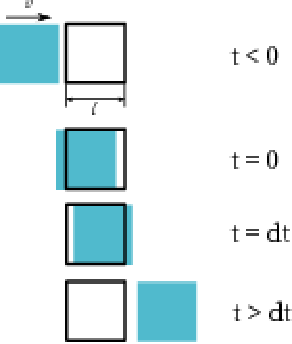
\includegraphics[width=0.45\textwidth]{images/resolution.pdf} 
		\caption{The control volumes in blue have the same size as the sensor (black rectangle). At $t=0$ the measurement starts and the first control volume is directly over the sensor. When the measurement ends at $t=\tau$ the control volumes have moved. The sensor is covered by a mix of the two volumes.}
		\label{fig:cv}
	\end{center}
\end{figure}

To accommodate for that, factors $ n $ \eqref{eq:resn} and $ k $ \eqref{eq:resk} are introduced, describing the ratio of the resolutions to the actual sizes.

\begin{equation}
	n = \dfrac{l}{\diff s}
\label{eq:resn} 
\end{equation}

\begin{equation}
	k = \dfrac{ \tau}{\diff t}
\label{eq:resk}
\end{equation}

Inserting $ k $ and $ n $ in Equation \eqref{eq:resv} yields:

\begin{equation}
	v = \dfrac{\diff s}{\diff t} = \dfrac{k \cdot l}{n \cdot \tau}
\label{eq:resv1} 
\end{equation}

The ratio $ r $
\begin{equation}
	r = \frac{k}{n}
\label{eq:resr} 
\end{equation}
is the ratio of the time it takes a control volume to enter and leave the sensor area  to the time a measurement takes. Its inverse is the movement of the control volume during the measurement time and thereby the percentage by which the measured volume is bigger than the control volume. A ratio of 1 on would mean the measured volume is two times the sensor size, thereby halving the spacial resolution. To keep the resolution close the the sensor size, a ratio of 4, increasing the measured volume by \unit[25]{\%} is viable.
With the given sensor size and flow speed, a measurement time $ \tau $ of \unit[0.0025]{s} or \unit[2.5]{ms} is needed.\\

To test if the time resolution matches this, the measurement time itself can be timed. The difference between two adjacent times, i.e. the first time (\unit[975209221]{ns}) and the second time (\unit[975209961]{ns}), in the data set in Listing \ref{lst:data} is the measurement time of \unit[740]{ns}. The mean of the differences through the whole data set is \unit[748]{ns}. This means that the measurement is more than three times faster than required, showing that the time resolution easily matches the spacial resolution.

\begin{lstlisting}[caption={An excerpt of measurement data showing three lines of data from eight sensors. The long numbers are the times at which the measurements were taken in nanoseconds measured from the start, the short numbers are the measured values.},label={lst:data}]
975209221 21 975209961 59 975210676 15 975211397 0 975212119 0 975212840 26 975213554 59 975214276 9 
975215877 57 975216602 42 975217324 0 975218046 0 975218761 0 975219482 61 975220204 43 975220919 0 
975222520 52 975223271 0 975223993 0 975224708 0 975225429 45 975226150 53 975226867 0 975227583 0  
\end{lstlisting}

\subsection{Electrical Conductivity Resolution and Range}


\begin{itemize}
\item The system shall have a sensitivity of  \unit[0.1]{\%} salinity.
\item The system shall have a range from 0 to \unit[5]{\%} salinity.
\end{itemize}

Table \ref{tab:rns} shows the results of measurements of solutions with different salinities. A \unit[10]{\%} solution was created by adding \unit[5]{g} of salt to \unit[100]{ml} of demineralized water. The subsequent solutions resulted from diluting the original one by adding more water.

The measurable change of the voltage was visible at the drop from a salinity of \unit[5]{\%} to \unit[2.5]{\%}. Between \unit[10]{\%} and \unit[5]{\%} no difference was measurable at all. The upper range limit can therefore be placed between \unit[5]{\%} and \unit[2.5]{\%}, above those values the sensor is saturated, providing only the information that the salinity is above the threshold.

On the lower limit, a measurement without any water, resulted in a voltage of \unit[0.02]{V}. This has to be considered the level of noise in the system. Above that, a clear distinction between salinities of \unit[0.08]{\%} and \unit[0.16]{\%} can be seen.

\begin{table}[H]
    \centering

    \caption[cal]{Range and Sensitivity}
    \label{tab:rns}
    \begin{tabular}{rr}
        	\toprule
        	Salinity in [\%] & Voltage in [V] \tabularnewline
        	\midrule
		10.00 & 0.95 \tabularnewline
        	5.00 & 0.95 \tabularnewline
		2.50 & 0.85 \tabularnewline
		1.25 & 0.65 \tabularnewline
		0.63 & 0.45 \tabularnewline
		0.31 & 0.28 \tabularnewline
		0.16 & 0.18 \tabularnewline
		0.08 & 0.11 \tabularnewline
		Air & 0.02 \tabularnewline
        \bottomrule
    \end{tabular}
\end{table}

While the requirement for sensitivity is clearly met, the range is just barely acceptable. The later validation will show if it is sufficient or not.

\subsection{Cost}

\begin{itemize}
\item Requirement: The cost per sensor shall be less than \euro{25}
\end{itemize}

Using the bill of materials in Chapter \ref{BOM} a total price of \euro{121.8} for all materials for a sensor system with eight sensors can be calculated, resulting in a price per sensor of \euro{15.23}. Adding additional sensors after that would cost \euro{11.17} per sensor, as parts like the microcontroller do not have to be duplicated.

This price does not include the host PC as the PCs already installed in the laboratory can be used, as well as personal laptops like it was done in the testing phase. The demands on the host PC are very low, so in the worst case even a single board computer like the Raspberry Pi or similar can be used.

\subsection{Deployability in the Bioreactor}

\begin{itemize}
\item  The system shall be deployable in the algae reactor.\\
\end{itemize}

The deployability was demonstrated during two test campaigns on the reactor. Figures \ref{fig:stripsr} and \ref{fig:pcr} show the set up during the tests. The host PC can be placed on a desk beside the reactor and connected to the carrier board with a USB cable. The carrier board can also be placed on desk or temporarily mounted on the reactor. The sensor strips connect to the carrier board with \unit[1]{m} long cables and are attached to the reactor with electrical tape.

\begin{figure}[H]
	\begin{center}
		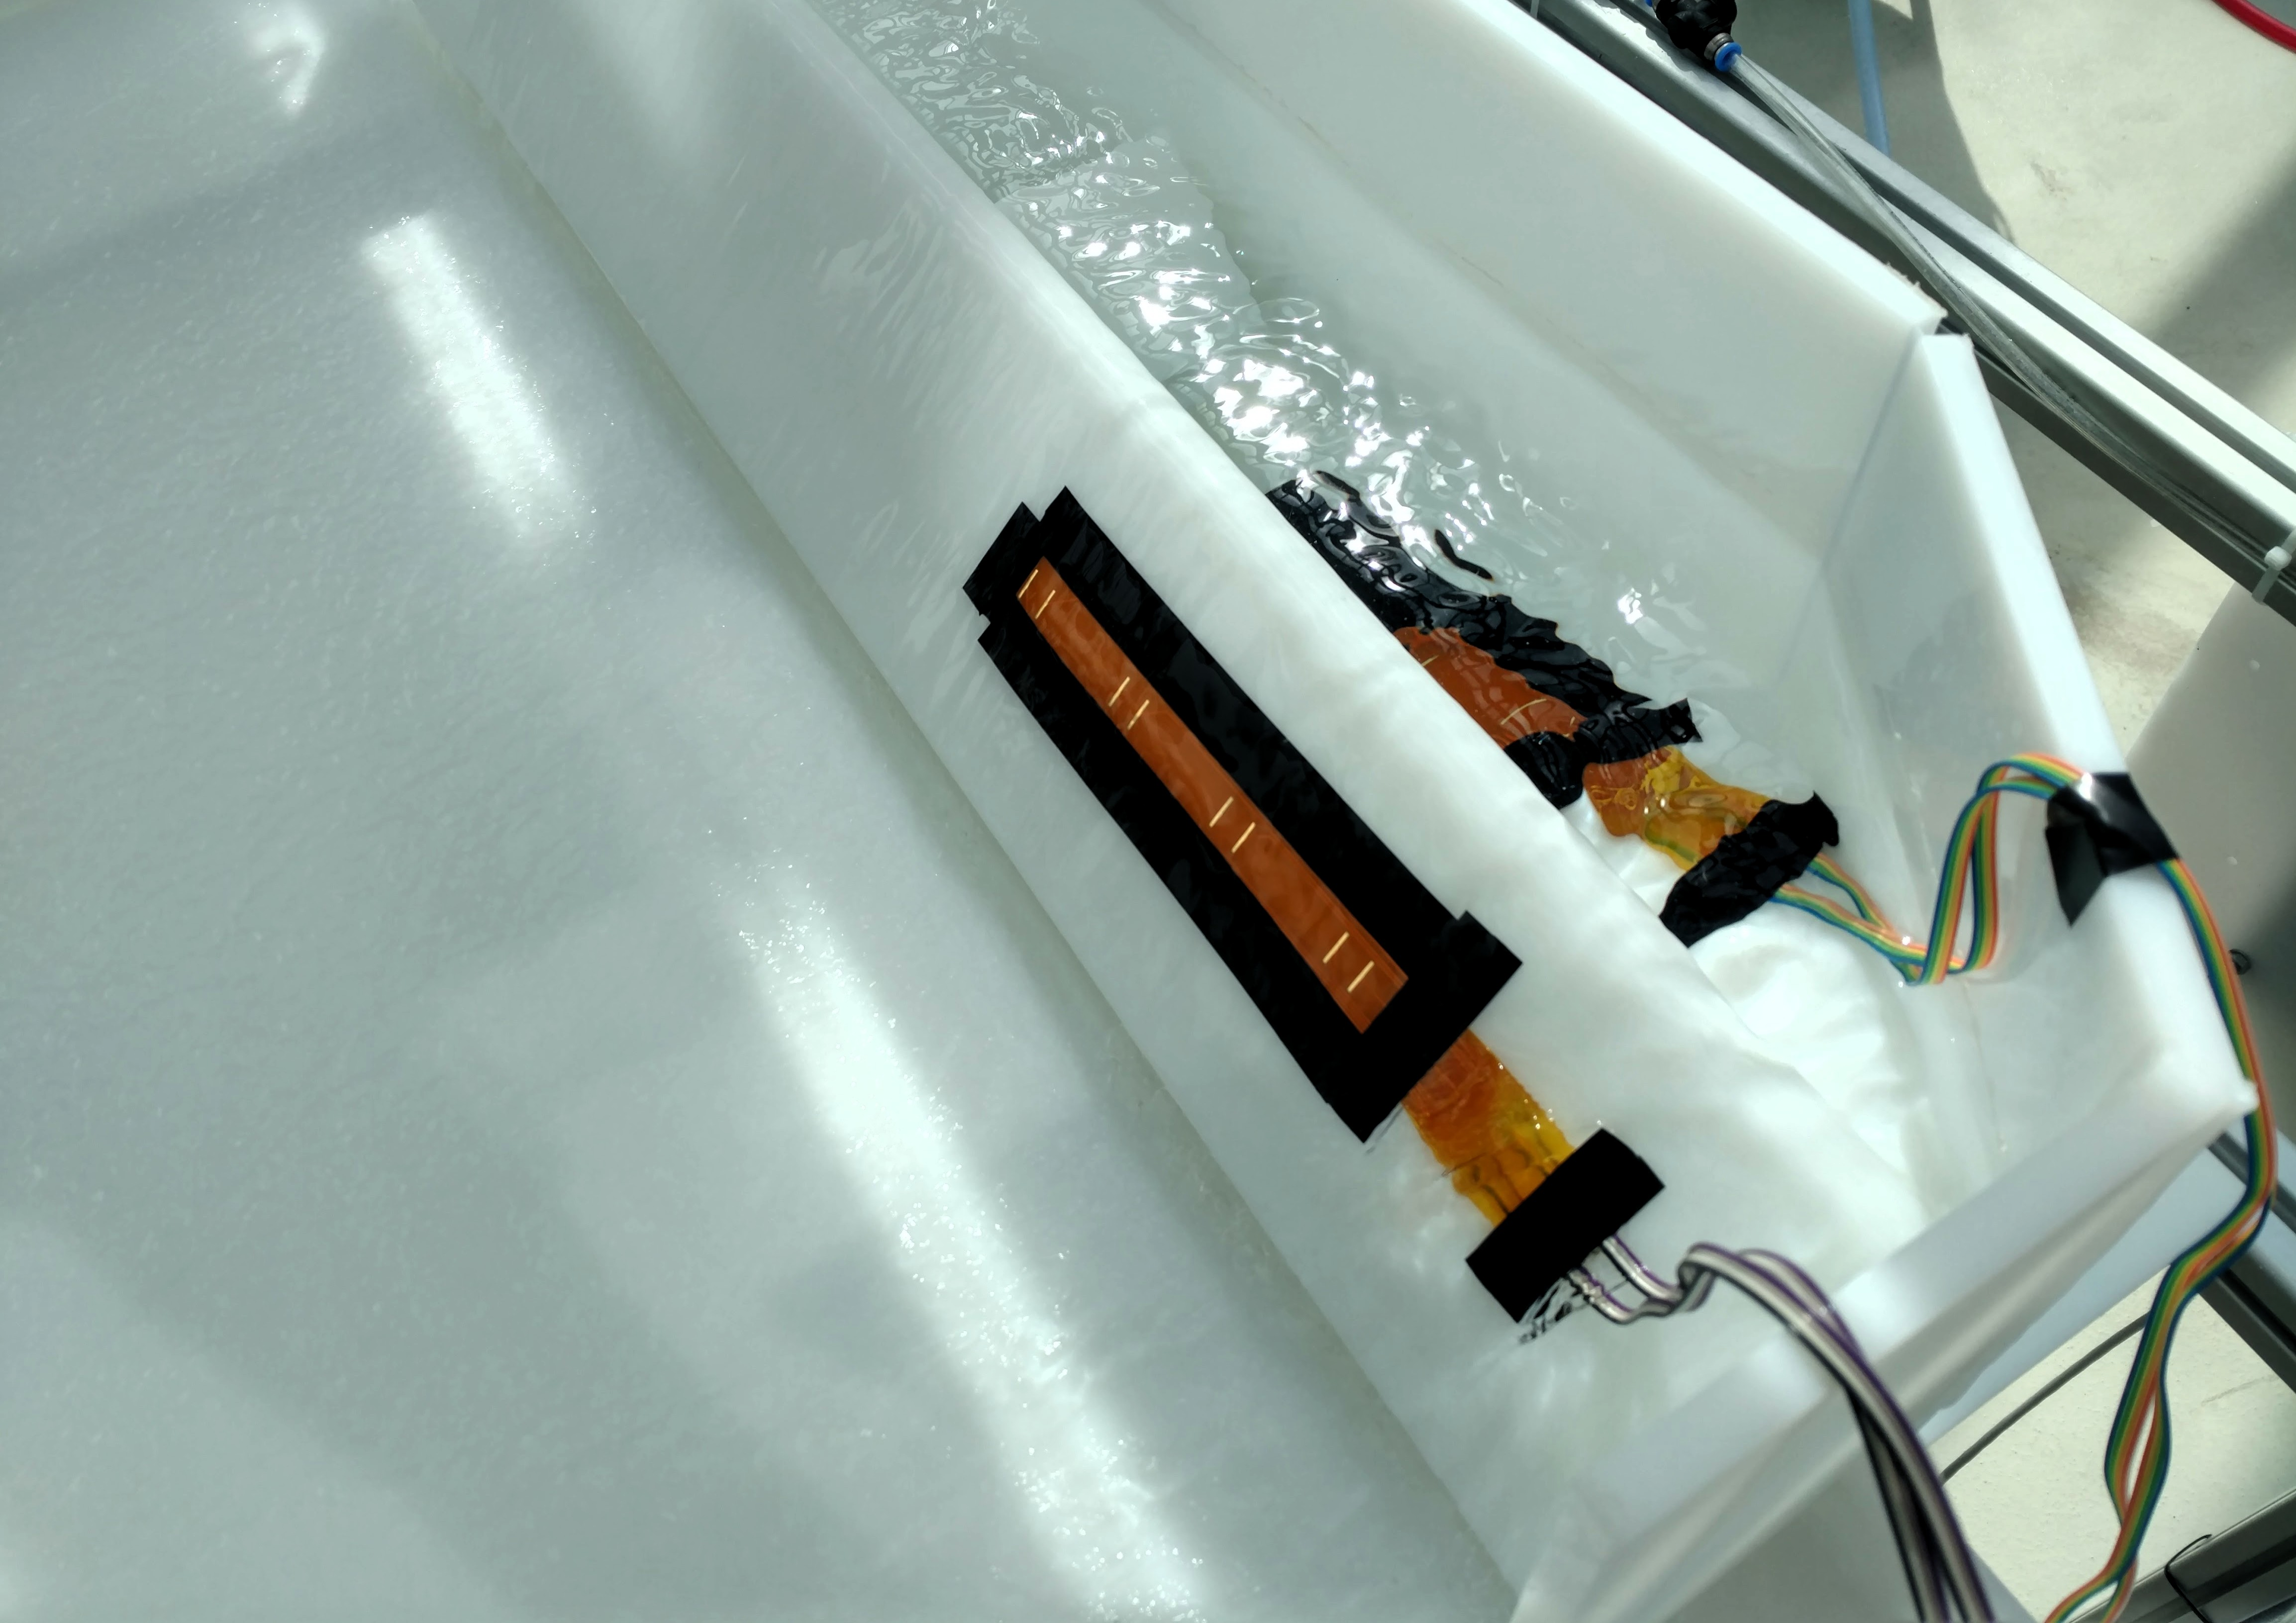
\includegraphics[width=0.8\textwidth]{images/stripsinreactor.jpg} 
		\caption{The sensor strips are mounted to the bioreactor with electrical tape. Cables of \unit[1]{m} length run towards the carrier board which is not in the frame.}
	\label{fig:stripsr}
	\end{center}
\end{figure}

\begin{figure}[H]
	\begin{center}
		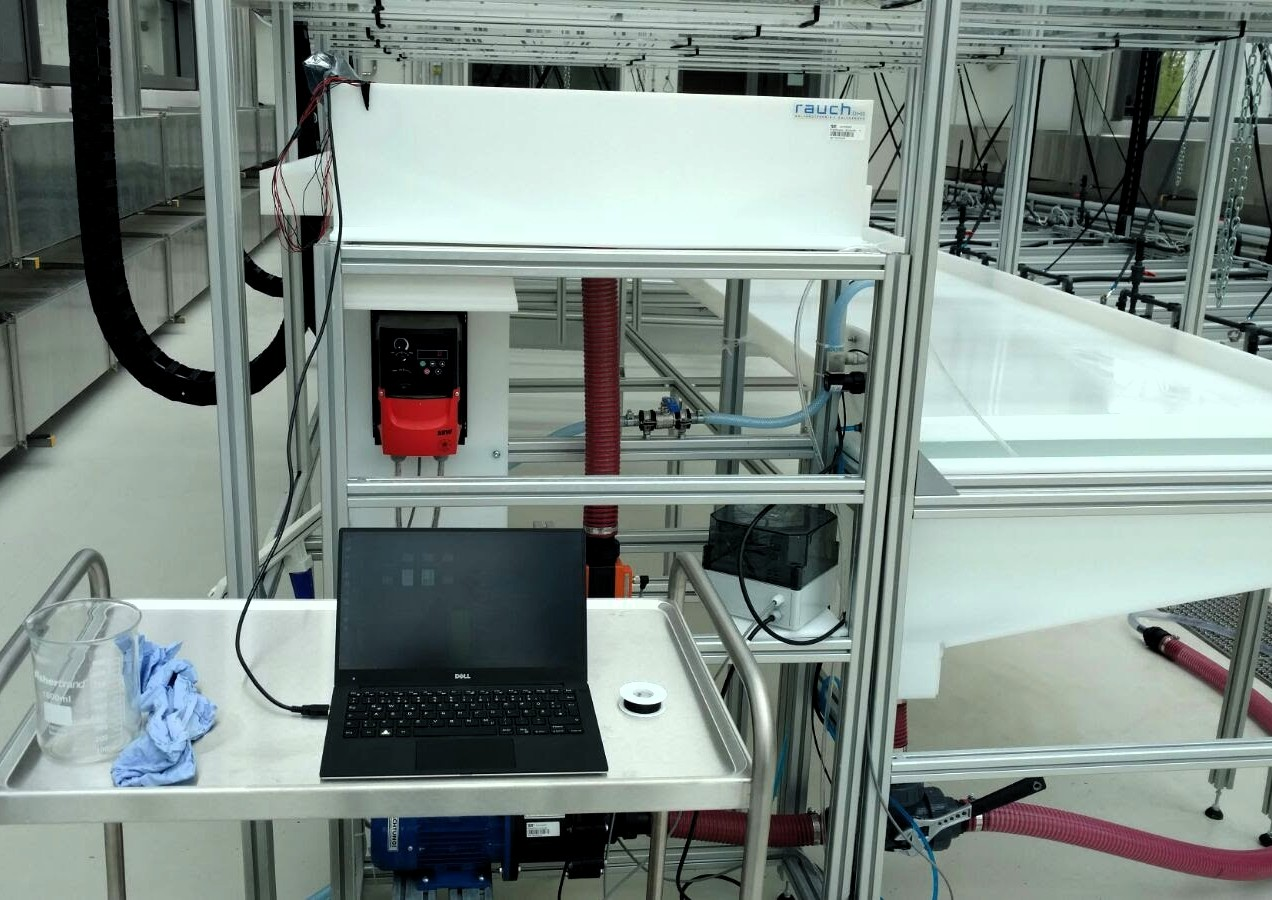
\includegraphics[width=0.8\textwidth]{images/pconreactor.jpg} 
		\caption{A laptop is used as host PC. A USB cable connects to the microcontroller on the carrier board, which is mounted on the side of the inlet basin.}
	\label{fig:pcr}
	\end{center}
\end{figure}

\subsection{Usability}

\begin{itemize}
\item  The system shall be usable with a minimal set of written instructions.\\
\end{itemize}

The instructions for taking a series of measurements can be found in the Appendix. First, an image describes the different parts of the system relevant to the user. After that a step-by-step description with images helps the user through the process. All in all, only 8 steps are necessary.

TEST!!!

\section{Validation} \label{val}

The following chapter describes a number of experiments conducted using the developed sensor system. The data is analyzed and interpreted to verify if the results are reasonable. Finally, a comparison with data from simulations tries to validate the usefulness of the device.

All experiments where done on the same day on the same bioreactor. The schematic in Figure \ref{fig:senspos} shows how the sensors were positioned.

\begin{figure}[H]
	\begin{center}
\begin{tikzpicture}[
    scale=0.03,
    every node/.style={
            font={\large\bf},
            scale=1.2
        },
    geometryLine/.style={
            very thick
        },
    internalGeometryLine/.style={
            dashed
        },
    ]
    
    % center line
    \draw[internalGeometryLine]
        (0, -252) -- (0, 40);

    % general outline
    \draw[geometryLine] 
            (0, 0)
         -- (272, 0)
         -- (425, -80)
         -- (425, -212)
         -- (0, -212);
    \draw[geometryLine]
            (0, -80)
         -- (425, -80);
    
    % baffle
    \draw[geometryLine]
            (25, 0)
         -- (25, -10);
    \draw[geometryLine]
            (0, -10)
         -- (60, -10)
         -- (60, -80)
         -- (0, -80)
         -- cycle;
        
    % water flow
    % inlet
    \fill[blue!50!white] (0, 0) -- (25, 0) -- (25, -10) -- (0, -10) -- cycle;
    \draw[blue!50, very thick, ->, >={Stealth}] (60, -20) -- (100, -20);
    % from inlet to weir
    \draw[blue!50, thick, ->, >={Stealth}] plot [smooth] coordinates {(70, -60) (80, -80) (70, -100)};
    \draw[blue!50, thick, ->, >={Stealth}] plot [smooth] coordinates {(300, -60) (310, -80) (300, -100)};
    % weir
    \draw[blue!50, very thick, ->, >={Stealth}] (50, -192) -- (50, -232);
    \draw[blue!50, very thick, ->, >={Stealth}] (150, -192) -- (150, -232);
    \draw[blue!50, very thick, ->, >={Stealth}] (250, -192) -- (250, -232);
    \draw[blue!50, very thick, ->, >={Stealth}] (350, -192) -- (350, -232);
        
    % measurement strips
    \begin{scope}[shift={(82, -30)}]
        \fill[Sepia]
                (0, 0) -- (200, 0)
             -- (200, -20) -- (0, -20)
             -- cycle;
        \draw[Goldenrod, thick] (10, -5) -- (10, -15);
        \draw[Goldenrod, thick] (20, -5) -- (20, -15)
            node[black, below, xshift=-4pt, yshift=-1pt] (inner-4) {4};
        \draw[Goldenrod, thick] (60, -5) -- (60, -15);
        \draw[Goldenrod, thick] (70, -5) -- (70, -15)
            node[black, below, xshift=-4pt, yshift=-1pt] (inner-3) {3};
        \draw[Goldenrod, thick] (110, -5) -- (110, -15);
        \draw[Goldenrod, thick] (120, -5) -- (120, -15)
            node[black, below, xshift=-4pt, yshift=-1pt] (inner-2) {2};
        \draw[Goldenrod, thick] (160, -5) -- (160, -15);
        \draw[Goldenrod, thick] (170, -5) -- (170, -15)
            node[black, below, xshift=-4pt, yshift=-1pt] (inner-1) {1};
    \end{scope}
    
    \begin{scope}[shift={(82, -136)}]
        \fill[Sepia]
                (0, 0) -- (200, 0)
             -- (200, -20) -- (0, -20)
             -- cycle;
        \draw[Goldenrod, thick] (10, -5) -- (10, -15);
        \draw[Goldenrod, thick] (20, -5) -- (20, -15)
            node[black, below, xshift=-4pt, yshift=-1pt] (weir-4) {8};
        \draw[Goldenrod, thick] (60, -5) -- (60, -15);
        \draw[Goldenrod, thick] (70, -5) -- (70, -15)
            node[black, below, xshift=-4pt, yshift=-1pt] (weir-3) {7};
        \draw[Goldenrod, thick] (110, -5) -- (110, -15);
        \draw[Goldenrod, thick] (120, -5) -- (120, -15)
            node[black, below, xshift=-4pt, yshift=-1pt] (weir-2) {6};
        \draw[Goldenrod, thick] (160, -5) -- (160, -15);
        \draw[Goldenrod, thick] (170, -5) -- (170, -15)
            node[black, below, xshift=-4pt, yshift=-1pt] (weir-1) {5};
    \end{scope}
\end{tikzpicture}    
		\caption{Position of the sensors in the inlet basin. \parencite{ts}}
		\label{fig:senspos}
	\end{center}
\end{figure}

With this configuration, two types of experiments were run: the first method uses the bioreactors plumbing to switch the feed from the return basin to an external tank containing saltwater. Instead of pumping water in a loop, saltwater from the tank is added to the water cycle and the increase can be measured. The second method retains the original water cycle, but adds an impulse of saltwater in the return basin.

For the following analysis of the experiments their original numeration is retained, but not all of them are described as not all of them are relevant. For example, in the first experiment no salt water was added, others were exact duplicates. By keeping the original notation continuity between the data files, notes and documentation can be upheld.\\

\textbf{Test No. 2}

In this test the feed switch method was used. The total amount of water in the tank was \unit[65]{l} and the flow rate was $\dot{v} =  \unitfrac[1.6]{l}{s}$. The saltwater in the external tank had a salinity of \unit[1.5]{\%}.

\begin{figure}
	\begin{center}
		%% This file was created by matplotlib2tikz v0.5.10.
\tikzset{external/export next=false}
\begin{tikzpicture}

\definecolor{color0}{rgb}{0,0.75,0.75}

\begin{axis}[
xlabel={Time, s},
ylabel={relative Voltage, -},
xmin=50.005687, xmax=200.000933,
ymin=0, ymax=0.7,
axis on top,
ytick={0,0.1,0.2,0.3,0.4,0.5,0.6,0.7},
yticklabels={0.0,0.1,0.2,0.3,0.4,0.5,0.6,0.7},
xmajorgrids,
ymajorgrids
]
\addplot [line width=1, color0, opacity=0.75]
table {%
50.682313 0.0575258540142645
50.689113 0.0575644552315066
50.695939 0.0576026274447994
50.702762 0.05764036908198
50.709598 0.0576776785708854
50.716403 0.0577145543393529
50.723219 0.0577509948152194
50.730092 0.0577869984263222
50.736935 0.0578225636004983
50.743786 0.0578576887655849
50.750639 0.0578923723494189
50.757469 0.0579210826968629
50.764297 0.0579491837329258
50.771134 0.0579766729028429
50.777997 0.0579958055356849
50.784867 0.0580140907727278
50.791728 0.0580336712754738
50.79861 0.0580523314733666
50.807483 0.0580700678290396
50.814097 0.0580868768051263
50.820729 0.0581027548642602
50.827372 0.0581176984690749
50.833985 0.0581317040822037
50.840628 0.0581447681662802
50.847256 0.0581568871839379
50.853908 0.0581680575978102
50.86058 0.0581782758705308
50.867221 0.058187538464733
50.87389 0.0581958418430503
50.880569 0.0582031824681163
50.887216 0.0582095568025643
50.893897 0.058214961309028
50.900581 0.0582193924501409
50.907251 0.0582228466885363
50.913939 0.0582186843872781
50.920629 0.0582133406056061
50.927328 0.0582068106270317
50.934007 0.058199089735066
50.940715 0.0581901732132206
50.947408 0.0581800563450066
50.954096 0.0581687344139355
50.960802 0.0581562027035185
50.967527 0.058142456497267
50.97425 0.0581274910786922
50.980942 0.0581113017313055
50.987657 0.0580938837386183
50.994378 0.0580752323841418
51.001092 0.0580553429513874
51.007834 0.0580342107238663
51.014577 0.05801183098509
51.021329 0.0579881990185697
51.02805 0.0579633101078168
51.034795 0.0579371595363426
51.041549 0.0579097425876583
51.048317 0.0578810545452754
51.055053 0.0578510906927051
51.06181 0.0578198463134588
51.068587 0.0577873166910478
51.075348 0.0577534971089834
51.082097 0.0577183828507769
51.08888 0.0576819691999397
51.095661 0.0576442514399831
51.102441 0.0576052248544183
51.109204 0.0575648847267568
51.115967 0.0575232263405099
51.122758 0.057496835228113
51.129561 0.0574696101815619
51.136354 0.0574415494321731
51.143137 0.0574126512112635
51.149922 0.0573829137501497
51.156734 0.0573523352801486
51.163549 0.0573209140325769
51.170369 0.0572886482387513
51.177163 0.0572555361299886
51.183969 0.0572215759376054
51.190801 0.0572088862248177
51.197633 0.0571960032342544
51.204475 0.0571872223114585
51.21129 0.0571781223378555
51.218113 0.0571687062612509
51.224958 0.0571589770294502
51.231811 0.0571489375902587
51.238664 0.0571257113400249
51.245525 0.0571025710674492
51.252393 0.0570795173620929
51.259229 0.0570565508135169
51.26607 0.0570336720112824
51.272945 0.0570108815449504
51.279818 0.056988180004082
51.288736 0.0569655679782383
51.295368 0.0569430460569803
51.301973 0.0569206148298693
51.308613 0.0568982748864662
51.315247 0.0568760268163321
51.321875 0.0568538712090282
51.328521 0.0568318086541155
51.335182 0.056809839741155
51.341818 0.0567879650597079
51.348503 0.0567661851993353
51.355175 0.0567445007495983
51.361819 0.0567229123000578
51.368493 0.0567014204402751
51.375176 0.0566800257598112
51.381831 0.0566587288482272
51.388512 0.0566375302950841
51.395206 0.0566164306899431
51.401874 0.0565954306223652
51.408594 0.0565745306819116
51.415286 0.0565537314581432
51.421965 0.0565330335406213
51.428674 0.0565124375189068
51.435387 0.0564919439825609
51.44211 0.0564715535211446
51.448806 0.0564512667242191
51.455525 0.0564310841813454
51.462249 0.0564110064820846
51.468981 0.0563910342159977
51.475716 0.056371167972646
51.482441 0.0563514083415904
51.489175 0.056331755912392
51.495896 0.056312211274612
51.502648 0.0562927750178113
51.509396 0.0562734477315512
51.516158 0.0562542300053926
51.522888 0.0562351224288967
51.529672 0.0562161255916246
51.536428 0.0561972400831373
51.54319 0.0561784664929959
51.549931 0.0561598054107615
51.556703 0.0561412574259952
51.563476 0.0561228231282581
51.57026 0.0561045031071112
51.577015 0.0560862979521157
51.583776 0.0560682082528326
51.590561 0.056050234598823
51.597356 0.056032377579648
51.604135 0.0560146377848686
51.610907 0.0559970158040461
51.617714 0.0559795122267414
51.624518 0.0559621276425156
51.63133 0.0559448626409299
51.638127 0.0559277178115452
51.644921 0.0559106937439228
51.651724 0.0558937910276236
51.65855 0.0558770102522087
51.665375 0.0558603520072394
51.672213 0.0558438168822765
51.679014 0.0558274054668813
51.685832 0.0558111183506147
51.692672 0.055794956123038
51.699516 0.0557789193737121
51.706358 0.0557630086921981
51.713211 0.0557472246680572
51.720065 0.0557315678908504
51.726894 0.0557160389501388
51.733733 0.0557006384354835
51.7406 0.0556853669364456
51.74747 0.0556702250425861
51.754336 0.0556552133434662
51.761216 0.0556231596933709
51.770088 0.0555917578030548
51.776698 0.0555610051177532
51.783325 0.0555308990827013
51.789967 0.0555014371431345
51.796583 0.0554726167442881
51.803225 0.0554444353313973
51.809852 0.0554168903496975
51.816507 0.0553899792444239
51.823186 0.0553636994608119
51.829826 0.0553380484440968
51.836495 0.0553130236395139
51.84317 0.0552886224922984
51.849822 0.0552648424476856
51.856505 0.055241680950911
51.863191 0.0552136053642349
51.869855 0.0551859786300647
51.87652 0.0551587972110338
51.883208 0.0551320575697757
51.889883 0.0551057561689239
51.896553 0.055079889471112
51.903283 0.0550544539389733
51.909997 0.0550349761181162
51.916682 0.0550160869740022
51.923389 0.0549977839518666
51.930106 0.0549800644969447
51.936802 0.0549662441042567
51.943506 0.0549531009207346
51.950226 0.054940632981175
51.956963 0.0549288383203741
51.963702 0.0549177149731283
51.97044 0.054907260974234
51.977183 0.0548974743584877
51.983935 0.0548883531606857
51.990657 0.0548798954156244
51.997404 0.0548720991581001
52.004163 0.0548649624229093
52.010929 0.0548584832448483
52.017664 0.0548526596587135
52.024455 0.0548474896993013
52.031221 0.0548429714014081
52.037987 0.0548391027998303
52.044742 0.0548358819293643
52.051525 0.0548333068248063
52.058305 0.0548313755209529
52.065097 0.0548300860526005
52.071863 0.0548294364545453
52.078636 0.0548294247615838
52.085459 0.0548300490085123
52.092259 0.0548313072301273
52.099064 0.0548331974612251
52.105849 0.0548357177366022
52.112639 0.0548388660910548
52.11945 0.0548426405593794
52.126271 0.0548470391763724
52.133093 0.0548520599768301
52.139892 0.054857700995549
52.146721 0.0548639602673254
52.153527 0.0548708358269557
52.160366 0.0548783257092363
52.167199 0.0548864279489635
52.174046 0.0548951405809338
52.180862 0.0549044616399436
52.187685 0.0549143891607891
52.194543 0.0549249211782669
52.201402 0.0549360557271733
52.20826 0.0549477908423047
52.215119 0.0549601245584574
52.22199 0.0549730549104278
52.228828 0.0549865799330124
52.235675 0.0550006976610075
52.242553 0.0550154061292095
52.251472 0.0550307033724148
52.258109 0.0550465874254198
52.264795 0.0550630563230208
52.271406 0.0550801081000142
52.278046 0.0550977407911965
52.284668 0.0551159524313639
52.291284 0.055134741055313
52.297934 0.05515410469784
52.304581 0.0551740413937414
52.311248 0.0551945491778135
52.317921 0.0552156260848528
52.324575 0.0552372701496555
52.331247 0.0552594794070182
52.33792 0.0552822518917371
52.344581 0.0553055856386087
52.351272 0.0553294786824294
52.357969 0.0553539290579954
52.364638 0.0553789348001033
52.371308 0.0554044939435494
52.378001 0.0554306045231301
52.384686 0.0554572645736417
52.391362 0.0554844721298807
52.398069 0.0555122252266434
52.404785 0.0555405218987263
52.411472 0.0555693601809256
52.418189 0.0555987381080379
52.424916 0.0556286537148594
52.431615 0.0556794976593268
52.438314 0.0557302573948192
52.445042 0.05578093469002
52.451782 0.0558315313136124
52.458527 0.0558820490342796
52.465276 0.0559324896207048
52.472024 0.0559828548415714
52.478773 0.0560331464655626
52.485505 0.0560833662613617
52.492267 0.0561335159976518
52.499024 0.0561835974431163
52.505772 0.0562336123664384
52.512517 0.0562835625363014
52.519316 0.0563334497213884
52.526092 0.0563832756903829
52.532876 0.056433042211968
52.539632 0.0564827510548269
52.546397 0.056532403987643
52.553183 0.0565820027790994
52.559982 0.0566315491978795
52.566772 0.0566810450126665
52.573551 0.0567304919921437
52.580361 0.0567798919049942
52.587164 0.0568292465199014
52.593977 0.0568785576055485
52.60079 0.0569278269306188
52.607582 0.0569736073314498
52.614383 0.0570189889924672
52.621206 0.0570639730927931
52.628034 0.0571085608115497
52.63487 0.0571527533278592
52.641705 0.0571965518208438
52.648524 0.0572399574696255
52.655334 0.0572829714533266
52.662185 0.0573255949510693
52.669031 0.0573678291419757
52.675891 0.057409675205168
52.682725 0.0574511343197683
52.689562 0.0574922076648988
52.696398 0.0575328964196818
52.70329 0.0575732017632393
52.710167 0.0576131248746935
52.717037 0.0576526669331667
52.72392 0.0576918291177809
52.732831 0.0577306126076584
52.739442 0.0577690185819212
52.746077 0.0578070482196917
52.752705 0.0578447027000919
52.759328 0.057881983202244
52.765966 0.0579188909052703
52.772626 0.0579554269882927
52.779251 0.0579915926304336
52.785913 0.0580273890108151
52.792581 0.0580572872255847
52.799222 0.0580866539510363
52.805891 0.0581154893836904
52.812577 0.0581437937200673
52.819226 0.0581715671566875
52.825904 0.0581988098900712
52.832597 0.0582255221167388
52.83926 0.0582517040332107
52.845952 0.0582773558360073
52.852636 0.0583024777216489
52.859314 0.0583270698866558
52.866016 0.0583511325275485
52.872717 0.0583746658408473
52.879404 0.0583976700230725
52.886124 0.0584201452707446
52.892842 0.0584420917803838
52.899569 0.0584635097485105
52.906266 0.0584843993716452
52.912989 0.0585047608463081
52.919724 0.0585342540326124
52.926433 0.0585629267464072
52.933138 0.0585907809528959
52.939881 0.0586178186172823
52.94662 0.05864404170477
52.953372 0.0586694521805626
52.960121 0.0586940520098636
52.966874 0.0587178431578768
52.973629 0.0587408275898057
52.980369 0.0587630072708539
52.987134 0.0587843841662251
52.993907 0.0588049602411229
53.000682 0.0588247374607508
53.007432 0.0588437177903126
53.014221 0.0588619031950118
53.020995 0.058879295640052
53.027788 0.0588958970906369
53.034558 0.0589117095119701
53.041328 0.0589288814611646
53.048123 0.0589429912300851
53.054921 0.0589561873758446
53.061723 0.0589684718636467
53.068507 0.0589798466586951
53.07531 0.0589903137261934
53.082128 0.0589998750313452
53.088947 0.0589956529878971
53.095764 0.0589909194019478
53.102588 0.0589856738804566
53.109389 0.0589799160303827
53.116196 0.0589736454586856
53.12303 0.0589668617723243
53.129864 0.0589595645782583
53.136712 0.0589517534834467
53.143538 0.0589434280948489
53.150366 0.0589345880194241
53.157191 0.0589252328641316
53.164042 0.0589153622359307
53.170898 0.0589049757417806
53.177755 0.0588940729886407
53.184624 0.0588826535834703
53.191466 0.0588707171332285
53.198337 0.0588582632448747
53.20519 0.0588452915253681
53.214108 0.058831801581668
53.220737 0.0588177930207338
53.227377 0.0588032654495246
53.233994 0.0587882184749998
53.240634 0.0587726517041186
53.247255 0.0587565647438403
53.253902 0.0587399572011242
53.260585 0.0587228286829296
53.267227 0.0587051787962157
53.273894 0.0586870071479418
53.280571 0.0586683133450672
53.287215 0.0586490969945512
53.293888 0.058629357703353
53.300571 0.0586090950784319
53.30723 0.0585883087267473
53.313925 0.0585669982552583
53.320642 0.0585451632709243
53.327341 0.0585228033807045
53.334008 0.0584999181915582
53.340704 0.0584765073104447
53.347416 0.0584525703443232
53.354099 0.0584281069001531
53.360803 0.0584031165848936
53.367516 0.058377599005504
53.37421 0.0583515537689435
53.380937 0.0583249804821715
53.387655 0.058294658864283
53.394388 0.058263905982461
53.401094 0.0582327208541037
53.407825 0.0582011024966093
53.414559 0.058169049927376
53.421279 0.058136562163802
53.428003 0.0581036382232855
53.434754 0.0580702771232247
53.441511 0.0580364778810177
53.448262 0.0580022395140628
53.454999 0.0579675610397581
53.46176 0.0579280174091221
53.468526 0.0578879000372904
53.475269 0.0578472071555799
53.482022 0.0578059369953072
53.488791 0.0577640877877891
53.495569 0.0577349299634819
53.502356 0.0577055845604895
53.509146 0.057676052168373
53.515935 0.0576463333766936
53.522728 0.0576164287750124
53.529522 0.0575723861054786
53.536303 0.057528581618623
53.543078 0.0574850133492421
53.549884 0.0574416793321321
53.556696 0.0573985776020896
53.56351 0.0573557061939108
53.570331 0.0573130631423921
53.577126 0.05727064648233
53.583956 0.0572284542485208
53.590783 0.0571864844757609
53.597614 0.0571447351988468
53.604459 0.0571032044525746
53.611267 0.057061890271741
53.618082 0.0570207906911421
53.624928 0.0569799037455745
53.631806 0.0569392274698346
53.638655 0.0568987598987186
53.645514 0.056858499067023
53.65237 0.0568184430095441
53.659205 0.0567785897610784
53.666052 0.0567389373564222
53.67292 0.056699483830372
53.679799 0.056660227217724
53.686669 0.0566211655532747
53.695575 0.0565822968718205
53.702215 0.0565436192081578
53.708821 0.0565051305970829
53.715461 0.0564668290733922
53.722082 0.0564287126718821
53.728699 0.056390779427349
53.735348 0.0563530273745892
53.741977 0.0563154545483993
53.748637 0.0562780589835754
53.755316 0.0562408387149141
53.761969 0.0562037917772117
53.768638 0.0561669162052646
53.775303 0.0561302100338692
53.781959 0.0560936712978218
53.788632 0.0560572980319189
53.795316 0.0560210882709569
53.801984 0.055985040049732
53.80868 0.0559491514030407
53.815406 0.0559134203656795
53.82208 0.0558778449724445
53.828755 0.0558424232581324
53.835461 0.0558071532575394
53.842181 0.0557720330054619
53.848866 0.0557370605366963
53.85558 0.055702233886039
53.862299 0.0556675510882863
53.869005 0.0556330101782348
53.875739 0.0555986091906806
53.88246 0.0555643461604203
53.889199 0.0555302191222503
53.895917 0.0554962261109668
53.902657 0.0554623651613663
53.909405 0.0554286343082451
53.916161 0.0553950315863997
53.922887 0.0553615550306264
53.929636 0.0553282026757217
53.936398 0.0552949725564818
53.943168 0.0552618627077032
53.949906 0.0552288711641823
53.956678 0.0551959959607155
53.963445 0.055163235132099
53.970202 0.0551305867131295
53.976958 0.0550980487386031
53.983742 0.0550656192433163
53.990526 0.0550332962620655
53.997318 0.055001077829647
54.004119 0.0549689619808573
54.010889 0.0549369467504927
54.017688 0.0549227264388689
54.024493 0.0549091294898319
54.0313 0.0548961570825041
54.038089 0.0548838103960075
54.044876 0.0548720906094644
54.05169 0.0548609989019968
54.058514 0.054850536452727
54.065337 0.0548407044407772
54.072161 0.0548315040452694
54.078967 0.054822936445326
54.085772 0.0548150028200689
54.092616 0.0548077043486205
54.099452 0.0548010422101029
54.106304 0.0547950175836382
54.113125 0.0547896316483487
54.119952 0.0547848855833565
54.126804 0.0547807805677837
54.133657 0.0547773177807525
54.140519 0.0547744984013852
54.147375 0.0547723236088038
54.154247 0.0547707945821305
54.161086 0.0547699125004876
54.167932 0.0547696785429971
54.176815 0.0547700938887813
54.183445 0.0547711597169623
54.190077 0.0547728772066623
54.196691 0.0547752475370035
54.20333 0.0547975912142935
54.209982 0.0548200046563118
54.21661 0.0548424925795472
54.223266 0.0548650597004882
54.22994 0.0548877107356237
54.236584 0.0549104504014423
54.243251 0.0549332834144326
54.249924 0.0549562144910833
54.256576 0.0549792483478831
54.263256 0.0550023897013207
54.269944 0.0550256432678848
54.276604 0.055049013764064
54.28329 0.055072505906347
54.289988 0.0550961244112225
54.296664 0.0551198739951792
54.303366 0.0551437593747058
54.310147 0.0551677852662908
54.316826 0.0551919563864231
54.323543 0.0552162774515912
54.330257 0.0552407531782839
54.336979 0.0552653882829899
54.343671 0.0552901874821978
54.350393 0.0553151554923962
54.357122 0.055340297030074
54.363827 0.0553656168117196
54.370555 0.055391119553822
54.377286 0.0554168099728696
54.384012 0.0554426927853512
54.390737 0.055436573829113
54.397487 0.0554316324228813
54.404236 0.0554278673875341
54.410986 0.055425277543949
54.417721 0.055423861713004
54.424489 0.055423618715577
54.431249 0.0554245473725456
54.438021 0.0554266465047878
54.444771 0.0554299149331813
54.45155 0.0554343514786041
54.458328 0.0554399549619339
54.465111 0.0554467242040485
54.471874 0.0554546580258259
54.478642 0.0554637552481438
54.485431 0.0554740146918801
54.492223 0.0554854351779126
54.499026 0.0554980155271191
54.505806 0.0555117545603774
54.512597 0.0555266510985655
54.519405 0.055542703962561
54.526219 0.0555599119732419
54.533041 0.055578273951486
54.539834 0.055597788718171
54.546641 0.0556184550941749
54.553465 0.0556402719003755
54.560297 0.0556632379576506
54.567138 0.055687352086878
54.573955 0.0557126131089356
54.580776 0.0557390198447012
54.587595 0.0557665711150526
54.594446 0.0557952657408676
54.601294 0.0558251025430241
54.608153 0.0558560803424
54.615013 0.0558881979598729
54.621875 0.0559214542163209
54.628713 0.0559558479326216
54.635561 0.055991377929653
54.64243 0.0560280430282929
54.649303 0.056065842049419
54.658218 0.0561047738139093
54.664859 0.0561448371426415
54.671469 0.0561860308564935
54.678102 0.0562283537763432
54.684746 0.0562718047230683
54.69136 0.0562953682022425
54.698007 0.0563194319239972
54.70464 0.0563439909753232
54.71131 0.0563690404432116
54.717985 0.0563945754146532
54.724629 0.056420590976639
54.7313 0.0564470822161601
54.737977 0.0564740442202073
54.744655 0.0565014720757716
54.751347 0.056529360869844
54.758034 0.0565577056894154
54.764705 0.0565865016214768
54.771373 0.0566157437530192
54.778061 0.0566454271710335
54.784765 0.0566755469625107
54.791449 0.0567060982144417
54.798159 0.0567370760138175
54.804863 0.0567684754476291
54.811554 0.0568002916028675
54.818274 0.0568325195665235
54.825003 0.0568651544255881
54.831707 0.0568981912670523
54.838403 0.0569316251779072
54.845131 0.0569654512451435
54.851867 0.0569996645557523
54.858585 0.0570342601967246
54.865347 0.0570648091886715
54.872093 0.0570955990163214
54.878833 0.0571266239805841
54.885564 0.0571578783823688
54.892324 0.0571893565225852
54.899082 0.0572210527021428
54.905821 0.057252961221951
54.912565 0.0572850763829195
54.919338 0.0573173924859577
54.926127 0.057349903831975
54.932904 0.0573826047218812
54.939657 0.0574154894565856
54.946422 0.0574485523369977
54.953205 0.0574817876640272
54.960001 0.0575151897385834
54.966775 0.0575487528615759
54.973549 0.0575824713339143
54.980349 0.057616339456508
54.987147 0.0576503515302666
54.993953 0.0576845018560995
55.000751 0.0577187847349164
55.007544 0.0577531944676266
55.014368 0.0577877253551397
55.021187 0.0578223716983653
55.028006 0.0578571277982128
55.034841 0.0578919879555917
55.041639 0.0579269464714116
55.048456 0.057961997646582
55.055319 0.0579971357820124
55.062162 0.0580366483624313
55.069013 0.0580761064084499
55.075865 0.0581155050070591
55.082686 0.0581548392452499
55.089513 0.0581941042100132
55.09638 0.0582332949883401
55.103237 0.0582724066672214
55.110102 0.0583114343336481
55.11696 0.0583503730746112
55.123839 0.0583892179771016
55.130681 0.0584279641281104
55.139569 0.0584666066146284
55.146178 0.0585051405236467
55.152811 0.0585435609421562
55.159423 0.0585818629571478
55.166069 0.0586200416556125
55.172693 0.0586580921245413
55.179348 0.0586860553015705
55.185995 0.0587135841686007
55.192666 0.0587406720439395
55.199306 0.0587673122458946
55.205969 0.0587934980927737
55.212648 0.0588192229028846
55.2193 0.058844479994535
55.225979 0.0588692626860325
55.232655 0.0588935642956848
55.239344 0.0589173781417997
55.246031 0.0589406975426849
55.252725 0.0589882016236074
55.259402 0.0590344498411591
55.266101 0.0590794400336162
55.272808 0.0591231700392548
55.279497 0.0591656376963507
55.28618 0.0592068408431801
55.292889 0.0592467773180189
55.29961 0.0592832329259533
55.306303 0.0593183517041281
55.313022 0.0593521310977786
55.319752 0.05938456855214
55.32646 0.0594156615124477
55.333161 0.059445407423937
55.339892 0.0594738037318432
55.346619 0.0595141200805409
55.353341 0.0595534767220529
55.360118 0.0595918734598588
55.366864 0.0596293100974382
55.373605 0.0596657864382708
55.380338 0.0597013022858361
55.387103 0.0597358574436139
55.393863 0.0597694517150838
55.400621 0.0598020849037253
55.407372 0.0598337568130183
55.41415 0.0598644672464422
55.420951 0.0598942160074767
55.427733 0.0599230028996015
55.434501 0.0599508277262962
55.441266 0.0599776902910404
55.448063 0.0600035903973138
55.454857 0.0600285278485961
55.461658 0.0600525024483668
55.468437 0.0600755140001056
55.475222 0.0600975623072921
55.482057 0.060118647173406
55.488873 0.0601387684019269
55.495693 0.0601579257963344
55.502489 0.0601761191601083
55.509286 0.060193348296728
55.516116 0.0602096130096733
55.522948 0.0602249131024239
55.529782 0.0602392483784593
55.536628 0.0602526186412591
55.54344 0.0602650236943031
55.550291 0.0602764633410708
55.557142 0.0602869373850419
55.563997 0.060296445629696
55.570855 0.0603049878785129
55.577718 0.060312563934972
55.584578 0.0603191736025531
55.591417 0.0603248166847358
55.598269 0.0603294929849996
55.605138 0.0603332023068244
55.61202 0.0603359444536897
55.620922 0.0603377192290751
55.627535 0.0603385264364602
55.634145 0.0603383658793248
55.64078 0.0603372373611485
55.647426 0.0603384587351957
55.654042 0.0603388105066429
55.660692 0.0603382930685309
55.667352 0.0603369068139003
55.674014 0.0603367987277014
55.68068 0.0603357575628258
55.687352 0.0603337841053549
55.694 0.06033087914137
55.700671 0.0603270434569528
55.707356 0.0603222778381845
55.714016 0.0603165830711468
55.720698 0.0603099599419209
55.727394 0.0603024092365885
55.734097 0.0602939317412308
55.740797 0.0602845282419293
55.74748 0.0602741995247656
55.754161 0.060262946375821
55.760868 0.060250769581177
55.767577 0.0602376699269151
55.774266 0.0602236481991166
55.780957 0.0602087051838631
55.787676 0.0602072198829703
55.794405 0.0602052427898726
55.801108 0.0602027772454163
55.80784 0.0601998265904474
55.814573 0.0601963941658121
55.821283 0.0601924833123566
55.827992 0.0601988303304744
55.834739 0.0602043803602658
55.841487 0.0602091387077807
55.848213 0.0602131106790687
55.85497 0.0602163015801796
55.86173 0.0602187167171632
55.868497 0.0602203613960692
55.875235 0.0602212409229475
55.881972 0.0602213606038477
55.888744 0.0602250189286386
55.895524 0.0602277979230716
55.902281 0.060229703679278
55.90904 0.060230742289389
55.91585 0.0602309198455356
55.922637 0.0602302424398493
55.929406 0.0602287161644611
55.936182 0.0602263471115023
55.942954 0.0602231413731041
55.949755 0.0602191050413977
55.956566 0.0602142442085143
55.96336 0.0602085649665851
55.970151 0.0602020734077413
55.976999 0.0601947756241142
55.983826 0.0601866777078349
55.990645 0.0601777857510346
55.997477 0.0601681058458446
56.004285 0.0601576440843961
56.011095 0.0601464065588203
56.017927 0.0601343993612483
56.024771 0.0601216285838115
56.031613 0.0601081003186409
56.038494 0.0600938206578678
56.045317 0.0600787956936235
56.052146 0.0600630315180391
56.058977 0.0600465342232459
56.065839 0.060029309901375
56.072704 0.0600113646445576
56.079567 0.0599927045449251
56.086444 0.0599733356946084
56.09329 0.059953264185739
56.102178 0.059932496110448
56.108792 0.0599110375608666
56.115432 0.0598888946291259
56.122049 0.0598660734073573
56.128692 0.059842579987692
56.135323 0.059818420462261
56.141949 0.0597936009231957
56.148587 0.0597681274626273
56.155257 0.0597420061726869
56.161901 0.0597152431455058
56.168567 0.0596878444732152
56.175248 0.0596598162479463
56.181899 0.0596311645618302
56.188571 0.0596018955069983
56.195254 0.0595720151755817
56.201912 0.0595415296597116
56.208604 0.0595104450515193
56.21529 0.0594787674431359
56.221967 0.0594465029266926
56.228685 0.0594136575943207
56.235393 0.0593619915069207
56.242076 0.0593103096978917
56.24876 0.0592586149185188
56.255471 0.0592069099200872
56.262189 0.0591551974538818
56.268885 0.0591034802711877
56.27561 0.05905176112329
56.282336 0.0590000427614738
56.289059 0.058948327937024
56.295762 0.0588966194012259
56.302496 0.0588449199053643
56.309218 0.0587932322007245
56.315941 0.0587415590385914
56.322694 0.0586899031702502
56.329449 0.0586382673469858
56.336202 0.0585866543200834
56.342937 0.0585350668408279
56.349732 0.0584835076605046
56.356541 0.0584319795303983
56.363312 0.0583804852017943
56.37006 0.0583290274259775
56.376805 0.058277608954233
56.383584 0.0582262325378459
56.390367 0.0581749009281013
56.39713 0.0581236168762841
56.403893 0.0580723831336795
56.410709 0.0580212024515725
56.417502 0.0579700775812482
56.424307 0.0579190112739917
56.431088 0.057868006281088
56.43787 0.0578170653538222
56.444679 0.0577661912434792
56.451493 0.0577153867013443
56.458315 0.0576447461799934
56.46512 0.0575735882205303
56.471943 0.0575019120368738
56.478777 0.0574297168429424
56.485606 0.0573570018526546
56.492439 0.057283766279929
56.499284 0.0572100093386842
56.506096 0.0571357302428386
56.512916 0.0570609282063109
56.519768 0.0569856024430195
56.526626 0.0569097521668832
56.533504 0.0568333765918203
56.540364 0.0567564749317495
56.547229 0.0566790464005893
56.554066 0.0566010902122582
56.560909 0.0565226055806749
56.567785 0.0564435917197579
56.574654 0.0563640478434257
56.583563 0.0562839731655969
56.590194 0.05620336690019
56.596831 0.0561222282611236
56.603473 0.0560405564623162
56.610099 0.0559583507176865
56.616726 0.0558756102411529
56.623373 0.055792334246634
56.63003 0.0557085219480483
56.636666 0.0556241725593145
56.643326 0.055539285294351
56.649999 0.055487039864925
56.65668 0.0554352425019234
56.663355 0.0553838983148756
56.670041 0.055333012413311
56.676697 0.055282589906759
56.683379 0.055232635904749
56.69006 0.0551831555168104
56.696731 0.0551341538524726
56.703425 0.055085636021265
56.710119 0.055037607132717
56.716799 0.054990072296358
56.723504 0.0549430366217174
56.730221 0.0548965052183246
56.736913 0.054850483195709
56.743598 0.0548049756634
56.750308 0.0547599877309271
56.757031 0.0547155245078195
56.763739 0.0546715911036067
56.770469 0.0546281926278182
56.777204 0.0545853341899833
56.783947 0.0545430208996314
56.79067 0.0545012578662919
56.797414 0.0544600501994942
56.804162 0.0544194030087677
56.81089 0.0543793214036418
56.817625 0.054339810493646
56.824384 0.0543008753883096
56.831144 0.054262521197162
56.837886 0.0542247530297326
56.844659 0.0541875759955508
56.851423 0.0541509952041461
56.8582 0.0541150157650478
56.864983 0.0540796427877853
56.871737 0.054044881381888
56.87853 0.0540107366568854
56.885318 0.0539772137223068
56.892117 0.0539443176876816
56.89889 0.0539120536625393
56.905692 0.0539040392674136
56.912503 0.0538959515701932
56.919309 0.0538878000038551
56.926121 0.053879594001377
56.932917 0.053871342995736
56.939706 0.0538630564199096
56.946532 0.0538547437068751
56.953354 0.0538464142896099
56.960179 0.0538423707849103
56.96701 0.0538381993454553
56.973822 0.0538339101903037
56.980633 0.0537801419245958
56.987473 0.0537277724908217
56.994315 0.0536768030681034
57.001163 0.0536272348355632
57.008016 0.0535790689723231
57.01485 0.0535323066575055
57.021682 0.0534869490702324
57.028578 0.053442997389626
57.035443 0.0534004527948085
57.042312 0.0533593164649021
57.049178 0.0533195895790289
57.056063 0.0532812733163111
57.064936 0.0532443688558708
57.071547 0.0532088773768303
57.078174 0.0531748000583117
57.084814 0.0531421380794371
57.091452 0.0531108926193289
57.098093 0.053081064857109
57.10475 0.0530526559718997
57.111385 0.0530256671428231
57.118053 0.0530000995490015
57.124697 0.0529759543695569
57.131337 0.0529532327836117
57.13801 0.0529319359702878
57.144658 0.0529120651087075
57.151372 0.0528936213779931
57.158054 0.0528766059572665
57.164721 0.0528610200256501
57.171382 0.0528468647622659
57.17807 0.0528341413462362
57.18477 0.0528228509566831
57.191447 0.0528129947727287
57.198149 0.0528045739734954
57.20485 0.0527975897381051
57.211535 0.0527920432456802
57.21824 0.0527879356753427
57.224962 0.0527852682062148
57.231659 0.0527840420174188
57.238354 0.0527842582880767
57.245077 0.0527859181973107
57.251816 0.0527890229242431
57.258526 0.0527935736479959
57.265261 0.0527995715476914
57.272007 0.0528070178024518
57.27876 0.052815913591399
57.285483 0.0528262600936555
57.292225 0.0528380584883433
57.298982 0.0528513099545846
57.305721 0.0528660156715015
57.312462 0.0528821768182163
57.319224 0.0528953705074713
57.325997 0.0529098903161262
57.332774 0.0529257366372217
57.339555 0.0529429098637986
57.346336 0.0529614103888976
57.353117 0.0529812386055594
57.35991 0.0530023949068247
57.366673 0.0530248796857343
57.373445 0.0530486933353288
57.380233 0.0530738362486491
57.387035 0.0531003088187358
57.393841 0.0531281114386296
57.400651 0.0531572445013713
57.407438 0.0531877084000017
57.414251 0.0532195035275613
57.421067 0.0532526302770909
57.427889 0.0532870890416314
57.434688 0.0533228802142233
57.441497 0.0533600041879074
57.44833 0.0533984613557245
57.455166 0.0534382521107152
57.461997 0.0534793768459203
57.468845 0.0535218359543805
57.475663 0.0535656298291366
57.482489 0.0536107588632291
57.489348 0.053657223449699
57.4962 0.0537050239815868
57.503064 0.0537541608519334
57.509932 0.0537791960720955
57.516795 0.0538048113221049
57.523665 0.0538310024750338
57.530513 0.0538577654039547
57.537389 0.05388509598194
57.546294 0.0539129900820622
57.552931 0.0539414435773935
57.559572 0.0539704523410066
57.566186 0.0540000122459736
57.572827 0.0540301191653671
57.579445 0.0540607689722595
57.586117 0.0540919575397231
57.592761 0.0541236807408304
57.599409 0.0541559344486538
57.606078 0.0541887145362656
57.612721 0.0542220168767384
57.619375 0.0542558373431444
57.626042 0.0542901718085561
57.632713 0.054325016146046
57.639375 0.0543603662286863
57.646085 0.0543962179295496
57.652783 0.0544368603055272
57.659448 0.0544778659493932
57.666151 0.0545192315203014
57.672848 0.0545609536774057
57.679535 0.0546030290798599
57.686214 0.054645454386818
57.692918 0.0546882262574336
57.699636 0.0547313413508608
57.706351 0.0547747963262533
57.713065 0.054818587842765
57.719789 0.0548627125595497
57.726488 0.0549071671357614
57.733185 0.0549519482305538
57.739911 0.0549970525030808
57.746635 0.0550424766124963
57.753352 0.0550882172179541
57.760093 0.0551342709786081
57.766851 0.0551806345536121
57.77361 0.05522730460212
57.780334 0.0552742777832856
57.787092 0.0553215507562628
57.793859 0.0553691201802054
57.800614 0.0554169827142674
57.807359 0.0554651350176025
57.814137 0.0555135737493645
57.820906 0.0555622955687075
57.827689 0.0556112971347851
57.834476 0.0556605751067513
57.841238 0.0557101261437599
57.848026 0.0557599469049647
57.854828 0.0558100340495197
57.86162 0.0558603842365786
57.868401 0.0559109941252954
57.875173 0.0559618603748238
57.881974 0.0560129796443178
57.888788 0.0560643485929312
57.895581 0.0561159638798178
57.902375 0.0561678221641314
57.909204 0.0562199201050261
57.916024 0.0562722543616555
57.922855 0.0563248215931736
57.929688 0.0563754064255442
57.936496 0.0564261517167901
57.943307 0.0564770537330244
57.950152 0.0565281087403601
57.956996 0.0565793130049105
57.96384 0.0566306627927886
57.970697 0.0566821543701076
57.977524 0.0567337840029806
57.984356 0.0567855479575207
57.991192 0.0568610550108456
57.998057 0.0569359733874274
58.004925 0.0570103036768271
58.01179 0.057084046468606
58.018669 0.057157202352325
58.027548 0.0572297719175452
58.034158 0.0573017557538277
58.040784 0.0573731544507337
58.047428 0.0574439685978241
58.054045 0.0575141987846601
58.060691 0.0575838456008028
58.067353 0.0576529096358132
58.07398 0.0577213914792524
58.080649 0.0577892917206816
58.087287 0.0578455507837123
58.093952 0.0579009002522494
58.100631 0.0579553387506504
58.107283 0.0580088649032727
58.113971 0.058061477334474
58.120655 0.0581131746686115
58.12732 0.0581553691624049
58.133978 0.0581969060008082
58.140695 0.0582377822360161
58.147399 0.0582735708538433
58.15408 0.058308561304222
58.160782 0.0583427498532653
58.167465 0.0583761327670862
58.174154 0.0584087063117981
58.180867 0.0584404667535139
58.187592 0.0584714103583468
58.194287 0.05850153339241
58.201002 0.0585308321218165
58.207725 0.0585593028126795
58.214446 0.0585869417311121
58.221158 0.0586137451432276
58.227895 0.0586397093151389
58.234645 0.0586648305129592
58.241397 0.0586891050028016
58.248118 0.0587125290507794
58.254866 0.0587350989230055
58.261656 0.0587568108855932
58.268418 0.0587776612046555
58.275158 0.0587976461463057
58.281929 0.0588167619766568
58.28869 0.0588350049618219
58.295443 0.0588523713679142
58.3022 0.0588688574610469
58.308981 0.058884459507333
58.315761 0.0588991737728856
58.322554 0.058912996523818
58.329321 0.0589259240262432
58.336089 0.0589379525462744
58.342892 0.0589490783500247
58.349683 0.0589592977036072
58.35649 0.0589686068731351
58.363271 0.0589770021247215
58.370058 0.0589844797244794
58.376873 0.0589910359385222
58.38369 0.0589966670329628
58.390505 0.0590013692739144
58.397311 0.0590051389274902
58.404154 0.0590079722598032
58.410992 0.0590098655369666
58.417826 0.0590108150250936
58.424665 0.0590108169902972
58.431514 0.0590098676986906
58.438332 0.0590079634163869
58.445156 0.0590051004094993
58.452007 0.0590012749441408
58.458863 0.0589964832864247
58.46572 0.058990721702464
58.472583 0.0589839864583719
58.479454 0.0589762738202615
58.486296 0.0589675800542459
58.493142 0.0589767037085524
58.499995 0.0589853983589096
58.5089 0.0589936636122768
58.515536 0.0590014990756132
58.522174 0.0590089043558781
58.528791 0.0590158790600308
58.535431 0.0590224227950306
58.54205 0.0590285351678367
58.548697 0.0590342157854085
58.555339 0.0590394642547051
58.561985 0.0590442801826859
58.56865 0.0590486631763101
58.575301 0.0590526128425371
58.581951 0.059056128788326
58.588621 0.0590592106206363
58.595292 0.0590618579464271
58.601955 0.0590640703726577
58.608638 0.0590658475062874
58.615314 0.0590671889542756
58.621984 0.0590680943235814
58.628673 0.0590685632211641
58.635364 0.059068595253983
58.642047 0.0590681900289974
58.648763 0.0590673471531666
58.655473 0.0590660662334499
58.662189 0.0590643468768065
58.668888 0.0590621886901956
58.675612 0.0590595912805767
58.682335 0.0590565542549089
58.689037 0.0590530772201515
58.695793 0.0590491597832638
58.702523 0.0590448015512052
58.709244 0.0590400021309347
58.715959 0.0590347611294118
58.72271 0.0590290781535958
58.729462 0.0590229528104458
58.736218 0.0590163847069212
58.742944 0.0590093734499812
58.749704 0.0590019186465852
58.756491 0.0589940199036923
58.763251 0.058985676828262
58.769999 0.0589768890272534
58.776774 0.0589676561076258
58.783541 0.0589579776763385
58.790331 0.0589478533403508
58.797082 0.0589619685135812
58.803844 0.0589748889412734
58.810633 0.058986618750355
58.817459 0.0589971620677536
58.824249 0.0590065230203967
58.831032 0.0590147057352121
58.837804 0.0590217143391272
58.844611 0.0590275529590696
58.851422 0.059032225721967
58.858214 0.0590357367547469
58.865011 0.059038090184337
58.871805 0.0590392901376647
58.87863 0.0590393407416578
58.885463 0.0590382461232439
58.892296 0.0590284973376671
58.899106 0.0590178392523774
58.905918 0.0590062746186597
58.912764 0.0589938061877991
58.919608 0.0589804367110807
58.926452 0.0589661689397896
58.93331 0.0589510056252107
58.940135 0.0589349495186292
58.946993 0.0589180033713301
58.953826 0.0589001699345985
58.960689 0.0588814519597194
58.967557 0.0588618521979779
58.974427 0.0588413734006592
58.981308 0.0588200183190481
58.990202 0.0587977897044298
58.996816 0.0587746903080894
59.003446 0.0587507228813119
59.010094 0.0587258901753824
59.016715 0.0587001949415859
59.023362 0.0586736399312075
59.030017 0.0586462278955323
59.036645 0.0586179615858454
59.043309 0.0585888437534317
59.049977 0.0585588771495763
59.056624 0.0585280645255644
59.063296 0.058496408632681
59.069978 0.0584639122222111
59.076631 0.0584305780454398
59.083313 0.0583964088536521
59.090005 0.0583614073981332
59.09667 0.058325576430168
59.10336 0.0582889187010417
59.110062 0.0582514369620394
59.116735 0.0582131339644459
59.123432 0.0581740124595466
59.13014 0.0581340751986263
59.136834 0.0580933249329702
59.143554 0.0580517644138633
59.150269 0.0580093963925907
59.156993 0.0579662236204374
59.163696 0.0578979164835996
59.170425 0.0578280859209188
59.177158 0.057723458185635
59.183867 0.0576183121278975
59.190598 0.0575126400834123
59.197336 0.0574064343878852
59.204074 0.0572996873770222
59.210799 0.057192391386529
59.217559 0.057080114685732
59.224307 0.0569671420080743
59.231062 0.0568534649031806
59.237804 0.0567899516840431
59.244574 0.0567272313263044
59.251357 0.0566653044195255
59.258135 0.0566041715532676
59.264885 0.0565438333170917
59.271631 0.056484290300559
59.278417 0.0564255430932304
59.285206 0.0563675922846671
59.291996 0.0563104384644302
59.298767 0.0562540822220808
59.305559 0.0561985241471799
59.312381 0.0561437648292886
59.319186 0.056089804857968
59.325964 0.0560366448227793
59.332754 0.0559842853132834
59.339565 0.0559327269190414
59.346378 0.0558819702296146
59.3532 0.0558320158345638
59.36001 0.0557828643234503
59.366815 0.0557345162858351
59.373647 0.0556869723112793
59.380478 0.055640232989344
59.387318 0.0555942989095902
59.39416 0.0555491706615791
59.400994 0.0555048488348716
59.407821 0.055461334019029
59.414647 0.0554186268036123
59.421496 0.0553767277781826
59.428352 0.055335637532301
59.435223 0.0552953566555285
59.44209 0.0552558857374262
59.448926 0.0552172253675553
59.455769 0.0551793761354768
59.462619 0.0551423386307517
59.471517 0.0551061134429413
59.478146 0.0550707011616065
59.484782 0.0550361023763084
59.491397 0.0550023176766082
59.49804 0.0549693476520669
59.504687 0.0549371928922456
59.51134 0.0549058539867053
59.517987 0.0548753315250073
59.524636 0.0548456260967125
59.5313 0.054816738291382
59.537938 0.054788668698577
59.544588 0.0547614179078584
59.551258 0.0547349865087875
59.557931 0.0547093750909252
59.564621 0.0546845842438327
59.571307 0.0546606145570711
59.577997 0.0546374666202013
59.584664 0.0546151410227846
59.591364 0.054593638354382
59.598067 0.0545729592045546
59.604752 0.0545531041628634
59.611426 0.0545340738188697
59.618131 0.0545158687621343
59.624851 0.0544984895822185
59.631546 0.0544819368686833
59.638258 0.0544662112110897
59.644979 0.054451313198999
59.651678 0.0544372434219721
59.658386 0.0544240024695702
59.665114 0.0544115909313543
59.671847 0.0544000093968855
59.678566 0.0543892584557249
59.685343 0.0543793386974336
59.692088 0.0543702507115727
59.698836 0.0543619950877033
59.70557 0.0543545724153863
59.712336 0.054347983284183
59.719085 0.0543422282836545
59.725836 0.0543373080033617
59.732585 0.0543332230328658
59.739357 0.0543299739617278
59.746139 0.0543275613795089
59.752925 0.0543259858757702
59.759679 0.0543252480400726
59.766441 0.0543253484619774
59.773233 0.0543262877310456
59.780024 0.0543280664368382
59.786806 0.0543306851689164
59.793585 0.0543341445168412
59.800384 0.0543384450701738
59.807216 0.0543435874184751
59.814024 0.0543495721513064
59.820824 0.0543563998582286
59.827619 0.0543640711288029
59.834413 0.0543725865525904
59.841239 0.0543819467191521
59.848069 0.0544243510966916
59.854904 0.0544666256725323
59.861715 0.0545087769318461
59.868548 0.054550811359805
59.875397 0.0545927354415808
59.882245 0.0546345556623455
59.889096 0.0546762785072711
59.895951 0.0547179104615294
59.90279 0.0547594580102925
59.909623 0.0547965035723523
59.916456 0.0548333460306185
59.923316 0.0548699910841815
59.930208 0.0549064444321317
59.937088 0.0549427117735597
59.943965 0.054978798807556
59.952887 0.055014711233211
59.959494 0.0550504547496153
59.966127 0.0550860350558592
59.972742 0.0551214578510333
59.979362 0.0551567288342282
59.985998 0.0551918537045342
59.992648 0.0552268381610418
59.999302 0.0552616879028416
60.005966 0.055296408629024
60.012642 0.0553310060386795
60.019287 0.0553654858308987
60.025955 0.0553998537047719
60.032638 0.0554341153593896
60.039287 0.0554682764938425
60.045961 0.0555023428072208
60.052655 0.0555363199986152
60.059347 0.0555702137671161
60.066038 0.055604029811814
60.072721 0.0556377738317994
60.0794 0.0556714515261627
60.086101 0.0557050685939945
60.092811 0.0557386307343853
60.099498 0.0557721436464254
60.106181 0.0558056130292055
60.112895 0.055839044581816
60.119622 0.0558488314923429
60.126322 0.0558593075015176
60.133045 0.0558704739849827
60.139777 0.0558823323183808
60.146485 0.0558948838773543
60.153193 0.0559081300375458
60.159926 0.0559220721745979
60.166652 0.055936711664153
60.173381 0.0559520498818536
60.180176 0.0559680882033424
60.186918 0.0559848280042619
60.193673 0.0560022706602545
60.200415 0.0560204175469628
60.207182 0.0560392700400294
60.213949 0.0560588295150967
60.22073 0.0560790973478074
60.227477 0.0561000749138038
60.234228 0.0561217635887287
60.241037 0.0561441647482244
60.247823 0.0561429474028446
60.254611 0.0561417211157884
60.261382 0.0561404829392503
60.268174 0.0561392299254248
60.274976 0.0561379591265067
60.281781 0.0561366675946904
60.288566 0.0561353523821706
60.295351 0.0561340105411417
60.302194 0.0561326391237985
60.309011 0.0561312351823354
60.315831 0.056129795768947
60.32265 0.056128317935828
60.329456 0.0561267987351728
60.336258 0.0561252352191761
60.343092 0.0561236244400324
60.349925 0.0561219634499364
60.356769 0.0561202493010825
60.363604 0.0561184790456654
60.370427 0.0561166497358797
60.377258 0.0561147584239199
60.384104 0.0561216502947402
60.390963 0.0561287376050601
60.397819 0.056136018979237
60.40469 0.0561434930416285
60.411529 0.056151158416592
60.418377 0.0561590137284849
60.425252 0.0561670576016648
60.434163 0.056175288660489
60.440788 0.0561837055293152
60.447429 0.0561923068325006
60.454083 0.0562010911944029
60.460728 0.0562100572393795
60.467381 0.0562192035917878
60.474007 0.0562285288759853
60.480662 0.0562380317163295
60.487325 0.0562477107371779
60.493996 0.0562575645628879
60.500666 0.0562675918178169
60.507315 0.0562777911263226
60.513998 0.0562881611127622
60.520675 0.0562987004014934
60.527334 0.0563094076168735
60.533992 0.0563202813832601
60.540684 0.0563313203250106
60.547388 0.0563425230664824
60.554082 0.0563538882320331
60.560773 0.0563654144460201
60.56748 0.0563771003328009
60.574164 0.0563889445167329
60.580873 0.0564009456221736
60.587588 0.0564131022734806
60.594275 0.0564254130950112
60.601 0.0564378767111229
60.607723 0.0564504917461732
60.614459 0.0564632568245196
60.621162 0.0564761705705195
60.627893 0.0564892316085304
60.634636 0.0565024385629098
60.641356 0.0565157900580151
60.648075 0.0565292847182038
60.654822 0.0565429211678334
60.66158 0.0565566980312614
60.668313 0.0565706139328451
60.67507 0.0565846674969422
60.681832 0.05659885734791
60.688602 0.056613182110106
60.695346 0.0566276404078877
60.7021 0.0566422308656126
60.708871 0.0566569521076381
60.71565 0.0566718027583217
60.722428 0.0566867814420209
60.729196 0.0567018867830931
60.736007 0.0567171174058958
60.7428 0.0567324719347865
60.749596 0.0567479489941226
60.756374 0.0567635472082617
60.763153 0.0567792652015611
60.76996 0.0567951015983784
60.776767 0.056811055023071
60.783585 0.0568271240999964
60.790372 0.056869066556426
60.797199 0.0569103413349271
60.804026 0.056942365408708
60.810853 0.0569739886792114
60.817686 0.0570052129151207
60.824525 0.057036039885119
60.831338 0.0570664713578896
60.838146 0.0570965091021159
60.844998 0.057113275335024
60.851849 0.0571300416661922
60.858717 0.0571468075060595
60.865579 0.0571635722650649
60.872434 0.0571803353536472
60.879272 0.0571970961822453
60.886114 0.0572138541612982
60.892988 0.0572306087012448
60.899864 0.0572473592125239
60.90674 0.0572641051055746
60.915649 0.0572808457908356
60.922285 0.057297580678746
60.928889 0.0573143091797447
60.935526 0.0573310307042705
60.942152 0.0573477446627624
60.948766 0.0573644504656593
60.955417 0.0573811475234001
60.962054 0.0573978352464237
60.968721 0.057414513045169
60.97538 0.0574311803300751
60.982051 0.0574478365115807
60.988724 0.0574644810001247
60.995398 0.0574811132061462
61.002057 0.057497732540084
61.008743 0.057514338412377
61.015433 0.0575309302334642
61.022094 0.0575475074137844
61.028795 0.0575640693637766
61.035494 0.0575806154938797
61.0422 0.0575971452145327
61.048876 0.0576136579361743
61.05558 0.0576047146875597
61.062285 0.0575949961661186
61.068978 0.0575844972623218
61.075695 0.0575732128666397
61.082416 0.057561137869543
61.089116 0.0575482671615023
61.095815 0.0575345956329881
61.102543 0.0575201181744712
61.10927 0.057504829676422
61.115984 0.0574887250293111
61.122726 0.0574717991236093
61.129475 0.057454046849787
61.136224 0.0574354630983149
61.142949 0.0574160427596636
61.149709 0.0574035228404683
61.156472 0.0573903865351589
61.163237 0.0573766301098485
61.170005 0.0573622498306503
61.176773 0.0573472419636775
61.183537 0.0573316027750431
61.190311 0.0573153285308602
61.197064 0.057298415497242
61.203815 0.0572808599403017
61.210601 0.0572626581261523
61.217389 0.057243806320907
61.224161 0.0572243007906789
61.230961 0.0572041378015812
61.237763 0.0571833136197269
61.244565 0.0571618245112293
61.251377 0.0571396667422013
61.258163 0.0571168365787563
61.26495 0.0570933302870072
61.271767 0.0570691441330673
61.278586 0.0570442743830496
61.285411 0.0570187173030673
61.292236 0.0569924691592336
61.299046 0.0569655262176614
61.305857 0.0569378847444641
61.312695 0.0569095410057546
61.319538 0.0568804912676462
61.326388 0.056850731796252
61.333236 0.0568202588576851
61.34006 0.0567890687180586
61.346897 0.0567571576434856
61.353785 0.0567245219000793
61.360654 0.0566911577539529
61.367517 0.0566570614712194
61.374392 0.0566222293179919
61.381267 0.0565866575603837
61.388113 0.0565503424645078
61.396993 0.0565132802964774
61.403591 0.0564754673224056
61.410231 0.0564368998084055
61.416873 0.0563975740205903
61.423512 0.056357486225073
61.430142 0.0563166326879669
61.436771 0.0563092961898285
61.443424 0.056302206914305
61.450101 0.0562953672196407
61.456746 0.0562887794640799
61.463408 0.0562824460058671
61.470086 0.0562763692032464
61.476757 0.0562705514144623
61.483437 0.0562649949977591
61.490116 0.0562597023113811
61.496782 0.0562546757135727
61.503465 0.0562499175625782
61.510138 0.056245430216642
61.516814 0.0562594620652391
61.52351 0.0562732165253458
61.53022 0.0562866992960527
61.536925 0.0562999160764501
61.543608 0.0563128725656287
61.550319 0.0563255744626788
61.557044 0.056338027466691
61.56374 0.0563502372767557
61.570458 0.0563622095919635
61.577183 0.0563739501114048
61.583891 0.0563854645341701
61.590601 0.0563967585593499
61.597348 0.0564078378860347
61.604068 0.0564187082133149
61.610792 0.0564293752402811
61.617546 0.0564398446660237
61.624297 0.0564501221896333
61.631052 0.0564602135102002
61.637792 0.0564701243268151
61.644557 0.0564798603385683
61.651314 0.0564894272445504
61.658078 0.0564988307438518
61.664852 0.056508076535563
61.6716 0.0565171703187746
61.67838 0.056526117792577
61.685167 0.056520971808649
61.69193 0.0565161137270506
61.698699 0.0565115466921078
61.705486 0.0565072738481462
61.712282 0.0565032983394917
61.719088 0.05649962331047
61.725892 0.056496251905407
61.732673 0.0564931872686284
61.739477 0.05649043254446
61.746287 0.0564879908772276
61.75311 0.056485865411257
61.759904 0.0564840592908739
61.766705 0.0564825756604042
61.773531 0.0564814176641736
61.780354 0.0564805884465079
61.787194 0.056480091151733
61.794022 0.0564799289241745
61.800843 0.0564801049081583
61.807665 0.0564806222480101
61.814512 0.0564814840880558
61.821362 0.0564826935726211
61.828214 0.0564842538460319
61.835079 0.0564861680526138
61.841909 0.0564884393366927
61.848774 0.0564910708425944
61.855619 0.0564940657146447
61.862494 0.0564974270971692
61.869367 0.0565011581344939
61.878285 0.0565052619709446
61.884926 0.0565097417508469
61.891537 0.0565146006185267
61.898176 0.0565198417183097
61.904827 0.0565254681945219
61.911474 0.0565314831914888
61.918121 0.0565378898535364
61.924752 0.0565446913249904
61.931388 0.0565518907501765
61.938061 0.0565594912734207
61.944711 0.0565674960390486
61.951388 0.056575908191386
61.958069 0.0565847308747588
61.964722 0.0565939672334927
61.971432 0.0566036204119136
61.978117 0.0566136935543471
61.984818 0.056624189805119
61.991486 0.0566351123085553
61.998176 0.0566464642089815
62.004877 0.0566582486507236
62.011563 0.0566704687781074
62.018268 0.0566831277354585
62.024974 0.0566962286671028
62.031688 0.0567097747173661
62.038409 0.0567237690305741
62.045129 0.0567382147510527
62.051858 0.0567531150231276
62.058565 0.0567684729911246
62.065289 0.0567842917993695
62.072031 0.0568005745921881
62.078746 0.0568173245139062
62.085452 0.0568345447088495
62.092216 0.0568522383213439
62.098971 0.056870408495715
62.105693 0.0568558778784402
62.112415 0.0568408425968769
62.119172 0.05682529989974
62.125933 0.0568092470357445
62.132672 0.0567926812536052
62.139407 0.0567755998020372
62.146182 0.0567579999297553
62.152988 0.0567398788854745
62.159741 0.0567212339179098
62.166506 0.056702062275776
62.173288 0.0566823612077882
62.18008 0.0566621279626612
62.186863 0.0566413597891099
62.193641 0.0566200539358495
62.200409 0.0565982076515946
62.207214 0.0565758181850604
62.214021 0.0565528827849617
62.220823 0.0565293987000136
62.227616 0.0565010699951118
62.234438 0.0564723171992697
62.241264 0.0564431367751209
62.248083 0.0564135251852987
62.254919 0.0563834788924367
62.261721 0.0563529943591685
62.268533 0.0563220680481274
62.275371 0.056290696421947
62.282207 0.0562588759432607
62.289051 0.0562266030747021
62.295903 0.0561938742789046
62.302728 0.0561606860185017
62.309557 0.056127034756127
62.31642 0.0560929169544139
62.323288 0.0560583290759959
62.33015 0.0560232675835066
62.337017 0.0559877289395793
62.343893 0.0559517096068476
62.350738 0.0559152060479449
62.35962 0.0558782147255049
62.366217 0.0558407321021608
62.372849 0.0558027546405464
62.379461 0.0557886111683839
62.386099 0.0557746899607504
62.392744 0.0557609918037272
62.399378 0.0557475174833959
62.406031 0.0557342677858379
62.412704 0.0557212434971346
62.419343 0.0557084454033675
62.426001 0.055695874290618
62.432679 0.0556835309449676
62.439334 0.0556714161524976
62.446016 0.0556348448923304
62.452709 0.055599251812263
62.459371 0.0555646331784084
62.466073 0.0555309852568799
62.472748 0.0554983043137904
62.479426 0.0554665866152532
62.486122 0.0554358284273815
62.492829 0.0554060260162882
62.499551 0.0553771756480867
62.506232 0.0553492735888899
62.512946 0.055322316104811
62.519671 0.0552962994619631
62.526394 0.0552712199264595
62.53311 0.0552470737644131
62.53984 0.0552238572419372
62.546547 0.0552015666251449
62.553247 0.0551801981801492
62.55998 0.0551597481730634
62.566709 0.0551402128700006
62.573438 0.0551215885370738
62.580189 0.0551038714403962
62.586949 0.055087057846081
62.593698 0.0550711440202413
62.600437 0.0550561262289902
62.607198 0.0550420007384408
62.61396 0.0550287638147062
62.620726 0.0550164117238997
62.627474 0.0550049407321343
62.634225 0.0549943471055232
62.641005 0.0549846271101794
62.647787 0.0549757770122162
62.654548 0.0549677930777466
62.661317 0.0549606715728838
62.668099 0.0549544087637409
62.674899 0.0549490009164311
62.681695 0.0549444442970674
62.688475 0.054940735171763
62.695258 0.054937869806631
62.702065 0.0549358444677846
62.708895 0.0549346554213369
62.715719 0.054934298933401
62.722512 0.05493477127009
62.729316 0.0549360686975172
62.736141 0.0549381874817955
62.742966 0.0549411238890382
62.749807 0.0549448741853583
62.756631 0.0549494346368691
62.763452 0.0549548015096835
62.770299 0.0549609710699149
62.777143 0.0549679395836762
62.783992 0.0549757033170806
62.790842 0.0549842585362413
62.797706 0.0549936015072714
62.804538 0.0550037284962839
62.811373 0.0550146357693922
62.818246 0.0550263195927091
62.825112 0.055038776232348
62.831987 0.0550520019544219
62.840901 0.055065993025044
62.84754 0.0550807457103274
62.854146 0.0550962562763851
62.860782 0.0551125209893305
62.867428 0.0551295361152765
62.87404 0.0551472979203363
62.880689 0.055165802670623
62.887317 0.0551850466322499
62.893987 0.0552050260713299
62.900653 0.0552257372539762
62.907297 0.0552471764463021
62.913968 0.0552693399144205
62.920647 0.0552922239244446
62.927299 0.0553158247424876
62.933983 0.0553401386346625
62.94068 0.0553651618670826
62.94735 0.0553908907058609
62.954016 0.0554173214171106
62.96071 0.0554444502669447
62.967415 0.0554722735214765
62.974094 0.0555007874468191
62.980801 0.0555299883090856
62.987503 0.055559872374389
62.994191 0.0555904359088427
63.0009 0.0556216751785596
63.007622 0.0556535864496529
63.01432 0.0556861659882358
63.02104 0.0557194100604213
63.027764 0.0557533149323226
63.034489 0.0557878768700529
63.04121 0.0558230921397252
63.047953 0.0558324126091739
63.054699 0.0558415889309373
63.061455 0.0558594607873996
63.06818 0.0558774349327101
63.074921 0.0558955044886562
63.081687 0.0559136625770251
63.088455 0.0559319023196043
63.095191 0.055950216838181
63.101968 0.0559818714536821
63.108735 0.0560139820946823
63.115487 0.0560776698239009
63.122244 0.0561408613392065
63.129029 0.0562035578197213
63.135814 0.0562657604445674
63.142607 0.0563274703928671
63.149381 0.0563886888437425
63.156148 0.0564494169763158
63.162948 0.056509655969709
63.169751 0.0565694070030445
63.176561 0.0566286712554444
63.183355 0.0566874499060308
63.190147 0.056745744133926
63.196963 0.056803555118252
63.203813 0.056860884038131
63.210635 0.0569177320726853
63.217445 0.056974100401037
63.224251 0.0570299902023082
63.23106 0.0570854026556212
63.237902 0.0571403389400981
63.244741 0.057194800234861
63.251592 0.0572487877190322
63.258409 0.0573023025717338
63.265265 0.057355345972088
63.272092 0.0574079190992169
63.278944 0.0574600231322428
63.285802 0.0575116592502877
63.292661 0.0575628286324739
63.299534 0.0576135324579235
63.306379 0.0576637719057586
63.31323 0.0577135481551016
63.322112 0.0577628623850745
63.328771 0.0578117157747995
63.3354 0.0578601095033988
63.342019 0.0579080447499945
63.348653 0.0579555226937088
63.355309 0.0580025445136639
63.361929 0.058049111388982
63.368582 0.0580952244987852
63.375253 0.0581408850221956
63.381888 0.0581860941383356
63.388558 0.0582308530263271
63.395235 0.0582751628652925
63.401888 0.0583190248343538
63.408568 0.0583624401126332
63.415255 0.058405409879253
63.421911 0.0584479353133353
63.428594 0.0584900175940021
63.435294 0.0585316579003758
63.441964 0.0585728574115785
63.448666 0.0586136173067324
63.455359 0.0586539387649595
63.462041 0.0586938229653822
63.468754 0.0587332710871225
63.475475 0.0587722843093026
63.482171 0.0588108638110448
63.488857 0.0588490107714711
63.495573 0.0588867263697038
63.502295 0.0589240117848649
63.509007 0.0589608681960768
63.515766 0.0589972967824615
63.522504 0.0590332987231412
63.529252 0.0590688751972381
63.535969 0.0591040273838743
63.542707 0.0591387564621721
63.549462 0.0591730636112536
63.556196 0.0592069500102409
63.562929 0.0592404168382563
63.569685 0.0592734652744219
63.576454 0.0593060964978598
63.583202 0.0593383116876923
63.589943 0.0593701120230415
63.596716 0.0594014986830296
63.603502 0.0594324728467788
63.610266 0.0594630356934111
63.617031 0.0594931884020489
63.623823 0.0595229321518142
63.630613 0.0595522681218292
63.637415 0.0595811974912162
63.644194 0.0596097214390972
63.650967 0.0596378411445944
63.657777 0.0596655577868301
63.664582 0.0596928725449263
63.671402 0.0597197865980053
63.678195 0.0597463011251892
63.684988 0.0597724173056001
63.691822 0.0597981363183604
63.698672 0.059823459342592
63.705506 0.0598483875574172
63.712344 0.0598729221419582
63.719161 0.0598970642753372
63.725978 0.0599208151366762
63.732827 0.0599441759050975
63.739682 0.0599671477597233
63.746528 0.0599897318796756
63.753394 0.0600119294440768
63.760245 0.0600337416320489
63.767085 0.0600551696227141
63.773927 0.0600617054968994
63.780802 0.0600671698438132
63.787677 0.060071561287813
63.794553 0.0600748784532562
63.803465 0.0600771199645004
63.810103 0.0600782844459029
63.816708 0.0600783705218213
63.823368 0.0600773768166129
63.830013 0.0600753019546354
63.836635 0.0600721445602461
63.84329 0.0600679032578026
63.849925 0.0600625766716623
63.856596 0.0600561634261826
63.863266 0.060048662145721
63.869908 0.0600400714546351
63.876575 0.0600303899772822
63.883277 0.0600196163380198
63.889934 0.0600077491612055
63.896625 0.0599947870711967
63.90331 0.0599807286923508
63.909976 0.0599655726490253
63.916641 0.0599493175655776
63.923336 0.0599319620663654
63.930044 0.059913504775746
63.93673 0.0598939443180768
63.943436 0.0598876575334498
63.950124 0.0598806927535753
63.956817 0.0598730511575756
63.963533 0.0598647339245728
63.970252 0.0598557422336891
63.976944 0.0598460772640466
63.983639 0.0598357401947675
63.990364 0.0598247322049739
63.997092 0.0598130544737882
64.003808 0.0598007081803323
64.010543 0.0597876945037285
64.017298 0.059774014623099
64.024052 0.0597596697175659
64.030772 0.0597446609662514
64.037521 0.0597289895482777
64.044289 0.0597126566427669
64.051054 0.0596956634288412
64.057793 0.0596780110856228
64.064571 0.0596597007922338
64.071333 0.0596450269116155
64.078095 0.0596295673425915
64.084857 0.0596143973463203
64.091638 0.059598413067931
64.098422 0.0595816166691474
64.105218 0.0595640103116936
64.111988 0.0595455961572935
64.118756 0.0595263763676712
64.125558 0.0595063531045505
64.13236 0.0594855285296555
64.139176 0.05944351218157
64.145956 0.059401316803435
64.152747 0.0593589408230877
64.159564 0.0593163826683653
64.16638 0.0592736407671048
64.173209 0.0592307135471433
64.180009 0.0591875994363179
64.186811 0.0591442968624658
64.193677 0.0591008042534241
64.200513 0.0590571200370298
64.207352 0.0590132426411201
64.214198 0.0589691704935321
64.221036 0.0589249020221028
64.227863 0.0588804356546695
64.23469 0.0588357698190691
64.241546 0.0587909029431389
64.248404 0.0587458334547159
64.255272 0.0587005597816372
64.262144 0.0586550803517399
64.268989 0.0586093935928612
64.275837 0.0585634979328381
64.284726 0.0585173917995077
64.291363 0.0584710736207072
64.297974 0.0584245418242737
64.304596 0.0583777948380443
64.311233 0.058330831089856
64.317883 0.058283649007546
64.324506 0.0582362470189515
64.331154 0.0581886235519094
64.337826 0.0581407770342569
64.344462 0.0580927058938312
64.351132 0.0580444085584693
64.357789 0.0579958834560083
64.36444 0.0579471290142853
64.371118 0.0578981436611375
64.377803 0.057848925824402
64.384463 0.0577994739319158
64.391153 0.0577497864115161
64.397855 0.05769986169104
64.404532 0.0576496981983245
64.411224 0.0575992943612069
64.417919 0.0575486486075241
64.424605 0.0574977593651134
64.431313 0.0574466250618117
64.438053 0.0573952441254563
64.44474 0.0573436149838842
64.451435 0.0572917360649326
64.458156 0.0572396057964385
64.464893 0.057187222606239
64.471595 0.0571345849221713
64.478329 0.0570816911720725
64.485064 0.0570329638501594
64.491784 0.0569841089865317
64.498506 0.0569351257951079
64.505252 0.0568860134898065
64.512012 0.0568367712845462
64.518739 0.0567873983932453
64.525469 0.0567378940298226
64.532233 0.0566882574081965
64.539005 0.0566384877422857
64.545793 0.0565885842460086
64.552547 0.0565385461332838
64.559316 0.05648837261803
64.566094 0.0564380629141655
64.572862 0.056387616235609
64.579629 0.0563370317962791
64.586414 0.0562863088100942
64.59321 0.056235446490973
64.600011 0.056184444052834
64.606789 0.0561333007095957
64.61357 0.0560820156751767
64.620378 0.0560305881634956
64.627185 0.0559790173884709
64.634005 0.0559273025640212
64.640796 0.055875442904065
64.647592 0.0558234376225209
64.654413 0.0557712859333073
64.661237 0.055718987050343
64.66807 0.0556665401875464
64.674904 0.0556139445588361
64.681722 0.0555611993781306
64.688569 0.0555083038593485
64.695422 0.0554552572164084
64.702269 0.0554274970449126
64.709125 0.0554003412717889
64.715986 0.0553737936309241
64.722818 0.0553478578562051
64.729658 0.0553225376815187
64.736497 0.0552978368407518
64.743368 0.0552737590677913
64.750266 0.055250308096524
64.757142 0.0552274876608368
64.766054 0.0552053014946167
64.772688 0.0551837533317503
64.779304 0.0551628469061248
64.78594 0.0551425859516268
64.792564 0.0551229742021433
64.799212 0.0551040153915611
64.80586 0.0550857132537671
64.812517 0.055069144818603
64.819184 0.0550532079998809
64.825842 0.0550379067280082
64.832489 0.0550232449333921
64.83916 0.0550092265464398
64.845833 0.0549958554975585
64.852494 0.0549831357171554
64.859178 0.0549710711356379
64.865868 0.0549596656834131
64.872555 0.0549489232908882
64.879224 0.0549388478884706
64.885923 0.0549294434065673
64.892632 0.0549207137755858
64.899308 0.0549126629259331
64.906006 0.0549052947880165
64.912719 0.0548986132922432
64.919413 0.0548926223690206
64.926128 0.0548873259487557
64.932876 0.0548891677375844
64.93958 0.0548915167454664
64.946285 0.0548943780819309
64.953009 0.0548977568565075
64.959737 0.0549016581787255
64.966455 0.0549060871581143
64.973205 0.0549110489042034
64.979943 0.0549165485265221
64.986688 0.0549225911345999
64.993447 0.0549291818379661
65.000207 0.0549363257461501
65.006953 0.0549440279686813
65.013715 0.0549522936150893
65.020461 0.0549611277949032
65.027227 0.0549705356176526
65.033996 0.0549805221928668
65.040785 0.0549910926300753
65.047532 0.0550022520388074
65.054289 0.0550140055285926
65.061076 0.0550263582089602
65.067868 0.0550393151894396
65.074654 0.0550528815795603
65.081432 0.0550670624888517
65.08823 0.0550818630268431
65.095033 0.0550972883030639
65.101839 0.0551133434270436
65.10864 0.0551300335083116
65.115433 0.0551473636563972
65.12228 0.0551653389808299
65.1291 0.055183964591139
65.135928 0.055203245596854
65.142759 0.0552231871075043
65.149566 0.0552437942326192
65.156369 0.0552650720817281
65.163209 0.0552870257643606
65.170047 0.0553096603900458
65.176886 0.0553329810683134
65.183733 0.0553387468774618
65.190555 0.0553457618682887
65.197386 0.0553540278094771
65.204245 0.0553635464697104
65.211117 0.0553743196176719
65.217974 0.0553863490220447
65.224844 0.0553996364515121
65.231717 0.0554141836747575
65.238563 0.0554299924604639
65.247468 0.0554470645773148
65.254079 0.0554654017939933
65.260712 0.0554850058791827
65.267325 0.0555058786015663
65.273963 0.0555280217298273
65.280584 0.0555514370326489
65.287212 0.0555761262787145
65.293861 0.0556020912367072
65.300539 0.0556293336753104
65.307208 0.0556578553632072
65.313876 0.055687658069081
65.320549 0.055718743561615
65.327199 0.0557511136094924
65.333879 0.0557815500935323
65.340552 0.0558133722426416
65.347219 0.0558465812359426
65.353903 0.0558811782525574
65.360574 0.0559171644716082
65.367277 0.0559545410722172
65.373976 0.0559612347522528
65.380685 0.0559683665744346
65.387363 0.0559759320187942
65.394041 0.0559839265653633
65.400751 0.0559923456941736
65.407477 0.0560011848852568
65.414172 0.0560104396186445
65.420893 0.0560201053743684
65.427644 0.0560301776324603
65.434356 0.0560406518729518
65.441058 0.0560515235758745
65.447787 0.0560627882212603
65.45451 0.0560744412891407
65.461234 0.0560864782595474
65.467988 0.0560988946125122
65.474736 0.0561116858280666
65.481488 0.0561248473862425
65.488254 0.0561383747670714
65.495017 0.0561522634505851
65.501776 0.0561665089168152
65.508548 0.0561811066457935
65.515296 0.0561960521175516
65.522038 0.0562113408121211
65.528833 0.0562269682095339
65.535619 0.0562429297898215
65.542377 0.0562592210330156
65.549148 0.056275837419148
65.555937 0.0562927744282503
65.562726 0.0563100275403541
65.569526 0.0563275922354913
65.576304 0.0563454639936934
65.583085 0.0563636382949922
65.589895 0.0563821106194193
65.596706 0.0564008764470064
65.603522 0.0564199312577852
65.610317 0.0564392705317874
65.617143 0.0564588897490446
65.623966 0.0564787843895886
65.630792 0.0564989499334511
65.637634 0.0565193818606636
65.644459 0.056540075651258
65.65128 0.0565610267852658
65.6581 0.0565822307427188
65.664947 0.0566036830036487
65.671799 0.0566253790480871
65.67865 0.0566473143560657
65.685514 0.0566694844076162
65.692346 0.0566918846827703
65.699184 0.0567145106615597
65.706054 0.056737357824016
65.712929 0.056760421650171
65.719799 0.0567836976200563
65.728719 0.0568071812137036
65.735362 0.0568308679111446
65.742005 0.0568547531924109
65.748636 0.0568788325375343
65.755285 0.0569031014265465
65.761909 0.0569275553394791
65.768553 0.0569521897563638
65.775186 0.0569770001572322
65.781824 0.0570019820221162
65.788498 0.0570271308310473
65.795149 0.0570524420640573
65.801852 0.0570779112011777
65.808529 0.0571035337224404
65.815182 0.057129305107877
65.821837 0.0571552208375192
65.828527 0.0571812763913986
65.835198 0.057207467249547
65.841866 0.057233788891996
65.84856 0.0572602367987773
65.855261 0.0572868064499226
65.861968 0.0573134933254636
65.868677 0.057340292905432
65.875366 0.0573672006698594
65.882057 0.0573942120987775
65.888773 0.057421322672218
65.895499 0.0574485278702127
65.902204 0.0574758231727931
65.908903 0.057503204059991
65.915623 0.0575306660118381
65.922347 0.0575582045083659
65.929066 0.0575858150296063
65.935811 0.0576134930555909
65.94255 0.0576412340663514
65.9493 0.0576690335419195
65.956029 0.0576968869623268
65.962789 0.057724789807605
65.969543 0.0577527375577859
65.976293 0.0577807256929011
65.983062 0.0578087496929822
65.98983 0.0578368050380611
65.996607 0.0578648872081692
66.003387 0.0579101644186145
66.010136 0.0579549390282349
66.016895 0.0579992096613882
66.023679 0.0580429749424316
66.030472 0.0580818094293429
66.037262 0.0581200041442171
66.044063 0.0581575569253301
66.050868 0.0581944656109582
66.057671 0.0582307280393772
66.064477 0.0582663420488631
66.071285 0.0583013054776921
66.078075 0.0583356161641401
66.084865 0.0583692719464831
66.091686 0.0584022706629972
66.098506 0.0584346101519584
66.105339 0.0584662882516427
66.112167 0.0584973028003261
66.118978 0.0585276516362848
66.125817 0.0585573325977945
66.132653 0.0585863435231315
66.139493 0.0586146822505717
66.146342 0.0586423466183912
66.153165 0.0586693344648659
66.159993 0.058695643628272
66.166857 0.0587212719468853
66.173725 0.058746217258982
66.180589 0.0587704774028381
66.187454 0.0587940502167296
66.194334 0.0588169335389324
66.201181 0.0588391252077227
66.210058 0.0588606230613765
66.216657 0.0588814249381697
66.223289 0.0589015286763784
66.229901 0.0589209321142787
66.236559 0.0589396330901464
66.243185 0.0589576294422578
66.249816 0.0589749190088888
66.256468 0.0589957928121343
66.263141 0.0590158254099721
66.269776 0.0590350154267597
66.276438 0.0590533614868545
66.283114 0.059070862214614
66.289768 0.0590875162343956
66.29645 0.0591033221705568
66.303141 0.0591182786474551
66.309797 0.059132384289448
66.316484 0.0591456377208929
66.323163 0.0591580375661473
66.329841 0.0591651583831888
66.336541 0.0591712911941125
66.343242 0.0591753278205995
66.349919 0.0591783392003601
66.356661 0.05918032297515
66.363376 0.059181276786725
66.370099 0.0591811982768405
66.376791 0.0591800850872524
66.383508 0.0591779348597162
66.390238 0.0591747452359876
66.396941 0.0591915281731264
66.403646 0.0592078924236349
66.410377 0.0592238393631555
66.41711 0.0592393703673309
66.423836 0.0592544868118035
66.430587 0.059269190072216
66.437337 0.0592834815242107
66.444096 0.0592973625434303
66.450834 0.0593108345055173
66.457601 0.0593238987861142
66.464361 0.0593365567608635
66.471122 0.0593488098054078
66.477899 0.0593606592953895
66.484647 0.0593721066064514
66.491425 0.0593831531142358
66.498209 0.0593938001943853
66.504967 0.0594040492225424
66.511736 0.0594139015743496
66.518521 0.0594233586254496
66.52532 0.0594324217514848
66.532098 0.0594410923280977
66.538903 0.0594493717309309
66.545687 0.059457261335627
66.552494 0.0594647625178283
66.559308 0.0594718766531776
66.566122 0.0594786051173172
66.572918 0.0594849492858898
66.579717 0.0594909105345379
66.586544 0.0594964902389039
66.593421 0.0595016897746305
66.600281 0.0595065105173601
66.607123 0.0595109538427354
66.613939 0.0595150211263988
66.62076 0.0595187137439928
66.62761 0.05952203307116
66.634453 0.0595249804835429
66.641313 0.0595275573567841
66.648172 0.059529765066526
66.65501 0.0595316049884113
66.66185 0.0595330784980824
66.66872 0.0595341869711819
66.675584 0.0595349317833522
66.682463 0.059535314310236
66.691381 0.0595353359274758
66.697999 0.0595349980107141
66.704613 0.0595343019355934
66.711245 0.0595332490777562
66.71789 0.0595318408128452
66.724514 0.0595300785165027
66.731165 0.0595279635643714
66.737799 0.0595254973320938
66.744438 0.0595226811953125
66.751113 0.0595195165296698
66.757756 0.0595160047108084
66.764429 0.0595121471143709
66.77111 0.0595079451159997
66.777763 0.0595034000913373
66.784453 0.0594985134160263
66.791143 0.0594932864657093
66.797812 0.0594877206160287
66.804483 0.0594818172426272
66.811176 0.0594755777211471
66.817882 0.0594690034272311
66.824566 0.0594620957365217
66.831274 0.0594548560246614
66.837973 0.0594472856672928
66.844665 0.0594393860400583
66.851417 0.0594311585186005
66.858141 0.059422604478562
66.864871 0.0594137252955853
66.871572 0.0594045223453128
66.878305 0.0593949970033872
66.885043 0.0594205694119577
66.89175 0.0594447488842054
66.89846 0.0594675432809446
66.905204 0.0594889604629899
66.911952 0.0595090082911558
66.918678 0.0595276946262566
66.925438 0.059545027329107
66.932195 0.0595610142605212
66.938932 0.0595756632813138
66.945676 0.0595889822522993
66.952447 0.0596009790342921
66.959216 0.0596116614881067
66.965994 0.0596210374745575
66.972775 0.059629114854459
66.979534 0.0596359014886257
66.986319 0.059641405237872
66.993116 0.0596456339630124
66.999907 0.0596485955248613
67.006681 0.0596502977842333
67.013456 0.0596507486019428
67.020256 0.0596499558388042
67.027062 0.059647927355632
67.033863 0.0596446710132406
67.040652 0.0596401946724447
67.047477 0.0596345061940585
67.054296 0.0596276134388965
67.06112 0.0596195242677733
67.067954 0.0596091405249084
67.074754 0.0595889568029125
67.08157 0.0595678273266765
67.088413 0.0595457581883317
67.095279 0.0595227554800091
67.102125 0.0594988252938402
67.10898 0.0594739737219559
67.115798 0.0594482068564877
67.122624 0.0594215307895666
67.129487 0.0593939516133238
67.136349 0.0593525958684337
67.143212 0.0593107394879224
67.150075 0.0592683862056769
67.156978 0.0592255397555841
67.163825 0.0591822038715307
67.17271 0.0591383822874037
67.179324 0.0590940787370899
67.185959 0.0590492969544762
67.192579 0.0589974045738798
67.19922 0.0589448439257938
67.205856 0.058891617564983
67.212481 0.0588377280462121
67.219124 0.0587831779242457
67.225784 0.0587279697538486
67.232432 0.0586721060897854
67.239101 0.058615589486821
67.245773 0.0585584224997198
67.252426 0.0585006076832468
67.259102 0.0584421475921665
67.265769 0.0583830447812436
67.272432 0.058323301805243
67.279118 0.0582629212189291
67.285803 0.0582019055770669
67.292477 0.0581402574344209
67.299175 0.0580779793457559
67.305875 0.0580150738658366
67.312556 0.0579515435494276
67.319249 0.0578873909512937
67.32596 0.0578226186261996
67.332677 0.0577572291289099
67.33937 0.0576912250141894
67.346095 0.0576246088368028
67.352829 0.0575573831515147
67.359532 0.05748955051309
67.366267 0.0574178935884289
67.373001 0.05734573239252
67.379726 0.057273068890567
67.386446 0.0571999050477734
67.393201 0.0571262428293428
67.399954 0.0570520842004788
67.406707 0.0569774311263852
67.413443 0.0569022855722654
67.420211 0.0568266495033231
67.426966 0.056750524884762
67.43373 0.0566739136817856
67.440485 0.0566156201417118
67.447258 0.0565574035393594
67.454032 0.0564992691807784
67.460822 0.0564412223720185
67.467611 0.0563821951231747
67.474377 0.0563232985603714
67.481178 0.0562645377931379
67.487968 0.0562059179310036
67.494773 0.056147444083498
67.501549 0.0560891213601504
67.508333 0.0560309548704903
67.515142 0.0559729497240471
67.521955 0.0559151110303501
67.528773 0.0558574438989287
67.535569 0.0557999534393125
67.542373 0.0557415714650759
67.549201 0.055683408905823
67.556031 0.0556254706745629
67.562864 0.0555677616843045
67.569702 0.055510286848057
67.576517 0.0554530510788293
67.583336 0.0553960592896305
67.590203 0.0553426344432545
67.597056 0.0552895621544072
67.603904 0.0552261149661112
67.610768 0.0551633565816825
67.617595 0.0551012905384876
67.624431 0.0550399203738931
67.631281 0.0549792496252654
67.638149 0.0549192818299711
67.645024 0.0548600205253767
67.653968 0.0548014692488486
67.660603 0.0547436315377534
67.667216 0.0546865109294576
67.673849 0.0546301109613277
67.680503 0.0545744351707302
67.687127 0.0545194870950317
67.693777 0.0544652702715985
67.700412 0.0544117882377973
67.707046 0.0543590445309945
67.713716 0.0543070426885567
67.720383 0.0542557862478504
67.727059 0.054205278746242
67.733737 0.0541555237210981
67.740398 0.0541065247097852
67.747057 0.0540582852496697
67.753739 0.0540108088781183
67.760405 0.0539640991324973
67.767069 0.0539181595501734
67.773765 0.0538729936685131
67.780471 0.0538286050248827
67.787147 0.0537849971566489
67.793846 0.0537421736011782
67.800548 0.053700137895837
67.807242 0.0536588935779918
67.813958 0.0536184441850093
67.820683 0.0535787932542558
67.82738 0.053539944323098
67.834077 0.0535019009289022
67.840801 0.0534646666090351
67.847529 0.053428244900863
67.854244 0.0533926393417526
67.86098 0.0533578534690703
67.867735 0.0533238908201827
67.87449 0.0532907549324562
67.881211 0.0532584493432574
67.887961 0.0532269775899527
67.894725 0.0531963432099088
67.901489 0.053166549740492
67.908231 0.0531376007190689
67.915005 0.053109499683006
67.921767 0.0530822501696698
67.928532 0.0530558557164268
67.935291 0.0530303198606436
67.942069 0.0530056461396866
67.948854 0.0529818380909223
67.95565 0.0529588992517173
67.962443 0.0529368331594381
67.969212 0.0529156433514511
67.976013 0.0528953333651229
67.982815 0.05287590673782
67.989629 0.0528573670069089
67.996414 0.0528397177097561
68.003204 0.0528229623837281
68.01002 0.0528071045661914
68.016834 0.0527921477945125
68.023661 0.052778095606058
68.030469 0.0527649515381943
68.037276 0.052752719128288
68.044084 0.0527414019137055
68.050925 0.0527310034318135
68.05777 0.0527215272199782
68.064617 0.0527129768155664
68.071438 0.0527053557559445
68.078266 0.052698667578479
68.085123 0.0526929158205363
68.091974 0.0526816642437547
68.098836 0.0526715513059479
68.105696 0.0526625793653605
68.11257 0.0526547507802368
68.119412 0.052648067908821
68.126259 0.0526425331093576
68.135142 0.0526381487400908
68.141778 0.052634917159265
68.148434 0.0526328407251246
68.155051 0.0526319217959139
68.161686 0.0526321627298772
68.168335 0.0526335658852588
68.17495 0.0526361336203032
68.181601 0.0526398682932546
68.188274 0.0526447722623574
68.194921 0.0526508478858559
68.201592 0.0526580975219944
68.208271 0.0526665235290174
68.214919 0.052676128265169
68.221594 0.0526869140886938
68.228282 0.052698883357836
68.234949 0.0527120384308399
68.241636 0.0527263816659499
68.248333 0.0527419154214103
68.255002 0.0527586420554656
68.261696 0.0527588676608406
68.268396 0.0527597641867302
68.27511 0.0527613308470526
68.281821 0.0527635668557267
68.288538 0.0527664714266708
68.295234 0.0527700437738035
68.301931 0.0527742831110434
68.30865 0.0527781153563544
68.315356 0.0527826455437294
68.322065 0.0527878726905668
68.328801 0.0527937958142647
68.335546 0.0528004139322213
68.342291 0.0528077260618349
68.349007 0.0528039249650013
68.355753 0.0528011736799392
68.362503 0.0527994690623229
68.369232 0.0527988079678266
68.375971 0.0527991872521244
68.382731 0.0528006037708906
68.389496 0.0528030543797995
68.396267 0.0528065359345252
68.403012 0.0528110452907419
68.409788 0.0528165793041239
68.416562 0.0528231348303454
68.423332 0.0528307087250805
68.430094 0.0528392978440036
68.436882 0.0528488990427887
68.443676 0.0528595091771102
68.450471 0.0528711251026423
68.457277 0.0528837436750591
68.464057 0.0528973617500349
68.470859 0.0529119761832439
68.477669 0.0529275838303603
68.484482 0.0529441815470583
68.491282 0.0529617661890122
68.498083 0.0529803346118961
68.504876 0.0529998836713843
68.511707 0.0530159861567711
68.518534 0.0530329313214684
68.525374 0.0530507152350689
68.532185 0.0530693339671654
68.539003 0.0530887835873506
68.545858 0.0531090601652173
68.552702 0.0531301597703583
68.559562 0.0531520784723664
68.566424 0.0531748123408343
68.573257 0.0531983574453548
68.58012 0.0532227098555206
68.586964 0.0532478656409245
68.593838 0.0532738208711594
68.600716 0.0533005716158179
68.607591 0.0533281139444928
68.61651 0.0533564439267769
68.623148 0.053385557632263
68.629759 0.0534154511305439
68.636444 0.0534461204912122
68.643094 0.0534775617838608
68.649719 0.0535097710780824
68.656367 0.0535427444434699
68.662996 0.0535764779496159
68.669662 0.0536109676661133
68.676333 0.0536462096625548
68.682975 0.0536822000085332
68.689652 0.0537189347736412
68.696335 0.0537564100274717
68.703013 0.0537946218396173
68.709666 0.0538335662796709
68.716353 0.0538732394172252
68.723022 0.053913637321873
68.72969 0.0539547560632071
68.736388 0.0539965917108202
68.74309 0.0540391403343051
68.749771 0.0540823980032546
68.756477 0.0541263607872614
68.763197 0.0541710247559183
68.769891 0.0542163859788181
68.776604 0.0542624405255535
68.783328 0.0543091844657174
68.790033 0.0543566138689024
68.796735 0.0544047248047014
68.803461 0.054453513342707
68.810175 0.0545029755525122
68.816892 0.0545531075037096
68.823641 0.0546039052658921
68.83038 0.0546553649086523
68.837125 0.0547074825015831
68.843857 0.0547602541142772
68.850619 0.0548136758163274
68.857372 0.0548677436773264
68.864119 0.0549224537668672
68.870865 0.0549778021545423
68.877636 0.0550337849099445
68.884406 0.0550903981026667
68.891188 0.0551476378023016
68.897937 0.055205500078442
68.904689 0.0552639810006807
68.911475 0.0553230766386103
68.918259 0.0553827830618237
68.925033 0.0554430963399137
68.931806 0.0555040125424729
68.938602 0.0555655277390943
68.945405 0.0556276379993705
68.952208 0.0556903393928944
68.958988 0.0557536279892586
68.965786 0.055817499858056
68.972601 0.0558819510688793
68.979422 0.0559469776913213
68.986252 0.0560125757949748
68.993052 0.0560787414494325
68.999858 0.0561454707242872
69.006697 0.0562127596891317
69.013567 0.0562806044135587
69.020408 0.0563618805186181
69.02726 0.0564433142330074
69.034107 0.0565249039845638
69.040935 0.0566066482011244
69.047771 0.0566885453105263
69.054626 0.0567705937406066
69.061487 0.0568527919192024
69.068354 0.0569351382741509
69.07524 0.0570176312332891
69.082112 0.0571002692244541
69.088967 0.0571830506754831
69.097845 0.0572659740142132
69.104446 0.0573490376684814
69.111059 0.0574322400661249
69.117673 0.0575155796349808
69.124305 0.0575990548028861
69.130955 0.0576826639976781
69.137609 0.0577664056471937
69.144259 0.0578137796316368
69.150934 0.0578601966601792
69.157576 0.057905648675486
69.164242 0.0579501276202225
69.170919 0.0579936254370538
69.177569 0.0580361340686451
69.184244 0.0580776454576616
69.190932 0.0581181515467685
69.19762 0.0581576442786309
69.204307 0.058196115595914
69.210981 0.058233557441283
69.217659 0.058269961757403
69.224357 0.0583053204869393
69.231054 0.058339625572557
69.237736 0.0583728689569212
69.244451 0.0584050425826972
69.251168 0.0584361383925502
69.257891 0.0584661483291453
69.26459 0.0584950643351476
69.271312 0.0585228783532224
69.27804 0.0585495823260349
69.284752 0.0585751681962501
69.291485 0.0585996279065334
69.298214 0.0586229533995498
69.30494 0.0586451366179645
69.311665 0.0586661695044428
69.318443 0.0586860440016497
69.325188 0.0587047520522505
69.331929 0.05873113373167
69.338666 0.0587565961870982
69.34543 0.0587811329333631
69.352187 0.058804737485293
69.35895 0.0588274033577158
69.365696 0.0588491240654595
69.372474 0.0588698931233524
69.379253 0.0588897040462224
69.386026 0.0589085503488975
69.392789 0.0589396977453454
69.399559 0.0589702625571814
69.406343 0.0590002406574779
69.413143 0.0590296279193073
69.419925 0.059058420215742
69.426706 0.0590866134198545
69.433487 0.0591142034047171
69.440295 0.0591411860434023
69.447114 0.0591675572089824
69.453912 0.0591933127745299
69.460705 0.0592184486131171
69.467505 0.0592429605978166
69.474332 0.0592668446017006
69.481161 0.0592900964978416
69.488003 0.059312712159312
69.49481 0.0593346874591841
69.501627 0.0593560182705306
69.508501 0.0593767004664236
69.515355 0.0593967299199356
69.522203 0.0594161025041391
69.529063 0.0594348140921064
69.535916 0.05945286055691
69.542755 0.0594702377716222
69.549602 0.0594869416093155
69.556472 0.0595029679430622
69.56335 0.0595183126459348
69.570221 0.0595329715910057
69.579134 0.0595469406513473
69.585777 0.0595602157000319
69.592381 0.0595727926101321
69.599016 0.0595846672547201
69.605661 0.0595958355068685
69.61227 0.0596062932396496
69.618924 0.0596160363261359
69.625552 0.0596283786891845
69.632245 0.0596400969035648
69.638917 0.0596511874319101
69.645561 0.0596616467368542
69.652231 0.0596714712810303
69.658909 0.059680657527072
69.66556 0.0596892019376128
69.672242 0.0596971009752862
69.678935 0.0597172306541826
69.6856 0.0597363175960405
69.692293 0.0597543606217378
69.698985 0.0597713585521521
69.705688 0.0597873102081615
69.712373 0.0598022144106436
69.719074 0.0598160699804764
69.725772 0.0598299817551325
69.73246 0.0598428754560556
69.739175 0.0598547501006436
69.745904 0.0598656047062949
69.752627 0.0598754382904077
69.759318 0.0598842498703801
69.766045 0.0598920384636102
69.772781 0.0598988030874964
69.7795 0.0599045427594368
69.786245 0.0599092564968296
69.792989 0.0599129433170729
69.799735 0.05991670825416
69.806464 0.0599194772260546
69.813249 0.0599212494466753
69.82 0.0599220241299406
69.826761 0.0599218004897692
69.833503 0.0599227243319889
69.840273 0.0599225832303693
69.847044 0.0599213767918696
69.853822 0.0599191046234491
69.860574 0.0599268264980165
69.867333 0.0599338110281873
69.87414 0.0599400597861243
69.880936 0.0599455743439905
69.887711 0.0599503562739487
69.894483 0.0599544071481619
69.901287 0.0599577285387929
69.908086 0.0599603220180047
69.914894 0.05996218915796
69.921691 0.0599633315308218
69.928479 0.0599637507087531
69.935304 0.0599634482639166
69.942121 0.0599624257684753
69.948943 0.0599606847945921
69.955776 0.0599582269144299
69.962574 0.0599550537001515
69.969388 0.0599511667239199
69.976225 0.0599465675578979
69.983064 0.059926231630882
69.989908 0.0599056419960793
69.996761 0.0598847974743676
70.003612 0.0598636968866248
70.010438 0.0598423390537286
70.017306 0.059820722796557
70.024166 0.0597988469359878
70.031033 0.0597767102928988
70.037891 0.0597543116881677
70.044774 0.0597316499426726
70.051618 0.0597087238772911
70.060498 0.0596855323129011
70.06713 0.0596620740703804
70.073765 0.0596383479706069
70.080382 0.0596143528344585
70.087022 0.0595900874828128
70.093655 0.0595655507365478
70.100282 0.0595407414165413
70.10692 0.0595156583436712
70.11359 0.0594903003388152
70.12023 0.0594646662228511
70.126925 0.0594387548166569
70.133601 0.0594125649411104
70.140255 0.0593860954170893
70.14693 0.0593593450654715
70.153599 0.0593323127071349
70.160263 0.0593049971629572
70.166949 0.0592773972538163
70.173641 0.0592495118005901
70.180316 0.0592213396241563
70.187037 0.0591928795453928
70.193747 0.0591641303851774
70.200433 0.059135090964388
70.207119 0.0591057601039023
70.213826 0.0590761366245983
70.220546 0.0590462193473537
70.227244 0.0590160070930464
70.233962 0.0589854986825542
70.240691 0.0589546929367549
70.247417 0.0589235886765264
70.254119 0.0588921847227465
70.260862 0.058860479896293
70.267583 0.0588284730180438
70.274303 0.0587961629088767
70.281054 0.0587635483896695
70.287804 0.0587306282813
70.294541 0.0586974014046461
70.301277 0.0586638665805856
70.308065 0.0586300226299964
70.314822 0.0585958683737562
70.321595 0.0585614026327429
70.328346 0.0585266242278344
70.335096 0.0584915319799084
70.341871 0.0584561247098429
70.348659 0.0584270373380852
70.35542 0.058397830088907
70.362184 0.0583685029623082
70.369005 0.0583390559582889
70.375797 0.058309489076849
70.382601 0.0582798023179885
70.38938 0.0582499956817075
70.396165 0.058220069168006
70.402974 0.0581900227768838
70.409784 0.0581598565083411
70.416601 0.0581295703623779
70.423393 0.058099164338994
70.430196 0.0580686384381897
70.437018 0.0580379926599647
70.44385 0.0580072270043192
70.45068 0.0579763414712531
70.457506 0.0579453360607665
70.464322 0.0579142107728593
70.47114 0.0578797457196673
70.477988 0.0578452583614143
70.484838 0.0578107481085391
70.491692 0.0577762143714807
70.498549 0.057741656560678
70.505387 0.05770707408657
70.512223 0.0576724663595955
70.5191 0.0576378327901935
70.525972 0.0576031727888028
70.532851 0.0575684857658624
70.541767 0.0575337711318112
70.548404 0.0574990282970881
70.555008 0.057464256672132
70.561671 0.0574294556673819
70.568319 0.0573957307098716
70.574945 0.0573620081106056
70.581596 0.0573282874765432
70.58823 0.0572945684146438
70.594871 0.0572608505318665
70.60154 0.0572271334351707
70.608179 0.05720558291406
70.614848 0.0571843944817156
70.621531 0.0571635699068206
70.628184 0.0571431109580583
70.634875 0.057123019404112
70.641563 0.0571032970136649
70.648227 0.0570839455554003
70.654895 0.0570649667980014
70.661593 0.0570463625101515
70.668302 0.0570281344605339
70.674982 0.0570102844178317
70.6817 0.0569928141507283
70.688457 0.0569757254279069
70.695154 0.0569590200180507
70.701878 0.0569426996898431
70.708594 0.0569267662119672
70.715323 0.0569112213531063
70.722024 0.0568960668819437
70.72875 0.0568813045671626
70.73548 0.0568669361774463
70.742213 0.0568529634814781
70.74893 0.0568393882479411
70.755673 0.0568262122455186
70.762419 0.056813437242894
70.769152 0.0568010650087504
70.775883 0.0567890973117712
70.782634 0.0567775359206394
70.789371 0.0567663826040385
70.796117 0.0567556391306517
70.802914 0.0567453072691622
70.809683 0.0567353887882532
70.816465 0.0567258854566081
70.823216 0.0567167990429101
70.829976 0.0567081313158424
70.83676 0.0566998840440883
70.843553 0.056692058996331
70.850328 0.0566846579412539
70.857102 0.0566776826475401
70.863932 0.0566711348838729
70.870733 0.0566650164189356
70.877542 0.0566593290214114
70.884332 0.0566540744599836
70.891124 0.0566492545033354
70.897915 0.0566448709201501
70.904733 0.0566409254791109
70.91156 0.0566374199489011
70.91839 0.0566343560982039
70.925193 0.0566317356957026
70.932031 0.0566295605100805
70.938868 0.0566278323100208
70.945711 0.0566265528642068
70.952551 0.0566257239413217
70.959406 0.0566253473100487
70.966227 0.0566254247390712
70.973057 0.0566259579970723
70.979918 0.0566269488527354
70.986781 0.0566283990747436
70.993644 0.0566303104317803
71.000508 0.0566326846925287
71.007384 0.056635523625672
71.014233 0.0566388289998936
71.02311 0.0566426025838765
71.029717 0.0566468461463042
71.036351 0.0566515614558599
71.042959 0.0566567502812268
71.0496 0.0566624143910882
71.056232 0.0566685555541272
71.06286 0.0566751755390273
71.069507 0.0566822761144716
71.076182 0.0566898590491434
71.082823 0.0566979261117259
71.089489 0.0567064790709025
71.096166 0.0567155196953562
71.102815 0.0567250497537705
71.109486 0.0567350710148286
71.116174 0.0567455852472136
71.122835 0.0567565942196089
71.129527 0.0567680997006978
71.136203 0.0567801034591634
71.142873 0.0567969004475081
71.149565 0.0568140691541167
71.156268 0.0568316121337539
71.162953 0.0568495319411844
71.169669 0.0568678311311729
71.176375 0.0568865122584842
71.183096 0.0569055778778829
71.189795 0.0569250305441337
71.196521 0.0569448728120014
71.203246 0.0569651072362506
71.209954 0.056985736371646
71.216695 0.0570067627729523
71.223425 0.0570281889949342
71.230156 0.0570500175923565
71.236909 0.0570722511199838
71.243664 0.0570948921325808
71.250408 0.0571179431849123
71.257151 0.0571414068317429
71.263891 0.0571792384752491
71.270659 0.0572170650092258
71.277414 0.0572416193440632
71.284171 0.0572657837825032
71.290923 0.0572895610758308
71.29772 0.0573129539753313
71.3045 0.0573359652322895
71.311285 0.0573585975979906
71.318049 0.0573808538237197
71.324819 0.0574027366607618
71.331613 0.0574242488604019
71.338406 0.0574453931739252
71.345213 0.0574661723526167
71.351987 0.0574865891477614
71.358798 0.0575066463106444
71.365609 0.0575263465925508
71.372415 0.0575456927447656
71.379239 0.057564687518574
71.386032 0.0575833336652609
71.392828 0.0576016339361115
71.399655 0.0576195910824107
71.406481 0.0576372078554436
71.413317 0.0576544870064954
71.420153 0.0576714312868511
71.426996 0.0576880434477957
71.433818 0.0577043262406143
71.440663 0.0577202824165919
71.447513 0.0577359147270137
71.454366 0.0577512259231647
71.46123 0.0577662187563299
71.468062 0.0577808959777944
71.474907 0.0577952603388433
71.481748 0.0578093145907616
71.488614 0.0578230614848344
71.495484 0.0578365037723468
71.504405 0.0578496442045837
71.511042 0.0578624855328304
71.517656 0.0578750305083718
71.524295 0.057887281882493
71.530943 0.0578992424064791
71.537566 0.0579109148316151
71.54421 0.0579223019091861
71.550865 0.0579334063904772
71.557505 0.0579442310267734
71.56417 0.0579547785693597
71.570814 0.0579650517695213
71.577496 0.0579750533785432
71.584173 0.0579847861477104
71.590831 0.0579942528283081
71.597483 0.0580034561716213
71.604171 0.058012398928935
71.610866 0.0580210838515343
71.617534 0.0580295136907043
71.624229 0.0580376911977301
71.630933 0.0580456191238966
71.637611 0.058053300220489
71.644319 0.0580607372387923
71.651021 0.0580679329300916
71.657713 0.0580748900456719
71.664429 0.0580816113368184
71.671153 0.058088099554816
71.677858 0.0580943574509499
71.684561 0.058100387776505
71.691289 0.0581061932827665
71.698001 0.0581117767210195
71.704721 0.0581171408425489
71.711469 0.0581222883986398
71.718208 0.0581272221405774
71.724953 0.0581319448196466
71.731711 0.0581364591871326
71.73847 0.0581407679943203
71.74522 0.0581448739924949
71.751979 0.0581487799329414
71.758723 0.0581524885669449
71.76549 0.0581560026457904
71.772262 0.0581593249207631
71.779044 0.0581624581431478
71.785792 0.0581654050642299
71.792578 0.0581681684352942
71.799365 0.0581707510076258
71.806157 0.0581731555325099
71.812934 0.0581753847612314
71.819708 0.0581774414450755
71.826507 0.0581793283353272
71.833313 0.0581810481832715
71.840117 0.0581826037401936
71.84691 0.0581839977573784
71.85373 0.0581852329861111
71.860518 0.0581863121776767
71.867342 0.0581872380833603
71.874165 0.0581880134544469
71.880997 0.0581886410422216
71.8878 0.0581891235979694
71.894611 0.0581894638729755
71.901452 0.0581896646185248
71.90829 0.0581908018818573
71.915156 0.0581917725941833
71.922006 0.0581925797033083
71.928833 0.0581932261570377
71.935661 0.0581804427040375
71.942523 0.0581671094853258
71.949386 0.0581532270904637
71.956248 0.0581387961090122
71.963112 0.0581238171305325
71.96999 0.0580857515295359
71.97684 0.0580478221171498
71.985743 0.0580100253560079
71.992353 0.0579723577087434
71.998984 0.05793481563799
72.005598 0.0578973956063812
72.012242 0.0578600940765504
72.018876 0.0578229075111311
72.025505 0.0577858323727568
72.032154 0.057748865124061
72.038827 0.0577120022276773
72.045498 0.057675240146239
72.052161 0.0576385753423797
72.058826 0.0576020042787328
72.065484 0.0575655234179319
72.07216 0.0575291292226105
72.078824 0.0574928181554021
72.085489 0.05745658667894
72.092167 0.057418219222668
72.09884 0.0573798584480883
72.105544 0.0573415004247937
72.112244 0.0573031412223768
72.118952 0.0572647769104306
72.125628 0.0572264035585478
72.132311 0.057188017236321
72.139023 0.0571496140133432
72.145748 0.0571111899592071
72.152442 0.0570727411435054
72.15916 0.0570342636358309
72.165889 0.0569957535057764
72.172594 0.0569572068229346
72.179301 0.0569186196568984
72.186029 0.0568799880772604
72.192765 0.0568413081536135
72.199492 0.0568025759555504
72.206243 0.0567637875526639
72.212993 0.0567249390145468
72.219753 0.0566860264107918
72.226515 0.0566470458109916
72.233279 0.0566079932847392
72.240041 0.0565843491339565
72.246813 0.0565610860361549
72.253563 0.0565382028122122
72.260307 0.0565156982830063
72.267089 0.0564935712694149
72.273871 0.056471820592316
72.280635 0.0564504450725874
72.28743 0.0564122707958308
72.294222 0.0563749897041176
72.301016 0.0563385974739998
72.307821 0.0563030897820294
72.314594 0.0562534361613921
72.321381 0.0562051137696841
72.328189 0.0561581155321723
72.335002 0.0561124343741239
72.341826 0.0560680632208057
72.348646 0.0560249949974848
72.355443 0.0559832226294282
72.362274 0.0559427390419027
72.369104 0.0559035371601754
72.375937 0.0558656099095134
72.382777 0.055813924071817
72.389595 0.0557639540533975
72.396417 0.0557156900282368
72.40327 0.055669122170317
72.410139 0.0556242406536198
72.417002 0.0555810356521272
72.423862 0.0555394973398212
72.430704 0.0554996158906836
72.437545 0.0554613814786964
72.444388 0.0554247842778414
72.451264 0.0553898144621007
72.458147 0.0553564622054562
72.467057 0.0553247176818897
72.473691 0.0552945710653831
72.480307 0.0552660125299185
72.486941 0.0552390322494776
72.493586 0.0552136203980426
72.500199 0.0551897671495951
72.506846 0.0551674626781173
72.513508 0.055146697157591
72.520151 0.0551274607619981
72.526815 0.0551097436653205
72.533463 0.0550935360415402
72.540133 0.0550788280646391
72.546806 0.0550656099085991
72.553464 0.0550538717474022
72.560122 0.0550436037550302
72.566809 0.055034796105465
72.573505 0.0550274389726887
72.58017 0.0550215225306831
72.586859 0.0550170369534301
72.593568 0.0550139724149117
72.600272 0.0550123190891097
72.606973 0.0550120671500062
72.613673 0.055013206771583
72.620365 0.055015728127822
72.62709 0.0550196213927052
72.633811 0.0550248767402145
72.640538 0.0550314843443317
72.647237 0.055039434379039
72.653969 0.055048717018318
72.660699 0.0550593224361508
72.667407 0.0550712408065194
72.674116 0.0550844623034055
72.680863 0.0550420924151895
72.687602 0.0550027297798064
72.694332 0.0549663541556592
72.701089 0.0549329453011505
72.70785 0.0549024829746831
72.71459 0.0548749469346597
72.721359 0.0548503169394831
72.728129 0.054831890797341
72.734942 0.0548164289683329
72.741719 0.0548039118004227
72.748483 0.0547868065698909
72.755236 0.0547728343652235
72.762024 0.0547619741587419
72.76881 0.0547542049227673
72.775599 0.0547495056296212
72.782397 0.0547478552516246
72.789173 0.0547492327610991
72.795971 0.0547536171303659
72.802782 0.0547609873317462
72.809586 0.0547713223375616
72.816378 0.0547846011201331
72.823174 0.0548008026517822
72.829992 0.0548199059048301
72.836813 0.0548418898515982
72.843646 0.0548667334644078
72.850452 0.0548461173976164
72.857264 0.054829782526902
72.864102 0.0548176989811696
72.870944 0.0548098368893242
72.877788 0.0548061663802708
72.884638 0.0548066575829146
72.891455 0.054757615828423
72.898282 0.0547143022494307
72.905173 0.0546766771488245
72.912032 0.0546447008294915
72.918898 0.0546183335943186
72.925762 0.0545975357461928
72.932638 0.0545822675880011
72.939484 0.0545724894226303
72.948369 0.0544994706118635
72.95498 0.0544339439433614
72.961618 0.0543758571427079
72.968262 0.0543251579354869
72.974876 0.054281794047282
72.98151 0.0542135143250346
72.988136 0.0541534410965663
72.994781 0.05410151619185
73.001439 0.0540576814408588
73.008085 0.0540218786735655
73.014756 0.0539940497199432
73.021429 0.0539741364099649
73.028108 0.0539620805736034
73.034781 0.0539578240408319
73.041458 0.0539613086416232
73.048125 0.0539724762059503
73.054809 0.0539912685637862
73.061498 0.0540176275451039
73.068172 0.0540514949798764
73.074866 0.0540209018691083
73.081575 0.0539998799877703
73.088289 0.0539883579989711
73.094979 0.0539862645658194
73.10169 0.053993528351424
73.108396 0.0540100780188936
73.115097 0.054035842231337
73.121818 0.0540707496518629
73.128543 0.0541147289435801
73.135251 0.0541677087695973
73.14196 0.0542296177930233
73.148702 0.0543003846769668
73.155448 0.0543799380845365
73.16217 0.0544682066788412
73.168921 0.0545651191229898
73.175666 0.0546706040800908
73.182401 0.054784590213253
73.189137 0.0549070061855853
73.195903 0.0550377806601963
73.202662 0.0551768423001948
73.209425 0.0552361095004001
73.216203 0.0553061881700374
73.222948 0.0553869908575457
73.229725 0.0554784301113641
73.236509 0.0555246070902848
73.243275 0.0555829369866255
73.250039 0.0556533221297667
73.256837 0.0557356648490884
73.263626 0.0558298674739712
73.27043 0.0559358323337952
73.277233 0.0560534617579407
73.284018 0.0561826580757881
73.290829 0.0561473030801387
73.297641 0.0561286535926056
73.304462 0.0561265797132299
73.31126 0.0561409515420525
73.318056 0.0561716391791145
73.324886 0.0562185127244568
73.331717 0.0562814422781204
73.338552 0.0563602979401464
73.345399 0.0564549498105757
73.352207 0.0565652679894493
73.359033 0.0566911225768083
73.365881 0.0568323836726935
73.372733 0.0569889213771461
73.379586 0.057160605790207
73.38645 0.0573473070119173
73.393284 0.0575488951423178
73.400149 0.0577608162150699
73.406992 0.057987232727952
73.413871 0.0579811559253313
73.420754 0.0579967937383232
73.429669 0.0580339702812041
73.436274 0.0580925096682503
73.442887 0.0581722360137382
73.44952 0.0582429211452113
73.45617 0.0583353521390344
73.462817 0.0584493476069138
73.469468 0.0585847261605559
73.476126 0.0587413064116667
73.482772 0.0589189069719527
73.489432 0.0591173464531201
73.49608 0.0591207109799705
73.502728 0.0591510889992028
73.509407 0.0591943067745189
73.516068 0.059264519078002
73.522749 0.0593471242502666
73.529433 0.0594558491403088
73.536128 0.0595904677497126
73.542797 0.0597507540800623
73.54949 0.059936482132942
73.556197 0.0601474259099359
73.562875 0.0603833594126282
73.569574 0.0606440566426032
73.576286 0.0609292916014449
73.583008 0.0612388382907377
73.58973 0.0615724707120656
73.596446 0.0619299628670128
73.60318 0.0623110887571636
73.609881 0.0627156223841021
73.616606 0.0631433377494125
73.623337 0.063594008854679
73.630048 0.0640674097014858
73.63676 0.0645633142914171
73.643523 0.0650814966260571
73.650267 0.0656217307069899
73.656996 0.0661837905357997
73.663722 0.0667674501140707
73.670473 0.0673724834433872
73.677234 0.0679986645253333
73.68398 0.0686457673614931
73.690717 0.069313565953451
73.697486 0.0700018343027909
73.704269 0.0707103464110973
73.711044 0.0714388762799541
73.717804 0.0721871979109457
73.724589 0.0729550853056562
73.731382 0.0737423124656698
73.738157 0.0745486533925707
73.744934 0.075373882087943
73.751739 0.0761544480920407
73.758544 0.076955368790849
73.765356 0.0777764065912505
73.772141 0.0786173239001282
73.778935 0.0794607103890889
73.785731 0.080324021586209
73.79255 0.0812070167540455
73.799373 0.0821094551551554
73.806202 0.0830310960520958
73.81301 0.0839716987074239
73.819823 0.0849310223836966
73.826655 0.085908826343471
73.833496 0.0869048698493043
73.840341 0.0879189121637535
73.847195 0.0889507125493756
73.854012 0.0900000302687277
73.860848 0.0908015204835438
73.867708 0.0916280800148047
73.874577 0.0924794195845383
73.881442 0.0933251976280392
73.888319 0.0941960878294238
73.895189 0.0950917954081497
73.902038 0.0960120255836746
73.910916 0.0969564835754561
73.917518 0.0979248746029517
73.924152 0.0989169038856192
73.930768 0.0999322766429163
73.9374 0.1009706980943
73.944045 0.102031873459229
73.950667 0.103115507957161
73.957335 0.104221306807552
73.964009 0.105187980836649
73.97065 0.106181108275097
73.977315 0.107200364864299
73.983994 0.108245426345661
73.990641 0.109315968460583
73.997313 0.110411666950471
74.004004 0.111532197556727
74.010667 0.112677236020755
74.017374 0.113846458083958
74.024059 0.11503953948774
74.030732 0.116256155973504
74.037428 0.117495983282654
74.044138 0.118758697156592
74.05082 0.120043973336722
74.057534 0.121351487564448
74.064247 0.122680915581173
74.07097 0.124031933128301
74.077691 0.125404215947234
74.084408 0.126797439779376
74.091136 0.128211280366132
74.097843 0.129645413448903
74.104549 0.131099514769093
74.111282 0.132573260068107
74.118018 0.134066325087346
74.124745 0.135578385568215
74.131499 0.137109117252118
74.138257 0.138658195880456
74.145008 0.140225297194635
74.151749 0.141810096936056
74.15851 0.143412270846124
74.165269 0.145030388649648
74.172036 0.146665199187464
74.178784 0.148316378004456
74.185523 0.149983600645507
74.192304 0.1516665426555
74.199118 0.153364879579318
74.205885 0.155078286961843
74.212654 0.15680644034796
74.219446 0.158549015282551
74.226235 0.160328913658994
74.233043 0.162123275934048
74.239819 0.163931781779525
74.246605 0.165754110867235
74.253417 0.167589942868989
74.260239 0.169438957456598
74.267065 0.171300834301872
74.273858 0.173175253076621
74.280656 0.175061893452657
74.287483 0.17696043510179
74.294312 0.178870557695831
74.30115 0.18079194090659
74.307981 0.182724264405878
74.314801 0.184667207865506
74.321623 0.186620450957284
74.328467 0.188459171022272
74.335324 0.190311322860932
74.342171 0.192176563348715
74.349035 0.194054549361068
74.355865 0.19594493777344
74.362711 0.19784738546128
74.369549 0.199761549300036
74.37642 0.201687086165157
74.383292 0.203623652932093
74.392215 0.20557090647629
74.398854 0.207528503673199
74.405457 0.209496101398268
74.412094 0.211473356526946
74.418744 0.21345992593468
74.425366 0.215455466496921
74.432012 0.217459635089117
74.438636 0.219472088586715
74.445302 0.221492483865166
74.451971 0.223520477799917
74.458616 0.225555727266418
74.465292 0.227549590822153
74.471973 0.229551487245928
74.478626 0.231439782126889
74.485304 0.233339081165495
74.491996 0.235152413551052
74.498666 0.236978928915505
74.505336 0.238818235397251
74.512032 0.240669941134692
74.518734 0.242533654266224
74.525412 0.244408982930248
74.532115 0.246295535265162
74.53882 0.248192919409365
74.545512 0.250118439766776
74.552221 0.252054534884844
74.558947 0.254000816046292
74.565647 0.255956894533847
74.572368 0.257937865862562
74.579092 0.25992831792308
74.585808 0.261927864749412
74.592527 0.263936120375567
74.599273 0.265952698835555
74.606014 0.267977214163386
74.612769 0.27000928039307
74.619495 0.272048511558617
74.626242 0.274094521694037
74.633005 0.276146924833338
74.639771 0.278220819242862
74.646515 0.280300795564535
74.653288 0.282386470583654
74.660058 0.284477461085512
74.666832 0.286573383855405
74.673586 0.288673855678628
74.680339 0.290778493340476
74.687126 0.292886913626243
74.693916 0.294998733321225
74.70069 0.297113569210716
74.707459 0.299231038080012
74.714258 0.301350756714407
74.721064 0.303472341899196
74.727877 0.305595410419675
74.734664 0.307719579061137
74.741456 0.309844464608879
74.748271 0.311969683848195
74.755116 0.314094853564379
74.761943 0.316219590542727
74.768756 0.318343511568534
74.775564 0.320466233427095
74.782393 0.322587372903704
74.789236 0.324706546783657
74.796071 0.326823371852248
74.802923 0.328937464894773
74.809767 0.331048442696526
74.816623 0.333155922042802
74.823456 0.335259519718896
74.830325 0.337358852510103
74.837193 0.339453537201718
74.844056 0.341543190579036
74.850928 0.343627429427353
74.857806 0.345705870531961
74.864651 0.347778130678158
74.873528 0.349843826651237
74.88016 0.351902575236494
74.886795 0.353953993219223
74.893409 0.35599769738472
74.90005 0.358003252231545
74.906677 0.360001237507084
74.913307 0.361991264494061
74.919955 0.363972944475199
74.926629 0.365945888733225
74.933267 0.367909708550863
74.939928 0.36992263409037
74.94661 0.371927402364449
74.953262 0.373923635071403
74.959938 0.375910953909537
74.966625 0.377888980577154
74.973284 0.379697415675301
74.979973 0.381500648093395
74.986669 0.383298270248207
74.993348 0.385089874556507
75.000043 0.386875053435065
75.006744 0.388661141416815
75.013424 0.390440219222487
75.020144 0.392211880644494
75.026861 0.393975719475249
75.033582 0.395731329507163
75.040274 0.39747830453265
75.04699 0.399216238344122
75.053725 0.400944724733991
75.060427 0.402663357494671
75.067152 0.404371730418575
75.073882 0.406069437298113
75.080611 0.4077560719257
75.087334 0.409431228093748
75.094081 0.411094499594669
75.100833 0.412745480220877
75.107584 0.414433534511555
75.114322 0.416109966784571
75.121086 0.417774379675752
75.127849 0.419426375820928
75.134609 0.421065557855927
75.14136 0.422691528416579
75.148134 0.424359190968459
75.154914 0.426014493175678
75.161701 0.427657047500082
75.168469 0.429286466403518
75.175239 0.430902362347833
75.182033 0.432504347794875
75.188828 0.434092035206489
75.195624 0.435665037044524
75.202408 0.437293750832903
75.209191 0.438909110669672
75.216001 0.440510741593981
75.222816 0.442098268644981
75.229636 0.443671316861821
75.236426 0.4452626917815
75.24323 0.446839825460137
75.250079 0.448402348832492
75.256907 0.449949892833327
75.263744 0.451482088397403
75.27058 0.45299856645948
75.277398 0.454498957954319
75.284219 0.455982893816682
75.291063 0.45745000498133
75.297913 0.458899922383022
75.30477 0.460332276956521
75.311621 0.461746699636587
75.31846 0.463142821357981
75.3253 0.464520273055465
75.332178 0.46595278877566
75.339045 0.467368101791224
75.34592 0.468765856203783
75.354838 0.47014569611496
75.361476 0.471507265626382
75.368085 0.472850208839674
75.374746 0.47417416985646
75.381394 0.475478792778366
75.388014 0.476763721707018
75.394665 0.47802860074404
75.40133 0.479273073991057
75.407972 0.480496785549695
75.414636 0.481699379521579
75.421286 0.482880500008334
75.427931 0.484039791111586
75.434608 0.485176896932958
75.441265 0.486291461574078
75.447926 0.487383129136569
75.454615 0.488451543722058
75.461285 0.489496349432168
75.467949 0.490607883729312
75.474644 0.491697796561495
75.481351 0.492765748145011
75.488033 0.493811398696156
75.494749 0.494891921294162
75.50146 0.495951174984735
75.508155 0.496988830203229
75.514878 0.498004557384999
75.521605 0.498998026965396
75.528307 0.499968909379776
75.535014 0.500916875063491
75.541745 0.501841594451896
75.548486 0.502924124701915
75.555222 0.503988147941664
75.561935 0.505033366835835
75.568679 0.50605948404912
75.575409 0.507066202246214
75.582141 0.508053224091808
75.588905 0.509020252250596
75.595656 0.509966989387271
75.6024 0.510893138166526
75.609148 0.511798401253053
75.615941 0.512682481311545
75.622729 0.513545081006696
75.629513 0.514385903003198
75.636269 0.515204649965745
75.643032 0.516014977406441
75.649819 0.516802212329009
75.656612 0.517840823717322
75.663394 0.518847426851744
75.670175 0.520076161077783
75.676971 0.521279969054201
75.683777 0.52245865150935
75.690585 0.523612009171585
75.69738 0.524739842769258
75.704174 0.525872921495381
75.710968 0.526980999294145
75.717783 0.528063882396474
75.72461 0.529121377033291
75.731441 0.530153289435519
75.738273 0.531159425834082
75.745084 0.532139592459904
75.751928 0.533315904879492
75.758778 0.53447247633746
75.765618 0.535623530781057
75.772475 0.536754963649152
75.7793 0.537866623228026
75.786131 0.538754431572559
75.792963 0.539628342783201
75.799848 0.540488167807367
75.806716 0.541333717592468
75.81359 0.542164803085917
75.820467 0.542981235235124
75.827318 0.543782824987503
75.836203 0.544569383290466
75.842817 0.545340721091425
75.849451 0.546096649337792
75.856067 0.546755408484418
75.862732 0.547400851804385
75.869385 0.548032775309557
75.876005 0.548650975011798
75.882658 0.549255246922973
75.889305 0.549845387054948
75.895952 0.550421191419586
75.90262 0.550982456028753
75.909272 0.551528976894312
75.915924 0.55206055002813
75.922619 0.55257697144207
75.929287 0.553078037147997
75.935958 0.553563543157776
75.942645 0.554033285483272
75.94933 0.554487060136349
75.956002 0.554924663128871
75.9627 0.555345890472704
75.969416 0.555750538179713
75.976103 0.556138402261761
75.982808 0.556509278730714
75.98952 0.556862963598436
75.996228 0.557199252876792
76.002935 0.557517942577647
76.009655 0.557884083691968
76.016386 0.558234159364989
76.023099 0.558567977203279
76.029822 0.558885344813401
76.036559 0.559203766067442
76.043295 0.559505878981017
76.050022 0.559791494305019
76.056743 0.560060422790338
76.063491 0.560312475187868
76.070229 0.560547462248499
76.076971 0.560765194723123
76.08374 0.560965483362633
76.090502 0.561148138917919
76.09728 0.561312972139875
76.104053 0.561459793779391
76.1108 0.561588414587359
76.117583 0.561971831413625
76.12437 0.562344799448786
76.131157 0.562707177984264
76.137923 0.563089794776138
76.144721 0.563462462331666
76.151517 0.56382504544484
76.158327 0.564177408909651
76.165135 0.56451941752009
76.17192 0.564850936070149
76.178733 0.565171829353818
76.185543 0.56548196216509
76.192365 0.565781199297954
76.199176 0.566069405546402
76.205976 0.566346445704427
76.212781 0.566612184566018
76.219613 0.56703238941441
76.226452 0.567445960128435
76.233298 0.567852790980141
76.240116 0.568252776241571
76.246933 0.568645810184771
76.253762 0.569031787081787
76.260622 0.569410601204664
76.267474 0.569782146825449
76.274345 0.570146318216185
76.281211 0.570503009648919
76.288079 0.570852115395696
76.294917 0.571193529728562
76.301773 0.571527146919562
76.308642 0.571852861240741
76.317571 0.572170566964145
76.324209 0.57248015836182
76.330824 0.572781529705811
76.337465 0.573074575268164
76.344087 0.573359189320923
76.350736 0.573635266136135
76.357377 0.573902699985845
76.364035 0.574161385142097
76.370676 0.574411215876939
76.377341 0.574652086462415
76.384023 0.574763682023639
76.39067 0.57486974868101
76.39734 0.574844583069588
76.404022 0.574817438399865
76.410702 0.574731279255122
76.417393 0.574644563368194
76.424086 0.574557129592385
76.430761 0.574468816780999
76.437453 0.574379463787339
76.444155 0.574288909464709
76.450836 0.574196992666411
76.457558 0.574103552245751
76.464269 0.574008427056031
76.470982 0.573911455950554
76.477677 0.573812477782625
76.484403 0.573711331405547
76.491128 0.573607855672623
76.497831 0.573501889437156
76.504542 0.573393271552451
76.511274 0.57328184087181
76.518011 0.573167436248538
76.524729 0.573049896535938
76.531505 0.572929060587312
76.538254 0.572804767255966
76.545001 0.572676855395202
76.551739 0.572545163858324
76.558506 0.572409531498635
76.565261 0.572269797169438
76.572023 0.572125799724039
76.578776 0.571977378015739
76.585552 0.571952668822856
76.592327 0.571927031464307
76.599114 0.571900327589754
76.605879 0.571872418848865
76.612644 0.571843166891305
76.619433 0.571812433366738
76.626229 0.571780079924831
76.633033 0.571745968215249
76.63982 0.571709959887658
76.646604 0.571671916591722
76.65341 0.571631699977108
76.660223 0.571589171693481
76.66703 0.571544193390505
76.673831 0.571496626717848
76.680627 0.571446333325173
76.687452 0.571393174862147
76.694282 0.571337012978436
76.701113 0.571277709323703
76.707929 0.571215125547616
76.714766 0.571149123299839
76.721589 0.57112933497681
76.728436 0.571107332753649
76.735285 0.571207966998665
76.742147 0.571309847968855
76.749008 0.571512409857647
76.75585 0.571718966415829
76.762691 0.571929428030116
76.769571 0.572143705087223
76.77644 0.572361707973865
76.783319 0.572583347076757
76.790196 0.572808532782614
76.799114 0.573037175478152
76.805758 0.573269185550086
76.812371 0.57350447338513
76.819013 0.573742949370001
76.825671 0.573984523891412
76.832319 0.574229107336079
76.838974 0.574476610090717
76.845609 0.574726942542042
76.852278 0.574980015076769
76.85894 0.575235738081612
76.865596 0.575494021943286
76.872267 0.575754777048508
76.878932 0.576017913783991
76.885591 0.576283342536452
76.892282 0.576550973692604
76.898969 0.576820717639164
76.905639 0.577017354046014
76.912337 0.57721820070509
76.919033 0.577423154246683
76.925718 0.577632111301082
76.932398 0.577844968498576
76.939101 0.578061622469456
76.945819 0.578281969844012
76.952534 0.578505907252533
76.959255 0.578733331325308
76.965977 0.578964138692629
76.972677 0.579198225984785
76.979375 0.579435489832065
76.986103 0.579675826864759
76.992828 0.579919133713158
76.999545 0.58016530700755
77.006292 0.580414243378227
77.013068 0.580665839455476
77.019813 0.58091999186959
77.026542 0.581176597250856
77.033306 0.581435552229565
77.040065 0.581696753436008
77.04681 0.581960097500473
77.053557 0.58222548105325
77.060335 0.582492800724629
77.067105 0.582761953144901
77.073887 0.583032834944354
77.080647 0.583305342753279
77.0874 0.583579373201966
77.09419 0.583854822920704
77.100994 0.584131588539783
77.107776 0.584409566689493
77.114551 0.584688654000124
77.121361 0.584968747101965
77.128163 0.585249742625306
77.134976 0.585531537200438
77.141769 0.58581402745765
77.148566 0.586097110027232
77.155372 0.586411650004132
77.162196 0.586727497234476
77.169026 0.587044553851127
77.175859 0.587362721986942
77.182662 0.587681903774782
77.189483 0.588002001347507
77.196347 0.588322916837977
77.203193 0.588644552379052
77.210036 0.588966810103592
77.216894 0.589289592144457
77.22372 0.589612800634505
77.230556 0.590101134179247
77.237391 0.590594603095817
77.244252 0.591093138798609
77.251122 0.591596672702018
77.257987 0.592105136220436
77.264872 0.592618460768258
77.271722 0.593136577759878
77.280618 0.593659418609689
77.287235 0.594186914732085
77.293874 0.59471899754146
77.300495 0.595255598452209
77.307135 0.595796648878723
77.313776 0.596342080235399
77.320427 0.596891823936628
77.327079 0.597445811396806
77.33374 0.598003974030325
77.340395 0.59856624325158
77.347065 0.599132550474965
77.353708 0.599702827114873
77.360366 0.600277004585698
77.367036 0.600855014301834
77.373702 0.601436787677674
77.380395 0.602022256127613
77.387088 0.602611351066045
77.39378 0.603204003907363
77.400449 0.60380014606596
77.407157 0.604399708956232
77.413864 0.605002623992571
77.420582 0.605608822589371
77.427274 0.606218236161027
77.433989 0.606830796121931
77.440716 0.607446433886479
77.447426 0.608065080869063
77.454154 0.608686668484078
77.46088 0.609311128145917
77.467621 0.609938391268974
77.474335 0.610568389267642
77.481067 0.611201053556317
77.487816 0.611836315549391
77.494571 0.612474106661258
77.501324 0.613114358306312
77.508068 0.613757001898948
77.514835 0.614401968853558
77.521603 0.615049190584536
77.528341 0.615698598506277
77.535115 0.616350124033175
77.54189 0.617003698579622
77.548662 0.617659253560012
77.555423 0.618316720388741
77.562209 0.618976030480201
77.568997 0.619637115248786
77.575796 0.620522078371523
77.582583 0.621401946507366
77.589352 0.622498864013057
77.596154 0.623583898227263
77.602953 0.624657061923809
77.60976 0.625718367876519
77.616568 0.626767828859214
77.623361 0.62780545764572
77.630187 0.628831267009859
77.637009 0.629845269725456
77.64383 0.630847478566332
77.650666 0.631837906306313
77.657462 0.632816565719222
77.664279 0.633783469578881
77.671115 0.634738630659115
77.677979 0.635682061733747
77.684822 0.636613775576601
77.691672 0.637533784961499
77.698503 0.638442102662267
77.705326 0.639338741452726
77.712195 0.6402237141067
77.71905 0.641097033398014
77.725923 0.641958712100491
77.73278 0.642808762987953
77.739665 0.643494790808651
77.746503 0.644173834786999
77.753355 0.64484587979093
77.762238 0.645510910688375
77.768876 0.646168912347268
77.775504 0.646755471878255
77.78212 0.647336923353743
77.788754 0.647913239850444
77.795406 0.648484394445067
77.802057 0.649050360214323
77.808718 0.649611110234923
77.815395 0.650166617583577
77.822036 0.650716855336996
77.828703 0.651261796571889
77.835376 0.651801414364968
77.842027 0.652335681792943
77.848707 0.652864571932524
77.855404 0.653388057860422
77.862094 0.653906112653347
77.868785 0.65441870938801
77.875466 0.654925821141122
77.882145 0.655427420989391
77.888849 0.655923482009531
77.895555 0.656413977278249
77.902232 0.656884501656524
77.90895 0.657348978513711
77.915665 0.65752423812345
77.922392 0.657684964462889
77.92909 0.657831077744762
77.935814 0.657962498181802
77.942544 0.658079145986741
77.949254 0.658180941372314
77.95596 0.658267804551253
77.962691 0.658339655736291
77.969428 0.658396415140162
77.976156 0.6584380029756
77.982938 0.658464339455336
77.989683 0.658475344792105
77.996446 0.658470939198639
78.003189 0.658451042887672
78.00995 0.658415576071937
78.016729 0.658364458964167
78.023505 0.658297611777095
78.030252 0.658214954723455
78.037007 0.658116408015979
78.043787 0.658212035020443
78.050571 0.658297867057045
78.057347 0.658373861677387
78.064112 0.658439976433071
78.070915 0.658496168875699
78.077722 0.658542396556873
78.084531 0.658578617028195
78.091313 0.658604787841266
78.0981 0.658620866547689
78.104909 0.658626810699066
78.111728 0.658706635108214
78.118551 0.658778741769723
78.125348 0.658843103170741
78.132148 0.658899691798418
78.138976 0.658948480139903
78.145814 0.658989440682346
78.152652 0.659022545912896
78.159498 0.659047768318703
78.166339 0.659065080386915
78.173161 0.659074454604683
78.179986 0.659075863459155
78.186843 0.659069279437481
78.193708 0.65905467502681
78.200563 0.659032022714293
78.207445 0.659001294987077
78.214278 0.658962464332313
78.221158 0.658915503237149
78.227999 0.658860384188736
78.234879 0.658797079674223
78.243797 0.658725562180758
78.25043 0.658645804195492
78.257037 0.658557778205573
78.263674 0.658461456698152
78.270307 0.658356812160377
78.276935 0.658243817079399
78.28359 0.658122443942365
78.290259 0.657992665236426
78.296908 0.657854453448731
78.303569 0.65770778106643
78.310239 0.657552620576671
78.316886 0.657388944466605
78.323559 0.65721672522338
78.330249 0.657035935334146
78.336909 0.656846547286052
78.34361 0.656648533566248
78.35028 0.656441866661883
78.356953 0.656226519060106
78.36365 0.656002463248068
78.370362 0.655769671712916
78.37704 0.655528116941801
78.383751 0.655277771421872
78.390461 0.655018607640279
78.397187 0.65475059808417
78.403912 0.654473715240695
78.410631 0.654187931597004
78.417356 0.653893219640246
78.424066 0.65358955185757
78.430775 0.653276900736125
78.437501 0.652955238763061
78.44423 0.652639564568895
78.450956 0.65231436915973
78.457716 0.651979627774002
78.464486 0.651635315650144
78.471222 0.651281408026592
78.47796 0.65091788014178
78.484729 0.650544707234142
78.491483 0.650259534473995
78.498244 0.649961707472985
78.504995 0.6496512193529
78.511768 0.649328063235527
78.518555 0.648992232242654
78.525343 0.648643719496068
78.5321 0.648282518117556
78.538876 0.647908621228906
78.54567 0.647522021951905
78.552456 0.64712271340834
78.559256 0.646710688719999
78.566029 0.646285941008669
78.572814 0.645848463396137
78.579627 0.64539824900419
78.586438 0.644935290954617
78.593268 0.644459582369204
78.600058 0.643971116369739
78.606863 0.643469886078009
78.613696 0.642955884615802
78.620527 0.642429105104904
78.627374 0.641889540667103
78.634189 0.641337184424187
78.64101 0.640895903356577
78.647856 0.640445503449409
78.654703 0.640088571377493
78.661553 0.639727215140936
78.668403 0.639420086831213
78.675269 0.639110345390242
78.682101 0.638798034445543
78.688941 0.638483197624637
78.695785 0.638165878555044
78.702689 0.637846120864284
78.709558 0.637523968179878
78.716444 0.637199464129345
78.725363 0.636872652340207
78.731999 0.636543576439982
78.738616 0.636212280056192
78.74525 0.635878806816358
78.751872 0.635543200347998
78.758519 0.635205504278633
78.765204 0.634865762235784
78.771838 0.634524017846971
78.778506 0.634180314739714
78.785163 0.633834696541533
78.791809 0.633444275041759
78.798488 0.633053326670897
78.805169 0.63248801325098
78.811832 0.631927513400801
78.818516 0.631333192396394
78.825228 0.630744863690852
78.831892 0.63016252413985
78.838565 0.629586170599061
78.845273 0.62901579992416
78.851978 0.628451408970821
78.858653 0.627892994594719
78.865355 0.627340553651527
78.872105 0.62679408299692
78.878807 0.626253579486571
78.885561 0.625719039976156
78.89228 0.625190461321347
78.899018 0.624667840377821
78.90572 0.62415117400125
78.912443 0.623640459047309
78.919177 0.623135692371673
78.925901 0.622636870830015
78.932613 0.622143991278009
78.939354 0.62165705057133
78.946114 0.621176045565653
78.952851 0.62070097311665
78.95958 0.620231830079997
78.966341 0.619768613311368
78.973121 0.619311319666437
78.979861 0.618859946000878
78.986598 0.618414489170365
78.993376 0.617974946030573
79.000163 0.617541313437175
79.006946 0.617113588245847
79.013708 0.616691767312261
79.020497 0.616275847492094
79.027277 0.615865825641017
79.034087 0.615461698614707
79.040857 0.615063463268837
79.047631 0.614671116459081
79.054446 0.614284655041113
79.061257 0.613904075870608
79.068071 0.61352937580324
79.07486 0.613160551694683
79.081658 0.612797600400612
79.088489 0.6124405187767
79.095317 0.612089303678622
79.102157 0.611743951962052
79.108971 0.611404460482664
79.115785 0.611070826096132
79.122601 0.610743045658131
79.129446 0.610421116024335
79.136302 0.610105034050418
79.143155 0.609794796592055
79.150009 0.609490400504919
79.156842 0.609191842644684
79.163684 0.608976541028672
79.170557 0.60876937555215
79.177436 0.608570356827217
79.184332 0.608379495465972
79.191201 0.608196802080516
79.198083 0.608022287282947
79.206982 0.607855961685366
79.213598 0.607697835899872
79.220231 0.607547920538563
79.22688 0.607406226213541
79.233493 0.607272763536904
79.24014 0.607147543120752
79.246795 0.607030575577184
79.25343 0.6069218715183
79.260091 0.6068214415562
79.266737 0.606729296302983
79.273388 0.606645446370748
79.280066 0.606569902371595
79.286725 0.606502674917624
79.293378 0.606443774620933
79.300061 0.606393212093624
79.306753 0.606350997947794
79.313419 0.606317142795544
79.320123 0.606291657248974
79.326834 0.606274551920182
79.333513 0.606265837421268
79.340218 0.606265524364332
79.346927 0.606273623361473
79.353627 0.606290145024792
79.360345 0.606315099966386
79.367085 0.606348498798356
79.373821 0.606390352132802
79.380526 0.606440670581822
79.387248 0.606499464757517
79.393976 0.606566745271986
79.400692 0.606642522737329
79.407407 0.606726807765644
79.414145 0.606819610969032
79.42087 0.606920942959592
79.427628 0.607030814349424
79.434383 0.607149235750626
79.441132 0.6072762177753
79.447895 0.607411771035543
79.454643 0.607555906143456
79.461379 0.607708633711139
79.468149 0.60786996435069
79.474937 0.608039908674209
79.481687 0.608218477293796
79.48847 0.608444319475921
79.495255 0.608677636309999
79.502046 0.608918445482863
79.508834 0.609166764681343
79.515613 0.609422611592274
79.522383 0.609686003902488
79.529189 0.609956959298817
79.535997 0.610235495468094
79.542788 0.610521630097151
79.549607 0.610815380872821
79.556397 0.611116765481936
79.563218 0.611425801611329
79.570044 0.611742506947833
79.57687 0.61206689917828
79.583679 0.612398995989502
79.590494 0.612738815068333
79.597341 0.613086374101605
79.604185 0.613441690776149
79.61102 0.6138047827788
79.617877 0.614175667796388
79.6247 0.614554363515748
79.631541 0.614940887623711
79.638398 0.61533525780711
79.645267 0.615737491752777
79.652129 0.616147607147545
79.658994 0.616565621678247
79.665896 0.616991553031715
79.672752 0.617425418894781
79.679603 0.617867236954279
79.688489 0.618317024897041
79.695126 0.618774800409899
79.701759 0.619240581179686
79.708383 0.619714384893234
79.71502 0.620196229237375
79.721672 0.620686131898944
79.728322 0.621184110564771
79.734967 0.62169018292169
79.741639 0.622204366656533
79.748282 0.622726679456133
79.75495 0.623257139007321
79.761636 0.623795762996932
79.768282 0.624342569111797
79.774954 0.624897575038748
79.78164 0.625460798464619
79.788331 0.625966786023002
79.795029 0.626483010425279
79.801715 0.627009477370542
79.808395 0.62754619255788
79.815086 0.628093161686385
79.821802 0.628650390455146
79.828493 0.629217884563254
79.835185 0.629566704274645
79.841902 0.629918986871327
79.848625 0.630045751937522
79.855328 0.630169096075522
79.862052 0.630288943624988
79.868784 0.630405218925582
79.875492 0.630517846316964
79.8822 0.630626750138796
79.888938 0.630731854730737
79.895677 0.630833084432449
79.902403 0.630930363583592
79.909183 0.631023616523828
79.915931 0.631112767592816
79.922666 0.631197741130218
79.92941 0.631278461475695
79.936179 0.631354852968907
79.942943 0.631426839949515
79.949725 0.631494346757181
79.956477 0.631557297731564
79.963232 0.631615617212325
79.970012 0.631669229539126
79.976802 0.631718059051627
79.983594 0.631762030089489
79.990364 0.631801066992373
79.997162 0.631992148456423
80.003952 0.632182818701615
80.010764 0.632373029973504
80.017548 0.63256273451764
80.02433 0.632751884579576
80.031176 0.63300679340056
80.037991 0.633263027260083
80.044817 0.633520550194918
80.051638 0.633779326241838
80.058441 0.634039319437618
80.065249 0.634300493819031
80.072077 0.63456281342285
80.078915 0.634826242285851
80.085787 0.635090744444807
80.092632 0.635356283936491
80.099455 0.635622824797678
80.10629 0.63589033106514
80.113154 0.636158766775654
80.12001 0.63642809596599
80.126881 0.636698282672925
80.133753 0.636969290933231
80.14063 0.637241084783682
80.147505 0.637513628261053
80.154356 0.637786885402117
80.161205 0.638060820243648
80.170121 0.638335396822419
80.176766 0.638610579175205
80.183411 0.63888633133878
80.190028 0.639162617349917
80.196667 0.639439401245389
80.203284 0.639716647061972
80.209954 0.639994318836438
80.216613 0.640272380605562
80.223263 0.640550796406117
80.229938 0.640829530274877
80.236614 0.641108546248617
80.243259 0.641387808364109
80.24993 0.641667280658129
80.25661 0.641946927167448
80.263272 0.642226711928842
80.27 0.642506598979084
80.276692 0.642786552354948
80.283389 0.643066536093208
80.29006 0.643346514230638
80.29676 0.643626450804011
80.303475 0.643906309850102
80.310164 0.644186055405684
80.316866 0.644465651507531
80.323582 0.644745062192416
80.330309 0.645024251497115
80.337001 0.6453031834584
80.34372 0.645581822113045
80.350454 0.645860131497825
80.357173 0.646138075649512
80.363915 0.646415618604881
80.370657 0.646692724400706
80.377412 0.64696935707376
80.38414 0.647245480660818
80.390919 0.647521059198653
80.397672 0.647796056724039
80.404433 0.64807043727375
80.411174 0.64834416488456
80.41794 0.648617203593242
80.424704 0.64888951743657
80.43146 0.649161070451318
80.438208 0.649431826674261
80.444996 0.649701750142171
80.451782 0.649970804891823
80.45857 0.650293693053682
80.46534 0.65061398184072
80.472111 0.650931645312246
80.478906 0.651246657527575
80.485707 0.651558992546018
80.492517 0.651868624426887
80.499297 0.652175527229496
80.506089 0.652479675013155
80.512897 0.652781041837178
80.519716 0.653079601760876
80.526544 0.653375328843562
80.533345 0.653668197144548
80.540148 0.653958180723147
80.54697 0.65424525363867
80.553809 0.654529389950431
80.560645 0.654810563717741
80.567523 0.655088748999912
80.574339 0.655363919856256
80.581158 0.655636050346087
80.588014 0.655905114528716
80.594876 0.656171086463456
80.601735 0.656433940209619
80.608595 0.656693649826517
80.615471 0.656950189373462
80.622308 0.657203532909767
80.629188 0.657453654494744
80.63603 0.657700528187705
80.642917 0.657944128047963
80.65183 0.658184428134829
80.658465 0.658421402507617
80.665075 0.658655025225637
80.671715 0.658885270348204
80.678334 0.659112111934628
80.684963 0.659335524044222
80.691638 0.659555480736299
80.698302 0.65977195607017
80.704944 0.65996943987282
80.711604 0.66016292959564
80.718277 0.660352396546659
80.724922 0.660537812033903
80.731601 0.660719147365401
80.738295 0.660896373849179
80.74496 0.661069462793264
80.751665 0.661137737995543
80.758351 0.661198822812572
80.76503 0.661252670669027
80.771734 0.66129923498958
80.778445 0.661338469198907
80.785129 0.661370326721681
80.791809 0.661394760982578
80.798525 0.66141172540627
80.805255 0.661421173417434
80.811973 0.661423058440742
80.818684 0.661417333900869
80.825417 0.66140395322249
80.832128 0.661382869830279
80.838837 0.66135403714891
80.845564 0.661317408603057
80.852289 0.661272937617395
80.85902 0.661220577616599
80.865774 0.661160282025341
80.872515 0.661092004268298
80.879257 0.661015697770142
80.885997 0.660931315955548
80.89276 0.661044885072503
80.899529 0.66114404109136
80.906301 0.661394062745733
80.913049 0.661652295315593
80.919812 0.6618919327358
80.926597 0.662113001340083
80.933374 0.662315527462169
80.940131 0.662499537435787
80.946904 0.662665057594667
80.953697 0.662812114272535
80.960492 0.662940733803122
80.967298 0.663050942520154
80.974072 0.663142766757361
80.980856 0.66321623284847
80.987695 0.663271367127212
80.9945 0.663308195927313
81.001326 0.663326745582502
81.008118 0.663327042426508
81.014923 0.66330911279306
81.021749 0.663272983015885
81.028578 0.663218679428712
81.035414 0.66314622836527
81.042246 0.663055656159287
81.049097 0.662991229808289
81.055919 0.66291005166863
81.062778 0.662991330623234
81.06963 0.663061258758275
81.076494 0.663159718702011
81.083357 0.663248144905645
81.090219 0.663326610474753
81.097059 0.663110765086901
81.103911 0.662893724167429
81.110815 0.662675508744016
81.117691 0.662456139844341
81.124568 0.662235638496082
81.133492 0.662002219471416
81.140132 0.661768067818842
81.14675 0.661533202404315
81.153389 0.661297642093789
81.160044 0.66106140575322
81.166667 0.660824512248561
81.173313 0.660586980445768
81.179947 0.660348829210795
81.18658 0.660110077409597
81.193252 0.659870743908129
81.199907 0.659630847572346
81.206591 0.659390407268202
81.213273 0.659149441861651
81.219931 0.658907970218649
81.226588 0.658666011205151
81.233273 0.65842358368711
81.239948 0.658180706530482
81.246626 0.657937398601221
81.253325 0.657693678765283
81.260033 0.657449565888621
81.266714 0.657205078837191
81.27343 0.656960236476948
81.280151 0.656715057673845
81.286846 0.656469561293838
81.293566 0.656223766202881
81.300288 0.65597769126693
81.307028 0.655731355351938
81.313733 0.655484777323861
81.320455 0.655237976048653
81.3272 0.654990970392269
81.333926 0.654743779220664
81.340639 0.654496421399792
81.347397 0.654248915795608
81.354157 0.654001281274067
81.360887 0.653753536701124
81.36762 0.653505700942733
81.374379 0.653257792864848
81.381156 0.653009831333426
81.387894 0.65276183521442
81.394643 0.652513823373784
81.401422 0.652265814677475
81.408229 0.652017827991446
81.415015 0.651769882181652
81.421783 0.651521996114048
81.428571 0.651274188654589
81.435363 0.651026478669229
81.442168 0.650778885023924
81.448934 0.650531426584627
81.455721 0.650284122217293
81.462531 0.650036990787878
81.469354 0.649790051162335
81.476179 0.64954332220662
81.48297 0.649296822786688
81.489769 0.649050571768492
81.496603 0.648804588017989
81.503432 0.648558890401131
81.510272 0.648313497783875
81.517106 0.648068429032175
81.523923 0.647823703011986
81.530763 0.647579338589261
81.537618 0.647335354629957
81.54447 0.647091770000027
81.551321 0.646848603565427
81.558185 0.646605874192111
81.565047 0.646363600746034
81.571888 0.646121802093151
81.57873 0.645880497099415
81.585609 0.645639704630783
81.592485 0.645399443553208
81.599362 0.645159732732646
81.606242 0.644894831932137
81.615162 0.644631299699426
81.621807 0.644369150183979
81.62842 0.644108397535262
81.635062 0.643849055902741
81.641671 0.643591139435882
81.648318 0.643334662284152
81.654937 0.643079638597016
81.661568 0.64282608252394
81.66823 0.64257400821439
81.674907 0.642323429817833
81.681555 0.642074361483734
81.688235 0.641826817361559
81.69491 0.641580811600775
81.701566 0.641336358350847
81.708248 0.641093471761242
81.714917 0.640852165981425
81.721591 0.640612455160863
81.728281 0.640374353449021
81.734972 0.640137874995366
81.741651 0.639903033949364
81.748367 0.639630027863062
81.755082 0.639357502465564
81.7618 0.639085464831604
81.768519 0.638813922035914
81.775242 0.638542881153228
81.781968 0.638272349258279
81.788671 0.638002333425798
81.795402 0.637732840730521
81.802135 0.637463878247179
81.808867 0.637195453050505
81.815586 0.636927572215233
81.822336 0.636660242816096
81.829114 0.636393471927826
81.835858 0.636127266625157
81.842587 0.635861633982821
81.849356 0.635596581075552
81.85611 0.635332114978083
81.862855 0.635068242765147
81.869601 0.634804971511476
81.876381 0.634542308291803
81.883157 0.634280260180863
81.889941 0.634018834253387
81.896703 0.633758037584109
81.903463 0.633497877247762
81.910249 0.633238360319079
81.917048 0.632979493872793
81.923826 0.632721284983636
81.930608 0.632463740726342
81.937417 0.632206868175644
81.944217 0.631950674406275
81.95103 0.631695166492968
81.95784 0.631440351510455
81.964634 0.631186236533471
81.971431 0.630932828636748
81.97825 0.630680134895019
81.985087 0.630428162383016
81.99192 0.630176918175473
81.998732 0.629926409347124
82.005548 0.629676642972701
82.012417 0.629427626126936
82.019273 0.629179365884564
82.026114 0.628931869320317
82.032981 0.628685143508928
82.039832 0.62843919552513
82.046676 0.628261499455948
82.053518 0.628086603310618
82.060394 0.627914526151615
82.067268 0.627745287041413
82.074143 0.627578905042488
82.081016 0.627415399217314
82.087904 0.627254788628368
82.096793 0.627097092338124
82.103407 0.626942329409057
82.110034 0.626790518903642
82.116676 0.626641679884354
82.12329 0.626495831413668
82.129932 0.62635299255406
82.136591 0.626213182368005
82.143233 0.626076419917976
82.149908 0.625942724266451
82.156557 0.625812114475903
82.1632 0.625564400461875
82.169868 0.625323453135198
82.176517 0.625089269548065
82.183205 0.624861846752672
82.189924 0.624641181801212
82.196621 0.62442727174588
82.203286 0.624220113638872
82.209976 0.62401970453238
82.216684 0.623826041478601
82.223368 0.623639121529728
82.230069 0.623458941737957
82.23677 0.623285499155481
82.24346 0.623118790834496
82.250212 0.622958813827195
82.256934 0.622805565185774
82.263665 0.622659041962427
82.270366 0.622519241209349
82.277094 0.622386159978733
82.283832 0.622259795322776
82.290547 0.622140144293671
82.297254 0.622027203943613
82.304001 0.621920971324796
82.310752 0.621821443489416
82.317479 0.621728617489666
82.324208 0.621642490377741
82.330975 0.621563059205837
82.337747 0.621490321026146
82.344485 0.621424272890865
82.351229 0.621364911852187
82.358 0.621312234962307
82.364782 0.62126623927342
82.371567 0.62122692183772
82.378327 0.621194279707402
82.38511 0.62116830993466
82.391903 0.62114900957169
82.398695 0.621136375670684
82.405468 0.62113040528384
82.412248 0.621131095463349
82.419052 0.621138443261409
82.425866 0.621152445730212
82.432686 0.621173099921953
82.439479 0.621200402888828
82.446278 0.62123435168303
82.453101 0.621274943356754
82.459926 0.621322174962195
82.466764 0.621376043551548
82.473568 0.621436546177006
82.480382 0.621503679890765
82.487246 0.621577441745019
82.494094 0.621657828791962
82.500937 0.62174483808379
82.507793 0.621838466672697
82.514639 0.621938711610877
82.521475 0.622045569950525
82.528313 0.622159038743835
82.535178 0.622279115043002
82.542054 0.622405795900222
82.548939 0.622539078367687
82.555813 0.622678959497593
82.562694 0.622825436342135
82.569546 0.622978505953507
82.578428 0.623138165383903
82.585034 0.623304411685519
82.59167 0.623477241910548
82.598283 0.623656653111185
82.604928 0.623842642339625
82.611582 0.624035206648063
82.618213 0.624234343088693
82.624866 0.624440048713709
82.631531 0.624652320575306
82.638174 0.62487115572568
82.644846 0.625096551217023
82.651523 0.625328504101532
82.658187 0.625567011431399
82.664867 0.625812070258821
82.671533 0.626063677635992
82.678194 0.626321830615106
82.684881 0.626586526248357
82.691575 0.626857761587941
82.698262 0.627135533686052
82.704964 0.627419839594885
82.711673 0.627710676366633
82.71836 0.62795163420715
82.725045 0.628197438239783
82.731761 0.628448075494188
82.738484 0.628703533000023
82.745177 0.628963797786942
82.751897 0.629228856884603
82.758638 0.62949869732266
82.76535 0.629773306130771
82.772053 0.630052670338591
82.778793 0.630336776975776
82.785546 0.630625613071984
82.792294 0.630919165656869
82.799017 0.631217421760089
82.805768 0.631520368411298
82.812531 0.631827992640154
82.819266 0.632140281476312
82.826007 0.632457221949428
82.832784 0.632842125550489
82.839563 0.633229735924751
82.846313 0.633722014812272
82.853098 0.634213907930322
82.85988 0.63485354741445
82.866674 0.635488347388154
82.873446 0.636118352265036
82.880211 0.636743606458696
82.887011 0.637364154382738
82.893815 0.637980040450762
82.900613 0.638591309076371
82.907419 0.639198004673166
82.914209 0.639800171654748
82.921026 0.640397854434721
82.927847 0.640991097426684
82.93466 0.641579945044241
82.941489 0.642164441700992
82.94829 0.642744631810539
82.955105 0.643320559786485
82.961938 0.643892270042431
82.968847 0.644459806991978
82.975691 0.645023215048728
82.982539 0.645582538626284
82.98936 0.646137822138246
82.996178 0.646689109998216
83.003041 0.647236446619797
83.009899 0.647779876416589
83.016763 0.648179915328078
83.023625 0.648580364377562
83.030494 0.648981242430994
83.037339 0.649382568354331
83.04419 0.649784361013526
83.051042 0.650186639274535
83.059967 0.650589422003312
83.066604 0.650992728065812
83.07325 0.65139657632799
83.079872 0.651800985655799
83.086518 0.652083619176355
83.093176 0.652370559244114
83.099793 0.65266180232171
83.106451 0.652957344871776
83.113089 0.653257183356947
83.119755 0.653561314239855
83.126421 0.653869733983135
83.133085 0.654182439049418
83.139766 0.65449942590134
83.146449 0.654809958041986
83.153126 0.654912734948504
83.159822 0.655013786209728
83.166518 0.654942742035554
83.17322 0.6548648165044
83.179893 0.654779936117649
83.186585 0.654688027376687
83.193297 0.654589016782898
83.199984 0.654482830837667
83.206693 0.654369396042379
83.213403 0.654248638898419
83.220094 0.654120485907171
83.226824 0.653984863570021
83.233554 0.653841698388352
83.240283 0.65369091686355
83.246994 0.653532445497
83.253732 0.653366210790086
83.260483 0.653192139244193
83.267233 0.653010157360705
83.273951 0.652820191641009
83.280703 0.652622168586488
83.287462 0.652416014698527
83.29422 0.652201656478511
83.300958 0.651979020427824
83.307725 0.651748033047852
83.314498 0.651508620839979
83.321257 0.651260710305591
83.328041 0.65100422794607
83.334814 0.650739100262804
83.341604 0.650465253757176
83.348399 0.650182614930571
83.355163 0.650184204682036
83.361939 0.650185578162843
83.368738 0.650186713952273
83.375532 0.650187590629606
83.382349 0.650188186774122
83.38915 0.650200647147648
83.395941 0.650213146235685
83.402757 0.650225664779238
83.409567 0.650238183519311
83.416401 0.650250683196909
83.4232 0.650263144553037
83.430004 0.650275548328698
83.436846 0.650287875264899
83.443686 0.650300106102642
83.450531 0.650312221582933
83.457376 0.650324202446777
83.464201 0.650336029435177
83.471025 0.650347683289139
83.477857 0.650359144749667
83.484714 0.650370394557765
83.49157 0.650381413454439
83.498435 0.650392182180692
83.505306 0.65040268147753
83.512176 0.650412892085956
83.519023 0.650422794746976
83.525876 0.650432370201594
83.532748 0.650441599190814
83.541668 0.650450462455642
83.548307 0.650458940737081
83.55492 0.650467014776136
83.56156 0.650474665313812
83.568212 0.650481873091114
83.574839 0.650488618849045
83.581484 0.650494883328611
83.588144 0.650500647270816
83.594794 0.650505891416665
83.601467 0.650510596507162
83.608136 0.650514743283312
83.614789 0.650518312486119
83.62146 0.650521284856587
83.628159 0.650523641135723
83.634829 0.650525362064529
83.64152 0.650526428384011
83.648206 0.650526820835173
83.654874 0.65052652015902
83.661576 0.650525507096556
83.66829 0.650523762388786
83.67498 0.650521266776714
83.681657 0.650518001001345
83.688382 0.650513945803684
83.695098 0.650509081924735
83.701804 0.650503390105503
83.708527 0.650496851086992
83.715253 0.650489445610206
83.72196 0.650481154416152
83.728666 0.650471958245832
83.735404 0.650461837840251
83.742151 0.650450773940415
83.748898 0.650438747287327
83.755622 0.650425738621993
83.762367 0.650411728685416
83.769105 0.650396698218601
83.775846 0.650380627962554
83.782612 0.650363498658278
83.789367 0.650345291046778
83.796137 0.650325985869058
83.802888 0.650305563866124
83.809664 0.650284005778979
83.816441 0.650282758267724
83.823232 0.650279685671871
83.829992 0.650274772662831
83.836762 0.650268003912018
83.843563 0.650259364090841
83.850353 0.650248837870714
83.857162 0.650236409923048
83.863936 0.650248609317533
83.870749 0.650259666339157
83.877565 0.65026957037582
83.884377 0.650278310815421
83.891204 0.650285877045862
83.897998 0.650292258455043
83.904798 0.650297444430865
83.911639 0.650301424361227
83.91847 0.650304187634032
83.925308 0.650305723637177
83.93215 0.650306021758566
83.938967 0.650305071386097
83.94579 0.650302861907672
83.952643 0.650299382711191
83.959504 0.650294623184554
83.966351 0.650288572715662
83.973222 0.650281220692415
83.980083 0.650272556502713
83.986954 0.650262569534459
83.993789 0.65025124917555
84.000648 0.650238584813889
84.007519 0.650224565837376
84.014403 0.650209181633911
84.023319 0.650192421591394
84.029959 0.650174275097727
84.036573 0.650154731540809
84.043208 0.650133780308541
84.049854 0.650111410788823
84.056483 0.650087612369557
84.063135 0.650062374438641
84.069804 0.650035686383978
84.076454 0.650007537593467
84.083119 0.64997791745501
84.089764 0.649946815356505
84.096412 0.649914220685854
84.103092 0.649880122830958
84.109788 0.649844511179716
84.116457 0.64980737512003
84.123144 0.649768704039799
84.129835 0.649728487326925
84.136505 0.649611583652474
84.143203 0.64949538980957
84.149912 0.649379881429687
84.156596 0.6492650341443
84.163298 0.649150823584885
84.170004 0.649037225382917
84.176705 0.64892421516987
84.183435 0.648811768577221
84.19015 0.648699861236443
84.196884 0.648588468779013
84.203596 0.648477566836405
84.21033 0.648367131040095
84.217067 0.648257137021558
84.223792 0.648147560412269
84.230549 0.648038376843703
84.237292 0.647929561947335
84.244048 0.647821091354641
84.250785 0.647712940697095
84.257527 0.647605085606173
84.264283 0.64749750171335
84.271058 0.647390164650102
84.277833 0.647283050047902
84.284576 0.647176133538228
84.291357 0.647069390752552
84.298129 0.646962797322352
84.304888 0.646856328879101
84.311657 0.646749961054276
84.318426 0.64664366947935
84.325217 0.646537429785801
84.33202 0.646431217605102
84.338803 0.646325008568729
84.345599 0.646218778308156
84.352412 0.64611250245486
84.359219 0.646006156640315
84.366032 0.645899716495997
84.372834 0.64579315765338
84.379628 0.64568645574394
84.386461 0.645579586399152
84.393294 0.645472525250491
84.40013 0.645365247929432
84.406972 0.645257730067451
84.413784 0.645149947296022
84.420612 0.645165749105255
84.427457 0.645184923989975
84.434314 0.645207469591937
84.441165 0.645233383552896
84.448028 0.645262663514607
84.454892 0.645295307118828
84.461731 0.645331312007313
84.468596 0.645370675821819
84.475448 0.6454133962041
84.482317 0.645459470795912
84.489197 0.645508897239011
84.496069 0.645561673175153
84.50499 0.645617796246094
84.511632 0.645677264093588
84.518245 0.645740074359392
84.524892 0.645806224685262
84.531543 0.645875712712952
84.538196 0.645948536084219
84.544843 0.646024692440819
84.551475 0.646104179424506
84.55814 0.646186994677038
84.564783 0.646273135840168
84.571438 0.646362600555654
84.578114 0.64645538646525
84.584775 0.646551491210712
84.59146 0.646650912433797
84.598143 0.646753647776259
84.604825 0.646859694879854
84.611498 0.646969051386338
84.618207 0.647081714937467
84.624907 0.647197683174996
84.631583 0.647316953740681
84.638257 0.647439524276278
84.644965 0.647565392423542
84.65169 0.647694555824229
84.658383 0.647827012120094
84.665093 0.647962758952894
84.671821 0.648101793964383
84.678532 0.648244114796318
84.685233 0.648389719090455
84.691952 0.648538604488548
84.698691 0.648690768632353
84.705447 0.648846209163627
84.712196 0.649004923724125
84.718938 0.649166909955602
84.725684 0.649332165499815
84.732423 0.649500687998518
84.739184 0.649672475093468
84.745941 0.64984752442642
84.752706 0.65002583363913
84.759456 0.650207400373353
84.766253 0.650392222270846
84.773031 0.650580296973363
84.77981 0.650771622122661
84.786571 0.650966195360495
84.793338 0.65116401432862
84.800119 0.651365076668794
84.806919 0.651620898228598
84.813718 0.651878397286209
84.820491 0.652137580916359
84.827297 0.652398456193781
84.8341 0.652661030193209
84.840909 0.652925309989376
84.847734 0.653191302657014
84.854519 0.653459015270856
84.861322 0.653728454905636
84.868144 0.653999628636087
84.874967 0.654272543536941
84.881808 0.654547206682932
84.888622 0.654823625148792
84.895442 0.655101806009255
84.902259 0.655381756339054
84.909114 0.655663483212921
84.915959 0.65594699370559
84.922815 0.656232294891794
84.92967 0.656519393846265
84.936506 0.656808297643737
84.943348 0.657099013358943
84.950242 0.657391548066615
84.957117 0.657685908841487
84.963989 0.657982102758292
84.970861 0.658280136891763
84.977746 0.658580018316633
84.986644 0.658881754107634
84.993269 0.659185351339501
84.999904 0.659490817086965
85.006552 0.65979815842476
85.013192 0.660107382427619
85.019872 0.660418496170275
85.02653 0.660731506727461
85.033165 0.66104642117391
85.039834 0.661363246584355
85.046511 0.661681990033528
85.053156 0.662002658596164
85.059824 0.662325259346995
85.066504 0.662649799360754
85.073187 0.662976285712174
85.079877 0.663304725475988
85.08655 0.663635125726929
85.093219 0.663902238560628
85.099903 0.664169383918446
85.106595 0.664331485703896
85.113281 0.664490483843276
85.12 0.664493724857079
85.126734 0.664489273277849
85.133452 0.664477078796372
85.14015 0.664457091103437
85.146875 0.66442925988983
85.153596 0.66439353484634
85.160298 0.664349865663754
85.167037 0.664298202032858
85.17377 0.664238493644441
85.180498 0.66417069018929
85.187239 0.664094741358192
85.193993 0.664010596841935
85.20074 0.663918206331307
85.207485 0.663817519517094
85.214224 0.663708486090084
85.220996 0.663591055741064
85.227749 0.663581094123936
85.234511 0.663559122361431
85.241266 0.663525111368534
85.248062 0.663479032060233
85.254836 0.663420855351514
85.26163 0.663350552157364
85.26839 0.663268093392768
85.275154 0.663317232130059
85.281951 0.66335843635775
85.288739 0.663391702538476
85.295547 0.663417027134871
85.302325 0.663434406609567
85.30912 0.663443837425199
85.31593 0.663445316044399
85.322734 0.663438838929802
85.329554 0.663424402544041
85.336345 0.663402003349748
85.343141 0.663497723701384
85.349964 0.663589226726059
85.356789 0.66367653128973
85.363624 0.663759656258351
85.370464 0.663838620497877
85.377279 0.663913442874262
85.384102 0.663984142253462
85.390946 0.66405073750143
85.397797 0.664113247484121
85.404647 0.664182751233441
85.411512 0.664248536620999
85.41834 0.664310624477954
85.4252 0.664369035635464
85.432075 0.664423790924688
85.438938 0.664474911176784
85.445814 0.66452241722291
85.452682 0.664566329894224
85.459571 0.664606670021886
85.46846 0.664643458437053
85.475072 0.664676715970883
85.481702 0.664706463454535
85.488376 0.664732721719168
85.495004 0.664755511595938
85.501651 0.664774853916006
85.508312 0.664790769510529
85.51494 0.664803279210666
85.521609 0.664812403847574
85.528282 0.664818164252413
85.534932 0.66482058125634
85.541605 0.664600723315745
85.548293 0.664384198557002
85.554949 0.664170987721117
85.561635 0.663961071549094
85.568327 0.663754430781937
85.574994 0.663551046160651
85.581692 0.663350898426241
85.588388 0.663153968319711
85.595068 0.662960236582065
85.601771 0.662769683954308
85.608488 0.662582291177446
85.615189 0.662398038992482
85.621873 0.66221690814042
85.628583 0.662038879362266
85.635309 0.661863933399025
85.642018 0.661692050991699
85.64875 0.661523212881295
85.655484 0.661357399808817
85.662198 0.661194592515269
85.668953 0.661034771741656
85.675695 0.660877918228982
85.68244 0.660724012718253
85.68917 0.660573035950472
85.695906 0.660424968666644
85.702665 0.660279791607774
85.709425 0.660137485514866
85.716174 0.659998031128925
85.722919 0.659861409190955
85.729688 0.659727600441961
85.736479 0.659596585622948
85.743262 0.65946834547492
85.750015 0.659342860738881
85.756811 0.659220112155837
85.763597 0.659100080466791
85.770397 0.658982746412749
85.777173 0.658868090734715
85.783946 0.658756094173694
85.790753 0.658646737470689
85.797556 0.658540001366706
85.804371 0.658435866602749
85.811165 0.658334313919823
85.817961 0.658235324058932
85.824783 0.658138877761081
85.831608 0.658044955767275
85.838433 0.657953538818518
85.845263 0.657864607655814
85.852073 0.657778143020168
85.85889 0.657694125652585
85.865733 0.657612536294069
85.872578 0.657533355685626
85.879432 0.657456564568258
85.886277 0.657382143682972
85.893111 0.657310073770771
85.899941 0.65724033557266
85.906844 0.657172909829644
85.913708 0.657107777282727
85.920581 0.657044918672914
85.927446 0.656984314741209
85.934336 0.656925946228617
85.941179 0.656869793876143
85.950074 0.656815838424791
85.956692 0.656764060615565
85.963331 0.656714441189471
85.969974 0.656666960887512
85.976621 0.656621600450694
85.983264 0.65657834062002
85.98989 0.656537162136496
85.996541 0.656498045741126
86.0032 0.656460972174915
86.009851 0.656425922178867
86.016521 0.656392876493986
86.023192 0.656361815861278
86.029874 0.656332721021747
86.036553 0.656305572716397
86.043229 0.656280351686233
86.049899 0.656257038672259
86.056602 0.656235614415481
86.063304 0.656216059656902
86.069979 0.656198355137528
86.076655 0.656160361266463
86.083366 0.656123520773401
86.090087 0.656087810468938
86.096773 0.656053207163671
86.103484 0.656019687668199
86.110202 0.655987228793118
86.116913 0.655955807349026
86.123648 0.65592540014652
86.130368 0.655895983996197
86.137105 0.655867535708656
86.143823 0.655840032094492
86.150557 0.655813449964304
86.157301 0.655787766128688
86.164058 0.655762957398243
86.170783 0.655739000583565
86.177533 0.655715872495251
86.184296 0.6556935499439
86.19107 0.655672009740109
86.197808 0.655651228694474
86.20461 0.655631183617593
86.211384 0.655722400803403
86.218153 0.655810957594818
86.224908 0.655896851044033
86.231671 0.655980078203242
86.238457 0.656514640313499
86.245244 0.657032772535447
86.252024 0.657612905654089
86.258793 0.658174394984289
86.265619 0.658717335052341
86.272424 0.659241820384538
86.279229 0.659747945507174
86.286021 0.660235804946543
86.292806 0.660705493228939
86.299622 0.661157104880656
86.306449 0.661590734427988
86.313269 0.662006476397228
86.320099 0.662404425314672
86.326928 0.662784675706612
86.333748 0.663011013513089
86.340591 0.66322397240987
86.347432 0.663423621965164
86.354278 0.66349518908002
86.361124 0.663557066070627
86.367958 0.663609301477515
86.374783 0.663651943841212
86.381649 0.663685041702249
86.388541 0.663708643601154
86.395406 0.663800219240103
86.402271 0.663884700199219
86.409152 0.663962148775456
86.415994 0.664032627265769
86.422854 0.664096197967112
86.43174 0.66415292317644
86.438379 0.664202865190708
86.44499 0.66424608630687
86.451633 0.664282648821881
86.458272 0.664312615032696
86.46492 0.664336047236269
86.471543 0.664353007729554
86.478205 0.664363558809507
86.484887 0.664367762773082
86.49153 0.664003981180483
86.498199 0.663644937693802
86.504873 0.66329062838263
86.51155 0.662941049316563
86.518227 0.66259619656519
86.524927 0.662256066198107
86.531594 0.661920654284905
86.538287 0.661589956895177
86.544979 0.661263970098516
86.551662 0.660942689964515
86.558374 0.660626112562767
86.565084 0.660314233962863
86.571787 0.660007050234398
86.578469 0.659704557446964
86.585185 0.659406751670154
86.591913 0.659113628973559
86.598611 0.658825185426774
86.605331 0.658541417099391
86.612066 0.658262320061002
86.618775 0.657987890381201
86.625512 0.65771812412958
86.632246 0.657453017375732
86.638992 0.65719256618925
86.645723 0.656936766639726
86.652439 0.656685614796753
86.659192 0.656439106729925
86.665964 0.656197238508833
86.672704 0.655960006203071
86.679443 0.655727405882232
86.686231 0.655499433615907
86.693006 0.655276085473691
86.699757 0.655057357525175
86.706515 0.654843245839952
86.713297 0.654633746487616
86.720077 0.654428855537758
86.726868 0.654228569059973
86.73364 0.654032883123851
86.740434 0.653841793798988
86.747267 0.653655297154974
86.754073 0.653473389261403
86.760865 0.653296066187867
86.767658 0.65312332400396
86.774474 0.652955158779274
86.7813 0.652791566583402
86.788119 0.652632543485936
86.794954 0.65247808555647
86.801752 0.652328188864597
86.808588 0.652182849479908
86.815427 0.652042063471997
86.822258 0.651905826910456
86.829101 0.651774135864878
86.83595 0.651646986404857
86.842776 0.651524374599984
86.8496 0.651406296519853
86.856464 0.651292748234057
86.863333 0.651183725812187
86.870192 0.651079225323837
86.87706 0.6509792428386
86.883932 0.650883774426069
86.890777 0.650792816155835
86.897624 0.650706364097493
86.904477 0.650624414320634
86.913399 0.650546962894852
86.920029 0.650474005889739
86.926697 0.650405539374888
86.933317 0.650341559419891
86.939963 0.650282062094343
86.946599 0.650227043467834
86.95322 0.650176499609959
86.959879 0.65013042659031
86.966521 0.650088820478479
86.973184 0.650051677344059
86.979855 0.650018993256644
86.986539 0.649990764285826
86.993222 0.649966986501197
86.999914 0.649947655972351
87.006575 0.64993276876888
87.013232 0.649922320960377
87.019921 0.649916308616435
87.026601 0.649914727806647
87.03328 0.649917574600605
87.039979 0.649924845067902
87.046685 0.64993653527813
87.053371 0.649952641300884
87.060087 0.649973159205755
87.066852 0.649944996265778
87.073545 0.649919657323397
87.080245 0.649897129015227
87.086973 0.649877397977884
87.093715 0.649860450847983
87.100425 0.64984627426214
87.107179 0.649834854856969
87.113932 0.649826179269087
87.120681 0.649820234135109
87.1274 0.649817006091649
87.134151 0.649816481775325
87.140911 0.64981864782275
87.147672 0.649823490870541
87.154414 0.649830997555312
87.161187 0.64997209662016
87.16795 0.650111864652598
87.174704 0.650415599841758
87.181467 0.650713016508253
87.188246 0.651081432837059
87.195025 0.651441270659042
87.201827 0.651792584999903
87.208589 0.652135430885343
87.215359 0.652469863341062
87.222162 0.652795937392764
87.228949 0.653113708066148
87.235765 0.653423230386916
87.242547 0.653724559380769
87.249335 0.654017750073408
87.256154 0.654302857490535
87.26297 0.654579936657851
87.269801 0.654849042601057
87.276601 0.655110230345855
87.283427 0.655363554917945
87.290274 0.655609071343029
87.297103 0.655846834646808
87.303951 0.656076899854983
87.310801 0.656299321993256
87.317622 0.656514156087327
87.324444 0.656721457162899
87.331271 0.656921280245672
87.338135 0.657113680361348
87.345018 0.657298712535627
87.351877 0.657476431794212
87.358747 0.657646893162803
87.365593 0.657810151667101
87.372433 0.657966262332807
87.379291 0.657995071038692
87.386161 0.658020484658811
87.39509 0.658042536208583
87.40173 0.658061258703431
87.408379 0.658076685158774
87.41502 0.658088848590033
87.421652 0.65809778201263
87.428273 0.658103518441984
87.434918 0.658106090893517
87.441578 0.658105532382649
87.448231 0.658101875924802
87.454901 0.658095154535395
87.461574 0.65808540122985
87.46825 0.658072649023588
87.474923 0.658056930932028
87.4816 0.658038279970592
87.488271 0.657613929230392
87.494957 0.657191742965455
87.501644 0.656771681085626
87.508314 0.656353703500752
87.515006 0.655937770120679
87.521714 0.655523840855254
87.528432 0.655111875614322
87.535121 0.65470183430773
87.541833 0.654293676845324
87.548539 0.65388736313695
87.555242 0.653482853092455
87.561966 0.653080106621685
87.568698 0.652679083634485
87.575404 0.652279744040703
87.582112 0.651882047750185
87.588856 0.651485954672776
87.595597 0.651091424718323
87.602322 0.650698417796673
87.609074 0.650306893817671
87.615833 0.649916812691163
87.622581 0.649528134326997
87.629324 0.649140818635017
87.636058 0.648754825525071
87.64282 0.648370114907005
87.649592 0.647986646690665
87.656345 0.647604380785896
87.663093 0.647223277102546
87.669871 0.646843295550461
87.676665 0.646464396039486
87.683427 0.646086538479469
87.690189 0.645709682780255
87.696992 0.64533378885169
87.703788 0.644958816603622
87.710594 0.644584725945895
87.717373 0.644211476788357
87.724153 0.643839029040853
87.73097 0.64346734261323
87.737782 0.643096377415333
87.744604 0.64272609335701
87.751404 0.642356450348107
87.758201 0.641987408298469
87.765066 0.641618927117943
87.771898 0.641250966716375
87.778738 0.640883487003612
87.785586 0.6405164478895
87.792399 0.640149809283884
87.79922 0.640009158481981
87.806069 0.639875543109023
87.812928 0.63974896316501
87.819782 0.639629418649941
87.826648 0.639516909563816
87.833515 0.639411435906636
87.840361 0.6393129976784
87.847201 0.639221594879109
87.854087 0.639137227508762
87.860954 0.63905989556736
87.867841 0.638989599054901
87.876766 0.638926337971388
87.883401 0.638870112316819
87.89004 0.638820922091194
87.896672 0.638778767294514
87.90332 0.638743647926778
87.909943 0.638715563987986
87.9166 0.638694515478139
87.923269 0.638680502397237
87.929917 0.638673524745279
87.936581 0.638673582522265
87.943253 0.638680675728196
87.94992 0.638694804363071
87.956604 0.63871596842689
87.9633 0.638744167919654
87.969969 0.638779402841363
87.976649 0.638821673192016
87.983341 0.638870978971613
87.990014 0.638927320180155
87.996714 0.638990696817641
88.003443 0.639061108884072
88.010129 0.639138556379447
88.016841 0.639223039303767
88.023559 0.63931455765703
88.030289 0.639413111439239
88.036983 0.639518700650392
88.043702 0.639631325290489
88.050439 0.63975098535953
88.057152 0.639877680857517
88.06388 0.640011411784447
88.070608 0.640152178140322
88.077335 0.640299979925142
88.084061 0.640454817138905
88.09081 0.640616689781614
88.097558 0.640785597853266
88.104312 0.640961541353864
88.111049 0.641144520283405
88.11781 0.641334534641891
88.124588 0.641531584429322
88.131359 0.641735669645697
88.138103 0.641946790291016
88.144885 0.64216494636528
88.151667 0.642390137868488
88.158446 0.642701788701292
88.165209 0.643018068178172
88.17198 0.643381922679826
88.178772 0.643749133945775
88.185597 0.644119724379342
88.192405 0.644493716383847
88.199181 0.644871132362612
88.205974 0.645251994718958
88.212782 0.645636325856206
88.2196 0.646024148177677
88.226423 0.646415484086693
88.233221 0.646810355986575
88.240025 0.647208786280644
88.246882 0.647610797372222
88.253716 0.648016411664629
88.26055 0.648425651561186
88.267399 0.648838539465216
88.274212 0.649255097780039
88.281028 0.649675348908975
88.287886 0.650099315255348
88.294738 0.650527019222478
88.301602 0.650958483213685
88.308456 0.651393729632292
88.315331 0.651832780881619
88.322165 0.652275659364988
88.32901 0.65272238748572
88.335887 0.653172987647136
88.342762 0.653627482252557
88.349642 0.654085893705305
88.358555 0.654548244408701
88.365228 0.655014556766065
88.371849 0.65548485318072
88.378493 0.655959156055987
88.385143 0.656437487795186
88.391758 0.656919870801639
88.398405 0.657365542232387
88.40506 0.657816545653585
88.411701 0.65827289600078
88.418373 0.658734608209521
88.425058 0.659201697215355
88.431711 0.659674177953829
88.438386 0.660152065360491
88.445068 0.660635374370887
88.451727 0.661124119920567
88.458419 0.661618316945076
88.465124 0.662117980379964
88.471795 0.662509205451496
88.478494 0.662902536336962
88.485218 0.663297967730314
88.491908 0.6636954943255
88.498627 0.663627265796807
88.505342 0.663547197898931
88.51206 0.663374462986277
88.518764 0.663187308883393
88.525493 0.662985632810131
88.532216 0.662769331986341
88.538923 0.662538303631873
88.545686 0.66229244496658
88.552422 0.662031653210311
88.559163 0.661755825582917
88.565884 0.661464859304251
88.572646 0.661158651594161
88.579389 0.6608370996725
88.586124 0.660500100759118
88.592865 0.660288016181426
88.599634 0.660064459531105
88.606388 0.659829352986094
88.613141 0.65970096249999
88.619896 0.659564388611248
88.626677 0.659419574525486
88.633455 0.659266463448318
88.640249 0.65910499858536
88.647004 0.658935123142227
88.65378 0.658756780324536
88.660573 0.6585699133379
88.667358 0.658374465387937
88.674159 0.658170379680261
88.680941 0.657957599420488
88.687719 0.657736067814234
88.694535 0.657505728067114
88.701348 0.657266523384743
88.708169 0.657018396972737
88.71496 0.656761292036711
88.721757 0.656495151782282
88.728592 0.656219919415064
88.73542 0.655935538140673
88.742263 0.655641951164724
88.749085 0.655711829285332
88.755902 0.655783481198724
88.762732 0.655856916337877
88.769575 0.655932144135768
88.776429 0.656009174025375
88.783312 0.656088015439674
88.790181 0.656168677811645
88.797008 0.656251170574262
88.803855 0.656335503160505
88.810697 0.656421685003351
88.817569 0.656509725535776
88.824444 0.656599634190758
88.831322 0.656691420401275
88.840244 0.656785093600303
88.84689 0.656880663220821
88.853502 0.656978138695806
88.860141 0.657077529458234
88.86676 0.657178844941084
88.873407 0.657282094577332
88.880055 0.657387287799956
88.886696 0.657494434041934
88.893366 0.657603542736242
88.900025 0.657714623315859
88.906699 0.65782768521376
88.913367 0.657942737862925
88.920017 0.658030811705551
88.926682 0.658121773316631
88.933367 0.658130836442666
88.940056 0.658145364996477
88.946729 0.658165347579883
88.953418 0.658190772794703
88.960123 0.658221629242755
88.96684 0.65825790552586
88.973524 0.658299590245835
88.980226 0.658346672004501
88.98694 0.658399139403675
88.993636 0.658456981045177
89.000358 0.658520185530827
89.007084 0.658588741462443
89.013785 0.658662637441843
89.020489 0.658741862070848
89.027222 0.658826403951276
89.033942 0.658916251684946
89.040658 0.659011393873678
89.047412 0.659111819119289
89.054169 0.6592175160236
89.060921 0.65932847318843
89.067654 0.659444679215596
89.074429 0.659566122706919
89.081184 0.659692792264217
89.087928 0.65982467648931
89.094679 0.659961763984017
89.101453 0.660104043350155
89.108264 0.660251503189546
89.115051 0.660404132104007
89.121806 0.660561918695357
89.12857 0.660724851565416
89.135361 0.660892919316003
89.142172 0.661066110548936
89.148964 0.661244413866035
89.155745 0.661427817869119
89.162523 0.661616311160006
89.169333 0.661809882340516
89.176147 0.662008520012468
89.182965 0.662212212777681
89.189768 0.662420949237974
89.196569 0.662634717995165
89.203418 0.662853507651075
89.210243 0.663077306807521
89.217075 0.663306104066324
89.223892 0.663539888029301
89.230701 0.663778647298273
89.237518 0.664022370475057
89.244362 0.664271046161474
89.251211 0.664524662959342
89.258065 0.664783209470479
89.264914 0.665046674296706
89.271752 0.665315046039842
89.278592 0.665588313301704
89.285466 0.665866464684113
89.29234 0.666149488788887
89.299213 0.666437374217845
89.306083 0.666730109572807
89.31297 0.667027683455591
89.321848 0.667330084468016
89.328492 0.667637301211902
89.335116 0.667949322289068
89.341761 0.668266136301331
89.348373 0.668587731850513
89.355026 0.668914097538431
89.361692 0.669245221966904
89.368329 0.669581093737752
89.374994 0.669921701452794
89.381662 0.670267033713848
89.388328 0.670617079122734
89.395006 0.670971826281271
89.401698 0.671331263791277
89.408361 0.671695380254573
89.415037 0.672064164272976
89.421725 0.672302670423721
89.428392 0.672541805439624
89.43509 0.672611207391397
89.441776 0.672676098218269
89.448482 0.672656779087604
89.455179 0.672630447520876
89.461889 0.67259702373082
89.468589 0.672556427930168
89.475283 0.672508580331654
89.482001 0.67245340114801
89.488731 0.67239081059197
89.495437 0.672320728876267
89.502189 0.672243076213635
89.508925 0.672157772816805
89.515641 0.672064738898513
89.522368 0.67196389467149
89.529116 0.671855160348471
89.53586 0.671738456142188
89.54259 0.671613702265374
89.549327 0.671480818930763
89.556081 0.671339726351088
89.562872 0.671190344739082
89.569618 0.671032594307478
89.576366 0.670866395269009
89.583137 0.67069166783641
89.589915 0.670508332222412
89.596698 0.670316308639749
89.603453 0.670323736716376
89.610246 0.670316007570555
89.617035 0.67029307953997
89.623832 0.670254910962304
89.630613 0.67020146017524
89.637393 0.670256559375097
89.644199 0.670299979762906
89.651005 0.670331701686631
89.657817 0.670351705494236
89.664619 0.670359971533684
89.671406 0.67035648015294
89.678227 0.670341211699968
89.685054 0.670314146522731
89.691875 0.670275264969193
89.6987 0.670224547387318
89.705509 0.67016197412507
89.712325 0.670087525530413
89.719173 0.67000118195131
89.726016 0.669902923735725
89.732873 0.669792731231623
89.739721 0.669670584786966
89.746583 0.669828453130787
89.75341 0.669983018360371
89.760284 0.670134312705056
89.767151 0.670282368394183
89.774025 0.67042721765709
89.780889 0.670568892723117
89.787777 0.670707425821603
89.794618 0.670842849181887
89.80354 0.670975195033309
89.810155 0.671104495605209
89.816794 0.671230783126924
89.823418 0.671354089827795
89.830065 0.671474447937161
89.836717 0.671591889684361
89.84334 0.671706447298735
89.849991 0.671818153009622
89.856637 0.67192703904636
89.863314 0.67203313763829
89.869987 0.672136481014751
89.876658 0.672237101405082
89.883314 0.672335031038622
89.889994 0.67243030214471
89.896671 0.672522946952687
89.903342 0.672546453342696
89.910039 0.672569414388702
89.916742 0.672591850135781
89.923445 0.672613780629011
89.930114 0.672635225913468
89.936823 0.672656206034229
89.943545 0.672676741036371
89.950233 0.672696850964971
89.956939 0.672716555865106
89.96365 0.672735875781853
89.970361 0.672754830760288
89.977093 0.672773440845489
89.983832 0.672791726082531
89.990551 0.672809706516494
89.997277 0.672827402192452
90.004023 0.672844833155483
90.010761 0.672862019450664
90.017521 0.672878981123071
90.024248 0.672895738217783
90.030996 0.672912310779874
90.03776 0.672928718854423
90.044526 0.672944982486507
90.051267 0.672961121721201
90.058041 0.672977156603584
90.064817 0.672993107178731
90.071588 0.67300899349172
90.078343 0.673024835587628
90.0851 0.673040653511531
90.091886 0.673056467308507
90.098676 0.673072297023632
90.105481 0.673088162701983
90.112251 0.673104084388637
90.119051 0.673120082128671
90.125858 0.673136175967162
90.132662 0.673152385949187
90.139454 0.673168732119822
90.146241 0.673185234524145
90.153058 0.673201913207232
90.159888 0.67321878821416
90.166712 0.673235879590006
90.173539 0.673253207379848
90.180344 0.673270791628761
90.187148 0.673288652381823
90.193991 0.67330680968411
90.200824 0.6733252835807
90.20768 0.673344094116669
90.214519 0.673363261337095
90.22138 0.673382805287054
90.228213 0.673402746011623
90.23508 0.673423103555878
90.241945 0.673443897964898
90.248815 0.673465149283758
90.255684 0.673486877557536
90.262568 0.673509102831308
90.269413 0.673531845150151
90.276272 0.673555124559143
90.285182 0.67357896110336
90.291821 0.673603374827878
90.298431 0.673628385777776
90.305048 0.673654013998129
90.311684 0.673680279534015
90.318336 0.67370720243051
90.324959 0.673734802732691
90.331617 0.673763100485636
90.338299 0.673792115734421
90.344966 0.673821868524123
90.351636 0.673852378899819
90.358311 0.673883666906586
90.364961 0.6739157525895
90.371643 0.673948655993639
90.378344 0.673982397164079
90.385008 0.674016996145897
90.391691 0.674052472984171
90.398379 0.674088847723976
90.405085 0.67408535516411
90.411789 0.674084036512484
90.418504 0.674003059118374
90.425187 0.673921844917229
90.431875 0.673796151280046
90.438594 0.673668900218998
90.445328 0.673540081908066
90.452024 0.673409686521233
90.458739 0.673277704232479
90.465475 0.673144125215788
90.472191 0.673008939645141
90.478898 0.67287213769452
90.485627 0.672733709537907
90.492358 0.672593645349284
90.499089 0.672451935302633
90.505844 0.672308569571936
90.512591 0.672163538331174
90.519339 0.672016831754329
90.526104 0.671868440015384
90.532867 0.671718353288321
90.539632 0.671566561747121
90.546414 0.671413055565766
90.553162 0.671257824918238
90.559917 0.671100859978519
90.566703 0.670942150920592
90.573482 0.670781687918437
90.580279 0.670619461146037
90.587043 0.670455460777374
90.593837 0.67028967698643
90.600646 0.670122099947186
90.607453 0.669952719833625
90.614237 0.669781526819728
90.621023 0.669608511079477
90.627833 0.669433662786855
90.634654 0.669256972115843
90.641504 0.669078429240424
90.648314 0.668898024334578
90.655119 0.668757776202896
90.661916 0.668616897240854
90.668761 0.668475385090207
90.675598 0.668333237392711
90.682452 0.66819045179012
90.689276 0.668047025924192
90.696099 0.667902957436681
90.702952 0.667758243969344
90.709808 0.667612883163936
90.716668 0.667466872662212
90.723521 0.667320210105929
90.730402 0.667172893136841
90.737233 0.667024919396705
90.744085 0.666876286527277
90.750928 0.666726992170311
90.757811 0.666577033967564
90.766759 0.666426409560791
90.773393 0.666275116591749
90.780004 0.666123152702191
90.786644 0.665970515533875
90.793278 0.665817202728556
90.799907 0.66566321192799
90.806555 0.665508540773931
90.813212 0.665353186908137
90.819864 0.665197147972362
90.826553 0.665040421608362
90.833209 0.664883005457893
90.839861 0.664724897162711
90.84654 0.664566094364571
90.85321 0.664406594705229
90.859875 0.66424639582644
90.866559 0.66408549536996
90.873223 0.663923890977546
90.879896 0.663761580290951
90.886619 0.663598560951933
90.89333 0.663434830602247
90.900005 0.663270386883648
90.906685 0.663105227437892
90.913397 0.662939349906736
90.920129 0.662772751931933
90.926828 0.662605431155241
90.933545 0.662437385218414
90.940272 0.662268611763209
90.947006 0.662099108431381
90.953713 0.661928872864686
90.960446 0.661757902704879
90.967185 0.661586195593717
90.973914 0.661413749172954
90.980664 0.661240561084346
90.987401 0.66106662896965
90.994145 0.66089195047062
91.000883 0.660716523229013
91.007651 0.660540344886584
91.014408 0.660363413085088
91.021164 0.660185725466282
91.027911 0.660007279671921
91.034684 0.65982807334376
91.041473 0.659648104123556
91.048258 0.659467369653064
91.055017 0.65928586757404
91.06182 0.659103595528239
91.068613 0.658920551157417
91.075407 0.658938511742822
91.082213 0.658949580752188
91.08898 0.658953792773098
91.095769 0.658951182393135
91.102579 0.658941784199883
91.109386 0.658925632780927
91.116218 0.658902762723848
91.123033 0.658873208616232
91.129835 0.658837005045661
91.136663 0.65879418659972
91.143491 0.658744787865991
91.150328 0.658688843432059
91.15721 0.658626387885508
91.16403 0.65855745581392
91.170844 0.65848208180488
91.177701 0.658430162894035
91.184582 0.65837275998424
91.191438 0.658397288280129
91.198298 0.65841901282002
91.20517 0.658437989022654
91.212006 0.658454272306774
91.218854 0.65846791809112
91.225705 0.658478981794436
91.23258 0.658487518835464
91.239457 0.658493584632944
91.248373 0.65849723460562
91.255013 0.658498524172232
91.261623 0.658497508751524
91.268267 0.658494243762237
91.274918 0.658488784623112
91.28155 0.658481186752893
91.288201 0.658471505570321
91.294836 0.658459796494137
91.301469 0.658433235391628
91.308138 0.658405147522429
91.314789 0.658375585947039
91.321465 0.658344603725955
91.328153 0.658312253919675
91.334807 0.658278589588696
91.341501 0.658243663793517
91.348184 0.658207529594634
91.354885 0.658170240052545
91.361567 0.658131848227748
91.368262 0.658092407180741
91.37497 0.658051969972021
91.381648 0.658010589662085
91.388356 0.657968319311432
91.395068 0.65792521198056
91.40176 0.657881320729964
91.408479 0.657836698620144
91.415204 0.657791398711598
91.421948 0.657745474064821
91.42865 0.657698977740313
91.435372 0.65765196279857
91.442118 0.657604482300091
91.448846 0.657556589305373
91.455569 0.657508336874914
91.462316 0.657459778069211
91.469075 0.657410965948762
91.475809 0.657361953574064
91.482564 0.657312794005616
91.489331 0.657263540303915
91.496097 0.657214245529457
91.502844 0.657164962742742
91.509594 0.657115745004267
91.516375 0.657066645374529
91.523158 0.657017716914026
91.529923 0.656969012683255
91.536691 0.656920585742715
91.543505 0.656872489152902
91.550302 0.656824775974315
91.557104 0.656777499267451
91.563904 0.656730712092808
91.570694 0.656684467510883
91.577503 0.656638818582173
91.584311 0.656593818367178
91.591131 0.656549519926393
91.597927 0.656505976320318
91.604754 0.656463240609449
91.611553 0.656421365854284
91.618383 0.65638040511532
91.625212 0.656340411453056
91.63205 0.656301437927989
91.63887 0.656263537600617
91.645681 0.656226763531436
91.652509 0.656191168780946
91.65936 0.656156806409643
91.66621 0.656123729478025
91.67307 0.656091991046589
91.679924 0.656061644175834
91.686766 0.656032741926257
91.693611 0.656005337358356
91.700488 0.655979483532627
91.707365 0.65595523350957
91.71424 0.655932640349681
91.721114 0.655911757113458
91.73004 0.655892636861399
91.736687 0.655875332654001
91.743295 0.655859897551762
91.749943 0.65584638461518
91.756557 0.655834846904751
91.763205 0.655825337480975
91.769828 0.655817909404348
91.776463 0.655812615735369
91.783158 0.655809509534533
91.789822 0.655808643862341
91.796473 0.655810071779288
91.803137 0.655813846345873
91.809806 0.655820020622593
91.816465 0.655828647669946
91.823149 0.655839780548429
91.829837 0.65585347231854
91.836513 0.655869776040777
91.843227 0.655888744775638
91.849925 0.655910431583619
91.856613 0.655934889525219
91.863303 0.655747604441515
91.870015 0.655556810683275
91.876732 0.655362523186046
91.883422 0.655164756885378
91.890149 0.654963526716816
91.896873 0.654758847615908
91.903596 0.654550734518202
91.9103 0.654339202359246
91.917032 0.654124266074586
91.923763 0.653905940599771
91.930482 0.653684240870347
91.937232 0.653459181821862
91.94399 0.653230778389865
91.950745 0.652999045509901
91.957475 0.652763998117519
91.964268 0.652525651148266
91.971033 0.652346270703065
91.977774 0.652161734153138
91.984527 0.651972067832212
91.991299 0.651777298074017
91.998069 0.65157745121228
92.004858 0.65137255358073
92.011619 0.651162631513096
92.01838 0.650947711343106
92.025201 0.650727819404489
92.031991 0.650502982030972
92.038786 0.650273225556285
92.045573 0.650038576314155
92.05235 0.649799060638312
92.059154 0.649554704862483
92.065969 0.649305535320398
92.072774 0.649051578345785
92.07957 0.648792860272371
92.086388 0.648529407433886
92.09321 0.648261246164058
92.100042 0.647988402796616
92.106872 0.647710903665287
92.113693 0.647428775103801
92.120508 0.647142043445885
92.127329 0.646850735025269
92.134181 0.646554876175681
92.141053 0.646254493230848
92.14791 0.6459496125245
92.154768 0.645640260390365
92.161601 0.645395036191059
92.168435 0.645147434095378
92.175317 0.644897492621312
92.182185 0.644645250286854
92.189065 0.644390745609992
92.195935 0.644134017108719
92.202829 0.643819291911379
92.211719 0.64350411117984
92.218335 0.643188503213035
92.224963 0.642872496309896
92.231606 0.642556118769355
92.238219 0.642239398890345
92.244867 0.641922364971796
92.251527 0.641605045312642
92.258161 0.641287468211814
92.264861 0.640969661968245
92.271534 0.640651654880866
92.278179 0.64033347524861
92.284851 0.640015151370408
92.291539 0.639696711545193
92.298194 0.639378184071896
92.304873 0.63905959724945
92.311566 0.638740979376788
92.318232 0.63842235875284
92.324948 0.638103763676539
92.331652 0.637785222446818
92.338335 0.637466763362607
92.345037 0.63714841472284
92.351752 0.636830204826447
92.358448 0.636512161972363
92.365135 0.636194314459517
92.371848 0.635876690586843
92.378573 0.635559318653273
92.385312 0.635242226957738
92.392049 0.634925443799171
92.398785 0.634608997476504
92.405526 0.634292916288668
92.412244 0.633977228534597
92.418987 0.633661962513221
92.42573 0.633347146523473
92.432464 0.633032808864286
92.439208 0.63271897783459
92.445962 0.632405681733319
92.452728 0.632092948859404
92.459507 0.631780807511778
92.466248 0.631469285989371
92.473015 0.631158412591118
92.47979 0.630848215615949
92.486566 0.630538723362796
92.49333 0.630229964130592
92.500151 0.629921966218269
92.506936 0.629614757924759
92.513734 0.629308367548993
92.520524 0.629002823389905
92.527299 0.628698153746425
92.534107 0.628394386917487
92.540919 0.628091551202022
92.547728 0.627789674898962
92.554541 0.627488786307239
92.561362 0.627188913725785
92.568166 0.626890085453533
92.574996 0.626592329789415
92.581818 0.626295675032362
92.588662 0.626000149481307
92.595463 0.625705781435181
92.602283 0.625412599192917
92.609129 0.625120631053447
92.615985 0.624829905315703
92.622849 0.624540450278617
92.629706 0.62425229424112
92.636568 0.623965465502146
92.643399 0.623679992360626
92.650238 0.623395903115493
92.657111 0.623113226065677
92.663989 0.62287401814072
92.670861 0.622637529861047
92.677733 0.622403796993364
92.684618 0.622172855304376
92.693519 0.621944740560789
92.700141 0.62171948852931
92.706775 0.621497134976643
92.713422 0.621277715669495
92.720038 0.621061266374571
92.726681 0.620847822858578
92.733334 0.620637420888221
92.739964 0.620430096230206
92.746636 0.620225884651239
92.753319 0.620024821918025
92.75997 0.61982694379727
92.766643 0.619632286055681
92.773322 0.619440884459962
92.779975 0.619252774776821
92.786663 0.619067992772962
92.793365 0.618886574215091
92.800029 0.618708554869914
92.806721 0.618533970504138
92.813406 0.618362856884467
92.820092 0.618195249777608
92.826802 0.618031184950266
92.833514 0.617870698169148
92.840199 0.617713825200958
92.846892 0.617560601812404
92.853612 0.61741106377019
92.860344 0.617265246841022
92.867071 0.617123186791607
92.873794 0.616991359164378
92.880533 0.616863164805594
92.887253 0.616738640661083
92.893973 0.616617823676673
92.900719 0.616500750798192
92.907481 0.616387458971467
92.914203 0.616277985142327
92.920945 0.616172366256599
92.92771 0.616070639260112
92.934479 0.615972841098694
92.94121 0.615879008718173
92.947951 0.615789179064376
92.954732 0.615703389083131
92.96151 0.615621675720268
92.968267 0.615544075921612
92.975037 0.615470626632993
92.981849 0.615401364800239
92.988635 0.615336327369177
92.995434 0.615275551285636
93.002197 0.615219073495443
93.008975 0.615166930944426
93.015781 0.615119160578414
93.022585 0.615075799343234
93.02941 0.615036884184714
93.036193 0.615002452048683
93.043017 0.614972539880967
93.049839 0.614947184627396
93.056659 0.614926423233798
93.0635 0.614910292645999
93.070308 0.614898829809829
93.077122 0.614892071671114
93.083932 0.614890055175684
93.090779 0.614892817269366
93.097626 0.614900394897988
93.104476 0.614912825007378
93.111315 0.614930144543364
93.118142 0.614952390451774
93.124978 0.614979599678437
93.131833 0.615011809169179
93.138703 0.615049055869829
93.14557 0.615091376726214
93.152451 0.615138808684164
93.159325 0.615191388689506
93.166208 0.615249153688067
93.175094 0.615312140625676
93.181703 0.615380386448161
93.188336 0.61545392810135
93.194949 0.615532802531071
93.201586 0.615617046683151
93.208251 0.615706697503419
93.214887 0.615801791937702
93.221547 0.615902366931829
93.228229 0.616008459431628
93.234876 0.616120106382927
93.241547 0.616237344731553
93.248221 0.616360211423334
93.254878 0.616488743404099
93.261561 0.616622977619676
93.268252 0.616762951015892
93.274919 0.616908700538575
93.281633 0.617060263133554
93.288327 0.617217675746657
93.295004 0.61738097532371
93.301723 0.617550198810543
93.308429 0.617725383152984
93.315138 0.617906565296859
93.321829 0.618093782187998
93.328551 0.618287070772229
93.33527 0.618278536875527
93.341993 0.618269960137387
93.3487 0.618261340557808
93.355431 0.61825267813679
93.362173 0.618243972874333
93.368881 0.618235224770438
93.375616 0.618226433825103
93.382374 0.61821760003833
93.389127 0.618208723410118
93.395855 0.618199803940467
93.40264 0.618190841629378
93.409398 0.618181836476849
93.416153 0.618172788482882
93.422903 0.618163697647475
93.429679 0.61815456397063
93.436442 0.618145387452346
93.443223 0.618136168092624
93.449982 0.618126905891462
93.456729 0.618117600848862
93.463537 0.618108252964823
93.470331 0.618098862239345
93.47712 0.618089428672428
93.483895 0.618193721635276
93.490693 0.618294524199982
93.497496 0.618391857197704
93.504315 0.618485741459601
93.511115 0.618576197816831
93.517911 0.618663247100553
93.524765 0.618746910141924
93.531589 0.618827207772103
93.538412 0.618904160822248
93.545236 0.618977790123518
93.552054 0.619048116507071
93.558862 0.619128433003205
93.565709 0.619205883249865
93.572555 0.619280490436454
93.579426 0.619352277752375
93.586283 0.61942126838703
93.593118 0.619487485529823
93.599953 0.619550952370155
93.606778 0.61961169209743
93.613644 0.619669727901049
93.620503 0.619725082970417
93.627372 0.619777780494934
93.634245 0.619827843664005
93.641124 0.619875295667032
93.647975 0.619920159693417
93.656876 0.619962458932563
93.663483 0.620002216573873
93.670116 0.620039455806749
93.676739 0.620074199820594
93.683383 0.620106471804811
93.690034 0.620136294948803
93.696658 0.620163692441971
93.703323 0.620188687473719
93.709997 0.62021130323345
93.716643 0.620231562910565
93.723312 0.620249489694469
93.729997 0.620265106774562
93.736648 0.620278437340249
93.743324 0.620289504580932
93.75001 0.620298331686013
93.756678 0.620304941844895
93.763389 0.620309358246981
93.770089 0.620311604081673
93.776766 0.620311702538374
93.783464 0.620309676806487
93.790183 0.620305550075414
93.796879 0.620299345534558
93.803563 0.620291086373322
93.810272 0.620280795781109
93.816991 0.62026849694732
93.823724 0.620254213061359
93.830455 0.620237967312629
93.83719 0.620219782890531
93.843926 0.62019968298447
93.850646 0.620177690783847
93.857385 0.620153829478064
93.864122 0.620128122256526
93.870849 0.620100592308634
93.877583 0.620071262823791
93.884338 0.620040156991399
93.891097 0.620007298000862
93.897846 0.619972709041582
93.90459 0.620080234960898
93.911355 0.620181719058218
93.91813 0.620300823367678
93.924884 0.620413269370766
93.931633 0.620519110914063
93.93842 0.620618401844148
93.945203 0.620711196007599
93.951971 0.620797547250996
93.958749 0.620877509420918
93.965518 0.620951136363944
93.972312 0.621018481926652
93.97912 0.621079599955623
93.98592 0.621134544297435
93.99271 0.621183368798667
93.999558 0.621226127305898
94.006368 0.621262873665707
94.013194 0.621293661724674
94.020021 0.621318545329377
94.026825 0.621337578326396
94.033638 0.621350814562309
94.040479 0.621358307883696
94.047323 0.621360112137135
94.054154 0.621356281169207
94.06101 0.621346868826489
94.06783 0.621331928955561
94.074658 0.621311515403003
94.081519 0.621285682015392
94.088385 0.621254482639308
94.095244 0.621217971121331
94.102111 0.621176201308039
94.108989 0.621129227046012
94.115832 0.621077102181827
94.122708 0.621026320337794
94.12956 0.620970300440044
94.138476 0.620909097514277
94.145114 0.620842766586195
94.151757 0.6207713626815
94.158374 0.620694940825891
94.165012 0.620613556045072
94.171636 0.62045213264791
94.178284 0.620288133065329
94.184941 0.620121598566603
94.191593 0.619952570421009
94.198269 0.619781089897824
94.20493 0.619607198266322
94.21158 0.61943093679578
94.218254 0.619252346755473
94.224925 0.619071469414678
94.231588 0.618824197080164
94.238285 0.6185728107884
94.244983 0.618317340410482
94.251656 0.618057815817504
94.25833 0.617794266880562
94.265034 0.617526723470751
94.271757 0.617255215459166
94.278441 0.6169797727169
94.285154 0.616700425115051
94.291866 0.616417202524712
94.298572 0.616130134816978
94.305327 0.615839251862944
94.312044 0.615544583533706
94.318781 0.615246159700358
94.325494 0.614944010233996
94.332227 0.614638165005713
94.338966 0.614328653886606
94.34572 0.614015506747769
94.352449 0.613698753460297
94.359191 0.613378423895285
94.365942 0.613054547923828
94.372685 0.612727155417021
94.379426 0.612396276245958
94.386179 0.612061940281736
94.392951 0.611724177395448
94.399735 0.611383017458191
94.406482 0.611038490341058
94.413272 0.610690625915145
94.42006 0.610339454051546
94.426845 0.609985004621357
94.433612 0.609627307495673
94.44038 0.609266392545588
94.447172 0.608902289642198
94.453979 0.608535028656597
94.460766 0.608222152322818
94.46755 0.607907889341368
94.474343 0.6075922798024
94.481182 0.607275363796069
94.488002 0.606957181412527
94.494827 0.606637772741929
94.501621 0.606317177874429
94.50843 0.60599543690018
94.515256 0.605672589909336
94.522092 0.605348676992051
94.52893 0.605023738238479
94.535773 0.604697813738773
94.542618 0.604370943583087
94.549443 0.604043167861574
94.556304 0.60371452666439
94.563166 0.603385060081687
94.570029 0.603054808203619
94.576895 0.60272381112034
94.583769 0.602392108922003
94.590614 0.602059741698763
94.597466 0.601726749540773
94.604368 0.601393172538187
94.611249 0.601059050781159
94.620175 0.600724424359842
94.626807 0.600389333364391
94.633416 0.600053817884958
94.640057 0.599717918011699
94.646693 0.599381673834765
94.653325 0.599045125444312
94.659974 0.598708312930493
94.666643 0.598371276383462
94.673291 0.598034055893373
94.679946 0.597696691550378
94.686621 0.597359223444633
94.693275 0.597021691666291
94.699955 0.596684136305505
94.706635 0.596202775794493
94.713295 0.595725830113405
94.719978 0.595253313018664
94.726668 0.594785238266696
94.733347 0.594321619613928
94.740055 0.593862470816783
94.746762 0.593407805631688
94.753436 0.592957637815067
94.760116 0.592511981123347
94.76683 0.592070849312952
94.773558 0.591634256140307
94.780252 0.591202215361838
94.78697 0.590774740733971
94.793704 0.59035184601313
94.800417 0.589933544955741
94.807122 0.589519851318229
94.813848 0.589110778857019
94.820584 0.588706341328538
94.827312 0.588306552489209
94.834062 0.587911426095459
94.840838 0.587520975903712
94.847582 0.587135215670395
94.854318 0.586754159151932
94.861082 0.586377820104748
94.867844 0.58600621228527
94.874597 0.585639349449921
94.881343 0.585277245355129
94.888122 0.584919913757317
94.894905 0.584567368412911
94.901712 0.584219623078337
94.908483 0.58387669151002
94.915251 0.583538587464384
94.922039 0.583205324697857
94.928835 0.582876916966862
94.935639 0.582553378027825
94.942414 0.582234721637171
94.949208 0.581920961551326
94.956016 0.581612111526715
94.962848 0.581308185319764
94.969675 0.581009196686897
94.976468 0.58071515938454
94.983276 0.580426087169118
94.990103 0.580141993797056
94.996934 0.579862893024781
95.003763 0.579588798608717
95.010606 0.579319724305289
95.017423 0.579055683870923
95.024272 0.578796691062044
95.031131 0.578542759635077
95.037984 0.578293903346448
95.044848 0.578050135952582
95.051707 0.577811471209905
95.058581 0.577577922874841
95.065416 0.577349504703816
95.072268 0.577126230453255
95.079146 0.576908113879584
95.08602 0.576695168739228
95.092899 0.576487408788612
95.101815 0.576284847784161
95.10846 0.576087499482301
95.115071 0.575895377639458
95.121712 0.575708496012056
95.128366 0.57552686835652
95.13499 0.575343872329707
95.141636 0.575165960284648
95.148293 0.574993144798646
95.154934 0.574825438449004
95.161606 0.574662853813026
95.168266 0.574505403468014
95.174915 0.574353099991272
95.181595 0.574205955960103
95.188249 0.57406398395181
95.194907 0.573927196543696
95.201597 0.573795606313064
95.208304 0.573669225837217
95.214973 0.573548067693459
95.221669 0.573432144459093
95.228373 0.573321468711421
95.235057 0.573216053027748
95.241773 0.573115909985375
95.248489 0.573021052161607
95.255216 0.572931492133746
95.26194 0.572847242479096
95.268663 0.572768315774959
95.275394 0.572694724598639
95.282095 0.572626481527439
95.288826 0.572563599138663
95.295575 0.572506090009612
95.302296 0.572453966717591
95.309016 0.572407241839902
95.315769 0.572365927953849
95.322554 0.572330037636735
95.32929 0.572299583465862
95.336027 0.572274578018535
95.342795 0.572255033872056
95.349557 0.572240963603728
95.356305 0.572232379790855
95.363053 0.572229295010739
95.369824 0.572231721840684
95.376607 0.572256845593269
95.383399 0.572286985724604
95.390162 0.572340403987548
95.396929 0.572398317162462
95.40373 0.572603492673803
95.410526 0.572808875514125
95.417302 0.573014510883112
95.424085 0.573220443980447
95.430894 0.573426720005813
95.437724 0.573633384158893
95.444538 0.57384048163937
95.451335 0.574048057646927
95.458144 0.574256157381248
95.464939 0.574464826042017
95.471772 0.574674108828914
95.478602 0.574884050941625
95.485442 0.575094697579832
95.492255 0.575306093943219
95.499063 0.575518285231468
95.505943 0.575731316644263
95.512797 0.575945233381287
95.519651 0.576160080642223
95.52651 0.576375903626754
95.533377 0.576592747534564
95.540214 0.576810657565335
95.547062 0.577029678918751
95.553933 0.577249856794494
95.560837 0.577471236392249
95.56771 0.577693862911698
95.574587 0.577917781552524
95.58351 0.578134451146773
95.590154 0.578352763454724
95.596769 0.578572762103898
95.603405 0.578794490721815
95.610021 0.579017992935995
95.616668 0.579243312373959
95.62334 0.579470492663226
95.629984 0.579699577431318
95.636656 0.579930610305753
95.643312 0.580163634914054
95.649958 0.580398694883739
95.656623 0.580635833842329
95.663279 0.580875095417345
95.669942 0.581116523236306
95.67663 0.581360160926733
95.683345 0.581606052116147
95.690005 0.581854240432067
95.696709 0.582104769502013
95.70341 0.582357682953507
95.710129 0.582613024414068
95.71681 0.582870837511216
95.723511 0.583131165872473
95.730214 0.583394053125357
95.736914 0.58365954289739
95.743657 0.583810441057026
95.750384 0.583960539771832
95.757088 0.584109861838168
95.763801 0.584258430052398
95.770534 0.584406267210882
95.777274 0.584553396109984
95.783993 0.584699839546064
95.790749 0.584845620315485
95.797491 0.584990761214608
95.804228 0.585135285039797
95.810964 0.585279214587412
95.817726 0.585422572653815
95.824482 0.585565382035369
95.831246 0.585707665528436
95.838 0.585849445929376
95.844746 0.585990746034553
95.85152 0.586131588640329
95.858314 0.586271996543064
95.865095 0.586411992539122
95.871856 0.586551599424864
95.878657 0.586690839996651
95.885446 0.586829737050847
95.892251 0.586968313383813
95.899027 0.58710659179191
95.905803 0.587244595071501
95.912606 0.587382346018948
95.919416 0.587519867430613
95.926228 0.587657182102857
95.933026 0.587794312832043
95.939822 0.587931282414532
95.94665 0.588068113646687
95.953477 0.588204829324869
95.960311 0.588341452245441
95.967131 0.588478005204764
95.973937 0.5886145109992
95.980782 0.588750992425111
95.987628 0.588887472278859
95.994477 0.589023973356807
96.001331 0.589160518455315
96.008198 0.589297130370746
96.015027 0.589433831899462
96.021865 0.589570645837825
96.02874 0.589707594982197
96.035613 0.589844702128939
96.042514 0.589981990074415
96.049383 0.590119481614984
96.056266 0.590257199547011
96.065188 0.590395166666855
96.071795 0.59053340577088
96.078433 0.590671939655448
96.085071 0.59081079111692
96.091697 0.590949982951658
96.09834 0.591089537956024
96.104998 0.59122947892638
96.111625 0.591369828659089
96.118294 0.591510609950511
96.124965 0.59165184559701
96.131615 0.591793558394946
96.138294 0.591935771140682
96.144981 0.59207850663058
96.15163 0.592221787661002
96.158309 0.592365637028309
96.165 0.592361871305141
96.171667 0.592354308612067
96.178367 0.59231861304663
96.185065 0.592278389259023
96.191747 0.59223362938843
96.198452 0.592184325574036
96.205167 0.592130469955027
96.211861 0.59207205467059
96.218549 0.592009071859908
96.225262 0.591941513662168
96.231989 0.591869372216555
96.2387 0.591792639662256
96.245428 0.591711308138455
96.252159 0.591627516376247
96.258877 0.591539044874669
96.265606 0.591445886165947
96.272351 0.591348032782307
96.279096 0.591245477255976
96.28585 0.591138212119179
96.292576 0.591026229904144
96.299334 0.590909523143096
96.306102 0.590788084368262
96.312847 0.590661906111867
96.319589 0.590530980906139
96.326359 0.590395301283303
96.333146 0.590254859775586
96.339903 0.590109648915213
96.346684 0.589959661234412
96.35348 0.589804889265408
96.36026 0.589645325540428
96.367057 0.589480962591698
96.37383 0.589311792951444
96.380603 0.589131173052323
96.38741 0.588945534023167
96.394222 0.58875486721708
96.401061 0.588559163987167
96.407854 0.588358415686532
96.41465 0.588152613668278
96.421469 0.58794174928551
96.428298 0.587803235052979
96.435131 0.587661945363381
96.441959 0.587517885326246
96.448766 0.587371060051103
96.45558 0.587221474647482
96.462446 0.587069134224912
96.469292 0.586914043892923
96.476137 0.586756208761043
96.482995 0.586595633938802
96.48983 0.586432324535731
96.496667 0.586266285661357
96.503538 0.586097522425211
96.510403 0.585926039936821
96.517276 0.585751843305718
96.524143 0.585574937641431
96.531028 0.585395328053488
96.537875 0.58521301965142
96.54677 0.585028017544756
96.553389 0.584840326843025
96.560024 0.584649952655757
96.566642 0.584456900092481
96.573284 0.584261174262727
96.579926 0.584062780276023
96.586579 0.583861723241899
96.593227 0.583658008269886
96.599897 0.583451640469511
96.606549 0.583242624950305
96.613221 0.583030966821797
96.619888 0.582816671193516
96.626547 0.582599743174992
96.633222 0.582380187875753
96.639881 0.582158010405331
96.646577 0.581933215873253
96.653274 0.581705809389049
96.659975 0.581475796062249
96.666643 0.581243181002383
96.673323 0.581007969318978
96.680033 0.580770166121566
96.686755 0.580529776519675
96.693447 0.580286805622835
96.700157 0.580041258540574
96.706886 0.579793140382423
96.713599 0.579542456257912
96.720331 0.579289211276568
96.727052 0.579033410547922
96.733798 0.578775059181503
96.740515 0.578514162286841
96.747248 0.578250724973465
96.753994 0.577984752350903
96.760752 0.577716249528687
96.767508 0.577445221616345
96.774251 0.577288662982474
96.781019 0.577126044348473
96.787782 0.576957392244591
96.794525 0.576782733201077
96.801302 0.57660209374818
96.808075 0.576415500416148
96.814847 0.576222979735231
96.821632 0.576024558235676
96.828392 0.575820262447734
96.835177 0.575610118901652
96.841975 0.57539415412768
96.848765 0.575172394656067
96.855534 0.57494486701706
96.862338 0.57471159774091
96.869138 0.574472613357864
96.875942 0.574227940398172
96.882753 0.573977605392083
96.889547 0.573721634869844
96.896378 0.573460055361706
96.903197 0.573192893397917
96.910019 0.572920175508725
96.916856 0.57264192822438
96.92365 0.57235817807513
96.930468 0.572068951591224
96.937304 0.571774275302912
96.944173 0.57147417574044
96.951017 0.57116867943406
96.957871 0.570857812914019
96.964696 0.57068980893429
96.971526 0.570520898700913
96.978366 0.570351135077866
96.985223 0.570180570929126
96.992095 0.570009259118671
96.998954 0.569837252510477
97.00584 0.569664603968522
97.012679 0.569491366356784
97.019536 0.569317592539239
97.02842 0.569143335379864
97.035057 0.568968647742638
97.041682 0.568793582491536
97.0483 0.568618192490537
97.054932 0.568442530603618
97.061585 0.568266649694756
97.068237 0.568090602627929
97.074901 0.567914442267112
97.081577 0.567738221476285
97.088219 0.567561993119424
97.094889 0.567385810060506
97.101568 0.567209725163509
97.108232 0.567033791292409
97.114911 0.566858061311185
97.121607 0.566682588083813
97.128293 0.566507424474271
97.134981 0.566332623346535
97.141677 0.566158237564584
97.148359 0.565984319992395
97.155062 0.565810923493944
97.161766 0.565638100933209
97.168453 0.565465905174167
97.175143 0.565294389080796
97.181864 0.565123605517072
97.18859 0.564953607346974
97.195286 0.564784447434478
97.202009 0.564616178643561
97.208747 0.564448853838201
97.215463 0.564282525882376
97.222167 0.564117247640062
97.228901 0.563953071975236
97.235638 0.563790051751876
97.242391 0.56362823983396
97.249136 0.563467689085463
97.255889 0.563308452370365
97.262629 0.563150582552641
97.269371 0.563048870589962
97.276136 0.562946972522501
97.282923 0.562844951236772
97.289698 0.562742869619293
97.296489 0.562640790556579
97.303273 0.562538776935145
97.310059 0.562436891641507
97.316843 0.56233519756218
97.323635 0.562233757583682
97.330399 0.562132634592526
97.337173 0.56203189147523
97.343978 0.561931591118308
97.35078 0.561831796408276
97.357589 0.561732570231651
97.364401 0.561633975474947
97.371192 0.561536075024681
97.378011 0.561438931767367
97.384835 0.561342608589523
97.391671 0.561247168377663
97.39847 0.561152674018304
97.405285 0.56105918839796
97.41212 0.560966774403148
97.418957 0.560875494920384
97.425794 0.560785412836182
97.432639 0.56069659103706
97.439468 0.560609092409532
97.446289 0.560522979840114
97.453154 0.560438316215322
97.460017 0.560355164421672
97.466881 0.560273587345679
97.47375 0.560193647873859
97.480629 0.560115408892727
97.487499 0.5600389332888
97.494355 0.559964283948593
97.501213 0.559891523758623
97.51014 0.559820715605403
97.516771 0.559751922375451
97.523418 0.559685206955282
97.530036 0.559620632231411
97.536681 0.559558261090355
97.543336 0.559498156418629
97.549965 0.559440381102748
97.556618 0.55938499802923
97.563254 0.559229033672932
97.56992 0.559078709647532
97.576598 0.55893406997359
97.583258 0.558795158671668
97.589947 0.558662019762327
97.596631 0.558534697266127
97.603318 0.55841323520363
97.609984 0.558297677595397
97.616684 0.558188068461987
97.62339 0.558084451823964
97.630065 0.557986871701887
97.636762 0.557877675850798
97.643455 0.557774077882209
97.650153 0.55765731639024
97.656866 0.557545674941512
97.663608 0.557292090864284
97.670306 0.557039323918721
97.677005 0.556787385503001
97.683727 0.556536287015307
97.690452 0.556286039853819
97.697167 0.556036655416718
97.703915 0.555788145102186
97.710658 0.555540520308403
97.717402 0.55529379243355
97.724155 0.555047972875808
97.730918 0.554803073033359
97.737665 0.554559104304382
97.744405 0.55431607808706
97.751153 0.554074005779573
97.757922 0.553832898780102
97.764683 0.553592768486828
97.771457 0.553353626297932
97.778209 0.553115483611595
97.784984 0.552878351825998
97.79177 0.552642242339322
97.798558 0.552407166549748
97.805325 0.552173135855456
97.812098 0.551940161654629
97.818899 0.551708255345446
97.825697 0.551477428326089
97.832509 0.551247691994739
97.839284 0.551027905882336
97.846102 0.550809496591586
97.852916 0.550592477092833
97.85973 0.550376860356422
97.866556 0.550162659352695
97.873358 0.549949887051997
97.880167 0.549738556424671
97.886971 0.549528680441062
97.893803 0.549320272071512
97.90065 0.549113344286368
97.907481 0.548907910055971
97.9143 0.548703982350666
97.921122 0.548501574140796
97.927987 0.548300698396706
97.934841 0.54810136808874
97.941703 0.547903596187241
97.948564 0.547707395662553
97.955439 0.54751277948502
97.962305 0.547319760624986
97.96916 0.547128352052795
97.976008 0.54693856673879
97.982881 0.546750417653316
97.991802 0.546563917766716
97.998441 0.546379080049335
98.005054 0.546195917471515
98.011689 0.546014443003602
98.018323 0.545834669615938
98.02497 0.545656610278868
98.031616 0.545480277962735
98.038278 0.545305685637884
98.04493 0.545132846274658
98.051596 0.544961772843401
98.058268 0.544792478314458
98.064921 0.544624975658171
98.071594 0.544459277844884
98.078267 0.544295397844943
98.084959 0.544118322485323
98.091645 0.543943546217413
98.098332 0.543771079260273
98.104998 0.54360093183296
98.111698 0.543433114154533
98.118408 0.543267636444052
98.125095 0.543104508920575
98.131774 0.54294374180316
98.138479 0.542785345310868
98.145204 0.542629329662756
98.151902 0.542475705077883
98.158625 0.542324481775308
98.165349 0.542175669974091
98.172047 0.542029279893289
98.178755 0.541885321751961
98.18549 0.541743805769167
98.192219 0.541604742163965
98.198941 0.541468141155413
98.205742 0.541334012962572
98.212485 0.541202367804499
98.219237 0.541073215900253
98.225978 0.540946567468894
98.232741 0.540822432729479
98.239496 0.540700821901068
98.246266 0.54058174520272
98.253017 0.540465212853493
98.259764 0.540351235072446
98.266545 0.540239822078638
98.273336 0.540130984091128
98.280087 0.540024731328974
98.28686 0.539921074011236
98.293654 0.539820022356972
98.300439 0.53972158658524
98.307239 0.539625776915101
98.314019 0.539532603565612
98.320799 0.539442076755832
98.327617 0.539354206704821
98.33443 0.539269003631636
98.341256 0.539186477755337
98.348052 0.539106639294983
98.354855 0.539029498469632
98.361685 0.538955065498344
98.368516 0.538883350600176
98.375356 0.538814363994188
98.382174 0.538748115899439
98.38899 0.538684616534987
98.395815 0.538623876119891
98.402657 0.53856590487321
98.409514 0.538510713014003
98.416363 0.538458310761328
98.42323 0.538408708334245
98.430061 0.538361915951812
98.436903 0.538317943833088
98.4438 0.538276802197132
98.45067 0.538238501263002
98.457557 0.538203051249758
98.464445 0.538170462376458
98.473363 0.538140744862161
98.480004 0.538113908925926
98.486621 0.538089964786811
98.493255 0.538068922663876
98.499877 0.538050792776179
98.506549 0.538035585342779
98.513215 0.538021098549544
98.519847 0.538009488814404
98.526519 0.538000765963375
98.533192 0.537994939822475
98.539831 0.537992020217724
98.546504 0.537992016975138
98.553184 0.537994939920735
98.559849 0.538000798880535
98.56657 0.538009603680555
98.57326 0.538021364146813
98.579954 0.538036090105327
98.586631 0.538053791382116
98.593331 0.538074477803197
98.600037 0.538098159194588
98.606716 0.538124845382307
98.613419 0.538154546192374
98.620128 0.538187271450805
98.626852 0.538223030983618
98.633548 0.538261834616833
98.640265 0.538303692176466
98.647002 0.538348613488537
98.653711 0.538396608379062
98.660439 0.538447686674061
98.667179 0.538501858199551
98.673903 0.53855913278155
98.680628 0.538619520246076
98.687376 0.538683030419148
98.694131 0.538749673126784
98.700868 0.538819458195001
98.707598 0.538892395449817
98.714355 0.538968494717252
98.721128 0.539047765823322
98.727876 0.539130218594046
98.734624 0.539215862855443
98.741404 0.539304708433529
98.748191 0.539396765154323
98.754972 0.539622984950324
98.761737 0.539848467598448
98.768533 0.540181649791627
98.775319 0.540510877503831
98.782123 0.540836204385117
98.788896 0.541157684085546
98.795675 0.541475370255174
98.802492 0.541789316544062
98.8093 0.542099576602267
98.816123 0.542406204079849
98.822923 0.542709252626865
98.829716 0.543008775893376
98.836546 0.543304827529439
98.843373 0.543597461185114
98.850202 0.543886730510458
98.857041 0.544172689155532
98.863878 0.544455390770392
98.870696 0.544734889005099
98.877545 0.545011237509711
98.884409 0.545284489934286
98.891256 0.545554699928883
98.898126 0.545821921143562
98.90496 0.54608620722838
98.911803 0.546347611833396
98.918643 0.54660618860867
98.925548 0.546861991204259
98.932428 0.547115073270223
98.939305 0.54736548845662
98.946179 0.547613290413509
98.955098 0.547858532790949
98.961746 0.548101269238998
98.96835 0.548341553407715
98.974993 0.548579438947159
98.981615 0.548814979507388
98.988287 0.549048228738462
98.994924 0.549279240290438
99.001555 0.549508067813376
99.008219 0.549734764957335
99.014883 0.549959385372372
99.02154 0.550181982708548
99.028209 0.550402610615919
99.034878 0.550500766935696
99.041538 0.550593473156286
99.048235 0.550680761507027
99.054923 0.550762664217259
99.061605 0.550839213516322
99.068306 0.550910441633554
99.075006 0.550976380798295
99.081679 0.551037063239884
99.088367 0.551092521187661
99.095081 0.551142786870964
99.101801 0.551187892519134
99.108511 0.551227870361509
99.115224 0.551262752627429
99.121958 0.551292571546232
99.128658 0.551317359347259
99.135357 0.551337148259848
99.142084 0.551430321118037
99.148826 0.551516185285718
99.155549 0.551594787338217
99.162287 0.55166617385086
99.169045 0.551730391398974
99.17581 0.551787486557883
99.182542 0.551837505902913
99.189304 0.551891228968938
99.196068 0.551937644130537
99.202814 0.551976799928239
99.209561 0.552008744902574
99.216338 0.552033527594072
99.223109 0.552051196543261
99.229892 0.552061800290671
99.236653 0.55206538737683
99.243412 0.55206200634227
99.250198 0.552051705727518
99.256999 0.552034534073104
99.263784 0.552010539919557
99.27056 0.551979771807407
99.27738 0.551942278277183
99.284211 0.551898107869414
99.291023 0.55184730912463
99.297835 0.551789930583359
99.304629 0.551726020786132
99.311431 0.551655628273478
99.318257 0.551578801585925
99.325085 0.551495589264003
99.331922 0.551406039848242
99.338728 0.55131020187917
99.345622 0.551208123897317
99.352432 0.551099854443213
99.359278 0.550985442057387
99.366116 0.550864935280367
99.372975 0.550738382652684
99.37983 0.550605832714866
99.386667 0.550467334007444
99.393503 0.550322935070945
99.400381 0.5501726844459
99.407251 0.550016630672838
99.414126 0.549854822292288
99.420996 0.549687307844779
99.427885 0.549514135870841
99.436782 0.549335354911003
99.4434 0.549151013505795
99.450028 0.548961160195745
99.456677 0.548765843521383
99.46329 0.548565112023239
99.469934 0.548359014241841
99.476593 0.548147598717719
99.483231 0.547930913991402
99.489908 0.54770900860342
99.496579 0.547481931094302
99.503227 0.547249730004577
99.509897 0.547012453874774
99.516579 0.546770151245423
99.523238 0.546522870657054
99.529924 0.546214253803852
99.536619 0.545899077297501
99.543285 0.545577379655992
99.549983 0.545249199397315
99.556668 0.544914575039462
99.563359 0.544573545100424
99.570064 0.54422614809819
99.576775 0.543872422550753
99.583487 0.543662668409768
99.590181 0.543442109382783
99.596897 0.54321081150064
99.603628 0.54296884079418
99.610326 0.542716263294244
99.617054 0.542453145031675
99.623792 0.542179552037313
99.63051 0.541895550342
99.637222 0.541601205976578
99.643988 0.541296584971888
99.650744 0.540981753358772
99.657463 0.540656777168071
99.664197 0.540321722430626
99.670963 0.539976655177279
99.677731 0.539621641438872
99.684469 0.539256747246246
99.691223 0.538882038630242
99.697997 0.538497581621702
99.704773 0.538103442251468
99.711541 0.537699686550381
99.718296 0.537286380549282
99.725086 0.536863590279013
99.731876 0.536431381770416
99.738664 0.5362538518592
99.745438 0.536059034837858
99.75222 0.535847045081239
99.759022 0.535617996964195
99.765834 0.535372004861576
99.772643 0.535109183148232
99.779431 0.534829646199014
99.78623 0.534533508388772
99.793048 0.534220884092357
99.799865 0.533891887684619
99.806703 0.533546633540409
99.813506 0.533185236034576
99.820323 0.532913987135087
99.827166 0.532629983671091
99.834011 0.532333358883393
99.840863 0.532024246012799
99.84772 0.531702778300113
99.854545 0.53136908898614
99.861376 0.531023311311686
99.868208 0.530665578517556
99.875066 0.530296023844555
99.881963 0.529914780533489
99.888833 0.529521981825161
99.895714 0.529117760960378
99.902589 0.528702251179944
99.909447 0.528275585724666
99.918337 0.527837897835347
99.924938 0.527389320752793
99.931552 0.52692998771781
99.938169 0.526460031971201
99.944818 0.525979586753774
99.951472 0.525488785306332
99.958102 0.52498776086968
99.964757 0.524476646684625
99.971432 0.523955575991971
99.978069 0.523424682032523
99.984735 0.522884098047086
99.991412 0.522333957276466
99.998068 0.521774392961468
100.004764 0.521205538342896
100.01146 0.520627526661557
100.018122 0.520040491158254
100.02481 0.519489643503894
100.031507 0.518928672496147
100.03819 0.518357719629675
100.044894 0.517776926399138
100.051602 0.517186434299196
100.058285 0.516586384824509
100.064998 0.515976919469738
100.071715 0.515358179729543
100.07844 0.514730307098585
100.085129 0.514093443071523
100.091851 0.513447729143019
100.098591 0.512926395506121
100.105298 0.512392461966241
100.112002 0.511846094386563
100.11874 0.511287458630273
100.125498 0.510716720560556
100.132222 0.510134046040597
100.138969 0.509539600933582
100.145726 0.509094545495908
100.15249 0.508633172579571
100.159226 0.508155677525811
100.165968 0.507662255675868
100.17274 0.50715310237098
100.179519 0.506628412952388
100.186297 0.506088382761331
100.193056 0.505533207139047
100.199838 0.504963081426777
100.206633 0.504378200965759
100.213406 0.503778761097234
100.220173 0.503164957162441
100.226975 0.502536984502619
100.233778 0.501895038459007
100.240581 0.501239314372845
100.247385 0.500570007585372
100.254176 0.499887313437828
100.260998 0.499191427271452
100.26782 0.498482544427483
100.274638 0.497760860247162
100.281475 0.497026570071727
100.288273 0.496279869242417
100.295086 0.495520953100473
100.301945 0.494750016987133
100.30878 0.493967256243637
100.315619 0.493172866211225
100.322469 0.492367042231135
100.329293 0.491549979644607
100.336114 0.490721873792881
100.342977 0.489898404249526
100.349842 0.489064742963698
100.356704 0.488221088027924
100.363572 0.487367637534726
100.37045 0.486504589576631
100.37729 0.485632142246161
100.384143 0.484750493635842
100.390996 0.483859841838198
100.399919 0.482960384945754
100.406553 0.482052321051034
100.413198 0.481135848246562
100.41982 0.480211164624863
100.426469 0.479278468278462
100.4331 0.478337957299883
100.439748 0.47738982978165
100.446398 0.476434283816288
100.453036 0.475471517496321
100.459702 0.474501728914274
100.466377 0.473525116162671
100.473037 0.472541877334037
100.47972 0.471552210520896
100.486402 0.470556313815773
100.493056 0.469554385311192
100.499743 0.468546623099678
100.506446 0.467533225273754
100.513123 0.466514389925947
100.519791 0.465490315148779
100.526488 0.464461199034775
100.533197 0.463427239676461
100.539891 0.46238863516636
100.546606 0.461345583596997
100.553314 0.460298283060896
100.560012 0.459246931650582
100.566748 0.45819172745858
100.573482 0.457132868577413
100.580215 0.456070553099606
100.586918 0.455004979117684
100.593654 0.453936344724172
100.600403 0.452864848011592
100.607153 0.451790687072471
100.613877 0.450714059999333
100.620638 0.449802599053643
100.627393 0.448883994396289
100.634127 0.447958474776972
100.640873 0.447026268945393
100.647639 0.446087605651253
100.654401 0.445142713644253
100.661184 0.444191821674094
100.667931 0.443235158490476
100.674713 0.442272952843101
100.681498 0.441305433481669
100.688293 0.440332829155881
100.695051 0.439355368615439
100.701822 0.438373280610042
100.708621 0.437386793889392
100.715416 0.43639613720319
100.722223 0.435401539301137
100.729007 0.434403228932932
100.735791 0.433401434848279
100.742612 0.432396385796876
100.749424 0.431388310528426
100.756246 0.430377437792628
100.763044 0.429363996339185
100.769844 0.428348214917796
100.776681 0.427330322278162
100.783528 0.426310547169986
100.790376 0.425289118342966
100.797219 0.424266264546805
100.804043 0.423242214531202
100.810869 0.42221719704586
100.817713 0.421191440840479
100.824573 0.420165174664759
100.831424 0.419138627268402
100.838295 0.418112027401108
100.845141 0.417085603812579
100.851988 0.416059585252515
100.858834 0.415034200470616
100.865717 0.414009678216585
100.872587 0.412986247240122
100.881508 0.411964136290927
100.888126 0.410943574118702
100.894747 0.409924789473148
100.901382 0.408908011103965
100.908027 0.407893467760854
100.91465 0.406881388193516
100.921293 0.405872001151652
100.927926 0.404913833702927
100.934563 0.403957352693684
100.94124 0.403002795717042
100.947891 0.402050400366116
100.954573 0.401100404234025
100.96125 0.400153044913886
100.967929 0.399208559998814
100.974589 0.398267187081929
100.981279 0.397329163756347
100.98798 0.396394727615185
100.994655 0.39546411625156
101.001345 0.394537567258589
101.008047 0.393615318229389
101.014731 0.392562672732495
101.021439 0.391510786492016
101.028148 0.390348165449498
101.034838 0.389183406265446
101.041564 0.388016702708937
101.048294 0.386913719602286
101.055025 0.385807195690021
101.061723 0.384697336728959
101.06845 0.38358434847592
101.075196 0.382468436687722
101.081907 0.381358393488822
101.088646 0.380245578075441
101.095399 0.37913019777656
101.102158 0.378012459921163
101.10888 0.376892571838229
101.115607 0.37577074085674
101.122377 0.374647174305678
101.129146 0.373522079514024
101.135888 0.37239566381076
101.142638 0.371268134524867
101.149417 0.370139698985327
101.156189 0.36901056452112
101.162953 0.367880938461229
101.169719 0.366801473044509
101.176504 0.365720402056434
101.183296 0.364649748317946
101.190097 0.363577564373662
101.196866 0.362504068950746
101.203674 0.361429480776359
101.210479 0.360354018577664
101.21729 0.359277901081823
101.224114 0.358201347015999
101.230906 0.357124575107354
101.237712 0.356047804083051
101.244534 0.354971252670251
101.251378 0.353895139596119
101.258211 0.352819683587815
101.26504 0.351745103372502
101.271857 0.350671617677344
101.27867 0.349599445229502
101.285513 0.348528804756138
101.292358 0.347459914984415
101.299208 0.346392994641496
101.306068 0.345328262454543
101.3129 0.344265937150719
101.319738 0.343206237457185
101.326633 0.342149382101104
101.333499 0.341095589809639
101.340369 0.340045079309953
101.347243 0.338998069329206
101.354123 0.337954778594563
101.36305 0.336915425833186
101.369658 0.335880229772236
101.376296 0.334849409138877
101.382921 0.33382318266027
101.389572 0.332801769063578
101.396258 0.331785387075964
101.402911 0.330693516213159
101.40955 0.329604711461035
101.416222 0.328519177200768
101.422893 0.327437117813535
101.429541 0.326358737680511
101.436201 0.325284241182873
101.442882 0.324213832701796
101.449567 0.323136656452507
101.456251 0.322063647810526
101.462922 0.320995009191826
101.469596 0.319930943012378
101.476284 0.318871651688156
101.482987 0.317817337635131
101.489673 0.316768203269276
101.496389 0.315724451006564
101.503091 0.314686283262966
101.509805 0.313653902454456
101.516501 0.312627510997006
101.523222 0.311607311306588
101.529942 0.310593505799175
101.536649 0.309586296890738
101.543388 0.308609499508256
101.550117 0.307638988026059
101.556848 0.306674969183567
101.563564 0.305717649720202
101.570319 0.304767236375383
101.577071 0.303823935888532
101.583821 0.302887954999067
101.590554 0.30195950044641
101.597323 0.301038778969982
101.604081 0.300125997309201
101.610832 0.29922136220349
101.617589 0.298325080392267
101.624382 0.297437358614954
101.631155 0.296558403610971
101.637947 0.295688422119739
101.644702 0.294827620880677
101.651467 0.293976206633206
101.658259 0.293134386116746
101.665054 0.292302366070718
101.671838 0.291480353234543
101.678621 0.29066855434764
101.685416 0.28986717614943
101.692228 0.289076425379333
101.699042 0.28829650877677
101.705852 0.287527633081162
101.712646 0.286770005031927
101.719436 0.286023831368488
101.726269 0.285289318830263
101.733095 0.284566674156675
101.739929 0.283856104087142
101.746767 0.283157815361085
101.753578 0.282472014717926
101.760407 0.281798908897083
101.767255 0.281138704637978
101.774106 0.280491608680031
101.780959 0.279857827762662
101.787816 0.279237568625292
101.794648 0.27863103800734
101.801493 0.278038442648228
101.808392 0.277459989287376
101.815266 0.276895884664204
101.822135 0.276346335518133
101.829009 0.275811548588582
101.835893 0.275291730614973
101.844787 0.274632246013432
101.851398 0.273983535444194
101.858025 0.273345778133829
101.864672 0.272719153308906
101.871322 0.272103840195996
101.877968 0.271500018021668
101.884624 0.270907866012492
101.891255 0.270327563395037
101.897917 0.269759289395874
101.904587 0.269203223241572
101.911237 0.2686595441587
101.917915 0.26812843137383
101.924606 0.26761006411353
101.931285 0.26710462160437
101.937957 0.26661228307292
101.944651 0.266133227745749
101.95132 0.265667634849428
101.958017 0.265215683610526
101.964698 0.264777553255613
101.971374 0.264353423011259
101.97807 0.263943472104034
101.98478 0.263547879760506
101.991495 0.263166825207247
101.998183 0.262528407588467
102.004894 0.261896788591595
102.011631 0.261272099099194
102.018338 0.260654469993822
102.025059 0.260044032158042
102.031789 0.259440916474414
102.038506 0.258845253825499
102.04522 0.258257175093857
102.051957 0.257676811162049
102.058681 0.257104292912637
102.065416 0.256539751228181
102.072176 0.255983316991241
102.07893 0.25543512108438
102.08567 0.254895294390157
102.092422 0.254363967791132
102.099188 0.253841272169869
102.105952 0.253327338408926
102.112737 0.252865229229054
102.119485 0.252410842709832
102.12624 0.251964317594633
102.133027 0.251525792626835
102.139822 0.25109540654981
102.146608 0.250673298106936
102.15339 0.25035298278965
102.160187 0.250038392994839
102.167015 0.249729684563148
102.17383 0.249427013335226
102.180631 0.249130535151718
102.187427 0.248840405853271
102.194215 0.248556781280532
102.201032 0.248279817274148
102.207857 0.248009669674765
102.214683 0.247746494323031
102.221495 0.247482933987908
102.228333 0.247226885250566
102.235183 0.246978502576008
102.242022 0.24673794042924
102.248871 0.246505353275264
102.255727 0.246280895579086
102.262552 0.24606472180571
102.269381 0.245856986420139
102.276204 0.245657843887378
102.283079 0.245420995975443
102.289964 0.245191667325583
102.296843 0.244970004148947
102.303715 0.244756152656683
102.31057 0.244550259059941
102.31742 0.244352469569869
102.326323 0.244162930397617
102.332962 0.243981787754334
102.339594 0.243809187851169
102.346212 0.24364527689927
102.35287 0.243490201109788
102.359521 0.243206960636096
102.366151 0.242928766019207
102.372796 0.242655739101747
102.379469 0.242388001726339
102.386112 0.242125675735607
102.392783 0.241868882972176
102.399469 0.241617745278669
102.406121 0.241206482008469
102.412824 0.240796179919357
102.419501 0.240386931375904
102.42617 0.239978828742679
102.432861 0.239571964384252
102.43955 0.239166430665193
102.446221 0.238762319950073
102.45292 0.238359724603461
102.459632 0.237958736989927
102.466318 0.23755944947404
102.473021 0.237161954420372
102.479728 0.236766344193492
102.486454 0.236372711157969
102.493157 0.235981147678374
102.499883 0.235591746119277
102.506609 0.235204598845248
102.513316 0.234819798220856
102.520036 0.234437436610671
102.52678 0.234057606379264
102.533519 0.233680399891205
102.540249 0.233305909511063
102.547006 0.232934227603408
102.553751 0.23256544653281
102.560509 0.23219965866384
102.567257 0.231836956361066
102.573989 0.23147743198906
102.580743 0.231121177912391
102.587524 0.230768286495628
102.594304 0.230418850103343
102.601048 0.230072961100104
102.607833 0.229730711850482
102.614625 0.229392194719047
102.621411 0.229057502070368
102.628182 0.228726726269016
102.634973 0.228399959679561
102.641769 0.228077294666572
102.648584 0.227758823594619
102.655396 0.227444638828273
102.662183 0.227134832732103
102.669009 0.226829497670679
102.675825 0.226528726008572
102.682647 0.22623261011035
102.689465 0.225941242340585
102.696273 0.225654715063845
102.70308 0.225373120644702
102.709913 0.225096551447724
102.716752 0.224825099837482
102.723587 0.224558858178546
102.730435 0.224297918835486
102.737255 0.224042374172871
102.744088 0.223792316555272
102.750942 0.223547838347258
102.757805 0.2233090319134
102.764664 0.223075989618267
102.771566 0.222848803826429
102.778439 0.222627566902457
102.785294 0.22241237121092
102.792143 0.222203309116388
102.799026 0.222000472983431
102.807934 0.22180395517662
102.814574 0.221613848060523
102.821213 0.221430243999711
102.827827 0.221253235358754
102.834495 0.221082914502222
102.84112 0.220919373794685
102.847772 0.220762705600712
102.854433 0.220613002284874
102.861079 0.220470356211741
102.86775 0.220334859745882
102.874411 0.220206605251867
102.881053 0.219913146505455
102.887729 0.219621979382978
102.894441 0.219365364470474
102.90111 0.219110188873099
102.907784 0.218856520193855
102.914473 0.218604426035749
102.921143 0.218353974001784
102.927811 0.218105231694965
102.934513 0.217858266718296
102.941224 0.217613146674781
102.947904 0.217369939167426
102.954635 0.217175936821242
102.96136 0.216982551155953
102.96806 0.216789858421459
102.974786 0.216597934867661
102.981505 0.216406856744457
102.988244 0.21621670030175
102.994958 0.216027541789438
103.001686 0.215839457457423
103.008423 0.215652523555605
103.015176 0.215466816333884
103.021905 0.215355396167082
103.028653 0.21524314354003
103.035405 0.21513014806601
103.042149 0.215016499358309
103.048886 0.21490228703021
103.055649 0.214787600695
103.062421 0.214672529965962
103.069171 0.214557164456382
103.075941 0.214441593779544
103.082726 0.214334493916372
103.089502 0.214227107919553
103.096283 0.214119526974536
103.103055 0.214011842266767
103.109819 0.213943856932022
103.116611 0.213874746812986
103.123417 0.213804610366363
103.130208 0.213733546048852
103.137017 0.213661652317155
103.143807 0.213589027627974
103.150612 0.213515770438008
103.157434 0.21344197920396
103.16423 0.213367752382531
103.17103 0.213293188430421
103.177831 0.213218385804332
103.184652 0.213093672214193
103.19149 0.212967435591251
103.198329 0.212839765548792
103.205147 0.2127107517001
103.211968 0.212580483658461
103.218818 0.212449051037159
103.225676 0.212316543449479
103.232524 0.212183050508706
103.239395 0.212048661828126
103.246255 0.211910247133158
103.253103 0.211771213497311
103.259959 0.211631649944309
103.266843 0.211491645497875
103.273707 0.211351289181735
103.280607 0.211210670019611
103.289521 0.211069877035227
103.296144 0.210928999252307
103.302753 0.21067864950719
103.30939 0.210364243458917
103.31604 0.210051309151631
103.322687 0.209739903576238
103.329344 0.209430083723643
103.336007 0.20912190658475
103.342652 0.208806581017705
103.349318 0.208492748808887
103.355989 0.208180465377039
103.36264 0.207869786140903
103.36932 0.20756076651922
103.37601 0.207253461930732
103.382692 0.206947927794182
103.389373 0.206644219528311
103.396066 0.206342392551862
103.402736 0.206042502283576
103.409443 0.205744604142196
103.416129 0.205448753546462
103.42281 0.205155005915118
103.429517 0.204811433886942
103.436229 0.204468528554093
103.442973 0.204114169916311
103.449665 0.20376020824966
103.456379 0.2034066875747
103.463089 0.203053651911992
103.4698 0.202701145282097
103.476531 0.202349211705577
103.48327 0.201997895202993
103.49002 0.201647239794904
103.496737 0.201297289501873
103.503504 0.200948088344461
103.510256 0.200599680343227
103.517021 0.200252109518734
103.52375 0.199905419891542
103.530506 0.199559655482213
103.537282 0.199214860311307
103.54404 0.198871078399385
103.55079 0.198528353767008
103.557571 0.198186730434738
103.564343 0.197822639912131
103.571128 0.197460454261388
103.57789 0.197100213179623
103.584652 0.196741956363949
103.591438 0.196385723511478
103.598239 0.196031554319325
103.60502 0.195679488484602
103.611797 0.195329565704421
103.618615 0.194981825675897
103.625425 0.194636308096142
103.632244 0.194293052662268
103.639037 0.19395209907139
103.645832 0.19361348702062
103.652635 0.193277256207072
103.659458 0.192943446327857
103.666294 0.19261209708009
103.673129 0.192283248160884
103.679938 0.19195693926735
103.686778 0.191633210096603
103.693618 0.191312100345756
103.700479 0.190993649711921
103.707321 0.190677897892211
103.714184 0.19036488458374
103.721038 0.190054649483621
103.727878 0.189747232288966
103.734721 0.189442672696889
103.741627 0.189141010404503
103.748493 0.18884228510892
103.755368 0.188546536507255
103.762246 0.188253804296619
103.771164 0.187964128174126
103.777807 0.187677547836889
103.78442 0.187394102982021
103.791068 0.187113833306634
103.797685 0.186836778507843
103.80436 0.186538645917671
103.811 0.186243083420788
103.81763 0.185950126390858
103.824295 0.185621171547177
103.830962 0.185296063786093
103.837617 0.18497483140654
103.844285 0.184657502707449
103.850952 0.184344105987753
103.857614 0.184034669546383
103.864319 0.183729221682272
103.871015 0.183427790694351
103.877688 0.183130404881553
103.884394 0.18283709254281
103.891093 0.182547881977053
103.897769 0.182262801483216
103.904448 0.181981879360229
103.911157 0.181705143907026
103.917875 0.181432623422537
103.92459 0.181164346205696
103.931301 0.180900340555434
103.938029 0.180640634770683
103.944734 0.180385257150376
103.951438 0.180134235993444
103.958159 0.179887599598819
103.964879 0.179645376265434
103.971601 0.179407594292221
103.97835 0.179174281978111
103.985121 0.178945467622037
103.991863 0.178721179522931
103.998595 0.178501445979725
104.005356 0.178286295291351
104.01211 0.178075755756741
104.018857 0.177869855674827
104.025596 0.177668623344541
104.032377 0.177472087064815
104.039149 0.177280275134582
104.04592 0.177093215852772
104.05268 0.17691093751832
104.059439 0.176733468430156
104.066221 0.176560836887212
104.073019 0.176393071188421
104.079821 0.176230199632715
104.086597 0.176072250519026
104.093401 0.175919252146285
104.100202 0.175771232813425
104.107007 0.175628220819379
104.113812 0.175490244463077
104.1206 0.175357332043452
104.127424 0.175229511859437
104.134246 0.175106812209963
104.141066 0.174989261393962
104.147903 0.174876887710366
104.154701 0.174769719458108
104.161523 0.17466778493612
104.168389 0.174571112443333
104.175232 0.174479730278679
104.182075 0.174393666741092
104.188935 0.174312950129502
104.195762 0.174237608742842
104.202589 0.174167670880043
104.209428 0.174103164840039
104.21629 0.174044118921761
104.22316 0.173990561424141
104.230019 0.173942520646111
104.236902 0.173900024886603
104.243743 0.17386310244455
104.252637 0.173831781618883
104.259251 0.173806090708535
104.265886 0.173786058012437
104.272504 0.173771711829521
104.279146 0.17376308045872
104.285777 0.173760192198966
104.292432 0.173763075349191
104.299077 0.173771758208326
104.305734 0.173786269075305
104.312385 0.173806636249058
104.319056 0.173832888028519
104.325726 0.173865052712618
104.332382 0.173903158600289
104.339056 0.173947233990463
104.345722 0.173997307182072
104.35242 0.174053406474049
104.359108 0.174115560165325
104.365803 0.174183796554833
104.372475 0.174213903277706
104.379178 0.174248832610252
104.385889 0.174288604990589
104.39261 0.174333240856834
104.399299 0.174382760647106
104.406007 0.17443718479952
104.412729 0.174400310308435
104.419435 0.17436551726276
104.426172 0.17433280900334
104.432897 0.174302188871022
104.439632 0.174273660206652
104.446345 0.174247226351077
104.453081 0.174222890645142
104.459819 0.174200656429693
104.466545 0.174180527045577
104.473299 0.17416250583364
104.48005 0.174154338250893
104.486803 0.17414851594214
104.493544 0.174163289655102
104.500288 0.174179865165
104.50705 0.174310946604415
104.513823 0.174440430922853
104.520583 0.174568346812284
104.527331 0.174694722964683
104.534142 0.174819588072021
104.540928 0.174942970826272
104.547708 0.175064899919409
104.554477 0.175185404043403
104.561244 0.175304511890229
104.568044 0.175422252151858
104.574854 0.175538653520264
104.581654 0.17565374468742
104.588443 0.175767554345297
104.595258 0.17588011118587
104.602068 0.17599144390111
104.608891 0.176101581182991
104.615716 0.176210551723485
104.62252 0.176318384214565
104.629332 0.176425107348204
104.636162 0.176530749816375
104.643006 0.176635340311051
104.649843 0.176738907524203
104.656686 0.176841480147806
104.663503 0.176943086873831
104.670336 0.177043756394252
104.677197 0.177143517401042
104.684058 0.177242398586173
104.690923 0.177340428641618
104.697788 0.177437636259349
104.704665 0.17753405013134
104.711506 0.177629698949564
104.71838 0.177724611405993
104.725228 0.177818816192599
104.73414 0.177912342001357
104.740779 0.178005217524238
104.74742 0.178097471453215
104.754031 0.178189132480262
104.760673 0.17828022929735
104.76729 0.178370790596453
104.773934 0.178460845069544
104.780584 0.178550421408595
104.787235 0.178639548305578
104.793904 0.178728254452468
104.800567 0.178816568541237
104.807217 0.178904519263857
104.813889 0.178992135312301
104.820559 0.179079445378542
104.827222 0.179166478154553
104.833906 0.179253262332306
104.840589 0.179339826603775
104.84726 0.179426199660933
104.853954 0.179512410195751
104.860657 0.179598486900203
104.867336 0.179684458466261
104.87402 0.179770353585899
104.880728 0.179856200951089
104.887441 0.179942029253804
104.894133 0.180027867186016
104.900871 0.180113743439699
104.907601 0.180199686706826
104.914299 0.180285725679368
104.921006 0.1803718890493
104.927737 0.180458205508593
104.934475 0.18054470374922
104.941193 0.180631412463155
104.947936 0.18071836034237
104.954699 0.180805576078837
104.961453 0.18089523495644
104.968182 0.180985154027002
104.974949 0.181075362375535
104.981712 0.181165889087055
104.988459 0.181256763246573
104.99521 0.181348013939105
105.001987 0.181439670249663
105.008752 0.18153176126326
105.015541 0.181624316064911
105.022329 0.181717363739629
105.029088 0.181810933372427
105.03588 0.181905054048319
105.042683 0.181999754852318
105.049464 0.182095064869438
105.05625 0.182191013184693
105.063024 0.182287628883096
105.06983 0.18238494104966
105.076646 0.182482978769398
105.083459 0.182581771127326
105.090255 0.182681347208455
105.097048 0.1827817360978
105.103869 0.182882966880374
105.110703 0.18298506864119
105.117535 0.183088070465262
105.124345 0.183192001437604
105.131154 0.183296890643229
105.138 0.18340276716715
105.144885 0.183509660094382
105.151732 0.183584418012089
105.158595 0.183659262988315
105.165446 0.183734218212465
105.172285 0.18380930687394
105.179128 0.183884552162143
105.186007 0.183959977266477
105.192877 0.184035605376345
105.199751 0.184055648291502
105.206621 0.184077631845229
105.215544 0.184052904277693
105.222162 0.18402869493435
105.228801 0.184005008138649
105.235442 0.183952869223259
105.242062 0.183902139653642
105.248705 0.183852818447197
105.255346 0.18380490462132
105.261976 0.183758397193412
105.268662 0.183713295180869
105.275337 0.18366959760109
105.281988 0.183552094343016
105.288658 0.183433755185585
105.295328 0.183314565782809
105.301987 0.183194511788703
105.308666 0.183073578857279
105.315338 0.182951752642552
105.322007 0.182829018798535
105.328719 0.182705362979241
105.335404 0.182580770838685
105.342081 0.18244637989812
105.348792 0.182310760607035
105.355502 0.182173897047281
105.362215 0.182035773300708
105.368908 0.181855450835154
105.37563 0.181672618411542
105.382355 0.181487252840469
105.389082 0.181299330932533
105.395811 0.181108829498331
105.402541 0.18091572534846
105.409281 0.180719995293518
105.415998 0.180521616144101
105.422741 0.180320564710808
105.429496 0.180116817804236
105.436254 0.179910352234981
105.442975 0.179701144813642
105.449759 0.179489172350816
105.456519 0.179274411657099
105.463265 0.17905683954309
105.470014 0.178836432819385
105.47679 0.178613168296582
105.483556 0.178387022785278
105.490381 0.178157973096072
105.497137 0.177925996039559
105.503895 0.177694386476122
105.510717 0.177459901918056
105.51751 0.177222519765518
105.524305 0.176982217418667
105.531081 0.176738972277662
105.537852 0.176492761742661
105.544652 0.176243563213823
105.551466 0.175991354091305
105.558257 0.175848925467952
105.565053 0.175706798601613
105.571873 0.175564970937526
105.578697 0.175423439920924
105.585531 0.175282202997043
105.592362 0.175141257611119
105.599167 0.175000601208386
105.605972 0.17486023123408
105.612814 0.174720145133437
105.61966 0.174580340351691
105.626511 0.174440814334078
105.633367 0.174301564525833
105.640185 0.174162588372192
105.647019 0.17402388331839
105.653853 0.173885446809661
105.660717 0.173747276291242
105.667578 0.173609369208368
105.674446 0.173471723006274
105.681324 0.173334335130195
105.688171 0.173197203025367
105.697077 0.173060324137024
105.703692 0.172923695910403
105.710329 0.172787315790738
105.716945 0.172651181223265
105.723583 0.172515289653219
105.730217 0.172379638525836
105.736845 0.17224422528635
105.743504 0.172109047379997
105.75016 0.171974102252012
105.756833 0.171839387347631
105.763496 0.171704900112089
105.77015 0.171570637990621
105.776801 0.171436598428463
105.783475 0.171302778870849
105.790142 0.171169176763016
105.796815 0.171035789550197
105.803504 0.17090261467763
105.810199 0.170769649590548
105.816901 0.170636891734188
105.823614 0.170528670918874
105.830323 0.170421376402283
105.837034 0.1703150099531
105.84372 0.170209573340008
105.850433 0.17010506833169
105.857159 0.170001496696829
105.863859 0.169898860204109
105.870588 0.169797160622213
105.877314 0.169696399719824
105.884057 0.169596579265625
105.890762 0.1694977010283
105.89749 0.169399766776531
105.904233 0.169307071462822
105.910957 0.169215193575556
105.917682 0.169124135669499
105.92443 0.169033900299416
105.931192 0.168944490020071
105.937952 0.168855907386228
105.944691 0.168768154952653
105.951461 0.16868123527411
105.958231 0.168595150905364
105.964982 0.16850990440118
105.971735 0.168425498316321
105.978515 0.168341935205554
105.985302 0.168259217623643
105.992081 0.168177348125352
105.998874 0.168096329265446
106.005634 0.168016163598689
106.012435 0.167936853679848
106.019243 0.167858402063685
106.026034 0.167780811304966
106.032824 0.167704083958456
106.039636 0.16762822257892
106.046449 0.167553229721121
106.053269 0.167479107939825
106.060081 0.167405859789796
106.066886 0.167333487825799
106.073685 0.167261994602599
106.080515 0.167231199272379
106.087351 0.167202472810266
106.094194 0.167175824845756
106.101036 0.167151265008349
106.107853 0.167128802927541
106.114681 0.167108448232831
106.121551 0.167090210553715
106.128409 0.167074099519693
106.13526 0.16706012476026
106.142132 0.167048295904917
106.148963 0.167038622583159
106.155804 0.167031114424485
106.162657 0.167019341282663
106.169526 0.16700994770764
106.178453 0.167002942149791
106.185087 0.16699833305949
106.191699 0.166996128887115
106.198337 0.166992044899221
106.204964 0.166990512826482
106.211586 0.166991540333193
106.218231 0.166995135083646
106.224895 0.167001304742138
106.231535 0.167010056972961
106.238202 0.16702139944041
106.244879 0.167035339808779
106.25152 0.167051885742362
106.258188 0.167071044905452
106.264872 0.167092824962345
106.271534 0.167117233577335
106.278224 0.167144278414714
106.284922 0.167173967138778
106.291599 0.167206307413821
106.298286 0.167241306904136
106.304989 0.167278973274018
106.31168 0.167319314187761
106.318397 0.167362337309659
106.325107 0.167408050304006
106.331825 0.167456460835096
106.338523 0.167507576567224
106.345246 0.167561405164683
106.351974 0.167617954291767
106.358678 0.167677231612771
106.365438 0.167739244791989
106.372172 0.167804001493714
106.378892 0.167871509382241
106.385614 0.167941776121865
106.392372 0.168014809376878
106.399117 0.168090616811575
106.405871 0.168169206090251
106.412603 0.168250584877199
106.419371 0.168334760836714
106.426147 0.16842174163309
106.432902 0.16851153493062
106.439651 0.168604148393598
106.446424 0.16869958968632
106.453204 0.168797866473079
106.459993 0.168898986418169
106.466747 0.169002957185884
106.473518 0.169109786440518
106.480308 0.169219481846366
106.487096 0.169332051067721
106.493877 0.169447501768878
106.500659 0.169565841614131
106.507425 0.169687078267773
106.514232 0.1698112193941
106.521039 0.169938272657404
106.527835 0.170068245721981
106.534632 0.170201146252123
106.541458 0.170336981912126
106.548315 0.170475760366284
106.555141 0.17061748927889
106.561982 0.170762176314238
106.568792 0.170909829136624
106.575603 0.17106045541034
106.582456 0.171214062799681
106.589302 0.171370658968941
106.596155 0.171530251582415
106.603012 0.171692848304395
106.609865 0.171858456799177
106.616702 0.172027084731054
106.623548 0.172198739764321
106.630417 0.172373429563272
106.637299 0.1725511617922
106.644168 0.1727319441154
106.651045 0.172915784197166
106.659955 0.173102689701792
106.66657 0.173292668293572
106.67323 0.173485727636801
106.679863 0.173657189588813
106.68648 0.173832495675617
106.69312 0.17401164904154
106.699763 0.174194652830907
106.706397 0.174381510188045
106.713071 0.174572224257278
106.719746 0.174766798182933
106.726398 0.174965235109336
106.733082 0.175167538180812
106.739746 0.175373710541687
106.746407 0.175583755336287
106.753093 0.175778873426823
106.759769 0.175977310648007
106.766441 0.176062935060846
106.773124 0.176148421909433
106.779816 0.176233750362608
106.7865 0.176318899589214
106.793235 0.176403848758091
106.799941 0.176488577038082
106.806657 0.176573063598028
106.813348 0.176657287606771
106.820066 0.176741228233153
106.826784 0.176824864646015
106.833485 0.176908176014199
106.840222 0.176991141506547
106.84695 0.1770737402919
106.853689 0.177155951539099
106.860404 0.177237754416988
106.867143 0.177319128094407
106.873894 0.177400051740198
106.880646 0.177480504523202
106.887371 0.177560465612262
106.894127 0.177639914176219
106.90089 0.177718829383914
106.907656 0.17779719040419
106.914427 0.177874976405888
106.921199 0.17795216655785
106.927963 0.178028740028917
106.934743 0.178104675987931
106.941499 0.178179953603733
106.948249 0.178254552045167
106.955038 0.178328450481072
106.96183 0.178401628080291
106.968602 0.178474064011665
106.975405 0.178545737444037
106.982206 0.178616627546247
106.989012 0.178686713487137
106.995826 0.17875597443555
107.002612 0.178824389560327
107.009408 0.178891938030308
107.016223 0.178958599014338
107.023043 0.179024351681255
107.029872 0.179089175199904
107.036703 0.179153048739124
107.043519 0.179215951467758
107.050334 0.179277862554648
107.057176 0.179338761168635
107.064014 0.179398626478561
107.070856 0.179457437653267
107.077715 0.179515173861596
107.084538 0.179571814272388
107.091369 0.179627338054486
107.098253 0.179681724376731
107.10512 0.179734952407965
107.111981 0.179787001317029
107.118853 0.179837850272766
107.125724 0.179887478444016
107.132573 0.179935864999622
107.141456 0.179982989108425
107.148061 0.180024536755449
107.154697 0.180064910389832
107.16133 0.180104088394335
107.167969 0.180142049151719
107.174603 0.180178771044743
107.181233 0.180214232456168
107.18789 0.180248411768755
107.194557 0.180229769159434
107.2012 0.180211362374548
107.20787 0.180193160363878
107.214548 0.180175132077208
107.221233 0.18015503443113
107.227912 0.180134982574297
107.234576 0.18011494506345
107.241242 0.180094890455332
107.247922 0.180074787306684
107.254613 0.18005460417425
107.26129 0.18003430961477
107.268 0.180013872184987
107.274706 0.179993260441644
107.281415 0.179972442941482
107.288097 0.179951388241243
107.294811 0.179930064897671
107.301518 0.179908441467506
107.308219 0.179886486507491
107.314939 0.179864168574368
107.321669 0.17984145622488
107.328383 0.179818318015768
107.335087 0.179794722503775
107.341846 0.179770638245643
107.348588 0.179746033798113
107.355315 0.179720877717929
107.362031 0.179695138561831
107.36878 0.179668784886563
107.375541 0.179641785248867
107.382277 0.179614108205484
107.389042 0.179585722313157
107.395809 0.179556596128628
107.40261 0.179526698208639
107.409361 0.179495997109932
107.416114 0.17946446138925
107.422895 0.179432059603334
107.42968 0.179398760308927
107.436461 0.179364532062771
107.443228 0.179329343421607
107.450018 0.179293162942179
107.456825 0.179313472044166
107.463652 0.179334438113721
107.470449 0.179356039926646
107.477238 0.179378256258742
107.484052 0.179401065885809
107.490873 0.179454310031713
107.497691 0.179508993787525
107.504523 0.179565101235097
107.511325 0.179622616456278
107.51813 0.179681523532921
107.52499 0.179741806546875
107.53182 0.179803449579992
107.538696 0.179866436714122
107.54554 0.179930752031115
107.552358 0.179996379612823
107.559178 0.180063303541095
107.566036 0.180131507897784
107.572899 0.180200976764739
107.579757 0.180271694223812
107.586653 0.180343644356852
107.593524 0.180416811245712
107.600364 0.18049117897224
107.607207 0.180566731618289
107.614058 0.180643453265709
107.62296 0.18072132799635
107.629591 0.180800339892063
107.63623 0.1808804730347
107.642835 0.180929512627467
107.649516 0.180980617354454
107.656142 0.181033765401901
107.662793 0.181088934956047
107.669437 0.181146104203132
107.676083 0.181205251329397
107.682745 0.18126635452108
107.689391 0.181329391964422
107.696047 0.181394341845663
107.702719 0.181461182351043
107.70941 0.1815298916668
107.716072 0.181600447979176
107.722755 0.181672829474411
107.729449 0.181747014338743
107.736117 0.181822980758413
107.742832 0.181900706919661
107.749531 0.181980171008726
107.756235 0.182061351211849
107.762914 0.182144225715269
107.769619 0.182228772705227
107.776326 0.182314970367961
107.783021 0.182402796889712
107.789731 0.182492230456721
107.79646 0.182583249255225
107.803168 0.182675831471467
107.80987 0.182769955291684
107.816598 0.182865598902119
107.823335 0.182962740489009
107.830063 0.183061358238595
107.836811 0.183161430337117
107.843549 0.183262934970814
107.850295 0.183365850325928
107.857031 0.183470154588696
107.863798 0.18357582594536
107.870555 0.183682842582159
107.877315 0.183791182685333
107.884063 0.183900824441123
107.890834 0.184011746035766
107.897619 0.184123925655505
107.904406 0.184237341486578
107.911163 0.184351971715225
107.917931 0.184467794527687
107.924718 0.184584788110202
107.931514 0.184702930649012
107.938289 0.184822200330355
107.945065 0.184942575340472
107.95185 0.185064033865603
107.958658 0.185186554091987
107.965472 0.185310114205865
107.972276 0.185434692393475
107.979069 0.185560266841059
107.985864 0.185686815734855
107.99269 0.185814317261104
107.999514 0.185942749606046
108.006357 0.18607209095592
108.013168 0.186202319496967
108.020007 0.186333413415425
108.026853 0.186465350897536
108.033701 0.186598110129539
108.040554 0.186731669297674
108.047408 0.18686600658818
108.054242 0.187001100187298
108.061078 0.187136928281267
108.067918 0.187273469056327
108.074777 0.187410700698719
108.08165 0.187548601394681
108.088521 0.187687149330454
108.095413 0.187826322692279
108.104328 0.187966099666393
108.110935 0.188106458439038
108.117568 0.188247377196454
108.124184 0.188388834124879
108.130806 0.188530807410555
108.137451 0.18867327523972
108.144111 0.188816215798616
108.150744 0.188959607273481
108.157414 0.189103427850555
108.164085 0.189243231649699
108.170724 0.18938328925489
108.177397 0.189523578066286
108.184083 0.189664075484047
108.19074 0.189804758908329
108.197419 0.189945605739292
108.204109 0.190086593377094
108.21077 0.190227699221894
108.217459 0.190368900673849
108.224142 0.190510175133119
108.230823 0.190651499999862
108.237521 0.190792852674236
108.244215 0.190934210556399
108.250905 0.19107555104651
108.257627 0.191216851544728
108.264344 0.191358089451211
108.27107 0.191499242166117
108.277769 0.191640287089604
108.2845 0.191781201621832
108.291231 0.191921963162958
108.297939 0.192062549113141
108.304649 0.192202936872539
108.311386 0.192362423168497
108.318116 0.19252108063983
108.324872 0.192678890224063
108.331628 0.19283583285872
108.338386 0.192991889481328
108.345124 0.19314704102941
108.351867 0.193301268440492
108.358636 0.193454552652098
108.365407 0.193606874601754
108.372181 0.193786120921808
108.378931 0.193963521227846
108.385718 0.194139061566921
108.3925 0.194312727986089
108.399288 0.194484506532403
108.406066 0.194654383252918
108.412837 0.194822344194688
108.419639 0.194995011504337
108.426436 0.195165932632314
108.433237 0.195335094804794
108.440022 0.195502485247955
108.446828 0.195668091187972
108.453648 0.195836323917402
108.460464 0.196002878264684
108.467282 0.196167742242076
108.474104 0.196330903861836
108.480903 0.196492351136222
108.487708 0.196652072077491
108.494542 0.196810054697902
108.501379 0.196966287009713
108.50823 0.197120757025181
108.515053 0.197273452756565
108.521879 0.197424362216122
108.528702 0.197573473416111
108.535556 0.197720774368789
108.542418 0.197866253086414
108.549277 0.198009897581245
108.55615 0.198151695865538
108.562989 0.198291635951553
108.569868 0.198429705851547
108.576718 0.198565893577778
108.585632 0.198700187142503
108.592262 0.198832574557982
108.598901 0.198963043836472
108.605516 0.19909158299023
108.612153 0.199218180031515
108.618777 0.199342822972584
108.625431 0.199465499825697
108.632093 0.199586198603109
108.638739 0.199687734581805
108.645408 0.199787788895234
108.652081 0.19984126798123
108.658723 0.199894601150857
108.665398 0.199947765018193
108.672085 0.200000736197314
108.67875 0.200053491302298
108.685447 0.200106006947221
108.692138 0.200158259746161
108.698811 0.200210226313193
108.705482 0.200261883262397
108.712183 0.200313207207847
108.718895 0.200364174763622
108.725577 0.200414762543798
108.732287 0.200464947162453
108.73901 0.200514705233662
108.745708 0.200564013371504
108.752458 0.200612848190055
108.759175 0.200661186303392
108.765913 0.200709004325592
108.772622 0.200756278870732
108.779348 0.200802986552889
108.786091 0.20084910398614
108.792812 0.200894607784562
108.799539 0.200939474562232
108.806288 0.200983680933227
108.813038 0.201027203511624
108.819775 0.2010700189115
108.826509 0.201112103746931
108.833269 0.201153434631996
108.840034 0.20119398818077
108.846782 0.201233741007331
108.853529 0.201272669725755
108.860309 0.201310750950121
108.86709 0.201347961294504
108.873871 0.201384277372982
108.880639 0.201419675799631
108.88743 0.201454133188529
108.894217 0.201487626153752
108.90102 0.201520131309378
108.907798 0.201551625269484
108.914575 0.201582084648146
108.921389 0.201611486059441
108.928199 0.201639806117447
108.935022 0.201692459817924
108.941819 0.201744742487959
108.948613 0.201796635261596
108.955449 0.201848119272881
108.96228 0.201899175655859
108.96911 0.201949785544576
108.975951 0.201999930073077
108.982758 0.202049590375406
108.989581 0.20209874758561
108.996454 0.202147382837734
109.00331 0.202195477265822
109.010156 0.202243012003921
109.017023 0.202289968186076
109.023874 0.202336326946331
109.03072 0.202382069418732
109.037567 0.202427176737325
109.044443 0.202471630036154
109.05132 0.202515410449265
109.058222 0.202558499110704
109.067133 0.202600877154515
109.073772 0.202642525714744
109.080376 0.202683425925436
109.087009 0.202723558920636
109.093657 0.20276290583439
109.100279 0.202801447800743
109.106929 0.202839165953741
109.113562 0.202876041427428
109.120263 0.202912055355849
109.126929 0.202947188873051
109.133573 0.202981423113079
109.140252 0.203014739209977
109.146931 0.203047118297791
109.153598 0.203078541510566
109.160256 0.203108989982348
109.166941 0.203138444847182
109.173607 0.203166887239113
109.180293 0.203194298292186
109.18699 0.203220659140447
109.193698 0.203245950917941
109.200376 0.203270154758714
109.207078 0.20329325179681
109.213772 0.203315223166275
109.220466 0.203336050001154
109.227185 0.203355713435493
109.233914 0.203374194603336
109.240642 0.203391474638729
109.247351 0.203407534675718
109.254081 0.203422355848348
109.260823 0.203435919290663
109.267534 0.203448206136709
109.274246 0.203459197520532
109.280986 0.203468874576177
109.287715 0.203477218437689
109.294444 0.203484210239113
109.301235 0.203489831114495
109.307989 0.20349406219788
109.31473 0.203496884623313
109.321478 0.203532624995391
109.328244 0.203565878205773
109.335012 0.203596631677156
109.341796 0.203624872832237
109.348544 0.203650589093712
109.355296 0.203673767884279
109.36211 0.203694396626633
109.368904 0.203712462743473
109.375677 0.203727953657495
109.382459 0.203740856791395
109.389257 0.203751159567871
109.396059 0.20375884940962
109.402867 0.203768337805717
109.409661 0.203775319781123
109.416457 0.203779783544616
109.42331 0.203781717304974
109.430131 0.203781109270975
109.43695 0.203777947651398
109.443778 0.203772220655021
109.450595 0.20381700528718
109.457406 0.203860780983803
109.46425 0.203903545386645
109.471092 0.203945296137462
109.477934 0.203986030878009
109.484819 0.204025747250043
109.491641 0.204064442895319
109.498475 0.204102115455592
109.505304 0.204138762572619
109.512169 0.204174381888155
109.519029 0.204208971043955
109.525904 0.204242527681776
109.532777 0.204264316483825
109.539634 0.204285393292604
109.548513 0.204305753784665
109.555145 0.20432539363656
109.561782 0.204344308524842
109.568397 0.204362494126061
109.57504 0.204379946116771
109.581741 0.204396660173523
109.588373 0.204412631972869
109.595026 0.204427857191362
109.601701 0.204442331505553
109.608342 0.204456050591995
109.615005 0.204469010127239
109.621668 0.204481205787838
109.62832 0.204492633250343
109.635005 0.204503288191307
109.641697 0.204513166287282
109.648364 0.204522263214819
109.655057 0.204530574650471
109.661748 0.20453809627079
109.668454 0.204476132811224
109.67516 0.204415452433099
109.681866 0.204356038235663
109.688555 0.204297873318166
109.695248 0.204240940779856
109.701962 0.204185223719983
109.70868 0.204130705237794
109.71537 0.20407736843254
109.722065 0.20402519640347
109.728786 0.203974172249831
109.735525 0.203924279070872
109.742239 0.203875499965844
109.748968 0.203827818033995
109.755721 0.203781216374573
109.762472 0.203735678086827
109.769191 0.203691186270007
109.77594 0.203647724023361
109.782698 0.203605274446138
109.789465 0.203563820637588
109.796228 0.203523345696958
109.803002 0.203483832723498
109.809766 0.203445264816458
109.816527 0.203407625075084
109.823284 0.203370896598628
109.830065 0.203335062486337
109.836845 0.203300105837461
109.843638 0.203266009751247
109.850402 0.203232757326946
109.857205 0.203200331663807
109.864007 0.203168715861077
109.870801 0.203137893018006
109.877613 0.203107846233843
109.884393 0.203078558607837
109.89118 0.203050013239237
109.898002 0.20305537372514
109.904816 0.203062430181763
109.911642 0.203071171603966
109.918456 0.203081586986609
109.925262 0.203093665324552
109.932072 0.203107395612654
109.938901 0.203122766845776
109.945742 0.203139768018776
109.952591 0.203158388126515
109.959406 0.203178616163853
109.966226 0.203200441125648
109.973079 0.203223852006762
109.979962 0.203248837802053
109.986817 0.203275387506381
109.993675 0.203303490114607
110.000545 0.20333313462159
110.007386 0.203364310022189
110.014232 0.203397005311265
110.021083 0.203431209483677
110.029992 0.203466911534285
110.036625 0.203504100457949
110.043259 0.203542765249528
110.049875 0.203582894903882
110.056517 0.203624478415871
110.06314 0.203667504780355
110.069796 0.203711962992194
110.076445 0.203757842046246
110.083093 0.203805130937373
110.089753 0.203853818660433
110.096414 0.203903894210286
110.103089 0.203955346581793
110.109763 0.204008164769813
110.116451 0.204062337769206
110.123116 0.204117854574831
110.129805 0.204174704181548
110.136499 0.204232875584217
110.143175 0.204292357777698
110.149853 0.20435313975685
110.156554 0.204415210516534
110.163263 0.204478559051608
110.169948 0.204543174356933
110.176655 0.204609045427369
110.183376 0.204676161257775
110.190071 0.204744510843011
110.196788 0.204814083177937
110.203515 0.204884867257412
110.210229 0.204956852076296
110.216943 0.205030026629449
110.223693 0.205104379911731
110.230439 0.205179900918002
110.237156 0.205256578643121
110.243868 0.205334402081948
110.25061 0.205413360229342
110.257349 0.205493442080164
110.264084 0.205574636629273
110.270846 0.20565693287153
110.2776 0.205740319801793
110.284372 0.205824786414922
110.291119 0.205910321705778
110.297858 0.20599691466922
110.304636 0.206084554300107
110.311418 0.2061732295933
110.318174 0.206262929543659
110.32494 0.206353643146042
110.331726 0.20644535939531
110.338525 0.206546653653961
110.345321 0.206648668356257
110.352098 0.206751394069221
110.358874 0.206854821359876
110.365681 0.206958940795245
110.372493 0.207063742942349
110.379298 0.207169218368213
110.386092 0.207275357639858
110.392887 0.207382151324307
110.399718 0.207489589988582
110.406547 0.207597664199707
110.413386 0.207706364524704
110.420199 0.207815681530596
110.427009 0.207925605784405
110.433856 0.208036127853153
110.440703 0.208147238303865
110.447559 0.208258927703561
110.454413 0.208371186619266
110.46125 0.208484005618001
110.468105 0.208597375266789
110.474941 0.208711286132652
110.481804 0.208825728782615
110.488673 0.208940693783698
110.495554 0.209056171702925
110.502436 0.209172153107318
110.511351 0.2092886285639
110.517954 0.209405588639694
110.524591 0.209523023901723
110.531207 0.209640924917008
110.537829 0.209759282252573
110.54447 0.20987808647544
110.551128 0.209997328152632
110.557759 0.210116997851171
110.564431 0.210237086138081
110.571101 0.210337675281674
110.577746 0.210438071638792
110.584413 0.210533969055273
110.591095 0.210629777841071
110.597752 0.210725484239761
110.604438 0.210821074494917
110.611132 0.210916534850114
110.617799 0.211011851548926
110.624491 0.211107010834929
110.631178 0.211173242520228
110.637864 0.211238433433692
110.644568 0.211302564709367
110.651282 0.211365617481297
110.657966 0.211427572883529
110.664659 0.211488412050106
110.671382 0.211548116115075
110.678107 0.211606666212481
110.684802 0.211664043476369
110.691523 0.211720229040785
110.698263 0.211775204039773
110.704969 0.211828949607379
110.711696 0.211881446877648
110.718445 0.211932676984626
110.725194 0.211982621062358
110.731922 0.212031260244889
110.738675 0.212078575666264
110.745436 0.212124548460529
110.752193 0.212169159761729
110.758931 0.212212390703909
110.765667 0.212254222421115
110.772454 0.212294636047392
110.779227 0.212333612716785
110.785976 0.212371133563339
110.792731 0.2124071797211
110.799511 0.212441732324113
110.806303 0.212474772506424
110.813087 0.212506281402077
110.819854 0.212536240145118
110.826651 0.212564629869592
110.833476 0.212591431709544
110.84028 0.21261662679902
110.847077 0.212640196272066
110.853866 0.212662121262725
110.86069 0.212682382905045
110.867509 0.212700962333069
110.874328 0.212717840680843
110.881158 0.212732999082413
110.887952 0.212746418671824
110.894791 0.212775776848639
110.901628 0.212803885155956
110.908466 0.212877180569131
110.915308 0.212950577190293
110.922156 0.213024067551668
110.928979 0.213097644185481
110.935798 0.213171299623959
110.942665 0.213245026399328
110.949524 0.213318817043815
110.956414 0.213392664089646
110.963277 0.213466560069047
110.970158 0.213540497514244
110.976999 0.213614468957463
110.983853 0.213688466930931
110.992744 0.213762483966875
110.999375 0.21383651259752
111.006008 0.213910545355092
111.012621 0.213984574771818
111.01928 0.214058593379924
111.025934 0.214132593711637
111.032559 0.214206568299182
111.039222 0.214235431244687
111.045899 0.21426561952351
111.05254 0.214297117414023
111.059208 0.214329909194596
111.065885 0.214363979143601
111.072542 0.214399311539409
111.079249 0.214435890660391
111.085941 0.214473700784917
111.092603 0.21451272619136
111.099289 0.21455295115809
111.105972 0.214594359963477
111.112649 0.214636936885894
111.11935 0.214680666203712
111.126042 0.2147255321953
111.132724 0.214771519139031
111.139464 0.214818611313276
111.14618 0.214866792996405
111.152909 0.21491604846679
111.159602 0.214966362002801
111.166325 0.215017717882811
111.173056 0.215070100385189
111.179764 0.215123493788307
111.18647 0.215177882370536
111.1932 0.215233250410247
111.199959 0.215289582185812
111.206685 0.2153468619756
111.213435 0.215405074057984
111.220186 0.215464202711335
111.226923 0.215524232214023
111.233664 0.215585146844419
111.240431 0.215646930880895
111.247203 0.215709568601822
111.253974 0.21577304428557
111.260749 0.215837342210512
111.267506 0.215902446655017
111.274283 0.215968341897457
111.281066 0.216035012216203
111.287836 0.216102441889626
111.294604 0.216170615196098
111.301396 0.216239516413989
111.30819 0.21630912982167
111.314991 0.216379439697513
111.321796 0.216450430319888
111.328585 0.216522085967167
111.335394 0.21659439091772
111.342215 0.216667329449919
111.349037 0.216740885842135
111.355838 0.216815044372739
111.36264 0.216889789320101
111.369474 0.216965104962594
111.37631 0.217040975578588
111.383148 0.217117385446454
111.389994 0.217194318844563
111.39681 0.217271760051287
111.403632 0.217349693344996
111.410485 0.217428103004061
111.417339 0.217506973306854
111.424196 0.217586288531745
111.431057 0.217666032957106
111.437925 0.217746190861308
111.444792 0.217826746522722
111.451635 0.217907684219719
111.45849 0.21798898823067
111.465362 0.218070642833945
111.474271 0.218152632307917
111.480902 0.218234940930956
111.487515 0.218317552981433
111.494148 0.21840045273772
111.500799 0.218483624478187
111.507448 0.218567052481206
111.514096 0.218650721025147
111.520762 0.218734614388382
111.527403 0.218818716849281
111.53406 0.218903012686217
111.540733 0.218987486177559
111.547379 0.219072121601679
111.554052 0.219156903236948
111.560737 0.219241815361737
111.567421 0.219326842254418
111.574105 0.21941196819336
111.580779 0.219461784925898
111.587453 0.219510615912301
111.594154 0.219558439142291
111.600848 0.219605232605586
111.60753 0.219650974291906
111.614242 0.21969564219097
111.620954 0.219739214292498
111.627701 0.219781668586209
111.634397 0.219822983061823
111.641119 0.21986313570906
111.64785 0.219902104517638
111.654553 0.219939867477278
111.661262 0.219976402577699
111.667989 0.22001168780862
111.674734 0.220045701159761
111.681457 0.220078420620841
111.688236 0.22010982418158
111.694978 0.220139889831698
111.701731 0.220168595560913
111.708465 0.220238851197136
111.715228 0.220306401927102
111.721984 0.220371233601346
111.728748 0.2204333320704
111.735494 0.2204926831848
111.742268 0.220549272795079
111.749073 0.220603086751771
111.755859 0.220654110905409
111.762625 0.22070233110653
111.769389 0.220747733205664
111.776179 0.220790303053348
111.782971 0.220830026500115
111.789763 0.220877949562449
111.796538 0.220923327096538
111.803318 0.220966146918122
111.810126 0.221006396842938
111.81694 0.221044064686723
111.823756 0.221079138265214
111.830548 0.22111160539415
111.83735 0.221141453889268
111.844175 0.221168671566306
111.851005 0.221193246241001
111.85784 0.22121516572909
111.864647 0.221234417846312
111.871487 0.221250990408404
111.878299 0.221264871231103
111.885154 0.221276048130147
111.892002 0.221284508921274
111.898861 0.221290241420221
111.905714 0.221293233442727
111.912552 0.221293472804527
111.919395 0.22129094732136
111.926265 0.221356429871041
111.933167 0.221421229905506
111.940043 0.221485347817796
111.94692 0.221548784000952
111.955846 0.221611538848014
111.962483 0.221673612752024
111.969094 0.221735006106021
111.975738 0.221795719303047
111.982358 0.221855752736142
111.989005 0.221915106798347
111.995668 0.221973781882703
112.002302 0.22203177838225
112.008963 0.22208909669003
112.015612 0.222145737199082
112.022262 0.222201700302448
112.028936 0.222256986393169
112.035596 0.222311595864284
112.042254 0.222365529108836
112.048927 0.222418786519864
112.055594 0.222471368490409
112.062293 0.222523275413512
112.068987 0.222574507682214
112.07569 0.222625065689555
112.082366 0.222674949828577
112.089074 0.222724160492319
112.095784 0.222772698073823
112.1025 0.222820562966129
112.10919 0.222867755562278
112.115903 0.222914276255312
112.12263 0.222960125438269
112.129341 0.223005303504192
112.13607 0.223049810846121
112.142795 0.223093647857096
112.14954 0.223136814930159
112.156257 0.22317931245835
112.162991 0.223221140834709
112.169741 0.223262300452279
112.176497 0.223302791704098
112.183252 0.223342614983209
112.190008 0.223381770682651
112.196772 0.223420259195466
112.203527 0.223458080914694
112.21027 0.223495236233376
112.217044 0.223556411351511
112.223814 0.223616172800426
112.230587 0.223689551636495
112.237344 0.223761071291684
112.244127 0.223830739430286
112.250914 0.223898563716595
112.257715 0.223964551814906
112.264502 0.224028711389513
112.271274 0.224091050104709
112.278074 0.22415157562479
112.284875 0.224210295614048
112.29168 0.224267217736779
112.298489 0.224322349657276
112.305306 0.224375699039833
112.3121 0.224427273548744
112.318923 0.224477080848304
112.325744 0.224525128602807
112.332579 0.224562838108909
112.339377 0.2245990635915
112.346193 0.224633811142711
112.353029 0.224667086854675
112.359882 0.224698896819522
112.366726 0.224729247129383
112.373577 0.22475814387639
112.380403 0.224785593152674
112.387232 0.224811601050366
112.394105 0.224836173661597
112.400962 0.224859317078498
112.407833 0.224881037393201
112.414693 0.224901340697837
112.421578 0.224920233084537
112.428435 0.224837904121641
112.437324 0.224757201168216
112.443939 0.22467811204
112.450577 0.224600624552732
112.457193 0.224524726522147
112.463838 0.224450405763985
112.470475 0.224377650093982
112.477105 0.224276395041144
112.483749 0.224177591383296
112.490409 0.224081221433606
112.497056 0.22398726750524
112.503727 0.223895711911368
112.510399 0.223806536965156
112.517055 0.223719724979771
112.52373 0.223635258268381
112.530394 0.223553119144154
112.537058 0.223473289920257
112.543745 0.223395752909857
112.550448 0.223320490426122
112.557123 0.223247484782219
112.563824 0.223176718291317
112.570531 0.223108173266581
112.577218 0.22304183202118
112.583902 0.222977676868282
112.590614 0.222915690121053
112.597333 0.222847005959901
112.60403 0.22278019149347
112.610758 0.222715227462763
112.617483 0.222652094608785
112.624184 0.222590773672541
112.630886 0.222531245395036
112.637622 0.222473490517273
112.644348 0.222417489780258
112.651068 0.222363223924994
112.65782 0.222310673692487
112.664579 0.222259819823742
112.671334 0.222210643059762
112.678068 0.222163124141552
112.684836 0.222117243810117
112.691593 0.222072982806462
112.698357 0.22203032187159
112.705111 0.221989241746507
112.711894 0.221949723172217
112.71867 0.221911746889725
112.725459 0.221875293640035
112.732244 0.221840344164152
112.739008 0.22180687920308
112.745806 0.221774879497824
112.752594 0.221744325789388
112.759398 0.221715198818778
112.766177 0.221687479326997
112.77296 0.22166114805505
112.779777 0.221636185743942
112.78659 0.221612573134677
112.793404 0.221590290968261
112.800206 0.221569319985696
112.807009 0.221549640927989
112.813843 0.221531234536143
112.820673 0.221514081551163
112.827504 0.221498162714054
112.834339 0.221483458765821
112.841154 0.221474374513847
112.847983 0.221466598301399
112.854865 0.221460111655565
112.861719 0.221454896103429
112.868582 0.221450933172077
112.875449 0.221448204388596
112.882311 0.221446691280073
112.889153 0.221446375373591
112.895999 0.221447238196239
112.902882 0.221449261275101
112.909764 0.221452426137264
112.918682 0.221456714309814
112.925317 0.221462107319836
112.931933 0.221468586694418
112.938568 0.221476133960644
112.945217 0.221484730645601
112.951837 0.221494358276375
112.958484 0.221504998380051
112.965141 0.221516632483717
112.971779 0.221529242114457
112.978445 0.221542808799358
112.98512 0.221557314065507
112.991778 0.221572739439988
112.99845 0.221589066449888
113.005135 0.221606276622292
113.011783 0.221624351484288
113.01846 0.221643272562961
113.025158 0.221663021385397
113.031828 0.221683579478681
113.038548 0.221704928369901
113.045241 0.221727049586142
113.051922 0.221749924654489
113.058634 0.22177353510203
113.065352 0.22179786245585
113.072043 0.221822888243035
113.078724 0.22184859399067
113.085437 0.221874961225843
113.092163 0.221901971475639
113.098897 0.221929606267144
113.105623 0.221957847127444
113.112368 0.221986675583626
113.119114 0.222016073162774
113.125829 0.222046021391976
113.13257 0.222076501798316
113.139321 0.222107495908882
113.146055 0.222174404017266
113.152787 0.222240715588092
113.159568 0.222306418633619
113.16634 0.222371501166104
113.17311 0.222435951197805
113.179854 0.22249975674098
113.18664 0.222562905807888
113.193414 0.222625386410785
113.20019 0.222687186561931
113.20695 0.222748294273582
113.213712 0.222808697557998
113.220524 0.222868384427435
113.227324 0.222927342894153
113.234107 0.222985560970408
113.240887 0.223043026668458
113.247698 0.223099728000563
113.254504 0.223155652978979
113.261324 0.223210789615964
113.268124 0.223265125923777
113.274921 0.223318649914676
113.281746 0.223371349600918
113.28857 0.223423212994761
113.295403 0.223520680805451
113.302235 0.223618670869002
113.309045 0.223717179451527
113.315854 0.22381620281914
113.322701 0.223915737237952
113.329556 0.224015778974079
113.336402 0.224116324293631
113.343259 0.224217369462723
113.35009 0.224318910747468
113.356928 0.22442094441398
113.363758 0.22452346672837
113.370625 0.224626473956752
113.377495 0.224729962365239
113.384373 0.224833928219945
113.391257 0.224938367786983
113.400176 0.225043277332465
113.406811 0.225148653122506
113.41345 0.225254491423217
113.420071 0.225360788500712
113.426693 0.225467540621104
113.433329 0.225574744050507
113.43998 0.225616924001794
113.446602 0.225661531765627
113.453266 0.225708551620379
113.459942 0.225757967844419
113.466621 0.22580976471612
113.47329 0.225863926513852
113.479969 0.225920437515986
113.486617 0.225979282000894
113.493296 0.226040444246946
113.49999 0.226103908532513
113.50666 0.226169659135967
113.513353 0.226237680335679
113.520048 0.226307956410019
113.526752 0.226380471637359
113.533465 0.226455210296071
113.540176 0.226532156664524
113.546889 0.22661129502109
113.553578 0.22669260964414
113.560295 0.226776084812045
113.567003 0.226861704803177
113.57371 0.226949453895906
113.580442 0.227039316368603
113.587199 0.22713127649964
113.593944 0.227225318567387
113.600655 0.227321426850216
113.60739 0.227419585626498
113.614143 0.227519779174603
113.620896 0.227621991772903
113.627624 0.22772620769977
113.634371 0.227832411233573
113.641137 0.227940586652684
113.647905 0.228050718235474
113.654642 0.228162790260315
113.661414 0.228276787005576
113.668181 0.228392692749631
113.674998 0.228510491770848
113.681764 0.2286301683476
113.688513 0.228751706758258
113.695299 0.228875091281192
113.702095 0.229000306194774
113.708895 0.229127335777375
113.715671 0.229256164307366
113.722471 0.229386776063117
113.72927 0.229519155323001
113.736083 0.229653286365388
113.742869 0.229789153468649
113.749653 0.229926740911155
113.756476 0.230066032971277
113.763298 0.230207013927387
113.770125 0.230349668057855
113.776948 0.230493979641053
113.783754 0.230639932955352
113.790563 0.230787512279122
113.797397 0.230936701890735
113.804236 0.231087486068561
113.811088 0.231239849090973
113.817933 0.231393775236341
113.82476 0.231549248783035
113.831622 0.231706254009428
113.838486 0.23186477519389
113.845354 0.232024796614792
113.852219 0.232186302550506
113.859092 0.232349277279402
113.865972 0.232513705079851
113.872816 0.232679570230226
113.881705 0.232846857008895
113.888317 0.233015549694232
113.89498 0.233185632564606
113.901592 0.233357089898389
113.908235 0.233529905973952
113.914862 0.233704065069666
113.921492 0.233879551463902
113.928141 0.234056349435032
113.934817 0.234234443261425
113.941468 0.234413817221454
113.948137 0.234545083979571
113.95481 0.234679095537578
113.961461 0.234815827133909
113.968141 0.234911013343202
113.97481 0.235007553381265
113.981482 0.235105414625719
113.98817 0.235204564454184
113.994858 0.23530497024428
114.001532 0.235406599373627
114.008228 0.235509419219844
114.014967 0.235613397160553
114.021656 0.235718500573372
114.028336 0.235824696835921
114.035043 0.235931953325822
114.041767 0.236040237420693
114.048464 0.236149516498155
114.055181 0.236259757935827
114.061911 0.23637092911133
114.068622 0.236482997402284
114.075366 0.236595930186308
114.082102 0.236709694841023
114.088841 0.236824258744048
114.095568 0.236939589273004
114.102291 0.23705565380551
114.109042 0.237172419719187
114.11578 0.237289854391654
114.122525 0.237407925200532
114.12929 0.23752659952344
114.13607 0.237645844737998
114.142852 0.237765628221827
114.149594 0.237885917352546
114.156346 0.238006679507776
114.163127 0.238127882065135
114.169907 0.238249492402245
114.176672 0.238371477896726
114.183437 0.238493805926196
114.190235 0.238616443868277
114.197025 0.238739359100588
114.20384 0.238862519000749
114.210619 0.23898589094638
114.217411 0.239109442315101
114.224224 0.239233140484532
114.231032 0.239356952832294
114.23786 0.239480846736005
114.244661 0.239604789573287
114.251462 0.239728748721758
114.258325 0.23985269155904
114.26516 0.239976585462751
114.271997 0.240100397810513
114.278836 0.240224095979944
114.285658 0.240347647348665
114.292478 0.240471019294297
114.299338 0.240594179194458
114.306189 0.240717094426768
114.313046 0.240839732368849
114.319905 0.24096206039832
114.326771 0.2410840458928
114.333612 0.24120565622991
114.340453 0.24132685878727
114.347333 0.241447620942499
114.354202 0.241567910073218
114.36311 0.241687693557047
114.369756 0.241806938771605
114.376368 0.241925613094513
114.383032 0.242029731055979
114.38965 0.242133635694593
114.396272 0.242237291833209
114.402914 0.242340664294683
114.409571 0.242443717901871
114.41621 0.242546417477627
114.422877 0.242648727844807
114.429555 0.242750613826266
114.436196 0.24285204024486
114.442889 0.242935799188167
114.449574 0.243019548600237
114.456233 0.243103250159599
114.462926 0.243186865544783
114.469606 0.243270356434317
114.47628 0.243328246125048
114.482967 0.24336585825531
114.489673 0.243387570512678
114.496364 0.243408359910428
114.503105 0.24342817731847
114.509812 0.243446973606714
114.516529 0.243464699645068
114.523224 0.243481306303442
114.529946 0.243496744451747
114.536676 0.243510964959891
114.543378 0.243523918697784
114.550111 0.243535556535337
114.556844 0.243545829342458
114.563569 0.243554687989056
114.570289 0.243562083345043
114.577045 0.243567966280327
114.583789 0.243572287664818
114.590541 0.243583846501185
114.59727 0.243594008863863
114.604036 0.243602727194924
114.610794 0.24360995393644
114.617547 0.243615641530485
114.624322 0.24361974241913
114.631096 0.243622209044448
114.637873 0.243622993848512
114.644658 0.243622049273394
114.651409 0.243619327761167
114.658178 0.243614781753903
114.664966 0.243608363693674
114.671761 0.243600026022554
114.678552 0.243589721182614
114.68536 0.243680261159258
114.692135 0.24377180014716
114.698944 0.243864308864786
114.705756 0.243957758030602
114.712567 0.244052118363075
114.719364 0.244147360580671
114.726154 0.244243455401855
114.732981 0.244371342009752
114.739799 0.244500944338667
114.74666 0.244632238609634
114.753472 0.244765201043691
114.760282 0.244899807861873
114.767136 0.245036035285217
114.77398 0.245173859534759
114.780832 0.245313256831535
114.787688 0.245454203396581
114.794542 0.245596675450935
114.801378 0.245740649215631
114.808247 0.245886100911706
114.815117 0.246033006760197
114.821992 0.24618134298214
114.828861 0.246331085798571
114.835734 0.246482211430526
114.844653 0.246634696099041
114.851292 0.246788516025153
114.857893 0.246943647429899
114.864528 0.247100066534313
114.871146 0.247257749559433
114.877787 0.247416672726294
114.884434 0.247576812255934
114.891068 0.247738144369388
114.897737 0.247900645287692
114.904414 0.248064291231883
114.911059 0.248229058422997
114.917721 0.24839492308207
114.924403 0.248561861430139
114.931058 0.248729849688239
114.937748 0.24886559190281
114.944421 0.249003344717201
114.951087 0.24912161234122
114.95777 0.249242481305266
114.964462 0.24933049904133
114.971144 0.249422123810369
114.977851 0.249517315325712
114.984563 0.249616033300682
114.991249 0.249718237448607
114.997964 0.249823887482811
115.004679 0.249932943116622
115.011386 0.250045364063365
115.018089 0.250161110036365
115.02481 0.250280140748949
115.031544 0.250402415914442
115.038263 0.25052789524617
115.044978 0.25065653845746
115.051719 0.250788305261637
115.058472 0.250923155372026
115.065191 0.251061048501955
115.071907 0.251201944364748
115.078659 0.251345802673732
115.085421 0.251492583142233
115.092166 0.251642245483575
115.098899 0.251794749411086
115.105673 0.251950054638091
115.112451 0.252108120877916
115.119222 0.252268907843887
115.125985 0.252432375249329
115.132767 0.252598482807569
115.139558 0.252767190231933
115.146337 0.252938457235746
115.15311 0.253112243532334
115.159906 0.253288508835023
115.166708 0.25346721285714
115.173505 0.253648315312009
115.180314 0.253831775912957
115.187102 0.254017554373309
115.19392 0.254205610406392
115.200741 0.254395903725531
115.207557 0.254588394044053
115.214389 0.254783041075282
115.221192 0.254979804532546
115.228 0.25517864412917
115.234834 0.255379519578479
115.241666 0.2555823905938
115.248516 0.255787216888458
115.255353 0.25599395817578
115.26218 0.256202574169091
115.269008 0.256413024581717
115.275874 0.256625269126985
115.282732 0.256839267518219
115.289599 0.257054979468746
115.296474 0.257272364691891
115.30334 0.257491382900981
115.310191 0.257711993809341
115.317045 0.257934157130298
115.325959 0.258157832577177
115.33259 0.258382979863304
115.339233 0.258609558702005
115.345838 0.258837528806605
115.352481 0.259066849890431
115.359129 0.259297481666809
115.365777 0.259529383849064
115.372436 0.25975500307884
115.379115 0.259982039809983
115.385762 0.260210452380177
115.39243 0.260440199127107
115.399108 0.260671238388454
115.405758 0.26086702995427
115.412435 0.261062944443571
115.419124 0.261258933708871
115.425819 0.261454949602679
115.432504 0.261650943977507
115.439199 0.261846868685868
115.445869 0.262042675580272
115.452566 0.26223831651323
115.459278 0.262433743337254
115.465961 0.262628907904856
115.472672 0.262823762068547
115.479388 0.263018257680838
115.48613 0.263212346594241
115.492823 0.263405980661267
115.499541 0.263599111734427
115.506266 0.263791691666234
115.512984 0.263983672309198
115.519697 0.26417500551583
115.526426 0.264365643138643
115.533169 0.264555537030147
115.539898 0.264744639042855
115.546675 0.264932901029277
115.55342 0.265120274841924
115.560162 0.265306712333309
115.566904 0.265492165355943
115.573668 0.265676585762337
115.580429 0.265859925405002
115.587182 0.26604213613645
115.593927 0.266223169809193
115.600708 0.266402978275741
115.607512 0.266581513388607
115.614293 0.266758727000301
115.621059 0.266934570963335
115.627831 0.26710899713022
115.634623 0.267281957353468
115.641419 0.267453403485591
115.648223 0.267623287379099
115.654996 0.267791560886504
115.661785 0.267958175860318
115.668622 0.268123084153052
115.675438 0.268286237617216
115.682265 0.268447588105324
115.689062 0.268607087469886
115.695868 0.268832154575705
115.7027 0.269057282209796
115.709531 0.269282434212411
115.716364 0.269507574423805
115.723252 0.269732666684231
115.730088 0.269957674833942
115.736909 0.270182562713191
115.743734 0.270407294162233
115.750589 0.270631833021321
115.75745 0.270856143130707
115.764307 0.271080188330646
115.771182 0.271303932461392
115.778013 0.271527339363196
115.784861 0.271750372876314
115.791766 0.271972996840998
115.79864 0.272195175097502
115.807559 0.27241687148608
115.814191 0.272638049846984
115.820799 0.272858674020469
115.827437 0.273078707846788
115.834054 0.273298115166194
115.840682 0.273516859818941
115.847332 0.273734905645282
115.853997 0.273932897158285
115.860641 0.274130702959546
115.8673 0.274328283351953
115.873972 0.274525598638392
115.880615 0.27472260912175
115.887283 0.274919275104914
115.89397 0.275115556890772
115.900631 0.275311414782209
115.907311 0.275506809082114
115.914002 0.275701700093372
115.920668 0.275896048118872
115.927366 0.276089813461499
115.934069 0.276282956424142
115.940749 0.276475437309686
115.947461 0.276667216421019
115.954178 0.276858254061028
115.960871 0.277048510532599
115.967558 0.27723794613862
115.974281 0.277426521181978
115.98099 0.27761419596556
115.987702 0.277800930792252
115.994441 0.277986685964941
116.001182 0.278171421786516
116.007924 0.278355098559861
116.014642 0.278537676587865
116.021383 0.278719116173415
116.028137 0.278899377619396
116.034895 0.279078421228697
116.041635 0.279256207304205
116.048386 0.279432696148805
116.055145 0.279607848065386
116.06192 0.279781623356834
116.068661 0.279953982326036
116.075432 0.280124885275879
116.082206 0.28029429250925
116.088977 0.280462164329036
116.095766 0.280628461038124
116.102525 0.280793142939401
116.109312 0.280956170335754
116.116103 0.28111750353007
116.122886 0.281277102825236
116.129659 0.281434928524138
116.136464 0.281590940929664
116.143274 0.281745100344701
116.150084 0.281897367072135
116.156904 0.282047701414855
116.163693 0.282196063675745
116.170518 0.282342414157694
116.177344 0.282486713163589
116.184167 0.282628920996316
116.191007 0.282768997958763
116.197816 0.282906904353816
116.204638 0.28309347724773
116.211483 0.28327931436941
116.21835 0.283464385061681
116.225206 0.283648658667364
116.232061 0.283832104529285
116.238897 0.284014691990267
116.245734 0.284196390393132
116.252584 0.284377169080705
116.259439 0.28455699739581
116.266316 0.28473584468127
116.273188 0.284913680279909
116.280079 0.285090473534549
116.28899 0.285266193788016
116.295599 0.285440810383131
116.30223 0.28561429266272
116.308856 0.285786609969606
116.315478 0.285957731646611
116.322124 0.28612762703656
116.328785 0.286296265482277
116.335411 0.286463616326585
116.342103 0.286629648912307
116.348775 0.286794332582267
116.355412 0.286957636679289
116.362081 0.287119530546197
116.368766 0.287279983525813
116.375419 0.287438964960962
116.382099 0.287596444194467
116.388792 0.287752390569151
116.395452 0.287906773427839
116.402168 0.288059562113354
116.408848 0.288210725968519
116.415529 0.288360234336158
116.422231 0.288508056559096
116.428933 0.288654161980154
116.435619 0.288798519942157
116.442309 0.288941099787929
116.449026 0.289081870860292
116.455754 0.289220802502071
116.462478 0.28935786405609
116.4692 0.289493024865172
116.475939 0.289626254272139
116.482645 0.289757521619817
116.489356 0.289886796251029
116.496096 0.290014047508597
116.502845 0.290139244735347
116.509568 0.290262357274101
116.516325 0.290383354467683
116.523098 0.290551577272835
116.529865 0.290716127308949
116.5366 0.290876982958786
116.543343 0.291034122605106
116.550108 0.291187524630669
116.556889 0.291337167418236
116.563647 0.291483029350566
116.570406 0.291625088810421
116.577184 0.291763324180559
116.584005 0.291897713843741
116.590793 0.292028236182728
116.597563 0.29215486958028
116.604338 0.292277592419157
116.611141 0.292396383082119
116.617953 0.292511219951927
116.624758 0.29262208141134
116.631548 0.292728945843119
116.638344 0.292846169845759
116.645181 0.292959781509372
116.652009 0.293069761771484
116.65884 0.293176091569619
116.665642 0.293278751841303
116.672453 0.293377723524061
116.679287 0.293472987555416
116.686126 0.293564524872895
116.692959 0.293652316414022
116.699815 0.293754039381841
116.706659 0.293852505122928
116.713482 0.293947697719132
116.720347 0.294039601252305
116.727204 0.294128199804296
116.734065 0.294213477456958
116.740927 0.29431532659085
116.747804 0.294414415498003
116.754647 0.294510731797634
116.761501 0.294604263108962
116.770411 0.294694997051203
116.777047 0.294782921243574
116.783665 0.294868023305292
116.790284 0.294950290855576
116.796921 0.295029711513641
116.803576 0.295106272898706
116.810204 0.295179962629987
116.81686 0.295250768326702
116.823534 0.295318677608068
116.830199 0.295299961008831
116.836866 0.295280860114028
116.843544 0.295261347214286
116.850196 0.295241394600236
116.856891 0.295220974562505
116.863579 0.295200059391723
116.870239 0.29517862137852
116.876924 0.295156632813523
116.883617 0.295134065987362
116.890323 0.295110893190667
116.897023 0.295087086714066
116.903728 0.295062618848187
116.910409 0.295037461883661
116.917126 0.295011588111116
116.92384 0.294984969821182
116.930565 0.294957579304486
116.937261 0.294929388851658
116.943985 0.294900370753328
116.950744 0.294870497300124
116.957451 0.294839740782676
116.964156 0.294808073491611
116.970889 0.29477546771756
116.977616 0.294741895751151
116.984341 0.294707329883014
116.991092 0.294671742403777
116.99784 0.294635105604069
117.004577 0.294597391774519
117.011337 0.294558573205757
117.018103 0.294518622188412
117.024866 0.294477511013112
117.031627 0.294435211970486
117.038384 0.294391697351164
117.04513 0.294346939445774
117.051911 0.294300910544946
117.058704 0.294253582939308
117.065472 0.29420492891949
117.072262 0.29415492077612
117.079064 0.294103530799828
117.085866 0.294050731281243
117.092676 0.293996494510993
117.099464 0.293940792779708
117.106251 0.293883598378016
117.113062 0.293824883596547
117.119877 0.29376462072593
117.126696 0.293702782056794
117.133518 0.293639339879767
117.140322 0.293574266485479
117.147134 0.293507534164558
117.15397 0.293439115207635
117.160808 0.293368981905337
117.16765 0.293297106548294
117.174461 0.293223461427135
117.181282 0.293148018832489
117.188134 0.293070751054984
117.195023 0.293025916899694
117.201876 0.292980222574782
117.208736 0.292955766794906
117.215605 0.292931065954139
117.222449 0.292942600913282
117.22929 0.292954941704168
117.236141 0.292968077125135
117.243018 0.292981995974525
117.251927 0.292996687050674
117.258559 0.293012139151925
117.265171 0.293028341076615
117.271803 0.293045281623083
117.278452 0.29306294958967
117.285077 0.293081333774715
117.291722 0.293100422976557
117.298382 0.293120205993536
117.305025 0.293140671623991
117.311686 0.293161808666261
117.318359 0.293183605918685
117.325004 0.293206052179604
117.331686 0.293229136247356
117.338377 0.293222794633548
117.345036 0.293217979098608
117.351712 0.293212526346396
117.358408 0.293208631312829
117.365076 0.293189104165361
117.371774 0.293171620927914
117.378459 0.29315616135889
117.385139 0.293142705216692
117.391846 0.293131232259723
117.398565 0.293121722246386
117.405255 0.293114154935083
117.411939 0.293108510084217
117.418651 0.293104767452191
117.425389 0.293102906797407
117.432094 0.293102907878269
117.438846 0.293104750453179
117.445586 0.293108414280541
117.452332 0.293113879118755
117.45905 0.293121124726226
117.465791 0.293130130861357
117.472542 0.293140877282549
117.479281 0.293153343748206
117.486014 0.29316751001673
117.49277 0.293183355846525
117.499558 0.293200860995993
117.506334 0.293220005223536
117.513075 0.293240768287558
117.51985 0.293263129946461
117.526625 0.293287069958648
117.533389 0.293312568082522
117.540154 0.293339604076485
117.546951 0.293368157698941
117.553739 0.293398208708291
117.560537 0.29342973686294
117.567336 0.293462721921289
117.574109 0.293497143641741
117.580919 0.293532981782699
117.587726 0.293570216102566
117.594542 0.293608826359745
117.601338 0.293648792312638
117.608132 0.293690093719648
117.614942 0.293732710339178
117.621798 0.293776621929631
117.628622 0.293829550365574
117.635455 0.293883963709368
117.642264 0.29393984309506
117.649076 0.293997169656695
117.655918 0.294055924528318
117.662778 0.294116088843974
117.669623 0.294177643737708
117.676484 0.294240570343566
117.683335 0.294304849795594
117.690172 0.294370463227835
117.697014 0.294437391774337
117.70389 0.294505616569143
117.710765 0.2945751187463
117.717642 0.294645879439852
117.724522 0.294717879783845
117.733448 0.294791100912324
117.740061 0.294865523959334
117.746725 0.294941130058921
117.753366 0.29501790034513
117.759987 0.295095815952007
117.766632 0.295174858013595
117.773317 0.295255007663942
117.779949 0.295336246037092
117.786615 0.295418554267091
117.793285 0.295501913487983
117.799938 0.295586304833814
117.806631 0.295671709438629
117.813301 0.295758108436474
117.819954 0.295845482961394
117.826637 0.295933814147433
117.833317 0.296023083128639
117.839994 0.296113271039055
117.84669 0.296204359012727
117.853395 0.2962963281837
117.860072 0.29638915968602
117.866775 0.296482834653732
117.873482 0.296577334220881
117.880196 0.296672639521513
117.88688 0.296768731689672
117.893592 0.296865591859405
117.900315 0.296963201164755
117.907018 0.297061540739769
117.913721 0.297160591718493
117.920447 0.29726033523497
117.927189 0.297360752423247
117.933907 0.297461824417369
117.940644 0.29756353235138
117.947393 0.297665857359327
117.954157 0.297768780575255
117.960887 0.297872283133209
117.967637 0.297976346167233
117.974405 0.298080950811375
117.98117 0.298186078199678
117.987937 0.298291709466188
117.994708 0.298397825744951
118.001486 0.298504408170011
118.008268 0.298611437875414
118.015022 0.298718895995205
118.021784 0.29882676366343
118.028569 0.298935022014134
118.035365 0.299127369265832
118.042147 0.299317532586753
118.048945 0.299505508439528
118.055761 0.299691293286792
118.062567 0.299874883591179
118.069379 0.300056275815321
118.076169 0.300235466421852
118.082961 0.300412451873407
118.089763 0.300587228632617
118.096583 0.300759793162117
118.103416 0.300930141924541
118.110253 0.30111817968123
118.11706 0.301304587105
118.12387 0.30148936419585
118.13071 0.30167251095378
118.137552 0.301854027378791
118.144399 0.302033913470882
118.151258 0.302212169230054
118.158077 0.302388794656306
118.16491 0.302563789749638
118.171777 0.30273715451005
118.178635 0.302908888937543
118.185502 0.303078993032117
118.19237 0.30324746679377
118.199249 0.303414310222504
118.206098 0.303502246009577
118.214984 0.303590893200358
118.221602 0.303680237645382
118.22824 0.303770265195183
118.234887 0.303860961700295
118.241497 0.303952313011252
118.248134 0.304044304978587
118.254759 0.304136923452835
118.261411 0.30423015428453
118.268063 0.304323983324205
118.274709 0.304418396422395
118.281381 0.304513379429634
118.288051 0.304608918196455
118.294733 0.304704998573392
118.301404 0.30480160641098
118.308073 0.304898727559753
118.314741 0.304996347870244
118.321432 0.305094453192987
118.328116 0.305193029378517
118.334793 0.305292062277367
118.341489 0.305391537740071
118.3482 0.305491441617163
118.354913 0.305591759759178
118.361598 0.305692478016649
118.368307 0.30579358224011
118.375015 0.305895058280095
118.381719 0.305996891987138
118.388441 0.306099069211773
118.395173 0.306201575804534
118.401884 0.306304397615955
118.408599 0.30640752049657
118.415365 0.306510930296913
118.422107 0.306614612867518
118.42883 0.306718554058919
118.435551 0.306822739721649
118.4423 0.306927155706243
118.449054 0.307031787863235
118.455794 0.307136622043159
118.46253 0.307241644096548
118.469289 0.307346839873937
118.476066 0.30745219522586
118.482814 0.30755769600285
118.489558 0.307663328055441
118.496339 0.307769077234169
118.503122 0.307874929389565
118.509891 0.307980870372165
118.516659 0.308086886032503
118.523454 0.308192962221112
118.530242 0.308299084788526
118.537043 0.308405239585279
118.543824 0.308511412461906
118.550608 0.30861758926894
118.557424 0.308723755856915
118.564228 0.308829898076365
118.57105 0.308936001777825
118.577846 0.309042052811827
118.584644 0.309148037028907
118.591476 0.309253940279598
118.59833 0.309359748414433
118.605169 0.309465447283948
118.612011 0.309571022738675
118.618825 0.30967646062915
118.625651 0.309781746805905
118.632495 0.309886867119475
118.639355 0.309991807420394
118.646204 0.310096553559196
118.653077 0.310201091386414
118.659937 0.310305406752583
118.666783 0.310409485508237
118.673632 0.310513313503909
118.68051 0.310616876590134
118.687392 0.310720160617446
118.696309 0.310823151436378
118.702938 0.310925834897464
118.709555 0.31102819685124
118.716196 0.311130223148237
118.722847 0.311231899638991
118.729468 0.311333212174035
118.736114 0.311434146603904
118.74277 0.31153468877913
118.749411 0.311634824550249
118.756078 0.311734539767795
118.762756 0.3118338202823
118.769405 0.3119326519443
118.776079 0.312031020604328
118.782764 0.31207803534955
118.789421 0.312123044604482
118.796102 0.312166025179722
118.802803 0.312206953885866
118.809472 0.312245807533513
118.816168 0.312282562933259
118.822864 0.312317196895701
118.829552 0.312349686231438
118.836263 0.312380007751067
118.842981 0.312408138265184
118.849675 0.312434054584387
118.856366 0.312457733519274
118.863081 0.312479151880441
118.869808 0.312498286478487
118.876514 0.312525847083555
118.883236 0.312550752305498
118.889976 0.312572980920117
118.896695 0.312592511703211
118.903443 0.312609323430583
118.910188 0.312623394878033
118.91694 0.312634704821362
118.923662 0.312671137731195
118.930387 0.312703921061392
118.937148 0.312733038697286
118.943918 0.312758474524205
118.95066 0.31278021242748
118.957409 0.312798236292442
118.964212 0.312812530004421
118.970993 0.312823077448747
118.977765 0.312829862510751
118.984527 0.312832869075763
118.991314 0.312832081029113
118.998107 0.312827482256132
119.004911 0.312819056642149
119.011682 0.312806788072497
119.018465 0.312790660432504
119.025292 0.312770657607501
119.032099 0.312746763482818
119.03892 0.312718961943786
119.045708 0.312687236875735
119.052503 0.312651572163996
119.059327 0.312611951693899
119.066153 0.312568359350773
119.072978 0.312520779019951
119.079812 0.312469194586761
119.086651 0.31249985923094
119.093469 0.312529055081938
119.100324 0.312556781353671
119.107168 0.312583037260059
119.114015 0.31260782201502
119.12088 0.312631134832474
119.127706 0.312652974926337
119.134545 0.312673341510529
119.141375 0.312692233798969
119.148274 0.312709651005575
119.15514 0.312725592344265
119.162024 0.312740057028959
119.168906 0.312746604497845
119.17782 0.312751868885291
119.184438 0.312755848226093
119.191076 0.312758540555046
119.197715 0.312759943906949
119.204336 0.312760056316595
119.210993 0.312758875818783
119.217648 0.31274996067258
119.224278 0.312739943833231
119.230944 0.312728822156408
119.237623 0.312716592497787
119.24427 0.312703251713041
119.250935 0.312688796657845
119.257617 0.312673224187874
119.264268 0.3126565311588
119.270969 0.312638714426299
119.27765 0.312619770846045
119.284322 0.312599697273712
119.291008 0.312578490564974
119.297696 0.312556147575505
119.304376 0.31253266516098
119.311081 0.312508040177073
119.317794 0.312482269479457
119.324485 0.312455349923808
119.331193 0.3124272783658
119.337914 0.312398051661106
119.344623 0.3123676666654
119.351324 0.312336120234358
119.358042 0.312303409223654
119.364777 0.31226953048896
119.371497 0.312234480885953
119.378212 0.312198257270305
119.384949 0.312160856497692
119.391696 0.312122275423787
119.398419 0.312082510904264
119.40514 0.312041559794799
119.411889 0.311999418951064
119.418655 0.311956085228735
119.425399 0.311911555483485
119.432134 0.311865826570988
119.438907 0.31181889534692
119.44569 0.311770758666954
119.452461 0.311721413386764
119.459223 0.311670856362024
119.466006 0.311619084448409
119.472795 0.311566094501594
119.47957 0.311511883377251
119.486346 0.311456447931056
119.493142 0.311399785018682
119.499942 0.311341891495804
119.506744 0.311282764218096
119.51356 0.311222400041233
119.520352 0.311160795820887
119.527169 0.311097948412735
119.533988 0.311033854672449
119.540806 0.310968511455705
119.547633 0.310901915618176
119.554438 0.310834064015536
119.561246 0.31076495350346
119.56808 0.310694580937622
119.574915 0.310622943173696
119.581764 0.310550037067357
119.588611 0.310475859474278
119.595439 0.310431375714793
119.602278 0.310386535860412
119.609138 0.310343554302571
119.616005 0.310300287200644
119.622867 0.310274433571436
119.629743 0.310248826575282
119.636613 0.310223472107792
119.643459 0.310198376064578
119.650312 0.31017354434125
119.659203 0.31014898283342
119.665833 0.310124697436698
119.672481 0.310100694046694
119.679099 0.31007697855902
119.685736 0.309956960233359
119.692389 0.309840168772035
119.699033 0.309726592383827
119.705685 0.309616219277512
119.712363 0.309509037661869
119.719008 0.309405035745677
119.725681 0.309304201737713
119.732356 0.309206523846756
119.739007 0.309111990281585
119.745685 0.309020589250977
119.752377 0.30893230896371
119.759074 0.308834258077107
119.765766 0.308739694640841
119.772446 0.308648604505445
119.77912 0.308560973521453
119.785813 0.3084767875394
119.792515 0.308396032409819
119.799202 0.308318693983245
119.805917 0.308244758110211
119.81263 0.308174210641251
119.819367 0.308107037426899
119.826064 0.30804322431769
119.832787 0.307982757164157
119.839519 0.307925621816834
119.846228 0.307871804126255
119.852939 0.307821289942955
119.859669 0.307774065117466
119.866404 0.307730115500323
119.87313 0.307689426942061
119.879913 0.307651985293212
119.886656 0.307617776404311
119.893399 0.307586786125893
119.90014 0.30755900030849
119.906907 0.307534404802637
119.913663 0.307512985458867
119.920438 0.307494728127716
119.927189 0.307479618659716
119.933938 0.307467642905402
119.940722 0.307458786715307
119.947509 0.307453035939967
119.954271 0.307450376429913
119.961047 0.307450794035682
119.967839 0.307454274607806
119.974629 0.307460803996819
119.98143 0.307470368053256
119.988207 0.30748295262765
119.994993 0.307498543570536
120.001842 0.307517126732447
120.008652 0.307538687963917
120.015484 0.307563213115481
120.022279 0.307590688037672
120.029082 0.307621098581024
120.035915 0.307654430596071
120.042745 0.307690669933348
120.049583 0.307729802443387
120.056424 0.307771813976724
120.063273 0.307816690383892
120.070091 0.307864417515425
120.076948 0.307914981221857
120.083805 0.307968367353721
120.090665 0.308024561761553
120.097529 0.308083550295886
120.104402 0.308145318807253
120.11124 0.308209853146189
120.118091 0.308277139163228
120.124997 0.308347162708904
120.131877 0.308419909633751
120.140791 0.308495365788302
120.147427 0.308573517023092
120.154038 0.308654349188654
120.160679 0.308737848135523
120.167296 0.308823999714233
120.173921 0.308912789775317
120.18057 0.30900420416931
120.187231 0.309098228746745
120.193877 0.309194849358157
120.20054 0.309294051854079
120.207214 0.309395822085045
120.213854 0.309500145901589
120.220524 0.309607009154246
120.22721 0.30971639769355
120.23387 0.309828297370033
120.240555 0.309942694034231
120.247247 0.310059573536677
120.253917 0.310178921727904
120.260608 0.310300724458448
120.267306 0.310424967578842
120.273994 0.31055163693962
120.280699 0.310680718391316
120.287412 0.310812197784464
120.294103 0.310859791675192
120.30079 0.310907187669916
120.307506 0.310954356290581
120.314222 0.311001268059133
120.32093 0.311047893497519
120.327659 0.311094203127684
120.334401 0.311140167471573
120.34112 0.311185757051133
120.347841 0.31123094238831
120.354589 0.311275694005048
120.361344 0.311319982423294
120.368093 0.311363778164993
120.374833 0.311407051752092
120.381594 0.311449773706536
120.388357 0.31149191455027
120.395101 0.311533444805241
120.401858 0.311574334993395
120.408625 0.311614555636677
120.415403 0.311654077257032
120.422183 0.311692870376407
120.428968 0.311735198700567
120.435754 0.311776609471158
120.442545 0.311817073996209
120.449337 0.311856563583745
120.456117 0.311895049541795
120.462894 0.312012136373223
120.469696 0.312130532226778
120.476506 0.312250222559956
120.483319 0.312371192830248
120.490136 0.312493428495149
120.496927 0.312616915012151
120.503751 0.312741637838747
120.510579 0.312867582432432
120.517405 0.312994734250697
120.524245 0.313123078751038
120.531057 0.313252601390945
120.537874 0.313383287627914
120.54473 0.313515122919437
120.55157 0.313648092723007
120.558427 0.313782182496118
120.56528 0.313917377696263
120.572111 0.314053663780934
120.578943 0.314191026207626
120.585786 0.314329450433832
120.592646 0.314468921917045
120.599514 0.314609426114757
120.606384 0.314750948484463
120.613263 0.314893474483656
120.622157 0.315036989569828
120.628771 0.315181479200474
120.635396 0.315326928833085
120.642039 0.315473323925157
120.648649 0.315620649934181
120.65529 0.315768892317651
120.661942 0.31591803653306
120.668578 0.316068068037902
120.675247 0.31621897228967
120.681896 0.316370734745856
120.688535 0.316523340863955
120.695212 0.31667677610146
120.701859 0.316831025915863
120.708543 0.316986075764658
120.71523 0.317141911105338
120.721904 0.317298517395397
120.72857 0.317455880092328
120.735262 0.317613984653623
120.741959 0.317772816536777
120.748636 0.317932361199282
120.755337 0.318092604098632
120.762039 0.318253530692319
120.768732 0.318415126437838
120.77544 0.318577376792681
120.782168 0.318740267214342
120.788872 0.318903783160314
120.795588 0.31906791008809
120.802305 0.319232633455163
120.809024 0.319397938719027
120.815747 0.319563811337175
120.82249 0.3197302367671
120.829232 0.319897200466295
120.835984 0.320064687892254
120.842714 0.32023268450247
120.849464 0.320401175754436
120.856223 0.320570147105645
120.862993 0.320739584013591
120.869733 0.320909471935766
120.876502 0.321200005476597
120.883272 0.321487318245222
120.890023 0.321771417709414
120.896779 0.322052311336948
120.903561 0.322330006595598
120.910342 0.322604510953136
120.917133 0.322875831877338
120.923912 0.323143976835976
120.930681 0.323408953296824
120.937477 0.323670768727656
120.944274 0.323929430596246
120.951078 0.324184946370368
120.957859 0.324437323517795
120.964654 0.324686569506301
120.971472 0.324932691803659
120.978301 0.325175697877645
120.985129 0.325398422460754
120.99193 0.325618566141955
120.998731 0.325836133244695
121.005571 0.32601678262187
121.012414 0.326195904839316
121.019244 0.326373497931828
121.0261 0.326549559934204
121.032918 0.326724088881238
121.039767 0.326897082807728
121.046591 0.327068539748471
121.053448 0.327238457738262
121.060312 0.327406834811897
121.067171 0.327573669004175
121.074048 0.327738958349889
121.08089 0.327902700883838
121.087742 0.328064894640817
121.094593 0.328225537655623
121.103506 0.328330963165315
121.110143 0.328436460208418
121.116788 0.328542016993711
121.123404 0.328647621729972
121.130045 0.32875326262598
121.136662 0.328847867724564
121.143307 0.328942156228844
121.14995 0.328987816064433
121.1566 0.329034595378262
121.163268 0.329082471570489
121.169933 0.329131422041273
121.176584 0.329181424190772
121.183258 0.329203698987675
121.189926 0.329226124417435
121.19659 0.329248672770682
121.203279 0.329271316338044
121.209971 0.32929402741015
121.216636 0.329316778277629
121.223335 0.32933954123111
121.230033 0.329362288561223
121.236719 0.329384992558596
121.243397 0.329407625513858
121.250101 0.329430159717638
121.256817 0.329452567460566
121.263514 0.32947482103327
121.270228 0.32949689272638
121.276956 0.329518754830524
121.283679 0.329540379636331
121.290379 0.329561739434431
121.297107 0.329582806515452
121.303834 0.329603553170024
121.310555 0.329623951688775
121.317306 0.329643974362334
121.324061 0.329663593481331
121.330808 0.329682781336395
121.337543 0.329701510218154
121.344334 0.329719752417238
121.351095 0.329737480224275
121.357864 0.329754665929895
121.364615 0.329771281824726
121.37136 0.329787300199399
121.378132 0.32980269334454
121.38492 0.329817433550781
121.391689 0.329831493108749
121.398451 0.329844844309074
121.405239 0.329857459442384
121.41204 0.329869310799309
121.418842 0.329880370670478
121.42563 0.32989724744609
121.432408 0.329913474820166
121.439213 0.329929026262459
121.446026 0.32994387524272
121.452833 0.329957995230699
121.459631 0.329971359696148
121.466448 0.329983942108819
121.473273 0.330002352038031
121.480102 0.33002012435693
121.486934 0.330037233714389
121.493777 0.330053654759282
121.500592 0.330069362140482
121.50741 0.330084330506862
121.514253 0.330098534507296
121.521099 0.330111948790657
121.52796 0.330124548005818
121.534823 0.330136306801653
121.541657 0.330147199827035
121.548501 0.330157201730838
121.555377 0.330166287161934
121.562245 0.330174430769197
121.56912 0.330181607201501
121.575991 0.330187791107719
121.584939 0.330192957136724
121.591583 0.330197079937389
121.598198 0.330200134158589
121.604837 0.330202094449196
121.611455 0.330202935458083
121.618099 0.330202631834124
121.624726 0.330201158226193
121.631359 0.330198489283162
121.638025 0.330194599653906
121.644713 0.330189463987297
121.651365 0.330183056932209
121.65803 0.330169986657741
121.664686 0.330155756913139
121.671345 0.33010277600626
121.678021 0.330049721305985
121.684702 0.329996559600373
121.691374 0.329943257677484
121.698062 0.329889782325375
121.704746 0.329836100332106
121.711452 0.329782178485735
121.718164 0.329727983574322
121.724873 0.329673482385926
121.731591 0.329618641708605
121.738281 0.329563428330418
121.745003 0.329507809039425
121.751726 0.329451750623683
121.75843 0.329395219871253
121.765158 0.329338183570192
121.771888 0.32928060850856
121.778626 0.329222461474416
121.785343 0.329163709255818
121.792079 0.329104318640826
121.798833 0.329044256417498
121.805596 0.328983489373893
121.812321 0.32892198429807
121.819072 0.328859707978088
121.825866 0.328796627202006
121.832613 0.328732708757883
121.839358 0.328667919433778
121.846134 0.328602226017749
121.852902 0.328535595297856
121.859673 0.328467994062157
121.866483 0.328399389098711
121.873246 0.328329747195577
121.880031 0.328259035140815
121.886856 0.328187219722482
121.893649 0.328114267728638
121.900427 0.328040145947342
121.907198 0.327964821166653
121.914002 0.327888260174629
121.920817 0.327810429759329
121.92763 0.327731296708813
121.934428 0.327650827811138
121.941224 0.327668531347911
121.948069 0.327687795158094
121.954901 0.32770860371658
121.96173 0.327730941498259
121.968539 0.327754792978023
121.975345 0.327780142630764
121.982188 0.327806974931372
121.989039 0.32783527435474
121.995886 0.327865025375759
122.002742 0.32789621246932
122.00957 0.327928820110314
122.016412 0.327976104972773
122.023248 0.328025174338376
122.030115 0.328076015040257
122.03698 0.328128613911554
122.043859 0.328182957785401
122.050737 0.328239033494934
122.057623 0.328296827873289
122.066496 0.328356327753603
122.07313 0.32841751996901
122.07976 0.328480391352646
122.0864 0.328544928737648
122.09302 0.328611118957151
122.099663 0.328678948844291
122.106294 0.328748405232203
122.112951 0.328819474954024
122.119627 0.328892144842889
122.126269 0.328966401731933
122.132971 0.329042232454294
122.139641 0.329119623843106
122.146303 0.329198562731505
122.152957 0.329279035952627
122.159646 0.329361030339608
122.16631 0.329444532725583
122.172976 0.329529529943689
122.179666 0.329616008827061
122.186376 0.329703956208834
122.193088 0.329793358922146
122.19979 0.329884203800131
122.20649 0.329976477675925
122.21318 0.330070167382664
122.219896 0.330165259753483
122.226623 0.33026174162152
122.233325 0.330359599819908
122.240021 0.330458821181785
122.246745 0.330559392540286
122.253471 0.330661300728546
122.260182 0.330764532579701
122.266926 0.330869074926888
122.273669 0.330974914603242
122.280422 0.331082038441898
122.287149 0.331190433275993
122.293907 0.331300085938662
122.300666 0.331410983263041
122.307417 0.331523112082266
122.314182 0.331636459229473
122.320955 0.331751011537797
122.32772 0.331866755840374
122.3345 0.33198367897034
122.341256 0.332158652446433
122.348013 0.332333054637834
122.354801 0.332506882793259
122.361599 0.332680134161423
122.368386 0.332852805991041
122.375184 0.333024895530827
122.381989 0.333196400029497
122.388787 0.333367316735765
122.395596 0.333537642898347
122.402384 0.333707375765957
122.409173 0.333876512587311
122.416003 0.334045050611123
122.42282 0.334212987086108
122.429641 0.334380319260981
122.436469 0.334547044384458
122.443269 0.334713159705252
122.450084 0.334878662472079
122.456914 0.335043549933655
122.463756 0.335207819338693
122.470597 0.335371467935909
122.477451 0.335534492974017
122.484271 0.335696891701733
122.491099 0.335858661367772
122.49799 0.336019799220849
122.504853 0.336180302509678
122.511723 0.336340168482974
122.518587 0.336499394389452
122.525469 0.336657977477828
122.532311 0.336815914996816
122.539163 0.336973204195132
122.548052 0.337129842321489
122.55468 0.337285826624603
122.56131 0.33744115435319
122.567925 0.33756791706114
122.574565 0.337694863319107
122.581219 0.337821985266278
122.587848 0.337949275041837
122.594505 0.338076724784971
122.601176 0.338204326634865
122.607819 0.338332072730704
122.614485 0.338459955211674
122.621167 0.338587966216961
122.627822 0.338694631966654
122.634503 0.338802061001432
122.641191 0.338910241530073
122.647853 0.339019161761354
122.654539 0.339118076944508
122.661238 0.339218033489057
122.667912 0.339319017638577
122.674619 0.339421015636642
122.681301 0.339524013726828
122.687988 0.339623574086328
122.694705 0.339723975356456
122.701428 0.339825202994704
122.708122 0.339927242458565
122.714808 0.340030079205534
122.721526 0.340133698693103
122.728245 0.340238086378765
122.734957 0.340343227720014
122.74172 0.340449108174342
122.748466 0.340555713199244
122.755216 0.340663028252212
122.761935 0.34077103879074
122.768678 0.340879730272321
122.775439 0.340989088154448
122.782204 0.341099097894614
122.788934 0.341209744950312
122.795699 0.341321014779037
122.802489 0.341432892838281
122.809244 0.341545364585537
122.816001 0.341658415478298
122.822782 0.341772030974058
122.829559 0.341886196530311
122.83635 0.342000897604548
122.843114 0.342116119654265
122.84988 0.342231848136953
122.856676 0.342348068510106
122.863482 0.342464766231217
122.870287 0.34258192675778
122.877073 0.342699535547287
122.88386 0.342817578057233
122.89067 0.34293603974511
122.897483 0.343054906068411
122.9043 0.34317416248463
122.911103 0.34329379445126
122.917905 0.343413787425794
122.924763 0.343534126865726
122.931599 0.343654798228548
122.938432 0.343775786971755
122.945281 0.343897078552838
122.952094 0.344018658429292
122.958921 0.34414051205861
122.965777 0.344262624898284
122.972638 0.344384982405809
122.979494 0.344507570038677
122.986359 0.344630373254382
122.993224 0.344753377510417
123.000071 0.344876568264274
123.006912 0.344999930973448
123.013791 0.345123451095432
123.020663 0.345247114087719
123.029577 0.345370905407802
123.036207 0.345494810513174
123.042822 0.345618814861328
123.049477 0.345742903909759
123.056114 0.345867063115959
123.062743 0.345991277937421
123.069386 0.346115533831638
123.076046 0.346239816256104
123.082679 0.346364110668313
123.089344 0.346488402525757
123.096026 0.346612677285929
123.102676 0.346736920406323
123.109348 0.346828918465789
123.116029 0.346921831524059
123.122686 0.347015639143015
123.129372 0.34711032088454
123.136073 0.34708198245188
123.142753 0.34705079054357
123.149451 0.347016702711212
123.156147 0.346979676506408
123.162829 0.346939669480759
123.169572 0.346896639185868
123.176283 0.346850543173337
123.183001 0.346801338994766
123.189692 0.346748984201759
123.196418 0.346693436345917
123.203152 0.346634652978842
123.209852 0.346572591652135
123.216561 0.3465072099174
123.223295 0.346438465326237
123.230039 0.346366315430249
123.236758 0.346290717781038
123.243507 0.346229326195724
123.25026 0.346164928634959
123.257023 0.346097485794672
123.263755 0.346062350901827
123.270527 0.346025145470453
123.277288 0.345985836485129
123.284051 0.345944390930434
123.290826 0.345900775790946
123.297573 0.345854958051247
123.304349 0.345806904695914
123.311134 0.345756582709527
123.317894 0.345703959076665
123.32466 0.345649000781907
123.331443 0.345591674809834
123.338244 0.345531948145023
123.345026 0.345469787772055
123.351832 0.345405160675508
123.358615 0.345393334669709
123.365423 0.345380621767519
123.372242 0.345366998779534
123.379055 0.345352442516352
123.385853 0.34533692978857
123.392659 0.345320437406786
123.399484 0.345302942181597
123.406346 0.345334191670372
123.413172 0.345365873209163
123.419996 0.345397972451982
123.426811 0.345430475052843
123.433629 0.34546336666576
123.440478 0.345496632944747
123.447327 0.345530259543816
123.454181 0.345564232116982
123.461043 0.345598536318258
123.467902 0.345633157801658
123.474735 0.345668082221195
123.481615 0.345703295230883
123.488474 0.345738782484736
123.495356 0.345774529636767
123.502221 0.34581052234099
123.511151 0.345846746251418
123.517793 0.345883187022065
123.5244 0.345919830306945
123.531067 0.345956661760071
123.537683 0.345993667035456
123.54433 0.346030831787115
123.550967 0.346068141669062
123.5576 0.346105582335308
123.564266 0.34614313943987
123.570915 0.346180798636758
123.577571 0.346218545579989
123.584241 0.346256365923574
123.590925 0.346294245321528
123.597584 0.346332169427864
123.604259 0.346370123896596
123.61094 0.346408094381738
123.617615 0.346446066537303
123.62431 0.346484026017304
123.631008 0.346521958475756
123.637687 0.346559849566671
123.644372 0.346597684944064
123.651112 0.346635450261949
123.657829 0.346673131174337
123.664515 0.346710713335245
123.671231 0.346748182398684
123.677965 0.346785524018668
123.684661 0.346822723849212
123.691365 0.346859767544328
123.698092 0.346896640758031
123.704842 0.346933329144334
123.711586 0.34696981835725
123.718331 0.347006094050793
123.725079 0.347042141878978
123.731832 0.347077947495816
123.738564 0.347113496555322
123.745327 0.34714877471151
123.752087 0.347183767618394
123.758831 0.347218460929986
123.765575 0.3472528403003
123.772375 0.34728689138335
123.779144 0.347333479384607
123.785924 0.347379320117189
123.792685 0.347424401593354
123.79944 0.347468711825361
123.806228 0.347512238825466
123.813026 0.347554970605927
123.819804 0.347596895179004
123.82658 0.347638000556954
123.833416 0.347678274752034
123.840215 0.347717705776503
123.847025 0.347756281642618
123.85382 0.347793990362638
123.86061 0.347830819948821
123.867411 0.347866758413424
123.874234 0.347901793768705
123.881067 0.347935914026923
123.887898 0.347969107200335
123.894727 0.348001361301199
123.901539 0.348032664341773
123.90838 0.348063004334315
123.915268 0.348097899374058
123.922107 0.348131971976088
123.928969 0.348203921716088
123.935815 0.348276179108714
123.942648 0.348348740027038
123.949489 0.348421600344133
123.956386 0.348494755933072
123.963259 0.348568202666926
123.97013 0.348641936418768
123.977001 0.348715953061671
123.983888 0.348790248468706
123.992771 0.348864818512947
123.999386 0.348939659067466
124.006007 0.349014766005335
124.012652 0.349090135199626
124.019296 0.349165762523412
124.025939 0.349241643849765
124.032597 0.349317775051759
124.039235 0.349394152002464
124.045902 0.349470770574954
124.052571 0.349547626642301
124.059217 0.349624716077577
124.065883 0.349702034753855
124.072539 0.349779578544208
124.079219 0.349857343321706
124.085907 0.349935324959424
124.092597 0.350013519330434
124.099264 0.350091922307807
124.105949 0.350170529764616
124.112659 0.350249337573934
124.11934 0.350328341608833
124.126041 0.350407537742385
124.13275 0.350486921847663
124.139464 0.35056648979774
124.146188 0.350646237465687
124.152907 0.350726160724577
124.159636 0.350806255447483
124.16634 0.350886517507477
124.173064 0.350966942777631
124.179805 0.351047527131017
124.186512 0.351128266440709
124.193224 0.351209156579778
124.199981 0.351290193421297
124.206728 0.351371372838338
124.213451 0.351452690703975
124.220185 0.351534142891278
124.226938 0.351615725273321
124.2337 0.351697433723176
124.240443 0.351779264113915
124.247189 0.351861212318611
124.253954 0.351943274210336
124.260735 0.352025445662162
124.267487 0.352107722547163
124.274243 0.352194393922229
124.281022 0.352281032380135
124.287816 0.352367634580033
124.294604 0.352454197181079
124.301376 0.352540716842426
124.308181 0.352627190223228
124.314982 0.352713613982638
124.321791 0.352799984779811
124.328592 0.352886299273901
124.335379 0.35297255412406
124.342199 0.353058745989444
124.349014 0.353144871529206
124.355832 0.3532309274025
124.362658 0.353316910268479
124.369462 0.353402816786298
124.376279 0.35348864361511
124.383135 0.353574387414069
124.389976 0.35366004484233
124.396816 0.353745612559045
124.403665 0.353831087223369
124.410495 0.353916465494456
124.417323 0.354001744031459
124.424187 0.354086919493533
124.431052 0.354171988539831
124.437914 0.354256947829507
124.444779 0.354341794021715
124.451657 0.354426523775609
124.458499 0.354511133750342
124.465357 0.354595620605069
124.47424 0.354679980998943
124.480867 0.354764211591118
124.487509 0.354848309040748
124.494115 0.354932270006988
124.500756 0.355016091148989
124.507411 0.355099769125908
124.514044 0.355183300596897
124.520706 0.35526668222111
124.527385 0.355349910657702
124.534026 0.35536643821663
124.540689 0.355384822401675
124.54734 0.355405047687728
124.553993 0.355427098549679
124.560676 0.355450959462421
124.567366 0.355476614900844
124.574024 0.35550404933984
124.58071 0.355533247254301
124.587408 0.355564193119118
124.594085 0.355596871409183
124.600784 0.355572647719854
124.607479 0.355548380796045
124.614161 0.35552404469707
124.620865 0.355499613482239
124.627582 0.355475061210865
124.634278 0.355450361942261
124.640977 0.355425489735739
124.647697 0.355400418650611
124.654436 0.355375122746189
124.661151 0.355349576081786
124.667877 0.355323752716714
124.674615 0.355297626710285
124.68134 0.355271172121811
124.688091 0.355244363010605
124.694842 0.355217173435979
124.701596 0.355189577457246
124.708334 0.355161549133717
124.715071 0.355133062524704
124.721831 0.355104091689521
124.7286 0.355074610687479
124.735349 0.355044593577891
124.742095 0.355014014420069
124.7489 0.354982847273324
124.755682 0.35495106619697
124.762451 0.354918645250319
124.769221 0.354885558492683
124.775989 0.354851779983374
124.782781 0.354817283781705
124.789584 0.354782043946988
124.796361 0.354746034538534
124.803136 0.354709229615657
124.809975 0.354671603237669
124.816786 0.354633129463881
124.823606 0.354622538785075
124.830405 0.35461190467527
124.837205 0.354601206303306
124.844006 0.354590422838025
124.850832 0.35457953344827
124.857672 0.354568517302881
124.864511 0.354557353570701
124.871359 0.354546021420571
124.878176 0.354534500021333
124.885027 0.354544888873728
124.891879 0.354555705157909
124.89873 0.354566931973125
124.905592 0.354578552418625
124.912455 0.354601609759608
124.919298 0.354625356100979
124.926133 0.35464977650719
124.933036 0.354674856042693
124.939902 0.354700579771942
124.946801 0.354726932759389
124.955711 0.354753900069486
124.962337 0.354781466766686
124.968945 0.354809617915441
124.975581 0.354838338580204
124.982228 0.354867613825427
124.988855 0.354897428715563
124.995535 0.354927768315065
125.002199 0.354958617688384
125.008843 0.354989961899974
125.015509 0.355021786014287
125.022156 0.355054075095776
125.028799 0.355086814208892
125.035477 0.355119988418089
125.042141 0.355153582787819
125.048799 0.355187582382535
125.055509 0.355221972266689
125.062204 0.355256737504733
125.068877 0.35529186316112
125.07557 0.355327334300303
125.082279 0.355363135986735
125.088956 0.355399253284867
125.095655 0.355435671259152
125.102366 0.355472374974043
125.109065 0.355509349493992
125.115811 0.355546579883452
125.122524 0.355584051206875
125.12926 0.355621748528714
125.135967 0.355659656913421
125.142691 0.35569776142545
125.149421 0.355736047129251
125.156145 0.355774499089279
125.162869 0.355813102369984
125.169615 0.355851842035821
125.17637 0.355890703151242
125.183098 0.355929670780698
125.189825 0.355968729988643
125.196583 0.356007865839528
125.203351 0.35610394808341
125.210092 0.356198353320785
125.216841 0.356322202614374
125.223613 0.356443422662046
125.230398 0.356562014642923
125.237183 0.356677979736126
125.243938 0.356791319120778
125.250742 0.356902033976002
125.257531 0.357010125480919
125.264338 0.357115594814651
125.27111 0.357218443156321
125.277888 0.357318671685051
125.284693 0.357416281579963
125.291496 0.357511274020178
125.298303 0.357603650184821
125.305098 0.357693411253011
125.311896 0.357780558403873
125.318722 0.357865092816527
125.325552 0.357947015670096
125.332387 0.358026328143703
125.339217 0.358103031416469
125.346026 0.358177126667516
125.352839 0.358248615075967
125.359679 0.358317497820944
125.366529 0.358416956579417
125.373383 0.358514799547478
125.380229 0.358611033799858
125.387068 0.358705666411292
125.393905 0.358798704456512
125.400778 0.358890155010252
125.407652 0.358963925707922
125.414524 0.359036610925375
125.4214 0.359108214789538
125.428287 0.35917874142734
125.437172 0.359248194965707
125.443781 0.359244668702599
125.450407 0.359242256709941
125.45705 0.359240949947797
125.463668 0.359240739376229
125.470314 0.359241615955302
125.476947 0.359243570645079
125.483603 0.359246594405622
125.490271 0.359250678196996
125.496908 0.359255812979263
125.503573 0.359242670385302
125.510251 0.359231146136519
125.516906 0.35922122765561
125.523599 0.359212902365272
125.530281 0.359206157688203
125.536945 0.359200981047098
125.543633 0.359197359864656
125.550332 0.359195281563572
125.55704 0.359194733566543
125.563716 0.359195703296268
125.570421 0.359198178175441
125.577121 0.359202145626761
125.583814 0.359207593072924
125.590533 0.359214507936626
125.597254 0.359222877640565
125.603977 0.359232689607439
125.610687 0.359243931259942
125.617422 0.359256590020773
125.624149 0.359270653312628
125.630862 0.359286108558204
125.637608 0.359302943180198
125.644354 0.359321144601306
125.65109 0.359340700244226
125.657819 0.359361597531655
125.664602 0.359383823886289
125.671352 0.359407366730826
125.678115 0.359432213487961
125.684861 0.359458351580392
125.691601 0.359485768430816
125.698365 0.35951445146193
125.705147 0.35954438809643
125.711901 0.359575565757014
125.718648 0.359607971866378
125.725438 0.359641593847218
125.732234 0.359676419122233
125.739017 0.359712435114119
125.745795 0.359749629245572
125.752596 0.35978798893929
125.759399 0.359827501617969
125.766214 0.359868154704306
125.77301 0.359909935620999
125.779833 0.359952831790743
125.78663 0.359996830636236
125.793451 0.360041919580175
125.800287 0.360088086045256
125.807116 0.360135317454177
125.813919 0.360183601229634
125.820728 0.360232924794324
125.827564 0.360283275570944
125.834404 0.360334640982191
125.841257 0.360387008450761
125.848112 0.360440365399353
125.854934 0.360494699250661
125.861765 0.360549997427384
125.868628 0.360606247352218
125.875489 0.360663436447859
125.882351 0.360721552137006
125.889212 0.360780581842354
125.896086 0.360840512986601
125.902952 0.360901332992443
125.909804 0.360963029282578
125.91869 0.361025589279702
125.925323 0.361089000406511
125.931941 0.361153250085704
125.938562 0.361218325739976
125.945202 0.361284214792025
125.951856 0.361350904664547
125.958521 0.36141838278024
125.965201 0.361486636561799
125.971876 0.361555653431923
125.97851 0.361625420813307
125.985176 0.36169592612865
125.99186 0.361767156800647
125.998509 0.361819780924809
126.00518 0.361873690685177
126.011863 0.361928869967081
126.018524 0.361985302655851
126.025217 0.362042972636818
126.031906 0.362101863795312
126.03858 0.362148687817523
126.045276 0.362196305781995
126.051971 0.362244699215813
126.058658 0.362293849646065
126.065381 0.362343738599835
126.072093 0.36239434760421
126.078815 0.362445658186276
126.085545 0.362497651873119
126.09227 0.362550310191825
126.098999 0.362603614669479
126.105703 0.362657546833169
126.112413 0.362712088209979
126.11915 0.362767220326996
126.125873 0.362822924711306
126.132597 0.362879182889995
126.139356 0.362935976390149
126.146132 0.362993286738854
126.152866 0.363051095463196
126.159609 0.363109384090261
126.16638 0.363168134147135
126.173142 0.363227327160903
126.179912 0.363286944658653
126.186669 0.36334696816747
126.193414 0.36340737921444
126.200193 0.363468159326649
126.20699 0.363529290031183
126.21376 0.363590752855128
126.22053 0.36365252932557
126.22733 0.363714600969595
126.234118 0.363776949314289
126.240929 0.363839555886739
126.247711 0.363902402214029
126.254495 0.363965469823247
126.261309 0.364028740241478
126.268126 0.364092194995807
126.27495 0.364155815613323
126.281748 0.364219583621109
126.288543 0.364283480546252
126.295376 0.364347487915839
126.302206 0.364411587256955
126.309043 0.364475760096686
126.315891 0.364539987962118
126.322706 0.364604252380338
126.329558 0.364668534878431
126.336411 0.364732816983483
126.343276 0.364797080222581
126.350125 0.364861306122809
126.356997 0.364925476211255
126.363861 0.364989572015005
126.370708 0.365053575061144
126.37755 0.365117466876758
126.384431 0.365181228988933
126.391337 0.365244842924756
126.400264 0.365308290211312
126.406899 0.365371552375688
126.413515 0.365434610944969
126.420156 0.365497447446241
126.426783 0.365560043406591
126.433405 0.365622380353104
126.440051 0.365684439812867
126.446707 0.365746203312965
126.453388 0.365807652380485
126.46005 0.365868768542512
126.466723 0.365929533326133
126.473378 0.365989928258433
126.480049 0.366049934866499
126.486717 0.366109534677416
126.49338 0.366168709218271
126.500063 0.366227440016149
126.506745 0.366285708598137
126.513444 0.366343496491321
126.520141 0.366400785222786
126.526846 0.366457556319619
126.533526 0.366509367242525
126.540213 0.366560491916329
126.54692 0.366610911082035
126.553636 0.366660605480647
126.560328 0.366709555853171
126.567052 0.36675774294061
126.573781 0.366805147483969
126.580482 0.366851750224253
126.587213 0.366897531902467
126.593947 0.366942473259614
126.600674 0.3669865550367
126.607393 0.367029757974729
126.614144 0.367072062814705
126.620903 0.367113450297633
126.627657 0.367153901164519
126.63443 0.367193396156365
126.641198 0.367231916014178
126.647954 0.367269441478961
126.654719 0.367305953291718
126.661475 0.367341432193456
126.668221 0.367390885068544
126.674997 0.367438811176943
126.681784 0.367503440042173
126.688542 0.367565956215256
126.695332 0.367626346529328
126.702128 0.367684597817524
126.708918 0.36774069691298
126.71572 0.367794630648832
126.722499 0.367846385858216
126.729275 0.367895949374268
126.736091 0.367943308030123
126.742907 0.367988448658917
126.74973 0.368031358093785
126.756556 0.368072023167865
126.763353 0.368110430714291
126.770183 0.368146567566198
126.77701 0.368180420556724
126.783847 0.368211976519004
126.790692 0.36830979531506
126.797506 0.368407331613096
126.804334 0.368504584430511
126.811186 0.368601552784702
126.818038 0.368698235693069
126.824898 0.368794632173008
126.831763 0.368890741241918
126.838597 0.368986561917198
126.845444 0.369082093216245
126.852284 0.369177334156459
126.859147 0.369272283755236
126.866026 0.369366941029975
126.872909 0.369461304998074
126.881822 0.369555374676933
126.888461 0.369649149083947
126.895077 0.369742627236517
126.901713 0.36983580815204
126.908331 0.369928690847914
126.914973 0.370021274341538
126.921613 0.370113557650309
126.928249 0.370205539791627
126.934914 0.370297219782888
126.941578 0.370388596641492
126.948226 0.370479669384836
126.954895 0.370570437030318
126.96156 0.370660898595338
126.968216 0.370751053097293
126.974897 0.37084089955358
126.981582 0.3709304369816
126.988258 0.371019664398749
126.994953 0.371108580822425
127.001646 0.371197185270028
127.008328 0.371285476758955
127.015013 0.371373454306604
127.021723 0.371461116930374
127.028441 0.371548463647663
127.035127 0.371635493475868
127.041848 0.371722205432389
127.04857 0.371808598534623
127.055276 0.371894671799968
127.062007 0.371980424245824
127.068736 0.372074441257225
127.075476 0.372167875290974
127.082195 0.372260726936631
127.088934 0.372352996783757
127.09569 0.372444685421915
127.102446 0.372535793440664
127.109172 0.372626321429565
127.115925 0.372716269978181
127.122695 0.372805639676072
127.129454 0.372894431112798
127.136206 0.372982644877922
127.142983 0.373070281561004
127.149752 0.373157341751606
127.156526 0.373243826039288
127.163286 0.373329735013611
127.170043 0.373415069264137
127.176855 0.373499829380426
127.18365 0.373584015952041
127.190431 0.373667629568541
127.197209 0.373750670819488
127.204017 0.373833140294443
127.21082 0.373915038582967
127.217636 0.373996366274621
127.224428 0.374077123958966
127.231227 0.374157312225564
127.238052 0.374236931663975
127.244872 0.374315982863761
127.251707 0.374394466414482
127.25854 0.3744723829057
127.265353 0.374549732926976
127.272158 0.374626517067871
127.279002 0.374702735917945
127.285849 0.374778390066761
127.292693 0.374853480103878
127.299555 0.374928006618859
127.306377 0.375001970201264
127.31321 0.375075371440655
127.320045 0.375148210926591
127.32691 0.375220489248636
127.333772 0.375292206996349
127.34064 0.375363364759291
127.347516 0.375433963127025
127.354364 0.37550400268911
127.363281 0.375573484035108
127.369893 0.375642407754581
127.37653 0.375710774437088
127.383148 0.375778584672192
127.389785 0.375845839049452
127.396435 0.375912538158432
127.403064 0.37597868258869
127.409723 0.376044272929789
127.416377 0.37610930977129
127.42305 0.376173793702754
127.429712 0.376237725313741
127.436368 0.376301105193813
127.443023 0.376363933932531
127.449695 0.376426212119457
127.45636 0.37648794034415
127.463028 0.37649050031664
127.469714 0.37649076689651
127.476401 0.37645665577649
127.483101 0.376419277014157
127.48981 0.376378615084403
127.496516 0.37633465446212
127.503228 0.3762873796222
127.509914 0.376243214815261
127.516629 0.376195509595749
127.523354 0.376144249617676
127.530055 0.376089420535056
127.536781 0.376031008001903
127.543535 0.375968997672231
127.550283 0.375903375200053
127.556996 0.375834126239382
127.563728 0.375761236444233
127.570478 0.375684691468618
127.577232 0.375604476966552
127.583955 0.375520578592048
127.590702 0.37543298199912
127.597469 0.37534167284178
127.604231 0.375246636774044
127.610966 0.375147859449925
127.617736 0.375045326523435
127.624506 0.374939023648589
127.631262 0.374828936479401
127.638019 0.374797694458399
127.644807 0.374760135093853
127.651587 0.374716259171846
127.658381 0.374666067478459
127.665171 0.374626151048697
127.671942 0.374580414177126
127.67875 0.374528860597633
127.68555 0.374471494044105
127.692366 0.374408318250428
127.699156 0.374413440062352
127.70594 0.374414965551659
127.712759 0.3744129116191
127.719577 0.374407295165426
127.726401 0.374398133091389
127.733214 0.374385442297739
127.74002 0.374369239685228
127.746838 0.374349542154607
127.753681 0.374318853534943
127.760526 0.374304839766219
127.767375 0.374288200583725
127.774194 0.374268955049935
127.781023 0.374247122227325
127.787878 0.37422272117837
127.794733 0.374195770965544
127.801589 0.374166290651323
127.808455 0.374134299298183
127.815323 0.374099815968597
127.82217 0.374062859725041
127.829011 0.374011643374489
127.835864 0.373958350000235
127.84478 0.37390299650303
127.851412 0.373845599783627
127.858056 0.373786176742775
127.864672 0.373636734012936
127.871313 0.373487965740978
127.87794 0.373339872712983
127.884591 0.373192455715032
127.891248 0.373045715533205
127.897892 0.372899652953586
127.90456 0.372754268762255
127.911219 0.372609563745293
127.91787 0.372465538688782
127.924546 0.372264236397248
127.931225 0.372065371940798
127.937889 0.371868935493416
127.944573 0.371674917229083
127.951267 0.371483307321782
127.957933 0.371294095945493
127.964615 0.371100833498471
127.971322 0.370910145075145
127.978034 0.370722019670374
127.984723 0.370536446279019
127.991434 0.370353413895939
127.998138 0.370172911515994
128.004883 0.369994928134044
128.011612 0.369819452744948
128.018334 0.369646474343566
128.025067 0.369475981924758
128.031812 0.369307964483384
128.038543 0.369142411014304
128.045294 0.368979310512376
128.052046 0.368818651972462
128.058768 0.36866042438942
128.065502 0.368504616758111
128.072256 0.368351218073394
128.078997 0.368200217330128
128.085733 0.368051603523175
128.092521 0.367905365647393
128.099298 0.367761492697642
128.106058 0.367619973668782
128.112817 0.367480797555673
128.119596 0.367343953353174
128.126374 0.367209430056146
128.13317 0.367077216659447
128.139936 0.366947302157939
128.146699 0.36681967554648
128.153525 0.366694325819929
128.160319 0.366571241973148
128.167116 0.366450413000996
128.173905 0.366331827898332
128.180688 0.366215475660016
128.187494 0.366101345280909
128.194318 0.365989425755869
128.201137 0.365879706079756
128.20794 0.365772175247431
128.214772 0.365666822253753
128.221613 0.365563636093582
128.228445 0.365462605761776
128.23528 0.365363720253198
128.24213 0.365266968562705
128.248943 0.365172339685158
128.25577 0.365099730914126
128.262627 0.365029815454649
128.269488 0.364962585838953
128.276345 0.364898034599266
128.28321 0.364836154267813
128.29008 0.36477693737682
128.296921 0.364720376458514
128.303764 0.364666464045121
128.310646 0.364615192668867
128.31752 0.364566554861979
128.326448 0.364520543156682
128.333105 0.364477150085204
128.339719 0.364436368179769
128.346364 0.364398189972606
128.352997 0.364362607995939
128.359626 0.364329614781995
128.36627 0.364299202863
128.372927 0.364271364771181
128.379574 0.364246093038764
128.386237 0.364223380197974
128.392939 0.36420321878104
128.399597 0.364185601320185
128.40627 0.364170520347638
128.412938 0.364157968395624
128.419601 0.364147937996369
128.426284 0.3641404216821
128.432963 0.364135411985042
128.439638 0.364132901437423
128.446328 0.364132882571469
128.453047 0.364135347919404
128.459723 0.364140290013457
128.466413 0.364147701385854
128.473124 0.364157574568819
128.479837 0.36416990209458
128.486536 0.364184676495364
128.493263 0.364201890303395
128.49999 0.364221536050901
128.506695 0.364243606270108
128.513429 0.364268093493242
128.520162 0.364294990252529
128.526893 0.364324289080196
128.533615 0.364355982508468
128.540366 0.364390063069573
128.547117 0.364426523295736
128.553875 0.364465355719183
128.560607 0.364506552872142
128.567379 0.364550107286837
128.574152 0.364596011495496
128.580901 0.364644258030344
128.587656 0.364694839423609
128.594438 0.364747748207515
128.601215 0.36480297691429
128.608006 0.36486051807616
128.614766 0.36492036422535
128.621528 0.364982507894088
128.628324 0.365046941614599
128.635126 0.365116877806974
128.641917 0.365188991543216
128.648697 0.365263275945111
128.65548 0.365339724134448
128.66229 0.365418329233012
128.669109 0.365499084362593
128.675926 0.365581982644977
128.682718 0.365667017201952
128.689526 0.365754181155304
128.696372 0.365843467626821
128.703203 0.365934869738291
128.710031 0.366028380611502
128.716846 0.366123993368239
128.723664 0.366221701130291
128.73049 0.366321497019444
128.737338 0.366423374157487
128.744185 0.366527325666207
128.751042 0.366633344667391
128.757895 0.366741424282825
128.764733 0.366851557634299
128.771566 0.366963737843599
128.778443 0.367077958032511
128.785312 0.367194211322825
128.792193 0.367312490836327
128.799071 0.367432789694804
128.807992 0.367555101020043
128.814635 0.367679417933833
128.821273 0.36780573355796
128.827913 0.367934041014212
128.83453 0.368064333424376
128.841173 0.36819660391024
128.847818 0.36833084559359
128.85445 0.368467051596215
128.861111 0.368605215039901
128.867761 0.368745329046435
128.874417 0.368887386737606
128.881104 0.369031381235201
128.887777 0.369177305661006
128.894433 0.36932515313681
128.90111 0.369474916784399
128.907791 0.369626589725561
128.914465 0.369780165082083
128.92116 0.369935635975753
128.927857 0.370077511296028
128.93453 0.370220807556778
128.941267 0.37034671284639
128.947974 0.370473460225752
128.954688 0.370601036724519
128.961381 0.370729429372347
128.968099 0.370858625198894
128.974832 0.370988611233814
128.981527 0.371119374506764
128.988222 0.371250902047401
128.994949 0.37138318088538
129.001694 0.371516198050357
129.008414 0.371649940571989
129.015153 0.371784395479932
129.021912 0.371919549803841
129.028669 0.372055390573374
129.035396 0.372191904818185
129.042146 0.372463241562276
129.048919 0.372731160325978
129.055673 0.372995672703992
129.062445 0.37325679029102
129.069222 0.373514524681764
129.075992 0.373768887470924
129.082774 0.374019890253203
129.089534 0.3742675446233
129.096289 0.374511862175918
129.10308 0.374752854505758
129.109878 0.374990533207521
129.11666 0.375224909875909
129.123458 0.375455996105623
129.130234 0.375683803491364
129.137033 0.375908343627834
129.143847 0.376129628109734
129.150644 0.376347668531765
129.157439 0.376562476488629
129.164271 0.376774063575026
129.171094 0.376982441385659
129.177923 0.377187621515228
129.184748 0.377389615558436
129.191549 0.377588435109982
129.198368 0.37778409176457
129.205202 0.377976597116899
129.212046 0.378165962761671
129.218893 0.378352200293589
129.225751 0.378535321307352
129.232575 0.378715337397662
129.239409 0.378892260159221
129.246279 0.378977017622485
129.253138 0.379061404448348
129.260011 0.37914541592032
129.266874 0.379229047321913
129.273758 0.379312293936638
129.280606 0.379395151048006
129.289504 0.379477613939529
129.296117 0.379559677894718
129.30278 0.379641338197084
129.309424 0.379722590130139
129.316034 0.379730444852471
129.322681 0.379740093412663
129.329305 0.379742669598083
129.335957 0.379746740124332
129.342618 0.379752285339375
129.34927 0.379759285591175
129.355933 0.379767721227695
129.362586 0.379777572596901
129.369266 0.379788820046755
129.375945 0.379801443925221
129.382624 0.379815424580264
129.389297 0.379786737225703
129.395991 0.379760700832559
129.402692 0.379734067803597
129.409372 0.37971012788967
129.41605 0.379688852791846
129.422787 0.379670214211193
129.429503 0.379654183848779
129.436187 0.379640733405671
129.442895 0.379629834582939
129.449607 0.379621459081649
129.45631 0.379615578602869
129.463041 0.379612164847668
129.469763 0.379611189517114
129.4765 0.379612624312274
129.483247 0.379616440934216
129.489992 0.379622611084008
129.496735 0.379631106462719
129.50349 0.379641898771415
129.51022 0.379654959711166
129.516979 0.379670260983039
129.523735 0.379687774288102
129.530487 0.379707471327422
129.537226 0.379729323802068
129.544024 0.379753303413108
129.550802 0.37977938186161
129.55758 0.379807530848641
129.564331 0.379837722075269
129.571091 0.379869927242563
129.577869 0.379904118051591
129.584662 0.37994026620342
129.591455 0.379978343399117
129.598231 0.380018321339753
129.605065 0.380060171726393
129.611868 0.380103866260106
129.618676 0.38014937664196
129.625477 0.380196674573023
129.632267 0.380245731754363
129.639056 0.380296519887048
129.645874 0.380349010672145
129.652693 0.380403175810724
129.659527 0.38045898700385
129.666351 0.380516415952593
129.673168 0.380575434358021
129.680006 0.380636013921201
129.686848 0.380698126343201
129.693684 0.380761743325089
129.700541 0.380826836567934
129.707366 0.380893377772803
129.714192 0.380961338640763
129.721056 0.381030690872884
129.72794 0.381101406170233
129.734809 0.381173456233877
129.741673 0.381246812764885
129.748553 0.381321447464325
129.755406 0.381397332033264
129.762266 0.381474438172772
129.771148 0.381546101484344
129.777781 0.381618732265657
129.784389 0.381692301038656
129.791031 0.381766778325286
129.797667 0.381842134647494
129.804322 0.381918340527224
129.810946 0.38199000000665
129.817601 0.382062612708089
129.824272 0.382136148170887
129.830914 0.382210575934386
129.83758 0.382285865537931
129.844256 0.382361986520865
129.850934 0.382438908422533
129.857614 0.382516600782279
129.8643 0.382595033139446
129.870962 0.382674175033379
129.877646 0.382753996003421
129.884338 0.382834465588916
129.891018 0.382915553329209
129.897718 0.382912065485832
129.904418 0.382906600254576
129.911128 0.382899112042719
129.917851 0.382889555257535
129.92457 0.382877884306302
129.931294 0.382864053596295
129.937995 0.38284801753479
129.94472 0.382829730529064
129.951454 0.382809146986393
129.958159 0.382786221314052
129.964859 0.382760907919318
129.971597 0.382733161209467
129.978336 0.382702935591775
129.985058 0.382670185473518
129.99181 0.382634865261973
129.99856 0.382596929364415
130.005303 0.382556332188121
130.012038 0.38252077025653
130.018814 0.38248268628088
130.025576 0.382442036044088
130.032349 0.382398775329073
130.039102 0.382352859918753
130.045852 0.382304245596048
130.052679 0.382252888143876
130.059469 0.382198743345155
130.066262 0.382141766982805
130.073027 0.382081914839744
130.079823 0.38201914269889
130.086622 0.381965572525706
130.09343 0.381909356009334
130.10022 0.381850451094415
130.107004 0.381788815725593
130.113823 0.381724407847509
130.120637 0.381747878765593
130.127455 0.381771192270867
130.134272 0.381794322422644
130.141076 0.381817243280236
130.147882 0.381839928902955
130.154726 0.381862353350114
130.161561 0.381884490681024
130.168409 0.381906314954998
130.175221 0.381927800231349
130.182046 0.382008645465516
130.188872 0.382090877347353
130.195729 0.382174480548274
130.202583 0.38225943973969
130.209471 0.382345739593013
130.216341 0.382433364779654
130.223184 0.382528936070595
130.230025 0.382625999540641
130.236873 0.382724541040327
130.243748 0.382824546420186
130.25267 0.382926001530752
130.259303 0.38302889222256
130.265911 0.383133204346143
130.272577 0.383238923752036
130.279217 0.383346036290771
130.285847 0.383454527812884
130.292494 0.383564384168908
130.299153 0.383675591209377
130.305797 0.383788134784825
130.312459 0.383902000745786
130.319133 0.384017174942795
130.32578 0.384133643226384
130.33247 0.384251391447088
130.339152 0.384370405455441
130.345816 0.384490671101977
130.352498 0.384612174237229
130.359182 0.384734900711733
130.36586 0.384858836376021
130.372562 0.384983967080629
130.379263 0.385110278676088
130.385939 0.385237757012935
130.392673 0.385366387941702
130.39939 0.385496157312924
130.406107 0.385627050977134
130.412795 0.385759054784867
130.419511 0.385892154586656
130.426244 0.386026336233036
130.432952 0.38616158557454
130.43965 0.386297888461703
130.446378 0.386435230745058
130.453133 0.38657359827514
130.459861 0.386712976902481
130.46661 0.386853352477617
130.473357 0.386994710851082
130.480101 0.387178896415643
130.486837 0.387362768038927
130.493602 0.387546319235762
130.500367 0.387729543520975
130.50712 0.387912434409395
130.513898 0.388094985415849
130.520645 0.388277190055166
130.527423 0.388459041842174
130.53421 0.3886405342917
130.54098 0.388821660918574
130.547745 0.389002415237622
130.55453 0.389182790763674
130.561333 0.389362781011557
130.568129 0.389542379496099
130.574932 0.389721579732128
130.581714 0.389900375234472
130.588514 0.390078759517961
130.595328 0.39025672609742
130.602146 0.390434268487679
130.608935 0.390611380203565
130.615739 0.390788054759908
130.622567 0.390964285671534
130.629397 0.391140066453271
130.636233 0.391315390619949
130.643064 0.391490251686395
130.649886 0.391664643167436
130.656706 0.391838558577902
130.663556 0.39201199143262
130.670399 0.392184935246418
130.677258 0.392357383534125
130.684121 0.392529329810567
130.690955 0.392700767590574
130.697818 0.392871690388974
130.704664 0.393042091720594
130.711532 0.393211965100263
130.71841 0.393381304042808
130.725281 0.393550102063059
130.734199 0.393718352675842
130.740835 0.393886049395986
130.74744 0.394053185738319
130.75408 0.394219755217669
130.760728 0.394385751348864
130.767378 0.394551167646732
130.774013 0.394715997626102
130.780647 0.3948802348018
130.787306 0.395043872688657
130.793968 0.395206904801498
130.800619 0.395369324655153
130.807297 0.39553112576445
130.813965 0.395692301644216
130.820649 0.39585284580928
130.827323 0.39601275177447
130.833988 0.396172013054614
130.840659 0.396330623164539
130.847355 0.396488575619075
130.854052 0.396645863933049
130.860724 0.396802481621288
130.867437 0.396958422198622
130.874146 0.397113679179878
130.880867 0.397268246079885
130.88756 0.39742211641347
130.894276 0.397571965645676
130.901006 0.397721006589636
130.907716 0.397869232170615
130.914448 0.398016635313881
130.921173 0.398163208944701
130.927913 0.398308945988341
130.934632 0.39845383937007
130.941405 0.398597882015153
130.94815 0.398741066848857
130.954902 0.398883386796451
130.961632 0.3990248347832
130.96839 0.399165403734372
130.97515 0.399305086575233
130.9819 0.399443876231051
130.988642 0.399581765627093
130.995422 0.399718747688625
131.002192 0.399854815340915
131.008963 0.399989961509229
131.015724 0.400172477436799
131.022485 0.400352594145535
131.029272 0.400547486139395
131.036066 0.40073946206587
131.042865 0.400928526837969
131.049636 0.401114685368701
131.056441 0.401297942571074
131.063245 0.401478303358099
131.070054 0.401655772642783
131.076858 0.401830355338137
131.083651 0.402002056357168
131.09048 0.402170880612887
131.097302 0.402336833018301
131.104128 0.402499918486421
131.110965 0.402660141930255
131.117763 0.402817508262812
131.124605 0.402972022397102
131.13145 0.403123689246133
131.138303 0.403272513722914
131.145149 0.403418500740454
131.152011 0.403561655211763
131.158837 0.403701982049849
131.165668 0.403839486167722
131.172503 0.403974172478391
131.179359 0.404106045894864
131.186232 0.40423511133015
131.193089 0.404361373697259
131.199975 0.4044848379092
131.20682 0.404605508878982
131.21572 0.404723391519613
131.222332 0.404838490744104
131.228965 0.404950811465462
131.235585 0.405060358596697
131.242228 0.405167137050818
131.248878 0.405271151740833
131.2555 0.405372407579753
131.262146 0.405470909480586
131.268812 0.405566662356341
131.275457 0.405659671120027
131.282127 0.405749940684654
131.288803 0.405780591277628
131.295459 0.405810236275911
131.302133 0.405700618102565
131.308805 0.405585868684319
131.315477 0.405465957953556
131.322172 0.405340855842661
131.328873 0.40521053228402
131.335545 0.405074957210016
131.34225 0.404934100553035
131.348957 0.404787932245461
131.355679 0.404636422219679
131.362365 0.404479540408073
131.369073 0.404317256743029
131.375788 0.40414954115693
131.382494 0.403976363582162
131.389226 0.403797693951109
131.395951 0.403613502196156
131.402688 0.403423758249687
131.409402 0.403228432044088
131.416143 0.403027493511743
131.422907 0.402820912585036
131.429664 0.402608659196353
131.43639 0.402390703278077
131.443141 0.402167014762594
131.4499 0.401937563582289
131.456674 0.401702319669545
131.463415 0.401461252956748
131.470192 0.401214333376282
131.476962 0.400961530860533
131.483724 0.400702815341884
131.490481 0.400438156752721
131.497263 0.400167525025427
131.504044 0.39998268946977
131.510836 0.399794552765078
131.517616 0.399603101154928
131.524386 0.399408320882893
131.531181 0.399210198192549
131.537987 0.399008719327469
131.544794 0.398803870531229
131.551578 0.398595638047404
131.558375 0.398384008119567
131.565191 0.398168966991295
131.572017 0.398025710034617
131.578846 0.397881252731571
131.585656 0.397735594689116
131.592463 0.397588735514211
131.599271 0.397440674813815
131.606142 0.397291412194888
131.612973 0.397140947264389
131.61983 0.396989279629277
131.626665 0.396836408896511
131.633498 0.396682334673051
131.640325 0.396527056565856
131.647184 0.396415920862278
131.654042 0.396304930092467
131.660898 0.396197409970501
131.667771 0.396090148862372
131.674611 0.395983155021935
131.681469 0.395876436703045
131.688324 0.395770002159557
131.697239 0.395663859645326
131.703872 0.395558017414208
131.710516 0.395452483720057
131.717128 0.395347266816729
131.723768 0.395242374958079
131.730414 0.395137816397963
131.73703 0.395033599390235
131.74368 0.39492973218875
131.750325 0.394826223047365
131.756994 0.394723080219933
131.763663 0.39462031196031
131.770314 0.394517926522352
131.776989 0.394415932159913
131.783657 0.394314337126849
131.790353 0.394213149677015
131.797049 0.394112378064266
131.803747 0.394012030542458
131.810422 0.393912115365444
131.817088 0.393812640787082
131.823789 0.393713615061225
131.830507 0.39361504644173
131.837193 0.39351694318245
131.843905 0.393419313537242
131.850617 0.39332216575996
131.857317 0.393225508104461
131.864046 0.393129348824598
131.870772 0.393033696174227
131.877506 0.392938558407204
131.88422 0.392843943777383
131.890951 0.39274986053862
131.89769 0.39265631694477
131.904411 0.392563321249688
131.911164 0.392470881707229
131.917913 0.392379006571249
131.924661 0.392287704095602
131.931391 0.392196982534144
131.938136 0.39210685014073
131.9449 0.392017315169215
131.951667 0.391928385873455
131.958421 0.391914127928182
131.965176 0.391898248002104
131.971978 0.391880767908983
131.978759 0.391861709462577
131.985541 0.391841094476648
131.99231 0.391818944764955
131.999073 0.391825334427991
132.005869 0.391829322317429
132.012673 0.391830935749597
132.019473 0.391830202040827
132.026253 0.391827148507449
132.033098 0.391821802465793
132.03991 0.391814191232189
132.046729 0.391744237549502
132.053558 0.391673894658238
132.060355 0.391603178869589
132.067167 0.391537636577718
132.073992 0.391471918596644
132.080833 0.391406042220158
132.087695 0.391340024742053
132.094544 0.391273883456121
132.101409 0.391207635656152
132.108226 0.391141298635939
132.115083 0.391074889689273
132.121941 0.391008426109947
132.128801 0.390941925191753
132.135661 0.390875404228481
132.142534 0.390808880513925
132.149395 0.390742371341875
132.156247 0.390675894006124
132.163089 0.390609465800463
132.169969 0.390543104018685
132.178888 0.39047682595458
132.185524 0.390410648901941
132.19213 0.39034459015456
132.198768 0.390278667006229
132.205401 0.390212896750739
132.212053 0.390147296681881
132.218696 0.390081884093449
132.225359 0.390016676279234
132.231999 0.389951690533027
132.238658 0.389886944148621
132.245329 0.389822454419807
132.251968 0.389758238640376
132.258645 0.389694314104122
132.265338 0.389630698104835
132.272026 0.389567407936308
132.278712 0.389504460892333
132.2854 0.3894418742667
132.292078 0.389379665353202
132.298776 0.389317851445631
132.305484 0.389256449837779
132.312161 0.389195477823437
132.318849 0.389134952696397
132.325565 0.389074891750451
132.332293 0.389015312279392
132.338984 0.388956231577009
132.345699 0.388897666937097
132.352423 0.388839635653445
132.359141 0.388782155019847
132.365875 0.388725242330094
132.372599 0.388668914877977
132.379331 0.388613189957289
132.386058 0.388558084861822
132.392833 0.388503616885367
132.399575 0.388449803321716
132.40632 0.38839666146466
132.413059 0.388344208607993
132.419822 0.388292462045505
132.426583 0.388241439070988
132.433339 0.388191156978234
132.440086 0.388141633061035
132.446862 0.388092884613183
132.453665 0.38804492892847
132.46045 0.387997783300687
132.467215 0.387951465023627
132.473983 0.38790599139108
132.480775 0.387861379696839
132.487566 0.387817647234696
132.494375 0.387774811298443
132.501149 0.38773288918187
132.507935 0.387691898178771
132.514767 0.387651855582937
132.521575 0.38761277868816
132.528402 0.387574684788231
132.535199 0.387537591176943
132.542005 0.387501515148087
132.548835 0.387466473995455
132.555668 0.387432485012839
132.562502 0.387399565494031
132.569345 0.387367732732822
132.576184 0.387337004023004
132.582999 0.38730739665837
132.589859 0.387278927932711
132.596711 0.387251615139818
132.603571 0.387225475573484
132.610436 0.3872005265275
132.617298 0.387176785295659
132.624138 0.387154269171752
132.630987 0.38713299544957
132.637886 0.387112981422907
132.64476 0.38706419209882
132.651637 0.387017607733189
132.660548 0.386973240117238
132.667192 0.386931101042186
132.673797 0.386891202299257
132.680439 0.386853555679671
132.687088 0.386818172974651
132.693713 0.386785065975417
132.700361 0.386754246473193
132.706989 0.386725726259199
132.713652 0.386699517124657
132.720333 0.386675630860789
132.726979 0.386654079258816
132.733663 0.38663487410996
132.740338 0.386574892558241
132.746993 0.38651599727282
132.753649 0.386458192380625
132.760333 0.386401482008584
132.767005 0.386345870283624
132.773677 0.386291361332674
132.780372 0.38623795928266
132.787073 0.38618566826051
132.793751 0.386134492393152
132.800456 0.386084435807513
132.807157 0.386035502630521
132.81385 0.385987696989104
132.82056 0.385941023010189
132.827289 0.385895484820703
132.833997 0.385851086547575
132.840702 0.385807832317732
132.847429 0.385765726258102
132.854146 0.385724772495611
132.86087 0.385684975157188
132.867621 0.385646338369761
132.874362 0.385608866260256
132.88112 0.385572562955602
132.887854 0.385537432582726
132.894618 0.385503479268555
132.90137 0.385470707140018
132.908122 0.385439120324042
132.914865 0.385408722947554
132.92164 0.385379519137482
132.928411 0.385351513020754
132.935183 0.385324708724297
132.941965 0.385299110375038
132.94873 0.385274722099907
132.955514 0.385251548025829
132.962304 0.385229592279733
132.969089 0.385208858988546
132.975866 0.385189352279195
132.982666 0.385171076278609
132.989473 0.385154035113715
132.99628 0.385138232911441
133.003081 0.385123673798714
133.009873 0.385110361902461
133.016698 0.385098301349611
133.023525 0.385087496267091
133.030345 0.385077950781828
133.037183 0.385069669020751
133.043989 0.385062655110786
133.050808 0.385056913178862
133.057685 0.385052447351905
133.064533 0.385049261756844
133.071383 0.385047360520606
133.078238 0.385046747770118
133.085074 0.385047427632309
133.091903 0.385049404234106
133.098747 0.385052681702436
133.105609 0.385057264164227
133.112477 0.385063155746407
133.119378 0.385070360575903
133.126261 0.385078882779643
133.133141 0.385088726484555
133.142034 0.385099895817565
133.148649 0.385112394905602
133.155279 0.385126227875593
133.161924 0.385141398854466
133.168543 0.385157911969149
133.175184 0.385175771346568
133.181838 0.385194981113652
133.188459 0.385215545397328
133.195134 0.385237468324524
133.201776 0.385260754022167
133.20845 0.385285406617185
133.215132 0.385311430236506
133.221781 0.385338829007056
133.228466 0.385367607055765
133.23515 0.385397768509559
133.241845 0.385429317495366
133.248508 0.385462258140113
133.255205 0.385496594570728
133.261909 0.385532330914139
133.268583 0.385569471297273
133.275293 0.385558249100286
133.281995 0.385546957924651
133.288685 0.385517896788362
133.295398 0.385488230565879
133.302146 0.385457951396389
133.308883 0.385427051419076
133.315585 0.385404109140765
133.322308 0.385380270140044
133.32905 0.385355528128261
133.335765 0.385329876816765
133.342473 0.385303309916905
133.349203 0.385275821140029
133.355935 0.385247404197484
133.362696 0.385218052800621
133.369455 0.385187760660787
133.376204 0.38515652148933
133.382952 0.385124328997599
133.389695 0.385091176896943
133.396462 0.38505705889871
133.403233 0.385021968714247
133.410019 0.384998779606362
133.416766 0.384974215445506
133.42355 0.384948272301274
133.430339 0.384920946243257
133.437129 0.384892233341048
133.443926 0.384862129664241
133.450698 0.384899322223531
133.45747 0.384933034603738
133.464279 0.384963275451758
133.471086 0.384990053414487
133.477883 0.38501337713882
133.484703 0.385033255271653
133.491494 0.385049696459883
133.498321 0.385062709350406
133.505143 0.385072302590116
133.511975 0.385078484825911
133.518774 0.385081264704686
133.525588 0.385080650873336
133.532436 0.385076651978759
133.539271 0.385069276667849
133.546119 0.385117152467035
133.552972 0.385163413753191
133.559797 0.385208079588791
133.566623 0.385251169036311
133.573487 0.385292701158226
133.580357 0.38533269501701
133.587215 0.38537116967514
133.594083 0.385408144195089
133.600958 0.385443637639333
133.607828 0.385477669070347
133.61468 0.385510257550606
133.623576 0.385541422142586
133.630215 0.385571181908761
133.636831 0.385599555911606
133.64345 0.385626563213596
133.650085 0.385652222877207
133.656734 0.385676553964914
133.663357 0.385699575539191
133.670009 0.385721306662514
133.676684 0.385741766397358
133.683331 0.385760973806197
133.690001 0.385778947951508
133.696677 0.385795707895764
133.703326 0.385811272701442
133.710003 0.385825661431016
133.716695 0.385838893146961
133.72336 0.385850986911752
133.730047 0.38575463219239
133.736746 0.385660430058808
133.743417 0.385568379921445
133.750117 0.385478481190741
133.756828 0.385390733277135
133.763522 0.385305135591064
133.770239 0.385221687542969
133.776952 0.385140388543287
133.783678 0.385061238002459
133.790408 0.384984235330922
133.797131 0.384909379939116
133.803859 0.38483667123748
133.810572 0.384766108636452
133.817283 0.384697691546472
133.824015 0.384631419377978
133.830739 0.38456729154141
133.837469 0.384505307447206
133.844253 0.384445466505805
133.850998 0.384387768127646
133.857741 0.384332211723168
133.864484 0.384278796702811
133.871249 0.384227522477012
133.878012 0.38417838845621
133.884784 0.384131394050846
133.891534 0.384086538671356
133.898276 0.384043821728182
133.905091 0.384003242631761
133.911878 0.383964800792532
133.918647 0.383928495620934
133.925417 0.383894326527407
133.932213 0.383862292922388
133.939012 0.383832394216318
133.945827 0.383804629819634
133.952611 0.383778999142777
133.959406 0.383755501596184
133.966241 0.383734136590294
133.973061 0.383714903535548
133.979886 0.383697801842382
133.986706 0.383682830921237
133.993513 0.383669990182552
134.000316 0.383659279036765
134.00716 0.383650696894314
134.013996 0.38364424316564
134.020842 0.383639917261181
134.027672 0.383637718591376
134.034497 0.383637646566663
134.041325 0.383639700597482
134.048173 0.383643880094272
134.055034 0.383650184467472
134.061894 0.383658613127519
134.068767 0.383669165484855
134.075604 0.383681840949916
134.082452 0.383696638933143
134.089325 0.383713558844974
134.096199 0.383732600095847
134.105122 0.383753762096203
134.11176 0.38377704425648
134.118374 0.383802445987116
134.125014 0.383829966698552
134.131651 0.383859605801224
134.138275 0.383891362705574
134.144953 0.383925236822038
134.15161 0.383961227561057
134.158261 0.38399933433307
134.164922 0.384039556548514
134.171595 0.38408189361783
134.178247 0.384126344951456
134.184922 0.38417290995983
134.191595 0.384221588053393
134.198259 0.384272378642582
134.204941 0.384325281137837
134.211626 0.384380294949596
134.218299 0.384361104343248
134.225002 0.384341752590203
134.231712 0.384322225540995
134.238394 0.384302509046159
134.245074 0.384282588956228
134.251782 0.384262451121736
134.258505 0.38421111292856
134.265199 0.384158607011394
134.271933 0.384104913718205
134.278657 0.384050013396954
134.285363 0.383993886395606
134.292078 0.383936513062125
134.298806 0.383877873744475
134.305543 0.383879885719937
134.312268 0.383882435768149
134.319023 0.383885515242215
134.325775 0.383889115495239
134.33253 0.383893227880325
134.33927 0.383897843750578
134.346033 0.383902954459101
134.352789 0.383908551358999
134.359558 0.383914625803375
134.366308 0.383921169145334
134.37308 0.38392817273798
134.379858 0.383935627934417
134.386643 0.383943526087749
134.393428 0.383951858551079
134.4002 0.384020721250979
134.406989 0.384088179616376
134.413778 0.384154236005512
134.420579 0.384218892776634
134.427355 0.384282152287985
134.434142 0.384344016897809
134.440951 0.384404488964351
134.44776 0.384463570845855
134.454577 0.384521264900566
134.46137 0.384577573486728
134.468169 0.384632498962585
134.474995 0.384686043686381
134.48182 0.384738210016362
134.488664 0.384789000310771
134.495501 0.384838416927852
134.50232 0.38488646222585
134.509142 0.384933138563009
134.515986 0.384978448297574
134.522838 0.385022393787789
134.529692 0.385064977391899
134.536558 0.385106201468147
134.543392 0.385146068374777
134.550237 0.385184580470036
134.557103 0.385221740112165
134.563977 0.385257549659411
134.570845 0.385292011470017
134.577729 0.385312248350771
134.586637 0.385331532500811
134.593279 0.385349863920139
134.599881 0.385367242608754
134.606518 0.385383668566656
134.613135 0.385399141793845
134.619778 0.385413662290321
134.62642 0.385427230056085
134.633056 0.385439845091135
134.639725 0.385451507395473
134.646395 0.385462216969097
134.653038 0.385471973812008
134.659704 0.385480777924207
134.666393 0.385488629305693
134.673055 0.385495527956466
134.679736 0.385501473876525
134.686403 0.38547212159532
134.693067 0.385442857355237
134.699753 0.385413674867625
134.70645 0.385384567843831
134.713133 0.385355529995204
134.719841 0.385326555033094
134.72655 0.385297636668847
134.73324 0.385268768613813
134.739923 0.38523994457934
134.746638 0.385211158276776
134.753361 0.38518240341747
134.76009 0.38515367371277
134.766823 0.385124962874026
134.773567 0.385096264612584
134.78031 0.385067572639794
134.787021 0.385038880667004
134.79376 0.385010182405562
134.800516 0.384981471566817
134.807237 0.384952741862117
134.813976 0.384923987002812
134.820737 0.384895200700248
134.827498 0.384866376665775
134.834238 0.384837508610741
134.840992 0.384808590246494
134.847754 0.384779615284383
134.854527 0.384750577435757
134.861312 0.384721470411963
134.868066 0.38469228792435
134.874853 0.384663023684267
134.88165 0.384633671403062
134.888444 0.384604224792083
134.895216 0.38457467756268
134.901999 0.384575991890858
134.908808 0.384578114703804
134.915615 0.384581045215435
134.922435 0.384584782639672
134.929221 0.384589326190432
134.936051 0.384594675081633
134.94287 0.384600828527195
134.949694 0.384607785741035
134.956526 0.384615545937073
134.963351 0.384624108329227
134.970161 0.384633472131415
134.976971 0.384643636557557
134.983813 0.38465460082157
134.990656 0.384666364137373
134.997506 0.384678925718885
135.004362 0.384692284780024
135.011192 0.384706440534709
135.018033 0.384721392196859
135.024897 0.384737138980391
135.031769 0.384753680099225
135.038634 0.384771014767279
135.045502 0.384789142198472
135.05238 0.384808061606721
135.059244 0.384827772205947
135.068136 0.384848273210066
135.074747 0.384869563832999
135.081379 0.384891643288663
135.087989 0.384914510790976
135.094634 0.384938165553859
135.10126 0.384962606791228
135.107892 0.384956708134315
135.114543 0.384952537579202
135.121212 0.384950088640716
135.127858 0.384949354833686
135.134524 0.384950329672939
135.141201 0.384953006673305
135.147854 0.38495737934961
135.154542 0.384963441216683
135.161205 0.384971185789352
135.167872 0.384980606582445
135.174553 0.384991697110791
135.181247 0.385004450889216
135.187927 0.38501886143255
135.194629 0.385034922255621
135.201337 0.385052626873255
135.208018 0.385071968800282
135.214703 0.38509294155153
135.221421 0.385115538641826
135.228154 0.385139753585999
135.234849 0.385165579898877
135.241593 0.385193011095287
135.248329 0.385222040690058
135.255042 0.385252662198019
135.261747 0.385284869133996
135.268484 0.385318655012818
135.275235 0.385354013349314
135.281958 0.385390937658311
135.28868 0.385429421454637
135.295437 0.38546945825312
135.302184 0.385511041568589
135.308922 0.385554164915871
135.315686 0.385598821809795
135.322459 0.385645005765189
135.329236 0.38569271029688
135.33598 0.385741928919697
135.34274 0.385792655148468
135.349521 0.385844882498021
135.356304 0.385898604483183
135.363106 0.385953814618784
135.369873 0.386010506419651
135.376665 0.386068673400612
135.383467 0.386128309076495
135.390269 0.386189406962129
135.397055 0.386251960572341
135.403842 0.386315963421959
135.410652 0.386381409025812
135.417488 0.386448290898727
135.424308 0.386516602555533
135.431122 0.386586337511058
135.437925 0.38665748928013
135.444729 0.386730051377576
135.451576 0.386804017318226
135.458407 0.386879380616906
135.465256 0.386956134788446
135.472074 0.387034273347672
135.478901 0.387113789809414
135.485752 0.387194677688499
135.492601 0.387276930499755
135.499462 0.387360541758011
135.506315 0.387445504978094
135.513186 0.387531813674833
135.520023 0.387619461363055
135.526869 0.387708441557589
135.533712 0.387798747773263
135.540596 0.387890373524905
135.549501 0.387983312327342
135.556133 0.388077557695404
135.562739 0.388173103143917
135.56937 0.388269942187711
135.576016 0.388359220208852
135.58264 0.388449515517646
135.589288 0.388540820056757
135.595951 0.388633125768849
135.602596 0.388726424596589
135.60926 0.388820708482641
135.615929 0.388915969369671
135.622573 0.389012199200344
135.629269 0.389109389917324
135.63596 0.389207533463278
135.642624 0.389296962117277
135.649303 0.389387620202658
135.655993 0.389479497893403
135.662667 0.389572585363494
135.66936 0.389653600587774
135.676067 0.389735410933436
135.682751 0.389818004216219
135.689459 0.38990136825186
135.696176 0.389985490856096
135.702903 0.390070359844666
135.709602 0.39008517797123
135.716316 0.390098611415326
135.723036 0.390110635415389
135.729775 0.390121225209853
135.736486 0.390130356037153
135.743212 0.390138003135722
135.749955 0.390144141743997
135.756683 0.39014874710041
135.763434 0.390151794443397
135.770181 0.390153259011392
135.776941 0.390153116042828
135.783703 0.390151340776142
135.790464 0.390147908449767
135.797222 0.390142794302138
135.803991 0.390135973571688
135.810737 0.390127421496853
135.817517 0.390117113316067
135.824297 0.390105024267765
135.831078 0.39009112959038
135.837836 0.390075404522348
135.844635 0.390057824302102
135.851421 0.390038364168077
135.858211 0.390016999358708
135.865012 0.389993705112429
135.871788 0.389968456667675
135.878577 0.389941229262879
135.885389 0.389911998136477
135.892198 0.389880738526903
135.899024 0.389847425672591
135.905841 0.389812034811976
135.912646 0.389774541183491
135.919475 0.389734920025573
135.926308 0.389693146576654
135.933134 0.38964919607517
135.939976 0.389603043759554
135.94679 0.389554664868242
135.953611 0.389504034639668
135.960464 0.389451128312266
135.967344 0.389395921124471
135.974202 0.389338388314717
135.981065 0.389278505121438
135.987924 0.389326848442565
135.994764 0.389376083573092
136.001612 0.389426205403491
136.008487 0.389477208824232
136.015369 0.389529088725785
136.022245 0.389581839998622
136.031165 0.389635457533212
136.03781 0.389689936220027
136.044417 0.389745270949537
136.051059 0.389801456612213
136.057707 0.389858488098525
136.064327 0.389916360298943
136.070975 0.389975068103939
136.077599 0.390034606403983
136.084262 0.390094970089546
136.090929 0.390156154051098
136.097575 0.39021815317911
136.104255 0.390280962364052
136.11094 0.390344576496395
136.117594 0.39040899046661
136.124281 0.390474199165167
136.130969 0.390540197482537
136.137641 0.39060698030919
136.144313 0.390674542535597
136.151032 0.390742879052229
136.157736 0.390811984749556
136.164414 0.390881854518049
136.171121 0.390952483248178
136.17782 0.391023865830415
136.184514 0.391095997155229
136.191231 0.391168872113091
136.198005 0.391242485594472
136.204742 0.391316832489842
136.211469 0.391391907689672
136.218199 0.391467706084433
136.224942 0.391544222564595
136.23166 0.391621452020629
136.238378 0.391699389343006
136.245125 0.391778029422195
136.251885 0.391857367148668
136.258621 0.391937397412895
136.26535 0.392018115105347
136.272125 0.392099515116494
136.278892 0.392181592336807
136.285631 0.392264341656757
136.292381 0.392347757966814
136.299158 0.392431836157449
136.305931 0.392516571119132
136.312719 0.39264166969266
136.319484 0.392766211425744
136.326267 0.392890198480107
136.333061 0.393013633017473
136.339859 0.393137590495522
136.34663 0.393260967255902
136.353419 0.393383765656857
136.360222 0.393505988056634
136.367028 0.393627636813474
136.373849 0.393748714285624
136.380634 0.393869222831327
136.387433 0.393989164808827
136.394282 0.394108542576369
136.401105 0.394227358492198
136.407941 0.394345614914557
136.414783 0.394463314201691
136.421595 0.394580458711844
136.428411 0.394697050803261
136.435258 0.394813092834186
136.442101 0.394928587162863
136.448949 0.395043536147537
136.455799 0.395157942146452
136.462625 0.395271807517852
136.469461 0.395385134619982
136.47633 0.395497925811086
136.483199 0.395610183449408
136.490067 0.395721909893192
136.496946 0.395833107500684
136.503831 0.395943778630127
136.512724 0.396053925639766
136.519369 0.396163550887844
136.526005 0.396272656732607
136.53264 0.396381245532299
136.539263 0.396489319645164
136.545903 0.396596881429446
136.552556 0.39670393324339
136.559183 0.39681047744524
136.565855 0.39691651639324
136.572535 0.397022052445635
136.579211 0.397127087960669
136.585875 0.397231625296587
136.592555 0.397335666811632
136.599203 0.397439214864049
136.605885 0.397542271812083
136.612584 0.397644840013978
136.619253 0.397746921827977
136.625949 0.397848519612326
136.632635 0.397949635725269
136.639347 0.39805027252505
136.646058 0.398150432369913
136.65277 0.398250117618103
136.659457 0.398287393698547
136.66614 0.398322356537815
136.672852 0.398354997489011
136.679579 0.398385307905239
136.686288 0.398413279139603
136.693013 0.398438902545207
136.699752 0.398462169475156
136.706471 0.398483071282553
136.71319 0.398501599320503
136.71993 0.398530624493566
136.726683 0.398556868313952
136.733404 0.398580324493009
136.740119 0.398600986742085
136.746875 0.398618848772529
136.753647 0.39863390429569
136.760409 0.398646147022915
136.767151 0.398655570665554
136.773929 0.398662168934954
136.7807 0.398665935542464
136.787458 0.398666864199432
136.794225 0.398664948617208
136.801007 0.398660182507139
136.807791 0.398652559580573
136.814614 0.39864207354886
136.821388 0.398628718123348
136.828165 0.398612487015384
136.834968 0.398606646135458
136.841769 0.398598312001704
136.848582 0.398587480683715
136.85537 0.398574148251085
136.862163 0.398558310773406
136.868988 0.39853996432027
136.875814 0.398519104961271
136.88265 0.398495728766001
136.889449 0.398469831804054
136.896253 0.398441410145021
136.903096 0.398410459858496
136.909932 0.398376977014071
136.916782 0.398340957681339
136.923627 0.398302397929893
136.930451 0.398261293829326
136.937304 0.398217641449231
136.94414 0.398206829390238
136.950999 0.39819451454004
136.957865 0.398180699256881
136.964726 0.398165385899006
136.971604 0.398148576824659
136.978445 0.398130274392085
136.985291 0.398110480959527
136.994188 0.39808919888523
137.00085 0.398066430527439
137.007462 0.398042178244397
137.014079 0.39801644439435
137.020714 0.397989231335541
137.027363 0.397960541426214
137.033986 0.397930377024615
137.040639 0.397898740488987
137.047313 0.397865634177575
137.05396 0.397807447937619
137.060656 0.397748512169003
137.067337 0.397688824906525
137.073984 0.39762838418498
137.080661 0.397567188039166
137.087351 0.397505234503878
137.094018 0.397442521613913
137.100706 0.397379047404067
137.107403 0.397314809909137
137.114075 0.397249807163919
137.1208 0.39718403720321
137.12751 0.397117498061805
137.13419 0.397050187774501
137.1409 0.396982104376095
137.147612 0.396913245901383
137.154348 0.396843610385161
137.161045 0.396773195862226
137.167764 0.396702000367374
137.174491 0.396630021935401
137.181226 0.396557258601104
137.187933 0.39648370839928
137.194666 0.396409369364724
137.201404 0.396334239532233
137.208137 0.396258316936604
137.214891 0.396181599612632
137.221635 0.396104085595114
137.228393 0.396025772918847
137.235138 0.395946659618628
137.241922 0.395866743729251
137.248693 0.395786023285514
137.255473 0.395704496322213
137.262213 0.395622160874145
137.268968 0.395539014976105
137.275751 0.395455056662891
137.282536 0.395370283969298
137.28933 0.395284694930124
137.2961 0.395198287580163
137.302916 0.395111059954214
137.309715 0.395023010087071
137.316516 0.394934136013533
137.323317 0.394844435768394
137.330108 0.394753907386451
137.336919 0.394662548902501
137.343739 0.394570358351341
137.350556 0.394477333767766
137.357377 0.394383473186572
137.364207 0.39432084912381
137.371009 0.39425833973068
137.377842 0.394195948741067
137.38468 0.394133679888859
137.391525 0.394071536907943
137.398373 0.394009523532205
137.405194 0.393947643495532
137.412027 0.393885900531812
137.418887 0.39382429837493
137.425755 0.393762840758775
137.432613 0.393701531417232
137.439485 0.393640374084189
137.446355 0.393579372493533
137.453205 0.39351853037915
137.460047 0.393457851474927
137.466938 0.393397339514752
137.475838 0.39333699823251
137.482473 0.39327683136209
137.489109 0.393216842637377
137.495727 0.393157035792259
137.50237 0.393097414560622
137.508991 0.393037982676354
137.515645 0.392978743873341
137.522277 0.39291970188547
137.528925 0.392860860446628
137.535585 0.392802223290702
137.542234 0.392743794151578
137.548913 0.392685576763145
137.555591 0.392627574859288
137.562259 0.392569792173893
137.568924 0.39251223244085
137.575603 0.392454899394043
137.582281 0.39239779676736
137.588951 0.392340928294689
137.595652 0.392284297709914
137.602363 0.392227908746925
137.609071 0.392171765139606
137.615744 0.392115870621846
137.62245 0.392060228927532
137.629174 0.392004843790549
137.63587 0.391949718944785
137.642586 0.391894858124127
137.649312 0.391840265062462
137.656015 0.391785943493676
137.66272 0.391731897151656
137.669449 0.39167812977029
137.676179 0.391624645083464
137.682902 0.391571446825065
137.689656 0.39151853872898
137.696407 0.391465924529095
137.703163 0.391413607959298
137.709906 0.391361592753476
137.716671 0.391309882645515
137.723425 0.391313219462994
137.730199 0.391315210115997
137.736946 0.391315868360948
137.743725 0.391315207954273
137.750504 0.391313242652397
137.757288 0.391309986211746
137.764045 0.391305452388744
137.770818 0.391299654939817
137.777601 0.391292607621391
137.784397 0.39128432418989
137.791206 0.391274818401741
137.797984 0.391264104013367
137.804773 0.391252194781195
137.811584 0.391239104461651
137.81839 0.391224846811158
137.825216 0.391209435586143
137.832006 0.391192884543031
137.838807 0.391175207438247
137.84564 0.391156418028217
137.852464 0.391136530069365
137.85931 0.391115557318117
137.866133 0.391093513530899
137.872952 0.391070412464135
137.879775 0.391046267874252
137.886619 0.391021093517674
137.89347 0.390994903150826
137.900325 0.39097766467949
137.907217 0.390959733965179
137.914051 0.390941126533003
137.920893 0.390921857908071
137.927729 0.390901943615491
137.934607 0.390881399180371
137.941472 0.390860240127821
137.948359 0.390838481982948
137.957276 0.390816140270862
137.963916 0.390793230516671
137.970555 0.390769768245482
137.977191 0.390745768982406
137.983815 0.390721248252551
137.990461 0.390696221581024
137.997116 0.390670704492936
138.003754 0.390644712513393
138.010415 0.390618261167506
138.017073 0.390591365980381
138.023721 0.390564042477129
138.030414 0.390536306182857
138.037085 0.390508172622674
138.04375 0.390479657321689
138.050435 0.390450775805011
138.057115 0.390421543597747
138.063783 0.390391976225006
138.07048 0.390362089211897
138.077194 0.390331898083528
138.083877 0.390301418365009
138.090577 0.390270665581447
138.097279 0.390239655257951
138.103998 0.39020840291963
138.110692 0.390176924091593
138.117403 0.390145234298947
138.124121 0.390113349066802
138.130825 0.390081283920265
138.137532 0.390049054384446
138.144258 0.390016675984453
138.150982 0.389984164245395
138.157702 0.38995153469238
138.164459 0.389918802850517
138.171203 0.389889204132779
138.177958 0.38985943660405
138.184687 0.389829516379
138.191452 0.389799459572299
138.198207 0.389769282298616
138.204965 0.389739000672621
138.211742 0.389708630808983
138.21851 0.389678188822373
138.225287 0.38964769082746
138.232072 0.389617152938914
138.238819 0.389586591271404
138.245627 0.389556021939599
138.252421 0.389525461058171
138.259204 0.389582935010077
138.266004 0.38963778266387
138.272805 0.389690036248891
138.279578 0.389739727994479
138.286391 0.389786890129972
138.293199 0.38983155488471
138.300018 0.389873754488033
138.306805 0.38991352116928
138.313605 0.389950887157789
138.320434 0.389985884682901
138.327261 0.390018545973954
138.334096 0.390048903260288
138.340901 0.390076988771242
138.34771 0.390074929041333
138.354534 0.390071507621838
138.361377 0.390066751632567
138.368233 0.390060688193331
138.375085 0.390053344423939
138.381923 0.390044747444202
138.388758 0.390034924373928
138.39562 0.390023902332929
138.402488 0.390011708441014
138.409365 0.389998369817992
138.416233 0.389983913583674
138.423116 0.38996836685787
138.429997 0.389951756760389
138.438875 0.389934110411042
138.445488 0.389915454929637
138.452115 0.389895817435987
138.458763 0.389875225049899
138.465388 0.389853704891184
138.472033 0.389831284079652
138.478659 0.389807989735113
138.485285 0.389783848977377
138.491958 0.389758888926253
138.498596 0.389733136701551
138.505265 0.389706619423082
138.511932 0.389679364210656
138.518615 0.389651398184081
138.525295 0.389622748463169
138.531984 0.389593442167729
138.538644 0.38956350641757
138.545308 0.389532968332503
138.552003 0.389501855032338
138.558686 0.389470193636884
138.565353 0.389438011265952
138.572048 0.389364412425338
138.578759 0.389289128913925
138.585448 0.389212180580268
138.592165 0.389133587272925
138.598884 0.389052262823857
138.605584 0.388969300181054
138.61232 0.388884718996554
138.619047 0.388798538922392
138.625786 0.388710779610604
138.632496 0.388621460713227
138.639265 0.388530601882296
138.646012 0.388438222769849
138.652759 0.38834434302792
138.65949 0.388248982308547
138.666239 0.388152160263764
138.673005 0.38805389654561
138.679766 0.387954210806119
138.686518 0.387853122697327
138.693289 0.387750651871272
138.700054 0.387646817979989
138.706835 0.387541640675514
138.713587 0.387435139609883
138.720336 0.387327334435133
138.727119 0.3872182448033
138.733911 0.38710789036642
138.74068 0.386996290776528
138.747458 0.386883465685662
138.754262 0.386769434745858
138.76106 0.38665421760915
138.767875 0.386537833927577
138.774652 0.386420303353173
138.781445 0.386301645537976
138.788262 0.38618188013402
138.795079 0.386061026793343
138.801912 0.38593910516798
138.808705 0.385816134909968
138.815512 0.385692135671343
138.822374 0.385567127104141
138.829207 0.385441128860397
138.83605 0.385314160592149
138.842895 0.385186241951433
138.849734 0.385057392590284
138.856558 0.384927632160738
138.863396 0.384796980314833
138.870249 0.384665456704604
138.877137 0.384533080982087
138.884007 0.384399872799318
138.890884 0.384265851808333
138.897751 0.38413103766117
138.904608 0.383995450009863
138.911467 0.383859108506449
138.92039 0.383722032802965
138.92703 0.383584242551445
138.933666 0.383445757403928
138.94031 0.383306597012447
138.946954 0.383166781029041
138.953605 0.383026329105744
138.960223 0.382885260894594
138.966874 0.382743596047626
138.973547 0.382601354216876
138.980189 0.382445282855242
138.986864 0.382288278807971
138.993549 0.382130359368856
139.000226 0.381971541831689
139.006896 0.381811843490261
139.013585 0.381621229351632
139.020246 0.38143067967168
139.026936 0.381199420995349
139.033624 0.380969486276694
139.040301 0.380740879839163
139.046995 0.380513606006203
139.053698 0.380287669101264
139.060413 0.380063073447792
139.067128 0.379839823369235
139.073837 0.379617923189043
139.080569 0.379397377230662
139.087273 0.379178189817541
139.093993 0.378960365273127
139.100719 0.378743907920868
139.10743 0.378528822084214
139.114144 0.37831511208661
139.120885 0.378102782251506
139.127622 0.377891836902349
139.134353 0.377682280362587
139.141109 0.377474116955669
139.147858 0.377267351005042
139.154611 0.377061986834154
139.161355 0.376858028766453
139.168119 0.376655481125387
139.174884 0.376454348234404
139.181654 0.376254634416952
139.188404 0.376056343996479
139.195148 0.375859481296433
139.201929 0.375664050640261
139.208723 0.375470056351413
139.215489 0.375277502753335
139.222256 0.375086394169475
139.229054 0.374896734923283
139.235847 0.374708529338205
139.242663 0.374521781737689
139.249442 0.374336496445184
139.256228 0.374152677784137
139.263043 0.373970330077997
139.269851 0.373789457650211
139.276677 0.373610064824228
139.28347 0.373432155923494
139.290269 0.373255735271459
139.297102 0.37308080719157
139.303953 0.372907376007276
139.310795 0.372759778407112
139.317636 0.372614410526971
139.324453 0.372471281013748
139.331273 0.372330398514339
139.338125 0.37219177167564
139.34499 0.372055409144548
139.351847 0.371921319567957
139.358718 0.371789511592765
139.365586 0.371659993865866
139.372432 0.371532775034157
139.379278 0.371407863744534
139.38616 0.371285268643892
139.393033 0.371164998379128
139.401943 0.371047061597137
139.408593 0.370931466944815
139.415203 0.370818223069058
139.421844 0.370707338616763
139.428472 0.370598822234824
139.435095 0.370492682570139
139.441736 0.370388928269602
139.448394 0.37028756798011
139.455033 0.370188610348558
139.461699 0.370092064021843
139.468378 0.369997937646861
139.475024 0.369906239870507
139.481697 0.369816979339677
139.488382 0.369730164701267
139.495044 0.369645804602174
139.50173 0.369563907689292
139.50843 0.369484482609519
139.515103 0.369407538009749
139.521791 0.369333082536879
139.528487 0.369261124837804
139.535173 0.369191673559421
139.541883 0.369124737348626
139.548603 0.369060324852314
139.555296 0.368998444717381
139.561992 0.368939105590723
139.568715 0.368882316119237
139.575422 0.368828084949817
139.582125 0.368776420729361
139.588857 0.368727332104763
139.595606 0.36868082772292
139.60235 0.368636916230728
139.609089 0.368595606275082
139.615836 0.368556906502878
139.622594 0.368520825561013
139.629348 0.368487372096382
139.636081 0.368456554755882
139.642843 0.368428382186407
139.649617 0.368402863034855
139.656372 0.36838000594812
139.663128 0.368359819573099
139.669925 0.368342312556688
139.6767 0.368327493545783
139.683493 0.368315371187279
139.690251 0.368305954128073
139.697016 0.368327156709883
139.703806 0.368350236257667
139.710604 0.368392379263126
139.717404 0.368435906361491
139.724189 0.368480834453514
139.730988 0.368527180439945
139.737801 0.368574961221537
139.744611 0.368624193699039
139.751431 0.368674894773204
139.758224 0.368727081344781
139.765021 0.368780770314523
139.771848 0.368835978583181
139.778676 0.368892723051505
139.785518 0.368951020620246
139.792363 0.369010888190156
139.799178 0.369072342661985
139.805999 0.369135400936486
139.81284 0.369200079914408
139.819693 0.369266396496504
139.826549 0.369334367583523
139.833417 0.369404010076218
139.84025 0.369475340875339
139.847116 0.369548376881637
139.853957 0.369623134995864
139.860831 0.369699632118771
139.867704 0.369777885151108
139.874583 0.369857910993627
139.883503 0.369939726547079
139.89015 0.370023348712214
139.896756 0.370108794389785
139.903396 0.370196080480542
139.910033 0.370285223885237
139.916677 0.370376241504619
139.923325 0.370469150239442
139.929964 0.370469516946436
139.936634 0.370474670692919
139.943292 0.370484611085848
139.949942 0.370499337732183
139.956605 0.370518850238884
139.963261 0.37054314821291
139.969952 0.37057223126122
139.976635 0.370606098990773
139.983324 0.370588344162186
139.989995 0.370573694453572
139.996685 0.370562139449352
140.003393 0.370553668733947
140.010083 0.370548271891777
140.016762 0.370545938507264
140.023468 0.370546658164828
140.030185 0.37055042044889
140.036875 0.370557214943871
140.043594 0.370567031234192
140.050313 0.370579858904274
140.057007 0.370595687538537
140.063741 0.370614506721402
140.070474 0.37063630603729
140.077201 0.370661075070623
140.083917 0.37068880340582
140.09069 0.370719480627303
140.09744 0.370753096319492
140.10419 0.370789640066809
140.11092 0.370829101453673
140.11769 0.370871470064507
140.124443 0.37091673548373
140.131189 0.370964887295765
140.137935 0.37101591508503
140.144709 0.371069808435948
140.151493 0.371126556932939
140.158279 0.371186150160425
140.165029 0.371248577702825
140.171786 0.37131382914456
140.178574 0.371381894070052
140.185372 0.371452762063722
140.192158 0.37152642270999
140.198942 0.371602865593276
140.205743 0.371682080298003
140.212573 0.37176405640859
140.219388 0.371848783509459
140.226204 0.37193625118503
140.233004 0.372026449019724
140.239801 0.372119366597963
140.246626 0.372214993504166
140.253456 0.372313319322755
140.260292 0.37241433363815
140.267103 0.372518026034773
140.273934 0.372624386097044
140.280756 0.372733403409385
140.28764 0.372845067556215
140.294488 0.372959368121955
140.301337 0.373076294691028
140.308199 0.373195836847852
140.315031 0.37331798417685
140.321869 0.373442726262443
140.328739 0.373570052689049
140.33561 0.373699953041092
140.342482 0.373832416902991
140.349349 0.373967433859168
140.356232 0.374104993494043
140.365108 0.374245085392037
140.371718 0.374387699137571
140.378346 0.374532824315066
140.384987 0.374680450508942
140.391609 0.374830567303621
140.398257 0.374983164283523
140.40489 0.375138231033069
140.411514 0.375295757136681
140.418186 0.375455732178778
140.424822 0.375618145743781
140.431487 0.375779669366327
140.438149 0.37594351192914
140.444805 0.376109662427079
140.451492 0.376278109855004
140.45818 0.376448843207775
140.464841 0.376621851480252
140.471536 0.376797123667294
140.478229 0.376974648763761
140.484937 0.377154415764513
140.491616 0.37733641366441
140.498311 0.377520631458311
140.505023 0.377707058141076
140.511715 0.377895682707565
140.518432 0.377995800791852
140.525153 0.378095395542415
140.531842 0.378194439839446
140.538541 0.378292906563134
140.545268 0.37839076859367
140.552007 0.378487998811243
140.558724 0.378584570096044
140.565457 0.378680455328262
140.572214 0.378775627388089
140.578965 0.378870059155713
140.585687 0.378963723511326
140.592438 0.379056593335116
140.599202 0.379217332448379
140.605966 0.379403897677999
140.612711 0.379588373896175
140.619488 0.379770751669931
140.62625 0.379951021566288
140.633012 0.38012917415227
140.639793 0.380305199994899
140.64655 0.380479089661197
140.653332 0.380650833718188
140.660127 0.380820422732893
140.666896 0.380987847272336
140.673675 0.38115309790354
140.680476 0.381316165193526
140.687271 0.381477039709318
140.694084 0.381635712017938
140.700898 0.381792172686409
140.707681 0.381946412281753
140.714501 0.382098421370994
140.721313 0.382248190521153
140.728141 0.382395710299254
140.734947 0.382540971272318
140.741753 0.382683964007369
140.748563 0.38282467907143
140.755394 0.382963107031523
140.762244 0.38309923845467
140.769094 0.383233063907894
140.775914 0.383364573958219
140.78274 0.383493759172666
140.789566 0.383620610118258
140.79643 0.383745117362018
140.803288 0.383867271470968
140.810154 0.383987063012132
140.817028 0.384104482552531
140.823871 0.384219520659189
140.830717 0.384332167899128
140.837575 0.384360844346809
140.84649 0.384389582894925
140.853122 0.38441835917495
140.859759 0.38444714881836
140.866371 0.38447592745663
140.87301 0.384504670721234
140.87966 0.384533354243649
140.886316 0.384561953655349
140.892969 0.384590444587809
140.899611 0.384618802672505
140.906278 0.384647003540912
140.912948 0.384675022824504
140.9196 0.384702836154758
140.926279 0.384730419163147
140.932953 0.384757747481149
140.93964 0.384784796740236
140.946333 0.384811542571886
140.953023 0.384837960607572
140.959702 0.384864026478771
140.966382 0.384889715816956
140.973086 0.384915004253604
140.979798 0.38493986742019
140.986477 0.384964280948188
140.993196 0.384988220469074
140.999948 0.385011661614323
141.006643 0.385034580015411
141.013338 0.385056951303812
141.020066 0.385078751111001
141.026806 0.385099955068454
141.033511 0.385120538807646
141.040243 0.385140477960052
141.046985 0.385159748157147
141.053711 0.385178325030406
141.060462 0.385196184211305
141.067206 0.385213301331319
141.073969 0.385229652021922
141.080703 0.385245211914591
141.087441 0.3852599566408
141.094207 0.385273861832024
141.10098 0.385286903119738
141.107726 0.385299056135419
141.11448 0.38531029651054
141.12129 0.385320599876577
141.128058 0.385329941865005
141.134843 0.3853382981073
141.141614 0.385345644234936
141.148373 0.385351955879388
141.155173 0.385357208672133
141.161973 0.385361378244645
141.168763 0.385364440228398
141.175553 0.385366370254869
141.182393 0.385367143955533
141.18921 0.385366736961864
141.196029 0.385365124905338
141.202852 0.38536228341743
141.209652 0.385358188129615
141.216458 0.385352814673368
141.223293 0.385346138680165
141.230124 0.385338135781481
141.236956 0.38532878160879
141.243802 0.385318051793569
141.250623 0.385305921967291
141.257456 0.385292367761433
141.264301 0.385277364807469
141.271159 0.385291857201533
141.278016 0.385305773790938
141.284883 0.385361124340337
141.291725 0.385417112205269
141.298571 0.385473725987552
141.305444 0.385530954289006
141.312328 0.38558878571145
141.319211 0.385647208856702
141.328124 0.385706212326582
141.334752 0.385765784722909
141.341371 0.385825914647502
141.348004 0.385886590702179
141.354659 0.38594780148876
141.361287 0.386009535609065
141.367929 0.386071781664911
141.374588 0.386134528258118
141.381228 0.386184884439048
141.38789 0.386236108650415
141.394567 0.386288187135794
141.401218 0.386341106138759
141.407896 0.386394851902885
141.414583 0.386449410671748
141.421237 0.38650476868892
141.427916 0.386560912197978
141.434614 0.386617827442496
141.441287 0.386675500666049
141.447981 0.386733918112211
141.454677 0.386793066024557
141.461359 0.386852930646661
141.468067 0.386913498222099
141.474784 0.386974754994445
141.481469 0.387036687207273
141.48818 0.387099281104159
141.494895 0.387162522928678
141.501624 0.387226398924403
141.508331 0.387290895334909
141.51505 0.387355998403772
141.521786 0.387421694374565
141.528512 0.387487969490865
141.535232 0.387554809996244
141.541973 0.387622202134278
141.548724 0.387690132148542
141.555454 0.38775858628261
141.56218 0.387827550780058
141.568938 0.387897011884459
141.575712 0.387966955839388
141.582452 0.388037368888421
141.589197 0.388108237275131
141.595973 0.388179547243094
141.60276 0.388251285035883
141.609546 0.388323436897075
141.616307 0.388395989070243
141.623098 0.388468927798963
141.629889 0.388542239326808
141.636698 0.388615909897354
141.64347 0.388689925754175
141.650249 0.388764273140846
141.657061 0.388838938300942
141.663872 0.388913907478038
141.670692 0.388989166915707
141.677486 0.389064702857525
141.684281 0.389140501547066
141.69111 0.389216549227906
141.697929 0.389292832143618
141.704762 0.389369336537778
141.711574 0.38944604865396
141.718385 0.389522954735739
141.725225 0.38960004102669
141.732065 0.389677293770386
141.738915 0.389754699210404
141.74576 0.389832243590317
141.752625 0.389909913153701
141.759454 0.38998769414413
141.766293 0.390065572805178
141.773161 0.390143535380421
141.780038 0.390221568113433
141.786931 0.390299657247788
141.793801 0.390377789027063
141.800684 0.39045594969483
141.809584 0.390534125494665
141.8162 0.390612302670143
141.822835 0.390690467464837
141.829485 0.390768606122324
141.836103 0.390846704886178
141.84275 0.390924749999972
141.849405 0.391002727707283
141.856031 0.391080624251684
141.862693 0.391158425876751
141.869368 0.391236118826057
141.876011 0.391313689343179
141.88269 0.39139112367169
141.889374 0.391468408055165
141.896028 0.391545528737179
141.902707 0.391622471961306
141.909398 0.391699223971121
141.916067 0.3917757710102
141.922758 0.391852099322116
141.929449 0.391928195150444
141.936125 0.392004044738759
141.942822 0.392079634330636
141.949525 0.392154950169649
141.956217 0.392201222067904
141.962933 0.39224633685427
141.969676 0.392272579397274
141.976404 0.39229710042191
141.983104 0.392319877917898
141.989824 0.392340889874958
141.996556 0.392360114282809
142.003274 0.39237752913117
142.009981 0.392393112409762
142.016715 0.392406842108303
142.023448 0.392418696216513
142.030206 0.392428652724112
142.036964 0.392436689620819
142.04371 0.392442784896353
142.050474 0.392532780216815
142.057218 0.392618187965956
142.063953 0.392699001855125
142.070721 0.39277521559567
142.077511 0.39284682289894
142.084261 0.392913817476283
142.091038 0.392976193039047
142.097828 0.393033943298581
142.104621 0.393087061966234
142.111412 0.393135542753353
142.118188 0.393179379371288
142.124951 0.393218565531386
142.131757 0.393253094944997
142.13857 0.393282961323468
142.145367 0.393308158378148
142.152186 0.393328679820385
142.158975 0.393344519361528
142.165796 0.393355670712925
142.172622 0.393362127585925
142.179454 0.393363883691876
142.186264 0.393458262202483
142.193074 0.393550824078866
142.199919 0.393641580326168
142.206759 0.393730541949528
142.213594 0.393817719954086
142.220451 0.393903125344983
142.227272 0.393986769127359
142.234103 0.394068662306353
142.240959 0.394148815887107
142.247834 0.394227240874761
142.254691 0.394303948274454
142.261566 0.394378949091328
142.268439 0.394452254330522
142.275312 0.394523874997176
142.282159 0.394593822096431
142.29105 0.394569803181319
142.29769 0.394546929783394
142.304304 0.394525196007046
142.310925 0.394504595956664
142.317564 0.394485123736638
142.324216 0.394466773451355
142.330841 0.394449539205206
142.337534 0.394433415102579
142.344208 0.394418395247864
142.350849 0.39440447374545
142.357526 0.394391644699726
142.36421 0.394379902215081
142.370858 0.394369240395905
142.377527 0.394359653346586
142.384214 0.394351135171513
142.390877 0.394343679975076
142.39757 0.394337281861665
142.404257 0.394331934935667
142.410934 0.394327633301472
142.417628 0.39432437106347
142.424331 0.39432214232605
142.431025 0.3943209411936
142.437747 0.39432076177051
142.444456 0.394321598161168
142.451179 0.394323444469965
142.457879 0.39432629480129
142.46461 0.394330143259531
142.471334 0.394334983949077
142.478039 0.394340810974318
142.484755 0.394347618439643
142.491492 0.394355400449441
142.498221 0.394364151108101
142.504945 0.394373864520013
142.511737 0.394384534789565
142.518482 0.394396156021147
142.525217 0.394408722319148
142.531956 0.394422227787956
142.538732 0.394436666531962
142.545493 0.394452032655554
142.552268 0.394468320263121
142.559025 0.394485523459054
142.56577 0.394503636347739
142.572579 0.394522653033568
142.579371 0.394542567620929
142.586133 0.394563374214211
142.592901 0.394585066917803
142.599706 0.394607639836095
142.606502 0.394631087073475
142.61332 0.394655402734333
142.620099 0.394680580923058
142.626886 0.39470661574404
142.633727 0.394733501301666
142.640536 0.394761231700327
142.647363 0.394789801044412
142.65417 0.394819203438309
142.660976 0.394849432986408
142.667784 0.394880483793098
142.674614 0.394912349962769
142.681463 0.394945025599808
142.688303 0.394978504808606
142.69514 0.395012781693552
142.701963 0.395047850359035
142.708792 0.395083704909443
142.715649 0.395120339449167
142.722503 0.395157748082595
142.729369 0.395195924914116
142.736236 0.39523486404812
142.743076 0.395274559588996
142.74992 0.395315005641132
142.756831 0.395356196308918
142.763706 0.395398125696744
142.772634 0.395440787908998
142.77927 0.395484177050069
142.785889 0.395528287224347
142.792526 0.395573112536221
142.799161 0.39561864709008
142.80578 0.395664884990312
142.812421 0.395711820341308
142.81908 0.395759447247457
142.825722 0.395807759813147
142.83239 0.395856752142767
142.839072 0.395906418340708
142.84572 0.395956752511357
142.852385 0.396007748759105
142.859069 0.395988616126263
142.86573 0.395968027081021
142.87242 0.395945963150466
142.87911 0.395922405861683
142.885784 0.395897336741759
142.892478 0.395870737317779
142.899184 0.395842589116829
142.90587 0.395812873665996
142.91256 0.395781572492365
142.91927 0.395748667123023
142.92599 0.395714139085055
142.932686 0.395677969905547
142.939411 0.395640141111586
142.94614 0.395600634230258
142.952843 0.395559430788648
142.959562 0.395561590743942
142.966297 0.395560651180093
142.973028 0.395556601878043
142.979751 0.395549432618732
142.986504 0.395539133183103
142.99326 0.395525693352095
143.000012 0.39550910290665
143.006755 0.395596681223185
143.013524 0.395677836075181
143.020282 0.395752576895616
143.02704 0.395820913117467
143.033797 0.395882854173712
143.040568 0.395938409497328
143.047347 0.395987588521292
143.054166 0.396030400678582
143.06093 0.396066855402175
143.067697 0.396096962125048
143.074493 0.396120730280179
143.081277 0.396138169300545
143.088084 0.396149288619123
143.094864 0.396238154930108
143.101646 0.396323222109462
143.108456 0.396404514525711
143.115283 0.39648205654738
143.122104 0.396555872542994
143.128905 0.396625986881077
143.135698 0.396692423930154
143.142525 0.39675520805875
143.149357 0.39681436363539
143.156193 0.396869915028598
143.163032 0.396921886606901
143.169849 0.396970302738821
143.176699 0.397015187792885
143.183551 0.397056566137617
143.190404 0.397094462141541
143.19726 0.397128900173183
143.204131 0.397159904601068
143.210965 0.39718749979372
143.217809 0.397211710119665
143.224654 0.397232559947426
143.231534 0.39720499521543
143.238439 0.397175484735334
143.245318 0.397144044621808
143.25423 0.397110690989521
143.260867 0.397075439953142
143.26747 0.397038307627343
143.274102 0.396999310126792
143.280746 0.396958463566158
143.287362 0.396915784060113
143.294022 0.396871287723324
143.300681 0.396824990670463
143.307351 0.396776909016198
143.314022 0.396727058875199
143.320666 0.396675456362136
143.327341 0.396622117591678
143.334028 0.396567058678495
143.34069 0.396510295737258
143.347355 0.396451844882634
143.354039 0.396391722229295
143.360731 0.39632994389191
143.367399 0.396217154371229
143.374096 0.396104237505354
143.380806 0.395991200369018
143.387484 0.395878050036953
143.394185 0.395764793583894
143.400888 0.395651438084572
143.407584 0.395537990613721
143.414306 0.395424458246073
143.421034 0.395310848056363
143.427739 0.395197167119322
143.434448 0.395083422509684
143.441183 0.394969621302182
143.447919 0.394855770571549
143.454638 0.394741877392518
143.461383 0.394627948839821
143.468128 0.394513991988193
143.474858 0.394400013912365
143.481617 0.394286021687072
143.48838 0.394172022387045
143.495153 0.394058023087019
143.50192 0.393944030861725
143.508666 0.393830052785898
143.515413 0.393716095934269
143.522188 0.393602167381573
143.528975 0.393488274202542
143.535734 0.393374423471909
143.54253 0.393260622264407
143.549327 0.393146877654769
143.556115 0.393033196717728
143.562923 0.392919586528017
143.569704 0.39280605416037
143.576477 0.392692606689519
143.583291 0.392579251190197
143.590097 0.392465994737137
143.596914 0.392352844405073
143.603733 0.392239807268737
143.610519 0.392126890402862
143.617345 0.392014100882181
143.62417 0.391901445781428
143.630999 0.391788932175335
143.637832 0.391689839337774
143.644644 0.391591297150267
143.65147 0.391493315045791
143.658315 0.391395902457322
143.665165 0.391299068817839
143.672007 0.391202823560318
143.678869 0.391107176117737
143.685698 0.391012135923073
143.692529 0.390917712409304
143.6994 0.390823915009407
143.706263 0.390730753156359
143.713136 0.390638236283138
143.720015 0.390546373822721
143.726901 0.390455175208085
143.735794 0.390364649872208
143.742407 0.390274807248067
143.749034 0.39018565676864
143.755677 0.390097207866903
143.76229 0.390009469975835
143.768936 0.389922452528412
143.775595 0.389836164957612
143.782229 0.389750616696413
143.788894 0.389665817177791
143.795561 0.389581775834724
143.802204 0.389498502100189
143.808876 0.389416005407164
143.815566 0.389334295188626
143.822221 0.389253380877552
143.828903 0.38917327190692
143.83559 0.389093977709707
143.842253 0.389015507718891
143.848943 0.388937871367449
143.855653 0.388861078088357
143.862326 0.388785137314594
143.869025 0.388710058479137
143.875728 0.388635851014963
143.88242 0.38856252435505
143.889145 0.388490087932375
143.89586 0.388418551179915
143.902589 0.388347923530648
143.909316 0.38827821441755
143.916044 0.3882094332736
143.922779 0.388141589531775
143.929489 0.388074692625052
143.936199 0.388008751986408
143.942937 0.387943777048822
143.949665 0.387879777245269
143.956394 0.387816762008728
143.963155 0.387754740772175
143.969907 0.387693722968589
143.976654 0.387633718030946
143.9834 0.387574735392224
143.990171 0.387516784485401
143.996936 0.387459874743453
144.003723 0.387404015599358
144.010476 0.387349216486094
144.017227 0.387295486836637
144.024013 0.387242836083965
144.03081 0.387191273661056
144.037593 0.387257798259954
144.044368 0.387321884925507
144.051172 0.387383564511411
144.057969 0.387442867871362
144.064784 0.387499825859059
144.071583 0.387554469328197
144.078373 0.387606829132474
144.085221 0.387656936125585
144.092036 0.387704821161228
144.09887 0.3877505150931
144.1057 0.387794048774897
144.11251 0.387835453060317
144.119317 0.387874758803055
144.12616 0.387911996856809
144.133 0.387947198075276
144.139838 0.387980393312152
144.146698 0.388011613421133
144.153516 0.388040889255917
144.160347 0.388068251670201
144.167207 0.388093731517682
144.174072 0.388117359652055
144.180932 0.388139166927018
144.1878 0.388159184196267
144.194676 0.388177442313501
144.201523 0.388193972132414
144.208398 0.388208804506704
144.217286 0.388221970290067
144.223921 0.388150856547685
144.230532 0.388080642278999
144.237153 0.388011343205636
144.24379 0.387942975049226
144.250448 0.387875553531398
144.257067 0.38780909437378
144.263717 0.387743613298002
144.270391 0.387679126025692
144.277032 0.38761564827848
144.283698 0.387553195777994
144.290379 0.387491784245863
144.297033 0.387431429403717
144.30372 0.387372146973183
144.310411 0.387225471348296
144.317069 0.387077266205434
144.323752 0.386927531544599
144.330455 0.386776267365789
144.337131 0.386623473669005
144.343826 0.386469150454247
144.350504 0.386313297721514
144.357191 0.386155915470808
144.363903 0.385997003702127
144.370627 0.385836562415472
144.377324 0.385674591610843
144.384066 0.38551109128824
144.390819 0.385346061447663
144.397558 0.385179502089112
144.40426 0.385011413212586
144.410971 0.384841794818087
144.417708 0.384670646905613
144.424443 0.384497969475165
144.431165 0.384323762526743
144.437923 0.384148026060347
144.444679 0.383970760075976
144.451428 0.383791964573632
144.458165 0.383611639553313
144.464936 0.38342978501502
144.471696 0.383246400958753
144.478452 0.383061487384512
144.485207 0.382875044292297
144.491988 0.382687071682107
144.498768 0.382497569553944
144.505561 0.382306537907806
144.512348 0.382113976743694
144.519112 0.381919886061608
144.525916 0.381724265861548
144.532715 0.381527116143513
144.539524 0.381328436907505
144.546305 0.381223345580688
144.553087 0.381119555611706
144.559902 0.381017083901309
144.566715 0.380915947350248
144.573539 0.380816162859276
144.580344 0.380717747329142
144.587137 0.380620717660597
144.593974 0.380525090754394
144.600807 0.380430883511283
144.60764 0.380338112832015
144.614489 0.380246795617341
144.621305 0.380156948768012
144.62813 0.38006858918478
144.635007 0.379981733768396
144.641869 0.379896399419609
144.648719 0.379812603039173
144.655584 0.379730361527838
144.662454 0.379649691786354
144.669299 0.379570610715473
144.676144 0.379493135215946
144.682999 0.379417282188525
144.689872 0.37934306853396
144.698801 0.379270511153002
144.705435 0.379199626946403
144.712044 0.379130432814913
144.718685 0.379062945659284
144.72532 0.378997182380266
144.731945 0.378933159878612
144.738588 0.378870895055071
144.745246 0.378810404810396
144.751883 0.378751706045336
144.758548 0.378694815660644
144.765226 0.37863975055707
144.771876 0.378586527635366
144.77855 0.378535163796282
144.785235 0.378485675940569
144.791882 0.37843808096898
144.798564 0.378392395782264
144.805261 0.378348637281173
144.811936 0.378306822366458
144.818635 0.37826696793887
144.825311 0.37822909089916
144.831998 0.37819320814808
144.838713 0.37815933658638
144.845434 0.378127493114811
144.852125 0.378097694634125
144.858809 0.378069958045073
144.865524 0.378044300248405
144.872253 0.378020738144874
144.878996 0.377999288635229
144.885732 0.377979968620222
144.892469 0.377973527960152
144.899222 0.377968925355024
144.905941 0.377966179670792
144.912683 0.377965309773411
144.919441 0.377966334528837
144.926205 0.377969272803023
144.932928 0.377974143461924
144.939692 0.377980965371496
144.946467 0.377989757397692
144.953223 0.378000538406468
144.95997 0.378013327263778
144.966753 0.378028142835578
144.973525 0.37804500398782
144.980309 0.378063929586461
144.987068 0.378084938497456
144.993835 0.378108049586757
145.000625 0.378133281720322
145.007421 0.378160653764103
145.014203 0.378190184584057
145.020986 0.378221893046137
145.027801 0.378255798016299
145.03461 0.378291918360496
145.041429 0.378330272944685
145.048245 0.378370880634818
145.055073 0.378413760296852
145.061872 0.378458930796741
145.068697 0.37850641100044
145.075533 0.378556219773903
145.082365 0.378608375983084
145.089202 0.37866289849394
145.096019 0.378719806172424
145.102847 0.378779117884491
145.109694 0.378840852496096
145.116568 0.378905028873194
145.123426 0.378971665881739
145.130288 0.379040782387686
145.137123 0.379112397256989
145.143965 0.379186529355605
145.150814 0.379263197549486
145.157675 0.379342420704588
145.164556 0.379424217686866
145.171428 0.379508607362274
145.180353 0.379595608596767
145.186993 0.379685240256299
145.193602 0.379777521206826
145.200244 0.379872470314302
145.206859 0.379970106444682
145.213505 0.380070448463921
145.220125 0.380127062540985
145.226753 0.380185037718073
145.233414 0.380244384607285
145.240087 0.38030511382072
145.246738 0.380311424580831
145.253407 0.380320830143596
145.260086 0.380333330902057
145.266737 0.380238325589757
145.273422 0.380143124543177
145.280098 0.380047708503322
145.286776 0.379952058211196
145.293466 0.379856154407803
145.300157 0.379759977834148
145.306835 0.379663509231236
145.313544 0.379566729340072
145.320266 0.379469618901659
145.326985 0.379372158657003
145.333676 0.379274329347107
145.340395 0.379176111712977
145.347118 0.379077486495617
145.35383 0.378978434436032
145.360591 0.378878936275226
145.367315 0.378778972754204
145.374052 0.37867852461397
145.380768 0.378577572595529
145.387507 0.378476097439886
145.394266 0.378374079888045
145.401023 0.37827150068101
145.407751 0.378168340559786
145.4145 0.378064580265379
145.421274 0.377960200538791
145.428029 0.377855182121028
145.434775 0.377749505753095
145.441553 0.377643152175996
145.448321 0.377536102130736
145.455097 0.377428336358318
145.461861 0.377319835599748
145.468617 0.377210580596031
145.475402 0.37710055208817
145.482193 0.376989730817171
145.488966 0.376924550221026
145.495735 0.376859920864494
145.502547 0.376795831742437
145.509353 0.376732271849714
145.516171 0.376669230181184
145.522964 0.376606695731707
145.52975 0.376544657496144
145.536572 0.376483104469353
145.543392 0.376422025646194
145.55022 0.376361410021528
145.557052 0.376301246590214
145.563859 0.376241524347111
145.570682 0.37618223228708
145.577517 0.37612335940498
145.584361 0.376064894695672
145.591206 0.376006827154014
145.598065 0.375949145774866
145.604915 0.375891839553089
145.611744 0.375834897483541
145.618616 0.375778308561084
145.625477 0.375772938543944
145.632347 0.375769413852999
145.639211 0.375767732523045
145.646095 0.37576789258888
145.652938 0.375769892085298
145.661858 0.375773729047098
145.668471 0.375779401509075
145.675107 0.375786907506025
145.681726 0.375796245072745
145.688368 0.375807412244031
145.695007 0.375820407054681
145.701635 0.375835227539489
145.708284 0.375851871733252
145.71495 0.375870337670767
145.721626 0.375890623386831
145.728292 0.375912726916239
145.73494 0.375936646293788
145.741598 0.375962379554275
145.748271 0.375989924732495
145.754953 0.376019279863245
145.761629 0.376050442981322
145.768321 0.376083412121522
145.775011 0.37611818531864
145.781705 0.376154760607475
145.78838 0.376193136022822
145.795085 0.376233309599477
145.801803 0.376275279372237
145.808494 0.376319043375898
145.815207 0.376364599645256
145.821925 0.376411946215109
145.828632 0.376461081120252
145.835359 0.376512002395482
145.842111 0.376564708075595
145.848853 0.376619196195387
145.855567 0.376675464789655
145.862302 0.376733511893195
145.869048 0.376793335540805
145.875808 0.376854933767279
145.882529 0.376918304607414
145.889274 0.376983446096008
145.896031 0.377050356267855
145.902801 0.377119033157753
145.909537 0.377189474800498
145.916297 0.377363642346588
145.923079 0.377536480923732
145.929838 0.377708007236162
145.936593 0.377878237988109
145.943379 0.378047189883802
145.950163 0.378214879627473
145.956957 0.378381323923353
145.963749 0.378546539475672
145.970515 0.378710542988661
145.977316 0.37887335116655
145.984122 0.379034980713571
145.990934 0.379195448333955
145.997724 0.379354770731931
146.004516 0.379512964611731
146.011332 0.379670046677585
146.018152 0.379826033633724
146.024975 0.379980942184379
146.031793 0.380134789033781
146.038601 0.38028759088616
146.045413 0.380439364445747
146.052259 0.380590126416773
146.059097 0.380739893503468
146.065949 0.380888682410064
146.072769 0.38103650984079
146.079602 0.381183392499879
146.086456 0.38132934709156
146.093312 0.381474390320064
146.100173 0.381618538889621
146.107035 0.381761809504464
146.113908 0.381904218868822
146.120749 0.382045783686926
146.127598 0.382186520663007
146.134455 0.382326446501296
146.143369 0.382465577906022
146.149998 0.382603931581418
146.156639 0.382741524231714
146.163257 0.38287837256114
146.169893 0.383014493273928
146.17652 0.383082285429158
146.183167 0.383151432395761
146.18982 0.383221938497185
146.19647 0.383293808056877
146.203138 0.383367045398286
146.209799 0.383441654844859
146.216449 0.383517640720045
146.223119 0.383595007347291
146.229798 0.383673759050046
146.236461 0.383753900151757
146.243152 0.383835434975872
146.249844 0.38391836784584
146.256509 0.384002703085108
146.263183 0.384088445017124
146.26989 0.384175597965336
146.276605 0.384264166253192
146.283289 0.38435415420414
146.289996 0.384445566141629
146.296691 0.384417850580255
146.303392 0.384387979681816
146.310114 0.384355936349039
146.316848 0.384321703484655
146.323554 0.38428526399139
146.330293 0.384246600771974
146.337032 0.384205696729135
146.343773 0.384162534765601
146.350488 0.384117097784102
146.357209 0.384069368687366
146.363954 0.38401933037812
146.370684 0.383966965759095
146.377425 0.383912257733018
146.384191 0.383855189202618
146.390948 0.383795743070624
146.397711 0.383733902239763
146.404466 0.383669649612765
146.411209 0.383602968092358
146.417987 0.383533840581271
146.424783 0.383462249982232
146.431561 0.38338817919797
146.438323 0.383311611131213
146.445123 0.38323252868469
146.451912 0.383150914761129
146.458718 0.383066752263259
146.465496 0.382980024093808
146.472274 0.382890713155506
146.479086 0.382883965628891
146.485895 0.382877135760245
146.492717 0.382870221584363
146.499514 0.382863221136043
146.506312 0.382856132450081
146.513146 0.382848953561272
146.519973 0.382841682504415
146.526806 0.382834317314303
146.533642 0.382826856025735
146.540459 0.382819296673507
146.54729 0.382811637292414
146.554132 0.382803875917254
146.560985 0.382796010582823
146.567851 0.382788039323917
146.574715 0.382779960175332
146.58154 0.382771771171865
146.588387 0.382763470348312
146.595233 0.382755055739471
146.602097 0.382746525380136
146.608974 0.382737877305104
146.615845 0.382729109549172
146.624771 0.382720220147137
146.631414 0.382711207133794
146.638025 0.38270206854394
146.644662 0.382692802412371
146.651277 0.382683406773884
146.657917 0.382673879663275
146.664543 0.382664219115341
146.671175 0.382654423164877
146.677846 0.382644489846681
146.68452 0.382634417195549
146.6912 0.382624203246276
146.697868 0.38261384603366
146.704523 0.382603343592496
146.71118 0.382592693957582
146.717865 0.382581895163714
146.724542 0.382570945245687
146.731217 0.382559842238299
146.737903 0.382548584176345
146.744599 0.382537169094622
146.751309 0.382525595027927
146.757996 0.382513860011056
146.764709 0.382501962078805
146.771424 0.382489899265971
146.778113 0.38247766960735
146.784833 0.382465271137738
146.791558 0.382452701891932
146.798263 0.382439959904728
146.804996 0.382427043210923
146.811747 0.382413949845312
146.818472 0.382400677842693
146.825192 0.382387225237862
146.831938 0.382373590065615
146.838694 0.382359770360748
146.845449 0.382365083485243
146.852177 0.382369622712555
146.858942 0.382373389614846
146.865704 0.382376385764278
146.87245 0.382378612733016
146.879203 0.382380072093221
146.885975 0.382380765417057
146.89274 0.382380694276686
146.89953 0.382379860244271
146.906286 0.382378264891976
146.913047 0.382375909791963
146.919839 0.38243719427368
146.92664 0.382495770704814
146.933422 0.382581704735483
146.940199 0.382664046766984
146.947006 0.38274281566527
146.953813 0.382818030296297
146.96063 0.382889709526019
146.96744 0.382957872220391
146.974238 0.383022537245368
146.981036 0.383083723466904
146.987856 0.383141449750954
146.99469 0.383195734963473
147.001522 0.383246597970416
147.008332 0.383294057637736
147.01514 0.38333813283139
147.021986 0.383378842417331
147.02883 0.383416205261515
147.035676 0.383450240229895
147.042537 0.383480966188428
147.049359 0.383489082675881
147.05622 0.383494513319553
147.063053 0.383497273448032
147.069915 0.383497378389905
147.076782 0.383494843473761
147.083652 0.383489684028188
147.090534 0.383481915381774
147.097393 0.383471552863108
147.106281 0.383454318616959
147.112925 0.383434651252213
147.119559 0.383412565311378
147.126199 0.383388075336959
147.13282 0.383361195871463
147.139465 0.383331941457398
147.14609 0.383300326637271
147.152745 0.383255305787637
147.159418 0.383207624445348
147.166062 0.383075724695147
147.172755 0.382943661440005
147.179428 0.382811432321677
147.186079 0.382679034981921
147.192758 0.38254646706249
147.199452 0.382413726205141
147.206112 0.382280810051629
147.212811 0.382147716243711
147.219501 0.382014442423141
147.226208 0.381880986231676
147.232917 0.381747345311071
147.23962 0.381613517303082
147.246308 0.381479499849464
147.252997 0.381345290591974
147.259707 0.381210887172366
147.266431 0.381076287232396
147.273126 0.380941488413821
147.27982 0.380806488358395
147.286547 0.380671284707875
147.293302 0.380535875104016
147.300018 0.380400257188574
147.306767 0.380264428603304
147.31351 0.380128386989962
147.320261 0.379992129990303
147.326987 0.379855655246084
147.333751 0.379718960399061
147.340509 0.379582043090987
147.347256 0.379444900963621
147.354022 0.379307531658716
147.360799 0.379169932818029
147.367569 0.379032102083315
147.374348 0.37889403709633
147.381102 0.37875573549883
147.387854 0.37861719493257
147.394639 0.378478413039306
147.401436 0.378339387460794
147.408224 0.378200115838789
147.41503 0.378060595815047
147.421837 0.377920825031324
147.428635 0.377780801129375
147.435445 0.377640521750956
147.442248 0.377499984537823
147.449032 0.377359187131731
147.455827 0.377218127174435
147.462643 0.377076802307693
147.469468 0.376935210173259
147.47629 0.376793348412888
147.483094 0.376651214668337
147.489909 0.376508806581362
147.496736 0.376366121793717
147.50358 0.376280670810096
147.510426 0.376196650101667
147.517281 0.376114067529244
147.5241 0.376032930953641
147.530928 0.375953248235674
147.537823 0.375875027236155
147.544687 0.375798275815901
147.551555 0.375723001835725
147.558417 0.375649213156442
147.565299 0.375576917638866
147.572146 0.375506123143811
147.579 0.375436837532093
147.587889 0.375369068664526
147.594519 0.375302824401924
147.60115 0.375238112605101
147.607765 0.375174941134872
147.614406 0.375113317852052
147.62106 0.375053250617454
147.627688 0.374994747291895
147.634344 0.374937815736187
147.641016 0.374882463811145
147.647659 0.374828699377584
147.654326 0.374776530296319
147.661008 0.374725964428163
147.667665 0.374677009633932
147.674347 0.374629673774439
147.681033 0.374583964710499
147.687692 0.374539890302927
147.694376 0.374497458412537
147.701076 0.374456676900143
147.70775 0.37441755362656
147.714457 0.374380096452603
147.721146 0.374344313239086
147.727829 0.374310211846823
147.734546 0.374277800136629
147.741272 0.374247085969318
147.747967 0.374218077205705
147.754651 0.374190781706604
147.76137 0.37416520733283
147.768088 0.374141361945197
147.774801 0.37411925340452
147.781561 0.374098889571613
147.788306 0.37408027830729
147.795058 0.374063427472366
147.801779 0.374048344927656
147.808522 0.374035038533974
147.815283 0.374023516152134
147.822045 0.374013785642951
147.828776 0.374005854867239
147.83555 0.37405339648355
147.842317 0.37410112734897
147.849064 0.37414906515033
147.855823 0.374197227574464
147.862602 0.374245632308204
147.869379 0.374294297038381
147.876172 0.37434323945183
147.882942 0.374392477235383
147.889708 0.374442028075871
147.896507 0.374491909660128
147.903304 0.374542139674985
147.910104 0.374592735807277
147.916894 0.374643715743834
147.923673 0.374695097171491
147.930483 0.374746897777078
147.937307 0.37479913524743
147.944126 0.374851827269377
147.950924 0.374904991529754
147.957726 0.374958645715392
147.964555 0.375012807513124
147.971388 0.375067494609782
147.978221 0.3751227246922
147.985067 0.375178515447209
147.991879 0.375234884561642
147.998707 0.375291849722332
148.005563 0.375349428616111
148.01242 0.375407638929811
148.019275 0.375466498350266
148.026137 0.375526024564308
148.032978 0.375586235258769
148.039821 0.375647148120482
148.046666 0.37570878083628
148.053543 0.375771151092995
148.060423 0.375834276577459
148.069338 0.375898174976505
148.075955 0.375962863976966
148.082595 0.376028361265674
148.089225 0.376094684529462
148.095876 0.376161851455162
148.102501 0.376229879729606
148.109154 0.376298787039628
148.115814 0.37636859107206
148.122455 0.376439309513735
148.129115 0.376510960051484
148.135763 0.376583560372141
148.142411 0.376657128162538
148.149088 0.376731681109507
148.15575 0.376807236899882
148.162409 0.376883813220494
148.169096 0.376961427758176
148.175766 0.376935026623241
148.182432 0.376906571948788
148.189129 0.376876062752214
148.195839 0.376843498050918
148.202548 0.376808876862299
148.209255 0.376772198203754
148.215967 0.376733461092682
148.222664 0.376692664546481
148.229385 0.376649807582548
148.2361 0.376604889218284
148.242834 0.376557908471084
148.249546 0.376508864358348
148.256272 0.376457755897474
148.263027 0.37640458210586
148.269745 0.376349342000904
148.276459 0.376292034600005
148.283201 0.37623265892056
148.28995 0.376171213979968
148.296685 0.376107698795626
148.303415 0.376102216958401
148.310167 0.376092841561511
148.31693 0.376079582627496
148.323702 0.376062450178894
148.330441 0.376041454238244
148.337211 0.376016604828083
148.344002 0.375987911970952
148.350759 0.375955385689387
148.357519 0.375919036005927
148.364315 0.375878872943111
148.371103 0.375834906523478
148.377904 0.375787146769565
148.384707 0.375735603703911
148.391478 0.375680287349055
148.398287 0.375621207727535
148.405093 0.375558374861889
148.411901 0.375491798774656
148.418698 0.375421489488375
148.425494 0.375347457025583
148.432322 0.375339390454301
148.439147 0.375329694532702
148.445979 0.375318391664106
148.452787 0.375305504251834
148.459592 0.375291054699209
148.46644 0.37527506540955
148.473287 0.37525755878618
148.48018 0.375238557232419
148.487027 0.375218083151589
148.493889 0.375196158947011
148.500719 0.375172807022006
148.507578 0.375148049779895
148.514454 0.375121909624
148.521314 0.375094408957642
148.52819 0.375065570184141
148.535062 0.37503541570682
148.541948 0.375003967929
148.550843 0.374893971945259
148.557459 0.37478506920429
148.56409 0.374677267959947
148.570741 0.374570576466086
148.577363 0.374465002976562
148.584006 0.37436055574523
148.590666 0.374257243025946
148.597296 0.374105701458646
148.603961 0.373956807020616
148.61063 0.373810558925775
148.617277 0.373666956388042
148.623952 0.373525998621335
148.630639 0.373387684839572
148.637292 0.373252014256673
148.643974 0.373118986086555
148.650667 0.372988599543138
148.657338 0.37286085384034
148.664037 0.372735748192079
148.670726 0.372613281812274
148.677407 0.372493453914843
148.684103 0.372376263713706
148.690808 0.37226171042278
148.697502 0.372149793255984
148.704229 0.372040511427238
148.71094 0.371933864150458
148.717667 0.371829850639564
148.724369 0.371728470108475
148.731097 0.371629721771109
148.737828 0.371533604841384
148.744537 0.371440118533219
148.751272 0.371349262060533
148.758018 0.371261034637244
148.764758 0.371175435477271
148.771492 0.371092463794532
148.778217 0.371012118802946
148.784966 0.370934399716431
148.791702 0.370859305748906
148.798447 0.370786836114289
148.805221 0.3707169900265
148.811985 0.370649766699456
148.818771 0.370585165347077
148.825526 0.37052318518328
148.83228 0.370463825421984
148.839067 0.370407085277109
148.84586 0.370352963962571
148.852641 0.370301460692291
148.859416 0.370252574680186
148.866214 0.370206305140175
148.873012 0.370162651286176
148.879825 0.370121612332109
148.886627 0.370083187491892
148.893422 0.370047375979442
148.900249 0.37001417700868
148.907065 0.369983589793522
148.913893 0.369955613547889
148.920721 0.369930247485698
148.927553 0.369907490820868
148.934359 0.369887342767318
148.941193 0.369869802538966
148.948033 0.369854869349731
148.95487 0.36984254241353
148.961727 0.369832820944284
148.968543 0.36982570415591
148.975375 0.369821191262326
148.982238 0.369819281477453
148.989128 0.369819974015207
148.995993 0.369823268089508
149.002858 0.369829162914273
149.009736 0.369837657703423
149.016591 0.369848751670875
149.023448 0.369862444030547
149.032334 0.369878733996359
149.038967 0.369897620782229
149.045603 0.369919103602075
149.052248 0.369943181669816
149.058889 0.36996985419937
149.065546 0.369999120404657
149.072171 0.370030979499594
149.078822 0.370065430698101
149.085495 0.370102473214095
149.092134 0.370142106261496
149.0988 0.370184329054221
149.105485 0.370209232507481
149.112165 0.370236131625012
149.118839 0.370265022083368
149.125527 0.370295899559099
149.132194 0.370328759728758
149.138881 0.370363598268897
149.145559 0.370400410856068
149.152236 0.370439193166824
149.158926 0.370479940877715
149.165631 0.370522649665295
149.172336 0.370567315206115
149.179023 0.37054757218103
149.185734 0.370527802232655
149.192457 0.370477020781663
149.199157 0.370425258497545
149.205886 0.370372493763064
149.212612 0.370318704960978
149.219315 0.370263870474049
149.226026 0.370207968685035
149.232776 0.370150977976699
149.239498 0.370092876731799
149.246222 0.370033643333095
149.252979 0.36997325616335
149.259731 0.369911693605321
149.266477 0.369913331799055
149.273214 0.369911799922837
149.279991 0.369907088150647
149.28675 0.369899186656469
149.293508 0.369888085614285
149.300268 0.369873775198075
149.307016 0.369876153880532
149.313796 0.369875896045817
149.320589 0.36987299540528
149.327355 0.36986744567027
149.334123 0.369859240552133
149.340924 0.369848373762219
149.347716 0.369834839011877
149.354515 0.369818630012454
149.361298 0.369804164541679
149.368075 0.369787143913163
149.374892 0.369767562624335
149.381711 0.369745415172627
149.388535 0.369720696055466
149.395332 0.369693399770284
149.402135 0.36966352081451
149.408964 0.369631053685574
149.415796 0.369595992880905
149.422631 0.369642390159152
149.429469 0.369688684460728
149.43629 0.369734885218613
149.443123 0.369781001865782
149.449976 0.369827043835215
149.456832 0.369873020559887
149.463688 0.369918941472776
149.470557 0.369964816006861
149.4774 0.370010653595117
149.484245 0.370056463670522
149.491093 0.370102255666055
149.497961 0.370148039014691
149.504839 0.370193823149409
149.513768 0.370239617503186
149.520381 0.370285431508999
149.526994 0.370331274599825
149.533634 0.370377156208642
149.540291 0.370423085768428
149.546912 0.370469072712159
149.553565 0.370515126472813
149.560226 0.370561256483367
149.566865 0.370607472176799
149.573529 0.370653782986086
149.580182 0.370700198344205
149.586831 0.370746727684134
149.593513 0.37079338043885
149.60017 0.370840166041331
149.606828 0.370887093924553
149.613511 0.370852603028934
149.620179 0.370820745113118
149.626847 0.370791514674538
149.633549 0.370764906210621
149.640252 0.370740914218798
149.646933 0.370719533196499
149.653636 0.370700757641154
149.660328 0.370684582050193
149.667022 0.370671000921045
149.673733 0.370660008751141
149.680452 0.37065160003791
149.687157 0.370645769278782
149.693864 0.370642510971187
149.700593 0.370641819612555
149.707306 0.370643689700316
149.714023 0.370648115731899
149.720778 0.370655092204735
149.72752 0.370664613616253
149.734273 0.370676674463884
149.741003 0.370691269245057
149.747769 0.370708392457202
149.754523 0.370728038597748
149.761277 0.370750202164127
149.768024 0.370774877653767
149.774823 0.370802059564099
149.781598 0.370831742392552
149.788385 0.370863920636557
149.795133 0.370898588793542
149.801895 0.370935741360939
149.808686 0.370975372836177
149.815476 0.371017477716685
149.822258 0.371062050499895
149.82904 0.371109085683234
149.835867 0.371158577764134
149.842676 0.371210521240025
149.849488 0.371264910608335
149.856303 0.371321740366496
149.863097 0.371381005011937
149.869887 0.371442699042087
149.876713 0.371506816954377
149.883528 0.371573353246237
149.890364 0.371642302415096
149.8972 0.371713658958384
149.904008 0.371787417373532
149.91086 0.371863572157969
149.917704 0.371942117809124
149.924557 0.372023048824428
149.931413 0.372106359701312
149.938266 0.372192044937203
149.9451 0.372280099029533
149.951941 0.372370516475732
149.958836 0.372463291773228
149.965713 0.372558419419453
149.972581 0.372655893911836
149.979454 0.372755709747806
149.986335 0.372857861424794
149.995212 0.37296234344023
150.001826 0.373069150291543
150.008454 0.373178276476163
150.0151 0.373289716491521
150.021746 0.373403464835046
150.028394 0.373519516004168
150.035048 0.373637864496316
150.041679 0.373758504808921
150.048343 0.373881431439413
150.054985 0.374006638885221
150.061635 0.374134121643776
150.068311 0.374263874212507
150.074969 0.374395891088844
150.081648 0.374530166770217
150.08833 0.374666695754055
150.094994 0.374750171708042
150.101669 0.374834244101326
150.108365 0.37491889760532
150.115074 0.375004116891434
150.121747 0.375089886631081
150.128452 0.375176191495673
150.135157 0.375263016156621
150.141882 0.375350345285337
150.148598 0.375438163553234
150.155313 0.375526455631721
150.162045 0.375615206192213
150.168755 0.37570439990612
150.175482 0.375794021444854
150.182209 0.375884055479827
150.188922 0.375974486682451
150.195637 0.376065299724137
150.202371 0.376156479276297
150.209096 0.376248010010344
150.215829 0.376339876597689
150.222591 0.376432063709743
150.229342 0.376524556017919
150.236084 0.376617338193628
150.242835 0.376710394908283
150.249605 0.376803710833294
150.256369 0.376897270640074
150.263145 0.376991059000035
150.269896 0.377085060584587
150.276644 0.377179260065144
150.283429 0.37734877282995
150.29022 0.377516176145194
150.296991 0.377681468438714
150.303767 0.377844648138347
150.310563 0.37800571367193
150.317358 0.378164663467301
150.324169 0.378321495952296
150.330944 0.378476209554752
150.337739 0.378628802702507
150.344561 0.378779273823398
150.351379 0.378927621345262
150.358214 0.379073843695935
150.365014 0.379217939303255
150.371822 0.37935990659506
150.378663 0.379499743999186
150.385503 0.37963744994347
150.392343 0.37977302285575
150.399191 0.379906461163862
150.406016 0.380037763295644
150.41284 0.380166927678932
150.419669 0.380293952741565
150.426523 0.380418836911378
150.433384 0.38054157861621
150.440246 0.380662176283897
150.447114 0.380780628342276
150.453954 0.380896933219184
150.460799 0.381011089342459
150.467656 0.381078016709838
150.47657 0.381144158192292
150.483199 0.381209503963801
150.489837 0.381274044198348
150.496457 0.381337769069915
150.503103 0.381400668752484
150.509757 0.381462733420036
150.51641 0.381523953246554
150.523103 0.381584318406019
150.529743 0.381643819072414
150.536411 0.38170244541972
150.543092 0.38176018762192
150.54975 0.381817035852994
150.556433 0.381872980286926
150.563137 0.38186607416838
150.569797 0.381856401239663
150.576457 0.381843940669617
150.583151 0.381828671627083
150.589858 0.381810573280904
150.596526 0.381789624799921
150.603226 0.381765805352976
150.609927 0.38173909410891
150.616618 0.381709470236565
150.623352 0.381676912904783
150.630065 0.381641401282406
150.636755 0.381602914538274
150.64345 0.38156143184123
150.650177 0.381516932360116
150.656908 0.381469395263773
150.663616 0.381418799721043
150.670346 0.381365124900767
150.677096 0.381308349971787
150.683842 0.381248454102945
150.690563 0.381185416463082
150.697312 0.381119216221041
150.704069 0.381049832545663
150.710801 0.380977244605789
150.71754 0.380901431570261
150.724308 0.380822372607921
150.731072 0.38074004688761
150.737848 0.380654433578171
150.744627 0.380565511848445
150.751406 0.380473260867273
150.758177 0.380377659803497
150.764973 0.380278687825959
150.771734 0.380176324103501
150.778497 0.380070547804964
150.785296 0.37996133809919
150.792098 0.37984867415502
150.798888 0.379732535141297
150.805701 0.379692533421698
150.812481 0.379651385005789
150.819295 0.379609083211878
150.826107 0.379565621358273
150.83293 0.379520992763281
150.839731 0.379475190745211
150.846532 0.379428208622369
150.853366 0.379430916476431
150.860196 0.379433945051723
150.867041 0.37943729670649
150.873857 0.379440973798975
150.880676 0.379444978687424
150.887504 0.37944931373008
150.894349 0.379453981285188
150.901207 0.379458983710992
150.908059 0.379464323365736
150.914928 0.379470002607665
150.921761 0.379476023795023
150.928627 0.379482389286055
150.935472 0.379489101439005
150.942346 0.379496162612117
150.949219 0.379503575163635
150.958132 0.379511341451804
150.964769 0.379519463834868
150.971375 0.379527944671072
150.978015 0.37953678631866
150.984668 0.379545991135876
150.991315 0.379555561480964
150.997964 0.37956549971217
151.004593 0.379575808187736
151.011225 0.379586489265908
151.017895 0.37959754530493
151.024542 0.379574633192494
151.031218 0.379553141529232
151.037904 0.379533066384736
151.044555 0.379514403828599
151.051267 0.379497149930413
151.057951 0.379481300759772
151.064649 0.379466852386269
151.07132 0.379453800879496
151.078009 0.379442142309045
151.084709 0.37943187274451
151.091388 0.379422988255484
151.098093 0.379415484911558
151.104808 0.379409358782327
151.111525 0.379404605937382
151.118247 0.379401222446317
151.12497 0.379399204378724
151.131705 0.379398547804196
151.138411 0.379399248792326
151.145141 0.379401303412706
151.151879 0.379404707734929
151.158601 0.379409457828589
151.165324 0.379415549763278
151.172093 0.379422979608588
151.178851 0.379431743434112
151.185577 0.379441837309444
151.192308 0.379453257304176
151.199071 0.3794659994879
151.205837 0.379480059930209
151.212575 0.379495434700697
151.219323 0.379512119868956
151.226101 0.379530111504579
151.232879 0.379549405677158
151.239663 0.379569998456287
151.246422 0.379591885911557
151.253211 0.379615064112563
151.260005 0.379639529128896
151.266808 0.379665277030149
151.273574 0.379692303885916
151.28036 0.379720605765788
151.287173 0.379750178739359
151.293993 0.379781018876222
151.300816 0.379813122245968
151.307606 0.379846484918192
151.314399 0.379881102962486
151.321227 0.379916972448442
151.328049 0.379954089445653
151.334887 0.379992450023712
151.341721 0.380032050252213
151.348541 0.380072886200746
151.355386 0.380114953938906
151.362239 0.380158249536286
151.369085 0.380202769062477
151.375945 0.380248508587073
151.382807 0.380295464179666
151.389648 0.380343631909849
151.39649 0.380393007847216
151.403331 0.380443588061358
151.410206 0.380495368621869
151.417081 0.38054834559834
151.423959 0.380602515060366
151.430842 0.380657873077539
151.439769 0.380714415719452
151.446387 0.380772139055696
151.453023 0.380831039155866
151.459657 0.380891112089554
151.466278 0.380952353926352
151.472919 0.381014760735854
151.479572 0.381078328587652
151.486201 0.381143053551339
151.492867 0.381208931696508
151.499546 0.381275959092751
151.5062 0.381344131809662
151.512865 0.381413445916832
151.519544 0.381483897483856
151.526196 0.381489121584627
151.532885 0.381493500254804
151.539564 0.381497017772756
151.546234 0.381499658416854
151.552921 0.38150140646547
151.559607 0.381502246196975
151.566286 0.38150216188974
151.572991 0.381501137822136
151.57971 0.381499158272534
151.586402 0.381496207519305
151.593085 0.38149226984082
151.599802 0.38148732951545
151.606526 0.381481370821567
151.613228 0.381474378037541
151.619943 0.381466335441743
151.626675 0.381457227312545
151.633397 0.381447037928318
151.640114 0.381435751567432
151.646853 0.38142335250826
151.653609 0.38140982502917
151.660334 0.381395153408536
151.667053 0.381379321924728
151.673802 0.381362314856117
151.680566 0.381344116481074
151.687313 0.38132471107797
151.694044 0.381323402252362
151.700817 0.381320269521278
151.707601 0.381315300700456
151.714373 0.381308483605633
151.721134 0.381299806052547
151.72792 0.381289255856936
151.734707 0.381276820834537
151.741484 0.381262488801087
151.748263 0.381246247572325
151.755053 0.381228084963988
151.761855 0.381207988791813
151.768662 0.381185946871538
151.775459 0.381161947018901
151.782251 0.381135977049639
151.789067 0.38110802477949
151.79589 0.381078078024191
151.802711 0.38104612459948
151.80954 0.381012152321095
151.816343 0.380976149004773
151.82315 0.380938102466251
151.829985 0.380898000521268
151.836848 0.380855830985561
151.84369 0.380811581674867
151.850542 0.380765240404924
151.857369 0.380716794991469
151.8642 0.380666233250241
151.87106 0.380697600258193
151.877928 0.380729328274049
151.884791 0.380761420049095
151.891659 0.380793878334614
151.898537 0.380826705881894
151.905383 0.380859905442217
151.912234 0.38089347976687
151.921125 0.380927431607138
151.927762 0.380961763714305
151.934395 0.380996478839658
151.941013 0.381031579734479
151.947653 0.381067069150056
151.954306 0.381102949837673
151.960951 0.381139224548614
151.967605 0.381175896034166
151.974283 0.381212967045613
151.980927 0.381250440334239
151.9876 0.381288318651332
151.994276 0.381326604748174
152.000927 0.381365301376051
152.007601 0.38140441128625
152.01429 0.381443937230053
152.020983 0.381483881958747
152.027676 0.381524248223617
152.034357 0.381565038775947
152.041029 0.381594450111521
152.047723 0.381624649002443
152.054425 0.381655636038276
152.061113 0.38168741180858
152.06783 0.381719976902916
152.074541 0.381753331910846
152.081271 0.38178747742193
152.08797 0.38182241402573
152.094693 0.381858142311806
152.101415 0.38189466286972
152.10813 0.381931976289033
152.114853 0.381970083159305
152.121583 0.382008984070099
152.128314 0.382048679610974
152.135043 0.382089170371493
152.141825 0.382130456941216
152.148573 0.382172539909704
152.15531 0.382215419866518
152.162058 0.38225909740122
152.168823 0.382303573103371
152.175589 0.382348847562531
152.182363 0.382394921368262
152.189113 0.382441795110125
152.195863 0.38248946937768
152.202661 0.38253794476049
152.209445 0.382587221848114
152.216212 0.382637301230115
152.222986 0.382688183496053
152.229778 0.382739869235489
152.236568 0.382792359037985
152.243382 0.382845653493101
152.250157 0.382899753190398
152.256948 0.382954658719439
152.263788 0.383010370669783
152.270601 0.383066889630992
152.277432 0.383124216192626
152.284227 0.383182350944248
152.291036 0.383241294475418
152.297875 0.383301047375697
152.304708 0.383361610234646
152.311547 0.383422983641826
152.318386 0.383485168186799
152.325233 0.383548164459126
152.332055 0.383611973048367
152.338882 0.383676594544083
152.345739 0.383742029535837
152.3526 0.383808278613188
152.359458 0.383875342365698
152.366327 0.383943221382928
152.373163 0.384011916254439
152.380006 0.384081427569793
152.386914 0.384151755918549
152.393785 0.38422290189027
152.402715 0.384294866074517
152.40935 0.38436764906085
152.415956 0.38444125143883
152.422593 0.384515673798019
152.429229 0.384590916727978
152.435849 0.384666980818268
152.442488 0.38474386665845
152.449151 0.384821574838084
152.455796 0.384900105946733
152.462462 0.384979460573957
152.469138 0.385059639309317
152.475787 0.385140642742375
152.482454 0.385222471462691
152.489137 0.385305126059827
152.495797 0.385388607123343
152.50249 0.385472915242801
152.509169 0.385558051007762
152.515842 0.385644015007786
152.522535 0.385730807832436
152.529234 0.385818430071271
152.535925 0.385906882313854
152.542645 0.385918743988098
152.549352 0.385929132643972
152.556071 0.385938035114612
152.562771 0.385945438233153
152.569538 0.385951328832731
152.576262 0.385955693746482
152.582963 0.385958519807541
152.589666 0.385959793849045
152.596399 0.38595950270413
152.603126 0.38595763320593
152.609849 0.385954172187582
152.616607 0.385949106482222
152.623357 0.385942422922985
152.630111 0.385934108343007
152.63685 0.385924149575424
152.643619 0.385912533453371
152.650371 0.385899246809985
152.657134 0.385884276478401
152.663887 0.385867609291756
152.67066 0.385849232083183
152.677442 0.385829131685821
152.684256 0.385807294932804
152.691014 0.385783708657267
152.697781 0.385758359692348
152.704581 0.385731234871181
152.711363 0.385810723918333
152.718171 0.385885125839404
152.724942 0.386000900013076
152.731722 0.386112982944797
152.738543 0.386221389570113
152.745376 0.386326134824573
152.7522 0.386427233643724
152.758994 0.386524700963114
152.76579 0.386618551718289
152.772622 0.386708800844798
152.779451 0.386795463278187
152.786285 0.386878553954005
152.793115 0.386958087807799
152.799932 0.387034079775116
152.806782 0.387106544791504
152.813628 0.38717549779251
152.82048 0.387236660529863
152.827326 0.387294471219408
152.834194 0.387348944010613
152.841021 0.387400093052941
152.847868 0.387447932495861
152.854709 0.387492476488837
152.861576 0.387533739181336
152.868473 0.387571734722824
152.875358 0.387606477262766
152.884268 0.38763798095063
152.890904 0.38766625993588
152.897522 0.387691328367983
152.904155 0.387713200396405
152.910769 0.387678225372875
152.917414 0.387641708450588
152.924056 0.387603653952992
152.930723 0.387564066203534
152.937394 0.387522949525664
152.94405 0.387480308242829
152.950697 0.387436146678476
152.957361 0.387390469156054
152.964011 0.387343279999011
152.97067 0.387294583530795
152.977362 0.387244384074854
152.984047 0.387139021156897
152.990743 0.387033790104103
152.997442 0.386926538821992
153.004145 0.386819473448143
153.010829 0.386712588086946
153.017502 0.386605876842789
153.024205 0.386499333820061
153.03092 0.386392953123152
153.03761 0.38628672885645
153.044328 0.386180655124346
153.051046 0.386074726031228
153.057746 0.385968935681485
153.064458 0.385863278179507
153.071194 0.385757747629682
153.077926 0.3856523381364
153.084644 0.385547043804049
153.091399 0.38544185873702
153.09815 0.385336777039701
153.104904 0.385231792816481
153.111656 0.38512690017175
153.118424 0.385022093209896
153.125179 0.38491736603531
153.13192 0.384812712752379
153.138672 0.384708127465493
153.145439 0.384603604279042
153.152205 0.384499137297414
153.158987 0.384394720624998
153.165743 0.384290348366184
153.172526 0.384186014625362
153.179315 0.384081713506919
153.186103 0.383977439115245
153.192887 0.38387318555473
153.199672 0.383768946929762
153.206481 0.38366471734473
153.213291 0.383560490904025
153.220106 0.383456261712034
153.226903 0.383352023873148
153.233726 0.383247771491755
153.240523 0.383143498672244
153.247348 0.383039199519005
153.254177 0.382934868136426
153.261012 0.382830498628897
153.267824 0.382726085100808
153.274628 0.382621621656546
153.281475 0.38255249493154
153.288324 0.382484359848279
153.295175 0.382417216799803
153.30203 0.382351066179153
153.30887 0.38228590837937
153.315711 0.382221743793494
153.322549 0.382158572814566
153.329417 0.382096395835627
153.336283 0.382035213249718
153.343164 0.381975025449878
153.350041 0.38191583282915
153.356918 0.381857635780574
153.365803 0.38180043469719
153.37241 0.38174422997204
153.379039 0.381689021998163
153.385681 0.381634811168601
153.392301 0.381581597876394
153.398946 0.381529382514583
153.405578 0.381478165476209
153.412235 0.381427947154313
153.418897 0.381378727941935
153.42554 0.381330508232116
153.432205 0.381283288417896
153.43887 0.381237068892318
153.445527 0.38119185004842
153.452214 0.381147632279244
153.458911 0.38110441597783
153.465578 0.38106220153722
153.472272 0.381020989350454
153.47897 0.380980779810573
153.48568 0.380941573310617
153.492367 0.380903370243628
153.499066 0.380866171002645
153.50576 0.38082997598071
153.512456 0.380794785570864
153.519172 0.380760600166146
153.525889 0.380727420159598
153.532581 0.380695245944261
153.539297 0.380664077913176
153.546023 0.380633916459382
153.552744 0.380604761975921
153.559453 0.380576614855833
153.566192 0.380549475492159
153.572948 0.380523344277941
153.579695 0.380498221606218
153.586418 0.380474107870031
153.593172 0.380451003462421
153.599937 0.380428908776429
153.606697 0.380407824205096
153.61344 0.380387750141462
153.620216 0.380368686978568
153.626977 0.380350635109454
153.633738 0.380333594927162
153.640497 0.380317566824732
153.647279 0.380302551195205
153.65406 0.380288548431621
153.660846 0.380275558927022
153.667608 0.380345153567009
153.674385 0.380413290418953
153.681191 0.380479984811444
153.687979 0.380545252073069
153.694793 0.380609107532416
153.701571 0.380671566518074
153.708364 0.38073264435863
153.715207 0.380792356382674
153.722025 0.380850717918793
153.728855 0.380907744295576
153.735666 0.38096345084161
153.742474 0.381017852885484
153.749289 0.381070965755786
153.756129 0.381122804781104
153.762975 0.381173385290027
153.769827 0.381222722611142
153.776658 0.381270832073038
153.783482 0.381317729004304
153.790308 0.381363428733526
153.797169 0.381407946589294
153.804025 0.381451297900196
153.810888 0.38149349799482
153.81776 0.381534562201754
153.824602 0.381574505849586
153.83145 0.381613344266904
153.838336 0.381651092782297
153.847243 0.381687766724353
153.853872 0.381723381421661
153.860509 0.381757952202807
153.867125 0.381766808589422
153.873765 0.381775399771809
153.880391 0.381783736558587
153.887045 0.381791829758378
153.893698 0.3817996901798
153.900365 0.381807328631474
153.907032 0.38181475592202
153.913704 0.381821982860056
153.920355 0.381829020254204
153.92703 0.381809046514215
153.933721 0.381789717950572
153.94038 0.381771040458888
153.947074 0.381753019934772
153.953762 0.381692141464122
153.960463 0.381632054774009
153.967137 0.381572757899229
153.973838 0.381514248874579
153.980547 0.381456525734854
153.987227 0.381399586514852
153.993935 0.381343429249369
154.000649 0.381288051973201
154.007342 0.381233452721144
154.014064 0.381179629527995
154.02082 0.38112658042855
154.027545 0.381074303457606
154.034253 0.38102279664996
154.040982 0.380972058040406
154.047728 0.380922085663742
154.054479 0.380872877554764
154.061199 0.380824431748269
154.067942 0.380776746279053
154.074708 0.380729819181912
154.081469 0.380683648491643
154.088203 0.380638232243042
154.094963 0.380593568470906
154.101741 0.38054965521003
154.10851 0.380506490495212
154.115266 0.380464072361247
154.122048 0.380422398842932
154.128824 0.380381467975064
154.135616 0.380341277792438
154.1424 0.380301826329851
154.149171 0.380263111622101
154.155967 0.380225131703982
154.16276 0.380187884610291
154.169557 0.380151368375825
154.176344 0.38011558103538
154.183126 0.380080520623753
154.189942 0.380046185175739
154.19677 0.380012572726136
154.20359 0.379979681309739
154.210391 0.379947508961345
154.217196 0.379916053715751
154.224028 0.379885313607753
154.23086 0.379855286672146
154.237694 0.379825970943729
154.244541 0.379797364457296
154.251361 0.379769465247644
154.258194 0.37974227134957
154.26507 0.379715780797871
154.271935 0.379689991627341
154.27879 0.379664901872779
154.285658 0.37964050956898
154.292528 0.37961681275074
154.299377 0.379605975635401
154.306224 0.37959619216398
154.313103 0.379587462532999
154.319976 0.379579786938976
154.328902 0.379573165578434
154.33554 0.379567598647891
154.34215 0.379563086343869
154.348793 0.379559628862888
154.355415 0.379557226401467
154.362041 0.379555879156129
154.368683 0.379555587323392
154.375341 0.379556351099777
154.381979 0.379558170681805
154.388643 0.379561046265996
154.395321 0.37956497804887
154.40197 0.379569966226947
154.408644 0.379576010996749
154.415331 0.379583112554795
154.421978 0.379591271097606
154.428659 0.379600486821702
154.435355 0.379610759923603
154.442031 0.37962209059983
154.448745 0.379632332454994
154.455437 0.379643697325765
154.462119 0.379656185015621
154.468829 0.379669795328042
154.475551 0.379684528066509
154.482275 0.3797003830345
154.488971 0.379717360035496
154.4957 0.379735458872976
154.502432 0.37975467935042
154.509164 0.379775021271307
154.515874 0.379796484439117
154.522606 0.379819068657329
154.52934 0.379842773729424
154.536062 0.379867599458881
154.542811 0.379893545649179
154.54957 0.379920612103798
154.556326 0.379948798626218
154.563056 0.379978105019919
154.569849 0.38000853108838
154.576616 0.38004007663508
154.583374 0.3800727414635
154.590125 0.380106525377119
154.596876 0.380141428179416
154.603646 0.380177449673872
154.610438 0.380214589663965
154.617241 0.380252847953176
154.623999 0.380292224344985
154.630798 0.38033271864287
154.637592 0.380374330650312
154.644394 0.380417060170789
154.651175 0.380460907007783
154.65796 0.380505870964772
154.664767 0.380551951845236
154.671577 0.380599149452654
154.678393 0.380647463590507
154.685187 0.380696894062274
154.692013 0.380747440671434
154.698836 0.380799103221468
154.705669 0.380851881515854
154.712498 0.380905775358073
154.719337 0.380960784551604
154.726147 0.381016908899927
154.73297 0.381074148206521
154.739813 0.381132502274866
154.746658 0.381191970908442
154.753513 0.381252553910728
154.760374 0.381314251085204
154.767208 0.38137706223535
154.774045 0.381440987164645
154.780921 0.381506025676569
154.787782 0.381572177574601
154.794661 0.381639442662222
154.801528 0.38170782074291
154.810472 0.381777311620146
154.817117 0.381847915097409
154.823735 0.381919630978178
154.830377 0.381992459065934
154.837 0.382066399164156
154.843646 0.382141451076324
154.850295 0.382217614605916
154.856925 0.382294889556414
154.863594 0.382373275731296
154.870286 0.382452772934042
154.876942 0.382533380968133
154.883613 0.382615099637046
154.890281 0.382697928744263
154.896937 0.382781868093262
154.903627 0.382866917487524
154.910327 0.382953076730528
154.916993 0.383040345625753
154.923665 0.38312872397668
154.930386 0.383218211586788
154.937098 0.383308808259556
154.943788 0.383400513798464
154.950499 0.383493328006993
154.957203 0.38358725068862
154.963895 0.383682281646827
154.970615 0.383666713009002
154.977346 0.383648927621499
154.98405 0.38362890543924
154.990782 0.383606626417149
154.997514 0.383582070510149
155.00426 0.383555217673163
155.010967 0.383526047861113
155.017677 0.383494541028924
155.024419 0.383460677131518
155.031153 0.383424436123819
155.037881 0.383385797960749
155.044649 0.383344742597231
155.051415 0.383301249988189
155.058162 0.383255300088547
155.064906 0.383206872853226
155.071685 0.38315594823715
155.078457 0.383106930261622
155.085239 0.383055506483828
155.092 0.383001657644772
155.098765 0.382945364485458
155.10555 0.382886607746892
155.112353 0.382825368170078
155.119137 0.382795971966572
155.125918 0.382763013634992
155.132696 0.382726480204995
155.139495 0.382686358706235
155.146305 0.382642636168371
155.153098 0.382595299621056
155.159891 0.382544336093949
155.166724 0.382545033446452
155.173579 0.382543723736502
155.180406 0.382540403819774
155.187241 0.382535070551941
155.194051 0.382527720788679
155.200868 0.38251835138566
155.207715 0.38250695919856
155.214567 0.382493541083052
155.221407 0.38247809389481
155.228272 0.38246061448951
155.235124 0.382441099722825
155.241959 0.382474847280177
155.248799 0.382508199045521
155.25567 0.382543373733738
155.262542 0.382578231827653
155.269413 0.382612780401999
155.276286 0.382647026531508
155.283174 0.382680977290914
155.292059 0.382714639754949
155.298704 0.382748020998347
155.305326 0.382781128095841
155.311966 0.382813968122163
155.318576 0.382846548152047
155.325219 0.382878875260225
155.331877 0.382910956521431
155.338511 0.382942799010398
155.345186 0.382974409801858
155.351831 0.383005795970546
155.3585 0.383036964591193
155.365171 0.383067922738532
155.371823 0.383098677487298
155.378481 0.383129235912222
155.385171 0.383159605088038
155.391843 0.383189792089479
155.398505 0.383219803991278
155.405192 0.383249647868167
155.411891 0.383279330794881
155.418599 0.383308859846151
155.425307 0.383338242096711
155.43201 0.383367484621294
155.4387 0.383396594494633
155.445421 0.383425578791461
155.452152 0.383454444586511
155.458851 0.383483198954516
155.465545 0.383511848970209
155.472266 0.383540401708323
155.479001 0.383568864243591
155.485717 0.383597243650746
155.492455 0.383625547004521
155.499198 0.383653781379649
155.505943 0.383681953850864
155.512669 0.383716511268626
155.519429 0.383750825787221
155.526187 0.383784905660504
155.532937 0.383818759142331
155.539701 0.383852394486556
155.54647 0.383885819947036
155.553247 0.383919043777624
155.560022 0.383952074232176
155.566775 0.383984919564548
155.573539 0.384017588028595
155.580318 0.384050087878171
155.587108 0.384082427367132
155.593906 0.384114614749334
155.600704 0.38414665827863
155.607514 0.384178566208877
155.614316 0.38421034679393
155.621125 0.384242008287644
155.627929 0.384273558943874
155.634714 0.384305007016475
155.641505 0.384336360759302
155.648323 0.384367628426212
155.655145 0.384398818271057
155.661976 0.384429938547695
155.668773 0.384460997509981
155.675586 0.384492003411768
155.682417 0.384522964506913
155.68926 0.384553889049271
155.69611 0.384584785292697
155.70296 0.384615661491046
155.709786 0.384646525898173
155.716642 0.384677386767934
155.72351 0.384708252354183
155.730371 0.384739130910776
155.737238 0.384770030691569
155.744098 0.384800959950415
155.75098 0.384831926941171
155.757824 0.384862939917692
155.764679 0.384894007133832
155.773558 0.384925136843447
155.780217 0.384956337300393
155.786835 0.384987616758524
155.793449 0.385018983471695
155.800086 0.385050445693762
155.806739 0.38508201167858
155.813363 0.385113689680004
155.82002 0.38514548795189
155.826695 0.385177414748091
155.833337 0.385209478322465
155.840032 0.385241686928865
155.846709 0.385274048821148
155.853363 0.385306572253167
155.860046 0.38533926547878
155.866737 0.385372136751839
155.8734 0.385405194326201
155.880085 0.385438446455722
155.886784 0.385471901394255
155.893457 0.385505567395657
155.900184 0.385539452713782
155.90689 0.385573565602487
155.913572 0.385607914315625
155.920291 0.385642507107052
155.927012 0.385593294969406
155.933736 0.385541841713558
155.940426 0.385488140657814
155.947147 0.385432185120482
155.953884 0.385373968419869
155.960614 0.385313483874284
155.967318 0.385250724802034
155.974049 0.385185684521427
155.980787 0.38511835635077
155.98751 0.385048733608372
155.994258 0.384976809612539
156.001009 0.384902577681581
156.00775 0.384826031133803
156.01449 0.384747163287515
156.021278 0.384665967461023
156.02805 0.384582436972636
156.03483 0.384496565140661
156.041574 0.384408345283406
156.048331 0.384317770719179
156.05511 0.384224834766286
156.061893 0.384129530743037
156.068663 0.384031851967739
156.07543 0.383931791758699
156.082252 0.383854029241184
156.089051 0.383773123871787
156.095851 0.383689073488783
156.102632 0.383601875930449
156.109419 0.38351152903506
156.116233 0.383418030640893
156.123055 0.383346816967908
156.129877 0.383273204567389
156.136674 0.383197195797581
156.1435 0.383118793016728
156.150305 0.383037998583075
156.157141 0.382954814854866
156.163972 0.382869244190345
156.170818 0.382781288947757
156.177635 0.382690951485346
156.184458 0.382625884576229
156.191316 0.382559263092793
156.198173 0.38249109430629
156.20506 0.382421385487973
156.211914 0.382374476274185
156.218788 0.382326765748623
156.225625 0.382278265505988
156.23247 0.382228987140981
156.239319 0.382178942248303
156.246197 0.382128142422657
156.255119 0.382076599258743
156.261749 0.382024324351263
156.268382 0.381971329294918
156.275021 0.381917625684409
156.281641 0.381863225114438
156.288269 0.38179096644443
156.29492 0.381718554390279
156.301585 0.381645997402362
156.308224 0.381573303931054
156.314885 0.38150048242673
156.321557 0.381427541339767
156.328234 0.381354489120538
156.33491 0.381281334219421
156.3416 0.38120808508679
156.348255 0.381134750173022
156.354938 0.381061337928491
156.36161 0.380987856803574
156.368288 0.380914315248645
156.374985 0.380840721714081
156.381685 0.380767084650257
156.388388 0.380693412507548
156.395098 0.38061971373633
156.401809 0.380545996786979
156.408534 0.38047227010987
156.415226 0.380398542155378
156.421945 0.38032482137388
156.428675 0.38025111621575
156.435386 0.380177435131365
156.442088 0.3801037865711
156.448814 0.380030178985329
156.455558 0.37995662082443
156.462285 0.379883120538778
156.469033 0.379809686578747
156.475782 0.379736327394714
156.482544 0.379663051437054
156.489276 0.379589867156143
156.496039 0.379516783002356
156.502799 0.379443807426069
156.509553 0.379370948877657
156.516297 0.379298215807496
156.523074 0.379225616665961
156.529854 0.379153159903428
156.536636 0.379080853970273
156.543395 0.379008707316871
156.550159 0.378936728393598
156.556944 0.378864925650828
156.563743 0.378793307538939
156.570528 0.378721882508304
156.577305 0.378650659009301
156.584117 0.378579645492303
156.590925 0.378508850407688
156.597733 0.37843828220583
156.604535 0.378367949337105
156.611326 0.378297860251889
156.618125 0.378228023400556
156.624953 0.378158447233484
156.631783 0.378089140201046
156.638624 0.378020110753619
156.64543 0.377951367341579
156.652247 0.3778829184153
156.659095 0.377814772425159
156.665994 0.37774693782153
156.672841 0.377679423054791
156.679702 0.377612236575315
156.686565 0.377545386833478
156.693427 0.377478882279657
156.700264 0.377412731364226
156.707136 0.377349154570752
156.714005 0.37728601415074
156.720876 0.377223318947608
156.727748 0.377161077804771
156.736661 0.377099299565645
156.743299 0.377037993073648
156.749907 0.376977167172195
156.756548 0.376916830704702
156.763172 0.376856992514586
156.769824 0.376797661445264
156.776465 0.37673884634015
156.783097 0.376680556042662
156.789762 0.376622799396216
156.796422 0.376565585244228
156.803071 0.376508922430115
156.809744 0.376452819797292
156.816417 0.376397286189176
156.823078 0.376342330449183
156.829757 0.37628796142073
156.836421 0.376234187947233
156.843088 0.376181018872107
156.849777 0.37612846303877
156.856477 0.376076529290638
156.863154 0.376025226471126
156.869854 0.375974563423651
156.876567 0.37592454899163
156.88326 0.375875192018479
156.889942 0.375826501347613
156.896651 0.37577848582245
156.903373 0.375731154286405
156.91008 0.375684515582895
156.916812 0.375638578555335
156.923546 0.375593352047143
156.930256 0.375548844901735
156.937004 0.375505065962526
156.943751 0.375462024072934
156.950499 0.375419728076374
156.957222 0.375458684012869
156.963944 0.37549596422024
156.970707 0.375531592280932
156.977468 0.375565591777387
156.984209 0.37559798629205
156.990954 0.375628799407363
156.997725 0.375658054705769
157.004498 0.375685775769713
157.011258 0.375711986181637
157.018018 0.375741002707805
157.024796 0.37576842565036
157.03159 0.375794279377828
157.038359 0.375818588258734
157.045133 0.375841376661602
157.051936 0.375862668954958
157.058737 0.375882489507325
157.065543 0.37590086268723
157.072345 0.375917812863197
157.079131 0.37593336440375
157.085929 0.375947541677414
157.092746 0.375960369052715
157.099572 0.375971870898178
157.106406 0.375982071582326
157.113231 0.375990995473685
157.12004 0.375998666940779
157.126873 0.376005110352135
157.133716 0.376010350076275
157.140555 0.376014410481726
157.14741 0.376017315937012
157.154233 0.376019090810657
157.161055 0.376019759471188
157.167922 0.376019346287127
157.174807 0.376017875627001
157.181673 0.376015371859335
157.188534 0.376011859352652
157.195412 0.376007362475478
157.202252 0.376001905596338
157.209102 0.375995513083757
157.217991 0.375988209306259
157.224625 0.375980018632369
157.231245 0.375970965430612
157.237888 0.375961074069513
157.244534 0.375950368917596
157.251189 0.375938874343387
157.257812 0.375926614715411
157.264468 0.375913614402192
157.271138 0.375899897772255
157.277778 0.375885489194125
157.284442 0.375870413036326
157.291118 0.375854693667384
157.297798 0.375838355455824
157.304474 0.375821422770169
157.311163 0.375803919978946
157.317823 0.375785871450679
157.324506 0.375767301553892
157.331202 0.375748234657111
157.337885 0.37572869512886
157.344589 0.375708707337665
157.351283 0.37568829565205
157.357993 0.375667484440539
157.364712 0.375646298071659
157.371428 0.375624760913933
157.378155 0.375567504804847
157.384849 0.375508893294829
157.391576 0.375448944463749
157.39831 0.375387676391482
157.405023 0.375325107157902
157.411726 0.37526125484288
157.41849 0.375196137526291
157.425238 0.375129773288008
157.431959 0.375062180207904
157.43871 0.375001962733491
157.445463 0.374940292384044
157.452222 0.3748771888116
157.458962 0.374812671668195
157.465701 0.374746760605866
157.472471 0.374679475276648
157.47924 0.374610835332578
157.48599 0.374540860425692
157.492743 0.374469570208025
157.49952 0.374396984331615
157.50631 0.374323122448497
157.513078 0.374248004210708
157.519841 0.374171649270283
157.52664 0.374094077279259
157.533442 0.374015307889672
157.540239 0.373935360753557
157.547023 0.373854255522952
157.553809 0.373772011849893
157.56062 0.373688649386415
157.567439 0.373604187784555
157.57426 0.373518646696348
157.581057 0.373432045773832
157.587855 0.373344404669042
157.594685 0.373255743034014
157.60152 0.373166080520784
157.608346 0.373075436781389
157.615198 0.372983831467866
157.622009 0.372891284232248
157.628837 0.372797814726575
157.635693 0.37270344260288
157.642543 0.372608187513201
157.649412 0.372512069109573
157.656279 0.372415107044034
157.663152 0.372317320968618
157.669993 0.372218730535362
157.676846 0.372092522997434
157.683727 0.371966363508734
157.690603 0.371840266808289
157.699514 0.371714247635127
157.706146 0.371588320728275
157.712757 0.37146250082676
157.719388 0.371336802669609
157.726037 0.371211240995849
157.73266 0.371085830544507
157.739308 0.370960586054611
157.745968 0.370835522265187
157.752612 0.370710653915263
157.759273 0.370585995743865
157.765944 0.370461562490021
157.772591 0.370330732793188
157.779271 0.370199959989
157.785958 0.370069257637362
157.792609 0.369938639298178
157.799288 0.369731914518567
157.805983 0.369527610083729
157.812652 0.369325725600623
157.819358 0.369126260676209
157.826039 0.368929214917446
157.832725 0.368734587931293
157.839434 0.36854237932471
157.846152 0.368352588704655
157.852847 0.368165215678089
157.859538 0.36798025985197
157.866247 0.367797720833258
157.872978 0.367617598228912
157.879686 0.367439891645891
157.886417 0.367264600691154
157.893153 0.367091724971661
157.899876 0.366921264094371
157.906631 0.366753217666244
157.91337 0.366587585294238
157.920119 0.366424366585313
157.926846 0.366263561146428
157.933589 0.366105168584543
157.940341 0.365949188506616
157.94711 0.365795620519608
157.953861 0.365644464230476
157.960612 0.365495719246182
157.967379 0.365349385173683
157.974165 0.365205461619939
157.980939 0.365063948191909
157.987698 0.364924844496553
157.99449 0.36478815014083
158.001281 0.364653864731699
158.008086 0.36452198787612
158.014869 0.364392519181052
158.021641 0.364265458253453
158.028447 0.364140804700284
158.035255 0.364018558128503
158.042073 0.363898718145071
158.048873 0.363781284356945
158.055662 0.363666256371086
158.06249 0.363553633794452
158.069316 0.363443416234004
158.076148 0.3633356032967
158.082989 0.363230194589499
158.089796 0.363127189719361
158.096622 0.363026588293245
158.103469 0.362928389918111
158.110319 0.362832594200917
158.117162 0.362739200748623
158.124024 0.362648209168188
158.130852 0.362559619066572
158.137684 0.362473430050733
158.144556 0.362389641727632
158.15142 0.362308253704227
158.158294 0.362229265587477
158.165162 0.362152676984342
158.172046 0.362078487501781
158.180939 0.362006696746754
158.187548 0.36193730432622
158.194176 0.361870309847137
158.20082 0.361805712916465
158.207463 0.361743513141165
158.21411 0.361683710128193
158.220768 0.361626303484511
158.227398 0.361571292817078
158.234064 0.361518677732852
158.24073 0.361468457838792
158.247373 0.361420632741859
158.254046 0.361375202049012
158.260731 0.361332165367209
158.267414 0.36129152230341
158.27409 0.361253272464574
158.280777 0.361217415457661
158.28744 0.36118395088963
158.294136 0.36115287836744
158.300821 0.36112419749805
158.307499 0.36109790788842
158.314197 0.361074009145509
158.320894 0.361052500876276
158.327612 0.361033382687681
158.334309 0.361016654186682
158.341021 0.360976876598556
158.347744 0.360938730817252
158.35445 0.360902211929761
158.361178 0.360867315023074
158.36791 0.360834035184183
158.374617 0.360802367500078
158.381331 0.36077230705775
158.388088 0.36074384894419
158.394829 0.360716988246389
158.401559 0.360691720051338
158.408314 0.360668039446028
158.415073 0.360645941517451
158.421831 0.360625421352596
158.428578 0.360606474038455
158.435317 0.360589094662018
158.442084 0.360573278310278
158.448865 0.360559020070225
158.455619 0.360546315028849
158.462376 0.360535158273141
158.469157 0.360545937513234
158.475954 0.3605576372547
158.482737 0.360644313739296
158.489516 0.360729664202751
158.496318 0.36081370102585
158.503113 0.360896436589375
158.509922 0.360977883274108
158.516722 0.361058053460832
158.523513 0.361136959530331
158.530337 0.361214613863387
158.537154 0.361291028840782
158.543977 0.361383913108819
158.550807 0.36147610945733
158.557607 0.361567633411425
158.564422 0.36165850049621
158.571278 0.361748726236796
158.578121 0.36183832615829
158.584955 0.361927315785802
158.591811 0.362015710644439
158.598633 0.36210352625931
158.605466 0.362190778155524
158.612332 0.36227748185819
158.619196 0.362363652892415
158.626063 0.362449306783309
158.632927 0.362504406769247
158.639808 0.362559931337427
158.646655 0.362615890510386
158.65351 0.362672294310662
158.662392 0.362729152760796
158.669022 0.362711345166492
158.675658 0.36269628895551
158.682274 0.362683980393964
158.688918 0.362674415747966
158.695579 0.362667591283629
158.702205 0.362663503267068
158.708861 0.362662147964394
158.715576 0.362663521641722
158.722219 0.362667620565163
158.728886 0.362674441000832
158.73557 0.362683979214841
158.742223 0.362696231473304
158.748899 0.362711194042334
158.755591 0.362728863188043
158.762252 0.362749235176545
158.768941 0.362772306273954
158.775624 0.362798072746381
158.782302 0.362826530859941
158.788994 0.362857676880746
158.795688 0.36289150707491
158.802376 0.362928017708546
158.809091 0.362967205047767
158.81581 0.363009065358685
158.822535 0.363053594907415
158.829232 0.363100789960068
158.835956 0.36315064678276
158.842693 0.363203161641601
158.849404 0.363258330802707
158.856116 0.363316150532189
158.862852 0.363376617096161
158.869586 0.363439726760736
158.876339 0.363505475792027
158.88309 0.363573860456148
158.889844 0.36364487701921
158.896583 0.363718521747329
158.903324 0.363794790906616
158.910096 0.363873680763185
158.916862 0.363955187583149
158.923628 0.36403930763262
158.930382 0.364126037177714
158.937164 0.364215372484541
158.943939 0.364307309819216
158.950724 0.364401845447851
158.957495 0.36449897563656
158.964258 0.364598696651456
158.971055 0.364701004758652
158.977845 0.364805896224261
158.984648 0.364913367314396
158.991432 0.365023414295171
158.998246 0.365136033432698
159.00506 0.365251220993091
159.011879 0.365368973242463
159.018703 0.365489286446926
159.025522 0.365612156872594
159.032327 0.365737580785581
159.039137 0.365865554451999
159.04597 0.365996074137961
159.052821 0.366129136109581
159.059666 0.366264736632971
159.066485 0.366402871974245
159.073313 0.366543538399516
159.080137 0.366686732174898
159.086999 0.366832449566502
159.093852 0.366980686840443
159.10072 0.367131440262833
159.107587 0.367284706099786
159.114457 0.367440480617414
159.121304 0.367598760081831
159.128158 0.367759540759151
159.135029 0.367922818915485
159.143956 0.368088590816947
159.150591 0.368256852729651
159.157201 0.368427600919709
159.163842 0.368600831653236
159.170471 0.368776541196342
159.177123 0.368954725815143
159.183763 0.36913538177575
159.190424 0.369318505344278
159.197062 0.369504092786839
159.203722 0.369692140369547
159.210405 0.369841859112233
159.217059 0.369912315199225
159.223732 0.36998397988644
159.230416 0.370056827233191
159.237097 0.370130831298791
159.243776 0.370205966142551
159.250465 0.370282205823784
159.257143 0.370359524401802
159.263846 0.370437895935917
159.270545 0.370517294485442
159.277219 0.370593270043309
159.28394 0.370670089066567
159.290655 0.370747724828449
159.297374 0.370826150602184
159.304064 0.370905339661003
159.310786 0.370985265278138
159.31752 0.371065900726818
159.324219 0.371147219280276
159.33092 0.371229194211741
159.337648 0.371311798794445
159.344389 0.371395006301617
159.351109 0.37147879000649
159.357883 0.371563123182294
159.364631 0.37164797910226
159.371379 0.371733331039619
159.378113 0.371819152267601
159.384877 0.371905416059437
159.39164 0.371992095688358
159.398402 0.372079164427595
159.40515 0.372166595550379
159.41193 0.37225436232994
159.41873 0.37234243803951
159.425514 0.372430795952319
159.432282 0.372519409341598
159.43905 0.372608251480579
159.445845 0.37269729564249
159.45264 0.372786515100564
159.459438 0.372875883128032
159.466214 0.372965372998124
159.472998 0.373054957984071
159.47983 0.373144611359103
159.486647 0.373234306396452
159.493466 0.373324016369349
159.500266 0.373413714551024
159.507067 0.373503374214708
159.513898 0.373592968633632
159.520734 0.373682471081027
159.527564 0.373771854830124
159.53441 0.373861093154153
159.541247 0.373950159326345
159.54807 0.374039026619931
159.55492 0.374127668308143
159.561776 0.37421605766421
159.568634 0.374304167961363
159.575497 0.374391972472834
159.582356 0.374479444471853
159.589196 0.374566557231651
159.596044 0.374653284025459
159.602941 0.374739598126508
159.609816 0.374825472808028
159.616692 0.374910881343251
159.625608 0.374995797005406
159.632253 0.375080193067726
159.638859 0.375164042803441
159.645498 0.375247319485781
159.652143 0.375329996387977
159.658767 0.375412046783261
159.66541 0.375493443944863
159.672035 0.375574161146014
159.678706 0.375654171659945
159.685385 0.375733448759887
159.692037 0.375811965719069
159.698708 0.375880847677965
159.705388 0.375948652705279
159.712041 0.376015352502079
159.718732 0.376080918769434
159.725426 0.376145323208411
159.732128 0.376208537520079
159.738796 0.376270533405505
159.745486 0.376331282565756
159.752194 0.376390756701903
159.758877 0.376448927515011
159.765585 0.376505766706149
159.772295 0.376561245976385
159.778989 0.376615337026786
159.785717 0.376668011558422
159.792443 0.376719241272359
159.799174 0.376768997869666
159.805875 0.37681725305141
159.812606 0.37686397851866
159.819344 0.376909145972483
159.826056 0.376952727113948
159.832769 0.376994693644122
159.839534 0.377035017264073
159.846294 0.377073669674869
159.853014 0.377110622577579
159.85974 0.377145847673269
159.866509 0.377179316663008
159.873278 0.377211001247865
159.880018 0.377277365191367
159.886759 0.377340782312048
159.893532 0.377401230992667
159.900338 0.377458689615985
159.907103 0.377513136564761
159.913857 0.377564550221757
159.92065 0.377612908969732
159.927447 0.377658191191446
159.934247 0.377728025684534
159.941014 0.377795563345896
159.947793 0.377860787471302
159.954598 0.37792368135652
159.961421 0.37798422829732
159.968242 0.378042411589471
159.97503 0.378098214528742
159.981837 0.378151620410903
159.988658 0.378202612531723
159.995486 0.378251174186971
160.002319 0.378297288672417
160.00913 0.37834093928383
160.015946 0.378382109316978
160.022781 0.378420782067632
160.029629 0.37845694083156
160.036473 0.378490568904532
160.043329 0.378521649582317
160.050176 0.378550166160685
160.057012 0.378654629113645
160.063852 0.378758831677127
160.070723 0.378862771099844
160.0776 0.378966444630512
160.084493 0.379069849517846
160.09136 0.379172983010561
160.098244 0.379275842357371
160.10714 0.379378424806992
160.113757 0.379480727608138
160.120382 0.379582748009524
160.127024 0.379684483259866
160.133634 0.379785930607879
160.140275 0.379887087302276
160.146926 0.379987950591774
160.153561 0.380088517725087
160.160229 0.380188785950929
160.166878 0.380288752518017
160.173517 0.380388414675065
160.180196 0.380487769670787
160.186842 0.3805868147539
160.193527 0.380685547173117
160.200217 0.380783964177154
160.206918 0.380882063014725
160.213587 0.380979840934546
160.220282 0.381077295185331
160.226983 0.381174423015796
160.233662 0.381271221674655
160.240377 0.381367688410624
160.247079 0.381463820472416
160.253768 0.381559615108748
160.260482 0.381655069568334
160.267208 0.381750181099889
160.273937 0.381844946952128
160.280642 0.381939364373766
160.28737 0.382033430613518
160.294106 0.382127142920098
160.300822 0.382220498542223
160.307533 0.382313494728606
160.314264 0.382412568503691
160.320997 0.382511082195746
160.327759 0.382609034232607
160.334513 0.382706423042112
160.341266 0.382803247052098
160.348017 0.382899504690401
160.354761 0.38299519438486
160.361528 0.383090314563311
160.368304 0.383184863653591
160.375084 0.383334651473185
160.381832 0.38348217380605
160.388619 0.383627439299083
160.395405 0.38377045659918
160.402197 0.383911234353235
160.408972 0.384049781208147
160.415744 0.384186105810809
160.422546 0.384320216808119
160.429354 0.384452122846972
160.436155 0.384581832574264
160.442953 0.384709354636891
160.449766 0.384834697681749
160.456554 0.384957870355734
160.463378 0.385078881305741
160.470194 0.385197739178666
160.477029 0.385314452621407
160.483832 0.385429030280857
160.490646 0.385541480803914
160.497487 0.385651812837473
160.504325 0.38576003502843
160.511168 0.385866156023682
160.518015 0.385970184470123
160.524847 0.38607212901465
160.531676 0.386171998304159
160.538541 0.386269800985545
160.545405 0.386365545705705
160.552268 0.386459241111535
160.559138 0.386550895849929
160.566015 0.386640518567786
160.572858 0.386728117911999
160.579713 0.386813702529466
160.588596 0.386897281067081
160.595225 0.386978862171742
160.601866 0.387058454490343
160.608477 0.387136066669781
160.615119 0.387211707356952
160.621766 0.387285385198751
160.628391 0.387357108842075
160.635046 0.387426886933819
160.641695 0.38749472812088
160.64834 0.387560641050152
160.655014 0.38753125762047
160.661662 0.387502792825218
160.668341 0.38747523821402
160.675018 0.387448585336502
160.681681 0.387422825742287
160.68835 0.387397950981
160.695039 0.387373952602266
160.70174 0.387350822155708
160.708415 0.387328551190952
160.715109 0.387307131257622
160.721827 0.387286553905341
160.72852 0.387245796368432
160.735226 0.387205239085771
160.741937 0.387088554728044
160.748657 0.386969774971962
160.755352 0.386848874073357
160.762113 0.386725826288063
160.768825 0.386600605871911
160.775538 0.386473187080734
160.782283 0.386343544170365
160.789023 0.386211651396636
160.795769 0.386077483015381
160.802493 0.385941013282431
160.809259 0.38580221645362
160.816019 0.385661066784779
160.822785 0.385517538531743
160.829524 0.385371605950342
160.836289 0.385223243296411
160.843052 0.385072424825781
160.849815 0.384919124794286
160.856563 0.384763317457757
160.863351 0.384604977072028
160.870157 0.38444407789293
160.876936 0.384280594176298
160.883706 0.384114500177963
160.890476 0.383976738618416
160.897267 0.383837236969328
160.904061 0.383695974989101
160.910865 0.383552932436138
160.91764 0.383408089068842
160.924434 0.383338845807262
160.931271 0.383270065449393
160.938091 0.383201741510064
160.944914 0.383133867504104
160.95171 0.383066436946339
160.958514 0.382999443351598
160.965346 0.382932880234709
160.97218 0.3828667411105
160.979012 0.382801019493799
160.985855 0.382735708899434
160.992704 0.382670802842234
160.999523 0.382606294837026
161.006383 0.382542178398639
161.013231 0.3824784470419
161.020093 0.382415094281638
161.026948 0.38235211363268
161.033829 0.382289498609855
161.04066 0.382227242727991
161.047508 0.382165339501916
161.054388 0.382103782446458
161.061262 0.382042565076444
161.070189 0.381981680906704
161.076819 0.381921123452065
161.083427 0.381860886227355
161.090061 0.381800962747402
161.096685 0.381741346527034
161.103312 0.38168203108108
161.109957 0.381623009924368
161.116627 0.381564276571725
161.123272 0.381505824537979
161.129929 0.381447647337959
161.136605 0.381389738486493
161.143246 0.381332091498409
161.149915 0.381274699888535
161.156604 0.381217557171698
161.163268 0.381160656862728
161.169952 0.381103992476451
161.176645 0.381047557527697
161.183319 0.380991345531293
161.190014 0.380935350002067
161.19672 0.380879564454848
161.203406 0.380823982404463
161.210119 0.38076859736574
161.21683 0.380713402853508
161.223554 0.380658392382595
161.230255 0.380603559467828
161.236999 0.380548897624036
161.243724 0.380494400366047
161.250432 0.380440061208689
161.257145 0.38038587366679
161.263875 0.380331831255177
161.270608 0.38027792748868
161.277333 0.380224155882126
161.284087 0.380170509950344
161.290831 0.38011698320816
161.297595 0.380063569170404
161.304328 0.380010261351903
161.311092 0.379957053267486
161.317848 0.379903938431981
161.324604 0.379875596167174
161.331352 0.379846586126178
161.338124 0.379816906343791
161.344904 0.379786554854807
161.351688 0.379755529694024
161.358469 0.379723828896238
161.365241 0.379691450496245
161.372027 0.379658392528842
161.378822 0.379624653028825
161.385619 0.379590230030991
161.392396 0.379555121570135
161.399181 0.379519325681054
161.405991 0.379482840398545
161.412801 0.379445663757404
161.419625 0.379407793792427
161.426424 0.379369228538411
161.433217 0.379329966030153
161.440045 0.379290004302447
161.446866 0.379249341390092
161.453714 0.379207975327883
161.460522 0.379165904150616
161.467337 0.379165154523697
161.47416 0.379164946703415
161.48101 0.379165286192339
161.487863 0.379166178493041
161.494722 0.37916762910809
161.50158 0.379169643540057
161.508411 0.37917222729151
161.515263 0.379175385865022
161.522131 0.379179124763161
161.529012 0.379183449488498
161.535878 0.379188365543603
161.542759 0.379193878431046
161.551668 0.379199993653398
161.558278 0.379206716713227
161.564914 0.379214053113105
161.571529 0.379222008355602
161.578149 0.379230587943288
161.584784 0.379239797378732
161.591441 0.379249642164505
161.598066 0.379260127803178
161.60473 0.37927125979732
161.611401 0.379283043649501
161.618047 0.379295484862291
161.624715 0.379308588938261
161.631399 0.379322361379981
161.63805 0.379336807690021
161.644732 0.37935193337095
161.651424 0.37936774392534
161.658089 0.37938424485576
161.664781 0.37940144166478
161.671483 0.379419339854971
161.678172 0.379437944928902
161.684884 0.379457262389144
161.691591 0.379477297738267
161.698277 0.379498056478841
161.704964 0.379519544113436
161.711681 0.379541766144622
161.718407 0.37956472807497
161.725133 0.379588435407049
161.731864 0.379612893643429
161.738604 0.379638108286682
161.74532 0.379664084839376
161.752039 0.379690828804082
161.758783 0.37971834568337
161.765536 0.37974664097981
161.772254 0.379775720195973
161.778979 0.379805588834428
161.785741 0.379836252397745
161.792504 0.379867716388496
161.799239 0.379899986309249
161.805978 0.379933067662575
161.81275 0.379966965951044
161.819525 0.380001686677227
161.826281 0.380037235343692
161.833044 0.380073617453012
161.839819 0.380110838507754
161.846614 0.380211155175866
161.853409 0.380310435395591
161.86018 0.380475240416875
161.866953 0.380637026295844
161.873757 0.380795822117511
161.880563 0.38095165696689
161.887362 0.381104559928995
161.894153 0.381254560088839
161.901004 0.381401686531436
161.907833 0.381545968341799
161.91465 0.381687434604942
161.921484 0.381826114405878
161.928285 0.381962036829621
161.935094 0.382095230961184
161.941928 0.38222572588558
161.948767 0.382353550687824
161.95561 0.382478734452929
161.962459 0.382601306265908
161.969286 0.382721295211775
161.976105 0.382838730375543
161.982973 0.382953640842226
161.989839 0.383066055696837
161.996705 0.383105166491377
162.003568 0.383143986435781
162.010447 0.38318253164472
162.017293 0.383220818232864
162.024171 0.383258862314881
162.033064 0.383296680005441
162.039697 0.383334287419215
162.046308 0.383371700670871
162.052927 0.38340893587508
162.059559 0.383446009146511
162.066209 0.383444297945462
162.072835 0.38344362790929
162.079492 0.383444008077929
162.08617 0.383445447491317
162.09281 0.383447955189391
162.099477 0.383451540212087
162.106151 0.383456211599342
162.112801 0.383461978391092
162.119485 0.383468849627275
162.126181 0.383476834347826
162.132846 0.383485941592682
162.139528 0.383458575837552
162.146226 0.383431231503141
162.152901 0.383403910947695
162.159607 0.383376616529456
162.166312 0.383349350606669
162.173001 0.38332211553758
162.179717 0.383294913680431
162.186435 0.383267747393468
162.193164 0.383240619034935
162.199863 0.383213530963076
162.206604 0.383186485536135
162.213337 0.383159485112357
162.220044 0.383132532049986
162.226752 0.383105628707267
162.233483 0.383078777442444
162.240218 0.38305198061376
162.246943 0.383025240579462
162.253699 0.382998559697792
162.26045 0.382971940326995
162.267205 0.382945384825316
162.27394 0.382918895550998
162.280708 0.382892474862287
162.287471 0.382866125117426
162.29423 0.38283984867466
162.300977 0.382813647892234
162.307766 0.382787525128391
162.31455 0.382761482741375
162.321336 0.382735523089432
162.328123 0.382709648530806
162.334889 0.382683861423741
162.341682 0.38265816412648
162.348481 0.38263255899727
162.355285 0.382607048394353
162.362059 0.382581634675974
162.368848 0.382556320200378
162.37566 0.382531107325809
162.382476 0.382505998410512
162.389299 0.38248099581273
162.396095 0.382456101890707
162.4029 0.38243131900269
162.409728 0.38240664950692
162.416565 0.382382095761644
162.423393 0.382357660125105
162.43024 0.382333344955548
162.437058 0.382309152611217
162.443883 0.382285085450355
162.45077 0.382261145831209
162.457625 0.382237336112022
162.464486 0.382213658651038
162.471344 0.382190115806501
162.478222 0.382166709936657
162.485058 0.382143443399749
162.49191 0.382120318554022
162.498788 0.38209733775772
162.505662 0.382074503369087
162.514568 0.382051817746368
162.521198 0.382029283247807
162.527807 0.382006902231648
162.534435 0.381984677056136
162.541082 0.381962610079515
162.547706 0.38194070366003
162.554353 0.381918960155924
162.561021 0.381897381925443
162.567663 0.381875971326829
162.574326 0.381848094618759
162.580997 0.381820192756083
162.587638 0.381792266917922
162.594313 0.3817643182834
162.600998 0.381736348031637
162.60766 0.381708357341757
162.614339 0.381680347392882
162.621034 0.381652319364134
162.627698 0.381624274434634
162.634401 0.381538700920568
162.64109 0.381451401171646
162.647781 0.381362366147931
162.65449 0.381271586809487
162.661202 0.381179054116376
162.66789 0.381084759028664
162.674581 0.380988692506411
162.681295 0.380890845509683
162.688023 0.380791208998543
162.694758 0.380689773933053
162.701495 0.380586531273278
162.708234 0.38048147197928
162.714977 0.380374587011123
162.721696 0.380265867328871
162.728439 0.380155303892586
162.735188 0.380064353581427
162.741917 0.379970890953966
162.748661 0.379874910900673
162.75542 0.379776408312019
162.762186 0.379675378078474
162.768933 0.379571815090509
162.775688 0.379465714238595
162.782453 0.379357070413202
162.789238 0.379245878504801
162.796023 0.379132133403862
162.802786 0.379015830000856
162.809603 0.378896963186254
162.816394 0.378775527850526
162.823194 0.378651518884143
162.82998 0.378524931177575
162.836762 0.378395759621293
162.843576 0.378263999105768
162.850387 0.37812964452147
162.857196 0.37799269075887
162.863998 0.377853132708438
162.870821 0.377710965260645
162.877624 0.377566183305962
162.884453 0.377418781734858
162.891279 0.377268755437806
162.898127 0.377116099305275
162.904932 0.376960808227736
162.911747 0.376899100539421
162.918597 0.376837611480007
162.925446 0.376776353037238
162.932324 0.376715337198856
162.939175 0.376654575952602
162.946043 0.376594081286218
162.952873 0.376533865187447
162.959714 0.37647393964403
162.966585 0.37641431664371
162.973454 0.376355008174229
162.980325 0.376296026223329
162.987207 0.376237382778751
162.99613 0.376179089828238
163.002765 0.376121159359532
163.009379 0.376063603360375
163.016018 0.376006433818509
163.022636 0.375949662721677
163.029283 0.375893302057619
163.03593 0.375837363814079
163.042568 0.375764687243522
163.049229 0.375692977454884
163.055887 0.375596484188666
163.062534 0.375501755970077
163.069204 0.375400210558404
163.075876 0.375300698641173
163.08254 0.375203222773148
163.089223 0.375107785509093
163.095905 0.375014389403774
163.102576 0.374923037011956
163.109267 0.374833730888402
163.115972 0.374746473587878
163.122653 0.374661267665148
163.129364 0.374578115674977
163.136067 0.37449702017213
163.142785 0.374417983711372
163.149483 0.374341008847466
163.156198 0.374266098135178
163.162919 0.374193254129273
163.169629 0.374122479384515
163.17639 0.374053776455669
163.183114 0.3739871478975
163.189836 0.373922596264772
163.196557 0.37386012411225
163.203309 0.373799733994698
163.210056 0.373741428466882
163.21681 0.373685210083567
163.223541 0.373631081399516
163.230303 0.373579044969494
163.23706 0.373529103348267
163.243813 0.373481259090599
163.250566 0.373435514751254
163.257337 0.373391872884998
163.264106 0.373350336046594
163.270894 0.373310906790809
163.277642 0.373273587672406
163.284405 0.37323838124615
163.291194 0.373205290066805
163.297978 0.373174316689138
163.304781 0.373145463667911
163.311554 0.373118733557891
163.318358 0.373094128913841
163.325171 0.373071652290526
163.33198 0.373051306242712
163.338779 0.373033093325162
163.345576 0.373017016092641
163.35237 0.373003077099915
163.359195 0.372991278901748
163.366013 0.372981624052904
163.372852 0.372974115108148
163.379663 0.372968754622245
163.38648 0.37296554514996
163.39333 0.372964489246058
163.400167 0.372965589465302
163.40701 0.372968848362458
163.413866 0.37297426849229
163.42072 0.372981852409564
163.427548 0.372991602669043
163.434391 0.373003521825493
163.44126 0.373017612433679
163.448123 0.373033877048364
163.454993 0.373052318224314
163.46187 0.373072938516293
163.468719 0.373095740479066
163.477603 0.373120726667398
163.484235 0.373147899636053
163.49087 0.373177261939797
163.497488 0.373208816133393
163.504133 0.373242564771607
163.510779 0.373278510409203
163.51741 0.373316655600946
163.524061 0.373357002901601
163.530708 0.373399554865932
163.537349 0.373444314048704
163.544013 0.373491283004682
163.550686 0.37354046428863
163.557342 0.373591860455313
163.56402 0.373645474059497
163.570683 0.373701307655945
163.577349 0.373759363799422
163.58403 0.373794206663009
163.590705 0.373830520088462
163.597386 0.373868302110576
163.60409 0.37390755076415
163.610792 0.373948264083978
163.617468 0.373990440104857
163.624161 0.374034076861584
163.630878 0.374079172388955
163.637612 0.374125724721766
163.64431 0.374173731894815
163.651027 0.374223191942896
163.657759 0.374274102900806
163.664496 0.374326462803343
163.671203 0.374380269685302
163.677935 0.374435521581479
163.684666 0.374492216526672
163.691397 0.374550352555676
163.698148 0.374609927703288
163.704898 0.374670940004304
163.711655 0.374733387493521
163.718422 0.374797268205735
163.725185 0.374862580175741
163.731959 0.374929321438338
163.738736 0.375080133816837
163.745482 0.37522986720029
163.75224 0.375378534755563
163.759018 0.375526149649518
163.765803 0.375672725049021
163.772594 0.375818274120936
163.77939 0.375962810032127
163.786195 0.376106345949457
163.792999 0.376248895039792
163.799803 0.376390470469996
163.806598 0.376531085406932
163.813384 0.376670753017466
163.820199 0.37680948646846
163.827019 0.376947298926781
163.833832 0.37708420355929
163.840655 0.377220213532854
163.847456 0.377355342014336
163.854261 0.3774896021706
163.861096 0.377623007168511
163.867924 0.377755570174933
163.874776 0.37788730435673
163.881611 0.378018222880766
163.888437 0.378148338913905
163.895264 0.378277665623013
163.902136 0.378406216174952
163.908992 0.378534003736587
163.915853 0.378661041474783
163.922729 0.378787342556404
163.929593 0.378912920148313
163.936444 0.379037787417375
163.943295 0.379161957530455
163.950181 0.379285443654416
163.959098 0.379408258956123
163.965758 0.37953041660244
163.972397 0.379651929760231
163.979017 0.379772811596361
163.985665 0.379893075277693
163.992287 0.380012733971093
163.99894 0.380131800843423
164.005591 0.380250289061548
164.012233 0.380368211792334
164.018896 0.380485582202643
164.025559 0.38060241345934
164.032212 0.380718718729289
164.038896 0.380834511179354
164.045571 0.380949803976401
164.052232 0.381064610287292
164.058914 0.381178943278893
164.065614 0.381292816118066
164.072294 0.3813772629809
164.078967 0.38146215417627
164.085692 0.381547497564993
164.092402 0.381633301007882
164.099092 0.381719572365752
164.105812 0.38174217053691
164.112522 0.381763343149366
164.119214 0.381714513636865
164.125939 0.381662210626973
164.132669 0.381606418398061
164.139409 0.381547121228501
164.146138 0.381484303396663
164.152869 0.381417949180918
164.159617 0.381348042859638
164.166337 0.381274568711193
164.173061 0.381197511013955
164.179814 0.381116854046295
164.186571 0.381032582086584
164.1933 0.380944679413192
164.200033 0.380853130304492
164.206831 0.380757919038853
164.213602 0.380659029894648
164.220351 0.380556447150247
164.227107 0.380450155084021
164.233886 0.380340137974341
164.24066 0.380226380099578
164.24744 0.380108865738105
164.254205 0.380060576263557
164.261002 0.380010671391638
164.26783 0.379959148371061
164.274632 0.379906004450542
164.281424 0.379851236878795
164.288214 0.379794842904536
164.294995 0.37973681977648
164.30181 0.379677164743341
164.308621 0.379615875053835
164.315438 0.379552947956676
164.32224 0.379528197297997
164.329061 0.379502988746876
164.335897 0.37947732662676
164.342728 0.379451215261098
164.349574 0.379424658973338
164.356394 0.379397662086926
164.363212 0.379370228925312
164.370041 0.379342363811943
164.376885 0.379314071070268
164.383745 0.379285355023733
164.390596 0.379256219995788
164.397471 0.37922667030988
164.404301 0.379196710289456
164.411144 0.379166344257966
164.417995 0.379135576538857
164.424866 0.379104411455577
164.43174 0.379072853331573
164.440656 0.379040906490294
164.447297 0.379008575255188
164.453938 0.378975863949703
164.460577 0.378942776897286
164.467226 0.378909318421386
164.473847 0.378875492845451
164.480493 0.378841304492928
164.487121 0.378806757687266
164.493756 0.378771856751911
164.500425 0.378736606010314
164.507068 0.378701009785921
164.513776 0.37866507240218
164.520456 0.378628798182539
164.527116 0.378592191450447
164.533769 0.37855525652935
164.540453 0.378517997742698
164.547124 0.378480419413938
164.553797 0.378442525866518
164.560499 0.378404321423886
164.5672 0.37836581040949
164.573909 0.378326997146777
164.580616 0.378287885959197
164.587327 0.378248481170197
164.594018 0.378208787103224
164.600739 0.378168808081727
164.607467 0.378128548429153
164.614203 0.378088012468951
164.620905 0.378047204524569
164.627635 0.378006128919454
164.634374 0.377964789977055
164.641092 0.377923192020819
164.647799 0.377881339374195
164.654538 0.37783923636063
164.661272 0.377796887303572
164.668006 0.37775429652647
164.674764 0.377711468352771
164.68152 0.377668407105922
164.688296 0.377625117109374
164.695066 0.377581602686572
164.701802 0.377537868160965
164.708583 0.377493917856001
164.715362 0.377449756095128
164.722116 0.377405387201794
164.728886 0.377360815499447
164.735665 0.377316045311535
164.742456 0.377305426432057
164.749235 0.377293576942075
164.756037 0.377280507453689
164.762811 0.377266228578997
164.76962 0.3772507509301
164.776422 0.377234085119096
164.783221 0.377216241758087
164.790014 0.37719723145917
164.796808 0.377177064834445
164.803636 0.377155752496013
164.810486 0.377133305055972
164.817325 0.377109733126422
164.824127 0.377085047319463
164.830935 0.377059258247194
164.837781 0.377032376521714
164.844625 0.377004412755124
164.851485 0.376975377559522
164.858378 0.376945281547009
164.865239 0.376914135329683
164.872093 0.376881949519645
164.878933 0.376848734728993
164.885798 0.376814501569828
164.892674 0.376744915183696
164.899538 0.376675372425085
164.906413 0.376605877617442
164.913292 0.376536435084215
164.922193 0.376467049148853
164.928809 0.376397724134802
164.935439 0.376328464365511
164.94209 0.376259274164429
164.948701 0.376190157855002
164.955345 0.37612111976068
164.961999 0.376052164204909
164.96863 0.375983295511138
164.975294 0.375840460581937
164.981943 0.3756999653259
164.988588 0.375561800506572
164.995295 0.375403836555595
165.001974 0.375247526225201
165.008623 0.375092856348525
165.015304 0.374939813758703
165.022003 0.374788385288871
165.028673 0.374638557772164
165.035363 0.374490318041719
165.042066 0.374343652930671
165.04874 0.374198549272156
165.055465 0.374054993899309
165.062183 0.373912973645267
165.068867 0.373772475343165
165.075584 0.37363348582614
165.0823 0.373495991927326
165.08903 0.373359980479859
165.095734 0.373225438316876
165.102457 0.373092352271512
165.109189 0.372960709176903
165.115936 0.372830495866184
165.122655 0.372701699172492
165.129393 0.372574305928962
165.136151 0.37244830296873
165.142877 0.372323677124932
165.149597 0.372200415230704
165.156351 0.37207850411918
165.16311 0.371957930623498
165.169857 0.371838681576792
165.176613 0.371720743812199
165.183386 0.371604104162855
165.190168 0.371488749461895
165.196914 0.371374666542454
165.20368 0.37126184223767
165.210461 0.371150263380677
165.217249 0.371039916804611
165.224022 0.370930789342608
165.230801 0.370822867827804
165.237624 0.370716139093335
165.244431 0.370610589972335
165.251233 0.370506207297943
165.258028 0.370402977903292
165.264821 0.370300888621518
165.271605 0.370199926285758
165.278429 0.370100077729148
165.28525 0.370001329784822
165.292079 0.369903669285917
165.298908 0.369824779331088
165.305715 0.36974747716252
165.312554 0.369698297155954
165.319394 0.369651474902427
165.326235 0.369615853228647
165.333088 0.369582842033089
165.339907 0.369552437581869
165.346741 0.369524636141097
165.353606 0.369499433976888
165.360495 0.369476827355354
165.367358 0.369456812542609
165.374222 0.369439385804765
165.381098 0.369424543407937
165.387939 0.369412281618237
165.394794 0.369402596701777
165.403687 0.369395484924673
165.410324 0.369390942553035
165.416944 0.369388965852978
165.42359 0.369389551090615
165.430218 0.369392694532058
165.43687 0.369398392443422
165.443486 0.369406641090819
165.450135 0.369417436740361
165.456807 0.369430775658164
165.463449 0.369446654110338
165.470126 0.369465068362999
165.476811 0.369486014682258
165.483489 0.369509489334228
165.49016 0.369535488585024
165.496849 0.369564008700758
165.503511 0.369595045947543
165.510201 0.369628596591493
165.516888 0.36966465689872
165.523561 0.369703223135338
165.530253 0.369744291567459
165.536961 0.369787858461198
165.543674 0.369833920082666
165.550391 0.369882472697978
165.557098 0.369933512573246
165.56383 0.369987035974583
165.570528 0.370043039168103
165.577244 0.370101518419918
165.583968 0.370162469996143
165.590679 0.370225890162889
165.597393 0.37029177518627
165.604125 0.3703601213324
165.610855 0.370430924867391
165.617587 0.370504182057356
165.624346 0.370579889168409
165.631094 0.370658042466663
165.637841 0.370738638218231
165.644583 0.37090860966156
165.651353 0.371078381636722
165.658108 0.37124796632798
165.664875 0.371417375919595
165.671633 0.371586622595831
165.678407 0.371755718540949
165.685191 0.371924675939213
165.691984 0.372093506974884
165.69875 0.372262223832225
165.705518 0.372430838695498
165.712315 0.372599363748966
165.719106 0.372767811176891
165.725914 0.372936193163536
165.73269 0.373104521893163
165.739476 0.373272809550034
165.746294 0.373441068318412
165.753098 0.37360931038256
165.759924 0.373777547926739
165.766725 0.373945793135212
165.773523 0.374114058192242
165.78036 0.37428235528209
165.787187 0.37445069658902
165.794027 0.374619094297294
165.800873 0.374787560591174
165.807691 0.374956107654922
165.814515 0.375124747672802
165.821372 0.375293492829075
165.828227 0.375462355308004
165.835089 0.375631347293851
165.841985 0.375800480970879
165.848855 0.37596976852335
165.855698 0.376139222135526
165.862543 0.37630885399167
165.869424 0.376478676276045
165.876297 0.376648701172913
165.885222 0.376818940866536
165.891863 0.376989407541176
165.898472 0.377160113381096
165.90514 0.377331070570559
165.911767 0.377502291293827
165.918387 0.377673787735162
165.925021 0.377845572078827
165.931679 0.378017656509084
165.938322 0.378190053210195
165.944987 0.378362774366424
165.951666 0.378535832162032
165.95831 0.378709238781281
165.964988 0.378883006408435
165.971672 0.379057147227755
165.978334 0.379231673423505
165.985024 0.379406597179946
165.991702 0.379581930681341
165.998374 0.379672522834141
166.005059 0.379761014479056
166.011755 0.379847402668281
166.018441 0.37993168445401
166.025184 0.380013856888439
166.031896 0.380093917023761
166.038615 0.380171861912171
166.04531 0.380247688605864
166.052034 0.380321394157034
166.058756 0.380392975617876
166.065464 0.380462430040585
166.072203 0.380529754477355
166.078936 0.38059494598038
166.085663 0.380658001601856
166.092387 0.380718918393976
166.099144 0.380777693408936
166.105898 0.38083432369893
166.112647 0.380888806316152
166.119387 0.380941138312797
166.126157 0.381002049700607
166.132913 0.381060479331032
166.139672 0.381116426221468
166.146456 0.381169889389314
166.153199 0.381220867851969
166.159976 0.381269360626831
166.16677 0.381315366731297
166.173528 0.381358885182766
166.180293 0.381399914998637
166.187084 0.381438455196307
166.193882 0.381474504793174
166.200683 0.381508062806637
166.207492 0.381539128254094
166.214273 0.381567700152944
166.221084 0.381593777520583
166.227895 0.381617359374411
166.234715 0.381638444731826
166.241508 0.381657032610226
166.248304 0.381673122027008
166.255129 0.381686711999572
166.261958 0.381697801545316
166.268793 0.381706389681637
166.275617 0.381712475425934
166.282435 0.381716057795606
166.289266 0.381717135808049
166.296106 0.381715708480663
166.302958 0.381711774830846
166.309814 0.381705333875995
166.31668 0.381696384633509
166.32351 0.381684926120787
166.330377 0.381700819803289
166.337217 0.381715091013687
166.344085 0.381727744075427
166.350962 0.381738783311958
166.357834 0.381748213046728
166.366752 0.381756037603184
166.373393 0.381762261304775
166.379998 0.381766888474949
166.386634 0.381769923437153
166.393275 0.381771370514835
166.399919 0.381771234031444
166.406544 0.381769518310427
166.413181 0.381766227675233
166.419848 0.381750633489761
166.42652 0.381733798278206
166.433167 0.381713577806903
166.439838 0.381692186074244
166.446511 0.381669625045434
166.453194 0.381645896685677
166.459874 0.381621002960175
166.46656 0.381594945834133
166.47323 0.381567727272753
166.479922 0.381539349241241
166.486618 0.381509813704799
166.493294 0.38147912262863
166.500011 0.38144727797794
166.506715 0.38141428171793
166.513428 0.381380135813805
166.520114 0.381344842230769
166.526835 0.381308402934024
166.533561 0.381270819888776
166.540263 0.381232095060226
166.546993 0.381192230413579
166.553723 0.381151227914039
166.560465 0.381109089526809
166.567182 0.381065817217093
166.573948 0.381021412950094
166.580702 0.380975878691015
166.587452 0.380929216405062
166.594185 0.380881428057437
166.600949 0.380832515613343
166.607706 0.380782481037985
166.614448 0.380731326296565
166.621197 0.380679053354289
166.627973 0.380625664176358
166.634738 0.380571160727978
166.641516 0.380515544974351
166.648276 0.380458818880681
166.65503 0.380400984412172
166.661821 0.380342043534027
166.668614 0.38028199821145
166.675383 0.380220850409644
166.682155 0.380158602093814
166.688962 0.380095255229163
166.695765 0.380030811780894
166.702586 0.379965273714211
166.709377 0.379898642994317
166.716164 0.379830921586417
166.722983 0.379762111455714
166.729799 0.379692214567411
166.736626 0.379621232886712
166.743454 0.379549168378821
166.750269 0.379476023008942
166.757115 0.379401798742277
166.763952 0.379326497544031
166.7708 0.379250121379407
166.777636 0.379172672213609
166.784498 0.37909415201184
166.791317 0.379014562739304
166.798151 0.378933906361205
166.805014 0.378852184842746
166.811888 0.378769400149132
166.818752 0.378685554245564
166.825621 0.378600649097248
166.832497 0.378514686669386
166.839344 0.378427668927183
166.848229 0.378339597835841
166.854845 0.378250475360566
166.861485 0.378160303466559
166.868097 0.378069084119025
166.874741 0.377976819283168
166.881382 0.37788351092419
166.888008 0.377789161007297
166.894659 0.37769377149769
166.901364 0.377597344360575
166.908011 0.377499881561153
166.914675 0.37740138506463
166.921328 0.377301856836209
166.927979 0.377201298841093
166.934652 0.377099713044486
166.941319 0.376997101411592
166.947989 0.376893465907614
166.95468 0.376788808497755
166.961367 0.37668313114722
166.968041 0.376576435821212
166.974747 0.376468724484935
166.981464 0.376359999103592
166.988151 0.376250261642387
166.994836 0.376139514066523
167.001544 0.375992365810166
167.008271 0.37584315802042
167.014967 0.375691886373836
167.021685 0.375538546546967
167.028415 0.375383134216365
167.035124 0.375225645058582
167.041833 0.37506607475017
167.048563 0.37490441896768
167.055302 0.374740673387666
167.062052 0.374574833686679
167.068803 0.374406895541271
167.075552 0.374236854627994
167.082291 0.3740647066234
167.089037 0.373890447204041
167.095799 0.37371407204647
167.102563 0.373537723419147
167.109347 0.373359185358476
167.11609 0.37317845393405
167.122867 0.372995525215461
167.129651 0.372810395272301
167.136437 0.372623060174165
167.143227 0.372433515990644
167.150008 0.37227715132237
167.156804 0.372119623057035
167.163603 0.371960933552883
167.170408 0.371801085168159
167.177211 0.371640080261107
167.183998 0.371477921189972
167.190813 0.371314610312998
167.197627 0.371150149988428
167.204448 0.370984542574508
167.211263 0.370817790429482
167.218069 0.370649895911594
167.224868 0.370480861379089
167.231699 0.370387004335262
167.238562 0.370294283277385
167.245408 0.370202714123608
167.252251 0.370112312792079
167.259068 0.370023095200948
167.265899 0.369935077268365
167.272756 0.369848274912478
167.279615 0.369762704051436
167.286471 0.36967838060339
167.293345 0.369595320486489
167.300202 0.369513539618881
167.307052 0.369433053918715
167.313904 0.369353879304143
167.320786 0.369276031693311
167.329695 0.369199527004371
167.336331 0.369124381155471
167.342944 0.36905061006476
167.349581 0.368978229650387
167.356216 0.368907255830503
167.362863 0.368837704523256
167.369511 0.368769591646796
167.376147 0.368702933119271
167.382796 0.368637744858832
167.389459 0.368574042783627
167.396126 0.368511842811806
167.402779 0.368451160861517
167.409451 0.368392012850911
167.416122 0.368334414698137
167.422812 0.368278382321343
167.429496 0.36822393163868
167.436177 0.368171078568296
167.442845 0.368119839028341
167.449543 0.368070228936964
167.456252 0.368022264212314
167.462933 0.36797596077254
167.469614 0.367931334535793
167.476322 0.36788840142022
167.483038 0.367847177343973
167.489735 0.367807678225198
167.496459 0.367769919982047
167.503188 0.367733918532669
167.50989 0.367699689795211
167.516606 0.367667249687825
167.523339 0.367636614128659
167.530072 0.367607799035862
167.53679 0.367580820327584
167.54357 0.367555693921974
167.550318 0.367532435737182
167.557062 0.367605511735374
167.563802 0.367677625668136
167.570571 0.367796035769418
167.577326 0.367912119167879
167.584086 0.368025917722356
167.590841 0.368137473291686
167.597615 0.368246827734706
167.604415 0.368354022910254
167.611201 0.368459100677166
167.617962 0.368562102894279
167.624734 0.36866307142043
167.631534 0.368762048114457
167.638315 0.368859074835195
167.645122 0.368954193441484
167.651903 0.369047445792158
167.658684 0.369138873746055
167.665522 0.369228519162013
167.672325 0.369316423898869
167.679151 0.369402629815458
167.685951 0.369487178770619
167.692745 0.369570112623189
167.699572 0.369651473232004
167.706404 0.369731302455901
167.71324 0.369809642153717
167.72008 0.369886534184291
167.72692 0.369962020406457
167.733745 0.370036142679054
167.740597 0.370108942860919
167.747453 0.370180462810888
167.754308 0.370250744387798
167.761183 0.370319829450487
167.768037 0.370387759857792
167.774886 0.370454577468549
167.781732 0.370363622932203
167.788637 0.370276387838479
167.795511 0.370192885354244
167.802393 0.37011312864636
167.811307 0.370037130881692
167.817942 0.369964905227105
167.824545 0.369896464849462
167.831178 0.369831822915628
167.837824 0.369770992592466
167.844446 0.369713987046842
167.851121 0.36966081944562
167.857759 0.369611502955662
167.864398 0.369566050743835
167.871069 0.369524475977002
167.877712 0.369486791822027
167.884382 0.369453011445775
167.891069 0.36942314801511
167.897732 0.369380041961619
167.904397 0.36925181222917
167.911081 0.369101777383482
167.917748 0.368954259570585
167.924417 0.36880924857142
167.931118 0.368666734166929
167.937834 0.368526706138053
167.944519 0.368389154265732
167.951226 0.368254068330908
167.957934 0.368121438114523
167.964631 0.367991253397517
167.971382 0.367863503960832
167.978106 0.367738179585408
167.984835 0.367615270052188
167.991542 0.367494765142112
167.998275 0.367376654636121
168.005009 0.367260928315157
168.011721 0.367147575960161
168.018435 0.367036587352074
168.02518 0.366927952271837
168.031914 0.366821660500392
168.038646 0.366717701818679
168.045413 0.36661606600764
168.052167 0.366516742848216
168.058929 0.366419722121348
168.065684 0.366324993607978
168.072422 0.366232547089046
168.079193 0.366142372345494
168.085975 0.366054459158263
168.092757 0.365968797308295
168.09952 0.365885376576529
168.106303 0.365804186743909
168.113095 0.365725217591374
168.119869 0.365648458899866
168.126654 0.365573900450327
168.133421 0.365501532023697
168.140225 0.365431343400917
168.147038 0.365363324362929
168.153828 0.365297464690674
168.160627 0.365233754165094
168.16743 0.365172182567129
168.174254 0.36511273967772
168.181085 0.365055415277809
168.187917 0.365000199148338
168.194725 0.364947081070246
168.201539 0.364896050824476
168.208377 0.364847098191968
168.215221 0.364800212953665
168.222061 0.364755384890506
168.228922 0.364712603783433
168.235743 0.364671859413388
168.242577 0.364633141561311
168.249443 0.364596440008144
168.25631 0.364561744534828
168.263174 0.364529044922304
168.270041 0.364498330951514
168.276913 0.364469592403398
168.28376 0.364442819058898
168.292638 0.364418000698955
168.299247 0.36439512710451
168.305887 0.364374188056504
168.312496 0.364355173335879
168.319138 0.364338072723576
168.325758 0.364322876000536
168.332384 0.3643095729477
168.339028 0.364298153346009
168.345704 0.364288606976404
168.352347 0.364280923619828
168.359012 0.36427509305722
168.365689 0.364271105069523
168.372338 0.364268949437677
168.379011 0.364268615942623
168.385706 0.364259034199354
168.392375 0.364250924983154
168.399067 0.36424427610976
168.405754 0.364239075394912
168.412432 0.364235310654345
168.419126 0.364232969703798
168.425843 0.364232040359008
168.432538 0.364232510435713
168.439224 0.36423436774965
168.445936 0.364237600116557
168.452689 0.364242195352172
168.459387 0.364248141272232
168.466105 0.364255425692474
168.472834 0.364264036428637
168.479544 0.364273961296458
168.486252 0.364285188111674
168.492984 0.364297704690023
168.499716 0.364311498847243
168.506444 0.364326558399071
168.513223 0.364342871161245
168.519967 0.364360424949502
168.526706 0.36437920757958
168.533451 0.364399206867216
168.540214 0.364420410628149
168.546979 0.364442806678115
168.553764 0.364466382832853
168.56051 0.364491126908099
168.567261 0.364517026719592
168.574072 0.364544070083069
168.580854 0.364741825575118
168.587642 0.364935561439691
168.59442 0.365125296542744
168.601218 0.36531104975023
168.60802 0.365492839928104
168.614825 0.365670685942322
168.621604 0.365844606658837
168.628388 0.366014620943605
168.635229 0.366180747662581
168.642043 0.366343005681718
168.648863 0.366501413866972
168.655679 0.366655991084298
168.662484 0.366806756199649
168.669285 0.366953728078982
168.676115 0.367107985754199
168.682951 0.367258817096913
168.689795 0.36740845497147
168.696642 0.367554774010162
168.70346 0.367697795437186
168.71029 0.367837540476742
168.717136 0.367974030353029
168.724 0.368107286290245
168.730856 0.368237329512591
168.737729 0.368364181244264
168.744564 0.368487862709465
168.751406 0.368577269549704
168.758284 0.368664491771344
168.765155 0.368749544899492
168.774083 0.368832444459259
168.780717 0.368913205975751
168.78733 0.368991844974078
168.793963 0.369068376979349
168.800596 0.369142817516672
168.807217 0.369165810497236
168.813858 0.369188239169583
168.820518 0.369210110018883
168.827162 0.369231429530308
168.83383 0.369252204189031
168.840512 0.369272440480224
168.847159 0.369292144889058
168.853832 0.369311323900705
168.860516 0.369329984000338
168.867176 0.369348131673128
168.87387 0.369365773404246
168.880544 0.369358229871907
168.887219 0.369350941422997
168.893908 0.36934391002272
168.900606 0.36933713763628
168.907296 0.369330626228879
168.914016 0.369324377765723
168.920727 0.369318394212014
168.927446 0.369312677532956
168.934141 0.369307229693752
168.940882 0.369302052659607
168.947653 0.369297148395724
168.954354 0.369292518867306
168.961061 0.369288166039557
168.967795 0.369284091877681
168.974525 0.369280298346881
168.981244 0.369276787412362
168.987999 0.369273561039326
168.994742 0.369270621192977
169.001481 0.369267969838518
169.008219 0.369265608941155
169.014987 0.369263540466089
169.021742 0.369261766378525
169.028503 0.369260288643666
169.035253 0.369259109226716
169.042025 0.369258230092878
169.048801 0.369257653207357
169.055594 0.369257380535355
169.062382 0.369257414042077
169.069154 0.369257755692725
169.075946 0.369258407452505
169.082729 0.369259371286618
169.089538 0.369260649160269
169.096318 0.369262243038662
169.103095 0.369264154886999
169.1099 0.369266386670485
169.116711 0.369268940354324
169.123522 0.369271817903718
169.130319 0.369275021283872
169.137117 0.369278552459989
169.143944 0.369282413397273
169.150775 0.369286606060927
169.157609 0.369291132416155
169.164447 0.369295994428161
169.171264 0.369301194062147
169.17809 0.369306733283319
169.184931 0.369312614056879
169.191783 0.369318838348031
169.198638 0.369325408121979
169.205502 0.369332325343926
169.212334 0.369339591979075
169.219173 0.369347209992632
169.226048 0.369355181349798
169.232915 0.369363508015778
169.239791 0.369372191955776
169.246659 0.369381235134994
169.255572 0.369390639518637
169.262214 0.369400407071908
169.268817 0.369410539760012
169.275454 0.36942103954815
169.282074 0.369431908401528
169.28871 0.369443148285348
169.295358 0.369454761164814
169.301994 0.369466749005131
169.308656 0.3694791137715
169.315331 0.369491857429127
169.321977 0.369504981943215
169.328644 0.369518489278967
169.33532 0.369532381401587
169.341976 0.369546660276279
169.348662 0.369561327868246
169.355338 0.369576386142691
169.362013 0.369572452296353
169.368702 0.369569367614498
169.375393 0.369567130524962
169.382078 0.369565739455582
169.388796 0.369565192834197
169.395511 0.369565489088642
169.402198 0.369566626646755
169.40889 0.369568603936373
169.415604 0.369571419385333
169.422313 0.369575071421472
169.42904 0.369579558472628
169.435767 0.369584878966637
169.442507 0.369591031331337
169.449249 0.369598013994564
169.455964 0.369605825384156
169.4627 0.36961446392795
169.46945 0.369623928053783
169.476183 0.369634216189492
169.482913 0.369645326762915
169.489671 0.369657258201887
169.496439 0.369670008934247
169.503183 0.369683577387832
169.509927 0.369697961990478
169.516703 0.369713161170023
169.523482 0.369729173354303
169.530261 0.369745996971157
169.537029 0.369763630448421
169.543838 0.369782072213932
169.550626 0.369801320695527
169.557421 0.369821374321043
169.564191 0.369842231518318
169.570966 0.369863890715189
169.577777 0.369886350339492
169.584565 0.369909608819065
169.591373 0.369933664581745
169.598151 0.369958516055369
169.604931 0.369984161667774
169.61175 0.370010599846798
169.618562 0.370037829020277
169.625388 0.370065847616048
169.632188 0.370094654061949
169.63898 0.370124246785816
169.645818 0.370154624215487
169.652643 0.370185784778799
169.65947 0.37021772690359
169.666312 0.370250449017695
169.673153 0.370283949548952
169.679976 0.370318226925199
169.686828 0.370353279574272
169.693687 0.370389105924009
169.700539 0.370425704402246
169.707404 0.370463073436821
169.714258 0.370501211455571
169.721106 0.370540116886333
169.727946 0.370579788156943
169.73686 0.370620223695241
169.743499 0.370661421929061
169.750135 0.370703381286242
169.756732 0.37074610019462
169.763364 0.370789577082033
169.76998 0.370833810376317
169.776589 0.37087879850531
169.783222 0.37092453989685
169.789855 0.370971032978772
169.796505 0.371018276178914
169.803154 0.371066267925114
169.809823 0.371115006645208
169.816486 0.371067161306678
169.82315 0.371017163087586
169.829801 0.370916328391802
169.836471 0.370811854728481
169.843142 0.370703714584775
169.849812 0.370591880447832
169.856497 0.370476324804802
169.863187 0.370357020142834
169.869888 0.370233938949078
169.876585 0.370107053710683
169.883299 0.369976336914798
169.88999 0.369841761048573
169.896668 0.369703298599157
169.903375 0.369560922053699
169.910095 0.369414603899349
169.916788 0.369264316623257
169.923507 0.369110032712571
169.93023 0.368951724654441
169.936955 0.368789364936017
169.943663 0.368622926044447
169.950399 0.368452380466881
169.957126 0.368277700690469
169.96385 0.36809885920236
169.970603 0.367915828489703
169.97735 0.367728581039648
169.984083 0.367537089339344
169.990819 0.36734132587594
169.997612 0.367141263136586
170.004368 0.366936873608431
170.011137 0.366728129778625
170.017894 0.366515004134316
170.02464 0.366297469162655
170.03143 0.366108769525388
170.038223 0.366076075710215
170.044987 0.366042693778996
170.051751 0.366008631002984
170.058553 0.365973894653433
170.065342 0.365938492001596
170.072147 0.365902430318726
170.078924 0.365865716876077
170.085702 0.365828358944903
170.092513 0.365790363796456
170.099328 0.36575173870199
170.106148 0.365712490932758
170.112943 0.365672627760014
170.119743 0.365632156455011
170.126601 0.365591084289003
170.13343 0.365549418533242
170.14026 0.365507166458983
170.147105 0.365464335337478
170.15392 0.365438628705501
170.160752 0.365412884243354
170.167592 0.365411444731706
170.174445 0.365410712398578
170.181299 0.365410701982999
170.188164 0.365411428223995
170.195004 0.365412905860594
170.201849 0.365415149631822
170.208695 0.365418174276707
170.217593 0.365421994534276
170.224214 0.365426625143556
170.230842 0.365432080843574
170.237442 0.365438376373357
170.244084 0.365445526471932
170.250701 0.365453545878327
170.257351 0.365462449331568
170.263972 0.365472251570684
170.27061 0.365411056505731
170.27726 0.365352968820736
170.28392 0.365297990087861
170.290556 0.365246121879269
170.297217 0.365197365767123
170.303894 0.365151723323586
170.310539 0.365109196120821
170.317211 0.36506978573099
170.323896 0.365033493726256
170.330553 0.365000321678783
170.337235 0.364970271160733
170.34393 0.36494334374427
170.350603 0.364919541001555
170.357293 0.364898864504753
170.363986 0.364881315826025
170.370668 0.364866896537535
170.377377 0.364855608211446
170.384097 0.36484745241992
170.390816 0.364842430735121
170.397512 0.364840544729211
170.404236 0.364841795974353
170.410962 0.36484618604271
170.417669 0.364853716506445
170.424404 0.364864388937721
170.431141 0.364878204908701
170.437888 0.364895165991548
170.444605 0.364915273758424
170.451343 0.364938529781493
170.458103 0.364964935632917
170.464861 0.364994492884859
170.471596 0.365027203109482
170.478359 0.365063067878949
170.485125 0.365102088765424
170.491878 0.365144267341068
170.498634 0.365189605178044
170.505409 0.365238103848517
170.512182 0.365289764924648
170.518972 0.3653445899786
170.525731 0.365402580582536
170.53249 0.36546373830862
170.539287 0.365528064729014
170.546084 0.365595561415881
170.552859 0.365666229941383
170.559641 0.365740071877684
170.566453 0.365817088796947
170.573261 0.365897282271335
170.58008 0.365980653873009
170.58688 0.366067205174134
170.593679 0.366156937746873
170.600479 0.366249853163387
170.60731 0.366345952995841
170.614146 0.366445238816396
170.620979 0.366547712197216
170.627791 0.366653374710464
170.634602 0.366762227928302
170.64145 0.366874273422894
170.648328 0.366989512766402
170.655177 0.367107947530989
170.662037 0.367229579288818
170.668897 0.367354409612053
170.675734 0.367482440072855
170.682571 0.367613672243388
170.689451 0.367748107695815
170.698351 0.367885748002298
170.704969 0.368026594735001
170.711574 0.368170649466086
170.718223 0.368317913767717
170.724848 0.368468389212056
170.731466 0.368622077371265
170.738104 0.368778979817509
170.744764 0.36893909812295
170.751398 0.36910243385975
170.758049 0.369268988600073
170.764716 0.369438763916081
170.771343 0.369611761379938
170.778007 0.369787982563806
170.784688 0.369967429039848
170.791338 0.370150102380228
170.798011 0.370331710973288
170.804695 0.370516679671491
170.811353 0.370705009260917
170.818034 0.370896700527648
170.824735 0.371091754257766
170.831417 0.371290171237352
170.838114 0.371317201630485
170.844834 0.37134239593388
170.851513 0.371365723883401
170.858231 0.371387155214912
170.864945 0.371406659664278
170.871663 0.371424206967363
170.878356 0.371439766860032
170.885077 0.371453309078148
170.891813 0.371464803357576
170.898515 0.371474219434181
170.905245 0.371481527043826
170.911978 0.371486695922376
170.918704 0.371489695805696
170.925424 0.371490496429649
170.932174 0.3714890675301
170.938926 0.371485378842913
170.945687 0.371479400103953
170.95242 0.371471101049083
170.95919 0.371460451414169
170.96595 0.371447420935075
170.972715 0.371431979347664
170.979486 0.371414096387801
170.986236 0.371393741791351
170.993011 0.371370885294177
170.999836 0.371345496632145
171.006603 0.371349620022371
171.013363 0.371352105317124
171.02016 0.371352927951358
171.026951 0.371352063360027
171.033753 0.371349486978087
171.040559 0.371345174240492
171.047344 0.371339100582197
171.054153 0.371331241438157
171.060968 0.371372449006694
171.067786 0.371413336148782
171.074582 0.371453887339312
171.081378 0.371494087053175
171.088201 0.371533919765263
171.09505 0.371573369950467
171.101878 0.371612422083679
171.108714 0.37165106063979
171.115532 0.371689270093691
171.122359 0.371727034920274
171.129206 0.371764339594431
171.136054 0.371826606972736
171.142907 0.371889140243091
171.14977 0.371951928400354
171.156607 0.372014960439387
171.163442 0.372078225355047
171.17032 0.372141712142196
171.17922 0.372205409795693
171.18584 0.372269307310398
171.19247 0.37233339368117
171.199072 0.372397657902869
171.2057 0.372462088970355
171.21231 0.372526675878488
171.218951 0.372591407622128
171.225582 0.372656273196133
171.232225 0.372721261595365
171.238892 0.372786361814682
171.245559 0.372851562848945
171.252194 0.372916853693013
171.258847 0.372982223341747
171.265522 0.373047660790005
171.272172 0.373113155032647
171.27885 0.373178695064534
171.28554 0.373244269880524
171.292199 0.373301282107841
171.298883 0.373358567301939
171.305559 0.373416112885517
171.312234 0.373473906281271
171.318927 0.373531934911897
171.32562 0.373590186200093
171.332299 0.373648647568556
171.339009 0.373707306439982
171.345725 0.373766150237068
171.352422 0.373825166382511
171.359116 0.373884342299009
171.365861 0.373943665409257
171.372596 0.374003123135953
171.379307 0.374062702901793
171.386043 0.374122392129475
171.392773 0.374182178241695
171.399506 0.37424204866115
171.406232 0.374301990810537
171.41298 0.374361992112553
171.419729 0.374422039989895
171.426492 0.374482121865259
171.43325 0.374542225161343
171.440016 0.374602337300843
171.446782 0.374662445706456
171.453553 0.374722537800879
171.460302 0.374782601006809
171.467046 0.374842622746942
171.473824 0.374902590443976
171.480609 0.374962491520608
171.487374 0.375022313399534
171.494137 0.375082043503451
171.500921 0.375141669255056
171.507723 0.375201178077046
171.514524 0.375260557392117
171.521301 0.375319794622967
171.528084 0.375378877192293
171.534894 0.375437792522791
171.541711 0.375496528037158
171.548527 0.375555071158091
171.555321 0.375613409308287
171.56215 0.375671529910443
171.568973 0.375729420387255
171.575801 0.37578706816142
171.582638 0.375844460655636
171.589464 0.3759015852926
171.596285 0.375958429495007
171.603104 0.376014980685555
171.609956 0.376071226286941
171.616801 0.376144849987381
171.623658 0.376218669618621
171.630513 0.376292675747684
171.637347 0.376366858941593
171.644184 0.376441209767371
171.651061 0.376515718792039
171.659965 0.376590376582622
171.666593 0.37666517370614
171.673198 0.376740100729618
171.679827 0.376815148220078
171.686456 0.376890306744541
171.693092 0.376965566870032
171.699723 0.377040919163572
171.706377 0.377116354192184
171.713012 0.377191862522891
171.719671 0.377267434722716
171.726339 0.377343061358681
171.732972 0.377418732997809
171.739634 0.377494440207122
171.746307 0.377570173553643
171.752947 0.377645923604395
171.75964 0.377721680926401
171.766329 0.377797436086682
171.772984 0.377873179652262
171.779671 0.377948902190163
171.786352 0.378024594267409
171.793029 0.378100246451021
171.799725 0.378175849308022
171.806424 0.378251393405435
171.813107 0.378326869310282
171.819818 0.378402267589587
171.826533 0.378477578810372
171.833257 0.378552793539659
171.839952 0.378627902344471
171.84667 0.378702895791831
171.853403 0.378777764448761
171.860117 0.378852498882284
171.866851 0.378927089659423
171.873577 0.379001527347201
171.880314 0.379075802512639
171.887064 0.379149905722761
171.893818 0.379223827544589
171.90056 0.379297558545146
171.907305 0.379371089291455
171.91404 0.379444410350538
171.9208 0.379517512289418
171.92756 0.379590385675117
171.934326 0.379663021074658
171.941069 0.379735409055064
171.947848 0.379807540183358
171.954628 0.379879405026562
171.961411 0.380010025429209
171.968175 0.380138571854221
171.974944 0.380265045677239
171.981726 0.380389448273906
171.988523 0.380511781019866
171.995331 0.380632045290759
172.002109 0.380750242462229
172.008889 0.380866373909919
172.015694 0.38098044100947
172.022506 0.381092445136525
172.02932 0.381202387666728
172.036109 0.38131026997572
172.04291 0.381416093439143
172.049735 0.381519859432642
172.056563 0.381621569331857
172.063406 0.381721224512432
172.07021 0.381818826350009
172.07703 0.38191437622023
172.083903 0.382007875498739
172.090752 0.382099325561177
172.097599 0.382188727783188
172.104457 0.382276083540413
172.111318 0.382361394208496
172.11815 0.382444661163078
172.124996 0.382525885779802
172.131868 0.382605069434312
172.140766 0.382682213502249
172.147396 0.382757319359255
172.154028 0.382830388380974
172.160628 0.382901421943049
172.167237 0.38297042142112
172.173852 0.383037388190832
172.180485 0.383102323627826
172.187129 0.383165229107746
172.193753 0.383226106006233
172.200409 0.38328495569893
172.207075 0.383341779561479
172.213742 0.383396578969524
172.220407 0.383449355298707
172.227082 0.38350010992467
172.233731 0.383548844223056
172.240404 0.383595559569507
172.247089 0.383640257339667
172.25375 0.383682938909176
172.260436 0.383723605653679
172.26713 0.383762258948816
172.273803 0.383798900170232
172.28052 0.383833530693569
172.287226 0.383831865380025
172.293908 0.383827171687709
172.30062 0.383819444900133
172.307329 0.383808680300807
172.314025 0.383794873173243
172.320719 0.383778018800953
172.327432 0.383758112467448
172.334136 0.383735149456238
172.34085 0.383709125050836
172.347622 0.383680034534753
172.354356 0.383647873191499
172.3611 0.383612636304587
172.36782 0.383574319157527
172.374562 0.383532917033832
172.38131 0.383488425217012
172.38804 0.383440838990578
172.394782 0.383390153638043
172.401533 0.383336364442916
172.408321 0.38327946668871
172.415092 0.383342884693733
172.421841 0.383399444432917
172.42862 0.383522147914538
172.435394 0.383592885418687
172.442179 0.383655920995086
172.448936 0.383711278029657
172.455708 0.383758979908323
172.462498 0.383799050017008
172.469293 0.383831511741634
172.476078 0.383856388468125
172.482858 0.383873703582403
172.489665 0.383883480470391
172.496475 0.383885742518013
172.50329 0.383880513111192
172.510091 0.383867815635849
172.516886 0.38384767347791
172.52368 0.383894213135158
172.530511 0.383935560331412
172.53734 0.383926673189361
172.544177 0.383914032704924
172.55099 0.383897667177033
172.557809 0.383877604904621
172.564664 0.383853874186619
172.571514 0.383826503321959
172.578365 0.383795520609574
172.585226 0.383760954348396
172.592084 0.383722832837357
172.598919 0.383633959353379
172.605796 0.383543018278677
172.612661 0.383450029265287
172.621577 0.383355011965246
172.628203 0.383257986030588
172.634811 0.383158971113352
172.641446 0.383057986865571
172.648085 0.382955052939284
172.654701 0.382807257148335
172.661333 0.382658851947746
172.667978 0.382509849128737
172.674635 0.382360260482529
172.681293 0.382210097800346
172.68796 0.382059372873409
172.694606 0.381908097492938
172.701274 0.381756283450156
172.707949 0.381603942536286
172.714592 0.381373809233805
172.721265 0.381145514379307
172.727952 0.380919055614547
172.734643 0.380694430581281
172.741325 0.380471636921265
172.747995 0.380250672276253
172.754668 0.380031534288003
172.761361 0.379814220598269
172.768069 0.379598728848807
172.774754 0.379385056681374
172.78147 0.379173201737723
172.788179 0.378963161659612
172.794901 0.378754934088796
172.801621 0.37854851666703
172.808334 0.37834390703607
172.815061 0.378141102837672
172.821762 0.377940101713591
172.828467 0.377740901305584
172.835193 0.377543499255405
172.84192 0.377347893204811
172.848647 0.377154080795557
172.855402 0.376962059669399
172.862152 0.376771827468092
172.868906 0.376583381833392
172.875641 0.376396720407055
172.882407 0.376211840830837
172.889163 0.376028740746492
172.895917 0.375847417795777
172.902672 0.375667869620448
172.909444 0.37549009386226
172.91622 0.375314088162968
172.923015 0.375139850164329
172.929795 0.374967377508097
172.936565 0.37479666783603
172.943357 0.374627718789882
172.950148 0.374460528011409
172.956949 0.374295093142366
172.96373 0.37413141182451
172.970513 0.373969481699596
172.977327 0.37380930040938
172.984132 0.373650865595617
172.990955 0.373494174900063
172.997771 0.373339225964473
173.004573 0.373186016430604
173.011399 0.373034543940211
173.018222 0.372884806135049
173.025062 0.372736800656875
173.031879 0.372590525147444
173.038701 0.372445977248511
173.045568 0.372303154601833
173.052415 0.372166478915544
173.059294 0.372031655433664
173.066153 0.371898682584028
173.07302 0.371767558794474
173.079852 0.37163828249284
173.086695 0.371510852106961
173.093529 0.371385266064676
173.102441 0.371261522793822
173.109064 0.371139620722235
173.115695 0.371019558277753
173.122306 0.370901333888213
173.128938 0.370784945981452
173.135547 0.370670392985307
173.142185 0.370557673327615
173.148803 0.370446785436213
173.155434 0.370337727738938
173.162086 0.370230498663628
173.168757 0.37012509663812
173.175399 0.37002152009025
173.182064 0.369919767447856
173.188739 0.369819837138775
173.195414 0.369721727590844
173.202084 0.3696254372319
173.208769 0.36953096448978
173.215428 0.369438307792322
173.222116 0.369347465567362
173.228801 0.369258436242738
173.235472 0.369171218246286
173.242161 0.369085810005844
173.248866 0.369002209949249
173.255575 0.368920416504337
173.262256 0.368840428098947
173.268963 0.368762243160915
173.275681 0.368685860118079
173.282379 0.368611277398275
173.289102 0.36853849342934
173.295825 0.368467506639112
173.302532 0.368398315455428
173.309267 0.368330918306124
173.315998 0.368265313619038
173.322727 0.368201499822008
173.32945 0.368139475342869
173.336204 0.36807923860946
173.342952 0.368020788049618
173.349704 0.367964122091178
173.356437 0.36790923916198
173.363206 0.367856137689859
173.36996 0.367804816102652
173.376715 0.367755272828198
173.383467 0.367776197235437
173.390265 0.367796815267432
173.397041 0.367817137929323
173.403829 0.367837176226251
173.410588 0.367856941163357
173.417359 0.367876443745779
173.424149 0.36789569497866
173.430939 0.367914705867138
173.437744 0.367933487416354
173.444526 0.367952050631448
173.451329 0.367970406517561
173.458148 0.367988566079833
173.464962 0.368006540323403
173.471789 0.368024340253413
173.478584 0.368041976875003
173.485383 0.368059461193312
173.492218 0.368076804213481
173.499047 0.368094016940651
173.505881 0.368111110379961
173.512713 0.368128095536552
173.519555 0.368144983415564
173.526378 0.368161785022137
173.533225 0.368178511361412
173.540078 0.368195173438528
173.54693 0.368220630391386
173.553802 0.368246308429651
173.560629 0.368272220130626
173.567472 0.368298378071614
173.574314 0.368324794829917
173.583254 0.368351482982841
173.589873 0.368378455107687
173.596508 0.368405723781758
173.603119 0.368433301582358
173.609758 0.36846120108679
173.61637 0.368489434872358
173.62301 0.368518015516363
173.62964 0.36854695559611
173.636275 0.368534409146665
173.64292 0.368523515728243
173.649585 0.36851428025385
173.656223 0.368506707636498
173.66289 0.368500802789193
173.669567 0.368496570624947
173.676214 0.368494016056766
173.682887 0.368493143997662
173.689571 0.368493959360642
173.696233 0.368496467058716
173.702922 0.368500672004893
173.709607 0.368506579112181
173.716303 0.368514193293591
173.722997 0.36852351946213
173.729702 0.368534562530808
173.736391 0.368547327412634
173.743077 0.368561819020617
173.749786 0.368578042267766
173.756502 0.36859600206709
173.763197 0.368615703331598
173.769921 0.368637150974299
173.77667 0.368660349908203
173.783369 0.368685305046318
173.790077 0.368712021301653
173.796807 0.368740503587217
173.803534 0.36877075681602
173.810255 0.36880278590107
173.81701 0.368836595755376
173.823762 0.368872191291948
173.830518 0.368909577423795
173.837248 0.368948759063925
173.844047 0.368989741125347
173.850809 0.369032528521072
173.857579 0.369077126164106
173.864332 0.369123538967461
173.87107 0.369171771844144
173.877847 0.369221829707165
173.884641 0.369273717469533
173.891396 0.369327440044257
173.898162 0.369383002344346
173.90499 0.369440409282808
173.911784 0.369499665772654
173.918591 0.369560776726891
173.925368 0.36962374705853
173.932147 0.369688581680579
173.938958 0.369755285506047
173.94577 0.369823863447943
173.952591 0.369894320419276
173.959386 0.369966661333056
173.966186 0.370040891102291
173.973043 0.37011701463999
173.979873 0.370195036859162
173.98671 0.370274962672817
173.993558 0.370356796993964
174.000369 0.37044054473561
174.007196 0.370526210810767
174.014038 0.370613800132442
174.02089 0.370703317613644
174.027743 0.370794768167384
174.034607 0.370888156706669
174.041447 0.370983488144508
174.048292 0.371080767393911
174.055137 0.371179999367888
174.064036 0.371281188979446
174.070656 0.371384341141595
174.077285 0.371489460767343
174.083884 0.371596552769701
174.090527 0.371705622061677
174.097145 0.37181667355628
174.103816 0.371929712166519
174.110445 0.372044742805403
174.117079 0.372161770385941
174.12373 0.372280799821142
174.130395 0.372401836024016
174.137032 0.372524883907571
174.143696 0.372649948384816
174.15038 0.372777034368761
174.157033 0.372906146772414
174.163707 0.373037290508784
174.170385 0.373170470490881
174.177044 0.373305691631714
174.18373 0.373442958844291
174.190413 0.373582277041621
174.197091 0.373723651136714
174.203784 0.373867086042579
174.21049 0.374012586672225
174.217171 0.374099327025938
174.223894 0.374186332485618
174.23063 0.374273597155656
174.237348 0.37436111514044
174.244044 0.374448880544359
174.250768 0.374536887471802
174.257496 0.374625130027159
174.264193 0.374713602314818
174.270891 0.37480229843917
174.277622 0.374891212504602
174.284349 0.374980338615505
174.291065 0.375069670876266
174.29784 0.375159203391277
174.304591 0.375256443336608
174.311332 0.375353644076127
174.318067 0.375450801089865
174.324832 0.375547909857855
174.331594 0.375644965860128
174.338352 0.375741964576715
174.345103 0.375838901487648
174.351878 0.37593577207296
174.35865 0.376032571812681
174.365436 0.376158275177622
174.372199 0.3762830205058
174.37896 0.376406808583296
174.38575 0.376529640196193
174.392549 0.376651516130572
174.399327 0.376772437172514
174.406107 0.3768924041081
174.41288 0.377011417723412
174.419689 0.377129478804532
174.426507 0.377246588137541
174.433312 0.37736274650852
174.440113 0.37747795470355
174.446914 0.377592213508714
174.453737 0.377705523710093
174.460575 0.377817886093768
174.46741 0.37792930144582
174.474221 0.378039770552331
174.481034 0.378149294199383
174.487882 0.378257873173057
174.494736 0.378365508259434
174.501584 0.378472200244595
174.50845 0.378577949914624
174.515306 0.378682758055599
174.522149 0.378786625453604
174.528986 0.37888955289472
174.535866 0.378991541165027
174.544769 0.379092591050608
174.551388 0.379192703337544
174.558019 0.379291878811916
174.564644 0.379390118259806
174.571259 0.379487422467295
174.577872 0.379583792220465
174.584511 0.379679228305398
174.591163 0.379773731508173
174.597792 0.379867302614874
174.604448 0.379959942411581
174.611112 0.380051651684377
174.61775 0.380142431219341
174.624438 0.380232281802557
174.631114 0.380321204220105
174.637772 0.380394173114699
174.644447 0.380466670753467
174.651133 0.380518302548064
174.657792 0.380570077114704
174.664476 0.380621988754296
174.671178 0.38054683985933
174.677852 0.38046803116567
174.684547 0.380310325245928
174.691252 0.380190905226508
174.697933 0.380066805467718
174.704651 0.379937992168055
174.711367 0.379804431526018
174.718059 0.379666089740104
174.724745 0.379522933008811
174.731459 0.379374927530637
174.738169 0.379222039504079
174.74488 0.379064235127636
174.751646 0.378901480599805
174.758381 0.378733742119085
174.765133 0.378560985883972
174.771848 0.378383178092964
174.778582 0.378200284944561
174.785343 0.378012272637258
174.792102 0.377865560066543
174.798834 0.377715043254668
174.805586 0.377560696653987
174.812364 0.377402494716852
174.819122 0.377240411895617
174.825871 0.377074422642635
174.832652 0.376904501410258
174.839419 0.37673062265084
174.846203 0.376552760816733
174.852969 0.376419555090469
174.859729 0.376283763549287
174.866519 0.376145369292436
174.873324 0.376004355419166
174.880105 0.375860705028724
174.886905 0.375714401220361
174.893692 0.375565427093325
174.900496 0.375413765746864
174.907307 0.375303640944026
174.914117 0.375192111806685
174.920913 0.375079169294902
174.927715 0.374964804368743
174.934538 0.37484900798827
174.941372 0.374731771113547
174.948208 0.374613084704637
174.955016 0.374492939721603
174.961833 0.374371327124509
174.968675 0.374327871068254
174.975537 0.374285299353627
174.982382 0.374243617090156
174.989243 0.374202829387371
174.996074 0.374162941354801
175.002913 0.374123958101976
175.009751 0.374085884738425
175.016635 0.374048726373678
175.02554 0.374012488117263
175.032163 0.373977175078711
175.038766 0.373942792367551
175.045391 0.373909345093311
175.052027 0.373876838365522
175.058639 0.373845277293713
175.065273 0.373814666987414
175.07192 0.373785012556153
175.078553 0.37375631910946
175.08521 0.373728591756865
175.09192 0.373701835607896
175.098557 0.373676055772084
175.105225 0.373651257358957
175.111896 0.373627445478046
175.11855 0.373604625238879
175.125225 0.373582801750987
175.131912 0.373561980123897
175.138571 0.37354216546714
175.145272 0.373523362890245
175.151965 0.373505577502742
175.158639 0.37348881441416
175.165342 0.373473078734028
175.172038 0.373458375571876
175.178719 0.373444710037233
175.185427 0.373432087239628
175.192145 0.373420512288591
175.198844 0.373409990293652
175.205529 0.373400526364339
175.212237 0.373392125610183
175.218957 0.373384793140712
175.225671 0.373378534065456
175.232402 0.373373353493944
175.239137 0.373369256535706
175.245858 0.373366248300271
175.252588 0.373364333897169
175.259332 0.373363518435929
175.266079 0.37336380702608
175.272832 0.373365204777151
175.279573 0.373367716798673
175.28633 0.373371348200175
175.293097 0.373376104091185
175.299846 0.373381989581234
175.306594 0.37338900977985
175.313362 0.373397169796564
175.320151 0.373430087251908
175.326919 0.373463439213772
175.333681 0.373529433993776
175.340499 0.373594906422658
175.347288 0.373659871829007
175.354086 0.373724345541412
175.36087 0.37378834288846
175.367639 0.37385187919874
175.374447 0.37391496980084
175.381254 0.373977630023348
175.38807 0.374039875194853
175.394863 0.374101720643942
175.401658 0.374163181699203
175.40849 0.374224273689226
175.415319 0.374285011942598
175.422146 0.374345411787907
175.428984 0.374405488553742
175.435785 0.374436278577912
175.442606 0.37446765433102
175.449446 0.374499625835605
175.456298 0.374532203114203
175.463152 0.374565396189355
175.470009 0.374599215083598
175.476838 0.374633669819471
175.483671 0.374668770419512
175.490512 0.37470452690626
175.497375 0.374740949302254
175.506292 0.374778047630031
175.512913 0.37481583191213
175.519525 0.374854312171089
175.526151 0.374893498429448
175.532793 0.374933400709744
175.53942 0.374974029034515
175.546059 0.375015393426302
175.552702 0.37505750390764
175.559337 0.37510037050107
175.565991 0.37514400322913
175.572631 0.375188412114357
175.579273 0.375233607179291
175.585944 0.375279598446471
175.592591 0.375326395938433
175.599299 0.375374009677717
175.605973 0.375422449686861
175.612635 0.375471725988405
175.619301 0.375521848604885
175.625988 0.375572827558841
175.63266 0.37562467287281
175.639323 0.375606609507256
175.646017 0.375587325848516
175.652722 0.375566819341826
175.659403 0.375545087432422
175.666125 0.375522127565538
175.672811 0.37549793718641
175.679504 0.375472513740274
175.686222 0.375445854672364
175.692954 0.375417957427916
175.699657 0.375388819452165
175.706355 0.375358438190347
175.713086 0.375326811087697
175.719828 0.375293935589449
175.726543 0.37525980914084
175.73331 0.375224429187105
175.740055 0.375187793173479
175.74678 0.375149898545197
175.753508 0.375110742747494
175.760274 0.375070323225607
175.767031 0.375028637424769
175.77379 0.374985682790217
175.780538 0.374941456767186
175.787314 0.374895956800911
175.794113 0.374849180336627
175.800895 0.37480112481957
175.807657 0.374751787694975
175.814412 0.374701166408078
175.821205 0.374649258404112
175.82799 0.374596061128315
175.834779 0.374541572025921
175.841555 0.374485788542165
175.848336 0.374428708122284
175.855134 0.374370328211511
175.861945 0.374310646255082
175.868757 0.374249659698234
175.875547 0.3741873659862
175.882342 0.374123762564216
175.889165 0.374101981524722
175.895988 0.37408016943501
175.902822 0.37405833140461
175.909627 0.374036472543052
175.916441 0.374014597959865
175.923279 0.373992712764579
175.93013 0.373970822066722
175.936972 0.373948930975825
175.943829 0.373927044601416
175.950658 0.373905168053026
175.95749 0.373883306440183
175.964324 0.373861464872417
175.971189 0.373839648459257
175.978061 0.373817862310233
175.986953 0.373796111534874
175.993579 0.373774401242709
176.000179 0.373752736543268
176.006802 0.373731122546081
176.013417 0.373709564360676
176.020055 0.373688067096583
176.026693 0.373666635863332
176.033319 0.373645275770452
176.039974 0.373623991927472
176.046625 0.373550197942139
176.05326 0.373478084107637
176.05994 0.373407645903998
176.066615 0.373338878811254
176.073266 0.373271778309437
176.079942 0.373206339878577
176.08661 0.373142558998707
176.093271 0.373080431149858
176.099943 0.373019951812063
176.106616 0.372961116465352
176.113288 0.372903920589758
176.119981 0.372848359665312
176.126676 0.372794429172045
176.133353 0.372742124589991
176.140052 0.372691441399179
176.146768 0.372642375079642
176.153462 0.372594921111412
176.160148 0.37254907497452
176.166855 0.372504832148998
176.173574 0.372462188114877
176.180285 0.37242113835219
176.187042 0.372381678340968
176.193772 0.372343803561243
176.200518 0.372307509493045
176.207233 0.372272791616408
176.213968 0.372239645411363
176.220721 0.372208066357941
176.227453 0.372178049936174
176.23419 0.372149591626093
176.240939 0.372122686907732
176.2477 0.37209733126112
176.254469 0.37207352016629
176.261215 0.372051249103274
176.267977 0.372030513552102
176.274764 0.372011308992808
176.281532 0.371993630905422
176.28829 0.371977474769977
176.295081 0.371962836066503
176.30187 0.371949710275033
176.308665 0.371938092875598
176.315461 0.371927979348231
176.32223 0.371919365172961
176.329035 0.371912245829823
176.335846 0.371906616798846
176.342661 0.371902473560063
176.34946 0.371899811593505
176.356247 0.371898626379204
176.363075 0.371898913397192
176.369902 0.371900668127501
176.376725 0.371903886050162
176.383557 0.371908562645206
176.390362 0.371914693392666
176.397174 0.371922273772573
176.404012 0.371931299264959
176.410851 0.371941765349856
176.417704 0.371953667507294
176.424556 0.371967001217307
176.431389 0.371981761959925
176.438218 0.37199794521518
176.445119 0.372015546463105
176.451979 0.37203456118373
176.458852 0.372054984857087
176.467748 0.372076812963209
176.474375 0.372100040982126
176.480979 0.37212466439387
176.487604 0.372150678678474
176.494212 0.372178079315968
176.500843 0.372206861786384
176.507474 0.372237021569755
176.514127 0.372268554146112
176.520782 0.372301454995486
176.527431 0.372335719597909
176.534066 0.372371343433413
176.540724 0.37240832198203
176.547394 0.37244665072379
176.55404 0.372486325138727
176.56071 0.372519598590707
176.567397 0.372553978255802
176.574049 0.372589458238401
176.580746 0.372626032642894
176.587416 0.37266369557367
176.594084 0.372702441135117
176.600774 0.372742263431626
176.607475 0.372783156567585
176.614152 0.372825114647383
176.620852 0.372838269327347
176.627566 0.372851588396592
176.634266 0.37286506065346
176.640962 0.372878674896289
176.647677 0.372892419923418
176.654382 0.372906284533187
176.661088 0.372920257523936
176.667816 0.372934327694004
176.674552 0.372948483841729
176.681267 0.372962714765453
176.687986 0.372977009263513
176.694731 0.37299135613425
176.701486 0.373005744176002
176.708229 0.37302016218711
176.714958 0.373178420623848
176.721715 0.373332328394562
176.72848 0.373481900631319
176.735219 0.373627152466187
176.741959 0.373768099031234
176.748728 0.373904755458527
176.755507 0.374037136880134
176.762267 0.374165258428124
176.769025 0.374289135234564
176.775836 0.374408782431522
176.782621 0.374524215151066
176.789404 0.374635448525264
176.796179 0.374742497686183
176.80296 0.374845377765891
176.809759 0.374944103896456
176.816566 0.375038691209947
176.823372 0.37512915483843
176.830158 0.375215509913975
176.836977 0.375297771568647
176.843792 0.375375954934516
176.850615 0.375450075143649
176.857442 0.375520147328115
176.864244 0.37558618661998
176.871053 0.375648208151313
176.877889 0.375706227054181
176.884736 0.375760258460653
176.891577 0.375825801735126
176.898432 0.375887848617586
176.905276 0.375967431306689
176.91211 0.376044178796536
176.918938 0.376118112704367
176.925799 0.37618925464742
176.932665 0.376118097768819
176.939528 0.3760484202955
176.948435 0.375980218297056
176.955041 0.375913487843079
176.961669 0.375848225003162
176.96829 0.375784425846899
176.974925 0.375722086443881
176.981552 0.375661202863702
176.988192 0.375601771175954
176.994803 0.37554378745023
177.001457 0.37547758809253
177.008119 0.375413121553119
177.014762 0.375350382132905
177.021427 0.375289364132798
177.028069 0.375230061853708
177.034738 0.375172469596545
177.041407 0.375116581662217
177.048062 0.375062392351634
177.054717 0.375009895965707
177.061406 0.374959086805343
177.068076 0.374909959171454
177.07474 0.374862507364948
177.081429 0.374816725686734
177.08813 0.374772608437723
177.094813 0.374730149918824
177.101537 0.374689344430946
177.108229 0.374650186275
177.114919 0.374612669751893
177.12164 0.374576789162537
177.128369 0.37454253880784
177.135112 0.374509912988712
177.141814 0.374478906006062
177.148549 0.374449512160801
177.155289 0.374421725753837
177.161996 0.37439554108608
177.168729 0.374370952458439
177.175467 0.374347954171825
177.1822 0.374326540527146
177.188928 0.374306705825312
177.195682 0.374288444367233
177.202441 0.374271750453818
177.209189 0.374256618385977
177.21593 0.374243042464619
177.222698 0.374231016990653
177.229491 0.37422053626499
177.236266 0.374211594588538
177.243017 0.374204186262207
177.249779 0.374198305586908
177.256557 0.374193946863548
177.263349 0.374191104393038
177.270133 0.374189772476287
177.276906 0.374189945414206
177.283706 0.374191617507702
177.290504 0.374194783057687
177.297308 0.374199436365068
177.304094 0.374205571730757
177.31088 0.374213183455661
177.317697 0.374222265840692
177.324521 0.374232813186758
177.331348 0.374244819794769
177.338175 0.374258279965634
177.344975 0.374273188000263
177.351784 0.374289538199566
177.358639 0.374307324864451
177.365476 0.374326542295829
177.372325 0.374347184794609
177.379176 0.374369246661701
177.386002 0.374392722198013
177.392831 0.374417605704456
177.399703 0.374443891481939
177.406565 0.374471573831372
177.413431 0.374500647053664
177.420302 0.374531105449724
177.429216 0.374562943320462
177.435818 0.374596154966788
177.442445 0.374630734689611
177.449061 0.374666676789841
177.455673 0.374703975568386
177.462307 0.374742625326158
177.468952 0.374782620364064
177.475578 0.374823954983016
177.482228 0.374866623483921
177.488863 0.37491062016769
177.49552 0.374955939335233
177.502184 0.375002575287458
177.508828 0.375050522325275
177.515506 0.375099774749594
177.522178 0.375150326861325
177.528824 0.375202172961376
177.535509 0.375255307350658
177.542194 0.375309724330079
177.548866 0.37536541820055
177.555553 0.375422383262979
177.562246 0.375480613818277
177.568949 0.375540104167353
177.57563 0.375576516246028
177.582344 0.375613452542766
177.589034 0.375617722537183
177.595726 0.37562150918977
177.602441 0.375624796582378
177.609167 0.375627568796859
177.615872 0.375629809915062
177.622602 0.375631504018839
177.629332 0.37563263519004
177.636063 0.375633187510517
177.642781 0.375633145062119
177.649524 0.375632491926697
177.656256 0.375631212186102
177.663005 0.375629289922186
177.669734 0.375842441703702
177.676486 0.37604838177751
177.683247 0.376247133726052
177.689993 0.376468583579836
177.696737 0.376683781236576
177.703502 0.376892755584767
177.710281 0.3770955355129
177.717062 0.37729214990947
177.723808 0.377482627662968
177.730572 0.377666997661889
177.737354 0.377845288794726
177.744146 0.378017529949971
177.750933 0.378183750016118
177.757709 0.37834397788166
177.764512 0.378498242435091
177.771315 0.378646572564902
177.778115 0.378788997159588
177.784901 0.378925545107642
177.791686 0.379056245297556
177.7985 0.379181126617824
177.805324 0.37930021795694
177.812148 0.379413548203395
177.818979 0.379521146245684
177.825784 0.37960050175725
177.832593 0.379674865848151
177.839431 0.379744263279955
177.846264 0.379721781841892
177.853118 0.379697017721568
177.859956 0.379669979762402
177.866786 0.379636383623988
177.873619 0.379600661430043
177.880511 0.379562821237901
177.887377 0.379522871104897
177.894243 0.379480819088366
177.901113 0.379436673245643
177.910023 0.379390441634061
177.91662 0.379342132310957
177.923244 0.379291753333665
177.929863 0.37923931275952
177.936475 0.379184818645857
177.943112 0.37912827905001
177.949761 0.379069702029315
177.956382 0.378910352413269
177.963035 0.378751973706069
177.969665 0.378594555885177
177.976287 0.378438088928054
177.982951 0.378282562812163
177.989592 0.378127967514964
177.996263 0.37797429301392
178.002928 0.377821529286491
178.009577 0.377669666310139
178.016259 0.377518694062326
178.022943 0.377368602520514
178.029612 0.377219381662164
178.036308 0.377071021464737
178.043004 0.376923511905695
178.049682 0.3767768429625
178.056348 0.376631004612613
178.063046 0.376485986833496
178.06976 0.37634177960261
178.076473 0.376198372897417
178.083187 0.376055756695378
178.0899 0.375913920973956
178.096601 0.375772855710611
178.103331 0.375632550882805
178.11005 0.375492996468
178.116783 0.375354182443657
178.1235 0.375216098787238
178.130238 0.375078735476204
178.136989 0.374942082488017
178.143743 0.374806129800139
178.150469 0.374670867390031
178.157223 0.374536285235154
178.16398 0.37440237331297
178.170748 0.374269121600942
178.177492 0.374136520076529
178.184258 0.374004558717194
178.191025 0.373873227500399
178.197788 0.373742516403604
178.204571 0.373612415404273
178.211326 0.373482914479865
178.218111 0.373354003607843
178.224901 0.373225672765668
178.231676 0.373097911930801
178.23845 0.372970711080705
178.245242 0.372844060192841
178.252036 0.372717949244671
178.258847 0.372592368213655
178.265626 0.372467307077256
178.272451 0.372342755812935
178.279269 0.372218704398154
178.286092 0.372095142810374
178.292913 0.371972061027056
178.299711 0.371903643838816
178.306522 0.371837299350829
178.31333 0.371773027170055
178.320166 0.371710826903454
178.327006 0.371650698157983
178.333852 0.371592640540603
178.340696 0.371536653658273
178.347521 0.371482737117953
178.354355 0.371430890526601
178.361205 0.371381113491176
178.368073 0.371333405618639
178.374927 0.371287766515948
178.381803 0.371244195790062
178.39067 0.371202693047942
178.397278 0.371163257896545
178.403925 0.371125889942832
178.41056 0.371090588793762
178.417171 0.371057354056294
178.423803 0.371026185337386
178.430417 0.370997082244
178.437067 0.370970044383093
178.443738 0.370945071361625
178.45038 0.370922162786556
178.457038 0.370901318264844
178.463681 0.37088253740345
178.470349 0.370865819809331
178.477009 0.370851165089448
178.483673 0.37083857285076
178.490336 0.370828042700225
178.497013 0.370819574244804
178.503686 0.370813167091456
178.510349 0.370808820847139
178.517036 0.370806535118814
178.523738 0.370806309513438
178.530417 0.370808143637973
178.537121 0.370812037099377
178.54382 0.370817989504608
178.550532 0.370826000460628
178.557223 0.370836069574394
178.563939 0.370848196452866
178.57066 0.370862380703003
178.577364 0.370878621931766
178.584098 0.370896919746112
178.590829 0.370917273753001
178.597569 0.370939683559392
178.604282 0.370964148772246
178.611017 0.37099066899852
178.617765 0.371019243845175
178.624487 0.371129296819821
178.631213 0.371238996843897
178.637972 0.37134835806687
178.64473 0.371457394638205
178.651467 0.37156612070737
178.658212 0.371674550423829
178.664982 0.371782697937049
178.671752 0.371890577396495
178.67851 0.371998202951635
178.685264 0.372105588751933
178.692043 0.372212748946856
178.698825 0.37231969768587
178.705617 0.372426449118442
178.712379 0.372533017394036
178.719155 0.372639416662119
178.72598 0.372745661072158
178.732785 0.372851764773617
178.739597 0.372957741915963
178.746382 0.373063606648663
178.753167 0.373169373121182
178.759984 0.373275055482986
178.766797 0.373380667883542
178.773625 0.373486224472315
178.780422 0.373591739398771
178.787228 0.373697226812376
178.794087 0.373802700862597
178.80092 0.3739081756989
178.807767 0.37401366547075
178.814613 0.374119184327613
178.821435 0.374224746418956
178.828264 0.374330365894245
178.835126 0.374436056902945
178.841989 0.374541833594522
178.848853 0.374647710118444
178.85572 0.374753700624175
178.862584 0.374859819261182
178.871454 0.374966080178931
178.878056 0.375072497526887
178.884682 0.375179085454517
178.89132 0.375285858111288
178.897918 0.375392829646664
178.904553 0.375500014210112
178.911169 0.375607425951098
178.917801 0.375715079019088
178.924484 0.375822987563548
178.93112 0.375931165733944
178.937782 0.376039627679743
178.944449 0.376148387550409
178.951092 0.37625745949541
178.957764 0.376366857664211
178.964439 0.376476596206278
178.9711 0.376438483047354
178.977776 0.376396327661113
178.984446 0.376350117863291
178.991135 0.376299841469628
178.997818 0.376245486295861
179.004505 0.376187040157726
179.011182 0.376124490870962
179.017895 0.376057826251306
179.0246 0.375987034114496
179.031283 0.37591210227627
179.037961 0.375833018552364
179.044675 0.375749770758517
179.051402 0.375662346710466
179.058124 0.375570734223949
179.064847 0.375474921114703
179.071583 0.375374895198466
179.078298 0.375331822160397
179.085012 0.37528265807198
179.091751 0.375227401950614
179.098502 0.375166052813699
179.105222 0.37509860967863
179.11194 0.375025071562808
179.118693 0.37494543748363
179.125458 0.374859706458494
179.132193 0.374767877504799
179.138924 0.374669949639942
179.145693 0.374565921881322
179.152472 0.374455793246337
179.159212 0.374339562752386
179.165966 0.374217229416865
179.172748 0.374088792257175
179.179531 0.373954250290712
179.186356 0.373957384692219
179.193129 0.373958691552624
179.199925 0.373958195436971
179.206724 0.373955920910306
179.213525 0.373951892537674
179.220307 0.373946134884121
179.227092 0.373938672514691
179.233911 0.373929529994429
179.24073 0.373918731888382
179.247579 0.373906302761594
179.254396 0.373902221328464
179.261202 0.373896854259129
179.268001 0.373887007999453
179.274836 0.373876026343388
179.281669 0.373863935035102
179.288517 0.373850759818761
179.295343 0.373836526438533
179.302166 0.373821260638585
179.308997 0.373804988163086
179.315866 0.373787734756201
179.322728 0.373769526162099
179.329577 0.373750388124947
179.336453 0.373730346388913
179.343292 0.373709426698163
179.352177 0.373687654796865
179.358779 0.373665056429186
179.365405 0.373585845949647
179.372008 0.373507551746295
179.378644 0.373430189344236
179.385275 0.37335377426858
179.391895 0.373278322044437
179.398534 0.373169502726361
179.405199 0.373062718081848
179.411824 0.372957977347357
179.41848 0.372855289759342
179.425151 0.372754664554263
179.431796 0.372656110968575
179.438471 0.372559638238735
179.445147 0.372465255601201
179.451799 0.37237297229243
179.458474 0.372282797548878
179.465162 0.372194740607003
179.471826 0.37206802545698
179.478512 0.371944682498103
179.485208 0.371824713499053
179.491882 0.371708120228513
179.498581 0.371594904455169
179.505282 0.371485067947701
179.511998 0.371378612474795
179.518715 0.371275539805132
179.525428 0.371175851707396
179.532158 0.371079549950271
179.538859 0.37098663630244
179.545582 0.370897112532586
179.552308 0.370810980409392
179.55902 0.370728241701542
179.565734 0.370648898177718
179.572464 0.370572951606605
179.579195 0.370500403756885
179.585924 0.370431256397241
179.592683 0.370365511296357
179.599436 0.370303170222916
179.606182 0.370244234945601
179.612924 0.370188707233096
179.619692 0.370136588854084
179.62645 0.370087881577248
179.633207 0.370042587171271
179.63999 0.370000707404837
179.646733 0.369962244046628
179.653516 0.369927198865329
179.66031 0.369895573629622
179.66707 0.36986737010819
179.673843 0.369842590069718
179.680642 0.369821235282887
179.68743 0.369803307516382
179.694246 0.369788808538886
179.701024 0.369777740119081
179.707835 0.369770104025651
179.714655 0.36976590202728
179.721463 0.369765135892651
179.728291 0.369767807390446
179.735091 0.369773918289349
179.741888 0.369783470358044
179.748724 0.369796465365213
179.755554 0.369812905079541
179.762393 0.369832791269709
179.769238 0.369856125704402
179.776056 0.369882910152303
179.782874 0.369913146382094
179.789726 0.369946836162459
179.796591 0.369983981262082
179.803446 0.370024583449646
179.810314 0.370068644493834
179.817182 0.370116166163329
179.824029 0.370167150226814
179.832906 0.370221598452973
179.839525 0.370279512610489
179.846145 0.370340894468045
179.85275 0.370405745794324
179.859374 0.37047406835801
179.866017 0.370545863927786
179.872628 0.370621134272336
179.879276 0.370699881160342
179.88594 0.370782106360487
179.892568 0.370867811641456
179.899224 0.37095699877193
179.905887 0.371049669520595
179.912521 0.371145825656132
179.919197 0.371245468947225
179.925847 0.371126291826971
179.932532 0.371003989050368
179.93921 0.370878522885503
179.945869 0.370749855600469
179.952531 0.370617949463356
179.959216 0.370482766742254
179.965915 0.370344269705255
179.972588 0.370202420620448
179.979284 0.370057181755924
179.985989 0.369908515379773
179.992669 0.369756383760088
179.999382 0.369600749164957
180.006098 0.369441573862471
180.012795 0.369278820120722
180.019522 0.369112450207799
180.026246 0.368942426391793
180.032983 0.368768710940795
180.039695 0.368591266122896
180.046426 0.368410054206185
180.053167 0.368225037458754
180.059896 0.368036178148694
180.06662 0.367843438544093
180.073367 0.367646780913044
180.080129 0.367469393872131
180.086858 0.367288704601322
180.09359 0.367104679495636
180.100355 0.367006872294281
180.107127 0.366908328338091
180.113867 0.366809029940232
180.120625 0.366713383480253
180.127406 0.366617078873583
180.134189 0.366520099219471
180.140967 0.366480385598722
180.147734 0.366438206826558
180.15452 0.366393556614326
180.161344 0.366346428673376
180.168143 0.366296816715055
180.174922 0.366244714450712
180.181709 0.366190115591697
180.188514 0.366133013849355
180.195322 0.366073402935038
180.202138 0.366011276560092
180.208926 0.366048381962602
180.215724 0.366085987705952
180.222554 0.366124105581365
180.229424 0.366162747380062
180.236262 0.366201924893264
180.243104 0.366241649912194
180.249919 0.366281934228073
180.256736 0.366322789632122
180.263559 0.366364227915564
180.270413 0.366406260869621
180.277271 0.366448900285513
180.284131 0.366492157954462
180.291004 0.366536045667691
180.297837 0.36658057521642
180.304678 0.366625758391873
180.313593 0.366671606985269
180.32022 0.366718132787831
180.326853 0.366765347590782
180.333448 0.366813263185341
180.340077 0.366861891362732
180.346692 0.366911243914175
180.353302 0.366961332630893
180.359933 0.367012169304107
180.36657 0.367063765725039
180.373225 0.36711613368491
180.379875 0.367169284974943
180.386522 0.367150247261436
180.393187 0.367134228100682
180.399859 0.367121225920519
180.406508 0.367111239148785
180.413184 0.367104266213315
180.419858 0.367100305541948
180.426551 0.36709935556252
180.433238 0.367101414702869
180.43992 0.367106481390831
180.446592 0.367114554054244
180.453289 0.367125631120945
180.460002 0.36713971101877
180.466693 0.367156792175558
180.473375 0.367176873019144
180.480078 0.367199951977367
180.486803 0.367226027478063
180.493505 0.36725509794907
180.500217 0.367287161818224
180.506936 0.367322217513363
180.513636 0.367360263462323
180.520344 0.367401298092943
180.527077 0.367445319833058
180.533806 0.367492327110506
180.540526 0.367542318353125
180.547284 0.367595291988751
180.554031 0.367651246445221
180.560788 0.367710180150372
180.567521 0.367772091532043
180.574292 0.367836979018069
180.581044 0.367904841036288
180.587799 0.367975676014536
180.59455 0.368049482380652
180.601324 0.368126258562472
180.608099 0.368206002987833
180.614891 0.368288714084573
180.62167 0.368374390280528
180.628442 0.368463030003535
180.635228 0.368554631681433
180.64202 0.368649193742057
180.648823 0.368746714613245
180.655604 0.368847192722834
180.662381 0.368950626498661
180.66919 0.369057014368563
180.676 0.369166354760377
180.682818 0.369278646101942
180.689616 0.369393886821092
180.696405 0.369512075345666
180.703236 0.369633210103501
180.710064 0.369757289522434
180.716901 0.369884312030302
180.723717 0.370014276054942
180.730532 0.370147180024191
180.73739 0.370283022365886
180.744229 0.370421801507865
180.751081 0.370563515877964
180.757938 0.370708163904021
180.764803 0.370855744013873
180.771639 0.371006254635356
180.778487 0.371159694196308
180.785359 0.371316061124567
180.794262 0.371475353847968
180.800886 0.37163757079435
180.807491 0.371802710391549
180.814145 0.371970771067403
180.82078 0.372141751249748
180.827399 0.372315649366422
180.834036 0.372492463845261
180.840679 0.372672193114104
180.847319 0.372854835600787
180.853961 0.373040389733146
180.860624 0.37322885393902
180.867258 0.373420226646246
180.87392 0.373614506282659
180.880602 0.373729846048072
180.887249 0.373845653728466
180.893916 0.373961913209171
180.900598 0.374078608375517
180.907248 0.374195723112836
180.913935 0.374300361755
180.920639 0.374405778028234
180.927307 0.374511953459626
180.934001 0.37461886957626
180.940678 0.374726507905223
180.947391 0.374834849973601
180.954111 0.374943877308479
180.960825 0.375053571436945
180.967516 0.375163913886083
180.974206 0.37527488618298
180.980921 0.375386469854722
180.987632 0.375498646428395
180.99434 0.375611397431085
181.001069 0.375724704389878
181.007838 0.375838548831859
181.014588 0.375952912284116
181.021308 0.376067776273733
181.028051 0.376183122327798
181.034813 0.376298931973395
181.041569 0.376415186737611
181.048298 0.376531868147532
181.055058 0.376648957730245
181.061831 0.376766437012834
181.068589 0.376884287522386
181.075367 0.377002490785988
181.082146 0.377121028330724
181.088918 0.377239881683681
181.09571 0.377359032371946
181.102466 0.377478461922604
181.109231 0.37759815186274
181.11602 0.377718083719442
181.122819 0.377838239019795
181.129601 0.377958599290885
181.136386 0.378079146059798
181.143189 0.37819986085362
181.149994 0.378320725199438
181.156809 0.378441720624336
181.163614 0.378562828655402
181.170412 0.378684030819721
181.177207 0.378805308644379
181.184035 0.378926643656463
181.190866 0.379048017383057
181.1977 0.379169411351249
181.204537 0.379290807088124
181.211353 0.379412186120769
181.218173 0.379533529976269
181.225024 0.37965482018171
181.231916 0.379776038264178
181.238771 0.379897165750759
181.24563 0.38001818416854
181.252465 0.380139075044607
181.259302 0.380259819906044
181.266178 0.380380400279939
181.27511 0.380500797693378
181.281728 0.380620993673445
181.288357 0.380740969747228
181.294958 0.380860707441813
181.301587 0.380980188284285
181.308203 0.38109939380173
181.31484 0.381218305521235
181.321488 0.381336904969885
181.328126 0.381455173674767
181.334777 0.381510050217054
181.34144 0.381562682791592
181.348069 0.381613041723807
181.354728 0.381661097339125
181.361406 0.381706819962969
181.368054 0.381750179920767
181.374727 0.381791147537943
181.381412 0.381829693139923
181.388067 0.381865787052132
181.394752 0.381899399599995
181.401449 0.381930501108939
181.408121 0.381959061904387
181.414822 0.381985052311767
181.421525 0.382008442656503
181.428205 0.38202920326402
181.434922 0.382047304459744
181.44164 0.382062716569101
181.448331 0.382075409917515
181.455018 0.382085354830413
181.461733 0.382092521633219
181.468472 0.382096880651359
181.475183 0.382098402210258
181.481918 0.382097056635343
181.488653 0.382092814252037
181.495404 0.382085645385767
181.502119 0.382075520361958
181.508854 0.382062409506036
181.515613 0.382046283143425
181.522374 0.382030429649336
181.529103 0.382011600050892
181.535861 0.381989765263078
181.542638 0.381964896200882
181.549398 0.381936963779289
181.556147 0.381905938913287
181.562929 0.381871792517861
181.569697 0.381834495507998
181.576483 0.381794018798686
181.583245 0.381834050389379
181.590006 0.381868307229248
181.596821 0.381896775561867
181.603624 0.38191944163081
181.610406 0.381936291679652
181.61719 0.382004824814906
181.623969 0.382069226109557
181.630773 0.38212949202624
181.637587 0.382185619027588
181.644393 0.382237603576234
181.651188 0.38232083466585
181.657988 0.38240096957717
181.664812 0.382478011061478
181.671643 0.38255196187006
181.67848 0.3826228247542
181.685291 0.382690602465183
181.692106 0.382755297754296
181.698948 0.382816913372822
181.70581 0.382875452072047
181.712655 0.382930916603256
181.719515 0.382983309717733
181.72636 0.383074662797373
181.733199 0.383164200814954
181.740033 0.383251933989533
181.7469 0.383337872540171
181.755804 0.383422026685926
181.762431 0.383504406645856
181.769034 0.383585022639021
181.775663 0.383663884884479
181.782301 0.383730270641741
181.788913 0.383795248330613
181.795573 0.38385882620495
181.802224 0.383921012518606
181.808856 0.383981815525437
181.815517 0.384041243479298
181.822182 0.384099304634044
181.828818 0.384156007243531
181.835483 0.384211359561613
181.842125 0.384265369842146
181.84877 0.384318046338986
181.855451 0.384369397305986
181.862144 0.384419430997002
181.868801 0.384468155665891
181.875484 0.384515579566506
181.882175 0.384561710952702
181.888843 0.384606558078336
181.895535 0.384650129197262
181.902246 0.384692432563336
181.908921 0.384733476430412
181.91562 0.384773269052347
181.92235 0.384811818682994
181.929044 0.384849133576209
181.935772 0.384885221985848
181.942489 0.384920092165765
181.949218 0.384953752369817
181.955922 0.384986210851857
181.96265 0.385017475865741
181.969387 0.385047555665325
181.976104 0.385076458504463
181.982828 0.385104192637011
181.989596 0.385130766316823
181.996343 0.385156187797756
182.00307 0.385180465333664
182.009802 0.385203607178403
182.016558 0.385225621585827
182.023325 0.385246516809792
182.030072 0.385266301104153
182.036813 0.385284982722765
182.043584 0.385302569919484
182.050365 0.385319070948164
182.057155 0.385334494062661
182.063912 0.385348847516829
182.070705 0.385362139564525
182.077489 0.385374378459604
182.084284 0.385385572455919
182.091064 0.385395729807328
182.097845 0.385404858767684
182.104649 0.385412967590843
182.111462 0.385420064530661
182.118275 0.385426157840992
182.125063 0.385431255775692
182.131861 0.385435366588615
182.138681 0.385438498533618
182.145513 0.385440659864554
182.152342 0.38544185883528
182.159153 0.385442103699651
182.165964 0.385441402711521
182.172776 0.385439764124746
182.179626 0.385437196193182
182.186468 0.385433707170682
182.193334 0.385429305311103
182.200154 0.3854239988683
182.20699 0.385417796096127
182.213829 0.385410705248441
182.22069 0.385402734579096
182.227555 0.385393892341947
182.236471 0.38538418679085
182.243097 0.385373626179659
182.249722 0.385362218762231
182.256355 0.38534997279242
182.262999 0.385336896524081
182.269617 0.385322998211069
182.276258 0.385308286107241
182.282879 0.38529276846645
182.289541 0.385276453542552
182.29619 0.385259349589403
182.302822 0.385241464860857
182.30949 0.385222807610769
182.316155 0.385203386092996
182.322808 0.385183208561391
182.32948 0.385162283269811
182.336155 0.38514061847211
182.342809 0.385118222422144
182.349494 0.385095103373767
182.356182 0.385071269580836
182.36285 0.385046729297204
182.369549 0.385021490776728
182.376239 0.384995562273262
182.382944 0.384968952040662
182.389625 0.384941668332783
182.396328 0.384853994507353
182.403043 0.384763886187683
182.409729 0.38467134101553
182.416444 0.384576356632649
182.423176 0.384478930680796
182.429879 0.384379060801726
182.436572 0.384276744637195
182.443313 0.384171979828959
182.450039 0.384138821439651
182.456759 0.38410096552588
182.463503 0.384058423289307
182.470252 0.384011205931592
182.477011 0.383959324654396
182.483742 0.38390279065938
182.490501 0.383841615148203
182.497262 0.383775809322528
182.504013 0.383705384384013
182.510784 0.383630351534321
182.517556 0.383550721975111
182.524332 0.383466506908044
182.531115 0.383377717534782
182.537872 0.383284365056983
182.544631 0.383186460676309
182.551415 0.383084015594421
182.558209 0.38297704101298
182.564988 0.382865548133645
182.571764 0.382749548158077
182.578578 0.382629052287938
182.585385 0.382504071724887
182.592197 0.382374617670585
182.599005 0.382240701326694
182.605798 0.382102333894872
182.612594 0.381959526576782
182.619413 0.381812290574084
182.626237 0.381660637088438
182.633074 0.381504577321504
182.639902 0.381419331603401
182.646721 0.381331940374251
182.653568 0.381242428199098
182.660413 0.381150819642988
182.667261 0.381057139270966
182.674123 0.380961411648078
182.680952 0.380863661339368
182.687784 0.380763912909881
182.694619 0.380662190924664
182.701476 0.38055851994876
182.708347 0.380452924547216
182.717243 0.380292837783294
182.723872 0.380132469405693
182.730463 0.379971834349962
182.737087 0.379810947551647
182.743696 0.379649823946297
182.750333 0.379488478469458
182.756965 0.379326926056679
182.763597 0.379165181643507
182.770281 0.379003260165489
182.776911 0.378841176558172
182.783549 0.378678945757105
182.790208 0.378516582697834
182.796878 0.378354102315908
182.803528 0.378191519546873
182.8102 0.378028849326277
182.81688 0.377866106589668
182.823539 0.377703306272593
182.83022 0.377540463310599
182.836887 0.377377592639235
182.843558 0.377214709194047
182.850248 0.377051827910583
182.856943 0.37688896372439
182.863622 0.376726131571016
182.870321 0.376563346386009
182.877034 0.376400623104916
182.883732 0.376237976663284
182.890418 0.376075421996661
182.897126 0.375912974040594
182.903847 0.375750647730631
182.910554 0.375588458002319
182.917283 0.375426419791206
182.924016 0.375264548032839
182.93073 0.375102857662766
182.937452 0.374941363616535
182.9442 0.374780080829692
182.950952 0.374619024237785
182.957671 0.374458208776362
182.964422 0.374297649380969
182.971182 0.374137360987156
182.977943 0.373977358530469
182.984678 0.373817656946455
182.991425 0.373658271170662
182.998196 0.373499216138638
183.00497 0.37334050678593
183.011729 0.373182158048085
183.018489 0.373024184860651
183.025272 0.372866602159176
183.032061 0.372709424879207
183.038847 0.372552667956291
183.045623 0.372396346325976
183.0524 0.372240474923809
183.059196 0.372085068685338
183.066011 0.371930142546111
183.072813 0.371775711441674
183.0796 0.371621790307576
183.086399 0.371468394079363
183.093216 0.371315537692584
183.100039 0.371163236082785
183.106877 0.371011504185515
183.113675 0.37086035693632
183.120494 0.370709809270748
183.127334 0.370559876124347
183.134175 0.370410572432665
183.14101 0.370261913131247
183.147868 0.370113913155643
183.154687 0.3699665874414
183.161539 0.369819950924064
183.168402 0.369687290738324
183.175262 0.369555744626513
183.182125 0.369425329882424
183.188988 0.369296063799848
183.197906 0.369167963672578
183.204515 0.369041046794404
183.211143 0.36891533045912
183.217759 0.368790831960516
183.224372 0.368667568592384
183.231007 0.368545557648517
183.237653 0.368424816422706
183.244261 0.368305362208743
183.250918 0.36818721230042
183.257581 0.368070383991529
183.264221 0.367954894575861
183.27089 0.367840761347208
183.277586 0.367728001599362
183.28423 0.367616632626115
183.290923 0.367506671721259
183.297606 0.367324078757707
183.304263 0.367145172614399
183.310947 0.366969957025221
183.317639 0.36679843572406
183.324304 0.366630612444803
183.330995 0.366466490921337
183.33768 0.366306074887549
183.344367 0.366149368077325
183.351075 0.365996374224553
183.357774 0.365847097063119
183.364458 0.36570154032691
183.371186 0.365559707749814
183.377906 0.365421603065716
183.384634 0.365287230008504
183.391333 0.365156592312064
183.398062 0.365029693710285
183.404804 0.364906537937051
183.411517 0.364787128726251
183.41822 0.364671469811771
183.424967 0.364559564927498
183.431717 0.364451417807319
183.438449 0.364347032185121
183.445169 0.36424641179479
183.451921 0.364149560370214
183.45869 0.364056481645279
183.465428 0.363967179353872
183.472176 0.363881657229881
183.478946 0.363799919007191
183.485724 0.36372196841969
183.49248 0.363647809201265
183.499237 0.363577445085803
183.506022 0.36351087980719
183.512815 0.363448117099313
183.5196 0.36338916069606
183.526368 0.363334014331316
183.533172 0.36328268173897
183.539977 0.363235166652907
183.546782 0.363191472807015
183.553588 0.363151603935181
183.560379 0.363115563771291
183.567198 0.363083356049232
183.574019 0.363054984502891
183.58084 0.363030452866156
183.587679 0.363009764872912
183.594478 0.362992924257047
183.601294 0.362979934752448
183.608141 0.362970800093001
183.615005 0.362965524012594
183.621851 0.362964110245113
183.628701 0.362966562524444
183.635524 0.362972884584476
183.642343 0.362983080159095
183.649205 0.362997152982188
183.656067 0.363015106787641
183.662929 0.363036945309341
183.66979 0.363062672281176
183.678697 0.363092291437032
183.685325 0.363125806510796
183.691951 0.363163221236355
183.698568 0.363204539347596
183.705185 0.363249764578406
183.711814 0.363298900662671
183.718461 0.363351951334279
183.725073 0.363408920327115
183.731731 0.363469811375068
183.738391 0.363534628212025
183.745048 0.36360337457187
183.751712 0.363676054188493
183.758394 0.363752670795779
183.765043 0.363833228127616
183.771715 0.363917729917891
183.778393 0.364006179900489
183.785045 0.364098581809299
183.791733 0.364194939378206
183.798431 0.364295256341099
183.805098 0.364399536431863
183.811801 0.364507783384386
183.81848 0.364620000932554
183.825167 0.364736192810254
183.831871 0.364856362751374
183.838587 0.364894245195394
183.845271 0.364933545632083
183.851994 0.364974252466739
183.858711 0.365016354104661
183.865441 0.365059838951149
183.872142 0.3651046954115
183.878863 0.365150911891013
183.885607 0.365198476794987
183.892324 0.365247378528721
183.89903 0.365297605497514
183.90577 0.365349146106663
183.912514 0.365401988761468
183.919245 0.365456121867227
183.92597 0.365511533829239
183.932723 0.365568213052803
183.939488 0.365626147943217
183.946227 0.365685326905779
183.952998 0.36574573834579
183.959771 0.365807370668547
183.966549 0.365882018534851
183.973307 0.36595750632918
183.980067 0.366033824618558
183.986852 0.366110963970006
183.993642 0.366188914950547
184.000437 0.366267668127205
184.007232 0.366347214067001
184.014003 0.366427543336958
184.020811 0.366508646504099
184.027621 0.366590514135447
184.034424 0.366684196963973
184.041219 0.366778954562357
184.048006 0.366874779462825
184.054826 0.366971664197602
184.061647 0.367069601298916
184.06848 0.367168583298992
184.075287 0.367268602730057
184.0821 0.367369652124337
184.088945 0.367471724014059
184.095784 0.367574810931448
184.102624 0.36767890540873
184.109479 0.367783999978133
184.116302 0.367890087171882
184.123129 0.367997159522204
184.12999 0.368105209561324
184.136858 0.36821422982147
184.143719 0.368324212834867
184.150588 0.368435151133741
184.159499 0.36854703725032
184.166096 0.368659863716828
184.172719 0.368773623065493
184.179333 0.368888307828541
184.18594 0.369003910538198
184.192575 0.369120423726689
184.19922 0.369237839926243
184.205866 0.369356151669084
184.212528 0.369475351487438
184.219188 0.369595431913534
184.22582 0.369716385479595
184.232475 0.36983820471785
184.23912 0.369960882160523
184.245766 0.370084410339841
184.252452 0.370198048828484
184.259105 0.370312848359423
184.265815 0.370428799499681
184.272493 0.37054589281628
184.279158 0.370664118876243
184.285822 0.370783468246593
184.29252 0.370903931494353
184.299223 0.371025499186544
184.305898 0.37114816189019
184.312605 0.371271910172314
184.31931 0.371396734599937
184.326003 0.371522625740084
184.332748 0.371649574159775
184.339464 0.371777570426034
184.346198 0.371906605105884
184.352903 0.372036668766348
184.35963 0.372167751974447
184.366362 0.372299845297204
184.373072 0.372432939301643
184.379784 0.372567024554785
184.386515 0.372702091623654
184.393249 0.372838131075272
184.400008 0.372975133476662
184.406766 0.373113089394846
184.413515 0.373251989396847
184.420269 0.373391824049688
184.427015 0.373532583920391
184.433781 0.373674259575979
184.44055 0.373816841583475
184.447339 0.373960320509901
184.454087 0.374104686922279
184.460865 0.374249931387634
184.467655 0.374396044472986
184.474446 0.374543016745359
184.481218 0.374690838771776
184.487995 0.374839501119259
184.494793 0.37498899435483
184.501597 0.375139309045513
184.508408 0.37529043575833
184.515199 0.375442365060304
184.52199 0.375595087518457
184.528835 0.375748593699812
184.535652 0.375902874171391
184.542478 0.376057919500218
184.549309 0.376213720253315
184.556118 0.376370266997704
184.562925 0.376527550300409
184.569772 0.376685560728451
184.576611 0.376844288848853
184.58345 0.377003725228639
184.590309 0.377163860434831
184.597132 0.377324685034451
184.603962 0.377486189594522
184.610822 0.377648364682067
184.617688 0.377811200864108
184.624544 0.377974688707668
184.631409 0.37813881877977
184.640314 0.378303581647436
184.646914 0.378468967877689
184.653539 0.378634968037551
184.660143 0.378801572694046
184.666748 0.378968772414196
184.673381 0.379136557765023
184.680023 0.37930491931355
184.686648 0.3794738476268
184.693306 0.379643333271795
184.699944 0.379813366815559
184.706576 0.379907623680061
184.71324 0.380000138293298
184.719879 0.380090887662387
184.726568 0.380179848794446
184.733253 0.380266998696593
184.739908 0.380352314375944
184.7466 0.380435772839619
184.753283 0.380517351094734
184.759945 0.380597026148408
184.766608 0.380674775007757
184.773301 0.380750574679901
184.780012 0.380824402171955
184.786726 0.380896234491039
184.793431 0.38096604864427
184.800114 0.381033821638765
184.806805 0.381099530481642
184.813527 0.381163152180019
184.820247 0.381224663741014
184.826945 0.381284042171744
184.833643 0.381341264479327
184.840372 0.38139630767088
184.847095 0.381449148753522
184.85383 0.38149976473437
184.860578 0.381548132620542
184.86732 0.381594229419155
184.874054 0.381638032137327
184.880783 0.381679517782176
184.887544 0.38171866336082
184.8943 0.381755445880376
184.901041 0.381789842347962
184.907789 0.381821829770695
184.914566 0.381851385155694
184.921332 0.381880632101985
184.928099 0.381907335976537
184.934859 0.381932547475464
184.94161 0.381955138178848
184.948391 0.381975085683369
184.95519 0.381992367585706
184.96196 0.382006961482537
184.968728 0.382073039783695
184.97554 0.382137998213571
184.982355 0.382201823998344
184.989167 0.382264504364189
184.995953 0.382326026537283
185.00274 0.382386377743803
185.009563 0.382445545209925
185.016383 0.382503516161825
185.023208 0.38256027782568
185.030021 0.382615817427667
185.036826 0.382670122193962
185.043636 0.382723179350741
185.050476 0.382774976124182
185.057318 0.38282549974046
185.064164 0.382874737425752
185.07099 0.382922676406235
185.077821 0.382969303908084
185.084652 0.383014607157477
185.091506 0.38305857338059
185.09836 0.3831011898036
185.105224 0.383142443652683
185.112091 0.383182322154015
185.120975 0.383220812533773
185.127584 0.383257902018134
185.134204 0.383293577833274
185.140847 0.383327827205369
185.147461 0.383360637360596
185.154097 0.383391995525132
185.160714 0.383421888925152
185.167359 0.383450304786834
185.173999 0.383477230336354
185.180659 0.383502652799889
185.187324 0.383526559403615
185.193984 0.383548937373708
185.200633 0.383569773936345
185.2073 0.383589056317702
185.213966 0.383606771743957
185.220619 0.383622907441285
185.227292 0.383637450635863
185.233968 0.383650388553867
185.240667 0.383661708421474
185.247356 0.383671397464861
185.254051 0.383679442910204
185.260721 0.383685831983679
185.267405 0.383690551911463
185.274114 0.383693589919733
185.280829 0.383694933234664
185.287513 0.383694569082434
185.294226 0.383692484689219
185.300942 0.383688667281196
185.30767 0.38368310408454
185.314403 0.383675782325429
185.321124 0.383666689230038
185.327901 0.383655812024546
185.334616 0.383643137935127
185.341358 0.383628654187958
185.348104 0.383612348009216
185.354852 0.383594206625078
185.361582 0.38357421726172
185.36834 0.383552367145318
185.375096 0.383528643502049
185.381846 0.38350303355809
185.388584 0.383475524539616
185.39536 0.383446103672805
185.402129 0.383414758183832
185.408901 0.383381475298875
185.415658 0.38334624224411
185.422412 0.383322999093125
185.429192 0.383297357411127
185.436014 0.383269306979058
185.44279 0.383238837577857
185.449552 0.383205938988467
185.456354 0.383170600991829
185.463154 0.383132813368884
185.469965 0.383092565900573
185.47676 0.383049848367837
185.483547 0.383004650551618
185.490366 0.382956962232857
185.497187 0.382906773192494
185.504007 0.382854073211472
185.510825 0.382798852070731
185.517633 0.382741099551213
185.524442 0.382680805433858
185.531287 0.382617959499608
185.538125 0.382552551529405
185.544973 0.382484571304188
185.551791 0.382490323749952
185.558624 0.382495754786665
185.565477 0.382500867755172
185.572331 0.38250566599632
185.579186 0.382510152850956
185.586052 0.382514331659924
185.592921 0.382518205764072
185.601804 0.382521778504245
185.608406 0.382525053221291
185.615024 0.382528033256054
185.62166 0.38253072194938
185.628272 0.382533122642117
185.634912 0.382535238675111
185.641533 0.382537073389206
185.648175 0.382538630125251
185.654828 0.38253991222409
185.661457 0.382540923026569
185.668113 0.382541665873536
185.67476 0.382542144105836
185.681409 0.382542361064315
185.688077 0.38254232008982
185.694751 0.382542024523196
185.701431 0.38254147770529
185.708103 0.382540682976948
185.714784 0.382539643679015
185.721452 0.382538363152339
185.728151 0.382536844737766
185.734857 0.38253509177614
185.741532 0.38253310760831
185.748206 0.38253089557512
185.754907 0.382528459017417
185.761631 0.382525801276047
185.768319 0.382522925691856
185.775037 0.382519835605691
185.781757 0.382516534358397
185.788459 0.38251302529082
185.795194 0.382509311743808
185.801921 0.382505397058205
185.808657 0.382501284574859
185.815368 0.382496977634615
185.822108 0.382492479578319
185.828852 0.382487793746817
185.835576 0.382482923480956
185.842314 0.382477872121582
185.849063 0.382472643009541
185.855821 0.38246723948568
185.862563 0.382461664890843
185.869311 0.382455922565878
185.876068 0.38245001585163
185.88284 0.382443948088946
185.889622 0.382437722618672
185.896399 0.382454955292658
185.903185 0.38247132141011
185.909969 0.382486828635322
185.916759 0.382501484632587
185.923532 0.3825152970662
185.930311 0.382528273600456
185.937104 0.382540421899647
185.943899 0.382551749628069
185.950709 0.382562264450015
185.957516 0.38257197402978
185.96431 0.382580886031657
185.971123 0.382589008119941
185.977943 0.382596347958925
185.984771 0.382602913212905
185.991569 0.382608711546173
185.998374 0.382613750623024
186.005206 0.382618038107753
186.012045 0.382621581664653
186.018882 0.382624388958018
186.025735 0.382626467652142
186.032553 0.382627825411321
186.039374 0.382628469899846
186.046235 0.382628408782014
186.05309 0.382569691740561
186.059955 0.382512040723809
186.066813 0.382455452783953
186.073692 0.382399924973188
186.082559 0.382345454343708
186.089186 0.382292037947708
186.095806 0.382239672837381
186.102434 0.382188356064924
186.109044 0.38213808468253
186.115679 0.382088855742394
186.122295 0.382040666296711
186.128942 0.381993513397674
186.135597 0.38194739409748
186.142233 0.381902305448322
186.14889 0.381858244502394
186.155535 0.381815208311892
186.162175 0.38177319392901
186.168844 0.381732198405943
186.175521 0.381692218794885
186.182182 0.381631786228935
186.188858 0.381573014161781
186.195524 0.381515895715209
186.202186 0.381460424011007
186.208871 0.381406592170962
186.215565 0.381354393316862
186.222276 0.381291654387949
186.22898 0.381230172599789
186.23568 0.381169938912446
186.242367 0.381110944285982
186.249046 0.381053179680461
186.255759 0.380996636055947
186.262481 0.380941304372503
186.269173 0.380887175590191
186.275892 0.380834240669077
186.282656 0.380782490569222
186.289367 0.380731916250691
186.296074 0.380682508673546
186.302816 0.380634258797852
186.309559 0.380587157583671
186.316283 0.380541195991066
186.323 0.380496364980102
186.329753 0.380452655510841
186.336493 0.380410058543347
186.343232 0.380368565037684
186.350018 0.380328165953914
186.356791 0.380288852252101
186.363568 0.380250614892308
186.370312 0.380213444834599
186.377071 0.380177333039037
186.38385 0.380142270465686
186.390641 0.380108248074608
186.397431 0.380075256825868
186.4042 0.380043287679528
186.410991 0.380012331595652
186.417791 0.379982379534304
186.424591 0.379953422455546
186.431378 0.379925451319442
186.438163 0.379898457086055
186.444973 0.37987243071545
186.451797 0.379847363167688
186.458616 0.379823245402834
186.46544 0.379800068380951
186.472244 0.379777823062102
186.479074 0.37975650040635
186.485911 0.37973609137376
186.492741 0.379716586924394
186.499587 0.379697978018315
186.506405 0.379691315781537
186.513232 0.37968586017978
186.520056 0.379681604138309
186.526909 0.379678540582392
186.533767 0.379676662437297
186.540625 0.379675962628289
186.54749 0.379676434080637
186.554325 0.379678069719606
186.563206 0.379680862470465
186.569803 0.379684805258479
186.576424 0.379689891008916
186.583037 0.379696112647043
186.589664 0.379703463098127
186.596309 0.379711935287435
186.602914 0.379721522140234
186.609581 0.379732216581791
186.616239 0.379744011537372
186.622873 0.379756899932245
186.629531 0.379770874691677
186.636174 0.379785928740935
186.642823 0.379802055005286
186.649491 0.379819246409996
186.656143 0.379837495880333
186.662789 0.379856796341564
186.669469 0.379877140718956
186.676155 0.379898521937775
186.68282 0.379920932923289
186.689511 0.379944366600764
186.696181 0.379968815895468
186.702844 0.379994273732668
186.709541 0.38002073303763
186.71625 0.380048186735622
186.722937 0.38007662775191
186.729646 0.380106049011762
186.736353 0.380136443440445
186.743073 0.380167803963225
186.749806 0.380200123505369
186.756534 0.380233394992145
186.763266 0.38026761134882
186.769971 0.38030276550066
186.776711 0.380338850372932
186.783448 0.380375858890903
186.790166 0.380413783979842
186.796896 0.380452618565013
186.803674 0.380492355571685
186.810427 0.380532987925124
186.817163 0.380574508550598
186.823906 0.380616910373372
186.83067 0.380660186318716
186.837441 0.380704329311894
186.844194 0.380749332278175
186.850946 0.380824167133603
186.857724 0.380898969661431
186.864503 0.380973738092977
186.871285 0.381048470659557
186.878046 0.381123165592488
186.884814 0.381197821123086
186.891612 0.381272435482668
186.898408 0.381347006902552
186.90519 0.381421533614053
186.911966 0.381496013848489
186.918772 0.381570445837175
186.925591 0.38164482781143
186.932408 0.38171915800257
186.939219 0.381793434641911
186.946019 0.38186765596077
186.952823 0.381941820190464
186.95966 0.38201592556231
186.966487 0.382089970307625
186.97333 0.382163952657724
186.98014 0.382237870843926
186.986952 0.382311723097546
186.993806 0.382385507649902
187.000687 0.382459222732309
187.007545 0.382532866576086
187.014405 0.382606437412549
187.021275 0.382679933473014
187.028109 0.382753352988798
187.034962 0.382826694191218
187.04387 0.38289995531159
187.050488 0.382973134581232
187.057119 0.38304623023146
187.063713 0.383119240493591
187.070342 0.383192163598942
187.076952 0.383264997778829
187.083594 0.383337741264569
187.090239 0.38341039228748
187.096882 0.383482949078876
187.10354 0.383555409870076
187.11018 0.383627772892397
187.116822 0.383700036377154
187.123477 0.383772198555664
187.130137 0.383844257659245
187.136819 0.383916211919213
187.143494 0.383988059566885
187.150164 0.384059798833578
187.156824 0.384131427950608
187.163504 0.384202945149292
187.170184 0.384274348660947
187.176859 0.384343424683699
187.183563 0.384412317647735
187.190268 0.384479919374735
187.196973 0.384547300802409
187.203649 0.384614459572514
187.210358 0.384681393326805
187.217084 0.384748099707038
187.223773 0.384814576354968
187.230485 0.384880820912351
187.237214 0.384946831020942
187.243919 0.385012604322498
187.250621 0.385078138458774
187.257344 0.385143431071525
187.26408 0.385208479802508
187.270809 0.385273282293478
187.277559 0.38533783618619
187.284304 0.3854021391224
187.291062 0.385466188743865
187.297796 0.385529982692339
187.304562 0.385593518609578
187.311324 0.385656794137338
187.318093 0.385719806917375
187.32487 0.385782554591444
187.331614 0.385845034801301
187.338395 0.385907245188701
187.345183 0.385969183395401
187.351943 0.386079145381119
187.358714 0.386187366884255
187.365502 0.386293854389981
187.372346 0.386398614383468
187.379156 0.386501653349889
187.385928 0.386602977774415
187.392741 0.386702594142218
187.399548 0.386800508938471
187.406356 0.386896728648345
187.413181 0.386991259757012
187.419973 0.387084108749644
187.426772 0.387175282111413
187.433597 0.387264786327492
187.440423 0.387352627883051
187.44726 0.387438813263262
187.454101 0.387523348953299
187.460946 0.387606241438332
187.467758 0.387687497203534
187.474611 0.387767122734077
187.481468 0.387845124515132
187.488326 0.387921509031871
187.49519 0.387996282769467
187.502051 0.38806945221309
187.508889 0.388141023847915
187.515734 0.388211004159111
187.524669 0.388279399631851
187.531283 0.388346216751308
187.537914 0.388411462002652
187.54451 0.388475141871056
187.55114 0.388537262841692
187.557753 0.388597831399731
187.564387 0.388656854030347
187.571019 0.38871433721871
187.577656 0.388770287449992
187.584308 0.388824711209366
187.590954 0.388877614982003
187.597599 0.388929005253076
187.604266 0.388978888507756
187.610937 0.389027271231215
187.617591 0.389074159908625
187.624266 0.389119561025158
187.630937 0.389163481065986
187.637604 0.389205926516281
187.644289 0.389246903861215
187.650959 0.38928641958596
187.657654 0.389324480175687
187.664358 0.389361092115569
187.671072 0.389396261890778
187.677756 0.389458549608941
187.684438 0.389517679244893
187.691147 0.389573662589856
187.697871 0.389626511435052
187.704568 0.389676237571703
187.711283 0.38972285279103
187.718004 0.389766368884255
187.724714 0.3898067976426
187.731426 0.389844150857286
187.738154 0.389878440319535
187.744885 0.389909677820568
187.751612 0.389937875151608
187.758373 0.389963044103876
187.765117 0.389985196468594
187.771872 0.390004344036984
187.778612 0.390020498600267
187.785405 0.390033671949664
187.792162 0.390043875876398
187.798934 0.390051122171691
187.805686 0.390055422626763
187.812423 0.390056789032837
187.819203 0.390055233181134
187.825991 0.390050766862877
187.832747 0.390043401869286
187.839518 0.390033149991584
187.846341 0.390020023020992
187.853124 0.390004032748731
187.85993 0.389985190966024
187.866706 0.389963509464093
187.873485 0.389939000034158
187.880299 0.389911674467442
187.88712 0.389881544555166
187.893943 0.389848622088552
187.900734 0.389812918858822
187.907538 0.389774446657197
187.914395 0.3897332172749
187.921223 0.389689242503151
187.928057 0.389642534133173
187.934897 0.389593103956186
187.941718 0.389540963763414
187.948547 0.389486125346077
187.955392 0.389428600495398
187.962244 0.389368401002597
187.969091 0.389305538658897
187.975984 0.389240025255519
187.982813 0.389171872583686
187.989659 0.389101092434618
187.996501 0.389027696599537
188.005412 0.388951696869666
188.012032 0.388873105036225
188.018667 0.388791932890437
188.025278 0.388708192223523
188.031917 0.388621894826706
188.038529 0.388522319531658
188.045194 0.388420536330348
188.05183 0.388316555048793
188.058464 0.388210385513013
188.065114 0.388102037549024
188.071759 0.387991520982845
188.078404 0.387878845640495
188.085076 0.38776402134799
188.091745 0.38764705793135
188.098396 0.387508645889407
188.105069 0.387368699809521
188.111739 0.387227225980344
188.118407 0.387084230690528
188.125094 0.386939720228725
188.131784 0.386793700883585
188.138458 0.38664617894376
188.145152 0.386497160697903
188.15185 0.386322320069575
188.158535 0.386145271534984
188.16522 0.385966017059335
188.171955 0.385784558607831
188.178676 0.385600898145676
188.185371 0.385415037638072
188.192092 0.385226979050225
188.198815 0.385036724347336
188.205513 0.384844275494611
188.212221 0.384649634457252
188.218956 0.384452803200464
188.22569 0.384253783689449
188.232408 0.384052577889412
188.239191 0.383849187765556
188.245937 0.383643615283085
188.252683 0.383435862407202
188.259419 0.383225931103111
188.266192 0.383013823336015
188.272945 0.382799541071119
188.279705 0.382583086273625
188.286457 0.382364460908738
188.293231 0.382143666941661
188.300005 0.381920706337597
188.306795 0.381755305957878
188.313557 0.381589520398251
188.320325 0.381423362236017
188.327113 0.381256844048482
188.333909 0.381089978412947
188.340709 0.380922777906716
188.347495 0.380755255107092
188.354275 0.380587422591378
188.361081 0.380419292936877
188.367914 0.380250878720893
188.374731 0.380082192520729
188.381532 0.379913246913687
188.388334 0.379744054477071
188.395157 0.379574627788184
188.401987 0.379404979424329
188.408826 0.37923512196281
188.41565 0.379065067980929
188.422462 0.378894830055989
188.429281 0.378724420765294
188.436126 0.378575973018046
188.442972 0.378428037402861
188.449836 0.378280630427448
188.456697 0.378133768599518
188.463534 0.377987468426781
188.470373 0.377841746416948
188.477251 0.377696619077729
188.486143 0.377552102916835
188.492767 0.377408214441976
188.499393 0.377264970160862
188.505993 0.377122386581203
188.512613 0.376980480210711
188.519226 0.376839267557095
188.525865 0.376698765128065
188.53252 0.376558989431333
188.539149 0.376419956974608
188.545805 0.376281684265601
188.552468 0.376144187812022
188.559103 0.376007484121582
188.56579 0.375871589701991
188.572466 0.375736521060959
188.579117 0.375602294706197
188.585797 0.375468927145415
188.59248 0.375336434886324
188.599133 0.375204834436633
188.605812 0.375074142304053
188.612512 0.374944374996295
188.61919 0.374815549021069
188.625886 0.374687680886086
188.632573 0.374560787099055
188.639255 0.374434884167687
188.645962 0.374309988599692
188.652685 0.374186116902782
188.659385 0.374063285584665
188.66607 0.373941511153053
188.672785 0.373820810115656
188.679507 0.373701198980185
188.686216 0.373582694254349
188.692964 0.373465312445859
188.699705 0.373349070062425
188.706451 0.373233983611759
188.713173 0.373120069601569
188.719908 0.373007344539567
188.72666 0.372895824933463
188.733398 0.372785527290967
188.740131 0.37267646811979
188.746891 0.372568663927641
188.753657 0.372462131222233
188.760433 0.372356886511274
188.767175 0.372265825853932
188.773952 0.372175695917023
188.780729 0.3720865155665
188.7875 0.37199830366832
188.794264 0.371911079088436
188.801065 0.371824860692803
188.807853 0.371739667347377
188.814649 0.371655517918111
188.821422 0.37157243127096
188.828218 0.37149042627188
188.83503 0.371409521786824
188.841838 0.371329736681748
188.848657 0.371251089822606
188.855472 0.371173600075354
188.862269 0.371097286305945
188.869071 0.371022167380334
188.875896 0.370948262164476
188.882732 0.370875589524326
188.889569 0.370804168325839
188.896379 0.370734017434969
188.903194 0.370665155717671
188.910037 0.370597602039899
188.916891 0.370531375267609
188.923741 0.370466494266755
188.930605 0.370402977903292
188.937434 0.370340845043174
188.944278 0.370280114552356
188.951114 0.370220805296793
188.957975 0.37016293614244
188.966893 0.370106525955252
188.973519 0.370051593601182
188.980118 0.369998157946186
188.986748 0.369946237856219
188.993382 0.369895852197235
188.999994 0.369847019835188
189.006627 0.369799759636035
189.013275 0.369754090465728
189.019933 0.369710031190224
189.02659 0.369667600675476
189.033258 0.36962681778744
189.039899 0.36958770139207
189.046562 0.369550270355321
189.053207 0.369514543543148
189.059852 0.369480539821504
189.066528 0.369448278056346
189.073189 0.369417777113628
189.079852 0.369389055859304
189.086543 0.369362133159329
189.093212 0.369337027879658
189.099873 0.369313758886245
189.106566 0.369262482596982
189.113272 0.369212191562552
189.119952 0.36916289934286
189.126657 0.36911461949781
189.133361 0.369067365587308
189.140055 0.369021151171259
189.146781 0.368975989809567
189.153511 0.368931895062137
189.16021 0.368888880488875
189.166917 0.368846959649685
189.173651 0.368806146104472
189.18039 0.368766453413142
189.187104 0.368727895135599
189.193846 0.368690484831748
189.200596 0.368654236061494
189.20733 0.368619162384742
189.214086 0.368585277361397
189.220844 0.368552594551365
189.227608 0.368521127514549
189.234366 0.368490889810855
189.241114 0.368461895000187
189.247857 0.368434156642452
189.254631 0.368407688297553
189.261411 0.368382503525395
189.268173 0.368406914203848
189.274934 0.36843117198946
189.281747 0.368455299285552
189.288534 0.368479318495444
189.295328 0.368503252022459
189.302103 0.368527122269918
189.308881 0.368550951641142
189.31568 0.368574762539451
189.322489 0.368598577368168
189.32928 0.368622418530613
189.336072 0.368646308430108
189.342899 0.368670269469974
189.349724 0.368694324053532
189.356551 0.368718494584103
189.363387 0.368742803465008
189.37019 0.36876727309957
189.377003 0.368791925891108
189.383842 0.368816784242945
189.390699 0.368841870558401
189.397543 0.368867207240798
189.404401 0.368892816693457
189.411256 0.368918721319698
189.418133 0.368944943522845
189.424974 0.368971505706216
189.431845 0.368998430273134
189.438717 0.369025739626921
189.447618 0.369053456170896
189.454234 0.369081602308382
189.460835 0.369110200442699
189.467458 0.369072728627975
189.474097 0.369037770112155
189.480736 0.369005335114299
189.487378 0.368975433853463
189.493998 0.368948076548709
189.500621 0.368923273419094
189.507279 0.368901034683677
189.513911 0.368881370561517
189.520572 0.368864291271673
189.527231 0.368849807033204
189.533889 0.368837928065168
189.540592 0.368828664586624
189.54727 0.368822026816631
189.55392 0.368818024974248
189.5606 0.368816669278534
189.567294 0.368817969948547
189.573963 0.368821937203346
189.580638 0.36882858126199
189.587335 0.368837912343539
189.594011 0.368849940667049
189.600688 0.368864676451582
189.607394 0.368832359169421
189.614117 0.368801288514175
189.620807 0.368771465861484
189.627517 0.368742892586992
189.634239 0.368715570066342
189.640938 0.368689499675175
189.647638 0.368664682789135
189.654362 0.368641120783863
189.661106 0.368618815035003
189.667828 0.368597766918197
189.674568 0.368577977809087
189.681321 0.368559449083316
189.688077 0.368542182116527
189.694815 0.368526178284361
189.701562 0.368511438962463
189.708333 0.368497965526473
189.71509 0.368485759352035
189.721835 0.368474821814791
189.728612 0.368465154290384
189.735396 0.368456758154456
189.742182 0.36844963478265
189.748936 0.368443785550608
189.7557 0.368439211833972
189.762487 0.368435915008387
189.769282 0.368433896449493
189.776068 0.368433157532933
189.78284 0.368433699634351
189.789644 0.368435524129388
189.796453 0.368438632393686
189.803259 0.36844302580289
189.810061 0.36844870573264
189.816854 0.36845567355858
189.823677 0.368463930656352
189.830501 0.368473478401599
189.837323 0.368484318169963
189.844166 0.368496451337087
189.850968 0.368509879278613
189.857781 0.368524603370184
189.864652 0.368540624987442
189.871491 0.36855794550603
189.878347 0.36857656630159
189.885201 0.368596488749765
189.892032 0.368617714226198
189.898863 0.36864024410653
189.905705 0.368664079766405
189.912561 0.368689222581465
189.919431 0.368715673927353
189.928336 0.368743435179711
189.934966 0.368728267050383
189.941559 0.368713094892388
189.948188 0.368697912220554
189.954794 0.368682712549708
189.961427 0.368667489394679
189.96806 0.368652236270295
189.974687 0.368636946691383
189.981341 0.368621614172773
189.987982 0.368606232229292
189.994621 0.368590794375768
190.001277 0.368575294127029
190.007944 0.368559724997904
190.014591 0.36854408050322
190.021259 0.368528354157805
190.027941 0.368512539476488
190.034601 0.368496629974096
190.041289 0.368480619165458
190.047961 0.368464500565401
190.054628 0.368448267688754
190.06134 0.368431914050345
190.068033 0.368415433165002
190.074717 0.368398818547553
190.081425 0.368382063712826
190.088129 0.368365162175649
190.094826 0.36834810745085
190.101522 0.368330893053258
190.108235 0.368313512497699
190.114933 0.368295959299003
190.121635 0.368278226971998
190.128385 0.368260309031511
190.135131 0.368254005247872
190.141869 0.36824714511509
190.148579 0.368239724309717
190.155324 0.368231738508304
190.162074 0.368223183387403
190.168801 0.368214054623567
190.175537 0.368204347893348
190.182295 0.368200498649026
190.189083 0.368195867646705
190.195829 0.368190451742061
190.202575 0.368184247790766
190.20934 0.368177252648496
190.216117 0.368169463170924
190.222886 0.368160876213725
190.229644 0.368151488632573
190.236427 0.368141297283142
190.243222 0.368130299021106
190.250017 0.36811849070214
190.256813 0.368105869181918
190.263586 0.368092431316114
190.270388 0.368078173960401
190.277191 0.368063093970456
190.284006 0.368047188201951
190.290792 0.368041513676511
190.29759 0.368035336255465
190.304409 0.368028654759691
190.311234 0.368021468010069
190.318065 0.368013774827474
190.324875 0.368005574032785
190.33169 0.367996864446881
190.338499 0.367987644890638
190.345338 0.367977914184934
190.35218 0.367987579449357
190.359027 0.367997323714966
190.365859 0.368007149340004
190.372688 0.368017058682716
190.379526 0.368027054101346
190.3864 0.36803713795414
190.393272 0.36804731259934
190.400137 0.368057580395191
190.40905 0.368067943699939
190.415682 0.368078404871826
190.422284 0.368088966269098
190.428918 0.368099630249999
190.435527 0.368110399172772
190.442166 0.368121275395663
190.448796 0.368132261276916
190.455444 0.368143359174775
190.462092 0.368154571447484
190.46875 0.368165900453289
190.475383 0.368177348550432
190.482045 0.368188918097159
190.488718 0.368200611451713
190.495354 0.36821243097234
190.502021 0.368224379017283
190.5087 0.368236457944787
190.515384 0.368248670113096
190.522064 0.368261017880455
190.528757 0.368273503605107
190.535424 0.368286129645298
190.542108 0.368298898359271
190.548786 0.36831181210527
190.555467 0.368324873241542
190.562179 0.368338084126328
190.568887 0.368351447117875
190.575568 0.368364964574425
190.582277 0.368378638854225
190.58899 0.368392472315517
190.595722 0.368406467316546
190.602422 0.368420626215557
190.609145 0.368434951370794
190.615881 0.368449445140501
190.622598 0.368499528649429
190.629305 0.368548712193361
190.636044 0.368597004615714
190.64279 0.368644414759904
190.649544 0.368690951469346
190.656266 0.368736623587458
190.663012 0.368781439957655
190.669775 0.368833995790993
190.676514 0.368885453370289
190.683253 0.368935823111124
190.690023 0.368985115429076
190.696807 0.369033340739726
190.703555 0.369080509458651
190.710337 0.369126632001432
190.717126 0.369171718783647
190.723916 0.369215780220875
190.730709 0.369258826728696
190.737482 0.369300868722689
190.744253 0.369341916618433
190.75106 0.369381980831506
190.757864 0.369421071777489
190.764667 0.369459199871961
190.77146 0.3694963755305
190.778303 0.369532609168686
190.785135 0.369567911202098
190.79195 0.369602292046315
190.798788 0.369635762116917
190.80559 0.369668331829482
190.812397 0.369700011599589
190.819246 0.369730811842818
190.826078 0.369760742974748
190.832926 0.369789815410958
190.839778 0.369818039567028
190.846603 0.369845425858536
190.853429 0.369871984701061
190.860289 0.369897726510183
190.867154 0.369922661701481
190.874014 0.369946800690534
190.88088 0.369970153892922
190.889792 0.369992731724223
190.896392 0.370014544600016
190.903015 0.370035602935881
190.909618 0.370055917147397
190.916229 0.370075497650143
190.922858 0.370094354859698
190.929507 0.370112499191642
190.936128 0.370129941061553
190.942786 0.370146690885011
190.949418 0.370162759077595
190.956044 0.370178156054883
190.962708 0.370192892232456
190.969345 0.370206978025893
190.976035 0.370103434591704
190.98272 0.370002806733599
190.989377 0.369905083446439
190.996061 0.369810253725083
191.002737 0.36971830656439
191.009402 0.36962923095922
191.016073 0.369543015904434
191.02277 0.369446378195751
191.029481 0.369352184021243
191.036187 0.369260420017527
191.042894 0.369171072821218
191.049584 0.369084129068931
191.056278 0.368999575397281
191.062989 0.368917398442885
191.069708 0.368837584842356
191.076408 0.368760121232311
191.083101 0.368684994249366
191.089829 0.368612190530135
191.096543 0.368541696711234
191.103282 0.368473499429278
191.110029 0.368407585320883
191.116772 0.368343941022664
191.123515 0.368282553171237
191.130249 0.368223408403217
191.137011 0.36816649335522
191.143764 0.36811179466386
191.150512 0.368059298965753
191.157259 0.368008992897516
191.16403 0.367960863095762
191.170793 0.367914896197108
191.177567 0.367871078838169
191.184319 0.36782939765556
191.191068 0.367789839285896
191.197853 0.367752390365795
191.204651 0.367717037531869
191.211419 0.367683767420736
191.21819 0.36765256666901
191.224989 0.367623421913307
191.231808 0.367596319790242
191.238628 0.36757124693643
191.245413 0.367548189988488
191.252205 0.36752713558303
191.259022 0.367508070356672
191.265837 0.367490980946029
191.272667 0.367475853987717
191.279489 0.367462676118351
191.286296 0.367451433974547
191.293104 0.36744211419292
191.299944 0.367434703410085
191.306789 0.367429188262657
191.313632 0.367425555387253
191.32046 0.367423791420488
191.327288 0.367423882998976
191.334116 0.367425816759334
191.340969 0.367429579338177
191.347826 0.36743515737212
191.35469 0.367442537497779
191.361563 0.367451706351768
191.370436 0.367462650570704
191.377046 0.367475356791203
191.383668 0.367489811649878
191.390306 0.367506001783346
191.396917 0.367523913828222
191.40355 0.367543534421122
191.410159 0.367564850198661
191.416798 0.367587847797454
191.423432 0.367612513854117
191.430093 0.367638835005265
191.436753 0.367666797887514
191.443403 0.367696389137478
191.450051 0.367727595391775
191.456711 0.367760403287018
191.463378 0.367794799459823
191.470074 0.367830770546806
191.476756 0.367868303184582
191.483438 0.367907384009766
191.490109 0.367947999658975
191.496825 0.367990136768823
191.503525 0.368033781975925
191.510203 0.368078921916898
191.516885 0.368125543228356
191.523594 0.368123861800142
191.530306 0.36812215374342
191.536988 0.368120396851387
191.543708 0.368118568917244
191.550428 0.368116647734189
191.557151 0.368114611095422
191.563854 0.368112436794141
191.570586 0.368110102623547
191.577326 0.368107586376837
191.584036 0.368104865847212
191.590766 0.36810191882787
191.597515 0.36809872311201
191.604242 0.368095256492832
191.61097 0.368091496763534
191.617722 0.368087421717317
191.624486 0.368083009147378
191.631222 0.368078236846917
191.637964 0.368073082609134
191.644732 0.368172707230793
191.651508 0.368268718137782
191.658254 0.368361112382298
191.665009 0.368449887016534
191.671793 0.368535039092684
191.678567 0.368616565662945
191.685383 0.368694463779509
191.692156 0.368768730494572
191.698919 0.368839362860327
191.705717 0.368906357928971
191.712523 0.368969712752697
191.719311 0.369097997412587
191.726105 0.369224676795904
191.732891 0.369349760139104
191.739705 0.369473256678644
191.746527 0.369595175650982
191.75334 0.369715526292574
191.760149 0.369834317839878
191.766952 0.36995155952935
191.773787 0.370067260597448
191.780624 0.370181430280628
191.787467 0.370294077815347
191.794312 0.370405212438063
191.801128 0.370514843385232
191.807958 0.370622979893311
191.814816 0.370729631198758
191.821673 0.37083480653803
191.82853 0.370938515147583
191.835402 0.371040766263874
191.842244 0.37114156912336
191.851123 0.371240932962499
191.857725 0.371338867017747
191.864348 0.371435380525562
191.870947 0.371530482722399
191.877581 0.371624182844718
191.884235 0.371716490128973
191.890856 0.371807413811623
191.897498 0.371896963129124
191.90416 0.371903576825373
191.910784 0.371911306462494
191.917438 0.371920146341399
191.924104 0.371930090762996
191.93075 0.371941134028194
191.937419 0.371953270437904
191.9441 0.371966494293034
191.950772 0.371980799894495
191.957447 0.371996181543195
191.964135 0.372012633540045
191.970803 0.372030150185954
191.977495 0.372048725781831
191.984177 0.372068354628586
191.990849 0.372089031027129
191.997539 0.372110749278368
192.004238 0.372133503683213
192.010926 0.372157288542575
192.01767 0.372182098157362
192.024386 0.372207926828484
192.03111 0.37223476885685
192.037807 0.372262618543371
192.044532 0.372291470188955
192.051261 0.372321318094512
192.057963 0.372352156560951
192.064675 0.372383979889183
192.071408 0.372416782380116
192.078135 0.37245055833466
192.084859 0.372485302053725
192.091617 0.37252100783822
192.098372 0.372557669989054
192.105118 0.372595282807138
192.11186 0.37263384059338
192.118634 0.37267333764869
192.125395 0.372713768273978
192.132144 0.372755126770153
192.138905 0.372797407438125
192.145711 0.372840604578803
192.15249 0.372884712493097
192.159281 0.372929725481916
192.166049 0.37297563784617
192.172811 0.373022443886768
192.179609 0.37307013790462
192.186406 0.373118714200635
192.193219 0.373168167075723
192.200009 0.373218490830793
192.206822 0.373269679766756
192.213638 0.373321728184519
192.220451 0.373374630384993
192.227274 0.373428380669088
192.234083 0.373482973337713
192.240887 0.373538402691777
192.247698 0.37359466303219
192.254537 0.373651748659861
192.261377 0.373709653875701
192.268219 0.373768372980618
192.275052 0.373827900275521
192.281877 0.373888230061322
192.288701 0.373949356638928
192.295564 0.37401127430925
192.302413 0.374073977373197
192.309282 0.374137460131678
192.316151 0.374201716885604
192.322993 0.374266741935883
192.331867 0.374332529583425
192.338492 0.37439907412914
192.34511 0.374466369873937
192.351715 0.374534411118726
192.358349 0.374603192164415
192.364985 0.374672707311916
192.37159 0.374742950862136
192.378232 0.374813917115987
192.384896 0.374885600374376
192.391531 0.37494582875567
192.398191 0.375006400654556
192.404857 0.375067308210219
192.411503 0.375128543561846
192.418165 0.375190098848621
192.424816 0.37525196620973
192.431468 0.375314137784359
192.438154 0.375369969612124
192.444823 0.375425892428816
192.451483 0.375481897194498
192.458167 0.375537974869235
192.46484 0.37559411641309
192.471532 0.375650312786125
192.47823 0.375706554948405
192.484938 0.375762833859992
192.491618 0.37581914048095
192.498325 0.375875465771343
192.505038 0.375931800691233
192.511737 0.375988136200684
192.518464 0.37604446325976
192.525186 0.376100772828523
192.53192 0.376157055867038
192.538658 0.376213303335367
192.54539 0.376269506193575
192.55213 0.376325655401723
192.558856 0.376381741919876
192.565586 0.376437756708098
192.572332 0.37649369072645
192.579086 0.376549534934997
192.585825 0.376605280293803
192.592561 0.37666091776293
192.599348 0.376716438302442
192.60612 0.376771832872402
192.612866 0.376827092432873
192.619615 0.37688220794392
192.626394 0.376937170365605
192.63317 0.376991970657992
192.639937 0.377046599781144
192.646705 0.377101048695124
192.653507 0.377155308359996
192.660302 0.377209369735823
192.667107 0.377263223782668
192.673892 0.377316861460596
192.680674 0.377370273729669
192.68749 0.37742345154995
192.694295 0.377476385881504
192.701118 0.377529067684393
192.707935 0.37758148791868
192.714732 0.37763363754443
192.721538 0.377685507521705
192.728385 0.377737088810569
192.735221 0.377788372371086
192.742062 0.377839349163317
192.748893 0.377890010147328
192.755712 0.377940346283181
192.762536 0.37799034853094
192.769386 0.378040007850668
192.776231 0.378089315202428
192.783095 0.378138261546284
192.789953 0.378186837842299
192.796821 0.378235035050537
192.803656 0.378282844131061
192.812539 0.378330256043933
192.819155 0.378377261749219
192.82579 0.37842385220698
192.832389 0.378470018377281
192.839023 0.378515751220185
192.845667 0.378561041695754
192.852274 0.378605880764053
192.858912 0.378650259385145
192.865542 0.378694168519093
192.872193 0.378737599125961
192.878841 0.378744043618178
192.885484 0.378748905237143
192.892145 0.378752168457747
192.898801 0.378753817754881
192.905456 0.378753837603438
192.912126 0.378752212478308
192.918795 0.378748926854383
192.925481 0.378735117073794
192.932164 0.378719352406909
192.938859 0.378701615756455
192.945532 0.378681890025162
192.952231 0.378660158115758
192.958934 0.378636402930971
192.965621 0.37861060737353
192.972304 0.378582754346163
192.979015 0.3785528267516
192.985731 0.378520807492568
192.992447 0.378486679471796
192.999167 0.378450425592012
193.0059 0.378412028755946
193.012601 0.378371471866326
193.0193 0.37832873782588
193.026029 0.378283809537337
193.032755 0.378236669903425
193.039476 0.378187301826873
193.046227 0.378135688210409
193.052978 0.378081811956763
193.059733 0.378025655968662
193.066463 0.377967203148835
193.073234 0.377906436400011
193.079992 0.377843338624918
193.086756 0.377785405797967
193.09351 0.377724880081367
193.100285 0.377673552008989
193.107064 0.377619241838384
193.11385 0.377561936009647
193.120636 0.377501620962874
193.127398 0.377438283138159
193.134195 0.377371908975598
193.140984 0.377302484915285
193.147774 0.377229997397315
193.154554 0.377154432861785
193.161333 0.377075777748788
193.168136 0.37699401849842
193.174954 0.376909141550775
193.181777 0.37682113334595
193.1886 0.376729980324038
193.195405 0.376635668925135
193.202233 0.376538185589336
193.209065 0.376437516756736
193.215893 0.37633364886743
193.222728 0.376226568361514
193.229543 0.376236817487931
193.236365 0.376247414848429
193.243207 0.376258368303822
193.250082 0.376269685714925
193.256931 0.376281374942552
193.263794 0.376293443847517
193.270627 0.376305900290636
193.277462 0.376318752132722
193.284307 0.37633200723459
193.293202 0.376345673457054
193.299826 0.376359758660929
193.306429 0.37637427070703
193.313055 0.376389217456171
193.319671 0.376404606769165
193.326286 0.376420446506829
193.332915 0.376436744529975
193.339565 0.376453508699419
193.346195 0.376470746875976
193.352855 0.376488466920459
193.359524 0.376506676693683
193.366161 0.376525384056462
193.372827 0.376544596869612
193.379499 0.376564322993946
193.386179 0.376584570290279
193.392854 0.376605346619425
193.399544 0.376626659842199
193.406199 0.376648517819415
193.412884 0.376670928411888
193.419578 0.376693899480433
193.426248 0.376717438885863
193.432944 0.376741554488993
193.439643 0.376766254150638
193.446349 0.376791545731611
193.453059 0.376817437092729
193.459768 0.376843936094804
193.466464 0.376871050598652
193.473155 0.376898788465087
193.479865 0.376927157554923
193.486576 0.376956165728975
193.493292 0.376985820848057
193.500033 0.377016130772984
193.506766 0.37704710336457
193.513538 0.37707874648363
193.520256 0.377111067990978
193.526994 0.377144075747429
193.533749 0.377177777613797
193.540507 0.377214328042805
193.547236 0.377251523255121
193.553987 0.377289371504597
193.56076 0.377327881045091
193.567525 0.377367060130456
193.5743 0.377406917014549
193.581078 0.377447459951223
193.587856 0.377488697194335
193.59464 0.37753063699774
193.601396 0.377573287615293
193.608166 0.377616657300848
193.614951 0.377660754308262
193.621752 0.377705586891389
193.628537 0.377751163304085
193.635317 0.377797491800204
193.642122 0.377844580633603
193.648927 0.377892438058135
193.655741 0.377941072327657
193.662556 0.377990491696023
193.669346 0.378040704417089
193.676147 0.37809171874471
193.682972 0.378143542932741
193.689799 0.378196185235037
193.696641 0.378249653905454
193.703444 0.378303957197846
193.710286 0.378359103366069
193.717104 0.378415100663978
193.723957 0.378471957345429
193.730808 0.378529681664275
193.737664 0.378588281874373
193.744523 0.378647766229578
193.751359 0.378708142983745
193.758204 0.378769420390729
193.765079 0.378831606704385
193.77402 0.378894710178569
193.780646 0.378958739067135
193.787278 0.379023701623939
193.793876 0.379089606102836
193.800503 0.379156460757681
193.807118 0.37922427384233
193.813751 0.379293053610638
193.820395 0.379362808316459
193.827023 0.379433546213649
193.833676 0.379505275556063
193.840346 0.379578004597557
193.846982 0.379651741591985
193.853652 0.379726494793203
193.86033 0.379763633800695
193.866973 0.379802976391001
193.873648 0.379844523743244
193.880335 0.379888277036545
193.887 0.379934237450027
193.893689 0.379982406162812
193.900386 0.379924394727718
193.907081 0.379865368068435
193.913777 0.379805308105091
193.920476 0.379744196757813
193.927161 0.379682015946727
193.933876 0.37961874759196
193.940585 0.379554373613638
193.947307 0.37948887593189
193.954005 0.37942223646684
193.960724 0.379354437138617
193.967445 0.379285459867346
193.974156 0.379215286573155
193.980893 0.37914389917617
193.987621 0.379071279596517
193.994353 0.378997409754325
194.001076 0.378922271569719
194.007829 0.378845846962825
194.014578 0.378768117853772
194.021333 0.378689066162686
194.02807 0.378608673809692
194.034858 0.378526922714919
194.041613 0.378443794798493
194.048368 0.37835927198054
194.055113 0.378273336181187
194.061887 0.378185969320561
194.068664 0.378097153318789
194.07545 0.378006870095998
194.082206 0.377915101572314
194.088972 0.377821829667863
194.095793 0.377727036302774
194.10258 0.377630703397171
194.109382 0.377532812871184
194.116161 0.377433346644936
194.122942 0.377332286638557
194.129755 0.377229614772171
194.136562 0.377125312965907
194.143386 0.377019363139891
194.150179 0.376911747214249
194.156976 0.376886504370325
194.163826 0.376862060971232
194.170645 0.376838413872644
194.177486 0.376815559930235
194.184311 0.37679349599968
194.191132 0.376772218936652
194.197956 0.376751725596827
194.204802 0.376732012835877
194.211653 0.376713077509478
194.218504 0.376694916473304
194.225374 0.376677526583028
194.232225 0.376660904694326
194.239068 0.376645047662871
194.245909 0.376629952344337
194.254811 0.376615615594399
194.261431 0.376602034268731
194.268038 0.376589205223006
194.274668 0.376577125312901
194.281299 0.376565791394088
194.287915 0.376555200322241
194.294567 0.376545348953036
194.301222 0.376536234142145
194.307849 0.376527852745245
194.314496 0.376520201618007
194.321159 0.376513277616108
194.327796 0.376507077595221
194.334466 0.376501598411019
194.341142 0.376496836919179
194.347789 0.376492789975373
194.354462 0.376489454435276
194.361143 0.376486827154562
194.367805 0.376484904988905
194.374494 0.37648368479398
194.381193 0.376483163425461
194.387863 0.376483337739022
194.394551 0.376484204590337
194.401248 0.37648576083508
194.407933 0.376488003328926
194.414644 0.376490928927549
194.421361 0.376494534486623
194.428077 0.376498816861822
194.434777 0.37650377290882
194.441501 0.376509399483293
194.448204 0.376515693440913
194.454909 0.376522651637355
194.461643 0.376530270928294
194.468387 0.376538548169403
194.475128 0.376547480216357
194.481845 0.37655706392483
194.488615 0.376567296150496
194.495375 0.37657817374903
194.50213 0.376589693576105
194.508865 0.376601852487396
194.515635 0.376614647338577
194.522394 0.376628074985323
194.529143 0.376683990825542
194.535901 0.376739264732
194.54267 0.376793901224665
194.549445 0.376847904823506
194.55623 0.376901280048491
194.562985 0.376954031419588
194.569748 0.377006163456765
194.576545 0.377057680679991
194.583336 0.377108587609235
194.590115 0.377158888764463
194.596903 0.377208588665646
194.603714 0.37725769183275
194.610529 0.377306202785745
194.617371 0.377354126044599
194.624191 0.37740146612928
194.630989 0.377448227559756
194.63779 0.377494414855995
194.644624 0.377540032537967
194.65145 0.377585085125639
194.658289 0.37762957713898
194.665116 0.377673513097957
194.671929 0.37771689752254
194.678753 0.377759734932696
194.685623 0.377802029848394
194.692473 0.377843786789602
194.69932 0.377885010276289
194.706187 0.377925704828423
194.713016 0.377965874965971
194.719852 0.378005525208904
194.726727 0.378044660077188
194.735631 0.378083284090792
194.742266 0.378121401769684
194.748893 0.378159017633833
194.75549 0.378196136203207
194.762118 0.378232761997775
194.768735 0.378268899537504
194.775375 0.378304553342363
194.782029 0.378339727932321
194.788661 0.378374427827345
194.795308 0.378408657547404
194.801966 0.378442421612466
194.808601 0.3784757245425
194.815292 0.378508570857474
194.82197 0.378540965077356
194.828619 0.378572911722114
194.835292 0.378604415311717
194.841976 0.378635480366134
194.848632 0.378630692638825
194.855311 0.37862654871222
194.862 0.378623046621117
194.868674 0.378620184400311
194.875364 0.378617960084598
194.882057 0.378616371708776
194.888738 0.37861541730764
194.895449 0.378615094915986
194.902171 0.378615402568613
194.908866 0.378616338300314
194.915559 0.378617900145888
194.922275 0.37862008614013
194.92899 0.378622894317837
194.935698 0.378626322713804
194.942424 0.37863036936283
194.949163 0.378635032299709
194.955913 0.378640309559239
194.962628 0.378646199176215
194.969363 0.378652699185434
194.976115 0.378659807621693
194.98285 0.378667522519788
194.989587 0.378675841914515
194.996345 0.37868476384067
195.003118 0.37869428633305
195.009889 0.378704407426452
195.016633 0.378715125155672
195.023401 0.378726437555505
195.030184 0.378738342660749
195.036945 0.3787508385062
195.04371 0.378763923126655
195.050504 0.378777594556908
195.057298 0.378791850831758
195.064101 0.378806689986001
195.070878 0.378822110054432
195.077676 0.378838109071849
195.084481 0.378854685073047
195.091284 0.378871836092823
195.098098 0.378889560165973
195.104887 0.378907855327294
195.111677 0.378926719611583
195.118513 0.378946151053634
195.125339 0.378966147688246
195.132169 0.378986707550214
195.139007 0.379007828674335
195.145812 0.379029509095404
195.152632 0.379051746848219
195.15947 0.379074539967576
195.166324 0.379097886488271
195.173171 0.379121784445101
195.180032 0.379146231872862
195.186864 0.37917122680635
195.193695 0.379196767280361
195.200534 0.379222851329693
195.207418 0.379249476989142
195.216322 0.379276642293503
195.222943 0.379304345277573
195.22955 0.379332583976149
195.23618 0.379361356424028
195.242816 0.379390660656004
195.249423 0.379420494706876
195.256058 0.379450856611439
195.262704 0.379481744404489
195.269341 0.379513156120823
195.275995 0.379545089795237
195.282641 0.379577543462529
195.289279 0.379610515157493
195.295946 0.379644002914927
195.302589 0.379678004769627
195.309256 0.379712518756389
195.315934 0.379747542910009
195.32259 0.379783075265285
195.329287 0.379819113857012
195.335998 0.379855656719987
195.342665 0.379884959772842
195.349337 0.379914532746413
195.356037 0.37993220611731
195.36275 0.379949780638465
195.369429 0.379967250807308
195.376139 0.37998461112127
195.382826 0.380001856077778
195.389521 0.380018980174265
195.396244 0.380035977908159
195.402966 0.38005284377689
195.409666 0.380069572277889
195.416378 0.380086157908585
195.423116 0.380102595166408
195.429848 0.380118878548787
195.436562 0.380135002553154
195.44331 0.380150961676937
195.450058 0.380166750417566
195.456797 0.380182363272472
195.463526 0.380197794739085
195.470309 0.380213039314833
195.477061 0.380228091497147
195.48382 0.380242945783458
195.490568 0.380257596671194
195.49731 0.380272038657785
195.504077 0.380286266240663
195.510867 0.380300273917255
195.517621 0.380368794278685
195.52438 0.380435424998579
195.531197 0.380500170596904
195.537995 0.380563035593629
195.544781 0.380624024508722
195.551559 0.380683141862151
195.558334 0.380740392173886
195.565179 0.380795779963893
195.571995 0.380849309752142
195.578809 0.380900986058601
195.585597 0.380950813403238
195.592398 0.380998796306022
195.599243 0.38104493928692
195.606072 0.381089246865901
195.612901 0.381131723562933
195.619729 0.381172373897986
195.626543 0.381211202391026
195.633358 0.381248213562023
195.640204 0.381283411930944
195.647049 0.381316802017758
195.653905 0.381348388342433
195.66075 0.381378175424938
195.667591 0.381406167785241
195.674427 0.381432369943311
195.681302 0.381456786419114
195.688177 0.381479421732621
195.697085 0.381500280403799
195.703703 0.381519366952616
195.71031 0.381536685899041
195.716933 0.381552241763042
195.72358 0.381566039064587
195.730217 0.381578082323646
195.736854 0.381588376060185
195.743504 0.381596924794174
195.750134 0.38160373304558
195.756788 0.381608805334373
195.763425 0.38161214618052
195.770088 0.381613760103989
195.776766 0.381613651624749
195.783416 0.381611825262769
195.790088 0.381608285538016
195.796757 0.38160082493727
195.803407 0.381591594179366
195.810101 0.381580597391233
195.816794 0.381567838699799
195.823466 0.38155332223199
195.830134 0.381537052114734
195.836828 0.38151903247496
195.843537 0.381499267439595
195.850225 0.381477761135565
195.856957 0.3814545176898
195.863672 0.381429541229226
195.870365 0.381402835880771
195.87709 0.381374405771363
195.883814 0.381344255027929
195.890547 0.381312387777396
195.897247 0.381278808146693
195.903971 0.381243520262747
195.910709 0.381206528252486
195.917422 0.381167836242837
195.924158 0.381127448360728
195.930904 0.381085368733086
195.937667 0.381041601486839
195.944388 0.381029422923511
195.951115 0.381014556747719
195.957881 0.380997013178521
195.964652 0.380976802434975
195.971391 0.380953934736141
195.978135 0.380928420301077
195.984932 0.380900269348842
195.99171 0.380869492098496
195.998479 0.380836098769095
196.005234 0.380800099579701
196.012021 0.38076150474937
196.018815 0.380720324497163
196.025604 0.380676569042138
196.032376 0.380630248603353
196.039157 0.380581373399868
196.045962 0.380529953650741
196.052774 0.380475999575031
196.059587 0.380419521391798
196.066378 0.380360529320098
196.073174 0.380299033578993
196.079994 0.38023504438754
196.086811 0.380168571964798
196.093646 0.380099626529825
196.100449 0.380028218301682
196.107269 0.379954357499426
196.114115 0.379917870939535
196.120968 0.379880137261429
196.127815 0.3798411737589
196.134673 0.37980099772574
196.141501 0.379759626455742
196.148333 0.379717077242696
196.155168 0.379673367380394
196.162021 0.379628514162629
196.168896 0.379582534883192
196.17779 0.379535446835875
196.184417 0.37948726731447
196.191012 0.379438013612769
196.197636 0.379387703024562
196.204244 0.379336352843644
196.210879 0.379283980363804
196.217514 0.379230602878835
196.224138 0.379176237682529
196.230796 0.379120902068677
196.237448 0.379064613331072
196.244084 0.379007388763505
196.250763 0.378949245659768
196.257434 0.378890201313653
196.264085 0.378830273018951
196.270761 0.378769478069455
196.277431 0.378611237123028
196.284092 0.378455091280177
196.290769 0.378299966851904
196.297435 0.378146969265245
196.304101 0.377996097930638
196.310791 0.377847352258522
196.317492 0.377700731659336
196.324169 0.377556235543519
196.330871 0.377413863321509
196.337583 0.377273614403746
196.344273 0.377135488200669
196.350958 0.376999484122716
196.357667 0.376865601580326
196.36439 0.376733839983939
196.3711 0.376604198743993
196.377857 0.376476677270927
196.384594 0.37635127497518
196.391332 0.376227991267192
196.398047 0.3761068255574
196.404788 0.375987777256244
196.411535 0.375870845774162
196.418266 0.375756030521594
196.424999 0.375643330908979
196.431762 0.375532746346755
196.438515 0.375424276245362
196.445282 0.375317920015238
196.452029 0.375213677066822
196.458794 0.375111546810554
196.465575 0.375011528656871
196.472349 0.374913622016213
196.479108 0.374817826299019
196.485897 0.374724140915728
196.492687 0.374632565276779
196.499479 0.37454309879261
196.506274 0.374455740873661
196.513052 0.37437049093037
196.519851 0.374287348373177
196.526658 0.37420631261252
196.53347 0.374127383058838
196.540255 0.37405055912257
196.54705 0.373975840214155
196.553863 0.373903225744032
196.560688 0.37383271512264
196.567516 0.373764307760418
196.574323 0.373698003067805
196.581134 0.373633800455239
196.587938 0.373571699333159
196.594787 0.373511699112005
196.601627 0.373453799202216
196.608481 0.373397999014229
196.615307 0.373344297958485
196.622136 0.373292695445422
196.628965 0.373243190885479
196.635819 0.373195783689095
196.642687 0.373150473266708
196.649543 0.373107259028759
196.658464 0.373066140385685
196.665069 0.373027116747926
196.671695 0.37299018752592
196.67831 0.372955352130106
196.684922 0.372922609970925
196.691556 0.372891960458813
196.6982 0.37286340300421
196.704837 0.372836937017555
196.711491 0.372812561909288
196.71815 0.372790277089846
196.724785 0.372770081969669
196.73145 0.372751975959196
196.738122 0.372735958468866
196.744768 0.372722028909117
196.751443 0.372710186690388
196.758094 0.372700431223119
196.76475 0.372678809070337
196.77146 0.37265969530345
196.778156 0.372643086778132
196.784818 0.372585845702854
196.791503 0.372529819811233
196.798202 0.372474998294647
196.804879 0.372421370344477
196.811583 0.372368925152104
196.818288 0.372317651908906
196.824972 0.372267539806266
196.831688 0.372218578035561
196.838407 0.372170755788173
196.845137 0.372124062255482
196.851838 0.372078486628868
196.858565 0.372034018099711
196.865303 0.37199064585939
196.872012 0.371948359099287
196.878722 0.371907147010781
196.885455 0.371866998785253
196.892185 0.371827903614082
196.898941 0.371789850688649
196.905694 0.371752829200333
196.912447 0.371716828340515
196.919205 0.371681837300576
196.925947 0.371647845271894
196.932713 0.37161484144585
196.93949 0.371582815013825
196.946268 0.371551755167198
196.953015 0.37152165109735
196.959783 0.371492491995661
196.96659 0.37146426705351
196.973382 0.371436965462278
196.980159 0.371410576413345
196.986933 0.371385089098091
196.993729 0.371360492707896
197.000532 0.371336776434141
197.007331 0.371313929468205
197.014114 0.371291941001468
197.020901 0.371270800225311
197.027746 0.371250496331114
197.034573 0.371231018510257
197.041389 0.37121235595412
197.048221 0.371194497854083
197.055022 0.371177433401526
197.061831 0.37116115178783
197.06867 0.371145642204374
197.075503 0.371130893842539
197.082355 0.371116895893704
197.089205 0.37110363754925
197.096054 0.371091108000557
197.102883 0.371115794986638
197.10975 0.371142275417539
197.116612 0.371170544969812
197.123476 0.371200599320009
197.130337 0.371232434144682
197.139237 0.371266045120382
197.145836 0.371301427923663
197.152461 0.371338578231076
197.159074 0.371377491719172
197.165715 0.371418164064505
197.172351 0.371460590943626
197.178999 0.371504768033087
197.185616 0.37155069100944
197.192271 0.371598355549238
197.198931 0.371647757329032
197.205564 0.371698892025374
197.212222 0.371751755314817
197.21887 0.371806342873912
197.225542 0.371862650379212
197.232218 0.371920673507269
197.238872 0.371980407934634
197.245528 0.372041849337859
197.252203 0.372104993393497
197.258873 0.3721698357781
197.26554 0.37223637216822
197.272236 0.372304598240409
197.278935 0.372374509671218
197.285608 0.372446102137201
197.292311 0.372519371314908
197.299015 0.372594312880893
197.305706 0.372670922511706
197.312413 0.372749195883901
197.319128 0.372829128674029
197.325826 0.372910716558642
197.332532 0.372993955214292
197.339261 0.373078840317531
197.345994 0.373165367544912
197.352709 0.373253532572986
197.359482 0.373343331078306
197.366221 0.373434758737423
197.372969 0.37352781122689
197.379696 0.373622484223258
197.386446 0.37371877340308
197.393204 0.373816674442907
197.399965 0.373916183019292
197.406706 0.374017294808787
197.413476 0.374120005487944
197.420249 0.374224310733314
197.427034 0.374330206221451
197.43379 0.374513891641692
197.440538 0.374696849445295
197.447329 0.374879089261756
197.454116 0.375060620720575
197.460886 0.375241453451248
197.467665 0.375421597083273
197.474465 0.375601061246148
197.481261 0.37577985556937
197.488074 0.375957989682438
197.494853 0.376135473214848
197.501646 0.3763123157961
197.508463 0.37648852705569
197.515281 0.376664116623116
197.522111 0.376839094127875
197.528907 0.377013469199467
197.535713 0.377187251467388
197.54255 0.377360450561135
197.549392 0.377533076110208
197.556234 0.377705137744103
197.563083 0.377876645092318
197.569907 0.378047607784351
197.576727 0.3782180354497
197.583557 0.378387937717862
197.590416 0.378557324218335
197.59728 0.378726204580616
197.604143 0.378894588434205
197.611051 0.379062485408597
197.619959 0.379229905133291
197.626566 0.379396857237785
197.633183 0.379563351351577
197.639814 0.379729397104163
197.646417 0.379895004125042
197.653045 0.380060182043712
197.659661 0.38022494048967
197.666304 0.380377482836911
197.672957 0.380529982735755
197.6796 0.380682447653974
197.686284 0.380834885059342
197.69294 0.380987302419634
197.699585 0.381139707202622
197.706248 0.381292106876082
197.71291 0.381444508907785
197.719568 0.381596920765506
197.726256 0.38174934991702
197.732948 0.381901803830099
197.739607 0.382009211542417
197.746294 0.382118024964882
197.752993 0.382228243311412
197.759678 0.382339865795925
197.766354 0.382452891632341
197.773054 0.382510913188234
197.779763 0.382568657748678
197.786451 0.382626114505052
197.793171 0.382683272648737
197.799891 0.382740121371113
197.80659 0.382796649863559
197.813342 0.382852847317456
197.820069 0.382908702924185
197.826801 0.382964205875124
197.833511 0.383019345361655
197.840242 0.383074110575157
197.846997 0.383128490707011
197.853748 0.383182474948596
197.86047 0.383236052491293
197.867221 0.383289212526482
197.873986 0.383341944245542
197.880749 0.383394236839855
197.887493 0.3834460795008
197.894262 0.383497461419757
197.901026 0.383548371788107
197.90778 0.383598799797229
197.914542 0.383648734638504
197.921321 0.383698165503311
197.928104 0.383747081583032
197.934903 0.383795472069045
197.941693 0.383843326152731
197.948468 0.383890633025471
197.955268 0.383937381878644
197.962055 0.38398356190363
197.968867 0.38402916229181
197.975644 0.384074172234563
197.982435 0.384118580923271
197.989256 0.384162377549312
197.996073 0.384205551304067
198.002906 0.384248091378916
198.00973 0.384289986965239
198.016538 0.384331227254417
198.023354 0.384371801437829
198.030184 0.384411698706856
198.037033 0.384450908252877
198.043879 0.384489419267274
198.050704 0.384527220941425
198.057527 0.384564302466711
198.064354 0.384600653034512
198.071241 0.384636261836208
198.078097 0.38467111806318
198.084961 0.384705210906807
198.091832 0.38473852955847
198.100709 0.384771063209548
198.107315 0.384802801051423
198.113937 0.384833732275473
198.120578 0.384863846073079
198.127193 0.384893131635621
198.133826 0.38492157815448
198.140466 0.384949174821035
198.147106 0.384975910826666
198.153755 0.385001775362754
198.160388 0.385026757620679
198.167053 0.38505084679182
198.1737 0.385074032067559
198.180347 0.385096302639274
198.187011 0.385117647698347
198.193667 0.385138056436157
198.20032 0.38512323152964
198.206994 0.385106428252644
198.21366 0.385087629704417
198.220334 0.385066818984207
198.22702 0.385043979191264
198.233714 0.385019093424837
198.24039 0.384992144784175
198.247091 0.384963116368526
198.253811 0.384931991277139
198.260504 0.384898752609263
198.267208 0.384863383464148
198.273916 0.384825866941041
198.280624 0.384786186139193
198.287325 0.384744324157851
198.294039 0.384700264096266
198.300764 0.384653989053684
198.307473 0.384605482129357
198.314187 0.384554726422532
198.320924 0.384501705032458
198.327666 0.384446401058385
198.334421 0.384388797599561
198.341141 0.384328877755234
198.347887 0.384266624624655
198.354625 0.384202021307072
198.361366 0.384135050901734
198.368133 0.384065696507889
198.374888 0.383993941224787
198.381656 0.383919768151677
198.388412 0.383843160387807
198.395154 0.383764101032426
198.401937 0.383682573184783
198.408729 0.383638271894454
198.415491 0.383590264917926
198.422266 0.383538542625703
198.429062 0.383483095388286
198.435851 0.383423913576177
198.442659 0.38336098755988
198.449436 0.383294307709896
198.456223 0.383223864396728
198.463067 0.383149647990878
198.46988 0.383071648862848
198.476709 0.38298985738314
198.483509 0.382904263922258
198.490305 0.382814858850702
198.497148 0.382721632538976
198.503975 0.382624575357581
198.510818 0.38252367767702
198.517662 0.382418929867795
198.524483 0.382310322300409
198.531328 0.382297386838909
198.538156 0.382283534904703
198.545017 0.38226988057172
198.55187 0.382255358797862
198.55874 0.382239977836983
198.565602 0.382223745942938
198.572448 0.382206671369582
198.581324 0.382188762370772
198.587914 0.382170027200361
198.594554 0.382150474112205
198.60116 0.38213011136016
198.607782 0.38210894719808
198.61442 0.382086989879821
198.621033 0.382064247659238
198.627682 0.382040728790186
198.63435 0.38201644152652
198.640983 0.381991394122095
198.647642 0.381965594830767
198.654287 0.381939051906391
198.660946 0.381911773602822
198.667614 0.381883768173915
198.674262 0.381855043873525
198.680945 0.381825608955508
198.687626 0.381795471673719
198.694287 0.381764640282012
198.700945 0.381733123034244
198.707633 0.381700928184269
198.71431 0.381668063985942
198.720982 0.381634538693119
198.727684 0.381600360559655
198.734396 0.381565537839405
198.741076 0.381530078786224
198.747789 0.381493991653968
198.754509 0.381457284696491
198.761203 0.381419966167649
198.767926 0.381382044321297
198.774646 0.38134352741129
198.781388 0.381304423691483
198.788119 0.381264741415732
198.794845 0.381224488837892
198.801596 0.381183674211817
198.808323 0.381142305791364
198.815044 0.381100391830386
198.82179 0.381057940582741
198.828545 0.381014960302281
198.835279 0.380971459242864
198.842014 0.380927445658344
198.848776 0.380911906793354
198.85555 0.380894993759736
198.862303 0.380876720117394
198.869053 0.380857099426234
198.875831 0.380836145246161
198.882615 0.380813871137079
198.889381 0.380790290658893
198.896153 0.380765417371509
198.902946 0.380739264834831
198.90974 0.380711846608765
198.916569 0.380683176253214
198.923359 0.380653267328085
198.930144 0.380622133393282
198.936961 0.38058978800871
198.943772 0.380556244734274
198.950594 0.380521517129879
198.957409 0.38048561875543
198.964208 0.380448563170831
198.971011 0.380410363935989
198.977842 0.380371034610807
198.984696 0.380330588755191
198.991533 0.380289039929046
198.998363 0.380246401692276
199.005185 0.380202687604787
199.012013 0.380134298715479
199.018857 0.380079954841632
199.025707 0.380025714927056
199.032565 0.379970517467019
199.03943 0.379915480072816
199.046268 0.379860614339149
199.053129 0.379805931860719
199.062007 0.379751444232227
199.068625 0.379697163048376
199.075259 0.379643099903865
199.081854 0.379589266393398
199.088487 0.379535674111673
199.095102 0.379482334653395
199.101713 0.379429259613262
199.108347 0.379376460585978
199.115003 0.379323949166242
199.121657 0.379271736948757
199.128313 0.379219835528224
199.134954 0.379168256499344
199.141623 0.379117011456819
199.148276 0.37906611199535
199.154926 0.379015569709637
199.161596 0.378965396194383
199.168266 0.378915603044289
199.174932 0.378866201854056
199.181636 0.378817204218386
199.188338 0.378768621731979
199.19501 0.378720465989538
199.201705 0.378672748585763
199.208415 0.378625481115356
199.215106 0.378578675173018
199.22179 0.378532342353451
199.228495 0.378486494251355
199.235215 0.378441142461433
199.241933 0.378396298578385
199.248652 0.378351974196913
199.255375 0.378308180911718
199.262076 0.378264930317501
199.268781 0.378222234008964
199.275514 0.378180103580809
199.282247 0.378138550627736
199.288967 0.378097586744447
199.295726 0.378057223525643
199.302472 0.378017472566025
199.309209 0.377978345460296
199.315943 0.377939853803155
199.322715 0.377902009189305
199.329469 0.377864823213447
199.336227 0.377828307470282
199.342979 0.377792473554511
199.349762 0.377757333060837
199.356537 0.377722897583959
199.363323 0.37768917871858
199.370079 0.377656188059401
199.376869 0.377623937201123
199.383663 0.377592437738447
199.390447 0.377561701266075
199.39724 0.377531739378708
199.404024 0.377502563671048
199.410807 0.377474185737796
199.417611 0.377446617173653
199.424425 0.37741986957332
199.431232 0.377393954531499
199.438057 0.377368883642891
199.444857 0.377344668502198
199.451678 0.377321320704121
199.458508 0.37729885184336
199.465344 0.377277273514618
199.472173 0.377256597312596
199.47899 0.377236834831996
199.485814 0.377217997667517
199.492659 0.377200097413863
199.499506 0.377183145665733
199.506364 0.37716715401783
199.513224 0.377152134064855
199.52006 0.377138097401509
199.526896 0.377125055622494
199.533778 0.37711302032251
199.542673 0.37710200309626
199.549296 0.377092015538444
199.555896 0.377083069243764
199.56252 0.377075175806921
199.569134 0.377068346822616
199.575772 0.377062593885551
199.582402 0.377057928590427
199.589058 0.377054362531946
199.595689 0.377051907304809
199.602343 0.377050574503717
199.609007 0.377050375723371
199.615641 0.377051322558473
199.622301 0.377053426603724
199.628974 0.377056699453826
199.635649 0.377061152703479
199.642325 0.377066797947386
199.649009 0.377073646780247
199.655713 0.377081710796764
199.662401 0.377040556681765
199.669092 0.377002169573457
199.67577 0.376966551830084
199.682462 0.376933705809891
199.689161 0.37682510669288
199.695837 0.376716946897138
199.702591 0.376609214827962
199.709299 0.376501898890652
199.716021 0.376394987490507
199.722709 0.376288469032824
199.729431 0.376182331922903
199.736162 0.376076564566043
199.74286 0.375971155367541
199.749559 0.375866092732697
199.756289 0.37576136506681
199.763023 0.375656960775177
199.769769 0.375552868263098
199.77652 0.375449075935871
199.783266 0.375345572198795
199.790013 0.375242345457169
199.796748 0.375139384116291
199.803511 0.37503667658146
199.810272 0.374934211257975
199.817032 0.374831976551134
199.823781 0.374729960866236
199.830592 0.37462815260858
199.837369 0.374526540183464
199.844148 0.374425111996187
199.850917 0.374323856452048
199.857685 0.374222761956345
199.864474 0.374121816914377
199.87127 0.374021009731442
199.878071 0.37392032881284
199.884849 0.373819762563869
199.891635 0.373719299389828
199.898438 0.373618927696014
199.905255 0.373518635887728
199.912072 0.373418412370268
199.91886 0.373330411731476
199.925662 0.373242818282874
199.932481 0.373155622591483
199.939311 0.373068815224327
199.946148 0.372982386748427
199.952976 0.372896327730808
199.959824 0.372810628738491
199.966644 0.372725280338499
199.973488 0.372640273097855
199.980332 0.372555597583581
199.987188 0.3724712443627
199.994048 0.372433656699223
200.000885 0.372397754983928
200.007723 0.372363538037692
200.014599 0.372331004681394
200.023492 0.372300153735912
200.030118 0.372270984022123
200.036746 0.372243494360904
200.043341 0.372217683573135
200.04997 0.372193550479693
200.05658 0.372171093901455
200.063204 0.3721503126593
200.069851 0.372131205574105
200.076478 0.372113771466748
200.083133 0.372098009158107
200.089802 0.37208391746906
200.096463 0.372071495220485
200.103131 0.372060741233258
200.109804 0.372051654328259
200.116454 0.372044233326366
200.123128 0.372038477048455
200.129823 0.372034384315405
200.136481 0.372031953948093
200.143161 0.372031184767398
200.149853 0.372032075594197
200.156548 0.372034625249368
200.163245 0.372038832553789
200.16994 0.372044696328337
200.176626 0.372052215393892
200.183337 0.372061388571329
200.190053 0.372072214681528
200.196779 0.372084692545366
200.203471 0.372098820983721
200.210189 0.372114598817471
200.216913 0.372132024867493
200.223653 0.372151097954665
200.230358 0.372171816899866
200.237082 0.372194180523972
200.243823 0.372218187647863
200.250552 0.372243837092415
200.257301 0.372271127678507
200.264047 0.372300058227016
200.270806 0.37233062755882
200.277542 0.372362834494797
200.28433 0.372396677855826
200.291088 0.372432156462782
200.297838 0.372469269136546
200.304588 0.372508014697994
200.31136 0.372548391968003
200.318143 0.372590399767453
200.324928 0.372634036917221
200.331694 0.372708281228963
200.338464 0.372783274381542
200.345247 0.372859020501887
200.352047 0.372935523716924
200.358845 0.373012788153583
200.365619 0.373090817938789
200.3724 0.373169617199471
200.379212 0.373249190062557
200.386024 0.373329540654973
200.392852 0.373410673103648
200.399645 0.373492591535509
200.406447 0.373575300077484
200.413279 0.3736588028565
200.420104 0.373743103999486
200.426945 0.373828207633367
200.433749 0.373914117885073
200.440566 0.37400083888153
200.44738 0.374088374749667
200.454228 0.37417672961641
200.46108 0.374265907608688
200.467938 0.374355912853428
200.474792 0.374446749477558
200.481655 0.374538421608005
200.488498 0.374630933371696
200.495365 0.374724288895561
200.504282 0.374818492306525
200.510907 0.374913547731517
200.51752 0.375009459297464
200.524151 0.375106231131293
200.530781 0.375203867359934
200.537394 0.375302372110312
200.544026 0.375401749509356
200.550672 0.375502003683992
200.557301 0.37560313876115
200.563949 0.375705158867756
200.570618 0.375808068130738
200.577258 0.375891478053884
200.583924 0.375976403345537
200.590598 0.376062844398739
200.597244 0.376150801606531
200.603913 0.376240275361953
200.610599 0.376331266058046
200.617288 0.376423774087851
200.623973 0.376517799844408
200.630665 0.376613343720759
200.637337 0.376710406109943
200.644025 0.376808987405002
200.650723 0.376909087998977
200.657413 0.377010708284907
200.664119 0.377072926041821
200.670835 0.377135446341832
200.677559 0.377198262306726
};
\addplot [line width=1, red, opacity=0.75]
table {%
50.685186 0.0518846278238607
50.691985 0.0518672584690345
50.69881 0.0518496210900958
50.705634 0.0518317172935826
50.712466 0.0518135486860332
50.719277 0.0517921030084403
50.726091 0.0517703060345081
50.732964 0.051748158835262
50.739808 0.0517256624817275
50.746657 0.0517028180449299
50.753512 0.0516796265958946
50.760343 0.0516560892056472
50.767166 0.0516322069452129
50.774002 0.0516079808856174
50.780865 0.0515834120978859
50.787733 0.0515720640479978
50.794601 0.0515607790547315
50.801477 0.0515539476529378
50.810356 0.0515470533284003
50.816969 0.0515401003652209
50.823601 0.0515330930475012
50.830244 0.0515070250919314
50.836852 0.051481487427825
50.843501 0.0514564808584512
50.850122 0.0514320061870789
50.856776 0.0514080642169772
50.863447 0.0513846557514153
50.870093 0.0513617815936621
50.876763 0.0513394425469868
50.883437 0.0513176394146585
50.890087 0.051296372999946
50.896764 0.0512756441061187
50.903453 0.0512554535364455
50.910118 0.0512358020941955
50.916807 0.0512166905826377
50.923501 0.0511981198050413
50.9302 0.0511800905646752
50.93688 0.0511626036648087
50.943588 0.0511456599087107
50.95028 0.0511292600996502
50.956963 0.0511134050408965
50.963674 0.0510980955357185
50.970395 0.0510833323873853
50.977116 0.051069116399166
50.983808 0.0510554483743296
50.99053 0.0510423291161452
50.99725 0.051029759427882
51.003965 0.0510177401128089
51.010707 0.051006271974195
51.017449 0.0509953558153094
51.024201 0.0509849924394211
51.030915 0.0509751826497993
51.037663 0.050965927249713
51.044423 0.0509572270424312
51.05119 0.0509490828312231
51.057922 0.0509414954193577
51.064683 0.050934465610104
51.071459 0.0509279942067312
51.07822 0.0509220820125083
51.084969 0.0509167298307044
51.091746 0.0509119384645885
51.098534 0.0509077087174297
51.105309 0.0509040413924971
51.112069 0.0509009372930598
51.11884 0.0508983972223868
51.125626 0.0508964219837471
51.132434 0.05089501238041
51.139226 0.0508941692156443
51.146004 0.0508938932927193
51.152794 0.0508941854149039
51.159602 0.0508950463854672
51.166422 0.0508964770076783
51.17324 0.0508984780848063
51.180031 0.0509010504201203
51.186838 0.0509041948168892
51.193668 0.0509079120783822
51.200505 0.0509122030078684
51.207349 0.0509170684086168
51.214162 0.0509225090838964
51.220981 0.0509285258369764
51.227825 0.0509351194711258
51.234677 0.0509422907896137
51.241532 0.0509500405957092
51.248396 0.0509583696926812
51.255259 0.050967278883799
51.262101 0.0509767689723315
51.268941 0.0509868407615479
51.275812 0.0509974950547172
51.282684 0.0510087326551084
51.291603 0.0510205543659906
51.298235 0.051032960990633
51.304845 0.0510459533323045
51.311486 0.0510595321942742
51.318118 0.0510736983798113
51.324748 0.0510884526921847
51.331393 0.0511037959346636
51.338054 0.051119728910517
51.344684 0.051136252423014
51.351375 0.0511533672754237
51.358048 0.051171074271015
51.364685 0.0511893742130572
51.371364 0.0512082679048192
51.378047 0.0512277561495701
51.384703 0.051247839750579
51.391384 0.051268519511115
51.398077 0.0512897962344471
51.404741 0.0513116707238444
51.411462 0.051334143782576
51.418158 0.0513572162139109
51.424837 0.0513808888211182
51.431541 0.051405162407467
51.438261 0.0514300377762263
51.444982 0.0514555157306652
51.451679 0.0514815970740529
51.458398 0.0514871855508411
51.46512 0.051492751134461
51.471854 0.0514982908795924
51.478582 0.0515038018409155
51.485314 0.0515092810731105
51.492047 0.0515147256308573
51.498767 0.0515464548929443
51.505515 0.0515773459437582
51.512269 0.0516074006575935
51.51903 0.0516366209087448
51.525759 0.0516650085715065
51.532539 0.0516925655201731
51.539301 0.0517192936290391
51.546061 0.051745194772399
51.552803 0.0517702708245473
51.559569 0.0517945236597785
51.56635 0.051817955152387
51.573125 0.0518405671766675
51.579882 0.0518623616069143
51.586647 0.051883340317422
51.593428 0.051903505182485
51.600227 0.0519228580763978
51.607007 0.051941400873455
51.613781 0.0519591354479511
51.62058 0.0519760636741805
51.627384 0.0519921874264376
51.634203 0.0520075085790171
51.641 0.0520220290062135
51.647794 0.0520079659068735
51.654597 0.0519969616561467
51.661423 0.0519860888737908
51.668247 0.0519753448822423
51.675079 0.0519647270039375
51.681886 0.0519542325613129
51.688704 0.0519438588768049
51.69554 0.05193360327285
51.702382 0.0519234630718847
51.709231 0.0519134355963453
51.716076 0.0519035181686682
51.722936 0.0518937081112901
51.729764 0.0518840027466472
51.736603 0.051874399397176
51.743467 0.0518648953853129
51.750337 0.0518554880334945
51.757208 0.051846174664157
51.764082 0.0518369525997371
51.77296 0.051827819162671
51.77957 0.0518187716753953
51.786197 0.0518098074603463
51.79284 0.0518009238399606
51.79945 0.0517921181366744
51.806097 0.0517833876729244
51.812724 0.051774729771147
51.819379 0.0517661417537785
51.826053 0.0517576209432553
51.832697 0.0517491646620141
51.839367 0.0517407702324911
51.846039 0.0517324349771228
51.852694 0.0517241562183457
51.859371 0.0517159312785962
51.866062 0.0517077574803107
51.872723 0.0516996321459257
51.879385 0.0516915525978776
51.88608 0.0516835161586028
51.892749 0.0516755201505379
51.899419 0.0516675618961191
51.906156 0.051659638717783
51.91287 0.0516517479379661
51.919549 0.0516514215429679
51.926256 0.05165134643731
51.932973 0.0516515212822105
51.939674 0.0516519447388879
51.946372 0.0516526154685601
51.953097 0.0516535321324455
51.959836 0.0516546933917623
51.966575 0.0516560979077288
51.973312 0.051657744341563
51.980055 0.0516596313544832
51.986808 0.0516617576077078
51.993524 0.0516641217624548
52.000277 0.0516667224799425
52.007035 0.0516695584213891
52.013802 0.0516726282480128
52.020531 0.0516759306210319
52.027321 0.0516794642016646
52.034092 0.051683227651129
52.040859 0.0516872196306435
52.047615 0.0516914388014262
52.054392 0.0516958838246954
52.061179 0.0517005533616692
52.067964 0.0517054460735659
52.074736 0.0517105606216037
52.081506 0.0517158956670008
52.088325 0.0517214498709755
52.09513 0.0517272218947459
52.101934 0.0517332103995304
52.108722 0.051739414046547
52.115506 0.051745831497014
52.122317 0.0517524614121497
52.129142 0.0517593024531722
52.135965 0.0517663532812998
52.142765 0.0517736125577507
52.149593 0.0517810789437432
52.1564 0.0517887511004953
52.163238 0.0517966276892254
52.170071 0.0518047073711517
52.176913 0.0518129888074924
52.183734 0.0518214706594657
52.190557 0.0518301515882898
52.197414 0.0518390302551829
52.204269 0.0518481053213634
52.211127 0.0518573754480493
52.217991 0.0518668392964589
52.224857 0.0518764955278104
52.2317 0.0518863428033221
52.238547 0.0518963797842122
52.24542 0.0519066051316988
52.254347 0.0519170175070002
52.261025 0.0519276155713347
52.267667 0.0519383979859204
52.274272 0.0519493634119755
52.280919 0.0519605105107183
52.287538 0.051971837943367
52.294158 0.0519833443711399
52.300807 0.051995028455255
52.307453 0.0520068888569307
52.314113 0.0520189242373852
52.320793 0.0520501438252482
52.327446 0.052080959636526
52.334119 0.0521113738132695
52.340792 0.0521413884975296
52.347454 0.0521710058313571
52.354144 0.0522002279568029
52.360837 0.0522290570159177
52.367505 0.0522574951507526
52.374174 0.0522855445033582
52.380874 0.0523132072157855
52.387553 0.0523404854300853
52.394229 0.0523673812883085
52.40094 0.0523938969325058
52.407657 0.0524200345047283
52.41434 0.0524457961470266
52.421056 0.0524711840014517
52.427783 0.0524962002100544
52.434482 0.0525208469148855
52.44118 0.052545126257996
52.447914 0.0525690403814366
52.454655 0.0525882043732401
52.461401 0.0526071403705064
52.468143 0.0526258497120172
52.474896 0.0526443337365542
52.481645 0.0526625937828993
52.488376 0.0526806311898342
52.495133 0.0526984472961407
52.501897 0.0527160434406006
52.508643 0.0527334209619956
52.515389 0.0527505811991076
52.522183 0.0527675254907184
52.528964 0.0527842551756096
52.535742 0.0528007715925632
52.542505 0.0528170760803608
52.549268 0.0528331699777843
52.556054 0.0528490546236154
52.562854 0.0528647313566359
52.569644 0.0528802015156276
52.57642 0.0528954664393723
52.583232 0.0529105274666518
52.590037 0.0529208651379298
52.596849 0.0529308670427372
52.603661 0.0529405337165867
52.61045 0.0529498656949909
52.61725 0.0529588635134625
52.624072 0.0529675277075144
52.630906 0.0529758588126591
52.637744 0.0529838573644095
52.644578 0.0529915238982781
52.65139 0.0529988589497779
52.658206 0.0530058630544213
52.66505 0.0530125367477212
52.671905 0.0530188805651903
52.678763 0.0530248950423413
52.685599 0.0530305807146869
52.692429 0.0530359381177397
52.699264 0.0530409677870126
52.706163 0.0530411494597003
52.713032 0.0530408699220644
52.71991 0.0530401289063487
52.726792 0.0530389261447967
52.735705 0.053037261369652
52.742315 0.0530351343131584
52.74895 0.0530325447075595
52.755577 0.0530294922850989
52.762196 0.0530259767780203
52.768838 0.0530219979185673
52.775498 0.0530175554389835
52.782123 0.0530126490715127
52.788785 0.0530072785483983
52.795454 0.0530014436018842
52.802088 0.0529951439642139
52.808763 0.052988379367631
52.815449 0.0529811495443793
52.822092 0.0529734542267023
52.828778 0.0529652931468438
52.83547 0.0529566660370473
52.842131 0.0529475726295564
52.848824 0.0529380126566149
52.855509 0.0529279858504664
52.862187 0.0529174919433545
52.868883 0.0529065306675229
52.875586 0.0528951017552152
52.882276 0.052883204938675
52.88899 0.0528708399501461
52.895714 0.052858006521872
52.902441 0.0528447043860963
52.909135 0.0528309332750628
52.915857 0.0528166929210151
52.922591 0.0528019830561968
52.9293 0.0527868034128515
52.936004 0.052771153723223
52.942755 0.0527550337195548
52.949492 0.0527384431340906
52.956244 0.052721381699074
52.962987 0.0527038491467487
52.969747 0.0526858452093583
52.976502 0.0526673696191465
52.98324 0.0526484221083569
52.990002 0.0526290024092332
52.996779 0.0526091102540189
53.003549 0.0525887453749578
53.010298 0.0525679075042935
53.017087 0.0525465963742696
53.023868 0.0525248117171298
53.030659 0.0525025532651177
53.037431 0.052479820750477
53.044199 0.0524566139054513
53.05099 0.0524329324622842
53.057788 0.0524042553549015
53.064596 0.0523749685662957
53.071378 0.0523450710254415
53.078183 0.0523145616613133
53.085001 0.0523030295289303
53.091814 0.0522914664706881
53.098635 0.052279874896394
53.10546 0.0522682572158552
53.112255 0.0522566158388788
53.119063 0.0522449531752722
53.125896 0.0522347339861817
53.132737 0.0522244540163984
53.139584 0.0522141159434859
53.14641 0.0522037224450075
53.153233 0.0521932761985271
53.160056 0.052182779881608
53.166908 0.0521722361718138
53.173764 0.0521616477467082
53.180627 0.0521510172838546
53.187494 0.0521403474608167
53.194339 0.052129640955158
53.201208 0.0521189004444421
53.208056 0.0521081286062325
53.216982 0.0520973281180927
53.223609 0.0520865016575865
53.230251 0.0520756519022772
53.23686 0.0520647815297285
53.243507 0.052053893217504
53.250127 0.0520429896431671
53.256773 0.0520320734842815
53.263452 0.0520211474184107
53.270099 0.0520102141231183
53.276767 0.0519992762759679
53.283437 0.0519883365545229
53.290087 0.051977397636347
53.29676 0.0519664621990038
53.303438 0.0519555329200567
53.310102 0.0519446124770694
53.316791 0.0519337035476054
53.323515 0.0519228088092283
53.330213 0.0519119309395017
53.336875 0.051901072615989
53.343576 0.0518829247595572
53.35029 0.0518650233728512
53.356965 0.0518473697946529
53.36367 0.0518299653637441
53.370383 0.0518128114189064
53.377081 0.0517959092989218
53.383804 0.0517792603425719
53.390528 0.0517628658886386
53.397261 0.0517467272759037
53.403961 0.0517308458431488
53.410692 0.0517152229291559
53.417431 0.0516998598727067
53.424151 0.0516847580125829
53.430877 0.0516699186875663
53.437627 0.0516553432364388
53.444376 0.0516410329979821
53.451134 0.051626989310978
53.457872 0.0516132135142083
53.464627 0.0515997069464547
53.471392 0.051586470946499
53.478141 0.0515735068531231
53.484892 0.0515608160051087
53.491658 0.0515483997412375
53.498441 0.0515362594002914
53.505229 0.0515243963210521
53.512017 0.0515128118423014
53.518803 0.0515015073028212
53.525595 0.0514904840413931
53.532395 0.051479743396799
53.539175 0.0514692867078206
53.545949 0.0514591153132397
53.552751 0.0514492305518382
53.559568 0.0514396337623977
53.566382 0.0514303262837001
53.573202 0.0514213094545272
53.579998 0.0514125846136606
53.586828 0.0514041530998823
53.593656 0.051396016251974
53.600487 0.0513881754087174
53.607326 0.0513806319088944
53.614139 0.0513733870912868
53.620954 0.0513664422946762
53.627801 0.0513597988578445
53.634673 0.0513534581195735
53.641527 0.051347421418645
53.648386 0.0513416900938407
53.655241 0.0513362654839424
53.662078 0.0513311489277319
53.668924 0.051326341763991
53.675793 0.0513218453315015
53.682664 0.0513176609690451
53.689537 0.0513137900154036
53.698449 0.0513102338093589
53.705087 0.0513069936896926
53.711687 0.0513040709951866
53.718334 0.0513014670646226
53.724953 0.0512991832367825
53.731568 0.0512972208504479
53.73822 0.0512955812444008
53.744845 0.0512942657574228
53.751504 0.0512932757282958
53.75819 0.0512654877058938
53.764837 0.0512372205334924
53.771505 0.051208470730259
53.778176 0.0511792348153609
53.784826 0.0511495093079655
53.7915 0.0511192907272401
53.798187 0.0510885755923522
53.804857 0.0510573604224692
53.811552 0.0510256417367583
53.818278 0.0509934160543869
53.824946 0.0509606798945225
53.831622 0.0509274297763323
53.838334 0.0508936622189839
53.845053 0.0508593737416444
53.851738 0.0508245608634814
53.858451 0.0507892201036621
53.86517 0.0507533479813539
53.871877 0.0507169410157243
53.878606 0.0506799957259405
53.885333 0.05064250863117
53.892071 0.0506044762505801
53.898789 0.0505629704006595
53.90553 0.0505496326532884
53.912279 0.0505366794040449
53.919033 0.0505241117239543
53.925757 0.0505119306840421
53.932508 0.0505001373553336
53.93927 0.0504887328088543
53.946039 0.0504777181156296
53.952778 0.050467094346685
53.959545 0.0504568625730458
53.966319 0.0504470238657375
53.973074 0.0504375792957855
53.97983 0.0504285299342153
53.986609 0.0504198768520522
53.993397 0.0504116211203217
54.00019 0.0504037638100493
54.006992 0.0503963059922603
54.013762 0.0503892487379801
54.020555 0.0503825931182342
54.027365 0.0503763402040481
54.034172 0.0503704910664471
54.040961 0.0503650467764566
54.047749 0.0503600084051021
54.054557 0.0503553770234091
54.061381 0.0503511537024028
54.068209 0.0503473395131089
54.075032 0.0503439355265526
54.081833 0.0503409428137594
54.088643 0.0503383624457548
54.095482 0.0503361954935641
54.102325 0.0503344430282129
54.109178 0.0503331061207264
54.115997 0.0503321858421302
54.122818 0.0503316832634496
54.129674 0.0503315994557101
54.136524 0.0503319354899371
54.143384 0.0503326924371561
54.150247 0.0503338713683924
54.157113 0.0503354733546715
54.163959 0.0503374994670188
54.170798 0.0503399507764597
54.179687 0.0503428283540197
54.186317 0.0503461332707242
54.192949 0.0503498665975986
54.199565 0.0503540294056683
54.206202 0.0503586227659588
54.212855 0.0503636477494955
54.219476 0.0503691054273037
54.226138 0.050374996870409
54.232812 0.0503813231498368
54.23945 0.0503880853366124
54.246123 0.0503952845017614
54.252791 0.050402921716309
54.259441 0.0504109980512809
54.266127 0.0504195145777023
54.272817 0.0504284723665987
54.27947 0.0504378724889955
54.286163 0.0504477160159182
54.29286 0.0504580040183922
54.299536 0.0504687375674429
54.306283 0.0504799177340957
54.313013 0.0504915455893761
54.319698 0.0505036222043094
54.326409 0.0505161486499212
54.333129 0.0505291259972367
54.339852 0.0505425553172816
54.346542 0.0505564376810811
54.353261 0.0505707741596607
54.359989 0.0505855658240458
54.366694 0.0506008137452619
54.373421 0.0506165189943343
54.38016 0.0506326826422886
54.386885 0.0506493057601501
54.393609 0.0506663894189442
54.400353 0.0506839346896965
54.407107 0.0507019426434322
54.413859 0.0507204143511768
54.420594 0.0507393508839558
54.427355 0.0507587533127946
54.434121 0.0507786227087185
54.440894 0.0507989601427531
54.447642 0.0508197666859237
54.454417 0.0508410434092558
54.4612 0.0508627913837748
54.467979 0.0508850116805062
54.474747 0.0509077053704753
54.481508 0.0509308735247075
54.488298 0.0509545172142284
54.495095 0.0509786375100632
54.501899 0.0510032354832376
54.508678 0.0510283122047768
54.515468 0.0510538687457062
54.522278 0.0510799061770515
54.52909 0.0511064255698378
54.53591 0.0511334279950907
54.542707 0.0511609145238357
54.549508 0.051188886227098
54.556331 0.0512173441759032
54.563168 0.0512462894412766
54.57001 0.0512801101482618
54.576828 0.0512946972467908
54.583647 0.051309059697737
54.590462 0.0513231958945621
54.597313 0.0513371042307282
54.604163 0.051350783099697
54.611025 0.0513642308949304
54.61788 0.0513774460098903
54.624748 0.0513904268380385
54.631584 0.0514031717728369
54.638429 0.0514156792077473
54.645296 0.0514279475362317
54.652176 0.0514399751517519
54.661091 0.0514517604477697
54.667731 0.051463301817747
54.674335 0.051476060006485
54.680974 0.0514885267424293
54.687613 0.0515007006867981
54.694225 0.0515125805008097
54.700879 0.0515241648456822
54.707513 0.0515354523826338
54.714182 0.0515509625712008
54.720851 0.0515663078218524
54.727502 0.0515814875990758
54.734173 0.0515965013673584
54.740844 0.0516113485911874
54.747527 0.0516260287350502
54.754213 0.051640541263434
54.760906 0.0516548856408261
54.767574 0.0516690613317138
54.774239 0.0516830678005844
54.780933 0.0516969045119252
54.787636 0.0517105709302234
54.794323 0.0517240665199664
54.80103 0.0517373907456414
54.807735 0.0517563924770931
54.814426 0.0517750445187437
54.821146 0.0517933474061057
54.827876 0.051811301674692
54.834578 0.0518289078600153
54.841269 0.0518461664975882
54.848004 0.0518630781229235
54.85474 0.0518796432715338
54.861458 0.051895862478932
54.868213 0.0519117362806307
54.874965 0.0519272652121426
54.881705 0.0519424498089805
54.888436 0.0519397423905848
54.895191 0.0519372234726639
54.901954 0.0519348903776543
54.908693 0.0519327404279922
54.915438 0.0519307709461142
54.922204 0.0519289792544568
54.929 0.0519273626754563
54.935771 0.0519259185315491
54.942531 0.0519246441451718
54.949294 0.0519235368387608
54.956076 0.0519225939347525
54.962873 0.0519218127555833
54.969647 0.0519211906236897
54.976421 0.0519207248615081
54.983214 0.0519204127914749
54.990014 0.0519202517360267
54.996825 0.0519202390175998
55.003623 0.0519203719586306
55.010416 0.0519206478815557
55.01724 0.0519210641088114
55.024058 0.0519216179628341
55.030879 0.0519223067660605
55.037709 0.0519231278409267
55.044512 0.0519240785098694
55.051328 0.0519251560953249
55.058191 0.0519263579197296
55.065033 0.0519276813055201
55.071885 0.0519291235751328
55.078731 0.051930682051004
55.085559 0.0519323540555702
55.092384 0.0519341369112679
55.099247 0.0519360279405335
55.106103 0.0519380244658035
55.112968 0.0519401238095142
55.119833 0.0519423232941021
55.126705 0.0519446202420037
55.133554 0.0519470119756554
55.142437 0.0519494958174937
55.149043 0.0519520690899548
55.155677 0.0519547291154754
55.162295 0.0519574732164919
55.168936 0.0519602987154406
55.175566 0.051963202934758
55.182215 0.0519661831968806
55.188868 0.0519692368242448
55.19554 0.0519723611392871
55.202178 0.0519755534644438
55.208841 0.0519788111221514
55.215521 0.0519821314348463
55.222171 0.0519855117249651
55.228852 0.0519889493149441
55.235528 0.0519924415272197
55.24221 0.0519959856842284
55.248899 0.0519995791084067
55.255597 0.052003219122191
55.262275 0.0520069030480177
55.268974 0.0520106282083232
55.27568 0.052014391925544
55.282363 0.0520181915221165
55.289045 0.0520220243204773
55.295762 0.0520258876430626
55.302482 0.0520297788123089
55.30917 0.0520336951506528
55.315889 0.0520376339805306
55.322623 0.0520415926243787
55.329326 0.0520455684046336
55.336027 0.0520495586437317
55.342766 0.0520535606641096
55.349492 0.0520575717882035
55.356213 0.05206158933845
55.362984 0.0520656106372855
55.369735 0.0520696330071464
55.376476 0.0520736537704691
55.383209 0.0520761633169175
55.38997 0.052078621052511
55.396736 0.0520810240319297
55.403493 0.0520833693098536
55.410243 0.0520856539409628
55.417016 0.0520761761692226
55.42382 0.0520669863694436
55.430606 0.0520580794542549
55.437373 0.0520494503362857
55.444138 0.0520410939281653
55.450929 0.0520330051425229
55.45773 0.0520251788919877
55.464526 0.0520176100891891
55.471309 0.0520102936467561
55.478089 0.0520032244773181
55.484923 0.0519963974935043
55.491745 0.0519898076079438
55.498561 0.051983449733266
55.505361 0.0519773187821001
55.512159 0.0519714096670753
55.518984 0.0519657173008208
55.52582 0.0519602365959659
55.532654 0.0519549624651398
55.539495 0.0519498898209718
55.546313 0.051945013576091
55.553162 0.0519403286431267
55.560014 0.0519358299347081
55.566864 0.0519315123634645
55.573727 0.0519273708420251
55.580591 0.0519234002830191
55.58745 0.0519195955990758
55.594291 0.0519159517028244
55.60114 0.0519199981707573
55.60801 0.051924419497589
55.614887 0.0519292119347303
55.62379 0.0519343717335923
55.630407 0.051939895145586
55.637016 0.0519457784221225
55.643652 0.0519520178146126
55.650298 0.0519586095744675
55.656907 0.0519655499530982
55.663565 0.0519728352019157
55.670218 0.0519804615723309
55.67688 0.051988425315755
55.683553 0.0519967226835988
55.690224 0.0520053499272735
55.696866 0.0520143032981901
55.703544 0.0520235790477595
55.710229 0.0520331734273927
55.716882 0.0520430826885009
55.723571 0.0520533030824949
55.730265 0.0520638308607859
55.736969 0.0520746622747848
55.743669 0.0520857935759025
55.750352 0.0520972210155503
55.757033 0.052108940845139
55.763734 0.0521209493160797
55.770444 0.0521332426797834
55.777133 0.0521458171876611
55.783824 0.0521586690911237
55.79055 0.0521717946415825
55.797278 0.0521851900904482
55.803974 0.052198851689132
55.810706 0.0522127756890449
55.817439 0.0522269583415979
55.82415 0.052241395898202
55.83086 0.0522560846102682
55.837613 0.0522710207292075
55.844358 0.0522862005064309
55.851085 0.0523016201933495
55.857836 0.0523172760413742
55.864604 0.0523331643019162
55.871364 0.0523492812263863
55.878101 0.0523656230661956
55.88484 0.0523821860727551
55.891617 0.0523989664974758
55.898391 0.0524159605917688
55.905153 0.0524331646070451
55.911907 0.0524505747947156
55.918719 0.0524681874061914
55.925509 0.0524859986928835
55.932278 0.0525040049062029
55.939052 0.0525222022975606
55.94582 0.0525405871183677
55.952622 0.0525591556200351
55.959438 0.0525779040539738
55.966232 0.052596828671595
55.973022 0.0526159257243095
55.979871 0.0526351914635284
55.986693 0.0526546221406628
55.993517 0.0526742140071235
56.000349 0.0526939633143217
56.007158 0.0527138663136684
56.013968 0.0527339192565745
56.020794 0.0527541183944512
56.027642 0.0527744599787093
56.034486 0.0527949402607599
56.041366 0.052815555492014
56.048191 0.0528363019238827
56.055012 0.0528571758077769
56.061845 0.0528781733951077
56.068705 0.052899290937286
56.075571 0.0529205246857229
56.082439 0.0529418708918295
56.089314 0.052969175212374
56.096163 0.0529964072387024
56.105051 0.053023564293251
56.111659 0.0530506436984563
56.118302 0.0530776427767548
56.124921 0.0531045588505829
56.131558 0.0531313892423769
56.138195 0.0531581312745735
56.144817 0.0531847822696089
56.151459 0.0532113395499197
56.15813 0.0532408143034875
56.164772 0.0532702796855828
56.17144 0.0533070453108516
56.17812 0.0533435757121615
56.184772 0.0533798700862433
56.191443 0.0534159276298281
56.198125 0.0534517475396468
56.204784 0.0534873290124303
56.211477 0.0535226712449096
56.218162 0.0535577734338155
56.224835 0.053592634775879
56.231558 0.0536272544678311
56.238261 0.0536616317064026
56.244942 0.0536957656883245
56.251626 0.0537457414750606
56.258343 0.0537949849481625
56.26506 0.053843498249681
56.271757 0.053891283521667
56.278477 0.0539383429061714
56.285203 0.053984678545245
56.291926 0.0540302925809387
56.298628 0.0540751871553033
56.305368 0.0541193644103896
56.31209 0.0541628264882486
56.318814 0.054205575530931
56.32556 0.0542476136804877
56.332322 0.0542889430789696
56.339075 0.0543295658684275
56.34581 0.0543694841909123
56.352599 0.0544116248911534
56.359412 0.0544529767811692
56.36618 0.0544935425385233
56.372926 0.0545333248407791
56.379679 0.0545723263655002
56.386451 0.0546105497902503
56.39324 0.0546479977925928
56.400003 0.0546846730500913
56.40676 0.0547205782403095
56.413576 0.0547557160408108
56.420374 0.0547900891291588
56.427176 0.0548237001829171
56.433959 0.0548565518796492
56.440736 0.0548886468969187
56.447546 0.0549199879122892
56.454366 0.0549505776033242
56.461189 0.0549804186475873
56.467992 0.0550095137226421
56.474815 0.055037865506052
56.481649 0.0550654766753808
56.488479 0.0550923499081918
56.495313 0.0551184878820488
56.502152 0.0551438932745152
56.508968 0.0551685687631546
56.515788 0.0551925170255306
56.522639 0.0552157407392068
56.529492 0.0552382425817467
56.536371 0.0552600252307138
56.543237 0.0552810913636718
56.550095 0.0553014436581841
56.556938 0.0553210847918144
56.563781 0.0553400174421263
56.570651 0.0553582442866832
56.577521 0.0553757680030487
56.586436 0.0553925912687864
56.593065 0.0554087167614599
56.599703 0.0554241471586328
56.60634 0.0554388851378685
56.612971 0.0554529333767306
56.619599 0.0554662945527828
56.626245 0.0554789713435886
56.632903 0.0554909664267114
56.639533 0.055502282479715
56.646198 0.0555129221801629
56.652872 0.0555228882056185
56.659552 0.0555321832336456
56.666227 0.0555408099418075
56.672913 0.055548771007668
56.67957 0.0555560691087906
56.686251 0.0555627069227388
56.692932 0.0555686871270761
56.699598 0.0555740123993663
56.706296 0.0555786854171727
56.712991 0.055582708858059
56.719671 0.0555860853995888
56.726375 0.0555888177193256
56.733093 0.0555909084948329
56.739779 0.0555923604036744
56.746465 0.0555931761234135
56.753181 0.0555933583316139
56.759904 0.0555929097058391
56.766607 0.0555918329236527
56.773341 0.0555901306626182
56.780075 0.0555878056002992
56.78682 0.0555848604142592
56.793542 0.0555812977820619
56.800281 0.0555771203812708
56.807028 0.0555723308894494
56.813763 0.0555669319841613
56.820499 0.0555609263429701
56.827251 0.0555497958451214
56.834011 0.0555379294189276
56.840759 0.0555253289386834
56.847526 0.0555119962786832
56.85429 0.0554979333132214
56.861072 0.0554831419165926
56.867856 0.0554676239630913
56.87461 0.055451381327012
56.881397 0.0554344158826491
56.888191 0.0554167295042972
56.894985 0.0553983240662507
56.901762 0.0553792014428042
56.908565 0.0553593635082521
56.915369 0.0553388121368889
56.92218 0.0553175492030091
56.928993 0.0552940696481346
56.935789 0.0552698374301428
56.94258 0.055244854155572
56.949398 0.0552191214309601
56.95622 0.0551926408628454
56.963051 0.055165414057766
56.969882 0.05513744262226
56.976688 0.0551087281628656
56.983499 0.0550792722861209
56.990341 0.055049076598564
56.997182 0.0550181427067331
57.004035 0.0549864722171663
57.010888 0.0549540667364018
57.017722 0.0549209278709776
57.024554 0.054887057227432
57.031449 0.0548524564123031
57.03831 0.0548171270321289
57.045179 0.0547810706934477
57.05205 0.0547442890027975
57.058928 0.0547067835667166
57.06781 0.0546625282606525
57.074419 0.0546173730254751
57.081046 0.0545713183966973
57.087687 0.0545243649098318
57.094319 0.0544765131003912
57.100966 0.0544277635038884
57.107621 0.0543781166558359
57.114252 0.0543187989837105
57.120924 0.0542588510131226
57.127568 0.0541982716730468
57.134209 0.0541370598924577
57.140878 0.0540752146003298
57.147531 0.0540308179189096
57.154237 0.0539863237741757
57.160926 0.053941734308179
57.167588 0.0538970516629703
57.174248 0.0538522779806005
57.180941 0.0538074154031205
57.187643 0.0537624660725811
57.194313 0.0537174321310331
57.201021 0.0536723157205274
57.207723 0.0536271189831149
57.214401 0.0535818440608463
57.221105 0.0535364930957726
57.22783 0.0534910682299445
57.234526 0.0534455716054131
57.24122 0.053400005364229
57.247949 0.0533543716484431
57.254687 0.0533086726001063
57.261399 0.0532629103612695
57.268135 0.0532170870739835
57.27488 0.0531712048802991
57.281632 0.0531252659222672
57.28835 0.0530792723419386
57.295091 0.0530303015786855
57.301855 0.0529813691045913
57.308595 0.0529324765261943
57.315333 0.0528836254500324
57.322091 0.0528348174826439
57.32887 0.0527860542305669
57.335646 0.0527373373003395
57.342429 0.0526886682984998
57.349202 0.0526400488315861
57.355989 0.0525914805061363
57.362776 0.0525429649286888
57.369546 0.0524945037057815
57.376313 0.0524460984439527
57.383105 0.0523977507497405
57.389908 0.052349462229683
57.396713 0.0523012344903184
57.403522 0.0522530691381847
57.410306 0.0522049677798202
57.417116 0.0521569320217629
57.423938 0.0521089634705511
57.430756 0.0520610637327228
57.437561 0.0520132344148161
57.444368 0.0519654771233693
57.451195 0.0519177934649204
57.458035 0.0518701850460077
57.464869 0.0518226534731691
57.471714 0.0517752003529429
57.478535 0.0517278272918673
57.485362 0.0516805358964802
57.492219 0.05163332777332
57.499071 0.0515862045289246
57.505937 0.0515391677698323
57.512804 0.0514922191025812
57.519667 0.0514453601337094
57.526538 0.0513985924697551
57.533385 0.0513519177172564
57.540256 0.0513053374827514
57.549163 0.0512588533727782
57.555803 0.0512124669938751
57.56244 0.0511661799525802
57.569051 0.0511199938554315
57.575692 0.0510739103089672
57.582319 0.0510279309197255
57.588985 0.0509820572942445
57.595633 0.0509362910390623
57.602283 0.0508906337607172
57.608944 0.0508450870657471
57.615594 0.0507835666959574
57.622241 0.0507226475730656
57.628914 0.0506623283582899
57.635585 0.0506026077128484
57.642245 0.0505434842979594
57.648957 0.0504849567748411
57.655649 0.0504270238047117
57.662321 0.0503696840487895
57.669016 0.0503129361682926
57.675721 0.0502688342866205
57.682401 0.0502256803963276
57.68908 0.0501834753006827
57.69579 0.0501422198029552
57.702508 0.0501019147064139
57.709218 0.050062560814328
57.71593 0.0500241589299665
57.722656 0.0499867098565986
57.729353 0.0499502143974932
57.736051 0.0499146733559195
57.742784 0.0498800875351465
57.749507 0.0498464577384433
57.756223 0.0498137847690789
57.762966 0.0497820694303225
57.769723 0.049751312525443
57.776482 0.0497215148577096
57.783202 0.0496926772303914
57.789959 0.0496648004467573
57.796732 0.0496378853100765
57.803486 0.049611932623618
57.810231 0.0495869431906509
57.817004 0.0495629178144443
57.823778 0.0495398572982673
57.830561 0.0495177624453888
57.837347 0.049496634059078
57.84411 0.049476472942604
57.850898 0.0494572798992358
57.8577 0.0494390557322424
57.864492 0.0494218012448931
57.871269 0.0494055172404567
57.878038 0.0493902045222024
57.884842 0.0493758638933993
57.891659 0.0493624961573164
57.898453 0.0493501021172228
57.905247 0.0493386825763875
57.912075 0.0493282383380797
57.918898 0.0493187702055684
57.925728 0.0493102789821226
57.932555 0.0493027654710115
57.939367 0.0492962304755041
57.94618 0.0492906747988695
57.953024 0.0492860992443767
57.959868 0.0492825046152948
57.966713 0.0492798917148929
57.973569 0.04927826134644
57.980396 0.0492776143132053
57.987223 0.0492779514184578
57.994059 0.0492792734654665
58.000923 0.0492815812575005
58.007792 0.0492848755978289
58.014662 0.0492891572897208
58.021536 0.0492944271364452
58.030422 0.0493006859412712
58.037029 0.0493079345074678
58.043656 0.0493161736383042
58.0503 0.0493254041370494
58.056911 0.0493356268069725
58.063564 0.0493468424513425
58.070219 0.0493590518734285
58.076846 0.0493722558764996
58.083516 0.0493864552638248
58.090159 0.0494016508386732
58.096825 0.049417843404314
58.103498 0.0494350337640161
58.110156 0.0494532227210486
58.116837 0.0494724110786805
58.123527 0.0494925996401811
58.130186 0.0495137892088193
58.136845 0.0495359805878641
58.143567 0.0495591745805847
58.150271 0.0495833719902502
58.156951 0.0496085736201295
58.163654 0.0496347802734919
58.170338 0.0496619927536062
58.177025 0.0496902118637417
58.18374 0.0497194384071673
58.19046 0.0497496731871522
58.197154 0.0497809170069654
58.20387 0.049813170669876
58.210597 0.049846434979153
58.217319 0.0498807107380655
58.22403 0.0499159987498826
58.230767 0.0499522998178734
58.237518 0.0499896147453069
58.244269 0.0500279443354522
58.250984 0.0500672893915783
58.257737 0.0501076507169544
58.264529 0.0501490291148495
58.271291 0.0501914253885326
58.27803 0.0502348403412729
58.284796 0.0503129088571443
58.291562 0.0503909784440411
58.298316 0.0504690560636286
58.305071 0.050547148677572
58.311848 0.0506252632475367
58.318633 0.0507034067351878
58.325426 0.0507815861021907
58.332192 0.0508598083102105
58.338961 0.0509380803209126
58.345759 0.0510103813648716
58.352556 0.0510825667380847
58.359358 0.0511546423311918
58.366143 0.0512266140348327
58.372924 0.0512984877396473
58.37974 0.0513702693362752
58.386562 0.0514419647153565
58.393376 0.051513579767531
58.400183 0.0515851203834384
58.407026 0.0516565924537186
58.413865 0.0517280018690115
58.420698 0.0517993545199569
58.427537 0.0518631216333314
58.434387 0.0519266195176896
58.441204 0.0519898527248898
58.448027 0.05205282580679
58.454874 0.0520862962884613
58.46173 0.0521204020220876
58.468587 0.0521551422044
58.475456 0.0521905160321293
58.482321 0.0522265227020064
58.489169 0.0522631614107623
58.496012 0.052300431355128
58.502863 0.0523383317318343
58.511768 0.052360285477113
58.518407 0.052382374707108
58.525046 0.0524045956732302
58.531658 0.0524269446268907
58.538298 0.0524494178195005
58.544922 0.0524720115024705
58.551564 0.0524947219272119
58.558211 0.0525175453451355
58.564852 0.0525404780076525
58.571522 0.0525635161661738
58.578173 0.0525866560721105
58.584819 0.0526098939768735
58.591495 0.0526332261318739
58.598165 0.0526566487885227
58.604823 0.052680158198231
58.61151 0.0527007367468643
58.618186 0.0527213048529998
58.624851 0.0527418582325356
58.63154 0.0527623926013702
58.638235 0.0527829036754018
58.644919 0.0528033871705287
58.651628 0.0528238388026492
58.658347 0.0528442542876616
58.665061 0.0528646293414642
58.671761 0.0528849596799554
58.678484 0.0529052410190333
58.685208 0.0529254690745964
58.691909 0.0529456395625429
58.698659 0.0529657481987711
58.705395 0.0529857906991794
58.712116 0.0530057627796659
58.718832 0.0530256601561291
58.725578 0.0530454785444672
58.732335 0.0530652136605786
58.739089 0.0530848612203614
58.745812 0.0531044169397141
58.75257 0.0531238765345349
58.759363 0.0531432357207221
58.766123 0.0531624902141741
58.772871 0.0531816357307891
58.779639 0.0532006679864654
58.786414 0.0532195826971014
58.793196 0.0532383755785953
58.799955 0.0532570423468454
58.806716 0.0532755787177501
58.813507 0.0532939804072076
58.820332 0.0533122431311162
58.827121 0.0533303626053743
58.833899 0.0533483345458801
58.840676 0.0533661546685319
58.847478 0.0533838186892281
58.854294 0.0534013223238669
58.861086 0.0534186612883467
58.867878 0.0534358312985657
58.874678 0.0534528280704222
58.881502 0.0534696473198146
58.888336 0.0534862847626412
58.895163 0.0535027361148002
58.90198 0.0535189970921899
58.90879 0.0535350634107087
58.915636 0.0535509307862548
58.92248 0.0535665949347266
58.929324 0.0535820515720223
58.936182 0.0535972964140403
58.943008 0.0536123251766789
58.94986 0.0536271335758363
58.956693 0.0536417173274108
58.963555 0.0536560721473008
58.970424 0.0536701937514046
58.9773 0.0536840778556204
58.98418 0.0536977201758466
58.993074 0.0537111164279814
58.999681 0.0537242623279232
59.006319 0.0537371535915703
59.012967 0.0537497859348209
59.019587 0.0537621550735733
59.026234 0.053774256723726
59.03289 0.0537860866011771
59.039512 0.053797640421825
59.046181 0.0538089139015679
59.052844 0.0538199027563042
59.05949 0.0538306027019322
59.066169 0.0538410094543502
59.072851 0.0538511187294564
59.079498 0.0538609262431492
59.086186 0.0538704277113268
59.092876 0.0538796188498877
59.099536 0.05388849537473
59.106231 0.0538970530017521
59.112933 0.0539052874468522
59.119603 0.0539131944259288
59.126304 0.053929543762916
59.133011 0.0539452911836146
59.139706 0.0539604340104609
59.14642 0.0539749695658913
59.153142 0.0539888951723423
59.159866 0.0540022081522504
59.166569 0.0540149058280519
59.173295 0.0540269855221834
59.180025 0.0540384445570812
59.186734 0.0540492802551817
59.193464 0.0540594899389215
59.200209 0.054069070930737
59.206945 0.0540780205530645
59.213671 0.0540863361283406
59.220425 0.0540940149790017
59.227179 0.0541083661841809
59.233933 0.0541218537412332
59.240677 0.0541344763113768
59.247441 0.0541462325558299
59.254229 0.0541571211358109
59.261003 0.0541671407125377
59.267751 0.0541762899472288
59.274505 0.0541845675011023
59.281283 0.0541919720353765
59.288077 0.0541941151572515
59.29487 0.0541955155229943
59.301638 0.0541961709905543
59.308425 0.0541960794178805
59.315249 0.054195238662922
59.322058 0.0541936465836281
59.328837 0.0541913010379479
59.335625 0.0541881998838305
59.342433 0.054184340979225
59.349245 0.0541797221820807
59.356072 0.0541743413503467
59.362882 0.0541681963419721
59.369682 0.0541703266115419
59.376514 0.0541719575155075
59.383344 0.054173088518356
59.390191 0.0541737190845749
59.397031 0.0541738486786513
59.403866 0.0541734767650725
59.410687 0.0541726028083259
59.417513 0.0541712262728987
59.424362 0.0541693466232782
59.431218 0.0541669633239518
59.438095 0.0541640758394066
59.444957 0.05416068363413
59.451799 0.0541567861726093
59.458636 0.0541523829193317
59.465486 0.0541474733387845
59.474383 0.0541420568954551
59.481018 0.0541361330538307
59.487653 0.0541297012783986
59.494265 0.0541227610336461
59.500907 0.0541153117840605
59.50756 0.054107352994129
59.514206 0.054098884128339
59.520859 0.0540899046511778
59.527508 0.0540804140271325
59.534167 0.0540704117206906
59.54081 0.0540598971963393
59.547455 0.0540488699185659
59.554129 0.0540403432174029
59.560803 0.0540313923901718
59.567493 0.0540220174368724
59.574176 0.0540122183575048
59.580864 0.054001995152069
59.587536 0.0539913478205651
59.59423 0.0539802763629929
59.60094 0.0539687807793525
59.607619 0.0539568610696439
59.614294 0.053944517233867
59.621004 0.053931749272022
59.627723 0.0539185571841088
59.634412 0.0539049409701273
59.641124 0.0538909006300777
59.647847 0.0538764361639598
59.654546 0.0538615475717737
59.661253 0.0538462348535194
59.667987 0.0538304980091969
59.67472 0.0538143370388062
59.681438 0.0537948272396686
59.688208 0.0537749819418167
59.69496 0.0537548006097378
59.701709 0.0537342827079192
59.708443 0.0537134277008481
59.715202 0.0536922350530118
59.721958 0.0536707042288976
59.728708 0.0536488346929929
59.735457 0.0536266259097849
59.742223 0.0536040773437609
59.749011 0.0535811884594081
59.755792 0.053557958721214
59.762546 0.0535343875936656
59.769313 0.0535104745412505
59.776099 0.0534862190284557
59.782896 0.0534616205197687
59.789679 0.0534366784796767
59.796458 0.0534113923726669
59.80325 0.0533857616632268
59.810083 0.0533597858158435
59.816896 0.0533334642950044
59.823695 0.0533067965651967
59.830486 0.0532797820909077
59.837286 0.0532524203366248
59.84411 0.0532247107668352
59.85094 0.0531966528460261
59.85777 0.053168246038685
59.864587 0.053139489809299
59.87142 0.0531269598828546
59.878269 0.0531145728044263
59.885111 0.0531023309838212
59.891968 0.0530902368308465
59.898824 0.0530782927553095
59.905661 0.0530665011670173
59.912489 0.0530548644757772
59.919323 0.0530433850913963
59.926183 0.0530320654236819
59.933081 0.0530209078824412
59.93996 0.0530099148774814
59.946837 0.0529990888186096
59.955754 0.0529884321156332
59.962366 0.0529779471783592
59.968994 0.052967636416595
59.975615 0.0529575022401476
59.982233 0.0529475470588244
59.98887 0.0529377732824325
59.99552 0.0529281833207791
60.002169 0.0529187795836714
60.008837 0.0529095644809167
60.015514 0.0529005404223222
60.022153 0.0528917098176949
60.028828 0.0528830750768423
60.035511 0.0528746386095714
60.042153 0.0528664028256894
60.048833 0.0528583701350037
60.055527 0.0528505429473213
60.062219 0.0528429236724495
60.068911 0.0528355147201954
60.075594 0.0528283185003664
60.082269 0.0528213374227696
60.088967 0.0528145738972122
60.095682 0.0528080303335014
60.102365 0.0528017091414444
60.109047 0.0527956127308484
60.115767 0.0527897435115207
60.122494 0.0527841038932684
60.129192 0.0527786962858987
60.135912 0.0527735230992189
60.142643 0.0527685867430361
60.149353 0.0527638896271577
60.156058 0.0527594341613906
60.162799 0.0527552227555423
60.169525 0.0527512578194198
60.176253 0.0527475417628303
60.183042 0.0527440769955812
60.18979 0.0527408659274796
60.196545 0.0527379109683326
60.203287 0.0527352145279476
60.210047 0.0527327790161317
60.216822 0.0527306068426921
60.223598 0.052728700417436
60.230344 0.0527270621501706
60.2371 0.0527256944507032
60.243905 0.0527245997288409
60.250695 0.0527237803943909
60.257484 0.0527232388571605
60.264254 0.0527229775269569
60.271041 0.0527229988135872
60.277846 0.0527233051268587
60.284654 0.0527238988765786
60.291438 0.052724782472554
60.298223 0.0527259583245922
60.305065 0.0527274288425004
60.311877 0.0527291964360858
60.318705 0.0527312635151556
60.325522 0.052733632489517
60.332323 0.0527363057689773
60.339124 0.0527392857633435
60.345958 0.052742574882423
60.352797 0.052759336698077
60.359641 0.052776013634966
60.366477 0.0527926105127046
60.373296 0.0528091321509071
60.380123 0.0528255833691879
60.386971 0.0528419689871615
60.393829 0.0528582938244422
60.400691 0.0528745627006444
60.407559 0.0528907804353826
60.414401 0.0529069518482712
60.421244 0.0529230817589246
60.428118 0.0529391749869572
60.437035 0.0529552363519833
60.443659 0.0529712706736176
60.450345 0.0529872827714742
60.456949 0.0530032774651677
60.4636 0.0530192595743125
60.470253 0.0530352339185229
60.476874 0.0530512053174135
60.483529 0.0530671785905985
60.490197 0.0530831585576924
60.496862 0.0530991500383096
60.503532 0.0531151578520646
60.510187 0.0531311868185717
60.516864 0.0531428547034273
60.523547 0.0531546863212947
60.530201 0.0531666856885193
60.536858 0.0531788568214463
60.543557 0.0531565442826503
60.550259 0.0531333800108852
60.556948 0.0531093618641002
60.563645 0.0530844877002445
60.570352 0.0530587553772672
60.57703 0.0530321627531174
60.58374 0.0530047076857443
60.590455 0.0529763880330971
60.597147 0.0529472016531249
60.603866 0.0529171464037769
60.610596 0.0528862201430021
60.617331 0.0528544207287498
60.624034 0.0528217460189692
60.630761 0.0527881938716092
60.637508 0.0527537621446192
60.644228 0.0527184486959483
60.650947 0.0526822513835455
60.657692 0.0526451680653601
60.664452 0.0526071965993412
60.671181 0.052568334843438
60.677941 0.0525285806555996
60.684699 0.0524879318937752
60.691474 0.0524463864159138
60.698218 0.0524039420799648
60.704968 0.0523605967438771
60.711743 0.052346486921053
60.718523 0.0523323687977819
60.725301 0.05231824558714
60.732068 0.0523041205022036
60.738873 0.052289996756049
60.745668 0.0522758775617524
60.752469 0.0522617661323902
60.759246 0.0522476656810386
60.766026 0.0522335794207739
60.772827 0.0522195105646723
60.779638 0.0522054623258101
60.786458 0.0521914379172636
60.793244 0.0521774405521091
60.80007 0.0521634734434229
60.806898 0.0521495398042812
60.813726 0.0521356428477603
60.820558 0.0521217857869364
60.827391 0.0521079718348859
60.834209 0.0520942042046851
60.841018 0.0520804861094101
60.84787 0.0520668207621373
60.854716 0.0520532113759429
60.861591 0.0520396611639033
60.868451 0.0520261733390946
60.875306 0.0520127511145932
60.882146 0.0519993977034754
60.888986 0.0519861163188174
60.895861 0.0519729101736954
60.902731 0.0519597824811858
60.909608 0.0519394246976682
60.918522 0.0519193733613002
60.925159 0.0518996303463764
60.931755 0.0518801975271912
60.938398 0.0518610767780391
60.945018 0.0518422699732147
60.951639 0.0518237789870124
60.95829 0.0518056056937268
60.964926 0.0517877519676522
60.971589 0.0517702196830833
60.978252 0.0517530107143144
60.984922 0.0517361269356402
60.991591 0.0517195702213551
60.99827 0.0517033424457535
61.00493 0.05168744548313
61.011615 0.0516718812077791
61.018299 0.0516566514939952
61.024966 0.0516417582160729
61.031661 0.0516272032483066
61.038365 0.0516129884649909
61.045072 0.0515991157404202
61.051742 0.0515855869488891
61.058452 0.051572403964692
61.065158 0.0515595686621233
61.071851 0.0515470829154778
61.078566 0.0515349485990496
61.085285 0.0515231675871335
61.091983 0.0514971182406305
61.098682 0.0514718690839979
61.105415 0.0514474193139667
61.112142 0.0514237681272679
61.118857 0.0514009147206324
61.125599 0.051378858290791
61.132348 0.0513575980344748
61.139096 0.0513371331484147
61.145822 0.0513174628293415
61.152582 0.0512985862739863
61.159344 0.05128050267908
61.16611 0.0512632112413535
61.172877 0.0512467111575376
61.179639 0.0512310016243635
61.186409 0.0512160818385619
61.193183 0.0512019509968639
61.199931 0.0511886082960003
61.20668 0.0511760529327021
61.213469 0.0511642841037002
61.220261 0.0511533010057255
61.227032 0.051143102835509
61.233833 0.0511336887897817
61.240628 0.0511250580652743
61.247437 0.051117209858718
61.254249 0.0511101433668436
61.261034 0.0511038577863819
61.267823 0.0510983523140641
61.274633 0.0510936261466209
61.281453 0.0510896784807834
61.288283 0.0510865085132825
61.295108 0.051084115440849
61.301917 0.0510824984602139
61.308725 0.0510816567681082
61.315562 0.0510815895612628
61.32241 0.0510822960364086
61.329261 0.0510837753902766
61.336107 0.0510860268195977
61.342932 0.0510890495211027
61.349769 0.0510928426915227
61.356658 0.0510974055275886
61.36352 0.0511027372260313
61.370387 0.0511088369835817
61.377264 0.0511157039969708
61.384134 0.0511142958662936
61.390987 0.0511133842897789
61.39986 0.0511129668576196
61.406464 0.0511130411600084
61.413102 0.0511136047871382
61.419745 0.0511146553292017
61.426381 0.0511161903763918
61.433013 0.0511182075189012
61.439643 0.0511207043469226
61.446297 0.0511236784506491
61.452974 0.0511271274202732
61.459618 0.0511310488459878
61.46628 0.0511354403179857
61.472957 0.0511402994264597
61.479629 0.0511456237616026
61.48631 0.0511438762497439
61.492989 0.0511423648989913
61.499648 0.051141085960756
61.506338 0.0511400356864488
61.51301 0.0511392103274809
61.519681 0.0511386061352631
61.526381 0.0511382193612066
61.533086 0.0511380462567223
61.539792 0.0511380830732213
61.546475 0.0511428468604325
61.553191 0.051147947619018
61.559915 0.0511533824036578
61.566608 0.051159148269032
61.573325 0.0511652422698208
61.58005 0.0511716614607041
61.586758 0.0511784028963622
61.593468 0.051185463631475
61.60022 0.0511928407207226
61.606939 0.0512005312187852
61.613663 0.0512085321803427
61.620412 0.0512168406600754
61.627169 0.0512254537126632
61.633924 0.0512343683927862
61.640663 0.0512435817551246
61.647424 0.0512530908543585
61.654186 0.0512628927451678
61.660949 0.0512729844822327
61.667724 0.0512833631202332
61.674466 0.0512940257138495
61.681252 0.0513049693177616
61.688038 0.0513161909866496
61.694803 0.0513276877751936
61.701567 0.0513394567380737
61.708359 0.0513514949299699
61.715155 0.0513637994055624
61.72196 0.0513763672195312
61.728759 0.0513891954265564
61.735541 0.051402281081318
61.74235 0.0514156212384962
61.749159 0.0514292129527711
61.755979 0.0514430532788227
61.762776 0.0514644510280278
61.769572 0.051485869929985
61.776397 0.0515073083781563
61.783225 0.0515287647660034
61.790066 0.0515502374869882
61.796894 0.0515717249345727
61.803714 0.0515932255022185
61.810532 0.0516147375833877
61.817378 0.0516362595715421
61.82423 0.0516577898601435
61.831086 0.0516793268426539
61.837946 0.051700868912535
61.844781 0.0517224144632487
61.851646 0.0517439618882569
61.85849 0.0517655095810215
61.86536 0.0517870559350043
61.872232 0.0518085993436672
61.88116 0.051830138200472
61.887799 0.0518516708988806
61.894402 0.0518731958323549
61.901048 0.0518947113943567
61.907698 0.051916215978348
61.91434 0.0519377079777905
61.920994 0.0519591857861461
61.92762 0.0519806477968767
61.934262 0.0520020924034441
61.940933 0.0520265318648555
61.947584 0.0520510404074069
61.954261 0.0520756169600727
61.960936 0.0521002604518276
61.967593 0.0521249698116461
61.974298 0.0521497439685028
61.98099 0.0521745818513722
61.98769 0.0521994823892291
61.994351 0.0522244445110478
62.001049 0.052249467145803
62.007749 0.0522745492224693
62.014431 0.0522996896700213
62.021139 0.0523248874174335
62.027845 0.0523501413936805
62.03456 0.0523696011223795
62.041275 0.0523892921925702
62.048002 0.0524092124622019
62.054731 0.0524293597892235
62.061433 0.0524497320315844
62.068162 0.0524703270472337
62.074898 0.0524911426941204
62.081612 0.0525121768301938
62.088319 0.052533427313403
62.095088 0.0525548920016972
62.101838 0.0525765687530255
62.108561 0.052598455425337
62.115282 0.0526205498765809
62.122043 0.0526428499647064
62.128805 0.0526653535476626
62.135539 0.0526880584833986
62.142274 0.0527109626298636
62.149054 0.0527340638450068
62.155856 0.0527573599867774
62.162613 0.0527808489131243
62.169374 0.0528045284819969
62.17616 0.0528283965513442
62.182951 0.0528524509791155
62.189736 0.0528766896232598
62.196511 0.0529011103417263
62.203276 0.0529257109924642
62.21008 0.0529504894334226
62.216893 0.0529754435225507
62.223694 0.0530005711177975
62.230488 0.0530258700771123
62.237311 0.0530513382584443
62.244136 0.0530769735197425
62.250956 0.0531027737189561
62.257786 0.0531287367140343
62.264593 0.0531548603629262
62.271405 0.053181142523581
62.278237 0.0532075810539478
62.285075 0.0532341738119757
62.291922 0.053260918655614
62.29877 0.0532878134428117
62.305601 0.0533148560315181
62.31243 0.0533420442796822
62.319293 0.0533693760452532
62.326155 0.0533968491861803
62.333017 0.0534244615604127
62.339889 0.0534522110258994
62.346759 0.0534800954405896
62.353611 0.0535081126624325
62.362488 0.0535362605493772
62.369089 0.0535645369593729
62.375717 0.0535929397503687
62.382329 0.0536214667803138
62.388971 0.0536501159071573
62.395617 0.0536788849888484
62.402249 0.0537077718833362
62.408903 0.0537367744485699
62.415577 0.0537658905424986
62.422214 0.0537951180230715
62.428875 0.0538244547482377
62.435551 0.0538538985759464
62.442206 0.0538834473641467
62.44889 0.0539130989707878
62.455581 0.0539428512538188
62.462243 0.0539727020711889
62.468945 0.0540026492808472
62.47562 0.0540326907407429
62.482295 0.0540628243088252
62.488992 0.0540930478430431
62.49574 0.0541233592013458
62.502418 0.0541537562416826
62.509098 0.0541842368220024
62.515818 0.0542147988002546
62.522544 0.0542454400343882
62.529261 0.0542761583823523
62.535977 0.0543069517020962
62.542707 0.054337817851569
62.549413 0.0543687546887198
62.556113 0.0543997600714978
62.562852 0.0544308318578522
62.569581 0.054461967905732
62.57631 0.0544931660730864
62.583055 0.0545244242178647
62.589823 0.0545557401980159
62.596571 0.0545871118714892
62.603309 0.0546185370962337
62.610063 0.0546364513352447
62.616832 0.0546540111987183
62.623598 0.0546712121347965
62.630341 0.0546880495916211
62.637091 0.0547045190173341
62.643877 0.0547206158600775
62.650654 0.0547363355679932
62.657422 0.0547516735892232
62.664184 0.0547666253719093
62.670973 0.0547811863641936
62.677771 0.0547953520142179
62.684568 0.0548091177701243
62.691342 0.0548224790800547
62.698129 0.0548354313921509
62.704936 0.0548494325058944
62.711767 0.0548629712044107
62.718588 0.0548760432035982
62.725384 0.0548886442193551
62.732184 0.0549007699675798
62.739006 0.0549124161641706
62.745839 0.0549235785250257
62.752679 0.0549342527660435
62.759504 0.0549444346031223
62.766325 0.0549541197521603
62.773166 0.0549678247273738
62.78001 0.0549811589939122
62.786858 0.0549941190709428
62.793715 0.055006701477633
62.800572 0.0550189027331501
62.807409 0.0550307193566616
62.814246 0.0550421478673348
62.821112 0.055053184784337
62.827978 0.0550638266268357
62.834854 0.0550740699139982
62.843774 0.0550839111649919
62.850412 0.0550933468989841
62.857011 0.0551023736351422
62.863654 0.0551109878926336
62.870294 0.0551191861906257
62.876907 0.0551269650482858
62.883556 0.0551343209847813
62.89019 0.0551412505192796
62.896859 0.055147750170948
62.903521 0.0551538164589538
62.91017 0.0551813811725548
62.916841 0.0552078408556737
62.923514 0.0552244219357873
62.930172 0.055240164938506
62.936856 0.0552550687928043
62.943551 0.055269132427657
62.950217 0.0552823547720385
62.956882 0.0552947347549234
62.963582 0.0553062713052863
62.970287 0.0553169633521017
62.97696 0.0553268098243444
62.983673 0.0553358096509887
62.990375 0.0553439617610093
62.997056 0.0553512650833808
63.003767 0.0553577185470778
63.010489 0.0553633210810748
63.017187 0.0553680716143463
63.023907 0.055371969075867
63.030636 0.0553750123946115
63.037362 0.0553772004995543
63.044081 0.05537853231967
63.050821 0.0553790067839332
63.057571 0.0553786228213184
63.064327 0.0553773793608003
63.071046 0.0553752753313533
63.077794 0.0553723096619521
63.08456 0.0553684812815713
63.091327 0.0553637891191854
63.098062 0.055358232103769
63.104834 0.0553518091642966
63.111607 0.0553401321757249
63.118359 0.0553277200620772
63.125115 0.0553145709490592
63.131896 0.0553006829623762
63.138684 0.0552860542277338
63.145479 0.0552706828708375
63.152253 0.0552545670173928
63.159014 0.0552377047931052
63.165815 0.0552276289875436
63.172624 0.0552170273084983
63.179433 0.0552058992204568
63.186227 0.0551942441879062
63.193018 0.055182061675334
63.199831 0.0551693511472274
63.206679 0.0551561120680736
63.213508 0.0551423439023601
63.220318 0.0551280461145739
63.227117 0.0551132181692025
63.233931 0.0550978595307332
63.240768 0.0550819696636531
63.247614 0.0550655480324497
63.254464 0.0550485941016101
63.261283 0.0550311073356217
63.268131 0.0550130871989718
63.274958 0.0549945331561476
63.281811 0.0549754446716365
63.288668 0.0549558212099257
63.295534 0.0549356622355025
63.302406 0.0549149672128542
63.309252 0.0548937356064681
63.3161 0.0548719668808315
63.324987 0.0548496605004317
63.331638 0.0548268159297559
63.338272 0.0548034326332914
63.344887 0.0547795100755256
63.351526 0.0547701170486722
63.358181 0.0547606321813886
63.364796 0.0547510576157257
63.371454 0.0547413954937344
63.378125 0.0547287232547867
63.384755 0.0547160563709661
63.39143 0.0547033964488108
63.398107 0.0546907450948589
63.404755 0.0546781039156485
63.41144 0.0546654745177178
63.418127 0.0546528585076049
63.424778 0.054640257491848
63.431466 0.0546276730769851
63.438167 0.0546151068695545
63.444837 0.0546025604760942
63.451539 0.0545900355031424
63.45823 0.0545775335572373
63.464912 0.0545650562449169
63.471627 0.0545526051727194
63.478347 0.054540181947183
63.485038 0.0545277881748457
63.491724 0.0545154254622458
63.498445 0.0545030954159213
63.505167 0.0544907996424104
63.511875 0.0544785397482513
63.518632 0.054466317339982
63.525375 0.0544541340241407
63.532123 0.0544419914072655
63.538835 0.0544298910958947
63.545573 0.0544178346965662
63.552335 0.0544058238158183
63.559067 0.0543938600601891
63.565798 0.0543819450362167
63.572552 0.0543700803504393
63.579328 0.054358267609395
63.586073 0.0543465084196219
63.59281 0.0543348043876582
63.599589 0.054323157120042
63.606374 0.0543115682233115
63.613139 0.0543000393040048
63.619903 0.0542885719686599
63.626688 0.0542771678238152
63.633484 0.0542658284760086
63.640286 0.0542545555317784
63.647065 0.0542433505976626
63.653839 0.0542322152801995
63.660643 0.0542211511859271
63.667454 0.0542101599213836
63.674275 0.0541992430931071
63.681066 0.0541884023076357
63.687861 0.0541776391715077
63.694695 0.0541669552912611
63.701544 0.054156352273434
63.708379 0.0541458317245647
63.715216 0.0541353952511912
63.722032 0.0541250444598517
63.728851 0.0541147809570843
63.735699 0.0541046063494272
63.742549 0.0540945222434185
63.749401 0.0540845302455963
63.756267 0.0540746319624987
63.763117 0.054064829000664
63.769957 0.0540551229666302
63.776799 0.0540455154669355
63.783674 0.054036008108118
63.790545 0.0540266024967159
63.79742 0.0540173002392672
63.80634 0.0540081029423102
63.812976 0.0539990122123829
63.819574 0.0539900296560235
63.82624 0.0539811568797702
63.83288 0.0539723954901611
63.839502 0.0539637470937342
63.846162 0.0539552132970278
63.852799 0.0539467957065801
63.859468 0.053938495928929
63.866133 0.0539303155706128
63.87278 0.0539222562381696
63.879442 0.0539143195381375
63.886147 0.0539065070770547
63.892806 0.0538988204614593
63.899491 0.0538912612978895
63.906182 0.0538838311928833
63.912842 0.0538765317529789
63.919507 0.0538693645847146
63.926209 0.0538623312946283
63.932916 0.0538554334892582
63.939602 0.0538486727751426
63.946309 0.0538420507588194
63.952996 0.0538355690468269
63.959683 0.0538292292457031
63.9664 0.0538230329619863
63.973118 0.0538169818022145
63.979811 0.053811077372926
63.986505 0.0538053212806587
63.993237 0.0537997151319509
63.999964 0.0537942605333408
64.006675 0.0537889590913663
64.013415 0.0537838124125658
64.020171 0.053771287439614
64.026924 0.053758696196964
64.033638 0.0537460389523723
64.040393 0.0537333159735951
64.047162 0.0537263769337462
64.053926 0.0537191954405168
64.060664 0.0537117728326886
64.067438 0.0537041104490434
64.074205 0.0536962096283631
64.080967 0.0536880717094293
64.087728 0.053679698031024
64.094505 0.0536710899319287
64.101293 0.0536622487509254
64.108089 0.0536531758267959
64.114859 0.0536438724983218
64.121622 0.0536226412935702
64.128425 0.0536015368714533
64.135232 0.053580558428702
64.142043 0.0535597051620472
64.148829 0.0535389762682199
64.155616 0.0535183709439509
64.16243 0.0534978883859713
64.169252 0.0534775277910119
64.176081 0.0534572883558037
64.182881 0.0534371692770776
64.189683 0.0534171697515645
64.196545 0.0533972889759954
64.203378 0.0533775261471012
64.210224 0.0533578804616128
64.21707 0.0533383511162612
64.223908 0.0533189373077773
64.230729 0.0532996382328921
64.237557 0.0532804530883364
64.244411 0.0532613810708411
64.251277 0.0532424213771373
64.258145 0.0532235732039559
64.265014 0.0532048357480277
64.271861 0.0531862082060838
64.278709 0.053167689774855
64.2876 0.0531492796510723
64.294229 0.0531370047625572
64.300847 0.0531250159717087
64.307468 0.0531133135462831
64.314105 0.0531018977540368
64.320755 0.0530907688627262
64.327372 0.0530799271401077
64.334026 0.0530693728539375
64.340691 0.053059106271972
64.347329 0.0530491276619676
64.354005 0.0530394372916806
64.360655 0.0530300354288675
64.367307 0.0530209223412845
64.373991 0.053012098296688
64.38067 0.0530035635628343
64.387329 0.0529953184074799
64.394025 0.0529873630983811
64.400727 0.0529796979032942
64.407404 0.0529723230899756
64.414096 0.0529652389261816
64.420792 0.0529584456796687
64.427471 0.0529519436181931
64.434179 0.0529457330095112
64.440919 0.0529398141213794
64.447608 0.052934187221554
64.454301 0.0529288525777914
64.461028 0.052923810457848
64.467766 0.05291906112948
64.474468 0.0529146048604439
64.481195 0.052910441918496
64.487936 0.0529065725713927
64.494657 0.0529029970868902
64.501379 0.0528997157327451
64.508123 0.0528967287767136
64.514878 0.0528940364865521
64.521609 0.0528916391300169
64.528336 0.0528895369748645
64.535104 0.052887730288851
64.541921 0.0528862193397331
64.548665 0.0528850043952668
64.555413 0.0528840857232087
64.562188 0.0528834635913151
64.568966 0.0528831382673424
64.575735 0.0528831100190468
64.582501 0.0528833791141847
64.589281 0.0528839458205126
64.596082 0.0528848104057868
64.602883 0.0528859731377635
64.609661 0.0528874342841993
64.616442 0.0528891941128504
64.623244 0.0528912528914731
64.630057 0.0528936108878239
64.636878 0.0528962683696591
64.643668 0.0528992256047351
64.650464 0.0529024828608082
64.657279 0.0529060404056347
64.664108 0.0529098985069711
64.670942 0.0529140574325737
64.677776 0.0529185174501988
64.684596 0.0529232788276027
64.691441 0.052928341832542
64.698293 0.0529337067327728
64.705142 0.0529393737960516
64.711998 0.0529453432901348
64.71886 0.0529516154827786
64.72569 0.0529581906417394
64.732526 0.0529650690347736
64.739363 0.0529722509296376
64.746234 0.0529797365940877
64.753133 0.0529875262958802
64.760013 0.0529956203027715
64.768927 0.053004018882518
64.775561 0.0530127223028761
64.782171 0.053021730831602
64.788813 0.0530310447364521
64.795435 0.0530450513392009
64.802083 0.0530592309125558
64.808728 0.0530735845275422
64.815389 0.0530881132551855
64.822051 0.0531028181665113
64.828714 0.0531177003325448
64.83536 0.0531327608243115
64.842025 0.0531480007128369
64.848705 0.0531634210691464
64.855366 0.0531790229642654
64.862051 0.0531948074692193
64.868734 0.0532107756550335
64.875423 0.0532269285927335
64.882089 0.0532432673533447
64.888796 0.0532597930078926
64.895505 0.0532765066274024
64.902175 0.0532934092828998
64.90888 0.05331050204541
64.915592 0.0533277859859586
64.922285 0.0533467245269103
64.929 0.0533658120742742
64.935749 0.053385049966832
64.942447 0.0534044395433657
64.949151 0.0534239821426569
64.955882 0.0534436791034875
64.962609 0.0534620248318666
64.969328 0.0534804827501588
64.976071 0.0534990539293898
64.982816 0.0535177394405849
64.989562 0.0535409274087875
64.99632 0.0535640989099742
65.003072 0.0535872558184395
65.009826 0.0536104000084778
65.016587 0.0536335333543838
65.023333 0.0536566577304518
65.030094 0.0536797750109764
65.036869 0.053702887070252
65.043651 0.0537259957825732
65.050399 0.0537491030222344
65.057161 0.0537722106635302
65.063945 0.053795320580755
65.070741 0.0538184346482033
65.077527 0.0538444794428483
65.084305 0.0538704435089519
65.091096 0.0538963292563213
65.0979 0.0539221390947637
65.104712 0.0539478754340864
65.111513 0.0539735406840965
65.118305 0.0539991372546013
65.125152 0.0540246675554078
65.131973 0.0540501339963235
65.138801 0.0540755389871553
65.145626 0.0541008849377107
65.152438 0.0541261742577967
65.159241 0.0541514093572206
65.166075 0.0541539886541998
65.172913 0.0541558458122863
65.17976 0.054166020821578
65.1866 0.0541757395740387
65.193428 0.0541850020696685
65.200259 0.0541938083084673
65.207116 0.0542021582904351
65.213984 0.054210052015572
65.220842 0.054217489483878
65.227716 0.0542025354252628
65.234584 0.054187789814971
65.241435 0.054173248636657
65.250341 0.0541589078739757
65.256945 0.0541447635105817
65.263584 0.0541308115301296
65.270197 0.0541170479162741
65.27683 0.0541034686526698
65.283456 0.0540900697229714
65.290084 0.0540768471108335
65.296734 0.0540637967999109
65.30341 0.0540509147738581
65.310081 0.0540381970163299
65.316748 0.0540256395109808
65.323422 0.0540132382414656
65.330071 0.0540009891914389
65.336752 0.0539888883445553
65.343425 0.0539769316844695
65.350086 0.0539651151948362
65.356776 0.05395343485931
65.363446 0.0539418866615456
65.370149 0.0539349873835156
65.376848 0.0539283467581257
65.383552 0.0539219615722996
65.390231 0.053915828612961
65.396907 0.0539099446670337
65.403623 0.0539043065214413
65.410349 0.0538989109631077
65.417043 0.0538937547789565
65.423761 0.0538888347559115
65.430516 0.0538841476808963
65.437222 0.0538796903408348
65.443924 0.0538754595226506
65.45066 0.0538714520132675
65.457381 0.0538676645996091
65.464106 0.0538640940685993
65.470855 0.0538607372071617
65.477609 0.0538575908022201
65.484361 0.0538546516406982
65.491125 0.0538519165095197
65.497884 0.0538493821956083
65.504648 0.0538470454858878
65.51142 0.0538449031672819
65.518165 0.0538429520267144
65.524905 0.0538411888511088
65.531706 0.0538396104273891
65.538486 0.0538382135424788
65.54525 0.0538369949833018
65.552014 0.0538359515367817
65.558804 0.0538350799898423
65.5656 0.0538343771294073
65.572398 0.0538338397424004
65.579171 0.0538334646157454
65.585956 0.0538332485363659
65.592768 0.0538331882911858
65.599579 0.0538332806671287
65.606394 0.0538335224511183
65.613189 0.0538339104300785
65.620009 0.0538344413909328
65.626833 0.053835112120605
65.633664 0.0538389332715643
65.640506 0.0538429774635682
65.647331 0.0538472420190533
65.65415 0.0538517242604559
65.660967 0.0538564215102126
65.667814 0.0538613310907597
65.674666 0.0538664503245338
65.681522 0.0538717765339712
65.688381 0.0538773070415083
65.695218 0.0538830391695817
65.702056 0.0538889702406277
65.708925 0.0538950975770828
65.715796 0.0539014185013834
65.722665 0.053907930335966
65.731593 0.053914630403267
65.738233 0.0539215160257229
65.744878 0.05392858452577
65.751508 0.0539358332258448
65.758159 0.0539432594483838
65.764776 0.0539508605158234
65.771425 0.0539586337506001
65.778055 0.0539665764751501
65.784696 0.0539746860119101
65.79137 0.0539829596833165
65.79802 0.0539913948118056
65.804719 0.053999988719814
65.8114 0.054008738729778
65.818049 0.0540176421641341
65.824704 0.0540266963453187
65.831399 0.0540358985957683
65.838066 0.0540452462379193
65.844732 0.0540547365942082
65.851433 0.0540643669870714
65.858133 0.0540741347389453
65.864841 0.0540840371722664
65.87155 0.054094071609471
65.878237 0.0541042353729957
65.884928 0.0541145257852769
65.891645 0.054124940168751
65.898371 0.0541457123052299
65.905076 0.0541662928620359
65.911769 0.0541866810359
65.918496 0.0542068760235531
65.925219 0.0542268770217261
65.931937 0.05424668322715
65.938677 0.0542662938365557
65.945423 0.0542857080466741
65.952172 0.0543049250542362
65.958901 0.0543239440559729
65.965655 0.0543427642486152
65.972414 0.0543613848288938
65.979166 0.0543798049935399
65.985934 0.0543980239392843
65.992697 0.0544160408628579
65.999479 0.0544338549609918
66.006254 0.0544514654304167
66.013004 0.0544688714678637
66.019767 0.0544860722700637
66.026546 0.0545030670337476
66.033344 0.0545198549556463
66.040135 0.0545364352324908
66.046934 0.054552807061012
66.053741 0.0545689696379408
66.060542 0.0545849221600082
66.067349 0.0546006638239451
66.074158 0.0546161938264825
66.080943 0.0546315113643511
66.087738 0.0546466156342821
66.094559 0.0546615058330063
66.101378 0.0546761811572547
66.108206 0.0546906408037582
66.115039 0.0547048839692476
66.121851 0.0547189098504541
66.128682 0.0547327176441084
66.135519 0.0547463065469415
66.142365 0.0547596757556843
66.149208 0.0547728244670679
66.156037 0.054785751877823
66.162866 0.0547984571846807
66.16973 0.0548109395843719
66.176591 0.0548231982736274
66.183457 0.0548352324491783
66.190327 0.0548470413077554
66.197205 0.0548586240460898
66.204052 0.0548699798609123
66.212925 0.0548811079489538
66.219529 0.0548920075069453
66.226156 0.0549026777316177
66.232768 0.054913117819702
66.239427 0.0549233269679291
66.246057 0.0549333043730299
66.252687 0.0549430492317354
66.259341 0.0549525607407764
66.266012 0.0549618380968839
66.272648 0.0549708804967889
66.279311 0.0549796871372222
66.285987 0.0549882572149149
66.29264 0.0549965899265977
66.299322 0.0550046844690018
66.306012 0.0550065123077673
66.312668 0.0550079209739573
66.319357 0.0550089085932771
66.326035 0.0550094732914323
66.332714 0.0550096131941284
66.339407 0.0550093264270709
66.34611 0.0550086111159653
66.352792 0.0550074653865172
66.359527 0.055005887364432
66.366249 0.0550038751754152
66.372971 0.0550014269451723
66.379658 0.0550105962615902
66.386376 0.0550196845817102
66.393104 0.0550286921732889
66.399809 0.0550376193040825
66.406513 0.0550464662418475
66.413249 0.0550552332543401
66.419982 0.0550653829606561
66.426708 0.0550754089635355
66.433454 0.0550853117984911
66.440208 0.0550950920010356
66.44697 0.0551047501066816
66.453706 0.055114286650942
66.460467 0.0551237021693293
66.467233 0.0551329971973563
66.473995 0.0551421722705358
66.48077 0.0551585396810771
66.487514 0.0551745666394115
66.494298 0.0551902550198335
66.501075 0.0552056066966377
66.507839 0.0552206235441183
66.514603 0.0552353074365701
66.521393 0.0552496602482874
66.528192 0.0552636838535648
66.534969 0.0552773801266968
66.54177 0.0552907509419778
66.548559 0.0553037981737023
66.555365 0.0553165236961649
66.56218 0.05532892938366
66.568994 0.0553410171104821
66.575785 0.0553527887509257
66.582584 0.0553642461792854
66.589455 0.0553753912698555
66.596289 0.0553862258969307
66.603154 0.0553967519348053
66.609995 0.0554069712577739
66.616812 0.055416885740131
66.623632 0.0554264972561711
66.630477 0.0554358076801886
66.637321 0.0554448188864781
66.644186 0.055453532749334
66.651044 0.0554619511430509
66.657883 0.0554700759419232
66.664717 0.0554779090202454
66.671587 0.055485452252312
66.67845 0.0554927075124176
66.685336 0.0554996766748566
66.69425 0.0555063616139235
66.700872 0.0555127642039127
66.707486 0.0555218110217976
66.714116 0.0555304906118399
66.720762 0.0555388053838469
66.72738 0.0555467577476258
66.734038 0.0555543501129838
66.740666 0.0555615848897282
66.747311 0.055568464487666
66.753981 0.0555749913166045
66.760628 0.055581167786351
66.767303 0.0555869963067126
66.773977 0.0555924792874965
66.780634 0.05559761913851
66.787321 0.0556024182695602
66.794015 0.0556068790904544
66.800683 0.0556110040109997
66.80735 0.0556147954410034
66.814048 0.0556182557902726
66.820755 0.0556213874686146
66.827439 0.0556241928858366
66.834148 0.0556266744517458
66.840845 0.0556288345761494
66.847537 0.0556306756688546
66.854283 0.0556322001396686
66.861014 0.0556334103983986
66.867744 0.0556343088548518
66.874444 0.0556348979188354
66.881174 0.0556351800001566
66.887909 0.0556351575086227
66.894618 0.0556348328540408
66.901326 0.0556342084462182
66.908076 0.055633286694962
66.914824 0.0556320700100795
66.921551 0.0556305608013778
66.928304 0.0556287614786642
66.935067 0.0556266744517458
66.941805 0.05562430213043
66.948549 0.0556216469245238
66.955314 0.0556187112438345
66.962088 0.0556154974981693
66.968862 0.0556120080973354
66.975646 0.05560824545114
66.982405 0.0556042119693903
66.989191 0.0555999100618936
66.995989 0.0555953421384569
67.002779 0.0555905106088876
67.009554 0.0555854178829928
67.016322 0.0555800663705798
67.023122 0.0555744584814557
67.029933 0.0555685966254278
67.036735 0.0555624832123032
67.043524 0.0555561206518892
67.050349 0.055544990555675
67.057168 0.0555334815842167
67.063994 0.0555215953440527
67.070822 0.0555093334417208
67.077627 0.0554966974837594
67.084443 0.0554836890767065
67.091279 0.0554703098271003
67.098151 0.0554565613414789
67.104998 0.0554424452263804
67.111846 0.0554279630883431
67.11867 0.0554131165339049
67.125495 0.0553979071696041
67.132354 0.0553823366019788
67.139215 0.0553664064375672
67.146077 0.0553501182829073
67.152946 0.0553334737445373
67.159851 0.0553164744289954
67.166698 0.0552991219428196
67.175584 0.0552814178925481
67.182191 0.0552618569519465
67.188832 0.0552419028111358
67.195451 0.0552215568088978
67.202087 0.0552008202840143
67.208727 0.0551796945752671
67.215348 0.055158181021438
67.221996 0.0551392056639873
67.228656 0.0551197565116644
67.235303 0.0550998354387637
67.241973 0.0550706702115436
67.248645 0.0550367818960785
67.255297 0.0550025570108736
67.261975 0.0549679950204163
67.268641 0.0549330953891939
67.2753 0.0548978575816935
67.281991 0.0548622810624026
67.288674 0.0548263652958084
67.295349 0.0547901097463982
67.302041 0.0547535138786593
67.308742 0.0547165771570789
67.315429 0.0546792990461444
67.322115 0.054641679010343
67.328832 0.054603716514162
67.33555 0.0545623971565435
67.342243 0.0545206445691407
67.348967 0.0544784576809281
67.355696 0.0544358354208803
67.362402 0.054392776717972
67.369133 0.0543492805011776
67.375874 0.0543053456994718
67.382598 0.0542609712418291
67.389318 0.0542161560572241
67.396066 0.0541708990746314
67.402827 0.0541251992230256
67.409579 0.0540790554313812
67.416315 0.0540324666286728
67.423076 0.053985431743875
67.429838 0.0539379497059624
67.436603 0.0538900194439094
67.443357 0.0538416398866908
67.450124 0.0537928099632811
67.456904 0.0537435286026548
67.463693 0.0536937947337866
67.470483 0.053643607285651
67.477249 0.0535929651872226
67.484043 0.0535644713590656
67.490841 0.05353619347641
67.49764 0.0535081344845755
67.50442 0.0534802973288822
67.5112 0.0534526849546499
67.518009 0.0534253003071985
67.524827 0.0533981463318479
67.531639 0.0533712259739182
67.538442 0.0533445421787291
67.545245 0.0533180978916007
67.552066 0.0532918960578528
67.558899 0.0532659396228053
67.565737 0.0532402315317782
67.572575 0.0532147747300914
67.579383 0.0531895721630648
67.586206 0.0531646267760183
67.593069 0.0531399415142719
67.599923 0.0531155193231454
67.606777 0.0530913631479588
67.613634 0.053067475934032
67.620467 0.0530438606266849
67.627304 0.0530205201712375
67.634147 0.0529974575130095
67.641015 0.0529746755973211
67.647897 0.0529521773694921
67.656841 0.0529299657748423
67.663477 0.0529080437586918
67.670086 0.0528864142663604
67.676722 0.052865080243168
67.683375 0.0528440446344347
67.689994 0.0528233103854802
67.696649 0.0528028804416246
67.703279 0.0527827577481876
67.709918 0.0527629452504894
67.716583 0.0527434458938497
67.723254 0.0527242626235884
67.729925 0.0527053983850256
67.73661 0.0526868561234811
67.743266 0.0526686387842749
67.749922 0.0526507493127268
67.756611 0.0526331906541567
67.763272 0.0526159657538847
67.769935 0.0525990775572306
67.776636 0.0525825290095143
67.783344 0.0525663230560558
67.790013 0.0525504626421749
67.796718 0.0525349507131916
67.803421 0.0525197902144258
67.810114 0.0525049840911975
67.816829 0.0524905352888264
67.82355 0.0524764467526327
67.830246 0.0524627214279361
67.836942 0.0524493622600566
67.843673 0.0524363721943141
67.850401 0.0524237541760285
67.857111 0.0524115111505198
67.863853 0.0523996460631078
67.870608 0.0523881618591126
67.877361 0.0523770614838539
67.884077 0.0523663478826518
67.890834 0.0523560240008261
67.897598 0.0523460927836967
67.904361 0.0523365571765836
67.911102 0.0523478930435576
67.917873 0.0523590100197103
67.924638 0.0523699147989508
67.931403 0.0523806140751879
67.938164 0.0523911145423305
67.944935 0.0524014228942875
67.951726 0.0524115458249679
67.958522 0.0524214900282806
67.965316 0.0524312621981343
67.972083 0.0524408690284381
67.978879 0.0524503172131009
67.985686 0.0524596134460316
67.992501 0.052468764421139
67.999288 0.0524850885890288
68.006076 0.0525010593185284
68.012888 0.0525166846423285
68.019703 0.0525319725931199
68.026534 0.0525469312035931
68.033341 0.0525615685064389
68.040143 0.0525758925343479
68.046957 0.0525899113200109
68.053792 0.0526036328961185
68.060642 0.0526170652953614
68.067488 0.0526302165504303
68.074311 0.0526430946940159
68.081134 0.0526557077588089
68.087989 0.0526680637774999
68.094842 0.0526801707827797
68.101703 0.0526920368073389
68.10857 0.0527036698838682
68.115437 0.0527150780450583
68.122284 0.0527262693235999
68.129125 0.0527372517521837
68.138014 0.0527480333635003
68.14465 0.0527586221902405
68.151306 0.0527690262650948
68.157923 0.0527687050913456
68.164559 0.0527679012867643
68.171208 0.0527666210097472
68.177818 0.0527648704186904
68.184473 0.0527626556719901
68.191147 0.0527599829280426
68.197788 0.052756858345244
68.204464 0.0527532880819906
68.211144 0.0527492782966784
68.217785 0.0527448351477038
68.224466 0.0527399647934628
68.231155 0.0527346733923517
68.237816 0.0527289671027667
68.244508 0.052722852083104
68.251204 0.0527163344917598
68.257873 0.0527094204871302
68.264569 0.0527021162276114
68.271268 0.0526944278715997
68.277983 0.0526863615774912
68.284693 0.0526779235036822
68.29141 0.0526691198085688
68.298106 0.0526599566505472
68.304797 0.0526504401880135
68.311522 0.0526405765793641
68.318228 0.0526098990642443
68.324937 0.0525795071112783
68.331673 0.0525494031302734
68.338419 0.0525195895310369
68.345164 0.0524900687233758
68.351875 0.0524608431170974
68.358619 0.0524319151220089
68.365376 0.0524032871479175
68.372104 0.0523749616046305
68.378841 0.0523469409019549
68.385598 0.0523192274496981
68.392368 0.0522918236576673
68.39914 0.0522647319356696
68.405879 0.0522379546935122
68.412654 0.0522114943410024
68.419434 0.0521853532879473
68.426203 0.0521595339441542
68.432965 0.0521340387194303
68.439748 0.0521088700235828
68.446544 0.0520840302664188
68.453344 0.0520492853983702
68.460152 0.0520151844843583
68.466929 0.0519817280598957
68.473726 0.0519489166604952
68.480536 0.0519167508216695
68.487354 0.0518852310789312
68.494155 0.0518543579677932
68.50095 0.0518241320237681
68.507749 0.0517945537823686
68.514579 0.0517656237791074
68.521406 0.0517373425494973
68.528241 0.051709710629051
68.535057 0.0516827285532811
68.541876 0.0516563968577005
68.54873 0.0516307160778217
68.555575 0.0516056867491575
68.562435 0.0515813094072207
68.569296 0.0515575845875239
68.576129 0.0515345128255799
68.582992 0.0515120946569014
68.589838 0.051490330617001
68.59671 0.0514692212413915
68.603582 0.0514487670655856
68.610462 0.051428968625096
68.619382 0.0514098264554355
68.62602 0.0513913410921167
68.632625 0.0513735130706524
68.639317 0.0513563429265552
68.645966 0.0513398311953379
68.652586 0.0513239784125131
68.659238 0.0513087851135937
68.665868 0.0512942518340923
68.672535 0.0512701426501462
68.6792 0.0512454978196096
68.685848 0.0512217780872836
68.692525 0.0511989818466301
68.699201 0.0511771074911109
68.70588 0.051156153414188
68.712532 0.0511361180093232
68.719225 0.0511169996699784
68.725888 0.0510987967896154
68.732558 0.051081507761696
68.739261 0.051057596315819
68.745962 0.051034371263361
68.752643 0.0510118296590023
68.759348 0.0509899685574228
68.76607 0.0509687850133026
68.772763 0.0509482760813219
68.779476 0.0509284388161607
68.7862 0.050909270272499
68.792905 0.0508907675050171
68.799602 0.0508729275683949
68.806334 0.0508557475173125
68.813046 0.0508392244064501
68.819765 0.0508233552904876
68.826507 0.0508081372241053
68.833252 0.0507935672619831
68.839998 0.0507796424588011
68.84673 0.0507663598692395
68.853486 0.0507537165479782
68.860243 0.0507417095496975
68.866992 0.0507303359290774
68.873737 0.0507195927407978
68.880502 0.0507094770395391
68.887279 0.0506999858799811
68.89406 0.0506911163168041
68.900805 0.050682865404688
68.907555 0.050675230198313
68.914342 0.0506682077523591
68.921131 0.0506617951215065
68.927905 0.0506559893604352
68.934674 0.0506507875238253
68.941469 0.0506461866663568
68.948278 0.0506421838427099
68.955073 0.0506387761075646
68.961861 0.0506329466500558
68.968652 0.0506276166920294
68.975468 0.0506227827526529
68.982294 0.0506184413510936
68.989124 0.0506145890065189
68.995924 0.0506112222380962
69.00273 0.0506083375649927
69.009569 0.050605931506376
69.016434 0.0506040005814133
69.02328 0.0506025413092721
69.030133 0.0506015502091196
69.03698 0.0506010238001233
69.043807 0.0506009586014506
69.050642 0.0506013511322688
69.057492 0.0506021979117452
69.064359 0.0506034954590473
69.071226 0.0506052402933425
69.078112 0.050607428933798
69.084985 0.0506100578995812
69.091839 0.0506131237098597
69.100714 0.0506166228838006
69.107313 0.0506205519405713
69.11393 0.0506249073993393
69.120541 0.0506296857792719
69.127178 0.0506348835995365
69.133829 0.0506404973793004
69.140481 0.0506465236377311
69.147131 0.0506529588939958
69.153807 0.050659799667262
69.160442 0.050667042476697
69.167114 0.0506746838414682
69.173791 0.0506827202807429
69.180436 0.0506911483136886
69.187116 0.0506999644594726
69.193805 0.0507091652372623
69.200492 0.050718747166225
69.207178 0.0507287067655281
69.213854 0.050739040554339
69.220526 0.050749745051825
69.227224 0.0507608167771535
69.233925 0.050772252249492
69.240609 0.0507840479880077
69.247318 0.050796200511868
69.254039 0.0508087063402403
69.260764 0.050821561992292
69.267462 0.0508347639871904
69.274184 0.0508483088441029
69.280911 0.0508621930821969
69.287624 0.0508764132206398
69.294352 0.0508909657785988
69.301087 0.0509058472752415
69.307812 0.050921054229735
69.314537 0.050936583161247
69.321309 0.0509524305889445
69.32806 0.0509685930319952
69.334802 0.0509850670095663
69.341539 0.0510120855002006
69.348296 0.0510390983679514
69.355058 0.0510661040062806
69.361822 0.0510931008086501
69.368569 0.0511200871685216
69.375341 0.0511470614793571
69.382124 0.0511740221346185
69.388893 0.0512009675277676
69.395661 0.0512278960522662
69.402426 0.0512548061015762
69.409215 0.0512816960691595
69.416015 0.051308564348478
69.422798 0.0513354093329935
69.429573 0.0513622294161679
69.436359 0.0513890229914629
69.443167 0.0514157884523406
69.449986 0.0514425241922628
69.456784 0.0514692286046913
69.463573 0.051495900083088
69.470377 0.0515225370209147
69.477204 0.051546123946088
69.484033 0.0515695834192358
69.490871 0.0516016874063433
69.497682 0.0516424353718977
69.5045 0.0516830542788884
69.511372 0.0517235451983409
69.518222 0.0517639092012805
69.525074 0.0518041473587327
69.531935 0.051844260741723
69.538788 0.0518842504212767
69.545628 0.0519241174684192
69.552473 0.051963862954176
69.559344 0.0520034879495726
69.566217 0.0520429935256343
69.573087 0.0520823807533865
69.582008 0.0521216507038547
69.588647 0.0521608044480644
69.595247 0.0521998430570409
69.601888 0.0522387676018096
69.608527 0.0522775791533961
69.615144 0.0523162787828256
69.621791 0.0523548675611237
69.628425 0.0523933465593157
69.635116 0.0524317168484271
69.641784 0.0524699794994834
69.648433 0.0525081355835098
69.655104 0.052546186171532
69.661776 0.0525841323345752
69.668433 0.0526219751436649
69.675114 0.0526597156698266
69.681802 0.0526973549840856
69.688469 0.0527348941574674
69.69516 0.0527723342609974
69.701857 0.052809676365701
69.708562 0.0528469215426038
69.715244 0.0528840708627309
69.721945 0.052921125397108
69.728644 0.0529580862167605
69.735332 0.0529949543927137
69.742047 0.053031730995993
69.748772 0.053068417097624
69.755494 0.053105013768632
69.762185 0.0531415220800425
69.768917 0.0531779431028808
69.775653 0.0532142779081725
69.782373 0.0532505275669429
69.789111 0.0532866931502174
69.795861 0.0533227757290215
69.802608 0.0533587763743807
69.809336 0.0533946961573202
69.816115 0.0534305361488656
69.822874 0.0534662974200423
69.829633 0.0535019810418757
69.836375 0.0535375880853912
69.843139 0.0535731196216143
69.849916 0.0536085767215704
69.856689 0.0536439604562848
69.863442 0.0536792718967831
69.870205 0.0537145121140906
69.877014 0.0537496821792329
69.883808 0.0537847831632352
69.890583 0.053819816137123
69.897355 0.0538547821719218
69.904153 0.053889682338657
69.910953 0.053924517708354
69.917767 0.0539592893520382
69.924563 0.053993998340735
69.93135 0.0540286457454699
69.938176 0.0540632326372684
69.944993 0.0540977600871557
69.951816 0.0541322291661574
69.958643 0.0541666409452989
69.965447 0.0542009964956056
69.972261 0.0542352968881029
69.979091 0.0542695431938162
69.98593 0.0543037364837711
69.99278 0.0543378778289928
69.99963 0.0543719683005068
70.006483 0.0544060089693386
70.013311 0.0544400009065136
70.020176 0.0544739451830572
70.027032 0.0545078428699948
70.0339 0.0545416950383518
70.040763 0.0545755027591537
70.047645 0.0546092671034259
70.05449 0.0546429891421938
70.063365 0.0546766699464829
70.069996 0.0547103105873186
70.076634 0.0547439121357262
70.083253 0.0547877121221067
70.089889 0.0548311649623713
70.096527 0.0548742736018401
70.10315 0.0549170409858329
70.109793 0.0549594700596697
70.116462 0.0550015637686703
70.123101 0.0550433250581548
70.129798 0.0550847568734429
70.136474 0.0551258621598546
70.143125 0.0551666438627099
70.149804 0.0552071049273287
70.156472 0.0552472482990308
70.16313 0.0552870769231363
70.169821 0.0553054966861478
70.176515 0.0553229797035472
70.183188 0.0553395251720654
70.18991 0.0553551322884333
70.196619 0.0553698002493819
70.203304 0.055383528251642
70.209986 0.0553963154919447
70.216699 0.0554081611670208
70.223419 0.0554190644736013
70.23011 0.0554290246084172
70.236829 0.0554380407681992
70.243558 0.0554461121496785
70.250285 0.0554532379495858
70.256986 0.0554518827007889
70.263735 0.0554493560179337
70.270456 0.0554456557589693
70.277175 0.0554407797818449
70.283919 0.0554347259445096
70.290675 0.0554274921049125
70.297412 0.0554190761210028
70.304149 0.0554094758507297
70.310931 0.0553986891520423
70.317696 0.0553867138828898
70.324467 0.0553735479012213
70.331213 0.055359189064986
70.337961 0.0553436352321329
70.344742 0.0553268842606114
70.351527 0.0553089340083704
70.358293 0.0552897823333592
70.365051 0.055269427093527
70.371872 0.0552478661468227
70.378669 0.0552250973511957
70.385468 0.0552011185645951
70.392252 0.05517592764497
70.399033 0.0551495224502696
70.40584 0.055121900838443
70.412656 0.0550930606674393
70.419468 0.0550629997952078
70.426266 0.0550317160796975
70.433062 0.0549992073788577
70.439884 0.0549654715506374
70.446719 0.0549305064529859
70.453552 0.0548943099438522
70.460377 0.0548568798811855
70.467188 0.054818214122935
70.474006 0.0547783105270499
70.480855 0.0547371669514792
70.487705 0.0546947812541721
70.494565 0.0546511512930778
70.501418 0.0546062749261455
70.50826 0.0545601500113242
70.515095 0.0545127744065631
70.521971 0.0544641459698114
70.528839 0.0544142625590183
70.535723 0.0543631220321328
70.544641 0.0543107222471041
70.551276 0.0542570610618814
70.557876 0.0542021363344139
70.564544 0.0541459459226506
70.571191 0.0540884876845408
70.577811 0.0540508565368506
70.584468 0.0540023447079921
70.591102 0.0539535004596173
70.597743 0.05390432352397
70.604406 0.0538548136332937
70.611051 0.0538049705198321
70.61772 0.0537547939158289
70.624396 0.0537042835535277
70.631056 0.0536534391651722
70.637743 0.053602260483006
70.644436 0.0535507472392727
70.651094 0.0534988991662159
70.657762 0.0534467159960794
70.664465 0.0533941974611068
70.671175 0.0533413432935417
70.677854 0.0532881532256277
70.684617 0.0532346269896086
70.691329 0.0531807643177279
70.698026 0.0531265649422292
70.704744 0.0530720285953563
70.711466 0.0530277035387614
70.718195 0.0529833549196071
70.724891 0.0529389843444316
70.731617 0.052894593419773
70.738346 0.0528501837521694
70.745083 0.0528057569481591
70.751797 0.0527613146142801
70.758546 0.0527168583570706
70.765292 0.0526723897830687
70.772023 0.0526279104988126
70.778749 0.0525834221108404
70.785507 0.0525389262256902
70.792243 0.0524944244499001
70.79899 0.0524499183900084
70.805781 0.052405409652553
70.812555 0.0523608998440723
70.819333 0.0523163905711043
70.826087 0.0522718834401871
70.832845 0.0522273800578589
70.839632 0.0521828820306579
70.846426 0.0521383909651221
70.8532 0.0520939084677896
70.859974 0.0520494361451988
70.866804 0.0520049756038876
70.8736 0.0519605284503942
70.880413 0.0519160962912567
70.887204 0.0518716807330134
70.893993 0.0518272833822023
70.900787 0.0517829058453615
70.907605 0.0517385497290292
70.914434 0.0516942166397435
70.921257 0.0516499081840427
70.928066 0.0516161744978732
70.934903 0.0515827826026925
70.941741 0.0515497359793331
70.948582 0.0515170381086276
70.955423 0.0514846924714087
70.962275 0.0514527025485089
70.969099 0.0514210718207611
70.975929 0.0513898037689976
70.982786 0.0513545148200333
70.989646 0.0513197284497495
70.996511 0.0512854473357098
71.00338 0.0512516741554778
71.010254 0.0512184115866171
71.017104 0.0511856623066913
71.025977 0.0511534289932638
71.032583 0.0511217143238982
71.039217 0.0510905209761582
71.045831 0.0510598516276072
71.052473 0.0510297089558088
71.059104 0.0510000956383267
71.065732 0.0509710143527243
71.072379 0.0509424677765652
71.079054 0.050914458587413
71.085696 0.0508869894628312
71.092361 0.0508600630803835
71.099037 0.0508336821176332
71.105687 0.0508078492521442
71.112357 0.0507825671614798
71.119046 0.0507578385232036
71.125707 0.0507336660148793
71.132398 0.0507100523140703
71.139074 0.0506870000983403
71.14574 0.0506645120452528
71.152433 0.0506425908323713
71.15914 0.0506212391372595
71.165827 0.0506004596374808
71.172535 0.0505802550105989
71.179247 0.0505606279341773
71.185968 0.0505415810857796
71.192667 0.0505231171429693
71.199394 0.0505052387833099
71.206117 0.0504879486843652
71.212826 0.0504712495236985
71.219562 0.0504551439788736
71.226297 0.0504396347274538
71.233028 0.0504247244470029
71.239781 0.0504104158150844
71.246531 0.0503967115092617
71.253281 0.0503836142070986
71.260023 0.0503711265861585
71.266764 0.050359251324005
71.273526 0.0503479910982017
71.280286 0.0503329615322941
71.287042 0.0503186852988946
71.293796 0.0503051642722978
71.300586 0.0502924003267981
71.307369 0.05028039533669
71.314158 0.0502691511762681
71.320921 0.0502586697198268
71.327688 0.0502489528416605
71.33448 0.0502400024160639
71.341279 0.0502157344525986
71.348081 0.0501927241407383
71.354859 0.0501709704094577
71.361663 0.0501504721877312
71.368476 0.0501312284045335
71.375288 0.0501132379888391
71.382105 0.0500964998696226
71.388905 0.0500810129758586
71.3957 0.0500667762365217
71.402522 0.0500537885805864
71.409347 0.0500420489370274
71.416189 0.0500315562348191
71.423024 0.0500223094029361
71.429868 0.0500143073703532
71.436691 0.0500075490660447
71.44353 0.0500020334189853
71.450385 0.0499977593581496
71.457238 0.0499947258125121
71.464101 0.0499929317110474
71.470935 0.0499923759827301
71.477774 0.0499930575565348
71.484614 0.0499949753614361
71.49148 0.0499981283264084
71.498357 0.0500025153804264
71.507279 0.0500081354524647
71.513914 0.0500149874714979
71.52053 0.0500230703665004
71.527168 0.050032383066447
71.533817 0.0500429245003121
71.540433 0.0500546935970703
71.547082 0.0500676892856963
71.553733 0.0500819104951646
71.56037 0.0500973561544497
71.567036 0.0501140251925263
71.573686 0.0501319165383689
71.580363 0.0501510291209521
71.587045 0.0501713618692504
71.593697 0.0501929137122385
71.60035 0.0502051350494824
71.607042 0.0502182593950375
71.613734 0.050232283803584
71.6204 0.0502472053298019
71.6271 0.0502630210283712
71.633805 0.0502797279539722
71.640484 0.0502973231612849
71.647192 0.0503158037049893
71.653893 0.0503351666397655
71.660586 0.0503554090202936
71.667301 0.0503765279012538
71.674024 0.050398520337326
71.68073 0.0504213833831903
71.687427 0.050445114093527
71.694162 0.0504697095230159
71.700874 0.0504951667263372
71.707594 0.0505214827581711
71.714335 0.0505486546731975
71.72108 0.0505766795260965
71.727827 0.0506055543715483
71.734584 0.0506352762642329
71.741337 0.0506658422588304
71.748092 0.0506882078133849
71.754851 0.0507111424840746
71.761596 0.0507346417190413
71.768355 0.0507587009664269
71.775135 0.0507833156743735
71.78191 0.050808481291023
71.78866 0.0508341932645172
71.79545 0.0508604470429982
71.802236 0.0508872380746079
71.809029 0.0509145618074883
71.815806 0.0509424136897812
71.822581 0.0509707891696287
71.829373 0.0509996836951727
71.83618 0.0510290927145551
71.842989 0.0510590116759178
71.849783 0.0510894360274029
71.856598 0.0511203612171522
71.863391 0.0511517826933077
71.870214 0.0511836959040114
71.877037 0.0512160962974051
71.883865 0.051248979321631
71.890673 0.0512823404248307
71.897482 0.0513161750551464
71.904319 0.05135047866072
71.911157 0.0513852466896934
71.918028 0.0514204745902086
71.924873 0.0514561578104074
71.931706 0.0514922917984319
71.938534 0.051528872002424
71.945393 0.0515658938705257
71.952252 0.0516033528508788
71.959115 0.0516412443916254
71.965985 0.0516795639409073
71.972862 0.0517183069468665
71.979712 0.051757468857645
71.988617 0.0517970451213848
71.995219 0.0518370311862276
72.001852 0.0518774225003156
72.00847 0.0519182145117906
72.015108 0.0519798755875454
72.021748 0.0520413078654939
72.028373 0.0521025105423669
72.035026 0.0521634828148954
72.041699 0.0522344603391857
72.048365 0.0523048956568548
72.055033 0.052374789838928
72.061699 0.0524441439564307
72.068351 0.0525129590803885
72.075031 0.0525812362818266
72.081696 0.0526489766317706
72.088354 0.0527161812012458
72.095039 0.0527828510612778
72.101712 0.0528489872828918
72.108416 0.0529145909371133
72.115115 0.0529796630949679
72.121818 0.0530442048274808
72.128496 0.0531082172056775
72.135177 0.0531717013005834
72.141896 0.0532346581832241
72.148621 0.0532970889246248
72.15531 0.0533560698931323
72.162026 0.0534146154898046
72.168755 0.0534727262501545
72.175462 0.0535304027096946
72.182168 0.0535876454039377
72.188902 0.0536444548683965
72.195638 0.0537008316385837
72.202363 0.053756776250012
72.209108 0.0538122892381941
72.215865 0.0538673711386427
72.222626 0.0539220224868706
72.229387 0.0539762438183904
72.236146 0.0540227239120182
72.242913 0.0540689966283481
72.249685 0.0541150611641111
72.25643 0.0541609167160381
72.263174 0.0542065624808599
72.26996 0.0542519976553077
72.27674 0.0542972214361122
72.283508 0.0543422330200044
72.290298 0.0543870316037153
72.297088 0.0544316163839758
72.303889 0.0544759865575168
72.310688 0.0545201413210692
72.317463 0.054564079871364
72.324249 0.0546078014051321
72.331055 0.0546513051191045
72.337875 0.0546840416806034
72.344693 0.0547162448714409
72.351518 0.0547479120140532
72.358315 0.0547790404308769
72.365141 0.0548096274443483
72.37197 0.054839670376904
72.37881 0.0548691665509803
72.385649 0.0548981132890137
72.392469 0.0549265079134407
72.399289 0.0549543477466976
72.406135 0.0549816301112209
72.413012 0.0550083523294471
72.419874 0.0550345117238125
72.426735 0.0550484068060389
72.433576 0.0550620882186931
72.440411 0.0550755511421606
72.44726 0.0550887907568271
72.454136 0.0551018022430781
72.461012 0.0551145807812992
72.469924 0.055127121551876
72.476564 0.0551394197351941
72.483177 0.0551514705116391
72.489813 0.0551632690615965
72.496458 0.055174810565452
72.503065 0.0551860902035911
72.509719 0.0551971031563995
72.516374 0.0552078446042627
72.523016 0.0552183097275663
72.529688 0.0552284937066959
72.53633 0.0552383917220371
72.543 0.0552479989539754
72.549678 0.0552573105828965
72.556331 0.055266321789186
72.562989 0.0552750277532294
72.569681 0.0552834236554124
72.576376 0.0552915046761204
72.583036 0.0552992659957392
72.589731 0.0553067027946543
72.59644 0.0553138102532512
72.60314 0.0553205835519156
72.609841 0.0553270178710331
72.616545 0.0553331083909892
72.623238 0.0553388502921696
72.629956 0.0553442387549598
72.636683 0.0553492689597454
72.643409 0.055353936086912
72.650108 0.0553582353168452
72.656836 0.0553621618299306
72.663566 0.0553657108065537
72.670275 0.0553688774271002
72.676983 0.0553716568719557
72.683735 0.0553740443215057
72.690475 0.0553760349561358
72.697204 0.0553776239562316
72.703956 0.0553788065021787
72.710722 0.0553795777743628
72.717463 0.0553799329531692
72.72423 0.0553798672189838
72.731045 0.055379375752192
72.737809 0.0553784537331795
72.744591 0.0553770963423317
72.751354 0.0553752987600344
72.758107 0.0553730561666732
72.76489 0.0553703637426335
72.771682 0.055367216668301
72.778472 0.0553636101240612
72.785264 0.0553595392902999
72.792045 0.0553549993474024
72.798844 0.0553499854757546
72.805654 0.0553444928557418
72.812458 0.0553385166677498
72.819245 0.055332052092164
72.82604 0.0553250943093702
72.832859 0.0553176384997539
72.839684 0.0553202283731091
72.846514 0.0553226245247407
72.853324 0.0553248240093286
72.860136 0.055326823881553
72.866974 0.055328621196094
72.873817 0.0553302130076315
72.88066 0.0553315963708458
72.887505 0.0553327683404169
72.894328 0.0553337259710248
72.901154 0.0553344663173496
72.908045 0.0553349864340716
72.914899 0.0553352833758706
72.921764 0.0553353541974268
72.928633 0.0553351959534203
72.93551 0.0553348056985311
72.942356 0.0553341804874394
72.951242 0.0553333173748252
72.957846 0.0553322134153687
72.964491 0.0553308656637498
72.971134 0.0553292711746486
72.977743 0.0553274270027454
72.984381 0.05532533020272
72.991003 0.0553229778292527
72.997652 0.0553203669370235
73.004312 0.0553174945807124
73.010957 0.0553143578149996
73.017628 0.0553109536945652
73.024302 0.0553072792740892
73.030975 0.0553033316082516
73.037653 0.0552991077517327
73.04433 0.0552946047592124
73.050991 0.0552898196853709
73.057676 0.0552847495848882
73.06437 0.0552793915124445
73.071044 0.0552737425227197
73.077738 0.055267799670394
73.084448 0.0552615600101475
73.091162 0.0552550205966602
73.097846 0.0552496408359516
73.104562 0.0552439111176854
73.111268 0.0552378287642982
73.117964 0.0552313910982262
73.124684 0.0552245954419061
73.131416 0.0552174391177741
73.138118 0.0552099194482668
73.144826 0.0552020337558206
73.151575 0.055202553470908
73.15832 0.0552024359258676
73.165042 0.0552016800496741
73.171788 0.055200284771302
73.178539 0.0551982490197258
73.185273 0.0551824105618662
73.19201 0.0551663283118442
73.198771 0.0551499987888273
73.205534 0.0551334185119828
73.212298 0.0551165840004781
73.219069 0.0550994917734805
73.22582 0.0550821383501575
73.232593 0.0550645202496764
73.239381 0.0550511547895226
73.246149 0.0550376522381143
73.252907 0.0550240099178881
73.259703 0.0550102251512805
73.266499 0.0549962952607277
73.273298 0.0549822175686664
73.280105 0.0549679893975329
73.286885 0.0549536080697636
73.293696 0.054939070907795
73.300514 0.0549243752340636
73.307329 0.0549095183710057
73.314134 0.0548944976410579
73.320928 0.0548793103666565
73.327753 0.054863953870238
73.334589 0.0548484254742388
73.341425 0.0548327225010953
73.348266 0.0548168422732441
73.35508 0.0548007821131215
73.361905 0.054784539343164
73.368747 0.054768111285808
73.375605 0.0547514952634899
73.382458 0.0547346885986463
73.389323 0.0547176886137135
73.396156 0.0547004926311279
73.403015 0.054683097973326
73.409866 0.0546655019627443
73.416743 0.0546477019218192
73.42362 0.0546296951729871
73.432536 0.0546114790386844
73.439146 0.0545930508413477
73.445759 0.0545744079034132
73.452393 0.0545555475473176
73.459042 0.0545364670954972
73.465683 0.0545171638703884
73.47234 0.0544976351944277
73.478998 0.0544778783900515
73.485638 0.0544578907796962
73.492305 0.0544376696857984
73.498946 0.0544172124307944
73.505595 0.0543965163371207
73.512279 0.0543755787272138
73.518935 0.0543543969235099
73.525615 0.0543329682484457
73.532306 0.0543112900244574
73.539001 0.0542938803722996
73.545662 0.0542763503636597
73.552362 0.0542586981242432
73.559069 0.0542409217797556
73.565743 0.0542230194559024
73.572446 0.0542049892783891
73.579158 0.0541868293729213
73.58588 0.0541685378652044
73.592597 0.0541501128809439
73.599319 0.0541481288063445
73.606051 0.0541465008476989
73.612748 0.0541452300760324
73.619475 0.0541443175623705
73.626203 0.0541437643777386
73.632915 0.0541435715931621
73.639626 0.0541437402796665
73.646396 0.0541442715082772
73.653138 0.0541451663500196
73.659863 0.0541464258759191
73.666588 0.0541480511570012
73.673344 0.0541500432642913
73.680106 0.0541524032688147
73.686847 0.0541551322415971
73.693584 0.0541582312536636
73.700357 0.0541617013760399
73.707136 0.0541655436797512
73.713916 0.0541697592358231
73.720674 0.054174349115281
73.727461 0.0541793143891502
73.734254 0.0541846561284563
73.741029 0.0541903754042245
73.747807 0.0541964732874804
73.754612 0.0542029508492494
73.761416 0.0542010350525209
73.768227 0.054199766958418
73.775014 0.054199146031428
73.781808 0.0541991717360382
73.788603 0.0541998435367358
73.795418 0.0542011608980083
73.802245 0.0542031232843428
73.809074 0.0542057301602267
73.815882 0.0542089809901473
73.822691 0.0542128752385917
73.829521 0.0542174123700474
73.836362 0.0542225918490016
73.843213 0.0542284131399416
73.850061 0.0542348757073546
73.856883 0.054241979015728
73.86372 0.0542497225295491
73.870582 0.0542581057133051
73.877444 0.0542671280314834
73.884315 0.0542767889485712
73.891191 0.0542870879290558
73.898056 0.0542980244374244
73.90491 0.0542745015060202
73.913783 0.0542526785597215
73.920389 0.0542325486368629
73.927023 0.0542141047757794
73.933634 0.0541973400148054
73.940272 0.054182247392276
73.946917 0.0541688199465256
73.95354 0.0541570507158892
73.960207 0.0541469327387014
73.966883 0.054138459053297
73.973523 0.0541316226980107
73.980189 0.0541264167111772
73.986866 0.0541228341311314
73.993514 0.0541208679962079
74.000184 0.0541205113447414
74.006877 0.0541217572150668
74.013539 0.0541245986455187
74.020247 0.0541290286744319
74.02693 0.0541350403401411
74.033599 0.0541426266809811
74.040295 0.0541517807352866
74.047005 0.0541624955413923
74.053691 0.0541747641376331
74.0604 0.0541885795623435
74.067119 0.0542039348538585
74.073843 0.0542208230505126
74.080557 0.0542392371906406
74.087275 0.0542343103398085
74.094004 0.0542316488416279
74.10071 0.0542312411825756
74.107415 0.0542330758491283
74.114154 0.0542371413277625
74.12089 0.0542434261049551
74.127618 0.0542519186671826
74.134365 0.0542626075009218
74.141129 0.0542754810926494
74.14788 0.054290527928842
74.154621 0.0543077364959763
74.161376 0.054327095280529
74.168141 0.0543485927689768
74.174908 0.0543722174477963
74.18165 0.0543979578034643
74.188388 0.0544258023224575
74.195177 0.0544557394912524
74.20199 0.0544877577963259
74.208757 0.0545218457241546
74.215521 0.0545579917612151
74.222314 0.0545961843939842
74.229107 0.0546364121089386
74.235912 0.0546786633925548
74.242691 0.0547229267313097
74.249473 0.0547691906116798
74.256283 0.054817443520142
74.263111 0.0548676739431727
74.269931 0.0548987733084318
74.27673 0.0549311992725575
74.283529 0.0549649365734378
74.29035 0.0549999699489601
74.297179 0.0550257356076038
74.304021 0.0550524528723374
74.310853 0.0550801046067541
74.317673 0.0551086736744471
74.324494 0.0551381429390096
74.331335 0.0551684952640349
74.338191 0.055199713513116
74.345043 0.0552317805498464
74.351903 0.055264679237819
74.358737 0.0552983924406272
74.365579 0.0553329030218641
74.372417 0.055368193845123
74.379286 0.055404247773997
74.386164 0.0554410476720793
74.395087 0.0554785764029632
74.401726 0.0555168168302419
74.408323 0.0555557518175085
74.414967 0.0555983780939016
74.421616 0.0556417543558484
74.428232 0.0556858640024548
74.434879 0.0557306904328268
74.441508 0.0557762170460701
74.448174 0.0558224272412908
74.454838 0.0558693044175949
74.46149 0.0559168319740881
74.468164 0.0559649933098764
74.474839 0.0560137718240657
74.481498 0.056063150915762
74.488177 0.0561131139840711
74.49487 0.0561711790919623
74.501534 0.0562300192206264
74.508201 0.0562896191079513
74.514904 0.0563499634918245
74.521608 0.0564110371101338
74.528279 0.056472824700767
74.534988 0.0565353110016116
74.541692 0.0565984807505553
74.548382 0.056662318685486
74.555093 0.0567268095442912
74.561814 0.0567919380648587
74.568514 0.0568576889850762
74.575236 0.0569079611780986
74.581965 0.0569593126969927
74.58868 0.0570117253343265
74.5954 0.0570651808826676
74.602139 0.0571196611345839
74.608886 0.0571751478826431
74.615641 0.0571760535685179
74.622361 0.0571796132553953
74.629114 0.0571857985611015
74.635877 0.0571945811034628
74.642644 0.0572059325003054
74.649387 0.0571671797212391
74.656155 0.0571325343246769
74.66293 0.057101958289216
74.669705 0.057075413593454
74.676454 0.0570528622159883
74.683206 0.0570463215975974
74.689996 0.0570440570482149
74.696788 0.057046032688489
74.703562 0.0570522126390681
74.710325 0.0570625610206004
74.717124 0.0570770419537342
74.723936 0.0570956195591177
74.730745 0.0571182579573993
74.737536 0.0571449212692271
74.744328 0.0571755736152494
74.751137 0.0572101791161146
74.757983 0.0571375631906807
74.764816 0.0570721965008344
74.771628 0.0570140228177408
74.778452 0.0568723201295258
74.78526 0.0567404454383649
74.792101 0.0566183259145291
74.798944 0.0564605558367699
74.805795 0.0563137689908635
74.812639 0.0561778842466341
74.819495 0.0560323475551548
74.826328 0.0558981710964778
74.833197 0.0557752699918383
74.840059 0.0556635593624713
74.846928 0.0555629543296119
74.8538 0.0554733700144952
74.860673 0.0553947215383564
74.867523 0.0553269240224303
74.876396 0.0552698925879522
74.883026 0.0552235423561572
74.889661 0.0551877884482803
74.896281 0.0551625459855567
74.902917 0.0551477300892213
74.909549 0.0551432558805093
74.91618 0.0551490384806558
74.922828 0.0551064989573221
74.929501 0.0550758190323951
74.936139 0.0550569031168555
74.942802 0.0550496556216843
74.949483 0.0550539809578622
74.956135 0.0550697835363702
74.962811 0.0550969677681889
74.969497 0.0551354380642994
74.976157 0.0551850988356824
74.982846 0.0552458544933188
74.989542 0.0553176094481893
74.996216 0.0554002681112749
75.002913 0.0554937348935564
75.009611 0.0555979142060146
75.016296 0.0557127104596303
75.02301 0.0558380280653845
75.029733 0.0559737714342578
75.036455 0.0561198449772313
75.043141 0.0562761531052857
75.049858 0.0564426002294018
75.056592 0.0566190907605606
75.063294 0.0568055291097428
75.070018 0.0570018196879292
75.076755 0.0572078669061008
75.083484 0.0574235751752383
75.090205 0.0576488489063226
75.096946 0.0578835925103345
75.103707 0.0581277103982549
75.110456 0.0583811069810646
75.117194 0.0586436866697445
75.123952 0.0589153538752753
75.130722 0.059196013008638
75.137481 0.0594855684808134
75.144231 0.0597839247027822
75.151002 0.0600909860855254
75.157786 0.0604066570400238
75.16457 0.0607308419772582
75.171342 0.0610634453082095
75.178105 0.0614043714438585
75.184899 0.061753524795186
75.1917 0.0621108097731729
75.198497 0.0624761307888
75.205276 0.0628493922530482
75.212062 0.0632304985768983
75.218874 0.0636193541713311
75.225688 0.0640158634473276
75.232503 0.0644199308158684
75.239298 0.0648314606879345
75.246099 0.0652503574745066
75.252945 0.0656765255865657
75.259775 0.0661098694350926
75.266617 0.0665502934310681
75.273452 0.0669977019854731
75.28027 0.0674519995092884
75.287085 0.0679130904134948
75.29393 0.0683808791090731
75.300779 0.0688552700070043
75.307642 0.0693361675182691
75.314488 0.0698234760538484
75.321333 0.0703171000247231
75.328171 0.0708169438418739
75.335044 0.0712073861604735
75.341912 0.07160735792779
75.348788 0.0720167424020521
75.357711 0.0724339159087159
75.364349 0.0728602237895929
75.370958 0.0732633773056901
75.37762 0.0736764060778381
75.384266 0.0740991872058696
75.390882 0.0745315977896169
75.397537 0.0749735149289128
75.404197 0.0754248157235895
75.410839 0.0758763356768438
75.417508 0.0763367243900061
75.424155 0.0768058573563707
75.430798 0.0772309654210157
75.437476 0.0776661640178219
75.444135 0.0781248813958088
75.450792 0.0785938246567951
75.457487 0.0790728620646534
75.464152 0.0795618618832567
75.470816 0.0800606923764774
75.477516 0.0805692218081886
75.484222 0.0810873184422629
75.490905 0.081614850542573
75.497622 0.0821516863729917
75.504332 0.0826976941973919
75.511026 0.0832527422796461
75.517751 0.0838166988836272
75.524479 0.0843894322732079
75.531179 0.0849167037127053
75.537886 0.085454128071595
75.544618 0.0860015637067645
75.551357 0.0865588689751014
75.558088 0.0871259022334933
75.564802 0.0877025218388278
75.571552 0.0882885861479925
75.578281 0.0888839535178748
75.585013 0.0894884823053625
75.591771 0.0901020308673431
75.59853 0.0907244575607041
75.605272 0.0913556207423331
75.612019 0.0919953787691177
75.618808 0.0926435899979455
75.6256 0.093300112785704
75.63238 0.0939648054892809
75.639141 0.0946375264655636
75.645901 0.0953181340714398
75.652691 0.0960064866637971
75.659484 0.0967024425995229
75.666266 0.097405860235505
75.673042 0.0981165979286308
75.679845 0.0988345140357879
75.686643 0.099559466913864
75.693458 0.100291314919747
75.700252 0.101029916410323
75.707041 0.101775129742481
75.71384 0.102349868761048
75.720655 0.102936298289883
75.727483 0.103534244287353
75.734308 0.104101124522988
75.741147 0.104680458240627
75.747957 0.105272063633705
75.754802 0.105868447138959
75.761648 0.106476960274905
75.76849 0.107097419896195
75.775348 0.107625815912388
75.782173 0.108168938394294
75.788999 0.108726585185863
75.795832 0.109298554131047
75.802715 0.109884643073797
75.809587 0.110484649858063
75.816462 0.111098372327797
75.823339 0.111725608326949
75.83019 0.112366155699472
75.839076 0.113019812289316
75.845683 0.113686375940431
75.852324 0.11436564449677
75.858939 0.115057415802283
75.865604 0.115761487700922
75.872251 0.116477658036637
75.878877 0.117205724653379
75.885527 0.1179454853951
75.892177 0.11869673810575
75.898819 0.119459280629281
75.905492 0.120232910809644
75.912145 0.121017426490789
75.918793 0.121812625516669
75.925491 0.122618305731233
75.93216 0.123434264978434
75.938826 0.124260301102221
75.945512 0.125096211946547
75.952201 0.125941795355362
75.958874 0.126796849172617
75.965574 0.127661171242264
75.972288 0.128534559408254
75.978969 0.129416811514537
75.985674 0.130307725405064
75.992392 0.131207098923787
75.9991 0.132114729914657
76.005802 0.133030416221625
76.012528 0.133953955688642
76.019259 0.134894187756295
76.025971 0.135842137767037
76.032693 0.136797605171357
76.039431 0.137760389419745
76.046168 0.138730289962689
76.05289 0.139707106250679
76.05961 0.140690637734204
76.066364 0.141680683863754
76.0731 0.142677044089817
76.079844 0.143679517862883
76.086606 0.144687904633441
76.093374 0.14570200385198
76.100148 0.14672161496899
76.106919 0.147746537434959
76.113672 0.148776570700377
76.120449 0.149811514215733
76.127241 0.150851167431516
76.134028 0.151895329798216
76.140796 0.152943800766321
76.147588 0.153996379786322
76.154388 0.155052866308706
76.161198 0.156149226170507
76.168007 0.157250168816223
76.174793 0.158355500122495
76.1816 0.159465025965964
76.188409 0.160578552223274
76.195237 0.161695884771065
76.202048 0.162816829485979
76.208844 0.163941192244658
76.215652 0.165068778923744
76.222481 0.166199395399878
76.229325 0.167332847549703
76.236171 0.168468941249859
76.242988 0.16960748237699
76.249806 0.170748276807736
76.256634 0.171891130418739
76.263488 0.173035849086641
76.270349 0.174182238688084
76.277217 0.17533010509971
76.284078 0.17647925419816
76.29095 0.177570997806502
76.297788 0.17866540840203
76.30464 0.179762281151132
76.311509 0.180861411220194
76.320439 0.181962593775605
76.327075 0.183065623983752
76.333696 0.184170297011022
76.340332 0.185276408023803
76.346959 0.186409370045618
76.353606 0.187544122821942
76.360249 0.188680466071023
76.366907 0.189818199511105
76.373549 0.190957122860434
76.380213 0.192097035837255
76.386894 0.193237738159814
76.393543 0.194379029546357
76.400212 0.19552070971513
76.406895 0.196662578384377
76.413576 0.197804435272344
76.420265 0.198946080097277
76.426958 0.200087312577422
76.433627 0.201227932431023
76.440319 0.202367739376328
76.447022 0.20350653313158
76.453708 0.204644113415026
76.460425 0.205780279944912
76.467141 0.206914832439482
76.473854 0.208047570616983
76.480549 0.20917829419566
76.48727 0.210306802893758
76.493997 0.211432896429524
76.500704 0.212556374521202
76.507407 0.213677036887038
76.514147 0.214794683245279
76.520884 0.215909113314169
76.527602 0.217020126811953
76.534371 0.218127523456879
76.541126 0.21923110296719
76.547873 0.220330665061133
76.554611 0.221426009456954
76.561372 0.222516935872897
76.568133 0.223603244027208
76.574896 0.224684733638134
76.581648 0.225761204423919
76.58842 0.226832456102809
76.595198 0.22789828839305
76.601987 0.228958501012887
76.608751 0.230012893680566
76.615512 0.231061266114333
76.622307 0.232103418032432
76.629101 0.23313914915311
76.635905 0.234168259194611
76.642691 0.235190547875183
76.649476 0.236205814913069
76.656283 0.237213860026517
76.663095 0.238214482933771
76.669902 0.239207483353077
76.676703 0.24019266100268
76.683494 0.241169815600826
76.690318 0.242138746865761
76.697154 0.24309925451573
76.703986 0.244051138268979
76.710801 0.244994197843753
76.717635 0.245928232958298
76.724457 0.246853043330859
76.731303 0.247768428679683
76.738158 0.248674188723014
76.745019 0.249570123179099
76.751881 0.250456031766182
76.758723 0.251331714202509
76.765564 0.252196970206326
76.772438 0.253051599495879
76.779307 0.253895401789412
76.786191 0.254728176805173
76.793068 0.255549724261405
76.801987 0.256359843876355
76.808625 0.257158335368269
76.815238 0.257944998455391
76.82188 0.258719632855967
76.828544 0.259482038288244
76.835192 0.260248590730966
76.841846 0.261003006982964
76.848481 0.261745089707806
76.855145 0.262391287542713
76.861813 0.263027283057181
76.868467 0.263652863652661
76.875134 0.264325080175969
76.881803 0.264988160852403
76.888463 0.265641903258159
76.89515 0.266286104969431
76.901836 0.266920563562414
76.908511 0.267599326193118
76.915202 0.26826955542875
76.921906 0.268931058484734
76.928585 0.269583642576493
76.935265 0.27022711491945
76.941974 0.27086128272903
76.948692 0.271364578059491
76.955406 0.271861861322607
76.962121 0.272352917510026
76.968844 0.272837531613393
76.975545 0.273315488624354
76.98224 0.273786573534555
76.988975 0.274250571335643
76.995699 0.274707267019262
77.002416 0.27515644557706
77.00916 0.275597892000681
77.01594 0.276145918172494
77.022686 0.276689190731838
77.029413 0.277227515019841
77.036173 0.277854126209536
77.042937 0.278478180459908
77.049682 0.27909949971298
77.056429 0.279764620826727
77.0632 0.280428041152099
77.069977 0.281089590931567
77.076754 0.281770197466418
77.083513 0.28244922182896
77.090274 0.283126498010252
77.097062 0.283801860001354
77.103867 0.284475141793325
77.110648 0.285146177377224
77.117424 0.285814800744109
77.124227 0.286480845885041
77.131029 0.287144146791079
77.137848 0.287804537453281
77.14464 0.288461851862706
77.151439 0.289115924010415
77.158245 0.289766587887465
77.165068 0.290413677484917
77.171897 0.291057026793829
77.178726 0.291756747116167
77.185534 0.292454189099669
77.192355 0.29314919744565
77.199218 0.293841616855424
77.206065 0.294531292030302
77.212908 0.2952180676716
77.219766 0.295901788480629
77.226594 0.296582299158705
77.233424 0.297259444407139
77.24026 0.297933068927246
77.247118 0.298603017420338
77.253988 0.29926913458773
77.26086 0.299931265130735
77.267744 0.300586329047986
77.274595 0.301237184370831
77.283491 0.301883675265071
77.290101 0.302525645896505
77.296747 0.303162940430934
77.303366 0.303785166574784
77.310008 0.30440271514897
77.316647 0.305015428444998
77.323299 0.305623148754373
77.329945 0.306225718368602
77.336612 0.306822979579192
77.343264 0.307414774677648
77.349931 0.308000945955477
77.356581 0.308581335704185
77.363232 0.309103141567062
77.369908 0.3096204457762
77.376574 0.310016092876729
77.383267 0.310410448722231
77.389955 0.310803324544474
77.396646 0.311194531575227
77.403321 0.311583881046259
77.410023 0.311826411406743
77.416736 0.312071093725062
77.423455 0.312317712725106
77.430146 0.312566053130764
77.436862 0.312815899665925
77.443589 0.313067037054479
77.450298 0.313319250020316
77.45702 0.313572323287326
77.463752 0.313826041579398
77.470496 0.314004147350775
77.477202 0.314184771906195
77.483939 0.314367686046217
77.490687 0.3145526605714
77.497443 0.314739466282303
77.504191 0.314927873979485
77.510939 0.315117654463505
77.517708 0.315308578534923
77.524477 0.315500416994296
77.531212 0.315692940642186
77.537982 0.31588592027915
77.544763 0.316079126705747
77.551535 0.316272330722538
77.55829 0.31646530313008
77.565082 0.316657814728934
77.571869 0.316849636319657
77.578668 0.31704053870281
77.585456 0.31723029267895
77.592224 0.317537716737678
77.59902 0.317847077076496
77.605821 0.318158165648714
77.612633 0.318470774407645
77.61944 0.318784695306599
77.626232 0.319132872819887
77.633058 0.319482933061993
77.639882 0.319834673876868
77.646704 0.320187893108464
77.653534 0.320542388600733
77.660336 0.320897958197624
77.66715 0.321254399743088
77.673981 0.321611511081078
77.680851 0.321969090055544
77.687695 0.322381184090253
77.694544 0.322794956020168
77.701374 0.323210213328468
77.708197 0.323626763498335
77.715061 0.324044414012947
77.721915 0.324462972355485
77.72879 0.324882246009128
77.735652 0.325302042457057
77.742532 0.325722169182452
77.749375 0.326142433668491
77.756221 0.326562643398356
77.76511 0.326982605855226
77.771747 0.327402128522281
77.778375 0.3278210188827
77.784993 0.328239084419665
77.791627 0.328711889128942
77.798279 0.329185143401141
77.804924 0.329658664626427
77.811591 0.330132270194966
77.818268 0.330605777496922
77.824901 0.33107900392246
77.831575 0.331551766861745
77.838249 0.332023883704943
77.844894 0.332495171842219
77.851579 0.332965448663737
77.858277 0.333434531559663
77.864965 0.333902237920162
77.871658 0.334368385135399
77.878338 0.334832790595538
77.885011 0.335295271690746
77.891716 0.335738097595115
77.898423 0.336179165679005
77.905104 0.336618290119506
77.911816 0.337055285093706
77.918539 0.337489964778694
77.925265 0.337922143351559
77.931961 0.338351634989389
77.938681 0.338778253869274
77.945411 0.339201814168301
77.95212 0.339622130063561
77.958827 0.340039015732142
77.965564 0.340452285351133
77.9723 0.341044091963112
77.979027 0.341637337631628
77.985805 0.342231868932288
77.992555 0.342871233491107
77.999319 0.343512877459787
78.006061 0.344156655178869
78.012818 0.344809955652759
78.019601 0.345465322804084
78.026372 0.346122612312169
78.033118 0.346888672083195
78.03988 0.347659549862094
78.046654 0.348435120338892
78.053444 0.349215258203613
78.060218 0.349999838146284
78.066984 0.35078873485693
78.073782 0.351581823025576
78.080594 0.352378977342246
78.087398 0.353180072496967
78.094186 0.353984983179764
78.100972 0.354793584080662
78.107775 0.355605749889686
78.1146 0.356421355296862
78.121424 0.357240274992214
78.12822 0.358062383665769
78.13502 0.358887556007552
78.141849 0.359715666707587
78.148687 0.360546590455901
78.155524 0.361380201942518
78.162364 0.362216375857464
78.169213 0.363054986890763
78.176027 0.363895909732443
78.182858 0.364739019072526
78.18971 0.36558418960104
78.196576 0.366431296008009
78.203435 0.367280212983459
78.210312 0.368130815217414
78.21715 0.368982977399901
78.224024 0.369836574220944
78.230866 0.370691480370569
78.237745 0.371547570538801
78.246664 0.372404719415666
78.253298 0.373262801691188
78.259909 0.374121692055393
78.266545 0.374981265198306
78.27318 0.375841395809953
78.279807 0.376701958580359
78.286464 0.377562828199549
78.293131 0.378423879357549
78.299781 0.379284986744383
78.306441 0.38009630510454
78.31311 0.380908935738599
78.31976 0.381722744232868
78.326431 0.382537596173658
78.33312 0.383353357147276
78.339781 0.384169892740033
78.346483 0.384987068538238
78.353153 0.3858047501282
78.359819 0.386622803096228
78.366519 0.387441093028631
78.37323 0.388259485511718
78.379912 0.389077846131799
78.386617 0.389896040475183
78.393334 0.390713934128178
78.400059 0.391531392677095
78.40678 0.392348281708243
78.413499 0.39316446680793
78.420223 0.393979813562465
78.426933 0.394794187558159
78.43364 0.39560745438132
78.440373 0.396419479618257
78.447102 0.39723012885528
78.453828 0.398039267678697
78.460582 0.398846761674818
78.467358 0.399652476429953
78.474094 0.400456277530409
78.480833 0.401258030562498
78.487596 0.402057601112526
78.494356 0.402854854766805
78.501116 0.403649657111643
78.507867 0.404441873733349
78.514634 0.405231370218232
78.521427 0.406018012152602
78.52821 0.406801665122768
78.534973 0.407582194715039
78.541744 0.408359466515725
78.548536 0.409193623422039
78.555329 0.410026047676973
78.562127 0.410856615577089
78.568895 0.411685203418951
78.575685 0.412511687499122
78.5825 0.413335944114167
78.589311 0.414157849560647
78.596135 0.414977280135128
78.602929 0.415794112134171
78.609735 0.416608221854341
78.616563 0.417419485592201
78.623399 0.418227779644315
78.630246 0.419032980307246
78.637061 0.419834963877556
78.64388 0.420633606651811
78.650723 0.421428784926573
78.65757 0.422220374998405
78.664419 0.423008253163872
78.671275 0.423792295719536
78.678137 0.424572378961961
78.684974 0.425348379187711
78.691814 0.426120172693348
78.698655 0.426887635775437
78.705555 0.427650644730541
78.712431 0.428409075855222
78.719317 0.429162805446046
78.728236 0.429911709799574
78.734872 0.430655665212371
78.741483 0.431394547981
78.748116 0.432128234402024
78.754744 0.432856600772007
78.761389 0.433579523387512
78.768072 0.434296878545103
78.77471 0.435008542541343
78.781373 0.435714391672796
78.788034 0.436414302236024
78.794682 0.437108150527592
78.801354 0.437795812844063
78.80804 0.438477165482001
78.814705 0.439152084737968
78.821387 0.439820446908528
78.828094 0.440482128290245
78.83476 0.441137005179682
78.841432 0.441784953873402
78.848146 0.44242585066797
78.854851 0.443059571859948
78.86152 0.4436859937459
78.868227 0.444304992622389
78.874978 0.444916444785978
78.88168 0.445520226533232
78.888427 0.446116214160714
78.895152 0.446704283964986
78.90189 0.447284312242613
78.908587 0.447856175290158
78.91531 0.448419749404185
78.922045 0.448974910881256
78.928769 0.449492288991148
78.93548 0.450001893330751
78.942226 0.450503594841501
78.948986 0.450997264464835
78.955719 0.451482773142188
78.962446 0.451959991814997
78.969213 0.452428791424698
78.975989 0.452889042912727
78.982728 0.453340617220522
78.989465 0.453783385289518
78.996248 0.454217218061151
79.003033 0.454641986476858
79.009818 0.455057561478076
79.016575 0.455463814006239
79.023362 0.455860615002786
79.03015 0.456247835409151
79.036954 0.456625346166772
79.043724 0.456993018217085
79.050504 0.457350722501526
79.057319 0.457698329961531
79.064128 0.458035711538536
79.07094 0.458362738173979
79.077732 0.458679280809295
79.084525 0.458985210385921
79.091355 0.459280397845292
79.098189 0.459564714128846
79.105029 0.459838030178018
79.111843 0.460186112102286
79.118652 0.460525492078857
79.125474 0.460856056311277
79.132314 0.461177691003097
79.139174 0.461490282357865
79.146027 0.461793716579129
79.152881 0.462087879870438
79.159714 0.46237265843534
79.166558 0.462647938477385
79.17343 0.462913606200121
79.180303 0.463169547807097
79.187198 0.46341564950186
79.194073 0.46365179748796
79.200956 0.463877877968946
79.209856 0.464218852568495
79.216465 0.464553254552769
79.223102 0.464880992349094
79.229752 0.465201974384795
79.23636 0.4655161090872
79.243011 0.465823304883634
79.249666 0.466123470201424
79.256296 0.466416513467895
79.262965 0.466702343110374
79.269605 0.466980867556187
79.276255 0.46725199523266
79.282937 0.467515634567119
79.289592 0.467771693986891
79.296244 0.468020081919302
79.302932 0.468219760954176
79.30962 0.468412826139296
79.316286 0.46859917840481
79.322996 0.468778718680865
79.329707 0.468951347897611
79.336385 0.469105268174481
79.34309 0.469252433761753
79.349799 0.469392743447525
79.356499 0.469526096019894
79.363211 0.469652390266958
79.369958 0.469771524976813
79.376693 0.469883398937557
79.383392 0.469987910937288
79.390115 0.470084959764102
79.396843 0.470174444206098
79.403559 0.470256263051373
79.410274 0.470330315088023
79.417016 0.470396499104147
79.423742 0.470454713887841
79.4305 0.470504858227203
79.437251 0.470546830910331
79.444004 0.470580530725321
79.450767 0.470605856460272
79.45751 0.470622706903279
79.464245 0.470630980842442
79.471022 0.470627652363178
79.477803 0.470615633583618
79.484555 0.470594822756346
79.491338 0.470565118133946
79.498127 0.470526417969004
79.504918 0.470478620514103
79.511706 0.47042162402183
79.518481 0.470355326744768
79.525249 0.470282640801047
79.532056 0.470200540276085
79.53887 0.470108923957982
79.54566 0.470007690634832
79.552475 0.469896739094735
79.559271 0.469786516655196
79.56609 0.469666687519231
79.572916 0.469537152349232
79.579737 0.469397811807592
79.586553 0.469248566556701
79.593365 0.469089317258952
79.600207 0.468919964576737
79.607051 0.468740409172447
79.613893 0.468550551708474
79.620743 0.468404542427026
79.627573 0.468249646981507
79.634412 0.46820633029535
79.64127 0.468157535983535
79.648133 0.468103195768193
79.654996 0.468043241371453
79.661867 0.467977604515443
79.668769 0.468055403266785
79.675624 0.468131823072894
79.682469 0.468206822163776
79.691362 0.468262810553368
79.697993 0.468317826451875
79.704631 0.468371824876228
79.71125 0.46842476084336
79.717891 0.468476589370203
79.724545 0.468527265473689
79.731193 0.468655104674927
79.73784 0.468784033644536
79.744512 0.468914021322776
79.751148 0.469045036649912
79.757823 0.469177048566206
79.764508 0.46931002601192
79.771148 0.469443937927317
79.777826 0.469578753252659
79.784511 0.469714440928211
79.791203 0.469850969894233
79.797901 0.469988309090989
79.804588 0.470126427458742
79.811263 0.470265293937754
79.817958 0.470404877468288
79.824667 0.470545146990607
79.83136 0.470686071444972
79.838052 0.470827619771648
79.844774 0.470969760910896
79.851498 0.47111246380298
79.858196 0.471255697388161
79.864918 0.471399430606704
79.871651 0.471543632398869
79.878359 0.471688271704921
79.885066 0.471833317465121
79.891811 0.471978738619732
79.898549 0.472124504109018
79.905275 0.47227058287324
79.91205 0.472416943852662
79.918805 0.472563555987546
79.925538 0.472710388218155
79.932283 0.472857409484751
79.939046 0.473004588727598
79.945816 0.473151894886957
79.952594 0.473299296903091
79.959346 0.473446763716264
79.966105 0.473594264266738
79.972879 0.473741767494776
79.979675 0.473889242340639
79.986466 0.474036657744592
79.993236 0.474183982646896
80.000027 0.474304863663706
80.006824 0.474426389705578
80.013636 0.474548524893161
80.02042 0.474671233347102
80.027202 0.47479447918805
80.034042 0.474918226536654
80.040857 0.47504243951356
80.047688 0.47505155648361
80.054511 0.47506456810374
80.06131 0.475081417341844
80.068115 0.475102047165819
80.074942 0.475126400543562
80.081788 0.475154420442969
80.088659 0.475186049831935
80.095504 0.475221231678357
80.102327 0.475259908950131
80.109163 0.475302024615152
80.116025 0.475347521641318
80.122882 0.475396342996525
80.129755 0.475448431648668
80.136625 0.475503730565643
80.143502 0.475562182715347
80.150376 0.475641814258948
80.157223 0.475725023161345
80.164072 0.475811755603512
80.172989 0.475901957766421
80.179637 0.475995575831043
80.186284 0.476092555978353
80.192895 0.476192844389321
80.199534 0.47629638724492
80.206156 0.476403130726124
80.212826 0.476513021013903
80.21948 0.476626004289231
80.226136 0.47674202673308
80.232806 0.476861034526422
80.239481 0.47698297385023
80.24613 0.477107790885477
80.252798 0.477235431813133
80.259477 0.477365842814173
80.266145 0.477498970069569
80.272866 0.477634759760292
80.279564 0.477773158067315
80.286262 0.477914111171611
80.292925 0.478057565254151
80.299632 0.47820346649591
80.306348 0.478351761077858
80.313029 0.478502395180968
80.319732 0.478655314986213
80.32645 0.478810466674565
80.333176 0.478967796426996
80.339868 0.47912725042448
80.346593 0.479288774847987
80.353328 0.479452315878492
80.360046 0.479617819696965
80.366789 0.47978523248438
80.37353 0.479954500421708
80.380285 0.480125569689923
80.387011 0.480298386469997
80.393786 0.480472896942901
80.400544 0.48064904728961
80.407306 0.480826783691094
80.414046 0.481006052328326
80.420806 0.481186799382279
80.427576 0.481368971033925
80.434332 0.481552513464237
80.44108 0.481737372854187
80.447862 0.481923495384747
80.454653 0.48211082723689
80.461438 0.482299314591588
80.468212 0.482488903629813
80.474978 0.482679540532539
80.481773 0.482871171480736
80.488579 0.483063742655379
80.495383 0.483257200237439
80.502169 0.483451490407888
80.508955 0.483646559347699
80.515764 0.483842353237845
80.522588 0.484038818259297
80.529415 0.484235900593029
80.536217 0.484433546420012
80.543019 0.48463170192122
80.549837 0.484830313277623
80.556682 0.485029326670196
80.563518 0.48527992399418
80.570389 0.485532340588726
80.57721 0.485786531738523
80.584029 0.486042452728259
80.590886 0.486300058842622
80.597742 0.486559305366302
80.604603 0.486820147583987
80.611468 0.487082540780364
80.618338 0.487346440240124
80.625181 0.487611801247954
80.632053 0.487878579088542
80.638897 0.488146729046578
80.645783 0.48841620640675
80.654699 0.488686966453746
80.661337 0.488954577418237
80.667947 0.48922351457996
80.674583 0.489493732420335
80.681206 0.489765185420781
80.687836 0.490037828062717
80.694511 0.490311614827564
80.701176 0.490586500196739
80.707817 0.490862438651664
80.714477 0.491139384673758
80.72115 0.491417292744439
80.727795 0.491696117345127
80.734475 0.491975812957242
80.741169 0.492256334062203
80.747827 0.492537635141429
80.754536 0.492819670676341
80.761223 0.493102395148357
80.767902 0.493385763038897
80.774606 0.493669728829381
80.781319 0.493954247001227
80.787996 0.494239272035856
80.794675 0.494524758414686
80.801397 0.494810660619138
80.808126 0.49509693313063
80.814841 0.495383530430582
80.821553 0.495670407000413
80.828284 0.495957517321544
80.834995 0.496244815875393
80.841704 0.49653225714338
80.848436 0.496819795606924
80.855161 0.497107385747445
80.861893 0.497394982046362
80.86864 0.497682538985095
80.875387 0.497970011045063
80.882129 0.498257352707685
80.88887 0.498544518454381
80.895626 0.498831462766571
80.902401 0.499118140125674
80.909173 0.499404505013109
80.915916 0.499690511910295
80.922678 0.499976115298653
80.929466 0.500261269659602
80.93624 0.500545929474561
80.943005 0.500830049224949
80.949771 0.501113583392186
80.956564 0.501396486457692
80.963364 0.501678712902886
80.97017 0.501960217209187
80.976938 0.502240953858014
80.983727 0.502520877330788
80.990562 0.502799942108928
80.997371 0.503078102673853
81.004198 0.503355313506982
81.01099 0.503631529089736
81.017795 0.503906703903533
81.024615 0.504180792429793
81.031445 0.504453749149935
81.038287 0.504725528545379
81.045118 0.504996085097545
81.05197 0.505265373287851
81.058792 0.505533347597717
81.065649 0.505799962508563
81.072503 0.506065172501808
81.079367 0.506328932058871
81.086229 0.506591195661172
81.09309 0.506851917790131
81.099931 0.507111052927167
81.106783 0.507368555553699
81.113682 0.507624380151147
81.120558 0.507878481200929
81.127435 0.508130813184467
81.136364 0.508381330583179
81.143006 0.508629987878484
81.149624 0.508876739551802
81.156262 0.509121540084552
81.162916 0.509364343958155
81.169533 0.509605105654028
81.176186 0.509843779653593
81.182816 0.510080320438267
81.189453 0.510344821144925
81.196122 0.510607994583325
81.202779 0.510869800590013
81.209457 0.511130199001537
81.216145 0.511389149654444
81.222799 0.511646612385279
81.229455 0.511902547030589
81.236145 0.51215691342692
81.242816 0.512409671410821
81.249493 0.512660780818836
81.256196 0.512910201487512
81.262906 0.513157893253397
81.269586 0.513403815953036
81.276303 0.513647929422977
81.283022 0.513890193499765
81.289719 0.514130568019948
81.296432 0.514369012820071
81.303161 0.514605487736682
81.309901 0.514839952606327
81.316601 0.515072367265553
81.323322 0.515206176362509
81.330068 0.515340779624818
81.336793 0.515476119217106
81.343506 0.515612137304001
81.35027 0.51574877605013
81.357025 0.515885977620119
81.363755 0.516023684178596
81.370486 0.516161837890188
81.377251 0.516300380919522
81.384022 0.516439255431224
81.390766 0.516578403589923
81.397516 0.516717767560245
81.40429 0.516857289506817
81.4111 0.516996911594266
81.417887 0.517136575987219
81.424655 0.517238203715481
81.431438 0.517340910234102
81.438235 0.517444630746044
81.445034 0.517549300454269
81.451807 0.517654854561738
81.458588 0.517761228271413
81.465397 0.517868356786257
81.472226 0.51797617530923
81.479051 0.518084619043295
81.485843 0.518193623191414
81.492641 0.518303122956548
81.499475 0.518413053541659
81.506304 0.518523350149709
81.513145 0.518633947983659
81.519973 0.518744782246472
81.526795 0.51885578814111
81.533635 0.518966900870533
81.54049 0.519078055637705
81.547337 0.519189187645586
81.554192 0.519300232097139
81.561057 0.519453318312959
81.567918 0.519607443155685
81.57476 0.519762549325457
81.581604 0.519918579522413
81.588481 0.520075476446695
81.595351 0.520245238260623
81.602234 0.520416110995672
81.609114 0.520588039494034
81.618034 0.520760968597899
81.624674 0.520934843149458
81.631287 0.521109607990901
81.637928 0.521285207964419
81.644544 0.521461587912202
81.651186 0.521638692676442
81.657809 0.521816467099329
81.66444 0.521994856023053
81.671101 0.522173804289805
81.67778 0.522353256741776
81.684427 0.522533158221156
81.691107 0.522713453570137
81.697783 0.522894087630907
81.704435 0.52307500524566
81.711119 0.523256151256583
81.71779 0.52343747050587
81.724457 0.523618907835709
81.731149 0.523803421953837
81.737844 0.523988033535279
81.744523 0.524172687957739
81.751233 0.524357330598918
81.757955 0.524541906836521
81.764672 0.524726362048251
81.77139 0.524910641611811
81.778114 0.525094690904906
81.78484 0.525278455305237
81.791544 0.525461880190508
81.798269 0.525644910938423
81.805008 0.525827492926685
81.81174 0.526009571532998
81.818458 0.526191092135064
81.825202 0.526372000110587
81.831987 0.52655224083727
81.838731 0.526731759692818
81.845459 0.526910502054932
81.852221 0.527088413301317
81.858982 0.527265438809675
81.865727 0.527441523957711
81.872473 0.527616614123127
81.879248 0.527790654683626
81.88603 0.527963591016913
81.892809 0.52813536850069
81.89957 0.528305932512661
81.906335 0.528475228430529
81.913116 0.528643201631997
81.91992 0.528809797494769
81.926697 0.528974961396548
81.933481 0.529138638715037
81.94029 0.529300774827941
81.947082 0.529479398306233
81.953902 0.529656909524621
81.960712 0.529833257073886
81.967502 0.530008389544806
81.974303 0.530182255528161
81.981122 0.530354803614732
81.987958 0.530525982395296
81.994786 0.530695740460635
82.001604 0.530864026401527
82.00842 0.531030788808753
82.01529 0.531195976273091
82.022141 0.531359537385322
82.028987 0.531521420736225
82.035853 0.53168157491658
82.042705 0.531839948517166
82.049549 0.531996490128763
82.056389 0.53215114834215
82.063267 0.532303871748108
82.070134 0.532454608937416
82.077011 0.532603308500852
82.083889 0.532749919029198
82.09077 0.532894389113233
82.099666 0.533074688478558
82.106274 0.533251592425531
82.112906 0.533425056506596
82.119549 0.533595036274197
82.126158 0.533761487280781
82.132804 0.53392436507879
82.139461 0.534083625220672
82.146099 0.53423922325887
82.152781 0.534391114745829
82.159424 0.534539255233994
82.166066 0.53468360027581
82.172735 0.534824105423722
82.179388 0.534960726230174
82.186071 0.535093418247612
82.192797 0.535222137028481
82.199494 0.535346838125225
82.206154 0.535467477090289
82.212849 0.535584009476119
82.219556 0.535696390835158
82.226236 0.535804576719852
82.232936 0.535908522682646
82.239642 0.536008184275984
82.246333 0.536103517052312
82.253078 0.536194476564074
82.259806 0.536308143153623
82.266538 0.53641815486891
82.273231 0.536524472081994
82.279961 0.536627055164935
82.286706 0.536725864489792
82.293413 0.536820860428623
82.30012 0.536912003353489
82.306874 0.537118301325489
82.313625 0.537324210113624
82.320346 0.537529711242707
82.327073 0.537734786237549
82.333849 0.537939416622962
82.340615 0.538143583923757
82.347351 0.538347269664745
82.354095 0.538550455370738
82.360873 0.538753122566547
82.367648 0.538955252776984
82.374438 0.53915682752686
82.381193 0.539357828340986
82.387977 0.539558236744174
82.394776 0.539758034261236
82.401567 0.539957202416983
82.408335 0.540155722736225
82.41512 0.540353576743775
82.421925 0.540550745964445
82.428738 0.540747211923044
82.435558 0.540942956144386
82.442345 0.541137960153281
82.449146 0.541332205474541
82.455967 0.541525673632976
82.462799 0.5417183461534
82.469635 0.541854635209727
82.476441 0.541991775597389
82.483254 0.542129738666455
82.490116 0.542177829983956
82.49696 0.542229434130973
82.503809 0.54228450585668
82.510666 0.542342999910253
82.517511 0.54240487104087
82.524348 0.542470073997704
82.531185 0.542538563529933
82.538051 0.542610294386731
82.54492 0.542685221317275
82.551808 0.542763299070741
82.558685 0.542844482396304
82.565566 0.54292872604314
82.572418 0.543015984760425
82.581295 0.543106213297335
82.5879 0.543199366403045
82.594537 0.543295398826732
82.601156 0.54339426531757
82.607796 0.543495920624737
82.614454 0.543600319497407
82.62108 0.543707416684757
82.627739 0.543817166935962
82.634404 0.543929525000198
82.641046 0.544044445626642
82.647718 0.544161883564467
82.654396 0.544281793562852
82.661054 0.544404130370971
82.66774 0.544528848738
82.674405 0.544655903413115
82.681061 0.544785249145491
82.687753 0.544916840684306
82.694446 0.545050632778733
82.701135 0.54518658017795
82.707837 0.545324637631132
82.714545 0.545464759887454
82.721226 0.545606901696094
82.72791 0.545751017806225
82.734634 0.545897062967025
82.741357 0.546044991927669
82.748042 0.546194759437332
82.754769 0.546346320245191
82.761509 0.546499629100422
82.768217 0.546654640752199
82.774919 0.5468113099497
82.781665 0.5469695914421
82.788418 0.547129439978574
82.795162 0.547290810308298
82.801884 0.547453657180449
82.80864 0.547617935344202
82.815403 0.547783599548732
82.822138 0.547950604543217
82.828875 0.54811890507683
82.835657 0.548288455898749
82.84243 0.548459211758149
82.849179 0.548631127404206
82.855968 0.548804157586096
82.862752 0.548978257052994
82.869546 0.549153380554076
82.876319 0.549329482838518
82.883083 0.549506518655496
82.889878 0.549684442754186
82.896681 0.549863209883763
82.903487 0.550042774793404
82.910292 0.550223092232283
82.91708 0.550408637747896
82.923897 0.550594979838668
82.930719 0.550782074057045
82.937532 0.550969875955471
82.94436 0.551158341086391
82.951163 0.551347425002251
82.957971 0.551537083255494
82.964805 0.551727271398566
82.971719 0.551917944983913
82.978564 0.552109059563978
82.985405 0.552300570691206
82.992231 0.552492433918043
82.999049 0.552684604796933
83.005908 0.552877038880321
83.012766 0.553069691720652
83.019629 0.553262518870371
83.026497 0.553455475881923
83.033359 0.553648518307753
83.04021 0.553841601700305
83.047057 0.554034681612024
83.053908 0.554227713595356
83.06284 0.554420653202744
83.069478 0.554613455986635
83.076122 0.554806077499473
83.082738 0.554998473293702
83.08939 0.555190598921768
83.096043 0.555382409936115
83.102665 0.555573861889189
83.109318 0.555764910333434
83.115961 0.555955510821295
83.122622 0.556145618905217
83.129293 0.556335190137645
83.135958 0.556524180071023
83.142637 0.556712544257797
83.149316 0.556900238250412
83.155998 0.557087217601311
83.162688 0.557304147241068
83.169389 0.557519342756783
83.176092 0.557732765323786
83.182761 0.557944376117405
83.189457 0.558154136312968
83.19617 0.558362007085803
83.202851 0.558567949611239
83.20956 0.558771925064605
83.21627 0.558973894621228
83.222965 0.559173819456437
83.229691 0.55937166074556
83.236426 0.559567379663926
83.243157 0.559760937386863
83.249861 0.559952295089699
83.256604 0.560141413947763
83.263354 0.560328255136384
83.270104 0.560512779830888
83.276818 0.560694949206605
83.283576 0.560874724438864
83.290335 0.561052066702991
83.297091 0.561226937174317
83.30383 0.561399297028169
83.310599 0.561569107439875
83.317369 0.561736329584764
83.324129 0.561900924638165
83.330913 0.562062853775404
83.33768 0.562222078171812
83.344477 0.562378559002716
83.351272 0.562532257443445
83.358036 0.562683134669327
83.364806 0.562815065990957
83.371605 0.562944585898844
83.378403 0.563071652622995
83.385215 0.563196224393419
83.392021 0.563318259440124
83.398813 0.563437715993119
83.405623 0.563554552282413
83.412439 0.563668726538013
83.419274 0.563780196989929
83.426071 0.563888921868168
83.432877 0.563994859402739
83.439719 0.56409796782365
83.446553 0.564198205360911
83.453405 0.564295530244529
83.460248 0.564389900704512
83.467072 0.56448127497087
83.473893 0.564569611273611
83.480725 0.564654867842742
83.487581 0.564737002908273
83.494438 0.564815974700212
83.501308 0.564891741448568
83.508172 0.564964261383348
83.515047 0.565033492734561
83.521891 0.565099393732216
83.528743 0.565161922606322
83.535615 0.565221037586885
83.544535 0.565276696903916
83.551175 0.565328858787423
83.557792 0.565377481467413
83.564426 0.565422523173895
83.571084 0.565463942136878
83.577705 0.56550169658637
83.584356 0.565635202315375
83.591015 0.565767920037423
83.597666 0.565899825654443
83.604338 0.566030895068363
83.611008 0.56616110418111
83.617659 0.566290428894613
83.624333 0.566418845110799
83.631031 0.566546328731596
83.637695 0.566672855658933
83.644387 0.566798401794738
83.651077 0.566922943040937
83.657746 0.56704645529946
83.66445 0.567168914472233
83.671162 0.567290296461186
83.677848 0.567410577168245
83.684524 0.567568912747429
83.691254 0.567727264927506
83.697971 0.567885616572071
83.70467 0.568043950544717
83.711393 0.568202249709036
83.718124 0.568360496928622
83.724827 0.568518675067068
83.731533 0.568676766987967
83.738276 0.568834755554913
83.745023 0.568992623631498
83.751765 0.569150354081317
83.758489 0.569307929767961
83.765239 0.569465333555025
83.771977 0.569622548306102
83.778719 0.569779556884784
83.785478 0.569936342154665
83.792238 0.570092886979338
83.799009 0.570249174222397
83.805756 0.570405186747434
83.812536 0.570560907418043
83.819308 0.570716319097817
83.826104 0.570871404650349
83.832865 0.571026146939232
83.839634 0.57118052882806
83.846429 0.571334533180426
83.853225 0.571488142859923
83.860028 0.571641340730143
83.866809 0.571794109654682
83.873621 0.57194643249713
83.880431 0.572098292121083
83.887249 0.572249671390132
83.894076 0.572400553167872
83.900871 0.572550920317895
83.907669 0.572700755703795
83.914511 0.572850042189165
83.921343 0.572998762637598
83.92818 0.573146899912686
83.935017 0.573294436878025
83.94184 0.573441356397206
83.948662 0.573587641333822
83.955516 0.573733274551468
83.962369 0.573878238913736
83.969222 0.574022517284219
83.976093 0.574166092526511
83.982951 0.574308947504205
83.989826 0.574451065080894
83.996661 0.574592428120171
84.003516 0.57473301948563
84.010386 0.574872822040863
84.017272 0.575011818649464
84.026192 0.575149992175026
84.032833 0.575287325481143
84.039445 0.575491069593017
84.04608 0.575691900783491
84.052727 0.575889814232953
84.05935 0.576084805121786
84.066008 0.576276868630377
84.072675 0.576465999939112
84.079321 0.576652194228375
84.085991 0.576835446678553
84.092632 0.577015752470032
84.099279 0.577193106783195
84.105963 0.57736750479843
84.112659 0.577538941696122
84.119323 0.577707412656657
84.126016 0.577872912860419
84.132709 0.578035437487796
84.139372 0.578194981719171
84.146075 0.578351540734931
84.152786 0.578505109715462
84.159463 0.578655683841148
84.166165 0.578803258292376
84.172872 0.578947828249532
84.179577 0.579089388892999
84.186302 0.579227935403166
84.193021 0.579363462960416
84.199757 0.579495966745136
84.206464 0.579625441937711
84.213202 0.579751883718527
84.219939 0.579875287267969
84.226663 0.579995647766422
84.233416 0.580112960394274
84.240164 0.580227220331908
84.246919 0.580338422759711
84.253658 0.580446562858068
84.260398 0.580551635807365
84.267156 0.580653636787987
84.27393 0.580752560980321
84.280705 0.580848403564751
84.287443 0.580941159721663
84.294222 0.581030824631443
84.301003 0.581117393474476
84.30776 0.581200861431148
84.314529 0.581281223681845
84.321292 0.581358475406952
84.328086 0.581432611786854
84.334893 0.58156504675819
84.341675 0.581692495570662
84.348471 0.58181496465042
84.355278 0.581963473035819
84.362086 0.582103721405385
84.368904 0.582235722075912
84.375706 0.582359487364191
84.3825 0.582475029587015
84.389333 0.582582361061177
84.396162 0.582681494103468
84.403001 0.582772441030681
84.409845 0.582855214159609
84.416655 0.582929825807044
84.423484 0.582996288289778
84.43033 0.583054613924604
84.43718 0.583104815028313
84.444036 0.5831469039177
84.4509 0.583180892909555
84.457759 0.583206794320671
84.464603 0.583224620467841
84.471468 0.583234383667857
84.478317 0.583236096237511
84.485183 0.583229770493596
84.492063 0.583215418752904
84.498941 0.583193053332227
84.507864 0.583162686548359
84.514499 0.583124330718091
84.521111 0.583077998158215
84.527759 0.583023701185525
84.534415 0.582961452116812
84.541067 0.582891263268869
84.547715 0.582813146958488
84.554347 0.582727115502461
84.561007 0.582633181217582
84.567654 0.582531356420642
84.574306 0.582421653428433
84.580983 0.582304084557749
84.587646 0.582178662125382
84.594331 0.582045398448123
84.601008 0.581904305842766
84.607695 0.581755396626102
84.61437 0.581598683114924
84.621073 0.581434177626025
84.62778 0.581261892476197
84.63445 0.581081839982232
84.641123 0.580894032460922
84.647837 0.58069848222906
84.654563 0.580495201603439
84.661249 0.580290052306208
84.66796 0.579834269671763
84.674688 0.579377973480627
84.681399 0.578921132673063
84.688099 0.578463716189332
84.694825 0.578005692969699
84.701565 0.577547031954425
84.70832 0.577087702083773
84.715061 0.576627672298006
84.72181 0.576166911537387
84.728557 0.575762652187539
84.735297 0.575359304012571
84.742049 0.574956846127487
84.748814 0.574648687479196
84.755578 0.574344158000557
84.762328 0.574043253407468
84.769118 0.573745969415828
84.775903 0.573452301741534
84.782676 0.573162246100485
84.789444 0.57287579820858
84.796204 0.572592953781716
84.802992 0.572313708535792
84.809791 0.572038058186707
84.816591 0.571765998450358
84.823356 0.571497525042644
84.830168 0.571232633679463
84.836973 0.570971320076713
84.843782 0.570713579950293
84.850601 0.570459409016101
84.85739 0.570208802990036
84.864188 0.569961757587995
84.87101 0.569718268525877
84.87784 0.56947833151958
84.884681 0.569241942285003
84.891494 0.569009096538044
84.89831 0.568779789994601
84.90513 0.568554018370572
84.911981 0.568331777381856
84.91883 0.568113062744352
84.925688 0.567897870173956
84.932542 0.567686195386568
84.939378 0.567478034098087
84.94622 0.567273382024409
84.953113 0.567072234881434
84.959985 0.56687458838506
84.966855 0.566680438251185
84.973734 0.566489780195707
84.980618 0.566302609934525
84.989518 0.566118923183538
84.996135 0.565938715658642
85.002777 0.565761983075737
85.009424 0.565588721150722
85.016103 0.565418925599493
85.022745 0.56525259213795
85.029402 0.565089716481991
85.036037 0.564930294347514
85.042706 0.564774321450418
85.049382 0.5646217935066
85.056029 0.56447270623196
85.062696 0.564327055342394
85.069376 0.564184836553803
85.076059 0.564046045582083
85.082749 0.563910678143134
85.089423 0.563778729952853
85.096085 0.563650196727139
85.102773 0.563525074181891
85.109467 0.563403358033005
85.116154 0.563285043996382
85.122866 0.563170127787919
85.129607 0.563058605123514
85.136325 0.562950471719066
85.143021 0.562845723290472
85.149748 0.562744355553632
85.156468 0.562646364224444
85.16317 0.562551745018805
85.169903 0.562460493652615
85.176643 0.562372605841771
85.18337 0.562288077302172
85.190111 0.562206903749716
85.19686 0.562129080900302
85.203612 0.562054604469827
85.210358 0.56198347017419
85.217096 0.561915673729289
85.223862 0.561851210851023
85.230623 0.56179007725529
85.237383 0.561732268657988
85.244139 0.561677780775016
85.250927 0.561626609322271
85.257707 0.561578750015653
85.264502 0.561534198571058
85.271262 0.561492950704387
85.27802 0.561455002131537
85.284818 0.561420348568406
85.291612 0.561388985730892
85.298415 0.561360909334894
85.305191 0.561336115096311
85.311988 0.56131459873104
85.318796 0.56129635595498
85.325608 0.561281382484029
85.33242 0.561269674034085
85.339218 0.561338730942033
85.346007 0.561408695677906
85.35283 0.56147957814869
85.359661 0.56155138826137
85.366496 0.561624135922931
85.373337 0.561697831040358
85.380147 0.561772483520637
85.386968 0.561848103270753
85.393813 0.561924700197691
85.400664 0.562002284208436
85.407519 0.562080865209973
85.414379 0.562160453109288
85.421212 0.562209412225139
85.42807 0.562258456219756
85.434941 0.562307589377239
85.441805 0.56235681598169
85.448681 0.562406140317212
85.455555 0.562455566667905
85.462444 0.562505099317871
85.471333 0.562554742551213
85.477938 0.562604500652031
85.484574 0.562654377904429
85.491249 0.562704378592506
85.497877 0.562754507000365
85.504524 0.562804767412107
85.511185 0.562855164111835
85.517808 0.56290570138365
85.524481 0.562956383511654
85.531155 0.563007214779948
85.537799 0.563058199472634
85.544477 0.563109341873814
85.551166 0.56316064626759
85.557821 0.563212116938062
85.564507 0.563263758169334
85.571199 0.563315574245506
85.577864 0.563367569450681
85.584564 0.563419748068959
85.591262 0.563472114384443
85.59794 0.563524672681235
85.604643 0.563577427243435
85.61136 0.563630382355147
85.618056 0.56368354230047
85.62474 0.563753487624008
85.631456 0.563824139690447
85.638183 0.56389550572921
85.644885 0.563967592969719
85.651621 0.564040408641394
85.658356 0.564113959973659
85.66507 0.564188254195933
85.671825 0.564263298537639
85.678563 0.564339100228199
85.685308 0.564415666497034
85.692042 0.564493004573566
85.698779 0.564571121687216
85.705532 0.564650025067406
85.712292 0.564729721943558
85.719045 0.564810219545092
85.725792 0.564891525101432
85.732561 0.564973645841998
85.739351 0.565056588996212
85.746134 0.565140361793496
85.752888 0.565224971463271
85.759677 0.565310425234959
85.76647 0.565396730337981
85.773267 0.56548389400176
85.780044 0.565571923455716
85.786812 0.565660825929272
85.79362 0.565750608651848
85.800428 0.565841278852867
85.807237 0.565932843761751
85.814037 0.56602531060792
85.820834 0.566118686620797
85.827649 0.566212979029803
85.834476 0.566308195064359
85.841305 0.566404341953888
85.848135 0.56650142692781
85.85494 0.566599457215549
85.861758 0.566698440046524
85.8686 0.566798382650158
85.87545 0.566899292255873
85.882303 0.567001176093089
85.889149 0.56710404139123
85.895983 0.567207895379715
85.902815 0.567312745287967
85.909715 0.567418598345408
85.916574 0.567525461781459
85.92345 0.567633342825542
85.930318 0.567689604058861
85.937202 0.567748492651426
85.94405 0.567810006193428
85.952946 0.567874142275061
85.959558 0.567940898486518
85.966197 0.568010272417991
85.972846 0.568082261659674
85.979493 0.568156863801758
85.986135 0.568234076434437
85.992762 0.568313897147903
85.99941 0.56839632353235
86.006071 0.568481353177969
86.012717 0.568568983674955
86.019393 0.568659212613499
86.026063 0.568752037583795
86.032746 0.568847456176035
86.03942 0.568945465980412
86.046101 0.569046064587118
86.052772 0.569149249586348
86.059475 0.569255018568293
86.066176 0.569363369123146
86.072846 0.5694742988411
86.079522 0.569587805312348
86.086237 0.569703886127083
86.092958 0.569822538875497
86.099645 0.569943761147783
86.106356 0.570039765858686
86.113073 0.57013917723371
86.119784 0.570241987775675
86.126516 0.570348189987404
86.13324 0.57045777637172
86.139977 0.570570739431443
86.14669 0.570687071669396
86.153429 0.570806765588401
86.160173 0.57092981369128
86.16693 0.571056208480855
86.173649 0.571185942459948
86.180404 0.571319008131381
86.187168 0.571455397997977
86.193942 0.571595104562556
86.200679 0.571738120327942
86.207477 0.571884437796956
86.214256 0.57203404947242
86.221025 0.572128453803583
86.227776 0.572227909893918
86.234543 0.572332399535993
86.241325 0.572441904522376
86.248116 0.572544707834919
86.254897 0.572652844586322
86.261665 0.572766294427101
86.268486 0.572885037007772
86.275296 0.573009051978854
86.2821 0.573138318990862
86.288893 0.573272817694313
86.295679 0.573343208832183
86.302489 0.573416727899807
86.309315 0.573493342230908
86.316142 0.573573019159211
86.322971 0.57365572601844
86.329801 0.573741430142321
86.336621 0.573830098864578
86.343457 0.573921699518935
86.350299 0.574016199439117
86.35715 0.574113565958848
86.363992 0.574213766411853
86.370829 0.574316768131857
86.377655 0.574422538452584
86.384521 0.574531044707758
86.391407 0.574642254231104
86.398274 0.574756134356347
86.405144 0.574872652417212
86.412017 0.574991775747422
86.418867 0.575113471680702
86.425723 0.575237707550777
86.434613 0.575364450691372
86.441246 0.57549366843621
86.447863 0.575625328119017
86.454504 0.575759397073517
86.461145 0.575895842633434
86.467792 0.576034632132494
86.474409 0.57617573290442
86.481076 0.576319112282938
86.487758 0.576464737601771
86.494396 0.576612576194644
86.50107 0.576762595395283
86.507746 0.57691476253741
86.514416 0.577069044954752
86.521099 0.577225409981032
86.5278 0.577383824949975
86.534467 0.577544257195306
86.54116 0.577706674050748
86.547851 0.577871042850028
86.554534 0.578037330926868
86.561246 0.578205505614995
86.56795 0.578375534248131
86.574654 0.578547384160003
86.581335 0.578721022684333
86.588057 0.578896417154848
86.594785 0.57901024372882
86.601477 0.579123877250459
86.608197 0.579237273807723
86.614932 0.579278056715481
86.621643 0.579316362073676
86.628383 0.57935213311796
86.635118 0.579385313083985
86.641864 0.579415845207403
86.648591 0.579443672723868
86.655305 0.579468738869031
86.662064 0.579490986878545
86.668837 0.579510359988063
86.675577 0.579526801433237
86.68231 0.579540254449719
86.689102 0.579550662273163
86.695873 0.579557968139219
86.702625 0.579562115283542
86.709386 0.579563046941784
86.716164 0.579560706349596
86.722949 0.579555036742632
86.729741 0.579545981356544
86.736513 0.579533483426984
86.743301 0.579517486189605
86.750135 0.579497932880059
86.756945 0.579474766734
86.763737 0.579447930987079
86.77053 0.579417368874948
86.777346 0.579383023633261
86.784172 0.57934483849767
86.790993 0.579302756703827
86.797822 0.579256721487385
86.804626 0.579206676083997
86.81146 0.579152563729314
86.818293 0.579094327658989
86.825125 0.579031911108676
86.831974 0.578965257314025
86.838816 0.57889430951069
86.845647 0.578819010934324
86.852472 0.578739304820578
86.859337 0.578655134405105
86.866198 0.578566442923558
86.873058 0.578473173611589
86.879931 0.578375269704851
86.886798 0.578272674438996
86.893649 0.578165331049677
86.900491 0.578053182772546
86.907343 0.577936172843255
86.916272 0.577814244497458
86.922901 0.57776028021204
86.92957 0.577948862486366
86.936184 0.57813724206913
86.942836 0.578325420031359
86.949466 0.578513397444076
86.95609 0.578701175378309
86.962747 0.578888754905081
86.969393 0.579076137095418
86.976056 0.579263323020347
86.982727 0.579450313750892
86.989412 0.579637110358079
86.996094 0.579823713912933
87.002781 0.580010125486479
87.009442 0.580196346149744
87.016098 0.580241991245175
87.022795 0.580291701685362
87.029468 0.580345452836721
87.036147 0.580403220065665
87.042851 0.580464978738612
87.049557 0.580530704221976
87.056243 0.580600371882172
87.062997 0.580673957085615
87.06972 0.580751435198721
87.076415 0.580832781587905
87.08311 0.580917971619582
87.089846 0.581006980660167
87.096587 0.581099784076076
87.103292 0.581196357233724
87.110051 0.581296675499526
87.116804 0.581400714239897
87.123553 0.581508448821253
87.130266 0.581619854610008
87.137022 0.581734906972579
87.143784 0.58185358127538
87.150546 0.581975852884826
87.157281 0.582101697167332
87.164052 0.582231089489315
87.170823 0.582364005217189
87.177577 0.582500419717369
87.18434 0.582640308356271
87.191111 0.58278364650031
87.197898 0.5829304095159
87.204693 0.583080572769458
87.211461 0.583234111627398
87.218225 0.583391001456137
87.225027 0.583551217622088
87.231822 0.583714735491667
87.238632 0.58388153043129
87.245421 0.584051577807372
87.252201 0.584224852986327
87.25902 0.584401331334572
87.265842 0.584580988218521
87.272666 0.584763799004589
87.279473 0.584949739059192
87.286299 0.585138783748746
87.293147 0.585330908439664
87.299976 0.585526088498363
87.306824 0.585724299291258
87.313672 0.585925516184764
87.320494 0.586129714545296
87.327314 0.58633686973927
87.334143 0.5865469571331
87.341002 0.586759952093202
87.347885 0.586975829985991
87.35475 0.587194566177883
87.361619 0.587416136035292
87.368466 0.587640514924633
87.375301 0.587867678212323
87.382158 0.588097601264777
87.389027 0.588330259448408
87.397957 0.588565628129634
87.404602 0.588803682674868
87.411251 0.589044398450527
87.417886 0.589287750823025
87.424524 0.589533715158778
87.431139 0.5897822668242
87.437792 0.590033381185708
87.444452 0.590287033609716
87.451102 0.59054319946264
87.457773 0.590801854110894
87.464446 0.591062972920895
87.471116 0.591326531259056
87.477795 0.591592504491795
87.484472 0.591860867985525
87.491137 0.592131597106662
87.497824 0.592404667221621
87.504515 0.592680053696817
87.511186 0.592957731898666
87.517879 0.593237677193584
87.524586 0.593519864947984
87.531304 0.593804270528282
87.537987 0.594090869300894
87.544705 0.594379636632235
87.55141 0.59467054788872
87.558107 0.594963578436764
87.56484 0.595258703642783
87.57157 0.595555898873192
87.578272 0.595855139494405
87.584978 0.596156400872838
87.591729 0.596459658374907
87.59847 0.596685019930076
87.605194 0.59690995133466
87.611939 0.597134413763985
87.618706 0.59735836839338
87.625453 0.597581776398174
87.632191 0.597804598953696
87.638925 0.598026797235273
87.645692 0.598248332418234
87.65246 0.598469165677907
87.659211 0.598689258189621
87.665964 0.598908571128704
87.672739 0.599127065670484
87.679538 0.599344702990289
87.686299 0.599589228938897
87.693055 0.599831978056324
87.699858 0.600072916605271
87.70666 0.600312010848437
87.713461 0.60054922704852
87.720245 0.60078453146822
87.727019 0.601017890370236
87.733837 0.601249270017267
87.740654 0.601478636672012
87.747472 0.60170595659717
87.754277 0.601931196055441
87.761074 0.602154321309523
87.767939 0.602375298622116
87.774771 0.602594094255918
87.781611 0.60281067447363
87.788453 0.603025005537949
87.795271 0.603237053711576
87.802091 0.603446785257209
87.80894 0.603654166437547
87.815794 0.603859163515289
87.822654 0.604061742753135
87.82952 0.604261870413784
87.836386 0.604459512759935
87.843232 0.604654636054287
87.850073 0.604847206559538
87.856953 0.605037190538389
87.863821 0.605224554253538
87.870715 0.605409263967685
87.879638 0.605591285943528
87.886274 0.605770586443767
87.892912 0.6059471317311
87.899545 0.606120888068228
87.906192 0.606291821717848
87.91281 0.606459898942661
87.919473 0.606649945978134
87.926142 0.606836315781689
87.932784 0.607018979167883
87.939453 0.607197906951274
87.946119 0.607373069946419
87.952787 0.607544438967874
87.959477 0.607711984830198
87.966173 0.607875678347947
87.972842 0.608035490335679
87.979522 0.60819139160795
87.986213 0.608343352979318
87.992884 0.60849134526434
87.999587 0.608635339277573
88.006315 0.608775305833574
88.013003 0.608911215746901
88.019708 0.609043039832111
88.026432 0.60917074890376
88.033163 0.609294313776407
88.039856 0.609413705264608
88.046575 0.60952889418292
88.053307 0.6096398513459
88.060019 0.609746547568107
88.066746 0.609848953664096
88.073481 0.609947040448425
88.080207 0.610040778735652
88.086932 0.610130139340333
88.093676 0.610215093077026
88.100431 0.610295610760287
88.107184 0.610371663204675
88.11392 0.610443221224745
88.120676 0.610510255635056
88.127461 0.610572737250164
88.134231 0.610630636884628
88.140975 0.610683925353003
88.147751 0.610732573469846
88.154535 0.610776552049716
88.161313 0.61081583190717
88.16808 0.610850383856764
88.174853 0.610880178713055
88.181638 0.610905187290602
88.18847 0.610979629983776
88.195271 0.611050842598147
88.202053 0.611118805587501
88.20884 0.611183499405624
88.215647 0.611244904506303
88.222474 0.611303001343322
88.229295 0.611357770370469
88.236093 0.611409192041528
88.242898 0.611457246810287
88.249754 0.61150191513053
88.256589 0.611543177456045
88.263422 0.611581014240617
88.270266 0.611615405938031
88.277084 0.611646333002075
88.283901 0.611673775886534
88.290758 0.611697715045194
88.297604 0.611718130931841
88.304473 0.611735004000261
88.311329 0.61174831470424
88.318199 0.611758043497564
88.325036 0.611764170834019
88.331882 0.611766677167391
88.338756 0.611765542951466
88.345628 0.611760748640031
88.352508 0.61175227468687
88.361428 0.61174010154577
88.368099 0.611752841393198
88.374721 0.611762695094862
88.381365 0.61176964819192
88.388014 0.611773686225527
88.394623 0.611774794736842
88.401278 0.61177295926702
88.407926 0.611768165357219
88.414568 0.611760398548595
88.421246 0.611749644382305
88.427925 0.611735888399505
88.434578 0.611719116141354
88.441259 0.611699313149006
88.447939 0.611676464963619
88.454594 0.611650557126351
88.461291 0.611621575178356
88.467996 0.611589504660793
88.474667 0.611554331114818
88.481367 0.611576317392494
88.48809 0.611596965691659
88.494782 0.611616272263722
88.501494 0.611634233360095
88.508214 0.611662900694371
88.514932 0.611697885605993
88.521636 0.611731653163341
88.528364 0.611713020801783
88.535087 0.611694721529132
88.541795 0.611676745706159
88.548552 0.611659083693635
88.555294 0.611641725852332
88.562034 0.611624662543021
88.568756 0.611517218343434
88.575512 0.611412796845352
88.582262 0.611311371808651
88.588996 0.61121291699321
88.595737 0.611117406158906
88.6025 0.611024813065614
88.60926 0.610935111473214
88.616013 0.610848275141581
88.622768 0.610764277830592
88.629543 0.610683093300126
88.636327 0.610604695310058
88.643114 0.610529057620266
88.649878 0.610456153990628
88.656645 0.610385958181019
88.663439 0.610318443951318
88.670231 0.610253585061401
88.677031 0.610191355271146
88.683808 0.610131728340429
88.690592 0.610074678029128
88.697407 0.610020178097119
88.704219 0.609968202304281
88.711036 0.609918724410489
88.717834 0.609871718175621
88.724629 0.609827157359555
88.731458 0.609785015722166
88.738293 0.609745267023333
88.745136 0.609707885022932
88.751957 0.609672843480841
88.758773 0.609640116156937
88.765599 0.609609676811096
88.772442 0.609581499203195
88.779296 0.609555557093113
88.786185 0.609531824240725
88.793048 0.60951027440591
88.799881 0.609490881348544
88.806723 0.609473618828504
88.813565 0.609458460605667
88.820436 0.60944538043991
88.827311 0.609434352091112
88.834193 0.609425349319147
88.843116 0.609418345883895
88.849761 0.609413315545231
88.856369 0.609410232063033
88.863013 0.609409069197178
88.869632 0.609409800707543
88.876274 0.609412400354006
88.882927 0.609416841896442
88.889565 0.60942309909473
88.896233 0.609431145708746
88.902897 0.609440955498368
88.909566 0.609452502223472
88.916235 0.609465759643936
88.922889 0.609480701519637
88.929548 0.609497301610452
88.936234 0.609515533676258
88.942928 0.609535371476932
88.949601 0.609556788772351
88.956291 0.609579759322393
88.962996 0.609604256886933
88.969712 0.609630255225851
88.97639 0.609657728099021
88.983098 0.609686649266323
88.989814 0.609716992487632
88.996503 0.609748731522826
89.003224 0.609781840131782
89.009952 0.609816292074377
89.016651 0.609852061110488
89.023354 0.609889120999992
89.030095 0.609927445502767
89.036814 0.609967008378689
89.04353 0.610007783387635
89.050279 0.610049744289483
89.057041 0.61009286484411
89.063794 0.610137118811392
89.070528 0.610182479951207
89.077295 0.610228922023432
89.084055 0.610276418787944
89.090801 0.610324944004621
89.097552 0.610374471433339
89.10432 0.610424974833975
89.111136 0.610476427966406
89.117917 0.61052880459051
89.124679 0.610582078466163
89.131437 0.610636223353243
89.138233 0.610691213011627
89.145044 0.610747021201192
89.151837 0.610803621681815
89.158614 0.610860988213373
89.165394 0.610919094555743
89.172204 0.610977914468802
89.179019 0.610956047342705
89.185837 0.610932419450809
89.19264 0.610906990094148
89.199438 0.610879718573758
89.206284 0.61085056419067
89.213111 0.610819486245919
89.219946 0.61078644404054
89.226764 0.610751396875565
89.233567 0.610714304052029
89.240384 0.610689748384359
89.247228 0.610662622523426
89.254082 0.610632888447827
89.260937 0.61060050813616
89.267785 0.610565443567022
89.274625 0.610672322265185
89.281464 0.61078074618528
89.288339 0.610890703010514
89.295206 0.611002180424095
89.30208 0.61111516610923
89.308956 0.611229647749127
89.315837 0.611345613026994
89.324722 0.611463049626038
89.331359 0.611581945229467
89.337988 0.611708136925846
89.344633 0.611835585738317
89.35124 0.611964280421114
89.357899 0.612094209728469
89.364564 0.61234819992712
89.371195 0.612599679909933
89.377866 0.612848660922672
89.384529 0.613095154211107
89.391193 0.613339171021002
89.397879 0.613580722598127
89.404572 0.613819820188247
89.411226 0.614056475037129
89.417909 0.614290698390541
89.424598 0.61452250149425
89.431265 0.614751895594021
89.437963 0.614978891935623
89.444647 0.615203501764822
89.451349 0.615425736327386
89.458049 0.61564560686908
89.464756 0.615863124635672
89.471456 0.61607830087293
89.47815 0.61629114682662
89.484874 0.616501673742509
89.491604 0.616709892866364
89.498303 0.616915815443951
89.50506 0.617119452721039
89.511798 0.617320815943394
89.518514 0.617519916356782
89.525241 0.617716765206971
89.531985 0.617911373739728
89.538727 0.618103753200819
89.545457 0.618293914836013
89.552198 0.618481869891074
89.558952 0.618667629611772
89.565739 0.618851205243872
89.572491 0.619032608033141
89.579237 0.619211849225347
89.586004 0.619388940066256
89.592787 0.619563891801636
89.599571 0.619736715677253
89.606326 0.619907422938874
89.613112 0.620076024832267
89.619907 0.620242532603198
89.626702 0.620406957497434
89.633485 0.620569310760742
89.640259 0.620729603638889
89.647065 0.620887847377643
89.653878 0.621044053222769
89.660688 0.621198232420035
89.66749 0.621350396215208
89.674278 0.621500555854056
89.681094 0.621648722582344
89.687921 0.62179490764584
89.694748 0.62193912229031
89.701572 0.622081377761522
89.708375 0.622221685305243
89.715193 0.62236005616724
89.722038 0.622496501593279
89.728889 0.622631032829128
89.735745 0.622763661120554
89.742594 0.622894397713323
89.749455 0.623023253853202
89.756282 0.623150240785959
89.763156 0.62327536975736
89.770016 0.623398652013173
89.776892 0.623520098799164
89.783761 0.6236397213611
89.790643 0.623757530944748
89.79749 0.623873538795876
89.806412 0.623987756160249
89.81302 0.624100194283636
89.819665 0.624210864411803
89.826289 0.624319777790517
89.832936 0.624426945665545
89.839584 0.624532379282654
89.846211 0.62463608988761
89.852859 0.624738088726182
89.85951 0.624838387044135
89.866181 0.624936996087237
89.872854 0.625033927101255
89.87953 0.625129191331956
89.886186 0.625222800025106
89.89286 0.625314764426473
89.899543 0.625405095781823
89.906213 0.625493805336924
89.912912 0.625580904337543
89.919614 0.625666404029446
89.926312 0.6257503156584
89.932982 0.625832650470173
89.939695 0.625913419710531
89.946417 0.626009335794081
89.953101 0.626101482939161
89.959807 0.626189875604614
89.966521 0.626274528249285
89.973233 0.626355455332015
89.979959 0.626432671311648
89.986705 0.626506190647028
89.993424 0.626576027796997
90.00015 0.626642197220399
90.006889 0.626704713376077
90.013633 0.626763590722875
90.020394 0.626805682557581
90.027113 0.626844563324186
90.033868 0.626880245071725
90.040632 0.626912739849234
90.047398 0.62694205970575
90.054141 0.626968216690308
90.060907 0.626991222851945
90.067689 0.627011090239696
90.07446 0.627027830902598
90.081209 0.627041456889686
90.087967 0.627051980249997
90.094756 0.627059413032567
90.101548 0.627063767286432
90.108353 0.627065055060627
90.115123 0.627063288404189
90.121917 0.627058479366153
90.128729 0.627050639995557
90.135534 0.627039782341435
90.142327 0.627025918452824
90.149113 0.62700906037876
90.155924 0.626989220168279
90.162761 0.626966409870417
90.169584 0.626940641534209
90.176411 0.626886309351558
90.183209 0.626828280792409
90.190015 0.626766563353942
90.196857 0.626701164533332
90.203697 0.626598457746955
90.210553 0.626493103787362
90.21739 0.626385103993336
90.224252 0.626229126812138
90.231085 0.626071880198055
90.237952 0.625913357189422
90.244812 0.625753550824574
90.251683 0.625592454141846
90.258556 0.625430060179571
90.265435 0.625266361976086
90.272285 0.625101352569724
90.279139 0.624935024998821
90.288055 0.624767372301711
90.294687 0.624598387516729
90.301304 0.62442806368221
90.30792 0.624256393836488
90.314556 0.624083371017899
90.321208 0.623908988264776
90.327825 0.623660121048487
90.334491 0.623412095658183
90.341171 0.623164891744379
90.347833 0.622918488957593
90.354508 0.622672866948342
90.361184 0.622428005367142
90.367828 0.622183883864511
90.374515 0.621940482090965
90.381215 0.621697779697022
90.387881 0.621455756333198
90.394563 0.62121439165001
90.401252 0.620973665297975
90.407952 0.620733556927611
90.41466 0.620494046189433
90.42137 0.620255112733959
90.428055 0.620016736211706
90.434741 0.619778896273191
90.441466 0.619541572568931
90.4482 0.619304744749443
90.454891 0.619068392465243
90.461608 0.618832495366849
90.468341 0.618597033104777
90.475058 0.618361985329544
90.481764 0.618127331691668
90.4885 0.617893051841665
90.49523 0.617659125430052
90.501961 0.617425532107346
90.508711 0.617192251524064
90.515464 0.616959263330724
90.52221 0.616726547177841
90.528976 0.616494082715933
90.535733 0.616261849595517
90.542505 0.616029827467109
90.549284 0.615797995981227
90.556028 0.615566334788388
90.562789 0.615334823539108
90.569569 0.615103441883904
90.576353 0.614872169473294
90.583151 0.614640985957794
90.589915 0.614409870987921
90.596703 0.614178804214192
90.603518 0.613947765287125
90.610325 0.613716733857235
90.617108 0.61348568957504
90.623896 0.613254612091057
90.6307 0.613023481055803
90.637527 0.612792276119795
90.644376 0.612560976933549
90.651186 0.612329563147582
90.657986 0.612098014412413
90.664788 0.611866310378556
90.671628 0.61163443069653
90.678471 0.611402355016851
90.685326 0.611170062990037
90.692148 0.610937534266603
90.698966 0.610704748497067
90.705825 0.610471685331947
90.712674 0.610238324421758
90.719537 0.610004645417019
90.726394 0.609770627968245
90.73327 0.609536251725953
90.740105 0.609301496340662
90.746951 0.609066341462887
90.753794 0.608830766743145
90.760676 0.608594751831954
90.769627 0.608358276379831
90.776265 0.608113785373428
90.782878 0.607868568881178
90.789511 0.607675347861859
90.796151 0.607482927701801
90.802773 0.607291296084212
90.809427 0.6071004406923
90.816084 0.606910349209272
90.822734 0.606721009318336
90.829426 0.606625838534604
90.836081 0.606534175359138
90.842729 0.60644602407604
90.849411 0.606361388969411
90.856082 0.606280274323353
90.862743 0.606202684421968
90.86943 0.606128623549358
90.876094 0.606058095989625
90.882763 0.605991106026869
90.889492 0.605927657945193
90.896195 0.605867756028698
90.902873 0.605811404561487
90.909552 0.60575860782766
90.916269 0.60570937011132
90.923002 0.605663695696568
90.929694 0.605621588867506
90.936413 0.605583053908235
90.943139 0.605548095102858
90.949873 0.605516716735476
90.95658 0.60548892309019
90.963319 0.605464718451103
90.970056 0.605444107102316
90.976785 0.605427093327931
90.98353 0.60541368141205
90.990275 0.605403875638773
90.997016 0.605476647264528
91.003756 0.605550640662536
91.010518 0.605625874575743
91.01728 0.605702367747093
91.024036 0.605780138919531
91.030783 0.605859206836001
91.037551 0.60593959023945
91.044345 0.606021307872822
91.051124 0.606104378479061
91.057889 0.606188820801114
91.064686 0.606274653581924
91.07148 0.606361895564437
91.078279 0.606450565491597
91.08508 0.60654068210635
91.091852 0.60663226415164
91.098636 0.606725330370413
91.105445 0.606881318261865
91.112259 0.607057439557009
91.119084 0.607232630934327
91.125906 0.607406926131122
91.132709 0.607580358884693
91.13953 0.607752962932341
91.146363 0.607924772011368
91.153199 0.608095819859074
91.160079 0.608266140212761
91.166904 0.608435766809729
91.173716 0.608604733387278
91.180573 0.608773073682711
91.187448 0.608940821433327
91.194306 0.609108010376428
91.201171 0.609274674249315
91.208036 0.609440846789288
91.214879 0.609606561733648
91.221727 0.609771852819696
91.228573 0.609936753784734
91.235446 0.610101298366061
91.242325 0.610265520300979
91.251246 0.610429453326789
91.257886 0.610593131180791
91.264489 0.610756587600287
91.271139 0.610919856322576
91.277792 0.611082971084961
91.284417 0.611245965624743
91.291073 0.611408873679221
91.297703 0.611571728985697
91.304341 0.611734565281472
91.311005 0.611897416303846
91.317661 0.612060315790121
91.324338 0.612223297477597
91.331018 0.612386395103575
91.337679 0.612549642405357
91.344367 0.612713073120242
91.351057 0.612876720985532
91.357758 0.613040619738528
91.364434 0.613204803116531
91.371135 0.613369304856841
91.377842 0.61353415869676
91.384516 0.613699398373588
91.391223 0.613865057624626
91.397939 0.614031170187175
91.404633 0.614197769798536
91.411345 0.61436489019601
91.418076 0.614532565116897
91.42482 0.614700828298499
91.431516 0.614869713478116
91.438245 0.61503925439305
91.444991 0.615209484780601
91.451717 0.61538043837807
91.458442 0.615552148922758
91.465187 0.615724650151966
91.471941 0.615897975802995
91.478676 0.616072159613145
91.485437 0.616261858833111
91.492198 0.616452040550031
91.498969 0.616627671851043
91.505718 0.61680340998684
91.512462 0.616979288694725
91.519247 0.617155341711998
91.526029 0.617331602775959
91.532796 0.617508105623911
91.539564 0.617684883993152
91.54637 0.617861971620985
91.553169 0.61803940224471
91.559976 0.618217209601629
91.566778 0.618395427429041
91.573566 0.618574089464249
91.580375 0.618753229444552
91.587183 0.618932881107252
91.594003 0.619107050458559
91.600799 0.619281619570106
91.607621 0.619456621108168
91.614422 0.61963208773902
91.621249 0.619681469776036
91.628083 0.619727614906463
91.634921 0.619770533305041
91.641743 0.619810235146511
91.648553 0.619846730605617
91.65538 0.619880029857098
91.662226 0.619910143075697
91.669082 0.619937080436156
91.675942 0.619960852113215
91.682796 0.619981468281616
91.689638 0.620013562629495
91.696484 0.620042078681429
91.703359 0.620067029289725
91.710231 0.620088427306686
91.717106 0.620106285584619
91.723987 0.620120616975828
91.732913 0.620131434332618
91.739554 0.620138750507294
91.746168 0.620142578352162
91.75281 0.620142930719527
91.759429 0.620139820461694
91.766071 0.620098163998823
91.772701 0.620054134143611
91.779335 0.620007737322209
91.78603 0.619958979960772
91.792693 0.619907868485451
91.79934 0.6198544093224
91.80601 0.619798608897769
91.812679 0.619740473637713
91.819332 0.619680009968383
91.82602 0.619617224315932
91.83271 0.619552123106513
91.83938 0.619484712766278
91.846094 0.619414999721379
91.852797 0.619342990397971
91.859481 0.619268691222203
91.866169 0.619192108620231
91.872887 0.619113249018205
91.879604 0.619032118842279
91.886296 0.618948724518604
91.893016 0.618863072473335
91.89974 0.618775169132622
91.906464 0.618685020922619
91.913166 0.618592634269479
91.919905 0.618498015599353
91.926634 0.618401171338394
91.933355 0.618302107912756
91.940098 0.61820083174859
91.946862 0.618097349272048
91.953619 0.617991666909285
91.960347 0.617883791086451
91.967134 0.6177737282297
91.973905 0.617661484765184
91.980646 0.617547067119056
91.987399 0.617430481717468
91.994166 0.617311734986573
92.000941 0.617190833352524
92.007725 0.617067783241472
92.014493 0.616942591079571
92.021249 0.616815263292973
92.028067 0.61668580630783
92.034864 0.616554226550295
92.041657 0.616420530446521
92.048441 0.616284724422661
92.055221 0.616146814904866
92.062026 0.616006808319289
92.068841 0.615864711092083
92.075645 0.615720529649401
92.082436 0.615574270417394
92.089254 0.615425939822216
92.096076 0.615275544290019
92.102913 0.615123090246956
92.109746 0.614968584119179
92.116565 0.61481203233284
92.123376 0.614653441314093
92.1302 0.614492817489089
92.137047 0.614330167283982
92.143921 0.614165497124924
92.150782 0.613998813438067
92.157635 0.613830122649564
92.164474 0.613659431185568
92.171308 0.613486745472231
92.178187 0.613312071935705
92.18505 0.613135417002143
92.191937 0.612956787097699
92.198808 0.612776188648524
92.205702 0.612546913164818
92.214592 0.612314291663807
92.221201 0.612078322271196
92.227835 0.611839003112692
92.234479 0.611596332313998
92.241085 0.611350308000822
92.247739 0.611100928298868
92.254399 0.610848191333841
92.261027 0.610592095231449
92.267733 0.610332638117394
92.274406 0.610069818117385
92.281044 0.609817195752079
92.287724 0.609561610394936
92.294411 0.609303062581467
92.30106 0.609041552847187
92.307746 0.608777081727607
92.314438 0.60850964975824
92.321103 0.608239257474599
92.327821 0.607965905412197
92.334526 0.607689594106546
92.341206 0.60741032409316
92.347908 0.60712809590755
92.354624 0.606842910085229
92.361316 0.606554767161711
92.368003 0.606263667672508
92.37472 0.605969612153132
92.381447 0.605584860058736
92.388184 0.60519981182581
92.394915 0.604814451924485
92.401657 0.604428764824893
92.408397 0.604042734997166
92.41511 0.603656346911433
92.421855 0.603269585037828
92.428603 0.60288243384648
92.435337 0.602494877807522
92.442078 0.602106901391085
92.448834 0.6017184890673
92.4556 0.601329625306298
92.462379 0.600974954031982
92.469113 0.600620831792075
92.475882 0.600267249215103
92.482662 0.599960911845547
92.489438 0.599656485720861
92.496201 0.599353969770021
92.503022 0.599053362922
92.509809 0.598754664105773
92.516607 0.598457872250316
92.523396 0.598162986284601
92.530171 0.597870005137605
92.536979 0.597578927738301
92.543785 0.597289753015664
92.550601 0.597002479898669
92.557413 0.59671710731629
92.564231 0.596433634197502
92.571032 0.596152059471279
92.577862 0.595872382066596
92.58469 0.595669947551061
92.591535 0.595471650674497
92.598336 0.595277503753698
92.605156 0.595087519105457
92.612002 0.594901709046564
92.618851 0.594720085893814
92.625719 0.594542661963997
92.632578 0.594369449573907
92.639436 0.594200461040336
92.646271 0.594035708680077
92.653111 0.593875204809921
92.659984 0.593718961746661
92.666855 0.59356699180709
92.673727 0.593419307307999
92.680605 0.593275920566182
92.68749 0.59313684389843
92.696391 0.593002089621537
92.703007 0.592871670052294
92.709648 0.592745597507493
92.716295 0.592623884303928
92.72291 0.59250654275839
92.729554 0.592393585187672
92.736206 0.592285023908567
92.742831 0.592180871237866
92.74951 0.592081139492363
92.756191 0.591985840988848
92.762836 0.591894988044116
92.769515 0.591808592974958
92.776194 0.591726668098166
92.782842 0.591649225730534
92.789535 0.591576278188853
92.796237 0.591507837789916
92.802901 0.591443916850515
92.809593 0.591384527687442
92.816278 0.591329682617491
92.822959 0.591279393957452
92.829668 0.59123367402412
92.83638 0.591192535134285
92.84307 0.591155989604741
92.849759 0.59112404975228
92.856484 0.591096727893694
92.863216 0.591074036345776
92.869937 0.591055987425318
92.876662 0.591042593449112
92.883405 0.591033866733951
92.890125 0.591029819596627
92.896846 0.591030464353933
92.903591 0.591035813322661
92.910348 0.591045878819603
92.917069 0.591060673161551
92.923811 0.591080208665299
92.930582 0.591104497647638
92.937344 0.591133552425361
92.944077 0.591167385315261
92.950824 0.591206008634129
92.9576 0.591249434698758
92.964382 0.591297675825941
92.971139 0.591350744332469
92.977905 0.591408652535135
92.984716 0.591471412750732
92.991507 0.591539037296052
92.998302 0.591611538487887
93.005064 0.59168892864303
93.011847 0.591771220078273
93.018653 0.591858425110409
93.025458 0.591950556056229
93.032278 0.592047625232527
93.039065 0.592149644956094
93.045883 0.592256627543724
93.052705 0.59243000406846
93.059531 0.592606506916411
93.066372 0.592786159650136
93.07318 0.592968985832195
93.07999 0.593155009025147
93.086805 0.593344252791551
93.093645 0.593536740693967
93.100498 0.593732496294954
93.107349 0.593931543157071
93.114186 0.594133904842878
93.121009 0.594339604914934
93.127844 0.594548666935798
93.1347 0.59476111446803
93.141576 0.594976971074188
93.148442 0.595196260316834
93.155324 0.595419005758525
93.162196 0.595645230961821
93.16908 0.595874959489281
93.177962 0.596108214903465
93.184575 0.596345020766933
93.191207 0.596585400642243
93.197817 0.596829378091954
93.204497 0.597076976678627
93.211122 0.59732821996482
93.217759 0.597583131513093
93.22442 0.597841734886005
93.231102 0.598104053646116
93.237749 0.598370111355985
93.244421 0.59863993157817
93.251094 0.598913537875233
93.257747 0.599109579440008
93.264433 0.599307032348537
93.271123 0.599505905704535
93.277786 0.599706208611719
93.2845 0.599907950173805
93.291193 0.600111139494508
93.297876 0.600315785677546
93.304589 0.600521897826634
93.311301 0.600729485045488
93.318009 0.600938556437825
93.324701 0.60114912110736
93.331423 0.60136118815781
93.338142 0.60157476669289
93.344866 0.601789865816317
93.351566 0.602006494631807
93.358304 0.602224662243076
93.365046 0.602381086577389
93.371747 0.602516087190131
93.378487 0.602650131109411
93.385246 0.602783212444591
93.392 0.602915325305031
93.398721 0.603046463800091
93.405507 0.603176622039131
93.41227 0.60330579413151
93.419026 0.60343397418659
93.425775 0.603561156313731
93.432546 0.603687334622292
93.439316 0.603812503221634
93.446094 0.603936656221117
93.45285 0.604059787730101
93.459596 0.604181891857946
93.466403 0.604302962714013
93.473202 0.604422994407661
93.479993 0.604541981048251
93.486768 0.604659916745143
93.49356 0.604776795607697
93.500365 0.604892611745274
93.507187 0.605007359267233
93.513988 0.605121032282934
93.520783 0.605233624901739
93.527636 0.605345131233006
93.534457 0.605455545386096
93.541284 0.60556486147037
93.548107 0.605673073595187
93.554925 0.605780175869907
93.561734 0.605886162403892
93.568582 0.6059910273065
93.575428 0.606094764687092
93.5823 0.606197368655029
93.589156 0.60629883331967
93.59599 0.606399152790375
93.60282 0.606498321176505
93.609648 0.606596332587421
93.616511 0.606693181132481
93.623369 0.606788860921046
93.630244 0.606883366062477
93.637116 0.606976690666133
93.643997 0.607068828841375
93.650848 0.607159774697563
93.659744 0.607249522344057
93.666349 0.607367312917004
93.672988 0.607483007225439
93.679606 0.607596604733848
93.686255 0.607708104906719
93.692906 0.607821894262557
93.699531 0.607933452270801
93.706195 0.608042779199207
93.712869 0.608149875315531
93.719515 0.60825474088753
93.726185 0.608357376182961
93.732869 0.608457781469578
93.73952 0.60855595701514
93.746196 0.608636833759675
93.752883 0.60871503280677
93.759546 0.608891453989032
93.766257 0.609062135010531
93.772961 0.609227091936647
93.779638 0.609386340832761
93.786336 0.609539897764256
93.793055 0.609687778796512
93.799751 0.60982999999491
93.80643 0.609966577424833
93.813144 0.610097527151662
93.819864 0.610222865240777
93.826596 0.610342607757561
93.833327 0.61046700722677
93.840062 0.610585533058671
93.846799 0.61069820319294
93.853516 0.610805035569254
93.86025 0.610906048127287
93.866989 0.611001258806717
93.873721 0.611090685547218
93.880457 0.611174346288466
93.887207 0.611252258970138
93.893968 0.61132444153191
93.900719 0.611389449562117
93.907463 0.611448807665452
93.914221 0.611502533513835
93.921003 0.611550644779185
93.927757 0.611593159133421
93.9345 0.611630094248463
93.941287 0.611661467796231
93.948075 0.611672228120917
93.954844 0.611677013730271
93.96162 0.611675839618649
93.968383 0.611668720780407
93.97518 0.611655672209901
93.981993 0.611636708901486
93.988794 0.61161184584952
93.995582 0.611581098048356
94.00243 0.611544480492352
94.00924 0.611502008175864
94.016066 0.611453696093247
94.022888 0.611435725625401
94.029697 0.611413021760691
94.03651 0.611385605919624
94.043345 0.611353499522709
94.05019 0.611316723990455
94.057026 0.611275300743371
94.063878 0.611229251201963
94.070702 0.611178596786743
94.077532 0.611123358918217
94.084391 0.611063559016894
94.091252 0.610999218503282
94.098115 0.610930358797891
94.104983 0.610857001321229
94.111856 0.610779167493804
94.118705 0.610696878736124
94.125576 0.610610156468699
94.132427 0.610519022112036
94.14135 0.610423497086645
94.147986 0.610323602813033
94.154629 0.610219360711709
94.16124 0.610110792203182
94.167885 0.60999791870796
94.174508 0.609880761646552
94.181156 0.609759342439466
94.187808 0.60963368250721
94.194465 0.609503803270294
94.201135 0.609369726149225
94.207798 0.609231472564512
94.214453 0.609089063936664
94.221121 0.608942521686189
94.227793 0.608791867233596
94.23446 0.608637121999392
94.241158 0.608478307404088
94.247855 0.60831544486819
94.254523 0.608148555812208
94.261196 0.60797766165665
94.267907 0.607802783822025
94.274629 0.607483558000263
94.281313 0.607164645453439
94.288025 0.606846041897449
94.294737 0.606527743048193
94.301445 0.606209744621568
94.308193 0.605892042333474
94.314916 0.605574631899807
94.321653 0.605257509036467
94.32836 0.604940669459353
94.335098 0.604624108884361
94.341839 0.60430782302739
94.348593 0.60399180760434
94.355316 0.603676058331107
94.362057 0.603360570923591
94.368814 0.603045341097689
94.375557 0.602730364569301
94.382294 0.602415637054323
94.389046 0.602101154268656
94.395824 0.601786911928196
94.402607 0.601472905748842
94.409354 0.601159131446493
94.416138 0.600845584737046
94.422932 0.600532261336401
94.429714 0.600219156960454
94.436479 0.599906267325106
94.443251 0.599593588146254
94.450043 0.599281115139795
94.456851 0.59896884402163
94.463637 0.598656770507655
94.470418 0.598344890313769
94.477216 0.598033199155871
94.484054 0.597721692749859
94.490875 0.597410366811631
94.497694 0.597099217057085
94.504494 0.59678823920212
94.511303 0.596477428962633
94.518122 0.596166782054524
94.52496 0.595856294193691
94.531802 0.595545961096031
94.538644 0.595235778477444
94.545491 0.594925742053827
94.552316 0.594615847541079
94.559176 0.594306090655098
94.566032 0.593996467111782
94.572901 0.593686972627031
94.579768 0.59337760291674
94.586641 0.593068353696811
94.593487 0.59275922068314
94.600339 0.592450199591626
94.60724 0.592141286138167
94.614115 0.591832476038661
94.623042 0.591523765009007
94.629673 0.591215148765104
94.636289 0.590906623022849
94.642923 0.590688599464499
94.649565 0.590473348790975
94.656192 0.590260882783554
94.662846 0.590051213223518
94.669517 0.589844351892145
94.676164 0.589640310570716
94.682818 0.58943910104051
94.689493 0.589240735082807
94.696146 0.589045224478886
94.70283 0.588852581010027
94.709507 0.58866281645751
94.716164 0.588475942602615
94.722849 0.58829197122662
94.72954 0.588110914110807
94.736218 0.587932783036454
94.742926 0.58775758978484
94.749629 0.587585346137247
94.756303 0.587416063874954
94.762982 0.587249754779239
94.769702 0.587086430631383
94.77643 0.586926103212666
94.783124 0.586768784304367
94.78984 0.586614485687766
94.796572 0.586463219144143
94.803284 0.586314996454776
94.809989 0.586169829400947
94.81672 0.586027729763934
94.823457 0.585888709325017
94.830185 0.585752779865476
94.836927 0.585619953166591
94.84371 0.585490241009641
94.850454 0.585363655175905
94.857191 0.585240207446664
94.863948 0.585119909603198
94.870716 0.585002773426785
94.87747 0.584888810698706
94.884215 0.584778033200241
94.890988 0.584670452712668
94.897777 0.584566081017268
94.904586 0.58446492989532
94.911355 0.584367011128104
94.918117 0.5842723364969
94.924906 0.584180917782987
94.931708 0.584092766767645
94.938506 0.584007895232154
94.945286 0.584150054712712
94.952074 0.584288737243108
94.958883 0.584423995571342
94.965721 0.584555882445417
94.972543 0.584684450613335
94.979342 0.584809752823099
94.986149 0.58493184182271
94.992968 0.585050770360171
94.999801 0.585166591183484
95.006634 0.58527935704065
95.013474 0.585389120679673
95.020295 0.585495934848555
95.027145 0.585599852295297
95.034004 0.585700925767901
95.04085 0.585799208014371
95.04772 0.585894751782707
95.054579 0.585987609820913
95.061451 0.58607783487699
95.068289 0.58616547969894
95.07514 0.586250597034766
95.082013 0.586333239632471
95.088887 0.586413460240055
95.095766 0.586491311605521
95.104687 0.586566846476872
95.111332 0.58664011760211
95.117944 0.586711177729236
95.124585 0.586780079606253
95.131238 0.586846875981163
95.137856 0.586911619601969
95.144509 0.586974363216672
95.151161 0.587035159573274
95.157801 0.587094061419779
95.16448 0.587151121504187
95.171133 0.587206392574501
95.177783 0.587259927378724
95.184467 0.587311778664857
95.19112 0.587361999180902
95.197775 0.587410641674863
95.204469 0.58745775889474
95.211171 0.587503403588536
95.217839 0.587547628504254
95.224542 0.587590486389895
95.231244 0.587632029993462
95.237928 0.587672312062957
95.244645 0.587711385346382
95.251399 0.587749302591738
95.258087 0.587786116547029
95.264806 0.587821879960257
95.271536 0.587856645579423
95.278268 0.58789046615253
95.284967 0.58792339442758
95.291695 0.587955483152575
95.298448 0.587986785075518
95.305169 0.58801735294441
95.311888 0.587983948330802
95.318636 0.587948031493182
95.325427 0.587909643933786
95.332164 0.587868827154848
95.338899 0.587825622658604
95.345661 0.587780071947288
95.35243 0.587732216523137
95.359178 0.587682097888385
95.365919 0.587629757545267
95.372697 0.587575236996019
95.37948 0.587518577742876
95.386271 0.587459821288074
95.393034 0.587399009133846
95.399795 0.587336182782429
95.406599 0.587271383736058
95.413398 0.587204653496968
95.420175 0.587136033567393
95.426958 0.587065565449571
95.433761 0.586993290645735
95.440591 0.58691925065812
95.447409 0.586843486988963
95.454207 0.586766041140498
95.46101 0.586686954614961
95.467813 0.586606268914586
95.474644 0.586524025541608
95.481475 0.586440265998264
95.488308 0.586355031786788
95.495126 0.586268364409416
95.501935 0.586180305368382
95.508815 0.586090896165923
95.515663 0.586000178304272
95.522523 0.585908193285666
95.529383 0.585814982612339
95.536249 0.585720587786527
95.543086 0.585625050310465
95.549935 0.585528411686388
95.556806 0.585430713416531
95.563704 0.58533199700313
95.570577 0.585213293381009
95.577459 0.585094230697614
95.586383 0.584974846974347
95.593025 0.584855180232612
95.599635 0.584735268493811
95.606273 0.584615149779347
95.612894 0.584494862110622
95.619534 0.584374443509039
95.626212 0.584253931996001
95.632856 0.584133365592909
95.639522 0.584012782321167
95.646185 0.583892220202177
95.652825 0.583771717257341
95.65949 0.583651311508063
95.666151 0.583531040975745
95.672809 0.58341094368179
95.679497 0.583291057647599
95.686211 0.583171420894576
95.692879 0.583052071444123
95.699575 0.582933047317643
95.706284 0.582814386536539
95.713002 0.582573289609707
95.719676 0.582336354419919
95.726384 0.582103596497045
95.733086 0.581875031370952
95.739782 0.58165067457151
95.746529 0.581430541628586
95.753256 0.58121464807205
95.759961 0.581003009431771
95.766672 0.580795641237616
95.773408 0.580592559019454
95.780146 0.580393778307155
95.786865 0.580199314630587
95.793616 0.580009183519618
95.800362 0.579823400504118
95.807099 0.579641981113955
95.813837 0.579464940878997
95.820593 0.579292295329113
95.827353 0.579124059994172
95.834117 0.578960250404042
95.840868 0.578800882088593
95.847612 0.578645970577693
95.854393 0.57849553140121
95.861181 0.578349580089013
95.867968 0.578208132170971
95.874727 0.578071203176952
95.881524 0.577938808636826
95.888319 0.57781096408046
95.895118 0.577687685037724
95.9019 0.577568987038486
95.90867 0.577454885612614
95.915478 0.577345396289978
95.922288 0.577210395944993
95.929098 0.577079141779188
95.935899 0.576951643967303
95.942688 0.576827912684081
95.949517 0.576703437305946
95.956348 0.576582614258386
95.963184 0.576465452912876
95.970003 0.576351962640888
95.976804 0.576242152813894
95.98365 0.576136032803366
95.990495 0.576033611980777
95.997349 0.5759348997176
96.004203 0.575839905385306
96.011065 0.575748638355369
96.017899 0.575557129637947
96.024738 0.575366272371741
96.031613 0.575176057453033
96.038479 0.574986475778107
96.045381 0.574797518243248
96.052255 0.574609175744738
96.059139 0.574421439178863
96.068055 0.574234299441906
96.074668 0.574047747430151
96.081306 0.573861774039881
96.087942 0.573676370167381
96.094571 0.573480978179526
96.101212 0.573285823557681
96.107871 0.573090895323835
96.114491 0.572896182499977
96.121166 0.572701674108097
96.127839 0.572507359170185
96.134481 0.572313226708229
96.141167 0.57211926574422
96.147854 0.571925465300146
96.154496 0.571731814397997
96.161181 0.571539808992535
96.167872 0.571347976022167
96.174541 0.571156304776637
96.18124 0.570964784545693
96.187936 0.570773404619079
96.194619 0.570582154286541
96.201319 0.570391022837826
96.208034 0.570199999562679
96.214728 0.570009073750845
96.221417 0.56981823469207
96.228134 0.569627471676101
96.234862 0.569436773992683
96.241566 0.569246130931561
96.248295 0.569055531782482
96.255031 0.568864965835191
96.26175 0.568674422379434
96.268479 0.568483890704957
96.275222 0.568293360101504
96.281964 0.568102819858824
96.288717 0.56791225926666
96.295442 0.567721667614758
96.302206 0.567531034192866
96.308968 0.567340348290727
96.315713 0.567149599198088
96.322461 0.566958776204695
96.329226 0.566767868600294
96.336018 0.566576865674629
96.342775 0.566385756717448
96.349557 0.566194531018495
96.356347 0.566003177867517
96.363131 0.565811686554259
96.369924 0.565620046368467
96.376697 0.565428246599887
96.383475 0.565325479969964
96.390283 0.56521982920245
96.397093 0.565111299920229
96.403927 0.564999897746184
96.410726 0.5648856283032
96.417516 0.564768497214158
96.424335 0.564648510101943
96.431169 0.564525672589438
96.438003 0.564399990299526
96.444832 0.564271468855092
96.451632 0.564140113879019
96.458448 0.564005930994189
96.465312 0.563868925823487
96.47216 0.563729103989796
96.479011 0.563586471116
96.485867 0.563353291744621
96.492703 0.56311997139952
96.499539 0.5628864996382
96.506409 0.562652866018163
96.51327 0.56241906009691
96.520144 0.562185071431945
96.527014 0.561950889580768
96.533896 0.561861169647057
96.540748 0.561775541164347
96.549643 0.561694019394749
96.556254 0.561616619600378
96.562892 0.561543357043343
96.569513 0.561474246985759
96.576157 0.561409304689738
96.582799 0.56134854541739
96.589446 0.56129198443083
96.596099 0.561239636992169
96.602769 0.56119151836352
96.609416 0.561147643806994
96.616092 0.561108028584705
96.622761 0.561072687958764
96.629419 0.561041637191283
96.636089 0.561014891544376
96.642753 0.560992466280154
96.649449 0.560974376660729
96.656147 0.560960637948215
96.662844 0.560951265404723
96.669517 0.560946274292365
96.67619 0.560945679873255
96.682905 0.560949497409503
96.689627 0.560957742163223
96.696319 0.560970429396527
96.703029 0.560959789696079
96.709759 0.560954464959301
96.716471 0.560954465360936
96.723197 0.560959801075724
96.729924 0.560970482278407
96.73667 0.560986519143727
96.743381 0.561007921846424
96.75012 0.561034700561242
96.756867 0.56106686546292
96.763624 0.561104426726201
96.770374 0.561147394525827
96.777123 0.561195779036538
96.783892 0.561249590433076
96.790655 0.561308838890184
96.797398 0.561373534582602
96.804168 0.561443687685071
96.810947 0.561519308372334
96.817718 0.561600406819132
96.8245 0.561686993200207
96.831265 0.561779077690299
96.838049 0.561876670464152
96.844848 0.561979781696505
96.851636 0.562088421562101
96.858406 0.562202600235681
96.865204 0.562322327891987
96.872006 0.56244761470576
96.878815 0.562578470851742
96.885625 0.562714906504674
96.892418 0.562856931839299
96.899249 0.563004557030356
96.906068 0.563157792252589
96.912892 0.563316647680738
96.919722 0.563481133489545
96.926523 0.563651259853751
96.93334 0.563827036948099
96.940171 0.564008474947329
96.947045 0.564195584026184
96.95389 0.564388374359404
96.960738 0.564586856121731
96.967569 0.564791039487907
96.974395 0.565000934632674
96.981234 0.565216551730772
96.988089 0.565437900956943
96.994962 0.56566499248593
97.001827 0.565897836492473
97.008707 0.566136443151314
97.015551 0.566380822637194
97.022402 0.566630985124856
97.031293 0.56688694078904
97.037926 0.567148699804488
97.044554 0.567416272345941
97.051172 0.567689668588142
97.057805 0.567968898705832
97.064459 0.568253972873752
97.071104 0.568544901266644
97.077772 0.568841694059249
97.084451 0.569144361426309
97.091086 0.569452913542565
97.097761 0.569767360582759
97.104441 0.570087712721633
97.111097 0.570413980133928
97.117784 0.570746172994385
97.124478 0.571084301477746
97.131166 0.571428375758753
97.137853 0.571778406012147
97.14455 0.57213440241267
97.151231 0.572496375135063
97.157929 0.572864334354067
97.164638 0.573238290244425
97.17132 0.573618252980878
97.178008 0.574004232738167
97.184736 0.574396239691034
97.191462 0.574794284014221
97.198155 0.575198375882468
97.204876 0.575377964756303
97.211619 0.575556759598663
97.21833 0.575734729617568
97.225033 0.575911844021036
97.231774 0.576088072017088
97.23851 0.576263382813741
97.245264 0.576437745619016
97.252002 0.57661112964093
97.258762 0.576783504087503
97.265501 0.576954838166754
97.272243 0.577125101086702
97.279003 0.577294262055367
97.285795 0.577462290280766
97.292565 0.57762915497092
97.299361 0.577794825333847
97.306146 0.577959270577566
97.312924 0.578122459910096
97.319717 0.578284362539457
97.326508 0.578444947673667
97.333266 0.578604184520745
97.340045 0.578762042288711
97.346845 0.578918490185583
97.353651 0.579073497419381
97.360461 0.579227033198123
97.367268 0.579379066729829
97.374064 0.579649480032344
97.380884 0.579914695782351
97.387707 0.580174705143889
97.394538 0.580429499281
97.401343 0.580679069357723
97.408158 0.5809234065381
97.414986 0.581162501986169
97.421825 0.581396346865971
97.428666 0.581624932341547
97.435505 0.581848249576937
97.442341 0.58206628973618
97.449162 0.582279043983318
97.456025 0.582486503482391
97.462884 0.582688659397438
97.469752 0.5828855028925
97.476623 0.583077025131617
97.483495 0.583263217278829
97.490372 0.583444070498178
97.497226 0.583619575953702
97.50408 0.583789724809443
97.513013 0.58395450822944
97.519643 0.584113917377733
97.52629 0.584267943418364
97.532902 0.584416577515371
97.539553 0.584559810832797
97.546207 0.584697634534679
97.552831 0.58483003978506
97.559485 0.584957017747979
97.566127 0.585078559587476
97.572793 0.585194656467592
97.57947 0.585305299552367
97.58613 0.585410480005841
97.592813 0.585510188992054
97.599503 0.585604417675047
97.606184 0.58569315721886
97.612851 0.585776398787534
97.619556 0.585854133545107
97.626263 0.585926352655621
97.632936 0.585993047283116
97.639634 0.586054208591632
97.646328 0.586109827745209
97.65302 0.586159895907888
97.659734 0.586204404243709
97.666481 0.586243343916712
97.673178 0.586276706090937
97.679873 0.586304481930425
97.6866 0.586326662599215
97.693325 0.586343239261349
97.700039 0.586354203080866
97.706781 0.586359545221807
97.713531 0.586359256848211
97.720275 0.586353329124119
97.727027 0.586341753213572
97.733784 0.586324520280609
97.740538 0.586301621489272
97.747277 0.586273048003599
97.754024 0.586238790987631
97.760788 0.586198841605409
97.767556 0.586153191020973
97.774331 0.586101830398362
97.781076 0.586044750901618
97.787856 0.585981943694781
97.794637 0.58591339994189
97.801431 0.585839110806986
97.808196 0.58575906745411
97.81497 0.585673261047301
97.821767 0.5855816827506
97.828571 0.585503913854091
97.835375 0.585420938435236
97.842156 0.585332751138908
97.848974 0.585239346609979
97.855782 0.585140719493323
97.862597 0.585036864433812
97.86943 0.584927776076319
97.87623 0.584813449065718
97.883034 0.58469387804688
97.889844 0.58456905766468
97.896675 0.584438982563989
97.903523 0.58430364738968
97.910347 0.584163046786627
97.917173 0.584017175399703
97.923994 0.58386602787378
97.930854 0.58370959885373
97.937707 0.583547882984428
97.944571 0.583380874910746
97.951437 0.583208569277556
97.958306 0.58314794883688
97.96518 0.583078475032286
97.972026 0.583126746282058
97.978876 0.583169963630608
97.985748 0.583208165634849
97.994669 0.583241390851698
98.001309 0.58326967783807
98.007925 0.58329306515088
98.014557 0.583311591347043
98.021194 0.583325294983475
98.027836 0.58333421461709
98.034489 0.583338388804805
98.04115 0.583337856103534
98.047801 0.583326805664836
98.054469 0.583311302705691
98.061142 0.583291384711988
98.067792 0.583267089169618
98.074467 0.583238453564471
98.081139 0.583205515382435
98.087829 0.583168312109402
98.094513 0.583126881231262
98.101204 0.583081260233903
98.107872 0.583031486603215
98.11457 0.58297759782509
98.12128 0.582919631385416
98.127962 0.582857624770084
98.13464 0.582791615464982
98.141351 0.582721640956002
98.148076 0.582647738729033
98.15477 0.582569946269965
98.161492 0.582488301064688
98.168215 0.582402840599091
98.174914 0.582313602359065
98.181622 0.582220623830499
98.188362 0.582123942499283
98.195091 0.582023595851307
98.201813 0.581919621372462
98.208608 0.581812056548636
98.215356 0.58170093886572
98.222109 0.581586305809603
98.228851 0.581468194866176
98.235608 0.581346643521328
98.242368 0.581221689260949
98.249138 0.581093369570929
98.255886 0.580961721937158
98.262629 0.580788762710703
98.269419 0.580613702667877
98.276201 0.580436572332906
98.282959 0.580257402230012
98.289727 0.580076222883422
98.296521 0.57989306481736
98.303311 0.57970795855605
98.31011 0.579520934623716
98.316886 0.579332023544585
98.32367 0.579141255842879
98.330489 0.578948662042825
98.337303 0.578754272668645
98.344124 0.578558118244566
98.350924 0.578360229294811
98.357722 0.578160636343606
98.364552 0.577950595807138
98.371386 0.57773917819973
98.378228 0.577526412439069
98.385045 0.577312327442841
98.391861 0.577096952128732
98.398683 0.57688031541443
98.405523 0.57666244621762
98.412381 0.576443373455989
98.419235 0.576223126047223
98.426096 0.576001732909009
98.432932 0.575779222959033
98.439775 0.575555625114982
98.446666 0.575330968294542
98.453536 0.5751052814154
98.460429 0.57484057226042
98.467317 0.57457604303771
98.476237 0.574311715703294
98.482877 0.574047612213191
98.489487 0.573783754523423
98.496127 0.573520164590011
98.502749 0.573256864368977
98.509423 0.572993875816341
98.51608 0.572731220888125
98.522719 0.57246892154035
98.52939 0.572206999729037
98.536058 0.571945477410208
98.542704 0.571684376539883
98.54937 0.571423719074085
98.55605 0.571163526968833
98.562721 0.57090382218015
98.569437 0.570644626664056
98.576133 0.570385962376572
98.582826 0.570127851273721
98.589498 0.569870315311523
98.596203 0.569613376445999
98.60291 0.56935705663317
98.609585 0.569101377829059
98.616287 0.568846361989685
98.623001 0.56859203107107
98.629723 0.568338407029236
98.636415 0.568085511820203
98.643137 0.567741444500861
98.649874 0.567395414125794
98.656578 0.567047426317885
98.663311 0.566697486700018
98.670051 0.566345600895075
98.676775 0.565991774525941
98.6835 0.565636013215499
98.690248 0.565278322586633
98.696998 0.564918708262225
98.703738 0.56455717586516
98.710464 0.564193731018321
98.717227 0.563828379344591
98.723995 0.563461126466854
98.730748 0.563091978007993
98.737496 0.562720939590892
98.744276 0.562438432804793
98.751062 0.562156738257601
98.757845 0.561875877637581
98.76461 0.561595872632996
98.771399 0.561316744932113
98.77819 0.561038516223195
98.78499 0.560761208194508
98.791768 0.560484842534317
98.798544 0.560209440930887
98.805357 0.559935025072481
98.812174 0.559661616647366
98.818996 0.559389237343806
98.825795 0.559117908850066
98.832589 0.55884765285441
98.839412 0.558578491045104
98.84624 0.558310445110413
98.853073 0.558043536738601
98.859908 0.557777787617932
98.866751 0.557513219436673
98.873568 0.557249853883088
98.880417 0.556987712645441
98.887276 0.556726817411998
98.894128 0.556467189871024
98.900998 0.556208851710782
98.907832 0.555951824619539
98.914673 0.555696130285558
98.921515 0.555441790397106
98.92842 0.555188826642446
98.935294 0.554937260709843
98.942172 0.554687114287563
98.94905 0.55443840906387
98.957972 0.55419116672703
98.964612 0.553974040687986
98.971222 0.553759273046928
98.977861 0.553546890579491
98.984487 0.55333692006131
98.991154 0.553129388268022
98.997796 0.552924321975261
99.004423 0.552721747958664
99.011092 0.552521692993866
99.017756 0.552324183856502
99.024407 0.552129247322209
99.031081 0.551936910166622
99.037752 0.551747199165376
99.044405 0.551560141094107
99.051107 0.551375762728452
99.057796 0.551194090844044
99.064478 0.551015152216521
99.071178 0.550838973621517
99.077873 0.550665581834669
99.084547 0.550495003631611
99.091233 0.55032726578798
99.097952 0.550162395079411
99.104672 0.550000418281539
99.111378 0.549841362170001
99.118093 0.549685253520432
99.124825 0.549532119108468
99.131525 0.549507747924927
99.138223 0.549482593554045
99.144956 0.549456705798503
99.151698 0.549430134460983
99.15842 0.549402929344169
99.165161 0.549375140250741
99.171917 0.549346816983383
99.178682 0.549318009344777
99.185413 0.549288767137604
99.192171 0.549259140164548
99.198941 0.54922917822829
99.205685 0.549198931131513
99.212433 0.549168448676899
99.219203 0.549137780667129
99.225982 0.549106976904888
99.23276 0.549076087192855
99.23952 0.549045161333715
99.246285 0.549014249130149
99.253069 0.54898340038484
99.259871 0.548952664900469
99.266656 0.548922092479719
99.273433 0.548945839924827
99.280252 0.548968210432875
99.287082 0.548989263713527
99.293896 0.549009059476453
99.300707 0.54902765743132
99.307496 0.549045117287794
99.314299 0.549061498755545
99.321122 0.549076861544237
99.327958 0.549091265363541
99.334794 0.549104769923122
99.341602 0.549117434932648
99.348488 0.549129320101786
99.355299 0.549140485140205
99.362144 0.549150989757571
99.368983 0.549160893663552
99.375847 0.549170256567816
99.382698 0.549179138180029
99.38954 0.549187598209859
99.396375 0.549195696366974
99.403251 0.549203492361041
99.410116 0.549211045901727
99.416992 0.549218416698701
99.423869 0.549225664461628
99.430757 0.549232848900177
99.439654 0.549240029724016
99.446267 0.549247266642811
99.452901 0.54925461936623
99.459549 0.549262147603941
99.466156 0.549269911065611
99.472806 0.549277969460907
99.479465 0.549286382499496
99.486097 0.549295209891047
99.49278 0.549304511345227
99.499451 0.549314346571703
99.506093 0.549324775280142
99.512769 0.549335857180212
99.519451 0.54934765198158
99.526103 0.549360219393915
99.532796 0.549373619126882
99.539492 0.54938791089015
99.546158 0.549403154393386
99.552855 0.549419409346258
99.55954 0.549436735458433
99.566229 0.549455192439578
99.57293 0.549474839999361
99.579641 0.549495737847449
99.586354 0.549517945693509
99.593047 0.54954152324721
99.599769 0.549566530218219
99.606501 0.549593026316202
99.613193 0.549621071250828
99.619923 0.549650724731763
99.626663 0.549682046468676
99.633382 0.549591527683876
99.640087 0.549499118940836
99.646862 0.549404857993202
99.653611 0.549308782594621
99.66033 0.549210930498737
99.667063 0.549111339459199
99.673836 0.549010047229652
99.680598 0.548907091563741
99.687339 0.54881274667449
99.694097 0.548716503660429
99.700864 0.5486184021495
99.707645 0.548518481769643
99.714412 0.5484167821488
99.721167 0.54831334291491
99.727952 0.548208203695915
99.734749 0.548101404119755
99.741538 0.547992983814371
99.748306 0.547882982407704
99.755091 0.547771439527694
99.761894 0.547658394802282
99.768706 0.547543887859409
99.775516 0.547427958327016
99.782301 0.547310645833043
99.789097 0.547191990005431
99.795913 0.547072030472121
99.802737 0.546950806861053
99.80957 0.546828358800168
99.816379 0.546704725917407
99.823195 0.54657994784071
99.830037 0.546454064198019
99.836884 0.546327114617274
99.843734 0.546199138726416
99.850592 0.546070176153385
99.857417 0.545940266526122
99.864242 0.545809449472568
99.871075 0.545677764620663
99.877932 0.545545251598349
99.884838 0.545411950033566
99.891705 0.545277899554255
99.898588 0.545143139788356
99.905461 0.54500771036381
99.912319 0.544871650908558
99.921204 0.544735001050541
99.927805 0.544597800417699
99.934425 0.544460088637973
99.941036 0.544321905339304
99.94769 0.544183290149632
99.954343 0.544044282696898
99.960974 0.543904922609044
99.96763 0.543765249514009
99.974304 0.543625303039734
99.980935 0.54348512281416
99.987607 0.543344748465229
99.994285 0.543204219620879
100.000933 0.542917340775118
100.007637 0.542634818057517
100.014333 0.542356664320379
100.020995 0.54208289241601
100.027682 0.541813515196716
100.034378 0.5415485455148
100.041061 0.541287996222569
100.047761 0.541031880172328
100.054469 0.540780210216381
100.061154 0.540532999207034
100.067864 0.540290259996592
100.074588 0.540052005437359
100.081313 0.539818248381642
100.087996 0.539589001681744
100.094718 0.539364278189972
100.101458 0.53914409075863
100.108169 0.538928452240023
100.114869 0.538717375486457
100.121612 0.538510873350236
100.128369 0.538308958683666
100.135094 0.538111644339051
100.141837 0.537918943168698
100.148598 0.53773086802491
100.155362 0.537547431759994
100.162097 0.537368647226254
100.168835 0.537194527275994
100.175612 0.537025084761521
100.182385 0.53686033253514
100.189169 0.536700283449155
100.195927 0.536544950355872
100.202711 0.536394346107595
100.209505 0.536248483556631
100.216279 0.535986820933471
100.223045 0.53572633777706
100.229842 0.535467025519194
100.236644 0.535208875591672
100.243453 0.534951879426287
100.250258 0.534696028454839
100.257047 0.534441314109122
100.263871 0.534187727820934
100.270692 0.533935261022071
100.27751 0.53368390514433
100.284343 0.533433651619508
100.291146 0.5331844918794
100.297957 0.532936417355804
100.304811 0.532695447211607
100.311646 0.532455724544274
100.318491 0.532217241856626
100.325336 0.531979991651485
100.332166 0.531743966431674
100.338987 0.531509158700015
100.34585 0.531275560959329
100.352708 0.53104316571244
100.359575 0.530811965462167
100.366445 0.530581952711335
100.373317 0.530353119962764
100.380163 0.530125459719277
100.387011 0.529898964483696
100.393863 0.529673626758842
100.402792 0.529449439047539
100.409425 0.529226393852607
100.41607 0.529004483676869
100.422686 0.528783701023147
100.429342 0.528564038394263
100.435972 0.528345488293039
100.44262 0.528128043222297
100.449266 0.527911695684859
100.455908 0.527696438183548
100.462569 0.527482263221184
100.469249 0.52726916330059
100.47591 0.527057130924589
100.482588 0.526846158596001
100.489269 0.52663623881765
100.495928 0.526427364092357
100.502616 0.526219526922944
100.509319 0.526012719812234
100.515989 0.525806935263048
100.522657 0.525641346030297
100.529359 0.525477930443646
100.536069 0.525316687967581
100.542763 0.525157618066591
100.549478 0.525000720205162
100.556187 0.524845993847782
100.562884 0.524693438458938
100.569615 0.524543053503117
100.576353 0.524394838444806
100.583086 0.524248792748494
100.589786 0.524104915878667
100.596527 0.523963207299812
100.603275 0.523823666476417
100.610024 0.523686292872969
100.616749 0.523551085953955
100.623504 0.523427086780499
100.630266 0.523305522315589
100.637 0.523186393630252
100.643744 0.523069701795513
100.650505 0.522955447882397
100.657274 0.522843632961929
100.664056 0.522734258105135
100.670805 0.522644872599113
100.67758 0.522557397534692
100.684369 0.522471837195974
100.691165 0.522388195867062
100.697918 0.522306477832055
100.704694 0.522226687375057
100.711488 0.522148828780169
100.718289 0.522112086583581
100.725094 0.522256857759638
100.731874 0.522399340422119
100.738663 0.522539578483066
100.745479 0.522677615854521
100.752296 0.522813496448527
100.759118 0.522947264177126
100.765912 0.523078962952361
100.772711 0.523208636686274
100.779548 0.523336329290907
100.7864 0.523462084678304
100.793248 0.523585946760506
100.80009 0.523707959449555
100.806914 0.523828166657495
100.813737 0.523946612296368
100.820579 0.524063340278215
100.82744 0.52417839451508
100.834296 0.524291818919005
100.841161 0.524403657402032
100.848013 0.524513953876204
100.854856 0.524622752253563
100.861704 0.524730096446151
100.868583 0.524836030366011
100.87546 0.524940597925186
100.884377 0.525043843035717
100.890999 0.525145809609648
100.897619 0.52524654155902
100.904254 0.525346082795877
100.9109 0.525497121880476
100.917516 0.525645462784273
100.924167 0.525791159058541
100.930793 0.52593426425455
100.937435 0.526074831923571
100.944107 0.526212915616875
100.950763 0.526348568885735
100.957441 0.526481845281421
100.96412 0.526612798355203
100.970797 0.526741481658355
100.977456 0.526867948742146
100.984151 0.526992253157849
100.990853 0.527114448456733
100.997522 0.527234588190071
101.004217 0.527352725909134
101.010919 0.527468915165193
101.017598 0.527583209509519
101.024309 0.527695662493384
101.03102 0.527806327668058
101.037711 0.527915258584813
101.044431 0.52802250879492
101.051166 0.528128131849651
101.057897 0.528232181300277
101.06459 0.528334710698068
101.071317 0.528456246513047
101.078061 0.528575748986258
101.084774 0.528693275417559
101.091519 0.528808883106813
101.098272 0.528922629353878
101.105024 0.529034571458614
101.111747 0.529144766720884
101.118474 0.529281057115993
101.125249 0.529414873308492
101.132012 0.529546277685614
101.138755 0.529675332634587
101.145511 0.529802100542645
101.152284 0.529926643797017
101.15906 0.530049024784935
101.165827 0.530169305893629
101.172586 0.53028754951033
101.179369 0.530403818022271
101.186169 0.53051817381668
101.192964 0.530630679280791
101.199733 0.530741396801833
101.206541 0.530850388767037
101.213346 0.530957717563635
101.220162 0.531063445578857
101.226981 0.531167635199935
101.233778 0.5312703488141
101.240584 0.531371648808582
101.247401 0.531471597570612
101.254243 0.531570257487422
101.261083 0.531667690946242
101.267912 0.531763960334304
101.274729 0.531859128038838
101.281537 0.531953256447076
101.288378 0.532046407946248
101.295225 0.532138644923585
101.302079 0.532230029766319
101.308933 0.53232062486168
101.315772 0.5324104925969
101.32261 0.532499695359209
101.329499 0.532588295535839
101.336365 0.532676355514019
101.343236 0.532763937680983
101.350114 0.532851104423959
101.356997 0.53293791813018
101.365917 0.533024441186877
101.372531 0.533110735981279
101.379165 0.533196864900619
101.385793 0.533282890332128
101.392488 0.533239278444588
101.399129 0.533191830813367
101.405784 0.53314058679865
101.412422 0.533110445733389
101.419093 0.533075833672493
101.425766 0.533036794528004
101.432412 0.532993372211964
101.439073 0.532945610636416
101.445755 0.532893553713401
101.452434 0.532837245354963
101.459123 0.532776729473143
101.465794 0.532712049979985
101.472463 0.532643250787531
101.479151 0.532570375807822
101.485855 0.532493468952902
101.492545 0.532412574134813
101.499255 0.532327735265597
101.505964 0.532238996257297
101.512678 0.532146401021955
101.519373 0.532049993471613
101.526094 0.531949817518315
101.532815 0.531790160561513
101.539522 0.531625163605822
101.546254 0.531454860656299
101.552989 0.531279285718
101.559721 0.531098472795983
101.566438 0.530912455895306
101.573186 0.530721269021025
101.579942 0.530524946178197
101.586693 0.530323521371881
101.593428 0.530117028607133
101.600189 0.52990550188901
101.606952 0.52968897522257
101.613705 0.529467482612869
101.620461 0.529241058064966
101.627248 0.529009735583917
101.634027 0.52877354917478
101.640815 0.528532532842612
101.647574 0.528286720592469
101.654337 0.52803614642941
101.661131 0.527780844358492
101.667926 0.527520848384771
101.67471 0.527256192513305
101.681488 0.526986910749152
101.68829 0.526713037097367
101.695101 0.52643460556301
101.701913 0.526151650151137
101.708725 0.525864204866805
101.715515 0.52559716368784
101.722308 0.525324947314022
101.729135 0.525047594302268
101.735967 0.524765143209491
101.742797 0.524477632592608
101.74964 0.524185101008534
101.756451 0.523887587014183
101.763279 0.523788396002641
101.77012 0.523678140093557
101.776978 0.52355689506198
101.783831 0.52342473668296
101.790688 0.523281740731545
101.79752 0.523127982982783
101.804365 0.522963539211724
101.811264 0.522788485193416
101.818131 0.522602896702909
101.825002 0.52240684951525
101.831882 0.522200419405489
101.838767 0.521983682148675
101.84766 0.521756713519856
101.854267 0.521519589294081
101.860898 0.521345502813366
101.867546 0.521159196601946
101.874193 0.520960759822687
101.88084 0.520750281638455
101.887498 0.520527851212117
101.89412 0.52029355770654
101.900789 0.52004749028459
101.907458 0.519789738109134
101.914103 0.519520390343038
101.920788 0.51923953614917
101.927478 0.518947264690396
101.934151 0.518643665129582
101.94083 0.518328826629595
101.947523 0.517992289823893
101.954192 0.517644378460424
101.96089 0.517285179827759
101.967571 0.516914781214471
101.97424 0.516533269909133
101.980936 0.516140733200315
101.987648 0.51573725837659
101.994361 0.515322932726531
102.001048 0.514897843538709
102.007767 0.514488400425805
102.014504 0.514067570706097
102.021204 0.513635446487773
102.027925 0.513123389366069
102.034655 0.512602304704938
102.041372 0.512072272028017
102.048086 0.511533370858945
102.054829 0.510985680721359
102.061554 0.510429281138897
102.068289 0.509864251635196
102.075041 0.509290671733895
102.081802 0.508708620958632
102.088542 0.508118178833043
102.095294 0.507519424880768
102.102054 0.506912438625443
102.108825 0.506297299590707
102.115604 0.505674087300197
102.122351 0.505042881277551
102.129112 0.504403761046407
102.1359 0.503756806130402
102.142695 0.503102096053175
102.149481 0.502439710338363
102.156263 0.501769728509604
102.163053 0.501092230090536
102.169888 0.500407294604797
102.176702 0.499715001576024
102.183503 0.499015430527855
102.190296 0.498308660983928
102.197086 0.49759477246788
102.203904 0.49687384450335
102.210731 0.496145956613976
102.217551 0.495411188323395
102.224367 0.494669619155244
102.231205 0.493921328633162
102.238055 0.493166396280787
102.244895 0.492404901621756
102.251742 0.491636924179707
102.2586 0.491013236755543
102.265425 0.490387710514603
102.272248 0.48976045175616
102.279076 0.489131566779487
102.285945 0.488501161883859
102.292836 0.487869343368548
102.299716 0.487236217532828
102.306587 0.486601890675973
102.313442 0.485966469097255
102.320291 0.485330059095948
102.329196 0.484692766971326
102.335829 0.484054699022662
102.342466 0.483415961549229
102.349079 0.4827766608503
102.355742 0.48213690322515
102.362395 0.481496794973052
102.369022 0.480856442393278
102.375668 0.480215951785103
102.382341 0.479575429447799
102.388984 0.478934981680641
102.395655 0.478294714782902
102.402342 0.477654735053854
102.408995 0.477015148792772
102.415697 0.476376062298929
102.422373 0.475737581871598
102.429037 0.475099813810052
102.435733 0.474462864413566
102.442423 0.473826839981412
102.449093 0.473191846812864
102.455793 0.472557991207195
102.4625 0.471925379463679
102.469185 0.47129411788159
102.475888 0.470664312760199
102.4826 0.470036070398782
102.489326 0.469409497096611
102.496023 0.468784699152959
102.502753 0.468161782867101
102.509477 0.467540854538309
102.516187 0.466922020465857
102.522902 0.466305386949019
102.529651 0.465691060287067
102.53639 0.465079146779276
102.54312 0.464469752724918
102.549873 0.463862984423267
102.556623 0.463258948173596
102.56338 0.46265775027518
102.570124 0.46205949702729
102.576855 0.461464294729202
102.583615 0.460872249680187
102.590394 0.46028346817952
102.597171 0.459698056526473
102.603919 0.459116121020321
102.6107 0.458537767960337
102.617497 0.457963103645793
102.624284 0.457392234375964
102.631052 0.456825266450123
102.637839 0.456262306167543
102.644641 0.455703459827499
102.651456 0.455148833729262
102.658268 0.454598534172106
102.665055 0.454052667455306
102.671881 0.453511339878134
102.678692 0.452974657739864
102.68552 0.452442727339768
102.692337 0.451915654977122
102.699146 0.451427181032002
102.705952 0.450942758508308
102.71278 0.450462499863709
102.71962 0.449986517555875
102.72646 0.449514924042475
102.733308 0.449047831781179
102.740127 0.448585353229657
102.746959 0.448127600845578
102.753809 0.447674687086611
102.760676 0.447226724410427
102.767537 0.446783825274695
102.774439 0.44644407967682
102.781312 0.446106653518381
102.788166 0.445771677196723
102.795013 0.445439281109192
102.801893 0.445109595653132
102.810807 0.44478275122589
102.817446 0.44445887822481
102.824079 0.444138107047239
102.830695 0.443820568090522
102.837366 0.443506391752004
102.843992 0.44319570842903
102.850644 0.442888648518947
102.8573 0.442585342419099
102.863951 0.442285920526833
102.870617 0.441990513239493
102.877279 0.441699250954425
102.883925 0.441412264068975
102.890596 0.441129682980487
102.897313 0.440851638086308
102.903983 0.440706946701646
102.91065 0.440563152702411
102.917344 0.440420410048508
102.924008 0.440294958564576
102.930678 0.440152295702068
102.937384 0.440010123369204
102.944096 0.439872982312151
102.950777 0.439736506228009
102.957507 0.439600849612195
102.964232 0.439466166960127
102.970931 0.439332612767221
102.977652 0.439200341528897
102.984377 0.438885661942307
102.991116 0.438567102699995
102.997824 0.438244785631101
103.004553 0.437918832564769
103.011296 0.437589365330139
103.018046 0.437256505756355
103.024777 0.436920375672558
103.03152 0.436581096907891
103.038278 0.436238791291495
103.04502 0.435893580652512
103.051758 0.435545586820085
103.058516 0.435199318677374
103.065294 0.434850378058471
103.072043 0.434498887595789
103.078808 0.434144969921737
103.085594 0.433788747668728
103.092374 0.433430343469172
103.099156 0.433069879955481
103.105922 0.432707479760066
103.112691 0.432343265515337
103.119478 0.431977359853706
103.12629 0.431609885407584
103.133081 0.431240964809383
103.13989 0.430870720691512
103.146678 0.430499275686385
103.153479 0.43012675242641
103.160307 0.429753273544001
103.167102 0.429324712091752
103.173897 0.428893825711062
103.180703 0.428460727395114
103.187525 0.428025530137089
103.194361 0.427588346930171
103.201196 0.427149290767541
103.208018 0.426708474642382
103.214841 0.426266011547876
103.221689 0.425822014477205
103.228543 0.425376596423552
103.235395 0.424929870380099
103.242268 0.424481949340028
103.249125 0.424032946296522
103.255974 0.423582974242763
103.262832 0.423132146171933
103.269709 0.422680575077215
103.276574 0.42222837395179
103.283479 0.421775655788842
103.29239 0.421322533581552
103.299015 0.420869120323103
103.305626 0.420415529006678
103.312262 0.419961872625457
103.318912 0.419508264172625
103.325555 0.419054816641362
103.332215 0.418580545966035
103.338879 0.418106034309987
103.345519 0.417631390917812
103.352189 0.417156725034103
103.358856 0.416682145903454
103.365506 0.416207762770457
103.372192 0.415733684879706
103.378882 0.415231389753114
103.385558 0.414728766223351
103.392244 0.414225918447641
103.398938 0.413722950583204
103.405608 0.413219966787264
103.412316 0.412717071217043
103.419001 0.412214368029765
103.425683 0.411711961382651
103.432382 0.411209955432924
103.439123 0.410708454337806
103.445845 0.410207562254521
103.452532 0.40970738334029
103.459251 0.409208021752337
103.465961 0.408709581647883
103.472672 0.408212167184152
103.479404 0.407715882518366
103.486143 0.407220831807748
103.492892 0.406727119209519
103.499604 0.406234848880903
103.506375 0.405744124979122
103.513127 0.405255051661399
103.519893 0.404767733084957
103.52662 0.404282273407017
103.533379 0.403798776784803
103.540154 0.403364142618395
103.546913 0.402930261784496
103.553662 0.402497247008531
103.560437 0.402065211015926
103.567215 0.401634266532107
103.573996 0.4012045262825
103.580757 0.400776102992531
103.587524 0.400349109387625
103.594308 0.39992365819321
103.60111 0.39949986213471
103.607892 0.399077833937552
103.614669 0.398657686327162
103.621488 0.398239532028966
103.628295 0.397823483768389
103.635115 0.397409654270858
103.64191 0.396998156261798
103.648698 0.396589102466636
103.655507 0.396239637313032
103.662332 0.395891113590776
103.669166 0.395518036610657
103.675996 0.39514538496151
103.68281 0.394773277259401
103.689649 0.394401832120395
103.69649 0.394108672781543
103.703345 0.393814064613048
103.710194 0.393518140422063
103.717056 0.393221033015739
103.72391 0.39292287520123
103.730752 0.392623799785688
103.737594 0.392335638386982
103.744494 0.392046470492132
103.751359 0.391756431050343
103.758241 0.391465655010818
103.765118 0.39117427732276
103.774037 0.390882432935374
103.780675 0.390590256797862
103.787287 0.390297883859429
103.793933 0.390005449069277
103.800558 0.389713087376611
103.807227 0.389420933730633
103.813872 0.389129123080548
103.8205 0.388837790375558
103.827167 0.388547070564868
103.833834 0.388257098597681
103.840484 0.3879680094232
103.847157 0.387679937990628
103.853825 0.387393019249171
103.860484 0.38710738814803
103.867186 0.38682317963641
103.873883 0.386540528663513
103.88056 0.386259570178544
103.887262 0.385980439130706
103.893965 0.385703270469203
103.900636 0.385428199143238
103.907315 0.385155360102014
103.914028 0.384884888294735
103.920748 0.384616918670605
103.927457 0.384351586178827
103.93417 0.384089025768605
103.940897 0.383829372389142
103.947606 0.383572760989642
103.954303 0.383319326519308
103.961031 0.383069203927343
103.967751 0.382822528162952
103.974473 0.382553816318203
103.981215 0.382288058763209
103.987994 0.382025385895318
103.994736 0.381765928111873
104.001467 0.381509815810221
104.008222 0.381257179387706
104.014984 0.381008149241675
104.021729 0.380553392114074
104.028469 0.380096268020285
104.035244 0.379636870139519
104.04202 0.379175291650988
104.048792 0.378711625733904
104.055546 0.378245965567479
104.062312 0.377778404330925
104.069088 0.377309035203454
104.075892 0.376837951364278
104.082694 0.376365245992609
104.08947 0.375891012267659
104.096268 0.37541534336864
104.103069 0.374938332474763
104.10988 0.374460072765242
104.116684 0.373905310780654
104.123472 0.373347243879362
104.130297 0.37278595185276
104.137117 0.372221514492241
104.143938 0.3716540115892
104.150771 0.371083522935032
104.157575 0.370510128321129
104.164394 0.369933907538887
104.171261 0.3693549403797
104.178104 0.368773306634961
104.184947 0.368189086096065
104.191808 0.367602358554406
104.198634 0.367013203801378
104.20546 0.366421701628376
104.212297 0.365827931826793
104.219157 0.365231974188023
104.226026 0.364633908503461
104.232891 0.364033814564501
104.239769 0.363431772162537
104.246615 0.362827861088963
104.255511 0.362222161135173
104.262116 0.361614752092562
104.268756 0.360978588962616
104.275375 0.360340069041222
104.282012 0.359699267300161
104.288648 0.359127084551527
104.295299 0.358554877838699
104.301948 0.357982734718005
104.308607 0.357410742745775
104.315255 0.356838989478336
104.321928 0.356312895363537
104.328599 0.355785841342201
104.335249 0.355257923271103
104.341928 0.35472923700702
104.348595 0.354199878406726
104.355287 0.353669943326997
104.361976 0.353139527624609
104.368671 0.352608727156337
104.375348 0.352077637778957
104.382045 0.351546355349244
104.388762 0.351014975723973
104.395483 0.350483594759921
104.402172 0.349952308313862
104.408878 0.349421212242573
104.415601 0.348890402402829
104.422308 0.348359974651405
104.429038 0.347830024845076
104.435768 0.347300648840619
104.442503 0.346771942494809
104.449212 0.346244001664421
104.455947 0.345716922206231
104.462686 0.345190799977015
104.469411 0.344665730833547
104.476172 0.344141810632604
104.482917 0.34361913523096
104.48967 0.343097800485392
104.496416 0.342577902252675
104.50316 0.342059536389585
104.509917 0.341542798752897
104.516696 0.341027785199386
104.523456 0.340514591585828
104.530196 0.340003313768999
104.537007 0.339494047605673
104.5438 0.338986888952628
104.55058 0.338481933666637
104.557344 0.337979277604477
104.564116 0.337479016622923
104.570911 0.336981246578751
104.577726 0.336486063328736
104.584527 0.335993562729654
104.591312 0.33550384063828
104.59813 0.33501699291139
104.604939 0.334533115405759
104.611764 0.334053766329502
104.618583 0.333577534874378
104.625392 0.33310451716492
104.632204 0.332634809325658
104.639028 0.332168507481126
104.645878 0.331705707755854
104.652716 0.331246506274375
104.659554 0.330790999161221
104.666374 0.330339282540923
104.673208 0.329891452538014
104.680069 0.329447605277024
104.686924 0.329007836882487
104.693796 0.328572243478933
104.70066 0.328140921190896
104.707534 0.327713966142906
104.714378 0.327291474459495
104.72125 0.326873542265196
104.728095 0.326460265684541
104.737007 0.32605174084206
104.74365 0.325648063862287
104.750288 0.325249330869752
104.756898 0.324855637988988
104.763539 0.324467081344527
104.770162 0.3240837570609
104.776801 0.32370576126264
104.783457 0.323333190074278
104.790106 0.322966139620347
104.796775 0.322604706025377
104.803439 0.322248985413901
104.810082 0.321899073910451
104.816761 0.321555067639558
104.823431 0.321217062725755
104.83009 0.320885155293574
104.836773 0.320559441467546
104.843461 0.320240017372202
104.850133 0.319926979132076
104.856826 0.319620422871699
104.863524 0.319320444715603
104.870203 0.319027140788319
104.876887 0.318740607214379
104.8836 0.318460940118316
104.890315 0.318188235624662
104.897004 0.317922589857947
104.903738 0.317664098942704
104.910469 0.317412859003466
104.91717 0.317168966164763
104.923872 0.316932516551127
104.93061 0.316703606287091
104.937348 0.316482331497187
104.944065 0.316268788305945
104.950809 0.316063072837899
104.957571 0.315830621763809
104.964325 0.315605159130615
104.971054 0.315386774904454
104.977815 0.315175559051461
104.984585 0.314971601537771
104.991331 0.314774992329521
104.998081 0.314585821392845
105.004853 0.314404178693881
105.011623 0.314230154198763
105.018408 0.314063837873627
105.025201 0.313925792603359
105.031959 0.3136940505481
105.038753 0.313466665022634
105.045555 0.313243711802011
105.052337 0.313025266661279
105.059117 0.312811405375486
105.065896 0.312602203719682
105.072696 0.312397737468916
105.079519 0.312198082398236
105.086332 0.312003314282691
105.093121 0.311813508897329
105.099919 0.311628742017201
105.106742 0.311449089417353
105.113576 0.311274626872836
105.120401 0.311105430158699
105.127217 0.310941575049989
105.134027 0.310783137321755
105.140873 0.310630192749047
105.147752 0.310482817106914
105.154604 0.310341086170403
105.161468 0.310072465630571
105.168318 0.30980569461777
105.175159 0.309540825344488
105.182001 0.309261333762716
105.18888 0.308983355004357
105.195744 0.30870693833658
105.202619 0.308427612228237
105.209493 0.308149812197246
105.218418 0.307873586707507
105.225033 0.307598984222922
105.231673 0.307326053207389
105.238314 0.307054842124811
105.244928 0.306785399439088
105.251577 0.306517773614119
105.258217 0.306252013113806
105.264848 0.305988166402049
105.271535 0.305726281942748
105.278209 0.305466408199803
105.28486 0.305208593637116
105.29153 0.304952886718587
105.2982 0.304699335908116
105.304855 0.304447989669604
105.311538 0.304198896466951
105.31821 0.30394758396574
105.324874 0.30369848688062
105.331586 0.303451652872222
105.338276 0.303207129601179
105.344953 0.303071716375892
105.351657 0.302935474310806
105.358373 0.302798470612764
105.365088 0.302660772488612
105.37178 0.302522447145196
105.378503 0.302383561789361
105.385226 0.302244183627952
105.391954 0.302104379867815
105.398676 0.301964217715795
105.405413 0.301823764378738
105.412155 0.301683087063489
105.418872 0.301542252976894
105.425615 0.301401329325797
105.432368 0.301260383317045
105.439126 0.301119482157482
105.445841 0.300978693053955
105.452626 0.300838083213307
105.45939 0.300697719842386
105.466138 0.300557670148036
105.472887 0.300418001337103
105.479656 0.300278780616431
105.486472 0.300140075192868
105.493247 0.300001952273257
105.500009 0.299864479064444
105.506766 0.299727722773275
105.513584 0.299591750606596
105.520382 0.29945662977125
105.527178 0.299322427474085
105.533947 0.299189210921945
105.540725 0.299057047321676
105.547519 0.298926003880122
105.554339 0.298796147804131
105.561129 0.298667546300546
105.56792 0.298540266576214
105.574743 0.298414375837979
105.581564 0.298289941292688
105.588403 0.298167030147185
105.595227 0.298045709608316
105.602039 0.297926046882927
105.608845 0.297808109177862
105.615687 0.297691963699967
105.622533 0.297577677656088
105.629383 0.29746531825307
105.636238 0.297354952697758
105.643058 0.297246648196999
105.649886 0.297140471957636
105.656721 0.297036491186516
105.663583 0.296934773090484
105.670445 0.296835384876385
105.67732 0.296738393751065
105.684191 0.29664386692137
105.691042 0.296551871594143
105.699951 0.296462474976233
105.706558 0.296375744274482
105.713201 0.296326843127881
105.719817 0.296279678782885
105.72645 0.296234324872492
105.733089 0.296190855029698
105.739717 0.296149342887503
105.746375 0.296109862078905
105.753032 0.2960724862369
105.7597 0.296037288994488
105.766367 0.296004343984666
105.773022 0.295973724840431
105.779669 0.295945505194783
105.786347 0.295919758680719
105.793014 0.295896558931237
105.799681 0.29582775773061
105.806371 0.295760215386491
105.81307 0.295693996963676
105.819773 0.295629167526958
105.82648 0.295565792141133
105.833196 0.295503935870994
105.839907 0.295443663781337
105.846593 0.295385040936956
105.853307 0.295328132402645
105.860031 0.295278852648557
105.866731 0.295231240079421
105.873455 0.295185360831057
105.880186 0.295141281039284
105.886929 0.295099066839923
105.893629 0.295016376179953
105.900356 0.294936968480666
105.907098 0.294860902112948
105.913829 0.294729465069551
105.920555 0.294599736981098
105.927302 0.294471765775976
105.934059 0.294345599382572
105.940825 0.294221285729276
105.947563 0.294098872744474
105.954328 0.293898540919603
105.961102 0.293697828612951
105.967855 0.293496769561817
105.974601 0.293295397503503
105.981388 0.293093746175309
105.988174 0.292891849314536
105.994952 0.292677685196305
106.001741 0.29246298422658
106.008507 0.29224777800061
106.015303 0.292032098113646
106.022114 0.291815976160938
106.028907 0.291599443737736
106.035695 0.29138253243929
106.042508 0.291165273860851
106.049316 0.290947699597667
106.056142 0.290729841244989
106.062953 0.290511730398067
106.069752 0.290293398652152
106.076553 0.290074877602493
106.083381 0.289856198844339
106.090223 0.289637393972943
106.097067 0.289418494583552
106.103908 0.289199532271418
106.110725 0.28898053863179
106.117548 0.288761545259918
106.124418 0.288542583751053
106.131277 0.288323685700444
106.138133 0.288104882703342
106.144999 0.287886206354996
106.151836 0.287667688250656
106.158671 0.287449359985573
106.165524 0.287231253154997
106.172393 0.287013399354177
106.181321 0.286795830178364
106.187953 0.286578577222808
106.194571 0.286361672082758
106.201204 0.286145146353465
106.207837 0.285929031630179
106.214458 0.28571335950815
106.221103 0.285498161582627
106.227767 0.285283469448861
106.2344 0.285069314702103
106.241073 0.284855728937601
106.247752 0.284642743750605
106.254386 0.284430390736367
106.26106 0.284218701490136
106.267744 0.284007707607162
106.274405 0.283797440682695
106.281096 0.283587932311985
106.287797 0.283379214090283
106.294466 0.283171317612837
106.301159 0.282964274474899
106.307861 0.282758116271717
106.314552 0.282552874598543
106.321263 0.282348581050627
106.327979 0.282145267223217
106.334697 0.281942964711565
106.341396 0.281741705110921
106.348117 0.281541520016533
106.354846 0.281342441023654
106.361551 0.281144499727531
106.368304 0.280947727723416
106.375044 0.280752156606559
106.381766 0.280557817972209
106.388486 0.280364743415617
106.395237 0.280172964532032
106.401989 0.279982512916705
106.408743 0.279793420164886
106.415475 0.279605717871825
106.422237 0.279419437632771
106.429019 0.279234611042975
106.435774 0.279051269697686
106.442523 0.278869445192156
106.449291 0.278689169121633
106.456076 0.278510473081369
106.462862 0.278333388666612
106.469619 0.278157947472613
106.476386 0.277984181094622
106.483181 0.277812121127889
106.489967 0.277641799167665
106.496749 0.277473246809198
106.503526 0.277306495647739
106.510292 0.277141577278539
106.517098 0.276978523296847
106.523912 0.276817365297912
106.530707 0.276658134876987
106.537504 0.276500863629319
106.54433 0.27634558315016
106.551182 0.276192325034759
106.558013 0.276041120878366
106.564854 0.275906625789625
106.571664 0.275773804713623
106.578474 0.275595977007222
106.585327 0.275418501534307
106.592168 0.275241404267245
106.599026 0.275064711178403
106.605884 0.274888448240147
106.612738 0.274712641424844
106.619575 0.27453731670486
106.626419 0.274362500052562
106.63329 0.274188217440316
106.640165 0.27401449484049
106.647035 0.273841358225448
106.653917 0.273668833567559
106.662828 0.273496946839189
106.669443 0.273325724012704
106.676103 0.27315519106047
106.68273 0.272985373954855
106.689348 0.272816298668225
106.695993 0.272647991172946
106.702635 0.272480477441385
106.70927 0.272313783445908
106.715943 0.272147935158883
106.722619 0.271982958552675
106.72927 0.271818879599651
106.735954 0.271655724272178
106.742619 0.271493518542622
106.749276 0.27133228838335
106.755965 0.271172059766728
106.76264 0.271012858665124
106.769308 0.270854711050902
106.77599 0.270697642896431
106.782688 0.270562153092827
106.789372 0.270427174302228
106.796101 0.270292736245591
106.802814 0.270158868643871
106.80953 0.270025601218024
106.816219 0.269892963689004
106.822937 0.269763910480446
106.829655 0.269635457983274
106.836357 0.269507636453955
106.843088 0.269380476148957
106.849823 0.26925400732475
106.856562 0.2691282602378
106.863271 0.269003265144577
106.870014 0.268877545368776
106.876767 0.268752593250448
106.883518 0.268628438778305
106.890237 0.268505111941059
106.896999 0.268382642727422
106.903762 0.268291770504232
106.910529 0.268200885294859
106.917299 0.268110022710898
106.924065 0.268019218363944
106.930836 0.267928507865593
106.937615 0.267837926827441
106.944366 0.267747510861082
106.951115 0.267657295578112
106.957907 0.267567316590126
106.964702 0.26747760950872
106.971473 0.267388209945489
106.978277 0.267299153512029
106.985071 0.267210475819934
106.991882 0.267122212480801
106.998699 0.267034399106224
107.005485 0.266974855983247
107.012281 0.266914992088154
107.019089 0.266854848119914
107.025912 0.266794464777491
107.032744 0.266733882759851
107.039576 0.266673142765962
107.04639 0.266612285494788
107.053207 0.266551351645297
107.060041 0.266490381916454
107.06688 0.266429417007225
107.073728 0.266368497616577
107.080582 0.266307664443475
107.08741 0.266246958186887
107.094242 0.266186419545777
107.101122 0.266126089219113
107.107986 0.266066007905859
107.114847 0.266006216304983
107.121725 0.265946755115451
107.128593 0.265887665036229
107.135446 0.265828986766282
107.144324 0.265770761004577
107.150927 0.26571302845008
107.157563 0.265655829801757
107.164201 0.265599205758575
107.170836 0.2655431970195
107.177476 0.265487844283497
107.184101 0.265433188249533
107.190763 0.265379269616574
107.19743 0.265326129083585
107.204072 0.265273807349535
107.210742 0.265222345113387
107.21742 0.265171783074109
107.224099 0.265122161930667
107.230784 0.265073522382027
107.237448 0.265025905127154
107.244108 0.264979350865016
107.250789 0.264933900294577
107.257484 0.264889594114806
107.264162 0.264846473024666
107.270868 0.264804577723126
107.277579 0.26476394890915
107.284287 0.264703530222888
107.290963 0.264643831533467
107.297683 0.264584889791266
107.30439 0.264526741946661
107.311085 0.264469424950029
107.317806 0.264412975751747
107.324542 0.264357431302193
107.331253 0.264302828551744
107.337952 0.264249204450777
107.344719 0.264196595949668
107.351458 0.264145039998796
107.358183 0.264094573548538
107.364898 0.264045233549269
107.371652 0.263997056951369
107.378413 0.263950080705213
107.38515 0.263904341761179
107.391908 0.263859877069644
107.398681 0.263816723580986
107.40548 0.263774918245581
107.412231 0.263734498013806
107.418987 0.26369549983604
107.425762 0.263657960662658
107.432553 0.263621917444038
107.439334 0.263587407130558
107.4461 0.263554466672593
107.452886 0.263523133020523
107.459693 0.263493443124723
107.466525 0.26346543393557
107.473321 0.263439142403443
107.48011 0.263414605478718
107.486925 0.263391860111772
107.493745 0.263370943252983
107.500565 0.263351891852727
107.507395 0.263334742861382
107.514197 0.263319533229325
107.520997 0.263306299906933
107.527857 0.263295079844583
107.534687 0.263285909992652
107.541568 0.263278827301518
107.548406 0.263273868721558
107.55523 0.263271071203149
107.56205 0.263270471696667
107.568908 0.263272107152491
107.575766 0.263276014520997
107.582628 0.263282230752562
107.589526 0.263290792797564
107.59639 0.26330173760638
107.603236 0.263205096036983
107.610074 0.263123723006041
107.616924 0.26304106260254
107.625827 0.26295713517596
107.632463 0.262871961075786
107.639097 0.262785560651501
107.645709 0.262697954252588
107.652382 0.262609162228529
107.659014 0.262519204928808
107.66566 0.262428102702908
107.672309 0.262335875900312
107.678955 0.262242544870503
107.685613 0.262148129962964
107.692264 0.262052651527179
107.698913 0.26195612991263
107.705591 0.2618585854688
107.712282 0.261760038545172
107.718944 0.26166050949123
107.725627 0.261560018656457
107.732315 0.261527316903284
107.73899 0.261491611325429
107.745698 0.261452934856925
107.752403 0.261411320431802
107.759107 0.261366800984092
107.76578 0.261319409447828
107.772492 0.261269178757041
107.779198 0.261216141845762
107.785887 0.261160331648025
107.7926 0.26110178109786
107.799327 0.2610405231293
107.806039 0.260976590676375
107.812736 0.260910016673119
107.819471 0.260840834053562
107.826207 0.260769075751737
107.832934 0.260694774701676
107.839677 0.260617963837409
107.846422 0.26053867609297
107.853169 0.260456944402389
107.859904 0.2603728016997
107.866664 0.260286280918932
107.873428 0.260197414994119
107.880186 0.260106236859292
107.886935 0.260012779448483
107.893701 0.259917075695724
107.900492 0.259819158535046
107.907275 0.259719060900482
107.914035 0.259616815726063
107.920799 0.259512455945821
107.927591 0.259406014493787
107.934386 0.259297524303994
107.941162 0.259187018310474
107.947935 0.259074529447257
107.954722 0.258960090648377
107.961531 0.258843734847865
107.968344 0.258689328593208
107.975148 0.258531994824432
107.981936 0.258371760049414
107.988736 0.258208650776034
107.995562 0.258042693512171
108.002386 0.257873914765705
108.009223 0.257702341044515
108.016041 0.257554321180589
108.02288 0.257402761711511
108.029726 0.257247693964777
108.036567 0.257089149267879
108.043426 0.256927158948312
108.05028 0.256761754333569
108.057113 0.256592966751143
108.063944 0.256420827528529
108.070786 0.25624536799322
108.077643 0.256066619472709
108.084523 0.255884613294491
108.091393 0.255699380786059
108.098285 0.255510953274907
108.107195 0.255319362088528
108.113808 0.255124638554416
108.120435 0.254920786268974
108.127056 0.254713684894029
108.133678 0.254503364686047
108.140323 0.254289855901497
108.146983 0.254073188796848
108.15361 0.253897094678975
108.160286 0.253719203380439
108.166958 0.253539552922642
108.173591 0.253358181326988
108.18027 0.253175126614879
108.186954 0.252990426807718
108.193606 0.252804119926906
108.200291 0.252616243993848
108.206982 0.252426837029945
108.21364 0.252235937056599
108.220332 0.252043582095214
108.227013 0.251849810167192
108.233689 0.251654659293936
108.240388 0.251458167496848
108.247087 0.251260372797331
108.253778 0.251061313216787
108.260494 0.250861026776618
108.267216 0.250659551498229
108.273941 0.25045692540302
108.28064 0.250253186512396
108.287368 0.250048372847757
108.294098 0.249842522430507
108.300807 0.249635673282049
108.307516 0.249427863423785
108.314259 0.249219130877117
108.320989 0.249009513663448
108.327745 0.248799049804181
108.334495 0.248669668995722
108.341259 0.24853703601856
108.347996 0.248408515645151
108.35474 0.248276627566172
108.361503 0.248141426136164
108.368279 0.248002965709666
108.375048 0.247861300641219
108.381803 0.247716485285364
108.388591 0.247568573996639
108.395366 0.247417621129587
108.402161 0.247263681038747
108.408938 0.247106808078659
108.41571 0.246947056603864
108.422506 0.246784480968902
108.429304 0.246619135528313
108.436109 0.246451074636638
108.442894 0.246280352648418
108.4497 0.246107023918191
108.456521 0.245931142800499
108.463331 0.245752763649882
108.470154 0.24557194082088
108.476975 0.245388728668033
108.48377 0.245203181545883
108.490576 0.245015353808968
108.497408 0.24482529981183
108.50425 0.244633073909009
108.511102 0.244438730455045
108.517925 0.244242323804478
108.524747 0.244043908311849
108.531569 0.243843538331698
108.538424 0.243641268218565
108.545285 0.24343715232699
108.552151 0.243231245011515
108.559017 0.243023600626679
108.565861 0.242814273527022
108.572735 0.242603318067085
108.57959 0.242390788601408
108.588505 0.242176739484532
108.595135 0.241961225070996
108.601774 0.241744299715342
108.608383 0.241526017772109
108.615024 0.241306433595837
108.621649 0.241085601541067
108.628304 0.24086357596234
108.634959 0.240640411214195
108.641611 0.240416161651173
108.64828 0.240190881627815
108.654948 0.239964625498659
108.661595 0.239737447618248
108.66827 0.239515251746478
108.674951 0.239292065577825
108.681622 0.239067944537854
108.688314 0.238842944052131
108.695011 0.238617119546222
108.701679 0.238390526445693
108.708348 0.238163220176109
108.715054 0.237935256163036
108.721767 0.237706689832039
108.728449 0.237477576608685
108.735159 0.23724797191854
108.741882 0.237017931187168
108.748581 0.236787509840136
108.755325 0.236556763303009
108.762046 0.236325747001353
108.768787 0.236094516360735
108.775488 0.235863126806719
108.78222 0.235631633764871
108.788963 0.235400092660757
108.795684 0.235168558919943
108.802411 0.234937087967995
108.809156 0.234705735230478
108.815906 0.234474556132958
108.822646 0.234228536773274
108.829383 0.233982353412822
108.836136 0.233736058799604
108.842901 0.233489705681622
108.849653 0.233243346806878
108.856401 0.232997034923375
108.863176 0.232750822779115
108.869962 0.232504763122099
108.876745 0.232258908700331
108.883511 0.232013312261811
108.890296 0.231768026554543
108.897089 0.231523104326529
108.903892 0.23127859832577
108.91067 0.23103456130027
108.917443 0.230791045998029
108.924256 0.23054810516705
108.931071 0.230305791555336
108.937894 0.230064157910888
108.94469 0.229823256981709
108.951486 0.229583141515801
108.958322 0.229343864261166
108.965152 0.229105477965807
108.971983 0.228868035377724
108.978818 0.228695932703853
108.98563 0.228522929431477
108.992454 0.228349090089879
108.999326 0.228174479208341
109.006176 0.227999161316144
109.013028 0.227823200942571
109.019895 0.227646662616902
109.026746 0.227469610868421
109.033594 0.227292110226408
109.04044 0.22709312816133
109.047314 0.226904897183343
109.054187 0.22671542475301
109.061088 0.226524773793076
109.070007 0.226333007226284
109.076644 0.226140187975377
109.083242 0.225943365097555
109.089882 0.225745525682726
109.096523 0.225546732118122
109.103146 0.225347046790973
109.109796 0.225146532088512
109.116435 0.224945250397968
109.123128 0.224743264106572
109.1298 0.224540635601557
109.136445 0.224337427270151
109.143117 0.224133701499588
109.149804 0.223929520677097
109.156465 0.22372494718991
109.163122 0.223488397837032
109.169814 0.223250638760937
109.176473 0.223011726725972
109.18316 0.222771718496484
109.189863 0.222530670836822
109.196571 0.222288640511333
109.203248 0.222045684284364
109.209949 0.221801858920263
109.216643 0.221557221183377
109.223338 0.221311827838054
109.230057 0.221065735648641
109.236787 0.220819001379486
109.243514 0.220571681794936
109.250222 0.22032383365934
109.256953 0.220075513737043
109.263691 0.219798147069714
109.270401 0.219519570009778
109.277112 0.219239834234209
109.283858 0.218958991419986
109.290586 0.218677093244085
109.297317 0.218394191383483
109.304101 0.218110337515156
109.310862 0.217825583316082
109.317602 0.217539980463237
109.32435 0.217253580633598
109.331111 0.216966435504141
109.337885 0.216678596751843
109.344662 0.216390116053681
109.351411 0.216101045086632
109.35817 0.215811435527673
109.364983 0.21552133905378
109.371775 0.21523080734193
109.378549 0.2149398920691
109.385332 0.214648644912266
109.392123 0.214357117548406
109.398924 0.214065361654495
109.40574 0.213773428907511
109.412534 0.213481370984431
109.419328 0.213181927805534
109.426178 0.212882684372879
109.432997 0.212583691024661
109.439822 0.212284998099074
109.446649 0.211986655934314
109.453467 0.211688714868575
109.460278 0.211391225240053
109.467123 0.211094237386942
109.473964 0.210797801647438
109.480806 0.210501968359736
109.487691 0.21020678786203
109.494514 0.209912310492515
109.501343 0.209618586589386
109.508171 0.209325666490839
109.515036 0.209033600535068
109.521899 0.208742439060268
109.528777 0.208452232404634
109.535649 0.208163030906362
109.542505 0.207874884903646
109.551387 0.20758784473468
109.558011 0.207301960737661
109.564655 0.207017283250783
109.571269 0.206733862612241
109.577912 0.206451749160229
109.584607 0.206170993232944
109.591244 0.205891645168579
109.597899 0.20561375530533
109.604567 0.205337373981392
109.611213 0.20506255153496
109.617872 0.204789338304229
109.624536 0.204517784627393
109.631192 0.204247940842648
109.637877 0.203979857288188
109.64457 0.203713584302209
109.651236 0.203449172222906
109.657923 0.203186671388473
109.66462 0.202926132137105
109.671326 0.202667604806998
109.678032 0.202411139736347
109.684739 0.202156787263345
109.691427 0.201904597726189
109.698114 0.201654621463074
109.704829 0.201406908812193
109.711547 0.201161510111743
109.718237 0.200918475699918
109.72493 0.200677855914913
109.731658 0.200439701094923
109.738397 0.200204061578143
109.745105 0.199970987702768
109.75184 0.199740529806994
109.758594 0.199512738229014
109.765343 0.199287663307024
109.772056 0.199065355379219
109.778808 0.198845864783794
109.785571 0.198579521913406
109.792337 0.198317603716804
109.799099 0.198060151428467
109.805871 0.197807206282874
109.812639 0.197558809514504
109.819399 0.197315002357835
109.826156 0.197075826047346
109.83293 0.196841321817516
109.839718 0.196611530902825
109.84651 0.19638649453775
109.853275 0.196166253956772
109.860076 0.195950850394367
109.866873 0.195723748824518
109.873674 0.195501073401114
109.88048 0.195282862413315
109.887265 0.19506915415028
109.894053 0.194859986901168
109.900869 0.194655398955138
109.907688 0.194455428601348
109.914515 0.194260114128958
109.921329 0.194069493827127
109.928133 0.193883605985013
109.934944 0.193702488891776
109.941773 0.193526180836573
109.948615 0.193354720108566
109.955457 0.193188144996911
109.962278 0.193026493790769
109.969097 0.192869804779298
109.975949 0.192718116251657
109.982828 0.192571466497005
109.989683 0.192359067964187
109.996548 0.192149676870761
110.003411 0.191943318921338
110.010259 0.191740019820528
110.017098 0.191539805272942
110.02395 0.191342700983189
110.032859 0.191148732655879
110.039497 0.190957925995624
110.046129 0.190770306707033
110.052742 0.190585900494716
110.059383 0.190404733063284
110.066012 0.190226830117346
110.072662 0.190052217361513
110.079318 0.189880920500396
110.08596 0.189712965238603
110.092624 0.189548377280746
110.099286 0.189387182331435
110.105955 0.18922940609528
110.112629 0.18907507427689
110.119323 0.188924212580877
110.12599 0.188776846711851
110.132676 0.188633002374421
110.13937 0.188492705273198
110.146044 0.188355981112791
110.152719 0.188222855597813
110.159427 0.188043634487333
110.166137 0.187869570096518
110.17282 0.187700679026261
110.179528 0.187536977877456
110.186248 0.187378483250997
110.192943 0.187225211747778
110.199659 0.187077179968693
110.206387 0.186934404514637
110.213101 0.186796901986504
110.219815 0.186664688985187
110.226565 0.18653778211158
110.233306 0.186416197966579
110.240023 0.186299953151076
110.246734 0.186189064265966
110.253483 0.186083547912143
110.26022 0.185983420690502
110.266957 0.185888699201935
110.273712 0.18577227525743
110.280473 0.185660482962374
110.287244 0.185553334098048
110.293986 0.18545084044573
110.300724 0.185353013786701
110.307507 0.185259865902239
110.314284 0.185171408573626
110.321046 0.18508765358214
110.327812 0.185008612709061
110.334599 0.184934297735669
110.341397 0.184864720443243
110.348193 0.184799892613064
110.354966 0.18473982602641
110.361746 0.184684532464562
110.368554 0.184634023708799
110.375364 0.1845883115404
110.382171 0.184547407740647
110.388959 0.184511324090817
110.395759 0.184480072372192
110.402591 0.184453664366049
110.40942 0.18443211185367
110.416258 0.184415426616334
110.42307 0.184403620435321
110.429882 0.184396705091909
110.436729 0.18439469236738
110.443576 0.184397594043012
110.450432 0.184405421900085
110.457285 0.184418187719879
110.464121 0.184435903283674
110.470972 0.184458580372749
110.47781 0.184486230768384
110.484671 0.184518866251859
110.491545 0.184556498604452
110.498427 0.184599139607445
110.505309 0.184646801042116
110.514218 0.184699494689746
110.520828 0.184757232331613
110.527459 0.184820025748999
110.534079 0.184887886723181
110.540702 0.18496082703544
110.547343 0.185038858467056
110.554001 0.185121992799309
110.560626 0.185210241813477
110.567304 0.185303617290841
110.573973 0.185402131012681
110.580613 0.185505794760275
110.587286 0.185614620314904
110.593967 0.185644231222579
110.600619 0.185676515945227
110.607311 0.185703936605908
110.614005 0.185733800409461
110.620671 0.185766102804029
110.627363 0.185800839237752
110.634049 0.185838005158773
110.640731 0.185877596015235
110.647441 0.185919607255277
110.654149 0.185964034327044
110.660835 0.186010872678677
110.667526 0.186060117758317
110.674254 0.186111765014106
110.680979 0.186165809894187
110.687669 0.186222247846702
110.69439 0.186281074319792
110.701129 0.186342284761599
110.707836 0.186405874620266
110.714563 0.186471839343934
110.721318 0.186540174380745
110.728066 0.186610875178841
110.734795 0.186683937186364
110.741542 0.186759355851457
110.748309 0.18683712662226
110.755064 0.186917244946916
110.761798 0.186999706273567
110.768533 0.187084506050355
110.775326 0.187171639725422
110.782093 0.187261102746909
110.788843 0.187352890562959
110.795603 0.187446998621714
110.802378 0.187543422371315
110.809176 0.187642157259904
110.815959 0.187743198735624
110.822727 0.187846542246617
110.829518 0.187987279673167
110.836343 0.188129246503028
110.843152 0.188272444610492
110.849949 0.188416875869855
110.856738 0.188562542155411
110.863563 0.188709445341454
110.870381 0.188857587302279
110.877199 0.18900696991218
110.884024 0.189157595045453
110.890825 0.189321163387105
110.897663 0.189485623491302
110.904494 0.189650979374388
110.911334 0.18981723505271
110.918181 0.189984394542612
110.925023 0.190146434129349
110.931851 0.190309206163598
110.93867 0.190472713590679
110.945538 0.190636959355913
110.95239 0.190801946404619
110.959283 0.190967677682117
110.966149 0.191134156133727
110.97303 0.191301384704768
110.979871 0.191469366340562
110.986721 0.191638103986427
110.995617 0.191807600587684
111.002247 0.191977859089652
111.00888 0.192148882437652
111.015494 0.192320673577003
111.022153 0.192493235453026
111.028807 0.192666571011039
111.035425 0.192840683196364
111.042094 0.19301557495432
111.048772 0.193191249230227
111.055406 0.193367708969405
111.06208 0.193544957117173
111.068758 0.193731770726889
111.075408 0.193919112753773
111.082121 0.194106987749684
111.088814 0.19431879788791
111.095475 0.194530441080048
111.102162 0.194741926162057
111.108845 0.194953261969898
111.115516 0.19516445733953
111.122216 0.195365284647538
111.128914 0.195566299384995
111.135596 0.195767508513566
111.14233 0.195968918994918
111.149052 0.196170537790714
111.155781 0.196372371862621
111.162473 0.196574428172304
111.169192 0.196776713681427
111.175922 0.196979235351657
111.182633 0.197182000144658
111.189336 0.197385015022095
111.196071 0.197588286945635
111.202831 0.197791822876942
111.209557 0.197995629777681
111.216302 0.198199714609518
111.223057 0.198404084334118
111.229797 0.198608745913146
111.236537 0.198747401266272
111.243298 0.19888438903281
111.250074 0.199019704393148
111.256846 0.199153342527671
111.263616 0.199285298616764
111.270378 0.199415567840814
111.277152 0.199544145380204
111.283937 0.199671026415322
111.290708 0.199796206126553
111.297471 0.199919679694282
111.304262 0.200029386836714
111.311061 0.200137019402898
111.317858 0.200242570431169
111.324668 0.200346032959862
111.331452 0.200447400027311
111.338261 0.200546664671851
111.345086 0.200643819931817
111.351909 0.200738858845544
111.358711 0.200831774451366
111.365512 0.200922559787619
111.372346 0.201011207892636
111.379183 0.201097711804753
111.38602 0.201182064562304
111.392861 0.201264259203624
111.399682 0.201344288767048
111.406505 0.201422146290911
111.413356 0.201497824813547
111.420205 0.201571317373291
111.427067 0.201642617008478
111.433929 0.201711716757442
111.440797 0.201778609658519
111.447664 0.201843288750043
111.454509 0.201905747070348
111.461356 0.20196597765777
111.468228 0.202023973550643
111.477144 0.202079727787302
111.483774 0.202133233406082
111.490384 0.202184483445317
111.49702 0.202233470943342
111.50367 0.202280188938493
111.510321 0.202324630469102
111.516969 0.202366788573507
111.523634 0.20240665629004
111.530276 0.202444226657038
111.536932 0.202479492712833
111.543605 0.202512447495763
111.550246 0.20254308404416
111.556923 0.20257139539636
111.563609 0.202597374590698
111.570292 0.202621014665508
111.576976 0.202642308659125
111.583651 0.202661249609884
111.59032 0.202677830556119
111.597021 0.202692044536166
111.60372 0.202703884588359
111.610402 0.202713343751032
111.617108 0.202720415062521
111.623826 0.20272509156116
111.630575 0.202727366285284
111.637269 0.202727232273228
111.643991 0.202724682563326
111.650718 0.202719710193913
111.657426 0.202678674122519
111.664128 0.202636220682854
111.670861 0.202592336754856
111.677608 0.202554543882327
111.684329 0.20251551852729
111.691102 0.202475248908466
111.697851 0.202417637379842
111.704604 0.202359245475318
111.711338 0.202300058468295
111.718094 0.202240061632172
111.724857 0.20217924024035
111.731621 0.202104418404176
111.738365 0.202029141382196
111.745134 0.201953392038003
111.751945 0.201877153235192
111.758733 0.201800407837355
111.765498 0.201723138708085
111.772255 0.201645328710975
111.779045 0.20156696070962
111.785843 0.201488017567611
111.792634 0.201408482148542
111.799404 0.201328337316006
111.806191 0.201247565933597
111.812998 0.201166150864908
111.819812 0.201084074973532
111.826628 0.201001321123062
111.833414 0.200917872177091
111.840216 0.200833710999212
111.847041 0.20074882045302
111.853878 0.200663183402106
111.860712 0.200576782710064
111.867519 0.200489601240488
111.874355 0.200401621856971
111.881171 0.200312827423105
111.88802 0.200223200802484
111.894874 0.200132724858701
111.901734 0.20004138245535
111.908586 0.199949156456023
111.915426 0.199856029724314
111.922267 0.199761985123815
111.929137 0.199667005518121
111.936033 0.199571073770825
111.942914 0.199474172745519
111.949794 0.199376285305797
111.958719 0.199277394315251
111.96535 0.199177482637476
111.971961 0.199076533136065
111.978604 0.19897452867461
111.98523 0.198871452116705
111.991872 0.198767286325942
111.998542 0.198662014165916
112.005174 0.19855561850022
112.011836 0.198448082192446
112.018484 0.198339388106188
112.025129 0.198229519105039
112.031809 0.198080436917769
112.038469 0.197931297698395
112.045121 0.197833313063116
112.051799 0.197736748072037
112.058466 0.197641587730802
112.06516 0.197547817045057
112.071854 0.197455421020443
112.078557 0.197364384662607
112.085237 0.197274692977192
112.09194 0.197186330969841
112.098655 0.197099283646199
112.105373 0.19701353601191
112.112062 0.196929073072619
112.118775 0.196845879833968
112.125503 0.196763941301602
112.132212 0.196683242481166
112.138936 0.196603768378303
112.145667 0.196525503998657
112.152413 0.196448434347872
112.159123 0.196372544431593
112.165863 0.196297819255463
112.172614 0.196224243825127
112.179369 0.196151803146228
112.186123 0.196080482224411
112.192874 0.196010266065319
112.199644 0.195941139674597
112.206399 0.195873088057889
112.213143 0.195806096220839
112.21991 0.195740149169091
112.226686 0.195675231908288
112.233459 0.195611329444076
112.240211 0.195548426782097
112.247 0.195486508927997
112.253787 0.195425560887419
112.260588 0.195365567666006
112.267374 0.195306514269405
112.274147 0.195248385703257
112.28094 0.195191166973208
112.287743 0.195134843084901
112.294553 0.195079399043981
112.301361 0.195024819856091
112.308174 0.194971090526875
112.314972 0.194918196061979
112.321795 0.194866121467045
112.328617 0.194814851747717
112.335446 0.194764371909641
112.34225 0.194714666958459
112.349064 0.194665721899816
112.355896 0.194617521739356
112.362749 0.194570051482723
112.369598 0.194523296135561
112.376444 0.194477240703514
112.383275 0.194431870192227
112.390103 0.194387169607342
112.396972 0.194343123954505
112.403829 0.194299718239359
112.4107 0.194256937467548
112.417566 0.194266002358987
112.424445 0.194277187077498
112.431308 0.194290485732441
112.440197 0.194305892433176
112.446806 0.194323401289064
112.453444 0.194343006409464
112.460065 0.194364701903738
112.466704 0.194388481881244
112.473347 0.194414340451343
112.479971 0.194442271723396
112.486621 0.194472269806762
112.493282 0.194504328810801
112.499928 0.194538442844875
112.506599 0.194574606018342
112.513271 0.194612812440563
112.519922 0.194653056220899
112.526603 0.194695331468709
112.533267 0.194739632293354
112.539924 0.194785952804193
112.546618 0.194834287110588
112.55332 0.194884629321897
112.559997 0.194936973547482
112.566695 0.194991313896702
112.573404 0.195047644478918
112.580084 0.195105959403489
112.586769 0.195166252779777
112.593487 0.19522851871714
112.600204 0.19529275132494
112.606898 0.195358944712536
112.613624 0.195427092989289
112.620349 0.195497190264558
112.62705 0.195569230647704
112.633752 0.195643208248088
112.640494 0.195719117175068
112.64722 0.195796951538006
112.653939 0.195876705446262
112.660686 0.195958373009195
112.667452 0.196041948336166
112.674205 0.196127425536535
112.680939 0.196214798719662
112.687703 0.196304061994908
112.694465 0.196395209471632
112.701229 0.196489697610534
112.707984 0.196586013855958
112.71476 0.196714861963147
112.721542 0.196844596343874
112.728326 0.196975216998141
112.735116 0.197106723925947
112.741875 0.197239117127292
112.748673 0.197372396602175
112.755467 0.197506562350598
112.762267 0.19764161437256
112.769049 0.19777755266806
112.775829 0.1979143772371
112.782643 0.198052088079679
112.789462 0.198190685195796
112.796272 0.198330168585453
112.803078 0.198507097032132
112.809881 0.198683803910427
112.81671 0.198860295914246
112.823539 0.199036579737497
112.830376 0.199212662074091
112.83721 0.199388549617936
112.844025 0.19956424906294
112.850854 0.199739767103013
112.857738 0.199915110432064
112.864592 0.200090285744001
112.871455 0.200265299732733
112.878322 0.20044015909217
112.885183 0.20061487051622
112.892025 0.200789440698792
112.898871 0.200963876333795
112.905754 0.201138184115139
112.91263 0.20131237073673
112.921555 0.20148644289248
112.92819 0.201660407276296
112.934799 0.201834270582088
112.941441 0.202008039503764
112.948089 0.202181720735234
112.95471 0.202355320970406
112.961355 0.202528846903189
112.968012 0.202702305227492
112.974646 0.202875702637224
112.981317 0.203049045826294
112.987993 0.20322234148861
112.994643 0.203395596318083
113.001322 0.203568817008619
113.008008 0.20374201025413
113.014648 0.203915182748523
113.021334 0.204088341185707
113.02803 0.204261492259591
113.0347 0.204434642664084
113.041421 0.204607799093096
113.048113 0.204780968240534
113.054796 0.204954156800308
113.061506 0.205127371466327
113.068224 0.2053006189325
113.074909 0.205473905892735
113.081591 0.205647239040941
113.088311 0.205813705711272
113.095034 0.2059782693033
113.10177 0.20614093543991
113.108496 0.206301709743986
113.11524 0.20646059783841
113.121987 0.206617605346067
113.128696 0.20675080261975
113.135438 0.206882795257585
113.142193 0.207013584866113
113.148927 0.207131117589689
113.155657 0.207247091703516
113.162442 0.20736150667208
113.169211 0.20747436195987
113.175983 0.207585657031372
113.182727 0.207695391351074
113.189506 0.207803564383463
113.196288 0.207910175593026
113.203061 0.208015224444251
113.209817 0.208118710401625
113.216584 0.208220632929635
113.223395 0.208320991492769
113.230196 0.208419785555513
113.236979 0.208517014582355
113.24376 0.208612678037783
113.25057 0.208706775386283
113.25737 0.208799306092343
113.264196 0.208890269620451
113.270997 0.208979665435093
113.277789 0.20903678362263
113.284614 0.209093263612893
113.291436 0.209149099247484
113.298275 0.209204284368008
113.305107 0.209258812816068
113.311917 0.209312678433269
113.318726 0.209365875061214
113.325574 0.20940935494487
113.332422 0.209451884427341
113.339274 0.20949345574369
113.34613 0.209509950204623
113.352961 0.209524753382531
113.359794 0.20953785322838
113.366625 0.209549237693132
113.373492 0.209558894727753
113.380366 0.209577360812614
113.387245 0.209594389313599
113.394128 0.209609970055966
113.403044 0.209624092864973
113.409683 0.209636747565879
113.416317 0.209647923983943
113.422944 0.209657611944423
113.429562 0.209665801272577
113.4362 0.209672481793664
113.442852 0.209677643332942
113.449468 0.209681275715671
113.456138 0.209683368767107
113.462814 0.20968391231251
113.469494 0.209682896177138
113.476163 0.209604267916604
113.482842 0.209526363937014
113.489491 0.209449160140295
113.496169 0.209372632428375
113.502864 0.209296756703183
113.509529 0.209221508866646
113.516225 0.209146864820692
113.522919 0.209072800467249
113.529624 0.208999291708245
113.536331 0.208926314445609
113.543047 0.208853844581267
113.549763 0.208781858017149
113.556451 0.208710330655181
113.563167 0.208639238397292
113.569875 0.20856855714541
113.576583 0.208498262801462
113.583309 0.208428331267377
113.59007 0.208358738445083
113.596817 0.208289460236507
113.603525 0.208220472543578
113.610262 0.208151751268223
113.617015 0.20808327231237
113.623769 0.208015011577948
113.630491 0.207946944966884
113.637238 0.207879048381106
113.64401 0.207811297722543
113.650777 0.207743668893121
113.657509 0.207676137794769
113.664281 0.207608680329416
113.671052 0.207541272398988
113.677871 0.207473889905414
113.684631 0.207406508750622
113.691379 0.207339104836539
113.698167 0.207271654065095
113.704968 0.207204132338216
113.711767 0.20713651555783
113.718543 0.207068779625866
113.725338 0.207000900444251
113.732142 0.206932853914914
113.738956 0.206864615939782
113.745741 0.206796162420783
113.752525 0.206727469259846
113.759343 0.206658512358897
113.766165 0.206589267619866
113.772998 0.20651971094468
113.77982 0.206449818235267
113.78662 0.206379565393554
113.79343 0.206308928321471
113.800263 0.206237882920944
113.807108 0.206166405093902
113.81396 0.206094470742273
113.820805 0.206022055767985
113.827633 0.205949136072965
113.834494 0.205875687559141
113.841357 0.205801686128442
113.848219 0.205727107682796
113.85509 0.205651928124129
113.861965 0.205576123354371
113.868839 0.20549966927545
113.875688 0.205422541789292
113.884573 0.205344716797827
113.891184 0.205266170202981
113.897847 0.205186877906684
113.904464 0.205106815810862
113.911101 0.205025959817445
113.917735 0.20497894528213
113.92436 0.204932120184437
113.931013 0.204885466584691
113.937689 0.204838966543214
113.94434 0.204792602120333
113.95101 0.204746355376369
113.957682 0.204716784632148
113.964333 0.204687789028579
113.971013 0.204659353571308
113.977681 0.204631463265978
113.98435 0.204604103118233
113.991039 0.204590820528672
113.997731 0.20457844175069
114.004403 0.20456695419974
114.011099 0.204556345291274
114.01784 0.204546602440741
114.024522 0.204537713063593
114.031202 0.204529664575283
114.037914 0.204509283229206
114.044638 0.20449011642596
114.05133 0.204472149171191
114.058053 0.204455366470541
114.064779 0.204439753329655
114.071493 0.204425294754177
114.078238 0.204411975749751
114.084974 0.204399781322021
114.091713 0.204388696476631
114.098439 0.204378706219225
114.105158 0.204369795555447
114.111914 0.204361949490942
114.118652 0.204355153031353
114.125398 0.204349391182324
114.132156 0.204344648949499
114.138943 0.204340911338523
114.145719 0.204338163355039
114.152461 0.204336390004692
114.15922 0.204335576293126
114.165994 0.204335707225984
114.17278 0.204336767808911
114.179544 0.204338743047551
114.186309 0.204341617947547
114.1931 0.204345377514544
114.199898 0.204350006754186
114.206708 0.204355490672118
114.213493 0.204361814273982
114.220279 0.204368962565423
114.227089 0.204376920552086
114.233905 0.204385673239613
114.240732 0.20439520563365
114.247533 0.20440550273984
114.254336 0.204416549563827
114.261196 0.204428331111256
114.268027 0.204440832387771
114.274869 0.204454038399014
114.281708 0.204467934150632
114.28853 0.204521684900355
114.295349 0.204577261480672
114.302206 0.204634655858891
114.309055 0.204693860002321
114.315913 0.204754865878273
114.322777 0.204817665454054
114.329637 0.204882250696975
114.336483 0.204948613574344
114.343325 0.205016746053472
114.3502 0.205086640101667
114.357068 0.205158287686239
114.365985 0.205231680774496
114.372622 0.20530681133375
114.379239 0.205383671331307
114.385899 0.205462252734479
114.392523 0.205542547510574
114.399144 0.205624547626901
114.405786 0.205708245050771
114.412445 0.205793631749492
114.419076 0.205880699690373
114.42575 0.205969440840724
114.432428 0.206059847167854
114.439062 0.206151910639073
114.445763 0.206245623221689
114.452446 0.206340976883013
114.459104 0.206437963590353
114.465799 0.206536575311018
114.472479 0.206636804012319
114.479147 0.206738641661564
114.485838 0.206842080226063
114.492546 0.206947111673125
114.499237 0.207053727970059
114.505972 0.207161921084174
114.512684 0.207271682982781
114.519402 0.207383005633188
114.526096 0.207495881002704
114.532818 0.20761030105864
114.539544 0.207726257768303
114.54625 0.207843743099004
114.552978 0.207962749018052
114.559716 0.208083267492756
114.566441 0.208205290490425
114.573162 0.208328809978369
114.579911 0.208453817923898
114.58666 0.208580306294319
114.593413 0.208708267056944
114.600142 0.20883769217908
114.606902 0.208968573628038
114.613665 0.209100903371126
114.62042 0.209234673375654
114.627194 0.209369875608932
114.633962 0.209506502038268
114.640745 0.209644544630972
114.647525 0.209783995354353
114.654282 0.209924846175721
114.661049 0.210067089062384
114.667838 0.210210715981653
114.674633 0.210355718900836
114.681424 0.210502089787243
114.688226 0.210649820608183
114.695007 0.210798903330966
114.701818 0.2109493299229
114.708628 0.211153736999512
114.71544 0.211357876587524
114.72223 0.211561750293474
114.729024 0.211765359723901
114.735847 0.211968706485342
114.742672 0.212171792184336
114.749534 0.21237461842742
114.756344 0.212577186821134
114.763154 0.212779498972015
114.770007 0.212981556486601
114.776847 0.213183360971431
114.783704 0.213384914033042
114.79056 0.213586217277972
114.797414 0.213797508772136
114.804251 0.214008243466958
114.811118 0.214218424843269
114.817988 0.214428056381902
114.824858 0.214637141563691
114.831727 0.214845683869468
114.838606 0.215053686780065
114.847526 0.215261153776316
114.854158 0.215468088339052
114.860766 0.215674493949106
114.867399 0.215880374087311
114.874013 0.2160857322345
114.880658 0.216290571871505
114.887306 0.216494896479159
114.89394 0.216698709538295
114.900609 0.216902014529744
114.907287 0.217104814934341
114.91393 0.217307114232916
114.920593 0.217508915906304
114.927276 0.217710223435337
114.933929 0.217911040300846
114.940621 0.218111369983666
114.947293 0.218311215964628
114.953953 0.218510581724565
114.960641 0.218707963811538
114.967334 0.218904827789961
114.974017 0.219069531284686
114.980723 0.219232781264031
114.987436 0.219394575318189
114.994118 0.219554911037353
115.00083 0.219713786011716
115.007552 0.219871197831471
115.014259 0.22002714408681
115.020955 0.220181622367926
115.027677 0.220334630265012
115.034416 0.220486165368261
115.041135 0.220636225267865
115.04785 0.220784807554018
115.054592 0.220931909816912
115.061339 0.221039856327424
115.068058 0.221145196765321
115.074774 0.221247922026886
115.081531 0.221348023008405
115.088293 0.221445490606161
115.095033 0.221540315716437
115.101767 0.221632489235518
115.108546 0.221722002059688
115.115318 0.22180884508523
115.122094 0.221893009208428
115.128856 0.221974485325567
115.13564 0.222053264332929
115.14243 0.2221293371268
115.149209 0.222202694603462
115.155982 0.2222733276592
115.162773 0.222341227190298
115.169575 0.222406384093039
115.176377 0.222468789263708
115.183187 0.222528433598588
115.189974 0.222585307993963
115.196792 0.222639403346117
115.203613 0.222690710551335
115.21043 0.222739220505899
115.217262 0.222784924106093
115.224064 0.222827812248203
115.230868 0.222867875828511
115.237701 0.222905105743301
115.244533 0.222939492888858
115.251388 0.222971028161465
115.258225 0.222999702457406
115.265052 0.223025506672965
115.27188 0.223048431704426
115.278746 0.223068468448072
115.285605 0.223085607800189
115.292473 0.223099840657058
115.299346 0.223111157914965
115.306211 0.223119550470194
115.313063 0.223125009219028
115.319916 0.22312752505775
115.328827 0.223127088882646
115.335462 0.223123691589999
115.342105 0.223117324076092
115.348704 0.223077838581757
115.355352 0.223034467674938
115.362001 0.22298719689679
115.368643 0.222936011788471
115.375309 0.222880897891138
115.381988 0.222821840745947
115.388629 0.222781429885645
115.395302 0.222737719597644
115.401981 0.222690699439446
115.408624 0.222640358968553
115.415307 0.222586687742467
115.421998 0.22252967531869
115.428691 0.222469311254724
115.435377 0.222405585108072
115.44207 0.222338486436236
115.448736 0.222268004796717
115.455438 0.222194129747019
115.46215 0.222116850844642
115.468833 0.222061017619857
115.475539 0.222001006324891
115.48226 0.221936811069103
115.489001 0.221868425961854
115.495694 0.221795845112502
115.502413 0.22171906263041
115.509138 0.221638072624936
115.515856 0.221552869205441
115.522563 0.221463446481285
115.529298 0.221369798561829
115.53604 0.221303565144658
115.54277 0.221234036583889
115.549542 0.221161212611766
115.556293 0.221085092960533
115.563034 0.221005677362434
115.569777 0.220922965549712
115.576534 0.22083695725461
115.583301 0.220747652209373
115.590053 0.220655050146244
115.5968 0.220559150797466
115.603575 0.220459953895284
115.610381 0.220357459171941
115.617165 0.22025166635968
115.623931 0.220142575190746
115.6307 0.220030185397381
115.637489 0.219914496711831
115.644292 0.219795508866337
115.65109 0.219673221593144
115.657863 0.219547634624495
115.664653 0.219418747692635
115.671488 0.219286560529806
115.67831 0.219151072868253
115.685137 0.219012284440219
115.691933 0.218870194977947
115.69874 0.218724804213682
115.705571 0.218576111879667
115.712404 0.218424117708145
115.719237 0.218268821431361
115.726125 0.218110222781558
115.73296 0.218026681995157
115.739777 0.217942170458086
115.746606 0.217856701825921
115.753455 0.217776139159591
115.760319 0.217694469454607
115.767178 0.217611707437568
115.774049 0.217527867835074
115.780886 0.217442965373723
115.787733 0.217357014780116
115.794633 0.217270030780853
115.801507 0.217182028102532
115.810426 0.217093021471754
115.817061 0.217016186777172
115.823672 0.216937978760239
115.830304 0.216858414557362
115.836926 0.216777511304947
115.843553 0.216695286139403
115.850204 0.216611756197134
115.856869 0.216526938614548
115.863514 0.216440850528053
115.870173 0.216353509074054
115.876844 0.216264931388958
115.883481 0.216175134609173
115.890156 0.216084135871104
115.896843 0.21599195231116
115.903503 0.21580208587735
115.910183 0.215613993597155
115.916875 0.215427674935064
115.923537 0.215243129355564
115.930237 0.215060356323142
115.93694 0.214879355302285
115.943622 0.21470012575748
115.950335 0.214522667153216
115.957049 0.214346978953978
115.963738 0.214173060624255
115.970425 0.214000911628534
115.977154 0.213830531431302
115.983863 0.213661919497046
115.990575 0.213495075290254
115.997315 0.213329998275412
116.004053 0.213166687917009
116.010797 0.213005143679531
116.01751 0.212845365027466
116.024255 0.2126873514253
116.03101 0.212531102337523
116.037768 0.212376617228619
116.044502 0.212223895563078
116.051253 0.212072936805386
116.058018 0.21192374042003
116.064792 0.211776305871498
116.071528 0.211630632624277
116.078299 0.211486720142855
116.085078 0.211344567891717
116.091849 0.211204175335353
116.098634 0.211065541938249
116.10539 0.210928667164893
116.112179 0.210793550479771
116.118974 0.210660191347372
116.125759 0.210528589232181
116.132531 0.210398743598687
116.13933 0.210270653911378
116.146146 0.210144319634739
116.152956 0.210019740233259
116.159777 0.209896915171425
116.166565 0.209775843913723
116.17339 0.209656525924642
116.180215 0.209538960668669
116.187039 0.209423147610291
116.193875 0.209309086213994
116.200688 0.209196775944268
116.207511 0.209086216265598
116.214349 0.208977406642472
116.221223 0.208870346539378
116.228077 0.208765035420802
116.234933 0.208661472751232
116.241769 0.208559657995155
116.248606 0.208459590617059
116.255452 0.208361270081431
116.262306 0.208264695852757
116.269188 0.208169867395527
116.276059 0.208076784174225
116.282951 0.207985445653341
116.291857 0.207895851297361
116.298472 0.207821562965726
116.305098 0.207749421370677
116.311728 0.207679428386509
116.31835 0.207611585887515
116.324996 0.20754589574799
116.331656 0.207482359842229
116.338278 0.207420980044527
116.344975 0.207361758229177
116.351647 0.207304696270474
116.358278 0.207249796042713
116.364952 0.207197059420188
116.371638 0.207146488277194
116.378292 0.207098084488026
116.384971 0.207051849926976
116.391663 0.207007786468341
116.398325 0.206965895986415
116.405039 0.206926180355492
116.41172 0.206888641449867
116.418401 0.206853281143833
116.425098 0.206820101311687
116.4318 0.206789103827721
116.438487 0.206760290566231
116.445176 0.206733663401512
116.451898 0.206709224207857
116.458627 0.206686974859561
116.465344 0.206666917230918
116.472072 0.206649053196224
116.478808 0.206633384629772
116.485512 0.206619913405858
116.492221 0.206608641398775
116.498968 0.206599570482818
116.505717 0.206592702532281
116.51244 0.20658803942146
116.519192 0.206585583024648
116.525972 0.206585335216141
116.532733 0.206587297870232
116.539467 0.206591472861216
116.546209 0.206597862063387
116.55298 0.206606467351041
116.559759 0.206617290598471
116.56652 0.206630333679972
116.573274 0.206658759631892
116.580055 0.20668901034338
116.586878 0.206721090098538
116.593665 0.206755003181466
116.600431 0.206790753876266
116.607211 0.206866367601864
116.614012 0.206942675351937
116.620826 0.207019688372252
116.627629 0.207097417908577
116.634415 0.207175875206677
116.641215 0.207255071512321
116.648053 0.207335018071275
116.654882 0.207415726129306
116.661707 0.207511830445574
116.668515 0.207608275615683
116.675326 0.207705075562965
116.682153 0.207802244210749
116.688992 0.207899795482366
116.695831 0.207997743301146
116.702681 0.208100488644439
116.709531 0.208203525440525
116.716354 0.208306868416005
116.723214 0.208410532297477
116.730069 0.208514531811542
116.736932 0.2086188816848
116.743799 0.208723596643848
116.750671 0.208828691415288
116.757519 0.208934180725719
116.764368 0.20904007930174
116.773285 0.209146401869952
116.779915 0.209253163156953
116.786538 0.209360377889343
116.793157 0.209468060793722
116.799794 0.209576226596689
116.806448 0.209684890024845
116.813071 0.209794065804788
116.819732 0.209903768663118
116.826405 0.210014013326434
116.833065 0.210124814521338
116.839739 0.210236186974427
116.846417 0.210348145412301
116.853061 0.210460704561561
116.859764 0.210573879148806
116.866451 0.210687683900634
116.873111 0.210802133543647
116.879797 0.210917242804443
116.88649 0.211033026409622
116.893192 0.211149499085784
116.899889 0.211259363802832
116.906595 0.211370168612446
116.913281 0.211481926902444
116.919992 0.211594652060645
116.926713 0.211708357474865
116.933438 0.211823056532924
116.940127 0.211938762622638
116.946852 0.212055489131826
116.953611 0.212173249448304
116.960318 0.212292056959892
116.967021 0.212357675474592
116.973762 0.212422753389208
116.980488 0.21248729445233
116.987212 0.212551302412546
116.993959 0.212614781018447
117.000713 0.212677734018621
117.007449 0.212740165161656
117.014209 0.212802078196142
117.020969 0.212863476870668
117.027738 0.212924364933822
117.034499 0.212984746134194
117.041252 0.213044624220373
117.047997 0.213104002940948
117.054784 0.213152337515099
117.061576 0.213160382790333
117.068344 0.213168820596386
117.075134 0.21317764557813
117.08193 0.213186852380437
117.088739 0.213196435648182
117.095543 0.213206390026236
117.102337 0.213216710159473
117.109122 0.213227390692765
117.115927 0.213238426270985
117.122749 0.213249811539007
117.129568 0.213261541141703
117.136389 0.213244362697158
117.143194 0.213228404150573
117.150007 0.213213654791692
117.156843 0.213200103910262
117.163679 0.213187740796027
117.170517 0.213176554738734
117.177333 0.213166535028129
117.184155 0.213157670953958
117.191006 0.213149951805965
117.197891 0.213143366873897
117.204743 0.2131379054475
117.211608 0.213133556816519
117.218471 0.2131303102707
117.225321 0.213128155099789
117.232162 0.213127080593532
117.239007 0.213127076041674
117.245885 0.213128130733961
117.2548 0.213130233960139
117.26143 0.213133375009953
117.268037 0.21313754317315
117.274674 0.213142727739475
117.281325 0.213148917998674
117.287949 0.213156103240492
117.294596 0.213164272754676
117.301254 0.213126620588112
117.307891 0.213091349311067
117.314558 0.213058439645084
117.32123 0.213027872311704
117.327872 0.212999628032471
117.334558 0.212973687528927
117.34125 0.212950031522614
117.347909 0.212928640735074
117.354585 0.21290949588785
117.361281 0.212892577702484
117.367947 0.212877866900518
117.374645 0.212865344203496
117.381331 0.212854990332958
117.38801 0.212846786010448
117.394719 0.212840711957508
117.401432 0.21283674889568
117.40812 0.212834877546506
117.414805 0.21283507863153
117.421524 0.212837332872293
117.428261 0.212841620990337
117.434965 0.212847923707205
117.441718 0.21285622174444
117.448458 0.212866495823584
117.455205 0.212878726666178
117.461917 0.212892894993766
117.468658 0.21290898152789
117.475414 0.212926966990092
117.482154 0.212946832101914
117.488885 0.212968557584899
117.495636 0.212992124160589
117.502432 0.213017512550527
117.509205 0.213044703476255
117.51594 0.213073677659315
117.522716 0.213104415821249
117.529496 0.213136898683601
117.536262 0.213171106967911
117.543024 0.213207021395724
117.549823 0.21324462268858
117.556605 0.213283891568023
117.563409 0.213324808755595
117.570209 0.213367354972837
117.576982 0.213411510941293
117.583786 0.213457257382505
117.590592 0.213504575018015
117.597415 0.213553444569365
117.604209 0.213603846758099
117.611005 0.213655762305757
117.617815 0.213709171933883
117.624663 0.213764056364019
117.631494 0.213820396317707
117.638322 0.21387817251649
117.645136 0.21393736568191
117.651948 0.213997956535509
117.658791 0.21405992579883
117.665644 0.214123254193415
117.672496 0.214187922440806
117.679356 0.214253911262546
117.686206 0.214321201380177
117.693043 0.214389773515241
117.699886 0.214459608389282
117.706763 0.21453068672384
117.713631 0.214602989240459
117.720515 0.214676496660681
117.727395 0.214725571848913
117.736321 0.214775050947608
117.742934 0.214824910126451
117.749597 0.214875125555126
117.756235 0.214925673403317
117.762858 0.214976529840709
117.769544 0.215027671036985
117.77619 0.21507907316183
117.782821 0.215130712384929
117.789488 0.215182564875966
117.796158 0.215234606804625
117.802805 0.215286814340589
117.809498 0.215339163653545
117.816173 0.215391630913175
117.822828 0.215444192289165
117.829504 0.215496823951198
117.83619 0.215549502068959
117.842866 0.215602202812132
117.849563 0.215654902350401
117.856267 0.215707576853452
117.862939 0.215760202490967
117.869642 0.215812755432631
117.876353 0.215865211848129
117.883067 0.215917547907145
117.889748 0.215969739779363
117.89646 0.216021763634468
117.903182 0.216073595642143
117.909886 0.216125211972073
117.916588 0.216176588793943
117.923319 0.216227702277437
117.930062 0.216278528592238
117.936775 0.216329043908032
117.943516 0.216379224394502
117.950267 0.216429046221334
117.957029 0.21647848555821
117.963754 0.216527518574816
117.97051 0.21658782025155
117.977277 0.216647313437967
117.984042 0.216705976445802
117.99081 0.216763787586789
117.997576 0.216820725172664
118.004358 0.216876767515163
118.011135 0.216925865194928
118.01789 0.216973844858029
118.024655 0.217020683745174
118.031438 0.217066359097073
118.038236 0.217110848154437
118.045019 0.217154128157973
118.051817 0.217196176348393
118.058634 0.217236969966407
118.065434 0.217276486252723
118.072251 0.217301140053097
118.07904 0.217324067360487
118.085829 0.217345243005795
118.092634 0.217364641819923
118.099456 0.217382238633773
118.106289 0.21739800827825
118.113124 0.217411925584253
118.119932 0.217423965382688
118.126743 0.217434102504455
118.133581 0.217442311780458
118.140425 0.217448568041598
118.147273 0.217452846118779
118.154125 0.217455120842903
118.160949 0.217554824607868
118.167781 0.217655434728098
118.174644 0.217756943706416
118.181502 0.217859344045644
118.188375 0.217962628248603
118.195242 0.218066788818116
118.20212 0.218171818257005
118.20897 0.218277709068092
118.217857 0.218384453754199
118.224469 0.218492044818148
118.231112 0.218600474762761
118.237755 0.21870973609086
118.244362 0.218819821305266
118.251006 0.218930722908803
118.25763 0.219042433404292
118.264282 0.219154945294555
118.270935 0.219268251082414
118.277578 0.219382343270691
118.284254 0.219497214362208
118.290923 0.219612856859788
118.2976 0.219729263266251
118.304276 0.219846426084421
118.310945 0.219976036627834
118.317608 0.220106034079182
118.324299 0.220236413083337
118.330988 0.220367168285173
118.337664 0.220498294329562
118.344361 0.220629785861377
118.351072 0.220761637525491
118.357785 0.220893843966778
118.364465 0.221026399830109
118.371179 0.221159299760358
118.377887 0.221292538402397
118.384587 0.2214261104011
118.391313 0.221560010401339
118.398046 0.221694233047988
118.404757 0.221828772985918
118.411471 0.221963624860004
118.418237 0.222098783315117
118.424973 0.222234242996131
118.431697 0.222369998547918
118.438417 0.222506044615353
118.445172 0.222642375843306
118.451925 0.222778986876651
118.458663 0.222915872360262
118.465397 0.223053026939011
118.472161 0.22319044525777
118.478934 0.223328121961414
118.485679 0.223466051694814
118.49243 0.223604229102843
118.499206 0.223742648830375
118.505994 0.223881305522282
118.512764 0.224020193823437
118.519526 0.224159308378713
118.526322 0.224298643832983
118.533115 0.224438194831119
118.53991 0.224577956017995
118.546695 0.224717922038484
118.553477 0.224858087537458
118.56029 0.224998447159791
118.567099 0.225138995550354
118.573917 0.225279727354021
118.580718 0.225420637215666
118.587518 0.22556171978016
118.594343 0.225702969692376
118.601197 0.225844381597189
118.60804 0.225985950139469
118.614879 0.226127669964091
118.621698 0.226269535715927
118.628523 0.22641154203985
118.635361 0.226553683580732
118.642226 0.226695954983448
118.649075 0.226838350892869
118.655949 0.226980865953869
118.662809 0.22712349481132
118.669654 0.227266232110095
118.676504 0.227409072495068
118.683382 0.22755201061111
118.690259 0.227695041103095
118.699176 0.227838158615897
118.705811 0.227981357794386
118.712421 0.228124633283438
118.719068 0.228267979727923
118.725719 0.228411391772716
118.732341 0.228554864062689
118.738986 0.228698391242715
118.745642 0.228841967957667
118.752277 0.228985588852418
118.758949 0.22912924857184
118.765628 0.229272941760807
118.772273 0.229416663064192
118.77895 0.229560407126866
118.785635 0.229629588675397
118.792287 0.229701042270489
118.798975 0.22977474890144
118.805675 0.229850689557549
118.812344 0.229928845228114
118.81904 0.230009196902435
118.825736 0.230091725569809
118.832424 0.230162849824583
118.839134 0.230235709408301
118.845855 0.230310282900455
118.852547 0.230386548880536
118.859232 0.230464485928037
118.865953 0.230504892370359
118.87268 0.230545760960152
118.879379 0.230587063315242
118.886103 0.230628771053455
118.892848 0.230670855792618
118.899567 0.230713289150556
118.906315 0.230756042745097
118.913053 0.230799088194065
118.919806 0.230827327787562
118.92653 0.230855353979243
118.933258 0.23088313570937
118.940019 0.230910641918207
118.946786 0.230937841546017
118.953533 0.230964703533061
118.960281 0.230986676021285
118.967083 0.231008114201699
118.973867 0.231028986211299
118.980637 0.231049260187077
118.987399 0.231068904266028
118.994181 0.231087886585143
119.00098 0.231106175281419
119.007783 0.231123738491847
119.014555 0.231140544353421
119.021332 0.231156561003136
119.028159 0.231171756577984
119.03497 0.23118609921496
119.041792 0.231199557051057
119.04858 0.231212098223268
119.055374 0.231223690868588
119.062199 0.231234303124009
119.069019 0.231243903126526
119.07585 0.231252459013132
119.082683 0.23125993892082
119.089524 0.231266310986585
119.096341 0.231271543347419
119.103197 0.231275604140317
119.11004 0.231278461502272
119.116887 0.231280083570278
119.123752 0.231280438481328
119.130578 0.231279494372416
119.137411 0.231277219380536
119.144242 0.231273581642681
119.151141 0.231268549295844
119.158011 0.231269625140884
119.164898 0.231269466896877
119.171778 0.2312680440396
119.180693 0.231265326044828
119.187311 0.231261282388337
119.193943 0.231255882545902
119.200587 0.231249095993298
119.207202 0.2312408922063
119.213867 0.231231240660685
119.22052 0.231220110832227
119.22715 0.231207472196702
119.233817 0.231193294229886
119.240496 0.231177546407552
119.247142 0.231160198205478
119.253808 0.231141219099439
119.26049 0.231120578565209
119.267141 0.231098246078564
119.273842 0.23107419111528
119.280523 0.231048383151132
119.287188 0.231020791661896
119.29388 0.230991386123346
119.300569 0.230960136011259
119.307248 0.230927010801409
119.313953 0.230891979969572
119.320665 0.230895700176385
119.327353 0.230898664640882
119.334059 0.230900850068261
119.340787 0.230902233163719
119.347495 0.230902790632453
119.354191 0.230902499179659
119.360908 0.230901335510535
119.367648 0.230899276330278
119.374368 0.230896298344084
119.381083 0.230892378257152
119.387822 0.230887492774676
119.394564 0.230911757257309
119.401286 0.230935906738587
119.408006 0.230959923278834
119.414762 0.230983788938374
119.421529 0.231007485777531
119.428269 0.231030995856631
119.435 0.231054301235995
119.441779 0.23107738397595
119.448558 0.231100226136819
119.455334 0.231175454427142
119.462094 0.231248810966657
119.468879 0.231320287454917
119.475667 0.231389875591475
119.482442 0.231457567075884
119.489218 0.231523353607697
119.496007 0.231587226886466
119.50281 0.231649178611746
119.509617 0.231709200483088
119.516433 0.231767284200046
119.523223 0.231823421462173
119.53004 0.231877603969021
119.53686 0.231929823420144
119.543678 0.231980071515094
119.550502 0.232028339953425
119.55731 0.232122842283414
119.564113 0.232216783529958
119.570946 0.232310163960815
119.577783 0.23240298384374
119.584636 0.23249524344649
119.591481 0.23258694303682
119.598313 0.232678082882488
119.60515 0.23276866325125
119.61201 0.232858684410862
119.618872 0.23294814662908
119.625739 0.233037050173661
119.632615 0.233125395312361
119.63948 0.233213182312937
119.646332 0.233300411443145
119.653179 0.23338708297074
119.662071 0.233473197163481
119.668705 0.233558754289122
119.675353 0.233643754615421
119.681972 0.233728198410133
119.688609 0.233812085941016
119.695262 0.233895417475824
119.701899 0.233978193282316
119.708558 0.234060413628246
119.715236 0.234142078781372
119.721875 0.23422318900945
119.728553 0.234303744580236
119.735228 0.234383745761486
119.741874 0.234463192820957
119.748557 0.234542086026406
119.755249 0.234620425645588
119.761945 0.23469821194626
119.768638 0.234775445196178
119.77532 0.234852125663099
119.781986 0.234928253614779
119.78868 0.235003829318974
119.795387 0.235078853043441
119.802074 0.235153325055936
119.808782 0.235227245624215
119.815514 0.235300615016036
119.822239 0.235373433499153
119.828935 0.235445701341324
119.835658 0.235517418810305
119.842388 0.235588586173851
119.849098 0.235659203699721
119.855807 0.235729271655669
119.862542 0.235798790309453
119.869277 0.235867759928828
119.876002 0.235936180781551
119.882779 0.236004053135379
119.889529 0.236071377258067
119.896272 0.236138153417373
119.903012 0.236204381881051
119.909773 0.23627006291686
119.916536 0.236335196792554
119.923311 0.236399783775892
119.93006 0.236463824134627
119.936804 0.236527318136519
119.943594 0.236590266049321
119.950379 0.236652668140792
119.957143 0.236714524678687
119.963913 0.236775835930762
119.970706 0.236836602164775
119.977502 0.23689682364848
119.984302 0.236956500649636
119.991074 0.237015633435997
119.997866 0.237074222275321
120.004708 0.237132267435364
120.011525 0.237189769183881
120.018352 0.237246727788631
120.025151 0.237303143517368
120.031954 0.237359016637849
120.038782 0.23741434741783
120.045618 0.237469136125069
120.052455 0.237523383027321
120.059292 0.237577088392342
120.066146 0.23763025248789
120.072964 0.237682875581719
120.079821 0.237734957941588
120.086671 0.237786499835251
120.093538 0.237837501530466
120.1004 0.237887963294989
120.107272 0.237937885396575
120.114112 0.237987268102982
120.120962 0.238036111681966
120.127869 0.238084416401283
120.134744 0.23813218252869
120.143657 0.238179410331942
120.150297 0.238226100078797
120.156911 0.23827225203701
120.163546 0.238317866474338
120.170168 0.238362943658538
120.176794 0.238407483857365
120.183442 0.238451487338576
120.190103 0.238494954369928
120.19675 0.238537885219176
120.203413 0.238580280154077
120.210086 0.238622139442388
120.216721 0.238663463351865
120.223396 0.238704252150264
120.230081 0.23873245064316
120.236744 0.238759755766973
120.243427 0.23878616564741
120.25012 0.238811678410175
120.256785 0.238836292180974
120.26348 0.238860005085513
120.270179 0.238882815249497
120.276867 0.238904720798632
120.283572 0.238925719858623
120.290285 0.238945810555175
120.296969 0.238964991013995
120.303655 0.238970098198733
120.310378 0.238974690220241
120.317094 0.238978762794419
120.323797 0.238982311637164
120.330531 0.238985332464375
120.337274 0.238987820991949
120.343994 0.238989772935786
120.350715 0.238991184011783
120.357457 0.238992049935839
120.36421 0.238992366423852
120.370964 0.23899212919172
120.377705 0.238991333955342
120.384461 0.238989976430616
120.391228 0.238988052333441
120.397975 0.238985557379714
120.404725 0.238982487285334
120.411497 0.238978837766199
120.418276 0.238974604538207
120.425055 0.238969783317258
120.431841 0.238964369819248
120.438621 0.238958359760077
120.445413 0.238951748855643
120.452209 0.238944532821843
120.458988 0.238936707374577
120.465766 0.238928268229743
120.472562 0.238919211103238
120.479378 0.238909531710962
120.486191 0.238899225768812
120.493009 0.238888288992687
120.4998 0.238876717098485
120.506624 0.238864505802105
120.513452 0.238851650819444
120.520277 0.238838147866401
120.527112 0.238823992658875
120.533929 0.238809180912763
120.540747 0.238793708343964
120.547602 0.238777570668376
120.554442 0.238760763601898
120.561299 0.238743282860428
120.568152 0.238713068697682
120.574986 0.238681813498224
120.581812 0.2386495108359
120.588652 0.238616154284558
120.595512 0.238581737418046
120.602379 0.238546253810211
120.609256 0.2385096970349
120.616136 0.238472060665961
120.625029 0.238433338277241
120.631637 0.238393523442588
120.638269 0.238352609735849
120.644911 0.238310590730872
120.651516 0.238267460001503
120.658162 0.238223211121592
120.66481 0.238177837664984
120.671445 0.238131333205528
120.678118 0.238083691317071
120.684763 0.23803490557346
120.691407 0.237984969548543
120.698078 0.237933876816167
120.704731 0.237881620950179
120.711409 0.237828195524428
120.718103 0.237773594112761
120.72477 0.237717810289025
120.731436 0.237660837627067
120.738134 0.237602669700735
120.744833 0.237543300083876
120.751502 0.237482722350339
120.75821 0.237420930073969
120.764912 0.237357916828616
120.771599 0.237248343296606
120.778307 0.237138909667292
120.785039 0.237029601214074
120.791738 0.236920403210354
120.798454 0.236811300929531
120.805177 0.236702279645005
120.811896 0.236593324630178
120.818619 0.236484421158449
120.825356 0.23637555450322
120.832103 0.236266709937889
120.838856 0.236157872735859
120.845582 0.236049028170529
120.852337 0.235940161515299
120.859095 0.23583125804357
120.865867 0.235722303028743
120.872605 0.235613281744218
120.879368 0.235504179463394
120.886144 0.235394981459674
120.892896 0.235285673006456
120.899651 0.235176239377143
120.906427 0.235066665845132
120.913214 0.234956937683827
120.920006 0.234847040166626
120.926785 0.23473695856693
120.933548 0.234626678158139
120.940344 0.234516184213655
120.947146 0.234405462006877
120.953944 0.234294496811205
120.960732 0.234183273900041
120.967526 0.234071778546785
120.97434 0.233959996024836
120.981174 0.233847911607596
120.988001 0.233735510568464
120.994802 0.233592068802716
121.001603 0.233449211549093
121.008444 0.233306918458113
121.015282 0.233165169180292
121.022116 0.233023943366147
121.028971 0.232883220666196
121.03579 0.232742980730955
121.042635 0.232680056782346
121.049459 0.232619862208154
121.056315 0.23256239031447
121.06318 0.232507634407385
121.070043 0.23245558779299
121.07692 0.232406243777376
121.083762 0.232359595666635
121.09061 0.232315636766857
121.097459 0.232274360384134
121.106379 0.232235759824556
121.113015 0.232199828394215
121.119659 0.232166559399202
121.126271 0.232135946145608
121.132912 0.232107981939523
121.139535 0.23208266008704
121.146174 0.232059973894249
121.152822 0.232039916667241
121.159472 0.232022481712108
121.166136 0.232007662334939
121.172806 0.231995451841828
121.179451 0.231985843538864
121.186125 0.231978830732139
121.192798 0.231974406727744
121.199462 0.23197256483177
121.206147 0.231973298350308
121.212838 0.231976600589448
121.219509 0.231982464855284
121.2262 0.231990884453904
121.232906 0.232001852691401
121.239585 0.232013900522526
121.246264 0.232028527918387
121.252974 0.232045727917318
121.259689 0.232065493557654
121.26638 0.232087817877729
121.273093 0.232112693915879
121.279823 0.232140114710439
121.286546 0.232170073299742
121.293246 0.232202562722125
121.29998 0.23223757601592
121.306707 0.232275106219464
121.313428 0.232315146371091
121.320172 0.232357689509136
121.326933 0.232402728671932
121.33368 0.232450256897817
121.340415 0.232500267225123
121.347201 0.232552752692185
121.353968 0.232607706337339
121.360736 0.232665121198919
121.367482 0.23272499031526
121.374227 0.232787306724697
121.381004 0.232852063465564
121.387793 0.232919253576196
121.394562 0.232988870094928
121.401319 0.233060906060094
121.408111 0.23313535451003
121.414912 0.233212208483069
121.421715 0.233291461017548
121.428499 0.2333731051518
121.43528 0.23345713392416
121.442084 0.233543540372963
121.448898 0.233632317536544
121.455705 0.233723458453238
121.462497 0.233816956161378
121.469316 0.233912803699301
121.476139 0.23401099410534
121.482974 0.234111520417831
121.489807 0.234214375675108
121.496648 0.234319552915505
121.503459 0.234427045177359
121.510277 0.234536845499002
121.517119 0.234648946918771
121.523971 0.234763342475
121.530832 0.234880025206023
121.537691 0.234998988150176
121.54453 0.235120224345793
121.551373 0.235229103317815
121.558245 0.23534068475474
121.565111 0.235454959017339
121.571987 0.235571916466384
121.578864 0.235691547462645
121.587813 0.235813842366894
121.594454 0.235938791539902
121.601064 0.236066385342441
121.607705 0.23619661413528
121.614328 0.236329468279192
121.620964 0.236464938134947
121.627598 0.236603014063318
121.634225 0.236743686425074
121.640897 0.236886945580988
121.647586 0.237032781891829
121.654231 0.237181185718371
121.660902 0.237332147421383
121.667558 0.237485657361637
121.674211 0.237641705899904
121.680893 0.237800283396955
121.687574 0.237961380213562
121.694241 0.238124986710495
121.700928 0.238291093248526
121.707618 0.238459690188426
121.714324 0.238576518311151
121.72103 0.238694202986459
121.727745 0.238812724935893
121.734463 0.238932064880996
121.741154 0.239052203543308
121.747876 0.239173121644374
121.754598 0.239294799905735
121.761302 0.239417219048933
121.768024 0.239540359795511
121.774762 0.239664202867012
121.781499 0.239788728984977
121.78821 0.239913918870949
121.794951 0.240039753246471
121.801706 0.240166212833084
121.808469 0.240293278352332
121.815188 0.240420930525755
121.821945 0.240549150074898
121.828739 0.240677917721302
121.835485 0.240807214186509
121.84223 0.240937020192062
121.849001 0.241067316459503
121.855774 0.241198083710375
121.862591 0.241329302666219
121.869355 0.241460954048579
121.876115 0.241593018578997
121.882902 0.241725476979014
121.88973 0.241858309970174
121.896521 0.241991498274018
121.903293 0.24212502261209
121.91007 0.242258863705931
121.916868 0.242393002277083
121.923689 0.24252741904709
121.930502 0.242662094737493
121.937294 0.242797010069835
121.94409 0.242932145765658
121.950936 0.243067482546504
121.957773 0.243203001133917
121.964602 0.243338682249437
121.971411 0.243474506614608
121.978216 0.243610454950972
121.985059 0.243746507980072
121.991906 0.243882646423449
121.998759 0.244018851002646
122.005615 0.244155102439205
122.012442 0.244291381454669
122.019284 0.24442766877058
122.02612 0.24456394510848
122.032981 0.244700191189912
122.039853 0.244836387736419
122.046732 0.244972515469541
122.05361 0.245108555110823
122.06049 0.245244487381805
122.069368 0.245380293004032
122.076002 0.245515952699044
122.082631 0.245651447188384
122.089273 0.245786757193595
122.095887 0.245921863436219
122.102535 0.246056746637798
122.109167 0.246191387519875
122.115824 0.246325766803991
122.122497 0.246459865211691
122.129141 0.246593663464514
122.135837 0.246727142284005
122.142514 0.246860282391706
122.149171 0.246993064509158
122.155824 0.247125469357904
122.162518 0.247257477659487
122.169178 0.247389070135448
122.175842 0.247520227507331
122.182538 0.247650930496677
122.189249 0.247781159825029
122.19596 0.24791089621393
122.202663 0.248040120384921
122.209361 0.248168813059544
122.216051 0.248296954959344
122.222769 0.248434763265236
122.229496 0.24857167204365
122.236196 0.248707663890422
122.242887 0.248842721401389
122.249617 0.248976827172388
122.256343 0.249109963799255
122.263054 0.249242113877829
122.269794 0.249373260003944
122.276542 0.24950338477344
122.283295 0.249632470782151
122.29002 0.249760500625915
122.296773 0.249887456900569
122.303539 0.250020633958646
122.31029 0.250152481070903
122.317054 0.250282982171956
122.323821 0.250412121196426
122.330592 0.250539882078931
122.337367 0.250666248754088
122.344127 0.250791205156518
122.350888 0.250914735220838
122.357667 0.251036822881667
122.364472 0.251157452073625
122.371259 0.251276606731328
122.378055 0.251394270789397
122.384862 0.25151042818245
122.391652 0.251625062845104
122.398469 0.25173815871198
122.405255 0.251849699717695
122.412043 0.251959669796869
122.418876 0.252068052884119
122.425691 0.252174832914065
122.432513 0.252279993821325
122.439336 0.252383519540518
122.446143 0.252485394006262
122.452956 0.252585601153176
122.45978 0.252684124915879
122.466622 0.252780949228989
122.473469 0.252876058027125
122.480318 0.252975284650262
122.487143 0.253072586372955
122.493972 0.253167948200848
122.500862 0.253261355139584
122.50772 0.253352792194807
122.51459 0.253486114912342
122.52146 0.253616108347345
122.528337 0.253742765538149
122.535183 0.25386607952309
122.542029 0.253986043340502
122.550925 0.25410265002872
122.557553 0.254215892626079
122.564182 0.254339326565867
122.570798 0.254459786134173
122.577438 0.254577266779138
122.58409 0.254691763948903
122.590714 0.254803273091612
122.597377 0.254911789655406
122.604047 0.254941266818781
122.610684 0.254970046610727
122.617357 0.254998110556054
122.624039 0.255025440179574
122.630688 0.255052017006099
122.637376 0.255077822560439
122.644063 0.255102838367408
122.650719 0.255127045951815
122.657411 0.255150426838472
122.664109 0.255172962552191
122.670786 0.255194634617783
122.67749 0.255215424560059
122.684174 0.255235313903832
122.69086 0.255254284173912
122.697577 0.25527231689511
122.7043 0.255289393592239
122.710989 0.25530549579011
122.717674 0.255320605013533
122.724398 0.255334702787321
122.731117 0.255347770636285
122.737831 0.255359790085237
122.744587 0.255370742658987
122.751338 0.255311879369398
122.758087 0.255253994997047
122.764802 0.255197058482197
122.771551 0.255141038765111
122.778311 0.255085904786051
122.785076 0.25503162548528
122.791801 0.254978169803061
122.798566 0.254925506679656
122.805361 0.254873605055328
122.812116 0.25482243387034
122.818873 0.254771962064954
122.825647 0.254722158579433
122.832431 0.25467299235404
122.839215 0.254624432329037
122.845987 0.254576447444687
122.852747 0.254529006641254
122.859542 0.254482078858998
122.866354 0.254435633038184
122.873156 0.254389638119074
122.879945 0.25434406304193
122.886727 0.254298876747015
122.893538 0.254254048174593
122.900354 0.254209546264924
122.907166 0.254165339958273
122.913976 0.254121398194902
122.920777 0.254077689915074
122.927634 0.254034184059051
122.934471 0.253990849567095
122.941305 0.253947655379471
122.948147 0.25390457043644
122.954965 0.253861563678264
122.961794 0.253818604045208
122.96865 0.253775660477533
122.975505 0.253732701915501
122.982365 0.253689697299377
122.989232 0.253646615569422
122.996095 0.253603425665899
123.002943 0.253560096529071
123.009784 0.2535165970992
123.016658 0.25347289631655
123.023529 0.253428963121382
123.03245 0.253431481369912
123.039078 0.25343509541133
123.045688 0.253439782486345
123.05235 0.253445519835667
123.058987 0.253452284700007
123.065614 0.253460054320072
123.072258 0.253468805936575
123.078918 0.253478516790223
123.085546 0.253489164121727
123.092216 0.253500725171796
123.098898 0.253513177181141
123.105542 0.253526497390471
123.11222 0.253540663040495
123.118903 0.253555651371924
123.125559 0.253571439625467
123.132245 0.253588005041833
123.138946 0.253605324861734
123.145619 0.253623376325877
123.152318 0.253642136674974
123.159018 0.253661583149733
123.165701 0.253681692990865
123.172438 0.253702443439079
123.179155 0.253723811735085
123.185873 0.253745775119592
123.192564 0.253768310833311
123.19929 0.253791396116951
123.206019 0.253815008211222
123.212725 0.253839124356834
123.219427 0.253863721794495
123.226166 0.253888777764917
123.232911 0.253914269508808
123.239629 0.253940174266879
123.246374 0.253966469279839
123.253132 0.254024777376623
123.259897 0.254084372042699
123.266627 0.25414523614166
123.273394 0.254207352537098
123.28016 0.254270704092608
123.286923 0.254335273671782
123.293697 0.254401044138213
123.300438 0.254467998355495
123.30722 0.254536119187222
123.314001 0.254605389496985
123.320766 0.254675792148378
123.327528 0.254747310004996
123.334315 0.254819925930429
123.341116 0.254893622788273
123.347898 0.25496838344212
123.354698 0.255044190755564
123.361487 0.255121027592196
123.368295 0.255198876815612
123.375115 0.255277721289404
123.381926 0.255357543877165
123.388725 0.255438327442488
123.395526 0.255520054848966
123.40235 0.255602708960194
123.409213 0.255686272639764
123.416043 0.255770728751268
123.422868 0.255898468347142
123.429678 0.256025781005506
123.436496 0.256152657354888
123.443343 0.256279088023815
123.450193 0.256405063640815
123.457052 0.256530574834414
123.46391 0.256655612233142
123.470776 0.256780166465524
123.477607 0.25690422816009
123.484482 0.257027787945365
123.491341 0.257150836449879
123.498222 0.257274871234931
123.505093 0.257398420845465
123.514024 0.257521476177766
123.520659 0.257644028128117
123.527267 0.257766067592802
123.533933 0.257887585468105
123.540556 0.258008572650311
123.547196 0.258129020035702
123.55384 0.258248918520563
123.560472 0.258368259001178
123.567139 0.258487032373831
123.573788 0.258605229534805
123.580438 0.258722841380384
123.587113 0.258839858806852
123.593798 0.258956272710494
123.600451 0.259072073987593
123.607128 0.259187253534432
123.613814 0.259301802247297
123.620487 0.259446420400596
123.627178 0.259589458925272
123.63388 0.259730914340492
123.640558 0.259870783165424
123.647239 0.260009061919234
123.653985 0.26014574712109
123.660701 0.260171158939709
123.667386 0.26019829377048
123.674101 0.260227128050844
123.680832 0.260257638218241
123.687534 0.260289800710113
123.694231 0.260323591963899
123.700965 0.26035898841704
123.707715 0.260395966506977
123.714459 0.260434502671151
123.721196 0.260474573347003
123.727951 0.260516154971972
123.734705 0.2605592239835
123.741437 0.260603756819028
123.748193 0.260649729915995
123.754959 0.260697119711843
123.761703 0.260745902644012
123.768448 0.260796055149943
123.775241 0.260847553667077
123.782015 0.260900374632854
123.788791 0.260954494484715
123.795552 0.2610098896601
123.802313 0.261066536596451
123.809095 0.261139481058934
123.815898 0.26121407864916
123.822677 0.261290308482133
123.829452 0.261368149672858
123.836289 0.261447581336339
123.843081 0.26152858258758
123.849897 0.261611132541585
123.856692 0.261695210313358
123.863479 0.261780795017904
123.870284 0.261867865770227
123.877106 0.261956401685331
123.883939 0.262046381878221
123.890764 0.262137785463899
123.897599 0.262230591557372
123.904412 0.262324779273642
123.911287 0.262420327727715
123.918134 0.262517216034594
123.924979 0.262615423309284
123.931841 0.262714928666788
123.938687 0.262815711222112
123.94552 0.262917750090259
123.95236 0.263021024386233
123.959258 0.263125513225039
123.966126 0.263231195721681
123.972997 0.263338050991163
123.979873 0.263446058148489
123.986755 0.263555196308664
123.995644 0.263665444586692
124.002253 0.263776782097576
124.00888 0.263889187956322
124.015525 0.264002641277933
124.022162 0.264117121177414
124.028812 0.264232606769769
124.03547 0.264349077170002
124.0421 0.264466511493117
124.048774 0.264584888854119
124.055439 0.264704188368011
124.062083 0.264824389149798
124.068756 0.264945470314485
124.075405 0.265067410977075
124.082084 0.265190190252572
124.088779 0.265313787255981
124.09547 0.265438181102307
124.102129 0.265563350906552
124.108822 0.265689275783722
124.115531 0.265815934848821
124.122207 0.265943307216852
124.128912 0.266071372002821
124.135622 0.266200108321731
124.142337 0.266329495288587
124.149053 0.266459512018392
124.15578 0.266590137626151
124.162508 0.266721351226869
124.169206 0.266853131935549
124.17593 0.266985458867195
124.182672 0.267115386434134
124.189379 0.267245907081402
124.196089 0.26737699938849
124.202854 0.26750864193489
124.2096 0.267640813300094
124.216324 0.267773492063592
124.223051 0.267906656804877
124.22981 0.26804028610344
124.236573 0.268174358538773
124.243314 0.268308852690366
124.250055 0.268443747137713
124.256828 0.268579020460303
124.263602 0.268714651237628
124.270353 0.268850618049181
124.277114 0.268986899474452
124.283889 0.269123474092933
124.290688 0.269260320484116
124.297477 0.269397417227492
124.304248 0.269534742902552
124.311046 0.269672276088788
124.317851 0.269809995365692
124.324662 0.269947879312755
124.331465 0.270085906509469
124.338251 0.270224055535324
124.34507 0.270362304969814
124.351881 0.270500633392428
124.358704 0.270639019382659
124.36553 0.270777441519997
124.372335 0.270915878383936
124.379146 0.271054308553966
124.386002 0.271192710609578
124.392842 0.271331063130264
124.399688 0.271469344695516
124.406534 0.271607533884825
124.413368 0.271745609277683
124.420195 0.271883549453581
124.427058 0.27202133299201
124.433918 0.272158938472462
124.440785 0.27229634447443
124.447651 0.272433529577403
124.454525 0.272570472360874
124.461371 0.272707151404334
124.468224 0.272843545287275
124.477107 0.272979632589188
124.48374 0.273104843360156
124.490381 0.273229390764751
124.496982 0.273353251508171
124.503628 0.273476402295613
124.510284 0.273598819832273
124.51691 0.273720480823349
124.523579 0.273841361974038
124.530252 0.273961439989536
124.536892 0.27408069157504
124.543562 0.274199093435748
124.550208 0.274316622276857
124.556861 0.274433254803564
124.563548 0.274541433057202
124.570232 0.274648444160883
124.576891 0.274754263481023
124.583583 0.274858866384037
124.590281 0.274962228236339
124.596956 0.275064324404346
124.603655 0.275165130254473
124.610351 0.275264621153134
124.617027 0.275362772466745
124.623733 0.275459559561722
124.630449 0.275554957804479
124.637151 0.275648942561431
124.643844 0.275741489198995
124.650569 0.275832573083584
124.657308 0.275922169581615
124.664016 0.276010254059503
124.670744 0.276096801883662
124.677488 0.276181788420508
124.684211 0.276265189036457
124.690963 0.276346979097923
124.697709 0.276427133971322
124.704462 0.276505629023069
124.711205 0.276582439619579
124.717942 0.276657541127267
124.724699 0.276730908912549
124.731472 0.27680251834184
124.73822 0.276866317050464
124.744962 0.27692812873917
124.751767 0.276987927703345
124.758554 0.277045688238381
124.765324 0.277101384639667
124.772092 0.277109783219414
124.778855 0.2771147207805
124.78565 0.277116163585626
124.792456 0.277114077897489
124.799233 0.27710842997879
124.806008 0.277099186092227
124.812842 0.277086312500499
124.819652 0.277069775466306
124.826479 0.277049541252347
124.833278 0.27702557612132
124.840071 0.276997846335926
124.846879 0.276966318158862
124.853705 0.276933882555508
124.860545 0.276975852962706
124.867383 0.277016167832355
124.87423 0.277054807885995
124.881047 0.27709175384517
124.887895 0.277126986431421
124.894745 0.277160486366291
124.901602 0.277192234371323
124.908465 0.277222211168059
124.915322 0.277250397478041
124.92217 0.277276774022811
124.929005 0.277301321523912
124.935902 0.277324020702887
124.942769 0.277344852281277
124.949674 0.277363796980625
124.958581 0.277380835522473
124.965208 0.277395948628363
124.971817 0.277397418209124
124.978453 0.277397278306428
124.985099 0.277395507499766
124.991723 0.277392084368631
124.998408 0.277386987492513
125.005069 0.277380195450903
125.011709 0.277442512663609
125.018381 0.277505199781721
125.025021 0.277568247969279
125.031665 0.277631648390323
125.03835 0.277695392208895
125.045007 0.277741922372961
125.051664 0.277789310026758
125.058381 0.27783754312125
125.065076 0.2778866096074
125.071744 0.277936497436173
125.078443 0.277987194558533
125.085151 0.278038688925443
125.091824 0.278090968487868
125.098523 0.278144021196771
125.105237 0.278197835003117
125.111937 0.278252397857869
125.118677 0.278307697711992
125.125395 0.278319851976268
125.132131 0.278334048552152
125.138834 0.278350267357915
125.145557 0.278368488311832
125.152294 0.278388691332176
125.159016 0.27841085633722
125.165743 0.278434963245237
125.172487 0.278460991974501
125.179237 0.278488922443284
125.185965 0.278518734569861
125.192691 0.278550408272504
125.199454 0.278583923469487
125.206217 0.278619260079082
125.212962 0.278656398019565
125.219713 0.278695317209206
125.226481 0.278735997566281
125.23327 0.278778419009061
125.240054 0.278822561455821
125.246812 0.278868404824834
125.253607 0.278915929034373
125.260403 0.278965114002711
125.267203 0.279015939648121
125.273983 0.279068385888878
125.280755 0.279122432643253
125.287559 0.279178059829521
125.294369 0.279235247365955
125.301172 0.279293975170828
125.307969 0.279354223162413
125.314764 0.279415971258983
125.321589 0.279479199378813
125.328424 0.279543887440174
125.335259 0.279610015361341
125.342089 0.279677563060587
125.348892 0.279746510456185
125.355706 0.279816837466408
125.362546 0.27988852400953
125.3694 0.279961550003823
125.376255 0.280035895367561
125.383101 0.280111540019018
125.389941 0.280188463876467
125.396779 0.280266646858181
125.403651 0.280346068882433
125.410518 0.280426709867496
125.417394 0.280508549731644
125.424273 0.280591568393151
125.431154 0.280675745770289
125.440044 0.280761061781332
125.446652 0.280847496344552
125.45328 0.280935029378224
125.459921 0.281023640800621
125.466534 0.281113310530015
125.473186 0.28120401848468
125.479814 0.28129574458289
125.486471 0.281388468742918
125.493138 0.281482170883036
125.49978 0.281576830921519
125.506445 0.28167242877664
125.51312 0.281768944366671
125.519778 0.281866357609886
125.526465 0.281964648424559
125.533154 0.282063796728962
125.539812 0.28216378244137
125.5465 0.282264585480055
125.553203 0.28236618576329
125.559913 0.282468563209349
125.566589 0.282571697736506
125.573295 0.282675569263032
125.579993 0.282780157707203
125.586685 0.28288544298729
125.593405 0.282991405021568
125.600125 0.283098023728309
125.606849 0.283205279025787
125.613561 0.283313150832276
125.620293 0.283421619066047
125.62702 0.283530663645376
125.633734 0.283640264488534
125.640475 0.283750401513796
125.647226 0.283861054639434
125.653962 0.283972203783722
125.660691 0.284083828864933
125.667469 0.284195909801341
125.674223 0.284308426511218
125.680988 0.284377657862432
125.687728 0.284445984197161
125.694467 0.284513377668746
125.701237 0.284579810430524
125.708013 0.284645254635836
125.714767 0.284709682438019
125.721521 0.284773065990413
125.72831 0.284835377446357
125.735106 0.28489658895919
125.741891 0.284956672682251
125.748666 0.285015600768878
125.755462 0.28507334537241
125.762267 0.285129878646188
125.769086 0.285185172743549
125.775883 0.285239199817832
125.782701 0.285291932022377
125.789503 0.285343341510522
125.796323 0.285447507435163
125.80316 0.285548655344034
125.809982 0.285646767297461
125.816791 0.285741825355767
125.823601 0.285833811579277
125.83043 0.285922708028315
125.837272 0.286008496763204
125.844128 0.286092622195609
125.850983 0.286173559720837
125.857807 0.286251291666969
125.864636 0.286325800362085
125.871496 0.286397068134265
125.878354 0.286433431723365
125.885218 0.286465577212708
125.892083 0.28649348130749
125.898952 0.286517120712909
125.905825 0.286536472134162
125.912671 0.286551512276446
125.921564 0.286675237802906
125.92819 0.286797969150016
125.934815 0.286919703104699
125.941434 0.287040436453878
125.948073 0.287160165984479
125.954728 0.287278888483424
125.961387 0.287396600737636
125.968074 0.287513299534041
125.974748 0.287628981659561
125.981376 0.287743643901121
125.988048 0.287857283045643
125.994732 0.287969895880052
126.001375 0.288081479191272
126.008052 0.288192029766226
126.014736 0.288301544391837
126.021397 0.288410019855031
126.028089 0.288517452942729
126.034779 0.288623840441857
126.041447 0.288729179139338
126.048143 0.288833465822095
126.054844 0.288936697277052
126.061532 0.289038870291133
126.068248 0.289139981651262
126.074966 0.289240028144363
126.081687 0.289339006557358
126.088412 0.289436913677173
126.095137 0.28953374629073
126.101866 0.289629501184953
126.108571 0.289724175146766
126.11528 0.289817764963093
126.122023 0.289910267420858
126.128745 0.290001679306984
126.135469 0.290091997408395
126.142222 0.290181218512014
126.149004 0.290269339404766
126.155739 0.290356356873574
126.162481 0.290442267705362
126.169246 0.290527068687054
126.176014 0.290610756605572
126.182784 0.290693328247842
126.189538 0.290774780400787
126.196281 0.29085510985133
126.203065 0.290934313386395
126.209863 0.291012387792907
126.216633 0.291089329857787
126.223396 0.291165136367962
126.230196 0.291239804110353
126.236991 0.291313329871885
126.243796 0.291385710439482
126.250584 0.291456942600067
126.257362 0.291527023140564
126.264175 0.291595948847897
126.271 0.291663716508989
126.277817 0.291810752234429
126.284621 0.291954186235243
126.291416 0.292039923025399
126.298243 0.292123720724024
126.305076 0.292205580937656
126.311915 0.292285505272832
126.318759 0.292363495336091
126.325578 0.292439552733971
126.332431 0.29251367907301
126.339284 0.292585875959746
126.346142 0.292656145000718
126.352997 0.292724487802464
126.35987 0.292790905971521
126.36673 0.292855401114428
126.37358 0.292917974837723
126.380422 0.292978628747944
126.387298 0.293037364451629
126.394203 0.293094183555316
126.403131 0.293149087665545
126.409766 0.293202078388851
126.416387 0.293253157331775
126.423028 0.293302326100853
126.429654 0.293349586302625
126.436273 0.293394939543628
126.442922 0.293441401295945
126.449579 0.293486048998949
126.456257 0.293528884794691
126.462923 0.293569910825221
126.469596 0.293609129232591
126.476248 0.293646542158851
126.482921 0.293682151746052
126.489589 0.293715960136245
126.496247 0.29374796947148
126.502934 0.293778181893809
126.509618 0.293806599545283
126.516316 0.293833224567952
126.523012 0.293858059103867
126.529713 0.293881105295079
126.536394 0.293902365283639
126.543079 0.293921841211597
126.549792 0.293939535221005
126.55651 0.293955449453914
126.5632 0.293969586052373
126.569923 0.293981947158435
126.576648 0.29399253491415
126.583353 0.294001351461569
126.590079 0.294008398942742
126.59682 0.29401367949972
126.603546 0.294017195274555
126.610265 0.294018948409297
126.617011 0.294018941045998
126.623775 0.294017175326707
126.630531 0.294013653393476
126.637304 0.294008377388355
126.644064 0.294001349453396
126.650826 0.293992571730649
126.657591 0.293982046362165
126.664343 0.293969775489995
126.671087 0.29395576125619
126.677869 0.293940005802801
126.684651 0.293922511271879
126.691414 0.293900355102795
126.698202 0.293876552767633
126.704994 0.293851105872931
126.71179 0.293824016025228
126.718589 0.293795284831061
126.725365 0.293764913896969
126.732146 0.29373290482949
126.738958 0.293699259235162
126.74578 0.293663978720523
126.752597 0.293627064892111
126.759429 0.293588519356464
126.766226 0.293546881368782
126.773049 0.293503659200618
126.779883 0.293458854190754
126.786719 0.293412467677973
126.793559 0.293364501001056
126.800378 0.293314955498784
126.807206 0.29326383250994
126.814057 0.293211133373305
126.820909 0.293156859427661
126.82777 0.29310101201179
126.834635 0.293043592464474
126.84147 0.292984602124494
126.84831 0.292924042330632
126.85515 0.29286191442167
126.862014 0.29279821973639
126.868899 0.292732959613573
126.875781 0.292666135392002
126.884694 0.292597748410458
126.891334 0.292527800007723
126.897943 0.292456291522578
126.904586 0.292383224293806
126.911204 0.292308599660188
126.917841 0.292232418960506
126.924486 0.292154683533541
126.931115 0.292075394718077
126.937781 0.291994553852893
126.94445 0.291912162276773
126.951097 0.291828221328498
126.957768 0.291742732346849
126.964432 0.291655696670609
126.971082 0.291567115638559
126.977764 0.291476990589481
126.984454 0.291385322862156
126.99113 0.291292113795368
126.997824 0.291197364727896
127.004516 0.291101076998524
127.011195 0.291003251946033
127.017879 0.290903890909205
127.024595 0.290802995226821
127.031313 0.290700566237663
127.038001 0.290596605280513
127.04472 0.290491113694153
127.051442 0.290384092817365
127.058148 0.29027554398893
127.064873 0.29016546854763
127.071609 0.290053867832248
127.078349 0.289940743181563
127.085067 0.28982609593436
127.091808 0.289709927429419
127.098563 0.289592239005522
127.105319 0.28947303200145
127.112038 0.289349293890441
127.118799 0.289223950178442
127.125567 0.289097001668723
127.132328 0.288968449164551
127.139078 0.288773950010266
127.14585 0.288579798269853
127.152624 0.288385982965301
127.159397 0.2881924931186
127.166153 0.28799931775174
127.172916 0.287806445886709
127.179723 0.287613866545498
127.186522 0.287421568750095
127.193304 0.28722954152249
127.200081 0.287037773884673
127.206883 0.286846254858632
127.213687 0.286654973466357
127.220508 0.286463918729838
127.2273 0.286285135133244
127.234099 0.286106915029903
127.240924 0.285929249583853
127.247745 0.285752129959135
127.254579 0.28557554731979
127.261412 0.285399492829857
127.268224 0.285223957653378
127.27503 0.285048932954391
127.281875 0.284874409896937
127.288721 0.284700379645058
127.295566 0.284526833362791
127.302428 0.284371845407451
127.309249 0.284217861940081
127.316077 0.284064877337798
127.322913 0.283912885977718
127.329777 0.283761882236958
127.336638 0.283611860492635
127.343513 0.283462815121864
127.350382 0.283314740501762
127.357238 0.283167631009447
127.366154 0.283021481022034
127.37276 0.282876284916639
127.379401 0.282732037070381
127.386019 0.282633939843553
127.392658 0.282538125105784
127.399307 0.282444595266881
127.405937 0.282353352736651
127.412591 0.2822643999249
127.419249 0.282177739241437
127.425915 0.282093373096067
127.432579 0.2820113038986
127.439239 0.281931534058841
127.445889 0.281854065986599
127.452567 0.281778902091679
127.459231 0.28170604478389
127.465895 0.281635496473039
127.472582 0.281567259568933
127.479273 0.281501336481378
127.485974 0.281437729620183
127.492676 0.281376441395154
127.499388 0.281317474216099
127.5061 0.281260830492825
127.512786 0.281206512635138
127.519502 0.281154523052847
127.526226 0.281104864155759
127.532926 0.281056076002341
127.539647 0.28100235591072
127.546407 0.280951239348028
127.553156 0.280902727117535
127.559863 0.280856820022509
127.566601 0.28081351886622
127.57335 0.280772824451937
127.580103 0.280702565853463
127.586822 0.280635890504426
127.59357 0.280572793317455
127.600341 0.280513269205179
127.607102 0.280457313080227
127.613834 0.280365436369067
127.620603 0.280278313939767
127.627377 0.280195933475536
127.634134 0.28011828265958
127.640892 0.280045349175108
127.647673 0.279977120705326
127.654459 0.279913584933444
127.661249 0.279854729542667
127.668043 0.279800542216205
127.674809 0.279751010637264
127.681616 0.279706122489052
127.688423 0.279665865454776
127.695235 0.279630227217645
127.702028 0.279599195460866
127.708814 0.279572757867647
127.715625 0.279550902121194
127.722449 0.279533615904717
127.729274 0.279520886901421
127.736086 0.279512702794516
127.742893 0.279509051267209
127.749711 0.279509920002706
127.756548 0.279515296684217
127.763398 0.279525168994948
127.770247 0.279539524618107
127.777066 0.279558351236902
127.78389 0.27958163653454
127.790745 0.279609368194229
127.7976 0.279641533899176
127.804455 0.27967812133259
127.811328 0.279719118177677
127.818191 0.279764512117646
127.825043 0.279814290835704
127.831878 0.279868442015059
127.838737 0.279926953338917
127.847654 0.279989812490488
127.854286 0.280057007152978
127.860928 0.280128525009595
127.867539 0.280204353743547
127.874184 0.280284481038041
127.880812 0.280368894576285
127.887463 0.280457582041487
127.894115 0.280550531116854
127.900766 0.280647729485593
127.907427 0.280749164830913
127.914091 0.280854824836021
127.920741 0.280964697184125
127.927418 0.281078769558431
127.934094 0.281197029642149
127.940761 0.281319465118485
127.947446 0.281446063670647
127.954134 0.281576812981843
127.960804 0.28171170073528
127.967481 0.281850714614166
127.974193 0.281993842301709
127.980907 0.282141071481116
127.987596 0.282292389835595
127.994305 0.282447785048352
128.00101 0.282607244802597
128.007756 0.282770756781537
128.014479 0.282938308668379
128.021205 0.28310988814633
128.027939 0.283285482898599
128.034683 0.283465080608394
128.041416 0.28364866895892
128.048167 0.283836235633388
128.054918 0.283972011802415
128.061634 0.28411008224178
128.068368 0.284250424727705
128.075128 0.284393017036414
128.081869 0.284537836944128
128.0886 0.284684862227069
128.095394 0.284834070661461
128.10217 0.284983933090753
128.10893 0.28513588937475
128.115688 0.285289917021918
128.122462 0.285445993540725
128.129247 0.285604096439635
128.136036 0.285764203227114
128.142808 0.28592629141163
128.149569 0.286090338501647
128.156391 0.286256322005633
128.163192 0.286424219432052
128.169988 0.286594008289372
128.176772 0.286765666086058
128.183556 0.286939170330576
128.190366 0.287114498531392
128.197191 0.287291628196973
128.204004 0.287470536835785
128.210812 0.287651201956293
128.217644 0.287833601066964
128.224484 0.288017711676263
128.231317 0.288203511292658
128.238154 0.288390977424613
128.244996 0.288580087580596
128.251815 0.288770819269071
128.258643 0.288963149998506
128.2655 0.289157057277366
128.272355 0.289352518614117
128.279216 0.289549511517226
128.286082 0.289800658143374
128.292948 0.290051696060443
128.299793 0.290302612416125
128.306635 0.290553394358116
128.313514 0.290804029034112
128.320386 0.291054503591806
128.329316 0.291304805178895
128.335973 0.291554920943072
128.342592 0.291804838032033
128.34923 0.292054543593473
128.355869 0.292304024775086
128.362494 0.292553268724567
128.369142 0.292802262589612
128.375799 0.293050993517915
128.382446 0.293299448657172
128.389108 0.293547615155076
128.395813 0.293795480159323
128.402466 0.294043030817608
128.409144 0.294290254277626
128.415811 0.294537137687071
128.422469 0.294783668193639
128.429157 0.295029832945024
128.435836 0.295275619088922
128.442504 0.295521013773027
128.449193 0.295766004145034
128.455912 0.296010577352638
128.462597 0.296254720543534
128.46928 0.296498420865417
128.475997 0.296741665465981
128.48271 0.296984441492923
128.489408 0.297226736093936
128.496136 0.297468536416715
128.502862 0.297709829608956
128.509568 0.297950602818353
128.516295 0.298190843192601
128.523035 0.298430537879395
128.529765 0.298669674026431
128.536487 0.298825357478906
128.543233 0.298977989981581
128.549989 0.299183300468138
128.556749 0.299387164267103
128.563479 0.299589563706556
128.570245 0.299805104627971
128.577024 0.300018702709266
128.583773 0.300230342956083
128.590529 0.300440010374069
128.597304 0.300647689968866
128.604086 0.300853366746119
128.610873 0.301057025711471
128.617639 0.301258651870567
128.624395 0.301458230229052
128.631191 0.301655745792568
128.638 0.30185118356676
128.644789 0.302044528557272
128.651569 0.302235765769748
128.658352 0.302424880209832
128.665162 0.302611856883168
128.671982 0.302796680795401
128.678794 0.302979336952173
128.685591 0.30315981035913
128.692393 0.303338086021916
128.699238 0.303514148946174
128.70607 0.303687984137548
128.712902 0.303859576601683
128.719719 0.304028911344223
128.726537 0.304195973370811
128.733357 0.304360747687091
128.740204 0.304523219298709
128.747053 0.304683373211307
128.753914 0.304841194430531
128.760763 0.304996667962023
128.767604 0.305149778811428
128.774438 0.30530051198439
128.781313 0.305448852486553
128.788178 0.305594785323561
128.795064 0.305738295501059
128.801942 0.30587936802469
128.810865 0.306017987900097
128.817501 0.306157064835606
128.82414 0.306293570506825
128.830781 0.306427490454913
128.837401 0.306558810221025
128.844045 0.30668751534632
128.850689 0.306813591371953
128.857316 0.306937023839081
128.863984 0.307057798288862
128.870633 0.307175900262451
128.877286 0.307291315301006
128.883976 0.307404028945683
128.890648 0.30751402673764
128.8973 0.307621294218032
128.903978 0.307725816928017
128.910663 0.307827580408752
128.917337 0.307926570201392
128.924026 0.308022771847096
128.930724 0.308116170887019
128.937402 0.308165807024817
128.944134 0.308213852422104
128.950846 0.308263298988402
128.957561 0.308311200600524
128.964249 0.308357535837963
128.970966 0.30840228328021
128.977698 0.308445421506756
128.984394 0.308486929097093
128.991088 0.308526784630713
128.997821 0.308564966687106
129.004567 0.308601453845764
129.011286 0.308636224686179
129.018025 0.308669257787843
129.024784 0.308702038663018
129.031541 0.308733083807615
129.038263 0.308762372068881
129.045018 0.308789882294064
129.051792 0.308815593330411
129.058546 0.30883948402517
129.065318 0.30886153322559
129.072087 0.308881719778918
129.078864 0.308900022532401
129.08564 0.308916420333289
129.0924 0.308930892028829
129.099161 0.308943416466268
129.105947 0.308953972492854
129.112751 0.308962538955836
129.119532 0.308969094702461
129.12633 0.308973618579977
129.1331 0.308976089435632
129.1399 0.308976486116674
129.14672 0.30897478747035
129.153516 0.308970972343909
129.160312 0.308965019584598
129.167144 0.308956908039665
129.173966 0.308946616556359
129.180796 0.308934123981926
129.187614 0.308919409163615
129.194422 0.308902450948674
129.20124 0.30888322818435
129.208067 0.308861719717892
129.214919 0.308837904396547
129.221766 0.308811761067563
129.228619 0.308783268578187
129.235447 0.308752405775669
129.242282 0.308719151507255
129.249146 0.308683484620194
129.256005 0.308645383961734
129.262878 0.308604828379121
129.269746 0.308561796719605
129.276629 0.308516267830432
129.283478 0.308468220558852
129.292378 0.308417633752111
129.298984 0.308364486257458
129.305652 0.30830875692214
129.312291 0.308250424593405
129.318907 0.308189468118501
129.325549 0.308125866344677
129.332177 0.308059598119179
129.338824 0.307990642289256
129.34549 0.307918977702156
129.352136 0.307844583205126
129.358802 0.307767437645415
129.365458 0.307687519870269
129.37214 0.307604808726938
129.378812 0.307519283062668
129.385496 0.307430921724708
129.392169 0.307339703560306
129.398863 0.307311912458706
129.405566 0.307283195589505
129.412238 0.307253543581229
129.418915 0.307222947062407
129.425659 0.307191396661566
129.432375 0.307158883007233
129.439054 0.307125396727937
129.445762 0.307090928452204
129.452479 0.307055468808563
129.459182 0.30701900842554
129.465907 0.306981537931664
129.472634 0.306943047955461
129.479374 0.30690352912546
129.486121 0.306862972070188
129.492859 0.306821367418172
129.499607 0.306778705797939
129.506363 0.306734977838019
129.513091 0.306690174166937
129.519847 0.306644285413222
129.526607 0.306597302205401
129.533359 0.306549215172002
129.540099 0.306500014941551
129.546891 0.306449692142578
129.553673 0.306398237403608
129.560447 0.30634564135317
129.567197 0.306291894619792
129.573962 0.306236987832
129.580736 0.306180911618323
129.587535 0.306123656607287
129.594328 0.306065213427421
129.601102 0.306005572707252
129.607937 0.305973972102094
129.614735 0.305940268940149
129.621548 0.305904459205072
129.62835 0.305866538880517
129.635136 0.305826503950139
129.641929 0.305784350397593
129.648745 0.305740074206533
129.655566 0.305693671360614
129.662394 0.305645137843491
129.669223 0.305594469638818
129.67604 0.305541662730249
129.682873 0.305486713101441
129.689715 0.305429616736046
129.696557 0.305370369617721
129.703406 0.305308967730119
129.710238 0.305245407056895
129.717063 0.305179683581704
129.723927 0.3051117932882
129.730807 0.305041732160039
129.737675 0.304969496180875
129.744545 0.304895081334362
129.751425 0.304818483604155
129.758279 0.304739698973909
129.765133 0.304658723427278
129.77402 0.304575552947918
129.780647 0.304490183519482
129.787261 0.304402611125626
129.793902 0.304314338682776
129.80054 0.304231434754869
129.807194 0.304146585175398
129.813812 0.304059787534559
129.820474 0.303971039422542
129.827146 0.303880338429542
129.833781 0.303787682145751
129.840452 0.30372622068236
129.847127 0.303663785790736
129.853802 0.303600380951711
129.860486 0.303536009646119
129.867172 0.303470675354792
129.873835 0.303445068743423
129.880518 0.303419717036106
129.88721 0.303394630943095
129.893885 0.303369821174643
129.900587 0.303345298441005
129.90729 0.303321073452434
129.913999 0.303297156919187
129.920717 0.303273559551515
129.927443 0.303250292059675
129.934167 0.30322736515392
129.940861 0.303204789544504
129.947586 0.303182575941681
129.954321 0.303160735055707
129.961025 0.303180223434336
129.967726 0.303198865167367
129.97447 0.303216678462231
129.981208 0.303233681526362
129.987929 0.303238193756477
129.994676 0.303242286680138
130.001432 0.303245976362726
130.008176 0.303249278869623
130.014911 0.303252210266211
130.02168 0.30325478661787
130.028449 0.303257023989982
130.03522 0.303258938447929
130.04197 0.303260546057092
130.048719 0.303261862882852
130.055545 0.30326290499059
130.062342 0.303263688445688
130.069135 0.303264229313528
130.075899 0.30326454365949
130.082689 0.303264647548956
130.089494 0.303264557047308
130.096302 0.303264288219926
130.103091 0.303263857132193
130.109877 0.303263279849489
130.116688 0.303262572437195
130.123504 0.303261750960695
130.130328 0.303260831485368
130.137144 0.303259830076595
130.143942 0.30325876279976
130.150754 0.303257645720241
130.157593 0.303256494903423
130.164434 0.303255326414684
130.171282 0.303254156319408
130.178092 0.303253000682974
130.184914 0.303251875570766
130.191741 0.303250797048163
130.198596 0.303249781180547
130.205452 0.303248844033301
130.212343 0.303208518185642
130.21921 0.303169499658392
130.226056 0.303131797287511
130.232894 0.303095419908959
130.23974 0.303060376358695
130.246616 0.303026675472679
130.255538 0.302994326086871
130.26217 0.302963337037231
130.268784 0.302933717159718
130.275444 0.302905475290292
130.282089 0.302878620264913
130.288715 0.302853160919541
130.295366 0.302829106090135
130.302026 0.302806464612656
130.308668 0.302785245323062
130.315332 0.302765457057314
130.322005 0.302747108651371
130.328652 0.302730208941194
130.335343 0.302714766762742
130.342024 0.302700790951974
130.348684 0.30268829034485
130.355369 0.302677273777331
130.362053 0.302667750085376
130.368734 0.302659728104944
130.375429 0.302653216671996
130.382129 0.302648224622492
130.388811 0.30264476079239
130.39554 0.30264283401765
130.402263 0.302642453134234
130.408979 0.302643626978099
130.415662 0.302646364385207
130.422377 0.302650674191516
130.42911 0.302656565232987
130.435819 0.302664046345579
130.442516 0.302673126365252
130.449249 0.302683814127966
130.456006 0.30269611846968
130.462734 0.302710048226355
130.469476 0.302725612233949
130.476229 0.302742819328424
130.482973 0.302761678345737
130.489709 0.302782198121851
130.496468 0.302804387492723
130.503238 0.302828255294314
130.509993 0.302853810362583
130.516767 0.302881061533491
130.523512 0.302910017642997
130.530295 0.302940687527061
130.537081 0.302973080021642
130.543854 0.302952954382885
130.550612 0.302932954455737
130.557403 0.30291307943693
130.564205 0.302893328523194
130.571001 0.302873700911259
130.577799 0.302854195797858
130.584582 0.30283481237972
130.591387 0.302815549853578
130.5982 0.302796407416161
130.605013 0.302777384264201
130.611806 0.302758479594428
130.618611 0.302739692603574
130.625433 0.302694700164261
130.63227 0.302650621443514
130.639104 0.302607450818449
130.645936 0.302565182666182
130.652756 0.30252381136383
130.659573 0.30248333128851
130.666423 0.302443736817338
130.673266 0.302405022327431
130.68013 0.302367182195905
130.686989 0.302330210799877
130.693828 0.302294102516462
130.70069 0.302258851722779
130.707533 0.302224452795942
130.714399 0.30219090011307
130.721276 0.302158188051277
130.728154 0.302126310987682
130.737071 0.302095263299399
130.743701 0.302065039363547
130.750314 0.302035633557241
130.756948 0.302007040257597
130.763601 0.301979253841734
130.770245 0.301952268686766
130.776885 0.30192607916981
130.783514 0.301900679667983
130.790179 0.301876064558402
130.79684 0.301852228218183
130.803491 0.301829165024443
130.810171 0.301806869354297
130.816838 0.301785335584863
130.823515 0.301764558093257
130.830194 0.301729461928869
130.83686 0.301694662304646
130.843526 0.30166015092014
130.850221 0.301625919474904
130.856919 0.301591959668492
130.863597 0.301518779714294
130.870303 0.301447051267302
130.877018 0.301376758797649
130.883739 0.301307886775466
130.890432 0.301240419670883
130.897149 0.301174341954033
130.903878 0.301109638095047
130.910589 0.301046292564055
130.917314 0.30098428983119
130.924044 0.300923614366582
130.930786 0.300864250640363
130.937504 0.300806183122665
130.944272 0.300749396283618
130.951022 0.300693874593355
130.957775 0.300639602522005
130.964504 0.300586564539702
130.971256 0.300534745116575
130.978021 0.300484128722757
130.984772 0.300434699828378
130.991515 0.300386442903571
130.998288 0.300337880067126
131.005064 0.300290502454193
131.011835 0.300244294267145
131.01859 0.300199239708357
131.025356 0.300155322980205
131.032139 0.300112528285064
131.038939 0.300070839825309
131.045738 0.300030241803314
131.052509 0.299990718421455
131.059307 0.299952253882106
131.066112 0.299914832387642
131.072925 0.299875424274894
131.079731 0.299836937913403
131.086524 0.299799356970029
131.093353 0.299762665111637
131.100175 0.299726846005087
131.107 0.299691883317243
131.113832 0.299657760714966
131.120635 0.299624461865119
131.127478 0.299591970434564
131.134324 0.299560270090164
131.14117 0.29952934449878
131.148021 0.299499177327275
131.154883 0.299469752242511
131.161709 0.299441052911351
131.168535 0.299413063000656
131.175369 0.29938576617729
131.182226 0.299359146108113
131.189097 0.29933318645999
131.195962 0.299350065017415
131.202847 0.299368827106928
131.209692 0.299389463892569
131.218594 0.299411966538377
131.225197 0.299436326208395
131.231837 0.299462534066661
131.238456 0.299490581277216
131.245099 0.299520459004099
131.251748 0.299552158411353
131.258368 0.299585670663016
131.265017 0.299620986923128
131.271683 0.299658098355731
131.278325 0.299696996124864
131.285 0.299737671394568
131.291675 0.299780115328882
131.298326 0.299824319091848
131.305004 0.299870273847505
131.311678 0.299917970759893
131.318349 0.299967400993054
131.32504 0.300018555711026
131.331739 0.300071426077851
131.338417 0.300126003257568
131.345116 0.300182278414218
131.35183 0.300240242711841
131.358552 0.300299887314477
131.365237 0.300361203386167
131.371945 0.300424182090951
131.37866 0.300488814592868
131.385365 0.30055509205596
131.392091 0.300623005644267
131.398824 0.300692546521828
131.405561 0.300763705852684
131.412269 0.300836474800876
131.419009 0.300910844530442
131.42578 0.300986806205425
131.432536 0.301064350989864
131.439258 0.301143470047799
131.446013 0.30122415454327
131.452773 0.301306395640318
131.459546 0.301390184502983
131.466289 0.301475512295306
131.473057 0.301562370181325
131.479836 0.301650749325083
131.486597 0.301740640890618
131.493353 0.301832036041972
131.500129 0.301924925943184
131.506916 0.302019301758295
131.513709 0.302115154651344
131.520488 0.302212475786373
131.527251 0.302311256327422
131.534048 0.30241148743853
131.54086 0.302513160283737
131.547659 0.302616266027085
131.55445 0.302720795832614
131.561241 0.302826740864363
131.568057 0.302934092286373
131.574889 0.303042841262684
131.581719 0.303152978957337
131.588528 0.303264496534371
131.595331 0.303377385157827
131.602144 0.303491635991745
131.609008 0.303607240200166
131.615846 0.303724188947129
131.622702 0.303842473396675
131.629538 0.303962084712844
131.636364 0.304083014059677
131.643195 0.304205252601213
131.65005 0.304328791501493
131.656907 0.304453621924557
131.663771 0.304579735034445
131.670643 0.304720283157252
131.677484 0.304849998661157
131.684338 0.304980928440137
131.691192 0.305113063925989
131.700111 0.305246396550509
131.706746 0.305380917745495
131.713387 0.305516618942742
131.719995 0.305653491574048
131.72664 0.305791527071208
131.733281 0.30593071686602
131.739901 0.306071052390281
131.746548 0.306212525075786
131.753196 0.306355126354332
131.759864 0.306498847657716
131.766535 0.306643680417735
131.773186 0.306760369039398
131.779856 0.306879038254828
131.786529 0.306999674140694
131.793224 0.307122262773666
131.799915 0.307246790230413
131.806621 0.307373242587605
131.813289 0.307501605921911
131.819954 0.30763186631
131.82666 0.307764009828543
131.833378 0.307898022554208
131.840065 0.308033890563665
131.846778 0.308171599933584
131.85349 0.308311136740634
131.860189 0.308452487061484
131.866911 0.308565498317351
131.873643 0.308679398256564
131.880378 0.308794167600666
131.887086 0.308909787071199
131.893818 0.309026237389705
131.900563 0.309143499277727
131.907283 0.309261553456807
131.914035 0.309345284216342
131.92078 0.309430832238268
131.927527 0.309518171817972
131.934265 0.309607277250846
131.941008 0.309698122832279
131.947768 0.30979068285766
131.95454 0.30988493162238
131.961293 0.309980843421828
131.968043 0.310078392551394
131.974844 0.310177553306468
131.981632 0.31027829998244
131.988413 0.310380606874699
131.995177 0.310484448278636
132.001939 0.31058979848964
132.008736 0.3106966318031
132.015546 0.310804922514408
132.022345 0.310914644918952
132.029125 0.311025773312122
132.035971 0.311138281989309
132.042782 0.311252145245902
132.049602 0.31136733737729
132.056426 0.311483832678864
132.063226 0.311601605446013
132.070033 0.311720629974128
132.076859 0.311840880558597
132.083701 0.311962331494812
132.090567 0.312084957078161
132.097413 0.312208731604034
132.104281 0.312333629367822
132.111097 0.312459624664914
132.117954 0.312586691790699
132.124808 0.312714805040568
132.131669 0.312843938709911
132.138533 0.312974067094117
132.1454 0.313105164488576
132.152267 0.313237205188677
132.159114 0.313370163489812
132.165956 0.313504013687369
132.172836 0.313638730076738
132.181756 0.313774286953309
132.188391 0.313910658612472
132.195002 0.314047819349617
132.201639 0.314185743460134
132.208274 0.314324405239411
132.21492 0.31446377898284
132.221569 0.314561644868176
132.228231 0.314658915531131
132.234871 0.314755557769919
132.241531 0.314851538382751
132.248201 0.314958879630019
132.254835 0.315065851641273
132.261518 0.315172423356773
132.26821 0.315278563716784
132.274896 0.315384241661568
132.281584 0.315489426131387
132.288272 0.315594086066505
132.294946 0.315698190407183
132.301645 0.315801708093686
132.30835 0.315904608066274
132.315033 0.316006859265211
132.321715 0.31610843063076
132.328437 0.316209291103183
132.335166 0.316309409622743
132.341855 0.316408755129703
132.348571 0.316507296564325
132.355295 0.316605002866873
132.362012 0.316701842977608
132.368741 0.316797785836793
132.375473 0.316892800384691
132.382204 0.316986855561566
132.38893 0.317079920307678
132.395699 0.317171963563292
132.402448 0.31726295426867
132.409192 0.317352861364074
132.415932 0.317441653789767
132.422688 0.317529300486012
132.429456 0.317615770393072
132.43621 0.317701032451208
132.442958 0.317785055600685
132.449729 0.317867808781765
132.456537 0.317949260934709
132.463322 0.318029380999782
132.470087 0.318148825102106
132.476856 0.318268085925205
132.483641 0.318387139638763
132.490439 0.318505962412463
132.497242 0.31862453041599
132.504015 0.318742819819029
132.510803 0.318860806791263
132.517633 0.318978467502377
132.524447 0.319095778122056
132.531273 0.319212714819983
132.538071 0.319329253765843
132.544878 0.31944537112932
132.551702 0.319561043080099
132.558541 0.319676245787863
132.565374 0.319790955422298
132.572212 0.319905148153087
132.579056 0.320018800149915
132.585872 0.320185994582021
132.592733 0.320350961013487
132.599578 0.320513685520983
132.606444 0.320674154181178
132.613309 0.320832353070742
132.62017 0.320988268266344
132.627011 0.321141885844653
132.633859 0.321293191882339
132.640754 0.321442172456071
132.647626 0.32158881364252
132.654505 0.321733101518354
132.663422 0.321875022160243
132.670065 0.322014561644856
132.676663 0.322151706048863
132.683311 0.322286441448934
132.68996 0.322418753921737
132.696579 0.322548629543943
132.703233 0.32267605439222
132.709861 0.322801014543239
132.716526 0.322923496073668
132.723199 0.323043485060178
132.729851 0.323160967579437
132.73653 0.323275929708116
132.743208 0.323388357522883
132.749862 0.323498237100408
132.756516 0.323605554517361
132.763205 0.32371029585041
132.769872 0.323812447176227
132.776543 0.323911994571479
132.783245 0.324008924112837
132.789946 0.324128081849739
132.796623 0.324243840553577
132.803328 0.324356190852879
132.810029 0.324488520997602
132.816719 0.324597704408601
132.823432 0.324703322643717
132.830156 0.324805367134748
132.836869 0.324903829313488
132.843568 0.324998700611736
132.850302 0.325089972461288
132.857018 0.32517763629394
132.863742 0.325261683541488
132.870488 0.325342105635731
132.877235 0.325418894008463
132.883993 0.32551916488139
132.890726 0.325616592181814
132.897485 0.325711172161146
132.904241 0.325802901070798
132.910994 0.32589177516218
132.917738 0.325977790686703
132.924507 0.326060943895779
132.931284 0.326141231040817
132.938054 0.326218648373231
132.944833 0.326293192144429
132.951602 0.326364858605824
132.958381 0.326433644008826
132.965176 0.326499544604847
132.971961 0.326562556645297
132.978738 0.326622676381587
132.985532 0.326679900065129
132.992339 0.326734223947333
132.999152 0.326785644279611
133.005952 0.326834157313373
133.012745 0.32687975930003
133.019571 0.326922446490995
133.026397 0.326962215137676
133.033217 0.326999061491486
133.040049 0.327032981803836
133.046862 0.327063972326136
133.053681 0.327092029309798
133.060557 0.327117149006233
133.067398 0.32713932766685
133.074255 0.327158561543063
133.081109 0.327174846886281
133.087946 0.327188179947916
133.094771 0.327198556979378
133.101613 0.327205974232079
133.108476 0.32721042795743
133.115349 0.327099313353712
133.12225 0.327029327063452
133.129133 0.326960968464082
133.136007 0.326894220419194
133.144907 0.326829065792382
133.151521 0.326765487447238
133.158151 0.326703468247357
133.164796 0.326642991056331
133.171408 0.326584038737754
133.178056 0.326526594155218
133.184705 0.326470640172318
133.191332 0.326416159652645
133.198002 0.326363135459794
133.204648 0.326311550457357
133.211323 0.326261387508928
133.218 0.3262126294781
133.224652 0.326165259228466
133.231333 0.326119259623619
133.238021 0.326074613527153
133.244711 0.326031303802661
133.251374 0.325989313313736
133.258077 0.325950131856743
133.264781 0.325912280211694
133.271456 0.325875741509937
133.278167 0.325840498882822
133.284867 0.325806535461699
133.291557 0.325756286161845
133.29827 0.325707814094805
133.305018 0.325661099178853
133.311756 0.325616121332262
133.318457 0.325572860473305
133.325181 0.325531296520255
133.331916 0.325491409391385
133.338633 0.32545317900497
133.345339 0.325416585279282
133.352075 0.325381608132594
133.358809 0.325348227483181
133.365568 0.325316423249314
133.372322 0.325286175349268
133.379076 0.325257463701315
133.385825 0.325230268223729
133.392567 0.325204568834784
133.399328 0.325180345452752
133.406106 0.325157577995906
133.412886 0.325136246382521
133.419633 0.32511633053087
133.426422 0.325097810359224
133.433209 0.325080665785859
133.440002 0.325064876729047
133.446798 0.325050423107062
133.453572 0.325037284838176
133.460336 0.325025441840664
133.467146 0.325014874032797
133.473958 0.325005561332851
133.480756 0.324997483659097
133.487571 0.32499062092981
133.494367 0.324984953063262
133.501193 0.324980459977727
133.508015 0.324977121591478
133.514842 0.324974917822788
133.521647 0.324973828589931
133.528459 0.32497383381118
133.535303 0.324974913404808
133.542141 0.324977047289089
133.548992 0.324980215382296
133.555838 0.324984397602701
133.562669 0.324989573868579
133.569496 0.324995724098203
133.576359 0.325002828209845
133.583223 0.32501086612178
133.590082 0.32501981775228
133.596955 0.325029663019619
133.603825 0.32504038184207
133.610699 0.325051954137907
133.617552 0.325064359825402
133.626449 0.325077578822829
133.633081 0.325091591048461
133.639704 0.325106376420572
133.646323 0.325121914857434
133.652957 0.325138186277322
133.659606 0.325155170598508
133.666222 0.325172847739266
133.672881 0.325191197617868
133.679557 0.325210200152589
133.686197 0.325229835261701
133.692873 0.325250082863478
133.69955 0.325270922876193
133.706192 0.32529233521812
133.712875 0.325314299807531
133.719569 0.3253367965627
133.726227 0.325359805401901
133.732918 0.325383306243405
133.739618 0.325407279005488
133.746289 0.325431703606422
133.75299 0.32545655996448
133.759701 0.325481827997936
133.766394 0.325507487625062
133.773106 0.325533518764133
133.779825 0.325559901333421
133.786551 0.3255866152512
133.793279 0.325613640435744
133.799999 0.325640956805324
133.806727 0.325668544278215
133.81344 0.325696382772691
133.820149 0.325724452207023
133.826888 0.325752732499486
133.833612 0.325781203568352
133.840342 0.325809845331896
133.847119 0.32583863770839
133.853871 0.325867560616108
133.860614 0.325896593973322
133.867355 0.325925717698307
133.874115 0.325954911709336
133.880884 0.325984155924681
133.887655 0.326013430262616
133.8944 0.326042714641415
133.901144 0.32607198897935
133.907959 0.326101233194695
133.914749 0.326130427205723
133.921521 0.326159550930708
133.92829 0.326175021892969
133.935079 0.326202034225207
133.941885 0.326228868767225
133.948698 0.326255505169539
133.955483 0.326281923082666
133.962278 0.326407542048199
133.969107 0.326529888495547
133.975929 0.326648960282658
133.98276 0.326764755267483
133.989578 0.326877271307969
133.99638 0.326986506262067
134.003189 0.327092457987725
134.010026 0.327195124342892
134.016869 0.327284266726143
134.023715 0.32737042965054
134.030546 0.327483747755192
134.037363 0.327594975352092
134.044193 0.327704113780023
134.051039 0.327811164377767
134.0579 0.327916128484105
134.064766 0.32801900743782
134.071632 0.328119802577692
134.078477 0.328218515242504
134.08532 0.328315146771037
134.092192 0.328409698502074
134.099065 0.328502171774396
134.10799 0.328592567926785
134.114629 0.328680888298022
134.121247 0.32876713422689
134.127882 0.328851307052169
134.134523 0.328933408112643
134.141143 0.329013438747093
134.147833 0.3290914002943
134.154483 0.329167294093046
134.16113 0.329241121482114
134.167794 0.329312883800284
134.17447 0.329418748772883
134.181118 0.3295236277327
134.187793 0.329627528444669
134.194468 0.329730458673726
134.201126 0.329832426184804
134.207813 0.329933438742837
134.214497 0.330033504112761
134.221172 0.330132630059508
134.227869 0.330230824348015
134.234582 0.330294460662409
134.241261 0.330358200063001
134.24794 0.330422044156328
134.254654 0.330485994548928
134.261376 0.33055005284734
134.26807 0.330614220658101
134.274802 0.330678499587751
134.281525 0.330742891242826
134.288236 0.330807397229865
134.294944 0.330872019155407
134.301679 0.330936758625989
134.308416 0.331001617248149
134.315139 0.331066596628426
134.32189 0.331131698373358
134.328646 0.331196924089483
134.335404 0.331262275383339
134.342142 0.331327753861464
134.3489 0.331393361130396
134.355661 0.331459098796674
134.36243 0.331524968466836
134.36918 0.331590971747419
134.375945 0.331657110244962
134.382731 0.331723385566003
134.38951 0.33178979931708
134.3963 0.331856353104732
134.403065 0.331923048535495
134.409855 0.33198988721591
134.416649 0.332056870752513
134.423451 0.332124000751843
134.430224 0.332191278820438
134.437013 0.332258706564836
134.443825 0.332326285591576
134.450632 0.332394017507194
134.457448 0.332461903918231
134.464242 0.332529946431223
134.471034 0.332598146652708
134.477863 0.332666506189226
134.484692 0.332735026647314
134.491537 0.33280370963351
134.498373 0.332872556754352
134.505191 0.332941569616379
134.512008 0.333010749826128
134.518853 0.333080098990139
134.525706 0.333149618714948
134.532564 0.333219310607094
134.539426 0.333289176273115
134.546264 0.33335921731955
134.553109 0.333429435352936
134.55997 0.333499831979811
134.566843 0.333570408806715
134.573712 0.333641167440184
134.580601 0.333712109486757
134.589511 0.333783236552972
134.596146 0.333854550245368
134.602754 0.333926052170482
134.609386 0.333997743934852
134.616002 0.334069627145017
134.622651 0.334141703407515
134.629292 0.334213974328884
134.635928 0.334286441515662
134.642597 0.334359106574387
134.649268 0.334431971111598
134.65591 0.334505036733832
134.662576 0.334578305047628
134.669267 0.334651777659523
134.675922 0.334725456176057
134.682607 0.334799342203766
134.689275 0.33487343734919
134.695933 0.334947743218866
134.702625 0.335022261419333
134.709322 0.335096993557128
134.716006 0.335171941238789
134.722714 0.335247106070856
134.729423 0.335322489659866
134.736106 0.335398093612357
134.74279 0.335473919534867
134.749513 0.335549969033934
134.756234 0.335626243716097
134.762962 0.335688121674501
134.769696 0.335750671165845
134.77644 0.335813891119106
134.783183 0.335877780463257
134.789888 0.335942338127273
134.796632 0.336007563040129
134.803387 0.336073454130799
134.810109 0.336140010328257
134.816847 0.336207230561479
134.823604 0.336275113759439
134.83037 0.336343658851112
134.83711 0.336412864765471
134.843859 0.336426973918905
134.850621 0.336440082332957
134.857398 0.336452179029617
134.864184 0.336463253030874
134.870938 0.336473293358719
134.87772 0.33648228903514
134.884522 0.336490229082126
134.891315 0.336497102521668
134.898089 0.336502898375754
134.904872 0.336507605666374
134.911674 0.336511213415517
134.918487 0.336513710645173
134.925302 0.336515086377331
134.932093 0.336515329633981
134.938922 0.336514429437111
134.945737 0.336512374808712
134.952567 0.336509154770773
134.959398 0.336504758345282
134.966223 0.33649917455423
134.973033 0.336492392419606
134.979842 0.336484400963399
134.98668 0.336475189207599
134.993523 0.336464746174194
135.000378 0.336453060885176
135.007228 0.336440122362532
135.014064 0.336425919628252
135.020905 0.336410441704326
135.027769 0.336393677612743
135.034635 0.336375616375492
135.041501 0.336356247014564
135.048374 0.336309940694811
135.055249 0.336261541859135
135.062116 0.336211034977666
135.07101 0.336134293596174
135.077613 0.336074285648163
135.084245 0.336011984233082
135.090861 0.335947373017795
135.097501 0.335880435669163
135.104131 0.335811155854049
135.11076 0.335739517239315
135.117415 0.335665503491824
135.124084 0.335589098278437
135.130731 0.335510285266018
135.137395 0.335429048121427
135.144074 0.335345370511528
135.150727 0.335259236103182
135.157413 0.335170628563253
135.164076 0.335079531558602
135.170739 0.334985928756092
135.177426 0.334889803822584
135.184119 0.334791140424942
135.190799 0.334689922230026
135.197502 0.334586132904701
135.204204 0.334479756115828
135.210885 0.334370775530268
135.217569 0.334259174814886
135.224294 0.334144937636542
135.231026 0.334028047662099
135.237716 0.333908488558419
135.24446 0.333786243992365
135.251201 0.333661297630799
135.257914 0.333533633140582
135.264613 0.333403234188579
135.271356 0.333270084441649
135.278107 0.333134167566657
135.284831 0.332995467230464
135.291546 0.332853967099933
135.29831 0.332709650841925
135.305056 0.332562502123303
135.311794 0.33241250461093
135.318552 0.332259641971667
135.325331 0.332103897872377
135.332103 0.331945255979922
135.338847 0.331783699961164
135.345613 0.331619213482966
135.352388 0.33145178021219
135.359178 0.331281383815699
135.365979 0.331108007960353
135.372745 0.331047670136511
135.379532 0.330987773575143
135.386339 0.330928322560353
135.393141 0.33086932137624
135.399925 0.330810774306908
135.406715 0.330752685636457
135.41352 0.33069505964899
135.420355 0.330637900628609
135.42718 0.330581212859414
135.433994 0.330595193489796
135.440792 0.330607526883075
135.447602 0.330618230175657
135.454443 0.33062732050395
135.46128 0.33063481500436
135.468128 0.330610021435167
135.474946 0.330584596898121
135.481768 0.330558552906745
135.488619 0.330531900974563
135.495468 0.330504652615097
135.502329 0.33047681934187
135.509188 0.330448412668407
135.516052 0.330419444108231
135.522895 0.330389925174864
135.529736 0.330359867381831
135.536581 0.330329282242654
135.543462 0.330298181270857
135.552374 0.330284659173235
135.559001 0.330271182460315
135.565607 0.330257765858697
135.572242 0.33024442409498
135.578889 0.330231171895765
135.585513 0.330218023987651
135.59216 0.330204995097237
135.598824 0.330192099951122
135.605463 0.330179353275908
135.612131 0.330166769798192
135.618801 0.330154364244575
135.625439 0.330142151341657
135.632141 0.330130145816036
135.638832 0.330118362394312
135.645497 0.330106815803086
135.652174 0.330095520768957
135.658866 0.330084492018523
135.665534 0.330073744278386
135.672231 0.330063292275143
135.678939 0.330053150735396
135.685623 0.330043334385744
135.692326 0.330033857952786
135.699048 0.330024736163121
135.705775 0.33001598374335
135.712473 0.330007615420071
135.719187 0.329999645919886
135.725908 0.329992089969392
135.732646 0.32998496229519
135.739352 0.32997827762388
135.746083 0.32997205068206
135.752829 0.329966296196331
135.759555 0.329961028893292
135.7663 0.329956263499543
135.773053 0.329952014741683
135.779814 0.329948297346311
135.786575 0.329945126040029
135.79333 0.329888408549878
135.800094 0.329833906208063
135.806865 0.329781623834196
135.813608 0.329731566247893
135.820383 0.329683738268768
135.827168 0.329638144716436
135.833944 0.32959479041051
135.840709 0.329553680170606
135.847501 0.329514818816337
135.854289 0.329478211167319
135.861084 0.329443862043165
135.86788 0.329411776263489
135.874658 0.329381958647907
135.881445 0.329354414016033
135.888254 0.329329147187481
135.89507 0.329306162981865
135.901891 0.329285466218801
135.908715 0.329267061717902
135.915519 0.329250954298782
135.922341 0.329237148781057
135.929176 0.32922564998434
135.936007 0.329216462728247
135.942844 0.32920959183239
135.949663 0.329205042116386
135.956484 0.329202818399848
135.96333 0.32920292550239
135.970211 0.329205368243628
135.977074 0.329210151443175
135.983937 0.329217279920646
135.990796 0.329226758495655
135.997636 0.329238591987817
136.004484 0.329252785216746
136.011359 0.329269343002056
136.018236 0.329288270163363
136.025111 0.32930957152028
136.034038 0.329333251892421
136.040681 0.329359316099402
136.047284 0.329387768960837
136.05393 0.329418615296339
136.060574 0.329451859925524
136.067193 0.329487507668005
136.073841 0.329525563343398
136.080473 0.329566031771317
136.087133 0.329608917771376
136.093796 0.329654226163189
136.100447 0.329701961766371
136.107126 0.329752129400536
136.113807 0.329804733885299
136.120467 0.329859780040274
136.127149 0.329917272685076
136.133841 0.329977216639318
136.140509 0.330039616722616
136.147179 0.330104477754584
136.153904 0.330171804554836
136.160608 0.330241601942986
136.167286 0.330313874738649
136.173995 0.33038862776144
136.180691 0.330465865830973
136.187385 0.330545593766862
136.194149 0.330627816388721
136.200878 0.330712538516166
136.207614 0.33079976496881
136.214341 0.330889500566268
136.221065 0.330879278699614
136.227814 0.330868525872106
136.234533 0.330857228695925
136.241251 0.330845373783255
136.247997 0.330832947746277
136.254758 0.330819937197173
136.261488 0.330806328748126
136.268221 0.330792109011318
136.274993 0.330787813128339
136.281758 0.330783193126291
136.288503 0.33077823749165
136.295253 0.330772934710894
136.302026 0.330767273270499
136.308803 0.330761241656941
136.315592 0.330754828356698
136.322356 0.330748021856245
136.329134 0.33074081064206
136.335933 0.330733183200619
136.342726 0.3307251280184
136.349503 0.330716633581878
136.356286 0.33070768837753
136.363087 0.330698280891833
136.369901 0.330688399611264
136.376716 0.3306780330223
136.383507 0.330667169611416
136.390305 0.330655797865091
136.397149 0.330643906269799
136.403977 0.330631483312019
136.410813 0.330618517478227
136.417651 0.330604997254899
136.424469 0.330590911128513
136.431284 0.330576247585544
136.438124 0.33056099511247
136.444968 0.330545142195767
136.451822 0.330528677321912
136.458664 0.330511588977382
136.465498 0.330594767891068
136.472333 0.330674242663322
136.479198 0.330750020255809
136.486064 0.330822107630196
136.492933 0.330925171201918
136.499818 0.331025590010232
136.506704 0.331123377175199
136.515597 0.33121854581688
136.52224 0.331311109055338
136.528878 0.331401080010633
136.535513 0.331488471802827
136.542136 0.331573297551981
136.548775 0.331655570378157
136.555428 0.331735303401417
136.56205 0.331812509741822
136.568728 0.331887202519432
136.575409 0.331959394854311
136.582076 0.332029099866518
136.588748 0.332096330676116
136.595427 0.332109918106289
136.602068 0.332122608552669
136.608758 0.332134405763845
136.615457 0.332145313488405
136.622126 0.332155335474939
136.628821 0.332164475472036
136.635507 0.332172737228285
136.642219 0.332180124492274
136.64893 0.332113523445626
136.655642 0.332048271087743
136.662324 0.331984357779398
136.669006 0.331921773881362
136.675724 0.331860509754405
136.682452 0.331800555759299
136.689156 0.331741902256815
136.695884 0.331684539607725
136.702625 0.331628458172798
136.709343 0.331573648312808
136.716062 0.331520100388524
136.722802 0.331467804760718
136.72955 0.331416751790161
136.73627 0.331366931837624
136.742986 0.331318335263878
136.749749 0.331270952429696
136.756515 0.331224773695847
136.763277 0.331179789423103
136.770023 0.331135989972235
136.776796 0.331093365704015
136.783574 0.331051906979213
136.79033 0.331011604158601
136.797091 0.330972447602949
136.803875 0.33093442767303
136.810663 0.330897534729614
136.817486 0.330861759133472
136.824254 0.330827091245376
136.831037 0.330793521426096
136.837841 0.330761040036405
136.84464 0.330729637437073
136.851454 0.33069930398887
136.858238 0.33067003005257
136.865033 0.330641805988942
136.871854 0.330614622158757
136.878687 0.330588468922788
136.885516 0.330563336641805
136.892321 0.330539215676579
136.899124 0.330516096387882
136.905968 0.330493969136485
136.912804 0.330472824283158
136.919655 0.330452652188673
136.926496 0.330433443213802
136.933323 0.330415187719315
136.940173 0.330397876065983
136.947006 0.330381498614579
136.953865 0.330366045725872
136.960732 0.330351507760634
136.967599 0.330337875079637
136.974472 0.330325138043651
136.981317 0.330313287013448
136.98816 0.330302312349798
136.99706 0.330292204413474
137.003717 0.330282953565246
137.010335 0.330274550165885
137.016951 0.330266984576162
137.023588 0.330275316484576
137.030236 0.330284915416067
137.036852 0.330295774408971
137.043511 0.330307886501621
137.050185 0.330321244732354
137.056827 0.330335842139503
137.063529 0.330351671761402
137.07021 0.330368726636388
137.07685 0.330386999802795
137.083533 0.330406484298957
137.090223 0.330427173163209
137.096891 0.330449059433886
137.103579 0.330472136149322
137.110277 0.330496396347853
137.116942 0.330521833067813
137.123667 0.330548439347537
137.130376 0.33057620822536
137.137061 0.330605132739616
137.143766 0.33063520592864
137.150486 0.330666420830766
137.157219 0.330698770484331
137.163912 0.330732247927667
137.170631 0.330766846199111
137.177357 0.330802558336996
137.184092 0.330839377379658
137.1908 0.330877296365431
137.197539 0.33091630833265
137.204276 0.33095640631965
137.21101 0.330997583364765
137.217757 0.33103983250633
137.224508 0.331083146782681
137.231266 0.331127519232151
137.23801 0.331172942893075
137.244789 0.331219410803789
137.251565 0.331266916002626
137.258339 0.331315451527922
137.265079 0.331365010418012
137.27184 0.331415585711229
137.278623 0.33146717044591
137.285408 0.331519757660388
137.292203 0.331573340392998
137.298973 0.331627911682076
137.305781 0.331683464565955
137.312582 0.33173999208297
137.319388 0.331853056622352
137.326191 0.331965397951816
137.33298 0.332077019284439
137.339792 0.332187923833295
137.346605 0.332298114811463
137.353429 0.332407595432017
137.360249 0.332516368908035
137.367078 0.332624438452592
137.373877 0.332731807278765
137.380709 0.332838478599631
137.387548 0.332944455628264
137.394396 0.333049741577743
137.401245 0.333154339661142
137.408066 0.333258253091538
137.414899 0.333361485082008
137.421761 0.333464038845628
137.428622 0.333565917595474
137.435486 0.333667124544622
137.442357 0.333767662906149
137.449226 0.33386753589313
137.456077 0.333966746718643
137.462918 0.334065298595763
137.469806 0.334163194737567
137.478706 0.33426043835713
137.485346 0.33435703266753
137.491981 0.334452980881843
137.498594 0.334548286213144
137.505236 0.33464295187451
137.511864 0.334736981079018
137.518512 0.334830377039743
137.525149 0.334923142969763
137.531791 0.335015282082152
137.538457 0.335106797589988
137.545106 0.335197692706346
137.55178 0.335287970644303
137.558462 0.335377634616936
137.56513 0.33546668783732
137.57179 0.335555133518532
137.578471 0.335642974873648
137.585153 0.335730215115745
137.591823 0.335816857457898
137.598525 0.335902905113184
137.605235 0.335988361294679
137.611938 0.336073229215459
137.618611 0.336157512088602
137.625322 0.336241213127182
137.632046 0.336324335544276
137.638737 0.336406882552961
137.645453 0.336488857366313
137.652178 0.336570263197408
137.658883 0.336651103259323
137.665587 0.336731380765133
137.672322 0.336811098927914
137.679051 0.336890260960745
137.685774 0.336968870076699
137.692523 0.336974596715767
137.699279 0.336977624103008
137.706035 0.336977942599194
137.712779 0.336975542565095
137.719537 0.336970414361483
137.726298 0.336994193937355
137.733071 0.337016167898239
137.739818 0.337036332227789
137.746592 0.337054682909661
137.753375 0.337071215927508
137.760155 0.337085927264987
137.766917 0.33709881290575
137.773684 0.337109868833454
137.780474 0.337119091031752
137.787269 0.337126475484299
137.794077 0.337181738120288
137.800855 0.33723364831282
137.807644 0.337282211149264
137.814457 0.337324507014314
137.821265 0.337363554325372
137.828082 0.337399357634296
137.834879 0.337412910925534
137.84168 0.337423805396155
137.848507 0.337432042117184
137.855336 0.337437622159647
137.862183 0.337440546594569
137.869006 0.337440816492976
137.875825 0.337438432925893
137.882641 0.337433396964346
137.889486 0.33742570967936
137.896337 0.337410985087942
137.903197 0.337393744256167
137.910089 0.337373987451791
137.916923 0.337285909132299
137.923761 0.337197309491183
137.9306 0.337108176747161
137.937473 0.337018499118954
137.944338 0.336928264825283
137.951232 0.336837462084867
137.960149 0.336746079116428
137.966788 0.336654104138685
137.973421 0.336561525370358
137.98006 0.336468331030169
137.986686 0.336374509336838
137.993334 0.336280048509084
137.999989 0.336184936765628
138.00662 0.336089162325191
138.013284 0.335992713406492
138.019944 0.335895578228253
138.026588 0.335797745009193
138.033283 0.335699201968033
138.039958 0.335599937323492
138.046622 0.335499939294292
138.053302 0.335454952611741
138.059985 0.335359686105112
138.066654 0.335266871175679
138.073353 0.335176496577677
138.080065 0.335088551065339
138.086744 0.335003023392897
138.093444 0.334919902314584
138.100152 0.334839176584634
138.106872 0.334760834957279
138.113558 0.334684866186753
138.120269 0.334611259027288
138.126988 0.334540002233118
138.133692 0.334471084558476
138.140398 0.334404494757595
138.14713 0.334340221584707
138.153854 0.334278253794046
138.160574 0.334218580139845
138.167325 0.334161189376337
138.174076 0.334106070257755
138.18083 0.334053211538332
138.187555 0.334002601972301
138.194318 0.333954230313895
138.201079 0.333908085317347
138.207838 0.33386415573689
138.214614 0.333822430326757
138.221377 0.333782897841182
138.228161 0.333745547034396
138.234938 0.333710366660634
138.241735 0.333677345474129
138.248494 0.333646472229113
138.255288 0.333617735679819
138.262075 0.33359112458048
138.268877 0.333566627685331
138.27567 0.333544233748602
138.282451 0.333523931524529
138.289264 0.333505709767342
138.296071 0.333489557231277
138.302886 0.333475462670565
138.309678 0.33346341483944
138.316472 0.333453402492135
138.323301 0.333445414382882
138.330134 0.333439439265916
138.336968 0.333435465895468
138.343775 0.333433483025772
138.350583 0.333433479411061
138.357406 0.333435443805569
138.364243 0.333439364963527
138.371105 0.333445231639169
138.377958 0.333453032586729
138.384796 0.333462756560438
138.391624 0.333474392314531
138.398493 0.33348792860324
138.40536 0.333503354180799
138.41223 0.333520657801439
138.419105 0.333539828219396
138.425989 0.3335608541889
138.432863 0.333583724464186
138.441748 0.333608427799487
138.448359 0.333634952949035
138.454988 0.333663288667063
138.461635 0.333693423707805
138.468254 0.333725346825494
138.474905 0.333759046774363
138.481532 0.333794512308644
138.488158 0.333831732182571
138.494826 0.333870695150377
138.501469 0.333911389966295
138.508133 0.333953805384557
138.5148 0.333997930159398
138.521487 0.334043753045049
138.528169 0.334091262795745
138.534851 0.334140448165717
138.541512 0.3341912979092
138.548174 0.334243800780426
138.554876 0.334297945533628
138.561553 0.334353720923039
138.568218 0.334411115702892
138.57492 0.334470118627421
138.581631 0.334530718450858
138.58832 0.334592903927436
138.595037 0.334656663811389
138.601756 0.33472198685695
138.608457 0.33478886181835
138.615186 0.334857277449825
138.621919 0.334927222505606
138.628659 0.334998685739926
138.635363 0.335071655907019
138.642131 0.335146121761118
138.648884 0.335222072056455
138.655632 0.335299495547265
138.662356 0.335378380987779
138.669112 0.335458717132231
138.675878 0.335540492734854
138.682639 0.335623696549881
138.689389 0.335708317331544
138.696156 0.335794343834078
138.702927 0.335881764811715
138.709707 0.335970569018688
138.716455 0.33606074520923
138.723202 0.336048303776261
138.729991 0.336107234808208
138.736784 0.336162175333301
138.743553 0.33621603372108
138.750333 0.336265780308375
138.757127 0.336311399297561
138.763931 0.336352874891014
138.770742 0.336390191291107
138.777525 0.336423332700217
138.784319 0.336452283320717
138.791127 0.336477027354984
138.79795 0.336497549005392
138.804784 0.336513832474315
138.811577 0.33652586196413
138.818383 0.336533621677211
138.82524 0.336537095815932
138.832072 0.33653626858267
138.838921 0.336555984152567
138.845769 0.336570613422722
138.852606 0.336632887794411
138.859425 0.336691623096462
138.866264 0.33674681745458
138.873115 0.336726813778843
138.880009 0.336705436780756
138.88688 0.336682671465961
138.893757 0.336658502840104
138.900623 0.336632915908828
138.907481 0.33668124231641
138.91434 0.336730362889344
138.923264 0.336780276021093
138.929903 0.336830980105118
138.936538 0.336882473534881
138.943183 0.336934754703844
138.949827 0.336987822005469
138.956479 0.337041673833217
138.96309 0.337096308580551
138.969746 0.337151724640932
138.976419 0.337207920407822
138.983055 0.337264894274684
138.989737 0.337322644634978
138.996421 0.337381169882167
139.003091 0.337440468409713
139.009769 0.337500538611078
139.016457 0.337561378879723
139.023119 0.33762298760911
139.029808 0.337685363192701
139.036497 0.337748504023959
139.043168 0.337812408496344
139.049863 0.337877075003319
139.056569 0.337942501938345
139.063286 0.338008687694885
139.069995 0.3380756306664
139.07671 0.338143329246353
139.083441 0.338211781828204
139.090141 0.338280986805416
139.09686 0.338350942571451
139.103587 0.338421647519771
139.110298 0.338493100043837
139.11701 0.338565298537112
139.123758 0.338625080231003
139.130494 0.338686003504118
139.137225 0.338748064340113
139.143976 0.338811258722641
139.150731 0.338875582635358
139.157483 0.338924946197186
139.164227 0.338975918706958
139.170985 0.339028493203009
139.177756 0.339082662723674
139.184526 0.339138420307288
139.191272 0.339188447235488
139.198014 0.339240269871691
139.2048 0.339293879915449
139.211596 0.339349269066317
139.218362 0.339406429023846
139.225122 0.339465351487589
139.23192 0.3395260281571
139.238719 0.339588450731932
139.24553 0.339652610911638
139.252314 0.33971850039577
139.259094 0.339786110883881
139.265908 0.339855434075524
139.272723 0.339926461670253
139.279544 0.339999185367621
139.286343 0.340073596867179
139.293143 0.340149687868482
139.299969 0.340227450071082
139.306825 0.340306875174532
139.313667 0.340387954878385
139.320502 0.340470680882194
139.327327 0.340555044885512
139.334146 0.340641038587892
139.340997 0.340728653688887
139.347857 0.34081788188805
139.354719 0.340908714884934
139.36159 0.341001144379092
139.368455 0.341095162070076
139.375305 0.34119075965744
139.38215 0.341287928840737
139.389027 0.341386661319519
139.395899 0.34148694879334
139.404817 0.341588782961753
139.41146 0.34169215552431
139.418074 0.341797058180564
139.424711 0.341903482630069
139.431344 0.342011420572377
139.437969 0.342120863707042
139.444608 0.342231803733616
139.451267 0.342344232351652
139.457899 0.342458141260703
139.464572 0.342573522160323
139.47125 0.342690366750063
139.47789 0.342808666729478
139.484569 0.34292841379812
139.491253 0.343049599655541
139.497917 0.343172216001296
139.504603 0.343296254534937
139.511304 0.343421706956016
139.51797 0.343548564964088
139.524663 0.343676820258704
139.531359 0.343806464539417
139.538045 0.343937489505782
139.544756 0.34406988685735
139.551476 0.344203648293675
139.558169 0.34433876551431
139.564859 0.344475230218807
139.571587 0.344613034106719
139.578295 0.344694905432239
139.584997 0.344776395071074
139.591729 0.344857484548034
139.59848 0.344938155387931
139.605221 0.345018389115577
139.611961 0.345098167255782
139.618709 0.34517747133336
139.625466 0.345256282873119
139.63222 0.345334583399873
139.638951 0.345412354438433
139.645717 0.34548957751361
139.652489 0.345566234150215
139.659245 0.34564230587306
139.666001 0.345717774206957
139.672791 0.345792620676716
139.679573 0.345866826807149
139.686359 0.345940374123068
139.693123 0.346013244149284
139.699884 0.346085418410608
139.706678 0.346156878431852
139.713476 0.346227605737828
139.720277 0.346297581853346
139.727055 0.346366788303218
139.733861 0.346435206612256
139.740674 0.346502818305271
139.747484 0.346569604907074
139.754299 0.346635547942477
139.761095 0.346700628936291
139.767887 0.346764829413328
139.774715 0.346828130898399
139.781548 0.346890514916316
139.788389 0.34695196299189
139.795235 0.347012456649931
139.802044 0.347071977415253
139.808866 0.347130506812666
139.815707 0.347188026366981
139.822562 0.347244517603011
139.829422 0.347299962045566
139.836285 0.347354341219457
139.843121 0.347407636649497
139.849984 0.347459829860497
139.856825 0.347510902377268
139.863697 0.347606168616142
139.870573 0.347698903486423
139.877456 0.347789096813372
139.886376 0.347876738422246
139.893015 0.347961818138305
139.899622 0.348044325786805
139.906263 0.348124251193007
139.912905 0.348201584182168
139.919544 0.348276314579547
139.926197 0.348348432210402
139.932832 0.348417926899992
139.939502 0.348484788473575
139.946164 0.348549006756409
139.952809 0.348610571573754
139.959477 0.348669472750867
139.966134 0.348725700113008
139.972819 0.348779243485434
139.979502 0.348830092693404
139.986196 0.348878237562176
139.992867 0.348923667917009
139.999558 0.348966373583162
140.006267 0.349006344385893
140.012949 0.348970452583492
140.019628 0.348934021252034
140.02634 0.348897026828959
140.033057 0.348859445751708
140.039745 0.34882125445772
140.046461 0.348782429384438
140.05318 0.348691711255031
140.05988 0.348598787348761
140.066608 0.348503624999354
140.073347 0.348409205406079
140.080073 0.348312571735495
140.086784 0.348213691856839
140.093558 0.348132123765392
140.100313 0.348048828243813
140.107062 0.347963776642172
140.113791 0.347876940310539
140.120557 0.347788290598984
140.127316 0.347697798857576
140.13406 0.347605436436386
140.140808 0.347511174685482
140.147576 0.347414984954937
140.154365 0.347321359393136
140.161146 0.347225883099401
140.167896 0.347128528227072
140.174658 0.347097078904255
140.181447 0.347065713523056
140.188245 0.34703441628585
140.19503 0.347003171395011
140.201814 0.346971963052915
140.20861 0.346940775461937
140.215441 0.346909592824451
140.222261 0.346878399342833
140.229075 0.346847179219457
140.235871 0.346815916656699
140.242667 0.346784595856933
140.249492 0.346753201022535
140.256328 0.34672171635588
140.263164 0.346690126059342
140.269976 0.346658414335296
140.276806 0.346626565386118
140.283628 0.346594563414182
140.290506 0.346562392621864
140.297356 0.346530037211538
140.304208 0.346497481385579
140.31107 0.346464709346363
140.317904 0.346484447943307
140.324741 0.346505508453382
140.331611 0.346527884450434
140.338477 0.346551569508312
140.345349 0.346576557200863
140.352221 0.346602841101934
140.359098 0.346630414785373
140.367981 0.346659271825027
140.37459 0.346689405794743
140.381218 0.34672081026837
140.387861 0.346753478819755
140.394476 0.346787405022744
140.401129 0.346822582451187
140.407757 0.346859004678928
140.414385 0.346896665279818
140.421051 0.346935557827702
140.427694 0.346975675896428
140.434353 0.347017013059845
140.441019 0.347059562891798
140.447678 0.347103318966136
140.454363 0.347148274856706
140.461047 0.347194424137356
140.467714 0.347241760381933
140.474403 0.347290277164284
140.481102 0.347339968058257
140.48781 0.347390826637699
140.494483 0.347442846476458
140.501184 0.347496021148382
140.507896 0.347550344227317
140.514581 0.347605809287111
140.521298 0.347662409901612
140.528019 0.347720139644667
140.53471 0.347778992090124
140.541408 0.34783896081183
140.54814 0.347900039383631
140.554881 0.347962221379377
140.561592 0.348025500372914
140.568329 0.34808986993809
140.575086 0.348155323648752
140.581837 0.348221855078748
140.588553 0.348289457801925
140.59531 0.34835812539213
140.602074 0.348427851423212
140.608839 0.348498629469017
140.615583 0.348570453103393
140.622354 0.348643315900187
140.629123 0.348717211433247
140.635884 0.348792133276421
140.64266 0.348868075003555
140.649417 0.348945030188497
140.656203 0.349022992405095
140.663 0.349101955227196
140.669769 0.349181912228648
140.676543 0.349262856983297
140.683342 0.349464695874819
140.690142 0.349663875945723
140.696957 0.349860412725879
140.703771 0.350054321745155
140.710554 0.350245618533421
140.717368 0.350434318620543
140.724183 0.350620437536393
140.731013 0.350803990810837
140.737819 0.350984993973745
140.74462 0.351163462554985
140.751436 0.351339412084426
140.758267 0.351512858091937
140.765116 0.351683816107385
140.771965 0.351852301660641
140.778787 0.352018330281573
140.785607 0.352181917500048
140.792438 0.352343078845937
140.799297 0.352501829849107
140.806156 0.352658186039427
140.813026 0.352812162946767
140.819894 0.352963776100993
140.826743 0.353113041031976
140.833584 0.353259973269584
140.840442 0.353404588343685
140.849362 0.353546901784149
140.855994 0.353686929120843
140.862626 0.353824685883637
140.869237 0.353960187602399
140.875878 0.354093449806998
140.882533 0.354224488027302
140.889187 0.35435331779318
140.895837 0.354479954634501
140.902483 0.354604414081134
140.909152 0.354726711662946
140.915821 0.354846862909808
140.922473 0.354964883351586
140.929146 0.355080788518151
140.935821 0.355194593939371
140.942513 0.355306315145114
140.949199 0.355415967665249
140.955895 0.355523567029645
140.962573 0.35562912876817
140.969247 0.355732668410694
140.975958 0.355834201487084
140.98267 0.355933743527209
140.98935 0.355955963422306
140.996067 0.355973980881392
141.002815 0.355984784180973
141.009511 0.355991299630267
141.016203 0.35599352883581
141.022939 0.355991473404142
141.029679 0.3559851349418
141.036383 0.355987676217377
141.043109 0.355985538852263
141.049857 0.355978726862805
141.056583 0.355967244265348
141.06333 0.355951095076237
141.070072 0.355930283311818
141.076841 0.355904812988435
141.083575 0.355889311635828
141.090313 0.355868716620178
141.097075 0.355817416778261
141.103853 0.355760274224895
141.110598 0.355697291102132
141.117352 0.355628469552021
141.124157 0.355553811716615
141.130931 0.355520837119716
141.137715 0.3554850257781
141.14448 0.355446388134267
141.151246 0.355404934630714
141.158038 0.35531388046708
141.164847 0.355221449366385
141.171634 0.355127643202922
141.178426 0.355032463850986
141.185265 0.354935913184872
141.192082 0.354837993078874
141.198903 0.354738705407287
141.20572 0.354638052044406
141.212525 0.354536034864524
141.219332 0.354432655741936
141.226161 0.354327916550937
141.232991 0.354221819165821
141.239828 0.354114365460883
141.246674 0.354005557310417
141.253496 0.353895396588718
141.260328 0.35378388517008
141.267168 0.353671024928798
141.274029 0.353556817739166
141.280888 0.353441265475478
141.287755 0.35332437001203
141.294599 0.353206133223115
141.301439 0.353086556983029
141.308317 0.352965643166065
141.315199 0.352843393646518
141.322077 0.352719810298683
141.330993 0.352594894996854
141.337624 0.352468649615326
141.344237 0.352341076028393
141.350876 0.352212176110349
141.357532 0.352081951735489
141.36416 0.351950404778108
141.370801 0.351817537112501
141.377461 0.35168335061296
141.384094 0.351561409548736
141.390764 0.351438557041875
141.39744 0.351314797376479
141.404084 0.351190134836651
141.410768 0.35106457370649
141.417456 0.3509546945306
141.424102 0.350844418673668
141.430789 0.350733753365115
141.437488 0.350622705834364
141.444159 0.350511283310836
141.450854 0.350407027687817
141.45755 0.350302635776812
141.464232 0.350198116146025
141.470934 0.350093477363659
141.477651 0.349988727997919
141.484337 0.349878027211649
141.491045 0.349767410233119
141.497767 0.349656884559506
141.504496 0.349546457687989
141.511197 0.349436137115745
141.517916 0.349325930339953
141.524657 0.34921584485779
141.531384 0.349105888166434
141.538104 0.348996067763064
141.544845 0.348886391144857
141.551591 0.348776865808991
141.558321 0.348667499252644
141.565046 0.348558298972994
141.57181 0.34844927246722
141.578579 0.348340427232499
141.585321 0.348231770766009
141.592069 0.348123310564928
141.598841 0.348015054126434
141.605631 0.347907008947705
141.612418 0.347799182525919
141.619179 0.347691582358254
141.625964 0.347584215941888
141.632761 0.347477090773999
141.639564 0.347370214351765
141.646343 0.347263594172364
141.653115 0.347157237732973
141.659926 0.347051152530772
141.666744 0.346945346062937
141.673563 0.346839825826647
141.680357 0.34673459931908
141.687153 0.346629674037413
141.693977 0.346525057478825
141.700797 0.346420757140494
141.707634 0.346316780519598
141.714446 0.346213135113314
141.721251 0.34610982841882
141.72809 0.346006867933295
141.734931 0.345904261153917
141.741783 0.345802015577863
141.748631 0.345700138702312
141.755493 0.345598638024441
141.762327 0.345497521041429
141.769166 0.345396795250453
141.776032 0.345296468148691
141.782904 0.345196547233322
141.789798 0.345097040001523
141.796674 0.344997953950472
141.803556 0.344899296577348
141.812457 0.344801075379328
141.819066 0.34470329785359
141.825707 0.344605971497312
141.832357 0.344509103807672
141.838977 0.344412702281849
141.845622 0.344316774417019
141.852277 0.344221327710362
141.858898 0.344126369659055
141.865566 0.344031907760275
141.872239 0.343937949511202
141.878877 0.343844502409013
141.885564 0.343751573950885
141.892246 0.343659171633998
141.898894 0.343567302955528
141.905579 0.343475975412655
141.91227 0.343385196502555
141.918939 0.343294973722407
141.925629 0.343205314569389
141.932322 0.343116226540678
141.938992 0.343027717133453
141.945689 0.342939793844892
141.952396 0.342852464172173
141.959088 0.342765735612473
141.965801 0.342679615662971
141.972548 0.342594111820845
141.979276 0.342509231583272
141.985971 0.34242498244743
141.992691 0.342341371910499
141.999429 0.342258407469654
142.006141 0.342176096622075
142.012848 0.34209444686494
142.019588 0.342013465695426
142.02632 0.341933160610711
142.033077 0.341853539107974
142.039831 0.341774608684392
142.046583 0.341696376837143
142.053345 0.341618851063406
142.060084 0.341542038860358
142.06682 0.341465947725177
142.073593 0.341390585155041
142.080377 0.341315958647128
142.087126 0.341242075698617
142.09391 0.341168943806685
142.1007 0.34109657046851
142.107494 0.341024963181269
142.114284 0.340954129442142
142.121058 0.340837361832354
142.127818 0.340719992440156
142.134624 0.340602020462277
142.141443 0.34048344509545
142.148239 0.340364265536405
142.155053 0.34029858798143
142.161849 0.340239439129687
142.168667 0.340177788094795
142.175496 0.340113645587009
142.182323 0.340047022316583
142.189137 0.339977928993772
142.195945 0.339906376328828
142.202786 0.339832375032007
142.209626 0.339755935813563
142.216466 0.33967706938375
142.223318 0.339595786452823
142.230144 0.339512097731035
142.236975 0.339426013928641
142.243831 0.339337545755895
142.2507 0.339246703923052
142.257561 0.339153499140365
142.264438 0.339057942118089
142.271305 0.33903539020511
142.278183 0.339012749932534
142.285026 0.338990045398433
142.293923 0.338967300700878
142.300557 0.338944539937941
142.307176 0.338921787207696
142.313797 0.338899066608213
142.320438 0.338876402237565
142.327088 0.338853818193824
142.333759 0.338831338575061
142.340406 0.33880898747935
142.34708 0.338786789004762
142.353716 0.338764767249368
142.360398 0.338742946311242
142.367083 0.338721350288455
142.373724 0.338631272766131
142.380399 0.338543551098106
142.387087 0.338458196797904
142.39375 0.338375221379049
142.400442 0.338294636355064
142.407129 0.338216453239473
142.413801 0.338140683545797
142.420496 0.338067338787562
142.427202 0.337996430478289
142.433898 0.337927970131504
142.440613 0.337861969260728
142.447329 0.337798439379485
142.45405 0.337737392001298
142.460752 0.337678838639692
142.467478 0.337622790808188
142.474201 0.337569260020311
142.480912 0.337518257789583
142.487622 0.337469795629529
142.494365 0.337423885053671
142.501093 0.337380537575532
142.507817 0.337339764708637
142.514602 0.337301577966508
142.521353 0.337265988862668
142.528088 0.337233008910641
142.534829 0.337202649623951
142.541599 0.33717492251612
142.548364 0.337149839100672
142.55514 0.33712741089113
142.561893 0.337107649401017
142.568636 0.337090566143857
142.575447 0.337076172633174
142.582243 0.33706448038249
142.589006 0.337055500905329
142.595773 0.337049245715214
142.602572 0.337045726325668
142.609374 0.337044954250215
142.616187 0.337046941002378
142.622971 0.33705169809568
142.629759 0.337059237043645
142.636594 0.337069569359796
142.643404 0.337082706557656
142.650235 0.337098660150749
142.657041 0.337117441652598
142.663844 0.337139062576726
142.670656 0.337163534436656
142.677486 0.337190868745913
142.684336 0.337221077018018
142.691176 0.337254170766496
142.698012 0.33729016150487
142.704831 0.337329060746663
142.711661 0.337370880005399
142.718517 0.3374156307946
142.725371 0.337463324627791
142.732241 0.337513973018493
142.739102 0.337567587480232
142.745947 0.33762417952653
142.752792 0.337683760670909
142.7597 0.337746342426895
142.766579 0.33781193630801
142.775501 0.337880553827776
142.782143 0.337952206499719
142.788761 0.33802690583736
142.795392 0.338104663354224
142.802032 0.338185490563833
142.808646 0.338269398979711
142.815293 0.338356400115382
142.821951 0.338446505484368
142.828595 0.338539726600192
142.835262 0.338636074976379
142.841943 0.338735562126451
142.848592 0.338838199563932
142.855259 0.338943998802346
142.861942 0.339052971355214
142.868598 0.339165128736061
142.875292 0.339280482458411
142.881982 0.339399044035786
142.888655 0.339520824981709
142.895345 0.339645836809704
142.902049 0.339774091033295
142.90874 0.339905599166004
142.915426 0.340040372721356
142.922142 0.340178423212872
142.928862 0.340319762154077
142.935558 0.340464401058494
142.942283 0.340488782952289
142.949007 0.34051281020279
142.955715 0.3405364723675
142.962429 0.340559759003919
142.969169 0.340582659669552
142.9759 0.340605163921899
142.982623 0.340627261318463
142.98937 0.340648941416745
142.996131 0.340670193774249
143.002886 0.340691007948476
143.009627 0.340711373496928
143.01639 0.340731279977107
143.023156 0.340750716946516
143.029912 0.340769673962656
143.036668 0.34078814058303
143.043435 0.340820729878533
143.050219 0.340852364756504
143.057038 0.34088303745201
143.063802 0.340912740200115
143.070565 0.340941465235885
143.077359 0.340969204794387
143.084151 0.340995951110685
143.090952 0.341021696419846
143.097737 0.341068368227025
143.104513 0.341113358792043
143.111323 0.341156664366312
143.118156 0.341198281201242
143.124973 0.341238205548245
143.131776 0.341276433658731
143.138571 0.341307112378754
143.145392 0.341336264619791
143.152223 0.341363885562227
143.159064 0.341389970386447
143.165905 0.341414514272838
143.17272 0.341437512401784
143.179572 0.341458959953671
143.186423 0.341478852108885
143.193277 0.341497184047812
143.200131 0.341513950950837
143.207003 0.341529147998345
143.213838 0.341542770370723
143.22068 0.341554813248355
143.227526 0.341565271811628
143.234405 0.341574141240927
143.241305 0.341581416716637
143.248185 0.341587093419145
143.257101 0.341591166528836
143.263739 0.341593631226094
143.270337 0.341594482691307
143.276973 0.341593716104859
143.283612 0.341591326647137
143.290235 0.341587309498525
143.296888 0.341568097444455
143.303553 0.341476651553272
143.310224 0.341385284516336
143.316894 0.34129397625192
143.323538 0.341202706678297
143.330212 0.341111455713741
143.336895 0.341020203276526
143.343562 0.340913859957197
143.350221 0.340807026509858
143.356912 0.340699680175218
143.363599 0.340591798193989
143.370266 0.340483357806878
143.376968 0.340374336254596
143.383679 0.340264710777853
143.390355 0.340181583407266
143.397056 0.340098613879051
143.40376 0.340015784253532
143.410456 0.339933076591033
143.417178 0.339898694800603
143.423907 0.339865834267912
143.430612 0.339834485621485
143.437321 0.339804639489851
143.444056 0.339776286501538
143.450791 0.339749417285072
143.457511 0.339724022468982
143.46425 0.339700092681794
143.471001 0.339677618552037
143.47773 0.339625881330112
143.48449 0.339576511609888
143.491246 0.33952949439701
143.498024 0.339484814697121
143.504787 0.339442457515866
143.511538 0.339402407858888
143.518287 0.339364650731833
143.525055 0.339329171140343
143.531846 0.339295954090063
143.538607 0.339264984586636
143.545401 0.339236247635708
143.552193 0.339209728242922
143.558987 0.339185411413921
143.565794 0.339163282154351
143.572575 0.339143325469855
143.57935 0.339125526366077
143.586157 0.339109869848661
143.59297 0.339096340923252
143.599781 0.339084924595493
143.606605 0.339075605871028
143.613392 0.339068369755502
143.620211 0.339063201254559
143.627036 0.339060085373842
143.633871 0.339059007118995
143.640704 0.339059951495664
143.647516 0.339062903509491
143.654343 0.339067848166121
143.661183 0.339074770471197
143.668031 0.339083655430365
143.674879 0.339094488049267
143.681736 0.339107253333549
143.688571 0.339121936288853
143.695401 0.339138521920825
143.702269 0.339156995235107
143.70913 0.339177341237345
143.716009 0.339199544933183
143.722887 0.339223591328263
143.729773 0.339249465428231
143.738666 0.339277152238731
143.745273 0.339312664496496
143.751906 0.33935013887284
143.758551 0.339389561444431
143.765158 0.339430918287939
143.771809 0.339474195480034
143.778467 0.339519379097385
143.785095 0.339566455216662
143.791766 0.339615409914534
143.798428 0.33966622926767
143.80507 0.33971889935274
143.811749 0.339773406246414
143.818437 0.33982973602536
143.825087 0.33988787476625
143.831775 0.339947808545751
143.838463 0.340009523440533
143.845118 0.340073005527266
143.851816 0.34013824088262
143.858525 0.340205215583263
143.865193 0.340273915705866
143.871898 0.340344327327098
143.8786 0.340416436523627
143.885293 0.340490229372125
143.89201 0.34056569194926
143.898733 0.340642810331701
143.905461 0.340721570596119
143.912185 0.340801958819182
143.918911 0.34088396107756
143.925648 0.340967563447923
143.932356 0.34105275200694
143.939064 0.341139512831281
143.945809 0.341227831997615
143.952538 0.341317695582611
143.959266 0.341409089662939
143.966022 0.341502000315269
143.97278 0.341596413616269
143.979526 0.341692315642611
143.986273 0.341789692470961
143.993038 0.341888530177992
143.999809 0.341988814840371
144.006591 0.342090532534769
144.013343 0.342193669337854
144.020098 0.342298211326297
144.026885 0.342404144576766
144.033683 0.342511455165932
144.040466 0.342620129170463
144.047241 0.34273015266703
144.054038 0.342841511732301
144.060838 0.342954192442947
144.067656 0.343068180875636
144.074456 0.343183463107038
144.081245 0.343300025213823
144.088092 0.34341785327266
144.094909 0.343536933360218
144.101742 0.343657251553168
144.108572 0.343778793928178
144.115382 0.343901546561918
144.12219 0.344025495531057
144.129031 0.344150626912266
144.135873 0.344276926782213
144.142712 0.344404381217567
144.149565 0.344556373916429
144.156388 0.344708784315206
144.163218 0.34486160277467
144.170073 0.345014819655592
144.176939 0.345168425318744
144.183798 0.345391140637845
144.190673 0.3456121427179
144.197543 0.345831434504231
144.204396 0.346049018942157
144.211264 0.346264898976996
144.22016 0.346479077554071
144.226788 0.3466915576187
144.233404 0.346902342116204
144.240024 0.347111433991901
144.246662 0.347318836191113
144.253321 0.34752455165916
144.259932 0.34772858334136
144.26659 0.347971880020536
144.273263 0.348212258021551
144.279898 0.348449727786904
144.286571 0.348684299759092
144.293251 0.348915984380612
144.2999 0.349144792093964
144.306592 0.349370733341644
144.313283 0.349593818566151
144.319935 0.349814058209982
144.326625 0.350031462715636
144.333328 0.350235806066235
144.34 0.350437645359391
144.346697 0.350636989163307
144.353375 0.350833846046187
144.360061 0.351028224576234
144.366776 0.351220133321651
144.373499 0.351409580850642
144.380192 0.351596575731411
144.386937 0.351741643045998
144.393691 0.351885471318046
144.400425 0.352028061886339
144.407131 0.352169416089656
144.413839 0.352253778754192
144.420581 0.352326206714664
144.427316 0.352395463904366
144.434036 0.352461540148556
144.440789 0.352524425272494
144.447552 0.352584109101436
144.4543 0.352640581460642
144.461037 0.352693832175371
144.467803 0.35274385107088
144.474568 0.352790627972429
144.481324 0.352834152705275
144.488078 0.352874415094678
144.494856 0.352911404965895
144.50164 0.352945112144185
144.508428 0.352975526454807
144.51522 0.353002637723018
144.521979 0.353026435774079
144.528783 0.353046910433246
144.535587 0.353064051525778
144.542391 0.353077848876935
144.549177 0.353088292311973
144.555955 0.353095371656153
144.562768 0.353099076734732
144.569588 0.353099397372968
144.576412 0.353096323396121
144.583216 0.353089844629448
144.59001 0.353079950898209
144.596847 0.353066632027661
144.603678 0.353049877843063
144.610512 0.353029678169674
144.617355 0.353006022832751
144.624178 0.352978901657554
144.631003 0.353019130309656
144.637879 0.353057980685914
144.644735 0.353095455196136
144.651589 0.353131556250129
144.658456 0.353166286257699
144.665321 0.353199647628656
144.672171 0.353231642772804
144.679016 0.353262274099953
144.685868 0.353291544019908
144.692739 0.353319454942477
144.701669 0.353346009277468
144.708301 0.353371209434688
144.714916 0.353395057823943
144.721556 0.353417556855041
144.728192 0.353438708937789
144.734818 0.353458516481995
144.74146 0.353476981897465
144.748118 0.353494107594007
144.754749 0.353509895981428
144.76142 0.353524349469536
144.768097 0.353537470468136
144.774743 0.353549261387038
144.781423 0.353559724636047
144.788106 0.353568862624971
144.794755 0.353576677763617
144.801436 0.353583172461793
144.808133 0.353588349129305
144.814806 0.353592210175962
144.821507 0.353594758011569
144.828183 0.353595995045935
144.83487 0.353595923688866
144.841584 0.35359454635017
144.848306 0.353591865439653
144.854992 0.353587883367124
144.861675 0.353582602542389
144.868396 0.353576025375255
144.875126 0.353566691924191
144.881869 0.35355611126402
144.888598 0.353544285536792
144.895342 0.353531216884559
144.902094 0.353516907449372
144.908812 0.35350135937328
144.915555 0.353439241906816
144.922313 0.353377263807536
144.929077 0.353315418917043
144.935801 0.35325370107694
144.942566 0.353192104128833
144.949339 0.353130621914324
144.956095 0.353069248275017
144.962843 0.353007977052517
144.969619 0.352946802088427
144.976397 0.352885717224351
144.983177 0.352824716301892
144.989938 0.352763793162655
144.996708 0.352702941648243
145.003491 0.35264215560026
145.010293 0.35258142886031
145.017074 0.352520755269997
145.023858 0.352460128670925
145.030673 0.352399542904696
145.037477 0.352338991812916
145.044302 0.352278469237188
145.051117 0.352217969019115
145.057944 0.352157485000302
145.064739 0.352097011022353
145.071564 0.35203654092687
145.078405 0.351976068555459
145.085238 0.351915587749722
145.092073 0.351855092351264
145.098891 0.351794576201688
145.105714 0.351734033142599
145.11256 0.351673457015599
145.119441 0.351566046419434
145.126299 0.35146000847623
145.13316 0.351355328459385
145.139995 0.351251991642302
145.146832 0.35114998329838
145.153681 0.351049288701019
145.160541 0.350949893123621
145.167423 0.350851781839585
145.174301 0.350754940122312
145.183226 0.350659353245202
145.189861 0.350565006481656
145.19647 0.350471885105074
145.20311 0.350379974388856
145.209731 0.350289259606404
145.216372 0.350199726031116
145.222997 0.350111358936395
145.229626 0.35002414359564
145.236286 0.349938065282251
145.242959 0.349853109269629
145.24961 0.349769260831175
145.256279 0.349686505240288
145.262958 0.34960482777037
145.269609 0.34952421369482
145.276294 0.34944464828704
145.28297 0.349366116820428
145.289641 0.349288604568387
145.296333 0.349212096804316
145.303028 0.349121509473889
145.309709 0.349031448686336
145.316416 0.348941897037495
145.323139 0.348852837123202
145.329858 0.348764251539294
145.336549 0.348676122881608
145.343268 0.34858843374598
145.349991 0.348501166728248
145.356704 0.348391700432659
145.363458 0.348281948708794
145.370188 0.348171890136144
145.376924 0.348061503294202
145.383641 0.347950766762459
145.39038 0.347839659120406
145.397138 0.347734186678626
145.403895 0.347628479682278
145.410618 0.347522517781878
145.417372 0.347416280627944
145.424147 0.347309747870993
145.430902 0.347202899161542
145.437647 0.347095714150107
145.44442 0.346988172487206
145.451193 0.346880253823356
145.457968 0.346771937809073
145.464727 0.346663204094874
145.47149 0.346554032331276
145.478269 0.346444402168797
145.485066 0.346334293257953
145.491838 0.34622368524926
145.498607 0.346112557793237
145.505414 0.3460008905404
145.512224 0.345888663141265
145.519043 0.345775855246351
145.525836 0.345662446506173
145.532623 0.345548416571248
145.539438 0.345433745092095
145.546259 0.345318411719228
145.553091 0.345202396103166
145.559923 0.345158010667513
145.566733 0.345115055050802
145.57355 0.345073521755855
145.580384 0.345033403285494
145.587227 0.344994692142541
145.594077 0.344957380829818
145.600933 0.344921461850148
145.607787 0.344886927706352
145.614617 0.344853770901252
145.621483 0.34482198393767
145.628343 0.344791559318429
145.635213 0.344762489546349
145.642082 0.344734767124255
145.648961 0.344708384554966
145.65581 0.344683334341306
145.664732 0.344659608986097
145.671337 0.34463720099216
145.67798 0.344616102862317
145.684598 0.344596307099391
145.691239 0.344577806206204
145.69788 0.344560592685577
145.704503 0.344544659040333
145.711157 0.344529997773293
145.717822 0.34451660138728
145.724494 0.344504462385116
145.73116 0.344493573269622
145.737813 0.344515572131847
145.744465 0.344539747719369
145.751143 0.344566098157895
145.757827 0.344594621573129
145.764502 0.344625316090777
145.771187 0.344658179836546
145.777878 0.344693210936139
145.784572 0.344730407515263
145.791247 0.344904304022843
145.797957 0.345076285403085
145.804675 0.34524637441528
145.811367 0.345414593818718
145.81808 0.345580966372689
145.824798 0.345745514836483
145.831504 0.345908261969391
145.838226 0.346069230530704
145.844984 0.346243066793103
145.851725 0.346414726865718
145.858434 0.346584236185402
145.865174 0.346751620189008
145.871919 0.346916904313391
145.878679 0.347080113995405
145.885397 0.347241274671903
145.892141 0.347400411779738
145.898904 0.347557550755766
145.905673 0.347712717036839
145.912405 0.347865936059812
145.91917 0.348017233261539
145.925951 0.348166634078872
145.932711 0.348314163948667
145.939465 0.348459848307777
145.946245 0.348603712593055
145.953035 0.348745782241357
145.959823 0.348886082689534
145.966623 0.349024639374442
145.97338 0.349161477732934
145.980183 0.349296623201864
145.986994 0.349430101218086
145.993801 0.349561937218453
146.000597 0.34969215663982
146.007388 0.349820784919041
146.014198 0.349947847492968
146.021024 0.350073369798457
146.027848 0.35019737727236
146.034664 0.350319895351532
146.041468 0.350440949472826
146.048285 0.350560565073097
146.055124 0.350678767589198
146.06197 0.350795582457983
146.068822 0.350911035116306
146.075641 0.351025151001021
146.08247 0.351137955548981
146.089323 0.351249474197041
146.096178 0.351333410057946
146.103043 0.351416908538842
146.109907 0.351499990256971
146.116775 0.35158267582957
146.123621 0.35166498587388
146.130465 0.35174694100714
146.137322 0.351828561846589
146.146242 0.351909869009466
146.152871 0.351990883113012
146.159512 0.352071624774466
146.166122 0.352152114611066
146.172766 0.352232373240053
146.179391 0.352312421278666
146.186038 0.352392279344144
146.192687 0.352471968053726
146.199343 0.352551508024653
146.206006 0.352630919874163
146.212671 0.352710224219497
146.219321 0.352789441677893
146.225992 0.35286859286659
146.232668 0.352947698402829
146.239333 0.353026778903849
146.246023 0.353105854986889
146.252711 0.353184947269188
146.259379 0.353264076367986
146.266049 0.353343262900523
146.272762 0.353422527484037
146.279477 0.353501890735769
146.286163 0.353581373272957
146.292867 0.353660995712842
146.299564 0.353740778672662
146.306261 0.353820742769657
146.312986 0.353900908621067
146.31972 0.35398129684413
146.326426 0.354061928056086
146.333166 0.354142822874176
146.339902 0.354224001915637
146.34664 0.35430548579771
146.353354 0.354387295137633
146.360076 0.354469450552648
146.366827 0.354551972659991
146.373556 0.354634882076905
146.380298 0.354718199420626
146.387057 0.354801945308396
146.393821 0.354886140357454
146.400583 0.354970805185038
146.407333 0.355031849484026
146.414076 0.355092687208986
146.420859 0.355153334693054
146.427671 0.35521380826937
146.434433 0.355274124271069
146.441191 0.355263473190976
146.44799 0.355250589290629
146.454785 0.355235476318616
146.461587 0.355218138023527
146.468369 0.355198578153951
146.475142 0.355176800458477
146.481952 0.355152808685693
146.488768 0.355126606584188
146.495584 0.355098197902553
146.502385 0.355067586389375
146.509186 0.355034775793243
146.516013 0.354999769862747
146.522841 0.354920378228842
146.529677 0.354837542980439
146.536514 0.354751260368951
146.54333 0.354661526645788
146.550156 0.35456833806236
146.556998 0.35447169087008
146.563856 0.354371581320358
146.570724 0.354268005664604
146.577581 0.354160960154231
146.584412 0.354050441040649
146.591256 0.353946993104678
146.598099 0.353840378012648
146.604963 0.353730593890264
146.61184 0.353617638863231
146.618718 0.353501511057256
146.627644 0.353382208598044
146.63428 0.353256804908621
146.640891 0.353128311444726
146.647529 0.353037412981413
146.654149 0.352944630852135
146.660785 0.352849969876505
146.667415 0.352753434874137
146.674046 0.352655030664648
146.680719 0.35255476206765
146.687393 0.352452633902758
146.694066 0.352348650989588
146.70074 0.352242818147752
146.707395 0.352135140196865
146.714047 0.352025621956543
146.720737 0.351914268246399
146.727413 0.351801083886047
146.734083 0.351686073695103
146.740769 0.35156924249318
146.747468 0.351450595099893
146.754179 0.351330136334857
146.760862 0.351207871017685
146.767582 0.351083803967992
146.774296 0.350957940005393
146.780985 0.350830283949502
146.787704 0.350700840619934
146.794429 0.350569614836302
146.801134 0.350436611418222
146.807862 0.350301835185307
146.81462 0.350165290957172
146.821344 0.350026983553432
146.828062 0.3498869177937
146.834806 0.349745098497592
146.841567 0.349601530484722
146.848322 0.349456218574704
146.855048 0.349309167587152
146.861809 0.349160382341681
146.868576 0.349009867657906
146.875323 0.34885762835544
146.882074 0.348703669253898
146.888841 0.348547995172895
146.895612 0.348390610932045
146.902397 0.348231521350963
146.909159 0.348070731249262
146.915919 0.347908245446558
146.922711 0.347744068762464
146.929511 0.347578206016595
146.936294 0.347410662028566
146.943071 0.347241441617991
146.949873 0.347070549604483
146.95668 0.346897990807659
146.963502 0.346723770047132
146.970312 0.346547892142516
146.977105 0.346370361913426
146.983908 0.346191184179477
146.990729 0.346010363760282
146.997562 0.345827905475456
147.004389 0.345643814144614
147.011203 0.34545809458737
147.018012 0.345270751623339
147.024858 0.345081790072134
147.031702 0.344891214753371
147.038549 0.344699030486663
147.045409 0.344505242091625
147.052231 0.344309854387872
147.059086 0.344112872195017
147.065919 0.343914300332676
147.072781 0.343714143620462
147.079649 0.343512406877991
147.086526 0.343309094924876
147.093405 0.343104212580732
147.100266 0.342897764665174
147.109155 0.342689755997815
147.115791 0.34248019139827
147.122432 0.342269075686154
147.12907 0.342056413681081
147.135686 0.341843717135438
147.142331 0.341629528785256
147.148962 0.341413853717907
147.155617 0.34119669702076
147.162291 0.340978063781188
147.168934 0.34075795908656
147.175622 0.340583102940199
147.182296 0.340408175838404
147.18895 0.340233191168993
147.195629 0.340058162319783
147.202319 0.339883102678591
147.208983 0.339708025633237
147.215678 0.339532944571537
147.222372 0.33935787288131
147.22908 0.339179899247694
147.23579 0.338909922254162
147.242493 0.338642874649045
147.249181 0.338378752415997
147.255864 0.338117551538673
147.262574 0.337859268000728
147.269298 0.337603897785817
147.275992 0.337351436877594
147.282686 0.337101881259714
147.28942 0.336855226915831
147.296175 0.336611469829601
147.302891 0.336370605984677
147.309633 0.336132631364715
147.316382 0.335897541953369
147.323134 0.335665333734294
147.329859 0.335436002691144
147.336618 0.335209544807575
147.34338 0.33498595606724
147.350128 0.334765232453795
147.356895 0.334547369950893
147.363664 0.334332364542191
147.370441 0.334120212211342
147.377215 0.333959130790726
147.383969 0.333802329589341
147.390728 0.333649813159047
147.397505 0.333501586051701
147.404309 0.33335765281916
147.411097 0.333218018013284
147.417902 0.33308268618593
147.424711 0.332951661888957
147.431504 0.332824949674221
147.438319 0.332702554093582
147.445119 0.332584479698898
147.4519 0.332470731042025
147.4587 0.332361312674824
147.465514 0.332256229149151
147.47234 0.332155485016864
147.479162 0.332059084829823
147.485967 0.331967033139884
147.492776 0.331879334498905
147.499603 0.331795993458746
147.506448 0.331717014571264
147.513298 0.331642402388316
147.520148 0.331572161461762
147.526972 0.331506296343458
147.533802 0.331444811585264
147.540695 0.331387711739037
147.547553 0.331335001356635
147.554423 0.331286684989917
147.561289 0.331242767190739
147.568171 0.331203252510962
147.575017 0.331168145502441
147.581867 0.331137450717036
147.590762 0.331111172706605
147.597391 0.331089316023006
147.604021 0.331071885218096
147.610638 0.331058884843733
147.617279 0.331050319451777
147.623931 0.331046193594084
147.630554 0.331046511822514
147.637217 0.331051278688923
147.643888 0.33106049874517
147.650526 0.331074176543114
147.657197 0.331092316634611
147.663882 0.331114923571521
147.670533 0.331142001905701
147.67722 0.331173556189009
147.683904 0.331209590973304
147.690558 0.331250110810443
147.697247 0.331295120252284
147.703947 0.331344623850686
147.710623 0.331398626157506
147.717328 0.331457131724603
147.724017 0.331520145103835
147.730701 0.33158767084706
147.737419 0.331659713506135
147.744144 0.331736277632919
147.750835 0.33181736777927
147.757519 0.331902988497046
147.764242 0.331993144338105
147.77096 0.332087839854305
147.777672 0.332187079597504
147.784428 0.332290868119561
147.791178 0.332399209972332
147.79793 0.332512109707677
147.804645 0.332629571877453
147.811394 0.332751601033519
147.818156 0.332878201727732
147.824917 0.33300937851195
147.831648 0.333145135938032
147.838417 0.333285478557836
147.845189 0.333430410923219
147.851936 0.333579937586041
147.858694 0.333734063098157
147.865468 0.333892792011428
147.872251 0.334056128877711
147.879044 0.334224078248863
147.885816 0.334396644676744
147.892576 0.334573832713211
147.899373 0.334755646910121
147.906176 0.334961102386746
147.912976 0.33517061704973
147.91976 0.335384198931765
147.926545 0.335601856065541
147.933355 0.335823596483749
147.94018 0.336049428219079
147.946993 0.336279359304223
147.953796 0.336513397771871
147.960598 0.336751551654714
147.967422 0.336993828985442
147.974255 0.337240237796746
147.981093 0.337490786121316
147.987938 0.337745481991844
147.994751 0.338004333441021
148.001579 0.338267348501536
148.008429 0.33853453520608
148.015292 0.338805901587345
148.022148 0.33908145567802
148.02901 0.339361205510797
148.035851 0.339645159118367
148.042687 0.339933324533419
148.049538 0.340087071973561
148.056409 0.340240921161118
148.063296 0.340394855495197
148.072205 0.340548858374902
148.078828 0.340702913199341
148.085467 0.340857003367619
148.092097 0.341011112278842
148.098748 0.341165223332116
148.105367 0.341304250598819
148.112026 0.341442798313889
148.118679 0.341580847198868
148.125323 0.341718377975297
148.131987 0.341855371364719
148.138631 0.341991808088677
148.145278 0.342127668868712
148.15196 0.342262934426368
148.158619 0.342397585483187
148.165276 0.34253160276071
148.171969 0.34266496698048
148.178633 0.34279765886404
148.185299 0.342929659132932
148.192002 0.343060948508699
148.198712 0.343191507712882
148.205421 0.343321317467024
148.212126 0.343450358492667
148.218839 0.343578611511354
148.225536 0.343706057244627
148.23225 0.343832676414029
148.238973 0.343958449741101
148.245707 0.344083357947387
148.252414 0.344207381754428
148.259139 0.344330501883767
148.265895 0.344452699056946
148.272612 0.344573953995507
148.279326 0.344694247420994
148.286073 0.344813560054948
148.292822 0.344931872618911
148.299553 0.345049165834427
148.306281 0.345165420423036
148.313038 0.345280617106283
148.319802 0.345394736605708
148.326568 0.345507759642855
148.333307 0.345619666939266
148.340083 0.345730439216482
148.346868 0.345840057196048
148.353631 0.345975626389411
148.360386 0.346110810013622
148.367183 0.346245593609837
148.373975 0.346379962719212
148.380777 0.346513902882905
148.387574 0.346647399642071
148.39435 0.346797986753941
148.40116 0.346947569779475
148.407966 0.347096137472907
148.414774 0.347243678588468
148.42157 0.347390181880394
148.428361 0.347535636102915
148.435187 0.347680030010266
148.442019 0.34782335235668
148.448851 0.347965591896389
148.455659 0.348106737383627
148.462465 0.348246777572626
148.469312 0.34838570121762
148.476197 0.348523497072842
148.483047 0.348660153892524
148.489899 0.348795660430901
148.496758 0.348930005442204
148.503592 0.349063177680667
148.510451 0.349195165900523
148.517321 0.349325958856005
148.52418 0.349455545301346
148.531058 0.349583913990779
148.537933 0.349711053678537
148.544821 0.349836953118853
148.553716 0.34996160106596
148.560331 0.350084986274092
148.566964 0.350207097497481
148.573614 0.35032792349036
148.580234 0.350447453006962
148.586879 0.350565674801521
148.593538 0.350682577628269
148.600162 0.350798150241439
148.606835 0.350912381395265
148.613502 0.35102525984398
148.620144 0.351136774341816
148.626824 0.351246913643007
148.633512 0.351355666501785
148.640158 0.351463021672384
148.646846 0.351568967909037
148.65354 0.351673493965976
148.660211 0.351776588597435
148.66691 0.351878240557647
148.673598 0.351978438600845
148.680274 0.352077171481262
148.68697 0.352174427953131
148.693676 0.352270196770685
148.700374 0.352364466688157
148.707094 0.35245722645978
148.713813 0.352548464839787
148.72054 0.352638170582411
148.727236 0.352726332441886
148.733964 0.352812939172443
148.740695 0.352897979528317
148.747404 0.35298144226374
148.754138 0.353063316132946
148.76089 0.353143589890167
148.76763 0.353222252289636
148.774359 0.353299292085587
148.781083 0.353374698032253
148.787839 0.353448458883866
148.794574 0.353520563394659
148.80132 0.353591000318866
148.808086 0.35365975841072
148.814857 0.353726826424454
148.821637 0.3537921931143
148.828394 0.353855847234492
148.835152 0.353917777539263
148.841932 0.353977972782846
148.848732 0.354036421719474
148.855514 0.354093113103379
148.862289 0.354148035688796
148.86908 0.354201178229957
148.875879 0.354252529481095
148.882698 0.354302078196443
148.8895 0.354352826995779
148.896294 0.354401840466171
148.903119 0.354449107897364
148.909937 0.354494618579104
148.916765 0.354538361801137
148.923589 0.354580326853209
148.930425 0.354620503025064
148.937231 0.35465887960645
148.944059 0.354695445887112
148.9509 0.354730191156795
148.957744 0.354763104705245
148.964593 0.354794175822209
148.971416 0.35491405958047
148.978247 0.355029332038766
148.985109 0.355139999087734
148.991994 0.355246066618016
148.998859 0.355347540520252
149.005731 0.355451738441777
149.012607 0.35555113294815
149.019464 0.355645731268792
149.026314 0.355735540633126
149.035206 0.355820568270573
149.041834 0.355900821410555
149.048476 0.355976307282493
149.055114 0.356047033115808
149.061762 0.356113006139923
149.068419 0.356174233584259
149.075044 0.356230722678238
149.081695 0.356282480651281
149.088367 0.3563514500029
149.095 0.356415037987272
149.101673 0.356473255850164
149.108356 0.356526114837344
149.115036 0.356573626194577
149.121711 0.356615801167632
149.128399 0.356652651002275
149.13506 0.356684186944273
149.141753 0.356710420239392
149.148432 0.356731362133401
149.155102 0.356747023872066
149.161792 0.356757416701153
149.168497 0.35676255186643
149.175202 0.356762440613664
149.18189 0.356757094188622
149.188606 0.356746523837071
149.195328 0.356730740804777
149.202027 0.356709756337507
149.208754 0.356683581681029
149.215479 0.35665222808111
149.222183 0.356615706783517
149.228893 0.356574029034015
149.235647 0.356527206078373
149.24237 0.356475249162358
149.249093 0.356418169531736
149.255846 0.356355978432274
149.262604 0.356288687109739
149.269349 0.356216306809899
149.276086 0.356138848778519
149.282857 0.356056324261368
149.289623 0.355968744504212
149.29638 0.355876120752818
149.30314 0.355778464252953
149.309884 0.355675786250384
149.316667 0.355568097990878
149.32346 0.355455410720202
149.330227 0.355337735684123
149.33699 0.355215084128407
149.343791 0.355087467298822
149.350589 0.354954896441135
149.357387 0.354817382801113
149.364165 0.354674937624522
149.370947 0.35452757215713
149.377765 0.354375297644704
149.384584 0.35421812533301
149.391401 0.354056066467815
149.398204 0.353889132294887
149.405004 0.353717334059992
149.411831 0.353540683008898
149.418663 0.353359190387371
149.425504 0.353172867441179
149.432341 0.352981725416087
149.439164 0.352785775557864
149.445994 0.352585029112276
149.452842 0.35237949732509
149.459704 0.352169191442073
149.466561 0.351954122708992
149.473429 0.351734302371615
149.480273 0.351509741675707
149.487116 0.351283465732581
149.493959 0.351147498385516
149.500829 0.351009740150062
149.507712 0.35087021967615
149.516636 0.350724578559692
149.523253 0.350577365445667
149.529866 0.350428608180735
149.536506 0.350278334611558
149.543163 0.350126572584798
149.549779 0.349973349947114
149.556437 0.349818694545168
149.563091 0.349574893145261
149.569732 0.34933237349503
149.576401 0.349076523862363
149.583049 0.348822422678702
149.589697 0.348570079047763
149.596385 0.348319502073263
149.603037 0.348070700858916
149.609695 0.34782368450844
149.616383 0.34757846212555
149.623045 0.347335042813963
149.629714 0.347093435677395
149.636421 0.346853649819561
149.643123 0.346615694344178
149.649804 0.346379578354963
149.656509 0.34614531095563
149.6632 0.345912901249897
149.669889 0.345682358341479
149.676601 0.345453691334093
149.68332 0.345226909331454
149.690023 0.345002021437279
149.696729 0.344779036755284
149.703466 0.344557964389185
149.710179 0.344338813442697
149.716894 0.344121593019538
149.723643 0.343906312223423
149.730392 0.343692980158069
149.737146 0.343481605927191
149.743875 0.343272198634506
149.750635 0.343064767383729
149.757396 0.342859321278577
149.76415 0.342655869422766
149.770897 0.342454420920012
149.77769 0.342254984874031
149.784472 0.34205757038854
149.791251 0.341862186567253
149.797999 0.341668842513889
149.804767 0.341477547332162
149.811554 0.341288310125788
149.818348 0.341101139998485
149.825129 0.340916046053967
149.831912 0.340733037395951
149.83874 0.340552123128153
149.845549 0.34037331235429
149.85236 0.340196614178077
149.859175 0.340022037703231
149.865965 0.339849592033467
149.872756 0.339679286272502
149.879579 0.339511129524051
149.8864 0.339345130891832
149.89323 0.339181299479559
149.900072 0.33901964439095
149.906881 0.33886017472972
149.913733 0.338702899599585
149.920571 0.338547828104262
149.927429 0.338394969347466
149.934286 0.338244332432914
149.941138 0.338095926464322
149.947971 0.337949760545405
149.954814 0.337805843779881
149.961708 0.337664185271465
149.968579 0.337524794123873
149.975448 0.337387679440821
149.982328 0.337252850326026
149.989201 0.337120315883203
149.998085 0.336990085216069
150.004697 0.33686216742834
150.011326 0.336736571623732
150.017973 0.336613306905961
150.024612 0.336492382378743
150.031268 0.336373807145794
150.03792 0.33625759031083
150.044546 0.336143740977568
150.051215 0.336032268249724
150.057852 0.335923181231013
150.064501 0.335816489025152
150.071184 0.335712200735857
150.077837 0.335610325466843
150.084515 0.335510872321828
150.091203 0.335413850404527
150.097866 0.335319268818657
150.104536 0.335227136667933
150.111237 0.335137463056071
150.117945 0.335050257086789
150.124621 0.334965527863801
150.131324 0.334883284490824
150.138029 0.334803536071573
150.144754 0.334726291709766
150.151465 0.334651560509119
150.158186 0.334579351573346
150.164917 0.334490083880121
150.171627 0.334402773619737
150.178349 0.334317426415079
150.185076 0.33423404788903
150.191789 0.334152643664473
150.198504 0.334073219364292
150.205244 0.33399578061137
150.211968 0.333920333028592
150.218701 0.333846882238839
150.225458 0.333775433864996
150.232214 0.333705993529947
150.238957 0.333638566856574
150.245708 0.33362141706196
150.252471 0.33360482982345
150.259241 0.333609292518639
150.266016 0.333613726296141
150.272764 0.333618149363389
150.27951 0.333607956414422
150.286301 0.333598232306834
150.293092 0.333588992570494
150.299864 0.333580252735272
150.306633 0.333572028331035
150.31343 0.333564334887652
150.32023 0.333557187934993
150.327035 0.333550603002925
150.333817 0.333544595621318
150.34061 0.333539181320039
150.347427 0.333534375628958
150.35425 0.333530194077943
150.361086 0.333526652196864
150.367887 0.333523765515588
150.374693 0.333521549563984
150.381536 0.333520019871921
150.388368 0.333519191969267
150.395215 0.333519081385892
150.402062 0.333519703651664
150.408888 0.333521074296452
150.415708 0.333523208850123
150.422536 0.333526122842547
150.429389 0.333529831803593
150.436252 0.33353435126313
150.443118 0.333539696751025
150.44998 0.333545883797147
150.456827 0.333552927931366
150.463671 0.33356084468355
150.470525 0.333569649583566
150.479438 0.333579358161286
150.48607 0.333589985946576
150.492708 0.333601548469305
150.499323 0.333614061259343
150.505969 0.333627539846557
150.51263 0.333641999760817
150.519282 0.333657456531991
150.525972 0.333673925689947
150.532616 0.333691422764555
150.539283 0.333709963285684
150.545963 0.333729562783201
150.552622 0.333750236786975
150.5593 0.333772000826875
150.56601 0.333794870432771
150.572664 0.333818861134529
150.579323 0.33384398846202
150.586023 0.333870267945111
150.592729 0.333897715113671
150.599393 0.33392634549757
150.606099 0.333956174626675
150.6128 0.333987218030856
150.619484 0.33401949123998
150.626218 0.334053009783918
150.632931 0.334087789192536
150.639623 0.334123844995705
150.646317 0.334161192723292
150.653049 0.334181764711894
150.659781 0.334203121494377
150.666483 0.334225275387532
150.673217 0.334248238708152
150.679968 0.334272023773028
150.686715 0.334296642898955
150.69343 0.334322108402723
150.700181 0.334348432601126
150.706941 0.334375627810955
150.713674 0.334403706349004
150.720411 0.334432680532064
150.727176 0.334462562676928
150.733945 0.334493365100388
150.74072 0.334525100119236
150.7475 0.334557780050266
150.754273 0.334591417210269
150.761048 0.334626023916038
150.767841 0.334661612484365
150.774601 0.334698195232042
150.781369 0.334735784475863
150.788168 0.334774392532618
150.79497 0.334814031719102
150.80176 0.334854714352105
150.808568 0.334896452748421
150.815354 0.334939259224842
150.822167 0.33498314609816
150.82898 0.335028125685168
150.835801 0.335074210302657
150.842603 0.335121412267421
150.849404 0.335169743896252
150.856231 0.335219217505942
150.863068 0.335269845413284
150.869913 0.335321639935069
150.876729 0.335374613388091
150.883548 0.335428778089142
150.89037 0.335484146355013
150.897215 0.335540730502498
150.904073 0.335598542848389
150.91093 0.335657595709478
150.917795 0.335717901402558
150.924633 0.335779472244421
150.931496 0.335842320551859
150.938339 0.335906458641665
150.945211 0.335971898830631
150.952086 0.336053276948943
150.961005 0.336135538663231
150.96764 0.33621869896785
150.974242 0.336302772857156
150.980887 0.336387775325505
150.98754 0.336473721367254
150.994182 0.336560625976758
151.000837 0.336648504148373
151.007461 0.336737370876455
151.014096 0.33682724115536
151.020762 0.336918129979444
151.027414 0.337010052343063
151.034089 0.337103023240573
151.040771 0.33719705766633
151.047427 0.337292170614689
151.054134 0.337388377080007
151.060823 0.33748569205664
151.067522 0.337584130538943
151.074186 0.337683707521273
151.080882 0.337784437997985
151.087582 0.337886336963436
151.094259 0.337989419411981
151.100965 0.338093700337976
151.10768 0.338199194735778
151.114396 0.338305917599742
151.121112 0.338413883924224
151.127842 0.33852310870358
151.134579 0.338633606932166
151.141284 0.338745393604338
151.148007 0.338858483714452
151.154751 0.338972892256864
151.161473 0.339107644793341
151.168197 0.339243169673028
151.17496 0.339379485371113
151.181718 0.339516610362784
151.188448 0.339654563123231
151.19518 0.339793362127641
151.201938 0.339933025851203
151.208704 0.340073572769107
151.215447 0.34021502135654
151.222195 0.340357390088691
151.228968 0.340407267608844
151.235751 0.34048603095246
151.242535 0.34056204202849
151.249294 0.340635308334113
151.256076 0.340705837366507
151.262878 0.340766101958986
151.269674 0.340823420026644
151.276448 0.340877797727876
151.283228 0.340929241221078
151.290039 0.340977756664647
151.296865 0.34102335021698
151.303688 0.341066028036471
151.310479 0.341105796281519
151.317272 0.341142661110517
151.324092 0.341176628681864
151.330921 0.341207705153954
151.337759 0.341235896685185
151.344594 0.341238605442363
151.351414 0.341237768837628
151.358259 0.341233389013031
151.365111 0.341225468110624
151.371958 0.341214008272457
151.378818 0.341199011640581
151.38568 0.341180480357048
151.39252 0.341158416563906
151.399361 0.341132822403209
151.406203 0.341103700017006
151.413077 0.341071051547348
151.419947 0.341034879136286
151.426831 0.340995184925872
151.433714 0.340951971058155
151.442641 0.340905239675187
151.449259 0.340854992919018
151.455896 0.3408012329317
151.462529 0.340743961855284
151.469151 0.340683181831819
151.475791 0.340618895003357
151.482444 0.340551103511949
151.489072 0.340479809499646
151.49574 0.340405015108498
151.50242 0.340326722480556
151.509072 0.340244933757872
151.515737 0.340159651082496
151.522416 0.340070876596478
151.529067 0.340015171225354
151.535759 0.339954870485767
151.542436 0.339889983213676
151.5491 0.339820518245042
151.55579 0.339746484415824
151.562479 0.339667890561982
151.569159 0.339584745519475
151.575864 0.339497058124264
151.582582 0.339404837212308
151.58927 0.339308091619567
151.595952 0.339206830182
151.602675 0.339101061735568
151.609398 0.33899079511623
151.616094 0.338876039159946
151.62281 0.338756802702675
151.629548 0.338633094580378
151.63627 0.338504923629014
151.642986 0.338372298684543
151.649725 0.338235228582925
151.656477 0.338093722160119
151.663201 0.337947788252085
151.669918 0.337797435694784
151.676673 0.337642673324173
151.683438 0.337483509976215
151.69018 0.337319954486867
151.696911 0.337152015692091
151.703689 0.336979702427845
151.710468 0.33680302353009
151.717244 0.336621987834785
151.724005 0.33643660417789
151.730791 0.336246881395364
151.737579 0.336052828323168
151.744356 0.335854453797262
151.751134 0.335651766653604
151.757919 0.335444775728155
151.764723 0.335233489856875
151.771534 0.33502243867404
151.778331 0.334807244764863
151.785123 0.334587917768571
151.791941 0.334364467324395
151.798761 0.334136903071561
151.805584 0.3339052346493
151.812407 0.33366947169684
151.819215 0.333520039819769
151.826016 0.333369223642337
151.832851 0.333232118196879
151.839719 0.333094128352178
151.846563 0.332955282490405
151.85341 0.332815608993735
151.86024 0.332675136244343
151.867072 0.3325338926244
151.873931 0.332391906516082
151.880794 0.332249206301562
151.887658 0.332105820363014
151.894532 0.331961777082611
151.901403 0.331817104842528
151.908255 0.331671832024938
151.915101 0.331525987012014
151.923998 0.331379598185931
151.930632 0.331232693928863
151.937267 0.331085302622982
151.943885 0.330937452650464
151.950526 0.330789172393481
151.957178 0.330640490234207
151.963818 0.330491434554816
151.970478 0.330342033737483
151.977156 0.33019231616438
151.983794 0.330042310217681
151.990473 0.329892044279561
151.997149 0.329741546732192
152.003793 0.329590845957749
152.010473 0.329439970338405
152.017163 0.329288948256335
152.023855 0.329137808093711
152.030549 0.328986578232709
152.037229 0.3288352870555
152.043896 0.32868396294426
152.050591 0.328532634281162
152.057297 0.328381329448379
152.063986 0.328230076828086
152.070696 0.328078904802456
152.077413 0.327927841753663
152.084144 0.327794464279953
152.090841 0.327660720783304
152.097565 0.327526642858966
152.104287 0.32739226210219
152.111004 0.327257610108224
152.11772 0.32712271847232
152.124456 0.326987618789727
152.131186 0.326852342655695
152.137914 0.326716921665474
152.144691 0.326581387414315
152.151445 0.326445771497467
152.158183 0.326310105510181
152.16493 0.326174421047706
152.171689 0.326038749705292
152.178462 0.32590312307819
152.185236 0.32576757276165
152.191981 0.325632130350921
152.19873 0.325496827441253
152.20553 0.325361695627897
152.212318 0.325226766506103
152.219083 0.325092071671121
152.225853 0.3249576427182
152.232645 0.32482351124259
152.239441 0.324689708839543
152.246249 0.324556267104308
152.253028 0.324423217632134
152.259815 0.324290592018272
152.266654 0.324158421857972
152.273473 0.324026738746484
152.280305 0.323895574279058
152.287099 0.323764960050944
152.293907 0.323634927657391
152.300748 0.323505508693651
152.307581 0.323376734754973
152.314419 0.32326472330134
152.321252 0.323152932612822
152.328105 0.323041397229991
152.334922 0.322930151693414
152.341754 0.322819230543664
152.348606 0.322708668321308
152.355467 0.322598499566918
152.36233 0.322488758821064
152.369193 0.322379480624315
152.376036 0.322270699517241
152.382879 0.322162450040412
152.38978 0.322054766734399
152.396651 0.32194768413977
152.405582 0.321841236797097
152.412216 0.321735459246949
152.418829 0.321630386029895
152.425461 0.321490955254363
152.4321 0.321353361421311
152.438717 0.32121763264516
152.44536 0.321083797040324
152.452022 0.320951882721222
152.458668 0.320821917802272
152.465335 0.32069393039789
152.472011 0.320567948622494
152.47866 0.320444000590502
152.485327 0.320322114416331
152.492009 0.320202318214398
152.498668 0.32008464009912
152.505361 0.319919379403418
152.51204 0.319754812999948
152.518709 0.31956986310835
152.525402 0.319385018177244
152.532105 0.31919444433114
152.538797 0.3190192530877
152.545511 0.318844838069936
152.552224 0.318671216414256
152.558943 0.318498405257066
152.565643 0.318326421734773
152.572404 0.318155282983783
152.579128 0.317985006140504
152.58583 0.317815608341343
152.592532 0.317647106722706
152.599273 0.317479518421
152.606 0.317312860572631
152.612721 0.317147150314007
152.619474 0.316982404781535
152.626228 0.31681864111162
152.632983 0.316655876440671
152.639722 0.316494127905093
152.646485 0.316333412641294
152.653244 0.31617374778568
152.660007 0.316015150474659
152.666759 0.315857637844636
152.673527 0.315701227032019
152.680314 0.315545935173215
152.687127 0.315391779404629
152.693886 0.315221228646598
152.700654 0.315052380015723
152.707448 0.314885247435335
152.714236 0.314719844828765
152.721038 0.314556186119342
152.72781 0.314394285230398
152.734595 0.314234156085262
152.74141 0.314075812607266
152.748249 0.31391926871974
152.755068 0.313764538346015
152.761867 0.31361163540942
152.768662 0.313460573833287
152.775489 0.313311367540946
152.782319 0.313164030455728
152.789157 0.313018576500963
152.795987 0.312875019599981
152.802803 0.312733373676114
152.809654 0.312593652652691
152.816494 0.312455870453043
152.823351 0.312320041000501
152.830198 0.312186178218396
152.837065 0.312054296030057
152.843895 0.311924408358815
152.850734 0.311796529128001
152.857575 0.311670672260946
152.864443 0.311546851680979
152.871344 0.311425081311432
152.878231 0.311305375075634
152.887142 0.311187746896917
152.893777 0.311072210698611
152.900387 0.310958780404047
152.90702 0.310847469936554
152.913642 0.310738293219464
152.92028 0.310631264176106
152.926928 0.310526396729813
152.933595 0.310423704803913
152.940259 0.310323202321738
152.946921 0.310224903206619
152.953565 0.310128821381884
152.960228 0.310034970770866
152.966883 0.309943365296895
152.973543 0.309854018883301
152.980228 0.309766945453414
152.986918 0.309682158930566
152.993616 0.309599673238086
153.000308 0.309519502299306
153.007017 0.309441660037556
153.013695 0.309366160376166
153.020368 0.309293017238467
153.027076 0.309222244547789
153.033792 0.309153856227463
153.040478 0.309087866200819
153.047195 0.309024288391189
153.053914 0.308963136721901
153.060618 0.308904425116288
153.067324 0.30884816749768
153.074066 0.308794377789406
153.0808 0.308743069914798
153.087518 0.308694257797186
153.094267 0.3086479553599
153.101022 0.308604176526272
153.107776 0.308562935219631
153.114528 0.308524245363309
153.12129 0.308488120880635
153.12805 0.30845457569494
153.134794 0.308423623729555
153.141544 0.308395278907811
153.148306 0.308369555153037
153.155076 0.308346466388564
153.161859 0.308326026537723
153.16861 0.308308249523845
153.175398 0.308293149270259
153.182182 0.308280739700297
153.188975 0.308271034737288
153.19576 0.308264048304564
153.202545 0.308259794325455
153.209354 0.308243217395565
153.216161 0.308228952274055
153.222978 0.30821701020669
153.229776 0.308207402439239
153.236595 0.308200140217468
153.24339 0.308180611273752
153.250213 0.308163893504018
153.257049 0.308149995476472
153.263884 0.308138925759316
153.270696 0.308130692920754
153.277501 0.308125305528989
153.284347 0.308122772152225
153.291191 0.308123101358665
153.298048 0.308126301716512
153.304903 0.308132381793971
153.311743 0.308141350159243
153.318582 0.308153215380533
153.325422 0.308167986026044
153.332283 0.30818567066398
153.339155 0.308206277862543
153.346035 0.308229816189938
153.352912 0.308256294214367
153.359787 0.308285720504035
153.368676 0.308318103627144
153.375282 0.308353452151897
153.381911 0.308391774646499
153.388548 0.308433079679153
153.395166 0.308445204088595
153.401813 0.30846130307339
153.408451 0.308481379311099
153.415106 0.308505435479286
153.421766 0.308513884129471
153.428412 0.308525735025796
153.435071 0.308540987364992
153.441742 0.30855964034379
153.4484 0.308581693158921
153.455086 0.308607145007115
153.461781 0.308635995085104
153.46845 0.308668242589618
153.475139 0.308703886717389
153.481842 0.308742926665147
153.488552 0.308785361629624
153.49524 0.308799545219324
153.501938 0.308816180386222
153.508633 0.308835260704164
153.515323 0.308856779746998
153.522039 0.308880731088573
153.528755 0.308907108302734
153.535448 0.30893590496333
153.542164 0.308967114644207
153.548897 0.309000730919215
153.555616 0.309036747362199
153.562325 0.309075157547007
153.569064 0.309115955047487
153.575821 0.309159133437487
153.582569 0.309204686290853
153.58929 0.309252607181434
153.596044 0.309302889683076
153.60281 0.309355527369627
153.609569 0.309410513814935
153.616313 0.309467842592846
153.623082 0.309527507277209
153.629851 0.309589501441871
153.636611 0.309653818660679
153.643368 0.309720452507481
153.650146 0.309789396556125
153.656931 0.309860644380457
153.663713 0.309934189554325
153.67048 0.310010025651576
153.677258 0.310088146246059
153.684057 0.31016854491162
153.690852 0.310251215222107
153.69766 0.310336150751368
153.704443 0.310423345073249
153.71123 0.310512791761599
153.718072 0.310604484390264
153.724898 0.310698416533092
153.731728 0.310794581763932
153.738538 0.310892973656629
153.745345 0.310993585785032
153.752162 0.311096411722988
153.758997 0.311201445044344
153.765847 0.311308679322948
153.7727 0.311418108132648
153.77953 0.31152972504729
153.786349 0.311605850321406
153.793176 0.311683029618419
153.800035 0.311761249818266
153.806892 0.311840497800886
153.81376 0.311920760446218
153.820627 0.312002024634201
153.827474 0.312084277244772
153.834318 0.312167505157871
153.841202 0.312251695253436
153.850115 0.312336834411405
153.856744 0.312422909511718
153.863381 0.312509907434312
153.869992 0.312597815059126
153.876635 0.312686619266099
153.883263 0.312776306935169
153.889917 0.312866864946275
153.896565 0.312958280179356
153.903238 0.313050539514349
153.909904 0.313143629831193
153.916572 0.313237538009828
153.923226 0.313332250930191
153.929902 0.313427755472222
153.93659 0.313524038515857
153.943252 0.313621086941038
153.94994 0.3137188876277
153.956634 0.313817427455784
153.963334 0.313916693305228
153.970004 0.314016672055971
153.976711 0.31411735058795
153.98342 0.314218715781104
153.990094 0.314320754515373
153.996803 0.314423453670694
154.003519 0.314526800127006
154.010213 0.314630780764248
154.01693 0.314735382462358
154.023692 0.314840592101275
154.030417 0.314946396560937
154.037119 0.315052782721283
154.043854 0.315159737462252
154.050601 0.315267247663781
154.05735 0.315375300205809
154.064067 0.31549850548167
154.070814 0.315621783721137
154.077581 0.315745124481713
154.084342 0.315868517320901
154.09107 0.315991951796202
154.097835 0.316115417465118
154.104613 0.316238903885153
154.111382 0.316362400613806
154.118138 0.316485897208582
154.124914 0.316609383226982
154.131697 0.316732848226507
154.138483 0.316856281764661
154.145272 0.316979673398945
154.152037 0.317103012686862
154.158835 0.317226289185913
154.165633 0.3173494924536
154.17243 0.317472612047426
154.179212 0.317595637524893
154.185998 0.317718558443503
154.192815 0.317841364360758
154.199642 0.31796404483416
154.206457 0.318086589421211
154.213263 0.318208987679414
154.220067 0.31833122916627
154.226895 0.318453303439282
154.233727 0.318575200055951
154.240567 0.31869690857378
154.247412 0.318818418550271
154.254235 0.318939719542926
154.261065 0.319060801109247
154.267942 0.319181652806736
154.2748 0.319302264192896
154.281662 0.319422624825228
154.288531 0.319542724261234
154.2954 0.319662552058417
154.30225 0.319782097774279
154.309095 0.319901350966322
154.315969 0.320020301192047
154.322843 0.320138938008958
154.331769 0.320257250974556
154.338406 0.320375229646343
154.345021 0.32047478038855
154.35166 0.320573437761675
154.358288 0.320671188110143
154.364914 0.32076801777838
154.371555 0.320863913110812
154.378213 0.320958860451865
154.384846 0.321052846145965
154.391515 0.321145856537537
154.398193 0.321237877971008
154.404837 0.321328896790803
154.411516 0.321418899341348
154.418203 0.321507871967069
154.424851 0.321595801012391
154.431531 0.321682672821742
154.438227 0.321768473739545
154.444902 0.321853190110228
154.451616 0.321936808278216
154.458309 0.322019314587935
154.464991 0.322100695383811
154.471702 0.322180937010269
154.478425 0.322260025811736
154.485148 0.322337948132637
154.491844 0.322458560857578
154.498573 0.322576650380497
154.505304 0.322692211078509
154.512034 0.322805237328732
154.51874 0.322915723508283
154.525479 0.323023663994276
154.532212 0.32312905316383
154.538933 0.32323188539406
154.545678 0.323332155062083
154.552442 0.323429856545016
154.559199 0.323526446571314
154.565927 0.323620412853078
154.572716 0.323695173774682
154.579488 0.32376680690041
154.586246 0.323835303929817
154.592998 0.323900656562455
154.599742 0.323962856497876
154.60652 0.324021895435635
154.613304 0.324077765075283
154.620114 0.324130457116375
154.626872 0.324179963258462
154.633663 0.324226275201098
154.640464 0.324269384643836
154.647262 0.324309283286229
154.654048 0.324345962827829
154.660827 0.32437941496819
154.667633 0.324409631406864
154.67445 0.324443915600102
154.68126 0.324510892308918
154.68806 0.324575464565656
154.694885 0.324637631834802
154.701703 0.324697393580844
154.708536 0.324754749268269
154.71537 0.324809698361565
154.722208 0.324865165027898
154.729019 0.324918135401722
154.735837 0.324968609483036
154.742679 0.325016587271843
154.749525 0.32506206876814
154.756385 0.325105053971929
154.76324 0.325145542883208
154.77008 0.325183535501979
154.776916 0.325219031828242
154.783788 0.325252031861995
154.790648 0.32528856333433
154.797529 0.325322777910916
154.8044 0.325354676662776
154.813345 0.325384260660937
154.819989 0.325411530976424
154.826602 0.325436488680263
154.83325 0.325459134843479
154.839872 0.325479470537097
154.846514 0.325497496832144
154.853168 0.325513214799643
154.859794 0.325526625510621
154.866461 0.325537730036103
154.873159 0.325546529447115
154.879815 0.325553024814682
154.886483 0.325557217209829
154.893154 0.325559107703582
154.89981 0.325558697366966
154.906499 0.325555987271006
154.913193 0.325550978486729
154.919865 0.32554367208516
154.926533 0.325534069137323
154.933259 0.325522170714245
154.93997 0.32550797788695
154.94666 0.325409600051462
154.95337 0.325329494712989
154.960074 0.325250102945205
154.966767 0.325171414037856
154.973488 0.325093417280688
154.980218 0.325016101963447
154.986921 0.324939457375878
154.993653 0.324863472807727
155.000386 0.324788137548739
155.007127 0.324713440888661
155.013835 0.324639372117239
155.020544 0.324565920524217
155.027291 0.324493075399343
155.034025 0.32442082603236
155.040754 0.324349161713016
155.047515 0.324278071731056
155.054288 0.324207545376226
155.061033 0.324137571938272
155.067779 0.324068140706938
155.074551 0.323999240971972
155.081329 0.323930862023118
155.088104 0.323862993150123
155.094872 0.323795623642733
155.101636 0.323728742790692
155.108422 0.323662339883747
155.115224 0.323596404211644
155.122009 0.323530925064128
155.128785 0.323465891730945
155.135568 0.323401293501841
155.142361 0.323337119666562
155.149178 0.323273359514853
155.15597 0.323210002336459
155.162763 0.323147037421128
155.169596 0.323084454058604
155.176446 0.323022241538634
155.183279 0.322960389150963
155.190113 0.322898886185336
155.196922 0.3228377219315
155.20374 0.322776885679201
155.210587 0.322716366718183
155.217434 0.322656154338194
155.224279 0.322596237828978
155.231145 0.322536606480281
155.237996 0.322477249581849
155.244833 0.322418156423429
155.251671 0.322359316294764
155.258543 0.322300718485603
155.265408 0.322242352285689
155.272283 0.322184206984769
155.279159 0.322126271872589
155.286042 0.322068536238894
155.294932 0.32201098937343
155.30157 0.321953620565943
155.308198 0.321896419106179
155.314839 0.321839374283883
155.321443 0.321782475388801
155.32809 0.32172571171068
155.334744 0.321669072539263
155.341377 0.321612547164298
155.348057 0.321556124875531
155.354698 0.321499794962706
155.361366 0.32144354671557
155.368042 0.321387369423868
155.374691 0.321331252377346
155.381347 0.32127518486575
155.388042 0.321219156178826
155.39471 0.321163155606319
155.40137 0.321107172437976
155.408063 0.321051195963541
155.414765 0.320995215472761
155.421473 0.320939220255382
155.428179 0.320883199601148
155.434882 0.320827142799807
155.441572 0.320719856844226
155.448293 0.320614064299722
155.455025 0.320509745084567
155.461723 0.320406879117036
155.468412 0.320305446315402
155.475138 0.320205426597937
155.481873 0.320106799882915
155.488589 0.32000954608861
155.495322 0.319913645133294
155.50207 0.319834146262968
155.508816 0.319756408560075
155.515541 0.319680414620451
155.522295 0.319606147039934
155.529058 0.31953358841436
155.53581 0.319462721339567
155.542574 0.319393528411391
155.549337 0.319325992225668
155.556119 0.319260095378237
155.562889 0.319195820464933
155.569646 0.319133150081593
155.576411 0.319072066824055
155.583185 0.319012553288155
155.58998 0.31895459206973
155.59678 0.318898165764617
155.603576 0.318843256968653
155.610385 0.318789848277674
155.617186 0.318737922287518
155.623998 0.318687461594021
155.630803 0.31863844879302
155.637582 0.318590866480352
155.644377 0.318544697251853
155.651195 0.31853307622436
155.658016 0.318523820154883
155.664844 0.318516917529898
155.671644 0.318512356835883
155.678453 0.318510126559314
155.685284 0.318510215186668
155.692126 0.318512611204422
155.698983 0.318517303099051
155.705828 0.318524279357034
155.712657 0.318533528464846
155.719515 0.318545038908964
155.726381 0.318558799175865
155.733236 0.318574797752026
155.740105 0.318593023123923
155.74697 0.318613463778033
155.753852 0.318636108200832
155.760696 0.318660944878798
155.767547 0.318687962298407
155.776431 0.318717148946135
155.783085 0.31874849330846
155.789709 0.318781983871858
155.796322 0.318817609122806
155.802958 0.31885535754778
155.80961 0.318895217633257
155.816229 0.318937177865714
155.822893 0.318981226731628
155.829567 0.319027352717475
155.836203 0.319075544309731
155.842904 0.319125789994874
155.849581 0.319178078259381
155.856229 0.319232397589727
155.862918 0.31928873647239
155.86961 0.319347083393846
155.876273 0.319407426840572
155.882957 0.319469755299044
155.889657 0.31953405725574
155.896325 0.319600321197136
155.903051 0.319668535609709
155.909757 0.319738688979935
155.916444 0.319810769794291
155.923158 0.319884766539254
155.929884 0.3199606677013
155.936608 0.320038461766906
155.943295 0.320118137222549
155.950015 0.320199682554706
155.956751 0.320283086249852
155.963486 0.320368336794466
155.970184 0.320455422675023
155.976921 0.320544332378
155.983659 0.320635054389874
155.990381 0.320727577197122
155.997124 0.32082188928622
156.003881 0.320917979143645
156.010622 0.321015835255873
156.017362 0.321115446109382
156.024145 0.321216800190648
156.030923 0.321319885986148
156.037697 0.321424691982357
156.04444 0.321531206665754
156.051203 0.321639418522815
156.057977 0.321749316040016
156.064764 0.321860887703834
156.071537 0.321974122000746
156.078305 0.322089007417228
156.085117 0.322205532439758
156.091922 0.322323685554811
156.098719 0.322443455248865
156.105505 0.322564830008396
156.112292 0.32275652883283
156.119098 0.322947726952878
156.125927 0.323138425439566
156.13275 0.323328625363918
156.139547 0.32351832779696
156.146371 0.323707533809718
156.153177 0.323896244473217
156.160013 0.324084460858483
156.166844 0.32427218403654
156.173684 0.324459415078415
156.180507 0.324646155055132
156.187329 0.324832405037718
156.194188 0.325018166097197
156.201039 0.325203439304595
156.207927 0.325388225730938
156.214786 0.32557252644725
156.221655 0.325756342524558
156.228497 0.325939675033886
156.235337 0.326122525046261
156.242186 0.326304893632707
156.249062 0.326486781864251
156.257987 0.326668190811916
156.264616 0.32684912154673
156.271255 0.327029575139716
156.277888 0.327209552661902
156.284514 0.327389055184311
156.291141 0.327568083777971
156.297793 0.327746639513905
156.304458 0.327924723463139
156.311096 0.328102336696699
156.317757 0.328279480285611
156.324429 0.328441085973172
156.331106 0.328601775666239
156.337782 0.328761547758274
156.344472 0.328920400642738
156.351126 0.329078332713092
156.357811 0.3292353423628
156.364483 0.329391427985322
156.371154 0.329546587974121
156.377853 0.329700820722659
156.384554 0.329854124624397
156.39126 0.330006498072797
156.397965 0.330157939461321
156.404681 0.330308447183431
156.411405 0.330458019632589
156.418097 0.330606655202257
156.424815 0.330754352285896
156.431543 0.330901109276969
156.438253 0.331046924568937
156.444953 0.331191796555262
156.451685 0.331335723629406
156.458431 0.331478704184831
156.465157 0.331620736614998
156.4719 0.331761819313371
156.478654 0.331901950673409
156.485418 0.332041129088576
156.492149 0.332179352952333
156.498906 0.332316620658143
156.505672 0.332452930599466
156.512425 0.332588281169765
156.519169 0.332722670762501
156.525941 0.332856097771137
156.532726 0.332988560589134
156.539503 0.333120057609955
156.546262 0.333250587227061
156.55303 0.333380147833913
156.559812 0.333508737823974
156.566616 0.333636355590707
156.573401 0.333762999527571
156.580177 0.33388866802803
156.586989 0.334023595944921
156.593791 0.334157235016591
156.600605 0.334289585510797
156.607407 0.334420647695295
156.614193 0.334550421837841
156.620998 0.334678908206193
156.627826 0.334806107068106
156.634655 0.334932018691336
156.641493 0.33505664334364
156.648303 0.335179981292775
156.65512 0.335302032806496
156.661968 0.33542279815256
156.668861 0.335542277598724
156.675712 0.335660471412744
156.682574 0.335777379862375
156.689432 0.335893003215375
156.6963 0.3360073417395
156.703136 0.336120395702506
156.710003 0.33623216537215
156.716871 0.336342651016187
156.723744 0.336451852902375
156.730621 0.336559771298469
156.739534 0.336666406472226
156.746171 0.336771758691403
156.752779 0.336830620240575
156.759415 0.33688685389499
156.766045 0.336940451889713
156.77269 0.336991406459809
156.779337 0.337039709840344
156.785964 0.337085354266384
156.792634 0.337128331972995
156.799294 0.337168635195242
156.805942 0.33711705273649
156.812616 0.3370654833978
156.819289 0.337012396148327
156.825946 0.336959228973582
156.832629 0.336905957507735
156.839294 0.33685255738496
156.845955 0.336799004239427
156.852644 0.336745273705308
156.859349 0.336691341416775
156.866025 0.336637183007999
156.872727 0.336582774113151
156.879439 0.336528090366404
156.886125 0.336473107401929
156.89281 0.336417800853898
156.899525 0.336362146356482
156.906247 0.336306119543852
156.912946 0.336249696050181
156.919683 0.336192851509639
156.926419 0.336135561556399
156.933127 0.336070267160769
156.939876 0.336004254374835
156.946617 0.335937497493987
156.953367 0.335869970813616
156.960088 0.33580164862911
156.966811 0.335732505235859
156.97358 0.335662514929254
156.980336 0.335588638139139
156.987076 0.335513773328069
156.993826 0.335437894255923
157.000593 0.335360974682576
157.007371 0.335282988367906
157.01413 0.33520390907179
157.020885 0.335123710554105
157.027667 0.335042366574728
157.034462 0.334959850893537
157.04123 0.334876137270408
157.048004 0.334791199465218
157.05481 0.334705011237845
157.061603 0.334617546348166
157.068415 0.334528778556058
157.075216 0.334438681621397
157.081999 0.334347229304061
157.0888 0.334254395363928
157.095618 0.334160153560873
157.102446 0.334064477654775
157.109273 0.33396734140551
157.116103 0.333868718572956
157.122913 0.333768582916989
157.129739 0.333666908197486
157.136584 0.333563668174326
157.143428 0.333458836607384
157.150277 0.333352387256538
157.157104 0.333244293881665
157.163927 0.333134530242642
157.170794 0.333023070099346
157.177673 0.332909887211654
157.184539 0.332794955339444
157.191407 0.332678248242593
157.198279 0.332559739680976
157.205124 0.332523791649741
157.211968 0.332488501228117
157.220865 0.332453857170336
157.227493 0.332419848230633
157.234117 0.332386463163239
157.240761 0.332353690722388
157.247407 0.332321519662314
157.25406 0.332289938737248
157.260678 0.332258936701425
157.26734 0.332228502309076
157.274011 0.332198624314436
157.280643 0.332169291471737
157.287315 0.332140492535212
157.293991 0.332112216259095
157.300664 0.332084451397617
157.307347 0.332057186705013
157.314034 0.332030410935516
157.320694 0.332004112843358
157.327378 0.331931485939914
157.334075 0.331860732259937
157.340753 0.331791831989458
157.347456 0.331724765314506
157.354155 0.331647813610397
157.360865 0.331573010383289
157.367578 0.331500333677162
157.374301 0.331429761535995
157.381026 0.331361272003767
157.387717 0.331294843124455
157.394442 0.33123045294204
157.401183 0.3311680795005
157.407891 0.331107700843813
157.414594 0.331049295015958
157.421363 0.330992840060915
157.428109 0.330938314022662
157.434831 0.330885694945178
157.441576 0.330834960872441
157.448335 0.33078608984843
157.455093 0.330739059917125
157.461835 0.330693849122504
157.468568 0.330650435508545
157.475343 0.330608797119228
157.482108 0.330568911998532
157.488857 0.330530758190434
157.495616 0.330494313738915
157.502389 0.330459556687952
157.509182 0.330426465081525
157.515951 0.330395016963612
157.522707 0.330365190378192
157.529506 0.330336963369244
157.536315 0.330310313980747
157.543105 0.330285220256679
157.549897 0.330261660241019
157.556675 0.330239611977747
157.563486 0.33021905351084
157.570312 0.330199962884278
157.577126 0.33018231814204
157.583929 0.330166097328103
157.590728 0.330151278486448
157.597552 0.330137839661053
157.604387 0.330125758895896
157.611217 0.330115014234956
157.618064 0.330105583722213
157.624882 0.330097445401645
157.63171 0.33009057731723
157.638565 0.330084957512948
157.645416 0.330080564032778
157.652285 0.330077374920697
157.659151 0.330075368220686
157.666023 0.330074521976722
157.672866 0.330074814232785
157.679719 0.330076223032853
157.686595 0.330078726420905
157.693471 0.33008230244092
157.702387 0.33013967178392
157.709016 0.330199639568478
157.715624 0.330262193210047
157.72226 0.330327320124076
157.728909 0.330395007726018
157.735534 0.330465243431323
157.742182 0.330538014655444
157.748841 0.33061330881383
157.755478 0.330691113321934
157.762146 0.330771415595207
157.768816 0.3308542030491
157.775459 0.330939463099064
157.782144 0.331027183160551
157.788831 0.331117350649012
157.795476 0.331209952979897
157.802162 0.331304977568659
157.808855 0.331402411830748
157.815524 0.331502243181616
157.82223 0.331604459036715
157.828911 0.331709046811494
157.835597 0.331815993921406
157.842306 0.331925287781902
157.849019 0.332036915808433
157.855719 0.332150865416451
157.862404 0.332267124021406
157.869119 0.33238567903875
157.875851 0.332506517883934
157.882553 0.33262962797241
157.889289 0.332754996719628
157.896025 0.33288261154104
157.902749 0.333012459852097
157.909499 0.333144529068251
157.916237 0.333278806604952
157.922985 0.333415279877653
157.929719 0.333553936301803
157.93646 0.333694763292855
157.943209 0.33383774826626
157.949984 0.333982878637469
157.956734 0.334130141821933
157.963479 0.334279525235104
157.970247 0.334431016292432
157.977036 0.334584602409369
157.983812 0.334740271001367
157.990571 0.334898009483876
157.997357 0.335057805272348
158.004154 0.335219645782234
158.010958 0.335383518428985
158.017741 0.335549410628053
158.024507 0.335752406227033
158.031314 0.335956332680986
158.038127 0.336161183831514
158.044944 0.336366953520222
158.051745 0.336573635588715
158.058534 0.336781223878594
158.065356 0.336989712231465
158.072183 0.337199094488931
158.07902 0.337409364492596
158.085861 0.337620516084064
158.092668 0.337832543104939
158.099493 0.338045439396823
158.106336 0.338259198801322
158.113186 0.338473815160039
158.120034 0.338689282314578
158.126891 0.338905594106542
158.133724 0.339122744377536
158.140557 0.339340726969163
158.147423 0.339559535723027
158.154286 0.33980548680484
158.161161 0.340051454085913
158.168034 0.340297436227463
158.174919 0.34054343189071
158.183812 0.340801138547585
158.190415 0.341058501539177
158.197048 0.341315521668755
158.203691 0.341572199739588
158.210336 0.341828536554945
158.216982 0.342084532918095
158.223641 0.342340189632308
158.230265 0.342595507500851
158.236935 0.342850487326995
158.243603 0.343105129914009
158.250239 0.34335943606516
158.256918 0.34361340658372
158.263604 0.343867042272955
158.270281 0.344120343936137
158.276961 0.344373312376533
158.283648 0.344625948397413
158.290312 0.344878252802046
158.297008 0.3451302263937
158.303693 0.345381869975646
158.310365 0.345633184351152
158.317063 0.345884170323487
158.323766 0.34613482869592
158.330484 0.34638516027172
158.337175 0.346635165854157
158.343894 0.346884846246499
158.350616 0.347134202252016
158.357317 0.347383234673976
158.364044 0.347631944315649
158.370776 0.347809506139988
158.377484 0.347984638878665
158.384196 0.348157330750398
158.39096 0.348327569973909
158.397702 0.348495344767917
158.404431 0.348660643351144
158.411181 0.348823453942308
158.417944 0.349007162381561
158.424703 0.349187650247361
158.431445 0.349364910042531
158.438183 0.349538934269893
158.444958 0.349709715432269
158.451732 0.34987724603248
158.458485 0.350041518573349
158.465247 0.350202525557699
158.472028 0.35036025948835
158.478827 0.350514712868125
158.485609 0.350665878199846
158.492388 0.350813747986335
158.499184 0.350958314730414
158.505982 0.351099570934905
158.512794 0.35123750910263
158.519595 0.351372121736411
158.526384 0.35150340133907
158.53321 0.35163134041343
158.540025 0.351755931462311
158.546849 0.351909338718003
158.553674 0.352058408052967
158.56048 0.352203137860667
158.56729 0.352343526534564
158.574145 0.35247957246812
158.580988 0.352611274054797
158.587828 0.352738629688056
158.594677 0.35286163776136
158.601505 0.35298029666817
158.608339 0.353094604801949
158.615204 0.353204560556157
158.622062 0.353310162324258
158.628931 0.353411408499712
158.635799 0.353508297475982
158.64268 0.353600827646529
158.649528 0.353688997404816
158.656376 0.353772805144304
158.665265 0.353852249258456
158.671894 0.353927328140732
158.678531 0.353998040184595
158.685148 0.354064383783507
158.69179 0.35412635733093
158.698451 0.354183959220325
158.705072 0.354237187845154
158.711777 0.354286041598879
158.71845 0.354330518874963
158.725085 0.354370618066866
158.731759 0.354406337568051
158.738442 0.35443767577198
158.745088 0.354464631072114
158.751772 0.354487201861916
158.758464 0.354505386534847
158.765123 0.354519183484369
158.771813 0.354528591103943
158.778497 0.354533607787033
158.785169 0.354534231927099
158.791862 0.354530461917604
158.798561 0.354522296152009
158.805247 0.354509733023777
158.811956 0.354492770926368
158.818681 0.354471408253246
158.825407 0.354445643397871
158.832104 0.354415474753706
158.838829 0.354380900714213
158.845562 0.354331371143445
158.852275 0.354277119019944
158.858983 0.354218140862878
158.865724 0.354154433191415
158.872459 0.354085992524721
158.87921 0.354012815381965
158.885956 0.353934898282313
158.892717 0.353852237744933
158.899455 0.353764830288992
158.906195 0.353672672433658
158.912962 0.353575760698097
158.919734 0.353474091601478
158.926501 0.353367661662968
158.93325 0.353256467401734
158.940035 0.353140505336944
158.946806 0.353019771987764
158.953597 0.352894263873362
158.960367 0.352763977512906
158.967124 0.352628909425563
158.973921 0.3524890561305
158.980717 0.352344414146885
158.987515 0.352194979993885
158.994304 0.352040750190667
159.001113 0.3518817212564
159.007926 0.351717889710249
159.014751 0.351549252071383
159.021576 0.351375804858969
159.028394 0.351197544592174
159.035198 0.351014467790165
159.042009 0.350826570972111
159.048843 0.350633850657178
159.055693 0.350436303364534
159.062539 0.350325848512477
159.069358 0.350213295521614
159.076183 0.350098657244248
159.083009 0.349981946532685
159.089865 0.349863176239231
159.096725 0.34974235921619
159.103593 0.349619508315867
159.110455 0.349494636390568
159.11733 0.349367756292597
159.124172 0.34923888087426
159.131024 0.349108022987862
159.137896 0.348975195485708
159.146823 0.348840411220102
159.153457 0.348703683043351
159.160072 0.348565023807758
159.166711 0.34842444636563
159.173343 0.348281963569272
159.179991 0.348137588270987
159.186634 0.347991333323082
159.193296 0.347843211577862
159.199934 0.347693235887632
159.206595 0.347541419104696
159.213278 0.347387774081361
159.219932 0.34723231366993
159.226605 0.347075050722709
159.233288 0.346915998092004
159.239964 0.346755168630119
159.246649 0.346592575189359
159.253337 0.34642823062203
159.260016 0.346262147780437
159.266713 0.346094339516884
159.27341 0.345924818683677
159.28009 0.345753598133121
159.286806 0.34558069071752
159.293528 0.345406109289181
159.300246 0.345229866700408
159.306932 0.345051975803507
159.313654 0.344872449450781
159.320387 0.344691300494538
159.327086 0.34450854178708
159.333786 0.344324186180715
159.340521 0.344138246527746
159.347261 0.343950735680479
159.353981 0.343761666491219
159.360749 0.343628083514506
159.367503 0.343491239667009
159.374251 0.34335115824353
159.380985 0.343207862538874
159.387744 0.343052601739807
159.394513 0.34289443913123
159.401274 0.342733396401407
159.408022 0.342569495238604
159.414797 0.342402757331085
159.421601 0.342233204367115
159.428385 0.342060858034959
159.435154 0.341885740022882
159.44192 0.341707872019149
159.448711 0.341527275712025
159.455513 0.341343972789773
159.462306 0.34115798494066
159.46908 0.340969333852951
159.475866 0.340778041214909
159.482697 0.3405841287148
159.489519 0.340387618040889
159.496336 0.34018853088144
159.503138 0.339986888924719
159.509939 0.33978271385899
159.516765 0.339576027372518
159.523603 0.339366851153568
159.530437 0.339155206890404
159.537278 0.338941116271293
159.544119 0.338724600984498
159.550941 0.338505682718284
159.557794 0.338284383160917
159.564644 0.33806072400066
159.571507 0.33783472692578
159.578368 0.33760641362454
159.585228 0.33742402763393
159.592067 0.337240803967561
159.598917 0.336969031801538
159.605811 0.336699141293309
159.612682 0.336443202096141
159.619564 0.336189531732457
159.628483 0.335938146535395
159.635125 0.335689062838092
159.641725 0.335442296973688
159.64837 0.335197865275318
159.655014 0.334955784076121
159.661633 0.334716069709234
159.668277 0.334478738507796
159.674907 0.334243806804944
159.681579 0.334011290933815
159.688257 0.333781207227548
159.694909 0.333553572019281
159.701581 0.33332840164215
159.708256 0.333105712429294
159.714912 0.33288552071385
159.721599 0.332667842828957
159.7283 0.332452695107751
159.735001 0.33224009388337
159.741663 0.332030055488953
159.748358 0.331822596257637
159.755066 0.33161773252256
159.761748 0.33141548061686
159.768457 0.331215856873673
159.775167 0.331018877626138
159.781861 0.330824559207394
159.788584 0.330632917950576
159.795315 0.330443970188824
159.802045 0.330257732255274
159.808742 0.330074220483065
159.815472 0.329893451205334
159.822211 0.32971544075522
159.828922 0.329540205465859
159.835635 0.329367761670389
159.842406 0.329198125701949
159.849161 0.329031313893676
159.855882 0.328867342578707
159.862607 0.328706228090181
159.869382 0.328547986761235
159.876146 0.328392634925007
159.882883 0.328240188914634
159.889626 0.328090665063255
159.896403 0.327944079704006
159.90321 0.327800449170027
159.909975 0.327659789794454
159.916728 0.327522117910425
159.923517 0.327387449851078
159.93032 0.327255801949551
159.937114 0.327127190538981
159.943881 0.327001631952506
159.950665 0.326879142523264
159.95747 0.326759738584393
159.964294 0.32664343646903
159.97111 0.326530252510313
159.977903 0.32642020304138
159.984703 0.326313304395368
159.991525 0.326209572905416
159.998358 0.32610902490466
160.005191 0.326011676726239
160.012002 0.325917544703291
160.018814 0.325826645168952
160.025648 0.325738994456362
160.032495 0.325654608898657
160.039345 0.325573504828976
160.046201 0.325495698580455
160.053047 0.325421206486233
160.059886 0.325350044879448
160.066725 0.325282230093237
160.073595 0.325217778460738
160.080466 0.325156706315089
160.087359 0.325099029989427
160.094234 0.32504476581689
160.101116 0.324993930130616
160.110013 0.324946539263743
160.116623 0.324902609549408
160.123254 0.324862157320749
160.129896 0.324825198910904
160.136501 0.32479175065301
160.143147 0.324761828880205
160.149794 0.324735449925628
160.156428 0.324712630122415
160.1631 0.324693385803704
160.169746 0.324677733302634
160.17639 0.324665688952342
160.183062 0.324657269085965
160.189714 0.324652490036641
160.196393 0.324651368137509
160.203088 0.324653919721705
160.20979 0.324660161122368
160.216452 0.324670108672635
160.223155 0.324683778705644
160.229855 0.324701187554533
160.236535 0.324722351552439
160.243249 0.3247472870325
160.249951 0.324776010327855
160.256641 0.324808537771639
160.263354 0.324844885696992
160.27008 0.324950876247322
160.27681 0.325058725830033
160.283515 0.325132296440755
160.290242 0.325206706467653
160.296974 0.32528197786675
160.303689 0.325358132594065
160.310399 0.325435192605621
160.317137 0.325513179857438
160.32387 0.325592116305538
160.330632 0.325672023905942
160.337378 0.325752924614671
160.344139 0.325834840387747
160.35089 0.325917793181189
160.357633 0.326001804951021
160.364395 0.326086897653263
160.371176 0.326173093243935
160.377951 0.32626041367906
160.384698 0.326348880914659
160.391491 0.326438516906753
160.398277 0.326529343611362
160.405069 0.326621382984509
160.411845 0.326687532192306
160.418616 0.326754130695269
160.425418 0.326821195629804
160.432219 0.326888744132319
160.439026 0.326944737877039
160.445826 0.327000890669034
160.452634 0.327057217502661
160.459427 0.327113733372275
160.46625 0.327170453272233
160.473066 0.32722739219689
160.479897 0.327284565140602
160.486704 0.327341987097726
160.493518 0.327399673062616
160.500352 0.32745763802963
160.507192 0.327515896993123
160.514039 0.327574464947451
160.520883 0.32763335688697
160.52772 0.327692587806036
160.534549 0.327752172699005
160.541413 0.327812126560233
160.548272 0.327872464384076
160.55514 0.327933201164889
160.56201 0.327994351897029
160.568882 0.328055931574851
160.575731 0.328117955192712
160.582581 0.328180437744968
160.591463 0.328243394225974
160.598096 0.328306839630086
160.604739 0.328370788951661
160.611348 0.328435257185055
160.617991 0.328500259324622
160.624637 0.328565810364719
160.631258 0.328631925299703
160.637918 0.328698619123929
160.644563 0.328765906831753
160.651206 0.328833803417531
160.657881 0.328902323875618
160.664534 0.328971483200372
160.671206 0.329041296386148
160.67789 0.329087667502938
160.684548 0.329134004882428
160.691216 0.329180319234872
160.697912 0.329226621270523
160.704612 0.329272921699635
160.711281 0.329319231232464
160.717982 0.329365560579263
160.724701 0.329411920450287
160.731385 0.32945832155579
160.738093 0.329504774606026
160.744804 0.329551290311249
160.751525 0.329597879381714
160.758262 0.329644552527674
160.764986 0.329691320459385
160.771697 0.329776215021923
160.778409 0.329860073635119
160.78515 0.329942913970892
160.791896 0.330024753701162
160.798641 0.330105610497849
160.805359 0.330152349511873
160.812133 0.33019715425398
160.818892 0.33024003650545
160.825657 0.330281008047561
160.832396 0.330320080661595
160.839156 0.33035726612883
160.845924 0.330392576230547
160.852686 0.330426022748024
160.859435 0.330457617462542
160.866217 0.330487372155381
160.873024 0.330515298607819
160.879809 0.330541408601137
160.886577 0.330565713916613
160.893343 0.330588226335529
160.900133 0.330608957639164
160.906932 0.330627919608797
160.913732 0.330645124025708
160.920512 0.330660582671176
160.927301 0.330674307326482
160.934137 0.330686309772904
160.940963 0.330696601791724
160.947785 0.330705195164219
160.954582 0.330712101671671
160.961386 0.330717333095358
160.968217 0.330720901216561
160.975051 0.330722817816558
160.981884 0.330723094676631
160.988723 0.330739291794129
160.995576 0.330753340970139
161.002394 0.330765257199015
161.009251 0.330775055475113
161.016097 0.33078275079279
161.022961 0.330788358146402
161.029821 0.330791892530303
161.036695 0.330793368938852
161.043532 0.330792802366402
161.050379 0.33079020780731
161.057254 0.330785600255933
161.064129 0.330778994706626
161.073056 0.330770406153744
161.079686 0.330759849591645
161.0863 0.330747340014684
161.092927 0.330732892417216
161.099557 0.330716521793599
161.106184 0.330698243138187
161.11283 0.330678071445337
161.119499 0.330656021709405
161.126144 0.330632108924746
161.132802 0.330606348085716
161.139477 0.330578754186673
161.146111 0.33054934222197
161.152788 0.330518127185966
161.159477 0.330485124073014
161.166142 0.330450347877472
161.172824 0.330413813593695
161.179518 0.330406245594165
161.186185 0.330396018907897
161.192884 0.330383154152129
161.199592 0.330367671944101
161.206279 0.330349592901053
161.212986 0.330328937640224
161.219703 0.330247232725279
161.226426 0.33016476537411
161.233126 0.330081545493701
161.239867 0.329997582991039
161.246593 0.329912887773109
161.253303 0.329827469746894
161.26001 0.329741338819381
161.266747 0.329654504897556
161.273481 0.329566977888402
161.280204 0.329478767698905
161.286953 0.329389884236051
161.293704 0.329300337406824
161.300468 0.32921013711821
161.307199 0.329119293277194
161.313959 0.32902781579076
161.32072 0.328935714565895
161.327477 0.328842999509584
161.334223 0.328749680528811
161.340991 0.328655767530562
161.347776 0.328561270421822
161.354555 0.328466199109576
161.361342 0.328370563500809
161.368109 0.328274373502507
161.374901 0.328177639021655
161.381693 0.328080369965237
161.388492 0.32798257624024
161.395263 0.327884267753647
161.402052 0.327785454412445
161.408862 0.327686146123619
161.415673 0.327586352794154
161.422498 0.327486084331034
161.429291 0.327385350641245
161.436083 0.327284161631773
161.442911 0.327182527209602
161.449737 0.327080457281718
161.456587 0.326977961755106
161.463395 0.326875050536751
161.47021 0.326771733533638
161.477032 0.326668020652752
161.483876 0.326496653639469
161.490735 0.326326948991523
161.497595 0.326158904299108
161.504452 0.325992517152416
161.511284 0.325827785141639
161.518136 0.325664705856971
161.525003 0.325503276888604
161.531878 0.325343495826732
161.538746 0.325185360261547
161.545631 0.325028867783241
161.55454 0.324874015982008
161.561151 0.32472080244804
161.567782 0.324569224771531
161.574401 0.324419280542672
161.581016 0.324270967351657
161.587655 0.324124282788679
161.594313 0.32397922444393
161.600931 0.323835789907603
161.607602 0.323693976769891
161.614273 0.323553782620987
161.620912 0.32335643467295
161.627587 0.32315895177571
161.634272 0.32296132107696
161.640915 0.322763529724397
161.647605 0.322574606462352
161.654296 0.32238576593702
161.660961 0.322196996902635
161.667653 0.322008288113431
161.674354 0.321819628323639
161.681044 0.321631006287494
161.687756 0.321442410759229
161.694458 0.321253830493075
161.701144 0.321065254243267
161.707831 0.320876670764037
161.714553 0.320688068809619
161.72128 0.320499437134245
161.728001 0.320310764492148
161.734736 0.320122039637562
161.741478 0.31993325132472
161.748192 0.319744388307855
161.754911 0.319555439341199
161.761653 0.319366393178985
161.768401 0.319177238575448
161.775121 0.318987964284819
161.781845 0.318798559061332
161.788613 0.31860901165922
161.795372 0.318419310832716
161.802105 0.318229445336052
161.808844 0.318039403923463
161.815622 0.317849175349181
161.822395 0.317658748367439
161.829153 0.31746811173247
161.835911 0.317277254198507
161.84269 0.317086164519783
161.849486 0.316894831450531
161.856281 0.316793659711344
161.863051 0.316694913041475
161.869821 0.316598596260538
161.876623 0.316504714188148
161.883435 0.316413271643919
161.890235 0.316324273447466
161.897025 0.316237724418404
161.903877 0.316153629376345
161.910699 0.316071993140906
161.917523 0.3159928205317
161.924353 0.315916116368341
161.931157 0.315841885470445
161.937966 0.315770132657625
161.944795 0.315700862749496
161.951634 0.315634080565673
161.958482 0.31556979092577
161.965326 0.3155079986494
161.972158 0.315448708556179
161.978977 0.315391925465722
161.985845 0.315337654197641
161.992705 0.315285899571553
161.999572 0.315236666407071
162.00644 0.315189959523809
162.013318 0.315145783741383
162.020165 0.315104143879406
162.027037 0.315065044757493
162.035936 0.315028491195258
162.042564 0.314994488012316
162.04918 0.314963040028282
162.055799 0.314934152062768
162.062433 0.314907828935391
162.069081 0.314884075465764
162.075702 0.314862896473502
162.082364 0.314844296778219
162.089041 0.31482828119953
162.095676 0.314814854557049
162.102349 0.31480402167039
162.109021 0.314795787359168
162.115668 0.314790156442997
162.122356 0.314787133741492
162.129051 0.314786724074267
162.135712 0.314788932260937
162.142402 0.314793763121115
162.149097 0.314801221474417
162.155773 0.314882967356084
162.162479 0.314965178999933
162.169184 0.31504787434564
162.175873 0.315131071332879
162.182584 0.315214787901328
162.189309 0.315299041990662
162.196035 0.315383851540557
162.202735 0.315469234490689
162.209473 0.315555208780733
162.216203 0.315641792350366
162.222912 0.315729003139263
162.229619 0.315816859087101
162.236355 0.315905378133554
162.243089 0.3159945782183
162.249815 0.316084477281013
162.256565 0.31617509326137
162.263322 0.316266444099047
162.270078 0.316358547733719
162.276813 0.316451422105062
162.283574 0.316545085152753
162.290344 0.316639554816467
162.297101 0.316734849035879
162.30385 0.316879243344865
162.310632 0.317023035737562
162.317423 0.317166252989605
162.324202 0.317308921876632
162.330995 0.317451069174276
162.337756 0.317592721658174
162.344549 0.317733906103962
162.351352 0.317874649287274
162.358152 0.318014977983748
162.36493 0.318154918969017
162.371715 0.318294499018718
162.378526 0.31836062734152
162.385348 0.318428663963872
162.392166 0.318498622273592
162.398967 0.318570515658499
162.405772 0.31864435750641
162.412596 0.318720161205142
162.419431 0.318797940142515
162.426266 0.318877707706344
162.433106 0.318959477284449
162.43993 0.319043262264647
162.446756 0.319129076034756
162.453641 0.319216931982593
162.460492 0.319306843495977
162.467358 0.319398823962725
162.474216 0.319492886770656
162.48109 0.319589045307586
162.487929 0.319687312961334
162.494782 0.319787703119717
162.501655 0.319890229170554
162.50853 0.319994904501662
162.517442 0.320101742500859
162.524066 0.320210756555963
162.530674 0.320254148080022
162.537308 0.320297724222089
162.543954 0.320341486320945
162.550579 0.320385435715372
162.557226 0.320429573744152
162.563894 0.320473901746067
162.570529 0.320518421059899
162.577198 0.320563133024428
162.583869 0.320608038978438
162.590505 0.32065314026071
162.597185 0.320698438210025
162.60387 0.320743934165165
162.610526 0.320789629464913
162.617212 0.32083552544805
162.623906 0.320881623453358
162.63057 0.320927924819618
162.637274 0.320974430885612
162.643962 0.321021142990122
162.650652 0.321068062471931
162.657361 0.321115190669818
162.664069 0.321162528922568
162.670757 0.32121007856896
162.677447 0.321257840947778
162.684168 0.321305817397802
162.690896 0.321354009257815
162.697629 0.321402417866599
162.704367 0.321451044562934
162.711106 0.321499890685603
162.717849 0.321548957573388
162.724563 0.321598246565071
162.731306 0.321647758999432
162.738059 0.321697496215255
162.74479 0.32174745955132
162.751533 0.321797650346411
162.758292 0.321848069939307
162.765058 0.321898719668792
162.771806 0.321949600873646
162.778554 0.322000714892652
162.785325 0.322052063064592
162.792109 0.322103646728247
162.798897 0.322155467222399
162.805702 0.32220752588583
162.812476 0.322259824057321
162.819266 0.322312363075655
162.826066 0.322365144279613
162.832852 0.322418169007977
162.839634 0.322471438599529
162.846449 0.32252495439305
162.853255 0.322578717727323
162.860067 0.322632729941129
162.86687 0.322686992373249
162.873689 0.322741506362466
162.880492 0.322796273247562
162.88732 0.322851294367318
162.894152 0.322906571060515
162.900999 0.322962104665937
162.907804 0.323017896522364
162.914619 0.323073947968578
162.921468 0.323130260343362
162.928312 0.323186834985496
162.935192 0.323243673233763
162.942047 0.323300776426945
162.948911 0.323358145903823
162.955745 0.323415783003178
162.962586 0.323473689063794
162.969452 0.323531865424451
162.97632 0.323590313423932
162.983191 0.323649034401017
162.99008 0.32370802969449
162.999003 0.323767300643131
163.005635 0.323826848585723
163.012246 0.323886674861047
163.018884 0.323946780807885
163.025508 0.324007167765019
163.032151 0.324028656819141
163.038803 0.324049263482192
163.045435 0.324068982131287
163.0521 0.3241419141431
163.058759 0.324212307289143
163.065405 0.324280165853518
163.072076 0.324345494120327
163.078749 0.324408296373672
163.085408 0.324468576897655
163.092095 0.324526339976376
163.098777 0.324581589893938
163.105443 0.324634330934442
163.112134 0.324684567381991
163.11884 0.324732303520686
163.125525 0.324777543634628
163.132229 0.32482029200792
163.138939 0.324860552924662
163.145657 0.324898330668958
163.152355 0.324933629524907
163.159069 0.324966453776613
163.165792 0.324996807708176
163.172502 0.325024695603699
163.179256 0.325050121747283
163.185986 0.32507309042303
163.192709 0.325093605915041
163.19943 0.325111672507419
163.206176 0.325127294484265
163.212928 0.32514047612968
163.219682 0.325151221727767
163.226413 0.325159535562627
163.233169 0.325165421918361
163.239932 0.325168885079072
163.246686 0.325151846135589
163.253438 0.325131854375011
163.260203 0.325108910868361
163.266977 0.325083016686667
163.273762 0.325054172900952
163.280508 0.325022380582243
163.287276 0.324987640801566
163.294061 0.324949954629944
163.300851 0.324909323138405
163.307654 0.324865747397973
163.314427 0.324825077885031
163.321224 0.324781289010539
163.328037 0.324734382916548
163.334852 0.32468436174511
163.341651 0.324631227638274
163.348448 0.324574982738093
163.355242 0.324515629186616
163.36206 0.324453169125894
163.368885 0.324387604697978
163.375721 0.32431893804492
163.382536 0.32424717130877
163.389353 0.324172306631579
163.396196 0.324094346155397
163.403033 0.324013292022276
163.409882 0.323929146374266
163.416732 0.323841911353419
163.423593 0.323751589101784
163.43042 0.323658181761414
163.43726 0.323530045886133
163.444126 0.323397887373234
163.45099 0.323261702741886
163.457866 0.323121488511255
163.464736 0.322977241200509
163.471592 0.322828957328815
163.480476 0.322736910726247
163.487101 0.322642614568652
163.493742 0.322546076085452
163.50036 0.322447302506069
163.507 0.322352150465282
163.513651 0.322254600532447
163.520276 0.322154661008011
163.526932 0.322052340192421
163.533581 0.321962269899518
163.540217 0.321869391779585
163.546885 0.321773716810634
163.553558 0.321675255970675
163.560209 0.321574020237719
163.566892 0.321470020589776
163.573555 0.321363268004856
163.580215 0.321253773460971
163.586902 0.321141547936131
163.593577 0.321026602408347
163.600259 0.320908947855629
163.606957 0.320788595255988
163.613658 0.320665555587434
163.620341 0.320539839827978
163.627027 0.320411458955631
163.63375 0.320280423948403
163.640485 0.320146745784305
163.647178 0.320010435441347
163.653894 0.319871503897541
163.660626 0.319729962130896
163.667367 0.319585821119423
163.67407 0.319439091841133
163.680808 0.319289785274037
163.687539 0.319137912396145
163.694271 0.318983484185467
163.701013 0.318852833944123
163.707771 0.31871885267983
163.714528 0.318581556190212
163.721293 0.318440960272896
163.728051 0.318297080725505
163.734831 0.318123611021557
163.741603 0.318017005836511
163.748349 0.317910020303562
163.755111 0.317802677717512
163.761887 0.317695001373164
163.768674 0.31758701456532
163.775467 0.317478740588785
163.782263 0.317370202738361
163.789068 0.31726142430885
163.795871 0.317152428595057
163.802675 0.317043238891784
163.80947 0.316933878493833
163.816255 0.316824370696009
163.823072 0.316714738793113
163.829891 0.316605006079949
163.836705 0.31649519585132
163.843527 0.316385331402029
163.850328 0.316275436026879
163.857133 0.316165533020673
163.863962 0.316055645678213
163.870796 0.315945797294303
163.877648 0.315836011163747
163.884484 0.315726310581345
163.89131 0.315616718841903
163.898131 0.315507259240223
163.905003 0.315397955071107
163.911864 0.315288829629359
163.918726 0.315179906209782
163.925601 0.315071208107178
163.932466 0.314962758616352
163.939317 0.314854581032105
163.946167 0.31474669864924
163.95305 0.314639134762562
163.961965 0.314531912666872
163.968629 0.314425055656973
163.97527 0.31431858702767
163.981885 0.314212530073764
163.988532 0.314106908090058
163.99516 0.314001744371357
164.001812 0.313897062212461
164.008463 0.313792884908176
164.015105 0.313689235753303
164.021763 0.313586138042646
164.028432 0.313483615071007
164.035084 0.31338169013319
164.041762 0.313280386523997
164.048443 0.313179727538232
164.055104 0.313079736470697
164.061788 0.312980436616196
164.068485 0.312881851269531
164.075161 0.312784003725506
164.081834 0.312686917278924
164.088565 0.312590615224586
164.095276 0.312495120857298
164.101964 0.31240045747186
164.108684 0.312306648363077
164.115394 0.312213716825752
164.122086 0.312121686154687
164.128805 0.312030579644685
164.135541 0.311899474753048
164.142282 0.311770581395035
164.149005 0.311643915368272
164.155736 0.311519492470382
164.162489 0.311397328498991
164.169208 0.311277439251724
164.175932 0.311096959418614
164.182682 0.310920691392987
164.189439 0.310748639458945
164.196167 0.310580807900589
164.202905 0.310417201002022
164.209703 0.310257823047344
164.216475 0.310102678320657
164.223223 0.309951771106063
164.229979 0.309805105687664
164.236753 0.309662686349562
164.243532 0.309524517375858
164.250312 0.309390603050654
164.257076 0.309260947658051
164.263875 0.309135555482152
164.270703 0.308979334374913
164.277504 0.308828448580828
164.284297 0.308682895957845
164.291081 0.308542674363915
164.297867 0.308407781656985
164.304676 0.308278215695005
164.311493 0.308153974335925
164.318311 0.308035055437693
164.325106 0.307921456858258
164.331927 0.30781317645557
164.338764 0.307710212087578
164.345601 0.307612561612231
164.352447 0.307520222887478
164.359267 0.307433193771269
164.366084 0.307351472121552
164.372907 0.307275055796276
164.379752 0.307203942653392
164.386612 0.307138130550847
164.393468 0.307077617346591
164.400337 0.307022400898573
164.407174 0.306972479064743
164.414017 0.306854009997189
164.420863 0.306738633649428
164.427732 0.306626334759346
164.434612 0.306517098064833
164.443531 0.306410908303774
164.45017 0.306307750214058
164.456812 0.306207608533573
164.46345 0.306110468000207
164.470099 0.306016313351846
164.476713 0.305925129326379
164.483365 0.305836900661694
164.489991 0.305751612095678
164.496628 0.305669248366219
164.503291 0.305589794211204
164.50994 0.305513234368522
164.516641 0.305439553576059
164.523328 0.305368736571704
164.529984 0.305264209309861
164.536634 0.305163623153825
164.543326 0.305066956147574
164.549991 0.304974186335088
164.556664 0.304885291760345
164.56337 0.304750521685826
164.570072 0.304618102913749
164.57678 0.304488004652134
164.583488 0.304360196108998
164.590199 0.304234646492361
164.59689 0.304111325010242
164.603606 0.303990200870661
164.61034 0.303871243281635
164.617075 0.303754421451185
164.623777 0.303639704587329
164.630503 0.303527061898086
164.637241 0.303491809230108
164.643958 0.303460811612264
164.650665 0.303434051640392
164.65741 0.303411511910327
164.664144 0.303393175017908
164.67088 0.303379023558971
164.67763 0.303369040129352
164.684391 0.303363207324888
164.691168 0.303361507741417
164.697931 0.303363923974776
164.704668 0.3033704386208
164.711454 0.303381034275327
164.718229 0.303395693534194
164.724988 0.303414398993238
164.731752 0.303437133248295
164.738538 0.303463878895202
164.745328 0.303494618529797
164.752107 0.303529334747915
164.758905 0.303568010145395
164.765684 0.303610627318072
164.772487 0.303657168861783
164.779294 0.303707617372366
164.786093 0.303761955445657
164.792882 0.303820165677493
164.799679 0.303882230663712
164.806508 0.303948133000148
164.813359 0.304017855282641
164.820192 0.304091380107026
164.826999 0.30416869006914
164.833808 0.304249767764821
164.840654 0.304334595789904
164.847499 0.304423156740228
164.854399 0.304515433211628
164.861251 0.304611407799941
164.86811 0.304711063101005
164.874964 0.304814381710656
164.881805 0.304921346224732
164.88867 0.305031939239068
164.895541 0.305146143349502
164.902405 0.305263941151871
164.909286 0.305385315242011
164.916163 0.305510248215759
164.925065 0.305638722668953
164.931676 0.305770721197429
164.938312 0.305906226397023
164.944962 0.306045220863573
164.951568 0.306187687192916
164.958217 0.306333607980889
164.964872 0.306482965823327
164.971496 0.306635743316069
164.978167 0.30679192305495
164.984811 0.306951487635809
164.991455 0.307114419654481
164.998167 0.307280701706803
165.004841 0.307450316388613
165.01149 0.307623246295747
165.018177 0.307799474024042
165.024876 0.307978982169335
165.031539 0.308161753327463
165.038235 0.308347770094262
165.044937 0.30853701506557
165.051607 0.308729470837223
165.058332 0.308925120005058
165.065049 0.309123945164913
165.071739 0.309325928912623
165.078451 0.309531053844025
165.085173 0.309739302554957
165.091902 0.309950657641256
165.0986 0.310165101698758
165.105324 0.3103826173233
165.11206 0.310603187110718
165.11881 0.310826793656851
165.125528 0.311053419557534
165.132267 0.311283047408604
165.139017 0.311515659805899
165.145744 0.311751239345255
165.152463 0.311989768622509
165.159222 0.312231230233498
165.165983 0.312475606774058
165.172724 0.312722880840027
165.17948 0.312973035027242
165.186259 0.313226051931538
165.193035 0.313481914148754
165.199787 0.313774238355531
165.206547 0.31406835385233
165.213334 0.314364249393386
165.220119 0.31466191373293
165.226894 0.314961335625197
165.233673 0.315262503824418
165.240497 0.315565407084828
165.247298 0.315870034160659
165.254105 0.316176373806144
165.260901 0.316484414775516
165.267688 0.316794145823009
165.274479 0.317105555702855
165.2813 0.317496137790272
165.288121 0.317886027593631
165.294946 0.31827522805825
165.30178 0.318663742129451
165.308588 0.318995816239964
165.315421 0.319325550427681
165.322261 0.319652937730935
165.329106 0.319977971188062
165.335953 0.320300643837397
165.342781 0.320620948717274
165.349613 0.320938878866028
165.356478 0.321254427321993
165.363361 0.321567587123505
165.370224 0.321878351308898
165.377094 0.322186712916507
165.383963 0.322492664984666
165.390813 0.322796200551711
165.397666 0.323097312655976
165.406561 0.323395994335796
165.413191 0.323692238629505
165.419817 0.323986038575439
165.426457 0.324277387211932
165.43309 0.324566277577318
165.439743 0.324852702709933
165.446353 0.325136655648112
165.453008 0.325418129430188
165.459679 0.325697117094497
165.466316 0.325973611679374
165.472999 0.326247606223153
165.479683 0.326519093764169
165.486355 0.326788067340756
165.493032 0.32705451999125
165.499721 0.327318444753985
165.506384 0.327579834667297
165.513072 0.327838682769518
165.519761 0.328054036261484
165.526427 0.328268074801984
165.533124 0.328480783932176
165.539833 0.328692149193216
165.546546 0.328902156126261
165.553257 0.329110790272468
165.55997 0.329318037172994
165.566702 0.329523882368994
165.573395 0.329722283670537
165.58011 0.329919074953109
165.586836 0.330114240686843
165.593546 0.33030776534187
165.600259 0.330499633388322
165.606999 0.330689829296328
165.613729 0.330878337536022
165.620459 0.331065142577534
165.627212 0.331250228890996
165.633965 0.331433580946538
165.640713 0.331615183214293
165.647457 0.331795020164391
165.654219 0.331973076266965
165.66098 0.332149335992144
165.667747 0.332323783810062
165.674505 0.332496404190848
165.681274 0.332667181604635
165.688061 0.332836100521553
165.694856 0.333003145411734
165.701623 0.33316830074531
165.708385 0.333331550992411
165.715181 0.333454859488347
165.721979 0.333577383993671
165.728781 0.333699102016851
165.735562 0.333819991066352
165.742344 0.33394002865064
165.74916 0.334059192278182
165.755969 0.334177459457443
165.762796 0.334288779965799
165.769598 0.334398979646048
165.776395 0.33450803493563
165.783226 0.334615922271987
165.790054 0.334707548764833
165.796899 0.334797511687437
165.80374 0.334885784799678
165.810563 0.334972341861431
165.817387 0.335057156632575
165.824244 0.335140202872986
165.831099 0.335221454342542
165.837962 0.335300884801119
165.844858 0.335378468008595
165.851722 0.335454177724846
165.858572 0.33552798770975
165.865414 0.335599871723185
165.872292 0.335669803525026
165.879164 0.335737756875151
165.888088 0.335803705533438
165.894729 0.335867623259763
165.901345 0.335929483814003
165.908005 0.335989260956035
165.914639 0.336046928445738
165.921254 0.336102460042986
165.927894 0.336155829507659
165.934552 0.336207010599633
165.941195 0.336255977078784
165.94786 0.33630270270499
165.954538 0.336347161238129
165.961182 0.336362201648169
165.967861 0.336374115199481
165.974544 0.336382870832329
165.981207 0.336388437486974
165.987895 0.33639078410368
165.994574 0.336417004412616
166.00124 0.336440749849552
166.00793 0.336461994174365
166.014628 0.336480711146932
166.021314 0.33649687452713
166.02805 0.336510458074836
166.034768 0.336521435549927
166.041487 0.336529780712281
166.048182 0.336535467321774
166.054906 0.336538469138283
166.061629 0.336538759921686
166.068336 0.336536313431859
166.075068 0.33653110342868
166.081809 0.336523103672026
166.088535 0.336512287921774
166.095259 0.336498629937801
166.102009 0.336482103479985
166.108771 0.336462682308201
166.11552 0.336440340182327
166.12226 0.336415050862241
166.129022 0.33638678810782
166.135786 0.33635552567894
166.142545 0.336321237335479
166.149323 0.336283896837313
166.156065 0.336243477944321
166.162848 0.336199954416378
166.169635 0.336153300013362
166.1764 0.336103488495151
166.18316 0.33605049362162
166.189957 0.335994289152648
166.196755 0.335934848848112
166.203555 0.335872146467888
166.210363 0.335806155771853
166.217141 0.335736850519886
166.223951 0.335664204471862
166.230768 0.335588191387659
166.237582 0.335461989784295
166.244381 0.335333786702168
166.251171 0.335203547332952
166.257996 0.335071236868322
166.26483 0.33493682049995
166.271666 0.33480026341951
166.278489 0.334661530818676
166.285307 0.334520587889122
166.292131 0.334377399822521
166.298973 0.334231931810547
166.305826 0.334084149044873
166.312686 0.333934016717175
166.319547 0.333781500019124
166.326383 0.333626564142395
166.333246 0.333469174278662
166.340084 0.333309295619597
166.346952 0.333146893356876
166.353829 0.332981932682172
166.360706 0.332814378787157
166.369624 0.332644196863506
166.37626 0.332471352102894
166.382872 0.332295809696992
166.389502 0.332117534837476
166.396148 0.331978686833652
166.402786 0.331838292536872
166.409417 0.331696324635986
166.416051 0.331552755819847
166.42272 0.331407558777305
166.429393 0.331260706197213
166.436038 0.331176968877647
166.442711 0.331093449913389
166.449383 0.331010133506814
166.45606 0.330927003860298
166.462746 0.330844045176216
166.469433 0.330761241656941
166.476101 0.33067857750485
166.48279 0.330596036922318
166.489485 0.330513604111719
166.496166 0.330431263275428
166.502878 0.33034899861582
166.509588 0.330266794335271
166.5163 0.330184634636155
166.522987 0.330102503720848
166.529706 0.330056552178267
166.536433 0.330011674204797
166.543136 0.329967860428964
166.549859 0.329925101479296
166.556595 0.329883387984321
166.563338 0.329842710572567
166.570049 0.32980305987256
166.576814 0.329764426512829
166.583575 0.3297268011219
166.590327 0.329690174328302
166.597056 0.329654536760562
166.603815 0.329619879047207
166.610579 0.329586191816766
166.617321 0.329553465697765
166.624069 0.329521691318732
166.63084 0.329490859308194
166.63761 0.32946096029468
166.644388 0.329431984906717
166.651142 0.329403923772831
166.657902 0.329376767521552
166.664687 0.329350506781405
166.671488 0.32932513218092
166.678255 0.329300634348623
166.685027 0.329277003913042
166.691828 0.329254231502704
166.698636 0.329232307746137
166.705458 0.329211223271869
166.712249 0.329190968708426
166.719036 0.329171534684338
166.72585 0.32915291182813
166.732666 0.329135090768331
166.739498 0.329118062133468
166.746327 0.329101816552069
166.75314 0.329086344652661
166.759987 0.329071637063771
166.76682 0.329057684413928
166.773667 0.329044477331659
166.780509 0.329032006445491
166.787364 0.329057935703269
166.794189 0.329085703643944
166.801022 0.329115307589953
166.807887 0.329146744863734
166.814755 0.329180012787722
166.821619 0.329215108684353
166.828494 0.329252029876065
166.835364 0.329290773685293
166.842215 0.329331337434475
166.851101 0.329373718446046
166.857711 0.329417914042442
166.864352 0.329463921546101
166.87097 0.329511738279459
166.877608 0.329561361564952
166.884254 0.329612788725017
166.890875 0.32966601708209
166.897531 0.329721043958608
166.904236 0.329777866677006
166.910879 0.329932997748119
166.917547 0.330086994603306
166.924199 0.330239872236925
166.930846 0.330391645643331
166.937525 0.33054232981688
166.944191 0.330691939751928
166.950856 0.330840490442831
166.957549 0.330987996883944
166.964238 0.331134474069625
166.970913 0.331279936994228
166.977619 0.33142440065211
166.984337 0.331567880037626
166.991022 0.331710390145133
166.997703 0.331851945968987
167.004417 0.331992562503543
167.011143 0.332132254743157
167.017834 0.332271037682186
167.024551 0.332408926314986
167.031284 0.332566408554662
167.037992 0.332722406085343
167.044699 0.332876937649974
167.051436 0.3330300219915
167.058174 0.333181677852866
167.064923 0.333331923977016
167.071669 0.333480779106895
167.078425 0.33362826198545
167.085163 0.333774391355624
167.091908 0.333919185960362
167.098665 0.334062664542609
167.105435 0.334204845845311
167.112215 0.334345748611412
167.118957 0.334485391583857
167.125739 0.334623793505591
167.132522 0.334760973119559
167.139309 0.334896949168706
167.1461 0.335031740395976
167.15288 0.335165365544316
167.15967 0.335297843356669
167.166471 0.335429192575981
167.17328 0.335559431945196
167.180084 0.335688580207261
167.186871 0.335816656105118
167.193685 0.335943678381714
167.200494 0.336069665779993
167.20732 0.3361946370429
167.214136 0.336318610913381
167.220936 0.33644160613438
167.227735 0.336563641448841
167.234566 0.336684735599711
167.241434 0.336804907329934
167.248281 0.336924175382454
167.255122 0.337042558500218
167.26194 0.337160075426169
167.268772 0.337276744903252
167.275622 0.337392585674414
167.282486 0.337507616482598
167.289344 0.337621856070749
167.296216 0.337735323181812
167.303073 0.337848036558733
167.309924 0.337960014944456
167.316777 0.338071277081927
167.323656 0.338181841714089
167.332562 0.338291727583889
167.339202 0.33840095343427
167.345816 0.338509538008179
167.352454 0.338632123561953
167.359088 0.338753662188374
167.365735 0.33887417530795
167.372382 0.338993684341192
167.379018 0.339112210708605
167.385663 0.339229775830701
167.392331 0.339346401127985
167.398999 0.339462108020969
167.40565 0.339576917930159
167.412322 0.339690852276064
167.418994 0.339803932479193
167.425678 0.339916179960054
167.432363 0.340027616139156
167.439048 0.340138262437007
167.445717 0.340248140274116
167.452416 0.340357271070991
167.459118 0.34043101679437
167.4658 0.340503026787169
167.47248 0.340573316311502
167.479194 0.340641900629481
167.485912 0.340708795003218
167.492607 0.340774014694824
167.499329 0.340837574966414
167.506056 0.340899491080098
167.512763 0.340959778297989
167.519473 0.3410184518822
167.52621 0.341075527094842
167.532944 0.341131019198028
167.539663 0.34110507601692
167.546436 0.341007935081919
167.55319 0.3409089040548
167.559934 0.340807971689795
167.566674 0.340705126741138
167.573437 0.340600357963061
167.580199 0.340493654109799
167.586958 0.340385003935583
167.593713 0.340274396194647
167.600482 0.340161819641224
167.607286 0.340047263029547
167.614074 0.339930715113849
167.620835 0.339812164648364
167.627606 0.339691600387323
167.634399 0.33956901108496
167.641187 0.339444385495508
167.64799 0.339317712373201
167.654774 0.339188980472271
167.661552 0.339058178546951
167.668388 0.338925295351475
167.675197 0.338790319640074
167.68202 0.338653240166984
167.688822 0.338514045686435
167.695618 0.338372724952662
167.702439 0.338229266719898
167.709272 0.338083659742375
167.716112 0.337935892774327
167.722951 0.337785954569986
167.729792 0.337633833883587
167.736618 0.33747951946936
167.743469 0.337323000081541
167.750325 0.337164264474361
167.757181 0.337003301402055
167.764055 0.336840099618854
167.770909 0.336674647878992
167.77776 0.336549129054336
167.784604 0.336422593558796
167.791506 0.336295037643782
167.798377 0.336166457560706
167.805261 0.336036849560978
167.814181 0.33590620989601
167.820816 0.335774534817213
167.827411 0.335641820575997
167.834049 0.335508063423774
167.84069 0.335373259611954
167.847313 0.335237405391949
167.853995 0.33510049701517
167.860627 0.334962530733028
167.86727 0.334823502796933
167.87394 0.334683409458297
167.880584 0.33454224696853
167.887255 0.334400011579045
167.893935 0.334256699541251
167.900604 0.33411230710656
167.907264 0.333966830526382
167.913953 0.33382026605213
167.920616 0.333672609935213
167.927284 0.333523858427043
167.933991 0.333374007779031
167.940706 0.333223054242588
167.94739 0.333070994069124
167.954098 0.332917823510052
167.960807 0.332763538816781
167.967504 0.332608136240724
167.974247 0.332490792285379
167.980978 0.332373489029
167.987708 0.332256229684663
167.994413 0.332139017465446
168.001142 0.332021855584423
168.007876 0.331904747254672
168.014588 0.331787695689268
168.021301 0.331670704101287
168.028051 0.331553775703807
168.034787 0.331436913709904
168.041519 0.331320121332652
168.048279 0.331177079461022
168.055038 0.331034911278382
168.061802 0.330893615178194
168.068552 0.33075318955392
168.075289 0.330613632799021
168.082063 0.330474943306961
168.088842 0.3303371194712
168.095631 0.3302001596852
168.102386 0.330064062342424
168.109177 0.329928825836333
168.115968 0.329794448560389
168.122741 0.329660928908053
168.129521 0.329528265272789
168.136287 0.329396456048057
168.143091 0.32926549962732
168.14991 0.329135394404039
168.156701 0.329006138771676
168.1635 0.328877731123693
168.170303 0.328750169853552
168.177124 0.328623453354715
168.183958 0.328497580020644
168.190785 0.3283725482448
168.197597 0.328248356420645
168.204411 0.328125002941642
168.211243 0.328002486201252
168.218087 0.327880804592937
168.224933 0.327759956510158
168.231789 0.327639940346378
168.238616 0.327520754495059
168.245449 0.327402397349662
168.252311 0.32728486730365
168.259176 0.327168162750484
168.26604 0.327052282083625
168.272913 0.326937223696537
168.27978 0.32682298598268
168.286633 0.326709567335517
168.295505 0.326596966148509
168.302113 0.326485180815119
168.308753 0.326374209728808
168.315367 0.326264051283037
168.322006 0.32615470387127
168.328629 0.326046165886968
168.335256 0.325938435723592
168.341901 0.325831511774605
168.348577 0.325725392433468
168.355219 0.325620076093643
168.361885 0.325515561148592
168.368561 0.325411845991778
168.375211 0.325308929016661
168.381885 0.325206808616703
168.388578 0.325105483185368
168.395247 0.325004951116115
168.401939 0.324905210802408
168.408626 0.324806260637708
168.4153 0.324708099015477
168.421998 0.324610724329177
168.428716 0.32451413497227
168.435406 0.324418329338217
168.44209 0.324323305820481
168.448809 0.324229062812523
168.455562 0.324135598707805
168.462254 0.324042911899789
168.468971 0.323951000781937
168.475701 0.32385986374771
168.482415 0.323769499190572
168.489118 0.323679905503983
168.495856 0.32363930293013
168.502588 0.323600903187819
168.509317 0.323564713238716
168.516088 0.323530740044486
168.52284 0.323498990566794
168.529578 0.323469471767306
168.536324 0.323442190607686
168.543079 0.3234171540496
168.549851 0.323394369054714
168.556632 0.323373842584692
168.563377 0.323355581601199
168.570134 0.323339593065902
168.576938 0.323325883940465
168.583726 0.323314461186554
168.590516 0.323305331765833
168.597292 0.323298502639968
168.604084 0.323293980770625
168.610888 0.323291773119468
168.617698 0.323291886648163
168.624476 0.323294328318375
168.63126 0.32329910509177
168.638101 0.323306223930012
168.644909 0.323315691794767
168.651735 0.3233275156477
168.658551 0.323341702450476
168.66535 0.323358259164761
168.672153 0.323377192752221
168.678982 0.323398510174519
168.685824 0.323422218393322
168.692667 0.323448324370294
168.699514 0.323476835067101
168.706328 0.323507757445409
168.713157 0.323541098466882
168.720003 0.323600262714615
168.726867 0.323661150510013
168.733729 0.323723773098843
168.740597 0.323788141726872
168.747436 0.323854267639866
168.754274 0.323922162083593
168.761152 0.32399183630382
168.768021 0.324063301546313
168.776951 0.32413656905684
168.783584 0.324211650081167
168.790202 0.324288555865061
168.796831 0.32436729765429
168.803469 0.324447886694621
168.810084 0.32453033423182
168.81673 0.324614651511654
168.82339 0.32470084977989
168.830033 0.324788940282295
168.836703 0.324878934264637
168.843383 0.324970842972682
168.850032 0.325064677652197
168.856705 0.325160449548949
168.863388 0.325258169908705
168.870047 0.325357849977231
168.876742 0.325459501000296
168.883417 0.325563134223666
168.890085 0.325668760893108
168.896776 0.325776392254388
168.903478 0.325886039553274
168.91017 0.325997714035533
168.916883 0.326111426946932
168.923599 0.326227189533237
168.930319 0.326345013040216
168.937013 0.326464908713635
168.943751 0.326586887799262
168.950519 0.326710961542864
168.957226 0.326837141190207
168.963927 0.326965437987058
168.970666 0.327095863179185
168.977396 0.327228428012354
168.984115 0.327363143732332
168.990866 0.327500021584887
168.997615 0.327639072815784
169.004353 0.327780308670792
169.01109 0.327923740395677
169.017854 0.328069379236207
169.024616 0.328217236438147
169.031374 0.328367323247265
169.038126 0.328519650909328
169.044891 0.328674230670103
169.051673 0.328831073775357
169.058463 0.328990191470857
169.065253 0.32915159500237
169.07202 0.329315295615663
169.078812 0.329481304556502
169.085603 0.329649633070655
169.092406 0.329820292403888
169.099185 0.329993293801969
169.105963 0.330168648510665
169.112772 0.330346367775742
169.119583 0.330526462842968
169.126392 0.330708944958109
169.133192 0.330893825366933
169.139983 0.331081115315206
169.14681 0.331270826048696
169.153646 0.331462968813168
169.160482 0.331657554854391
169.16732 0.331755137855136
169.174136 0.331852226577648
169.180956 0.331948814595774
169.187797 0.332044895483361
169.194651 0.332140462814256
169.20151 0.332235510162309
169.208369 0.332330031101364
169.215205 0.332424019205271
169.222045 0.332517468047877
169.228915 0.332610371203029
169.235782 0.332702722244574
169.242656 0.33279451474636
169.249531 0.332885742282235
169.258445 0.332976398426045
169.26508 0.333066476751639
169.271688 0.333155970832864
169.278328 0.333244874243567
169.28494 0.333333180557595
169.291583 0.33339978628998
169.29823 0.33346515418473
169.304866 0.333529274067103
169.311529 0.333592135762359
169.318203 0.333653729095756
169.32485 0.333714043892552
169.331517 0.333773069978006
169.338192 0.333830797177375
169.344848 0.333887215315919
169.351534 0.333942314218897
169.35821 0.333996083711565
169.36488 0.334048513619184
169.371571 0.334099593767011
169.378265 0.334149313980305
169.38495 0.334197664084325
169.391663 0.334244633904328
169.398383 0.334290213265574
169.40507 0.33433439199332
169.411756 0.334377159912825
169.418477 0.334408270389973
169.425185 0.334438259905136
169.431912 0.334467116409277
169.438639 0.334494827853361
169.445378 0.334521382188352
169.45212 0.334546767365214
169.458832 0.33457097133491
169.465566 0.334593982048405
169.472323 0.334615787456662
169.479055 0.334636375510646
169.485786 0.334655734161321
169.492539 0.33467385135965
169.499312 0.334690715056597
169.506055 0.334706313203127
169.512798 0.334720633750204
169.519576 0.33473366464879
169.526354 0.334745393849852
169.533135 0.334755809304351
169.539902 0.334764898963253
169.546705 0.334772650777521
169.553496 0.33477905269812
169.560294 0.334784092676012
169.567062 0.334787758662163
169.573839 0.334790038607536
169.580644 0.334790920463095
169.587438 0.334790392179804
169.594245 0.334788441708628
169.601023 0.334785057000529
169.607804 0.334765156678746
169.614617 0.334743349530072
169.621435 0.334719620827908
169.628262 0.334693955845654
169.63506 0.334666339856711
169.641852 0.334636758134479
169.64869 0.334605195952359
169.655509 0.33457163858375
169.662343 0.334536071302053
169.669181 0.334498479380669
169.676026 0.334458848092998
169.682849 0.334417162712441
169.689701 0.334373408512397
169.696554 0.334327570766268
169.703411 0.334279634747453
169.710279 0.334229585729354
169.717129 0.33417740898537
169.723977 0.334123089788902
169.730818 0.33406661341335
169.739728 0.334007965132115
169.746372 0.333947130218597
169.753007 0.333884093946197
169.759599 0.333818841588315
169.766237 0.333751358418351
169.772851 0.333681629709706
169.779456 0.33360964073578
169.786094 0.333535376769974
169.792727 0.333458823085688
169.799377 0.333379964956322
169.806026 0.333368106562819
169.81269 0.333355977333762
169.819358 0.333343574859343
169.826022 0.333330896729755
169.832669 0.333317940535192
169.839345 0.333304703865845
169.846014 0.333291184311908
169.852678 0.333277379463574
169.859368 0.333263286911035
169.866059 0.333248904244484
169.87276 0.333234229054114
169.879458 0.333219258930117
169.886172 0.333203991462687
169.892856 0.333188424242016
169.899535 0.333172554858297
169.906247 0.333156380901723
169.912967 0.333139899962487
169.919654 0.333123109630781
169.926373 0.333106007496798
169.933096 0.333088591150732
169.939827 0.333070858182774
169.94653 0.333052806183118
169.953271 0.333034432741956
169.959998 0.333015735449481
169.966723 0.332996711895886
169.97347 0.332977359671364
169.980221 0.332957676366108
169.986955 0.33293765957031
169.99369 0.332917306874163
170.000478 0.33289661586786
170.007241 0.332875584141594
170.014011 0.332854209285557
170.020762 0.332832488889943
170.027506 0.332810420544943
170.034301 0.332788001840752
170.041094 0.332765230367562
170.04786 0.332742103715565
170.054623 0.332718619474954
170.061421 0.332694775235922
170.068214 0.332670568588662
170.075014 0.332645997123367
170.081796 0.33262105843023
170.088569 0.332604524207479
170.09538 0.332587352055209
170.1022 0.332569541170151
170.109014 0.332551090749037
170.115815 0.332531999988597
170.122616 0.332512268085562
170.129467 0.332478733074608
170.136297 0.332444954137615
170.143133 0.332410928061504
170.149977 0.332338630498378
170.156794 0.332267231525583
170.163624 0.332196720968378
170.170458 0.332127088652021
170.177318 0.332058324401771
170.184172 0.331990418042886
170.191036 0.331923359400625
170.197876 0.331857138300246
170.204721 0.331791744567008
170.211562 0.331727168026169
170.220467 0.331663398502987
170.227085 0.331600425822721
170.233709 0.33153823981063
170.240315 0.331476830291972
170.24695 0.331416187092005
170.253574 0.331356300035988
170.260217 0.33129715894918
170.266844 0.331238753656838
170.273482 0.331181073984222
170.280133 0.331124109756589
170.286793 0.331067850799199
170.293427 0.331012286937309
170.300088 0.330957407996178
170.306767 0.330930328590973
170.313404 0.330904721042458
170.320082 0.330880579995505
170.326768 0.330857900094988
170.333427 0.33083667598578
170.340107 0.330816902312754
170.346803 0.330798573720781
170.35347 0.330781684854736
170.360165 0.330766230359492
170.366859 0.33075220487992
170.373541 0.330739603060894
170.38025 0.330728419547286
170.386969 0.330718648983971
170.393688 0.33071028601582
170.400383 0.330703325287706
170.407107 0.330697761444502
170.413836 0.330693589131082
170.420541 0.330690802992318
170.427271 0.330689397673082
170.434013 0.330689367818249
170.44076 0.33069070807269
170.447473 0.330693413081278
170.454215 0.330697477488887
170.460975 0.330702895940389
170.467734 0.330709663080657
170.474462 0.330717773554564
170.481225 0.330727222006983
170.487998 0.330738003082787
170.494752 0.330750111426849
170.501506 0.330763541684041
170.508276 0.330778288499236
170.515053 0.330794346517308
170.521839 0.330811710383129
170.528598 0.330830374741572
170.535362 0.33085033423751
170.542156 0.330871583515815
170.548957 0.330894117221362
170.555731 0.330917929999021
170.562513 0.330943016493668
170.569326 0.330969371350173
170.576127 0.330996989213411
170.582952 0.331025864728253
170.589753 0.331055992539574
170.596544 0.331087367292245
170.603351 0.33111998363114
170.610176 0.331153836201132
170.617018 0.331188919647093
170.62385 0.331225228613896
170.630662 0.331262757746415
170.637475 0.331301501689521
170.644322 0.331341455088088
170.651194 0.33138261258699
170.658048 0.331424968831098
170.664908 0.331468518465285
170.671766 0.331513256134425
170.678607 0.33155917648339
170.685444 0.331606274157053
170.692321 0.331654543800288
170.701218 0.331703980057966
170.707842 0.331754577574961
170.714447 0.331806330996146
170.721094 0.331859234966393
170.727721 0.331913284130576
170.734333 0.331968473133567
170.740976 0.332024796620239
170.747635 0.332082249235466
170.75427 0.332140825624119
170.760922 0.332200520431072
170.767588 0.332261328301198
170.774209 0.332323243879369
170.78088 0.332386261810459
170.787561 0.33245037673934
170.794204 0.332515583310886
170.800884 0.332581876169968
170.807569 0.33264924996146
170.814225 0.332717699330236
170.820907 0.332794530677863
170.827609 0.332872205324135
170.834284 0.332950719252704
170.840981 0.333030068447227
170.847703 0.333110248891358
170.854384 0.333191256568752
170.861097 0.333273087463062
170.867817 0.333355737557944
170.874535 0.333439202837053
170.881226 0.333523479284043
170.887949 0.333608562882568
170.894682 0.333694449616284
170.901386 0.333781135468845
170.90811 0.333868616423905
170.914851 0.33395688846512
170.921576 0.334045947576144
170.928296 0.334135789740632
170.93504 0.334226410942238
170.941799 0.334317807164617
170.948561 0.334409974391424
170.955292 0.334502908606313
170.962056 0.334596605792939
170.968823 0.334691061934957
170.975587 0.334762162091658
170.982358 0.334833295584026
170.989102 0.334961485813847
170.995922 0.33508796454504
171.002708 0.335212733919655
171.009476 0.335335796079743
171.016233 0.335457153167354
171.023026 0.335576807324541
171.029824 0.335694760693352
171.036621 0.33581101541584
171.043431 0.335925573634055
171.05021 0.336038437490048
171.057019 0.33614960912587
171.06384 0.336259090683572
171.070653 0.336366884305204
171.077454 0.336472992132818
171.08425 0.336577416308464
171.091067 0.336680158974193
171.097916 0.336781222272056
171.10475 0.336880608344104
171.111586 0.336978319332387
171.118405 0.337074357378957
171.12523 0.337168724625865
171.132072 0.33726142321516
171.138925 0.337352455288895
171.14578 0.337441822989119
171.152642 0.337541227268599
171.159479 0.337638616949255
171.166311 0.337733996315189
171.173192 0.337827369650502
171.182093 0.337918741239296
171.188712 0.338008115365674
171.195341 0.338095496313735
171.201937 0.338180888367583
171.208567 0.338264295811319
171.215181 0.338345722929044
171.221822 0.33842517400486
171.228455 0.33850265332287
171.235096 0.338578165167174
171.241765 0.338651713821875
171.248432 0.338723303571074
171.255064 0.338792938698872
171.261721 0.338860623489373
171.268395 0.338926362226676
171.275042 0.338990159194884
171.281723 0.339052018678099
171.288412 0.339111944960422
171.295071 0.339169942325955
171.301756 0.339226015058799
171.308432 0.339280167443058
171.3151 0.339332403762831
171.321794 0.339382728302221
171.328492 0.339431145345329
171.335171 0.339477659176258
171.341877 0.339522274079108
171.348597 0.339564994337983
171.355295 0.339605824236982
171.361989 0.339644768060208
171.368733 0.339681830091764
171.375468 0.339717014615749
171.382179 0.339750325916267
171.38891 0.339781768277418
171.395645 0.339811345983305
171.402378 0.339839063318029
171.409103 0.339864924565691
171.415846 0.339888934010395
171.422602 0.339911095936241
171.429365 0.339959199302778
171.436121 0.340004621758799
171.442882 0.340047372675775
171.449654 0.340087461425181
171.456425 0.340124897378487
171.463169 0.340159689907167
171.469913 0.340191848382693
171.476697 0.340221382176538
171.483481 0.340248300660173
171.490245 0.340272613205072
171.497005 0.340294329182706
171.503795 0.340313457964549
171.510596 0.340330008922072
171.517397 0.340343991426749
171.524167 0.340355414850051
171.530957 0.340364288563452
171.537766 0.340370621938423
171.544583 0.340374424346437
171.551399 0.340375705158967
171.558189 0.340374473747485
171.565017 0.340370739483464
171.571839 0.340364511738375
171.578673 0.340355799883692
171.58551 0.340344613290886
171.592336 0.340330961331431
171.599157 0.340316315728138
171.60597 0.340299179187464
171.612823 0.340279561348637
171.619669 0.340257471850885
171.626531 0.340232920333439
171.63338 0.340205916435526
171.640219 0.340176469796376
171.647056 0.340144590055216
171.653931 0.340110286851277
171.662834 0.340073569823787
171.669465 0.340034448611975
171.676068 0.340003481384478
171.682701 0.339970443195443
171.689328 0.339935345558395
171.695958 0.339902587040875
171.702596 0.339867659161357
171.709251 0.339830574236634
171.715885 0.339791344583497
171.722544 0.33974998251874
171.729211 0.339706500359154
171.735843 0.339660910421533
171.742506 0.339613225022667
171.749178 0.339563456479351
171.755814 0.339511617108376
171.762512 0.339457719226534
171.7692 0.339401775150619
171.775856 0.339343797197421
171.782543 0.339283797683735
171.789224 0.339182305440189
171.795896 0.339080012739017
171.802592 0.338976924667588
171.809296 0.338873046313275
171.81598 0.338768382763446
171.822684 0.338662939105474
171.829405 0.338556720426729
171.836128 0.338449731814581
171.842824 0.338341978356403
171.849542 0.338233465139563
171.856275 0.338124197251434
171.862989 0.338014179779385
171.869719 0.337903417810788
171.876449 0.337791916433013
171.883186 0.337679680733432
171.889937 0.337566715799414
171.896684 0.337453026718331
171.903433 0.337338618577554
171.910178 0.337223496464453
171.916912 0.337107665466398
171.923667 0.336991130670762
171.930432 0.336873897164914
171.937197 0.336755970036225
171.943941 0.336637354372067
171.950715 0.336518055259809
171.957501 0.336398077786822
171.964278 0.336277427040479
171.971047 0.336156108108148
171.977812 0.336034126077201
171.984598 0.335911486035009
171.991394 0.335788193068942
171.998203 0.335664252266371
172.004974 0.335539668714668
172.011761 0.335414447501202
172.018566 0.335288593713344
172.025377 0.335162112438466
172.032192 0.335035008763938
172.038977 0.334907287777131
172.045778 0.334778954565415
172.052602 0.334650014216161
172.059436 0.334520471816741
172.066278 0.334390332454525
172.073081 0.334259601216883
172.079902 0.334128283191186
172.08677 0.333996383464806
172.093618 0.333863907125113
172.100467 0.333730859259477
172.107328 0.33359724495527
172.114185 0.333463069299862
172.121022 0.333328337380624
172.127868 0.333193054284927
172.134736 0.333057225100142
172.143633 0.332920854913638
172.150269 0.332783948812788
172.156897 0.332646511884962
172.163495 0.33250854921753
172.170109 0.332370065897864
172.17672 0.332231067013334
172.183357 0.332091557651311
172.190001 0.331951542899165
172.19662 0.331811027844268
172.203281 0.33167001757399
172.209947 0.331528517175702
172.216609 0.331386531736775
172.223279 0.33124406634458
172.229956 0.331101126086486
172.236598 0.330957716049866
172.243276 0.33081384132209
172.249961 0.330669506990528
172.256617 0.330524718142551
172.263309 0.330379479865531
172.270004 0.330233797246838
172.276674 0.330087675373842
172.283392 0.329941119333915
172.290097 0.329794134214426
172.29678 0.329646725102748
172.303487 0.329498897086251
172.310202 0.329350655252305
172.316897 0.329202004688281
172.323585 0.329052950481551
172.330304 0.328903497719484
172.337008 0.328753651489452
172.343722 0.328594375282189
172.350489 0.328434446686564
172.357227 0.32827386918341
172.363972 0.32811264625356
172.370686 0.327950781377845
172.377434 0.3277882780371
172.384182 0.327638702107109
172.390912 0.327488898316459
172.397649 0.32733887255579
172.4044 0.327227810967831
172.411193 0.327117705270063
172.417965 0.327008568314791
172.424714 0.326900412954322
172.431488 0.326793252040959
172.438266 0.326687098427009
172.445048 0.326581964964775
172.451809 0.326477864506564
172.45858 0.326380659310037
172.465364 0.326284335567435
172.472165 0.326188907202088
172.478949 0.326094388137327
172.48573 0.326000792296482
172.492537 0.325908133602883
172.499347 0.325816425979862
172.506162 0.325725683350749
172.512963 0.325635919638873
172.519753 0.325547148767567
172.526554 0.325459384660159
172.533383 0.325372641239982
172.540212 0.325286932430365
172.547048 0.325202272154638
172.553862 0.325118674336133
172.560681 0.32503615289818
172.567536 0.324969345277503
172.57438 0.32490319874727
172.581237 0.324837729908373
172.588098 0.324772955361709
172.594956 0.32470889170817
172.601791 0.324645555548651
172.608667 0.324582963484045
172.615534 0.324521132115248
172.624445 0.324460078043153
172.631074 0.324399817868654
172.637683 0.324340368192645
172.644318 0.32428174561602
172.650957 0.324223966739673
172.657568 0.324167048164499
172.664205 0.324111006491392
172.670852 0.324055858321245
172.677508 0.324001620254953
172.684165 0.32394830889341
172.690832 0.323895940837509
172.697478 0.323844532688146
172.704147 0.323794101046213
172.710822 0.323744662512606
172.717466 0.323696233688218
172.724138 0.323648831173943
172.730824 0.323602471570675
172.73751 0.323557171479309
172.744197 0.323512947500739
172.750868 0.323469816235858
172.757536 0.323427794285561
172.764227 0.323386898250741
172.770935 0.323347144732294
172.777625 0.323308550331112
172.784336 0.323271131648091
172.79105 0.323234905284124
172.797775 0.323199887840104
172.804488 0.323166095916927
172.811201 0.323133546115487
172.817926 0.323102255036677
172.824629 0.323072239281391
172.831334 0.323043515450525
172.838064 0.32301610014497
172.844794 0.32301925699241
172.851519 0.323022869293411
172.858268 0.323026959003995
172.865023 0.323031548080184
172.87178 0.323036658477999
172.878514 0.32304231215346
172.885273 0.323048531062589
172.892034 0.323055337161407
172.898789 0.323062752405935
172.905545 0.323070798752195
172.91231 0.323079498156208
172.919091 0.323088872573994
172.925882 0.323098943961576
172.932667 0.323109734274974
172.939432 0.32312126547021
172.946224 0.323133559503305
172.95302 0.323146638330279
172.959822 0.323160523907155
172.966602 0.323175238189953
172.973385 0.323190803134695
172.980199 0.323207240697402
172.987005 0.323224572834094
172.993825 0.323242821500794
173.000644 0.323262008653523
173.007442 0.323282156248301
173.014266 0.32330328624115
173.021092 0.323325420588091
173.027933 0.323348581245145
173.034752 0.323372790168334
173.041615 0.323398069313678
173.04844 0.3234244406372
173.055282 0.323451926094919
173.062167 0.323480547642858
173.069025 0.323510327237037
173.075893 0.323533752169615
173.082724 0.323558154814528
173.089561 0.323583555789014
173.096396 0.323609975710314
173.105313 0.323637435195667
173.111935 0.323665954862312
173.118569 0.323695555327489
173.125172 0.323726257208438
173.131804 0.323758081122397
173.138419 0.323791047686605
173.145052 0.323825177518304
173.151675 0.323860491234731
173.158306 0.323897009453127
173.164959 0.32393475279073
173.171629 0.323973741864781
173.178271 0.324013997292518
173.184936 0.324055539691181
173.191611 0.32409838967801
173.198287 0.324142567870244
173.204956 0.324188094885122
173.211641 0.324234991339883
173.218297 0.324210160284801
173.224988 0.324188955587928
173.231672 0.324171384478688
173.238339 0.324157454186501
173.245028 0.324088401562655
173.251732 0.324021255096309
173.258442 0.323956011574387
173.265122 0.323892667783811
173.271836 0.323831220511507
173.278555 0.323771666544397
173.28525 0.323714002669406
173.291974 0.323658225673456
173.298696 0.323604332343473
173.305403 0.323552319466379
173.312134 0.323502183829098
173.31887 0.323453922218555
173.3256 0.323407531421671
173.332321 0.323363008225373
173.33907 0.323320349416583
173.345825 0.323279551782224
173.352577 0.323240612109221
173.359309 0.323203527184498
173.366072 0.323168293794977
173.372833 0.323134908727584
173.379586 0.32310336876924
173.386338 0.323073670706871
173.393132 0.323045811327401
173.399912 0.323019787417751
173.4067 0.322983540302666
173.413461 0.322948763437733
173.420226 0.322915451467825
173.427021 0.322883599037814
173.433811 0.322853200792574
173.440617 0.322824251376977
173.447392 0.322796745435896
173.454201 0.322770677614204
173.461015 0.322746042556775
173.467835 0.32272283490848
173.474655 0.322701049314193
173.481456 0.322680680418786
173.488255 0.322661722867133
173.495084 0.322644171304107
173.501913 0.322628020374579
173.508753 0.322613264723424
173.515585 0.322599898995514
173.522428 0.322587917835722
173.529249 0.32257731588892
173.536091 0.322568087799982
173.54295 0.32256022821378
173.549804 0.322553731775188
173.556673 0.322548593129079
173.563502 0.322544806920324
173.570338 0.322542367793797
173.57718 0.322541270394371
173.586126 0.322541509366919
173.592744 0.322543079356314
173.599379 0.322545975007428
173.605986 0.322550190965134
173.612626 0.322555721874306
173.619242 0.322562562379816
173.625876 0.322570707126537
173.632512 0.322580150759341
173.639142 0.322590887923103
173.645794 0.322602913262694
173.652457 0.322616221422987
173.659094 0.322630807048856
173.665762 0.322646664785174
173.67244 0.322663789276812
173.679086 0.322682175168645
173.685759 0.322673185382864
173.692443 0.322664594152419
173.699102 0.322656391034812
173.705794 0.322648565587546
173.712479 0.322641107368123
173.719176 0.322634005934044
173.725865 0.322627250842812
173.73257 0.322620831651928
173.739258 0.322614737918896
173.745943 0.322608959201217
173.752657 0.322603485056392
173.759374 0.322598305041926
173.766069 0.322593408715318
173.772789 0.322588785634072
173.779537 0.32258442535569
173.786237 0.322580317437673
173.792942 0.322576451437524
173.79968 0.322572816912745
173.806407 0.322569403420838
173.813126 0.322566200519305
173.819877 0.322563197765649
173.826634 0.322560384717371
173.833391 0.322557750931973
173.840119 0.322555285966958
173.846913 0.322552979379828
173.853682 0.322549313795311
173.860451 0.322545740854494
173.867199 0.322542249847122
173.873937 0.322538830062941
173.880719 0.322535470791696
173.887508 0.322592117728047
173.894269 0.32264698689607
173.901029 0.322700078563523
173.907856 0.322751392998162
173.914656 0.322800930467743
173.92146 0.322848691240023
173.928241 0.322894675582757
173.935015 0.322938883763702
173.941825 0.322981316050615
173.948642 0.323021838966952
173.955458 0.32306031903617
173.962259 0.322991467229591
173.969058 0.322923763696146
173.975909 0.322857189425133
173.982746 0.322791725405852
173.989581 0.3227273526276
173.996426 0.322664052079676
174.003241 0.322601804751379
174.010068 0.322540591632008
174.016904 0.322480393710862
174.023761 0.322421191977239
174.030616 0.322362967420437
174.037479 0.322305701029757
174.044319 0.322290060979357
174.051163 0.322276552001796
174.058004 0.322265162315795
174.066909 0.322255880140073
174.073528 0.322248693693351
174.080152 0.322243591194349
174.086757 0.322240560861788
174.093394 0.322239590914388
174.100016 0.322240669570868
174.106681 0.322243785049951
174.113317 0.322248925570355
174.119945 0.322256079350802
174.126602 0.322265234610011
174.133268 0.322276379566703
174.139904 0.322289502439598
174.146568 0.322304591447417
174.153252 0.322321634808879
174.159905 0.322340620742706
174.16658 0.322361537467617
174.173257 0.322384373202333
174.179911 0.322409116165574
174.186602 0.322435754576061
174.193285 0.322464276652514
174.199958 0.322494670613652
174.206656 0.322526924678197
174.213356 0.322561027064869
174.220043 0.322596965992388
174.226761 0.322634729679475
174.233504 0.322674306344849
174.240219 0.322715684207231
174.246909 0.322758851485342
174.253638 0.322803796397902
174.260362 0.32285050716363
174.267058 0.322898972001248
174.273758 0.322949179129476
174.280495 0.323001116767034
174.287221 0.323054773132642
174.293937 0.323110136445021
174.300707 0.323167194922891
174.307464 0.323225936784973
174.314203 0.323286350249986
174.320939 0.323348423536651
174.327699 0.323412144863689
174.334467 0.323477502449819
174.341224 0.323544484513762
174.347974 0.323613079274239
174.354745 0.323683274949969
174.361521 0.323755059759673
174.368303 0.323828421922072
174.375071 0.323903349655885
174.381828 0.323979831179833
174.388622 0.324057854712637
174.395421 0.324137408473016
174.402198 0.324218480679691
174.408974 0.324301059551383
174.415753 0.324385133306811
174.422555 0.324470690164696
174.429379 0.324557718343758
174.436184 0.324646206062718
174.44298 0.324736141540296
174.449786 0.324827512995212
174.45661 0.324920308646187
174.463448 0.32501451671194
174.470278 0.325110125411193
174.477093 0.325207122962665
174.483907 0.325305497585078
174.490753 0.32540523749715
174.497602 0.325506330917603
174.504457 0.325608766065157
174.511323 0.325712531158532
174.518178 0.325817614416449
174.525021 0.325924004057628
174.531859 0.326031688300788
174.538738 0.326140655364652
174.547635 0.326250893467938
174.554259 0.326362390829367
174.560891 0.32647513566766
174.567511 0.326589116201537
174.574131 0.326704320649717
174.580744 0.326820737230923
174.587383 0.326938354163873
174.594035 0.327057159667288
174.600658 0.327177141959888
174.607321 0.327298289260395
174.613985 0.327420589787527
174.620617 0.327544031760007
174.62731 0.327668603396552
174.633986 0.327814765834636
174.640637 0.32796141398275
174.64732 0.328108539808203
174.654006 0.328256135278305
174.660665 0.328404192360365
174.667348 0.328552703021693
174.674051 0.328701659229597
174.680719 0.328851052951387
174.687418 0.329000876154373
174.694124 0.329151120805863
174.700806 0.329301778873167
174.707517 0.329452842323595
174.714239 0.329598275393364
174.72093 0.329743918384117
174.727612 0.329889762192137
174.734332 0.330035797713708
174.741041 0.330182015845114
174.747752 0.330328407482638
174.754513 0.330474963522566
174.761253 0.330621674861179
174.768005 0.330768532394764
174.774714 0.330915527019603
174.781455 0.331124068388232
174.788214 0.331330867466252
174.794974 0.331535926395713
174.8017 0.331739247318666
174.808459 0.331940832377161
174.815237 0.33214068371325
174.821994 0.332323734141258
174.828744 0.332504606639064
174.835518 0.332683300671156
174.842291 0.332859815702021
174.849073 0.333034151196147
174.855837 0.333206306618021
174.862602 0.33337628143213
174.869388 0.333544075102961
174.876195 0.333709687095002
174.882976 0.33387311687274
174.889778 0.334034363900663
174.896563 0.334193427643257
174.903361 0.33435030756501
174.910181 0.334505003130409
174.91699 0.334657513803942
174.92378 0.334807839050096
174.930586 0.334955978333357
174.937411 0.335101931118214
174.944244 0.335245696869153
174.951076 0.335387275050663
174.957889 0.335526665127229
174.964705 0.33566386656334
174.971547 0.335798878823483
174.978403 0.335931701372145
174.985254 0.336062333673813
174.992115 0.336190775192975
174.998946 0.336317025394118
175.005781 0.336441083741729
175.012617 0.336562949700295
175.019501 0.336682622734305
175.028407 0.336800102308244
175.035029 0.336915387886601
175.041637 0.337028478933862
175.048264 0.337139374914515
175.054899 0.337248075293048
175.061512 0.337354579533947
175.068145 0.3374588871017
175.074792 0.337560997460793
175.081419 0.337660910075716
175.088125 0.337758624410954
175.094793 0.337854139930995
175.101424 0.337917317444873
175.108096 0.337977398088735
175.114768 0.338034375971942
175.121416 0.338088245203853
175.128097 0.338138999893829
175.134785 0.338186634151231
175.141437 0.338231142085417
175.148146 0.338272517805748
175.154837 0.338310755421585
175.16151 0.338345849042288
175.168214 0.338377792777216
175.17491 0.33840658073573
175.181592 0.33843220702719
175.188299 0.338454665760957
175.195016 0.33847395104639
175.201711 0.338490056992849
175.208394 0.338502977709696
175.21511 0.338512707306289
175.22183 0.338519239891989
175.228538 0.338522569576157
175.235274 0.338541701035563
175.242009 0.338557041734356
175.248731 0.33856858926273
175.25546 0.338576341210876
175.262199 0.338580295168988
175.268946 0.338580448727258
175.275705 0.33857679947588
175.282445 0.338569345005045
175.289196 0.338558082904947
175.295969 0.338543010765779
175.302717 0.338524126177733
175.309463 0.338501426731002
175.316233 0.33847491001578
175.323021 0.33839339132538
175.329792 0.338309601525568
175.336553 0.338223528835063
175.343364 0.338135161472585
175.350156 0.338044487656855
175.356959 0.337951495606593
175.363742 0.337856173540519
175.370511 0.337758509677355
175.377314 0.337658492235819
175.384126 0.337556109434633
175.390942 0.337451349492516
175.397735 0.33734420062819
175.404532 0.337234651060373
175.411362 0.337122689007788
175.41819 0.337008302689154
175.425018 0.33689148032319
175.431851 0.336772210128619
175.438657 0.33665048032416
175.445479 0.336526279128533
175.452314 0.336399594760458
175.459171 0.336270415438657
175.466024 0.336138729381849
175.472875 0.336079871447387
175.47971 0.336020725674842
175.486539 0.335961293670753
175.493379 0.335901577041657
175.500241 0.335841577394092
175.509165 0.335781296334597
175.515785 0.33572073546971
175.522391 0.335659896405969
175.529022 0.335598780749911
175.535666 0.335537390108076
175.542287 0.335475726087002
175.548931 0.335413790293225
175.555574 0.335351584333286
175.562203 0.335289109813721
175.568863 0.335226368341069
175.575501 0.335163361521868
175.582146 0.335100090962656
175.588817 0.335036558269971
175.595463 0.334972765050352
175.602166 0.334908712910336
175.608845 0.334844403456462
175.615503 0.334779838295268
175.622168 0.334715019033292
175.628861 0.334649947277072
175.635527 0.334584624633147
175.642189 0.334519052708053
175.648889 0.33445323310833
175.655594 0.334387167440516
175.662276 0.334320857311149
175.668998 0.334254304326766
175.675682 0.334187510093907
175.682375 0.334120476219109
175.689094 0.33405320430891
175.695827 0.333985695969849
175.702529 0.333917952808463
175.709221 0.333849976431291
175.715958 0.333781768444871
175.722699 0.333713330455741
175.729415 0.333644664070439
175.736176 0.333575770895503
175.742928 0.333486179618722
175.749652 0.333396985156859
175.75638 0.333308185367866
175.76314 0.333219778109692
175.769904 0.333131761240284
175.776662 0.333044132617593
175.78341 0.332956890099568
175.790181 0.332870031544157
175.79698 0.33278355480931
175.803767 0.332697457752977
175.81053 0.332611738233105
175.817279 0.332526394107645
175.82407 0.332441423234546
175.830862 0.332356823471756
175.837651 0.332272592677225
175.844421 0.332188728708902
175.851207 0.332105229424736
175.858003 0.332022092682677
175.864818 0.331939316340672
175.871629 0.331856898256673
175.878414 0.331774836288627
175.885214 0.331693128294484
175.892031 0.331611772132193
175.89886 0.331530765659704
175.90569 0.331450106734964
175.9125 0.331369793215924
175.919313 0.331289822960533
175.926152 0.33121019382674
175.933002 0.331130903672493
175.939843 0.331051950355743
175.946702 0.330973331734437
175.953531 0.330895045666527
175.960357 0.330817090009959
175.967193 0.330739462622685
175.974055 0.330662161362652
175.980926 0.33058518408781
175.989825 0.330508528656109
175.996452 0.330432192925496
176.003044 0.330356174753923
176.009675 0.330280471999336
176.016289 0.330205082519687
176.022921 0.330130004172923
176.029566 0.330055234816995
176.036185 0.32998077230985
176.042847 0.329906614509439
176.049497 0.329832759273711
176.05613 0.329759204460614
176.062814 0.329685947928098
176.069488 0.329612987534112
176.076138 0.329540321136605
176.082816 0.329467946593526
176.089482 0.329395861762825
176.096138 0.32932406450245
176.102815 0.329252552670351
176.10949 0.329181324124476
176.116154 0.329110376722776
176.122849 0.329039708323199
176.129548 0.328969316783694
176.136224 0.328899199962211
176.142925 0.328767571473019
176.14964 0.328634374600971
176.156334 0.328499596226006
176.163014 0.328363223228061
176.169727 0.328225242487075
176.176446 0.328085640882987
176.183151 0.327944405295735
176.189909 0.327801522605259
176.196643 0.327656979691495
176.203389 0.327506242636066
176.210099 0.327353684569658
176.21684 0.327307790728573
176.223593 0.327263277171503
176.230325 0.327220149253576
176.237062 0.32717841232992
176.243806 0.327138071755662
176.250567 0.327099132885928
176.257341 0.327061601075846
176.264081 0.327025481680543
176.27085 0.326990780055146
176.277635 0.326957501554782
176.284404 0.326925651534578
176.291162 0.326895235349662
176.297947 0.326866258355161
176.304742 0.326838725906201
176.311533 0.326812643357909
176.318335 0.326788016065414
176.325098 0.326764849383842
176.3319 0.32674314866832
176.338718 0.326722919273975
176.345533 0.326704166555934
176.352332 0.326686895869325
176.359119 0.326671112569275
176.365941 0.326656822010911
176.372768 0.326644029549359
176.379597 0.326632740539747
176.386429 0.326622960337203
176.393227 0.326614694296853
176.400039 0.326607947773824
176.406879 0.326602726123244
176.41372 0.326647292294437
176.420576 0.326691931696994
176.427428 0.326736658522002
176.434262 0.326781486960547
176.44109 0.326826431203715
176.447989 0.326871505442595
176.454846 0.326916723868272
176.461719 0.326962100671834
176.470621 0.327007650044368
176.477248 0.32705338617696
176.483846 0.327099323260698
176.490475 0.327135239027292
176.497082 0.327171694322944
176.50371 0.327208701464446
176.510348 0.32724627276859
176.516993 0.32728442055217
176.523653 0.327323157131977
176.530303 0.327362494824803
176.536937 0.327402445947441
176.543597 0.327443022816684
176.550266 0.327484237749324
176.556913 0.327526103062152
176.563583 0.327568631071963
176.570269 0.327611834095547
176.57692 0.327655724449698
176.583618 0.327700314451207
176.590288 0.327745616416868
176.596951 0.327791642663472
176.603642 0.327838405507812
176.610347 0.32788591726668
176.617024 0.327934190256869
176.623726 0.327983236795171
176.630438 0.328033069198378
176.637138 0.328083699783283
176.643828 0.328135140866678
176.65055 0.328187404765356
176.657254 0.328240503796109
176.663954 0.328294450275729
176.670688 0.328349256521009
176.677425 0.328404934848741
176.68414 0.328461497575718
176.690859 0.328518957018731
176.697603 0.328577325494574
176.704351 0.328636615320038
176.711095 0.328696838811917
176.717832 0.328758008287002
176.724588 0.328820136062085
176.731346 0.32888323445396
176.738084 0.328947315779419
176.744833 0.329012392355253
176.751595 0.329078476498256
176.758379 0.329145580525219
176.76514 0.329213716752936
176.771891 0.329282897498198
176.778702 0.329353135077798
176.785493 0.329424441808528
176.792276 0.329496830007181
176.79905 0.329570311990549
176.805832 0.329644900075425
176.81263 0.3297206065786
176.819438 0.329797443816867
176.826244 0.329875424107019
176.833025 0.329954559765848
176.839844 0.330034863110147
176.846658 0.330116346456707
176.853486 0.330199022122321
176.86031 0.330282902423782
176.867115 0.330367999677881
176.873924 0.330454326201412
176.880761 0.330541894311167
176.887608 0.33060961926512
176.894451 0.330677982550227
176.901298 0.33074699273469
176.908149 0.330816658386713
176.914977 0.3308869880745
176.921806 0.330957990366253
176.928665 0.331029673830176
176.935532 0.331102047034473
176.9424 0.331175118547347
176.951308 0.331248896937002
176.957914 0.33132339077164
176.964539 0.331398608619465
176.971162 0.331474559048681
176.977792 0.33155125062749
176.984424 0.331628691924097
176.991064 0.331706891506705
176.997668 0.331785857943517
177.004329 0.331865599802736
177.010992 0.331946125652567
177.017628 0.332027444061211
177.024299 0.332109563596874
177.030935 0.332192492827757
177.037605 0.332202712686239
177.04428 0.332212185906121
177.050928 0.332220907935545
177.057584 0.332228874222655
177.064279 0.332236080215591
177.070943 0.332242521362495
177.077607 0.332248193111511
177.084301 0.332253090910778
177.091002 0.33225721020844
177.097685 0.332260546452638
177.104409 0.332263095091514
177.111101 0.332264851573211
177.117792 0.33226581134587
177.124512 0.332265969857633
177.131242 0.332265322556642
177.137983 0.332263864891038
177.144686 0.332261592308965
177.15142 0.332258500258564
177.158156 0.332254584187976
177.164864 0.332249839545345
177.171595 0.332244261778811
177.17834 0.332237846336516
177.185071 0.332230588666604
177.1918 0.332222484217214
177.198549 0.332213528436491
177.205314 0.332203716772574
177.21206 0.332193044673607
177.218802 0.332181507587732
177.225564 0.332169100963089
177.232363 0.332155820247822
177.239131 0.332141660890072
177.245886 0.332126618337981
177.25265 0.332110688039692
177.259424 0.332093865443345
177.26622 0.332076145997083
177.273005 0.332057525149048
177.279779 0.332037998347381
177.286573 0.332017561040226
177.293372 0.331996208675723
177.300181 0.331973936702015
177.306967 0.331950740567244
177.313752 0.331926615719551
177.320563 0.331901557607078
177.327393 0.331875561677968
177.33422 0.331848623380363
177.341047 0.331820738162404
177.347842 0.331791901472233
177.35465 0.331762108757992
177.361506 0.331731355467823
177.368344 0.331699637049869
177.375197 0.33166694895227
177.382047 0.33163328662317
177.388875 0.331598645510709
177.395703 0.33156302106303
177.402574 0.331526408728276
177.409431 0.331488803954586
177.416304 0.331450202190105
177.423174 0.331410598882973
177.432082 0.331369989481333
177.43869 0.331328369433327
177.445313 0.331285734187096
177.451933 0.331242079190782
177.458547 0.331197399892528
177.465179 0.331151691740475
177.471825 0.331104950182765
177.478445 0.331057170667541
177.485101 0.331008348642944
177.49173 0.330938889431071
177.498386 0.330867795566644
177.50505 0.330795059016972
177.511701 0.330720671749364
177.518372 0.330644625731129
177.525044 0.330566912929577
177.531696 0.330487525312016
177.538374 0.330406454845758
177.545064 0.330323693498109
177.551733 0.330239233236381
177.55842 0.330148678973864
177.565118 0.330056542672917
177.571821 0.329962815497579
177.578502 0.329920231258934
177.585214 0.329877608195617
177.591906 0.329834946843141
177.598599 0.329792247737019
177.605313 0.329749511412763
177.612038 0.329706738405887
177.618744 0.329663929251903
177.625476 0.329621084486323
177.632204 0.329578204644661
177.638934 0.329535290262428
177.645652 0.329492341875139
177.652389 0.329449360018305
177.659128 0.329406345227439
177.665877 0.329363298038054
177.672605 0.329320218985662
177.679352 0.329277108605777
177.686119 0.329233967433911
177.692866 0.329190796005577
177.699609 0.329147594856287
177.706368 0.329104364521554
177.713154 0.329061105536891
177.719928 0.329017818437811
177.726675 0.328974503759826
177.733444 0.328931162038449
177.740225 0.328887793809193
177.747018 0.328844399607571
177.753806 0.328800979969094
177.760582 0.328757535429276
177.767379 0.32871406652363
177.774183 0.328670573787669
177.780988 0.328627057756904
177.787774 0.328583518966849
177.794559 0.328539957953016
177.801366 0.328496375250919
177.808195 0.328452771396069
177.815019 0.32840914692398
177.821852 0.328365502370165
177.828655 0.328321838270135
177.835459 0.328278155159404
177.842298 0.328234453573484
177.849136 0.328190734047889
177.855991 0.328146997118131
177.862829 0.328103243319721
177.869658 0.328059473188175
177.876491 0.328015687259003
177.883382 0.327971886067719
177.890242 0.327928070149835
177.897114 0.327884240040865
177.903986 0.32784039627632
177.91289 0.327796539391714
177.919493 0.327752669922559
177.92611 0.327708788404368
177.932735 0.327664895372654
177.939349 0.327620991362929
177.945985 0.327577076910706
177.952634 0.327533152551498
177.959249 0.327489218820818
177.965908 0.327445276254178
177.972532 0.32740132538709
177.979159 0.327357366755069
177.985817 0.327313400893626
177.992465 0.327269428338274
177.999129 0.327246546683343
178.005796 0.327224287294183
178.012451 0.327202654454897
178.019127 0.327181652449587
178.02581 0.327161285562353
178.032484 0.327141558077298
178.039174 0.327122474278523
178.045878 0.32710403845013
178.052549 0.327086254876221
178.059213 0.327069127840897
178.065917 0.32705266162826
178.072632 0.327036860522412
178.079341 0.327021728807455
178.086053 0.327007270767489
178.092769 0.326993490686618
178.099473 0.326980392848942
178.106196 0.326967981538564
178.112922 0.326956261039584
178.119656 0.326945235636105
178.126368 0.326934909612228
178.133109 0.326925287252056
178.139862 0.326916372839689
178.146615 0.32690817065923
178.153342 0.32690068499478
178.160095 0.326893920130441
178.166853 0.326887880350314
178.173621 0.326882569938502
178.180363 0.326877993179105
178.187123 0.326874154356227
178.193898 0.326871057753967
178.20066 0.326868707656429
178.207439 0.326867108347713
178.214192 0.326866264111922
178.220983 0.326866179233158
178.227773 0.326875632103557
178.234549 0.326885587017123
178.241317 0.326896049864498
178.248107 0.32690702653632
178.254908 0.326918522923229
178.261714 0.326930544915866
178.268499 0.32694309840487
178.275323 0.32695618928088
178.282135 0.326969823434538
178.288959 0.326984006756482
178.295786 0.326998745137352
178.302584 0.327005270359752
178.309393 0.32701262830442
178.316201 0.327020823255458
178.323039 0.326985988956786
178.329878 0.326953329642996
178.336719 0.326922841565498
178.343568 0.326894520975704
178.350389 0.326868364125024
178.357222 0.326844367264869
178.364071 0.326822526646651
178.370939 0.32680283852178
178.3778 0.326785299141668
178.384669 0.326769904757725
178.393545 0.326756651621362
178.400151 0.326745535983991
178.406798 0.326736554097023
178.413433 0.326729702211868
178.420037 0.326724976579937
178.426668 0.326722373452643
178.433289 0.326721889081394
178.439938 0.326723519717603
178.446611 0.326727261612681
178.453251 0.326733111018039
178.459905 0.326741064185087
178.466553 0.326751117365236
178.473214 0.326763266809898
178.479881 0.326777508770484
178.486545 0.326793839498405
178.493204 0.326800556434356
178.499881 0.32680970914988
178.506559 0.326821291754336
178.51322 0.326835298357085
178.519907 0.326851723067486
178.526606 0.326870559994901
178.533289 0.326891803248689
178.539987 0.326915446938209
178.546692 0.326941485172824
178.553403 0.326969912061892
178.560095 0.327000721714773
178.566813 0.327033908240829
178.573533 0.327069465749418
178.580236 0.327107388349902
178.586965 0.327147670151641
178.593702 0.327190305263993
178.600441 0.327235287796321
178.607149 0.327282611857984
178.613884 0.327332271558341
178.620637 0.327384261006754
178.627359 0.327438574312582
178.634084 0.327495205585186
178.640839 0.327554148933925
178.647601 0.327615398468161
178.65434 0.327678948297252
178.661083 0.32774479253056
178.66785 0.327763196495946
178.674625 0.32778240306101
178.681381 0.327802397499153
178.68813 0.327823165083773
178.694908 0.327844691088273
178.701698 0.327866960786052
178.708489 0.327889959450511
178.715246 0.32791367235505
178.722025 0.327938084773069
178.728852 0.32796318197797
178.735657 0.327988949243152
178.742469 0.328025920371424
178.74925 0.328063846051106
178.756038 0.328102713429892
178.762856 0.328142509655479
178.769669 0.32818322187556
178.776493 0.32822483723783
178.783295 0.328267342889984
178.790093 0.328310725979718
178.796952 0.328354973654726
178.803792 0.328400073062704
178.810639 0.328446011351345
178.81748 0.328492775668344
178.824307 0.328540353161398
178.831136 0.3285887309782
178.837999 0.328637896266446
178.844856 0.328687836173831
178.851725 0.328738537848048
178.858593 0.328789988436794
178.865451 0.328842175087763
178.874328 0.32889508494865
178.880921 0.328948705167151
178.887554 0.329003022890959
178.894186 0.32905802526777
178.90079 0.329113699445278
178.907425 0.329170032571179
178.914035 0.329227011793168
178.920673 0.329284624258939
178.927356 0.329342857116187
178.933987 0.329401697512608
178.940653 0.329461132595895
178.947322 0.329521149513745
178.953964 0.329581735413851
178.960636 0.32964287744391
178.967312 0.329704562751615
178.973968 0.329766778484661
178.980647 0.329813425926012
178.987318 0.32986106553854
178.994002 0.329909681524621
179.000685 0.32995925808663
179.007377 0.330009779426942
179.014053 0.330012972153733
179.020762 0.330018540414916
179.027473 0.330026459576907
179.034151 0.330036705006121
179.040827 0.330049252068972
179.047547 0.330064076131876
179.054277 0.330081152561248
179.060996 0.330100456723505
179.067719 0.330121963985059
179.074456 0.330145649712328
179.08117 0.330171489271726
179.087886 0.330199458029668
179.094623 0.330229531352571
179.101369 0.330261684606848
179.108089 0.330295893158915
179.114807 0.330332132375187
179.121565 0.33037037762208
179.12833 0.330410604266009
179.13506 0.330452787673389
179.141791 0.330496903210635
179.148565 0.330542926244163
179.15534 0.330590832140388
179.162077 0.330640596265724
179.168839 0.330692193986588
179.175615 0.330745600669394
179.182447 0.330800791680558
179.189228 0.330857742386495
179.196002 0.330916428153619
179.202791 0.330976824348347
179.209592 0.331038906337094
179.216397 0.331102649486275
179.223179 0.331168029162304
179.229965 0.331235020731598
179.236778 0.331303599560572
179.243597 0.33137374101564
179.250451 0.331445420463218
179.257269 0.331518613269721
179.264072 0.331593294801565
179.270868 0.331669440425164
179.277704 0.331747025506935
179.284541 0.331826025413291
179.291389 0.331916964040057
179.298215 0.332009582168568
179.305034 0.332103857039532
179.311864 0.332199765893661
179.318733 0.332297285971662
179.325595 0.332396394514247
179.33245 0.332497068762124
179.339326 0.332599285956004
179.346164 0.332703023336597
179.355048 0.332808258144611
179.361645 0.332914967620757
179.368271 0.333023129005744
179.374881 0.333132719540283
179.381516 0.333243716465083
179.388147 0.333356097020853
179.394766 0.333469838448303
179.401405 0.333584917988144
179.408071 0.333701312881084
179.41469 0.333819000367834
179.421353 0.333937957689103
179.428023 0.334058162085602
179.434663 0.334179590798038
179.441343 0.334302221067124
179.448019 0.334426030133567
179.454666 0.334550995238078
179.461346 0.334677093621367
179.468034 0.334804302524143
179.474691 0.334932599187116
179.481384 0.335061960850996
179.48808 0.335192364756492
179.494753 0.335323788144315
179.501453 0.335456208255174
179.508155 0.335589602329778
179.514871 0.335723947608837
179.521582 0.335859221333062
179.528301 0.335995400743161
179.535031 0.336132463079845
179.541731 0.336270385583824
179.54845 0.336409145495806
179.555176 0.336548720056502
179.561887 0.336689086506621
179.5686 0.336830222086874
179.575336 0.336972104037969
179.582067 0.337114709600617
179.588796 0.337258016015528
179.59555 0.33740200052341
179.602308 0.337546640364974
179.609054 0.33769191278093
179.615797 0.337837795011987
179.622558 0.337984264298855
179.629323 0.338131297882244
179.636078 0.338278873002863
179.642857 0.338426966901422
179.6496 0.338575556818631
179.656387 0.338724619995199
179.663178 0.338874133671837
179.669943 0.339024075089254
179.67671 0.33917442148816
179.683507 0.339474309945877
179.690303 0.339770037871453
179.697113 0.340061609816747
179.703896 0.340349030333616
179.710708 0.340632303973919
179.717521 0.340911435289513
179.724335 0.341186428832257
179.731162 0.341457289154009
179.737963 0.341724020806626
179.74476 0.341986628341967
179.751596 0.342245116311889
179.758421 0.342499489268252
179.765266 0.342749751762912
179.772104 0.342995908347729
179.778927 0.343237963574559
179.785746 0.34350224431937
179.792599 0.343761635163726
179.799457 0.344016145479099
179.806319 0.344265784636962
179.813186 0.344515082807106
179.820053 0.344750889002217
179.826902 0.344982253387136
179.835776 0.345209184530065
179.842397 0.345431690999208
179.849016 0.345649781362769
179.855619 0.34586346418895
179.862247 0.346072748045955
179.868889 0.346277641501988
179.875495 0.346478153125251
179.882148 0.346674291483949
179.888807 0.346866065146285
179.895434 0.347053482680462
179.902097 0.347236552654683
179.908755 0.347415283637152
179.915394 0.347589684196073
179.922063 0.347759762899648
179.928718 0.347925528316081
179.935398 0.348086989013576
179.942082 0.348244153560335
179.948738 0.348397030524563
179.955396 0.348545628474463
179.962087 0.348689955978238
179.968786 0.348830021604091
179.975455 0.348965833920226
179.982156 0.349097401494847
179.988862 0.349224732896156
179.995542 0.349347836692357
180.002254 0.349466721451653
180.00897 0.349581395742249
180.015667 0.349691868132347
180.022388 0.34979814719015
180.029118 0.349900241483863
180.035856 0.349998159581688
180.042561 0.350091910051828
180.049293 0.350181501462489
180.056039 0.350266942381871
180.062769 0.35034824137818
180.069492 0.350425407019619
180.076236 0.35049844787439
180.082997 0.350567372510697
180.089724 0.350632189496744
180.096462 0.350692907400734
180.103224 0.350749534790871
180.109995 0.350802080235357
180.116739 0.350850552302397
180.123497 0.350894959560193
180.130279 0.35093531057695
180.137061 0.35097161392087
180.143839 0.351003878160156
180.150606 0.351032111863013
180.157386 0.351056323597643
180.164211 0.351076521932251
180.171016 0.351092715435039
180.177794 0.351104912674211
180.184581 0.35111312221797
180.19138 0.35111735263452
180.198189 0.351117612492063
180.20501 0.351113910358804
180.211799 0.351106254802946
180.218597 0.351094654392692
180.225427 0.351079117696246
180.232291 0.351059653281811
180.239135 0.35103626971759
180.245977 0.351008975571787
180.252793 0.350977779412605
180.259604 0.350942689808248
180.266431 0.350903715326919
180.273279 0.350860864536821
180.280144 0.350814146006158
180.287004 0.350763568303133
180.293871 0.35070913999595
180.300711 0.350650869652812
180.307551 0.350588765841922
180.316466 0.350522837131484
180.323091 0.350453092089701
180.329725 0.350379539284777
180.336315 0.350302187284915
180.342949 0.350221044658318
180.349566 0.35013611997319
180.356169 0.350047421797734
180.362807 0.349954958700154
180.369442 0.349858739248653
180.376096 0.349758772011434
180.382748 0.349655065556701
180.389392 0.349547628452657
180.396059 0.349436469267505
180.402732 0.34932159656945
180.40938 0.349203018926694
180.416055 0.34908074490744
180.42273 0.348954783079893
180.42942 0.348825142012256
180.436104 0.348691830272731
180.442792 0.348554856429523
180.449464 0.34837913261869
180.456161 0.348200827368827
180.462874 0.348019942821985
180.469562 0.347836481120215
180.476241 0.347650444405567
180.48295 0.347452793223456
180.489675 0.347252302217432
180.496371 0.347048971923007
180.503083 0.346842802875693
180.509803 0.346633795611004
180.516503 0.346421950664452
180.52321 0.346207268571549
180.529948 0.34598974986781
180.536678 0.345769395088745
180.543398 0.345546204769868
180.550151 0.345320179446692
180.556903 0.345100361251365
180.56366 0.344877978217902
180.570392 0.344653032488354
180.577159 0.344470734187952
180.583916 0.344287222951255
180.590671 0.344102508953007
180.597422 0.343916602367948
180.604192 0.343729513370821
180.610972 0.343541252136365
180.617758 0.343351828839324
180.624542 0.343161253654439
180.631309 0.342969536756451
180.638101 0.342776688320101
180.644892 0.342582718520132
180.651694 0.342387637531285
180.65847 0.342191455528301
180.665252 0.341994182685922
180.672061 0.341795829178889
180.678872 0.341596405181944
180.68569 0.341395920869829
180.692482 0.341194386417285
180.699272 0.340991811999053
180.706102 0.340788207789875
180.712935 0.340583583964493
180.719774 0.340377950697648
180.726589 0.340171318164082
180.733404 0.339963696538536
180.740257 0.339755095995752
180.747095 0.339557582172652
180.753953 0.339359468575315
180.760811 0.339160767520532
180.767675 0.338961491325096
180.774511 0.338761652305799
180.781359 0.338561262779433
180.78823 0.338360335062792
180.797128 0.338158881472668
180.803759 0.337956914325852
180.810362 0.337754445939137
180.817016 0.337551488629316
180.823651 0.337348054713181
180.830266 0.337144156507524
180.836908 0.336939806329138
180.843553 0.336735016494815
180.85019 0.336529799321348
180.856834 0.336324167125528
180.863497 0.336118132224149
180.870123 0.335911706934003
180.876792 0.335704903571881
180.883475 0.335497734454577
180.890115 0.335290211898883
180.896789 0.335082348221591
180.90347 0.334874155739494
180.910115 0.334665646769383
180.916808 0.334456833628052
180.923512 0.334247728632293
180.930175 0.334038344098898
180.936873 0.333828692344659
180.94355 0.333618785686369
180.950264 0.333408636440821
180.956979 0.333198256924806
180.963698 0.332987659455118
180.970388 0.332776856348547
180.977072 0.332565859921888
180.983794 0.332354682491932
180.990505 0.332143336375471
180.997212 0.331931833889298
181.00394 0.331720187350206
181.010711 0.331508409074987
181.017461 0.331296511380432
181.02418 0.331084506583336
181.030922 0.330872407000489
181.037685 0.330660224948684
181.044441 0.330447972744714
181.051169 0.330235662705371
181.05793 0.330023307147448
181.064703 0.329810918387736
181.071462 0.329598508743029
181.078238 0.329386090530118
181.085012 0.329173676065796
181.091791 0.328961277666855
181.098576 0.328748907650089
181.105338 0.328536578332288
181.1121 0.328324302030246
181.118893 0.328163273357632
181.12569 0.328000771355668
181.132474 0.327836817712619
181.139253 0.32767143411675
181.14606 0.327504642256325
181.152866 0.32733646381961
181.15968 0.327166920494869
181.166487 0.326996033970367
181.17328 0.326823825934369
181.180074 0.326664941588534
181.186901 0.326504335970962
181.193739 0.326342033447484
181.200573 0.326178058383926
181.207408 0.326012435146118
181.21422 0.325845188099888
181.221044 0.325676341611064
181.227891 0.325505920045475
181.234783 0.325350524029447
181.241642 0.325194095009398
181.248497 0.325036660296475
181.255338 0.324878247201827
181.262175 0.324718883036601
181.269045 0.324608323893444
181.277984 0.324498348325265
181.2846 0.324388992479172
181.291229 0.324280292502274
181.297831 0.324172284541679
181.304459 0.324065004744494
181.31107 0.323958489257828
181.317712 0.323852774228789
181.32436 0.323747895804485
181.330998 0.323643890132024
181.337649 0.323540793358514
181.344313 0.323438641631063
181.350935 0.323337471096779
181.3576 0.323237317902771
181.36428 0.323138218196146
181.37092 0.323040208124013
181.3776 0.322943323833479
181.384285 0.322847601471653
181.39094 0.322753077185643
181.397624 0.322659787122556
181.404323 0.322567767429502
181.41099 0.322477054253587
181.417693 0.322387683741921
181.424396 0.322299692041611
181.431076 0.322213115299765
181.43779 0.322127989663492
181.444512 0.322044351279899
181.451202 0.321962236296095
181.457885 0.321865594994454
181.464605 0.321771036837265
181.471344 0.321678595026315
181.478055 0.321588302763392
181.484786 0.321500193250286
181.491525 0.321414299688783
181.498277 0.321330655280672
181.504986 0.321249293227741
181.511726 0.321170246731779
181.518486 0.321093548994573
181.525246 0.321019233217912
181.531974 0.320947332603583
181.538734 0.320838396867214
181.54551 0.320733139166031
181.55227 0.320631585472402
181.559019 0.320533761758692
181.565796 0.320439693997269
181.572569 0.320308462322998
181.579349 0.3201822793287
181.586111 0.320061163489566
181.592878 0.319945133280783
181.599693 0.319826895420842
181.606496 0.319714001710016
181.613279 0.319606469284709
181.620056 0.319504315281329
181.626842 0.319407556836283
181.63364 0.319316211085977
181.640459 0.319230295166818
181.647265 0.319149826215213
181.654055 0.31907482136757
181.66086 0.319005297760293
181.667684 0.318941272529792
181.674516 0.318882762812471
181.681351 0.318829785744738
181.688163 0.318782358463001
181.694979 0.318740498103664
181.701821 0.318704221803137
181.708677 0.318673546697824
181.715527 0.318648489924133
181.722387 0.318629068618471
181.729231 0.318615299917245
181.736065 0.318604276254182
181.742902 0.318599028095723
181.749767 0.31859957204276
181.758673 0.318605924696189
181.765298 0.318618102656903
181.771906 0.318636122525797
181.778535 0.318660000903764
181.785173 0.318689754391699
181.791786 0.318725399590495
181.798445 0.318766953101047
181.805096 0.318814431524249
181.811722 0.318867851460995
181.818389 0.318927229512178
181.825054 0.318992582278694
181.831684 0.319063926361436
181.838355 0.319141278361298
181.844991 0.319224654879175
181.851636 0.31931407251596
181.858324 0.319409547872547
181.86501 0.319511097549831
181.871667 0.319618738148706
181.878356 0.319732486270065
181.885047 0.319852358514804
181.891709 0.319978371483815
181.898407 0.320110541777993
181.905118 0.320248885998232
181.911789 0.320393420745427
181.91849 0.32054416262047
181.925217 0.320701128224257
181.931915 0.320864334157682
181.938638 0.320880089878827
181.945361 0.320897544514053
181.952089 0.320916687353105
181.958788 0.320937507685727
181.965518 0.320959994801668
181.972261 0.320984137990671
181.978975 0.321009926542483
181.985701 0.32103734974685
181.992463 0.321066396893517
181.999209 0.32109705727223
182.00594 0.321129320172735
182.012668 0.321163174884777
182.01943 0.321198610698103
182.026192 0.321235616902458
182.032938 0.321274182787587
182.039685 0.32128717285333
182.046452 0.321300893893925
182.053237 0.321315330379503
182.060026 0.321330466780197
182.066783 0.321346287566137
182.073571 0.321371818804091
182.08036 0.321398272462692
182.087152 0.32142563461861
182.093936 0.321453891348513
182.100712 0.321483028729072
182.107515 0.321513032836956
182.114335 0.321543889748835
182.121141 0.321575585541377
182.127935 0.321608106291253
182.13473 0.321641438075132
182.141548 0.321675566969683
182.148385 0.321710479051576
182.155214 0.32174616039748
182.162024 0.321782597084065
182.168831 0.321819775188001
182.175648 0.321857680785956
182.182492 0.321896299954601
182.189342 0.321935618770604
182.196206 0.321975623310635
182.203026 0.322016299651364
182.209858 0.322057633869461
182.216697 0.322099612041594
182.223557 0.322142220244433
182.230429 0.322185444554647
182.239344 0.322229271048907
182.245969 0.322273685803881
182.252595 0.32231867489624
182.259226 0.322364224402651
182.265871 0.322410320399786
182.272484 0.322456948964314
182.27913 0.322504096172903
182.285752 0.322551748102223
182.292412 0.322599890828945
182.299057 0.322648510429737
182.305693 0.322697592981269
182.312356 0.32274712456021
182.319026 0.32279709124323
182.325679 0.322847479106998
182.332346 0.322898274228184
182.339026 0.322949462683457
182.345681 0.323001030549487
182.35236 0.323052963902944
182.359049 0.323105248820495
182.365723 0.323157871378812
182.372414 0.323210817654564
182.379111 0.32326407372442
182.385817 0.323317625665049
182.392492 0.323350986634371
182.3992 0.323385236019282
182.405915 0.323420356147864
182.412596 0.323456329348197
182.419311 0.323493137948361
182.426047 0.323530764276436
182.432747 0.323569190660504
182.439438 0.323608399428645
182.446186 0.323648372908939
182.452911 0.323689093429467
182.459631 0.32373054331831
182.466369 0.323772704903546
182.473124 0.323815560513259
182.479883 0.323859092475527
182.486613 0.323903283118431
182.493367 0.323948114770052
182.500134 0.32399356975847
182.506885 0.324039630411765
182.513656 0.324086279058019
182.520423 0.324133498025312
182.527205 0.324181269641724
182.533982 0.324229576235335
182.54074 0.324278400134227
182.547503 0.324327723666479
182.554282 0.324377529160173
182.561081 0.324427798943388
182.56786 0.324478515344205
182.574636 0.324529660690705
182.58145 0.324581217310968
182.588252 0.324633167533075
182.595068 0.324685493685106
182.601878 0.324738178095141
182.608665 0.324791203091261
182.615466 0.324844551001547
182.622286 0.324898204154079
182.629108 0.324952144876938
182.63594 0.325006355498203
182.642775 0.325060818345956
182.649594 0.325115515748278
182.656441 0.325170430033247
182.663285 0.325225543528946
182.670134 0.325280838563454
182.676996 0.325336297464852
182.683824 0.325391902561221
182.69065 0.32544763618064
182.697485 0.325503480651192
182.704343 0.325595584687498
182.711213 0.325688840611649
182.720116 0.325783237177878
182.726744 0.325878763140416
182.733331 0.325975407253499
182.739958 0.326073158271357
182.746569 0.326172004948226
182.753199 0.326271936038336
182.759838 0.326372940295923
182.766465 0.326475006475218
182.773148 0.326578123330455
182.779783 0.326682279615866
182.78642 0.326787464085686
182.793079 0.326893665494146
182.799751 0.32700087259548
182.806399 0.327109074143921
182.813072 0.327218258893702
182.819753 0.327328415599056
182.826406 0.327439533014215
182.833091 0.327551599893414
182.839759 0.327664604990885
182.846425 0.327778537060861
182.853115 0.327893384857576
182.859816 0.328009137135261
182.866494 0.328125782648151
182.873193 0.328243310150478
182.879907 0.328361708396476
182.886599 0.328480966140377
182.893286 0.328601072136414
182.899998 0.32872201513882
182.906719 0.32884378390183
182.913421 0.328966367179674
182.920155 0.329089753726587
182.926889 0.329213932296802
182.933602 0.329338891644552
182.940326 0.329464620524069
182.947071 0.329591107689587
182.953819 0.329718341895339
182.960537 0.329846311895558
182.967294 0.329975006444476
182.974055 0.330104414296327
182.980809 0.330234524205345
182.987545 0.330365324925761
182.994296 0.330496805211809
183.001063 0.330628953817722
183.007843 0.330761759497734
183.014602 0.330895211006076
183.021355 0.331029297096983
183.028138 0.331164006524687
183.034933 0.331299328043421
183.04172 0.331435250407419
183.04849 0.331571762370913
183.055272 0.331708852688136
183.062068 0.331979584085202
183.068884 0.332246838799861
183.075685 0.332510629952174
183.082468 0.332770970662204
183.08927 0.33302787405001
183.096087 0.333281353235656
183.102913 0.333531421339202
183.109744 0.333772242075352
183.116548 0.334009855224233
183.123366 0.334244272834882
183.130199 0.334475506956333
183.137041 0.334703569637624
183.143883 0.334928472927789
183.150736 0.335150228875866
183.157559 0.335368849530889
183.16441 0.335584346941896
183.171269 0.335796733157923
183.178127 0.336006020228004
183.184992 0.336212220201177
183.191861 0.336415345126477
183.200779 0.33661540705294
183.207387 0.336812418029603
183.21401 0.337006390105501
183.220631 0.337197335329671
183.227244 0.337345782264986
183.23388 0.337492422915922
183.240525 0.337637262102093
183.247128 0.337780304643114
183.253791 0.3379215553586
183.260454 0.338061019068165
183.267087 0.338198700591422
183.273763 0.338309744775219
183.280458 0.338419769744445
183.287095 0.338528775766859
183.293796 0.338636763110214
183.300478 0.33874373204227
183.307129 0.33884968283078
183.313819 0.338954615743503
183.320512 0.339058531048194
183.327176 0.33916142901261
183.333868 0.339263309904506
183.340552 0.33936417399164
183.34724 0.339464021541768
183.353941 0.339562852822646
183.36064 0.33966066810203
183.36733 0.339757467647677
183.374052 0.3398005090803
183.380778 0.339840965593061
183.387506 0.339878828082243
183.3942 0.33991408744413
183.400932 0.339946734575006
183.407676 0.339976760371155
183.414382 0.340004155728861
183.421087 0.340028911544407
183.42784 0.340051018714078
183.434589 0.34005539880643
183.441316 0.340056663553579
183.448035 0.340054801174243
183.454794 0.340049799887144
183.461562 0.340041647911002
183.468301 0.340005473491768
183.475041 0.339966878153439
183.48182 0.339925845562878
183.488592 0.339882359386947
183.495347 0.339836403292508
183.50211 0.339787960946424
183.508889 0.339737016015557
183.515686 0.339683552166768
183.522473 0.339627553066922
183.52924 0.339569002382879
183.536038 0.339507883781501
183.542844 0.339444180929652
183.549654 0.339377877494194
183.556461 0.339308957141988
183.563251 0.339237403539897
183.57007 0.339163200354784
183.576891 0.33908633125351
183.583712 0.339006779902938
183.590546 0.33892452996993
183.597352 0.338839565121349
183.604166 0.338751869024056
183.611006 0.338661425344914
183.617877 0.338568217750786
183.624724 0.338472229908532
183.631569 0.338373445485017
183.638395 0.338271848147101
183.645215 0.338167421561648
183.652072 0.33806014939552
183.658932 0.337950015315578
183.665795 0.337837002988685
183.672662 0.337721096081704
183.68157 0.337602278261497
183.688196 0.337480533194925
183.694819 0.337355844548852
183.70144 0.337228195990139
183.708052 0.337097571185648
183.714687 0.336980530062742
183.721333 0.33686097336887
183.727939 0.336738887716213
183.734604 0.336614259716954
183.741263 0.336487075983276
183.747914 0.336357323127359
183.754585 0.336224987761387
183.761266 0.336090056497542
183.76791 0.335952515948006
183.774589 0.335812352724961
183.781265 0.335669553440589
183.787912 0.335524104707073
183.794605 0.335416680321456
183.801304 0.33530779063918
183.807972 0.335197429501848
183.814673 0.335085590751065
183.821352 0.334972268228433
183.828033 0.334899649893192
183.834738 0.334826791246621
183.841454 0.334753693627503
183.848143 0.334680358374618
183.854862 0.334614321490612
183.861583 0.334548273896352
183.868314 0.334482218269401
183.875008 0.334416157287323
183.881736 0.334350093627682
183.888479 0.33428402996804
183.895191 0.334217968985962
183.901897 0.334151913359011
183.908641 0.334085865764751
183.915386 0.334019828880745
183.922117 0.333953805384557
183.928836 0.333887797953751
183.935597 0.333821809265889
183.942359 0.333755841998535
183.949098 0.333689898829254
183.955864 0.333623982435609
183.962642 0.333558095495162
183.969422 0.333492240685479
183.976179 0.333426420684121
183.982937 0.333360638168654
183.989724 0.333297909682185
183.996515 0.333235313735112
184.003309 0.333172853540513
184.010099 0.333110532311462
184.016876 0.333048353261036
184.023681 0.332986319602311
184.030494 0.332924434548364
184.037296 0.332862701312272
184.044085 0.332801123107109
184.050879 0.332739703145953
184.057698 0.33267844464188
184.064519 0.332617350807966
184.071348 0.332556424857287
184.078161 0.332495670002919
184.084972 0.33243508945794
184.091812 0.332374686435425
184.098651 0.33231446414845
184.105497 0.332254425810092
184.112346 0.332194574633426
184.119175 0.332134913831531
184.126003 0.33207544661748
184.132862 0.332016176204352
184.139725 0.331980503426651
184.146587 0.331944324857193
184.153461 0.331907647993156
184.162371 0.331870480331719
184.168968 0.331832829370058
184.175587 0.331794702605353
184.182204 0.331756107534781
184.188812 0.331717051655519
184.195447 0.331677542464747
184.202092 0.331637587459641
184.208733 0.33159719413738
184.2154 0.331556369995143
184.222054 0.331515122530106
184.228685 0.331473459239448
184.235347 0.331431387620346
184.241991 0.33138891516998
184.248638 0.331346049385526
184.255319 0.331302797764163
184.261977 0.331259167803069
184.268681 0.33124148932353
184.275365 0.33122264985243
184.282025 0.331202661706562
184.288687 0.331181537202718
184.295393 0.331159288657691
184.302095 0.331135928388274
184.308772 0.331111468711257
184.315476 0.331085921943435
184.322181 0.331059300401598
184.328876 0.331031616402541
184.335614 0.331002882263054
184.342337 0.330973110299931
184.34907 0.330942312829963
184.355776 0.330910502169944
184.3625 0.330877690636666
184.369229 0.33084389054692
184.375939 0.330809114217499
184.38265 0.330773373965197
184.389387 0.330736682106804
184.396121 0.330700513310453
184.40288 0.33066337322792
184.409632 0.330625274443754
184.416387 0.330574530731788
184.423141 0.330523207996703
184.429888 0.330471316680994
184.436647 0.330418867227162
184.443422 0.330365870077702
184.450205 0.330312335675114
184.456953 0.330258274461895
184.463737 0.330203696880544
184.470526 0.330148613373557
184.477319 0.330093034383433
184.484089 0.33003697035267
184.490867 0.329980431723765
184.497659 0.329923428939217
184.504464 0.329865972441524
184.511282 0.329808072673183
184.51807 0.329749740076692
184.524862 0.329690985094549
184.531708 0.329631818169252
184.538525 0.329572249743299
184.545351 0.329512290259188
184.552175 0.329451950159416
184.558991 0.329391239886482
184.565797 0.329330169882884
184.572643 0.329268750591118
184.579483 0.329206992453685
184.586323 0.32914490591308
184.593176 0.329082501411802
184.600004 0.329019789392349
184.606835 0.328956780297219
184.613689 0.32889348456891
184.620554 0.328829912649919
184.627411 0.328766074982744
184.634282 0.328701982009885
184.643186 0.328637644173837
184.649787 0.328594168975916
184.656406 0.328551097688459
184.663015 0.328508444502553
184.669623 0.328466223609283
184.676253 0.328424449199737
184.682895 0.328383135465002
184.689514 0.328342296596164
184.696179 0.328301946784312
184.702813 0.32826210022053
184.709449 0.328222771095907
184.716106 0.328156188926082
184.72275 0.328090994537451
184.729441 0.32802719703373
184.736119 0.327964805518635
184.74278 0.327903829095883
184.749467 0.32784427686919
184.756156 0.327786157942271
184.762812 0.327729481418843
184.769474 0.327674256402622
184.776174 0.327620491997324
184.782885 0.327568197306665
184.789598 0.327517381434362
184.796304 0.32746805348413
184.802986 0.327420222559685
184.809677 0.327373897764744
184.816398 0.327329088203022
184.823118 0.327285802978237
184.829813 0.327244051194103
184.836509 0.327203841954337
184.843244 0.327165184362655
184.849967 0.327128087522774
184.856703 0.327092560538409
184.863444 0.327058612513276
184.870192 0.327026252551092
184.876926 0.326995489755573
184.883655 0.326966333230435
184.89041 0.326938792079393
184.897172 0.326912875406165
184.903913 0.326888592314465
184.910662 0.326865951908011
184.917433 0.326844963290518
184.924203 0.326825635565703
184.930971 0.326807977837281
184.937726 0.326791999208969
184.944476 0.326777708784482
184.951261 0.326765115667538
184.958061 0.326754228961852
184.964833 0.326745057771139
184.971602 0.326737611199117
184.978406 0.326731898349501
184.985227 0.326727928326008
184.992039 0.326725710232353
184.998825 0.326725253172253
185.005613 0.326726566249424
185.01243 0.326729658567582
185.01925 0.326734539230443
185.02608 0.326741217341722
185.032893 0.326749702005137
185.039692 0.326760002324404
185.046507 0.326772127403238
185.053343 0.326786086345355
185.06019 0.326801888254472
185.067036 0.326819542234305
185.073862 0.326839057388569
185.080692 0.326860442820982
185.087518 0.326883707635259
185.094373 0.326908860935116
185.101226 0.32693591182427
185.108095 0.326964869406435
185.114959 0.32699574278533
185.123848 0.327028541064669
185.130456 0.327063273348169
185.137076 0.327099948739545
185.14372 0.327138576342515
185.150327 0.327179165260794
185.15697 0.327221724598098
185.163586 0.327266263458143
185.170224 0.327312790944646
185.176872 0.327361316161323
185.183532 0.327411848211889
185.190191 0.32746439620006
185.196857 0.327518969229554
185.203499 0.327575576404086
185.210168 0.327634226827372
185.216839 0.327694929603128
185.223487 0.32775769383507
185.230161 0.327822528626915
185.23684 0.327889443082378
185.243539 0.327958446305176
185.250228 0.328029547399025
185.256917 0.32810275546764
185.263589 0.328178079614739
185.270271 0.328255528944037
185.276987 0.32833511255925
185.283701 0.328321786727036
185.290385 0.328313493777172
185.297098 0.328310225409211
185.303814 0.328311973322704
185.310543 0.328318729217205
185.31727 0.328193353909956
185.32404 0.328068888706562
185.330772 0.327945300940747
185.337489 0.327822557946236
185.344224 0.327700627056753
185.350976 0.327579475606023
185.357726 0.32745907092777
185.364454 0.32734540808681
185.371206 0.327232606082536
185.377968 0.327120633319696
185.384718 0.327009458203041
185.391457 0.326899049137322
185.398225 0.326789374527287
185.405002 0.326680402777688
185.411773 0.326572102293273
185.418526 0.326464441478793
185.425278 0.326357388738999
185.432062 0.326250912478639
185.438887 0.326144981102464
185.445661 0.326039563015224
185.452425 0.325934626621669
185.459219 0.325830140326548
185.466025 0.325726072534612
185.472836 0.325622391650611
185.479631 0.325559753264156
185.48642 0.325498649523257
185.493232 0.325439056062085
185.500053 0.325380948514811
185.50688 0.325324302515608
185.513697 0.325269093698646
185.520499 0.325215297698098
185.527312 0.32518850800527
185.534155 0.325163844833423
185.540997 0.325141288368587
185.547845 0.32512081879679
185.554663 0.325102416304064
185.561491 0.325086061076437
185.568345 0.325071733299939
185.575197 0.325059413160599
185.582052 0.325049080844448
185.588924 0.325040716537515
185.595794 0.32503430042583
185.604676 0.325029812695422
185.611277 0.325027233532321
185.617897 0.325026543122557
185.624533 0.325027721652158
185.631139 0.325030749307156
185.637784 0.325035606273579
185.644404 0.325042272737458
185.651046 0.325050728884821
185.657696 0.325060954901698
185.664329 0.32507293097412
185.670981 0.325086637288115
185.677633 0.325102054029714
185.684275 0.325119161384945
185.690948 0.32513793953984
185.697623 0.325158368680426
185.704299 0.325180428992735
185.71097 0.325204100662795
185.717655 0.325229363876636
185.724326 0.325281816677423
185.731022 0.325336583830275
185.737728 0.32539365007308
185.744399 0.325453000143724
185.751071 0.325514618780096
185.75778 0.325578490720084
185.764502 0.325644600701575
185.771191 0.325712933462457
185.777908 0.325783473740618
185.784628 0.325856206273945
185.791332 0.325931115800326
185.79806 0.326008187057649
185.804794 0.326087404783801
185.81153 0.326168753716671
185.818239 0.326252218594145
185.82498 0.326337784154111
185.831725 0.326425435134458
185.83845 0.326515156273073
185.845184 0.326606932307843
185.851929 0.326700747976657
185.858693 0.326796588017401
185.865436 0.326894437167965
185.872178 0.326994280166234
185.878934 0.327096101750098
185.885713 0.327199886657443
185.892494 0.327305619626158
185.899271 0.327413285394131
185.90605 0.327522868699248
185.912841 0.327634354279397
185.919631 0.327747726872467
185.926404 0.327862971216345
185.933178 0.327980072048918
185.93997 0.328099014108075
185.946772 0.328219782131703
185.953577 0.328433026640729
185.960388 0.328645319142031
185.967179 0.32885666097439
185.973989 0.329067053476588
185.980815 0.329276497987407
185.987642 0.329484995845628
185.994441 0.329692548390034
186.001246 0.329899156959407
186.008077 0.330104822892527
186.014917 0.330309547528177
186.021755 0.330513332205139
186.028602 0.330716178262194
186.035425 0.330918087038124
186.042246 0.331119059871711
186.049102 0.331319098101737
186.055956 0.331518203066984
186.062824 0.331716376106232
186.069685 0.331913618558265
186.076559 0.332109931761863
186.085432 0.332324327623221
186.092057 0.332537220835908
186.098677 0.332748616219538
186.105306 0.332958518593726
186.111911 0.333204953912909
186.118546 0.333448753706278
186.125169 0.333689929755113
186.131809 0.333928493840694
186.138469 0.334164457744299
186.145105 0.334397833247209
186.151763 0.334628632130703
186.158408 0.334856866176061
186.165047 0.335082547164564
186.171715 0.335305686877489
186.178394 0.335526297096118
186.185048 0.335744389601729
186.19173 0.335959976175602
186.198395 0.336173068599018
186.205053 0.336383678653256
186.211744 0.336591818119594
186.218438 0.336797498779314
186.225149 0.337000732413695
186.231847 0.337201530804016
186.238554 0.337399905731557
186.245232 0.337595868977598
186.251912 0.337789432323419
186.258631 0.337980607550298
186.265353 0.338169406439517
186.272039 0.338355840772354
186.278759 0.338539922330089
186.28553 0.338721662894001
186.292238 0.338901074245372
186.298945 0.339078168165479
186.305687 0.339252956435603
186.312431 0.339425450837024
186.319151 0.339595663151021
186.325866 0.339763605158874
186.332625 0.339929288641862
186.339364 0.340092725381265
186.346103 0.340253927158364
186.352886 0.340412905754437
186.359662 0.340569672950764
186.366435 0.340724240528625
186.373179 0.340876620269299
186.379943 0.341026823954067
186.386723 0.341218733904388
186.393514 0.34138305102669
186.400304 0.341543188472273
186.407072 0.341699161771004
186.413858 0.341850986452752
186.420662 0.341998678047386
186.427463 0.342142252084774
186.43425 0.342281724094786
186.441035 0.342367389661751
186.44784 0.342450490926094
186.454664 0.342531034313966
186.461489 0.342609026251519
186.468312 0.342684473164907
186.47511 0.342757381480282
186.48194 0.342827757623796
186.488778 0.342895608021603
186.495614 0.342960939099854
186.502459 0.343023757284702
186.509278 0.3430840690023
186.516097 0.3431418806788
186.522922 0.343170073950447
186.529776 0.343194972747887
186.536634 0.343216578677659
186.543497 0.343234893346301
186.550356 0.34324991836035
186.557197 0.343261655326346
186.566073 0.343270105850826
186.572674 0.343275271540327
186.579296 0.34327715400139
186.585903 0.34327575484055
186.592537 0.343271075664348
186.599181 0.34326311807932
186.605781 0.343251883692005
186.612454 0.343237374108941
186.61911 0.343219590936666
186.62574 0.343198535781719
186.632403 0.343142038521171
186.639041 0.34308324739192
186.645688 0.343022158109864
186.652363 0.342957259458129
186.659012 0.342890009236195
186.665661 0.342820402892204
186.672336 0.342760491336481
186.679021 0.342698573348502
186.685687 0.342634646518461
186.692382 0.342568708436551
186.699047 0.342500756692964
186.70571 0.342430788877893
186.712412 0.34235880258153
186.719123 0.34228479539407
186.725809 0.342201453149007
186.732519 0.342116306761616
186.739225 0.342029352483308
186.745945 0.341940586565494
186.752672 0.341850005259585
186.759406 0.341757604816992
186.766139 0.341663381489126
186.772838 0.341567331527398
186.779577 0.341469451183219
186.78632 0.341369736708001
186.793037 0.341268184353153
186.799768 0.341164790370088
186.80654 0.341059551010215
186.813301 0.340952462524947
186.820034 0.340843521165694
186.826779 0.340732723183867
186.833543 0.340620064830877
186.840314 0.340505542358136
186.847065 0.340389152017053
186.853819 0.340270890059041
186.860592 0.34015075273551
186.867376 0.340028736297872
186.874158 0.339904836997536
186.880918 0.339779051085915
186.887679 0.339651374814419
186.89448 0.33952180443446
186.901281 0.339390336197448
186.908062 0.339256966354794
186.914839 0.339121691157909
186.921638 0.338984506858205
186.928461 0.338845409707092
186.935281 0.338704395955981
186.942092 0.338561461856284
186.948891 0.338416603659412
186.955696 0.338269817616774
186.962533 0.338121099979783
186.969359 0.33799907872253
186.976197 0.337818938806115
186.983011 0.337639441504954
186.989825 0.337460577715332
186.996679 0.337282338333533
187.003553 0.337104714255841
187.010416 0.336927696378538
187.017278 0.33675127559791
187.024143 0.336575442810241
187.030982 0.336400188911813
187.037836 0.336225504798911
187.046741 0.336051381367819
187.053361 0.335831014271962
187.05999 0.335612607688145
187.066579 0.335396143944449
187.073214 0.335181605368953
187.079825 0.334968974289739
187.086466 0.334758233034887
187.093111 0.334549363932478
187.099754 0.334342349310592
187.106407 0.334137171497308
187.113051 0.333933812820709
187.119689 0.333732255608875
187.126349 0.333532482189885
187.13301 0.333334474891821
187.139685 0.333138216042763
187.146366 0.332943687970791
187.153035 0.332750873003986
187.159694 0.332559753470429
187.166371 0.332370311698199
187.173056 0.332182530015378
187.179731 0.331996390750046
187.186435 0.331811876230283
187.193141 0.33162896878417
187.19984 0.331447650739787
187.206516 0.331267904425215
187.213231 0.331089712168535
187.219956 0.330913056297826
187.22664 0.33073791914117
187.233352 0.330564283026646
187.24008 0.330392130282336
187.246788 0.330221443236319
187.253488 0.330052204216677
187.260216 0.32988439555149
187.266952 0.329717999568838
187.27368 0.329552998596801
187.280426 0.329389374963461
187.287176 0.329227110996898
187.293935 0.329066189025192
187.300667 0.328906591376423
187.307428 0.328748300378673
187.314197 0.328591298360022
187.320965 0.32843556764855
187.327741 0.328281090572337
187.33448 0.328127849459465
187.341268 0.327975826638013
187.348054 0.327825004436062
187.354816 0.327675365181694
187.361581 0.327526891202987
187.368375 0.327379564828023
187.375218 0.327233368384882
187.382022 0.327088284201644
187.388801 0.326944294606391
187.395608 0.326801381927203
187.402413 0.326659528492159
187.409229 0.326518716629341
187.416053 0.326378928666829
187.422846 0.326240146932704
187.429644 0.326102353755046
187.436464 0.325965531461935
187.443296 0.325829662381452
187.450131 0.325694728841678
187.456968 0.325560713170693
187.463818 0.325427597696578
187.47063 0.325295364747412
187.477484 0.325163996651277
187.484335 0.325033475736253
187.491199 0.324903784330421
187.498061 0.32477490476186
187.504922 0.324646819358652
187.511762 0.324519510448877
187.518607 0.324392960360615
187.527537 0.324267151421947
187.534156 0.324142065960954
187.540786 0.324115636935938
187.547376 0.324092811242085
187.554011 0.32407358861164
187.560625 0.324057968776845
187.567253 0.324045951469944
187.573891 0.324037536423182
187.580524 0.324032723368801
187.587179 0.324031512039046
187.593827 0.324033902166159
187.600471 0.324039893482385
187.607139 0.324049485719968
187.613812 0.32406267861115
187.620463 0.324079471888176
187.627138 0.324099865283289
187.63381 0.324123858528733
187.640471 0.324151451356751
187.647162 0.324182643499587
187.653831 0.324217434689486
187.660526 0.324255824658689
187.667229 0.324297813139442
187.673938 0.324343399863987
187.680623 0.324392584564569
187.687304 0.324445366973431
187.694019 0.324501746822816
187.700744 0.324561723844969
187.707435 0.324625297772132
187.714152 0.32469246833655
187.720872 0.324791019945914
187.727581 0.324892325697157
187.734293 0.324996390409895
187.741026 0.325103218903742
187.747758 0.325212815998311
187.754484 0.325325186513218
187.761238 0.325440335268076
187.767989 0.325558267082501
187.774746 0.325678986776107
187.781484 0.325802499168508
187.788271 0.325928809079318
187.795034 0.326057921328152
187.801806 0.326189840734624
187.808553 0.32632457211835
187.815289 0.326462120298942
187.822076 0.326602490096016
187.828861 0.326745686329186
187.83562 0.326891713818066
187.842386 0.327040577382271
187.849207 0.327192281841415
187.855997 0.327346832015113
187.862802 0.327504232722978
187.869574 0.327664488784627
187.876356 0.327827605019672
187.883172 0.327993586247728
187.889992 0.32816243728841
187.896811 0.328334162961332
187.903608 0.328508768086109
187.910404 0.328686257482354
187.917262 0.328866635969683
187.924089 0.32904990836771
187.930929 0.329236079496049
187.93777 0.329425154174314
187.944591 0.32961713722212
187.951419 0.329812033459082
187.958259 0.330009847704813
187.965115 0.330210584778929
187.971964 0.330414249501043
187.978857 0.33062084669077
187.985685 0.330830381167724
187.992526 0.331042857751521
187.999368 0.331258281261774
188.008286 0.331476656518097
188.014905 0.331697988340105
188.021538 0.331922281547413
188.028145 0.332149540959635
188.034784 0.332379771396385
188.0414 0.332612977677278
188.04806 0.332849164621928
188.054703 0.33308833704995
188.061331 0.333330499780957
188.067986 0.333575657634565
188.074632 0.333823815430388
188.081276 0.334074977988039
188.087947 0.334329150127135
188.094618 0.334586336667288
188.101268 0.334846542428114
188.10794 0.335109772229227
188.114611 0.335471083727298
188.121275 0.335832548515883
188.127967 0.33619418881876
188.134657 0.336556026859706
188.141331 0.336918084862498
188.148018 0.337280385050915
188.154717 0.337642949648733
188.161404 0.338005800879731
188.168086 0.338368960967685
188.174828 0.338700280406908
188.181548 0.339032928051537
188.188238 0.339366920234708
188.194959 0.339702273289559
188.201681 0.340039003549228
188.208384 0.340283697514949
188.215086 0.340527020702004
188.22183 0.340768972842637
188.228563 0.341009553669092
188.235281 0.341248762913613
188.242058 0.341486600308443
188.248809 0.341723065585825
188.255556 0.341958158478003
188.262292 0.342191878717222
188.269057 0.342424226035724
188.275818 0.342655200165754
188.282577 0.342884800839554
188.28933 0.343113027789369
188.296097 0.343339880747442
188.302877 0.343565359446017
188.309666 0.343789463617337
188.31643 0.344012192993647
188.323193 0.344233547307189
188.329986 0.344453526290208
188.336782 0.344652539548903
188.343581 0.344849593902095
188.350362 0.345044685601197
188.357147 0.345237810897618
188.363952 0.345389785790682
188.370787 0.345538620704957
188.377599 0.345684304930189
188.384404 0.345826827756123
188.3912 0.345966178472505
188.398024 0.346102346369081
188.404859 0.346235320735597
188.411698 0.346365090861798
188.418522 0.346491646037431
188.425329 0.34661497555224
188.432149 0.346735068695972
188.438992 0.346851914758373
188.445845 0.346965503029188
188.452708 0.347075822798162
188.459565 0.347182863355043
188.466406 0.347286613989575
188.473245 0.347387063991504
188.480118 0.347484202650576
188.48901 0.347578019256537
188.49564 0.347668503099132
188.502266 0.347755643468108
188.508865 0.347839429653209
188.515486 0.347919850944182
188.522097 0.347996896630773
188.528738 0.348070556002727
188.535392 0.34814081834979
188.542016 0.348207672961708
188.548677 0.348271109128226
188.555341 0.34833111613909
188.561969 0.348387683284047
188.568661 0.348440799852841
188.575339 0.348490455135219
188.581984 0.348536638420926
188.588669 0.348579338999708
188.595351 0.34861854616131
188.601999 0.34865424919548
188.608685 0.348686437391961
188.615384 0.3487151000405
188.622059 0.348740226430844
188.628758 0.348761805852737
188.635446 0.348779827595925
188.642126 0.348749072966974
188.648834 0.348713393763121
188.655557 0.348672771241419
188.662251 0.348627186658925
188.668936 0.348576621272692
188.675657 0.348521056339777
188.68238 0.348460473117234
188.689082 0.348394852862118
188.695837 0.348375412545755
188.702578 0.348352422583378
188.709322 0.348325873335758
188.716039 0.348295755163666
188.722778 0.348262058427874
188.729533 0.348224773489152
188.736272 0.348183890708273
188.743004 0.348139400446006
188.749758 0.348091293063123
188.75653 0.348039558920396
188.763305 0.347984188378595
188.770043 0.347925171798493
188.776818 0.347862499540859
188.783602 0.347796161966465
188.790371 0.347726149436082
188.797136 0.347652452310482
188.803937 0.347575060950435
188.810719 0.347493965716714
188.817521 0.347409156970088
188.824295 0.347320625071329
188.831091 0.347228360381209
188.837896 0.347132353260498
188.844705 0.347051604637379
188.851529 0.346966518227412
188.858344 0.3468770878722
188.865136 0.346783307413347
188.871942 0.346685170692458
188.878769 0.346582671551135
188.885603 0.34650895635198
188.892436 0.346431853097773
188.899251 0.346351361520756
188.906066 0.346267481353174
188.91291 0.346180212327269
188.919758 0.346089554175286
188.926616 0.345995506629468
188.933477 0.345898069422059
188.940306 0.345797242285302
188.947144 0.345693024951441
188.95398 0.34558541715272
188.960841 0.345474418621382
188.96976 0.345360029089672
188.976385 0.345242248289831
188.98299 0.345128610617969
188.989621 0.345011805388413
188.996253 0.344891833672188
189.002867 0.344768696540321
189.009499 0.344642395063836
189.016147 0.344512930313759
189.022801 0.344380303361115
189.029463 0.34424451527693
189.036129 0.34410556713223
189.042765 0.343963459998038
189.049434 0.343835743161455
189.056073 0.343704337713308
189.062718 0.3435692479377
189.0694 0.343430478118733
189.076055 0.343288032540507
189.082719 0.343141915487126
189.089414 0.34299213124269
189.096078 0.342838684091302
189.10274 0.342681578317062
189.109438 0.342520818204073
189.116145 0.34226135519938
189.122825 0.341976266840373
189.12953 0.341691153312268
189.136233 0.341405996943147
189.142927 0.341120780061089
189.149654 0.340835484994176
189.156383 0.340550094070486
189.163082 0.340264589618102
189.16979 0.339978953965103
189.176523 0.33969316943957
189.183263 0.339407218369584
189.189975 0.339121083083224
189.196713 0.338834745908572
189.203469 0.338548189173708
189.210201 0.338261395206712
189.216957 0.337974346335665
189.223711 0.337687024888648
189.230482 0.337458183571873
189.237237 0.337230783453687
189.243982 0.337004817304665
189.250723 0.336780277895388
189.257503 0.336557157996433
189.26428 0.336335450378378
189.271044 0.336115147811803
189.277803 0.335896243067285
189.284614 0.335678728915403
189.291407 0.335462598126736
189.2982 0.335247843471861
189.304969 0.335082679570082
189.311753 0.334920312517321
189.318546 0.334760743652361
189.325362 0.334603974313983
189.332153 0.334450005840969
189.338939 0.334298839572101
189.345767 0.33415047684616
189.35259 0.334004919001929
189.359423 0.333862167378189
189.366254 0.333722223313721
189.373062 0.333585088147308
189.379875 0.333450763217732
189.386716 0.333319249863774
189.393566 0.333190549424215
189.400414 0.333064663237839
189.407274 0.332941592643426
189.414127 0.332821338979758
189.421006 0.332703903585618
189.427845 0.332589287799786
189.434717 0.332477492961045
189.441583 0.332368520408176
189.450486 0.332262371479962
189.457106 0.332159047515183
189.463707 0.332058549852623
189.470332 0.331960879831062
189.47697 0.331866038789282
189.483603 0.331774028066066
189.49025 0.331684849000194
189.496865 0.331598502930449
189.503493 0.331514991195613
189.510147 0.331434315134467
189.516784 0.331356476085793
189.523438 0.331281475388372
189.530102 0.331209314380988
189.536761 0.33113999440242
189.54346 0.331073516791452
189.550138 0.331009882886865
189.556791 0.33094909402744
189.563472 0.33089115155196
189.570161 0.330836056799207
189.576831 0.330783811107961
189.583505 0.330734415817005
189.590207 0.330687872265121
189.596879 0.33064418179109
189.603555 0.330603345733694
189.610267 0.330565365431716
189.61699 0.330530242223936
189.623673 0.330497977449137
189.630383 0.3304685724461
189.637105 0.330442028553607
189.643805 0.330418347110439
189.650504 0.33039752945538
189.657235 0.33037957692721
189.66398 0.330364490864711
189.6707 0.330352272606666
189.677441 0.330342923491855
189.684192 0.33033644485906
189.690949 0.330332838047064
189.697683 0.330332104394648
189.704435 0.330334245240594
189.711205 0.330339261923684
189.717962 0.330347155782699
189.724708 0.330357928156421
189.731478 0.330371580383633
189.738268 0.330388113803115
189.74505 0.330407529753649
189.751804 0.330429829574019
189.758573 0.330455014603004
189.765356 0.330483086179387
189.772155 0.33051404564195
189.77894 0.330547894329474
189.785713 0.330584633580742
189.79251 0.33067983408543
189.799319 0.3307762439117
189.806131 0.330873874573077
189.812932 0.330972737583083
189.819726 0.331072844455242
189.826549 0.331174206703076
189.833373 0.33127683584011
189.840196 0.331380743379867
189.847031 0.33148594083587
189.853842 0.331592439721642
189.860653 0.331700251550706
189.867524 0.331809387836587
189.874363 0.331919860092806
189.881218 0.332031679832888
189.888073 0.332144858570356
189.894905 0.332259407818733
189.901731 0.332375339091543
189.908572 0.332492663902309
189.915427 0.332611393764553
189.922299 0.3327315401918
189.93121 0.332853114697573
189.937838 0.332976128795395
189.944425 0.333100593998789
189.95106 0.333226521821279
189.957665 0.333353923776388
189.964299 0.333482811377639
189.970931 0.333613196138556
189.977554 0.333716457849982
189.984213 0.333820387613516
189.990854 0.333924991855311
189.997494 0.334030277001521
190.004149 0.334136249478296
190.010817 0.334242915711791
190.017463 0.334350282128157
190.024131 0.334458355153546
190.030814 0.334567141214113
190.037474 0.334676646736009
190.044163 0.334786878145386
190.050833 0.334897841868397
190.057496 0.335009544331195
190.064206 0.335121991959933
190.070905 0.335235191180762
190.07759 0.335334524906442
190.084292 0.335435066213289
190.091002 0.335536818849891
190.097697 0.335639786564837
190.104387 0.335743973106717
190.111106 0.335849382224119
190.117806 0.335956017665633
190.124502 0.336063883179847
190.131259 0.33617298251535
190.138004 0.336283319420731
190.14474 0.33639489764458
190.151447 0.336507720935485
190.158196 0.336621793042036
190.164945 0.33673711771282
190.171673 0.336853698696428
190.178409 0.336971539741449
190.185162 0.33709064459647
190.191956 0.337211017010082
190.198701 0.337332660730872
190.205443 0.337455579507431
190.212212 0.337579777088348
190.218989 0.33770525722221
190.225758 0.337832023657608
190.232515 0.337960080143129
190.239293 0.338089430427364
190.246094 0.338220078258901
190.252885 0.338352027386329
190.259685 0.338485281558237
190.266458 0.338619844523214
190.273254 0.338755720029849
190.280063 0.338892911826731
190.286874 0.339031423662449
190.293665 0.339171259285593
190.300462 0.33931242244475
190.307276 0.33945491688851
190.314101 0.339598746365462
190.320937 0.339743914624196
190.327748 0.339890425413299
190.334558 0.340038282481361
190.341365 0.340187489576971
190.348205 0.340338050448718
190.355051 0.34048996884519
190.3619 0.340643248514978
190.368731 0.340699942576447
190.375556 0.340755090211081
190.382393 0.340808677763306
190.389267 0.340860691577547
190.396145 0.340911117998231
190.403009 0.340959943369783
190.411923 0.341007154036628
190.418548 0.341052736343194
190.42515 0.341096676633905
190.431785 0.341172113774186
190.438399 0.341246868269637
190.445036 0.341320932355323
190.451667 0.34139429826631
190.458315 0.341466958237665
190.464963 0.341538904504452
190.471622 0.341610129301737
190.478256 0.341680624864586
190.484917 0.341750383428065
190.49159 0.341819397227239
190.49822 0.341887658497174
190.504892 0.341955159472936
190.511573 0.34202189238959
190.518257 0.342087849482201
190.524936 0.342153022985837
190.531629 0.342217405135561
190.538292 0.342280988166441
190.544979 0.342343764313541
190.551657 0.342405725811927
190.55834 0.342466864896666
190.565046 0.342527173802822
190.571754 0.342586644765461
190.578436 0.34264527001965
190.585143 0.342703041800452
190.591863 0.342759952342936
190.598594 0.342815993882165
190.605289 0.342871158653206
190.612012 0.342925438891124
190.618752 0.342978826830985
190.625466 0.343031314707855
190.632171 0.343082894756799
190.638917 0.343133559212883
190.645661 0.343183300311173
190.652411 0.343232110286734
190.659131 0.343279981374633
190.665884 0.343326905809934
190.672646 0.343372875827703
190.679384 0.343417883663006
190.68612 0.343461921550909
190.692896 0.343504981726477
190.699673 0.343547056424777
190.706422 0.343588137880873
190.713208 0.343628218329831
190.719998 0.343667290006718
190.726788 0.343705345146598
190.733582 0.343742375984537
190.740354 0.343778374755602
190.747118 0.34383088191093
190.753926 0.34388180970539
190.760736 0.343931153587126
190.76754 0.343978909004278
190.774332 0.344025071404989
190.781176 0.344069636237401
190.788001 0.344112598949656
190.794823 0.344153954989895
190.801656 0.344193699806261
190.808462 0.344231828846895
190.815271 0.34426833755994
190.822117 0.344303221393538
190.82895 0.34433647579583
190.835798 0.344368096214958
190.842645 0.344398078099064
190.849476 0.344426416896291
190.856301 0.34445310805478
190.863156 0.344478147022673
190.87002 0.344501529248112
190.876881 0.344523250179239
190.883753 0.344543305264196
190.892665 0.344561689951125
190.899265 0.344578399688167
190.905882 0.344593429923466
190.91249 0.344606776105162
190.9191 0.344618433681398
190.925732 0.344628398100316
190.93238 0.344636664810057
190.938994 0.344700260960998
190.945657 0.344760422065645
190.952286 0.344817154014639
190.958917 0.344870462698618
190.965574 0.34495252573769
190.972216 0.345030202392134
190.978907 0.34510350444323
190.985587 0.345172443672259
190.992248 0.3452370318605
190.998926 0.345297280789232
191.00561 0.345353202239736
191.012269 0.34540480799329
191.018939 0.345452109831175
191.025643 0.34549511953467
191.032352 0.345533848885055
191.039059 0.34556830966361
191.045765 0.345598513651614
191.052456 0.345624472630347
191.05915 0.345646198381088
191.065861 0.345663702685118
191.07258 0.345676997323715
191.079274 0.345686094078161
191.085969 0.345691004729733
191.092702 0.345691741059713
191.099415 0.345668724723335
191.106155 0.345640974588457
191.112895 0.345608498955527
191.119643 0.345571306124992
191.126389 0.345529404397299
191.13312 0.345482802072894
191.139877 0.345431507452226
191.146636 0.34537552883574
191.153384 0.345314874523885
191.160131 0.345249552817106
191.166898 0.345179572015852
191.173665 0.345104940420569
191.180439 0.345025666331704
191.187187 0.344941758049704
191.193934 0.344853223875016
191.200725 0.344760072108088
191.207523 0.344662311049366
191.214292 0.344559948999297
191.221056 0.344452994258328
191.227855 0.344341455126908
191.234681 0.344225339905481
191.2415 0.344104656894496
191.248286 0.3439794143944
191.255076 0.34384962070564
191.261889 0.343715284128662
191.268705 0.343576412963914
191.27554 0.343433015511842
191.28236 0.343285100072894
191.289163 0.343132674947517
191.295975 0.342975748436158
191.302811 0.342796245645992
191.309661 0.342611719880462
191.316505 0.342422176226939
191.323332 0.342227619772794
191.330156 0.342028055605397
191.336983 0.341823488812118
191.343835 0.34161392448033
191.350693 0.341399367697402
191.357563 0.341179823550706
191.36443 0.340955297127612
191.373311 0.340823744145713
191.379918 0.340715752116621
191.38654 0.340606488110958
191.393178 0.340495979172118
191.399783 0.340384252343491
191.406418 0.340271334668471
191.413031 0.340157253190448
191.419665 0.340042034952815
191.426304 0.339925706998963
191.432964 0.339808296372286
191.439626 0.339689830116174
191.446275 0.33957033527402
191.452917 0.339449838889215
191.459583 0.339328368005152
191.466294 0.339205949665223
191.472946 0.339082610912819
191.479623 0.338958378791333
191.486311 0.338833280344156
191.492982 0.338707342614681
191.499698 0.3385805926463
191.506397 0.338453057482404
191.513069 0.338324764166385
191.519752 0.338195739741636
191.526466 0.338066011251548
191.533178 0.337935605739513
191.53986 0.337804550248924
191.546581 0.337672871823172
191.5533 0.33754059750565
191.560023 0.337407754339748
191.566721 0.33727436936886
191.573458 0.337140469636377
191.580197 0.337006082185692
191.586902 0.336871234060195
191.593637 0.33673595230328
191.600387 0.336600263958338
191.607113 0.336464196068761
191.613842 0.336327775677941
191.620588 0.33619102982927
191.627357 0.33605398556614
191.634094 0.335916669931943
191.640836 0.335779109970071
191.647599 0.335641332723916
191.65438 0.33550336523687
191.661125 0.335365234552325
191.667876 0.335226967713672
191.674659 0.335088591764305
191.68144 0.334950133747614
191.688254 0.334827706571725
191.695022 0.33470476396485
191.701791 0.334581335915702
191.70859 0.334457452412991
191.715395 0.334333143445431
191.722183 0.334208439001733
191.728972 0.334083369070608
191.735764 0.333957963640769
191.742578 0.333832252700928
191.749399 0.333706266239796
191.756211 0.333580034246085
191.76302 0.333453586708508
191.769825 0.333326953615776
191.776654 0.333200164956601
191.783493 0.333073250719695
191.79034 0.332946240893769
191.797184 0.332819165467537
191.804001 0.332692054429709
191.810832 0.332564937768997
191.817682 0.332437845474114
191.824545 0.332310807533772
191.831403 0.332183853936681
191.838275 0.332057014671555
191.845115 0.331930319727104
191.853997 0.331803799092042
191.860592 0.331677482755079
191.867214 0.331551400704928
191.87382 0.3314255829303
191.880453 0.331300059419908
191.887107 0.331174860162464
191.893728 0.331050015146678
191.900371 0.330925554361264
191.907031 0.330801507794933
191.91365 0.330677905436396
191.920311 0.330554777274367
191.926977 0.330432153297556
191.933617 0.330310063494676
191.940291 0.330188537854438
191.946972 0.330067606365554
191.953637 0.329947299016737
191.960319 0.329827645796698
191.967008 0.32970867669415
191.973675 0.329590421697803
191.980367 0.32947291079637
191.987048 0.329356173978562
191.993716 0.329240241233093
192.000406 0.329125142548673
192.007109 0.329010907914014
192.013799 0.328897567317829
192.020536 0.328785150748829
192.027259 0.328673688195726
192.033982 0.328541274377142
192.040675 0.328410539257033
192.047399 0.328224245362405
192.054127 0.328037977841778
192.060832 0.327851752492777
192.067541 0.327665585113027
192.074281 0.327479491500154
192.081008 0.327293487451781
192.087731 0.327107588765535
192.094484 0.32692181123904
192.101244 0.326736170669921
192.107991 0.326550682855803
192.114732 0.326343428324222
192.1215 0.326137022848045
192.128268 0.325931478208555
192.135016 0.325726806187028
192.141778 0.325523018564747
192.148584 0.325320127122989
192.155356 0.325118143643036
192.162154 0.324917079906166
192.16892 0.324716947693659
192.175678 0.324517758786795
192.182476 0.324319524966853
192.189279 0.324122258015114
192.196091 0.323925969712856
192.202881 0.32373067184136
192.209694 0.323536376181906
192.216503 0.323343094515772
192.223318 0.323150838624239
192.230146 0.322959620288586
192.236956 0.322769451290093
192.243755 0.32258034341004
192.25057 0.322392308429705
192.257403 0.32220535813037
192.264249 0.322019504293314
192.27109 0.321834758699815
192.277924 0.321651133131155
192.284745 0.321468639368612
192.291572 0.321287289193467
192.29843 0.321107094386998
192.305282 0.320928066730486
192.312155 0.320750218005211
192.319017 0.320573559992451
192.325866 0.320398104473487
192.334736 0.320238932557325
192.341364 0.320081435189415
192.347982 0.319925626828599
192.354588 0.319771521933722
192.361222 0.319619134963626
192.367857 0.319468480377154
192.374456 0.319319572633151
192.381104 0.319172426190458
192.387768 0.319027055507919
192.394397 0.318883475044378
192.401064 0.318741699258678
192.407727 0.318601742609662
192.41437 0.318463619556173
192.421036 0.318327344557054
192.427683 0.318192932071149
192.434335 0.318060396557301
192.441025 0.317929752474353
192.44769 0.317801014281149
192.45435 0.317674196436531
192.46104 0.317483507589072
192.467707 0.31729676212335
192.474398 0.31711396244917
192.481102 0.316935110976341
192.487811 0.316760210114669
192.49449 0.316589262273961
192.501197 0.316422269864026
192.50791 0.316259235294669
192.51461 0.316100160975699
192.52133 0.315945049316922
192.528057 0.315793902728146
192.534793 0.315646723619178
192.541526 0.315503514399825
192.548262 0.315364277479894
192.555003 0.315229015269193
192.561728 0.315097730177528
192.568458 0.314970424614707
192.575198 0.314847100990538
192.581957 0.314727761714827
192.588697 0.314612409197381
192.595433 0.314501045848008
192.602214 0.314393674076515
192.608992 0.314290296292709
192.615738 0.314190914906397
192.622483 0.314095532327387
192.62926 0.314004150965486
192.636041 0.313916773230501
192.64281 0.313833401532239
192.649577 0.313754038280507
192.656378 0.313678685885113
192.663168 0.313607346755863
192.66998 0.313540023302566
192.676765 0.313476717935028
192.683546 0.313417433063056
192.690362 0.313362171096458
192.697167 0.31331093444504
192.703991 0.313263725518611
192.710807 0.313220546726977
192.717603 0.313181400479945
192.724405 0.313146289187323
192.731251 0.313115215258918
192.738091 0.313088181104537
192.744933 0.313065189133987
192.751766 0.313046241757076
192.758583 0.31303134138361
192.765403 0.313020490423397
192.772251 0.313013691286244
192.779098 0.313010946381959
192.785966 0.313012258120348
192.79282 0.313017628911218
192.799693 0.313027061164378
192.806524 0.313040557289633
192.815406 0.313058119696792
192.822026 0.313079750795662
192.828662 0.313105452996049
192.835255 0.313135228707762
192.841896 0.313169080340606
192.848533 0.31320701030439
192.855146 0.31324902100892
192.86178 0.313295114864004
192.868414 0.313345294279449
192.87506 0.313399561665062
192.881713 0.31345791943065
192.88835 0.313520369986021
192.895017 0.313586915740982
192.901673 0.31365755910534
192.908324 0.313732302488902
192.915 0.313811148301475
192.921666 0.313894098952867
192.928348 0.313981156852885
192.935031 0.314072324411336
192.941732 0.314167604038027
192.948405 0.314266998142766
192.955102 0.314329563297857
192.961807 0.314397488533565
192.968488 0.314470768762519
192.975171 0.314549398897347
192.981887 0.31463337385068
192.988603 0.314722688535146
192.995314 0.314817337863374
193.002033 0.314899233554723
193.008768 0.314985915524817
193.015467 0.315077375473209
193.022167 0.315173605099451
193.028902 0.315274596103098
193.035627 0.315380340183702
193.042349 0.315490829040816
193.049092 0.315606054373992
193.055851 0.315726007882785
193.062605 0.315850681266746
193.069336 0.315980066225429
193.0761 0.316114154458386
193.082864 0.316252937665171
193.089628 0.316396407545337
193.096381 0.316544555798437
193.103152 0.316697374124023
193.109935 0.316854854221648
193.116718 0.317016987790866
193.123508 0.317183766531229
193.130265 0.317355182142291
193.13706 0.317531226323604
193.143857 0.317711890774721
193.150646 0.317897167195196
193.157422 0.31808704728458
193.164204 0.318281522742428
193.171008 0.318480585268292
193.177827 0.318684226561725
193.184646 0.31889243832228
193.191471 0.319046441871377
193.198278 0.319203250168305
193.205098 0.319362844470118
193.211932 0.319525206033874
193.218765 0.319657163595627
193.2256 0.319790864251259
193.232414 0.319926283367185
193.239231 0.32006339630982
193.246073 0.32020217844558
193.252949 0.320342605140879
193.259804 0.320484651762134
193.26666 0.320628293675759
193.2735 0.320773506248169
193.28033 0.32092026484578
193.287175 0.321068544835006
193.296068 0.321218321582264
193.3027 0.321369570453968
193.309301 0.321522266816534
193.315921 0.321676386036376
193.322544 0.321831903479911
193.329154 0.321988794513553
193.335788 0.322147034503717
193.342439 0.322306598816819
193.34906 0.322467462819274
193.355727 0.322629601877497
193.362397 0.322792991357904
193.369026 0.322957606626909
193.3757 0.323123423050928
193.382371 0.323290415996377
193.389046 0.323458560829669
193.395726 0.323627832917221
193.402416 0.323798207625448
193.409072 0.323969660320765
193.415757 0.324142166369588
193.422451 0.32431570113833
193.429115 0.324490239993409
193.435817 0.324665758301238
193.442515 0.324842231428234
193.449221 0.325019634740811
193.455924 0.325197943605384
193.46264 0.32537713338837
193.469338 0.325557179456183
193.476021 0.325738057175237
193.482737 0.32591974191195
193.489449 0.326102209032735
193.496164 0.326285433904008
193.5029 0.326469391892185
193.509637 0.32665405836368
193.51641 0.326839408684909
193.523123 0.327025418222287
193.529866 0.327212062342228
193.536621 0.32739931641115
193.543379 0.327587155795466
193.550105 0.327775555861591
193.556859 0.327964491975942
193.563631 0.328153939504934
193.570397 0.32834387381498
193.577173 0.328534270272498
193.583944 0.328725104243902
193.590729 0.328916351095607
193.597507 0.329107986194028
193.604269 0.329299984905581
193.611036 0.329492322596681
193.617823 0.329684974633743
193.624624 0.329892539896576
193.631409 0.330213990505901
193.638185 0.330531784634426
193.644994 0.330829835346392
193.651801 0.331124714885954
193.658613 0.331416419236766
193.665428 0.331704944382483
193.672214 0.331990286306759
193.679014 0.332272440993249
193.685838 0.332551404425608
193.692672 0.33282717258749
193.699513 0.333099741462551
193.706317 0.333369107034444
193.713155 0.333635265286824
193.719975 0.333898212203346
193.726825 0.334157943767665
193.73368 0.334414455963436
193.740537 0.334667744774312
193.747394 0.334917806183949
193.754231 0.335164636176001
193.761077 0.335408230734124
193.767951 0.335648585841971
193.776887 0.335885697483197
193.783518 0.336119561641457
193.790146 0.336350174300405
193.796748 0.336577531443697
193.803375 0.336801629054987
193.809984 0.337022463117929
193.816623 0.337240029616179
193.823268 0.33745432453339
193.829895 0.337665343853218
193.83655 0.337862847099942
193.843218 0.33805737691233
193.849849 0.338248927399742
193.856525 0.33843749267154
193.863201 0.338623066837083
193.869841 0.33880564400573
193.87652 0.338985218286843
193.883208 0.339161783789782
193.889872 0.339335334623906
193.896562 0.339505864898576
193.90326 0.339648508750383
193.909947 0.339788873593964
193.916643 0.339926948986822
193.923346 0.340062724486458
193.930033 0.340196189650374
193.936742 0.340327334036074
193.943458 0.340439570940559
193.950181 0.340548972840745
193.956878 0.340655526348813
193.963596 0.340759218076947
193.970318 0.340860034637328
193.977027 0.340957962642138
193.98376 0.34105298870356
193.990493 0.341145099433775
193.997226 0.341234281444967
194.003947 0.341320521349316
194.010696 0.341403805759006
194.01745 0.341484121286219
194.024205 0.341561454543136
194.030941 0.34163579214194
194.037724 0.341707120694814
194.044486 0.341775426813938
194.051239 0.341840697111496
194.057985 0.34190291819967
194.064753 0.341962076690642
194.071536 0.342018159196594
194.078318 0.342071152329708
194.085077 0.342121042702166
194.091841 0.342167816926151
194.098659 0.342211461613845
194.105453 0.34225196337743
194.112253 0.342289308829088
194.119033 0.342323484581001
194.125815 0.342354477245353
194.132627 0.342382273434323
194.139434 0.342406859760096
194.146257 0.342428222834853
194.15305 0.342446349270776
194.159843 0.342461225680048
194.166691 0.342472838674851
194.173518 0.342481174867366
194.180358 0.342486220869777
194.187184 0.342487963294265
194.194003 0.342486388753012
194.200823 0.342481483858201
194.207668 0.342473235222014
194.21452 0.342461629456633
194.221376 0.342446653174241
194.228241 0.342428292987018
194.235097 0.342406535507149
194.241939 0.342381367346814
194.248778 0.342352775118196
194.257677 0.342320745433478
194.264304 0.34228526490484
194.270911 0.342246320144467
194.277535 0.342203897764539
194.284171 0.342157984377239
194.290781 0.342131170586339
194.297441 0.342101511750276
194.304094 0.342068998497578
194.310721 0.342033621456773
194.317369 0.341995371256387
194.324031 0.341954238524949
194.330662 0.341910213890985
194.337338 0.341863287983025
194.344013 0.341813451429594
194.350655 0.34176069485922
194.357334 0.341705008900432
194.364015 0.341646384181757
194.370677 0.341607415323311
194.377366 0.341566161699878
194.384066 0.34152261795633
194.390732 0.341476778737541
194.397424 0.341428638688383
194.40412 0.341378192453729
194.410806 0.341325434678452
194.417517 0.341270360007425
194.424233 0.341212963085521
194.430949 0.341153238557612
194.437648 0.341091181068572
194.444372 0.341026785263273
194.451076 0.340960045786589
194.457781 0.340890957283392
194.46451 0.340819514398554
194.471259 0.34074571177695
194.478002 0.340669544063451
194.484711 0.340591005902931
194.491489 0.340510091940262
194.498247 0.340426796820318
194.505002 0.340341115187971
194.511737 0.340253041688094
194.518502 0.34016257096556
194.525267 0.340069697665242
194.532015 0.339974416432013
194.538773 0.339876721910745
194.545537 0.339776608746312
194.552317 0.339674071583587
194.559098 0.339569105067441
194.565852 0.339461703842749
194.572621 0.339354787257061
194.579412 0.339245336625219
194.586208 0.339133347127607
194.592988 0.339018813944611
194.599775 0.338865173473133
194.606587 0.338710087518967
194.613395 0.338553544568588
194.620245 0.338395533108474
194.627061 0.338236041625101
194.63386 0.338075058604945
194.640662 0.337912572534485
194.647491 0.337748571900195
194.654323 0.337583045188553
194.661161 0.337415980886036
194.667988 0.33724736747912
194.674796 0.337077193454282
194.681621 0.336905447297999
194.688489 0.336732117496747
194.695339 0.336557192537003
194.702192 0.336380660905243
194.709053 0.336202511087945
194.715888 0.336090543546354
194.722725 0.335978953005713
194.729595 0.335867740001534
194.738499 0.33575690506933
194.745138 0.335646448744614
194.75176 0.335536371562898
194.758361 0.335426674059695
194.764991 0.335317356770517
194.771601 0.335208420230879
194.778247 0.335099864976291
194.784903 0.334991691542268
194.791533 0.334883900464321
194.798181 0.334776492277963
194.804838 0.334669467518708
194.811468 0.334562826722067
194.818166 0.334456570423554
194.824842 0.334350699158681
194.831492 0.334245213462961
194.838163 0.334140113871907
194.844849 0.334035400921031
194.851504 0.333931075145846
194.858183 0.333827137081864
194.864873 0.3337235872646
194.871542 0.333620426229564
194.878236 0.33351765451227
194.884928 0.333415272648231
194.891611 0.333313281172959
194.898322 0.333211680621968
194.905043 0.333110471530769
194.911739 0.333009654434875
194.918425 0.3329092298698
194.925149 0.332809198371056
194.931863 0.332709560474155
194.938569 0.33261031671461
194.945296 0.332511467627935
194.952034 0.332413013749641
194.958786 0.332314955615242
194.965496 0.33221729376025
194.972229 0.332120028720177
194.978988 0.332023161030538
194.985723 0.331926691226843
194.992459 0.331830619844607
194.99921 0.331734947419342
195.00599 0.331639674486559
195.012762 0.331544801581773
195.019499 0.331450329240496
195.026274 0.331356257998241
195.033055 0.331262588390519
195.039818 0.331169320952845
195.046583 0.33107645622073
195.053371 0.330983994729688
195.060166 0.330891937015231
195.066973 0.330800283612872
195.073751 0.330709035058124
195.080549 0.330618191886498
195.087348 0.330527754633509
195.094152 0.330437723834668
195.100971 0.330348100025489
195.10776 0.330258883741484
195.11455 0.330170075518166
195.121384 0.330081675891047
195.12821 0.329993685395641
195.135041 0.329906104567459
195.141874 0.329818933942015
195.148684 0.329732174054822
195.155505 0.329645825441392
195.162336 0.329559888637237
195.169195 0.329474364177871
195.176043 0.329389252598806
195.182905 0.329304554435556
195.189736 0.329220270223632
195.196564 0.329136400498547
195.203401 0.329052945795815
195.210286 0.329012100768581
195.219195 0.328972927612036
195.225815 0.328935434358869
195.232422 0.328899629041772
195.239051 0.328865519693434
195.245688 0.328833114346548
195.25229 0.328802421033803
195.25893 0.32877344778789
195.265571 0.328746202641501
195.272207 0.328773338275541
195.278869 0.328800622782115
195.285513 0.328828073833143
195.292151 0.328855709100544
195.298813 0.328883546256237
195.30546 0.328911602972142
195.312128 0.328939896920179
195.318801 0.328968445772267
195.325464 0.328997267200326
195.332155 0.329026378876275
195.338871 0.329055798472033
195.345537 0.329085543659521
195.352203 0.329115632110657
195.35891 0.329146081497362
195.365623 0.329176909491554
195.372302 0.329208133765153
195.379011 0.329239771990079
195.385698 0.329271841838251
195.392393 0.329304360981588
195.399115 0.329337347092011
195.40584 0.329370817841439
195.412539 0.329404790901791
195.419249 0.329439283944986
195.425988 0.329474314642945
195.43272 0.329509900667587
195.439435 0.329546059690831
195.446176 0.329582809384596
195.45293 0.329620167420803
195.459668 0.329658151471371
195.466397 0.329696779208219
195.473176 0.329736068303266
195.479933 0.329776036428433
195.486692 0.329816701255639
195.493435 0.329858080456803
195.500177 0.329900191703845
195.506949 0.329943052668685
195.513733 0.329986681023241
195.520493 0.330031094439433
195.527252 0.330076310589182
195.534069 0.330122347144405
195.540867 0.330169221777024
195.547653 0.330216952158957
195.554427 0.330265555962124
195.561247 0.330315050858444
195.568052 0.330365454519838
195.574867 0.330416784618223
195.581676 0.330469058825521
195.588469 0.33052229481365
195.595264 0.33057651025453
195.602108 0.33063172282008
195.608943 0.330687950182221
195.615774 0.330745210012871
195.622602 0.330803519983949
195.62941 0.330862897767377
195.636225 0.330923361035072
195.64307 0.330984927458955
195.64992 0.331047614710945
195.656777 0.331111440462961
195.663623 0.331176422386924
195.670464 0.331242578154752
195.677301 0.331402053572744
195.684175 0.331559946416792
195.691042 0.331716291227468
195.699952 0.331871122545339
195.706576 0.332024474910978
195.713181 0.332176382864953
195.719806 0.332326880947834
195.726453 0.332476003700192
195.733083 0.332623785662596
195.739726 0.332770261375616
195.746374 0.332915465379823
195.753 0.333059432215786
195.759654 0.333202196424075
195.766297 0.33334379254526
195.77296 0.333484255119912
195.779637 0.333623618688599
195.786289 0.333761917791892
195.79296 0.333899186970361
195.799623 0.334035460764576
195.80628 0.334170773715107
195.812967 0.334305160362524
195.819665 0.334438655247396
195.826334 0.334571292910294
195.833 0.334703107891787
195.839701 0.334834134732446
195.846409 0.334964407972841
195.853097 0.335093962153541
195.859829 0.335222831815116
195.866545 0.335351051498137
195.873238 0.33546256987844
195.879955 0.335558925484049
195.886687 0.335537229989776
195.893419 0.33551155483278
195.900113 0.335498484306253
195.906838 0.335481943523471
195.913576 0.335461943462445
195.920288 0.335413635128417
195.927024 0.335362642804675
195.933778 0.335308972917371
195.940535 0.335252631892657
195.947255 0.335193626156686
195.953983 0.335131962135612
195.960754 0.335067646255585
195.967521 0.33500068494276
195.974258 0.334931084623287
195.981002 0.334858851723321
195.987801 0.334783992669013
195.994582 0.334706513886516
196.001351 0.334626421801983
196.0081 0.334543722841566
196.014888 0.334458423431417
196.021688 0.33437052999769
196.028477 0.334280048966536
196.035242 0.334186986764109
196.042028 0.334091349816561
196.048834 0.333993144550044
196.055645 0.333892377390711
196.06246 0.333789054764714
196.069244 0.333516475045521
196.076041 0.333246404471142
196.08286 0.332978818943505
196.089682 0.332724242893947
196.096513 0.332472417639313
196.103322 0.332223320955828
196.110142 0.331976930619712
196.116988 0.331733224407189
196.123835 0.331492180094482
196.130686 0.331253775457811
196.137546 0.331017988273401
196.144373 0.330784796317473
196.151199 0.33055417736625
196.158034 0.33035172705309
196.164888 0.330152567733303
196.171762 0.329956681734971
196.180663 0.329764051386174
196.187289 0.329574659014992
196.193878 0.329388486949506
196.200507 0.329205517517796
196.207115 0.329025733047944
196.213746 0.328849115868028
196.220386 0.328675648306131
196.227004 0.328505312690332
196.233668 0.328338091348712
196.24032 0.328173966609351
196.246956 0.328012920800331
196.253636 0.32785493624973
196.260308 0.32769999528563
196.266957 0.327548080236112
196.273632 0.327399173429256
196.280303 0.327253257193141
196.286961 0.32711031385585
196.29364 0.326970325745462
196.300308 0.326833275190057
196.306968 0.326699144517717
196.313658 0.326567916056522
196.320363 0.326439572134552
196.32704 0.326314095079888
196.333745 0.32619146722061
196.340455 0.326071670884798
196.347139 0.325954688400534
196.353825 0.325840502095898
196.36054 0.32572909429897
196.367265 0.325620447337831
196.373966 0.32551454354056
196.38073 0.32541136523524
196.387466 0.325310894749949
196.394204 0.32521311441277
196.400914 0.325118006551781
196.407654 0.325025553495064
196.414408 0.324935737570699
196.421137 0.324848541106767
196.427871 0.324763946431348
196.434628 0.324681935872523
196.441381 0.324602491758371
196.448154 0.324525596416975
196.454897 0.324451232176413
196.461665 0.324379381364767
196.468447 0.324310026310117
196.475222 0.324243149340544
196.48198 0.324178732784127
196.488763 0.324116758968948
196.495559 0.324057210223087
196.502347 0.324000068874625
196.509148 0.323945317251642
196.515919 0.323892937682218
196.522718 0.323842912494434
196.529532 0.323795224016371
196.536338 0.323749854576109
196.543127 0.323706786501728
196.549921 0.323666002121309
196.556731 0.323627483762933
196.563557 0.323591213754679
196.570387 0.323557174424629
196.577195 0.323525348100863
196.584002 0.323495717111462
196.590812 0.323468263784505
196.597652 0.323442970448074
196.604499 0.323419819430248
196.611353 0.323398793059109
196.61818 0.323379873662737
196.625001 0.323363043569212
196.631832 0.323348285106615
196.638686 0.323335580603026
196.645553 0.323324912386527
196.652417 0.323316262785196
196.661338 0.323309614127116
196.667941 0.323304948740365
196.674563 0.323302248953026
196.681182 0.323301497093178
196.687791 0.323302675488901
196.694429 0.323305766468277
196.701071 0.323310752359386
196.707704 0.323317615490308
196.714362 0.323326338189123
196.721022 0.323336902783913
196.72765 0.323349291602758
196.734323 0.323363486973738
196.740993 0.323439427629847
196.747633 0.323515322633497
196.754315 0.323591165290779
196.760963 0.323666948907785
196.767617 0.323742666790605
196.774333 0.323818312245331
196.781028 0.323893878578054
196.78769 0.323969359094865
196.794374 0.324044747101854
196.801073 0.324120035905114
196.807746 0.324195218810734
196.814455 0.324270289124807
196.82116 0.324345240153423
196.827843 0.324417051337129
196.834554 0.32448864014918
196.84128 0.324559999360156
196.84801 0.324631121740636
196.85471 0.324739673380512
196.861436 0.32484909496079
196.86817 0.324959385945957
196.87488 0.325070545800499
196.881588 0.325182573988904
196.888328 0.32529546997566
196.895057 0.325409233225254
196.901813 0.325523863202172
196.908561 0.325639359370903
196.91532 0.325755721195933
196.922076 0.325872948141751
196.92882 0.325991039672842
196.935579 0.326109995253695
196.942362 0.326229814348797
196.949135 0.326350496422634
196.955886 0.326472040939695
196.962654 0.326594447364467
196.969461 0.326717715161436
196.976254 0.32684184379509
196.983031 0.326966832729917
196.989806 0.327092681430404
196.996595 0.327219389361038
197.003398 0.327346955986306
197.010202 0.327475380770695
197.016986 0.327604663178693
197.023774 0.327734802674788
197.030619 0.327865798723466
197.037446 0.328032747221359
197.044262 0.328199487672564
197.051088 0.328366025967719
197.057894 0.328532367997465
197.064704 0.328698519652443
197.071537 0.32886448682329
197.078369 0.329030275400648
197.085227 0.329195891275157
197.092072 0.329361340337455
197.098925 0.329526628478183
197.105755 0.329691761587982
197.112619 0.329856745557489
197.119478 0.330021586277347
197.126343 0.330186289638193
197.133209 0.330350861530668
197.142105 0.330515307845413
197.148709 0.330679634473066
197.155329 0.330843847304268
197.161945 0.331007952229658
197.168588 0.331171955139877
197.175224 0.331335861925564
197.181873 0.331499678477359
197.188483 0.331663410685901
197.195144 0.331827064441831
197.201798 0.331990645635789
197.20843 0.332154160158414
197.215094 0.332317613900346
197.221737 0.332481012752225
197.228408 0.332644362604691
197.235089 0.332807669348383
197.241739 0.332970938873942
197.248394 0.333134177072008
197.255074 0.333297389833219
197.261741 0.333460583048217
197.268406 0.33362376260764
197.275107 0.333786934402129
197.281809 0.333950104322324
197.288474 0.334113278258864
197.295183 0.3342954726698
197.301887 0.334477106800561
197.308573 0.33465819002262
197.31528 0.334838731707448
197.321995 0.335018741226518
197.328693 0.335198227951302
197.335398 0.335377201253274
197.342134 0.335555670503905
197.348867 0.335733645074668
197.355576 0.335911134337035
197.362349 0.336088147662479
197.369092 0.336264694422473
197.375842 0.336440783988488
197.382563 0.336616425731998
197.389319 0.336791629024474
197.396075 0.336966403237389
197.402838 0.337140757742217
197.409579 0.337314701910428
197.416342 0.337488245113496
197.423122 0.337661396722893
197.429906 0.337834166110092
197.436658 0.338006562646564
197.443404 0.338178595703783
197.450198 0.338350274653221
197.456989 0.33852160886635
197.463759 0.338692607714644
197.470534 0.338809173570018
197.477331 0.338927062409547
197.484134 0.33904627369772
197.490945 0.339166806899024
197.497725 0.339288661477945
197.504513 0.339411836898972
197.51133 0.33953633262659
197.518154 0.339662148125289
197.524985 0.339735033279739
197.53178 0.339807622563415
197.538585 0.339879905801577
197.545422 0.339951872819481
197.552259 0.340023513442388
197.559106 0.340094817495555
197.565955 0.34016577480424
197.572779 0.340236375193703
197.579594 0.340306608489201
197.586428 0.340376464515993
197.593283 0.340445933099338
197.600149 0.340515004064494
197.607015 0.34058366723672
197.613924 0.340651912441274
197.622832 0.340719729503414
197.629434 0.340787108248399
197.636054 0.340854038501487
197.642686 0.340920510087937
197.649283 0.340986512833008
197.655916 0.341052036561957
197.662535 0.341117071100043
197.669176 0.341181606272526
197.675828 0.341245631904662
197.682472 0.341309137821711
197.689152 0.341372113848931
197.695813 0.341434549811581
197.702457 0.341496435534918
197.709115 0.341557760844202
197.715782 0.341618515564692
197.72244 0.341678689521644
197.729127 0.341738272540318
197.735816 0.341797254445973
197.742481 0.341855625063867
197.749166 0.341913374219258
197.755865 0.341970491737404
197.762545 0.342026967443565
197.769219 0.342082791162999
197.775926 0.342137952720963
197.782634 0.342180743132003
197.789324 0.342223205541506
197.796042 0.34226532763268
197.802763 0.342307097088733
197.809462 0.342348501592873
197.816208 0.342389528828307
197.822941 0.342430166478243
197.829673 0.342470402225888
197.836378 0.34251022375445
197.843113 0.342549618747136
197.849869 0.342588574887155
197.85662 0.342627079857714
197.863337 0.34266512134202
197.870094 0.342702687023281
197.876858 0.342739764584705
197.883621 0.342776341709498
197.890359 0.34281240608087
197.897127 0.342847945382028
197.903898 0.342882947296178
197.91065 0.34291739950653
197.917415 0.342951289696289
197.924188 0.342984605548665
197.930976 0.342922397982187
197.93777 0.342856765945792
197.944566 0.342787680254036
197.951335 0.342715111721477
197.958134 0.342639031162672
197.964927 0.342559409392179
197.971734 0.342476217224553
197.978516 0.342389425474354
197.985302 0.342299004956137
197.992122 0.342204926484459
197.998945 0.342107160873879
198.005778 0.342005678938953
198.012603 0.341900451494239
198.01941 0.341791449354293
198.026225 0.341678643333673
198.033056 0.341562004246935
198.039905 0.341441502908638
198.046751 0.341317110133338
198.053576 0.341188796735593
198.060395 0.341056533529959
198.067226 0.340920291330994
198.074106 0.340780040953255
198.080964 0.340635753211299
198.087833 0.340487398919684
198.094703 0.340334948892966
198.103583 0.340178373945703
198.110188 0.340017644892451
198.116809 0.339852732547769
198.12345 0.339683607726212
198.130058 0.339526817502839
198.136693 0.339366249772792
198.143338 0.339201878295949
198.149974 0.339033676832187
198.156628 0.338861619141383
198.16326 0.338685678983414
198.169919 0.338505830118158
198.176572 0.338347664162626
198.183213 0.338186299455785
198.189884 0.33802171430937
198.19654 0.337853887035116
198.203188 0.337682795944758
198.209866 0.337508419350031
198.216533 0.337330735562671
198.2232 0.337149722894413
198.229886 0.336965359656991
198.236586 0.336777624162141
198.243263 0.336586494721599
198.249963 0.336391949647098
198.256683 0.336193967250375
198.26337 0.335992525843165
198.270075 0.335787603737202
198.276788 0.335579179244222
198.283496 0.33536723067596
198.290191 0.335151736344151
198.296906 0.33493267456053
198.30363 0.334710023636833
198.310341 0.334483761884794
198.317053 0.33425386761615
198.323797 0.334192109478716
198.330539 0.334131788255767
198.337288 0.334072912783264
198.344007 0.334015491897166
198.350761 0.333959534433433
198.357497 0.333905049228024
198.364237 0.333852045116899
198.370999 0.333800530936019
198.37776 0.333750515521342
198.384529 0.333702007708829
198.39128 0.333655016334439
198.398021 0.333609550234132
198.40481 0.333565618243868
198.411602 0.333523229199606
198.418362 0.333482391937307
198.425133 0.33344311529293
198.431928 0.333405408102435
198.438724 0.333369279201781
198.445528 0.333334737426928
198.45231 0.333345662154017
198.459089 0.333356862268519
198.465933 0.333368354639083
198.472753 0.33338015613436
198.479581 0.333392283623001
198.48638 0.333404753973656
198.49318 0.333417584054976
198.50002 0.333430790735611
198.506846 0.333444390884211
198.513689 0.333458401369427
198.520531 0.333472839059909
198.527355 0.333487720824308
198.5342 0.333503063531274
198.541027 0.333518884049458
198.547884 0.33353519924751
198.554743 0.33355202599408
198.561612 0.333569381157819
198.568469 0.333587281607378
198.575322 0.333605744211407
198.584192 0.333624785838555
198.590781 0.333644423357475
198.597427 0.333664673636816
198.604028 0.333685553545228
198.610654 0.333707079951362
198.617293 0.333729269723869
198.6239 0.333752139731398
198.630554 0.333775706842601
198.637217 0.333799987926128
198.643849 0.333824999850629
198.650514 0.333850759484755
198.657155 0.333877283697156
198.663812 0.333904589356482
198.670481 0.333932693331384
198.677133 0.333961612490513
198.683811 0.333991363702518
198.690498 0.334021963836051
198.697154 0.334053429759762
198.703812 0.334085778342301
198.710506 0.334119026452318
198.717177 0.334153190958465
198.723848 0.334188288729391
198.730556 0.334224336633747
198.737268 0.334261351540183
198.743947 0.33429935031735
198.750661 0.334338349833899
198.75738 0.33446610803884
198.764075 0.334592241899846
198.770792 0.334653903243357
198.777519 0.334715911599106
198.784261 0.334778288387601
198.790986 0.33484105502935
198.79772 0.334904232944863
198.804469 0.334967843554647
198.811194 0.335031908279211
198.817915 0.335096448539065
198.824656 0.335161485754714
198.831412 0.33522704134667
198.838151 0.33529313673544
198.844887 0.335359793341532
198.851643 0.335427032585456
198.858423 0.335494875887719
198.865174 0.33556334466883
198.871919 0.335632460349297
198.878704 0.33570224434963
198.885488 0.335772718090336
198.892253 0.335843902991924
198.899025 0.335915820474903
198.905813 0.335988491959781
198.912608 0.336061938867066
198.919441 0.336136182617267
198.926231 0.336211244630893
198.933015 0.336287146328452
198.939833 0.336363909130453
198.946639 0.336441554457403
198.953467 0.336520103729812
198.960282 0.336599578368188
198.967075 0.336679999793039
198.973879 0.336761389424875
198.980709 0.336843768684203
198.987568 0.336927158991532
198.994405 0.336949797523691
199.001235 0.336971651128093
199.008055 0.336992730247234
199.014879 0.337013045323613
199.021724 0.337032606799727
199.028574 0.337051425118075
199.035437 0.337069510721154
199.042297 0.337086874051462
199.04914 0.337103525551497
199.055996 0.337119475663757
199.064874 0.337134734830741
199.071498 0.337149313494944
199.078131 0.337163222098867
199.084721 0.337176471085006
199.091359 0.337189070895859
199.097974 0.337201031973925
199.10458 0.337212364761701
199.111218 0.337223079701684
199.117876 0.337233187236374
199.124524 0.337242697808268
199.131185 0.337251621859864
199.137821 0.337259969833659
199.144495 0.337267752172152
199.151149 0.33727497931784
199.157794 0.337281661713221
199.16447 0.337287809800794
199.171139 0.337293434023056
199.177798 0.337298544822505
199.184515 0.337303152641638
199.191209 0.337307267922955
199.197884 0.337310901108952
199.204577 0.337314062642128
199.211288 0.33731676296498
199.217974 0.337319012520006
199.224655 0.337320821749705
199.231368 0.337322201096574
199.238087 0.337323161003111
199.244801 0.337323711911814
199.25152 0.337323864265181
199.258241 0.337323628505709
199.264942 0.337323015075897
199.271646 0.337322034418242
199.278387 0.337320696975243
199.285119 0.337319013189397
199.29184 0.337280827116659
199.298592 0.337241239205518
199.305344 0.337200253472319
199.31208 0.337157873933408
199.318815 0.337114104605131
199.325583 0.337068949503831
199.332342 0.337022412645856
199.339099 0.33697449804755
199.345851 0.336925209725258
199.352628 0.336874551695327
199.359408 0.3368225279741
199.36619 0.336769142577925
199.37295 0.336714399523145
199.379735 0.336658302826106
199.386529 0.336600856503154
199.393319 0.336542064570634
199.400111 0.336481931044891
199.406894 0.336420459942271
199.413679 0.336357655279119
199.420484 0.33629352107178
199.427297 0.3362280613366
199.434103 0.336161280089924
199.440929 0.336135589536938
199.447724 0.336107300408516
199.454546 0.336076424485936
199.461379 0.336042973550479
199.468215 0.336006959383424
199.475044 0.33596839376605
199.481862 0.335927288479639
199.488681 0.335883655305468
199.495526 0.335837506024818
199.502372 0.335788852418969
199.509236 0.3357377062692
199.516091 0.335684079356791
199.522931 0.335645531679094
199.529769 0.335603995037192
199.536645 0.335559484425442
199.545541 0.3355120148382
199.552169 0.335442011143777
199.558769 0.335368495423108
199.565387 0.335291479189717
199.572006 0.335210973957126
199.578639 0.335126991238859
199.585275 0.335039542548439
199.591929 0.33494863939939
199.598562 0.334854293305235
199.605215 0.334756515779497
199.61188 0.3346553183357
199.618507 0.334550712487366
199.625173 0.33444270974802
199.631847 0.334331321631184
199.638516 0.334216559650381
199.645197 0.334098435319136
199.651882 0.333976960150972
199.658585 0.333852145659411
199.665273 0.333724003357977
199.671964 0.333592544760194
199.678637 0.333457781379584
199.685329 0.333319724729671
199.692027 0.333178386323979
199.698709 0.332976745973796
199.705458 0.332713618723368
199.712171 0.332450778909388
199.718893 0.332188216624871
199.725577 0.33198167847542
199.732298 0.33177705746148
199.739029 0.33157435358305
199.745727 0.33137356684013
199.752426 0.331165923124685
199.759161 0.330960462426812
199.765896 0.330757183139972
199.772642 0.330556083657629
199.779386 0.330357162373243
199.786138 0.330160417680276
199.792885 0.329921977432011
199.799621 0.329687039972397
199.806377 0.329455595662206
199.813145 0.329227634862209
199.819904 0.329003147933177
199.826652 0.328782125235882
199.833464 0.328564557131094
199.840236 0.328350433979586
199.84702 0.328139746142127
199.853791 0.327932483979489
199.860552 0.327728637852443
199.867341 0.327528198121761
199.874143 0.327331155148214
199.880938 0.327137499292573
199.887721 0.326947220915608
199.894503 0.326760310378092
199.901306 0.326576758040795
199.908126 0.326396554264488
199.914939 0.326219689409944
199.921732 0.326046153837932
199.928528 0.325875937909224
199.935349 0.325709031984592
199.942184 0.325545426424805
199.94902 0.325385111590637
199.955848 0.325228077842857
199.962696 0.325074315542238
199.969511 0.324923815049549
199.976354 0.324776566725563
199.983199 0.32463256093105
199.99006 0.324491788026782
199.996914 0.32435423837353
200.003758 0.324219902332064
200.010595 0.324088770263157
200.017466 0.32396083252758
200.026359 0.323836079486103
200.03299 0.323714501499497
200.039613 0.323608144390716
200.046213 0.323505301851866
200.052842 0.32340596638577
200.059447 0.323310130495248
200.066075 0.323217786683125
200.072722 0.323128927452221
200.079344 0.323043545305358
200.086005 0.322961632745359
200.092674 0.322883182275046
200.099329 0.32280818639724
200.106003 0.322736637614763
200.112676 0.322668528430439
200.119321 0.322603851347088
200.126001 0.322542598867533
200.132694 0.322484763494595
200.139352 0.322430337731097
200.146033 0.322379314079861
200.152725 0.322331685043709
200.159414 0.322287443125463
200.166112 0.322246580827944
200.172813 0.322209090653975
200.179499 0.322174965106379
200.186203 0.322144196687976
200.192924 0.322116777901589
200.199651 0.32209270125004
200.206345 0.322071959236152
200.21306 0.322054544362745
200.219785 0.322040449132642
200.22652 0.322029666048666
200.233224 0.322022187613637
200.239953 0.322018006330379
200.246695 0.322017114701713
200.253424 0.322019505230461
200.260167 0.322025170419445
200.266918 0.322034102771488
200.273679 0.322046294789411
200.280413 0.322061738976036
200.287196 0.322080427834185
200.293961 0.322102353866681
200.30071 0.322127509576345
200.30746 0.322155887466
200.314224 0.322187480038467
200.321014 0.322222279796569
200.327798 0.322260279243127
200.334568 0.322301470880963
200.341331 0.322345847212901
200.34812 0.32239340074176
200.354918 0.322444123970365
200.361717 0.322498009401536
200.368485 0.322555049538095
200.375272 0.322615236882866
200.382084 0.322678563938669
200.388896 0.322745023208327
200.395724 0.322814607194661
200.402518 0.322887308400494
200.409314 0.322963119328649
200.416145 0.323042032481946
200.422975 0.323124040363208
200.429818 0.323209135475256
200.43662 0.323297310320914
200.443433 0.323388557403003
200.450252 0.323482869224344
200.457093 0.323580238287761
200.463952 0.323708441771522
200.47081 0.32383884554314
200.477664 0.323971447192808
200.484528 0.324106244310719
200.49137 0.324243234487065
200.498237 0.324394114122754
200.507149 0.324546827487848
200.51378 0.324701374314592
200.520392 0.324857754335228
200.527022 0.325015967282
200.533652 0.325176012887152
200.540261 0.325337890882928
200.546899 0.325501601001571
200.553544 0.325667142975325
200.560174 0.325834516536434
200.566822 0.326003721417141
200.573491 0.326174757349689
200.580124 0.326347624066323
200.586796 0.326522321299286
200.59347 0.326698848780822
200.600109 0.326877206243174
200.606785 0.327057393418587
200.613471 0.327239410039303
200.620162 0.327423255837566
200.626845 0.32760893054562
200.633539 0.327792046841691
200.640204 0.327977124453071
200.646898 0.328164162308735
200.653597 0.328353159337657
200.660285 0.328544114468812
200.666991 0.328737026631174
200.673708 0.328931894753718
};
\path [draw=black, fill opacity=0] (axis cs:1,0)
--(axis cs:1,0.7);

\path [draw=black, fill opacity=0] (axis cs:50.005687,0)
--(axis cs:200.000933,0);

\path [draw=black, fill opacity=0] (axis cs:0,0)
--(axis cs:0,0.7);

\path [draw=black, fill opacity=0] (axis cs:50.005687,1)
--(axis cs:200.000933,1);

\end{axis}

\end{tikzpicture}

		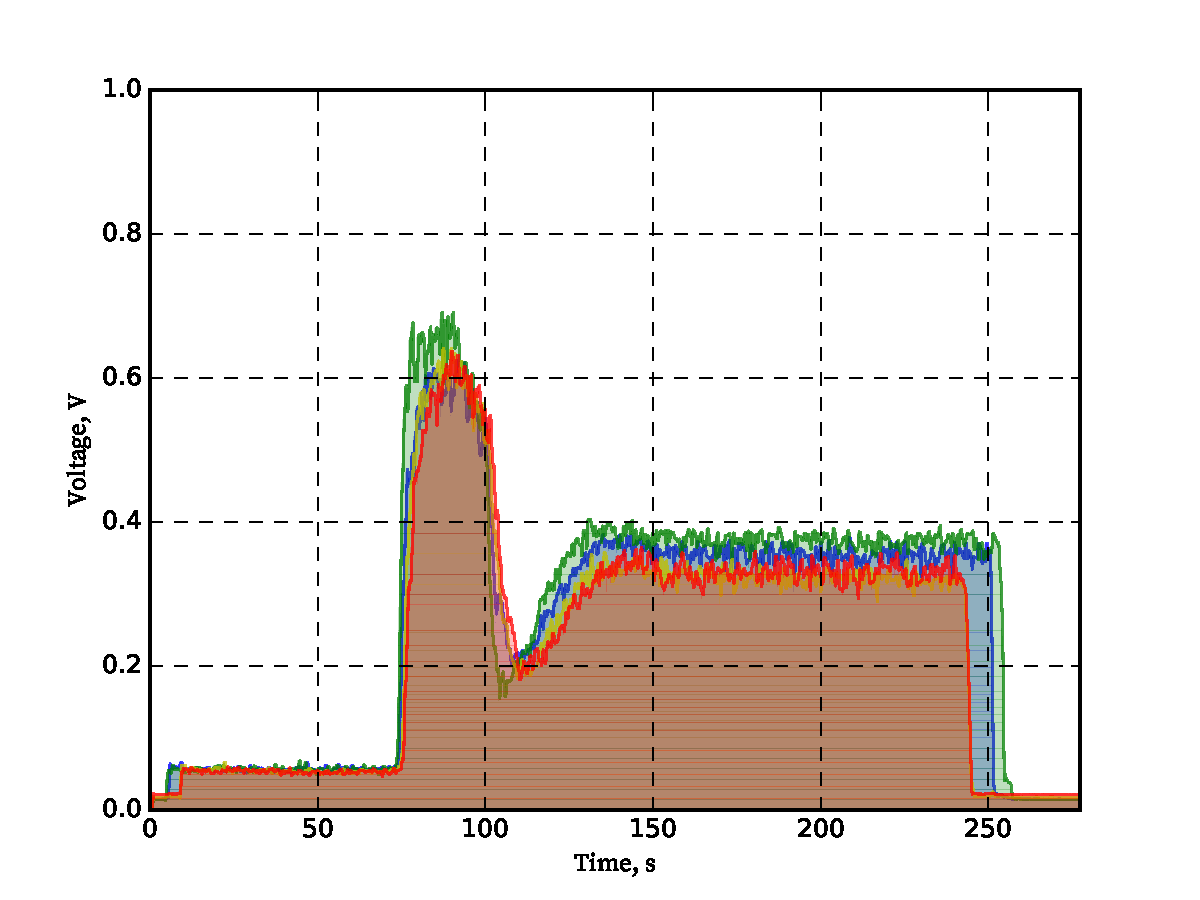
\includegraphics[width=0.8\textwidth]{images/log080716_2.pdf} 
		\caption{2}
		\label{fig:test2}
	\end{center}
\end{figure}

\textbf{Test No. 3}

The next test retained all specifics of the prior one, except for a higher salinity of \unit[1.9]{\%}.

\begin{figure}
	\begin{center}
		%% This file was created by matplotlib2tikz v0.5.10.
\tikzset{external/export next=false}
\begin{tikzpicture}

\definecolor{color0}{rgb}{0,0.75,0.75}

\begin{axis}[
xlabel={Time, s},
ylabel={relative Voltage, -},
xmin=150.006821, xmax=300.002257,
ymin=0, ymax=0.9,
axis on top,
ytick={0,0.1,0.2,0.3,0.4,0.5,0.6,0.7,0.8,0.9},
yticklabels={0.0,0.1,0.2,0.3,0.4,0.5,0.6,0.7,0.8,0.9},
xmajorgrids,
ymajorgrids
]
\addplot [line width=0.7000000000000001pt, color0, opacity=0.75]
table {%
150.68281 0.087583117838697
150.689662 0.0875545489161996
150.696512 0.0875246377753513
150.703375 0.0874933772833881
150.710223 0.087460760307546
150.717065 0.087426779715061
150.723906 0.0873914283731692
150.730779 0.0873546991491066
150.737657 0.0873165849101092
150.744533 0.087277078523413
150.751411 0.0872361728562541
150.760336 0.0871938607758684
150.766952 0.087150135149492
150.773614 0.087104988844361
150.780262 0.0870938351944775
150.786878 0.0870823007808699
150.793528 0.0870703847643895
150.800177 0.0870580863058875
150.806815 0.0870454045662153
150.813482 0.0870323387062242
150.820136 0.0870291996607123
150.826785 0.0870253623385858
150.833475 0.0870208277887803
150.840161 0.0870155970602319
150.846826 0.0870096712018764
150.853508 0.0870054126271007
150.860194 0.0870005312990936
150.866863 0.0869950286863653
150.873562 0.0869889062574261
150.880272 0.0869916109385904
150.886952 0.0869939798553798
150.893647 0.086996016154602
150.900353 0.0869977229830645
150.907073 0.086999103487575
150.913768 0.0870001608149411
150.920481 0.0870008981119706
150.927202 0.0870013185254709
150.933905 0.0870014252022498
150.940609 0.0870012212891149
150.947336 0.0870030014381954
150.954076 0.0870044078514221
150.960797 0.0870054440951771
150.967546 0.0870061137358423
150.974294 0.0870064203397998
150.981054 0.0870063674734315
150.987783 0.0870059587031194
150.994542 0.0870051975952455
151.001308 0.0870040877161918
151.008059 0.0870026326323403
151.014828 0.0870008359100729
151.021603 0.0869987011157717
151.028377 0.0869962318158187
151.035159 0.0869934315765958
151.041913 0.086990303964485
151.04867 0.0869868525458684
151.055458 0.0869830808871278
151.062254 0.0869789925546453
151.069034 0.0869745911148029
151.075836 0.0869698801339826
151.082615 0.0869648631785664
151.089414 0.0869595438149361
151.096227 0.086939030824884
151.103021 0.0869186739164907
151.109814 0.0868984739289049
151.116642 0.0868784317012753
151.123461 0.0868585480727506
151.130297 0.0868388238824796
151.137132 0.0868192599696109
151.14394 0.0867998571732932
151.150749 0.0867806163326753
151.157595 0.0867615382869058
151.164441 0.0867426238751335
151.171286 0.0867238739365069
151.178143 0.086705289310175
151.184971 0.0866868708352863
151.191804 0.0866686193509895
151.198659 0.0866505356964335
151.205523 0.0866326207107668
151.212384 0.0866148752331381
151.219262 0.0865973001026962
151.226138 0.0865798961585898
151.232991 0.0865626642399676
151.241877 0.0865456051859782
151.248489 0.0865287198357704
151.255119 0.0865120090284929
151.261737 0.0864954736032944
151.268383 0.0864791143993236
151.275034 0.0864629322557292
151.281668 0.0864469280116599
151.288328 0.0864311025062644
151.294973 0.0864154565786914
151.301616 0.0863999910680896
151.308284 0.0863847068136077
151.314944 0.0863696046543944
151.321606 0.0863546854295985
151.328283 0.0863399499783686
151.334957 0.0863253991398534
151.341621 0.0863110337532016
151.348307 0.0862968546575619
151.354999 0.0862828626920831
151.361678 0.0862690586959139
151.368386 0.0862554435082029
151.375087 0.0862420179680988
151.381777 0.0862287829147503
151.388488 0.0862157391873063
151.395196 0.0862028876249153
151.401898 0.086190229066726
151.4086 0.0861777643518872
151.415329 0.0861654943195476
151.422062 0.0861534198088558
151.428771 0.0861415416589606
151.435488 0.0861298607090107
151.442231 0.0861183777981548
151.44897 0.0861070937655415
151.45569 0.0860960094503196
151.462411 0.0860851256916378
151.46916 0.0860744433286448
151.475899 0.0860639632004894
151.482641 0.0860536861463201
151.489409 0.0860436130052857
151.496173 0.0860257243479095
151.502951 0.0860082843204089
151.509724 0.0859912922934222
151.516471 0.0859747476375879
151.523256 0.0859586497235446
151.530049 0.0859429979219307
151.536836 0.0859277916033846
151.543611 0.0859130301385449
151.55041 0.0858810026646669
151.557206 0.0858488916954929
151.56401 0.0858166934548537
151.570814 0.0857844041665802
151.577599 0.0857520200545033
151.58441 0.0857195373424537
151.591226 0.0856869522542624
151.598049 0.08565426101376
151.604871 0.0856214598447776
151.611678 0.0855885449711458
151.618479 0.0855555126166955
151.625316 0.0855223590052577
151.632173 0.085489080360663
151.639017 0.0854556729067424
151.645856 0.0854221328673267
151.652676 0.0853884564662467
151.659508 0.0853546399273332
151.666364 0.0853206794744171
151.673222 0.0852865713313292
151.68008 0.0852523117219004
151.686949 0.0852178968699615
151.693818 0.0852033945971775
151.700667 0.0851893268985282
151.70752 0.0851756935642265
151.714405 0.0851624943844852
151.723321 0.085149729149517
151.729953 0.0851373976495348
151.736597 0.0851254996747515
151.743209 0.0851140350153799
151.749864 0.0851030034616327
151.756514 0.0850924048037229
151.763165 0.0850822388318632
151.769814 0.0850725053362665
151.776458 0.0850632041071455
151.783121 0.0850543349347132
151.789772 0.0850458976091823
151.796428 0.0850378919207656
151.803108 0.0850303176596761
151.809762 0.0850231746161264
151.81645 0.0850164625803295
151.823137 0.0850101813424981
151.829833 0.0850043306928452
151.836504 0.0849989104215834
151.843207 0.0849939203189257
151.849908 0.0849893601750847
151.856621 0.0849852297802735
151.863311 0.0849815289247048
151.870024 0.0849782573985914
151.876759 0.0849754149921461
151.883463 0.0849730014955819
151.890193 0.0849710166991114
151.896917 0.0849694603929475
151.903651 0.0849683323673031
151.91036 0.084967632412391
151.917092 0.0849673603184239
151.923832 0.0849675158756148
151.930548 0.0849680988741765
151.937297 0.0849691091043216
151.944046 0.0849705463562632
151.950801 0.084972410420214
151.957534 0.0849747010863868
151.964271 0.0849774181449945
151.971032 0.0849805613862499
151.977805 0.0849841306003658
151.984552 0.084988125577555
151.991304 0.0849925461080304
151.998113 0.0849973919820048
152.004898 0.0850026629896909
152.011678 0.0850083589213018
152.018447 0.08501447956705
152.025244 0.0850210247171486
152.032038 0.0850279941618103
152.038838 0.0850353876912479
152.045629 0.0850432050956742
152.052414 0.0850514461653021
152.059226 0.0850601106903444
152.066036 0.085069198461014
152.072859 0.0850787092675236
152.079677 0.0850886429000861
152.086482 0.0850989991489142
152.09328 0.0851097778042209
152.100112 0.085120978656219
152.106944 0.0851326014951212
152.113783 0.0851446461111404
152.1206 0.0851571122944894
152.127443 0.0851699998353811
152.134309 0.0851833085240282
152.141153 0.0851970381506436
152.148009 0.0852111885054402
152.154854 0.0852257593786306
152.161724 0.0852407505604279
152.168553 0.0852561618410447
152.175397 0.085271993010694
152.182238 0.0852882438595885
152.189133 0.0853049141779411
152.196005 0.0853220037559645
152.204925 0.0853395123838716
152.211563 0.0853574398518753
152.218181 0.0853757859501884
152.224819 0.0853945504690236
152.231467 0.0854137331985938
152.238089 0.0854333339291119
152.244736 0.0854533524507906
152.251396 0.0854737885538428
152.258041 0.0854946420284813
152.264713 0.0855159126649189
152.271367 0.0855376002533685
152.278015 0.0855597045840429
152.284689 0.0855822254471548
152.291344 0.0856051626329172
152.298011 0.0856285159315428
152.304704 0.0856522851332445
152.311403 0.0856764700282351
152.318069 0.0857010704067274
152.324767 0.0857260860589343
152.331477 0.0857515167750685
152.338159 0.0857773623453429
152.344869 0.0858036225599704
152.351584 0.0858302972091637
152.358283 0.0858573860831356
152.36501 0.0858754435142947
152.371729 0.0858936336358425
152.378461 0.0859119545596945
152.385165 0.085930404397766
152.391896 0.0859489812619724
152.398634 0.0859676832642293
152.405348 0.0859865085164519
152.412064 0.0860054551305557
152.418811 0.0860245212184562
152.425558 0.0860437048920687
152.432318 0.0860630042633087
152.439048 0.0860824174440916
152.445807 0.0861019425463328
152.452574 0.0861215776819476
152.459317 0.0861413209628517
152.466067 0.0861611705009603
152.472842 0.0861811244081888
152.479622 0.0862011807964528
152.486378 0.0862213377776676
152.493168 0.0862415934637485
152.499964 0.0862619459666112
152.506745 0.0862823933981708
152.513546 0.086302933870343
152.520316 0.0863235654950431
152.527094 0.0863442863841864
152.533895 0.0863650946496886
152.540699 0.0863859884034648
152.54752 0.0864069657574306
152.554334 0.0864280248235014
152.561131 0.0864491637135926
152.567952 0.0864703805396197
152.574771 0.0864916734134979
152.58161 0.0865130404471429
152.588421 0.0865344797524699
152.595238 0.0865559894413943
152.602051 0.0865775676258317
152.6089 0.0865992124176974
152.615774 0.0866209219289069
152.622623 0.0866426942713755
152.629486 0.0866645275570187
152.636317 0.0866864198977518
152.643156 0.0867083694054904
152.650028 0.0867303741921499
152.656902 0.0867524323696455
152.663771 0.0867745420498928
152.670643 0.0867967013448073
152.67755 0.0868189083663042
152.686446 0.086841161226299
152.693063 0.0868634580367072
152.699697 0.0868857969094441
152.706343 0.0869081759564252
152.712958 0.0869305932895659
152.719603 0.0869530470207816
152.726265 0.0869755352619877
152.732901 0.0869980561250997
152.739595 0.0870206077220329
152.746272 0.0870431881647028
152.75292 0.0870657955650247
152.759589 0.0870884280349142
152.766276 0.0871110836862866
152.772927 0.0871337606310574
152.779606 0.0871564569811419
152.786301 0.0871791708484556
152.792965 0.0872019003449139
152.799659 0.0872246435824323
152.806366 0.0872473986729261
152.813048 0.0872701637283106
152.819752 0.0873089773977523
152.826467 0.0873473111790292
152.833155 0.0873851661210773
152.839842 0.0874225432728324
152.846554 0.0874594436832305
152.853283 0.0874958684012074
152.859985 0.087531818475699
152.866709 0.0875672949556412
152.873449 0.0876022988899698
152.880159 0.0876368313276208
152.886869 0.08767089331753
152.893614 0.0877044859086333
152.900357 0.0877376101498665
152.907089 0.0877702670901656
152.913817 0.0878024577784664
152.920568 0.0878341832637049
152.927316 0.0878654445948168
152.934062 0.0878962428207381
152.940827 0.0879265789904046
152.947596 0.0879564541527523
152.954381 0.0879858693567169
152.961129 0.0880148256512345
152.967884 0.0880433240852408
152.974672 0.0880713657076718
152.981462 0.0880989515674632
152.988248 0.0881260827135511
152.995023 0.0881527601948713
153.001817 0.0881789850603596
153.008619 0.0882047583589519
153.015424 0.0882300811395842
153.02223 0.0882549544511922
153.029024 0.088279379342712
153.035839 0.0883033568630793
153.042659 0.08832688806123
153.049481 0.0883499739861
153.056315 0.0883726156866253
153.063119 0.0883948142117416
153.06993 0.0884165706103848
153.076763 0.088427259791461
153.083598 0.0884371926897684
153.090447 0.0884463684661582
153.097296 0.0884547862814817
153.104121 0.0884624452965903
153.110978 0.0884693446723353
153.117843 0.0884754835695678
153.124708 0.0884808611491393
153.131574 0.0884854765719011
153.138434 0.0884893289987043
153.145314 0.0884924175904004
153.152155 0.0884947415078406
153.159011 0.0884962999118762
153.167892 0.0884970919633585
153.174543 0.0884971168231389
153.181167 0.0884963736520685
153.187779 0.0884948616109987
153.194421 0.0884925798607809
153.201075 0.0884895275622662
153.2077 0.088483342511855
153.214363 0.0884763149561456
153.221042 0.0884684436364151
153.227682 0.0884597272939403
153.234373 0.0884501646699983
153.241054 0.0884535035377951
153.247709 0.0884555769693474
153.254389 0.0884563862233781
153.26108 0.0884559325586104
153.267737 0.0884542172337673
153.274424 0.0884512415075718
153.281124 0.088447006638747
153.287804 0.088441513886016
153.294524 0.0884347645081018
153.301227 0.0884267597637274
153.307914 0.088417500911616
153.314637 0.0884069892104905
153.321352 0.0883952259190741
153.328075 0.0883822122960898
153.334772 0.0883679496002606
153.341496 0.0883524390903096
153.348225 0.0883356820249598
153.354955 0.0883330285318664
153.36167 0.0883295878123957
153.368412 0.088325363852504
153.375158 0.0883203606381478
153.381886 0.0883145821552833
153.388641 0.0883080323898669
153.395388 0.0883007153278549
153.402147 0.0882926349552036
153.408893 0.0882837952578695
153.41565 0.0882742002218088
153.422417 0.0882638538329779
153.429198 0.0882527600773331
153.435952 0.0882409229408308
153.442706 0.0882283464094273
153.449493 0.0882150344690789
153.456282 0.088200991105742
153.463056 0.088186220305373
153.469828 0.0881707260539281
153.476653 0.0881545123373637
153.483454 0.0881375831416362
153.490261 0.0881199424527019
153.497047 0.0881015942565171
153.503837 0.0880825425390382
153.51065 0.0880627912862215
153.517468 0.0880423444840233
153.524285 0.0880212061184
153.531106 0.087999380175308
153.537908 0.0879768706407035
153.54474 0.08793420370531
153.551576 0.0878914513865358
153.558405 0.0878486141039555
153.56525 0.0878056922771433
153.572099 0.0877626863256736
153.578923 0.0877195966691207
153.58575 0.0876764237270591
153.592613 0.087633167919063
153.599476 0.0875898296647068
153.606338 0.0875464093835648
153.613205 0.0875029074952114
153.620082 0.0874593244192211
153.626926 0.087415660575168
153.633776 0.0873719163826265
153.64066 0.0873280922611711
153.649581 0.0872841886303761
153.656219 0.0872402059098157
153.662865 0.0871961445190644
153.669508 0.0871520048776966
153.676154 0.0871077874052865
153.682809 0.0870634925214085
153.689423 0.087019120645637
153.696085 0.0869746721975463
153.702729 0.0869301475967108
153.709399 0.0868855472627049
153.716077 0.0868408716151028
153.722724 0.0867961210734789
153.729434 0.0867512960574077
153.736116 0.0867063969864633
153.742781 0.0866614242802203
153.749448 0.0866163783582528
153.756141 0.0865795244157142
153.762841 0.0865428440720635
153.769513 0.0865063392153855
153.776215 0.0864700117337645
153.78292 0.0864338635152854
153.789633 0.0863978964480325
153.796339 0.0863621124200906
153.803058 0.0863265133195441
153.809754 0.0862911010344778
153.816445 0.0862558774529761
153.823162 0.0862208444631236
153.829899 0.0861860039530049
153.836615 0.0861513578107047
153.843346 0.0861169079243074
153.850091 0.0860826561818977
153.856839 0.0860486044715601
153.863562 0.0860147546813793
153.870302 0.0859811086994397
153.877062 0.0859476684138261
153.883799 0.085914435712623
153.890534 0.0858814124839149
153.897294 0.0858486006157864
153.904063 0.0858160019963222
153.910838 0.0857836185136068
153.917588 0.0857514520557248
153.924374 0.0857195045107607
153.931144 0.0856877777667993
153.93793 0.0856562737119249
153.944696 0.0856249942342223
153.951457 0.085593941221776
153.958257 0.0855631165626705
153.965055 0.0855325221449905
153.971846 0.0855021598568206
153.978635 0.0854720315862453
153.985448 0.0854421392213492
153.992264 0.085412484650217
153.999078 0.0853830697609331
154.005894 0.0853538964415821
154.012695 0.0853249665802487
154.01949 0.0852962820650175
154.026324 0.0852678447839729
154.033179 0.0852396566251996
154.040023 0.0852105737241215
154.046846 0.0851817784412614
154.053668 0.0851532724549167
154.060495 0.085125057443385
154.067339 0.0850971350849635
154.074195 0.0850695070579496
154.081051 0.0850421750406409
154.087921 0.0850151407113347
154.094779 0.0849884057483284
154.101621 0.0849619718299193
154.108464 0.084935840634405
154.115337 0.0849100138400829
154.122211 0.0848844931252502
154.131123 0.0848592801682045
154.137767 0.0848343766472431
154.144379 0.0848097842406635
154.15102 0.084785504626763
154.15767 0.0847615394838391
154.164297 0.0847378904901891
154.170946 0.0847145593241105
154.177583 0.0846915476639007
154.184275 0.0846688571878571
154.190943 0.0846464895742771
154.197594 0.0846244465014581
154.204239 0.0846027296476975
154.210918 0.0845813406912927
154.217607 0.0845602813105411
154.224269 0.0845395531837402
154.230958 0.0845191579891873
154.237652 0.0844990974051798
154.24432 0.0844793731100152
154.251014 0.0844599867819908
154.257724 0.0844409400994041
154.264407 0.0844222347405525
154.271108 0.0844038723837333
154.277844 0.084385854707244
154.284536 0.084368183389382
154.29123 0.0843508601084447
154.297948 0.0843338865427295
154.304678 0.0843172643705338
154.311386 0.084300995270155
154.318113 0.0842850809198905
154.32485 0.0842695229980377
154.331568 0.0842543231828941
154.338281 0.0842394831527571
154.345027 0.0842250045859239
154.351775 0.0842108891606922
154.358512 0.0841971385553592
154.365239 0.0841837544482223
154.371988 0.084170738517579
154.378752 0.0841580924417267
154.385499 0.0841458178989628
154.392235 0.0841339165675847
154.399012 0.0841223901258898
154.405786 0.0841112402521755
154.412536 0.0841004686247392
154.419297 0.0840900769218783
154.426088 0.0840800668218902
154.432873 0.0840704400030724
154.439655 0.0840611981437222
154.44643 0.0840523429221371
154.453233 0.0840438760166144
154.460041 0.0840357991054515
154.466845 0.084028113866946
154.473641 0.0839841578942505
154.480436 0.0839417079836904
154.487262 0.0839007591003732
154.494086 0.0838613062094068
154.500907 0.0838233442758991
154.507745 0.0837868682649577
154.514549 0.0837518731416904
154.521368 0.0837183538712051
154.528239 0.0836863054186095
154.535091 0.0836557227490114
154.541935 0.0836266008275185
154.54879 0.0835989346192387
154.55562 0.0835727190892797
154.562452 0.0835479492027493
154.569289 0.0835246199247553
154.576146 0.0835027262204055
154.583015 0.0834822630548076
154.589875 0.0834632253930695
154.596756 0.0834456082002988
154.603607 0.0834294064416035
154.612501 0.0834146150820912
154.619115 0.0834012290868698
154.625752 0.083389243421047
154.632374 0.0833786530497306
154.639018 0.0833694529380284
154.645659 0.0833616380510482
154.652328 0.0833552033538977
154.658986 0.0833501438116847
154.665655 0.0833464543895171
154.672301 0.0833441300525026
154.678973 0.0833431657657489
154.685637 0.0833435564943638
154.692294 0.0833452972034552
154.698979 0.0833483828581309
154.705672 0.0833528084234984
154.71236 0.0833585688646658
154.719026 0.0833656591467408
154.725719 0.083374074234831
154.732399 0.0833838090940444
154.739075 0.0833948586894887
154.745777 0.0834072179862716
154.75249 0.083420881949501
154.759177 0.0834358455442847
154.765893 0.0834521037357303
154.77261 0.0834696514889457
154.779309 0.0834884837690387
154.78604 0.0835085955411171
154.792767 0.0835299817702886
154.799503 0.083552637421661
154.806216 0.0835765574603421
154.812952 0.0836017368514397
154.819703 0.0836281705600616
154.826455 0.0836558535513155
154.833204 0.0836847807903092
154.839955 0.0837149472421505
154.846717 0.0837463478719471
154.85348 0.0837789776448069
154.860228 0.0838128315258377
154.867001 0.0838479044801472
154.873768 0.0838841914728432
154.880546 0.0839216874690334
154.887302 0.0839603874338257
154.894082 0.0840002863323279
154.900868 0.0840413791296476
154.907656 0.0840836607908928
154.914453 0.0841271262811712
154.921231 0.0841717705655905
154.92803 0.0842175886092585
154.934837 0.0842645753772831
154.94164 0.0843127258347719
154.948443 0.0843620349468329
154.955262 0.0844124976785737
154.962053 0.0844641089951021
154.968878 0.084516863861526
154.975697 0.0845707572429531
154.98253 0.0846257841044911
154.989329 0.0846819394112479
154.996142 0.0847392181283313
155.002982 0.0847976152208489
155.009819 0.0848571256539087
155.01669 0.0849177443926183
155.023542 0.0849794664020856
155.030368 0.0850422866474184
155.03719 0.0851062000937244
155.044056 0.0851712017061114
155.05092 0.0852372864496871
155.057786 0.0853044492895595
155.064647 0.0853726851908361
155.071528 0.0854419891186249
155.078392 0.085495826486876
155.085249 0.0855502298609275
155.09413 0.0856051912688667
155.100765 0.0856607027387809
155.107385 0.0857167562987574
155.114005 0.0857733439768836
155.120642 0.0858304578012468
155.1273 0.0858880897999342
155.133928 0.0859462320010332
155.140586 0.0860048764326312
155.147261 0.0861041164659422
155.153901 0.0862026275937109
155.160574 0.0863004091865756
155.167257 0.0863974606151748
155.173913 0.086493781250147
155.180596 0.0865893704621308
155.187288 0.0866842276217645
155.193948 0.0867783520996866
155.200636 0.0868717432665357
155.20734 0.0869644004929501
155.214019 0.0870563231495683
155.220713 0.0871475106070289
155.227412 0.0872379622359703
155.234104 0.0873276774070309
155.240823 0.0874166554908493
155.247537 0.0875048958580639
155.254262 0.0875923978793132
155.260959 0.0876791609252357
155.267686 0.0877651843664697
155.274417 0.0878504675736539
155.281126 0.0879350099174267
155.287838 0.0880188107684265
155.294572 0.0881075982605956
155.301305 0.0881954694023808
155.308031 0.0882824246133563
155.314792 0.0883684643130965
155.321542 0.0884535889211757
155.328292 0.0885377988571684
155.335035 0.0886210945406488
155.341803 0.0887034763911913
155.348564 0.0887849448283703
155.355336 0.0888655002717601
155.36209 0.088945143140935
155.368838 0.0890238738554695
155.375623 0.0891016928349378
155.382411 0.0891786004989144
155.389198 0.0892545972669735
155.395969 0.0893296835586895
155.402766 0.0894038597936369
155.40956 0.0894771263913898
155.416371 0.0895494837715227
155.423147 0.08962093235361
155.429941 0.0896914725572259
155.436751 0.0897611048019449
155.443568 0.0898298295073412
155.450395 0.0898976470929893
155.45719 0.0899645579784634
155.463992 0.090030562583338
155.470818 0.0900784750372759
155.477651 0.0901260028464269
155.484481 0.0901731432835578
155.491329 0.0902198936214352
155.498144 0.0902520829461193
155.504968 0.0902834550448601
155.511852 0.0903140046729781
155.518708 0.0903437265857938
155.525568 0.0903726155386279
155.532431 0.090400666286801
155.539304 0.0904278735856337
155.546143 0.0904542321904466
155.55299 0.0904797368565603
155.559868 0.0905043823392954
155.566745 0.0905281633939725
155.575692 0.0905510747759123
155.582325 0.0905731112404353
155.588941 0.0905942675428621
155.595582 0.0906145384385133
155.602216 0.0906339186827096
155.608846 0.0906524030307715
155.615491 0.0906699862380196
155.622154 0.0906866630597746
155.628796 0.0907024282513571
155.635484 0.0907172765680876
155.64216 0.0907312027652868
155.648815 0.0907442015982752
155.65549 0.0907562678223735
155.662158 0.0907673961929023
155.668821 0.0907775814651822
155.675507 0.0907868183945338
155.6822 0.0907951017362776
155.688874 0.0908024262457344
155.695597 0.0908087866782246
155.702306 0.090814177789069
155.708993 0.090818594333588
155.715676 0.0908220310671024
155.722386 0.0908244827449326
155.729106 0.0908259441223994
155.735803 0.0908264099548234
155.742522 0.090825874997525
155.749248 0.090824334005825
155.755975 0.0908217817350439
155.762679 0.0908182129405024
155.769414 0.090813622377521
155.776141 0.0908080048014203
155.782864 0.090801354967521
155.78962 0.0907936676311437
155.796364 0.0907849375476089
155.803099 0.0907952310700715
155.809836 0.0908050687250011
155.816627 0.0908144488341001
155.823382 0.0908233697190713
155.830155 0.0908318297016172
155.836904 0.0908398271034404
155.843644 0.0908473602462435
155.850427 0.0908544274517291
155.857212 0.0908610270415998
155.863971 0.0908671573375581
155.87074 0.0908728166613068
155.877558 0.0908780033345483
155.884346 0.0908827156789852
155.891153 0.0908869520163203
155.897926 0.0908907106682559
155.904705 0.0908939899564948
155.911513 0.0908967882027396
155.918324 0.0908991037286927
155.925148 0.0909009348560569
155.931936 0.0909022799065347
155.938739 0.0909031372018287
155.945567 0.0908909017843731
155.952393 0.0908785571726925
155.959232 0.0908660993808305
155.966063 0.0908535244228308
155.972882 0.090840828312737
155.9797 0.0908280070645929
155.98655 0.0908150566924421
155.993395 0.0908019732103282
156.000248 0.0907887526322949
156.007105 0.0907753909723859
156.013942 0.0907618842446447
156.020781 0.0907482284631152
156.027659 0.0907344196418409
156.034531 0.0907204537948655
156.041406 0.0907063269362326
156.048277 0.090692035079986
156.057194 0.0906775742401692
156.063836 0.090662940430826
156.070476 0.0906481296659999
156.07712 0.0906331379597348
156.08374 0.0906179613260741
156.090388 0.0906025957790615
156.097012 0.0905870373327409
156.103646 0.0905712820011557
156.110311 0.0905553257983496
156.116972 0.0905391647383664
156.123626 0.0905227948352496
156.130316 0.090506212103043
156.136974 0.0904894125557901
156.143636 0.0904723922075347
156.150318 0.0904551470723204
156.157005 0.0904376731641908
156.163677 0.0904199664971897
156.170373 0.0904020230853607
156.177067 0.0903838389427474
156.183745 0.0903654100833935
156.190483 0.0903467325213426
156.197187 0.0903278022706385
156.203904 0.0903086153453247
156.210594 0.090289167759445
156.217316 0.090269455527043
156.22404 0.0902494746621624
156.230783 0.0902292211788467
156.237482 0.0902086910911398
156.244214 0.0901878804130851
156.250967 0.0901667851587265
156.257686 0.0901454013421075
156.264438 0.0901237249772719
156.271176 0.0901017520782632
156.277909 0.0900794786591251
156.284644 0.0900569007339014
156.291409 0.0900340143166355
156.29816 0.0900119961035968
156.304926 0.0899896965659554
156.311696 0.089967111927542
156.318437 0.0899442384121874
156.325214 0.0899210722437226
156.332001 0.0898976096459784
156.338749 0.0898738468427856
156.345509 0.089849780057975
156.352302 0.0898254055153774
156.359092 0.0898007194388238
156.365872 0.0897757180521449
156.372673 0.0897503975791716
156.379448 0.0897247542437347
156.386253 0.089698784269665
156.393059 0.0896724838807934
156.399854 0.0896458493009507
156.406649 0.0896188767539677
156.413474 0.0895915624636753
156.420299 0.0895639026539044
156.427124 0.0895358935484857
156.433961 0.0895075313712501
156.44076 0.0894788123460284
156.447578 0.0894497326966514
156.454418 0.0894202886469501
156.461262 0.0893904764207552
156.468105 0.0893602922418976
156.474958 0.089329732334208
156.481788 0.0892987929215174
156.488618 0.0892674702276565
156.495514 0.0892357604764563
156.502372 0.0892036598917475
156.509239 0.0891711646973609
156.516105 0.0891382711171275
156.522987 0.089104975374878
156.529842 0.0890712736944433
156.538738 0.0890371622996542
156.545345 0.0890026374143416
156.551982 0.0889676952623362
156.558628 0.088932332067469
156.565239 0.0888965440535707
156.571888 0.0888603274444722
156.578514 0.0888236784640044
156.585173 0.088786593335998
156.59184 0.0887490682842838
156.598489 0.0887110995326929
156.60516 0.0886726833050559
156.611824 0.0886338158252036
156.618505 0.088624282886147
156.625189 0.088595056385747
156.63188 0.0885650255613149
156.638541 0.0885341887345532
156.645238 0.0885025442271647
156.651932 0.0884700903608518
156.658613 0.0884368254573171
156.665288 0.0884027478382633
156.67199 0.088367855825393
156.678702 0.0883321477404087
156.685414 0.0882956219050131
156.692127 0.0882582766409086
156.698845 0.088220110269798
156.705538 0.0881811211133839
156.712242 0.0881413074933687
156.71897 0.0881006677314551
156.725709 0.0880592001493457
156.732417 0.0880546848999605
156.739153 0.088050462933047
156.745904 0.0880465392834975
156.752654 0.0880429189862043
156.75938 0.0880396070760596
156.76613 0.0880366085879555
156.772883 0.0880339285567844
156.779625 0.0880315720174383
156.786371 0.0880295440048096
156.793134 0.0880278495537905
156.79991 0.0880264936992731
156.806684 0.0880254814761498
156.813439 0.0880248179193126
156.820219 0.0880245080636539
156.827007 0.0880245569440659
156.833802 0.0880249695954408
156.840567 0.0880257510526707
156.847344 0.088026906350648
156.854142 0.0880284405242648
156.860941 0.0880303586084134
156.867744 0.0880326656379859
156.87453 0.0880353666478746
156.88132 0.0880384666729718
156.888138 0.0880419707481696
156.894953 0.0880458839083602
156.901779 0.088050211188436
156.908584 0.088054957623289
156.915389 0.0880601282478115
156.922218 0.0880657280968958
156.929058 0.0880717622054341
156.935893 0.0880782356083185
156.942742 0.0880851533404413
156.949561 0.0880925204366948
156.95639 0.088100341931971
156.963248 0.0881086228611624
156.97011 0.088117368259161
156.976972 0.088126583160859
156.983842 0.0881362726011489
156.990723 0.0881464416149226
156.997567 0.0881570952370725
157.004412 0.0881682385024908
157.011269 0.0881798764460697
157.020178 0.0881920141027013
157.026814 0.0882046565072781
157.033454 0.088217808694692
157.040069 0.0882314756998355
157.046709 0.0882456625576006
157.053355 0.0882603743028797
157.060009 0.0882756159705649
157.066666 0.0882913925955484
157.073318 0.0883077092127225
157.079985 0.0883245708569795
157.086656 0.0883419825632114
157.09331 0.0883599493663105
157.09999 0.0883784763011691
157.106674 0.0883975684026794
157.113364 0.0884172307057336
157.120059 0.0884374682452238
157.126749 0.0884582860560424
157.133452 0.0884796891730816
157.140127 0.0885016826312335
157.146821 0.0885242714653904
157.153529 0.0885474607104446
157.160211 0.0885712554012881
157.166922 0.0885956605728133
157.173642 0.0886206812599124
157.180336 0.0886463224974776
157.187063 0.0886725893204011
157.193787 0.0886994867635751
157.200521 0.0887270198618918
157.20723 0.0887551936502436
157.213961 0.0887840131635225
157.220711 0.0888134834366208
157.227459 0.0888436095044307
157.234206 0.0888743964018445
157.240958 0.0889058491637544
157.247714 0.0889379728250526
157.254475 0.0889707724206312
157.261217 0.0890042529853826
157.267989 0.0890384195541989
157.27475 0.0890732771619724
157.281505 0.0891088308435953
157.28826 0.0891450856339598
157.295063 0.0891957955998873
157.301847 0.0892468001070097
157.308636 0.0892981067076652
157.315401 0.0893497229541923
157.322175 0.0894016563989292
157.32897 0.0894539145942143
157.335765 0.0895065050923859
157.342573 0.0895594354457824
157.349349 0.089612713206742
157.356166 0.0896663459276031
157.362978 0.089720341160704
157.369798 0.0897747064583831
157.37662 0.0898294493729787
157.383419 0.089884577456829
157.39022 0.0899400982622725
157.397052 0.0899960193416476
157.403886 0.0900110243693984
157.410719 0.0900252148984391
157.417593 0.0900385911385569
157.424411 0.0900511532995388
157.431237 0.0900629015911722
157.438065 0.0900738362232441
157.444923 0.0900839574055418
157.451781 0.0900932653478523
157.458644 0.090101760259963
157.465519 0.0901094423516609
157.472357 0.0901163118327333
157.479205 0.0901223689129673
157.486082 0.0901276138021501
157.492958 0.0901320467100689
157.50188 0.0901356678465108
157.508516 0.090138477421263
157.515128 0.0901404756441127
157.521771 0.0901416627248471
157.528398 0.090163808173808
157.535026 0.0901844832244534
157.541676 0.090203692072527
157.548339 0.0902214389137723
157.55497 0.0902318245328051
157.561634 0.0902405808397369
157.568312 0.0902477109813752
157.574961 0.0902532181045278
157.581636 0.0902571053560022
157.588327 0.0902593758826062
157.594983 0.0902600328311473
157.601663 0.0902590793484331
157.608358 0.0902565185812714
157.615033 0.0902523536764698
157.621724 0.0902465877808358
157.628427 0.0902392240411772
157.635116 0.0902302656043016
157.641835 0.0902197156170165
157.648547 0.0902075772261297
157.655265 0.0901938535784488
157.661966 0.0901785478207814
157.668692 0.0901616630999352
157.675416 0.0901432025627177
157.682124 0.0901231693559367
157.688862 0.0901015666263997
157.695595 0.0900783975209145
157.702324 0.0900536651862886
157.709046 0.0900273727693296
157.715804 0.0899995234168453
157.722553 0.0899701202756433
157.729308 0.0899568767259142
157.736049 0.0899426127713619
157.742817 0.0899273347056018
157.749569 0.0899110488222489
157.756332 0.0898937614149187
157.763082 0.0898754787772263
157.769851 0.0898562072027871
157.776632 0.0898359529852163
157.783416 0.0898147224181293
157.790199 0.0897925217951412
157.796967 0.0897693574098675
157.803758 0.0897452355559232
157.810547 0.0897201625269237
157.817346 0.0896941446164844
157.82412 0.0896671881182204
157.830901 0.089639299325747
157.837709 0.0896104845326795
157.844521 0.0895807500326333
157.851333 0.0895501021192235
157.858125 0.0895185470860654
157.864923 0.0894860912267743
157.87175 0.0894527408349655
157.878577 0.0894185022042543
157.885419 0.0893833816282559
157.892231 0.0893473854005856
157.899046 0.0893105198148587
157.905866 0.0892727911646905
157.912746 0.0892342057436961
157.919595 0.089194769845491
157.926455 0.0891544897636904
157.93332 0.0891133717919095
157.940156 0.0890714222237637
157.946997 0.0890286473528682
157.953871 0.0889850534728382
157.960744 0.0889406468772891
157.96762 0.0888954338598362
157.974492 0.0888494207140946
157.983409 0.0888163627656089
157.990052 0.088782100638734
157.996658 0.0887466431445312
158.003306 0.0886951043094721
158.009925 0.0886428390863166
158.016573 0.0885898535588929
158.0232 0.0885361538110291
158.029833 0.0884817459265533
158.036518 0.0884266359892937
158.04318 0.0883708300830782
158.049832 0.0883143342917351
158.056507 0.0882571546990923
158.063176 0.088199297388978
158.069836 0.0881407684452204
158.076519 0.0880815739516474
158.0832 0.0880217199920872
158.089873 0.0879612126503679
158.096586 0.0879000580103176
158.103283 0.0878382621557644
158.10996 0.0877758311705364
158.116651 0.0877127711384617
158.123358 0.0876490881433684
158.130071 0.0875847882690845
158.136764 0.0875198775994383
158.143488 0.0874543622182577
158.150214 0.0873882482093709
158.156941 0.087321541656606
158.163649 0.0872542486437911
158.170382 0.0871863752547542
158.177121 0.0871179275733236
158.183842 0.0870489116833272
158.190586 0.0869793336685932
158.197344 0.0869091996129497
158.204096 0.0868515031047057
158.210826 0.0867936492560798
158.217611 0.0867356464585591
158.224362 0.0866775031036306
158.23111 0.0866192275827813
158.237858 0.0865608282874983
158.244631 0.0865023136092686
158.251403 0.0864436919395792
158.258189 0.0863849716699172
158.264939 0.0863261611917695
158.2717 0.0862672688966233
158.278541 0.0862083031759656
158.285333 0.0861492724212834
158.292113 0.0860901850240637
158.298892 0.0860310493757935
158.305662 0.0859718738679599
158.31247 0.08591266689205
158.319274 0.0858534368395507
158.326071 0.0857941921019491
158.332864 0.0857349410707323
158.339689 0.0856756921373872
158.346514 0.0856164536934008
158.353336 0.0855572341302604
158.360176 0.0854980418394527
158.366974 0.085438885212465
158.373792 0.0853797726407842
158.380632 0.0853207125158973
158.387476 0.0852617132292915
158.394328 0.0851890341405244
158.401182 0.0851168493103436
158.408032 0.08504516461279
158.414864 0.0849739859219044
158.421698 0.0849033191117279
158.428556 0.0848331700563013
158.435422 0.0847635446296656
158.442286 0.0846944487058616
158.449166 0.0846258881589304
158.456011 0.0845578688629127
158.464905 0.0844903966918497
158.471545 0.084423477519782
158.478183 0.0843571172207508
158.484802 0.0842913216687969
158.491447 0.0842260967379613
158.498089 0.0841614483022848
158.504716 0.0840973822358084
158.511375 0.0840339044125731
158.518024 0.0839710207066196
158.524672 0.083908736991989
158.531356 0.0838470591427223
158.538012 0.0837859930328601
158.544667 0.0837255445364437
158.551343 0.0836657195275137
158.558025 0.0836065238801113
158.564695 0.0835479634682773
158.571386 0.0834900441660525
158.578076 0.083432771847478
158.584746 0.0833761523865947
158.591492 0.0833201916574435
158.598199 0.0832648955340653
158.604912 0.083210269890501
158.611598 0.0831563206007916
158.618317 0.083103053538978
158.625033 0.083050474579101
158.631731 0.0829985895952017
158.638461 0.082947404461321
158.64519 0.0828969250514997
158.651927 0.0828471572397788
158.658635 0.0827981069001992
158.665373 0.0827497799068019
158.672124 0.0827021821336278
158.678877 0.0826553194547177
158.685599 0.0826091977441126
158.692353 0.0825638228758535
158.699114 0.0825192007239813
158.705878 0.0824753371625368
158.712647 0.082432238065561
158.719419 0.0823899093070949
158.726182 0.0823483567611793
158.732965 0.0823075863018552
158.73972 0.0822676038031635
158.74647 0.0822284151391451
158.753262 0.0821900261838409
158.760051 0.0821524428112919
158.766824 0.0821156708955391
158.77362 0.0820797163106232
158.780414 0.0820445849305852
158.787217 0.0820102826294661
158.794028 0.0819768152813068
158.800809 0.0819441887601482
158.807597 0.0819124089400313
158.814411 0.0818814816949968
158.821233 0.0818514128990859
158.828056 0.0818222084263393
158.834866 0.0817938741507981
158.841676 0.0817664159465031
158.848482 0.0817398396874953
158.855328 0.0817141512478156
158.862164 0.0816893565015049
158.869017 0.0816654613226041
158.875834 0.0816117738472901
158.88266 0.0815769749799259
158.889489 0.0815427364541082
158.896371 0.0815090620460064
158.90323 0.0814759555317895
158.910088 0.0814434206876267
158.916957 0.0814114612896872
158.923804 0.0813800811141402
158.930648 0.081348138184494
158.937501 0.0813168167493562
158.946414 0.0812861203751088
158.953052 0.0812560526281337
158.959694 0.081226617074813
158.966313 0.0811978172815286
158.972952 0.0811696568146626
158.979572 0.0811421392405968
158.986225 0.0811152681257134
158.992879 0.0810890470363942
158.999532 0.0810634795390213
159.006199 0.0810385691999767
159.012869 0.0810143195856424
159.019522 0.0809907342624003
159.026199 0.0809678167966325
159.032873 0.0809455707547208
159.039536 0.0809239997030475
159.046222 0.0809031072079942
159.052915 0.0808828968359432
159.059583 0.0808633721532764
159.066259 0.0808445367263758
159.072962 0.0808263941216233
159.079673 0.0808089479054009
159.086385 0.0807922016440907
159.093101 0.0807761589040746
159.099814 0.0807608232517347
159.106511 0.0807461982534528
159.113239 0.0807322874756111
159.119964 0.0807190944845914
159.126702 0.0807066228467758
159.133409 0.0806948761285463
159.140139 0.0806838578962848
159.146884 0.0806735717163733
159.153603 0.0806640211551939
159.160316 0.0806552097791285
159.167071 0.0806471411545591
159.173831 0.0806398188478677
159.180559 0.0806332464254363
159.18729 0.0806274274536469
159.194059 0.0806223654988814
159.200831 0.0806180641275219
159.207599 0.0806145269059503
159.214357 0.0806117574005487
159.22113 0.0806097591776989
159.227913 0.0806085358037831
159.23469 0.0806080908451832
159.241458 0.0806049906102988
159.248252 0.0806027800828272
159.255061 0.0806014621997886
159.261856 0.0806010398982037
159.268665 0.0806015161150928
159.275444 0.0806028937874765
159.282252 0.0806051758523751
159.289065 0.0806083652468092
159.29588 0.0806124649077991
159.302698 0.0806174777723655
159.309498 0.0806234067775286
159.3163 0.0806302548603091
159.323137 0.0806380249577273
159.329964 0.0806467200068037
159.336808 0.0806563429445587
159.34362 0.0806668967080129
159.350441 0.0806783842341868
159.357288 0.0806908084601006
159.364148 0.080704172322775
159.370998 0.0807035839746404
159.377861 0.080704392494416
159.384724 0.080706598091889
159.391591 0.0807102009768467
159.39843 0.080715201359076
159.405309 0.0807215994483643
159.412177 0.0807293954544988
159.41906 0.0807385895872664
159.427977 0.0807491820564546
159.434609 0.0807611730718504
159.441221 0.080774562843241
159.447859 0.0807893515804136
159.454511 0.0808055394931553
159.461137 0.0808231267912534
159.467791 0.080842113684495
159.474453 0.0808625003826673
159.4811 0.0808842870955574
159.48776 0.0809074740329526
159.494408 0.08093206140464
159.501059 0.0809580494204068
159.507742 0.0809854382900402
159.514435 0.0810142282233274
159.521101 0.0810444194300554
159.527784 0.0810760121200115
159.534482 0.0811090065029829
159.541155 0.0811434027887568
159.547847 0.0811792011871203
159.554555 0.0812022337211541
159.561237 0.0812262471151284
159.567945 0.0812512390613844
159.574688 0.0812772072522631
159.581384 0.0813041493801056
159.588076 0.0813320631372529
159.594796 0.0813609462160461
159.60153 0.0813907963088262
159.608235 0.0814216111079344
159.614959 0.0814533883057117
159.621697 0.0814861255944991
159.628419 0.0815198206666378
159.635168 0.0815544712144687
159.641915 0.081590074930333
159.648668 0.0816266295065718
159.655396 0.081664132635526
159.662124 0.0817025820095368
159.668889 0.0817419753209452
159.675653 0.0817823102620923
159.682394 0.0818235845253192
159.689147 0.0818657958029669
159.695945 0.0819089417873764
159.702726 0.0819530201708889
159.709502 0.0819980286458455
159.716266 0.0820439649045871
159.723053 0.0820908266394549
159.729846 0.0821386115427899
159.736643 0.0821873173069331
159.743419 0.0822369416242257
159.7502 0.0822874821870088
159.757032 0.0823389366876233
159.763841 0.0823913028184104
159.770654 0.082444578271711
159.777446 0.0824987607398664
159.784246 0.0825314149529322
159.791071 0.0825643039178477
159.797901 0.0825974213409978
159.804726 0.082630760928767
159.811567 0.0826643163875402
159.818371 0.082698081423702
159.825216 0.0827320497436371
159.832063 0.0827662150537304
159.838921 0.0828005710603665
159.845771 0.0828351114699302
159.852636 0.0828698299888061
159.859472 0.082904720323379
159.866312 0.0829397761800337
159.87315 0.0829749912651548
159.880019 0.0830103592851271
159.886891 0.0830458739463352
159.893773 0.083081528955164
159.900654 0.0831173180179982
159.909572 0.0831532348412224
159.916181 0.0831892731312215
159.922819 0.08322542659438
159.929448 0.0832616889370829
159.936074 0.0832980538657147
159.942719 0.0833345150866602
159.949376 0.0833710663063041
159.956011 0.0834077012310312
159.962672 0.0834444135672261
159.969347 0.0834811970212737
159.975996 0.0835180452995586
159.982666 0.0835549521084655
159.989351 0.0835919111543793
159.996003 0.0836289161436845
160.00268 0.083665960782766
160.009375 0.0837030387780084
160.016046 0.0837401438357965
160.022734 0.083777269662515
160.029427 0.0838144099645487
160.036108 0.0838515584482822
160.042814 0.0839013120993687
160.049529 0.0839506794273709
160.05622 0.0839996564463325
160.062905 0.0840482391702972
160.069621 0.0840964236133085
160.076347 0.0841442057894102
160.083052 0.0841915817126459
160.089771 0.0842385473970593
160.096508 0.0842850988566941
160.103225 0.0843312321055938
160.109945 0.0843838176737668
160.116686 0.0844357687406264
160.123441 0.0844870825789395
160.130189 0.0845377564614728
160.136911 0.0845877876609929
160.143668 0.0846371734502667
160.150438 0.0846859111020606
160.15717 0.0847339978891416
160.16392 0.0847814310842764
160.170692 0.0848282079602315
160.177465 0.0848743257897738
160.184226 0.08491978184567
160.191012 0.0849645734006867
160.197794 0.0850086977275907
160.204578 0.0850521520991488
160.211365 0.0851063913147351
160.218137 0.085159607922733
160.22491 0.0852118012937808
160.231709 0.0852629707985169
160.238515 0.0852989476208735
160.245315 0.0853334776459719
160.252129 0.0853665577270046
160.25892 0.0854135335860961
160.265738 0.0854377407185273
160.272563 0.0854616076810529
160.279396 0.0854851300681423
160.286199 0.0855083034742646
160.29301 0.0855311234938893
160.299845 0.0855535857214856
160.306685 0.0855756857515229
160.313534 0.0855974191784704
160.320431 0.0856187815967974
160.32726 0.0856397686009733
160.334091 0.0856603757854674
160.340919 0.085680598744749
160.347776 0.0857004330732873
160.35464 0.0857198743655517
160.361505 0.0857389182160116
160.36838 0.0857575602191361
160.375233 0.0857757959693946
160.382085 0.0857936210612565
160.390981 0.085811031089191
160.397614 0.0858280216476675
160.40423 0.0858445883311552
160.410851 0.0858607267341234
160.417495 0.0858764324510416
160.424151 0.0858917010763788
160.430769 0.0858985079359792
160.437451 0.0859051119313806
160.444127 0.085911507188542
160.450774 0.0859176878334226
160.457443 0.0859236479919814
160.464127 0.0859293817901774
160.470775 0.0859348833539698
160.477445 0.0859401468093177
160.484135 0.0859451662821801
160.490799 0.085949935898516
160.497489 0.0859544497842847
160.504176 0.085958702065445
160.51085 0.0859626868679562
160.517545 0.0859663983177773
160.524247 0.0859698305408674
160.530936 0.0859729776631855
160.537655 0.0859758338106908
160.544371 0.0859783931093423
160.551099 0.0859806496850991
160.557824 0.0859825976639201
160.564543 0.0859842311717647
160.571274 0.0859855443345918
160.577982 0.0859865312783605
160.584691 0.0859871861290298
160.591422 0.0859875030125589
160.59815 0.0859874760549068
160.604881 0.0859870993820326
160.611638 0.0859863671198954
160.618383 0.0859852733944542
160.625129 0.0859838123316682
160.63187 0.0859819780574964
160.638637 0.0859797646978978
160.645399 0.0859771663788316
160.652169 0.0859883454129634
160.658921 0.0859995494117691
160.665673 0.0860107750186538
160.672457 0.0860220188770229
160.679247 0.0860332776302815
160.686038 0.0860445479218347
160.692803 0.0860558263950879
160.699597 0.086067109693446
160.706391 0.0860783944603144
160.713195 0.0860896773390981
160.719975 0.0861009549732026
160.726765 0.0861122240060327
160.733579 0.0861234810809939
160.740398 0.0861347228414912
160.747212 0.0861459459309299
160.754014 0.0861571469927151
160.760813 0.0861683226702521
160.767644 0.0861794696069459
160.774479 0.0861905844462019
160.781311 0.0862016638314251
160.788159 0.0862127044060208
160.79497 0.0862237028133942
160.801798 0.0862346556969504
160.808682 0.0862455597000946
160.815544 0.0862564114662321
160.822398 0.086267207638768
160.829264 0.0862779448611075
160.836131 0.0862886197766557
160.842976 0.0862992290288179
160.84982 0.0863097692609993
160.8567 0.086320237116605
160.863576 0.0863306292390403
160.872488 0.0863409422717102
160.879132 0.08635117285802
160.885745 0.086361317641375
160.892389 0.0863713732651802
160.899018 0.0863813363728409
160.905647 0.0863912036077622
160.912288 0.0864009716133494
160.918947 0.0864106370330076
160.925585 0.086420196510142
160.932277 0.0864296466881578
160.938957 0.0864389842104601
160.945605 0.0864482057204543
160.952276 0.0864573078615453
160.958961 0.0864662872771386
160.965622 0.0864751406106392
160.972315 0.0864838645054522
160.978991 0.086492455604983
160.985665 0.0865009105526367
160.992383 0.0865092259918184
160.999091 0.0865173985659334
161.005773 0.0865254249183869
161.012486 0.086533301692584
161.019196 0.0865410255319299
161.025921 0.0865485930798299
161.032617 0.086556000979689
161.039333 0.0865632458749125
161.046057 0.0865703244089056
161.052786 0.0865772332250734
161.059491 0.0865839689668212
161.066221 0.0865905282775542
161.072945 0.0865969078006774
161.079668 0.0866031041795962
161.086423 0.0866091140577156
161.093168 0.0866149340784409
161.099928 0.086651496207018
161.106666 0.0866869243310161
161.113454 0.0867212207580943
161.120216 0.0867543877959114
161.126988 0.0867864277521264
161.133735 0.0868173429343982
161.14048 0.0868471356503857
161.147262 0.086875808207748
161.154045 0.0869033629141439
161.160809 0.0869298020772323
161.167576 0.0869551280046722
161.174391 0.0869793430041225
161.181181 0.0870024493832422
161.187984 0.0870256301319157
161.194764 0.0870477420149284
161.201545 0.0870687875497264
161.208349 0.0870887692537557
161.215163 0.0871076896444626
161.221982 0.0871244054866323
161.228772 0.0871400997701493
161.235603 0.0871547748026726
161.24243 0.0871684328918611
161.249264 0.0871810763453737
161.256094 0.0871927074708693
161.26293 0.087203328576007
161.269745 0.0872129419684456
161.276573 0.087221549955844
161.283411 0.0872291548458612
161.290261 0.0872357589461562
161.29713 0.0872413645643879
161.303992 0.0872459740082151
161.310823 0.0872495895852968
161.317662 0.087252213603292
161.324506 0.0872538483698596
161.331373 0.0872544961926586
161.338248 0.0872541593793478
161.345124 0.0872528402375862
161.35405 0.0872505410750328
161.360693 0.0872472641993464
161.367305 0.087243011918186
161.373944 0.0872377865392105
161.380558 0.087231590370079
161.387204 0.0872244257184502
161.393846 0.0872162948919832
161.400484 0.087201471435033
161.407152 0.0871858600174504
161.413806 0.0871694618979585
161.420455 0.0871522783352803
161.427125 0.0871343105881389
161.433795 0.0871155599152572
161.440458 0.0870960275753585
161.447143 0.0870757148271657
161.45382 0.0870546229294019
161.460493 0.0870327531407901
161.46718 0.0870101067200534
161.473871 0.0869866849259148
161.480555 0.0869624890170975
161.48727 0.0869375202523244
161.493976 0.0869117798903187
161.500691 0.0868888112364799
161.507388 0.0868651789209104
161.514109 0.0868408848316948
161.520836 0.0868079105882923
161.52754 0.086774521385856
161.53428 0.0867407176439603
161.541008 0.0867064997821795
161.547745 0.0866718682200879
161.554469 0.08663682337726
161.561222 0.0866013656732701
161.567967 0.0865654955276924
161.574721 0.0865292133601015
161.581452 0.0864925195900716
161.588215 0.0864554146371771
161.594976 0.0864178989209923
161.601727 0.0863799728610916
161.6085 0.0863416368770493
161.615271 0.0863028913884399
161.62205 0.0862637368148376
161.628834 0.0862395224447488
161.635586 0.0862153566403912
161.642346 0.0861912425485724
161.649135 0.0861671833161001
161.655929 0.086143182089782
161.662712 0.0861192420164256
161.669509 0.0860953662428386
161.676286 0.0860715579158286
161.683087 0.0860478201822032
161.689896 0.0860241561887702
161.696691 0.0860005690823371
161.703483 0.0859770620097116
161.710311 0.0859536381177014
161.717134 0.0859303005531139
161.723967 0.085907052462757
161.730798 0.0858838969934382
161.737604 0.0858608372919651
161.744418 0.0858378765051454
161.751256 0.0858150177797868
161.758104 0.0857808067360892
161.764951 0.0857470512452439
161.771807 0.0857137523561868
161.778627 0.0856809111178537
161.785467 0.0856485285791806
161.792338 0.0856166057891033
161.799199 0.0855851437965577
161.806065 0.0855541436504797
161.812934 0.0855236063998051
161.819812 0.0854935330934699
161.826669 0.0854639247804099
161.835557 0.0854347825095609
161.842164 0.085406107329859
161.848801 0.0853779002902399
161.85544 0.0853501624396396
161.862053 0.0853228948269938
161.868702 0.0852960985012386
161.875335 0.0852697745113097
161.881996 0.085243923906143
161.888643 0.0852185477346745
161.89529 0.08519364704584
161.901954 0.0851692228885754
161.908608 0.0851452763118165
161.915291 0.0851218083644993
161.921967 0.0850988200955596
161.928647 0.0850763125539333
161.935316 0.0850542867885563
161.942005 0.0850327438483645
161.948697 0.0850116847822937
161.955373 0.0849911106392798
161.962083 0.0849710224682587
161.968786 0.0849514213181663
161.975501 0.0849323082379384
161.982195 0.084913684276511
161.988914 0.0848955504828199
161.99563 0.084877907905801
162.00233 0.0848607575943902
162.009066 0.0848441005975233
162.015794 0.0848279379641362
162.022532 0.0848122707431649
162.029244 0.0847970999835451
162.036004 0.0847824267342128
162.042752 0.0847682520441039
162.049505 0.0847545769621541
162.056232 0.0847414025372995
162.06298 0.0847287298184759
162.069738 0.0847165598546191
162.076507 0.0847048936946651
162.083252 0.0846937323875497
162.090024 0.0846830769822088
162.096804 0.0846729285275783
162.103587 0.084663288072594
162.110338 0.0846541566661919
162.117092 0.0846455353573078
162.123876 0.0846374251948776
162.130667 0.0846298272278372
162.137442 0.0846227425051224
162.144211 0.0846161720756692
162.151008 0.0846101169884134
162.157809 0.0846045782922908
162.164616 0.0845995570362374
162.171399 0.0845950542691891
162.178194 0.0845910710400817
162.185009 0.0845876083978512
162.191828 0.0845846673914333
162.198652 0.084582249069764
162.205453 0.0845803544817791
162.212261 0.0845789846764146
162.219099 0.0845781407026062
162.225936 0.08457782360929
162.232775 0.0845780344454017
162.239625 0.0845787742598772
162.246445 0.0845800441016525
162.253272 0.0845818450196634
162.260098 0.0845841780628457
162.266962 0.0845870442801354
162.27382 0.0845904447204684
162.280688 0.0845943804327804
162.28755 0.0845988524660075
162.294395 0.0846038618690854
162.301242 0.0845964221864691
162.308128 0.084589135438704
162.317046 0.084582000367067
162.323679 0.0845750157128351
162.33032 0.0845681802172852
162.33694 0.0845614926216943
162.343583 0.0845549516673392
162.350239 0.0845485560954971
162.356861 0.0845423046474447
162.363525 0.084536196064459
162.37021 0.0845231449944638
162.376874 0.0845100234359775
162.383553 0.084496828871554
162.390207 0.0844835587837472
162.396898 0.084470210655111
162.403578 0.0844567819681993
162.410268 0.084443270205566
162.416926 0.0844296728497649
162.423617 0.08441598738335
162.430324 0.0844113773101612
162.436998 0.0844063963332456
162.443698 0.0844010436134544
162.450386 0.084395318311639
162.457075 0.0843892195886506
162.463785 0.0843827466053406
162.470506 0.0843640917003047
162.477201 0.0843447094631303
162.483899 0.0843245969567968
162.490621 0.0843037512442838
162.497354 0.0842821693885708
162.504061 0.0842598484526375
162.510793 0.0842367854994632
162.517542 0.0842129775920275
162.524261 0.0842108547555954
162.53101 0.0842097944912087
162.537758 0.0842017428594006
162.544514 0.0841937839535241
162.551249 0.0841859177735794
162.557992 0.0841781443195664
162.564751 0.0841704635914851
162.571516 0.0841628755893355
162.578296 0.0841553803131177
162.585042 0.0841479777628315
162.59185 0.0841406679384771
162.598633 0.0841334508400544
162.605422 0.0841263264675634
162.612186 0.0841192948210041
162.618952 0.0841123559003765
162.625742 0.0841055097056807
162.63255 0.0840987562369165
162.639336 0.0840920954940841
162.646121 0.0840855274771834
162.652935 0.0840790521862144
162.659748 0.0840726696211771
162.666568 0.0840663797820715
162.673389 0.0840601826688977
162.680182 0.0840540782816555
162.68699 0.0840563313959239
162.693813 0.0840589232115876
162.700647 0.0840618551971569
162.707487 0.0840651288211421
162.714327 0.0840687455520533
162.721147 0.0840727068584008
162.727972 0.0840770142086948
162.73482 0.0840816690714456
162.74167 0.0840866729151634
162.748528 0.0840920272083583
162.755391 0.0840977334195408
162.762227 0.0841037930172209
162.76907 0.0841102074699089
162.775943 0.084116978246115
162.78282 0.0841241068143496
162.789697 0.0841315946431227
162.798611 0.0841394432009447
162.805234 0.0841476539563257
162.811846 0.084156228377776
162.818484 0.0841651679338058
162.825138 0.0841744740929254
162.831763 0.084184148323645
162.838442 0.0841941920944747
162.845104 0.084204606873925
162.851746 0.0842153941305059
162.858412 0.0842265553327277
162.865092 0.0842380919491006
162.871743 0.0842500054481349
162.878423 0.0842622972983409
162.88511 0.0842749689682286
162.891774 0.0842880219263084
162.898475 0.0843014576410905
162.905178 0.0842992370438344
162.911847 0.0842978882171874
162.91854 0.0842974096926394
162.92522 0.08429780000168
162.931909 0.0842990576757991
162.938621 0.0843011812464864
162.945339 0.0843041692452316
162.952034 0.0843080202035247
162.958753 0.0843127326528552
162.965472 0.084318305124713
162.972181 0.084324736150588
162.978889 0.0843320242619697
162.985632 0.084340167990348
162.992373 0.0843491658672127
162.999119 0.0843590164240536
163.005833 0.0843697181923603
163.012579 0.0843812697036228
163.019329 0.0843936694893306
163.026086 0.0844069160809737
163.032819 0.0844210080100418
163.039576 0.0844359438080246
163.046342 0.084451722006412
163.053116 0.0844683411366937
163.05986 0.0844857997303594
163.066638 0.0845040963188989
163.073416 0.0845232294338021
163.080194 0.0845431976065586
163.08698 0.0845639993686583
163.093747 0.0845856332515908
163.100537 0.0846080977868461
163.10733 0.0846313915059137
163.114114 0.0846555129402837
163.12089 0.0846804606214456
163.127702 0.0847062330808892
163.13451 0.0847328288501044
163.141326 0.0847602464605808
163.148138 0.0847667151432538
163.15493 0.084774662405942
163.161728 0.0847840827941788
163.16856 0.0847949708534977
163.175384 0.0848073211294321
163.182223 0.0848211281675154
163.189033 0.0848363865132811
163.195848 0.0848530907122625
163.202692 0.0848712353099932
163.209547 0.0848908148520065
163.216393 0.0849118238838358
163.223255 0.0849342569510147
163.230094 0.0849581085990765
163.236932 0.0849833733735547
163.243769 0.0850100458199826
163.250632 0.0850381204838937
163.257503 0.0850675919108215
163.264383 0.0850984546462994
163.271265 0.0851307032358607
163.280187 0.085164332225039
163.286798 0.0851993361593677
163.293435 0.0852357095843801
163.300067 0.0852734470456097
163.306692 0.08531254308859
163.313328 0.0853529922588543
163.319982 0.0853947891019361
163.326605 0.0854379281633689
163.333295 0.085482403988686
163.339971 0.0855282111234209
163.346618 0.085575344113107
163.353292 0.0856237975032778
163.359976 0.085641687419377
163.366634 0.085659938064525
163.373323 0.0856785383200016
163.380001 0.0856974770670863
163.386673 0.0857167431870589
163.393387 0.0857363255611991
163.40008 0.0857562130707865
163.406763 0.0857763945971009
163.413479 0.0857968590214218
163.420189 0.085817595225029
163.426904 0.0858385920892022
163.433604 0.085859838495221
163.440327 0.0858813233243652
163.447048 0.0859030354579143
163.453778 0.0859249637771482
163.460489 0.0859470971633464
163.46722 0.0859694244977886
163.473957 0.0859919346617546
163.480674 0.0860157972187495
163.48742 0.0860398555071795
163.494176 0.0860640986181114
163.500931 0.086088515642612
163.507661 0.0861130956717483
163.514446 0.086137827796587
163.521195 0.0861627011081951
163.527946 0.0861877046976393
163.534691 0.0862128276559866
163.541464 0.0862380590743038
163.548237 0.0862633880436578
163.555023 0.0862888036551153
163.561775 0.0863142949997434
163.568536 0.0863398511686088
163.575352 0.0863654612527783
163.582148 0.0863911143433189
163.588929 0.0864167995312974
163.595704 0.0864425059077807
163.602513 0.0864682225638356
163.609321 0.0864939385905289
163.616129 0.0865196430789276
163.622933 0.0865453251200985
163.629724 0.0865709738051084
163.636548 0.0865965782250242
163.643376 0.0866221274709127
163.650195 0.0866476106338409
163.657033 0.0866789202160033
163.663836 0.0867103175940988
163.670649 0.08674179290813
163.677495 0.0867733362980998
163.68434 0.0868049379040109
163.691193 0.0868365878658661
163.698079 0.086868276323668
163.704929 0.0868999934174194
163.711764 0.086931729287123
163.718604 0.0869634740727816
163.725474 0.0869952179143979
163.732348 0.0870269509519747
163.739221 0.0870586633255146
163.746097 0.0870903451750205
163.752982 0.087121986640495
163.761895 0.0871535778619409
163.768509 0.087185108979361
163.775134 0.0872165701327579
163.781775 0.0872562162377131
163.788388 0.0872960186341144
163.795036 0.0873359689304746
163.801696 0.0873760587353068
163.808327 0.0874162796571238
163.814999 0.0874566233044387
163.821642 0.0875268708549444
163.828311 0.0875963216337562
163.834984 0.0876649727038538
163.841643 0.0877328211282168
163.848306 0.0877998639698245
163.854992 0.0878660982916566
163.861659 0.0879315211566927
163.868328 0.0879961296279122
163.875022 0.0880599207682946
163.881735 0.0881228916408196
163.888437 0.0881850393084667
163.895144 0.0882463608342153
163.901848 0.0883068532810451
163.908541 0.0883665137119356
163.915263 0.0884253391898663
163.921982 0.0884833267778168
163.928708 0.0885404735387665
163.935414 0.0885967765356951
163.942145 0.0886522328315821
163.948865 0.0887068394894069
163.955578 0.0887605935721492
163.962294 0.0888134921427885
163.969028 0.0888655322643044
163.975757 0.0889167109996763
163.982488 0.0889670254118838
163.98925 0.0890164725639064
163.995996 0.0890650495187237
164.002747 0.0891127533393152
164.009519 0.0891595810886605
164.016288 0.0892173366519945
164.02306 0.0892745616635608
164.029844 0.0893312552842108
164.036589 0.0893874166747957
164.043349 0.0894430449961669
164.050135 0.0894981394091755
164.056926 0.089552699074673
164.063715 0.0896067231535106
164.070513 0.0896602108065396
164.077316 0.0897131611946114
164.084121 0.0897655734785771
164.090928 0.0898174468192881
164.09772 0.0898687803775958
164.10451 0.0899195733143513
164.111304 0.0899698247904061
164.118129 0.0900195339666113
164.124945 0.0900687000038184
164.131768 0.0901173220628785
164.138574 0.090165399304643
164.145387 0.0902129308899632
164.152221 0.0902599159796903
164.15906 0.0903063537346758
164.165908 0.0903522433157708
164.172754 0.0903975838838266
164.179585 0.0904423745996947
164.186413 0.0904866146242261
164.193304 0.0905303031182724
164.200167 0.0905734392426847
164.207035 0.0906160221583144
164.213898 0.0906580510260126
164.220781 0.0906995250066309
164.227621 0.0907404432610204
164.234475 0.0907808049500324
164.243362 0.0908137347185537
164.249997 0.0908463145620656
164.256635 0.0908785423826966
164.263256 0.0909104160825747
164.269895 0.0909419335638283
164.276551 0.0909730927285856
164.283179 0.0910038914789749
164.289836 0.0910343277171243
164.296511 0.0910643993451621
164.303153 0.0910941042652166
164.309821 0.091123440379416
164.316504 0.0911524055898885
164.323159 0.0911809977987624
164.329843 0.0912092149081659
164.336533 0.0912370548202273
164.343194 0.0912645154370748
164.349879 0.0912915946608367
164.356584 0.0913182903936411
164.363261 0.0913446005376164
164.369958 0.0913705229948907
164.376686 0.0913960556675924
164.383372 0.0914211964578497
164.390094 0.0914459432677907
164.396806 0.0914702939995438
164.40353 0.0914942465552372
164.410229 0.0915177988369991
164.416998 0.0915409487469577
164.423726 0.0915636941872414
164.430432 0.0915860330599783
164.437175 0.0916079632672967
164.443915 0.0916294827113249
164.450661 0.091650589294191
164.457384 0.0916712809180233
164.464106 0.0916915554849502
164.470854 0.0917114108970997
164.477606 0.0917239705406355
164.484348 0.0917363151523162
164.491113 0.0917484413755468
164.497904 0.0917603458537325
164.504682 0.0917720252302786
164.511428 0.0917834761485903
164.518187 0.0917946952520726
164.524967 0.0918056791841308
164.531754 0.0918164245881702
164.53853 0.0918269281075958
164.545302 0.0918371863858128
164.552097 0.0918471960662265
164.558896 0.0918569537922421
164.565696 0.0918664562072646
164.572481 0.0918756999546994
164.579265 0.0918846816779516
164.586074 0.0918933980204263
164.592891 0.0919018456255288
164.599713 0.0919100211366643
164.60653 0.0919179211972379
164.613335 0.0919255424506549
164.620134 0.0919328815403204
164.626973 0.0919399351096395
164.633809 0.0919466998020176
164.640656 0.0919531722608597
164.647472 0.0919593491295711
164.654295 0.0919652270515569
164.661119 0.0919708026702224
164.667977 0.0919760726289727
164.674834 0.091981033571213
164.681698 0.0919856821403485
164.68856 0.0919805695219801
164.695398 0.0919748567025016
164.702244 0.0919685386470209
164.709121 0.0919616103206457
164.715997 0.0919540666884838
164.724908 0.091945902715643
164.731541 0.0919371133672311
164.738151 0.0919276936083558
164.74479 0.0919176384041249
164.751437 0.0919069427196463
164.758069 0.0918956015200276
164.764714 0.0918836097703767
164.771375 0.0918709624358014
164.778012 0.0918576544814093
164.784673 0.0918436808723084
164.791355 0.0918278558913809
164.798004 0.0918184041399613
164.804677 0.0918084471161287
164.811363 0.0917979808339268
164.818019 0.0917870013073992
164.824701 0.0917755045505897
164.831401 0.0917634865775418
164.838081 0.0917509434022993
164.844773 0.0917378710389057
164.851463 0.0917242655014048
164.858148 0.0917101228038401
164.864866 0.0916954389602555
164.871582 0.0916802099846944
164.8783 0.0916644318912006
164.884997 0.0916481006938178
164.891723 0.0916312124065896
164.898455 0.0916137630435596
164.90516 0.0915957486187715
164.911901 0.091577165146269
164.918636 0.0915580086400958
164.925367 0.0915382751142954
164.932113 0.0915179605829116
164.938869 0.091497061059988
164.945613 0.0914755725595683
164.952355 0.0914534910956961
164.959092 0.0914308126824151
164.965859 0.091407533333769
164.972613 0.0913836490638013
164.979379 0.0913591558865559
164.986132 0.0913340498160762
164.992929 0.0913083268664061
164.999707 0.0912819830515891
165.006494 0.0912550143856689
165.013257 0.0912274168826891
165.020024 0.0911991865566935
165.02682 0.0911703194217257
165.033607 0.0911408114918293
165.040412 0.091110658781048
165.047187 0.0910798573034255
165.053992 0.0910484030730054
165.060802 0.0910162921038314
165.067608 0.0909835204099471
165.074432 0.0909500840053963
165.081219 0.0909159789042225
165.088024 0.0908812011204694
165.09485 0.0908457466681807
165.101676 0.0908096115614
165.108511 0.090772791814171
165.115324 0.0907352834405374
165.122143 0.0906970824545428
165.128963 0.0906581848702308
165.135811 0.0906185867016452
165.142659 0.0905782839628296
165.149516 0.0905670622370075
165.156376 0.0905542252548252
165.163212 0.0905563040359505
165.170048 0.0905572624486633
165.176949 0.0905571048984942
165.183813 0.0905558357909741
165.190687 0.0905534595316335
165.197558 0.0905499805260032
165.206482 0.0905454031796139
165.213126 0.0905397318979962
165.219741 0.0905329710866809
165.226384 0.0905251251511987
165.233002 0.0905161984970802
165.239675 0.0905061955298561
165.246322 0.0904951206550571
165.252958 0.090482978278214
165.259626 0.0904697728048574
165.266288 0.0904555086405179
165.272941 0.0904401901907264
165.27961 0.0904238218610134
165.286281 0.0904064080569097
165.292939 0.090387953183946
165.299625 0.090368461647653
165.306317 0.0903479378535613
165.312988 0.0903263862072017
165.319689 0.0903038111141048
165.326386 0.0902802169798013
165.333071 0.090255608209822
165.339747 0.0902299892096974
165.346453 0.0902033643849584
165.353168 0.0901757381411356
165.359862 0.0901471148837597
165.366579 0.0901174990183613
165.373306 0.0900868949504713
165.380001 0.0900553070856202
165.386703 0.0900227398293387
165.393433 0.0899891975871577
165.400171 0.0899546847646076
165.406886 0.0899416387295046
165.413626 0.0899282985727811
165.420384 0.089939879244461
165.427138 0.0899504187423872
165.433869 0.0899599300733648
165.440634 0.0899684262441985
165.447394 0.0899759202616933
165.45415 0.0899824251326541
165.460898 0.089971913326635
165.467674 0.0899609244645782
165.47444 0.0899494686162679
165.48122 0.0899375558514887
165.488002 0.089925196240025
165.494762 0.0899123998516612
165.501552 0.0898991767561818
165.50834 0.0898855370233712
165.515129 0.0898714907230139
165.521908 0.0898570479248942
165.528708 0.0898422186987967
165.535516 0.0898270131145058
165.542323 0.0898114412418058
165.549119 0.0897955131504814
165.555916 0.0897792389103168
165.56271 0.0897626285910965
165.569537 0.089745692262605
165.576358 0.0897284399946267
165.583195 0.089710881856946
165.59 0.0896930279193475
165.596812 0.0896748882516155
165.603653 0.0896564729235344
165.610522 0.0896377920048887
165.617376 0.0896188555654629
165.624229 0.0895996736750414
165.631053 0.0895802564034086
165.637884 0.089560613820349
165.644727 0.0895407559956469
165.651594 0.089520692999087
165.658463 0.0895004349004535
165.665327 0.0894799917695309
165.672209 0.0894593736761037
165.679049 0.0894065096154548
165.687934 0.0893544628856429
165.694549 0.0893032376824116
165.701187 0.0892528382015043
165.707805 0.0892032686386645
165.714448 0.0891545331896359
165.721079 0.0891066360501618
165.727706 0.0890595814159859
165.734372 0.0890133734828516
165.741034 0.0889680164465024
165.747681 0.0889235145026819
165.754358 0.0888798718471336
165.761029 0.0888370926756009
165.767687 0.0887951811838275
165.774358 0.0887541415675568
165.781025 0.0887139780225323
165.787693 0.0886746947444977
165.794408 0.0886362959291963
165.801095 0.0885987857723716
165.807767 0.0885621684697673
165.814468 0.0885264482171268
165.821185 0.0884916292101937
165.827875 0.0884577156447114
165.834562 0.0884247117164235
165.841271 0.0883926216210735
165.847988 0.0883614495544049
165.854717 0.0883311997121612
165.861445 0.0883018762900859
165.86818 0.0882734834839226
165.874923 0.0882460254894148
165.881633 0.088219506502306
165.888366 0.0881939307183397
165.895115 0.0881693023332594
165.901837 0.0881456255428087
165.908556 0.088122904542731
165.915335 0.0881011435287699
165.922097 0.0880803466966689
165.928834 0.0880605182421714
165.935575 0.0880416623610211
165.942346 0.0880237832489615
165.949116 0.088006885101736
165.955868 0.0879909721150882
165.962627 0.0879760484847615
165.969403 0.0879621184064996
165.976213 0.0879491860760458
165.983003 0.0879372556891439
165.989769 0.0879263314415372
165.996543 0.0879164175289692
166.003343 0.0879075181471836
166.010144 0.0878996374919237
166.016935 0.0878927797589332
166.023722 0.0878869491439555
166.030541 0.0878821498427341
166.037358 0.0878783860510127
166.044173 0.0878756619645346
166.051005 0.0878739817790434
166.057798 0.0878733496902826
166.064611 0.0878737698939958
166.07144 0.0878752465859265
166.078273 0.087847086223954
166.085114 0.0878190771185353
166.091953 0.0877912180109473
166.098778 0.087763507642467
166.10563 0.0877359447543712
166.112494 0.0877085280879371
166.119353 0.0876812563844414
166.12622 0.0876541283851612
166.133083 0.0876271428313733
166.13996 0.0876002984643548
166.146804 0.0875735940253825
166.153657 0.0875470282557335
166.160535 0.0875205998966846
166.169458 0.0874943076895129
166.176094 0.0874681503754952
166.182737 0.0874421266959085
166.189356 0.0874162353920298
166.195997 0.0873904752051359
166.202614 0.0873648448765039
166.209264 0.0873393431474106
166.215911 0.0873139687591331
166.222564 0.0872887204529483
166.229262 0.087263596970133
166.235924 0.0872385970519644
166.242577 0.0872137194397192
166.249254 0.0871889628746745
166.255936 0.0871643260981071
166.2626 0.0871398078512942
166.269298 0.0871154068755125
166.27599 0.087091121912039
166.282662 0.0870669517021507
166.289356 0.0870428949871246
166.296058 0.0870189505082375
166.302771 0.0869951170067664
166.309452 0.0869713932239883
166.316164 0.08694777790118
166.322879 0.0869242697796186
166.32958 0.0869008676005811
166.336307 0.0868775701053442
166.343032 0.086854376035185
166.34977 0.0868427416579882
166.356479 0.0868308609906469
166.363212 0.0868187348723098
166.369955 0.0868063641421258
166.376679 0.0867937496392435
166.383403 0.0867808922028115
166.390154 0.0867677926719787
166.39691 0.0867647636598405
166.40364 0.0867611817536005
166.410402 0.0867570496804918
166.417168 0.0867523701677479
166.423939 0.0867471459426019
166.430686 0.0867413797322872
166.43744 0.086735074264037
166.444221 0.0867282322650847
166.450996 0.0867208564626635
166.457776 0.0867129495840066
166.464584 0.0867045143563475
166.471375 0.0866955535069193
166.478171 0.0866860697629554
166.484969 0.086676065851689
166.491762 0.0866655445003535
166.498545 0.0866615925295353
166.505327 0.0866573394092262
166.512145 0.0866527891253826
166.51896 0.0866479456639607
166.52578 0.086642813010917
166.532604 0.0866373951522078
166.53941 0.0866316960737893
166.546238 0.086625719761618
166.553066 0.0866194702016501
166.559912 0.0866129513798422
166.56673 0.0866061672821504
166.573552 0.086599121894531
166.580374 0.0865918192029406
166.587223 0.0865842631933353
166.594098 0.0865764578516716
166.600954 0.0865684071639058
166.607818 0.0865337628047965
166.614652 0.0864996796263826
166.6215 0.0864661567895152
166.628344 0.0864331934550459
166.635216 0.0864007887838257
166.642092 0.0863689419367061
166.651003 0.0863376520745382
166.657668 0.0863069183581735
166.664286 0.0862767399484631
166.670919 0.0862471160062585
166.677566 0.0862180456924109
166.684188 0.0861895281677716
166.690843 0.0861615625931919
166.697506 0.0861341481295231
166.704154 0.0861072839376164
166.71082 0.0860809691783233
166.717496 0.0860552030124949
166.724147 0.0860299846009826
166.730826 0.0860053131046377
166.737517 0.0859882717776647
166.744179 0.0859719865236734
166.750865 0.0859564577622381
166.757562 0.0859416859129331
166.764234 0.0859276713953329
166.770936 0.0859144146290118
166.777625 0.0859019160335441
166.784312 0.0858901760285042
166.791017 0.0858791950334665
166.797738 0.0858689734680051
166.804433 0.0858595117516947
166.811127 0.0858508103041094
166.817843 0.0858428695448237
166.82458 0.0858356898934118
166.831285 0.0858292717694482
166.838017 0.0858236155925072
166.844752 0.0858187217821632
166.851475 0.0858145907579904
166.858202 0.0858112229395633
166.864944 0.0858086187464562
166.871699 0.0858067785982435
166.878429 0.0858057029144994
166.885157 0.0858053921147984
166.891918 0.0858058466187149
166.89869 0.0858070668458231
166.905456 0.0858090532156973
166.912205 0.0858118061479121
166.918986 0.0858153260620417
166.925765 0.0858196133776604
166.932544 0.0858246685143427
166.939311 0.0858304918916628
166.946095 0.0858370839291951
166.952889 0.0858444450465141
166.959691 0.0858525756631939
166.966488 0.085861476198809
166.973268 0.0858711470729338
166.980072 0.0858815887051425
166.986884 0.0858928015150096
166.993703 0.0859047859221093
167.000493 0.0859175423460161
167.007296 0.0859310712063043
167.014124 0.0859453729225482
167.020951 0.0859604479143222
167.027778 0.0859762966012006
167.034616 0.0859929194027579
167.041426 0.0860103167385682
167.048244 0.0860284890282061
167.055097 0.0860474366912458
167.061938 0.0860671601472618
167.068793 0.0860876598158282
167.075646 0.0861089361165196
167.08248 0.0861309894689102
167.089339 0.0861538202925745
167.096186 0.0861774290070867
167.103045 0.0862018160320212
167.10992 0.0862269817869523
167.116798 0.0862529266914545
167.123684 0.086279651165102
167.132602 0.0863071556274693
167.139214 0.0863354404981306
167.145848 0.0863645061966604
167.152463 0.0863943531426329
167.159089 0.0864249817556225
167.165731 0.0864563924552036
167.172393 0.0864885856609506
167.179024 0.0865215617924377
167.185692 0.0865553212692393
167.192365 0.0865898645109298
167.199014 0.0866251919370836
167.205685 0.0866613039672749
167.212375 0.0866982010210782
167.219032 0.0867358835180678
167.225709 0.086774351877818
167.232398 0.0868136065199032
167.239069 0.0868536478638977
167.245766 0.0868944763293759
167.252452 0.0869360923359122
167.259133 0.0869784963030809
167.265834 0.0870216886504563
167.272547 0.0870656697976128
167.27924 0.0871333552173401
167.285931 0.0872011358804452
167.292647 0.087269016402246
167.299379 0.0873370013980604
167.306082 0.0874050954832062
167.312806 0.0874733032730013
167.319539 0.0875416293827636
167.326249 0.0876100784278109
167.332993 0.0876786550234611
167.339736 0.0877473637850321
167.346486 0.0878162093278417
167.35321 0.0878851962672078
167.359934 0.0879543292184483
167.366678 0.0880236127968811
167.37344 0.0880930516178239
167.380185 0.0881626502965947
167.386922 0.0882324134485114
167.393712 0.0883023456888918
167.400495 0.0883724516330537
167.407246 0.0884120381584511
167.414005 0.088450893995115
167.42079 0.0884890183038969
167.427578 0.088526410245648
167.434355 0.0885630689812195
167.441129 0.0885989936714628
167.447925 0.0886341834772292
167.454755 0.0886686375593701
167.461561 0.0887023550787365
167.468363 0.08873533519618
167.475154 0.0887675770725517
167.481944 0.088799079868703
167.488764 0.0888298427454852
167.495585 0.0888598648637495
167.502417 0.0888891453843473
167.509219 0.0889176834681298
167.516058 0.0889454782759484
167.522897 0.0889725289686544
167.529735 0.088998834707099
167.536575 0.0890243946521335
167.543424 0.0890492079646093
167.550249 0.0890732738053776
167.557072 0.0890965913352897
167.563936 0.089119159715197
167.5708 0.0891409781059507
167.577664 0.0891620456684022
167.584528 0.0891823615634026
167.591407 0.0892019249518033
167.598248 0.0892207349944557
167.605097 0.0892387908522111
167.613979 0.0892560916859206
167.620608 0.0892726366564355
167.627248 0.0892884249246073
167.63385 0.0893034556512873
167.640493 0.0893177279973265
167.647149 0.0893312411235765
167.653782 0.0893439941908885
167.66044 0.0893559863601137
167.667116 0.0893443017388882
167.673756 0.0893325489368306
167.680422 0.0892947479100867
167.687074 0.0892560955669833
167.693729 0.0892165822573103
167.700413 0.0891761983308576
167.707103 0.0891349341374152
167.713762 0.089092780026773
167.72045 0.0890662558998783
167.727149 0.089039314506291
167.733826 0.0890119491328213
167.740522 0.0889841530662797
167.747214 0.0889559195934764
167.753902 0.0889272420012219
167.76061 0.0888981135763266
167.767319 0.0888685276056008
167.774011 0.0888384773758549
167.780707 0.0888079561738993
167.787433 0.0887769572865444
167.79417 0.0887454740006004
167.80088 0.0887134996028779
167.80761 0.0886810273801871
167.814353 0.0886480506193385
167.821075 0.0886145626071423
167.827821 0.0885805566304091
167.834569 0.0885460259759491
167.841327 0.0885109639305728
167.848057 0.0884753637810905
167.854797 0.0884392188143125
167.861563 0.0884025223170493
167.86833 0.0883652675761113
167.875079 0.0883274478783087
167.881833 0.088289056510452
167.888636 0.0882500867593516
167.895411 0.0882105319118178
167.902186 0.088170385254661
167.908955 0.0881296400746916
167.915723 0.0880882896587199
167.92252 0.0880463272935563
167.929314 0.0880037462660112
167.936098 0.0879935989652102
167.942875 0.087983803477503
167.94971 0.087974358963741
167.956523 0.0879652645847754
167.963336 0.0879565195014575
167.970139 0.0879481228746387
167.976941 0.0879400738651703
167.983737 0.0879323716339035
167.990569 0.0879250153416896
167.997396 0.0879180041493799
168.004243 0.0879113372178258
168.011076 0.0879050137078785
168.017894 0.0878990327803894
168.024743 0.0878933935962096
168.031604 0.0878880953161906
168.038456 0.0878831371011835
168.04532 0.0878785181120398
168.052185 0.0878742375096107
168.059025 0.0878702944547475
168.065864 0.0878666881083015
168.072769 0.087863417631124
168.079637 0.0878604821840662
168.086518 0.0878578809279796
168.095437 0.0878556130237153
168.102069 0.0878536776321248
168.108682 0.0878520739140592
168.115315 0.0878508010303699
168.121967 0.0878498581419081
168.128593 0.0878492444095252
168.135247 0.0878489589940725
168.141911 0.0878490010564013
168.14856 0.0878493697573628
168.155225 0.0878500642578084
168.161869 0.0878510837185893
168.168519 0.0878524273005569
168.1752 0.0878540941645624
168.181865 0.0878560834714571
168.188526 0.0878583943820924
168.195213 0.0878610260573195
168.201909 0.0878639776579898
168.208577 0.0878672483449545
168.215274 0.0878708372790649
168.221985 0.0878747436211724
168.228661 0.0878789665321281
168.235371 0.0878835051727835
168.24208 0.0878883587039898
168.248776 0.0878935262865983
168.255497 0.0878990070814603
168.26222 0.0879048002494271
168.268954 0.08791090495135
168.275656 0.0879173203480803
168.282384 0.0879240456004693
168.289118 0.0879310798693683
168.295834 0.0879384223156286
168.302545 0.0879460721001015
168.309282 0.0879540283836382
168.316018 0.0879622903270901
168.32279 0.0879708570913085
168.32952 0.0879797278371447
168.336275 0.0880427521005059
168.34304 0.0881044468376403
168.349787 0.0881648210693966
168.356525 0.0882238838166231
168.363303 0.0882816441001686
168.370085 0.0883381109408815
168.376835 0.0883932933596104
168.383626 0.0884472003772039
168.390405 0.0884998410145105
168.3972 0.0885512242923788
168.403981 0.0886013592316574
168.410755 0.0886502548531948
168.417532 0.0886979201778396
168.424336 0.0887443642264403
168.431143 0.0887895960198455
168.437941 0.0888336245789038
168.444755 0.0888764589244636
168.45155 0.0889181080773737
168.458369 0.0889585810584825
168.465192 0.0889978868886386
168.472032 0.0890360345886905
168.478835 0.0890730331794869
168.485653 0.0891088916818763
168.492491 0.0891436191167072
168.499336 0.0891772245048282
168.506188 0.0892097168670878
168.513092 0.0892411052243347
168.519917 0.0892713985974174
168.526752 0.0893006060071844
168.533592 0.0893287364744843
168.540454 0.0893557990201657
168.54732 0.0893818026650771
168.554189 0.0894067564300671
168.561066 0.0894306693359842
168.567952 0.0894535504036771
168.576835 0.0894754086539942
168.583439 0.0894962531077841
168.590076 0.0895160927858955
168.596715 0.0895349367091767
168.603326 0.0895527938984765
168.60998 0.089557866552388
168.61661 0.0895616191204955
168.623269 0.089564058525776
168.629964 0.0895651916912062
168.636604 0.0895650255397629
168.643277 0.0895635669944231
168.649941 0.0895608229781632
168.656598 0.0895209677153937
168.663285 0.0894802884085975
168.669979 0.0894387854773489
168.676642 0.0893964593412225
168.683311 0.0893533104197924
168.690032 0.0893093391326332
168.696741 0.0892588171360152
168.703417 0.0892076472117047
168.710117 0.0891558287303402
168.716818 0.08910336106256
168.72351 0.0890502435790027
168.730222 0.0889964756503068
168.736944 0.0889420566471107
168.743646 0.0888869859400529
168.750344 0.0888312628997719
168.757071 0.0887748868969062
168.763799 0.0887178573020941
168.770513 0.0886601734859742
168.777251 0.088601834819185
168.784002 0.0885428406723649
168.790751 0.0884831904161525
168.797479 0.0884228834211861
168.804228 0.0883619190581043
168.810987 0.0883002966975455
168.817751 0.0882380157101482
168.824495 0.0881750754665509
168.831272 0.088111475337392
168.838035 0.08804721469331
168.844801 0.0879822929049435
168.851558 0.0879167093429307
168.858339 0.0878504633779104
168.865125 0.0878107100717083
168.871914 0.0877711013088703
168.878712 0.0877316412851399
168.885482 0.0876923341962608
168.892282 0.0876531842379763
168.899087 0.0876141956060301
168.905898 0.0875753724961656
168.912683 0.0875367191041263
168.919473 0.0874982396256558
168.926286 0.0874599382564975
168.933107 0.0874218191923951
168.939927 0.0873838866290919
168.946735 0.0873461447623316
168.953542 0.0873085977878576
168.960348 0.0872712499014135
168.967192 0.0872341052987427
168.97403 0.0871971681755889
168.980882 0.0871604427276954
168.987697 0.0871239331508059
168.994523 0.0870876436406638
169.001378 0.0870515783930127
169.008234 0.087015741603596
169.015091 0.0869801374681573
169.021952 0.0869447701824402
169.028821 0.086909643942188
169.035662 0.0868747629431444
169.04251 0.0868401313810529
169.049364 0.0868057534516569
169.058282 0.0867716333507
169.064944 0.0867377752739258
169.071587 0.0867041834170776
169.078203 0.0866708619758991
169.084844 0.0866378151461337
169.091473 0.086605047123525
169.098102 0.0865725621038165
169.104758 0.0865403642827517
169.111404 0.0865084578560741
169.118073 0.0864768470195273
169.12473 0.0864455359688547
169.131383 0.0864145288997998
169.138062 0.0863838300081063
169.144744 0.0863534434895176
169.151406 0.0863233735397771
169.158092 0.0862936243546286
169.164783 0.0862642001298153
169.171452 0.086235105061081
169.178128 0.086206343344169
169.184857 0.086177919174823
169.19157 0.0861498367487863
169.198254 0.0861221002618026
169.204967 0.0860947139096153
169.211681 0.086067681887968
169.218381 0.0860410083926042
169.225108 0.0860146976192674
169.231834 0.0859887537637011
169.238571 0.0859631810216488
169.245302 0.0859379835888541
169.252036 0.0859131656610605
169.258787 0.0858887314340114
169.265509 0.0858646851034505
169.272234 0.0858410308651211
169.278985 0.0858177729147669
169.285741 0.0857949154481314
169.292467 0.085772462660958
169.29921 0.0857504187489902
169.306 0.0857287879079717
169.312764 0.0857075743336459
169.319544 0.0856867822217564
169.326291 0.0856664157680465
169.333071 0.08564647916826
169.339847 0.0856269766181402
169.34663 0.0856079123134307
169.353395 0.0855892904498751
169.360163 0.0855711152232167
169.366984 0.0855579738398423
169.373782 0.0855451486057419
169.380582 0.0855326445558076
169.387365 0.0855204667249318
169.394149 0.0855086201480065
169.400961 0.0854971098599241
169.407774 0.0854859408955768
169.414595 0.0854751182898568
169.421389 0.0854646470776563
169.428221 0.0854545322938675
169.43505 0.0854447789733826
169.441883 0.0854353921510939
169.448726 0.0854263768618936
169.455552 0.0854177381406739
169.462374 0.0854094810223271
169.469195 0.0853764039832084
169.476048 0.0853444824518542
169.482897 0.0853137168478387
169.489779 0.0852841075907364
169.496642 0.0852556551001216
169.503482 0.0852283597955686
169.510317 0.0852022220966519
169.517163 0.0851772424229457
169.524033 0.0851534211940244
169.530912 0.0851307588294623
169.539816 0.0850856421043231
169.546455 0.0850409822956528
169.553064 0.0849967756272822
169.559699 0.0849530183230423
169.566348 0.0849097066067638
169.572973 0.0848668367022777
169.579626 0.0848244048334146
169.586264 0.0847824072240055
169.592942 0.0847408400978812
169.599608 0.0846996996788725
169.606252 0.0846589821908103
169.612931 0.0846186838575254
169.619609 0.0845788009028486
169.626273 0.0845393295506108
169.632931 0.0845002660246427
169.639615 0.0844616065487754
169.646285 0.0844233473468395
169.652956 0.0843854846426659
169.659656 0.0843480146600854
169.666363 0.0843109336229289
169.673044 0.0842742377550273
169.679751 0.0842379232802112
169.686458 0.0842019864223117
169.693156 0.0841664234051595
169.699874 0.0841312304525855
169.706603 0.0840964037884204
169.71334 0.0840619396364952
169.720051 0.0840278342206406
169.72678 0.0839940837646875
169.733522 0.0839606844924668
169.740264 0.0839276326278092
169.746977 0.0838949243945456
169.753725 0.0838625560165068
169.760477 0.0838305237175238
169.767212 0.0837988237214272
169.773934 0.0837674522520479
169.780691 0.0837364055332169
169.787456 0.0837056797887649
169.794199 0.0836752712425227
169.800965 0.0836451761183211
169.80774 0.0836153906399911
169.81452 0.0835859110313635
169.821278 0.083556733516269
169.828042 0.0835278543185386
169.834822 0.0834992696620031
169.841616 0.0834709757704931
169.848392 0.0834429688678398
169.855166 0.0834152451778738
169.861976 0.083387800924426
169.868778 0.0833606323313273
169.875589 0.0833337356224084
169.882406 0.0833071070215002
169.889199 0.0832807427524336
169.896 0.0832546390390393
169.90282 0.0832287921051482
169.909648 0.0832031981745912
169.916485 0.083177853471199
169.923316 0.0831763678633134
169.930131 0.0831758267172934
169.936975 0.0831762304527133
169.943825 0.0831775794891474
169.950666 0.0831798742461702
169.957526 0.0831831151433559
169.964372 0.083187302600279
169.971212 0.0831924370365137
169.97805 0.0831985188716344
169.984947 0.0832055485252155
169.991817 0.0832135264168314
169.998688 0.0832224529660563
170.005556 0.0832323285924647
170.012441 0.0832431537156308
170.02133 0.0832549287551291
170.027941 0.0832676541305338
170.034566 0.0832813302614194
170.041211 0.0832959575673602
170.047854 0.0833115364679305
170.054504 0.0833280673827048
170.061164 0.0833455507312572
170.067798 0.0833639869331623
170.074465 0.0833833764079943
170.081133 0.0834037195753276
170.087776 0.0834250168547366
170.094452 0.0834472686657955
170.101138 0.0834704754280788
170.107819 0.0834946375611609
170.114512 0.0835197554846159
170.121205 0.0835458296180184
170.127873 0.0835728603809426
170.134572 0.083600848192963
170.141272 0.0836481255162261
170.14795 0.0836958052112924
170.154649 0.0837438910543311
170.161363 0.0837923868215114
170.168056 0.0838412962890024
170.174765 0.0838906232329732
170.181478 0.0839403714295932
170.188208 0.0839905446550314
170.194911 0.0840411466854569
170.201634 0.084092181297039
170.208367 0.0841436522659468
170.215083 0.0841955633683495
170.221792 0.0842479183804162
170.228529 0.0843007210783162
170.235284 0.0843539752382185
170.242015 0.0844076846362924
170.248737 0.084461853048707
170.255488 0.0845164842516314
170.262256 0.0845715820212349
170.268998 0.0846271501336865
170.275736 0.0846831923651556
170.282508 0.0847397124918111
170.289288 0.0847967142898224
170.296063 0.0848542015353585
170.302825 0.0849121780045886
170.309608 0.084970647473682
170.316398 0.0850296137188076
170.323174 0.0850890805161348
170.329945 0.0851490516418327
170.336744 0.0852095308720704
170.343548 0.0852705219830172
170.35035 0.0853320287508421
170.357152 0.0853940549517143
170.363941 0.0854566043618031
170.370761 0.0855196807572776
170.377583 0.0855832879143068
170.384402 0.0856474296090601
170.391235 0.0857121096177065
170.398031 0.0857773317164153
170.404846 0.0858430996813556
170.411677 0.0859094172886965
170.418515 0.0859762883146072
170.425362 0.086043716535257
170.432213 0.0861117057268149
170.439041 0.0861802596654501
170.44587 0.0862493821273318
170.452735 0.0863190768886292
170.459597 0.0863893477255113
170.466463 0.0864601984141475
170.473333 0.0865316327307067
170.480203 0.0866036544513583
170.487052 0.0866762673522714
170.493905 0.0867494752096151
170.502791 0.0868232817995586
170.509416 0.0868976908982711
170.516059 0.0869727062819217
170.52267 0.0870483317266796
170.529314 0.087124571008714
170.535971 0.087201427904194
170.542627 0.0872789061892888
170.549282 0.0873570096401676
170.555954 0.0874357420329994
170.562641 0.0875151071439536
170.569312 0.0875951087491992
170.575997 0.0876734591195839
170.582648 0.0877525229761536
170.589323 0.0878323036755031
170.596009 0.0878573125096267
170.602694 0.0878813933501781
170.609388 0.0879045396937548
170.61608 0.0879267450369543
170.622758 0.0879480028763742
170.629451 0.087968306708612
170.636163 0.0879876500302653
170.642846 0.0880060263379317
170.649536 0.0880234291282087
170.656247 0.0880398518976937
170.66297 0.0880552881429845
170.66967 0.0880697313606785
170.676397 0.0880831750473733
170.683122 0.0880956126996664
170.689829 0.0881070378141554
170.696545 0.0881174438874378
170.703277 0.0881268244161112
170.710007 0.0881351728967732
170.716734 0.0881424828260212
170.723492 0.0881487477004529
170.730246 0.0881539610166657
170.736994 0.0881581162712573
170.743737 0.0881612069608251
170.750507 0.0881632265819668
170.757266 0.0881641686312798
170.764038 0.0881640266053618
170.770792 0.0881627940008102
170.777541 0.0881604643142227
170.784339 0.0881570310421967
170.79112 0.0881524876813299
170.797882 0.0881468277282197
170.804655 0.0881400446794638
170.811448 0.0881321320316596
170.818244 0.0881230832814048
170.825054 0.0881128919252968
170.83183 0.0881015514599333
170.838617 0.0880890553819117
170.845428 0.0880753971878296
170.852242 0.0880605703742846
170.85907 0.0880445684378742
170.865862 0.088027384875196
170.872669 0.0880090131828475
170.879497 0.0879894468574263
170.886331 0.0879686793955299
170.893166 0.0879467042937559
170.900012 0.0879235150487017
170.90683 0.0878991051569651
170.91368 0.0878994431241053
170.920538 0.087899320503501
170.927396 0.0878987354070677
170.934256 0.0878976859467206
170.941118 0.0878961702343753
170.947981 0.0878941863819471
170.954823 0.0878976359124792
170.961673 0.087900789223519
170.968553 0.0879036454759178
170.975431 0.087906203830527
170.984349 0.0879084634481978
170.990981 0.0879104234897816
170.997599 0.0879120831161295
171.004239 0.087913441488093
171.010882 0.0879144977665233
171.017513 0.0879152511122717
171.024159 0.0879157006861894
171.030819 0.0879158456491279
171.037485 0.0879156851619384
171.044146 0.0879152183854722
171.050827 0.0879144444805806
171.057478 0.0879133626081149
171.064155 0.0879119719289263
171.070841 0.0879102716038663
171.077498 0.087908260793786
171.084191 0.0879013556488937
171.090886 0.0878942772197942
171.09759 0.0878870238281901
171.104289 0.0878795937957839
171.110995 0.0878719854442783
171.117674 0.0878641970953758
171.12436 0.087856227070779
171.131072 0.0878480736921906
171.137791 0.0878397352813131
171.144486 0.0878312101598491
171.151206 0.0878224966495012
171.157925 0.087813593071972
171.164627 0.0878044977489641
171.171345 0.0877952090021801
171.178078 0.0877857251533227
171.184811 0.0877760445240942
171.191535 0.0877661654361975
171.198289 0.087756086211335
171.205042 0.0877458051712093
171.211797 0.0877353206375231
171.218555 0.087724630931979
171.225323 0.0877137343762795
171.232076 0.0877026292921272
171.238824 0.0876913140012247
171.245579 0.0876797868252747
171.252348 0.0876680460859797
171.259131 0.0876560901050422
171.26592 0.087643917204165
171.272677 0.0876315257050506
171.27947 0.0876189139294015
171.286268 0.0876060801989205
171.29306 0.08759302283531
171.299865 0.0875797401602727
171.306635 0.0875662304955111
171.313416 0.0875524921627279
171.320222 0.0875385234836256
171.327036 0.0875243227799068
171.33386 0.0875098883732742
171.340673 0.0874952185854303
171.347477 0.0874803117380778
171.354303 0.0874651661529191
171.36113 0.0874497801516569
171.367969 0.0874341520559939
171.3748 0.0874182801876325
171.381617 0.0874021628682754
171.388435 0.0873857984196252
171.39528 0.0873691851633845
171.402153 0.0873523214212558
171.409001 0.0873352055149418
171.415862 0.0873178357661451
171.422693 0.0873002104965682
171.429534 0.0872823280279137
171.436378 0.0872641866818843
171.443245 0.0872457847801825
171.450123 0.0872271206445109
171.456995 0.0872081925965721
171.465913 0.0871889989580687
171.472556 0.0871695380507033
171.479171 0.0871498081961786
171.485816 0.087129807716197
171.492434 0.0871095349324612
171.499084 0.0870889881666737
171.505716 0.0870681657405372
171.512347 0.0870470659757543
171.519012 0.0870256871940276
171.525698 0.0870040277170595
171.532352 0.0869820858665529
171.539024 0.0869598599642101
171.545698 0.0869373483317339
171.552358 0.0869145492908268
171.559042 0.0868914611631914
171.565724 0.0868680822705304
171.572398 0.0868444109345462
171.579095 0.0868204454769415
171.585818 0.0867961842194189
171.592501 0.086771625483681
171.599186 0.0867467675914303
171.605892 0.0867216088643696
171.612608 0.0866961476242013
171.619297 0.086670382192628
171.626016 0.0866395881624502
171.632742 0.0866083460268649
171.639441 0.0865766532684259
171.646146 0.0865445073696871
171.652875 0.0865119058132024
171.659616 0.0864788460815257
171.666333 0.0864453256572109
171.67308 0.0864113420228119
171.679834 0.0863768926608826
171.686591 0.0863419750539768
171.693318 0.0863065866846484
171.700078 0.0862707250354515
171.706839 0.0862343875889397
171.713597 0.086197571827667
171.720348 0.0861602752341874
171.727123 0.0861484703000166
171.733893 0.0861369525644895
171.74068 0.0861257241254778
171.747434 0.0861147870808534
171.754193 0.086128204334364
171.760988 0.0861411880626758
171.767785 0.0861537447691912
171.774575 0.0861658809573126
171.781351 0.0861730201197996
171.788151 0.0861798906498078
171.794956 0.0861864982115911
171.801766 0.0861928484694034
171.808561 0.0861989470874982
171.81536 0.0862047997301294
171.822182 0.0862104120615506
171.829007 0.0862157897460157
171.835829 0.0862209384477784
171.842666 0.0862258638310924
171.849469 0.0862305715602115
171.856283 0.0862350672993894
171.863127 0.0862393567128799
171.869968 0.0862434454649367
171.87682 0.0862473392198136
171.883672 0.0862510436417643
171.890498 0.0862545643950426
171.897355 0.0862579071439022
171.904191 0.0862610775525968
171.911052 0.0862640812853803
171.917921 0.0862669240065063
171.924787 0.0862696113802286
171.931667 0.086272149070801
171.93852 0.0862745427424771
171.947414 0.0862767980595108
171.95403 0.0862789206861558
171.960669 0.0862809162866659
171.967291 0.0862827905252947
171.973937 0.086284549066296
171.980581 0.0862861975739237
171.987206 0.0862877417124313
171.993861 0.0862891871460728
172.000514 0.0862905395391017
172.007164 0.0862918045557719
172.013834 0.0862929878603372
172.020514 0.0862940951170512
172.027171 0.0862951319901677
172.033842 0.0862961041439405
172.040498 0.0862970172426232
172.047169 0.0862978769504698
172.053858 0.0862986889317338
172.060546 0.0862994588506691
172.067219 0.0863001923715293
172.073927 0.0863008951585684
172.080661 0.0863015728760399
172.087381 0.0863022311881976
172.094066 0.0863028757592953
172.10078 0.0863035122535868
172.107497 0.0863041463353257
172.114202 0.0863047836687659
172.120935 0.086305429918161
172.127661 0.0863060907477648
172.134405 0.0863067718218311
172.141142 0.0863074788046137
172.14788 0.0863082173603662
172.154633 0.0863089931533424
172.161387 0.086309811847796
172.168106 0.0863106791079809
172.174855 0.0863116005981507
172.181621 0.0863125819825592
172.188387 0.0863136289254601
172.195129 0.0863147470911073
172.201932 0.0863159421437544
172.208691 0.0863172197476551
172.215466 0.0863185855670633
172.222223 0.0863200452662328
172.228969 0.0863216045094171
172.235755 0.08632326896087
172.242549 0.0863250442848455
172.249317 0.0863269361455971
172.25609 0.0863289502073786
172.262911 0.0863310921344437
172.269709 0.0863333675910463
172.276523 0.08633578224144
172.2833 0.0863383417498787
172.290091 0.086341051780616
172.29691 0.0863439179979057
172.303726 0.0863469460660016
172.310557 0.0863501416491573
172.317361 0.0863535104116267
172.324195 0.0863570580176635
172.331001 0.0863607901315214
172.337842 0.0863647124174542
172.344679 0.0863688305397156
172.351525 0.0863731501625595
172.358351 0.0863776769502394
172.365177 0.0863824165670092
172.372005 0.0863873746771227
172.378858 0.0863925569448335
172.385721 0.0863979690343954
172.392577 0.0864036166100622
172.399453 0.0863906144204789
172.406294 0.0863772968158768
172.413148 0.0863636661039148
172.419996 0.0863497245922518
172.428912 0.0863354745885467
172.435549 0.0863209184004585
172.442196 0.0863060583356462
172.448817 0.0862908967017685
172.45546 0.08628345607511
172.462088 0.0862754754562609
172.468735 0.0862669586213903
172.475395 0.0862579093466675
172.482041 0.0862483314082617
172.488712 0.0862382285823419
172.495378 0.0862276046450774
172.502025 0.0862164633726372
172.508698 0.0862048085411907
172.515372 0.0861926439269069
172.522035 0.0861799733059551
172.528728 0.0861668004545043
172.53543 0.0861531291487237
172.542101 0.0861389631647826
172.548773 0.08612430627885
172.555476 0.0861091622670952
172.562189 0.0860935349056872
172.568872 0.0860774279707953
172.57558 0.0860608452385887
172.58228 0.0860437904852364
172.58898 0.0860262674869078
172.595701 0.0860082800197718
172.602431 0.0859898318599977
172.609215 0.0859709267837547
172.615925 0.0859515685672119
172.622661 0.0859317609865384
172.629405 0.0859115078179036
172.636156 0.0858908128374764
172.642878 0.0858811373480338
172.649619 0.0858706804013612
172.656375 0.0858594478714996
172.663116 0.0858474456324899
172.66985 0.0858346795583731
172.676615 0.0858211555231899
172.68339 0.0858068794009815
172.690139 0.0857918570657886
172.696915 0.0857760943916522
172.703701 0.0857595972526133
172.71047 0.0857423715227128
172.717258 0.0857244230759915
172.724025 0.0857057577864904
172.730786 0.0856863815282505
172.737586 0.0856663001753126
172.744384 0.0856455196017177
172.751175 0.0856240456815067
172.757983 0.0856018842887206
172.764768 0.0855790412974001
172.77158 0.0855555225815864
172.778398 0.0855313340153202
172.785195 0.0855064814726425
172.791998 0.0854809708275943
172.798793 0.0854548079542164
172.80563 0.0854279987265499
172.812456 0.0854005490186355
172.819302 0.0853724647045143
172.826115 0.0853437516582271
172.832931 0.085316777118266
172.839782 0.0852835271096208
172.846638 0.0852499102880987
172.853492 0.0852159318983791
172.860352 0.0851815971851414
172.867219 0.0851469113930649
172.874058 0.0851118797668291
172.880931 0.0850765075511132
172.887778 0.0850407999905969
172.894651 0.0850047623299594
172.901523 0.0849683998138801
172.910447 0.0849317176870385
172.91709 0.0848947211941139
172.923694 0.0848574155797857
172.930336 0.0848198060887333
172.936988 0.0847818979656361
172.943632 0.0847436964551736
172.950282 0.084705206802025
172.956947 0.0846618512402268
172.963601 0.0846183569042118
172.97027 0.0845747281995106
172.976921 0.0845309695316541
172.983569 0.0844870853061728
172.990246 0.0844430799285975
172.996908 0.0843989578044588
173.003595 0.0843547233392875
173.010286 0.0843103809386142
173.016983 0.0842659350079696
173.02365 0.0842213899528845
173.030352 0.0841767501788894
173.037055 0.0841320200915152
173.04374 0.0840872040962925
173.050443 0.084042306598752
173.057158 0.0839973320044243
173.063877 0.0839522847188403
173.070574 0.0839071691475305
173.077291 0.0838619896960256
173.084023 0.0838167507698565
173.090728 0.0837714567745536
173.097459 0.0837261121156478
173.104191 0.0836807211986698
173.110913 0.0836352884291501
173.117639 0.0835898182126196
173.124387 0.0835443149546089
173.131135 0.0834987830606487
173.137862 0.0834532269362697
173.144591 0.0834076509870025
173.151348 0.0833620596183779
173.158118 0.0833164572359266
173.164858 0.0832708482451793
173.171601 0.0832252370516666
173.178377 0.0831796280609193
173.185156 0.083134025678468
173.19194 0.0830884343098434
173.198701 0.0830428583605763
173.205493 0.0829973022361973
173.212279 0.0829517703422371
173.21908 0.0829062670842263
173.225849 0.0828607968676958
173.232622 0.0828153640981762
173.239434 0.0827699731811981
173.24624 0.0827246285222923
173.253056 0.0826793345269895
173.259848 0.0826340956008203
173.266644 0.0825889161493155
173.273474 0.0825438005780057
173.280294 0.0824987532924216
173.287132 0.0824537786980939
173.293938 0.0824088812005534
173.300749 0.0823640652053307
173.307599 0.0823193351179565
173.314472 0.0822746953439615
173.32132 0.0822301502888763
173.328169 0.0821857043582318
173.335032 0.0821413619575585
173.341858 0.0821018502212893
173.348699 0.0820625913834606
173.355568 0.0820235906887517
173.362442 0.0819848533818421
173.369311 0.0819463847074112
173.376182 0.0819081899101382
173.383063 0.0818702742347027
173.391941 0.0818326429257841
173.398559 0.0817953012280617
173.405191 0.0817582543862148
173.411837 0.081721507644923
173.418455 0.0816850662488657
173.425099 0.0816489354427221
173.431755 0.0816131204711717
173.438415 0.0815776265788939
173.445088 0.0815424590105681
173.451761 0.0815076230108738
173.458404 0.0814731238244902
173.465073 0.0814389666960967
173.471756 0.0814051568703729
173.478411 0.081371699591998
173.485099 0.0813386001056516
173.491794 0.0813058636560128
173.498491 0.0812734954877612
173.505184 0.0812415008455762
173.511869 0.0812098849741371
173.518553 0.0811786531181234
173.525252 0.0811478105222145
173.531958 0.0811173624310896
173.538645 0.0810873140894283
173.545369 0.0810576707419099
173.552086 0.0810284376332139
173.558809 0.0809996200080195
173.565508 0.0809712231110063
173.572237 0.0809432521868536
173.57897 0.0809157124802408
173.58568 0.0808886092358473
173.592391 0.0808619476983525
173.599134 0.0808357331124358
173.60586 0.0808099707227767
173.612591 0.0807846657740543
173.619372 0.0807598235109483
173.626122 0.0807503439627279
173.632882 0.0807408862323738
173.639629 0.0807314582917986
173.646367 0.0807220681129151
173.653132 0.080712723667636
173.659916 0.0807034329278738
173.666667 0.0806942038655413
173.673417 0.0806850444525512
173.680229 0.0806759626608162
173.687022 0.0806669664622489
173.693795 0.080658063828762
173.700572 0.0806492627322682
173.707368 0.0806405711446802
173.714167 0.0806319970379107
173.720976 0.0806235483838723
173.727774 0.0806152331544777
173.734568 0.0806070593216397
173.741413 0.0805990348572708
173.748232 0.0805911677332838
173.755059 0.0805834659215913
173.761888 0.0805759373941061
173.768693 0.0805685901227407
173.775498 0.080561432079408
173.782338 0.0805544712360206
173.789176 0.0805477155644911
173.796016 0.0805411730367322
173.802892 0.0805348516246567
173.809713 0.0805287593001772
173.816539 0.0805229040352063
173.823399 0.0805172938016568
173.830259 0.0805119365714414
173.83712 0.0805068403164726
173.843986 0.0805020130086633
173.850861 0.0804974626199261
173.857706 0.0804931971221737
173.864555 0.0804892244873187
173.873473 0.0804592003760762
173.880111 0.0804302836264412
173.886722 0.0804024773852216
173.893342 0.0803757847992248
173.899977 0.0803502090152584
173.906629 0.0803257531801303
173.913255 0.0803024204406479
173.919912 0.0802802139436189
173.926591 0.0802591368358509
173.933268 0.0802391922641517
173.939936 0.0802203833753288
173.946614 0.080192401542243
173.953267 0.0801658741636471
173.959946 0.0801408024982643
173.966638 0.0801171878048176
173.9733 0.0800950313420301
173.979979 0.0800743343686247
173.986667 0.0800550981433246
173.993375 0.0800373239248529
174.000075 0.0800210129719325
174.006781 0.0800061665432866
174.013464 0.0799679915709018
174.020184 0.0799305457138466
174.026902 0.0798938258253133
174.033628 0.0798578287584943
174.040328 0.0798272740954841
174.047053 0.0797975765179808
174.053785 0.0797687337183254
174.060493 0.0797407433888589
174.067197 0.0797136032219225
174.073935 0.0796873109098572
174.080666 0.079661864145004
174.087394 0.079637260619704
174.094146 0.0796134980262984
174.100898 0.0795905740571281
174.107653 0.0795684864045342
174.114416 0.0795472327608578
174.121184 0.07952681081844
174.127952 0.0795072182696218
174.134726 0.0794884528067443
174.141478 0.0794705121221485
174.148227 0.0794533939081756
174.155006 0.0794370958571665
174.161797 0.0794216156614624
174.168589 0.0794069510134043
174.175384 0.0793930996053333
174.182181 0.0793800591295905
174.188978 0.0793678272785169
174.195784 0.0793564017444535
174.202581 0.0793457802197415
174.209371 0.0793359603967219
174.216189 0.0793269399677358
174.223002 0.0793187166251242
174.22982 0.0793112880612283
174.236652 0.079304651968389
174.243457 0.0792988060389475
174.250265 0.0792937479652447
174.257094 0.0792894754396219
174.263929 0.07928598615442
174.270769 0.0792832778019801
174.277611 0.0792813480746433
174.28443 0.0792801946647506
174.291264 0.0792798152646431
174.298149 0.0792802075666619
174.305015 0.079281369263148
174.311873 0.0792832980464426
174.318742 0.0792859916088866
174.325613 0.0792894476428211
174.332464 0.0792936638405872
174.339312 0.079298637894526
174.346197 0.0793043674969786
174.3551 0.0793108503402859
174.361756 0.0793180841167891
174.368393 0.0793260665188292
174.37501 0.0793347952387474
174.381654 0.0793442679688845
174.38828 0.0793544824015819
174.394936 0.0793654362291804
174.40159 0.0793771271440211
174.408239 0.0793895528384452
174.414904 0.0794027110047937
174.421595 0.0794165993354077
174.428247 0.0794312155226281
174.43493 0.0794465572587962
174.441619 0.0794626222362529
174.448284 0.0794794081473393
174.454977 0.0794969126843966
174.461668 0.0795151335397656
174.468375 0.0795340684057876
174.475049 0.0795537149748036
174.48175 0.0795740709391546
174.488461 0.0795951339911818
174.495153 0.0796169018232261
174.501862 0.0796393721276287
174.50858 0.0796625425967306
174.515272 0.0796864109228728
174.52197 0.0797109747983966
174.528696 0.0797362319156428
174.535433 0.0797621799669526
174.542165 0.0797888166446671
174.548905 0.0798161396411272
174.555655 0.0798441466486742
174.562398 0.079872835359649
174.569122 0.0799022034663927
174.575868 0.0799322486612463
174.582627 0.079962968636551
174.58939 0.0799943610846478
174.596126 0.0800264236978778
174.602917 0.0800591541685821
174.609678 0.0800925501891016
174.616449 0.0801506702576536
174.623204 0.0802087221453734
174.629985 0.0802667079501329
174.636768 0.0803246297698037
174.643556 0.0803824897022577
174.650364 0.0804402898453666
174.65713 0.0804980322970021
174.663953 0.080555719155036
174.670753 0.08061335251734
174.677559 0.0806709344817861
174.684345 0.0807284671462457
174.691129 0.0807859526085909
174.697941 0.0808433929666932
174.704775 0.0809007903184244
174.711591 0.0809498819860776
174.718406 0.0809986888676396
174.725209 0.081047211592472
174.732037 0.0810954507899362
174.738872 0.0811434070893939
174.745707 0.0811910811202065
174.752554 0.0812384735117355
174.759389 0.0812855848933425
174.766217 0.081332415894389
174.773044 0.0813789671442365
174.779893 0.0814252392722467
174.78675 0.0814712329077809
174.793608 0.0815169486802007
174.800476 0.0815623872188677
174.807317 0.0816075491531433
174.81416 0.0816524351123892
174.821011 0.0816970457259668
174.827882 0.0817413816232376
174.836809 0.0817854434335632
174.843445 0.0818292317863052
174.850056 0.081872747310825
174.856723 0.0819159906364841
174.863353 0.0819589623926441
174.869977 0.0820016632086666
174.876626 0.082044093713913
174.883285 0.0820862545377449
174.88993 0.0821281463095238
174.896593 0.0821697696586112
174.903276 0.0821993183921133
174.90993 0.0822282485681275
174.916599 0.0822565587181435
174.923283 0.0822842473736511
174.929942 0.0823113130661401
174.936631 0.0823377543271003
174.943315 0.0823635696880214
174.949991 0.0823921949383755
174.95668 0.0824200871923373
174.963381 0.082447245610758
174.970064 0.082473669354489
174.976801 0.0824993575843816
174.983511 0.082524309461287
174.990233 0.0825485241460565
174.996927 0.0825720007995416
175.003647 0.0825947385825933
175.010376 0.0826167366560631
175.017075 0.0826379941808022
175.023781 0.082658510317662
175.030513 0.0826782842274937
175.037243 0.0826973150711486
175.043965 0.0827156020094781
175.050723 0.0827331442033334
175.057471 0.0827499408135658
175.064229 0.0827659910010266
175.070968 0.0827812939265671
175.077733 0.0827958487510387
175.084489 0.0828096546352925
175.091255 0.08282271074018
175.09803 0.08284091963768
175.104774 0.082858552774276
175.111556 0.0828756103597551
175.118339 0.0828920926039046
175.125097 0.0829079997165115
175.131865 0.082923331907363
175.138649 0.0829380893862464
175.145448 0.0829522723629488
175.15223 0.0829658810472574
175.159035 0.0829789156489593
175.165816 0.0829913763778417
175.172625 0.0830032634436919
175.179437 0.083014577056297
175.186253 0.0830253174254441
175.193045 0.0830354847609204
175.199843 0.0830450792725132
175.206671 0.0830541011700095
175.213497 0.0830672733920988
175.220338 0.0830800139770738
175.227147 0.0830923239738704
175.233965 0.0831042044314245
175.240815 0.083115656398672
175.247666 0.0831266809245488
175.254515 0.0831372790579907
175.261375 0.0831474518479336
175.268237 0.0831572003433134
175.275077 0.083166525593066
175.281943 0.0831754286461272
175.288817 0.083183910551433
175.295678 0.0831919723579192
175.302554 0.0831996151145217
175.309425 0.0832068398701763
175.318342 0.083213647673819
175.324984 0.0832200395743856
175.331603 0.083226016620812
175.338247 0.0832315798620341
175.34489 0.0832367303469878
175.351538 0.0832414691246089
175.358176 0.0832457972438333
175.364811 0.083249715753597
175.371474 0.0832532257028357
175.37814 0.0832563281404854
175.384794 0.0832590241154819
175.391463 0.0832613146767611
175.398131 0.083263200873259
175.404815 0.0832646837539113
175.411501 0.0832669101203147
175.418199 0.0832687005489668
175.424866 0.0832700562985906
175.431568 0.0832709786279091
175.438265 0.0832714687956454
175.444947 0.0832715280605226
175.451624 0.0832711576812637
175.458327 0.0832703589165917
175.465068 0.0832691330252298
175.471763 0.0832674812659009
175.478487 0.0832654048973282
175.485208 0.0832629051782347
175.491904 0.0832599833673434
175.498604 0.0832566407233774
175.505334 0.0832528785050597
175.512053 0.0832486979711135
175.51877 0.0832441003802617
175.525521 0.0832390869912274
175.532271 0.0832336590627337
175.539025 0.0832278178535037
175.545752 0.0832215646222603
175.552523 0.0832149006277266
175.559279 0.0832078271286257
175.566031 0.0832003453836807
175.572781 0.0831924566516146
175.579555 0.0831841621911504
175.586322 0.0831754632610113
175.593109 0.0831663611199202
175.599865 0.0831568570266002
175.606624 0.0831469522397744
175.613418 0.0831366480181659
175.620213 0.0831259456204976
175.627003 0.0831148463054926
175.63378 0.0831033513318741
175.64058 0.083091461958365
175.647386 0.0830791794436884
175.654195 0.0830665050465674
175.660991 0.0830534400257249
175.667788 0.0830399856398842
175.674611 0.0830261431477682
175.681436 0.0830119138080999
175.688268 0.0829972988796025
175.695104 0.082982299620999
175.701909 0.0829669172910124
175.708718 0.0829511531483658
175.715593 0.0829350084517823
175.722441 0.0829184844599848
175.72929 0.0829015824316966
175.736149 0.0828843036256406
175.742988 0.0828666493005398
175.749821 0.0828486207151174
175.756658 0.0828302191280963
175.763512 0.0828114457981997
175.770384 0.0827923019841506
175.777249 0.082772788944672
175.784135 0.0827529079384871
175.791005 0.0827189111923896
175.799901 0.082684965634363
175.806507 0.0826510700056842
175.813147 0.0826172230476303
175.819796 0.082583423501478
175.826412 0.0825496701085045
175.833059 0.0825159616099866
175.839706 0.0824822967472012
175.846362 0.0824486742614254
175.853039 0.0824150928939361
175.859686 0.0823815513860101
175.86636 0.0823480484789245
175.873043 0.0823145829139562
175.879693 0.0822811534323821
175.886379 0.0822324099065472
175.893068 0.082183243135085
175.899774 0.0821336491320393
175.90644 0.0820836239114537
175.913133 0.0820331634873718
175.919839 0.0819822638738374
175.926518 0.081930921084894
175.933227 0.0818791311345853
175.939931 0.0818268900369551
175.946622 0.0817741938060468
175.953348 0.0817210384559043
175.960067 0.0816674200005712
175.966795 0.0816133344540911
175.973498 0.0815587778305076
175.98023 0.0815037461438645
175.986965 0.0814482354082055
175.993671 0.0813922416375741
176.000383 0.081335760846014
176.007126 0.0812787890475688
176.013853 0.0812213222562824
176.020606 0.0811633564861982
176.027367 0.08110488775136
176.034118 0.0810459120658114
176.040867 0.0809864254435961
176.047612 0.0809264238987577
176.054384 0.0808659034453399
176.061148 0.0808048600973864
176.067932 0.0807432898689408
176.074684 0.0806811887740468
176.081461 0.080618552826748
176.088249 0.0805553780410881
176.095041 0.0804916604311108
176.101815 0.0804273960108596
176.108593 0.0803625807943784
176.115389 0.0802972107957106
176.122189 0.0802312820289001
176.128997 0.0801919461991779
176.135794 0.080152851834495
176.142613 0.0801139997740002
176.149402 0.0800753908568422
176.15622 0.0800370259221697
176.163046 0.0799989058091314
176.169879 0.0799610313568759
176.176681 0.079923403404552
176.183491 0.0798860227913085
176.190325 0.0798488903562939
176.197162 0.0798120069386571
176.204035 0.0797859995175765
176.210889 0.0797605590463386
176.217713 0.0797356882521767
176.224541 0.0797113898623239
176.231402 0.0796876666040137
176.238272 0.0796645212044794
176.245132 0.0796419563909541
176.251997 0.0796199748906712
176.258872 0.0795985794308639
176.265739 0.0795777727387656
176.272592 0.0795575575416096
176.281477 0.0795379365666291
176.288116 0.0795189125410573
176.294733 0.0795004881921277
176.301354 0.0794826662470735
176.307991 0.0794539919065202
176.314641 0.0794262726220849
176.321267 0.0793995090231291
176.327928 0.0793737017390143
176.334605 0.079348851399102
176.34125 0.0793249586327537
176.347921 0.079302024069331
176.354597 0.0792800483381954
176.361251 0.0792590320687085
176.367934 0.0792389758902317
176.374631 0.0792198804321267
176.381298 0.0792017463237548
176.387985 0.0791845741944777
176.394683 0.0791683646736568
176.401361 0.0791531183906538
176.408059 0.07913883597483
176.414757 0.0791255180555472
176.421441 0.0791131652621666
176.428157 0.0791017782240501
176.434878 0.0790913575705589
176.441605 0.0790819039310547
176.448301 0.0790734179348991
176.455025 0.0790659002114534
176.461764 0.0790593513900792
176.468473 0.0790537721001382
176.475183 0.0790491629709917
176.481919 0.0790455246320014
176.488655 0.0790428577125287
176.495379 0.0790411628419352
176.502136 0.0790404406495824
176.508891 0.0790406917648319
176.515641 0.0790419168170451
176.522381 0.0790441164355837
176.529153 0.079047291249809
176.535916 0.0790514418890827
176.542663 0.0790565689827663
176.549419 0.0790626731602212
176.556201 0.0790697550508091
176.56298 0.0790778152838915
176.569773 0.0790868544888298
176.576566 0.0790968732949857
176.583329 0.0791078723317206
176.590136 0.0791198522283961
176.596932 0.0791328136143736
176.603746 0.0791467571190148
176.610527 0.0791616833716811
176.617314 0.0791775930017342
176.62413 0.0791944866385354
176.630944 0.0792123649114463
176.637771 0.0792312284498285
176.644568 0.0792510778830435
176.651366 0.0792719138404529
176.658204 0.079293736951418
176.665032 0.0793165478453006
176.671874 0.079340347151462
176.678718 0.0793651354992638
176.685537 0.0793909135180676
176.692355 0.0794176818372349
176.69928 0.0794454410861272
176.706125 0.079474191894106
176.712986 0.0795039348905329
176.719837 0.0795346707047694
176.726709 0.079566399966177
176.733548 0.0795991233041173
176.740398 0.0796328413479517
176.747245 0.0796675547270418
176.75412 0.0797032640707491
176.763066 0.0797399700084352
176.7697 0.0797776731694616
176.776318 0.0798163741831898
176.782955 0.0798560736789813
176.789589 0.0798967722861977
176.796218 0.0799384706342005
176.802865 0.0799811693523512
176.809519 0.0800248690700114
176.816171 0.0800695704165425
176.822854 0.0801152740213062
176.829513 0.0801619805136638
176.836165 0.080209690522977
176.842841 0.0802584046786073
176.849509 0.0803081236099162
176.856177 0.0803588479462653
176.862859 0.080410578317016
176.869531 0.0804633153515299
176.876205 0.0804922653524322
176.882927 0.0805214853494298
176.889635 0.0805509715663534
176.896312 0.0805807202270341
176.902997 0.0806107275553025
176.909707 0.0806409897749896
176.916432 0.0806715031099261
176.923125 0.0807022637839429
176.929844 0.0807332680208709
176.936572 0.0807645120445408
176.943304 0.0807959920787835
176.950005 0.0808277043474299
176.956733 0.0808596450743107
176.963459 0.0808918104832568
176.970185 0.0809241967980991
176.976937 0.0809590917479899
176.983686 0.0809941306118833
176.990443 0.0810293100331845
176.997179 0.0810646266552988
177.003969 0.0811000771216311
177.010731 0.0811356580755869
177.017503 0.0811713661605711
177.024252 0.0812071980199892
177.031005 0.0812431502972461
177.037781 0.0812792196357472
177.044566 0.0813154026788976
177.051326 0.0813516960701024
177.058093 0.0813880964527669
177.064911 0.0814246004702963
177.071705 0.0814612047660957
177.078507 0.0814979059835703
177.085286 0.0815347007661254
177.09207 0.0815715857571661
177.098881 0.0816085576000975
177.105692 0.081645612938325
177.11251 0.0816827484152536
177.119303 0.0817199606742885
177.126105 0.081757246358835
177.132925 0.0817946021122982
177.139755 0.0818320245780833
177.146593 0.0818695103995956
177.153414 0.0819070562202401
177.160229 0.0819446586834221
177.167048 0.0819823144325467
177.173894 0.0820200201110192
177.180746 0.0820577723622448
177.187598 0.0820955678296285
177.194457 0.0821334031565756
177.201292 0.0821712749864914
177.208137 0.0822056379161043
177.215014 0.0822399252174403
177.221884 0.0822741329045431
177.228757 0.0823082569914563
177.23564 0.0823422934922237
177.244555 0.0823762384208887
177.251197 0.0824100877914952
177.25784 0.0824438376180868
177.264474 0.0824774839147071
177.271093 0.0825110226953997
177.277742 0.0825444499742085
177.284392 0.0825777617651769
177.291031 0.0826109540823487
177.297697 0.0826440229397675
177.304354 0.082676964351477
177.311 0.0827177946001462
177.317684 0.0827582463927503
177.324347 0.082798317211843
177.331011 0.0828380045399783
177.337693 0.0828773058597101
177.344381 0.0829162186535923
177.351052 0.0829547404041788
177.357748 0.0829928685940234
177.364459 0.0830306007056801
177.371143 0.0830679342217026
177.377841 0.083104866624645
177.384543 0.0831413953970611
177.391263 0.0831775180215049
177.397956 0.0832132319805301
177.404667 0.0832485347566907
177.411384 0.0832834238325405
177.418088 0.0833178966906336
177.424794 0.0833519508135237
177.431522 0.0833855836837647
177.438261 0.0834187927839106
177.444983 0.0834515755965152
177.451732 0.0834839296041324
177.458477 0.0835158522893161
177.465234 0.0835473411346202
177.471965 0.0835783936225986
177.478722 0.0836090072358051
177.485483 0.0836391794567937
177.492241 0.0836517214782068
177.499014 0.0836643378691737
177.505785 0.0836770229654407
177.512561 0.0836897711027541
177.519344 0.08370257661686
177.5261 0.0837154338435048
177.532858 0.0837283371184346
177.539645 0.0837412807773958
177.54644 0.0837542591561346
177.55322 0.0837672665903973
177.560021 0.08378029741593
177.5668 0.0837933459684792
177.573603 0.0838064065837909
177.580413 0.0838194735976115
177.587208 0.0838325413456872
177.594002 0.0838456041637643
177.600828 0.083858656387589
177.60765 0.0838716923529075
177.614486 0.0838847063954662
177.621323 0.0838976928510113
177.628134 0.083910646055289
177.634948 0.0839235603440456
177.641786 0.0839364300530273
177.648636 0.0839492495179805
177.65548 0.0839620130746512
177.66234 0.0839747150587859
177.669163 0.0839861691239051
177.675993 0.0839975151486288
177.682852 0.0840087472589161
177.689714 0.0840198595807259
177.696579 0.0840308462400174
177.703451 0.0840417013627497
177.710329 0.0840524190748819
177.717188 0.0840629935023729
177.726082 0.0840734187711819
177.732685 0.084083689007268
177.739322 0.0840937983365902
177.745963 0.0841037408851077
177.752576 0.0841135107787794
177.75922 0.0841231021435645
177.765853 0.0841325091054221
177.772514 0.0841417257903112
177.779162 0.0841507463241909
177.785807 0.0841595648330203
177.792473 0.0841681754427584
177.79913 0.0841765722793644
177.805811 0.0841847494687972
177.812493 0.0841927011370161
177.819173 0.08420042140998
177.825839 0.0842079044136481
177.832528 0.0842151442739794
177.839222 0.084222135116933
177.845897 0.084228871068468
177.852608 0.0842353462545434
177.859312 0.0842415548011183
177.866025 0.0842474908341519
177.872742 0.0842531484796031
177.879459 0.0842585218634311
177.88617 0.0842636051115949
177.892871 0.0842683923500536
177.899605 0.0842728777047663
177.90633 0.0842770553016921
177.913067 0.08428091926679
177.919778 0.0842844637260192
177.926517 0.0842876828053386
177.933268 0.0842905706307074
177.940016 0.0842931213280847
177.946741 0.0842953290234295
177.953492 0.0842971878427009
177.960253 0.084298691911858
177.967019 0.0842998353568598
177.973759 0.0843006123036655
177.980525 0.0843010168782341
177.987291 0.0843010432065246
177.994048 0.0843006854144963
178.000804 0.084299937628108
178.007585 0.084298793973319
178.01437 0.0842972485760883
178.021159 0.084295295562375
178.027932 0.0842929290581381
178.034708 0.0842901431893367
178.041504 0.08428693208193
178.048308 0.0842974580485834
178.055111 0.084307968700773
178.061892 0.0843184606819039
178.068684 0.0843289306353814
178.075496 0.0843393752046106
178.08231 0.0843497910329967
178.089139 0.0843601747639449
178.095941 0.0843705230408604
178.102749 0.0843808325071484
178.109581 0.084391099806214
178.116445 0.0844013215814625
178.123285 0.0844114944762989
178.130137 0.0844216151341287
178.136951 0.0844316801983568
178.143775 0.0844416863123885
178.150636 0.084451630119629
178.157494 0.0844615082634835
178.164353 0.0844781919033217
178.171216 0.0844945948479187
178.178087 0.0845107149994026
178.184931 0.0845265502599018
178.191776 0.0845420985315445
178.19863 0.0845573577164588
178.207534 0.0845723257167732
178.214169 0.0845870004346157
178.220811 0.0846013797721147
178.227423 0.0846154616313983
178.234065 0.0846292439145948
178.240712 0.0846427245238326
178.247369 0.0846559013612397
178.254028 0.0846687723289445
178.260672 0.0846813353290751
178.267341 0.0846935882637599
178.274009 0.0847055290351271
178.280661 0.0847171555453049
178.287342 0.0847284656964216
178.294028 0.0847394573906053
178.300714 0.0847501285299844
178.307411 0.084760477016687
178.314099 0.0847705007528416
178.3208 0.0847801976405761
178.327479 0.084789565582019
178.334176 0.0847986024792984
178.340883 0.0848073062345426
178.347565 0.0848156747498798
178.354275 0.0848237059274383
178.360993 0.0848313976693463
178.367686 0.0848387478777321
178.374414 0.0848457544547239
178.381136 0.0848524153024499
178.387873 0.0848587283230384
178.394584 0.0848646914186176
178.401315 0.0848703024913159
178.408066 0.0848755594432613
178.414812 0.0848804601765821
178.421559 0.0848850025934066
178.428311 0.0848891845958631
178.435074 0.0848930040860798
178.441832 0.0848964589661848
178.448573 0.0848995471383066
178.455347 0.0849022665045732
178.462105 0.084904614967113
178.468858 0.0849065904280541
178.475617 0.0849081907895249
178.482417 0.0849094139536535
178.489202 0.0849102578225683
178.49599 0.0849107202983974
178.502757 0.0849107992832691
178.509533 0.0849104926793117
178.516327 0.0849097983886532
178.523117 0.0849087143134222
178.529927 0.0849072383557467
178.536699 0.084905368417755
178.543516 0.0849031024015753
178.550327 0.0849004382093359
178.55714 0.084897373743165
178.563967 0.0849057137274463
178.570768 0.0849140006355722
178.57757 0.0849222344675425
178.584404 0.0849304152233574
178.59124 0.0849385429030168
178.598074 0.0849466175065207
178.604919 0.0849546390338691
178.611763 0.084962607485062
178.618585 0.0849705228600995
178.625444 0.0849783851589815
178.632297 0.0849861943817079
178.639152 0.0849939505282789
178.64601 0.0850016535986945
178.65288 0.0850093035929545
178.659715 0.085016900511059
178.666563 0.0850244443530081
178.673463 0.0850319351188017
178.680339 0.0850393728084398
178.689264 0.0850467574219224
178.695897 0.0850540889592495
178.702506 0.0850613674204212
178.709148 0.0850685928054373
178.715782 0.085075765114298
178.722412 0.0850828843470032
178.729061 0.0850899505035529
178.735723 0.0850969635839472
178.742367 0.0851039235881859
178.749072 0.0851108305162692
178.755731 0.085117684368197
178.762389 0.0851244851439693
178.769064 0.0851312328435861
178.775726 0.0851379274670474
178.782385 0.0851445690143533
178.789069 0.0851511574855036
178.795755 0.0851576928804985
178.802434 0.0851641751993379
178.809132 0.0851706044420218
178.815828 0.0851769806085502
178.822507 0.0851833036989232
178.829199 0.0851895737131406
178.835912 0.0851957906512026
178.842633 0.0852019545131091
178.849327 0.0852080652988601
178.856078 0.0852141230084556
178.862808 0.0852201276418957
178.86951 0.0852260791991803
178.876213 0.0852319776803093
178.882945 0.0852378230852829
178.889675 0.085243615414101
178.896397 0.0852493546667636
178.903149 0.0852550408432708
178.909905 0.0852606739436224
178.91666 0.0852662539678186
178.923394 0.0852717809158593
178.930164 0.0852772547877445
178.936921 0.0852826755834742
178.943684 0.0852880433030485
178.950438 0.0852933579464672
178.95721 0.0852986195137305
178.963986 0.0853038280048383
178.970777 0.0853089834197906
178.977564 0.0853140857585874
178.984332 0.0853191350212287
178.991132 0.0853241312077146
178.997921 0.0853290743180449
179.004725 0.0853339643522198
179.011497 0.0853388013102392
179.018277 0.0853435851921032
179.025092 0.0853483159978116
179.031898 0.0853529937273645
179.038714 0.085357618380762
179.045506 0.085362189958004
179.05231 0.0853667084590905
179.059138 0.0853711738840215
179.065961 0.085375586232797
179.072801 0.0853799455054171
179.07963 0.0853842517018816
179.086451 0.0853885048221907
179.093272 0.0853927048663443
179.100138 0.0853968518343424
179.10699 0.085400945726185
179.113838 0.0854049865418722
179.120701 0.0854089742814038
179.127533 0.08541290894478
179.134372 0.0854167905320007
179.141241 0.0854206190430659
179.148109 0.0854243944779757
179.154979 0.0854281168367299
179.161878 0.0854317861193287
179.170792 0.085435402325772
179.17743 0.0854389654560598
179.18404 0.0854424755101921
179.190681 0.0854459324881689
179.197303 0.0854493363899902
179.203956 0.0854526872156561
179.210606 0.0854559849651664
179.21724 0.0854592296385213
179.223927 0.0854624212357208
179.23057 0.0854655597567647
179.237223 0.085466283837202
179.243897 0.08546688456278
179.250561 0.0854673615139243
179.25722 0.0854677142710604
179.263901 0.0854679424146141
179.270581 0.085468045525011
179.277255 0.0854680231826768
179.28398 0.0854678749680371
179.290686 0.0854676004615175
179.297363 0.0854671992435438
179.304043 0.0854666708945414
179.310751 0.0854660149949362
179.317472 0.0854652311251538
179.324168 0.0854643188656197
179.330881 0.0854632777967596
179.337608 0.0854621074989993
179.344334 0.0854608075527643
179.351033 0.0854593775384803
179.357758 0.0854578170365729
179.364483 0.0854561256274678
179.371205 0.0854543028915907
179.377951 0.0854523484093671
179.384701 0.0854502617612228
179.391459 0.0854480425275833
179.398185 0.0854456902888744
179.404947 0.0854432046255216
179.411709 0.0854405851179507
179.41846 0.0854378313465872
179.425206 0.0854349428918569
179.431986 0.0854319193341853
179.438753 0.0854413635332665
179.445528 0.0854502898727043
179.452288 0.0854587002405831
179.459046 0.0854665965249876
179.465835 0.0854739806140022
179.472628 0.0854808543957117
179.479398 0.0854872197582006
179.486172 0.0854930785895534
179.492978 0.0854984327778548
179.49978 0.0855032842111894
179.506599 0.0855076347776416
179.513389 0.0855114863652962
179.520179 0.0855148408622376
179.526998 0.0855177001565505
179.533817 0.0855200661363195
179.540649 0.0855219406896291
179.547473 0.0855233257045639
179.554286 0.0855242230692085
179.561103 0.0855223431663259
179.567939 0.0855117840532987
179.574783 0.0855005659987522
179.581626 0.0854886890026865
179.588484 0.0854761530651015
179.595334 0.0854629581859973
179.602168 0.0854491043653738
179.609034 0.085434591603231
179.615905 0.0854194198995689
179.622768 0.0854035892543876
179.629636 0.085387099667687
179.636515 0.0853699511394672
179.643362 0.0853521436697281
179.652257 0.0853336772584697
179.658893 0.0853145519056921
179.665527 0.0852947676113952
179.672149 0.085274324375579
179.678794 0.0852532221982435
179.685445 0.0852314610793888
179.692075 0.0852090410190149
179.698731 0.0851859620171216
179.705377 0.0851622240737091
179.71202 0.0851378271887774
179.718705 0.0851127713623263
179.72537 0.085087056594356
179.732029 0.0850606828848665
179.73871 0.0850336502338576
179.745386 0.0850059586413296
179.752053 0.0849953183406653
179.758747 0.0849845461887611
179.765445 0.0849736453324245
179.77212 0.0849626189184631
179.778848 0.0849514700936847
179.785552 0.0849402020048968
179.79227 0.0849288177989071
179.798959 0.0849173206225232
179.805672 0.0849057136225527
179.812386 0.0848939999458034
179.81909 0.0848821827390828
179.825823 0.0848702651491985
179.832546 0.0848582503229583
179.839284 0.0848461414071697
179.846003 0.0848339415486404
179.852744 0.084821653894178
179.859491 0.0848092815905901
179.866246 0.0847968277846845
179.87297 0.0847842956232687
179.879722 0.0847716882531503
179.886486 0.084759008821137
179.893254 0.0847462604740365
179.900018 0.0847334463586564
179.906792 0.0847205696218043
179.913559 0.0847076334102878
179.920326 0.0846946408709146
179.927083 0.0846815951504924
179.933834 0.0846684993958287
179.940616 0.0846553567537312
179.94741 0.0846421703710076
179.954183 0.0846289433944654
179.960973 0.0846156789709124
179.967774 0.0846023802471561
179.974576 0.0845890503700042
179.981384 0.0845756924862644
179.988169 0.0845623097427441
179.994951 0.0845489052862512
180.00177 0.0845354822635933
180.008589 0.0845220438215779
180.015412 0.0845085931070127
180.022223 0.0844951332667054
180.029029 0.0844816674474636
180.035838 0.0844681987960949
180.042679 0.0844547304594069
180.049522 0.0844412655842074
180.056371 0.0844278073173039
180.063191 0.084414358805504
180.070023 0.0844009231956155
180.07685 0.084387503634446
180.083727 0.084374103268803
180.090587 0.0843607252454942
180.097447 0.0843473727113273
180.104317 0.08433404881311
180.11116 0.0843207566976497
180.118006 0.0843074995117542
180.124859 0.0842942804022312
180.133771 0.0842811025158882
180.140402 0.0842679689995328
180.147044 0.0842548829999728
180.153664 0.0842418476640158
180.16031 0.0842288661384693
180.16694 0.0842159415701411
180.173593 0.0842030771058388
180.180245 0.08419027589237
180.186889 0.0841775410765423
180.193553 0.0841648758051634
180.200224 0.084152283225041
180.206907 0.0841397664829826
180.213587 0.0841273287257959
180.220276 0.0841149731002885
180.226932 0.0841027027532681
180.233628 0.08410197835815
180.240321 0.0841009983373581
180.247025 0.0840997679355719
180.253696 0.0840982923974707
180.260387 0.084096576967734
180.267101 0.0840946268910411
180.273811 0.0840924474120715
180.28052 0.0840900437755045
180.287238 0.0840874212260195
180.293936 0.0840845850082959
180.300633 0.0840815403670132
180.307355 0.0840782925468507
180.314087 0.0840748467924878
180.320794 0.0840712083486038
180.327529 0.0840673824598783
180.334273 0.0840633743709906
180.340992 0.0840591893266201
180.347722 0.0840548325714462
180.354475 0.0840503093501482
180.361231 0.0840456249074056
180.367958 0.0840407844878978
180.374703 0.0840357933363042
180.381465 0.0840306566973041
180.388232 0.084025379815577
180.395011 0.0840199679358023
180.401757 0.0840144263026592
180.408536 0.0840087601608274
180.415319 0.0840029747549861
180.422085 0.0839899912364615
180.428851 0.0839766881071745
180.43565 0.0839630693530815
180.442445 0.0839491389601388
180.449244 0.0839349009143028
180.456038 0.0839203592015297
180.462822 0.083905517807776
180.469641 0.0838903807189979
180.476453 0.0838749519211519
180.483272 0.0838592354001942
180.490089 0.0838432351420813
180.496886 0.0838349754013947
180.503688 0.0838261968570223
180.510515 0.0838169049634307
180.517347 0.0838071051750864
180.524189 0.083796802946456
180.531002 0.0837860037320061
180.537825 0.0837747129862032
180.544643 0.083762936163514
180.551503 0.0837506787184049
180.558354 0.0837379461053426
180.565218 0.0837247437787936
180.572083 0.0837110771932245
180.578947 0.083691223039798
180.585787 0.0836710891351726
180.592665 0.0836506798848789
180.599533 0.0836299996944476
180.60641 0.0836090529694095
180.615331 0.0835878441152951
180.621966 0.0835663775376353
180.62858 0.0835446576419606
180.635219 0.0835226888338019
180.641869 0.0835004755186897
180.648496 0.0834780221021548
180.655149 0.0834553329897278
180.66181 0.0834324125869395
180.668454 0.0834092652993205
180.675119 0.0833858955324016
180.681771 0.0833623076917134
180.688422 0.0833350689248043
180.695106 0.0833077250545202
180.70179 0.0832802798570301
180.708451 0.0832527371085032
180.715138 0.0832251005851088
180.721836 0.0831973740630159
180.728509 0.0831695613183938
180.7352 0.0831416661274116
180.741905 0.0831136922662384
180.748583 0.0830856435110435
180.75529 0.0830575236379959
180.761996 0.083029336423265
180.768689 0.0830010856430197
180.775414 0.0829727750734294
180.782137 0.0829444084906631
180.788869 0.08291598967089
180.795574 0.0828875223902793
180.802351 0.0828590104250001
180.809099 0.0828304575512217
180.815841 0.0828018675451131
180.822584 0.0827732441828436
180.829331 0.0827445912405823
180.836088 0.0827159124944983
180.842844 0.082687211720761
180.849579 0.0826584926955393
180.856337 0.0826297591950024
180.863104 0.0826010149953196
180.869866 0.08257226387266
180.876617 0.0825435096031928
180.883414 0.0825147559630871
180.890192 0.0824860067285121
180.896981 0.0824572656756369
180.903737 0.0824285365806308
180.910507 0.0823998232196629
180.917295 0.0823711293689023
180.924094 0.0823424588045182
180.930877 0.0823138153026798
180.937658 0.0822852026395562
180.944465 0.0822566245913167
180.951277 0.0822280849341303
180.958087 0.0821995874441663
180.964905 0.0821711358975938
180.971699 0.082142734070582
180.978497 0.0821143857393
180.985327 0.082086094679917
180.992153 0.0820578646686021
180.998993 0.0820296994815246
181.005801 0.0820016028948536
181.012617 0.0819735786847582
181.019438 0.0819456306274077
181.026295 0.0819177624989711
181.033144 0.0818899780756177
181.040005 0.0818622811335167
181.046856 0.0818346754488371
181.053693 0.0818071647977481
181.060535 0.081779752956419
181.067407 0.0817524437010188
181.074286 0.0817252408077168
181.081158 0.0816981480526821
181.08803 0.0816711692120839
181.096949 0.0816443080620913
181.103563 0.0816175683788735
181.110203 0.0815875166806174
181.116839 0.0815576981608072
181.123464 0.0815281159662506
181.130112 0.0814987732437552
181.136759 0.0814696731401286
181.143392 0.0814408188021785
181.150053 0.0814122133767125
181.156724 0.0813643822153053
181.163379 0.0813173964962166
181.170049 0.0812712557998721
181.176734 0.0812259597066975
181.183386 0.0811815077971185
181.190071 0.0811378996515606
181.196743 0.0810951348504495
181.203418 0.0810532129742109
181.210112 0.0810121336032703
181.216803 0.0809718963180536
181.223484 0.0809325006989862
181.230198 0.0808939463264939
181.236911 0.0808562327810024
181.243628 0.0808193596429371
181.250325 0.0807833264927239
181.257046 0.0807481329107883
181.263766 0.080713778477556
181.270472 0.0806802627734527
181.277205 0.080647585378904
181.28394 0.0806157458743355
181.290684 0.0805847438401728
181.297399 0.0805545788568418
181.304133 0.0805252505047679
181.31089 0.0804967583643769
181.317645 0.0804691020160943
181.324376 0.0804422810403459
181.331128 0.0804162950175572
181.337896 0.080391143528154
181.34466 0.0803668261525619
181.351403 0.0803433424712065
181.358182 0.0803206920645135
181.364946 0.0802988745129085
181.37173 0.0802778893968172
181.378514 0.0802577362966652
181.385279 0.0802384147928781
181.39207 0.0802199244658817
181.398864 0.0802022648961015
181.40565 0.0801854356639633
181.412427 0.0801694363498926
181.419228 0.0801542665343152
181.426034 0.0801399257976566
181.432844 0.0801264137203425
181.43964 0.0801137298827985
181.446438 0.0801018738654504
181.453261 0.0800908452487237
181.460085 0.0800806436130441
181.46691 0.0800712685388372
181.473747 0.0800627196065288
181.480556 0.0800549963965444
181.487365 0.0800480984893097
181.494213 0.0800420254652503
181.501076 0.080036776904792
181.507931 0.0800323523883602
181.514783 0.0800287514963808
181.521617 0.0800259738092793
181.528449 0.0800240189074814
181.535285 0.0800228863714127
181.542144 0.0800225757814989
181.549011 0.0800230867181656
181.555879 0.0800244187618385
181.56276 0.0800265714929432
181.569611 0.0800295444919054
181.578507 0.0800333373391508
181.585117 0.0800379496151048
181.591756 0.0800433809001933
181.598379 0.0800496307748419
181.605 0.0800566988194762
181.611641 0.0800645846145219
181.618271 0.0800732877404046
181.624946 0.0800828077775499
181.631593 0.0800931443063835
181.638241 0.0801042969073311
181.64491 0.0801162651608183
181.651584 0.0801290486472708
181.658241 0.0801426469471142
181.664915 0.0801570596407741
181.671576 0.0801722863086762
181.678248 0.0801883265312462
181.684962 0.0802051798889096
181.691658 0.0802228459620922
181.698329 0.0802283368267387
181.705039 0.0802342530348841
181.711746 0.0802405918592952
181.718464 0.0802473505727388
181.725151 0.0802545264479814
181.731862 0.0802621167577899
181.73858 0.080270118774931
181.745311 0.0802785297721714
181.752043 0.0802873470222777
181.758764 0.0802965677980167
181.765501 0.0803061893721551
181.772219 0.0803162090174597
181.778957 0.0803266240066971
181.785706 0.080337431612634
181.79246 0.0803486291080373
181.799185 0.0803602137656735
181.805968 0.0803721828583094
181.812727 0.0803845336587117
181.81948 0.0803996248040983
181.826223 0.080427765760757
181.833002 0.0804559690242069
181.839766 0.0804842345944481
181.84654 0.0805125624714804
181.8533 0.0805443899132863
181.86005 0.0805761755025506
181.866858 0.0806079198686349
181.873649 0.0806396236409006
181.880446 0.0806712874487094
181.887219 0.0807029119214227
181.894019 0.080734497688402
181.900816 0.0807660453790089
181.907628 0.080797555622605
181.914414 0.0808290290485516
181.921199 0.0808604662862105
181.928016 0.080891867964943
181.934829 0.0809232347141108
181.941655 0.0809545671630754
181.948462 0.0809858659411982
181.955271 0.0810171316778408
181.962079 0.0810483650023647
181.968918 0.0810795665441315
181.975758 0.0811107369325027
181.982602 0.0811418767968399
181.989446 0.0811729867665044
181.996298 0.081204067470858
182.003135 0.081235119539262
182.009994 0.0812661436010781
182.016856 0.0812971402856677
182.023726 0.0813281102223924
182.030603 0.0813590540406137
182.037473 0.0813899723696932
182.044331 0.0814208658389923
182.051177 0.0814517350778726
182.060118 0.0814825807156956
182.066753 0.0815145491344836
182.073382 0.0815464604911598
182.080004 0.0815783156248729
182.086643 0.0816101153747716
182.093297 0.0816418605800046
182.099917 0.0816735520797205
182.106572 0.0817051907130682
182.113248 0.0817367773191962
182.119919 0.0817683127372533
182.126593 0.0817997978063883
182.133273 0.0818312333657497
182.13992 0.0818626202544864
182.146598 0.081893959311747
182.153293 0.0819252513766801
182.159958 0.0819564972884346
182.166646 0.0819876978861592
182.173335 0.0820188540090024
182.180039 0.0820499664961131
182.186739 0.0820810361866399
182.193448 0.0821120639197315
182.200134 0.0821430505345367
182.206825 0.0821739968702041
182.21354 0.0822049037658825
182.220265 0.0822357720607205
182.226961 0.0822666025938669
182.233685 0.0822973962044703
182.24041 0.0823281537316795
182.247121 0.0823588760146431
182.253832 0.0823895638925099
182.260565 0.0824202182044286
182.267301 0.0824508397895478
182.274028 0.0824814294870164
182.280784 0.0825119881359829
182.287538 0.082542516575596
182.294291 0.0825730156450046
182.301058 0.0826034861833572
182.307821 0.0826339290298027
182.314586 0.0826643450234896
182.32135 0.0827004637668706
182.328101 0.0827363837369025
182.334852 0.0827721068216698
182.341632 0.0828076349092573
182.348422 0.0828429698877493
182.355192 0.0828781136452307
182.361988 0.0829130680697858
182.36879 0.0829478350494994
182.375589 0.0829824164724559
182.382397 0.08301681422674
182.389183 0.0830510302004362
182.395972 0.0830850662816292
182.402785 0.0831189243584035
182.409603 0.0831526063188436
182.416426 0.0831861140510343
182.423242 0.08321944944306
182.430041 0.0832526143830054
182.436851 0.0832856107589549
182.443681 0.0833184404589933
182.450518 0.0833511053712051
182.457365 0.0833836073836748
182.46418 0.0834159483844871
182.471001 0.0834481302617266
182.477853 0.0834801549034777
182.48474 0.0835120241978252
182.491595 0.0835319332105981
182.498455 0.083551339258617
182.505323 0.0835702421320947
182.512164 0.083588641621244
182.519004 0.0836065375162777
182.525859 0.0836239296074087
182.532732 0.0836408176848498
182.541661 0.0836572015388137
182.548325 0.0836730809595134
182.554939 0.0836896014898224
182.56158 0.0837055824475152
182.568213 0.0837210238325918
182.574838 0.0837359256450522
182.581477 0.0837502878848963
182.588137 0.0837641105521242
182.594782 0.0837773936467359
182.601454 0.0837901371687314
182.608157 0.0838023411181106
182.614812 0.0838140054948736
182.621485 0.0838251302990204
182.628156 0.083835715530551
182.634823 0.0838262833942324
182.641508 0.0838169019215167
182.648179 0.0838075675460219
182.654851 0.0837982767013662
182.661544 0.0837890258211674
182.668249 0.0837798113390437
182.674953 0.083770629688613
182.681635 0.0837614773034933
182.688343 0.0837523506173026
182.695068 0.083743246063659
182.701761 0.0837341600761804
182.708482 0.083725089088485
182.715203 0.0837160295341906
182.721915 0.0837069778469152
182.728655 0.0836979304602771
182.735383 0.083688883807894
182.742111 0.083679834323384
182.748835 0.0836707784403652
182.755589 0.0836534478168767
182.762336 0.0836358576866518
182.769093 0.0836180030147981
182.775832 0.0835998787664235
182.782596 0.0835814799066357
182.789353 0.0835628014005426
182.796128 0.0835438382132518
182.802876 0.0835245853098713
182.809656 0.0835050376555087
182.816435 0.0834851902152719
182.823222 0.0834650379542686
182.829982 0.0834445758376066
182.836751 0.0834297022415214
182.843592 0.0834146844167528
182.850388 0.0833995183773445
182.857185 0.0833842001373401
182.863957 0.0833687257107834
182.870743 0.0833530911117179
182.877552 0.0833372923541873
182.884363 0.0833213254522353
182.891183 0.0833051864199055
182.897977 0.0832888712712416
182.904778 0.0832723760202873
182.911599 0.0832556966810862
182.91843 0.0832388292676819
182.925262 0.0832217697941182
182.932099 0.0832045142744387
182.938916 0.083187058722687
182.945736 0.0831729411995835
182.95258 0.083158721090551
182.959428 0.0831443950389947
182.966284 0.0831299596883198
182.973143 0.0831154116819315
182.980003 0.0831007476632349
182.986837 0.0830859642756353
182.993683 0.0830710581625379
183.000545 0.0830560259673477
183.007422 0.0830408643334701
183.014291 0.0830255699043102
183.02321 0.0830101393232732
183.029851 0.0829945692337642
183.036465 0.0829788562791886
183.043104 0.0829629971029513
183.049721 0.0829469883484577
183.056368 0.082930826659113
183.06301 0.0829145086783222
183.069643 0.0828980310494907
183.07631 0.0828813904160235
183.082971 0.0828645834213259
183.089624 0.082847606708803
183.096293 0.0828304569218601
183.102961 0.0828131307039024
183.109622 0.0827956246983349
183.116305 0.082777935548563
183.122986 0.0827600598979917
183.129661 0.0827419943900263
183.13635 0.082723735668072
183.143049 0.082705280375534
183.149727 0.0826866251558173
183.156444 0.0826677666523273
183.163176 0.0826487015084692
183.169891 0.082629426367648
183.176581 0.082609937873269
183.183305 0.0825902326687374
183.190028 0.0825703073974583
183.196726 0.082550158702837
183.203457 0.0825297832282786
183.210186 0.0825091776171883
183.216914 0.0824883385129714
183.223657 0.0824672625590329
183.23041 0.0824459463987781
183.237155 0.0824243866756122
183.243899 0.0824025800329404
183.250635 0.0823805231141678
183.2574 0.0823582125626996
183.264151 0.082335645021941
183.270899 0.0823128171352972
183.277647 0.0822897255461735
183.284443 0.0822663668979749
183.291222 0.0822427378341066
183.298005 0.0822188349979739
183.304755 0.082214132828215
183.311521 0.0822085599367828
183.318313 0.0822021165334645
183.325105 0.0821948028280473
183.331899 0.0821866190303184
183.338677 0.0821775653500649
183.34545 0.082167641997074
183.352259 0.082156849181133
183.359069 0.0821451871120289
183.365865 0.0821361980462256
183.372664 0.0821264455648894
183.379459 0.0821159305071692
183.386289 0.0821046537122135
183.393111 0.082092616019171
183.399947 0.0820798182671906
183.406748 0.0820662612954209
183.413589 0.0820720175408447
183.420436 0.0820776136137599
183.427279 0.0820830539196969
183.434128 0.0820883428641867
183.44098 0.0820934848527597
183.447808 0.0820984842909468
183.454634 0.0821033455842786
183.461472 0.0821080731382858
183.468334 0.0821126713584991
183.475201 0.0821171446504492
183.482065 0.0821214974196668
183.488946 0.0821165680503965
183.495788 0.0821118047276758
183.504676 0.082107210178738
183.511295 0.0821027871308165
183.517933 0.0820985383111446
183.52455 0.0820944664469554
183.531193 0.0820905742654823
183.537826 0.0820868644939586
183.544458 0.0820833398596176
183.551104 0.0820800030896925
183.557772 0.0820768569114167
183.564421 0.0820739040520234
183.571095 0.0820711472387459
183.577765 0.0820685891988175
183.584421 0.0820662326594714
183.591096 0.082064080347941
183.597763 0.0820621349914596
183.604433 0.0820603993172604
183.611125 0.0820588760525768
183.617811 0.0820575679246419
183.624486 0.0820564776606892
183.631186 0.0820556079879518
183.6379 0.0820549616336631
183.644591 0.0820545413250563
183.651272 0.0820543497893648
183.657982 0.0820543897538218
183.664709 0.0820546639456605
183.671408 0.0820551750921145
183.678129 0.0820559259204167
183.684854 0.0820569191578007
183.69157 0.0820581575314996
183.698278 0.0820596437687467
183.70501 0.0820613805967754
183.711745 0.0820633707428188
183.718501 0.0820656169341104
183.725255 0.0820681218978833
183.731998 0.0820708883613709
183.738755 0.0820739190518065
183.745498 0.0820772166964232
183.752261 0.0820807840224545
183.759033 0.0820846237571336
183.76581 0.0820887386276939
183.772551 0.0820931313613685
183.779332 0.0820978046853907
183.786116 0.0821027613269939
183.792901 0.0821080040134114
183.799677 0.0821135354718763
183.806449 0.0821193584296221
183.813248 0.082125475613882
183.820048 0.0821318897518892
183.82685 0.0821386035708772
183.833658 0.082145619798079
183.840475 0.0821529411607281
183.847263 0.0821605703860578
183.854081 0.0821685102013012
183.8609 0.0821767633336917
183.867723 0.0821853325104626
183.874525 0.0821942204588472
183.881333 0.0822034299060787
183.888167 0.0822129635793905
183.894998 0.0822228242060158
183.901847 0.0822330145131879
183.908664 0.0822435372281401
183.915491 0.0822543950781056
183.922316 0.0822655907903179
183.929167 0.08227712709201
183.936028 0.0822890067104155
183.942884 0.0823012323727674
183.949756 0.0823138068062992
183.956592 0.082326732738244
183.963462 0.0823400128958353
183.970314 0.0823536500063062
183.97719 0.08236764679689
183.986104 0.0823820059948201
183.992735 0.0823967303273297
183.999348 0.0824118225216521
184.005993 0.0824272853050206
184.012626 0.0824431214046685
184.019256 0.0824593335478291
184.025931 0.0824759244617355
184.032581 0.0824928968736213
184.039229 0.0825102535107196
184.045896 0.0825279971002636
184.05257 0.0825461303694868
184.059225 0.0825646560456223
184.065904 0.0825835768559035
184.072567 0.0826028955275637
184.07923 0.0826226147878361
184.08594 0.0826297498594731
184.092635 0.0826369044413174
184.09931 0.0826440789529434
184.106009 0.0826512738139255
184.112714 0.0826549473971614
184.119401 0.0826585367508461
184.126087 0.0826620416651926
184.132793 0.0826654619304137
184.139511 0.0826687973367221
184.14621 0.0826720476743308
184.152932 0.0826752127334525
184.159657 0.0826886040782469
184.166358 0.0827015972469816
184.17306 0.082714193917954
184.179795 0.0827263957694614
184.186522 0.0827382044798015
184.193241 0.0827496217272714
184.199997 0.0827606491901686
184.206749 0.0827712885467906
184.213507 0.0827815414754346
184.220244 0.0827914096543982
184.22701 0.0828008947619788
184.233765 0.0828099984764737
184.240529 0.0828187224761804
184.247279 0.0828270684393962
184.254052 0.0828350380444186
184.260828 0.082842632969545
184.267616 0.0828498548930728
184.274406 0.0828567054932993
184.281178 0.0828631864485221
184.287975 0.0828692994370384
184.294765 0.0828750461371458
184.30157 0.0828804282271416
184.308342 0.0828854473853232
184.315119 0.082890105289988
184.321928 0.0828932229372079
184.328737 0.082895947548154
184.335552 0.0828982805913363
184.342342 0.0829002235352652
184.349143 0.0829017778484509
184.355969 0.0829029449994036
184.362796 0.0829037264566335
184.369635 0.0829041236886509
184.376453 0.0829041381639661
184.383272 0.0829037713510891
184.390091 0.0829030247185304
184.396965 0.0829018997348
184.403813 0.0829003978684083
184.410667 0.0828985205878654
184.417532 0.0828722085558055
184.424363 0.0828462531619446
184.431202 0.0828206514692621
184.438074 0.0827954005407375
184.444946 0.0827704974393505
184.451818 0.0827459392280805
184.45869 0.0827217229699071
184.467614 0.0826978457278099
184.474257 0.0826743045647683
184.480872 0.082651096543762
184.487519 0.0826098866851981
184.494141 0.0825695596110701
184.500792 0.0825301090277627
184.507423 0.0824915286416606
184.514058 0.0824538121591485
184.520739 0.0824169532866112
184.527388 0.0823809457304334
184.534042 0.0823457831969999
184.540714 0.0823114593926953
184.547376 0.0822779680239043
184.554037 0.0822453027970118
184.560717 0.0822134574184024
184.567398 0.0821824255944608
184.574072 0.0821522010315718
184.580792 0.0821168740249924
184.587495 0.0820821659954753
184.594168 0.0820480696004692
184.600849 0.0820145774974232
184.60756 0.0819816823437859
184.61428 0.0819493767970064
184.620972 0.0819176535145333
184.627689 0.0818865051538155
184.634416 0.081855924372302
184.641149 0.0818259038274415
184.647856 0.0817964361766829
184.654583 0.081767514077475
184.661323 0.0817391301872667
184.668043 0.0817112771635068
184.674783 0.0816839476636442
184.681537 0.0816571343451277
184.688295 0.0816308298654061
184.695026 0.0816050268819284
184.701808 0.0815797180521433
184.708563 0.0815548960334997
184.715311 0.0815305534834465
184.722057 0.0815066830594325
184.728834 0.0814832774189065
184.735599 0.0814603292193174
184.742373 0.081437831118114
184.749133 0.0814157757727452
184.755891 0.0813941558406598
184.762704 0.0813729639793067
184.769498 0.0813521928461347
184.77628 0.0813318350985927
184.783059 0.0813118833941295
184.789861 0.0812923303901939
184.796666 0.0812731687442349
184.803478 0.0812543911137012
184.810272 0.0812348094738161
184.817069 0.0812155620249021
184.823921 0.0811966412146209
184.830741 0.0811780394906341
184.83757 0.0811597493006035
184.844401 0.0811417630921905
184.85121 0.0811240733130571
184.858018 0.0811066724108647
184.864864 0.0810895528332751
184.871706 0.08107270702795
184.87856 0.081056127442551
184.885414 0.0810398065247398
184.892297 0.0810438083200122
184.899129 0.0810463595418574
184.905969 0.0810498171491958
184.912839 0.0810541767364966
184.919712 0.0810594338982292
184.926584 0.0810655842288628
184.933465 0.0810726233228668
184.940349 0.0810805467747106
184.949231 0.0810893501788633
184.955869 0.0810990291297943
184.962498 0.0811095792219729
184.96915 0.0811209960498685
184.975764 0.0811332752079503
184.982415 0.0811464122906876
184.989072 0.0811604028925497
184.995703 0.081175242608006
185.00237 0.0811909270315258
185.009018 0.0812074517575783
185.015691 0.0812248123806329
185.022367 0.0812430044951589
185.029024 0.0812620236956256
185.035677 0.0812818655765023
185.042358 0.0812933597109721
185.049055 0.0813059454730114
185.055722 0.0813184710261312
185.062417 0.0813321107589418
185.069123 0.0813193603139695
185.075822 0.0813085447361199
185.082527 0.0812996526968854
185.08923 0.0812926728677585
185.09592 0.0812875939202318
185.102637 0.0812844045257977
185.109359 0.0812830933559488
185.116087 0.0812836490821776
185.122786 0.0812860603759765
185.129515 0.0812903159088381
185.136251 0.0812964043522549
185.142962 0.0813043143777194
185.149671 0.081314034656724
185.156415 0.0813255538607614
185.163156 0.0813388606613239
185.169886 0.0813539437299042
185.176642 0.0813707917379947
185.183395 0.0813893933570879
185.190146 0.0814097372586763
185.19691 0.0814318121142524
185.203682 0.0814556065953088
185.210455 0.0814811093733379
185.217231 0.0815083091198323
185.223983 0.0815371945062844
185.230746 0.0815677542041868
185.237528 0.081599976885032
185.244322 0.0816338512203124
185.251096 0.0816693658815205
185.25789 0.081706509540149
185.264664 0.0817452708676902
185.271465 0.0817856385356368
185.278268 0.0818276012154811
185.28507 0.0818711475787157
185.291854 0.0819162662968332
185.298678 0.0819629460413259
185.305495 0.0820111754836864
185.312316 0.0820609432954073
185.319149 0.082112238147981
185.325953 0.0821650487129001
185.332769 0.082219363661657
185.339606 0.0822751716657442
185.346446 0.0823324613966543
185.353289 0.0823912215258797
185.360143 0.082451440724913
185.366965 0.0825131076652467
185.373798 0.0825762110183732
185.380685 0.0826407394557851
185.387552 0.0827066816489749
185.394412 0.0827740262694351
185.401277 0.0828427619886581
185.408152 0.0829128774781366
185.414996 0.082984361409363
185.421849 0.0830572024538297
185.430739 0.0831313892830294
185.437374 0.0832069105684545
185.444006 0.0832837549815976
185.450629 0.0833619111939511
185.457274 0.0834413678770075
185.463931 0.0835221137022593
185.470555 0.0836041373411992
185.477212 0.0836874274653194
185.483883 0.0837719727461126
185.490525 0.0838577618550713
185.497199 0.0839447834636879
185.503882 0.084033026243455
185.510538 0.0841224788658651
185.517216 0.0842131300024107
185.523905 0.0843049683245843
185.530576 0.0843979825038784
185.537266 0.0844921612117855
185.543963 0.0845874931197981
185.550642 0.0846839668994087
185.557337 0.0847815712221098
185.564072 0.0848602231615598
185.570758 0.0849393856181021
185.577477 0.0850190436968473
185.584188 0.0850991825029059
185.590916 0.0851797871413884
185.597614 0.0852608427174054
185.604334 0.0853423343360673
185.611065 0.0854242471024847
185.617772 0.085506566121768
185.624511 0.0855892764990279
185.631249 0.0856723633393748
185.637988 0.0857558117479192
185.644716 0.0858396068297717
185.651468 0.0859237336900427
185.658213 0.0860081774338428
185.664951 0.0860929231662825
185.671693 0.0861779559924724
185.678457 0.0862632610175228
185.685247 0.0863488233465444
185.692024 0.0864346280846477
185.698765 0.0865206603369431
185.705522 0.0866069052085413
185.712306 0.0866933478045527
185.71909 0.0867799732300878
185.725884 0.0868667665902571
185.732649 0.0869537129901712
185.739443 0.0870442347929229
185.746247 0.0871442211441119
185.753055 0.0872444934352216
185.759839 0.0873450390790214
185.766624 0.0874458454882807
185.773433 0.087546900075769
185.780249 0.0876481902542558
185.787067 0.0877497034365105
185.793873 0.0878514270353025
185.800679 0.0879533484634013
185.80748 0.0880554551335764
185.814318 0.0881577344585972
185.821151 0.0882601738512332
185.827998 0.0883627607242537
185.834815 0.0884654824904283
185.841638 0.0885683265625264
185.848495 0.0886712803533175
185.855354 0.0887743312755709
185.862209 0.0888774667420563
185.86907 0.0889806741655429
185.87593 0.0890839409588003
185.882768 0.0891872545345979
185.889614 0.0892906023057052
185.896494 0.0893939716848915
185.903369 0.0894973500849265
185.912278 0.0896007249185794
185.918909 0.0897040835986198
185.92552 0.0898074135378172
185.932159 0.0899026818803155
185.938805 0.0899981393459528
185.945435 0.0900937718789884
185.952084 0.0901895654236814
185.958744 0.090285505924291
185.96538 0.0903815793250766
185.972042 0.0904777715702972
185.978722 0.0905740686042122
185.985371 0.0906704563710807
185.992046 0.090766920815162
185.998729 0.0908634478807152
186.005387 0.0909600235119997
186.012069 0.0910566336532746
186.018767 0.0911532642487991
186.025446 0.0912499012428325
186.032139 0.091346530579634
186.038839 0.0914431382034628
186.045523 0.0915397100585781
186.052239 0.0916362320892392
186.058949 0.0917326902397052
186.065668 0.0918290704542354
186.072366 0.091925358677089
186.079092 0.0920215408525251
186.085824 0.0921176029248032
186.092528 0.0922135308381823
186.099266 0.0923093105369217
186.106 0.0924049279652806
186.112732 0.0925003690675182
186.119476 0.0925956197878937
186.126233 0.0926906660706664
186.132979 0.0927854938600955
186.139721 0.0928800891004402
186.146459 0.0929744377359597
186.153227 0.0930685257109132
186.159982 0.09316233896956
186.166747 0.0932558634561593
186.1735 0.0933490851149703
186.1803 0.0934419898902522
186.187081 0.0935345637262642
186.193863 0.0936267925672655
186.200625 0.0937186623575155
186.207393 0.0938101590412732
186.214193 0.093901268562798
186.220983 0.093991976866349
186.227788 0.0940822698961855
186.234562 0.0941721335965666
186.241371 0.0942615539117516
186.248182 0.0943505167859998
186.254981 0.0944390081635703
186.261804 0.0945270139887223
186.268594 0.0946145202057151
186.275397 0.0947015127588079
186.282226 0.0947879775922599
186.289052 0.0948739006503304
186.295892 0.0949592678772785
186.302727 0.0950440652173634
186.309546 0.0951282786148445
186.316369 0.0952118940139809
186.323225 0.0952948973590318
186.330074 0.0953772745942564
186.336922 0.095459011663914
186.343785 0.0955400945122638
186.350612 0.0956205090835651
186.357458 0.0957002413220769
186.364324 0.0957792771720586
186.371191 0.0958576025777694
186.378064 0.0959352034834685
186.384947 0.0960120658334151
186.393868 0.0960881755718684
186.40051 0.0961635186430876
186.407129 0.096238080991332
186.41377 0.0963118485608608
186.420398 0.0963741811559034
186.427073 0.0964353746065812
186.433731 0.0964954129690689
186.440357 0.0965542802995412
186.447024 0.0966119606541727
186.453684 0.096668438089138
186.460339 0.0967236966606117
186.467017 0.0967777204247686
186.473684 0.0968304934377831
186.480339 0.09688199975583
186.487025 0.096932223435084
186.493715 0.0969811485317196
186.500389 0.0970287591019115
186.507065 0.0970750392018343
186.513764 0.0971199728876626
186.520472 0.0971635442155712
186.527154 0.0972057372417345
186.533861 0.0972465360223274
186.540565 0.0972859246135244
186.547255 0.0973238870715001
186.553972 0.0973604074524292
186.560699 0.0973954698124863
186.567397 0.097429058207846
186.57409 0.0974611566946831
186.580816 0.0974917493291721
186.587544 0.0975208201674876
186.594265 0.0975483532658043
186.601009 0.0975777699382792
186.607761 0.0976055128237718
186.614521 0.0976315666078182
186.621247 0.0976559159759547
186.628008 0.0976785456137173
186.634771 0.0976994402066423
186.641522 0.0977185844402657
186.648268 0.0977359630001239
186.655047 0.0977515605717529
186.661814 0.0977653618406888
186.668588 0.097777351492468
186.675374 0.0978123085393628
186.682134 0.0978461612665641
186.688923 0.0978788987651387
186.695716 0.0979105101261535
186.702498 0.0979409844406753
186.709278 0.097970310799771
186.71608 0.0979984782945075
186.722882 0.0980254760159515
186.729697 0.09805129305517
186.736486 0.0980759185032298
186.743284 0.0981182323668065
186.750083 0.0981598950509894
186.756907 0.0982008990034402
186.763735 0.0982412366718206
186.770565 0.0982809005037922
186.777372 0.0983198829470168
186.784187 0.098358176449156
186.791036 0.0983957734578714
186.797905 0.0984326664208247
186.804754 0.0984688477856777
186.811611 0.0985043100000919
186.818437 0.0985390455117291
186.825267 0.0985730467682509
186.832101 0.0986063062173189
186.838966 0.0986388163065949
186.845829 0.0986705694837406
186.852696 0.0987015581964175
186.859574 0.0987317748922874
186.866421 0.098761212019012
186.875302 0.0987898620242528
186.881915 0.0988177173556716
186.888549 0.0988447704609301
186.895162 0.0988710137876899
186.901809 0.0988964397836127
186.908447 0.0989210408963601
186.915082 0.0989448095735939
186.921751 0.0989677382629756
186.928407 0.098989819412167
186.935096 0.0990110454688298
186.941765 0.0990314088806256
186.94843 0.099050902095216
186.955093 0.0990695175602628
186.961774 0.0990872477234276
186.968462 0.0990834614844784
186.975128 0.0990793997949672
186.981846 0.0990750513263867
186.988554 0.0990704047502294
186.995231 0.0990654487379877
187.001909 0.0990601719611542
187.008612 0.0990545630912213
187.01533 0.0990486107996817
187.022019 0.0990423037580277
187.028732 0.0990356306377519
187.035446 0.0990285801103467
187.042176 0.0990211408473048
187.048879 0.0990133015201186
187.055604 0.0990050508002806
187.062345 0.0989963773592833
187.069063 0.0989872698686192
187.075806 0.0989777169997809
187.082553 0.0989677074242608
187.089307 0.0989572298135514
187.096034 0.0989462728391452
187.102815 0.0989348251725348
187.109572 0.0989228754852127
187.116329 0.0989104124486713
187.123072 0.0988974247344031
187.129845 0.0988839010139008
187.136616 0.0988698299586567
187.143388 0.0988552002401634
187.150141 0.0988400005299134
187.156897 0.0988265808638502
187.163705 0.0988126388277192
187.170496 0.0987981635125873
187.177295 0.0987831440095214
187.184061 0.0987675694095881
187.19086 0.0987514288038545
187.197662 0.0987347112833874
187.20447 0.0987174059392537
187.211259 0.0986995018625201
187.21804 0.0986809881442536
187.224894 0.0986618538755209
187.23171 0.0986420881473891
187.238529 0.0986216800509249
187.245354 0.0986006186771951
187.252157 0.0985788931172667
187.258974 0.0985564924622066
187.265807 0.0985334058030814
187.272649 0.0985096222309581
187.279491 0.0984851308369037
187.286374 0.0984599207119848
187.293194 0.0984339809472684
187.300022 0.0984167460916257
187.306888 0.0983990408931349
187.31375 0.0983820368033856
187.320615 0.0983645790488686
187.327483 0.0983749949821483
187.334364 0.0983857825534099
187.341207 0.0983969377766972
187.348056 0.0984084566660538
187.356971 0.0984203352355234
187.363605 0.0984325694991495
187.370228 0.0984451554709759
187.37685 0.0984580891650463
187.383493 0.0984713665954042
187.39015 0.0984849837760934
187.396771 0.0984989367211575
187.403428 0.0985132214446402
187.410099 0.0985278339605851
187.416765 0.0985427702830358
187.423437 0.0985580264260362
187.430124 0.0985735984036297
187.436777 0.0985894822298601
187.443455 0.098605673918771
187.450144 0.0986221694844061
187.456806 0.098638964940809
187.463502 0.0986560563020234
187.470186 0.098673439582093
187.47689 0.0986911107950614
187.483587 0.0987090659549723
187.490298 0.0987273010758694
187.496983 0.0987458121717962
187.503673 0.0987645952567965
187.510384 0.0987836463449139
187.517107 0.0988029614501921
187.523806 0.0988225365866747
187.530533 0.0988423677684054
187.537251 0.0988624510094278
187.543959 0.0988827823237857
187.550679 0.0989033577255226
187.557412 0.0989241732286823
187.564143 0.0989452248473084
187.570872 0.0989665085954445
187.577632 0.0989880204871343
187.584385 0.0990097565364215
187.591136 0.0990317127573497
187.597903 0.0990538851639626
187.604667 0.0990762697703039
187.611428 0.0990988625904171
187.618198 0.0991216596383461
187.624949 0.0991446569281343
187.631694 0.0991678504738256
187.638481 0.0991958193001065
187.645272 0.0992238375312674
187.652043 0.0992519020205005
187.658838 0.0992800096209982
187.665635 0.099308157185953
187.672433 0.0993363415685571
187.679241 0.0993645596220029
187.686018 0.0993928081994828
187.692808 0.0994210841541892
187.699619 0.0994493843393143
187.706436 0.0994777056080507
187.713259 0.0995060448135905
187.720079 0.0995343988091263
187.726885 0.0995627644478503
187.733689 0.0995544744978104
187.740524 0.0995473009302267
187.747363 0.0995412338851018
187.754211 0.0995362635024386
187.761026 0.0995323799222397
187.767847 0.099529573284508
187.774704 0.099527833729246
187.781588 0.0995271513964566
187.788444 0.0995275164261426
187.7953 0.0995289189583066
187.802173 0.0995313491329513
187.809011 0.0995107362842035
187.815857 0.0994918604732715
187.822704 0.0994747074346273
187.829581 0.0994592629027431
187.838492 0.0994455126120909
187.845124 0.0994334422971426
187.851736 0.0994230376923704
187.858372 0.0992951262555266
187.865021 0.0991724628546733
187.871651 0.0990550114064161
187.8783 0.0989427358273608
187.88496 0.0988356000341133
187.891601 0.0987335679432792
187.898263 0.0986366034714643
187.90494 0.0985446705352745
187.911589 0.0984577330513153
187.918263 0.0983402366037089
187.924947 0.0982287397546504
187.931607 0.0981002848641276
187.93829 0.0979784387941112
187.944986 0.0978184704082912
187.951663 0.0976663713492235
187.95836 0.0974957343414704
187.965059 0.0973336552868744
187.971744 0.0971800743960903
187.978459 0.097034931879773
187.985176 0.0968981679485773
187.991899 0.0967697228131582
187.998597 0.0966459946374939
188.005322 0.0965303602608601
188.012048 0.0964227592645502
188.018755 0.0963231312298575
188.025516 0.0962314157380754
188.032249 0.0961475523704972
188.038985 0.0960714807084163
188.045703 0.0960031403331261
188.052462 0.0959424708259199
188.059208 0.0958871202627695
188.065942 0.0958393891698451
188.072676 0.0957992167088657
188.079448 0.0957665420415503
188.086214 0.0957413043296178
188.092963 0.0957234427347873
188.099718 0.0957128964187778
188.106492 0.0957096045433084
188.113271 0.095713506270098
188.120063 0.0956282975373612
188.12682 0.0955530771916398
188.133589 0.09548776677253
188.140383 0.0954322878196281
188.147188 0.0953865618725302
188.153995 0.0953505104708327
188.160771 0.0953240551541317
188.167551 0.0953071174620236
188.174369 0.0952996189341045
188.181176 0.0953014811099707
188.188 0.0953208903047972
188.194788 0.0952374654973101
188.20159 0.0951668159945756
188.208442 0.0951088442455569
188.215267 0.0948950270580847
188.222102 0.0946987963295618
188.228937 0.0945200236702367
188.235754 0.0943081675732841
188.242577 0.0941150404362403
188.249417 0.0939405046387182
188.256268 0.0937844225603303
188.263118 0.0936466565806893
188.269981 0.0935270690794079
188.276837 0.0934255224360987
188.283674 0.0933418790303743
188.290514 0.093116741622001
188.297384 0.0929140582595241
188.304254 0.0927336621621389
188.311135 0.0925753865490406
188.320058 0.0924390646394244
188.326695 0.0923245296524855
188.333307 0.0922316148074192
188.33994 0.0921601533234206
188.346561 0.0921099784196851
188.353212 0.0920809233154077
188.359855 0.0920728212297838
188.36649 0.0920855053820085
188.373156 0.0921188089912771
188.379812 0.0921725652767847
188.386461 0.0922466074577267
188.393137 0.0923407687532982
188.399811 0.0924365503401222
188.406473 0.0925526729964077
188.413154 0.0926213671777699
188.419831 0.0927121106206729
188.426504 0.0927044167808931
188.433199 0.092722052749616
188.439904 0.0927648139843451
188.44658 0.092832495942584
188.453291 0.0928309423636534
188.460002 0.0928567474450029
188.46672 0.0929096894415876
188.47341 0.0929895466083627
188.480125 0.0930960972002833
188.486849 0.0932291194723045
188.493558 0.0933883916793816
188.500291 0.0935072384221452
188.507016 0.0936539053569757
188.513755 0.093828158571172
188.520502 0.0940297641520331
188.52725 0.0942584881868579
188.533997 0.0945140967629454
188.540745 0.0947963559675946
188.547477 0.0951050318881043
188.554241 0.0954398906117736
188.561 0.0958006982259015
188.567745 0.0961872208177868
188.57449 0.0965992244747285
188.581289 0.0970364752840256
188.588061 0.0974987393329771
188.594845 0.0979857827088818
188.601602 0.0984973714990388
188.608366 0.099033271790747
188.615154 0.0995932496713054
188.621951 0.100177071228013
188.628723 0.100784502548168
188.635504 0.101415309719071
188.642342 0.10206925882802
188.649147 0.102746115962313
188.655959 0.10344564720925
188.662765 0.104167618656131
188.669561 0.104911796390253
188.676356 0.105677946498915
188.68318 0.106465835069418
188.690006 0.107195025502805
188.696839 0.107947916957063
188.703676 0.108724260834386
188.710495 0.109523808536972
188.717311 0.110346311467018
188.724158 0.111191521026719
188.731002 0.112059188618274
188.737858 0.112949065643878
188.744696 0.113860903505728
188.751533 0.114794453606021
188.758366 0.115362202947614
188.765257 0.115962902616872
188.772126 0.116596233107925
188.779002 0.117261874914906
188.785878 0.117959508531944
188.792763 0.118688814453172
188.801637 0.11944947317272
188.808251 0.12024116518472
188.814885 0.121063570983304
188.821535 0.121827002355061
188.828181 0.122623216644317
188.83483 0.123451877981803
188.84149 0.124312650498249
188.84812 0.125205198324389
188.854783 0.126129185590953
188.861429 0.127080734381995
188.868075 0.128062945456869
188.874758 0.129075482316945
188.881414 0.130118008463591
188.888126 0.131190187398179
188.894807 0.132291682622079
188.901499 0.133422157636659
188.908174 0.134581275943291
188.914864 0.135768701043344
188.921569 0.136984096438188
188.928244 0.138227125629193
188.934947 0.13949745211773
188.941663 0.140794739405167
188.948385 0.142118650992876
188.955105 0.143468850382225
188.961822 0.144845001074586
188.968557 0.146246766571327
188.975257 0.14767381037382
188.982023 0.149125795983434
188.988765 0.150602386901538
188.995508 0.152103246629504
189.002223 0.1536280386687
189.008985 0.155176426520498
189.015736 0.156748073686266
189.022464 0.158342643667375
189.029198 0.159959799965194
189.035957 0.161599206081095
189.042724 0.163260525516446
189.049466 0.164943421772618
189.056215 0.166647558350981
189.062985 0.168372598752905
189.069759 0.170118206479759
189.076531 0.171884045032914
189.083294 0.173669777913739
189.090075 0.175475068623605
189.096862 0.177299580663882
189.103656 0.179142977535939
189.110424 0.181004922741147
189.117208 0.182885079780875
189.124015 0.184783112156494
189.130815 0.186698683369373
189.137622 0.188631456920882
189.144405 0.190581096312392
189.151203 0.192547265045273
189.158019 0.194529626620894
189.164844 0.196527844540625
189.171676 0.198541582305836
189.17848 0.200570503417898
189.18529 0.20261427137818
189.192128 0.204672549688053
189.198977 0.206745001848885
189.205819 0.208831291362048
189.21267 0.210931081728911
189.219504 0.213044036450845
189.226338 0.215191071309278
189.233168 0.217351230033856
189.240021 0.219204514909765
189.246888 0.221079945024847
189.253749 0.222932444772251
189.260628 0.224807661323988
189.267474 0.226705195245277
189.274332 0.228624647101335
189.283227 0.230565617457378
189.289862 0.232527706878625
189.296481 0.234510515930292
189.303105 0.236513645177596
189.309741 0.238536695185755
189.316399 0.240579266519987
189.323054 0.242640959745507
189.329701 0.244721375427534
189.336374 0.246820114131285
189.343007 0.248936776421976
189.349674 0.251070962864826
189.356359 0.253222274025051
189.363012 0.255390310467869
189.369685 0.257574672758496
189.376374 0.259774961462151
189.383064 0.26199077714405
189.389754 0.26422172036941
189.396434 0.26646739170345
189.403113 0.268727391711385
189.409806 0.271001320958434
189.416516 0.273288780009813
189.4232 0.275589369430739
189.429895 0.277902689786431
189.43661 0.280228341642105
189.443332 0.282565925562978
189.450032 0.284915042114267
189.456758 0.287275291861191
189.463493 0.289646275368966
189.470198 0.292027593202809
189.476907 0.294418845927937
189.483643 0.296819634109568
189.490367 0.299229558312919
189.497091 0.301648219103208
189.503888 0.304075217045651
189.510635 0.306510152705465
189.517385 0.308952626647868
189.524128 0.311402239438078
189.530895 0.313858591641311
189.537661 0.316321283822785
189.54444 0.318789916547716
189.551187 0.321264090381323
189.55794 0.323743405888821
189.564747 0.326227463635429
189.571533 0.328715864186364
189.578322 0.331208208106843
189.585096 0.333704095962083
189.591897 0.336203128317302
189.598695 0.338704905737716
189.605497 0.341209028788544
189.612282 0.343715098035001
189.619068 0.346222714042305
189.625911 0.348731477375675
189.632729 0.351240988600326
189.639548 0.353750848281476
189.646368 0.356260656984342
189.653173 0.358770015274142
189.659975 0.361278523716093
189.666809 0.363785782875411
189.673646 0.366291393317315
189.680494 0.368794955607021
189.687323 0.371296070309747
189.694147 0.37379433799071
189.700974 0.376289359215126
189.707824 0.378780734548215
189.71468 0.381252024017941
189.72154 0.383719354803659
189.728409 0.386182324533566
189.735246 0.388640530835859
189.74209 0.391093571338734
189.748959 0.393541043670389
189.755834 0.395982545459019
189.764748 0.398417674332823
189.771377 0.400846027919996
189.777987 0.40324428879552
189.784628 0.405635664036359
189.791251 0.407861633207781
189.79788 0.410084694938733
189.804532 0.412189838444961
189.811196 0.414294675452126
189.817841 0.416398749463332
189.824499 0.418501603981685
189.831179 0.420595907994326
189.837829 0.422688287838991
189.84451 0.42477828576006
189.8512 0.426865444001918
189.857862 0.428949304808947
189.864548 0.431029410425528
189.871264 0.433105303096044
189.877941 0.435176525064877
189.884642 0.437242618576411
189.891351 0.439303125875026
189.89803 0.441352866476204
189.904715 0.443395964795821
189.911432 0.445431962239111
189.918153 0.447460400211307
189.924844 0.449480820117642
189.93159 0.451492763363352
189.938321 0.453495771353669
189.945028 0.455489385493827
189.951729 0.457473147189059
189.958464 0.459446597844599
189.965202 0.461409278865682
189.971926 0.46336073165754
189.978677 0.465300497625407
189.985425 0.467228118174517
189.992161 0.46918091654132
189.998898 0.471121776759096
190.005668 0.473050246946268
190.012425 0.474965875221259
190.01918 0.476868209702493
190.025933 0.478756798508392
190.032707 0.480631189757379
190.039484 0.482490931567879
190.046273 0.484335572058315
190.053058 0.486164659347109
190.059825 0.487977741552685
190.066625 0.489799161120203
190.073417 0.49160440976774
190.080222 0.493393040019251
190.087 0.495164604398689
190.093781 0.496918655430009
190.100593 0.498654745637164
190.107403 0.500356387006857
190.11425 0.502162449628637
190.121046 0.503953346630582
190.127843 0.505728649417494
190.134676 0.507487929394171
190.141507 0.509230757965413
190.148343 0.510956706536021
190.155186 0.512665346510793
190.162002 0.514356249294531
190.168829 0.516028986292033
190.175709 0.517719730057091
190.182567 0.519392540165424
190.18942 0.521070608169744
190.196284 0.522730601120783
190.203141 0.524418147729281
190.209984 0.526032012046738
190.216832 0.527656783199466
190.216832 0.529265693707446
190.223847 0.530858328401858
190.233036 0.532434272113881
190.239814 0.533993109674693
190.246608 0.535534425915474
190.253418 0.537057805667403
190.260215 0.538562833761658
190.267037 0.54004909502942
190.273844 0.541516174301866
190.280679 0.542963656410176
190.287516 0.54439112618553
190.294356 0.545798168459105
190.301195 0.547184368062081
190.308054 0.548549309825637
190.314879 0.549894939945404
190.321746 0.551218552166812
190.328614 0.552519731740617
190.335485 0.55379806391757
190.342356 0.555053133948425
190.349122 0.556284527083936
190.355826 0.557491828574856
190.362548 0.558674623671939
190.369283 0.559832497625937
190.375998 0.56106421299455
190.38272 0.56227312942715
190.389464 0.563458849796612
190.396218 0.564620976975813
190.402929 0.565759113837629
190.409677 0.566872863254936
190.416439 0.56796182810061
190.423207 0.569025611247528
190.429938 0.570063815568565
190.436678 0.571076043936599
190.443451 0.572061899224504
190.450232 0.573136691163261
190.456985 0.574187759424132
190.463774 0.575214727439139
190.470564 0.576390778927455
190.477346 0.577547142518681
190.484138 0.578683472483551
190.490909 0.579851373110725
190.497685 0.581000094784497
190.504486 0.582129301006238
190.511291 0.583238655277318
190.518089 0.584327821099107
190.524877 0.585396461972975
190.53167 0.586444241400291
190.538492 0.587470822882427
190.545314 0.588639984750101
190.552147 0.589792160045255
190.558945 0.590927041429677
190.56576 0.592044321565153
190.572597 0.593143693113471
190.579441 0.594224848736419
190.586284 0.595287481095784
190.593135 0.596331282853353
190.599957 0.597355946670915
190.606785 0.598361165210255
190.61365 0.599346631133162
190.620514 0.600312037101423
190.627378 0.601257075776826
190.634249 0.602123006435458
190.64113 0.602969725833464
190.647973 0.603796915933486
190.654826 0.604623149613772
190.661681 0.605429780150989
190.668568 0.606286153115678
190.675456 0.607124366797534
190.684219 0.608068090526918
190.690901 0.608996739998784
190.697525 0.609910034937463
190.70418 0.61080769506729
190.710838 0.611786256055092
190.717473 0.612751503109567
190.72413 0.613703173157598
190.730775 0.614641003126065
190.737429 0.61556472994185
190.744119 0.616474090531834
190.750802 0.617368821822899
190.757464 0.618317140311009
190.764151 0.619252341436375
190.77085 0.620174174293537
190.777526 0.621082387977031
190.784219 0.621976731581396
190.790925 0.622856954201168
190.797605 0.623722804930887
190.80434 0.624574032865088
190.811056 0.625410387098311
190.817747 0.626231616725093
190.824443 0.627037470839972
190.831167 0.627827698537485
190.837904 0.62860204891217
190.84461 0.629360271058565
190.85134 0.630102114071207
190.858079 0.630827327044634
190.864828 0.631535659073385
190.871546 0.632226859251996
190.878296 0.632900676675005
190.885051 0.633556860436951
190.891781 0.63419515963237
190.898517 0.634815323355801
190.905284 0.635417100701781
190.912051 0.636000240764847
190.918825 0.636564492639539
190.925576 0.637109605420393
190.932345 0.637635328201946
190.939128 0.638141410078738
190.945915 0.638710247901093
190.95268 0.639261402762398
190.959474 0.639794638442292
190.966266 0.640309718720416
190.973057 0.64080640737641
190.979865 0.641284468189914
190.986649 0.641743664940568
190.993463 0.642183761408012
191.000277 0.642604521371885
191.007086 0.643005708611829
191.013886 0.643786157499715
191.020716 0.64455843832391
191.02752 0.645322385772121
191.034375 0.646077834532051
191.041204 0.646824619291407
191.048045 0.647562574737894
191.05487 0.648291535559218
191.06169 0.649011336443083
191.068512 0.649721812077196
191.075361 0.650514890362854
191.08221 0.651301053643623
191.089094 0.652080152970607
191.095957 0.652852039394912
191.10279 0.653616563967643
191.109634 0.654373577739905
191.116474 0.655122931762803
191.123345 0.655864477087443
191.13022 0.656598064764929
191.137102 0.657323545846368
191.143986 0.658040771382863
191.150877 0.65874959242552
191.157744 0.659352471049279
191.16648 0.659949598462507
191.173121 0.660540807884398
191.179778 0.661125932534148
191.186403 0.661704805630953
191.193051 0.662277260394006
191.199714 0.662843130042504
191.206378 0.663402247795641
191.213047 0.663954446872614
191.219737 0.664499560492616
191.226391 0.665037421874844
191.233067 0.665567864238492
191.239756 0.666090720802756
191.24643 0.666605824786831
191.253119 0.667113009409913
191.259837 0.667612107891195
191.266517 0.668102953449875
191.273225 0.668585379305146
191.279936 0.669059218676204
191.286653 0.669524304782245
191.293349 0.669980470842463
191.300065 0.670427550076054
191.30677 0.670865375702213
191.313477 0.671293780940135
191.320234 0.671712599009016
191.326965 0.67212166312805
191.33371 0.672520806516433
191.340426 0.672909862393359
191.347159 0.673288663978026
191.35391 0.673657044489626
191.360669 0.674014837147357
191.367395 0.674361875170412
191.374172 0.674697991777988
191.380947 0.675023020189279
191.387701 0.675336793623481
191.394445 0.675639145299788
191.401227 0.675929908437396
191.407994 0.676208916255501
191.414769 0.676476001973297
191.421531 0.67673099880998
191.428314 0.676973739984745
191.435099 0.677204058716786
191.441891 0.677421788225301
191.448673 0.677626761729483
191.455452 0.677818812448527
191.462257 0.67799777360163
191.469061 0.678163478407986
191.475878 0.67831576008679
191.482669 0.678454451857238
191.489487 0.678579386938524
191.49628 0.679019808890771
191.503103 0.679455944471442
191.509931 0.679933732037149
191.516759 0.680408387165641
191.523571 0.680879809788433
191.530384 0.681347899837045
191.537226 0.681812557242992
191.544091 0.682273681937791
191.550936 0.682731173852961
191.557793 0.683184932920017
191.564618 0.683634859070477
191.571448 0.684080852235859
191.578278 0.684522812347679
191.58515 0.684960639337455
191.592009 0.685394233136703
191.598896 0.685823493676941
191.605772 0.686248320889685
191.612625 0.686668614706454
191.619481 0.687084275058764
191.626342 0.687495201878132
191.633231 0.687901295096076
191.64013 0.688302454644112
191.648887 0.688698580453758
191.655536 0.689089572456531
191.662179 0.689475330583947
191.668826 0.689855754767525
191.675491 0.690230744938781
191.682128 0.690509686569031
191.688796 0.690785736912425
191.695479 0.691008366210218
191.702131 0.691229398608028
191.708806 0.691448708233551
191.715501 0.69166616921448
191.722167 0.69188165567851
191.728854 0.692095041753336
191.735553 0.692306201566652
191.742232 0.692515009246153
191.748927 0.692653739512547
191.755632 0.692791914367394
191.762318 0.692929395560944
191.769033 0.693066044843448
191.775747 0.693201723965157
191.782474 0.693336294676324
191.789175 0.693469618727197
191.795899 0.693601557868029
191.802622 0.693731973849072
191.809338 0.693860728420575
191.816053 0.693987683332791
191.82278 0.69411270033597
191.829521 0.694235641180363
191.836251 0.694356367616222
191.843004 0.694474741393798
191.849754 0.694590624263342
191.856509 0.694703877975104
191.863246 0.694814364279337
191.870009 0.694921944926291
191.87677 0.695026481666217
191.883534 0.695127836249367
191.890282 0.695225870425991
191.897061 0.695320445946341
191.903847 0.695411424560668
191.910632 0.695498668019223
191.9174 0.695582038072258
191.924165 0.695661396470022
191.930959 0.695736604962768
191.937758 0.695807525300747
191.944568 0.695874019234209
191.951351 0.695935948513406
191.958141 0.695993174888589
191.964949 0.696045560110009
191.971764 0.696109495479075
191.978588 0.696168805145807
191.985386 0.696223353797478
191.992194 0.696273006121359
191.999054 0.696317626804721
192.005888 0.696357080534835
192.012718 0.696391231998975
192.019573 0.696419945884411
192.026385 0.696443086878415
192.033208 0.696484133312769
192.040061 0.696520039017272
192.046923 0.696713607022066
192.053795 0.696906621293609
192.060662 0.697217047888101
192.06753 0.697530230351829
192.07437 0.697846087497154
192.081214 0.69816453813644
192.088095 0.698492585175404
192.094967 0.698823274169167
192.101853 0.699156525188814
192.108759 0.699492258305432
192.115653 0.699830393590107
192.124654 0.700170851113925
192.131314 0.700513550947972
192.137931 0.700858413163333
192.144582 0.701205357831095
192.151247 0.701554305022344
192.157885 0.701905174808166
192.164543 0.702257887259647
192.171208 0.702612362447873
192.177855 0.702968520443929
192.184531 0.703326281318902
192.191192 0.703685565143878
192.197852 0.704046291989944
192.204539 0.704408381928184
192.211205 0.704771755029685
192.217872 0.705136331365532
192.2246 0.705502031006813
192.231315 0.705868774024613
192.237991 0.706236480490018
192.244695 0.706605070474114
192.251404 0.706974464047987
192.258106 0.707344581282723
192.264831 0.707715342249407
192.271549 0.708086667019127
192.278279 0.708458475662968
192.285013 0.708830688252016
192.29174 0.709203224857357
192.298474 0.709576005550077
192.30519 0.709948950401262
192.311902 0.710321979481998
192.318645 0.710695012863372
192.325398 0.711067970616468
192.33215 0.711440772812374
192.338901 0.711813339522175
192.345661 0.712185590816957
192.352433 0.712557446767806
192.359173 0.712928827445808
192.365914 0.713316182473207
192.37269 0.713703394320858
192.379471 0.714090385996869
192.38623 0.714477080509345
192.393019 0.714863400866393
192.399811 0.715249270076119
192.406594 0.71563461114663
192.413405 0.716019347086032
192.420174 0.71665317498248
192.426959 0.717278674852515
192.433769 0.718177670592396
192.440564 0.719059734723999
192.447417 0.719924887596676
192.454208 0.720773149559787
192.461005 0.721604540962685
192.467837 0.722476935583778
192.474664 0.723334222171618
192.481498 0.724176431355131
192.488323 0.725003593763246
192.495158 0.725815740024889
192.501978 0.726612900768988
192.508855 0.727395106624472
192.515701 0.728162388220268
192.522558 0.728914776185303
192.52942 0.729652301148505
192.536266 0.730374993738802
192.543104 0.731082884585122
192.549941 0.731776004316392
192.556805 0.732454383561539
192.563708 0.733118052949493
192.57058 0.733767043109179
192.577465 0.734401384669526
192.584349 0.735021108259462
192.591206 0.735626244507914
192.598065 0.73621682404381
192.607046 0.736658824434768
192.613665 0.737090391585004
192.620347 0.737511531578346
192.626976 0.737922250498623
192.633628 0.738322554429663
192.640279 0.738712449455293
192.646914 0.739091941659342
192.653577 0.739461037125638
192.660243 0.739819741938009
192.666906 0.740168062180283
192.673591 0.740506003936289
192.68027 0.740833573289853
192.686929 0.741150776324805
192.693621 0.741457619124972
192.700329 0.741754107774183
192.707008 0.742018479055711
192.713683 0.742273168029714
192.720382 0.742518176794062
192.727098 0.742753507446628
192.733814 0.742979162085283
192.740524 0.7431951428079
192.747232 0.743401451712349
192.753936 0.743598090896504
192.760671 0.743785062458234
192.767393 0.743962368495413
192.774128 0.744130011105912
192.780841 0.744287992387602
192.787609 0.744436314438357
192.794351 0.744574979356046
192.801108 0.744703989238542
192.807835 0.744823346183718
192.814581 0.744933052289443
192.821345 0.745033109653591
192.82811 0.745123520374034
192.834852 0.745204286548641
192.841623 0.745275410275287
192.848398 0.745336893651842
192.855171 0.745388738776178
192.861928 0.745430947746166
192.868704 0.74546352265968
192.875486 0.74548646561459
192.882273 0.745499778708767
192.889073 0.745503464040085
192.895837 0.745557738499917
192.902669 0.745604181499582
192.909469 0.745642805836097
192.916274 0.745673624306481
192.923077 0.745696649707751
192.929866 0.745711894836924
192.936689 0.745719372491019
192.943508 0.745719095467054
192.950327 0.745711076562045
192.957155 0.745695328573011
192.963951 0.74567186429697
192.970767 0.745640696530938
192.9776 0.745601838071934
192.984444 0.745555301716976
192.991289 0.745501100263081
192.998147 0.745439246507268
193.004968 0.745369753246553
193.011826 0.745292633277954
193.018691 0.74520789939849
193.025552 0.745115564405178
193.03242 0.745015641095035
193.039282 0.74490814226508
193.046162 0.744793080712329
193.053006 0.744670469233802
193.05986 0.744540320626515
193.066713 0.744402647687487
193.073682 0.744257463213734
193.080572 0.744104780002275
193.089574 0.743944610850128
193.096216 0.74377696855431
193.102863 0.743601865911839
193.109486 0.743419315719732
193.116142 0.743229330775008
193.122783 0.743031923874684
193.129477 0.742827107815777
193.136143 0.742614895395307
193.142792 0.742395299410289
193.149444 0.742168332657743
193.156136 0.741934007934685
193.16282 0.741692338038133
193.169488 0.741443335765106
193.176175 0.741187013912621
193.182874 0.740923385277695
193.189547 0.740652462657347
193.196257 0.740374258848594
193.202958 0.740088786648453
193.209642 0.739796058853943
193.216348 0.739452549660972
193.223064 0.739103129819216
193.229759 0.73874780415378
193.23646 0.738386577489768
193.243184 0.738019454652286
193.249923 0.73764644046644
193.256632 0.737267539757333
193.263363 0.736882757350071
193.2701 0.736492098069759
193.276828 0.736095566741503
193.283555 0.735693168190406
193.2903 0.735284907241575
193.29706 0.734870788720113
193.303795 0.734450817451127
193.31053 0.734024998259722
193.317295 0.733593335971001
193.324075 0.733155835410071
193.330826 0.732712501402037
193.337578 0.732263338772003
193.34436 0.731808352345074
193.351174 0.731347546946356
193.357967 0.730880927400954
193.364737 0.730408498533972
193.371496 0.729930265170516
193.378296 0.729446232135691
193.385094 0.728956404254602
193.391887 0.728460786352353
193.398693 0.72795938325405
193.405481 0.727452199784798
193.412298 0.726939240769703
193.419117 0.726520869023039
193.425938 0.726099718225657
193.432744 0.725675811034571
193.439539 0.725249170106798
193.446373 0.724819818099351
193.453216 0.724387777669247
193.460063 0.723953071473499
193.466897 0.723515722169123
193.473717 0.723075752413133
193.480541 0.722633184862546
193.487384 0.722188042174375
193.49425 0.721740347005635
193.501096 0.721290122013343
193.507971 0.720837389854512
193.514804 0.720382173186158
193.521679 0.719924494665296
193.528517 0.719464376948941
193.535389 0.719001842694107
193.542264 0.71853691455781
193.54916 0.718069615197064
193.556043 0.717599967268885
193.562943 0.717127993430288
193.571839 0.716304261776753
193.578487 0.715488839058998
193.585121 0.714681683948948
193.591783 0.713882755118531
193.598416 0.713092011239672
193.605075 0.712309410984298
193.611739 0.711534913024334
193.618377 0.710768476031709
193.625038 0.710010058678347
193.63172 0.709259619636175
193.638408 0.70851711757712
193.645095 0.707782511173108
193.651776 0.707055759096065
193.658442 0.706336820017918
193.665132 0.705625652610592
193.671831 0.704922215546016
193.678514 0.704226467496113
193.685219 0.703538367132812
193.691928 0.702857873128039
193.698626 0.702184944153719
193.705333 0.70151953888178
193.712048 0.700861615984147
193.718754 0.700211134132747
193.725463 0.699568051999506
193.732197 0.698932328256351
193.738935 0.698303921575207
193.745673 0.697682790628003
193.752394 0.697068894086663
193.759135 0.696462190623113
193.765885 0.695862638909282
193.772609 0.695270197617094
193.779364 0.694684825418477
193.78612 0.694106480985355
193.792882 0.693535122989657
193.799631 0.692970710103308
193.806404 0.692413200998235
193.813168 0.691862554346364
193.819953 0.691318728819621
193.826714 0.690781683089933
193.833473 0.690251375829226
193.840263 0.689727765709426
193.847052 0.68921081140246
193.853847 0.688700471580254
193.860648 0.688196704914735
193.867416 0.687699470077829
193.874226 0.687208725741462
193.881035 0.68672443057756
193.887848 0.686246543258051
193.89466 0.68577502245486
193.901445 0.685309826839913
193.908276 0.684850915085138
193.915124 0.68439824586246
193.92196 0.683951777843806
193.9288 0.683511469701102
193.93561 0.683077280106274
193.942426 0.682742441627067
193.949265 0.682416415048394
193.956118 0.682151125633291
193.962965 0.681896144740433
193.969851 0.68165145684557
193.976705 0.681417046424451
193.983546 0.681192897952825
193.990386 0.68097899590644
193.997262 0.680775324761046
194.004137 0.680581868992391
194.011009 0.680468273327532
194.017881 0.680366935212676
194.024766 0.680277851501014
194.031628 0.68020101904574
194.038496 0.680136434700046
194.045351 0.680084095317124
194.054283 0.680043997750166
194.060926 0.680016138852365
194.067584 0.680000515476914
194.074216 0.679997124477004
194.080864 0.680005962705828
194.087521 0.680027027016578
194.094155 0.680060314262447
194.100823 0.680105821296626
194.107512 0.68016354497231
194.114166 0.680233482142689
194.120839 0.680201054394879
194.127523 0.68018430582591
194.134185 0.680160297257041
194.140889 0.680152614011513
194.147578 0.680161227768059
194.154257 0.680186110205409
194.160948 0.680227233002295
194.167647 0.680284567837448
194.174343 0.680358086389599
194.181065 0.68044776033748
194.187781 0.680553561359821
194.194507 0.680675461135355
194.201235 0.680813431342811
194.207962 0.680967443660922
194.214693 0.681137469768419
194.221399 0.681323481344034
194.228124 0.681525450066496
194.234863 0.681743347614538
194.241603 0.681977145666891
194.248332 0.682226815902286
194.255114 0.682492329999455
194.261863 0.682773659637128
194.268632 0.683070776494037
194.275369 0.683383652248913
194.282101 0.683712258580488
194.28887 0.684056567167492
194.295659 0.684416549688657
194.30241 0.684792177822715
194.309193 0.685183423248396
194.315981 0.685590257644432
194.32276 0.686012652689553
194.329536 0.686450580062493
194.336311 0.68690401144198
194.343074 0.687372918506748
194.349877 0.687857272935526
194.356682 0.688357046407047
194.363485 0.688872210600042
194.370304 0.689402737193241
194.377089 0.689948597865377
194.383912 0.69050976429518
194.390728 0.691086208161382
194.397547 0.691677901142713
194.404355 0.692284814917906
194.411158 0.692906921165691
194.417995 0.6935441915648
194.424831 0.694196597793964
194.431682 0.694864111531914
194.438522 0.695546704457382
194.445352 0.696244348249098
194.452187 0.696957014585795
194.459039 0.697684675146203
194.4659 0.698427301609053
194.472765 0.699184865653077
194.479637 0.699957338957007
194.486498 0.700744693199572
194.493348 0.701546900059506
194.500201 0.702363931215538
194.507087 0.7031957583464
194.513964 0.704042353130824
194.520853 0.70490368724754
194.527742 0.705779732375281
194.53669 0.706670460192776
194.543348 0.707575842378758
194.549968 0.708495850611958
194.556624 0.709430456571107
194.563281 0.710379631934936
194.56992 0.711343348382176
194.576597 0.71232157759156
194.583275 0.713314291241817
194.589927 0.71432146101168
194.596598 0.715343058579879
194.603283 0.716379055625146
194.609946 0.717429423826212
194.61664 0.718494134861809
194.623336 0.719573160410667
194.630004 0.720666472151518
194.6367 0.721774041763094
194.643413 0.722895840924124
194.650126 0.724031841313342
194.656834 0.725182014609477
194.663551 0.726346332491262
194.670279 0.727524766637427
194.676981 0.728717288726704
194.683703 0.729666481712655
194.690433 0.730622045620456
194.697147 0.73129345856775
194.703909 0.731962450046567
194.71064 0.732628894394388
194.717378 0.733292665948696
194.724115 0.733953639046972
194.730866 0.734611688026698
194.73761 0.735266687225355
194.744368 0.735918510980425
194.751106 0.73656703362939
194.757862 0.737212129509731
194.764626 0.737853672958931
194.771395 0.738491538314471
194.778139 0.739125599913832
194.784892 0.739755732094496
194.791672 0.740381809193945
194.798454 0.741003705549661
194.805219 0.74162817001509
194.81199 0.742247994093083
194.818804 0.742863053379845
194.825601 0.743473223471581
194.832406 0.744078379964495
194.839187 0.744678398454793
194.845972 0.745273154538679
194.85278 0.745862523812357
194.859597 0.746446381872033
194.866421 0.7471627441343
194.873249 0.747877457679152
194.880052 0.748590422647893
194.886886 0.749301539181828
194.893725 0.750010707422262
194.900562 0.750717827510497
194.907415 0.75142279958784
194.914228 0.752125523795593
194.921049 0.752825900275062
194.927928 0.75352382916755
194.934783 0.754219210614363
194.941647 0.754911944756803
194.948505 0.755601931736177
194.955372 0.756289071693787
194.962214 0.756973264770938
194.969055 0.75767684407122
194.975904 0.758377944421339
194.98278 0.759076469948556
194.989657 0.75977232478013
194.996533 0.760465413043324
195.00343 0.761155638865397
195.010325 0.76184290637361
195.01922 0.762527119695223
195.025843 0.763208182957498
195.032488 0.763886000287696
195.039154 0.764560475813076
195.045809 0.765231513660899
195.052461 0.765899017958426
195.059122 0.766562892832918
195.06576 0.767223042411636
195.072442 0.767879370821839
195.079133 0.768531782190788
195.085795 0.769180180645745
195.092471 0.76982447031397
195.09916 0.770464555322724
195.105828 0.771100339799266
195.112528 0.771731727870859
195.119268 0.772358623664761
195.125948 0.772980931308236
195.132659 0.773598554928541
195.139374 0.77421139865294
195.146093 0.774819366608691
195.152816 0.775422362923056
195.159535 0.776020291723295
195.166266 0.77661305713667
195.172974 0.77720056329044
195.179679 0.777782714311866
195.186406 0.77835941432821
195.193148 0.778930567466731
195.199868 0.77949607785469
195.206607 0.780055849619348
195.213364 0.780609786887966
195.220124 0.781157793787803
195.226854 0.781699774446122
195.233621 0.782235632990183
195.240386 0.782765273547245
195.247135 0.78328860024457
195.253881 0.783805517209418
195.260662 0.784315928569051
195.267439 0.784819738450729
195.274224 0.785316850981711
195.280986 0.78580717028926
195.287746 0.786290600500636
195.294534 0.786767045743099
195.301329 0.787236410143909
195.308106 0.787698597830329
195.31489 0.788153512929617
195.321729 0.788661784460057
195.328535 0.789160751509674
195.335348 0.78965032932445
195.342159 0.790130433150365
195.348956 0.790600978233402
195.355749 0.79106187981954
195.362575 0.791513053154761
195.369417 0.791954413485045
195.376246 0.792385876056374
195.383079 0.792807356114728
195.389891 0.793218768906089
195.39671 0.793620029676438
195.403561 0.794011053671755
195.410414 0.794391756138021
195.41727 0.794762052321218
195.424126 0.795121857467326
195.430962 0.795471086822326
195.437829 0.7958096556322
195.444706 0.796137479142928
195.451574 0.796454472600492
195.458453 0.796760551250871
195.465332 0.797055630340048
195.472216 0.797339625114002
195.4791 0.797657316743287
195.48596 0.797965089844686
195.492857 0.798262867636092
195.501761 0.7985505733354
195.508411 0.798828130160503
195.515032 0.799095461329295
195.521656 0.799352490059669
195.528305 0.799599139569519
195.534974 0.799835333076739
195.541616 0.800060993799223
195.548286 0.800276044954863
195.554971 0.800480409761554
195.56162 0.80067401143719
195.568298 0.800856773199663
195.574991 0.801028618266868
195.581665 0.801189469856698
195.588358 0.801339251187048
195.595047 0.801477885475809
195.601724 0.801605295940877
195.608463 0.801721405800145
195.615171 0.801728749295341
195.621884 0.801727589801621
195.628577 0.801717832704966
195.635302 0.801699383391363
195.642004 0.801672147246794
195.648706 0.801636029657242
195.655427 0.801590936008692
195.662168 0.801536771687128
195.668911 0.801473442078532
195.675623 0.801400852568889
195.682359 0.801318908544182
195.689107 0.801227515390396
195.695833 0.801126578493513
195.702557 0.801016003239518
195.709316 0.800895695014394
195.716106 0.800765559204125
195.722841 0.800625501194694
195.729591 0.800475426372086
195.736363 0.800315240122284
195.743144 0.800144847831272
195.749921 0.799964154885033
195.756681 0.799773066669551
195.763458 0.79957148857081
195.770251 0.799359325974793
195.777044 0.799136484267485
195.783807 0.798902868834868
195.790587 0.798658385062928
195.797389 0.798402938337646
195.804184 0.798136434045008
195.811004 0.797858777570996
195.81778 0.797569874301595
195.824579 0.797269629622788
195.831423 0.797318056999349
195.838243 0.797365671240817
195.845074 0.797412441718263
195.851885 0.797458337802761
195.858706 0.797503328865381
195.865514 0.797547384277198
195.872364 0.797590473409283
195.879203 0.797632565632708
195.886068 0.797673630318547
195.892899 0.79771363683787
195.899727 0.797752554561751
195.90656 0.797790352861262
195.913412 0.797827001107474
195.920282 0.797862468671461
195.927134 0.797896724924295
195.934015 0.797929739237049
195.94088 0.797961480980793
195.947737 0.797991919526601
195.954596 0.798021024245546
195.961489 0.798048764508699
195.968375 0.798075109687132
195.97528 0.798100029151919
195.984214 0.798123492274131
195.990835 0.798145468424841
195.997462 0.798165926975121
196.004113 0.798184837296044
196.010782 0.798202168758681
196.017417 0.798217890734105
196.024072 0.798231972593389
196.030738 0.798244383707604
196.037391 0.798255093447823
196.044071 0.798264071185119
196.050768 0.798271286290564
196.057452 0.798276708135229
196.064141 0.798280306090188
196.070828 0.798282049526513
196.077507 0.798281907815276
196.084217 0.798279850327549
196.09092 0.798275846434405
196.0976 0.798269865506916
196.104284 0.798261876916154
196.111028 0.798251850033192
196.117753 0.798239754229102
196.124446 0.798225558874956
196.131165 0.798209233341827
196.1379 0.798190747000787
196.144611 0.798170069222908
196.15131 0.798147169379263
196.158041 0.798122016840924
196.164813 0.798094580978963
196.171536 0.798064831164453
196.178283 0.798032736768466
196.185042 0.797998267162074
196.191797 0.79796139171635
196.198529 0.797922079802366
196.205296 0.797880300791194
196.212064 0.797836024053907
196.218833 0.797789218961577
196.225612 0.797739854885275
196.232371 0.797687901196076
196.239145 0.797633327265051
196.245932 0.797576102463271
196.252716 0.797516196161811
196.259485 0.797453577731741
196.26628 0.797388216544135
196.273078 0.797320081970064
196.279883 0.797249143380601
196.286696 0.797344941540612
196.29347 0.797432735900291
196.300283 0.797512526879212
196.307095 0.79758431489695
196.313914 0.797648100373078
196.320725 0.797703883727173
196.327519 0.797751665378806
196.334351 0.797791445747554
196.341185 0.79782322525299
196.348025 0.797847004314689
196.354867 0.797862783352225
196.361709 0.797870562785173
196.368535 0.797870343033106
196.375354 0.7978621245156
196.382207 0.797963975874782
196.389054 0.798061343242868
196.395916 0.798177861662661
196.402778 0.79829064167498
196.409626 0.798399708873862
196.416463 0.798505088853341
196.423316 0.798606807207454
196.430191 0.798704889530235
196.437072 0.798799361415721
196.443942 0.798890248457945
196.45084 0.798977576250945
196.45773 0.799061370388755
196.466623 0.799141656465412
196.473246 0.799218460074949
196.479894 0.799291806811403
196.48655 0.799361722268809
196.49318 0.799428232041203
196.499833 0.799390535488473
196.5065 0.79935253977923
196.513147 0.799314252046238
196.519831 0.799275679422261
196.526521 0.799236829040064
196.533183 0.79919770803241
196.539857 0.799158323532063
196.546551 0.799118682671787
196.553222 0.799078792584346
196.55994 0.799038660402505
196.566626 0.798998293259026
196.573304 0.798957698286675
196.580009 0.798895113317659
196.586728 0.798832974461074
196.593417 0.798771284863725
196.600102 0.798710047672421
196.606817 0.798649266033969
196.613551 0.798588943095178
196.620284 0.798529082002853
196.627009 0.798469685903805
196.633751 0.798410757944838
196.640506 0.798352301272763
196.647219 0.798294319034385
196.653955 0.798236814376514
196.660709 0.798179790445955
196.667446 0.798123250389518
196.674203 0.79806719735401
196.680965 0.798011634486237
196.687728 0.797956564933009
196.694496 0.797901991841132
196.701242 0.797847918357415
196.708017 0.797794347628664
196.714782 0.797741282801688
196.721563 0.797688727023294
196.728356 0.79763668344029
196.735107 0.797585155199483
196.741898 0.797534145447681
196.748692 0.797483657331692
196.755467 0.797433693998323
196.762263 0.797384258594383
196.769065 0.797335354266677
196.775878 0.797286984162015
196.782722 0.797239151427204
196.789531 0.797191859209052
196.796332 0.797145110654365
196.803129 0.797098908909953
196.809958 0.797053257122621
196.816787 0.797008158439179
196.823622 0.796963616006434
196.830439 0.796919632971193
196.83725 0.796876212480264
196.844131 0.796833357680454
196.850977 0.796791071718572
196.857832 0.796749357741424
196.864685 0.796708218895819
196.871554 0.796667658328565
196.878385 0.796627679186468
196.88523 0.796588284616336
196.892098 0.796549477764978
196.898998 0.7965112617792
196.905884 0.796473639805811
196.912769 0.796436614991617
196.919649 0.796400190483428
196.926543 0.796364369428049
196.933402 0.79632915497229
196.940267 0.796294550262957
196.949167 0.796260558446858
196.955839 0.796227182670801
196.962473 0.796194426081593
196.969102 0.796162291826042
196.975754 0.796130783050957
196.982422 0.796099902903143
196.989062 0.79606965452941
196.995721 0.796040041076564
197.002402 0.796011065691413
197.009056 0.795982731520766
197.015742 0.795955041711429
197.022414 0.79592799941021
197.02908 0.795901607763917
197.035769 0.795875869919357
197.04246 0.795850789023339
197.049142 0.795826368222669
197.055856 0.795802610664155
197.062569 0.795779519494606
197.069279 0.795750013767475
197.075971 0.795720969886811
197.08269 0.7956923897407
197.089413 0.795664275217225
197.096109 0.795636628204472
197.102837 0.795609450590525
197.109587 0.795582744263468
197.116325 0.795556511111386
197.123062 0.795530753022364
197.129807 0.795505471884486
197.136563 0.795480669585837
197.14331 0.795456348014502
197.150043 0.795432509058564
197.156794 0.795409154606109
197.163599 0.795386286545221
197.170349 0.795363906763985
197.177121 0.795342017150485
197.183888 0.795320619592806
197.190665 0.795299715979032
197.197448 0.795279308197249
197.204194 0.79525939813554
197.210957 0.79523998768199
197.217747 0.795221078724685
197.22453 0.795202673151707
197.23132 0.795184772851143
197.238118 0.795167379711076
197.244922 0.795150495619592
197.25173 0.795296819342602
197.258532 0.795438725681945
197.265341 0.795576246315484
197.272134 0.795709412921082
197.278925 0.795838257176604
197.285751 0.795962810759911
197.292568 0.796083105348869
197.299407 0.79619917262134
197.306212 0.796311044255188
197.31303 0.796418751928277
197.319872 0.79652232731847
197.326713 0.796621802103631
197.333555 0.796717207961623
197.340405 0.79680857657031
197.347268 0.796895939607555
197.35409 0.796979328751222
197.360934 0.797058775679175
197.367793 0.797134312069277
197.374674 0.797205969599391
197.381536 0.797273779947382
197.388423 0.797337774791112
197.39527 0.797397985808445
197.40216 0.797454444677245
197.409018 0.797507183075376
197.415917 0.7975562326807
197.422794 0.797601625171082
197.431731 0.797643392224385
197.438378 0.797681565518473
197.445001 0.797716176731208
197.451649 0.797633828027039
197.458293 0.797551417855228
197.464952 0.797468957124707
197.471617 0.797386456744411
197.47828 0.797303927623271
197.484945 0.797221380670221
197.491625 0.797138826794194
197.498301 0.797056276904124
197.504966 0.796973741908943
197.511661 0.796891232717585
197.518366 0.796808760238982
197.525042 0.796726335382068
197.531717 0.796643969055777
197.538417 0.796561672169041
197.545134 0.796479455630793
197.55182 0.796397330349966
197.558532 0.796315307235494
197.565221 0.79623339719631
197.571948 0.796151611141347
197.578686 0.796069959979538
197.585424 0.795925878461863
197.592161 0.795780091269554
197.598874 0.795632598192825
197.605611 0.795483399021889
197.612354 0.795332493546958
197.619106 0.795179881558246
197.625863 0.795025562845964
197.632606 0.794869537200326
197.639365 0.794711804411545
197.646138 0.794552364269834
197.652874 0.794391216565405
197.659645 0.794228361088472
197.666418 0.794063797629246
197.673177 0.793897525977941
197.679933 0.79372954592477
197.686747 0.793559857259945
197.693529 0.79338845977368
197.700315 0.793215353256186
197.707113 0.793040537497678
197.713877 0.792864012288368
197.720683 0.792685777418468
197.727487 0.792505832678191
197.734293 0.792324177857751
197.741112 0.79214081274736
197.747901 0.791955737137231
197.754726 0.791768950817577
197.761543 0.79158045357861
197.768363 0.791390245210543
197.775196 0.79119832550359
197.781989 0.791004694247963
197.788802 0.790809351233874
197.795655 0.790612296251538
197.802499 0.790413529091165
197.809339 0.790213049542971
197.816192 0.790010857397166
197.823012 0.789806952443964
197.829841 0.789601334473578
197.836704 0.789394003276221
197.843569 0.789184958642105
197.850459 0.788974200361444
197.85732 0.788761728224449
197.864199 0.788547542021335
197.871043 0.788331641542313
197.877892 0.788214384566768
197.884745 0.788098399740657
197.891631 0.787983704686103
197.898513 0.787870317025228
197.905414 0.787758254380156
197.914338 0.78764753437301
197.920987 0.787538174625912
197.927607 0.787430192760984
197.93426 0.78732360640035
197.940926 0.787218433166132
197.947563 0.787114690680453
197.954223 0.787012396565437
197.960888 0.786911568443205
197.967563 0.78681222393588
197.974248 0.786714380665586
197.98094 0.786618056254444
197.987601 0.786523268324579
197.994279 0.786430034498111
198.000975 0.786338372397166
198.007649 0.786248299643864
198.014356 0.786159833860329
198.021038 0.786072992668683
198.027717 0.78598779369105
198.034426 0.785904254549552
198.041146 0.785822392866312
198.047841 0.785742226263453
198.05453 0.785663772363097
198.061257 0.785587048787367
198.067981 0.785512073158386
198.074694 0.785438863098277
198.081425 0.785367436229163
198.088168 0.785297810173165
198.094922 0.785230002552408
198.10164 0.785164030989014
198.108376 0.785099913105105
198.115137 0.785037666522804
198.121902 0.784995640906807
198.128631 0.784954966320223
198.135417 0.785167729327136
198.14219 0.785374246969826
198.148946 0.785574586380187
198.155702 0.785768814690117
198.162481 0.785956999031511
198.169249 0.786139206536266
198.176046 0.786315504336278
198.182808 0.786485959563443
198.189591 0.786650639349658
198.196385 0.786809610826818
198.203182 0.786962941126821
198.209977 0.787110697381562
198.216763 0.787252946722938
198.223545 0.787389756282844
198.230359 0.787521193193178
198.237176 0.787647324585834
198.243989 0.787768217592711
198.250797 0.787883939345704
198.257598 0.787994556976708
198.264429 0.788100137617621
198.271271 0.788200748400339
198.278109 0.788296456456758
198.284954 0.788387328918774
198.291772 0.788473432918284
198.298626 0.788554835587183
198.305469 0.788631604057369
198.31233 0.788703805460736
198.31918 0.788726822575413
198.326054 0.78874676095839
198.332887 0.788763679559865
198.33975 0.788777637330035
198.346591 0.788788693219094
198.353473 0.788610148493536
198.360348 0.788434479111009
198.367235 0.788261709826401
198.374108 0.788091865394598
198.381008 0.787924970570487
198.387866 0.787761050108955
198.396772 0.787600128764889
198.403397 0.787442231293175
198.410049 0.7872873824487
198.416703 0.787135606986351
198.423334 0.786986929661015
198.429986 0.786841375227578
198.43662 0.786698968440927
198.443288 0.786559734055949
198.449986 0.78642369682753
198.456646 0.786290881510558
198.4633 0.786161312859918
198.470006 0.786035015630499
198.476704 0.785912014577186
198.483377 0.785792334454866
198.49007 0.785676000018427
198.496775 0.785563036022754
198.503449 0.785453467222735
198.510161 0.785347318373256
198.516879 0.785244614229205
198.523572 0.785145379545467
198.530289 0.785049639076929
198.537013 0.784957417578479
198.543753 0.784868739805003
198.550454 0.784608889542007
198.557175 0.784347431889671
198.563916 0.784084360554377
198.570635 0.783819669242513
198.577351 0.783553351660461
198.584091 0.783285401514607
198.590847 0.783015812511335
198.597582 0.782744578357031
198.604302 0.782471692758078
198.611062 0.782197149420862
198.617829 0.781920942051768
198.624572 0.781643064357179
198.631309 0.781363510043481
198.638119 0.781082272817059
198.644902 0.780799346384297
198.651665 0.780514724451581
198.65843 0.780228400725293
198.665214 0.779940368911821
198.672007 0.779650622717547
198.678801 0.779359155848858
198.685572 0.779065962012136
198.692377 0.778771034913769
198.699178 0.778474368260139
198.705985 0.778175955757632
198.712795 0.777875791112633
198.71958 0.777573868031526
198.726376 0.777270180220695
198.733195 0.776964721386527
198.740012 0.776657485235405
198.746845 0.776348465473714
198.753674 0.776037655807839
198.760491 0.775828949980012
198.76733 0.775621533923742
198.774182 0.775415419806685
198.781027 0.775210619796498
198.787883 0.775007146060836
198.794719 0.774805010767356
198.801556 0.774604226083714
198.808413 0.774404804177566
198.815283 0.774206757216568
198.822154 0.774010097368377
198.829028 0.773814836800649
198.835904 0.77362098768104
198.842791 0.773450995139491
198.849637 0.77328310602906
198.856508 0.773117336503361
198.863392 0.772953702716005
198.870291 0.772792220820605
198.879229 0.772632906970773
198.885873 0.772475777320123
198.892523 0.772320848022266
198.899146 0.772168135230816
198.905797 0.772017655099384
198.912437 0.771869423781583
198.919139 0.771723457431026
198.925817 0.771579772201326
198.9325 0.771438384246094
198.93915 0.771177859936903
198.945834 0.770923345505831
198.952534 0.77064504529987
198.959197 0.770373645518591
198.965881 0.770109134623697
198.97258 0.769851501076895
198.979285 0.769600733339889
198.985988 0.769356819874386
198.992692 0.76911974914209
198.999376 0.768889509604707
199.006093 0.768666089723942
199.012818 0.768449477961501
199.019545 0.768239662779088
199.026239 0.76803663263841
199.03299 0.767840376001171
199.039732 0.767650881329077
199.04644 0.767468137083832
199.053146 0.767292131727144
199.059886 0.767122853720715
199.066633 0.766960291526253
199.073357 0.766804433605463
199.080108 0.766655268420049
199.086879 0.766512784431718
199.093636 0.766376970102173
199.100376 0.766247813893122
199.107117 0.766125304266268
199.113886 0.766009429683318
199.120662 0.765900178605977
199.127431 0.765797539495949
199.134188 0.765701500814941
199.14097 0.765612051024658
199.147764 0.765529178586805
199.154543 0.765452871963087
199.161315 0.76538311961521
199.168122 0.765319910004879
199.174918 0.765263231593799
199.181726 0.765213072843676
199.188525 0.765169422216215
199.195316 0.765132268173121
199.202171 0.7651015991761
199.208984 0.765077403686857
199.215864 0.765059670167098
199.222695 0.765048387078527
199.229513 0.76504354288285
199.236324 0.765045126041772
199.243134 0.765053125016999
199.24998 0.765067528270236
199.256821 0.765088324263189
199.263679 0.765115501457562
199.270492 0.76514904831506
199.277333 0.765188953297391
199.284162 0.765235204866258
199.291021 0.765287791483367
199.297893 0.765346701610423
199.30476 0.765411923709131
199.311636 0.765483446241198
199.318489 0.765561257668328
199.325341 0.765645346452227
199.332197 0.7657357010546
199.339082 0.765832309937151
199.345979 0.765935161561587
199.35287 0.766044244389614
199.361804 0.766159546882936
199.368478 0.766281057503258
199.375103 0.766408764712286
199.381752 0.766542656971726
199.388411 0.766682722743281
199.395036 0.766828950488659
199.401692 0.766981328669564
199.408369 0.767139845747702
199.415034 0.767304490184778
199.421709 0.767475250442497
199.428397 0.767652114982564
199.435051 0.767835072266685
199.441739 0.768024110756565
199.448425 0.76821921891391
199.455102 0.768420385200425
199.461794 0.768627598077815
199.468491 0.768840846007786
199.475176 0.769060117452043
199.48192 0.769285400872291
199.488645 0.769516684730235
199.495363 0.769753957487581
199.50206 0.769997207606034
199.508785 0.7702464235473
199.51551 0.770333936897057
199.52221 0.77042240320506
199.528915 0.770511781143235
199.535666 0.770602029383509
199.54239 0.770693106597809
199.549107 0.77078497145806
199.555867 0.77087758263619
199.562621 0.770970898804123
199.56937 0.771064878633788
199.576108 0.771159480797109
199.582885 0.771254663966014
199.589645 0.771350386812429
199.596405 0.77144660800828
199.603177 0.771543286225494
199.60992 0.771640380135996
199.616701 0.771737848411713
199.623497 0.772096881331227
199.630255 0.772448289850517
199.637027 0.772792080472984
199.643823 0.773128259702032
199.65061 0.773456834041062
199.657411 0.773777809993478
199.664192 0.774091194062681
199.670976 0.774396992752074
199.677792 0.77469521256506
199.684607 0.774985860005041
199.691438 0.775268941575419
199.698232 0.775544463779598
199.70506 0.775812433120978
199.711894 0.776189743643292
199.718721 0.776562993105457
199.725564 0.776932208779805
199.732404 0.777297417938668
199.739236 0.777658647854381
199.746059 0.778015925799276
199.752915 0.778369279045685
199.759796 0.778718734865942
199.766654 0.779064320532379
199.773516 0.779406063317329
199.780386 0.779743990493126
199.787222 0.780078129332101
199.794067 0.780408507106589
199.800948 0.78073515108892
199.807819 0.78105808855143
199.814699 0.78137734676645
199.821588 0.781692953006313
199.828482 0.782004934543352
199.835382 0.782313318649901
199.844277 0.78261813259829
199.850902 0.782772747320277
199.857548 0.782928290560304
199.8642 0.783084762737945
199.870826 0.783242164272775
199.877514 0.783400495584369
199.884188 0.7835597570923
199.890825 0.783719949216143
199.897497 0.783881072375473
199.904176 0.784043126989862
199.910825 0.784206113478888
199.917509 0.784370032262122
199.92421 0.78453488375914
199.930902 0.784700668389516
199.937591 0.784867386572825
199.944286 0.78503503872864
199.950986 0.785203625276537
199.957702 0.785373146636089
199.964413 0.78554360322687
199.971132 0.785714995468456
199.977833 0.785887323780421
199.984554 0.786060588582338
199.991283 0.786234790293783
199.997989 0.786409929334329
200.004728 0.786586006123551
200.011462 0.786763021081024
200.018189 0.786940974626321
200.024908 0.787119867179017
200.031667 0.787299699158686
200.038415 0.787480470984904
200.04517 0.787662183077243
200.051903 0.787844835855278
200.058668 0.788028429738585
200.06542 0.788212965146736
200.072171 0.788398442499307
200.078923 0.788584862215872
200.085694 0.788772224716004
200.092478 0.78896053041928
200.099256 0.789149779745272
200.106006 0.789339973113555
200.112769 0.789531110943704
200.119563 0.789723193655293
200.126357 0.789916221667896
200.133149 0.790110195401088
200.139926 0.790305115274443
200.146728 0.790500981707535
200.153564 0.790697795119938
200.160368 0.790895555931228
200.167184 0.791094264560978
200.173976 0.791293921428763
200.180777 0.791494526954157
200.187605 0.791696081556734
200.194423 0.791898585656069
200.201271 0.792102039671737
200.208079 0.79230644402331
200.214917 0.792511799130365
200.221737 0.792718105412475
200.228593 0.792925363289214
200.235441 0.793133573180157
200.242297 0.793342735504879
200.249156 0.793552850682953
200.25599 0.793763919133954
200.262835 0.793975941277456
200.269734 0.794188917533034
200.276614 0.794402848320262
200.283486 0.794617734058714
200.29036 0.794833575167965
200.297244 0.795050372067589
200.304099 0.795268125177161
200.310966 0.795486834916254
200.317834 0.795706501704443
200.326806 0.795927125961303
200.333457 0.796148708106408
200.3401 0.796371248559332
200.34673 0.796594747739649
200.353384 0.796819206066934
200.360048 0.797044623960762
200.366688 0.797271001840706
200.373349 0.797498340126341
200.380039 0.797726639237241
200.386703 0.797937008677372
200.393387 0.798147777552286
200.400069 0.798099192835343
200.406733 0.798043271021713
200.413419 0.797979963021197
200.420113 0.797909219743594
200.426793 0.797830992098708
200.433501 0.797745230996337
200.440204 0.797651887346283
200.446923 0.797550912058347
200.453618 0.79744225604233
200.460334 0.797325870208032
200.467043 0.797201705465255
200.47375 0.797069712723799
200.480494 0.796929842893466
200.487222 0.796782046884055
200.493961 0.796626275605368
200.500677 0.796462479967206
200.507415 0.796290610879369
200.51416 0.796110619251659
200.520886 0.796403672111398
200.527638 0.796673921944273
200.53439 0.7969214077707
200.541147 0.797146168611093
200.547921 0.797348243485866
200.554662 0.797527671415435
200.561422 0.797684491420214
200.568205 0.797818742520617
200.574966 0.797930463737061
200.581727 0.798065740696754
200.58851 0.798179936248042
200.595297 0.79827309759304
200.602116 0.798345271933862
200.608892 0.798396506472623
200.615658 0.7986192996142
200.622463 0.798826975072313
200.629271 0.799019614244385
200.636083 0.799197298527842
200.642878 0.799360109320108
200.649666 0.799508128018606
200.656488 0.79964143602076
200.663314 0.799760114723996
200.670139 0.799864245525737
200.676955 0.799953909823408
200.683758 0.800029189014432
200.690572 0.800090164496234
200.697412 0.800136917666239
200.704258 0.800169529921869
200.711107 0.800188082660551
200.717949 0.800192657279706
200.724782 0.800183335176761
200.731617 0.80016019774914
200.738483 0.800123326394266
200.745337 0.799839068966767
200.752213 0.799548323241494
200.759088 0.799251127819287
200.765967 0.798947521300988
200.772848 0.798637542287435
200.779703 0.798202071102751
200.78656 0.797763915481364
200.79345 0.79732309220625
200.800338 0.796879618060382
200.809277 0.796433509826734
200.815908 0.795984784288281
200.822535 0.795533458227997
200.829195 0.794930600582955
200.83585 0.794329689553118
200.842483 0.793730714649126
200.849145 0.793133665381621
200.855828 0.792538531261245
200.862489 0.791945301798637
200.869167 0.791353966504441
200.87584 0.790764514889295
200.882504 0.790176936463843
200.88919 0.789591220738725
200.895869 0.789007357224583
200.902546 0.788425335432057
200.909235 0.787845144871788
200.915938 0.787266775054419
200.922639 0.78669021549059
200.929326 0.786115455690942
200.936036 0.785542485166117
200.942755 0.784971293426756
200.949454 0.784401869983499
200.956186 0.783834204346989
200.96291 0.783268286027867
200.969617 0.782704104536773
200.976333 0.782141649384349
200.983068 0.781580910081236
200.989798 0.781021876138075
200.996549 0.780464537065508
201.003308 0.779908882374175
201.010062 0.779354901574719
201.016798 0.778802584177779
201.02354 0.778251919693998
201.030309 0.777702897634016
201.037061 0.777155507508475
201.04383 0.776609738828016
201.050613 0.77606558110328
201.057351 0.775523023844909
201.064133 0.774982056563543
201.070923 0.774442668769824
201.077685 0.773904849974393
201.084457 0.773368589687891
201.091253 0.772833877420959
201.098044 0.772300702684239
201.10486 0.771769054988372
201.111661 0.771238923843999
201.11845 0.770710298761762
201.125265 0.7701831692523
201.132076 0.769657524826257
201.138909 0.769133354994272
201.145702 0.768610649266987
201.152504 0.768089397155044
201.159337 0.767569588169083
201.166204 0.767051211819746
201.173051 0.766534257617673
201.179894 0.766018715073507
201.186723 0.765504573697888
201.193544 0.764991823001458
201.200379 0.764605604810765
201.207225 0.764224481091849
201.214093 0.763879161330658
201.22095 0.763539873160558
201.227819 0.763206633784099
201.234656 0.762879460403829
201.241501 0.762558370222296
201.248355 0.762243380442049
201.25523 0.761934508265636
201.26215 0.761631770895606
201.269045 0.761335185534507
201.275954 0.761044769384888
201.282853 0.760760539649296
201.291756 0.760482513530281
201.298382 0.76021070823039
201.305024 0.759945140952172
201.31167 0.759685828898176
201.318306 0.75943278927095
201.324963 0.759186039273043
201.331631 0.758945596107002
201.338301 0.758711476975377
201.344976 0.758483699080715
201.351654 0.758262279625565
201.358318 0.758047235812476
201.365 0.757838584843995
201.371675 0.757636343922672
201.378341 0.757440530251055
201.38503 0.757251161031692
201.391727 0.757068253467131
201.398409 0.756891824759922
201.405122 0.756721892112611
201.411826 0.756384318323313
201.418549 0.756058552405205
201.425257 0.755744579673187
201.431977 0.755442385442155
201.438693 0.755151955027007
201.445432 0.754873273742642
201.452141 0.754606326903956
201.458877 0.754351099825848
201.465605 0.754107577823214
201.47233 0.753875746210954
201.479081 0.753655590303964
201.485823 0.753447095417143
201.49258 0.753250246865387
201.499316 0.753065029963595
201.506078 0.752891430026664
201.512834 0.752729432369492
201.51959 0.752579022306977
201.526338 0.752440185154017
201.53311 0.752312906225508
201.539898 0.752197170836349
201.546681 0.752092964301437
201.553436 0.752000271935671
201.560229 0.751919079053947
201.567015 0.751849370971164
201.573812 0.75179113300222
201.580609 0.751744350462011
201.587382 0.751709008665435
201.594163 0.751685092927391
201.60097 0.751672588562776
201.607779 0.751671480886488
201.614584 0.751681755213424
201.621373 0.751703396858482
201.628172 0.75173639113656
201.634995 0.751780723362555
201.641824 0.751836378851365
201.648666 0.751903342917889
201.655469 0.751981600877023
201.662293 0.752071138043664
201.669168 0.752171939732712
201.676022 0.752283991259064
201.682869 0.752407277937617
201.68973 0.752541785083268
201.696592 0.752687498010917
201.703431 0.752844402035459
201.710272 0.753012482471794
201.717148 0.753191724634819
201.724022 0.753382113839431
201.730901 0.753583635400528
201.73777 0.753796274633008
201.744658 0.754020016851769
201.751512 0.754254847371707
201.75838 0.754500751507722
201.76525 0.75475771457471
201.77419 0.75502572188757
201.780835 0.755304758761198
201.787475 0.755594810510493
201.794108 0.755895862450353
201.800761 0.756207899895674
201.807426 0.756530908161356
201.814052 0.756864872562295
201.820711 0.757209778413389
201.8274 0.757565611029536
201.834057 0.757932355725633
201.84077 0.758309997816578
201.847448 0.75869852261727
201.854116 0.759097915442605
201.860807 0.759508161607481
201.867508 0.759929246426796
201.874189 0.760361155215448
201.880891 0.760803873288334
201.887606 0.760988190412929
201.894326 0.761175275679309
201.901025 0.761365066570896
201.907742 0.761557500571111
201.914454 0.761752515163375
201.921163 0.761950047831111
201.927899 0.76215003605774
201.934631 0.762352417326684
201.941373 0.762557129121364
201.948088 0.762764108925201
201.954823 0.762973294221619
201.96156 0.763184622494037
201.968295 0.763398031225878
201.97503 0.763613457900563
201.981783 0.763830840001514
201.988543 0.764050115012153
201.995292 0.7642712204159
202.002036 0.764494093696178
202.008828 0.764718672336409
202.015617 0.764944893820013
202.022379 0.765172695630413
202.029138 0.76540201525103
202.035929 0.765632790165286
202.042717 0.765864957856602
202.049518 0.7660984558084
202.056289 0.766333221504101
202.063083 0.766569192427127
202.06989 0.766806306060901
202.076704 0.767044499888842
202.083519 0.767716805900143
202.090311 0.768376942996524
202.097092 0.769024927960957
202.10392 0.769660777576418
202.110739 0.770435635950749
202.117597 0.771202890379105
202.124433 0.77196258449722
202.131236 0.772714761940824
202.138055 0.773459466345651
202.144888 0.774196741347433
202.151739 0.774926630581903
202.15858 0.775649177684794
202.165438 0.776364426291838
202.17226 0.777072420038767
202.179118 0.777773202561314
202.185981 0.778466817495213
202.192846 0.779153308476195
202.199723 0.779832719139992
202.206595 0.780505093122338
202.213473 0.781170474058966
202.220329 0.781828905585606
202.227188 0.782480431337993
202.234076 0.783125094951859
202.240968 0.783762940062936
202.247862 0.784394010306957
202.256784 0.785018349319655
202.263443 0.785636000736761
202.270067 0.78624700819401
202.276714 0.786851415327132
202.28337 0.787449265771861
202.290037 0.78804060316393
202.2967 0.78862547113907
202.303362 0.789203913333015
202.31001 0.789775973381497
202.316685 0.790341694920249
202.323372 0.790901121585003
202.330044 0.791454297011491
202.336745 0.792001264835447
202.343459 0.792542068692603
202.350162 0.793076752218692
202.356844 0.793605359049445
202.363543 0.794127932820596
202.370238 0.794644517167878
202.376922 0.795155155727022
202.383628 0.795659892133761
202.390356 0.796158770023829
202.39705 0.796651833032957
202.403765 0.797139124796877
202.410486 0.797620688951324
202.417218 0.798135524722495
202.423929 0.798643539683218
202.430656 0.79914478460199
202.437406 0.799639310247308
202.444162 0.800127167387667
202.450883 0.800608406791566
202.457654 0.801083079227499
202.464424 0.801551235463965
202.471188 0.802012926269458
202.477922 0.802468202412477
202.484701 0.802917114661516
202.491463 0.803359713785074
202.498218 0.803796050551646
202.504976 0.804226175729729
202.511787 0.804650140087819
202.51857 0.805067994394414
202.525365 0.80547978941801
202.532156 0.805885575927102
202.53893 0.806285404690189
202.545728 0.806679326475765
202.552524 0.807067392052329
202.559337 0.807449652188375
202.566149 0.807826157652402
202.572939 0.808196959212906
202.579758 0.808562107638382
202.586572 0.808921653697328
202.593397 0.80927564815824
202.600216 0.809624141789615
202.607024 0.809967185359949
202.613832 0.810304829637739
202.620666 0.810637125391481
202.627505 0.810964123389673
202.634342 0.811285874400809
202.641195 0.811602429193388
202.648015 0.811913838535905
202.654849 0.812220153196857
202.661705 0.812521423944741
202.668567 0.812817701548053
202.675437 0.81310903677529
202.682311 0.813395480394949
202.689177 0.813677083175525
202.696029 0.813953895885515
202.702885 0.814225969293416
202.709773 0.814493354167725
202.716652 0.814756101276938
202.723541 0.815014261389551
202.730431 0.815267885274062
202.739367 0.815517023698966
202.74602 0.815761727432761
202.752638 0.816002047243942
202.759293 0.816238033901007
202.76595 0.816469738172451
202.772579 0.816697210826772
202.779237 0.816920502632466
202.785885 0.816643777823303
202.792567 0.816348215174686
202.799246 0.816033777344498
202.805931 0.815700426990623
202.812583 0.815348126770943
202.819268 0.81497683934334
202.825971 0.814586527365698
202.832648 0.814177153495899
202.839342 0.813748680391826
202.846039 0.813301070711361
202.852748 0.812834287112387
202.85946 0.812348292252787
202.866179 0.811843048790443
202.872865 0.811318519383239
202.87956 0.810774666689057
202.886292 0.810211453365779
202.89302 0.809797267712422
202.899731 0.809358542938428
202.906491 0.808895272540394
202.913242 0.808407450014918
202.919988 0.807895068858598
202.926712 0.807358122568031
202.933462 0.806796604639815
202.940224 0.806210508570547
202.946978 0.805599827856825
202.953716 0.804964555995247
202.960513 0.804304686482409
202.967267 0.80362021281491
202.974025 0.802911128489348
202.980777 0.802177427002318
202.987546 0.80141910185042
202.994332 0.800636146530251
203.001123 0.799828554538408
203.007877 0.799237178545499
203.014649 0.798628321301909
203.021446 0.79800201910082
203.028236 0.797358308235413
203.035042 0.79669722499887
203.04182 0.796141596635828
203.048603 0.795572322980616
203.055418 0.79498946214428
203.062229 0.794393072237869
203.069055 0.79378321137243
203.075874 0.793159937659011
203.082681 0.79252330920866
203.089518 0.792026872821745
203.096347 0.791521766035747
203.103185 0.791008074234046
203.110014 0.790485882800023
203.116842 0.789955277117058
203.123669 0.789416342568532
203.130551 0.788869164537826
203.13741 0.78831382840832
203.144281 0.787750419563395
203.151146 0.78717902338643
203.158016 0.786599725260808
203.164852 0.786012610569908
203.171699 0.785417764697111
203.178576 0.784815273025797
203.185481 0.784205220939348
203.19236 0.783587693821143
203.199253 0.782962777054563
203.206139 0.782330556022989
203.213044 0.781691116109801
203.221943 0.78104454269838
203.228569 0.780390921172107
203.235211 0.779730336914361
203.241866 0.779062875308524
203.248524 0.778388621737977
203.25518 0.777707661586098
203.26185 0.77702008023627
203.268494 0.776226282590386
203.275161 0.775429055133965
203.281842 0.774463476615752
203.288504 0.773499602198768
203.2952 0.77227394569358
203.30187 0.771058052683555
203.308584 0.769851911840185
203.315283 0.768655511834963
203.321989 0.767468841339382
203.328669 0.766291889024933
203.335347 0.76512464356311
203.342051 0.763967093625404
203.348775 0.76281922788331
203.355503 0.761681035008318
203.362219 0.760552503671921
203.368938 0.759433622545613
203.375644 0.758324380300885
203.382357 0.757224765609229
203.389092 0.75613476714214
203.39582 0.755054373571108
203.402543 0.753983573567627
203.409322 0.752922355803188
203.416062 0.751870708949286
203.422806 0.750828621677411
203.429559 0.749796082659056
203.436322 0.748773080565715
203.443077 0.747759604068879
203.449829 0.746755641840041
203.456577 0.745761182550693
203.463349 0.744776214872329
203.470134 0.74380072747644
203.476919 0.742834709034519
203.483679 0.741878148218059
203.490458 0.740931033698552
203.497243 0.73999335414749
203.504041 0.739065098236366
203.510839 0.738146254636673
203.517611 0.737236812019903
203.524418 0.736336759057548
203.531223 0.735446084421102
203.538032 0.734564776782056
203.544855 0.733692824811903
203.551639 0.732830217182136
203.558443 0.731976942564247
203.565266 0.731132989629728
203.572094 0.730298347050072
203.578933 0.729473003496773
203.58575 0.728656947641321
203.592576 0.72785016815521
203.599388 0.727052653709932
203.606239 0.726264392976979
203.613097 0.725485374627845
203.619957 0.724715587334021
203.626816 0.723955019767001
203.633681 0.723203660598276
203.640515 0.722461498499339
203.647392 0.721728522141683
203.654257 0.7210047201968
203.661135 0.720290081336183
203.668006 0.719584594231324
203.674894 0.719067711251998
203.681783 0.718565298552911
203.688663 0.718077376693208
203.695545 0.717603966232031
203.704449 0.717145087728523
203.7111 0.716700761741827
203.717752 0.716271008831088
203.724386 0.715855849555447
203.731034 0.715455304474049
203.737681 0.715069394146036
203.74432 0.714698139130552
203.750995 0.714341559986741
203.757672 0.713999677273744
203.764331 0.713672511550706
203.77101 0.713360083376769
203.777675 0.713062413311077
203.784341 0.712779521912774
203.791032 0.712511429741002
203.797737 0.712085148703129
203.804443 0.711678950696491
203.811153 0.711292824602368
203.817859 0.710926759302039
203.824581 0.710580743676785
203.831275 0.710254766607885
203.837993 0.709948816976619
203.844716 0.709662883664266
203.851439 0.709396955552106
203.858173 0.709151021521419
203.864894 0.708925070453484
203.871623 0.708719091229581
203.878361 0.70853307273099
203.885107 0.708367003838991
203.891847 0.708220873434863
203.898605 0.708094670399885
203.905338 0.707988383615338
203.912094 0.707902001962501
203.918854 0.707835514322654
203.925606 0.707788909577077
203.932345 0.707762176607049
203.939125 0.707755304293849
203.945902 0.707768281518759
203.952671 0.707801097163056
203.95943 0.707853740108022
203.966188 0.707926199234935
203.972987 0.708018463425076
203.979783 0.708130521559723
203.986575 0.708262362520157
203.993351 0.708413975187658
204.000157 0.708585348443505
204.006956 0.708776471168977
204.013766 0.708987332245355
204.020566 0.709217920553918
204.027379 0.709468224975945
204.034173 0.709738234392717
204.040993 0.710027937685513
204.04782 0.710337323735613
204.054658 0.710666381424297
204.061458 0.711015099632843
204.068293 0.711383467242533
204.075127 0.711771473134644
204.081996 0.712179106190459
204.088839 0.712606355291255
204.095699 0.713053209318313
204.102524 0.713519657152912
204.109357 0.714005687676331
204.11619 0.714511289769852
204.123055 0.715036452314753
204.129932 0.715581164192313
204.136809 0.716145414283814
204.143688 0.716729191470534
204.150571 0.717332484633752
204.157424 0.71795528265475
204.164289 0.718597574414806
204.171179 0.7192593487952
204.178067 0.719940594677212
204.187001 0.720641300942121
204.193661 0.721361456471207
204.200309 0.72210105014575
204.206926 0.72286007084703
204.213578 0.723638507456326
204.220222 0.724436348854917
204.22689 0.725253583924084
204.233552 0.726090201545107
204.240207 0.726946190599264
204.24688 0.727821539967835
204.253588 0.728716238532101
204.260263 0.729630275173341
204.26696 0.730563638772835
204.273649 0.731516318211862
204.280346 0.732488302371701
204.287022 0.733479580133634
204.293729 0.734490140378938
204.300443 0.735519971988895
204.307127 0.736569063844784
204.31383 0.737637404827884
204.320555 0.738724983819474
204.327254 0.739831789700836
204.333952 0.740957811353248
204.340675 0.74210303765799
204.347417 0.742821159615088
204.354133 0.743545181312037
204.360864 0.744275012330566
204.367611 0.745010562252402
204.374372 0.745751740659271
204.381091 0.746498457132901
204.387834 0.74725062125502
204.394592 0.748008142607353
204.401362 0.74877093077163
204.408089 0.749538895329577
204.414856 0.75031194586292
204.421636 0.751089991953388
204.428397 0.751872943182708
204.435157 0.752660709132606
204.441937 0.75345319938481
204.448716 0.754250323521047
204.455512 0.755051991123045
204.462276 0.755858111772531
204.469047 0.756932118163208
204.475876 0.758002411215979
204.48267 0.759068948763621
204.489483 0.760131688638914
204.496267 0.761212357975188
204.503051 0.762288485628893
204.509869 0.763360033418763
204.516697 0.764426963163531
204.523528 0.765489236681931
204.53033 0.766546815792699
204.537156 0.767599662314567
204.544002 0.768647738066269
204.550836 0.76969100486654
204.557683 0.770729424534114
204.564529 0.771762958887724
204.571374 0.772791569746105
204.578202 0.77381521892799
204.585048 0.774833868252113
204.591895 0.77584747953721
204.59876 0.776856014602013
204.60562 0.777859435265256
204.612491 0.778857703345675
204.619336 0.779850780662001
204.626185 0.78083862903297
204.63304 0.781821210277316
204.639925 0.782798486213772
204.646842 0.783770418661073
204.653732 0.784736969437953
204.660622 0.785698100363145
204.669555 0.786653773255384
204.67621 0.787603949933403
204.682832 0.788508449020269
204.689488 0.789406180792416
204.696148 0.790297099935816
204.702809 0.791181161136438
204.709468 0.792058319080253
204.716143 0.792928528453229
204.722802 0.793791743941339
204.72949 0.79464792023055
204.736179 0.795497012006834
204.742834 0.796338973956161
204.749518 0.7971737607645
204.756246 0.798001327117821
204.762918 0.798821627702095
204.769615 0.799634617203291
204.776293 0.80044025030738
204.782978 0.801238481700331
204.789694 0.802029266068115
204.796418 0.802812558096702
204.803114 0.803588312472061
204.809799 0.804356483880163
204.816523 0.805117027006977
204.823243 0.805869896538475
204.829953 0.806615047160624
204.836691 0.807352433559397
204.843438 0.808082010420763
204.850193 0.808803732430691
204.856904 0.809517554275152
204.863652 0.810223430640115
204.87041 0.810921316211552
204.877172 0.811785320079868
204.883905 0.812635965120402
204.890669 0.813473237906774
204.897439 0.814297125012606
204.904203 0.815107613011518
204.910975 0.815904688477131
204.917751 0.816688337983065
204.92455 0.817458548102941
204.931342 0.818215305410381
204.938095 0.818958596479004
204.944868 0.819688407882432
204.951664 0.820404726194285
204.958451 0.821107537988185
204.965253 0.821796829837751
204.972032 0.822472588316604
204.978818 0.823134799998366
204.985638 0.823783451456657
204.992448 0.824418529265098
204.999274 0.82504001999731
205.006066 0.825647910226912
205.012867 0.826242186527527
205.019698 0.826822835472774
205.026524 0.827389843636275
205.033368 0.82794319759165
205.040195 0.828482883912521
205.047016 0.829008889172507
205.053832 0.82952119994523
205.060676 0.830019802804309
205.067527 0.830504684323367
205.074383 0.830975831076024
205.081251 0.8314332296359
205.088087 0.831876866576617
205.094952 0.832306728471794
205.101788 0.832722801895053
205.108668 0.833125073420015
205.11555 0.8335135296203
205.122434 0.833888157069529
205.129327 0.834248942341322
205.136228 0.834595872009301
205.143083 0.834928932647087
205.152013 0.835248110828299
205.158638 0.835379832839405
205.165289 0.835492480056442
205.171942 0.835586008214317
205.178557 0.835660373047935
205.18522 0.835715530292203
205.191858 0.835751435682026
205.198528 0.83576804495231
205.205217 0.835765313837962
205.211897 0.835743198073887
205.218544 0.83558249511827
205.225232 0.835405929839609
205.231903 0.835053030782436
205.238591 0.83468899800516
205.2453 0.834313736054618
205.252 0.833927149477644
205.258677 0.833529142821073
205.265407 0.833119620631741
205.272117 0.832698487456482
205.278806 0.83226564784213
205.285531 0.831821006335523
205.292256 0.831364467483493
205.29899 0.830895935832877
205.305695 0.830415315930508
205.312425 0.829922512323223
205.319169 0.829417429557857
205.325886 0.828899972181243
205.332592 0.828370044740218
205.339331 0.827827551781616
205.346097 0.827272397852272
205.35287 0.826704487499021
205.359598 0.826123725268699
205.366367 0.82553001570814
205.37316 0.824923263364179
205.379901 0.824303372783651
205.386668 0.823670248513392
205.393435 0.823023795100235
205.400211 0.822363917091017
205.406998 0.821690519032572
205.413759 0.821003505471736
205.420545 0.820302780955342
205.427339 0.819588250030227
205.434126 0.818859817243225
205.440904 0.818117387141171
205.447687 0.8173608642709
205.454484 0.816590153179248
205.461298 0.815805158413049
205.468114 0.815005784519138
205.474909 0.81419193604435
205.481702 0.81336351753552
205.488545 0.812520433539484
205.495378 0.811662588603076
205.502207 0.810789887273131
205.509039 0.809902234096485
205.515847 0.808999533619971
205.522666 0.808081690390426
205.529504 0.807251328308306
205.536348 0.806408689690444
205.543197 0.805723715575637
205.550046 0.805031370588408
205.556887 0.804603164648303
205.563715 0.804175575902069
205.570588 0.803748605608429
205.577458 0.803322255026107
205.584341 0.802896525413826
205.591206 0.802471418030308
205.59812 0.802046934134276
205.604989 0.801623074984454
205.611854 0.801199841839565
205.618715 0.800777235958331
205.625616 0.800355258599477
205.634545 0.799933911021724
205.641184 0.799513194483796
205.647836 0.799093110244415
205.654463 0.798673659562306
205.66112 0.798254843696191
205.667787 0.797836663904793
205.674426 0.797419121446835
205.68109 0.797002217581041
205.687769 0.796585953566132
205.694426 0.796170330660833
205.701114 0.795755350123867
205.707808 0.795341013213956
205.714504 0.794927321189823
205.721195 0.794514275310191
205.727881 0.794101876833785
205.734566 0.793690127019326
205.741275 0.793279027125538
205.747985 0.792868578411143
205.754668 0.792458782134866
205.761365 0.792049639555428
205.768109 0.791641151931553
205.774835 0.791233320521964
205.78153 0.790826146585384
205.788257 0.790419631380536
205.794999 0.790013776166143
205.801711 0.789608582200929
205.808417 0.789204050743616
205.815162 0.788800183052927
205.821911 0.788396980387585
205.828655 0.787994444006314
205.835395 0.787592575167836
205.842152 0.787191375130875
205.848906 0.786790845154154
205.855651 0.786390986496395
205.862404 0.785991800416322
205.869173 0.785593288172657
205.875951 0.785195451024125
205.882733 0.784798290229447
205.889493 0.784401807047347
205.896277 0.784006002736548
205.903066 0.783716287800564
205.909831 0.783424060033787
205.91661 0.783129339995362
205.923381 0.782832148244431
205.930175 0.782532505340138
205.936983 0.782230431841626
205.943781 0.781925948308038
205.95057 0.781619075298517
205.957392 0.781309833372207
205.964205 0.78099824308825
205.971025 0.780684325005791
205.977842 0.780368099683972
205.984652 0.780049587681937
205.991491 0.779728809558828
205.998327 0.779405785873789
206.005169 0.779080537185964
206.012005 0.778753084054495
206.018863 0.778423447038525
206.025678 0.778091646697199
206.032512 0.777757703589658
206.039373 0.777421638275047
206.04624 0.777083471312509
206.053099 0.776743223261186
206.059972 0.776579197696279
206.066848 0.776418438203019
206.073697 0.776260997018412
206.080545 0.776106926379466
206.087417 0.775956278523187
206.094298 0.775809105686582
206.101192 0.775665460106658
206.108079 0.775525394020421
206.117009 0.775388959664879
206.12367 0.775256209277037
206.130287 0.775127195093904
206.136942 0.775001969352485
206.143601 0.774880584289787
206.150234 0.774763092142818
206.15689 0.774649545148584
206.163562 0.774539995544091
206.17022 0.774434495566347
206.176907 0.774333097452358
206.183593 0.774235853439132
206.19025 0.774142815763674
206.196934 0.774054036662992
206.203635 0.773969568374092
206.210312 0.773889463133982
206.217028 0.773813773179667
206.223704 0.773742550748156
206.23039 0.773675848076454
206.237105 0.773613717401568
206.243826 0.773556210960505
206.250521 0.773503380990272
206.257213 0.773455279727876
206.263934 0.773411959410324
206.270654 0.773373472274621
206.277389 0.773339870557776
206.284127 0.773311206496794
206.29087 0.773287532328683
206.297621 0.773268900290449
206.304335 0.7732553626191
206.311084 0.773246971551641
206.317847 0.77324377932508
206.32461 0.773310000325427
206.331369 0.773379580333139
206.338143 0.773736729993175
206.344901 0.77408875612591
206.351652 0.774435774743652
206.358414 0.774777901858708
206.365189 0.775115253483388
206.371968 0.775447945629999
206.37876 0.775776094310849
206.385542 0.776099815538248
206.392308 0.776419225324502
206.399102 0.776734439681921
206.405888 0.777045574622812
206.412699 0.777352746159484
206.419473 0.777656070304245
206.426259 0.777955663069403
206.433081 0.778251640467267
206.439893 0.778544118510144
206.44672 0.778833213210343
206.453515 0.779119040580172
206.460311 0.77940171663194
206.467148 0.779681357377954
206.473973 0.779958078830523
206.480814 0.780231997001955
206.487655 0.780503227904558
206.49449 0.780771887550641
206.501337 0.781038091952511
206.508199 0.781301957122478
206.515056 0.781563599072848
206.521914 0.781823133815931
206.528777 0.782080677364035
206.535648 0.782336345729468
206.542483 0.782590254924537
206.549329 0.782842520961553
206.556235 0.783093259852821
206.563113 0.783342587610652
206.56999 0.783590620247352
206.576887 0.783837473775231
206.583776 0.784083264206596
206.590676 0.784328107553756
206.599576 0.78457211982902
206.606202 0.784815417044694
206.612857 0.785058115213087
206.619509 0.785300330346509
206.626145 0.785542178457266
206.632801 0.785783775557667
206.639477 0.786025237660021
206.646123 0.786266680776635
206.652795 0.786354690063276
206.659477 0.786447564838991
206.66616 0.786384987632102
206.672848 0.786332312484805
206.679539 0.78627126588515
206.68621 0.786220793922774
206.692901 0.786180951771703
206.699606 0.786151794605964
206.706305 0.786133377599586
206.712987 0.786125755926594
206.719696 0.786128984761017
206.726414 0.786143119276882
206.733111 0.785896657736342
206.739831 0.785653130174348
206.746558 0.785412543513879
206.753262 0.785174904677911
206.759976 0.784917787627136
206.766706 0.784662964599129
206.773444 0.784410438530909
206.780189 0.784160212359498
206.786949 0.783912289021916
206.7937 0.783666671455184
206.80044 0.783423362596321
206.807178 0.783182365382349
206.813944 0.782943682750288
206.820693 0.782707317637158
206.827459 0.78247327297998
206.834239 0.782241551715774
206.840973 0.782012156781561
206.847756 0.781785091114361
206.854545 0.781560357651195
206.861304 0.781337959329083
206.868074 0.781117899085045
206.87486 0.780900179856102
206.881657 0.780684804579275
206.888458 0.780471776191584
206.895232 0.780261097630049
206.902008 0.780052771831692
206.908817 0.779846801733531
206.915623 0.779643190272588
206.92242 0.779441940385884
206.929215 0.779243055010438
206.93601 0.779046537083271
206.942839 0.778852389541405
206.949667 0.778660615321858
206.956505 0.778471217361651
206.963319 0.778284198597806
206.97015 0.778099561967342
206.976997 0.777917310407281
206.983845 0.777737446854641
206.990698 0.777559974246445
206.997552 0.777384895519711
207.004409 0.777212213611462
207.011244 0.777041931458717
207.01809 0.776874051998497
207.024956 0.776708578167821
207.031833 0.776545512903712
207.038701 0.776384859143188
207.045584 0.776226619823272
207.052469 0.776070797880982
207.059334 0.775917396253339
207.066196 0.775766417877365
207.073062 0.775617865690079
207.081994 0.775471742628502
207.088626 0.775328051629654
207.095278 0.775186795630556
207.101899 0.775047977568228
207.108557 0.774911600379691
207.115223 0.774777667001965
207.121882 0.774646180372071
207.128545 0.774517143427029
207.135232 0.774390559103859
207.141885 0.774086966641301
207.148566 0.773780491493159
207.155265 0.773471104708804
207.161927 0.773158777337605
207.168614 0.772843480428933
207.175295 0.772525185032157
207.181975 0.772203862196646
207.188683 0.77187948297177
207.19539 0.7715520184069
207.202072 0.771221439551405
207.208795 0.770887717454654
207.215517 0.770550823166018
207.22224 0.770210727734866
207.228966 0.769867402210567
207.235694 0.769520817642492
207.242435 0.769170945080011
207.249147 0.768817755572492
207.255864 0.768461220169306
207.262609 0.768101309919823
207.26936 0.767737995873412
207.276073 0.767371249079443
207.282824 0.767001040587286
207.289583 0.76662734144631
207.296346 0.766250122705885
207.303083 0.765869355415381
207.309833 0.765485010624168
207.316601 0.765097059381616
207.323372 0.764705472737093
207.330132 0.76431022173997
207.336891 0.763911277439617
207.343667 0.763508610885403
207.350465 0.763299262584351
207.357244 0.76308016232643
207.364023 0.76321795809585
207.370789 0.763334905845098
207.377584 0.763568570158126
207.384396 0.763777368606991
207.391195 0.763798703752985
207.39805 0.763800302121478
207.404845 0.763782233361811
207.411653 0.763744567123328
207.418478 0.76368737305537
207.425309 0.76361072080728
207.43213 0.7635146800284
207.438934 0.763399320368073
207.445772 0.763264711475641
207.452637 0.763110923000446
207.459485 0.762938024591832
207.466341 0.762746085899139
207.473156 0.762535176571711
207.479991 0.762428157210346
207.48682 0.762305961005533
207.493684 0.762333974936057
207.500555 0.762351914466823
207.507429 0.762359900435245
207.514304 0.762358053678736
207.521158 0.76234649503471
207.528011 0.762325345340579
207.534866 0.762294725433757
207.541752 0.762254756151658
207.54865 0.762205558331694
207.555539 0.762147252811278
207.56448 0.761786647746668
207.571124 0.7614260649195
207.577751 0.761065571461668
207.584401 0.760705234505069
207.59106 0.7603451211816
207.597689 0.759985298623156
207.60435 0.759625833961634
207.611027 0.75926679432893
207.617688 0.758908246856941
207.62438 0.758550258677563
207.631065 0.758192896922692
207.637717 0.757836228724224
207.6444 0.757480321214055
207.651089 0.757125241524082
207.657767 0.756771056786202
207.664463 0.756417834132309
207.671161 0.756065640694301
207.677872 0.755714543604075
207.684593 0.755213370642304
207.691321 0.75471801130275
207.698041 0.754228505025401
207.704735 0.753744891250246
207.71146 0.753267209417276
207.718187 0.752795498966477
207.724886 0.752329799337841
207.731591 0.751870149971355
207.738327 0.751416590307009
207.745055 0.750969159784793
207.751773 0.750527897844694
207.758531 0.750092843926702
207.765288 0.749664037470806
207.77204 0.749241517916995
207.778777 0.748825324705259
207.785551 0.748415497275586
207.792309 0.748012075067965
207.799064 0.747615097522385
207.805834 0.747224604078835
207.812585 0.746840634177305
207.819363 0.746463227257784
207.826159 0.74609242276026
207.832919 0.745728260124723
207.839687 0.745370778791162
207.846511 0.745020018199565
207.853301 0.744676017789922
207.860112 0.744338817002221
207.866887 0.744008455276453
207.873674 0.743684972052606
207.880494 0.743368406770668
207.887302 0.74305879887063
207.894132 0.742756187792479
207.900951 0.742460612976206
207.907751 0.742172113861799
207.914587 0.741890729889248
207.921415 0.74161650049854
207.928257 0.741349465129666
207.9351 0.741089663222615
207.941919 0.740837134217375
207.948738 0.740591917553935
207.955623 0.740354052672286
207.962476 0.740123579012415
207.969333 0.739900536014311
207.976193 0.739684963117964
207.983058 0.739476899763364
207.989899 0.739276385390497
207.996743 0.739083459439355
208.003626 0.738898161349926
208.010494 0.738720530562199
208.017376 0.738550606516163
208.024262 0.738388428651807
208.031156 0.738234036409121
208.038057 0.738087469228092
208.046946 0.737948766548711
208.053579 0.737817967810967
208.060219 0.737695112454847
208.066869 0.737580239920343
208.073522 0.737473389647441
208.08018 0.737374601076133
208.086855 0.737283913646406
208.093492 0.737201366798249
208.100169 0.737126999971653
208.106849 0.737060852606605
208.113505 0.737002964143095
208.120192 0.736953374021112
208.126895 0.736912121680645
208.133565 0.736879246561683
208.140253 0.736854788104215
208.146947 0.736838785748231
208.153633 0.736831278933718
208.160349 0.736832307100667
208.167064 0.736733286924316
208.173776 0.736639647789025
208.18048 0.736551409834363
208.187207 0.736468593199899
208.193928 0.736391218025201
208.200627 0.736319304449838
208.207366 0.73625287261338
208.214107 0.736191942655395
208.22085 0.736136534715452
208.227563 0.73608666893312
208.23431 0.736042365447968
208.241069 0.736003644399565
208.247819 0.735970525927479
208.254565 0.735943030171279
208.261332 0.735921177270535
208.268088 0.735904987364815
208.27484 0.735894480593688
208.281591 0.735889677096724
208.288365 0.73589059701349
208.295149 0.735897260483555
208.301941 0.73590968764649
208.308691 0.735927898641861
208.315456 0.73595191360924
208.322247 0.735981752688193
208.329035 0.736017436018291
208.335818 0.736058983739101
208.342598 0.736106415990194
208.349431 0.736159752911137
208.356246 0.736296925822432
208.363051 0.736437682737839
208.369869 0.736582058062454
208.376662 0.736730086201375
208.383457 0.736881801559698
208.39029 0.73703723854252
208.39711 0.737196431554939
208.403952 0.737359415002049
208.410782 0.73752622328895
208.417605 0.737696890820737
208.42442 0.737871452002508
208.431272 0.738049941239358
208.438121 0.738232392936386
208.444977 0.738418841498687
208.451834 0.738609321331359
208.458669 0.738803866839498
208.465544 0.739002512428202
208.472409 0.739205292502567
208.479286 0.73941224146769
208.486154 0.739623393728668
208.49303 0.739838783690597
208.499914 0.740058445758575
208.506772 0.740282414337698
208.513636 0.740510723833063
208.520533 0.740743408649768
208.529464 0.740980503192908
208.536108 0.741222041867581
208.542734 0.741468059078883
208.549366 0.741718589231912
208.556017 0.741973666731764
208.562687 0.742233325983536
208.569319 0.742497601392325
208.57598 0.742766527363227
208.582661 0.74304013830134
208.589321 0.74325235040713
208.596 0.743467348486615
208.602696 0.743392346004876
208.609361 0.743311460251578
208.616043 0.743224661856516
208.622733 0.743131921449487
208.629415 0.743033209660284
208.636147 0.742928497118704
208.642862 0.742817754454543
208.649552 0.742700952297595
208.656239 0.742578061277656
208.662958 0.742449052024521
208.669674 0.742313895167986
208.676374 0.742172561337845
208.683102 0.742025021163896
208.68984 0.741871245275931
208.696554 0.741711204303749
208.703271 0.741544868877142
208.710018 0.741372209625908
208.716771 0.741193197179841
208.723488 0.741007802168737
208.730207 0.740815995222391
208.736973 0.740626912991884
208.743764 0.740431082327506
208.7505 0.740228475537348
208.757256 0.740019064929504
208.764026 0.739802822812066
208.770797 0.739579721493128
208.777565 0.739349733280781
208.784324 0.73911283048312
208.791104 0.738868985408236
208.797894 0.738618170364222
208.804689 0.738360357659172
208.811463 0.738095519601178
208.818237 0.737823628498332
208.825031 0.737544656658729
208.831838 0.737322738539462
208.838642 0.737091739992077
208.84543 0.736851645072748
208.852232 0.73660243783765
208.859049 0.736344102342957
208.865874 0.736076622644845
208.872701 0.735799982799487
208.879501 0.735514166863059
208.886316 0.735219158891735
208.893146 0.73491494294169
208.899989 0.734601503069098
208.90683 0.734278823330134
208.913691 0.734105099199195
208.920513 0.733926811987395
208.927344 0.733909269373966
208.934205 0.73389210752426
208.941067 0.733894258891748
208.947932 0.733897436328313
208.954801 0.733901684728411
208.961679 0.733907048986497
208.968552 0.733913573997026
208.975406 0.733921304654455
208.982263 0.73393028585324
208.989138 0.733940562487835
208.996036 0.733952179452696
209.002936 0.733965181642279
209.011866 0.73397961395104
209.018523 0.733995521273434
209.025174 0.734012948503917
209.031824 0.734031940536944
209.038484 0.734052542266972
209.045111 0.734074798588455
209.051766 0.73409875439585
209.058441 0.734124454583611
209.065098 0.734151944046195
209.071781 0.734181267678058
209.078472 0.734212470373654
209.085157 0.73424559702744
209.091847 0.734280692533871
209.098541 0.734317801787402
209.105219 0.73435696968249
209.111918 0.73439824111359
209.118616 0.734441660975158
209.125297 0.734487274161649
209.132019 0.734319724067294
209.13876 0.734160984404963
209.145482 0.734011060629122
209.152182 0.733869958194236
209.158905 0.733737682554774
209.165636 0.733614239165201
209.172342 0.733499633479983
209.179048 0.733393870953589
209.185789 0.733296957040483
209.192556 0.733208897195134
209.199279 0.733129696872006
209.206003 0.733059361525567
209.212751 0.732997896610284
209.219488 0.732945307580623
209.226226 0.73290159989105
209.232999 0.732866778996032
209.239761 0.732840850350036
209.246528 0.732823819407528
209.253313 0.732815691622975
209.260062 0.732816472450844
209.266842 0.7328261673456
209.273635 0.732844781761711
209.280426 0.732872321153643
209.2872 0.732908790975863
209.294 0.732954196682837
209.300792 0.733008543729032
209.3076 0.733071837568914
209.314409 0.73314408365695
209.32119 0.733225287447607
209.328012 0.73331545439535
209.334818 0.733414589954648
209.341642 0.733522699579966
209.348467 0.73363978872577
209.355272 0.733765862846528
209.362101 0.733900927396706
209.368927 0.73404498783077
209.375771 0.734198049603188
209.382605 0.734360118168425
209.389451 0.734531198980949
209.39627 0.734711297495225
209.403099 0.734900419165721
209.409954 0.735098569446902
209.416839 0.735305753793236
209.423703 0.73552197765919
209.430578 0.735747246499229
209.437447 0.73598156576782
209.4443 0.73622494091943
209.451189 0.736477377408525
209.458059 0.736738880689573
209.464932 0.737009456217039
209.47185 0.73728910944539
209.478734 0.737577845829092
209.485626 0.737875670822614
209.494552 0.738182589880419
209.501204 0.738498608456976
209.507825 0.738823732006752
209.514474 0.739157965984211
209.521104 0.739501315843822
209.527766 0.739853787040051
209.534431 0.740215385027364
209.541072 0.740586115260227
209.547751 0.740965983193108
209.554429 0.741354994280473
209.561085 0.741753153976789
209.567776 0.742160467736521
209.574477 0.742576941014138
209.581148 0.743002579264104
209.587837 0.743437387940887
209.594541 0.743881372498954
209.601262 0.744334538392771
209.607943 0.744796891076804
209.614648 0.745065358662727
209.621356 0.745336979979265
209.628058 0.745233906085315
209.63479 0.745122680071501
209.641533 0.744861522309932
209.648268 0.744587800184616
209.654984 0.744469047636294
209.661714 0.744342474641632
209.668455 0.744207988055124
209.675205 0.744065494731263
209.68193 0.743914901524543
209.688672 0.743756115289459
209.695424 0.743589042880504
209.702195 0.743413591152172
209.708928 0.743229666958957
209.715684 0.743037177155354
209.72246 0.742836028595855
209.729235 0.742626128134955
209.73598 0.742407382627149
209.74277 0.742179698926929
209.749548 0.74194298388879
209.756329 0.741697144367225
209.763097 0.741442087216729
209.769861 0.741177719291796
209.776653 0.740903947446919
209.783453 0.740620678536593
209.790232 0.740327819415311
209.797018 0.740025276937567
209.80383 0.740008562144333
209.810667 0.739973020001005
209.817484 0.739918611487168
209.824304 0.740147552232145
209.831116 0.740366544239884
209.837922 0.740575602195485
209.844755 0.740774740784052
209.851591 0.740963974690687
209.858425 0.741143318600492
209.865271 0.741312787198569
209.872086 0.741472395170021
209.878929 0.74162215719995
209.885773 0.741762087973458
209.89263 0.741892202175648
209.899486 0.742012514491622
209.906354 0.742123039606482
209.913189 0.742223792205331
209.920061 0.74231478697327
209.926909 0.742396038595403
209.933793 0.742467561756831
209.940674 0.742529371142657
209.947566 0.742737331491755
209.95445 0.742940245829912
209.961351 0.743138156534139
209.96824 0.743331105981445
209.97714 0.743519136548839
209.983788 0.743702290613332
209.990435 0.743880610551931
209.997089 0.744054138741648
210.003715 0.744222917559491
210.010367 0.74438698938247
210.017033 0.744546396587595
210.023676 0.744701181551875
210.030359 0.744851386652319
210.037049 0.744997054265938
210.043705 0.74513822676974
210.05038 0.745274946540735
210.057073 0.745407255955933
210.063743 0.745535197392343
210.070441 0.745658813226974
210.077121 0.745778145836837
210.083797 0.74589323759894
210.090522 0.746004130890294
210.09724 0.746094827550657
210.10393 0.746181896571175
210.110621 0.746265377391838
210.117338 0.746345309452635
210.12407 0.746421732193555
210.130773 0.746494685054586
210.137496 0.746564207475719
210.144232 0.746630338896941
210.150977 0.746693118758243
210.157697 0.746752586499612
210.164436 0.746808781561039
210.171194 0.746861743382512
210.177923 0.74691151140402
210.184651 0.746958125065552
210.191409 0.747001623807098
210.198185 0.747042047068646
210.204948 0.747079434290186
210.211696 0.747113824911706
210.218474 0.747145258373195
210.225249 0.747173774114644
210.232034 0.74719941157604
210.238801 0.747222210197372
210.245584 0.747242209418631
210.252373 0.747259448679804
210.259177 0.747273967420881
210.265942 0.747285805081852
210.272726 0.747295001102704
210.279539 0.747301594923427
210.286345 0.747305625984011
210.293169 0.747307133724443
210.299955 0.747306157584714
210.306753 0.747302737004813
210.31361 0.747296911424727
210.320432 0.747288720284447
210.327259 0.747278203023961
210.334079 0.747265399083259
210.340901 0.74725034790233
210.347719 0.747233088921162
210.354571 0.747213661579744
210.361415 0.747192105318067
210.368263 0.747168459576118
210.375111 0.747142763793887
210.381938 0.747115057411363
210.388772 0.747085379868535
210.395641 0.747053770605392
210.402509 0.747020269061923
210.409379 0.746984914678117
210.416248 0.746947746893964
210.423128 0.746908805149451
210.430009 0.746868128884569
210.436868 0.746825757539306
210.443738 0.746781730553652
210.450634 0.746736087367595
210.459569 0.746688867421124
210.466216 0.746640110154229
210.472867 0.746589855006899
210.479489 0.746538141419122
210.486165 0.746485008830888
210.492831 0.746430496682186
210.499475 0.746374644413005
210.506152 0.746317491463333
210.512838 0.746259077273161
210.519491 0.746199441282477
210.526171 0.746138622931269
210.532866 0.746076661659528
210.539561 0.746013596907242
210.546255 0.7459494681144
210.552948 0.745884314720991
210.559629 0.745818176167005
210.566336 0.74575109189243
210.573045 0.745683101337255
210.579728 0.74561424394147
210.586411 0.745544559145064
210.593125 0.745474086388025
210.599862 0.745402865110342
210.60656 0.745330934752006
210.61328 0.745258334753004
210.620016 0.745104818161989
210.626735 0.744948321334355
210.633442 0.744788869444562
210.640173 0.744626487667071
210.64691 0.744461201176344
210.653667 0.744293035146841
210.660421 0.744122014753024
210.66717 0.743948165169354
210.673938 0.743771511570292
210.680677 0.743592079130299
210.687412 0.743409893023836
210.694185 0.743224978425365
210.700962 0.743037360509345
210.707735 0.742847064450239
210.7145 0.742654115422508
210.721281 0.742458538600612
210.72807 0.742260359159013
210.734853 0.742059602272172
210.741626 0.741856293114549
210.748424 0.741650456860607
210.755228 0.741442118684806
210.76205 0.741231303761607
210.76886 0.741107405973011
210.775653 0.740978373643286
210.782447 0.740844248310295
210.789266 0.740705071511896
210.796079 0.740560884785952
210.80292 0.740411729670323
210.809717 0.740257647702869
210.816533 0.740098680421452
210.823366 0.739934869363932
210.830203 0.739766256068171
210.837047 0.739592882072029
210.843896 0.739414788913366
210.850722 0.739232018130044
210.857547 0.739044611259923
210.864413 0.738852609840865
210.871279 0.73865605541073
210.878144 0.738454989507379
210.885013 0.738249453668672
210.891892 0.738039489432471
210.898733 0.737825138336637
210.905587 0.737606441919029
210.912442 0.737383441717509
210.919323 0.737156179269939
210.926212 0.736924696114177
210.933133 0.736689033788086
210.942048 0.736449233829527
210.948703 0.736205337776359
210.955316 0.735957387166444
210.961968 0.735705423537643
210.968633 0.735449488427817
210.975275 0.735189623374825
210.98194 0.73492586991653
210.98861 0.734658269590791
210.995261 0.734386863935471
211.001938 0.734102249030624
211.008625 0.733813630757101
211.015292 0.733521048974466
211.021978 0.733224543542281
211.028674 0.73292415432011
211.035342 0.732619921167516
211.042047 0.732311883944063
211.048757 0.732000082509314
211.055444 0.731482904254538
211.06215 0.73096815218845
211.068867 0.730455829248072
211.075578 0.729945938370422
211.082268 0.729438482492523
211.088989 0.728933464551393
211.0957 0.728364769279424
211.10244 0.727796550014557
211.109182 0.727228797945731
211.115912 0.726661504261883
211.122664 0.726094660151954
211.129385 0.725528256804881
211.136123 0.724962285409603
211.142878 0.724396737155058
211.149646 0.723831603230186
211.15641 0.723266874823925
211.163175 0.722702543125213
211.169944 0.722138599322989
211.176696 0.721575034606192
211.183449 0.721011840163761
211.190233 0.720449007184633
211.197013 0.719886526857748
211.203798 0.719324390372043
211.210568 0.718762588916459
211.217363 0.718201113679934
211.224168 0.717639955851405
211.230964 0.717079106619812
211.237766 0.716518557174093
211.244548 0.715958298703187
211.251335 0.715398322396032
211.258144 0.714838619441568
211.264964 0.714279181028732
211.271781 0.713719998346463
211.278586 0.713161062583701
211.285384 0.712602364929383
211.292214 0.712043896572448
211.299046 0.711485648701836
211.305877 0.710927612506483
211.31273 0.71036977917533
211.319539 0.709812139897314
211.326388 0.709254685861374
211.333241 0.708697408256449
211.340102 0.708140298271478
211.346967 0.707583347095399
211.353828 0.707026545917151
211.360699 0.706469885925672
211.367541 0.7059133583099
211.374384 0.705356954258776
211.381292 0.704800664961236
211.388162 0.704244481606221
211.395051 0.703910363641069
211.401934 0.703582940194486
211.408822 0.703262241895397
211.415711 0.702948299372732
211.424622 0.702641143255417
211.431251 0.702340804172381
211.437921 0.702047312752551
211.444556 0.701760699624855
211.451189 0.70148099541822
211.45784 0.701208230761575
211.464505 0.700942436283846
211.471148 0.700683642613961
211.47783 0.700431880380849
211.484517 0.700187180213436
211.491172 0.699949572740651
211.497909 0.699719088591421
211.504595 0.699495758394674
211.511273 0.699279612779337
211.517974 0.699070682374339
211.524681 0.698868997808606
211.531362 0.698674589711067
211.538048 0.698487488710648
211.544763 0.698307725436279
211.551483 0.698135330516886
211.558172 0.697970334581398
211.564887 0.697812768258741
211.571623 0.697662662177843
211.578323 0.697520046967633
211.585025 0.697384953257038
211.591753 0.697257411674985
211.598492 0.697137452850402
211.605238 0.697025107412218
211.611983 0.696920405989358
211.618745 0.696823379210752
211.625485 0.696734057705327
211.632215 0.69665247210201
211.638981 0.69657865302973
211.645743 0.696512631117413
211.652502 0.696454436993988
211.659251 0.696404101288382
211.666062 0.696361654629523
211.672836 0.696327127646339
211.67962 0.696300550967757
211.686388 0.696281955222705
211.693146 0.69627137104011
211.699949 0.696268829048901
211.706741 0.696274359878004
211.713543 0.696287994156348
211.720349 0.69630976251286
211.727133 0.696621550731017
211.733943 0.696932993219908
211.740756 0.697244172216106
211.747574 0.697555169956184
211.754376 0.697866068676715
211.761171 0.698176950614273
211.768 0.698487898005428
211.774859 0.698798993086756
211.781689 0.699110318094829
211.788534 0.699421955266219
211.795349 0.6997339868375
211.802177 0.700046495045244
211.809022 0.700359562126024
211.81588 0.700673270316414
211.822734 0.700987701852986
211.829599 0.701302938972314
211.836455 0.701619063910969
211.843298 0.701936158905525
211.850145 0.702254306192556
211.857028 0.702573588008633
211.863905 0.70289408659033
211.870794 0.703215884174219
211.877673 0.703539062996875
211.884565 0.703817875188438
211.891444 0.704099621883017
211.89832 0.704384376925697
211.907215 0.704672214161564
211.913827 0.704963207435704
211.92048 0.705257430593203
211.927099 0.705554957479147
211.933754 0.705855861938622
211.940411 0.706160217816714
211.947082 0.706468098958508
211.953748 0.70677957920909
211.960419 0.707094732413547
211.967071 0.707413632416965
211.973753 0.707736353064428
211.980437 0.708062968201023
211.987103 0.708393551671836
211.993793 0.708728177321953
212.000493 0.70906691899646
212.00717 0.709409850540442
212.01385 0.709757045798986
212.020557 0.710108578617177
212.027273 0.710464522840102
212.033957 0.710824952312845
212.04068 0.711189940880493
212.047413 0.711559562388133
212.054138 0.711933890680849
212.060835 0.712312999603728
212.067566 0.712392346987665
212.074296 0.712467556739134
212.081015 0.712538648578129
212.087754 0.712605642224644
212.094509 0.712668557398674
212.101266 0.712727413820213
212.107987 0.712782231209256
212.114742 0.712833029285797
212.121509 0.712879827769831
212.12827 0.712922646381353
212.135016 0.712961504840357
212.141792 0.712996422866837
212.148561 0.713027420180788
212.155338 0.713054516502205
212.162095 0.713077731551082
212.168875 0.713097085047413
212.175669 0.713112596711193
212.182468 0.713124286262418
212.18925 0.71313217342108
212.196029 0.713136277907175
212.202829 0.713136619440697
212.209633 0.713133217741641
212.216443 0.713126092530001
212.223241 0.713115263525772
212.230038 0.713100750448949
212.23686 0.713082573019525
212.243681 0.713060750957496
212.250505 0.713035303982856
212.257332 0.713006251815599
212.264145 0.71297361417572
212.270961 0.712937410783213
212.277839 0.712897661358074
212.284679 0.712854385620296
212.291537 0.712807603289874
212.29839 0.712757334086803
212.305238 0.712703597731077
212.31207 0.712646413942691
212.318901 0.712585802441639
212.325762 0.712521782947915
212.332629 0.712454375181515
212.339498 0.712383598862433
212.346374 0.712309473710663
212.353252 0.7122320194462
212.360107 0.712167785340196
212.36697 0.712100753512415
212.37386 0.712030946619872
212.38075 0.711958387319582
212.389683 0.711883098268561
212.396326 0.711805102123822
212.402957 0.711724421542382
212.409609 0.711641079181255
212.416263 0.711555097697456
212.422899 0.711466499748001
212.42956 0.711375307989903
212.436215 0.711281545080178
212.442872 0.711185233675842
212.449582 0.711086396433908
212.456276 0.710985056011393
212.46294 0.710881235065311
212.469636 0.710774956252677
212.476326 0.710666242230505
212.483036 0.710555115655812
212.489709 0.710441599185612
212.496405 0.710325715476919
212.50311 0.71020748718675
212.509822 0.710086936972119
212.516537 0.70996408749004
212.523255 0.70983896139753
212.529945 0.709711581351603
212.536642 0.709581970009273
212.543375 0.709450150027557
212.550103 0.709316144063468
212.55681 0.709200598321916
212.563574 0.709082286956025
212.570325 0.708961236398979
212.577075 0.708837473083963
212.583796 0.708711023444161
212.590548 0.708581913912756
212.59731 0.708450170922933
212.60407 0.708315820907876
212.610809 0.708178890300769
212.617609 0.708151689295551
212.624368 0.708118558026448
212.631143 0.708079543485785
212.637896 0.708034692665891
212.644644 0.707984052559093
212.651429 0.707927670157719
212.658222 0.707865592454095
212.66499 0.707797866440549
212.671794 0.707724539109408
212.67859 0.707645657453001
212.685391 0.707561268463654
212.692204 0.707471419133694
212.698982 0.707463233657668
212.705771 0.707447043122586
212.712585 0.707422910464602
212.719402 0.707390898619869
212.72623 0.707351070524539
212.733037 0.707303489114764
212.739847 0.707248217326699
212.746652 0.707185318096494
212.753485 0.707114854360304
212.760328 0.70703688905428
212.767175 0.706951485114577
212.773997 0.706858705477345
212.780812 0.706758613078739
212.787706 0.70665127085491
212.794555 0.706536741742012
212.801423 0.706415088676197
212.808273 0.706286374593619
212.815155 0.706150662430429
212.82199 0.706008015122781
212.828842 0.705858495606827
212.835694 0.705702166818721
212.842603 0.705539091694614
212.84949 0.70536933317066
212.856385 0.705192954183011
212.86327 0.70501001766782
212.872206 0.70482058656124
212.878859 0.704624723799423
212.885489 0.704422492318523
212.892135 0.704213955054692
212.898765 0.703999174944083
212.905421 0.703549064390695
212.912087 0.703099780818354
212.918731 0.702645616442474
212.925416 0.702192494603964
212.932101 0.701739289479946
212.938755 0.701287201472638
212.945409 0.700836250302037
212.952101 0.700386455688136
212.958804 0.699908047781749
212.965473 0.69943173858627
212.972168 0.698957542367226
212.978873 0.698485473390144
212.985559 0.698015545920553
212.99228 0.697547774223981
212.99899 0.697082172565956
213.005683 0.696618755212005
213.012434 0.696157536427657
213.019165 0.69569853047844
213.025898 0.695241751629881
213.032596 0.694695120933917
213.039331 0.694148005000215
213.046076 0.693600401730903
213.052794 0.69305230902811
213.059521 0.692503724793965
213.066299 0.691954646930594
213.073052 0.691405073340127
213.07978 0.690855001924692
213.08652 0.690304430586417
213.093284 0.68975335722743
213.10005 0.68920177974986
213.1068 0.688649696055834
213.113556 0.688097104047481
213.120327 0.68754400162693
213.127117 0.686990386696308
213.133884 0.686436257157744
213.140644 0.685881610913365
213.14744 0.685326445865301
213.154238 0.684770759915679
213.161029 0.684214550966629
213.167811 0.683657816920276
213.174587 0.683100555678751
213.181417 0.682542765144182
213.188233 0.681984443218696
213.195043 0.681425587804421
213.201845 0.680866196803487
213.208645 0.680306268118022
213.215449 0.679745799650153
213.22228 0.679184789302009
213.229102 0.678623234975717
213.235953 0.678061134573408
213.242764 0.677498485997208
213.249584 0.676935287149245
213.256432 0.676371535931649
213.263281 0.675807230246547
213.270143 0.675242367996067
213.277005 0.674676947082338
213.283867 0.674110965407489
213.290705 0.673544420873646
213.297579 0.672977311382939
213.304452 0.672409634837496
213.31133 0.671841389139445
213.318205 0.671480372262609
213.325087 0.671124966563366
213.33198 0.670775206866384
213.338871 0.670431127996338
213.345742 0.670092764777896
213.354668 0.669760152035731
213.361298 0.669433324594514
213.36794 0.669112317278916
213.374565 0.668797164913607
213.381219 0.66848790232326
213.387886 0.668184564332546
213.394529 0.667887185766135
213.401198 0.667595801448699
213.407881 0.667310446204909
213.414525 0.667031154859436
213.421206 0.666757962236952
213.427904 0.666490903162127
213.43458 0.666230012459633
213.441254 0.665975324954141
213.447948 0.665726875470322
213.454648 0.665484698832848
213.461361 0.665248829866389
213.46807 0.665019303395616
213.474765 0.664796154245202
213.481454 0.664579417239816
213.488173 0.664369127204131
213.494908 0.664165318962818
213.501639 0.663968027340547
213.508338 0.663777287161989
213.515074 0.663593133251817
213.521812 0.663415600434701
213.528524 0.663244723535313
213.535238 0.663080537378323
213.542042 0.662923076788403
213.548788 0.662772376590223
213.555514 0.662628471608456
213.562244 0.662491396667772
213.56901 0.662361186592843
213.575773 0.662237876208339
213.582516 0.662121500338933
213.589268 0.662012093809294
213.596039 0.661909691444095
213.602819 0.661814328068006
213.609583 0.661726038505698
213.616346 0.661644857581844
213.623126 0.661570820121113
213.629944 0.661530313259376
213.636733 0.66149622095522
213.64351 0.661561388823943
213.650289 0.661630238247816
213.657089 0.661702825869374
213.663903 0.661779208331156
213.670717 0.661859442275699
213.677511 0.66194358434554
213.684334 0.662031691183218
213.69115 0.662123819431268
213.697983 0.662220025732229
213.70481 0.662320366728639
213.711619 0.662424899063035
213.718426 0.662533679377953
213.72527 0.662646764315933
213.732122 0.662764210519511
213.738963 0.662886074631224
213.745821 0.663012413293611
213.752652 0.663143283149208
213.759495 0.663278740840554
213.766327 0.663418843010185
213.773187 0.663563646300639
213.780052 0.663713207354453
213.786928 0.663867582814166
213.793803 0.664026829322314
213.800686 0.664191003521435
213.807536 0.664360162054066
213.814401 0.664534361562746
213.821261 0.66471365869001
213.828155 0.664898110078398
213.83708 0.665087772370446
213.843725 0.665282702208691
213.850346 0.665482956235672
213.857021 0.665688591093926
213.863676 0.665899663425989
213.870331 0.666116229874401
213.876997 0.666338347081697
213.883656 0.666566071690416
213.89031 0.666799460343095
213.896987 0.667038569682272
213.903676 0.667283456350484
213.91037 0.667534176990268
213.917034 0.667790788244163
213.923724 0.668053346754705
213.930398 0.668321909164432
213.937075 0.668596532115881
213.943787 0.66887727225159
213.950499 0.669164186214096
213.957177 0.669457330645937
213.963891 0.669756762189651
213.970616 0.670062537487774
213.977321 0.670374713182844
213.984051 0.6706933459174
213.990771 0.670728044506494
213.997516 0.670760669139568
214.004231 0.670791224851514
214.010958 0.670819716677224
214.017708 0.670846149651591
214.024463 0.670930107947866
214.031186 0.671010212034147
214.037932 0.671086477854259
214.044695 0.671158921352028
214.051462 0.671227558471278
214.058196 0.671292405155836
214.064966 0.671353477349526
214.071735 0.671410790996174
214.078491 0.671464362039606
214.08525 0.671514206423646
214.09203 0.67156034009212
214.098807 0.671602778988853
214.105605 0.671641539057671
214.112367 0.6716766362424
214.119139 0.671708086486863
214.125943 0.671735905734888
214.132748 0.671760109930299
214.139561 0.671780715016921
214.146346 0.671844964227602
214.153129 0.671907051791223
214.159948 0.671967002043097
214.166756 0.672024839318536
214.173586 0.672080587952853
214.180389 0.672134272281359
214.187191 0.672185916639368
214.194061 0.672235545362191
214.200888 0.672283182785141
214.207735 0.672328853243531
214.214582 0.672372581072673
214.2214 0.672414390607879
214.22822 0.672454306184462
214.235076 0.672492352137733
214.241938 0.672528552803006
214.248793 0.672562932515593
214.255661 0.672595515610806
214.262531 0.672626326423958
214.269379 0.672655389290361
214.276223 0.672682728545328
214.283075 0.67270836852417
214.28995 0.6727323335622
214.296834 0.672754647994731
214.303741 0.672775336157075
214.310636 0.672794422384544
214.319571 0.672811931012451
214.326223 0.672827886376109
214.33284 0.672842312810829
214.339501 0.672855234651923
214.346133 0.672866676234706
214.352791 0.672876661894488
214.359468 0.672885215966582
214.366108 0.672892362786301
214.372785 0.672898126688957
214.379459 0.672902532009862
214.386119 0.672905603084329
214.392801 0.67290736424767
214.399492 0.672907839835197
214.406161 0.672907054182224
214.412839 0.672905031624062
214.419546 0.672901796496024
214.426254 0.672897373133421
214.432931 0.672778356358152
214.439635 0.672661637276925
214.446341 0.672547219456124
214.453039 0.67243510646213
214.459751 0.672325301861325
214.466472 0.672217809220092
214.473204 0.672112632104811
214.47991 0.672009774081866
214.486643 0.671909238717638
214.493378 0.671811029578509
214.500104 0.671715150230861
214.506849 0.671621604241076
214.513586 0.671530395175536
214.520341 0.671441526600624
214.527101 0.67135500208272
214.533861 0.671270825188208
214.540629 0.671188999483468
214.5474 0.671109528534884
214.55414 0.671032415908837
214.560878 0.670957665171708
214.567664 0.670885279889881
214.574443 0.670815263629737
214.581207 0.670747619957657
214.588001 0.670682352440025
214.594795 0.670619464643222
214.601595 0.670558960133629
214.6084 0.67050084247763
214.615174 0.670445115241605
214.621976 0.670391781991938
214.628782 0.670340846295009
214.635595 0.670292311717201
214.642421 0.670246181824896
214.649217 0.670202460184476
214.656033 0.670161150362323
214.662863 0.670122255924819
214.669696 0.670085780438345
214.676525 0.670051727469285
214.683369 0.670020100584019
214.690184 0.66999090334893
214.697028 0.6699641393304
214.703883 0.66993981209481
214.710733 0.669917925208544
214.717596 0.669898482237982
214.724449 0.669881486749506
214.731323 0.6698669423095
214.738154 0.669854852484345
214.745014 0.669845220840422
214.751909 0.669838050944114
214.758789 0.669833346361802
214.765657 0.669831110659869
214.772546 0.669831347404697
214.779434 0.669834060162668
214.786328 0.669839252500163
214.793186 0.669846927983565
214.802088 0.669857090179256
214.808742 0.669869742653617
214.815397 0.669884888973031
214.822052 0.669881280423819
214.828677 0.669879540344089
214.835335 0.669879668524054
214.841975 0.669881664753925
214.848652 0.669885528823917
214.855334 0.669891260524241
214.861991 0.669898859645111
214.868674 0.66990832597674
214.875355 0.669919659309339
214.882054 0.66981715257502
214.888725 0.669713068765606
214.895418 0.669607387112168
214.902119 0.669500086845774
214.908795 0.669391147197495
214.915507 0.6692805473984
214.922216 0.66916826667956
214.928905 0.669054284272042
214.935621 0.668938579406917
214.942348 0.668821131315254
214.949083 0.668701919228124
214.955785 0.668580922376596
214.962511 0.668368388142597
214.969253 0.668151357015591
214.975993 0.667929792282822
214.982703 0.667703657231534
214.989448 0.667472915148972
214.996204 0.667237529322379
215.002932 0.666997463038999
215.009653 0.666752679586078
215.016409 0.666503142250859
215.023176 0.666248814320586
215.029916 0.665989659082504
215.036686 0.665725639823857
215.043463 0.665456719831889
215.050238 0.665182862393844
215.056997 0.664904030796967
215.063761 0.664620188328502
215.070536 0.664331298275693
215.077335 0.664037323925785
215.084113 0.66373822856602
215.090917 0.663433975483645
215.097694 0.663124527965902
215.104497 0.663051603111459
215.111303 0.662966084523063
215.118098 0.662867979753054
215.124886 0.66275729635377
215.131683 0.662634041877549
215.138502 0.662498223876729
215.145336 0.662349849903649
215.152175 0.662188927510647
215.158973 0.662015464250061
215.165801 0.662065604119338
215.172645 0.662110246096098
215.179488 0.662155343101243
215.186332 0.662195216930178
215.193193 0.662231098823837
215.200033 0.662261893798058
215.206865 0.662287652621335
215.213701 0.662308426062166
215.220557 0.662354962626911
215.227438 0.662397528969354
215.234301 0.662436181312457
215.241181 0.662470975879184
215.24803 0.662501968892498
215.254888 0.662529216575362
215.261776 0.66255277515074
215.268672 0.662572700841593
215.275556 0.662547802775098
215.284489 0.662520634181999
215.291136 0.662491243732921
215.297757 0.662459680098489
215.304403 0.662425991949327
215.311048 0.662390227956061
215.317711 0.662352436789314
215.324377 0.662312667119712
215.331046 0.66227096761788
215.337706 0.662227386954442
215.344384 0.662181973800023
215.351061 0.662033950591101
215.357727 0.661887247572876
215.364421 0.661741894954702
215.371148 0.661597922945933
215.377853 0.66145536175592
215.384524 0.661314241594018
215.391227 0.661174592669581
215.397947 0.661036445191961
215.404638 0.660899829370511
215.41134 0.660764775414586
215.418061 0.660631313533537
215.42477 0.66049947393672
215.431488 0.660369286833486
215.438204 0.66024078243319
215.444931 0.660113990945185
215.451664 0.659988942578823
215.458406 0.659865667543458
215.465145 0.659744196048444
215.4719 0.659624558303134
215.47863 0.659506784516881
215.485404 0.659390904899039
215.492176 0.659276949658961
215.498918 0.659164949005999
215.505655 0.659054933149508
215.512428 0.658946932298841
215.519199 0.658840976663351
215.525969 0.658737096452392
215.532729 0.658635321875316
215.539513 0.658535683141477
215.546292 0.658438210460229
215.553086 0.658342934040924
215.559882 0.658249884092917
215.566653 0.65815909082556
215.573458 0.658070584448206
215.580258 0.65798439517021
215.587108 0.657900553200924
215.593906 0.657819088749701
215.600696 0.657740032025895
215.60749 0.65766341323886
215.614306 0.657589262597948
215.621129 0.657517610312513
215.627961 0.657448486591908
215.634762 0.657381921645487
215.641584 0.657317945682602
215.648418 0.657256588912608
215.65526 0.657197881544857
215.662099 0.657141853788704
215.668953 0.6570885358535
215.675774 0.657037957948599
215.682601 0.656990150283356
215.689462 0.656945143067122
215.696327 0.656902966509252
215.703203 0.656863650819099
215.710064 0.656827226206016
215.716942 0.656793722879356
215.723787 0.656763171048472
215.730639 0.656735600922719
215.737491 0.656711042711449
215.744373 0.656689526624016
215.75126 0.656671082869772
215.758159 0.656655741658072
215.767082 0.656643533198269
215.773732 0.656634487699715
215.780356 0.656628635371765
215.787011 0.656626006423771
215.79368 0.656626631065087
215.800317 0.656630539505066
215.806976 0.656637761953062
215.813645 0.656648328618427
215.820317 0.656662269710516
215.827003 0.656679615438681
215.833698 0.656700396012276
215.840359 0.656724641640654
215.84704 0.656752382533168
215.853735 0.656783648899173
215.860409 0.656781806862875
215.867116 0.656784661751657
215.873815 0.656792237061683
215.880522 0.656804556289115
215.887234 0.656821642930118
215.893956 0.656816364789668
215.900679 0.656815092850021
215.907376 0.656722210521967
215.914097 0.656630525449325
215.920832 0.656540039310394
215.92754 0.656450753783469
215.934298 0.656362670546849
215.941037 0.656275791278831
215.947763 0.656190117657713
215.954487 0.656105651361791
215.96124 0.656022394069364
215.967996 0.655940347458729
215.974734 0.655859513208182
215.981466 0.655779892996022
215.988263 0.655701488500546
215.995033 0.655624301400051
216.001796 0.655548333372835
216.008549 0.655473586097195
216.015303 0.655400061251429
216.022075 0.655327760513834
216.028861 0.655256685562706
216.035634 0.655186838076345
216.042391 0.655118219733047
216.049192 0.655050832211109
216.055982 0.654984677188829
216.062785 0.654919756344505
216.069576 0.654856071356434
216.076364 0.654793623902912
216.083179 0.654732415662239
216.089996 0.65467244831271
216.09682 0.654613723532624
216.103649 0.654556243000277
216.110442 0.654500008393968
216.117279 0.654445021391993
216.124109 0.654391283672651
216.130948 0.654338796914237
216.137797 0.654287562795051
216.144612 0.654237582993389
216.151434 0.654188859187549
216.158307 0.654141393055827
216.165169 0.654095186276522
216.172015 0.654050240527931
216.178885 0.654006557488352
216.185746 0.653964138836081
216.192597 0.653922986249416
216.199434 0.653883101406654
216.20629 0.653844485986094
216.213187 0.653807141666032
216.22007 0.653771070124765
216.226952 0.653736273040592
216.233853 0.65370275209181
216.240751 0.653670508956715
216.249654 0.653639545313605
216.256286 0.653609862840779
216.262929 0.653581463216532
216.269609 0.653554348119163
216.276244 0.65352851922697
216.282898 0.653503978218248
216.289572 0.653419331295568
216.296218 0.653334148366654
216.3029 0.65324842020087
216.30958 0.65316213756758
216.316238 0.653075291236149
216.322918 0.652987871975941
216.329589 0.652899870556319
216.336269 0.652811277746649
216.34297 0.652722084316295
216.349662 0.65263228103462
216.356339 0.65254185867099
216.363057 0.652450807994768
216.369775 0.652359119775319
216.376491 0.652266784782006
216.383208 0.652173793784195
216.38993 0.652080137551249
216.396665 0.651985806852533
216.403366 0.651890792457411
216.410067 0.651795085135248
216.416798 0.651698675655406
216.423534 0.651601554787252
216.430255 0.651503713300149
216.437033 0.65140514196346
216.443781 0.651305831546552
216.450525 0.651205772818787
216.457256 0.65110495654953
216.464026 0.651003373508146
216.470786 0.650901014463999
216.477528 0.650797870186452
216.484282 0.650693931444871
216.491087 0.650589189008619
216.497858 0.65048363364706
216.504647 0.65037725612956
216.511403 0.650270047225481
216.518163 0.650161997704189
216.524953 0.650053098335048
216.531747 0.650154158377003
216.538524 0.650247961670759
216.545324 0.650334537586521
216.552128 0.650413915494493
216.55894 0.65048612476488
216.565756 0.650551194767886
216.572577 0.650609154873716
216.579379 0.650660034452575
216.586178 0.650703862874668
216.593007 0.650740669510198
216.599844 0.650770483729372
216.606676 0.650793334902392
216.613494 0.650809252399464
216.620309 0.650818265590792
216.627144 0.650820403846582
216.633985 0.650815696537037
216.640849 0.650804173032363
216.647698 0.650785862702763
216.654562 0.650760794918443
216.661423 0.650728999049607
216.668263 0.65069050446646
216.675102 0.650645340539206
216.681971 0.65059353663805
216.688855 0.650535122133197
216.69573 0.65058701393518
216.702613 0.650635832669717
216.709505 0.650681628475944
216.716392 0.650724451492997
216.723262 0.650764351860009
216.732154 0.650801379716117
216.738801 0.650835585200454
216.745444 0.650867018452157
216.752072 0.650895729610359
216.758721 0.650921768814197
216.76539 0.650945186202805
216.772031 0.650966031915318
216.778695 0.650984356090871
216.78538 0.651000208868599
216.792026 0.651013640387638
216.798707 0.651024700787122
216.805387 0.651033440206186
216.812062 0.651039908783965
216.818751 0.651044156659595
216.825437 0.65104623397221
216.83214 0.651046190860945
216.838854 0.651044077464936
216.845561 0.650895579088061
216.852276 0.650749485396688
216.858965 0.650605820096769
216.86569 0.650464606894255
216.872414 0.650325869495096
216.879118 0.650189631605244
216.88587 0.650055916930649
216.892609 0.649924749177262
216.899342 0.649796152051034
216.90606 0.649670149257916
216.912801 0.649546764503858
216.919562 0.649426021494812
216.926316 0.649307943936729
216.933044 0.649192555535559
216.939801 0.649079879997253
216.946565 0.648969941027762
216.953319 0.648862762333037
216.960069 0.648758367619029
216.966847 0.648656780591688
216.973608 0.648558024956966
216.980386 0.648462124420814
216.987146 0.648369102689181
216.993891 0.64827898346802
217.000683 0.648191790463281
217.00748 0.648107547380914
217.014248 0.648026277926872
217.021023 0.647948005807103
217.027826 0.647872754727561
217.034628 0.647800548394194
217.041447 0.647731410512955
217.04823 0.647665364789794
217.055051 0.647602434930662
217.061867 0.64754264464151
217.068687 0.647486017628288
217.075519 0.647432577596948
217.08234 0.64738234825344
217.089167 0.647335353303716
217.095981 0.647291616453726
217.102826 0.647251161409421
217.109695 0.647214011876751
217.116548 0.647180191561669
217.123402 0.647149724170124
217.130226 0.647122633408067
217.137066 0.64709894298145
217.143897 0.647078676596223
217.150767 0.647061857958337
217.157629 0.647048510773743
217.164494 0.647038658748392
217.171364 0.647032325588235
217.178211 0.647029534999222
217.185061 0.647030310687305
217.19193 0.647034676358433
217.1988 0.647042655718559
217.205701 0.647054272473634
217.214628 0.647069550329607
217.221257 0.647088512992429
217.227907 0.647111184168053
217.234562 0.647137587562428
217.24121 0.647167746881505
217.247849 0.647201685831236
217.254507 0.64723942811757
217.261177 0.64728099744646
217.267829 0.647326417523855
217.2745 0.647375712055708
217.281187 0.647428904747967
217.287852 0.647486019306586
217.294537 0.647547079437513
217.301217 0.647612108846701
217.307888 0.6476811312401
217.314589 0.647754170323661
217.321305 0.647831249803334
217.32799 0.647912393385071
217.334694 0.647997624774823
217.341405 0.64808696767854
217.348136 0.648180445802174
217.354834 0.648278082851674
217.361549 0.648379902532993
217.368275 0.648236804602491
217.374993 0.648090522312448
217.381695 0.647941035103719
217.388424 0.647788322417162
217.395151 0.647632363693633
217.401893 0.64747313837399
217.40865 0.647310625899089
217.415395 0.647144805709786
217.422136 0.64697565724694
217.428878 0.646803159951405
217.435641 0.646627293264039
217.442405 0.646448036625699
217.449166 0.646265369477242
217.455913 0.646079271259525
217.462693 0.645889721413403
217.469474 0.645696699379735
217.476256 0.645500184599376
217.483021 0.645300156513183
217.489794 0.645096594562014
217.49658 0.644889478186725
217.503386 0.644678786828172
217.510191 0.644464499927213
217.516965 0.644490642241448
217.523765 0.644505752582361
217.530575 0.644509855075478
217.537395 0.644545478406443
217.544219 0.644571407157333
217.551017 0.64458767300601
217.557819 0.644594307630339
217.564641 0.644591342708184
217.571474 0.644578809917406
217.578309 0.644556740935871
217.585162 0.644525167441442
217.591974 0.644484121111981
217.598797 0.644433633625354
217.605647 0.644373736659422
217.612498 0.644408361927899
217.619357 0.64443673333577
217.626216 0.644458901022171
217.633067 0.644474915126238
217.639949 0.644484825787105
217.646801 0.644488683143907
217.653673 0.644486537335779
217.660562 0.644478438501856
217.66744 0.644464436781273
217.674324 0.644444582313166
217.681215 0.644418925236669
217.688114 0.644387515690918
217.697012 0.644350403815046
217.703631 0.64430763974819
217.710273 0.644259273629485
217.71693 0.644205355598065
217.723561 0.644145935793065
217.730247 0.64408106435362
217.736917 0.644010791418866
217.743553 0.643935167127938
217.75023 0.64385424161997
217.756914 0.643768065034097
217.763575 0.643676687509456
217.770259 0.643580159185179
217.776955 0.643360517676345
217.783619 0.643139401783238
217.790313 0.642916840036916
217.79702 0.642692860968434
217.803708 0.642467493108848
217.810416 0.642240764989214
217.81713 0.642012705140588
217.823824 0.641783342094026
217.830517 0.641552704380583
217.837229 0.641320820531316
217.843955 0.64108771907728
217.850661 0.640853428549532
217.857396 0.640617977479127
217.864132 0.640381394397121
217.870846 0.640143707834571
217.877573 0.639904946322532
217.884318 0.639665138392059
217.891065 0.63942431257421
217.897813 0.639182497400039
217.904564 0.638939721400603
217.91132 0.638696013106958
217.918081 0.638451401050159
217.924839 0.638205913761263
217.931587 0.637959579771325
217.938358 0.637712427611401
217.945147 0.637464485812548
217.951916 0.637215782905821
217.958676 0.636966347422275
217.96547 0.636716207892968
217.972261 0.636465392848955
217.979064 0.636213930821291
217.985841 0.635961850341033
217.992612 0.635709179939236
217.99942 0.635455948146957
218.006238 0.635202183495252
218.013051 0.634947914515176
218.019848 0.634693169737785
218.026632 0.634437977694135
218.033463 0.634182366915282
218.040285 0.633926365932282
218.047114 0.633670003276191
218.053943 0.633413307478065
218.060752 0.633156307068959
218.067601 0.63289903057993
218.074446 0.632641506542034
218.081295 0.632383763486326
218.088138 0.632125829943862
218.094998 0.631867734445699
218.101827 0.631609505522892
218.108662 0.631351171706497
218.115504 0.63109276152757
218.122392 0.630872085348384
218.129268 0.63065251432804
218.136137 0.630434083710785
218.143019 0.630216828740862
218.149897 0.630000784662519
218.156754 0.629785986719999
218.163624 0.62957247015755
218.170517 0.629360270219416
218.179476 0.629149422149843
218.186116 0.628939961193077
218.19277 0.628731922593363
218.199395 0.628525341594947
218.206054 0.628320253442073
218.212721 0.628116693378989
218.219353 0.627914696649938
218.226032 0.627714298499168
218.232722 0.627515534170922
218.23941 0.627318438909448
218.246092 0.62712304795899
218.252778 0.626929396563794
218.259442 0.626737519968105
218.26614 0.626547453416169
218.272825 0.626359232152232
218.279503 0.626172891420539
218.286208 0.625988466465336
218.292912 0.625805992530868
218.299606 0.62562550486138
218.306297 0.625447038701119
218.313011 0.62527062929433
218.319736 0.625096311885258
218.326437 0.624924121718148
218.333165 0.624754094037248
218.339896 0.624586264086801
218.346631 0.624420667111053
218.353341 0.624257338354251
218.360082 0.624096313060639
218.366828 0.623937626474463
218.373553 0.623781313839969
218.380298 0.623627410401402
218.387048 0.623475951403008
218.393806 0.623326972089032
218.400553 0.62318050770372
218.407319 0.623036593491317
218.41408 0.622895264696069
218.420863 0.622756556562221
218.427619 0.62262050433402
218.434373 0.622487143255709
218.441157 0.622356508571536
218.447951 0.622260716600247
218.454722 0.622166749357813
218.461521 0.622074647962521
218.46829 0.621984453532657
218.475089 0.621896207186508
218.481901 0.62180995004236
218.488698 0.6217257232185
218.495491 0.621643567833214
218.502309 0.621563525004788
218.509127 0.621485635851509
218.515967 0.621409941491664
218.522788 0.621336483043539
218.52961 0.62126530162542
218.53642 0.621196438355594
218.543257 0.621129934352347
218.550095 0.621065830733966
218.556929 0.621004168618738
218.563779 0.620944989124948
218.570627 0.620888333370883
218.577455 0.62083424247483
218.584308 0.620782757555075
218.591179 0.620733919729905
218.598036 0.620687770117605
218.604906 0.620644349836463
218.611775 0.620603700004765
218.618626 0.620565861740797
218.625473 0.620530876162847
218.63236 0.620498784389199
218.639232 0.620469627538142
218.646131 0.62044344672796
218.653012 0.620420283076942
218.661938 0.620400177703372
218.668593 0.620383171725538
218.675211 0.620369306261727
218.681857 0.620358622430223
218.688518 0.620351161349315
218.695151 0.620346964137289
218.70181 0.62034607191243
218.708485 0.620348525793025
218.715141 0.620354366897362
218.721826 0.620363636343726
218.728516 0.620376375250403
218.735179 0.620392624735681
218.741877 0.620412425917846
218.748586 0.620435819915183
218.755258 0.620462847845981
218.761951 0.620493550828524
218.768647 0.6205279699811
218.775334 0.620566146421995
218.782059 0.620608121269496
218.788773 0.620653935641888
218.79549 0.62048638512796
218.802219 0.620316290734737
218.808948 0.620143654979666
218.815675 0.619968480380194
218.822378 0.619790769453766
218.829094 0.619610524717828
218.835832 0.619427748689826
218.84256 0.619242443887208
218.849285 0.619054612827418
218.85607 0.618864258027902
218.862822 0.618671382006108
218.869557 0.618537857923162
218.876299 0.618399942784839
218.883068 0.618257650437093
218.88982 0.618110994725876
218.89659 0.617959989497143
218.903344 0.617804648596847
218.910116 0.617644985870943
218.916901 0.617481015165382
218.923689 0.61731275032612
218.930449 0.617140205199109
218.937224 0.616963393630304
218.944023 0.616782329465657
218.950808 0.616597026551123
218.957621 0.616407498732655
218.964422 0.616213759856206
218.971212 0.616015823767731
218.978024 0.615813704313183
218.984829 0.615607415338515
218.991656 0.615396970689681
218.998454 0.615182384212635
219.005258 0.614963669753331
219.012094 0.614740841157721
219.018926 0.61451391227176
219.025765 0.6142828969414
219.032603 0.614047809012597
219.039437 0.613808662331303
219.046257 0.613565470743472
219.053116 0.613318248095057
219.059973 0.613067008232012
219.066832 0.612811765000292
219.073695 0.612552532245848
219.080558 0.612289323814636
219.087397 0.612022153552608
219.094241 0.611751035305718
219.10112 0.61147598291992
219.107991 0.611345776201585
219.114871 0.611216090594595
219.121753 0.611086966378088
219.128646 0.610958443831201
219.135535 0.610830563233072
219.144431 0.610703364862839
219.151063 0.610576888999639
219.1577 0.610451175922611
219.164351 0.610326265910892
219.170978 0.610202199243619
219.177636 0.610079016199931
219.18431 0.609956757058966
219.190977 0.609835462099861
219.197659 0.609715171601753
219.204341 0.609595925843781
219.210994 0.609477765105082
219.217682 0.609360729664795
219.224385 0.609244859802056
219.231052 0.609130195796004
219.237749 0.609016777925776
219.244431 0.608904646470511
219.251144 0.608793841709345
219.257856 0.608684403921417
219.264571 0.608576373385865
219.271286 0.608469790381826
219.277986 0.608364695188437
219.284715 0.608261128084838
219.291435 0.608159129350165
219.298138 0.608058739263556
219.304902 0.607959998104149
219.311634 0.607862946151082
219.318364 0.607767623683492
219.325083 0.607674070980518
219.331838 0.607582328321296
219.338587 0.607492435984966
219.345339 0.607404434250663
219.352071 0.607318363397528
219.358863 0.607234263704696
219.365614 0.607152175451306
219.372378 0.607072138916496
219.379128 0.606994194379403
219.385896 0.606918382119165
219.39268 0.606844742414919
219.399466 0.606773315545805
219.406222 0.606704141790959
219.41299 0.606637261429519
219.419778 0.606572714740622
219.426571 0.606510542003408
219.433353 0.606676496771184
219.440134 0.60683806625273
219.446904 0.606995332055257
219.45372 0.607148375785978
219.460528 0.607297279052102
219.46734 0.607442123460843
219.474164 0.60758299061941
219.480959 0.607719962135017
219.487795 0.607853119614873
219.494615 0.60798254466619
219.501458 0.60810831889618
219.508266 0.608230523912054
219.515086 0.608349241321024
219.521939 0.608464552730301
219.52881 0.608576539747095
219.535663 0.60868528397862
219.542514 0.608790867032086
219.549378 0.608893370514704
219.556211 0.608992876033686
219.563049 0.609089465196243
219.569917 0.609183219609587
219.576794 0.609274220880929
219.583686 0.609362550617481
219.590557 0.609448290426453
219.597441 0.609531521915058
219.604334 0.609612326690506
219.611196 0.609690786360009
219.618063 0.609766982530779
219.626956 0.609840996810026
219.633595 0.609912910804963
219.640235 0.609982806122801
219.646892 0.61005076437075
219.65355 0.610116867156023
219.66022 0.610181196085831
219.666855 0.610243832767385
219.673515 0.610304858807896
219.680197 0.610364355814577
219.686906 0.610422405394638
219.69359 0.61047908915529
219.700278 0.610534488703746
219.706944 0.610588685647217
219.713631 0.610641761592913
219.720331 0.610693798148047
219.727028 0.61074487691983
219.733709 0.610795079515472
219.740413 0.610844487542187
219.747129 0.610893182607184
219.753845 0.610941246317676
219.76056 0.610988760280873
219.767274 0.611035806103988
219.773976 0.611082465394231
219.780712 0.61103659406462
219.787449 0.610978188685509
219.794174 0.610907315339858
219.800888 0.610824040110627
219.807666 0.610728429080777
219.814422 0.610620548333268
219.821161 0.610500463951061
219.827897 0.610368242017115
219.834661 0.610223948614392
219.841408 0.610067649825851
219.848156 0.609899411734454
219.854903 0.60971930042316
219.861678 0.60952738197493
219.868447 0.609323722472724
219.875222 0.609108387999502
219.881972 0.608881444638226
219.888734 0.608642958471855
219.895522 0.608392995583349
219.902308 0.60813162205567
219.909112 0.607858903971777
219.915882 0.607574907414632
219.922707 0.607279698467193
219.929516 0.606973343212422
219.936327 0.606760171225409
219.943125 0.606532825597223
219.949921 0.606291391501458
219.956712 0.606035954111706
219.963543 0.605766598601561
219.970366 0.605483410144616
219.977204 0.605186473914466
219.984006 0.604875875084703
219.99082 0.60455169882892
219.997668 0.604214030320711
220.004502 0.60386295473367
220.011351 0.603498557241389
220.018201 0.603120923017463
220.025044 0.602730137235484
220.0319 0.602326285069046
220.038737 0.602031061960973
220.0456 0.601726562168879
220.05248 0.601412892474436
220.059349 0.601090159659316
220.066231 0.600758470505193
220.073079 0.600417931793738
220.079939 0.600068650306625
220.086799 0.599710732825525
220.093722 0.599344286132111
220.100608 0.598969417008055
220.109549 0.598586232235031
220.1162 0.59819483859471
220.122826 0.597795342868765
220.129479 0.597387851838869
220.136129 0.596972472286694
220.14276 0.596549310993913
220.149446 0.596118474742197
220.156115 0.59568007031322
220.162796 0.595234204488654
220.16948 0.594780984050172
220.176172 0.594320515779445
220.182829 0.593852906458147
220.189494 0.59337826286795
220.196192 0.592896691790527
220.202894 0.59240830000755
220.209569 0.591913194300691
220.216263 0.591411481451623
220.22298 0.590903268242018
220.22967 0.59038866145355
220.236384 0.58986776786789
220.243097 0.589340694266711
220.249793 0.588807547431686
220.256522 0.588268434144486
220.26325 0.587723461186785
220.269977 0.587172735340255
220.276691 0.586616363386568
220.283433 0.586054452107397
220.290181 0.585487108284415
220.296928 0.584914438699294
220.303654 0.584336550133706
220.310401 0.583753549369324
220.317159 0.58316554318782
220.323927 0.582572638370867
220.330666 0.581974941700138
220.337431 0.58157535817826
220.3442 0.581165050965316
220.350962 0.580744163975307
220.357717 0.580312841122238
220.364497 0.579871226320109
220.371308 0.579419463482924
220.378098 0.578957696524686
220.384874 0.578486069359397
220.391646 0.578004725901059
220.398436 0.577513810063676
220.405236 0.577013465761249
220.412048 0.576503836907783
220.418827 0.576043500802977
220.425651 0.575572397266478
220.432461 0.575090680911436
220.439281 0.574598506350998
220.446105 0.574096028198312
220.452909 0.573583401066529
220.459715 0.573060779568795
220.466517 0.57252831831826
220.473356 0.571986171928072
220.480197 0.571434495011381
220.48704 0.570873442181334
220.493857 0.570303168051079
220.50068 0.569723827233767
220.507537 0.569135574342544
220.514396 0.568538563990561
220.521254 0.567932950790964
220.528118 0.567318889356904
220.534992 0.566696534301528
220.541862 0.566066040237985
220.548709 0.565427561779425
220.555558 0.564781253538994
220.56244 0.564127270129842
220.569321 0.563465766165118
220.576216 0.562796896257969
220.583104 0.562120815021546
220.592042 0.561437677068995
220.598695 0.560747637013467
220.605308 0.560050849468108
220.611964 0.559347469046069
220.618588 0.558637650360497
220.625247 0.557921548024541
220.631907 0.55719931665135
220.638573 0.556471110854072
220.645255 0.555737085245856
220.651955 0.554997394439851
220.658611 0.554252193049204
220.6653 0.553501635687065
220.671995 0.552745876966583
220.678697 0.551985071500905
220.685368 0.55121937390318
220.692059 0.550448938786558
220.698771 0.549673920764186
220.705458 0.548894474449213
220.712173 0.548077695352472
220.718879 0.547255813287574
220.725575 0.546428976993624
220.732306 0.545597335209732
220.739036 0.544761036675004
220.745767 0.543920230128548
220.752473 0.543075064309472
220.759204 0.542225687956885
220.765941 0.541372249809892
220.772656 0.540514898607602
220.779383 0.539653783089123
220.786139 0.538789051993562
220.792894 0.537920854060027
220.799622 0.537347233719424
220.806364 0.536761416876888
220.813127 0.53616360681619
220.819918 0.535554006821104
220.82667 0.534932820175404
220.833425 0.534300250162863
220.840189 0.533656500067255
220.846975 0.533001773172352
220.853748 0.532336272761928
220.86051 0.531660202119757
220.867304 0.530973764529611
220.874096 0.530277163275265
220.880888 0.529570601640491
220.887678 0.528854282909064
220.894455 0.528128410364755
220.90127 0.52739318729134
220.908083 0.52664881697259
220.9149 0.52589550269228
220.921715 0.525133447734183
220.928517 0.524362855382072
220.93538 0.523583928919721
220.942209 0.522796871630903
220.949039 0.522001886799391
220.955882 0.521199177708959
220.962702 0.52038894764338
220.969526 0.519571399886427
220.976341 0.518746737721874
220.983199 0.517915164433494
220.99006 0.517076883305062
220.996921 0.516232097620348
221.003783 0.515381010663129
221.010623 0.514523825717176
221.01746 0.513660746066263
221.02434 0.512791974994163
221.031208 0.511917715784651
221.038091 0.511038171721499
221.044984 0.51015354608848
221.051879 0.509264042169368
221.058771 0.508369863247936
221.065639 0.507471212607959
221.074531 0.506568293533208
221.081151 0.505661309307458
221.087795 0.504750463214481
221.094416 0.503835958538052
221.101068 0.502917998561944
221.107731 0.501996786569929
221.11438 0.501072525845782
221.121049 0.500145419673275
221.127725 0.499215671336183
221.134376 0.498219727278098
221.141056 0.49721965009797
221.147743 0.496215631751062
221.154415 0.495207864192642
221.16114 0.494196539377975
221.16783 0.493181849262327
221.174534 0.492163985800964
221.181221 0.491143140949151
221.187929 0.490119506662155
221.194641 0.489093274895242
221.201335 0.488064637603677
221.208058 0.487033786742727
221.214813 0.486000914267656
221.221544 0.484966212133732
221.228244 0.48392987229622
221.234978 0.482892086710385
221.241716 0.481853047331494
221.248426 0.480812946114813
221.255134 0.479771975015607
221.261875 0.478730325989142
221.268636 0.477688190990685
221.27536 0.476645761975501
221.28212 0.475603230898855
221.288872 0.474560789716015
221.295635 0.473518630382245
221.302384 0.472476944852812
221.309124 0.471435925082981
221.315897 0.470395763028019
221.322677 0.469356650643191
221.329462 0.468318779883763
221.336224 0.467282342705001
221.343009 0.466247531062171
221.349799 0.465214536910538
221.356575 0.46418355220537
221.363356 0.463248720620113
221.370134 0.462313435370089
221.376933 0.461377905613112
221.383747 0.460442340506995
221.390539 0.459506949209554
221.397333 0.458571940878602
221.404132 0.457637524671953
221.410949 0.456703909747423
221.417771 0.455771305262825
221.424603 0.454839920375974
221.431415 0.453909964244684
221.43826 0.452981646026769
221.445098 0.452055174880044
221.45194 0.451130759962322
221.458781 0.450208610431419
221.465645 0.449288935445148
221.472464 0.448371944161323
221.479311 0.44745784573776
221.486144 0.446546849332272
221.493034 0.445639164102674
221.499898 0.44473499920678
221.506774 0.443834563802404
221.513653 0.44293806704736
221.520508 0.442045718099463
221.527365 0.441157726116528
221.53423 0.440274300256368
221.541119 0.439395649676797
221.548011 0.438521983535631
221.556937 0.437653510990682
221.563583 0.436790441199767
221.570204 0.435932983320698
221.576853 0.435081346511291
221.583491 0.434235739929359
221.590132 0.433396372732716
221.596791 0.432563454079178
221.603446 0.431737193126558
221.610132 0.430917799032671
221.616804 0.430105480955331
221.623489 0.429300448052352
221.630175 0.428502909481549
221.636868 0.427713074400736
221.643566 0.426931151967726
221.650236 0.426157351340336
221.656915 0.425391881676378
221.663649 0.424634952133667
221.670364 0.423886771870017
221.677047 0.423185359881049
221.683757 0.422491969734109
221.690474 0.42180681750999
221.69718 0.420897524891051
221.70391 0.419989979904179
221.710634 0.419084357302094
221.717374 0.418180831837511
221.724113 0.41727957826315
221.730895 0.416380771331726
221.73765 0.415484585795958
221.744389 0.414611819956456
221.751112 0.413741400062048
221.75787 0.412873504641621
221.764631 0.41200831222406
221.771377 0.411146001338253
221.778144 0.410286750513086
221.784918 0.409430738277446
221.791683 0.408578143160219
221.798461 0.407729143690293
221.80522 0.406883918396553
221.811971 0.406042645807886
221.818754 0.405205504453179
221.825553 0.404372672861319
221.832347 0.403544329561192
221.839124 0.402720653081685
221.845923 0.401901821951684
221.852716 0.401088014700076
221.859522 0.400423774691005
221.866332 0.399760540926123
221.873121 0.3990985183675
221.879943 0.398437911977207
221.88678 0.397778926717316
221.893606 0.397121767549896
221.900435 0.396466639437019
221.907243 0.395813747340756
221.914052 0.395163296223177
221.92089 0.394515491046354
221.927731 0.393870536772356
221.934561 0.393228638363255
221.941417 0.392590000781121
221.948257 0.391954828988025
221.955086 0.391323327946039
221.961945 0.390695702617232
221.968811 0.390072157963675
221.97567 0.389452898947441
221.982536 0.388838130530598
221.989408 0.388228057675218
221.996254 0.387622885343371
222.003124 0.38702281849713
222.009994 0.386428062098563
222.016885 0.385838821109742
222.02378 0.385253008987417
222.030668 0.384673191638535
222.039606 0.384099573605591
222.04626 0.383368244601734
222.052883 0.382638639628887
222.059539 0.38191093406913
222.0662 0.381185303304541
222.072827 0.380461922717201
222.079487 0.379740967689188
222.086166 0.37902261360258
222.092826 0.378307035839458
222.099501 0.377594409781899
222.106186 0.376884910811983
222.112843 0.376178714311789
222.119526 0.375475995663396
222.126226 0.374776930248882
222.132904 0.374081693450327
222.139597 0.373390460649811
222.146287 0.37270340722941
222.152972 0.372020708571206
222.159694 0.371342540057277
222.166411 0.370669077069701
222.173134 0.370000494990558
222.17983 0.369336969201926
222.186557 0.368678675085886
222.193284 0.368025788024515
222.199993 0.367271041317368
222.206729 0.366518854748022
222.213467 0.365769384607922
222.220196 0.365022787188514
222.22694 0.364279218781244
222.2337 0.363538835677558
222.240459 0.362801794168903
222.247212 0.362068250546723
222.253948 0.361338361102466
222.260719 0.360612282127577
222.267483 0.359890169913501
222.27425 0.359172180751686
222.281033 0.358458470933577
222.287781 0.35774919675062
222.294559 0.357044514494261
222.301353 0.356344580455946
222.308144 0.355649550927121
222.31491 0.354959582199232
222.321706 0.354274830563725
222.328498 0.353595452312046
222.335307 0.352921603735641
222.342116 0.352253441125956
222.3489 0.351591120774437
222.355721 0.35093479897253
222.362527 0.350284632011681
222.369348 0.349640776183336
222.376163 0.34900338777894
222.382962 0.348372623089941
222.389766 0.347748638407783
222.396624 0.347131590023914
222.403463 0.346521634229778
222.410305 0.345918927316822
222.417147 0.345323625576492
222.423966 0.344735885300234
222.430796 0.344155862779493
222.437648 0.343583714305716
222.444501 0.34301959617035
222.451379 0.342463664664839
222.458245 0.341916076080629
222.465083 0.341376986709168
222.47192 0.3408465528419
222.47877 0.340324930770272
222.485635 0.33981227678573
222.492518 0.339308747179719
222.499405 0.338814498243686
222.506297 0.338329686269077
222.513186 0.337854467547338
222.522077 0.337388998369914
222.528708 0.336933435028252
222.535356 0.336487933813798
222.542008 0.336052651017997
222.548634 0.335627742932296
222.55529 0.335213365848141
222.561963 0.334809676056977
222.568635 0.334416829850251
222.575313 0.334034983519408
222.581994 0.333664293355895
222.588647 0.333304915651158
222.595324 0.332957006696642
222.602021 0.332411742029873
222.608691 0.331872039030922
222.615386 0.331338016858905
222.622067 0.330809794672939
222.628748 0.330287491632138
222.635461 0.329771226895619
222.642181 0.329261119622498
222.64887 0.32875728897189
222.65555 0.328259854102911
222.662264 0.327768934174678
222.669003 0.327284648346306
222.675707 0.326807115776911
222.682427 0.326276240832106
222.689161 0.32575056535756
222.695897 0.325257695877102
222.702616 0.324769409512181
222.709354 0.324285819757658
222.716111 0.323807040108396
222.722838 0.323333184059257
222.729563 0.322864365105104
222.736338 0.322400696740797
222.743114 0.3219422924612
222.749856 0.321489265761175
222.756603 0.321041730135583
222.763383 0.320599799079287
222.770163 0.320163586087148
222.776946 0.31973320465403
222.783717 0.319308768274794
222.790524 0.318890390444302
222.797318 0.318478184657416
222.804121 0.318072264408999
222.81089 0.317672743193912
222.817668 0.317279734507018
222.824478 0.316893351843179
222.831281 0.316513708697257
222.838106 0.316140918564114
222.844918 0.315775094938612
222.851714 0.315416351315614
222.858541 0.315064801189981
222.865365 0.314720558056575
222.872194 0.31438373541026
222.879027 0.314054446745896
222.885845 0.313732805558346
222.892657 0.313418925342472
222.899502 0.313112919593136
222.906344 0.3128149018052
222.91319 0.312524985473527
222.920045 0.312243284092978
222.926875 0.311969911158416
222.933711 0.311704980164703
222.940551 0.311448604606701
222.947425 0.311200897979271
222.954287 0.310961973777277
222.961159 0.31073194549558
222.96804 0.310510926629043
222.974889 0.310299030672527
222.981748 0.310096371120894
222.988612 0.309903061469008
222.995507 0.309719215211729
223.004436 0.30954494584392
223.011086 0.309380366860443
223.017743 0.309225591756161
223.024368 0.309080734025934
223.031014 0.308945907164627
223.037645 0.3088212246671
223.044305 0.308706800028215
223.050978 0.308602746742836
223.057634 0.308509178305823
223.064315 0.308119230833399
223.071005 0.307730858967559
223.07769 0.307337247142534
223.084357 0.306945537143152
223.091059 0.306491624511883
223.097765 0.306041673396749
223.104446 0.305587709472516
223.111147 0.305138041989643
223.117838 0.304692715423012
223.12453 0.304251774247505
223.13126 0.303815262938003
223.137975 0.303383225969387
223.14468 0.302955707816538
223.151393 0.302532752954337
223.158112 0.302114405857666
223.164816 0.301700711001407
223.17153 0.301291712860439
223.178281 0.300887455909646
223.18505 0.300487984623907
223.191795 0.300093343478104
223.198526 0.299703576947119
223.205288 0.299318729505833
223.212035 0.298938845629127
223.218787 0.298563969791882
223.225529 0.298194146468979
223.232301 0.297829420135301
223.239092 0.297469835265727
223.245872 0.29711543633514
223.252614 0.29676626781842
223.25937 0.29642237419045
223.266154 0.296083799926109
223.272936 0.29575058950028
223.279709 0.295422787387844
223.286483 0.295100438063682
223.293277 0.294783586002676
223.30008 0.294472275679705
223.30689 0.294166551569653
223.31367 0.2938664581474
223.320464 0.293572039887827
223.327278 0.293283341265816
223.334096 0.293000406756248
223.34092 0.292723280834004
223.347734 0.292452007973966
223.354564 0.292186632651014
223.361364 0.29192719934003
223.368205 0.291673752515896
223.375044 0.291426336653493
223.381896 0.291184996227701
223.388712 0.290949775713402
223.395535 0.290720719585478
223.402365 0.29049787231881
223.409247 0.290281278388278
223.416104 0.290070982268765
223.422959 0.289867028435151
223.429829 0.289669461362318
223.43667 0.289478325525148
223.443519 0.28929366539852
223.450362 0.289115525457317
223.457244 0.28894395017642
223.464117 0.288778984030711
223.471013 0.288620671495069
223.477907 0.288469057044378
223.486839 0.288324185153517
223.493468 0.288186100297369
223.500115 0.288054846950815
223.50676 0.287930469588735
223.513389 0.287813012686011
223.520049 0.287702520717525
223.526718 0.287599038158157
223.533366 0.287502609482789
223.540045 0.287413279166302
223.546713 0.287331091683578
223.553371 0.287256091509498
223.560051 0.287188323118942
223.566741 0.287127830986794
223.573429 0.287074659587932
223.580163 0.287028853397239
223.586859 0.286990456889597
223.593566 0.286959514539886
223.600254 0.286936070822987
223.606965 0.286920170213783
223.613663 0.286911857187154
223.620353 0.286911176217981
223.627078 0.286821355838652
223.633817 0.286736375039681
223.640546 0.286656261093403
223.647253 0.28658104127215
223.653991 0.286510742848254
223.660734 0.286445393094049
223.667448 0.286385019281867
223.674157 0.286329648684041
223.680904 0.286279308572905
223.687656 0.28623402622079
223.694405 0.28619382890003
223.701143 0.286158743882958
223.707904 0.286128798441907
223.714669 0.286104019849208
223.721415 0.286084435377197
223.728164 0.286070072298204
223.734936 0.286060957884563
223.741718 0.286057119408607
223.74851 0.286058584142668
223.755273 0.286065379359081
223.762063 0.286077532330176
223.768855 0.286095070328288
223.775686 0.286206243580628
223.782461 0.286320182981775
223.789243 0.286436931957674
223.796047 0.28655653393427
223.802858 0.28667903233751
223.809663 0.286804470593338
223.816455 0.286932892127699
223.823259 0.28706434036654
223.830076 0.287198858735806
223.836912 0.287336490661442
223.843737 0.287477279569393
223.850566 0.287621268885605
223.857379 0.287768502036023
223.864222 0.287919022446592
223.871071 0.288072873543259
223.877916 0.288230098751968
223.88477 0.288390741498665
223.891627 0.288554845209294
223.898459 0.288722453309803
223.905295 0.288893609226135
223.912173 0.289068356384237
223.919056 0.289246738210054
223.925929 0.28942879812953
223.932797 0.289614579568612
223.939685 0.289765163439803
223.946562 0.289918396083875
223.953428 0.290074314003798
223.960288 0.29023295370254
223.969222 0.290394351683069
223.975895 0.290558544448355
223.982537 0.290725568501366
223.989165 0.290895460345071
223.995807 0.291068256482438
224.00247 0.291243993416435
224.009111 0.291401455369972
224.015774 0.291561298617741
224.022459 0.291723555886543
224.029115 0.291888259903177
224.035809 0.292055443394441
224.042491 0.292225139087137
224.049159 0.292397379708062
224.055852 0.292572197984016
224.062541 0.292749626641799
224.069212 0.292929698408211
224.075918 0.293112446010049
224.082628 0.293297902174116
224.089348 0.293486099627208
224.096039 0.293677071096127
224.102749 0.293870849307671
224.109463 0.294067466988639
224.116172 0.294266956865832
224.122902 0.294320585705631
224.12963 0.294372724636906
224.136374 0.294423379953274
224.143084 0.29447255794835
224.149817 0.29452026491575
224.156558 0.294566507149087
224.163284 0.294611290941978
224.170018 0.294654622588039
224.176768 0.294696508380883
224.183536 0.294736954614127
224.190276 0.294775967581385
224.197022 0.294813553576274
224.203811 0.294849718892408
224.210594 0.294884469823403
224.217373 0.294917812662873
224.22413 0.294949753704435
224.230915 0.294980299241703
224.237695 0.295009455568292
224.244498 0.295037228977819
224.251268 0.295063625763898
224.258062 0.295088652220144
224.264864 0.295112314640174
224.271659 0.29517815791871
224.278468 0.295241330396711
224.28525 0.295304207704156
224.292038 0.295364513020825
224.298859 0.29542226103182
224.305678 0.295477466422245
224.312504 0.295530143877201
224.319337 0.29558030808179
224.326137 0.295627973721116
224.332979 0.29567315548028
224.339823 0.295715868044384
224.346677 0.295756126098531
224.353523 0.295793944327824
224.360361 0.29577892430029
224.367187 0.29576302148832
224.374038 0.295746241346381
224.380895 0.295728589328939
224.387752 0.295710070890461
224.394616 0.295690691485413
224.401488 0.295670456568263
224.408341 0.295649371593476
224.415193 0.295627442015519
224.42205 0.295604673288859
224.428965 0.295581070867962
224.435848 0.295556640207295
224.442735 0.295531386761324
224.45167 0.29540678125569
224.458296 0.29528434977456
224.46492 0.295164079730702
224.471561 0.295045958536886
224.478215 0.294929973605881
224.484839 0.294816112350458
224.491504 0.294704362183384
224.498176 0.294594710517431
224.504831 0.294487144765366
224.511506 0.294381652339961
224.518189 0.294278220653983
224.524844 0.294176837120203
224.531533 0.29407748915139
224.538237 0.293980164160313
224.544933 0.293884849559743
224.551626 0.293791532762448
224.558316 0.293700201181197
224.565003 0.293610842228761
224.57172 0.293523443317909
224.578432 0.29343799186141
224.585147 0.293354475272033
224.591853 0.293272880962549
224.598609 0.293193196345726
224.605336 0.293115408834334
224.612041 0.293039505841142
224.618752 0.292965474778921
224.625495 0.292893303060438
224.632219 0.292822978098465
224.638939 0.292754487305769
224.645697 0.292687818095122
224.652453 0.292622957879291
224.659205 0.292559894071047
224.665945 0.29249861408316
224.672715 0.292439105328397
224.679464 0.29238135521953
224.686229 0.292325351169327
224.692981 0.292271080590557
224.699755 0.292218530895992
224.706537 0.292167689498398
224.713326 0.292118543810547
224.720079 0.292071081245208
224.726852 0.29202528921515
224.733642 0.291981155133142
224.740432 0.291938666411954
224.74724 0.291897810464356
224.754019 0.291858574703117
224.760796 0.291820946541006
224.767649 0.291784913390793
224.774452 0.291750462665247
224.781279 0.291717581777137
224.78807 0.291686258139234
224.794868 0.291656479164307
224.801702 0.291628232265124
224.808525 0.291601504854456
224.815362 0.291576284345072
224.8222 0.291552558149741
224.829046 0.291530313681234
224.83587 0.291509538352318
224.842717 0.291490219575764
224.849572 0.291472344764342
224.856424 0.29145590133082
224.863292 0.291440876687968
224.870122 0.291427258248556
224.876965 0.291415033425353
224.883826 0.291404189631128
224.8907 0.291394714278651
224.89757 0.291386594780691
224.904458 0.291379818550019
224.911346 0.291374372999402
224.918238 0.291370245541611
224.925093 0.291367423589416
224.934004 0.291365894555585
224.940653 0.291365645852888
224.947303 0.291366664894094
224.953958 0.291368939091974
224.960581 0.291344119485883
224.967238 0.291319686517557
224.973882 0.291295622564873
224.980556 0.291271910005709
224.987238 0.291248531217942
224.993892 0.291225468579448
225.000573 0.291202704468106
225.007254 0.291180221261792
225.013952 0.291158001338384
225.020623 0.291136027075758
225.02732 0.291114280851793
225.034021 0.291092745044365
225.040694 0.291071402031352
225.047406 0.29105023419063
225.054114 0.291029223900078
225.060803 0.291008353537572
225.067518 0.290987605480989
225.074244 0.290966962108207
225.080979 0.290946405797103
225.087681 0.290925918925554
225.094404 0.290905483871438
225.101144 0.290885083012631
225.107885 0.290864698727012
225.114598 0.290844313392456
225.121342 0.290889217288505
225.128095 0.29093210586405
225.134829 0.290972973454837
225.141547 0.291011814396611
225.148301 0.29104862302512
225.155072 0.291083393676109
225.161818 0.291116120685325
225.168581 0.291146798388514
225.175359 0.291175421121422
225.182138 0.291201983219795
225.188889 0.29122647901938
225.195654 0.291283275435746
225.202434 0.291336952631489
225.209226 0.291387511235969
225.216015 0.291434951878548
225.222809 0.291479275188589
225.229587 0.291520481795451
225.236396 0.291558572328498
225.243202 0.29159354741709
225.250001 0.291625407690589
225.256792 0.291654153778356
225.26359 0.291679786309754
225.270412 0.291702305914143
225.277245 0.291721713220884
225.284086 0.291738008859341
225.290889 0.291751193458874
225.297703 0.291761267648844
225.304543 0.291768232058613
225.311384 0.291772087317543
225.318233 0.291772834054996
225.325082 0.291770472900332
225.331904 0.291765004482913
225.338755 0.291763513525455
225.345608 0.291759127400076
225.352461 0.291817966199492
225.359334 0.291875881410867
225.366196 0.291941151445946
225.373078 0.292005771140779
225.379927 0.292069755600044
225.386802 0.292133119928417
225.393686 0.292195879230576
225.400584 0.292258048611195
225.407469 0.292319643174953
225.416399 0.292380678026526
225.423046 0.292393046658839
225.42967 0.292406344018978
225.436318 0.292420576400561
225.442958 0.292435750097201
225.449622 0.292451871402514
225.456289 0.292468946610116
225.462948 0.292486982013622
225.469608 0.292505983906646
225.476286 0.292525958582805
225.482961 0.292534309056445
225.489625 0.292544026818004
225.496318 0.2925299092949
225.503022 0.292517930866735
225.509725 0.292508090904147
225.516394 0.292500388777773
225.523094 0.292494823858254
225.529811 0.292491395516227
225.536498 0.29249010312233
225.543208 0.292490946047202
225.549923 0.292493923661482
225.556625 0.292499035335808
225.563381 0.292506280440819
225.570099 0.292515658347153
225.576828 0.292527168425448
225.583541 0.292540810046343
225.590274 0.292556582580477
225.597017 0.292574485398487
225.603765 0.292594517871013
225.610489 0.292616679368693
225.617265 0.292640969262165
225.624019 0.292667386922068
225.630783 0.29269593171904
225.637524 0.29272660302372
225.644282 0.292759400206747
225.651054 0.292794322638757
225.657808 0.292831369690391
225.664555 0.292870540732287
225.671337 0.292911835135083
225.678121 0.292955252269417
225.684906 0.293000791505928
225.691671 0.293048452215255
225.698449 0.293098233768036
225.705232 0.29315013553491
225.712035 0.293204156886514
225.71883 0.293260297193488
225.725612 0.293318555826469
225.73243 0.293378932156097
225.739242 0.29344142555301
225.746059 0.293506035387846
225.752882 0.293572761031244
225.759678 0.293641601853842
225.766484 0.293712557226279
225.773307 0.293785626519193
225.780145 0.293860809103223
225.787006 0.293938104349007
225.793854 0.294017511627183
225.800666 0.294099030308391
225.807493 0.294182659763268
225.814352 0.294268399362453
225.821209 0.294356248476585
225.828116 0.294446206476302
225.834977 0.294538272732242
225.841852 0.294632446615044
225.848719 0.294728727495346
225.855567 0.294827114743787
225.862414 0.294927607731006
225.869293 0.29503020582764
225.876173 0.295134908404329
225.883069 0.295241714831711
225.889959 0.295350624480423
225.898888 0.295461636721106
225.905544 0.295574750924397
225.912158 0.295689966460934
225.918808 0.295807282701356
225.925434 0.295926699016302
225.932092 0.29604821477641
225.938749 0.296171829352319
225.945401 0.296297542114666
225.952075 0.296425352434091
225.95874 0.296555259681232
225.965421 0.296687263226728
225.972106 0.296821362441216
225.978796 0.296957556695336
225.985463 0.297095845359725
225.992161 0.297236227805023
225.998853 0.297378703401868
226.005561 0.297523271520898
226.012243 0.297669931532752
226.018975 0.297790038991548
226.025687 0.297913105078886
226.032381 0.298039123920723
226.039102 0.298077177111652
226.045831 0.298115465578899
226.052566 0.29815396729481
226.059273 0.298192660231732
226.066009 0.298231522362011
226.07278 0.298270531657994
226.07949 0.298309666092028
226.086208 0.298348903636458
226.09296 0.298388222263632
226.099707 0.298427599945896
226.106439 0.298467014655596
226.113169 0.298506444365079
226.119933 0.298545867046693
226.12669 0.298585260672782
226.133466 0.298624603215694
226.14022 0.298663872647775
226.146989 0.298703046941371
226.153775 0.298742104068831
226.160567 0.298781022002499
226.167322 0.298819778714722
226.174119 0.298858352177847
226.180908 0.298896720364221
226.187707 0.29893486124619
226.194489 0.2989727527961
226.20127 0.299010372986298
226.208076 0.299047699789131
226.21488 0.299084711176945
226.221694 0.299121385122087
226.228489 0.299157699596903
226.235284 0.29919363257374
226.242133 0.299229162024944
226.24896 0.299264265922862
226.255793 0.29929892223984
226.262628 0.299333108948226
226.269436 0.299366804020364
226.276258 0.299399985428603
226.283096 0.299432631145288
226.289948 0.299464719142766
226.296794 0.299496227393384
226.303642 0.299527133869488
226.310477 0.299557416543425
226.317307 0.299587053387541
226.32418 0.299616022374183
226.331055 0.299644301475697
226.337926 0.299671868664429
226.344796 0.299698701912728
226.351685 0.299724779192938
226.358561 0.299750078477406
226.365427 0.29977457773848
226.372293 0.299798254948505
226.381228 0.299821088079828
226.387874 0.299843055104796
226.394508 0.299864133995755
226.401138 0.299884302725052
226.407779 0.299903539265032
226.414441 0.299921821588044
226.421107 0.299939127666433
226.427769 0.299955435472546
226.434455 0.299970722978729
226.441103 0.299984968157329
226.447776 0.299998148980692
226.454464 0.300010243421166
226.461129 0.300008626171827
226.467825 0.300006260401845
226.474515 0.300003121775908
226.481195 0.299999185958702
226.487894 0.299994428614916
226.494603 0.299988825409237
226.501291 0.299982352006352
226.507974 0.29997498407095
226.514685 0.299966697267718
226.521409 0.299957467261343
226.528136 0.299947269716514
226.534861 0.299891214373346
226.541588 0.299832807525725
226.548297 0.299772016866425
226.555016 0.29970881008822
226.561752 0.299643154883887
226.568488 0.2995750189462
226.575219 0.299504369967933
226.581968 0.299431175641862
226.588718 0.299355403660762
226.595457 0.299277021717407
226.602201 0.299195997504573
226.608965 0.299112298715034
226.61573 0.299025893041566
226.622509 0.298988698194867
226.629253 0.298950277981273
226.635996 0.298910609324197
226.642802 0.298869669147047
226.649589 0.298827434373236
226.656382 0.298783881926173
226.663152 0.29873898872927
226.669945 0.298692731705936
226.676744 0.298645087779583
226.683553 0.298596033873622
226.690334 0.298545546911462
226.697143 0.298493603816515
226.703955 0.298440181512192
226.710768 0.298486795593298
226.717589 0.298534906296117
226.724404 0.298584508585756
226.73121 0.298635597427323
226.73801 0.298688167785926
226.744847 0.298742214626672
226.751689 0.29879773291467
226.758532 0.298854717615026
226.76536 0.298913163692849
226.772178 0.298973066113247
226.779008 0.299034419841327
226.785862 0.299097219842198
226.79272 0.299161461080966
226.799579 0.29922713852274
226.806452 0.299294247132627
226.813317 0.299362781875736
226.820161 0.299432737717173
226.827008 0.299504109622048
226.833887 0.299576892555467
226.840766 0.299651081482538
226.847659 0.29972667136837
226.854553 0.29980365717807
226.863489 0.299882033876745
226.870112 0.299961796429504
226.876762 0.300042939801454
226.88342 0.300125458957703
226.890045 0.300209348863359
226.896706 0.300294604483529
226.903355 0.300365180246072
226.909997 0.30043759773023
226.916677 0.300511848964093
226.923354 0.300587925975747
226.930045 0.300665820793279
226.936728 0.300745525444778
226.94342 0.300827031958329
226.950091 0.300910332362021
226.956768 0.30099541868394
226.963468 0.301082282952175
226.970176 0.301170917194812
226.976855 0.301261313439939
226.983577 0.301353463715643
226.990277 0.301447360050012
226.996971 0.301542994471132
227.003679 0.301640359007091
227.010402 0.301739445685977
227.017108 0.301840246535876
227.023816 0.301942753584876
227.030539 0.302046958861064
227.037257 0.302152854392528
227.044008 0.302260432207355
227.050753 0.302369684333633
227.05749 0.302480602799448
227.064232 0.302593179632887
227.070965 0.302707406862039
227.077728 0.302823276514991
227.084482 0.302940780619829
227.091231 0.303059911204641
227.098 0.303180660297515
227.104772 0.303303019926538
227.111556 0.303426982119797
227.118341 0.30355253890538
227.125099 0.303679682311373
227.131862 0.303808404365864
227.138645 0.30393869709694
227.145446 0.30407055253269
227.152231 0.304203962701199
227.159004 0.304338919630556
227.165779 0.304475415348847
227.172592 0.304613441884161
227.179403 0.304752991264583
227.186217 0.304894055518203
227.193009 0.305036626673106
227.199808 0.30518069675738
227.206636 0.305326257799113
227.213465 0.305473301826393
227.220304 0.305621820867305
227.227109 0.305771806949937
227.233921 0.305923252102378
227.240763 0.306076148352714
227.247612 0.306230487729032
227.254456 0.30638626225942
227.261308 0.306543463971966
227.268155 0.306702084894755
227.274987 0.306862117055877
227.281823 0.307023552483417
227.28868 0.307186383205464
227.295565 0.307350601250105
227.302429 0.307516198645427
227.309312 0.307683167419517
227.31619 0.307851499600463
227.323074 0.308021187216352
227.329932 0.308192222295271
227.3368 0.308364596865308
227.345723 0.308538302954549
227.352364 0.308713332591083
227.359017 0.308859888233817
227.365643 0.309008654194235
227.372315 0.309159617045959
227.378982 0.309312763362608
227.38564 0.309400780830948
227.392302 0.309488951968395
227.398984 0.3095772513907
227.405637 0.309665653713614
227.412324 0.30975413355289
227.419019 0.309842665524279
227.425687 0.309931224243533
227.432365 0.310019784326403
227.439063 0.310108320388642
227.445738 0.310196807046001
227.452435 0.310285218914232
227.459137 0.31033811014232
227.465822 0.310389821632225
227.472547 0.310440321706083
227.479269 0.310489578686031
227.48599 0.310537560894205
227.492689 0.310584236652741
227.499417 0.310629574283776
227.506158 0.310673542109447
227.512864 0.31071610845189
227.519572 0.310757241633241
227.526309 0.310796909975637
227.533046 0.310835081801214
227.539772 0.310871725432109
227.546526 0.310906809190458
227.553282 0.310940301398398
227.56003 0.310972170378065
227.566765 0.311002384451595
227.573536 0.311030911941125
227.580303 0.311057721168791
227.587055 0.311082780456731
227.59381 0.31110605812708
227.600592 0.311127522501974
227.607392 0.311147141903551
227.614179 0.311164884653946
227.620944 0.311180719075297
227.627708 0.311194613489739
227.634505 0.311206536219409
227.641292 0.311216455586443
227.648096 0.311224339912979
227.654879 0.311230157521152
227.661666 0.311233876733098
227.668508 0.311235465870955
227.67534 0.311234893256859
227.682163 0.311281715866418
227.688979 0.311327789221079
227.695781 0.311373090454039
227.702618 0.311417596698497
227.709455 0.31146128508765
227.716295 0.311504132754695
227.723138 0.311546116832832
227.729951 0.311587214455256
227.736775 0.311627402755168
227.743601 0.311679646370244
227.750468 0.311731321462074
227.757316 0.311808382480476
227.764191 0.311879878159784
227.771055 0.311951694918365
227.777928 0.312023815763457
227.784767 0.3120962237023
227.791619 0.312168901742131
227.798493 0.312233812621564
227.805376 0.312299202654907
227.812258 0.312365053380888
227.819158 0.312431346338236
227.828084 0.312498063065679
227.834704 0.312565185101946
227.841375 0.312632693985764
227.848035 0.312700571255864
227.854668 0.312768798450973
227.861331 0.31283735710982
227.867995 0.312906228771133
227.874683 0.31297539497364
227.88136 0.313044837256072
227.888049 0.313114537157155
227.894736 0.313184476215619
227.901397 0.313254635970191
227.90808 0.313324997959601
227.914772 0.313395543722577
227.921441 0.313466254797848
227.928138 0.313537112724142
227.934844 0.313608099040187
227.94152 0.313679195284712
227.948225 0.313750382996446
227.954945 0.313821643714118
227.961646 0.313892958976455
227.968374 0.313964310322186
227.975089 0.31403567929004
227.981819 0.314107047418745
227.98853 0.31417839624703
227.995255 0.314249707313624
228.00199 0.314320962157254
228.008736 0.31439214231665
228.01546 0.31446322933054
228.022205 0.314534204737652
228.028957 0.314605050076715
228.035693 0.314675746886458
228.042422 0.314746276705608
228.049178 0.314816621072896
228.055949 0.314886761527048
228.062721 0.314956679606794
228.069468 0.315026356850862
228.076247 0.315095774797981
228.083032 0.315164914986879
228.089811 0.315233758956285
228.09658 0.315302288244927
228.103372 0.315370484391534
228.110165 0.315438328934834
228.116972 0.315505803413556
228.123777 0.315572889366429
228.130565 0.31563956833218
228.137375 0.315705821849539
228.144178 0.315771631457233
228.150996 0.315836978693992
228.157794 0.315901845098545
228.164593 0.315966212209618
228.171397 0.316030061565942
228.178244 0.316093374706244
228.185079 0.316156133169254
228.191916 0.316218318493699
228.198727 0.316279912218308
228.205537 0.31634089588181
228.212384 0.316401251022933
228.219242 0.316460959180406
228.226092 0.316520001892958
228.23298 0.316578360699316
228.239845 0.316636017138209
228.246688 0.316692952748366
228.253528 0.316749149068516
228.260403 0.316804587637387
228.267277 0.316859249993707
228.274155 0.316913117676205
228.281033 0.316995689279248
228.287922 0.317078307769725
228.294808 0.317160959931043
228.301678 0.317243632546611
228.31057 0.317326312399837
228.31718 0.317408986274129
228.323822 0.317491640952893
228.33045 0.317559368434949
228.337106 0.317627501645403
228.343753 0.31769602464043
228.350419 0.317764921476204
228.357081 0.3178341762089
228.36374 0.317903772894693
228.370396 0.317973695589757
228.377071 0.318043928350267
228.383757 0.318114455232397
228.390426 0.318185260292322
228.397117 0.318256327586218
228.403808 0.318327641170257
228.410512 0.318399185100616
228.417194 0.318470943433468
228.423912 0.318542900224989
228.430621 0.318615039531352
228.437308 0.318687345408734
228.444024 0.318759801913307
228.450749 0.318832393101248
228.457448 0.318905103028729
228.464202 0.318977915751927
228.470928 0.319050815327016
228.477658 0.319123785810171
228.484368 0.319196811257565
228.491101 0.319269875725374
228.497858 0.319342963269772
228.504609 0.319416057946935
228.511332 0.319489143813036
228.518107 0.31956220492425
228.524869 0.319635225336752
228.53163 0.319708189106717
228.538369 0.319781080290318
228.545146 0.319853882943732
228.551904 0.319926581123132
228.558662 0.319999158884693
228.565422 0.32007160028459
228.572199 0.320143889378997
228.578987 0.320216010224089
228.585784 0.320287946876041
228.592556 0.320359683391027
228.599327 0.320431203825222
228.606131 0.320502492234801
228.612928 0.320573532675937
228.619745 0.320644309204807
228.626523 0.320714805877584
228.633343 0.320785006750443
228.640163 0.320854895879559
228.646979 0.320924457321106
228.653801 0.320993675131259
228.660619 0.321062533366193
228.667427 0.321131016082082
228.674231 0.3211991073351
228.68107 0.321266791181424
228.687911 0.321334051677227
228.694758 0.321400872878683
228.701603 0.321467238841968
228.708426 0.321533133623256
228.715263 0.321598541278722
228.722118 0.321676433369021
228.728981 0.321754192978719
228.735846 0.321831806471648
228.742721 0.321909260211644
228.749593 0.321986540562538
228.756448 0.322063633888165
228.763304 0.322140526552359
228.770194 0.322217204918952
228.777077 0.322293655351779
228.783973 0.322369864214673
228.792895 0.322445817871467
228.799532 0.322521502685996
228.806183 0.322596905022092
228.812822 0.32267201124359
228.819485 0.322746807714323
228.826118 0.322821280798124
228.832777 0.322895416858827
228.839448 0.322969202260266
228.846098 0.323013979549754
228.852768 0.323059246902086
228.85946 0.323063738340627
228.866148 0.323069931992312
228.872839 0.32306519814469
228.879513 0.323062495561397
228.88618 0.323061795501591
228.892871 0.32306306922443
228.89957 0.323066287989068
228.906255 0.323071423054664
228.912967 0.323078445680375
228.919703 0.323087327125357
228.926427 0.323098038648768
228.933122 0.323110551509763
228.939844 0.323124836967501
228.946573 0.323140866281138
228.953281 0.323158610709831
228.959992 0.323178041512736
228.96672 0.323199129949012
228.973457 0.323221847277814
228.980205 0.3232461647583
228.986964 0.323272053649626
228.993705 0.323299485210949
229.000452 0.323328430701427
229.00719 0.323358861380217
229.013957 0.323390748506474
229.020711 0.323424063339356
229.027472 0.323458777138021
229.034244 0.323494861161624
229.040992 0.323532286669324
229.047778 0.323571024920275
229.054567 0.323611047173637
229.061324 0.323652324688565
229.068094 0.323694828724217
229.07488 0.323738530539749
229.081682 0.323783401394318
229.08848 0.323829412547081
229.095253 0.323876535257196
229.102034 0.323924740783818
229.108844 0.323974000386106
229.115654 0.324024285323215
229.122472 0.324075566854303
229.12926 0.324127816238527
229.136062 0.324181004735043
229.142894 0.324235103603009
229.149722 0.324290084101581
229.156564 0.324345917489916
229.163369 0.32441910457833
229.170188 0.324493579025747
229.177011 0.324569315028347
229.183869 0.324646286782306
229.190717 0.324724468483801
229.197582 0.32480383432901
229.204436 0.324884358514111
229.211271 0.32496601523528
229.218122 0.325048778688696
229.224992 0.325132623070534
229.231872 0.325217522576974
229.238743 0.325303451404192
229.245621 0.325390383748365
229.252505 0.325478293805671
229.259378 0.325567155772288
229.266245 0.325656943844392
229.275148 0.325747632218161
229.281767 0.325839195089773
229.288411 0.325931606655405
229.295041 0.326024841111233
229.301684 0.326118872653437
229.308329 0.326213675478192
229.314971 0.326309223781676
229.321636 0.326405491760067
229.328316 0.326502453609543
229.334969 0.326600083526279
229.341648 0.326698355706454
229.348311 0.326797244346246
229.354976 0.326896723641831
229.361663 0.326996767789387
229.368355 0.327097350985091
229.375055 0.327198447425121
229.381751 0.327300031305654
229.388461 0.327402076822867
229.395158 0.327495392151652
229.401839 0.327589395267693
229.408551 0.32768405868887
229.415274 0.327779354933063
229.421973 0.327875256518152
229.428701 0.327971735962016
229.435424 0.328068765782536
229.442131 0.328166318497592
229.448836 0.328264366625063
229.455569 0.328362882682831
229.462296 0.328461839188774
229.469022 0.328561208660772
229.475777 0.328660963616706
229.48253 0.328761076574456
229.489266 0.328861520051901
229.49601 0.328962266566921
229.502778 0.329063288637398
229.509539 0.329164558781209
229.516313 0.329266049516236
229.523067 0.329367733360358
229.529813 0.329469582831456
229.536592 0.329571570447408
229.543411 0.329673668726096
229.550203 0.3297758501854
229.556975 0.329878087343198
229.563777 0.329980352717372
229.570578 0.3300826188258
229.577392 0.330184858186364
229.584177 0.330287043316943
229.590963 0.330389146735417
229.597783 0.330491140959666
229.604592 0.33059299850757
229.611415 0.330694691897008
229.618233 0.330826891383726
229.625041 0.330959785370889
229.631849 0.331093351830845
229.638686 0.331227568735939
229.645539 0.331362414058518
229.65238 0.331497865770929
229.659226 0.331633901845518
229.666049 0.331770500254632
229.672875 0.331907638970617
229.679724 0.33204529596582
229.686584 0.332183449212588
229.693442 0.332322076683266
229.700312 0.332461156350202
229.707147 0.332600666185742
229.714014 0.332740584162233
229.720874 0.332880888252021
229.727759 0.333021556427452
229.734653 0.333162566660873
229.741537 0.333303896924632
229.748417 0.333445525191073
229.757349 0.333587429432545
229.763996 0.333729587621392
229.770624 0.333871977729963
229.77728 0.334014577730603
229.783911 0.334157365595659
229.79057 0.334300319297477
229.797222 0.334443416808404
229.803859 0.334586636100787
229.810536 0.334729955146972
229.81721 0.334873351919306
229.823872 0.335016804390135
229.830589 0.335160290531806
229.837275 0.335303788316665
229.843943 0.335447275717058
229.850615 0.335590730705333
229.857333 0.335734131253836
229.864036 0.335877455334913
229.87071 0.336020680920912
229.877419 0.336163785984177
229.884151 0.336306748497057
229.890853 0.336449546431897
229.897577 0.336592157761045
229.904296 0.336734560456846
229.911028 0.336876732491647
229.917782 0.337018651837795
229.924509 0.337160296467636
229.931255 0.337301644353517
229.938004 0.337442673467785
229.94475 0.337583361782785
229.951489 0.337723687270865
229.958244 0.33786362790437
229.965001 0.338003161655648
229.971731 0.338142266497045
229.978489 0.338280920400908
229.985264 0.338419101339583
229.992033 0.338556787285416
229.998804 0.338693956210755
230.005585 0.338830586087945
230.01236 0.338966654889334
230.019151 0.339102140587267
230.025904 0.33924292456522
230.032665 0.33938325708117
230.039457 0.3395231171564
230.04625 0.339662483812192
230.053031 0.33980133606983
230.059841 0.339947917726173
230.066621 0.340136581850838
230.073436 0.340323631453399
230.080254 0.340509054785772
230.087077 0.340692840099876
230.09388 0.340874975647629
230.100677 0.34105544968095
230.107505 0.341234250451757
230.114335 0.341411366211967
230.12117 0.3415867852135
230.127983 0.341760495708272
230.13479 0.341932485948203
230.141642 0.34210274418521
230.148491 0.342271258671212
230.155341 0.342438017658126
230.162198 0.342603009397871
230.169061 0.342681436445469
230.175895 0.342760642013275
230.182742 0.342840598828959
230.189613 0.342921279620186
230.196491 0.343002657114625
230.20336 0.343084704039941
230.210239 0.343167393123803
230.21712 0.343250697093876
230.223981 0.34333458867783
230.230868 0.34341904060333
230.239773 0.343504025598043
230.246386 0.343589516389638
230.253035 0.343675485705781
230.259668 0.343761906274139
230.266323 0.343848750822379
230.27297 0.343935992078169
230.279611 0.344023602769175
230.286287 0.344111555623065
230.292961 0.344199823367506
230.299618 0.344288378730165
230.306308 0.34437719443871
230.312984 0.344466243220806
230.319652 0.344555497804122
230.32634 0.344644930916325
230.333038 0.344734515285082
230.339744 0.344818494874755
230.346422 0.344902744775205
230.353127 0.344987236665162
230.35984 0.345071942223357
230.366528 0.345156833128523
230.373246 0.345241881059389
230.379967 0.345327057694688
230.386667 0.345412334713151
230.393404 0.345497683793508
230.400132 0.345583076614492
230.406868 0.345668484854833
230.413576 0.345753880193262
230.420312 0.345839234308512
230.427064 0.345924518879313
230.433811 0.346009705584396
230.44054 0.346094766102493
230.447295 0.346179672112335
230.454051 0.346264395292653
230.460815 0.346348907322179
230.467558 0.346433179879644
230.474318 0.346517184643779
230.481096 0.346600893293315
230.487855 0.346684277506983
230.49461 0.346767308963516
230.501392 0.346849959341643
230.508188 0.346932200320097
230.514978 0.347014003577609
230.521742 0.347095340792909
230.528524 0.34717618364473
230.535328 0.347256503811802
230.542128 0.347336272972857
230.548943 0.347415462806626
230.555723 0.34749404499184
230.562516 0.34757199120723
230.569352 0.347649273131528
230.576176 0.347725862443466
230.583011 0.347801730821773
230.589816 0.347892198814114
230.596631 0.347982346041863
230.603434 0.348072146910985
230.610279 0.348161575827445
230.617115 0.348250607197206
230.623969 0.348339215426233
230.630801 0.348427374920491
230.637628 0.348515060085945
230.644458 0.348602245328559
230.651309 0.348688905054297
230.658189 0.348775013669125
230.665045 0.348860545579006
230.671927 0.348945475189905
230.678761 0.349029776907787
230.68564 0.349113425138617
230.692485 0.349196394288358
230.699378 0.349278658762976
230.706263 0.349360192968434
230.713155 0.349440971310698
230.722084 0.349520968195732
230.72873 0.349600158029501
230.735349 0.349678515217969
230.742021 0.349756014167101
230.748685 0.349832629282861
230.755316 0.349908334971213
230.761979 0.349983105638123
230.768654 0.350056915689555
230.775308 0.350129739531474
230.781979 0.350201551569843
230.788667 0.350272326210628
230.795356 0.350342037859793
230.802042 0.350410660923303
230.808721 0.350478169807121
230.815394 0.350544538917214
230.822088 0.350609742659545
230.828789 0.350673755440079
230.835472 0.35073655166478
230.842179 0.350798105739613
230.848893 0.350858392070542
230.855621 0.350917385063533
230.86232 0.350975059124549
230.86904 0.351031388659555
230.875769 0.351086348074516
230.882486 0.351139911775397
230.889223 0.351192054168161
230.895948 0.351242749658773
230.902683 0.351291972653198
230.909434 0.351339697557401
230.916184 0.351385898777346
230.922924 0.351430550718997
230.929671 0.351473627788319
230.936405 0.351515104391277
230.943167 0.351554954933835
230.949926 0.351593153821958
230.956691 0.35162967546161
230.963436 0.351664494258756
230.970215 0.351697584619361
230.976996 0.351728920949388
230.983779 0.351758477654803
230.990544 0.351786229141569
230.997317 0.351812149815653
231.004097 0.351836214083017
231.010897 0.351938599035881
231.017689 0.352036646009523
231.024504 0.352130344095011
231.031286 0.35221968238341
231.038088 0.352304649965788
231.044912 0.352385235933212
231.051734 0.352461429376748
231.058526 0.352533219387464
231.065335 0.352600595056426
231.072162 0.352663545474702
231.079019 0.352722059733357
231.085854 0.352776126923459
231.0927 0.352825736136075
231.099508 0.352870876462272
231.106329 0.352941054048754
231.113177 0.35300761941475
231.120025 0.353113071456124
231.126886 0.353216164965174
231.133744 0.353329889334466
231.140591 0.353441645480474
231.147427 0.353551437598942
231.15427 0.353659269885613
231.161135 0.353765146536231
231.168013 0.35386907174654
231.174895 0.353971049712283
231.181784 0.354071084629203
231.18867 0.354169180693044
231.195559 0.35426534209955
231.204451 0.354359573044464
231.211075 0.354451877723529
231.217716 0.35454226033249
231.224343 0.354630725067089
231.230997 0.35471727612307
231.237663 0.354801917696177
231.244303 0.354778098984702
231.250996 0.354755608121156
231.257684 0.354734429791076
231.264335 0.354714548679997
231.271022 0.354695949473457
231.277705 0.35467861685699
231.284373 0.354662535516134
231.291036 0.354647690136424
231.297726 0.354634065403396
231.304427 0.354621646002587
231.311138 0.354610416619533
231.317842 0.35460036193977
231.324543 0.354591466648835
231.331234 0.354583715432262
231.337956 0.354577092975589
231.344685 0.354571583964352
231.35141 0.354567173084087
231.358114 0.35456384502033
231.364875 0.354561584458617
231.371613 0.354560376084484
231.378322 0.354560204583467
231.385028 0.354561054641104
231.391777 0.354562910942929
231.398512 0.35456575817448
231.405236 0.354569581021291
231.411992 0.3545743641689
231.418751 0.354580092302842
231.425511 0.354586750108654
231.432253 0.354594322271872
231.439027 0.354602793478032
231.445795 0.35461214841267
231.452573 0.354622371761322
231.459335 0.354633448209525
231.466091 0.354645362442814
231.472873 0.354658099146726
231.479668 0.354671643006798
231.486446 0.354685978708564
231.493218 0.354701090937562
231.500018 0.354716964379327
231.506813 0.354733583719396
231.51362 0.354750933643304
231.520426 0.354768998836589
231.527218 0.354787763984786
231.534069 0.354807213773431
231.540886 0.35482733288806
231.547711 0.35484810601421
231.554542 0.354869517837417
231.561349 0.354891553043217
231.568163 0.354914196317146
231.575006 0.354937432344741
231.581851 0.354961245811537
231.588694 0.35498562140307
231.595555 0.355010543804877
231.602374 0.355035997702494
231.609208 0.355061967781458
231.61604 0.355088438727303
231.622907 0.355115395225567
231.62977 0.355142821961786
231.636637 0.355170703621495
231.643511 0.355199024890231
231.650376 0.355227770453531
231.65723 0.355266370454734
231.66409 0.355305645236388
231.670982 0.355345581162327
231.677881 0.355386164596384
231.686803 0.355427381902392
231.693448 0.355469219444186
231.700075 0.355511663585599
231.706747 0.355554700690464
231.713387 0.355598317122616
231.720025 0.355642499245887
231.726683 0.355687233424111
231.733343 0.355732506021122
231.739999 0.355778303400753
231.746673 0.355824611926838
231.753339 0.355871417963211
231.760004 0.355918707873704
231.766704 0.355966468022152
231.773388 0.356014684772389
231.780059 0.356063344488247
231.78675 0.35611243353356
231.79345 0.356161938272163
231.800129 0.356211845067888
231.806815 0.356262140284569
231.813524 0.356312810286039
231.820241 0.356363841436133
231.826942 0.356415220098683
231.833671 0.356466932637524
231.840392 0.356518965416489
231.847093 0.356571304799411
231.85383 0.356623937150124
231.860567 0.356676848832462
231.867292 0.356730026210258
231.874015 0.356783455647346
231.880794 0.356837123507559
231.887546 0.356891016154731
231.894281 0.356945119952695
231.901022 0.356999421265285
231.907791 0.357053906456336
231.914548 0.35712574817959
231.921301 0.357197225712308
231.928059 0.357268328565129
231.934861 0.357339046248696
231.941636 0.357409368273649
231.948417 0.35747928415063
231.955178 0.357548783390279
231.96195 0.357617855503239
231.96879 0.357686490000149
231.975582 0.357754676391653
231.982386 0.357822404188389
231.989185 0.357889662901001
231.995964 0.358040081984365
232.002775 0.358187476461121
232.009584 0.358331851156375
232.016409 0.358473210895231
232.023198 0.358611560502795
232.029991 0.358746904804172
232.036827 0.358879248624467
232.043652 0.359008596788784
232.050486 0.35913495412223
232.05733 0.359258325449908
232.064147 0.359378715596924
232.070963 0.359496129388383
232.077815 0.35961057164939
232.084674 0.359722047205051
232.091528 0.359830560880469
232.098395 0.35993611750075
232.105252 0.360038721891
232.112095 0.360138378876323
232.118937 0.360235093281825
232.125821 0.360328869932609
232.132696 0.360419713653782
232.139576 0.360507629270449
232.146454 0.360592621607713
232.153345 0.360674695490682
232.160208 0.360753855744459
232.169137 0.360830107194149
232.175754 0.360903454664859
232.182402 0.360973902981692
232.189056 0.361041456969753
232.195688 0.361106121454149
232.202338 0.361167901259983
232.209005 0.361226801212361
232.215651 0.361259911083173
232.222361 0.36129084514629
232.229045 0.361308146504468
232.2357 0.36132362051145
232.242384 0.361337265698727
232.249081 0.361349080597789
232.255753 0.361237613958084
232.262451 0.361127994389568
232.269134 0.361020198186291
232.275839 0.360914201642302
232.282544 0.360809981051649
232.28926 0.360707512708383
232.295943 0.360606772906552
232.302629 0.360507737940206
232.309343 0.360410384103392
232.316072 0.360314687690162
232.322776 0.360220624994563
232.3295 0.3600844870683
232.336225 0.359948635291745
232.342937 0.359813038196821
232.349649 0.359677664315452
232.356386 0.359542482179562
232.363122 0.359407460321075
232.36986 0.359272567271913
232.376615 0.359137771564001
232.383356 0.359003041729262
232.390119 0.35886834629962
232.396868 0.358733653806999
232.403632 0.358598932783321
232.410407 0.358464151760511
232.417193 0.358329279270493
232.423939 0.358194283845189
232.430696 0.358146504501215
232.437484 0.358101139597846
232.444294 0.358058173191259
232.451086 0.358017589337628
232.457857 0.357979372093127
232.464629 0.357943505513932
232.471437 0.357909973656216
232.478246 0.357878760576154
232.485041 0.357849850329922
232.491836 0.357823226973693
232.498653 0.357798874563643
232.505476 0.357776777155945
232.512298 0.357756918806775
232.519134 0.357739283572307
232.525932 0.357723855508716
232.532743 0.357710618672177
232.539583 0.357699557118864
232.546421 0.357690654904951
232.553264 0.357683896086614
232.560115 0.357679264720027
232.566939 0.357676744861365
232.573767 0.357676320566802
232.580632 0.357677975892512
232.587498 0.357681694894672
232.594358 0.357687461629454
232.601232 0.357701163564163
232.608108 0.357717057040603
232.614954 0.357735127163886
232.621826 0.357755359039123
232.628685 0.357777737771423
232.635559 0.357777041907361
232.642455 0.357779226945691
232.651384 0.357784273376205
232.658026 0.357792161688697
232.664652 0.357802872372959
232.671301 0.357816385918783
232.677958 0.357832682815963
232.684593 0.35785174355429
232.691249 0.357873548623558
232.697915 0.357877454965666
232.704566 0.357884691574296
232.711241 0.357895235163072
232.717935 0.357909062445618
232.724595 0.357926150135557
232.731297 0.357946474946512
232.73797 0.357970013592108
232.744651 0.357996742785966
232.751351 0.358026639241713
232.758055 0.358059679672969
232.764732 0.358095840793359
232.77142 0.358135099316507
232.778136 0.358177431956036
232.784862 0.35822281542557
232.79158 0.358271226438731
232.798297 0.358322641709144
232.80503 0.358377037950431
232.811737 0.358434391876217
232.818438 0.358494680200125
232.825163 0.358557879635778
232.831898 0.3586239668968
232.838621 0.358692918696814
232.845397 0.358764711749444
232.85214 0.358839322768313
232.858891 0.358916728467045
232.865626 0.358996905559263
232.872391 0.359079830758591
232.879151 0.359165480778652
232.88591 0.35925383233307
232.892655 0.359344862135468
232.899458 0.359438546899469
232.906241 0.359534863338698
232.913022 0.359633788166777
232.919784 0.359735298097331
232.926549 0.359839369843982
232.933338 0.359945980120354
232.940132 0.360055105640071
232.946925 0.360166723116755
232.953702 0.360280809264032
232.960515 0.360397340795523
232.967323 0.360516294424852
232.974134 0.360637646865644
232.980951 0.360761374831521
232.98774 0.360887455036107
232.994543 0.361015864193026
233.001363 0.3611465790159
233.008194 0.361279576218354
233.015055 0.36141483251401
233.021893 0.361552324616493
233.028707 0.361692029239426
233.035526 0.361833923096432
233.04237 0.361977982901135
233.049215 0.362124185367158
233.05607 0.362272507208125
233.062928 0.362422925137659
233.069768 0.362575415869384
233.076626 0.362729956116924
233.083471 0.3628865225939
233.090341 0.363045092013939
233.097227 0.363205641090661
233.104108 0.363367000785031
233.110998 0.363530328283111
233.117882 0.363695600088736
233.12475 0.363862792705742
233.133664 0.364031882637967
233.140288 0.364202846389247
233.146927 0.364375660463417
233.153553 0.364550301364314
233.160208 0.364726745595775
233.166865 0.364904969661635
233.173504 0.365084950065731
233.180175 0.3652666633119
233.186874 0.365450085903977
233.193523 0.365635194345799
233.200203 0.365821965141203
233.206894 0.366010374794024
233.213557 0.366200399808098
233.220223 0.366392016687263
233.226916 0.366585201935355
233.233592 0.366779932056209
233.240272 0.366976183553662
233.24698 0.367173932931551
233.253692 0.367373156693711
233.260376 0.36757383134398
233.267089 0.367775933386192
233.273807 0.367896791568398
233.280516 0.368016570395583
233.287246 0.368135231686484
233.293968 0.368252737259832
233.300706 0.368369048934363
233.307423 0.36848412852881
233.31416 0.368597937861908
233.320914 0.36871043875239
233.327668 0.368821593018991
233.334391 0.368931362480443
233.341142 0.369039708955483
233.347908 0.369146594262842
233.35467 0.369251980221256
233.361436 0.369355828649459
233.368211 0.369458101366183
233.374972 0.369558760190165
233.381746 0.369657766940136
233.388504 0.369755083434832
233.395251 0.369850671492986
233.402033 0.369944492933333
233.408826 0.370036509574606
233.41562 0.370126683235539
233.422388 0.370214975734867
233.429194 0.370301348891323
233.435996 0.370385764523642
233.44281 0.370468184450557
233.449605 0.370548570490802
233.456391 0.370626884463112
233.46321 0.37070308818622
233.470054 0.37077714347886
233.476882 0.370849012159767
233.483704 0.370918656047674
233.490509 0.370986036961316
233.497321 0.371051116719426
233.504154 0.371223660587714
233.510995 0.371397094897669
233.51784 0.371571400978234
233.524688 0.371746560158349
233.531538 0.371922553766956
233.538378 0.372099363132996
233.54524 0.372276969585411
233.552104 0.372455354453141
233.558982 0.372634499065129
233.56585 0.372814384750315
233.572725 0.372994992837642
233.579573 0.373176304656049
233.586451 0.37335830153448
233.593309 0.373540964801874
233.6002 0.373724275787174
233.607097 0.37390821581932
233.616023 0.374092766227255
233.622667 0.374277908339919
233.629293 0.374463623486253
233.63594 0.3746498929952
233.642598 0.3748366981957
233.649233 0.375024020416695
233.65589 0.375206112223823
233.662561 0.375388857308216
233.669218 0.375572235949879
233.67589 0.37575622842882
233.682558 0.375940815025042
233.689221 0.376125976018552
233.695905 0.376311691689354
233.70259 0.376497942317455
233.709261 0.37668470818286
233.715954 0.376871969565574
233.722656 0.377059706745603
233.729336 0.377247900002952
233.736054 0.377436529617627
233.742764 0.377625575869633
233.749486 0.377815019038976
233.756209 0.37800483940566
233.76293 0.378195017249693
233.769656 0.378385532851078
233.776362 0.378576366489822
233.783066 0.37876749844593
233.789803 0.378958908999408
233.79654 0.37915057843026
233.803265 0.379342487018493
233.810018 0.379534615044112
233.816767 0.379726942787122
233.8235 0.379919450527529
233.83024 0.380112118545339
233.837011 0.380304927120556
233.843769 0.380497856533187
233.850519 0.380690887063236
233.857278 0.380883998990709
233.864049 0.381077172595613
233.87085 0.381270388157951
233.877635 0.38146362595773
233.884398 0.381656866274955
233.891167 0.381850089389631
233.897968 0.382043275581765
233.904756 0.382236405131361
233.911561 0.382429458318426
233.918337 0.382622415422963
233.925149 0.38281525672498
233.93196 0.383007962504481
233.93877 0.383200513041472
233.945598 0.383392888615958
233.952393 0.383585069507946
233.95919 0.383777035997439
233.966025 0.383968768364444
233.972848 0.384160246888967
233.979684 0.384351451851012
233.986517 0.384542363530585
233.993339 0.384732962207693
234.000168 0.384923228162339
234.007015 0.38511314167453
234.013917 0.385302683024271
234.020767 0.385491832491567
234.027633 0.385680570356425
234.034499 0.385868876898849
234.041369 0.386056732398845
234.048212 0.386244117136418
234.05509 0.386431011391574
234.06196 0.386617395444319
234.068841 0.386803249574658
234.075724 0.386988554062596
234.082618 0.387173289188139
234.089511 0.387357435231292
234.098429 0.38754097247206
234.105055 0.387723881190451
234.111696 0.387848854033429
234.118352 0.38797489490292
234.124982 0.388101973589569
234.131635 0.388230059884024
234.138304 0.388359123576931
234.144945 0.388489134458937
234.151619 0.388620062320688
234.1583 0.388751876952832
234.164949 0.388884548146014
234.171628 0.389018045690882
234.178326 0.3891346291447
234.184994 0.389251451441216
234.191694 0.389368479224272
234.19838 0.389485679137705
234.205062 0.389603017825356
234.211796 0.389720461931062
234.218515 0.389837978098662
234.225203 0.389955532971997
234.231882 0.390073093194905
234.238601 0.390190625411225
234.245326 0.390308096264796
234.252033 0.390425472399457
234.258756 0.390456530656583
234.265492 0.390484862309784
234.272242 0.390510418688437
234.278956 0.390533151121916
234.285697 0.390553010939596
234.292448 0.390569949470853
234.299175 0.390583918045062
234.305902 0.390594867991597
234.312658 0.390602750639835
234.319432 0.390607517319151
234.326199 0.390609119358919
234.332943 0.390607508088515
234.339716 0.390602634837314
234.346486 0.390594450934692
234.353268 0.390582907710023
234.360027 0.390567956492682
234.366811 0.390549548612046
234.373598 0.390527635397489
234.380429 0.390502168178386
234.387202 0.390473098284113
234.393982 0.390440377044044
234.400791 0.390403955787556
234.407592 0.390363785844023
234.414415 0.39031981854282
234.421207 0.390272005213322
234.427998 0.390220297184906
234.434827 0.390164645786945
234.441647 0.390105002348816
234.448483 0.390041318199893
234.455307 0.389973544669552
234.462119 0.389901633087168
234.46893 0.389825534782116
234.475766 0.389768814728282
234.482612 0.389708513397569
234.489463 0.389656393137352
234.496315 0.389600954044013
234.503141 0.389542153740544
234.509983 0.389479949849934
234.516848 0.389539452311081
234.523722 0.389599191202375
234.53059 0.389659146384247
234.537459 0.389719297717129
234.544334 0.389779625061452
234.551203 0.389840108277646
234.558057 0.389900727226143
234.564923 0.389961461767373
234.571815 0.390022291761769
234.58075 0.390083197069761
234.587399 0.39014415755178
234.594053 0.390205153068257
234.600674 0.390266163479624
234.607326 0.390327168646312
234.613978 0.390388148428751
234.620638 0.390449082687373
234.627317 0.390509951282609
234.633975 0.39057073407489
234.640629 0.390631410924648
234.647315 0.390691961692312
234.653968 0.390752366238316
234.660634 0.390812604423088
234.667325 0.390868073096419
234.67401 0.390923474008491
234.680684 0.39092149854755
234.687383 0.390921149356796
234.694091 0.390922394968152
234.700779 0.390925203913543
234.707499 0.390929544724891
234.714216 0.390935385934122
234.720933 0.390942696073157
234.72766 0.390951443673921
234.734396 0.390961597268337
234.741123 0.390973125388329
234.74783 0.390985996565821
234.754568 0.391000179332737
234.761317 0.391015642220999
234.768068 0.391032353762531
234.774785 0.391050282489258
234.78153 0.391069396933103
234.788289 0.391089665625988
234.795021 0.391111057099839
234.801764 0.391133539886579
234.808525 0.391157082518131
234.815291 0.391181653526418
234.822069 0.391207221443365
234.828822 0.391233754800896
234.835627 0.391261222130933
234.842414 0.3912895919654
234.849209 0.391318832836222
234.855963 0.391348913275321
234.862737 0.391379801814622
234.869533 0.391411466986047
234.876334 0.391443877321521
234.883141 0.391477001352967
234.88995 0.391510807612309
234.896743 0.391571239640432
234.903558 0.391633064026041
234.910364 0.391696253916378
234.917196 0.391760782458683
234.923993 0.391826622800199
234.930798 0.391893748088167
234.937635 0.391962131469828
234.944468 0.392031746092424
234.951302 0.392102565103197
234.958142 0.392195813929447
234.964982 0.392290845946692
234.971803 0.392387638078342
234.978663 0.392486167247808
234.985519 0.3925864103785
234.992379 0.392688344393829
234.999242 0.392791946217207
235.006108 0.392897192772042
235.012951 0.393004060981747
235.0198 0.393112527769731
235.026681 0.393222570059407
235.033551 0.393334164774183
235.040447 0.39344728883747
235.04734 0.393561919172681
235.054231 0.393678032703224
235.063165 0.393795606352511
235.069793 0.393914617043953
235.076442 0.394035041700959
235.083091 0.394156857246942
235.089719 0.39428004060531
235.096374 0.394404568699476
235.103017 0.394530418452849
235.10966 0.394657566788841
235.116332 0.394785990630862
235.123017 0.394915666902322
235.129678 0.395046572526633
235.136356 0.395178684427205
235.143032 0.395311979527448
235.1497 0.395446434750774
235.156401 0.395582027020593
235.163109 0.395718733260315
235.169783 0.395856530393352
235.176484 0.395995395343113
235.18319 0.39613530503301
235.189909 0.396276236386454
235.1966 0.396418166326854
235.203312 0.396561071777622
235.210029 0.396704929662168
235.216734 0.396849716903904
235.22347 0.396995410426238
235.230196 0.397141987152583
235.236927 0.397289424006349
235.243649 0.397437697910946
235.250402 0.397586785789786
235.257145 0.397736664566278
235.2639 0.397887311163834
235.27063 0.398038702505864
235.277392 0.398190815515779
235.284152 0.398343627116989
235.29091 0.398497114232906
235.297654 0.398651253786939
235.304429 0.3988060227025
235.3112 0.398961397902999
235.317971 0.399117356311846
235.32473 0.399273874852454
235.331491 0.399430930448231
235.33828 0.399588500022589
235.345102 0.399746560498938
235.351887 0.399926858101245
235.358665 0.400106940776589
235.365466 0.400346403502264
235.372273 0.400583877550405
235.37908 0.400819354739313
235.385875 0.401052826887288
235.392669 0.401284285812631
235.399466 0.40151372333364
235.406291 0.401741131268618
235.413112 0.401966501435863
235.419947 0.402189825653675
235.426754 0.402411095740356
235.433574 0.402630303514205
235.440421 0.402847440793521
235.447263 0.403062499396607
235.454107 0.40327547114176
235.460961 0.403486347847283
235.467792 0.403695121331474
235.474618 0.403901783412634
235.481486 0.404106325909063
235.488351 0.404308740639061
235.495219 0.404509019420928
235.502086 0.404707154072965
235.508968 0.404903136413472
235.515819 0.405096958260749
235.522681 0.405288611433095
235.529538 0.405478087748811
235.536436 0.405665379026198
235.545362 0.405850477083555
235.552006 0.406033373739182
235.558653 0.40621406081138
235.565278 0.406392530118449
235.571933 0.406497736813722
235.578591 0.406602862006676
235.585263 0.406707884508808
235.591927 0.406812783131612
235.59858 0.406917536686585
235.605259 0.407022123985221
235.61194 0.407126523839015
235.618603 0.407230715059462
235.62527 0.407334676458059
235.631983 0.4074383868463
235.638679 0.40754182503568
235.645349 0.407644969837694
235.652051 0.407747800063839
235.658753 0.407850294525608
235.665439 0.407952432034498
235.672143 0.408054191402004
235.678858 0.40815555143962
235.685559 0.408256490958843
235.692283 0.408356988771166
235.699003 0.408457023688086
235.705733 0.408556574521098
235.712451 0.408655620081697
235.719182 0.408754139181379
235.725922 0.408852110631638
235.732675 0.408949513243969
235.739397 0.409046325829869
235.746166 0.409142527200832
235.752923 0.409238096168353
235.759693 0.409333011543928
235.76643 0.409427252139052
235.7732 0.40952079676522
235.779973 0.409613624233927
235.786738 0.40970571335667
235.793491 0.409797042944942
235.800302 0.409887591810239
235.807082 0.409977338764057
235.813867 0.410066262617891
235.820636 0.410154342183235
235.827403 0.410241556271585
235.834196 0.410327883694437
235.840996 0.410413303263286
235.8478 0.410497793789626
235.854582 0.410581334084954
235.861396 0.410663902960763
235.868209 0.410745479228551
235.875028 0.410826041699811
235.881846 0.410905569186039
235.888664 0.410984040498731
235.895467 0.411061434449381
235.902275 0.411137729849485
235.909112 0.411212905510538
235.915947 0.411292843655163
235.922801 0.411371795380487
235.929613 0.411449740546941
235.936438 0.411526659014957
235.943293 0.411602530644966
235.950155 0.411677335297399
235.95701 0.411751052832686
235.963875 0.41182366311126
235.970774 0.41189514599355
235.977615 0.411965481339989
235.984457 0.412034649011007
235.991303 0.412102628867035
235.998182 0.412169400768506
236.005061 0.412234944575848
236.011948 0.412299240149495
236.018846 0.412362267349877
236.027773 0.412424006037425
236.034424 0.41248443607257
236.041041 0.412543537315743
236.047686 0.412601289627376
236.054317 0.412657672867899
236.061022 0.412712666897744
236.067684 0.412766251577342
236.074328 0.412818406767124
236.081006 0.41286911232752
236.087704 0.412904599087034
236.094358 0.412939012575357
236.101052 0.4129539980929
236.107748 0.412968420541664
236.114417 0.412982253908038
236.121085 0.412995472178412
236.127781 0.413008049339177
236.134494 0.413019959376723
236.141182 0.413010552729546
236.14789 0.413001051887927
236.15459 0.412991427062088
236.161284 0.412981648462248
236.168005 0.41297168629863
236.174739 0.412961510781454
236.181468 0.412951092120941
236.188176 0.412940400527312
236.194911 0.412929406210788
236.201647 0.412918079381591
236.208355 0.412906390249942
236.215065 0.41289430902606
236.221812 0.412881805920168
236.228558 0.412868851142487
236.235291 0.412855414903237
236.242054 0.412841467412639
236.248809 0.412826978880915
236.255549 0.412811919518286
236.2623 0.412796259534972
236.269071 0.412779969141195
236.275848 0.412763018547175
236.282634 0.412745377963135
236.289393 0.412727017599294
236.296156 0.412707907665873
236.302942 0.412688018373095
236.309742 0.412667319931179
236.316534 0.412645782550348
236.323316 0.412623376440821
236.330092 0.41260007181282
236.336898 0.412575838876566
236.343716 0.41255064784228
236.35051 0.412524468920184
236.357307 0.412497272320497
236.364105 0.412469028253441
236.370952 0.412498741040515
236.377784 0.412529103748259
236.384617 0.412560097076254
236.391411 0.412591701724079
236.398218 0.412623898391314
236.405062 0.41265666777754
236.411909 0.412689990582335
236.418763 0.41272384750528
236.42565 0.412758219245954
236.432502 0.412793086503938
236.43934 0.41282842997881
236.446175 0.412864230370152
236.453051 0.412900468377542
236.459921 0.412937124700561
236.466799 0.412974180038789
236.473672 0.413011615091804
236.480561 0.413049410559188
236.487424 0.41308754714052
236.494289 0.413126005535379
236.501145 0.413164766443346
236.510088 0.413203810564
236.51673 0.413243118596922
236.523386 0.41328267124169
236.530009 0.413322449197886
236.536655 0.413362433165087
236.543312 0.413402603842876
236.549946 0.413442941930831
236.556614 0.413483428128532
236.563303 0.413524043135558
236.569955 0.413564767651491
236.576635 0.413605582375909
236.583319 0.413646468008393
236.589981 0.413687405248522
236.596688 0.413728374795876
236.603378 0.413769357350035
236.610053 0.413810333610578
236.616748 0.413851284277086
236.623446 0.413892190049139
236.630134 0.413933031626316
236.636855 0.413973789708196
236.643569 0.414014444994361
236.650292 0.414054978184389
236.657018 0.414095369977861
236.663741 0.414135601074356
236.670472 0.414175652173454
236.67718 0.414215503974735
236.683887 0.41425513717778
236.690622 0.414294532482166
236.697348 0.414333670587475
236.704075 0.414372532193286
236.710857 0.41441109799918
236.717603 0.414449348704735
236.724339 0.414487265009532
236.73108 0.414524827613151
236.737851 0.414562017215171
236.74461 0.414598814515172
236.751386 0.414635200212734
236.758142 0.414671155007437
236.764886 0.414706659598861
236.771666 0.414741694686585
236.778459 0.41477624097019
236.785222 0.414810279149254
236.791997 0.414843789923359
236.798797 0.414876753992083
236.805585 0.414909152055008
236.812396 0.415086475399628
236.819171 0.415258784725854
236.825983 0.415426087376234
236.832807 0.415588390693321
236.839616 0.415745702019666
236.846444 0.415898028697819
236.853243 0.416045378070332
236.86004 0.416187757479757
236.86688 0.416325174268644
236.873709 0.416457635779544
236.880574 0.416585149355009
236.887419 0.41670772233759
236.894241 0.416825362069837
236.901062 0.416938075894303
236.907893 0.417045871153537
236.91476 0.417148755190092
236.921616 0.417246735346519
236.928487 0.41734454169427
236.935358 0.417437599404404
236.942231 0.417584950769895
236.949072 0.417729326828766
236.955923 0.417870746252074
236.962794 0.418009227710878
236.969678 0.418144789876237
236.976568 0.418277451419209
236.983466 0.418407231010854
236.992395 0.418534147322229
236.999041 0.418658219024394
237.005661 0.418779464788406
237.012311 0.418897903285326
237.018941 0.419013553186211
237.025601 0.41912643316212
237.032257 0.419236561884111
237.038898 0.419343958023244
237.045572 0.419416559176075
237.052253 0.419487437241937
237.058918 0.419556605017849
237.065604 0.419624075300828
237.072282 0.419689860887891
237.078943 0.419753974576056
237.085634 0.419816429162341
237.09234 0.419877237443764
237.099025 0.419936412217343
237.105702 0.419993966280094
237.112405 0.419939920173603
237.119122 0.41988761204897
237.125815 0.419837034563644
237.132536 0.419788180375074
237.139257 0.419741042140709
237.145957 0.419695612517997
237.152692 0.419651884164387
237.159427 0.419609849737329
237.166153 0.41956950189427
237.17287 0.419530833292661
237.179629 0.419493836589949
237.186372 0.419458504443584
237.193124 0.419424829511014
237.199854 0.419392804449688
237.206621 0.419362421917056
237.213375 0.419333674570566
237.220127 0.419306555067666
237.226899 0.419281056065806
237.233671 0.419257170222435
237.240449 0.419234890195
237.247237 0.419214208640952
237.253985 0.41919511821774
237.260747 0.419177611582811
237.267539 0.419161681393614
237.274331 0.4191473203076
237.281109 0.419134520982216
237.287889 0.419123276074911
237.294696 0.419113578243134
237.30151 0.419105420144334
237.308319 0.41909879443596
237.31512 0.41909369377546
237.321918 0.419090110820284
237.328712 0.419088038227881
237.335568 0.419087468655699
237.342394 0.419088394761186
237.349234 0.419090809201793
237.356041 0.419094704634967
237.362847 0.419100073718158
237.369696 0.419106909108814
237.376542 0.419115203464385
237.383397 0.419124949442319
237.390247 0.419136139700064
237.397097 0.419148766895071
237.403927 0.419162823684787
237.410771 0.419178302726661
237.417632 0.419195196678143
237.424502 0.419213498196682
237.431376 0.419233199939725
237.438257 0.419254294564722
237.445143 0.419276774729122
237.452026 0.419300633090373
237.458889 0.419325862305925
237.465755 0.419352455033226
237.474689 0.419380403929725
237.481321 0.419409701652872
237.487968 0.419440340860114
237.494588 0.4194723142089
237.501238 0.41950561435668
237.507903 0.419540233960903
237.514541 0.419576165679017
237.521208 0.41961340216847
237.52789 0.419651936086713
237.534537 0.419691760091193
237.541217 0.41973286683936
237.547907 0.419775248988663
237.554572 0.419818899196549
237.561261 0.419863810120469
237.567962 0.419909974417871
237.574636 0.419957384746204
237.58134 0.420006033762916
237.588056 0.420055914125457
237.59474 0.420107018491275
237.601453 0.420159339517819
237.608168 0.420212869862538
237.614896 0.420245169220596
237.621629 0.42027799556404
237.628347 0.420251122770859
237.635077 0.420222962199099
237.641791 0.420193491821107
237.648494 0.42016268960923
237.655222 0.420130533535813
237.661952 0.420097001573203
237.668685 0.420062071693748
237.675465 0.420025721869793
237.682209 0.419987930073684
237.68895 0.41994867427777
237.695693 0.419907932454395
237.702456 0.419865682575907
237.70922 0.419821902614652
237.715995 0.419776570542977
237.722742 0.419729664333228
237.729496 0.419681161957752
237.736278 0.419631041388895
237.743063 0.419579280599003
237.749824 0.419525857560424
237.7566 0.419470750245504
237.76339 0.41941393662659
237.770185 0.419355394676027
237.776992 0.419295102366163
237.783772 0.419313240355598
237.790588 0.419327153545992
237.797406 0.419336834594795
237.80422 0.419342276159455
237.811044 0.419343470897421
237.817843 0.419340411466143
237.824647 0.419333090523068
237.831469 0.41939470302363
237.838305 0.419454217967114
237.845154 0.419511641017774
237.852004 0.419566977839864
237.858824 0.419620234097638
237.865642 0.41967141545535
237.872502 0.419720527577253
237.879362 0.419767576127601
237.88622 0.419812566770647
237.893082 0.419855505170646
237.899955 0.419896396991852
237.906816 0.419935247898517
237.913664 0.419972063554896
237.920506 0.420006849625243
237.927388 0.42003961177381
237.934263 0.420070355664853
237.941156 0.420094503951982
237.948048 0.420116784189203
237.956984 0.420137201201622
237.963638 0.420155759814344
237.97026 0.420172464852474
237.976908 0.420187321141118
237.983534 0.420200333505379
237.990187 0.420211506770363
237.996822 0.420220845761176
238.003472 0.420228355302922
238.010148 0.420234040220706
238.016808 0.420237905339633
238.023492 0.420239955484809
238.030168 0.420240195481338
238.036829 0.420238630154325
238.043505 0.420235264328876
238.050201 0.420230102830096
238.056908 0.420223150483089
238.063581 0.420214412112961
238.070292 0.420203892544816
238.077003 0.420191596603761
238.083722 0.420177529114899
238.090411 0.420161694903335
238.097124 0.420144098794176
238.103848 0.420124745612525
238.110603 0.420103640183489
238.117302 0.420080787332171
238.124026 0.420056191883677
238.130781 0.420029858663112
238.137502 0.420001792495582
238.144253 0.419971998206191
238.150995 0.419940480620043
238.157745 0.419907244562245
238.164475 0.419872294857902
238.171236 0.419835636332117
238.177994 0.419797273809997
238.184747 0.419757212116647
238.191515 0.419715456077171
238.198288 0.419672010516674
238.205069 0.419626880260262
238.211848 0.419580070133039
238.218604 0.419531584960112
238.225375 0.419481429566583
238.232155 0.41942960877756
238.238953 0.419376127418146
238.245753 0.419320990313447
238.252529 0.419264202288568
238.259313 0.419205768168614
238.26612 0.41914569277869
238.272933 0.4190839809439
238.27973 0.419020637489351
238.286521 0.418955667240147
238.293319 0.418889075021393
238.300171 0.418820865658194
238.307 0.418751043975655
238.31384 0.418679614798882
238.320651 0.418606582952978
238.327462 0.41853195326305
238.334304 0.418455730554203
238.341155 0.418377919651541
238.348003 0.418312693566876
238.354862 0.41824631061083
238.361707 0.418197669041562
238.368542 0.418148447515647
238.375381 0.418098656732231
238.382243 0.418048307390458
238.389116 0.417997410189476
238.395991 0.417945975828431
238.40287 0.417915267286527
238.409757 0.417884675491187
238.416636 0.417854214917725
238.423497 0.417823900041457
238.43036 0.417793745337697
238.439295 0.417763765281762
238.445928 0.417733974348965
238.452582 0.417704387014623
238.459203 0.41767501775405
238.465856 0.417645881042561
238.472521 0.417572307001702
238.479158 0.417500348531884
238.485818 0.417430011926722
238.492501 0.417361303479832
238.499154 0.417294229484828
238.50584 0.417228796235327
238.512532 0.417165010024943
238.519198 0.417102877147292
238.52588 0.417042403895989
238.532586 0.416983596564649
238.539264 0.416926461446887
238.545966 0.41687100483632
238.552665 0.416702657760484
238.55935 0.416539473756833
238.566068 0.416381438140264
238.572785 0.416228536225674
238.579509 0.416080753327962
238.586233 0.415938074762025
238.592957 0.41580048584276
238.599689 0.415667971885066
238.606397 0.41554051820384
238.613102 0.41541811011398
238.619837 0.415300732930383
238.626566 0.415188371967947
238.633292 0.41508101254157
238.640072 0.414978639966149
238.646827 0.414881239556583
238.653579 0.414788796627769
238.660321 0.414701296494604
238.667087 0.414618724471987
238.673856 0.414541065874814
238.680633 0.414468306017985
238.687383 0.414400430216395
238.694137 0.414337423784944
238.700914 0.414279272038528
238.707702 0.414225960292046
238.714469 0.414177473860395
238.721235 0.414133798058473
238.728033 0.414094918201178
238.734827 0.414060819603406
238.741636 0.414031487580057
238.748419 0.414006907446027
238.755234 0.413987064516214
238.762051 0.413971944105517
238.768865 0.413961531528832
238.775688 0.413955812101057
238.782496 0.413954771137091
238.789296 0.41395839395183
238.796134 0.413966665860173
238.802973 0.413979572177017
238.809829 0.41399709821726
238.816676 0.414019229295799
238.823511 0.414045950727533
238.83034 0.414077247827358
238.837166 0.414113105910173
238.844019 0.414153510290875
238.85087 0.414198446284363
238.857733 0.414247899205533
238.864598 0.414301854369283
238.871463 0.414360297090511
238.878305 0.414423212684115
238.885157 0.414490586464993
238.892031 0.414562403748042
238.898922 0.414638649848159
238.905801 0.414719310080244
238.912698 0.414804369759192
238.921621 0.414893814199902
238.928272 0.414987628717272
238.934889 0.415085798626199
238.941541 0.415188309241581
238.94817 0.415295145878316
238.954831 0.415406293851301
238.961487 0.415521738475435
238.96813 0.415641465065614
238.974799 0.415765458936736
238.981469 0.4158937054037
238.988155 0.415987234190936
238.994843 0.416086166676247
239.001536 0.416181315020481
239.008206 0.416282101185278
239.014902 0.416388501674474
239.021599 0.416500492991906
239.028308 0.41661805164141
239.034994 0.416741154126823
239.041708 0.416858319425372
239.04842 0.416981328765278
239.055118 0.417110156552506
239.061839 0.41724477719302
239.068563 0.417385165092784
239.075294 0.41738134801512
239.082005 0.417378784310938
239.088742 0.417377421743231
239.095508 0.417377208074993
239.10222 0.417378091069216
239.108938 0.417380018488893
239.11569 0.417382938097019
239.122435 0.417386797656587
239.129172 0.417391544930588
239.135902 0.417397127682018
239.142659 0.417403493673868
239.14942 0.417410590669133
239.156199 0.417418366430805
239.162947 0.417426768721877
239.169723 0.417435745305344
239.176509 0.417445243944197
239.183268 0.417455212401431
239.190028 0.417465598440038
239.196829 0.417476349823012
239.203617 0.417487414313345
239.210415 0.417498739674032
239.21719 0.417510273668066
239.223961 0.417521964058438
239.230772 0.417533758608144
239.237588 0.417545605080176
239.244407 0.417557451237527
239.251217 0.41756924484319
239.258018 0.417580933660159
239.264866 0.417592465451427
239.271693 0.417603787979987
239.278522 0.417614849008832
239.285354 0.417625596300956
239.292169 0.417635977619352
239.29901 0.417645940727012
239.305858 0.417688492489246
239.31271 0.417731505468587
239.319555 0.417774933302067
239.326415 0.417818729626721
239.333243 0.417862848079584
239.340079 0.41790724229769
239.346927 0.417951865918073
239.353792 0.417996672577766
239.360668 0.418041615913805
239.367535 0.418086649563222
239.374423 0.418245072656705
239.381296 0.418406866715423
239.388157 0.418572005515978
239.395025 0.418740462834974
239.40396 0.418912212449014
239.410607 0.419087228134701
239.417242 0.419265483668638
239.423871 0.419446952827427
239.430512 0.419631609387673
239.437173 0.419819427125977
239.443805 0.420010379818944
239.450472 0.420204441243175
239.457157 0.420401585175274
239.463802 0.420601785391844
239.470477 0.420805015669489
239.477165 0.42101124978481
239.48383 0.421220461514411
239.490528 0.421432624634896
239.49721 0.421647712922866
239.503888 0.421865700154926
239.510582 0.422086560107678
239.517289 0.422310266557725
239.523984 0.42253679328167
239.530708 0.422766114056116
239.537418 0.422998202657667
239.544142 0.423233032862925
239.550868 0.423470578448493
239.557591 0.423710813190975
239.564322 0.423953710866973
239.571034 0.42419924525309
239.57775 0.42444739012593
239.584489 0.424698119262095
239.591226 0.424951406438188
239.597957 0.425207225430813
239.604739 0.425465550016572
239.611494 0.425726353972069
239.618259 0.425989611073907
239.624995 0.426255295098687
239.631728 0.426523379823015
239.638494 0.426793839023492
239.64528 0.427066646476721
239.652034 0.427341775959306
239.658787 0.42761920124785
239.665572 0.427898896118956
239.672359 0.428180834349226
239.679136 0.428464989715264
239.685913 0.428751335993672
239.692709 0.429039846961055
239.699508 0.429330496394014
239.706315 0.429623258069153
239.713114 0.430028098018508
239.719933 0.430431664664599
239.726716 0.430833951923599
239.733531 0.431234953711679
239.740352 0.431634663945011
239.747171 0.432033076539767
239.75398 0.432430185412119
239.760789 0.432825984478238
239.76762 0.433220467654298
239.774488 0.433613628856468
239.781327 0.434005462000922
239.78818 0.434395961003832
239.795003 0.434785119781369
239.801837 0.435172932249704
239.808693 0.435559392325011
239.815559 0.435944493923461
239.822418 0.436328230961226
239.829291 0.436710597354477
239.836156 0.437091587019388
239.843011 0.437471193872128
239.849862 0.437849411828871
239.856752 0.438226234805789
239.863634 0.438601656719053
239.870521 0.438975671484834
239.87741 0.439348273019306
239.886341 0.43971945523864
239.892992 0.440089212059008
239.899609 0.440457537396582
239.906263 0.440782032319084
239.912924 0.441106368222908
239.919555 0.441389284166311
239.926216 0.441673263311121
239.932891 0.441958284259046
239.939549 0.442244325611795
239.946254 0.442531365971075
239.952944 0.442819383938594
239.959597 0.44310835811606
239.966278 0.443398267105182
239.972976 0.443689089507668
239.979647 0.443980803925225
239.986342 0.444273388959562
239.99304 0.444566823212387
239.999723 0.444861085285407
240.00646 0.445156153780331
240.013185 0.445452007298867
240.019907 0.445748624442724
240.026603 0.446045983813608
240.033327 0.446344064013228
240.040053 0.446642843643293
240.046761 0.446859653549722
240.053498 0.447074660335374
240.060254 0.447287827916857
240.066979 0.447499120210774
240.073698 0.447708501133733
240.080458 0.447915934602339
240.087226 0.448121384533197
240.093967 0.448324814842913
240.100703 0.448526189448093
240.107477 0.448725472265344
240.114243 0.44892262721127
240.120987 0.449117618202477
240.12774 0.449310409155572
240.134513 0.449500963987159
240.14129 0.449689246613845
240.14808 0.449875220952235
240.15488 0.450058850918936
240.161643 0.450240100430552
240.168443 0.45041893340369
240.175235 0.450595313754956
240.182045 0.450769205400955
240.188823 0.450940572258292
240.195604 0.451109378243575
240.202417 0.45128031000231
240.209228 0.451448749279609
240.216047 0.451614660831227
240.222848 0.451778009412917
240.229666 0.451938759780435
240.236495 0.452096876689535
240.243323 0.452252324895971
240.250154 0.452405069155498
240.256999 0.45255507422387
240.263811 0.452702304856842
240.270635 0.452846725810168
240.277479 0.452988301839603
240.284368 0.453126997700901
240.291217 0.453262778149816
240.298087 0.453395607942103
240.30494 0.453525451833517
240.311799 0.453652274579812
240.318648 0.453776040936743
240.325526 0.453896715660063
240.332401 0.454014263505527
240.339283 0.45412864922889
240.346156 0.454239837585907
240.353056 0.454347793332331
240.359943 0.454452481223918
240.368842 0.454553866016421
240.375464 0.454651912465595
240.382112 0.454746585327195
240.388769 0.454837849356974
240.395399 0.454925669310689
240.402077 0.455010009944092
240.408743 0.455090836012939
240.415387 0.455168112272983
240.422076 0.45524180347998
240.428762 0.455311874389683
240.435413 0.455378289757848
240.442086 0.455441014340229
240.448777 0.45550001289258
240.455445 0.455555250170655
240.462146 0.455594087650941
240.468824 0.455629475286014
240.475505 0.455622419933504
240.48221 0.455613020104411
240.488921 0.455601231114065
240.495611 0.455587008277799
240.502304 0.455570306910945
240.509016 0.455551082328833
240.515745 0.455529289846795
240.52245 0.455504884780164
240.52918 0.45547782244427
240.535909 0.455448058154444
240.542622 0.45541554722602
240.549338 0.455380244974327
240.556074 0.455342106714698
240.562807 0.455301087762464
240.569567 0.455257143432957
240.576323 0.455210229041508
240.583072 0.455160299903449
240.589834 0.455107311334111
240.596582 0.455051218648826
240.603317 0.454991977162926
240.610088 0.454929542191742
240.616877 0.454863869050605
240.623627 0.454794913054847
240.630412 0.4547226295198
240.637199 0.454646973760795
240.643991 0.454567901093164
240.650773 0.454485366832239
240.657552 0.45439932629335
240.664317 0.454309734791829
240.671124 0.454216547643009
240.677937 0.45411972016222
240.684732 0.454019207664794
240.691528 0.453914965466062
240.698322 0.453806948881357
240.705139 0.453695113226009
240.711963 0.453579413815351
240.718782 0.453459805964714
240.725609 0.453336244989428
240.732423 0.453254732811623
240.739292 0.45317054857456
240.746132 0.453083655775269
240.752974 0.452994017910783
240.759829 0.452901598478132
240.766658 0.452806360974348
240.773488 0.452708268896464
240.780349 0.452607285741509
240.787214 0.452503375006515
240.79407 0.452396500188514
240.800938 0.452286624784538
240.807807 0.452173712291617
240.814663 0.452175794429337
240.821506 0.45217828040737
240.828381 0.452181154701466
240.835255 0.452184401787374
240.842158 0.452188006140842
240.851078 0.452191952237619
240.857699 0.452196224553455
240.864324 0.452200807564098
240.870967 0.452205685745297
240.877627 0.452210843572802
240.884265 0.452216265522361
240.890921 0.452221936069723
240.89759 0.452227839690638
240.904245 0.452233960860854
240.910921 0.452240284056121
240.917605 0.452246793752187
240.924271 0.452253474424801
240.930962 0.452260310549712
240.937633 0.45226728660267
240.944301 0.452274387059423
240.950992 0.45228159639572
240.957695 0.452288899087311
240.964382 0.452296279609943
240.971119 0.452303722439367
240.977826 0.452311212051332
240.984553 0.452318732921585
240.991254 0.452326269525876
240.997972 0.452333806339955
241.004687 0.45234132783957
241.011399 0.45234881850047
241.018141 0.452356262798404
241.024876 0.452363645209121
241.031595 0.452370950208371
241.038322 0.452378162271901
241.045077 0.452385265875462
241.051825 0.452392245494801
241.058573 0.452399085605669
241.065313 0.452405770683814
241.072079 0.452412285204985
241.078833 0.452418613644931
241.085608 0.452424740479401
241.09236 0.452430650184144
241.099136 0.452436327234909
241.105917 0.452441756107445
241.112702 0.452446921277501
241.119463 0.452451807220826
241.126232 0.452456398413168
241.133022 0.452460679330278
241.13981 0.452464634447904
241.146614 0.452562199959978
241.153393 0.452656561602302
241.160183 0.452747721053175
241.166992 0.452835679990893
241.173801 0.452920440093754
241.180627 0.453002003040056
241.187422 0.453080370508095
241.194251 0.45315554417617
241.201085 0.453227525722578
241.207916 0.453296316825615
241.214759 0.45336191916358
241.221589 0.45342433441477
241.228412 0.453483564257482
241.235235 0.453539610370014
241.242088 0.453567267872126
241.248962 0.453632652031428
241.255826 0.453696811453198
241.26269 0.453769195790983
241.269551 0.453840644897538
241.276392 0.453911164646904
241.283238 0.453980760913122
241.290119 0.454049439570234
241.296998 0.454117206492279
241.303882 0.454195874375554
241.310758 0.454273993665365
241.317649 0.454351572333623
241.324537 0.454428618352242
241.333436 0.454505139693134
241.34006 0.454581144328213
241.346704 0.454656640229389
241.353357 0.454731635368577
241.359985 0.45480613771769
241.366667 0.454880155248638
241.373333 0.454953695933337
241.379979 0.455026767743697
241.386661 0.455099378651632
241.393347 0.455171536629054
241.4 0.455243249647876
241.406683 0.455314525680011
241.413377 0.455385372697372
241.420045 0.455455798671871
241.426731 0.45552581157542
241.433422 0.455595419379933
241.440102 0.455664630057322
241.446801 0.4557334515795
241.45351 0.45580189191838
241.460195 0.455869959045874
241.466912 0.455937660933894
241.473634 0.456005005554354
241.480372 0.456072000879167
241.487068 0.456138654880244
241.493786 0.456204975529499
241.500524 0.456270970798844
241.50724 0.456336648660193
241.513944 0.456402017085456
241.520682 0.456467084046549
241.52742 0.456531857515382
241.534179 0.456596345463869
241.540934 0.456660555863922
241.547689 0.456724496687455
241.554458 0.456788175906379
241.561203 0.456851601492608
241.567937 0.456914781418053
241.574711 0.456977723654629
241.581492 0.457040436174247
241.588244 0.45710292694882
241.595033 0.457165203950261
241.601812 0.457227275150482
241.608603 0.457289148521397
241.615386 0.457350832034918
241.622162 0.457412333662957
241.628929 0.457473661377427
241.635735 0.457534823150241
241.642537 0.457595826953312
241.649339 0.457656680758552
241.656133 0.457717392537874
241.662955 0.457777970263191
241.66978 0.457838421906415
241.676598 0.45789875543946
241.683435 0.457958978834236
241.690235 0.458019100062659
241.697046 0.458079127096639
241.703917 0.45813906790809
241.710757 0.458198930468924
241.717602 0.458258722751055
241.72445 0.458318452726394
241.731287 0.458378128366854
241.738111 0.458437757644349
241.744951 0.458497348530791
241.751812 0.458556908998092
241.758681 0.458616447018166
241.765541 0.458675970562924
241.772421 0.45873548760428
241.779268 0.458795006114146
241.786122 0.458854534064435
241.792977 0.458914079427059
241.799857 0.458973650173932
241.806751 0.459033254276966
241.815681 0.459092899708073
241.822311 0.459152594439167
241.82894 0.45921234644216
241.835585 0.459272163688964
241.842248 0.459332054151493
241.848879 0.459392025801659
241.855531 0.459452086611374
241.862197 0.459512244552552
241.868847 0.459572507597105
241.875532 0.459541223504085
241.882226 0.459512838040473
241.888887 0.459487342395207
241.895575 0.459464727757228
241.902247 0.459444985315473
241.908922 0.45942810625888
241.915616 0.459414081776389
241.922314 0.459402903056938
241.928997 0.45935675145166
241.935734 0.459314573739961
241.942448 0.459276354187801
241.949174 0.459242077061143
241.955865 0.459211726625949
241.962583 0.45918528714818
241.969316 0.459162742893798
241.976026 0.459030732635112
241.98273 0.458899212753951
241.989476 0.458768147376706
241.996202 0.45863750062977
242.002926 0.458507236639536
242.009675 0.458377319532398
242.016426 0.458247713434748
242.023183 0.458118382472979
242.029919 0.457989290773484
242.036681 0.457860402462656
242.043456 0.457731681666888
242.050209 0.457603092512573
242.056953 0.457474599126103
242.063734 0.457346165633872
242.070516 0.457217756162273
242.077299 0.457089334837698
242.084064 0.456960865786541
242.090835 0.456832313135195
242.097617 0.456703641010051
242.104417 0.456574813537504
242.11122 0.456445794843946
242.117997 0.456316549055771
242.124797 0.45618704029937
242.131604 0.456057232701138
242.138422 0.455927090387466
242.14525 0.455796577484748
242.152041 0.455665658119378
242.158877 0.455534296417747
242.165705 0.455446141748593
242.172537 0.455358773151988
242.179372 0.455314667076568
242.186216 0.455272555867403
242.19303 0.45523241896535
242.19988 0.455194235811265
242.206737 0.455157985846006
242.21362 0.455123648510429
242.220475 0.45509120324539
242.227337 0.455060629491747
242.234207 0.455031906690356
242.241044 0.455005014282074
242.247892 0.454979931707758
242.254764 0.454956638408265
242.261641 0.454935113824451
242.268512 0.454915337397173
242.275403 0.454897288567288
242.282295 0.454880946775653
242.289194 0.454866291463124
242.298091 0.454853302070558
242.304714 0.454841958038813
242.311361 0.454832238808744
242.31802 0.454824123821209
242.324647 0.454817592517064
242.331336 0.454812624337166
242.338004 0.454809198722372
242.344639 0.454807295113539
242.351309 0.454806892951523
242.357992 0.454807971677181
242.364647 0.45481051073137
242.371329 0.454814489554946
242.378021 0.454819887588768
242.384717 0.45482668427369
242.391405 0.45483485905057
242.398101 0.454844391360265
242.404786 0.454855260643632
242.41149 0.454867446341527
242.418202 0.454880927894807
242.424892 0.454895684744329
242.431578 0.454911696330949
242.438296 0.454928942095525
242.445016 0.454947401478913
242.451722 0.45496705392197
242.458448 0.454987878865553
242.46519 0.455009855750518
242.471933 0.455032964017722
242.478651 0.455057183108022
242.485396 0.455082492462275
242.492145 0.455108871521338
242.49889 0.455136299726067
242.505625 0.455164756517318
242.512387 0.45519422133595
242.519151 0.455224673622818
242.525894 0.45525609281878
242.532647 0.455288458364692
242.539412 0.455321749701411
242.546192 0.455355946269793
242.55297 0.455391027510696
242.559734 0.455426972864976
242.566517 0.455463761773491
242.573312 0.455501373677096
242.580109 0.455539788016648
242.586883 0.455578984233005
242.593665 0.455618941767023
242.600462 0.455740988498473
242.60727 0.455861290325088
242.61408 0.455979841582614
242.620869 0.456096636606798
242.62767 0.456211669733386
242.634487 0.456324935298124
242.641322 0.456436427636758
242.648151 0.456546141085035
242.654964 0.456654069978701
242.661779 0.456760208653502
242.668612 0.456864551445184
242.675457 0.456967092689494
242.682294 0.457067826722177
242.689146 0.457166747878981
242.696003 0.457263850495651
242.702836 0.457359128907934
242.709672 0.457452577451576
242.716541 0.457544190462322
242.723437 0.457646949780402
242.730309 0.45774824876995
242.737175 0.45788822727004
242.74406 0.458027933466377
242.75091 0.458167371135129
242.757772 0.458306544052464
242.764637 0.458445455994553
242.771537 0.458584110737565
242.780457 0.458722512057668
242.787108 0.458860663731031
242.79376 0.458998569533825
242.800389 0.459136233242218
242.807039 0.459273658632379
242.813677 0.459410849480477
242.820313 0.459501979456252
242.826992 0.459594271233406
242.833643 0.459687720196622
242.840348 0.459782321730582
242.847027 0.459878071219968
242.853723 0.459974964049462
242.860385 0.460072995603747
242.867078 0.460172161267504
242.873782 0.460272456425416
242.880453 0.460373876462165
242.887158 0.460476416762432
242.893894 0.460580072710901
242.900586 0.460657341628394
242.907293 0.460736550238115
242.914015 0.460817688889854
242.920748 0.4609007479334
242.927453 0.460985717718543
242.934176 0.461072588595074
242.940901 0.461161350912782
242.947636 0.461251995021457
242.954366 0.461344511270889
242.961099 0.461438890010869
242.967838 0.461535121591185
242.974566 0.461633196361628
242.981318 0.461733104671987
242.988065 0.461834836872054
242.994826 0.461938383311616
243.001565 0.462043734340465
243.00835 0.462150880308391
243.01512 0.462259811565183
243.021896 0.462370518460631
243.02864 0.462482991344525
243.035396 0.462597220566655
243.042185 0.462713196476811
243.048972 0.462830909424783
243.055765 0.462950349760361
243.062561 0.463071507833334
243.069362 0.463194373993493
243.076167 0.463318938590627
243.082965 0.463445191974527
243.089757 0.463573124494982
243.09655 0.463702726501782
243.10337 0.463833988344717
243.110194 0.463966900373577
243.11701 0.464101452938153
243.123836 0.464237636388233
243.130635 0.464375441073608
243.137443 0.464514857344067
243.144278 0.464655875549402
243.15111 0.4647984860394
243.157952 0.464942679163854
243.164792 0.465088445272551
243.171619 0.465235774715283
243.178475 0.465384657841839
243.185341 0.465535085002009
243.192203 0.465687046545583
243.199064 0.46584053282235
243.20593 0.465995534182102
243.212803 0.466152040974627
243.219646 0.466310043549717
243.226492 0.466469532257159
243.233405 0.466630497446745
243.240282 0.466792929468264
243.247171 0.466956818671507
243.254064 0.467122155406263
243.26298 0.467288930022322
243.269637 0.467457132869474
243.276258 0.467626754297508
243.282902 0.467797784656216
243.28956 0.467970214295387
243.296223 0.46814403356481
243.302886 0.468319232814275
243.309561 0.468495802393573
243.316214 0.468673732652494
243.322888 0.468853013940827
243.329574 0.469033636608362
243.336236 0.469215591004889
243.34292 0.469398867480198
243.349621 0.46958345638408
243.35629 0.469769348066323
243.362984 0.469956532876718
243.369679 0.470145001165054
243.376367 0.470334743281123
243.383079 0.470525749574712
243.389796 0.470718010395613
243.396492 0.470911516093616
243.403209 0.47110625701851
243.409929 0.47120540757759
243.416638 0.471302892636282
243.423347 0.471398685341826
243.430084 0.471492758841465
243.436831 0.471585086282439
243.443579 0.47167564081199
243.450294 0.471764395577359
243.457038 0.471851323725789
243.46379 0.471936398404521
243.470545 0.472019592760795
243.477281 0.472100879941854
243.48404 0.472180233094939
243.490803 0.472257625367292
243.497582 0.472333029906154
243.50433 0.472432394867728
243.511112 0.472530491456037
243.51789 0.472627297433641
243.524682 0.472722790563098
243.531435 0.472816948606968
243.538208 0.472909749327811
243.545003 0.473001170488185
243.551794 0.473091189850651
243.558579 0.473179785177767
243.56536 0.473266934232093
243.572199 0.473642490199362
243.579015 0.474007771315227
243.585822 0.474362808418403
243.592648 0.474707632347605
243.59944 0.475042273941547
243.60624 0.475366764038945
243.613071 0.475681133478513
243.619894 0.475985413098966
243.626735 0.476279633739019
243.633577 0.476563826237387
243.640394 0.476838021432785
243.647213 0.477102250163927
243.654059 0.477356543269529
243.660911 0.477600931588304
243.667768 0.477835445958969
243.674635 0.478060117220238
243.681468 0.478274976210825
243.688337 0.478480053769446
243.695174 0.478675380734816
243.702046 0.478860987945648
243.708916 0.479036906240659
243.715801 0.479203166458563
243.722683 0.479359799438075
243.72958 0.479506836017909
243.736445 0.479644307036781
243.745374 0.479739016506243
243.752003 0.479825228965722
243.75865 0.479902969170106
243.765278 0.479972261874281
243.771929 0.480033131833134
243.778587 0.480085603801551
243.78522 0.480129702534419
243.791891 0.480140246228089
243.798564 0.480143230031091
243.805245 0.479927855593413
243.811925 0.479711349983282
243.818613 0.479493694739428
243.825276 0.479274871400579
243.831946 0.479054861505464
243.838659 0.47883364659281
243.84536 0.478611208201348
243.852034 0.478387527869804
243.858739 0.478114465525156
243.865442 0.477841582548543
243.872135 0.477568851667633
243.878847 0.477296245610092
243.885566 0.477023737103588
243.892274 0.476751298875788
243.898976 0.476478903654359
243.9057 0.476206524166968
243.912448 0.475934133141282
243.919171 0.475661703304969
243.925921 0.475389207385696
243.932664 0.475116618111129
243.939411 0.474843908208936
243.946143 0.474571050406784
243.952905 0.474298017432341
243.959654 0.474024782013273
243.966406 0.473751316877247
243.97318 0.473477594751931
243.979943 0.473203588364991
243.986718 0.472929270444096
243.993502 0.472654613716911
244.000247 0.472379590911105
244.007012 0.472104174754344
244.013796 0.471828337974296
244.020584 0.471552053298627
244.027376 0.471275293455005
244.034149 0.470998031171097
244.040949 0.470720239174569
244.047759 0.47044189019309
244.054565 0.470162956954327
244.061367 0.469883412185946
244.068161 0.469603228615614
244.074976 0.469322378970999
244.081831 0.469040835979768
244.088652 0.468758572369589
244.095489 0.468475560868127
244.102292 0.468191774203051
244.109099 0.467907185102027
244.115944 0.467621766292722
244.122777 0.467335490502805
244.129629 0.467048330459941
244.136479 0.466854713469842
244.143332 0.466662968830287
244.150164 0.466473086051917
244.156997 0.466285054645375
244.163856 0.466098864121299
244.170721 0.465914503990333
244.177586 0.465731963763118
244.184463 0.465551232950293
244.191305 0.465411263575945
244.19818 0.465274242235884
244.205041 0.46514016536373
244.211932 0.465009029393101
244.218823 0.464880830757613
244.227753 0.464755565890886
244.234395 0.464633231226537
244.24102 0.464513823198185
244.247716 0.464397338239446
244.254392 0.464283772783941
244.261028 0.464173123265285
244.267685 0.464065386117098
244.274341 0.463928476698496
244.281004 0.463795444671371
244.287685 0.4636662805953
244.294366 0.463540975029861
244.301023 0.46341951853463
244.307708 0.463301901669185
244.314393 0.463188114993102
244.321066 0.463078149065959
244.327752 0.462971994447333
244.33446 0.462869641696801
244.341167 0.462771081373939
244.347852 0.462676304038326
244.354568 0.462585300249538
244.361279 0.462498060567152
244.368003 0.462414575550745
244.374728 0.462334835759895
244.381457 0.462258831754178
244.388197 0.462186554093172
244.394902 0.462117993336454
244.401634 0.4620531400436
244.408378 0.461991984774188
244.4151 0.461934518087796
244.421845 0.461880730543999
244.428601 0.461830612702375
244.435363 0.461784155122501
244.442093 0.461741348363955
244.448833 0.461702182986313
244.455599 0.461666649549153
244.462369 0.461634738612051
244.469118 0.461606440734585
244.475873 0.461581746476331
244.482649 0.461560646396868
244.489434 0.461543131055771
244.496222 0.461529191012618
244.50299 0.461518816826986
244.50976 0.461511999058453
244.516566 0.461508728266594
244.523367 0.461508995010988
244.530171 0.461512789851212
244.536983 0.461520103346842
244.543761 0.461530926057455
244.550577 0.46154524854263
244.557397 0.461563061361942
244.564195 0.461584355074969
244.570997 0.461609120241288
244.577793 0.461637347420476
244.584632 0.46166902717211
244.591463 0.461704150055767
244.59831 0.461742706631025
244.605129 0.46178468745746
244.611946 0.461830083094649
244.618803 0.46187888410217
244.62565 0.4619310810396
244.632509 0.461986664466516
244.639361 0.462045624942494
244.646235 0.462107953027112
244.653093 0.462173639279948
244.659939 0.462242674260577
244.666783 0.462315048528578
244.67366 0.462390752643526
244.68054 0.462469777165001
244.687419 0.462552112652577
244.694313 0.462637749665834
244.701215 0.462726678764346
244.710124 0.462818890507693
244.716748 0.46291437545545
244.72339 0.463013124167196
244.730043 0.463115127202506
244.736669 0.463220375120958
244.74333 0.46332885848213
244.750001 0.463440567845597
244.756638 0.463555493770938
244.763339 0.46367362681773
244.770022 0.463794957545549
244.776686 0.463919476513972
244.783366 0.464047174282577
244.790063 0.464178041410942
244.796728 0.464312068458641
244.803412 0.464449245985254
244.810097 0.464589564550357
244.816781 0.464733014713527
244.823516 0.464879587034341
244.83023 0.465029272072377
244.83692 0.465182060387211
244.843609 0.46533794253842
244.850337 0.465496909085582
244.857046 0.465658950588273
244.863747 0.465740229168058
244.87047 0.465822068928538
244.877231 0.465904445534401
244.883974 0.465987334650335
244.890689 0.466070711941027
244.897434 0.466154553071164
244.904184 0.466238833705435
244.910915 0.466323529508527
244.917649 0.466408616145128
244.924412 0.466494069279924
244.931204 0.466579864577605
244.937974 0.466665977702856
244.944723 0.466783319642208
244.951493 0.466899993304511
244.958263 0.467015980018706
244.965033 0.467131261113736
244.971791 0.467245817918541
244.978579 0.467359631762063
244.985377 0.467472683973243
244.992168 0.467584955881023
244.998968 0.467714760856916
245.005741 0.467843192670849
245.012539 0.468032106652041
245.019349 0.468217741974355
245.026162 0.468400094651836
245.032968 0.468579160698526
245.03977 0.46875493612847
245.046622 0.468927416955711
245.053452 0.469096599194294
245.060275 0.46926247885826
245.067115 0.469425051961656
245.073928 0.469584314518523
245.080737 0.469787489831927
245.087591 0.469988752200968
245.094437 0.470188106031177
245.10131 0.470385555728085
245.108165 0.470581105697223
245.115028 0.47077476034412
245.121861 0.470966524074308
245.128706 0.471156401293318
245.135575 0.471344396406679
245.142454 0.471530513819923
245.149321 0.471714757938581
245.156205 0.471897133168183
245.163088 0.472105980287673
245.169952 0.472313810673615
245.176812 0.472520633766433
245.183685 0.472726459006548
245.192618 0.472931295834385
245.199256 0.473135153690366
245.2059 0.473338042014913
245.212529 0.473539970248451
245.219176 0.473740947831401
245.225839 0.473940984204187
245.232477 0.474140088807231
245.239139 0.474338271080957
245.245819 0.474495439122661
245.252467 0.474652918908108
245.259138 0.474753424902131
245.265833 0.474855982824522
245.272526 0.474960584283791
245.279222 0.475067220888454
245.285904 0.475175884247022
245.292581 0.475286565968009
245.299278 0.475345407284872
245.305996 0.475407882010726
245.31269 0.475473971894088
245.319376 0.475543658683472
245.326116 0.475616924127396
245.332844 0.475693749974374
245.339548 0.475774117972922
245.346271 0.475858009871556
245.353 0.475945407418792
245.359717 0.476036292363145
245.366436 0.476130646453131
245.373176 0.476228451437266
245.379915 0.476329689064065
245.386674 0.476434341082044
245.393393 0.476542389239719
245.400143 0.476653815285606
245.406904 0.47676860096822
245.41365 0.476886728036077
245.420378 0.477008178237693
245.427146 0.477132933321583
245.43393 0.477260975036263
245.440702 0.477392285130248
245.447464 0.477526845352056
245.454245 0.4776646374502
245.461032 0.477805643173197
245.467807 0.477949844269563
245.474581 0.478097222487813
245.481371 0.478247759576463
245.488173 0.478401437284029
245.495004 0.478558237359026
245.501791 0.47871814154997
245.508584 0.478881131605377
245.515405 0.479047189273763
245.522225 0.479216296303643
245.529043 0.479388434443532
245.535872 0.479563585441947
245.542676 0.479741731047404
245.54948 0.479922853008418
245.556345 0.480106933073504
245.563181 0.480293952991178
245.570022 0.480483894509957
245.576871 0.480676739378356
245.583695 0.48087246934489
245.590526 0.481071066158076
245.597388 0.481272511566428
245.604254 0.481476787318463
245.611116 0.481683875162696
245.617984 0.481893756847644
245.624858 0.482106414121821
245.631702 0.482321828733743
245.638547 0.482539982431927
245.645419 0.482760856964888
245.652299 0.482984434081141
245.659199 0.483210695529202
245.666113 0.483439623057587
245.67504 0.483671198414812
245.681693 0.483905403349393
245.688312 0.484142219609844
245.694957 0.484381628944683
245.701611 0.484623613102423
245.708242 0.484868153831582
245.714902 0.485115232880675
245.721575 0.485364831998218
245.728258 0.485616932932725
245.734935 0.485871517432714
245.74162 0.4861285672467
245.748276 0.486388064123197
245.754962 0.486649989810723
245.761668 0.486914326057793
245.768344 0.487181054612922
245.775035 0.487450157224627
245.781731 0.487721615641422
245.788422 0.487995411611824
245.795146 0.488261215110402
245.801857 0.488529632137616
245.808574 0.488800642553897
245.815271 0.489074226219677
245.821998 0.489350362995387
245.82873 0.489629032741458
245.83546 0.489611502715259
245.842176 0.489587575124239
245.848915 0.489557176752675
245.855642 0.489520234384842
245.862361 0.489476674805015
245.869118 0.489426424797471
245.87587 0.489369411146484
245.882625 0.489305560636331
245.889361 0.489234800051287
245.896134 0.489157056175627
245.902889 0.489072255793628
245.909652 0.488980325689565
245.916408 0.488881192647714
245.923188 0.48877478345235
245.929966 0.488661024887749
245.936762 0.488539843738186
245.943527 0.488411166787938
245.950319 0.488274920821279
245.957124 0.488131032622486
245.963914 0.487979428975834
245.970727 0.487820036665599
245.97751 0.487652782476056
245.984294 0.487477593191481
245.991104 0.48729439559615
245.997914 0.487103116474338
246.00474 0.486937922394862
246.011544 0.486765519398663
246.018338 0.486585840353845
246.025172 0.486398818128511
246.032003 0.486204385590766
246.038839 0.486002475608713
246.045683 0.485793021050455
246.052496 0.485601929793059
246.059342 0.48540393276141
246.066196 0.485416212968427
246.073055 0.485427928008793
246.079902 0.485439053966769
246.086772 0.485449566926618
246.093635 0.485459442972601
246.100484 0.48546865818898
246.10732 0.485477188660017
246.114202 0.485485010469973
246.121097 0.485541688356585
246.127981 0.485599085603423
246.134863 0.48565718710581
246.141762 0.485715977759069
246.14866 0.485775442458525
246.15756 0.4858355660995
246.16419 0.485896333577317
246.170832 0.4859577297873
246.177486 0.486019739624773
246.184118 0.486082347985058
246.190766 0.486145539763479
246.197431 0.486209299855359
246.204076 0.486273613156022
246.210751 0.486338464560792
246.217438 0.48640383896499
246.224093 0.486469721263941
246.230764 0.486536096352968
246.237456 0.486602949127395
246.244123 0.486670264482544
246.250824 0.486738027313739
246.257512 0.486806222516303
246.264193 0.486874834985561
246.270899 0.486943849616834
246.277613 0.487013251305447
246.284302 0.487083024946722
246.291011 0.487153155435984
246.297764 0.487223627668555
246.304492 0.487294426539758
246.311198 0.487365536944918
246.317932 0.487436943779358
246.324664 0.4875086319384
246.331413 0.487580586317368
246.338133 0.487652791811585
246.344895 0.487725233316376
246.351653 0.487797895727063
246.358416 0.487870763938968
246.365148 0.487943822847417
246.371904 0.488017057347732
246.378676 0.488090452335237
246.385429 0.488163992705254
246.392179 0.488237663353108
246.398954 0.488311449174121
246.405721 0.488385335063617
246.412494 0.488459305916919
246.419257 0.488533346629351
246.426013 0.488607442096236
246.4328 0.488681577212896
246.439595 0.488755736874657
246.446395 0.48882990597684
246.453167 0.48890406941477
246.460007 0.488978212083769
246.466812 0.489219598767633
246.473623 0.489455865385684
246.480422 0.489687027462172
246.487214 0.48991310052135
246.494016 0.490134100087467
246.500839 0.490350041684775
246.50767 0.490560940837525
246.514507 0.490766813069968
246.521317 0.490967673906355
246.528134 0.491163538870937
246.534972 0.49138748259028
246.541824 0.491607445388175
246.548675 0.491823448662913
246.555534 0.492035513812786
246.562367 0.492243662236087
246.569233 0.492447915331107
246.576075 0.492581840841813
246.58295 0.492713927567924
246.589823 0.492844184740074
246.596701 0.4929726215889
246.603579 0.493099247345037
246.610468 0.49322407123912
246.617322 0.493347102501786
246.624183 0.493468350363671
246.631068 0.493587824055409
246.640005 0.493705532807638
246.646651 0.493821485850992
246.653306 0.493935692416107
246.659931 0.494048161733619
246.666583 0.494158903034164
246.67325 0.494267925548377
246.679874 0.494375238506895
246.686566 0.494480851140352
246.693255 0.494584772679385
246.699912 0.49468701235463
246.70659 0.494787579396721
246.713282 0.494886483036296
246.719943 0.494983732503989
246.726632 0.495079337030437
246.733323 0.495079354128092
246.740029 0.495080591767535
246.746732 0.495083041976856
246.753443 0.495086696784139
246.760137 0.495091548217474
246.766824 0.495097588304947
246.773538 0.495104809074645
246.780259 0.495113202554656
246.786955 0.495122760773067
246.793677 0.495133475757966
246.800407 0.49514533953744
246.807112 0.495158344139576
246.81382 0.495172481592461
246.820557 0.495187743924183
246.827305 0.495204123162829
246.834027 0.495221611336486
246.840778 0.495240200473243
246.847537 0.495259882601185
246.854295 0.4952806497484
246.861034 0.495302493942977
246.867808 0.495325407213001
246.874575 0.495349381586561
246.881354 0.495374409091743
246.888121 0.495400481756635
246.894878 0.495427591609325
246.901655 0.495455730677899
246.908478 0.495484890990445
246.915246 0.49551506457505
246.922017 0.495546243459802
246.928792 0.495578419672788
246.935591 0.495611585242095
246.9424 0.49564573219581
246.949202 0.495680852562021
246.955986 0.495716938368816
246.962807 0.495753981644281
246.969621 0.495791974416503
246.976441 0.495830908713571
246.983274 0.495870776563571
246.990079 0.495911569994591
246.996909 0.495953281034718
247.003743 0.495995901712039
247.010585 0.496039424054642
247.017423 0.496083840090614
247.024271 0.496129141848042
247.03109 0.496175321355014
247.037917 0.496222370639617
247.044781 0.496270281729939
247.051645 0.496319046654066
247.058508 0.496368657440085
247.065375 0.496419106116085
247.072251 0.496470384710153
247.079121 0.496522485250375
247.085976 0.49657539976484
247.092825 0.496629120281634
247.099714 0.496683638828845
247.106595 0.49673894743456
247.113491 0.496795038126867
247.122419 0.496851902933853
247.129068 0.496909533883604
247.135709 0.496967923004209
247.142361 0.497027062323755
247.149027 0.497086943870329
247.155666 0.497147559672018
247.162335 0.49720890175691
247.169007 0.497270962153092
247.175659 0.497324566867365
247.182336 0.497379151707323
247.189027 0.497434707022757
247.195719 0.497491223163456
247.202401 0.497548690479211
247.20909 0.497575220899721
247.215764 0.497601734432363
247.222458 0.497628215762674
247.229165 0.497654649576189
247.235848 0.497681020558445
247.242555 0.497705021889657
247.249303 0.497728999200237
247.256032 0.497752936756148
247.262723 0.497757927907741
247.269441 0.497762285606957
247.276175 0.497702233922984
247.282885 0.497639613080362
247.289591 0.497574392659951
247.296317 0.49750654224261
247.30308 0.497436031409198
247.309806 0.497362829740576
247.316559 0.497286906817603
247.323303 0.497208232221138
247.330048 0.497126775532041
247.336783 0.497042506331171
247.343546 0.496955394199388
247.350306 0.496865408717551
247.357067 0.496772519466521
247.363837 0.496676696027155
247.370591 0.496577907980314
247.377373 0.496476124906858
247.384156 0.496371316387645
247.390923 0.496263452003536
247.397696 0.49615250133539
247.404477 0.496038433964066
247.411278 0.495921219470424
247.418073 0.495800827435323
247.424852 0.495677227439623
247.431653 0.495550389064184
247.438463 0.495420281889864
247.44528 0.495286875497524
247.452107 0.495150139468023
247.4589 0.49501004338222
247.465724 0.494866556820975
247.472576 0.494719649365147
247.479409 0.494569290595597
247.486238 0.494415450093183
247.493084 0.494258097438764
247.499903 0.494097202213201
247.506725 0.493974057875248
247.513584 0.493848540005186
247.520431 0.493779659637705
247.5273 0.493710116552536
247.534159 0.493639898162448
247.541025 0.49356899188021
247.547861 0.493497385118592
247.554713 0.493425065290364
247.561589 0.493407511872895
247.568475 0.493390871763896
247.575353 0.493375142236133
247.582236 0.493360320562374
247.589122 0.493346404015385
247.596024 0.493333389867932
247.604915 0.493321275392784
247.611535 0.493310057862705
247.618177 0.493299734550464
247.62483 0.493290302728826
247.631462 0.493281759670558
247.638122 0.493274102648428
247.644791 0.493267328935201
247.651428 0.493261435803645
247.658105 0.493256420526526
247.664783 0.493252280376611
247.671437 0.493249012626667
247.678123 0.49324661454946
247.684823 0.493245083417758
247.691485 0.493244416504326
247.698173 0.493244611081931
247.704876 0.493245664423341
247.711555 0.493247573801322
247.718262 0.49325033648864
247.724963 0.493253949758063
247.73165 0.493258410882357
247.738369 0.493263717134289
247.74509 0.493269865786625
247.751827 0.493276854112132
247.758551 0.493284679383578
247.765276 0.493293338873728
247.772018 0.493302829855349
247.778727 0.493313149601209
247.785438 0.493324295384073
247.79218 0.493336264476709
247.798937 0.493349054151883
247.805666 0.493362661682362
247.812414 0.493377084340913
247.819176 0.493392319400302
247.825944 0.493408364133297
247.832675 0.493425215812663
247.839417 0.493442871711167
247.846191 0.493461329101577
247.852969 0.493480585256659
247.859729 0.493500637449179
247.866493 0.493521482951905
247.873271 0.493543119037603
247.880068 0.49356554297904
247.886854 0.493588752048982
247.893624 0.493612743520196
247.900401 0.49363751466545
247.907208 0.493663062757509
247.914016 0.493692822327123
247.920815 0.493723249229743
247.927631 0.493754341367497
247.934428 0.493786096642515
247.941253 0.493818512956923
247.948077 0.493851588212851
247.95492 0.493885320312426
247.96172 0.493919707157777
247.968537 0.493954746651032
247.975375 0.493990436694319
247.982239 0.494026775189767
247.989095 0.494063760039503
247.995946 0.494101389145656
248.002776 0.494139660410355
248.009609 0.494178571735727
248.016447 0.4942181210239
248.023298 0.494258306177004
248.030172 0.494299125097166
248.037043 0.494340575686514
248.043927 0.494382655847177
248.050768 0.494425363481282
248.057643 0.494479322630989
248.0645 0.494534221312563
248.071394 0.494590059316216
248.07828 0.494646836432162
248.087226 0.494704552450613
248.093874 0.494763207161783
248.100523 0.494822800355883
248.107171 0.494883331823128
248.113819 0.494944801353729
248.120452 0.4950072087379
248.127111 0.495070553765853
248.133759 0.495134836227801
248.14042 0.495200055913957
248.147096 0.495266212614535
248.153771 0.495333306119745
248.160433 0.495401336219803
248.167119 0.495470302704919
248.173822 0.495540205365308
248.180501 0.495611043991181
248.187213 0.495682818372752
248.193909 0.495755528300234
248.200617 0.49582917356384
248.207312 0.495903753953781
248.214028 0.495979269260272
248.22072 0.496055719273524
248.227415 0.496133103783752
248.234142 0.496211422581166
248.240884 0.496290675455981
248.247618 0.49637086219841
248.254324 0.496451982598664
248.261064 0.496534036446957
248.267799 0.496617023533502
248.274524 0.496700943648511
248.281242 0.496785796582198
248.287996 0.496871582124775
248.294761 0.496958300066454
248.301486 0.49704595019745
248.308226 0.497134532307974
248.314993 0.497224046188239
248.321769 0.497314491628459
248.328511 0.497405868418845
248.335267 0.497498176349612
248.342056 0.497591415210972
248.348835 0.497685584793137
248.355627 0.49778068488632
248.362395 0.497876715280734
248.369187 0.497973675766593
248.37601 0.498071566134108
248.382804 0.498170386173493
248.389613 0.498438561316093
248.3964 0.498702561903682
248.403214 0.498962418565186
248.41003 0.499218161929534
248.416839 0.499469822625653
248.423666 0.499717431282471
248.430465 0.499961018528916
248.437291 0.500200614993915
248.444122 0.500436251306396
248.450952 0.500667958095287
248.457802 0.500895765989515
248.46462 0.501119705618008
248.471443 0.501339807609694
248.478266 0.5015561025935
248.485113 0.501768621198354
248.491997 0.501977394053183
248.498851 0.502182451786916
248.505721 0.50238382502848
248.512553 0.502581544406802
248.519395 0.502775640550811
248.526241 0.502966144089434
248.533119 0.503153085651598
248.539995 0.503336495866232
248.546904 0.503516405362263
248.553792 0.503692844768619
248.560691 0.503865844714227
248.569586 0.504035435828015
248.576209 0.50420164873891
248.582844 0.504364514075841
248.589504 0.504524062467735
248.596135 0.50468032454352
248.602787 0.504833330932123
248.609453 0.504983112262472
248.616092 0.505129699163495
248.622767 0.50524333269494
248.629452 0.505354735769131
248.63611 0.505463933560529
248.642795 0.505570951243597
248.649488 0.505675813992794
248.65616 0.505778546982583
248.662876 0.505741685068132
248.669583 0.505706910116505
248.67627 0.505674222127704
248.682977 0.505643621101728
248.689684 0.505615107038577
248.6964 0.505588679938252
248.703101 0.505564339800751
248.709825 0.505542086626075
248.716565 0.505521920414225
248.72327 0.505503841165199
248.730011 0.50531546927407
248.736738 0.505124054000381
248.743472 0.504929564715205
248.750197 0.504731970789613
248.756951 0.504531241594679
248.763698 0.504327346501475
248.770454 0.504120254881072
248.777212 0.503909936104544
248.783977 0.503696359542963
248.79073 0.5034794945674
248.797487 0.503259310548929
248.804237 0.503035776858621
248.811003 0.502808862867549
248.817781 0.502578537946786
248.82457 0.502344771467403
248.83135 0.502107532800473
248.838118 0.501935270886149
248.8449 0.501761513608837
248.851695 0.501586242507263
248.858498 0.501409439120158
248.865276 0.501231084986248
248.872052 0.501051161644264
248.878863 0.500869650632933
248.885692 0.500686533490983
248.892514 0.500501791757145
248.899302 0.500315406970145
248.906097 0.500127360668712
248.912927 0.499937634391576
248.919747 0.499746209677464
248.926586 0.499553068065105
248.933405 0.499358191093228
248.940226 0.499161560300561
248.947069 0.498963157225832
248.953911 0.498762963407771
248.960761 0.498560960385105
248.967608 0.498357129696564
248.974478 0.498151452880875
248.981301 0.497943911476768
248.988161 0.49773448702297
248.99503 0.497619977000705
249.001922 0.497506428433067
249.008786 0.497393840061332
249.015664 0.497282210626779
249.022542 0.497171538870683
249.02943 0.497061823534321
249.036286 0.496953063358971
249.043175 0.49684525708591
249.052066 0.496738403456414
249.058734 0.49663250121176
249.06536 0.496527549093226
249.071988 0.496423545842088
249.078642 0.496320490199623
249.085312 0.496218380907108
249.091954 0.49611721670582
249.098612 0.496016996337036
249.105297 0.495917718542034
249.111947 0.495819382062089
249.118625 0.495721985638479
249.125317 0.495625528012481
249.131988 0.495530007925372
249.138673 0.495435424118428
249.145347 0.495341775332927
249.152024 0.495249060310146
249.158724 0.495157277791361
249.165434 0.49506642651785
249.172141 0.494976505230889
249.178821 0.494887512671755
249.185534 0.494799447581726
249.192265 0.494712308702078
249.198967 0.494626094774088
249.205687 0.494540804539034
249.212417 0.494456436738191
249.219137 0.494372990112838
249.225884 0.49429046340425
249.232622 0.494208855353706
249.239369 0.494128164702481
249.246096 0.494048390191854
249.252812 0.4939695305631
249.259563 0.493891584557496
249.266332 0.493814550916321
249.273078 0.49373842838085
249.279807 0.49366321569236
249.286579 0.493588911592129
249.293359 0.493515514821434
249.300103 0.49344302412155
249.30686 0.493371438233757
249.313649 0.493300755899329
249.320434 0.493230975859545
249.327234 0.493162096855681
249.334007 0.493098700639657
249.340822 0.493036064062996
249.347626 0.492974186706125
249.354427 0.492913068149469
249.361224 0.492987906787424
249.368015 0.493059406452689
249.37483 0.493127591480575
249.38165 0.493192486206396
249.388466 0.493254114965464
249.395287 0.493312502093091
249.402092 0.493367671924589
249.408897 0.493419648795271
249.415733 0.49346845704045
249.422567 0.493514120995437
249.429418 0.493556664995546
249.43626 0.493605558833892
249.443084 0.4936516625028
249.449916 0.49369500201588
249.456769 0.49373560338674
249.463634 0.493773492628991
249.470488 0.493808695756243
249.477366 0.493841238782106
249.484209 0.493871147720189
249.491078 0.493898448584102
249.497927 0.493923167387455
249.504812 0.493947691508309
249.511716 0.493969755874526
249.518609 0.493989386919291
249.525502 0.494006611075788
249.534429 0.494021454777201
249.541086 0.494033944456713
249.547708 0.49404410654751
249.55436 0.494051967482776
249.561015 0.494057553695694
249.56767 0.494060891619448
249.574329 0.494062007687224
249.581004 0.494060928332204
249.587661 0.494057679987574
249.594343 0.494052289086516
249.601031 0.494044782062217
249.607689 0.494035185347859
249.614373 0.494023525376626
249.621071 0.494009828581704
249.627768 0.493994121396275
249.634467 0.493976430253525
249.641147 0.493956781586638
249.647836 0.493942076344761
249.654554 0.493925258126449
249.661273 0.49390635462361
249.667965 0.493885393528151
249.674651 0.493862402531978
249.681372 0.493837409326998
249.688092 0.493810441605121
249.694802 0.493781527058251
249.701528 0.493750693378297
249.708274 0.493717968257166
249.715026 0.493683379386765
249.721743 0.493646954459001
249.728485 0.493608721165781
249.735269 0.493568707199013
249.742026 0.493526940250603
249.748757 0.49348344801246
249.755514 0.49343825817649
249.762283 0.4933913984346
249.769055 0.493342896478698
249.775804 0.493292780000691
249.782588 0.493241076692486
249.789359 0.493187814245991
249.796148 0.493133020353111
249.802905 0.493076722705756
249.809671 0.493018948995831
249.816465 0.492959726915244
249.823262 0.492899084155903
249.830044 0.492837048409714
249.836843 0.492773647368585
249.84363 0.49273411528296
249.850442 0.492692509451102
249.857264 0.492648862180236
249.864084 0.492603205777587
249.870901 0.49255557255038
249.877706 0.49250599480584
249.884537 0.492454504851193
249.89138 0.492401134993663
249.898216 0.492345917540476
249.905049 0.492288884798856
249.911866 0.492230069076029
249.918706 0.49216950267922
249.925547 0.492107217915653
249.9324 0.492031789565947
249.939251 0.49195505466171
249.946117 0.491877043412295
249.95295 0.491797786027055
249.959817 0.491717312715345
249.96666 0.491635653686517
249.973525 0.491552839149924
249.980403 0.49146889931492
249.987277 0.491383864390859
249.994164 0.491297764587093
250.00106 0.491210630112975
250.007922 0.49112249117786
250.016824 0.491033377991101
250.02347 0.49094332076205
250.030119 0.490852349700061
250.036755 0.490710081897414
250.043411 0.49056848835075
250.050075 0.490427590038787
250.056707 0.490287407940242
250.063367 0.490147963033833
250.070035 0.490009276298277
250.076714 0.489871368712292
250.0834 0.489734261254596
250.090091 0.489597974903906
250.096757 0.48946253063894
250.103423 0.489327949438416
250.110117 0.48919425228105
250.116828 0.48906146014556
250.123516 0.488929594010665
250.130227 0.488798674855081
250.136919 0.488668723657527
250.143614 0.48853976139672
250.150332 0.488411809051376
250.157052 0.488284887600215
250.163744 0.488159018021954
250.170439 0.48803422129531
250.177169 0.487906976352323
250.183896 0.487780740800334
250.190634 0.487655534988696
250.197387 0.487531379266768
250.204135 0.487408293983904
250.210879 0.487286299489461
250.217609 0.487165416132794
250.224375 0.48704566426326
250.231125 0.486927064230216
250.23787 0.486809636383016
250.244642 0.486693401071017
250.251416 0.486578378643575
250.258182 0.486464589450046
250.264967 0.486352053839786
250.271725 0.486240792162152
250.278475 0.486130824766499
250.285265 0.486022172002183
250.292064 0.48591485421856
250.298845 0.485808891764987
250.305624 0.485704304990819
250.312425 0.485601114245413
250.319227 0.485499339878125
250.32604 0.48539900223831
250.332836 0.485300121675325
250.339632 0.485202718538525
250.34646 0.485106813177267
250.353282 0.485012425940907
250.360115 0.484919577178802
250.366942 0.484828287240306
250.373752 0.484738576474776
250.380557 0.484650465231568
250.387397 0.484563973860038
250.39429 0.484479122709542
250.401135 0.484395932129437
250.40799 0.484314422469078
250.414844 0.484234614077821
250.421677 0.484156527305023
250.42851 0.484080182500039
250.435375 0.484005600012226
250.442233 0.483932800190939
250.449113 0.483861803385535
250.455986 0.48379262994537
250.462875 0.483725300219799
250.469746 0.483659834558179
250.476612 0.483596253309866
250.483466 0.483534576824216
250.490356 0.483474825450585
250.499282 0.483417019538328
250.505924 0.483361179436803
250.512547 0.483307325495365
250.519196 0.483255478063371
250.525873 0.483205657490175
250.532511 0.483157884125135
250.539173 0.483112178317606
250.545835 0.483068560416944
250.55249 0.483027050772506
250.559169 0.482987669733647
250.565856 0.482950437649724
250.572536 0.482915374870093
250.579236 0.482882501744109
250.585929 0.482851838621129
250.592631 0.482823405850509
250.599307 0.482797223781604
250.606017 0.482625510670533
250.612719 0.482460567811199
250.619408 0.482302388490415
250.626114 0.482150965994989
250.632835 0.482006293611733
250.639556 0.481868364627456
250.646249 0.48173717232897
250.652969 0.481439149715929
250.659699 0.481142684877563
250.666414 0.480847740261966
250.673143 0.480554278317234
250.679884 0.480262261491463
250.686639 0.479971652232748
250.693393 0.479682412989184
250.700132 0.479394506208869
250.706896 0.479107894339895
250.713663 0.47882253983036
250.720402 0.47853840512836
250.727172 0.478255452681988
250.733941 0.477973644939341
250.740703 0.477692944348515
250.747456 0.477413313357604
250.754274 0.477134714414705
250.761056 0.476857109967913
250.767848 0.476580462465324
250.774648 0.476304734355033
250.781409 0.476029888085135
250.788208 0.475755886103726
250.795008 0.475482690858902
250.801816 0.475210264798758
250.808635 0.47493857037139
250.815421 0.474667570024893
250.822247 0.474397226207363
250.829067 0.474127501366895
250.835886 0.473858357951585
250.84272 0.473589758409528
250.849516 0.47332166518882
250.856329 0.473054040737556
250.863183 0.472786847503832
250.870024 0.472520047935744
250.876865 0.472253604481387
250.883712 0.47201817732672
250.890533 0.471783944805126
250.897359 0.471550874819167
250.904228 0.471318935271404
250.911085 0.471088094064401
250.917977 0.470858319100719
250.924838 0.470771260149985
250.931719 0.470689419969931
250.938559 0.470612791637579
250.945413 0.470541368229952
250.952267 0.470475142824075
250.959149 0.47041410849697
250.966036 0.470358258325661
250.972935 0.47030758538717
250.981862 0.470262082758521
250.988512 0.470221743516736
250.995123 0.47018656073884
251.001775 0.470156527501856
251.008439 0.470131636882806
251.015079 0.470111881958713
251.021758 0.470097255806602
251.028428 0.470087751503495
251.035102 0.470083362126415
251.041789 0.470084080752386
251.048481 0.470089900458431
251.055148 0.470100814321572
251.061834 0.470116815418834
251.068534 0.470137896827239
251.075208 0.47016405162381
251.0819 0.470195272885572
251.088635 0.470231553689546
251.09532 0.470272887112756
251.102034 0.470319266232226
251.108745 0.470370684124978
251.115472 0.470427133868036
251.122171 0.470488608538423
251.128892 0.470555101213163
251.135619 0.470626604969277
251.142328 0.47070311288379
251.149056 0.470784618033725
251.155793 0.470871113496104
251.162514 0.470962592347952
251.169239 0.471059047666291
251.175998 0.471160472528145
251.182741 0.471266860010536
251.189493 0.471378203190489
251.196231 0.471494495145025
251.203021 0.471615728951169
251.209777 0.471741897685943
251.21655 0.471872994426371
251.223302 0.472009012249476
251.23005 0.472149944232281
251.236836 0.472295783451809
251.243625 0.472446522985084
251.250387 0.472602155909128
251.257186 0.472762675300966
251.263984 0.472928074237619
251.270784 0.473098345796112
251.277592 0.473432742673314
251.284368 0.473767172277315
251.291153 0.474115405877485
251.297963 0.474463300042005
251.304774 0.474810879525762
251.311597 0.475158169083641
251.318416 0.47550519347053
251.325219 0.475851977441315
251.332047 0.476198545750884
251.338878 0.476544923154123
251.345718 0.476891134405918
251.352559 0.477237204261157
251.359379 0.477583157474726
251.36619 0.477929018801513
251.37307 0.478274812996402
251.379924 0.478620564814283
251.386778 0.478966299010041
251.393641 0.479312040338562
251.400511 0.479657813554735
251.407349 0.480003643413445
251.414195 0.480349554669579
251.42107 0.480695572078024
251.427972 0.481041720393666
251.434851 0.481303238674497
251.441745 0.481567506635841
251.448633 0.481834533508334
251.455528 0.482104328522613
251.464416 0.482376900909312
251.47104 0.482652259899067
251.477674 0.482930414722515
251.484325 0.483211374610291
251.490976 0.48349514879303
251.497631 0.483781746501369
251.504305 0.484071176965943
251.510944 0.484363449417387
251.517615 0.484658573086339
251.524294 0.484956557203433
251.530942 0.485257410999305
251.537621 0.485561143704591
251.544322 0.485867764549926
251.550995 0.486177282765947
251.557688 0.486489707583288
251.564372 0.486805048232587
251.571053 0.487123313944478
251.577763 0.487444513949597
251.584481 0.487768657478581
251.591168 0.488095753762064
251.597875 0.48842108930178
251.604592 0.48874925549986
251.611316 0.48908026074779
251.618021 0.489414113437058
251.624737 0.489611501456536
251.631478 0.489807607256796
251.638198 0.490002414474437
251.644913 0.49019590674606
251.651655 0.490388067708265
251.658403 0.490578880997653
251.66513 0.490768330250824
251.671852 0.490956399104378
251.678609 0.491143071194915
251.68538 0.491328330159036
251.692119 0.491512159633341
251.69886 0.49169454325443
251.705637 0.491875464658903
251.712416 0.492054907483361
251.719168 0.492232855364405
251.725934 0.492409291938633
251.732718 0.492584200842648
251.739508 0.492757565713048
251.746298 0.492929370186434
251.753072 0.493099597899407
251.759845 0.493268232488567
251.76668 0.493435257590514
251.773489 0.493600656841848
251.780284 0.49376441387917
251.787079 0.49392651233908
251.793867 0.494086935858178
251.800689 0.494245668073064
251.807513 0.49440269262034
251.814352 0.494557993136604
251.821182 0.494711553258458
251.827989 0.494863356622501
251.834833 0.495013386865334
251.84167 0.495161627623558
251.848521 0.495308062533772
251.855376 0.495452675232577
251.862198 0.495595449356573
251.869023 0.49573636854236
251.875865 0.495875416426539
251.882736 0.49601257664571
251.8896 0.496147832836473
251.896468 0.496281168635428
251.903345 0.496412567679176
251.910194 0.496534929510965
251.91705 0.496655111024634
251.923918 0.496773094598063
251.930805 0.496888862609128
251.937728 0.497002397435706
251.946665 0.497113681455675
251.953311 0.497222697046911
251.959933 0.497329426587293
251.966585 0.497433852454697
251.973237 0.497535957027
251.979872 0.49763572268208
251.986526 0.497678135670097
251.993194 0.497719841045971
251.99985 0.497713835258701
252.006528 0.497708489986355
252.013212 0.49770376893575
252.019882 0.497699635813705
252.02657 0.49769605432704
252.033248 0.497692988182571
252.039918 0.497690401087119
252.046625 0.497688256747501
252.053331 0.497686518870537
252.060044 0.497685151163044
252.066726 0.497684117331842
252.073438 0.497683381083748
252.080161 0.497682906125582
252.08686 0.497682656164162
252.093578 0.497682594906307
252.100315 0.497682686058835
252.10706 0.497656918319602
252.113766 0.497630457338648
252.120498 0.497603262207471
252.127247 0.497575292017574
252.133968 0.497546505860456
252.140682 0.497516862827618
252.147431 0.497486322010561
252.154187 0.497454842500787
252.160953 0.497422383389794
252.167682 0.497388903769085
252.174452 0.49735436273016
252.181228 0.497318719364519
252.187968 0.497281932763664
252.194726 0.497255768841351
252.201509 0.497228731260343
252.208295 0.497200781210014
252.215077 0.497171879879737
252.221869 0.497141988458883
252.228657 0.497111068136825
252.235455 0.497079080102936
252.242255 0.497045985546589
252.249058 0.497011745657154
252.255865 0.496976321624006
252.262655 0.496939674636516
252.269471 0.496901765884058
252.276291 0.496862556556002
252.283112 0.496822007841723
252.289933 0.496780080930592
252.296735 0.496788687029906
252.303567 0.496797383442599
252.310411 0.49680614058868
252.317251 0.496814928888156
252.324094 0.496823718761036
252.330939 0.496832480627327
252.33777 0.49684118490704
252.344621 0.49684980202018
252.351483 0.496858302386757
252.358341 0.49686665642678
252.365216 0.496874834560255
252.372071 0.496882807207191
252.378936 0.496890544787597
252.385809 0.496898017721481
252.392697 0.49690519642885
252.399577 0.496912051329714
252.406473 0.49691855284408
252.413353 0.496924671391957
252.420245 0.496930377393352
252.429175 0.496935641268274
252.435868 0.496940433436731
252.442498 0.496944724318732
252.449151 0.496948484334284
252.455791 0.496951683903396
252.462422 0.496954293446077
252.469088 0.496956283382333
252.475725 0.496957624132173
252.4824 0.496958286115607
252.489076 0.496958239752641
252.495733 0.496957455463284
252.502456 0.496955903667545
252.509143 0.49695355478543
252.515836 0.49695037923695
252.522503 0.496946347442112
252.529202 0.496941429820923
252.535911 0.496935596793393
252.542589 0.496928818779529
252.549294 0.49692106619934
252.556027 0.496912309472834
252.56273 0.496902519020019
252.569461 0.496891665260904
252.576178 0.496879718615495
252.582908 0.496866649503803
252.589617 0.496852428345835
252.59635 0.496837025561598
252.60308 0.496820411571103
252.609799 0.496802556794355
252.616557 0.496783431651365
252.623305 0.496763006562139
252.630055 0.496741251946687
252.636787 0.496718138225016
252.64353 0.496693635817135
252.650286 0.496667715143052
252.657057 0.496640346622774
252.663805 0.496611500676311
252.670585 0.496592605250278
252.677353 0.4965718260403
252.684138 0.496591528412705
252.690916 0.496608007405153
252.697687 0.49662124329765
252.704455 0.496631216370202
252.711245 0.496637906902813
252.71805 0.49664129517549
252.724859 0.496641361468237
252.731635 0.496638086061061
252.738446 0.496806749391064
252.745251 0.496966719455181
252.752066 0.497118008630857
252.758869 0.497260629295533
252.765664 0.497394593826655
252.772468 0.497519914601664
252.779293 0.497636603998005
252.78612 0.497744674393121
252.792965 0.497844138164455
252.799777 0.497935007689451
252.806613 0.498017295345552
252.813457 0.498091013510201
252.820313 0.498156174560841
252.827165 0.498212790874917
252.83403 0.498260874829871
252.840891 0.498300438803147
252.847735 0.498331495172188
252.854578 0.498354056314438
252.861455 0.498368134607339
252.868332 0.498526050435431
252.875212 0.498680041145463
252.882084 0.498830146177425
252.888977 0.498976404971305
252.895857 0.499118856967092
252.902726 0.499257541604776
252.91163 0.499392498324346
252.918248 0.49952376656579
252.92489 0.499651385769098
252.931511 0.499661965860842
252.93816 0.499672413052411
252.944794 0.499643790424397
252.951439 0.499616252710762
252.958099 0.499589811449802
252.964772 0.499564478179811
252.971426 0.499540264439084
252.978105 0.499517181765915
252.984769 0.499495241698599
252.99144 0.499474455775431
252.99813 0.499454835534706
253.004822 0.499436392514718
253.011525 0.499419138253761
253.01823 0.499403084290131
253.024941 0.499388242162122
253.031664 0.499374623408029
253.038355 0.499362239566147
253.045062 0.49935110217477
253.051772 0.499341222772192
253.058478 0.499332612896709
253.065238 0.499325284086615
253.071962 0.499319247880205
253.078698 0.499314515815774
253.085417 0.499311099431615
253.092151 0.499309010266025
253.098889 0.499308259857297
253.10562 0.499308859743726
253.112354 0.499310821463607
253.119106 0.499314156555235
253.125855 0.499318876556904
253.132597 0.499324993006909
253.139341 0.499332517443544
253.146103 0.499341461405105
253.152879 0.499351836429885
253.159665 0.49936365405618
253.166411 0.499376925822284
253.173202 0.499391663266492
253.179987 0.499407877927099
253.186781 0.499425581342399
253.19355 0.499444785050687
253.200319 0.499465500590257
253.207119 0.499487739499405
253.213928 0.499511513316424
253.220738 0.49953683357961
253.227529 0.499563711827258
253.234345 0.499592159597661
253.241163 0.499622188429115
253.247989 0.499653809859914
253.254818 0.499687035428354
253.261624 0.499721876672727
253.268428 0.49975834513133
253.275264 0.499796452342457
253.282107 0.499836209844403
253.288953 0.499877629175462
253.295811 0.499920721873929
253.302628 0.499965499478098
253.309456 0.500011973526265
253.316284 0.500060155556724
253.323145 0.500110057107769
253.330012 0.500161689717696
253.336874 0.500215064924799
253.343753 0.500270194267372
253.350618 0.500327089283711
253.357473 0.50038576151211
253.364327 0.500446222490863
253.371216 0.500508483758266
253.378107 0.500572556852613
253.385008 0.500638453312198
253.393939 0.500706184675317
253.40059 0.500775762480264
253.40724 0.500847198265333
253.413888 0.50092050356882
253.420554 0.500995689929019
253.427179 0.501072768884225
253.433832 0.501151751972732
253.440501 0.501232650732835
253.447155 0.501315476702829
253.453829 0.501400241421008
253.460519 0.501486956425667
253.467179 0.501575633255101
253.47386 0.501666283447604
253.480556 0.501758918541471
253.487232 0.501803136957924
253.493929 0.501850891022544
253.500636 0.501902183042991
253.507319 0.501957015326923
253.514031 0.502015390182
253.520746 0.502077309915881
253.527474 0.502142776836224
253.534171 0.502211793250688
253.54089 0.502120246637583
253.54762 0.502027369763995
253.554337 0.501918967590461
253.561071 0.501808759778704
253.567798 0.50169671695852
253.574532 0.501582809759705
253.581258 0.501467008812054
253.588013 0.501349284745362
253.594759 0.501229608189424
253.601515 0.501107949774036
253.608252 0.500984280128994
253.615018 0.500858569884093
253.621777 0.500730789669127
253.628539 0.500600910113894
253.635285 0.500468901848187
253.642064 0.500334735501802
253.648848 0.500198381704535
253.655631 0.500059811086181
253.662398 0.499918994276536
253.66917 0.499775901905394
253.675951 0.499630504602552
253.682752 0.499482772997804
253.689555 0.499332677720946
253.696336 0.499267559886464
253.703141 0.499202619951507
253.709952 0.499137844070121
253.716765 0.499073218396353
253.723593 0.499008729084249
253.730386 0.498944362287856
253.737208 0.498880104161221
253.744066 0.498815940858388
253.7509 0.498751858533406
253.757732 0.498687843340319
253.76458 0.498623881433176
253.771393 0.498559958966021
253.778212 0.498496062092902
253.785066 0.498432176967865
253.79192 0.498368289744956
253.798807 0.498304386578222
253.805663 0.498240453621708
253.812538 0.498176477029462
253.819371 0.49811244295553
253.826233 0.498048337553959
253.833078 0.497984146978793
253.839957 0.497919857384081
253.846831 0.497855454923868
253.853727 0.497790925752201
253.860614 0.497726256023126
253.867516 0.49766143189069
253.876411 0.497596439508939
253.883038 0.497531265031919
253.889674 0.497465894613677
253.896329 0.497400314408259
253.902958 0.497334510569712
253.909619 0.497268469252082
253.916286 0.497202176609414
253.922926 0.497135618795757
253.929604 0.497068781965156
253.936287 0.497001652271658
253.942945 0.496934215869308
253.94963 0.496866458912154
253.956327 0.496798367554241
253.962989 0.496729927949617
253.969687 0.496661126252327
253.976369 0.496591948616418
253.983053 0.496522381195936
253.989757 0.496452410144929
253.996467 0.496382021617441
254.003149 0.496311201767519
254.009869 0.496239936749211
254.016605 0.496168212716562
254.02334 0.496096015823618
254.030062 0.496023332224427
254.036793 0.495950148073034
254.043543 0.495876449523486
254.050284 0.495802222729829
254.056997 0.49572745384611
254.063741 0.495652129026375
254.070496 0.495576234424671
254.077225 0.495499756195043
254.083981 0.495422680491539
254.090744 0.495344993468204
254.097503 0.495266681279086
254.104274 0.495187730078229
254.111023 0.495108126019682
254.117791 0.49502785525749
254.12456 0.494946903945699
254.131337 0.494865258238356
254.138124 0.494782904289508
254.144879 0.494699828253201
254.151673 0.494616016283481
254.158463 0.494534891792377
254.165236 0.49445289951662
254.172017 0.494506370806249
254.178821 0.494554816224507
254.185647 0.494811357514378
254.192492 0.495056438550408
254.199286 0.495290110101094
254.206101 0.495512422934932
254.212899 0.495723427820419
254.219726 0.495923175526051
254.226558 0.496111716820325
254.233394 0.496289102471737
254.240202 0.496455383248784
254.247008 0.496667282666788
254.253885 0.496869865436314
254.260736 0.49711160036689
254.267588 0.49734558103898
254.274446 0.497571876892138
254.281303 0.49779055736592
254.288137 0.498001691899882
254.294981 0.498205349933577
254.301854 0.498401600906563
254.308754 0.498417505606617
254.315637 0.498431384811489
254.322509 0.49844327628287
254.329393 0.498453217782451
254.336251 0.498461247071925
254.343113 0.498467401912983
254.349986 0.498471720067317
254.358913 0.498474239296618
254.365577 0.498474997362577
254.37221 0.498474032026888
254.378833 0.498471381051241
254.385482 0.498467082197327
254.392149 0.498461173226839
254.39878 0.498453691901468
254.405448 0.498388534102529
254.412137 0.498323580741193
254.418791 0.498258859299579
254.425463 0.498194397259808
254.43215 0.498058039686372
254.438814 0.497924183825008
254.44551 0.497792843941243
254.452186 0.497664034300606
254.458862 0.497537769168624
254.465558 0.497414062810826
254.47226 0.49729292949274
254.478973 0.497174383479893
254.485704 0.497058439037813
254.492412 0.496945110432029
254.499146 0.496834411928068
254.505845 0.496726357791458
254.512564 0.496620962287728
254.519292 0.496518239682404
254.526006 0.496418204241016
254.53275 0.496320870229091
254.539489 0.496226251912157
254.546236 0.496134363555742
254.552961 0.496045219425374
254.559684 0.495958833786581
254.566431 0.495875220904891
254.573185 0.495794395045831
254.579944 0.495716370474931
254.586675 0.495641161457717
254.59344 0.495568782259718
254.600224 0.495499247146461
254.606968 0.495432570383475
254.61372 0.495368766236288
254.620504 0.495307848970427
254.627297 0.495249832851421
254.634086 0.495194732144797
254.640855 0.495142561116083
254.647675 0.495093334030808
254.654474 0.495047065154499
254.661285 0.495003768752684
254.668083 0.494963459090892
254.674875 0.49492615043465
254.681695 0.494891857049486
254.688512 0.494860593200928
254.69534 0.494832373154504
254.702156 0.494807211175742
254.708964 0.49478512153017
254.715774 0.494766118483315
254.722604 0.494750216300707
254.729455 0.494737429247873
254.736295 0.49472777159034
254.743154 0.494721257593637
254.749968 0.494717901523292
254.756826 0.494717717644832
254.763687 0.494720720223786
254.770555 0.494726923525682
254.777415 0.494736341816047
254.784286 0.494748989360409
254.791161 0.494764880424297
254.798006 0.494784029273239
254.804854 0.494806450172761
254.811711 0.494832157388393
254.818588 0.494861165185662
254.82548 0.494893487830097
254.832373 0.494929139587225
254.8413 0.494968134722573
254.847956 0.495010487501671
254.854573 0.495056212190046
254.861231 0.495105323053226
254.867892 0.495157834356738
254.874549 0.495213760366112
254.881207 0.495273115346875
254.887875 0.495335913564554
254.894532 0.495402169284678
254.901229 0.495471896772775
254.907924 0.495545110294372
254.914586 0.495621824114998
254.921263 0.495702052500181
254.927987 0.495785809715448
254.934668 0.495861303204072
254.941364 0.495940002660318
254.94806 0.495978235009495
254.954742 0.496018397505584
254.961465 0.496060494554114
254.968197 0.496104530560617
254.974917 0.496150509930623
254.981606 0.496198437069664
254.988329 0.496248316383268
254.995066 0.496300152276969
255.001769 0.496173304775787
255.008473 0.496043046344914
255.015202 0.495909349292441
255.021942 0.495772185926463
255.028666 0.495631528555071
255.035413 0.495487349486359
255.042169 0.495339621028419
255.048929 0.495188315489343
255.05567 0.495033405177226
255.062435 0.494874862400159
255.069201 0.494712659466236
255.075956 0.494546768683549
255.082705 0.494377162360191
255.089493 0.494203812804254
255.096292 0.494026692323832
255.103077 0.493940870697861
255.109843 0.49384834102205
255.116609 0.493749093016826
255.123404 0.493643116402619
255.130194 0.493530400899856
255.136993 0.493410936228966
255.143773 0.493284712110377
255.150561 0.493151718264518
255.157369 0.493011944411817
255.164185 0.492865380272703
255.171009 0.492712015567604
255.177805 0.492551840016947
255.184614 0.492384843341163
255.191439 0.492327902801007
255.198278 0.492267599372423
255.205109 0.492244086740437
255.211949 0.492218426936707
255.218764 0.492190637583355
255.225592 0.492160736302504
255.232445 0.492128740716276
255.239294 0.492094668446796
255.246151 0.492058537116184
255.253016 0.492020364346565
255.259853 0.49198016776006
255.266716 0.491937964978793
255.273577 0.491893773624886
255.280449 0.491826987772569
255.287339 0.491758873547854
255.29421 0.491689444796696
255.301093 0.491618715365047
255.307983 0.491546699098862
255.314844 0.491424142479681
255.323772 0.491301819668308
255.330383 0.491179735489847
255.337029 0.491057894769403
255.343685 0.490936302332083
255.350314 0.49081496300299
255.35699 0.490693881607229
255.363664 0.490573062969906
255.370306 0.490452511916126
255.376981 0.490332233270994
255.383662 0.490212231859615
255.39032 0.490092512507093
255.397026 0.489973080038535
255.403726 0.489853939279044
255.410395 0.489735095053727
255.417083 0.489616552187687
255.423781 0.489498315506031
255.430485 0.489380389833863
255.437215 0.489262779996288
255.443924 0.489077891411426
255.45061 0.488895376778246
255.457302 0.488715228544409
255.464019 0.488537439157577
255.47075 0.488362001065412
255.477451 0.488188906715575
255.484178 0.488018148555727
255.490939 0.487849719033532
255.497684 0.48768361059665
255.504403 0.487519815692743
255.511148 0.487358326769472
255.517896 0.4871991362745
255.524618 0.487042236655488
255.531352 0.486887620360098
255.538115 0.486735279835991
255.544879 0.486585207530829
255.551642 0.486437395892273
255.558396 0.486291837367986
255.565162 0.48614852440563
255.57194 0.486007449452864
255.578718 0.485868604957352
255.585481 0.485731983366755
255.592265 0.485597577128735
255.599063 0.485465378690953
255.60586 0.485335380501072
255.612633 0.485207575006752
255.619413 0.485081954655655
255.626212 0.484958511895444
255.633034 0.484837239173779
255.63985 0.484718128938322
255.646642 0.484601173636736
255.653437 0.484486365716681
255.660288 0.48437369762582
255.667117 0.484263161811814
255.673943 0.484154750722325
255.680782 0.484048456805014
255.687595 0.483944272507543
255.694411 0.483842190277574
255.701259 0.483742202562768
255.708099 0.483644301810787
255.714953 0.483548480469294
255.721809 0.483454730985948
255.728638 0.483363045808413
255.735469 0.48327341738435
255.742313 0.48318583816142
255.749183 0.483152250605209
255.75605 0.48312224327694
255.762922 0.483095817854912
255.769801 0.483072976017421
255.776684 0.483053719442765
255.783545 0.483038049809241
255.790408 0.483025968795147
255.797303 0.483017478078779
255.80623 0.483012579338437
255.812874 0.483011274252416
255.819523 0.483013564499014
255.826151 0.48301945175653
255.832822 0.483028937703259
255.83949 0.4830420240175
255.846126 0.483058712377549
255.852808 0.483079004461705
255.859497 0.483102901948265
255.866148 0.483130406515526
255.872827 0.483161519841785
255.879517 0.48319624360534
255.886215 0.483234579484489
255.892908 0.483276529157529
255.899595 0.483322094302756
255.906268 0.483371276598469
255.912966 0.483424077722965
255.919676 0.483480499354542
255.926366 0.483540543171496
255.93308 0.483604210852126
255.939794 0.483671504074728
255.946523 0.4837424245176
255.953221 0.483816973859039
255.959943 0.483895153777344
255.96667 0.48397696595081
255.973381 0.484062412057737
255.980091 0.48415149377642
255.986823 0.484244212785158
255.993555 0.484340570762247
256.000311 0.484440569385986
256.007067 0.484544210334671
256.013811 0.484651495286601
256.020556 0.484762425920072
256.027301 0.484877003913382
256.034068 0.484995230944828
256.040827 0.485117108692708
256.047607 0.485242638835319
256.054383 0.485371823050958
256.061139 0.485504663017924
256.067931 0.485641160414513
256.074715 0.485781316919022
256.08151 0.48592513420975
256.088282 0.486072613964993
256.095078 0.486223757863049
256.101882 0.486378567582216
256.108691 0.48653704480079
256.1155 0.486754187324786
256.122294 0.48697333415546
256.129111 0.487194497040894
256.13593 0.487417687729169
256.142755 0.487642917968368
256.149585 0.487870199506572
256.156395 0.488099544091863
256.163205 0.488330963472323
256.170069 0.488564469396033
256.176904 0.488800073611076
256.183744 0.489037787865534
256.190599 0.489277623907488
256.19742 0.48951959348502
256.204248 0.489763708346212
256.211102 0.490009980239146
256.217973 0.490258420911903
256.224854 0.490509042112566
256.231723 0.490761855589217
256.238591 0.491016873089936
256.245444 0.491274106362807
256.252286 0.491533567155911
256.259143 0.491795267217329
256.266027 0.492059218295144
256.27292 0.492325432137437
256.279829 0.492593920492291
256.288759 0.492864695107787
256.295414 0.493137767732007
256.302037 0.493413150113032
256.308685 0.493690853998945
256.315345 0.493970891137828
256.321972 0.494253273277763
256.328632 0.49453801216683
256.335311 0.494825119553112
256.341996 0.495114607184692
256.348671 0.49540648680965
256.355357 0.495700770176068
256.362011 0.49599746903203
256.368695 0.496296595125615
256.375395 0.496598160204907
256.38207 0.496897593007343
256.388763 0.49719962717076
256.395457 0.497426362423158
256.402141 0.497658081799279
256.40886 0.497894781942529
256.415579 0.498136459496312
256.4223 0.498379569057358
256.428996 0.498627543897691
256.435727 0.498739878846517
256.442457 0.498852889519837
256.449165 0.498746940073068
256.4559 0.49863507253007
256.462635 0.498517218919797
256.469365 0.498393311271204
256.476087 0.498263281613246
256.482839 0.498127061974878
256.489592 0.497984584385055
256.496348 0.497835780872732
256.503079 0.497680583466865
256.509877 0.497518924196407
256.516643 0.497350735090315
256.523409 0.497175948177544
256.530164 0.496994495487048
256.536962 0.496806309047782
256.543737 0.496611320888701
256.550524 0.496409463038761
256.557312 0.496200667526917
256.5641 0.495984866382123
256.570897 0.495940274649391
256.57769 0.495893847383765
256.58449 0.495845548292062
256.591274 0.495795341081101
256.598051 0.495743189457701
256.604865 0.495689057128681
256.611686 0.495632907800859
256.618531 0.495574705181053
256.62536 0.495514412976083
256.632154 0.495451994892766
256.638964 0.495387414637921
256.645793 0.495320635918368
256.652626 0.495251622440924
256.65947 0.495180337912408
256.666292 0.495164599468691
256.673134 0.495148239215784
256.679981 0.495131231140079
256.686831 0.495113549227964
256.693688 0.49516955044604
256.700544 0.495227039579661
256.707411 0.495286003831808
256.71425 0.495346430405465
256.72109 0.495408306503613
256.72794 0.495471619329235
256.734847 0.495536356085312
256.741735 0.495602503974828
256.748617 0.495670050200764
256.755505 0.495738981966103
256.7624 0.495809286473827
256.77131 0.495880950926918
256.777938 0.495953962528359
256.784581 0.496028308481131
256.791232 0.496103975988218
256.797866 0.496180952252601
256.80452 0.496259224477262
256.811185 0.496338779865185
256.81782 0.496419605619351
256.824491 0.496501688942742
256.831179 0.496585017038341
256.83784 0.496669577109131
256.844525 0.496755356358092
256.851209 0.496842341988208
256.857878 0.496930521202461
256.864574 0.497019881203833
256.871282 0.497110409195306
256.877965 0.497202092379863
256.88468 0.497294917960486
256.891387 0.497388873140158
256.898111 0.497483945121859
256.904831 0.497580121108574
256.911553 0.497677388303283
256.918272 0.49777573390897
256.924981 0.497875145128617
256.931716 0.497975609165205
256.938447 0.498077113221718
256.945173 0.498179644501137
256.951896 0.498283190206444
256.958678 0.498387737540623
256.965414 0.498493273706655
256.972162 0.498599785907522
256.978897 0.498707261346207
256.985663 0.498815687225693
256.992417 0.49892505074896
256.999182 0.499035339118992
257.005926 0.499146539538772
257.012701 0.49925863921128
257.019483 0.4993716253395
257.026265 0.499485485126413
257.033021 0.499600205775003
257.039804 0.49971577448825
257.046586 0.499832178469139
257.053379 0.49994940492065
257.06018 0.500067441045766
257.066955 0.500264185228402
257.073763 0.50045935254573
257.080573 0.500765228227017
257.087381 0.501066127441813
257.094208 0.50136207221777
257.100996 0.501653084582544
257.107799 0.501939186563786
257.11463 0.502220400189151
257.121453 0.502496747486292
257.128296 0.502768250482862
257.135125 0.503034931206515
257.141944 0.503296811684905
257.148761 0.503553913945684
257.155605 0.503806260016507
257.162468 0.504053871925026
257.16932 0.504296771698896
257.176183 0.504534981365769
257.183041 0.5047685229533
257.189878 0.504997418489141
257.196717 0.505221690000946
257.203597 0.505441359516368
257.210463 0.505656449063062
257.217343 0.50586698066868
257.22422 0.506027146254446
257.231087 0.506184186745546
257.237944 0.506338115778149
257.244843 0.506488946988419
257.253764 0.506636694012524
257.260412 0.506781370486631
257.267045 0.506922990046904
257.273673 0.507022610739046
257.280328 0.507120382262126
257.287 0.507216311119547
257.293639 0.507310403814712
257.30031 0.507402666851023
257.306994 0.507493106731883
257.313644 0.507581729960694
257.320321 0.507668543040858
257.327014 0.507753552475777
257.333684 0.507836764768855
257.340367 0.507918186423494
257.347043 0.507997823943096
257.353745 0.508075683831063
257.360454 0.508151772590799
257.367168 0.508128100100986
257.373855 0.508099752923533
257.380534 0.508066720149508
257.387248 0.508028990869979
257.393982 0.507986554176011
257.400681 0.507939399158671
257.407397 0.507887514909027
257.41412 0.507830890518145
257.420832 0.507769515077092
257.427552 0.507703377676935
257.43429 0.507632467408741
257.441032 0.507556773363577
257.447779 0.507476284632509
257.454503 0.507390990306604
257.461245 0.50730087947693
257.468001 0.507205941234553
257.474745 0.50710616467054
257.481509 0.507001538875957
257.488284 0.506892052941872
257.495063 0.506777695959352
257.501807 0.506658457019464
257.508559 0.506534325213273
257.515348 0.506405289631847
257.52216 0.506271339366254
257.528936 0.506132463507559
257.53571 0.50598865114683
257.542505 0.505861143655194
257.549307 0.505729310351991
257.556113 0.50559314410446
257.562917 0.505452637779834
257.569727 0.505307784245352
257.57652 0.505209345703946
257.583339 0.505108056679289
257.590161 0.505003919059464
257.596979 0.504896934732558
257.603794 0.504787105586653
257.6106 0.504674433509836
257.617437 0.50455892039019
257.624285 0.5044405681158
257.631129 0.50431937857475
257.637976 0.504195353655125
257.644799 0.504068495245011
257.651633 0.50393880523249
257.658488 0.503806285505649
257.66536 0.503670937952571
257.672217 0.503532764461341
257.679094 0.503391766920043
257.685964 0.503247947216763
257.692842 0.503101307239585
257.699693 0.502951848876593
257.706566 0.502869234267179
257.713437 0.502785878269885
257.720336 0.50270179515024
257.727222 0.502616999173772
257.736149 0.502531504606008
257.742804 0.502445325712477
257.749452 0.502358476758706
257.756096 0.502270972010223
257.762753 0.502182825732557
257.769382 0.502094052191235
257.776042 0.501954252534711
257.782717 0.501815381815802
257.789377 0.50166140453215
257.796056 0.501508852332782
257.80274 0.501357727315572
257.809426 0.50120803157839
257.816112 0.50105976721911
257.82281 0.500912936335601
257.829489 0.500767541025737
257.836179 0.500623583387389
257.842873 0.500476482507785
257.849556 0.500330962374551
257.856268 0.50018702424641
257.863016 0.500044669382085
257.86974 0.499903899040299
257.876434 0.499764714479775
257.883161 0.499627116959237
257.889894 0.499491107737406
257.896598 0.499356688073007
257.903311 0.499223859224761
257.910046 0.499092622451394
257.916777 0.498962979011626
257.923528 0.498834930164182
257.930281 0.498708477167785
257.937037 0.498583621281157
257.943771 0.498460363763022
257.950508 0.498338705872102
257.957279 0.498218648867121
257.964044 0.498100194006802
257.97079 0.497983342549867
257.977568 0.497868095755041
257.984316 0.497754454881046
257.991091 0.497642421186604
257.997884 0.49753199593044
258.004648 0.497423180371275
258.01141 0.497315975767834
258.018202 0.497210383378839
258.025002 0.497106404463013
258.031794 0.49700404027908
258.03858 0.496903292085762
258.04536 0.496804161141782
258.052167 0.496706648705864
258.058989 0.49661075603673
258.065807 0.496516484393105
258.072609 0.496423835033709
258.079413 0.496332809217268
258.086261 0.496243408202503
258.093094 0.496155633248138
258.099924 0.496069485612896
258.106766 0.495984966555499
258.113583 0.495902077334672
258.120411 0.495820819209137
258.127253 0.495741193437617
258.134105 0.495663201278835
258.140962 0.495586843991514
258.147817 0.495512122834378
258.154653 0.495439039066148
258.161491 0.495367593945549
258.168352 0.495297788731304
258.175213 0.495229624682135
258.182096 0.495163103056766
258.188963 0.495098225113919
258.195861 0.495034992112317
258.202737 0.494973405310685
258.209607 0.494913465967744
258.218506 0.494855175342218
258.22512 0.49479853469283
258.231768 0.494743545278303
258.23839 0.49469020835736
258.245048 0.494638525188724
258.251703 0.494588497031118
258.258373 0.494540125143265
258.265038 0.494493410783888
258.27171 0.494448355211711
258.278363 0.494404959685455
258.285042 0.494363225463845
258.291726 0.494323153805604
258.298394 0.494284745969454
258.305085 0.494248003214119
258.311781 0.494212926798321
258.318485 0.494179517980783
258.325159 0.49414777802023
258.331865 0.494117708175383
258.338579 0.494089309704966
258.34526 0.494062583867702
258.351974 0.494037531922313
258.358693 0.494014155127524
258.365399 0.493992454742057
258.372154 0.493972432024634
258.378883 0.493897415487154
258.385624 0.493822392446272
258.392341 0.493747354090926
258.399083 0.493672291610054
258.405829 0.493597196192596
258.412576 0.49352205902749
258.419308 0.493446871303674
258.426093 0.493371624210088
258.432854 0.49329630893567
258.439602 0.493220916669357
258.446348 0.493145438600091
258.453121 0.493069865916807
258.459894 0.492994189808446
258.466674 0.492918401463947
258.473433 0.492842492072246
258.480191 0.492766452822284
258.486973 0.492690274902999
258.493765 0.492613949503329
258.500546 0.492537467812213
258.507321 0.492460821018589
258.514129 0.492386291816718
258.520931 0.492311510450662
258.527742 0.492268549603436
258.534538 0.492224347655277
258.54136 0.492178902088739
258.548154 0.492132210386377
258.554973 0.492084270030745
258.561796 0.492035078504396
258.568634 0.491984633289885
258.575438 0.491932931869764
258.5823 0.491879971726589
258.589138 0.491825750342912
258.596014 0.491770265201289
258.602855 0.491713513784272
258.609714 0.491655493574416
258.616562 0.491596202054274
258.623399 0.4915356367064
258.630235 0.491473795013349
258.637102 0.491410674457674
258.643977 0.491350995250831
258.650871 0.49129017270388
258.657737 0.491308491529861
258.664622 0.49132805313507
258.671469 0.49134887010674
258.678324 0.491370955032101
258.685187 0.491394320498382
258.692082 0.491418979092816
258.701013 0.491444943402632
258.707659 0.491472226015061
258.714308 0.491500839517333
258.720932 0.491530796496679
258.72758 0.49156210954033
258.734211 0.491594791235516
258.740872 0.491628854169468
258.747535 0.491664310929415
258.754197 0.49170117410259
258.760871 0.491739456276221
258.767577 0.491779170037541
258.774234 0.491820327973779
258.780934 0.491862942672165
258.787644 0.491907026719932
258.794347 0.491952592704308
258.801022 0.491999653212525
258.807717 0.492048220831813
258.814418 0.492098308149402
258.821109 0.492149927752524
258.827812 0.492203092228409
258.834527 0.492257814164287
258.841218 0.492314106147389
258.847925 0.492371980764945
258.854651 0.492431450604186
258.861384 0.492492528252343
258.868091 0.492555226296646
258.874827 0.492619557324325
258.881577 0.492685533922612
258.888322 0.492753168678736
258.895052 0.492822474179929
258.901802 0.49289346301342
258.908554 0.492966147766441
258.915291 0.493040541026222
258.922034 0.493116655379993
258.928798 0.493194503414985
258.935586 0.493274097718429
258.942364 0.493355450877555
258.949119 0.493438575479593
258.955894 0.493523484111775
258.962692 0.493610189361331
258.969484 0.49369870381549
258.976247 0.493789040061485
258.983022 0.493881210686545
258.989842 0.493975228277901
258.996637 0.494071105422784
259.003449 0.494210101804211
259.010223 0.494349733001632
259.017011 0.494490019154616
259.023831 0.494630980402732
259.030639 0.494772636885549
259.037471 0.494915008742635
259.044267 0.49505811611356
259.051099 0.495201979137892
259.057934 0.4953466179552
259.064767 0.495492052705053
259.071608 0.495638303527021
259.07845 0.495785390560671
259.085279 0.495933333945573
259.092095 0.496082153821295
259.098955 0.496231870327407
259.105833 0.496382503603477
259.112708 0.496534073789074
259.119569 0.496686601023768
259.126445 0.496840105447126
259.133281 0.496994607198719
259.140131 0.497150126418114
259.146978 0.497306683244881
259.153858 0.497464297818588
259.160772 0.497622990278805
259.167662 0.4977827807651
259.174544 0.497943689417042
259.18348 0.4981057363742
259.190134 0.498268941776143
259.196755 0.498428742751797
259.203425 0.498589881330483
259.210059 0.498752376812623
259.216717 0.498916248498637
259.223371 0.499081515688944
259.230008 0.499248197683965
259.236685 0.499416313784119
259.243371 0.499585883289828
259.250029 0.499756925501511
259.256716 0.499929459719589
259.2634 0.500103505244481
259.270068 0.500279081376608
259.276765 0.50045620741639
259.283483 0.500634902664247
259.290192 0.5008151864206
259.296865 0.500997077985868
259.303572 0.501180596660472
259.310284 0.501365761744831
259.316981 0.501552592539367
259.323703 0.501741108344499
259.330449 0.501851042069311
259.337185 0.501960309929626
259.343895 0.501953210102235
259.350623 0.50194201082364
259.357359 0.501926696569592
259.364081 0.50190725181584
259.370808 0.501883661038131
259.377556 0.501855908712215
259.384314 0.501823979313842
259.391074 0.50178785731876
259.397811 0.501747527202718
259.404571 0.501702973441465
259.411342 0.50165418051075
259.418087 0.501601132886322
259.424835 0.501543815043931
259.431612 0.501482211459324
259.4384 0.501416306608252
259.445169 0.501346084966462
259.451937 0.501271531009705
259.458724 0.501192629213728
259.465514 0.501109364054282
259.472323 0.501021720007115
259.479101 0.500929681547976
259.485876 0.500880460441635
259.49269 0.500828219448898
259.499522 0.500772951437002
259.506345 0.500714649273181
259.513143 0.500653305824672
259.519941 0.500588913958712
259.526748 0.500521466542536
259.533572 0.500491099639048
259.540405 0.500458857657783
259.547243 0.50042474059874
259.554059 0.500388748461919
259.560901 0.500350881247321
259.567752 0.500311138954946
259.574609 0.500269521584793
259.581456 0.500226029136863
259.588326 0.500180661611155
259.595176 0.500133419007669
259.602034 0.500084301326406
259.60887 0.500033308567366
259.615773 0.499980440730548
259.62264 0.499925697815952
259.62952 0.499869079823579
259.63639 0.499810586753428
259.643286 0.4997502186055
259.650172 0.499687975379795
259.657043 0.499623857076311
259.665939 0.499557863695051
259.672586 0.499489995236013
259.679227 0.499420251699197
259.685855 0.499348633084604
259.69251 0.499275139392233
259.699178 0.499199770622084
259.705816 0.499122526774159
259.712485 0.499043407848455
259.719164 0.498962413844974
259.725814 0.498879544763716
259.732494 0.49879480060468
259.739186 0.498708181367867
259.745855 0.498619687053276
259.752521 0.498529317660907
259.759216 0.498421032653511
259.765891 0.498311358645223
259.772573 0.498133839044699
259.779283 0.497956938316344
259.785998 0.497780641355481
259.792685 0.497604933057433
259.799394 0.497429798317524
259.806111 0.497255222031077
259.812813 0.497081189093415
259.819543 0.496907684399862
259.826266 0.496734692845741
259.833005 0.496562199326375
259.83975 0.496390188737089
259.8465 0.496218645973204
259.85324 0.496047555930045
259.859993 0.495876903502934
259.866722 0.495706673587196
259.873482 0.495536851078153
259.880251 0.495367420871129
259.886999 0.495198367861447
259.893764 0.495029676944431
259.900537 0.494861333015403
259.907317 0.494693320969688
259.91409 0.494525625702608
259.920846 0.494358232109486
259.927606 0.494191125085647
259.934387 0.494024289526414
259.941179 0.493857710327109
259.947963 0.493691372383057
259.954759 0.49352526058958
259.961567 0.493359359842002
259.968368 0.493193655035646
259.975175 0.493028131065836
259.98198 0.492862772827895
259.988767 0.492697565217146
259.995562 0.492532493128912
260.002383 0.492367541458517
260.00922 0.492202695101285
260.016056 0.492037938952538
260.022852 0.491873257907601
260.029669 0.491708636861795
260.036505 0.491596010728369
260.043349 0.491484960516208
260.050187 0.491392009902428
260.057038 0.491301115412759
260.063891 0.491212274110179
260.070724 0.491125483057668
260.07758 0.491040739318207
260.084436 0.490958039954774
260.09131 0.490877382030348
260.098168 0.490798762607911
260.105053 0.490726901479342
260.111895 0.490657213536128
260.11877 0.490589696680397
260.125651 0.490524348814276
260.132546 0.490461167839894
260.139424 0.49040015165938
260.148361 0.490341298174861
260.155011 0.490284605288467
260.161639 0.490230070902324
260.168287 0.490177692918561
260.174936 0.490127469239307
260.181593 0.49007939776669
260.188252 0.490033476402838
260.1949 0.489989703049879
260.20156 0.489948075609942
260.208237 0.489908591985154
260.214909 0.489871250077645
260.221569 0.489836047789541
260.228256 0.489802983022972
260.23497 0.489772053680066
260.241661 0.489743257662951
260.248338 0.489716592873755
260.25504 0.489692057214606
260.261749 0.489669648587634
260.268441 0.489649364894964
260.275159 0.489631204038728
260.281861 0.489615163921051
260.288554 0.489601242444064
260.29531 0.489589437509893
260.302044 0.489579747020667
260.30878 0.489572168878515
260.315485 0.489566700985564
260.322221 0.489563341243943
260.328971 0.489562087555781
260.335696 0.489562937823204
260.342423 0.489565889948342
260.349203 0.489570941833323
260.35596 0.489578091380276
260.362692 0.489587336491327
260.369439 0.489598675068606
260.376205 0.489612105014241
260.38297 0.48962762423036
260.389753 0.489645230619091
260.396504 0.489664922082562
260.403311 0.489686696522903
260.410096 0.48971055184224
260.416893 0.489736485942702
260.423649 0.489764496726419
260.430422 0.489794582095516
260.437219 0.489826739952124
260.444017 0.489976689217108
260.450827 0.49012520007632
260.457609 0.490272291620394
260.464423 0.490417982939964
260.47124 0.490562293125661
260.478045 0.490705241268119
260.484876 0.490846846457971
260.491676 0.490987127785851
260.498478 0.49112610434239
260.505313 0.491263795218222
260.512143 0.49140021950398
260.518986 0.491535396290297
260.525831 0.491669344667806
260.532655 0.49180208372714
260.539482 0.491933632558931
260.546335 0.492064010253814
260.553201 0.492193235902421
260.560057 0.492321328595385
260.566928 0.492448307423338
260.573788 0.492574191476915
260.580636 0.492698999846748
260.587488 0.492822751623469
260.59437 0.492945465897713
260.601245 0.493067161760111
260.608129 0.493187858301298
260.615017 0.493307574611905
260.621915 0.493426329782566
260.630918 0.493544142903915
260.637566 0.493661033066583
260.644195 0.493777019361204
260.650858 0.493892120878411
260.657523 0.494006356708838
260.664153 0.494078498847328
260.670812 0.494151063392297
260.677452 0.494224061882039
260.684128 0.494297505854849
260.690813 0.494371406849022
260.697475 0.494445776402852
260.704139 0.494520626054633
260.710823 0.494595967342662
260.717493 0.494671811805231
260.72416 0.494748170980637
260.730859 0.494825056407172
260.737571 0.494902479623134
260.744283 0.494980452166815
260.750991 0.49505898557651
260.757713 0.495138091390515
260.764414 0.495217781147124
260.771139 0.495298066384631
260.777855 0.495376597276881
260.784593 0.495455676447914
260.791301 0.495502255914137
260.798028 0.49554842199473
260.804757 0.495594179934372
260.811478 0.495639534977743
260.818194 0.495684492369522
260.824938 0.495729057354389
260.831686 0.495773235177023
260.838423 0.495817031082103
260.845153 0.495860450314309
260.851913 0.49590349811832
260.85868 0.495946179738816
260.865433 0.495988500420476
260.872173 0.49603046540798
260.878945 0.496072079946006
260.885738 0.496113349279234
260.892495 0.496154278652344
260.899258 0.496194873310014
260.906056 0.496235138496925
260.912854 0.496275079457756
260.919646 0.496314701437186
260.926423 0.496354009679895
260.933199 0.496393009430562
260.94001 0.496431705933865
260.946824 0.496470104434486
260.953634 0.496508210177103
260.960448 0.496546028406395
260.967276 0.496583564367042
260.974106 0.496620823303724
260.980932 0.496657810461119
260.987761 0.496694531083908
260.994598 0.496730990416769
261.00141 0.496767193704381
261.008243 0.496803146191426
261.015082 0.49683885312258
261.021931 0.496874319742525
261.028776 0.49690955129594
261.035641 0.496944553027503
261.042474 0.496979330181895
261.04931 0.497013888003794
261.056183 0.49704823173788
261.063045 0.497082366628833
261.069917 0.497116297921331
261.076788 0.497150030860055
261.083674 0.497183570689684
261.090526 0.497216922654896
261.09739 0.497250092000373
261.104259 0.497283083970791
261.113194 0.497315903810833
261.119839 0.497348556765175
261.126484 0.497381048078499
261.133111 0.497413382995483
261.139767 0.497445566760807
261.146428 0.49747760461915
261.153061 0.497509501815192
261.159726 0.497541263593612
261.166418 0.497572895199089
261.173074 0.497604401876303
261.179746 0.497635788869934
261.186433 0.497667061424659
261.193094 0.49769822478516
261.199787 0.497729284196116
261.206468 0.497760244902204
261.213144 0.497791112148107
261.219846 0.497821891178501
261.226551 0.497852587238068
261.233239 0.497883205571486
261.239958 0.497913751423435
261.246672 0.497944230038594
261.253392 0.497974646661642
261.260094 0.49800500653726
261.266824 0.497992810350006
261.273556 0.49797930288801
261.280259 0.497964481843612
261.286968 0.497948344909154
261.29371 0.497930889776977
261.300449 0.497912114139421
261.307195 0.497892015688828
261.31395 0.49787059211754
261.320703 0.497847841117896
261.327438 0.497823760382238
261.334177 0.497930109158895
261.34095 0.498031130809797
261.347715 0.498126847152809
261.354494 0.498217280005799
261.361255 0.498302451186631
261.368032 0.498382382513173
261.374812 0.49845709580329
261.381606 0.498526612874849
261.38838 0.498590955545717
261.395151 0.498650145633759
261.401951 0.498704204956843
261.408747 0.498753155332833
261.415553 0.498797018579597
261.422365 0.498835816515
261.429154 0.49886957095691
261.43598 0.498898303723191
261.442797 0.498922036631712
261.449623 0.498940791500337
261.456451 0.498959312875835
261.46325 0.498973040404579
261.470078 0.498981996743583
261.476932 0.498986204549862
261.483772 0.498985686480431
261.490614 0.498980465192306
261.497467 0.4989705633425
261.504292 0.49895600358803
261.51112 0.49893680858591
261.517984 0.498913000993155
261.52484 0.498813566801813
261.531728 0.498711717960077
261.538586 0.498607464118157
261.545464 0.498500814926264
261.552303 0.498391780034607
261.559151 0.498280369093397
261.565999 0.498166591752844
261.572884 0.498050457663157
261.579762 0.497931976474548
261.586662 0.497811157837225
261.595586 0.497688011401399
261.602236 0.497562546817281
261.608852 0.497434773735079
261.615502 0.497304701805005
261.622163 0.497172340677269
261.628802 0.497037700002079
261.63548 0.496900789429648
261.642152 0.496687144687234
261.648825 0.496473506133542
261.655512 0.496217476934167
261.662202 0.495962730583372
261.668863 0.495709255333076
261.675543 0.495457039435196
261.682237 0.49520607114165
261.688907 0.494956338704358
261.695612 0.494707830375236
261.702349 0.494460534406203
261.709028 0.494214439049178
261.715739 0.493969532556078
261.722449 0.493725803178821
261.729175 0.493483239169326
261.735875 0.493241828779512
261.742599 0.493001560261295
261.749321 0.492762421866594
261.756037 0.492524401847328
261.762776 0.492287488455414
261.769505 0.49205166994277
261.776229 0.491816934561316
261.782956 0.491583270562968
261.789708 0.491350666199646
261.796454 0.491119109723267
261.803207 0.490888589385749
261.809947 0.490659093439011
261.816738 0.49043061013497
261.823501 0.490203127725545
261.83027 0.489976634462655
261.837018 0.489751118598216
261.84376 0.489526568384148
261.850547 0.489302972072368
261.857334 0.489080317914795
261.864092 0.488858594163347
261.870893 0.488637789069942
261.877686 0.488417890886497
261.88448 0.488198887864932
261.891289 0.487980768257165
261.898061 0.487763520315112
261.904849 0.487547132290694
261.911661 0.487331592435828
261.918467 0.487116889002431
261.925297 0.486903010242423
261.932114 0.486689944407721
261.938915 0.486477679750243
261.94574 0.486266204521908
261.952571 0.486055506974634
261.959401 0.485845575360339
261.96624 0.485636397930941
261.973062 0.485427962938358
261.979884 0.485220258634508
261.98677 0.48501327327131
261.993627 0.484806995100682
262.000484 0.484601412374542
262.007346 0.484396513344808
262.014219 0.484192286263397
262.021055 0.484005248933387
262.027905 0.483819352006465
262.034783 0.48370306624065
262.041677 0.483589941338213
262.048556 0.48347998065575
262.055447 0.483373187549854
262.062337 0.483269565377121
262.069236 0.483169117494145
262.07814 0.483071847257521
262.084765 0.482977758023845
262.091399 0.48288685314971
262.098075 0.482799135991712
262.104701 0.482714609906445
262.111362 0.482633278250505
262.118033 0.482555144380485
262.124669 0.482480211652982
262.131348 0.48240848342459
262.13803 0.482339963051902
262.144684 0.482274653891516
262.151364 0.482212559300024
262.158061 0.482153682634023
262.164735 0.482098027250106
262.171421 0.482045596504869
262.178113 0.481996393754906
262.184793 0.481950422356812
262.1915 0.481907685667183
262.198219 0.481868187042612
262.204906 0.481831929839695
262.21162 0.481798917415026
262.218338 0.481769153125201
262.225053 0.481742640326814
262.231758 0.48171938237646
262.238483 0.481699382630733
262.245226 0.481682644446229
262.251974 0.481669171179543
262.258688 0.481658966187269
262.265447 0.481652032826001
262.272201 0.481648374452335
262.27896 0.481647994422866
262.285684 0.481650896094189
262.292435 0.481657082822897
262.299204 0.481666557965587
262.305973 0.481679324878853
262.312713 0.481695386919289
262.319494 0.481714747443491
262.326263 0.481753450345304
262.333029 0.481794972367185
262.33981 0.48183931980275
262.346566 0.481886498945615
262.353354 0.481936516089395
262.360159 0.481989377527704
262.366934 0.482045089554158
262.373706 0.482103658462373
262.380537 0.482165090545963
262.387339 0.482229392098544
262.394159 0.482296569413732
262.400964 0.482366628785141
262.407759 0.482439576506386
262.41459 0.482515418871084
262.421408 0.482594162172849
262.428237 0.482675812705297
262.435071 0.482760376762042
262.441884 0.482847860636701
262.448703 0.482938270622888
262.455549 0.483031613014218
262.462401 0.483127894104308
262.469243 0.483227120186772
262.476107 0.483329297555225
262.482929 0.483434432503283
262.489767 0.483542531324561
262.496626 0.483653600312675
262.503492 0.483767645761239
262.51036 0.483884673963869
262.517239 0.48400469121418
262.524122 0.484127703805788
262.53101 0.484253718032307
262.537863 0.484382740187353
262.544727 0.484514776564541
262.551614 0.484649833457487
262.56055 0.484787917159806
262.567192 0.484929033965113
262.573843 0.485073190167023
262.58047 0.485220392059152
262.587122 0.485370645935115
262.593781 0.485523958088527
262.600419 0.485680334813003
262.607105 0.485839782402159
262.613792 0.48600230714961
262.620454 0.486167915348972
262.627133 0.486336613293859
262.63382 0.486508407277886
262.640481 0.48668330359467
262.647166 0.486861308537825
262.65386 0.487042428400967
262.660541 0.487226669477711
262.667243 0.487414038061672
262.673985 0.487604540446465
262.680669 0.487798182925706
262.68736 0.48799497179301
262.694076 0.488194913341993
262.700803 0.488398013866269
262.707501 0.488485030754674
262.714226 0.488571670131056
262.720953 0.488657917100526
262.72766 0.488743756768194
262.734366 0.488829174239171
262.741104 0.488914154618567
262.747835 0.488998683011492
262.75456 0.489082744523058
262.761315 0.489166324258375
262.768078 0.489249407322552
262.774823 0.489331978820702
262.781557 0.489414023857933
262.788335 0.489580313236255
262.795098 0.489743477100337
262.801871 0.489903516079542
262.808631 0.49006043080323
262.815381 0.490214221900765
262.822163 0.490364890001506
262.828981 0.490512435734816
262.835783 0.490656859730056
262.842544 0.490798162616588
262.849343 0.490936345023773
262.856143 0.491071407580973
262.862952 0.491203350917549
262.86977 0.491332175662862
262.876554 0.491457882446275
262.883381 0.491580471897149
262.8902 0.491699944644845
262.897019 0.491816301318726
262.903855 0.491929542548151
262.910652 0.492039668962484
262.917465 0.492146681191085
262.924295 0.492293084423435
262.931131 0.492437639745447
262.937977 0.492580355338821
262.944817 0.492721239385257
262.951661 0.492860300066453
262.958484 0.492997545564111
262.96535 0.49313298405993
262.972214 0.493266623735609
262.979079 0.49339847277285
262.985949 0.493528539353351
262.992826 0.493656831658812
262.999693 0.493783357870934
263.006543 0.493908126171416
263.013397 0.494031144741958
263.020276 0.49415242176426
263.027159 0.494271965420022
263.034057 0.494389783890943
263.04298 0.494505885358724
263.049632 0.494620278005064
263.056252 0.494732970011663
263.062894 0.494843969560222
263.069553 0.494953284832439
263.076192 0.495060924010015
263.08287 0.495166895274649
263.089548 0.495271206808042
263.096201 0.495373866791894
263.102871 0.495474883407903
263.109556 0.495574264837771
263.116242 0.495672019263196
263.122933 0.495768154865879
263.129631 0.49586267982752
263.136302 0.495955602329818
263.142998 0.496046930554474
263.1497 0.496136672683187
263.156392 0.496224836897656
263.1631 0.496311431379583
263.169838 0.496396464310667
263.176561 0.496479943872607
263.183267 0.496561878247103
263.189997 0.496642275615856
263.196721 0.496721144160565
263.203432 0.49679849206293
263.210174 0.496874327504651
263.216905 0.496976156731286
263.223631 0.497075656586014
263.230386 0.497172840285428
263.237143 0.497267721046119
263.243888 0.497360312084679
263.250625 0.497480416186881
263.257365 0.497597354285919
263.264132 0.497711145052852
263.270888 0.497821807158738
263.277644 0.497929359274636
263.284424 0.498033820071604
263.291163 0.498135208220702
263.297949 0.498262186209507
263.304741 0.498385260898119
263.311496 0.498504456202275
263.318267 0.498619796037714
263.325066 0.498731304320173
263.331852 0.498839004965392
263.338651 0.498942921889107
263.345429 0.499043079007057
263.352209 0.49913950023498
263.359026 0.499232209488614
263.365839 0.499321230683697
263.372666 0.499406587735968
263.379463 0.499488304561163
263.386268 0.499566405075021
263.393125 0.499640913193281
263.399951 0.499711852831679
263.406789 0.499779247905955
263.41362 0.499843122331846
263.420442 0.499903500025091
263.427268 0.499960404901427
263.434123 0.500013860876593
263.440976 0.500063891866326
263.447833 0.500110521786364
263.454706 0.500153774552446
263.461535 0.50019367408031
263.468395 0.500230244285693
263.475236 0.500263509084334
263.482106 0.500293492391971
263.488982 0.500320218124342
263.49587 0.500343710197184
263.502757 0.500363992526236
263.509657 0.500381089027237
263.516507 0.500395023615923
263.525427 0.500405820208033
263.532048 0.500413502719305
263.538698 0.500418095065478
263.545357 0.500419621162288
263.551987 0.500418104925475
263.558642 0.500375760432971
263.565298 0.500331567190979
263.571968 0.500285542192262
263.57865 0.500237702429581
263.585311 0.500188064895696
263.59197 0.50013664658337
263.598653 0.499947686029425
263.605315 0.499752937657087
263.611978 0.49955239433359
263.618679 0.499346048926172
263.625384 0.499133894302068
263.632066 0.498915923328515
263.63876 0.498692128872747
263.645461 0.498462503802002
263.652156 0.498227040983516
263.658877 0.497985733284523
263.665596 0.497738573572262
263.672292 0.497485554713966
263.679018 0.497226669576873
263.685746 0.496961911028218
263.692477 0.496691271935238
263.699192 0.496414745165168
263.705945 0.496132323585245
263.712686 0.495844000062704
263.719429 0.495549767464782
263.726158 0.495249618658714
263.732947 0.494943546511737
263.7397 0.494631543891087
263.746455 0.494313603663999
263.753202 0.49398971869771
263.759976 0.493659881859455
263.766742 0.493324086016472
263.773526 0.492982324035995
263.780279 0.49263458878526
263.787028 0.492354075429489
263.793814 0.492069753177752
263.800614 0.491781627904093
263.807395 0.491489705482551
263.814173 0.491193991787167
263.820974 0.490894492691983
263.827776 0.490591214071039
263.834591 0.490284161798377
263.841385 0.489973341748037
263.848205 0.489658759794059
263.854998 0.489340421810486
263.861818 0.489018333671358
263.868648 0.488692501250716
263.875477 0.4883629304226
263.882284 0.488029627061053
263.889096 0.487692597040114
263.895937 0.487351846233824
263.902802 0.487084124860885
263.909648 0.486814978508554
263.916505 0.486588111929384
263.923321 0.486361159547259
263.93017 0.486134148634512
263.937004 0.485907106463476
263.94387 0.485680060306484
263.95073 0.485453037435867
263.957596 0.485226065123961
263.964464 0.484999170643096
263.971318 0.484772381265607
263.978168 0.484545724263826
263.98503 0.484319226910085
263.99191 0.484092916476718
263.998809 0.483866820236058
264.007748 0.483640965460436
264.014403 0.483415379422188
264.021052 0.483141967781892
264.027697 0.482870337654293
264.034342 0.482600507500663
264.040981 0.482332495782272
264.047642 0.482066320960394
264.054302 0.481802001496298
264.060962 0.481539555851257
264.067633 0.481279002486541
264.074293 0.481020359863424
264.080954 0.480763646443175
264.087641 0.480508880687066
264.094316 0.480256081056369
264.100986 0.480005266012356
264.107667 0.479756454016297
264.11435 0.479509663529465
264.121025 0.47926491301313
264.127729 0.479022220928564
264.134441 0.478781605737039
264.141129 0.478543085899827
264.147803 0.478306679878197
264.154512 0.478072406133423
264.161242 0.477840283126776
264.167934 0.477610329319526
264.174651 0.477382563172946
264.181374 0.477157003148307
264.188083 0.476933667706881
264.194817 0.476712575309938
264.201554 0.476493744418751
264.208292 0.47627719349459
264.215023 0.476062940998728
264.22177 0.475851005392436
264.228509 0.475641405136985
264.235257 0.475434158693647
264.241997 0.475229284523693
264.24876 0.475026801088394
264.255518 0.474826726849023
264.262293 0.474629080266851
264.269042 0.474433879803148
264.275783 0.474241143919188
264.282569 0.47405089107624
264.289356 0.473863139735577
264.296112 0.473677908358469
264.302888 0.47349521540619
264.309677 0.473315079340009
264.316467 0.473137518621199
264.323278 0.47296255171103
264.330055 0.472790197070775
264.336838 0.472620473161705
264.343645 0.472453398445091
264.350454 0.472288991382205
264.35728 0.472127270434318
264.364071 0.471968254062702
264.370873 0.471811960728628
264.377699 0.471658408893368
264.384521 0.471507617018192
264.391366 0.471359603564374
264.398192 0.471214386993183
264.405011 0.471071985765893
264.411832 0.470932418343773
264.418679 0.470795703188096
264.425528 0.470661858760132
264.43241 0.470530903521154
264.439276 0.470402855932433
264.446109 0.470277734455241
264.452953 0.470155557550848
264.459787 0.470036343680527
264.466661 0.469920111305548
264.473535 0.469806878887184
264.480417 0.469696664886706
264.489333 0.469589487765385
264.495971 0.469485365984492
264.502579 0.4693843180053
264.509219 0.469286362289079
264.515836 0.469191517297102
264.522487 0.469099801490639
264.529117 0.468990609783068
264.535756 0.468885209139552
264.542424 0.468783614245192
264.549093 0.468685839785092
264.555769 0.468591900444352
264.56244 0.468501810908076
264.569124 0.468415585861366
264.575788 0.468333239989325
264.582469 0.468254787977053
264.589155 0.468163714958497
264.595821 0.468076073218989
264.602515 0.46799187450661
264.609221 0.467911130569442
264.615923 0.467833853155569
264.622601 0.46776005401307
264.629303 0.467689744890028
264.636021 0.467622937534525
264.642718 0.467559643694643
264.649434 0.467499875118463
264.656158 0.467443643554068
264.662859 0.467390960749539
264.669572 0.467341838452958
264.676322 0.467296288412407
264.683044 0.467254322375968
264.689765 0.467215952091723
264.696518 0.467181189307753
264.703271 0.46715004577214
264.710022 0.467122533232966
264.716755 0.467098663438314
264.723561 0.467078448136264
264.730316 0.467061899074899
264.737085 0.467049028002301
264.743834 0.467039846666551
264.750575 0.467034366815731
264.757347 0.467032600197924
264.764139 0.46703455856121
264.770896 0.467040253653672
264.777658 0.467049697223392
264.78445 0.467062901018451
264.791247 0.467079876786932
264.798039 0.467100636276916
264.804816 0.467125191236484
264.811588 0.46715355341372
264.818397 0.467185734556704
264.825211 0.467221746413519
264.832015 0.467261600732246
264.838816 0.467305309260968
264.84561 0.467352883747766
264.852437 0.467404335940721
264.85927 0.467459677587916
264.866104 0.467518920437433
264.872918 0.467582076237354
264.879723 0.46764915673576
264.886572 0.467720173680733
264.893417 0.467795138820355
264.900277 0.467874063902708
264.907135 0.467956960675873
264.913964 0.468043840887933
264.920828 0.46813471628697
264.92767 0.468229598621065
264.934541 0.4683284996383
264.941416 0.468431431086756
264.948291 0.468538404714517
264.95517 0.468649432269663
264.962057 0.468764525500277
264.970941 0.46888369615444
264.977552 0.469006955980234
264.984182 0.469134316725742
264.990826 0.469265790139044
264.997448 0.469401387968223
265.004095 0.46954112196136
265.01073 0.469685003866538
265.017354 0.469833045431838
265.024029 0.469985258405342
265.030667 0.470141654535132
265.037331 0.47030224556929
265.044001 0.470467043255897
265.050656 0.470548688858346
265.057342 0.470631964297364
265.064036 0.470716865796782
265.070697 0.470803389580431
265.077362 0.47089153187214
265.084054 0.470981288895743
265.090737 0.471072656875068
265.097436 0.471165632033947
265.104135 0.471260210596212
265.110843 0.471356388785691
265.11754 0.471454162826218
265.124262 0.471553528941622
265.130983 0.471654483355733
265.137675 0.471757022292384
265.144374 0.471861141975405
265.151101 0.471966838628626
265.157869 0.472074108475879
265.164584 0.472182947740994
265.171329 0.472293352647803
265.17808 0.472405319420135
265.184831 0.472518844281823
265.191553 0.472633923456696
265.198316 0.472946476873576
265.205079 0.473254639969335
265.211828 0.473558444841409
265.218603 0.473857923587237
265.225375 0.474153108304257
265.232142 0.474444031089906
265.238927 0.474730724041622
265.245679 0.475013219256844
265.252435 0.475291548833009
265.259226 0.475565744867556
265.266017 0.475835839457921
265.272799 0.476101864701544
265.279606 0.476363852695861
265.286382 0.476621835538311
265.293181 0.476875845326331
265.299997 0.47712591415736
265.306789 0.477372074128836
265.313581 0.477614357338196
265.320405 0.477852795882878
265.327219 0.47808742186032
265.334044 0.47831826736796
265.340866 0.478545364503237
265.347678 0.478768745363587
265.354496 0.478988442046449
265.36133 0.47920448664926
265.368179 0.479416911269459
265.375016 0.479625748004484
265.381871 0.479831028951772
265.388694 0.480032786208761
265.395523 0.48023105187289
265.402411 0.480425858041595
265.409278 0.480617236812315
265.416141 0.480805220282489
265.423009 0.480989840549553
265.429884 0.481171129710945
265.436731 0.481281520457119
265.443591 0.481390692759376
265.452486 0.48149866633771
265.459119 0.481605460912117
265.465731 0.481711096202589
265.472351 0.48170789117901
265.478994 0.481678493597168
265.485654 0.481650396486029
265.492275 0.481623594810701
265.498934 0.481598083536292
265.505613 0.481573857627908
265.512252 0.481520214312795
265.518921 0.481466932670772
265.525603 0.481414002212482
265.53226 0.481361412448566
265.538944 0.481309152889664
265.545635 0.481209091434666
265.552294 0.481110797436624
265.55898 0.480959527980943
265.565681 0.480809872732687
265.572361 0.480661802531437
265.579053 0.480515288216777
265.585753 0.480370300628289
265.59244 0.480226810605556
265.59916 0.48008478898816
265.605879 0.479944206615683
265.612607 0.479805034327709
265.619304 0.47966724296382
265.626034 0.479530803363598
265.632766 0.479395686366626
265.639473 0.479261862812487
265.646204 0.479129303540763
265.652942 0.478997979391036
265.659681 0.47886786120289
265.666409 0.478738919815906
265.673161 0.478611126069668
265.679917 0.478484450803758
265.686669 0.478358864857758
265.693412 0.478234339071251
265.700208 0.47811084428382
265.706975 0.477988351335047
265.713753 0.477866831064515
265.720508 0.477746254311806
265.727264 0.477626591916503
265.734046 0.477507814718188
265.740833 0.477389893556444
265.747614 0.477272799270854
265.754386 0.477156502700999
265.76122 0.477040974686464
265.768023 0.476926186066829
265.774828 0.476812107681678
265.781631 0.476698710370594
265.788414 0.476585964973159
265.795205 0.476473842328954
265.802022 0.476362313277564
265.808842 0.476251348658571
265.815675 0.476179881824999
265.822498 0.476110080701604
265.829308 0.476041923050944
265.836138 0.475975386635579
265.842981 0.475910449218067
265.849822 0.47584708856097
265.856672 0.475785282426845
265.863495 0.475725008578252
265.870321 0.475666244777751
265.877189 0.475608968787901
265.884074 0.475553158371261
265.890943 0.475498791290391
265.897799 0.47544584530785
265.904681 0.475394298186198
265.91152 0.475344127687993
265.918381 0.475295311575795
265.925233 0.475247827612164
265.934148 0.475201653559658
265.940782 0.475156767180838
265.947426 0.475113146238262
265.954049 0.475070768494491
265.960691 0.475029611712082
265.967318 0.474989653653597
265.973969 0.474950872081593
265.980625 0.474913244758631
265.987269 0.474876749447269
265.993939 0.474841363910068
266.000607 0.474807065909586
266.007283 0.474773833208383
266.013959 0.474741643569018
266.020643 0.47471047475405
266.027299 0.47468030452604
266.033998 0.474651110647546
266.040699 0.474622870881127
266.047404 0.474595562989344
266.054075 0.474569164734754
266.060775 0.474543653879919
266.067481 0.474519008187397
266.074173 0.474495205419747
266.08088 0.474472223339529
266.087589 0.474450039709302
266.094282 0.474428632291626
266.100986 0.474407978849059
266.107714 0.474388057144162
266.114452 0.474368844939494
266.12116 0.474350319997614
266.127921 0.47433246008108
266.134674 0.474315242952454
266.141417 0.474298646374294
266.148144 0.474282648109159
266.154898 0.474267225919609
266.161661 0.474252357568203
266.168422 0.474238020817501
266.175165 0.474224193430062
266.181933 0.474210853168445
266.188694 0.474197977795209
266.195465 0.474185545072915
266.202219 0.474173532764121
266.208999 0.474161918631386
266.215782 0.474150680437271
266.222575 0.474139795944334
266.229342 0.474212882859371
266.23612 0.47428374445694
266.242916 0.474353519566726
266.249708 0.474421020793313
266.256525 0.474486241423511
266.2633 0.474549174744132
266.270094 0.474609814041985
266.276916 0.474717741257353
266.283729 0.474824836876356
266.290562 0.474931102996866
266.297361 0.475036541716755
266.304191 0.475141155133894
266.311025 0.475244945346155
266.317861 0.47534791445141
266.324703 0.475450064547531
266.331547 0.475551397732389
266.338375 0.475651916103855
266.345193 0.475751621759803
266.352023 0.475850516798104
266.358878 0.475948603316628
266.365765 0.476045883413249
266.372624 0.476142359185838
266.379498 0.476238032732266
266.386334 0.476332906150406
266.393177 0.476426981538129
266.400032 0.476520260993307
266.406904 0.476612746613812
266.415827 0.476704440497515
266.422467 0.476795344742288
266.429102 0.476885461446003
266.435741 0.476974792706532
266.442367 0.477063340621746
266.448989 0.477151107289518
266.455626 0.477238094807718
266.462286 0.47732430527422
266.468931 0.477409740786893
266.475597 0.477439407315895
266.482281 0.477469969636137
266.488954 0.477501419775707
266.49563 0.477533749762693
266.502304 0.477566951625181
266.508969 0.477601017391259
266.51566 0.477635939089015
266.522333 0.477671708746535
266.529009 0.477708318391908
266.5357 0.477745760053219
266.54241 0.477784025758558
266.549136 0.47782310753601
266.555816 0.477862997413664
266.562524 0.477903687419606
266.569244 0.477945169581924
266.57594 0.477987435928705
266.582662 0.478030478488037
266.589392 0.478074289288007
266.596093 0.478118860356702
266.602798 0.478164183722209
266.609536 0.478210251412617
266.616262 0.478257055456011
266.622987 0.47830458788048
266.629746 0.478352840714111
266.636501 0.47840180598499
266.643247 0.478451475721207
266.649988 0.478501841950847
266.656762 0.478552896701997
266.663521 0.478604632002747
266.670283 0.478657039881182
266.677042 0.47871011236539
266.683788 0.478763841483458
266.690565 0.478818219263474
266.697361 0.478873237733525
266.704123 0.478928888921699
266.710889 0.478985164856082
266.717686 0.479042057564761
266.724483 0.479099559075825
266.731291 0.479157661417361
266.738071 0.479216356617456
266.744845 0.479275636704196
266.751657 0.479335493705671
266.75847 0.479395919649966
266.76529 0.479456906565169
266.772138 0.479518446479368
266.778928 0.479580531420649
266.78579 0.47966440569716
266.792619 0.479749441565264
266.799454 0.479835634829217
266.806297 0.479922981293276
266.813107 0.480011476761696
266.819933 0.480101117038735
266.82678 0.480191897928649
266.833647 0.480283815235694
266.840497 0.480376864764127
266.847391 0.480471042318205
266.854256 0.480566343702183
266.861102 0.480662764720319
266.867944 0.480760301176869
266.874824 0.480858948876089
266.881697 0.480958703622236
266.888581 0.481059561219566
266.897499 0.481161517472336
266.904138 0.481264568184802
266.910778 0.481368709161221
266.917406 0.48147393620585
266.924052 0.481580245122944
266.930676 0.48168763171676
266.937329 0.481796091791555
266.943997 0.481905621151585
266.950644 0.482016215601107
266.957306 0.482127870944377
266.963952 0.482240582985651
266.970623 0.482354347529187
266.977304 0.48246916037924
266.983997 0.482571268308138
266.990659 0.482674832789398
266.997344 0.48276380657258
267.004037 0.48285470955863
267.010707 0.482947532097339
267.017403 0.483042264538496
267.024099 0.483138897231893
267.030808 0.483237420527317
267.037507 0.483337824774561
267.044219 0.483440100323412
267.050917 0.483544237523662
267.057613 0.4836502267251
267.06433 0.483758058277517
267.071062 0.483867722530701
267.077771 0.483979209834443
267.084507 0.484092510538533
267.09125 0.48420761499276
267.097969 0.484324513546916
267.104697 0.484443196550788
267.11145 0.484563654354169
267.118196 0.484685877306847
267.124929 0.484809855758612
267.131666 0.484935580059254
267.138428 0.485063040558563
267.145192 0.48519222760633
267.151964 0.485323131552343
267.158714 0.485455742746393
267.165481 0.48559005153827
267.172268 0.485726048277764
267.179035 0.485863723314664
267.185799 0.486003066998761
267.192594 0.486144069679844
267.199388 0.486286721707704
267.206188 0.48643101343213
267.212998 0.486576935202911
267.219779 0.486724477369839
267.22659 0.486873630282703
267.233405 0.487024384291293
267.240215 0.487176729745399
267.247022 0.487330656994811
267.25382 0.487486156389318
267.260622 0.48764321827871
267.267452 0.487801833012778
267.274285 0.487961990941312
267.281132 0.4881236824141
267.287937 0.488286897780934
267.294755 0.488451627391603
267.301606 0.488617861595897
267.308457 0.488785590743606
267.315314 0.48895480518452
267.322175 0.489125495268428
267.329042 0.489297651345121
267.335877 0.489471263764389
267.342726 0.489646322876022
267.349596 0.489822819029808
267.356478 0.490000742575539
267.36335 0.490180083863004
267.370226 0.490360833241994
267.379148 0.490542981062297
267.385782 0.490726517673704
267.392419 0.490911433426005
267.39906 0.49109771866899
267.40568 0.491285363752449
267.412328 0.491474359026171
267.418971 0.491664694839947
267.425609 0.491856361543566
267.43227 0.492049349486819
267.438926 0.492243649019495
267.445574 0.492439250491384
267.452274 0.492636144252276
267.458955 0.492632423991393
267.465619 0.49262396788991
267.472296 0.492610730424009
267.478971 0.492592666069873
267.485639 0.492569729303685
267.492341 0.492541874601628
267.499051 0.492509056439884
267.505725 0.492471229294637
267.512432 0.492428347642069
267.51914 0.492380365958363
267.525864 0.492327238719702
267.532556 0.492268920402269
267.539272 0.492205365482246
267.545993 0.492136528435817
267.552698 0.492062363739165
267.559407 0.491982825868471
267.566133 0.49189786929992
267.57287 0.491807448509693
267.579597 0.491711517973975
267.586353 0.491610032168946
267.5931 0.491502945570792
267.599856 0.491390212655693
267.606591 0.491271787899834
267.613354 0.491147625779396
267.620107 0.491017680770563
267.626859 0.490881907349518
267.633639 0.490740259992444
267.640404 0.490592693175523
267.647183 0.490439161374938
267.65397 0.490279619066872
267.660721 0.490114020727508
267.66749 0.490141681796002
267.674281 0.490157154544261
267.681073 0.490160429951437
267.687861 0.490151498996682
267.694665 0.490200012910453
267.701439 0.49023837564236
267.708255 0.490266590548998
267.715065 0.490284660986962
267.721881 0.490292590312847
267.728681 0.490401366012448
267.735473 0.490503310412242
267.742307 0.49059844658882
267.749132 0.49068679761877
267.755973 0.490768386578681
267.762781 0.490843236545144
267.769591 0.490911370594746
267.776444 0.490972811804079
267.783288 0.49102758324973
267.790142 0.49107570800829
267.796993 0.491117209156347
267.803847 0.491201698423965
267.810683 0.49128108608704
267.817549 0.491381379042187
267.82442 0.491477407233836
267.831299 0.491569207164956
267.838167 0.491656815338517
267.845038 0.491740268257485
267.851919 0.491819602424831
267.860815 0.491894854343523
267.86743 0.491966060516528
267.874063 0.492033257446816
267.880711 0.492096481637356
267.887324 0.492155769591116
267.893972 0.492211157811064
267.900626 0.49226268280017
267.907261 0.492310381061401
267.913924 0.492354289097727
267.920568 0.492394443412116
267.927218 0.492430880507536
267.933919 0.492463636886957
267.940611 0.492492749053346
267.947265 0.492518253509672
267.953944 0.492540186758905
267.960635 0.492558585304012
267.967303 0.492573485647962
267.974005 0.492584924293724
267.980706 0.492592937744266
267.987386 0.492597562502557
267.99411 0.492598835071566
268.000827 0.49259679195426
268.007515 0.49259146965361
268.014203 0.492582904672582
268.020914 0.492571133514147
268.027648 0.492556192681272
268.034358 0.492538118676925
268.04108 0.492516948004077
268.047809 0.492492717165695
268.054552 0.492465462664748
268.061266 0.492435221004204
268.068005 0.492402028687032
268.07475 0.492365922216201
268.081485 0.492326938094679
268.08821 0.492360732501046
268.094961 0.492389430757337
268.101727 0.492413083212475
268.108479 0.492431740215383
268.11524 0.492445452114982
268.122011 0.492454269260195
268.128797 0.492458241999943
268.135548 0.49245742068315
268.142309 0.492451855658737
268.149093 0.492441597275626
268.155886 0.49242669588274
268.162669 0.492407201829001
268.169452 0.492383165463331
268.176252 0.492354637134652
268.18305 0.492321667191886
268.189857 0.492284305983956
268.196655 0.492242603859785
268.203448 0.492196611168293
268.210239 0.492146378258403
268.217057 0.492091955479038
268.223889 0.492033393179119
268.230715 0.491970741707569
268.237547 0.491904051413311
268.244355 0.491833372645265
268.251192 0.491758755752355
268.258039 0.491680251083502
268.264885 0.491597908987629
268.271742 0.491511779813659
268.27856 0.491421913910512
268.285395 0.491328361627112
268.292232 0.491231173312381
268.299123 0.49113039931524
268.305988 0.491026089984612
268.312865 0.49091829566942
268.319743 0.490807066718585
268.326593 0.490692453481029
268.33345 0.490574506305676
268.342351 0.490453275541446
268.348984 0.490328811537263
268.355619 0.490201164642047
268.362268 0.490070385204723
268.368908 0.489936523574211
268.375549 0.489799630099434
268.382178 0.489573823679757
268.388827 0.48934769009698
268.395498 0.489121263965985
268.402138 0.488894579901658
268.408805 0.488667672518882
268.415493 0.488440576432542
268.422176 0.488213326257521
268.42886 0.487985956608703
268.435528 0.487758502100973
268.442195 0.487530997349214
268.448885 0.487303476968311
268.455582 0.487075975573146
268.462259 0.486848527778606
268.468958 0.486621168199572
268.475667 0.486393931450931
268.482384 0.486166852147564
268.489072 0.485853775101893
268.495781 0.485538359558573
268.502496 0.485219444135798
268.509201 0.484898193676863
268.515928 0.4845746272724
268.52266 0.484248764013043
268.529371 0.483920622989425
268.536118 0.483590223292177
268.542862 0.483257584011935
268.549608 0.48292272423933
268.556327 0.482585663064995
268.563052 0.482246419579564
268.569811 0.481905012873669
268.576568 0.481561462037944
268.583308 0.481215786163021
268.590045 0.480868004339533
268.596834 0.480518135658115
268.603609 0.480166199209397
268.610362 0.479812214084015
268.61712 0.479456199372599
268.623897 0.479098174165784
268.630695 0.478738157554203
268.637478 0.478376168628488
268.644249 0.478012226479273
268.651023 0.47764635019719
268.657848 0.477278558872872
268.664659 0.476908871596953
268.671466 0.476537307460066
268.678253 0.476163885552843
268.685048 0.475788624965917
268.691864 0.475411544789922
268.698688 0.475032664115491
268.705521 0.474652002033256
268.712322 0.47426957763385
268.719166 0.473885410007907
268.725999 0.473499518246059
268.732839 0.473168594185766
268.739678 0.472837670859728
268.746531 0.472506777428363
268.753352 0.472175943052087
268.760176 0.471845196891319
268.767042 0.471514568106476
268.773904 0.471184085857975
268.780767 0.470853779306234
268.78763 0.47052367761167
268.794509 0.470070068647338
268.80135 0.469620472596999
268.808204 0.469174895964055
268.815097 0.468733345251908
268.824023 0.468295826963962
268.830658 0.467862347603619
268.837304 0.46743291367428
268.84394 0.467007531679348
268.85058 0.466586208122227
268.85723 0.466168949506318
268.863848 0.465755762335024
268.870501 0.465346653111747
268.87715 0.464938191081908
268.883826 0.464533924166223
268.890503 0.464133858238735
268.897157 0.463737999173483
268.903834 0.463346352844509
268.91051 0.462958925125853
268.917177 0.462575721891557
268.92384 0.462196749015662
268.930538 0.461822012372208
268.937237 0.461451517835237
268.943906 0.461085271278788
268.950598 0.460723278576904
268.957311 0.460365545603625
268.964028 0.460012078232992
268.970733 0.459662882339046
268.977446 0.459317963795828
268.984147 0.458977328477379
268.990847 0.45864098225774
268.997571 0.458308931010951
269.004294 0.457981180611054
269.011007 0.457657736932089
269.017777 0.457338605848097
269.024519 0.45702379323312
269.031266 0.456713304961199
269.037991 0.456407146906373
269.04474 0.456105324942685
269.0515 0.455807844944174
269.058261 0.455514712784883
269.065001 0.455225934338852
269.071771 0.454941515480121
269.078548 0.454661462082732
269.085333 0.454385780020726
269.092088 0.454114475168143
269.098835 0.453847553399025
269.105627 0.453585020587412
269.112412 0.453326882607346
269.119182 0.453073145332866
269.125961 0.452823814638015
269.132756 0.452578896396834
269.139557 0.452338396483362
269.146368 0.452102320771641
269.153142 0.451870675135712
269.159936 0.451643465449616
269.166753 0.451420697587394
269.173571 0.451202377423086
269.180404 0.450988510830734
269.187196 0.450779103684378
269.193998 0.45057416185806
269.20086 0.45037369122582
269.207699 0.450177697661699
269.214539 0.449986187039739
269.221387 0.44979916523398
269.228209 0.449616638118463
269.235027 0.449438611567228
269.241856 0.449279259641024
269.248711 0.449124841699409
269.255572 0.448991895685026
269.262445 0.448864392389133
269.26932 0.448742343140237
269.276158 0.448625759266845
269.283004 0.448514652097465
269.289856 0.448409032960606
269.296728 0.448308913184773
269.305653 0.448214304098474
269.312295 0.448125217030218
269.318908 0.448041663308512
269.325568 0.447963654261862
269.3322 0.447891201218777
269.338821 0.447824315507764
269.345462 0.44776300845733
269.352122 0.447707291395984
269.358767 0.447657175652232
269.365443 0.447612672554582
269.372121 0.447573793431541
269.378777 0.447540549611618
269.385445 0.447512952423319
269.39213 0.447491013195152
269.398789 0.447474743255624
269.405484 0.447464153933244
269.412166 0.447459256556518
269.418841 0.447460062453954
269.425534 0.447466582954059
269.432244 0.447478829385341
269.438931 0.447496813076308
269.445651 0.447520545355467
269.452356 0.447550037551325
269.459076 0.44758530099239
269.465771 0.44762634700717
269.472492 0.447673186924171
269.479221 0.447725832071902
269.485922 0.44778429377887
269.492631 0.447848583373582
269.499366 0.447918712184546
269.506099 0.44799469154027
269.51282 0.44807653276926
269.51958 0.448164247200025
269.526335 0.448257846161072
269.53308 0.448357340980908
269.539822 0.448462742988041
269.546594 0.448583229532264
269.553353 0.448709368162579
269.560132 0.448841171885789
269.566888 0.4489786537087
269.573632 0.449121826638118
269.580421 0.449270703680845
269.587218 0.449425297843689
269.593981 0.449585622133453
269.600749 0.449751689556942
269.607552 0.449923513120961
269.614344 0.450101105832316
269.621153 0.450284480697811
269.627934 0.45047365072425
269.634713 0.45066862891844
269.641527 0.450869428287185
269.648335 0.451076061837289
269.655159 0.451288542575557
269.661953 0.451506883508795
269.668752 0.451731097643808
269.675584 0.4519611979874
269.682439 0.452197197546376
269.689273 0.452439109327541
269.696119 0.4526869463377
269.702931 0.452940721583658
269.709757 0.45320044807222
269.7166 0.45346613881019
269.723454 0.453737806804374
269.730309 0.454015465061577
269.737177 0.454299126588603
269.744042 0.454588804392257
269.750887 0.454884511479344
269.757734 0.45518626085667
269.764618 0.455494065531038
269.771499 0.455807938509255
269.77838 0.456127892798124
269.787287 0.456453941404451
269.793932 0.456786097335041
269.800534 0.457124373596698
269.807172 0.457468783196227
269.813814 0.457819339140434
269.820427 0.458176054436123
269.827084 0.458538942090099
269.833716 0.458908015109167
269.840391 0.459283286500132
269.847057 0.459664769269799
269.8537 0.460052476424973
269.860377 0.460446420972458
269.867043 0.46084661591906
269.873703 0.461253074271583
269.88039 0.461665809036833
269.887085 0.462084833221613
269.893752 0.46251015983273
269.900417 0.462941801876988
269.907116 0.463379772361192
269.913799 0.463824084292146
269.920481 0.464274750676657
269.927189 0.464526345814284
269.933901 0.464778207171836
269.94059 0.465030311253152
269.947307 0.465282634562066
269.954034 0.465535153602415
269.960735 0.465787844878036
269.967439 0.466040684892764
269.974173 0.466293650150436
269.980906 0.466546717154888
269.987651 0.466799862409957
269.994401 0.467053062419479
270.001148 0.46730629368729
270.007891 0.467559532717227
270.014619 0.467812756013125
270.02139 0.468065940078822
270.028147 0.468319061418153
270.034893 0.468572096534954
270.041641 0.468825021933063
270.048421 0.469077814116315
270.055194 0.469330449588547
270.061976 0.469582904853594
270.068741 0.469835156415294
270.075498 0.470087180777483
270.082285 0.470338954443996
270.089084 0.470590453918671
270.095866 0.470885194306452
270.102675 0.471178294158519
270.109454 0.471469737950619
270.116255 0.471759510158502
270.12307 0.472047595257918
270.129876 0.472333977724614
270.136669 0.472618642034341
270.143473 0.472901572662846
270.150295 0.47318275408588
270.157127 0.47346217077919
270.163964 0.473739807218526
270.170772 0.474015647879637
270.177589 0.474289677238272
270.184427 0.474561879770181
270.19128 0.47483223995111
270.198132 0.475100742256811
270.204991 0.475367371163032
270.211823 0.475632111145522
270.218662 0.475894946680029
270.225527 0.476155862242304
270.232402 0.476414842308094
270.239275 0.476671871353149
270.246153 0.476926933853217
270.253033 0.477180014284049
270.259922 0.477431097121393
270.268808 0.477680166840997
270.275427 0.477927207918611
270.282062 0.478172204829984
270.288705 0.478415142050864
270.295321 0.478656004057001
270.301963 0.478894775324144
270.308618 0.479131440328042
270.315249 0.479365983544444
270.321919 0.479598389449098
270.328562 0.479828642517753
270.335243 0.48005672722616
270.341916 0.480282628050066
270.348596 0.480428404438335
270.355259 0.480551314653801
270.361944 0.480670216885273
270.36864 0.480785078405951
270.375304 0.480895866489036
270.381989 0.481002548407728
270.388694 0.481105091435229
270.395373 0.481203462844739
270.402082 0.481297629909457
270.408793 0.481387559902586
270.415481 0.481473220097325
270.422201 0.481554577766875
270.428929 0.481631600184437
270.435661 0.481704254623211
270.442356 0.481772508356398
270.449084 0.481836328657198
270.455828 0.481895682798811
270.462537 0.48195053805444
270.469265 0.482000861697283
270.476006 0.482046621000542
270.482759 0.482087783237417
270.489488 0.482124315681108
270.49624 0.482156185604817
270.502996 0.482183360281744
270.50976 0.48220580698509
270.516499 0.482223492988054
270.523245 0.482236385563838
270.530023 0.482244451985642
270.536801 0.482247659526666
270.543557 0.482245975460113
270.550324 0.482239367059181
270.55711 0.482227801597071
270.563908 0.482211246346984
270.570697 0.482189668582121
270.577468 0.482163035575682
270.584245 0.482131314600868
270.591053 0.482094472930879
270.597856 0.482052477838916
270.604654 0.48200529659818
270.611443 0.48195289648187
270.618264 0.481895244763188
270.625087 0.481832308715334
270.631904 0.481764055611509
270.638739 0.481779003891829
270.645568 0.481791205113975
270.652383 0.481800642285186
270.659233 0.481807298412701
270.666071 0.481811156503758
270.672917 0.481812199565596
270.679766 0.481810410605454
270.686595 0.481805772630571
270.693422 0.481798268648185
270.700264 0.481787881665536
270.707148 0.481774594689861
270.714017 0.481758390728401
270.720884 0.481739252788392
270.727765 0.481717163877075
270.734614 0.481692107001689
270.741474 0.48166406516947
270.750367 0.48163302138766
270.757003 0.481598958663496
270.763628 0.481561860004216
270.770269 0.481521708417061
270.776905 0.481478486909268
270.783556 0.481432178488076
270.790188 0.481382766160725
270.79684 0.481330232934452
270.803522 0.481274561816497
270.810168 0.481215735814099
270.816831 0.481153737934495
270.823505 0.481088551184926
270.83018 0.481020158572629
270.836861 0.480948543104843
270.843551 0.480873687788808
270.850225 0.480795575631761
270.856908 0.480714189640942
270.863652 0.480622638307625
270.870328 0.480527987473679
270.877043 0.480430218887619
270.883746 0.480329314297961
270.890456 0.480225255453222
270.897147 0.480118024101915
270.903866 0.480007601992559
270.910586 0.479893970873667
270.91729 0.479777112493756
270.924024 0.479657008601341
270.930756 0.479533640944938
270.937499 0.479406991273064
270.944211 0.479277041334232
270.950972 0.47914377287696
270.957731 0.479007167649763
270.964485 0.478867207401156
270.971208 0.478723873879656
270.977959 0.478577148833778
270.984729 0.478427014012038
270.991489 0.478273451162951
270.998234 0.478116442035033
271.005008 0.4779559683768
271.011778 0.477792011936767
271.018553 0.477624554463451
271.025313 0.477453577705367
271.032065 0.47727906341103
271.038846 0.477100993328957
271.045647 0.476919349207663
271.052417 0.476861626476022
271.059195 0.476804088252202
271.065998 0.476746738941734
271.072793 0.476689582950148
271.079611 0.476632624682976
271.086395 0.476575868545748
271.093181 0.476519318943994
271.100008 0.476462980283246
271.106827 0.476406856969033
271.113655 0.476350953406887
271.120476 0.476295274002339
271.127282 0.476239823160918
271.134095 0.476188147334833
271.140931 0.476136814300994
271.147772 0.476085829094292
271.154621 0.476035196749619
271.16146 0.475984922301869
271.16829 0.475935010785932
271.175116 0.475885467236702
271.181973 0.475836296689071
271.188862 0.475787504177931
271.195733 0.475739094738173
271.202608 0.475691073404691
271.209478 0.475643445212376
271.216331 0.475596215196121
271.223191 0.475549388390818
271.232113 0.47550296983136
271.238741 0.475456964552637
271.245379 0.475411377589543
271.252019 0.47536621397697
271.25866 0.47532147874981
271.26532 0.475277176942955
271.271942 0.475233313591298
271.278598 0.47518989372973
271.285271 0.475146922393145
271.291909 0.475104404616433
271.298578 0.475062345434488
271.305265 0.475020749882201
271.311949 0.474979622994466
271.318629 0.474908034484332
271.325317 0.474837862142529
271.331974 0.474769105339695
271.338659 0.474701763446468
271.34535 0.474635835833487
271.35203 0.47457132187139
271.358726 0.474508220930816
271.365421 0.474446532382403
271.372134 0.47438625559679
271.378856 0.474327389944615
271.385574 0.474269934796517
271.392302 0.474213889523134
271.398997 0.474159253495105
271.405722 0.474106026083067
271.412456 0.47405420665766
271.419169 0.474003794589523
271.425876 0.473954789249292
271.432637 0.473907190007608
271.439387 0.473860996235108
271.446109 0.473816207302431
271.45286 0.473772822580215
271.459626 0.473730841439099
271.46638 0.473690263249722
271.473119 0.473651087382721
271.479856 0.473613313208736
271.486642 0.473576940098404
271.493412 0.473541967422365
271.500165 0.473508394551256
271.506922 0.473476220855716
271.513696 0.473445445706384
271.520493 0.473416068473899
271.527278 0.473388088528897
271.534045 0.473361505242019
271.54085 0.473336317983903
271.547649 0.473312526125186
271.554452 0.473290129036508
271.561262 0.473269126088506
271.568054 0.47324951665182
271.574875 0.473231300097088
271.581697 0.473214475794949
271.588515 0.47319904311604
271.595349 0.473185001431001
271.602144 0.473172350110469
271.608958 0.473161088525083
271.615784 0.473151216045483
271.622621 0.473142732042305
271.629465 0.473135635886189
271.636304 0.473129926947774
271.643138 0.473125604597696
271.649964 0.473122668206596
271.656827 0.473121117145112
271.663686 0.473120950783882
271.670583 0.473122168493544
271.677454 0.473124769644737
271.684333 0.473128753608099
271.691174 0.47313411975427
271.698028 0.473140867453886
271.704878 0.473148996077588
271.713788 0.473158504996013
271.720422 0.4731693935798
271.727065 0.473181661199587
271.733705 0.473195307226013
271.740353 0.473210331029716
271.746985 0.473226731981335
271.753635 0.473244509451508
271.760295 0.473263662810873
271.766933 0.47328419143007
271.773598 0.473306094679736
271.780265 0.473329371930511
271.786925 0.473354022553032
271.793631 0.473380045917938
271.800322 0.473355882526133
271.806978 0.473325207550177
271.81364 0.473297175263275
271.820335 0.473271773917346
271.827014 0.473248991764306
271.833688 0.473228817056075
271.840388 0.473211238044571
271.847096 0.473196242981711
271.853808 0.473183820119413
271.860521 0.473173957709597
271.867228 0.47316664400418
271.873922 0.47316186725508
271.880654 0.473159615714215
271.887383 0.473159877633504
271.894119 0.473162641264865
271.900823 0.473167894860216
271.907566 0.473175626671474
271.914344 0.473185824950559
271.921094 0.473198477949388
271.927819 0.47321357391988
271.934568 0.473231101113952
271.941329 0.473251047783523
271.948088 0.473273402180511
271.95483 0.473298152556834
271.961606 0.47332528716441
271.968364 0.473354794255158
271.97514 0.473386662080995
271.981897 0.47342087889384
271.988672 0.473457432945611
271.995459 0.473496312488226
272.002253 0.473537505773603
272.009018 0.47358100105366
272.015789 0.473626786580316
272.022592 0.473674850605488
272.029381 0.473725181381096
272.036186 0.473777767159056
272.042962 0.473832596191287
272.04975 0.473889656729707
272.056573 0.473948937026235
272.063388 0.474010425332789
272.070219 0.474074109901286
272.077021 0.474139978983645
272.08382 0.474208020831784
272.090663 0.474278223697621
272.097491 0.474350575833075
272.104336 0.474425065490063
272.111182 0.474501680920503
272.118003 0.474580410376315
272.12482 0.474661242109415
272.131677 0.474744164371722
272.138538 0.474829165415155
272.145395 0.474916233491631
272.152263 0.475005356853069
272.159125 0.475096523751386
272.165969 0.475189722438501
272.17281 0.475284941166333
272.179699 0.475382168186798
272.186569 0.475481391751816
272.1955 0.475582600113304
272.202137 0.475685781523181
272.208755 0.475790924233364
272.215424 0.475898016495773
272.222058 0.476007046562325
272.228683 0.476118002684938
272.235321 0.47623087311553
272.241984 0.47634564610602
272.248641 0.476462309908325
272.255309 0.476580852774365
272.261981 0.476701262956056
272.268632 0.476823528705318
272.275324 0.476947638274068
272.281986 0.477073579914224
272.288651 0.477201341877705
272.295336 0.477330912416429
272.302027 0.477462279782314
272.308698 0.477595432227277
272.315396 0.477730358003239
272.322101 0.477867045362115
272.328785 0.478005482555825
272.335494 0.478145657836287
272.342199 0.478287559455418
272.348914 0.478431175665138
272.355611 0.478531628792793
272.362334 0.478632437719499
272.369065 0.47873358272526
272.37576 0.478835044090082
272.382465 0.478936802093971
272.389198 0.479038837016932
272.395956 0.479141129138971
272.402678 0.479243658740092
272.409431 0.479346406100302
272.416186 0.479449351499606
272.422919 0.47955247521801
272.429656 0.479655757535518
272.436427 0.479759178732137
272.44319 0.479862719087871
272.44994 0.479966358882727
272.456719 0.48007007839671
272.463469 0.480173857909825
272.470242 0.480344131356403
272.477033 0.480512411615023
272.483798 0.480678691133346
272.49056 0.480842962359036
272.497353 0.481005217739754
272.504153 0.48116544972316
272.510949 0.481323650756917
272.517762 0.481479813288687
272.524544 0.481633929766131
272.531354 0.481785992636911
272.538168 0.481935994348688
272.544986 0.482083927349125
272.551784 0.482229784085882
272.558588 0.482373557006622
272.565414 0.482515238559007
272.572247 0.482654821190697
272.579075 0.482792297349354
272.585915 0.482927659482641
272.592732 0.483060900038219
272.599559 0.483192011463749
272.606403 0.483320986206893
272.613252 0.483466707630922
272.620107 0.48361083949752
272.62697 0.483753377610943
272.633805 0.483894317775448
272.640668 0.484033655795291
272.647518 0.484171387474729
272.654379 0.484307508618018
272.661275 0.484442015029415
272.668152 0.484574902513175
272.67708 0.484706166873557
272.683723 0.484835803914815
272.69034 0.484963809441207
272.696979 0.48509017925699
272.703627 0.485214909166419
272.710244 0.48533799497375
272.716886 0.485418185387454
272.723522 0.485497973219568
272.73019 0.485577346722009
272.73685 0.485656294146696
272.743506 0.485734803745547
272.750182 0.48581286377048
272.756849 0.485890462473414
272.763531 0.485967588106266
272.770217 0.486044228920955
272.776912 0.486120373169399
272.783583 0.486196009103516
272.790253 0.486271124975224
272.79695 0.486345709036441
272.803631 0.486419749539085
272.810312 0.486493234735075
272.817024 0.486566152876329
272.823743 0.486638492214765
272.83043 0.486710241002301
272.837141 0.486781387490855
272.843868 0.486851919932345
272.850572 0.48692182657869
272.857275 0.486991095681808
272.864001 0.487059715493616
272.870734 0.487127674266034
272.877458 0.487194960250978
272.884209 0.487261561700368
272.890955 0.487327466866121
272.897717 0.487392664000156
272.904449 0.487457141354391
272.911239 0.487520887180743
272.917997 0.487583889731132
272.924748 0.487646137257475
272.931492 0.48770761801169
272.938268 0.487768320245695
272.945046 0.48782823221141
272.951822 0.487887342160751
272.958583 0.487945638345637
272.965349 0.488003109017986
272.972132 0.488059742429717
272.978934 0.488115526832746
272.985723 0.488170450478994
272.992502 0.488224501620377
272.999311 0.488277668508814
273.006117 0.488329939396224
273.012928 0.488381302534523
273.019744 0.488431746175631
273.026533 0.488481258571465
273.03333 0.488529827973944
273.040155 0.488577442634986
273.04698 0.488624090806509
273.053818 0.488669760740431
273.060651 0.48871444068867
273.067464 0.488758118903145
273.074286 0.488800783635773
273.081141 0.488842423138473
273.087989 0.488883025663163
273.094844 0.488922579461761
273.101703 0.488961072786185
273.108536 0.488998493888353
273.11538 0.489034831020184
273.122271 0.489077156526949
273.129149 0.489118585403324
273.136019 0.489159107159952
273.142893 0.489198711307472
273.149777 0.489237387356526
273.158668 0.489275124817756
273.165286 0.489311913201802
273.171917 0.489347742019306
273.17856 0.489382600780909
273.185196 0.489416478997252
273.191841 0.489449366178977
273.198494 0.489481251836724
273.205124 0.489512125481135
273.21179 0.489541976622851
273.218465 0.489570794772513
273.225111 0.489598569440763
273.231787 0.489625290138241
273.23847 0.489650946375589
273.245148 0.489675527663449
273.251833 0.48969902351246
273.258533 0.489721423433265
273.265203 0.489742716936505
273.271893 0.489762893532821
273.278575 0.489781942732854
273.285257 0.489799854047245
273.291958 0.489816616986636
273.298671 0.489832221061667
273.305379 0.48984665578298
273.312068 0.489859910661217
273.318789 0.489871975207018
273.325524 0.489882838931024
273.332225 0.489892491343878
273.338943 0.489900921956219
273.345681 0.489908120278689
273.352404 0.48991407582193
273.359117 0.489918778096583
273.365873 0.489922216613288
273.372641 0.489924380882688
273.379367 0.489925260415422
273.38609 0.489991298376458
273.392845 0.49005401687501
273.399622 0.490113417589377
273.406358 0.490169502197856
273.413095 0.490222272378743
273.419869 0.490271729810338
273.426655 0.490317876170936
273.433403 0.490360713138835
273.440168 0.490400242392334
273.446949 0.490436465609728
273.453737 0.490469384469316
273.46053 0.490499000649396
273.467306 0.490525315828263
273.474077 0.490548331684216
273.480884 0.490568049895553
273.48769 0.49058447214057
273.494489 0.490597600097565
273.501284 0.490607435444836
273.508106 0.490613979860679
273.514927 0.490617235023393
273.521752 0.490617202611274
273.528582 0.49061388430262
273.535388 0.490607281775729
273.542194 0.490597396708898
273.549041 0.490584230780424
273.55588 0.490567785668605
273.562722 0.490548063051738
273.569575 0.49052506460812
273.576397 0.490530670436139
273.583229 0.490533952556504
273.59009 0.490534918311768
273.596963 0.490533575044482
273.603846 0.490529930097195
273.610713 0.490523990812461
273.617592 0.490515764532828
273.624448 0.49050525860085
273.631304 0.490492480359077
273.640199 0.49047743715006
273.646835 0.490460136316351
273.653478 0.4904405852005
273.660098 0.490418791145059
273.666756 0.490394761492578
273.673411 0.49036850358561
273.680039 0.490340024766704
273.686688 0.490309332378413
273.693366 0.490276433763288
273.700012 0.490241336263879
273.706681 0.490204047222737
273.713362 0.490164573982415
273.720013 0.490122923885462
273.726705 0.490079104274431
273.733388 0.490033122491873
273.740058 0.489984985880337
273.746747 0.489934701782377
273.753436 0.489882277540542
273.76011 0.489827720497384
273.766809 0.489771037995454
273.773525 0.489712237377304
273.780213 0.489651325985484
273.786916 0.489588311162546
273.793622 0.48952320025104
273.800348 0.489456000593519
273.807051 0.489386719532532
273.813776 0.489315364410631
273.820499 0.489241942570368
273.827207 0.489166461354294
273.833925 0.489095802620924
273.84067 0.489022890878179
273.847406 0.488947734727333
273.854133 0.488870342769661
273.860892 0.488790723606437
273.867638 0.488708885838935
273.874401 0.488624838068429
273.881143 0.488538588896194
273.887885 0.488450146923503
273.894646 0.488359520751632
273.901429 0.488266718981853
273.908205 0.488171750215442
273.914956 0.488074623053672
273.921744 0.487975346097818
273.928533 0.487873927949154
273.935308 0.487770377208954
273.942082 0.487664702478493
273.948883 0.487556912359044
273.955681 0.487447015451882
273.962489 0.487335020358281
273.969294 0.487220935679515
273.976081 0.487104770016858
273.982901 0.486986531971585
273.989713 0.48686623014497
273.996533 0.486743873138287
274.003354 0.48661946955281
274.010156 0.486493027989814
274.016967 0.486364557050572
274.023794 0.486234065336359
274.030632 0.486101561448449
274.037479 0.485967053988117
274.044324 0.485830551556636
274.051148 0.485692062755281
274.057976 0.485604726885475
274.064834 0.485517003119181
274.071694 0.485428909498095
274.078557 0.485340464063916
274.085429 0.485251684858341
274.092289 0.485162589923065
274.099138 0.485073197299788
274.106001 0.484983525030204
274.112879 0.484893591156013
274.121809 0.48480341371891
274.128448 0.484713010760594
274.135093 0.48462240032276
274.141709 0.484531600447107
274.14835 0.484440629175331
274.154994 0.48434950454913
274.161642 0.4842582446102
274.168286 0.484166867400239
274.174938 0.484075390960943
274.181607 0.483983833334011
274.188273 0.483892212561139
274.194927 0.483800546684024
274.201601 0.483708853744363
274.208277 0.483617151783854
274.214965 0.483525458844193
274.221659 0.483433792967078
274.22836 0.483342172194206
274.235032 0.483250614567273
274.241698 0.483159138127978
274.248397 0.483067760918017
274.255109 0.482976500979087
274.261797 0.482885376352886
274.268506 0.48279440508111
274.275215 0.482703605205457
274.281918 0.482612994767623
274.288657 0.482522591809307
274.295383 0.482432414372204
274.302112 0.482342480498013
274.308825 0.482252808228429
274.315566 0.482163415605152
274.322313 0.482074320669876
274.329036 0.481985541464301
274.335764 0.481897096030122
274.342517 0.481809002409037
274.349274 0.481721278642742
274.35601 0.481633942772936
274.362752 0.481547012841316
274.369517 0.481460506889577
274.376284 0.481374442959418
274.383036 0.481288839092536
274.389821 0.481248397684397
274.396602 0.481207098351602
274.403385 0.481164967317549
274.410151 0.481122030805635
274.41692 0.481078315039256
274.423723 0.481033846241809
274.430519 0.481058541548999
274.437323 0.481080418365481
274.444114 0.48109951571167
274.450925 0.481115872607982
274.457714 0.481129528074831
274.464532 0.481140521132631
274.471348 0.481148890801798
274.478181 0.481154676102746
274.484979 0.481157916055889
274.491788 0.481158649681643
274.498621 0.481156916000422
274.505452 0.481152754032641
274.512308 0.481146202798714
274.519141 0.481137301319057
274.525969 0.481126088614083
274.532796 0.481112603704208
274.539652 0.481096885609847
274.546505 0.481078973351414
274.553367 0.481058905949323
274.560234 0.48103672242399
274.567074 0.481012461795829
274.573949 0.480986163085254
274.580798 0.480957865312682
274.587684 0.480927607498525
274.594565 0.4808954286632
274.603481 0.48086136782712
274.610123 0.480825464010701
274.616742 0.480787756234357
274.623376 0.480748283518502
274.630024 0.480707084883552
274.636672 0.480664199349921
274.643316 0.480619665938024
274.649982 0.480573523668276
274.65663 0.480567058656879
274.663293 0.480557812916466
274.669967 0.48054583301979
274.676615 0.480531165539605
274.683284 0.480513857048664
274.689969 0.480493954119719
274.696657 0.480382134617984
274.703347 0.480270521966404
274.710031 0.480106441751938
274.7167 0.479944225916103
274.723393 0.479765562975471
274.730096 0.479520881479117
274.73678 0.479276640116258
274.743494 0.479032843921786
274.750201 0.478789497930594
274.756919 0.478546607177573
274.763616 0.478304176697615
274.770343 0.478062211525614
274.777069 0.477820716696461
274.783772 0.477579697245048
274.790489 0.477339158206268
274.797222 0.477099104615013
274.803955 0.476859541506175
274.810676 0.476620473914646
274.817433 0.476381906875319
274.824184 0.476143845423085
274.830938 0.475906294592837
274.837672 0.475669259419468
274.844442 0.475432744937869
274.851199 0.475196756182932
274.857949 0.474961298189551
274.864705 0.474726375992616
274.87148 0.474491994627021
274.878257 0.474258159127657
274.885055 0.474024874529417
274.891813 0.473792145867193
274.898582 0.473559978175877
274.905375 0.473328376490361
274.912173 0.473097345845538
274.918981 0.4728668912763
274.925766 0.472637017817539
274.93257 0.472407730504147
274.939383 0.472179034371017
274.946194 0.47195093445304
274.953015 0.471723435785109
274.959853 0.471496543402116
274.966648 0.471270262338954
274.97348 0.471087102190634
274.980312 0.470905828448599
274.987147 0.470726453700079
274.99399 0.470548990532305
275.0008 0.470373451532508
275.007627 0.470199849287919
275.014474 0.470028196385767
275.021332 0.469858505413283
275.028189 0.469690788957698
275.035055 0.469525059606243
275.041895 0.469361329946147
275.048741 0.469199612564643
275.055613 0.469039920048959
275.062495 0.468882264986327
275.069373 0.468726659963977
275.076254 0.468573117569139
275.085169 0.468421650389045
275.091812 0.468272271010925
275.098417 0.468124992022009
275.105057 0.467979826009528
275.1117 0.467836785560712
275.118348 0.467695883262793
275.124999 0.467557131703
275.131641 0.467420543468564
275.138282 0.467286131146716
275.144957 0.467153907324686
275.151604 0.467023884589704
275.158274 0.466896075529002
275.164956 0.46677049272981
275.171615 0.466647148779358
275.178338 0.466526056264878
275.185026 0.466407227773598
275.191719 0.466290675892751
275.198385 0.466176413209566
275.205087 0.466064452311275
275.211789 0.465954805785107
275.218475 0.465847486218294
275.225178 0.465742506198065
275.231889 0.465639878311651
275.238609 0.465539615146284
275.245304 0.465441729289193
275.252026 0.465346233327609
275.258758 0.465253139848762
275.265466 0.465162461439884
275.272203 0.465074210688204
275.278945 0.464988400180953
275.285665 0.464905042505362
275.292392 0.464824150248662
275.299159 0.464745735998082
275.305903 0.464669812340854
275.312634 0.464596391864207
275.319379 0.464525487155373
275.326138 0.464457110801582
275.332904 0.464391275390065
275.339656 0.464327993508052
275.346406 0.464267277742773
275.35317 0.46420914068146
275.359958 0.464153594911343
275.366734 0.464100653019652
275.373496 0.464050327593617
275.380288 0.464002631220471
275.38708 0.463957576487442
275.393881 0.463994232915354
275.400668 0.464031160493192
275.407444 0.4640683862835
275.41425 0.464105937348823
275.421063 0.464143840751709
275.427874 0.464182123554702
275.434674 0.464220812820349
275.441467 0.464259935611194
275.448289 0.464299518989783
275.455126 0.464339590018663
275.461945 0.464380175760379
275.468788 0.464421303277477
275.475595 0.464462999632501
275.48244 0.464505291887999
275.489295 0.464548207106515
275.496143 0.464591772350595
275.503001 0.464636014682786
275.509865 0.464680961165632
275.516705 0.464726638861679
275.523537 0.464773074833474
275.530382 0.464820296143561
275.537284 0.464868329854486
275.544166 0.464917203028796
275.551034 0.464966942729035
275.557915 0.46501757601775
275.566829 0.465069129957486
275.573442 0.465121631610788
275.580078 0.465175108040204
275.586714 0.465229586308277
275.593335 0.465285093477554
275.600012 0.465225935591843
275.606644 0.465171367429965
275.613279 0.465121394865961
275.619951 0.465076023773871
275.626623 0.465035260027736
275.633269 0.464999109501598
275.639944 0.464967578069497
275.646618 0.464872192036393
275.653283 0.464779398762995
275.659991 0.464689191955688
275.666674 0.464601565320856
275.673341 0.464452350415882
275.680036 0.464307647403698
275.686739 0.464167438242607
275.69342 0.464031704890913
275.700098 0.463900429306917
275.706799 0.463773593448924
275.713516 0.463651179275236
275.720239 0.463533168744155
275.726963 0.463419543813985
275.733682 0.463310286443028
275.74038 0.463205378589588
275.747114 0.463104802211967
275.753845 0.463008539268468
275.760572 0.462916571717394
275.767289 0.462828881517048
275.774041 0.462745450625733
275.780815 0.462666261001751
275.787559 0.462591294603406
275.794298 0.462520533389001
275.801063 0.462453959316837
275.807811 0.462391554345219
275.814562 0.462333300432449
275.821315 0.46227917953683
275.828085 0.462229173616664
275.834859 0.462183264630255
275.841653 0.462141434535906
275.848407 0.462103665291919
275.855164 0.462069938856598
275.86196 0.462040237188245
275.868751 0.462014542245163
275.875529 0.461992835985654
275.882309 0.461975100368023
275.889113 0.461961317350571
275.895926 0.461951468891602
275.902741 0.461945536949418
275.909547 0.461943503482323
275.91635 0.461945350448619
275.923144 0.461951059806609
275.92997 0.461960613514596
275.936804 0.461973993530883
275.943638 0.461991181813773
275.950453 0.462012160321568
275.95726 0.462036911012572
275.964135 0.462065415845087
275.970985 0.462097656777416
275.977836 0.462133615767863
275.984694 0.46217327477473
275.991549 0.462216615756319
275.998384 0.462263620670934
276.005224 0.462314271476878
276.012096 0.462368550132454
276.01897 0.462426438595964
276.025841 0.462487918825711
276.032713 0.462552972779998
276.039599 0.462621582417129
276.048482 0.462693729695405
276.055091 0.46276939657313
276.061719 0.462848565008607
276.068363 0.462931216960138
276.074983 0.463017334386027
276.081634 0.463106899244576
276.088297 0.463199893494089
276.094939 0.463289214999514
276.101602 0.463381718976396
276.108245 0.463477386124316
276.114883 0.463576197142852
276.121561 0.463678132731586
276.128221 0.463783173590095
276.134913 0.463891300417961
276.141602 0.464002493914764
276.148298 0.464116734780082
276.154962 0.464234003713496
276.161658 0.464354281414586
276.168371 0.464477548582932
276.175053 0.464603785918112
276.181759 0.464732974119708
276.188464 0.464865093887299
276.195158 0.465000125920465
276.20191 0.465138050918785
276.208627 0.46527884958184
276.215353 0.465422502609209
276.222056 0.465568990700472
276.228784 0.465718294555209
276.235516 0.465870394873
276.242231 0.466025272353424
276.248944 0.466182907696062
276.255692 0.466343281600493
276.262444 0.466506374766296
276.269172 0.466672167893053
276.275931 0.466840641680343
276.282693 0.467011776827745
276.289459 0.467185554034839
276.296199 0.467361954001206
276.302937 0.467540957426424
276.309708 0.467722545010074
276.316491 0.467906697451737
276.323274 0.46809339545099
276.330037 0.468282619707415
276.336824 0.46847435092059
276.343611 0.46867315280074
276.350404 0.46887428415769
276.357179 0.4691235566366
276.363957 0.469373732878663
276.370754 0.469624802814095
276.377563 0.469876756373112
276.384365 0.470129583485929
276.391153 0.470383274082761
276.397951 0.470637818093825
276.404771 0.470893205449336
276.411604 0.471149426079509
276.418437 0.47140646991456
276.42524 0.471664326884704
276.432054 0.471922986920157
276.438886 0.472182439951136
276.44573 0.472442675907854
276.452575 0.472703684720528
276.459433 0.472965456319373
276.466257 0.473227980634605
276.473082 0.47349124759644
276.479947 0.473755247135092
276.486809 0.474019969180778
276.493675 0.474285403663714
276.500538 0.474551540514114
276.50741 0.474818369662194
276.514257 0.475085881038169
276.521113 0.475354064572257
276.529993 0.475622910194671
276.536628 0.475892407835627
276.543258 0.476162547425342
276.549872 0.47643331889403
276.556511 0.476704712171907
276.563167 0.476976717189189
276.569823 0.477249323876092
276.576479 0.47752252216283
276.583157 0.477796301979619
276.589798 0.478070653256676
276.596463 0.478345565924215
276.60314 0.478621029912452
276.609794 0.478897035151602
276.616478 0.479173571571882
276.623174 0.479450629103507
276.629865 0.479728197676692
276.636555 0.480006267221652
276.643254 0.480284827668604
276.649938 0.480517822340968
276.656644 0.480749917341027
276.663354 0.480981094417299
276.670036 0.481211335318298
276.676728 0.481440621792542
276.683476 0.481668935588544
276.690196 0.481824236839064
276.696892 0.481976385407905
276.703617 0.482125350246566
276.710355 0.482271100306544
276.717065 0.482413604539339
276.72377 0.482552831896446
276.730507 0.482688751329366
276.737259 0.482821331789595
276.744011 0.482950542228631
276.750729 0.48320582164864
276.757486 0.483453745615583
276.764243 0.48369430678691
276.770982 0.48392749782007
276.777716 0.484153311372511
276.784491 0.484371740101682
276.791267 0.484582776665033
276.798014 0.484786413720011
276.804804 0.484982643924066
276.811584 0.485243642352275
276.818374 0.485495031898469
276.825153 0.48573681843669
276.831923 0.485969007840979
276.838716 0.486191605985376
276.845518 0.486404618743922
276.852318 0.486608051990659
276.859127 0.486801911599628
276.865941 0.486986203444868
276.872729 0.487160933400421
276.879555 0.487326107340328
276.886373 0.487481731138631
276.893196 0.487627810669369
276.899997 0.487764351806584
276.906805 0.487891360424316
276.913649 0.487966337836488
276.920481 0.488030529460589
276.927323 0.488083933618322
276.934164 0.48812654863139
276.940993 0.488158372821495
276.947823 0.488179404510339
276.954678 0.488281735233218
276.961535 0.488376010967694
276.968402 0.488516557781244
276.975275 0.488650695386785
276.982141 0.488797339035239
276.989019 0.488938184375941
276.995868 0.489073259100797
277.002797 0.489202590901714
277.011723 0.489326207470601
277.018349 0.489444136499364
277.024991 0.48955640567991
277.03161 0.489663042704147
277.038256 0.489764075263982
277.044916 0.489859531051322
277.051571 0.489949437758074
277.058225 0.490033823076146
277.064869 0.490112714697444
277.0715 0.490186140313876
277.078174 0.49025412761735
277.084822 0.490316704299771
277.091511 0.490373898053049
277.098201 0.490425736569088
277.104866 0.490463081518512
277.11155 0.490495404372734
277.118241 0.490522731145363
277.124944 0.49054508785001
277.131623 0.490383763085204
277.138318 0.490222936564942
277.145014 0.490062601576032
277.151702 0.489902751405285
277.158412 0.489743379339513
277.165131 0.489584478665524
277.17185 0.48942604267013
277.178542 0.48926806464014
277.185268 0.489110537862366
277.191994 0.488953455623618
277.198705 0.488796811210705
277.205435 0.488640597910439
277.212183 0.488484809009629
277.218934 0.488329437795086
277.225656 0.488174477553621
277.232401 0.488019921572044
277.23916 0.487865763137164
277.245896 0.487711995535794
277.252633 0.487558612054742
277.259396 0.48740560598082
277.266166 0.487252970600837
277.272938 0.487100699201604
277.279698 0.486948785069932
277.286483 0.486797221492631
277.293254 0.486646001756511
277.300051 0.486495119148382
277.306815 0.486344566955055
277.313578 0.486194338463341
277.320379 0.486044426960049
277.32719 0.48589482573199
277.333972 0.485745528065975
277.34076 0.485596527248814
277.34757 0.485447816567316
277.354381 0.485299389308293
277.361199 0.485151238758555
277.36802 0.485003358204913
277.374819 0.484855740934176
277.381626 0.484708380233155
277.388451 0.484561269388661
277.395287 0.484414401687503
277.402119 0.484267770416492
277.408964 0.484121368862439
277.415783 0.483975190312154
277.422608 0.483829228052447
277.429453 0.483683475370129
277.436306 0.48353792555201
277.443164 0.4833925718849
277.450029 0.48324740765561
277.456867 0.48310242615095
277.463711 0.482957620657731
277.47059 0.482812984462762
277.477458 0.482668510852855
277.484343 0.482524193114819
277.493259 0.482380024535466
277.499876 0.482235998401605
277.50649 0.482092108000046
277.513124 0.481948346617601
277.519773 0.481804707541079
277.526399 0.481661184057291
277.533076 0.481517769453048
277.539743 0.481374457015158
277.546387 0.481231240030434
277.553053 0.481088111785686
277.559726 0.480945065567723
277.566379 0.480802094663356
277.573057 0.480659192359396
277.579746 0.480516351942652
277.586402 0.480373566699936
277.593111 0.480230829918058
277.599806 0.480088134883827
277.606484 0.479945474884055
277.613187 0.479802843205551
277.619884 0.479660233135127
277.626567 0.479517637959592
277.633279 0.479375050965757
277.640001 0.479232465440432
277.646699 0.479089874670428
277.653421 0.478865804868992
277.660142 0.478639291781214
277.66687 0.478410314218587
277.673582 0.478178850992607
277.68032 0.47794488091477
277.687051 0.477708382796571
277.693791 0.477469335449504
277.700517 0.477227717685066
277.70727 0.476983508314752
277.714021 0.476736686150056
277.72078 0.476487230002474
277.727515 0.476235118683501
277.734282 0.475980331004632
277.741044 0.475722845777363
277.747806 0.475462641813189
277.754551 0.475199697923605
277.761332 0.474933992920107
277.768114 0.474665505614189
277.774888 0.474394214817347
277.78165 0.474120099341076
277.788421 0.473843137996872
277.795202 0.473563309596229
277.802 0.473397459722041
277.808782 0.47322515899709
277.815562 0.473046407631163
277.822346 0.472861205834048
277.829157 0.472669553815531
277.835969 0.4724714517854
277.842796 0.472266899953442
277.849587 0.472055898529443
277.856394 0.471957696627972
277.863222 0.471856594628582
277.870049 0.471752613929565
277.876894 0.471645775929214
277.883699 0.471536102025819
277.890516 0.471423613617674
277.897363 0.47130833210307
277.904222 0.471190278880299
277.91107 0.471069475347653
277.91793 0.470945942903424
277.924798 0.470819702945903
277.931631 0.470756895078014
277.938477 0.470693390297126
277.945351 0.470629221749615
277.952248 0.470564422581852
277.959119 0.470499025940213
277.966003 0.470433064971071
277.974923 0.4703665728208
277.981559 0.470299582635773
277.988175 0.470232127562365
277.99481 0.470164240746949
278.001434 0.470095955335899
278.008081 0.470027304475588
278.014756 0.469958321312391
278.021391 0.469889038992682
278.028058 0.469819490662833
278.034712 0.469749709469219
278.041361 0.469679728558214
278.048036 0.469609581076192
278.054716 0.469539300169525
278.061381 0.469468918984588
278.068062 0.469352640561325
278.07477 0.469237716943643
278.081436 0.469124172886429
278.08814 0.46901203314457
278.09484 0.468782164196233
278.101546 0.468557359929895
278.108219 0.468337623282576
278.114922 0.468122957191297
278.121625 0.467913364593078
278.128324 0.467708848424939
278.13506 0.467509411623902
278.141785 0.467315057126986
278.148495 0.467125787871212
278.1552 0.466941606793601
278.161929 0.466762516831172
278.168661 0.466588520920947
278.175385 0.466419621999946
278.182132 0.466255823005189
278.188871 0.466097126873696
278.195604 0.465943536542489
278.202339 0.465795054948588
278.209106 0.465651685029013
278.215853 0.465513429720784
278.222616 0.465380291960923
278.229366 0.465252274686449
278.236133 0.465129380834383
278.242927 0.465011613341745
278.249713 0.464898975145556
278.256491 0.464791469182837
278.263258 0.464689098390608
278.270049 0.464591865705889
278.276829 0.4644997740657
278.283627 0.464412826407063
278.290402 0.464331025666997
278.297173 0.464254374782524
278.303981 0.464182876690663
278.310794 0.464116534328436
278.317604 0.464055350632861
278.3244 0.463999328540961
278.331191 0.463948470989756
278.33802 0.463902780916265
278.344839 0.463862261257509
278.351674 0.46382691495051
278.358483 0.463796744932287
278.36529 0.46377175413986
278.372138 0.463751945510251
278.379017 0.463737321980479
278.385869 0.463727886487566
278.392723 0.463723641968531
278.399581 0.463724591360395
278.406415 0.463730737600179
278.413255 0.463742083624902
278.420133 0.463758632371587
278.427005 0.463780386777252
278.43388 0.463807349778918
278.440751 0.463839524313606
278.44764 0.463876913318337
278.456526 0.46391951973013
278.463141 0.463967346486007
278.469776 0.464020396522987
278.476421 0.464078672778092
278.483037 0.464142178188341
278.489686 0.464210915690755
278.496343 0.464284888222354
278.502994 0.46436409872016
278.509659 0.464448550121192
278.516301 0.464538245362471
278.522944 0.464633187381017
278.529618 0.464733379113851
278.536283 0.464838823497994
278.542942 0.464949523470465
278.549626 0.465065481968285
278.55629 0.465186701928475
278.562979 0.465313186288056
278.569679 0.465444937984047
278.576393 0.465581959953469
278.583072 0.465724255133342
278.589777 0.465871826460688
278.596467 0.466024676872525
278.603163 0.466178086576974
278.609886 0.466336640682548
278.61661 0.466453113998098
278.623334 0.466573330336439
278.630047 0.466697283403956
278.636785 0.466824966907033
278.643521 0.466956374552056
278.650229 0.467091500045408
278.656944 0.467230337093475
278.663687 0.467372879402642
278.670416 0.467519120679293
278.677143 0.467669054629812
278.683908 0.467822674960586
278.690662 0.467979975377997
278.697403 0.468140949588432
278.704146 0.468305591298274
278.710923 0.468473894213909
278.717684 0.468645852041721
278.724455 0.468821458488095
278.731218 0.469000707259415
278.737996 0.469183592062067
278.744779 0.469370106602435
278.75158 0.469560244586904
278.758363 0.469753999721859
278.765142 0.469971989261578
278.771944 0.470192958408554
278.778742 0.470416904645343
278.785551 0.470643825454498
278.792351 0.470873718318573
278.799171 0.471106580720122
278.805968 0.471342410141698
278.812787 0.471581204065856
278.819615 0.47182295997515
278.826448 0.472067675352133
278.833249 0.472315347679359
278.840065 0.472565974439382
278.846898 0.472819553114756
278.853744 0.473076081188035
278.860604 0.473335556141773
278.867459 0.473597975458524
278.874286 0.473863336620841
278.881112 0.474131637111279
278.887978 0.474402874412391
278.894838 0.474677046006731
278.901704 0.474954149376854
278.908567 0.475234182005313
278.915448 0.475517141374661
278.922305 0.475803024967453
278.929165 0.476091830266243
278.938051 0.476383554753585
278.944688 0.476678195912032
278.951298 0.476975751224138
278.957915 0.477276218172458
278.964554 0.477579594239545
278.971213 0.477885876907953
278.977839 0.478195063660236
278.984526 0.478507151978948
278.991202 0.478822139346642
278.997848 0.479140023245873
279.004512 0.479460801159195
279.011191 0.479651053477674
279.017841 0.479840224028582
279.024524 0.480028286588521
279.031221 0.480215214934093
279.037884 0.480400982841902
279.044596 0.480585564088552
279.051334 0.480768932450644
279.058021 0.480951061704782
279.064726 0.48113192562757
279.071426 0.4812371150154
279.078115 0.481338772845912
279.084796 0.481436859679118
279.091509 0.481531336075027
279.098227 0.481622162593652
279.104951 0.481709299795002
279.111683 0.48179270823909
279.118426 0.481872348485925
279.125163 0.481948181095519
279.131875 0.482020166627883
279.138613 0.482088265643027
279.145359 0.482152438700963
279.152079 0.482212646361702
279.158795 0.482268849185254
279.165552 0.482321007731631
279.17232 0.482369082560843
279.179048 0.482413034232901
279.185785 0.482452823307817
279.192558 0.482488410345601
279.199334 0.482519755906263
279.206083 0.482546820549817
279.21285 0.482569564836271
279.219626 0.482587949325637
279.226414 0.482601934577926
279.233208 0.482611481153149
279.23998 0.482616549611317
279.246755 0.482668659382175
279.253555 0.482714649766008
279.260351 0.48275449076325
279.267159 0.482788152374334
279.273946 0.482815604599695
279.280792 0.482836817439765
279.287615 0.48285176089498
279.294432 0.482860404965773
279.301266 0.482862719652577
279.308063 0.482858674955827
279.314871 0.482848240875957
279.321707 0.4828313874134
279.32854 0.48280808456859
279.335384 0.482778302341961
279.342234 0.482742010733947
279.349061 0.482699179744982
279.35589 0.4826497793755
279.362748 0.482603225083738
279.369616 0.482550322527143
279.376477 0.482491043384444
279.383351 0.482425359334374
279.390223 0.482537428482849
279.397069 0.482648517820318
279.40394 0.482758631752314
279.410794 0.482867774684366
279.419712 0.482975951022005
279.426343 0.483083165170763
279.432981 0.48318942153617
279.4396 0.483294724523756
279.446246 0.483399078539052
279.452875 0.483502487987589
279.459532 0.483604957274897
279.466223 0.483706490806508
279.472867 0.483807092987952
279.479527 0.483906768224759
279.486202 0.48400552092246
279.492852 0.484103355486587
279.49953 0.484200276322669
279.506222 0.484296287836238
279.512883 0.484310045993909
279.51954 0.484325368744338
279.526254 0.484335371082201
279.532959 0.484347125352768
279.539637 0.48436061980796
279.546332 0.484375842699693
279.553039 0.484392782279885
279.559719 0.484411426800456
279.56643 0.484431764513323
279.573156 0.484453783670404
279.579847 0.484477472523617
279.586567 0.484502819324881
279.593293 0.484529812326114
279.600026 0.484558439779233
279.606737 0.484588689936158
279.613465 0.484620551048805
279.620215 0.484654011369094
279.626965 0.484689059148942
279.633689 0.484725682640268
279.640433 0.48476387009499
279.64719 0.484803609765026
279.653925 0.484844889902294
279.660659 0.484887698758712
279.667424 0.484932024586198
279.674195 0.484977855636671
279.68097 0.485025180162049
279.687729 0.485073986414249
279.694517 0.485124262645191
279.701293 0.485175997106791
279.708079 0.485229178050969
279.714843 0.485283793729643
279.72161 0.48533983239473
279.728412 0.485397282298148
279.735217 0.485456131691817
279.742005 0.485516368827654
279.748792 0.485577981957577
279.755577 0.485640959333505
279.76239 0.485705289207355
279.76921 0.485770959831045
279.776028 0.485837959456495
279.78283 0.485906276335621
279.789633 0.485975898720343
279.796464 0.486046814862578
279.803306 0.486119013014244
279.810144 0.486192481427261
279.816974 0.486267208353544
279.823796 0.486343182045014
279.830652 0.486420390753588
279.837497 0.486498822731184
279.844353 0.486578466229721
279.851208 0.486659309501116
279.858071 0.486741340797287
279.864905 0.486824548370154
279.871742 0.486908920471633
279.878596 0.486994445353644
279.885491 0.487081111268104
279.892377 0.487168906466932
279.901297 0.487257819202045
279.907911 0.487347837725362
279.914518 0.487438950288801
279.921154 0.487531145144279
279.927802 0.487624410543717
279.934427 0.48771873473903
279.941078 0.487814105982138
279.947744 0.487910512524959
279.954395 0.488007942619411
279.961058 0.488106384517411
279.967705 0.488205826470879
279.974354 0.488306256731732
279.981031 0.488407663551889
279.987697 0.488510035183267
279.99436 0.488613359877785
280.00105 0.48871762588736
280.007745 0.488822821463912
280.014414 0.488928934859359
280.021112 0.489035954325617
280.027826 0.489143868114606
280.034506 0.489252664478244
280.041214 0.489362331668449
280.047926 0.489472857937138
280.054625 0.489584231536231
280.061354 0.48957601113064
280.068098 0.489565030345389
280.07483 0.489551256034105
280.081539 0.489534655050414
280.088272 0.489515194247943
280.095016 0.489492840480316
280.101734 0.489467560601162
280.108461 0.489439321464105
280.115214 0.489408089922772
280.12196 0.489373832830789
280.128721 0.489336517041783
280.135462 0.489296109409379
280.142224 0.489252576787205
280.148989 0.489205886028885
280.155772 0.489156003988047
280.162519 0.489102897518316
280.1693 0.48904653347332
280.17608 0.488986878706683
280.18286 0.488923900072032
280.189647 0.488857564422994
280.19642 0.488822211193018
280.203214 0.488782393062578
280.210011 0.488843492423708
280.21681 0.488896878959318
280.223588 0.488942545117071
280.230376 0.488980483344628
280.23719 0.489010686089651
280.244001 0.489033145799801
280.250829 0.48904785492274
280.257625 0.48905480590613
280.264428 0.489053991197633
280.271262 0.48904540324491
280.278091 0.489029034495623
280.284936 0.489004877397433
280.291742 0.488972924398002
280.29856 0.488933167944992
280.305381 0.488885600486065
280.31223 0.488830214468882
280.319085 0.488767002341105
280.325942 0.488743183839417
280.332797 0.488712929696536
280.339636 0.488676240751611
280.34649 0.488633117843791
280.353358 0.48870635276368
280.360241 0.488776809891575
280.367135 0.488844511884489
280.374017 0.488909481399438
280.382931 0.488971741093437
280.389571 0.489031313623501
280.396175 0.489088221646644
280.402819 0.489142487819883
280.409439 0.489194134800231
280.41609 0.489243185244704
280.422735 0.489265601004441
280.429397 0.489286194657663
280.436056 0.489304984455852
280.442702 0.489321988650495
280.449351 0.489337225493075
280.456016 0.489350713235077
280.462686 0.489362470127985
280.46935 0.489372514423282
280.476031 0.489380864372455
280.482707 0.489387538226986
280.4894 0.489392554238359
280.496093 0.489395930658061
280.502793 0.489397685737574
280.509473 0.489397837728383
280.516156 0.489396404881972
280.522859 0.489393405449825
280.529578 0.489388857683428
280.536278 0.489382779834263
280.543 0.489375190153816
280.549747 0.489366106893571
280.556448 0.489355548305012
280.563162 0.489343532639623
280.569892 0.489330078148889
280.576632 0.489315203084293
280.583351 0.489298925697321
280.590103 0.489281264239456
280.596857 0.489262236962183
280.603608 0.489241862116987
280.610366 0.48922015795535
280.617132 0.489197142728758
280.623884 0.489172834688696
280.630647 0.489147252086646
280.637398 0.489120413174094
280.64417 0.489092336202524
280.650942 0.48906303942342
280.657734 0.489032541088267
280.664496 0.489000859448548
280.671287 0.488968012755748
280.67808 0.488934019261352
280.684866 0.488898897216843
280.691666 0.488862664873707
280.698446 0.488825340483426
280.70522 0.488786942297486
280.712027 0.488747488567371
280.718834 0.488706997544565
280.725645 0.488665487480553
280.732472 0.488622976626818
280.739271 0.488579483234845
280.746097 0.488535025556119
280.752923 0.488489621842123
280.759757 0.488443290344342
280.76659 0.48839604931426
280.7734 0.488347917003362
280.780217 0.488298911663132
280.78706 0.488249051545054
280.793911 0.488198354900612
280.800767 0.488146839981291
280.807626 0.488094525038575
280.814464 0.488041428323948
280.821303 0.487987568088894
280.828174 0.487932962584899
280.835049 0.487877630063446
280.841921 0.487821588776019
280.848792 0.487764856974103
280.855679 0.487707452909182
280.864572 0.48764939483274
280.871183 0.487590700996263
280.877807 0.487531389651233
280.884451 0.487471479049135
280.891064 0.487410987441454
280.897718 0.487349933079674
280.904381 0.487288334215279
280.911018 0.487226209099753
280.917684 0.487163575984581
280.924329 0.487100453121247
280.930969 0.487036858761236
280.937643 0.486972811156031
280.944297 0.486908328557117
280.950961 0.486843429215978
280.957649 0.486778131384099
280.964314 0.486712453312963
280.970977 0.486646413254056
280.977669 0.486580029458861
280.984377 0.486513320178863
280.991057 0.486446303665546
280.997759 0.486378998170394
281.004461 0.486311421944892
281.011153 0.486243593240523
281.017866 0.486175530308773
281.024594 0.486085999121066
281.031291 0.48599563770061
281.038007 0.485904460522721
281.044745 0.485812482062714
281.051478 0.485719716795904
281.058194 0.485626179197606
281.064938 0.485531883743136
281.071685 0.485436844907808
281.078431 0.485341077166937
281.085161 0.48524459499584
281.091921 0.485313547005641
281.098719 0.485376779168094
281.105477 0.485434336377653
281.112219 0.485486263528774
281.118995 0.485532605515914
281.125765 0.485573407233528
281.132545 0.48560871357607
281.139312 0.485638569437998
281.146071 0.485663019713766
281.152882 0.48568210929783
281.159675 0.485695883084646
281.166466 0.485704385968669
281.173244 0.485707662844355
281.180021 0.485705758606161
281.186822 0.48569871814854
281.193635 0.485686586365949
281.200453 0.485669408152844
281.207244 0.48564722840368
281.214068 0.485620092012913
281.220888 0.485588043874998
281.227715 0.485551128884391
281.234548 0.485509391935548
281.24135 0.485462877922924
281.248161 0.485411631740975
281.254999 0.485355698284157
281.261849 0.485295122446924
281.268694 0.485229949123734
281.27555 0.485160223209041
281.282385 0.485085989597301
281.289216 0.48500729318297
281.296051 0.484924178860503
281.302905 0.484836691524356
281.309775 0.484744876068985
281.316641 0.484629299593612
281.323523 0.484510075024144
281.330376 0.484387243688657
281.337265 0.484260846915222
281.346154 0.484130926031915
281.352759 0.483772954845298
281.359392 0.483418347281364
281.366009 0.483067103549901
281.372645 0.482719223860697
281.379306 0.482374708423537
281.385935 0.48203355744821
281.392592 0.481695771144502
281.399273 0.4813613497222
281.405915 0.481030293391093
281.412577 0.480702602360966
281.419255 0.480378276841608
281.425912 0.480057317042805
281.43259 0.479739723174344
281.439283 0.479425495446014
281.445946 0.4791146340676
281.452627 0.47880713924889
281.459324 0.478503011199671
281.466006 0.478202250129731
281.472715 0.477904856248856
281.479423 0.477610829766834
281.4861 0.477320170893452
281.492783 0.477032879838497
281.499499 0.476748956811757
281.506228 0.476415271322868
281.512923 0.476083373010931
281.519639 0.475753252645308
281.526374 0.475424900995365
281.533087 0.475098308830465
281.539789 0.474773466919974
281.546517 0.474450366033254
281.55325 0.474128996939671
281.559982 0.473809350408589
281.566739 0.473491417209372
281.573486 0.473175188111383
281.580239 0.472860653883989
281.586984 0.472547805296552
281.593749 0.472236633118437
281.600517 0.471927128119008
281.607289 0.47161928106763
281.614039 0.471313082733667
281.620792 0.471008523886483
281.627581 0.470705595295442
281.634371 0.470404287729908
281.641144 0.470104591959247
281.647913 0.469806498752822
281.654706 0.469509998879997
281.661503 0.469215083110137
281.668318 0.468921742212605
281.675092 0.468629966956767
281.681884 0.468339748111986
281.688695 0.468051076447627
281.695532 0.467763942733054
281.70236 0.467478337737631
281.709152 0.467194252230723
281.71596 0.466911676981694
281.722794 0.466630602759907
281.729629 0.466351020334728
281.736471 0.46607292047552
281.743314 0.465796293951648
281.750134 0.465521131532477
281.756973 0.465247423987369
281.763805 0.46497516208569
281.770666 0.464788165034818
281.777525 0.464605090060091
281.784383 0.464433026919117
281.791258 0.464265108018907
281.798095 0.464101340282439
281.804946 0.46394173063269
281.811831 0.463786285992636
281.818728 0.463635013285254
281.827651 0.463487919433521
281.834287 0.463345011360413
281.840899 0.463206295988908
281.847535 0.463071780241982
281.854164 0.462941471042612
281.860787 0.462815375313775
281.867431 0.462693499978448
281.874096 0.462575851959607
281.880768 0.462462438180229
281.887433 0.462353265563291
281.894102 0.46224834103177
281.900757 0.462147671508643
281.907434 0.462051263916887
281.914104 0.461959125179477
281.920767 0.461871262219392
281.927453 0.461787681959608
281.934123 0.461708391323101
281.940824 0.461633397232849
281.947521 0.461562706611828
281.954231 0.461496326383015
281.960913 0.461434263469387
281.967595 0.46137652479392
281.974303 0.461323117279593
281.981023 0.46127404784938
281.987721 0.461229323426259
281.994445 0.461188950933208
282.001166 0.461152937293202
282.007869 0.461121289429219
282.014587 0.461094014264235
282.021323 0.461094033774442
282.028054 0.46109774543405
282.034777 0.46110516036178
282.041536 0.461116289676351
282.048292 0.461131144496484
282.055038 0.461149735940899
282.061805 0.461172075128317
282.068571 0.461198173177457
282.075331 0.461228041207041
282.082099 0.461261690335788
282.088854 0.461299131682419
282.095601 0.461340376365654
282.102378 0.461385435504214
282.109174 0.461434320216818
282.115936 0.461487041622187
282.122726 0.461543610839042
282.129525 0.461604038986102
282.136313 0.461668337182089
282.143125 0.461736516545721
282.149905 0.461808588195721
282.156683 0.461884563250807
282.163497 0.461964452829701
282.1703 0.462048268051122
282.17712 0.462136020033792
282.183947 0.462227719896429
282.190742 0.462323378757755
282.197574 0.46242300773649
282.204405 0.462526617951355
282.211233 0.462634220521068
282.218076 0.462745826564352
282.224888 0.462861447199926
282.231719 0.46298109354651
282.238601 0.463104776722825
282.245459 0.463232507847591
282.252314 0.463364298039529
282.259181 0.463500158417358
282.266048 0.4636401000998
282.272893 0.463784134205574
282.279732 0.4639322718534
282.286616 0.464084524162
282.293487 0.464240902250093
282.300397 0.464401417236399
282.309317 0.46456608023964
282.315939 0.464734902378535
282.322552 0.464907894771805
282.329184 0.465085068538169
282.33583 0.465266434796349
282.342454 0.465452004665064
282.349102 0.465641789263036
282.355738 0.465835799708983
282.362408 0.466034047121627
282.369076 0.466236542619688
282.375726 0.466443297321886
282.382372 0.466654322346942
282.389051 0.466869628813575
282.395705 0.467089227840507
282.4024 0.467313130546457
282.409091 0.467541348050146
282.415786 0.467773891470293
282.422479 0.468010771925621
282.429169 0.468252000534848
282.435879 0.468497588416695
282.442562 0.468747546689882
282.449263 0.46900188647313
282.455964 0.469225198418393
282.462657 0.469451859930599
282.469385 0.469573253070103
282.47611 0.46969477260638
282.482842 0.469816404064115
282.489549 0.469938132967994
282.496282 0.470059944842701
282.503022 0.470181825212921
282.509739 0.470303759603338
282.516461 0.470425733538638
282.523211 0.470547732543505
282.529965 0.470669742142625
282.536687 0.470836432214452
282.543449 0.471001749858575
282.550215 0.471165688781378
282.556979 0.471328242689247
282.563721 0.471489405288565
282.57048 0.471649170285718
282.577253 0.471807531387091
282.584032 0.471964482299068
282.59082 0.472120016728033
282.597587 0.472274128380372
282.604397 0.472426810962469
282.611194 0.472578058180709
282.617982 0.472727863741477
282.624763 0.472876221351158
282.631542 0.473023124716135
282.638344 0.473168567542795
282.645159 0.473312543537521
282.651976 0.473455046406699
282.658768 0.473596069856712
282.665589 0.473735607593947
282.672414 0.473873653324787
282.679245 0.474034995082353
282.686078 0.474195570172686
282.692921 0.4743553767077
282.699736 0.47451441279931
282.706548 0.474672676559433
282.713406 0.474830166099984
282.720255 0.474986879532877
282.727114 0.475142814970029
282.733971 0.475297970523355
282.740829 0.47545234430477
282.747667 0.47560593442619
282.754515 0.47575873899953
282.761388 0.475910756136706
282.768271 0.476061983949632
282.775143 0.476212420550225
282.782021 0.4763620640504
282.790945 0.476510912562072
282.797591 0.476658964197156
282.804196 0.476806217067569
282.810831 0.476952669285225
282.817446 0.47709831896204
282.824086 0.477243164209929
282.830728 0.477387203140808
282.837365 0.477530433866592
282.844029 0.477672854499196
282.850704 0.477814463150537
282.857347 0.477955257932529
282.864015 0.478095236957088
282.870693 0.478234398336129
282.87735 0.478292537495314
282.884037 0.478352285617244
282.890714 0.478413626128732
282.897383 0.478476542456591
282.904072 0.478541018027635
282.910767 0.478607036268676
282.917453 0.478674580606527
282.924173 0.478743634468002
282.930883 0.478814181279914
282.937595 0.478886204469076
282.944292 0.478959687462301
282.951015 0.479034613686402
282.957738 0.479110966568192
282.964442 0.479188729534484
282.971178 0.479267886012092
282.977915 0.479348419427828
282.984662 0.479430313208506
282.991381 0.479513550780939
282.998123 0.47959811557194
283.004885 0.479683991008321
283.011642 0.479771160516897
283.018368 0.479859607524479
283.025156 0.479949315457883
283.031914 0.480040267743919
283.038655 0.480132447809402
283.045407 0.480225839081145
283.052179 0.48032042498596
283.058953 0.480416188950661
283.065742 0.480513114402061
283.072498 0.480611184766974
283.079256 0.480710383472211
283.086073 0.480810693944587
283.09287 0.480912099610914
283.099652 0.481014583898005
283.106435 0.481118130232675
283.113214 0.481222722041734
283.120018 0.481328342751998
283.126835 0.481434975790279
283.133638 0.481542604583389
283.140435 0.481651212558143
283.147299 0.481760783141354
283.154125 0.481871299759833
283.160958 0.481982745840395
283.167787 0.482095104809853
283.174622 0.482208360095019
283.181434 0.482322495122707
283.188249 0.48243749331973
283.195096 0.482553338112901
283.201939 0.482670012929034
283.208802 0.48278750119494
283.215657 0.482905786337434
283.222498 0.483024851783329
283.229335 0.483144680959437
283.23621 0.483265257292571
283.243084 0.483386564209546
283.249958 0.483508585137173
283.256826 0.483631303502267
283.263714 0.483754702731639
283.272628 0.483878766252104
283.27924 0.484003477490474
283.285867 0.484128819873563
283.292511 0.484254776828183
283.299123 0.484381331781148
283.305767 0.484508468159271
283.312426 0.484636169389365
283.319063 0.484764418898242
283.325739 0.484893200112717
283.332411 0.485022496459602
283.339058 0.48515229136571
283.345728 0.485282568257855
283.352411 0.485242111640146
283.35907 0.485197008656067
283.36576 0.48514721231329
283.37246 0.485092675619488
283.379125 0.485033351582334
283.38581 0.484969193209501
283.392508 0.48490015350866
283.399194 0.484826185487484
283.405902 0.484747242153647
283.412615 0.484663276514821
283.4193 0.484574241578678
283.426003 0.484480090352891
283.432728 0.484380775845132
283.439457 0.484276251063075
283.446158 0.484166469014392
283.452882 0.484051382706755
283.459626 0.483930945147837
283.466333 0.483805109345311
283.473045 0.483673828306849
283.479786 0.483537055040124
283.48654 0.483394742552808
283.493268 0.483246843852575
283.499995 0.483093311947096
283.506751 0.482934099844045
283.513519 0.482769160551094
283.520258 0.482598447075915
283.527004 0.482421912426182
283.533793 0.482239509609566
283.540577 0.482051191633741
283.547332 0.481943988708598
283.554099 0.481828137936492
283.560877 0.481703608268922
283.567695 0.481570368657387
283.574495 0.481448459651218
283.581264 0.481318375973062
283.588041 0.481180090140799
283.59485 0.48103357467231
283.601654 0.480878802085473
283.608448 0.480947158614376
283.615237 0.481014090373674
283.622026 0.481079610999534
283.628883 0.481143734128123
283.635697 0.481206473395605
283.642531 0.481267842438149
283.649333 0.481327854891921
283.656141 0.481386524393086
283.662982 0.481443864577812
283.669821 0.481499889082265
283.676668 0.481554611542611
283.683515 0.481608045595016
283.690369 0.481660204875648
283.697197 0.481711103020672
283.704033 0.481760753666256
283.710895 0.481809170448564
283.717758 0.481856367003765
283.724624 0.481902356968023
283.731501 0.481947153977507
283.738351 0.481990771668381
283.7452 0.482033223676813
283.754115 0.482074523638969
283.760753 0.482114685191015
283.767388 0.482109037615348
283.774004 0.482103632973231
283.780638 0.48209847671913
283.787286 0.482093574307512
283.793902 0.482088931192843
283.800556 0.48208455282959
283.807237 0.482080444672219
283.813909 0.482076612175198
283.820578 0.482073060792992
283.827259 0.482069795980068
283.833906 0.482066823190893
283.840582 0.482064147879933
283.847279 0.482061775501656
283.853948 0.482059711510526
283.860643 0.482057961361012
283.867324 0.482056530507579
283.874023 0.482055424404695
283.880726 0.482054648506825
283.887441 0.482054208268436
283.894131 0.482054109143996
283.900816 0.48205435658797
283.90753 0.482054956054825
283.914257 0.482055912999027
283.920958 0.482057232875044
283.927677 0.482058921137341
283.934406 0.482060983240386
283.941117 0.482063424638645
283.94783 0.482066250786584
283.954568 0.48206946713867
283.961305 0.48207307914937
283.968038 0.48207709227315
283.974797 0.482081511964476
283.981545 0.482086343677816
283.988295 0.482091592867636
283.995064 0.482097264988403
284.001804 0.482103365494582
284.008568 0.482109899840641
284.015351 0.482116873481046
284.022097 0.482124291870264
284.028837 0.482132160462761
284.035624 0.482140484713004
284.042417 0.48214927007546
284.04918 0.482158522004595
284.055976 0.482168245954875
284.062778 0.482178447380767
284.069578 0.482189131736738
284.076394 0.482200304477255
284.08318 0.482211971056783
284.089965 0.48222413692979
284.09678 0.482236807550742
284.10359 0.482249988374105
284.110414 0.482263684854347
284.117216 0.482277902445934
284.124019 0.482292646603331
284.130831 0.482307922781007
284.137659 0.482323736433427
284.1445 0.482340093015058
284.151345 0.482356997980367
284.158164 0.48237445678382
284.164988 0.482392474879883
284.171869 0.482411057723024
284.178724 0.482430210767709
284.185581 0.482449939468404
284.192442 0.482470249279577
284.19931 0.482491145655693
284.206157 0.482512634051219
284.212993 0.482534719920622
284.219849 0.482557408718368
284.226723 0.482580705898924
284.235675 0.482604616916756
284.242311 0.482629147226332
284.248928 0.482654302282117
284.255571 0.482680087538578
284.262207 0.482706508450183
284.26883 0.482733570471396
284.275474 0.482761279056685
284.282131 0.482766026016006
284.288772 0.482770727661297
284.295451 0.482775385251281
284.302133 0.482780000044682
284.308786 0.482784573300221
284.31546 0.482789106276622
284.322131 0.482754644642143
284.328792 0.482721325718411
284.335482 0.482689143631384
284.342179 0.482658092507023
284.348858 0.482592648138801
284.355587 0.482529399298268
284.362289 0.48246833360798
284.368977 0.482409438690495
284.375661 0.482352702168367
284.38237 0.482298111664155
284.389087 0.482245654800414
284.395778 0.482195319199702
284.402499 0.482147092484575
284.409229 0.482100962277589
284.41596 0.482056916201301
284.422663 0.482014941878269
284.429401 0.481975026931048
284.43615 0.481937158982195
284.442871 0.481901325654267
284.449619 0.48186751456982
284.456373 0.481835713351411
284.463105 0.481805909621597
284.469835 0.481778091002933
284.476627 0.481752245117978
284.483395 0.481728359589288
284.490166 0.481706422039418
284.496914 0.481686420090926
284.503668 0.481668341366369
284.51045 0.481652173488302
284.517235 0.481637904079283
284.524029 0.481625520761869
284.530788 0.481615011158615
284.537617 0.481606362892079
284.544418 0.481599563584817
284.551216 0.481594600859386
284.558029 0.481591462338342
284.564813 0.481590135644242
284.571625 0.481590608399643
284.578439 0.481592868227101
284.585251 0.481596902749172
284.592052 0.481602699588415
284.598876 0.481610246367384
284.605676 0.481619530708638
284.612508 0.481630540234731
284.619333 0.481643262568222
284.626184 0.481657685331666
284.632995 0.481673796147621
284.639818 0.481691582638643
284.64664 0.481711032427288
284.653496 0.481732133136113
284.660353 0.481754872387675
284.667216 0.48177923780453
284.674085 0.481805217009236
284.680921 0.481832797624348
284.687771 0.481861967272423
284.694643 0.481892713576018
284.701521 0.48192502415769
284.708396 0.481958886639995
284.717343 0.48199428864549
284.723964 0.482031217796731
284.730583 0.482069661716275
284.73722 0.482109608026679
284.743868 0.482151044350499
284.750493 0.482193958310292
284.757144 0.482238337528615
284.763771 0.482284169628024
284.770409 0.482331442231076
284.77711 0.482380142960327
284.78377 0.482430259438334
284.790422 0.482481779287654
284.797097 0.482488643524047
284.803756 0.482495515942139
284.810412 0.482502375982789
284.817098 0.482509203086852
284.823772 0.482515976695185
284.830444 0.482522676248645
284.837167 0.482529281188088
284.843871 0.482535770954373
284.85055 0.482542124988354
284.85726 0.482548322730889
284.863973 0.482554343622836
284.870669 0.482560167105049
284.877387 0.482565772618387
284.884115 0.482571139603706
284.890853 0.482576247501863
284.89758 0.482581075753715
284.904307 0.482585603800118
284.91105 0.482589811081929
284.917772 0.482593677040005
284.924497 0.482597181115203
284.931244 0.482600302748379
284.938004 0.482603021380391
284.944735 0.482605316452094
284.951458 0.482607167404347
284.958239 0.482608553678005
284.965011 0.482609454713925
284.971752 0.482609849952964
284.978502 0.482609718835979
284.985285 0.482609040803827
284.992062 0.482607795297364
284.998846 0.482605961757447
285.005612 0.482603519624933
285.0124 0.482600448340679
285.019216 0.482599018850863
285.026017 0.482596849651465
285.032789 0.482593920602916
285.039569 0.482590211565648
285.046381 0.482585702400091
285.05319 0.482580372966676
285.060015 0.482574203125835
285.066805 0.482567172737999
285.073605 0.482559261663598
285.080464 0.482550449763065
285.087298 0.48254071689683
285.094138 0.482530042925324
285.100972 0.482518407708978
285.107786 0.482505791108224
285.114603 0.482492172983493
285.121452 0.482477533195215
285.12831 0.482461851603822
285.135159 0.482527755825533
285.14202 0.482595037719628
285.148883 0.482663691831639
285.155725 0.482733712707101
285.162559 0.482805094891547
285.169441 0.482877832930511
285.176312 0.482951921369525
285.183194 0.483027354754124
285.190069 0.48310412762984
285.199034 0.483182234542207
285.205678 0.483261670036759
285.212295 0.483342428659028
285.218935 0.483424504954549
285.225555 0.483507893468855
285.232202 0.483592588747479
285.238843 0.483678585335954
285.245474 0.483765877779815
285.252144 0.483854460624594
285.258806 0.483944328415825
285.265488 0.484035475699041
285.272159 0.484127897019777
285.278829 0.484221586923564
285.285485 0.484316539955937
285.292168 0.484412750662429
285.298868 0.484510213588574
285.30554 0.484608923279904
285.312213 0.484708874281954
285.318909 0.484810061140257
285.325614 0.484912478400346
285.332297 0.485016120607754
285.33901 0.485120982308016
285.345712 0.485227058046664
285.352404 0.485334342369232
285.359117 0.485442829821253
285.365845 0.485552514948262
285.372551 0.48566339229579
285.379252 0.485775456409372
285.385977 0.485888701834541
285.392701 0.486003123116831
285.399423 0.486118714801774
285.406173 0.486235471434905
285.41292 0.486353387561757
285.41968 0.486472457727862
285.426414 0.486592676478756
285.433174 0.486714038359971
285.439933 0.48683653791704
285.446679 0.486960169695497
285.453424 0.487084928240875
285.460201 0.487222265625316
285.46698 0.487360371669969
285.473766 0.487499243018239
285.480527 0.487638876313532
285.487291 0.487779268199253
285.494079 0.487920415318807
285.5009 0.488062314315599
285.507683 0.488204961833034
285.514454 0.488348354514518
285.521235 0.488492489003455
285.528047 0.488637361943252
285.534856 0.488782969977312
285.541669 0.488929309749042
285.548464 0.489076377901846
285.555264 0.48922417107913
285.56212 0.489372685924299
285.568946 0.489521919080757
285.575793 0.489671867191911
285.582594 0.489822526901166
285.589414 0.489973894851926
285.596262 0.490125967687596
285.603112 0.490278742051583
285.609962 0.490432214587291
285.616817 0.490586381938125
285.62367 0.490741240747491
285.630505 0.490896787658793
285.637353 0.491053019315437
285.644218 0.491209932360829
285.651099 0.491367523438372
285.657962 0.491525789191473
285.66484 0.491684726263537
285.671719 0.491844331297969
285.680622 0.492004600938173
285.687264 0.492165531827556
285.693899 0.492327120609522
285.700548 0.492489363927477
285.707168 0.492652258424825
285.713811 0.492815800744972
285.720468 0.492979987531324
285.727094 0.493144815427285
285.733762 0.49331028107626
285.740438 0.493476381121655
285.747111 0.493643112206875
285.753801 0.493810470975325
285.760488 0.49397845407041
285.767135 0.494147058135536
285.773811 0.494316279814107
285.780508 0.494486115749529
285.787176 0.494656562585208
285.793875 0.494827616964547
285.800565 0.494999275530953
285.807274 0.495081803078689
285.813986 0.495162257509554
285.820705 0.495240619523126
285.827399 0.495316869818988
285.834082 0.495390989096717
285.840797 0.495462958055894
285.847516 0.495532757396098
285.854228 0.49560036781691
285.860954 0.495665770017909
285.86769 0.495728944698676
285.874444 0.495789872558789
285.881158 0.495848534297829
285.887892 0.495904910615375
285.894645 0.495958982211008
285.901374 0.496010729784307
285.908105 0.496060134034852
285.914861 0.496107175662224
285.921629 0.496151835366
285.928398 0.496194093845762
285.93514 0.49623393180109
285.941911 0.496271329931563
285.948695 0.49630626893676
285.955466 0.496338729516263
285.96223 0.49636869236965
285.969016 0.496507276204596
285.975797 0.496639955894159
285.982598 0.496766732487275
285.989395 0.496887607032881
285.996168 0.49700258057991
286.002974 0.497111654177301
286.009777 0.497214828873988
286.016596 0.497312105718908
286.023384 0.497449532367792
286.030169 0.497582433697506
286.036993 0.497710818938687
286.043814 0.497834697321969
286.050642 0.497954078077989
286.057461 0.498068970437382
286.064268 0.498179383630783
286.071081 0.49828532688883
286.077922 0.498386809442157
286.084764 0.4984838405214
286.091622 0.498576429357195
286.098471 0.498664585180178
286.10533 0.498748317220984
286.112168 0.498827634710249
286.119041 0.498902546878609
286.125903 0.4989730629567
286.132777 0.499039192175157
286.139643 0.499100943764616
286.14653 0.499158326955713
286.153373 0.499211350979084
286.162262 0.499260025065363
286.168904 0.499304358445188
286.175539 0.499344360349194
286.182161 0.499380040008016
286.188805 0.49941140665229
286.195444 0.499438469512652
286.202072 0.499461237819738
286.208716 0.499479720804183
286.215367 0.499493927696624
286.222015 0.499433976815388
286.228702 0.499371886209853
286.235362 0.499307652313636
286.242023 0.499241271560355
286.248698 0.499172740383628
286.255362 0.499102055217074
286.262026 0.49902921249431
286.268717 0.498954208648954
286.275408 0.498877040114624
286.282086 0.498797703324939
286.288821 0.498716194713516
286.295525 0.498632510713973
286.302243 0.498546647759928
286.308935 0.498458602285
286.315649 0.498368370722806
286.322355 0.498275949506964
286.329062 0.498181335071093
286.335802 0.49808452384881
286.34253 0.497985512273734
286.349264 0.497884296779481
286.355979 0.497780873799672
286.362717 0.497675239767922
286.369465 0.497567391117851
286.376191 0.497457324283077
286.382925 0.497345035697217
286.389681 0.497230521793889
286.396435 0.497113779006712
286.403172 0.496994803769303
286.409949 0.49687359251528
286.416713 0.496750141678263
286.423484 0.496624447691867
286.430272 0.496496506989712
286.437032 0.496366316005416
286.443812 0.496233871172596
286.450608 0.496099168924871
286.457403 0.495962205695858
286.464176 0.495822977919176
286.470979 0.495681482028443
286.477778 0.495537714457276
286.484583 0.495391671639293
286.491395 0.495243350008114
286.498178 0.495092745997354
286.504977 0.494939856040634
286.511795 0.49478467657157
286.518617 0.494627204023781
286.525445 0.494467434830884
286.532278 0.494305365426498
286.53909 0.494140992244241
286.5459 0.49397431171773
286.552741 0.493805320280584
286.559581 0.493634014366421
286.566432 0.493460390408859
286.57328 0.493284444841515
286.580107 0.493146317293677
286.586968 0.493007055741259
286.59383 0.492866663750645
286.600705 0.492725144888215
286.607566 0.492619103869345
286.614448 0.492513032431334
286.62132 0.492406940643967
286.628173 0.492300838577028
286.635023 0.492194736300302
286.64392 0.492088643883574
286.650587 0.491982571396627
286.657225 0.491876528909246
286.663843 0.491770526491216
286.670476 0.491664574212321
286.677129 0.491558682142345
286.683752 0.491452860351073
286.690402 0.49134711890829
286.697075 0.491241467883779
286.703719 0.491135917347326
286.710414 0.491030477368714
286.717098 0.490925158017729
286.723745 0.490819969364153
286.730417 0.490714921477773
286.737106 0.490610024428373
286.74377 0.490505288285736
286.750467 0.490400723119647
286.757153 0.490296338999891
286.76383 0.490192145996253
286.770548 0.490088154178516
286.777262 0.489984373616465
286.783953 0.489880814379884
286.790644 0.489777486538558
286.797357 0.489674400162272
286.804082 0.48957156532081
286.810782 0.489468992083956
286.817507 0.489366690521494
286.824238 0.48926467070321
286.830968 0.489162942698887
286.83769 0.489061516578311
286.844431 0.488960402411264
286.85118 0.488859610267533
286.857905 0.488759150216901
286.864664 0.488659032329153
286.871416 0.488559266674073
286.87817 0.488459863321445
286.884913 0.488360832341055
286.891675 0.488381342079406
286.898438 0.488398633472692
286.905221 0.488412738408565
286.911975 0.488423688774675
286.918733 0.488431516458673
286.925515 0.48843625334821
286.932307 0.488437931330936
286.939077 0.488436582294502
286.945853 0.488432238126558
286.952683 0.488424930714756
286.959479 0.488414691946747
286.966286 0.48840155371018
286.973073 0.488385547892707
286.97986 0.488366706381978
286.986688 0.488345061065644
286.993501 0.488320643831356
287.000322 0.488293486566765
287.007153 0.488263621159521
287.013975 0.488231079497275
287.020785 0.488195893467678
287.027614 0.48815809495838
287.034454 0.488117715857033
287.041291 0.488074788051286
287.048145 0.488029343428791
287.054963 0.487981413877198
287.061787 0.487931031284159
287.068647 0.487878227537323
287.075511 0.487823034524341
287.082377 0.487765484132865
287.089244 0.487705608250545
287.096123 0.487643438765032
287.102961 0.487579007563976
287.109817 0.487512346535028
287.116666 0.487443487565839
287.125583 0.48737246254406
287.132249 0.487299303357341
287.138896 0.487224041893333
287.145516 0.487146710039687
287.152163 0.487067339684054
287.158788 0.486985962714084
287.16544 0.486902611017427
287.172097 0.486817316481736
287.17874 0.486730110994659
287.185411 0.486641026443849
287.19212 0.486550094716956
287.198773 0.486338189424911
287.205424 0.486128111588954
287.212106 0.48591987127887
287.218764 0.485713478564444
287.225464 0.485508943515459
287.232164 0.485306276201702
287.238907 0.485105486692954
287.245578 0.484906585059003
287.252296 0.48470958136963
287.259003 0.484514485694622
287.265695 0.484321308103763
287.272413 0.484130058666836
287.279129 0.483938386089176
287.285856 0.483748591526314
287.292562 0.48356068462846
287.299286 0.483374675045824
287.306012 0.483190572428616
287.312754 0.483008386427047
287.319465 0.482828126691326
287.326199 0.482649802871664
287.332921 0.48247342461827
287.33965 0.482299001581355
287.346409 0.482126543411129
287.353158 0.481956059757801
287.359905 0.481787560271582
287.366654 0.481621054602683
287.373442 0.481456552401313
287.380209 0.481294063317681
287.38699 0.481133597002
287.393736 0.480975163104477
287.400484 0.480818771275324
287.40727 0.480664431164751
287.414056 0.480512152422967
287.420822 0.480361944700183
287.427593 0.480213817646609
287.434413 0.480067780912454
287.441212 0.47992384414793
287.448028 0.479782017003246
287.45481 0.479642309128612
287.461601 0.479504730174238
287.468416 0.479369289790335
287.475226 0.479235997627112
287.482054 0.479104863334779
287.488861 0.478975896563548
287.495694 0.478849106963627
287.502503 0.478724504185226
287.509336 0.478602097878557
287.516181 0.478481897693828
287.523021 0.478363913281251
287.529867 0.478248154291035
287.536692 0.47813463037339
287.543521 0.478023351178526
287.550373 0.477914326356654
287.55723 0.477807565557983
287.564089 0.477703078432724
287.57096 0.477600874631086
287.577797 0.477500963803281
287.584641 0.477403355599517
287.591497 0.477308059670005
287.598365 0.477215085664955
287.607295 0.477124443234577
287.613957 0.477036142029082
287.620576 0.476950191698678
287.627218 0.476866601893577
287.633851 0.476785382263989
287.640476 0.476706542460123
287.647121 0.47663009213219
287.653778 0.476556040930399
287.660431 0.476484398504962
287.6671 0.476415174506087
287.673773 0.476348378583985
287.680458 0.476284020388866
287.687132 0.476222109570941
287.6938 0.476162655780418
287.700468 0.476105668667509
287.707151 0.476051157882424
287.713841 0.475999133075372
287.720513 0.475937797074308
287.727213 0.475878614958178
287.733919 0.475821594279321
287.740605 0.475766742590075
287.747294 0.475714067442778
287.754001 0.475663576389768
287.760719 0.475615276983385
287.767413 0.475569176775965
287.774133 0.475525283319848
287.780863 0.475483604167372
287.787567 0.475444146870875
287.794303 0.475406918982695
287.801044 0.475371928055172
287.807793 0.475339181640642
287.81451 0.475308687291445
287.821255 0.475280452559919
287.828012 0.475254484998402
287.834744 0.475230792159232
287.841479 0.475209381594748
287.848243 0.475190260857288
287.855015 0.475173437499191
287.861775 0.475158919072794
287.868528 0.475220041300726
287.875275 0.475281261499269
287.882053 0.47534260064714
287.888839 0.475404079723058
287.895605 0.475465719705739
287.902374 0.475527541573902
287.909165 0.475589566306264
287.915967 0.475651814881543
287.922767 0.475714308278456
287.929549 0.475777067475721
287.936335 0.475840113452054
287.94314 0.475903467186175
287.949956 0.475967149656801
287.956777 0.476031181842648
287.963567 0.476095584722435
287.970373 0.47616037927488
287.97722 0.476225586478699
287.984055 0.476291227312611
287.990891 0.476357322755332
287.997739 0.476423893785582
288.00455 0.476490961382076
288.011372 0.476558546523534
288.018222 0.476626670188671
288.025066 0.476695353356207
288.03193 0.476764617004858
288.038786 0.476834482113342
288.045628 0.476904969660377
288.052469 0.47697610062468
288.059314 0.477047895984969
288.066184 0.477120376719961
288.073064 0.477193563808374
288.079944 0.477267478228926
288.088863 0.477342140960334
288.095507 0.477417572981316
288.102145 0.477493795270589
288.108788 0.477570828806871
288.11544 0.47764869456888
288.122054 0.477727413535332
288.128709 0.477807006684946
288.135335 0.47788749499644
288.142 0.47796889944853
288.14867 0.478051241019935
288.155322 0.478134540689372
288.16203 0.478184446855735
288.168714 0.478236394670894
288.175368 0.478290398819949
288.182053 0.478346473988005
288.188742 0.478404634860163
288.195419 0.478464896121525
288.202095 0.478527272457194
288.208789 0.478591778552271
288.215491 0.47865842909186
288.222198 0.478727238761063
288.228911 0.478683696069104
288.235627 0.478638933359824
288.242324 0.478592944968969
288.249048 0.478545725232286
288.255771 0.47849726848552
288.262507 0.478447569064419
288.269209 0.478396621304727
288.275934 0.478344419542192
288.282671 0.47829095811256
288.28939 0.478236231351577
288.296102 0.47818023359499
288.302848 0.478122959178543
288.309605 0.478064402437985
288.316341 0.47800455770906
288.32307 0.477943419327516
288.329826 0.477880981629099
288.336604 0.477817238949554
288.343369 0.477752185624628
288.350114 0.477685815990067
288.356891 0.477618124381618
288.363673 0.477549105135027
288.370434 0.47747875258604
288.377195 0.477407061070403
288.383983 0.477334024923863
288.390769 0.477259638482166
288.397579 0.477183896081057
288.404377 0.477106792056284
288.411158 0.477028320743592
288.41797 0.476948476478729
288.424769 0.476867253597439
288.431592 0.47678464643547
288.438379 0.476700649328567
288.44518 0.476615256612477
288.452008 0.476528462622946
288.458858 0.476440261695721
288.465693 0.476350648166547
288.472519 0.47625961637117
288.47934 0.476239182261096
288.486164 0.476219462056782
288.493002 0.47620046289099
288.499861 0.476182191896486
288.506701 0.476164656206033
288.513565 0.476147862952396
288.52042 0.476131819268337
288.527258 0.476116532286622
288.534095 0.476102009140014
288.540964 0.476088256961277
288.547836 0.476075282883176
288.554714 0.476063094038473
288.561599 0.476051697559934
288.570499 0.476041100580321
288.577114 0.4760313102324
288.583759 0.476022333648933
288.590406 0.476014177962686
288.597033 0.476006850306422
288.603675 0.476000357812904
288.610332 0.475994707614898
288.616959 0.475989906845166
288.623628 0.475985962636473
288.630298 0.475982882121584
288.636948 0.475980672433261
288.643651 0.475979340704269
288.650335 0.475978894067371
288.656988 0.475979339655333
288.66367 0.475980684600917
288.670362 0.475982936036888
288.67703 0.47598610109601
288.683728 0.475990186911046
288.69043 0.475995200614761
288.697108 0.476001149339919
288.703844 0.476008040219283
288.710558 0.476015880385618
288.71728 0.476024676971687
288.723973 0.476034437110255
288.730689 0.476045167934086
288.737415 0.476056876575943
288.744126 0.476069570168591
288.750861 0.476083255844793
288.757588 0.476097940737313
288.764347 0.476113631978916
288.771066 0.476130336702366
288.777812 0.476148062040426
288.78456 0.47616681512586
288.79132 0.476186603091432
288.798053 0.476207433069907
288.804812 0.476229312194048
288.811574 0.47625224759662
288.818324 0.476276246410385
288.825097 0.476301315768109
288.831873 0.476390479198897
288.838654 0.476478817851404
288.845439 0.476576662170634
288.852206 0.476673406575702
288.85897 0.476769071625749
288.865754 0.476863677879921
288.872553 0.476957245897359
288.879356 0.477049796237207
288.886152 0.477141349458609
288.892933 0.477231926120707
288.899738 0.477321546782645
288.906546 0.477410232003566
288.913375 0.477498002342613
288.92016 0.47758487835893
288.926962 0.477670880611659
288.933788 0.477756029659944
288.940616 0.477840346062929
288.947461 0.477923850379756
288.954272 0.478006563169568
288.961089 0.478088504991509
288.967903 0.478169696404722
288.974753 0.478250157968351
288.981601 0.478329910241538
288.988458 0.478408973783427
288.995314 0.478487369153161
289.002171 0.478565116909883
289.00902 0.478642237612737
289.015885 0.478718751820865
289.022764 0.478794680093411
289.029629 0.478870042989519
289.036504 0.47894486106833
289.043383 0.47901915488899
289.05228 0.47909294501064
289.058899 0.479166251992424
289.065548 0.479239096393486
289.072196 0.479311498772968
289.078815 0.479383479690014
289.085458 0.479455059703767
289.092115 0.47952625937337
289.098742 0.479597099257966
289.105412 0.4796675999167
289.112089 0.479737781908713
289.118741 0.479807665793149
289.125443 0.479877272129152
289.132127 0.479946621475865
289.138772 0.48001573439243
289.14545 0.480084631437991
289.152149 0.480030542220235
289.158816 0.479972623757159
289.165515 0.47991087479004
289.172206 0.479845294060154
289.178885 0.479775880308779
289.185614 0.479702632277191
289.192336 0.479625548706667
289.199029 0.479544628338485
289.205709 0.479459869913921
289.21242 0.479371272174253
289.21915 0.479296020150668
289.225857 0.479216405497868
289.232581 0.479132430103938
289.239317 0.479044095856962
289.246062 0.478951404645025
289.252783 0.478854358356212
289.259528 0.478752958878606
289.266276 0.478647208100294
289.273009 0.478537107909358
289.279742 0.478422660193884
289.286538 0.478303866841957
289.293307 0.478180729741661
289.300084 0.478257194754696
289.306845 0.478323139675119
289.313628 0.478378603733132
289.320406 0.478423626158935
289.327178 0.478458246182732
289.333942 0.478482503034724
289.340705 0.478496435945113
289.347489 0.478500084144101
289.354283 0.478493486861889
289.361058 0.47847668332868
289.367853 0.478449712774675
289.374657 0.478412614430076
289.381462 0.478365427525086
289.388269 0.478308191289906
289.395059 0.478240944954738
289.401847 0.478163727749783
289.408675 0.478076578905244
289.415498 0.477979537651323
289.422321 0.477872643218221
289.429153 0.477755934836141
289.435957 0.477442694051579
289.442778 0.47712537710219
289.449612 0.476803989022868
289.456454 0.47660132579996
289.463304 0.476398256009505
289.470161 0.476194806504262
289.476989 0.475991004136989
289.483815 0.475786875760446
289.490718 0.475582448227389
289.497574 0.475377748390578
289.50445 0.475172803102771
289.511315 0.474967639216727
289.518203 0.474762283585205
289.525048 0.474556763060962
289.533947 0.474351104496758
289.540562 0.47414533474535
289.5472 0.473939480659498
289.55385 0.473733569091959
289.560464 0.473527626895493
289.567111 0.473321680922858
289.573735 0.473115758026812
289.580393 0.472909885060114
289.58704 0.472704088875522
289.593684 0.472498396325795
289.600354 0.472292834263692
289.607057 0.47208742954197
289.613718 0.471882209013389
289.620399 0.471677199530706
289.627073 0.471472427946681
289.63374 0.471267921114072
289.640435 0.471063705885637
289.647143 0.470859809114135
289.65382 0.470656257652325
289.660491 0.470453078352964
289.667218 0.470250298068812
289.673938 0.470047943652627
289.680627 0.469846041957167
289.687333 0.469644619835192
289.694046 0.469443704139458
289.700754 0.469243321722726
289.707491 0.469043499437753
289.714211 0.468844264137298
289.720944 0.468645642674119
289.727689 0.468447661900975
289.73444 0.468250348670625
289.741184 0.468053729835827
289.747934 0.46785783224934
289.754663 0.467662682763921
289.76143 0.46746830823233
289.768181 0.467274735507325
289.774931 0.467081991441664
289.781677 0.466890102888106
289.788473 0.46669909669941
289.795247 0.466508999728334
289.802032 0.466319838827637
289.808781 0.466131640850076
289.81554 0.465944432648411
289.822332 0.4657582410754
289.829122 0.465573092983802
289.835907 0.465389015226374
289.842683 0.465206034655876
289.849506 0.465024178125067
289.856314 0.464843472486704
289.863119 0.464663944593546
289.869924 0.464485621298351
289.87672 0.464308529453879
289.88351 0.464132695912887
289.890335 0.463958147528134
289.897164 0.463784911152379
289.903996 0.46361301363838
289.910834 0.463442481838896
289.917636 0.463273342606685
289.924482 0.463105622794505
289.93132 0.462939349255115
289.93817 0.462774548841275
289.945025 0.462611248405741
289.951848 0.462449474801273
289.958678 0.462289254880629
289.965507 0.462130615496568
289.9724 0.461973583501848
289.979257 0.461818185749228
289.986137 0.461664449091465
289.993009 0.46151240038132
289.999864 0.46136206647155
290.006715 0.461213474214913
290.015612 0.461066650464169
290.022251 0.460921622072075
290.028869 0.46077841589139
290.035519 0.460637058774874
290.042163 0.460497577575283
290.048813 0.460359999145377
290.055442 0.460224350337915
290.062085 0.460090658005654
290.06876 0.459958949001353
290.075407 0.459829250177771
290.082073 0.459701588387667
290.088756 0.459575990483798
290.095434 0.459452483318924
290.102115 0.459331093745802
290.108792 0.459242783939032
290.115464 0.459155707995537
290.122153 0.459069898432329
290.128847 0.458909824103985
290.135522 0.458748832271427
290.142218 0.45858694202529
290.148925 0.458424172456204
290.155636 0.458260542654805
290.162322 0.458096071711724
290.169031 0.457933070222916
290.175755 0.457769196334137
290.182457 0.457604469555595
290.189186 0.457438909397496
290.195914 0.45727253537005
290.202622 0.457105366983462
290.209334 0.45693742374794
290.216084 0.456768725173691
290.222826 0.456599290770924
290.229551 0.456429140049844
290.236306 0.45625829252066
290.243064 0.456086767693579
290.249819 0.455914585078808
290.256558 0.455741764186555
290.2633 0.455568324527027
290.270083 0.45539428561043
290.276859 0.455219666946974
290.283621 0.455044488046864
290.290378 0.454868768420309
290.297157 0.454692527577515
290.303952 0.454515785028691
290.310721 0.454338560284042
290.31749 0.454160872853778
290.324295 0.453982742248104
290.331116 0.453804187977229
290.33793 0.45362522955136
290.344733 0.453445886480704
290.351516 0.453266178275468
290.358307 0.45308612444586
290.365125 0.452905744502088
290.371943 0.452725057954358
290.378775 0.452544084312877
290.385573 0.452362843087854
290.392411 0.452181353789496
290.399244 0.451999635928009
290.406086 0.451817709013602
290.41293 0.451635592556482
290.419777 0.451488726533621
290.4266 0.451342764169021
290.433422 0.451197731266503
290.440282 0.45105365362989
290.447146 0.450910557063005
290.45401 0.45076846736967
290.46088 0.450627410353709
290.467758 0.450487411818942
290.4746 0.450348497569194
290.481452 0.450210693408287
290.48831 0.450074025140044
290.497227 0.449938518568287
290.50386 0.449804199496838
290.510507 0.449671093729521
290.517148 0.449539227070158
290.523792 0.449408625322571
290.530427 0.449118908918076
290.537078 0.448835369801868
290.54374 0.448558004407562
290.550379 0.448286809168779
290.557043 0.448021780519136
290.563711 0.44776291489225
290.570367 0.44751020872174
290.577069 0.447263658441224
290.583756 0.447023260484319
290.590411 0.446789011284645
290.597074 0.446560907275818
290.603773 0.446338944891457
290.610456 0.44612312056518
290.61713 0.445913430730605
290.623831 0.44570987182135
290.63054 0.445512440271033
290.637254 0.445321132513271
290.643968 0.445135944981684
290.650685 0.444956874109888
290.657374 0.444783916331503
290.664099 0.444617068080145
290.670826 0.444456325789434
290.677562 0.444301685892986
290.68427 0.44415314482442
290.691001 0.444010699017354
290.697755 0.443874344905407
290.704505 0.443744078922195
290.711223 0.443619897501337
290.717972 0.443501797076452
290.72473 0.443389774081156
290.731468 0.443283824949069
290.738206 0.443183946113807
290.744972 0.44309013400899
290.751772 0.443002385068235
290.758533 0.44292069572516
290.765294 0.442845062413383
290.772071 0.442775481566522
290.778852 0.442711949618195
290.785654 0.44265446300202
290.792419 0.442603018151616
290.799192 0.4425576115006
290.805995 0.44251823948259
290.812798 0.442484898531204
290.81961 0.44245758508006
290.826392 0.442436295562777
290.833175 0.442421026412972
290.839991 0.442411774064263
290.8468 0.442408534950268
290.853624 0.442411305504605
290.860431 0.442420082160893
290.867231 0.442434861352749
290.874092 0.442455639513792
290.880927 0.442482413077638
290.887771 0.442515178477907
290.894622 0.442553932148217
290.901439 0.442598670522184
290.908265 0.442649390033428
290.915115 0.442706087115567
290.921977 0.442768758202217
290.928836 0.442837399726998
290.935701 0.442912008123528
290.942572 0.442992579825424
290.949416 0.443079111266304
290.956259 0.443171598879787
290.963119 0.44327003909949
290.969994 0.443374428359032
290.978921 0.44348476309203
290.985554 0.443601039732103
290.992168 0.443723254712868
290.998831 0.443851404467943
291.005472 0.443985485430947
291.012101 0.444125494035498
291.018748 0.444271426715213
291.025412 0.44442327990371
291.032054 0.444581050034609
291.038715 0.444744733541525
291.045398 0.444914326858079
291.052052 0.445089826417887
291.05873 0.445271228654567
291.065407 0.445458530001738
291.072071 0.445651726893018
291.078753 0.445850815762024
291.085437 0.446055793042375
291.092117 0.446201717645284
291.098819 0.446351590862416
291.105525 0.446494771449065
291.112209 0.446641554186417
291.11892 0.446791922081709
291.125634 0.446945858142182
291.132358 0.447103345375074
291.139053 0.447264366787623
291.145767 0.447428905387068
291.152499 0.447596944180649
291.159206 0.447768466175603
291.165908 0.44794345437917
291.172637 0.448121891798588
291.17937 0.448303761441096
291.186094 0.448489046313933
291.192847 0.448677729424338
291.199596 0.448958016734428
291.206352 0.449238994873688
291.213086 0.449520663002969
291.21985 0.449803020283123
291.226612 0.450086065875
291.233401 0.450369798939453
291.240146 0.450654218637333
291.246899 0.45093932412949
291.253681 0.451225114576776
291.260463 0.451511589140043
291.267231 0.451798746980141
291.274 0.452086587257922
291.280783 0.452375109134238
291.287586 0.452664311769939
291.29439 0.452954194325876
291.301166 0.453244755962902
291.307947 0.453535995841868
291.314757 0.453827913123624
291.321568 0.454120506969022
291.328396 0.454413776538914
291.335231 0.45470772099415
291.342038 0.455002339495582
291.348862 0.455297631204062
291.355717 0.455593595280439
291.362552 0.455890230885567
291.369393 0.456187537180296
291.376209 0.456485513325477
291.383026 0.456784158481962
291.389885 0.457083471810602
291.396737 0.457383452472248
291.403602 0.457684099627752
291.410466 0.457985412437964
291.417328 0.458287390063737
291.424169 0.458590031665922
291.431016 0.458852089309581
291.437897 0.459116059163348
291.444777 0.459381932835736
291.45166 0.459649701935257
291.460579 0.459919358070425
291.467223 0.460190892849753
291.473831 0.460464297881753
291.480498 0.460721854541555
291.487152 0.460980737580776
291.493776 0.461240935461122
291.50043 0.461502436644298
291.507089 0.461765229592009
291.513733 0.461933059542456
291.520393 0.462105074642166
291.527047 0.462281245730724
291.533698 0.462461543647711
291.540384 0.46264593923271
291.547048 0.462834403325303
291.553706 0.463026906765073
291.56039 0.463013258955456
291.567059 0.462997337367534
291.573731 0.462979075498772
291.580435 0.462958406846635
291.587144 0.462935264908589
291.593825 0.462909583182099
291.600554 0.46288129516463
291.607272 0.462850334353648
291.613968 0.462816634246617
291.620693 0.462780128341003
291.627413 0.462740750134271
291.634149 0.462698433123887
291.640853 0.462653110807315
291.647579 0.462604716682022
291.654315 0.462553184245471
291.661059 0.46249844699513
291.667782 0.462440438428462
291.674532 0.462379092042933
291.681287 0.462314341336008
291.688024 0.462246119805153
291.694754 0.462366812150596
291.701509 0.462489628381407
291.708283 0.462614536190361
291.715033 0.462741503270233
291.721807 0.462870497313797
291.728584 0.46300148601383
291.73537 0.463134437063105
291.742137 0.463269318154397
291.748905 0.463406096980483
291.755695 0.463544741234135
291.762483 0.46368521860813
291.769286 0.463827496795242
291.77607 0.463971543488247
291.78287 0.464117326379918
291.789681 0.464264813163032
291.796488 0.464413971530362
291.803299 0.464564769174685
291.81011 0.464717173788774
291.816903 0.464871153065405
291.823738 0.465026674697353
291.830563 0.465183706377392
291.837396 0.465342215798298
291.844237 0.465502170652845
291.851049 0.465663538633809
291.857871 0.465826287433964
291.864723 0.465990384746085
291.871581 0.466155798262947
291.878432 0.466322495677325
291.885295 0.466490444681994
291.892157 0.466659612969729
291.899027 0.466829968233305
291.905865 0.467001478165497
291.912738 0.467174110459079
291.91961 0.467347832806827
291.926485 0.467522612901515
291.933358 0.467698418435919
291.942272 0.467875217102813
291.948913 0.468052976594973
291.955523 0.468231664605172
291.962194 0.468411248826187
291.968817 0.468591696950792
291.97547 0.468772976671761
291.982112 0.468955055681871
291.988743 0.469137901673896
291.995408 0.46932148234061
292.002065 0.469505765374789
292.008713 0.469690718469207
292.015387 0.46987630931664
292.022064 0.470062505609863
292.028729 0.470249275041649
292.035408 0.470436585304775
292.042081 0.470624404092016
292.048751 0.470812699096145
292.055448 0.471001438009938
292.062156 0.471190588526171
292.068829 0.471380118337617
292.075508 0.471569995137052
292.082238 0.471760186617251
292.088961 0.471950660470988
292.095653 0.472141384391039
292.102364 0.472332326070179
292.109076 0.472523453201182
292.115789 0.472714733476823
292.122529 0.472906134589878
292.129256 0.473097624233121
292.135978 0.473289170099327
292.14273 0.473480739881271
292.149482 0.473672301271728
292.156225 0.473863821963472
292.162967 0.47405526964928
292.169702 0.474246612021926
292.176468 0.474437816774184
292.183215 0.47473426084362
292.189964 0.475027308458679
292.196714 0.475316946612557
292.203511 0.475603162298449
292.210293 0.475885942509549
292.21708 0.476165274239053
292.223836 0.476441144480156
292.230607 0.476713540226053
292.237394 0.476982448469939
292.244183 0.47724785620501
292.250965 0.477509750424459
292.257748 0.477768118121483
292.264545 0.478022946289277
292.271356 0.478274221921035
292.278167 0.478521932009952
292.284979 0.478766063549225
292.291776 0.479006603532047
292.298566 0.479243538951615
292.305399 0.479476856801122
292.312225 0.479706544073765
292.319062 0.479932587762738
292.325898 0.480154974861236
292.33271 0.480373692362455
292.339534 0.480588727259589
292.346386 0.480800066545834
292.353238 0.481007697214385
292.360093 0.481211606258436
292.366948 0.481379902251094
292.373782 0.481543501843141
292.380621 0.481702386363517
292.387494 0.481856537141164
292.39437 0.482005935505024
292.401243 0.482150562784037
292.408117 0.482290400307146
292.415005 0.482388765318147
292.423885 0.482483414264008
292.430499 0.482571960396032
292.437124 0.482656669415716
292.443766 0.482737515519237
292.450387 0.482814472902775
292.45704 0.482887515762505
292.463702 0.482956618294605
292.470339 0.483021754695252
292.477006 0.483082899160624
292.48365 0.483140025886899
292.490287 0.483193109070253
292.496966 0.483242122906864
292.50365 0.483287041592909
292.510309 0.483327839324566
292.516999 0.483364490298012
292.523665 0.483346555592351
292.530325 0.483325950191048
292.537017 0.483302639059644
292.543724 0.483276587163683
292.55041 0.483247759468704
292.557108 0.48321612094025
292.56383 0.483181636543862
292.57052 0.483144271245082
292.577241 0.483103990009452
292.583968 0.483060757802514
292.590671 0.483014539589808
292.597368 0.482965300336876
292.604096 0.482913005009261
292.610819 0.482857618572504
292.617533 0.482799105992146
292.624302 0.482737432233729
292.631045 0.482672562262795
292.637777 0.482604461044885
292.644508 0.482533093545541
292.651267 0.482458424730305
292.658027 0.482380419564718
292.66477 0.482299043014322
292.671511 0.482214260044658
292.67829 0.482126035621269
292.685073 0.482034334709696
292.691848 0.48193912227548
292.698604 0.481840363284163
292.705372 0.481738022701287
292.71215 0.481632065492393
292.718945 0.481522456623023
292.725736 0.481409161058719
292.732512 0.481292143765022
292.739314 0.481171369707474
292.74614 0.481046803851617
292.752948 0.480918411162992
292.759756 0.480786156607141
292.766543 0.480650005149605
292.773337 0.480509921755926
292.780159 0.480365871391646
292.786981 0.480383114533882
292.793818 0.480401240145873
292.800616 0.480420242563366
292.807459 0.480440116122106
292.814303 0.48046085515784
292.821147 0.480482454006315
292.827992 0.480504907003275
292.834845 0.480528208484468
292.841665 0.48055235278564
292.84849 0.480577334242538
292.855362 0.480603147190906
292.862217 0.480629785966492
292.869084 0.480657244905042
292.875949 0.480685518342303
292.882829 0.480714600614019
292.889671 0.480744486055939
292.896531 0.480775169003807
292.905419 0.48080664379337
292.912058 0.480838904760375
292.91867 0.480871946240567
292.925288 0.480905762569694
292.931925 0.4809403480835
292.938571 0.480975697117733
292.945194 0.481011804008138
292.95185 0.481048663090463
292.958526 0.481086268700453
292.965174 0.481124615173854
292.971846 0.481163696846412
292.978526 0.481203508053875
292.985176 0.481244043131988
292.991853 0.481285296416497
292.998544 0.481327262243149
293.00521 0.481326396346581
293.011898 0.481327551015197
293.018595 0.48133071261283
293.025275 0.481335867503314
293.031977 0.481343002050483
293.038694 0.48135210261817
293.045381 0.48136315557021
293.052123 0.481376147270434
293.058835 0.481391064082677
293.065566 0.481407892370773
293.07227 0.481426618498556
293.07899 0.481447228829857
293.08572 0.481469709728512
293.092434 0.481494047558354
293.099142 0.481520228683216
293.105879 0.481548239466932
293.112627 0.481578066273336
293.119357 0.481609695466261
293.126113 0.48164311340954
293.132853 0.481678306467008
293.139606 0.481715261002497
293.146351 0.481753963379842
293.153118 0.481794399962876
293.159882 0.481836557115432
293.166694 0.481880421201344
293.173451 0.481925978584446
293.180207 0.481973215628572
293.186995 0.482022118697554
293.193785 0.482072674155226
293.200556 0.482124868365423
293.207329 0.482178687691977
293.214125 0.482234118498722
293.220928 0.482291147149492
293.227759 0.48234976000812
293.234545 0.48240994343844
293.241336 0.482471683804285
293.248156 0.482534967469489
293.254972 0.482599780797886
293.261791 0.482666110153308
293.268616 0.482733941899591
293.275423 0.482803262400567
293.282233 0.482874058020069
293.28909 0.482946315121932
293.295932 0.483020020069989
293.302765 0.483095159228073
293.309617 0.483171718960019
293.316431 0.483249685629659
293.323264 0.483329045600827
293.330124 0.483409785237357
293.33699 0.483491890903083
293.343851 0.483575348961837
293.350726 0.483660145777454
293.357598 0.483746267713767
293.364448 0.48383370113461
293.371297 0.483922432403816
293.378149 0.484012447885219
293.387111 0.484103733942652
293.393744 0.48419627693995
293.400386 0.484290063240944
293.407001 0.48438507920947
293.413642 0.48448131120936
293.420265 0.484578745604449
293.426914 0.48467736875857
293.43358 0.484777167035556
293.44023 0.48487812679924
293.446898 0.484980234413458
293.453571 0.485083476242041
293.460216 0.485096926117458
293.466888 0.485108777204807
293.473575 0.485118999714311
293.48024 0.48512756385619
293.48694 0.485134439840665
293.493628 0.485139597877957
293.500323 0.485143008178287
293.507 0.485144640951876
293.513699 0.485144466408946
293.520414 0.485142454759717
293.527097 0.48513857621441
293.533822 0.485132800983247
293.540539 0.485125099276448
293.547239 0.485115441304235
293.553939 0.485103797276828
293.560658 0.485090137404448
293.567394 0.485074431897317
293.574105 0.485056650965656
293.580838 0.485036764819685
293.587585 0.485014743669626
293.594346 0.484990557725699
293.601071 0.484964177198127
293.60782 0.484935572297129
293.614574 0.484904713232926
293.621342 0.484871570215741
293.628079 0.484836113455793
293.634837 0.484798313163304
293.641612 0.484758139548495
293.648374 0.484715562821588
293.655154 0.484670553192801
293.66193 0.484623080872358
293.668718 0.48457311607048
293.675509 0.484548127061244
293.682277 0.484519752716352
293.689051 0.484540784614984
293.69585 0.484559334206857
293.702647 0.484575386177509
293.709461 0.484588925212475
293.716262 0.484599935997292
293.723053 0.484608403217496
293.729863 0.484614311558622
293.736678 0.484617645706207
293.743504 0.484618390345788
293.750299 0.4846165301629
293.757102 0.484612049843079
293.763939 0.484604934071862
293.770774 0.484694344841731
293.777617 0.484784041236839
293.784462 0.484874025564847
293.791283 0.484964300133412
293.798099 0.485054867250193
293.804959 0.48514572922285
293.811815 0.485236888359042
293.818677 0.485328346966428
293.825537 0.485420107352665
293.832414 0.485512171825415
293.839253 0.485604542692334
293.846096 0.485697222261083
293.852955 0.48579021283932
293.859828 0.485883516734704
293.868753 0.485977136254893
293.875395 0.486071073707548
293.882006 0.486165331400327
293.888646 0.486259911640889
293.8953 0.486354816736892
293.901926 0.486450048995996
293.908566 0.48654561072586
293.915226 0.486641504234142
293.921872 0.486737731828502
293.928539 0.486834295816598
293.93522 0.48693119850609
293.941864 0.487028442204635
293.948541 0.487126029219895
293.955226 0.487223961859526
293.961889 0.487322242431188
293.968581 0.487413998726576
293.975272 0.487506315887979
293.981945 0.487599194964331
293.988634 0.487692637004571
293.995333 0.487786643057632
294.002021 0.487881214172451
294.008736 0.487976351397965
294.015472 0.488072055783108
294.022193 0.488168328376817
294.028892 0.488265170228028
294.035614 0.488362582385676
294.042338 0.488460565898697
294.049041 0.488559121816028
294.055749 0.488658251186604
294.062495 0.48875795505936
294.069233 0.488858234483234
294.075978 0.488959090507161
294.082732 0.489060524180076
294.089484 0.489162536550915
294.096223 0.489265128668615
294.102957 0.489368301582111
294.109728 0.48947205634034
294.116486 0.489576393992236
294.123249 0.489681315586736
294.130004 0.489786822172776
294.136778 0.489892914799292
294.143555 0.48999959451522
294.150342 0.490106862369494
294.157106 0.490214719411052
294.163867 0.49032316668883
294.170665 0.490432205251762
294.177453 0.490541836148785
294.184257 0.490652060428835
294.191043 0.490762879140848
294.197854 0.490874293333759
294.204669 0.490986304056505
294.211484 0.491098912358021
294.218301 0.491212119287243
294.225107 0.491325925893108
294.231902 0.49144033322455
294.238733 0.491555342330506
294.245565 0.491670954259912
294.252394 0.491787170061704
294.259237 0.491903990784817
294.266046 0.492021417478187
294.272873 0.492139451190751
294.279726 0.492258092971444
294.286574 0.492377343869202
294.293441 0.49249720493296
294.300306 0.492617677211656
294.307169 0.492738761754224
294.314008 0.492860459609601
294.320882 0.492982771826722
294.327759 0.493105699454523
294.334634 0.49322924354194
294.341512 0.49335340513791
294.350434 0.493478185291367
294.35708 0.493603585051249
294.363697 0.49372960546649
294.370336 0.493856247586026
294.377009 0.493983512458794
294.383628 0.494111401133729
294.390273 0.494239914659768
294.396932 0.494369054085845
294.40358 0.494498820460898
294.410252 0.494629214833861
294.416934 0.494760238253671
294.423579 0.494891891769263
294.430256 0.495024176429574
294.436942 0.49515709328354
294.443603 0.495182020615346
294.450294 0.495204349418298
294.456995 0.495224061440913
294.463667 0.495241138431706
294.470358 0.495255562139192
294.477044 0.495267314311889
294.483731 0.49527637669831
294.49044 0.495282731046972
294.497185 0.495286359106391
294.503877 0.495287242625082
294.510572 0.495285363351561
294.517295 0.495280703034343
294.524015 0.495273243421945
294.530719 0.495262966262882
294.537446 0.49524985330567
294.544197 0.495233886298825
294.550944 0.495215046990861
294.557682 0.495193317130296
294.564428 0.495168678465644
294.571181 0.495141112745421
294.577915 0.495110601718144
294.584649 0.495077127132327
294.59141 0.495040670736486
294.598174 0.495001214279138
294.604919 0.494958739508798
294.61167 0.494913228173981
294.618473 0.494864662023203
294.625242 0.49481302280498
294.632007 0.494758292267828
294.638777 0.494786383609819
294.645534 0.494808743146593
294.652334 0.494825368360703
294.65914 0.494836256734703
294.665915 0.494841405751146
294.672696 0.494878594723805
294.679531 0.494911163763277
294.686339 0.494939117065307
294.69316 0.494962458825638
294.699954 0.494981193240013
294.706756 0.494995324504177
294.713555 0.495004856813872
294.720386 0.495009794364842
294.727228 0.495010141352831
294.734061 0.495005901973582
294.740901 0.494997080422838
294.747717 0.494983680896344
294.754572 0.494965707589843
294.761426 0.494943164699077
294.768278 0.494916056419791
294.775142 0.494884386947729
294.782005 0.494900110496557
294.788843 0.494912827375581
294.795686 0.494922551011181
294.802595 0.494929294829735
294.809459 0.494933072257623
294.81634 0.494933896721224
294.823222 0.494931781646917
294.832142 0.494926740461082
294.838786 0.494918786590098
294.845404 0.494907933460344
294.852044 0.494894194498199
294.858664 0.494877583130043
294.865337 0.494858112782254
294.871988 0.494835796881213
294.878619 0.494810648853298
294.885292 0.494782682124889
294.891959 0.494751910122365
294.898613 0.494718346272105
294.905286 0.494682004000488
294.911954 0.494642896733894
294.91861 0.494601037898701
294.925329 0.49452665135211
294.932026 0.494450442803897
294.938703 0.494372420225975
294.945376 0.494292591590256
294.952067 0.494210964868652
294.958772 0.494127548033078
294.96546 0.494042349055445
294.972171 0.493955375907666
294.978868 0.493866636561654
294.985584 0.493776138989321
294.992318 0.49368389116258
294.999046 0.493589901053344
295.005776 0.493494176633525
295.012479 0.493396725875037
295.019211 0.493297556749791
295.025953 0.493196677229701
295.032667 0.493094095286679
295.039414 0.492989818892638
295.046167 0.492883856019491
295.052925 0.492776214639149
295.059647 0.492666902723527
295.066375 0.492555928244536
295.073145 0.49244329917409
295.079913 0.4923290234841
295.086653 0.49221310914648
295.093401 0.492095564133143
295.100207 0.491976396416
295.106983 0.491855613966965
295.113773 0.491733224757951
295.120533 0.491609236760869
295.127322 0.491483657947633
295.134116 0.491356496290156
295.140915 0.49122775976035
295.147685 0.491097456330127
295.154476 0.490965593971401
295.161301 0.490832180656084
295.168117 0.490697224356089
295.174939 0.490560733043328
295.181731 0.490422714689714
295.188532 0.490283177267161
295.195358 0.49014212874758
295.202188 0.489999577102884
295.209021 0.489855530304986
295.21586 0.489709996325798
295.222705 0.489562983137234
295.229512 0.489414498711206
295.236366 0.489264551019626
295.243218 0.489113148034408
295.250073 0.488960297727464
295.256932 0.488806008070706
295.263791 0.488695152960618
295.270627 0.488584209739917
295.27747 0.488473194352427
295.284371 0.488362122741973
295.29124 0.488251010852382
295.298117 0.488139874627479
295.304995 0.488028730011089
295.31392 0.487917592947037
295.320563 0.487806479379148
295.327177 0.487695405251249
295.333814 0.487584386507164
295.34043 0.487473439090719
295.347093 0.487362578945739
295.353719 0.48725182201605
295.360353 0.487141184245476
295.367021 0.487030681577844
295.373678 0.486920329956978
295.380331 0.486810145326704
295.386996 0.486700143630848
295.393666 0.486590340813234
295.400324 0.486480752817688
295.407005 0.486371395588036
295.413695 0.486262285068102
295.420368 0.486153437201713
295.427096 0.486044867932693
295.433794 0.485936593204868
295.440472 0.485828628962063
295.447154 0.485720991148103
295.453864 0.485613695706815
295.460583 0.485506758582023
295.467294 0.485400195717553
295.474015 0.48529402305723
295.480746 0.485188256544879
295.487446 0.485082912124325
295.494145 0.484978005739395
295.500872 0.484873553333914
295.507618 0.484769570851706
295.514336 0.484666074236598
295.521077 0.484563079432414
295.527835 0.48446060238298
295.534601 0.484358659032121
295.541331 0.484257265323663
295.548094 0.484156437201431
295.554859 0.48405619060925
295.561605 0.483956541490946
295.568351 0.483857505790345
295.575127 0.48375909945127
295.581902 0.483661338417549
295.588683 0.483564238633006
295.595441 0.483505625879271
295.602213 0.483446560509705
295.608997 0.483444353024147
295.615792 0.483440002667482
295.622577 0.483433542795871
295.629352 0.483425006765474
295.636158 0.483414427932452
295.642987 0.483401839652967
295.649795 0.483387275283179
295.656594 0.483370768179249
295.663384 0.483352351697338
295.670182 0.483332059193608
295.67701 0.483309924024219
295.68384 0.483285979545332
295.690682 0.483260259113108
295.697489 0.483232796083708
295.704329 0.483203623813292
295.711172 0.483172775658023
295.718027 0.483140284974061
295.724872 0.483106185117567
295.731727 0.483070509444701
295.738587 0.483033291311625
295.745422 0.4829945640745
295.752267 0.482954361089486
295.759137 0.482912715712746
295.766045 0.482869661300438
295.772915 0.482825231208725
295.779787 0.482779458793768
295.786672 0.482732377411727
295.795569 0.482684020418764
295.802187 0.482634421171039
295.808823 0.482583613024713
295.815471 0.482531629335947
295.822085 0.482478503460903
295.828755 0.482424268755741
295.835411 0.482368958576622
295.842039 0.482312606279707
295.848706 0.482255245221157
295.855379 0.482196908757133
295.862029 0.482137630243796
295.868706 0.482077443037307
295.875389 0.482016380493827
295.882048 0.481954475969517
295.888745 0.481891762820537
295.89544 0.48182827440305
295.902113 0.481764044073215
295.908805 0.481699105187193
295.915492 0.481633491101146
295.922171 0.481567235171235
295.928874 0.48150037075362
295.935591 0.48140459483105
295.942277 0.481307433788652
295.948983 0.481198289807663
295.955697 0.481087501095217
295.962431 0.480975094084496
295.96914 0.480861095208685
295.97586 0.480745530900968
295.982591 0.480628427594529
295.989313 0.480509811722552
295.996039 0.480389709718222
296.002778 0.480268148014723
296.009532 0.480145153045238
296.016266 0.480020751242952
296.022991 0.479894969041049
296.029744 0.479767832872714
296.036516 0.479672595998292
296.043256 0.479575051150255
296.04999 0.479475230845616
296.05676 0.479373167601386
296.063548 0.479268893934578
296.070325 0.479162442362205
296.077085 0.479053845401277
296.083878 0.478943135568809
296.090663 0.478830345381811
296.097457 0.478715507357297
296.104231 0.478598654012278
296.110998 0.478479817863767
296.117807 0.478359031428776
296.12462 0.478236327224317
296.131415 0.478111737767402
296.138207 0.477985295575044
296.144996 0.477857033164255
296.151814 0.477726983052048
296.158652 0.477595177755433
296.165479 0.477461649791425
296.172288 0.477326431677034
296.179094 0.477189555929274
296.185931 0.477051055065156
296.192772 0.476910961601693
296.199611 0.476769308055896
296.206474 0.476626126944779
296.213298 0.476481450785354
296.220129 0.476335312094632
296.226993 0.47619482748298
296.233858 0.476053156210167
296.240721 0.47591033205193
296.247605 0.475766388784003
296.254483 0.475621360182122
296.261334 0.475475280022023
296.268189 0.475328182079439
296.27708 0.475180100130108
296.283716 0.475031067949764
296.290344 0.474778001574673
296.296967 0.474527177300023
296.303602 0.474278610020705
296.310264 0.474032314631608
296.316886 0.47378830602762
296.32354 0.473546599103632
296.330216 0.473307208754534
296.336854 0.473070149875213
296.343523 0.472835437360561
296.350206 0.472603086105466
296.356859 0.472373111004818
296.363538 0.472145526953507
296.370225 0.471920348846421
296.376883 0.471697591578451
296.383568 0.471477270044486
296.390264 0.471259399139416
296.396944 0.471043993758129
296.403646 0.470831068795515
296.410341 0.470620639146465
296.417028 0.470412719705866
296.423751 0.47020732536861
296.430498 0.470004471029585
296.437226 0.46980417158368
296.443923 0.469606441925786
296.450649 0.469411296950792
296.457386 0.469218751553587
296.464091 0.46902882062906
296.470798 0.468841519072102
296.477546 0.468656861777601
296.4843 0.468474863640448
296.49105 0.468295539555531
296.49777 0.468118904417741
296.50452 0.467944973121966
296.511286 0.467773760563096
296.518021 0.467605281636021
296.524765 0.467439551235629
296.531537 0.467276584256812
296.538316 0.467116395594457
296.545065 0.466959000143455
296.551846 0.466804412798695
296.55863 0.466652648455066
296.565415 0.466503722007458
296.572197 0.466357648350761
296.57897 0.466214442379864
296.585771 0.466074118989656
296.592573 0.465936693075027
296.599369 0.465802179530866
296.606176 0.465670593252064
296.612988 0.465541949133508
296.619776 0.46541626207009
296.626601 0.465293546956697
296.633417 0.465173818688221
296.640244 0.46505709215955
296.647045 0.464943382265573
296.653853 0.464832703901181
296.660695 0.464725071961263
296.667525 0.464620501340708
296.674372 0.464519006934405
296.681211 0.464420603637245
296.688039 0.464325306344117
296.694869 0.464233129949909
296.701723 0.464144089349512
296.708582 0.464058199437816
296.715442 0.463975475109709
296.722315 0.463895931260081
296.729164 0.463819582783821
296.73602 0.46374644457582
296.742868 0.463676531530966
296.749761 0.463609858544149
296.758674 0.463546440510259
296.765306 0.463486292324185
296.771918 0.463429428880816
296.778552 0.463375865075042
296.785194 0.463325615801753
296.791849 0.463278695955837
296.798504 0.463235120432185
296.805155 0.463165114556506
296.811808 0.463099385507087
296.818468 0.463037942724351
296.825125 0.46298079564872
296.831778 0.462927953720618
296.838451 0.462879426380468
296.845119 0.462835223068692
296.85181 0.462795353225714
296.858496 0.462759826291956
296.865182 0.462728651707841
296.87185 0.462701838913793
296.878559 0.462679397350233
296.885268 0.462661336457586
296.891978 0.462647665676273
296.898663 0.462549843279803
296.905367 0.462453794424117
296.912096 0.4623595128156
296.918795 0.462266992160637
296.925515 0.462176226165613
296.932249 0.462087208536912
296.938988 0.461999932980919
296.945701 0.461914393204019
296.95243 0.461830582912596
296.959172 0.461748495813035
296.965898 0.461668125611722
296.972648 0.46158946601504
296.9794 0.461512510729374
296.98616 0.46143725346111
296.992904 0.461363687916632
296.999641 0.461291807802324
297.006405 0.461221606824571
297.013174 0.461153078689759
297.019925 0.461086217104271
297.026675 0.461021015774493
297.033483 0.460957468406808
297.040265 0.460895568707603
297.047036 0.460835310383262
297.053806 0.460776687140168
297.060574 0.460719692684708
297.067367 0.460664320723266
297.074169 0.460610564962226
297.080949 0.460558419107974
297.087728 0.460507876866893
297.094571 0.46045893194537
297.101385 0.460411578049787
297.108207 0.460365808886531
297.115008 0.460321618161986
297.121809 0.460278999582536
297.128618 0.460237946854567
297.135454 0.460198453684463
297.142292 0.460160513778609
297.149138 0.460124120843389
297.155974 0.460089268585189
297.162798 0.460055950710392
297.169618 0.460024160925384
297.176478 0.45999389293655
297.183326 0.459995838188138
297.190189 0.460000206271819
297.197057 0.460006996348445
297.203897 0.460016207578868
297.210735 0.460027839123938
297.217644 0.460041890144507
297.224512 0.460058359801426
297.231401 0.460077247255546
297.240318 0.460098551667719
297.246936 0.460122272198796
297.253549 0.460148408009628
297.260183 0.460176958261067
297.266826 0.460207922113963
297.273446 0.460241298729169
297.280096 0.460277087267535
297.28676 0.460315286889913
297.293415 0.460355896757154
297.300085 0.46039891603011
297.306733 0.460444343869631
297.313384 0.460492179436569
297.320056 0.460542421891775
297.326716 0.460595070396101
297.333379 0.460650124110397
297.340072 0.460707582195516
297.346775 0.460767443812308
297.353446 0.460829708121625
297.36014 0.460894374284317
297.366853 0.460961441461238
297.37354 0.461030908813236
297.380252 0.461102775501165
297.386954 0.461177040685875
297.393648 0.461253703528217
297.400398 0.461332763189043
297.407118 0.461414218829205
297.41385 0.461498069609552
297.420559 0.461584314690938
297.427292 0.461672953234212
297.434036 0.461763984400227
297.440783 0.461857407349833
297.447499 0.461953221243882
297.454243 0.462051425243225
297.460988 0.462152018508714
297.467711 0.462255000201199
297.474494 0.462364952492176
297.481253 0.462477152652741
297.488019 0.462591600682896
297.494788 0.462708296582639
297.501537 0.462827240351972
297.508319 0.462948431990893
297.515098 0.463071871499404
297.521885 0.463197558877503
297.528649 0.463325494125191
297.535409 0.463455677242468
297.542211 0.463588108229335
297.549009 0.46372278708579
297.555793 0.463859713811834
297.562577 0.463998888407467
297.569379 0.464140310872689
297.576215 0.4642839812075
297.583028 0.4644298994119
297.589843 0.464578065485889
297.596644 0.464728479429467
297.603438 0.464881141242634
297.610272 0.465036050925389
297.6171 0.465193208477734
297.623938 0.465352613899668
297.630751 0.46551426719119
297.637585 0.465678168352302
297.644405 0.465844317383003
297.65126 0.466012714283292
297.658114 0.466183359053171
297.664973 0.466356251692638
297.671843 0.466531392201695
297.678681 0.46670878058034
297.685521 0.466888416828575
297.692398 0.467070300946398
297.699291 0.46725443293381
297.706169 0.467440812790811
297.713049 0.467629440517401
297.721968 0.467820316113581
297.728614 0.468013439579349
297.735232 0.468208810914706
297.741867 0.468406430119652
297.748484 0.468606297194187
297.755125 0.468808412138311
297.761757 0.469012774952024
297.768391 0.469219385635326
297.775061 0.469428244188217
297.781717 0.469639350610696
297.788369 0.469852704902765
297.795038 0.470068307064423
297.801702 0.47028615709567
297.808359 0.470506254996505
297.815035 0.47072860076693
297.821705 0.470953194406943
297.828383 0.471180035916546
297.83508 0.471409125295737
297.841771 0.471640462544518
297.84845 0.471874047662887
297.85517 0.472070918137403
297.861886 0.472268876882893
297.868604 0.472408882865104
297.875294 0.472548206304738
297.882012 0.47268682978946
297.888744 0.472824735906935
297.895455 0.472961907244826
297.90219 0.473098326390798
297.908914 0.473233975932516
297.91565 0.473368838457643
297.922377 0.473502896553845
297.929121 0.473636132808786
297.935872 0.47376852981013
297.942635 0.473900070145541
297.949366 0.474030736402684
297.95613 0.474160511169223
297.962888 0.474289377032824
297.969636 0.474417316581149
297.976378 0.474544312401864
297.983159 0.474670347082633
297.989929 0.47479540321112
297.996698 0.47491946337499
298.003488 0.475043655914568
298.010248 0.47516678294508
298.017033 0.475289973016638
298.023827 0.475412028454256
298.03061 0.475532932265172
298.037382 0.475652667456625
298.044189 0.475771217035854
298.050992 0.475888564010098
298.057801 0.476004691386595
298.064603 0.476119582172584
298.071398 0.476233219375304
298.078202 0.476345586001994
298.08503 0.476456665059892
298.091852 0.476566439556237
298.098699 0.476674892498268
298.105501 0.476782006893223
298.11232 0.476887765748342
298.119194 0.476992152070863
298.126043 0.477095148868026
298.132895 0.477196739147067
298.139753 0.477296905915227
298.146593 0.477395632179745
298.153429 0.477492900947858
298.160272 0.477588695226806
298.167133 0.477682998023828
298.174005 0.477775792346162
298.180895 0.477867061201047
298.187779 0.477956787595721
298.194659 0.478044954537424
298.203553 0.478131545033395
298.210172 0.478216542090871
298.216803 0.478299928717092
298.223458 0.478381687919297
298.230077 0.478461802704724
298.236722 0.478540256080612
298.243379 0.478605573527592
298.25001 0.478669542777287
298.256676 0.478732144739063
298.263331 0.478793360322288
298.269972 0.478853170436328
298.276663 0.478911555990551
298.28332 0.478968497894324
298.289975 0.479023977057013
298.296657 0.479043734603445
298.303348 0.479060972186321
298.310013 0.47907566463118
298.316714 0.479087786763561
298.323418 0.479097313409002
298.330098 0.479104219393043
298.336802 0.479108479541222
298.343514 0.479110068679079
298.350209 0.479108961632153
298.356921 0.479105133225981
298.363639 0.479098558286103
298.370345 0.479089211638059
298.377046 0.479077068107386
298.383779 0.479062102519624
298.390496 0.479044289700312
298.39721 0.479023604474989
298.403962 0.479000021669193
298.410703 0.478973516108463
298.417448 0.478944062618339
298.424209 0.478911636024359
298.43097 0.478876211152062
298.437723 0.478837762826987
298.444475 0.478796265874673
298.451227 0.478751695120659
298.457993 0.478704025390484
298.464764 0.478653231509686
298.471548 0.478599288303804
298.478299 0.478542170598379
298.485077 0.478481853218947
298.491863 0.478418310991049
298.498658 0.478351518740222
298.505431 0.478281451292007
298.512216 0.478208083471942
298.51902 0.478131390105565
298.525821 0.478051346018417
298.532635 0.477967926036035
298.539436 0.477881104983958
298.546257 0.477897119088025
298.553052 0.47791284431515
298.559875 0.477928274371719
298.566706 0.477943402964117
298.573532 0.477958223798727
298.580342 0.477972730581935
298.587148 0.477986917020126
298.593989 0.478000776819684
298.600832 0.478014303686994
298.607674 0.478027491328441
298.614536 0.478040333450409
298.621356 0.478052823759283
298.628186 0.478064955961448
298.635015 0.478076723763289
298.641886 0.47808812087119
298.64875 0.478099140991536
298.655618 0.478109777830712
298.66252 0.478120025095102
298.66937 0.478129876491092
298.676224 0.478139325725065
298.685117 0.478148366503408
298.691751 0.478156992532503
298.69838 0.478165197518737
298.704998 0.478172975168493
298.711637 0.478180319188158
298.718296 0.478187223284114
298.724947 0.478193681162747
298.731594 0.478199686530443
298.738268 0.478205233093584
298.744901 0.478210314558557
298.751568 0.478214924631746
298.758254 0.478219057019535
298.76491 0.47822270542831
298.771586 0.478225863564455
298.778274 0.478228525134354
298.784961 0.478230683844394
298.791648 0.478232333400957
298.798335 0.478233467510429
298.805017 0.478234079879196
298.81172 0.47823416421364
298.818424 0.478233714220148
298.825109 0.478232723605104
298.8318 0.478231186074892
298.83852 0.478229095335898
298.845245 0.478226445094506
298.851936 0.4782232290571
298.858656 0.478219440930067
298.865398 0.478215074419789
298.872103 0.478210123232652
298.878805 0.478204581075041
298.885538 0.478198441653341
298.89227 0.478191698673936
298.899003 0.47818434584321
298.90578 0.478176376867549
298.912533 0.478527551788818
298.919284 0.478867195967756
298.926027 0.479195368983918
298.932792 0.479512130416865
298.939566 0.479817539846154
298.946345 0.480111656851342
298.953091 0.480394541011988
298.959856 0.48066625190765
298.966663 0.480926849117885
298.973453 0.481176392222251
298.980234 0.481414940800307
298.987004 0.48164255443161
298.993798 0.481859292695718
299.000605 0.48206521517219
299.007407 0.482260381440583
299.014209 0.482444851080455
299.021003 0.482618683671363
299.027845 0.482781938792867
299.034669 0.482934676024524
299.041493 0.483076954945891
299.048326 0.483208835136527
299.055129 0.48333037617599
299.061935 0.483472335381701
299.068775 0.483604988218506
299.075606 0.483728399720428
299.082443 0.483746391697988
299.089284 0.483758188870034
299.096109 0.483763838648466
299.102941 0.483763388445186
299.109797 0.483756885672097
299.116661 0.4837443777411
299.123522 0.483725912064097
299.130395 0.483701536052989
299.137269 0.483671297119679
299.144116 0.483635242676067
299.15098 0.483593420134056
299.157842 0.48347484024058
299.166754 0.48335273969872
299.173387 0.483227152913571
299.180023 0.483098114290232
299.186639 0.482965658233798
299.193278 0.482829819149367
299.199904 0.482690631442036
299.206554 0.482545838011579
299.213216 0.48239783420797
299.219869 0.482246654016733
299.226534 0.482092331423389
299.233202 0.48193490041346
299.239852 0.48177439497247
299.246531 0.481610849085941
299.253211 0.481444296739394
299.259872 0.481274771918354
299.266557 0.481102308608342
299.273241 0.48092694079488
299.279913 0.480748702463492
299.286596 0.4805676275997
299.293303 0.480383750189025
299.300021 0.480197104216991
299.30671 0.480007723669121
299.313423 0.479815642530936
299.320124 0.479620894787959
299.326824 0.479423514425712
299.333544 0.479223535429719
299.340273 0.479020991785501
299.347014 0.478815917478581
299.353728 0.478608346494482
299.360462 0.478398312818726
299.367197 0.478185850436835
299.373917 0.477970993334332
299.380641 0.47775377549674
299.387405 0.477534230909581
299.394162 0.477312393558377
299.400898 0.47708829742865
299.407634 0.476861976505925
299.414393 0.476633464775722
299.42117 0.476402796223564
299.427916 0.476170004834974
299.434663 0.475935124595475
299.44144 0.475698189490589
299.448257 0.475459233505837
299.455035 0.475218290626744
299.461807 0.47497539483883
299.468606 0.47473058012762
299.475398 0.474483880478635
299.482202 0.474235329877397
299.488988 0.473984962309429
299.495765 0.473732811760255
299.502581 0.473478912215395
299.509419 0.473223297660373
299.516239 0.472966002080711
299.52311 0.472707059461932
299.529905 0.472446503789557
299.536718 0.472184369049111
299.543551 0.471920689226114
299.550386 0.47165549830609
299.557225 0.471388830274561
299.564062 0.47112071911705
299.57091 0.470851198819078
299.577737 0.470580303366169
299.584604 0.470308066743845
299.591457 0.470034522937628
299.598325 0.469759705933041
299.605188 0.469483649715607
299.612065 0.469206388270847
299.618903 0.468927955584285
299.625753 0.468648385641443
299.63266 0.468367712427843
299.639539 0.468085969929008
299.648462 0.46780319213046
299.655091 0.467519413017722
299.661704 0.467234666576316
299.668341 0.466948986791765
299.674961 0.466662407649592
299.681586 0.466374963135318
299.688234 0.466052314654643
299.694897 0.465729910366241
299.701541 0.465407777962018
299.708209 0.465085945133883
299.714881 0.464764439573742
299.721526 0.464443288973503
299.728197 0.464122521025072
299.734889 0.463797440691455
299.741553 0.463472657836054
299.748244 0.463148199311626
299.75492 0.46282409197093
299.76159 0.462500362666726
299.76828 0.46217703825177
299.774986 0.461854145578823
299.781678 0.461531711500642
299.788388 0.461209762869985
299.795095 0.460888326539613
299.801816 0.460567429362282
299.808521 0.460247098190751
299.815249 0.459927359877779
299.82197 0.459608241276125
299.828678 0.459289769238546
299.835415 0.458971970617802
299.84215 0.458654872266651
299.848878 0.458338501037851
299.855601 0.458022883784161
299.862361 0.45770804735834
299.86911 0.457394018613146
299.875863 0.457080824401336
299.882604 0.456768491575671
299.889375 0.456457046988909
299.896128 0.456146517493807
299.902888 0.455836929943124
299.909644 0.45552831118962
299.916424 0.455220688086052
299.923199 0.454914087485179
299.930017 0.45460853623976
299.936783 0.454304061202552
299.943552 0.454000689226315
299.950347 0.453698447163807
299.957132 0.453397361867787
299.963939 0.453097460191012
299.970719 0.452798768986243
299.977498 0.452501315106236
299.984312 0.45220512540375
299.991131 0.451910226731545
299.997952 0.451616645942378
300.004751 0.451324409889008
300.011542 0.451033545424194
300.018373 0.450744079400693
300.025204 0.450456038671266
300.032036 0.450169450088669
300.03887 0.449884340505662
300.045685 0.449600736775003
300.052541 0.44931866574945
300.059397 0.449038154281763
300.066253 0.448759229224699
300.073115 0.448481917431018
300.079984 0.448206245753477
300.08684 0.447932241044835
300.093686 0.44765993015785
300.100532 0.447389339945282
300.107408 0.447120497259888
300.114314 0.446853428954428
300.121198 0.446588161881659
300.130116 0.44632472289434
300.136758 0.44606313884523
300.143372 0.445803436587087
300.150007 0.44554564297267
300.156652 0.445289784854737
300.163277 0.445035889086046
300.169925 0.444783982519357
300.176588 0.444534092007427
300.183235 0.444286244403016
300.189902 0.444040466558881
300.196551 0.443796785327781
300.203194 0.443555227562476
300.209872 0.443315820115722
300.216526 0.443078589840279
300.223224 0.442843563588905
300.229917 0.442610768214359
300.236616 0.442380230569399
300.243293 0.442151977506784
300.249984 0.441926035879272
300.256699 0.441702432539622
300.263385 0.441480013658367
300.270093 0.441259951631138
300.276793 0.441041092418682
300.283487 0.440824608206844
300.290215 0.440610525428807
300.296941 0.440398870517756
300.303677 0.440189669906875
300.310381 0.439982950029348
300.317111 0.439778737318359
300.32385 0.439577058207093
300.330571 0.439377939128733
300.337294 0.439181406516464
300.344047 0.43898748680347
300.350808 0.438796206422935
300.357563 0.438632798366581
300.364304 0.438471318673946
300.371072 0.438311798393533
300.377839 0.438154268573845
300.384585 0.437998760263383
300.391343 0.437845304510649
300.398113 0.437693932364146
300.404897 0.437544674872375
300.411684 0.437397563083838
300.41847 0.437252628047037
300.425227 0.437109900810475
300.432028 0.436969412422654
300.438827 0.436831193932075
300.445631 0.43669527638724
300.452415 0.436561690836652
300.459217 0.436430468328812
300.466028 0.436301639912222
300.47284 0.436175236635386
300.479635 0.436051289546803
300.486442 0.435929829694978
300.493239 0.435810888128411
300.500072 0.43570630271786
300.506908 0.435604649083091
300.513746 0.435505960370478
300.520564 0.435410269726394
300.527373 0.435317610297215
300.534253 0.435228015229312
300.541105 0.435141517669061
300.547957 0.434993988613831
300.554815 0.434851567666546
300.561687 0.434714276225497
300.568519 0.434582135688975
300.575362 0.434455167455274
300.582238 0.434333392922685
300.589109 0.434216833489499
300.596011 0.434105510554009
300.602893 0.433999445514507
300.611815 0.433898659769285
300.618461 0.433803174716634
300.625079 0.433713011754846
300.631716 0.433628192282214
300.638337 0.4335349886651
300.64498 0.433447587971057
300.65162 0.43336600908093
300.658284 0.433290270875565
300.664954 0.433220392235808
300.671628 0.433156392042505
300.678276 0.433098289176501
};
\addplot [line width=0.7000000000000001pt, red, opacity=0.75]
table {%
150.68569 0.0833501695702927
150.692537 0.0833598902707914
150.699392 0.0833687969827128
150.706255 0.0833768920350658
150.713104 0.0833841777568591
150.719944 0.0833906564771016
150.726786 0.0833963305248021
150.733659 0.0834012022289693
150.740531 0.0834232969532474
150.747412 0.0834451303918503
150.754291 0.0834667080761737
150.763217 0.0834880355376137
150.769831 0.0835091183075661
150.776496 0.0835299619174269
150.783136 0.0835505718985921
150.789759 0.0835709537824573
150.796404 0.0835911131004187
150.803057 0.0836190053098639
150.809689 0.0836464451093488
150.816363 0.0836734394858998
150.823018 0.0836999954265433
150.829664 0.0837261199183057
150.836356 0.0837518199482135
150.843041 0.0837771025032931
150.8497 0.0838019745705708
150.856383 0.083826443137073
150.863075 0.0838505151898263
150.869744 0.083874197715857
150.876442 0.0838974977021916
150.883151 0.0839204221358563
150.889825 0.0839429780038777
150.896522 0.0839651722932822
150.903234 0.0839870119910962
150.909953 0.0840085040843461
150.916643 0.0840296555600583
150.923356 0.0840457034496641
150.930077 0.084061569239894
150.93678 0.084077259044396
150.943483 0.0840927789768184
150.950218 0.0841081351508092
150.956956 0.0841233336800166
150.963676 0.0841383806780885
150.970421 0.0841532822586733
150.977174 0.0841680445354189
150.983934 0.0841826736219735
150.990663 0.0841971756319852
150.997416 0.084211556679102
151.004188 0.0842258228769723
151.010939 0.0842399803392439
151.017708 0.0842540351795651
151.024478 0.0842679935115839
151.031259 0.0842818614489485
151.038034 0.084295645105307
151.044787 0.0843093505943075
151.05155 0.084322984029598
151.058333 0.0843365515248268
151.065134 0.084350059193642
151.071915 0.0843635131496915
151.078717 0.0843769195066236
151.085489 0.0843902843780864
151.092289 0.0844036138777279
151.099106 0.0844169141191964
151.105901 0.0844301912161399
151.112693 0.0844434512822064
151.119522 0.0844567004310442
151.126342 0.0844699447763014
151.133177 0.084483190431626
151.140006 0.0844964435106661
151.146819 0.08450971012707
151.15363 0.0845229963944856
151.160475 0.0845363084265611
151.167321 0.0845496523369447
151.174167 0.0845630342392843
151.181023 0.0845764602472282
151.187851 0.0845899364744245
151.194679 0.0846034690345212
151.201534 0.0846170640411665
151.208397 0.0846307276080085
151.215265 0.0846444658486952
151.222143 0.0846582848768749
151.229018 0.0846721908061957
151.23587 0.0846861897503055
151.244758 0.0847002878228526
151.251364 0.0847144911374851
151.257999 0.0847288058078511
151.264617 0.0847432379475986
151.271264 0.0847577936703758
151.277915 0.0847724790898309
151.284548 0.0847873003196119
151.291204 0.0848022634733669
151.297853 0.0848173746647441
151.304491 0.0848326400073915
151.311164 0.0848480656149573
151.317824 0.0848636576010896
151.324481 0.0848794220794365
151.331163 0.0848953651636461
151.337836 0.0849114929673665
151.344496 0.0849278116042458
151.351183 0.0849443271879322
151.357878 0.0849610458320738
151.364559 0.0849779736503186
151.371261 0.0849951167563149
151.377967 0.0850124812637106
151.384652 0.0850300732861539
151.391362 0.085047898937293
151.398077 0.0850659643307759
151.404777 0.0850842755802507
151.411475 0.0850667927300951
151.418208 0.085048495163547
151.424942 0.0850293825894803
151.431651 0.0850094547167689
151.438368 0.0849839412986916
151.445111 0.0849577565438263
151.451846 0.0849308992876687
151.458566 0.0849033683657143
151.465286 0.0848751626134587
151.472041 0.0848462808663976
151.478779 0.0848167219600265
151.485522 0.0847864847298411
151.492284 0.0847555680113368
151.499053 0.0847239706400094
151.505826 0.0846916914513545
151.512599 0.0846587292808675
151.519351 0.0846250829640441
151.526136 0.08459075133638
151.532929 0.0845557332333707
151.539717 0.0845200274905118
151.546492 0.0844836329432988
151.553284 0.0844465484272276
151.560082 0.0844087727777934
151.56689 0.0843703048304921
151.573693 0.0843311434208193
151.580479 0.0842912873842703
151.587284 0.084250735556341
151.5941 0.0842094867725269
151.600929 0.0841675398683235
151.607753 0.0841248936792266
151.614553 0.0840815470407316
151.621355 0.0840374987883342
151.62819 0.08399274775753
151.63505 0.0839472927838146
151.641897 0.0839011327026835
151.648736 0.0838542663496324
151.655557 0.0838066925601569
151.662388 0.0837584101697526
151.669239 0.083709418013915
151.676102 0.0836597149281398
151.68296 0.0836092997479225
151.689829 0.0835581713087588
151.696697 0.0835063284461442
151.703548 0.0834537699955744
151.7104 0.083400494792545
151.717285 0.0833465016725514
151.726197 0.0832917894710895
151.732833 0.0832347670384563
151.739472 0.0831770713767155
151.746089 0.0831187010302366
151.752739 0.0830596545433891
151.759393 0.0829999304605424
151.766041 0.0829313350375956
151.772694 0.0828618152892794
151.779335 0.0827913683043328
151.785998 0.0827199911714948
151.792652 0.0826031613939502
151.799309 0.0824867447243424
151.805982 0.0823707300998794
151.812642 0.0822551064577695
151.81933 0.082139862735221
151.826015 0.0820249878694418
151.832708 0.0819104707976403
151.839384 0.0817963004570246
151.846083 0.0816824657848028
151.852787 0.0815689557181833
151.859502 0.081455759194374
151.866192 0.0813739958467714
151.872905 0.0812934504252107
151.879641 0.0812141173982958
151.886343 0.0811359912346309
151.893067 0.0810590664028202
151.899797 0.0809833373714676
151.906532 0.0809087986091772
151.913235 0.0808354445845532
151.919966 0.0807632697661996
151.926707 0.0806922686227205
151.933421 0.0806224356227201
151.940177 0.0805537652348024
151.946922 0.0804862519275714
151.953675 0.0804198901696313
151.960409 0.0803546744295862
151.967152 0.0802905991760402
151.973912 0.0802276588775973
151.980679 0.0801658480028616
151.987432 0.0801051610204373
151.994184 0.0800455923989283
152.000994 0.0799871366069389
152.007778 0.079929788113073
152.014558 0.0798735413859349
152.021328 0.0798183908941285
152.028124 0.0797547911950677
152.034913 0.0796925657567648
152.041717 0.0796317073010673
152.04851 0.0795722085498225
152.055295 0.0795140622248779
152.062106 0.0794572610480812
152.068917 0.0794017977412797
152.07574 0.079347665026321
152.082557 0.0792948556250525
152.089357 0.0792433622593217
152.096156 0.0791931776509761
152.102987 0.0791442945218632
152.109824 0.0791130901707716
152.116663 0.0790836603788261
152.12348 0.0790560007791353
152.130317 0.0790301070048075
152.137184 0.0790059746889514
152.144027 0.0789835994646754
152.150883 0.078962976965088
152.157735 0.0789441028232977
152.164599 0.0789269726724129
152.171434 0.0789115821455423
152.178272 0.0788979268757941
152.185112 0.0788860024962771
152.192006 0.0788758046400996
152.198884 0.07886732894037
152.207805 0.0788605710301971
152.214443 0.0788555265426891
152.221062 0.0788521911109547
152.227699 0.0788505603681022
152.234349 0.0788506299472403
152.240963 0.0788523954814773
152.247617 0.0788558526039218
152.254271 0.0788609969476822
152.260917 0.0788678241458672
152.267593 0.078876329831585
152.274243 0.0788865096379443
152.280889 0.0788983591980535
152.287564 0.0789118741450211
152.294224 0.0789270501119557
152.300885 0.0789438827319656
152.307584 0.0789623676381595
152.314283 0.0789825004636457
152.320942 0.0790042768415328
152.327647 0.0790276924049292
152.334358 0.0790527427869436
152.34104 0.0790794236206842
152.347749 0.0791077305392597
152.354464 0.0791376591757786
152.361162 0.0791692051633492
152.367884 0.0792023641350802
152.37461 0.0792371317240799
152.381341 0.079273503563457
152.38804 0.0793114752863198
152.39477 0.079351042525777
152.401509 0.0793922009149369
152.408224 0.079434946086908
152.414939 0.0794792736747989
152.421692 0.0795251793117181
152.428437 0.079572658630774
152.435192 0.0796217072650751
152.441922 0.0796723208477299
152.448686 0.0797244950118469
152.455449 0.0797782253905346
152.462197 0.0798335076169016
152.468948 0.0798903373240562
152.475717 0.0799487101451069
152.482502 0.0800086217131624
152.489258 0.0800700676613309
152.496048 0.0801330436227212
152.502838 0.0801975452304415
152.509625 0.0802635681176005
152.516421 0.0803311079173066
152.523194 0.0804001602626683
152.529969 0.0804707207867941
152.536775 0.0805427851227925
152.54358 0.080616348903772
152.550397 0.0806914077628411
152.557215 0.0807679573331082
152.564005 0.0808459932476819
152.570826 0.0809255111396706
152.577651 0.0810065066421829
152.58449 0.0810889753883272
152.591301 0.081172913011212
152.598113 0.0812583151439458
152.604932 0.0813451774196372
152.611773 0.0814334954713945
152.61865 0.0815232649323263
152.625503 0.0816144814355411
152.632364 0.0817071406141474
152.639197 0.0818012381012536
152.646038 0.0818967695299683
152.652909 0.0819937305333999
152.659776 0.0820921167446569
152.666646 0.0821919237968479
152.673522 0.0822931473230813
152.680431 0.0823957829564656
152.689327 0.0824998263301092
152.695943 0.0826052730771208
152.702579 0.0827455085197744
152.709224 0.0828861267932504
152.715837 0.0830271296443051
152.722483 0.0831685188196954
152.729146 0.0833102960661778
152.735774 0.0834524631305088
152.742477 0.0835950217594452
152.749151 0.0837379736997434
152.755794 0.0838813206981601
152.762469 0.0840250645014519
152.769156 0.0841692068563755
152.775801 0.0843137495096873
152.782487 0.0844242865965677
152.789182 0.0845342034392908
152.795844 0.084643495670965
152.80254 0.084752158924699
152.809246 0.084860188833601
152.815928 0.0849675810307798
152.822633 0.0850743311493437
152.829342 0.0851804348224013
152.836029 0.0852858876830609
152.842715 0.0853906853644312
152.849434 0.0854948234996207
152.856163 0.0855982977217377
152.862859 0.0857011036638908
152.869589 0.0858032369591886
152.876324 0.0859046932407394
152.883033 0.0860054681416517
152.889744 0.0861055572950342
152.896495 0.0862049563339952
152.903238 0.0863036608916432
152.909968 0.0864016666010868
152.916691 0.0864989690954344
152.923448 0.0865955640077945
152.930196 0.0866914469712756
152.936941 0.0867866136189863
152.943701 0.0868810595840349
152.950478 0.08697478049953
152.957256 0.0870677719985801
152.964003 0.0871600297142937
152.970764 0.0872515492797792
152.977547 0.0873423263281451
152.984343 0.0874323564925
152.991127 0.0875216354059523
152.997904 0.0876101587016106
153.004691 0.0876979220125832
153.011496 0.0877849209719788
153.018306 0.0878711512129058
153.02511 0.0879566083684726
153.031904 0.0880412880717878
153.03872 0.0881251859559599
153.045539 0.0882082976540974
153.052362 0.0882906187993086
153.059191 0.0883639527362317
153.065999 0.0884362435683364
153.072805 0.0885074854731007
153.079638 0.0885776726280025
153.086473 0.0886467992105198
153.093327 0.0887148593981307
153.100173 0.0887818473683132
153.107001 0.0888477572985451
153.113858 0.0889125833663046
153.120723 0.0889763197490696
153.127584 0.089038960624318
153.134449 0.0891005001695279
153.141315 0.0891609325621773
153.148189 0.0892202519797441
153.155036 0.0892784525997064
153.161886 0.0893355285995421
153.170772 0.0893914741567292
153.177419 0.0894462834487457
153.184047 0.0895048660261519
153.190662 0.0895624469842091
153.197302 0.0896190213737735
153.203954 0.0896745842457013
153.210575 0.089729130650849
153.217244 0.0897826556400728
153.223921 0.0898351542642289
153.230556 0.0898866215741737
153.237255 0.0899370526207634
153.243936 0.0899864424548544
153.250584 0.090034786127303
153.257269 0.0900820786889653
153.26396 0.0901283151906978
153.270619 0.0901798506241501
153.277304 0.0902301273739066
153.284005 0.0902791416553278
153.290678 0.0903268896837745
153.297398 0.0903733676746074
153.304101 0.0904185718431872
153.310793 0.0904624984048746
153.317511 0.0905051435750302
153.324233 0.0905465035690147
153.330954 0.0905865746021889
153.337649 0.0906253528899135
153.344371 0.090662834647549
153.3511 0.0906990160904563
153.357832 0.090733893433996
153.364545 0.0907674628935288
153.371293 0.0907997206844153
153.378039 0.0908306630220164
153.384766 0.0908602861216927
153.391516 0.0908885861988048
153.398269 0.0909155594687136
153.405028 0.0909412021467795
153.411767 0.0909655104483634
153.418524 0.090988480588826
153.425298 0.0910101087835279
153.432079 0.0910303912478298
153.438831 0.0910493241970925
153.445587 0.0910669038466765
153.452373 0.0910831264119427
153.459162 0.0910979881082516
153.465936 0.0911114851509641
153.472707 0.0911236137554407
153.479534 0.0911343701370422
153.486335 0.0911437505111293
153.493141 0.0911517510930626
153.499927 0.0911583680982029
153.506715 0.0911635977419108
153.513532 0.0911674362395471
153.520348 0.0911698798064724
153.527165 0.0911709246580474
153.533985 0.0911705670096328
153.540788 0.0911688030765894
153.54762 0.0911656290742777
153.554449 0.0911610412180585
153.561281 0.0911550357232925
153.56813 0.0911476088053404
153.574978 0.0911387566795629
153.581802 0.0911284755613205
153.588631 0.0911167616659742
153.595493 0.0911036112088845
153.602351 0.0910890204054122
153.609218 0.0910729854709178
153.616086 0.0910555026207622
153.622959 0.091036568070306
153.629805 0.09101617803491
153.636656 0.0909943287299347
153.643535 0.0909710163707409
153.652463 0.0909462371726892
153.6591 0.0909199873511405
153.665745 0.0908922631214553
153.672383 0.0908630606989944
153.679035 0.0908323762991185
153.685683 0.0908002061371881
153.692304 0.0907665464285641
153.698959 0.0907363087616895
153.70561 0.0907047202697082
153.71228 0.0906717780413591
153.718951 0.0906374791653813
153.725605 0.0906018207305137
153.732309 0.0905647998254954
153.738996 0.0905264135390653
153.745656 0.0904866589599625
153.752323 0.0904455331769258
153.759022 0.0904030332786944
153.765722 0.0903591563540072
153.772387 0.0903138994916032
153.779095 0.0902672597802214
153.7858 0.0902192343086009
153.792508 0.0901698201654805
153.799214 0.0901190144395993
153.805934 0.0900668142196962
153.812628 0.0900132165945104
153.819319 0.0899661685787725
153.826043 0.0899174764283816
153.83278 0.0898671386877071
153.839491 0.0898151539011185
153.846227 0.0897615206129853
153.852971 0.089706237367677
153.85972 0.0896493027095632
153.866436 0.0895907151830132
153.873178 0.0895304733323967
153.879942 0.089468575702083
153.886678 0.0894050208364418
153.893411 0.0893398072798424
153.900168 0.0892729335766545
153.906944 0.0892043982712474
153.913718 0.0891341999079907
153.920467 0.089062337031254
153.927249 0.0889888081854066
153.934025 0.088913611914818
153.940809 0.0888367467638578
153.947571 0.0887582112768955
153.954337 0.0886780039983006
153.96113 0.0885961234724426
153.967935 0.0885125682436909
153.974726 0.088427336856415
153.981514 0.0883404278549846
153.988328 0.088253478241463
153.995138 0.0881648968661477
154.001957 0.0880746825645342
154.008774 0.0879828341721181
154.01557 0.0878893505243949
154.022367 0.0877942304568604
154.0292 0.0876974728050101
154.036059 0.0875990764043395
154.042903 0.0874990400903443
154.049726 0.0874432395139553
154.056547 0.0873871620766447
154.063369 0.0873308147654387
154.070214 0.087274204567364
154.07707 0.0872173384694468
154.083931 0.0871602234587136
154.090794 0.0871028665221909
154.09766 0.087045274646905
154.104496 0.0869874548198823
154.111339 0.0869294140281492
154.118212 0.0868711592587322
154.125086 0.0868126974986577
154.134004 0.0867540357349521
154.140646 0.0866951809546418
154.14726 0.0866361401447533
154.153901 0.0865769202923129
154.16055 0.086517528384347
154.167172 0.0864579714078821
154.173826 0.0863982563499446
154.180503 0.0863383901975608
154.18715 0.0862783799377573
154.193824 0.0862182325575604
154.200469 0.0861579550439965
154.207113 0.0860975543840921
154.213798 0.0860370375648736
154.220481 0.0859764115733673
154.227143 0.0859156833965997
154.233838 0.0858548600215972
154.240532 0.0857939484353863
154.247194 0.0857329556249933
154.253895 0.0856718885774446
154.260605 0.0856107542797667
154.267282 0.085549559718986
154.273983 0.0854883118821289
154.280718 0.0854270177562217
154.287411 0.0853755150744557
154.294105 0.0853242726594236
154.300827 0.0852732992449085
154.307558 0.0852226035646933
154.314261 0.0851721943525611
154.320993 0.0851220803422948
154.327725 0.0850722702676776
154.334441 0.0850227728624925
154.341154 0.0849735968605224
154.347908 0.0849247509955503
154.354655 0.0848762440013594
154.361388 0.0848280846117325
154.368114 0.0847802815604528
154.374869 0.0847328435813032
154.381632 0.0846857794080668
154.388375 0.0846390977745265
154.395109 0.0845928074144654
154.401891 0.0845469170616666
154.408662 0.0845014354499129
154.41541 0.0844563713129875
154.422177 0.0844117333846734
154.428962 0.0843675303987535
154.435753 0.084323771089011
154.442535 0.0842804641892287
154.44931 0.0842376184331898
154.456107 0.0841952425546773
154.462915 0.0841533452874741
154.469725 0.0841119353653633
154.476521 0.0840710215221279
154.483316 0.0840306124915509
154.490141 0.0839907170074154
154.496965 0.0839513438035043
154.503786 0.0839125016136007
154.51062 0.0838741991714875
154.517429 0.0838364452109479
154.524249 0.0837992484657649
154.531119 0.0837626176697213
154.537965 0.0837265615566003
154.544815 0.0836910888601849
154.551671 0.0836562083142581
154.558501 0.0836219286526029
154.565328 0.0835882586090024
154.572162 0.0835552069172395
154.57902 0.0835227823110973
154.58589 0.0834909935243587
154.592756 0.0834598492908069
154.599637 0.0834293583442248
154.606487 0.0833995294183954
154.615383 0.0833703712471018
154.621989 0.0833418925641269
154.628632 0.0833141021032539
154.635254 0.0832870085982656
154.641897 0.0832606207829452
154.648539 0.0832349473910756
154.655208 0.0832179470824317
154.661861 0.0832014377579565
154.668531 0.0831854296070634
154.675182 0.083169932819166
154.681847 0.0831549575836778
154.688517 0.0831405140900124
154.695175 0.0831266125275831
154.701855 0.0831132630858037
154.708547 0.0831004759540875
154.715235 0.0830882613218482
154.7219 0.0830766293784991
154.7286 0.083065590313454
154.735274 0.0830551543161261
154.741949 0.0830453315759292
154.748657 0.0830361322822767
154.75537 0.0830275666245821
154.762056 0.083019644792259
154.768768 0.0830123769747209
154.775487 0.0830057733613812
154.782188 0.0829855342748683
154.788916 0.0829664134037077
154.795648 0.0829484183171781
154.802384 0.0829315565845581
154.80909 0.0829158357751263
154.815832 0.0829012634581613
154.822584 0.0828878472029418
154.829336 0.0828755945787463
154.836078 0.0828645131548535
154.842835 0.082854610500542
154.849597 0.0828458941850903
154.856362 0.0828383717777772
154.863109 0.0828320508478812
154.869874 0.082826938964681
154.876649 0.0828230436974551
154.883425 0.0828203726154822
154.890177 0.0828189332880409
154.896963 0.0828187332844098
154.903743 0.0828197801738675
154.910536 0.0828220815256927
154.917335 0.0828256449091639
154.924112 0.0828304778935597
154.930905 0.0828365880481589
154.937711 0.08284398294224
154.944521 0.0828526701450815
154.951324 0.0828626572259622
154.958137 0.0828395441425843
154.964934 0.0828167220397439
154.971758 0.0827941923730715
154.978577 0.0827719565981977
154.985404 0.0827500161707529
154.992209 0.0827283725463677
154.999024 0.0827070271806725
155.005856 0.0826859815292978
155.012693 0.0826652370478743
155.019571 0.0826447951920323
155.026416 0.0826246574174024
155.033247 0.082604825179615
155.04007 0.0825852999343007
155.046936 0.08256608313709
155.053794 0.0825471762436134
155.060662 0.0825285807095013
155.067528 0.0825102979903843
155.074408 0.082492329541893
155.081272 0.0824746768196576
155.088125 0.0824573412793089
155.097011 0.0824403243764773
155.103641 0.0824236275667933
155.110266 0.0824072523058874
155.116884 0.08239120004939
155.123522 0.0823754722529318
155.13018 0.0823600703721432
155.136802 0.0823449958626548
155.143468 0.0823302501800969
155.150141 0.0823158347801001
155.156775 0.082301751118295
155.163454 0.082288000650312
155.170136 0.0822745848317816
155.176787 0.0822615051183344
155.183477 0.0822487629656007
155.190168 0.0822363598292112
155.196827 0.0822242971647964
155.203517 0.0822125764279867
155.21022 0.0822011990744126
155.216894 0.0821901665597047
155.223589 0.0821794803394934
155.230293 0.0821691418694093
155.236983 0.0821591526050829
155.243696 0.0821495140021446
155.250417 0.0821402275162249
155.257141 0.0821312946029545
155.263838 0.0821227167179637
155.270565 0.082114495316883
155.277293 0.0821066318553431
155.284001 0.0820991277889743
155.290713 0.0820919845734072
155.297453 0.0820852036642723
155.304186 0.0820787865172001
155.310911 0.082072734587821
155.317666 0.0820670493317657
155.324422 0.0820617322046645
155.331172 0.0820567846621481
155.337916 0.0820522081598468
155.344677 0.0820480041533913
155.351445 0.0820441740984119
155.358217 0.0820407194505393
155.364968 0.0820376416654038
155.371713 0.0820349421986361
155.378503 0.0820326225058667
155.385286 0.0820306840427259
155.392078 0.0820291282648443
155.398845 0.0820279566278525
155.40564 0.0820271705873809
155.41244 0.0820267715990601
155.419246 0.0820267611185204
155.426028 0.0820271406013925
155.432815 0.0820279115033069
155.439626 0.082029075279894
155.446447 0.0820306333867844
155.45327 0.0820325872796085
155.46007 0.0820349384139968
155.466871 0.0820376882455799
155.473691 0.0820408382299883
155.480526 0.0820443898228524
155.487361 0.0820483444798029
155.494205 0.08205270365647
155.501025 0.0820574688084845
155.507848 0.0820626413914767
155.514732 0.0820682228610772
155.521583 0.0820742146729165
155.528448 0.0820740644518485
155.535311 0.082074132429793
155.542181 0.082074418897876
155.549023 0.0820749241472236
155.55587 0.0820756484689618
155.562743 0.0820765921542169
155.56962 0.0820777554941148
155.578569 0.0820791387797818
155.585201 0.0820807423023438
155.591821 0.0820825663529271
155.598457 0.0820846112226576
155.605096 0.0820868772026615
155.611721 0.082089364584065
155.618372 0.082092073657994
155.625034 0.0820950047155747
155.631675 0.0820981580479333
155.638366 0.0821015339461957
155.645041 0.0821051327014881
155.651692 0.0821089546049367
155.658372 0.0821129999476674
155.665039 0.0821172690208064
155.671696 0.0821217621154799
155.678387 0.0821264795228138
155.685081 0.0821314215339344
155.691754 0.0821365884399676
155.698477 0.0821419805320397
155.705186 0.0821475981012766
155.71187 0.0821534414388046
155.718552 0.0821595108357497
155.725266 0.082165806583238
155.731986 0.0821723289723956
155.738677 0.0821790782943486
155.745396 0.0821860548402231
155.752122 0.0821932589011452
155.758851 0.082200690768241
155.765555 0.0822083507326367
155.772294 0.0822162390854582
155.779021 0.0822243561178318
155.785744 0.0822327021208835
155.792494 0.0822412773857394
155.799245 0.0822500822035256
155.805978 0.0822591168653682
155.812716 0.0822683816623934
155.819501 0.0822778768857271
155.826263 0.0822876028264956
155.833036 0.0822975597758249
155.839779 0.0823077480248411
155.84652 0.0823181678646703
155.853307 0.0823288195864386
155.860088 0.0823397034812722
155.866851 0.0823508198402971
155.873615 0.0823621689546394
155.880433 0.0823737511154252
155.887227 0.0823855666137807
155.894032 0.0823976157408318
155.900799 0.0824098987877048
155.907585 0.0824112861491372
155.914394 0.0824132452822311
155.921204 0.08241577444023
155.928024 0.0824188718763772
155.934815 0.0824225358439161
155.941618 0.0824267645960903
155.948441 0.0824315563861429
155.955273 0.0824369094673175
155.962112 0.0824428220928574
155.968942 0.082449292516006
155.975762 0.0824563189900068
155.982575 0.0824638997681031
155.989425 0.0824720331035383
155.99627 0.0824807172495558
156.003128 0.082489950459399
156.009983 0.0824997309863113
156.016822 0.0825100570835362
156.023662 0.0825209270043169
156.030537 0.0825323390018969
156.037406 0.0825442913295197
156.04428 0.0825567822404285
156.051157 0.0825698099878668
156.060075 0.082583372825078
156.066711 0.0825974690053054
156.073351 0.0826120967817926
156.079998 0.0826190621193122
156.086621 0.082626311741469
156.093263 0.082633842445876
156.099892 0.082641651030146
156.106521 0.0826497342918919
156.113191 0.0826580890287266
156.119852 0.082666712038263
156.126501 0.082675600118114
156.133196 0.0826847500658924
156.139854 0.0826941586792113
156.146511 0.0827038227556834
156.153198 0.0827137390929216
156.159886 0.0827239044885389
156.166558 0.0827343157401482
156.173247 0.0827449696453623
156.179941 0.0827558630017941
156.186625 0.0827669926070566
156.193357 0.0827783552587626
156.200068 0.082789947754525
156.206783 0.0828017668919567
156.213471 0.0828138094686706
156.220191 0.0828260722822796
156.226958 0.0828385521303966
156.233658 0.0828512458106344
156.240357 0.0828641501206061
156.247095 0.0828772618579244
156.253848 0.0828905778202023
156.260567 0.0829040948050526
156.267313 0.0829178096100883
156.274057 0.0829317190329222
156.280788 0.0829458198711673
156.287525 0.0829601089224364
156.294284 0.0829745829843424
156.30104 0.0829892388544983
156.307805 0.0830040733305168
156.314576 0.083019083210011
156.321312 0.0830342652905937
156.328096 0.0830496163698777
156.334875 0.083065133245476
156.341624 0.0830808127150016
156.348389 0.0830966515760671
156.355177 0.0831126466262857
156.361972 0.0831287946632701
156.368752 0.0831450924846333
156.375554 0.0831615368879881
156.382322 0.0831781246709474
156.389128 0.0831948526311242
156.395939 0.0832117175661313
156.402735 0.0832287162735817
156.409529 0.0832458455510881
156.416355 0.0832631021962636
156.423181 0.0832804830067209
156.430005 0.0832979847800731
156.436835 0.0833156043139329
156.44364 0.0833333384059133
156.450459 0.0833511838536272
156.457293 0.0833691374546875
156.464141 0.083387196006707
156.470986 0.0834053563072987
156.477835 0.0834236151540754
156.484668 0.0834419693446501
156.491497 0.0834604156766356
156.498389 0.0834789509476448
156.505246 0.0834975719552907
156.512115 0.0835162754971861
156.518985 0.0835350583709439
156.525867 0.0835539173741769
156.532722 0.0835728493044982
156.54162 0.0835918509595206
156.54822 0.083610919136857
156.554862 0.0836300506341202
156.561502 0.0836492422489232
156.568119 0.0836684907788789
156.574763 0.0836877930216002
156.581394 0.0837150957006917
156.588048 0.0837422047809263
156.594719 0.0837691185155475
156.601369 0.0837958351577985
156.608035 0.0838223529609228
156.614704 0.0838486701781639
156.621385 0.083874785062765
156.628064 0.0839006958679696
156.634755 0.0839264008470211
156.64142 0.0839518982531628
156.648112 0.0839771863396383
156.654812 0.0840022633596908
156.661488 0.0840271275665638
156.668162 0.0840517772135007
156.67487 0.0840762105537448
156.681583 0.0841004258405396
156.688289 0.0841244213271284
156.695002 0.0841481952667547
156.70172 0.0841717459126618
156.708417 0.0841950715180932
156.715116 0.0842181703362922
156.72185 0.0842410406205023
156.72859 0.0842636806239667
156.735292 0.0842860885999291
156.742034 0.0843082628016326
156.748783 0.0843302014823208
156.755535 0.084351902895237
156.762255 0.0843733652936246
156.769004 0.084394586930727
156.775765 0.0844155660597876
156.782505 0.0844363009340499
156.789245 0.0844567898067571
156.796015 0.0844770309311528
156.802789 0.0844970225604802
156.809564 0.0845167629479828
156.816319 0.084536250346904
156.823094 0.0845554830104872
156.829889 0.0845744591919758
156.836676 0.0845788672778279
156.843448 0.084583449020399
156.85022 0.0845882000527975
156.857017 0.0845931160081321
156.86382 0.0845981925195111
156.870625 0.0846034252200431
156.877403 0.0846088097428365
156.884196 0.0846143417209999
156.891012 0.0846200167876417
156.897832 0.0846258305758705
156.904659 0.0846317787187947
156.911463 0.0846296645610522
156.91827 0.0846274322061129
156.925093 0.0846250758314547
156.931933 0.0846225896145557
156.938772 0.0846199677328937
156.945618 0.084617204363947
156.952442 0.0846142936851933
156.959269 0.0846112298741107
156.966128 0.0846080071081772
156.972984 0.0846046195648707
156.979851 0.0846010614216693
156.986722 0.084597326856051
156.993599 0.0845934100454936
157.000447 0.0845893051674753
157.007293 0.084585006399474
157.014146 0.0845805079189677
157.023054 0.0845758039034344
157.029694 0.0845708885303521
157.036329 0.0845657559771987
157.042943 0.0845751465406993
157.049583 0.0845847471516815
157.056236 0.0845945546077581
157.062883 0.0846045657065421
157.069546 0.0846147772456464
157.076198 0.0846251860226837
157.082865 0.0846357888352672
157.089536 0.0846465824810096
157.09619 0.0846575637575238
157.102864 0.0846687294624227
157.10955 0.0846800763933193
157.116244 0.0846916013478263
157.122933 0.0847033011235568
157.129629 0.0847151725181236
157.136332 0.0847272123291395
157.143001 0.0847394173542176
157.149701 0.0847517843909706
157.156409 0.0847643102370115
157.163087 0.0847769916899531
157.169798 0.0847898255474084
157.176517 0.0848028086069903
157.183216 0.0848159376663116
157.189938 0.0848292095229853
157.196668 0.0848426209746241
157.203402 0.0848561688188411
157.210105 0.0848698498532491
157.21684 0.0848836608754611
157.223593 0.0848975986830898
157.23034 0.0849116600737482
157.237087 0.0849258418450493
157.243837 0.0849401407946058
157.250595 0.0849545537200307
157.257356 0.0849690774189369
157.264098 0.0849837086889372
157.270864 0.0849984443276446
157.277631 0.085013281132672
157.284386 0.0850282159016322
157.291141 0.0850432454321381
157.297937 0.0850583665218027
157.304727 0.0850735759682388
157.311516 0.0850888705690594
157.318283 0.0851042471218772
157.325052 0.0851197024243053
157.331843 0.0851352332739564
157.338646 0.0851508364684436
157.345448 0.0851665088053797
157.35223 0.0851822470823775
157.359041 0.08519804809705
157.365852 0.0852139086470101
157.372677 0.0852298255298706
157.3795 0.0852457955432445
157.3863 0.0852618154847447
157.393101 0.085277882151984
157.399933 0.0852939923425753
157.406766 0.0853101428541316
157.413601 0.0853263304842657
157.420473 0.0853425520305905
157.427291 0.0853540343351238
157.434116 0.0853656886951826
157.440945 0.0853775110350014
157.447796 0.0853894972788148
157.454661 0.0854016433508575
157.461525 0.085413945175364
157.468394 0.0854263986765688
157.475237 0.0854389997787067
157.482084 0.0854517444060122
157.488956 0.0854646284827199
157.495832 0.0854776479330643
157.504755 0.0854907986812801
157.51139 0.0855040766516018
157.518008 0.0855174777682642
157.524645 0.0855309979555016
157.531278 0.0855446331375488
157.537906 0.0855583792386403
157.544556 0.0855722321830107
157.551218 0.0855861878948946
157.557844 0.0856002422985267
157.564514 0.0856143913181414
157.571193 0.0856286308779734
157.577835 0.0856429569022573
157.584517 0.0856573653152276
157.591208 0.085671852041119
157.597863 0.085686413004166
157.604543 0.0857010441286033
157.611238 0.0857157413386654
157.617907 0.085730500558587
157.624602 0.0857453177126025
157.631307 0.0857601887249467
157.637996 0.0857751095198541
157.644708 0.0857900760215593
157.651427 0.0858050841542968
157.658144 0.0858201298423013
157.664845 0.0858352090098074
157.671573 0.0858503175810497
157.678296 0.0858654514802627
157.685004 0.0858806066316811
157.691736 0.0858957789595394
157.698476 0.0859109643880722
157.705204 0.0859261588415141
157.711926 0.0859413582440997
157.718678 0.0859565585200637
157.725433 0.0859717555936405
157.732189 0.0859869453890648
157.738929 0.0860021238305712
157.745691 0.0860172868423943
157.752451 0.0860324303487686
157.759212 0.0860475502739288
157.765961 0.0860626425421094
157.772725 0.0860777030775451
157.779512 0.0860927278044704
157.786292 0.0861077126471199
157.793079 0.0861226535297282
157.799841 0.08613754637653
157.806633 0.0861523871117597
157.813429 0.086167171659652
157.820226 0.0861818959444415
157.826994 0.0861965558903627
157.833781 0.0862111474216503
157.84059 0.0862256664625389
157.847401 0.086240108937263
157.854213 0.0862544707700573
157.860999 0.0862687478851562
157.867798 0.0862829362067945
157.874625 0.0862970316592067
157.881458 0.0863110301666274
157.888299 0.0863249276532913
157.895111 0.0863387200434328
157.901926 0.0863524032612865
157.908747 0.0863659732310872
157.915621 0.0863794258770693
157.922475 0.0863927571234674
157.929336 0.0864059628945163
157.936196 0.0864190391144503
157.943038 0.0864319817075042
157.949877 0.0864447865979125
157.95675 0.0864574497099098
157.963619 0.0864699669677307
157.970494 0.0864823342956098
157.977373 0.0864945476177817
157.98629 0.086506602858481
157.992927 0.0865184959419423
157.999539 0.0865302227924001
158.006182 0.086541779334089
158.012805 0.0865531614912438
158.019449 0.0865643651880988
158.02608 0.0865753863488888
158.032713 0.0865862208978483
158.039399 0.086596864759212
158.04606 0.0866073138572143
158.052711 0.0866175641160899
158.059388 0.0866276114600734
158.066057 0.0866374518133994
158.072712 0.0866470811003025
158.079398 0.0866564952450173
158.08608 0.0866656901717783
158.092747 0.0866746618048201
158.099461 0.0867024858907578
158.106157 0.0867295003550097
158.112839 0.0867557046153237
158.119526 0.0867810980894476
158.126239 0.0868056801951291
158.132951 0.0868294503501161
158.139644 0.0868524079721563
158.146368 0.0868745524789976
158.153094 0.0868958832883878
158.15982 0.0869163998180745
158.166525 0.0869428007340695
158.173262 0.0869688720953186
158.180003 0.086994614484074
158.186721 0.087020028482588
158.193467 0.0870451146731126
158.200224 0.0870698736379003
158.206976 0.087094305959203
158.2137 0.0871184122192731
158.220486 0.0871421930003628
158.227243 0.0871656488847242
158.23399 0.0871887804546095
158.240738 0.087211588292271
158.247507 0.0872340729799608
158.254283 0.0872562350999312
158.261065 0.0872780752344343
158.267814 0.0872995939657224
158.274605 0.0873207918760476
158.281421 0.0873416695476622
158.288213 0.0873622275628183
158.294994 0.0873824665037682
158.301767 0.087402386952764
158.308536 0.0874219894920581
158.315345 0.0874412747039024
158.322154 0.0874602431705493
158.328951 0.087478895474251
158.335744 0.0874972321972596
158.34257 0.0875152539218274
158.349394 0.0875329612302066
158.356217 0.0875503547046493
158.36305 0.0875674349274078
158.369854 0.0875842024807343
158.376673 0.0876006579468809
158.383506 0.0876168019080999
158.390357 0.0876326349466435
158.397208 0.0876481576447638
158.404057 0.0876633705847131
158.410912 0.0876782743487437
158.417738 0.0876928695191075
158.424574 0.087707156678057
158.43143 0.0877211364078442
158.438297 0.0877348092907214
158.445166 0.0877481759089408
158.452041 0.0877612368447546
158.458891 0.0877739926804149
158.467786 0.087786443998174
158.474419 0.0877985913802842
158.481064 0.0878104354089975
158.487682 0.0878219766665662
158.494327 0.0878332157352424
158.500965 0.0878441531972785
158.507595 0.0878547896349266
158.51425 0.0878651256304388
158.520904 0.0878751617660675
158.527546 0.0878848986240647
158.534233 0.0878943367866828
158.540892 0.0879034768361738
158.547542 0.08791231935479
158.554222 0.0879208649247837
158.560906 0.0879291141284069
158.567576 0.0879370675479119
158.574261 0.087944725765551
158.580949 0.0879520893635762
158.587626 0.0879591589242399
158.594366 0.0879659350297941
158.60108 0.0879724182624912
158.607792 0.0879786092045833
158.614479 0.0879845084383226
158.621194 0.0879901165459612
158.627913 0.0879954341097516
158.634611 0.0880004617119456
158.641335 0.0880051999347958
158.648071 0.0880096493605541
158.654808 0.0880138105714729
158.661511 0.0880176841498043
158.668253 0.0880212706778005
158.675004 0.0880245707377137
158.681757 0.0880275849117962
158.688474 0.0880303137823
158.695233 0.0880327579314775
158.701993 0.0880349179415808
158.708758 0.0880367943948622
158.715527 0.0880383878735738
158.722293 0.0880396989599678
158.729063 0.0880407282362964
158.735844 0.0880414762848119
158.742596 0.0880419436877664
158.749345 0.0880421310274121
158.756139 0.0880420388860013
158.762932 0.088041667845786
158.769703 0.0880410184890187
158.7765 0.0880400913979514
158.783288 0.0880388871548363
158.790098 0.0880374063419256
158.796903 0.0880356495414716
158.803688 0.0880336173357265
158.810477 0.0880313103069424
158.817286 0.0880287290373715
158.824111 0.0880258741092661
158.830936 0.0880227461048783
158.837746 0.0880191032439816
158.844551 0.0880147037463495
158.851363 0.0880095481942342
158.858203 0.0880036371698878
158.865044 0.0879969712555627
158.871898 0.0879895510335109
158.878715 0.0879813770859846
158.885536 0.0879724499952362
158.892367 0.0879627703435177
158.899245 0.0879523387130814
158.906104 0.0879411556861795
158.912967 0.0879292218450641
158.919837 0.0879165377719876
158.926684 0.087903104049202
158.933524 0.0878889212589596
158.940376 0.0878819399095044
158.949296 0.0878739697502486
158.955933 0.0878650128190749
158.962574 0.0878550711538659
158.969188 0.0878441467925043
158.975825 0.0878322417728729
158.982453 0.0878193581328544
158.989099 0.0878054979103315
158.995759 0.0877906631431868
159.002411 0.0877748558693032
159.009079 0.0877580781265632
159.01575 0.0877403319528496
159.022402 0.0877216193860451
159.029074 0.0877019424640324
159.035749 0.0876813032246942
159.042415 0.0876597037059132
159.049102 0.0876371459455721
159.055789 0.0876136319815537
159.062459 0.0875891638517405
159.069133 0.0875637435940154
159.075841 0.087537373246261
159.082553 0.0875100548463601
159.089266 0.0874817904321953
159.095981 0.0874673281608963
159.102693 0.0874523628236955
159.109391 0.0874368990786105
159.116113 0.087420941583659
159.122844 0.0874044949968584
159.129583 0.0873875639762265
159.136284 0.0873701531797808
159.143015 0.0873522672655389
159.149758 0.0873339108915185
159.156478 0.0873150887157371
159.163196 0.0872958053962124
159.16995 0.087276065590962
159.176706 0.0872558739580034
159.183433 0.0872352351553544
159.190164 0.0872141538410325
159.196939 0.0871926346730552
159.203705 0.0871706823094403
159.210479 0.0871483014082054
159.217235 0.087125496627368
159.224006 0.0871022726249457
159.230792 0.0870786340589562
159.237572 0.087054585587417
159.244339 0.0870301318683459
159.251125 0.0870052775597603
159.257936 0.0869800273196779
159.264735 0.0869543858061163
159.271547 0.0869283576770932
159.278324 0.0869019475906261
159.285126 0.0868751602047326
159.291939 0.0868480001774304
159.298761 0.086820472166737
159.305579 0.0867925808306701
159.312373 0.0867643308272472
159.319181 0.0867357268144861
159.326011 0.0867067734504042
159.332844 0.0866774753930193
159.339686 0.0866478373003488
159.3465 0.0866178638304105
159.353321 0.0865875596412219
159.360169 0.0865569293908007
159.367023 0.0865259777371643
159.373878 0.0864947093383306
159.380742 0.0864631288523171
159.387603 0.0864312409371413
159.394471 0.0863990502508209
159.401309 0.0863665614513734
159.408183 0.0863337791968166
159.415052 0.0863007081451681
159.42194 0.0862673529544453
159.430858 0.086233718282666
159.43749 0.0861998087878477
159.444102 0.0861656291280081
159.450739 0.0861311839611647
159.457392 0.0860964779453352
159.464011 0.0860615157385372
159.470671 0.086077181525136
159.477331 0.0860910586329727
159.483973 0.0861031610361003
159.49064 0.0861135027085715
159.497284 0.0861220976244392
159.503934 0.0861289597577562
159.510624 0.0861341030825753
159.517315 0.0861375415729494
159.523974 0.0861392892029312
159.530664 0.0861393599465736
159.537363 0.0861377677779295
159.54403 0.0861345266710516
159.550728 0.0861296505999929
159.557436 0.0861231535388061
159.564111 0.086115049461544
159.570819 0.0861053523422594
159.577569 0.0860940761550053
159.58426 0.0860812348738345
159.590951 0.0860668424727997
159.597675 0.0860509129259537
159.60441 0.0860334602073495
159.611109 0.0860144982910399
159.617834 0.0859940411510776
159.624578 0.0859721027615155
159.631299 0.0859486970964065
159.638048 0.0859238381298033
159.644789 0.0858975398357588
159.651543 0.0858698161883259
159.658271 0.0858406811615572
159.665005 0.0858101487295058
159.671765 0.085746433162257
159.678528 0.085682311765224
159.685275 0.08562270806302
159.692027 0.0855628611249589
159.698824 0.0855027799759498
159.705607 0.085442473640902
159.712382 0.0853819511447245
159.719146 0.0853212215123264
159.725927 0.0852602937686169
159.732725 0.085199176938505
159.739518 0.0851378800469
159.746301 0.0850764121187108
159.753081 0.0850147821788466
159.759906 0.0849529992522166
159.766721 0.0848910723637299
159.773535 0.0848290105382955
159.780327 0.0847668228008226
159.787125 0.0847045181762203
159.793952 0.0846421056893978
159.80078 0.0845795943652641
159.807606 0.0845169932287284
159.814442 0.0844543113046997
159.82125 0.0843915576180873
159.828096 0.0843287411938002
159.834944 0.0842658710567476
159.841796 0.0842029562318385
159.848652 0.084140005743982
159.855516 0.0840547688253103
159.862353 0.0839701888326845
159.869187 0.0838862707152484
159.876031 0.0838030194221457
159.882893 0.0837204399025201
159.889771 0.0836385371055154
159.896653 0.0835573159802752
159.903534 0.0834767814759432
159.912447 0.0833969385416631
159.91906 0.0833177921265788
159.925693 0.0832393471798338
159.932328 0.0831616086505718
159.938949 0.0830845814879367
159.945599 0.0830082706410721
159.952257 0.0829326810591216
159.958892 0.0828578176912291
159.965552 0.0827836854865382
159.972226 0.0827102893941927
159.978876 0.0826376343633362
159.985546 0.0825657253431125
159.992231 0.0824945672826652
159.998883 0.0824241651311381
160.005561 0.0823545238376749
160.012256 0.0822856483514193
160.018921 0.082217543621515
160.025615 0.0821502145971057
160.032307 0.0820836662273351
160.038988 0.082017903461347
160.045693 0.0819529312482851
160.052408 0.081888754537293
160.059094 0.0818253782775144
160.065779 0.0817628074180932
160.072502 0.0817010469081729
160.079228 0.0816401016968973
160.085928 0.0815799767334102
160.092646 0.0815206769668551
160.099387 0.0814622073463759
160.106105 0.0814045728211163
160.112824 0.0813477783402198
160.119567 0.0812918288528304
160.126315 0.0812367293080916
160.133065 0.0811824846551472
160.139784 0.0811290998431408
160.146548 0.0810765798212163
160.153313 0.0810249295385173
160.16005 0.0809741539441875
160.166801 0.0809242579873706
160.173569 0.0808752466172104
160.180344 0.0808271247828505
160.187105 0.0807798974334347
160.193886 0.0807335695181067
160.200669 0.0806881459860101
160.207458 0.0806436317862887
160.214246 0.0806000318680862
160.221011 0.0805573511805463
160.22779 0.0805155946728128
160.234585 0.0804747672940293
160.241395 0.0804348739933395
160.248195 0.0803959197198871
160.255004 0.080357909422816
160.261801 0.0803208480512697
160.268618 0.0802847405543919
160.275443 0.0802495918813265
160.28227 0.080215406981217
160.28908 0.0801821908032073
160.295892 0.080149948296441
160.302718 0.0801186844100618
160.309561 0.0800884040932135
160.316415 0.0800591122950397
160.323312 0.0800308139646841
160.33014 0.0800035140512906
160.336964 0.0799772175040027
160.343793 0.0799519292719642
160.35065 0.0799276543043188
160.357514 0.0798847360578808
160.364385 0.0798422558106612
160.371255 0.0798002150182904
160.378112 0.079758615136399
160.38496 0.0797174576206174
160.393861 0.0796767439265762
160.400489 0.0796364755099058
160.407111 0.0795966538262367
160.413731 0.0795572803311995
160.420375 0.0795183564804247
160.427031 0.0794847991026251
160.433644 0.0794518405712144
160.440331 0.0794194832152014
160.447006 0.0793877293635949
160.453649 0.0793565813454038
160.460323 0.0793260414896367
160.467007 0.0792961121253027
160.473649 0.0792667955814103
160.480326 0.0792380941869685
160.487015 0.0792100102709861
160.493679 0.0791825461624718
160.50037 0.0791557041904344
160.507056 0.0791294866838828
160.513724 0.0791038959718258
160.52042 0.0790789343832722
160.527126 0.0790736840696111
160.533817 0.0790684893610352
160.540529 0.0790633560800666
160.547252 0.0790582900492272
160.553979 0.0790532970910391
160.560698 0.0790483830280242
160.567417 0.0790435536827046
160.574147 0.0790388148776022
160.580856 0.0790341724352392
160.587565 0.0790248622225424
160.594304 0.0790158045617378
160.601031 0.0790070044019692
160.607762 0.0789984666923803
160.614513 0.0789901963821148
160.621263 0.0789615286127376
160.62801 0.0789337644987766
160.634751 0.0789069052047363
160.641512 0.078880951895121
160.648281 0.0788559057344352
160.65505 0.0788317678871832
160.661802 0.0788085395178694
160.668548 0.0787862217909982
160.675337 0.0787648158710741
160.682121 0.0787443229226015
160.688918 0.0787247441100847
160.695678 0.0787060805980281
160.702472 0.0786883335509362
160.709272 0.0786715041333134
160.716071 0.078655593509664
160.722854 0.0786406028444925
160.72964 0.0786265333023032
160.736453 0.0786133860476006
160.74328 0.0786011622448891
160.75009 0.078589863058673
160.756894 0.0785794896534569
160.763694 0.078570043193745
160.770519 0.0785615248440417
160.777357 0.0785539357688516
160.784191 0.0785472771326789
160.791036 0.0785415501000281
160.79785 0.0785367558354036
160.804679 0.0785328955033098
160.811563 0.0785299702682511
160.818418 0.0785279812947319
160.825278 0.0785269297472566
160.832143 0.0785268167903295
160.83901 0.0785276435884552
160.845855 0.078529411306138
160.852699 0.0785321211078822
160.859576 0.0785357741581924
160.866449 0.0785403716215729
160.87537 0.0785459146625281
160.882006 0.0785524044455624
160.888626 0.0785598421351803
160.895265 0.078568228895886
160.9019 0.0785775658921841
160.908526 0.0785878542885789
160.915167 0.0785990952495749
160.921826 0.0786112899396764
160.92846 0.0786244395233878
160.935157 0.0786385451652135
160.941836 0.078653608029658
160.948484 0.0786696292812256
160.955156 0.0786866100844207
160.96184 0.0787045516037478
160.968502 0.0787234550037112
160.975196 0.0787433214488154
160.981871 0.0787641521035647
160.988539 0.0787859481324636
160.995258 0.0788087107000165
161.001965 0.0788324409707277
161.008653 0.0788571401091016
161.015361 0.0788828092796427
161.022076 0.0789094496468554
161.028801 0.0789370623752441
161.035493 0.0789656486293131
161.042208 0.0789952095735669
161.048933 0.0790257463725099
161.055661 0.0790572601906464
161.062366 0.0790897521924809
161.069101 0.0791232235425178
161.075824 0.0791576754052615
161.082548 0.0791931089452164
161.089297 0.0792295253268868
161.096049 0.0792587334263067
161.102808 0.0792886828783417
161.109546 0.0793193733918658
161.116329 0.0793508046757528
161.123097 0.0793829764388767
161.129867 0.0794158883901113
161.13661 0.0794495402383306
161.143356 0.0794839316924084
161.150142 0.0795190624612186
161.156924 0.0795549322536352
161.163688 0.0795915407785321
161.170452 0.0796288877447831
161.177265 0.0796669728612621
161.184062 0.079705795836843
161.190864 0.0797453563803999
161.197638 0.0797774619123359
161.204423 0.0798100606118862
161.21123 0.0798431507322944
161.218043 0.0798767305268038
161.224857 0.0799107982486577
161.231652 0.0799453521510997
161.238484 0.079980390487373
161.245305 0.0800159115107211
161.252138 0.0800519134743874
161.258974 0.0800883946316152
161.26581 0.080125353235648
161.272626 0.0801627875397291
161.279447 0.0802006957971021
161.286287 0.0802390762610102
161.293135 0.080287467095887
161.30001 0.0803360375555679
161.306866 0.0803847876400528
161.313703 0.0804337173493418
161.320538 0.0804828266834349
161.327381 0.080532115642332
161.334248 0.0805815842260332
161.341126 0.0806312324345385
161.348005 0.0806810602678479
161.356931 0.0807310677259613
161.363567 0.0807812548088787
161.370179 0.0808316215166002
161.376817 0.0808821678491258
161.383438 0.0809328938064554
161.390079 0.0809837993885892
161.396725 0.0810348845955269
161.403359 0.0810861494272688
161.410033 0.0811375938838147
161.416686 0.0811892179651646
161.423333 0.0812410216713187
161.430005 0.0812930050022767
161.436675 0.0813451679580389
161.443335 0.0813975105386051
161.450023 0.0814500327439754
161.456699 0.0815027345741497
161.463368 0.0815556160291281
161.470055 0.0816086771089106
161.476748 0.0816619178134971
161.483435 0.0817153381428877
161.490144 0.0817689380970824
161.496855 0.0818227176760811
161.503572 0.0818766768798839
161.510269 0.0819308157084908
161.516989 0.0819851341619017
161.523716 0.0820396322401167
161.530419 0.0820943099431357
161.537154 0.0821491672709588
161.543889 0.082204204223586
161.550626 0.0822594208010172
161.557349 0.0823148170032525
161.564096 0.0823703928302918
161.570847 0.0824261482821353
161.577602 0.0824820833587828
161.584333 0.0825381980602343
161.59109 0.0825944923864899
161.597855 0.0826509663375496
161.604608 0.0827076199134133
161.611381 0.0827644531140811
161.618145 0.0828214659395529
161.624932 0.0828786583898289
161.631709 0.0829360304649089
161.638461 0.082993582164793
161.645226 0.0830513134894811
161.652009 0.0831092244389733
161.658809 0.0831673150132695
161.665593 0.0832255852123698
161.672389 0.0832840350362742
161.679159 0.0833426644849826
161.685961 0.0834014735584951
161.692775 0.0834604622568116
161.699572 0.0835196305799323
161.706363 0.083578978527857
161.713192 0.0836385061005857
161.720015 0.0836982132981185
161.726847 0.0837056694742438
161.733672 0.0837117448392739
161.740485 0.0837164300771737
161.747299 0.083719715871908
161.75413 0.0837215929074416
161.760983 0.0837220518677392
161.767831 0.0837210834367656
161.774681 0.0837186782984855
161.781509 0.0837148271368639
161.788343 0.0837095206358654
161.795212 0.0837027494794549
161.802075 0.0836945043515971
161.808939 0.0836847759362567
161.815814 0.0836735549173987
161.822692 0.0836608319789877
161.829549 0.083652957745782
161.838438 0.0836433702354744
161.845039 0.0836320612965339
161.85168 0.0836190227774299
161.858315 0.0836042465266315
161.864934 0.0835877243926078
161.871582 0.0835694482238281
161.878215 0.0835494098687615
161.884871 0.0835276011758773
161.891523 0.0835040139936445
161.898164 0.0834277606441847
161.904833 0.0833512543061435
161.911488 0.0832744775119549
161.918165 0.0831974127940528
161.924843 0.0831200426848712
161.931528 0.0830751188707262
161.938196 0.0830308300026067
161.944879 0.0829871644354685
161.951572 0.0829441105242677
161.958254 0.0829016566239602
161.964957 0.0828597910895019
161.971667 0.082818502275849
161.97838 0.0827777785379573
161.985075 0.0827376082307828
161.991794 0.0826979797092815
161.99851 0.0826588813284094
162.005211 0.0826203014431224
162.01194 0.0825822284083765
162.018673 0.0825446505791278
162.025411 0.0825075563103321
162.032117 0.0824709339569455
162.038884 0.0824347718739239
162.045634 0.0823990584162233
162.052385 0.0823637819387997
162.059105 0.0823289307966091
162.065859 0.0822944933446074
162.072618 0.0822604579377506
162.079388 0.0822268129309947
162.086132 0.0821935466792956
162.092897 0.0821606475376095
162.099684 0.0821281038608921
162.106467 0.0820959040040995
162.113214 0.0820869747299053
162.119966 0.0820790486762537
162.126756 0.0820721182738662
162.133548 0.082066175953464
162.140323 0.0820612141457686
162.147086 0.0820572252815014
162.153881 0.0820542017913837
162.160689 0.082052136106137
162.167491 0.0820510206564826
162.17428 0.0820508478731419
162.181069 0.0820516101868363
162.187882 0.0820533000282871
162.194708 0.0820559098282159
162.201531 0.0820594320173439
162.208333 0.0820638590263924
162.21514 0.0820691832860831
162.221978 0.0820753972271371
162.228815 0.0820824932802759
162.235655 0.0820904638762209
162.242506 0.0820993014456934
162.249326 0.0821089984194148
162.256151 0.0821195472281066
162.262978 0.0821309403024901
162.269836 0.0821431700732867
162.276698 0.0821562289712178
162.283569 0.0821701094270047
162.290425 0.0821848038713689
162.297275 0.0822003047350317
162.304121 0.0822166044487145
162.311003 0.0822336954431387
162.319928 0.0822515701490257
162.32656 0.0822702209970969
162.3332 0.0822896404180736
162.339814 0.0823098208426773
162.346464 0.0823307547016293
162.353114 0.082352434425651
162.359742 0.0823748524454637
162.366399 0.082398001191789
162.37309 0.0824218730953482
162.379755 0.0824464605868625
162.386428 0.0824717560970536
162.393086 0.0824977520566426
162.399772 0.082524440896351
162.406459 0.0825518150469002
162.413142 0.0825798669390116
162.4198 0.0826085890034065
162.426497 0.0826379736708064
162.433205 0.0826680133719326
162.439878 0.0826987005375065
162.446578 0.0827300275982495
162.453266 0.082761986984883
162.459952 0.0827945711281284
162.466665 0.082827772458707
162.473384 0.0828615834073402
162.480077 0.0828959964047495
162.486773 0.0829310038816561
162.493502 0.0829665982687816
162.500236 0.0830027719968472
162.506936 0.0830395174965744
162.513672 0.0830768271986845
162.520423 0.0831146935338989
162.527142 0.0831531089329391
162.533885 0.0831920658265263
162.540635 0.083231556645382
162.547393 0.0832715738202276
162.55413 0.0833121097817845
162.560868 0.0833531569607739
162.567627 0.0834280974770831
162.574396 0.0835025222635051
162.581176 0.0835764298644094
162.587923 0.0836498188241655
162.594725 0.0837226876871428
162.601513 0.083795034997711
162.608297 0.0838668593002395
162.615061 0.0839381591390977
162.621831 0.0840089330586553
162.628622 0.0840791796032816
162.63543 0.0841488973173462
162.642216 0.0842180847452186
162.648996 0.0842867404312683
162.655814 0.0843548629198647
162.66263 0.0844224507553774
162.669448 0.0844895024821759
162.676265 0.0845560166446296
162.683063 0.0846219917871081
162.689864 0.0846874264539808
162.696686 0.0847523191896173
162.703525 0.0848166685383871
162.710368 0.0848804730446596
162.717208 0.0849437312528043
162.724026 0.0850064417071908
162.730847 0.0850686029521885
162.737694 0.085130213532167
162.744551 0.0851912719914957
162.751408 0.0852517768745441
162.758269 0.0853117267256818
162.765107 0.0853711200892782
162.771946 0.0854379054356946
162.778823 0.0855038904764605
162.785693 0.0855494137192465
162.792578 0.0855935514929198
162.801488 0.0856363003039673
162.808113 0.0856569868512968
162.814728 0.0856769038067794
162.821365 0.0856960438922626
162.828019 0.0857143998295939
162.834637 0.0857319643406207
162.841322 0.0857487301471906
162.847984 0.0857696053442333
162.854621 0.0857898135713796
162.861293 0.0858093484238552
162.867972 0.0858282034968859
162.874617 0.0858463723856976
162.881304 0.0858851486355394
162.887992 0.0859238598186978
162.894648 0.0859625033150377
162.901356 0.0860010765044244
162.908058 0.0860395767667229
162.914723 0.0860780014817982
162.921419 0.0861163480295156
162.9281 0.08615461378974
162.934789 0.0861927961423367
162.941501 0.0862308924671706
162.948219 0.0862689001441068
162.95491 0.0863068165530105
162.961628 0.0863446390737469
162.968353 0.0863823650861808
162.975061 0.0864199919701775
162.981768 0.0864575171056021
162.988508 0.0864949378723195
162.995253 0.0865322516501951
163.001999 0.0865694558190937
163.008708 0.0866065477588806
163.015455 0.0866435248494208
163.02221 0.0866803844705794
163.028965 0.0867171240022215
163.035693 0.0867537408242122
163.042455 0.0867902323164166
163.049222 0.0868265958586998
163.055996 0.0868628288309269
163.06274 0.086898928612963
163.069512 0.0869348925846731
163.076297 0.0869707181259224
163.083074 0.087006402616576
163.089854 0.0870419434364989
163.096628 0.0870773379655563
163.103412 0.0871125835836133
163.110212 0.0871301878333528
163.116994 0.0871481679268882
163.12377 0.0871665180416975
163.130583 0.0871852323552586
163.137389 0.0872043050450495
163.144206 0.0872237302885482
163.151018 0.0872435022632328
163.157805 0.0872636151465811
163.164609 0.0872840631160712
163.171434 0.0873048403491811
163.178264 0.0873259410233887
163.185098 0.0873473593161721
163.191914 0.0873690894050092
163.198728 0.087391125467378
163.205573 0.0874134616807565
163.212421 0.0874360922226227
163.219273 0.0874590112704547
163.226135 0.0874822130017302
163.232973 0.0875056915939275
163.239807 0.0875294412245244
163.246644 0.0875534560709989
163.253508 0.087577730310829
163.260383 0.0876022581214928
163.267263 0.0876270336804681
163.274145 0.0876520511652331
163.283063 0.0876773047532656
163.289678 0.0877027886220437
163.29631 0.0877284969490453
163.302948 0.0877544239117485
163.309568 0.0877805636876313
163.316207 0.0878069104541715
163.322862 0.0878334583888472
163.329479 0.0878602016691365
163.336176 0.0878871344725172
163.34285 0.0879142509764674
163.349499 0.0879415453584651
163.356173 0.0879690117959882
163.362855 0.0879966444665147
163.369516 0.0880244375475227
163.376204 0.08805238521649
163.382882 0.0880804816508948
163.389548 0.088108721028215
163.396262 0.0881370975259285
163.40296 0.0881656053215135
163.409643 0.0881942385924477
163.416355 0.0882229915162093
163.423069 0.0882518582702763
163.429784 0.0882808330321265
163.436484 0.0883099099792381
163.443207 0.0883390832890889
163.449929 0.088368347139157
163.456659 0.0883976957069205
163.463364 0.0884271231698571
163.4701 0.0884566237054451
163.476837 0.0884861914911622
163.483556 0.0885158207044866
163.490301 0.0885455055228962
163.497056 0.088575240123869
163.50381 0.0886050186848829
163.510536 0.0886348353834161
163.517321 0.0886646843969464
163.524075 0.0886945599029519
163.530825 0.0887244560789105
163.537572 0.0887543671023003
163.544339 0.0887842871505991
163.551116 0.0888043796551204
163.557899 0.0888241769577757
163.56465 0.0888436714892864
163.571416 0.0888628556803739
163.578233 0.0888817219617595
163.585028 0.0889002627641646
163.591809 0.0889184705183107
163.598584 0.0889363376549191
163.605393 0.0889538566047112
163.612197 0.0889710197984083
163.619009 0.088987819666732
163.625813 0.0890042486404034
163.6326 0.0890202991501442
163.639427 0.0890359636266755
163.64625 0.0890512345007188
163.653075 0.0890661042029956
163.659908 0.0890805651642271
163.666715 0.0890946098151347
163.67353 0.0891082305864399
163.680377 0.0891214199088641
163.687221 0.0891341702131285
163.694074 0.0891464739299546
163.700959 0.0891583234900639
163.707808 0.0891697113241776
163.714644 0.0891806298630171
163.721484 0.0891910715373039
163.728356 0.0892010287777592
163.735224 0.0892104940151046
163.7421 0.0892194596800614
163.748977 0.089227918203351
163.75586 0.0892358620156947
163.764776 0.0892432835478139
163.771385 0.0892501752304301
163.778015 0.0892565294942646
163.784655 0.089289368518411
163.791262 0.0893208359019345
163.797918 0.0893509290247002
163.804571 0.0893796452665731
163.811202 0.0894069820074184
163.817879 0.0894329366271012
163.824517 0.0894575065054865
163.831186 0.0894806890224394
163.837863 0.0895024815578251
163.844519 0.0895228814915086
163.851181 0.089541886203355
163.857873 0.0895594930732295
163.864537 0.0895756994809971
163.871203 0.0895905028065229
163.877903 0.089603900429672
163.884615 0.0896158897303095
163.891318 0.0896264680883005
163.898024 0.08963563288351
163.904728 0.0896433814958033
163.911421 0.0896497113050454
163.918137 0.0896546196911013
163.924861 0.0896581040338362
163.931589 0.0896601617131152
163.938294 0.0896607901088033
163.945021 0.0896599866007657
163.951741 0.0896577485688674
163.958455 0.0896540733929736
163.965168 0.0896489584529492
163.971909 0.0896424011286596
163.978637 0.0896343987999697
163.985368 0.0896249488467446
163.992124 0.0896140486488494
163.998875 0.0896016955861492
164.005628 0.0895878870385091
164.012399 0.0895726203857942
164.019162 0.0895558930078696
164.02594 0.0895377022846004
164.032719 0.0895180455958517
164.039466 0.0894969203214886
164.046229 0.0894743238413761
164.053015 0.0894502535353794
164.059805 0.0894247067833636
164.066596 0.0893976809651937
164.073392 0.0893691734607349
164.080197 0.0893439516054474
164.087002 0.0893105444487157
164.093808 0.0892753090200722
164.100601 0.0892382424082561
164.10739 0.0891993417020063
164.114185 0.0891586039900617
164.121005 0.0891160263611615
164.127824 0.0890716059040445
164.134649 0.0890253397074498
164.141454 0.0889772248601163
164.148263 0.0889272584507831
164.155095 0.0889278682144008
164.161936 0.0889281810293958
164.168787 0.0889282033005425
164.175635 0.0889279414326151
164.182467 0.0889274018303876
164.189294 0.0889265908986344
164.196184 0.0889255150421297
164.203042 0.0889241806656477
164.209911 0.0889225941739625
164.216778 0.0889207619718484
164.223655 0.0889186904640797
164.230502 0.088875046440273
164.237351 0.0888324286359708
164.246244 0.0887908358866688
164.252876 0.0887502670278627
164.259517 0.0887107208950478
164.266137 0.0886721963237199
164.272775 0.0886346921493746
164.27943 0.0885982072075075
164.286053 0.0885627403336141
164.292717 0.0885282903631901
164.29939 0.088494856131731
164.306028 0.0884624364747325
164.312701 0.0884310302276901
164.319384 0.0884006362260994
164.326034 0.0883712533054562
164.332723 0.0883428803012558
164.339413 0.088315516048994
164.346068 0.0882891593841664
164.352759 0.0882638091422684
164.359465 0.0882394641587958
164.366136 0.0882161232692442
164.372837 0.0881937853091091
164.379562 0.0881724491138861
164.386252 0.0881521135190708
164.392968 0.0881327773601588
164.399686 0.0881144394726458
164.40641 0.0880970986920273
164.413109 0.0880807538537989
164.419873 0.0880654037934562
164.426601 0.0880510473464948
164.433308 0.0880376833484103
164.440055 0.0880253106346983
164.446794 0.0880139280408544
164.453538 0.0880035344023743
164.46026 0.0879941285547534
164.466979 0.0879857093334874
164.473733 0.0879782755740719
164.480487 0.0879718261120025
164.487228 0.0879663597827748
164.493987 0.0879618754218844
164.500784 0.0879583718648269
164.507557 0.0879558479470978
164.514308 0.0879543025041929
164.521065 0.0879537343716075
164.527846 0.0879541423848375
164.534636 0.0879555253793784
164.541409 0.0879578821907257
164.548182 0.0879612116543751
164.55497 0.0879655126058221
164.561771 0.0879707838805624
164.568578 0.0879770243140916
164.575361 0.0879842327419052
164.582145 0.0879924079994989
164.588948 0.0880015489223683
164.595766 0.0880116543460088
164.602593 0.0880227231059163
164.609409 0.0880347540375862
164.61621 0.0880477459765141
164.623013 0.0880616977581957
164.629847 0.0880766082181265
164.636688 0.0880924761918021
164.643536 0.0881093005147182
164.650353 0.0881270800223703
164.65717 0.0881458135502541
164.664 0.088165499933865
164.670851 0.0881861380086988
164.677714 0.088207726610251
164.684578 0.0882302645740173
164.691435 0.0882537507354931
164.698278 0.0882781839301742
164.705123 0.0883035629935561
164.711997 0.0883298867611344
164.718871 0.0883571540684047
164.72779 0.0883853637508626
164.734417 0.0884145146440037
164.741027 0.0884446055833236
164.74767 0.0884756354043179
164.754317 0.0885076029424822
164.760949 0.0885405070333121
164.767595 0.0885743465123032
164.774257 0.0886091202149511
164.780885 0.0886448269767513
164.787553 0.0886814656331996
164.794236 0.0887190350197914
164.800877 0.0887575339720224
164.807558 0.0887969613253883
164.814244 0.0888373159153844
164.8209 0.0888785965775066
164.827582 0.0888863945356739
164.834283 0.0888940922008996
164.840954 0.0889016822950311
164.847649 0.0889091575399159
164.854343 0.0889165106574015
164.861029 0.0889237343693355
164.867741 0.0889308213975651
164.874462 0.0889377644639381
164.881181 0.0889445562903018
164.887878 0.0889511895985037
164.894602 0.0889576571103913
164.901335 0.0889957512517795
164.90804 0.0890327014131553
164.914774 0.0890685061388885
164.921517 0.0891031639733483
164.928247 0.0891366734609044
164.934994 0.0891690331459262
164.941743 0.0892002415727832
164.948494 0.089230297285845
164.955235 0.0892591988294809
164.961971 0.0892869447480606
164.968733 0.0893135335859535
164.975493 0.089338963887529
164.98226 0.0893632341971568
164.989012 0.0893863430592063
164.995802 0.089408289018047
165.002586 0.0894290706180484
165.009375 0.0894486864035799
165.016137 0.0894671349190112
165.022905 0.0894844147087117
165.029694 0.0894923320285802
165.036487 0.0894988338933477
165.043291 0.0895039173917532
165.050062 0.0895075796125355
165.056866 0.0895098176444338
165.063677 0.0895319285262105
165.070488 0.0895421134272765
165.077307 0.0895518403869863
165.084099 0.0895611082408355
165.090903 0.0895699158243197
165.097725 0.0895782619729344
165.104551 0.0895861455221753
165.111391 0.089593565307538
165.118204 0.089600520164518
165.125024 0.089607008928611
165.131837 0.0896130304353125
165.138685 0.0896185835201182
165.145534 0.0896236670185236
165.152395 0.0896282797660244
165.159253 0.0896324205981161
165.166092 0.0896360883502944
165.172929 0.0896392818580548
165.179823 0.089641999956893
165.186687 0.0896442414823044
165.193563 0.0896460052697849
165.200438 0.0896472901548298
165.209363 0.0896480949729349
165.216001 0.0896484185595957
165.222617 0.0896482597503078
165.229259 0.0896476173805669
165.235882 0.0896464902858685
165.242555 0.0896448773017082
165.249202 0.0896427772635816
165.255837 0.0896401890069843
165.262501 0.0896371113674119
165.269168 0.08963354318036
165.275815 0.0896294832813243
165.282485 0.0896249305058002
165.289161 0.0896198836892835
165.295818 0.0896143416672696
165.302507 0.0896083032752543
165.309193 0.089601767348733
165.315868 0.0895947327232014
165.322564 0.0895871982341551
165.329267 0.0895791627170897
165.335945 0.0895706250075008
165.342622 0.0895615839408839
165.349334 0.0895520383527348
165.356048 0.0895419870785489
165.362737 0.0895314289538219
165.369455 0.0895383858486846
165.37618 0.0895453699638377
165.382876 0.089552383337164
165.389577 0.089559428006546
165.396314 0.0895665060098666
165.403052 0.0895736193850084
165.409761 0.0895807701698541
165.416508 0.0895879604022864
165.423265 0.0895951921201881
165.43002 0.0896024673614418
165.436744 0.0896097881639303
165.443509 0.0896171565655362
165.450274 0.0896245746041422
165.45703 0.0896320443176311
165.463778 0.0896395677438856
165.470549 0.0896471469207883
165.477321 0.089654783886222
165.484099 0.0896624806780694
165.490876 0.0896702393342131
165.497642 0.089678061892536
165.504426 0.0896859503909206
165.511221 0.0896939068672497
165.518009 0.0897019333594059
165.524788 0.0897100319052721
165.531582 0.0897182045427309
165.538391 0.089726453309665
165.545205 0.0897347802439571
165.551999 0.0897431873834899
165.558797 0.0897516767661461
165.565591 0.0897602504298084
165.572412 0.0897689104123596
165.579238 0.0897776587516823
165.586071 0.0897864974856592
165.592879 0.0897954286521731
165.599692 0.0898044542891066
165.606529 0.0898135764343424
165.613402 0.0898227971257633
165.620255 0.089832118401252
165.627104 0.0898415422986911
165.633933 0.0898510708559634
165.640765 0.0898607061109515
165.647607 0.0898704501015382
165.654469 0.0898803048656062
165.661338 0.0898902724410381
165.668207 0.0899003548657168
165.675084 0.0899105541775248
165.68193 0.0899208724143449
165.690814 0.0899313116140598
165.697423 0.0899418738145523
165.704065 0.0899525610537049
165.710685 0.0899633753694004
165.717323 0.0899743187995215
165.723958 0.089985393381951
165.730583 0.0899966011545714
165.737253 0.0900079441552656
165.743914 0.0900512241258836
165.750561 0.0900936797729477
165.757239 0.0901353189568627
165.763909 0.0901761495380334
165.770563 0.0902161793768643
165.777238 0.0902554163337603
165.783905 0.0902938682691261
165.790568 0.0903315430433664
165.797283 0.0903684485168858
165.803974 0.0904045925500891
165.810647 0.0904399830033811
165.817349 0.0904746277371665
165.824065 0.0905085346118499
165.830757 0.090541711487836
165.837436 0.0905741662255296
165.844151 0.0906059066853355
165.850868 0.0906369407276583
165.857597 0.0906672762129026
165.864326 0.0906969210014734
165.87106 0.0907258829537753
165.877803 0.0907541699302128
165.88451 0.090781789791191
165.891242 0.0908087503971143
165.89799 0.0908350596083876
165.904711 0.0908607252854155
165.91143 0.0908857552886027
165.918212 0.0909101574783541
165.924974 0.0909339397150743
165.931714 0.0909571098591679
165.938455 0.0909796757710398
165.945221 0.0910016453110947
165.951996 0.0910230263397372
165.958749 0.091043826717372
165.965502 0.091064054304404
165.972284 0.0910837169612378
165.979094 0.0911028225482781
165.985883 0.0911134289999378
165.992645 0.0911237350094617
165.999423 0.091133746981624
166.00622 0.0911434713211989
166.013025 0.0911529144329606
166.019814 0.0911620827216834
166.026601 0.0911709825921415
166.03342 0.091179620449109
166.040238 0.0911601489165603
166.047054 0.091139599198498
166.05388 0.0911179727505528
166.060677 0.0910952710283549
166.067486 0.0910714954875351
166.074314 0.0910466475837237
166.081148 0.0910207287725514
166.087995 0.0909937405096485
166.094833 0.0909656842506456
166.101658 0.0909365614511732
166.108511 0.0909063735668618
166.115373 0.0908751220533419
166.122229 0.0908428083662439
166.129099 0.0908094339611986
166.135964 0.0907750002938362
166.142839 0.0907395088197873
166.149684 0.0907029609946824
166.156538 0.090665358274152
166.16341 0.0906267021138267
166.172339 0.0905869939693369
166.178973 0.0905462352963131
166.185618 0.0905044275503858
166.192231 0.0904615721871856
166.198871 0.0904176706623429
166.205494 0.0903727244314882
166.212138 0.0903267349502521
166.21879 0.090279703674265
166.225443 0.0902316320591575
166.232136 0.09018252156056
166.238803 0.0901323736341031
166.245458 0.0900811897354172
166.252128 0.0900289713201329
166.258811 0.0899757198438806
166.265481 0.0899214367622909
166.272173 0.0898661235309943
166.278869 0.0898097816056212
166.285538 0.0897524124418023
166.292231 0.0896940174951678
166.298938 0.0896345982213485
166.305651 0.0895741560759748
166.312332 0.0895126925146771
166.319044 0.089450208993086
166.32576 0.089386706966832
166.33246 0.0893221878915457
166.339181 0.089251737849775
166.345913 0.0891801273793674
166.35265 0.0891073570625751
166.35936 0.0890334274816502
166.366088 0.088958339218845
166.372834 0.0888820928564116
166.379559 0.0888046889766023
166.386284 0.0887261281616693
166.39303 0.0886464109938647
166.399784 0.0885655380554408
166.406521 0.0884835099286497
166.413282 0.0884003271957438
166.420043 0.088315990438975
166.426819 0.0882305002405958
166.433568 0.0881438571828582
166.440316 0.0880560618480144
166.447096 0.0879671148183168
166.453875 0.0878770166760174
166.460656 0.0877857680033685
166.467458 0.0876933693826223
166.474255 0.0875998213960309
166.481051 0.0875051246258466
166.487848 0.0874518795543686
166.494642 0.0873987547179701
166.50142 0.0873457582681819
166.508209 0.087292898356535
166.51502 0.08724018313456
166.52184 0.0871876207537878
166.52866 0.0871352193657493
166.535485 0.0870829871219752
166.542285 0.0870309321739964
166.549112 0.0869790626733436
166.555946 0.0869273867715477
166.562792 0.0868759126201396
166.56961 0.08682464837065
166.57643 0.0867736021746096
166.583249 0.0867227821835495
166.590097 0.0866721965490004
166.596977 0.086621853422493
166.603835 0.0865717609555582
166.610694 0.0865219272997269
166.617533 0.0864723606065298
166.624376 0.0864230690274977
166.63122 0.0863740607141615
166.638091 0.0863253438180521
166.644967 0.0862769264907001
166.653882 0.0862288168836364
166.660548 0.0861842031187887
166.667166 0.0861398170145515
166.673798 0.0860956673047081
166.680446 0.0860517627230413
166.687063 0.0860081120033343
166.693723 0.08596472387937
166.700382 0.0859216070849314
166.707029 0.0858787703538016
166.7137 0.0858362224197636
166.720371 0.0857939720166004
166.727022 0.085752027878095
166.733705 0.0857103987380305
166.740396 0.0856690933301898
166.747054 0.0856281203883559
166.753745 0.085587488646312
166.760442 0.085547206837841
166.767115 0.0855072836967259
166.773817 0.0854677279567497
166.780506 0.0854285483516955
166.787187 0.0853897536153463
166.793897 0.0853513524814851
166.800617 0.0853133536838949
166.80731 0.0852757659563587
166.814001 0.0852385980326596
166.820723 0.0852018586465805
166.82746 0.0851655565319046
166.834165 0.0851297004224147
166.840892 0.0850942990518939
166.847633 0.0850593611541253
166.854357 0.0850248954628919
166.861081 0.0849909107119766
166.867823 0.0849574156351625
166.874574 0.0849244189662326
166.881306 0.0848919294389699
166.888031 0.0848599557871575
166.894797 0.0848285067445784
166.901566 0.0847975910450155
166.908337 0.0847672174222519
166.915085 0.0847373946100706
166.921861 0.0847081313422547
166.928645 0.0846794363525871
166.935425 0.0846513183748509
166.942191 0.0846237861428291
166.948969 0.0845968483903046
166.955768 0.0845705138510606
166.962566 0.08454479125888
166.969367 0.0845196893475459
166.976148 0.0844952168508413
166.982948 0.0844713825025491
166.989765 0.0844481950364525
166.996584 0.0844256631863343
167.003373 0.0844037956859778
167.010176 0.0843826012691658
167.017004 0.0843620886696813
167.02383 0.0843422666213075
167.030661 0.0843231438578272
167.037491 0.0843047291130236
167.044307 0.0842870311206797
167.051124 0.0842700586145784
167.057976 0.0842538203285028
167.064817 0.0842383249962359
167.071672 0.0842235813515607
167.078527 0.0842095981282603
167.085362 0.0841963840601176
167.092218 0.0841839478809157
167.09906 0.0841722983244376
167.105921 0.0841614441244663
167.112799 0.0841513940147848
167.119677 0.0841421567291762
167.126565 0.0841337410014234
167.135481 0.0841261555653095
167.142095 0.0841194091546175
167.148722 0.0841135105031305
167.155344 0.0841084683446313
167.161969 0.0840715222590208
167.168611 0.0840344748615273
167.175274 0.0839973290634119
167.181899 0.0839600877759354
167.188572 0.0839307038363508
167.195246 0.0839009893230789
167.201887 0.0838709486030114
167.208566 0.0838405860430396
167.215255 0.0838099060100552
167.221913 0.0837789128709495
167.22859 0.0837476109926142
167.235279 0.0837160047419408
167.241949 0.0836840984858206
167.248647 0.0836518965911453
167.255333 0.0836194034248064
167.262013 0.0835866233536954
167.268708 0.0835535607447037
167.275423 0.0835202199647229
167.282115 0.0834866053806445
167.288805 0.0834447714333682
167.295528 0.0834029133226256
167.30226 0.0833610339596776
167.308955 0.0833191362557852
167.315684 0.0832772231222095
167.322413 0.0832352974702116
167.329123 0.083204831414911
167.335872 0.0831747000090631
167.342615 0.0831449082018116
167.349362 0.0831154609423001
167.356086 0.0830863631796723
167.362807 0.083057619863072
167.369558 0.0830292359416429
167.37632 0.0830012163645287
167.383061 0.0829735660808731
167.389795 0.0829462900398198
167.396592 0.0829193931905125
167.403372 0.0828928804820949
167.410124 0.0828667568637108
167.416884 0.0828410272845038
167.423669 0.0828156966936176
167.430459 0.0827907700401961
167.437236 0.0827662522733828
167.444009 0.0827421483423215
167.450798 0.0827184631961559
167.45763 0.0826952017840297
167.464441 0.0826723690550866
167.471244 0.0826499699584703
167.478031 0.0826280094433246
167.484824 0.0826064924587932
167.491644 0.0825854239540196
167.498465 0.0825648088781478
167.505293 0.0825446521803213
167.5121 0.082524958809684
167.518939 0.0825057337153794
167.52577 0.0824869818465513
167.532611 0.0824687081523434
167.539456 0.0824509175818995
167.546299 0.0824336150843632
167.553127 0.0824168056088783
167.559952 0.0824004941045884
167.566815 0.0823846855206373
167.573675 0.0823693848061686
167.58054 0.0823545969103261
167.587408 0.0823403267822536
167.594282 0.0823265793710946
167.601127 0.082313359625993
167.607973 0.0823006724960924
167.616854 0.0822885229305365
167.623488 0.0822769158784691
167.630128 0.0822658562890338
167.636723 0.0822553491113744
167.643374 0.0822453992946346
167.650029 0.082236011787958
167.656657 0.0822271915404885
167.663321 0.0822189435013697
167.669992 0.0822112726197452
167.67663 0.0822041838447589
167.683303 0.0821976821255545
167.689949 0.0821917724112756
167.696604 0.082186459651066
167.703294 0.0821817487940693
167.709976 0.0821776447894293
167.716637 0.0821741525862896
167.72333 0.0821712771337941
167.73003 0.0821690233810864
167.736707 0.0821673962773102
167.743401 0.0821664007716093
167.750095 0.0821660418131273
167.756776 0.0821663243510079
167.763485 0.0821672533343948
167.770194 0.0821688337124319
167.776891 0.0821710704342627
167.783583 0.082173968449031
167.790314 0.0821775327058805
167.797051 0.0821817681539549
167.803755 0.082186679742398
167.810485 0.0821922724203534
167.817233 0.0821985511369648
167.823954 0.0822055208413759
167.830701 0.0822131864827305
167.837443 0.0822215530101723
167.844202 0.0822306253728449
167.850938 0.0822404085198922
167.857676 0.0822509074004577
167.864438 0.0822621269636852
167.87121 0.0822740721587185
167.877959 0.0822867479347012
167.884709 0.082300159240777
167.89151 0.0823143110260897
167.898292 0.0823292082397829
167.905067 0.0823448558310004
167.911835 0.0823612587488859
167.918598 0.0823784219425831
167.925396 0.0823963503612356
167.932194 0.0824150489539873
167.938978 0.0824345226699818
167.945755 0.0824547764583628
167.952584 0.082475815268274
167.959397 0.0824976440488592
167.966217 0.0825202677492621
167.97302 0.0825436913186263
167.979815 0.0825679197060956
167.986618 0.0825929578608137
167.993449 0.0826188107319243
168.000277 0.0826127141146888
168.007117 0.0826064668396963
168.013955 0.0826000680335684
168.020773 0.0825935168229269
168.027623 0.0825868123343933
168.034478 0.0825799536945896
168.041336 0.0825729400301372
168.0482 0.082565770467658
168.055062 0.0825584441337737
168.061906 0.0825509601551058
168.068745 0.0825433176582762
168.075644 0.0825355157699065
168.082511 0.0825275536166185
168.089397 0.0825194303250337
168.098318 0.082511145021774
168.104949 0.082502696833461
168.111563 0.0824940848867165
168.118196 0.082485308308162
168.124847 0.0824763662244194
168.131468 0.0824672577621103
168.138128 0.0824579820478564
168.14479 0.0824485382082794
168.151434 0.082438925370001
168.158105 0.0824291426596429
168.164745 0.0824191892038268
168.171394 0.0824090641291744
168.178081 0.0823987665623074
168.184741 0.0823882956298476
168.191399 0.0823776504584165
168.198094 0.0823668301746359
168.204787 0.0823558339051275
168.211451 0.082344660776513
168.218153 0.0823333099154141
168.224865 0.0823217804484525
168.231542 0.0823100715022499
168.238251 0.0822981822034279
168.24496 0.0822943039670789
168.251656 0.0822904874494632
168.258372 0.0822867332328331
168.2651 0.0822830418994407
168.271833 0.0822794140315382
168.278533 0.0822758502113778
168.285259 0.0822723510212118
168.291992 0.0822689170432923
168.298707 0.0822655488598715
168.305419 0.0822622470532017
168.312163 0.082259012205535
168.318898 0.0822558448991237
168.32567 0.0822797754645921
168.332394 0.0823029556525362
168.339154 0.082325390994352
168.345921 0.0823470870214353
168.352662 0.0823680492651821
168.359399 0.0823882832569883
168.366183 0.0824077945282497
168.372958 0.0824265886103624
168.379714 0.0824446710347222
168.386501 0.082462047332725
168.393286 0.0824787230357667
168.40008 0.0824947036752433
168.406861 0.0825099947825506
168.413636 0.0825246018890846
168.420405 0.0825385305262412
168.427211 0.0825517862254162
168.434023 0.0825246248880465
168.44082 0.0824980062097284
168.44763 0.082471928443705
168.45443 0.08244638984322
168.461249 0.0824213886615167
168.468074 0.0823969231518385
168.474907 0.0823729915674288
168.481714 0.0823495921615309
168.488534 0.0823267231873883
168.495366 0.0823043828982443
168.502211 0.0822825695473425
168.509113 0.0822612813879261
168.515972 0.0822405166732385
168.522797 0.0822202736565232
168.529632 0.0822005505910236
168.536472 0.082181345729983
168.543329 0.0821626573266449
168.550197 0.0821444836342525
168.557069 0.0821268229060495
168.563947 0.082109673395279
168.570831 0.0820930333551846
168.579716 0.0820769010390097
168.586314 0.0820612746999975
168.592955 0.0820461525913915
168.599591 0.0820315329664352
168.606207 0.0820174140783719
168.612854 0.082003794180445
168.61949 0.0819906715258979
168.626149 0.081978044367974
168.632838 0.0819659109599167
168.639485 0.0819542695549695
168.646152 0.0819431184063756
168.652817 0.0819324557673784
168.659479 0.0819222798912215
168.666165 0.0819125890311482
168.672853 0.0819033814404018
168.679523 0.0818946553722258
168.686186 0.0818864090798636
168.692914 0.0818786408165585
168.699622 0.081871348835554
168.706292 0.0818645313900935
168.712997 0.0818581867334203
168.719698 0.0818523131187779
168.726385 0.0818469087994096
168.733097 0.0818419720285588
168.739823 0.081837501059469
168.746521 0.0818334941453836
168.753219 0.0818299495395459
168.759951 0.0818268654951993
168.766679 0.0818242402655872
168.773388 0.0818220721039531
168.78013 0.0818203592635403
168.786882 0.0818190999975922
168.793632 0.0818182925593522
168.800353 0.0818179352020637
168.807107 0.0818180261789701
168.813867 0.0818185637433149
168.820632 0.0818195461483413
168.827376 0.0818209716472929
168.834145 0.0818228384934129
168.840916 0.0818251449399448
168.84768 0.081827889240132
168.854438 0.0818310696472179
168.861214 0.0818346844144458
168.868004 0.0818387317950593
168.874794 0.0818432100423016
168.881593 0.0818481174094162
168.888362 0.0818534521496464
168.895156 0.0818592125162357
168.901967 0.0818653967624275
168.908772 0.0818720031414651
168.915564 0.0818757529912037
168.922353 0.0818798239530313
168.929159 0.081884213697939
168.935982 0.0818889198969181
168.942806 0.0818939402209597
168.949615 0.081899272341055
168.956417 0.0819049139281953
168.963228 0.0819108626533717
168.970068 0.0819171161875754
168.97691 0.0819236722017976
168.983763 0.0819305283670295
168.990577 0.0819376823542623
168.997399 0.0819451318344872
169.004253 0.0819528744786954
169.011108 0.0819609079578781
169.017964 0.0819692299430265
169.024831 0.0819778381051318
169.031695 0.0819867301151851
169.038542 0.0819959036441777
169.045386 0.0820053563631008
169.052239 0.0820134959577472
169.061163 0.082021958265676
169.067824 0.0820307406667525
169.074468 0.0820398405408416
169.081078 0.0820492552678086
169.087724 0.0820589822275184
169.094355 0.0820690187998362
169.100981 0.0820666424830402
169.107634 0.0820649559895394
169.114286 0.0820639543701904
169.120948 0.0820636326758492
169.127611 0.0820639859573723
169.134263 0.0820650092656159
169.140942 0.0820666976514362
169.14762 0.0820690461656897
169.154286 0.0820720498592325
169.160972 0.082075703782921
169.167659 0.0820800029876114
169.174328 0.0820849425241601
169.181002 0.0820905174434234
169.187738 0.0820967227962574
169.19445 0.0821035536335186
169.201133 0.0821110050060631
169.207847 0.0821190719647474
169.214561 0.0821277495604276
169.221261 0.0821370328439602
169.227982 0.0821469168662013
169.234714 0.0821573966780072
169.241451 0.0821684673302343
169.248181 0.0821801238737388
169.254918 0.0821923613593771
169.261668 0.0822051748380053
169.268389 0.0822185593604799
169.275113 0.0822325099776571
169.281859 0.0822470217403931
169.288615 0.0822620896995444
169.295348 0.0822777089059671
169.302091 0.0822938744105175
169.308874 0.082310581264052
169.315645 0.0823278245174268
169.322424 0.0823455992214983
169.32917 0.0823639004271227
169.335946 0.0823827231851562
169.342728 0.0824020625464553
169.349511 0.0824219135618761
169.356271 0.0824422712822751
169.363044 0.0824631307585083
169.369858 0.0824844870414323
169.376661 0.0825063351819032
169.383463 0.0825286702307773
169.390241 0.0825514872389109
169.39703 0.0825747812571604
169.403836 0.082598547336382
169.410654 0.0826227805274319
169.417475 0.0826474758811666
169.424268 0.0826726284484422
169.431096 0.0826982332801151
169.437923 0.0827242854270415
169.444764 0.0827425876516073
169.451607 0.0827610834750299
169.458431 0.0827797664925352
169.465251 0.0827986302993489
169.472071 0.0828176684906969
169.478923 0.082836874661805
169.485772 0.0828562424078988
169.49266 0.0828757653242043
169.499517 0.0828954370059472
169.506362 0.0829152510483533
169.513193 0.0829352010466483
169.520039 0.0829552805960582
169.526908 0.0829754832918085
169.533786 0.0829958027291252
169.542698 0.0830162325032341
169.549335 0.0830449584978314
169.555938 0.0830740258377816
169.56258 0.0831034295739411
169.569223 0.083133164757166
169.575847 0.0831632264383129
169.582506 0.0831936096682377
169.589144 0.083224309497797
169.595815 0.083255320977847
169.602482 0.0832866391592439
169.609131 0.0833182590928441
169.615805 0.0833501758295039
169.62249 0.0833823844200795
169.629147 0.0834148799154272
169.635804 0.0834476573664034
169.642494 0.0834807118238642
169.649159 0.0835140383386661
169.65583 0.0835476319616652
169.662536 0.0835814877437179
169.669244 0.0836156007356805
169.675925 0.0836499659884093
169.682632 0.0836845785527605
169.689338 0.0837194334795905
169.696036 0.0837545258197555
169.702755 0.0837898506241117
169.709484 0.0838254029435156
169.71622 0.0838611778288235
169.722931 0.0838971703308914
169.729657 0.0839333755005759
169.736396 0.0839697883887332
169.743138 0.0840064040462195
169.749851 0.0840432175238912
169.756604 0.0840802238726044
169.763357 0.0841174181432157
169.770087 0.0841834151201517
169.776808 0.0842487228560446
169.783572 0.0843133416420205
169.790336 0.0843772717692054
169.797075 0.0844405135287254
169.803838 0.0845030672117068
169.81062 0.0845649331092754
169.817394 0.0846261115125576
169.824159 0.0846866027126792
169.830918 0.0847464070007666
169.837702 0.0848055246679457
169.844496 0.0848639560053427
169.851272 0.0849217013040837
169.858047 0.0849787608552947
169.864855 0.0850351349501018
169.871653 0.0850908238796313
169.878471 0.0851458279350091
169.885286 0.0852001474073613
169.892078 0.0852537825878142
169.898875 0.0853067337674937
169.905694 0.0853590012375259
169.912528 0.0854105852890371
169.91936 0.0854614862131532
169.926197 0.0855117043010004
169.93301 0.0855612398437047
169.939854 0.0856100931323923
169.946699 0.0856582644581893
169.953546 0.0857057541122217
169.960407 0.0857525623856157
169.967252 0.0857986895694974
169.974093 0.0858441359549929
169.980931 0.0858889018332282
169.987827 0.0859329874953295
169.994691 0.085976393232423
170.001564 0.0860191193356345
170.008436 0.0860611660960904
170.015316 0.0861025338049166
170.024213 0.0861432227532393
170.030818 0.0861832332321845
170.037446 0.0862225655328785
170.044092 0.0862612199464473
170.05073 0.0862991967640168
170.057384 0.0863364962767134
170.064044 0.0863731187756631
170.070673 0.086409064551992
170.077345 0.0864443338968261
170.084007 0.0864789271012916
170.090651 0.0865128444565146
170.097332 0.0865460862536212
170.10402 0.0865786527837374
170.110694 0.0866105443379895
170.117392 0.0866417612075034
170.124085 0.0866723036834053
170.130754 0.0867021720568214
170.137454 0.0867313666188776
170.144152 0.0867598876607001
170.150825 0.0867877354734149
170.157526 0.0868149103481483
170.164243 0.0868414125760263
170.170932 0.0868672424481749
170.177639 0.0868924002557203
170.184359 0.0869168862897887
170.191088 0.086940700841506
170.197786 0.0869638442019984
170.204509 0.086986316662392
170.211242 0.0870081185138129
170.217957 0.0870292500473872
170.224665 0.087049711554241
170.231409 0.0870695033255003
170.238163 0.0870886256522914
170.244891 0.0871070788257403
170.251612 0.087124863136973
170.258369 0.0871419788771158
170.265136 0.0871584263372947
170.271878 0.0871742058086357
170.278611 0.0871893175822651
170.285387 0.0872037619493089
170.292162 0.0872175392008931
170.298942 0.087230649628144
170.305704 0.0872574033889729
170.312488 0.0872830572753937
170.319279 0.0873076141986675
170.326054 0.0873310770700554
170.332824 0.0873534488008181
170.339619 0.0873747323022169
170.346423 0.0873949304855127
170.353231 0.0874140462619666
170.360032 0.0874320825428394
170.36682 0.0874490422393922
170.373643 0.0874649282628861
170.380463 0.087479743524582
170.387283 0.087493490935741
170.39411 0.0874950435112354
170.400912 0.0874958713283024
170.407723 0.0874959752603204
170.414551 0.0874953561806674
170.42139 0.087494014962722
170.428242 0.0874919524798624
170.435091 0.0874891696054669
170.441921 0.0874856672129137
170.448751 0.0874814461755813
170.455615 0.0874765073668479
170.462471 0.0874708516600917
170.469344 0.0874644799286912
170.476213 0.0874573930460245
170.483079 0.0874495918854701
170.489931 0.0874410773204062
170.496785 0.0874318502242111
170.505668 0.0874219114702631
170.512295 0.0874112619319405
170.51894 0.0873999024826216
170.525544 0.0873878339956848
170.532195 0.0873750573445082
170.538851 0.0873615734024703
170.545501 0.0873473830429493
170.552162 0.0873324871393235
170.558876 0.0873168865649713
170.565516 0.0873005821932709
170.572193 0.0872835748976006
170.578877 0.0872658655513387
170.585522 0.0872196012470636
170.592203 0.0871718076573821
170.59889 0.0871224807065289
170.605575 0.0870716163187384
170.612267 0.0870192104182453
170.618959 0.0869652589292842
170.625634 0.0869097577760896
170.632332 0.0868527028828962
170.639038 0.0867940901739386
170.645725 0.0867339155734513
170.65241 0.0866721750056689
170.659127 0.0866088643948261
170.665851 0.0865439796651573
170.67255 0.0864775167408973
170.679273 0.0864094715462806
170.685997 0.0863398400055417
170.692706 0.0863095794852682
170.699419 0.086278943557888
170.706157 0.0862479354257882
170.712886 0.0862165582913559
170.719614 0.0861848153569782
170.726367 0.0861527098250422
170.733126 0.086120244897935
170.739874 0.0860874237780438
170.746617 0.0860542496677556
170.753381 0.0860207257694575
170.760146 0.0859868552855367
170.766919 0.0859526414183803
170.773672 0.0859180873703753
170.780414 0.0858831963439089
170.787219 0.0858479715413681
170.793995 0.0858124161651402
170.800763 0.0857765334176121
170.80753 0.085740326501171
170.814322 0.0857037986182041
170.821125 0.0856669529710983
170.82793 0.0856297927622408
170.834704 0.0855923211940188
170.841492 0.0855545414688193
170.848303 0.0855164567890294
170.855122 0.0854780703570363
170.861943 0.085439385375227
170.868742 0.0854004050459886
170.875548 0.0853611325717083
170.882371 0.0853215711547732
170.889207 0.0852817239975704
170.896046 0.0852415943024869
170.902893 0.08520118527191
170.909711 0.0851605001082265
170.91656 0.0851195420138239
170.923419 0.085078314191089
170.93027 0.085036819842409
170.937134 0.084995062170171
170.943998 0.0849530443767622
170.950861 0.0849107696645696
170.957702 0.0848682412359803
170.964554 0.0848254622933815
170.971433 0.0847824360391602
170.978306 0.0847391656757036
170.98723 0.0846956544053988
170.993861 0.0846519054306328
171.000475 0.0846079219537927
171.007118 0.0845637071772658
171.013763 0.0845192643034391
171.020393 0.0844745965346996
171.02704 0.0844297070734346
171.033698 0.0843845991220311
171.040365 0.0843392758828762
171.047027 0.0842937405583569
171.053707 0.0842479963508606
171.060359 0.0842020464627741
171.067036 0.0841590740668815
171.073721 0.0841158060324337
171.080379 0.08407224614407
171.087071 0.0840283981864298
171.093767 0.0839842659441524
171.10047 0.0839398532018771
171.107168 0.0838951637442431
171.113868 0.0838502013558899
171.12055 0.0838049698214567
171.127234 0.0837594729255828
171.133951 0.0837137144529074
171.14067 0.08366769818807
171.147363 0.0836214279157099
171.154082 0.0835749074204663
171.1608 0.0835281404869786
171.167507 0.083481130899886
171.17422 0.0834338824438279
171.180957 0.0833863989034436
171.187691 0.0833386840633723
171.194414 0.0832859717526583
171.201163 0.083233180255645
171.207922 0.0831803124835933
171.214678 0.0831273713477643
171.221436 0.0830743597594189
171.228198 0.0830212806298182
171.234956 0.0829681368702232
171.241704 0.0829149313918948
171.248459 0.0828616671060942
171.255223 0.0828083469240821
171.262011 0.0827549737571198
171.268795 0.0827015505164682
171.275557 0.0826480801133884
171.282351 0.0825945654591412
171.289142 0.0825410094649877
171.29594 0.0824874150421889
171.302741 0.0824337851020059
171.30951 0.0823817610133938
171.316293 0.0823297559935411
171.323102 0.0822777732448353
171.329917 0.0822258159696632
171.336735 0.082173887370412
171.343554 0.0821219906494688
171.350358 0.0820701290092208
171.357177 0.0820314133136079
171.364004 0.0819931292124391
171.370848 0.0819552822371103
171.377679 0.0819178779190176
171.384498 0.0818809217895566
171.39131 0.0818444193801234
171.398155 0.0818083762221139
171.405027 0.081772797846924
171.41188 0.0817376897859496
171.418738 0.0817030575705866
171.425574 0.081668906732231
171.432409 0.0816352428022785
171.439254 0.0816020713121252
171.446119 0.081569397793167
171.452997 0.0815372277767997
171.459875 0.0815055667944193
171.468793 0.0814744203774217
171.475431 0.0814437940572028
171.482046 0.0814136933651585
171.488689 0.0813841238326848
171.495316 0.0813550909911775
171.501958 0.0813266003720325
171.508596 0.0812986575066458
171.515223 0.0812712679264132
171.521893 0.0812444371627308
171.528579 0.0812181707469943
171.535227 0.0811924742105997
171.541904 0.0811673530849429
171.548579 0.0811428129014199
171.555238 0.0811188591914265
171.561918 0.0810954974863587
171.568605 0.0810727333176123
171.57528 0.0810505722165833
171.581974 0.0810290197146675
171.588698 0.081008081343261
171.59538 0.0809877626337595
171.602061 0.0809680691175591
171.608772 0.0809490063260556
171.615488 0.0809305797906449
171.622174 0.080912795042723
171.628893 0.0808956576136857
171.635617 0.0808791730349291
171.64232 0.0808633468378488
171.64902 0.080848184553841
171.655756 0.0808336917143015
171.662497 0.0808198738506262
171.669215 0.0808067364942111
171.675959 0.0807942851764519
171.682714 0.0807825254287447
171.689471 0.0807714627824854
171.696192 0.0807611027690698
171.702954 0.080751450919894
171.709718 0.0807425127663537
171.716477 0.0807342938398449
171.723229 0.0807267996717635
171.729997 0.0807200357935055
171.736772 0.0807140077364667
171.743556 0.0807087210320431
171.75031 0.0807041812116305
171.757074 0.0807003938066249
171.763867 0.0806973643484222
171.770666 0.0806950983684182
171.777454 0.080693601398009
171.784232 0.0806928789685904
171.791025 0.0806929366115583
171.79783 0.0806937798583087
171.804646 0.0806954142402374
171.811441 0.0806978452887404
171.81824 0.0807010785352135
171.825062 0.0807051195110527
171.831887 0.0807099737476539
171.838709 0.080715646776413
171.845541 0.080722144128726
171.852349 0.0807294713359887
171.859164 0.080737633929597
171.866002 0.080756177352137
171.872847 0.0807752781355967
171.879701 0.0807949435581284
171.886547 0.0808151808978847
171.893379 0.0808359974330182
171.900231 0.0808574004416813
171.907066 0.0808793972020265
171.913926 0.0809019949922064
171.920795 0.0809252010903735
171.927668 0.0809490227746802
171.934548 0.0809734673232793
171.9414 0.080998542014323
171.950296 0.0810242541259639
171.956905 0.0810506109363546
171.963548 0.0810776197236476
171.97017 0.0811052877659954
171.976816 0.0811336223415504
171.983459 0.0811848905212424
171.990086 0.0812361652512717
171.996737 0.0812874578855561
172.003394 0.0813387797780137
172.010038 0.0813901422825623
172.016714 0.0814415567531198
172.023394 0.0814930345436042
172.030046 0.0815150947694394
172.036717 0.081536363277844
172.043378 0.0815568461824662
172.050044 0.081576549596954
172.056734 0.0815954796349557
172.063425 0.0816136424101192
172.0701 0.0816310440360928
172.076801 0.0816476906265244
172.083542 0.0816635882950623
172.090262 0.0816787431553546
172.096946 0.0816931613210493
172.103661 0.0817068489057946
172.110377 0.0817198120232386
172.117083 0.0817320567870293
172.12381 0.081743589310815
172.130542 0.0817544157082437
172.137286 0.0817645420929635
172.144022 0.0817739745786226
172.150761 0.0817827192788691
172.157513 0.081790782307351
172.164268 0.0817981697777165
172.17098 0.081806477788812
172.177735 0.0818140742877177
172.184502 0.0818209656792078
172.191268 0.0818271583680565
172.19801 0.081832658759038
172.204806 0.0818374732569264
172.211572 0.0818416082664962
172.218346 0.0818450701925213
172.225098 0.0818478654397761
172.231843 0.0818500004130348
172.238634 0.0818514815170715
172.245429 0.0818459552158671
172.252197 0.0818399805804678
172.258963 0.0818335628511433
172.265784 0.0818267072681636
172.272589 0.0818194190717984
172.279397 0.0818117035023176
172.286181 0.0818035657999909
172.29297 0.0817950112050881
172.299783 0.0817860449578791
172.306606 0.0817766722986337
172.313437 0.0817668984676217
172.320241 0.0817567287051129
172.32707 0.0817461682513771
172.333879 0.0817352223466841
172.340716 0.0817238962313037
172.347559 0.0817121951455058
172.354404 0.0817001243295601
172.361232 0.0816876890237365
172.368051 0.0816748944683048
172.37488 0.0816474360367494
172.381733 0.0816200624684524
172.388597 0.0815927763835486
172.395457 0.081565580402173
172.402332 0.0815384771444603
172.409175 0.0815114692305457
172.416024 0.0814845592805639
172.42287 0.0814577499146498
172.431793 0.0814310437529384
172.43843 0.0814044434155645
172.445077 0.0813779515226631
172.451691 0.0813515706943691
172.45834 0.0813253035508174
172.464967 0.0812991527121429
172.471616 0.0812731207984804
172.47827 0.081247210429965
172.484922 0.0812214242267314
172.491587 0.0811957648089146
172.498253 0.0811702347966496
172.504905 0.0811448368100712
172.511574 0.0811195734693143
172.518249 0.0810944473945138
172.524916 0.0810694612058047
172.531609 0.0810446175233218
172.538311 0.0810199189672
172.544975 0.0809953681575743
172.551648 0.0809709677145796
172.558356 0.0809467202583507
172.56507 0.0809078822897755
172.571752 0.0808687636756394
172.578461 0.0808293644159423
172.585159 0.0807896845106843
172.591859 0.0807497239598653
172.598583 0.0807094827634853
172.605357 0.0806689609215443
172.612095 0.0806281584340424
172.618805 0.0805870753009795
172.625541 0.0805457115223556
172.632287 0.0805040670981708
172.639037 0.080462142028425
172.645754 0.0804199363131183
172.652493 0.0803889191561093
172.659256 0.0803579626988924
172.665996 0.0803270689793501
172.67273 0.0802962400353652
172.679496 0.0802654779048203
172.686271 0.0802347846255983
172.693019 0.0802041622355818
172.699795 0.0801736127726534
172.706575 0.080143138274696
172.713351 0.0801127407795922
172.720138 0.0800824223252246
172.726901 0.0800521849494761
172.733667 0.0800220306902293
172.74046 0.079991961585367
172.747264 0.0799619796727717
172.754055 0.0799320869903263
172.760862 0.0799022855759135
172.767647 0.0798725774674158
172.774459 0.0798429647027161
172.781278 0.0798134493196971
172.788075 0.0797840333562414
172.794872 0.0797547188502317
172.801672 0.0797255078395509
172.808505 0.0796964023620814
172.815336 0.0796674044557062
172.822178 0.0796385161583078
172.828994 0.079609739507769
172.83581 0.0795810765419725
172.842662 0.079552529298801
172.849513 0.0795240998161371
172.856373 0.0794957901318636
172.863232 0.0794676022838633
172.870099 0.0794395383100187
172.876939 0.0794116002482126
172.883811 0.0793837901363278
172.890653 0.0793561100122469
172.897525 0.0793285619138525
172.904403 0.0793011478790275
172.913328 0.0792738699456546
172.91997 0.0792467301516163
172.926569 0.0792197305347955
172.933217 0.0791928731330749
172.939867 0.079166159984337
172.946506 0.0791395931264647
172.953163 0.0791131745973407
172.959826 0.0790869064348476
172.966476 0.0790607906768682
172.973151 0.0790348293612852
172.979796 0.0790090245259812
172.986443 0.078983378208839
172.993125 0.0789578924477412
172.999783 0.0789325692805706
173.006469 0.07890741074521
173.013166 0.0788824188795418
173.019862 0.078857595721449
173.026524 0.0788329433088142
173.033232 0.0788084636795201
173.039936 0.0787841588714494
173.046615 0.0787679808484766
173.053319 0.0787517408156444
173.060033 0.078735442266466
173.066752 0.0787190886944546
173.073448 0.0787026835931233
173.080171 0.0786862304559855
173.086903 0.0786697327765543
173.093603 0.0786531940483429
173.100334 0.0786366177648645
173.107072 0.0786200074196324
173.113793 0.0786033665061597
173.120521 0.0785866985179596
173.127268 0.0785668269781487
173.13401 0.0785470317133761
173.140735 0.0785273156349029
173.147465 0.07850768165399
173.154228 0.0784881326818985
173.160992 0.0784686716298894
173.167733 0.0784493014092237
173.174482 0.0784300249311623
173.181252 0.0784108451069664
173.188037 0.0783917648478969
173.19482 0.0783727870652148
173.201576 0.078353914670181
173.208368 0.0783351505740567
173.215158 0.0783164976881028
173.221956 0.0782979589235804
173.228723 0.0782795371917504
173.235503 0.0782612354038738
173.242314 0.0782430564712117
173.24912 0.078225003305025
173.255936 0.0782070788165748
173.262728 0.0781892859171221
173.26952 0.0781716275179278
173.276348 0.078154106530253
173.283175 0.0781367258653587
173.290011 0.0781194884345059
173.296818 0.0781023971489556
173.30363 0.0780854549199688
173.310479 0.0780686646588064
173.317347 0.0780520292767297
173.324195 0.0780322747696112
173.331049 0.0780125834368565
173.337908 0.0779929576074744
173.344739 0.0779733996104738
173.351581 0.0779539117748634
173.358447 0.0779344964296521
173.365317 0.0779151559038487
173.372186 0.0778958925264619
173.379062 0.0778767086265005
173.385938 0.0778576065329734
173.394821 0.0778385885748894
173.401438 0.0778196570812573
173.408072 0.0778008143810858
173.414718 0.0777820628033838
173.421331 0.0777634046771602
173.427979 0.0777448423314236
173.434632 0.0777263780951829
173.441289 0.0777080142974469
173.447968 0.0776897532672244
173.454636 0.0776765127066066
173.461279 0.0776635258623854
173.467954 0.077650795936948
173.474631 0.0776383261326814
173.481286 0.0776261196519729
173.487979 0.0776141796972095
173.494675 0.0776025094707782
173.501372 0.0775911121750662
173.508064 0.0775799910124607
173.514749 0.0775691491853487
173.521428 0.0775585898961172
173.528126 0.0775483163471536
173.534833 0.0775383317408447
173.541525 0.0775286392795778
173.548243 0.07751924216574
173.554966 0.0775101436017183
173.561688 0.0775013467898998
173.568385 0.0774928549326717
173.575112 0.0774846712324211
173.581849 0.0774767988915351
173.588554 0.0774692411124008
173.595265 0.0774620010974053
173.602014 0.0774550820489356
173.608742 0.077448487169379
173.615472 0.0774422196611225
173.622248 0.0774362827265531
173.629001 0.0774306795680582
173.635762 0.0774254133880246
173.642504 0.0774204873888396
173.649241 0.0774159047728902
173.656012 0.0774116687425636
173.662791 0.0774077825002469
173.669542 0.0774042492483271
173.676298 0.0774010721891913
173.68311 0.0773982545252268
173.689902 0.0773957994588205
173.696674 0.0773937101923596
173.703452 0.0773919899282313
173.710243 0.0773906418688225
173.717043 0.0773896692165204
173.723856 0.0773890751737122
173.730654 0.0773888629427849
173.737447 0.0773890357261255
173.744293 0.0773895967261214
173.751113 0.0773905491451595
173.75794 0.0773918961856269
173.764762 0.0773936410499108
173.771574 0.0773957869403982
173.778378 0.0773983370594763
173.785212 0.0774012946095322
173.792051 0.077404662792953
173.798897 0.0774100347973241
173.805766 0.0774157756584646
173.812593 0.0774218888698878
173.819418 0.0774283779251069
173.826274 0.0774352463176351
173.833132 0.0774424975409855
173.839995 0.0774501350886714
173.846866 0.0774581624542059
173.85374 0.0774665831311024
173.860587 0.077475400612874
173.86743 0.0774846183930339
173.876354 0.0774942399650953
173.882985 0.0775042688225715
173.889602 0.0775147084589755
173.896223 0.0775255623678207
173.902857 0.0775368340426203
173.909509 0.0775103673321266
173.916129 0.0774854817274852
173.922792 0.0774621737351829
173.929471 0.0774404398617065
173.936141 0.0774202766135428
173.942817 0.0774016804971785
173.949494 0.0773846480191005
173.956141 0.0773691756857956
173.962825 0.0773552600037505
173.969519 0.077342897479452
173.97618 0.077332084619387
173.982859 0.0773228179300422
173.989549 0.0773150939179044
173.99625 0.0773089090894605
174.002949 0.0773042599511971
174.009656 0.0773011430096012
174.016344 0.0772995547711594
174.02306 0.0772994917423586
174.029782 0.0773009504296856
174.036509 0.0773039273396272
174.043202 0.0773084189786701
174.049927 0.0773144218533012
174.05666 0.0773219324700073
174.063368 0.0773309473352751
174.070072 0.0773414629555914
174.076814 0.077353475837443
174.083546 0.0773669824873168
174.090274 0.0773819794116995
174.097021 0.0773984631170779
174.103779 0.0774164301099388
174.110533 0.0774358768967689
174.117297 0.0774567999840552
174.124059 0.0774693651321197
174.130831 0.0774831070118827
174.137601 0.0774980203830745
174.144352 0.0775141000054253
174.151107 0.0775313406386652
174.15788 0.0775497370425245
174.164676 0.0775692839767333
174.17147 0.0775899762010218
174.178265 0.0776118084751202
174.185056 0.0776347755587587
174.191852 0.0776588722116675
174.198664 0.0776840931935768
174.205461 0.0777104332642167
174.212251 0.0777378871833175
174.219069 0.0777664497106093
174.225876 0.0777961156058223
174.2327 0.0778268796286868
174.239532 0.0778357981312153
174.246337 0.0778451215901497
174.25314 0.0778548406894548
174.259967 0.0778649461130954
174.266806 0.0778754285450362
174.273649 0.0778862786692421
174.280492 0.0778974871696778
174.287311 0.0779090447303082
174.294145 0.0779209420350979
174.30103 0.0779331697680118
174.30789 0.0779457186130146
174.314754 0.0779585792540712
174.321623 0.0779717423751463
174.328493 0.0779851986602046
174.335345 0.0779989387932111
174.342193 0.0780129534581304
174.349072 0.0780272333389273
174.357975 0.0780417691195667
174.364636 0.0780565514840132
174.371272 0.0780715711162317
174.377883 0.078086818700187
174.384529 0.0781022849198438
174.39116 0.078117960459167
174.397811 0.0781338360021212
174.40447 0.0781499022326714
174.411118 0.0781661498347822
174.417777 0.0781825694924185
174.424471 0.0781991518895449
174.431127 0.0782142492524323
174.437809 0.0782294419591177
174.444499 0.0782447204024396
174.451163 0.0782600749752369
174.45785 0.0782754960703481
174.464549 0.078290974080612
174.471256 0.0783064993988673
174.477923 0.0783220624179526
174.484631 0.0783376535307066
174.491343 0.0783532631299679
174.498028 0.0783688816085754
174.504737 0.078391053190144
174.511454 0.0784134094912235
174.518148 0.0784359420691568
174.524844 0.0784586424812872
174.531577 0.0784815022849577
174.538314 0.0785045130375112
174.545045 0.0785276662962911
174.551785 0.0785509536186402
174.558535 0.0785743665619018
174.565279 0.0785978966834188
174.571995 0.0786215355405344
174.578747 0.0786659444981704
174.585507 0.0787098189482858
174.592271 0.0787531542328628
174.599001 0.078795945693884
174.60579 0.0788381886733316
174.612559 0.0788798785131881
174.619329 0.0789210105554359
174.626084 0.0789615801420574
174.632859 0.0790163287342819
174.639648 0.0790709444274415
174.64643 0.0791254251836535
174.653245 0.0791797689650352
174.66001 0.0792339737337038
174.666826 0.0792880374517767
174.673634 0.0793419580813712
174.680439 0.0793957335846045
174.687224 0.079449361923594
174.694011 0.0795028410604569
174.700815 0.0795561689573106
174.70765 0.0796093435762723
174.714471 0.0796623628794593
174.721286 0.0797152248289889
174.728084 0.0797679273869786
174.734913 0.0798204685155454
174.741746 0.0798728461768067
174.748588 0.0799250583328799
174.755433 0.0799771029458821
174.762269 0.0800289779779308
174.769093 0.0800806813911432
174.775919 0.0801322111476365
174.782767 0.0801835652095282
174.789625 0.0802347415389355
174.796488 0.0802857380979756
174.803354 0.0803365528487659
174.810197 0.0803871837534237
174.817036 0.0804376287740663
174.823885 0.080487885872811
174.830757 0.080537953011775
174.839684 0.0805878281530756
174.846319 0.0806375092588303
174.852937 0.0806869942911562
174.859598 0.0807362812121706
174.866233 0.0807853679839909
174.872852 0.0808469724503212
174.879506 0.0809079872407348
174.886166 0.0809684126463578
174.892809 0.0810282489583162
174.899474 0.0810397969117852
174.906156 0.0810522017949313
174.912809 0.0810654551650976
174.919481 0.0810795485796271
174.926164 0.0810944735958629
174.93282 0.0811102217711481
174.939512 0.0811267846628259
174.946195 0.0811441538282392
174.952864 0.0811623208247312
174.959554 0.081181277209645
174.966257 0.0812010145403235
174.972943 0.08122152437411
174.979674 0.0812427982683475
174.986391 0.081264827780379
174.993112 0.0812876044675478
174.999803 0.0813111198871967
175.006523 0.081335365596669
175.013251 0.0813603331533077
175.01995 0.0813860141144559
175.026656 0.0814124000374567
175.033393 0.0814394824796531
175.040123 0.0814672529983883
175.046845 0.0814957031510053
175.053596 0.0815248244948472
175.060351 0.0815546085872571
175.067109 0.0815850469855781
175.073847 0.0816161312471532
175.080607 0.0816478529293255
175.087369 0.0816802035894382
175.094135 0.0817131747848343
175.10091 0.0817467580728569
175.107648 0.081780945010849
175.114435 0.0818157271561538
175.121214 0.0818510960661144
175.127977 0.0818870432980737
175.13474 0.081923560409375
175.14153 0.0819606389573612
175.148328 0.0819982704993755
175.155109 0.082036446592761
175.16191 0.0820751587948607
175.168695 0.0821143986630177
175.175506 0.0821541577545751
175.182316 0.082194427626876
175.189133 0.0822351998372635
175.195921 0.0822764659430806
175.202719 0.0823182175016704
175.209545 0.0823604460703761
175.216377 0.0824031432065407
175.223219 0.0824463004675072
175.230028 0.0824899094106188
175.236844 0.0825339615932185
175.243693 0.0825784485726495
175.25054 0.0826233619062548
175.257395 0.0826686931513775
175.264255 0.0827144338653607
175.271117 0.0827605756055474
175.277956 0.0828071099292808
175.284822 0.0828540283939039
175.291691 0.0829013225567598
175.298553 0.0829489839751916
175.305428 0.0829888119180718
175.312306 0.0830287464131048
175.321223 0.0830687775620032
175.327861 0.0831088954664796
175.334478 0.0831490902282465
175.34112 0.0831893519490166
175.34777 0.0832296707305024
175.354412 0.0832700366744165
175.361056 0.0833104398824715
175.367686 0.0833508704563799
175.374354 0.0833913184978544
175.381021 0.0834317741086075
175.387668 0.08347550430574
175.394343 0.0835193198028199
175.401011 0.0835632112838122
175.407694 0.0836071694326814
175.414383 0.0836511849333925
175.421074 0.0836952484699102
175.427746 0.0837393507261992
175.434441 0.0837834823862244
175.441145 0.0838276341339506
175.447821 0.0838717966533424
175.454498 0.0839159606283648
175.461208 0.0839601167429825
175.467948 0.0840042556811602
175.474643 0.0840483681268628
175.481362 0.084092444764055
175.488083 0.0841364762767016
175.494778 0.0841804533487674
175.501478 0.0842243666642171
175.508215 0.0842682069070156
175.514934 0.0843119647611277
175.521649 0.0843556309105181
175.528396 0.0843991960391516
175.53515 0.0844426508309929
175.541907 0.0844859859700069
175.548634 0.0845291921401583
175.555396 0.084572260025412
175.562159 0.0846151803097326
175.568911 0.0846770234994655
175.575662 0.0847381222797591
175.582429 0.0847984708280915
175.589203 0.0848580633219407
175.595987 0.0849168939387846
175.60274 0.0849749568561013
175.609505 0.0850322462513687
175.616298 0.0850887563020649
175.623095 0.0851635610080481
175.629882 0.0852369965479803
175.63666 0.0853090605928526
175.643455 0.0853797508136562
175.650261 0.0854490648813824
175.657076 0.0855170004670222
175.663871 0.085583555241567
175.670669 0.0856487268760079
175.677491 0.085712513041336
175.684316 0.0857749114085427
175.691147 0.085835919648619
175.697977 0.0858955354325562
175.704789 0.0859537564313455
175.711599 0.0860105803159781
175.718473 0.0860660047574452
175.725316 0.0861200274267379
175.73217 0.0861726459948475
175.73903 0.0862238581327651
175.745868 0.086273661511482
175.752695 0.0863220538019893
175.759533 0.0863690326752783
175.766387 0.0864145958023401
175.773264 0.0864587408541659
175.780129 0.0864792057089698
175.787015 0.0864989223696953
175.793884 0.086517884431568
175.802781 0.0865360854898138
175.809381 0.0865535191396584
175.816028 0.0865701789763276
175.82267 0.0865860585950473
175.829287 0.0866011515910431
175.835934 0.086615451559541
175.842586 0.0866289520957667
175.849243 0.0866416467949459
175.855914 0.0866535292523045
175.862567 0.0866645930630682
175.86924 0.0866748318224629
175.875917 0.0866842391257142
175.882573 0.0866928085680481
175.889253 0.0867005337446903
175.895948 0.0867074082508665
175.902655 0.0867134256818027
175.909316 0.0867185796327244
175.916013 0.0867228636988577
175.922719 0.0867262714754281
175.929397 0.0867287965576616
175.936107 0.0867304325407839
175.942812 0.0867311730200207
175.949503 0.0867310115905979
175.956222 0.0867299418477413
175.962948 0.0867279573866766
175.969675 0.0867250518026297
175.976378 0.0867212186908263
175.983108 0.0867164516464922
175.989839 0.0867107442648533
175.996546 0.0867040901411351
176.003257 0.0866964828705637
176.010005 0.0866879160483647
176.016732 0.086678383269764
176.023486 0.0866678781299873
176.030241 0.0866563942242604
176.037 0.0866439251478092
176.043748 0.0866304644958593
176.050493 0.0866160058636366
176.057259 0.0865989043886728
176.064029 0.0865807433602658
176.070807 0.0865615160825155
176.077559 0.0865412158595214
176.084341 0.0865198359953833
176.091129 0.0864973697942009
176.097921 0.0864738105600738
176.104695 0.0864491515971017
176.111473 0.0864233862093844
176.118264 0.0863965077010214
176.125064 0.0863685093761125
176.131877 0.0863393845387574
176.138674 0.0863091264930557
176.145488 0.0862777285431073
176.152283 0.0862451839930116
176.159101 0.0862114861468684
176.165928 0.0862159512934362
176.172754 0.0862204200790802
176.179562 0.0862248927949266
176.186366 0.0862293697321015
176.193199 0.0862338511817309
176.200038 0.086238337434941
176.206916 0.0862428287828578
176.213763 0.0862473255166075
176.220592 0.0862518279273161
176.22742 0.0862563363061099
176.234282 0.0862608509441147
176.241145 0.0862653721324569
176.248008 0.0862699001622624
176.254876 0.0862744353246574
176.261747 0.0862789779107679
176.26862 0.0862835282117201
176.275467 0.0862880865186401
176.284359 0.0862926531226539
176.290992 0.0862972283148877
176.297614 0.0863018123864676
176.304234 0.0863064056285196
176.310871 0.0863110083321699
176.317521 0.0863156207885446
176.324141 0.0863202432887697
176.330808 0.0863248761239715
176.337485 0.0863295195852759
176.344124 0.086334173963809
176.350801 0.0863388395506971
176.357477 0.0863435166370661
176.364124 0.0863482055140422
176.370813 0.0863529064727514
176.377512 0.08635761980432
176.384179 0.0863623457998739
176.390866 0.0863670847505393
176.397566 0.0863718369474422
176.404236 0.0863766026817089
176.410935 0.0863813822444653
176.417637 0.0863861759268376
176.424321 0.0863909840199518
176.431031 0.0863958068149342
176.437758 0.0864006446029107
176.444486 0.0864054976750075
176.451181 0.0864230862039376
176.457906 0.0864403051482831
176.464641 0.0864571571281787
176.471352 0.0864736447637595
176.478057 0.0864897706751602
176.484799 0.0865055374825159
176.491535 0.0865209478059615
176.498259 0.0865360042656317
176.50501 0.0865507094816616
176.511771 0.086565066074186
176.518522 0.0865790766633399
176.525261 0.0865927438692582
176.532028 0.0866060703120757
176.538796 0.0866190586119273
176.545543 0.086631711388948
176.552299 0.0866440312632728
176.559075 0.0866560208550364
176.56586 0.0866676827843738
176.572653 0.0866790196714199
176.579445 0.0866900341363095
176.586211 0.0867007287991777
176.59301 0.0867111062801593
176.599812 0.0867211691993892
176.606621 0.0867309201770023
176.613407 0.0867403618331336
176.620189 0.0867494967879178
176.627004 0.08675832766149
176.633823 0.0867668570739851
176.640652 0.0867750876455379
176.647448 0.0867830219962833
176.654246 0.0867906627463563
176.661084 0.0867980125158918
176.667912 0.0868050739250246
176.674754 0.0868118495938897
176.681594 0.086818342142622
176.688417 0.0868245541913564
176.695236 0.0868304883602277
176.702154 0.086836147269371
176.708999 0.086841533538921
176.71586 0.0868466497890128
176.722717 0.0868514986397811
176.72959 0.086856082711361
176.736428 0.0868604046238873
176.743274 0.0868644669974949
176.750123 0.0868682724523187
176.756994 0.0868718236084937
176.765942 0.0868751230861547
176.77258 0.0868781735054367
176.779198 0.0868809774864746
176.785829 0.0868835376494031
176.792469 0.0868858566143574
176.799092 0.0868879370014722
176.805745 0.0868897814308825
176.812399 0.0868913925227231
176.81905 0.0868927728971291
176.825734 0.0868939251742352
176.832392 0.0868948519741764
176.839043 0.0868742559670642
176.845722 0.0868528057959728
176.85239 0.0868305002963979
176.859052 0.086807338303835
176.86574 0.0867833186537798
176.87241 0.0867584401817279
176.879079 0.0867517815455553
176.885807 0.0867436835819413
176.89251 0.0867341486198948
176.899189 0.0867231789884246
176.90587 0.0867107770165395
176.912588 0.0866969450332484
176.919313 0.0866816853675599
176.926005 0.0866650003484829
176.93272 0.0866468923050263
176.939448 0.0866273635661988
176.946179 0.0866064164610092
176.952879 0.0865840533184664
176.959614 0.0865602764675791
176.96634 0.0865350882373562
176.973065 0.0865084909568064
176.97981 0.0864804869549386
176.986566 0.0864510785607615
176.993325 0.086420268103284
177.00006 0.0863880579115148
177.006843 0.0863544503144629
177.013612 0.0863194476411368
177.020384 0.0862830522205457
177.027127 0.086245266381698
177.033879 0.0862060924536028
177.04066 0.0861655327652687
177.04744 0.0861235896457047
177.054207 0.0860802654239195
177.060967 0.0860355624289218
177.067785 0.0859894829897206
177.074585 0.0859420294353247
177.081382 0.0858932040947427
177.088165 0.0858430092969836
177.094946 0.0857914473710561
177.101756 0.0857385206459691
177.108573 0.0856842314507312
177.115385 0.0856285821143515
177.122184 0.0855715749658386
177.128979 0.0855001046726484
177.135798 0.085426891116368
177.142635 0.0853519342969972
177.149474 0.085275234214536
177.156294 0.085245944599808
177.163104 0.0852163746306451
177.169923 0.0851865330408303
177.176767 0.0851564285641467
177.183621 0.0851260699343773
177.190478 0.0850954658853051
177.197335 0.0850646251507132
177.204172 0.0850335564643844
177.211018 0.0850022685601019
177.21789 0.0849707701716487
177.224759 0.0849390700328078
177.231632 0.0849071768773622
177.238521 0.0848750994390949
177.247436 0.084842846451789
177.254078 0.0848104266492274
177.260715 0.0847778487651932
177.26735 0.0847451215334695
177.273973 0.0847122536878391
177.280622 0.0846792539620851
177.287272 0.0846461310899906
177.293906 0.0846128938053386
177.300573 0.0845795508419121
177.307234 0.084546110933494
177.313874 0.0845125828138675
177.320563 0.0844789752168155
177.327227 0.0844452968761211
177.333885 0.0844115565255673
177.340568 0.084377762898937
177.347261 0.0843439247300134
177.353933 0.0843100507525794
177.360629 0.084276149700418
177.36734 0.0842422303073123
177.374018 0.0842083013070453
177.380715 0.0841743714333999
177.387423 0.0841404494201593
177.394143 0.0841065440011065
177.40083 0.0840726639100243
177.407542 0.084038817880696
177.41426 0.0840050146469044
177.420965 0.0839712629424327
177.427667 0.0839375715010637
177.434402 0.0839039490565806
177.441142 0.0838704043427664
177.447862 0.083836946093404
177.454607 0.0838035830422765
177.461358 0.0837703239231669
177.468114 0.0837371774698583
177.474839 0.0837184622829189
177.481597 0.0836994435970196
177.488363 0.0836896726772686
177.495122 0.0836793318781757
177.501895 0.0836684343004154
177.508659 0.0836569930446622
177.51544 0.0836450212115908
177.52222 0.0836325319018755
177.528974 0.083619538216191
177.535739 0.0836060532552117
177.542521 0.0835920901196122
177.549321 0.083577661910067
177.5561 0.0835627817272507
177.562902 0.0835474626718377
177.569673 0.0835317178445026
177.576478 0.0835155603459199
177.583293 0.0834815134395822
177.59009 0.083447610058412
177.596881 0.0834138601006968
177.603708 0.0833802734647241
177.610531 0.0833468600487812
177.617367 0.0833136297511556
177.624204 0.0832805924701347
177.631015 0.0832477581040059
177.637828 0.0832151365510566
177.644667 0.0831827377095743
177.651516 0.0831505714778463
177.658359 0.0831186477541601
177.665221 0.0830869764368032
177.672044 0.0830555674240628
177.678867 0.0830244306142266
177.685726 0.0829935759055817
177.692588 0.0829630131964158
177.699454 0.0829327523850162
177.706331 0.0829028033696704
177.713209 0.0828731760486656
177.720069 0.0828438803202895
177.728964 0.0828149260828293
177.735561 0.0827863232345726
177.742203 0.0827580816738066
177.748838 0.082730211298819
177.755456 0.082702722007897
177.7621 0.0826756236993281
177.768733 0.0826489262713997
177.775389 0.0826226396223992
177.782043 0.0825967736506141
177.788681 0.0825713382543317
177.795353 0.0825463433318396
177.80201 0.082521798781425
177.808691 0.0824977145013755
177.81537 0.0824741003899785
177.822053 0.0824509663455213
177.828718 0.082408660773962
177.835403 0.0823662699024553
177.842097 0.0823238001357753
177.848777 0.0822812578786963
177.855482 0.0822386495359924
177.862193 0.0821959815124379
177.868906 0.082153260212807
177.875621 0.0821104920418739
177.882335 0.0820480219120834
177.88905 0.081984932557077
177.895752 0.0819212268881157
177.90248 0.0818569078164604
177.909212 0.0817919782533722
177.915948 0.081726441110112
177.922653 0.0816602992979409
177.929397 0.08159355572812
177.936148 0.08152621331191
177.942896 0.0814582749605722
177.949616 0.0813897435853675
177.956372 0.0813206220975569
177.963132 0.0812509134084014
177.969899 0.0811806204291621
177.976634 0.0811097460710998
177.983399 0.0810382932454757
177.990171 0.0809662648635507
177.996928 0.0808936638365859
178.003684 0.0808204930758422
178.01046 0.0807467554925806
178.01725 0.0806724539980623
178.02404 0.080597591503548
178.030813 0.080522170920299
178.037583 0.0804691335672937
178.044378 0.0804162266387815
178.051189 0.0803634571217888
178.057986 0.0803108320033419
178.064772 0.0802583582704674
178.071559 0.0802060429101916
178.07837 0.0801538929095409
178.085191 0.0801019152555418
178.092015 0.0800501169352206
178.098821 0.0799985049356038
178.105629 0.0799454962585195
178.112455 0.079892736057562
178.119327 0.0798402310286316
178.126165 0.0797879878676288
178.133012 0.0797360132704537
178.13983 0.0796843139330067
178.146655 0.0796328965511882
178.153511 0.0795817678208984
178.160368 0.0795309344380376
178.16723 0.0794804030985062
178.174096 0.0794301804982045
178.180961 0.0793802733330327
178.18781 0.0793306882988913
178.194651 0.0792814320916805
178.201505 0.0792325114073005
178.210409 0.0791839329416519
178.217051 0.0791357033906348
178.223686 0.0790878294501496
178.230299 0.0790403178160965
178.236939 0.078993175184376
178.243593 0.0789464082508882
178.25025 0.0789000237115336
178.256903 0.0788540282622124
178.263554 0.078808428598825
178.27022 0.0787632314172716
178.276889 0.0787184434134526
178.283542 0.0786740712832684
178.290217 0.0786301217226191
178.296903 0.0785866014274051
178.303594 0.0785435170935267
178.310286 0.0785008754168844
178.316979 0.0784586830933782
178.32368 0.0784169468189087
178.330354 0.078375673289376
178.337056 0.0783348692006805
178.343764 0.0782945412487225
178.35044 0.0782546961294024
178.357151 0.0782153405386204
178.363868 0.0781764811722769
178.370566 0.0781381247262721
178.377289 0.0781002778965064
178.384017 0.0780629473788801
178.390755 0.0780261398692935
178.39746 0.0779898620636469
178.404195 0.0779541206578407
178.410947 0.0779189223477751
178.417693 0.0778842738293504
178.424439 0.0778501817984671
178.431191 0.0778166529510253
178.437954 0.0777836939829255
178.444713 0.0777513115900678
178.451452 0.0777195124683527
178.458221 0.0776883033136804
178.464985 0.0776576908219513
178.47174 0.0776276816890657
178.478497 0.0775982826109238
178.485292 0.077569500283426
178.492081 0.0775413414024727
178.498869 0.0775138126639641
178.505637 0.0774869207638005
178.512407 0.0774606723978822
178.519203 0.0774350742621096
178.525998 0.0774101330523831
178.532801 0.0773858554646027
178.53958 0.0773622481946691
178.546391 0.0773393179384823
178.553201 0.0773170713919427
178.560021 0.0772955152509507
178.566848 0.0772714762410098
178.573648 0.0772482373911565
178.580451 0.0772258048150386
178.587285 0.0772041846263045
178.594119 0.0771833829386022
178.600955 0.0771634058655798
178.607793 0.0771442595208854
178.614644 0.0771259500181672
178.621465 0.0771084834710732
178.62832 0.0770918659932516
178.635171 0.0770761036983505
178.642028 0.0770612027000179
178.648889 0.0770471691119021
178.655755 0.0770340090476511
178.662596 0.077021728620913
178.669442 0.0770103339453359
178.676338 0.076999831134568
178.683214 0.0769902263022574
178.692139 0.0769815255620522
178.698772 0.0769737350276004
178.705387 0.0769668608125502
178.712023 0.0769478013689969
178.718662 0.0769292803631666
178.725288 0.0769113015796986
178.731942 0.0768938688032323
178.738603 0.076876985818407
178.745285 0.0768606564098619
178.751951 0.0768448843622364
178.758613 0.0768296734601698
178.765265 0.0768150274883014
178.771943 0.0768009502312704
178.778606 0.0767874454737163
178.785261 0.0767745170002783
178.791948 0.0767621685955957
178.798636 0.0767504040443079
178.805314 0.0767392271310541
178.812007 0.0767286416404736
178.818702 0.0767186513572058
178.825387 0.07670926006589
178.832073 0.0767004715511654
178.838792 0.0766922895976714
178.845512 0.0766847179900473
178.852207 0.0766777605129324
178.858953 0.0766714209509659
178.865682 0.0766657030887873
178.872386 0.0766606107110358
178.879087 0.0766561476023507
178.885826 0.0766523175473714
178.892556 0.0766491243307371
178.899277 0.0766465717370871
178.906024 0.0766446635510608
178.912785 0.0766434035572975
178.919541 0.0766427955404364
178.926275 0.0766428432851169
178.933039 0.0766435505759782
178.939801 0.0766449211976598
178.946565 0.0766469589348009
178.953318 0.0766496675720408
178.960084 0.0766530508940188
178.966866 0.0766571126853742
178.973654 0.0766618567307463
178.980444 0.0766672868147745
178.987212 0.076673406722098
178.994006 0.0766802202373562
179.0008 0.0766877311451884
179.0076 0.0766959432302338
179.014373 0.0767048602771318
179.021154 0.0767144860705216
179.027967 0.0767248243950427
179.034779 0.0767358790353342
179.04159 0.0767476537760356
179.048386 0.0767601524017861
179.055185 0.076773378697225
179.062013 0.0767873364469916
179.06884 0.0768020294357253
179.07568 0.0768174614480653
179.08251 0.076833636268651
179.089329 0.0768505576821216
179.096146 0.0768682294731165
179.103012 0.076886655426275
179.109863 0.0769058393262363
179.116718 0.0769257849576398
179.123576 0.0769464961051249
179.130413 0.0769679765533307
179.137252 0.0769705685945673
179.144116 0.0769733523423412
179.150983 0.0769763280877783
179.157858 0.0769794961220049
179.164758 0.0769828567361471
179.173672 0.0769864102213309
179.180304 0.0769901568686824
179.186914 0.0769940969693278
179.193556 0.0769982308143931
179.200183 0.0770025586950044
179.206836 0.0770070809022879
179.213486 0.0770117977273697
179.220117 0.0770167094613757
179.226802 0.0770218163954323
179.233449 0.0770271188206654
179.240098 0.077045336909788
179.246776 0.0770633656213822
179.253441 0.0770812075755829
179.260101 0.077098865392525
179.266775 0.0771163416923433
179.273461 0.0771336390951728
179.280134 0.0771507602211485
179.286861 0.0771677076904051
179.293566 0.0771844841230776
179.300243 0.077201092139301
179.306917 0.07721753435921
179.313631 0.0772338134029397
179.320353 0.0772499318906249
179.327043 0.0772658924424005
179.333757 0.0772816976784015
179.340483 0.0772973502187627
179.347209 0.0773128526836191
179.353907 0.0773282076931055
179.360639 0.0773434178673568
179.367364 0.0773584858265081
179.374085 0.0773734141906941
179.380825 0.0773882055800497
179.387581 0.07740286261471
179.394339 0.0774173879148097
179.401066 0.0774317841004838
179.407821 0.0774460537918672
179.41459 0.0774601996090948
179.421341 0.0774742241723015
179.428087 0.0774881301016223
179.43486 0.0775019200171919
179.441633 0.0775155965391454
179.448407 0.0775291622876176
179.455162 0.0775426198827434
179.461928 0.0775559719446577
179.46871 0.0775692210934955
179.475509 0.0775823699493917
179.482278 0.0775954211324811
179.489053 0.0776083772628986
179.495851 0.0776212409607792
179.50266 0.0776340148462578
179.509479 0.0776467015394693
179.51627 0.0776593036605485
179.523059 0.0776718238296305
179.529872 0.07768426466685
179.53669 0.077696628792342
179.54353 0.0777089188262414
179.550353 0.0777211373886831
179.557167 0.077733287099802
179.563977 0.0777453705797331
179.570812 0.0777573904486111
179.577658 0.0777693493265711
179.584506 0.0777812498337479
179.59136 0.0777930945902765
179.598215 0.0778048862162917
179.605048 0.0778166273319284
179.611914 0.0778283205573216
179.618778 0.0778399685126062
179.625642 0.077851573817917
179.632516 0.077863139093389
179.63939 0.0778746669591571
179.646244 0.0778861600353562
179.655138 0.0778976209421211
179.661767 0.0779090522995868
179.668407 0.0779204567278882
179.675028 0.0779318368471602
179.681673 0.0779431952775378
179.688321 0.0779545346391557
179.694955 0.077965857552149
179.701606 0.0779771666366524
179.708257 0.077988464512801
179.714895 0.0779997538007297
179.721584 0.0780110371205732
179.72825 0.0780223170924666
179.734909 0.0780188502172978
179.741586 0.0780149463618519
179.748266 0.0780007747799644
179.754932 0.0779858736360688
179.761621 0.0779702411834085
179.76832 0.077953875675227
179.775 0.0779367753647676
179.781722 0.0779189385052736
179.788432 0.0779003633499886
179.79515 0.0778810481521559
179.801837 0.0778609911650189
179.80855 0.0778401906418209
179.815266 0.0778186448358055
179.821969 0.077796352000216
179.828697 0.0777733103882957
179.835427 0.0777495182532882
179.842165 0.0777429968830719
179.848883 0.0777362578960955
179.855625 0.0777293027479894
179.862373 0.0777221328943841
179.869125 0.0777147497909101
179.87585 0.0777071548931979
179.882602 0.0776993496568781
179.889366 0.0776913355375811
179.896133 0.0776831139909374
179.902898 0.0776746864725776
179.909666 0.0776692344085288
179.916438 0.0776634829212856
179.923206 0.0776574340487306
179.929957 0.0776510898287465
179.936708 0.0776317324176292
179.943495 0.0776124691858055
179.95029 0.0775932998421491
179.957063 0.0775742240955342
179.963853 0.0775552416548344
179.970648 0.0775363522289238
179.977456 0.0775175555266762
179.984259 0.0774988512569656
179.991049 0.0774802391286658
179.99783 0.0774617188506508
180.004644 0.0774432901317943
180.011467 0.0774249526809705
180.018293 0.077406706207053
180.025103 0.0773885504189159
180.031904 0.077370485025433
180.038719 0.0773525097354782
180.045555 0.0773346242579255
180.052402 0.0773168283016487
180.05925 0.0772991215755217
180.066073 0.0772815037884185
180.072898 0.0772639746492129
180.079725 0.0772465338667788
180.086603 0.0771957914608245
180.093461 0.0771461486381521
180.100327 0.0770975989939874
180.107194 0.0770501361235562
180.11404 0.0770037536220843
180.12088 0.0769584450847975
180.127733 0.0769142041069215
180.136653 0.0768710242836821
180.143282 0.0768288992103053
180.149925 0.0767878224820166
180.156538 0.0767477876940419
180.163185 0.076708788441607
180.169819 0.0766708183199377
180.176473 0.0766338709242598
180.18312 0.076597939849799
180.189769 0.0765630186917812
180.196427 0.0765291010454321
180.203104 0.0764961805059775
180.209787 0.0764642506686432
180.216468 0.076433305128655
180.22315 0.0764033374812387
180.229811 0.0763743413216201
180.236502 0.0763463102450249
180.243201 0.0763192378466789
180.249905 0.076293117721808
180.25657 0.0762679434656379
180.26327 0.0762437086733943
180.269981 0.0762204069403032
180.276687 0.0761980318615903
180.2834 0.0761765770324813
180.290117 0.076156036048202
180.296811 0.0761364025039783
180.303507 0.0761176699950359
180.310236 0.0760998321166006
180.316968 0.0760828824638983
180.323668 0.0760668146321546
180.330407 0.0760516222165953
180.337153 0.0760372988124464
180.343873 0.0760238380149334
180.350602 0.0760112334192823
180.35735 0.0759994786207189
180.364104 0.0759902056721629
180.370838 0.075981818474768
180.377583 0.075974310914886
180.38434 0.0759676768788689
180.391112 0.0759619102530684
180.397891 0.0759570049238365
180.404635 0.0759529547775252
180.41141 0.0759497537004861
180.418199 0.0759473955790714
180.424965 0.0759458742996327
180.431731 0.0759451837485221
180.438531 0.0759453178120914
180.445319 0.0759462703766926
180.452124 0.0759480353286774
180.458918 0.0759506065543978
180.465701 0.0759539779402057
180.472521 0.0759581433724529
180.479328 0.0759630967374914
180.486152 0.075968831921673
180.492968 0.0759753428113496
180.499761 0.0759826232928731
180.506564 0.0759906672525954
180.513388 0.0759994685768684
180.520228 0.076009021152044
180.527069 0.076019318864474
180.533883 0.0760303556005104
180.5407 0.076042125246505
180.547524 0.0760546216888097
180.554377 0.0760678388137764
180.561234 0.0760817705077571
180.568099 0.0760964106571035
180.574959 0.0761117531481676
180.581828 0.0761277918673012
180.588667 0.0761445207008563
180.59554 0.0761619335351847
180.602407 0.0761800242566383
180.60929 0.0761987867515691
180.618212 0.0762182149063288
180.624847 0.0762383026072695
180.631463 0.0762590437407429
180.6381 0.0762804321931009
180.644751 0.0763024618506955
180.651371 0.0763251265998786
180.65803 0.0763484203270019
180.664687 0.0763723369184175
180.671329 0.0763968702604772
180.677999 0.0764220142395328
180.684647 0.0764477627419364
180.691297 0.0764741096540397
180.697985 0.0765010488621946
180.704669 0.0765285742527531
180.711326 0.076556679712067
180.718018 0.0765853591264882
180.724717 0.0766146063823686
180.731383 0.0766444153660601
180.73808 0.0766747799639145
180.744784 0.0767056940622838
180.751459 0.0767371515475199
180.758166 0.0767945860691485
180.764876 0.0768517808484332
180.77157 0.0769087344297436
180.778288 0.0769654453574492
180.785017 0.0770219121759194
180.79175 0.0770781334295237
180.798498 0.0771341076626317
180.805232 0.0771898334196129
180.811978 0.0772453092448367
180.81872 0.0773005336826727
180.825464 0.0773587821928785
180.832211 0.0774168739316791
180.838969 0.0774748080256963
180.845725 0.0775325836015517
180.852454 0.077590199785867
180.859218 0.077647655705264
180.865984 0.0777049504863643
180.872747 0.0777620832557896
180.879498 0.0778190531401616
180.88629 0.0778758592661021
180.893074 0.0779197808786457
180.899854 0.0779639224369583
180.906618 0.0780082807386528
180.913385 0.0780528525813421
180.920175 0.0780976347626391
180.926974 0.0781426240801566
180.933757 0.0781878173315077
180.940533 0.078233211314305
180.947345 0.0782788028261616
180.954156 0.0783245886646904
180.960967 0.0783705656275042
180.967784 0.0784167305122159
180.974573 0.0784630801164384
180.981373 0.0785096112377847
180.988201 0.0785563206738676
180.995034 0.0786032052223
181.001873 0.0786502616806947
181.008681 0.0786974868466648
181.015499 0.0787448775178231
181.022319 0.0787924304917824
181.029169 0.0788401425661557
181.036024 0.0788880105385559
181.042884 0.0789360312065958
181.049736 0.0789842013678884
181.056573 0.0790325178200465
181.063416 0.079080977360683
181.070288 0.0791295767874109
181.07716 0.0791783128978431
181.084033 0.0792271824895923
181.09091 0.0792761823602716
181.099829 0.0793253093074937
181.106443 0.0793745601288717
181.113079 0.0794239316220183
181.119718 0.0794734205845466
181.126342 0.0795230238140693
181.132992 0.0795727381081994
181.139639 0.0796225602645498
181.146272 0.0796724870807333
181.152933 0.0797225153543629
181.159606 0.0797726418830514
181.16626 0.0798228634644118
181.17293 0.0798731768960569
181.179613 0.0799235789755997
181.186266 0.0799740665006529
181.192952 0.0800246362688296
181.199623 0.0800752850777426
181.206293 0.0801260097250048
181.212987 0.0801768070082291
181.219683 0.0802276737250284
181.226365 0.0802786066730155
181.233074 0.0803296026498035
181.239791 0.0803806584530051
181.246509 0.0804317708802333
181.253205 0.0804829367291009
181.259927 0.0805341527972209
181.266646 0.0805854158822061
181.273353 0.0806367227816695
181.28008 0.0806880702932239
181.28682 0.0807394552144822
181.293564 0.0807908743430574
181.300273 0.0808423244765623
181.307013 0.0808938024126097
181.313769 0.0809453049488127
181.320526 0.080996828882784
181.32725 0.0810483710121367
181.334008 0.0810999281344835
181.340775 0.0811514970474374
181.34754 0.0812030745486113
181.354284 0.081254657435618
181.361057 0.0813062425060705
181.367826 0.0813578265575816
181.37461 0.0814094063877643
181.381394 0.0814609787942314
181.388159 0.0815125405745959
181.394948 0.0815640885264705
181.401745 0.0816156194474683
181.408529 0.0816671301352021
181.415309 0.0817186173872848
181.422102 0.0817700780013292
181.428909 0.0818215087749484
181.435724 0.0818729065057552
181.442521 0.0819242679913624
181.449318 0.081975590029383
181.45614 0.0820268694174299
181.462965 0.0820781029531159
181.469789 0.082129287434054
181.476622 0.082180419657857
181.483436 0.0822314964221378
181.490246 0.0822825145245094
181.497092 0.0823203631010317
181.503956 0.0823577565018958
181.510811 0.0823946891957056
181.517663 0.0824311556510654
181.524498 0.0824671503365791
181.531324 0.082502667720851
181.538159 0.082537702272485
181.545018 0.0825722484600852
181.551885 0.0826063007522559
181.558761 0.0826398536176009
181.56564 0.0826856214063114
181.572491 0.0827304932544474
181.581387 0.0827744659596217
181.587991 0.0828175363194472
181.594637 0.0828597011315368
181.60126 0.0829009571935035
181.607874 0.08294130130296
181.614521 0.0829807302575194
181.621146 0.0830192408547944
181.627821 0.083056829892398
181.634473 0.0830934941679431
181.641115 0.0831292304790426
181.647789 0.0831640356233094
181.654465 0.0831979063983563
181.661115 0.0832308396017962
181.667793 0.0832628320312421
181.674457 0.0832938804843069
181.681122 0.0833239817586034
181.687837 0.0833531326517445
181.694532 0.0833813299613431
181.70121 0.0834085704850122
181.707914 0.0834348510203645
181.714626 0.0834601683650131
181.721344 0.0834845193165707
181.728031 0.0835079006726504
181.734743 0.0835303092308649
181.74146 0.0835517417888272
181.748191 0.0835721951441502
181.754917 0.0835916660944467
181.761645 0.0836101514373297
181.768382 0.083627647970412
181.775099 0.0836441524913066
181.781838 0.0836596617976264
181.788587 0.0836741726869841
181.79534 0.0836876819569928
181.802065 0.0837001864052653
181.808841 0.0837116828294145
181.815609 0.0837221680270533
181.822361 0.0837316387957946
181.829105 0.0837400919332513
181.835875 0.0837475242370362
181.842647 0.0837539325047624
181.84942 0.0837593135340426
181.856176 0.0837636641224898
181.862924 0.0837669810677169
181.869734 0.0837692611673367
181.87653 0.0837705012189622
181.883326 0.0837706980202061
181.890099 0.0837698483686816
181.896894 0.0837679490620014
181.903696 0.0837649968977783
181.91051 0.0837609886736254
181.917294 0.0837559211871555
181.924079 0.0837497912359815
181.930891 0.0837425956177163
181.937702 0.0837343311299728
181.944535 0.0837249945703639
181.951342 0.0837145827365024
181.958145 0.0837030924260014
181.964957 0.0836905204364735
181.971791 0.0836768635655318
181.978638 0.0836621186107892
181.985482 0.0836462823698585
181.992327 0.0836293516403527
181.999178 0.0836113232198846
182.006015 0.0835921939060671
182.012867 0.0835719604965131
182.019736 0.0835506197888356
182.026605 0.0835281685806473
182.033483 0.0835046036695612
182.040354 0.0834799218531903
182.04721 0.0834541199291473
182.054058 0.0834271946950452
182.062999 0.0833991429484968
182.069631 0.0833699614871151
182.076262 0.083339647108513
182.082883 0.0833081966103034
182.089524 0.083275606790099
182.096177 0.083241874445513
182.10279 0.083206996374158
182.109452 0.0831709693736471
182.116128 0.0831337902415931
182.122793 0.083095455775609
182.129473 0.0830416529065222
182.136152 0.0829871219310578
182.142794 0.0829318570266939
182.149478 0.0828758523709084
182.156174 0.0828191021411792
182.162839 0.0827616005149845
182.169525 0.0827000647544139
182.176216 0.0826376684250899
182.182915 0.0825744051222384
182.189613 0.0825102684410851
182.196323 0.0824583596384088
182.203014 0.0824059547568571
182.209699 0.0823530497206645
182.21642 0.0822996404540657
182.223146 0.0822457228812953
182.229842 0.0821912929265879
182.236563 0.082136346514178
182.243285 0.0820808795683003
182.249999 0.0820248880131893
182.256707 0.0819683677730796
182.263445 0.0819113147722059
182.270181 0.0818537249348026
182.276909 0.0817955941851045
182.283658 0.0817369184473461
182.290418 0.0816776936457619
182.297172 0.0816179157045867
182.303938 0.0815575805480549
182.310695 0.0814966841004012
182.317465 0.0814352222858601
182.32423 0.0813731910286663
182.330976 0.0813105862530543
182.337726 0.0812474038832588
182.344512 0.0812180474550906
182.351302 0.081189129317267
182.358074 0.0811606515076704
182.364867 0.0811326160641837
182.371664 0.0811050250246896
182.37847 0.0810778804270707
182.385272 0.0810511843092097
182.392064 0.0810249387089894
182.398851 0.0809991456642925
182.405661 0.0809738072130017
182.412484 0.0809489253929996
182.419307 0.080924502242169
182.426121 0.0809005397983926
182.432921 0.0808770400995531
182.439732 0.0808540051835331
182.446561 0.0808314370882155
182.453398 0.0808093378514828
182.46024 0.0807877095112179
182.467061 0.0807665541053033
182.473881 0.0807458736716219
182.480732 0.0807256702480563
182.487616 0.0807059458724892
182.49447 0.0806867025828034
182.501335 0.0806679424168814
182.508198 0.0806496674126061
182.515044 0.0806318796078601
182.521883 0.0806145810405262
182.528735 0.080597773748487
182.535607 0.0805814597696252
182.544538 0.0805656411418237
182.5512 0.0805503199029649
182.557819 0.0805354980909317
182.564455 0.0805211777436068
182.571093 0.0805073608988729
182.577713 0.0804940495946126
182.584357 0.0804812458687087
182.591018 0.0804689517590439
182.597664 0.0804571693035009
182.604334 0.0804459005399623
182.611039 0.080435147506311
182.617691 0.0804249122404295
182.624366 0.0804151967802007
182.631038 0.0804060031635071
182.637697 0.0803973334282316
182.644387 0.0803891896122568
182.651059 0.0803815737534654
182.657725 0.0803744878897401
182.664418 0.0803679340589636
182.671124 0.0803619142990187
182.677828 0.080356430647788
182.68451 0.0803514851431543
182.691224 0.0803470798230002
182.697948 0.0803432167252084
182.704641 0.0803398978876617
182.711363 0.0803371253482427
182.718083 0.0803349011448342
182.724794 0.0803332273153189
182.73153 0.0803321058975794
182.738264 0.0803315389294985
182.744991 0.0803315284489589
182.751714 0.0803320764938433
182.758464 0.0803331851020343
182.765215 0.0803348563114148
182.771973 0.0803370921598673
182.778712 0.0803398946852746
182.78547 0.0803432659255194
182.792234 0.0803472079184844
182.799009 0.0803692125392344
182.805757 0.0803912619934038
182.812531 0.0804133615212626
182.819316 0.0804355163630804
182.826096 0.0804577317591272
182.832862 0.0804800129496727
182.839676 0.0805023651749868
182.846466 0.0805247936753392
182.853268 0.0805473036909998
182.860059 0.0805699004622383
182.866836 0.0805925892293247
182.873617 0.0806153752325286
182.880426 0.0806382637121199
182.887244 0.0806612599083685
182.89406 0.0806843690615441
182.900857 0.0807075964119165
182.907658 0.0807309471997556
182.914473 0.0807544266653312
182.921305 0.080778040048913
182.928142 0.0808017925907708
182.93498 0.0808256895311746
182.941795 0.0808497361103941
182.948611 0.0808739375686991
182.955454 0.0808982991463594
182.962308 0.0809228260836449
182.969164 0.0809475236208253
182.976018 0.0809723969981704
182.982885 0.0809974514559502
182.989713 0.0810226922344343
182.996558 0.0810481245738926
183.003419 0.0810737537145949
183.010297 0.081099584896811
183.017171 0.0810994080377049
183.026091 0.0810986634827026
183.032726 0.0810973518140564
183.039339 0.0810954736140184
183.045979 0.0810930294648409
183.052602 0.0810900199487761
183.059244 0.0810864456480761
183.06589 0.0810823071449932
183.072519 0.0810776050217795
183.07919 0.0810723398606873
183.08585 0.0810665122439688
183.092499 0.0810601227538761
183.099175 0.0810531719726615
183.10584 0.0810138607786099
183.112498 0.0809749530853336
183.119185 0.080936443652563
183.125866 0.0808983272400281
183.132535 0.0808605986074593
183.139224 0.0808232525145866
183.145925 0.0807862837211403
183.152607 0.0807627946484034
183.159319 0.0807400625035281
183.166057 0.0807180843752533
183.17277 0.080696857352318
183.179461 0.0806763785234612
183.18618 0.080656644977422
183.192904 0.0806376538029392
183.199606 0.0806194020887519
183.206332 0.0806018869235992
183.213068 0.0805851053962199
183.219793 0.0805690545953531
183.226538 0.0805537316097377
183.233285 0.0805391335281129
183.240035 0.0805252574392174
183.246779 0.0805121004317905
183.253516 0.0804996595945709
183.260275 0.0804879320162979
183.267032 0.0804769147857103
183.273778 0.080466604991547
183.280527 0.0804569997225473
183.287318 0.0804480960674499
183.294101 0.080439891114994
183.300878 0.0804323819539184
183.307634 0.0804255656729623
183.314401 0.0804194393608645
183.321193 0.0804140001063642
183.327984 0.0804092449982002
183.334779 0.0804051711251116
183.341555 0.0804017755758374
183.348324 0.0803990554391166
183.355133 0.0803970078036881
183.361949 0.0803956297582909
183.368746 0.0803949183916642
183.375541 0.0803948707925467
183.382341 0.0803954840496776
183.389168 0.0803967552517958
183.395992 0.0803986814876404
183.402821 0.0804012598459502
183.409629 0.0804044874154644
183.41647 0.0804083612849219
183.423317 0.0804128785430617
183.43016 0.0804180362786228
183.437007 0.0804238315803441
183.44386 0.0804302615369648
183.450688 0.0804373232372237
183.457509 0.0804450137698599
183.464348 0.0804533302236124
183.471208 0.0804622696872201
183.478076 0.0804718292494221
183.484945 0.0804820059989574
183.49182 0.0804927970245648
183.498668 0.0805041994149835
183.507558 0.0805162102589525
183.51417 0.0805288266452107
183.520807 0.080542045662497
183.52743 0.0805558643995506
183.534068 0.0805702799451104
183.540706 0.0805852893879155
183.547332 0.0806008898167047
183.553983 0.0806170783202171
183.560653 0.0806338519871916
183.5673 0.0806512079063674
183.573975 0.0806691431664833
183.580645 0.0806876548562784
183.587297 0.0807067400644916
183.593976 0.0807263958798621
183.600644 0.0807466193911286
183.607309 0.0807674076870303
183.614001 0.0807887578563061
183.620691 0.0808106669876951
183.627366 0.0808331321699362
183.634066 0.0808561504917684
183.640779 0.0808797190419307
183.647466 0.0809038349091621
183.654146 0.0809284951822017
183.660862 0.0809536969497883
183.66759 0.080979437300661
183.674283 0.0810057133235588
183.681003 0.0810325221072207
183.687735 0.0810598607403856
183.694444 0.0810877263117926
183.701151 0.0811161159101807
183.707891 0.0811450266242888
183.714625 0.081174455542856
183.721381 0.0812043997546212
183.728129 0.0812348563483234
183.734879 0.0812658224127017
183.741636 0.081297295036495
183.748377 0.0813292713084424
183.755135 0.0813617483172827
183.761912 0.081394723151755
183.768684 0.0814281929005984
183.775426 0.0814780545045354
183.782213 0.0815279233866249
183.788996 0.0815777995468669
183.79578 0.0816276829852615
183.802558 0.0816775737018085
183.80933 0.0817274716965081
183.816121 0.0817773769693602
183.822924 0.0818141818588119
183.829731 0.0818506039174413
183.83654 0.0818866408162396
183.843351 0.0819222902261981
183.850143 0.0819575498183079
183.856955 0.0819924172635601
183.863779 0.0820268902329461
183.870603 0.082060966397457
183.877405 0.0820946434280839
183.884207 0.0821231490402231
183.891042 0.0821513954045697
183.897878 0.0821793793187366
183.904727 0.0822070975803367
183.911545 0.0822345469869829
183.918366 0.0822617243362881
183.92519 0.0822886264258652
183.932042 0.0823152500533271
183.938902 0.0823415920162867
183.945764 0.0823676491123568
183.952631 0.0823934181391505
183.959473 0.0824188958942804
183.966342 0.0824440791753597
183.97319 0.0824689647800011
183.980065 0.0824935495058175
183.988979 0.0825178301504218
183.995611 0.0825418035114271
184.002229 0.0825654663864459
184.008867 0.0825888155730915
184.015506 0.0826118478689765
184.022132 0.082634560071714
184.028812 0.0826569489789167
184.035461 0.0826790113881976
184.042108 0.0827007440971696
184.048776 0.0827221439034456
184.055451 0.0827432076046384
184.062103 0.0827639319983611
184.068784 0.0827843138822263
184.075447 0.0828043500538471
184.082107 0.0828240373108364
184.088815 0.082843372450807
184.095515 0.0828623522713719
184.102191 0.0828809735701438
184.108889 0.0828992331447358
184.115594 0.0829171277927607
184.122281 0.0829346543118314
184.128961 0.0829518094995608
184.135674 0.0829685901535618
184.142391 0.0829849930714473
184.149086 0.0830010150508301
184.155806 0.0830166528893233
184.162532 0.0830319033845396
184.169233 0.0830467633340919
184.175934 0.0830612295355932
184.182675 0.0830752987866564
184.189401 0.0830889678848942
184.19612 0.0831022336279198
184.20287 0.0831150928133458
184.209629 0.0831275422387853
184.216387 0.0831395787018511
184.223123 0.0831511990001561
184.229883 0.0831623999313132
184.236645 0.0831731782929353
184.243408 0.0831835308826353
184.250159 0.0831934544980261
184.256926 0.0832029459367205
184.263707 0.0832120019963315
184.270496 0.083220619474472
184.277287 0.0832287951687549
184.284057 0.0832365258767929
184.290849 0.0832438083961992
184.297645 0.0832506395245864
184.304445 0.0832570160595676
184.311217 0.0832629347987557
184.317998 0.0832683925397634
184.324808 0.0832733860802038
184.331617 0.0832779122176896
184.338428 0.0832819677498339
184.345222 0.0832855494742494
184.352018 0.0832886541885491
184.358843 0.0832912786903459
184.365675 0.0832934197772527
184.372516 0.0832950742468824
184.379333 0.0832962388968478
184.386146 0.0833116566440088
184.392969 0.0833270170393281
184.399839 0.0833423195005534
184.406689 0.0833575634454324
184.413547 0.083372748291713
184.420406 0.083387873457143
184.427243 0.0834029383594702
184.434082 0.0834179424164423
184.44095 0.0834328850458072
184.44782 0.0834477656653128
184.454692 0.0834625836927066
184.461571 0.0834773385457367
184.470497 0.0834920296421507
184.477136 0.0835066563996965
184.483748 0.0835212182361218
184.490392 0.0835357145691745
184.497022 0.0835501448166024
184.503667 0.0835645083961533
184.510303 0.0835788047255749
184.516934 0.0835930332226151
184.523619 0.0836071933050216
184.530268 0.0836212843905423
184.536918 0.0836241760005364
184.543594 0.0836273347187278
184.550258 0.0836307579249816
184.556913 0.0836344429991629
184.563597 0.0836383873211367
184.570278 0.0836425882707682
184.576947 0.0836470432279224
184.583672 0.0836517495724646
184.59037 0.0836567046842596
184.597046 0.0836619059431728
184.603723 0.083667350729069
184.61044 0.0836730364218135
184.61716 0.0836789604012714
184.623851 0.0836851200473076
184.63057 0.0836915127397874
184.637296 0.0836981358585758
184.644027 0.0837049867835379
184.65073 0.0837120628945388
184.657464 0.0837193615714436
184.664204 0.0837268801941174
184.670924 0.0837346161424253
184.677663 0.0837425667962324
184.684417 0.0837507295354038
184.691176 0.0837591017398045
184.6979 0.0837676807892997
184.704681 0.0837764640637545
184.711445 0.0837854489430339
184.71819 0.083794632807003
184.724938 0.0838040130355271
184.731708 0.0838135870084711
184.738479 0.0838233521057
184.745253 0.0838333057070792
184.752007 0.0838434451924735
184.758772 0.0838537679417482
184.765579 0.0838642713347683
184.772378 0.0838749527513989
184.77916 0.0838858095715051
184.785939 0.083896839174952
184.792736 0.0839080389416047
184.79954 0.0839194062513283
184.80636 0.0839309384839879
184.813152 0.0839426330194485
184.819948 0.0839544872375754
184.826796 0.0839664985182335
184.833615 0.0839786642412879
184.840449 0.0839909817866038
184.847276 0.0840034485340463
184.854091 0.0840160618634804
184.860898 0.0840288191547713
184.867744 0.084041717787784
184.874586 0.0840547551423836
184.88144 0.0840679285984352
184.888326 0.084081235535804
184.895177 0.084094673334355
184.90201 0.0841082393739532
184.908849 0.0841219310344639
184.915721 0.0841357456957521
184.922588 0.0841496807376829
184.929464 0.0841637335401214
184.936345 0.0841779014829326
184.943226 0.0841921819459817
184.952112 0.0842065723091338
184.958744 0.084221069952254
184.965379 0.0842356722552074
184.97203 0.0842503765978589
184.978639 0.0842651803600739
184.985296 0.0842800809217173
184.991951 0.0842950756626542
184.998578 0.0843101619627498
185.005251 0.0843253372018691
185.011893 0.0843405987598772
185.018566 0.0843559440166392
185.025248 0.0843713703520203
185.031899 0.0843868751458855
185.038552 0.0844024557780998
185.04524 0.0844181096285285
185.051935 0.0844338340770365
185.058597 0.0844316034688538
185.065298 0.0844289018186404
185.072003 0.0844257233038741
185.078698 0.0844220621020332
185.085403 0.0844179123905954
185.092109 0.0844132683470388
185.098801 0.0844081241488413
185.105511 0.0844024739734811
185.112239 0.084396311998436
185.118967 0.0843896324011841
185.125667 0.0843824293592034
185.132389 0.0843746970499717
185.139126 0.0843664296509672
185.145836 0.0843576213396678
185.152546 0.0843482662935515
185.159297 0.0843383586900962
185.166036 0.0843278927067801
185.172766 0.084316862521081
185.179517 0.0843052623104769
185.186276 0.0842930862524459
185.193026 0.0842803285244659
185.199789 0.0842669833040149
185.206557 0.0842657646501578
185.213334 0.0842635614078285
185.220105 0.0842714999799025
185.226863 0.0842781097068902
185.233626 0.0842833891331613
185.240407 0.0842873368030853
185.247203 0.0842899512610317
185.253976 0.0842912310513698
185.26077 0.0842911747184694
185.267538 0.0842897808066998
185.27434 0.0842870478604305
185.281148 0.084282974424031
185.28795 0.0842775590418709
185.294736 0.0842708002583197
185.301558 0.0842626966177467
185.308372 0.0842532466645216
185.315196 0.0842424489430138
185.322028 0.0842303019975929
185.328832 0.0842168043726282
185.335651 0.0842019546124894
185.342481 0.0841857512615459
185.349321 0.0841681928641672
185.356169 0.0841492779647228
185.363019 0.0841617742614644
185.369845 0.0841627565209278
185.376677 0.0841636962759805
185.383566 0.0841645958556313
185.390425 0.0841654575888891
185.397288 0.0841662838047626
185.404156 0.0841670768322606
185.411026 0.0841678390003919
185.417875 0.0841685726381654
185.424724 0.0841692800745898
185.43362 0.084169963638674
185.440254 0.0841706256594267
185.446886 0.0841712684658568
185.453508 0.0841718943869731
185.460154 0.0841725057517844
185.466811 0.0841731048892994
185.473429 0.0841736941285269
185.480093 0.0841742757984759
185.486763 0.0841748522281551
185.493399 0.0841754257465732
185.500079 0.0841759986827392
185.506762 0.0841765733656618
185.513411 0.0841771521243497
185.520096 0.0841777372878119
185.526786 0.0841783311850571
185.533457 0.0841789361450941
185.540147 0.0841795544969318
185.546844 0.0841801885695788
185.553516 0.0841808406920442
185.560212 0.0841815131933365
185.566947 0.0841822084024647
185.573638 0.0841829286484376
185.580351 0.0841836762602639
185.587069 0.0841844535669525
185.593796 0.0841852628975121
185.60049 0.0841861065809516
185.607209 0.0841869869462798
185.613939 0.0841879063225055
185.620648 0.0841888670386374
185.627384 0.0841898714236844
185.634128 0.0841909218066554
185.640867 0.084192020516559
185.647596 0.0841931698824041
185.654344 0.0841943722331995
185.661094 0.0841956298979541
185.66783 0.0841969452056766
185.674574 0.0841983204853757
185.681332 0.0841997580660604
185.688127 0.0842012602767395
185.694899 0.0842028294464216
185.701641 0.0842044679041157
185.708402 0.0842061779788306
185.71518 0.084207961999575
185.721969 0.0842098222953578
185.728764 0.0842117611951877
185.735531 0.0842137810280736
185.742318 0.0842158841230242
185.749127 0.0842180728090485
185.755934 0.0842203494151551
185.76272 0.0842227162703529
185.769505 0.0842251757036506
185.776307 0.0842277300440572
185.783123 0.0842303816205814
185.789947 0.0842331327622319
185.796752 0.0842359857980177
185.803555 0.0842389430569475
185.810361 0.0842420068680301
185.817199 0.0842451795602743
185.824032 0.084248463462689
185.830872 0.0842518609042828
185.837695 0.0842553742140647
185.844517 0.0842590057210435
185.851375 0.0842627577542279
185.858228 0.0842666326426267
185.865086 0.0842706327152488
185.87195 0.0842747603011029
185.878805 0.0842790177291979
185.885648 0.0842834073285426
185.892495 0.0842879314281458
185.899369 0.0842925923570162
185.906243 0.0842973924441627
185.915159 0.0843023340185941
185.921784 0.0843074194093192
185.928395 0.0843126509453468
185.935039 0.0843180309556857
185.941685 0.0843235617693446
185.948316 0.0843292457153326
185.954964 0.0843350851226582
185.961625 0.0843410823203303
185.968254 0.0843472396373577
185.974923 0.0843535594027493
185.981603 0.0843600439455138
185.988245 0.0843666955946601
185.994926 0.0843735166791969
186.00161 0.084380509528133
186.008268 0.0843876764704773
186.014949 0.0843950198352386
186.021649 0.0844025419514256
186.028321 0.0844102451480472
186.035017 0.084401747177171
186.041719 0.0843993072493219
186.048403 0.0843963721159758
186.055113 0.0843929423593848
186.061829 0.084389018561801
186.068548 0.0843846013054768
186.075248 0.0843796911726643
186.081972 0.0843742887456156
186.088704 0.0843683946065831
186.095408 0.0843620093378189
186.102141 0.0843551335215752
186.10888 0.0843477677401042
186.115613 0.0843399125756581
186.122357 0.0843315686104891
186.129108 0.0843227364268495
186.135858 0.0843134166069913
186.142602 0.0843085251062492
186.149339 0.0843032934246586
186.1561 0.0842977230178499
186.162862 0.0842918153414537
186.169627 0.0842951117622907
186.17638 0.0842977847365833
186.183181 0.0842998374667185
186.189956 0.0843012731550836
186.196744 0.0843020950040655
186.203505 0.0843023062160515
186.210273 0.0843019099934286
186.217067 0.0843009095385839
186.223863 0.0842993080539046
186.230664 0.0842971087417777
186.237442 0.0842943148045903
186.244245 0.0842909294447296
186.251057 0.0842869558645827
186.25786 0.0842823972665366
186.264679 0.0842772568529785
186.271475 0.0842715378262955
186.278277 0.0842652433888747
186.285099 0.0842583767431031
186.291927 0.084250941091368
186.298772 0.0842429396360564
186.305608 0.0842343755795553
186.312426 0.0842252521242521
186.319251 0.0842155724725336
186.326099 0.084205339826787
186.332948 0.0841945573893995
186.339801 0.0841832283627582
186.34666 0.0841713559492501
186.353493 0.0841589433512623
186.360334 0.084145993771182
186.367199 0.0841325104113963
186.374066 0.0841184964742922
186.380943 0.084103955162257
186.387826 0.0840888896776776
186.396749 0.0840733032229412
186.403389 0.084057199000435
186.410003 0.0840405802125459
186.416651 0.0840234500616611
186.423279 0.0840058117501678
186.429953 0.083987668480453
186.436605 0.0839690234549039
186.443238 0.0839498798759074
186.4499 0.0839302409458509
186.456565 0.0839101098671213
186.46322 0.0838894898421057
186.469892 0.0838683840731913
186.476559 0.0838467957627652
186.48322 0.0838247281132145
186.489905 0.0838021843269262
186.496594 0.0837791676062876
186.503269 0.0837556811536856
186.509939 0.0837317281715075
186.516644 0.0837073118621402
186.523353 0.083699925265153
186.530028 0.0836915517506848
186.536742 0.0836821977235099
186.543445 0.0836718695884023
186.550135 0.0836605737501365
186.556847 0.0836483166134864
186.563574 0.0836351045832264
186.570272 0.0836209440641307
186.576965 0.0836058414609735
186.583697 0.0835898031785291
186.590423 0.0835728356215715
186.597144 0.083554945194875
186.603884 0.0835361383032139
186.610642 0.0835164213513624
186.617401 0.0834958007440947
186.624127 0.0834647429749947
186.630882 0.0834330834482448
186.637651 0.0834008268218626
186.644401 0.0833679777538657
186.651148 0.0833345409022717
186.657922 0.0833005209250983
186.664694 0.083265922480363
186.671468 0.0832307502260834
186.678249 0.0831950088202771
186.685014 0.0831475730245733
186.691797 0.0830999146629655
186.698597 0.0830520363555888
186.705378 0.083003940722578
186.712158 0.0829556303840679
186.718953 0.0829071079601937
186.725758 0.08285837607109
186.732578 0.0827967174553049
186.739366 0.0827352400655175
186.746164 0.0826739441928538
186.752962 0.0826128301284399
186.759787 0.0825518981634019
186.766615 0.0824911485888659
186.77344 0.0824305816959581
186.780252 0.0823701977758045
186.787066 0.0823099971195311
186.79391 0.0822614492221231
186.800785 0.0822134265162004
186.807635 0.0821659313307721
186.814491 0.0821189659948468
186.821317 0.0820725328374333
186.828142 0.0820266341875406
186.834976 0.0819812723741774
186.841839 0.0819364497263524
186.848703 0.0818921685730745
186.855577 0.0818484312433526
186.862448 0.0818052400661953
186.869302 0.0817625973706116
186.878183 0.0817205054856101
186.88479 0.0816789667401998
186.891423 0.0816379834633894
186.898043 0.0815975579841877
186.904683 0.0815576926316036
186.911327 0.0815183897346458
186.917957 0.0814796516223232
186.924632 0.0814414806236445
186.931288 0.0814038790676185
186.937976 0.0813668492832541
186.944645 0.0813303935995601
186.951311 0.0812945143455452
186.957969 0.0812592138502183
186.96465 0.0812244944425882
186.971343 0.0811903584516636
186.978008 0.0811568082064535
186.984727 0.0811238460359665
186.991433 0.0810914742692115
186.998111 0.0810596952351974
187.004782 0.0810285112629328
187.011492 0.0809979246814266
187.018211 0.0809679378196877
187.024899 0.0809385530067248
187.031611 0.0809097725715466
187.038325 0.0808815988431622
187.045052 0.0808540341505801
187.051754 0.0808270808228093
187.058484 0.0808007411888585
187.065226 0.0807750175777366
187.071945 0.0807499123184523
187.078687 0.0807254277400145
187.085433 0.080701566171432
187.092188 0.0806783299417135
187.098913 0.0806541313946695
187.105688 0.0806306110258768
187.112453 0.0806077708732181
187.119209 0.0805856129745762
187.125953 0.0805641393678337
187.132719 0.0805338121796832
187.139496 0.0805044624474154
187.146268 0.0804760904621564
187.153017 0.0804486965150323
187.159771 0.0804191009267726
187.166581 0.0803905803216393
187.173377 0.0803631344085063
187.180176 0.0803367628962475
187.186941 0.0803114654937368
187.193736 0.0802872419098482
187.200541 0.0802640918534555
187.207352 0.0802420150334325
187.214139 0.0802210111586534
187.220921 0.0802010799379918
187.227773 0.0801822210803218
187.234585 0.0801644342945172
187.241408 0.0801477192894518
187.248234 0.0801320757739998
187.255039 0.0801175034570348
187.261849 0.0801040020474308
187.268681 0.0800915712540618
187.275525 0.0800802107858015
187.282371 0.080069920351524
187.289248 0.0800606996601031
187.296074 0.0800525484204127
187.302904 0.0800454663413268
187.309767 0.0800315032057273
187.316625 0.0800188495553282
187.323493 0.080007503643373
187.330364 0.0799974637231051
187.337238 0.0799887280477677
187.344086 0.0799812948706045
187.350932 0.0799751624448586
187.359852 0.0799703290237736
187.366481 0.0799413530974189
187.373108 0.0799144435841262
187.37973 0.0798895940791213
187.386374 0.07986679817763
187.393031 0.079846049474878
187.399646 0.0798273415660911
187.406308 0.0798106680464951
187.412978 0.0797960225113158
187.419638 0.079783398555779
187.426318 0.0797727897751105
187.433004 0.0797641897645361
187.439652 0.0797575921192815
187.446336 0.0797529904345725
187.453024 0.079750378305635
187.459687 0.0797497493276947
187.466382 0.0797379894344245
187.473066 0.0797278097736282
187.479764 0.0797077324076642
187.486461 0.0796888764612551
187.493173 0.0796712311627354
187.499863 0.0796547857404392
187.506548 0.0796395294227009
187.513265 0.0796254514378548
187.519987 0.079612541014235
187.526686 0.0796007873801759
187.533408 0.0795901797640118
187.540127 0.0795807073940769
187.546838 0.0795723594987056
187.553554 0.0795651253062321
187.560292 0.0795589940449906
187.567023 0.0795539549433155
187.573752 0.0795499972295411
187.580507 0.0795471101320015
187.587265 0.0795452828790312
187.594016 0.0795445046989643
187.600783 0.0795447648201352
187.607542 0.0795460524708781
187.614308 0.0795483568795273
187.621079 0.0795516672744171
187.627824 0.0795674420877406
187.634568 0.0795845426893261
187.641361 0.0796029603453907
187.648152 0.0796226863221513
187.654925 0.079643711885825
187.661718 0.0796660283026287
187.66851 0.0796896268387794
187.675315 0.0797144987604941
187.682115 0.0797406353339897
187.688899 0.0797680278254833
187.695683 0.0797966675011917
187.702495 0.0798265456273321
187.709316 0.0798576534701214
187.716138 0.0798899822957765
187.722959 0.0799235233705145
187.729765 0.0799582679605523
187.73657 0.079994207332107
187.743404 0.0800313327513954
187.750245 0.0800696354846346
187.757086 0.0801091067980416
187.763907 0.0801497379578333
187.770727 0.0801915202302268
187.777585 0.0802344448814389
187.784463 0.0802785031776868
187.791319 0.0803236863851873
187.798181 0.0803699857701575
187.805047 0.0804173925988144
187.811891 0.0804658981373748
187.818734 0.0805154936520559
187.82558 0.0805661704090745
187.832456 0.0806179196746477
187.841374 0.0806707327149925
187.848001 0.0807246007963258
187.854611 0.0807795151848646
187.861253 0.0808354671468259
187.867901 0.0808924479484267
187.874532 0.080950448855884
187.881181 0.0810094611354147
187.887841 0.0810694760532358
187.894476 0.0811304848755644
187.901143 0.0811924788686173
187.907821 0.0812554492986116
187.914463 0.0813193874317643
187.921143 0.0813842845342923
187.927827 0.0814501318724126
187.934487 0.0815169207123423
187.94117 0.0815846423202982
187.947867 0.0816532879624974
187.954538 0.0817228489051568
187.961235 0.0817933164144935
187.967939 0.0818646817567244
187.974624 0.0819369361980665
187.981333 0.0820100710047367
187.988056 0.0820840774429522
187.994778 0.0821589467789298
188.001477 0.0822346702788865
188.008203 0.0823112392090393
188.014928 0.0823886448356052
188.021636 0.0824668784248012
188.02839 0.0825459312428442
188.035129 0.0826305645115464
188.041865 0.0827158549974207
188.048584 0.0828017948400623
188.055337 0.0828883761790665
188.062089 0.0829755911540287
188.068822 0.0830634319045442
188.075557 0.0831518905702081
188.082323 0.0832409592906158
188.089094 0.0833306302053625
188.095842 0.0834208954540437
188.102599 0.0835117471762544
188.109367 0.0836031775115901
188.116151 0.083695178599646
188.122938 0.0837877425800173
188.129701 0.0838808615922995
188.136464 0.0839745277760877
188.143258 0.0840687332709772
188.15007 0.0841634702165634
188.156874 0.0842587307524414
188.163645 0.0843545070182067
188.170431 0.0844507911534545
188.177245 0.08454757529778
188.184057 0.0846448515907785
188.190874 0.0847426121720454
188.197668 0.0848408491811759
188.204465 0.0849395547577653
188.211316 0.0850387210414089
188.218141 0.0851383401717019
188.224982 0.0852384042882397
188.231817 0.0853389055306175
188.238636 0.0854398360384306
188.245452 0.0855411879512744
188.252292 0.085642953408744
188.259143 0.0857451245504348
188.265998 0.0858476935159421
188.272855 0.0859506524448611
188.279717 0.0860539934767871
188.286549 0.0861577087513154
188.293389 0.0862617904080413
188.300258 0.0863596767557836
188.307134 0.0864577187104267
188.314015 0.0865559072470615
188.32294 0.0866542333407788
188.32957 0.0867526879666694
188.336182 0.0868512620998244
188.342815 0.0869499467153346
188.349441 0.0870487327882908
188.356087 0.0871476112937839
188.362735 0.0872465732069049
188.369365 0.0873456095027446
188.376036 0.0874447111563938
188.382692 0.0875438691429435
188.389342 0.0876430744374845
188.396018 0.0877423180151078
188.402689 0.0878415908509042
188.409348 0.0879408839199646
188.416033 0.0880401881973798
188.422712 0.0881394946582408
188.429378 0.0882289635314738
188.436073 0.0883181239566032
188.442778 0.0884069651619633
188.44946 0.0885034263018802
188.456166 0.0885993057718481
188.462881 0.0886945942558318
188.469602 0.0887892824377961
188.47629 0.0888833610017058
188.483004 0.0889768206315257
188.489729 0.0890696520112204
188.496437 0.0891618458247549
188.503166 0.0892533927560939
188.509897 0.0893442834892021
188.516636 0.0894345087080444
188.523383 0.0895240590965855
188.530124 0.0896129253387902
188.536876 0.0897010981186234
188.543625 0.0897885681200497
188.550358 0.0898753260270339
188.557115 0.089961362523541
188.563879 0.0900466682935355
188.570625 0.0901312340209823
188.57737 0.0902150503898463
188.584163 0.090298108084092
188.590942 0.0903803977876845
188.597719 0.0904619101845883
188.604482 0.0905426359587684
188.611247 0.0906225657941895
188.618034 0.0907016903748163
188.62483 0.0907800003846137
188.631604 0.0908574865075464
188.638384 0.0909341394275793
188.645222 0.091009949828677
188.652027 0.0910849083948044
188.658839 0.0911590058099263
188.665646 0.0912322327580074
188.672436 0.0913045799230125
188.679233 0.0913760379889064
188.686054 0.0914465976396539
188.692887 0.0915162495592198
188.699719 0.0915849844315688
188.706558 0.0916527929406658
188.71337 0.0917196657704755
188.72019 0.0917855936049626
188.727032 0.091850567128092
188.733883 0.0919145770238285
188.740739 0.0919776139761368
188.747577 0.0920396686689817
188.754407 0.092100731786328
188.761241 0.0921607940121405
188.768136 0.0922198460303839
188.775002 0.0922778785250231
188.78188 0.0923152691601892
188.788759 0.0923511334212098
188.795638 0.0923854584985367
188.804519 0.0924182315826213
188.811131 0.0924494398639153
188.817764 0.0924790705328702
188.824415 0.0925071107799375
188.831056 0.092533547795569
188.837709 0.092558368770216
188.844366 0.0925815608943303
188.850994 0.0926031113583633
188.857663 0.0926230073527667
188.864308 0.092641236067992
188.870956 0.0926577846944909
188.877634 0.0926726404227147
188.884294 0.09269562118928
188.891 0.0927171760202045
188.897686 0.0927372938526966
188.90438 0.0927559636239643
188.911048 0.0927731742712159
188.917745 0.0927889147316594
188.924449 0.0928031739425032
188.931123 0.0928159408409554
188.937827 0.0928272043642241
188.944543 0.0928484226533764
188.951266 0.0928684567871145
188.957979 0.0928872977405294
188.964702 0.0929049364887118
188.971437 0.0929213640067528
188.978131 0.0929365712697432
188.984903 0.0929505492527738
188.991645 0.0929763965924885
188.99839 0.0930013867113999
189.005098 0.0929809933280537
189.011859 0.0929610784104538
189.018617 0.0929416271111691
189.025344 0.0929226245827684
189.032079 0.0929040559778206
189.038837 0.0928859064488946
189.045606 0.0928681611485594
189.052347 0.0928508052293836
189.05909 0.0928338238439362
189.065864 0.0928172021447862
189.07264 0.0928009252845022
189.079411 0.0927849784156533
189.086174 0.0927693466908083
189.092948 0.0927540152625361
189.099742 0.0927389692834054
189.106532 0.0927241939059853
189.113306 0.0927096742828445
189.120089 0.092695395566552
189.12689 0.0926813429096766
189.133694 0.0926675014647871
189.140497 0.0926538563844525
189.147285 0.0926403928212416
189.154077 0.0926270959277233
189.160893 0.0926139508564665
189.167723 0.09260094276004
189.174558 0.0925880567910127
189.181361 0.0925752781019534
189.188169 0.0925625918454311
189.195009 0.0925499831740146
189.20185 0.0925374372402728
189.208699 0.0925249391967745
189.21555 0.0925124741960887
189.222384 0.0925000273907841
189.229212 0.0924875839334297
189.236043 0.0924751289765943
189.242895 0.0924626476728468
189.249761 0.092450125174756
189.25663 0.092437546634891
189.263508 0.0924248972058204
189.270355 0.0924121620401132
189.277213 0.0923993262903382
189.286108 0.0923863751090644
189.292737 0.0923732936488605
189.299361 0.0923600670622955
189.30598 0.0923466805019383
189.312621 0.0923331191203575
189.31928 0.0923193680701223
189.325934 0.0923054125038015
189.332581 0.0922912375739638
189.339254 0.0922768284331782
189.345881 0.0922621702340136
189.352555 0.0922472481290387
189.359239 0.0922336857285167
189.365893 0.0922198784909441
189.372566 0.0922058118600158
189.379254 0.0921914712794269
189.38594 0.0921768421928723
189.392633 0.0921717407902117
189.399315 0.0921666143507064
189.405988 0.0921614500648081
189.412685 0.0921562351229682
189.419389 0.0921542336310267
189.42608 0.0921522533912905
189.432768 0.0921502821764634
189.43949 0.0921483077592492
189.446213 0.0921161081935827
189.452911 0.09208479641696
189.459635 0.0920543546706889
189.466368 0.0920247651960773
189.473074 0.091996010234433
189.479782 0.0919124225451211
189.486524 0.0918313201993299
189.493248 0.0917526752489538
189.499971 0.0916764597458871
189.506762 0.0915899258604372
189.513516 0.0915061509770426
189.520265 0.0914251048185888
189.527009 0.0913467571079614
189.533768 0.0912710775680459
189.540541 0.0911980359217278
189.547317 0.0911276018918927
189.554063 0.0910597452014261
189.56082 0.0909944355732135
189.567624 0.0909398350186112
189.574413 0.0908879647901431
189.581203 0.0908387960663255
189.587976 0.0907923000256744
189.59477 0.0907484478467058
189.60157 0.0907072107079357
189.608378 0.0906685597878801
189.615161 0.0906324662650553
189.621948 0.0906251166410828
189.628791 0.0906210469893227
189.635604 0.0906202331463085
189.642428 0.0906226509485739
189.649248 0.0906282762326526
189.656052 0.0906164150274993
189.662849 0.090608339335032
189.669683 0.090604021207145
189.676527 0.0906034326957327
189.683375 0.0906065458526893
189.690203 0.0905481433367763
189.697022 0.0904953620291765
189.703852 0.0904481620456141
189.710698 0.0904065035018134
189.717562 0.0903703465134986
189.72442 0.0903396511963939
189.731285 0.0903143776662234
189.738125 0.090283356142323
189.744964 0.0902580139063928
189.751833 0.0902383090362745
189.758708 0.0902241996098095
189.767624 0.0902156437048393
189.774252 0.0902125993992054
189.780867 0.0902150247707494
189.787504 0.0902228778973128
189.794131 0.0902361168567371
189.800761 0.0902546997268638
189.807412 0.0902785845855344
189.814077 0.0903077295105904
189.820722 0.0903420925798735
189.82738 0.0903816318712249
189.834059 0.0904263054624864
189.840709 0.0904760714314993
189.847391 0.0905308878561053
189.854081 0.0905907128141458
189.860742 0.0906555043834624
189.867428 0.0907252206418965
189.874144 0.0907998196672896
189.880821 0.0908792595374834
189.887522 0.0909634983303193
189.894226 0.0910524941236388
189.900906 0.0911462049952834
189.907589 0.0912445890230947
189.914312 0.0913476042849142
189.921033 0.0914552088585833
189.92772 0.0915673608219437
189.934464 0.0916840182528367
189.941197 0.091805139229104
189.947903 0.091930681828587
189.954604 0.0920606041291273
189.961345 0.0921948642085663
189.968082 0.0923334201447456
189.974806 0.0924762300155068
189.981551 0.0926232518986912
189.988305 0.0927744438721405
189.995042 0.0929297640136962
190.001778 0.0930891704011997
190.008543 0.0932526211124926
190.015305 0.0934200742254163
190.022061 0.0935914878178125
190.028813 0.0937668199675227
190.035583 0.0939460287523882
190.042365 0.0941290722502507
190.049149 0.0943159085389517
190.055939 0.0945064956963327
190.062705 0.0947007918002352
190.0695 0.0948987549285007
190.076298 0.0951003431589707
190.083098 0.0953055145694868
190.08988 0.0955142272378905
190.096657 0.0957248492568248
190.103468 0.0959389768706994
190.110284 0.0961565678662297
190.117125 0.096377580030131
190.123926 0.0966019711491188
190.130723 0.0968296990099085
190.13755 0.0970607213992155
190.144387 0.0972949961037552
190.151224 0.0974227719315558
190.158062 0.0975570401625257
190.164882 0.0976977384956793
190.171709 0.097844804630031
190.178588 0.0979981762645954
190.185441 0.098127581379618
190.1923 0.0982640828389055
190.199164 0.0984076128100765
190.206022 0.0985581034607495
190.212863 0.098715486958543
190.219712 0.0988796954710758
190.219712 0.0990506611659662
190.226727 0.0992283162108329
190.235918 0.0994125927732945
190.242694 0.0995763932725972
190.249495 0.099747498708016
190.256304 0.0998940365940582
190.2631 0.100048697480559
190.269922 0.100158933251925
190.276729 0.100278724800854
190.283559 0.100280785100268
190.290396 0.100291163891317
190.297242 0.100314518754922
190.304081 0.100350737316407
190.310938 0.100399707201098
190.317764 0.10046131603432
190.324631 0.100535451441398
190.331493 0.100622001047657
190.338366 0.100627043351719
190.345214 0.100647117806422
190.351973 0.100682094860651
190.358671 0.100731844963292
190.365393 0.100796238563229
190.372134 0.100875146109348
190.378849 0.100968438050534
190.385571 0.101075984835672
190.392314 0.101197656913647
190.399063 0.101333324733346
190.405774 0.101482858743652
190.412521 0.101646129393452
190.419289 0.101811877235242
190.426051 0.101991439883882
190.432783 0.102184685750377
190.439522 0.102391483245728
190.446301 0.102611700780938
190.453076 0.102845206767009
190.459836 0.103091869614944
190.466624 0.103351557735745
190.473408 0.103624139540416
190.480197 0.103909483439958
190.486988 0.104207457845374
190.493753 0.104517931167666
190.500535 0.104704033090779
190.50733 0.104906514350562
190.514141 0.105125218321175
190.520938 0.105359988376775
190.527724 0.10561066789152
190.53452 0.105877100239567
190.541342 0.106159128795076
190.548165 0.106456596932203
190.554993 0.106769348025107
190.561797 0.107097225447945
190.56861 0.107300153877419
190.575443 0.107522135345672
190.582291 0.107762987607765
190.589135 0.10802252841876
190.595979 0.108300575533717
190.602808 0.108596946707697
190.609636 0.108911459695761
190.6165 0.109243932252971
190.62336 0.109497193037287
190.630227 0.109770987964418
190.637099 0.110065117030735
190.643974 0.110379380232605
190.650823 0.110713577566397
190.657672 0.111032529354118
190.664526 0.11137207525663
190.671413 0.11173200886553
190.680418 0.112112123772412
190.687069 0.112512213568871
190.693751 0.1129320718465
190.70037 0.113371492196896
190.70703 0.113822075923182
190.713683 0.114291565087315
190.720319 0.114779751825257
190.726981 0.115286428272974
190.733629 0.11581138656643
190.74028 0.116354418841588
190.746968 0.116915317234414
190.753647 0.117493873880871
190.760308 0.118089880916923
190.767002 0.118703130478535
190.7737 0.11933341470167
190.780371 0.119980525722294
190.787069 0.120644255676369
190.793774 0.121324396699861
190.800452 0.122020740928733
190.807184 0.12273308049895
190.8139 0.123461207546476
190.820595 0.124204914207275
190.827288 0.124963992617311
190.834017 0.125738234912548
190.840754 0.126527433228951
190.847455 0.127331379702484
190.854185 0.12814986646911
190.860929 0.128982685664795
190.867678 0.129829629425502
190.874396 0.130690489887195
190.881141 0.131565059185839
190.887896 0.132453129457398
190.89463 0.133354492837836
190.901368 0.134268941463117
190.90813 0.135196267469205
190.9149 0.136136262992065
190.921676 0.13708872016766
190.928421 0.138053431131956
190.935194 0.139030188020915
190.941979 0.140018782970503
190.948764 0.141019008116683
190.955529 0.14203065559542
190.962324 0.143053517542677
190.969111 0.14408738609442
190.975908 0.145132053386611
190.982716 0.146187311555216
190.989498 0.147252952736199
190.996313 0.148228599998026
191.003122 0.149217249970447
191.009936 0.150218676448481
191.016736 0.151232653227148
191.02357 0.152258954101469
191.030365 0.153297352866463
191.037219 0.154349261774843
191.044053 0.155412864927559
191.050895 0.156487936410754
191.05772 0.157574250310577
191.064539 0.158671580713171
191.071358 0.159779701704684
191.078205 0.160898387371261
191.085055 0.162027411799049
191.091944 0.163166549074192
191.098803 0.164253563860102
191.10564 0.165352118739075
191.112478 0.166461976443341
191.119321 0.167582899705128
191.126189 0.168714651256662
191.133068 0.169856993830173
191.139952 0.171009690157889
191.146837 0.172172502972037
191.153727 0.173345195004845
191.162705 0.174527528988542
191.169324 0.175719267655355
191.175972 0.176920173737512
191.182629 0.178130009967243
191.189253 0.179348539076773
191.195903 0.180575523798333
191.202564 0.181810726864148
191.209228 0.183053911006449
191.215897 0.184304838957462
191.222587 0.185563273449416
191.22924 0.186828977214538
191.235916 0.188101712985057
191.242608 0.189381243493201
191.249275 0.190667331471197
191.255968 0.191959739651274
191.262687 0.193304107581095
191.269368 0.194655686558865
191.276069 0.19590930844525
191.282786 0.197172863117498
191.289504 0.198446102245044
191.296199 0.199728777497327
191.302915 0.201020640543781
191.309621 0.202321443053842
191.316328 0.203630936696948
191.323078 0.204948873142533
191.329815 0.206275004060035
191.336561 0.207609081118889
191.343271 0.208950855988532
191.350009 0.2103000803384
191.356759 0.21165650583793
191.36352 0.213019884156556
191.370239 0.214389966963716
191.377022 0.215766505928846
191.383797 0.217149252721382
191.390552 0.218537959010759
191.397296 0.219932376466415
191.404071 0.221332256757786
191.410844 0.222737351554307
191.417619 0.224147412525415
191.424376 0.225562191340546
191.431165 0.226981439669137
191.437943 0.228404909180623
191.444741 0.22983235154444
191.451523 0.231263518430026
191.458302 0.232698161506816
191.465101 0.234136032444246
191.471906 0.235576882911752
191.478728 0.237020464578771
191.485519 0.238466529114739
191.492333 0.239914828189092
191.49913 0.241365113471266
191.505953 0.242817136630698
191.512781 0.244270649336823
191.519605 0.245725403259079
191.526421 0.2471811500669
191.533234 0.248637641429723
191.54007 0.250094629016985
191.54694 0.251551864498122
191.553786 0.25300909954257
191.560643 0.254466085819764
191.567469 0.255922574999142
191.574293 0.257378318750139
191.581126 0.258833068742192
191.587995 0.260286576644737
191.594853 0.26173859412721
191.601747 0.263188872859047
191.608623 0.264637164509684
191.615476 0.266083220748558
191.622326 0.267526793245105
191.629191 0.268967633668761
191.636082 0.270405493688962
191.645093 0.271840124975145
191.651738 0.273271279196745
191.658388 0.274698708023199
191.665024 0.276122163123943
191.671677 0.277541396168413
191.678343 0.278956158826046
191.684971 0.280366202766277
191.691648 0.281771279658543
191.69833 0.28317114117228
191.704975 0.284596669673112
191.711657 0.286017412643103
191.718352 0.287433127283085
191.725018 0.288843570793889
191.731705 0.290248500376348
191.738406 0.291705019250588
191.745077 0.293157245324912
191.751772 0.294604945989565
191.758482 0.296047888634793
191.765169 0.297498948312395
191.771876 0.298945174860038
191.778598 0.300386337996977
191.785325 0.301822207442465
191.792025 0.303252552915758
191.798748 0.304677144136109
191.805471 0.306095750822774
191.812189 0.307508142695006
191.818897 0.308914089472061
191.825631 0.310313360873192
191.832371 0.311705726617654
191.839103 0.313090956424702
191.845847 0.31446882001359
191.852604 0.315839087103571
191.859359 0.317201527413902
191.866096 0.318555910663835
191.872853 0.319902006572626
191.879621 0.321239584859529
191.886385 0.322568415243799
191.893132 0.32388826744469
191.899905 0.325198911181455
191.906697 0.326500116173351
191.913477 0.327812952089654
191.92025 0.32911652262668
191.92701 0.330410601288322
191.933803 0.331694961578475
191.940609 0.332969377001031
191.947415 0.334342137440501
191.9542 0.335705246613048
191.960986 0.337058497528013
191.967793 0.33840168319474
191.974614 0.33973459662257
191.981433 0.341098370436004
191.988236 0.342450205313616
191.995044 0.343801371037886
192.001903 0.345140540328929
192.008738 0.346467515803249
192.01557 0.347782100077349
192.022418 0.349084095767734
192.029236 0.350373305490907
192.036058 0.351649531863372
192.04291 0.352912577501633
192.049767 0.354162245022193
192.056646 0.355398337041557
192.063513 0.356620656176229
192.070376 0.357782895471958
192.07722 0.358932364375723
192.084063 0.360068857061368
192.090939 0.361192167702743
192.097812 0.362302090473692
192.104703 0.363398419548064
192.11161 0.364480949099704
192.118503 0.365549473302461
192.127506 0.36660378633018
192.134163 0.367643682356709
192.140775 0.368668955555895
192.147434 0.369679400101584
192.154095 0.370674810167624
192.16073 0.37165497992786
192.167393 0.372619703556141
192.174054 0.373568775226313
192.1807 0.374501989112222
192.187376 0.375419139387717
192.194036 0.376320020226643
192.200696 0.377204425802847
192.20739 0.378072150290177
192.21405 0.37892298786248
192.220716 0.379756732693601
192.22745 0.380573178957389
192.234165 0.381372120827689
192.240841 0.382153352478349
192.247545 0.382916668083216
192.254255 0.383661861816137
192.260956 0.384388727850958
192.267675 0.385097060361527
192.2744 0.385786653521689
192.281128 0.386457301505293
192.287858 0.387108798486185
192.294584 0.387740938638212
192.301319 0.38835351613522
192.308034 0.388946325151058
192.314747 0.38951915985957
192.321495 0.390071814434606
192.328247 0.39060408305001
192.334997 0.390942451493009
192.341745 0.391265274093362
192.34851 0.391572313292172
192.355277 0.391864969988235
192.362018 0.39214141692858
192.368765 0.392401416845435
192.375535 0.392644732471029
192.382321 0.392871126537589
192.38908 0.393080361777343
192.395868 0.393272200922519
192.402655 0.393446406705346
192.409444 0.393715795438945
192.416248 0.393970440964559
192.423025 0.394210126102115
192.429804 0.394434633671543
192.436614 0.394643746492772
192.443415 0.394804778673984
192.450261 0.394952835510456
192.457058 0.395087693708469
192.463855 0.39514394058117
192.470682 0.395188517664129
192.477508 0.395221189727457
192.484349 0.395241721541264
192.491174 0.395249877875661
192.498009 0.395245423500759
192.504829 0.395255976967468
192.511705 0.395254278246671
192.518552 0.395272866211505
192.525409 0.395279716699778
192.532271 0.395328674357173
192.539117 0.395367054821081
192.545948 0.395525719855969
192.552785 0.395677279084994
192.559651 0.395821540947182
192.566551 0.395958313881558
192.573431 0.396087406327149
192.580316 0.396205446752583
192.587197 0.396315519930022
192.594057 0.39641743371624
192.600913 0.396607664971963
192.609892 0.396792229603701
192.616515 0.396970952644667
192.623192 0.397143659128076
192.629826 0.397310174087141
192.636477 0.397470322555075
192.64313 0.397517400556801
192.649764 0.39756099028559
192.656422 0.397600897269207
192.663093 0.397636927035416
192.669756 0.397668885111982
192.676439 0.39769657702667
192.683115 0.397731277511103
192.689779 0.397761664234541
192.69647 0.397787544762631
192.70318 0.397808726661021
192.709851 0.397825017495358
192.716526 0.397836224831289
192.723232 0.397842156234463
192.729947 0.397842619270525
192.736661 0.397837421505126
192.743369 0.39782637050391
192.750082 0.397809273832527
192.756785 0.397785939056624
192.763515 0.397854151503185
192.770243 0.397921235544981
192.776979 0.397987015924098
192.783687 0.398051317382624
192.790454 0.398113964662647
192.7972 0.398174782506253
192.803957 0.398233595655531
192.81068 0.398290228852568
192.817433 0.398344506839451
192.824195 0.398396254358268
192.830961 0.398589480428187
192.837702 0.398784116712938
192.844468 0.398980013573705
192.851249 0.399177021371671
192.858022 0.399374990468022
192.864774 0.399573771223941
192.871554 0.399773214000613
192.878332 0.399973169159221
192.885124 0.400273432980292
192.891923 0.400576884486602
192.898688 0.400883391798026
192.905513 0.401192823034442
192.912315 0.401505046315725
192.919124 0.401855975831023
192.925927 0.402210506430622
192.932715 0.402568512639173
192.939539 0.402929868981326
192.946357 0.403294449981733
192.953178 0.403662130165044
192.960002 0.404032784055909
192.9668 0.404406286178979
192.973612 0.404782511058905
192.980444 0.405131123501568
192.987289 0.405483123196412
192.994139 0.40583837913669
193.000993 0.406196760315659
193.007818 0.406558135726572
193.014676 0.406922374362684
193.021539 0.407289345217251
193.028396 0.407658917283526
193.035265 0.407989619939607
193.042132 0.408323914509517
193.049009 0.408661662417233
193.055856 0.40900272508673
193.062705 0.409346963941984
193.069608 0.409694240406971
193.076528 0.410044415905669
193.083415 0.410397351862052
193.092421 0.410752909700097
193.099066 0.41111095084378
193.105709 0.411471336717077
193.112329 0.411833928743965
193.118988 0.412198588348419
193.125633 0.412565176954415
193.132321 0.412844516814821
193.138988 0.413128206681423
193.145642 0.413416091675134
193.152295 0.413708016916869
193.158986 0.413987927675558
193.165664 0.414272050737798
193.172332 0.41456022831324
193.179025 0.414852302611538
193.185725 0.415148115842347
193.192393 0.415447510215318
193.199109 0.415681958576577
193.205808 0.415921744298201
193.212486 0.416166697071421
193.219192 0.416357817135129
193.225909 0.416555546343573
193.23261 0.416759703616318
193.239305 0.416970107872929
193.246034 0.417186578032972
193.252773 0.417408933016012
193.259476 0.417740214576344
193.266207 0.418064191054997
193.272949 0.418397081378161
193.279679 0.418738719895085
193.286406 0.419088940955017
193.293146 0.419447578907206
193.299906 0.419814468100902
193.30664 0.420189442885351
193.313381 0.420572337609805
193.320141 0.420962986623511
193.326924 0.421361224275717
193.333676 0.421766884915673
193.340423 0.422179802892628
193.347209 0.422599812555831
193.354025 0.423026748254529
193.360817 0.423524344188042
193.367582 0.424030436636802
193.374347 0.424544871303973
193.381141 0.425067493892724
193.387944 0.42559815010622
193.394738 0.426136685647629
193.401542 0.426682946220117
193.408333 0.427236777526851
193.415143 0.427798025270997
193.421967 0.428366535155722
193.428787 0.428942152884194
193.435589 0.429524724159577
193.442384 0.430114094685041
193.449216 0.43071011016375
193.456066 0.431312616298871
193.462912 0.431921458793572
193.469747 0.43253648335102
193.476562 0.433157535674379
193.483386 0.433784461466818
193.490227 0.434417106431503
193.497094 0.435055316271601
193.503947 0.435698936690279
193.51082 0.436347813390703
193.517654 0.437001792076039
193.524523 0.437660718449455
193.531361 0.438324438214117
193.538233 0.439100935281003
193.545113 0.439885135544511
193.55201 0.44067690392213
193.558893 0.441476105331349
193.565786 0.442282604689658
193.574689 0.443096266914546
193.581331 0.443916956923501
193.58797 0.444744539634015
193.594633 0.445578879963575
193.601268 0.446419842829671
193.607924 0.447267293149793
193.61459 0.44812109584143
193.62122 0.448981115822071
193.627888 0.449847218009205
193.634571 0.450719267320323
193.641257 0.451597128672912
193.647945 0.452480666984463
193.654626 0.453369747172465
193.661288 0.454264234154407
193.667983 0.455163992847778
193.674681 0.456068888170068
193.681365 0.456978785038767
193.688069 0.457893548371362
193.694778 0.458813043085345
193.701471 0.459737134098203
193.708178 0.460665686327427
193.714898 0.461598564690506
193.721605 0.462535634104929
193.72831 0.463476759488185
193.735047 0.464421805757764
193.741785 0.465370637831155
193.748523 0.466323120625847
193.75524 0.46727911905933
193.76198 0.468238498049094
193.76873 0.469201122512626
193.77546 0.470166857367417
193.782213 0.471135567530956
193.788965 0.472107117920733
193.795733 0.473081373454236
193.802481 0.474058199048955
193.809248 0.475037459622379
193.816018 0.476019020091999
193.822804 0.477002745375302
193.829564 0.477988500389778
193.836324 0.478976150052917
193.843108 0.479965559282208
193.849901 0.480956592995141
193.856692 0.481949116109204
193.863497 0.482942993541887
193.870266 0.483938090210679
193.87707 0.484934271033069
193.883884 0.485931400926548
193.890698 0.486929344808604
193.89751 0.487927967596727
193.904297 0.488869894741264
193.911127 0.489813965156154
193.917975 0.490760033278346
193.92481 0.491680923796417
193.931649 0.492604339978975
193.938461 0.493530131313824
193.945275 0.494458147288771
193.952116 0.495388237391621
193.958968 0.496320251110181
193.965814 0.497254037932256
193.972701 0.498189447345654
193.979556 0.499126328838179
193.986396 0.500064531897637
193.993236 0.501003906011835
194.000112 0.501944300668579
194.006981 0.502885565355674
194.013853 0.503827549560927
194.02073 0.504770102772144
194.02761 0.50571307447713
194.034477 0.506656314163691
194.041341 0.507599671319635
194.048201 0.508542995432766
194.057129 0.50948613599089
194.063775 0.510428942481814
194.070435 0.511371264393344
194.077065 0.512312951213285
194.083715 0.513253852429444
194.090371 0.514193817529626
194.097 0.515132696001638
194.103673 0.516070337333285
194.110363 0.517006591012374
194.117011 0.517941306526711
194.123688 0.518874333364101
194.130373 0.51980552101235
194.137036 0.520734718959265
194.143741 0.521661776692652
194.150429 0.522586543700316
194.157102 0.523508869470064
194.163793 0.524428603489701
194.170497 0.525345595247033
194.177194 0.526259694229867
194.183909 0.527170749926009
194.190631 0.528054762045289
194.197357 0.528936152574032
194.204079 0.529814766633155
194.210812 0.530647849443524
194.217538 0.531476578171932
194.224243 0.532300790370016
194.230969 0.533120323589411
194.237713 0.533931835411357
194.244453 0.534695839820578
194.251182 0.535453505832337
194.257958 0.536204662846739
194.264715 0.536949140263889
194.271478 0.537686767483892
194.278212 0.538417373906854
194.284945 0.539140788932878
194.29172 0.539856841962071
194.298503 0.540565362394538
194.305261 0.541266179630382
194.312037 0.541959123069711
194.318827 0.542644022112628
194.32561 0.543320706159238
194.332386 0.544036519882776
194.339161 0.544745191555252
194.345917 0.545446559019427
194.352724 0.546140460118063
194.359532 0.546826732693923
194.366337 0.547505214589767
194.373149 0.548175743648359
194.379939 0.54883815771246
194.386757 0.549492294624832
194.393578 0.550137992228237
194.400398 0.550709898972304
194.407205 0.551275017529084
194.414002 0.551833173805168
194.42084 0.552384193707148
194.427681 0.552927903141617
194.434531 0.553464128015165
194.441372 0.553992694234385
194.448202 0.554513427705869
194.455037 0.555026154336209
194.461882 0.555530700031996
194.46875 0.556026890699822
194.475616 0.556514552246279
194.482486 0.556993510577959
194.489349 0.557463591601453
194.496199 0.557924621223354
194.503051 0.558376425350254
194.509933 0.558818829888744
194.516808 0.559251660745416
194.523697 0.559674743826863
194.530593 0.560087905039675
194.539542 0.560490970290444
194.546198 0.560883765485763
194.552812 0.561266116532224
194.559475 0.561637849336418
194.566127 0.561998789804936
194.572764 0.562348763844372
194.579447 0.562687597361317
194.58612 0.563015116262362
194.592771 0.5633311464541
194.599447 0.56381410573178
194.606133 0.564290543348118
194.612791 0.56476031694245
194.619489 0.565223284154114
194.626185 0.565679302622446
194.632853 0.566128229986783
194.639551 0.566569923886461
194.646263 0.567004241960818
194.652977 0.567431041849191
194.659685 0.567850181190915
194.666402 0.568261517625328
194.673129 0.568664908791768
194.679831 0.569060212329569
194.686554 0.569447285878071
194.693283 0.569825987076608
194.699997 0.570196173564519
194.706752 0.570623241288903
194.71349 0.571043460126209
194.720228 0.571456699360816
194.726965 0.571930005042564
194.73371 0.57239806899887
194.74046 0.572860772450287
194.747217 0.573317996617364
194.753956 0.573769622720654
194.760706 0.574215531980706
194.767475 0.574655605618071
194.774244 0.575089724853302
194.780984 0.575517770906947
194.787736 0.57593962499956
194.794521 0.57635516835169
194.801299 0.576764282183888
194.808069 0.577166847716706
194.814835 0.577562746170695
194.821649 0.577951858766404
194.828451 0.578334066724387
194.835251 0.578709251265192
194.842036 0.57908057052476
194.848818 0.579444726335497
194.855624 0.579801600500206
194.862448 0.58015107482169
194.869268 0.580493031102752
194.876099 0.580827351146196
194.882903 0.581153916754825
194.889736 0.581472609731441
194.896576 0.581783311878849
194.903412 0.582195681665357
194.91026 0.582603091390925
194.917078 0.583005442363807
194.923899 0.583402635892254
194.930773 0.583794573284518
194.937628 0.58418115584885
194.944491 0.584562284893503
194.951356 0.584937861726729
194.958216 0.58530778765678
194.965064 0.585671963991907
194.971903 0.586030292040362
194.978749 0.586382673110397
194.985625 0.586729008510265
194.992503 0.587069199548217
194.999383 0.587403147532504
195.00628 0.587730753771379
195.01317 0.588051919573094
195.02207 0.588366546245901
195.028692 0.588718773455792
195.035339 0.589065580771069
195.042004 0.589406877360387
195.048659 0.589742572392405
195.055312 0.590072575035777
195.061971 0.590396794459161
195.068604 0.590715139831213
195.075292 0.591041830187376
195.081984 0.591362031197194
195.088646 0.591675654649458
195.095322 0.59198261233296
195.102011 0.592282816036491
195.108678 0.592576177548844
195.115422 0.592862608658808
195.122119 0.593142021155177
195.128799 0.593414326826741
195.135503 0.593679437462292
195.142224 0.593937264850621
195.148943 0.594187720780521
195.155666 0.594430717040782
195.162383 0.594666165420196
195.169113 0.594893977707555
195.17582 0.59511406569165
195.182523 0.595326341161273
195.189255 0.595530715905215
195.195999 0.595727101712267
195.202718 0.595915410371222
195.209458 0.59609555367087
195.216214 0.596267443400004
195.222974 0.596430991347415
195.229706 0.596586109301893
195.236464 0.596732709052232
195.243236 0.59690183308341
195.249986 0.597063188996846
195.256732 0.597216694112728
195.263506 0.597362265751242
195.270289 0.597490281321387
195.277069 0.597610487142757
195.28383 0.597722798788783
195.290596 0.597827131832897
195.297379 0.597966001748576
195.304179 0.598097992063372
195.310956 0.598223025919994
195.31774 0.598341026461152
195.324579 0.598451916829556
195.331385 0.598555620167914
195.338198 0.598652059618936
195.34501 0.598741158325332
195.3518 0.598822839429811
195.358595 0.598897026075083
195.36542 0.598963641403857
195.372267 0.599022608558842
195.379096 0.599073850682748
195.385928 0.599117290918284
195.392736 0.59924460603903
195.39956 0.59936669631965
195.406406 0.599483501205913
195.413264 0.59959496014359
195.420121 0.599717397155395
195.426976 0.599834854746376
195.433813 0.599947275273564
195.44068 0.600054601093992
195.447552 0.600156774564692
195.45442 0.600253738042695
195.461303 0.600415887565881
195.468182 0.600574808646175
195.475066 0.600730456159031
195.481949 0.600943407914585
195.488811 0.601154800107618
195.495703 0.601364598385251
195.504613 0.601572768394603
195.511256 0.601720446330456
195.517881 0.601868210002944
195.524505 0.602016014287524
195.531156 0.602180198636591
195.537825 0.602344820984875
195.544466 0.602509839119094
195.551138 0.602675210825961
195.557822 0.602840893892193
195.564471 0.603006846104506
195.571148 0.603173025249613
195.577842 0.603339389114232
195.58451 0.603505895485076
195.591207 0.603672502148863
195.597897 0.603839166892306
195.604575 0.604005847502122
195.611307 0.604172501765026
195.618022 0.604339087467733
195.624736 0.604505562396959
195.631429 0.604671884339419
195.638153 0.604838011081828
195.644853 0.605003900410903
195.651556 0.605169510113357
195.658278 0.605334797975908
195.66502 0.60549972178527
195.67176 0.605664239328158
195.678469 0.605828308391289
195.685203 0.605991886761377
195.691957 0.606154932225138
195.698683 0.606317402569287
195.705409 0.606309127164315
195.712163 0.606305347619714
195.718956 0.606305990571707
195.725692 0.606310982656517
195.732437 0.606320250510366
195.739214 0.606333720769477
195.745994 0.606351320070073
195.752771 0.606372975048376
195.75953 0.606398612340609
195.766302 0.606428158582995
195.773102 0.606461540411756
195.779888 0.606498684463115
195.786658 0.606539517373294
195.793433 0.606583965778517
195.800233 0.606631956315005
195.807035 0.606683415618982
195.813849 0.606738270326671
195.820631 0.606796447074293
195.827424 0.606857872498071
195.834268 0.606922473234229
195.841093 0.606990175918988
195.847925 0.607060907188572
195.854736 0.607134593679203
195.861552 0.607211162027104
195.868363 0.607290538868497
195.875207 0.607372650839605
195.882054 0.60745742457665
195.888918 0.607544786715856
195.895749 0.607634663893445
195.902573 0.60772698274564
195.909407 0.607821669908663
195.916256 0.607918652018737
195.923127 0.608017855712085
195.929985 0.608119207624928
195.936864 0.608222634393491
195.94373 0.608328062653995
195.950588 0.608435419042664
195.957447 0.608544630195719
195.964339 0.608655622749384
195.971219 0.60876832333988
195.97813 0.608882658603432
195.98706 0.608998555176261
195.993686 0.60911593969459
196.000312 0.609234738794643
196.006963 0.60935487911264
196.013632 0.609419047817664
196.020267 0.609486145542387
196.026922 0.60955608844249
196.033589 0.609628792673658
196.040236 0.609704174391572
196.046921 0.609782149751917
196.053618 0.609862634910375
196.060302 0.609945546022629
196.066992 0.610030799244362
196.073679 0.610118310731258
196.08036 0.610207996638999
196.087061 0.610299773123268
196.093768 0.610393556339749
196.100445 0.610489262444124
196.107129 0.610586807592076
196.113877 0.610686107939289
196.120604 0.610787079641446
196.127292 0.610889638854229
196.13401 0.610993701733321
196.14075 0.611099184434406
196.147455 0.611206003113167
196.154154 0.611314073925286
196.160892 0.611423313026447
196.167664 0.611592621049321
196.174387 0.611764685162989
196.181128 0.611939432003674
196.187892 0.612144641988398
196.194649 0.612353216954156
196.20138 0.612565088486314
196.208141 0.612780188170238
196.214914 0.612998447591296
196.22168 0.613219798334852
196.228463 0.613444171986274
196.235221 0.613671500130927
196.24199 0.613901714354179
196.248782 0.614134746241395
196.255568 0.614370527377942
196.262335 0.614608989349187
196.269125 0.614850063740495
196.275927 0.615093682137233
196.282733 0.615339776124768
196.289546 0.615588277288465
196.29632 0.615839117213691
196.303128 0.616092227485813
196.30994 0.616347539690197
196.316764 0.616604985412208
196.323575 0.616864496237215
196.330365 0.617126003750582
196.337196 0.617389439537676
196.34403 0.617654735183864
196.350874 0.617921822274512
196.357718 0.618190632394986
196.364559 0.618461097130653
196.37138 0.618733148066879
196.378199 0.619006716789031
196.385051 0.619281734882474
196.391898 0.619558133932575
196.398766 0.619835845524701
196.405623 0.620114801244218
196.412476 0.620394932676492
196.419313 0.62067617140689
196.426162 0.620958449020777
196.433036 0.621241697103521
196.439916 0.621525847240487
196.446791 0.621810831017043
196.453691 0.622121156883966
196.460576 0.622432911015538
196.469474 0.622746029364017
196.476097 0.623060447881662
196.482744 0.62337610252073
196.4894 0.623692929233479
196.496025 0.624010863972166
196.502684 0.624333119604439
196.50935 0.62465645269441
196.515992 0.624980799776589
196.522682 0.625306097385487
196.529372 0.625632282055613
196.536027 0.625959290321478
196.542708 0.626287058717591
196.549401 0.626615523778463
196.556071 0.626944622038604
196.562791 0.627274290032524
196.569475 0.627604464294732
196.576151 0.62793508135974
196.582853 0.628266077762056
196.589573 0.628597390036192
196.596262 0.628928954716657
196.602946 0.629260708337961
196.609668 0.629592587434615
196.616402 0.629924528541128
196.62313 0.630256468192011
196.629857 0.630588342921773
196.636602 0.630854899871792
196.643357 0.631123240405866
196.650064 0.631393289122335
196.6568 0.631664970619539
196.663559 0.632005386261277
196.670297 0.632349283188926
196.677051 0.632696597936996
196.683809 0.633047267039997
196.690578 0.633401227032439
196.697345 0.633758414448833
196.704087 0.634075836223331
196.71086 0.634397659387781
196.717632 0.634723812616288
196.724413 0.635054224582958
196.731201 0.635388823961896
196.73795 0.635727539427206
196.744743 0.636070299652996
196.751543 0.636417033313369
196.758317 0.636767669082431
196.765113 0.637122135634288
196.771909 0.637480361643045
196.778726 0.637842275782807
196.785573 0.63820780672768
196.792382 0.638576883151769
196.799178 0.638949433729179
196.805979 0.639325387134016
196.812808 0.639704672040385
196.819637 0.640087217122392
196.826471 0.640472951054141
196.833289 0.640861802509739
196.840101 0.64125370016329
196.846981 0.6416485726889
196.853821 0.642046348760674
196.860682 0.642446957052718
196.867534 0.642850326239136
196.874404 0.643256384994035
196.881235 0.64366506199152
196.888079 0.644076285905695
196.894948 0.644489985410667
196.901843 0.644906089180541
196.908729 0.645324525889422
196.915619 0.645745224211415
196.922498 0.646168112820626
196.929389 0.64659312039116
196.936251 0.647020175597122
196.943114 0.647449207112619
196.952018 0.647880143611754
196.958683 0.648312913768634
196.965322 0.648747446257364
196.971946 0.64918366975205
196.978603 0.649621512926796
196.985272 0.650060904455708
196.991911 0.650501773012891
196.998571 0.650944047272451
197.005252 0.651387655908493
197.011906 0.651811857787544
197.018593 0.652237877749093
197.025264 0.652606811230266
197.031924 0.652979195283547
197.038619 0.653354944026735
197.04531 0.653733971577631
197.051993 0.654116192054036
197.058706 0.654501519573749
197.06542 0.654889868254571
197.072129 0.655281152214302
197.078815 0.655675285570742
197.085541 0.656072182441693
197.092263 0.656471756944953
197.098959 0.656873923198324
197.105688 0.657278595319606
197.112437 0.657685687426599
197.119176 0.658095113637104
197.125912 0.65850678806892
197.132657 0.658920624839848
197.139413 0.659336538067689
197.14616 0.659754441870242
197.152888 0.660174250365309
197.159644 0.660595877670689
197.166449 0.661019237904183
197.173199 0.661444245183591
197.17997 0.661870813626713
197.186732 0.662298857351351
197.193514 0.662728290475303
197.200295 0.66315902711637
197.207038 0.663590981392353
197.213807 0.664024067421053
197.220592 0.664458199320268
197.22738 0.664893291207801
197.234171 0.66532925720145
197.240967 0.665766011419017
197.247772 0.666203467978301
197.254576 0.666641540997103
197.261382 0.667080144593224
197.268191 0.667519192884463
197.27498 0.667958599988622
197.281775 0.668398280023499
197.288601 0.668838147106897
197.29542 0.669278115356614
197.302253 0.669718098890452
197.309061 0.67015801182621
197.315879 0.670597768281689
197.322716 0.671037282374689
197.329558 0.671476468223011
197.336406 0.671900493825208
197.34325 0.67232358054573
197.350119 0.672745639882243
197.356935 0.673166583332413
197.363779 0.673586322393905
197.370638 0.674004768564384
197.377524 0.674421833341516
197.384387 0.674837428222965
197.391273 0.675251464706399
197.398121 0.675663854289481
197.405011 0.676074508469878
197.411868 0.676483338745254
197.418762 0.676890256613276
197.425639 0.677295173571609
197.434576 0.677698001117917
197.441222 0.678098650749867
197.44785 0.678497033965124
197.454495 0.678893062261353
197.461143 0.67928664713622
197.467801 0.67967770008739
197.474462 0.680066132612529
197.48113 0.680451856209302
197.487796 0.680834782375374
197.494469 0.681214822608411
197.501151 0.681591888406079
197.507816 0.681965891266042
197.51451 0.682336742685966
197.521216 0.682704354163517
197.527887 0.68306863719636
197.534562 0.683439334028324
197.541268 0.683806817992643
197.547984 0.684171002333738
197.55467 0.68453180029603
197.561382 0.684889125123943
197.568071 0.685242890061897
197.574798 0.685593008354316
197.58153 0.685939393245621
197.588274 0.686281957980233
197.595011 0.686620615802576
197.601719 0.686955279957071
197.608461 0.68728586368814
197.615205 0.687612280240205
197.621955 0.687934442857689
197.628708 0.688252264785013
197.635456 0.688565659266599
197.642216 0.688874539546869
197.648989 0.689178818870245
197.655723 0.68947841048115
197.662489 0.689773227624005
197.669269 0.690063183543233
197.676027 0.690348191483255
197.682782 0.690628164688493
197.689597 0.69090301640337
197.696374 0.691245799191432
197.703166 0.691581070634972
197.709963 0.691908757370215
197.716728 0.692228786033381
197.723526 0.692541083260694
197.730337 0.692845575688376
197.737143 0.69314218995265
197.743963 0.693430852689739
197.750751 0.693711490535865
197.757577 0.693984030127251
197.764393 0.694248398100119
197.771213 0.694565144025375
197.778041 0.694875375858567
197.784839 0.695179031007584
197.791647 0.695476046880314
197.798498 0.695766360884645
197.805349 0.696049910428466
197.81219 0.696345712742046
197.819037 0.696634047234456
197.825862 0.696914854807098
197.832691 0.697165816568598
197.839555 0.697409807752308
197.846414 0.697646765183864
197.853304 0.697876625688904
197.86017 0.698099326093063
197.867048 0.698314803221976
197.873892 0.698522993901282
197.880737 0.698723834956615
197.88759 0.698917263213611
197.894474 0.699103215497908
197.901365 0.699281628635141
197.908264 0.699452439450945
197.91719 0.699615584770959
197.923839 0.699771001420817
197.930452 0.699918626226156
197.937111 0.700058396012612
197.943775 0.70019024760582
197.950408 0.700307757890625
197.957073 0.700417416358934
197.963734 0.700519158671879
197.970407 0.700788235463861
197.977098 0.701054485130281
197.983791 0.701317874482762
197.990445 0.701578370332929
197.99713 0.701835939492408
198.003825 0.702090548772821
198.010499 0.702342164985795
198.017205 0.702590754942953
198.023888 0.70283628545592
198.030567 0.70307872333632
198.037271 0.703318035395778
198.04399 0.703554188445919
198.050686 0.703787149298366
198.057376 0.704016884764746
198.064109 0.704243361656681
198.070831 0.704466546785797
198.07754 0.704686406963719
198.084275 0.70490290900207
198.091018 0.705116019712475
198.097771 0.705325705906559
198.104485 0.705531934395946
198.111226 0.705734671992261
198.117987 0.705933885507129
198.124753 0.706129541752173
198.131475 0.706321607539019
198.138268 0.706510049679291
198.14504 0.706694834984613
198.151797 0.706875930266611
198.158553 0.707053302336908
198.165325 0.707226918007129
198.172099 0.707396744088899
198.17889 0.707562747393841
198.185654 0.707724894733582
198.192437 0.707883152919745
198.199235 0.708037488763954
198.206033 0.708187869077835
198.212829 0.708334260673012
198.219607 0.708476630361109
198.226395 0.708614944953751
198.233208 0.708749171262562
198.240027 0.708879276099168
198.246839 0.709005226275192
198.253647 0.709126988602258
198.260443 0.709244529891993
198.267274 0.709357816956019
198.274118 0.709525801082951
198.280959 0.70969122009781
198.287804 0.70985405129276
198.294623 0.710014271959967
198.301475 0.710171859391594
198.308314 0.710326790879806
198.31518 0.710479043716766
198.32203 0.710628595194638
198.328903 0.710775422605587
198.335738 0.710919503241778
198.342598 0.711060814395373
198.34944 0.711199333358537
198.356323 0.711335037423436
198.363192 0.711467903882231
198.370081 0.711597910027088
198.376957 0.711725033150171
198.383852 0.711849250543644
198.390717 0.711970539499672
198.399623 0.712088877310417
198.406241 0.712204241268046
198.412898 0.71231660866472
198.419548 0.712425956792606
198.426178 0.712532262943866
198.432831 0.712635504410666
198.43947 0.712735658485169
198.44614 0.712832702459539
198.452837 0.712926613625941
198.45949 0.713017369276539
198.466145 0.713104946703496
198.472856 0.713189323198978
198.479554 0.713270476055147
198.486221 0.713348382564169
198.49292 0.713423020018208
198.499625 0.713494365709427
198.506299 0.713562396929991
198.513012 0.713627090972063
198.519729 0.713688425127809
198.526422 0.713746376689393
198.533134 0.713800922948977
198.539862 0.713852041198727
198.546603 0.713899708730807
198.5533 0.713943902837381
198.56002 0.713984600810613
198.566763 0.714021779942667
198.573482 0.714055417525707
198.580195 0.714085490851898
198.586941 0.714111977213403
198.593697 0.714134853902388
198.600428 0.714154098211015
198.607147 0.714169687431449
198.613911 0.714181598855855
198.620679 0.714208889598776
198.627417 0.714231878953561
198.634154 0.714250547705888
198.640968 0.714264876641433
198.647753 0.714274846545873
198.654515 0.714280438204887
198.661274 0.714281632404152
198.668058 0.714278409929345
198.674857 0.714270751566142
198.681651 0.714258638100223
198.688418 0.714242050317264
198.695226 0.714220969002942
198.702027 0.714195374942935
198.708836 0.71416524892292
198.715645 0.714130571728574
198.722425 0.714091324145575
198.729221 0.714047486959601
198.736039 0.713999040956328
198.742862 0.713945966921434
198.74969 0.713888245640596
198.756523 0.713825857899493
198.763341 0.7137587844838
198.770181 0.713687006179195
198.777026 0.713610503771356
198.783877 0.713529258045961
198.790733 0.713443249788685
198.79757 0.713352459785208
198.804401 0.713256868821206
198.811263 0.713156457682356
198.818134 0.712876308782516
198.824999 0.712596601229844
198.831878 0.712317283786147
198.838753 0.712038305213232
198.845635 0.711759614272903
198.852486 0.711408020407844
198.859352 0.711058828041988
198.866241 0.710711972545342
198.873141 0.710367389287911
198.882074 0.710025013639701
198.888724 0.709684780970717
198.895368 0.709346626650965
198.90199 0.709077662815909
198.908647 0.708812647378593
198.915287 0.708551527645192
198.921984 0.708294250921882
198.928669 0.708040764514838
198.935345 0.707791015730237
198.941995 0.707544951874254
198.948685 0.707302520253065
198.955385 0.707063668172845
198.962041 0.706828342939771
198.968731 0.70664073021776
198.975431 0.706457855573036
198.982129 0.70627967417218
198.988834 0.706106141181771
198.995542 0.705937211768391
199.002226 0.705772841098621
199.008937 0.70561298433904
199.015669 0.705457596656229
199.022395 0.705306633216768
199.029089 0.705160049187239
199.035835 0.705017799734222
199.042578 0.704879840024296
199.04929 0.704746125224043
199.055991 0.704616610500044
199.062737 0.704491251018878
199.069482 0.704370001947127
199.076207 0.70425281845137
199.082952 0.704139655698188
199.08973 0.704030468854162
199.096486 0.703925213085873
199.103224 0.7038238435599
199.109961 0.703726315442825
199.116738 0.703632583901227
199.123506 0.703542604101687
199.130281 0.703456331210786
199.137039 0.703373720395105
199.143815 0.703294726821223
199.150615 0.703219305655722
199.157394 0.703147412065182
199.164166 0.703079001216183
199.170965 0.703014028275306
199.177763 0.702952448409131
199.184578 0.702894216784239
199.191375 0.70283928856721
199.198166 0.702787618924626
199.205021 0.702739163023065
199.211878 0.70269387602911
199.218715 0.70265171310934
199.225546 0.702612629430336
199.232365 0.702576580158678
199.239169 0.702543520460948
199.245984 0.702513405503725
199.252825 0.702486190453589
199.259671 0.702461830477122
199.266529 0.702440280740905
199.273343 0.70244279636154
199.280178 0.702448666482669
199.287007 0.702518472990194
199.293864 0.702593356154662
199.300743 0.702673285698957
199.307611 0.702758231345965
199.314485 0.702848162818571
199.321339 0.702943049839662
199.328185 0.703042862132123
199.335046 0.703147569418839
199.341933 0.703257141422696
199.348824 0.70337154786658
199.35572 0.703490758473375
199.364656 0.703614742965967
199.371329 0.703743471067243
199.377952 0.703876912500087
199.384602 0.704015036987386
199.391262 0.704157814252024
199.397886 0.704305214016887
199.404542 0.70445720600486
199.411218 0.70461375993883
199.417883 0.704774845541682
199.42456 0.704940432536301
199.431247 0.705110490645573
199.4379 0.705284989592383
199.444588 0.705463899099617
199.451276 0.705647188890161
199.457946 0.705834828686899
199.464639 0.706026788212719
199.471342 0.706223037190504
199.478026 0.706423545343141
199.484764 0.706628282393515
199.491494 0.706837218064511
199.498213 0.707050322079016
199.504905 0.707267564159915
199.511629 0.707488914030093
199.518355 0.707714341412436
199.525054 0.708112354460856
199.531758 0.708509277242029
199.538517 0.708905110338208
199.545239 0.709299854331644
199.551957 0.709693509804591
199.558712 0.710086077339299
199.565471 0.710477557518022
199.57222 0.710867950923011
199.578957 0.71125725813652
199.58573 0.711645479740798
199.592495 0.7120326163181
199.599256 0.712418668450678
199.606022 0.712803636720782
199.612764 0.713187521710667
199.619552 0.713570324002583
199.626341 0.713952044178784
199.633106 0.714332682821521
199.639871 0.714712240513046
199.646668 0.715090717835612
199.653461 0.715468115371471
199.660262 0.715844433702875
199.667039 0.716219673412077
199.673827 0.716593835081328
199.680644 0.71696691929288
199.687458 0.717338926628987
199.694283 0.7177098576719
199.701083 0.718079713003871
199.70791 0.718448493207153
199.71474 0.718816198863997
199.721571 0.719182830556656
199.728415 0.719548388867382
199.735249 0.719912874378428
199.742087 0.720276287672045
199.748908 0.720638629330486
199.755765 0.720999899936003
199.762641 0.721360100070848
199.769504 0.721719230317273
199.776367 0.722077291257531
199.783231 0.722434283473874
199.790071 0.722790207548553
199.796916 0.723145064063822
199.803793 0.723498853601932
199.810664 0.723851576745136
199.817544 0.724203234075685
199.824439 0.724553826175832
199.831332 0.72490335362783
199.838228 0.72525181701393
199.847129 0.725599216916384
199.853753 0.725945553917445
199.860399 0.726290828599365
199.86705 0.726635041544396
199.873671 0.726978193334791
199.880364 0.727320284552801
199.887039 0.727661315780679
199.89367 0.728001287600677
199.900348 0.728340200595047
199.907026 0.728678055346041
199.91367 0.729014852435912
199.92036 0.729350592446912
199.927059 0.729685275961293
199.933747 0.730018903561306
199.94044 0.730351475829206
199.947135 0.730682993347242
199.953838 0.731013456697669
199.960546 0.731267497408808
199.967264 0.731518241990236
199.973983 0.731765677632405
199.980683 0.732009791525767
199.987404 0.732250570860772
199.994133 0.732488002827872
200.00084 0.73272207461752
200.007572 0.732952773420166
200.014313 0.733180086426262
200.021038 0.733404000826261
200.027758 0.733624503810612
200.03451 0.733841582569768
200.041265 0.734055224294181
200.048021 0.734265416174302
200.054753 0.734441935681813
200.061513 0.734615895171959
200.06827 0.734787276303795
200.075022 0.734936399244048
200.081773 0.735082321980639
200.088539 0.735225022679113
200.095329 0.735387417912728
200.102101 0.735547230130015
200.10885 0.735704441572284
200.11562 0.73585903448084
200.122412 0.736010991096993
200.129207 0.736160293662049
200.136 0.736306924417317
200.142775 0.736450865604105
200.149572 0.736592099463721
200.156408 0.736730608237472
200.163217 0.736866374166666
200.170034 0.736999379492612
200.176823 0.737129606456616
200.183625 0.737257037299988
200.190449 0.737381654264034
200.197273 0.737503439590063
200.204121 0.737622375519382
200.210928 0.737744998124076
200.217766 0.737864930869164
200.224589 0.737982157160458
200.231437 0.73809666040377
200.238291 0.738208424004912
200.245147 0.738317431369696
200.252006 0.738423665903936
200.25884 0.738527111013443
200.265687 0.738627750104029
200.272585 0.738725566581508
200.279459 0.73882054385169
200.28633 0.738912665320388
200.29321 0.739001914393415
200.300094 0.739088274476583
200.306948 0.739171728975704
200.313816 0.73925226129659
200.320685 0.739329854845054
200.329658 0.739404493026908
200.336303 0.739476159247964
200.342949 0.739544836914034
200.349575 0.739610509430931
200.356235 0.739673160204467
200.362898 0.739732772640454
200.369537 0.739789330144704
200.376199 0.739842816123031
200.38289 0.739893213981245
200.389549 0.739940507125159
200.396237 0.739984678960587
200.402918 0.740025712893339
200.409579 0.740063592329227
200.416265 0.740098300674066
200.422962 0.740129821333666
200.429644 0.74015813771384
200.436345 0.740183233220399
200.443054 0.740205091259158
200.449773 0.740223695235927
200.456469 0.740239028556519
200.463185 0.740251074626746
200.469892 0.74025981685242
200.476601 0.740265238639354
200.483339 0.740267323393361
200.490072 0.740266054520251
200.496812 0.740261415425838
200.503522 0.740253389515934
200.510261 0.740241960196351
200.51701 0.740227110872902
200.523736 0.740208824951398
200.530486 0.740187085837651
200.537234 0.740161876937475
200.543999 0.740133181656682
200.550772 0.740100983401083
200.557506 0.740065265576491
200.564272 0.740026011588718
200.571054 0.739983204843576
200.577817 0.739936828746878
200.584576 0.739886866704437
200.591356 0.739833302122063
200.598147 0.739776118405571
200.604965 0.73971529896077
200.611743 0.739650827193475
200.618502 0.739582686509498
200.625308 0.73951086031465
200.632122 0.739435332014744
200.638927 0.739356085015591
200.645728 0.739273102723006
200.652515 0.739186368542798
200.659332 0.739095865880782
200.66616 0.739001578142769
200.67299 0.738903488734572
200.679805 0.738801581062002
200.686604 0.738695838530872
200.69342 0.738586244546995
200.700255 0.738472782516182
200.707108 0.738355435844245
200.713957 0.738234187936998
200.7208 0.738109022200252
200.727632 0.738041931462556
200.734469 0.73796901063357
200.741327 0.737890254473023
200.748186 0.737805657740647
200.755063 0.737715215196171
200.761937 0.737618921599325
200.768818 0.737516771709839
200.775698 0.737408760287445
200.782548 0.737294882091871
200.789405 0.737175131882848
200.796294 0.737049504420107
200.803189 0.736917994463377
200.812122 0.736780596772389
200.818757 0.736637306106873
200.825381 0.736488117226558
200.832046 0.736333024891176
200.838701 0.736172023860457
200.845333 0.73600510889413
200.851997 0.735832274751926
200.858678 0.735653516193575
200.86534 0.735468827978807
200.872017 0.735278204867353
200.878691 0.735081641618942
200.88535 0.734859471500976
200.892039 0.734630765602051
200.89872 0.734395515188385
200.905392 0.734153711526195
200.91208 0.733905345881698
200.918783 0.73365040952111
200.925484 0.733388893710649
200.93217 0.733120789716532
200.938886 0.732846088804975
200.945605 0.732564782242196
200.952304 0.732276861294412
200.959032 0.731982317227839
200.965756 0.731681141308695
200.972465 0.731373324803196
200.979178 0.731041369140378
200.985918 0.730703285418705
200.99265 0.730359061702009
200.999399 0.730008686054117
201.006152 0.729652146538861
201.012912 0.72928943122007
201.019649 0.728920528161574
201.02639 0.728545425427203
201.033154 0.728164111080786
201.039911 0.727776573186155
201.046681 0.727382799807137
201.053457 0.726982779007565
201.060195 0.726576498851266
201.066983 0.726163947402072
201.073773 0.725745112723812
201.080535 0.725500213226668
201.087304 0.725254370626521
201.094097 0.725007605011073
201.100894 0.724759936468023
201.107705 0.724511385085074
201.11451 0.724337340003854
201.121295 0.724164695384742
201.128109 0.723993484707237
201.134926 0.723823741450843
201.141759 0.723655499095061
201.148552 0.723488791119392
201.155354 0.723323651003337
201.162187 0.723160112226399
201.169056 0.722998208268078
201.175901 0.722837972607877
201.182744 0.722679438725297
201.189573 0.72252264009984
201.196389 0.722367610211006
201.203225 0.722214382538299
201.210069 0.722062990561218
201.216938 0.721913467759267
201.2238 0.721765847611946
201.230664 0.721620163598756
201.237506 0.721476449199201
201.244352 0.72133473789278
201.2512 0.721195063158996
201.258118 0.721057458477351
201.265001 0.720921957327345
201.271894 0.72078859318848
201.278804 0.720657399540259
201.285703 0.720528409862182
201.294607 0.720401657633751
201.301226 0.720277176334467
201.307874 0.720154999443833
201.31452 0.72003516044135
201.321156 0.719917692806519
201.327813 0.719802630018842
201.334481 0.71969000555782
201.341151 0.719579852902956
201.347826 0.71947220553375
201.354503 0.719367096929704
201.361164 0.71926456057032
201.36785 0.719164629935099
201.374524 0.719067338503544
201.381185 0.718972719755154
201.387873 0.718880807169433
201.394573 0.718791634225881
201.401259 0.718705234404001
201.407966 0.718621641183293
201.414676 0.718540888043259
201.421398 0.718463008463402
201.428107 0.718388035923222
201.434828 0.71831600390222
201.441544 0.7182469458799
201.448277 0.718180895335761
201.454986 0.718117885749306
201.461728 0.718057950600037
201.468456 0.718001123367454
201.47518 0.71794743753106
201.481924 0.717896926570355
201.488674 0.717849623964843
201.495431 0.717805563194023
201.502166 0.717764777737398
201.508923 0.717727301074469
201.515684 0.717693166684738
201.522441 0.717662408047706
201.529188 0.717635058642876
201.535954 0.717611151949748
201.542747 0.717590721447823
201.549525 0.717573800616605
201.55628 0.717560422935594
201.563074 0.717550621884291
201.569864 0.717544430942199
201.576663 0.717541883588819
201.583461 0.717543013303652
201.590227 0.717547853566201
201.597014 0.717556437855966
201.603815 0.717568799652449
201.61063 0.717584972435152
201.617435 0.717604989683576
201.624218 0.717628884877223
201.631022 0.717656691495595
201.637847 0.717688443018193
201.644675 0.717724172924518
201.651512 0.717784584501651
201.658319 0.71784841506371
201.665144 0.717915701874834
201.672018 0.717986482199166
201.678866 0.718060793300846
201.685719 0.718138672444014
201.69258 0.718220156892812
201.699443 0.718305283911381
201.706282 0.718394090763861
201.713123 0.718486614714394
201.719999 0.71858289302712
201.726865 0.718682962966179
201.733745 0.718786861795714
201.74062 0.718894626779865
201.747507 0.719006295182772
201.754363 0.719121904268577
201.761231 0.71924149130142
201.768101 0.719365093545443
201.777036 0.719492748264786
201.783685 0.719624492723589
201.790327 0.719586687670419
201.796957 0.719547877941076
201.803612 0.719508069940334
201.810277 0.719467270072966
201.816895 0.719425484743749
201.823562 0.719382720357455
201.83025 0.719338983318859
201.836907 0.719294280032736
201.843621 0.719245436933462
201.850298 0.719195736758947
201.856961 0.719145185331715
201.863657 0.719093788474287
201.870359 0.719041552009184
201.877039 0.718988481758929
201.883742 0.718934583546044
201.890456 0.718879863193052
201.897176 0.718824326522473
201.903875 0.71876797935683
201.910592 0.718710827518645
201.917304 0.71865287683044
201.924014 0.718594133114737
201.930742 0.718534602194058
201.937481 0.718474289890926
201.944223 0.718413202027861
201.950932 0.718351344427386
201.957667 0.718288722912023
201.96441 0.718225343304295
201.971145 0.718161211426722
201.977879 0.718096333101827
201.984629 0.717967114744198
201.991388 0.717839088839077
201.998143 0.717712249563942
202.004885 0.717586591096271
202.011679 0.717462107613542
202.018466 0.717338793293233
202.025229 0.717216642312822
202.031988 0.717095648849787
202.038773 0.716975807081605
202.045567 0.716857111185756
202.052363 0.716739555339717
202.059139 0.716623133720965
202.065932 0.716507840506979
202.072735 0.716393669875238
202.079555 0.716280616003217
202.086369 0.716168673068397
202.093162 0.716057835248255
202.099943 0.715948096720269
202.106764 0.715839451661916
202.113584 0.715731894250675
202.120447 0.715625418664024
202.127279 0.715520019079441
202.134086 0.715415689674403
202.140904 0.71531242462639
202.147732 0.715210218112878
202.154586 0.715109064311345
202.161431 0.715008957399271
202.168283 0.714909891554132
202.175112 0.714811860953407
202.181967 0.714714859774573
202.188826 0.714618882195109
202.19569 0.714523922392493
202.202567 0.714429974544203
202.209446 0.714337032827716
202.216322 0.714245091420511
202.22318 0.714154144500065
202.230038 0.714064186243857
202.236926 0.713975210829365
202.243815 0.713887212434066
202.250706 0.713800185235438
202.25963 0.713714123410961
202.266293 0.71362902113811
202.272918 0.713544872594366
202.279564 0.713461671957204
202.286216 0.713379413404105
202.292887 0.713298091112545
202.299551 0.713217699260002
202.306207 0.713138232023955
202.312859 0.713059683581881
202.319531 0.713013178807447
202.326216 0.712968507690757
202.332893 0.712925669940686
202.339589 0.712884665266107
202.34631 0.712845493375895
202.353013 0.712808153978922
202.359694 0.712772646784064
202.366394 0.712738971500194
202.373088 0.712707127836185
202.379765 0.712677115500913
202.386472 0.712648934203249
202.393199 0.71262258365207
202.399896 0.712598063556248
202.40661 0.712575373624657
202.413337 0.712554513566171
202.420068 0.712535483089665
202.426774 0.712518281904012
202.433505 0.712502909718085
202.440255 0.71248936624076
202.447012 0.712477651180909
202.453728 0.712467764247407
202.460503 0.712459705149127
202.467274 0.712453473594944
202.474039 0.712449069293732
202.480772 0.712446491954363
202.487546 0.712445741285713
202.494314 0.712446816996655
202.501067 0.712449718796062
202.507826 0.71245444639281
202.514637 0.712460999495771
202.521414 0.71246937781382
202.528215 0.71247958105583
202.535007 0.712491608930676
202.541779 0.712505461147231
202.548573 0.71252113741437
202.555374 0.712538637440965
202.562187 0.712557960935892
202.569001 0.712579107608023
202.575788 0.712602077166233
202.582609 0.712626869319397
202.589417 0.712653483776386
202.596247 0.712681920246077
202.603065 0.712712178437341
202.609874 0.712744258059054
202.616683 0.71277815882009
202.62351 0.712813880429321
202.63035 0.712851422595622
202.637192 0.712890785027868
202.644045 0.712931967434931
202.650864 0.712974969525686
202.657699 0.7130261509498
202.664549 0.713078958749875
202.671418 0.713133393799289
202.678287 0.713189456971421
202.685161 0.713247149139648
202.692027 0.71330647117735
202.698879 0.713367423957904
202.705736 0.713430008354689
202.712618 0.713494225241083
202.719496 0.713560075490465
202.726391 0.713627559976212
202.733281 0.713696679571702
202.742218 0.713767435150316
202.748869 0.713839827585429
202.755482 0.713913857750422
202.762143 0.713989526518672
202.768795 0.714066834763557
202.775423 0.714145783358456
202.782086 0.71421365329516
202.78873 0.714283550779592
202.795412 0.714355474356121
202.802096 0.714429422569116
202.808774 0.714505393962947
202.815429 0.714583387081984
202.822118 0.714663400470596
202.828822 0.714745432673153
202.835498 0.714829482234023
202.842192 0.714915547697577
202.84889 0.715003627608184
202.855594 0.715093720510214
202.862305 0.715185824948036
202.869025 0.715279939466019
202.875712 0.715376062608533
202.882405 0.715474192919948
202.889142 0.715574328944632
202.895871 0.715676469226956
202.902576 0.715780612311289
202.909337 0.715886756742001
202.916092 0.715994901063461
202.922838 0.716105043820038
202.929558 0.716217183556102
202.936312 0.716331318816022
202.943074 0.716447448144169
202.949829 0.716565570084911
202.956566 0.716685683182618
202.963358 0.716807785981659
202.970118 0.716931877026405
202.976874 0.717057954861224
202.983628 0.717186018030486
202.990391 0.71725216522849
202.997182 0.717318393068424
203.003968 0.717384688740739
203.010727 0.717451039435887
203.017494 0.71751743234432
203.024292 0.717583854656489
203.031086 0.717650293562846
203.037891 0.717716736253842
203.044668 0.717783169919929
203.051453 0.717849581751558
203.058269 0.717896879116801
203.065079 0.717944707204925
203.071901 0.717993049712869
203.078724 0.718041890337571
203.085531 0.71809121277597
203.092362 0.718141000725004
203.09919 0.71819123788161
203.106035 0.718241907942729
203.112864 0.718292994605297
203.119694 0.718344481566254
203.126519 0.718396352522537
203.133401 0.718448591171085
203.140254 0.718307203014636
203.147132 0.718172028071426
203.153997 0.718043014521009
203.160861 0.717920110542939
203.167703 0.717803264316769
203.17455 0.717692424022055
203.181422 0.71758753783835
203.188325 0.717488553945209
203.19521 0.717395420522185
203.202103 0.717308085748832
203.20899 0.717226497804705
203.215888 0.717150604869358
203.224794 0.717080355122345
203.231415 0.717015696743219
203.23806 0.716956577911536
203.244717 0.716920969841483
203.251374 0.716891334077822
203.25803 0.716867622002492
203.264702 0.716849784997435
203.271344 0.716837774444592
203.278012 0.716831541725905
203.284692 0.716831038223314
203.291354 0.71683621531876
203.298049 0.716847024394186
203.304765 0.716863416831532
203.311435 0.716885344012739
203.318129 0.716912757319749
203.324834 0.716945608134502
203.331514 0.716983847838941
203.338191 0.717027427815005
203.344901 0.717076299444637
203.351625 0.717130414109778
203.358349 0.717189723192368
203.365064 0.717254178074349
203.371782 0.717323730137663
203.378488 0.717398330764249
203.385201 0.717477931336051
203.391944 0.717562483235008
203.39867 0.717651937843062
203.405393 0.717746246542154
203.412166 0.717845360714226
203.418911 0.717949231741218
203.425657 0.718057811005072
203.43241 0.718171049887729
203.439167 0.71828889977113
203.445926 0.718411312037216
203.452679 0.718538238067929
203.459427 0.71866962924521
203.466192 0.718805436951
203.472985 0.718945612567239
203.479768 0.719090107475871
203.486529 0.719238873058835
203.493303 0.719391860698073
203.500092 0.719549021775525
203.50689 0.719710307673134
203.513689 0.71987566977284
203.520456 0.720045059456585
203.527268 0.72021842810631
203.534074 0.720395727103956
203.540883 0.720576907831464
203.547701 0.720761921670775
203.554489 0.720950720003831
203.561287 0.721143254212573
203.568111 0.721339475678941
203.574944 0.721539335784878
203.581784 0.721742785912325
203.5886 0.721949777443222
203.595422 0.72216026175951
203.602237 0.722374190243132
203.609083 0.722591514276028
203.615947 0.722812185240139
203.622807 0.723036154517407
203.629665 0.723263373489773
203.63653 0.723493793539178
203.643365 0.723727366047563
203.650237 0.72396404239687
203.657102 0.724203773969039
203.663981 0.724446512146012
203.670856 0.72469220830973
203.677746 0.724940813842134
203.684633 0.725192280125166
203.691513 0.725446558540766
203.69839 0.725703600470877
203.7073 0.725963357297438
203.71395 0.726225780402391
203.720602 0.726490821167678
203.727231 0.72675843097524
203.733883 0.727028561207017
203.74053 0.727301163244952
203.74717 0.727576188470984
203.753846 0.727853588267057
203.760522 0.72813331401511
203.767177 0.728415317097084
203.77386 0.728699548894922
203.780525 0.728985960790564
203.787186 0.729274504165951
203.793877 0.729565130403025
203.800587 0.729857790883727
203.807294 0.730152436989998
203.813998 0.730647768253575
203.820709 0.731138965235398
203.827432 0.73162601570817
203.834126 0.732108907444595
203.840843 0.732587628217377
203.847566 0.733062165799219
203.85429 0.733532507962826
203.861018 0.733998642480901
203.867744 0.734460557126148
203.874474 0.734918239671271
203.881211 0.735371677888974
203.887951 0.735820859551959
203.894697 0.736265772432932
203.901455 0.736706404304595
203.908188 0.737142742939653
203.914937 0.737553476160786
203.921704 0.737959257763638
203.928456 0.738360071736271
203.935197 0.738755902066752
203.941969 0.739146732743145
203.948753 0.739532547753513
203.95552 0.739913331085922
203.962275 0.740289066728436
203.969038 0.740659738669119
203.975832 0.741025330896036
203.982634 0.741385827397251
203.989426 0.74174121216083
203.996201 0.742091469174835
204.003001 0.742436582427332
204.009801 0.742776535906386
204.016616 0.74311131360006
204.023416 0.743440899496419
204.030224 0.743765277583528
204.037024 0.744084431849451
204.043843 0.744398346282253
204.050671 0.744707004869998
204.057502 0.745053321201105
204.064311 0.745393048766305
204.071144 0.745726179414065
204.07797 0.746052704992855
204.084847 0.746372617351144
204.09169 0.746685908337401
204.098549 0.746992569800095
204.105375 0.747295870503085
204.112203 0.747592622906694
204.119034 0.747882819441643
204.125899 0.748166452538655
204.132782 0.748443514628451
204.13966 0.748713998141751
204.146538 0.748977895509278
204.153421 0.749235199161753
204.160275 0.749485901529896
204.167139 0.749729995044431
204.174025 0.749967472136077
204.180912 0.750045686656513
204.189847 0.75012189502699
204.196511 0.750196061730124
204.203154 0.75026815124853
204.209776 0.750338128064824
204.216427 0.750405956661622
204.223072 0.75047160152154
204.22974 0.750535027127192
204.236402 0.750596197961196
204.243057 0.750655078506166
204.249724 0.750777171552483
204.256435 0.750898853819872
204.263113 0.751020101435993
204.269804 0.751140890528506
204.276499 0.75126119722507
204.283195 0.751380997653345
204.289867 0.751500267940991
204.296579 0.751618984215667
204.303295 0.751737122605034
204.30997 0.751854659236751
204.316676 0.751971570238478
204.3234 0.752087831737874
204.330103 0.7522034198626
204.336797 0.752318310740314
204.343524 0.752432480498678
204.350268 0.75254590526535
204.356977 0.75265856116799
204.363714 0.752770424334259
204.370462 0.752881470891815
204.377221 0.752991676968319
204.383936 0.753101018691431
204.390678 0.753209472188809
204.397442 0.753317013588114
204.40421 0.753423619017006
204.410934 0.753529264603144
204.417707 0.753633926474189
204.424485 0.753737580757799
204.431248 0.753840203581635
204.438006 0.753941771073356
204.444782 0.754042259360623
204.451566 0.754141644571094
204.458357 0.75423990283243
204.465126 0.75433701027229
204.471892 0.754432943018334
204.478721 0.754527677198222
204.48552 0.754621188939614
204.492328 0.754713454370169
204.499118 0.754804449617548
204.505895 0.754894150809409
204.512715 0.754982534073413
204.519548 0.755069575537219
204.526379 0.755155251328487
204.533181 0.755239537574878
204.540005 0.75532241040405
204.546851 0.755403845943663
204.55368 0.755483820321378
204.560534 0.755562309664853
204.56738 0.755639290101749
204.574224 0.755714737759725
204.581047 0.755788628766442
204.587892 0.755860939249558
204.594739 0.755931645336734
204.601605 0.75600072315563
204.608471 0.756068148833905
204.615341 0.756133898499218
204.622187 0.75619794827923
204.62903 0.756260274301601
204.635889 0.75632085269399
204.642773 0.756379659584057
204.649687 0.756436671099461
204.656578 0.756491863367863
204.663471 0.756545212516922
204.672407 0.756596694674298
204.67906 0.75664628596765
204.685676 0.756693962524639
204.692338 0.756739700472925
204.698996 0.756783475940166
204.705654 0.756825265054023
204.712319 0.756865043942155
204.718989 0.756902788732222
204.725646 0.756938475551885
204.73234 0.756972080528802
204.739029 0.757003579790633
204.745678 0.757032949465039
204.752369 0.757060165679679
204.759096 0.757085204562212
204.765766 0.757108042240299
204.772464 0.757128654841599
204.779143 0.757147018493772
204.785828 0.757163109324477
204.792544 0.757176903461375
204.799269 0.757188377032125
204.805959 0.757197506164388
204.812645 0.757204266985822
204.819374 0.757208635624087
204.826093 0.757210588206844
204.832805 0.757210100861751
204.839541 0.75720714971647
204.84629 0.757201710898659
204.853042 0.757238280121532
204.859748 0.757270964848845
204.866496 0.757299749359788
204.873261 0.757324617933553
204.880023 0.757345554849329
204.886748 0.757362544386307
204.893519 0.757375570823678
204.900289 0.757384618440632
204.907053 0.75738967151636
204.913826 0.757390714330052
204.920595 0.757381177330123
204.927401 0.757367403572052
204.934186 0.757349376170525
204.940945 0.757327078240229
204.947713 0.757300492895849
204.954508 0.757269603252072
204.961302 0.757234392423584
204.968103 0.757194843525071
204.974882 0.75715093967122
204.981668 0.757102663976716
204.988487 0.757049999556245
204.995298 0.756992929524495
205.002119 0.75693143699615
205.008916 0.756865505085898
205.015713 0.756795116908423
205.022543 0.756720255578413
205.029374 0.756640904210554
205.036217 0.756557045919532
205.043044 0.756481771481586
205.04986 0.756402346458823
205.056676 0.756318756294939
205.06352 0.75623098643363
205.070373 0.756139022318588
205.077233 0.756042849393511
205.084095 0.755942453102092
205.090936 0.755837818888027
205.097797 0.755711442357829
205.104634 0.755581328787441
205.111513 0.75544746041817
205.118395 0.755309819491325
205.125285 0.755168388248213
205.132177 0.755023148930143
205.139073 0.754874083778421
205.145933 0.754721175034357
205.154864 0.754564404939257
205.161482 0.75440375573443
205.168141 0.754239209661184
205.174785 0.754070748960826
205.181408 0.753898355874664
205.188064 0.753722012644007
205.194709 0.753541701510162
205.201378 0.753357404714436
205.208067 0.753169104498138
205.214743 0.752976783102576
205.221394 0.752780422769057
205.228081 0.75258000573889
205.234748 0.752375514253382
205.241435 0.75216693055384
205.248151 0.751954236881574
205.254851 0.751737415477891
205.261528 0.751516448584098
205.268257 0.751291318441504
205.274967 0.751062007291416
205.281658 0.750828497375143
205.288376 0.750590770933992
205.295108 0.75034881020927
205.301842 0.750102597442287
205.308544 0.749852114874349
205.315271 0.749597344746765
205.322019 0.749357930793171
205.328731 0.749114778926009
205.335436 0.7488678748801
205.342182 0.748617204390264
205.348946 0.748362753191323
205.355715 0.748104507018098
205.362442 0.747842451605409
205.369217 0.747576572688079
205.376006 0.747306856000927
205.382751 0.747033287278776
205.389514 0.746755852256446
205.39628 0.746474536668757
205.403061 0.746389218089214
205.409849 0.746305939575821
205.416609 0.746224722380783
205.42339 0.746145587756306
205.43019 0.746068556954595
205.436975 0.745993651227855
205.443753 0.745920891828291
205.450532 0.745850300008109
205.457329 0.745781897019515
205.464148 0.745715704114713
205.470961 0.74565174254591
205.477759 0.745531204112969
205.484552 0.745414722231115
205.49139 0.745302307380886
205.498228 0.745193970042822
205.505057 0.745089720697462
205.511888 0.744989569825346
205.518697 0.744893527907014
205.52551 0.744801605423005
205.532349 0.74471381285386
205.539193 0.744630160680116
205.546046 0.744550659382315
205.552892 0.744475319440996
205.559738 0.744404151336698
205.566566 0.744337165549962
205.573438 0.744274372561326
205.580302 0.74421578285133
205.587191 0.744161406900514
205.594055 0.744111255189418
205.60097 0.744065338198581
205.607839 0.744023666408543
205.614705 0.743986250299843
205.621565 0.743953100353021
205.628461 0.743924227048617
205.637395 0.74389964086717
205.644033 0.74387935228922
205.650687 0.743863371795306
205.657307 0.743851709865969
205.66397 0.743844376981747
205.670637 0.743841383623181
205.67727 0.74384274027081
205.68394 0.743848457405173
205.690619 0.743858545506811
205.697271 0.743873015056262
205.703963 0.743891876534067
205.710659 0.743915140420765
205.717355 0.743942817196896
205.724045 0.743974917342999
205.730731 0.744011451339614
205.737416 0.744052429667281
205.744126 0.744097862806539
205.750829 0.744147761237927
205.757518 0.744202135441987
205.764208 0.744260995899256
205.770959 0.744324353090275
205.777686 0.744392217495583
205.784376 0.74446459959572
205.791109 0.744541509871226
205.797849 0.74462295880264
205.804555 0.744708956870502
205.811262 0.744799514555351
205.818012 0.744894642337727
205.824761 0.74499435069817
205.8315 0.745098650117219
205.83824 0.745207551075414
205.845001 0.745321064053295
205.851756 0.7454391995314
205.858497 0.745561967990271
205.865248 0.745689379910446
205.872025 0.745821445772465
205.878795 0.745958176056867
205.885584 0.746099581244193
205.892337 0.746245671814982
205.899123 0.746396458249773
205.905915 0.746551951029106
205.912681 0.746712160633521
205.919457 0.746877097543558
205.926224 0.747046772239755
205.93302 0.747221195202653
205.939833 0.747400376912791
205.946631 0.747584327850709
205.95342 0.747773058496947
205.960242 0.747966579332044
205.96705 0.748164900836539
205.973874 0.748368033490972
205.980692 0.748575987775884
205.987502 0.748788774171813
205.994341 0.7490064031593
206.001172 0.749228885218883
206.00802 0.749456230831103
206.014855 0.749688450476498
206.021707 0.74992555463561
206.028527 0.750167553788976
206.035362 0.750414458417138
206.042222 0.750666279000634
206.049084 0.750923026020004
206.055949 0.751184709955788
206.062822 0.751451341288526
206.069693 0.751722930498756
206.076547 0.751794680855255
206.08339 0.751865314597596
206.090261 0.751934805815554
206.097143 0.752003128598907
206.104037 0.752070257037433
206.110929 0.752136165220909
206.11986 0.752200827239111
206.126521 0.752264217181816
206.133132 0.752326309138802
206.139791 0.752387077199845
206.146452 0.752446495454723
206.153078 0.75253633769718
206.159741 0.752623814685633
206.166407 0.75270890633238
206.173064 0.752791592549721
206.179757 0.752871853249956
206.186445 0.752949668345382
206.193095 0.7530250177483
206.199783 0.753097881371007
206.206485 0.753168239125804
206.213162 0.753236070924989
206.219877 0.753301356680861
206.226555 0.75336407630572
206.233239 0.753424209711864
206.239955 0.753481736811593
206.246676 0.753536637517205
206.253367 0.753588891741
206.260057 0.753638479395276
206.266785 0.753685380392333
206.273504 0.75372957464447
206.28024 0.753771042063985
206.286972 0.753809762563179
206.293721 0.75384571605435
206.300472 0.753878882449796
206.307184 0.753909241661818
206.313934 0.753904973898746
206.320697 0.7538545840465
206.32746 0.753800967934806
206.334219 0.753744091793039
206.340987 0.753683921850569
206.347753 0.75362042433677
206.354501 0.753553565481013
206.361263 0.753483311512671
206.368034 0.753409628661116
206.374818 0.753332483155721
206.381604 0.753251841225858
206.388392 0.753167669100899
206.395153 0.753079933010217
206.401947 0.752988599183184
206.408739 0.752893633849172
206.415545 0.752795003237553
206.422324 0.752692673577701
206.429104 0.752586611098986
206.435925 0.752476782030783
206.442743 0.752520444541097
206.449565 0.752564954228363
206.456364 0.752610305270061
206.463163 0.752656491843667
206.469992 0.75270350812666
206.476818 0.752751348296518
206.483664 0.752800006530718
206.490503 0.752849477006739
206.497341 0.752899753902058
206.504188 0.752950831394155
206.51105 0.753002703660505
206.5179 0.753055364878589
206.524763 0.753108809225883
206.531627 0.753163030879865
206.538493 0.753218024018014
206.545334 0.753273782817808
206.552179 0.753330301456724
206.559083 0.75338757411224
206.565957 0.753445594961836
206.572841 0.753504358182987
206.579738 0.753563857953173
206.586625 0.753624088449872
206.593526 0.753685043850561
206.602427 0.753746718332719
206.609046 0.753809106073823
206.615707 0.753872201251351
206.622359 0.753935998042782
206.628995 0.754000490625593
206.635652 0.754065673177263
206.642327 0.754131539875269
206.648972 0.754198084897089
206.655646 0.754265302420202
206.662327 0.754333186622085
206.669006 0.754401731680217
206.675699 0.754470931772074
206.68239 0.754540781075136
206.68906 0.754611273766881
206.695746 0.754682404024785
206.702451 0.754754166026328
206.709151 0.754826553948987
206.715832 0.754899561970241
206.722547 0.754973184267567
206.729265 0.755047415018443
206.735961 0.755055469022015
206.74268 0.755066143451619
206.749405 0.755079420257437
206.756112 0.755095281389649
206.76282 0.755113708798438
206.769557 0.755134684433986
206.776295 0.755158190246473
206.78304 0.755184208186083
206.789793 0.755212720202996
206.796551 0.755243708247395
206.80329 0.755277154269461
206.810029 0.755313040219377
206.816788 0.755351348047322
206.823543 0.755392059703481
206.83031 0.755435157138034
206.837084 0.755480622301163
206.843818 0.75552843714305
206.850606 0.755578583613876
206.857395 0.755631043663824
206.864156 0.755685799243075
206.87092 0.755742832301811
206.87771 0.755802124790213
206.884506 0.755863658658464
206.891309 0.755927415856745
206.898078 0.755993378335238
206.904858 0.756061528044125
206.911663 0.756131846933587
206.918472 0.756204316953807
206.925271 0.756278920054966
206.93206 0.756355638187245
206.938859 0.756434453300827
206.945691 0.756515347345893
206.952517 0.756598302272625
206.959356 0.756683300031205
206.966169 0.756770322571815
206.973001 0.756859351844636
206.979847 0.756950369799851
206.986689 0.75704335838764
206.993548 0.757138299558185
207.000402 0.75723517526167
207.007261 0.757333967448274
207.014094 0.75743465806818
207.020939 0.75753722907157
207.027805 0.757641662408625
207.034677 0.757747940029528
207.041551 0.75785604388446
207.048435 0.757965955923602
207.055318 0.758077658097137
207.062184 0.758191132355246
207.069041 0.758306360648111
207.075911 0.758423324925914
207.084839 0.758542007138837
207.091475 0.758662389237061
207.098128 0.758784453170768
207.104743 0.75890818089014
207.111407 0.759033554345359
207.118072 0.75911467867117
207.124727 0.75919604725178
207.131396 0.75927763388584
207.138083 0.759359412372
207.14473 0.759441356508911
207.151418 0.759523440095224
207.158115 0.75960563692959
207.164776 0.759687920810661
207.171463 0.759770265537086
207.178145 0.759852644907518
207.184826 0.759935032720606
207.191527 0.760017402775002
207.198234 0.760099728869357
207.204921 0.760181984802322
207.211639 0.760264144372547
207.218367 0.760346181378685
207.22509 0.760428069619384
207.231811 0.760509782893298
207.238544 0.760591294999075
207.245285 0.760672579735369
207.251998 0.760753610900828
207.258715 0.760834362294105
207.26546 0.76091480771385
207.272205 0.760994920958715
207.278918 0.761074675827349
207.285669 0.761154046118405
207.292434 0.761233005630533
207.29919 0.761311528162384
207.305927 0.761389587512609
207.312685 0.761467157479858
207.319446 0.761544211862784
207.326216 0.761620724460036
207.332984 0.761696669070266
207.339736 0.761772019492125
207.346517 0.761846749524263
207.353315 0.761920832965332
207.360094 0.762012266648618
207.366869 0.762103537737977
207.373633 0.762194623234446
207.380431 0.762285500139065
207.387245 0.76237614545287
207.394045 0.762466536176901
207.400899 0.762556649312194
207.407693 0.762722781149311
207.414503 0.762886276694023
207.421329 0.763047126921422
207.428154 0.7632053228066
207.43498 0.763360855324646
207.441783 0.763513715450651
207.448622 0.763663894159708
207.455488 0.763811382426905
207.462335 0.763956171227335
207.469191 0.764098251536088
207.476008 0.764237614328255
207.482836 0.764374250578927
207.489666 0.764508151263195
207.496528 0.76463930735615
207.5034 0.764767709832882
207.51028 0.764893349668483
207.517154 0.765016217838043
207.524009 0.765136305316653
207.530854 0.765253603079404
207.537716 0.765368102101387
207.544604 0.765479793357693
207.551494 0.765658627172141
207.558389 0.76583251519083
207.567331 0.766001461198397
207.573974 0.766165468979483
207.580602 0.766324542318728
207.587252 0.76647868500077
207.59391 0.766627900810248
207.600534 0.766772193531803
207.607199 0.766911566950073
207.613876 0.767046024849697
207.620532 0.767175571015316
207.62723 0.767300209231567
207.633915 0.767419943283091
207.640568 0.767534776954527
207.647251 0.767644714030514
207.653939 0.767749758295692
207.660612 0.767849913534699
207.667309 0.767945183532175
207.674011 0.76803557207276
207.680722 0.768121082941092
207.687437 0.768201719921812
207.694172 0.768277486799558
207.70089 0.768348387358969
207.707582 0.768414425384685
207.714304 0.768475604661345
207.721031 0.768531928973589
207.727733 0.768583402106056
207.734436 0.768630027843385
207.741178 0.768732432904898
207.747905 0.76883180239456
207.754623 0.768928150868676
207.761376 0.769021492883551
207.768139 0.76911184299549
207.77489 0.769199215760799
207.781627 0.769283625735782
207.788395 0.769365087476744
207.79516 0.769443615539991
207.801914 0.769519224481827
207.808686 0.769591928858558
207.815429 0.769661743226488
207.822213 0.769728682141922
207.829004 0.769792760161166
207.835769 0.769853991840525
207.842531 0.769912391736303
207.849356 0.770063373516707
207.856153 0.770208661743963
207.862957 0.770356238367932
207.869738 0.770497944579646
207.876519 0.770633813858606
207.883339 0.770763879684314
207.890153 0.770888175536271
207.896977 0.771006734893979
207.903802 0.77111959123694
207.910601 0.771226778044655
207.917438 0.771328328796625
207.924265 0.771424276972353
207.931108 0.771514656051339
207.937943 0.771599499513086
207.94477 0.771678840837095
207.951589 0.771752713502867
207.95847 0.771821150989904
207.965321 0.771884186777708
207.972181 0.771930724449392
207.979042 0.771972264650433
207.985903 0.77200883882245
207.99275 0.772040478407061
207.999593 0.772067214845887
208.00647 0.772089079580546
208.013338 0.772106104052656
208.020227 0.772118319703837
208.027113 0.772125757975707
208.034006 0.772128450309885
208.0409 0.771911780146211
208.049798 0.771696931412985
208.056429 0.771483896249803
208.06307 0.77127266679626
208.06972 0.771063235191951
208.076373 0.770855593576471
208.08303 0.770649734089417
208.089705 0.770445648870382
208.096338 0.770243330058962
208.10302 0.770042769794753
208.1097 0.76984396021735
208.116355 0.769646893466349
208.123041 0.769451561681343
208.129746 0.76925795700193
208.13641 0.769066071567703
208.143104 0.768875897518259
208.149798 0.768687426993192
208.156483 0.768500652132099
208.163199 0.768315565074573
208.169914 0.768132157960211
208.176628 0.767950422928607
208.18333 0.767770352119358
208.190057 0.767591937672058
208.196777 0.767415171726302
208.203476 0.767240046421687
208.21021 0.767066553897806
208.216957 0.766894686294256
208.223701 0.766724435750632
208.230409 0.766555794406528
208.23716 0.766388754401541
208.243918 0.766223307875266
208.250669 0.766059446967297
208.257416 0.765897163817231
208.264177 0.765736450564662
208.270938 0.765577299349185
208.27769 0.765419702310397
208.284441 0.765263651587892
208.291209 0.765109139321265
208.298001 0.764956157650113
208.304785 0.764804698714029
208.311535 0.76465475465261
208.318306 0.764506317605451
208.325091 0.764359379712146
208.331885 0.764213933112292
208.338669 0.764069969945483
208.345448 0.763927482351316
208.352282 0.763786462469384
208.359096 0.763646902439284
208.3659 0.76350879440061
208.372719 0.763372130492958
208.379507 0.763236902855924
208.386302 0.763103103629102
208.393134 0.762970724952088
208.39996 0.762839758964477
208.406802 0.762710197805865
208.413632 0.762549264461964
208.420451 0.762388744953814
208.427271 0.762228625598491
208.434116 0.762068892713065
208.44097 0.761909532614612
208.447828 0.761750531620203
208.454684 0.761591876046913
208.46152 0.761433552211815
208.468394 0.761275546431981
208.475259 0.761117845024486
208.48213 0.760960434306402
208.488999 0.760803300594803
208.49588 0.760646430206761
208.502764 0.760489809459351
208.509622 0.760333424669646
208.516486 0.760177262154718
208.523384 0.760021308231641
208.532315 0.759865549217489
208.538953 0.759709971429334
208.545585 0.75955456118425
208.552215 0.759399304799311
208.558867 0.759244188591589
208.565536 0.759089198878157
208.572169 0.75893432197609
208.57883 0.758812313356342
208.585511 0.758691365454542
208.592171 0.758571470410284
208.598851 0.758452620363164
208.605547 0.758334807452778
208.612206 0.75821802381872
208.618892 0.758102261600587
208.625583 0.757987512937972
208.632265 0.757873769970472
208.638998 0.757761024837682
208.645712 0.757649269679196
208.652397 0.757538496634611
208.659083 0.757428697843522
208.665808 0.757319865445524
208.672525 0.757211991580212
208.679221 0.757105068387181
208.685946 0.756999088006027
208.69269 0.756894042576345
208.699404 0.756789924237731
208.706121 0.756686725129779
208.712867 0.756802265364261
208.719617 0.756912108260954
208.726334 0.756916116776233
208.733052 0.756917527427754
208.739823 0.756916353898442
208.746609 0.756912609871226
208.75335 0.756906309029031
208.760108 0.756897465054784
208.766871 0.756886091631412
208.773648 0.756872202441842
208.780416 0.756855811169001
208.787168 0.756836931495815
208.793948 0.75681557710521
208.800746 0.756791761680114
208.807538 0.756765498903454
208.814307 0.756736802458156
208.821087 0.756705686027147
208.827876 0.756672163293353
208.834688 0.756636247939702
208.841491 0.756597953649119
208.848277 0.756557294104533
208.855083 0.756514282988869
208.861898 0.756468933985054
208.868724 0.756421260776015
208.875547 0.756371277044679
208.882353 0.756318996473972
208.889166 0.756264432746822
208.895991 0.756207599546154
208.902833 0.756148510554896
208.90968 0.756087179455974
208.916537 0.756023619932315
208.923363 0.755957845666846
208.930196 0.755889870342493
208.937054 0.755819707642184
208.943911 0.755747371248844
208.950781 0.755672874845402
208.957651 0.755596232114782
208.964523 0.755517456739913
208.971403 0.755436562403721
208.97825 0.755353562789132
208.985107 0.755268471579074
208.991984 0.755181302456472
208.99888 0.755160884327408
209.005779 0.755140463723771
209.014718 0.755120066555786
209.021374 0.755099718733674
209.028024 0.75507944616766
209.034675 0.755059274767965
209.041334 0.755039230444813
209.047954 0.755019339108427
209.054617 0.754999626669031
209.061291 0.754980119036845
209.067942 0.754960842122095
209.074631 0.754941821835002
209.081322 0.75492308408579
209.088008 0.754904654784681
209.094697 0.754886559841899
209.101391 0.754868825167667
209.108069 0.754851476672206
209.114762 0.754834540265742
209.121461 0.754818041858495
209.128147 0.75480200736069
209.134863 0.754786462682549
209.141611 0.754771433734295
209.148333 0.754756946426152
209.155029 0.754743026668341
209.161749 0.754729700371087
209.168486 0.754716993444611
209.175186 0.754704931799138
209.181892 0.754693541344889
209.18864 0.754682847992088
209.195407 0.754672877650958
209.202125 0.754663656231722
209.208847 0.754655209644603
209.215603 0.754647563799823
209.222339 0.754640744607606
209.229077 0.754634777978174
209.235843 0.754629689821751
209.242611 0.75462550604856
209.249379 0.754622252568823
209.256158 0.754619955292763
209.262911 0.754618640130603
209.269686 0.754618332992567
209.276484 0.754619059788878
209.283278 0.754620846429757
209.29005 0.754623718825428
209.296845 0.754627702886115
209.30364 0.754632824522039
209.310451 0.754639109643425
209.317259 0.754646584160495
209.32404 0.754655273983471
209.330861 0.754665205022577
209.337668 0.754676403188037
209.344492 0.754688894390071
209.351317 0.754702704538905
209.358117 0.75471785954476
209.364944 0.75473438531786
209.37177 0.754752307768428
209.378616 0.754771652806686
209.385455 0.754792446342857
209.392302 0.754814714287165
209.39912 0.754924341750544
209.405949 0.755032893648545
209.412798 0.755140411612199
209.419689 0.755246937272539
209.426555 0.755352512260598
209.433429 0.755457178207408
209.440299 0.755560976744001
209.447194 0.75566394950141
209.454034 0.755766138110667
209.460905 0.755867584202804
209.467776 0.755968329408854
209.474694 0.756068415359849
209.48158 0.756167883686822
209.488477 0.756266776020805
209.497403 0.756365133992831
209.50405 0.756462999233931
209.510669 0.756560413375138
209.517319 0.75669080773665
209.523955 0.756819822451572
209.530616 0.756947505264583
209.537277 0.757073903920365
209.543922 0.757199066163598
209.550597 0.757323039738962
209.557274 0.757445872391137
209.563936 0.757567611864805
209.570626 0.757688305904646
209.577328 0.75780800225534
209.583994 0.757926748661568
209.590682 0.75804459286801
209.597392 0.758161582619347
209.604113 0.758277765660259
209.610793 0.758393189735427
209.617497 0.758561962086275
209.624206 0.758728432794173
209.630909 0.758892659502087
209.637635 0.759054699852985
209.644383 0.759214611489836
209.651118 0.759372452055608
209.657829 0.759528279193268
209.664565 0.759564491641105
209.671306 0.759523725398802
209.678055 0.759482321881466
209.684775 0.759440303214678
209.691516 0.759397691524024
209.698275 0.759354508935087
209.705045 0.75931077757345
209.711773 0.759266519564697
209.71853 0.759221757034412
209.725311 0.759176512108178
209.732085 0.75899406818452
209.73883 0.75881532971387
209.745615 0.758640293784967
209.752399 0.758468957486551
209.759178 0.75830131790736
209.765941 0.758137372136133
209.772712 0.757977117261609
209.779497 0.757820550372528
209.786304 0.757667668557627
209.793081 0.757518468905647
209.799867 0.757372948505327
209.806682 0.757231104445404
209.813516 0.757020841676078
209.820335 0.756812103825267
209.82715 0.756604875172161
209.833967 0.756399139995951
209.840773 0.756194882575828
209.8476 0.755992087190982
209.854436 0.755790738120603
209.861275 0.755590819643883
209.868121 0.755392316040012
209.874936 0.75519521158818
209.881779 0.754999490567578
209.888618 0.754805137257397
209.895479 0.754612135936827
209.902336 0.754420470885059
209.909203 0.754230126381282
209.916038 0.754041086704689
209.922909 0.753853336134469
209.929759 0.753666858949813
209.936644 0.753481639429912
209.943518 0.753297661853956
209.950411 0.753114910501135
209.957301 0.752933369650641
209.9642 0.752753023581663
209.97109 0.752573856573393
209.979992 0.752395852905021
209.986639 0.752218996855737
209.993286 0.752043272704733
209.999939 0.751868664731198
210.006559 0.751695157214323
210.013217 0.751522734433299
210.019882 0.751351380667317
210.02652 0.751181080195566
210.033208 0.751011817297238
210.039898 0.750843576251523
210.046549 0.750676341337612
210.05323 0.750510096834694
210.059922 0.750344827021962
210.066593 0.750180516178605
210.073292 0.750017148583814
210.079972 0.749854708516779
210.086643 0.749693180256692
210.093368 0.749532548082742
210.100084 0.74937279627412
210.106774 0.749213909110017
210.113466 0.748957563407976
210.120188 0.748699125091524
210.126921 0.748430368683816
210.133617 0.748159209466836
210.140345 0.747885612796579
210.147077 0.747609544029038
210.153827 0.747330968520209
210.160548 0.747049851626084
210.167286 0.746766158702659
210.174038 0.746479855105926
210.180771 0.746190906191881
210.187494 0.745899277316516
210.19426 0.745604933835827
210.201029 0.745307841105806
210.207799 0.745007964482449
210.214547 0.744705269321749
210.221319 0.7443997209797
210.2281 0.744091284812296
210.234884 0.74379139537939
210.241651 0.743488890178471
210.248429 0.743183736603414
210.255223 0.742875902048097
210.262022 0.742565353906397
210.268793 0.74225205957219
210.275574 0.741935986439352
210.282383 0.741617101901761
210.289195 0.741295373353294
210.296013 0.740970768187826
210.302805 0.740864445587941
210.309603 0.740761764247759
210.316459 0.740662730863181
210.323277 0.740567352130106
210.330109 0.740475634744435
210.336929 0.740387585402068
210.343751 0.740303210798906
210.350569 0.74022251763085
210.357416 0.740145512593798
210.364261 0.740072202383652
210.371114 0.740002593696312
210.377954 0.739936693227679
210.384788 0.739874507673652
210.391623 0.739816043730131
210.398486 0.739761308093018
210.405353 0.7397230273398
210.412222 0.739688102833832
210.419098 0.739656543600024
210.425979 0.739628358663284
210.43286 0.739603557048523
210.43972 0.739582147780649
210.446588 0.739564139884571
210.453477 0.739549542385198
210.462422 0.73953836430744
210.469066 0.739530614676205
210.475717 0.739526302516403
210.482334 0.739525436852943
210.489015 0.739528026710734
210.495682 0.739534081114685
210.502319 0.739543609089705
210.509002 0.739556619660703
210.515689 0.739573121852589
210.522335 0.739593124690271
210.529022 0.739616637198659
210.535717 0.739643668402662
210.542412 0.739674227327188
210.549105 0.739708322997148
210.555799 0.73974596443745
210.562479 0.739787160673003
210.56918 0.739831920728716
210.57589 0.739880253629499
210.582574 0.73993216840026
210.589255 0.73998767406591
210.595976 0.740046779651356
210.602712 0.740109494181508
210.609407 0.740175826681274
210.616125 0.740245786175565
210.622861 0.74031938168929
210.62958 0.740396622247357
210.636286 0.740477516874676
210.643023 0.740562074596154
210.649759 0.740650304436703
210.656518 0.740742215421231
210.663266 0.740837816574647
210.67002 0.74093711692186
210.676787 0.741040125487779
210.683524 0.741146851297314
210.690257 0.741257303375372
210.697034 0.741371490746865
210.703807 0.741489422436701
210.710586 0.741611107469788
210.71735 0.741736554871036
210.724131 0.741865773665354
210.73092 0.741998772877651
210.737704 0.742135561532837
210.744475 0.74227614865582
210.751269 0.74242054327151
210.758071 0.742568754404815
210.7649 0.742720791080645
210.77171 0.742876662323909
210.778498 0.743036377159516
210.785297 0.743199944612376
210.792117 0.743367373707396
210.798929 0.743616582744207
210.805764 0.743867310585885
210.812568 0.744119580522517
210.819383 0.744373415844192
210.826209 0.744628839840998
210.833048 0.744885875803023
210.839897 0.745144547020355
210.846743 0.745404876783083
210.853572 0.745666888381293
210.860398 0.745930605105074
210.867263 0.746196050244515
210.874124 0.746463247089703
210.880996 0.746732218930726
210.887863 0.747002989057673
210.894737 0.74727558076063
210.901584 0.747550017329688
210.908433 0.747872431625685
210.915287 0.748195340108239
210.922168 0.748518774510092
210.929062 0.748842766563992
210.93598 0.749167348002682
210.9449 0.749492550558908
210.951553 0.749818405965414
210.958162 0.750144945954946
210.964818 0.750472202260249
210.971482 0.750800206614066
210.97812 0.750904522045051
210.984789 0.751002968373848
210.991456 0.751198760283655
210.998106 0.751391738896389
211.004787 0.751581914401464
211.011476 0.751769296988293
211.018137 0.751953896846289
211.024829 0.752167523868834
211.031523 0.75237742491398
211.038192 0.752583615993664
211.044898 0.75278611311982
211.051608 0.752984932304384
211.058294 0.753180089559292
211.065 0.753371600896479
211.071718 0.753559482327881
211.078423 0.753743749865434
211.085113 0.753924419521072
211.09184 0.754101507306732
211.09855 0.754275029234348
211.105291 0.754445001315857
211.112027 0.754611439563195
211.118762 0.754774359988295
211.125514 0.754933778603095
211.132229 0.755089711419529
211.138973 0.755242174449534
211.145728 0.755391183705044
211.152496 0.755536755197995
211.15926 0.755678904940323
211.16602 0.755817648943964
211.172794 0.756077022066324
211.179546 0.756329263327036
211.186299 0.75657441144587
211.193077 0.756812505142597
211.199863 0.757043583136989
211.206643 0.757267684148818
211.213419 0.757484846897854
211.220214 0.757695110103869
211.227013 0.757898512486635
211.233814 0.758095092765923
211.240611 0.758284889661504
211.247399 0.758467941893149
211.25418 0.758682447825392
211.260988 0.75888913018037
211.267814 0.759088034664881
211.274632 0.759279206985725
211.281437 0.759399093441762
211.288233 0.759513266402513
211.295063 0.75962175992973
211.301895 0.759724608085168
211.308727 0.75982184493058
211.315575 0.75991350452772
211.32239 0.759999620938341
211.329238 0.760080228224198
211.336091 0.760155360447045
211.342945 0.760198021920262
211.349812 0.76023609553726
211.356678 0.760269610410649
211.363545 0.760298595653039
211.370391 0.76032308037704
211.377232 0.760343093695262
211.384137 0.760358664720315
211.391006 0.760369822564809
211.397895 0.760376596341355
211.404783 0.760379015162561
211.411673 0.760377108141039
211.418557 0.760370904389399
211.427472 0.76036043302025
211.434095 0.760345723146202
211.440771 0.760326803879867
211.447407 0.760303704333852
211.454039 0.76027645362077
211.460691 0.760245080853229
211.467356 0.76020961514384
211.473999 0.760170085605213
211.48068 0.760126521349958
211.487368 0.760078951490684
211.49406 0.760027405140003
211.500753 0.759971911410524
211.507445 0.759912499414858
211.514124 0.759849198265613
211.520825 0.759782037075401
211.527531 0.759711044956831
211.534206 0.759636251022513
211.540892 0.759557684385058
211.547613 0.759475374157076
211.554333 0.759389349451176
211.561018 0.759299639379968
211.567734 0.759206273056064
211.574467 0.759109279592072
211.581169 0.759008688100603
211.587869 0.758904527694267
211.594604 0.758796827485673
211.601342 0.758685616587433
211.608088 0.758570924112156
211.614827 0.758452779172452
211.621596 0.758331210880931
211.628335 0.758206248350204
211.635064 0.75807792069288
211.641826 0.757946257021569
211.648596 0.757811286448881
211.655352 0.757673038087427
211.662102 0.757443064334334
211.668911 0.757207237782116
211.675681 0.756965571822571
211.68247 0.756718079847502
211.689238 0.756464775248707
211.695998 0.75620567141799
211.702793 0.755940781747149
211.709591 0.755670119627986
211.716388 0.755393698452301
211.723199 0.755111531611895
211.729978 0.754823632498568
211.736786 0.754530014504121
211.743607 0.754230691020355
211.750419 0.75392567543907
211.757226 0.753614981152067
211.764022 0.753298621551147
211.770845 0.752976610028109
211.777709 0.75261455236318
211.78454 0.752245845523675
211.79138 0.751870496787749
211.798198 0.751488513433554
211.805028 0.751099902739241
211.811873 0.750704671982964
211.818724 0.750302828442876
211.825586 0.749894379397128
211.832449 0.749479332123874
211.839306 0.749057693901265
211.846149 0.748629472007454
211.852996 0.748194673720594
211.859877 0.747753306318837
211.866748 0.747305377080337
211.873643 0.746850893283244
211.880524 0.746334154644112
211.887417 0.745809218039551
211.894293 0.745276080849425
211.90117 0.7447347404536
211.91006 0.744185194231941
211.916678 0.743627439564313
211.923325 0.743061473830581
211.929949 0.742608540279973
211.936599 0.74215099893101
211.943261 0.741688868706885
211.949931 0.741222168530796
211.956593 0.74075091732594
211.963269 0.740275134015513
211.96992 0.739794837522712
211.976602 0.739310046770733
211.983284 0.738820780682773
211.989953 0.738327058182027
211.996645 0.737969805553388
212.003343 0.737612328029835
212.010014 0.737254669571412
212.016695 0.736920723916133
212.023407 0.73658596252552
212.030124 0.736250433726507
212.036807 0.735914185846025
212.043529 0.735577267211007
212.050259 0.735239726148386
212.056983 0.734901610985094
212.063681 0.734562970048065
212.070417 0.734223851664232
212.077147 0.733884304160525
212.083864 0.73354437586388
212.090605 0.733204115101227
212.09736 0.7328635701995
212.104117 0.732522789485632
212.110832 0.732181821286555
212.117594 0.731840713929202
212.124359 0.731499515740505
212.131122 0.731158275047398
212.137866 0.730817040176813
212.144637 0.730475859455682
212.151412 0.730134781210939
212.158189 0.729793853769516
212.16494 0.729453125458346
212.171726 0.729112644604361
212.178519 0.728772459534494
212.185319 0.728432618575679
212.1921 0.728093170054847
212.198878 0.727754162298931
212.205674 0.727415643634865
212.212477 0.72707766238958
212.219293 0.726740266890009
212.226091 0.726403505463086
212.232887 0.726067426435742
212.239711 0.72573207813491
212.246531 0.725397508887524
212.253355 0.725063767020516
212.260176 0.724730900860818
212.266996 0.724398958735364
212.273811 0.724067988971085
212.280688 0.723738039894915
212.287529 0.723409159833787
212.294386 0.723081397114633
212.30124 0.722754800064385
212.308088 0.722429417009977
212.314913 0.722105296278341
212.321746 0.72178248619641
212.328607 0.721461035091116
212.335478 0.721140991289393
212.342348 0.720822403118172
212.349224 0.720505318904388
212.356103 0.720189786974971
212.362956 0.719875855656856
212.369821 0.719563573276974
212.376705 0.719252988162259
212.383596 0.718944148639643
212.392527 0.718637103036058
212.399178 0.718331899678438
212.405807 0.718028586893716
212.412459 0.717727213008824
212.41911 0.717427826350693
212.425749 0.717130475246259
212.432405 0.716943327015941
212.439065 0.716755034660048
212.445722 0.716565666302087
212.452433 0.716375290065566
212.459126 0.716183974073992
212.46579 0.715991786450873
212.472479 0.715798795319716
212.479178 0.71560506880403
212.485886 0.715410675027321
212.492554 0.715215682113096
212.499255 0.715020158184865
212.50596 0.714824171366133
212.512668 0.714627789780409
212.519382 0.714427901580803
212.526101 0.71422785122396
212.532789 0.714027706251133
212.539486 0.713827534203579
212.546225 0.713627402622554
212.552953 0.713427379049311
212.559656 0.713227531025107
212.566419 0.713027926091197
212.573176 0.712828631788837
212.579925 0.712629715659281
212.58664 0.712431245243786
212.593399 0.712233288083605
212.600161 0.712035911719995
212.60692 0.711839183694212
212.613659 0.711643171547509
212.620454 0.711447942821144
212.627219 0.71125356505637
212.633993 0.711060105794443
212.640743 0.71086763257662
212.647487 0.710676212944154
212.654279 0.710485914438302
212.661072 0.710296804600319
212.667841 0.710095843309906
212.674644 0.709895815660898
212.681435 0.709696786865542
212.688241 0.709498822136083
212.695053 0.709301986684768
212.701832 0.709106345723844
212.708621 0.708911964465557
212.71543 0.708718908122154
212.722251 0.708527241905881
212.72908 0.708337031028985
212.735887 0.708148340703712
212.742692 0.707961236142309
212.749501 0.707775782557023
212.756336 0.7075920451601
212.763178 0.707410089163786
212.770025 0.707229979780328
212.776847 0.707051782221973
212.783662 0.706875561700967
212.790556 0.706701383429557
212.797399 0.706529312619988
212.804268 0.706359414484509
212.811124 0.706191754235365
212.818006 0.706026397084802
212.824842 0.705863408245068
212.831688 0.705702852928408
212.838538 0.70554479634707
212.845454 0.7053893037133
212.852334 0.705236440239344
212.85923 0.705086271137449
212.866121 0.704938861619862
212.875055 0.704794276898828
212.881709 0.704652582186595
212.888333 0.70451384269541
212.894986 0.704378123637518
212.901614 0.704245490225166
212.908272 0.7041160076706
212.914931 0.703989741186068
212.921581 0.703866755983816
212.928267 0.703747117276089
212.934944 0.703630890275136
212.941605 0.703518140193202
212.948259 0.703408932242534
212.95495 0.703303331635378
212.96165 0.703201403583982
212.968317 0.70310321330059
212.975019 0.703008825997451
212.981723 0.70291830688681
212.98841 0.702831721180914
212.99513 0.70274913409201
213.00184 0.702670610832344
213.008533 0.702596216614162
213.015279 0.702526016649712
213.022015 0.70246007615124
213.028748 0.702398460330992
213.03544 0.702341234401214
213.042176 0.702288463574154
213.048925 0.702240213062058
213.055645 0.702196548077172
213.062371 0.702077249404731
213.069144 0.701960277266523
213.075902 0.701845682609616
213.08263 0.701733516381077
213.089371 0.701623829527973
213.096129 0.701516672997373
213.1029 0.701412097736344
213.109651 0.701310154691953
213.1164 0.701210894811268
213.123177 0.701114369041357
213.129967 0.701020628329287
213.136735 0.700920183710936
213.143494 0.700822915132779
213.150285 0.700728871795127
213.157083 0.700638102898292
213.163878 0.700550657642584
213.170661 0.700419069955185
213.177438 0.700289490164503
213.184262 0.700161959028189
213.191078 0.7000365173039
213.197892 0.699913205749289
213.204695 0.69979206512201
213.211494 0.69966041629813
213.2183 0.699531405367848
213.22513 0.699405070759808
213.231953 0.699146302160795
213.238797 0.698894382157736
213.245614 0.698649324433556
213.252434 0.698411142671184
213.259283 0.698179850553544
213.266132 0.697955461763565
213.272995 0.697737989984173
213.279855 0.697527448898295
213.286718 0.697291083034974
213.293556 0.697060699958584
213.300429 0.696836307529529
213.307301 0.696617913608213
213.314175 0.696405526055042
213.321055 0.69619915273042
213.327938 0.695998801494751
213.334831 0.695804480208441
213.341721 0.695616196731894
213.348592 0.695433958925515
213.357519 0.695257774649708
213.364141 0.695087651764879
213.37079 0.694923598131432
213.377416 0.694765621609771
213.384068 0.694613730060302
213.390731 0.69446793134343
213.39738 0.694328233319558
213.404047 0.694194643849091
213.410725 0.694067170792435
213.417376 0.693945822009994
213.424057 0.693830605362173
213.430749 0.693721528709376
213.437426 0.693490800211868
213.4441 0.693262423867689
213.450799 0.693036384829409
213.457499 0.692812668249596
213.46421 0.69259125928082
213.47092 0.692372143075648
213.477615 0.692155304786651
213.484304 0.691940729566397
213.491023 0.691728402567454
213.497758 0.691518308942393
213.504489 0.691310433843781
213.511189 0.691104762424187
213.517924 0.690861956851522
213.524658 0.690620154936088
213.531371 0.690379334843429
213.538083 0.690139474739086
213.544891 0.689966091096367
213.551639 0.689795574317924
213.55836 0.689627914214343
213.565088 0.68946310059621
213.571859 0.689301123274112
213.578623 0.689141972058636
213.585362 0.688985636760367
213.592113 0.688832107189893
213.598889 0.6886813731578
213.605664 0.688561278255474
213.612434 0.688444787494274
213.619191 0.688331895633929
213.625976 0.68822259743417
213.632794 0.688116887654726
213.639583 0.688014761055329
213.646355 0.687916212395708
213.653139 0.687821236435593
213.659934 0.687729827934715
213.666753 0.687641981652803
213.673567 0.687557692349589
213.680357 0.687476954784802
213.687178 0.687399763718172
213.693995 0.68732611390943
213.700834 0.687256000118305
213.707659 0.687189417104529
213.714469 0.68712635962783
213.721276 0.68706682244794
213.728121 0.687010800324589
213.734966 0.686958288017506
213.741812 0.686909280286422
213.748671 0.686863771891067
213.755501 0.686821757591171
213.762345 0.686783232146465
213.769171 0.686748190316679
213.776032 0.686716626861542
213.782901 0.686688536540785
213.789778 0.686663914114139
213.796654 0.686642754341333
213.803535 0.686625051982097
213.810386 0.686610801796163
213.817251 0.686599998543259
213.824107 0.686592636983117
213.831 0.686588711875465
213.839925 0.686588217980036
213.846571 0.686591150056558
213.853196 0.686597502864762
213.85987 0.686607271164378
213.866522 0.686620449715136
213.873182 0.686637033276767
213.879842 0.686657016609001
213.886504 0.686680394471567
213.893161 0.686707161624197
213.899832 0.68673731282662
213.90652 0.686880551817253
213.913216 0.687023839862634
213.919878 0.687167191810195
213.926574 0.687310622507366
213.933243 0.687454146801577
213.939919 0.687597779540262
213.946637 0.68774153557085
213.95335 0.687885429740773
213.960027 0.688029476897461
213.966741 0.688173691888347
213.973466 0.688318089560861
213.98017 0.688462684762434
213.986894 0.688607492340497
213.993621 0.688752527142482
214.000368 0.68889780401582
214.007076 0.689043337807941
214.013808 0.689189143366277
214.020559 0.689335235538259
214.027313 0.689481629171319
214.034031 0.689628339112887
214.040777 0.689775380210394
214.047546 0.689922767311271
214.054312 0.69007051526295
214.061041 0.690218638912863
214.067811 0.690367153108439
214.074586 0.69051607269711
214.081342 0.690665412526307
214.0881 0.690815187443462
214.094874 0.690965412296005
214.101658 0.691116101931368
214.108449 0.691267271196981
214.115216 0.691418934940277
214.121985 0.691571108008685
214.128788 0.691723805249637
214.135599 0.691877041510565
214.142407 0.692030831638899
214.149195 0.692185190482071
214.155974 0.692340132887511
214.162793 0.692495673702651
214.169606 0.692651827774921
214.176433 0.692808609951754
214.183238 0.69296603508058
214.190041 0.69312411800883
214.196911 0.693282873583936
214.203738 0.693442316653328
214.210585 0.693602462064438
214.217427 0.693763324664697
214.22425 0.693924919301535
214.231069 0.694087260822385
214.237925 0.694250364074677
214.244782 0.694414243905842
214.251639 0.694578915163311
214.258512 0.694744392694517
214.265377 0.694910691346889
214.272229 0.695077825967858
214.279068 0.695221234539445
214.285919 0.695364777320165
214.292794 0.695508464790556
214.299684 0.695652307431159
214.306592 0.695796315722513
214.313486 0.695940500145158
214.322422 0.696084871179634
214.329068 0.69622943930648
214.335691 0.696374215006235
214.342346 0.696519208759439
214.348984 0.696664431046633
214.355638 0.696809892348355
214.362314 0.696955603145146
214.368957 0.697101573917544
214.37563 0.69724781514609
214.382306 0.697394337311323
214.388968 0.697541150893782
214.395652 0.697688266374008
214.40234 0.69783569423254
214.409011 0.697983444949917
214.415685 0.698131529006679
214.422396 0.698279956883367
214.429106 0.698428739060518
214.435775 0.698577886018674
214.442485 0.698727408238373
214.449191 0.698877316200156
214.455883 0.699027620384562
214.462596 0.69917833127213
214.469317 0.6993294593434
214.476053 0.699481015078912
214.482753 0.699633008959205
214.489493 0.69978545146482
214.496228 0.699938353076294
214.502953 0.70009172427417
214.509693 0.700245575538985
214.516436 0.700399917351279
214.52319 0.700554760191593
214.52995 0.700710114540466
214.536705 0.700865990878436
214.54348 0.701022399686045
214.550246 0.701179351443832
214.556984 0.701336856632335
214.563722 0.701494925732096
214.570509 0.701653569223653
214.577294 0.701812797587546
214.584057 0.701972621304314
214.590851 0.702133050854498
214.597639 0.702294096718637
214.604447 0.702455769377271
214.611244 0.702618079310939
214.618025 0.70278103700018
214.624821 0.702944652925535
214.631626 0.703108937567543
214.638447 0.703273901406744
214.645271 0.703538134005976
214.652067 0.703800079518561
214.658883 0.704059766474858
214.665715 0.704317223405225
214.672547 0.704572478840019
214.679376 0.704825561309598
214.686213 0.70507649934432
214.693035 0.705213906351343
214.699878 0.70534591005794
214.706733 0.705472519197892
214.713578 0.705593742504984
214.720445 0.705709588712998
214.727299 0.705820066555717
214.73417 0.705925184766924
214.741005 0.706024952080402
214.747863 0.706119377229934
214.754759 0.706208468949304
214.761633 0.706292235972294
214.768507 0.706370687032687
214.775396 0.706443830864266
214.782284 0.706514953116203
214.789173 0.706580883134136
214.796036 0.7066416302341
214.804938 0.706697203732131
214.811586 0.706747612944263
214.818247 0.706792867186532
214.824896 0.706832975774973
214.831522 0.706867948025622
214.83818 0.706897793254513
214.844825 0.706922520777681
214.851496 0.706942139911163
214.858185 0.706956659970993
214.864838 0.706966090273207
214.871518 0.706970440133838
214.878206 0.706941099135354
214.884903 0.706907563592012
214.89157 0.706869837579578
214.898269 0.706827925173817
214.904968 0.706781830450496
214.911646 0.706731557485379
214.918357 0.706677110354231
214.925065 0.706618493132819
214.931754 0.706555709896907
214.938466 0.706488764722262
214.945199 0.706417661684648
214.951933 0.70634240485983
214.958634 0.706262998323575
214.965357 0.706179446151647
214.972097 0.706091752419813
214.978837 0.705999921203836
214.985547 0.705903956579484
214.9923 0.705803862622521
214.999053 0.705699643408712
215.005777 0.705591303013824
215.012498 0.705478845513621
215.019259 0.705362274983869
215.026025 0.705241595500334
215.032762 0.70511681113878
215.039529 0.704987925974973
215.046313 0.704854944084678
215.053083 0.704717869543662
215.059848 0.704509927049357
215.066606 0.704299923673387
215.073388 0.704087851264219
215.080184 0.703873701670324
215.086962 0.70365746674017
215.093761 0.703439138322227
215.100545 0.703218708264964
215.107343 0.70299616841685
215.114153 0.702771510626354
215.120948 0.702544726741945
215.127732 0.702315808612093
215.134532 0.702084748085267
215.141352 0.701851537009936
215.148187 0.701616167234569
215.155019 0.701378630607635
215.161824 0.701138918977604
215.168652 0.700897024192944
215.175494 0.700652938102125
215.182339 0.700406652553617
215.189183 0.700158159395887
215.196042 0.699907450477406
215.202883 0.699654517646643
215.20971 0.699399352752066
215.216547 0.699141947642146
215.223402 0.69888229416535
215.230284 0.698620384170149
215.237152 0.698356209505011
215.24403 0.698089762018406
215.25088 0.697821033558803
215.257737 0.697550015974671
215.264628 0.697276701114479
215.271518 0.697001080826697
215.278402 0.696723146959793
215.287335 0.696442891362238
215.293981 0.696160305882499
215.300607 0.695875382369046
215.307252 0.695588112670349
215.313898 0.695298488634876
215.320562 0.695006502111097
215.327222 0.69471214494748
215.333895 0.694415408992496
215.340556 0.694116286094614
215.347235 0.693814768102301
215.35391 0.693510846864028
215.360578 0.693204514228264
215.367271 0.692895762043478
215.374 0.69258458215814
215.380702 0.692270966420717
215.387369 0.691954906679681
215.394078 0.691636394783498
215.400799 0.691325253326805
215.407481 0.691011935993636
215.414185 0.690696436379217
215.420905 0.690378748078773
215.427615 0.690058864687531
215.434333 0.689736779800716
215.441054 0.689412487013555
215.447781 0.689085979921273
215.454514 0.688757252119095
215.46125 0.688426297202247
215.467995 0.688093108765956
215.47475 0.687770788067
215.481474 0.687446611148027
215.488248 0.687120573933271
215.495026 0.686931941250966
215.501767 0.686745585029205
215.508506 0.68656152593794
215.515272 0.686379784647126
215.522049 0.686200381826714
215.528821 0.686023338146659
215.535575 0.685848674276912
215.542364 0.685676410887429
215.549137 0.68550656864816
215.555935 0.685339168229061
215.562734 0.685174230300083
215.569503 0.68501177553118
215.576303 0.684851824592306
215.583105 0.684694398153412
215.589958 0.684539516884453
215.596756 0.684387201455382
215.603543 0.684237472536151
215.61034 0.684090350796714
215.617157 0.683945856907024
215.623979 0.683804011537034
215.630806 0.683664835356697
215.637613 0.683528349035967
215.644435 0.683394573244796
215.651263 0.683263528653138
215.65811 0.683135235930946
215.664949 0.683009715748173
215.671798 0.682886988774771
215.678625 0.682767075680696
215.685451 0.682649997135898
215.692313 0.682535773810332
215.699172 0.682424426373951
215.706048 0.682315975496707
215.712914 0.682210441848555
215.719787 0.682107846099446
215.726637 0.682008208919335
215.733483 0.681930630800554
215.740336 0.681855474414242
215.747216 0.681782763923863
215.75411 0.681712523492885
215.761009 0.681644777284773
215.769932 0.681579549462995
215.776584 0.681516864191016
215.7832 0.681456745632303
215.78986 0.681399217950322
215.796529 0.68134430530854
215.803162 0.681292031870423
215.809828 0.681242421799437
215.816488 0.681195499259048
215.823162 0.681151288412724
215.829852 0.68110981342393
215.836549 0.681071098456132
215.843203 0.681035167672797
215.849891 0.681002045237392
215.856586 0.680971755313382
215.863259 0.680944322064235
215.869965 0.680919769653415
215.876666 0.680898122244391
215.883372 0.680879404000628
215.890078 0.680863639085592
215.896806 0.680850851662749
215.903529 0.680841065895567
215.910226 0.680834305947511
215.916946 0.680830595982049
215.923681 0.680829960162645
215.930389 0.680832422652767
215.937142 0.68083800761588
215.943886 0.680846739215452
215.950613 0.680858641614949
215.957337 0.680873738977836
215.964084 0.680892055467581
215.970847 0.680913615247649
215.977584 0.680938442481507
215.984318 0.680966561332622
215.991107 0.680997995964459
215.997883 0.681032770540485
216.004646 0.681070909224167
216.011393 0.68111243617897
216.018153 0.681157375568361
216.02492 0.681205751555807
216.031712 0.681257588304773
216.038483 0.681312909978727
216.045238 0.681371740741134
216.052037 0.68143410475546
216.058833 0.681500026185173
216.065632 0.681569529193739
216.072427 0.681642637944623
216.079209 0.681719376601292
216.086024 0.681799769327213
216.092847 0.681883840285852
216.099665 0.681971613640675
216.106498 0.682063113555149
216.113293 0.68215836419274
216.12013 0.682257389716914
216.126959 0.682360214291138
216.133799 0.682466862078877
216.140642 0.682577357243599
216.147462 0.68269172394877
216.154284 0.682809986357855
216.161153 0.682932168634322
216.168013 0.682945241360743
216.17486 0.682958917591571
216.181735 0.68297320140257
216.188591 0.682988096869506
216.195447 0.683003608068146
216.202284 0.683019739074253
216.209136 0.683036493963594
216.216032 0.683053876811935
216.22292 0.683071891695039
216.229802 0.683090542688673
216.236703 0.683109833868603
216.243596 0.683129769310593
216.252505 0.683150353090409
216.259131 0.683171589283816
216.265778 0.68319348196658
216.272461 0.683216035214467
216.279094 0.683239253103241
216.285747 0.683263139708668
216.292422 0.683287699106514
216.299068 0.683312935372544
216.30575 0.683338852582522
216.312431 0.683365454812216
216.319084 0.683392746137389
216.325767 0.683420730633809
216.33244 0.68352573166676
216.339119 0.683629121316745
216.345815 0.683730917633581
216.352507 0.683831138667087
216.35919 0.683929802467081
216.365901 0.684026927083381
216.372624 0.684122530565806
216.379342 0.684216630964173
216.386056 0.684309246328301
216.392775 0.684400394708009
216.399509 0.684490094153113
216.40621 0.684578362713433
216.41291 0.684665218438787
216.419649 0.684750679378994
216.426385 0.68483476358387
216.433105 0.684917489103235
216.439877 0.684998873986907
216.446632 0.685078936284704
216.453375 0.685157694046444
216.460107 0.685235165321945
216.466869 0.685311368161027
216.473637 0.685386320613506
216.480379 0.685460040729201
216.487133 0.685532546557931
216.493931 0.685603856149514
216.500708 0.685673987553767
216.50749 0.68574295882051
216.514252 0.68581078799956
216.521009 0.685877493140736
216.527804 0.685943092293856
216.534597 0.686007603508737
216.541375 0.686071044835199
216.548169 0.68613343432306
216.554978 0.686194790022137
216.561791 0.68625512998225
216.568607 0.686314472253215
216.575423 0.686372834884853
216.582229 0.68643023592698
216.589023 0.686486693429415
216.59585 0.686542225441976
216.602689 0.686596850014482
216.609527 0.68665058519675
216.616344 0.686703449038599
216.623155 0.686755459589848
216.629988 0.686806634900314
216.636829 0.686856993019815
216.643694 0.686906551998171
216.650548 0.686955329885198
216.657408 0.687003344730716
216.664274 0.687050614584543
216.671109 0.687097157496496
216.677948 0.687142991516394
216.684815 0.687188134694056
216.6917 0.687232605079299
216.69858 0.687276420721942
216.705464 0.687319599671803
216.712355 0.687362159978701
216.719242 0.687404119692452
216.726106 0.687445496862877
216.735006 0.687486309539792
216.741647 0.687526575773017
216.748294 0.687566313612369
216.754918 0.687605541107667
216.761572 0.687644276308728
216.768241 0.687682537265372
216.77488 0.687720342027416
216.781545 0.687757708644679
216.78823 0.687794655166979
216.794875 0.687831199644133
216.801558 0.687867360125962
216.808237 0.687903154662281
216.814906 0.68793860130291
216.821597 0.687973718097668
216.828288 0.688008523096371
216.834991 0.68804303434884
216.841698 0.68807726990489
216.848412 0.688111247814343
216.855127 0.688144986127014
216.861816 0.688178502892722
216.868541 0.688211816161286
216.875265 0.688244943982525
216.881967 0.688277904406255
216.888715 0.688310715482296
216.89546 0.688343395260465
216.902192 0.688375961790581
216.90891 0.688306848745428
216.915653 0.688234635207303
216.922412 0.688159321176207
216.929167 0.688080906652139
216.935887 0.6879993916351
216.942646 0.68791477612509
216.949416 0.687827060122109
216.956171 0.687736243626156
216.962919 0.687642326637233
216.969692 0.687545309155337
216.97646 0.687478580869637
216.983235 0.687407740282202
216.989991 0.687332793506682
216.996735 0.687253746656724
217.003528 0.687170605845976
217.01033 0.687083377188087
217.017098 0.686992066796705
217.023873 0.686896680785478
217.03067 0.68686877460198
217.037477 0.686834636864298
217.044297 0.686794286786757
217.051081 0.686747743583677
217.057901 0.686695026469383
217.064711 0.686636154658195
217.071539 0.686571147364438
217.07837 0.686500023802434
217.08519 0.686422803186505
217.092017 0.686339504730974
217.098833 0.686250147650164
217.105672 0.686154751158397
217.112545 0.686015174825235
217.119399 0.685870753862633
217.126247 0.685721500497887
217.133077 0.685567426958295
217.139911 0.685438037709645
217.146747 0.685304730485933
217.153611 0.685167522754725
217.160473 0.685026431983588
217.167346 0.684811516291359
217.174207 0.684594872474597
217.181061 0.68437650519132
217.187906 0.684156419099544
217.194773 0.683934618857289
217.201645 0.683612530040272
217.208545 0.683291723633728
217.217478 0.682972186245857
217.224108 0.682653904484857
217.230757 0.682336864958929
217.237411 0.682021054276271
217.24406 0.681706459045083
217.2507 0.681393065873565
217.257357 0.681080861369915
217.264028 0.680769832142333
217.270679 0.680459964799019
217.27735 0.680151245948172
217.284038 0.67984366219799
217.290698 0.679537200156675
217.297387 0.679231846432424
217.304066 0.678927587633438
217.310733 0.678624410367915
217.317439 0.678322301244055
217.324155 0.678090062093211
217.330835 0.677860912372546
217.337539 0.677634850917556
217.344254 0.677411876563737
217.350987 0.677191988146584
217.35768 0.676975184501593
217.364394 0.676761464464259
217.37112 0.676550826870078
217.377838 0.676343270554546
217.38454 0.676138794353158
217.391275 0.67593739710141
217.398001 0.675739077634797
217.404744 0.675543834788816
217.411493 0.675351667398961
217.418245 0.675162574300728
217.424987 0.674976554329613
217.431729 0.674793606321112
217.438485 0.674613729110719
217.445255 0.674436921533931
217.452016 0.674263182426244
217.458761 0.674092510623152
217.465538 0.673924904960151
217.472326 0.673760364272738
217.479102 0.673598887396407
217.485871 0.673440473166654
217.492638 0.673285120418975
217.499425 0.673132827988866
217.506236 0.672983594711821
217.513038 0.672837419423337
217.51981 0.67269430095891
217.52661 0.672554238154034
217.533419 0.672417229844205
217.540245 0.672283274864919
217.547067 0.672152372051672
217.553867 0.672024520239959
217.560669 0.671899718265276
217.567486 0.671777964963119
217.574319 0.671659259168982
217.58116 0.671543599718362
217.588008 0.671430985446753
217.594826 0.671321415189653
217.601648 0.671214887782556
217.608491 0.671111402060958
217.615349 0.671010956860355
217.622206 0.670913551016241
217.629065 0.670819183364114
217.63596 0.670727852739467
217.642799 0.670639557977798
217.649652 0.670554297914601
217.656523 0.670472071385373
217.663407 0.670392877225608
217.670284 0.670316714270802
217.677175 0.670243581356452
217.684066 0.670173477318052
217.690963 0.670106400991098
217.699862 0.670042351211085
217.706479 0.669981326813511
217.713124 0.669923326633868
217.719779 0.669868349507655
217.726406 0.669816394270366
217.733097 0.669767459757496
217.739768 0.669721544804542
217.746397 0.669678648246998
217.753079 0.669638768920361
217.759764 0.669601905660126
217.76642 0.669568057301789
217.77311 0.669537222680845
217.779805 0.66950940063279
217.786469 0.66948458999312
217.793165 0.669462789597329
217.79987 0.669443998280915
217.806558 0.669428214879371
217.813266 0.669415438228195
217.819979 0.669405667162881
217.826674 0.669398900518925
217.833362 0.669395137131822
217.840079 0.669394375837069
217.846806 0.669396615470161
217.853506 0.669401854866593
217.860245 0.669410092861862
217.866982 0.669421328291462
217.873697 0.669470539665253
217.880422 0.669521686154235
217.887165 0.669574772998677
217.893908 0.66962980543885
217.900658 0.669686788715023
217.907413 0.669745728067465
217.914166 0.669806628736447
217.920925 0.669869495962239
217.92769 0.66993433498511
217.934433 0.67000115104533
217.941208 0.670069949383169
217.947997 0.670140735238897
217.954767 0.670213513852783
217.961526 0.670329630080255
217.968315 0.670446496830814
217.975111 0.67056412691401
217.981912 0.670682533139389
217.988691 0.670801728316501
217.995456 0.670902063762564
218.002264 0.671002628615995
218.009088 0.671103432192828
218.015902 0.671204483809099
218.022698 0.671305792780843
218.029482 0.671407368424095
218.036307 0.671509220054891
218.043129 0.671611356989265
218.049963 0.671713788543253
218.056793 0.671816524032889
218.063602 0.671919572774211
218.070451 0.672022944083251
218.07729 0.672126647276046
218.08414 0.672230691668631
218.090988 0.672335086577041
218.097844 0.672439841317311
218.104677 0.672544965205477
218.111512 0.672650467557574
218.118354 0.672756357689637
218.125237 0.672862644917701
218.132114 0.672969338557801
218.138988 0.673076447925974
218.145869 0.673183982338252
218.152748 0.673291951110673
218.159605 0.673400363559272
218.166474 0.673509229000083
218.173361 0.673774375298581
218.182327 0.674035271447136
218.188967 0.674291955292143
218.195621 0.674544464679993
218.202239 0.67479283745708
218.208904 0.675037111469797
218.215572 0.675277324564536
218.222198 0.675513514587692
218.228882 0.675745719385656
218.235572 0.675973976804823
218.24226 0.676198324691585
218.248942 0.676418800892335
218.255629 0.676635443253466
218.262292 0.676848289621372
218.268991 0.677057377842446
218.275676 0.67726274576308
218.282355 0.677464431229667
218.289052 0.677662472088602
218.295762 0.677856906186276
218.302452 0.678047771369083
218.309141 0.678235105483416
218.31586 0.678418946375668
218.322586 0.678599331892232
218.329282 0.678776299879502
218.336011 0.678949888183869
218.342745 0.679120134651728
218.349474 0.679287077129472
218.356185 0.679450753463493
218.362932 0.679611201500184
218.369679 0.679768459085939
218.376403 0.679922564067151
218.383144 0.680137153698147
218.389897 0.6803467391626
218.396657 0.680551369951947
218.403399 0.680751095557625
218.410163 0.680945965471072
218.41693 0.681136029183724
218.423713 0.681321336187019
218.430469 0.681501935972394
218.437222 0.681677878031284
218.444007 0.681849211855129
218.4508 0.682015986935365
218.457572 0.682178252763428
218.464373 0.682336058830757
218.471135 0.682489454628787
218.477934 0.682638489648957
218.484751 0.682783213382704
218.491549 0.682923675321464
218.498341 0.683059924956674
218.50516 0.683192011779772
218.511978 0.683319985282195
218.518817 0.68344389495538
218.525634 0.683563790290764
218.53246 0.683679720779784
218.53927 0.683791735913877
218.546102 0.68389988518448
218.552939 0.684004218083031
218.55978 0.684104784100966
218.566624 0.684201632729723
218.573476 0.684294813460738
218.580305 0.684384375785449
218.587158 0.68455145844041
218.594023 0.684633918452772
218.60088 0.68470812547687
218.607756 0.684774129877522
218.61462 0.684831982019542
218.621475 0.684881732267745
218.628319 0.684923430986948
218.635205 0.684957128541965
218.642083 0.684982875297612
218.648975 0.685000721618704
218.655857 0.685010717870057
218.664788 0.685012914416486
218.671445 0.685007361622806
218.678054 0.684994109853834
218.684708 0.684973209474383
218.691368 0.68494471084927
218.697996 0.684908664343311
218.70466 0.68486512032132
218.71133 0.684814129148112
218.717986 0.684755741188504
218.724677 0.684690006807311
218.731367 0.684616976369348
218.738023 0.68453670023943
218.744728 0.684449228782373
218.751436 0.684354612362993
218.758104 0.684353070413601
218.764801 0.684341448805228
218.771497 0.684319816243635
218.778184 0.68428824143458
218.784904 0.684246793083824
218.791624 0.684195539897126
218.798341 0.684134550580247
218.80507 0.684063893838945
218.811793 0.68398363837898
218.818519 0.683893852906113
218.825227 0.683614937798687
218.831939 0.683332074584648
218.838683 0.683045299072506
218.845411 0.682754647070772
218.852135 0.682460154387956
218.858913 0.682161856832569
218.865674 0.68185979021312
218.872407 0.68155399033812
218.879151 0.68124449301608
218.885911 0.680931334055509
218.892671 0.680614549264919
218.899441 0.680294174452819
218.906195 0.67997024542772
218.91296 0.679642797998133
218.919747 0.679311867972567
218.92654 0.678977491159533
218.933299 0.678639703367542
218.940068 0.678298540405104
218.946867 0.677954038080729
218.953659 0.677606232202927
218.960466 0.677255158580209
218.967273 0.676900853021086
218.974057 0.676543351334067
218.980868 0.676182689327663
218.98768 0.675818902810385
218.994506 0.675452027590743
219.001305 0.675082099477247
219.008109 0.674709154278407
219.014944 0.674333227802734
219.021775 0.673954355858739
219.028615 0.673572574254931
219.035447 0.673187918799821
219.042288 0.67280042530192
219.049107 0.672410129569737
219.055966 0.672017067411784
219.062818 0.67162127463657
219.069681 0.671222787052606
219.076545 0.670821640468402
219.083403 0.670417870692469
219.090247 0.670011513533318
219.09709 0.669602604799457
219.103967 0.669191180299398
219.110836 0.668777275841651
219.117717 0.668360927234727
219.124604 0.667942170287136
219.131495 0.667521040807388
219.138381 0.667097574603993
219.147284 0.666671807485463
219.153912 0.666243775260306
219.160551 0.665813513737035
219.167202 0.665381058724159
219.173823 0.664946446030188
219.180486 0.664509711463633
219.18716 0.664070890833004
219.193821 0.663630019946812
219.20051 0.663187134613567
219.20719 0.662742270641779
219.213839 0.662295463839959
219.220532 0.661846750016617
219.227235 0.661396164980264
219.233902 0.660943744539409
219.240599 0.660455116890987
219.247282 0.659963701419026
219.253994 0.659469527818388
219.260706 0.658972625783935
219.267422 0.65847302501053
219.274136 0.657970755193035
219.280837 0.657465846026311
219.287566 0.656958327205222
219.294286 0.656374497828395
219.300988 0.655785923823943
219.307747 0.655192621786054
219.314484 0.654594608308917
219.321215 0.653991899986718
219.327933 0.653384513413646
219.334682 0.652772465183888
219.341437 0.652155771891633
219.348189 0.651534450131067
219.35492 0.650908516496379
219.361708 0.650277987581756
219.368464 0.649642879981385
219.375228 0.649042533274115
219.381978 0.648438811396397
219.38874 0.647831737929446
219.395529 0.647221336454477
219.402316 0.646607630552702
219.409071 0.645990643805337
219.415835 0.645370399793596
219.422629 0.644746922098692
219.429421 0.644192326440381
219.436203 0.643636689860698
219.442979 0.643080048750404
219.449748 0.642522439500263
219.456565 0.641963898501037
219.463379 0.641506046520524
219.47019 0.641050358917005
219.477009 0.640596890131062
219.483804 0.640145694603276
219.490639 0.639696826774227
219.497466 0.639360050063183
219.504309 0.639022385417532
219.511117 0.638683907365557
219.517935 0.638344690435537
219.524787 0.638004809155757
219.531654 0.637664338054497
219.538509 0.637323351660038
219.545364 0.636981924500664
219.552223 0.636640131104655
219.55906 0.636298046000293
219.565899 0.63595574371586
219.572766 0.635613298779637
219.579639 0.635270785719908
219.58653 0.634928279064952
219.593407 0.634557233609481
219.600293 0.634187210880003
219.607184 0.633818280164527
219.614046 0.633450510751067
219.620908 0.633083971927633
219.629803 0.632718732982239
219.636445 0.632354863202896
219.643085 0.631992431877617
219.649738 0.631631508294412
219.6564 0.631272161741294
219.663071 0.630914461506274
219.669706 0.630558476877366
219.676366 0.63020427714258
219.683092 0.629851931589929
219.68975 0.629501509507424
219.696436 0.629153080183078
219.703128 0.628806712904903
219.709794 0.628462476960909
219.716475 0.628120441639111
219.723176 0.627780676227518
219.729873 0.627443250014144
219.736553 0.627108232287
219.743264 0.626775692334098
219.749979 0.62644569944345
219.756692 0.626118322903068
219.763406 0.625793632000964
219.770124 0.62547169602515
219.776827 0.625152584263637
219.783556 0.624836366004439
219.790301 0.624523110535566
219.797024 0.624212887145031
219.803739 0.623905765120845
219.81051 0.623601813751021
219.817272 0.62330110232357
219.824012 0.623003700126505
219.830747 0.622709676447837
219.837505 0.622419100575578
219.844258 0.622132041797741
219.851007 0.621848569402336
219.857754 0.621568752677377
219.864522 0.621292660910875
219.871298 0.621020363390842
219.878071 0.620751929405289
219.884818 0.62048742824223
219.891583 0.620226929189675
219.898367 0.619970501535637
219.905159 0.619718214568128
219.911961 0.619470137575159
219.918733 0.619226339844743
219.925551 0.618986890664892
219.932362 0.618751859323616
219.939178 0.61852131510893
219.945975 0.618295327308843
219.952771 0.618073965211369
219.959563 0.617857298104519
219.966393 0.617645395276305
219.973216 0.617438326014739
219.980049 0.617236159607833
219.986857 0.617038965343599
219.99367 0.61684681251005
220.000513 0.616659770395196
220.007351 0.616477908287049
220.014201 0.616301295473623
220.021045 0.616130001242928
220.027894 0.615964094882976
220.034746 0.61580364568178
220.041583 0.615648722927352
220.048445 0.615499395907703
220.05533 0.615355733910846
220.0622 0.615217806224791
220.069081 0.615085682137552
220.075929 0.61495943093714
220.082788 0.614839121911568
220.089651 0.614724824348846
220.096568 0.614616607536987
220.103452 0.614514540764003
220.112396 0.614418693317907
220.119048 0.614329134486709
220.125677 0.614245933558421
220.132329 0.614169159821057
220.138975 0.614062836493356
220.14561 0.613962006132922
220.152292 0.613866731622991
220.158965 0.613777075846801
220.165647 0.613693101687591
220.172331 0.613614872028597
220.179017 0.613542449753058
220.185678 0.613475897744211
220.19234 0.613415278885294
220.199042 0.613360656059545
220.205744 0.613312092150202
220.212414 0.613269650040501
220.219114 0.613233392613682
220.225831 0.613160782852934
220.232515 0.613093215687375
220.23923 0.613030746430962
220.245942 0.612973430397657
220.252642 0.612921322901417
220.259366 0.612874479256202
220.2661 0.612956973621443
220.272829 0.613041084318794
220.279536 0.613126889370051
220.286283 0.613214466797009
220.293032 0.613303894621462
220.299777 0.613395250865205
220.306498 0.613488613550033
220.313251 0.613584060697742
220.32001 0.613681670330125
220.326777 0.613781520468979
220.33351 0.613883689136098
220.340276 0.613988254353277
220.34705 0.614095294142311
220.353813 0.614204886524995
220.360568 0.614317109523124
220.367343 0.614432041158493
220.374158 0.614549759452896
220.380948 0.61467034242813
220.387724 0.614793868105988
220.39449 0.614920414508266
220.40128 0.615050059656758
220.408086 0.61518288157326
220.414891 0.615318958279567
220.421678 0.615458367797473
220.428501 0.615601188148774
220.435306 0.615586928501241
220.44213 0.615571456895751
220.448954 0.615554822823742
220.455759 0.61553707577665
220.462565 0.615518265245913
220.469369 0.615498440722967
220.476206 0.61547765169925
220.483046 0.615455947666199
220.489884 0.615433378115251
220.496708 0.615409992537843
220.503529 0.615385840425412
220.510387 0.615262392187097
220.51724 0.615141263641551
220.5241 0.615022486230393
220.530967 0.614906091395243
220.537837 0.614792110577719
220.544713 0.614680575219439
220.551554 0.614571516762024
220.558403 0.614464966647091
220.565284 0.61436095631626
220.572172 0.614259517211149
220.579066 0.614160680773377
220.585953 0.614064478444564
220.594893 0.613970941666327
220.601539 0.613880101880287
220.60816 0.613791990528061
220.614808 0.613706639051268
220.621438 0.613624078891528
220.628097 0.61354434149046
220.634756 0.613467458289681
220.641423 0.613393460730812
220.6481 0.613256841947706
220.654801 0.613121221144873
220.661462 0.612986618118887
220.668145 0.612853052666324
220.674845 0.612720544583759
220.681548 0.612589113667765
220.688213 0.612458779714919
220.694908 0.612329562521794
220.701621 0.612201481884966
220.708307 0.612074557601009
220.715021 0.6119488094665
220.721729 0.611824257278011
220.728425 0.611700920832118
220.735152 0.611578819925396
220.741886 0.61145797435442
220.748618 0.611338403915764
220.755318 0.611220128406004
220.762049 0.611103167621714
220.768792 0.61098754135947
220.775505 0.610873269415845
220.782233 0.610760371587415
220.788989 0.610648867670754
220.795738 0.610538777462438
220.802471 0.610430120759042
220.809213 0.610322917357139
220.815978 0.610217187053305
220.822769 0.610112949644116
220.82952 0.610010224926145
220.83627 0.609909032695967
220.843037 0.609809392750158
220.849826 0.609627763542892
220.856599 0.60944523926843
220.863362 0.609261824875915
220.870149 0.609077525314492
220.876946 0.608892345533303
220.883739 0.608706290481493
220.890528 0.608519365108205
220.897305 0.608331574362583
220.904115 0.608142923193771
220.910933 0.607953416550913
220.917751 0.607763059383151
220.924566 0.607571856639631
220.931367 0.607379813269494
220.938226 0.607186934221887
220.945053 0.606993224445951
220.951889 0.60679868889083
220.958733 0.60660333250567
220.965552 0.606407160239612
220.972372 0.606210177041801
220.979191 0.606012387861381
220.986042 0.605813797647494
220.992908 0.605614411349286
220.999771 0.6054142339159
221.006629 0.605213270296478
221.013473 0.605011525440166
221.02031 0.604705781461378
221.027186 0.604396194035809
221.034052 0.60408274977166
221.040935 0.60376543527713
221.047835 0.603444237160418
221.05473 0.603119142029723
221.061616 0.602790136493245
221.068489 0.602457207159184
221.077377 0.602120340635738
221.083995 0.601779523531107
221.090641 0.601619888172925
221.097267 0.601461785739226
221.103914 0.601305235735459
221.110581 0.601150257667071
221.117229 0.600996871039513
221.123899 0.600845095358232
221.130574 0.600694950128677
221.137227 0.600546454856298
221.143899 0.600399629046542
221.150588 0.600254492204859
221.157265 0.600111063836697
221.163984 0.599969363447505
221.170681 0.599829410542732
221.177385 0.599691224627827
221.184071 0.59961047469018
221.190779 0.599529844405361
221.19749 0.599449363468232
221.204185 0.599369061573654
221.210908 0.59928896841649
221.217664 0.599209113691603
221.224394 0.599129527093855
221.231095 0.599050238318107
221.237823 0.598971277059223
221.244561 0.598892673012064
221.251271 0.598814455871493
221.257979 0.598736655332371
221.264726 0.598659301089562
221.271486 0.598582422837928
221.27821 0.59850605027233
221.284963 0.59843021308763
221.291722 0.598354940978693
221.298485 0.598348633003908
221.305229 0.598340877695715
221.311968 0.598331717267397
221.318746 0.598321193932238
221.325521 0.598309349903525
221.332313 0.598296227394541
221.339068 0.598281868618571
221.345859 0.598266315788899
221.35265 0.59824961111881
221.359426 0.598231796821589
221.366201 0.59821291511052
221.372984 0.598193008198888
221.379777 0.598172118299978
221.386598 0.598150287627073
221.39339 0.598127558393458
221.400184 0.598103972812419
221.406982 0.598079573097239
221.413793 0.598054401461204
221.420621 0.598028500117598
221.427453 0.598001911279705
221.434266 0.59797467716081
221.441111 0.597946839974198
221.447942 0.597918441933153
221.454789 0.59788952525096
221.461632 0.597860132140903
221.468489 0.597830304816267
221.475314 0.597800085490337
221.482157 0.597769516376397
221.488993 0.597738639687732
221.495878 0.597707497637625
221.502747 0.597749271758488
221.509624 0.597788648601476
221.516502 0.597825683771673
221.523359 0.597860432874165
221.530214 0.597892951514038
221.53708 0.597923295296376
221.543968 0.597951519826265
221.550855 0.59797768070879
221.559782 0.598001833549036
221.566428 0.598024033952089
221.573053 0.598044337523033
221.579698 0.598062799866954
221.586341 0.598079476588937
221.592977 0.598094423294068
221.599643 0.59810769558743
221.606296 0.598119349074111
221.612977 0.598129439359194
221.619654 0.598138022047766
221.62634 0.598145152744911
221.633026 0.598150887055714
221.639717 0.598155280585261
221.646412 0.598158388938637
221.653085 0.598160267720927
221.659759 0.598160972537217
221.666499 0.598160558992591
221.673214 0.598159082692135
221.679897 0.598156599240933
221.686607 0.598153164244073
221.693325 0.598148833306637
221.70003 0.598143662033712
221.706754 0.598137706030383
221.713484 0.598131020901736
221.720224 0.598123662252854
221.726963 0.598115685688824
221.733739 0.598107146814731
221.740499 0.598098101235659
221.747239 0.598088604556695
221.753961 0.598078712382923
221.760715 0.597955426738535
221.76748 0.597828492119602
221.774228 0.597697944043509
221.780996 0.59767988694712
221.787761 0.597654770188354
221.794532 0.597651270270373
221.801307 0.597639956964541
221.808067 0.597620892280718
221.814822 0.597594138228763
221.821599 0.597559756818536
221.828404 0.597517810059895
221.835197 0.597468359962702
221.841974 0.597411468536813
221.848767 0.597347197792091
221.855562 0.597305101976887
221.862374 0.597256628607761
221.869183 0.597201844934841
221.875971 0.597140818208258
221.882792 0.597073615678139
221.889631 0.597000304594615
221.896457 0.596920952207814
221.903281 0.596835625767867
221.910093 0.596744392524901
221.916902 0.596647319729047
221.923734 0.596544474630433
221.930576 0.596435924479189
221.937411 0.596321736525445
221.944262 0.596201978019328
221.951108 0.596129185722515
221.957935 0.59604936738839
221.964794 0.595962599874245
221.971655 0.595868960037369
221.978514 0.595768524735053
221.985387 0.595661370824587
221.992252 0.595547575163263
221.999105 0.595427214608371
222.005968 0.5953003660172
222.012846 0.595176646158233
222.019735 0.595046302889351
222.026625 0.594909414814602
222.033513 0.594766060538033
222.042456 0.594616318663691
222.049111 0.594460267795623
222.055733 0.594297986537876
222.062391 0.594080263953348
222.069051 0.593857961809695
222.075672 0.593631149686055
222.082337 0.593399897161565
222.089016 0.593164273815364
222.095672 0.592924349226591
222.102352 0.592680192974381
222.109036 0.592431874637876
222.115693 0.59217946379621
222.122377 0.591923030028524
222.129077 0.591662642913955
222.135749 0.591398372031641
222.142444 0.591130286960721
222.149137 0.590858457280331
222.155823 0.590582952569611
222.162538 0.590303842407698
222.169261 0.59002119637373
222.175985 0.589735084046845
222.18268 0.589445575006182
222.189406 0.589152738830878
222.196134 0.588856645100072
222.202843 0.588557363392901
222.209574 0.588254963288504
222.216318 0.587949514366018
222.223047 0.587641086204582
222.22979 0.587329748383334
222.236544 0.587015570481412
222.243309 0.586698622077953
222.250062 0.586378972752096
222.256799 0.586056692082979
222.263564 0.585731849649739
222.270334 0.585404515031516
222.2771 0.585074757807446
222.283878 0.584742647556669
222.290632 0.584408253858321
222.297404 0.584071646291542
222.304203 0.583732894435468
222.310994 0.583392067869239
222.31776 0.583049236171992
222.324551 0.582704468922866
222.331348 0.582357835700997
222.338158 0.582009406085525
222.344966 0.581659249655587
222.351751 0.581307435990322
222.358565 0.580954034668867
222.365372 0.58059911527036
222.372197 0.580242747373941
222.379013 0.579885000558745
222.385807 0.579525944403913
222.392616 0.579165648488581
222.399469 0.578804182391887
222.406313 0.57844161569297
222.413156 0.578078017970968
222.419997 0.577713458805019
222.426814 0.577348007774261
222.433641 0.576981734457832
222.440492 0.576614708434869
222.447347 0.576246999284511
222.454229 0.575878676585897
222.461089 0.575509809918163
222.467932 0.575140468860449
222.474765 0.574770722991892
222.481615 0.57440064189163
222.488479 0.574030295138801
222.495369 0.573659752312543
222.502255 0.573289082991995
222.509148 0.572918356756294
222.516031 0.572547643184578
222.524927 0.572177011855986
222.531558 0.571678732649515
222.538205 0.571176871281938
222.544859 0.570671474624559
222.551477 0.57016258954868
222.558141 0.569650262925603
222.564814 0.56913454162663
222.571479 0.568615472523063
222.578163 0.568093102486205
222.584845 0.567567478387357
222.591498 0.567038647097822
222.598175 0.566506655488902
222.60487 0.5659715504319
222.611538 0.565433378798117
222.618235 0.564892187458855
222.624916 0.564348023285418
222.631598 0.563800933149106
222.638311 0.563250963921223
222.645031 0.56269816247307
222.651715 0.562142575675949
222.658394 0.561584250401164
222.665114 0.561023233520016
222.671855 0.560459571903806
222.678554 0.559893312423838
222.685272 0.559324501951414
222.692011 0.558753187357835
222.698747 0.558179415514405
222.705467 0.557603233292424
222.712204 0.557024687563196
222.718955 0.556443825198023
222.725683 0.555860693068206
222.732407 0.555547225513969
222.739188 0.555223342923484
222.745963 0.554889141950615
222.752708 0.554544719249228
222.759453 0.554190171473189
222.766234 0.553825595276363
222.773013 0.55355267168965
222.779797 0.553272936334436
222.786568 0.552986503914404
222.793369 0.552693489133238
222.80017 0.552394006694621
222.80697 0.552088171302237
222.81374 0.551776097659769
222.820519 0.551457900470902
222.827323 0.551133694439318
222.834132 0.550803594268702
222.840956 0.550467714662737
222.847769 0.550126170325107
222.854565 0.549779075959495
222.861391 0.549426546269586
222.868216 0.549068695959062
222.875043 0.548746979346764
222.881872 0.548418918805609
222.888695 0.548084636608558
222.895507 0.547744255028574
222.902346 0.547397896338618
222.909188 0.547045682811654
222.916039 0.546687736720642
222.922893 0.546324180338547
222.929725 0.545955135938329
222.936562 0.545580725792951
222.943402 0.545201072175376
222.950269 0.544816297358565
222.957132 0.54442652361548
222.964009 0.544031873219085
222.970883 0.543632468442341
222.97774 0.543228431558211
222.984593 0.542819884839656
222.991462 0.54240695055964
222.998357 0.541989750991123
223.007281 0.54156840840707
223.013935 0.541143045080441
223.020588 0.540713783284199
223.027211 0.540280745291306
223.033857 0.539844053374725
223.040495 0.539403829807417
223.047155 0.538960196862346
223.053822 0.538513276812473
223.060483 0.53806319193076
223.067166 0.53761006449017
223.073853 0.537154016763665
223.080533 0.536695171024208
223.087201 0.53623364954476
223.093909 0.535829994035821
223.100615 0.53542207644077
223.107295 0.53501003009536
223.113996 0.534593988335346
223.120689 0.534174084496481
223.127375 0.53375045191452
223.13411 0.533323223925217
223.140826 0.532892533864325
223.147525 0.5324585150676
223.154236 0.532021300870794
223.160961 0.531581024609663
223.167667 0.531137819619959
223.17438 0.530691819237438
223.181126 0.530243156797852
223.1879 0.529791965636958
223.194646 0.529338379090507
223.201376 0.528882530494255
223.208133 0.528424553183955
223.214885 0.527964580495362
223.221637 0.52750274576423
223.22838 0.527039182326312
223.235145 0.526574023517363
223.241942 0.526107402673137
223.248719 0.525639453129388
223.255459 0.525170308221869
223.26222 0.524700101286336
223.269 0.524228965658542
223.275785 0.523757034674241
223.282561 0.523284441669188
223.289333 0.522811319979135
223.296122 0.522272613546705
223.30293 0.52173562053694
223.309736 0.521200462349425
223.31652 0.520667260383741
223.323316 0.520136136039475
223.330122 0.51960721071621
223.336945 0.519080605813529
223.343771 0.518556442731017
223.350584 0.518034842868258
223.357409 0.517515927624836
223.364213 0.516999818400333
223.371049 0.516486636594336
223.377894 0.515976503606426
223.384746 0.515469540836189
223.391564 0.514965869683209
223.398381 0.514465611547068
223.405214 0.513968887827352
223.41209 0.513475819923644
223.418949 0.512986529235528
223.42581 0.512501137162588
223.432674 0.512019765104408
223.43952 0.511542534460572
223.446364 0.51101222061137
223.453207 0.510484584248915
223.460088 0.509959736583378
223.466961 0.509437788824928
223.473862 0.508918852183737
223.480757 0.508403037869975
223.489692 0.507890457093812
223.496319 0.507381221065419
223.502964 0.506875440994965
223.509611 0.506373228092623
223.516239 0.505874693568561
223.522895 0.50537994863295
223.529569 0.504889104495962
223.53621 0.504402272367765
223.542889 0.503919563458531
223.549563 0.503441088978431
223.556221 0.502966960137633
223.562895 0.502426834465463
223.569587 0.501889180017198
223.576279 0.501354095484585
223.583008 0.500821679559374
223.58971 0.500292030933312
223.596416 0.499765248298147
223.603106 0.499241430345627
223.609816 0.498720675767501
223.616512 0.498203083255516
223.623202 0.497688751501421
223.629928 0.497177779196964
223.636668 0.496670265033892
223.643397 0.496166307703955
223.650103 0.495666005898899
223.656836 0.495169458310474
223.663578 0.494676763630427
223.670292 0.494188020550506
223.677002 0.49370332776246
223.683753 0.493222783958036
223.690506 0.492746487828983
223.697255 0.492274538067049
223.703987 0.491807033363981
223.710754 0.491344072411529
223.717519 0.490885753901439
223.72426 0.490432176525461
223.731009 0.489983438975342
223.737785 0.48953963994283
223.744565 0.489100878119673
223.751361 0.488667252197621
223.758118 0.488238860868419
223.764907 0.487740433769889
223.771705 0.487245195521101
223.77853 0.486753231422003
223.785311 0.486264626772543
223.792087 0.485779466872669
223.798891 0.485297837022327
223.805708 0.484819822521465
223.812507 0.484345508670031
223.819306 0.483874980767972
223.826104 0.483408324115235
223.832919 0.482945624011769
223.839757 0.48248696575752
223.846586 0.482032434652436
223.853417 0.481582115996464
223.860223 0.481136095089553
223.867072 0.480694457231649
223.873915 0.480257287722699
223.88076 0.479824671862653
223.887621 0.479396694951456
223.894472 0.478973442289056
223.90131 0.478554999175401
223.908145 0.478141450910438
223.915018 0.477732882794115
223.9219 0.477329380126379
223.928773 0.476931028207178
223.935649 0.476537912336459
223.942536 0.47615011781417
223.949412 0.475767729940258
223.956278 0.47539083401467
223.963138 0.475019515337354
223.972072 0.474704738734606
223.978745 0.474394168176196
223.985388 0.474087898278107
223.992009 0.473786023656321
223.998659 0.473488638926822
224.00532 0.473195838705591
224.011961 0.472907717608613
224.018624 0.472667299852225
224.025311 0.472430449555073
224.031964 0.472197269193545
224.038659 0.471967861244029
224.045341 0.471622720771241
224.052004 0.471277997918845
224.058696 0.470904281672528
224.065388 0.470530267749773
224.072062 0.470156032134493
224.078763 0.469781650810599
224.085479 0.469407199762004
224.092199 0.46903275497262
224.098889 0.46865839242636
224.1056 0.468284188107135
224.112314 0.467910217998858
224.119023 0.467536558085441
224.125746 0.467163284350797
224.13248 0.466790472778838
224.139223 0.466418199353475
224.145929 0.466046540058622
224.152661 0.46567557087819
224.159404 0.465305367796092
224.166134 0.464936006796239
224.172868 0.464567563862545
224.179618 0.464200114978922
224.186383 0.463833736129281
224.193127 0.463468503297535
224.199872 0.463104492467596
224.206657 0.462741779623377
224.213443 0.462326371644884
224.220223 0.461910804420414
224.226981 0.461495144326717
224.233758 0.461079457740546
224.240547 0.46066381103865
224.247342 0.460248270597781
224.254119 0.45983290279469
224.260906 0.459417774006127
224.267709 0.459002950608844
224.27451 0.458578668233427
224.281313 0.458138631569076
224.288102 0.457699286911466
224.294882 0.457260695979331
224.301702 0.456822920491403
224.308528 0.456386022166416
224.315354 0.455950062723104
224.322189 0.455565896068717
224.328987 0.455184303405749
224.33583 0.454805355477841
224.342666 0.454429123028637
224.349527 0.454055676801778
224.356374 0.453685087540908
224.36321 0.453317425989668
224.370031 0.4529527628917
224.376883 0.452591168990649
224.38374 0.452232715030155
224.390602 0.451877471753862
224.397466 0.451525509905411
224.404338 0.451176900228446
224.41119 0.450831713466608
224.418042 0.45049002036354
224.4249 0.450151891662885
224.431812 0.449817398108285
224.438693 0.449486610443383
224.445585 0.44915959941182
224.454515 0.44883643575724
224.461145 0.448517190223284
224.46777 0.448201933553596
224.474412 0.447890736491817
224.481065 0.447583669781591
224.487684 0.447280804166559
224.494354 0.446982210390364
224.501026 0.446687959196648
224.507675 0.446398121329054
224.514357 0.446112767531225
224.521038 0.445831968546802
224.527689 0.445555795119429
224.534384 0.445284317992747
224.541087 0.445017607910399
224.547778 0.444755735616028
224.55447 0.444498771853276
224.561167 0.444246787365785
224.567852 0.443999852897198
224.574565 0.443758039191158
224.581282 0.443521416991306
224.587999 0.443290057041285
224.594703 0.443064030084738
224.601455 0.442843406865307
224.60818 0.442628258126635
224.614886 0.442418654612363
224.621597 0.442214667066135
224.628345 0.442016366231593
224.635069 0.441823822852379
224.641789 0.441637107672136
224.648541 0.441456291434506
224.655304 0.441281444883132
224.662055 0.441112638761656
224.668794 0.44094994381372
224.675559 0.440793430782967
224.682314 0.44064317041304
224.689079 0.44049923344758
224.695831 0.440361690630231
224.702601 0.440230612704634
224.709387 0.440106070414433
224.716171 0.439988134503269
224.722928 0.439876875714785
224.729697 0.439772364792624
224.736492 0.439674672480428
224.743282 0.439583869521839
224.750091 0.4395000266605
224.756864 0.439423214640053
224.763647 0.439353504204141
224.770492 0.439290966096406
224.777303 0.43923567106049
224.784124 0.439187689840037
224.790919 0.439147093178688
224.797719 0.439113951820086
224.804548 0.439088336507874
224.811371 0.439070317985693
224.818211 0.439059966997187
224.82505 0.439057354285997
224.831897 0.439062550595767
224.83872 0.439075626670137
224.845561 0.439096653252753
224.852422 0.439125701087254
224.859275 0.439162840917284
224.866142 0.439208143486486
224.872972 0.439261679538502
224.87981 0.439323519816974
224.886671 0.439393735065544
224.893544 0.439472396027856
224.900421 0.439559573447551
224.907308 0.439655338068272
224.914196 0.439759760633662
224.921085 0.439872911887362
224.927945 0.439994862573017
224.936856 0.440125683434266
224.943496 0.440265445214754
224.950154 0.440414218658123
224.956802 0.440648393797536
224.963425 0.440889409381372
224.970086 0.441137350127326
224.976733 0.441392300753092
224.983401 0.441654345976367
224.990088 0.441923570514846
224.996738 0.44191988282053
225.003417 0.441918385267868
225.010105 0.441915836458858
225.016801 0.441912271910882
225.023468 0.442050825809178
225.03017 0.44218409868001
225.03687 0.442312152242111
225.043545 0.442457308006991
225.050256 0.442596693361431
225.056964 0.442730374099929
225.063654 0.442858416016986
225.070363 0.442980884907099
225.077093 0.443124876313139
225.08383 0.44326260719795
225.09053 0.443394148305172
225.097249 0.44351957037845
225.10399 0.443638944161424
225.11073 0.443752340397739
225.117443 0.443859829831035
225.124192 0.443961483204956
225.130944 0.444057371263144
225.137675 0.444104964849194
225.144391 0.444145666752628
225.151153 0.44417954014781
225.157922 0.444206648209103
225.164664 0.444227054110872
225.171426 0.44424082102748
225.178209 0.44424801213329
225.184984 0.444248690602668
225.191739 0.444242919609976
225.1985 0.444230762329578
225.205284 0.444212281935839
225.212076 0.444187541603122
225.218864 0.44415660450579
225.225654 0.444119533818209
225.232439 0.444076392714741
225.239241 0.44402724436975
225.246051 0.443972151957601
225.252851 0.443911178652657
225.259638 0.443844387629281
225.266441 0.443771842061839
225.273262 0.443693605124693
225.280096 0.443609739992207
225.286936 0.443520309838745
225.293739 0.443425377838672
225.300553 0.44332500716635
225.307393 0.443219260996144
225.314234 0.443108202502417
225.321083 0.442991894859534
225.327927 0.442870401241858
225.334754 0.442743784823753
225.341601 0.442612108779583
225.348453 0.442475436283711
225.355305 0.442271569118126
225.362185 0.442060978831936
225.369045 0.441843717536715
225.375929 0.441619837344034
225.382777 0.441389390365465
225.389652 0.44115242871258
225.396536 0.44090900449695
225.403429 0.440659169830149
225.410314 0.440402976823749
225.419244 0.44014047758932
225.42589 0.439871724238435
225.43252 0.439596768882667
225.439163 0.439315663633586
225.445808 0.439028460602766
225.452472 0.438735211901778
225.459133 0.438435969642193
225.465798 0.438130785935586
225.472459 0.437819712893526
225.479137 0.437502802627586
225.485811 0.437180107249338
225.492475 0.436851678870355
225.499168 0.436517569602208
225.505872 0.436177831556469
225.51257 0.43583251684471
225.519239 0.435481677578503
225.525943 0.435125365869421
225.532661 0.434763633829034
225.539349 0.434396533568916
225.546058 0.434024117200638
225.552773 0.433646436835773
225.559475 0.43333072135135
225.566225 0.433011845401979
225.572949 0.432689873035402
225.579679 0.432364868299362
225.586386 0.4320368952416
225.593124 0.431706017909858
225.599868 0.431372300351879
225.606615 0.431035806615405
225.613335 0.430696600748178
225.620116 0.43035474679794
225.626868 0.430010308812433
225.633634 0.429663350839399
225.640369 0.429313936926581
225.647128 0.42896213112172
225.653904 0.42860799747256
225.660658 0.42825160002684
225.667405 0.427893002832305
225.674182 0.427532269936696
225.680971 0.427169465387755
225.687752 0.426804653233225
225.694522 0.426437897520846
225.701294 0.426143991602686
225.708082 0.425846005697789
225.714885 0.425544017536824
225.721682 0.425238104850461
225.728459 0.424928345369367
225.735275 0.424614816824211
225.742087 0.424297596945664
225.748909 0.423976763464393
225.755727 0.423652394111067
225.762527 0.423324566616355
225.769334 0.422993358710926
225.776152 0.422658848125449
225.78299 0.422322702575791
225.789856 0.421983361626054
225.796699 0.421640903298031
225.803516 0.421295405613518
225.810344 0.420946946594309
225.817203 0.420595604262201
225.824097 0.420241456638987
225.830961 0.419884581746463
225.837828 0.419525057606423
225.844697 0.419162962240664
225.851571 0.418841303271334
225.858412 0.418515928222894
225.865264 0.418186922977542
225.872138 0.417854373417479
225.879024 0.417518365424904
225.885919 0.417178984882016
225.892809 0.416836317671016
225.901739 0.416490449674103
225.908388 0.416141466773476
225.915009 0.415789454851337
225.921654 0.415434499789883
225.928285 0.415076687471315
225.934936 0.414716103777832
225.941599 0.414352834591635
225.948245 0.413986965794922
225.954919 0.413618583269894
225.961591 0.41324777289875
225.968273 0.41287462056369
225.974951 0.412499212146913
225.98164 0.412121633530619
225.988313 0.411741970597009
225.995006 0.41136030922828
226.001705 0.410976735306634
226.008411 0.41059133471427
226.015088 0.410204193333387
226.021826 0.409815397046186
226.028537 0.409425031734865
226.03523 0.409033183281625
226.041951 0.408639937568666
226.048683 0.408245380478186
226.055417 0.407849597892385
226.062124 0.407452675693464
226.068855 0.407054699763622
226.075625 0.406655755985058
226.082337 0.406255930239973
226.089052 0.405855308410566
226.095811 0.405453976379036
226.102557 0.405052020027583
226.109284 0.404649525238408
226.116013 0.404246577893709
226.122783 0.403843263875686
226.12954 0.40343966906654
226.136315 0.403035879348469
226.14307 0.402631980603673
226.149834 0.402228058714353
226.156624 0.401824199562707
226.163417 0.401420489030935
226.170172 0.401017013001238
226.176963 0.400613857355814
226.183758 0.400211107976863
226.190552 0.399808850746586
226.197339 0.399407171547181
226.204114 0.399006156260849
226.210919 0.398605890769788
226.217729 0.3982064609562
226.224539 0.397807952702283
226.231338 0.397358021244025
226.238136 0.396907622673939
226.244978 0.396456833558189
226.251805 0.39600573046294
226.258643 0.395554389954355
226.265477 0.3951028885986
226.272288 0.394651302961839
226.279103 0.394155471252495
226.28594 0.393658391776684
226.292792 0.393160133240165
226.299644 0.392660764348699
226.306487 0.392160353808045
226.313327 0.391658970323963
226.320159 0.391156682602212
226.32703 0.390653559348553
226.333898 0.390149669268745
226.34077 0.389664160890927
226.347647 0.389177444922045
226.354535 0.38868959356137
226.361411 0.388200679008177
226.368279 0.387710773461736
226.375143 0.387219949121322
226.38408 0.386728278186208
226.390724 0.386235832855666
226.397359 0.38574268532897
226.403988 0.385248907805392
226.410629 0.384754572484205
226.417292 0.384259751564682
226.423958 0.383764517246096
226.430619 0.383268941727721
226.437305 0.382773097208829
226.443954 0.382292955740676
226.450627 0.381812207856856
226.457314 0.381330928667902
226.463979 0.380874633047522
226.470675 0.380417185441162
226.477366 0.379958665617374
226.484044 0.379499153344709
226.490739 0.379038728391719
226.497449 0.378577470526955
226.504136 0.378115459518968
226.510819 0.377652775136311
226.517536 0.377189497147535
226.524258 0.376725705321192
226.530981 0.376261479425832
226.537709 0.375804849156
226.544435 0.375364088024348
226.551146 0.374923380314335
226.55786 0.374482810161405
226.564602 0.374042461701
226.571339 0.373602419068564
226.578069 0.37316276639954
226.584812 0.372723587829371
226.59157 0.372284967493499
226.598307 0.371861299394154
226.605051 0.371437924167666
226.611808 0.371014928569613
226.61858 0.370592399355573
226.625355 0.370170423281125
226.632097 0.369749087101845
226.638841 0.369328477573313
226.645647 0.368908681451105
226.652441 0.368489785490801
226.659231 0.368071876447977
226.666002 0.367655041078213
226.672791 0.367239366137086
226.679594 0.366824938380173
226.686404 0.366411844563053
226.693184 0.366000171441305
226.699993 0.365590005770505
226.706799 0.365181434306231
226.713612 0.364774543804063
226.720439 0.364369421019578
226.727254 0.363966152708353
226.734054 0.363564825625967
226.74086 0.363165526527997
226.747691 0.362768342170023
226.754541 0.362373359307621
226.761382 0.361980664696369
226.76821 0.361590345091846
226.775024 0.36120248724963
226.781853 0.360817177925299
226.788707 0.360434503874429
226.795564 0.360054551852601
226.802429 0.359677408615391
226.809297 0.359303160918377
226.816168 0.358931895517138
226.823007 0.358563699167251
226.829852 0.358198658624294
226.836731 0.357836860643846
226.843616 0.357478391981484
226.850509 0.357123339392787
226.857403 0.356771789633332
226.866339 0.356423829458697
226.872961 0.35607954562446
226.879613 0.3557390248862
226.886264 0.355402353999493
226.892895 0.355069619719919
226.89955 0.354740908803055
226.906205 0.354416308004479
226.912842 0.35409590407977
226.919522 0.353779783784504
226.926204 0.35346803387426
226.932894 0.353160741104616
226.939578 0.352857992231151
226.946266 0.352569413920631
226.95294 0.352285263929228
226.959614 0.352005630759275
226.966318 0.351730602913107
226.973027 0.351460268893059
226.979699 0.351194717201466
226.986428 0.350934036340661
226.993129 0.350678314812981
226.999815 0.350427641120758
227.006524 0.350182103766328
227.013246 0.349941791252025
227.019957 0.349706792080184
227.026661 0.349477194753139
227.03339 0.349253087773225
227.040108 0.349034559642777
227.046857 0.34882169886413
227.053597 0.348614593939616
227.060341 0.348413333371573
227.067081 0.348218005662333
227.073815 0.348028699314231
227.080573 0.347845502829603
227.087333 0.347668504710782
227.09408 0.347497793460104
227.100851 0.347333457579902
227.107617 0.347175585572512
227.114405 0.347024265940267
227.121185 0.346879587185503
227.127947 0.346741637810555
227.134709 0.346610506317755
227.141495 0.346486281209441
227.148297 0.346369050987945
227.155081 0.346258904155602
227.161854 0.346155929214748
227.168624 0.346060214667716
227.175436 0.345971849016841
227.182253 0.345890920764458
227.189066 0.345817518412901
227.195854 0.345751730464505
227.202658 0.345693645421605
227.209487 0.345643351786535
227.216316 0.345522292092312
227.223153 0.345406860156739
227.229958 0.345297130508099
227.236771 0.345193177674672
227.243614 0.345095076184742
227.250462 0.345002900566588
227.257305 0.344916725348494
227.264159 0.344833348143353
227.271005 0.344756022867591
227.277832 0.344684823467238
227.284668 0.344472362695852
227.291523 0.344261786965968
227.298409 0.344053144022265
227.30528 0.343823543201707
227.312163 0.343595287965986
227.31904 0.343368421984017
227.325925 0.343142988924716
227.332782 0.342877692841838
227.339645 0.342587315954269
227.348575 0.342298919160874
227.355214 0.342012533612144
227.361868 0.341728190458572
227.368487 0.341445920850653
227.375167 0.341165755938877
227.381831 0.34085751715497
227.388483 0.340552360814215
227.395152 0.340250312535711
227.401834 0.339951397938553
227.408482 0.339647692715847
227.415175 0.339347413319529
227.421869 0.339050583913067
227.428536 0.338757228659926
227.435216 0.338467371723572
227.441913 0.338181037267473
227.448583 0.337898249455094
227.455286 0.337619032449902
227.461987 0.337343410415363
227.468673 0.337071407514944
227.475392 0.33680304791211
227.482119 0.336538355770329
227.488842 0.336277355253066
227.495539 0.336020070523788
227.502268 0.335766525745961
227.509004 0.335516745083052
227.515712 0.335270752698526
227.522416 0.335028572755851
227.52916 0.334790229418493
227.535897 0.334555746849917
227.542622 0.334325149213591
227.54937 0.33409846067298
227.556133 0.333875705391552
227.56288 0.333656907532771
227.569616 0.333442091260106
227.57638 0.333231280737021
227.583154 0.333024500126984
227.589904 0.332821773593461
227.59666 0.332623125299918
227.603437 0.332428579409821
227.610237 0.332238160086637
227.61703 0.332051891493832
227.623793 0.331869797794873
227.630553 0.331691903153225
227.63735 0.331518231732356
227.644143 0.331344037740136
227.650942 0.331174259839736
227.657729 0.331008921321244
227.664511 0.330848045474748
227.671352 0.330691655590335
227.67819 0.330539774958095
227.685014 0.330392426868115
227.691829 0.330249634610483
227.698631 0.330111421475287
227.705468 0.329977810752615
227.7123 0.329848825732556
227.719145 0.329724489705197
227.725988 0.329604825960626
227.732801 0.329489857788932
227.739621 0.329379608480202
227.746451 0.329274101324524
227.753312 0.329173359611987
227.760167 0.329077406632679
227.767041 0.328986265676687
227.773898 0.3288999600341
227.780778 0.328818512995006
227.787613 0.328730817953104
227.794464 0.328648365364458
227.801338 0.328571176481274
227.808226 0.328499272555757
227.815108 0.328432674840113
227.822008 0.328371404586546
227.830935 0.328315483047262
227.837555 0.328264931474467
227.844225 0.328219771120365
227.850879 0.328180023237162
227.857518 0.328145709077064
227.864176 0.328116849892276
227.870889 0.328093466935003
227.877533 0.32807558145745
227.88421 0.328029825022657
227.890893 0.327990620380759
227.897581 0.327951622729517
227.904242 0.327919399873763
227.91093 0.327893965787548
227.917623 0.327875334444925
227.924286 0.327863519819948
227.930988 0.327858535886669
227.937695 0.327860396619141
227.944371 0.327869115991417
227.951075 0.327884707977549
227.957795 0.32785948699564
227.964496 0.327765604505159
227.971218 0.327677781367773
227.977938 0.327596009140824
227.984671 0.327520279381656
227.991375 0.327450583647612
227.9981 0.327386913496035
228.004836 0.327329260484268
228.011586 0.327277616169654
228.018311 0.327231972109536
228.025055 0.327192319861258
228.031803 0.327158650982162
228.038543 0.327130957029591
228.045266 0.327107591103194
228.052028 0.327090134454388
228.058793 0.327078578349388
228.065572 0.327072914054412
228.072319 0.327073132835677
228.079092 0.327079225959399
228.085882 0.327091184691796
228.092663 0.327109000299084
228.09943 0.327132664047482
228.106215 0.327162167203204
228.113015 0.327153262674729
228.119823 0.327148863468223
228.126628 0.327148952989499
228.133415 0.327153514644369
228.140218 0.327162531838645
228.147025 0.327175987978141
228.153847 0.327193866468667
228.160645 0.327216150716037
228.167443 0.327242824126062
228.174248 0.327273870104554
228.181095 0.327309272057327
228.187929 0.327349013390193
228.19476 0.327393077508963
228.201577 0.327441447819449
228.208389 0.327494107727465
228.215235 0.327551040638823
228.222087 0.327612229959333
228.228943 0.32767765909481
228.235831 0.327747311451065
228.242695 0.327821170433911
228.249538 0.327899219449159
228.256379 0.327981441902622
228.263251 0.328067821200113
228.270122 0.328158340747443
228.277005 0.328252983950424
228.283883 0.32835173421487
228.290772 0.328454574946592
228.297659 0.328561489551403
228.304529 0.328672461435115
228.313415 0.328787474003539
228.320031 0.32890651066249
228.326668 0.329029554817777
228.3333 0.329156589875215
228.33995 0.329287599240615
228.346604 0.329422566319789
228.353264 0.32956147451855
228.359927 0.32970430724271
228.366591 0.329851047898082
228.37324 0.330001679890476
228.379919 0.330156186625707
228.386608 0.330314551509586
228.393276 0.330476757947925
228.399962 0.330642789346536
228.406654 0.330812629111233
228.413357 0.330986260647826
228.420038 0.331163667362129
228.426761 0.331344832659954
228.433472 0.331529739947112
228.440159 0.331718372629417
228.446874 0.33191071411268
228.453599 0.332106747802714
228.460299 0.332306457105331
228.467045 0.332509825426343
228.473777 0.332716836171563
228.480508 0.332927472746802
228.487213 0.333141718557873
228.49395 0.333359557010589
228.500708 0.333580971510761
228.507459 0.333805945464202
228.514177 0.334034462276725
228.520957 0.33426650535414
228.527721 0.334502058102262
228.53448 0.334741103926901
228.541219 0.33498362623387
228.547991 0.335229608428982
228.554754 0.335479033918049
228.561511 0.335731886106882
228.568272 0.335988148401295
228.575043 0.336247804207099
228.581836 0.336510836930108
228.588634 0.336777229976132
228.595406 0.337046966750984
228.602179 0.337300369168148
228.608975 0.337556496962302
228.615777 0.337815330045746
228.622591 0.338076848330779
228.629374 0.33844756073799
228.636194 0.338817690019622
228.643007 0.339187235593422
228.649824 0.339556196877138
228.656653 0.339924573288518
228.663469 0.34029236424531
228.670271 0.340659569165261
228.67708 0.34102618746612
228.683914 0.341392218565634
228.690761 0.34175766188155
228.697609 0.342122516831618
228.704454 0.342470398256642
228.711272 0.342817202515095
228.718111 0.343162926113462
228.724962 0.343481350235125
228.731826 0.343797906491726
228.738696 0.344112586731735
228.745572 0.344425382803621
228.752445 0.344736286555854
228.759298 0.345045289836901
228.766154 0.345352384495234
228.773043 0.34565756237932
228.779921 0.345960815337628
228.786823 0.34626213521863
228.795746 0.346561513870792
228.802383 0.346850750854114
228.809031 0.347137786487426
228.815673 0.347422611163568
228.822336 0.347705215275377
228.828967 0.347985589215693
228.835627 0.348263723377354
228.842299 0.348539608153199
228.848942 0.348813233936066
228.855619 0.349084591118794
228.862311 0.349338923974975
228.868999 0.349590530144098
228.875689 0.349839397398867
228.882363 0.350085513511985
228.889025 0.350328866256157
228.895717 0.350569443404085
228.90242 0.350807232728474
228.909106 0.351042222002027
228.915811 0.351274398997449
228.922554 0.351503751487443
228.929278 0.351730267244713
228.935972 0.351953934041963
228.942692 0.352174739651896
228.94942 0.352392671847216
228.95613 0.352607718400627
228.962836 0.352819867084833
228.969571 0.353029105672537
228.976308 0.353235421936444
228.983055 0.353438803649257
228.989808 0.353639238583679
228.996556 0.353836714512415
229.003303 0.354031219208169
229.01004 0.354222740443644
229.016801 0.354411265991543
229.023563 0.354596783624572
229.030322 0.354779281115432
229.037095 0.35495874623683
229.043836 0.355135166761467
229.050629 0.355308530462048
229.057412 0.355478825111276
229.064174 0.355646038481856
229.070939 0.355810158346491
229.077731 0.355971172477885
229.084532 0.356129068648742
229.09133 0.356283834631765
229.098097 0.356435458199659
229.104884 0.356583927125126
229.111694 0.356824628292773
229.118504 0.357103779066777
229.125322 0.357375516023504
229.132105 0.357639852554754
229.138908 0.357896802052327
229.145739 0.358146377908025
229.152574 0.358388593513647
229.159414 0.358623462260995
229.166219 0.358850997541869
229.173038 0.35907121274807
229.17986 0.359284121271398
229.186714 0.359489736503655
229.193568 0.35968807183664
229.200433 0.359879140662154
229.207287 0.360053125625834
229.214123 0.360219578283913
229.220971 0.360378510281436
229.227842 0.360529933263446
229.234717 0.360673858874987
229.241589 0.360810298761105
229.248472 0.360939264566841
229.255356 0.361060767937242
229.262228 0.36117482051735
229.269095 0.361281433952209
229.278 0.361380619886865
229.284613 0.36147238996636
229.291261 0.361556755835739
229.297884 0.361633729140045
229.304534 0.361703321524324
229.31118 0.361765544633618
229.317821 0.361820410112972
229.324486 0.361867929607429
229.331166 0.361908114762035
229.337816 0.361940977221832
229.344498 0.361966528631866
229.351162 0.361984780637179
229.357822 0.361995744882817
229.364513 0.361999433013822
229.371205 0.361995856675239
229.377905 0.361985027512113
229.384601 0.361966957169486
229.391312 0.361941657292403
229.398002 0.361909139525909
229.404684 0.361869415515047
229.411402 0.361822496904861
229.418126 0.361768395340395
229.424824 0.361707122466693
229.431546 0.361638689928799
229.438269 0.361563109371758
229.444976 0.361480392440613
229.45168 0.361390550780408
229.458419 0.361293596036188
229.465146 0.361189539852996
229.471872 0.361078393875876
229.478621 0.360960169749872
229.48538 0.36083487912003
229.492117 0.360702533631391
229.498859 0.360563144929001
229.505623 0.360416724657903
229.51239 0.360263284463142
229.519163 0.360102835989762
229.525912 0.359935390882806
229.532658 0.359760960787318
229.539443 0.359579557348343
229.546262 0.359391192210925
229.553053 0.359195877020107
229.559826 0.358993623420935
229.566622 0.35878444305845
229.573429 0.358568347577699
229.580242 0.358345348623724
229.587027 0.35811545784157
229.593813 0.357921286776328
229.600628 0.357721515027162
229.607437 0.357516161808396
229.614265 0.357305246334353
229.621082 0.357088787819354
229.627884 0.356866805477722
229.634696 0.356639318523781
229.64153 0.35643747686804
229.64839 0.35623109553745
229.65523 0.356020199277729
229.662077 0.355804812834595
229.668893 0.355593153242239
229.675723 0.355377296776016
229.682568 0.355157269637276
229.689433 0.35496966768693
229.696293 0.354776839295264
229.703157 0.354578817359526
229.709998 0.354374044791768
229.716863 0.354164192655806
229.723726 0.353949293557765
229.730609 0.353729380103767
229.737497 0.353504484899937
229.744383 0.353274640552396
229.751268 0.353039879667268
229.7602 0.352765255176313
229.766845 0.352486839350149
229.773467 0.352204658390127
229.780125 0.351918738497595
229.786761 0.351629105873903
229.79342 0.351335786720398
229.800067 0.351038807238431
229.80671 0.35073819362935
229.813383 0.350433972094504
229.820058 0.35011026898326
229.826723 0.349783492162645
229.833434 0.349432995115169
229.840126 0.349080097296305
229.846788 0.348724818211502
229.853459 0.348367177366207
229.860182 0.34800719426587
229.866886 0.347644888415939
229.873562 0.347280279321864
229.880269 0.346913386489092
229.887003 0.346544229423074
229.893703 0.346172827629256
229.900421 0.345799200613089
229.907147 0.345428283253103
229.913878 0.34505532597253
229.920629 0.344680349150197
229.927359 0.344303373164932
229.934107 0.343924418395561
229.940854 0.343543505220911
229.947595 0.34316065401981
229.954334 0.342775885171084
229.961094 0.342389219053561
229.967852 0.342000676046067
229.974577 0.341610276527429
229.981339 0.341218040876475
229.988115 0.340823989472032
229.994883 0.340428142692927
230.001654 0.340030520917986
230.00843 0.339631144526037
230.015211 0.339230033895907
230.021996 0.338827209406422
230.028748 0.33842269143641
230.035515 0.338016500364699
230.042303 0.337608656570114
230.049102 0.337210649635342
230.05588 0.336811372080704
230.062687 0.33641084632291
230.069472 0.33600909477867
230.07628 0.335606139864692
230.083105 0.335202003997687
230.089926 0.334796709594366
230.096726 0.334390279071436
230.103521 0.333982734845609
230.11035 0.333574099333594
230.117185 0.3331643949521
230.12402 0.332753644117838
230.130832 0.332341869247517
230.137639 0.331929092757847
230.14449 0.331549744677114
230.151335 0.33117046384651
230.158191 0.33079783262717
230.165048 0.330425520773162
230.17191 0.330053557979349
230.178745 0.329681973940593
230.185593 0.329310798351756
230.192464 0.3289400609077
230.199335 0.328569791303288
230.206205 0.328200019233381
230.213089 0.327830774392843
230.21997 0.327511240207359
230.226831 0.327193755549623
230.233719 0.32687835884828
230.24262 0.326565088531976
230.249235 0.326253983029356
230.255882 0.325945080769065
230.262518 0.325638420179749
230.269169 0.325334039690052
230.275821 0.325031977728621
230.282456 0.3247322727241
230.289138 0.324434963105135
230.295811 0.32414008730037
230.302469 0.323847683738452
230.309154 0.323557790848026
230.315834 0.323270447057736
230.322501 0.322985690796228
230.329184 0.322703560492147
230.335883 0.322424094574139
230.342589 0.322147331470849
230.349266 0.321873309610922
230.355978 0.321602067423003
230.36269 0.321333643335738
230.369379 0.321068075777772
230.376096 0.320805403177751
230.382817 0.320545663964319
230.389518 0.320288896566121
230.396248 0.320035139411804
230.402982 0.319784430930012
230.409719 0.319536809549391
230.416423 0.319292313698586
230.423162 0.319050981806241
230.429914 0.318812852301004
230.436661 0.318577963611518
230.443385 0.318346354166429
230.450141 0.318118062394383
230.456902 0.317893126724024
230.463666 0.317671585583997
230.470403 0.31745347740295
230.477168 0.317238840609525
230.483946 0.317027713632369
230.490705 0.316820134900127
230.49746 0.316616142841445
230.504236 0.316430085751752
230.511038 0.316247258560582
230.517823 0.316067702316715
230.524594 0.315891458068932
230.531375 0.315718566866013
230.538173 0.315549069756737
230.544978 0.31539731765667
230.551787 0.31524860811548
230.558574 0.315102984802083
230.565364 0.314960491385393
230.572196 0.314821171534326
230.579026 0.314685068917796
230.58586 0.314552227204719
230.592668 0.31442269006401
230.599476 0.314296501164584
230.606285 0.314173704175355
230.613124 0.31405434276524
230.619965 0.313938460603153
230.626821 0.313826101358009
230.633652 0.313717308698723
230.640473 0.313612126294211
230.647303 0.313510597813387
230.654154 0.313412766925167
230.661039 0.313318677298465
230.667896 0.313228372602198
230.674771 0.313141896505279
230.681611 0.313059292676624
230.688485 0.312980604785148
230.695335 0.312905876499766
230.702229 0.312835151489393
230.709108 0.312768473422945
230.716 0.312705885969336
230.724936 0.312647432797481
230.73158 0.312593157576297
230.738198 0.312543103974696
230.744871 0.312497315661595
230.751535 0.312466966202298
230.75816 0.312440632099743
230.764829 0.312418359060729
230.771503 0.312400192792052
230.778152 0.312386179000511
230.78483 0.312376363392904
230.791517 0.312370791676027
230.798206 0.31236950955668
230.804892 0.31237256274166
230.811572 0.312379996937765
230.818238 0.312391857851792
230.824932 0.31240819119054
230.831639 0.312429042660805
230.838322 0.312454457969387
230.845024 0.312484482823082
230.851744 0.312519162928688
230.858471 0.312558543993004
230.86517 0.312602671722827
230.87189 0.312651591824954
230.87862 0.312705350006185
230.885336 0.312763991973315
230.892067 0.312717786767639
230.898798 0.312673289598794
230.905532 0.312630526668131
230.912285 0.312589524176998
230.919028 0.312550308326744
230.925774 0.312512905318719
230.932521 0.312477341354271
230.939255 0.31244364263475
230.946012 0.312411835361504
230.952775 0.312381945735882
230.959541 0.312353999959235
230.966286 0.31232802423291
230.973058 0.312304044758256
230.979846 0.312282087736624
230.986629 0.312262179369361
230.993395 0.312244345857817
231.000162 0.312228613403341
231.006948 0.312215008207283
231.013747 0.31220355647099
231.020539 0.312194284395812
231.027348 0.312187218183099
231.034132 0.312182384034198
231.040938 0.31217980815046
231.047761 0.312179516733234
231.054579 0.312181535983867
231.061377 0.312185892103711
231.068185 0.312192611294112
231.075006 0.312201719756421
231.081869 0.312213243691987
231.088705 0.312227209302158
231.095546 0.312243642788284
231.102359 0.312262570351714
231.109179 0.312284018193797
231.116022 0.312308012515881
231.122875 0.312334579519316
231.129737 0.312363745405452
231.136595 0.312395536375636
231.143442 0.312429978631218
231.150272 0.312467098373548
231.157114 0.312506921803973
231.163979 0.312549475123844
231.170862 0.31259478453451
231.177744 0.312642876237318
231.184636 0.312693776433619
231.191515 0.312747511324761
231.19841 0.312804107112094
231.207303 0.312863589996966
231.213918 0.312925986180727
231.220566 0.312991321864726
231.227193 0.313059623250311
231.233848 0.313130916538832
231.240507 0.313205227931638
231.247153 0.313282583630077
231.253847 0.3133630098355
231.260528 0.313446532749254
231.267185 0.31353317857269
231.273866 0.313622973507156
231.280556 0.313715943754
231.287217 0.313812115514573
231.293879 0.313911514990223
231.300576 0.314028478249085
231.307279 0.314148287993395
231.313987 0.314270973044638
231.320694 0.314396562224297
231.327394 0.314525084353857
231.334084 0.314656568254801
231.340806 0.314791042748613
231.347536 0.314928536656777
231.354261 0.314962549792487
231.360964 0.315002868137284
231.367721 0.315049501007202
231.374457 0.315004150256631
231.381167 0.314916330030505
231.387873 0.314830543611319
231.394627 0.314746774696009
231.401362 0.314665006981515
231.408086 0.314585224164775
231.414837 0.314507409942727
231.421602 0.314431548012309
231.428362 0.314357622070461
231.435104 0.314285615814119
231.441871 0.314215512940224
231.448646 0.314147297145712
231.455418 0.314080952127523
231.462185 0.314016461582594
231.468939 0.313953809207865
231.475718 0.313892978700273
231.482518 0.313833953756757
231.489297 0.313776718074255
231.496068 0.313721255349706
231.502862 0.313667549280047
231.509659 0.313615583562218
231.516471 0.313565341893157
231.523278 0.313516807969802
231.530067 0.313469965489091
231.53692 0.313424798147963
231.543736 0.313381289643356
231.550563 0.313339423672209
231.557386 0.313299183931459
231.564199 0.313260554118046
231.571014 0.313223517928907
231.577855 0.313188059060982
231.584702 0.313154161211207
231.591545 0.313121808076523
231.598405 0.313090983353866
231.605224 0.313061670740176
231.612055 0.313033853932391
231.618889 0.313007516627449
231.625751 0.312982642522289
231.632616 0.312959215313848
231.639487 0.312937218699066
231.646356 0.312916636374881
231.653226 0.31289745203823
231.660079 0.312879649386053
231.66694 0.312863212115288
231.673833 0.312848123922872
231.680726 0.312834368505746
231.689653 0.312821929560846
231.696299 0.312810790785111
231.702925 0.31280093587548
231.709592 0.312792348528891
231.716237 0.312785012442282
231.72287 0.312778911312592
231.729533 0.312774028836759
231.736193 0.312770348711722
231.742845 0.312767854634418
231.749523 0.312766530301786
231.75619 0.312766359410765
231.762848 0.312767325658293
231.76955 0.312769412741308
231.776238 0.312772604356749
231.782908 0.312776884201554
231.789595 0.312759976179884
231.796295 0.31274479832063
231.802979 0.312678860733418
231.809661 0.312616202536167
231.816374 0.312556793742887
231.823092 0.312500604367591
231.829791 0.312447604424289
231.83652 0.312397763926995
231.84324 0.312351052889718
231.849943 0.312307441326472
231.856675 0.312266899251267
231.863417 0.312229396678115
231.870144 0.312194903621028
231.876864 0.312163390094018
231.883639 0.312134826111095
231.890396 0.312109181686273
231.897132 0.312086426833562
231.903873 0.312066531566973
231.910635 0.31204946590052
231.917398 0.312035199848213
231.924151 0.312023703424064
231.930908 0.312014946642084
231.937711 0.312008899516286
231.94448 0.31200553206068
231.951269 0.311967129762315
231.958028 0.311930225598863
231.964844 0.311894782888435
231.971635 0.311862403406839
231.978432 0.311831460778112
231.985231 0.311801918611491
231.992036 0.311773740516215
231.998814 0.311746890101521
232.00562 0.311721330976646
232.012434 0.311697026750827
232.019259 0.311709987102574
232.026048 0.311725202371532
232.032843 0.311742642571714
232.039677 0.311762277717131
232.046502 0.311784077821795
232.053337 0.311808012899718
232.060175 0.311834052964911
232.066997 0.311862168031387
232.073813 0.311892328113155
232.080666 0.311940887801171
232.087519 0.311991920168721
232.094381 0.312066698091103
232.101244 0.31214452847065
232.108103 0.312225388017273
232.114945 0.312309253440885
232.121786 0.312396101451397
232.128671 0.312485908758722
232.13554 0.312578652072772
232.142422 0.312674308103457
232.149304 0.312772853560691
232.156194 0.312874265154386
232.163057 0.312978519594452
232.171988 0.313085593590803
232.178598 0.31319546385335
232.185252 0.313308107092005
232.191906 0.31342350001668
232.198532 0.313541619337287
232.205189 0.313662441763739
232.211853 0.313785944005946
232.218495 0.313912102773821
232.225211 0.314040894777275
232.231895 0.314172296726222
232.238545 0.314306285330572
232.245234 0.314442837300238
232.251932 0.314581929345132
232.258603 0.314723538175165
232.265302 0.314867640500249
232.271985 0.315014213030298
232.278685 0.315163232475221
232.285389 0.315314675544932
232.292105 0.315468518949343
232.298788 0.315624739398365
232.305473 0.315783313601909
232.312192 0.31594421826989
232.318922 0.316107430112217
232.325622 0.316272925838804
232.332345 0.316440682159561
232.339068 0.316610675784402
232.345781 0.316782883423237
232.352494 0.31695728178598
232.359237 0.317133847582541
232.365972 0.317312557522833
232.37271 0.317493388316768
232.379459 0.317676316674258
232.386205 0.317861319305214
232.392969 0.31804837291955
232.399719 0.318237454227175
232.406475 0.318428539938003
232.413257 0.318621606761946
232.420037 0.318816631408915
232.426783 0.319013590588823
232.433546 0.319212461011581
232.440329 0.319413219387101
232.447145 0.319615842425296
232.453936 0.319820306836077
232.460707 0.320026589329356
232.467473 0.320234666615045
232.474281 0.32055740435214
232.481096 0.320878469424224
232.48789 0.321197859211163
232.494686 0.32151557109282
232.501503 0.321831602449062
232.508326 0.322145950659754
232.515149 0.32245861310476
232.521979 0.322769587163945
232.528783 0.323078870217176
232.535593 0.323386459644316
232.542429 0.323692352825231
232.549266 0.323996547139786
232.556114 0.324299039967846
232.56296 0.324599828689277
232.569789 0.324898910683942
232.576618 0.325196283331708
232.583482 0.32549194401244
232.590344 0.325785890106002
232.597208 0.32607811899226
232.604081 0.326368628051079
232.610952 0.326657414662323
232.617803 0.326944476205859
232.624671 0.327194830387186
232.631528 0.327444514250667
232.638404 0.327693518771392
232.6453 0.327941834924452
232.654235 0.328189453684939
232.660875 0.328436366027942
232.667496 0.328682562928553
232.674151 0.328928035361863
232.680808 0.329172774302962
232.687444 0.329416770726942
232.6941 0.329660015608893
232.700765 0.329902499923906
232.707418 0.330144214647073
232.714092 0.330385150753483
232.720786 0.330625299218228
232.727444 0.330864651016399
232.734147 0.331103197123087
232.740821 0.331340928513382
232.747496 0.331577836162375
232.754194 0.331813911045158
232.760898 0.332049144136821
232.767584 0.332268780293208
232.774264 0.33248711773606
232.780986 0.332704144820333
232.787714 0.332919849900984
232.794426 0.333134221332968
232.801143 0.333347247471241
232.807874 0.333544170551512
232.814583 0.333739286175387
232.821282 0.333932580077689
232.828013 0.334124037993236
232.834748 0.334313645656852
232.841471 0.334501388803356
232.848241 0.33468725316757
232.85499 0.334871224484316
232.861742 0.335053288488413
232.868476 0.335233430914683
232.875236 0.335411637497947
232.882003 0.335587893973027
232.88876 0.335762186074742
232.895505 0.335934499537916
232.902302 0.336104820097367
232.909087 0.336273133487918
232.915871 0.33643942544439
232.922635 0.336603681701603
232.929393 0.336765887994379
232.936182 0.336926030057539
232.942983 0.337084093625903
232.949774 0.337240064434294
232.956552 0.337393928217531
232.963361 0.337545670710437
232.970168 0.337695277647831
232.976985 0.337842734764536
232.983795 0.337988027795372
232.990591 0.338131142475161
232.997388 0.338272064538723
233.004207 0.338410779720879
233.011044 0.338535804552592
233.017905 0.338658252627189
233.024744 0.338778107641608
233.031557 0.338895353292787
233.038371 0.339009973277665
233.045214 0.33912195129318
233.052059 0.339231271036271
233.05892 0.339337916203876
233.065771 0.339441870492932
233.072618 0.33954311760038
233.079472 0.339641641223156
233.086317 0.3397374250582
233.093185 0.33983045280245
233.100077 0.339920708152844
233.106958 0.34000817480632
233.113848 0.340092836459817
233.120729 0.340174676810273
233.1276 0.340253679554627
233.136515 0.340329828389816
233.143132 0.34040310701278
233.149777 0.340473499120457
233.156403 0.340540988409785
233.163057 0.340605558577702
233.169712 0.340667193321147
233.176355 0.340725876337057
233.183021 0.340781591322373
233.189719 0.340834321974031
233.196374 0.340884051988971
233.203053 0.34093076506413
233.209738 0.340974444896447
233.216406 0.34101507518286
233.223067 0.341052639620309
233.229765 0.34108712190573
233.236441 0.341118505736062
233.243117 0.341146774808245
233.249831 0.341171912819215
233.256542 0.341193903465912
233.263226 0.341212730445275
233.269938 0.34122837745424
233.276658 0.341240828189747
233.283366 0.341250066348734
233.290091 0.341256075628139
233.29682 0.341277919547281
233.303557 0.341295923804283
233.310274 0.341310075589596
233.31701 0.341320362093671
233.323763 0.34132677050696
233.330518 0.341329288019915
233.337242 0.341327901822987
233.343993 0.341322599106628
233.350758 0.341313367061289
233.35752 0.341300192877422
233.364287 0.341283063745479
233.371056 0.34126196685591
233.377824 0.341236889399169
233.384596 0.341207818565705
233.39135 0.341174741545972
233.398096 0.341137645530419
233.404881 0.3410965177095
233.411677 0.341051345273665
233.41847 0.341002115413367
233.425237 0.340948815319056
233.432037 0.340891432181184
233.438846 0.340829953190203
233.445662 0.340764365536564
233.452455 0.340694656410719
233.459242 0.34062081300312
233.466055 0.340542822504218
233.472902 0.340460672104465
233.479732 0.340374348994312
233.486555 0.340283840364211
233.493358 0.340189133404613
233.500165 0.34009021530597
233.506999 0.339987073258734
233.513842 0.339879694453356
233.520691 0.339768066080287
233.527538 0.33965217532998
233.534389 0.339532009392886
233.541227 0.339407555459456
233.54809 0.339278800720142
233.554947 0.339145732365396
233.561828 0.338993591466422
233.568701 0.338836672460322
233.57557 0.338674959917412
233.582423 0.338508438408011
233.589299 0.338337092502433
233.596159 0.338160906770996
233.60305 0.337979865784016
233.609941 0.337793954111811
233.618873 0.337712932990201
233.625517 0.337639817397854
233.632144 0.337564782411125
233.638789 0.337487833852537
233.645448 0.337408977544612
233.652079 0.337328219309872
233.65874 0.337245564970838
233.665411 0.337161020350034
233.672063 0.337082541195972
233.678742 0.337001942498335
233.685408 0.336919231535275
233.692066 0.336834415584944
233.698754 0.336747501925496
233.70544 0.336658497835083
233.712112 0.336567410591857
233.718802 0.33647424747397
233.725501 0.336379015759576
233.732186 0.336281722726827
233.738897 0.336182375653875
233.745614 0.336080981818873
233.752336 0.335977548499973
233.759053 0.335872082975328
233.765774 0.33576459252309
233.772503 0.335655084421412
233.779205 0.335543565948447
233.78591 0.335430044382346
233.792655 0.335314527001263
233.79939 0.33519702108335
233.806115 0.335077533906759
233.812861 0.334956072749643
233.819618 0.334832644890155
233.826351 0.334707257606447
233.833091 0.334579918176671
233.839856 0.33445063387898
233.84662 0.334319411991526
233.85337 0.334186259792463
233.860128 0.334051184559942
233.866893 0.333914193572117
233.873697 0.333775294107139
233.880485 0.333634493443161
233.887248 0.333491798858336
233.894017 0.333347217630815
233.900813 0.333200757038753
233.907607 0.3330524243603
233.914407 0.332902226873611
233.921187 0.332750171856836
233.927993 0.33259626658813
233.934804 0.332440518345643
233.941621 0.332282934407529
233.948442 0.332123522051941
233.955244 0.33196228855703
233.962041 0.331799241200949
233.968869 0.331634387261852
233.975699 0.331467734017889
233.982534 0.331299288747214
233.989367 0.33112905872798
233.99619 0.330957051238339
234.003019 0.330783273556443
234.009858 0.330607732960445
234.016761 0.330430436728497
234.023617 0.330278421887124
234.030483 0.330123846882823
234.037349 0.32996672394289
234.044219 0.32980706529462
234.051062 0.329667821573028
234.057934 0.329526749288398
234.064804 0.329437933847698
234.07169 0.329348931649604
234.078576 0.32925976860434
234.085469 0.329170470622128
234.092355 0.329081063613191
234.101281 0.328991573487753
234.107899 0.328902026156036
234.114546 0.328812447528263
234.121202 0.328722863514657
234.127833 0.328633300025442
234.134485 0.328543782970839
234.141155 0.328454338261073
234.147789 0.328326832161604
234.154469 0.328200606580289
234.16115 0.328075680440324
234.167793 0.327952072664906
234.174479 0.32782980217723
234.181176 0.327708887900494
234.187845 0.327573448905911
234.194544 0.327439885782357
234.20123 0.327308214541767
234.207912 0.327178451196078
234.214647 0.327050611757224
234.221365 0.326924712237142
234.228048 0.326800768647766
234.234726 0.326678797001033
234.241453 0.326558813308878
234.248176 0.326440833583236
234.254879 0.326324873836043
234.261606 0.326210950079234
234.268341 0.326099078324746
234.275091 0.325989274584513
234.281806 0.325881554870471
234.288543 0.325775935194556
234.295292 0.325659711687115
234.30202 0.32554600569263
234.308752 0.325434830894026
234.315508 0.325326200974231
234.322281 0.325220129616171
234.329049 0.325116630502772
234.335793 0.325015717316962
234.34256 0.324917403741667
234.349337 0.324821703459814
234.356119 0.32472863015433
234.362877 0.324638197508141
234.369656 0.324550419204174
234.376448 0.324465308925356
234.383281 0.324382880354613
234.390052 0.324303147174873
234.396827 0.324226123069062
234.403635 0.324151821720107
234.410444 0.324080256810934
234.417264 0.32401144202447
234.424056 0.323945391043643
234.43085 0.323882117551378
234.437672 0.323769165719056
234.444491 0.323660608726349
234.451333 0.323556450649021
234.458157 0.323456695562839
234.464969 0.323361347543568
234.471774 0.323270410666973
234.478611 0.323183889008819
234.485458 0.323101786644873
234.492313 0.323024107650898
234.499165 0.322950856102662
234.505991 0.322882036075928
234.512834 0.322817651646463
234.519699 0.322757706890032
234.526566 0.322702205882401
234.533435 0.322651152699334
234.540309 0.322604551416598
234.547178 0.322562406109957
234.554052 0.322524720855177
234.560906 0.322491499728023
234.567772 0.322462746804262
234.574666 0.322438466159657
234.583595 0.322418661869976
234.59025 0.322403338010982
234.596897 0.322392498658442
234.603519 0.322386147888121
234.610172 0.322384289775784
234.616828 0.322386928397196
234.623489 0.322394067828124
234.630162 0.322405712144332
234.636825 0.322421865421587
234.643479 0.322442531735652
234.65016 0.322467715162294
234.656819 0.322497419777279
234.663479 0.322531649656371
234.670176 0.322570408875336
234.676859 0.322613701509939
234.683528 0.322661531635946
234.690233 0.322713903329123
234.696941 0.322770820665233
234.703629 0.322832287720044
234.71035 0.322898308569321
234.717065 0.322968887288828
234.723783 0.323044027954331
234.730504 0.323123734641596
234.737246 0.323091680930106
234.743974 0.323060739174757
234.750675 0.323030892781362
234.757418 0.323002125155732
234.764167 0.32297441970368
234.770917 0.322947759831019
234.77763 0.32292212894356
234.784376 0.322897510447116
234.79114 0.322869117791904
234.79787 0.32284184888344
234.804608 0.322815686254158
234.811369 0.322790612436493
234.818141 0.322766609962878
234.824918 0.322743661365746
234.831673 0.322721749177533
234.838471 0.322700855930672
234.845264 0.322680964157597
234.852053 0.322662056390742
234.858814 0.322644115162542
234.865583 0.322627123005428
234.872384 0.322611062451837
234.879185 0.322567296300631
234.885991 0.322561340151739
234.8928 0.322558198027736
234.899587 0.322557853625559
234.906402 0.322560290642147
234.913214 0.322565492774438
234.920041 0.322573443719371
234.926843 0.322584127173885
234.933649 0.322597526834917
234.940478 0.322613626399405
234.947313 0.322632409564289
234.954153 0.322653860026507
234.960989 0.322677961482996
234.967833 0.322704697630696
234.974655 0.322734052166544
234.981513 0.32276600878748
234.988364 0.322800551190441
234.995228 0.322837663072366
235.002092 0.322877328130192
235.008958 0.32291953006086
235.015801 0.322964252561306
235.022651 0.32301147932847
235.029526 0.323061194059289
235.036396 0.323113380450702
235.043297 0.323168022199648
235.05019 0.323225103003064
235.057081 0.32328460655789
235.066016 0.323346516561063
235.072644 0.323410816709521
235.079292 0.323477490700204
235.085936 0.32354652223005
235.092569 0.323617894995996
235.099218 0.323691592694982
235.105866 0.323740569275573
235.112504 0.323792657266365
235.119183 0.323847835415151
235.125866 0.323906082469726
235.132523 0.323967377177885
235.1392 0.324031698287423
235.145882 0.324099024546135
235.152552 0.324169334701814
235.159251 0.324242607502256
235.165953 0.324318821695255
235.172629 0.324397956028606
235.179328 0.324479989250104
235.186039 0.324564900107543
235.192759 0.324652667348718
235.199447 0.324743269721424
235.206159 0.324836685973455
235.212877 0.324932894852605
235.219583 0.325031875106671
235.226314 0.325133605483445
235.233046 0.325238064730724
235.239777 0.3253452315963
235.246498 0.325455084827971
235.253245 0.325567603173529
235.259995 0.325682765380769
235.26675 0.325800550197486
235.273481 0.325920936371476
235.280237 0.326043902650532
235.287002 0.326169427782449
235.29376 0.326297490515021
235.300504 0.326428069596045
235.307274 0.326561143773313
235.314049 0.326696691794621
235.320821 0.326834692407764
235.327576 0.326975124360535
235.334342 0.32711796640073
235.341125 0.327263197276144
235.347952 0.327410795734571
235.354737 0.327560740523805
235.361515 0.327713010391642
235.36831 0.327867584085876
235.375119 0.328024440354301
235.38193 0.328183557944713
235.388725 0.328344915604905
235.395519 0.328508492082674
235.402317 0.328674266125812
235.409142 0.328842216482116
235.415962 0.329012321899379
235.422793 0.329184561125397
235.429605 0.329358912907963
235.436424 0.329535355994873
235.443266 0.329713869133921
235.450108 0.329894431072902
235.456958 0.330077020559611
235.463805 0.330261616341842
235.470643 0.330448197167389
235.477468 0.330636741784049
235.484332 0.330827228939614
235.491195 0.331019637381881
235.498063 0.331213945858642
235.504936 0.331410133117694
235.511812 0.331608177906831
235.51867 0.331808058973847
235.525525 0.332009755066537
235.532388 0.332213244932696
235.539287 0.332418507320119
235.548206 0.332625520976599
235.554856 0.332834264649933
235.561501 0.333025055595584
235.568123 0.333216948890215
235.574776 0.333409919788108
235.581441 0.333603943543543
235.588108 0.333798995410803
235.594772 0.333995050644168
235.60143 0.334192084497921
235.608104 0.334390072226342
235.614789 0.334588989083713
235.621448 0.334788810324315
235.628114 0.334989511202431
235.634834 0.33519106697234
235.641529 0.335393452888326
235.648193 0.335596644204669
235.654902 0.335800616175651
235.661604 0.336005344055552
235.668283 0.336210803098656
235.674988 0.336416968559242
235.681703 0.336623815691594
235.688407 0.336831319749991
235.695129 0.337039455988715
235.701852 0.337248199662048
235.708584 0.337457526024272
235.715297 0.337667410329668
235.722032 0.337877827832516
235.728772 0.3380887537871
235.735525 0.338300163447699
235.742241 0.338512032068596
235.749016 0.338724334904072
235.755772 0.338937047208409
235.762544 0.339150144235887
235.769281 0.339363601240789
235.776045 0.33960283324057
235.782823 0.339841604824422
235.789588 0.340079895904646
235.796341 0.340317686393539
235.803153 0.340554956203402
235.809927 0.340791685246532
235.816717 0.34102785343523
235.823487 0.341263440681795
235.830248 0.341498426898524
235.83704 0.341732791997718
235.843846 0.341966515891676
235.850645 0.342199578492696
235.857434 0.342431959713077
235.864245 0.342663639465119
235.871052 0.34294388720227
235.877877 0.343221899673221
235.884696 0.343487835069015
235.891514 0.343751220491294
235.898317 0.34401204313051
235.905127 0.344270290177113
235.911962 0.344525948821557
235.918799 0.344804446017465
235.925646 0.345020728837862
235.932464 0.345227209005764
235.939288 0.345431816068334
235.946143 0.345634529646746
235.953 0.345835329362172
235.959855 0.346034194835786
235.966726 0.346231105688761
235.97362 0.34642604154227
235.980465 0.346618982017485
235.987302 0.34680990673558
235.994148 0.346998795317727
236.001026 0.347185627385099
236.00791 0.34737038255887
236.0148 0.347553040460212
236.021696 0.347733580710299
236.030625 0.347911982930303
236.037269 0.348088226741397
236.04389 0.348262291764754
236.050535 0.348434157621548
236.057166 0.34860380393295
236.063866 0.348771210320135
236.070531 0.348936356404275
236.077178 0.349099221806542
236.083849 0.349259786148111
236.090548 0.349418029050153
236.097208 0.349573930133843
236.103897 0.349727469020352
236.110599 0.349878625330854
236.117261 0.350027378686522
236.123929 0.350173708708528
236.130631 0.350317595018046
236.137344 0.350459017236249
236.144033 0.350597954984309
236.150742 0.3507343878834
236.15744 0.350868295554694
236.164134 0.350999657619365
236.170854 0.351128453698585
236.17759 0.351254663413528
236.184319 0.351378266385365
236.191026 0.351499242235272
236.197757 0.351617570584419
236.204491 0.351733231053981
236.2112 0.351846203265129
236.217908 0.351956466839038
236.224663 0.35206400139688
236.231409 0.352168786559828
236.238143 0.352270801949055
236.244898 0.352370027185734
236.25166 0.352466441891038
236.258399 0.35256002568614
236.26515 0.352650758192212
236.271915 0.352738619030428
236.278697 0.352823587821961
236.285479 0.352877790407184
236.292243 0.352928231206498
236.299002 0.352974884891933
236.305793 0.353017726135517
236.312592 0.353056729609281
236.319385 0.353091869985252
236.326162 0.353123121935461
236.332942 0.353150460131937
236.339744 0.353173859246709
236.346566 0.353193293951806
236.35336 0.353208738919257
236.360153 0.353220168821093
236.366954 0.353227558329341
236.373796 0.353230882116031
236.380634 0.353230114853193
236.387463 0.353225231212856
236.394261 0.353216205867048
236.401068 0.3532030134878
236.407911 0.353224951731799
236.414758 0.35324384261334
236.421613 0.353259667791479
236.4285 0.353272408925271
236.435352 0.353282047673773
236.44219 0.353288565696039
236.449025 0.353308329228066
236.455902 0.353325422988189
236.462765 0.353339831546722
236.469648 0.353351539473983
236.476522 0.353360531340289
236.483408 0.353366791715956
236.490275 0.353370305171301
236.497133 0.353371056276641
236.503995 0.353369029602291
236.512932 0.35336420971857
236.519581 0.353356581195793
236.526237 0.353346128604278
236.532859 0.35333283651434
236.539505 0.353316689496297
236.546162 0.353297672120465
236.552789 0.353275768957161
236.559464 0.353264072238255
236.566154 0.353249848981485
236.5728 0.353233086086176
236.579484 0.353213770451654
236.586169 0.353191888977244
236.592832 0.353167428562273
236.599539 0.35314514606166
236.606228 0.353120113875027
236.612897 0.353092319775078
236.619593 0.353061751534516
236.626296 0.353028396926045
236.632985 0.35299224372237
236.639701 0.352953279696193
236.64642 0.352911492620219
236.653142 0.352866870267151
236.659863 0.352819400409694
236.666586 0.35276907082055
236.673317 0.352715869272424
236.680025 0.352659783538019
236.686732 0.35260080139004
236.693472 0.35253891060119
236.700198 0.352528168048078
236.706924 0.352516101599024
236.713702 0.352502708633892
236.720454 0.352487986532549
236.727189 0.352471932674858
236.733929 0.352454544440685
236.740696 0.352435819209895
236.747461 0.352415754362353
236.754235 0.352394347277925
236.760987 0.352371595336475
236.767731 0.352347495917868
236.774516 0.35232204640197
236.781309 0.352295244168645
236.788072 0.352267086597759
236.794844 0.352237571069177
236.801643 0.352206694962764
236.808436 0.352174455658385
236.815242 0.352140850535905
236.822022 0.352105876975189
236.828831 0.352069532356102
236.835651 0.35203181405851
236.842466 0.351992719462277
236.849294 0.351952245947269
236.856093 0.35191039089335
236.862891 0.351867151680386
236.869731 0.351830475614234
236.876558 0.351792169241919
236.883425 0.351752231398935
236.89027 0.35171066092078
236.897092 0.351667456642948
236.903911 0.351622617400936
236.910744 0.351576142030238
236.917604 0.35152802936635
236.924464 0.351478278244768
236.931337 0.351426887500988
236.938202 0.351373855970504
236.945082 0.351319182488814
236.951917 0.351262865891411
236.958766 0.351204905013793
236.965639 0.351145298691454
236.972527 0.35108404575989
236.979418 0.351021145054597
236.986317 0.35095659541107
236.995245 0.350890395664805
237.001886 0.350822544651297
237.008512 0.350753041206043
237.015157 0.350681884164537
237.02179 0.350609072362275
237.028446 0.350534604634753
237.035108 0.350458479817467
237.041745 0.350380696745912
237.048417 0.350301254255583
237.055104 0.350225066555059
237.061767 0.350147363397618
237.068449 0.350068144492135
237.075127 0.349987409547483
237.081792 0.349905158272535
237.088485 0.349821390376167
237.09519 0.349736105567252
237.101869 0.349649303554664
237.108547 0.349560984047276
237.115255 0.349471146753962
237.121971 0.349379791383598
237.128665 0.349286917645055
237.135382 0.349192525247209
237.142103 0.349102256359452
237.148806 0.349012068695876
237.155536 0.348921962838735
237.162278 0.348831939370281
237.169003 0.348741998872765
237.17572 0.34865214192844
237.182472 0.348562369119558
237.189221 0.348472681028371
237.195974 0.348383078237132
237.202704 0.348293561328093
237.209464 0.348204130883505
237.216225 0.348114787485621
237.222977 0.348025531716694
237.229749 0.347936364158975
237.236516 0.347847285394717
237.243301 0.347758296006172
237.250081 0.347669396575591
237.256829 0.347580587685228
237.263598 0.347491869917335
237.27039 0.347403243854163
237.277182 0.347249520684832
237.283958 0.347097865820883
237.290739 0.346948267908398
237.297546 0.346800715593458
237.304355 0.346655197522146
237.31117 0.346511702340544
237.31797 0.346370218694734
237.324763 0.346165545837665
237.331563 0.345964837244708
237.338412 0.345768069625775
237.345245 0.345575219690777
237.352084 0.345386264149627
237.358891 0.345201179712236
237.365697 0.345047796869317
237.372547 0.344899067531552
237.379387 0.344754973357998
237.386247 0.344615496007711
237.393097 0.344480617139745
237.399947 0.344350318413157
237.406776 0.344224581487001
237.41362 0.344103388020335
237.420476 0.343986719672213
237.427353 0.343874558101692
237.434226 0.343766884967826
237.441108 0.343663681929671
237.447988 0.343564930646284
237.454878 0.34347061277672
237.461733 0.343380709980034
237.468605 0.343295203915282
237.477535 0.34321407624152
237.48417 0.343137308617804
237.490817 0.343064882703189
237.497433 0.34299678015673
237.504089 0.342932982637484
237.510753 0.342873471804506
237.517385 0.342818229316852
237.524058 0.342767236833577
237.53074 0.342720476013737
237.537382 0.342677928516389
237.544066 0.342639576000586
237.550757 0.342605400125386
237.557417 0.342575382549843
237.564112 0.342549504933014
237.570813 0.342527748933954
237.577485 0.342510096211719
237.584191 0.342496528425364
237.590905 0.342487027233945
237.597591 0.342481574296518
237.604298 0.342480151272138
237.611018 0.342482739819862
237.617746 0.342489321598744
237.624475 0.34249987826784
237.631192 0.342514391486207
237.637921 0.342532842912899
237.644636 0.342555214206973
237.651339 0.342581487027484
237.658072 0.342611643033487
237.664801 0.342645663884039
237.671535 0.342683531238195
237.678309 0.34272522675501
237.68506 0.342770732093541
237.6918 0.342820028912843
237.698542 0.342873098871971
237.7053 0.342929923629982
237.712071 0.342990484845931
237.718845 0.343054764178873
237.725588 0.343122743287865
237.73234 0.343194403831962
237.739129 0.34326972747022
237.745906 0.343348695861694
237.752675 0.343431290665439
237.759445 0.343517493540513
237.766234 0.34360728614597
237.773036 0.343700650140866
237.77984 0.343797567184256
237.786617 0.343898018935197
237.793439 0.344001987052743
237.80025 0.344109453195952
237.807071 0.344220399023877
237.813893 0.344334806195576
237.820693 0.344452656370103
237.827495 0.344573931206514
237.834314 0.344698612363866
237.841151 0.344826681501213
237.848005 0.344958120277611
237.854854 0.345092910352116
237.861674 0.345231033383784
237.868492 0.34537247103167
237.875352 0.34551720495483
237.882206 0.345665216812319
237.889069 0.345816488263194
237.895931 0.34597100096651
237.9028 0.346128736581322
237.909667 0.346289676766687
237.916508 0.346453803181659
237.923351 0.346621097485295
237.930231 0.34679154133665
237.937109 0.34696511639478
237.944006 0.347141804318741
237.950898 0.347321586767587
237.959835 0.347504445400376
237.966486 0.347690361876162
237.973109 0.347879317854002
237.979757 0.34807129499295
237.986385 0.348266274952063
237.993033 0.348464239390396
237.999673 0.348709689552559
238.006318 0.348956738433703
238.012999 0.349205375844415
238.019659 0.349455591595282
238.026337 0.349707375496889
238.033016 0.349960717359824
238.03968 0.350189391671567
238.046351 0.35041882334786
238.053051 0.350648997541273
238.059753 0.350879899404374
238.066431 0.351111514089733
238.073137 0.351343826749918
238.079853 0.351576822537498
238.086573 0.351810486605042
238.09326 0.352044804105118
238.099974 0.35230519995347
238.106743 0.352565448637578
238.113449 0.352825539968029
238.120147 0.353085463755409
238.126875 0.353345209810304
238.133631 0.353604855281132
238.140353 0.353861249164543
238.147098 0.354114381562248
238.153846 0.354364242575961
238.160596 0.354610822307394
238.167325 0.354854110858261
238.174081 0.355094098330272
238.180845 0.355304559502036
238.187597 0.355571542515103
238.194365 0.355836214132494
238.201132 0.356098570569571
238.207919 0.356358608041693
238.214692 0.356616322764222
238.221455 0.356871710952517
238.228222 0.357124768821941
238.235004 0.357375492587853
238.241803 0.357623878465614
238.248603 0.357869922670586
238.255376 0.358113621418128
238.262164 0.358354970923601
238.268964 0.358593967402366
238.275782 0.358830607069784
238.28258 0.359064886141215
238.289367 0.35929680083202
238.29617 0.359526347357561
238.303016 0.359753521933196
238.30985 0.359978320774288
238.31669 0.360200740096196
238.3235 0.360420776114282
238.330312 0.360638425043907
238.337155 0.36085368310043
238.343999 0.361066546499213
238.350854 0.361277011455616
238.357712 0.361485074185
238.364558 0.361690730902725
238.371393 0.361893977824154
238.37823 0.362094811164645
238.385088 0.36229322713956
238.391966 0.362489221964259
238.398841 0.362682791854104
238.40572 0.362873933024454
238.412602 0.363062641690671
238.419487 0.363248914068115
238.426344 0.363432746372147
238.433209 0.363614134818128
238.442141 0.363793075621418
238.448778 0.363969564997378
238.455432 0.364143599161369
238.462047 0.364315174328751
238.468706 0.364484286714885
238.475371 0.364650932535132
238.482002 0.364815108004852
238.488668 0.364976809339406
238.495351 0.365136032754156
238.501999 0.36529277446446
238.508691 0.365447030685681
238.515383 0.365598797633179
238.522047 0.365748071522315
238.528731 0.365894848568449
238.535437 0.366039124986942
238.54211 0.366180896993154
238.548811 0.366320160802447
238.555514 0.366456912630181
238.562199 0.366591148691717
238.568911 0.366722865202415
238.575636 0.366852058377636
238.58236 0.366978724432742
238.589078 0.367102859583091
238.595801 0.367224460044046
238.602533 0.367343522030967
238.609242 0.367460041759215
238.615946 0.367574015444149
238.622688 0.367685439301132
238.629416 0.367794309545524
238.636142 0.368007151400975
238.642915 0.36821420392279
238.649678 0.368391633053803
238.65643 0.368564027013343
238.663171 0.368731397155328
238.669931 0.368893754833676
238.676706 0.369051111402305
238.683477 0.369181218422356
238.690227 0.369307021579699
238.696987 0.369428528152487
238.703759 0.369545745418871
238.710553 0.369658680657005
238.71732 0.369767341145041
238.72408 0.369871734161132
238.730877 0.369971866983429
238.737677 0.370067746890086
238.744479 0.370159381159255
238.751271 0.370246777069089
238.758083 0.37032994189774
238.764894 0.37040888292336
238.771714 0.370483607424103
238.778539 0.37055412267812
238.785347 0.370620435963564
238.792146 0.370682554558588
238.798986 0.370740485741345
238.805817 0.370794236789985
238.81268 0.370843814982664
238.819525 0.370889227597531
238.826361 0.370930481912741
238.833186 0.370967585206446
238.840011 0.371000544756798
238.846862 0.37102936784195
238.853714 0.371054061740054
238.860584 0.371069718356181
238.867445 0.371081114050699
238.874313 0.371088255228384
238.88115 0.371091148294008
238.888002 0.371089799652347
238.894876 0.371084215708175
238.901766 0.371074402866265
238.908652 0.371060367531393
238.915549 0.371042116108332
238.924472 0.371019655001856
238.931117 0.37099299061674
238.937739 0.370962129357758
238.944387 0.370927077629684
238.951021 0.370887841837293
238.957675 0.370844428385357
238.964337 0.370796843678653
238.970974 0.370745094121954
238.977646 0.370689186120034
238.98432 0.370629126077667
238.991006 0.370564920399628
238.997693 0.370496575490691
239.004387 0.370424097755629
239.011055 0.370347493599218
239.017747 0.370266769426232
239.02445 0.370181931641444
239.031159 0.370092986649629
239.037845 0.369999940855561
239.044559 0.369902800664015
239.05127 0.369801572479764
239.057968 0.369696262707582
239.064689 0.369586877752245
239.071415 0.369473424018526
239.078144 0.369355907911199
239.084855 0.369234335835039
239.091589 0.36910871419482
239.098353 0.368979049395316
239.10507 0.368845347841301
239.111782 0.368707615937549
239.118542 0.368565860088835
239.125285 0.368420086699933
239.132018 0.368262109887146
239.138747 0.368099884525611
239.145509 0.36793341556447
239.152271 0.367762707952868
239.159048 0.367587766639948
239.165797 0.367408596574854
239.172569 0.367225202706729
239.179359 0.367037589984718
239.186119 0.366845763357963
239.192876 0.36664972777561
239.199675 0.366449488186801
239.206468 0.36623550962949
239.213262 0.366017626052228
239.220034 0.365795840657404
239.226811 0.365570156647403
239.233624 0.365289697698266
239.240438 0.365006888342556
239.247253 0.364721722466625
239.254067 0.364434193956824
239.260862 0.364144296699506
239.267711 0.363852024581022
239.274538 0.363557371487724
239.281373 0.363260331305965
239.288204 0.362960897922096
239.29502 0.362659065222469
239.301858 0.362354827093436
239.308702 0.362048177421348
239.315555 0.361739110092558
239.322405 0.361427618993418
239.32926 0.361113698010279
239.336092 0.360797341029494
239.342929 0.360478541937414
239.349771 0.36015729462039
239.356636 0.359814513142396
239.363512 0.359469849388598
239.370386 0.359123293751835
239.377274 0.358774836624946
239.384147 0.35842446840077
239.391009 0.358057869605361
239.397875 0.357689774130667
239.406811 0.357344746614807
239.413457 0.356998929419398
239.420092 0.356652314684037
239.426721 0.356304894548319
239.433363 0.355956661151839
239.440025 0.3555996567082
239.44665 0.355242064189838
239.453322 0.354883874280717
239.460008 0.354525077664803
239.466647 0.35416566502606
239.473328 0.353805627048453
239.480014 0.353444954415947
239.486681 0.353083637812506
239.49338 0.352721667922096
239.50006 0.35235903542868
239.506732 0.351995731016225
239.513429 0.351631745368694
239.520138 0.351228909525291
239.526834 0.350826530167615
239.533552 0.350424590992602
239.540268 0.350090252462651
239.546992 0.349758320817736
239.553713 0.349428791690966
239.560441 0.34910166071545
239.567167 0.348776923524296
239.573881 0.348454575750613
239.580595 0.348134613027508
239.58734 0.34788420775355
239.594076 0.347638178104884
239.600807 0.347396531650788
239.607583 0.347159275960541
239.614345 0.346926418603422
239.621105 0.34669796714871
239.62784 0.346473929165682
239.634572 0.346254312223618
239.641345 0.346039123891795
239.648131 0.345828371739494
239.654883 0.345622063335992
239.661637 0.345420206250568
239.668422 0.345222808052501
239.675208 0.345029876311069
239.681986 0.344841418595551
239.688762 0.344657442475225
239.695555 0.34447795551937
239.702354 0.344302965297265
239.709165 0.344132479378189
239.715965 0.343966505331419
239.722777 0.343805050726235
239.729567 0.343648123131915
239.736376 0.343495730117737
239.743203 0.343347879252982
239.750021 0.343204578106926
239.75683 0.343065834248848
239.763633 0.342931655248028
239.770464 0.342802048673744
239.777333 0.342677022095274
239.784177 0.342556583081898
239.791028 0.342440739202893
239.797852 0.342329498027538
239.804688 0.342222867125113
239.811543 0.342120854064894
239.818404 0.342023466416162
239.825268 0.341930711748195
239.832141 0.341842597630271
239.839007 0.341759131631669
239.845862 0.341680321321668
239.852712 0.341606174269546
239.859596 0.341536698044582
239.866478 0.341471900216054
239.873372 0.341411788353241
239.88026 0.341356370025423
239.889193 0.341305652801876
239.895843 0.34125964425188
239.902455 0.341218351944714
239.909113 0.341181783449656
239.915773 0.341149946335985
239.922399 0.341122848172979
239.929066 0.341100496529917
239.935737 0.341082898976078
239.942393 0.34107006308074
239.949104 0.341061996413182
239.955794 0.341058706542682
239.962442 0.341060201038519
239.969129 0.341066487469972
239.975826 0.34107757340632
239.982496 0.34109346641684
239.989193 0.341114174070812
239.995889 0.341139703937514
240.002573 0.341170063586225
240.009311 0.341205260586223
240.016037 0.341191243010042
240.022757 0.341183716090275
240.029452 0.341182677497911
240.036177 0.341188124903942
240.042903 0.341200055979359
240.049611 0.341218468395154
240.056342 0.341243359822318
240.063106 0.341274727931841
240.06983 0.341312570394715
240.076548 0.341356884881931
240.083302 0.341407669064481
240.090077 0.341464920613355
240.096818 0.341528637199546
240.103554 0.341598816494043
240.110322 0.341675456167838
240.117093 0.341758553891923
240.123837 0.341848107337288
240.13059 0.341944114174925
240.137358 0.342046572075825
240.14414 0.342155478710979
240.150926 0.342270831751378
240.15773 0.342392628868014
240.164487 0.342520867731877
240.171288 0.34265554601396
240.178085 0.342796661385253
240.184889 0.342944211516747
240.191674 0.343098194079433
240.198449 0.343258606744303
240.205261 0.343425447182348
240.212078 0.34359871306456
240.218897 0.343778402061928
240.225699 0.343964511845445
240.232516 0.344157040086102
240.23934 0.344355984454889
240.246167 0.344561342622799
240.253004 0.344773112260822
240.259845 0.344945414224514
240.266661 0.34512275761889
240.273486 0.34530513196341
240.280323 0.345492526777535
240.287213 0.345684931580725
240.294068 0.345882335892441
240.300937 0.346084729232142
240.307789 0.346292101119289
240.31465 0.346504441073343
240.321498 0.346721738613764
240.328374 0.346943983260012
240.335246 0.347171164531548
240.342128 0.347403271947832
240.349007 0.347640295028324
240.355905 0.347882223292486
240.362792 0.34810283093667
240.371693 0.348327542585495
240.378315 0.348556343100402
240.384961 0.348789217342835
240.39162 0.349026150174236
240.398244 0.349214695809836
240.404926 0.349405709321392
240.411593 0.349599166254309
240.41823 0.349795042153997
240.424926 0.349993312565861
240.431614 0.350193953035311
240.438257 0.350396939107753
240.444936 0.350602246328595
240.451627 0.350809850243244
240.458295 0.351019726397109
240.464999 0.351231850335596
240.471674 0.351446197604114
240.478356 0.351662743748069
240.485054 0.351881464312869
240.491765 0.352102334843923
240.498462 0.352325330886637
240.505149 0.352550427986418
240.511867 0.352777601688676
240.518594 0.353006827538816
240.525295 0.353238081082247
240.532024 0.353471337864376
240.538753 0.35370657343061
240.545468 0.353943763326359
240.552183 0.354182883097027
240.558924 0.354423908288024
240.565658 0.354666814444758
240.572416 0.354911577112634
240.579168 0.355158171837061
240.585922 0.355406574163448
240.592685 0.3556567596372
240.599427 0.355908703803726
240.606162 0.356162382208433
240.612938 0.356417770396728
240.619721 0.356674843914021
240.626477 0.356933578305717
240.633256 0.357193949117224
240.640049 0.35745593189395
240.646841 0.357719502181303
240.653623 0.35798463552469
240.660399 0.358251307469518
240.667162 0.358519493561196
240.673969 0.358789169345131
240.680787 0.359060310366729
240.687583 0.35934243208259
240.694379 0.359625681038712
240.701172 0.35991003452726
240.707984 0.360195469840397
240.714812 0.360481964270289
240.721633 0.360769495109099
240.728459 0.36105803964899
240.735275 0.361347575182129
240.742135 0.361638079000677
240.748977 0.361929528396801
240.755824 0.362221900662663
240.762679 0.362515173090429
240.769508 0.362809322972261
240.776338 0.363104327600325
240.783194 0.363400164266785
240.790058 0.363696810263804
240.796914 0.363994242883546
240.803788 0.364292439418177
240.810658 0.36459137715986
240.817513 0.364891033400759
240.82435 0.365191385433039
240.831226 0.365492410548863
240.838099 0.365794086040396
240.845003 0.366096389199801
240.853923 0.366399297319244
240.86055 0.366702787690888
240.86717 0.367006837606897
240.873816 0.367311424359436
240.880478 0.367616525240668
240.887116 0.367922117542758
240.893771 0.36822817855787
240.90044 0.368424908912663
240.907095 0.368618795402142
240.91377 0.368764413329706
240.920456 0.36890995439998
240.927122 0.369055367957022
240.933812 0.36920060334489
240.940482 0.369345609907643
240.947146 0.369513275397057
240.953837 0.369681293440179
240.960546 0.369849617456833
240.967233 0.369914851828949
240.973963 0.369983430803271
240.980677 0.370055288876427
240.987403 0.370130360545044
240.994104 0.37020858030575
241.000818 0.370289882655173
241.007536 0.370374202089939
241.014248 0.370461473106675
241.020985 0.37055163020201
241.027726 0.37064460787257
241.034445 0.370740340614983
241.041173 0.370838762925877
241.047921 0.370939809301878
241.054676 0.371043414239614
241.061423 0.371149512235713
241.068164 0.371258037786801
241.074922 0.371368925389507
241.081684 0.371482109540457
241.08846 0.371597524736278
241.095209 0.3717151054736
241.101981 0.371834786249047
241.108767 0.371956501559249
241.115546 0.372080185900832
241.122314 0.372205773770423
241.129077 0.372333199664651
241.135866 0.372462398080142
241.142661 0.372593303513524
241.149464 0.372725850461424
241.156242 0.37285997342047
241.163032 0.372995606887289
241.169844 0.373132685358508
241.176653 0.373271143330754
241.183473 0.373410915300656
241.190272 0.373551935764839
241.197101 0.373694139219933
241.203929 0.373837460162564
241.21076 0.373981833089359
241.21761 0.374127192496946
241.224439 0.374273472881952
241.231263 0.374420608741005
241.238085 0.374568534570732
241.244931 0.37471718486776
241.251812 0.374866494128717
241.258678 0.37501639685023
241.26554 0.375166827528926
241.272401 0.375317720661433
241.279243 0.375469010744378
241.286088 0.375620632274389
241.292968 0.375772519748093
241.299842 0.375924607662116
241.306726 0.376076830513088
241.313608 0.376229122797634
241.320499 0.376381419012383
241.327389 0.376533653653962
241.336287 0.376685761218997
241.34291 0.376837676204118
241.349555 0.37698933310595
241.356207 0.377140666421121
241.36283 0.377291610646258
241.369517 0.37744210027799
241.376184 0.377592069812943
241.382823 0.377741453747744
241.38951 0.377890186579022
241.396197 0.378038202803403
241.402845 0.378185436917515
241.409533 0.378331823417985
241.416227 0.37847729680144
241.422896 0.378621791564509
241.429581 0.378765242203817
241.436273 0.378907583215993
241.442946 0.379048749097664
241.449648 0.379188674345458
241.456357 0.379327293456001
241.463045 0.379464540925921
241.469756 0.379610181998011
241.476484 0.379754613004463
241.483221 0.379897770188662
241.489912 0.380039589793992
241.496631 0.380232438710049
241.50337 0.380425382969903
241.510083 0.380618368132974
241.516788 0.380811339758682
241.523532 0.381004243406446
241.53027 0.381197024635684
241.537028 0.381389629005816
241.543778 0.381582002076261
241.55054 0.381774089406438
241.557308 0.381965836555767
241.564047 0.382157189083666
241.570781 0.382348092549555
241.577561 0.382538492512854
241.584337 0.38272833453298
241.591095 0.382917564169354
241.597878 0.383106126981395
241.604663 0.383293968528521
241.611453 0.383481034370152
241.618235 0.383686931558037
241.62501 0.383892529322728
241.631773 0.384097776717156
241.63858 0.38433601248342
241.645388 0.384572784176525
241.65219 0.384822793082297
241.658983 0.385071687120667
241.665805 0.38531942407835
241.672631 0.385565961742062
241.67945 0.385868497365659
241.68628 0.386168014739408
241.693085 0.386464482130564
241.699895 0.386766060094853
241.706766 0.387064768429169
241.713607 0.387360576856397
241.720453 0.387685254803389
241.727296 0.388006008661672
241.734137 0.38831486405066
241.740961 0.388619987348603
241.7478 0.388921352645275
241.754657 0.389218934030455
241.761526 0.38951270559392
241.768391 0.389802641425447
241.775272 0.390088715614812
241.782118 0.390410225236452
241.788966 0.390728991722409
241.795825 0.391044996149487
241.802702 0.391358219594488
241.809596 0.391668643134218
241.818531 0.391976247845478
241.825162 0.392281014805073
241.831784 0.392582925089806
241.838435 0.392881959776481
241.845099 0.3931780999419
241.851729 0.393471326662868
241.858381 0.393761621016187
241.865047 0.394048964078662
241.871697 0.394333336927095
241.878382 0.394614720638291
241.885076 0.394893096289052
241.891737 0.395168444956183
241.898425 0.395440747716486
241.905097 0.395709985646765
241.911765 0.395976139823824
241.918462 0.396239191324465
241.925164 0.396499121225493
241.931848 0.396755910603711
241.938578 0.397009540535922
241.945298 0.39725999209893
241.952025 0.397507246369539
241.958715 0.397751284424551
241.96543 0.39799208734077
241.972161 0.398229636195
241.97887 0.398463912064044
241.985575 0.398694896024706
241.992326 0.398922569153789
241.999052 0.399146912528096
242.005775 0.399367907224431
242.012519 0.399585534319598
242.019275 0.3997997748904
242.026034 0.399996300146855
242.032769 0.400189834664878
242.039524 0.400380356901139
242.046307 0.400567845312305
242.053059 0.400752278355046
242.059803 0.400933634486029
242.066579 0.401111892161924
242.073366 0.401287029839399
242.080149 0.401459025975122
242.086913 0.401627859025763
242.09368 0.401793507447989
242.100468 0.40195594969847
242.107267 0.402115164233873
242.114069 0.402271129510867
242.120842 0.402423823986122
242.127647 0.402573226116305
242.134455 0.402719314358085
242.141273 0.40286206716813
242.148095 0.40300146300311
242.154891 0.403137480319692
242.161728 0.403270097574545
242.168549 0.403399293224338
242.175388 0.40352504572574
242.182222 0.403647333535418
242.189061 0.403766135110042
242.19588 0.40388142890628
242.202729 0.403985243454809
242.209588 0.404085748045137
242.216464 0.404182919678302
242.223326 0.404276735355343
242.230187 0.404367172077297
242.237052 0.404454206845203
242.243894 0.404537816660099
242.250742 0.404617978523022
242.257609 0.404694669435011
242.264486 0.404767866397104
242.271357 0.404837546410338
242.278253 0.404959394037353
242.285145 0.405079336680728
242.292038 0.405197361239789
242.300942 0.405313454613862
242.307564 0.405427603702273
242.314211 0.405539795404346
242.32087 0.405650016619407
242.327491 0.405758254246782
242.334187 0.405864495185796
242.340853 0.405968726335775
242.347483 0.406070934596043
242.35416 0.406171106865927
242.360842 0.406269230044752
242.367496 0.406365291031844
242.37418 0.406459276726528
242.38087 0.406551174028129
242.387561 0.406640969835973
242.394255 0.406728651049385
242.400951 0.406814204567691
242.407637 0.406897617290217
242.414342 0.406978876116287
242.421051 0.407057967945227
242.427736 0.407063330342437
242.434423 0.407068667702802
242.441146 0.407073953824974
242.447866 0.407079162507602
242.454567 0.407084267549339
242.461298 0.407089242748835
242.468041 0.407094061904741
242.474782 0.407098698815709
242.4815 0.407103127280388
242.48824 0.40710732109743
242.494991 0.407111254065486
242.501741 0.407114899983206
242.508475 0.407118232649243
242.515231 0.407121225862246
242.522001 0.407123853420867
242.528746 0.407126089123756
242.535492 0.407127906769565
242.542262 0.407129280156945
242.549042 0.407130183084546
242.555821 0.407130589351019
242.562584 0.407130472755016
242.569361 0.407129807095187
242.576163 0.407128566170183
242.582954 0.407126723778656
242.589733 0.407124253719255
242.596509 0.407121129790633
242.603307 0.407117325791439
242.610121 0.407112815520326
242.61693 0.407107572775944
242.623721 0.407101571356943
242.63052 0.407094785061975
242.637331 0.407087187689691
242.644168 0.407078753038742
242.651001 0.407069454907778
242.657814 0.407059267095451
242.664624 0.407048163400412
242.671457 0.407036117621311
242.678301 0.407023103556799
242.68514 0.407009095005528
242.691996 0.406994065766148
242.698852 0.40697798963731
242.705686 0.406960840417666
242.712521 0.406942591905866
242.719392 0.406923217900561
242.726281 0.406902692200402
242.733154 0.40688098860404
242.740025 0.406858080910126
242.746909 0.406833942917311
242.75376 0.406808548424246
242.760622 0.406781871229581
242.767488 0.406753885131969
242.774387 0.406724563930059
242.783303 0.406693881422502
242.789957 0.406661811407951
242.796611 0.406628327685054
242.803234 0.406593404052465
242.809888 0.406557014308833
242.816528 0.406519132252809
242.823164 0.406479731683044
242.829837 0.40643878639819
242.836492 0.406396270196897
242.843192 0.406352156877816
242.849876 0.406306420239598
242.856567 0.406259034080894
242.86323 0.406209972200356
242.869928 0.406159208396633
242.876631 0.406106716468377
242.883305 0.406052470214239
242.890009 0.40599644343287
242.896745 0.405938609922921
242.903437 0.405878943483042
242.910144 0.405817417911885
242.916865 0.4057540070081
242.923598 0.405688684570339
242.930304 0.405608704515666
242.937026 0.405527145975275
242.943752 0.405443980418809
242.950481 0.405349348569745
242.957211 0.405252760062159
242.963949 0.405154184618937
242.970688 0.405053591962964
242.977415 0.404950951817125
242.984163 0.404846233904306
242.990915 0.404739407947393
242.997676 0.404630443669271
243.004416 0.404519310792826
243.011193 0.404405979040943
243.017971 0.404290418136508
243.024741 0.404172597802406
243.031485 0.404052487761523
243.038247 0.403923697795951
243.045035 0.403792750294847
243.051823 0.403659613816593
243.058617 0.40352425691957
243.065411 0.403386648162159
243.072212 0.403246756102741
243.079011 0.403104549299698
243.085815 0.402959996311409
243.092607 0.402739926377132
243.0994 0.402519663717377
243.10622 0.402299163498724
243.113043 0.402078380887752
243.11986 0.401857271051045
243.126682 0.40163578915518
243.133485 0.401413890366739
243.140288 0.401191529852303
243.147123 0.400968662778452
243.153954 0.400745244311766
243.160801 0.400521229618826
243.167643 0.400296573866213
243.174469 0.400143324359048
243.181325 0.399991489724732
243.18819 0.399841037939393
243.195047 0.399691936979161
243.201912 0.399544154820165
243.20878 0.399397659438534
243.21565 0.399252418810396
243.222495 0.39910840091188
243.229342 0.399072073469233
243.23625 0.399040074343887
243.243126 0.399012390435167
243.250016 0.398989008642398
243.256908 0.398969915864906
243.265832 0.398955099002017
243.272486 0.398944544953055
243.279103 0.398938240617347
243.285752 0.398936172894218
243.29241 0.398938328682992
243.299067 0.398944694882997
243.305736 0.398955258393557
243.312413 0.398970006113997
243.319058 0.398988924943644
243.325739 0.399012001781823
243.332424 0.399039223527858
243.33908 0.399070577081076
243.34577 0.399106049340803
243.35247 0.399145627206362
243.35914 0.399189297577081
243.365834 0.399237047352285
243.372529 0.399288863431298
243.379216 0.399344732713447
243.385928 0.399404642098056
243.392648 0.399468578484452
243.399338 0.39953652877196
243.406054 0.399608479859905
243.412779 0.399684418647614
243.419488 0.39976433203441
243.426196 0.39984820691962
243.432934 0.399936030202569
243.439682 0.400027788782583
243.446429 0.400123469558988
243.453139 0.400223059431108
243.459883 0.400326545298269
243.466641 0.400433914059797
243.473396 0.400545152615016
243.480126 0.400660247863254
243.486889 0.400779186703834
243.493655 0.400901956036083
243.500433 0.401028542759326
243.507181 0.401158933772888
243.513956 0.401293115976095
243.520741 0.401431076268272
243.527528 0.401572801548746
243.534283 0.40171827871684
243.541058 0.401867494671882
243.547848 0.402020436313196
243.554644 0.402177090540107
243.56143 0.402337444251942
243.56821 0.402501484348026
243.575048 0.402669197727683
243.581865 0.402840571290241
243.588673 0.403015591935023
243.595493 0.403194246561356
243.602289 0.403376522068566
243.609084 0.403562405355976
243.615915 0.403751883322914
243.622744 0.403944942868704
243.629585 0.404141570892672
243.636427 0.404341754294144
243.643239 0.404545479972445
243.650057 0.4047527348269
243.656904 0.404963505756834
243.663756 0.405177779661575
243.670618 0.405395543440446
243.677479 0.405616783992773
243.684318 0.405841488217882
243.691182 0.406069643015098
243.698019 0.406301235283747
243.704889 0.406536251923154
243.711766 0.406774679832645
243.718652 0.407016505911544
243.725533 0.407261717059179
243.732431 0.407510300174873
243.739295 0.407762242157953
243.748225 0.408017529907745
243.754846 0.408276150323572
243.7615 0.408538090304762
243.768128 0.408965515240872
243.774779 0.409391319041291
243.781432 0.409815518300207
243.78807 0.410238129611807
243.794735 0.410659169570279
243.80141 0.411078654769811
243.808096 0.411496601804591
243.814776 0.411913027268805
243.821457 0.412327947756643
243.828121 0.412741379862292
243.83479 0.413153340179939
243.841509 0.413563845303772
243.848211 0.413972911827979
243.854878 0.414380556346748
243.86159 0.414786795454266
243.868292 0.415191645744722
243.874986 0.415595123812302
243.881698 0.415997246251195
243.888417 0.416398029655588
243.895119 0.41679749061967
243.90182 0.41716123812605
243.908551 0.417522672344436
243.915299 0.417881803755365
243.922021 0.418238642839379
243.928766 0.418593200077017
243.935514 0.418967745741594
243.942262 0.419280371504711
243.948993 0.419588320909275
243.955748 0.41989159803105
243.962503 0.420190206945802
243.969258 0.420484151729297
243.97603 0.4207734364573
243.982786 0.4210189361109
243.989569 0.42125900131358
243.996347 0.42150182144255
244.003094 0.421739445116188
244.009861 0.421971870878863
244.016646 0.422199097274945
244.023434 0.422421122848802
244.030226 0.422637946144805
244.037 0.422849565707323
244.043793 0.423055980080726
244.050603 0.423257187809382
244.057415 0.423453187437662
244.064217 0.42361058782077
244.07101 0.423763789001002
244.077827 0.423912783409081
244.084676 0.424057563475728
244.091501 0.424198121631664
244.098335 0.424334450307611
244.105142 0.42446654193429
244.111949 0.424594388942422
244.118794 0.424717983762729
244.125627 0.424837318825932
244.132479 0.424952386562753
244.139325 0.425063179403913
244.146182 0.425169689780133
244.153008 0.425271910122135
244.159843 0.42536983286064
244.1667 0.425463450426369
244.173566 0.425552755250044
244.180438 0.425637739762387
244.187308 0.425718396394118
244.194157 0.425794717575959
244.201024 0.425866695738632
244.207891 0.425934323312857
244.214781 0.425997592729357
244.221666 0.426056496418852
244.230604 0.426111026812064
244.237241 0.426161176339715
244.243869 0.426206937432525
244.25056 0.426248302521216
244.257238 0.42628526403651
244.263879 0.426317814409128
244.270529 0.426345946069791
244.277191 0.42636965144922
244.283853 0.426388922978138
244.290535 0.426418499206512
244.297211 0.426444065318414
244.303873 0.426465616364699
244.310558 0.426483147396224
244.317238 0.426496653463846
244.323915 0.42650612961842
244.330597 0.426511570910803
244.33731 0.426512972391851
244.344017 0.426510329112421
244.350703 0.426503636123368
244.357418 0.42649288847555
244.364129 0.426478081219822
244.370852 0.42645920940704
244.377572 0.426436268088062
244.384308 0.426409252313742
244.391046 0.426378157134938
244.397747 0.426342977602506
244.404477 0.426303708767302
244.411222 0.426260345680182
244.417948 0.426212883392004
244.424694 0.426161316953621
244.431448 0.426105641415893
244.438207 0.426045851829673
244.444943 0.42598194324582
244.451682 0.425913910715189
244.458444 0.425841749288636
244.465219 0.425773646305488
244.471967 0.42570164834624
244.478718 0.42562575191738
244.485499 0.425545953525393
244.492285 0.425462249676767
244.499071 0.425374636877989
244.505841 0.425283111635544
244.512605 0.425187670455921
244.519411 0.425088309845605
244.526218 0.424985026311084
244.533023 0.424877816358844
244.539833 0.424766676495372
244.546605 0.424651603227156
244.553428 0.424532593060681
244.560247 0.424409642502434
244.567045 0.424282748058903
244.573842 0.424151906236574
244.580643 0.424017113541934
244.587476 0.42387836648147
244.594313 0.423735661561668
244.60116 0.423588995289015
244.60798 0.423438364169999
244.614796 0.423283764711105
244.621649 0.423125193418821
244.628494 0.422962646799634
244.635354 0.422796121360029
244.64221 0.422625613606495
244.64908 0.422451120045518
244.655943 0.422272637183584
244.662784 0.422090161527181
244.669629 0.421903689582795
244.676504 0.421713217856912
244.683385 0.421518742856021
244.69027 0.421393991682843
244.697163 0.421267424610612
244.70406 0.421139051246489
244.712975 0.421008881197638
244.719599 0.420876924071217
244.72624 0.42074318947439
244.732893 0.420607687014316
244.739513 0.42047837622415
244.74618 0.420347075878213
244.752851 0.420213797039296
244.759482 0.420078550770191
244.76619 0.41994134813369
244.772872 0.419802200192586
244.779535 0.419595928616535
244.786216 0.41938970929762
244.792913 0.419183541362462
244.799574 0.418977423937682
244.806263 0.418771356149902
244.812946 0.418565337125744
244.819631 0.41835936599183
244.826367 0.418153441874781
244.83308 0.417947563901218
244.839763 0.417741731197765
244.846453 0.417535942891042
244.853188 0.417330198107671
244.859896 0.417124495974273
244.866592 0.416918835617471
244.873322 0.416713216163886
244.880081 0.41650763674014
244.886825 0.416302096472855
244.893533 0.416096594488651
244.900279 0.415891129914152
244.907034 0.415685701875978
244.913765 0.415480309500752
244.920499 0.415274951915094
244.927258 0.415069628245628
244.934054 0.414864337618973
244.940824 0.414659079161753
244.947568 0.414453852000589
244.954337 0.414248655262102
244.961114 0.414043488072915
244.967883 0.413838349559648
244.974642 0.413633238848924
244.981423 0.413428155067364
244.988222 0.41322309734159
244.995018 0.413018064798224
245.001817 0.412813056563887
245.008592 0.412608071765202
245.015383 0.412403109528789
245.022197 0.412198168981271
245.029013 0.411993249249269
245.035819 0.411788349459404
245.04262 0.4115834687383
245.049469 0.411378606212576
245.056296 0.411173761008856
245.063125 0.41096893225376
245.069965 0.410764119073911
245.076777 0.41055932059593
245.083588 0.410354535946439
245.090442 0.410149764252059
245.097282 0.409945004639412
245.104161 0.40974025623512
245.111015 0.409535518165804
245.117877 0.409330789558087
245.124711 0.40912606953859
245.131558 0.408921357233935
245.138425 0.408716651770743
245.145298 0.408511952275636
245.152167 0.408307257875235
245.159056 0.408102567696164
245.165937 0.407897880865042
245.172801 0.407693196508492
245.179662 0.407488513753136
245.186535 0.407283831725595
245.195464 0.407092257214044
245.202106 0.406901071792526
245.20875 0.406710276916672
245.215381 0.406519874042113
245.222026 0.406293294964916
245.228691 0.406068218971777
245.235321 0.405844640822425
245.241988 0.405622555276591
245.248671 0.405401957094004
245.255312 0.405182841034396
245.261989 0.404965201857496
245.268683 0.404749034323035
245.275376 0.404534333190742
245.282072 0.404321093220348
245.288753 0.404109309171583
245.295427 0.403898975804178
245.302127 0.403696641708638
245.308845 0.403495942868405
245.315535 0.403296875207714
245.322219 0.403099434650799
245.328966 0.402903617121895
245.335696 0.402709418545236
245.342395 0.402516834845058
245.349116 0.402325861945593
245.35585 0.402211864825007
245.362567 0.40210171348021
245.369286 0.401995417227237
245.376027 0.401892985382123
245.382765 0.401794427260904
245.389518 0.401699752179614
245.396238 0.401608969454289
245.402994 0.401522088400964
245.409754 0.401439118335675
245.416494 0.401360068574456
245.423222 0.401284948433343
245.429998 0.40121376722837
245.436774 0.401146534275574
245.443553 0.40108325889099
245.45031 0.401023950390651
245.457095 0.400968618090595
245.463881 0.400917271306856
245.470658 0.400869919355469
245.477431 0.40082657155247
245.484215 0.400787237213893
245.491019 0.400751925655774
245.497854 0.400720646194149
245.504641 0.400693408145052
245.511435 0.400670220824518
245.518255 0.400651093548583
245.525074 0.400636035633283
245.531894 0.400625056394651
245.538718 0.400618165148724
245.545527 0.400615371211537
245.552332 0.400616683899124
245.559189 0.400622112527522
245.566027 0.400631666412765
245.572871 0.400645354870889
245.579716 0.400663187217928
245.586547 0.400685172769918
245.593377 0.400711320842895
245.600238 0.400741640752893
245.6071 0.400776141815948
245.61396 0.400814833348094
245.620834 0.400857724665368
245.627702 0.400904825083804
245.634552 0.400956143919437
245.641392 0.401011690488303
245.648271 0.401071474106438
245.655144 0.401135504089875
245.662043 0.401203789754651
245.668957 0.4012763404168
245.67789 0.401353165392359
245.684543 0.401434273997361
245.691163 0.401519675547843
245.697807 0.401609379359839
245.704463 0.401703394749385
245.711088 0.401801731032516
245.717752 0.401904397525267
245.724426 0.402011403543673
245.731104 0.40212275840377
245.737785 0.402238471421592
245.74447 0.402358551913176
245.751126 0.402483009194556
245.757812 0.402611852581768
245.764518 0.402745091390846
245.77119 0.402882734937826
245.777885 0.403024792538743
245.784582 0.403171273509633
245.791273 0.40332218716653
245.79799 0.40347754282547
245.804707 0.403637349802488
245.811424 0.403801617413619
245.818123 0.403970354974899
245.824849 0.404143571802362
245.83158 0.404321277212044
245.83831 0.40450348051998
245.845021 0.404690191042206
245.851766 0.404881418094756
245.858492 0.405077170993666
245.865209 0.40527745905497
245.871962 0.405482291594705
245.878721 0.405691677928906
245.885476 0.405905627373607
245.892211 0.406163898874803
245.898979 0.406425547584329
245.905741 0.406690590096372
245.912501 0.406959043005121
245.919258 0.407230922904763
245.926032 0.407506246389486
245.932816 0.407785030053477
245.939612 0.408067290490925
245.946377 0.408353044296016
245.95317 0.40864230806294
245.959968 0.408935098385883
245.966764 0.409231431859033
245.973577 0.409531325076578
245.980359 0.409834794632705
245.987138 0.410141857121604
245.993948 0.41045252913746
246.000766 0.410766827274462
246.007591 0.411084768126798
246.014394 0.411406368288655
246.021188 0.411731644354221
246.028022 0.411893490232884
246.034852 0.412054071314204
246.04169 0.412213374497504
246.048527 0.412371386682112
246.055347 0.412528094767352
246.062193 0.41268348565255
246.069046 0.412837546237032
246.075899 0.412990263420122
246.082752 0.413141624101147
246.089623 0.413291615179431
246.096484 0.413440223554301
246.103335 0.413587436125081
246.110171 0.413733239791098
246.117047 0.413877621451676
246.12394 0.414020568006141
246.130831 0.414162066353819
246.137714 0.414302103394035
246.144612 0.414440666026115
246.151505 0.414577741149384
246.160412 0.414713315663167
246.167035 0.41484737646679
246.173683 0.414979910459579
246.180337 0.415110904540858
246.186967 0.415240345609954
246.193616 0.415368220566192
246.200281 0.41547157790118
246.20692 0.415572660231255
246.213602 0.415671450379976
246.220289 0.415767931170905
246.226942 0.415862085427601
246.233614 0.415953895973624
246.240307 0.416043345632534
246.246972 0.416136971058668
246.253675 0.416228396299297
246.260362 0.416317605342485
246.267043 0.416404582176297
246.273743 0.416489310788797
246.280457 0.41657177516805
246.287148 0.41665195930212
246.293854 0.416729847179072
246.300614 0.416805422786969
246.307342 0.416878670113877
246.314048 0.416949573147861
246.320776 0.417018115876983
246.327515 0.417105970019299
246.334263 0.4171928413199
246.340977 0.417278717551488
246.347745 0.417363586486769
246.354502 0.417447435898445
246.361266 0.417530253559221
246.367993 0.4176120272418
246.374749 0.417692744718887
246.381526 0.417772393763184
246.38828 0.417850962147395
246.395029 0.417928437644225
246.401798 0.418004808026377
246.408571 0.418080061066556
246.415344 0.418154184537463
246.422101 0.418227166211805
246.428863 0.418298993862283
246.435645 0.418369655261603
246.442446 0.418439138182468
246.449245 0.418507430397581
246.456017 0.418574519679646
246.462856 0.418640393801368
246.469656 0.418705040535449
246.476472 0.418768447654594
246.483272 0.418830602931507
246.490059 0.418891494138891
246.496866 0.41895110904945
246.50369 0.419009435435888
246.510521 0.419066461070908
246.517357 0.419122173727214
246.524168 0.419176561177511
246.530984 0.419229611194502
246.537822 0.41928131155089
246.544676 0.41933165001938
246.551524 0.419380614372675
246.558384 0.419428192383479
246.565217 0.419474371824496
246.572082 0.419519140468429
246.578924 0.419562486087983
246.5858 0.41960439645586
246.592668 0.419644859344766
246.599552 0.419683862527403
246.60643 0.419721393776476
246.613318 0.419757440864688
246.620173 0.419791991564743
246.627027 0.419825033649344
246.633918 0.419856554891196
246.642851 0.419886543063003
246.649503 0.419914985937467
246.656158 0.419941871287293
246.662782 0.419967186885185
246.669434 0.419990920503847
246.6761 0.420013059915981
246.682719 0.420033592894293
246.689417 0.420052507211485
246.696105 0.420069790640262
246.702761 0.420085430953327
246.709441 0.420099415923384
246.716132 0.420111733323137
246.722792 0.420122370925289
246.729482 0.420131316502545
246.736174 0.420138557827608
246.742879 0.420144082673182
246.749582 0.42014787881197
246.756293 0.420149934016678
246.762981 0.420150236060007
246.76967 0.420148772714662
246.776389 0.420145531753347
246.783111 0.420140500948766
246.789799 0.420133668073622
246.796524 0.42012502090062
246.803252 0.420114547202462
246.809961 0.420102234751853
246.816666 0.420088071321496
246.823407 0.420072044684096
246.830156 0.420054142612355
246.836877 0.420034352878978
246.843622 0.420012663256669
246.850387 0.419989061518131
246.857145 0.419963535436069
246.863884 0.419936072783185
246.870653 0.419906661332184
246.877426 0.419875288855769
246.884197 0.419841943126645
246.890971 0.419806611917514
246.897724 0.419769283001081
246.904503 0.41972994415005
246.911329 0.419688583137124
246.918096 0.419645187735007
246.924866 0.419599745716403
246.931636 0.419552244854016
246.938436 0.419502672920549
246.94525 0.419451017688707
246.952052 0.419397266931192
246.958837 0.419341408420709
246.965659 0.419283429929961
246.972466 0.419223319231653
246.979291 0.419161064098488
246.986124 0.41909665230317
246.992929 0.419030071618402
246.999758 0.41896106745441
247.006589 0.418889385221418
247.013436 0.418815012692131
247.020273 0.418737937639253
247.027118 0.418658147835486
247.033939 0.418575631053535
247.040768 0.418557551831562
247.047631 0.418538720485309
247.054488 0.418519136723648
247.061357 0.418498800255455
247.068224 0.418477710789602
247.075097 0.418455868034964
247.081971 0.418433271700415
247.088822 0.418409921494828
247.09567 0.418385817127077
247.102559 0.418360958306037
247.109445 0.418335344740581
247.116341 0.418308976139583
247.12527 0.418281852211918
247.131917 0.418293722296417
247.138553 0.418303631937755
247.145211 0.418311588122958
247.151879 0.418317597839052
247.158509 0.418321668073065
247.165185 0.418323805812021
247.171856 0.418324018042949
247.178504 0.418338211604857
247.185187 0.418350011819092
247.191877 0.418359428583942
247.19857 0.418366471797693
247.20525 0.418371151358634
247.211941 0.418373477165052
247.218608 0.418373459115233
247.225307 0.418371107107467
247.232016 0.418366431040039
247.238698 0.418359440811238
247.2454 0.41835014631935
247.252154 0.418338557462664
247.258881 0.418324684139467
247.265574 0.418308536248046
247.272288 0.418199494530381
247.279021 0.418090944379137
247.28573 0.417982879098414
247.292436 0.417875291992311
247.299168 0.417768176364927
247.30593 0.417661525520364
247.312658 0.417555332762719
247.319403 0.417449591396094
247.326154 0.417344294724587
247.332898 0.417239436052299
247.339634 0.417135008683328
247.34639 0.417031005921776
247.353158 0.41692742107174
247.359917 0.416824247437322
247.366687 0.416721478322621
247.373435 0.416619107031736
247.380223 0.416517126868767
247.387006 0.416415531137814
247.393774 0.416314313142977
247.400541 0.416213466188354
247.407329 0.416112983578047
247.414128 0.416012858616154
247.420922 0.415913084606776
247.427697 0.415813654854011
247.434501 0.41571456266196
247.441314 0.415615801334722
247.448131 0.415517364176398
247.454951 0.415419244491086
247.461752 0.415321435582886
247.468574 0.415223930755899
247.47542 0.415126723314223
247.482254 0.415067491088923
247.489089 0.415009664420437
247.495929 0.414953243308765
247.502753 0.414898227753906
247.509576 0.414844617755861
247.516435 0.41479241331463
247.523282 0.414741614430212
247.530151 0.414692221102607
247.53701 0.414644233331817
247.543875 0.41459765111784
247.550713 0.414552474460677
247.557563 0.414508703360327
247.564439 0.414466337816791
247.571319 0.414425377830069
247.578196 0.41438582340016
247.585087 0.414347674527065
247.591972 0.414310931210783
247.598874 0.414275593451316
247.607765 0.414241661248662
247.614386 0.414209134602821
247.621027 0.414178013513794
247.627681 0.414148297981581
247.634306 0.414119988006182
247.640971 0.414093083587596
247.647636 0.414067584725823
247.654273 0.414043491420865
247.660955 0.41402080367272
247.667628 0.413999521481388
247.674282 0.413979644846871
247.680974 0.413961173769167
247.687673 0.413944108248276
247.69433 0.413928448284199
247.701023 0.413914193876936
247.707726 0.413901345026487
247.714401 0.413889901732851
247.721108 0.413879863996029
247.727813 0.41387123181602
247.7345 0.413864005192825
247.741212 0.413858184126444
247.74794 0.413853768616877
247.754677 0.413850758664123
247.761396 0.413849154268182
247.76812 0.413848955429055
247.774862 0.413850162146742
247.781572 0.413852774421243
247.788282 0.413856792252557
247.795031 0.413862215640685
247.801787 0.413869044585627
247.808514 0.413877279087382
247.815258 0.413886919145951
247.822027 0.413897964761333
247.828789 0.413910415933529
247.83552 0.413924272662539
247.842262 0.413939534948362
247.84904 0.413956202790999
247.855817 0.41397427619045
247.86258 0.413993755146714
247.869338 0.414014639659792
247.876121 0.414036929729684
247.882918 0.414060625356389
247.889704 0.414085726539908
247.896474 0.41411223328024
247.903245 0.414140145577386
247.910052 0.414169463431346
247.916865 0.41420018684212
247.923665 0.414232315809707
247.930476 0.414265850334107
247.937279 0.414300790415322
247.944103 0.414413455342871
247.950928 0.414525213121491
247.957764 0.414636077725235
247.964571 0.414746063128155
247.971387 0.414855183304303
247.978219 0.414963452227734
247.98509 0.4150708838725
247.991944 0.415177492212653
247.998797 0.415283291222246
248.005626 0.415388294875332
248.012454 0.415492517145965
248.019292 0.415595972008196
248.026143 0.415712983302864
248.033022 0.41582882150491
248.039893 0.415943503208522
248.046776 0.416025245303919
248.053618 0.41610682771665
248.060492 0.416188261218381
248.067351 0.416269556580777
248.074244 0.416350724575504
248.081124 0.416385666403475
248.09007 0.416421899666828
248.09672 0.416459426694572
248.103373 0.416498249815716
248.110021 0.416538371359268
248.116669 0.416579793654239
248.123302 0.416622519029635
248.129955 0.416666549814466
248.13661 0.416711888337741
248.143266 0.416758536928469
248.149942 0.416806497915659
248.156621 0.416787782437593
248.163282 0.416769984006744
248.169969 0.416753092724825
248.176668 0.416737098693548
248.18335 0.416721992014625
248.190057 0.41670776278977
248.196759 0.416694401120694
248.203468 0.416681897109111
248.210163 0.416670240856733
248.216877 0.416659422465272
248.22357 0.416649432036441
248.230265 0.416640259671953
248.236993 0.41663189547352
248.243734 0.416624329542854
248.250468 0.41661755198167
248.257174 0.416611552891678
248.263908 0.416606322374592
248.27065 0.416601850532124
248.27737 0.416598127465986
248.284087 0.416595143277892
248.290846 0.416592888069554
248.297606 0.416591351942684
248.304332 0.416590524998995
248.31107 0.4165903973402
248.317844 0.416590959068011
248.324613 0.416592200284141
248.331355 0.416594111090302
248.338118 0.416596681588208
248.344899 0.416599901879569
248.351686 0.4166037620661
248.358478 0.416608252249512
248.365245 0.416613362531519
248.372031 0.416619083013833
248.378855 0.416625403798166
248.385655 0.416632314986231
248.392465 0.41663980667974
248.39925 0.416647868980407
248.406063 0.416656491989943
248.412874 0.416665665810062
248.419689 0.416675380542475
248.426515 0.416685626288897
248.433311 0.416696393151038
248.440136 0.416707671230611
248.446966 0.41671945062933
248.453802 0.416731721448907
248.460652 0.416744473791054
248.467469 0.416757697757484
248.47429 0.41677138344991
248.481111 0.416669452050563
248.487956 0.416571479820621
248.494843 0.416477435609591
248.501701 0.416387288266981
248.508565 0.416301006642297
248.515403 0.416218559585047
248.52224 0.416139915944739
248.529086 0.416065044570878
248.535962 0.415993914312974
248.542845 0.415926494020532
248.549753 0.41586275254306
248.556642 0.415802658730066
248.563537 0.415746181431056
248.572437 0.415693289495538
248.579055 0.415643951773019
248.585694 0.415598137113006
248.592355 0.41556892202656
248.598985 0.415543557810609
248.605638 0.41552201564367
248.612304 0.415504266704258
248.618936 0.415490282170891
248.625617 0.415480033222082
248.632302 0.41547349103635
248.638954 0.415470626792209
248.645646 0.415471411668177
248.652339 0.415475816842768
248.65901 0.415483813494499
248.665725 0.415495372801886
248.672434 0.415510465943445
248.679121 0.415529064097691
248.685822 0.415551138443143
248.692534 0.415576660158314
248.69925 0.415605600421721
248.705951 0.415637930411881
248.712676 0.415673621307308
248.719416 0.41571264428652
248.72612 0.415754970528033
248.732855 0.415800571210362
248.739588 0.415849417512023
248.746323 0.415901480611532
248.753046 0.415956731687407
248.759795 0.416015141918161
248.766548 0.416076682482313
248.773304 0.416141324558376
248.780061 0.416209039324869
248.786821 0.416279797960306
248.79358 0.416353571643204
248.800338 0.416430331552079
248.807086 0.416510048865447
248.813848 0.416592694761823
248.820631 0.416678240419725
248.827415 0.416766657017667
248.834201 0.416857915734167
248.840962 0.416951987747739
248.847751 0.4170488442369
248.854545 0.417148456380167
248.861349 0.417250795356055
248.868121 0.41735583234308
248.874901 0.417463538519758
248.881714 0.417573885064605
248.888543 0.417686843156138
248.895361 0.417802383972873
248.902152 0.417920478693324
248.908941 0.418041098496009
248.91577 0.418164214559444
248.922597 0.418289798062144
248.929438 0.418417820182626
248.936255 0.418548252099405
248.943071 0.418681064990998
248.949914 0.418816230035921
248.956754 0.41895371841269
248.963607 0.41909350129982
248.970458 0.419235549875828
248.977324 0.41937983531923
248.984152 0.419526328808542
248.991012 0.41967500152228
248.997876 0.419825824638959
249.004765 0.419978769337097
249.011631 0.420133806795209
249.018514 0.420290908191811
249.025392 0.42045004470542
249.03228 0.42061118751455
249.039137 0.420774307797719
249.04602 0.420939376733442
249.054912 0.421106365500235
249.061579 0.421275245276615
249.06821 0.421445987241097
249.074839 0.421618562572197
249.081492 0.421792942448433
249.088164 0.421969098048318
249.094805 0.422147000550371
249.101462 0.422326621133105
249.108148 0.422507930975039
249.114798 0.422690901254687
249.121474 0.422875503150566
249.128169 0.423061707841192
249.134834 0.42324948650508
249.141522 0.423438810320748
249.148197 0.42362965046671
249.154868 0.423869677677435
249.16157 0.424109718134397
249.168279 0.424349751749895
249.174987 0.424589758436229
249.181665 0.424829718105698
249.188384 0.425069610670601
249.195115 0.425309416043237
249.201812 0.425549114135904
249.208532 0.425788684860903
249.215268 0.426028108130532
249.221986 0.426267363857089
249.228735 0.426506431952875
249.235472 0.426745292330189
249.242216 0.426983924901328
249.248941 0.427222309578593
249.255658 0.427460426274282
249.262415 0.427690062612224
249.269182 0.42791914697508
249.275923 0.428147657819517
249.282651 0.428375573602204
249.289429 0.428602872779811
249.296204 0.428829533809005
249.302947 0.429055535146455
249.309711 0.42928085524883
249.316493 0.429505472572798
249.323285 0.429729365575028
249.330086 0.429952512712188
249.336857 0.430174892440946
249.343668 0.430396483217973
249.35047 0.430617263499935
249.357277 0.430837211743502
249.364074 0.431056306405342
249.370864 0.431274525942123
249.377681 0.431491848810515
249.384496 0.431708253467185
249.391316 0.43188275692645
249.398137 0.432055079996784
249.404942 0.432225193856704
249.411741 0.432393069684726
249.418578 0.432558678659366
249.425417 0.432721991959139
249.432268 0.432882980762562
249.439111 0.43302523167121
249.445933 0.433164612804322
249.452766 0.433301092429152
249.459614 0.433434638812955
249.466484 0.433609739808541
249.473339 0.433780495019261
249.480216 0.4339468808639
249.487059 0.434108873761244
249.493927 0.434266450130079
249.500777 0.434419586389192
249.507663 0.434568258957366
249.51456 0.43471244425339
249.52146 0.434852118696048
249.528352 0.434987258704126
249.537281 0.435163533229023
249.543936 0.435339451124448
249.550553 0.43551499666959
249.55721 0.43569015414364
249.563859 0.435864907825788
249.570514 0.436039241995225
249.577181 0.436213140931142
249.583849 0.436386588912729
249.590505 0.436559570219177
249.597193 0.436732069129676
249.603881 0.436904069923417
249.610532 0.437075556879591
249.617223 0.437246514277387
249.62392 0.437416926395997
249.630618 0.437586777514612
249.637317 0.437756051912421
249.643998 0.437924733868615
249.650686 0.438092807662386
249.657404 0.438260257572922
249.664124 0.438427067879416
249.670809 0.438593222861057
249.677496 0.438758706797036
249.684222 0.438923503966545
249.690942 0.439087598648772
249.697647 0.439250975122909
249.704378 0.439413617668147
249.711126 0.439575510563676
249.717876 0.439736638088686
249.724588 0.439896984522368
249.731329 0.440056534143913
249.738119 0.440215271232511
249.744875 0.440373180067353
249.751602 0.44053024492763
249.758364 0.440686450092531
249.765134 0.440841779841248
249.771906 0.440996218452971
249.778656 0.441149750206891
249.785433 0.441302359382198
249.792209 0.441454030258083
249.798994 0.441604747113736
249.805753 0.441754494228348
249.81252 0.44190325588111
249.81931 0.442051016351211
249.826112 0.442197759917844
249.832893 0.442343470860197
249.839694 0.442488133457462
249.846479 0.44263173198883
249.85329 0.442774250733491
249.860114 0.442915673970635
249.866933 0.443055985979453
249.873752 0.443195171039135
249.88055 0.443333213428873
249.887382 0.443470097427857
249.894229 0.443605807315277
249.901066 0.443740327370324
249.907898 0.443873641872188
249.914711 0.444005735100061
249.921551 0.444136591333131
249.928391 0.444266194850592
249.935245 0.444394529931631
249.942102 0.444521580855442
249.94896 0.444647331901213
249.9558 0.444771767348135
249.962663 0.4448948714754
249.969504 0.445016628562197
249.97637 0.445137022887717
249.983248 0.445256038731151
249.990127 0.445373660371689
249.997014 0.445489872088522
250.003908 0.445604658160841
250.010771 0.445718002867835
250.01967 0.445829890488696
250.026315 0.445940305302614
250.032969 0.44604923158878
250.039605 0.446156653626384
250.046263 0.446262555694617
250.052918 0.446366922072669
250.059557 0.446469737039731
250.066212 0.446570984874994
250.07288 0.446592740582928
250.079566 0.446615258604557
250.086249 0.446638508953891
250.092941 0.446662461644943
250.099603 0.446687086691724
250.106267 0.446712354108247
250.112967 0.446738233908522
250.119679 0.446764696106561
250.126366 0.446791710716376
250.133078 0.446819247751978
250.139768 0.44684727722738
250.146459 0.446875769156592
250.153176 0.446904693553627
250.159897 0.446934020432496
250.166588 0.446963719807211
250.173283 0.446993761691783
250.18002 0.447024116100223
250.186746 0.447054753046545
250.193484 0.447085642544759
250.20023 0.447116754608877
250.206986 0.447069413283592
250.21373 0.447019893898387
250.220459 0.446968152493218
250.227219 0.446914145108046
250.233975 0.446857827782828
250.240721 0.446799156557524
250.247492 0.446738087472093
250.254261 0.446674576566493
250.261033 0.446608579880683
250.267812 0.446540053454622
250.27457 0.446468953328269
250.281326 0.446395235541582
250.288115 0.446304110015274
250.294914 0.446209840035953
250.301696 0.446112379023444
250.308474 0.446044449551452
250.315269 0.445974211158356
250.322071 0.445901623086503
250.328889 0.445826644578238
250.335687 0.445749234875906
250.34248 0.445716868494984
250.349311 0.445683403549721
250.356132 0.445648807725121
250.362965 0.445613048706186
250.369786 0.445576094177918
250.376603 0.445537911825322
250.383409 0.445498469333399
250.39029 0.445457734387152
250.397134 0.445415674671585
250.403985 0.4453722578717
250.410841 0.445327451672499
250.417695 0.445309077539787
250.424527 0.445290078359336
250.431357 0.445270426765294
250.438219 0.445250095391807
250.445083 0.445229056873022
250.451962 0.445207283843085
250.458836 0.445184748936143
250.465722 0.445161424786342
250.472596 0.445137284027829
250.479458 0.445112299294751
250.48631 0.445086443221253
250.493199 0.445059688441483
250.502126 0.445032007589587
250.508774 0.445003373299711
250.515397 0.444973758206003
250.522045 0.444943134942608
250.528719 0.444911476143673
250.535361 0.444878754443345
250.542019 0.444844942475771
250.548686 0.444810012875096
250.555341 0.444773938275468
250.562013 0.444736691311032
250.568701 0.444698244615936
250.575387 0.444658570824326
250.58208 0.444617642570349
250.588779 0.44457543248815
250.59548 0.444531913211878
250.602152 0.444487057375677
250.608867 0.444440837613696
250.615569 0.444393226560079
250.622252 0.444344196848975
250.628958 0.444293721114529
250.635679 0.444241771990887
250.6424 0.444188322112198
250.649093 0.444133344112606
250.65582 0.444076810626258
250.66255 0.444018694287302
250.669259 0.443958967729884
250.675993 0.443897603588149
250.682735 0.443834574496246
250.689489 0.44376985308832
250.696237 0.443703411998517
250.702982 0.443635223860985
250.709746 0.44356526130987
250.716512 0.443493496979318
250.723251 0.443419903503476
250.730016 0.443344453516491
250.736792 0.443267119652509
250.743553 0.44338221126167
250.750307 0.443496659482149
250.757123 0.443610471883224
250.7639 0.443723656034174
250.770699 0.443836219504277
250.777498 0.443948169862813
250.784259 0.444059514679059
250.791052 0.444170261522295
250.797858 0.444280417961799
250.804666 0.44438999156685
250.811486 0.444498989906725
250.818271 0.444607420550705
250.825096 0.444715291068067
250.831918 0.44482260902809
250.838736 0.444929382000053
250.845568 0.445035617553234
250.852366 0.445141323256912
250.859174 0.445246506680366
250.866028 0.445351175392873
250.872868 0.445460106919309
250.879715 0.445568394329247
250.886559 0.445676046065344
250.893384 0.445783070570258
250.900209 0.445889476286645
250.907077 0.445995271657162
250.913929 0.446100465124466
250.920822 0.446205065131214
250.927689 0.446309080120063
250.934563 0.44641251853367
250.941409 0.446515388814691
250.948259 0.446617699405784
250.955113 0.446719458749606
250.961994 0.446820675288813
250.968886 0.446921357466062
250.975785 0.44702151372401
250.984713 0.447121152505315
250.991363 0.447220282252633
250.997967 0.447318911408621
251.004626 0.447417048415936
251.011288 0.447514701717235
251.017922 0.447611879755175
251.024609 0.447708590972412
251.031274 0.447804843811604
251.037947 0.447900646715407
251.044639 0.447996008126479
251.051331 0.448090936487476
251.057999 0.448185440241056
251.064685 0.448279527829875
251.071386 0.44837320769659
251.078052 0.448466488283858
251.084749 0.448559378034336
251.09148 0.448651885390681
251.098169 0.448744018795549
251.104878 0.448835786691598
251.111595 0.448927197521485
251.118322 0.449018259727867
251.125019 0.4491089817534
251.131737 0.449199372040741
251.138464 0.449289439032548
251.145173 0.449379191171477
251.151901 0.449468636900185
251.158643 0.449557784661329
251.165365 0.449646642897566
251.17209 0.449735220051552
251.178843 0.449823524565946
251.185592 0.449859095371857
251.192343 0.449896000408688
251.199082 0.449934238511932
251.205864 0.449973808517088
251.212628 0.450014709259648
251.2194 0.450056939575111
251.226148 0.45010049829897
251.232893 0.450145384266722
251.239686 0.450191596313862
251.246475 0.450239133275886
251.253237 0.450287993988289
251.260035 0.450338177286567
251.266829 0.450389682006216
251.273634 0.450442506982731
251.280438 0.450496651051607
251.287217 0.450552113048341
251.293999 0.450608891808428
251.300807 0.450666986167364
251.307625 0.450726394960644
251.314448 0.450787117023763
251.321267 0.450849151192218
251.328069 0.450912496301504
251.334898 0.450977151187116
251.341728 0.45104311468455
251.348569 0.451110385629303
251.355407 0.451178962856868
251.362228 0.451248845202743
251.36904 0.451320031502422
251.375917 0.451392520591401
251.382768 0.451466311305176
251.389628 0.451541402479242
251.396491 0.451617792949095
251.403356 0.451695481550231
251.410199 0.451774467118145
251.417044 0.451805594757509
251.423916 0.451836554125987
251.430818 0.451867335325291
251.437702 0.451897928457134
251.444595 0.451928323623229
251.451483 0.451958510925289
251.458373 0.451988480465025
251.467267 0.45201822234415
251.473885 0.452047726664377
251.480524 0.452076983527419
251.487176 0.452105983034988
251.493826 0.452134715288796
251.50048 0.452163170390557
251.507156 0.452191338441983
251.513787 0.452219209544785
251.520466 0.452246773800678
251.527144 0.452274021311374
251.533785 0.452300942178584
251.540471 0.452327526504023
251.547173 0.452353764389401
251.553844 0.452379645936433
251.560538 0.45240516124683
251.567222 0.452430300422305
251.573903 0.45245505356457
251.580609 0.452479410775339
251.587326 0.452503362156324
251.594013 0.452526897809237
251.600721 0.452550007835791
251.607443 0.452572682337698
251.614167 0.452594911416671
251.620864 0.452616685174424
251.627583 0.452637993712667
251.634328 0.452658827133114
251.641046 0.452679175537478
251.647763 0.452699029027471
251.654504 0.452718377704805
251.661249 0.452737211671194
251.667976 0.452755521028349
251.674697 0.452773295877983
251.68146 0.45279052632181
251.68823 0.452807202461541
251.694964 0.452823314398888
251.701704 0.452838852235566
251.708486 0.452853806073286
251.715262 0.45286816601376
251.722018 0.452881922158702
251.728779 0.452849187794389
251.735568 0.452814464456557
251.742359 0.452777734095387
251.749148 0.452738978661061
251.755922 0.452698180103762
251.762689 0.45265532037367
251.769525 0.452610381420968
251.776339 0.452563345195837
251.783134 0.452514193648459
251.789923 0.452462908729016
251.796717 0.452458626118514
251.80354 0.452453636944965
251.810364 0.452447931892335
251.817196 0.452441501644588
251.824033 0.452434336885689
251.830839 0.452426428299604
251.837684 0.452417766570296
251.84452 0.452408342381731
251.851372 0.452398146417873
251.85822 0.452409429155464
251.865048 0.452419246946517
251.871874 0.452427594550763
251.878714 0.45243446672793
251.88558 0.45243985823775
251.892444 0.452469203603126
251.899319 0.452496286918701
251.90619 0.452521107602222
251.913045 0.452543665071437
251.9199 0.452563958744094
251.926767 0.45258198803794
251.933657 0.452597752370724
251.940572 0.452611251160193
251.949509 0.452622483824095
251.956156 0.452631449780178
251.962783 0.452638148446189
251.969436 0.452642579239877
251.976087 0.452659051445775
251.982717 0.452672820982517
251.989377 0.452683889887988
251.996044 0.452692260200069
252.002694 0.452697933956643
252.009377 0.452700913195594
252.016063 0.452701199954803
252.022732 0.452698796272153
252.029415 0.452693704185528
252.036094 0.452685925732809
252.042769 0.45267546295188
252.049469 0.452662317880623
252.056182 0.452646492556922
252.062895 0.452627989018657
252.069571 0.452606809303713
252.076288 0.452582955449972
252.083011 0.452556429495317
252.08971 0.452527233477631
252.09643 0.452495369434795
252.103165 0.452460839404693
252.109909 0.452423645425208
252.116616 0.452383789534222
252.123344 0.452341273769619
252.130094 0.452296100169279
252.136813 0.452248270771088
252.143526 0.452197787612926
252.150282 0.452144652732677
252.157037 0.452088868168223
252.163802 0.452030435957448
252.170526 0.451969358138234
252.177303 0.451905636748463
252.184073 0.451839273826018
252.190818 0.451770271408783
252.197576 0.451698631534639
252.204355 0.45162435624147
252.211145 0.451547447567158
252.217927 0.451467907549585
252.22472 0.451385738226636
252.231501 0.451300941636191
252.238301 0.451213519816134
252.245106 0.451123474804348
252.251908 0.451030808638715
252.258715 0.450902133667953
252.265504 0.450771853427872
252.272317 0.450639963842707
252.279141 0.450506460836693
252.285962 0.450371340334063
252.292782 0.450234598259054
252.29958 0.450096230535898
252.306412 0.449956233088832
252.313257 0.449814601842089
252.320102 0.449671332719904
252.326944 0.449526421646512
252.33379 0.449460148973159
252.340621 0.449394615614538
252.34747 0.449329831760063
252.354334 0.449265807599148
252.361191 0.449202553321205
252.368066 0.449140079115649
252.374921 0.449078395171893
252.381785 0.448982532004987
252.388659 0.44888853946884
252.395547 0.448796421348092
252.402422 0.448706181427382
252.409318 0.448617823491348
252.416202 0.448482061783483
252.423095 0.448349683252032
252.432027 0.448220682656726
252.43872 0.448095054757295
252.445342 0.44797279431347
252.452001 0.447853896084981
252.45864 0.447738354831558
252.465273 0.44762616531293
252.471932 0.447517322288829
252.478576 0.447411820518985
252.485245 0.447309654763127
252.49192 0.447193329943804
252.498584 0.447080860652994
252.5053 0.44697223844804
252.511995 0.446867454886286
252.518686 0.446766501525074
252.525348 0.446669369921747
252.532051 0.446576051633649
252.538761 0.446486538218123
252.54544 0.446400821232511
252.552143 0.446318892234157
252.558877 0.446240742780404
252.56558 0.446166364428595
252.572306 0.446095748736073
252.579028 0.446028887260182
252.585757 0.445965771558263
252.592462 0.445906393187661
252.599194 0.445850743705718
252.60593 0.445798814669778
252.61265 0.445750597637183
252.619408 0.445706084165277
252.62615 0.445665265811402
252.632899 0.445628134132903
252.639638 0.445594680687121
252.646381 0.445564897031401
252.653131 0.445538774723084
252.659908 0.445516305319514
252.666657 0.445497480378035
252.67343 0.445482291455989
252.680203 0.445470730110719
252.686988 0.445462787899569
252.693765 0.445458456379882
252.700537 0.445457727109
252.707299 0.445460591644266
252.714094 0.445467041543025
252.7209 0.445477068362618
252.727709 0.44549066366039
252.734485 0.445507818993682
252.741291 0.445528525919839
252.748096 0.445552775996203
252.754917 0.445580560780117
252.76172 0.445611871828924
252.768513 0.445646700699968
252.775319 0.445685038950592
252.782143 0.445726878138138
252.78897 0.445772209819949
252.795809 0.44582102555337
252.802627 0.445873316895743
252.809463 0.44592907540441
252.816308 0.445988292636716
252.823158 0.446050960150002
252.830016 0.446117069501613
252.836879 0.446186612248891
252.843741 0.44625957994918
252.850585 0.446335964159822
252.857428 0.44641575643816
252.864305 0.446498948341539
252.871176 0.4465855314273
252.878055 0.446675497252786
252.884934 0.446768837375342
252.891826 0.446865543352309
252.898708 0.446965606741032
252.905576 0.447069019098852
252.914476 0.447175771983114
252.921098 0.44728585695116
252.927737 0.447399265560334
252.934361 0.447515989367978
252.941005 0.447636019931435
252.947645 0.44775934880805
252.954284 0.447885967555163
252.96095 0.44801586773012
252.967622 0.448149040890262
252.974273 0.448285478592934
252.980955 0.448425172395477
252.987619 0.448568113855236
252.994285 0.448714294529553
253.000979 0.448863705975771
253.007673 0.44893933223961
253.014376 0.44901588049981
253.021074 0.449093328630786
253.027791 0.449171654506956
253.034513 0.449250836002736
253.041204 0.449330850992541
253.047912 0.449411677350789
253.054622 0.449493292951896
253.061328 0.449575675670277
253.068082 0.44965880338035
253.074812 0.449742653956531
253.081549 0.449827205273236
253.088262 0.449912435204881
253.094996 0.449998321625883
253.101739 0.450084842410659
253.10847 0.450171975433624
253.115203 0.450259698569194
253.12195 0.450347989691787
253.1287 0.450436826675819
253.135447 0.450521272022623
253.14219 0.450606072688833
253.148946 0.450691205675487
253.15573 0.450776647983623
253.162514 0.450919616081419
253.16926 0.451061112973467
253.176046 0.451201126141343
253.182838 0.451339643066625
253.189626 0.45147665123089
253.196394 0.451612138115717
253.203169 0.451746091202683
253.209968 0.451878497973366
253.216779 0.452009345909343
253.223588 0.452138622492192
253.230374 0.452266315203491
253.23719 0.452392411524818
253.244007 0.452516898937749
253.250841 0.452639764923863
253.257668 0.452760996964738
253.264475 0.45288058254195
253.271278 0.452998509137079
253.278116 0.453114764231701
253.284957 0.453229335307394
253.291803 0.453342209845736
253.298661 0.453453375328305
253.305477 0.453562819236677
253.312302 0.453670529052432
253.319133 0.453776492257146
253.32599 0.453880696332397
253.332856 0.453983128759763
253.339724 0.454083777020822
253.346603 0.454182628597151
253.353468 0.454279670970327
253.360321 0.45437489162193
253.367174 0.454468278033535
253.374065 0.454559817686722
253.38095 0.454649498063067
253.387851 0.454737306644148
253.396789 0.454823230911543
253.403441 0.45490725834683
253.410091 0.454989376431586
253.416739 0.455069572647389
253.423405 0.455147834475817
253.430023 0.455224149398447
253.436683 0.455298504896857
253.443351 0.455370888452625
253.449999 0.455495356651234
253.45668 0.455619437069876
253.463371 0.455743126797292
253.470029 0.45586642292222
253.476711 0.455989322533399
253.483406 0.456111822719568
253.490078 0.456233920569466
253.496777 0.456355613171831
253.503485 0.456476897615404
253.510169 0.456597770988923
253.516875 0.456718230381126
253.523596 0.456838272880754
253.530323 0.456957895576545
253.537021 0.457077095557237
253.54374 0.457195869911571
253.55047 0.457314215728284
253.557187 0.457432130096117
253.563914 0.457549610103807
253.570649 0.457666652840094
253.577382 0.457783255393717
253.584109 0.457899414853415
253.590857 0.458015128307927
253.597609 0.458130392845992
253.604366 0.458245205556348
253.611103 0.458359563527736
253.617862 0.458473463848893
253.624628 0.458586903608559
253.63139 0.458699879895474
253.638136 0.458812389798375
253.644907 0.458924430406002
253.651698 0.459035998807093
253.658479 0.459147092090389
253.665249 0.459257707344627
253.672015 0.459367841658547
253.678801 0.459452052357715
253.685603 0.459536547195956
253.692405 0.459621318603993
253.699184 0.459706359012547
253.705987 0.459791660852339
253.712797 0.459877216554091
253.719616 0.459963018548524
253.726437 0.4600093096364
253.733236 0.460057036412641
253.740059 0.460106184029817
253.746916 0.460156737640495
253.753749 0.460208682397244
253.760583 0.460262003452635
253.767424 0.460316685959234
253.774244 0.460372715069612
253.781061 0.460430075936337
253.787915 0.460488753711979
253.794763 0.460548733549105
253.801656 0.460610000600284
253.808514 0.460672540018087
253.815384 0.460736336955081
253.82222 0.460801376563835
253.829082 0.460867643996919
253.835926 0.4609351244069
253.8428 0.461003802946349
253.849681 0.461073664767833
253.856578 0.461144695023922
253.863463 0.461216878867185
253.870362 0.46129020145019
253.879263 0.461364647925507
253.885887 0.461440203445703
253.892524 0.461516853163349
253.89918 0.461594582231013
253.905803 0.461673375801263
253.912469 0.461753219026669
253.919137 0.4618340970598
253.92577 0.461915995053224
253.932454 0.46199889815951
253.939138 0.462082791531228
253.94579 0.462167660320945
253.95248 0.462253489681232
253.959176 0.462340264764656
253.96584 0.462427970723787
253.972538 0.462516592711193
253.979218 0.462606115879444
253.985897 0.462696525381108
253.992602 0.462787806368754
253.999312 0.462879943994951
254.005999 0.462972923412268
254.012714 0.463066729773274
254.019455 0.463161348230537
254.026191 0.463256763936627
254.032912 0.463352962044112
254.039644 0.463449927705561
254.046394 0.463547646073543
254.053135 0.463646102300627
254.059843 0.463745281539382
254.066592 0.463845168942377
254.073347 0.46394574966218
254.080076 0.464047008851361
254.086827 0.464148931662488
254.093589 0.46425150324813
254.100354 0.464354708760856
254.107125 0.464458533353236
254.113866 0.464562962177836
254.120635 0.46464504197951
254.12741 0.464727013627838
254.134187 0.464808858199622
254.140969 0.464890556771668
254.147724 0.464972090420777
254.154518 0.465027224900648
254.161313 0.46508137639324
254.168087 0.465134521317339
254.174867 0.465186636091732
254.181665 0.465237697135203
254.188496 0.46528768086654
254.195343 0.465336563704526
254.202135 0.46538432206795
254.208947 0.465430932375595
254.215748 0.465476371046249
254.222578 0.465520614498697
254.229409 0.465563639151725
254.236238 0.465590675304871
254.243052 0.465616006623572
254.249858 0.46563960690648
254.256737 0.465661449952244
254.26358 0.465681509559516
254.270438 0.465699759526947
254.277296 0.465716173653187
254.284153 0.465730725736888
254.290987 0.4657433895767
254.297832 0.465754138971276
254.304705 0.465762947719264
254.311598 0.465769789619317
254.318481 0.465774638470085
254.32536 0.46577746807022
254.332243 0.465778252218372
254.339101 0.465776964713192
254.345963 0.465773579353332
254.352838 0.465768069937441
254.361759 0.465760410264171
254.368428 0.465750574132174
254.37506 0.465738535340099
254.381683 0.465724267686599
254.388333 0.465707744970323
254.394999 0.465688940989923
254.401624 0.465675779470041
254.408298 0.465660043376489
254.414989 0.465641707963548
254.421642 0.465620748485499
254.428313 0.465597140196624
254.435001 0.465570858351204
254.441664 0.465541878203521
254.448362 0.465510175007856
254.455036 0.465475724018491
254.461706 0.465438500489706
254.468403 0.465398479675785
254.475107 0.465355636831007
254.481824 0.465309947209654
254.488549 0.465261386066009
254.495264 0.465209928654351
254.501996 0.465155550228964
254.50869 0.465098226044127
254.515412 0.465037931354123
254.522138 0.46500904902481
254.52885 0.464978170734951
254.535601 0.464945277852476
254.542339 0.464910351745315
254.549081 0.464873373781396
254.555806 0.46483432532865
254.562528 0.464793187755006
254.569281 0.464749942428394
254.576035 0.464704570716744
254.582789 0.464657053987984
254.58952 0.464607373610045
254.59629 0.464555510950855
254.603068 0.464501447378345
254.609816 0.464445164260445
254.616569 0.464386642965083
254.62335 0.464325864860189
254.630147 0.464262811313693
254.636936 0.464197463693524
254.643705 0.464165849436883
254.65052 0.464132976642109
254.65732 0.464098833081906
254.664135 0.464063406528977
254.670934 0.464026684756027
254.677726 0.464039447724277
254.684546 0.46405240269019
254.691363 0.464065546451379
254.69819 0.464078875805458
254.705007 0.464092387550038
254.711814 0.464106078482734
254.71862 0.464119945401157
254.725448 0.464133985102921
254.732299 0.464148194385639
254.739145 0.464162570046923
254.746 0.464177108884386
254.752819 0.464209830730277
254.759676 0.464243245747413
254.766537 0.464277353935795
254.773399 0.464312155295423
254.780262 0.464347649826296
254.787137 0.464383837528414
254.794005 0.464420718401778
254.800856 0.464458292446387
254.8077 0.464496559662242
254.814556 0.464535520049343
254.821433 0.464575173607689
254.82833 0.46461552033728
254.835222 0.464656560238117
254.844152 0.4646982933102
254.850806 0.464740719553528
254.857418 0.464783838968101
254.864081 0.46482765155392
254.870742 0.464872157310985
254.877394 0.464917356239294
254.884057 0.46496324833885
254.890725 0.465009833609651
254.897376 0.465057112051697
254.904078 0.465105083664989
254.910773 0.465153748449527
254.917436 0.46520310640531
254.924113 0.465253157532338
254.930837 0.465303901830612
254.937512 0.465355339300132
254.944209 0.465407469940897
254.950909 0.465460293752907
254.957593 0.465513810736163
254.96431 0.465568020890665
254.971047 0.465622924216412
254.977766 0.465678520713404
254.984456 0.465734810381642
254.991177 0.465791793221126
254.99791 0.465849469231855
255.004615 0.465907838413829
255.011317 0.465966900767049
255.018051 0.466026656291515
255.024793 0.466087104987226
255.031515 0.466148246854182
255.038259 0.466210081892384
255.045019 0.466272610101832
255.05178 0.46635014134931
255.05852 0.466427932135707
255.065279 0.466505985081158
255.072051 0.466584302805797
255.078806 0.466662887929759
255.085555 0.46674174307318
255.092338 0.466820870856194
255.099138 0.466900273898936
255.105926 0.466979954821541
255.112694 0.467059916244144
255.119455 0.46714016078688
255.126248 0.467220691069883
255.133044 0.467301509713289
255.139839 0.467382619337233
255.146622 0.467464022561849
255.153407 0.467545722007273
255.160213 0.467627720293639
255.167035 0.467710020041081
255.173852 0.467792623869736
255.180656 0.467875534399738
255.187465 0.467958754251222
255.194283 0.468042286044323
255.201122 0.468142032251159
255.207958 0.468241613826185
255.214799 0.468341036300797
255.221614 0.468440305206391
255.228442 0.468539426074363
255.235289 0.468638404436108
255.242144 0.468737245823024
255.249002 0.468835955766505
255.255865 0.468934539797947
255.262704 0.469033003448747
255.269561 0.4691313522503
255.276427 0.469229591734002
255.2833 0.46932772743125
255.290184 0.469425764873438
255.297055 0.469523709591964
255.303943 0.469619977133024
255.310829 0.469716211194582
255.317694 0.469812417016909
255.326624 0.469908599840274
255.333227 0.470004764904946
255.339879 0.470100917451197
255.346529 0.470197062719294
255.353159 0.470293205949509
255.359841 0.470389352382112
255.366511 0.470485507257371
255.373151 0.470581675815556
255.379832 0.470677863296939
255.386506 0.470774074941787
255.393165 0.470870315990372
255.399875 0.470966591682963
255.406577 0.47106290725983
255.413245 0.471159267961242
255.419933 0.47125567902747
255.426631 0.471293161221794
255.433329 0.471328948771087
255.440065 0.471363036435079
255.446768 0.4713954189735
255.453455 0.47142609114608
255.460146 0.471455047712549
255.466869 0.471482283432637
255.473601 0.471501433125282
255.480295 0.471519044216485
255.487024 0.471535110301472
255.49379 0.471549624975469
255.500534 0.471562581833701
255.507252 0.471573974471396
255.513993 0.471583796483778
255.520742 0.471592041466072
255.527463 0.471598703013506
255.534203 0.471603774721304
255.54096 0.471607250184693
255.547724 0.471609122998898
255.554493 0.471609386759145
255.561242 0.47160803506066
255.568013 0.471605061498669
255.574789 0.471600459668397
255.581568 0.47159422316507
255.588331 0.471586345583914
255.59511 0.471576820520155
255.601912 0.471565641569019
255.608704 0.47155280232573
255.615483 0.471538296385516
255.622258 0.471522117343602
255.629056 0.471504258795214
255.635884 0.471484714335577
255.6427 0.471463477559917
255.649492 0.471440542063461
255.656288 0.471415901441433
255.663139 0.47138954928906
255.669968 0.471361479201567
255.676792 0.471331684774181
255.683628 0.471300159602126
255.690445 0.47126689728063
255.697261 0.471231891404916
255.704103 0.471195135570213
255.710943 0.471156623371744
255.717803 0.471116348404736
255.724654 0.471074304264415
255.731489 0.471030484546007
255.738318 0.470984882844737
255.745159 0.470937492755831
255.752027 0.470888307874515
255.758894 0.470837321796014
255.765771 0.470784528115555
255.772652 0.470729920428363
255.779534 0.470673492329664
255.786396 0.470615237414684
255.793259 0.470555149278649
255.800148 0.470493221516784
255.809081 0.470429447724315
255.815724 0.470363821496468
255.822374 0.470296336428469
255.828996 0.470226986115543
255.835672 0.470155764152917
255.842334 0.470082664135816
255.84897 0.470007679659465
255.855659 0.469930804319092
255.862346 0.46985203170992
255.868993 0.469771355427177
255.875677 0.469688769066088
255.882367 0.469604266221879
255.889065 0.469517840489776
255.895757 0.469429485465004
255.902446 0.469339194742789
255.909113 0.469246961918357
255.915812 0.469152780586934
255.922523 0.469056644343745
255.929216 0.468958546784017
255.935926 0.468858481502974
255.942644 0.46878265741895
255.949372 0.468705633022013
255.95607 0.468627406565406
255.962787 0.468547976302374
255.969515 0.468467340486159
255.976225 0.468385497370005
255.982935 0.468302445207155
255.989674 0.468259143693205
255.996406 0.468215848729593
256.003161 0.468172565847714
256.009911 0.468129300578964
256.016662 0.46808605845474
256.023407 0.468042845006436
256.030151 0.467999665765448
256.036912 0.467956526263174
256.043678 0.467913432031008
256.050457 0.467870388600347
256.057232 0.467827401502586
256.06399 0.467784476269122
256.070775 0.46774161843135
256.077565 0.467698833520666
256.084361 0.467656127068466
256.091132 0.467613504606147
256.097922 0.467570971665103
256.104729 0.467528533776731
256.111543 0.467486196472427
256.118352 0.467443965283586
256.125144 0.467401845741605
256.131961 0.46735984337788
256.138779 0.467317963723806
256.145605 0.467338221733515
256.152431 0.467356734442251
256.159246 0.467373518735329
256.166055 0.467388591498061
256.172912 0.467401969615761
256.179749 0.467413669973744
256.186594 0.467423709457322
256.193444 0.467432104951811
256.200271 0.467438873342524
256.207099 0.467444031514774
256.213951 0.467447596353876
256.220818 0.467449584745143
256.227699 0.467450013573889
256.234574 0.467448899725428
256.241439 0.467446260085074
256.248295 0.467442111538141
256.255133 0.467436470969942
256.261993 0.467429355265791
256.268871 0.467420781311003
256.275764 0.46741076599089
256.282675 0.467399326190768
256.29161 0.467386478795949
256.298265 0.467372240691747
256.304887 0.467356628763477
256.311536 0.467339659896452
256.318195 0.467321350975986
256.324817 0.467301718887393
256.331482 0.467280780515986
256.338162 0.46725855274708
256.34484 0.467235052465988
256.351521 0.467210296558025
256.358206 0.467184301908503
256.364861 0.467157085402737
256.371546 0.467128663926041
256.378246 0.467099054363729
256.384914 0.467068273601113
256.391613 0.467036338523509
256.398307 0.46700326601623
256.404992 0.46696907296459
256.411705 0.466933776253902
256.418429 0.466897392769481
256.42515 0.46685993939664
256.431848 0.466821433020694
256.438577 0.466781890526955
256.445307 0.466741328800738
256.452015 0.466714074594143
256.458745 0.46668540129337
256.465486 0.466655328403868
256.472214 0.466623875431087
256.478937 0.466591061880474
256.485684 0.466556907257479
256.492442 0.46652143106755
256.499198 0.466484652816137
256.505928 0.466446592008687
256.512722 0.46640726815065
256.519492 0.466366700747474
256.52626 0.466324909304609
256.533011 0.466281913327502
256.539812 0.466237732321603
256.546582 0.46619238579236
256.553374 0.466145893245222
256.560163 0.466098274185638
256.566949 0.466049548119056
256.573741 0.465999734550926
256.580537 0.465948852986695
256.58734 0.465896922931813
256.594125 0.465843963891729
256.6009 0.465789995371891
256.60771 0.465735036877748
256.614532 0.465679107914749
256.621382 0.465622227988342
256.62821 0.465564416603976
256.635002 0.4655056932671
256.641809 0.465446077483163
256.648639 0.465385588757614
256.655476 0.4653242465959
256.662321 0.465253878215
256.669142 0.465182451590725
256.675984 0.465109984772893
256.682826 0.465036495811321
256.689676 0.464962002755829
256.696534 0.464886523656233
256.703395 0.464810076562354
256.710256 0.464732679524008
256.7171 0.464654350591014
256.723935 0.46457510781319
256.730785 0.464494969240355
256.737698 0.464413952922326
256.744579 0.464332076908923
256.751467 0.464249359249963
256.758356 0.464165817995264
256.765249 0.464081471194645
256.774161 0.463996336897923
256.780784 0.463910433154918
256.787432 0.463823778015447
256.794081 0.463736389529329
256.800717 0.463648285746382
256.807371 0.463559484716424
256.814035 0.463470004489273
256.820669 0.463379863114747
256.827342 0.463289078642666
256.834029 0.463197669122846
256.84069 0.463105652605107
256.847376 0.463013047139267
256.854058 0.462919870775143
256.860723 0.462826141562554
256.867421 0.462731877551318
256.874132 0.462637096791254
256.880817 0.462541817332179
256.887524 0.462493756779863
256.894237 0.462443788187084
256.90096 0.462391938337443
256.907682 0.462338234014542
256.914402 0.46228270200198
256.921122 0.462225369083361
256.927832 0.462166262042284
256.934561 0.46197184890569
256.941298 0.461779762448891
256.948024 0.461590005000896
256.954746 0.461402578890716
256.961522 0.461217486447357
256.968265 0.46103472999983
256.975013 0.460854311877142
256.981747 0.460676234408304
256.988506 0.460500499922323
256.995267 0.460327110748208
257.002032 0.460156069214968
257.008777 0.459987377651612
257.015545 0.459821038387149
257.022334 0.459657053750588
257.02911 0.459495426070937
257.03587 0.459336157677205
257.042649 0.459179250898401
257.049436 0.459024708063534
257.056229 0.458872531501613
257.063031 0.458722723541646
257.0698 0.458575286512642
257.076614 0.45843022274361
257.083424 0.458287534563559
257.090231 0.458147224301497
257.097052 0.458009294286434
257.103846 0.457873746847378
257.110649 0.457740584313339
257.117474 0.457609809013324
257.124302 0.457481423276342
257.131146 0.457355429431403
257.137975 0.457231829807516
257.144792 0.457110626733688
257.151607 0.456991822538929
257.15845 0.456875419552248
257.165313 0.456761420102653
257.17217 0.456649826519154
257.179028 0.456540641130759
257.185891 0.456433866266476
257.192728 0.456329504255315
257.199567 0.456227557426285
257.206442 0.456128028108394
257.213308 0.456030918630651
257.220193 0.455936231322065
257.22707 0.455843968511645
257.233937 0.455754132528399
257.240793 0.455666725701337
257.247694 0.455581750359466
257.256615 0.455499208831797
257.263261 0.455419103447337
257.269895 0.455341436535096
257.276522 0.455266210424082
257.283179 0.455193427443304
257.289851 0.455123089921771
257.296489 0.455055200188492
257.303161 0.454989760572476
257.309844 0.454926773402731
257.316493 0.454851494889019
257.32317 0.454778234606999
257.329864 0.454706992265546
257.336529 0.454637767573533
257.343217 0.454570560239833
257.349892 0.454505369973322
257.356595 0.454442196482873
257.363304 0.454381039477359
257.370018 0.454321898665655
257.376703 0.454264773756634
257.383379 0.454209664459171
257.390099 0.454156570482139
257.396834 0.454105491534412
257.403525 0.454056427324865
257.410247 0.454009377562371
257.416965 0.453964341955803
257.423683 0.453921320214036
257.430397 0.453880312045944
257.43714 0.453841317160401
257.443882 0.45380433526628
257.450629 0.453769366072456
257.457348 0.453736409287801
257.464096 0.45368908004425
257.470852 0.453643274991399
257.477595 0.45359899092686
257.484354 0.453556224648247
257.491135 0.453514972953172
257.497907 0.453475232639248
257.504652 0.453437000504088
257.511411 0.453400273345305
257.518192 0.453365047960512
257.52501 0.453331321147322
257.531786 0.453299089703347
257.538561 0.453268350426201
257.545349 0.453239100113497
257.552154 0.453211335562847
257.558963 0.453185053571864
257.565768 0.453161889395855
257.572578 0.453140250138362
257.579371 0.453120132888122
257.586184 0.453101534733875
257.593011 0.45308445276436
257.59983 0.453068884068316
257.606643 0.453069135601266
257.613448 0.453070460952839
257.620281 0.453072859831908
257.62713 0.453076331947347
257.633979 0.453080877008029
257.640826 0.453086494722829
257.647651 0.453093184800621
257.654483 0.453100946950278
257.661339 0.453109780880674
257.668204 0.453119686300683
257.675066 0.45313066291918
257.681944 0.453142710445038
257.688811 0.45315582858713
257.695694 0.453170017054332
257.702539 0.453185275555516
257.70941 0.453201603799556
257.716282 0.453219001495328
257.723181 0.453237468351703
257.730071 0.453257004077557
257.739001 0.45328416221254
257.745655 0.453312583689236
257.752303 0.453342269381024
257.758946 0.453373220161282
257.765604 0.453405436903388
257.772227 0.453438920480721
257.778891 0.45347367176666
257.785568 0.453509691634581
257.792221 0.453546980957864
257.798906 0.453585540609887
257.80559 0.453625371464028
257.812276 0.453666474393666
257.818962 0.453708850272179
257.825663 0.453752499972944
257.832334 0.453797424369341
257.839029 0.453843624334748
257.845723 0.453891100742543
257.852407 0.453939854466104
257.859119 0.45398988637881
257.865866 0.454041197354039
257.872592 0.454093788265169
257.879284 0.454147659985578
257.886011 0.454221893211026
257.89274 0.454296830816074
257.899448 0.454372477167614
257.906155 0.454448836632538
257.912895 0.454525913577736
257.919628 0.454689571570813
257.926379 0.454851353983986
257.933125 0.455011280904958
257.939886 0.455169372421428
257.946621 0.455325648621098
257.953359 0.455480129591668
257.960124 0.455632835420841
257.966894 0.455712236862389
257.97364 0.455792071499575
257.980416 0.455872346319426
257.987162 0.455953068308966
257.99394 0.456034244455224
258.000729 0.456115881745225
258.007498 0.456197987165996
258.014256 0.456280567704563
258.021052 0.456363630347952
258.027851 0.456447182083191
258.034645 0.456531229897305
258.041425 0.45661578077732
258.04821 0.456700841710264
258.055017 0.456786419683163
258.06184 0.456872521683043
258.068657 0.45695915469693
258.075459 0.457046325711851
258.08226 0.457134041714832
258.089106 0.4572223096929
258.095939 0.457311136633081
258.102774 0.457400529522402
258.109616 0.457490495347889
258.116434 0.457581041096568
258.123255 0.457672173755465
258.130097 0.457763900311608
258.136953 0.457856227752023
258.143813 0.457949163063736
258.150667 0.458042713233773
258.157503 0.458136885249161
258.164341 0.458231686096926
258.171196 0.458327122764095
258.178056 0.458423202237694
258.184941 0.45851993150475
258.191815 0.458617317552288
258.198711 0.458715367367336
258.205587 0.458814087936919
258.212458 0.458913486248065
258.221352 0.4590135692878
258.22797 0.459114344043149
258.234612 0.45921581750114
258.241241 0.459317996648798
258.247892 0.459420888473151
258.254554 0.459524499961224
258.261223 0.459628838100045
258.267882 0.459733909876639
258.27456 0.459839722278033
258.281212 0.459946282291253
258.287892 0.460053596903326
258.294571 0.460161673101278
258.301244 0.460270517872136
258.307935 0.460380138202925
258.314632 0.460490541080673
258.32133 0.460601733492406
258.328004 0.46071372242515
258.334716 0.460826514865932
258.341429 0.460940117801778
258.348109 0.461054538219714
258.354822 0.461169783106767
258.361541 0.461285859449963
258.368249 0.461402774236329
258.374999 0.461520534452891
258.381733 0.461639147086676
258.388474 0.461758619124709
258.395191 0.461878957554018
258.401926 0.462000169361629
258.40868 0.462058361684497
258.415428 0.462115539578468
258.422158 0.46217169867665
258.428936 0.462220474671358
258.435705 0.462268415861972
258.442452 0.462315516717097
258.449198 0.462361771705337
258.455965 0.462407175295296
258.462746 0.462451721955577
258.469518 0.462495406154786
258.476281 0.462538222361526
258.483041 0.462580165044401
258.489818 0.462621228672015
258.496616 0.462661407712972
258.503397 0.462700696635877
258.510171 0.462739089909334
258.516974 0.462735242386788
258.523775 0.462731740867613
258.530593 0.462728572251135
258.537388 0.462725723436677
258.544205 0.462723181323567
258.551004 0.462720932811129
258.557823 0.462718964798689
258.564646 0.462691824422399
258.571478 0.462665709246671
258.578332 0.462640601512815
258.58515 0.462616483462138
258.59199 0.462593337335948
258.598857 0.462571145375552
258.605705 0.462549889822259
258.612565 0.462529552917376
258.619412 0.462510116902212
258.62625 0.462491564018074
258.633085 0.462473876506269
258.639953 0.462457036608107
258.646822 0.462441026564894
258.653716 0.462425828617939
258.660588 0.462411425008549
258.667467 0.462397797978033
258.67432 0.462384929767698
258.681169 0.462372802618852
258.688038 0.462361398772802
258.694933 0.462350700470858
258.703858 0.462340689954326
258.710509 0.462331349464515
258.717153 0.462307915123485
258.723776 0.462284676419195
258.730424 0.462261612972817
258.737061 0.462238704405524
258.743717 0.462215930338491
258.750385 0.462193270392888
258.757046 0.46217070418989
258.763717 0.46214821135067
258.770421 0.462125771496399
258.777083 0.462103364248252
258.783779 0.462080969227401
258.790494 0.46205856605502
258.797196 0.46203613435228
258.803871 0.462013653740356
258.810568 0.461991103840419
258.817268 0.461968464273644
258.823953 0.461945714661203
258.830657 0.461922834624268
258.837372 0.461899803784014
258.844068 0.461876601761612
258.850768 0.461853208178236
258.8575 0.461829602655059
258.864236 0.461805764813254
258.87094 0.461781674273993
258.877678 0.46175731065845
258.884428 0.461732653587798
258.891173 0.461707682683209
258.897897 0.461682377565856
258.904647 0.461656717856913
258.911405 0.461630683177553
258.918141 0.461604253148948
258.924879 0.461577407392272
258.931644 0.461550125528696
258.938437 0.461522387179395
258.945214 0.461494171965541
258.951969 0.461465459508308
258.958738 0.461436229428867
258.965543 0.461406461348393
258.972328 0.461376134888058
258.979097 0.461345229669034
258.985867 0.461313725312496
258.992688 0.461281601439616
258.999488 0.461248837671566
259.006295 0.461215413629521
259.013073 0.461181308934652
259.019856 0.461146503208133
259.026675 0.461110976071137
259.033488 0.461074707144836
259.040317 0.461037676050404
259.047117 0.460999862409014
259.053949 0.460961245841838
259.060784 0.46092180597005
259.067617 0.460881522414823
259.074458 0.460840374797329
259.081296 0.460798342738741
259.088129 0.460755405860233
259.094944 0.460711543782977
259.101804 0.460666736128146
259.108678 0.460620962516913
259.115558 0.460574202570452
259.12242 0.460526435909935
259.129289 0.460477642156535
259.136133 0.460427800931425
259.142975 0.460376891855778
259.149828 0.460275740819943
259.156702 0.460172018267263
259.163617 0.460065695085125
259.170507 0.459956742160921
259.177395 0.459845130382041
259.186332 0.459730830635873
259.192978 0.459613813809809
259.199601 0.459631681237543
259.206275 0.459650869504396
259.212907 0.45967137395235
259.219568 0.459693189923387
259.226216 0.459716312759489
259.232858 0.459740737802639
259.239535 0.459845959654738
259.246214 0.459950065329367
259.252878 0.460053064724814
259.259561 0.460186767443334
259.26625 0.460318420051853
259.272912 0.460448038271181
259.27961 0.460575637822128
259.286334 0.460701234425503
259.293041 0.460824843802115
259.299715 0.460946481672774
259.306422 0.461066163758289
259.313134 0.461183905779469
259.319831 0.461299723457125
259.326548 0.461413632512066
259.333299 0.4615256486651
259.340034 0.461635787637038
259.346739 0.461744065148689
259.353468 0.461850496920862
259.36021 0.461955098674366
259.366931 0.462057886130012
259.37366 0.462158875008608
259.380405 0.462258081030964
259.387158 0.46235551991789
259.393923 0.462443257464203
259.400662 0.462529500223552
259.407417 0.462614262461117
259.414192 0.462697558442076
259.420937 0.462779402431609
259.42768 0.462859808694893
259.434462 0.462938791497109
259.44125 0.463016365103435
259.448019 0.46309254377905
259.454786 0.463167341789133
259.461569 0.463240773398863
259.468365 0.463312852873418
259.475173 0.463383594477979
259.48195 0.463453012477723
259.488727 0.46352112113783
259.495534 0.463587934723478
259.502369 0.463653467499846
259.509194 0.463717733732114
259.515993 0.463780747685461
259.522791 0.463842523625064
259.5296 0.463903075816104
259.536423 0.463962418523759
259.543255 0.464020566013208
259.550087 0.46407753254963
259.556909 0.464133332398203
259.563752 0.464187979824108
259.570602 0.464241489092522
259.577453 0.464293874468625
259.584307 0.464345150217596
259.591177 0.464395330604613
259.598026 0.464444429894856
259.604884 0.464492462353503
259.611721 0.464539442245733
259.618619 0.464585383836725
259.625484 0.464630301391659
259.632368 0.464674209175713
259.63924 0.464717121454066
259.646137 0.464759052491897
259.653022 0.464800016554385
259.659892 0.464840027906708
259.668785 0.464879100814047
259.67543 0.464917249541579
259.682078 0.464954488354483
259.688705 0.464990831517939
259.69536 0.465026293297126
259.702023 0.465060887957222
259.708666 0.465094629763406
259.715331 0.465127532980858
259.722008 0.465159611874756
259.728665 0.465190880710279
259.735343 0.465221353752606
259.742032 0.465251045266915
259.748704 0.465279969518387
259.755366 0.4653081407722
259.762066 0.465335573293532
259.76874 0.465362281347563
259.775418 0.465388279199472
259.782134 0.465413581114437
259.788849 0.465438201357638
259.795529 0.465462154194253
259.80224 0.465485453889461
259.808959 0.465406355655747
259.815663 0.465329716418641
259.822389 0.465255531811252
259.829117 0.465183797466688
259.835855 0.465114509018059
259.842601 0.465047662098472
259.849344 0.464983252341037
259.856091 0.464921275378861
259.862844 0.464861726845052
259.869571 0.464789856253474
259.876327 0.464719966483884
259.883101 0.464652050549256
259.88985 0.464581331506968
259.896615 0.464512716869699
259.903383 0.464446198777043
259.910166 0.464381769368595
259.916934 0.464319420783952
259.923691 0.464259145162708
259.930456 0.464200934644458
259.937231 0.464144781368798
259.944029 0.464090677475323
259.950813 0.464038615103629
259.957608 0.46398858639331
259.964416 0.463940583483962
259.971215 0.463894598515181
259.978025 0.463850623626561
259.984831 0.463808650957698
259.991612 0.463768672648186
259.998413 0.463730680837623
260.005232 0.463694667665602
260.01207 0.463660625271718
260.018899 0.463628545795568
260.025703 0.463598421376747
260.03252 0.463570244154849
260.03935 0.463544006269471
260.046194 0.463519699860206
260.053037 0.463497317066652
260.059882 0.463476850028402
260.066742 0.463458290885052
260.073574 0.463441631776198
260.080426 0.463426864841435
260.087281 0.463413982220358
260.094155 0.463402976052562
260.101019 0.463393838477643
260.107903 0.463386561635196
260.114745 0.463381137664816
260.121619 0.463377558706098
260.128501 0.463375816898638
260.135391 0.463375904382032
260.142269 0.463377813295873
260.151205 0.463361874287429
260.15786 0.463347155825162
260.164488 0.463333646555153
260.171135 0.463321335123485
260.177785 0.46331021017624
260.184443 0.463211783644018
260.191098 0.463111887652804
260.197751 0.463010495127869
260.204405 0.462907578994487
260.211082 0.46280311217793
260.217759 0.462697067603471
260.224419 0.462589418196382
260.2311 0.462553867478172
260.237814 0.46251885214086
260.244506 0.462484358210395
260.251182 0.462450371712723
260.25789 0.462416878673792
260.264599 0.462383865119548
260.271292 0.462351317075939
260.278011 0.462319220568912
260.284711 0.462287561624415
260.291405 0.462256326268393
260.298154 0.462225500526795
260.304894 0.462195070425568
260.31163 0.462165021990659
260.31833 0.462135341248015
260.325071 0.462106014223583
260.331821 0.46207702694331
260.338546 0.462048365433144
260.345274 0.462020015719032
260.352048 0.46199196382692
260.35881 0.461964195782757
260.365543 0.461936697612489
260.372289 0.461909455342063
260.37905 0.461882454997427
260.385822 0.461855682604528
260.392603 0.461829124189313
260.399355 0.461802765777729
260.406155 0.461776593395722
260.412946 0.461750593069242
260.419737 0.461724750824234
260.426498 0.461699052686646
260.43327 0.461673484682425
260.440069 0.461648032837518
260.446868 0.461622683177872
260.453677 0.461597421729435
260.460458 0.461572234518153
260.467268 0.461547107569975
260.474084 0.461522026910846
260.480895 0.461496978566714
260.487726 0.461471948563527
260.494527 0.461446922927231
260.501328 0.461421887683774
260.508158 0.461396828859103
260.514994 0.461371732479165
260.521837 0.461346584569906
260.528678 0.461321371157276
260.535505 0.46129607826722
260.542333 0.461270691925685
260.549186 0.46124519815862
260.556044 0.46121958299197
260.562906 0.461230402111246
260.569778 0.461225653844546
260.576639 0.461220074412828
260.583486 0.461213653917806
260.590338 0.461206382461191
260.597215 0.461198250144697
260.604089 0.461189247070037
260.610979 0.461179363338922
260.617866 0.461168589053065
260.62481 0.461156914314179
260.633768 0.461144329223977
260.640418 0.461130823884171
260.647039 0.461116388396473
260.653709 0.461101012862596
260.660368 0.461084687384254
260.666998 0.461067402063157
260.673658 0.46104914700102
260.680302 0.461029912299554
260.68698 0.461009688060472
260.693657 0.460995018216264
260.70032 0.460979534092352
260.706983 0.460963226954953
260.713673 0.460946088070285
260.720338 0.460928108704565
260.727004 0.46090928012401
260.73371 0.460889593594836
260.740422 0.46086904038326
260.747133 0.4608476117555
260.753841 0.460825298977773
260.760563 0.460779833523518
260.767264 0.460734140990904
260.773983 0.460688208570384
260.780705 0.460684623352455
260.787443 0.46068204048169
260.794146 0.460680454717821
260.800878 0.460679860820575
260.807602 0.460680253549685
260.814324 0.46068162766488
260.821038 0.46068397792589
260.827789 0.460713514415551
260.834535 0.460744796788438
260.841269 0.460777824462297
260.847999 0.460812596854878
260.854763 0.460849113383927
260.86153 0.460887373467192
260.868277 0.460927376522422
260.875017 0.460969121967364
260.881796 0.461012609219765
260.888587 0.461057837697375
260.895345 0.461104806817939
260.902103 0.461153515999207
260.9089 0.461203964658926
260.915705 0.461256152214844
260.922496 0.461310078084708
260.929271 0.461365741686266
260.936048 0.461423142437267
260.94286 0.461482279755458
260.949674 0.461543153058587
260.956484 0.461605761764401
260.963299 0.461670105290649
260.970126 0.461736183055078
260.97695 0.461803994475436
260.983777 0.461873538969471
260.990612 0.46194481595493
260.997448 0.462017824849562
261.004254 0.462092565071114
261.011087 0.462169036037334
261.017925 0.462247237165969
261.024775 0.462327167874769
261.031625 0.46240882758148
261.038486 0.46249221570385
261.045324 0.462577331659627
261.05216 0.462664174866558
261.059029 0.462752744742393
261.065888 0.462843040704877
261.072768 0.46293506217176
261.079639 0.463028808560789
261.086524 0.463124279289712
261.093376 0.463221473776276
261.100239 0.46332039143823
261.107109 0.463421031693321
261.11604 0.463523393959297
261.122689 0.463627477653905
261.129334 0.463733282194894
261.135961 0.463840807000012
261.142617 0.463950051487006
261.149278 0.464061015073623
261.155904 0.464173697177613
261.162577 0.464288097216722
261.169269 0.464404214608699
261.175923 0.46452204877129
261.182597 0.464641599122245
261.189283 0.46476286507931
261.195942 0.464885846060234
261.202638 0.465010541482764
261.209318 0.465136950764649
261.215995 0.465265073323635
261.222691 0.465394908577472
261.229396 0.465526455943905
261.236088 0.465659714840684
261.242802 0.465794684685557
261.249522 0.46593136489627
261.256242 0.466069754890572
261.262939 0.466209854086211
261.269669 0.466351661900934
261.276401 0.466495177752489
261.283104 0.466640401058624
261.289812 0.466787331237086
261.296562 0.466935967705625
261.303298 0.467086309881986
261.310045 0.467238357183919
261.316794 0.467392109029171
261.323553 0.467547564835489
261.330288 0.467704724020623
261.337027 0.467863586002318
261.343795 0.468024150198323
261.350566 0.468186416026387
261.357341 0.468350382904256
261.3641 0.468516050249679
261.370882 0.468683417480403
261.377657 0.468852484014176
261.384457 0.469023249268747
261.39123 0.469195712661861
261.398002 0.469369873611269
261.404795 0.469545731534717
261.411592 0.469723285849953
261.418404 0.469902535974724
261.425214 0.47008348132678
261.432004 0.470371060346959
261.438831 0.470657153459521
261.445647 0.470941779296536
261.452473 0.471224956490074
261.459297 0.471506703672207
261.4661 0.471787039475003
261.472928 0.472065982530535
261.479776 0.472343551470871
261.486624 0.472619764928083
261.493464 0.472894641534242
261.500317 0.473086277036711
261.507142 0.473274174771175
261.51397 0.473458338813399
261.52083 0.473606004085265
261.527684 0.473748968543986
261.534573 0.473887230442804
261.541436 0.474020788034962
261.548309 0.474149639573704
261.555153 0.474273783312274
261.561996 0.474393217503914
261.568844 0.474507940401869
261.575729 0.474617950259381
261.582613 0.474729605270488
261.589512 0.47483635102216
261.598439 0.474938186932146
261.605086 0.475035112418194
261.611696 0.47512712689805
261.618352 0.475214229789464
261.625013 0.475296420510182
261.631647 0.475373698477953
261.63833 0.475446063110524
261.645002 0.475513513825643
261.65167 0.475576050041058
261.658362 0.475641863462988
261.665053 0.475703005038818
261.671712 0.475759475641928
261.678394 0.475811276145695
261.685087 0.475858407423497
261.691757 0.475900870348714
261.698462 0.475938665794723
261.705194 0.475971794634903
261.711879 0.476000257742631
261.718584 0.476024055991287
261.725299 0.476043190254248
261.732026 0.476057661404893
261.738725 0.4760674703166
261.745449 0.476072617862748
261.752171 0.476073104916714
261.758888 0.476068932351877
261.76562 0.476060101041616
261.772356 0.476046611859308
261.779078 0.476028465678332
261.785806 0.476005663372067
261.792554 0.47597820581389
261.799304 0.475946093877179
261.806058 0.475909328435314
261.812797 0.475845650568896
261.819582 0.475777995483254
261.826352 0.475706359976002
261.83312 0.475630740844752
261.839863 0.475551134887118
261.846605 0.475467538900712
261.853397 0.475379949683147
261.86018 0.475288364032037
261.866942 0.475192778744994
261.873738 0.475034361167291
261.88053 0.474873720259558
261.887331 0.474710842047742
261.894134 0.47454571255779
261.900909 0.474330618259698
261.907694 0.474114690176455
261.914506 0.473897905600223
261.921317 0.473680241823168
261.928145 0.473461676137453
261.934964 0.473242185835242
261.941764 0.4730217482087
261.948585 0.472800340549991
261.955415 0.47257794015128
261.96225 0.472354524304729
261.969086 0.472130070302503
261.975912 0.471904555436767
261.982735 0.471677956999685
261.989619 0.47145025228342
261.996471 0.471221418580137
262.003334 0.470991433182
262.010195 0.470760273381174
262.017064 0.470527916469822
262.023905 0.470294339740108
262.030754 0.470059520484197
262.037629 0.469823435994253
262.044522 0.46958606356244
262.051406 0.469347380480922
262.058297 0.469107364041864
262.065187 0.468865991537429
262.072086 0.468728101552204
262.080991 0.46859193095773
262.08761 0.468457475678241
262.094249 0.46832473163797
262.100925 0.468193694761154
262.107552 0.468064360972026
262.114212 0.467936726194821
262.120882 0.467810786353774
262.127514 0.467686537373119
262.134199 0.467563975177091
262.140879 0.467443095689924
262.147534 0.467323894835853
262.154214 0.467211283912195
262.160912 0.467100489760968
262.16758 0.466991509179784
262.174272 0.466884338966257
262.180963 0.466778975917999
262.187643 0.466675416832624
262.19435 0.466573658507744
262.201068 0.466473697740972
262.207753 0.466375531329921
262.214463 0.466279156072204
262.221189 0.466184568765433
262.227903 0.466091766207222
262.234607 0.466000745195184
262.241333 0.465911502526931
262.248076 0.465824035000077
262.254826 0.465738339412233
262.261533 0.465654412561014
262.268293 0.465572251244032
262.275051 0.4654918522589
262.281811 0.465413212403231
262.28853 0.465336328474637
262.295281 0.465261197270732
262.302053 0.465187815589129
262.308823 0.465116180227439
262.315558 0.465046287983277
262.322339 0.464978135654256
262.329113 0.464911720037987
262.335879 0.464847037932084
262.342656 0.46478408613416
262.34941 0.464722861441828
262.356204 0.464663360652701
262.363009 0.464605580564391
262.369783 0.464549517974511
262.376556 0.464495169680675
262.383382 0.464442532480495
262.390189 0.464391603171584
262.39701 0.464342378551555
262.403814 0.464294855418021
262.410609 0.464249030568595
262.417441 0.464204900800889
262.424258 0.464162462912517
262.431088 0.464121713701092
262.437915 0.464082649964226
262.444735 0.464045268499532
262.451553 0.464009566104623
262.4584 0.463975539577112
262.465251 0.463943185714613
262.472092 0.463912501314737
262.478956 0.463883483175097
262.48578 0.463856128093308
262.492612 0.463830432866981
262.499474 0.463806394293729
262.506337 0.463784009171165
262.513209 0.463763274296903
262.52009 0.463744186468555
262.526972 0.463726742483734
262.533855 0.463710939140053
262.540713 0.463696773235124
262.547572 0.463684241566561
262.554459 0.463673340931977
262.563401 0.463664068128984
262.570042 0.463656419955195
262.576695 0.463671063015803
262.583314 0.463686697943035
262.589971 0.463703325319144
262.596631 0.463720945726382
262.603263 0.463739559747001
262.609955 0.463759167963254
262.616643 0.463779770957393
262.623299 0.46380136931167
262.629984 0.463823963608336
262.63667 0.463847554429645
262.643332 0.463872142357849
262.650016 0.463897727975199
262.656712 0.463924311863948
262.663387 0.463951894606349
262.670089 0.463980476784652
262.676829 0.464010058981111
262.683514 0.464040641777978
262.690204 0.464072225757505
262.696926 0.464104811501944
262.703654 0.464138399593547
262.710346 0.464172990614567
262.71707 0.464208585147255
262.723798 0.464245183773865
262.730506 0.464282787076647
262.737209 0.464321395637855
262.743954 0.464361010039741
262.750686 0.464401630864556
262.757411 0.464443258694553
262.76416 0.464485894111984
262.770928 0.464529537699102
262.777673 0.464574190038158
262.784409 0.464619851711405
262.791179 0.464666523301095
262.797948 0.464714205389479
262.804721 0.464762898558812
262.811476 0.464812603391344
262.818225 0.464863320469327
262.825013 0.46487736584805
262.831834 0.464906049192674
262.838634 0.464935057142899
262.845394 0.464964386205214
262.852187 0.464994032886105
262.858993 0.465023993692057
262.865801 0.46505426512956
262.872621 0.465084843705098
262.879406 0.465115725925159
262.88623 0.465146908296231
262.893051 0.465178387324798
262.899869 0.465210159517349
262.906702 0.46524222138037
262.913501 0.465274569420348
262.92031 0.465307200143769
262.92714 0.465340110057121
262.933977 0.46537329566689
262.940827 0.465406753479563
262.947667 0.465440480001627
262.954511 0.465474471739569
262.961335 0.465508725199875
262.9682 0.465543236889032
262.975058 0.465578003313528
262.981929 0.465613020979848
262.988799 0.46564828639448
262.995671 0.46568379606391
263.002543 0.465719546494625
263.009389 0.465755534193113
263.016241 0.465791755665859
263.02312 0.465851145827068
263.030009 0.465911445466216
263.036907 0.465972655165554
263.045831 0.466034775507334
263.052482 0.466081907221826
263.059095 0.466130432556961
263.065745 0.466180349183731
263.072401 0.466231654773127
263.079036 0.46628434699614
263.085721 0.466338423523761
263.092393 0.466393882026982
263.099044 0.466450720176794
263.105722 0.466508935644187
263.112406 0.466568526100154
263.119088 0.466629489215684
263.125783 0.466691822661771
263.132481 0.466755524109404
263.139152 0.466820591229574
263.145849 0.466887021693274
263.152551 0.466954813171494
263.159242 0.467023963335226
263.165949 0.46709446985546
263.17269 0.467166330403188
263.179412 0.467239542649401
263.186118 0.46731410426509
263.192847 0.467390012921247
263.199572 0.467467266288862
263.206282 0.467545862038927
263.213018 0.467625797842433
263.219755 0.467707071370372
263.226481 0.467789680293733
263.233236 0.46787362228351
263.239987 0.467958895010692
263.246739 0.468045496146271
263.253475 0.468133423361238
263.260215 0.468222674326585
263.266977 0.468313246713302
263.273738 0.468405138192381
263.280493 0.468498346434813
263.28727 0.468592869111589
263.294008 0.468688703893701
263.300799 0.468785848452139
263.307586 0.468884300457895
263.314346 0.468984057581959
263.321112 0.469085117495324
263.327911 0.46918747786898
263.334702 0.469291136373919
263.341501 0.469396090681131
263.348273 0.469502338461609
263.355059 0.469609877386342
263.361875 0.469718705126323
263.36869 0.469828819352542
263.375513 0.469940217735991
263.382313 0.470052897947661
263.389113 0.470166857658543
263.395968 0.470282094539628
263.402796 0.470398606261908
263.409639 0.470516390496373
263.416469 0.470635444914016
263.423292 0.470755767185826
263.430118 0.470877354982795
263.436966 0.471000205975915
263.443827 0.471124317836177
263.450684 0.471249688234572
263.457557 0.47137631484209
263.464385 0.471504195329724
263.47124 0.471633327368464
263.47808 0.471763708629302
263.484949 0.471895336783229
263.491832 0.472028209501235
263.498721 0.472162324454313
263.505607 0.472297679313454
263.512501 0.472434271749648
263.519359 0.472572099433886
263.528277 0.472711160037161
263.534892 0.472851451230463
263.541549 0.472992970684783
263.548206 0.473135716071113
263.554831 0.473279685060444
263.561486 0.473424875323766
263.568149 0.473571284532072
263.574812 0.473718910356352
263.5815 0.473867750467598
263.588157 0.4740178025368
263.594814 0.474169064234951
263.601502 0.47432153323304
263.60816 0.47447520720206
263.614824 0.474630083813001
263.621528 0.474786160736856
263.628235 0.474943435644614
263.634915 0.475101906207267
263.641611 0.475261570095806
263.648311 0.475422424981223
263.655006 0.475584468534509
263.661722 0.475747698426655
263.66844 0.475912112328651
263.675136 0.47607770791149
263.681861 0.476244482846163
263.688596 0.47641243480366
263.695328 0.476473423247161
263.702043 0.476532365656428
263.708788 0.476589240488128
263.715536 0.47664402619893
263.72228 0.476773020535025
263.729008 0.476897569957816
263.735791 0.477017666898024
263.742551 0.477133303786372
263.749305 0.47724447305358
263.756051 0.477351167130369
263.76282 0.477453378447462
263.769592 0.477551099435579
263.776371 0.477644322525442
263.783123 0.477733040147772
263.789877 0.477817244733292
263.796664 0.477896928712721
263.803464 0.477972084516781
263.810245 0.478042704576195
263.817024 0.478108781321682
263.823819 0.478170307183965
263.830621 0.478227274593766
263.837441 0.478279675981804
263.844235 0.478320949948026
263.851051 0.478357447699441
263.857849 0.478389160502268
263.864668 0.478416079622722
263.871498 0.47843819632702
263.878322 0.478455501881381
263.885134 0.47846798755202
263.891945 0.478475644605154
263.89878 0.478478464307002
263.905653 0.478476437923779
263.912498 0.478469556721702
263.91935 0.478457811966989
263.92617 0.478441194925857
263.933015 0.478419696864522
263.939849 0.478393309049201
263.946715 0.478362022746112
263.953575 0.478325829221472
263.960447 0.478284719741497
263.967315 0.478238685572404
263.974168 0.478187717980411
263.981013 0.478131808231735
263.987874 0.478070947592591
263.994753 0.478005127329198
264.001654 0.477934338707772
264.0106 0.477858572994531
264.017252 0.477777821455691
264.023902 0.47769207535747
264.030543 0.477601325966083
264.037191 0.477505564547749
264.043826 0.477404782368684
264.050491 0.477298970695105
264.057152 0.47718812079323
264.063808 0.477072223929275
264.070482 0.476951271369457
264.077144 0.47684819278771
264.0838 0.476740723733241
264.090491 0.476628859548031
264.097167 0.476512595574063
264.103831 0.476391927153319
264.110512 0.476266849627782
264.117199 0.476137358339433
264.123875 0.476003448630256
264.13058 0.475865115842233
264.137292 0.475782978252028
264.143974 0.47569821252095
264.150648 0.475610824762647
264.157362 0.475520821090768
264.164092 0.475477361349783
264.170778 0.475432760831172
264.177494 0.475387034382368
264.184218 0.475340196850801
264.190928 0.475292263083902
264.197661 0.475243247929103
264.204404 0.475193166233834
264.211143 0.475142032845526
264.217873 0.475089862611612
264.224616 0.475036670379521
264.23136 0.474934771440734
264.238108 0.474833325639723
264.244847 0.474732339090135
264.251605 0.47463181790562
264.258368 0.474531768199824
264.265144 0.474432196086396
264.271887 0.474333107678984
264.278628 0.474234509091237
264.285418 0.474136406436802
264.2922 0.474038805829327
264.298961 0.473941713382461
264.305733 0.473845135209852
264.312521 0.473749077425147
264.319318 0.473653546141996
264.326127 0.473558547474045
264.332899 0.473464087534944
264.339685 0.473370172438339
264.346495 0.473276808297881
264.353304 0.473184001227215
264.360125 0.473091757339991
264.366921 0.473000082749857
264.373717 0.472908983570461
264.380543 0.472818465915451
264.387372 0.472728535898474
264.394216 0.47263919963318
264.401041 0.472550463233217
264.407859 0.472462332812231
264.414677 0.472374814483872
264.421523 0.472287914361788
264.428375 0.472201638559626
264.43526 0.472115993191035
264.442125 0.472030984369663
264.448958 0.471946618209158
264.455798 0.471862900823168
264.462635 0.471779838325342
264.469506 0.471697436829327
264.476379 0.471615702448771
264.483268 0.471534641297323
264.492184 0.471454259488631
264.498821 0.471374563136343
264.50543 0.471295558354106
264.512065 0.47121725125557
264.518686 0.471139647954382
264.525332 0.47106275456419
264.531967 0.470986577198642
264.538604 0.470911121971387
264.545274 0.470836394996073
264.551944 0.470762402386347
264.558614 0.470689150255859
264.56529 0.470616644718255
264.571974 0.470544891887184
264.578632 0.470473897876294
264.585315 0.470403668799234
264.592006 0.470334210769651
264.598672 0.470265529901194
264.605364 0.47019763230751
264.612064 0.470130524102248
264.618772 0.470064211399056
264.625446 0.469998700311582
264.632153 0.469933996953474
264.638871 0.46987010743838
264.645563 0.469807037879948
264.652279 0.469744794391827
264.659004 0.469683383087665
264.665709 0.469622810081109
264.672417 0.469563081485807
264.679173 0.469504203415409
264.685894 0.469446181983562
264.692615 0.469389023303913
264.699363 0.469332733490112
264.706121 0.469277318655807
264.712872 0.469222784914644
264.719651 0.469169138380274
264.726405 0.469116385166343
264.733166 0.469064531386499
264.739934 0.469013583154392
264.746679 0.468963546583668
264.75342 0.468914427787977
264.760197 0.468866232880966
264.766985 0.468818967976283
264.773746 0.468772639187577
264.780506 0.468727252628495
264.7873 0.468682814412686
264.794097 0.468639330653797
264.800889 0.468596807465478
264.807662 0.468555250961375
264.814438 0.468514667255138
264.821241 0.468475062460414
264.828061 0.468436442690851
264.834865 0.468377514110074
264.841661 0.468318948854671
264.848461 0.46826074925365
264.855288 0.468202917636021
264.862121 0.468145456330791
264.868951 0.46808836766697
264.875766 0.468031653973566
264.882573 0.467975317579589
264.889422 0.467919360814047
264.896269 0.467863786005949
264.903127 0.46792943435938
264.909986 0.467991807544179
264.916814 0.468050930014938
264.92368 0.468106826226251
264.93052 0.46815952063271
264.937392 0.468209037688907
264.944261 0.468255401849435
264.951141 0.468298637568885
264.958021 0.468338769301851
264.9649 0.468375821502926
264.973792 0.4684098186267
264.980402 0.468440785127768
264.987033 0.46846874546072
264.993678 0.468493724080151
265.000292 0.468515745440652
265.006945 0.468534833996815
265.013575 0.468551014203234
265.020204 0.4685643105145
265.026873 0.468574747385206
265.033516 0.468582349269944
265.040183 0.468587140623308
265.046847 0.468589145899889
265.053505 0.468588389554279
265.060192 0.468584896041072
265.06688 0.46857868981486
265.073547 0.468569795330235
265.080206 0.468558237041789
265.086904 0.468544039404116
265.093582 0.468527226871807
265.10028 0.468507823899455
265.106985 0.468485854941652
265.113694 0.468461344452991
265.120387 0.468434316888065
265.127107 0.468404796701465
265.133828 0.468372808347784
265.14052 0.468338376281616
265.147217 0.468301524957551
265.153951 0.468262278830183
265.16072 0.468220662354104
265.167435 0.468176699983906
265.174173 0.46813200615938
265.180929 0.468084967168552
265.187682 0.468035607757138
265.194405 0.467983952670859
265.201161 0.467930026655431
265.207928 0.467873854456575
265.214678 0.467815460820008
265.221453 0.467754870491449
265.228219 0.467692108216617
265.234992 0.467627198741229
265.241771 0.467560166811006
265.248525 0.467491037171664
265.255285 0.467419834568924
265.262071 0.467346583748502
265.268867 0.467271309456119
265.27565 0.467194036437492
265.282456 0.467114789438339
265.289226 0.467033593204381
265.296027 0.466950472481334
265.302847 0.466865452014918
265.309639 0.466794941127793
265.316431 0.466723067624953
265.323255 0.466649859163379
265.330068 0.466575343400051
265.336894 0.466499547991947
265.343716 0.466422500596048
265.350528 0.466344228869333
265.357346 0.466264760468782
265.364174 0.466184123051373
265.371027 0.466102344274087
265.377866 0.466019451793903
265.384717 0.465935473267801
265.391545 0.465850436352761
265.398374 0.465764368705761
265.405256 0.465677297983782
265.412123 0.465589251843802
265.418986 0.465500257942802
265.425858 0.46540239401177
265.432729 0.465303878540524
265.439584 0.465204737730414
265.44644 0.46510499778279
265.455338 0.465004684898999
265.461964 0.464833865931663
265.468581 0.464664646411124
265.475201 0.464497039729182
265.481844 0.464331059277638
265.488504 0.464166718448293
265.495119 0.464004030632946
265.501783 0.4638430092234
265.508464 0.463626428144313
265.515096 0.463413274783934
265.521771 0.463203552053524
265.528454 0.462997262864345
265.535105 0.462794410127657
265.541793 0.462594996754721
265.548485 0.462399025656799
265.555145 0.462206499745151
265.561831 0.462017421931039
265.568532 0.461831795125723
265.575205 0.461649622240464
265.581898 0.461470906186524
265.588603 0.461295649875163
265.59529 0.461123856217642
265.602004 0.460955528125223
265.60873 0.460790668509166
265.615458 0.460629280280733
265.622155 0.460471366351184
265.628879 0.460316929631781
265.635611 0.460165973033784
265.642318 0.460018499468454
265.649049 0.459874511847053
265.655792 0.459734013080842
265.66253 0.45959700608108
265.669258 0.459463493759031
265.676005 0.459333479025954
265.682766 0.45920696479311
265.689519 0.459083953971761
265.696262 0.458964449473167
265.703052 0.45884845420859
265.709826 0.45873597108929
265.716598 0.458627003026529
265.723358 0.458521552931567
265.730115 0.458419623715666
265.73689 0.458321218290086
265.743685 0.458226339566089
265.750464 0.458134990454935
265.757236 0.458047173867886
265.764072 0.457962892716202
265.770866 0.457882149911146
265.777679 0.457804948363976
265.78448 0.457731290985955
265.791259 0.457661180688344
265.798055 0.457594620382403
265.804873 0.457531612979394
265.811693 0.457472161390578
265.818523 0.457416268527215
265.825347 0.457363937300567
265.832158 0.457315170621894
265.838984 0.457269971402458
265.845832 0.45722834255352
265.852673 0.45719028698634
265.859517 0.45715580761218
265.866346 0.4571249073423
265.873172 0.457097589087962
265.880039 0.457073855760427
265.886918 0.457053710270955
265.893787 0.457037155530808
265.900649 0.457024194451247
265.907531 0.457014829943533
265.914371 0.457009064918926
265.921225 0.457006902288687
265.928077 0.457008344964079
265.936998 0.457013395856361
265.943632 0.457022057876795
265.950277 0.457034333936642
265.956892 0.457050226947162
265.963542 0.457069739819617
265.970168 0.457092875465268
265.976819 0.457119636795375
265.98347 0.457071380751883
265.990119 0.457024415561521
265.996783 0.456978730161497
266.003453 0.456934313489019
266.010134 0.456891154481296
266.01681 0.456849242075535
266.023487 0.456808565208946
266.030149 0.456769112818735
266.036843 0.456730873842112
266.04355 0.456693837216284
266.050254 0.45665799187846
266.056918 0.456623326765848
266.063625 0.456589830815656
266.070331 0.456557492965091
266.077018 0.456526302151363
266.083724 0.45649624731168
266.090434 0.456467317383249
266.097132 0.456439501303279
266.103831 0.456412788008978
266.110564 0.456387166437555
266.117303 0.456362625526216
266.124007 0.456339154212171
266.130771 0.456316741432628
266.137524 0.456295376124795
266.144268 0.45627504722588
266.150995 0.456255743673092
266.157748 0.456237454403637
266.164511 0.456220168354726
266.171272 0.456203874463565
266.178015 0.456237851208513
266.184776 0.456271304363168
266.191546 0.456304231889649
266.198315 0.456336631750073
266.205069 0.456368501906557
266.211842 0.456399840321217
266.218633 0.456430644956173
266.225425 0.45646091377354
266.232192 0.456490644735437
266.238965 0.45651983580398
266.24576 0.456548484941287
266.252558 0.456576590109474
266.25937 0.456604149270661
266.26615 0.456631160386962
266.272945 0.456657621420497
266.27976 0.456683530333382
266.286581 0.456708885087734
266.293412 0.456733683645672
266.30021 0.456757923969311
266.30704 0.45678160402077
266.313875 0.456804721762166
266.320707 0.456827275155615
266.327553 0.456849262163236
266.334397 0.456870680747146
266.341225 0.456891528869461
266.348038 0.456911804492299
266.35487 0.456931505577778
266.361723 0.456953810058412
266.36861 0.456975439563181
266.375473 0.456996392636456
266.382343 0.457016667822605
266.389184 0.457036263665999
266.396023 0.457055178711007
266.402876 0.457073411501997
266.409747 0.457090960583341
266.418672 0.457107824499406
266.425311 0.457124001794564
266.431952 0.457139491013183
266.438586 0.457154290699632
266.445217 0.457168399398282
266.451834 0.457181815653502
266.458475 0.457194538009661
266.465137 0.457206565011128
266.47178 0.457217895202274
266.478449 0.457228527127467
266.485131 0.457238459331078
266.491805 0.457296844088299
266.49848 0.457355989121332
266.505155 0.457415901708328
266.511816 0.457476589127442
266.51851 0.457538058656825
266.525182 0.457600317574629
266.531853 0.457663373159008
266.538544 0.457727232688113
266.545255 0.457783953514106
266.551981 0.457841733747979
266.558661 0.457900579212254
266.565375 0.457960495729453
266.572094 0.458021489122099
266.578785 0.458083565212712
266.585507 0.458146729823815
266.592236 0.458210988777931
266.598937 0.458276347897581
266.605643 0.458342813005286
266.612387 0.45841038992357
266.619113 0.458479084474955
266.625837 0.458548902481961
266.632591 0.458619849767111
266.639352 0.458691932152928
266.646097 0.458765155461933
266.652838 0.458839525516648
266.659607 0.458915048139595
266.666372 0.458991729153297
266.673134 0.459069574380274
266.679891 0.45914858964305
266.686634 0.459228780764147
266.693416 0.459310153566085
266.70021 0.459392713871388
266.706974 0.459476467502578
266.713736 0.459561420282175
266.720537 0.459647578032703
266.727334 0.459734946576683
266.734142 0.459823531736638
266.740916 0.459913339335089
266.747695 0.460004375194558
266.754507 0.460096645137568
266.761321 0.46019015498664
266.768185 0.460284910564297
266.774987 0.46038091769306
266.781778 0.460478182195451
266.78864 0.460576709893993
266.795464 0.460676506611208
266.802304 0.460777578169616
266.809142 0.460879930391742
266.815957 0.460983569100106
266.822783 0.46108850011723
266.829631 0.461194729265637
266.836492 0.461302262367848
266.843348 0.461411105246386
266.850241 0.461521263723773
266.857105 0.46163274362253
266.863952 0.46174555076518
266.870794 0.461859690974244
266.87767 0.461975170072245
266.884542 0.462091993881705
266.891427 0.462210168225145
266.900349 0.462329698925088
266.90699 0.462450591804055
266.913628 0.462572852684569
266.920256 0.462696487389152
266.926901 0.462821501740325
266.933521 0.462947901560612
266.940179 0.463075692672533
266.946842 0.46320488089861
266.953488 0.463335472061366
266.960158 0.463467471983324
266.966798 0.463600886487003
266.973467 0.463735721394928
266.980155 0.46387198252962
266.986847 0.4640096757136
266.993503 0.464148806769391
267.000193 0.464289381519515
267.006887 0.464431405786494
267.013557 0.464574885392849
267.020252 0.464719826161104
267.026948 0.464866233913779
267.033654 0.465014114473397
267.040353 0.46516347366248
267.047069 0.46531431730355
267.053762 0.465466651219129
267.060458 0.465620481231739
267.06718 0.465775813163901
267.073912 0.465923112926949
267.08062 0.466072215342811
267.087358 0.466223124487254
267.094101 0.466375844436042
267.10082 0.466530379264941
267.107547 0.466686733049717
267.114295 0.466844909866135
267.121041 0.46700491378996
267.127773 0.467166748896957
267.134517 0.467330419262893
267.141273 0.467495928963532
267.148036 0.467663282074641
267.154814 0.467832482671983
267.161559 0.467879012046573
267.168332 0.467923691023667
267.175118 0.467966501553448
267.181885 0.467977215867328
267.18865 0.467986941080281
267.19544 0.467995653611093
267.202238 0.468003329878551
267.209038 0.468009946301439
267.21585 0.468015479298544
267.222629 0.468019905288651
267.229435 0.468023200690546
267.236249 0.468025341923016
267.243064 0.468026305404846
267.249871 0.468026067554822
267.256665 0.46802460479173
267.263473 0.468021893534355
267.270302 0.468017910201483
267.277135 0.468012631211902
267.283976 0.468006032984395
267.290787 0.467998091937749
267.297607 0.46798878449075
267.304456 0.467978087062184
267.311303 0.467965976070837
267.318165 0.467952427935493
267.325024 0.467937419074941
267.331892 0.467920925907964
267.338729 0.467902924853349
267.345576 0.467883392329882
267.352447 0.467862304756349
267.359323 0.467839638551536
267.366194 0.467815370134228
267.373078 0.467789475923211
267.381999 0.467761932337271
267.388628 0.467732715795194
267.395265 0.467701802715766
267.401904 0.467669169517773
267.40853 0.46763479262
267.415173 0.467598648441234
267.421821 0.46756071340026
267.428454 0.467520963915863
267.43512 0.467477737949137
267.441776 0.467432601612939
267.448424 0.467385531034928
267.455125 0.467336502342765
267.461805 0.467285491664109
267.468464 0.46723247512662
267.475142 0.467177428857957
267.481821 0.467120328985781
267.488489 0.467061151637752
267.495191 0.466999872941528
267.501895 0.46693646902477
267.508571 0.466870916015137
267.515276 0.46680319004029
267.52199 0.466733267227887
267.528715 0.46666112370559
267.535403 0.466586735601056
267.542118 0.466510079041947
267.548838 0.466431130155922
267.555544 0.466349865070641
267.562251 0.466266259913763
267.568984 0.466180290812948
267.575721 0.466091933895856
267.582447 0.466001165290147
267.589197 0.465907961123481
267.595949 0.465812297523516
267.602708 0.465714150617914
267.609441 0.465613496534333
267.616198 0.465510311400434
267.622957 0.465404571343876
267.629709 0.465296252492319
267.636488 0.465185330973423
267.643248 0.465071782914847
267.650032 0.464955584444252
267.656815 0.464836711689296
267.663573 0.464715140777641
267.670339 0.464590847836944
267.677131 0.464463808994867
267.683922 0.46434219266754
267.690711 0.464218026512261
267.69751 0.464091288112319
267.704291 0.463961955051007
267.711106 0.463830004911613
267.717915 0.463767507415969
267.724731 0.463704493608186
267.731525 0.463640953881102
267.738319 0.463576878627556
267.745152 0.463512258240386
267.751983 0.463447083112432
267.758823 0.463381343636532
267.765631 0.463374014682513
267.772441 0.463367857656611
267.779293 0.463362873432206
267.786132 0.463359062882676
267.792992 0.463356426881398
267.799844 0.463354966301751
267.806697 0.463354682017114
267.813533 0.463355574900865
267.8204 0.463357645826381
267.82727 0.463360895667042
267.834144 0.463365325296226
267.841012 0.46337093558731
267.847888 0.463377727413674
267.854769 0.463387291633893
267.863666 0.463397990954779
267.870275 0.463409826540835
267.876913 0.463422799556567
267.883562 0.463436911166478
267.890169 0.463452162535072
267.896822 0.463468554826855
267.903477 0.46348608920633
267.910105 0.463504766838003
267.916774 0.463524588886377
267.923415 0.463545556515956
267.930061 0.463567670891246
267.93677 0.463590933176751
267.943461 0.463615344536974
267.950111 0.463640906136421
267.956794 0.463667619139596
267.963484 0.463695484711003
267.970148 0.463724504015146
267.976855 0.463754678216531
267.983557 0.463786008479661
267.99023 0.463818495969041
267.996954 0.463852141849176
268.003671 0.463886947284568
268.01036 0.463922913439724
268.017046 0.463960041479148
268.023763 0.463998332567343
268.030498 0.464037787868814
268.037203 0.464078408548066
268.043924 0.464120195769604
268.050654 0.46416315069793
268.057397 0.464207274497551
268.064111 0.46425256833297
268.070856 0.464299033368691
268.0776 0.46434667076922
268.084331 0.464395481699059
268.091054 0.464445467322715
268.097812 0.464496628804691
268.104577 0.464548967309492
268.111325 0.464602484001622
268.118084 0.464657180045585
268.12486 0.464713056605887
268.131642 0.46477011484703
268.138398 0.46482835593352
268.145156 0.464887781029862
268.151942 0.46503425050127
268.158737 0.465179304517578
268.165519 0.465322959964098
268.172297 0.465465233726145
268.179102 0.465606142689032
268.185894 0.465745703738074
268.192708 0.465883933758584
268.199505 0.466020849635875
268.206294 0.466156468255263
268.213089 0.46629080650206
268.219906 0.466423881261581
268.226739 0.466555709419138
268.23356 0.466686307860047
268.240398 0.466815693469621
268.247206 0.466943883133174
268.254036 0.467070893736019
268.260888 0.467196742163471
268.267735 0.467321445300843
268.274586 0.467445020033449
268.28141 0.467567483246603
268.288245 0.467688851825618
268.295082 0.46780914265581
268.301968 0.467928372622491
268.308839 0.468046558610975
268.315715 0.468163717506576
268.322593 0.468279866194609
268.329444 0.468395021560386
268.336301 0.468509200489221
268.345201 0.46862241986643
268.35183 0.468734696577324
268.358469 0.468846047507219
268.365113 0.468956489541427
268.371758 0.469066039565264
268.378399 0.469174714464041
268.385029 0.469282531123075
268.391678 0.469389506427678
268.398348 0.469495657263163
268.404988 0.469601000514846
268.411656 0.46970555306804
268.418344 0.469809331808058
268.425026 0.469912353620215
268.431712 0.470014635389824
268.438379 0.470065401813681
268.44504 0.470113950293342
268.451734 0.470160288689209
268.458432 0.470204424861689
268.465111 0.470246366671185
268.471808 0.470286121978104
268.478516 0.470323698642848
268.485234 0.470359104525823
268.491916 0.470392347487434
268.498631 0.470423435388086
268.505347 0.470452376088182
268.512046 0.470479177448129
268.518777 0.470503847328329
268.52551 0.470526393589189
268.532221 0.470546824091113
268.538968 0.470565146694506
268.545707 0.470581369259772
268.552452 0.470595499647317
268.559173 0.470607545717544
268.565896 0.470617515330859
268.572661 0.470625416347666
268.579413 0.470631256628369
268.586153 0.470635044033375
268.592889 0.470636786423087
268.599681 0.47063649165791
268.606454 0.470634167598249
268.613213 0.470629822104509
268.619965 0.470620186121705
268.626747 0.470608446898388
268.633546 0.470608921579495
268.640329 0.470606873944067
268.6471 0.47060231389039
268.653867 0.470595251316753
268.660699 0.470585696121443
268.667509 0.470573658202746
268.674316 0.470559147458951
268.681098 0.470542173788346
268.687898 0.470522747089217
268.694714 0.470500877259851
268.701538 0.470476574198537
268.708367 0.470449847803562
268.715173 0.470420707973212
268.722017 0.470378034709388
268.728843 0.470333305076352
268.735691 0.47028652693451
268.742528 0.470237708144265
268.749376 0.470186856566023
268.756201 0.470133980060188
268.763026 0.470079086487166
268.769891 0.47002218370736
268.776748 0.469963279581175
268.783614 0.469902381969017
268.79048 0.46983949873129
268.797354 0.469774637728398
268.804199 0.469715999109218
268.811049 0.469655642263792
268.817946 0.469593576508155
268.826873 0.469529811158343
268.833507 0.469464355530391
268.840154 0.469397218940334
268.846783 0.469328410704208
268.85343 0.469257940138047
268.860074 0.469185816557887
268.866693 0.469112049279763
268.873346 0.469036647619711
268.88 0.468959620893765
268.886671 0.468880978417961
268.893354 0.468800729508333
268.900002 0.468718883480918
268.906678 0.46863544965175
268.91336 0.468550437336865
268.920021 0.468463855852298
268.926685 0.468375714514084
268.933389 0.468286022638258
268.940087 0.468194789540855
268.94675 0.468102024537911
268.953448 0.468007736945461
268.960163 0.467911936079541
268.966873 0.467814631256184
268.973579 0.467715831791428
268.980292 0.467615547001305
268.986991 0.467513786201853
268.993692 0.467410558709107
269.000422 0.4673058738391
269.007146 0.46719974090787
269.013851 0.46709216923145
269.020621 0.466983168125876
269.027369 0.466872746907184
269.034116 0.466760914891408
269.040837 0.466647681394584
269.047591 0.466533055732747
269.05435 0.466417047221932
269.061111 0.466299665178175
269.06785 0.46618091891751
269.074616 0.466060817755973
269.081399 0.465939371009599
269.088185 0.465816587994424
269.094933 0.465692478026482
269.10168 0.465567050421808
269.108475 0.465440314496439
269.115263 0.465312279566409
269.122032 0.465182954947753
269.128805 0.465052349956507
269.135602 0.464920473908706
269.142407 0.464787336120384
269.149212 0.464652945907578
269.155993 0.464517312586323
269.162781 0.464380445472653
269.169597 0.464242353882604
269.176421 0.464103047132211
269.183255 0.46396253453751
269.190046 0.463820825414535
269.196849 0.463677929079322
269.20371 0.463533854847906
269.210543 0.463388612036322
269.21739 0.463242209960606
269.224237 0.463094657936792
269.231059 0.462945965280917
269.237872 0.462796141309014
269.244704 0.46264519533712
269.251556 0.462493136681269
269.258417 0.462333614716703
269.265296 0.462173191425731
269.272165 0.462011874959881
269.279009 0.461849673470686
269.285848 0.461686595109676
269.292701 0.461522648028381
269.299573 0.461357840378333
269.308498 0.461192180311063
269.31514 0.461025675978101
269.321758 0.460858335530978
269.328414 0.460690167121225
269.335049 0.460531009646538
269.341667 0.460371333094013
269.348312 0.460211147361938
269.354972 0.460050462348601
269.361619 0.459889287952289
269.368293 0.459727634071289
269.374971 0.459565510603888
269.381628 0.459402927448375
269.388295 0.459239894503036
269.39498 0.45907642166616
269.401639 0.458912518836033
269.408335 0.458748195910942
269.415016 0.458583462789177
269.421685 0.458418329369022
269.428379 0.458252805548767
269.435088 0.458086901226698
269.441781 0.457951756997292
269.448495 0.457817178571462
269.455207 0.457683181378892
269.461926 0.457549780849265
269.468616 0.457416992412264
269.475339 0.457284831497573
269.482065 0.457153313534876
269.488768 0.457022453953854
269.495476 0.456892268184193
269.502216 0.456762771655575
269.508949 0.456633979797683
269.51567 0.456505908040201
269.522424 0.456378571812813
269.529184 0.456251986545201
269.535931 0.456126167667048
269.542672 0.456001130608039
269.549438 0.455876890797856
269.556202 0.455753463666183
269.562983 0.455630864642703
269.569734 0.455509109157099
269.576476 0.455388212639056
269.583272 0.455268190518255
269.590067 0.455149058224381
269.596831 0.455030831187117
269.6036 0.454913524836145
269.610396 0.45479715460115
269.617194 0.454681735911815
269.623999 0.454567284197823
269.630783 0.454453814888858
269.637558 0.454341343414602
269.644371 0.454229885204739
269.651185 0.454119455688953
269.658003 0.454010070296927
269.664804 0.453901744458343
269.671602 0.453794493602886
269.678429 0.453688333160239
269.685286 0.453583278560085
269.692123 0.453479345232107
269.698965 0.453376548605989
269.70578 0.453274904111415
269.712609 0.453174427178066
269.719445 0.453075133235628
269.726305 0.452977037713782
269.733159 0.452880156042213
269.740027 0.452784503650603
269.746891 0.452690095968637
269.753737 0.452596948425997
269.760585 0.452505076452367
269.767467 0.45241449547743
269.774344 0.452325220930869
269.781224 0.452237268242368
269.790138 0.45215065284161
269.796781 0.452065390158278
269.803378 0.451981495622056
269.810022 0.451898984662627
269.816658 0.451817872709675
269.823278 0.451738175192882
269.829928 0.451659907541932
269.836567 0.451583085186509
269.843237 0.451507723556295
269.849902 0.451433838080975
269.856552 0.45136144419023
269.863222 0.451290557313746
269.869888 0.451221192881204
269.876553 0.451153366322289
269.883239 0.451087093066683
269.88993 0.451022388544071
269.8966 0.450959268184135
269.903262 0.450897747416558
269.909966 0.450837841671025
269.916643 0.450779566377218
269.923326 0.450722936964821
269.930039 0.450744288153038
269.936752 0.450765003376288
269.943435 0.450785112038308
269.950153 0.450804643542834
269.956878 0.450823627293601
269.963581 0.450842092694346
269.970284 0.450860069148805
269.977024 0.450877586060714
269.983757 0.45089467283381
269.990501 0.450911358871829
269.997245 0.450927673578506
270.003998 0.450943646357577
270.010741 0.45095930661278
270.017469 0.45097468374785
270.024235 0.450989807166524
270.030998 0.451004706272537
270.037744 0.451019410469625
270.04449 0.451033949161525
270.051266 0.451048351751974
270.058044 0.451062647644706
270.064822 0.451076866243459
270.071586 0.451091036951968
270.078349 0.45110518917397
270.08513 0.4511193523132
270.091934 0.451133555773396
270.098716 0.451147828958293
270.10552 0.451162201271627
270.112305 0.45117506365944
270.1191 0.451188035219541
270.12592 0.451201145064539
270.132726 0.451214422307046
270.139514 0.45122789605967
270.146323 0.451241595435023
270.153146 0.451255549545713
270.159979 0.451269787504351
270.166812 0.451284338423548
270.173624 0.451299231415913
270.180439 0.451314495594056
270.187277 0.451330160070587
270.194131 0.451346253958117
270.200982 0.451362806369255
270.207842 0.451379846416611
270.214674 0.451397403212797
270.221511 0.45141550587042
270.228377 0.451434183502093
270.235252 0.451453465220424
270.24212 0.451473380138024
270.249003 0.451493957367503
270.255883 0.45151522602147
270.262772 0.451537215212537
270.271659 0.451559954053313
270.278277 0.451583471656407
270.284912 0.451607797134431
270.291555 0.451632959599994
270.298166 0.451658988165707
270.304814 0.451685911944178
270.311463 0.451713760048019
270.318093 0.451742561589839
270.324764 0.451772345682249
270.331412 0.451803141437859
270.338087 0.451834977969278
270.344766 0.451867884389117
270.351442 0.451901889809985
270.358103 0.451937023344493
270.364793 0.451973314105251
270.37149 0.452010791204869
270.378148 0.452049483755957
270.38484 0.452089420871125
270.391544 0.452130631662983
270.398222 0.452173145244141
270.404931 0.45221699072721
270.411643 0.452173720509316
270.418332 0.452129207182973
270.425045 0.452083464139981
270.43178 0.452036504772141
270.438511 0.451988342471253
270.445206 0.451938990629118
270.451932 0.451888462637537
270.458673 0.45183677188831
270.465383 0.451783931773238
270.472109 0.451729955684121
270.478855 0.45167485701276
270.485609 0.451618649150957
270.492338 0.45156134549051
270.499084 0.451502959423222
270.505846 0.451443504340892
270.512611 0.451382993635322
270.519348 0.451321440698311
270.526088 0.451258858921661
270.532872 0.451195261697172
270.539646 0.451130662416645
270.546408 0.451065074471881
270.553174 0.450998511254679
270.55996 0.450930986156841
270.566758 0.450862512570167
270.573548 0.450793103886458
270.580319 0.450764113112672
270.587089 0.450732961309842
270.593897 0.450702849409443
270.600706 0.450670522039418
270.607504 0.4506360007431
270.614293 0.450599307063818
270.621115 0.450560462544906
270.627936 0.450519488729694
270.634754 0.450476407161513
270.641586 0.450431239383696
270.648419 0.450384006939573
270.655234 0.450334731372477
270.662083 0.450283434225738
270.668921 0.450230137042688
270.675767 0.450096952091938
270.682611 0.449964171078653
270.689446 0.449831801280985
270.696272 0.449625120672764
270.703114 0.449421130360838
270.709993 0.449219823940433
270.716866 0.449021195006776
270.723734 0.448825237155091
270.730615 0.448631943980605
270.737465 0.448441309078544
270.744324 0.448253326044132
270.753218 0.448067988472597
270.759851 0.447885289959164
270.766477 0.447705224099058
270.773114 0.447527784487506
270.779754 0.447352964719733
270.786406 0.447180758390965
270.793037 0.447011159096428
270.799691 0.446823490623768
270.806372 0.446639042733596
270.813018 0.446457805236499
270.819681 0.446279767943062
270.826355 0.446104920663872
270.833031 0.445933253209516
270.839711 0.445764755390581
270.846402 0.445599417017652
270.853069 0.445437227901316
270.859758 0.445278177852159
270.866497 0.445122256680769
270.873178 0.444969454197731
270.879888 0.444819760213632
270.886597 0.444673164539059
270.893306 0.444514910865351
270.899997 0.444359296249745
270.906717 0.444206307882692
270.913437 0.444055932954644
270.92014 0.443908158656052
270.926868 0.443762972177369
270.933606 0.443620360709045
270.940349 0.443480311441533
270.947061 0.443342811565284
270.953823 0.443207848270749
270.960582 0.44307540874838
270.967335 0.442945480188628
270.974052 0.442818049781946
270.98081 0.442704573922643
270.987578 0.442593911942666
270.994341 0.442486053070347
271.001083 0.442380986534023
271.007853 0.442278701562027
271.014628 0.442179187382693
271.021403 0.442082433224356
271.028158 0.44198842831535
271.034908 0.441897161884009
271.041694 0.441808623158667
271.048496 0.44172280136766
271.055269 0.44163968573932
271.062044 0.441559265501982
271.068842 0.441481529883981
271.075645 0.441406468113651
271.082455 0.441334069419326
271.089245 0.441264323029341
271.096032 0.441197218172029
271.102852 0.441132744075725
271.109673 0.441070889968764
271.116505 0.441011645079479
271.123327 0.440954998636204
271.130127 0.440900939867275
271.136941 0.440849458001025
271.143774 0.440800542265789
271.150622 0.440754181889901
271.157471 0.440710366101695
271.16431 0.440669084129505
271.171135 0.440630325201666
271.177965 0.440594078546513
271.184819 0.440560333392378
271.191712 0.440529078967597
271.198585 0.440500304500504
271.205458 0.440473999219433
271.212328 0.440450152352719
271.219181 0.440428753128695
271.22604 0.440409790775696
271.23496 0.440393254522057
271.241592 0.440379133596111
271.248229 0.440367417226192
271.254868 0.440358094640636
271.261511 0.440351155067777
271.268171 0.440346587735947
271.274785 0.440344381873483
271.28145 0.440285697256379
271.288121 0.440231135275985
271.294753 0.44018067438897
271.30143 0.440134293052002
271.308116 0.440091969721751
271.314793 0.440053682854884
271.321478 0.440019410908071
271.328168 0.439989132337979
271.334826 0.439962825601277
271.341508 0.439940469154635
271.3482 0.43992204145472
271.354875 0.439907520958201
271.361573 0.439896886121746
271.368271 0.439890115402025
271.374985 0.439887187255705
271.381701 0.439888080139456
271.388424 0.439892772509945
271.395152 0.439901242823842
271.401843 0.439913469537814
271.408567 0.439929431108531
271.415306 0.439949105992661
271.422014 0.439972472646873
271.42872 0.439999509527834
271.435487 0.440030195092215
271.442236 0.440064507796682
271.448958 0.440102426097906
271.455706 0.440143928452553
271.462477 0.440188993317294
271.46923 0.440237599148796
271.475964 0.440289724403728
271.482701 0.440345347538759
271.489492 0.440404447010557
271.496257 0.44046700127579
271.50301 0.440532988791128
271.509771 0.440602388013239
271.516547 0.440681731229567
271.523344 0.440764638120493
271.530128 0.440851088307188
271.536896 0.440941061410828
271.543694 0.441034537052583
271.550494 0.441131494853628
271.557303 0.441231914435134
271.564113 0.441335775418276
271.570903 0.441443057424226
271.577726 0.441553740074156
271.584547 0.441667802989241
271.591366 0.441785225790652
271.598194 0.441905988099564
271.604994 0.442030069537148
271.611802 0.442157449724578
271.618629 0.442288108283027
271.625467 0.442422024833667
271.632316 0.442559178997672
271.639154 0.442699550396215
271.64599 0.442843118650468
271.652814 0.442989863381604
271.659677 0.443139764210797
271.666536 0.44329280075922
271.673434 0.443448952648045
271.680305 0.443608199498445
271.687178 0.443770520931594
271.694025 0.443935896568664
271.700872 0.444104306030828
271.707723 0.44427572893926
271.716633 0.444450144915131
271.723272 0.444627533579616
271.729909 0.444807874553887
271.736549 0.444991147459117
271.743204 0.445177331916478
271.749835 0.445366407547145
271.756485 0.44555835397229
271.76314 0.445753150813085
271.769783 0.445950777690705
271.776443 0.446151214226321
271.783115 0.446354440041107
271.789775 0.446560434756235
271.796482 0.446769177992879
271.803166 0.446980649372212
271.809827 0.447194828515406
271.816485 0.447411695043635
271.823185 0.447631228578072
271.829862 0.447853408739889
271.836532 0.448078215150259
271.843238 0.448305627430356
271.849946 0.448535625201352
271.856655 0.44876818808442
271.863367 0.449003295700734
271.870078 0.449240927671465
271.876771 0.449481063617788
271.883498 0.449723683160875
271.890233 0.449968765921899
271.896969 0.450216291522033
271.903674 0.450466239582451
271.910416 0.450718589724324
271.917194 0.450973321568825
271.923944 0.451230414737129
271.930664 0.451489848850408
271.937418 0.451751603529835
271.944179 0.452015658396582
271.950938 0.452434631650866
271.95768 0.452851238923331
271.964451 0.453265487783254
271.971213 0.453677385799916
271.97799 0.454086940542594
271.984747 0.454494159580567
271.991517 0.454899050483113
271.998308 0.455301620819512
272.005103 0.455701878159041
272.011868 0.45609983007098
272.018634 0.456495484124607
272.025436 0.456888847889201
272.03223 0.45727992893404
272.039031 0.457668734828402
272.045811 0.458055273141568
272.052595 0.458439551442814
272.059417 0.45882157730142
272.066238 0.459201358286665
272.073069 0.459578901967826
272.079872 0.459954215914183
272.08667 0.460327307695015
272.093512 0.460698184879599
272.100342 0.461066855037214
272.107185 0.46143332573714
272.114027 0.461797604548654
272.120852 0.462143799189052
272.127671 0.462488298893292
272.134527 0.462831108319393
272.141382 0.46317223212537
272.148244 0.463511674969244
272.155113 0.463849441509029
272.16197 0.464185536402746
272.16882 0.46451996430841
272.17566 0.46485272988404
272.182544 0.465183837787653
272.189413 0.46543464670795
272.198346 0.465681466618416
272.204982 0.465924288203017
272.211606 0.466163102145717
272.218269 0.466397899130481
272.224907 0.466628669841274
272.231526 0.466855404962061
272.238172 0.467078095176806
272.244836 0.467296731169474
272.25149 0.46751130362403
272.258159 0.46772180322444
272.264831 0.467928220654666
272.271481 0.468130546598675
272.278175 0.468328771740431
272.284836 0.468522886763899
272.291495 0.468712882353044
272.298185 0.46889874919183
272.304877 0.469080477964222
272.311549 0.469258059354185
272.318245 0.469431484045684
272.324945 0.469600742722684
272.33163 0.469765826069149
272.338338 0.469926724769044
272.345048 0.470083429506334
272.351764 0.470235930964984
272.358458 0.470384219828958
272.365178 0.470528286782222
272.371908 0.470652222656756
272.378605 0.470772399802205
272.38531 0.470888805991273
272.392048 0.471001428996664
272.398807 0.471110256591082
272.405528 0.47121527654723
272.412275 0.471316476637812
272.419036 0.471413844635532
272.425769 0.471507368313094
272.432507 0.471597035443202
272.439272 0.471682833798559
272.44604 0.471764751151868
272.452789 0.471842775275835
272.459565 0.471916893943162
272.466313 0.471987094926554
272.473091 0.472053365998713
272.479879 0.472115694932345
272.486649 0.472174069500152
272.493406 0.472228477474839
272.500203 0.472278906629109
272.507004 0.472325344735666
272.5138 0.472367779567214
272.520613 0.472406198896457
272.527391 0.472440590496098
272.534198 0.472470942138841
272.541019 0.47249724159739
272.547832 0.472519476644448
272.554634 0.47253763505272
272.561438 0.472551704594909
272.568259 0.47256167304372
272.575092 0.472567528171855
272.581924 0.472569257752018
272.588764 0.472566849556914
272.595582 0.472560291359246
272.602404 0.472549570931718
272.609247 0.472534676047034
272.616102 0.472515594477897
272.622957 0.472492313997011
272.629818 0.47246482237708
272.636655 0.472433107390808
272.643512 0.472397156810898
272.650362 0.472356958410055
272.657224 0.472312499960982
272.664125 0.472263769236383
272.671004 0.472210754008961
272.67993 0.472153442051421
272.686575 0.472091821136466
272.693185 0.4720258790368
272.699829 0.471955603525127
272.706472 0.47188098237415
272.713094 0.471802003356573
272.719737 0.471718654245101
272.726373 0.471630922812436
272.733034 0.471538796831283
272.7397 0.471442264074346
272.746356 0.471341312314327
272.753027 0.471235929323931
272.759699 0.471126102875863
272.766382 0.471011820742824
272.773066 0.47089307069752
272.779757 0.470769840512654
272.786433 0.47064211796093
272.793097 0.470509890815051
272.799802 0.470373146847722
272.806476 0.470231873831646
272.813157 0.470086059539527
272.819873 0.469935691744068
272.826593 0.469780758217974
272.833275 0.469621246733948
272.839986 0.469414545164647
272.846713 0.469201973328654
272.853418 0.468980234514006
272.86012 0.468752488312272
272.866851 0.468518714344625
272.873585 0.468278892232239
272.880308 0.468033001596286
272.887052 0.467781022057939
272.893805 0.467522933238371
272.900568 0.467258714758755
272.907333 0.466988346240264
272.914083 0.466711807304072
272.920847 0.46642907757135
272.927599 0.466140136663272
272.934342 0.465925248628023
272.941112 0.465706498077234
272.947895 0.465483878897257
272.954667 0.465334392486068
272.961434 0.465183317108622
272.968198 0.465030660334198
272.974983 0.464876429732074
272.981784 0.464720632871528
272.988574 0.46456327732184
272.995349 0.464404370652288
273.002161 0.464243920432151
273.008966 0.464081934230707
273.015777 0.463918419617235
273.022595 0.463753384161014
273.029379 0.463586835431322
273.036176 0.463418780997437
273.043 0.463252408399036
273.049829 0.46308444887226
273.056668 0.462936210518664
273.0635 0.46278703546684
273.070314 0.462636935652957
273.077136 0.462485923013185
273.083986 0.462334009483696
273.090839 0.462181207000658
273.097694 0.462027527500242
273.104554 0.461872982918619
273.111387 0.461717585191957
273.11823 0.461561346256428
273.125121 0.461404278048201
273.131993 0.461246392503448
273.138864 0.461087701558336
273.145743 0.460928217149038
273.152622 0.460767951211722
273.16152 0.46060691568256
273.168133 0.460445122497721
273.174766 0.460282583593375
273.181411 0.460119310905692
273.18804 0.459955316370844
273.194691 0.459790611924999
273.201343 0.459625209504327
273.207967 0.459459121045
273.214641 0.459292358483187
273.22131 0.459124933755058
273.227955 0.458956858796783
273.234637 0.458788145544533
273.241321 0.458618805934478
273.247993 0.458448851902787
273.254683 0.45827829538563
273.261383 0.458107148319179
273.268052 0.457935422639603
273.274743 0.457763130283073
273.281426 0.457590283185757
273.288102 0.457416893283827
273.294803 0.457242972513453
273.301515 0.457068532810804
273.308224 0.456893586112051
273.314911 0.456718144353364
273.321639 0.456542219470913
273.328376 0.456365823400868
273.33507 0.4561889680794
273.341787 0.456011665442678
273.34853 0.455833927426872
273.355248 0.455655765968154
273.36196 0.455602801833363
273.368735 0.455501112214242
273.375486 0.455396600709829
273.382212 0.455289294103724
273.388933 0.455179219179528
273.395696 0.455066402720843
273.402468 0.454825262680599
273.409202 0.454585241001271
273.415938 0.454346341467497
273.422719 0.454108567863917
273.4295 0.453871923975171
273.436252 0.453636413585897
273.443013 0.453402040480736
273.449799 0.453168808444325
273.456587 0.452936721261305
273.46338 0.452705782716315
273.470157 0.452475996593994
273.476921 0.452247366678982
273.483728 0.452019896755917
273.49054 0.45179359060944
273.49734 0.451568452024189
273.504135 0.451344484784803
273.510955 0.451121692675923
273.517777 0.450900079482187
273.524602 0.450679648988235
273.531427 0.450460404978705
273.538237 0.450302974172921
273.545043 0.450148541674846
273.551885 0.449997122040786
273.558724 0.449848729827046
273.565572 0.449703379589931
273.57242 0.449561085885746
273.579247 0.449421863270796
273.586079 0.449285726301387
273.592939 0.449152689533822
273.599807 0.449022767524408
273.60669 0.448895974829449
273.613564 0.448772326005251
273.620441 0.448651835608117
273.627299 0.448534518194354
273.634148 0.448420388320266
273.64305 0.448309460542159
273.649686 0.448201749416337
273.656329 0.448097269499106
273.662943 0.447996035346769
273.669606 0.447898061515634
273.676262 0.447803362562004
273.682888 0.447711953042184
273.689539 0.447623847512481
273.696216 0.447539060529197
273.702861 0.44745760664864
273.709531 0.447379500427113
273.716212 0.447304756420921
273.722864 0.447233389186371
273.729555 0.447165413279766
273.736238 0.447100843257412
273.742903 0.447039693675614
273.749597 0.446981979090677
273.756287 0.446927714058905
273.762959 0.446876913136604
273.769661 0.44682959088008
273.776371 0.446785761845636
273.783057 0.446745440589579
273.789759 0.446708641668212
273.796472 0.446675379637841
273.803198 0.446645669054772
273.809894 0.446619524475309
273.816621 0.446596960455756
273.823345 0.44657799155242
273.830056 0.446562632321605
273.836768 0.446550897319617
273.843519 0.446542801102759
273.850255 0.446538358227338
273.856983 0.446537583249659
273.863737 0.446540490726025
273.870488 0.446547095212743
273.87725 0.446557411266117
273.883992 0.446571453442453
273.890729 0.446589236298056
273.897496 0.446610774389229
273.904275 0.44663608227228
273.911055 0.446665174503512
273.917805 0.44669806563923
273.924588 0.44673477023574
273.931383 0.446775302849347
273.938158 0.446819678036355
273.944932 0.44686791035307
273.951729 0.446920014355797
273.958526 0.44697600460084
273.96534 0.447035895644506
273.972144 0.447099702043098
273.97893 0.447167438352922
273.985751 0.447239119130283
273.992557 0.447314758931486
273.999384 0.447394372312835
274.006204 0.447477973830637
274.013005 0.447565578041196
274.019811 0.447657199500817
274.026638 0.447752852765804
274.033482 0.447852552392464
274.04033 0.447956312937101
274.047175 0.44806414895602
274.053999 0.448176075005526
274.060827 0.448292105641925
274.067678 0.448412255421521
274.074544 0.448536538900619
274.081408 0.448664970635524
274.08828 0.448797565182541
274.09514 0.448934337097976
274.101989 0.449075300938134
274.108851 0.449220471259318
274.115729 0.449369862617836
274.124655 0.44952348956999
274.131298 0.449681366672087
274.137937 0.449843508480432
274.144554 0.450009929551329
274.151194 0.450180644441084
274.157844 0.450355667706001
274.164486 0.450535013902386
274.171136 0.450718697586544
274.177787 0.450906733314779
274.184452 0.451099135643397
274.191124 0.451295919128703
274.197775 0.451497098327002
274.204446 0.451702687794599
274.211127 0.451755410149163
274.217816 0.451807890577938
274.224509 0.451860115689123
274.231209 0.451912072090916
274.237875 0.451963746391519
274.244543 0.452015125199129
274.251247 0.452066195121946
274.257959 0.45211694276817
274.264648 0.452167354746001
274.271358 0.452217417663636
274.278065 0.452267118129277
274.284767 0.452316442751121
274.2915 0.452365378137369
274.298233 0.45241391089622
274.304961 0.452462027635873
274.311672 0.452509714964528
274.318417 0.452556959490383
274.325164 0.452603747821639
274.331885 0.452650066566495
274.338616 0.45269590233315
274.345363 0.452741241729804
274.352125 0.452786071364655
274.358853 0.452830377845904
274.365603 0.452874147781749
274.372364 0.45291736778039
274.379129 0.452976409026968
274.385887 0.453035361188959
274.392671 0.453094213785823
274.399447 0.453152956337022
274.406235 0.453211578362015
274.413001 0.453270069380262
274.419769 0.453328418911225
274.426573 0.453386616474363
274.43337 0.453444651589137
274.440173 0.453502513775008
274.446963 0.453560192551435
274.45377 0.453617677437879
274.460566 0.4536749579538
274.467382 0.453776543204213
274.474198 0.453876554044675
274.48103 0.453974988146175
274.487828 0.454071843179706
274.494633 0.454167116816259
274.501465 0.454260806726824
274.508298 0.454352910582394
274.515159 0.454443426053958
274.521991 0.454532350812509
274.52882 0.454619682529038
274.535646 0.454705418874535
274.542496 0.454789557519992
274.549355 0.454872096136401
274.556216 0.454953032394752
274.563084 0.455032363966036
274.569923 0.455110088521245
274.576799 0.45518620373137
274.583648 0.455260707267402
274.590534 0.455333596800333
274.597409 0.455404870001153
274.606332 0.455474524540854
274.612973 0.455542558090426
274.619587 0.455608968320862
274.626226 0.455673752903152
274.632875 0.455753294085229
274.639522 0.455831692597361
274.646167 0.455908949021801
274.652832 0.4559850639408
274.65948 0.45606003793661
274.666143 0.456133871591485
274.672817 0.456206565487676
274.679466 0.456278120207435
274.686134 0.456348536333015
274.69282 0.456417814446668
274.699504 0.456485955130645
274.706197 0.4565529589672
274.71288 0.456618826538585
274.719546 0.456683558427051
274.726237 0.45674715521485
274.73294 0.456809617484236
274.739631 0.45687094581746
274.746339 0.456931140796774
274.753051 0.456990203004431
274.759768 0.457019513289113
274.766467 0.457048559231295
274.77319 0.457077336172959
274.779914 0.45710583945609
274.786622 0.457134064422668
274.793333 0.457162006414676
274.800072 0.457189660774097
274.806806 0.457217022842913
274.813526 0.457244087963107
274.820277 0.45727085147666
274.827033 0.457297308725556
274.833788 0.457323455051776
274.840521 0.457349285797302
274.847287 0.457374796304119
274.854049 0.457399981914207
274.860799 0.457424837969549
274.867556 0.457449359812128
274.874325 0.457473542783925
274.881108 0.457497382226924
274.887898 0.457520873483107
274.894663 0.457544011894455
274.901428 0.457566792802953
274.908224 0.457589211550581
274.915024 0.457611263479322
274.921831 0.457632943931159
274.928615 0.457654248248074
274.935415 0.457675171772049
274.942228 0.457695709845068
274.949044 0.457715857809111
274.955902 0.457735611006162
274.962703 0.457754964778203
274.969498 0.457773914467217
274.976326 0.457792455415185
274.983157 0.45781058296409
274.989998 0.457828292455915
274.996835 0.457845579232642
275.003651 0.457862438636253
275.010477 0.457878866008731
275.017325 0.457894856692058
275.024183 0.457910406028217
275.031039 0.457925509359189
275.037905 0.457940162026958
275.044745 0.457954359373505
275.051592 0.457968096740814
275.058463 0.457981369470866
275.065345 0.457994172905643
275.072216 0.45800650238713
275.079098 0.458018353257306
275.088021 0.458029720858156
275.094662 0.458040600531661
275.101261 0.458050987619804
275.107906 0.458060877464567
275.114546 0.458070265407933
275.121193 0.458079146791883
275.127849 0.458087516958401
275.134488 0.458095371249469
275.141132 0.458102705007069
275.147804 0.458109513573184
275.154455 0.458115792289795
275.161125 0.458121536498886
275.167802 0.458126741542438
275.174465 0.458131402762435
275.181183 0.458135515500858
275.187875 0.45813907509969
275.194568 0.458142076900913
275.201228 0.45814451624651
275.207936 0.458146388478462
275.214641 0.458147688938754
275.22132 0.458148412969366
275.228023 0.458148555912281
275.234735 0.458148113109482
275.241455 0.458147079902951
275.248149 0.458145451634671
275.254875 0.458143223646623
275.261608 0.45814039128079
275.268317 0.458136949879155
275.275053 0.4581328947837
275.281796 0.458128221336407
275.288514 0.458122924879259
275.295243 0.458117000754239
275.302004 0.458107167387939
275.308747 0.458096599510488
275.315483 0.458085291881615
275.322228 0.45807323926105
275.328984 0.458060436408525
275.335754 0.458046878083768
275.342506 0.458032559046511
275.349251 0.458017474056482
275.356021 0.458001617873414
275.362807 0.457984985257035
275.369584 0.457967570967076
275.376347 0.457949369763267
275.383132 0.457930376405339
275.389929 0.457910585653021
275.396732 0.457889992266043
275.403518 0.457868591004137
275.410294 0.457846376627031
275.417094 0.457823343894457
275.423912 0.457799487566144
275.430725 0.45778752228341
275.437523 0.457774337473441
275.444317 0.457759930224975
275.451133 0.457744297626751
275.45797 0.45772743676751
275.464795 0.457709344735989
275.471634 0.457690018620927
275.478446 0.457669455511064
275.485291 0.457647652495139
275.492146 0.45762460666189
275.498994 0.457600315100057
275.505852 0.457574774898379
275.512716 0.457547983145594
275.519555 0.457519936930441
275.526382 0.45749063334166
275.533234 0.45746006946799
275.540134 0.457428242398169
275.54701 0.457395149220937
275.553879 0.457360787025032
275.560765 0.457325152899194
275.569681 0.457288243932161
275.576292 0.457250057212673
275.582929 0.457210589829469
275.589563 0.457169838871286
275.596185 0.457127801426866
275.602857 0.457084474584946
275.609493 0.457039855434265
275.61613 0.456993941063563
275.622801 0.456817290403743
275.629474 0.456681363190689
275.63612 0.456541622080154
275.642793 0.456398049313447
275.649468 0.456250627131874
275.65613 0.456099337776744
275.662838 0.4560736016472
275.669524 0.45604781515284
275.67619 0.456021983533935
275.68288 0.455996112030754
275.689586 0.455970205883567
275.696266 0.455944270332644
275.702942 0.455918310618254
275.709649 0.455892331980668
275.716367 0.455866339660155
275.723089 0.455840338896986
275.729808 0.455814334931429
275.736526 0.455788333003755
275.74323 0.455762338354233
275.749957 0.455736356223134
275.756697 0.455710391850727
275.763422 0.455684450477282
275.770139 0.455658537343068
275.776887 0.455632657688356
275.783665 0.455606816753416
275.79041 0.455581019778517
275.797149 0.455555272003928
275.803906 0.455529578669921
275.810662 0.455503945016764
275.817412 0.455478376284728
275.824166 0.455452877714082
275.830929 0.455427454545095
275.83771 0.455402112018039
275.844498 0.455376855373183
275.85125 0.455351689850795
275.858015 0.455326620691148
275.864804 0.455301653134509
275.871602 0.455276792421149
275.878379 0.455252043791338
275.885159 0.455227412485346
275.891956 0.455202903743441
275.89877 0.455178522805895
275.905592 0.455154274912977
275.912397 0.455130165304957
275.919195 0.455106199222104
275.925994 0.455082381904689
275.932821 0.455058718592981
275.939654 0.45503521452725
275.946483 0.455011874947766
275.953303 0.455023684769162
275.96011 0.455034609567213
275.966986 0.455044660986962
275.973829 0.455053850673453
275.980686 0.455062190271731
275.987545 0.455069691426838
275.994399 0.45507636578382
276.001236 0.455082224987721
276.008074 0.455087280683584
276.014945 0.455091544516453
276.021815 0.455095028131373
276.028686 0.455097743173387
276.035563 0.455099701287539
276.042445 0.455100914118874
276.051333 0.455101393312436
276.05794 0.455123410306045
276.06457 0.455144042412794
276.071213 0.455163305353492
276.077827 0.455181214848948
276.084484 0.455197786619971
276.091148 0.455213036387372
276.097783 0.45522697987196
276.104453 0.455239632794544
276.111095 0.455251010875933
276.117733 0.455261129836938
276.124411 0.455270005398366
276.13107 0.455277653281029
276.137757 0.455284089205734
276.144454 0.455289328893293
276.151147 0.455293388064513
276.157805 0.455296282440205
276.164508 0.455298027741178
276.171221 0.455298639688242
276.177902 0.455298134002205
276.184609 0.455296526403878
276.191315 0.455293832614069
276.198008 0.455290068353588
276.204753 0.455285249343245
276.211476 0.455279391303849
276.218203 0.45527250995621
276.224902 0.455264621021136
276.231629 0.455255740219437
276.238367 0.455245883271924
276.245076 0.455235065899404
276.251788 0.455223303822688
276.258543 0.455210612762585
276.265293 0.455197008439905
276.272023 0.455182506575456
276.278776 0.455167122890049
276.285545 0.455150873104492
276.292304 0.455133772939596
276.299043 0.455115838116169
276.305781 0.455097084355021
276.312558 0.455077527376962
276.319336 0.455057182902801
276.326124 0.455036066653346
276.33288 0.455014194349409
276.339668 0.454991581711798
276.346462 0.454968244461323
276.353254 0.454944198318792
276.360023 0.454919459005017
276.366807 0.454894042240805
276.373598 0.454867963746966
276.380412 0.45484123924431
276.387215 0.454832964276027
276.393999 0.45482349656411
276.400801 0.454812855322881
276.407621 0.454801059766664
276.414455 0.45478812910978
276.421281 0.454774082566553
276.428091 0.454758939351304
276.434904 0.454742718678358
276.44173 0.454725439762036
276.448582 0.454707121816661
276.455426 0.454687784056555
276.462278 0.454667445696042
276.469107 0.454646125949443
276.475932 0.454623844031083
276.482793 0.454600619155282
276.489653 0.454576470536364
276.49652 0.454551417388652
276.503388 0.454525478926468
276.510257 0.454498674364134
276.517107 0.454471022915974
276.523956 0.45444254379631
276.532844 0.454413256219465
276.539477 0.454383179399761
276.546108 0.454352332551521
276.552724 0.454320734889067
276.559362 0.454288405626723
276.566017 0.454255363978811
276.572667 0.454221629159653
276.579329 0.454187220383572
276.586007 0.454152156864891
276.592643 0.454116457817932
276.599313 0.454080142457019
276.605991 0.454043229996473
276.612638 0.454005739650617
276.619328 0.453967690633775
276.626025 0.453929102160268
276.632715 0.453889993444419
276.639407 0.453850383700551
276.646105 0.453810292142987
276.652787 0.453769737986049
276.65949 0.45372874044406
276.666198 0.453687318731342
276.672881 0.453569172772696
276.679572 0.453452953777711
276.686328 0.453338666986655
276.693046 0.453226317639798
276.699742 0.453115910977411
276.706462 0.453007452239763
276.713205 0.452900946667123
276.719915 0.452796399499763
276.726615 0.452647939162515
276.733357 0.452500082329674
276.74011 0.452352826089979
276.746856 0.452206167532168
276.753574 0.452060103744981
276.760336 0.451914631817156
276.767094 0.451769748837432
276.773828 0.451625451894549
276.780561 0.451481738077246
276.787342 0.451338604474261
276.794112 0.451196048174333
276.800861 0.451054066266202
276.807654 0.450912655838607
276.814435 0.450771813980286
276.821223 0.450631537779978
276.828002 0.450491824326422
276.834773 0.450352670708359
276.84156 0.450214074014525
276.848366 0.450076031333661
276.855169 0.449938539754506
276.861979 0.449801596365797
276.868789 0.449665198256276
276.87558 0.449529342514679
276.882401 0.449394026229747
276.889222 0.449259246490219
276.896046 0.449125000384832
276.902848 0.448991285002328
276.909656 0.448858097431443
276.916492 0.448725434760918
276.923326 0.448593294079491
276.930174 0.448461672475902
276.937015 0.448330567038889
276.943845 0.448199974857191
276.950673 0.448069893019548
276.957521 0.447940318614698
276.964385 0.44781124873138
276.971251 0.447682680458333
276.978126 0.447554610884297
276.984991 0.44742703709801
276.991868 0.447299956188212
276.998718 0.447173365243641
277.005647 0.447047261353036
277.014572 0.446921641605136
277.0212 0.446825995327175
277.027841 0.44673170511459
277.034454 0.44663877329639
277.041106 0.446547202201585
277.047761 0.446456994159183
277.054416 0.446368151498192
277.061074 0.446280676547622
277.067714 0.446194571636481
277.07435 0.446109839093779
277.081019 0.446026481248523
277.087673 0.445944500429724
277.094356 0.445863898966389
277.10105 0.445784679187527
277.107712 0.445706843422147
277.114394 0.445630393999259
277.121091 0.44555533324787
277.127794 0.44548166349699
277.134474 0.445409387075627
277.141168 0.445338506312791
277.147864 0.445269023537489
277.154546 0.445200941078732
277.161257 0.445134261265527
277.167976 0.445068986426883
277.174694 0.44500511889181
277.181386 0.444942660989316
277.188119 0.444881615048409
277.194845 0.4448219833981
277.20155 0.444763768367395
277.208285 0.444706972285305
277.215033 0.444651597480839
277.221784 0.444597646283004
277.228501 0.444545121020809
277.235245 0.444494024023264
277.24201 0.444444357619378
277.248748 0.444396124138158
277.255478 0.444349325908615
277.262241 0.444303965259756
277.269016 0.444260044520591
277.275787 0.444217566020128
277.282548 0.444176532087376
277.289328 0.444136945051344
277.296106 0.444098807241041
277.302896 0.444062120985475
277.309661 0.444026888613656
277.316429 0.443993112454591
277.32323 0.443960794837291
277.33004 0.443929938090764
277.336823 0.443900544544018
277.343607 0.443872616526062
277.35042 0.443846156365906
277.35723 0.443821166392557
277.36405 0.443797648935026
277.370866 0.443775606322319
277.37767 0.443755040883448
277.38447 0.44371528513984
277.391296 0.443677637585891
277.398134 0.443642096765968
277.404969 0.443608661224441
277.411814 0.44357732950568
277.418627 0.443548100154055
277.425452 0.443520971713935
277.432298 0.443495942729689
277.439151 0.443473011745687
277.446015 0.443429917513521
277.452876 0.443389592909513
277.459718 0.443352032402268
277.466557 0.443317230460388
277.473436 0.443285181552479
277.480303 0.443255880147143
277.487193 0.443229320712987
277.496106 0.443205497718613
277.502727 0.443184405632625
277.509341 0.443166038923628
277.515974 0.443150392060226
277.522624 0.443137459511022
277.529242 0.443127235744622
277.535927 0.443119715229628
277.542593 0.443114892434646
277.549231 0.443112761828279
277.555902 0.443113317879131
277.562575 0.443116555055806
277.569223 0.443122467826909
277.575906 0.443131050661044
277.582597 0.443142298026814
277.589246 0.443156204392824
277.59596 0.443172764227677
277.602657 0.443191971999979
277.609333 0.443213822178333
277.616038 0.443238309231342
277.622735 0.443265427627612
277.629418 0.443295171835746
277.636129 0.443327536324349
277.642852 0.443362515562024
277.64955 0.443400104017375
277.656271 0.443440296159007
277.662994 0.443483086455524
277.66972 0.44352846937553
277.676433 0.443576439387628
277.683164 0.443626990960423
277.6899 0.443667010900967
277.696643 0.443709211230441
277.703367 0.44375358408844
277.710115 0.443800121614561
277.71687 0.443848815948398
277.723631 0.443899659229546
277.730366 0.443952643597601
277.737127 0.444007761192158
277.743894 0.444065004152812
277.750656 0.444124364619159
277.757401 0.444185834730794
277.764177 0.444249406627312
277.770964 0.444315072448309
277.777733 0.444382824333379
277.784499 0.444452654422119
277.791267 0.444524554854122
277.798052 0.444598517768986
277.80485 0.444674535306304
277.811632 0.444752599605672
277.818408 0.444832702806686
277.825197 0.444914837048941
277.832003 0.444998994472032
277.83882 0.445085167215554
277.845646 0.445173347419103
277.852437 0.445263527222273
277.859239 0.445355698764661
277.866066 0.445449854185861
277.872899 0.445545985625469
277.879743 0.44564408522308
277.88655 0.44574414511829
277.893365 0.445846157450693
277.900212 0.445950114359884
277.907066 0.44605600798546
277.91392 0.446163830467016
277.920781 0.446273573944146
277.927644 0.446385230556446
277.934482 0.446498792443512
277.941327 0.446614251744938
277.948196 0.44673160060032
277.955092 0.446850831149253
277.961964 0.446971935531332
277.968853 0.447094905886154
277.977773 0.447219734353312
277.984411 0.447346413072402
277.991019 0.447474934183021
277.997658 0.447605289824762
278.004284 0.447737472137221
278.01093 0.447871473259993
278.017606 0.448007285332675
278.024241 0.44814490049486
278.030903 0.448284310886144
278.037563 0.448425508646124
278.044204 0.448568485914393
278.050882 0.448713234830547
278.057566 0.448859747534181
278.064231 0.449008016164891
278.070906 0.449158032862273
278.077616 0.44930978976592
278.084286 0.449463279015429
278.090985 0.449618492750395
278.097691 0.449775423110413
278.104396 0.449934062235079
278.111064 0.450094402263987
278.117772 0.450283465085105
278.124475 0.450473394006372
278.131168 0.450664186116528
278.13791 0.450855838504311
278.144635 0.451048348258461
278.151346 0.451241712467715
278.158043 0.451435928220814
278.164778 0.451630992606496
278.171511 0.4518269027135
278.178234 0.452023655630565
278.184976 0.452221248446431
278.191722 0.452419678249835
278.198454 0.452618942129518
278.20519 0.452819037174218
278.211949 0.452983914403404
278.218704 0.453148544175405
278.225466 0.453312917174184
278.232215 0.453477024083708
278.238979 0.45364085558794
278.245776 0.453804402370846
278.252558 0.453967655116391
278.259342 0.454130604508538
278.266103 0.454293241231254
278.272892 0.454455555968503
278.27968 0.454617539404248
278.286477 0.454779182222457
278.293245 0.454940475107092
278.300024 0.455101408742119
278.306833 0.455261973811503
278.313644 0.455413532458276
278.320455 0.455563587584303
278.327247 0.455712128417917
278.33404 0.455859144187453
278.340864 0.456004624121246
278.347689 0.456148557447629
278.354519 0.456290933394937
278.361333 0.456431741191505
278.36814 0.456570970065666
278.37499 0.456708609245754
278.38186 0.456844647960105
278.388718 0.456979075437052
278.395574 0.457111880904929
278.402431 0.457243053592072
278.409266 0.457372582726813
278.416106 0.457500457537488
278.422983 0.45762666725243
278.429849 0.457751201099975
278.436726 0.457874048308455
278.443602 0.457995198106207
278.450484 0.458114639721563
278.459377 0.458232362382858
278.465989 0.45828634589569
278.472627 0.458340467984546
278.479272 0.458394706523842
278.485881 0.458449039387995
278.492537 0.458503444451421
278.499187 0.458557899588536
278.505838 0.458612382673757
278.512509 0.4586668715815
278.519146 0.458721344186181
278.525788 0.458775778362217
278.532469 0.458830151984024
278.539129 0.458884442926018
278.545785 0.458938629062616
278.552475 0.458992688268235
278.559135 0.45904659841729
278.565823 0.459100337384197
278.572528 0.459153883043374
278.579243 0.459207213269237
278.585921 0.459260305936201
278.592627 0.459313138918684
278.599317 0.459365690091101
278.606013 0.459417937327869
278.612737 0.459469858503405
278.619461 0.459521431492124
278.626184 0.459572634168444
278.632897 0.45962344440678
278.639634 0.459673840081548
278.646366 0.459704137574836
278.653073 0.459733391089928
278.659787 0.459761575007726
278.666538 0.459788663709133
278.673267 0.459814631575054
278.679994 0.45983945298639
278.686752 0.459863102324045
278.693512 0.459885553968923
278.700253 0.459906782301925
278.706997 0.459926761703957
278.713766 0.459945466555919
278.720534 0.459962871238717
278.727305 0.459978950133253
278.734062 0.459993677620429
278.740847 0.46000702808115
278.747624 0.460018975896318
278.754431 0.460029495446837
278.761214 0.460038561113609
278.767993 0.460046147277538
278.774788 0.460052228319527
278.781588 0.46005677862048
278.788401 0.460059772561298
278.795201 0.460061184522886
278.802016 0.460060988886146
278.808818 0.460059160031982
278.815637 0.460055672341297
278.822466 0.460050500194994
278.829292 0.460043617973976
278.8361 0.460035000059147
278.842915 0.460024620831409
278.849743 0.460012454671665
278.856591 0.459998475960819
278.863455 0.459982659079774
278.870307 0.459964978409433
278.877136 0.459945408330699
278.883961 0.459923923224476
278.890823 0.459900497471666
278.897683 0.459875105453173
278.904549 0.459847721549899
278.911419 0.459818320142748
278.918293 0.459786875612624
278.925156 0.459753362340428
278.93201 0.459796400676383
278.940901 0.459839659685921
278.947533 0.459883127724
278.954148 0.459926793145575
278.960766 0.459970644305603
278.967405 0.460014669559038
278.974063 0.460058857260838
278.980683 0.460103195765957
278.987377 0.460147673429353
278.994052 0.460192278605981
279.000692 0.460236999650797
279.007364 0.460281824918757
279.01404 0.460326742764816
279.020686 0.460371741543932
279.027374 0.46041680961106
279.03407 0.460461935321156
279.040735 0.460507107029175
279.047447 0.460552313090075
279.054184 0.46059754185881
279.060871 0.460642781690337
279.06757 0.460688020939612
279.074277 0.460733247961591
279.080959 0.460778451111229
279.087641 0.460823618743483
279.094359 0.460868739213309
279.101078 0.460913800875663
279.1078 0.4609587920855
279.114534 0.461003701197777
279.121277 0.461048516567449
279.128014 0.461093226549473
279.134721 0.461169619202772
279.141458 0.461244919550942
279.148203 0.46131912177146
279.154922 0.461392220041804
279.161639 0.461464208539453
279.168403 0.461535081441885
279.175165 0.461604832926578
279.181893 0.461673457171008
279.188629 0.461740948352656
279.195407 0.461807300648997
279.20218 0.461872508237512
279.208932 0.461936565295676
279.215697 0.46199946600097
279.222476 0.462061204530869
279.229264 0.462121775062853
279.236057 0.4621811717744
279.24283 0.462239388842987
279.2496 0.462296420446092
279.2564 0.462352260761194
279.263202 0.46240690396577
279.27001 0.462460344237298
279.276796 0.462512575753257
279.283642 0.462563592691125
279.290466 0.462613389228378
279.297283 0.462661959542496
279.304111 0.462709297810956
279.310912 0.462755398211237
279.317721 0.462800254920815
279.324552 0.46284386211717
279.331384 0.46288621397778
279.338234 0.462927304680121
279.345081 0.462967128401673
279.351911 0.463005679319913
279.35874 0.463042951612319
279.365597 0.46307893945637
279.372461 0.463113637029542
279.379328 0.463147038509315
279.386201 0.463179138073166
279.393067 0.463209929898573
279.399919 0.463239408163014
279.406785 0.463267567043967
279.413639 0.463294400718911
279.422563 0.463319903365322
279.429192 0.46334406916068
279.435831 0.463366892282462
279.442444 0.463388366908146
279.449095 0.46340848721521
279.455726 0.463427247381132
279.462382 0.46344464158339
279.469067 0.463460663999462
279.475718 0.463475308806826
279.482378 0.46348857018296
279.489046 0.463500442305342
279.495702 0.46351091935145
279.502382 0.463519995498761
279.509071 0.463527664924755
279.515728 0.463533921806909
279.522385 0.463538760322701
279.529104 0.463542174649609
279.53581 0.46354415896511
279.542481 0.463544707446684
279.549183 0.463543814271807
279.555889 0.463541473617959
279.562564 0.463537679662616
279.569276 0.463532426583257
279.576001 0.46352570855736
279.582697 0.463517519762402
279.589411 0.463507854375863
279.596143 0.463496706575219
279.602876 0.463484070537949
279.609582 0.463469940441531
279.616315 0.463454310463442
279.623065 0.463437174781162
279.629816 0.463418527572167
279.636534 0.463398363013935
279.643277 0.46339797523397
279.65004 0.463396692386807
279.656774 0.463394512434566
279.663507 0.463391433339363
279.67027 0.463387453063316
279.677044 0.463382569568542
279.683821 0.463376780817157
279.690579 0.463370084771281
279.697362 0.463362479393029
279.704142 0.463376901052237
279.710925 0.46339109199401
279.717688 0.463405054256231
279.72446 0.463418789876783
279.731261 0.463432300893548
279.738067 0.46344558934441
279.744855 0.46345865726725
279.751638 0.463471506699952
279.758426 0.463584308747895
279.765235 0.463693860955177
279.772059 0.463800183700625
279.778877 0.463903297363066
279.785675 0.464003222321328
279.792478 0.464099978954237
279.799308 0.464193587640621
279.806157 0.464284068759305
279.812994 0.464371442689118
279.819824 0.464455729808887
279.826644 0.464536950497438
279.833498 0.464615125133598
279.840343 0.464690274096196
279.847198 0.464762417764057
279.854058 0.464831576516008
279.860916 0.464897770730877
279.867754 0.464961020787491
279.874587 0.465021347064677
279.881441 0.465078769941261
279.888336 0.465133309796072
279.895227 0.465184987007935
279.904144 0.465233821955678
279.91076 0.465279835018129
279.91737 0.465323046574113
279.924004 0.465363477002458
279.930653 0.465401146681992
279.937272 0.465436075991541
279.943928 0.465468285309931
279.950594 0.465497795015991
279.957238 0.465524625488548
279.963907 0.465548797106427
279.97055 0.465570330248457
279.977199 0.465589245293465
279.98388 0.465605562620277
279.990543 0.46561930260772
279.997204 0.465630485634622
280.0039 0.46563913207981
280.010596 0.46564526232211
280.017258 0.465648896740349
280.023961 0.465650055713356
280.030676 0.465648759619956
280.037355 0.465645028838977
280.044064 0.465638883749246
280.050775 0.46563034472959
280.057475 0.465619432158835
280.064198 0.465606166415809
280.070949 0.465588977894142
280.077681 0.465569525139226
280.084384 0.465547828238765
280.091121 0.465523907280458
280.097867 0.465497782352006
280.104585 0.465469473541111
280.111312 0.465439000935473
280.118058 0.465406384622794
280.124805 0.465371644690773
280.131572 0.465334801227113
280.138311 0.465295874319515
280.145072 0.465254884055678
280.15184 0.465211850523304
280.158623 0.465166793810094
280.16537 0.465119734003749
280.172145 0.46507069119197
280.17893 0.465019685462458
280.185711 0.464966736902913
280.192496 0.464911865601037
280.199271 0.464855091644531
280.206058 0.464796435121095
280.21286 0.464735916118431
280.21966 0.464673554724239
280.226439 0.464609371026221
280.233226 0.464543385112076
280.240034 0.464475617069507
280.246852 0.464406086986214
280.25368 0.464334814949899
280.260469 0.464261821048261
280.267274 0.464187125369003
280.274107 0.464110747999824
280.280941 0.464032709028426
280.287787 0.46395302854251
280.294593 0.463871726629777
280.301409 0.463788823377928
280.30823 0.463704338874663
280.315073 0.463618293207684
280.321935 0.463530706464691
280.328792 0.463441598733386
280.335648 0.463350990101469
280.342487 0.463258900656642
280.34934 0.463165350486605
280.356208 0.463070359679059
280.363085 0.462973948321705
280.369983 0.462876136502245
280.376866 0.462749090527578
280.385782 0.462619855284635
280.392416 0.462488445911973
280.399026 0.462354877548149
280.405664 0.46221916533172
280.412289 0.462081324401244
280.418934 0.461941369895278
280.425585 0.461799316952378
280.432242 0.461655180711102
280.438905 0.461508976310008
280.445553 0.461360718887653
280.452195 0.461210423582594
280.458867 0.461058105533387
280.465536 0.460903779878591
280.472194 0.460747461756763
280.478881 0.460589166306459
280.485557 0.460428908666237
280.492249 0.460266703974655
280.498937 0.460102567370269
280.505638 0.459936513991637
280.512324 0.459768558977316
280.519001 0.459598717465863
280.525709 0.459427004595835
280.532428 0.45925343550579
280.539128 0.459078025334285
280.54585 0.458900789219877
280.552593 0.458721742301124
280.559299 0.458540899716581
280.566006 0.458358276604808
280.572742 0.458159141985114
280.579482 0.457957818242706
280.586201 0.457754317896008
280.592948 0.45754865346344
280.599707 0.457340837463426
280.606458 0.457130882414388
280.613216 0.456918800834749
280.619976 0.45670460524293
280.626735 0.456488308157354
280.633497 0.456269922096443
280.640249 0.456049459578619
280.647013 0.455826933122306
280.653792 0.455602355245924
280.660584 0.455375738467897
280.667347 0.455147095306647
280.674131 0.454916438280597
280.680923 0.454683779908167
280.687717 0.454449132707782
280.694516 0.454212509197863
280.701292 0.453973921896832
280.708069 0.453733383323112
280.714876 0.453490905995125
280.721685 0.453310402281364
280.728494 0.453129886631433
280.735323 0.452949382917672
280.742117 0.452807074657182
280.748941 0.452663669724671
280.755773 0.452519198979506
280.762607 0.452373693281054
280.769441 0.45222718348868
280.776244 0.452079700461752
280.783062 0.451931275059637
280.789904 0.451781938141701
280.79676 0.45163172056731
280.803617 0.451480653195832
280.810476 0.451328766886632
280.817315 0.451176092499079
280.824153 0.451022660892538
280.831025 0.450868502926376
280.837893 0.450713649459959
280.844766 0.450558131352655
280.851642 0.45040197946383
280.858529 0.450245224652851
280.867424 0.450087897779084
280.874028 0.449930029701896
280.880659 0.449771651280654
280.887301 0.449612793374724
280.893909 0.449453486843473
280.900569 0.449293762546267
280.907231 0.449133651342474
280.913862 0.44897318409146
280.920536 0.448812391652592
280.927176 0.448651304885236
280.933814 0.448489954648759
280.940487 0.448328371802527
280.947148 0.448166587205908
280.953806 0.448004631718268
280.960499 0.447842536198973
280.96716 0.447680331507391
280.973821 0.447518048502887
280.980519 0.447355718044829
280.987226 0.447193370992584
280.9939 0.447031038205517
281.00061 0.446868750542996
281.007313 0.446706538864387
281.013997 0.446544434029058
281.02071 0.446382466896373
281.02744 0.446220668325701
281.034136 0.446059069176408
281.040851 0.445897700307861
281.047596 0.445736592579425
281.054329 0.445575776850469
281.061044 0.445415283980358
281.067782 0.445255144828459
281.074536 0.445095390254139
281.081282 0.444936051116765
281.088012 0.444777158275703
281.094765 0.44461874259032
281.10157 0.444460834919982
281.108329 0.444303466124057
281.115069 0.44414666706191
281.121841 0.443990468592909
281.128615 0.44383490157642
281.135396 0.44367999687181
281.142162 0.443525785338445
281.148916 0.443372297835693
281.155727 0.443224335178514
281.162525 0.443077013726572
281.169317 0.442930365212612
281.176089 0.442784421369378
281.18287 0.442639213929615
281.189669 0.442494774626069
281.196485 0.442351135191484
281.203303 0.442208327358606
281.210089 0.442066382860179
281.216912 0.441925333428948
281.223733 0.441785210797658
281.230566 0.441646046699055
281.237398 0.441507872865882
281.2442 0.441370721030886
281.251011 0.441234622926811
281.257849 0.441099610286402
281.264694 0.440965714842404
281.271544 0.440832968327562
281.278401 0.440701402474621
281.285236 0.440571049016325
281.292061 0.440441939685421
281.298894 0.440314106214652
281.305748 0.440187580336765
281.312626 0.440062393784503
281.31949 0.439938578290612
281.326375 0.439816165587836
281.333226 0.439695187408921
281.340116 0.439575675486612
281.349001 0.439457661553653
281.355609 0.43934117734279
281.362241 0.439226254586767
281.368853 0.43911292501833
281.375495 0.439001220370223
281.382158 0.438891172375192
281.388784 0.438782812765981
281.395442 0.438643404121453
281.402123 0.438504772055798
281.408767 0.43836694247924
281.415427 0.438247431139182
281.422106 0.438128244113602
281.428763 0.438009410515106
281.43544 0.437890959456308
281.442135 0.437772920049815
281.448791 0.437655321408239
281.455477 0.437538192644189
281.462174 0.437421562870275
281.468855 0.437305461199109
281.475565 0.437189916743298
281.482267 0.437074958615454
281.488945 0.436960615928187
281.495627 0.436846917794106
281.502349 0.436733893325822
281.509078 0.436621571635946
281.515768 0.436509981837085
281.522485 0.436399153041852
281.529218 0.436289114362856
281.535932 0.436179894912707
281.542633 0.436071523804015
281.549369 0.43596403014939
281.5561 0.435857443061443
281.562833 0.435751791652782
281.569584 0.435647105036019
281.576336 0.435543412323764
281.583089 0.435440742628626
281.589834 0.435339125063215
281.596593 0.435238588740142
281.603368 0.435139162772017
281.610139 0.435040876271449
281.616884 0.434943758351049
281.623636 0.434749259041129
281.630431 0.434558973781514
281.637221 0.434372913634997
281.643995 0.43419108966437
281.650757 0.434013512932425
281.657551 0.433840194501952
281.664353 0.433671145435745
281.671163 0.433506376796595
281.677942 0.433345899647293
281.684728 0.433189725050632
281.691539 0.433037864069404
281.698384 0.4328903277664
281.705209 0.432747127204412
281.712003 0.432608273446231
281.71881 0.432473777554651
281.725645 0.432343650592462
281.732479 0.432217903622456
281.739321 0.432096547707426
281.746159 0.431979593910162
281.752984 0.431867053293458
281.759823 0.431758936920104
281.766656 0.431655255852892
281.77351 0.431556021154615
281.780371 0.431461243888064
281.787233 0.431370935116031
281.794103 0.431285105901307
281.800944 0.431203767306686
281.807797 0.431126930394957
281.814676 0.431054606228914
281.821578 0.430986805871348
281.830495 0.43092354038505
281.837136 0.430864820832814
281.843749 0.43081065827743
281.850386 0.43076106378169
281.857014 0.430716048408387
281.863634 0.430675623220311
281.870281 0.430639799280255
281.876946 0.430608587651011
281.883614 0.430581999395371
281.890283 0.430560045576125
281.896953 0.430542737256067
281.903606 0.430530085497988
281.910285 0.430522101364679
281.916953 0.430518795918933
281.923612 0.430520180223541
281.930304 0.430526265341296
281.936974 0.430537062334988
281.943674 0.430552582267411
281.950371 0.430572836201355
281.957074 0.430597835199612
281.963759 0.430627590324975
281.970439 0.430662112640235
281.977153 0.430701413208184
281.983873 0.430745503091614
281.990571 0.430794393353316
281.99729 0.430848095056083
282.004012 0.430906619262706
282.01072 0.430969977035977
282.017433 0.430934956603959
282.024174 0.430901719755996
282.030905 0.430870259213936
282.037627 0.430840567699626
282.04438 0.430812637934914
282.051142 0.430786462641647
282.057888 0.430762034541673
282.064657 0.430739346356838
282.071415 0.430718390808992
282.078182 0.430699160619981
282.084948 0.430681648511652
282.0917 0.430665847205853
282.098445 0.430651749424432
282.105227 0.430639347889236
282.112025 0.430628635322113
282.118786 0.43061960444491
282.125571 0.430612247979474
282.132369 0.430606558647653
282.139163 0.430602529171295
282.14597 0.430600152272247
282.152755 0.430599420672356
282.159528 0.43060032709347
282.166341 0.430602864257437
282.17315 0.430607024886103
282.179964 0.430612801701317
282.186797 0.430620187424926
282.193593 0.430629174778777
282.200419 0.430639756484718
282.20725 0.430651925264597
282.214083 0.43066567384026
282.220921 0.430680994933556
282.227738 0.430697881266332
282.23457 0.430657496108095
282.241451 0.43062044434371
282.248304 0.430586707923358
282.255164 0.430556268797222
282.262031 0.430529108915483
282.268896 0.430505210228323
282.275742 0.430484554685923
282.282583 0.430467124238465
282.289462 0.430452900836132
282.296332 0.430441866429104
282.303248 0.430434002967564
282.312163 0.430429292401694
282.318789 0.430427716681674
282.325403 0.430429257757688
282.332034 0.43043553603761
282.33868 0.430444943777551
282.345299 0.430457463218817
282.351952 0.430473076602718
282.358584 0.43049176617056
282.365252 0.430513514163653
282.371926 0.430538302823303
282.378573 0.430566114390818
282.385222 0.430596931107507
282.391895 0.430630735214677
282.398555 0.430667508953636
282.405244 0.430707234565691
282.411941 0.430749894292152
282.418636 0.430795470374325
282.425323 0.430843945053519
282.432019 0.430895300571041
282.43873 0.4309495191682
282.445406 0.431006583086302
282.452109 0.431066474566657
282.458814 0.431129175850571
282.465507 0.431194669179353
282.472229 0.43126293679431
282.47896 0.431333960936751
282.485693 0.431407723847984
282.492394 0.431484207769315
282.499126 0.431563394942054
282.505872 0.431645267607507
282.512591 0.431729808006983
282.519311 0.43181699838179
282.526061 0.431906820973235
282.53281 0.431999258022626
282.539531 0.432094291771272
282.5463 0.43219190446048
282.55306 0.432292078331558
282.559825 0.432394795625813
282.566571 0.432500038584554
282.57333 0.432607789449089
282.5801 0.432718030460725
282.586882 0.43283074386077
282.593672 0.432945911890533
282.600437 0.43306351679132
282.607241 0.433183540804441
282.614038 0.433305966171202
282.620833 0.433430775132911
282.627612 0.433557949930877
282.634393 0.433687472806407
282.641189 0.43381932600081
282.648009 0.433953491755392
282.654827 0.434089952311463
282.661618 0.434228689910329
282.66844 0.434369686793298
282.675264 0.43451292520168
282.682095 0.43465838737678
282.688928 0.434806055559908
282.695766 0.434955911992371
282.702586 0.435107938915477
282.709399 0.435262118570533
282.716256 0.435418433198848
282.7231 0.43557686504173
282.729964 0.435737396340486
282.736822 0.435900009336425
282.743679 0.436064686270853
282.750519 0.43623140938508
282.757365 0.436400160920413
282.764238 0.436570923118159
282.771115 0.436743678219626
282.777988 0.436918408466123
282.784872 0.437095096098958
282.793795 0.437273723359438
282.800438 0.43745427248887
282.807046 0.437636725728564
282.813677 0.437821065319826
282.820291 0.438007273503965
282.826936 0.438195332522289
282.833579 0.438385224616104
282.840214 0.43857693202672
282.846879 0.438770436995445
282.853555 0.438965721763585
282.860196 0.439162768572449
282.866864 0.439361559663344
282.873544 0.439562077277579
282.8802 0.439764303656462
282.886888 0.4399682210413
282.893564 0.440173811673401
282.900227 0.440381057794072
282.906917 0.440663080963748
282.913618 0.440944507761607
282.920303 0.441225333820757
282.927018 0.441505554774306
282.933733 0.441785166255365
282.940447 0.44206416389704
282.947142 0.442342543332441
282.953865 0.442620300194675
282.960588 0.442908560013241
282.967293 0.44319585125527
282.974023 0.443472631680563
282.980765 0.443748727959519
282.987513 0.444024136016374
282.994232 0.444298851775362
283.000974 0.444533548176059
283.007736 0.444766373800433
283.014492 0.444997317585692
283.021213 0.445226368469046
283.028 0.445453515387702
283.034764 0.445678747278869
283.041505 0.445902053079753
283.048256 0.446123421727565
283.055025 0.446342842159511
283.061804 0.446560303312801
283.068587 0.446775794124641
283.075343 0.446989303532241
283.082107 0.447200820472809
283.088922 0.447410333883552
283.09572 0.447617832701679
283.102502 0.447823305864399
283.10928 0.448026742308918
283.116064 0.448228130972446
283.122862 0.448427460792191
283.129686 0.44862472070536
283.136488 0.448819899649163
283.143324 0.449012986560807
283.150147 0.4492039703775
283.156969 0.44939284003645
283.163807 0.449579584474867
283.170638 0.449764192629957
283.177472 0.449946653438929
283.18428 0.450126955838991
283.191094 0.450305088767352
283.197939 0.45048104116122
283.204788 0.450654801957802
283.211653 0.450826360094307
283.218506 0.450995704507943
283.225348 0.451162824135919
283.232186 0.451327707915442
283.23906 0.45149034478372
283.245927 0.451650723677963
283.252802 0.451808833535378
283.259677 0.451964663293172
283.266564 0.452118201888555
283.275478 0.452269438258735
283.282085 0.452418361340919
283.288718 0.452564960072317
283.295362 0.452709223390135
283.301966 0.452851140231583
283.308616 0.452990699533868
283.315276 0.453127890234198
283.321907 0.453262701269783
283.328591 0.453395121577829
283.335262 0.453525140095545
283.341902 0.45365274576014
283.348579 0.453777927508822
283.355261 0.453900674278798
283.361914 0.454020975007277
283.368611 0.454138818631466
283.37531 0.454254194088576
283.381976 0.454367090315812
283.38866 0.454477496250384
283.395358 0.4545854008295
283.402044 0.454690792990368
283.408747 0.454793661670195
283.415459 0.454889080433109
283.422151 0.454981807298534
283.428846 0.455071830330299
283.435578 0.455159137592235
283.442308 0.455243717148172
283.449003 0.455325557061939
283.455726 0.455404645397366
283.462469 0.455480970218284
283.469178 0.455554519588521
283.475888 0.455625281571909
283.482636 0.455693244232276
283.489391 0.455758395633453
283.496118 0.455820723839269
283.502839 0.455880216913555
283.509602 0.45593686292014
283.516369 0.455990649922854
283.523108 0.456041565985528
283.529848 0.45608959917199
283.536644 0.456134737546071
283.543426 0.456176969171601
283.550182 0.456216282112409
283.556943 0.456252664432326
283.563727 0.456286104195181
283.570545 0.456316589464804
283.577346 0.456344108305025
283.58411 0.456368648779674
283.590892 0.456390198952581
283.597694 0.456408746887576
283.604503 0.456424280648488
283.611298 0.456436788299148
283.618083 0.456446257903385
283.624877 0.456452677525029
283.631729 0.45645603522791
283.638547 0.456456319075858
283.645376 0.456488496807067
283.652184 0.45651651682087
283.658992 0.456540373585872
283.665827 0.456560061570677
283.672667 0.456557552209253
283.679518 0.456550326604999
283.68636 0.456538376024133
283.693219 0.456521691732871
283.700042 0.456500264997431
283.706879 0.456474087084029
283.713739 0.456443149258883
283.720603 0.456407442788208
283.727475 0.456366958938224
283.734349 0.456321688975145
283.7412 0.45627162416519
283.748044 0.456216755774575
283.756965 0.456157075069517
283.763598 0.456092573316234
283.770238 0.456023241780942
283.77685 0.455949071729858
283.783488 0.455870054429199
283.790138 0.455786181145182
283.796747 0.455697443144025
283.803406 0.455603831691944
283.810087 0.455505338055155
283.816753 0.455401953499877
283.823429 0.455293669292326
283.83011 0.455180476698719
283.83675 0.455062366985274
283.843432 0.454939331418206
283.85013 0.454811361263733
283.856799 0.454678447788072
283.863495 0.45454058225744
283.870175 0.454397755938055
283.876868 0.454249960096132
283.883571 0.454198770374924
283.890286 0.454145617008167
283.896976 0.454090509311898
283.903661 0.45403345660215
283.91038 0.454006267898927
283.917107 0.453976189186903
283.923803 0.453943235604636
283.930521 0.453907422290683
283.93725 0.453868764383601
283.943962 0.453830456992344
283.950675 0.453789238922334
283.957419 0.453745125894379
283.964155 0.45369813362929
283.970888 0.453648277847875
283.977642 0.453595574270944
283.984396 0.453540038619306
283.991145 0.453481686613772
283.997914 0.453420533975149
284.004648 0.453356596424249
284.011417 0.453289889681879
284.018195 0.453220429468851
284.024941 0.453148231505972
284.031688 0.453073311514053
284.038469 0.452995685213903
284.045267 0.452915368326331
284.052031 0.452832376572147
284.058827 0.452746725672161
284.065622 0.45265843134718
284.072428 0.452567509318017
284.079245 0.452473975305478
284.08603 0.452377845030374
284.092816 0.452279134213515
284.099625 0.45217785857571
284.106435 0.452074033837768
284.113264 0.451967675720498
284.120065 0.451865159885504
284.126868 0.451759949387323
284.133681 0.451652061111269
284.140509 0.451533562016664
284.14735 0.451412659821661
284.154189 0.451289369955944
284.161015 0.451163707849197
284.167838 0.451035688931103
284.174715 0.450905328631344
284.181568 0.450772642379605
284.188426 0.450637645605568
284.195292 0.450500353738917
284.20216 0.450360782209336
284.209008 0.450218946446508
284.215839 0.450074861880115
284.222695 0.449928543939842
284.229567 0.449780008055371
284.23852 0.449608599848808
284.245155 0.449435630915219
284.251778 0.44926111289965
284.258416 0.449085057447143
284.265057 0.448907476202742
284.271675 0.448728380811493
284.278325 0.448547782918438
284.284981 0.448348204331441
284.291622 0.448147676527792
284.298301 0.447946207950149
284.304983 0.44774380704117
284.311635 0.44754048224351
284.318312 0.447336241999826
284.324981 0.447131094752777
284.331638 0.446925048945017
284.338333 0.446718113019206
284.34503 0.446510295417998
284.351709 0.446301604584052
284.358433 0.446092048960024
284.365139 0.445881636988572
284.371821 0.445670377112351
284.378505 0.445458277774019
284.385221 0.445245347416233
284.391937 0.44503159448165
284.398623 0.444817027412927
284.405343 0.44460165465272
284.412076 0.444385484643686
284.418804 0.4440556368794
284.425507 0.443728429628845
284.432251 0.443403850664727
284.439 0.443081887759748
284.445721 0.442762528686614
284.452463 0.442445761218026
284.459222 0.44213157312669
284.465954 0.441810412274119
284.472686 0.441492095432424
284.479471 0.441176608627553
284.486246 0.440863937885453
284.493011 0.440614692166754
284.499761 0.440370038816728
284.50652 0.440129974632989
284.513295 0.439894496413149
284.520085 0.439663600954822
284.526879 0.43943728505562
284.533639 0.439215545513157
284.540461 0.438998379125044
284.547265 0.438785782688896
284.554067 0.438577753002324
284.56088 0.438374286862942
284.567663 0.438175381068363
284.574475 0.437981032416199
284.581286 0.437791237704064
284.588101 0.43760599372957
284.594901 0.437425297290331
284.601721 0.437249145183958
284.608521 0.437077534208066
284.615352 0.436910461160266
284.622183 0.436747922838173
284.629034 0.436589916039398
284.635848 0.436436437561555
284.642664 0.436287484202256
284.64949 0.436143052759114
284.656342 0.436003140029743
284.663203 0.435867742811755
284.670065 0.435736857902763
284.67693 0.43561048210038
284.68377 0.435488612202219
284.690621 0.435371245005893
284.697488 0.435258377309015
284.704367 0.435150005909197
284.71124 0.435046127604052
284.720188 0.434946739191194
284.726814 0.434851837468234
284.733434 0.434761419232787
284.740069 0.434675481282466
284.74672 0.434594020414881
284.753338 0.434517033427648
284.759995 0.434444517118379
284.766617 0.434376468284686
284.77326 0.434312883724182
284.779959 0.434253760234481
284.786615 0.434199094613195
284.793266 0.434148883657937
284.799948 0.434103124166321
284.806602 0.434061812935958
284.813256 0.434024946764462
284.819947 0.433992522449446
284.826616 0.433964536788523
284.833288 0.433940986579305
284.840018 0.433921868619405
284.846722 0.433907179706437
284.8534 0.433896916638013
284.860111 0.433891076211746
284.866823 0.433889655225249
284.873519 0.433892650476135
284.880231 0.433900058762016
284.886965 0.433911876880507
284.893702 0.433928101629219
284.900425 0.433948729805765
284.907155 0.433973758207759
284.913901 0.434003183632813
284.920622 0.43403700287854
284.927349 0.434075212742553
284.934094 0.434117810022465
284.940847 0.434164791515889
284.947581 0.434216154020437
284.954303 0.434271894333724
284.961088 0.43433200925336
284.967855 0.43439649557696
284.974603 0.434465350102137
284.981352 0.434538569626502
284.98813 0.43461615094767
284.994911 0.434698090863252
285.001697 0.434784386170863
285.008463 0.434875033668114
285.015244 0.434970030152619
285.022064 0.43506937242199
285.028866 0.435173057273841
285.035639 0.435281081505784
285.042419 0.435393441915433
285.049225 0.435510135300399
285.05604 0.435631158458296
285.062865 0.435756508186738
285.069656 0.435886181283336
285.076456 0.436020174545704
285.083314 0.436158484771454
285.090142 0.4363011087582
285.096989 0.436448043303555
285.103823 0.43659928520513
285.110636 0.43675483126054
285.117453 0.436914678267397
285.124302 0.437078823023313
285.131154 0.437247262325903
285.13801 0.437528111966267
285.14487 0.437809973415394
285.151733 0.438092863267471
285.158576 0.438376798116686
285.16541 0.438586425503297
285.172289 0.438794887948818
285.179157 0.439002188655633
285.186042 0.439208330826132
285.192962 0.4394133176627
285.201885 0.439617152367725
285.208528 0.439819838143595
285.215141 0.440021378192695
285.221784 0.440210306513555
285.228405 0.440397754167067
285.235051 0.440593553063901
285.241693 0.440788166204127
285.248325 0.440981596499006
285.254989 0.4411738468598
285.261657 0.441364920197769
285.268339 0.441554819424174
285.275007 0.441743547450277
285.28168 0.441931107187338
285.288336 0.442117501546618
285.295021 0.442302733439379
285.301717 0.442486805776881
285.308391 0.442669721470385
285.315057 0.442851483431153
285.321759 0.443032094570445
285.328464 0.443211557799522
285.335141 0.443410545837225
285.341859 0.44360776542943
285.348563 0.443803223272036
285.355248 0.443996926060946
285.36196 0.444188880492058
285.36869 0.444379093261274
285.375397 0.444567571064493
285.382096 0.444581012210994
285.388828 0.444597983552591
285.395551 0.444618460052439
285.402273 0.444642416673693
285.409018 0.44466982837951
285.41577 0.444700670133043
285.422532 0.444709477134275
285.429263 0.444722435011449
285.436018 0.444739514069703
285.442783 0.444760684614175
285.449529 0.444785916950002
285.456276 0.444815181382323
285.463045 0.444848448216274
285.46983 0.444885687756994
285.476612 0.44492687030962
285.483372 0.44497196617929
285.490141 0.445020945671142
285.496923 0.445073779090314
285.503751 0.445130436741943
285.510533 0.445190888931167
285.517305 0.445255105963125
285.524079 0.445323058142952
285.530891 0.445394715775788
285.537707 0.44547004916677
285.544519 0.445549028621036
285.551309 0.445631624443723
285.558114 0.445717806939969
285.564964 0.445807546414913
285.571796 0.445900813173691
285.578642 0.445997577521442
285.585445 0.446097809763303
285.592264 0.446201480204411
285.599113 0.446308559149906
285.605957 0.446419016904924
285.612811 0.446532823774603
285.619668 0.446649950064081
285.62652 0.446770366078496
285.633356 0.446894042122985
285.640203 0.447020948502686
285.647068 0.447151055522737
285.653942 0.447284333488276
285.660807 0.44742075270444
285.667691 0.447560283476367
285.674567 0.447702896109195
285.683473 0.447848560908062
285.690109 0.447997248178105
285.696749 0.448148928224462
285.703398 0.44830357135227
285.710018 0.448461147866669
285.716662 0.448621628072794
285.723319 0.448784982275785
285.729938 0.448951180780778
285.736612 0.449120193892912
285.74329 0.449291991917324
285.749955 0.449466545159152
285.756652 0.449643823923533
285.763337 0.449823798515606
285.76998 0.450006439240509
285.776663 0.450191716403378
285.783358 0.450379600309352
285.790027 0.450570061263569
285.796725 0.450763069571165
285.803416 0.45095859553728
285.810125 0.45115660946705
285.816837 0.451357081665613
285.823557 0.451559982438107
285.830248 0.451765282089671
285.836925 0.451972950925441
285.843648 0.452182959250555
285.850367 0.452395277370151
285.857078 0.452609875589368
285.863804 0.452826724213341
285.870541 0.45304579354721
285.877293 0.453267053896112
285.884004 0.453490475565185
285.890737 0.453716028859567
285.897488 0.453943684084394
285.904224 0.454137365475535
285.910955 0.454332016607718
285.917707 0.454527601381304
285.924474 0.454724083696659
285.931247 0.454921427454146
285.937985 0.455119596554127
285.94476 0.455318554896968
285.951546 0.45551826638303
285.958317 0.455718694912679
285.965079 0.455919804386276
285.97186 0.456121558704187
285.978648 0.456323921766773
285.985443 0.4565268574744
285.992244 0.45673032972743
285.999015 0.456934302426227
286.005818 0.457138739471154
286.012629 0.457343604762575
286.01944 0.457548862200854
286.026234 0.457754475686354
286.033019 0.457960409119438
286.039838 0.458166626400471
286.046661 0.458373091429815
286.053493 0.458579768107834
286.060311 0.458786620334892
286.067113 0.458993612011352
286.073926 0.459200707037578
286.080767 0.459407869313933
286.087615 0.45961506274078
286.094473 0.459904930448799
286.101321 0.460192251676816
286.10818 0.460477005463753
286.115018 0.460759170848528
286.121889 0.461038726870064
286.128748 0.461315652567282
286.135623 0.461589926979101
286.142493 0.461861529144443
286.149377 0.462130438102228
286.156223 0.462396632891378
286.165109 0.462660092550813
286.171747 0.462888026965571
286.178389 0.463112209056018
286.185011 0.463332612038554
286.191651 0.463549209129577
286.198293 0.463761973545486
286.204916 0.463967601587291
286.211566 0.464169245859535
286.218217 0.464366878996365
286.224864 0.464560473631929
286.231553 0.464750002400371
286.238212 0.464935437935839
286.244868 0.465116752872479
286.251549 0.465293919844438
286.258211 0.465466911485863
286.26487 0.465635700430899
286.271564 0.465800259313694
286.278258 0.465960560768394
286.284936 0.466116577429145
286.291665 0.466217402403747
286.298375 0.466315429656522
286.305093 0.466410622505581
286.311785 0.466502944269037
286.318499 0.466592358265
286.325205 0.466678827811582
286.331912 0.466762316226893
286.338646 0.466842786829046
286.345381 0.466920202936152
286.352115 0.466994527866321
286.358824 0.467065724937666
286.365567 0.467133757468297
286.372315 0.467198588776327
286.37904 0.467253628349089
286.385775 0.467305198280984
286.392526 0.467353260725619
286.399281 0.467405970125072
286.406023 0.467455340162588
286.412794 0.467501334447405
286.419558 0.46754391658876
286.426335 0.46758305019589
286.433124 0.467618698878033
286.439881 0.467650826244427
286.446657 0.467679395904308
286.453458 0.467704371466915
286.460251 0.467725716541484
286.467027 0.467743394737253
286.473829 0.46775736966346
286.480623 0.467767604929341
286.487433 0.467774064144135
286.49424 0.467798010867102
286.501027 0.46781874268454
286.507826 0.467836226990326
286.514639 0.467850431178337
286.521462 0.467861322642449
286.528297 0.467868868776539
286.535128 0.467873036974484
286.541939 0.467891817664796
286.548745 0.467907691606557
286.555586 0.46792062939603
286.562431 0.46793060162948
286.569283 0.46793757890317
286.576131 0.467941531813363
286.582956 0.467942430956325
286.589818 0.467940246928319
286.596681 0.467934950325608
286.60355 0.467926511744456
286.610417 0.467914901781127
286.617299 0.467900091031886
286.624166 0.467882050092996
286.631024 0.46786074956072
286.637868 0.467836160031323
286.64677 0.467808252101068
286.653432 0.46777699636622
286.660074 0.467742363423041
286.666688 0.467704323867797
286.673328 0.467662848296751
286.679979 0.467734237802448
286.686597 0.467805594702022
286.693252 0.46787691026169
286.699924 0.467948175747668
286.706564 0.468019382426174
286.713265 0.468090521563425
286.719949 0.468161584425637
286.726589 0.468242393025193
286.733267 0.468323400463875
286.739954 0.468404599754658
286.74662 0.468485983910515
286.753318 0.468567545944419
286.760003 0.468649278869344
286.766675 0.468731175698263
286.773393 0.468813229444151
286.780106 0.46885727347522
286.786798 0.468902616802076
286.793488 0.468949245450666
286.800207 0.468997145446937
286.806931 0.469046302816837
286.813628 0.469096703586312
286.820352 0.46914833378131
286.827083 0.469201179427778
286.833818 0.469255226551664
286.840534 0.469310461178913
286.847283 0.469366869335474
286.85403 0.469424437047294
286.860754 0.469483150340319
286.867507 0.469542995240497
286.874266 0.469603957773776
286.88102 0.469666023966102
286.887757 0.469729179843422
286.894519 0.469793411431684
286.901288 0.469858704756835
286.90807 0.469925045844822
286.914825 0.469992420721592
286.921582 0.470060815413093
286.928365 0.470130215945271
286.935157 0.470200608344073
286.941927 0.470271978635448
286.948703 0.470344312845342
286.955534 0.470417596999701
286.962326 0.470491817124475
286.969136 0.470566959245609
286.975923 0.47064300938905
286.98271 0.470719953580747
286.989537 0.470797777846645
286.996352 0.470876468212693
287.003173 0.470956010704837
287.009998 0.471036391349025
287.016826 0.471117596171204
287.023637 0.47119961119732
287.030459 0.471282422453322
287.037299 0.471366015965156
287.044141 0.471450377758769
287.050991 0.471535493860109
287.057813 0.471621350295123
287.064636 0.471707933089758
287.071497 0.471795228269961
287.078356 0.471883221861679
287.085227 0.47197189989086
287.092094 0.47206124838345
287.098967 0.472151253365397
287.105811 0.472241900862648
287.112665 0.472333176901151
287.119512 0.472425067506851
287.128428 0.472517558705698
287.1351 0.472610636523636
287.141746 0.472704286986615
287.14836 0.472798496120581
287.155014 0.472893249951481
287.161638 0.472988534505262
287.168291 0.473084335807872
287.174941 0.473180639885258
287.181589 0.473277432763366
287.188261 0.473374700468145
287.194964 0.473472429025541
287.201623 0.473570604461501
287.208275 0.473669212801973
287.214951 0.473768240072903
287.221614 0.47386767230024
287.228308 0.473967495509929
287.235016 0.474067695727919
287.241757 0.474168258980156
287.24843 0.474269171292588
287.255146 0.474370418691162
287.261852 0.474471987201825
287.268545 0.474573862850523
287.275258 0.474676031663205
287.281979 0.474778479665818
287.288706 0.474881192884308
287.295413 0.474984157344623
287.302136 0.47508735907271
287.308861 0.475190784094516
287.3156 0.475294418435988
287.32231 0.475398248123074
287.329049 0.47550225918172
287.33577 0.475606437637875
287.3425 0.475710769517484
287.349253 0.475815240846496
287.356009 0.475919837650856
287.362755 0.476024545956514
287.369504 0.476129351789415
287.376287 0.476234241175507
287.383058 0.476339200140737
287.389835 0.476444214711052
287.396581 0.4764378557892
287.403334 0.476428208598042
287.410116 0.47641523936695
287.416905 0.476398914325296
287.423674 0.476379199702454
287.430443 0.476356061727794
287.437257 0.47632946663069
287.444061 0.476299380640514
287.450878 0.476416818580483
287.457662 0.476526120856007
287.464451 0.47662728135344
287.471261 0.476720293959132
287.478074 0.476805152559436
287.484903 0.476881851040704
287.491711 0.476950383289287
287.498538 0.477010743191537
287.505349 0.477062924633807
287.512181 0.477106921502447
287.519031 0.477142727683811
287.525872 0.477170337064249
287.532717 0.477189743530115
287.539536 0.477200940967759
287.546366 0.477265932686269
287.553217 0.477320824075846
287.560074 0.477365620376759
287.56694 0.477400326829278
287.573804 0.477424948673672
287.580647 0.477439491150212
287.587486 0.477443959499167
287.594341 0.477417059010783
287.601208 0.47737946094827
287.610141 0.477331166767259
287.616808 0.477272177923379
287.623426 0.477202495872262
287.630063 0.477122122069537
287.636701 0.477062857674804
287.64332 0.477170532700989
287.649971 0.477271877772369
287.65663 0.477366931899842
287.663281 0.477455734094305
287.66995 0.477538323366655
287.676624 0.47761473872779
287.683303 0.477711234511712
287.689982 0.477802414624165
287.696651 0.477888322734061
287.703312 0.477969002510317
287.709997 0.478044497621848
287.716692 0.478114851737569
287.723364 0.478180108526394
287.730062 0.478240311657239
287.736768 0.478295504799019
287.743455 0.47834573162065
287.750138 0.478391035791045
287.756852 0.47843146097912
287.76357 0.478467050853791
287.770258 0.478497849083973
287.776979 0.478523899338579
287.783708 0.478545245286527
287.790413 0.47856193059673
287.797147 0.478413410433069
287.803894 0.478265183287828
287.810643 0.478117263426186
287.81736 0.477969665113322
287.824101 0.477822402614416
287.830862 0.477675490194645
287.837594 0.477528942119189
287.84433 0.477382772653227
287.851087 0.477236996061938
287.857865 0.477091626610501
287.864625 0.476946678564094
287.871374 0.476802166187896
287.878121 0.476658103747087
287.884903 0.476514505506846
287.891684 0.476371385732351
287.898455 0.476228758688781
287.905218 0.476086638641315
287.912009 0.475945039855132
287.918816 0.475803976595412
287.925615 0.475663463127332
287.932394 0.475523513716072
287.939181 0.475384142626811
287.945985 0.475245364124728
287.952808 0.475107192475001
287.959621 0.47496964194281
287.966419 0.474832726793334
287.973225 0.474696461291751
287.980065 0.474560859703241
287.986899 0.474425936292981
287.993742 0.474291705326152
288.000585 0.474158181067932
288.007402 0.474025377783501
288.014222 0.473893309738036
288.021065 0.473761991196717
288.027918 0.473631436424723
288.03478 0.473501659687234
288.041636 0.473372675249426
288.048478 0.473244497376481
288.055314 0.473117140333576
288.062165 0.47299061838589
288.069029 0.472864945798604
288.075914 0.472740136836894
288.082795 0.472616205765941
288.091714 0.472493166850923
288.098357 0.472371034357019
288.10499 0.472249822549408
288.11164 0.47212954569327
288.118284 0.472010218053782
288.124904 0.471891853896124
288.131554 0.471774467485475
288.138186 0.471658073087014
288.144849 0.47154268496592
288.151519 0.471428317387371
288.158173 0.471314984616547
288.164879 0.471202700918626
288.17156 0.471091480558787
288.178217 0.47098133780221
288.184897 0.470872286914073
288.191593 0.470764342159556
288.198269 0.470657517803836
288.204939 0.470551828112094
288.211639 0.470447287349507
288.218342 0.470343909781255
288.225048 0.470241709672518
288.23176 0.470140701288473
288.238477 0.470040898894299
288.245174 0.469942316755176
288.251892 0.469844969136283
288.258621 0.469748870302799
288.265357 0.469654034519901
288.272054 0.46956047605277
288.278778 0.469468209166584
288.285515 0.469377248126523
288.292235 0.469287607197765
288.298946 0.469199300645488
288.305698 0.469112342734873
288.312455 0.469026747731097
288.319187 0.468942529899341
288.325914 0.468859703504782
288.332675 0.4687782828126
288.33945 0.468698282087973
288.346213 0.468619715596081
288.352963 0.468457397802009
288.359737 0.468294007062693
288.366522 0.468129542504754
288.373284 0.467964003254816
288.38004 0.467797388439499
288.386827 0.467629697185425
288.39362 0.467460928619215
288.400425 0.467291081867493
288.407227 0.467120156056878
288.414003 0.466948150313993
288.420815 0.46677506376546
288.42762 0.4666008955379
288.434436 0.466425644757935
288.44123 0.466249310552186
288.448026 0.466071892047277
288.454852 0.465893388369827
288.461704 0.465713798646458
288.468543 0.465598311396927
288.475369 0.465479760918565
288.482189 0.465358158274164
288.489011 0.465233514526516
288.495847 0.465105840738414
288.502706 0.464975147972648
288.509551 0.464841447292012
288.516409 0.464704749759295
288.52327 0.464565066437292
288.530105 0.464422408388792
288.53694 0.464276786676588
288.543809 0.464128212363472
288.550686 0.464029127158448
288.557565 0.463928671913994
288.564449 0.463826867008938
288.573351 0.463723732822106
288.579959 0.463619289732326
288.58661 0.463513558118425
288.593256 0.46340655835923
288.599883 0.463298310833568
288.606526 0.463188835920265
288.613182 0.46307815399815
288.619803 0.462966285446049
288.626478 0.462853250642788
288.63315 0.462739069967196
288.639793 0.462623763798099
288.6465 0.462507352514324
288.653184 0.462389856494698
288.659838 0.462271296118048
288.666521 0.462151691763202
288.673212 0.462031063808986
288.679875 0.461909432634228
288.686579 0.461786818617754
288.69328 0.461663242138391
288.699959 0.461538723574967
288.706688 0.461413283306308
288.713409 0.461286941711242
288.720131 0.461159719168595
288.726824 0.461031636057196
288.733539 0.46090271275587
288.740265 0.460772969643444
288.746977 0.460642427098747
288.753706 0.460511105500604
288.760438 0.460379025227843
288.767197 0.460246206659291
288.773915 0.460112670173775
288.780657 0.459978436150122
288.78741 0.459843524967159
288.794171 0.459707957003713
288.800902 0.459571752638611
288.807658 0.45943493225068
288.814425 0.459297516218748
288.821175 0.459159524921641
288.827947 0.459020978738186
288.834718 0.45888189804721
288.841504 0.458742303227541
288.848288 0.458602214658005
288.855055 0.458461652717429
288.861815 0.458320637784641
288.868604 0.458179190238468
288.875404 0.458037330457736
288.882206 0.457895078821273
288.888998 0.457752455707905
288.895783 0.45760948149646
288.902588 0.457466176565765
288.909396 0.457322561294647
288.916219 0.457178656061932
288.92301 0.457034481246448
288.929806 0.456890057227023
288.936632 0.456745404382482
288.943466 0.456600543091653
288.950311 0.456455493733363
288.957122 0.456310276686439
288.963933 0.456164912329708
288.970753 0.456019421041998
288.977598 0.455873823202134
288.984451 0.455728139188945
288.99131 0.455582389381257
288.998164 0.455436594157897
289.005022 0.455290773897693
289.01187 0.455144948979471
289.018734 0.454999139782059
289.025609 0.454853366684283
289.032473 0.45470765006497
289.039355 0.454601333287607
289.046234 0.454496284073286
289.055132 0.45439252978786
289.061744 0.454290097797183
289.0684 0.454189015467108
289.075046 0.45408931016349
289.081666 0.45399100925218
289.088309 0.453894140099033
289.094966 0.453798730069902
289.101586 0.453704806530641
289.108262 0.453656916432658
289.114938 0.4536092184779
289.121585 0.453561748183753
289.128294 0.453514541067601
289.134977 0.453467632646829
289.141616 0.45342105843882
289.1483 0.453374853960958
289.155 0.453329054730629
289.161666 0.453283696265216
289.168365 0.453238814082103
289.175056 0.453194443698676
289.181732 0.453150620632317
289.188463 0.45309943047442
289.195185 0.453049099575209
289.201873 0.452999661996437
289.208553 0.452951151799859
289.21527 0.452903603047228
289.222001 0.452857049800298
289.228702 0.452811526120823
289.235432 0.452767066070557
289.242167 0.452723703711252
289.248912 0.452681473104664
289.255633 0.452640408312545
289.262373 0.45260054339665
289.269122 0.452561912418733
289.275858 0.452524549440546
289.282593 0.452488488523844
289.289388 0.452453763730381
289.29616 0.452420409121911
289.302934 0.452388458760187
289.309695 0.452357946706962
289.316472 0.452328907023991
289.323256 0.452301373773028
289.330028 0.452275381015826
289.336786 0.452250962814139
289.343556 0.452228153229721
289.350334 0.452206986324326
289.357134 0.452187496159707
289.363907 0.452169716797618
289.370703 0.452153682299812
289.377502 0.452139426728045
289.384308 0.452126984144069
289.391121 0.452116388609638
289.397909 0.452107674186506
289.404697 0.452100874936427
289.411524 0.452096024921154
289.418343 0.452093158202441
289.425171 0.452092308842043
289.432003 0.452093510901712
289.438806 0.452096798443203
289.445624 0.452102205528269
289.452456 0.452109766218664
289.459299 0.452119514576143
289.466154 0.452131484662458
289.473006 0.452145710539363
289.479838 0.452162226268612
289.486667 0.45218106591196
289.493563 0.452202263531159
289.500419 0.452225853187963
289.5073 0.452251868944127
289.514166 0.452280344861404
289.521053 0.452311315001548
289.527898 0.452344813426312
289.536799 0.452380874197451
289.543406 0.452419531376717
289.55005 0.452460819025866
289.556696 0.45250477120665
289.563315 0.452551421980824
289.569956 0.452600805410141
289.576585 0.452652955556354
289.583239 0.452707906481219
289.589889 0.452765692246488
289.596529 0.452826346913915
289.603204 0.452889904545254
289.609906 0.452956399202259
289.616568 0.453025864946684
289.623243 0.453098335840282
289.629922 0.453173845944807
289.63659 0.453252429322012
289.643286 0.453334120033653
289.649994 0.453418952141482
289.656664 0.453506959707253
289.663336 0.45359817679272
289.670069 0.45367991757805
289.676787 0.453763731472342
289.683471 0.453851288374909
289.690182 0.45394261972737
289.696896 0.454037756971345
289.703604 0.454136731548451
289.710335 0.454083921419367
289.717061 0.454030378962578
289.723795 0.453976107962721
289.730538 0.453921112204437
289.737285 0.453865395472365
289.744035 0.453808961551144
289.750785 0.453751814225414
289.757512 0.453693957279814
289.764275 0.453635394498982
289.771031 0.453576129667559
289.777782 0.453516166570184
289.784527 0.453455508991496
289.791318 0.453394160716134
289.798097 0.453332125528738
289.804877 0.453205507363876
289.811626 0.453076308075007
289.81839 0.452944520092851
289.825178 0.45281013584813
289.831971 0.452673147771565
289.838757 0.452533548293878
289.845533 0.452391329845791
289.852357 0.452246484858023
289.859159 0.452099005761298
289.865969 0.451948884986336
289.872774 0.451796114963858
289.879565 0.451640688124587
289.88636 0.451482596899243
289.893185 0.451289064564665
289.900015 0.451091877433021
289.906841 0.450891022112509
289.913684 0.450686485211329
289.920486 0.45047825333768
289.927333 0.450266313099763
289.934171 0.450050651105775
289.94102 0.449831253963917
289.947874 0.449608108282387
289.954698 0.449381200669386
289.961523 0.449150517733112
289.968355 0.448916046081765
289.975243 0.448677772323545
289.982108 0.44843568306665
289.988988 0.44818976491928
289.995858 0.447940004489635
290.002714 0.447686388385913
290.009565 0.447428903216315
290.018464 0.447167535589039
290.025095 0.446902272112286
290.03172 0.446633099394253
290.03837 0.446360004043141
290.045012 0.446082972667149
290.051665 0.445801991874477
290.058292 0.445682532500429
290.064936 0.445564022051905
290.07161 0.445446476540842
290.078257 0.445329911979175
290.084923 0.44521434437884
290.091606 0.445099789751771
290.098284 0.444986264109905
290.104964 0.444873783465178
290.111643 0.444762363829523
290.118309 0.444652021214878
290.125003 0.444542771633178
290.131697 0.444434631096357
290.138372 0.444327615616353
290.145067 0.444221741205099
290.151769 0.444117023874533
290.158481 0.444013479636589
290.165166 0.443911124503202
290.171881 0.443809974486309
290.178606 0.443710045597845
290.185302 0.443611353849746
290.192032 0.443513915253946
290.198764 0.443417745822382
290.205467 0.443322861566989
290.212179 0.443229278499702
290.218935 0.443137012632458
290.225677 0.443046079977191
290.232401 0.442956496545838
290.239151 0.442868278350333
290.245913 0.442781441402612
290.252669 0.442696001714612
290.259404 0.442611975298266
290.266145 0.442529378165511
290.272932 0.442448226328283
290.279709 0.442368535798517
290.286471 0.442290322588148
290.293224 0.442213602709112
290.300007 0.442138392173344
290.306802 0.442064706992781
290.313571 0.441992563179357
290.320341 0.441921976745008
290.327139 0.44185296370167
290.333966 0.441785540061278
290.34078 0.441719721835768
290.347583 0.441684144770645
290.354361 0.441649337879622
290.361158 0.441615322414903
290.367976 0.441582119628694
290.374793 0.4415497507732
290.381625 0.441518237100627
290.388422 0.441487599863179
290.395261 0.441457860313063
290.402089 0.441429039702482
290.408935 0.441401159283644
290.415781 0.441374240308753
290.422622 0.441348304030015
290.429451 0.441323371699634
290.436272 0.441299464569817
290.443133 0.441276603892768
290.44999 0.441254810920693
290.456859 0.441234106905798
290.463731 0.441214513100287
290.470603 0.441196050756366
290.47745 0.44117874112624
290.484302 0.441162605462115
290.491156 0.441147665016196
290.500071 0.441133941040688
290.506711 0.441121454787797
290.513353 0.441110227509727
290.519993 0.441100280458686
290.526642 0.441091634886876
290.533276 0.441084312046505
290.539928 0.441078333189777
290.546584 0.441073719568898
290.553228 0.441070492436073
290.559888 0.441068673043508
290.566556 0.441068282643407
290.573216 0.441069342487976
290.57992 0.441071873829421
290.586601 0.441075897919946
290.593261 0.441081436011758
290.599919 0.441088509357061
290.606624 0.44109713920806
290.613301 0.441107346816962
290.619975 0.441119153435972
290.626681 0.441132580317294
290.633391 0.441147648713134
290.640101 0.441164379875698
290.646813 0.441182795057191
290.653529 0.441202915509818
290.660223 0.441224762485784
290.666942 0.441248357237296
290.673677 0.441273721016557
290.680413 0.441300875075774
290.687116 0.441329840667152
290.693851 0.441360639042897
290.700606 0.441393291455213
290.707355 0.441427819156306
290.714067 0.441464243398381
290.720818 0.441502585433643
290.727581 0.44147568974884
290.734319 0.44144875505314
290.741051 0.441421790662577
290.747822 0.441394805893188
290.754622 0.441367810061006
290.761384 0.441340812482068
290.768144 0.441326542353996
290.774915 0.44131190366028
290.781701 0.44131121791275
290.788503 0.441309753257338
290.795269 0.441307523959222
290.802036 0.441304544283583
290.808839 0.441300828495598
290.815649 0.441296390860447
290.822456 0.441291245643308
290.829242 0.441285407109361
290.83602 0.441278889523784
290.842836 0.441271707151756
290.849651 0.441263874258457
290.856469 0.441255405109065
290.863281 0.441246313968758
290.87008 0.441236615102717
290.876942 0.44122632277612
290.883776 0.441215451254146
290.890621 0.441204014801973
290.897468 0.441192027684782
290.90429 0.44117950416775
290.911116 0.441166458516056
290.917965 0.44115290499488
290.924822 0.441138857869401
290.931683 0.441124331404797
290.938551 0.441109339866247
290.945418 0.44109389751893
290.952266 0.441078018628026
290.95911 0.441061717458712
290.965965 0.441045008276169
290.972838 0.441027905345575
290.981766 0.441010422932108
290.9884 0.440992575300948
290.995018 0.440974376717275
291.001676 0.440955841446265
291.008323 0.4409369837531
291.014946 0.440917817902957
291.021599 0.440807729004708
291.028262 0.44070010681791
291.034903 0.440594949013553
291.041566 0.440492253262629
291.048248 0.440392017236129
291.054901 0.440294238605044
291.061581 0.440198915040365
291.068258 0.440106044213084
291.074916 0.440015623794191
291.081603 0.439927651454678
291.088288 0.439842124865536
291.094967 0.439759041697756
291.101665 0.43967839962233
291.108375 0.439600196310249
291.115053 0.439524429432503
291.121764 0.439451096660084
291.128484 0.439380195663984
291.135208 0.439311724115193
291.141897 0.439245679684702
291.148612 0.439182060043504
291.155343 0.439120862862588
291.162051 0.439062085812947
291.168753 0.439005726565571
291.175487 0.438951782791451
291.18222 0.43890025216158
291.188943 0.438851132346947
291.195691 0.438804421018544
291.202447 0.438760115847363
291.209202 0.438718214504395
291.215937 0.43867871466063
291.222695 0.43864161398706
291.229462 0.438606910154676
291.236251 0.43857460083447
291.242996 0.438544683697432
291.249743 0.438517156414554
291.256531 0.438492016656826
291.263314 0.438469262095241
291.270081 0.43844889040079
291.276846 0.438430899244462
291.283634 0.438415286297251
291.290436 0.438402049230146
291.297239 0.43839118571414
291.304011 0.438382693420223
291.310797 0.438376570019386
291.317607 0.438372813182621
291.324419 0.438371420580919
291.331244 0.438372389885271
291.338081 0.438375718766668
291.344888 0.438381404896101
291.351707 0.438389445944563
291.358563 0.438399839583043
291.365402 0.438366706667098
291.372238 0.438334556301743
291.379059 0.438303378006437
291.385876 0.438273161300642
291.392736 0.438243895703817
291.399588 0.438215570735423
291.406453 0.438188175914921
291.413316 0.43816170076177
291.420179 0.438136134795432
291.42702 0.438111467535366
291.433866 0.438087688501033
291.440747 0.438064787211893
291.447621 0.438050945475877
291.454504 0.438038204342085
291.463431 0.438026554785607
291.470073 0.438015987781534
291.476675 0.438006494304957
291.483349 0.437998065330967
291.490003 0.437990691834654
291.49662 0.43798436479111
291.503281 0.437979075175425
291.509936 0.437974813962691
291.516577 0.437971572127998
291.523243 0.437969340646437
291.529892 0.437968110493099
291.536543 0.437967872643074
291.543234 0.437968618071455
291.549893 0.437970337753331
291.556551 0.437973022663794
291.56324 0.437976663777934
291.569903 0.437981252070842
291.576575 0.43798677851761
291.583287 0.437993234093327
291.589995 0.438000609773086
291.596675 0.438008896531976
291.603405 0.438018085345089
291.610122 0.438028167187515
291.61682 0.438039133034346
291.623537 0.438050973860672
291.630263 0.438063680641585
291.636999 0.438077244352174
291.643698 0.438091655967532
291.650423 0.438106906462748
291.65716 0.438122986812914
291.663908 0.438139887993121
291.670634 0.438157600978459
291.677381 0.438176116744019
291.684132 0.438195426264893
291.690868 0.43823619032375
291.697604 0.438277103730296
291.704359 0.438318161244262
291.711134 0.438359357625378
291.717883 0.438400687633374
291.724653 0.438442146027981
291.731434 0.438483727568928
291.738219 0.438525427015946
291.744987 0.438567239128764
291.751755 0.438609158667114
291.758541 0.438651180390725
291.765333 0.438693299059328
291.772137 0.438735509432652
291.77892 0.438777806270429
291.785721 0.438820184332387
291.792526 0.438862638378258
291.799333 0.438905163167771
291.806151 0.438947753460656
291.812959 0.438990404016645
291.819753 0.439033109595466
291.826588 0.439075864956851
291.833414 0.439118664860529
291.840247 0.43916150406623
291.847082 0.439204377333686
291.853899 0.439247279422625
291.860722 0.439290205092779
291.867572 0.439333149103877
291.874426 0.439376106215649
291.881282 0.439419071187826
291.888146 0.439462038780138
291.895007 0.439505003752315
291.901876 0.439602020360832
291.908715 0.439697385702106
291.915583 0.439791104434156
291.922454 0.439883181214998
291.92933 0.439986728364203
291.936208 0.440090671444905
291.945123 0.440193427750058
291.951758 0.440295004557815
291.958368 0.440395409146327
291.965038 0.440494648793748
291.971668 0.44059273077823
291.978314 0.440689662377925
291.984961 0.440785450870987
291.991588 0.440880103535567
291.998254 0.440973627649818
292.004914 0.441066030491893
292.011558 0.441171629206729
292.018237 0.441275687573367
292.024914 0.441378215490094
292.031574 0.441479222855197
292.038252 0.441578719566965
292.044931 0.441676715523684
292.051601 0.441773220623642
292.058298 0.441868244765127
292.065001 0.441961797846425
292.071675 0.442053889765824
292.078352 0.442144530421612
292.085088 0.442233729712076
292.091811 0.442321497535503
292.098498 0.442407843790181
292.10521 0.442492778374397
292.111927 0.442576311186439
292.118639 0.442658452124594
292.125373 0.44273921108715
292.132106 0.442818597972393
292.138829 0.442896622678612
292.145581 0.442973295104094
292.152327 0.443048625147125
292.159076 0.443055843327663
292.165817 0.443063762539852
292.172552 0.443072380454681
292.179312 0.443081694743143
292.186065 0.44309170307623
292.192814 0.443102403124931
292.199564 0.443113792560238
292.206355 0.443125869053142
292.213144 0.443138630274636
292.219928 0.443152073895709
292.226686 0.443166197587353
292.233453 0.443180999020559
292.240244 0.443196475866318
292.247033 0.443212625795622
292.253814 0.443223086538669
292.260594 0.443234408432721
292.267396 0.443246587984265
292.274201 0.443259621699788
292.281018 0.443273506085778
292.28783 0.443288237648719
292.29462 0.443303812895101
292.301415 0.443320228331409
292.308242 0.44333748046413
292.315076 0.44335556579975
292.321911 0.443374480844758
292.328749 0.443394222105639
292.33556 0.44341478608888
292.342385 0.443436169300968
292.34923 0.44345836824839
292.356088 0.443481379437633
292.362942 0.443505199375183
292.369798 0.443529824567528
292.376632 0.443555251521153
292.383472 0.443581476742546
292.390345 0.443608496738194
292.397214 0.443636308014583
292.404089 0.443664907078201
292.410966 0.443694290435533
292.417849 0.443724454593068
292.426736 0.44375539605729
292.43335 0.443787111334688
292.439974 0.443819596931749
292.446617 0.443852849354958
292.45323 0.443886865110803
292.45989 0.443921640705771
292.466551 0.443957172646347
292.473183 0.44399345743902
292.479856 0.444030491590276
292.486499 0.444063501651007
292.493138 0.444097398627403
292.499815 0.444132178152573
292.506495 0.444167835859625
292.513154 0.444204367381668
292.519848 0.444241768351811
292.526509 0.444280034403161
292.533169 0.444319161168828
292.539866 0.44435914428192
292.546575 0.444399979375545
292.553259 0.444441662082812
292.559958 0.44448418803683
292.56668 0.444527552870706
292.573371 0.44457175221755
292.580091 0.444616781710469
292.586817 0.444662636982573
292.593521 0.444709313666969
292.600212 0.444745677500379
292.606946 0.444753699043391
292.613669 0.444761986384534
292.620384 0.444770527878762
292.627146 0.444779311881032
292.633895 0.4447883267463
292.640628 0.444738731377182
292.647359 0.444691126291651
292.654111 0.444645489072996
292.660877 0.444601797304509
292.66762 0.444560028569479
292.674361 0.444520160451197
292.681135 0.444482170532953
292.687923 0.444446036398037
292.694694 0.444411735629739
292.701454 0.444379245811351
292.708221 0.4443103848814
292.714995 0.44424444642081
292.721794 0.444181401025845
292.728587 0.444121219292768
292.735363 0.444063871817844
292.742159 0.444009329197335
292.748985 0.443957562027507
292.755798 0.443908540904623
292.762607 0.443862236424946
292.769389 0.44381861918474
292.776188 0.44377765978027
292.78301 0.443739328807799
292.789831 0.443703596863591
292.796664 0.44367043454391
292.803467 0.443639812445019
292.810309 0.443611701163183
292.817153 0.443586071294666
292.823997 0.44356289343573
292.830844 0.443542138182641
292.837689 0.443523776131662
292.844515 0.443507777879056
292.85134 0.443494114021088
292.858206 0.443482755154021
292.865061 0.44347367187412
292.871928 0.443466834777648
292.878799 0.443462214460868
292.885674 0.443459781520046
292.892521 0.443459506551444
292.899377 0.443461360151326
292.908271 0.443465312915957
292.914902 0.4434713354416
292.92152 0.443479398324519
292.928139 0.443489472160977
292.934775 0.44350152754724
292.941421 0.443515535079569
292.948038 0.443531465354231
292.9547 0.443549288967487
292.961377 0.443568976515602
292.968019 0.443590498594841
292.974696 0.443613825801466
292.981375 0.443638928731741
292.98802 0.443665777981931
292.994703 0.443694344148299
293.001395 0.443724597827109
293.008055 0.443756509614625
293.014748 0.443790050107111
293.021446 0.44382518990083
293.028122 0.443848791930494
293.034828 0.443873544344945
293.041545 0.443884669292189
293.048232 0.443896442286134
293.054967 0.443908828973899
293.061685 0.443921795002604
293.068416 0.443935306019369
293.075115 0.443949327671315
293.081834 0.443963825605561
293.088565 0.443978765469228
293.095278 0.443994112909436
293.101987 0.444009833573305
293.10873 0.444025893107955
293.115477 0.444042257160506
293.122207 0.444058891378078
293.128956 0.444075761407792
293.135704 0.444092832896767
293.142457 0.444110071492125
293.1492 0.444127442840984
293.155962 0.444144912590465
293.162732 0.444162446387688
293.169545 0.444180009879774
293.176301 0.444197568713841
293.183056 0.444215088537012
293.189845 0.444232534996405
293.196635 0.444249873739141
293.203406 0.444267070412339
293.21018 0.444284090663121
293.21697 0.444300900138606
293.223772 0.444317464485914
293.23061 0.444333749352166
293.237394 0.444349720384481
293.244186 0.44436534322998
293.251006 0.444380583535783
293.257822 0.44439540694901
293.264643 0.44440977911678
293.271462 0.444423665686215
293.278274 0.444530424392999
293.285084 0.444639408322133
293.291934 0.444750599714924
293.298776 0.444863980812681
293.305616 0.444979533856712
293.312464 0.445097241088324
293.319282 0.445217084748825
293.326115 0.445339047079523
293.332974 0.445463110321726
293.339835 0.445589256716741
293.346701 0.445717468505877
293.353576 0.445847727930442
293.360444 0.445980017231743
293.367298 0.446114318651089
293.374143 0.446250614429786
293.381038 0.446419096527912
293.389961 0.446588622021983
293.396595 0.446759178684702
293.403235 0.446930754288773
293.409846 0.4471033366069
293.416492 0.447276913411787
293.423116 0.447451472476137
293.429764 0.447627001572654
293.436424 0.447803488474042
293.44308 0.447980920953005
293.449748 0.448159286782246
293.456416 0.44833857373447
293.463067 0.44851876958238
293.469738 0.448699862098679
293.476423 0.448881839056072
293.483089 0.449064688227262
293.489784 0.449248397384954
293.496478 0.44943295430185
293.503174 0.449618346750656
293.509844 0.449804562504073
293.516549 0.449991589334807
293.523266 0.450179415015561
293.52994 0.450368027319039
293.536668 0.450557414017944
293.543383 0.45074756288498
293.550085 0.450938461692852
293.556783 0.451130098214263
293.563508 0.451322460221916
293.570244 0.451515535488515
293.576949 0.451709311786765
293.583689 0.451903776889369
293.590436 0.452098918569031
293.597195 0.452294724598454
293.603915 0.452491182750342
293.61067 0.4526882807974
293.617425 0.45288600651233
293.624192 0.453084347667838
293.630923 0.453283292036625
293.637688 0.453482827391397
293.644462 0.453682941504856
293.651223 0.453883622149708
293.658004 0.454084857098655
293.664775 0.454286634124401
293.671568 0.45448894099965
293.678354 0.454691765497107
293.685128 0.454895095389473
293.691899 0.455098918449455
293.698695 0.455303222449754
293.705496 0.455507995163075
293.712306 0.455713224362122
293.719113 0.455918897819599
293.725897 0.456125003308209
293.732708 0.456331528600656
293.739527 0.456538461469643
293.746354 0.456745789687876
293.753149 0.457004380554404
293.759953 0.457261800511756
293.76679 0.45751804664867
293.773624 0.457773116053886
293.780467 0.458027005816142
293.787306 0.458279713024177
293.794133 0.458531234766731
293.800949 0.458781568132542
293.807808 0.45903071021035
293.814659 0.459278658088893
293.821522 0.459525408856911
293.828387 0.459770959603141
293.835259 0.460015307416324
293.842104 0.460258449385199
293.848945 0.460500382598504
293.855801 0.460741104144978
293.862673 0.460980611113361
293.871599 0.461218900592391
293.878239 0.461455969670807
293.884855 0.461691815437349
293.891491 0.461926434980754
293.89815 0.462159825389764
293.904772 0.462391983753115
293.911416 0.462622907159548
293.918077 0.462852592697801
293.924724 0.463081037456614
293.93139 0.463308238524724
293.938069 0.463534192990872
293.944715 0.463758897943796
293.951393 0.463961050522212
293.958077 0.464161313837799
293.964739 0.464359681194655
293.971431 0.46455614589688
293.978122 0.464750701248575
293.98479 0.464943340553839
293.991478 0.465134057116772
293.99818 0.465322844241473
294.00487 0.465509695232042
294.01158 0.465694603392579
294.018322 0.465877562027183
294.025042 0.466058564439954
294.031738 0.466237603934992
294.038458 0.466414673816397
294.045183 0.466589767388268
294.051886 0.466762877954704
294.058594 0.466933998819806
294.065347 0.467103123287674
294.072083 0.467270244662406
294.078829 0.467435356248103
294.085577 0.467598451348863
294.092335 0.467759523268788
294.099072 0.467918565311977
294.105808 0.468075570782529
294.112574 0.468230532984544
294.119336 0.468383445222122
294.1261 0.468534300799362
294.132849 0.468683093020364
294.139629 0.468829815189228
294.146401 0.468974460610053
294.153191 0.46911702258694
294.159956 0.469201786862387
294.166712 0.469282796338952
294.173508 0.469360034422447
294.180304 0.469433484518684
294.187103 0.469503130033476
294.193892 0.469568954372634
294.200699 0.469630940941972
294.207513 0.4696890731473
294.214334 0.469743334394433
294.221152 0.469793708089181
294.227957 0.469840177637357
294.234753 0.469949505823104
294.241585 0.470052873056379
294.248415 0.47015027497029
294.255245 0.470241707197946
294.262082 0.470327165372454
294.268895 0.470391899007676
294.275723 0.470450210983372
294.282576 0.470502094312515
294.289425 0.470547542008077
294.296292 0.470586547083034
294.303156 0.470619102550359
294.310019 0.470645201423024
294.316858 0.470664836714005
294.323732 0.470678001436273
294.330605 0.470684688602804
294.337479 0.47068489122657
294.344358 0.470699272128124
294.353286 0.470706528155055
294.359931 0.470706656104976
294.366549 0.4706996527755
294.373186 0.47068551496424
294.379859 0.470664239468809
294.386473 0.47063582308682
294.393123 0.470600262615885
294.399777 0.470563914794412
294.406424 0.47052022375374
294.413103 0.470469187455987
294.419778 0.470479619086423
294.426423 0.470484749456131
294.433108 0.470484588754523
294.439791 0.470479147171014
294.446448 0.470476384821009
294.453144 0.47046812106108
294.459844 0.470454367536273
294.466516 0.470435135891631
294.473209 0.470410437772199
294.479894 0.47038028482302
294.48658 0.470344688689137
294.493291 0.470303661015597
294.500035 0.470257213447441
294.506722 0.470205357629715
294.513417 0.470154659038239
294.520145 0.470098770541768
294.526865 0.470037704949849
294.533564 0.469971475072033
294.540296 0.469900093717867
294.547048 0.469823573696899
294.553793 0.469741927818678
294.560527 0.469655168892752
294.567273 0.46956330972867
294.574032 0.469466363135981
294.580765 0.469364341924232
294.587495 0.469257258902972
294.594254 0.469145126881749
294.601025 0.469027958670113
294.607769 0.468905767077611
294.614514 0.468778564913791
294.621318 0.468646364988203
294.628091 0.468509180110394
294.634857 0.468367023089914
294.641628 0.46821990673631
294.648379 0.46806784385913
294.655183 0.467910847267925
294.66199 0.46774892977224
294.668765 0.467582104181627
294.675546 0.467410383305631
294.682376 0.467233779953803
294.689185 0.46705230693569
294.696011 0.466865977060841
294.702804 0.466674803138804
294.709605 0.466478797979128
294.716407 0.466277974391361
294.723236 0.466072345185052
294.730078 0.465861923169749
294.736906 0.465646721155
294.743752 0.465431667323436
294.750568 0.46521200540239
294.757422 0.464987749074786
294.764271 0.464758912023553
294.771128 0.464525507931617
294.777992 0.464287550481905
294.784853 0.464045053357344
294.791694 0.463798030240859
294.798536 0.463546494815378
294.805439 0.463290460763828
294.812303 0.463029941769136
294.819189 0.462764951514227
294.826072 0.46249550368203
294.834993 0.46222161195547
294.841637 0.461943290017474
294.848249 0.461660551550969
294.854893 0.461373410238882
294.861514 0.461093348967998
294.868187 0.460809253562739
294.874834 0.460521139743913
294.88147 0.46022902323233
294.888136 0.459932919748799
294.894808 0.45963284501413
294.901464 0.459389437683815
294.908131 0.459143894797989
294.9148 0.458896242849127
294.92146 0.458646508329705
294.928175 0.458394717732197
294.934874 0.458140897549079
294.941552 0.457885074272826
294.94822 0.457627274395913
294.954916 0.457367524410815
294.961623 0.457105850810008
294.968311 0.456881603070624
294.975023 0.456656655027406
294.981718 0.456431040159854
294.988435 0.456207971917868
294.995162 0.455984207447812
295.001896 0.455759780811439
295.008626 0.455534726070505
295.015325 0.455309077286763
295.022055 0.455082868521966
295.028798 0.454856133837869
295.035516 0.454628907296224
295.042266 0.454401222958787
295.049017 0.454173114887309
295.055769 0.453944617143547
295.062491 0.453715763789252
295.069219 0.45348658888618
295.075996 0.453257126496083
295.082757 0.453027410680715
295.089497 0.452797475501831
295.096251 0.452567355021183
295.103052 0.452337083300527
295.109833 0.452106694401615
295.116625 0.451876222386201
295.123384 0.451645701316039
295.130166 0.451415165252883
295.136966 0.451184648258487
295.143759 0.450992344039364
295.150535 0.450798970659638
295.157321 0.450604569168087
295.164145 0.450409180613492
295.170967 0.450212846044633
295.17779 0.450015606510291
295.184582 0.449817503059245
295.191382 0.449618576740275
295.198208 0.449418868602163
295.205038 0.449218419693687
295.211871 0.449017271063629
295.218705 0.448815463760769
295.225555 0.448613038833885
295.232363 0.44841003733176
295.239215 0.448206500303173
295.246061 0.448002468796904
295.252923 0.447797983861733
295.259782 0.44759308654644
295.26664 0.447387817899806
295.273478 0.447182218970612
295.280322 0.446976330807636
295.287216 0.446770194459659
295.294084 0.446563850975463
295.300967 0.446357341403825
295.307846 0.446150706793527
295.31677 0.44594398819335
295.323408 0.445773796311635
295.330021 0.445602494366098
295.336659 0.44543013010142
295.343281 0.445256751262282
295.349937 0.445082405593364
295.356569 0.444907140839346
295.363197 0.444731004744909
295.36987 0.444554045054734
295.376529 0.4443763095135
295.383177 0.444197845865889
295.389846 0.444018701856581
295.396516 0.443838925230256
295.403169 0.443658563731595
295.409855 0.443477665105279
295.416545 0.443116608768572
295.423212 0.442760555288341
295.429945 0.442409519512016
295.436639 0.442063516287029
295.443317 0.441722560460811
295.449999 0.441386666880794
295.456716 0.441055850394407
295.463433 0.440730125849083
295.47014 0.440409508092252
295.476859 0.440094011971346
295.483591 0.439783652333796
295.490291 0.439478444027033
295.496989 0.439178401898487
295.503724 0.438883540795591
295.510469 0.438593875565775
295.517187 0.43830942105647
295.523927 0.438030192115108
295.530685 0.437756203589119
295.537452 0.437487470325936
295.544181 0.437224007172988
295.550938 0.436965828977707
295.557709 0.436712950587524
295.564455 0.436465386849871
295.571201 0.436223152612178
295.577971 0.435986262721877
295.584753 0.435754732026398
295.591529 0.435528575373173
295.598291 0.435307807609634
295.605063 0.43509244358321
295.611842 0.434882498141333
295.618643 0.434677986131435
295.625427 0.434478922400946
295.632202 0.434285321797298
295.639003 0.434066068471733
295.645832 0.433851381459057
295.652645 0.433641270075303
295.659445 0.433435743636507
295.666229 0.433234811458705
295.673031 0.433038482857931
295.67986 0.432846767150221
295.68669 0.43265967365161
295.693531 0.432477211678134
295.70034 0.432299390545826
295.707179 0.432126219570724
295.714023 0.431957708068862
295.720871 0.431793865356274
295.727723 0.431634700748997
295.734577 0.431480223563066
295.741438 0.431330443114515
295.748273 0.431185368719381
295.755119 0.431045009693697
295.761988 0.4309093753535
295.768889 0.430778475014825
295.775759 0.430652317993707
295.782637 0.430530913606181
295.789521 0.430414271168282
295.79842 0.430302399996045
295.805032 0.430195309405507
295.811673 0.430093008712701
295.818322 0.429995507233664
295.824929 0.42990281428443
295.831606 0.429814939181035
295.838261 0.429731891239513
295.844884 0.429653679775901
295.851556 0.429580314106233
295.858229 0.429511803546544
295.864873 0.429448157412871
295.871556 0.429389385021247
295.878238 0.429335495687708
295.884891 0.42928649872829
295.891596 0.429242403459027
295.89829 0.429203219195956
295.904963 0.42916895525511
295.911655 0.429139620952525
295.918342 0.429115225604237
295.925018 0.429095778526281
295.93172 0.429081289034692
295.938436 0.429071766445504
295.945123 0.429067220074755
295.951828 0.429067659238477
295.958547 0.429073093252708
295.965282 0.429083531433481
295.971985 0.429086263215246
295.978704 0.429094403246582
295.985442 0.429107958514514
295.992163 0.42912693600607
295.99889 0.429151342708276
296.005628 0.429181185608159
296.012377 0.429164041046532
296.019111 0.429150786220735
296.025835 0.429141418801759
296.032596 0.429135936460596
296.039361 0.429134336868237
296.046102 0.429136617695672
296.052835 0.429142776613893
296.05961 0.429152811293891
296.066393 0.429166719406657
296.073176 0.429184498623183
296.07993 0.42920614661446
296.086723 0.429231661051479
296.093513 0.42926103960523
296.100307 0.429294279946707
296.107076 0.429331379746898
296.113849 0.429372336676796
296.120654 0.429417148407393
296.12747 0.429465812609678
296.134265 0.429518326954643
296.141052 0.42957468911328
296.147847 0.42963489675658
296.154665 0.429698947555534
296.161502 0.429766839181132
296.168323 0.429838569304367
296.17514 0.42991413559623
296.181944 0.429993535727711
296.188775 0.430076767369802
296.195617 0.430163828193494
296.202461 0.430254715869778
296.209324 0.430349428069645
296.216148 0.430447962464088
296.222979 0.430550316724096
296.229838 0.430656488520661
296.236703 0.430766475524774
296.243565 0.430880275407427
296.250457 0.43099788583961
296.257334 0.431119304492315
296.264184 0.431244529036533
296.271033 0.431373557143256
296.279931 0.431506386483473
296.286561 0.431643014728178
296.293193 0.43178343954836
296.299812 0.431927658615011
296.306451 0.432075669599122
296.313115 0.432227470171685
296.319731 0.43238305800369
296.32639 0.432542430766129
296.333065 0.432705586129993
296.3397 0.432872521766273
296.346373 0.43304323534596
296.353057 0.433217724540046
296.359704 0.433395987019521
296.366389 0.433578020455378
296.373075 0.433763822518607
296.379733 0.433953390880198
296.386418 0.434146723211145
296.393114 0.434343817182437
296.399789 0.434544670465066
296.406491 0.434749280730023
296.413191 0.4349576456483
296.419878 0.435169762890887
296.426596 0.435385630128775
296.433349 0.435605245032957
296.440077 0.435828605274423
296.446767 0.436055708524163
296.453493 0.436286552453171
296.46023 0.436521134732436
296.46694 0.43675945303295
296.473644 0.437001505025704
296.480397 0.437247288381689
296.48715 0.437496800771896
296.493895 0.437681224644165
296.500614 0.437867324820521
296.50737 0.438055086744658
296.514136 0.438244495860273
296.520871 0.43843553761106
296.527611 0.438628197440714
296.534387 0.438822460792931
296.541161 0.439018313111404
296.547909 0.439215739839829
296.554697 0.439414726421901
296.561476 0.439615258301315
296.568265 0.439817320921766
296.575047 0.440020899726949
296.58182 0.440225980160559
296.588616 0.44043254766629
296.595418 0.440640587687838
296.602219 0.440828785718875
296.609027 0.441017793226034
296.615837 0.441207591868371
296.622627 0.441398163304943
296.629446 0.441589489194804
296.636267 0.441781551197011
296.643093 0.441980690911412
296.649895 0.442180337330791
296.656704 0.442373919447932
296.663539 0.442567778862683
296.670374 0.442761897234101
296.677221 0.442956256221242
296.684061 0.443150837483159
296.690888 0.443345622678911
296.697719 0.443540593467552
296.704568 0.443727539219666
296.711432 0.443914390064672
296.718292 0.444101126205995
296.725166 0.444287727847059
296.732014 0.444474175191289
296.738869 0.444660448442112
296.745719 0.444846527802951
296.752611 0.445032393477233
296.761519 0.445218025668382
296.768158 0.445403404579823
296.774767 0.445588510414982
296.781402 0.445773323377284
296.788043 0.445957823670154
296.7947 0.446141991497017
296.801348 0.446325807061298
296.808006 0.446509250566423
296.814652 0.446692302215816
296.821314 0.446874942212904
296.827975 0.44705715076111
296.834622 0.44723890806386
296.8413 0.447420194324579
296.847969 0.447600989746693
296.85466 0.447781274533626
296.861341 0.447961028888804
296.868027 0.448140233015652
296.8747 0.448318867117595
296.881404 0.448496911398058
296.888119 0.448674346060467
296.894828 0.448851151308246
296.901513 0.448993917655655
296.908217 0.449137026804048
296.914945 0.449280452843201
296.921645 0.449424169862891
296.928367 0.449568151952897
296.9351 0.449712373202993
296.941839 0.449856807702959
296.948546 0.45000142954257
296.955276 0.450146212811604
296.962022 0.450291131599838
296.968743 0.450436159997048
296.975499 0.450581272093013
296.982248 0.450726441977509
296.98901 0.450871643740312
296.995753 0.451016851471201
297.002491 0.451162039259952
297.00925 0.451307181196341
297.016025 0.451452251370148
297.022775 0.451597223871147
297.02952 0.451678473381182
297.036328 0.45176150065275
297.043116 0.451846268130585
297.049885 0.451932738259419
297.056658 0.452020873483985
297.063418 0.452110636249016
297.070213 0.452201988999246
297.07702 0.452294894179407
297.083799 0.452389314234233
297.090578 0.452485211608456
297.097415 0.45258254874681
297.10423 0.452681288094027
297.111056 0.45278139209484
297.117857 0.452882823193983
297.124655 0.452985543836189
297.131468 0.45308951646619
297.138298 0.45319470352872
297.145143 0.453301067468512
297.151989 0.453408570730298
297.158825 0.453517175758812
297.165642 0.453626844998786
297.172463 0.453737540894954
297.179323 0.45384922589205
297.186172 0.453961862434804
297.193038 0.454075412967952
297.199902 0.454189839936225
297.206747 0.454305105784357
297.213585 0.454421172957082
297.220488 0.454538003899131
297.227357 0.454655561055237
297.234246 0.454773806870135
297.243164 0.454892703788557
297.249786 0.455008937339848
297.2564 0.455125649356885
297.263033 0.455242801702149
297.269677 0.455360356238121
297.27629 0.455478274827282
297.282946 0.455596519332112
297.28961 0.455715051615093
297.296261 0.455833833538705
297.302935 0.455952826965429
297.309579 0.456071993757746
297.316228 0.456191295778137
297.322905 0.456310694889082
297.329563 0.456430152953063
297.336223 0.45654963183256
297.342923 0.456669093390054
297.349626 0.456788499488026
297.356291 0.456907811988956
297.36299 0.457026992755326
297.369703 0.457146003649616
297.376387 0.457264806534308
297.383098 0.457383363271881
297.389804 0.457501635724817
297.396498 0.457619585755597
297.403242 0.457697852242042
297.409968 0.457774549704368
297.416701 0.45784963301803
297.423405 0.457923057058481
297.430142 0.457994776701176
297.436887 0.45806474682157
297.443633 0.458132922295117
297.450345 0.458199257997271
297.457087 0.458263708803487
297.463832 0.458326229589219
297.47056 0.458386775229921
297.477339 0.458445300601049
297.484098 0.458501760578056
297.490868 0.458556110036396
297.497639 0.458608303851525
297.504389 0.458658296898896
297.511164 0.458706044053965
297.517948 0.458751500192185
297.524736 0.45879462018901
297.531493 0.458835358919896
297.538259 0.458873671260297
297.545054 0.458909512085666
297.55186 0.458942836271459
297.558644 0.45897359869313
297.565427 0.459001754226133
297.572223 0.459027257745923
297.579059 0.45901237960099
297.585878 0.458993637630449
297.592694 0.458970980013856
297.599489 0.458944354930763
297.606283 0.458913710560726
297.613116 0.458878995083298
297.619949 0.458840156678034
297.626788 0.458797143524487
297.633602 0.458749903802212
297.64043 0.458698385690763
297.647255 0.458642537369693
297.654105 0.458582307018558
297.660964 0.45851764281691
297.667824 0.458448492944305
297.674691 0.45855995129973
297.681531 0.458672330632575
297.688372 0.458785612019643
297.695245 0.458899776537736
297.702135 0.459184933679885
297.709015 0.459465780700114
297.715898 0.45974232982572
297.724819 0.460014593284
297.731464 0.460282583302249
297.738076 0.460546312107763
297.744713 0.46080579192784
297.751334 0.461061034989775
297.757969 0.461312053520864
297.764607 0.461558859748403
297.771236 0.461801465899689
297.777909 0.462039884202019
297.784567 0.462274126882688
297.791215 0.462504206168992
297.797888 0.462730134288228
297.804552 0.462951923467691
297.811203 0.463169585934679
297.817884 0.463383133916488
297.824556 0.463592579640413
297.831233 0.46379793533375
297.837924 0.463999213223797
297.844621 0.464196425537849
297.851301 0.464389584503203
297.858015 0.464578702347154
297.864736 0.464763791296999
297.871455 0.464944863580035
297.878144 0.465121931423557
297.884862 0.465295007054861
297.891594 0.465464102701244
297.898305 0.465629230590002
297.905034 0.465790402948432
297.911764 0.465947632003829
297.918501 0.466100929983491
297.925226 0.466250309114711
297.931965 0.466395781624788
297.938723 0.466537359741018
297.945485 0.466675055690696
297.952215 0.466808881701119
297.958975 0.466938849999583
297.965738 0.467064972813385
297.972486 0.46718726236982
297.979228 0.467305730896185
297.986003 0.467420390619776
297.992779 0.467531253767889
297.999549 0.46763833256782
298.006333 0.467741639246866
298.013098 0.467841186032323
298.019876 0.467936985151487
298.026677 0.468029048831655
298.033461 0.468117389300122
298.040232 0.468202018784185
298.047033 0.46828294951114
298.053836 0.468360193708283
298.060651 0.468433763602911
298.067453 0.468559320904262
298.074248 0.468679542009752
298.081054 0.468794449336091
298.087879 0.468904065299989
298.094703 0.469008412318156
298.101543 0.469107512807301
298.108351 0.469201389184134
298.115171 0.469290063865364
298.122043 0.469373559267702
298.128887 0.469451897807858
298.135747 0.46952510190254
298.142605 0.469593193968459
298.149443 0.469656196422324
298.156274 0.469714131680846
298.163123 0.469767022160733
298.169978 0.469814890278696
298.176855 0.469857758451445
298.183745 0.469895649095689
298.190629 0.469928584628138
298.197503 0.469956587465501
298.206404 0.469979680024489
298.213022 0.469997884721811
298.219654 0.470009633988979
298.226308 0.470016588409269
298.232921 0.47003187776982
298.239573 0.470042806643636
298.246226 0.47004939948531
298.252853 0.470051680749434
298.259527 0.470049674890601
298.266177 0.470043406363404
298.272824 0.470032899622433
298.279514 0.470018179122283
298.286168 0.469999269317546
298.29282 0.469976194662813
298.299506 0.469948979612678
298.306193 0.469917648621732
298.312857 0.469882226144569
298.319565 0.469842736635781
298.326268 0.46979920454996
298.332947 0.469751654341698
298.339654 0.469700110465589
298.346364 0.469644597376225
298.353059 0.469585139528197
298.359771 0.469521761376099
298.366489 0.469454487374522
298.373191 0.469383341978061
298.37989 0.469308349641305
298.386629 0.46922953481885
298.393346 0.469146921965285
298.400061 0.469060535535206
298.406806 0.468970399983202
298.413553 0.468876539763868
298.420299 0.468635880663942
298.427059 0.468395882129139
298.433814 0.468156542412701
298.440573 0.467917859767872
298.447325 0.467679832447896
298.454078 0.467442458706016
298.460837 0.467205736795474
298.467615 0.466969664969516
298.474393 0.466734241481383
298.481143 0.46649946458432
298.487926 0.466265332531569
298.494714 0.466031843576375
298.501508 0.46579899597198
298.508282 0.465566787971629
298.515065 0.465335217828563
298.52187 0.465104283796028
298.528671 0.464873984127266
298.535484 0.46464431707552
298.542286 0.464415280894034
298.549105 0.464186873836052
298.5559 0.463959094154816
298.562719 0.463731940103571
298.569556 0.463505409935559
298.576378 0.463279501904024
298.583191 0.463054214262209
298.589999 0.462829545263359
298.596839 0.462605493160715
298.603683 0.462382056207522
298.610524 0.462159232657023
298.617386 0.461937020762461
298.624206 0.46171541877708
298.631031 0.461494424954123
298.637863 0.461274037546833
298.64473 0.461054254808455
298.651595 0.460835074992231
298.658468 0.460616496351404
298.665371 0.460398517139219
298.67222 0.460181135608918
298.679074 0.459964350013745
298.687969 0.459748158606943
298.694602 0.459532559641756
298.701229 0.459317551371427
298.707843 0.4591031320492
298.714486 0.458889299928318
298.721146 0.458676053262023
298.727798 0.458463390303561
298.734446 0.458251309306173
298.74112 0.458039808523104
298.747746 0.457828886207597
298.754418 0.457618540612895
298.761104 0.457408769992242
298.76776 0.457199572598881
298.774437 0.456990946686055
298.781125 0.456782890507009
298.787807 0.456575402314984
298.794498 0.456368480363225
298.801185 0.456162122904975
298.807866 0.455956328193478
298.814565 0.455751094481976
298.821274 0.455546420023714
298.827953 0.455342303071934
298.834645 0.45513874187988
298.84137 0.454935734700796
298.848095 0.454733279787925
298.854781 0.454531375394509
298.861502 0.454330019773794
298.868242 0.454129211179021
298.874949 0.453928947863435
298.88165 0.453729228080278
298.888388 0.453530050082795
298.895121 0.453331412124228
298.901853 0.453126758627045
298.908625 0.452922446620778
298.915384 0.452718473194166
298.922134 0.452514835435948
298.928877 0.452311530434863
298.935636 0.452108555279649
298.942417 0.451905907059047
298.94919 0.451703582861795
298.95594 0.451501579776631
298.962706 0.451299894892296
298.969515 0.451098525297528
298.976305 0.450897468081065
298.983084 0.450696720331647
298.989854 0.450496279138014
298.996643 0.450296141588903
299.00345 0.450096304773054
299.010258 0.449896765779206
299.017059 0.449697521696098
299.023853 0.449498569612469
299.030694 0.449299906617057
299.037519 0.449101529798603
299.044344 0.448903436245844
299.051171 0.448705623047521
299.057979 0.448508087292371
299.064784 0.448310826069134
299.07162 0.448113836466549
299.07845 0.447917115573354
299.085293 0.44772066047829
299.09213 0.447597607589219
299.098959 0.447472598332752
299.10579 0.447345643189429
299.112647 0.447216752639789
299.119505 0.447085937164373
299.126372 0.446985006947686
299.133244 0.446881209138908
299.140114 0.446774560041101
299.146965 0.446665075957326
299.153827 0.446552773190646
299.160686 0.446472075655697
299.169606 0.446389616080025
299.176236 0.446305416880339
299.182872 0.446219500473349
299.189482 0.446176408861318
299.196124 0.446130295797052
299.202753 0.446081191848792
299.209399 0.446029127584778
299.216066 0.44597413357325
299.22272 0.44591624038245
299.229379 0.445855478580618
299.236051 0.445796648691589
299.242702 0.445734866783901
299.249381 0.445670164299171
299.256056 0.445602572679019
299.262724 0.445532123365064
299.269408 0.445458847798924
299.276091 0.445382777422218
299.282763 0.445303943676566
299.289441 0.44528791631135
299.296155 0.445271139005299
299.302871 0.445253654845076
299.309562 0.445235506917344
299.316275 0.445216738308765
299.322974 0.445197392106002
299.329674 0.445177511395719
299.336396 0.445157139264578
299.343124 0.445136318799243
299.349864 0.445115093086375
299.356577 0.445093505212638
299.363307 0.445071598264695
299.37004 0.445082805018374
299.376763 0.44509276706241
299.383485 0.445101533597114
299.390256 0.445109153822797
299.397008 0.445115676939769
299.403743 0.445121152148343
299.410478 0.445125628648829
299.417243 0.445129155641538
299.424015 0.44513178232678
299.430759 0.445133557904868
299.437513 0.445134531576111
299.444285 0.445134752540822
299.451107 0.44513426999931
299.457884 0.445133133151887
299.464657 0.445131391198864
299.471451 0.445129093340552
299.478245 0.445126288777262
299.485051 0.445123026709305
299.491838 0.445119356336992
299.498616 0.445115326860634
299.505427 0.445110987480541
299.512264 0.445106387397026
299.51909 0.445101575810398
299.525956 0.44509660192097
299.532754 0.445091514929051
299.53957 0.445086364034954
299.546396 0.445081198438988
299.553232 0.445076067341465
299.560076 0.445071019942696
299.566912 0.445066105442992
299.573759 0.445061373042664
299.580588 0.445056871942023
299.587454 0.445052651341379
299.594301 0.445048760441045
299.601176 0.44504524844133
299.608038 0.44501036483858
299.614912 0.444976922164464
299.621753 0.444944963796771
299.628604 0.444914533113292
299.63551 0.444885673491815
299.642383 0.444858428310128
299.651307 0.444832840946021
299.657938 0.444808954777283
299.664556 0.444786813181703
299.671186 0.444766459537069
299.677811 0.444747937221171
299.684437 0.444731289611798
299.691085 0.444716560086739
299.697748 0.444703792023783
299.704392 0.444693028800718
299.711059 0.444684313795334
299.717731 0.444677690385419
299.724376 0.444673201948763
299.731047 0.444670891863155
299.737739 0.444670803506384
299.744404 0.444672980256238
299.751093 0.444677465490506
299.757769 0.444684302586979
299.764434 0.444693534923444
299.771128 0.44470520587769
299.777837 0.444719358827507
299.784528 0.444736037150684
299.791232 0.444755284225009
299.797945 0.444777143428272
299.804666 0.444801658138261
299.811372 0.444828871732766
299.818099 0.444858827589575
299.824821 0.444891569086478
299.831527 0.444927139601263
299.838259 0.444965582511719
299.845002 0.445006941195637
299.851729 0.445051259030803
299.858451 0.445098579395008
299.865205 0.44514894566604
299.871961 0.445202401221689
299.878714 0.445258989439743
299.885454 0.445318753697992
299.892218 0.445381737374224
299.898979 0.445447983846228
299.905738 0.445517536491794
299.912493 0.445590438688709
299.919268 0.445666733814765
299.926048 0.445746465247748
299.932866 0.445829676365449
299.939633 0.445916410545656
299.946397 0.446006711166158
299.953191 0.446100621604745
299.959983 0.446022870265935
299.966783 0.445943597793249
299.973568 0.445862816413983
299.980343 0.445780538355435
299.987157 0.4456967758449
299.993982 0.445611541109674
300.000799 0.445524846377053
300.007601 0.445436703874335
300.014393 0.445347125828814
300.021217 0.445256124467788
300.028048 0.445163712018551
300.034885 0.445069900708402
300.041721 0.444974702764636
300.048535 0.444878130414548
300.055392 0.444780195885436
300.062248 0.444680911404596
300.069104 0.444580289199323
300.075965 0.444478341496915
300.082834 0.444375080524667
300.08969 0.444270518509875
300.096538 0.444164667679835
300.103383 0.444057540261845
300.110257 0.4439491484832
300.117159 0.443839504571196
300.124043 0.44372862075313
300.132966 0.443616509256298
300.139609 0.443503182307995
300.146222 0.443388652135519
300.152856 0.443272930966166
300.159502 0.443156031027231
300.166122 0.443037964546011
300.172775 0.442918743749802
300.179432 0.442798380865901
300.186079 0.442676888121603
300.192753 0.442554277744205
300.199399 0.442430561961004
300.206044 0.442254873472946
300.212717 0.442079645837506
300.219376 0.441904881965945
300.226067 0.441730584769522
300.232766 0.4415567571595
300.239468 0.441383402047139
300.246137 0.4412105223437
300.252835 0.441038120960444
300.25955 0.440866200808633
300.266229 0.440694764799527
300.272938 0.440523815844387
300.279643 0.440353356854475
300.286337 0.440183390741051
300.293059 0.440013920415376
300.299791 0.439844948788712
300.306527 0.439639909112756
300.313225 0.439436482129835
300.319955 0.439234664055309
300.3267 0.438977105085244
300.333421 0.438719440727531
300.340145 0.438461657008116
300.346896 0.438203739952947
300.353659 0.437945675587972
300.360412 0.437687449939137
300.367155 0.437429049032389
300.373916 0.437170458893676
300.380689 0.436911665548945
300.387435 0.436652655024142
300.394188 0.436393413345216
300.400963 0.436133926538113
300.407747 0.435874180628781
300.414534 0.435614161643166
300.421316 0.435353855607216
300.428071 0.435093248546878
300.434873 0.434832326488099
300.441678 0.434571075456826
300.448483 0.434309481479007
300.455266 0.434047530580589
300.46206 0.433785208787519
300.468872 0.433522502125743
300.47569 0.433261035078904
300.482485 0.432999203978876
300.489287 0.432736995142733
300.49609 0.432474394887547
300.502922 0.432211389530392
300.509758 0.431947965388342
300.516593 0.431684108778469
300.523415 0.431419806017847
300.530223 0.43115504342355
300.537102 0.430783278304359
300.543949 0.430414254137405
300.550807 0.430047937734313
300.557666 0.429684295906706
300.564532 0.429323295466211
300.57137 0.42896490322445
300.578212 0.42860908599305
300.585085 0.428255810583633
300.591954 0.427905043807826
300.598861 0.427556752477251
300.605744 0.427210903403535
300.614666 0.426867463398301
300.621312 0.426526399273173
300.627922 0.426187677839778
300.634567 0.425851265909738
300.641188 0.425517130294678
300.647825 0.425185237806224
300.65447 0.424855555256
300.661134 0.424528049455629
300.667797 0.424202687216737
300.674477 0.423879435350948
};
\path [draw=black, fill opacity=0] (axis cs:150.006821,0)
--(axis cs:300.002257,0);

\path [draw=black, fill opacity=0] (axis cs:1,0)
--(axis cs:1,0.9);

\path [draw=black, fill opacity=0] (axis cs:0,0)
--(axis cs:0,0.9);

\path [draw=black, fill opacity=0] (axis cs:150.006821,1)
--(axis cs:300.002257,1);

\end{axis}

\end{tikzpicture}

		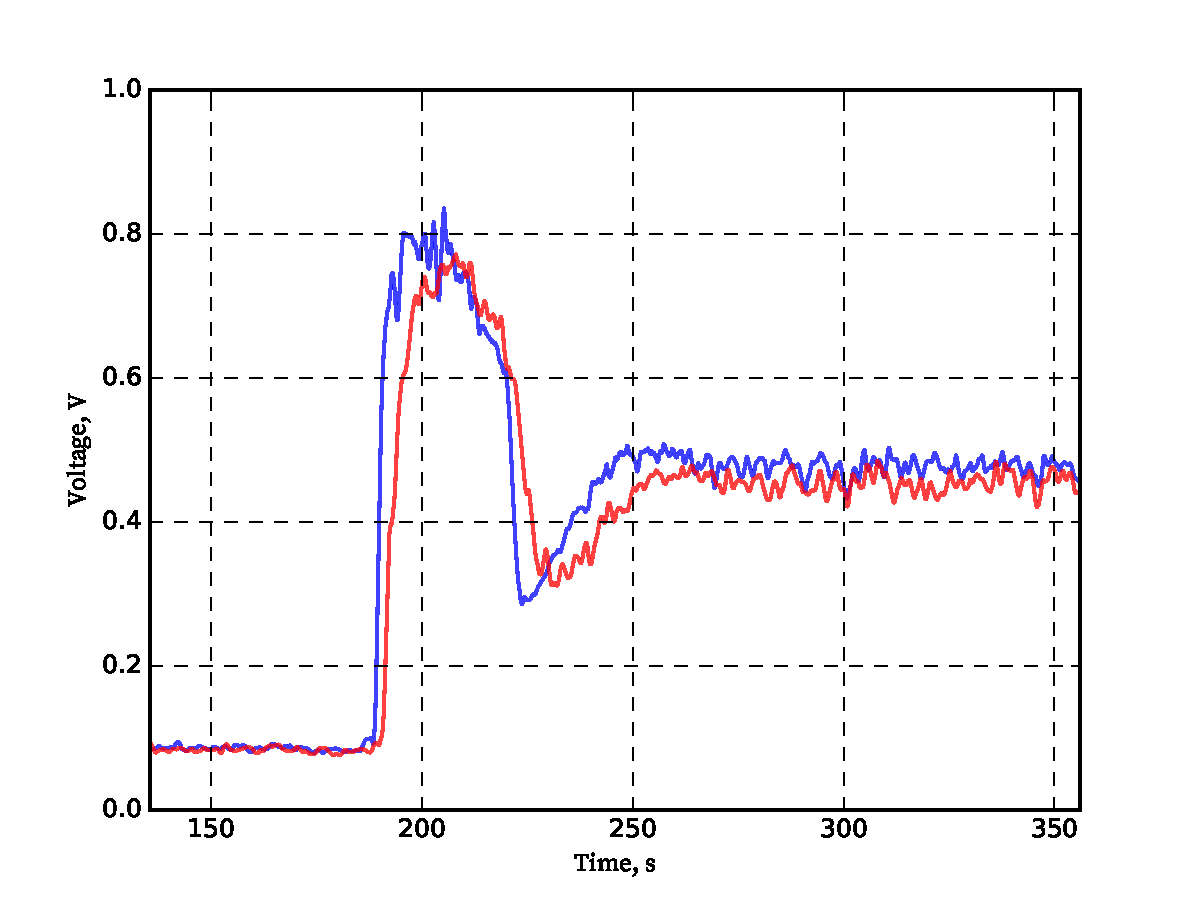
\includegraphics[width=0.8\textwidth]{images/log080716_3.pdf} 
		\caption{3}
		\label{fig:test3}
	\end{center}
\end{figure}

\textbf{Test No. 4}

While maintaining the previous volume and flow rate, this test used the impulse method instead of the feed switch. There were \unit[5]{l} of water with a salinity of \unit[7.7]{\%} added to the return basin.

\begin{figure}
	\begin{center}
		%% This file was created by matplotlib2tikz v0.5.10.
\tikzset{external/export next=false}
\begin{tikzpicture}

\definecolor{color0}{rgb}{0,0.75,0.75}

\begin{axis}[
xlabel={Time, s},
ylabel={relative Voltage, -},
xmin=50.004065, xmax=250.000214,
ymin=0, ymax=0.7,
axis on top,
ytick={0,0.1,0.2,0.3,0.4,0.5,0.6,0.7},
yticklabels={0.0,0.1,0.2,0.3,0.4,0.5,0.6,0.7},
xmajorgrids,
ymajorgrids
]
\addplot [line width=0.7000000000000001pt, color0, opacity=0.75]
table {%
50.678686 0.0821318548091843
50.685528 0.0822257004586548
50.692374 0.0823203881339825
50.699233 0.0824159168478398
50.706055 0.082512285612899
50.712891 0.0826094934418326
50.719724 0.0827075393473132
50.726582 0.082806422342013
50.733477 0.0829061414386045
50.742382 0.0830066956497603
50.749007 0.0831080839881526
50.755601 0.083210305466454
50.762231 0.0833133590973369
50.768842 0.0834172438934736
50.775451 0.0835219588675368
50.782084 0.0836275030321987
50.788712 0.0837338754001319
50.795368 0.0838410749840087
50.802018 0.0839046473602801
50.808657 0.0839677219589049
50.815315 0.084030289893935
50.821982 0.0840923422794223
50.828631 0.0841538702294188
50.835303 0.0842148648579763
50.841991 0.0842753172791469
50.84865 0.0843352186069824
50.855333 0.0843945599555348
50.862001 0.084453332438856
50.868697 0.0845115271709979
50.875386 0.0845691352660124
50.882087 0.0846261478379516
50.888767 0.0846825560008672
50.895476 0.0847383508688113
50.90218 0.0847935235558358
50.908897 0.0848480651759925
50.915595 0.0849019668433335
50.922317 0.0849552196719106
50.92906 0.0850078147757758
50.935759 0.085059743268981
50.942492 0.0851109962655782
50.94922 0.0851615648796192
50.955949 0.085211440225156
50.962668 0.0852606134162405
50.969413 0.0853090755669246
50.976168 0.0853568177912604
50.982918 0.0854271977910825
50.989647 0.0854961320142424
50.996434 0.0855636158532114
51.003189 0.0856296447004609
51.009938 0.0856942139484623
51.016685 0.085757318989687
51.023458 0.0858189552166063
51.030221 0.0858818141664357
51.036997 0.0859431133855466
51.043757 0.0860028487600742
51.050511 0.0860610161761535
51.057298 0.0861176115199197
51.06409 0.086172630677508
51.070861 0.0862260695350536
51.077631 0.0862779239786915
51.084437 0.086328189894557
51.091236 0.0863768631687852
51.098053 0.0864239396875112
51.104847 0.0864694153368702
51.111633 0.0865132860029973
51.11846 0.0865555475720277
51.125293 0.0865961959300966
51.132123 0.0866352269633391
51.138959 0.0866726365578903
51.145767 0.0867084205998855
51.152587 0.0867425749754597
51.159421 0.086775095570748
51.166267 0.0868059782718858
51.17311 0.0868352189650081
51.179964 0.08686281353625
51.186791 0.0868887578717467
51.193649 0.0869130478576334
51.200518 0.0869356793800453
51.207377 0.0869566483251173
51.214246 0.0869759505789849
51.223142 0.0869935820277829
51.22977 0.0870095385576468
51.236371 0.0870238160547114
51.242995 0.0870364104051122
51.249604 0.0870473174949841
51.256242 0.0870565332104623
51.262886 0.0870514714288758
51.269511 0.0870450913181601
51.276168 0.087037386460686
51.282818 0.0870283504388244
51.289462 0.087017976834946
51.296127 0.0870062592314217
51.302801 0.0869913389841132
51.309444 0.0869705132015378
51.31611 0.0869484048804573
51.322795 0.0869250064513605
51.329481 0.086900310344736
51.336163 0.0868743089910725
51.342827 0.0868469948208586
51.349496 0.0868183602645831
51.356186 0.0867883977527346
51.362886 0.0867570997158017
51.369569 0.0867244585842733
51.376282 0.0866904667886379
51.38299 0.0866551167593842
51.389708 0.086618400927001
51.396429 0.0865803117219769
51.403146 0.0865408415748005
51.409867 0.0864999829159606
51.416564 0.0864577281759458
51.423295 0.0864140697852448
51.430025 0.0863690001743463
51.436754 0.086322511773739
51.44347 0.0862745970139115
51.450214 0.0862252483253526
51.456966 0.0861744581385509
51.46372 0.086122218883995
51.470449 0.0860685229921738
51.477203 0.0860133628935758
51.483968 0.0859604354717081
51.490729 0.085906138955619
51.497475 0.0858504664340155
51.504255 0.0857934109956047
51.511025 0.0857349657290935
51.5178 0.0856751237231891
51.524585 0.0856138780665985
51.531345 0.0855512218480288
51.538131 0.085487148156187
51.544927 0.0854216500797801
51.55171 0.0853547207075153
51.558486 0.0852863531280996
51.565291 0.0852165404302401
51.572092 0.0851452757026437
51.578899 0.0850725520340176
51.585696 0.0849983625130688
51.592512 0.0849227002285044
51.599306 0.084851114948559
51.606131 0.0847782084597791
51.612955 0.0847039748381991
51.61979 0.0846284081598537
51.626591 0.0845515025007776
51.633408 0.0844732519370053
51.640249 0.0843936505445714
51.64709 0.0843645547417691
51.653933 0.0843356397844655
51.660784 0.0843069089637526
51.667612 0.0842783655707221
51.67444 0.0842500128964659
51.68131 0.084221854232076
51.688176 0.0841938928686442
51.695045 0.0841661320972624
51.703944 0.0841385752090225
51.710574 0.0841112254950164
51.717179 0.0840840862463358
51.723806 0.0840571607540728
51.730445 0.0840304523093192
51.737055 0.0840039642031668
51.74367 0.0839776997267076
51.750293 0.0839516621710334
51.756947 0.0839258548272361
51.763613 0.0839002809864076
51.770252 0.0838749439396397
51.776915 0.0838498469780244
51.783592 0.0838249933926535
51.790264 0.0838003864746189
51.796934 0.0837760295150125
51.803604 0.0837519258049261
51.810267 0.0837280786354516
51.816949 0.083704491297681
51.823631 0.083681167082706
51.830301 0.0836581092816187
51.836988 0.0836353211855107
51.843733 0.0836128060854741
51.850414 0.0835905672726007
51.85712 0.0835686080379823
51.863827 0.083546931672711
51.870542 0.0835255414678784
51.87723 0.0835044407145766
51.883947 0.0834836327038974
51.890671 0.0834631207269326
51.897372 0.0834429080747742
51.904098 0.083422998038514
51.910825 0.083403393909244
51.917557 0.0833840989780559
51.924299 0.0833651165360416
51.931049 0.0833464498742932
51.937798 0.0833281022839023
51.944546 0.083310077055961
51.951278 0.083292377481561
51.958041 0.0832750068517943
51.964796 0.0832579684577527
51.971544 0.0832412655905282
51.978289 0.0832338886903598
51.985067 0.0832265815613392
51.991835 0.0832193491401042
51.998614 0.0832121963632928
52.005375 0.0832051281675426
52.012134 0.0831981494894915
52.018918 0.0831912652657773
52.02571 0.0831844804330378
52.032483 0.0831777999279109
52.039251 0.0831712286870344
52.046053 0.083164771647046
52.05286 0.0831584337445837
52.05967 0.0831522199162851
52.066463 0.0831461350987883
52.073253 0.0831401842287308
52.080071 0.0831343722427507
52.086896 0.0831287040774856
52.093719 0.0831231846695734
52.100547 0.083117818955652
52.107359 0.0831126118723591
52.114171 0.0831075683563325
52.121033 0.0831026933442102
52.127871 0.0830979917726298
52.134719 0.0830934685782293
52.141571 0.0830891286976464
52.148401 0.0830849770675189
52.155235 0.0830810186244847
52.1621 0.0830772583051816
52.168971 0.0830737010462475
52.175836 0.08307035178432
52.184743 0.0830672154560371
52.191373 0.0830642969980365
52.197977 0.0830616013469561
52.204607 0.0830591334394337
52.211221 0.0830568982121071
52.21786 0.0830549006016141
52.224492 0.0830531455445926
52.231111 0.0830264739600681
52.23776 0.0830008173482788
52.244422 0.0829761760383341
52.251063 0.082952550359343
52.25774 0.0829299406404149
52.264415 0.0829083472106589
52.271067 0.0828877703991841
52.27774 0.0828682105350998
52.284408 0.0828496679475152
52.291067 0.0828321429655394
52.297747 0.0828156359182816
52.304436 0.082800147134851
52.311109 0.0827856769443568
52.317802 0.0827555556373252
52.324489 0.0827259574493476
52.331164 0.0826968797475506
52.337877 0.0826683198990607
52.34459 0.0826402752710044
52.351309 0.0826127432305082
52.358002 0.0825857211446985
52.364721 0.0825592063807019
52.37145 0.0825331963056449
52.378158 0.0825076882866539
52.384911 0.0824826796908556
52.391638 0.0824581678853762
52.398365 0.0824341502373425
52.405086 0.0824106241138808
52.411831 0.0823875868821177
52.418579 0.0823650359091796
52.425336 0.082342968562193
52.432065 0.0823213822082845
52.438812 0.0823002742145805
52.445579 0.0822796419482076
52.452341 0.0822594827762922
52.459087 0.0822397940659609
52.465864 0.0822205731843401
52.472635 0.0822018174985563
52.479407 0.082183524375736
52.486164 0.0821656911830058
52.492925 0.0821483152874921
52.499713 0.0821313940563214
52.506502 0.0821149248566202
52.513277 0.082098905055515
52.520088 0.0820833320201323
52.526887 0.0820682031175987
52.533695 0.0820535157150405
52.540505 0.0820392671795844
52.547304 0.0820254548783567
52.5541 0.0820120761784841
52.560923 0.0819991284470929
52.567747 0.0819940179573466
52.57457 0.0819895536734907
52.581403 0.0819857342790884
52.588235 0.0819825584577029
52.595039 0.0819800248928975
52.601886 0.0819781322682355
52.608729 0.0819768792672801
52.615576 0.0819762645735945
52.62243 0.0819762868707419
52.629258 0.0819769448422858
52.636087 0.0819782371717891
52.642916 0.0819801625428154
52.649807 0.0819827196389277
52.656669 0.0819859071436893
52.665583 0.0819897237406636
52.672221 0.0819941681134136
52.678814 0.0819992389455027
52.685447 0.0820049349204942
52.692089 0.0820112547219512
52.698696 0.082018197033437
52.705345 0.082025760538515
52.711963 0.0820339439207482
52.718646 0.0820427458637
52.725296 0.0820521650509336
52.731936 0.0820622001660123
52.738596 0.0820728498924993
52.745255 0.0820841129139578
52.751909 0.0820959879139512
52.758579 0.0821084735760426
52.765246 0.0821215685837954
52.771902 0.0821352716207727
52.778582 0.0821495813705378
52.785264 0.0821644965166539
52.791936 0.0821800157426844
52.798632 0.0821961377321924
52.805334 0.0822128611687412
52.812007 0.082230184735894
52.818688 0.0822481071172142
52.8254 0.0822666269962648
52.832122 0.0822857430566093
52.838811 0.0823054539818109
52.845527 0.0823257584554327
52.852247 0.082346655161038
52.858953 0.0823681427821902
52.86569 0.0823902200024524
52.872417 0.0824128855053878
52.879158 0.0824361379745598
52.885874 0.0824599760935316
52.892615 0.0824843985458664
52.899364 0.0825228847388484
52.906119 0.0825615441255405
52.912846 0.0826003778578249
52.919607 0.0826393870875837
52.926371 0.082678572966699
52.933139 0.0827179366470531
52.939887 0.0827574792805281
52.946663 0.0827972020190062
52.953434 0.0828371060143694
52.960211 0.0828771924185
52.966965 0.0829174623832802
52.973718 0.082957917060592
52.980536 0.0829985576023177
52.987335 0.0830393851603394
52.99412 0.0830804008865392
53.000899 0.0831216059327993
53.007699 0.0831630014510019
53.014503 0.0832045885930291
53.021314 0.0832463685107632
53.028107 0.0832883423560861
53.034904 0.0833305112808801
53.041729 0.0833719777221127
53.048583 0.083413668780366
53.05541 0.0834555854429676
53.062243 0.083497728697245
53.069053 0.0835400995305258
53.075861 0.0835826989301375
53.082711 0.0836255278834078
53.089561 0.0836685873776642
53.096405 0.0837118784002343
53.103262 0.0837554019384455
53.11009 0.0837991589796255
53.116952 0.0838431505111019
53.12379 0.0838873775202022
53.130662 0.0839318409942539
53.137532 0.0839765419205847
53.146437 0.0840214812865221
53.153051 0.0840666600793937
53.159658 0.0841120792865269
53.166292 0.0841577398952495
53.172931 0.0842036428928889
53.179549 0.0842497892667728
53.186183 0.0842961800042286
53.192805 0.084342816092584
53.199462 0.0843896985191664
53.206113 0.0844368282713036
53.212753 0.0844842063363229
53.219418 0.0845318337015521
53.226077 0.0845797113543187
53.23273 0.0846278402819501
53.239406 0.084652142527154
53.246105 0.0846759813866215
53.252765 0.0846993535692606
53.259449 0.0847222557839794
53.266143 0.0847446847396861
53.272813 0.0847666371452888
53.279492 0.0847881097096956
53.286191 0.0848063208020508
53.292871 0.0848239627823429
53.299543 0.0848410318658162
53.306245 0.0848575242677151
53.312964 0.084873436203284
53.31966 0.0848887638877671
53.326373 0.0849035035364089
53.333094 0.0849176513644535
53.339793 0.0849312035871455
53.346503 0.0849441564197291
53.35323 0.0849565060774486
53.359965 0.0849682487755485
53.366683 0.084979380729273
53.373436 0.0849898981538665
53.380181 0.0849997972645733
53.386934 0.0850090742766377
53.393668 0.0850177254053042
53.400428 0.085025746865817
53.407189 0.0850331348734205
53.413943 0.085039885643359
53.420689 0.0850459953908769
53.427466 0.0850514603312185
53.434234 0.0850562766796281
53.441009 0.0850604406513501
53.447795 0.0850639484616288
53.454553 0.0850667963257085
53.461341 0.0850689804588337
53.468138 0.0850704970762487
53.474923 0.0850713423931976
53.481704 0.0850715126249251
53.488503 0.0850710039866752
53.495307 0.0850698126936925
53.502123 0.0850679349612212
53.508918 0.0850653670045057
53.515711 0.0850750706243549
53.522513 0.0850844623309714
53.529329 0.0850935406433637
53.536151 0.0851023040805405
53.542986 0.0851107511615105
53.549791 0.0851188804052823
53.556607 0.0851266903308646
53.563445 0.0851388100235392
53.570288 0.0851507452505139
53.577156 0.0851624953535705
53.584013 0.0851740596744905
53.590841 0.0851854375550556
53.597669 0.0851966283370475
53.604536 0.0852076313622476
53.611398 0.0852184459724377
53.618264 0.0852290715093994
53.62716 0.0852395073149143
53.633787 0.085249752730764
53.640387 0.0852598070987302
53.647036 0.0852696697605945
53.653649 0.0852793400581384
53.660287 0.0852888173331437
53.666928 0.0852981009273919
53.673555 0.0853071901826647
53.680214 0.0853160844407437
53.686848 0.0853247830434105
53.693489 0.0853332853324468
53.700148 0.0853415906496341
53.706818 0.0853496983367541
53.713487 0.0853719871742241
53.720156 0.0853936413246253
53.72682 0.0854146627626129
53.733485 0.0854350534628419
53.740168 0.0854548153999675
53.746843 0.0854739505486449
53.753512 0.0854924608835292
53.7602 0.0855103483792754
53.766901 0.0855276150105388
53.77358 0.0855442627519743
53.780294 0.0855602935782373
53.786999 0.0855757094639828
53.793715 0.0855905123838659
53.800414 0.0856047043125417
53.807134 0.0856182872246654
53.813857 0.0856312630948922
53.820562 0.085643633897877
53.8273 0.0856554016082752
53.834031 0.0856665682007417
53.840768 0.0856771356499317
53.847486 0.0856871059305004
53.854231 0.0856964810171028
53.860985 0.0857052628843942
53.867742 0.0857134535070296
53.874468 0.0857210548596641
53.881228 0.0857280689169529
53.888026 0.0857344976535511
53.894783 0.0857403430441138
53.901531 0.0857456070632962
53.90833 0.0857502916857534
53.9151 0.0857543988861405
53.921885 0.0857579306391126
53.928644 0.0857608889193249
53.935404 0.0857632757014325
53.942188 0.0857650929600906
53.94898 0.0857663426699541
53.955757 0.0857670268056784
53.962538 0.0857671473419184
53.969309 0.0857667062533294
53.976132 0.0857657055145665
53.982945 0.0857641471002847
53.989743 0.0857620329851392
53.996537 0.0857593651437852
54.003334 0.0857561455508777
54.010159 0.0857523761810719
54.016981 0.085748059009023
54.02382 0.085743196009386
54.030626 0.0857377891568161
54.037442 0.0857318404259684
54.04429 0.085725351791498
54.051132 0.08571832522806
54.057975 0.0857107627103097
54.064828 0.0857026662129021
54.071651 0.0856940377104922
54.078483 0.0856848791777354
54.085324 0.0856751925892866
54.092191 0.0856649799198011
54.099058 0.0856542431439339
54.107985 0.0856429842363402
54.114616 0.0856312051716751
54.121209 0.0856189079245937
54.127833 0.0856060944697512
54.134443 0.0855927667818027
54.141076 0.0855789268354032
54.147706 0.085564576605208
54.154331 0.0855497180658722
54.160986 0.0855343531920508
54.167637 0.0855184839583991
54.174308 0.0855021123395721
54.180968 0.085485240310225
54.187629 0.0854678698450129
54.194277 0.0854500029185909
54.20095 0.0854316415056142
54.207619 0.0854127875807378
54.214282 0.085393443118617
54.220966 0.0853736100939067
54.227647 0.0853532904812623
54.234319 0.0853232251227926
54.241031 0.085292401496754
54.247729 0.0852608199322559
54.254407 0.0852284807584073
54.261119 0.0851953843043175
54.267824 0.0851615308990956
54.274537 0.0851269208718508
54.281227 0.0850915545516923
54.287945 0.0850554322677294
54.294668 0.0850185543490711
54.301373 0.0849809211248267
54.308126 0.0849425329241055
54.314854 0.0849033900760164
54.321577 0.0848634929096688
54.328298 0.0848228417541718
54.335047 0.0847814369386346
54.341796 0.0847392787921665
54.348554 0.0846963676438765
54.355279 0.0846527038228739
54.362042 0.084608287658268
54.368803 0.0845631194791677
54.375556 0.0845171996146824
54.382304 0.0844741232535802
54.389081 0.08443018693017
54.395848 0.0843853916317796
54.402619 0.0843397383457365
54.40938 0.0842932280593682
54.416143 0.0842458617600023
54.422925 0.0841976404349663
54.429723 0.0841485650715879
54.436525 0.0840986366571946
54.443303 0.0840478561791139
54.450104 0.0839962246246734
54.456908 0.0839437429812007
54.463717 0.0838904122360234
54.470516 0.0838362333764689
54.47731 0.083781207389865
54.484134 0.0837512664346683
54.490957 0.0837320366670994
54.497781 0.0837124122976143
54.504619 0.0836924008957242
54.511425 0.0836720100309406
54.51824 0.0836512472727747
54.525084 0.0836301201907378
54.531926 0.0836086363543413
54.538779 0.0835868033330966
54.54563 0.0835646286965148
54.552454 0.0835421200141073
54.559288 0.0835192848553855
54.56613 0.0834961307898607
54.57302 0.0834726653870441
54.579884 0.0834488962164472
54.588793 0.0834248308475812
54.595425 0.0834004768499575
54.602023 0.0833758417930873
54.60865 0.083350933246482
54.615261 0.083325758779653
54.621898 0.0833003259621115
54.628533 0.0832746423633688
54.635156 0.0832487155529363
54.641804 0.0832225531003253
54.648446 0.0831961625750472
54.655089 0.0831695515466131
54.661755 0.0831481198740229
54.66843 0.0831263194345877
54.675081 0.0831041587851464
54.681756 0.0830816464825379
54.688424 0.083058791083601
54.695084 0.0830356011451747
54.701791 0.0830120852240979
54.708476 0.0829846570175504
54.715148 0.0829570288771713
54.721843 0.0829292087015811
54.728541 0.0829012043894003
54.735224 0.0828730238392494
54.741904 0.0828446749497489
54.748614 0.0828161656195194
54.755332 0.0827875037471812
54.762025 0.0827586972313551
54.76876 0.0827297539706613
54.775492 0.0827006818637206
54.782195 0.0826714888091532
54.788899 0.0826421827055799
54.795629 0.082612771451621
54.802372 0.0825832629458971
54.809088 0.0825536650870288
54.815822 0.0825239857736364
54.822572 0.0824942329043405
54.829331 0.0824644143777617
54.836082 0.0824345380925204
54.842843 0.0824046119472371
54.849606 0.0823746438405324
54.85636 0.0823446416710268
54.863104 0.0823146133373407
54.869879 0.0822845667380946
54.876652 0.0822545097719092
54.883425 0.0822244503374048
54.890183 0.0821943963332021
54.896945 0.0821643556579215
54.903732 0.0821343362101835
54.910521 0.0821043458886086
54.917298 0.0820743925918173
54.92407 0.0820444842184302
54.930873 0.0820146286670678
54.937684 0.0819848338363504
54.944495 0.0819551076248988
54.951288 0.0819254579313333
54.95808 0.0818958926542745
54.964892 0.081866419692343
54.971717 0.0818370469441591
54.97854 0.0818077823083434
54.985366 0.0817786336835164
54.992177 0.0817496089682987
54.998983 0.0817207160613107
55.005826 0.0816919628611729
55.012667 0.0816633572665059
55.019513 0.0816349071759302
55.02637 0.0816066204880662
55.033225 0.0815785051015345
55.040057 0.0815505689149556
55.046919 0.08152281982695
55.053793 0.0814952657361382
55.060654 0.0814679145411406
55.06956 0.081440774140578
55.076192 0.0814138524330706
55.082797 0.0813871573172391
55.089429 0.0813606966917039
55.096046 0.0813344784550856
55.102708 0.0813085105060046
55.109347 0.0812828007430815
55.115966 0.0812573570649368
55.122616 0.0812321873701909
55.129255 0.0812072995574645
55.135894 0.081182701525378
55.142559 0.0811584011725519
55.149234 0.0811344063976066
55.155886 0.0810968334003436
55.162562 0.0810591683347853
55.169233 0.0810214166312333
55.175889 0.0809835837199892
55.182567 0.0809456750313546
55.189255 0.0809076959956311
55.195927 0.0808696520431203
55.202619 0.0808315486041238
55.209315 0.0807933911089432
55.215988 0.08075518498788
55.222697 0.080716935671236
55.229409 0.0806786485893126
55.236128 0.0806403291724116
55.24282 0.0806019828508344
55.249536 0.0805636150548828
55.256259 0.0805252312148582
55.262968 0.0804868367610623
55.269706 0.0804484371237967
55.276433 0.0804100377333631
55.283173 0.0803716440200628
55.289889 0.0803332614141977
55.296659 0.0802958214593239
55.303401 0.0802584310353829
55.310159 0.0802210957372308
55.316887 0.0801838211597239
55.323651 0.0801466128977183
55.330408 0.0801094765460703
55.337164 0.080072417699636
55.343909 0.0800354419532717
55.350684 0.0799985549018335
55.357455 0.0799617621401776
55.364232 0.0799250692631602
55.370984 0.0798884818656375
55.377743 0.0798672836960161
55.384531 0.0798457392212518
55.391319 0.0798238568336288
55.398093 0.0798016449254315
55.404866 0.0797791118889441
55.411665 0.079756266116451
55.418472 0.0797331160002364
55.425287 0.0797096699325847
55.432103 0.07968593630578
55.438893 0.0796619235121068
55.445716 0.0796376399438492
55.452537 0.0796130939932917
55.459359 0.0795882940527184
55.466189 0.0795290973476541
55.473001 0.0794706983209838
55.479816 0.0794130991119173
55.486651 0.0793563018596643
55.493495 0.0793003087034345
55.500341 0.0792451217824377
55.507201 0.0791907432358835
55.514022 0.0791371752029817
55.520856 0.0790844198229421
55.527723 0.0790324792349742
55.534596 0.0789813555782879
55.54146 0.0789310509920928
55.550366 0.0788815676155988
55.556994 0.0788329075880154
55.563599 0.0787850730485525
55.570231 0.0787380661364197
55.576845 0.0786918889908268
55.583486 0.0786465437509835
55.59012 0.0786020325560995
55.596747 0.0785583575453845
55.6034 0.0785155208580483
55.610049 0.0784735246333006
55.616684 0.0784323710103511
55.62334 0.0783920621284095
55.630012 0.0783526001266855
55.63666 0.0783139871443889
55.643332 0.0782762253207294
55.650018 0.0782393167949166
55.656672 0.0782032637061604
55.663354 0.0781680681936705
55.670026 0.0781337323966565
55.676697 0.0781002584543282
55.683388 0.0780676485058953
55.690092 0.0780359046905676
55.696796 0.0780050291475546
55.703505 0.0779750240160663
55.710214 0.0779458914353122
55.716932 0.0779176335445022
55.72363 0.0778902524828459
55.730349 0.077863750389553
55.737073 0.0778381294038334
55.743782 0.0778133916648966
55.750519 0.0777895393119524
55.757246 0.0777665744842106
55.763984 0.0777444993208808
55.770708 0.0777233159611728
55.77746 0.0777030265442964
55.784206 0.0776836332094611
55.790959 0.0776651380958768
55.797688 0.0776475433427532
55.804448 0.0776308510892999
55.811205 0.0776150634747268
55.817961 0.0776001826382435
55.82471 0.0775862107190597
55.831486 0.0775731498563852
55.838255 0.0775610021894297
55.845033 0.0775497698574029
55.85179 0.0775394549995145
55.858546 0.0775300597549744
55.865335 0.077521586262992
55.872123 0.0775140366627773
55.878897 0.0775074130935399
55.885673 0.0775017176944895
55.892497 0.0774969526048359
55.8993 0.0774931199637887
55.906116 0.0774902219105578
55.9129 0.0774882605843528
55.919697 0.0774872381243835
55.926521 0.0774871566698595
55.93339 0.0774880183599906
55.940213 0.0774898253339865
55.947043 0.0774925797310569
55.953855 0.0774962836904116
55.960692 0.0775009393512602
55.967534 0.0774917310407388
55.974384 0.0774830377038189
55.981226 0.077474858846837
55.988087 0.0774671939761293
55.994909 0.0774600425980318
56.001744 0.077453404218881
56.008582 0.0774472783450129
56.015444 0.0774416644827638
56.02231 0.07743656213847
56.031208 0.0774319708184675
56.037838 0.0774278900290928
56.044434 0.0774243192766819
56.051062 0.0774212580675711
56.057674 0.0774187059080966
56.064287 0.0774166623045946
56.070921 0.0774151267634014
56.077548 0.0774140987908531
56.084206 0.0774135778932861
56.090854 0.0774135635770364
56.097519 0.0774140553484403
56.104179 0.0774150527138341
56.110841 0.077416555179554
56.117491 0.0774185622519361
56.124169 0.0774210734373167
56.130838 0.0774204933823731
56.137502 0.0774205253882416
56.144181 0.0774211683030401
56.150861 0.0774224209748863
56.157557 0.0774242822518982
56.164256 0.0774267509821936
56.170964 0.0774298260138903
56.177644 0.0774335061951062
56.184324 0.077437790373959
56.19103 0.0774426773985667
56.19775 0.0774481661170471
56.204444 0.0774542553775181
56.211163 0.0774609440280974
56.21788 0.0774682309169029
56.224609 0.0774761148920525
56.231319 0.077484594801664
56.238047 0.0774936694938552
56.244786 0.077503337816744
56.251503 0.0775135986184483
56.258249 0.0775244507470858
56.265002 0.0775358930507745
56.271754 0.0775479243776321
56.278484 0.0775605435757765
56.285248 0.0775737494933255
56.292005 0.077587540978397
56.298765 0.0776019168791089
56.305512 0.0776168760435789
56.312292 0.0776324173199249
56.319056 0.0776485395562648
56.325833 0.0776652416007164
56.332592 0.0776825223013975
56.339343 0.077700380506426
56.346132 0.0777188150639198
56.352926 0.0777378248219966
56.359722 0.0777574086287743
56.366495 0.0777775653323708
56.373298 0.0777982937809039
56.380097 0.0778195928224914
56.386912 0.0778414613052512
56.393699 0.0778638980773011
56.400486 0.0778869019867589
56.407308 0.0779104718817426
56.414128 0.07793460661037
56.420978 0.0779593050207588
56.427814 0.0779845659610269
56.43462 0.0780103882792923
56.441441 0.0780367708236726
56.448283 0.0780637124422859
56.455126 0.0780912119832498
56.461966 0.0781192682946823
56.468821 0.0781478802247012
56.475649 0.0781770466214243
56.482477 0.0782067663329695
56.489375 0.0782370382074546
56.49623 0.0782678610929974
56.503102 0.0782992338377159
56.512 0.0783311552897278
56.518632 0.078363624297151
56.525227 0.0783966397081034
56.53185 0.0784302003707027
56.538461 0.0784643051330668
56.545098 0.0784989528433135
56.551731 0.0785341423495608
56.558384 0.0785698724999264
56.565045 0.0786061421425283
56.571689 0.0786429501254841
56.578332 0.0786802952969118
56.58499 0.0787181765049292
56.591648 0.0787565925976542
56.598296 0.0787955424232046
56.604972 0.0788350248296982
56.611641 0.0788750386652529
56.618303 0.0789155827779865
56.625004 0.0789566560160169
56.631686 0.0789982572274619
56.638353 0.0790366808074209
56.645049 0.0790755198054523
56.651751 0.0791147724114555
56.658433 0.07915443681533
56.665119 0.0791945112069753
56.671826 0.0792349937762908
56.678545 0.079275882713176
56.685243 0.0793171762075304
56.691964 0.0793588724492534
56.698684 0.0794009696282444
56.705384 0.0794434659344031
56.712117 0.0794863595576288
56.718847 0.079529648687821
56.725589 0.0795733315148792
56.732306 0.0796174062287028
56.739045 0.0796618710191913
56.745798 0.0796956107171888
56.752553 0.0797294061169164
56.759276 0.0797632534336183
56.766033 0.0797971488825389
56.772799 0.0798310886789226
56.779565 0.0798650690380137
56.786313 0.0798990861750566
56.793094 0.0799331363052956
56.799862 0.0799878860870136
56.806635 0.0800420349153547
56.813394 0.0800955827903187
56.820175 0.0801485297119057
56.826962 0.0802008756801157
56.833763 0.0802526206949487
56.840549 0.0803037647564046
56.847325 0.0803543078644836
56.854131 0.0804042500191855
56.860933 0.0804535912205104
56.86774 0.0805023314684583
56.874538 0.0805504707630292
56.881329 0.080598009104223
56.888185 0.0806449464920399
56.895006 0.0806912829264797
56.901822 0.0807370184075425
56.90866 0.0807821529352283
56.91546 0.0808211298300094
56.922274 0.0808593403940465
56.929115 0.0808967836400122
56.935956 0.0809334585805789
56.942803 0.0809693642284189
56.949657 0.0810044995962048
56.956504 0.0810388636966089
56.963333 0.0810761599953223
56.97017 0.0811127933035767
56.977028 0.0811487632922629
56.983898 0.0811840696322719
56.992806 0.0812187119944944
56.99944 0.0812526900498211
57.006034 0.0812860034691431
57.012663 0.081318651923351
57.019302 0.0813506350833356
57.025907 0.0813819526199878
57.032538 0.0814126042041984
57.039162 0.0814425895068581
57.045819 0.0814719081988579
57.052464 0.0815005599510885
57.059107 0.0815285444344408
57.065775 0.0815558613198054
57.072449 0.0815825102780734
57.079097 0.0816084909801354
57.085784 0.0816338030968822
57.092446 0.0816584462992048
57.099109 0.0816824202579939
57.10579 0.0817057246441403
57.11247 0.0817283591285348
57.119138 0.0817503233820682
57.125826 0.0817716170756314
57.132527 0.0817922398801152
57.139205 0.0818121914664103
57.145917 0.0818314715054077
57.152631 0.081850079667998
57.159351 0.0818680156250721
57.166044 0.0818852790475209
57.172766 0.0819018696062351
57.179491 0.0819177869721056
57.186195 0.0819330308160231
57.192926 0.0819476008088785
57.199652 0.0819614966215625
57.206394 0.0819747179249661
57.213111 0.08198726438998
57.219884 0.081999135687495
57.226635 0.0820103314884019
57.233382 0.0820208514635916
57.240113 0.082033391428699
57.246873 0.082045173208515
57.253631 0.0820561969675939
57.26038 0.0820664628704906
57.267121 0.0820759710817595
57.273901 0.0820847217659553
57.28067 0.0820927150876326
57.287447 0.0820999512113459
57.294207 0.0821064303016498
57.300966 0.082112152523099
57.307751 0.082117118040248
57.314539 0.0821213270176515
57.321318 0.0821247796198639
57.328088 0.08212747601144
57.334888 0.0821294163569343
57.341697 0.0821306008209013
57.348531 0.0821310295678958
57.35532 0.0821307027624723
57.362108 0.0821296205691853
57.368933 0.0821277831525896
57.375761 0.0821251906772396
57.382587 0.0821218433076899
57.389426 0.0821177412084952
57.396231 0.0821128845442101
57.403046 0.0821072734793891
57.409891 0.0821009081785869
57.416756 0.082093788806358
57.423604 0.082085915527257
57.430459 0.0820772885058385
57.437284 0.0820679079066572
57.444113 0.0820577738942675
57.450951 0.0820468866332242
57.457819 0.0820352462880818
57.464687 0.0820228530233948
57.473587 0.082009707003718
57.480219 0.0819958083936058
57.486843 0.0819811573576129
57.493473 0.0819675514901233
57.500089 0.0819531390582916
57.506698 0.0819379205557816
57.513328 0.081921896476257
57.51995 0.0818933840194901
57.526599 0.0818644210122451
57.533261 0.081835005808976
57.539899 0.0818051367641368
57.546561 0.0817748122321817
57.553237 0.0817440305675646
57.559883 0.0817127901247396
57.566553 0.0816810892581609
57.573235 0.0816489263222824
57.579889 0.0816162996715582
57.586572 0.0815832076604424
57.593248 0.081549648643389
57.599923 0.0815156209748522
57.606616 0.0814811230092859
57.613331 0.0814461531011442
57.620007 0.0814107096048812
57.62672 0.0813747908749509
57.633435 0.081322651340479
57.640156 0.0812695647120418
57.646845 0.0812155265466651
57.653565 0.0811605324013751
57.66029 0.0811045778331976
57.666996 0.0810476583991586
57.67373 0.0809897696562841
57.68048 0.0809309071616
57.687204 0.0808710664721324
57.693925 0.0808102431449071
57.700671 0.0807484327369502
57.707419 0.0806856308052875
57.714175 0.0806218329069451
57.720904 0.0805922269026244
57.727666 0.0805626634356661
57.734425 0.0805331443161709
57.741182 0.0805036713542393
57.747952 0.0804742463599719
57.754722 0.0804448711434691
57.761498 0.0804155475148315
57.768279 0.0803862772841596
57.775033 0.080357062261554
57.781791 0.0803279042571152
57.788584 0.0802988050809437
57.795374 0.0802697665431401
57.802157 0.0802407904538049
57.808932 0.0802118786230386
57.815766 0.0801830328609417
57.822574 0.0801542549776149
57.829381 0.0801255467831585
57.836174 0.0800969100876733
57.842968 0.0800683467012596
57.849758 0.0800398584340181
57.856581 0.0800114470960492
57.863406 0.0799831144974535
57.870237 0.0799548624483316
57.877068 0.0799266927587839
57.883875 0.079898607238911
57.890723 0.0798706076988134
57.897565 0.0798426959485917
57.904414 0.0798148737983464
57.911272 0.079787143058178
57.918098 0.079759505538187
57.924927 0.0797319630484741
57.931758 0.0797045173991397
57.938625 0.0796771704002843
57.945516 0.0796499238620085
57.954419 0.0796227795944129
57.961054 0.0795957394075979
57.96765 0.0795688051116641
57.974281 0.079541978516712
57.980968 0.0795152614328422
57.987585 0.0794886556701552
57.994223 0.0794621630387515
58.00084 0.0794357853487316
58.007494 0.0794095244101962
58.014138 0.0793833820332457
58.020777 0.0793573600279806
58.027437 0.0793314602045015
58.034093 0.0793056843729089
58.040749 0.0792800343433034
58.04742 0.0792545119257855
58.054085 0.0792291189304557
58.060741 0.0792038571674146
58.067422 0.0791787284467626
58.074102 0.0791537345786004
58.080799 0.0791288773730285
58.087496 0.0791041586401473
58.094197 0.0790795801900574
58.100874 0.0790551438328594
58.107551 0.0790308513786538
58.114262 0.0790067046375411
58.120984 0.0789827054196219
58.127673 0.0789588555349966
58.134389 0.0789351567937659
58.141114 0.0789116110060303
58.147842 0.0788882199818902
58.154543 0.0788649855314462
58.161267 0.0788419094647989
58.168001 0.0788189935920487
58.174724 0.0787962397232963
58.181475 0.0787736496686422
58.188221 0.0787548200978457
58.194975 0.0787360490262074
58.201707 0.0787173389220461
58.208491 0.0786986922536808
58.215244 0.0786801114894304
58.221992 0.0786615990976137
58.228738 0.0786431575465498
58.23551 0.0786247893045574
58.242276 0.0786064968399555
58.249061 0.078588282621063
58.255814 0.0785701491161988
58.262571 0.0785520987936819
58.269365 0.0785341341218311
58.276156 0.0785162575689654
58.282928 0.0784984716034036
58.2897 0.0784807786934647
58.296503 0.0784631813074676
58.303307 0.0784456819137311
58.310121 0.0784282829805742
58.316909 0.0784109869763159
58.323701 0.0783937963692749
58.330521 0.0783767136277703
58.337342 0.0783597412201208
58.344171 0.0783428816146456
58.350995 0.0783261372796633
58.357807 0.078309510683493
58.364624 0.0782930042944536
58.371461 0.078276620580864
58.378307 0.078260362011043
58.385149 0.0782479355063281
58.392007 0.0782357493335976
58.398831 0.0782238066193889
58.40567 0.0782121104902391
58.41256 0.0782006640726856
58.419426 0.0781894704932657
58.426293 0.0781785328785166
58.435191 0.0781678543549757
58.441818 0.0781574380491802
58.448422 0.0781472870876674
58.45505 0.0781374045969746
58.461665 0.078127793703639
58.468304 0.078118457534198
58.474967 0.0781093992151889
58.481595 0.0781006218731489
58.48826 0.0780921286346153
58.494905 0.0780839226261254
58.501542 0.0780760069742165
58.508198 0.0780683848054258
58.51486 0.0780610592462907
58.521513 0.0780540334233485
58.52819 0.0780473104631363
58.534857 0.0780408934921916
58.541546 0.0780347856370515
58.548224 0.0780289900242535
58.554901 0.0780235097803347
58.561572 0.0780183480318324
58.56827 0.0780135079052839
58.574971 0.0780089925272266
58.581651 0.0780048050241977
58.58833 0.0780009485227345
58.595039 0.0779974261493742
58.601762 0.0779942410306541
58.608481 0.0779913962931116
58.615197 0.077988895063284
58.621916 0.0779867404677084
58.628618 0.0779849356329222
58.635351 0.0779834836854627
58.642077 0.0779823877518672
58.648805 0.0779816509586728
58.655523 0.0779812764324171
58.662269 0.0779857608742107
58.669027 0.077990477667091
58.675777 0.0779954307603682
58.68251 0.0780006241033525
58.689269 0.0780060616453542
58.696031 0.0780117473356835
58.702786 0.0780176851236508
58.709534 0.0780238789585661
58.716312 0.0780303327897399
58.723079 0.0780370505664823
58.729855 0.0780440362381037
58.736615 0.0780512937539142
58.743395 0.0780588270632241
58.750185 0.0780666401153437
58.75698 0.0780747368595832
58.763764 0.0780831212452529
58.770543 0.0780917972216631
58.777347 0.0781007687381239
58.784153 0.0781100397439457
58.790965 0.0781196141884387
58.79776 0.0781294960209132
58.804577 0.0781396891906793
58.811373 0.0781501976470474
58.81819 0.0781610253393277
58.825016 0.0781721762168305
58.831849 0.0781836542288661
58.838652 0.0781954633247446
58.845469 0.0782076074537763
58.852303 0.0782200905652715
58.859148 0.0782329166085405
58.865987 0.0782460895328934
58.872842 0.0782596132876406
58.879665 0.0782734918220924
58.886493 0.0782877290855588
58.893363 0.0783023290273503
58.900225 0.0783172955967771
58.907092 0.0783326327431493
58.915979 0.0783483444157774
58.922611 0.0783644345639714
58.929215 0.0783809071370418
58.935837 0.0783977660842987
58.942467 0.0784150153550524
58.949103 0.0784326588986131
58.955739 0.0784507006642912
58.962367 0.0784691446013968
58.969025 0.0784879946592402
58.975676 0.0785072547871317
58.982317 0.0785269289343814
58.988976 0.0785470210502998
58.995646 0.078567535084197
59.002292 0.0785884749853833
59.008959 0.0786098447031689
59.015644 0.078631648186864
59.022303 0.0786538893857791
59.028989 0.0786765722492242
59.035663 0.0786997007265097
59.042328 0.0787232787669458
59.049018 0.0787473103198427
59.05572 0.0787540935893135
59.062406 0.0787605953881514
59.069144 0.0787668165391294
59.075849 0.0787727578650204
59.082566 0.0787784201885974
59.089261 0.0787838043326333
59.095985 0.0787889111199012
59.102707 0.078793741373174
59.10941 0.0787982959152247
59.116143 0.0788025755688262
59.122873 0.0788065811567516
59.129609 0.0788103135017737
59.136351 0.0788137734266656
59.143102 0.0788169617542002
59.149851 0.0788198793071505
59.156598 0.0788225269082895
59.163331 0.0788249053803901
59.170098 0.0788270155462253
59.176852 0.0788288582285681
59.183597 0.0788304342501914
59.190345 0.0788317444338683
59.197122 0.0788327896023716
59.203887 0.0788335705784744
59.21067 0.0788340881849496
59.21743 0.0788343432445701
59.224187 0.0788343365801091
59.230976 0.0788340690143394
59.237769 0.0788263516507161
59.244562 0.0788185929016125
59.25134 0.0788107922733648
59.258147 0.0788029492723091
59.264947 0.0787950634047816
59.271755 0.0787871341771187
59.278554 0.0787791610956565
59.285343 0.0787711436667313
59.29217 0.0787630813966792
59.298988 0.0787549737918364
59.305811 0.0787468203585393
59.312648 0.078738620603124
59.319448 0.0787303740319267
59.326266 0.0787220801512836
59.333107 0.078713738467531
59.33995 0.0787053484870051
59.346792 0.0786969097160421
59.353647 0.0786884216609782
59.360474 0.0786798838281497
59.367299 0.0786712957238927
59.374168 0.0786626568545435
59.381036 0.0786539667264382
59.387904 0.0786452248459132
59.396802 0.0786364307193046
59.403436 0.0786275838529487
59.410034 0.0786186837531816
59.41666 0.0786097299263396
59.423271 0.0786007218787589
59.429904 0.0785916591167758
59.436524 0.0785825411467263
59.443145 0.0785733674749468
59.449798 0.0785641376077735
59.456465 0.0785548510515426
59.463101 0.0785455073125903
59.469788 0.0785361058972528
59.476464 0.0785266463118664
59.48311 0.0785171280627672
59.489773 0.0785075506562915
59.496456 0.0784951352590117
59.503114 0.0784825770283444
59.509799 0.0784698749769619
59.516471 0.0784570281175368
59.52314 0.0784440354627415
59.529827 0.0784308960252485
59.536516 0.07841760881773
59.543199 0.0784041728528587
59.549914 0.0783905871433068
59.556627 0.078376850701747
59.563318 0.0783629625408515
59.57001 0.0783489216732929
59.576728 0.0783347271117435
59.583437 0.0783203778688759
59.590143 0.0783058729573624
59.596869 0.0782912113898755
59.603606 0.0782763921790876
59.610325 0.0782614143376712
59.617047 0.0782462768782986
59.623789 0.0782309788136424
59.630535 0.078215519156375
59.63726 0.0781998969191687
59.643988 0.0781841111146961
59.65074 0.0781681607556296
59.657507 0.0781520448546415
59.664271 0.0781357624244045
59.671011 0.0781193124775908
59.677781 0.0781026940268729
59.684557 0.0780859060849233
59.691314 0.0780689476644143
59.698074 0.0780518177780185
59.70486 0.0780345154384083
59.711642 0.078017039658256
59.718408 0.0779993894502342
59.725184 0.0779815638270153
59.731986 0.0779635618012717
59.73879 0.0779453823856758
59.745596 0.0779251723663909
59.752393 0.0779047278568097
59.75918 0.0778840475404954
59.765971 0.0778631301010112
59.77279 0.0778540136942304
59.779614 0.0778450158490345
59.786447 0.0778361373881965
59.793249 0.0778273791344894
59.80009 0.0778187419106861
59.806925 0.0778102265395597
59.813765 0.077801833843883
59.8206 0.077793564646429
59.827451 0.0777800274804824
59.834273 0.0777667788610162
59.8411 0.0777538186234759
59.847966 0.0777312607392449
59.854828 0.0777092904794687
59.861691 0.0776879058694924
59.868558 0.0776671049346607
59.877469 0.0776468857003186
59.884076 0.0776272461918108
59.890704 0.0776081844344823
59.897314 0.077589698453678
59.903929 0.0775717862747426
59.910564 0.0775544459230212
59.917212 0.0775376754238585
59.923829 0.0775214728025995
59.930515 0.077505836084589
59.937173 0.0774889658653424
59.943811 0.0774727120676047
59.950474 0.0774570723876115
59.957122 0.0774420445215985
59.96377 0.0774276261658014
59.970448 0.0774138150164559
59.977103 0.0774006087697977
59.983758 0.0773880051220624
59.99044 0.0773760017694857
59.997132 0.0773421285354353
60.003792 0.0773095318336472
60.010488 0.0772782052464923
60.017194 0.0772481423563415
60.023871 0.0772193367455656
60.030614 0.0771917819965354
60.037323 0.0771654716916218
60.044019 0.0771403994131956
60.050741 0.0771165587436276
60.057455 0.0770939432652887
60.064182 0.0770725465605497
60.070884 0.0770523622117814
60.077612 0.0770333838013548
60.084345 0.0770156049116405
60.091054 0.0769990191250095
60.097765 0.0769836200238326
60.104509 0.0769694011904807
60.111248 0.0769563562073245
60.117978 0.076944478656735
60.124737 0.0769337621210828
60.131498 0.076924200182739
60.138236 0.0769157864240742
60.144977 0.0769085144274595
60.151751 0.0769023777752655
60.15852 0.0768973700498631
60.165299 0.0768934848336232
60.172052 0.0768907157089166
60.178804 0.0768890562581142
60.18559 0.0768885000635867
60.192378 0.0768890407077051
60.199173 0.0768906717728401
60.205949 0.0768933868413625
60.212748 0.0768971794956434
60.21955 0.0769020433180533
60.226354 0.0769079718909633
60.233141 0.0769149587967441
60.23993 0.0769229976177666
60.246743 0.0769320819364016
60.253562 0.0769422053350199
60.260408 0.0769533613959924
60.267243 0.0769655437016899
60.274043 0.0769787458344833
60.280859 0.0769929613767434
60.287693 0.077008183910841
60.29453 0.0770244070191469
60.301379 0.0770416242840321
60.308227 0.0770598292878673
60.315051 0.0770790156130234
60.321881 0.0770991768418712
60.328769 0.0771203065567815
60.335635 0.0771423983401253
60.342495 0.0771654457742733
60.349364 0.0771894424415963
60.35827 0.0772143819244652
60.364874 0.0772402578052509
60.371499 0.0772670636663241
60.378107 0.0772947930900557
60.384718 0.0773234396588166
60.391356 0.0773529969549776
60.398003 0.0773834585609095
60.404627 0.0774148180589831
60.411287 0.0774470690315694
60.417922 0.077480205061039
60.42455 0.077514219729763
60.431219 0.077549106620112
60.437859 0.077584859314457
60.44453 0.0776177669421503
60.451213 0.0776514172870034
60.457869 0.0776858032731685
60.464584 0.0777209178247982
60.471264 0.0777567538660451
60.477928 0.0777933043210614
60.484593 0.0778305621139997
60.49129 0.0778685201690125
60.497997 0.0779071714102522
60.504676 0.0779465087618713
60.511378 0.0779865251480222
60.518081 0.0780272134928574
60.524775 0.0780685667205294
60.531497 0.0781105777551906
60.538222 0.0781532395209934
60.544918 0.0781965449420904
60.551618 0.078240486942634
60.558351 0.0782850584467767
60.565084 0.0783302523786709
60.571798 0.0783760616624691
60.578543 0.0784224792223237
60.585282 0.0784694979823873
60.592022 0.0785171108668122
60.598752 0.0785653107997509
60.605513 0.0786140907053559
60.612264 0.0786634435077797
60.619012 0.0787133621311747
60.62575 0.0787638394996934
60.632528 0.0788148685374882
60.639295 0.0788664421687116
60.646064 0.0789185533175161
60.652816 0.078971194908054
60.659601 0.079024359864478
60.666385 0.0791400524400565
60.673173 0.0792543750986406
60.679948 0.0793673321186498
60.686716 0.0794789277785033
60.693513 0.0795891663566208
60.700316 0.0796980521314216
60.707124 0.0798055893813251
60.713908 0.0799117823847509
60.720696 0.0800166354201183
60.727539 0.0801201527658469
60.73436 0.0802070605468056
60.74118 0.0802931041693144
60.747986 0.0803782851143645
60.754795 0.0804626048629473
60.761597 0.0805460648960541
60.76844 0.0806286666946763
60.775279 0.0807104117398052
60.782128 0.0807913015124322
60.788952 0.0808713374935486
60.795802 0.0809505211641457
60.802634 0.081028854005215
60.80948 0.0811063374977477
60.816341 0.0811829731227352
60.823199 0.0812587623611689
60.830073 0.08133370669404
60.838943 0.08140780760234
60.845551 0.0814810665670601
60.852173 0.0815534850691918
60.858809 0.0816250645897263
60.865423 0.0816958066096551
60.872058 0.0817657126099694
60.87867 0.0818347840716606
60.885313 0.0819030224757201
60.891965 0.0819704293031392
60.898604 0.0820370060349092
60.905263 0.0821027541520215
60.91192 0.0821676751354674
60.918569 0.0822271398999652
60.925253 0.082285642678307
60.931912 0.082343184128711
60.938569 0.0823997649093957
60.945245 0.0824553856785794
60.951925 0.0824857817917829
60.958596 0.0825159545221252
60.965289 0.0825459000848505
60.971981 0.0825756146952033
60.978653 0.0826050945684278
60.98536 0.0826343359197685
60.992068 0.0826633349644695
60.998785 0.0826920879177754
61.005473 0.0827205909949304
61.012188 0.0827488404111788
61.018906 0.0827768323817651
61.025612 0.0828045631219335
61.032343 0.0828320288469284
61.039067 0.0828592257719941
61.045802 0.082886150112375
61.052515 0.0829127980833153
61.059247 0.0829391659000595
61.065987 0.0829652497778519
61.072712 0.0829910459319368
61.079446 0.0830165505775586
61.0862 0.0830417599299616
61.092955 0.0830666702043901
61.099691 0.0830912776160884
61.106436 0.0831155783803011
61.113201 0.0831395687122722
61.119996 0.0831632448272463
61.126753 0.0831866029404676
61.133504 0.0832096392671805
61.140285 0.0832323500226293
61.147069 0.0832547314220583
61.153855 0.083276779680712
61.160624 0.0832984910138346
61.167396 0.0833198616366704
61.174192 0.0833408877644639
61.180998 0.0833615656124593
61.187811 0.0833818913959011
61.194597 0.0834018613300335
61.201382 0.0834214716301008
61.208199 0.0834407185113475
61.215014 0.0834595981890178
61.221843 0.0834781068783561
61.228646 0.0834962407946067
61.235451 0.083513996153014
61.242288 0.0835142935854426
61.249117 0.083514722332437
61.255965 0.0835152754827045
61.262803 0.0835159461249521
61.269628 0.0835167273478867
61.276458 0.0835176122402156
61.283312 0.0835185938906456
61.290171 0.083519665387884
61.297027 0.0835208198206377
61.303902 0.0835220502776138
61.310738 0.0835196453945008
61.319624 0.0835171924614465
61.326252 0.0835146839089394
61.332879 0.0835121121674682
61.339492 0.0835094696675216
61.346131 0.0835067488395884
61.352765 0.0835039421141571
61.359387 0.0835010419217164
61.366026 0.0834980406927551
61.372693 0.0834949308577618
61.37932 0.0834917048472252
61.385981 0.0834883550916339
61.392649 0.0834848740214767
61.399291 0.0834812540672422
61.40596 0.0834774876594192
61.412644 0.0834735672284962
61.419294 0.0834694852049619
61.42597 0.0834652340193052
61.432661 0.0834608061020145
61.439324 0.0834561938835787
61.446019 0.0834513897944863
61.452702 0.0834463862652261
61.459379 0.0834411757262867
61.466073 0.0834357506081569
61.472783 0.0834301033413252
61.479468 0.0834242263562805
61.486165 0.0834181120835113
61.492882 0.0834191618595432
61.499606 0.0834201797119839
61.506301 0.0834211593877589
61.513028 0.0834220946337935
61.51976 0.0834229791970131
61.526466 0.0834238068243432
61.533172 0.0834245712627093
61.539908 0.0834252662590368
61.546638 0.083425885560251
61.553362 0.0834264229132775
61.560115 0.0834268720650416
61.566869 0.0834272267624688
61.57362 0.0834274807524845
61.580358 0.0834276277820142
61.587149 0.0834276615979833
61.593912 0.0834275759473171
61.600678 0.0834273645769412
61.607428 0.083427021233781
61.614178 0.0834265396647619
61.620961 0.0834259136168093
61.62775 0.0834251368368486
61.634518 0.0834242030718054
61.64129 0.083423106068605
61.648082 0.0834218395741729
61.654878 0.0834203973354344
61.661685 0.083418773099315
61.668464 0.0834169606127402
61.675255 0.0834149536226354
61.682065 0.083412745875926
61.688873 0.0834103311195374
61.695698 0.0834077031003952
61.702487 0.0834048555654246
61.709293 0.0834017822615511
61.716149 0.0833984769357002
61.722979 0.0833949333347973
61.729812 0.0833911452057678
61.736655 0.0833871062955372
61.743472 0.0833828103510309
61.750297 0.0833782511191743
61.757158 0.0833734223468928
61.76402 0.0833683177811119
61.770876 0.0833629311687571
61.777742 0.0833572562567536
61.784602 0.0833512867920271
61.791448 0.0833450165215028
61.800325 0.0833384391921063
61.806949 0.0833315485507629
61.813559 0.0833243383443982
61.820166 0.0833168023199374
61.826792 0.0833089342243062
61.833435 0.0833007278044298
61.840051 0.0832921768072337
61.846699 0.0832832749796434
61.853367 0.0832740160685843
61.86 0.0832643938209818
61.866666 0.0832544019837613
61.873308 0.0832440343038483
61.879945 0.0832332845281682
61.886617 0.0832221464036464
61.893266 0.0832106136772084
61.899945 0.0831986800957796
61.906638 0.0831863394062854
61.913304 0.0831825725047986
61.919991 0.0831781136512443
61.926678 0.0831729582380939
61.933378 0.0831671016578188
61.940051 0.0831605393028903
61.946759 0.0831532665657799
61.953461 0.0831452788389588
61.960149 0.0831365715148985
61.966854 0.0831271399860704
61.973573 0.0831169796449457
61.980296 0.0831060858839959
61.986986 0.0830944540956924
61.993701 0.0830820796725064
62.000436 0.0830689580069094
62.007146 0.0830550844913729
62.01388 0.083040454518368
62.020621 0.0830250634803662
62.027345 0.0830089067698389
62.034072 0.0829919797792574
62.040822 0.0829742779010931
62.047595 0.0829557965278174
62.054333 0.0829365310519016
62.061075 0.0829164768658172
62.067834 0.0828956293620354
62.074646 0.0828739839330277
62.08141 0.0828570926507931
62.08816 0.0828395596056421
62.09494 0.0828213811773739
62.101721 0.0828127409915879
62.108511 0.0828037513741217
62.115293 0.0827944105148748
62.122067 0.0827847166037466
62.128854 0.0827746678306366
62.135652 0.0827642623854443
62.142456 0.0827534984580692
62.14924 0.0827423742384106
62.156027 0.0827308879163681
62.16284 0.0827190376818411
62.16965 0.0827068217247291
62.176476 0.0826942382349316
62.183297 0.082681285402348
62.190098 0.082669813643387
62.19693 0.0826580240472279
62.203759 0.0826459151328793
62.210599 0.0826334854193498
62.217446 0.0826207334256481
62.224263 0.0826076576707828
62.231093 0.0825942566737627
62.237946 0.0825805289535963
62.244803 0.0825664730292923
62.25166 0.0825752402512248
62.25853 0.0825843653793991
62.265365 0.0825938510466887
62.272211 0.082603699885967
62.28109 0.0826139145301077
62.287715 0.0826244976119841
62.294328 0.0826354517644699
62.300936 0.0826467796204385
62.307567 0.0826584838127633
62.314209 0.082670566974318
62.320824 0.082683031737976
62.327468 0.0826958807366108
62.334104 0.082709116603096
62.340763 0.0827227419703049
62.347431 0.0827367594711112
62.354073 0.0827511717383883
62.360742 0.0827659814050098
62.367415 0.082781191103849
62.374059 0.0827968034677797
62.380766 0.0828128211296751
62.387451 0.0828292467224089
62.394121 0.0828460828788545
62.400785 0.0828633322318855
62.407475 0.0828809974143754
62.414145 0.0828990810591976
62.42081 0.0829256742334582
62.427508 0.0829524460317304
62.434219 0.0829794005678793
62.440903 0.0830065419557695
62.447636 0.0830338743092661
62.454344 0.0830614017422337
62.461047 0.0830891283685372
62.467778 0.0831170583020416
62.4745 0.0831451956566115
62.48123 0.083173544546112
62.487935 0.0832021090844078
62.494667 0.0832308933853638
62.501407 0.0832599015628449
62.508126 0.0832891377307158
62.514876 0.0833186060028415
62.521628 0.0833483104930867
62.528384 0.0833782553153164
62.535113 0.0834084445833953
62.541855 0.0834388824111884
62.548621 0.0834695729125605
62.555388 0.0835005202013763
62.562136 0.0835317283915009
62.568893 0.0835632015967989
62.575664 0.0835949439311353
62.58245 0.083626959508375
62.589236 0.0836592524423827
62.596001 0.0836918268470233
62.602791 0.0837246868361617
62.60959 0.0837578365236626
62.616385 0.0837912800233911
62.623162 0.0838250214492118
62.629944 0.0838590649149897
62.63675 0.0838934145345896
62.643587 0.0839280744218763
62.650405 0.0839630486907147
62.65721 0.0839983414549697
62.66401 0.084033956828506
62.670808 0.0840698989251886
62.677634 0.0841061718588823
62.684468 0.084142779743452
62.691305 0.0841797266927624
62.698119 0.0842170168206784
62.704932 0.0842546542410649
62.711808 0.0842926430677868
62.718663 0.0843309874147088
62.725512 0.0843696913956958
62.732376 0.0844087591246128
62.739241 0.0844481947153244
62.746078 0.0844880022816956
62.752914 0.0845281859375912
62.761825 0.0845687497968761
62.768448 0.0846096979734152
62.775085 0.0846510345810731
62.781712 0.0846927637337149
62.788347 0.0847348895452054
62.794993 0.0847774161294093
62.801605 0.0848203476001916
62.80825 0.0848636880714171
62.814881 0.0849074416569507
62.821536 0.0849516124706572
62.828193 0.0849962046264014
62.834835 0.0850412222380482
62.841507 0.0850866694194624
62.848178 0.085132550284509
62.854832 0.0851788689470526
62.861507 0.0852256295209583
62.868191 0.0852728361200908
62.874848 0.085320492858315
62.88154 0.0853686038494957
62.888241 0.0854171732074978
62.894918 0.0854662050461861
62.901588 0.0855157034794256
62.908311 0.0855656726210809
62.91502 0.085616116585017
62.921706 0.0856031376705303
62.928418 0.0855887399663347
62.935136 0.0855729162320282
62.941834 0.0855556592272086
62.948564 0.0855369617114738
62.955292 0.0855168164444216
62.962026 0.0854952161856499
62.968736 0.0854721536947566
62.975493 0.0854476217313395
62.982239 0.0854216130549966
62.98896 0.085409864350654
62.995687 0.0853970930217875
63.002441 0.0853832946254231
63.009195 0.0853684647185866
63.015929 0.085352598858304
63.022667 0.0853356926016014
63.029432 0.0853177415055046
63.036203 0.0852987411270396
63.042975 0.0852786870232325
63.049724 0.0852575747511091
63.056506 0.0852371972975249
63.063278 0.0852156983221057
63.070063 0.0851930737109868
63.076827 0.0851693193503034
63.083583 0.0851444311261904
63.090378 0.0851184049247832
63.097179 0.0850912366322168
63.103953 0.0850629221346265
63.110761 0.0850334573181473
63.117574 0.0850028380689144
63.124383 0.084971060273063
63.131204 0.0849381198167282
63.138014 0.0849040125860452
63.144811 0.0848687344671491
63.151614 0.0848322813461751
63.158437 0.0847946491092582
63.165273 0.0847558336425338
63.172112 0.0847158308321369
63.178951 0.0846746365642027
63.185769 0.0846322467248663
63.192596 0.0845886572002628
63.199454 0.0845438638765276
63.206304 0.0845228676976702
63.213168 0.0845014036901023
63.220033 0.084479472182933
63.226874 0.0844570735052716
63.23372 0.0844342079862272
63.242654 0.084410875954909
63.249272 0.0843870777404263
63.255906 0.0843628136718881
63.262512 0.0843380840784037
63.269147 0.0843128892890823
63.275793 0.0842872296330331
63.282409 0.0842611054393652
63.289056 0.0842345170371878
63.295691 0.0842074647556102
63.302347 0.0841799489237414
63.309002 0.0841519698706908
63.315646 0.0841235279255675
63.322313 0.0840946234174806
63.328982 0.0840652566755394
63.33564 0.084035428028853
63.342319 0.0840051378065307
63.348999 0.0839743863376816
63.355657 0.0839431739514149
63.362342 0.0839115009768398
63.369043 0.0838793677430656
63.375746 0.0838467745792013
63.382417 0.0838137218143561
63.389113 0.0837802097776393
63.395821 0.08374623879816
63.402508 0.0837118092050275
63.409221 0.0836769213273509
63.415943 0.0836415754942394
63.422643 0.0836057720348022
63.429368 0.0835695112781484
63.436093 0.0835327935533874
63.442828 0.0834956191896282
63.449533 0.08345798851598
63.45626 0.0834199018615521
63.463005 0.0833813595554535
63.469729 0.0833423619267936
63.476455 0.0833029093046815
63.483202 0.0832656981629705
63.489962 0.0832279509846699
63.496692 0.0832072647443902
63.503456 0.0831865678080618
63.510217 0.0831658641249951
63.516988 0.0831451576445004
63.523737 0.0831244523158877
63.530491 0.0831037520884675
63.537265 0.08308306091155
63.544049 0.0830623827344454
63.550814 0.0830417215064639
63.557583 0.0830210811769159
63.564382 0.0830004656951116
63.571199 0.0829798790103611
63.577998 0.0829593250719749
63.584772 0.0829388078292632
63.591554 0.0829183312315361
63.598371 0.082897899228104
63.605182 0.0828775157682771
63.611997 0.0828571848013657
63.618817 0.08283691027668
63.625617 0.0828166961435302
63.632419 0.0827965463512267
63.639278 0.0827764648490796
63.646108 0.0827564555863993
63.652953 0.082736522512496
63.659765 0.0827166695766799
63.666589 0.0826969007282613
63.673407 0.0826772199165505
63.680264 0.0826576310908576
63.687115 0.082638138200493
63.693974 0.082618745194767
63.700841 0.0826102406019664
63.707706 0.0826015169870013
63.714547 0.0825925802738371
63.723456 0.0825834363864391
63.730071 0.0825740912487728
63.736703 0.0825645507848034
63.743301 0.0825548209184965
63.749934 0.0825449075738173
63.756577 0.0825348166747313
63.763188 0.0825245541452038
63.769867 0.0825141259092002
63.776503 0.0825035378906859
63.783165 0.0824927960136263
63.789825 0.0824819062019868
63.796459 0.0824708743797327
63.803126 0.0824597064708294
63.809791 0.0824484083992424
63.816449 0.0824369860889369
63.823131 0.0824254454638784
63.829808 0.0824021091541408
63.836493 0.0823790204167897
63.843183 0.0823561830365809
63.849876 0.08233360079827
63.856554 0.0823112774866126
63.863227 0.0822892168863644
63.869931 0.082267422782281
63.876641 0.0822458989591182
63.883323 0.0822246492016316
63.890037 0.0822036772945768
63.896755 0.0821829870227096
63.903479 0.0821625821707855
63.910179 0.0821424665235602
63.916902 0.0821226438657894
63.92364 0.0821031179822287
63.93035 0.0820838926576339
63.937079 0.0820649716767605
63.943816 0.0820463588243642
63.950542 0.0820280578852007
63.957268 0.0820100726440257
63.964019 0.0819924068855948
63.970765 0.0819750643946636
63.977496 0.0819580489559879
63.984236 0.0819413643543233
63.990993 0.0819250143744254
63.997768 0.0819090028010499
64.004517 0.0818933334189525
64.011268 0.0818780100128888
64.018044 0.0818630363676145
64.024826 0.0818484162678853
64.031613 0.0818341534984568
64.038403 0.0818202518440846
64.045198 0.0818067150895245
64.05199 0.0817935470195321
64.058788 0.081780751418863
64.065572 0.0817683320722729
64.072347 0.0817562927645175
64.07916 0.0817446372803524
64.085971 0.0817333694045333
64.092784 0.0817224929218159
64.099593 0.0817120116169558
64.106394 0.0817019292747087
64.113197 0.0816922496798301
64.120028 0.0816829766170759
64.126905 0.0816741138712017
64.133748 0.081665665226963
64.140559 0.0816576344691157
64.147378 0.0816500253824152
64.154205 0.0816428417516174
64.161059 0.0816360873614778
64.167934 0.081620504864206
64.174791 0.0816050835481589
64.181659 0.0815898255525463
64.188492 0.0815747330165779
64.195334 0.0815598080794634
64.204246 0.0815450528804126
64.210866 0.0815304695586351
64.2175 0.0815160602533407
64.224095 0.081501827103739
64.230725 0.0814877722490399
64.237367 0.0814738978284531
64.243979 0.0814602059811882
64.250622 0.0814466988464549
64.257262 0.0814333785634631
64.26392 0.0814202472714224
64.270579 0.0814073071095426
64.277224 0.0813945602170333
64.283885 0.0813820087331043
64.290546 0.0813696547969653
64.297199 0.081357500547826
64.303869 0.0813455481248962
64.310538 0.0813337996673856
64.317207 0.0813222573145038
64.32389 0.0813109232054607
64.330572 0.0812997994794659
64.337242 0.0812888882757291
64.34394 0.0812781917334602
64.35065 0.0812677119918687
64.357339 0.0812574511901644
64.364049 0.0812474114675571
64.370752 0.0812375949632565
64.377474 0.0812280038164722
64.384176 0.0811952735786312
64.390894 0.0811634810551436
64.39762 0.0811326241067998
64.404321 0.08110270059439
64.411028 0.0810737083787046
64.417763 0.0810456453205338
64.424492 0.0810185092806678
64.431235 0.080992298119897
64.437984 0.0809670096990117
64.444732 0.0809426418788021
64.451481 0.0809191925200584
64.458219 0.0808966594835711
64.464982 0.0808750406301302
64.471744 0.0808543338205263
64.478504 0.0808345369155494
64.485253 0.08081564777599
64.492006 0.0807976642626382
64.498801 0.0807805842362843
64.505582 0.0807644055577187
64.51235 0.0807491260877316
64.519115 0.0807347436871133
64.52591 0.0807212562166541
64.532707 0.0807086615371442
64.539512 0.0806969575093739
64.546287 0.0806861419941335
64.553071 0.0806762128522134
64.559877 0.0806671679444036
64.566693 0.0806590051314946
64.573517 0.0806517222742767
64.580306 0.08064531723354
64.587111 0.0806397878700749
64.593936 0.0806351320446717
64.600763 0.0806313476181206
64.607599 0.0806284324512119
64.614414 0.0806263844047359
64.621234 0.0806252013394828
64.628081 0.0806248811162431
64.634925 0.0806254215958068
64.641772 0.0806268206389643
64.648619 0.080629076106506
64.655485 0.080632185859222
64.662314 0.0806361477579026
64.669156 0.0806409596633382
64.676025 0.0806382844170275
64.684928 0.0806362068330018
64.691556 0.0806347232910603
64.69819 0.0806338301710018
64.704791 0.0806335238526252
64.711427 0.0806338007157295
64.718048 0.0806346571401136
64.724685 0.0806360895055764
64.731331 0.0806380941919169
64.737966 0.080640667578934
64.744621 0.0806438060464266
64.751287 0.0806475059741937
64.757927 0.0806517637420343
64.7646 0.0806565757297472
64.77128 0.0806619383171313
64.777927 0.0806678478839857
64.784602 0.0806743008101092
64.791286 0.0806812934753008
64.797946 0.0806888222593594
64.804635 0.0806968835420839
64.811334 0.0807054737032733
64.818012 0.0807145891227266
64.824707 0.0807242261802425
64.831413 0.0807343812556202
64.838092 0.0807450507286585
64.84481 0.0807562309791563
64.851521 0.0807679183869126
64.858242 0.0807801093317263
64.864933 0.0807928001933963
64.871657 0.0808059873517217
64.878386 0.0808196671865012
64.885087 0.0808338360775339
64.89179 0.0808484904046187
64.898519 0.0808636265475545
64.90526 0.0808792408861402
64.911985 0.0808953298001749
64.918734 0.0809118896694573
64.925485 0.0809289168737865
64.932246 0.0809464077929614
64.938976 0.0809643588067809
64.945743 0.0809827662950439
64.952505 0.0810016266375494
64.959272 0.0810209362140964
64.966019 0.0810406914044836
64.972795 0.0810608885885102
64.979572 0.081081524145975
64.986356 0.081102594456677
64.993113 0.081124095900415
64.999883 0.0811460248569881
65.006667 0.0811683777061951
65.013465 0.081191150827835
65.02025 0.0812143406017067
65.027052 0.0812379434076091
65.033835 0.0812619556253413
65.040648 0.0812863736347021
65.047457 0.0813111938154904
65.054274 0.0813714624291796
65.061068 0.0814310638562677
65.067862 0.0814900008941828
65.074697 0.081548276340353
65.081519 0.0816058929922064
65.08836 0.0816628536471712
65.095186 0.0817191611026754
65.102001 0.0817748181561471
65.108818 0.0818298276050143
65.115666 0.0818841922467053
65.122516 0.081931623874245
65.129373 0.0819786069259617
65.136227 0.0820251430474012
65.143063 0.0820712338841096
65.149906 0.0821168810816327
65.156783 0.0821620862855166
65.16569 0.0822068511413072
65.172311 0.0822511772945503
65.178917 0.0822950663907919
65.185543 0.0823385200755781
65.192157 0.0823815399944546
65.198779 0.0824241277929675
65.205414 0.0824662851166627
65.212071 0.0825080136110861
65.218702 0.0825493149217837
65.225386 0.0825901906943014
65.232055 0.0826306425741851
65.238689 0.0826706722069808
65.245357 0.0827102812382345
65.252033 0.082749471313492
65.258685 0.0827882440782993
65.265365 0.0828266011782023
65.27205 0.0828645442587471
65.278703 0.0829020749654794
65.285381 0.0829391949439453
65.292077 0.0829759058396908
65.298746 0.0830122092982616
65.305453 0.0830481069652039
65.312131 0.0830817482595542
65.318812 0.0831149319275788
65.32552 0.0831476592857145
65.332234 0.0831799316503979
65.338929 0.0832117503380659
65.345618 0.0832431166651552
65.352334 0.0832740319481026
65.359067 0.0833044975033447
65.365772 0.0833345146473184
65.372506 0.0833640846964604
65.379247 0.0833932089672075
65.385966 0.0834218887759964
65.392692 0.0834501254392638
65.399441 0.0834779202734465
65.406191 0.0835052745949813
65.412922 0.0835321897203049
65.419655 0.0835586669658541
65.426417 0.0835847076480656
65.433183 0.0836103130833761
65.439928 0.0836354845882225
65.44668 0.0836602234790414
65.453451 0.0836845310722697
65.460235 0.083708408684344
65.467026 0.0837318576317011
65.473785 0.0837548792307778
65.480575 0.0837774747980109
65.487399 0.083799645649837
65.494192 0.083821393102693
65.500971 0.0838427184730156
65.507748 0.0838636230772414
65.514551 0.0838841082318074
65.521361 0.0839041752531502
65.52818 0.0839238254577065
65.534973 0.0839430601619132
65.541768 0.083961880682207
65.548589 0.0839802883350246
65.555436 0.0839982844368029
65.562266 0.0840158703039784
65.569104 0.0840330472529881
65.575917 0.0840498166002686
65.582733 0.0840661796622567
65.589587 0.0840821377553892
65.596433 0.0840976921961027
65.603281 0.0841128443008341
65.610144 0.0841275953860201
65.616973 0.0841419467680975
65.623838 0.0841558997635029
65.630671 0.0841658608290144
65.63753 0.0841755350758686
65.646439 0.0841849231622839
65.653054 0.0841940257464788
65.659656 0.0842028434866717
65.666277 0.0842113770410808
65.672915 0.0842196270679245
65.679523 0.0842275942254214
65.686176 0.0842352791717896
65.692825 0.0842426825652476
65.699466 0.0842498050640138
65.706127 0.0842566473263065
65.712769 0.0842632100103442
65.719411 0.0842694937743452
65.726076 0.0842754992765278
65.732716 0.0842812271751105
65.739388 0.0842838997885477
65.746068 0.0842862134261383
65.752753 0.0842881682524368
65.759416 0.0842897644319979
65.766107 0.0842910021293762
65.772776 0.0842918815091261
65.77944 0.0842924027358023
65.786136 0.0842925659739595
65.792844 0.0842923713881522
65.799528 0.084291819142935
65.806239 0.0842909094028625
65.812926 0.0842896423324892
65.819646 0.0842880180963699
65.826373 0.084286036859059
65.833095 0.0842836987851112
65.839825 0.0842810040390811
65.846529 0.0842779527855232
65.853265 0.0842745451889922
65.860002 0.0842707814140426
65.866713 0.0842666616252291
65.873422 0.0842621859871062
65.880165 0.0842573546642285
65.886905 0.0842521678211507
65.893636 0.0842466256224273
65.900396 0.0842407282326128
65.907152 0.084234475816262
65.913919 0.0842278685379294
65.920661 0.0842209065621696
65.927403 0.0842135900535372
65.934181 0.0842059191765867
65.940965 0.0841978940958729
65.947715 0.0841895149759501
65.954508 0.0841696686223178
65.96129 0.0841491378038521
65.968081 0.0841279207104523
65.97486 0.0840916360933825
65.981638 0.0840550973217423
65.988409 0.0840182999525578
65.995219 0.0839812395428548
66.002025 0.0839439116496595
66.008822 0.0839063118299977
66.015644 0.0838684356408954
66.022434 0.0838302786393785
66.02926 0.0837918363824731
66.036082 0.0837531044272051
66.042916 0.0837140783306004
66.049723 0.0836747536496851
66.056534 0.083635125941485
66.063375 0.0835951907630262
66.070214 0.0835549436713347
66.077054 0.0835143802234363
66.08391 0.083485535448667
66.090735 0.0834567237493711
66.097568 0.0834279428217842
66.104429 0.0833991903621422
66.111298 0.0833704640666805
66.118162 0.083341761631635
66.127062 0.0833130807532413
66.133696 0.083284419127735
66.140297 0.0832557744513519
66.146927 0.0832271444203277
66.153568 0.0831985267308981
66.160178 0.0831699190792987
66.16681 0.0831413191617651
66.173473 0.0831127246745332
66.18013 0.0830841333138386
66.186775 0.0830555427759169
66.193414 0.0830269507570039
66.200071 0.0829983549533353
66.206734 0.0829697530611466
66.213389 0.0829411427766737
66.220077 0.0829125217961522
66.226734 0.0828838878158177
66.233392 0.082855238531906
66.24007 0.0828265716406528
66.24675 0.0827978848382937
66.253424 0.0827691758210643
66.26012 0.0827404422852006
66.266821 0.082711681926938
66.273495 0.0826828924425123
66.280206 0.0826540715281591
66.286918 0.0826252168801142
66.29364 0.0825963261946132
66.300329 0.0825673971678919
66.307045 0.0825384274961858
66.313766 0.0825094148757307
66.320472 0.0824803570027623
66.327209 0.0824512515735163
66.333933 0.0824220962842282
66.340673 0.082392888831134
66.347421 0.0823636269104691
66.354173 0.0823343082184693
66.360916 0.0823049304513703
66.367664 0.0822754913054077
66.3744 0.0822459884768173
66.381162 0.0822164196618348
66.387914 0.0821867825566958
66.394665 0.0821570748576359
66.401413 0.082127294260891
66.408183 0.0820974384626966
66.414964 0.0820675051592886
66.421751 0.0820374920469024
66.428501 0.0820073968217739
66.435262 0.0819772171801387
66.44205 0.0819469508182325
66.448847 0.081916595432291
66.455634 0.0818861487185498
66.462414 0.0818556083732447
66.469213 0.0818249720926114
66.47602 0.0817942375728855
66.482832 0.0817634025103026
66.489627 0.0817324646010986
66.496422 0.0817014215415091
66.50322 0.0816702710277697
66.51004 0.0816390107561162
66.516865 0.0816076384227842
66.523698 0.0815761517240095
66.530505 0.0815445483560276
66.537319 0.0815128260150744
66.544158 0.0814809823973854
66.551001 0.0814490151991964
66.557845 0.081416922116743
66.564706 0.0813847008462609
66.571527 0.0813523490839859
66.578359 0.0813198645261536
66.585225 0.0812872448689996
66.592092 0.0812544878087598
66.598958 0.0812215910416697
66.607852 0.081188552263965
66.61448 0.0811553691718815
66.621105 0.0811220394616547
66.627735 0.0810885608295205
66.634349 0.0810549309717145
66.640989 0.0810452265290923
66.647639 0.0810477661824176
66.654266 0.0810505145732454
66.660919 0.0810534758154404
66.667556 0.0810503630184644
66.674195 0.0810476619370824
66.680853 0.0810453755332771
66.687527 0.0810435067690311
66.694174 0.0810420586063273
66.70085 0.0810410340071482
66.707527 0.0810404359334766
66.714188 0.0810402673472951
66.720865 0.0810405312105865
66.727532 0.0810403317704186
66.7342 0.0810405979374743
66.740892 0.0810413325091816
66.747587 0.0810425382829686
66.75427 0.0810442180562634
66.760974 0.0810463746264941
66.767689 0.0810490107910888
66.774382 0.0810521293474756
66.781075 0.0810557330930826
66.787791 0.0810598248253378
66.794496 0.0810644073416694
66.801201 0.0810694834395056
66.807928 0.0810750559162743
66.814667 0.0810811275694037
66.821382 0.0810877011963218
66.828098 0.0810947795944569
66.834845 0.0811023655612369
66.841601 0.0811104618940899
66.848323 0.0811190713904441
66.855048 0.0811281968477276
66.861806 0.0811378410633684
66.868573 0.0811480068347946
66.875307 0.0811586969594344
66.882071 0.0811699142347159
66.888845 0.0811816614580671
66.895616 0.0811939414269161
66.902372 0.081206756938691
66.909133 0.08122011079082
66.915911 0.0812340057807311
66.922701 0.0812484447058524
66.929473 0.0812634303636121
66.936246 0.0812789655514382
66.94305 0.0812950530667587
66.949854 0.0813116957070019
66.956658 0.0813288962695958
66.963458 0.0813466575519685
66.970251 0.0813649823515481
66.977038 0.0813838734657627
66.983858 0.0814033336920403
66.990682 0.0814233658278092
66.997512 0.0814439726704974
67.004319 0.0814651570175329
67.011159 0.0814869216663439
67.018007 0.0815092694143585
67.024845 0.0815322030590048
67.031691 0.0815557253977109
67.038543 0.0815798392279048
67.045363 0.0816045473470146
67.052195 0.0816298525524685
67.059055 0.0816557576416947
67.065916 0.081682265412121
67.072777 0.0817093786611757
67.079645 0.0817371001862868
67.088554 0.0817654327848825
67.095161 0.0817943792543908
67.101788 0.0818239423922399
67.108403 0.0818541249958578
67.115017 0.0818849298626726
67.121651 0.0819163597901125
67.128295 0.0819484175756054
67.134909 0.0819811060165796
67.141567 0.0820144279104632
67.148233 0.0820483860546841
67.154876 0.0820829832466705
67.161542 0.0821182222838506
67.168189 0.0821541059636523
67.174832 0.0821906370835039
67.181504 0.0822278184408334
67.188161 0.0822656528330688
67.194816 0.0823041430576383
67.201502 0.0823432919119701
67.208199 0.0823831021934921
67.214862 0.0824235766996325
67.221557 0.0824647182278194
67.228261 0.0825065295754808
67.234941 0.0825490135400449
67.241649 0.0825921729189398
67.248343 0.0826360105095936
67.255034 0.0826805291094343
67.261746 0.0827257315158901
67.268471 0.082771620526389
67.275203 0.0828181989383592
67.281907 0.0828654695492288
67.288635 0.0829134351564257
67.295366 0.0829620985573783
67.302082 0.0830114625495144
67.308824 0.0830254115133323
67.315558 0.0830389917103053
67.322286 0.0830521995202322
67.329019 0.0830650313229119
67.335778 0.0830774834981435
67.342524 0.0830895524257258
67.349272 0.0831012344854578
67.356019 0.0831125260571384
67.362791 0.0831234235205665
67.369555 0.0831339232555411
67.376329 0.0831505044346435
67.383082 0.0831668735851516
67.389831 0.0831830282387465
67.396617 0.0832088517911713
67.403413 0.0832341563384068
67.410211 0.0832589412222347
67.416981 0.0832832057844367
67.423778 0.0833069493667943
67.430581 0.0833301713110891
67.437398 0.0833528709591028
67.444187 0.083375047652617
67.45097 0.0833967007334133
67.457786 0.0834178295432734
67.464599 0.0834384334239789
67.471451 0.0834585117173113
67.478274 0.0834780637650524
67.48508 0.0834970889089838
67.491887 0.083515586490887
67.49872 0.0835335558525437
67.50556 0.0835213387435496
67.512409 0.0835094908127869
67.519257 0.0834980059717358
67.526081 0.0834868781318761
67.532911 0.083476101204688
67.5398 0.0834656691016515
67.546667 0.0834555757342465
67.553534 0.0834458150139532
67.560402 0.0834363808522516
67.569309 0.0834272671606216
67.575908 0.0834184678505433
67.582536 0.0834099768334967
67.589168 0.0834017880209618
67.595782 0.0833938953244188
67.602418 0.0833862926553475
67.609065 0.0833789739252281
67.615687 0.0833719330455405
67.62234 0.0833651639277647
67.628977 0.0833586604833809
67.635606 0.083352416623869
67.642278 0.083346426260709
67.648923 0.083340683305381
67.6556 0.083335181669365
67.662286 0.0833299152641409
67.668937 0.083324878001189
67.675646 0.0833200637919891
67.682327 0.0833154665480213
67.688997 0.0833110801807656
67.695663 0.083306898601702
67.702358 0.0833029157223107
67.709062 0.0832991254540715
67.715734 0.0832955217084645
67.722442 0.0832920983969697
67.729147 0.0832888494310673
67.735866 0.0832857687222371
67.742588 0.0832828501819592
67.749306 0.0832800877217137
67.756037 0.0832774752529805
67.762741 0.0832750066872397
67.76947 0.0832726759359714
67.776202 0.0832704769106554
67.782911 0.083268403522772
67.789626 0.083266449683801
67.796361 0.0832646093052225
67.803085 0.0832628762985166
67.809811 0.0832612445751632
67.816577 0.0832597080466425
67.823328 0.0832582606244343
67.830075 0.0832568962200188
67.83682 0.0832556087448759
67.843596 0.0832543921104857
67.850357 0.0832532402283282
67.857131 0.0832521470098834
67.863888 0.0832511063666314
67.870668 0.0832501122100523
67.877452 0.0832491584516259
67.884243 0.0832519434558508
67.89101 0.0832548669327665
67.897777 0.0832579234520713
67.90458 0.0832611075834638
67.911376 0.0832644138966422
67.918191 0.0832678369613051
67.924976 0.0832713713471507
67.931758 0.0832750116238776
67.938605 0.083278752361184
67.945423 0.0832825881287684
67.952246 0.0832865134963292
67.959054 0.0832905230335648
67.965855 0.0832946113101736
67.972665 0.083298772895854
67.979507 0.0833030023603044
67.986344 0.0833072942732231
67.993198 0.0833116432043087
68.000017 0.0833160437232595
68.006872 0.0833204903997738
68.013702 0.0833249778035502
68.020552 0.083329500504287
68.027411 0.0833340530716825
68.034268 0.0833386300754353
68.041142 0.0833432260852436
68.050022 0.083347835670806
68.056623 0.0833524534018207
68.063244 0.0833570738479863
68.069879 0.083361691579001
68.076497 0.0833663011645634
68.083137 0.0833708971743717
68.089762 0.0833754741781245
68.096414 0.08338002674552
68.103077 0.0833845494462568
68.109708 0.0833890368500332
68.116369 0.0833934835265475
68.123033 0.0833978840454983
68.12968 0.0834022329765838
68.136375 0.0834065248895026
68.143041 0.083410754353953
68.149696 0.0834149159396334
68.156381 0.0834190042162422
68.163071 0.0834230137534778
68.169737 0.0834269391210386
68.176436 0.0834343697482819
68.183131 0.0834415964101061
68.189836 0.0834486143344278
68.196511 0.0834554187491639
68.203205 0.0834620048822312
68.209914 0.0834683679615465
68.216653 0.0834745032150264
68.223369 0.0834804058705878
68.230093 0.0835008889682213
68.236795 0.0835215709300816
68.243496 0.0835424496169589
68.25023 0.0835635228896436
68.256966 0.0835847886089258
68.26368 0.0836062446355959
68.270448 0.0836278888304442
68.277187 0.0836497190542609
68.283921 0.0836717331678363
68.290651 0.0836939290319607
68.297411 0.0837163045074244
68.304163 0.0837388574550176
68.31091 0.0837615857355307
68.317652 0.0837844872097538
68.324424 0.0838075597384774
68.331212 0.0838308011824916
68.33799 0.0838542094025867
68.344745 0.0838777822595531
68.351503 0.083901517614181
68.358285 0.0839254133272606
68.365073 0.0839494672595823
68.371853 0.0839736772719364
68.378627 0.0839980412251131
68.385427 0.0840225569799026
68.392228 0.0840472223970954
68.399031 0.0840720353374816
68.405817 0.0840969936618515
68.412604 0.0841220952309955
68.419419 0.0841473379057037
68.42624 0.0841727195467665
68.433066 0.0841982380149742
68.439891 0.0842238911711169
68.446698 0.0842496768759851
68.453508 0.084275592990369
68.460347 0.0843016373750589
68.467181 0.084327807890845
68.474033 0.0843541023985176
68.480871 0.084380518758867
68.4877 0.0844070548326835
68.494531 0.0844337084807574
68.501385 0.0844604775638789
68.508246 0.0845134226753653
68.515112 0.0845656891637065
68.521987 0.0846172796617757
68.53087 0.0846681968024467
68.537499 0.0847184432185928
68.544118 0.0847680215430875
68.550756 0.0848169344088045
68.557362 0.084865184448617
68.563996 0.0849127742953988
68.570645 0.0849597065820232
68.577266 0.0850059839413638
68.583928 0.0850516090062941
68.590568 0.0850965844096876
68.597235 0.0851409127844177
68.603901 0.085184596763358
68.61054 0.0852276389793821
68.617214 0.0852700420653632
68.623896 0.0853118086541752
68.63055 0.0853529413786913
68.637242 0.0853934428717851
68.643924 0.0854333157663301
68.650588 0.0854725626951998
68.657254 0.0855111862912677
68.663972 0.0855491891874073
68.670678 0.0855865740164921
68.677358 0.0856233434113957
68.684064 0.0856595000049915
68.690756 0.085695046430153
68.697447 0.0857299853197537
68.704167 0.0857643193066672
68.710892 0.0857980510237669
68.717593 0.0858311831039263
68.724292 0.085863718180019
68.731042 0.0858956588849184
68.737779 0.085927007851498
68.744496 0.0859577677126314
68.751237 0.085987941101192
68.757975 0.0860175306500534
68.764706 0.0860465389920891
68.771436 0.0860749687601725
68.778197 0.0861028225871771
68.784949 0.0861301031059765
68.791694 0.0861568129494442
68.798458 0.0861829547504537
68.805228 0.0862085311418784
68.811999 0.0862335447565919
68.818776 0.0862579982274677
68.825527 0.0862818941873792
68.832286 0.0863052352692
68.83907 0.0863280241058036
68.845855 0.0863502633300635
68.852652 0.0863719555748532
68.859428 0.0863931034730462
68.866228 0.086413709657516
68.873031 0.0864337767611361
68.87983 0.08645330741678
68.886616 0.0864723042573212
68.893413 0.0864907699156331
68.900224 0.0864966675522795
68.907044 0.0865016809548153
68.913872 0.0865058106169045
68.920697 0.086515539824993
68.927532 0.0865245792202239
68.934343 0.0865329304481429
68.94118 0.0865405951542961
68.948016 0.0865475749842294
68.954861 0.0865565677282328
68.961711 0.0865647971857523
68.968531 0.0865722654959977
68.975366 0.0865789747981785
68.982223 0.0865858533447592
68.989092 0.0865920047245894
68.995967 0.0865974312414333
69.00284 0.0866021351990552
69.011746 0.0866061189012196
69.018341 0.0866093846516906
69.024969 0.0866119347542327
69.031583 0.0866137715126101
69.038192 0.0866148972305871
69.044827 0.0866153142119281
69.051473 0.0866150247603974
69.058099 0.0866140311797593
69.064784 0.0866123357737781
69.071452 0.0866099408462181
69.078094 0.0866068487008436
69.084757 0.086603061641419
69.091402 0.0865985819717086
69.098042 0.0865934119954766
69.104713 0.0865992373103789
69.111374 0.0866040228870794
69.11803 0.0866077731685523
69.124719 0.0866104925977715
69.131414 0.0866121856177111
69.138075 0.0866128566713451
69.144766 0.0866125102016476
69.15147 0.0866111506515926
69.158151 0.0866087824641541
69.164859 0.0866054100823062
69.171561 0.0866010379490229
69.178252 0.0865956705072782
69.184965 0.0865893122000462
69.19169 0.0865819674703009
69.19842 0.0865736407610164
69.205124 0.0865643365151667
69.211854 0.0865540591757257
69.218587 0.0865428131856676
69.225305 0.0865306029879664
69.232044 0.0865174330255962
69.238778 0.0865033077415309
69.245509 0.0864882315787446
69.252238 0.0864722089802113
69.259021 0.0864552443889051
69.265769 0.0864373422478
69.272519 0.08641850699987
69.279262 0.0863987430880893
69.286029 0.0863780549554317
69.2928 0.0863564470448714
69.299579 0.0863339237993824
69.306329 0.0863104896619387
69.313094 0.0862861490755144
69.319878 0.0862609064830834
69.326668 0.0862347663276199
69.333458 0.0862077330520979
69.340234 0.0861798110994913
69.347033 0.0861510049127743
69.353835 0.0861213189349209
69.360641 0.0860907576089051
69.367422 0.0860593253777009
69.374217 0.0860270266842824
69.38103 0.0859938659716237
69.387846 0.0859598476826986
69.394669 0.0859249762604814
69.401467 0.085889256147946
69.408275 0.0858526917880665
69.415079 0.0858152876238169
69.421922 0.0857770480981712
69.428764 0.0857379776541035
69.43561 0.0856980807345877
69.442434 0.0856573617825981
69.44926 0.0856158252411085
69.456087 0.085573475553093
69.462942 0.0855303171615256
69.469798 0.0854863545093805
69.476657 0.0854415920396316
69.483529 0.0853960341952529
69.492399 0.0853496854192186
69.499005 0.0853025501545025
69.505634 0.0852546328440789
69.512274 0.0852059379309216
69.518888 0.0851564698580048
69.525552 0.0851062330683024
69.532174 0.0850552320047886
69.538813 0.0850034711104373
69.545465 0.0849509548282226
69.5521 0.0848976876011185
69.55876 0.084843673872099
69.565402 0.0847889180841383
69.572049 0.0847334246802103
69.578719 0.084677198103289
69.585391 0.0846202427963486
69.592076 0.084568854206766
69.598754 0.0845165551366153
69.605432 0.0844633511807526
69.612101 0.0844092479340341
69.618797 0.0843542509913159
69.625499 0.0842983659474544
69.632171 0.0842415983973056
69.638845 0.0841839539357258
69.645549 0.0841254381575711
69.652265 0.084055869411897
69.658984 0.0839851373475212
69.665697 0.0839132457491993
69.672414 0.0838401984016869
69.679116 0.0837659990897398
69.685848 0.0836906515981135
69.692571 0.0836141597115638
69.699308 0.0835365272148463
69.706028 0.0834577578927166
69.712771 0.0833778555299305
69.719519 0.0832968239112435
69.72627 0.0832146668214114
69.732996 0.0831313880451898
69.739751 0.0830469913673344
69.746511 0.0829614805726008
69.753275 0.0828748594457446
69.760015 0.082817693508924
69.766787 0.08276033438501
69.773549 0.0827027912890601
69.780314 0.0826450734361314
69.787071 0.0825871900412811
69.79385 0.0825291503195667
69.800638 0.0824709634860453
69.807432 0.0824126387557742
69.814204 0.0823541853438107
69.820975 0.0822956124652119
69.827776 0.0822369293350352
69.834576 0.0821781451683379
69.841391 0.0821192691801771
69.848176 0.0820603105856102
69.854992 0.0820012785996944
69.861809 0.081942182437487
69.868622 0.0818830313140452
69.875447 0.0818238344444263
69.88227 0.0817646010436875
69.889076 0.0817053403268861
69.895886 0.0816460615090795
69.902725 0.0815867738053247
69.909567 0.0815274864306791
69.916415 0.0814682086002
69.923264 0.0814089495289446
69.930093 0.0813497184319701
69.936919 0.0812905245243339
69.943774 0.0812313770210932
69.95063 0.0811722851373052
69.95749 0.0810979799344768
69.964362 0.0810242117555658
69.973246 0.0809509870182011
69.979848 0.0808783121400121
69.986471 0.0808061935386279
69.993111 0.0807346376316776
69.999724 0.0806636508367903
70.006364 0.0805932395715954
70.012987 0.0805234102537218
70.019635 0.0804541693007988
70.0263 0.0803855231304556
70.032927 0.0803174781603213
70.039586 0.0802500408080251
70.046253 0.080183217491196
70.052902 0.0801170146274634
70.059575 0.0800514386344564
70.066246 0.0799864959298041
70.072902 0.0799221929311356
70.079581 0.0798585360560802
70.086264 0.0797955317222671
70.092924 0.0797331863473253
70.099626 0.079671506348884
70.106329 0.0796104981445724
70.113006 0.0795501681520198
70.119704 0.0794905227888551
70.126402 0.0794315684727076
70.13312 0.0793733116212065
70.139811 0.0793157586519809
70.146518 0.07925891598266
70.153232 0.0792027900308729
70.159928 0.0791473872142489
70.166659 0.079092713950417
70.173382 0.0790387766570064
70.180114 0.0789855817516464
70.186855 0.078933135651966
70.193602 0.0788814447755944
70.200348 0.0788305155401608
70.207098 0.0787803543632944
70.21382 0.0787309676626242
70.220581 0.0786823618557796
70.227336 0.0786345433603896
70.234091 0.0785875185940834
70.240836 0.0785412939744901
70.247612 0.078495875919239
70.254378 0.0784512708459592
70.261153 0.0784074851722798
70.26795 0.07836452531583
70.274702 0.0783223976942391
70.281485 0.0782811087251361
70.288276 0.0782406648261501
70.295067 0.0782010724149105
70.301843 0.0781623379090462
70.308642 0.0781244677261866
70.315451 0.0780874682839607
70.322258 0.0780513459999978
70.329041 0.0780161072919269
70.335826 0.0779817585773773
70.34265 0.0779483062739781
70.349467 0.0779157567993585
70.356289 0.0778841165711476
70.363113 0.0778533920069746
70.369917 0.0778235895244687
70.376731 0.077794715541259
70.383586 0.0777667764749747
70.390425 0.0777397787432449
70.397271 0.0777137287636989
70.404123 0.0776886329539657
70.410947 0.0776644977316746
70.417775 0.0776413295144547
70.424642 0.0776191347199351
70.431505 0.0775942153127267
70.438369 0.077570171911899
70.445241 0.0775470102768628
70.454146 0.077524736167029
70.460744 0.0775033553418083
70.46737 0.0774828735606115
70.473997 0.0774632965828495
70.480611 0.0774446301679329
70.487249 0.0774268800752726
70.493898 0.0774100520642793
70.50052 0.0773941518943639
70.507176 0.0773791853249372
70.513811 0.0773651581154099
70.52047 0.0773520760251927
70.527133 0.0773399448136966
70.533778 0.0773287702403323
70.540458 0.0773185580645106
70.547135 0.0773093140456422
70.553795 0.0773010439431379
70.560451 0.0772937535164086
70.567128 0.0772874485248651
70.573797 0.077282134727918
70.580463 0.0772778178849783
70.587161 0.0772745037554566
70.593867 0.0772721980987638
70.600547 0.0772709066743107
70.607243 0.077270635241508
70.613941 0.0772713895597665
70.620633 0.0772731753884971
70.627352 0.0772768972020252
70.634074 0.0772816348110617
70.640766 0.0772873941395718
70.647461 0.0772941811115209
70.654186 0.0773020016508746
70.660918 0.0773108616815981
70.667635 0.0773207671276567
70.674372 0.077331723913016
70.681121 0.0773437379616412
70.687875 0.0773568151974978
70.694597 0.0773709615445511
70.701345 0.0773861829267666
70.708113 0.0774024852681095
70.714878 0.0774198744925454
70.721618 0.0774383565240394
70.728393 0.0774579372865572
70.735159 0.0774786227040639
70.741922 0.0775004187005251
70.748683 0.077523331199906
70.755467 0.0775473661261721
70.762248 0.077545672118905
70.769045 0.0775443130625137
70.775817 0.0775432901088806
70.782608 0.0775426044098877
70.78941 0.0775422571174172
70.796215 0.0775422493833513
70.803025 0.0775425823595721
70.809816 0.0775432571979618
70.816601 0.0775442750504026
70.823416 0.0775456370687765
70.830238 0.0775473444049658
70.837055 0.0775493982108525
70.84388 0.077551799638319
70.850711 0.0775545498392473
70.857516 0.0775576499655196
70.864355 0.077561101169018
70.871189 0.0775649046016247
70.87804 0.0775690614152219
70.884864 0.0775735727616916
70.891694 0.0775784397929162
70.898522 0.0775836636607777
70.905379 0.0775892455171582
70.91224 0.07759518651394
70.919095 0.0776014878030052
70.925972 0.077608150536236
70.934842 0.0776151758655145
70.941444 0.0776225649427228
70.948063 0.0776303189197432
70.954696 0.0776384389484578
70.961307 0.0776469261807487
70.967943 0.0776557817684981
70.974557 0.0776650068635882
70.981227 0.0776746026179011
70.987884 0.077684570183319
70.99452 0.0776949107117239
71.001182 0.0777056253549982
71.007837 0.077716715265024
71.014482 0.0777281815936833
71.021144 0.0777400254928585
71.027805 0.0777522481144315
71.034467 0.0777648506102846
71.04115 0.0777778341322999
71.047828 0.0777911998323597
71.054496 0.077804948862346
71.061186 0.077819082374141
71.067877 0.0778336015196268
71.074548 0.0778485074506857
71.081259 0.0778638013191998
71.087964 0.0778794842770512
71.094678 0.0778955574761221
71.101366 0.0779120220682947
71.108078 0.0779288792054511
71.114798 0.0779470287543881
71.121502 0.077965545918288
71.128235 0.0779844320135875
71.134961 0.0780036883567233
71.141701 0.0780233162641322
71.148418 0.0780433170522509
71.155156 0.0780636920375162
71.161902 0.0780844425363649
71.16863 0.0781055698652336
71.175363 0.0781270753405592
71.18211 0.0781489602787784
71.188867 0.0781712259963279
71.195613 0.0781938738096445
71.202357 0.078216905035165
71.20912 0.0782375426495622
71.215893 0.0782584836203534
71.222648 0.0782797287703113
71.229395 0.0783012789222092
71.236177 0.0783231348988198
71.242958 0.0783452975229163
71.249747 0.0783677676172714
71.256519 0.0783905460046583
71.263289 0.0784136335078499
71.270085 0.0784370309496192
71.276895 0.0784607391527391
71.283701 0.0784847589399826
71.290485 0.0785090911341226
71.297273 0.0785337365579322
71.304088 0.0785586960341843
71.31093 0.0785839703856518
71.317762 0.0786095604351079
71.324555 0.0786354670053253
71.331366 0.0786616909190771
71.338193 0.0786882329991363
71.345029 0.0787150940682758
71.351872 0.0787422749492686
71.358708 0.0787577369925776
71.365532 0.0787731621756576
71.372362 0.0787885491820719
71.379247 0.0788038966953836
71.38611 0.078819203399156
71.392967 0.0788344679769523
71.399835 0.0788496891123359
71.406707 0.0788648654888699
71.415588 0.0788799957901176
71.42219 0.0788950786996423
71.42882 0.0789101129010071
71.43546 0.0789250970777754
71.44206 0.0789400299135104
71.448695 0.0789638972409226
71.455312 0.0789874382565751
71.461948 0.079010653289577
71.468595 0.0790335426690375
71.47523 0.0790561067240658
71.481886 0.0790783457837711
71.488556 0.0791002601772626
71.495203 0.0791218502336494
71.501872 0.0791431162820409
71.508551 0.079164058651546
71.515232 0.0791846776712741
71.521906 0.0792049736703344
71.528577 0.0792249469778359
71.535246 0.0792445979228879
71.541933 0.0792639268345997
71.548623 0.0792829340420803
71.555297 0.0793016198744389
71.561998 0.0793199846607849
71.568711 0.0793380287302272
71.575431 0.0793557524118752
71.582115 0.079373156034838
71.58882 0.0793902399282248
71.595539 0.0794070044211447
71.602244 0.0794234498427071
71.608965 0.079439576522021
71.615692 0.0794553847881957
71.622404 0.0794708749703403
71.629113 0.0794860473975641
71.635857 0.0795009023989762
71.642603 0.0795154403036857
71.649327 0.079529661440802
71.656056 0.0795435661394342
71.662807 0.0795571547286914
71.669545 0.0795704275376828
71.676285 0.0795833848955178
71.683052 0.0795960271313053
71.689821 0.0796083545741547
71.696594 0.0796203675531751
71.703345 0.0796320663974756
71.710123 0.0796434514361656
71.716902 0.0796545229983541
71.72369 0.0796652814131504
71.730483 0.0796757270096636
71.737254 0.079685860117003
71.744049 0.0796956810642777
71.750849 0.0797051901805969
71.757651 0.0797143877950698
71.764435 0.0797232742368056
71.771216 0.0797318498349134
71.778056 0.0797401149185025
71.784873 0.0797480698166821
71.791695 0.0797557148585613
71.798518 0.0797630503732494
71.805324 0.0797700766898554
71.812127 0.0797767941374886
71.818961 0.0797832030452583
71.825794 0.0797893037422735
71.832641 0.0797950965576435
71.839477 0.0798005818204774
71.846299 0.0797992770671022
71.853128 0.0797974724791479
71.859972 0.0797951672338415
71.866827 0.0797923605084103
71.873686 0.079789051480081
71.880557 0.0797852393260808
71.887395 0.0797647463551717
71.896272 0.0797442388211809
71.902864 0.079723712939353
71.909512 0.0797031649249322
71.916116 0.0796825909931628
71.922744 0.0796619873592892
71.929394 0.0796413502385558
71.936012 0.0796206758462068
71.942656 0.0795999603974867
71.949323 0.0795792001076397
71.955951 0.0795583911919102
71.962613 0.0795375298655425
71.969279 0.079516612343781
71.975943 0.0794956348418701
71.982616 0.0794745935750539
71.989299 0.079453484758577
71.995956 0.0794323046076836
72.002632 0.0794110493376181
72.00932 0.0793897151636248
72.015984 0.079368298300948
72.022672 0.0793467949648322
72.029365 0.0793252013705215
72.036043 0.0793035137332604
72.042738 0.0792817282682933
72.049434 0.0792598411908644
72.056121 0.0792378487162181
72.062839 0.0792157470595987
72.069556 0.0791935324362506
72.076281 0.0791712010614181
72.082978 0.0791487491503455
72.089704 0.0791261729182773
72.096442 0.0791034685804577
72.103151 0.079080632352131
72.10988 0.0790576604485416
72.116612 0.0790345490849339
72.123343 0.0790112944765522
72.13007 0.0789878928386408
72.136822 0.0789643403864441
72.143572 0.0789406333352064
72.15032 0.078916767900172
72.157058 0.0788927402965853
72.163825 0.0788685467396907
72.170596 0.0788441834447323
72.177371 0.0788196466269547
72.184121 0.0787949325016022
72.190875 0.078770037283919
72.197658 0.0787449571891496
72.204443 0.0787196884325382
72.211207 0.0787099711546577
72.217979 0.0787005262146301
72.22477 0.0786913526251279
72.231562 0.0786824493988236
72.238371 0.0786738155483895
72.24515 0.078665450086498
72.251934 0.0786573520258218
72.258748 0.078649520379033
72.265564 0.0786419541588043
72.272393 0.078634652377808
72.279183 0.0786276140487166
72.285989 0.0786208381842026
72.29282 0.0786143237969382
72.29965 0.0786080698995961
72.306486 0.0786020755048485
72.313372 0.0785963396253681
72.320189 0.0785908612738271
72.327007 0.078585639462898
72.33386 0.0785806732052533
72.340724 0.0785759615135655
72.347577 0.0785715034005068
72.354444 0.0785672978787498
72.361312 0.078563343960967
72.368157 0.0785596406598307
72.377058 0.0785561869880134
72.38365 0.0785529819581875
72.390259 0.0785500245830254
72.396867 0.0785473138751997
72.403491 0.0785448488473827
72.410133 0.0785426285122468
72.416747 0.0785406518824646
72.423394 0.0785389179707084
72.430035 0.0785374257896507
72.436696 0.0785361743519639
72.44336 0.0785351626703204
72.450002 0.0785343897573928
72.456643 0.0785338546258533
72.463317 0.0785335562883745
72.469965 0.0785334937576288
72.476643 0.0785336660462887
72.483329 0.0785340721670265
72.489992 0.0785347111325147
72.49666 0.0785355819554258
72.503375 0.0785366836484321
72.510075 0.0785380152242062
72.51675 0.0785395756954203
72.523448 0.0785413640747471
72.53016 0.0785433793748589
72.536849 0.0785456206084282
72.543551 0.0785480867881274
72.550264 0.0785507769266289
72.556961 0.0785536900366052
72.563665 0.0785568251307286
72.570388 0.0785601812216717
72.577123 0.078563757322107
72.583832 0.0785675524447067
72.590565 0.0785715656021433
72.5973 0.0785757958070894
72.604023 0.0785802420722173
72.610751 0.0785956879891761
72.617503 0.0786110211862381
72.624257 0.0786262426507309
72.630991 0.0786413533699819
72.637754 0.0786563543313188
72.644519 0.0786712465220691
72.651282 0.0786860309295604
72.658035 0.0787007085411202
72.664789 0.0787152803440761
72.671561 0.0787297473257557
72.678346 0.0787441104734865
72.685115 0.0787583707745962
72.691882 0.0787725292164121
72.698705 0.078786586786262
72.705502 0.0788005444714734
72.712304 0.0788144032593739
72.71909 0.0788281641372909
72.725876 0.0788418280925522
72.732686 0.0788553961124851
72.739501 0.0788688691844174
72.746315 0.0788822482956766
72.753131 0.0788955344335901
72.759932 0.0789087285854857
72.766753 0.0789218317386909
72.773584 0.0789348448805331
72.780415 0.0789477689983401
72.787254 0.0789606050794392
72.79407 0.0789733541111582
72.800885 0.0789860170808246
72.807709 0.0789985949757659
72.814556 0.0790110887833098
72.82141 0.0790234994907837
72.828271 0.0790358280855152
72.835127 0.0790480755548319
72.84197 0.0790602428860614
72.848812 0.0790723310665312
72.857729 0.0790843410835688
72.864351 0.079096273924502
72.870989 0.0791081305766581
72.877589 0.0791199120273649
72.884225 0.0791306931506951
72.890864 0.0791413734843366
72.897472 0.0791519538510622
72.904112 0.0791624350736451
72.910741 0.079172817974858
72.9174 0.079183103377474
72.924038 0.0791932921042661
72.930683 0.0792033849780073
72.937349 0.0792133828214704
72.944003 0.0792232864574286
72.950658 0.0792330967086547
72.957331 0.0792428143979217
72.963992 0.0792524403480026
72.970683 0.0792619753816703
72.977371 0.0792714203216979
72.984058 0.0792807759908582
72.990732 0.0792900432119244
72.997429 0.0792992228076692
73.004132 0.0793083156008658
73.010814 0.079317322414287
73.017498 0.0793262440707059
73.024212 0.0793350813928954
73.030931 0.0793438352036285
73.037619 0.0793525063256781
73.044336 0.0793610955818173
73.051066 0.0793696037948189
73.05777 0.079378031787456
73.064476 0.0793863803825016
73.071206 0.0793946504027285
73.077939 0.0794028426709098
73.084664 0.0794109580098185
73.091414 0.0794189972422274
73.09819 0.0794269611909097
73.104932 0.0794348506786381
73.111669 0.0794426665281858
73.118431 0.0794504095623257
73.125189 0.0794580806038308
73.131952 0.0794656804754739
73.138703 0.0794732100000282
73.145475 0.0794806700002665
73.152258 0.0794880612989619
73.159044 0.0795079667276934
73.165828 0.0795274238274338
73.1726 0.0795464357247204
73.179394 0.0795650055460903
73.186188 0.079583136418081
73.192995 0.0796008314672296
73.199767 0.0796180938200735
73.206549 0.07963492660315
73.21336 0.0796513329429963
73.220163 0.0796673159661497
73.226987 0.0796828787991476
73.233802 0.0796980245685271
73.240602 0.0797127564008256
73.247436 0.0797270774225804
73.254259 0.0797409907603287
73.261092 0.0797544995406079
73.267922 0.0797676068899552
73.274738 0.0797803159349079
73.281562 0.0797926298020032
73.288398 0.0798045516177786
73.295275 0.0798160845087712
73.302119 0.0798272316015183
73.308983 0.0798379960225573
73.315814 0.0798483808984253
73.322654 0.0798583893556598
73.329499 0.0798680245207979
73.338393 0.0798772895203771
73.345011 0.0798861874809344
73.351617 0.0798947215290073
73.358248 0.079902894791133
73.364883 0.0799107103938488
73.371501 0.0799172453504374
73.378137 0.0799234013377962
73.384794 0.0799291813179078
73.391431 0.079934588252755
73.398087 0.0799396251043205
73.404751 0.0799442948345869
73.411383 0.079948600405537
73.41805 0.0799525447791534
73.424724 0.0799561309174188
73.431406 0.079959361782316
73.438086 0.0799622403358275
73.444775 0.0799755541189129
73.451433 0.0799881947091545
73.458119 0.0800001670431902
73.464795 0.080010577342743
73.471472 0.0800203564931508
73.478169 0.0800295092664969
73.484876 0.0800380404348644
73.491553 0.0800459547703366
73.498296 0.0800532570449966
73.505012 0.0800599520309278
73.511735 0.0800660445002133
73.518426 0.0800715392249364
73.525137 0.0800764409771803
73.531864 0.0800807545290281
73.53857 0.0800817885078191
73.545279 0.0800823255317363
73.552008 0.0800823698791994
73.558743 0.0800819258286277
73.565494 0.0800809976584407
73.572248 0.0800795896470577
73.578988 0.0800777060728983
73.585732 0.080075351214382
73.592472 0.080072529349928
73.599236 0.080069244757956
73.60599 0.0800655017168852
73.612757 0.0800613045051353
73.619511 0.0800566574011255
73.626306 0.0800515646832754
73.633086 0.0800460306300044
73.639872 0.0800400595197319
73.646632 0.0800336556308774
73.653402 0.0800268232418602
73.660201 0.0800195666311
73.666991 0.080011890077016
73.673797 0.0800037978580279
73.680572 0.0799952942525548
73.687349 0.0799863835390164
73.694188 0.0799770699958321
73.700992 0.0799580967688752
73.70781 0.0799384536401663
73.714602 0.0799181432425791
73.7214 0.0798971682089871
73.728229 0.0798755311722636
73.735058 0.0798532347652823
73.741889 0.0798302816209167
73.748726 0.0798066743720402
73.755539 0.0797824156515263
73.762382 0.0797575080922486
73.769227 0.0797319543270806
73.776076 0.0797057569888957
73.782924 0.0796789187105674
73.789784 0.0796514421249693
73.796621 0.0796233298649749
73.803462 0.0795945845634577
73.810308 0.0795652088532911
73.819205 0.0795352053673487
73.825827 0.079504576738504
73.832457 0.0794733255996304
73.839054 0.0794414545836015
73.845669 0.0794089663232908
73.852285 0.0793758634515718
73.858915 0.079342148601318
73.865565 0.0793078244054029
73.872196 0.0792728934967
73.878853 0.0792373585080828
73.885524 0.079180551629386
73.892164 0.0791237723135838
73.898832 0.0790670194087938
73.905506 0.0790102917631341
73.912154 0.0789535882247223
73.918829 0.0788969076416764
73.925518 0.0788402488621142
73.932181 0.0787836107341536
73.938864 0.0787269921059123
73.945562 0.0786703918255082
73.952238 0.0786138087410592
73.958959 0.0785572417006832
73.965658 0.0785006895524978
73.972343 0.0784441511446211
73.979055 0.0783876253251708
73.985763 0.0783311109422647
73.992461 0.0782746068440208
73.999158 0.0782181118785569
74.005885 0.0781616248939907
74.012594 0.0781051447384402
74.019304 0.0780486702600232
74.026071 0.0779922003068576
74.032803 0.077935733727061
74.039545 0.0778792693687516
74.04627 0.0778228060800469
74.053025 0.0777663427090651
74.059776 0.0777098781039237
74.066532 0.0776534111127407
74.073266 0.0775969405836339
74.080038 0.0775404653647213
74.086795 0.0774839843041205
74.093543 0.0774274962499495
74.100294 0.0773710000503261
74.10707 0.0773144945533682
74.113841 0.0772579786071935
74.120632 0.0772014510599199
74.127387 0.0771449107596654
74.134144 0.0770883565545476
74.140938 0.0770484573312675
74.147735 0.0770090380314607
74.154513 0.0769701004652276
74.161319 0.0769316464426687
74.168096 0.0768936777738846
74.174905 0.0768561962689758
74.181726 0.0768192037380429
74.188523 0.0767827019911864
74.195318 0.0767466928385067
74.202116 0.0767111780901046
74.208939 0.0766761595560804
74.215772 0.0766416390465347
74.22261 0.0766076183715681
74.229423 0.076574099341281
74.236239 0.0765410837657741
74.243081 0.0765085734551478
74.24993 0.0764765702195027
74.256783 0.0764450758689394
74.263645 0.0764140922135583
74.270473 0.0763836210634599
74.27731 0.0763536642287449
74.284156 0.0763179325151106
74.291041 0.0762829093735578
74.299955 0.0762485954623048
74.306581 0.07621499143957
74.313184 0.0761820979635718
74.319817 0.0761499156925285
74.326438 0.0761184452846585
74.333056 0.0760876873981803
74.339688 0.0760576426913121
74.346336 0.0760283118222723
74.352967 0.0759996954492794
74.359691 0.0759717942305517
74.36636 0.0759446088243076
74.372995 0.0759181398887654
74.379662 0.0758923880821436
74.386335 0.0758673540626604
74.392983 0.0758430384885344
74.399656 0.0758194420179838
74.406342 0.075796565309227
74.413003 0.0757744090204824
74.419694 0.0757529738099684
74.426391 0.0757322603359034
74.433063 0.0757122692565057
74.439754 0.0756930012299938
74.44646 0.0756744569145859
74.453147 0.0756566369685005
74.459863 0.0756395420499559
74.466572 0.0756231728171705
74.473269 0.0756075299283627
74.47997 0.0755926140417509
74.486711 0.0755784258155534
74.49344 0.0755649659079886
74.500146 0.075552234977275
74.506884 0.0755402336816308
74.513619 0.0755289626792744
74.520354 0.0755184226284243
74.527072 0.0755086141872987
74.533822 0.0754995380141161
74.540579 0.0754911947670949
74.547337 0.0754835851044534
74.554095 0.07547670968441
74.560864 0.075470569165183
74.567629 0.075465164204991
74.574389 0.0754604954620521
74.581143 0.0754565635945848
74.58789 0.0754533692608075
74.594665 0.0754509131189386
74.601453 0.0754491958271964
74.608221 0.0754482180437993
74.614985 0.0754479804269657
74.621803 0.0754484836349139
74.628592 0.0754497283258623
74.635387 0.0754517151580294
74.642166 0.0754544447896334
74.648949 0.0754579178788928
74.655755 0.0754621350840259
74.662568 0.0754670970632512
74.669392 0.0754728044747869
74.676183 0.0754792579768515
74.682991 0.0754864582276633
74.689814 0.0754944058854407
74.696645 0.0755031016084022
74.703485 0.075512546054766
74.710311 0.0755227398827505
74.717133 0.0755336837505741
74.72395 0.0755453783164552
74.730798 0.0755578242386122
74.737647 0.0755710221752635
74.7445 0.0755849727846273
74.751388 0.0755996767249222
74.758219 0.0756151346543664
74.765058 0.0756313472311784
74.771927 0.0756483151135764
74.780828 0.075666038959779
74.787455 0.0756845194280044
74.794094 0.0757037571764712
74.800694 0.0757237528633975
74.807327 0.0757445071470018
74.813943 0.0757660206855025
74.820594 0.0757882941371179
74.82723 0.0758113281600665
74.833864 0.0758351234125665
74.840518 0.0758596805528365
74.847184 0.0758850002390947
74.853823 0.0759110831295595
74.860491 0.0759379298824493
74.86717 0.0759544277969271
74.873817 0.0759713601355329
74.880487 0.0759887255818299
74.887171 0.0760065228193814
74.893827 0.0760247505317506
74.900515 0.0760434074025007
74.907201 0.0760624921151951
74.913874 0.0760820033533969
74.920566 0.0761019398006694
74.927266 0.0761223001405758
74.933949 0.0761430830566795
74.940664 0.0761642872325436
74.947377 0.0761859113517314
74.954098 0.0762241309662712
74.960794 0.076262277683126
74.967519 0.0763003531478415
74.974248 0.0763383590059638
74.980954 0.0763762969030389
74.987689 0.0764141684846125
74.994417 0.0764519753962308
75.001158 0.0764897192834396
75.00788 0.0765274017917848
75.014628 0.0765650245668125
75.021384 0.0766025892540685
75.028143 0.0766400974990988
75.034874 0.0766775509474493
75.041641 0.076714951244666
75.048403 0.0767523000362948
75.055152 0.0767895989678816
75.0619 0.0768268496849724
75.068679 0.0768640538331131
75.075457 0.0769012130578497
75.082239 0.076938329004728
75.088999 0.0769754033192942
75.095762 0.0770124376470939
75.102551 0.0770494336336733
75.109354 0.0770863929245783
75.116147 0.0771233171653547
75.122923 0.0771602080015486
75.12971 0.0771970670787058
75.136519 0.0772338960423724
75.143334 0.0772706965380942
75.150141 0.0773173560754792
75.156934 0.0773636908643731
75.163729 0.0774097043604223
75.170557 0.0774554000192734
75.177383 0.0775007812965728
75.184223 0.077545851647967
75.191032 0.0775906145291024
75.197844 0.0776350733956255
75.204693 0.0776792317031828
75.211535 0.0777230929074208
75.218393 0.0777666604639859
75.225251 0.0778099378285247
75.232082 0.0778448400224509
75.238917 0.0778797040397114
75.24576 0.0779145318549613
75.252624 0.0779493254428556
75.261533 0.0779840867780495
75.268145 0.0780188178351981
75.274747 0.0780535205889565
75.281372 0.0780881970139799
75.288011 0.0781228490849234
75.294621 0.0781574787764422
75.301263 0.0781920880631913
75.307921 0.0782266789198258
75.314561 0.078261253321001
75.321221 0.078295813241372
75.32786 0.0783303606555937
75.33449 0.0783648975383215
75.341162 0.0783994258642104
75.34783 0.0784339476079155
75.354482 0.078468464744092
75.36117 0.078502979247395
75.36783 0.0785356956626502
75.374488 0.0785684678619127
75.381174 0.0786012974907285
75.387844 0.0786341861946435
75.394512 0.0786671356192036
75.401211 0.0787001474099549
75.407918 0.0787332232124432
75.414628 0.0787533990866498
75.421333 0.0787732563831627
75.428021 0.0787927944437633
75.434717 0.0788120126102333
75.441438 0.0788309102243543
75.448165 0.0788494866279081
75.454868 0.0788677411626761
75.46158 0.0788856731704399
75.46832 0.0789032819929814
75.475053 0.0789205669720819
75.48179 0.0789375274495233
75.488506 0.078954162767087
75.495252 0.0789704722665548
75.50199 0.0789864552897083
75.50872 0.079002111178329
75.515482 0.0790174392741986
75.522241 0.0790324389190987
75.529001 0.079047109454811
75.535747 0.079061450223117
75.542521 0.0790754605657985
75.549293 0.079089139824637
75.556076 0.0791024873414141
75.562834 0.0791155024579114
75.569596 0.0791281845159107
75.576378 0.0791405328571935
75.583172 0.0791525468235415
75.589954 0.0791642257567362
75.596733 0.0791755689985593
75.603506 0.0791865758907924
75.610334 0.0791972457752171
75.617143 0.0792075779936151
75.62394 0.0792175718877681
75.630732 0.0792272267994575
75.637526 0.079236542070465
75.64435 0.0792455170425723
75.651169 0.079254151057561
75.658008 0.0792624434572127
75.66481 0.0792703935833091
75.671623 0.0792780007776317
75.678495 0.0792852643819622
75.685336 0.0792921837380822
75.692194 0.0792987581877733
75.699044 0.0792875827093587
75.705873 0.0792759208898418
75.712707 0.0792637689444668
75.719542 0.0792520492017328
75.7264 0.079239859326524
75.733262 0.0792271956986392
75.742166 0.0792140546978775
75.748799 0.0792004327040377
75.755397 0.0791863260969188
75.762028 0.0791717312563197
75.76864 0.0791566445620394
75.775276 0.0791410623938768
75.781903 0.0791249811316308
75.788525 0.0791083971551003
75.795177 0.0790940851838482
75.801832 0.079079345946593
75.808474 0.0790641763167973
75.815135 0.079048573167924
75.821811 0.0790325333734356
75.828457 0.079016053806795
75.835124 0.0789991313414649
75.841802 0.0789817628509079
75.848456 0.0789639452085868
75.855139 0.0789456752879642
75.861811 0.078926949962503
75.868485 0.0789077661056658
75.875174 0.0788881205909154
75.881874 0.0788680102917144
75.888554 0.0788474320815256
75.89527 0.0788263828338117
75.901986 0.0788048594220354
75.908678 0.0787828587196594
75.915365 0.0787603776001464
75.922078 0.0787374129369592
75.928785 0.0787139616035604
75.935495 0.0786900204734128
75.942251 0.0786655864199792
75.948984 0.0786406563167221
75.95573 0.0786152270371043
75.962445 0.0785892954545886
75.969181 0.0785628584426376
75.975931 0.0785359128747142
75.982662 0.0785084556242809
75.989396 0.0784804835648005
75.996151 0.0784519935697357
76.002908 0.0784229825125493
76.009679 0.0783934472667039
76.016424 0.0783633847056622
76.023186 0.0783327917028871
76.029966 0.0783016651318411
76.036737 0.0782700018659871
76.043494 0.0782377987787877
76.050283 0.0782050527437056
76.057073 0.0781717606342036
76.063864 0.0781379193237443
76.070636 0.0781035256857906
76.077454 0.078068576593805
76.084258 0.0780330689212504
76.091067 0.0779969995415894
76.097876 0.0779603653282847
76.104667 0.0779231631547991
76.111457 0.0778853898945953
76.118281 0.077847042421136
76.125109 0.0778081176078839
76.131932 0.0777686123283018
76.138758 0.0777498240607084
76.145594 0.0777310830202835
76.152407 0.0777123898652454
76.159243 0.0776937452538125
76.166084 0.0776751498442032
76.172931 0.0776566042946358
76.179788 0.0776381092633288
76.186613 0.0776196654085005
76.19345 0.0776012733883693
76.200312 0.0775829338611536
76.207203 0.0775646474850717
76.214065 0.077546414918342
76.222961 0.0775282368191829
76.229594 0.0775101138458127
76.236195 0.0774920466564499
76.242825 0.0774740359093128
76.249442 0.0774560822626198
76.256081 0.0774381863745893
76.262711 0.0774203489034397
76.269336 0.0774025705073892
76.276004 0.0773848518446563
76.282642 0.0773671935734594
76.289281 0.0773495963520169
76.295938 0.077332060838547
76.302615 0.0773145876912683
76.309262 0.0772971775683991
76.315932 0.0772798311281577
76.322613 0.0772625490287625
76.329267 0.0772453319284319
76.335949 0.0772281804853843
76.342619 0.077211095357838
76.349292 0.0771940772040115
76.355985 0.0771771266821231
76.362683 0.0771602444503911
76.369362 0.0771479247416077
76.376067 0.077135538470491
76.382786 0.0771230871180324
76.389484 0.0771105721652233
76.396173 0.0770979950930549
76.402885 0.0770853573825187
76.409658 0.077072660514606
76.416364 0.0770599059703081
76.4231 0.0770470952306164
76.429826 0.0770342297765221
76.436566 0.0770213110890168
76.443281 0.0770083406490917
76.450021 0.0769953199377381
76.456771 0.0769822504359474
76.463526 0.076969133624711
76.470255 0.0769559709850201
76.477005 0.0769427639978662
76.483765 0.0769295141442406
76.490538 0.0769332984885144
76.497279 0.0769365254863786
76.504056 0.0769391997453618
76.510819 0.0769413258729926
76.517598 0.0769429084767997
76.524358 0.0769367624449939
76.531115 0.0769302999747039
76.537933 0.076930007149804
76.544727 0.0769295974088651
76.5515 0.0769290751948613
76.558274 0.0769284449507666
76.565077 0.076927711119555
76.571882 0.0769268781442005
76.578698 0.0769133684588711
76.585485 0.076900149788341
76.592275 0.07688722427182
76.599094 0.0768745940485178
76.605942 0.0768622612576442
76.612768 0.0768502280384087
76.6196 0.0768384965300213
76.626408 0.0768270688716915
76.633223 0.0768159472026291
76.640061 0.0768051336620439
76.646906 0.0767946303891455
76.653749 0.0767844395231436
76.66061 0.0767745632032481
76.667431 0.0767650035686685
76.674288 0.0767557627586147
76.681127 0.0767468429122964
76.687996 0.0767382461689232
76.694859 0.0767299746677049
76.703761 0.0767220305478513
76.710391 0.0767144159485719
76.716996 0.0767071330090767
76.723622 0.0767001838685751
76.730237 0.0766935706662772
76.736876 0.0766872955413924
76.743522 0.0766813606331306
76.75015 0.0766757680807014
76.756805 0.0766705200233146
76.763446 0.0766656186001799
76.770085 0.0766610659505071
76.77674 0.0766568642135058
76.783414 0.0766530155283857
76.790064 0.0766495220343567
76.796735 0.0766463858706283
76.803422 0.0766436091764104
76.81008 0.0766411940909127
76.816761 0.0766391427533448
76.82343 0.0766374573029165
76.830098 0.0766361398788376
76.836791 0.0766351926203176
76.843489 0.0766346176665664
76.850172 0.0766344171567937
76.856881 0.0766345932302093
76.863592 0.0766351480260227
76.870311 0.0766360836834438
76.877009 0.0766374023416822
76.883728 0.0766391061399477
76.890447 0.07664119721745
76.897152 0.0766436777133988
76.903889 0.0766465497670039
76.910622 0.076649815517475
76.91736 0.0766534771040217
76.924074 0.0766575366658539
76.930817 0.0766619963421812
76.937571 0.0766668582722133
76.944295 0.07667212459516
76.951028 0.0766777974502311
76.957782 0.076683878976636
76.964542 0.0766903713135848
76.971284 0.076697276600287
76.978031 0.0767045969759524
76.984797 0.0767123345797907
76.991573 0.0767204915510116
76.998345 0.0767290700288249
77.005131 0.0767380721524402
77.01192 0.0767475000610673
77.018708 0.0767573558939159
77.025506 0.0767676417901957
77.032277 0.0767783598891165
77.039052 0.0767895123298879
77.045861 0.0768011012517198
77.05266 0.0768131287938217
77.059479 0.0768255970954034
77.066294 0.0768385082956748
77.073086 0.0768518645338454
77.079914 0.076865667949125
77.086732 0.0768799206807233
77.093559 0.07689462486785
77.100392 0.0769097826497149
77.1072 0.0769253961655276
77.11402 0.076941467554498
77.120855 0.0769579989558357
77.127698 0.0769749925087504
77.134568 0.0769924503524519
77.141423 0.0770103746261499
77.148255 0.0770287674690541
77.155083 0.0770476310203742
77.161951 0.0770669674193199
77.168811 0.077086778805101
77.175682 0.0771070673169273
77.184574 0.0771278350940083
77.191203 0.0771490842755539
77.197801 0.0771708170007736
77.20445 0.0771930354088774
77.211065 0.0771990716004918
77.217703 0.0772051016213089
77.224344 0.0772111246485558
77.230971 0.0772171398594595
77.237637 0.0772231464312469
77.244282 0.0772291435411453
77.250923 0.0772378265111257
77.257579 0.0772464166723151
77.264239 0.0772549136956043
77.270913 0.0772633172518842
77.277582 0.0772716270120456
77.284245 0.0772798426469793
77.290909 0.077287963827576
77.297588 0.0772959902247266
77.30426 0.077303921509322
77.310926 0.0773117573522528
77.317614 0.07731949742441
77.324318 0.0773271413966844
77.331 0.0773346889399667
77.337712 0.0773421397251477
77.34442 0.0773494934231184
77.351138 0.0773567497047695
77.357832 0.0773639082409917
77.364555 0.077370968702676
77.371276 0.0773779307607131
77.377975 0.0773847940859939
77.38471 0.0773915583494091
77.391442 0.0773982232218496
77.398183 0.0774047883742062
77.404898 0.0774010662315689
77.411637 0.0773969405187899
77.418396 0.0773924090966597
77.425152 0.0773874698259684
77.431882 0.0773821205675064
77.438643 0.0773763591820638
77.445406 0.0773701835304311
77.452161 0.0773635914733984
77.458905 0.0773565808717561
77.46571 0.077323985568682
77.472483 0.0772917299885671
77.479264 0.0772598073846731
77.486018 0.077236546029553
77.492776 0.0772138522232274
77.499565 0.0771917206999492
77.506362 0.0771701461939714
77.513142 0.0771491234395471
77.519918 0.0771286471709293
77.526723 0.0771087121223708
77.533528 0.0770893130281248
77.540341 0.0770704446224442
77.547139 0.077052101639582
77.553929 0.0770342788137911
77.560731 0.0770169708793247
77.56755 0.0770001725704357
77.574375 0.0769802837617181
77.581212 0.0769610029822251
77.588012 0.0769423243079912
77.59483 0.0769242418150512
77.601668 0.0769067495794396
77.60851 0.076889841677191
77.615353 0.07687351218434
77.622208 0.0768596074034306
77.629037 0.076846324309777
77.635866 0.0768336573085231
77.642734 0.0768216008048126
77.649601 0.0768101492037894
77.65647 0.0767992969105973
77.665396 0.0767890383303801
77.672031 0.0767793678682815
77.678625 0.0767702799294455
77.685254 0.0767617689190157
77.691868 0.0767538292421361
77.698502 0.0767464553039504
77.705145 0.0767396415096024
77.711768 0.0767333822642359
77.718419 0.0767276719729948
77.72506 0.0767225050410228
77.731728 0.0767178758734638
77.738389 0.0767137788754615
77.745047 0.0767102084521598
77.751697 0.0767071590087025
77.758366 0.0767046249502333
77.765035 0.0767026006818961
77.771698 0.0767010806088348
77.778381 0.076700059136193
77.785063 0.0766995306691146
77.791732 0.0766994896127434
77.798445 0.0766999303722232
77.805145 0.0767008473526979
77.811821 0.0767022349593112
77.818538 0.0767040875972069
77.825245 0.0767063996715288
77.831958 0.0767091655874208
77.838647 0.0767123797500267
77.845366 0.0767160365644902
77.852088 0.0767201304359552
77.858791 0.0767246557695654
77.865542 0.0767296069704648
77.872271 0.076734978443797
77.878992 0.0767407645947059
77.885712 0.0767469598283354
77.892458 0.0767535585498291
77.899212 0.0767605551643309
77.905967 0.0767679440769847
77.912696 0.0767757196929342
77.919457 0.0767838764173232
77.926218 0.0767924086552955
77.93297 0.076801310811995
77.939715 0.0768105772925655
77.946495 0.0768202025021507
77.953264 0.0768366636386768
77.960035 0.0768536652547666
77.966794 0.0768712029074462
77.973553 0.0768892721537414
77.98034 0.0769078685506783
77.987129 0.0769269876552827
77.993932 0.0769466250245808
78.0007 0.0769667762155983
78.007503 0.0769874367853614
78.01431 0.0770086022908959
78.021114 0.0770302682892279
78.027902 0.0770524303373833
78.034697 0.077075083992388
78.041515 0.077098224811268
78.048339 0.0771218483510493
78.055166 0.0771459501687578
78.062001 0.0771705258214196
78.06881 0.0771955708660605
78.075627 0.0772210808597066
78.082471 0.0772470513593838
78.089308 0.077273477922118
78.096153 0.0773003561049353
78.103005 0.0773276814648615
78.109834 0.0773554495589228
78.116666 0.0773836559441449
78.123532 0.0774122961775539
78.130426 0.0774413658161758
78.137293 0.0774708604170365
78.146196 0.077500775537162
78.152828 0.0775311067335782
78.159426 0.0775618495633111
78.166057 0.0775929995833867
78.172672 0.0776245523508309
78.179311 0.0776565034226697
78.18595 0.0776888483559291
78.19257 0.077721582707635
78.199221 0.0777547020348134
78.205859 0.0777882018944903
78.212498 0.0778220778436915
78.219161 0.0778563254394432
78.225836 0.0778909402387712
78.232485 0.0779259177987015
78.239159 0.07796125367626
78.245837 0.0780274997355736
78.252499 0.0780931692778673
78.259204 0.0781582634550233
78.26589 0.0782227834189238
78.272563 0.078286730321451
78.279259 0.078350105314487
78.285951 0.078412909549914
78.292628 0.078475144179614
78.299316 0.0785368103554694
78.30603 0.0785979092293622
78.312751 0.0786584419531746
78.319441 0.0787184096787888
78.326178 0.0787778135580869
78.332907 0.078836654742951
78.339611 0.0788949343852634
78.346318 0.0789526536369061
78.353047 0.0790098136497614
78.359789 0.0790664155757114
78.366516 0.0791224605666383
78.373263 0.0791779497744242
78.380011 0.0792328843509512
78.386768 0.0792872654481016
78.393526 0.0793410942177574
78.400286 0.079394371811801
78.407042 0.0794470993821143
78.413806 0.0794992780805796
78.420552 0.079550909059079
78.427323 0.0796019934694946
78.434099 0.0796525324637087
78.440886 0.0797025271936034
78.447638 0.0797519788110608
78.454445 0.0798008884679632
78.461232 0.0798492573161926
78.468018 0.0798970865076312
78.474816 0.0799443771941612
78.48159 0.0799911305276647
78.488364 0.0800373476600239
78.495173 0.080083029743121
78.501982 0.0801281779288381
78.508796 0.0801727933690574
78.51559 0.0802168772156609
78.522408 0.080260430620531
78.529231 0.0803034547355497
78.536053 0.0803459507125991
78.542887 0.0803879197035616
78.549698 0.0804293628603191
78.556507 0.0804702813347539
78.563352 0.0805106762787482
78.570199 0.080550548844184
78.577051 0.0805899001829435
78.583903 0.080628731446909
78.590737 0.0806670437879625
78.597569 0.0807048383579862
78.604402 0.0807421163088623
78.611268 0.0807788787924729
78.618131 0.0808151269607002
78.627041 0.0808462313991533
78.633676 0.0808766860115149
78.640273 0.0809064911268944
78.646905 0.0809356470744008
78.653549 0.0809641541831433
78.660187 0.0809920127822312
78.666825 0.0810192232007736
78.673449 0.0810457857678797
78.680105 0.0810717008126587
78.686756 0.0810969686642198
78.693391 0.0811215896516722
78.70006 0.0811455641041251
78.706721 0.0811733859252612
78.713378 0.0812004257006897
78.720053 0.0812266845822927
78.726723 0.0812521637219524
78.73338 0.081276864271551
78.740062 0.0813007873829705
78.746754 0.0813063380562556
78.753424 0.0813105899001307
78.760127 0.0813135409399409
78.766824 0.081315189201031
78.773501 0.0813155327087458
78.780174 0.0813219783944672
78.786879 0.0813273358806589
78.793601 0.0813316045091026
78.800289 0.08133478362158
78.806999 0.0813368725598726
78.813721 0.081337870665762
78.820423 0.08133777728103
78.82713 0.081336591747458
78.833856 0.0813472789923925
78.840596 0.081357258652573
78.847319 0.0813665323735456
78.854096 0.0813751018008562
78.860838 0.0813829685800507
78.867586 0.0813901343566751
78.87432 0.0813966007762753
78.881084 0.0814023694843972
78.887833 0.0814074421265869
78.894585 0.0814118203483902
78.901332 0.0814155057953531
78.908106 0.0814185001130214
78.914872 0.0814208049469413
78.921655 0.0814224219426585
78.928412 0.081423352745719
78.93517 0.0814235990016688
78.94196 0.0814231623560539
78.948751 0.08142204445442
78.955523 0.0814202469423133
78.962296 0.0814177714652795
78.969099 0.0814146196688648
78.975902 0.0814107931986149
78.98272 0.0814062937000759
78.989533 0.0814011228187937
78.996327 0.0813952822003142
79.003156 0.0813887734901833
79.009977 0.0813815983339471
79.016809 0.0813737583771513
79.02364 0.0813652552653421
79.030445 0.0813560906440653
79.037263 0.0813462661588668
79.044102 0.0813357834552927
79.050946 0.0813246441788888
79.057781 0.081312849975201
79.064639 0.0813004024897754
79.071465 0.0812873033681578
79.078297 0.0812735542558942
79.085163 0.0812591567985305
79.092026 0.0812441126416128
79.098896 0.0812284234306868
79.107788 0.0812120908112986
79.114415 0.081195116428994
79.12104 0.0811775019293191
79.127668 0.0811592489578198
79.134281 0.0811403591600419
79.14092 0.0811208341815315
79.147562 0.0811006756678345
79.15419 0.0810798852644968
79.160846 0.0810584646170644
79.16748 0.0810364153710832
79.17412 0.0810137391720991
79.18078 0.0809904376656582
79.187451 0.0809665124973062
79.194094 0.0809338768783566
79.200769 0.0809008659926556
79.207449 0.0808674800047578
79.214112 0.0808337190792177
79.22079 0.0807995833805899
79.227457 0.080765073073429
79.234127 0.0807301883222897
79.240816 0.0806949292917265
79.247513 0.080659296146294
79.254221 0.0806232890505468
79.26093 0.0805869081690395
79.267634 0.0805501536663267
79.274349 0.0805130257069629
79.281046 0.0804755244555029
79.287766 0.0804376500765011
79.294492 0.0803859220107913
79.301194 0.0803342296534284
79.307932 0.080282570700648
79.31466 0.0802309428486859
79.321401 0.0801793437937777
79.328121 0.0801277712321592
79.334866 0.0800762228600659
79.34162 0.0800246963737337
79.348373 0.0799731894693981
79.355101 0.0799216998432949
79.361863 0.0798702251916598
79.368624 0.0798187632107283
79.375382 0.0797673115967363
79.382128 0.0797158680459194
79.388907 0.0796644302545133
79.395672 0.0796129959187536
79.402452 0.0795615627348762
79.409209 0.0795101283991165
79.415966 0.0794586906077104
79.422752 0.0794072470568935
79.429545 0.0793557954429015
79.436317 0.0793043334619701
79.443087 0.0792528588103349
79.449918 0.0792013691842317
79.456718 0.0791498622798961
79.463533 0.0790983357935639
79.470321 0.0790467874214707
79.477114 0.0789952148598521
79.483942 0.078943615804944
79.490764 0.0788919879529818
79.497586 0.0788403290002015
79.504425 0.0787858583030747
79.511232 0.0787312692089176
79.518073 0.0786765589203021
79.524913 0.0786217246398001
79.53176 0.0785667635699834
79.538609 0.078511672913424
79.545463 0.0784564498726938
79.552286 0.0784010916503647
79.559121 0.0783455954490086
79.565966 0.0782899584711973
79.572824 0.0782341779195029
79.579692 0.0781782509964972
79.58859 0.0781221749047521
79.59522 0.0780659468468395
79.601823 0.0780095640253313
79.60845 0.0779530236427994
79.615059 0.0778963229018158
79.621694 0.0778394590049523
79.628317 0.0777824291547808
79.63494 0.0777252305538732
79.641594 0.0776678604048015
79.648262 0.0776103159101375
79.654926 0.0775525942724531
79.661588 0.0774946926943203
79.66826 0.0774366083783109
79.674903 0.0773783385269968
79.681574 0.0773198803429501
79.688254 0.0772612310287424
79.694916 0.0771844134886513
79.7016 0.0771079438992491
79.708283 0.0770318161720157
79.714979 0.0769560242184313
79.721675 0.076906493121105
79.728377 0.0768580573814331
79.735062 0.0768107155184244
79.741745 0.0767644660510875
79.748451 0.076719307498431
79.755165 0.0766752383794636
79.761858 0.0766322572131939
79.768582 0.0765903625186306
79.775303 0.0765495528147824
79.782029 0.0765098266206579
79.788735 0.0764711824552657
79.795465 0.0764336188376146
79.802207 0.0763971342867131
79.808925 0.07636172732157
79.815663 0.0763273964611938
79.822417 0.0762941402245932
79.829176 0.0762656615837955
79.835903 0.0762383648563685
79.842652 0.0762122492195395
79.849424 0.0761873138505354
79.856185 0.0761635579265833
79.862929 0.0761409806249102
79.869708 0.0761195811227431
79.876476 0.0760993585973091
79.88325 0.0760803122258351
79.890008 0.0760624411855483
79.896763 0.0760457446536756
79.903544 0.076030221807444
79.910338 0.0760158718240807
79.91714 0.0760026938808127
79.923914 0.0759906871548669
79.93072 0.0759798508234703
79.93752 0.0759701840638502
79.944334 0.0759616860532333
79.951124 0.0759543559688469
79.957916 0.0759481929879179
79.964736 0.0759431962876733
79.971558 0.0759393650453403
79.978383 0.0759366984381457
79.985218 0.0759351956433167
79.992026 0.0759348558380802
79.99884 0.0759356781996633
80.005678 0.0759376619052931
80.012516 0.0759408061321966
80.019366 0.0759451100576007
80.026219 0.0759505728587326
80.033045 0.0759571937128192
80.03988 0.0759649717970876
80.046769 0.0759739062887648
80.053633 0.0759839963650778
80.060498 0.0759952412032538
80.069398 0.0760076399805196
80.076034 0.0760211918741024
80.082634 0.0760358960612291
80.089263 0.0760517517191268
80.095874 0.0760687580250226
80.10251 0.0760869141561434
80.109124 0.0761062192897163
80.115771 0.0761266726029683
80.122424 0.0761482732731265
80.129076 0.0761710204774179
80.135717 0.0761949133930694
80.142378 0.0762199511973082
80.149053 0.0762461330673613
80.155697 0.0762734581804557
80.162367 0.0763019257138184
80.169046 0.0763315348446764
80.1757 0.0763622847502569
80.182402 0.0763941746077867
80.189087 0.0764272035944931
80.195761 0.0764613708876029
80.202452 0.0764966756643432
80.209146 0.0765331171019411
80.215821 0.0765706943776235
80.222534 0.0766094066686176
80.229247 0.0766492531521503
80.235963 0.0766902330054486
80.242657 0.0767323454057396
80.249374 0.0767755895302504
80.256101 0.0768199645562079
80.262806 0.0768654696608392
80.269539 0.0769121040213714
80.276267 0.0769598668150313
80.28301 0.0770087572190462
80.289734 0.0770587744106429
80.296474 0.0771099175670486
80.303223 0.0771621858654903
80.309982 0.077215578483195
80.316737 0.0772700945973897
80.323501 0.0773257333853014
80.330257 0.0773824940241573
80.337006 0.0774403756911842
80.343748 0.0774993775636093
80.350522 0.0775594988186596
80.357292 0.0776207386335621
80.364075 0.0776848936153733
80.370827 0.0777501110439202
80.377618 0.077816390425539
80.384403 0.0778837312665659
80.391192 0.0779521330733371
80.397972 0.078021595352189
80.40475 0.0780921176094575
80.411552 0.0781636993514791
80.418358 0.0782363400845899
80.425165 0.0783100393151261
80.431963 0.0783847965494239
80.438757 0.0784606112938196
80.44558 0.0785374830546494
80.452404 0.0786154113382495
80.459236 0.0786943956509561
80.466071 0.0787879162228264
80.472879 0.0788820833296961
80.479687 0.0789768989462206
80.486535 0.0790723650470548
80.493374 0.079168483606854
80.500272 0.0792337687496163
80.507127 0.0792987731622413
80.513986 0.0793634932245281
80.520817 0.0794279253162755
80.527657 0.0794920658172824
80.534526 0.0795559111073478
80.541399 0.0796194575662707
80.550302 0.0796827015738499
80.556908 0.0797456395098844
80.563517 0.0798082677541732
80.570149 0.0798705826865151
80.576787 0.0799325806867091
80.583426 0.0799942581345542
80.590064 0.0800556114098492
80.596684 0.0801166368923931
80.603344 0.0801773309619849
80.610006 0.0802376899984234
80.616644 0.0802977103815076
80.623309 0.0803573884910364
80.62997 0.0804167207068089
80.636619 0.0804757034086238
80.643319 0.0805343329762801
80.650002 0.0805926057895769
80.656659 0.0806505182283129
80.663355 0.0807080666722872
80.670049 0.0807652475012986
80.676721 0.0808220570951461
80.683386 0.0808784918336287
80.690078 0.0809345480965452
80.696782 0.0809902222636947
80.703466 0.081045510714876
80.710191 0.081100409829888
80.716897 0.0811549159885298
80.723591 0.0812090255706002
80.730315 0.0812627349558982
80.737039 0.0813160405242226
80.743772 0.0813689386553725
80.750475 0.0814214257291468
80.757207 0.0814734981253444
80.763946 0.0815251522237643
80.77066 0.0815763844042053
80.777395 0.0816271910464664
80.784139 0.0816775685303466
80.790888 0.0817275132356447
80.797622 0.0817770215421597
80.804345 0.0818260898296906
80.8111 0.0818747144780363
80.817867 0.0819228918669956
80.824613 0.0819706183763676
80.831352 0.0820178903859512
80.838126 0.0820647042755453
80.844913 0.0821110564249488
80.851662 0.0821569432139608
80.85843 0.08220236102238
80.865221 0.0822473062300055
80.87201 0.0822917752166361
80.878805 0.0822962209058229
80.885587 0.0823013814201657
80.892356 0.0823072458990614
80.899163 0.0823138034819066
80.905999 0.0823210433080983
80.912793 0.0823289545170331
80.919591 0.082337526248108
80.926385 0.0823467476407198
80.933207 0.0823566078342651
80.940034 0.0823670959681409
80.946867 0.0823782011817438
80.953676 0.0823899126144708
80.960492 0.0823975888394456
80.967337 0.0824057117478656
80.974213 0.0824142696563546
80.981058 0.0824232508815365
80.987914 0.082432643740035
80.994741 0.0824424365484742
81.00158 0.0824526176234777
81.008415 0.0824631752816694
81.015275 0.0824740978396731
81.02214 0.0824853736141127
81.031045 0.082496990921612
81.037676 0.0825089380787948
81.044296 0.0825212034022849
81.050929 0.0825337752087063
81.057572 0.0825466418146826
81.064187 0.0825597915368379
81.070827 0.0825732126917958
81.077451 0.0825868935961802
81.084109 0.0826008225666149
81.090756 0.0826149879197238
81.097395 0.0826293779721308
81.104053 0.0826439810404595
81.110724 0.082658785441334
81.117379 0.0826737794913779
81.124051 0.0826889515072152
81.130706 0.0827042898054696
81.137364 0.082719782702765
81.144044 0.0827354185157253
81.150723 0.0827511855609742
81.157394 0.0827670721551356
81.164092 0.0827830666148333
81.170823 0.0827991572566912
81.177506 0.082815332397333
81.184181 0.0828315803533826
81.190887 0.0828478894414639
81.197609 0.0828642479782007
81.204303 0.0828806442802168
81.211016 0.082897066664136
81.217738 0.0829135034465822
81.224442 0.0829299429441792
81.231157 0.0829463734735508
81.237906 0.0829627833513208
81.244629 0.0829791608941132
81.251349 0.0829954944185517
81.258102 0.0830117722412602
81.264845 0.0830279826788624
81.271598 0.0830441140479823
81.278328 0.0830601546652436
81.285087 0.0830760928472701
81.291846 0.0830919169106859
81.298601 0.0831076151721145
81.305378 0.0831231759481799
81.312146 0.0831385875555059
81.318917 0.0831538383107164
81.325702 0.0831689165304351
81.332453 0.083183810531286
81.339214 0.0831985086298927
81.346003 0.0832129991428792
81.352796 0.0832272703868694
81.359581 0.0832413106784869
81.36636 0.0832551083343557
81.373194 0.0832686516710996
81.379997 0.0832819290053424
81.386805 0.083294928653708
81.393598 0.0833076389328201
81.400394 0.0833200481593026
81.407188 0.0833321446497794
81.414004 0.0833439167208743
81.420829 0.0833553526892111
81.427663 0.0833664408714136
81.434465 0.0833771695841057
81.441307 0.0833875271439111
81.44815 0.0834058368867454
81.454998 0.0834240001759911
81.461839 0.0834420068092633
81.468697 0.0834598465841773
81.475523 0.0834775092983482
81.482349 0.0834949847493913
81.489188 0.0835122627349216
81.496052 0.0835293330525544
81.502947 0.0835461854999049
81.51185 0.0835628098745881
81.51848 0.0835791959742194
81.525073 0.0835953335964138
81.531701 0.0836112125387866
81.538314 0.0836268225989529
81.544925 0.0836421535745279
81.551558 0.0837106304181939
81.558187 0.0837780229293633
81.564844 0.0838443306143723
81.571494 0.0839095529795569
81.578132 0.0839736895312536
81.584789 0.0840367397757985
81.591458 0.0840987032195278
81.598101 0.0841595793687777
81.604773 0.0842193677298845
81.611462 0.0842780678091844
81.618122 0.0843356791130135
81.624808 0.0843922011477082
81.631481 0.0844476334196045
81.638172 0.0845019754350388
81.64486 0.0845552267003473
81.65156 0.0846073867218662
81.658241 0.0846584550059317
81.664955 0.0847084310588799
81.67166 0.0847573143870473
81.678376 0.0848051044967698
81.685072 0.0848518008943838
81.691793 0.0848974030862256
81.698517 0.0849419105786312
81.705244 0.084985322877937
81.711978 0.0850276394904791
81.71871 0.0850688599225938
81.725435 0.0851089836806172
81.732153 0.0851480102708856
81.738904 0.0851859391997353
81.745654 0.0852227699735024
81.752406 0.0852585020985232
81.759133 0.0852931350811338
81.765919 0.0853266684276705
81.772675 0.0853591016444695
81.779418 0.085390434237867
81.786167 0.0854206657141993
81.79294 0.0854497955798026
81.799705 0.085477823341013
81.806479 0.0855047485041669
81.813241 0.0855305705756003
81.819997 0.0855552890616496
81.826784 0.0855789034686509
81.83358 0.0856014133029406
81.840352 0.0856228180708546
81.847124 0.0856431172787295
81.853929 0.0856623104329012
81.860731 0.0856803970397061
81.867543 0.0856973766054803
81.874336 0.0857132486365602
81.881122 0.0857280126392818
81.887943 0.0857416681199814
81.894767 0.0857542145849953
81.90159 0.0857656515406597
81.908421 0.0857759784933107
81.915227 0.0857851949492846
81.922037 0.0857933004149176
81.928879 0.0858002943965459
81.935719 0.0858061764005058
81.942568 0.0858109459331334
81.949412 0.0858331247658573
81.956245 0.0858547413978111
81.96308 0.0858757986264228
81.969977 0.0858962992491206
81.976845 0.0859162460633326
81.983714 0.0859356418664867
81.992605 0.0859544894560112
81.999237 0.0859727916293341
82.005839 0.0859905511838836
82.012469 0.0860221503557233
82.019075 0.086052776763081
82.02571 0.0860824358362583
82.032341 0.0861111330055568
82.03899 0.0861388737012782
82.045645 0.0861656633537239
82.052298 0.0861915073931957
82.058939 0.086216411249995
82.0656 0.0862403803544236
82.072274 0.0862634201367829
82.078918 0.0862855360273747
82.085583 0.0863067334565004
82.092265 0.0863270178544618
82.098948 0.0863463946515604
82.105631 0.0863648692780978
82.112309 0.0863824471643755
82.118978 0.0863991337406953
82.125663 0.0864149344373586
82.132351 0.0864298546846672
82.139036 0.0864438999129225
82.145751 0.0864570755524263
82.152464 0.08646938703348
82.159179 0.0864808397863854
82.165899 0.086491439241444
82.172621 0.0865011908289573
82.179349 0.086510099979227
82.186051 0.0865181721225548
82.192758 0.0865254126892421
82.199488 0.0865318271095906
82.206233 0.0865374208139019
82.21295 0.0865421992324777
82.219685 0.0865461677956194
82.226438 0.0865565216529465
82.233198 0.0865658586451604
82.239924 0.0865741855189996
82.246678 0.0865815090212023
82.253445 0.0865878358985068
82.260211 0.0865931728976516
82.266955 0.086597526765375
82.273734 0.0866009042484154
82.280506 0.086603312093511
82.287276 0.0866047570474003
82.294035 0.0866052458568215
82.300822 0.0866047852685131
82.307608 0.0866033820292134
82.314408 0.0866010428856607
82.321193 0.0865977745845935
82.327966 0.08659358387275
82.334771 0.0865884774968685
82.341577 0.0865824622036876
82.348385 0.0865755447399454
82.355181 0.0865677318523804
82.361999 0.0865590302877309
82.368791 0.0865494467927353
82.375616 0.0865389881141318
82.382436 0.0865276609986589
82.389272 0.0865154721930549
82.396076 0.0864673785623839
82.402887 0.0864194988526849
82.409734 0.0863718333930673
82.416573 0.0863243825126401
82.423416 0.0862771465405126
82.43027 0.0862301258057939
82.437097 0.0861833206375933
82.443927 0.0861367313650199
82.450791 0.0860903583171829
82.457661 0.0860442018231916
82.464526 0.085998262212155
82.473428 0.0859525398131824
82.48006 0.085907034955383
82.48666 0.0858617479678659
82.493293 0.0858166791797404
82.499943 0.0857718289201156
82.506548 0.0857271975181008
82.513183 0.085682785302805
82.519802 0.0856385926033376
82.526453 0.0855946197488076
82.533103 0.0855508670683243
82.539743 0.0855073348909969
82.546454 0.0854640235459345
82.553105 0.0854209333622463
82.559757 0.0853780646690416
82.566425 0.0853354177954295
82.57309 0.0852929930705192
82.57975 0.0852507908234199
82.58643 0.0852088113832407
82.593114 0.0851670550790909
82.599789 0.0851255222400797
82.606481 0.0850842131953162
82.613176 0.0850431282739096
82.619853 0.0850004155784599
82.626568 0.0849578725387966
82.633281 0.0849154991549196
82.64 0.0848732954268289
82.646688 0.0848312613545246
82.653408 0.0847893969380066
82.66013 0.0847477021772749
82.666837 0.0847061770723296
82.673569 0.0846648216231706
82.680295 0.084623635829798
82.687038 0.0845826196922117
82.693787 0.0845417732104117
82.700537 0.0845010963843981
82.707281 0.0844605892141708
82.714028 0.0844202516997298
82.720759 0.084366192142256
82.727519 0.0843118887971513
82.734274 0.0842573391960967
82.741027 0.0842025408707734
82.747772 0.0841474913528625
82.754546 0.0840921881740451
82.761331 0.0840366288660022
82.768113 0.083980810960415
82.774866 0.0839247319889645
82.781628 0.0838683894833318
82.788415 0.083811780975198
82.795209 0.0837549039962443
82.801995 0.0836977560781517
82.808772 0.0836403347526012
82.815572 0.083582637551274
82.822376 0.0835246620058512
82.829182 0.0834664056480139
82.835965 0.0834078660094431
82.842759 0.08334904062182
82.849583 0.0832899270168256
82.856408 0.0832305227261411
82.863233 0.0831708252814474
82.870069 0.0831108322144258
82.876877 0.0830505410567573
82.883689 0.082989949340123
82.890536 0.0829290545962039
82.897379 0.0828678543566812
82.90422 0.0828063461532361
82.911076 0.0827445275175494
82.917898 0.0826823959813024
82.924735 0.0826199490761762
82.931596 0.0825571843338517
82.938467 0.0824940992860102
82.945334 0.0824306914643328
82.954236 0.0823669584005004
82.960889 0.0823028976261942
82.967487 0.0822385066730953
82.974116 0.0821737830728848
82.980732 0.0821087243572438
82.987347 0.0820433280578533
82.993979 0.0819775917063945
83.000604 0.0819115128345484
83.007258 0.0818450889739961
83.013908 0.0817783176564188
83.020543 0.0817111964134975
83.027219 0.0816437227769133
83.033892 0.0815758942783473
83.040537 0.0815077084494806
83.047215 0.0814391628219942
83.053889 0.0813702549275693
83.060549 0.081300982297887
83.067226 0.0812439244734346
83.073896 0.0811861157040927
83.080571 0.0811275558253069
83.087265 0.0810682446725225
83.093957 0.0810081820811849
83.100639 0.0809473678867396
83.107344 0.0808858019246319
83.114056 0.0808234840303073
83.120749 0.0807604140392112
83.127442 0.0806965917867889
83.134154 0.080672766091689
83.140858 0.0806494005735109
83.147563 0.0806265023081024
83.15429 0.0806040783713108
83.161033 0.0805821358389837
83.167744 0.0805606817869688
83.174462 0.0805397232911134
83.181209 0.0805399378703039
83.187961 0.0805400357802873
83.194678 0.0805400278816667
83.201396 0.0805399250350455
83.208156 0.0805397381010269
83.21492 0.0805394779402139
83.221655 0.0805391554132098
83.228425 0.0805387813806178
83.235197 0.0805383667030411
83.241968 0.0805379222410829
83.24872 0.0805374588553464
83.255485 0.0805369874064348
83.262265 0.0805365187549513
83.269055 0.0805360637614991
83.275835 0.0805356332866814
83.28261 0.0805352381911014
83.289414 0.0805348893353622
83.296218 0.0805301040054936
83.303018 0.0805255228055987
83.309821 0.0805211557735078
83.316612 0.0805170129470511
83.323401 0.0805131043640589
83.330223 0.0805094400623613
83.337043 0.0805060300797887
83.343875 0.0805028844541712
83.350678 0.0805000132233391
83.357512 0.0804974264251225
83.364348 0.0804951340973518
83.371187 0.0804931462778572
83.378027 0.0804914730044689
83.38488 0.0804901243150171
83.391699 0.080489110247332
83.398527 0.0804884408392439
83.405385 0.080488126128583
83.412251 0.0804881761531796
83.419108 0.0804886009508638
83.425981 0.0804894105594659
83.434893 0.0804906150168161
83.441495 0.0804922243607448
83.44812 0.0804942486290819
83.454733 0.0804966978596579
83.461344 0.080499582090303
83.467974 0.0805029113588473
83.474617 0.0805066957031211
83.481242 0.0805109451609546
83.487901 0.0805156697701781
83.494564 0.0805208795686218
83.501207 0.0805265845941159
83.507871 0.0805327948844907
83.514519 0.0805395204775764
83.521162 0.0805467714112031
83.527837 0.0805545577232012
83.534491 0.0805628894514009
83.541178 0.0805717766336323
83.547867 0.0805812293077258
83.55456 0.0805912575115116
83.56122 0.0806018712828198
83.567908 0.0806130806594807
83.574611 0.0806248956793246
83.581294 0.0806373263801816
83.588004 0.0806503827998821
83.594707 0.0806640749762562
83.601396 0.0806784129471342
83.608112 0.0806934067503462
83.614836 0.0807090664237226
83.621566 0.0807254020050935
83.628271 0.0807424235322892
83.634999 0.0807601410431399
83.641732 0.0807785645754758
83.648449 0.0807977041671272
83.655189 0.0808175698559244
83.661923 0.0808381716796974
83.668655 0.0808595196762766
83.675388 0.0808816238834922
83.682146 0.0809044943391744
83.688912 0.0809281410811534
83.695665 0.0809525741472596
83.702408 0.080977803575323
83.709172 0.0810038394031739
83.715946 0.0810306916686427
83.722728 0.0810583704095594
83.729473 0.0810868856637543
83.736233 0.0811162474690577
83.743024 0.0811464658632998
83.749816 0.0811775508843108
83.756606 0.0812095125699209
83.763382 0.0812423609579604
83.770179 0.0812761060862595
83.776983 0.0813107579926484
83.783792 0.0813463267149574
83.790571 0.0813828222910166
83.797362 0.0814202547586564
83.804179 0.0814178851725039
83.810995 0.0814152597862351
83.817827 0.0814123813972782
83.824655 0.0814092528030611
83.831462 0.0814058768010122
83.838272 0.0814022561885593
83.845107 0.0813983937631307
83.851947 0.0813942923221544
83.858785 0.0813899546630585
83.865631 0.0813853835832711
83.872457 0.0813805818802203
83.879293 0.0813755523513343
83.886183 0.081370297794041
83.893048 0.0813648210057687
83.899913 0.0813591247839454
83.906784 0.0813532119259991
83.915693 0.0813470852293581
83.922295 0.0813407474914503
83.928926 0.081334201509704
83.93554 0.0813274500815471
83.942153 0.0813204960044078
83.948785 0.0813133420757141
83.955431 0.0813059910928943
83.962053 0.0812984458533763
83.968706 0.081291607869503
83.975342 0.0812845539900025
83.981974 0.0812467308697567
83.988649 0.0812096237265491
83.995299 0.0811732299275062
84.00197 0.0811375468397544
84.008649 0.0811025718304203
84.015296 0.0810683022666304
84.022005 0.0810347355155111
84.028692 0.081001868944189
84.035362 0.0809696999197905
84.042026 0.0809382258094422
84.04872 0.0809074439802705
84.055421 0.080877351799402
84.062099 0.0808479466339631
84.068808 0.0808192258510803
84.075512 0.0807911868178802
84.082206 0.0807638269014892
84.088921 0.0807371434690339
84.095644 0.0807111338876406
84.102347 0.0806857955244361
84.10905 0.0806611257465465
84.115776 0.0806371219210987
84.122494 0.0806137814152189
84.129208 0.0805911015960338
84.135957 0.0805690798306698
84.142698 0.0805477134862534
84.149444 0.080526999929911
84.156177 0.0805069365287693
84.162939 0.0804875206499547
84.169693 0.0804687496605937
84.176441 0.0804506209278127
84.183188 0.0804331318187384
84.189962 0.0804162797004971
84.196723 0.0804000619402155
84.203497 0.0803844759050199
84.210255 0.0803695189620369
84.217032 0.0803551884783929
84.223817 0.0803414818212146
84.230608 0.0803283963576283
84.237375 0.0803159294547606
84.244145 0.0803040784797379
84.250946 0.0802928407996868
84.25774 0.0802822137817338
84.264557 0.0802573769809315
84.271343 0.0802327045701685
84.278128 0.0802081912836978
84.284971 0.0801838318557725
84.291789 0.0801596210206455
84.298615 0.0801355535125697
84.305444 0.0801116240657983
84.31225 0.0800878274145842
84.319058 0.0800641582931804
84.325892 0.0800406114358399
84.332733 0.0800171815768156
84.339584 0.0799938634503606
84.346428 0.0799706517907279
84.353282 0.0799475413321705
84.360114 0.0799245268089413
84.366979 0.0799016029552933
84.373841 0.0798787645054797
84.380706 0.0798560061937532
84.387575 0.0798333227543671
84.396487 0.0798107089215741
84.403088 0.0797881594296273
84.409716 0.0797656690127798
84.416364 0.0797432324052845
84.422976 0.0797208443413944
84.429609 0.0796984995553625
84.436258 0.0796761927814418
84.442878 0.0796539187538852
84.449534 0.0796316722069459
84.456195 0.0796094478748767
84.462827 0.0795872404919307
84.469489 0.0795650447923609
84.476139 0.0795428555104203
84.482811 0.0795132584743249
84.489489 0.0794834368212088
84.496143 0.0794533839688882
84.502798 0.0794230933351794
84.50948 0.0793925583378986
84.516146 0.0793617723948621
84.522813 0.0793307289238861
84.529512 0.0792994213427868
84.536218 0.0792678430693805
84.5429 0.0792359875214835
84.54962 0.0792038481169119
84.556318 0.0791714182734821
84.563013 0.0791386914090102
84.569732 0.0791056609413125
84.576454 0.0790723202882053
84.583154 0.0790386628675047
84.589857 0.0790046820970271
84.596633 0.0789703713945887
84.603373 0.0789357241780057
84.61008 0.0789007338650944
84.616815 0.078865393873671
84.623553 0.0788296976215517
84.630288 0.0787936385265528
84.637017 0.0787572100064906
84.643776 0.0787204054791812
84.650529 0.0787373110776655
84.657277 0.078754357781714
84.664022 0.0787715487178642
84.670795 0.0787888870126532
84.677581 0.0788063757926183
84.684361 0.0788240181842969
84.691114 0.0788418173142262
84.697873 0.0788597763089435
84.704657 0.0788778982949861
84.711454 0.0788961863988912
84.718228 0.0789146437471962
84.724999 0.0789332734664384
84.7318 0.0789520786831549
84.738599 0.0789710625238832
84.745403 0.0789902281151605
84.752187 0.079009578583524
84.758971 0.0790291170555111
84.765791 0.079048846657659
84.772614 0.0790687705165051
84.779439 0.0790888917585866
84.786273 0.0791092135104408
84.793079 0.0791297388986049
84.79989 0.0791504710496164
84.806723 0.0791714130900123
84.813575 0.0791925681463302
84.820425 0.0792139393451071
84.827272 0.0792346310979657
84.834094 0.0792555724801433
84.840927 0.0792767664536226
84.847792 0.0792982159803863
84.854656 0.079319924022417
84.861517 0.0793418935416974
84.86839 0.0793641275002103
84.877292 0.0793866288599384
84.883916 0.0794094005828642
84.890542 0.0794324456309706
84.897149 0.0794557669662401
84.90376 0.0794775701208261
84.910396 0.0794997099541113
84.917046 0.0795221890989691
84.923671 0.0795450101882732
84.930332 0.0795681758548969
84.936968 0.0795916887317138
84.943629 0.0796155514515973
84.950289 0.079613703914894
84.956937 0.079613001266778
84.963575 0.0796134413680394
84.970261 0.0796150220794687
84.976918 0.079617741261856
84.983609 0.0796215967759917
84.990293 0.079626586482666
84.996957 0.0796327082426693
85.003622 0.0796300740527297
85.010341 0.0796288672093378
85.017051 0.0796290837631834
85.023728 0.0796307197649562
85.030434 0.079633771265346
85.037123 0.0796382343150425
85.043815 0.0796441049647354
85.050535 0.0796513792651145
85.057261 0.0796600532668695
85.063961 0.0796701230206902
85.070663 0.0796815845772663
85.077412 0.0796944339872876
85.084147 0.0797086673014438
85.090861 0.0797242805704247
85.097601 0.07974126984492
85.104339 0.0797596311756194
85.111071 0.0797793606132128
85.117798 0.0797411390240178
85.124557 0.0797060750729257
85.13131 0.079674153950023
85.138057 0.0796453608453962
85.14482 0.0796196809491319
85.151592 0.0795970994513167
85.158364 0.079577601542037
85.16514 0.0795611724113794
85.171892 0.0795477972494305
85.178654 0.0795374612462768
85.185438 0.079506783004222
85.192226 0.0794798223795532
85.19902 0.0794565602839375
85.205819 0.0794369776290419
85.212627 0.0794210553265337
85.21943 0.0794087742880798
85.226235 0.0794001154253474
85.233041 0.0793950596500036
85.239829 0.0793935878737155
85.246617 0.0793956810081503
85.253442 0.0794013199649749
85.260265 0.0794104856558566
85.267097 0.0793970962599353
85.273927 0.0793879852011788
85.280736 0.079383128619171
85.287585 0.0793825026534957
85.294422 0.0793860834437368
85.301263 0.0793938471294783
85.308116 0.0794057698503039
85.314942 0.0794218277457975
85.32177 0.0794290313699785
85.328633 0.0794399365674726
85.335494 0.0794545171740993
85.342351 0.0794727470256782
85.349218 0.0794173104753624
85.358123 0.0793678129471732
85.364725 0.0793242141252353
85.371352 0.0792235636496421
85.377957 0.0791306376135197
85.384564 0.079045384182171
85.391197 0.0789677515208989
85.397841 0.0788976877950063
85.404468 0.0788351411697961
85.41113 0.0787800598105713
85.417773 0.0787323918826347
85.42441 0.0786920855512893
85.431077 0.078659088981838
85.437718 0.078594075436433
85.444386 0.0785361787126607
85.451066 0.0784853398999764
85.457719 0.0784415000878357
85.464411 0.0784046003656937
85.471125 0.0783745818230059
85.477817 0.0783513855492278
85.484485 0.0783349526338146
85.491174 0.0783252241662216
85.497881 0.0783221412359044
85.504562 0.0783256449323183
85.511265 0.0783356763449186
85.51797 0.0783521765631608
85.52466 0.0783750866765001
85.531385 0.078404347774392
85.538133 0.0784399009462919
85.54486 0.0784816872816551
85.55156 0.07853427843621
85.558283 0.0785931227476114
85.56502 0.0786581621280877
85.57173 0.0787293384898671
85.578437 0.0788065937451781
85.585174 0.0788898698062489
85.59192 0.0789791085853079
85.59865 0.0790742519945834
85.605422 0.0791752419463039
85.612182 0.0792820203526975
85.61895 0.0793945291259928
85.625686 0.079512710178418
85.632425 0.0796365054222014
85.639197 0.0797658567695715
85.645976 0.0799007061327565
85.652731 0.0800409954239849
85.659496 0.0801866665554848
85.666278 0.0803376614394848
85.673067 0.0804939219882131
85.679841 0.0805745057715726
85.686618 0.0806626900847938
85.693412 0.0807584020301913
85.700213 0.0808615687100802
85.707013 0.0809145994722328
85.713796 0.0809766821357654
85.720586 0.0810477332714989
85.7274 0.0811276694502541
85.734216 0.0812164072428519
85.741047 0.0813138632201132
85.747865 0.0814199539528588
85.754674 0.0815130268539563
85.761478 0.081615221263027
85.768313 0.0817264498015815
85.775151 0.0818466250911305
85.781993 0.0819756597531845
85.788842 0.0821134664092543
85.795666 0.0822599576808504
85.802528 0.0824150461894834
85.80939 0.082578644556664
85.816257 0.0827506654039029
85.82312 0.0829310213527106
85.829989 0.0831196250245977
85.838901 0.0831168743300056
85.845504 0.0831282425018497
85.852133 0.0831536056305207
85.858755 0.0831928398064094
85.865367 0.0832458211199065
85.872027 0.0833124256614029
85.878668 0.0833925295212893
85.885287 0.0834860087899565
85.891945 0.0835927395577952
85.898609 0.0837125979151963
85.905247 0.0837870434830932
85.911914 0.0838761390173782
85.918564 0.0839797499123934
85.925209 0.084097741562481
85.931881 0.0842299793619831
85.938558 0.0843763287052419
85.945216 0.0845366549865996
85.951903 0.0847108236003984
85.958577 0.0848986999409804
85.965245 0.0851001494026877
85.971937 0.0853150373798626
85.978637 0.0855432292668473
85.985317 0.0857845904579838
85.992027 0.0860389863476144
85.998733 0.0863062823300813
86.00545 0.0865863437997265
86.01217 0.0868790361508923
86.018889 0.0871842247779208
86.025624 0.0875017750751542
86.032324 0.0878315524369347
86.03905 0.0881734222576045
86.045786 0.0885272499315056
86.052499 0.0888929008529804
86.05921 0.0892702404163709
86.065953 0.0896591340160192
86.072681 0.0900594470462677
86.079412 0.0904710449014585
86.086175 0.0908937929759336
86.092921 0.0913275566640354
86.099663 0.0917722013601059
86.106411 0.0922275924584873
86.113183 0.0926935953535218
86.119947 0.0931700754395516
86.12672 0.0936568981109188
86.1335 0.0941539287619657
86.140262 0.0946367674843366
86.147047 0.0951302802872745
86.153837 0.0956343281221474
86.16063 0.0961487719403235
86.167407 0.0966734726931708
86.174205 0.0972082913320576
86.181005 0.097753088808352
86.187817 0.098307726073422
86.194599 0.0988019643152872
86.201412 0.0993078884839173
86.208233 0.0998253466954222
86.215048 0.100354187065912
86.221871 0.100756726931202
86.228702 0.101174457160168
86.235501 0.101638688542721
86.242315 0.102118693305876
86.249143 0.102614299983744
86.255983 0.103125337110439
86.262822 0.103651633220075
86.269669 0.104193016846764
86.276495 0.104749316524619
86.283327 0.105320360787754
86.290194 0.105905978170281
86.297059 0.106505997206314
86.303926 0.107120246429966
86.310791 0.10774855437535
86.319702 0.10839074957658
86.326308 0.10890646104107
86.332937 0.109439965300138
86.339561 0.10999106521738
86.346177 0.110559563656392
86.352811 0.111145263480771
86.359462 0.111747967554113
86.366084 0.112367478740015
86.37274 0.113003599902074
86.379375 0.113656133903885
86.386004 0.114324883609045
86.392675 0.115009651881151
86.399349 0.1157102415838
86.405997 0.116426455580586
86.41268 0.117158096735109
86.419332 0.117904967910962
86.426021 0.118666871971744
86.432705 0.119443611781051
86.439376 0.120234990202478
86.446049 0.121040810099623
86.452746 0.121860874336082
86.45945 0.122694985775452
86.466151 0.123542947281328
86.472854 0.124404561717308
86.479559 0.125279631946988
86.486254 0.126167960833964
86.492975 0.127069351241834
86.499692 0.127983606034192
86.506392 0.128910528074636
86.513099 0.129849920226763
86.519831 0.130801585354168
86.526561 0.131765326320449
86.5333 0.132740945989201
86.540013 0.133728247224022
86.54675 0.134727032888507
86.553479 0.135737105846254
86.560206 0.136758268960858
86.566968 0.137790325095916
86.57372 0.138833077115025
86.580468 0.13988632788178
86.587213 0.14094988025978
86.593988 0.142023537112619
86.600752 0.143107101303895
86.607523 0.144200375697204
86.614283 0.145303163156142
86.621032 0.146415266544307
86.627815 0.147536488725293
86.63461 0.148666632562699
86.641418 0.14980550092012
86.648188 0.150952896661152
86.654991 0.152108622649393
86.661815 0.153272481748439
86.668623 0.154444276821886
86.675408 0.155623810733331
86.682189 0.15681088634637
86.689007 0.1580053065246
86.695824 0.159206874131617
86.702647 0.160415392031018
86.709474 0.161630663086398
86.716276 0.162852490161356
86.723085 0.164080676119486
86.729942 0.165156849999394
86.736777 0.16624378163588
86.743622 0.167341244930932
86.750461 0.168449013786538
86.757291 0.169566862104685
86.764124 0.170694563787362
86.77099 0.171831892736557
86.777849 0.172978622854257
86.784717 0.174134528042451
86.791594 0.175119639220181
86.800499 0.176118920029439
86.807095 0.177132111461295
86.813722 0.178158954506818
86.820356 0.179199190157076
86.826964 0.18025255940314
86.833603 0.181318803236077
86.840253 0.182397662646958
86.846881 0.183488878626852
86.853542 0.184592192166827
86.86018 0.185707344257953
86.866841 0.186834075891299
86.873502 0.187972128057934
86.880147 0.189121241748927
86.886824 0.190281157955348
86.8935 0.191451617668265
86.90016 0.192632361878749
86.906817 0.193804609312774
86.9135 0.194986071968615
86.920164 0.196176487546247
86.926853 0.197375593745648
86.933549 0.198583128266795
86.940259 0.199798828809666
86.946933 0.201022433074237
86.953641 0.202253678760487
86.960344 0.203492303568393
86.967039 0.20473804519793
86.973761 0.205990641349078
86.980483 0.207249829721814
86.98718 0.208515348016113
86.993909 0.209786933931955
87.000641 0.211064325169316
87.007371 0.212347259428173
87.014082 0.213635474408504
87.02082 0.214928707810285
87.027557 0.216226697333495
87.034289 0.217529180678111
87.041016 0.218835895544109
87.047775 0.220146579631468
87.054529 0.221460970640163
87.061273 0.222778806270174
87.068014 0.224099824221476
87.074791 0.225423762194048
87.081559 0.226751284001121
87.088327 0.228081228792311
87.095084 0.229413334432153
87.101836 0.230747338785176
87.108622 0.232082979715913
87.115411 0.233419995088895
87.122185 0.234758122768656
87.12898 0.236097100619726
87.135777 0.237436666506637
87.142579 0.238776558293922
87.149387 0.240116513846111
87.156171 0.241458123254247
87.162959 0.242799327282141
87.169775 0.244139864123434
87.176596 0.245479471971767
87.183421 0.246817889020781
87.190227 0.248154853464117
87.197034 0.249490103495416
87.203834 0.250850234592703
87.21067 0.252208926989175
87.217506 0.253565923650558
87.224352 0.254920967542574
87.231172 0.256273801630948
87.237994 0.257505538512661
87.244856 0.258738146381839
87.251709 0.259971346483001
87.258596 0.261215047306465
87.265454 0.262459086042788
87.272328 0.263703185746587
87.281204 0.264947069472483
87.28781 0.266190460275092
87.294434 0.267433081209033
87.301069 0.268674655328925
87.307683 0.269914905689387
87.314315 0.271153555345036
87.320929 0.272390327350491
87.327595 0.27362494476037
87.334254 0.274857130629292
87.340887 0.276086608011876
87.347551 0.277313099962739
87.354212 0.278536329536501
87.360857 0.279756019787779
87.367523 0.280971893771191
87.374177 0.282244798016162
87.380833 0.283515151253541
87.387511 0.284782687398549
87.394199 0.286047140366407
87.400868 0.287308244072338
87.407557 0.288565732431564
87.414249 0.289819339359305
87.420918 0.291068798770784
87.42763 0.292313844581221
87.434341 0.293554210705839
87.441058 0.29481371000448
87.447746 0.296068714083001
87.454462 0.297318961135043
87.461189 0.298564189354248
87.467892 0.299804136934257
87.474621 0.30103854206871
87.481347 0.302267142951249
87.488087 0.303489677775515
87.494799 0.304705884735148
87.501532 0.305915502023791
87.508279 0.307118267835084
87.515006 0.308313920362667
87.521763 0.309529055084567
87.528513 0.31073735223398
87.535274 0.31193855477663
87.542015 0.313132405678242
87.548753 0.31431864790454
87.555511 0.315497024421249
87.562291 0.316667278194092
87.569062 0.317829152188794
87.575816 0.318982389371079
87.5826 0.320126732706672
87.589405 0.321261925161296
87.596197 0.322387709700677
87.602968 0.323583475030434
87.609743 0.324771688785322
87.616542 0.32595210808276
87.623342 0.327189317967989
87.630157 0.328420177033221
87.636937 0.329644453914695
87.64373 0.330861917248653
87.650548 0.332072335671337
87.657367 0.333275477818985
87.664197 0.334471112327841
87.670993 0.335659007834144
87.677797 0.336838932974136
87.684638 0.338010656384058
87.691475 0.339192468965242
87.698314 0.340366168346727
87.70516 0.341531526455847
87.711977 0.342688315219932
87.718827 0.343836306566318
87.725661 0.344975272422336
87.732518 0.346104984715319
87.739376 0.3472252153726
87.74624 0.348335736321511
87.753113 0.349436319489387
87.761977 0.350526736803559
87.768572 0.35160676019136
87.7752 0.352676161580123
87.781838 0.353734712897181
87.788476 0.354782186069867
87.795114 0.355818353025513
87.80173 0.356842985691453
87.808375 0.357855855995019
87.815023 0.358856735863543
87.821658 0.35984539722436
87.828317 0.360821612004801
87.834964 0.3617851521322
87.841614 0.362735789533889
87.848282 0.363673296137201
87.854951 0.364597443869469
87.861609 0.365508004658026
87.868282 0.366404750430204
87.874949 0.367287453113337
87.881618 0.368155884634757
87.888309 0.369009816921797
87.895006 0.369849021901789
87.901685 0.370673271502067
87.908384 0.371516488816724
87.915095 0.37234325972249
87.921811 0.373153362399774
87.928498 0.373946575028983
87.935209 0.374806025983439
87.941916 0.375650623911138
87.948624 0.376480161802402
87.955348 0.37729443264755
87.962082 0.378152500685199
87.968789 0.378996651682621
87.975508 0.379826689161631
87.982275 0.380651403793192
87.989022 0.381461339612118
87.995737 0.382256301785769
88.002454 0.383036095481507
88.009212 0.383822752584803
88.015974 0.384594513054374
88.02271 0.385351186006893
88.029446 0.386092580559029
88.036217 0.386818505827453
88.042993 0.387528770928838
88.049763 0.388223184979854
88.056524 0.388901557097171
88.063302 0.389563696397462
88.07009 0.390209411997396
88.076865 0.390838513013646
88.083637 0.391450808562882
88.090436 0.392251704904299
88.097237 0.39304153297462
88.104041 0.393820138421635
88.110822 0.394587366893135
88.117632 0.395343064036911
88.124447 0.396087075500755
88.131267 0.396819246932456
88.138082 0.397539423979806
88.1449 0.398247452290595
88.151706 0.398943177512615
88.158512 0.399686642655206
88.165346 0.400419287592751
88.172182 0.40114096866909
88.179055 0.401851542228061
88.185908 0.402550864613504
88.192729 0.403238792169259
88.199562 0.403915181239165
88.206419 0.404579888167062
88.213286 0.405232769296789
88.220146 0.405873680972186
88.227018 0.406502479537092
88.233892 0.407119021335346
88.242765 0.40759015290341
88.249396 0.408052770992725
88.256021 0.40850670759305
88.262659 0.408890682079945
88.269275 0.40926749095477
88.275918 0.409636955017573
88.282534 0.4099988950684
88.28918 0.410353131907299
88.29583 0.410699486334317
88.302465 0.411037779149501
88.30912 0.411367831152899
88.315767 0.411689463144557
88.322414 0.412002495924524
88.329086 0.412306750292845
88.335756 0.412602047049569
88.342416 0.412888206994742
88.34909 0.413165050928412
88.355755 0.413432399650627
88.362422 0.413690073961432
88.369107 0.413937894660876
88.3758 0.414175682549005
88.382504 0.414403258425868
88.38921 0.41462044309151
88.395912 0.414852062403854
88.402602 0.415073676303224
88.409285 0.41528511003264
88.415996 0.415486188835125
88.422715 0.415676737953699
88.429415 0.415856582631383
88.436136 0.416025548111199
88.442898 0.416183459636168
88.449612 0.416402379283172
88.456326 0.41661204536714
88.463065 0.416812295966354
88.469818 0.417002969159091
88.476538 0.417324672238334
88.483253 0.417640663627622
88.490005 0.417950806417533
88.496768 0.418254963698644
88.503505 0.418552998561533
88.510261 0.418844774096779
88.517031 0.419130153394959
88.523811 0.419408999546651
88.530561 0.419681175642432
88.537323 0.419946544772882
88.544107 0.420204970028576
88.550894 0.420456314500095
88.557668 0.420700441278014
88.564441 0.420937213452912
88.571236 0.421166494115368
88.578037 0.421532620023678
88.584843 0.42189528041224
88.591622 0.422254364042148
88.598414 0.422609759674498
88.605229 0.422961356070382
88.612046 0.423309041990897
88.618871 0.423652706197136
88.625695 0.423992237450195
88.632499 0.424327524511166
88.639333 0.424658456141146
88.646164 0.424984921101228
88.653004 0.425306808152507
88.659841 0.425624006056078
88.666685 0.425936403573034
88.673509 0.426243889464471
88.680342 0.426546352491483
88.687248 0.426843681415165
88.69411 0.42713576499661
88.700974 0.427422491996914
88.707845 0.427703751177171
88.714721 0.427979431298476
88.723592 0.428101133160993
88.730199 0.42822152706132
88.736821 0.428340474609044
88.743452 0.42845783741375
88.750062 0.428573477085027
88.756701 0.42868725523246
88.763321 0.428799033465635
88.769966 0.42890867339414
88.776619 0.429016036627561
88.783258 0.429120984775483
88.789916 0.429153279684146
88.79657 0.429185006961737
88.803215 0.429216015382585
88.809886 0.429246153721017
88.816557 0.429275270751362
88.823217 0.429303215247948
88.8299 0.429329835985103
88.836588 0.429354981737155
88.843258 0.429378501278433
88.849938 0.429400243383265
88.856626 0.429420056825978
88.863306 0.429437790380902
88.870019 0.429453292822364
88.876723 0.429466412924692
88.883412 0.429476999462215
88.890106 0.429484901209261
88.896819 0.429489966940158
88.903531 0.429492045429233
88.910232 0.429490985450817
88.916948 0.429486635779236
88.92368 0.429478845188818
88.930398 0.429467462453892
88.937116 0.429452336348787
88.943854 0.429433315647829
88.950603 0.429410249125349
88.957329 0.429382985555672
88.964053 0.429351373713129
88.970798 0.429315262372046
88.977563 0.429274500306753
88.984311 0.429391932224389
88.991043 0.4295092620359
88.997809 0.429626367477222
89.00459 0.429743126284292
89.011338 0.429859416193047
89.018091 0.429975114939422
89.024876 0.430090100259356
89.03169 0.430204249888785
89.038468 0.430317441563645
89.045243 0.430614775670796
89.052042 0.430916419874149
89.058839 0.431222284820558
89.065644 0.43153228115688
89.072427 0.43184631952997
89.079211 0.432164310586683
89.086028 0.432486164973876
89.092844 0.432811793338402
89.099668 0.433141106327119
89.106475 0.43347401458688
89.113281 0.433810428764543
89.120088 0.434150259506962
89.126925 0.434493417460993
89.133761 0.434839813273492
89.140613 0.435189357591313
89.147439 0.435541961061313
89.154273 0.435897534330346
89.161122 0.436255988045269
89.167974 0.436617232852937
89.17483 0.436981179400205
89.181693 0.437332460180379
89.188559 0.437686726968214
89.195398 0.438043887613138
89.204279 0.438403849964578
89.210885 0.438766521871961
89.217519 0.439131811184716
89.224123 0.439499625752269
89.230776 0.439869873424048
89.237392 0.440235272330162
89.24401 0.440603137909639
89.250649 0.440973376695469
89.257311 0.441345895220644
89.263941 0.441720600018154
89.270604 0.44209739762099
89.277276 0.442476194562141
89.283922 0.442646598084554
89.290598 0.442825186717022
89.297279 0.443011828486763
89.303926 0.443206391420992
89.310607 0.443408743546925
89.317303 0.443618752891776
89.323971 0.443836287482762
89.33066 0.444061215347099
89.337347 0.444293404512002
89.34402 0.444532723004687
89.350716 0.44477903885237
89.357446 0.445032220082265
89.364136 0.44529213472159
89.370851 0.445558650797558
89.377562 0.445831636337387
89.38429 0.446110959368292
89.39099 0.446396487917489
89.397714 0.446688090012193
89.404444 0.446985633679619
89.41115 0.447288986946984
89.417861 0.447598017841504
89.424631 0.447912594390393
89.431381 0.448232584620868
89.438105 0.448557856560144
89.444857 0.448888278235437
89.451609 0.449223717673963
89.458367 0.449564042902937
89.465112 0.449909121949574
89.471851 0.450258822841092
89.478619 0.450613013604705
89.485396 0.450971562267628
89.492175 0.451456583806688
89.498931 0.451949337601561
89.505715 0.45244971340067
89.512511 0.452957600952438
89.51928 0.453472890005286
89.526055 0.453995470307636
89.532859 0.45452523160791
89.539655 0.455062063654531
89.546458 0.45560585619592
89.553262 0.4561564989805
89.560052 0.456713881756692
89.566874 0.457277894272919
89.573696 0.457848426277603
89.580515 0.458425367519166
89.587349 0.459008607746029
89.59415 0.459598036706616
89.600966 0.460193544149347
89.607803 0.460795019822646
89.614642 0.461402353474934
89.621485 0.462015434854633
89.628329 0.462634153710165
89.635155 0.463258399789953
89.641987 0.463888062842418
89.648849 0.464523032615983
89.655714 0.465163198859069
89.662576 0.465808451320099
89.66945 0.466458679747495
89.676324 0.467113773889678
89.685225 0.467773623495071
89.691835 0.468438118312097
89.698464 0.469107148089176
89.705103 0.469780602574731
89.711716 0.470458371517185
89.718352 0.471140344664958
89.724969 0.471826411766474
89.731611 0.472516462570155
89.738267 0.473210386824422
89.744904 0.473908074277697
89.751595 0.474609414678402
89.758266 0.475314297774961
89.764917 0.475896793227732
89.771588 0.476486423603142
89.778256 0.477083055611968
89.78491 0.47768655596499
89.79159 0.478296791372988
89.798277 0.478913628546738
89.804949 0.479536934197022
89.811652 0.480166575034617
89.81835 0.480802417770302
89.825028 0.481444329114857
89.831699 0.48209217577906
89.838402 0.482745824473691
89.845121 0.483405141909527
89.851812 0.484069994797349
89.85852 0.484740249847935
89.865244 0.485415773772063
89.871946 0.486096433280514
89.878674 0.486782095084065
89.885398 0.487472625893495
89.892124 0.488167892419585
89.898844 0.488867761373112
89.905594 0.489572099464855
89.912338 0.490280773405594
89.919091 0.490993649906107
89.925827 0.491710595677173
89.932587 0.492431477429571
89.939342 0.493156161874081
89.946103 0.49388451572148
89.952849 0.494616405682548
89.959624 0.495351698468064
89.966393 0.496090260788807
89.973171 0.496831959355555
89.979927 0.497576660879088
89.986678 0.498324232070184
89.99347 0.499074539639623
90.000258 0.499827450298183
90.007057 0.500582830756643
90.013833 0.501340547725783
90.020633 0.50210046791638
90.027438 0.502862458039215
90.034252 0.503626384805065
90.041035 0.50439211492471
90.047825 0.505159515108929
90.054646 0.505928452068501
90.061464 0.506698792514204
90.068297 0.507470403156818
90.075121 0.508243150707121
90.081932 0.509016901875893
90.088751 0.509791523373912
90.095583 0.510566881911957
90.102432 0.511342844200807
90.109272 0.512119276951241
90.116129 0.512896046874038
90.122952 0.513673020679977
90.129786 0.514450065079837
90.136682 0.515227046784396
90.143544 0.516003832504435
90.150414 0.51678028895073
90.157275 0.517556282834062
90.166193 0.518296488561535
90.172805 0.519034917757611
90.179437 0.519771430879995
90.186062 0.520505888386393
90.192677 0.521238150734507
90.199303 0.521968078382042
90.205947 0.522695531786704
90.212559 0.523420371406195
90.219216 0.524142457698221
90.225877 0.524861651120486
90.232519 0.525577812130693
90.239185 0.526281540054002
90.245864 0.526981680851718
90.252511 0.527678093336
90.259183 0.528370636319005
90.265865 0.529059168612893
90.272548 0.529743549029821
90.279234 0.530423636381949
90.285935 0.531099289481433
90.2926 0.531770367140434
90.299294 0.532436728171109
90.305991 0.533098231385617
90.31268 0.533754735596116
90.319389 0.534406099614764
90.326109 0.53505218225372
90.332828 0.535692842325143
90.33952 0.53632793864119
90.34624 0.536957330014021
90.352953 0.537580875255793
90.359658 0.538198433178665
90.366384 0.538809862594796
90.373124 0.539415022316343
90.379875 0.540013771155466
90.386589 0.540605967924322
90.393325 0.541191471435071
90.400074 0.541770140499869
90.406806 0.542341833930877
90.413536 0.542906410540252
90.420292 0.543463729140153
90.427061 0.544013648542738
90.433801 0.544708809095669
90.440551 0.5453916583321
90.447323 0.546139372521139
90.454109 0.546872206861022
90.46089 0.547590062289883
90.467677 0.548292839745858
90.474467 0.54898044016708
90.481259 0.549652764491684
90.488056 0.550309713657805
90.494833 0.55108825336526
90.501606 0.551855299098883
90.508415 0.55261077615089
90.515225 0.553417585514809
90.522035 0.554214551058364
90.528857 0.555001609263482
90.535646 0.555778696612091
90.542473 0.556545749586117
90.549301 0.557302704667487
90.556123 0.558049498338127
90.56296 0.558786067079964
90.569765 0.559512347374925
90.57658 0.560228275704937
90.583425 0.560933788551926
90.590266 0.56162882239782
90.597114 0.562313313724544
90.603971 0.562987199014027
90.610804 0.563650414748193
90.617635 0.564302897408971
90.624503 0.564944583478287
90.631369 0.565575409438067
90.638236 0.566195311770239
90.647143 0.566804226956729
90.653786 0.567402091479464
90.660416 0.567988841820371
90.667049 0.568564414461376
90.673687 0.569128745884406
90.680306 0.569473270711171
90.686942 0.569812745522004
90.693556 0.570147068622164
90.700217 0.570476138316914
90.706879 0.570799852911513
90.713526 0.571118110711223
90.720199 0.571430810021305
90.726866 0.571737849147019
90.733515 0.572039126393627
90.740232 0.57233454006639
90.746915 0.572623988470569
90.753574 0.572907369911424
90.76027 0.573184582694216
90.766966 0.573455525124207
90.773638 0.573720095506657
90.7803 0.573978192146828
90.786995 0.57422971334998
90.793709 0.574474557421374
90.800394 0.574712622666272
90.807104 0.574943807389933
90.813808 0.57516800989762
90.820506 0.575385128494593
90.827236 0.575595061486113
90.833962 0.575797707177441
90.840698 0.575992963873838
90.847402 0.576180729880564
90.85416 0.576360903502882
90.8609 0.576533383046052
90.86762 0.576698066815334
90.874345 0.576854853115989
90.881096 0.57700364025328
90.887856 0.577144326532466
90.894586 0.577276810258809
90.901318 0.577400989737569
90.908084 0.577516763274008
90.914853 0.577624029173386
90.92162 0.577722685740965
90.928375 0.577812631282005
90.935152 0.577893764101767
90.941933 0.577965982505512
90.948701 0.578029184798502
90.955472 0.578083269285997
90.962255 0.578128134273258
90.969056 0.578163678065546
90.975861 0.578342607655133
90.982665 0.578516560537859
90.989446 0.578685462170493
90.996255 0.578849238009803
91.003065 0.579007813512559
91.00989 0.579161114135529
91.016703 0.579309065335482
91.023503 0.579451592569188
91.030306 0.579588621293415
91.037137 0.579720076964932
91.043977 0.579918121874369
91.050815 0.580112594550403
91.057631 0.580303433285062
91.06445 0.580490576370373
91.071301 0.580673962098364
91.078158 0.580853528761062
91.085005 0.581029214650494
91.091875 0.581200958058688
91.098735 0.58136869727767
91.105576 0.581532370599468
91.112444 0.58169191631611
91.119292 0.581847272719621
91.128193 0.581998378102031
91.134824 0.582145170755366
91.141461 0.582287588971653
91.148058 0.58242557104292
91.154686 0.582559055261194
91.161299 0.582687979918502
91.167929 0.582812283306872
91.17458 0.58293190371833
91.181246 0.583046779444904
91.187902 0.583156848778622
91.194576 0.58326205001151
91.201225 0.583362321435596
91.207886 0.583457601342907
91.214561 0.583547828025471
91.221211 0.583632939775314
91.227881 0.583712874884464
91.234573 0.583787571644949
91.241243 0.583856968348795
91.247932 0.58392100328803
91.254608 0.583979614754681
91.26128 0.584032741040775
91.267975 0.58408032043834
91.274684 0.584122291239403
91.281367 0.584158591735992
91.288081 0.584189160220132
91.294788 0.584213934983853
91.301509 0.58423285431918
91.308233 0.584245856518142
91.314958 0.584252879872765
91.321687 0.584253862675078
91.328391 0.584248743217106
91.335096 0.584237459790878
91.341831 0.58421995068842
91.34857 0.584280633403745
91.355299 0.584332407051077
91.362058 0.584375225390576
91.368808 0.584409042182401
91.37557 0.584433811186711
91.38231 0.584449486163664
91.389081 0.584456020873421
91.39584 0.58445336907614
91.402616 0.58444148453198
91.40937 0.584420321001101
91.416121 0.584389832243661
91.422898 0.584349972019819
91.429685 0.584300694089736
91.436481 0.584257696138898
91.443242 0.584205656571341
91.450042 0.584144531944655
91.456839 0.584074278816424
91.463645 0.583994853744238
91.470433 0.583906213285682
91.477214 0.583808313998345
91.484024 0.583701112439813
91.490848 0.583591974073711
91.497668 0.583473667054744
91.50448 0.583346149256937
91.511284 0.583209378554313
91.518091 0.583063312820897
91.524931 0.582907909930712
91.531768 0.582743127757783
91.538614 0.582785634677713
91.54543 0.582825127780255
91.552255 0.582861603445208
91.559113 0.582895058052372
91.565984 0.582925487981545
91.572847 0.582952889612525
91.579695 0.582977259325113
91.586568 0.582998593499106
91.593407 0.583016888514304
91.600253 0.583032140750506
91.609134 0.58304434658751
91.615758 0.583053502405116
91.622399 0.583059604583123
91.629002 0.583062649501329
91.635635 0.583062633539533
91.642275 0.583059553077535
91.64889 0.583053404495133
91.655537 0.583044184172126
91.662171 0.583031888488313
91.668833 0.583016513823494
91.675494 0.582998056557466
91.682141 0.582976513070029
91.688812 0.582951879740982
91.695506 0.582924152950124
91.702156 0.582893329077254
91.708833 0.58285940450217
91.715525 0.582822375604672
91.722197 0.582782238764558
91.728871 0.582738990361628
91.735562 0.58269262677568
91.742235 0.582643144386514
91.748907 0.582590539573927
91.755616 0.58253480871772
91.762336 0.582475948197691
91.769021 0.582413954393639
91.775727 0.582348823685363
91.782443 0.582280552452663
91.789153 0.582209137075335
91.795885 0.582134573933181
91.802609 0.582056859405998
91.809345 0.581975989873587
91.816066 0.581891961715744
91.822838 0.58180477131227
91.829582 0.5817287944816
91.836334 0.581649212424331
91.843068 0.581566024153136
91.849827 0.581479228680687
91.856577 0.581388825019658
91.863332 0.58129481218272
91.870077 0.581197189182546
91.87685 0.581095955031808
91.883612 0.580991108743179
91.89039 0.580882649329331
91.897144 0.580770575802937
91.903892 0.580654887176669
91.910679 0.580535582463199
91.917469 0.5804126606752
91.92424 0.580286120825344
91.931013 0.580155961926304
91.93781 0.580022182990753
91.944612 0.579884783031362
91.951455 0.579743761060804
91.958245 0.579599116091752
91.965033 0.579450847136878
91.97185 0.579298953208854
91.978662 0.579143433320353
91.98549 0.578984286484047
91.992309 0.578821511712609
91.999115 0.578655108018711
92.005923 0.578485074415026
92.012759 0.578311409914226
92.019602 0.578263769384629
92.026449 0.57821635478849
92.033274 0.578169188176124
92.040105 0.578122291597846
92.046931 0.578075687103973
92.053791 0.578029396744819
92.060646 0.577983442570701
92.06751 0.577937846631934
92.074378 0.577892630978833
92.081243 0.577847817661715
92.090125 0.577803428730894
92.096734 0.577759486236687
92.103367 0.577716012229408
92.109971 0.577673028759374
92.116605 0.577630557876901
92.123227 0.577588621632302
92.129841 0.577547242075895
92.136484 0.577506441257995
92.143149 0.577466241228917
92.149811 0.577426664038978
92.156474 0.577387731738492
92.163148 0.577349466377775
92.169784 0.577311890007142
92.17645 0.577275024676911
92.183126 0.577174184963534
92.189776 0.577076061223731
92.19646 0.576980663659885
92.203162 0.576888002474382
92.20983 0.576798087869606
92.216522 0.576710930047941
92.223214 0.576626539211774
92.229894 0.576544925563488
92.236598 0.576466099305469
92.243312 0.576390070640101
92.249995 0.57631684976977
92.256678 0.576246446896859
92.263391 0.576178872223754
92.270123 0.57611413595284
92.27685 0.576052248286501
92.283574 0.575993219427122
92.290308 0.575937059577089
92.297023 0.575883778938786
92.303731 0.575833387714597
92.31047 0.575785896106908
92.317214 0.575741314318103
92.323947 0.575699652550567
92.330702 0.575660921006686
92.337454 0.575625129888843
92.344213 0.575592289399424
92.350961 0.575562409740814
92.357702 0.575535501115396
92.364466 0.575511573725557
92.371248 0.575490637773681
92.378002 0.575472703462153
92.384757 0.575457780993358
92.391543 0.575445880569679
92.398331 0.575437012393504
92.405109 0.575431186667215
92.411886 0.575428413593198
92.418688 0.575428703373838
92.425485 0.575432066211519
92.432292 0.575438512308627
92.439093 0.575448051867546
92.445882 0.575460695090661
92.452705 0.575476452180357
92.459523 0.575495333339019
92.466347 0.575517348769031
92.473179 0.575542508672779
92.479977 0.575570823252646
92.486791 0.575602302711019
92.493622 0.575636957250281
92.500463 0.575674797072818
92.507312 0.575715832381015
92.514163 0.575760073377256
92.520992 0.575807530263926
92.527817 0.575858213243409
92.53471 0.575912132518092
92.541575 0.575969298290358
92.548439 0.576029720762593
92.555301 0.57609341013718
92.56218 0.576160376616506
92.571059 0.576230630402954
92.577669 0.576304181698911
92.584296 0.57638104070676
92.590929 0.576461217628886
92.597541 0.576544722667674
92.604201 0.576631566025509
92.610817 0.576721757904776
92.617463 0.57681530850786
92.624127 0.576912228037145
92.630767 0.577012526695016
92.637435 0.577116214683859
92.644097 0.577223302206057
92.650744 0.577333799463996
92.657416 0.577447716660061
92.66408 0.577565063996636
92.670761 0.577685851676106
92.677447 0.577810089900856
92.684148 0.577937788873271
92.69081 0.577911519542452
92.697477 0.577884045672004
92.704166 0.577775703750137
92.710842 0.577663751335923
92.717522 0.577548156505774
92.724233 0.577428887336096
92.73095 0.577305911903299
92.737638 0.577179198283793
92.744349 0.577048714553985
92.751074 0.576914428790284
92.757776 0.576776309069099
92.764482 0.576634323466839
92.771207 0.576488440059913
92.777951 0.57633862692473
92.784717 0.576184852137697
92.791464 0.576027083775225
92.798204 0.575865289913721
92.804949 0.575699438629595
92.811686 0.575529497999255
92.818444 0.575355436099111
92.825199 0.57517722100557
92.831968 0.574994820795042
92.838712 0.574808203543935
92.845484 0.574617337328659
92.852263 0.574503074567947
92.859075 0.574382047955207
92.865827 0.574254240376759
92.872594 0.574119634718928
92.879375 0.573978213868035
92.886165 0.573829960710401
92.892944 0.57367485813235
92.899721 0.573512889020204
92.906492 0.573344036260285
92.913299 0.573168282738915
92.920108 0.572985611342416
92.926902 0.572796004957111
92.933705 0.572814304744392
92.940505 0.572832029907031
92.947329 0.572849201508017
92.954159 0.572865840610336
92.960993 0.572881968276978
92.967805 0.572897605570929
92.974622 0.572912773555179
92.981467 0.572927493292715
92.988338 0.572941785846525
92.99519 0.572955672279597
93.002051 0.572969173654919
93.008879 0.57298231103548
93.015718 0.572995105484267
93.022551 0.573007578064268
93.029413 0.573019749838472
93.036279 0.573031641869866
93.043147 0.573043275221438
93.052061 0.573054670956176
93.058699 0.573065850137069
93.065301 0.573076833827105
93.071927 0.573087643089271
93.078536 0.573098298986555
93.085167 0.573108822581946
93.091813 0.573119234938431
93.098436 0.573129557118999
93.105092 0.573139810186637
93.11176 0.573150015204334
93.118428 0.573160193235077
93.125093 0.573170365341855
93.131767 0.573180552587656
93.138411 0.573190776035468
93.145077 0.573201056748278
93.151762 0.573211415789074
93.158422 0.573221874220846
93.165116 0.57323245310658
93.171797 0.573243173509265
93.178472 0.573254056491889
93.185183 0.57326512311744
93.191882 0.573276394448905
93.198571 0.573287891549274
93.205289 0.573299635481533
93.211999 0.573311647308671
93.21871 0.573323948093676
93.225411 0.573336558899537
93.232138 0.57334950078924
93.238858 0.573362794825774
93.245562 0.573376462072127
93.252297 0.573390523591287
93.259034 0.573405000446243
93.265764 0.573419913699981
93.272482 0.57343528441549
93.279233 0.573451133655759
93.285989 0.573467482483775
93.292746 0.573484351962525
93.299483 0.57356647062886
93.306251 0.573647191239364
93.313024 0.573726546704957
93.319773 0.573804569936558
93.326527 0.573881293845085
93.33331 0.573956751341458
93.34009 0.574030975336594
93.346879 0.574103998741413
93.353643 0.574175854466833
93.360409 0.574246575423774
93.367201 0.574316194523154
93.374007 0.574384744675891
93.380809 0.574452258792906
93.38759 0.574518769785115
93.394373 0.574584310563439
93.401171 0.574648914038796
93.407986 0.574712613122105
93.414807 0.574775440724284
93.421597 0.574837429756253
93.428407 0.57489861312893
93.43523 0.574959023753233
93.44206 0.575018694540083
93.4489 0.575077658400397
93.455717 0.575135948245094
93.462542 0.575193596985093
93.469358 0.575250637531313
93.476209 0.575307102794673
93.483056 0.575363025686091
93.489909 0.575418439116487
93.496775 0.575473375996778
93.503632 0.575527869237884
93.510472 0.575581951750724
93.517312 0.575635656446216
93.52419 0.575689016235279
93.533086 0.575742064028832
93.53971 0.575794832737794
93.546314 0.575847355273083
93.552937 0.575899664545619
93.559573 0.575888883422289
93.566187 0.575879861223013
93.572853 0.575872619339889
93.579507 0.575867179165014
93.586144 0.575863562090485
93.592808 0.575861789508399
93.599456 0.575861882810853
93.606086 0.575762429305376
93.612761 0.575662729297118
93.619402 0.575562786077169
93.626077 0.575462602936623
93.632768 0.575362183166571
93.639467 0.575261530058104
93.646137 0.575160646902315
93.652823 0.575059536990295
93.659519 0.574958203613137
93.666188 0.574856650061933
93.672889 0.574754879627773
93.679592 0.574652895601751
93.686279 0.574550701274958
93.692983 0.574448299938485
93.699697 0.574345694883425
93.706396 0.57424288940087
93.713101 0.574139886781911
93.719822 0.574036690317641
93.726552 0.573933303299151
93.733266 0.573829729017533
93.740006 0.573725970763879
93.746751 0.573622031829281
93.753468 0.57351791550483
93.760195 0.573413625081619
93.76695 0.57330916385074
93.773702 0.573204535103284
93.780429 0.573099742130343
93.787171 0.57299478822301
93.793934 0.572889676672375
93.800702 0.572784410769532
93.807449 0.572678993805571
93.814211 0.572573429071585
93.820982 0.572467719858665
93.827796 0.572361869457904
93.834586 0.572255881160393
93.841353 0.572149758257224
93.848111 0.572043504039489
93.854909 0.571937121798281
93.861705 0.57183061482469
93.868488 0.571723986409808
93.875273 0.571617239844729
93.882087 0.571510378420542
93.888898 0.571403405428341
93.895714 0.571296324159217
93.90251 0.571189137904263
93.909316 0.571081849954569
93.916117 0.570974463601228
93.922945 0.570866982135332
93.929785 0.570759408847972
93.936622 0.570651747030241
93.943446 0.57054399997323
93.950261 0.570436170968032
93.957137 0.570328263305737
93.963994 0.570220280277439
93.970844 0.570112225174228
93.977708 0.570004101287197
93.984572 0.569895911907438
93.991416 0.569787660326042
93.998252 0.569679349834102
94.005132 0.569570983722709
94.014037 0.569462565282955
94.020663 0.569354097805931
94.027295 0.569245584582731
94.033892 0.569137028904446
94.040516 0.569028434062167
94.04713 0.568919803346987
94.053766 0.568811140049997
94.060419 0.56870244746229
94.067061 0.568593728874957
94.073716 0.568484987579089
94.080391 0.56837622686578
94.087057 0.568252632214046
94.093719 0.568128583720743
94.100394 0.568004082044087
94.107043 0.567879127842299
94.113716 0.567753721773596
94.120412 0.567627864496196
94.127079 0.567501556668318
94.133762 0.56737479894818
94.140442 0.567247591994
94.147118 0.567119936463998
94.153844 0.566991833016391
94.160562 0.566863282309398
94.167251 0.566734285001236
94.173933 0.566604841750125
94.180644 0.566474953214284
94.187374 0.566344620051929
94.19407 0.56621384292128
94.20079 0.566082622480555
94.207512 0.565950959387972
94.214228 0.56581885430175
94.220963 0.565686307880107
94.2277 0.565553320781261
94.23444 0.565419893663431
94.241172 0.565286027184836
94.247929 0.565151722003693
94.25468 0.565016978778221
94.261436 0.564881798166638
94.26818 0.564746180827164
94.274915 0.564617317137333
94.281698 0.564487800165764
94.288479 0.564357631887112
94.295231 0.564226814276033
94.301986 0.564095349307181
94.308767 0.563963238955212
94.315559 0.563830485194781
94.322337 0.563697090000542
94.329107 0.563563055347152
94.33591 0.563428383209264
94.342732 0.563293075561535
94.349542 0.563157134378619
94.356334 0.563020561635172
94.363116 0.562883359305849
94.369937 0.562745529365304
94.376751 0.562607073788193
94.383569 0.562467994549171
94.390405 0.562328293622893
94.397197 0.562187972984015
94.404008 0.562047034607191
94.410864 0.561905480467076
94.4177 0.561763312538326
94.42454 0.561620532795596
94.431382 0.561477143213541
94.43821 0.561399825921148
94.44504 0.561323887267143
94.451905 0.561249341074112
94.458766 0.561176201164641
94.465626 0.561104481361315
94.472523 0.561034195486721
94.479394 0.560965357363444
94.486238 0.56089798081407
94.495118 0.560832079661185
94.501719 0.560767667727375
94.508343 0.560704758835227
94.514952 0.560643366807325
94.521588 0.560583505466256
94.528235 0.560525188634605
94.534855 0.560468430134959
94.541522 0.560413243789903
94.548193 0.560359643422024
94.55482 0.560307642853907
94.56148 0.560257255908137
94.568149 0.560208496407302
94.57479 0.560161378173986
94.581461 0.560115915030776
94.588147 0.560072120800258
94.594804 0.560030009305017
94.601486 0.55998959436764
94.608177 0.559950889810712
94.614835 0.559913909456819
94.621521 0.559878667128547
94.628213 0.559845176648482
94.6349 0.55981345183921
94.641604 0.559783506523316
94.648311 0.559755354523387
94.654996 0.559729009662009
94.661723 0.559704485761767
94.668471 0.559681796645247
94.675189 0.559660956135036
94.681889 0.559641978053718
94.688612 0.559624876223881
94.695351 0.559609664468109
94.702066 0.559596356608989
94.708779 0.559584966469107
94.715522 0.559575507871048
94.722278 0.559567994637398
94.729001 0.559562440590744
94.735744 0.559558859553671
94.742505 0.559557265348765
94.749277 0.559557671798612
94.756007 0.559560092725798
94.762744 0.559564541952909
94.769515 0.559716625118715
94.776297 0.559866352356401
94.783043 0.560013764146396
94.789806 0.560158900969129
94.796616 0.560301803305032
94.803397 0.560442511634534
94.810192 0.560581066438065
94.816967 0.560717508196055
94.823733 0.560851877388935
94.830583 0.560984214497135
94.837388 0.561114560001084
94.844195 0.561242954381213
94.850992 0.561369438117952
94.857782 0.561494051691731
94.864602 0.56161683558298
94.87142 0.56173783027213
94.878245 0.561857076239609
94.885058 0.56197461396585
94.891863 0.56209048393128
94.898705 0.562204726616332
94.905548 0.562317382501434
94.912391 0.562428492067017
94.919252 0.562538095793511
94.926088 0.562646234161346
94.932918 0.562752947650953
94.939747 0.56285827674276
94.94661 0.5629622619172
94.953477 0.5630649436547
94.96034 0.563166362435692
94.967219 0.563266558740606
94.976092 0.563365573049872
94.982695 0.56346344584392
94.989314 0.56356021760318
94.995949 0.563655928808081
95.002563 0.563750619939056
95.009201 0.563844331476532
95.015822 0.563937103900941
95.022475 0.564028977692713
95.029135 0.564119993332277
95.035778 0.564210191300064
95.042438 0.564299612076504
95.049095 0.564388296142027
95.055767 0.564476283977063
95.06244 0.564563616062042
95.069112 0.564650332877394
95.075781 0.56473647490355
95.08247 0.56482208262094
95.089164 0.564907196509993
95.095822 0.564991857051139
95.102521 0.56507610472481
95.109222 0.565076629818519
95.115932 0.565074342345109
95.122641 0.565069267975096
95.129344 0.565061432378997
95.13604 0.565050861227329
95.142738 0.565037580190608
95.149459 0.56502161493935
95.156187 0.565002991144074
95.16289 0.564981734475294
95.169604 0.564957870603528
95.176347 0.564931425199293
95.183112 0.564902423933105
95.189818 0.564870892475481
95.196537 0.564836856496937
95.203293 0.56480034166799
95.210045 0.564761373659157
95.216779 0.564727167860272
95.223515 0.564690342352252
95.230271 0.56465092412205
95.237033 0.56460894015662
95.243778 0.564564417442914
95.250548 0.564517382967887
95.257321 0.564467863718491
95.264101 0.564415886681681
95.27086 0.564361478844409
95.277624 0.564421500132544
95.284403 0.564475604202035
95.2912 0.564523839431934
95.297974 0.564566254201292
95.304752 0.564602896889158
95.311559 0.564633815874584
95.318362 0.564659059536619
95.325168 0.564678676254316
95.331986 0.564692714406724
95.338774 0.564701222372893
95.345571 0.564704248531876
95.352403 0.564701841262721
95.359218 0.56469404894448
95.366056 0.564680919956204
95.372861 0.564662502676943
95.379699 0.564638845485747
95.386547 0.564609996761667
95.393396 0.564576004883754
95.400248 0.564536918231059
95.407095 0.564492785182632
95.413953 0.564443654117524
95.420781 0.564389573414784
95.427624 0.564330591453465
95.434492 0.564266756612617
95.441394 0.564198117271289
95.448261 0.564124721808533
95.457168 0.5640466186034
95.4638 0.563963856034939
95.470404 0.563876482482202
95.477034 0.56378454632424
95.483656 0.563688095940102
95.490298 0.563587179708839
95.496945 0.563481846009503
95.503574 0.563372143221144
95.510237 0.563258119722811
95.516885 0.563139823893557
95.523521 0.563017304112431
95.530182 0.562890608758484
95.536846 0.562759786210767
95.543504 0.56262488484833
95.550187 0.562485953050225
95.556868 0.562276359041168
95.563533 0.562060846826141
95.570235 0.561839452936264
95.576927 0.561612213902655
95.583603 0.561379166256435
95.590314 0.561140346528725
95.597014 0.560895791250643
95.603693 0.56064553695331
95.610373 0.560389620167845
95.617081 0.560128077425368
95.623804 0.559860945256999
95.630503 0.559588260193859
95.637244 0.559310058767066
95.643976 0.559026377507741
95.65069 0.558737252947003
95.657407 0.558442721615973
95.664141 0.558143718760685
95.670876 0.557839354963558
95.677606 0.557529666920268
95.684324 0.557214691326488
95.691073 0.556894464877894
95.697812 0.556634630458934
95.704553 0.556367630510182
95.711314 0.556093513739797
95.71807 0.555812328855939
95.724838 0.555524124566767
95.731586 0.555228949580443
95.738327 0.554926852605125
95.745104 0.554617882348974
95.751899 0.554302087520148
95.758658 0.553979516826809
95.765449 0.553650218977115
95.772253 0.553314242679227
95.779039 0.552971636641304
95.785845 0.552622449571506
95.792622 0.552266730177993
95.799402 0.551904527168925
95.806215 0.551535889252461
95.813025 0.551225693064585
95.819843 0.550911088788246
95.826667 0.550592136650427
95.833465 0.550268896878109
95.840288 0.549941429698273
95.847119 0.549609795337899
95.853945 0.549274054023971
95.860783 0.548949083795543
95.867598 0.548620568073834
95.874424 0.5482885697187
95.881281 0.547953151589994
95.88813 0.547614376547572
95.894979 0.547272307451289
95.901836 0.546927007161
95.908672 0.546578538536559
95.915508 0.546226964437822
95.922352 0.545872347724643
95.929218 0.545514751256877
95.93813 0.545154237894379
95.944764 0.544790870497004
95.951371 0.544424711924608
95.958019 0.544055825037043
95.964664 0.543684272694167
95.971281 0.543310117755832
95.977924 0.542933423081896
95.984581 0.542554251532211
95.991215 0.542172665966633
95.997871 0.541788729245018
96.004535 0.541402504227219
96.011179 0.541014053773092
96.017848 0.540479646356136
96.024532 0.539947496628208
96.031184 0.539417641120428
96.037864 0.538890116363917
96.04455 0.538364958889795
96.051212 0.53784220522918
96.057899 0.537321891913193
96.064602 0.536804055472954
96.071274 0.536288732439583
96.077974 0.535775959344199
96.084682 0.535265772717922
96.091372 0.534758209091873
96.098094 0.53425330499717
96.104811 0.533751096964935
96.111507 0.533251621526286
96.118198 0.532754915212344
96.12492 0.532261014554228
96.131637 0.531769956083059
96.138356 0.531281776329955
96.145099 0.530796511826038
96.151835 0.530314199102426
96.158587 0.529834874690241
96.165316 0.5293585751206
96.172068 0.528885336924626
96.178822 0.528415196633436
96.185579 0.527948190778151
96.192315 0.527484355889892
96.199084 0.527023728499777
96.205845 0.526566345138927
96.212629 0.526112242338461
96.219381 0.5256614566295
96.226133 0.525214024543163
96.232916 0.52476998261057
96.2397 0.524329367362841
96.246466 0.523892215331096
96.25324 0.523458563046454
96.260033 0.523028447040036
96.266828 0.522601903842961
96.273641 0.522178969986349
96.280438 0.521759682001321
96.287232 0.521344076418995
96.294043 0.520932189770492
96.300855 0.520524058586931
96.307689 0.520119719399433
96.314486 0.519719208739117
96.321292 0.519322563137104
96.328129 0.518929819124512
96.334963 0.518541013232462
96.34183 0.518156181992074
96.348671 0.517775361934468
96.355489 0.517398589590762
96.362315 0.517025901492078
96.369176 0.516657334169535
96.376035 0.516292924154253
96.382889 0.515932707977352
96.389749 0.515576722169952
96.39662 0.515225003263172
96.403462 0.514877587788132
96.410324 0.514534512275953
96.419207 0.514195813257753
96.425838 0.513861527264654
96.432477 0.513531690827774
96.439084 0.513206340478234
96.445724 0.512885512747153
96.452373 0.512569244165652
96.458992 0.51225757126485
96.465636 0.511950530575867
96.472299 0.511648158629822
96.478926 0.511350491957837
96.485592 0.51105756709103
96.492243 0.510769420560521
96.498917 0.510486088897431
96.505599 0.510207608632879
96.51225 0.509934016297985
96.518933 0.509665348423868
96.52561 0.50940164154165
96.532275 0.509135523276411
96.538969 0.508874218562155
96.545668 0.508617762613563
96.55237 0.508366190645319
96.559042 0.508119537872105
96.565745 0.507877839508606
96.572458 0.507641130769503
96.579157 0.507409446869481
96.585871 0.507182823023222
96.59259 0.506961294445409
96.59929 0.506744896350726
96.606019 0.506533663953855
96.612753 0.50632763246948
96.619482 0.506126837112283
96.626195 0.505931313096948
96.63294 0.505741095638159
96.63968 0.505556219950597
96.646408 0.505376721248946
96.653135 0.50520263474789
96.659897 0.505033995662111
96.666666 0.504870839206292
96.673418 0.504713200595117
96.680165 0.504561115043269
96.686935 0.504446072787445
96.693703 0.504335700837829
96.700486 0.504230040168515
96.707241 0.504129131753596
96.713993 0.504033016567166
96.720774 0.503941735583319
96.727572 0.503855329776149
96.734358 0.50377384011975
96.741132 0.503697307588215
96.747937 0.503625773155639
96.754738 0.503559277796116
96.761544 0.503497862483739
96.768327 0.503441568192602
96.775107 0.5033904358968
96.781926 0.503344506570426
96.788747 0.503303821187573
96.795569 0.503268420722336
96.802401 0.503238346148809
96.809207 0.503213638441086
96.816018 0.50319433857326
96.822857 0.503180487519426
96.829695 0.503172126253676
96.836547 0.503169295750106
96.843384 0.503172036982809
96.850218 0.503180390925879
96.857076 0.503194398553409
96.863942 0.503214100839495
96.870805 0.503239538758229
96.877712 0.503270753283705
96.884578 0.503307785390018
96.891458 0.503350676051261
96.900343 0.503399466241528
96.906957 0.503454196934913
96.913581 0.50351490910551
96.920223 0.503581643727413
96.926848 0.503654441774716
96.933486 0.503733344221512
96.940128 0.503818392041896
96.946741 0.503909626209961
96.95341 0.504007087699801
96.960047 0.50411081748551
96.966713 0.504220856541182
96.973389 0.504337245840912
96.98003 0.504460026358792
96.986734 0.504589239068916
96.993408 0.504724924945379
97.00006 0.504867124962275
97.006728 0.505015880093697
97.01342 0.505171231313739
97.020095 0.505333219596496
97.02676 0.505351855568812
97.033451 0.505372745363125
97.040159 0.505395903295683
97.046847 0.505421343682736
97.053581 0.505449080840533
97.060288 0.505479129085325
97.066978 0.505511502733361
97.073702 0.505546216100891
97.080432 0.505583283504164
97.087169 0.50562271925943
97.093873 0.505664537682939
97.1006 0.505708753090941
97.10734 0.505755379799684
97.114058 0.505804432125419
97.120768 0.505855924384396
97.127507 0.505909870892864
97.134257 0.505966285967072
97.140993 0.506025183923272
97.14775 0.506086579077711
97.154509 0.50615048574664
97.161287 0.506216918246308
97.168025 0.506285890892966
97.174763 0.506357418002862
97.181556 0.506561827554882
97.188336 0.506764871303773
97.195091 0.5069665874262
97.201857 0.507167014098828
97.208651 0.507366189498325
97.215429 0.507564151801355
97.222233 0.507760939184585
97.229011 0.50795658982468
97.235781 0.508151141898305
97.242617 0.508344633582128
97.249425 0.508537103052813
97.256244 0.508728588487026
97.263039 0.508919128061433
97.269835 0.5091087599527
97.276663 0.509297522337493
97.283491 0.509485453392478
97.290326 0.50967259129432
97.297167 0.509858974219685
97.303975 0.510044640345238
97.310816 0.510229627847646
97.317657 0.510413974903575
97.3245 0.51059771968969
97.331351 0.510780900382657
97.338212 0.510963555159142
97.345046 0.51114572219581
97.351879 0.511327439669328
97.358752 0.511508745756361
97.365626 0.511689678633575
97.372526 0.511870276477636
97.381433 0.512050577465209
97.388068 0.512230619772961
97.394668 0.512410441577557
97.401297 0.512590081055662
97.407931 0.512769576383944
97.414535 0.512948965739067
97.421176 0.513128287297697
97.427798 0.5133075792365
97.434465 0.513486879732143
97.441117 0.51366622696129
97.447763 0.513845659100607
97.45443 0.513991063160001
97.46108 0.514137663366738
97.467728 0.51428549164441
97.474395 0.51442717101057
97.481062 0.514569921791692
97.487728 0.514713774594929
97.494417 0.514858760027436
97.501104 0.515004908696368
97.5078 0.515152251208878
97.514499 0.515300818172122
97.52121 0.515450640193254
97.527901 0.515601747879428
97.53458 0.515633777114699
97.541286 0.515663570053038
97.548006 0.515691135909504
97.554709 0.515716483899152
97.561434 0.515739623237041
97.568161 0.515760563138227
97.57486 0.515779312817768
97.581562 0.515795881490721
97.588295 0.515810278372144
97.595021 0.515822512677093
97.601741 0.515832593620626
97.608496 0.5158405304178
97.615249 0.515846332283673
97.621999 0.515850008433301
97.62873 0.515851568081742
97.635497 0.515851020444054
97.642262 0.515848374735293
97.649024 0.515843640170516
97.655774 0.515836825964782
97.662552 0.515827941333147
97.66933 0.515816995490668
97.676115 0.515803997652403
97.682883 0.515788957033409
97.689652 0.515771882848743
97.696464 0.515752784313463
97.703262 0.515731670642625
97.710066 0.515708551051288
97.71684 0.515683434754508
97.723631 0.515656330967342
97.730441 0.515627248904849
97.737248 0.515596197782084
97.744071 0.515563186814106
97.750854 0.515528225215971
97.757662 0.515491322202737
97.764481 0.515452486989461
97.771309 0.515411728791201
97.778156 0.515369056823013
97.784969 0.515324480299956
97.791789 0.515278008437085
97.79861 0.515229650449459
97.805455 0.515179415552134
97.812309 0.515127312960169
97.81916 0.515073351888619
97.826023 0.515017541552543
97.83285 0.514959891166998
97.839694 0.514900409947041
97.846566 0.514839107107729
97.853441 0.514775991864119
97.862347 0.51471107343127
97.868974 0.514644361024237
97.875585 0.514575863858079
97.882204 0.514505591147852
97.88884 0.514433552108614
97.895474 0.514359755955421
97.902111 0.514258149170806
97.908763 0.514155593482124
97.915406 0.514052093332351
97.922066 0.513946727051205
97.928716 0.513840397632021
97.935359 0.513733109353218
97.942022 0.513624866493215
97.948667 0.513515673330433
97.955371 0.513337927875704
97.962052 0.513157228583736
97.968721 0.512973567720464
97.975391 0.512786937551821
97.982084 0.512597330343743
97.988781 0.512404738362163
97.995455 0.512209153873015
98.002151 0.512010569142233
98.008848 0.511808976435752
98.015537 0.511604368019505
98.022246 0.511396736159426
98.028955 0.511186073121451
98.035648 0.510972371171511
98.04235 0.510755622575543
98.049076 0.510535819599479
98.05581 0.510312954509255
98.062516 0.510087019570803
98.069249 0.509858007050059
98.07599 0.509625909212955
98.082738 0.509390718325427
98.089464 0.509152426653408
98.096218 0.508911026462833
98.102975 0.508666510019635
98.109708 0.508418869589749
98.116445 0.508168097439109
98.123219 0.507914185833648
98.129983 0.507657127039301
98.136735 0.507396913322002
98.143486 0.507133536947686
98.150298 0.506866990182285
98.157069 0.506597265291735
98.163854 0.506324354541968
98.170619 0.506048250198921
98.177376 0.505768944528525
98.184174 0.505486429796717
98.190975 0.505200698269428
98.197767 0.504911742212595
98.204555 0.50461955389215
98.211395 0.504324125574029
98.218208 0.504025449524164
98.225026 0.50372351800849
98.231843 0.503418323292942
98.238649 0.503109857643453
98.245454 0.502798113325957
98.252279 0.502483082606388
98.25912 0.502164757750681
98.265952 0.50184313102477
98.272796 0.501666372815326
98.279642 0.501490707330664
98.286471 0.501316153165452
98.293329 0.501142728914358
98.300179 0.500970453172054
98.307045 0.500799344533206
98.313907 0.500629421592485
98.320759 0.50046070294456
98.327598 0.500293207184099
98.334454 0.500126952905773
98.343393 0.499961958704249
98.350008 0.499798243174198
98.35664 0.499635824910287
98.363243 0.499474722507187
98.369873 0.499314954559567
98.376491 0.499156539662095
98.38313 0.498999496409441
98.389776 0.498843843396273
98.396419 0.498689599217262
98.403082 0.498536782467075
98.40974 0.498385411740382
98.416386 0.498235505631853
98.423047 0.498087082736156
98.42971 0.497940161647961
98.436364 0.497794760961936
98.44304 0.497650899272751
98.449722 0.497508595175075
98.456393 0.497367867263576
98.463081 0.497228734132925
98.469772 0.497091214377789
98.476468 0.496955326592839
98.483153 0.496821089372744
98.489864 0.496688521312172
98.496582 0.496557641005792
98.503274 0.496428467048274
98.509992 0.496301018034287
98.51672 0.4961753125585
98.523423 0.496051369215582
98.530153 0.495929206600203
98.5369 0.49580884330703
98.543628 0.495690297930734
98.550352 0.495573589065983
98.557091 0.495458735307447
98.563838 0.495345755249795
98.570594 0.495264325079881
98.577323 0.495183907085275
98.584071 0.495104525290947
98.59083 0.495026203721868
98.597601 0.494948966403007
98.604367 0.494921367964732
98.611134 0.494893431202212
98.617902 0.494865189026366
98.624675 0.494836674348112
98.631423 0.49480792007837
98.638178 0.494778959128057
98.644963 0.494749824408093
98.651746 0.494720548829397
98.658522 0.494691165302887
98.665317 0.494661706739483
98.672111 0.494632206050102
98.678916 0.494602696145664
98.685727 0.494573209937088
98.692513 0.494543780335292
98.699303 0.494514440251195
98.706116 0.494485222595716
98.712934 0.494456160279773
98.719763 0.494427286214286
98.726565 0.494398633310173
98.7334 0.494370234478354
98.740204 0.494342122629746
98.747046 0.494314330675269
98.753888 0.494286891525841
98.76073 0.494259838092381
98.767556 0.494233203285808
98.774383 0.494207020017041
98.781213 0.494181321196998
98.78807 0.494156139736599
98.794954 0.494131508546762
98.801818 0.494107460538405
98.80869 0.494084028622449
98.815535 0.49406124570981
98.824423 0.49403914471141
98.831033 0.494017758538165
98.837657 0.493997120100994
98.844258 0.493977262310818
98.850891 0.493958218078553
98.857507 0.49394002031512
98.864154 0.493922701931437
98.870801 0.493906295838423
98.877475 0.493890834946996
98.884109 0.493876352168075
98.89077 0.49386288041258
98.897439 0.493850452591428
98.904076 0.493839101615539
98.910738 0.493828860395831
98.917422 0.493819761843224
98.924151 0.493811838868636
98.930834 0.493805124382985
98.937505 0.493799651297191
98.944171 0.493763038558261
98.95086 0.493726768339718
98.957563 0.49369086779307
98.96425 0.493655364069826
98.970964 0.493620284321493
98.977669 0.493585655699579
98.984386 0.493551505355593
98.991106 0.493517860441041
98.997826 0.493484748107433
99.004549 0.493452195506276
99.011245 0.493420229789078
99.017975 0.493388878107348
99.02471 0.493358167612593
99.031437 0.493328125456321
99.03815 0.49329877879004
99.04489 0.493270154765258
99.051678 0.493242280533484
99.058421 0.493215183246225
99.065153 0.493188890054989
99.07192 0.493163428111285
99.078678 0.493138824566619
99.085421 0.493115106572501
99.092165 0.493092301280438
99.098945 0.493070435841938
99.105708 0.49304953740851
99.112483 0.49302963313166
99.119271 0.493010750162898
99.12603 0.493092673009266
99.132816 0.493172648516569
99.139615 0.493250722101875
99.146391 0.493326939182253
99.153168 0.49340134517477
99.15998 0.493473985496495
99.166782 0.493544905564494
99.173589 0.493614150795836
99.180404 0.49368176660759
99.187191 0.493747798416822
99.193989 0.493812291640601
99.200814 0.493875291695995
99.20764 0.493936844000071
99.214484 0.493996993969898
99.221284 0.494055787022543
99.228102 0.494113268575075
99.234941 0.494169484044561
99.241782 0.49422447884807
99.248636 0.494278298402668
99.255485 0.494330988125425
99.262316 0.494382593433408
99.269151 0.494433159743685
99.275995 0.494482732473323
99.282857 0.494531357039392
99.289725 0.494579078858958
99.296594 0.494625943349089
99.305501 0.494671995926855
99.312129 0.494717282009321
99.31873 0.494761847013558
99.325352 0.494805736356631
99.331967 0.49484899545561
99.338602 0.494891669727562
99.345252 0.494933804589555
99.351878 0.494975445458657
99.358541 0.495016637751936
99.365205 0.49505742688646
99.371844 0.495097858279297
99.378503 0.495137977347515
99.385178 0.495177829508181
99.391828 0.495217460178364
99.398507 0.495256914775131
99.405195 0.495296238715551
99.411856 0.495335477416691
99.418537 0.495374676295619
99.425231 0.495413880769403
99.431899 0.495453136255112
99.438628 0.495358201747893
99.445331 0.495259412467035
99.452014 0.495156789969188
99.458718 0.495050355811005
99.46544 0.494940131549137
99.472141 0.494826138740236
99.478834 0.494708398940955
99.485547 0.494586933707944
99.492253 0.494461764597856
99.498967 0.494332913167342
99.505738 0.494200400973055
99.512473 0.494089413589258
99.519215 0.493974046009002
99.525938 0.493854324396469
99.53268 0.493730274915838
99.539435 0.493601923731289
99.546192 0.493476486726322
99.552926 0.493346582475517
99.559682 0.49321223845949
99.566445 0.493073482158858
99.573215 0.49293034105424
99.579965 0.492782842626252
99.586742 0.492631014355511
99.593509 0.492474883722635
99.600303 0.49231447820824
99.607056 0.492149825292944
99.613824 0.491980952457364
99.620623 0.491807887182118
99.627417 0.491630656947822
99.634195 0.491449289235093
99.640984 0.49126381152455
99.647795 0.491074251296808
99.654608 0.490880636032486
99.661425 0.490682993212199
99.668236 0.490481350316567
99.675037 0.490275734826205
99.681831 0.490066174221731
99.688657 0.489852695983763
99.695509 0.489635327592916
99.702339 0.489414096529809
99.709156 0.489224222578734
99.715974 0.489031588306623
99.722791 0.488836227447169
99.729643 0.488638173734062
99.736491 0.488437460900994
99.743359 0.488234122681657
99.750206 0.488028192809744
99.757047 0.487819705018945
99.763918 0.487608693042953
99.770793 0.487395190615459
99.777664 0.487179231470155
99.786572 0.486947368617011
99.793195 0.486713525020221
99.799802 0.486477731945157
99.806423 0.486240020657191
99.813068 0.486000422421696
99.81968 0.485758968504046
99.826352 0.485515690169613
99.833006 0.48527061868377
99.839643 0.485023785311889
99.846294 0.484775221319345
99.852931 0.484464744072222
99.859564 0.484154423398796
99.866242 0.48384427953928
99.872894 0.483534332733891
99.879586 0.483224603222843
99.886267 0.482915111246352
99.892953 0.482605877044631
99.899611 0.482296920857898
99.9063 0.481988262926365
99.913003 0.48167992349025
99.91968 0.481371922789766
99.926373 0.481064281065128
99.933067 0.480757018556552
99.93975 0.480450155504253
99.946463 0.480143712148446
99.953186 0.479837708729346
99.9599 0.479532165487167
99.966588 0.479227102662126
99.973306 0.478922540494436
99.980045 0.478618499224314
99.986763 0.478314999091974
99.993501 0.478012060337631
100.000245 0.4777097032015
100.007 0.477407947923796
100.01372 0.477106814744735
100.020485 0.476806323904531
100.027248 0.4765064956434
100.034015 0.476207350201556
100.040751 0.475908907819215
100.04752 0.475611188736591
100.054286 0.4753142131939
100.061051 0.475018001431356
100.067801 0.474722573689176
100.074588 0.474427950207573
100.081372 0.474134151226763
100.088157 0.473841196986961
100.094921 0.473549107728382
100.101694 0.473257903691241
100.108488 0.472967605115753
100.115288 0.472678232242133
100.122094 0.472389805310596
100.128873 0.472102344561358
100.135667 0.471815870234633
100.142478 0.471530402570636
100.149299 0.471245961809583
100.156128 0.470989425476071
100.162918 0.470734755849874
100.169722 0.470481977943288
100.17655 0.470231116768612
100.18338 0.469982197338145
100.190224 0.469735244664184
100.197064 0.469490283759028
100.203887 0.469247339634975
100.21071 0.469006437304324
100.217592 0.468767601779372
100.224452 0.468530858072419
100.231307 0.468296231195761
100.238177 0.468063746161698
100.245044 0.467833427982528
100.251887 0.467605301670549
100.25873 0.46737939223806
100.267651 0.467155724697358
100.274284 0.466934324060742
100.28092 0.46671521534051
100.287524 0.46649842354896
100.294162 0.466283973698392
100.300811 0.466071890801102
100.30743 0.46586219986939
100.314074 0.465654925915553
100.320706 0.465450093951891
100.327365 0.4652477289907
100.334031 0.46504785604428
100.340671 0.464850500124928
100.347375 0.464655686244943
100.354053 0.464463439416624
100.360707 0.464273784652268
100.367354 0.464086746964174
100.374039 0.46390235136464
100.380705 0.463720622865965
100.387373 0.463541586480446
100.394072 0.463365267220382
100.400749 0.463191690098071
100.407443 0.463020880125811
100.41414 0.462852862315902
100.420858 0.46268766168064
100.427551 0.462525303232325
100.434265 0.462365811983254
100.440982 0.462209212945726
100.447677 0.462055531132039
100.454379 0.461904791554492
100.461108 0.461757019225382
100.467845 0.461612239157008
100.474579 0.461470476361668
100.481331 0.461331755851661
100.488074 0.461196102639285
100.494825 0.461063541736837
100.501546 0.460934098156617
100.508299 0.460807796910923
100.515064 0.460684663012053
100.521823 0.46069323770511
100.528563 0.460701135338291
100.535364 0.460746150481619
100.542128 0.460789441833298
100.548899 0.460831064848227
100.55566 0.460871074981303
100.562413 0.460909527687425
100.569195 0.460946478421491
100.57599 0.4609819826384
100.582758 0.461016095793048
100.589525 0.461048873340335
100.596332 0.461080370735158
100.603132 0.461110643432416
100.609945 0.461139746887007
100.616732 0.461167736553829
100.623513 0.46119466788778
100.630334 0.461220596343759
100.637158 0.461245577376663
100.643977 0.46126966644139
100.650791 0.461292918992839
100.657597 0.461315390485909
100.664431 0.461337136375496
100.671273 0.4613582121165
100.67811 0.461378673163817
100.684969 0.461398574972348
100.691794 0.461417972996989
100.698626 0.461436922692639
100.70545 0.461455479514196
100.712307 0.461473698916558
100.719171 0.461491636354624
100.726028 0.46144643723926
100.732902 0.461402973434366
100.739744 0.46136128887602
100.748631 0.461321427500296
100.755243 0.461283433243273
100.761874 0.461247350041026
100.768484 0.461213221829632
100.775123 0.461181092545168
100.781759 0.46115100612371
100.788379 0.461123006501335
100.795033 0.46109713761412
100.801694 0.46107344339814
100.808331 0.461051967789474
100.814989 0.461032754724196
100.821663 0.461015848138384
100.828311 0.460970730230712
100.83498 0.460927097099142
100.841661 0.460884987249447
100.848314 0.460844439187403
100.854989 0.460805491418785
100.861692 0.460718172333619
100.868365 0.460631042157126
100.875059 0.460544130509135
100.881749 0.46045746700947
100.888427 0.460371081277961
100.895135 0.460285002934433
100.90185 0.460199261598713
100.90855 0.460113886890629
100.915231 0.460028908430007
100.92195 0.459944355836673
100.928664 0.459860258730456
100.935373 0.459776646731182
100.942101 0.459693549458677
100.948835 0.45961099653277
100.955547 0.459529017573285
100.96227 0.459447642200052
100.969021 0.459366900032895
100.975792 0.459286820691644
100.982515 0.459207433796123
100.989271 0.45912876896616
100.996032 0.459050855821583
101.002787 0.458973723982217
101.009528 0.458897403067891
101.016285 0.45882192269843
101.023051 0.458747312493662
101.029821 0.458673602073413
101.036611 0.458600821057511
101.043364 0.458528999065782
101.050176 0.458458165718054
101.056971 0.458388350634153
101.063766 0.458319583433906
101.070533 0.45825189373714
101.077317 0.458185311163682
101.084117 0.458119865333358
101.09092 0.458055585865997
101.097738 0.457992502381424
101.104517 0.457930644499467
101.111315 0.457870041839952
101.118167 0.457810724022706
101.124991 0.457752720667557
101.131828 0.457696061394331
101.13865 0.457640775822855
101.145463 0.457586893572956
101.15228 0.457534444264461
101.159111 0.457483457517197
101.165958 0.457433962950991
101.172797 0.457385990185669
101.179661 0.457339568841059
101.186484 0.457294728536987
101.193323 0.45725149889328
101.200187 0.457209909529766
101.207057 0.457169990066271
101.213925 0.457131770122622
101.220794 0.457095279318646
101.229713 0.45706054727417
101.236324 0.45702760360902
101.242958 0.456996477943025
101.249581 0.45696719989601
101.256197 0.456939799087802
101.262824 0.456914305138229
101.269471 0.456890747667117
101.276085 0.456869156294293
101.282742 0.456849560639585
101.289408 0.456831990322819
101.29605 0.456816474963821
101.302719 0.456803044182419
101.309398 0.456791727598441
101.316044 0.456782554831711
101.322718 0.456710848028198
101.329399 0.45664330511413
101.336059 0.456579943861403
101.342748 0.456520782041912
101.349452 0.456465837427555
101.35612 0.456415127790227
101.362814 0.456368670901824
101.369497 0.456326484534243
101.376208 0.45628858645938
101.382917 0.456152195877868
101.389639 0.456017069651579
101.396331 0.455883207286848
101.40302 0.455750608290013
101.40974 0.455619272167408
101.416469 0.455489198425371
101.423177 0.455360386570237
101.429898 0.455232836108343
101.436642 0.455106546546024
101.443394 0.454981517389618
101.450112 0.454857748145461
101.45685 0.454735238319888
101.463607 0.454613987419235
101.470346 0.45449399494984
101.477079 0.454375260418038
101.483836 0.454257783330166
101.490603 0.454141563192559
101.497355 0.454026599511555
101.504124 0.453912891793488
101.510895 0.453800439544696
101.517678 0.453689242271514
101.524437 0.453579299480279
101.531203 0.453470610677327
101.537997 0.453363175368995
101.544789 0.453256993061618
101.551591 0.453152063261532
101.558369 0.453048385475075
101.565138 0.452945959208581
101.571949 0.452844783968388
101.578763 0.452744859260831
101.585577 0.452646184592247
101.592374 0.452548759468972
101.59917 0.452452583397343
101.605997 0.452357655883694
101.612828 0.452263976434364
101.619652 0.452171544555687
101.626493 0.452080359754
101.633323 0.45199042153564
101.640138 0.451901729406942
101.646986 0.451814282874242
101.653832 0.451728081443878
101.660698 0.451643124622185
101.66755 0.451559411915499
101.674386 0.451476942830157
101.681223 0.451395716872494
101.688067 0.451315733548848
101.694935 0.451236992365554
101.701804 0.451159492828949
101.710723 0.451083234445368
101.717348 0.451008216721147
101.723959 0.450934439162625
101.730591 0.450861901276135
101.737231 0.450790602568015
101.743848 0.450720542544601
101.750486 0.450651720712229
101.757105 0.450584136577235
101.76379 0.450517789645955
101.770461 0.450426748253597
101.777113 0.45033617131658
101.78378 0.450246053733712
101.790453 0.450156390403801
101.797103 0.450067176225654
101.803775 0.449970997192041
101.810462 0.449875036604652
101.817121 0.449779288045858
101.823787 0.449683745098028
101.830479 0.449588401343534
101.83715 0.449493250364747
101.843814 0.449398285744038
101.850514 0.449303501063777
101.857225 0.449208889906336
101.863919 0.449114445854084
101.870634 0.449020162489394
101.87734 0.448926033394635
101.884038 0.44883205215218
101.890796 0.448738212344397
101.897524 0.448644507553659
101.904258 0.448550931362336
101.910962 0.448457477352799
101.917696 0.448364139107419
101.924437 0.448270910208566
101.931159 0.448177784238612
101.937885 0.448084754779928
101.94464 0.447991815414883
101.951398 0.44789895972585
101.958154 0.447806181295198
101.964893 0.447713473705299
101.971665 0.447620830538524
101.978432 0.447528245377243
101.985182 0.447435711803827
101.991933 0.447542738111716
101.998718 0.447643757271877
102.005486 0.447773849279474
102.012264 0.447896932248698
102.01906 0.448013042710668
102.025814 0.448122217196504
102.032612 0.448224492237325
102.039416 0.448333796063072
102.046188 0.448436686949461
102.052969 0.448533203895932
102.059777 0.448623385901924
102.066592 0.448707271966874
102.073416 0.448784901090223
102.080233 0.448856312271408
102.087062 0.448921544509868
102.093865 0.448980636805043
102.100693 0.44903362815637
102.10753 0.449142607151348
102.114369 0.449247409915287
102.121185 0.449348086472783
102.128003 0.449444686848434
102.13482 0.449537261066834
102.141683 0.449625859152582
102.148554 0.449710531130273
102.155419 0.449791327024504
102.162279 0.449868296859872
102.169121 0.449941490660973
102.175961 0.450010958452403
102.182841 0.45007675025876
102.191741 0.45013891610464
102.198373 0.450197506014639
102.205011 0.450252570013355
102.21161 0.450304158125382
102.218242 0.450352320375319
102.224852 0.450397106787761
102.231484 0.450438567387306
102.238133 0.450476752198549
102.244769 0.450511711246087
102.251428 0.450543494554518
102.258103 0.450572152148436
102.264751 0.45059773405244
102.271418 0.450620290291125
102.278095 0.450639870889088
102.284748 0.450656525870926
102.29142 0.450670305261235
102.29811 0.450608463176518
102.304783 0.450546051486075
102.31147 0.450459740297797
102.318161 0.450373640973558
102.324833 0.450287785930614
102.331533 0.45020220758622
102.338249 0.45011693835763
102.344957 0.4500320106621
102.351636 0.449947456916884
102.358342 0.449863309539239
102.365068 0.449779600946418
102.371766 0.449696363555677
102.378491 0.44961362978427
102.385221 0.449531432049453
102.391927 0.449449802768481
102.398636 0.449368774358609
102.405383 0.449288379237091
102.412102 0.449208649821183
102.418821 0.44912961852814
102.425581 0.449051317775217
102.432332 0.448973779979668
102.439088 0.448897037558749
102.445827 0.448821122929715
102.452596 0.44874606850982
102.459365 0.448671906716321
102.466136 0.448598669966471
102.472916 0.448526390677525
102.479672 0.44845510126674
102.486447 0.448384834151369
102.493242 0.448315621748668
102.50003 0.448247496475892
102.506793 0.448180490750296
102.51359 0.448114636989134
102.520393 0.448049967609662
102.527197 0.447986515029135
102.534011 0.447924311664808
102.540795 0.447863389933936
102.547606 0.447803782253773
102.554432 0.447745521041575
102.561245 0.447688638714597
102.568069 0.447633167690094
102.574869 0.44757914038532
102.581673 0.447526589217532
102.588512 0.447475546603983
102.595346 0.447426044961929
102.602195 0.447378116708625
102.609022 0.447331794261325
102.615843 0.447287110037286
102.622675 0.447244096453761
102.629517 0.447202785928006
102.636378 0.447163210877276
102.64323 0.447125403718826
102.650103 0.447089396869911
102.65694 0.447055222747785
102.663809 0.447022913769705
102.672688 0.446992502352924
102.679323 0.446964020914698
102.685955 0.446937501872282
102.692564 0.446912977642931
102.699199 0.4468904806439
102.705843 0.446870043292443
102.712465 0.446851698005817
102.719108 0.446835477201275
102.725747 0.446821413296073
102.732416 0.446809538707467
102.739085 0.44679988585271
102.745727 0.446792487149057
102.752406 0.446787375013765
102.759082 0.446784581864088
102.765727 0.446784140117281
102.772411 0.446786082190598
102.779098 0.446658006305886
102.785773 0.446528437581897
102.792446 0.446358488147886
102.799136 0.446185906004928
102.805833 0.446010693127676
102.812513 0.445832851490786
102.819219 0.445652383068913
102.825915 0.445469289836713
102.832603 0.44528357376884
102.839307 0.44509523683995
102.846032 0.444904281024697
102.852732 0.444710708297737
102.859453 0.444514520633725
102.866178 0.444315720007316
102.872891 0.444114308393165
102.87961 0.443910287765928
102.886363 0.443703660100259
102.893099 0.443494427370814
102.899848 0.443282591552247
102.906578 0.443068154619214
102.913328 0.44285111854637
102.920091 0.44263148530837
102.926855 0.442409256879869
102.933607 0.442184435235523
102.94038 0.441957022349986
102.947145 0.441727020197913
102.953921 0.441494430753961
102.960674 0.441259255992783
102.967421 0.441021497889035
102.974209 0.440781158417372
102.981004 0.440730684998163
102.987796 0.440675696365452
102.994567 0.440616229379467
103.00137 0.440552320900438
103.008163 0.440484007788593
103.01498 0.440411326904161
103.02182 0.440334315107372
103.02861 0.440253009258454
103.035435 0.440167446217637
103.04225 0.440077662845149
103.049076 0.439983696001221
103.055898 0.439885582546079
103.062702 0.439783359339955
103.069519 0.439677063243076
103.076346 0.439566731115672
103.08319 0.439452399817971
103.090033 0.439334106210204
103.096888 0.439211887152598
103.103714 0.439085779505384
103.110547 0.438955820128789
103.117444 0.438822045883044
103.124299 0.438684493628376
103.131169 0.438543200225016
103.138026 0.438398202533191
103.144909 0.438249537413132
103.153785 0.438097241725067
103.160395 0.437941352329225
103.167014 0.437781906085836
103.17365 0.437618939855128
103.180262 0.43745249049733
103.186895 0.437282594872672
103.193511 0.437109289841382
103.200157 0.436844538202047
103.206816 0.436579119787497
103.213462 0.436313055331611
103.22013 0.436046365568268
103.226773 0.435779071231347
103.233419 0.435511193054727
103.240086 0.435242751772286
103.246768 0.434973768117904
103.253431 0.434704262825459
103.260112 0.434434256628831
103.266801 0.434163770261897
103.273471 0.433892824458537
103.280168 0.433621439952629
103.286868 0.433349637478053
103.293548 0.433077437768687
103.30023 0.43280486155841
103.306937 0.432531929581102
103.313649 0.43225866257064
103.320336 0.431985081260903
103.327054 0.431711206385771
103.33378 0.431437058679123
103.340491 0.431162658874836
103.347224 0.43088802770679
103.353947 0.430613185908864
103.360683 0.430338154214937
103.367408 0.430062953358887
103.374156 0.429787604074593
103.380901 0.429512127095935
103.387663 0.429236543156791
103.394388 0.428960872991039
103.401133 0.428685137332559
103.407904 0.428409356915229
103.414661 0.428133552472929
103.421406 0.427857744739537
103.428183 0.427581954448931
103.434959 0.427306202334992
103.441731 0.427030509131597
103.448488 0.426754895572625
103.45525 0.426479382391956
103.462036 0.426203990323468
103.468823 0.42592874010104
103.475602 0.425653652458551
103.482373 0.42537874812988
103.489172 0.425104047848904
103.495984 0.424829572349505
103.502796 0.424555342365559
103.509611 0.424281378630946
103.516405 0.424007701879545
103.523224 0.423734332845235
103.530052 0.423461292261894
103.536875 0.423188600863402
103.543712 0.422916279383636
103.55052 0.422644348556477
103.557331 0.422372829115802
103.56418 0.422101741795492
103.571047 0.421831107329423
103.577897 0.421627626605809
103.584752 0.421426624732597
103.591577 0.421228134291597
103.598408 0.42103218786462
103.605235 0.420838818033474
103.612108 0.42064805737997
103.618974 0.420459938485917
103.625844 0.420274493933124
103.634755 0.420091756303401
103.641394 0.419911758178558
103.647987 0.419734532140404
103.654604 0.419560110770749
103.661219 0.419388526651402
103.667853 0.419219812364174
103.6745 0.419054000490873
103.681114 0.418891123613309
103.687773 0.418731214313293
103.694441 0.418574305172632
103.701102 0.418420428773138
103.707771 0.41826961769662
103.714446 0.418121904524886
103.721091 0.417977321839748
103.727762 0.417835902223014
103.734453 0.417697678256494
103.741115 0.417562682521998
103.747798 0.417430947601335
103.754493 0.417302506076314
103.76116 0.417177390528747
103.767873 0.417055633540441
103.774573 0.416937267693207
103.781267 0.416822325568854
103.787988 0.416710839749191
103.794696 0.41660284281603
103.801389 0.416498367351178
103.808082 0.416397445936446
103.814804 0.416300111153643
103.821511 0.416206395584579
103.828239 0.416116331811064
103.834974 0.416029952414906
103.841719 0.415947289977916
103.848465 0.415868377081903
103.855179 0.415793246308677
103.861921 0.415721930240047
103.868684 0.415724561221172
103.875439 0.41572894783526
103.88217 0.415735135499378
103.888932 0.415743169630594
103.895705 0.415753095645977
103.902463 0.415764958962595
103.909219 0.415778804997514
103.915996 0.415809058606439
103.922764 0.415840950027238
103.929548 0.415887109318657
103.936315 0.415934621248839
103.943077 0.416044648785689
103.949867 0.416154277771314
103.956695 0.41626356974913
103.963476 0.416372586262555
103.970259 0.416481388855009
103.97704 0.416590039069908
103.983844 0.416698598450672
103.990668 0.416807128540718
103.997487 0.416915690883465
104.004284 0.41702434702233
104.011091 0.417133158500731
104.017917 0.417242186862088
104.024749 0.417351493649817
104.031594 0.417461140407337
104.0384 0.417571188678067
104.045221 0.417681700005424
104.052042 0.417792735932826
104.058897 0.417904358003692
104.065747 0.41801662776144
104.072605 0.418129606749487
104.079463 0.418243356511252
104.086324 0.418357938590154
104.093171 0.418473414529609
104.100042 0.418589845873037
104.106921 0.418707294163856
104.115819 0.418825820945483
104.12244 0.418945487761337
104.129046 0.419066356154835
104.135666 0.419188487669397
104.142304 0.419311943848439
104.148914 0.419436786235381
104.155566 0.41956307637364
104.162219 0.419690875806635
104.168859 0.419820246077784
104.175522 0.419951248730504
104.182164 0.420083945308214
104.188801 0.420218397354332
104.195474 0.420354666412276
104.202115 0.420492814025464
104.208787 0.420632901737315
104.215477 0.420774991091246
104.222173 0.420919143630676
104.228837 0.421065420899023
104.235526 0.421213884439704
104.242193 0.421364595796139
104.24886 0.42131201936922
104.255564 0.421255694882316
104.262282 0.421159528930793
104.268963 0.421058589990997
104.275675 0.420952896657596
104.282386 0.420842467525259
104.289085 0.420727321188655
104.295815 0.420607476242453
104.302537 0.420482951281323
104.309264 0.420353764899933
104.315976 0.420254985574627
104.322714 0.420150519900774
104.329454 0.420040392890671
104.336172 0.419924629556617
104.342899 0.419803254910911
104.349657 0.419676293965849
104.356413 0.419543771733731
104.363138 0.419405713226856
104.36988 0.41926214345752
104.376646 0.419113087438023
104.383415 0.418958570180663
104.390157 0.418798616697738
104.396918 0.418633252001546
104.403694 0.418462501104385
104.410501 0.418286389018555
104.41729 0.418104940756353
104.424055 0.417918181330077
104.430844 0.417726135752026
104.437645 0.417528829034498
104.444444 0.417326286189792
104.451217 0.417118532230204
104.458001 0.416905592168035
104.464807 0.416687491015582
104.471637 0.416464253785143
104.478455 0.416235905489017
104.485265 0.416002471139502
104.49207 0.415763975748896
104.498865 0.415520444329497
104.505699 0.415271901893604
104.512527 0.415018373453516
104.519362 0.414759884021529
104.52618 0.414496458609944
104.532996 0.414228122231057
104.539878 0.413954899897167
104.546731 0.413676816620572
104.553583 0.413468912587196
104.560444 0.413258430230164
104.567309 0.413069486835318
104.574148 0.412878758434514
104.580982 0.412686287647392
104.587861 0.412492117093592
104.596763 0.412296289392755
104.603391 0.412098847164519
104.610021 0.411899833028524
104.616621 0.411699289604411
104.623248 0.411497259511819
104.629863 0.411293785370388
104.636505 0.411088909799758
104.643164 0.410882675419568
104.649806 0.410675124849459
104.656466 0.41046630070907
104.663136 0.410256245618042
104.669801 0.410045002196013
104.676473 0.409832613062624
104.683149 0.409619120837515
104.689804 0.409404568140325
104.696484 0.409188997590694
104.703156 0.408972451808263
104.709826 0.408754973412671
104.71651 0.408536605023557
104.723193 0.408317389260562
104.729869 0.408097368743325
104.736604 0.407876586091486
104.743315 0.407655083924686
104.750001 0.407432904862563
104.756676 0.407210091524758
104.763384 0.406986686530911
104.77011 0.406762732500661
104.776807 0.406538272053648
104.783529 0.406313347809513
104.790254 0.406088002387894
104.796965 0.405862278408431
104.803711 0.405636218490766
104.810452 0.405409865254536
104.817184 0.405183261319383
104.823914 0.404956449304946
104.830642 0.404729471830864
104.837387 0.404502371516778
104.844121 0.404313835723661
104.850863 0.404124091277052
104.857631 0.403933187872437
104.864415 0.403741175205305
104.871195 0.403548102971143
104.877948 0.403354020865437
104.8847 0.403158978583676
104.89148 0.402963025821347
104.898278 0.402766212273937
104.90506 0.402568587636933
104.911827 0.402370201605824
104.918634 0.402171103876096
104.925432 0.401971344143236
104.932231 0.401770972102732
104.939017 0.401570037450072
104.945796 0.401368589880743
104.952619 0.401166679090231
104.959439 0.400964354774025
104.966256 0.400761666627612
104.973068 0.400558664346479
104.979871 0.400355397626114
104.986672 0.400151916162003
104.993538 0.399948269649635
105.00037 0.399744507784497
105.007222 0.399540680262075
105.014051 0.399336836777858
105.020879 0.399133027027333
105.027704 0.398929300705987
105.03455 0.398725707509307
105.041409 0.398522297132781
105.04826 0.398319119271896
105.055136 0.39811622362214
105.061998 0.397913659879
105.068895 0.397711477737963
105.077771 0.397509726894517
105.084401 0.397308457044149
105.091025 0.397107717882346
105.097634 0.396907559104596
105.104257 0.396708030406387
105.110898 0.396509181483204
105.117514 0.396311062030537
105.124182 0.396113721743872
105.130848 0.395917210318696
105.137487 0.395721577450498
105.144152 0.395526872834763
105.150794 0.395333146166981
105.157439 0.395140447142638
105.164106 0.394948825457221
105.170754 0.394758330806217
105.177446 0.394569012885115
105.184139 0.394380921389402
105.190836 0.394194106014564
105.197502 0.393963680710353
105.204189 0.393735992607258
105.210892 0.393511083173036
105.217571 0.393288993875444
105.224279 0.393069766182241
105.230964 0.392853441561184
105.237651 0.392508553397875
105.244365 0.392162737311211
105.251116 0.391816011402197
105.257846 0.391468393771839
105.264551 0.391119902521141
105.271277 0.39077055575111
105.278019 0.39042037156275
105.284728 0.390069368057067
105.291438 0.389717563335067
105.298169 0.389364975497753
105.304903 0.389011622646133
105.311639 0.388657522881211
105.31842 0.388302694303992
105.325169 0.387947155015482
105.331924 0.387590923116687
105.338669 0.38723401670861
105.345432 0.386876453892259
105.352207 0.386518252768638
105.358987 0.386159431438752
105.365733 0.385800008003607
105.372491 0.385440000564208
105.379282 0.385079427221561
105.386078 0.384718306076671
105.392861 0.384356655230542
105.399642 0.383994492784182
105.406441 0.383631836838593
105.413245 0.383268705494784
105.42005 0.382905116853757
105.426824 0.38254108901652
105.433618 0.382176640084076
105.440445 0.381811788157432
105.447285 0.381446551337593
105.454114 0.381171706824517
105.460942 0.380899214783915
105.467747 0.380629109443143
105.474558 0.380361425029557
105.481396 0.380096195770513
105.488245 0.379833455893365
105.495077 0.37957323962547
105.501932 0.379315581194183
105.508754 0.37906051482686
105.515609 0.378808074750855
105.522472 0.378558295193525
105.529332 0.378311210382226
105.536198 0.378066854544312
105.543057 0.377825261907139
105.549936 0.377586466698063
105.558814 0.377350503144439
105.565424 0.377117405473623
105.572046 0.37688720791297
105.578677 0.376659944689836
105.585292 0.376435650031577
105.591929 0.376214358165547
105.598548 0.375996103319103
105.6052 0.3757809197196
105.611863 0.375568841594394
105.618504 0.37535990317084
105.625166 0.375154138676293
105.631825 0.37495158233811
105.63847 0.374752268383645
105.645138 0.374556231040255
105.651795 0.374363504535294
105.658456 0.374174123096119
105.665143 0.373988120950084
105.671829 0.373805532324546
105.678499 0.37362639144686
105.685189 0.373450732544381
105.691891 0.373278589844466
105.698571 0.373109997574469
105.705275 0.372944989961746
105.711978 0.372783601233652
105.718691 0.372625865617544
105.725379 0.372471817340777
105.732099 0.372321490630705
105.738826 0.372174919714686
105.745526 0.372032138820073
105.752256 0.371893182174224
105.758985 0.371758084004493
105.765716 0.371626878538236
105.772458 0.371499600002808
105.779207 0.371376282625565
105.785955 0.371256960633863
105.792702 0.371141668255057
105.799433 0.371030439716503
105.806197 0.370923309245555
105.812957 0.370820311069571
105.819702 0.370721479415904
105.826445 0.370626848511911
105.833246 0.370536452584948
105.840023 0.370450325862369
105.846801 0.370368502571531
105.853557 0.370291016939788
105.86032 0.370217903194497
105.867104 0.370302875813432
105.873899 0.370387631796243
105.880679 0.370472233509122
105.88745 0.370556743318261
105.894263 0.37064122358985
105.901096 0.370725736690081
105.907906 0.370810344985144
105.914725 0.370895110841231
105.921516 0.370980096624533
105.928308 0.37106536470124
105.935134 0.371150977437545
105.941945 0.371236997199637
105.948783 0.371323486353709
105.955587 0.371410507265951
105.962424 0.371498122302555
105.96927 0.371586393829711
105.976114 0.37167538421361
105.982966 0.371765155820444
105.989817 0.371855771016404
105.996655 0.371947292167681
106.003486 0.372039781640466
106.010321 0.372133301800949
106.017189 0.372227915015323
106.024054 0.372323683649778
106.030929 0.372420670070506
106.039842 0.372518936643697
106.046472 0.372618545735542
106.053066 0.372719559712234
106.059693 0.372822040939961
106.066302 0.372926051784917
106.072935 0.373031654613292
106.079585 0.373138911791277
106.086213 0.373247885685062
106.092875 0.37335863866084
106.099545 0.373471233084802
106.106181 0.373585731323138
106.11284 0.373702195742039
106.119513 0.373820688707697
106.126154 0.373869035752443
106.132828 0.373917386170558
106.139521 0.373965789492974
106.146178 0.374014295250626
106.152858 0.374062952974445
106.159549 0.374111812195364
106.166215 0.374160922444317
106.172908 0.374195515440161
106.179612 0.374230017519592
106.186302 0.374251509995105
106.193006 0.3742726194698
106.199724 0.374230414836659
106.206424 0.374186042114466
106.213123 0.374139534707803
106.219848 0.374090926021253
106.226574 0.374040249459398
106.233282 0.373987538426822
106.240027 0.373932826328106
106.246763 0.373876146567833
106.253508 0.373817532550585
106.260221 0.373757017680946
106.266964 0.373694635363498
106.273724 0.373630419002824
106.280477 0.373564402003505
106.287237 0.373496617770125
106.294008 0.373427099707265
106.300766 0.373391829816099
106.30753 0.373353803553207
106.314288 0.373313060905356
106.321059 0.373269641859312
106.327834 0.373223586401841
106.334625 0.37317493451971
106.34138 0.373123726199685
106.348145 0.373070001428533
106.354967 0.373013800193019
106.361755 0.37295516247991
106.368548 0.372894128275973
106.375334 0.372830737567973
106.382111 0.372765030342677
106.388919 0.372697046586852
106.39574 0.372626826287263
106.402557 0.372554409430677
106.409352 0.372479836003861
106.416184 0.37240314599358
106.423009 0.372324379386601
106.429845 0.372243576169691
106.436676 0.372160776329615
106.443513 0.37207601985314
106.450326 0.371989346727032
106.457147 0.371900796938058
106.463995 0.371810410472983
106.470838 0.371718227318575
106.477694 0.3716242874616
106.48455 0.371528630888823
106.491384 0.371431297587012
106.498221 0.371332327542931
106.50509 0.371231760743349
106.511959 0.371129637175031
106.520868 0.371025996824744
106.527492 0.370920879679253
106.534096 0.370814325725326
106.540725 0.370706374949728
106.547365 0.370597067339225
106.553975 0.370486442880585
106.560618 0.370374541560573
106.567279 0.370261403365956
106.57392 0.37011094986657
106.580575 0.369958264513227
106.587218 0.369803380875063
106.593845 0.369646332521217
106.600513 0.369487153020824
106.607164 0.369325875943023
106.613876 0.36916253485695
106.62056 0.368997163331742
106.627224 0.368829794936537
106.633888 0.368660463240472
106.640569 0.368489201812685
106.647267 0.368316044222311
106.653942 0.368141024038489
106.660647 0.367964174830355
106.667349 0.367785530167047
106.674035 0.367605123617701
106.680739 0.367422988751456
106.687454 0.367239159137448
106.694154 0.367053668344814
106.700851 0.366866549942692
106.707568 0.366677837500218
106.714301 0.36648756458653
106.721009 0.366295764770765
106.727742 0.36610247162206
106.734484 0.365907718709553
106.741231 0.36571153960238
106.747959 0.365513967869678
106.754712 0.365315037080585
106.761462 0.365114780804239
106.768193 0.364913232609775
106.77494 0.364710426066331
106.781703 0.364506394743045
106.788468 0.364301172209054
106.795222 0.364094792033494
106.801977 0.363887287785503
106.808743 0.363782045249412
106.815532 0.363672613893855
106.8223 0.363559046211748
106.829065 0.363441394696006
106.835861 0.363319711839545
106.842657 0.36319405013528
106.849449 0.363064462076126
106.856234 0.362931000155
106.863015 0.362793716864816
106.869847 0.36265266469849
106.876662 0.362507896148938
106.88348 0.362359463709075
106.890295 0.362207419871816
106.897097 0.362051817130077
106.903892 0.361892707976773
106.91073 0.36173014490482
106.917558 0.361564180407133
106.924397 0.361394866976628
106.931213 0.361222257106221
106.938048 0.361046403288825
106.944903 0.360843092714661
106.951753 0.360637378491543
106.958608 0.360429308669412
106.965464 0.360218931298212
106.972328 0.360006294427882
106.979168 0.359791446108364
106.986006 0.3595744343896
106.992886 0.359355307321531
107.001817 0.359134112954098
107.008441 0.358910899337244
107.01507 0.358685714520908
107.021673 0.358458606555034
107.028302 0.358229623489561
107.034916 0.357998813374433
107.041552 0.357766224259589
107.048198 0.357531904194972
107.054839 0.357286015366461
107.061495 0.357038791259698
107.06816 0.356790278114523
107.074798 0.356540522170777
107.081456 0.356289569668302
107.088132 0.356037466846937
107.094789 0.355784259946525
107.101469 0.355424566148182
107.108159 0.355064663612337
107.114868 0.354704579490498
107.121553 0.354344340934172
107.128244 0.353983975094868
107.134944 0.353623509124093
107.141656 0.353262970173356
107.14836 0.352902385394164
107.155067 0.352541781938026
107.161756 0.35218118695645
107.168475 0.351820627600943
107.175182 0.351460131023014
107.181879 0.35109972437417
107.1886 0.35073943480592
107.195364 0.350379289469772
107.20211 0.350019315517233
107.208822 0.349659540099812
107.215549 0.349299990369016
107.222296 0.348940693476354
107.22903 0.348581676573333
107.235756 0.348222966811462
107.242507 0.347864591342249
107.249265 0.347506577317201
107.255999 0.347148951887826
107.262768 0.346791742205633
107.269529 0.34643497542213
107.276308 0.346078678688824
107.283084 0.345722879157224
107.289832 0.345367603978838
107.296622 0.345012880305173
107.3034 0.344658735287737
107.310192 0.344305196078039
107.316959 0.343952289827587
107.323752 0.343600043687888
107.330545 0.34324848481045
107.337355 0.342897640346782
107.344158 0.342547537448392
107.350943 0.342198203266787
107.35773 0.341849664953476
107.364545 0.341501949659966
107.371365 0.341155084537766
107.378194 0.340809096738383
107.384992 0.340464013413326
107.391833 0.340119861714102
107.39867 0.33977666879222
107.405511 0.339434461799187
107.41235 0.339093267886512
107.419196 0.338753114205702
107.426017 0.338414027908266
107.432835 0.338076036145712
107.439699 0.337739166069546
107.446555 0.337403444831279
107.453444 0.337115205245147
107.460308 0.336829546944653
107.467185 0.336546505309035
107.474027 0.336266115717529
107.482917 0.335988413549374
107.489527 0.335713434183808
107.496152 0.335441213000068
107.50276 0.335171785377391
107.5094 0.334905186695016
107.516018 0.33464145233218
107.522666 0.334380617668121
107.529304 0.334122718082077
107.535968 0.333839030076013
107.542601 0.333559219387569
107.549258 0.333283316130235
107.555926 0.333011350417502
107.562567 0.33274335236286
107.569242 0.3324793520798
107.575931 0.332219379681814
107.582619 0.33196346528239
107.5893 0.331711638995021
107.595975 0.331463930933197
107.60264 0.331220371210408
107.609334 0.330980989940146
107.616035 0.3307458172359
107.62272 0.330514883211162
107.629427 0.330288217979423
107.636138 0.330065851654172
107.642834 0.329847814348902
107.649556 0.329634136177101
107.656275 0.329424847252262
107.662984 0.329219977687875
107.669688 0.329019557597429
107.676424 0.328823617094418
107.683159 0.328632186292329
107.689899 0.328445295304656
107.696611 0.328262974244888
107.703352 0.328085253226515
107.710104 0.327912162363029
107.716854 0.327743731767921
107.723586 0.32757999155468
107.730345 0.327420971836798
107.737105 0.327266702727766
107.743844 0.327117214341073
107.750591 0.326972536790211
107.757357 0.326832700188671
107.76413 0.326697734649943
107.770903 0.326567670287517
107.777691 0.326442537214885
107.784477 0.326322365545537
107.791266 0.326207185392964
107.798064 0.326097026870656
107.804832 0.325991920092105
107.811608 0.325891895170801
107.818418 0.325796982220234
107.825217 0.325707211353895
107.832038 0.325622612685276
107.838826 0.325543216327866
107.845642 0.325469052395157
107.852472 0.325400151000638
107.859294 0.325336542257802
107.86612 0.325278256280137
107.872956 0.325225323181136
107.879763 0.325177773074289
107.886587 0.325135636073086
107.893424 0.325098942291018
107.900273 0.325067721841577
107.907111 0.325042004838251
107.91397 0.325021821394534
107.920798 0.325007201623913
107.927628 0.324998175639882
107.934502 0.32499477355593
107.941358 0.324997025485548
107.948231 0.325004961542226
107.955093 0.325018611839456
107.964007 0.325038006490728
107.970618 0.325063175609533
107.977251 0.325094149309361
107.983861 0.325130957703704
107.990477 0.325173630906051
107.997107 0.325222199029893
108.003756 0.325276692188722
108.01037 0.325337140496028
108.017026 0.325403574065301
108.023683 0.325476023010033
108.030321 0.325554517443713
108.03701 0.325639087479834
108.043691 0.325729763231884
108.050344 0.325826574813356
108.057023 0.325929552337739
108.063707 0.326038725918524
108.070362 0.326154125669203
108.077043 0.326275781703265
108.083745 0.326403724134202
108.090418 0.326537983075504
108.097119 0.326678588640662
108.103814 0.326825570943166
108.110496 0.326978960096508
108.117203 0.327138786214177
108.123924 0.327146714043126
108.130624 0.327156425808428
108.137312 0.327167923484737
108.144022 0.32718120904671
108.150749 0.327196284469
108.157466 0.327213151726264
108.164226 0.327231812793156
108.170957 0.327252269644332
108.177698 0.327274524254447
108.184418 0.327298578598155
108.191155 0.327324434650112
108.1979 0.327352094384973
108.204638 0.327407622509921
108.211378 0.327464168487309
108.218135 0.327521739063876
108.224898 0.32758034098636
108.231675 0.327639981001501
108.23842 0.327700665856035
108.245181 0.327762402296702
108.251962 0.327924954425775
108.258743 0.328085548684289
108.2655 0.328244210084542
108.272291 0.328400963638834
108.279083 0.328555834359462
108.285872 0.328708847258724
108.292679 0.32886002734892
108.299455 0.329009399642346
108.306254 0.329156989151302
108.313068 0.329302820888086
108.319875 0.329446919864996
108.326665 0.329589311094329
108.333463 0.329730019588386
108.340292 0.329869070359463
108.347124 0.330006488419859
108.35395 0.330142298781873
108.360784 0.330276526457802
108.367598 0.330409196459945
108.374409 0.3305403338006
108.381264 0.330669963492066
108.388108 0.33079811054664
108.394958 0.330924799976622
108.401819 0.331050056794308
108.408648 0.331173906011999
108.415488 0.331296372641991
108.422317 0.331417481696583
108.429184 0.331537258188074
108.436054 0.331655727128761
108.444966 0.331772913530943
108.451599 0.331888842406918
108.458206 0.332003538768985
108.46484 0.332117027629442
108.471483 0.332229334000587
108.478099 0.332340482894718
108.484742 0.332450499324133
108.491387 0.332559408301132
108.498045 0.332667234838012
108.504697 0.332774003947071
108.511337 0.332879740640608
108.518002 0.33298446993092
108.524667 0.333088216830308
108.531326 0.333191006351067
108.538006 0.333292863505498
108.544684 0.333286866231045
108.55134 0.333283227435309
108.558054 0.333223338860455
108.564752 0.333165370719989
108.571431 0.333109317912719
108.578103 0.333055175337452
108.584799 0.333002937892997
108.591504 0.33295260047816
108.598191 0.33290415799175
108.604905 0.332857605332574
108.611621 0.332812937399439
108.618346 0.332770149091153
108.625075 0.332729235306525
108.631798 0.33269019094436
108.638536 0.332653010903467
108.645244 0.332617690082654
108.651972 0.332584223380728
108.658714 0.332552605696496
108.66544 0.332522831928767
108.672164 0.332494896976348
108.67891 0.332468795738045
108.685681 0.332444523112668
108.692415 0.332422073999024
108.699153 0.33240144329592
108.705914 0.332382625902163
108.712691 0.332365616716562
108.719438 0.332350410637924
108.726187 0.332337002565056
108.732962 0.332325387396767
108.739752 0.332315560031863
108.746515 0.332307515369152
108.753283 0.332301248307442
108.760083 0.332296753745541
108.766869 0.332294026582256
108.773675 0.332293061716395
108.780455 0.332293854046764
108.787229 0.332296398472173
108.794044 0.332300689891428
108.800853 0.332306723203337
108.807672 0.332314493306708
108.814487 0.332323995100347
108.821282 0.332335223483064
108.828118 0.332348173353665
108.834953 0.332362839610958
108.841778 0.33237921715375
108.848622 0.332397300880849
108.855428 0.332417085691064
108.862249 0.3324385664832
108.8691 0.332461738156066
108.875952 0.33248659560847
108.88281 0.332513133739219
108.889671 0.332541347447121
108.896535 0.332571231630983
108.903375 0.332602781189612
108.910228 0.332635991021817
108.917097 0.332670856026405
108.926008 0.332707371102184
108.932643 0.332745531147961
108.939278 0.332785331062543
108.945911 0.332826765744739
108.952548 0.332869830093356
108.959165 0.332914519007202
108.965803 0.332960827385083
108.972425 0.333008750125809
108.979064 0.333058282128185
108.985712 0.333109418291021
108.992379 0.333162153513123
108.999025 0.333216482693299
109.005691 0.333272400730356
109.012376 0.333329902523103
109.019022 0.333388982970347
109.025694 0.333449636970895
109.032376 0.333511859423555
109.039036 0.333575645227135
109.045731 0.333640989280442
109.052425 0.333707886482283
109.059106 0.333776331731467
109.065804 0.333739816902521
109.072532 0.333701670185666
109.079219 0.333661867555933
109.085908 0.33362038498835
109.092623 0.333577198457947
109.099351 0.333532283939753
109.106046 0.333485617408798
109.112771 0.33343717484011
109.119503 0.33338693220872
109.126206 0.333334865489656
109.132903 0.333280950657947
109.139634 0.333225163688624
109.146364 0.333167480556715
109.153092 0.333107877237249
109.159875 0.333046329705255
109.166626 0.332982813935764
109.173376 0.332917305903805
109.180115 0.332849781584405
109.186877 0.332780216952596
109.193649 0.332708587983406
109.200451 0.332659875709739
109.207197 0.332609795246901
109.21395 0.332558327012895
109.220734 0.332505451425725
109.227518 0.332605727868726
109.234312 0.332699873583498
109.241088 0.332787897291436
109.247876 0.332869807713932
109.254678 0.332945613572379
109.261483 0.333015323588172
109.268287 0.333078946482704
109.275077 0.333136490977368
109.281885 0.333187965793558
109.288699 0.333233379652667
109.295515 0.333272741276089
109.302322 0.333306059385216
109.309128 0.333343529947245
109.315928 0.333375277629605
109.322768 0.333401312963793
109.329638 0.3334216464813
109.336478 0.333436288713622
109.343306 0.333445250192253
109.350128 0.333448541448686
109.35696 0.333513779282003
109.363811 0.333575380047407
109.370669 0.333633366288878
109.377524 0.333687760550396
109.38439 0.33373858537594
109.391237 0.333785863309489
109.398096 0.333829616895022
109.406976 0.33386986867652
109.413603 0.333906641197961
109.42024 0.333939957003324
109.426851 0.33396983863659
109.433485 0.333996308641737
109.440129 0.334019389562745
109.44675 0.334039103943593
109.453393 0.33405547432826
109.460033 0.334068523260727
109.466686 0.334078273284971
109.47335 0.334084746944974
109.479994 0.334087966784713
109.486665 0.334087955348169
109.493349 0.33408473517932
109.500006 0.334078328822147
109.506688 0.334068758820628
109.513365 0.334056047718743
109.520028 0.334040218060471
109.526725 0.334021292389792
109.533426 0.333999293250684
109.540135 0.333974243187128
109.54681 0.333946164743103
109.553512 0.333915080462588
109.56022 0.333881012889562
109.566915 0.333843984568004
109.573636 0.333804018041896
109.580358 0.333761135855214
109.587056 0.33371536055194
109.593789 0.333666714676051
109.600522 0.333615220771529
109.607249 0.333560901382351
109.613961 0.333503779052498
109.620707 0.333443876325948
109.627451 0.333381215746682
109.634189 0.33332390829291
109.640919 0.333263642970313
109.647679 0.333200443803861
109.654458 0.333134334818524
109.661212 0.333065340039273
109.667959 0.33299348349108
109.674697 0.332918789198914
109.681462 0.332861951630786
109.68824 0.332801697991565
109.694992 0.332738056090977
109.701743 0.33267105373875
109.708523 0.332600718744609
109.715316 0.332527078918282
109.722115 0.332450162069493
109.728887 0.33236999600797
109.735691 0.332286608543439
109.742492 0.332200027485627
109.749294 0.332110280644259
109.756086 0.332017395829063
109.762871 0.331921400849763
109.769686 0.331822323516088
109.776504 0.331720191637763
109.783344 0.331615033024515
109.790181 0.331536511110217
109.796982 0.331455900093072
109.803793 0.331373233048554
109.810627 0.331288543052135
109.81746 0.331201863179288
109.824308 0.331113226505489
109.831159 0.331022666106208
109.837988 0.330930215056921
109.844817 0.330835906433101
109.851705 0.33073977331022
109.858576 0.330641848763753
109.865436 0.330542165869172
109.872304 0.330440757701951
109.87918 0.330337657337563
109.888053 0.330232897851482
109.894663 0.330126512319182
109.901292 0.330018533816135
109.907934 0.329908995417814
109.914574 0.329797930199694
109.921211 0.329685371237248
109.927829 0.329571351605948
109.934478 0.329455904381269
109.941127 0.329339062638684
109.947758 0.329220859453666
109.95442 0.329101327901689
109.961078 0.328980501058225
109.967734 0.328858411998749
109.974403 0.32872880279433
109.981069 0.328598188161342
109.987725 0.328466600023377
109.994397 0.328334070304025
110.001082 0.328200630926878
110.007753 0.328066313815527
110.014454 0.327931150893564
110.021155 0.327795174084578
110.027829 0.327658415312163
110.034506 0.327520906499908
110.041213 0.327382679571405
110.047946 0.327243766450246
110.054636 0.327104199060021
110.061356 0.326964009324322
110.068068 0.32682322916674
110.074775 0.326681890510866
110.081508 0.326540025280292
110.088231 0.326397665398608
110.094966 0.326254842789407
110.10169 0.326111589376278
110.108467 0.325967937082813
110.115211 0.325823917832605
110.121954 0.325679563549243
110.128689 0.325534906156318
110.135456 0.325389977577424
110.142204 0.325244809736149
110.148954 0.325099434556086
110.1557 0.324953883960826
110.162473 0.324808189873961
110.16924 0.32466238421908
110.176017 0.324516498919776
110.18277 0.32437056589964
110.18952 0.324224617082263
110.196308 0.324078684391236
110.203104 0.32393279975015
110.209873 0.323786995082597
110.21665 0.323641302312168
110.223455 0.323495753362454
110.230255 0.323350380157047
110.237073 0.323205214619536
110.243886 0.323060288673515
110.250676 0.322915634242574
110.257503 0.322771283250303
110.264318 0.322627267620296
110.271148 0.322483619276142
110.27798 0.322340370141432
110.284788 0.322197552139759
110.291605 0.322055197194713
110.298437 0.321913337229886
110.305307 0.321772004168868
110.312148 0.321631229935252
110.319004 0.321491046452627
110.325826 0.321351485644586
110.332655 0.32121257943472
110.339523 0.32107435974662
110.34639 0.320936858503876
110.353263 0.320800107630081
110.360125 0.320664139048825
110.369046 0.3205289846837
110.37568 0.320394676458297
110.382277 0.320261246296208
110.388908 0.320128726121022
110.395525 0.319997147856333
110.402152 0.31986654342573
110.408797 0.319736944752805
110.415416 0.31960838376115
110.422075 0.319480892374355
110.428737 0.319354502516012
110.435399 0.319229246109712
110.442067 0.319105155079045
110.448749 0.318982261347605
110.455401 0.318860596838981
110.46207 0.318713336192381
110.468751 0.31856656929184
110.475404 0.318420323288866
110.482083 0.318274625334967
110.48878 0.318129502581652
110.495449 0.317984982180427
110.502161 0.317841091282801
110.508836 0.31759505846902
110.515519 0.317346649980567
110.522231 0.317095874703389
110.528955 0.316842741523435
110.535648 0.316587259326653
110.542338 0.31632943699899
110.549053 0.316069283426396
110.55578 0.315806807494817
110.562487 0.315542018090202
110.569209 0.315274924098499
110.57594 0.315005534405656
110.582664 0.314733857897622
110.589395 0.314459903460344
110.596134 0.31418367997977
110.602884 0.313905196341849
110.609614 0.313624461432528
110.616342 0.313341484137756
110.623097 0.31305627334348
110.629863 0.312768837935649
110.636609 0.312479186800211
110.643361 0.312190923682772
110.65013 0.311900353674482
110.656912 0.311684775802172
110.663674 0.311464568021807
110.670433 0.311239754029249
110.677225 0.31101035752036
110.684013 0.310776402191
110.690802 0.310537911737032
110.697608 0.310294909854317
110.704389 0.310047420238716
110.711182 0.309795466586091
110.717994 0.309539072592304
110.724814 0.309278261953216
110.731603 0.309013058364688
110.738404 0.308743485522582
110.745228 0.30846956712276
110.75205 0.308191326861083
110.758909 0.307908788433413
110.765731 0.307621975535611
110.772552 0.307330911863538
110.779372 0.307035621113057
110.786217 0.306736126980029
110.793063 0.306432453160315
110.79991 0.306234830827075
110.80677 0.306036356183317
110.813604 0.305859299225008
110.820451 0.305682138021365
110.827342 0.305504919799554
110.834211 0.305327691786745
110.841076 0.305150501210106
110.849982 0.304973395296805
110.856622 0.304796421274012
110.863219 0.304619626368894
110.869847 0.304443057808621
110.876496 0.304266762820359
110.883103 0.304090788631279
110.889777 0.303915182468547
110.896399 0.303739991559334
110.903061 0.303565263130806
110.909709 0.303391044410134
110.916349 0.303217382624484
110.923008 0.303018262268499
110.929667 0.302820583081648
110.936325 0.302624387519016
110.943 0.302429718035687
110.949658 0.302236617086748
110.956342 0.302045127127283
110.963027 0.301855290612379
110.969725 0.301667149997119
110.976398 0.301480747736589
110.983103 0.301296126285875
110.989803 0.301113328100062
110.996485 0.300932395634234
111.003165 0.300753371343478
111.00987 0.300576297682878
111.016591 0.30040121710752
111.023308 0.300228172072488
111.030023 0.300057205032869
111.036761 0.299888358443747
111.043472 0.299721674760207
111.050176 0.299557196437336
111.056903 0.299394965930217
111.063649 0.299235025693937
111.070378 0.29907741818358
111.077124 0.298922185854232
111.083883 0.298769371160977
111.090641 0.298619016558903
111.097379 0.298471164503092
111.10411 0.298325857448631
111.110865 0.298183137850605
111.117631 0.298043048164099
111.124381 0.297905630844199
111.131117 0.297770928345989
111.137896 0.297638983124555
111.144685 0.297509837634982
111.151465 0.297383534332355
111.158235 0.29726011567176
111.165033 0.297139624108281
111.171815 0.297022102097005
111.178626 0.296907592093015
111.185408 0.296796136551398
111.192185 0.296687777927239
111.198996 0.296582558675623
111.205857 0.296480521251635
111.212705 0.29638170811036
111.219501 0.296286161706884
111.226291 0.296193924496292
111.233123 0.296105038933669
111.239951 0.2960195474741
111.246779 0.295937492572671
111.253624 0.295858916684466
111.260428 0.295783862264572
111.267253 0.295712371768072
111.274101 0.295644487650054
111.280982 0.295580252365601
111.287834 0.295519708369799
111.294692 0.295462898117733
111.301552 0.295409864064488
111.308394 0.29536064866515
111.315242 0.295315294374804
111.322111 0.295273843648535
111.331026 0.295236338941429
111.337657 0.29520282270857
111.344292 0.295173337405044
111.350895 0.295147925485936
111.357531 0.295126629406331
111.36415 0.295109491621315
111.370788 0.295096554585972
111.377442 0.295087860755389
111.384075 0.295083452584649
111.390723 0.295083372528839
111.397387 0.295087663043044
111.404024 0.295096366582349
111.410714 0.295109525601838
111.417396 0.295127182556599
111.424044 0.295149379901714
111.430724 0.295176160092271
111.437412 0.295207565583353
111.444071 0.295243638830047
111.450765 0.295284422287438
111.457454 0.29532995841061
111.464129 0.295380289654649
111.470824 0.295435458474641
111.477526 0.29549550732567
111.484213 0.295401187183028
111.490934 0.295307091163743
111.497652 0.295213233419509
111.504369 0.295119628102023
111.511061 0.295026289362979
111.517784 0.294933231354073
111.524514 0.294840468226998
111.531215 0.294748014133451
111.537939 0.294655883225126
111.544678 0.29456408965372
111.551415 0.294472647570925
111.558137 0.294381571128439
111.564887 0.294290874477955
111.571639 0.294200571771169
111.578379 0.294110677159776
111.585116 0.29402120479547
111.591884 0.293999572448553
111.598645 0.293976348118216
111.605402 0.293951558297751
111.612149 0.293925229480445
111.618931 0.29389738815959
111.625713 0.293868060828474
111.632497 0.293837273980387
111.639262 0.293805054108619
111.646034 0.293771427706459
111.65282 0.293736421267198
111.659618 0.293700061284124
111.666429 0.293662374250527
111.673228 0.293623386659698
111.68002 0.293583125004925
111.686829 0.293541615779498
111.693639 0.293498885476706
111.700471 0.29345496058984
111.707263 0.29340986761219
111.714068 0.293363633037043
111.720903 0.293316283357692
111.727732 0.293267845067424
111.734568 0.293218344659529
111.741411 0.293167808627298
111.748229 0.293116263464019
111.755051 0.293063735662983
111.761905 0.293010251717478
111.76876 0.292955838120796
111.775621 0.292900521366224
111.782497 0.292844327947054
111.789352 0.292787284356574
111.796204 0.292729417088074
111.803069 0.292670752634843
111.811983 0.292611317490172
111.818606 0.29255113814735
111.825247 0.292490241099667
111.831851 0.292428652840412
111.838493 0.292366399862874
111.845136 0.292303508660345
111.851749 0.292240005726112
111.858392 0.292175917553466
111.865057 0.292111270635696
111.871711 0.292046091466092
111.878376 0.291980406537944
111.885021 0.291914242344541
111.891691 0.291839290359881
111.898373 0.291763664030496
111.90502 0.291687388368682
111.911698 0.29161048838674
111.91838 0.291532989096966
111.925039 0.291454915511659
111.931741 0.291376292643118
111.938439 0.291275844898785
111.945147 0.29117426394924
111.951826 0.291071571022027
111.958521 0.290967787344689
111.965217 0.290862934144766
111.971911 0.290757032649804
111.978625 0.290650104087343
111.985348 0.290542169684927
111.992069 0.290433250670098
111.998764 0.2903233682704
112.005492 0.290212543713373
112.012204 0.290100798226562
112.01891 0.289988153037508
112.02565 0.28988900881239
112.032407 0.289788571599551
112.039155 0.289686865259406
112.045875 0.289583913652371
112.052627 0.289479740638863
112.059392 0.289374370079298
112.066159 0.289267825834091
112.072893 0.28916013176366
112.07967 0.289051311728419
112.086432 0.288941389588786
112.093197 0.288830389205176
112.099954 0.288718334438005
112.106738 0.28860524914769
112.113515 0.288491157194647
112.12031 0.288376082439291
112.127112 0.28826004874204
112.133877 0.288143079963308
112.14068 0.288025199963512
112.147478 0.287906432603069
112.154291 0.287786801742394
112.161079 0.287666331241903
112.16786 0.287545044962014
112.174675 0.28742296676314
112.181496 0.2873001205057
112.188316 0.287176530050109
112.195115 0.287052219256783
112.201918 0.286927211986138
112.208755 0.28680153209859
112.215605 0.286675203454556
112.222438 0.286548249914451
112.229289 0.286427178131474
112.236106 0.286305722113521
112.242932 0.286183906872889
112.249762 0.286061757421877
112.256615 0.285939298772782
112.263481 0.285816555937904
112.270338 0.285693553929541
112.277215 0.28557031775999
112.284051 0.285446872441551
112.292932 0.285323242986521
112.299525 0.285199454407198
112.306148 0.285075531715882
112.312757 0.28495149992487
112.319409 0.28482738404646
112.326058 0.284703209092951
112.332677 0.284579000076641
112.33932 0.284454782009828
112.345985 0.284330579904812
112.352618 0.284206418773889
112.359275 0.284082323629358
112.365944 0.283958319483517
112.372592 0.283834431348666
112.379268 0.283710684237101
112.385951 0.283587103161121
112.392602 0.283463713133025
112.399279 0.283340539165111
112.405964 0.283217606269677
112.412624 0.283094939459022
112.419324 0.282972563745443
112.426027 0.282850504141239
112.432706 0.282728785658708
112.439404 0.282607433310149
112.446103 0.282486472107859
112.452822 0.282365927064138
112.459548 0.282245823191282
112.466261 0.282126185501592
112.472981 0.282007039007364
112.479677 0.281888408720897
112.486402 0.28177031965449
112.493138 0.281652796820441
112.499849 0.281535865231047
112.506557 0.281419549898608
112.513308 0.281303875835421
112.520063 0.281188868053785
112.526791 0.281074551565999
112.533539 0.280960951384359
112.540291 0.280848092521165
112.547053 0.280735999988715
112.553789 0.280638179523028
112.560533 0.280540766905903
112.567306 0.280443789617955
112.574088 0.280347275139803
112.580859 0.280251250952063
112.587628 0.280155744535354
112.594404 0.280060783370291
112.601195 0.279966394937492
112.607989 0.279872606717575
112.614764 0.279779446191156
112.621531 0.279686940838853
112.628339 0.279595118141283
112.635148 0.279504005579063
112.641946 0.27941363063281
112.648737 0.279324020783142
112.65555 0.279235203510675
112.662372 0.279147206296028
112.669191 0.279060056619816
112.676021 0.278973781962657
112.682828 0.278888409805169
112.689632 0.278803967627968
112.696468 0.278720482911672
112.703305 0.278637983136898
112.710146 0.278556495784264
112.716998 0.278476048334385
112.723819 0.27839666826788
112.730658 0.278318383065366
112.737519 0.278241220207459
112.744388 0.278165207174778
112.751247 0.278090371447939
112.758121 0.278016740507559
112.764992 0.277944341834256
112.773896 0.277873202908647
112.780502 0.277803351211348
112.787131 0.277734814222978
112.793766 0.277667619424153
112.800382 0.277601794295491
112.807021 0.277526581738632
112.813644 0.277453120618593
112.820291 0.277381436441337
112.826941 0.277311554712825
112.833576 0.27724350093902
112.84026 0.277177300625883
112.846914 0.277112979279378
112.853562 0.277050562405465
112.860234 0.276990075510107
112.866907 0.276931544099266
112.873569 0.276874993678904
112.88025 0.276820449754983
112.886922 0.276767937833465
112.893591 0.276717483420312
112.900285 0.276665407568468
112.906992 0.276615329985335
112.913678 0.276487629778761
112.920352 0.276359607127459
112.927051 0.276231272727479
112.933766 0.27610263727487
112.940459 0.27597371146568
112.947176 0.275844505995958
112.953893 0.275715031561751
112.960592 0.27558529885911
112.967347 0.275455318584082
112.974079 0.275325101432716
112.980803 0.27519465810106
112.987517 0.275063999285164
112.994255 0.274933135681076
113.001017 0.274802077984844
113.007769 0.274670836892518
113.014498 0.274539423100145
113.021252 0.274407847303774
113.028019 0.274276120199454
113.034779 0.274144252483234
113.041524 0.274012254851161
113.048309 0.273880137999286
113.055074 0.273747912623655
113.061844 0.273615589420319
113.06861 0.273483179085325
113.075358 0.273350692314722
113.082142 0.27321813980456
113.088936 0.273085532250885
113.095704 0.272952880349747
113.1025 0.272820194797195
113.109304 0.272687486289277
113.116106 0.272554765522042
113.122916 0.272422043191538
113.129714 0.272289329993814
113.136503 0.272156636624918
113.143324 0.2720239737809
113.150149 0.271891352157808
113.156977 0.27175878245169
113.163818 0.271626275358595
113.170625 0.271493841574571
113.177446 0.271388349080052
113.18429 0.271283750610641
113.191131 0.271180061634471
113.197977 0.271077297619673
113.204827 0.27097547403438
113.211656 0.270874606346723
113.218487 0.270774710024834
113.225357 0.270675800536844
113.232225 0.270577893350887
113.239088 0.270481003935092
113.245954 0.270385147757593
113.254908 0.270290340286521
113.261539 0.270196596990008
113.268132 0.270103933336185
113.274759 0.270012364793186
113.281378 0.26992190682914
113.288011 0.269832574912181
113.29467 0.26974438451044
113.30129 0.269657351092049
113.307949 0.269571490125139
113.314613 0.269486817077843
113.321246 0.269403347418293
113.327917 0.269321096614619
113.334589 0.269240080134955
113.341237 0.269160313447432
113.347911 0.269081812020181
113.354599 0.269004591321335
113.36128 0.268928666819025
113.367956 0.268854053981383
113.374644 0.268780768276541
113.381321 0.268708825172632
113.388019 0.268638240137785
113.394715 0.268569028640135
113.4014 0.268501206147812
113.408107 0.268434788128947
113.414821 0.268369790051674
113.421576 0.268306227384124
113.428266 0.268244115594428
113.434981 0.268183470150719
113.441702 0.268124306521128
113.448412 0.268066640173787
113.455148 0.268010486576828
113.461876 0.267955861198383
113.468607 0.267902779506584
113.47533 0.267884509421407
113.482083 0.267866806309083
113.488856 0.267849691726264
113.4956 0.267833187229603
113.502342 0.26781731437575
113.509105 0.267802094721358
113.515858 0.267787549823078
113.522621 0.267800662685004
113.529376 0.267813676402787
113.53614 0.267826617469717
113.542917 0.267839512379084
113.549704 0.267852387624177
113.556481 0.267865269698285
113.563251 0.267878185094698
113.570045 0.267891160306707
113.576831 0.267904221827599
113.583633 0.267917396150666
113.590413 0.267930709769197
113.597191 0.267944189176481
113.604002 0.267957860865808
113.610817 0.267971751330468
113.617627 0.26798588706375
113.624427 0.268000294558944
113.631224 0.26801500030934
113.638046 0.268030030808226
113.644875 0.268045412548893
113.65171 0.268061172024631
113.658523 0.268077335728728
113.665333 0.268093930154476
113.672183 0.268110981795162
113.679033 0.268128517144077
113.685878 0.268146562694511
113.692743 0.268165144939753
113.699599 0.268184290373092
113.706445 0.268204025487819
113.713287 0.268224376777223
113.720162 0.268245370734593
113.727035 0.26826703385322
113.735939 0.268289392626392
113.742559 0.2683124735474
113.749166 0.268336303109533
113.755786 0.268360907806081
113.762429 0.268386314130332
113.769042 0.268412548575578
113.77569 0.268439637635108
113.782345 0.26846760780221
113.788979 0.268496485570176
113.795636 0.268526297432293
113.802273 0.268497754697481
113.808939 0.26847199647323
113.815642 0.268449038392227
113.822294 0.268428896087157
113.828951 0.268411585190708
113.835631 0.268397121335566
113.842294 0.268385520154417
113.848949 0.268307338785851
113.855638 0.268229984139565
113.862315 0.268153459506652
113.868984 0.268077768178201
113.875682 0.268002913445307
113.882387 0.267928898599059
113.889065 0.267855726930551
113.89577 0.267783401730874
113.902469 0.26771192629112
113.909165 0.267641303902381
113.915884 0.267571537855749
113.92261 0.267502631442316
113.929318 0.267434587953173
113.936034 0.267367410679412
113.942772 0.267301102912126
113.949504 0.267235667942406
113.956222 0.267171109061344
113.962943 0.267107429560032
113.969687 0.267044632729561
113.976417 0.266982721861025
113.983148 0.266921700245514
113.989915 0.266861571174121
113.996668 0.266802337937936
114.003428 0.266744003828053
114.010206 0.266686572135564
114.016949 0.266630046151559
114.02372 0.266574429167131
114.03051 0.266519724473371
114.037264 0.266465935361372
114.044033 0.266413065122226
114.050818 0.266361117047024
114.057622 0.266310094426859
114.064404 0.266260000552821
114.071183 0.266210838716004
114.077989 0.266162612207498
114.084791 0.266115324318396
114.091606 0.26606897833979
114.098425 0.266023577562771
114.105222 0.265979125278432
114.112021 0.265935624777864
114.118844 0.265893079352159
114.12567 0.265851492292409
114.132509 0.265810866889706
114.139337 0.265771206435141
114.146159 0.265732514219808
114.152976 0.265694793534797
114.159832 0.2656580476712
114.16668 0.26562227992011
114.173532 0.265587493572618
114.180387 0.265553691919816
114.187223 0.265520878252795
114.194073 0.265489055862649
114.200941 0.265458228040468
114.207843 0.265428398077345
114.216742 0.265399569264372
114.223361 0.265371744892639
114.229966 0.26534492825324
114.236591 0.265319122637266
114.243227 0.265294331335809
114.24984 0.265270557639961
114.25648 0.265247804840813
114.26311 0.265226076229458
114.269741 0.265205375096988
114.276396 0.265185704734494
114.283034 0.265152250620994
114.289703 0.265119392853342
114.296363 0.265087132089758
114.303007 0.265055468988458
114.309681 0.265024404207663
114.31636 0.264993938405588
114.323021 0.264964072240455
114.329714 0.26493480637048
114.336435 0.264906141453881
114.343102 0.264878078148879
114.349768 0.26485061711369
114.356464 0.264823759006533
114.363175 0.264797504485627
114.36986 0.264771854209189
114.376569 0.264746808835439
114.383275 0.264722369022595
114.389969 0.264698535428874
114.396694 0.264675308712496
114.403457 0.264652689531679
114.410187 0.264630678544641
114.416889 0.2646092764096
114.423618 0.264588483784775
114.430364 0.264568301328385
114.437074 0.264548729698647
114.443793 0.264529769553781
114.450539 0.264511421552003
114.457306 0.264493686351534
114.464028 0.26447656461059
114.470783 0.264589471935112
114.477553 0.264699072370514
114.484321 0.264805390270877
114.491063 0.26490844999028
114.49781 0.265008275882803
114.504594 0.265104892302526
114.511369 0.265198323603529
114.51813 0.265288594139892
114.524895 0.265375728265694
114.531704 0.265459750335017
114.5385 0.265540684701939
114.545308 0.26561855572054
114.552084 0.265693387744901
114.558869 0.265765205129101
114.565677 0.26583403222722
114.572486 0.265899893393338
114.579314 0.265962812981536
114.586105 0.266022815345892
114.592905 0.266079924840487
114.599764 0.266134165819401
114.606591 0.266185562636713
114.613427 0.266234139646503
114.620266 0.266279921202853
114.627077 0.26632293165984
114.633895 0.266363195371546
114.640743 0.266400736692049
114.647594 0.266435579975431
114.654447 0.26646774957577
114.661317 0.266497269847148
114.668171 0.266524165143643
114.675011 0.266548459819335
114.681856 0.266570178228306
114.688736 0.266565079421936
114.697647 0.266558188369206
114.704271 0.266549524981222
114.710882 0.26653910916909
114.717513 0.266526960843916
114.724138 0.266513099916806
114.73078 0.266497546298866
114.737413 0.266480319901201
114.744062 0.266461440634917
114.750701 0.26644092841112
114.757356 0.266418803140916
114.764031 0.266395084735412
114.770668 0.266369793105712
114.777332 0.266342948162923
114.784007 0.26631456981815
114.790655 0.266284677982499
114.79735 0.266253292567077
114.80404 0.266220433482989
114.810706 0.266172228942522
114.8174 0.266122177112183
114.824078 0.26607029543476
114.830748 0.266016601353039
114.837441 0.265961112309808
114.84414 0.265903845747853
114.850827 0.265844819109961
114.85754 0.26578404983892
114.864247 0.265721555377516
114.870968 0.265657353168537
114.877671 0.265591460654768
114.884396 0.265523895278998
114.891122 0.265454674484013
114.897832 0.265383815712599
114.904573 0.265311336407545
114.911309 0.265237254011637
114.91803 0.265161585967662
114.924779 0.265084349718407
114.931535 0.265005562706658
114.938284 0.264925242375203
114.945019 0.264843406166829
114.951756 0.264760071524323
114.958527 0.264675255890472
114.965282 0.264588976708062
114.972038 0.26450125141988
114.978791 0.264412097468714
114.985574 0.264321532297351
114.992371 0.264229573348577
114.999157 0.26413623806518
115.005929 0.264041543889945
115.012689 0.263945508265662
115.019488 0.263848148635115
115.02628 0.263749482441093
115.033081 0.263649527126382
115.039858 0.263548300133769
115.04665 0.263445818906041
115.053483 0.263342100885985
115.060299 0.263248276875443
115.067126 0.263153581712882
115.073932 0.263058034815742
115.080731 0.262961655601466
115.087559 0.262864463487496
115.094392 0.262766477891274
115.101223 0.262667718230242
115.108071 0.262568203921843
115.114889 0.262467954383518
115.121735 0.262366989032709
115.128596 0.262265327286859
115.135446 0.26216298856341
115.142308 0.262059992279803
115.149164 0.261956357853481
115.156033 0.261852104701885
115.162871 0.261747252242459
115.16972 0.261641819892644
115.178632 0.261535827069881
115.185253 0.261429293191614
115.191892 0.261322237675284
115.198493 0.261214679938334
115.205124 0.261106639398205
115.211768 0.260998135472339
115.21838 0.260889187578179
115.225024 0.260779815133167
115.231655 0.260670037554744
115.238318 0.260559874260353
115.24498 0.260449344667437
115.251655 0.260338468193436
115.258321 0.260227264255793
115.265 0.260115752271951
115.271646 0.26000395165935
115.278323 0.259891881835434
115.285015 0.259779562217645
115.291685 0.259667012223424
115.298353 0.259554251270213
115.305089 0.259441298775456
115.311789 0.259328174156593
115.318494 0.259214896831066
115.325198 0.259101486216319
115.331893 0.258987961729793
115.338581 0.25887434278893
115.34529 0.258760648811172
115.352012 0.258646899213961
115.35872 0.258537606989313
115.365421 0.25842816181117
115.372145 0.258318583919747
115.378853 0.25820889355526
115.385596 0.258099110957922
115.392339 0.257989256367949
115.399079 0.257879350025557
115.405823 0.25776941217096
115.412553 0.257659463044373
115.419316 0.257549522886012
115.426066 0.257439611936091
115.432815 0.257329750434826
115.439561 0.257219958622431
115.446351 0.257110256739121
115.453112 0.257000665025113
115.459896 0.25689120372062
115.466646 0.256781893065857
115.473391 0.256672753301041
115.480175 0.256563804666385
115.486966 0.256455067402105
115.493731 0.256346561748416
115.5005 0.256238307945534
115.507302 0.256130326233672
115.514089 0.256022636853046
115.520901 0.255915260043872
115.527677 0.255808216046363
115.534466 0.255701525100736
115.541283 0.255595207447206
115.548094 0.255489283325986
115.55492 0.255328951367495
115.561718 0.255170714682649
115.568514 0.255014583473831
115.575349 0.254860567943428
115.582181 0.254708678293823
115.589011 0.254558924727403
115.595861 0.25441131744655
115.602672 0.254265866653652
115.609502 0.254122582551091
115.616357 0.253981475341254
115.623222 0.253842555226524
115.630076 0.253705832409287
115.636942 0.253571317091928
115.643808 0.253439019476831
115.650652 0.253308949766381
115.659537 0.253181118162963
115.666135 0.253055534868962
115.672758 0.252932210086763
115.679369 0.25281115401875
115.685997 0.252692376867308
115.692647 0.252575888834823
115.699259 0.252461700123678
115.705903 0.252349820936259
115.712561 0.252240261474951
115.719199 0.252133031942138
115.725857 0.252028142540205
115.732503 0.251891337281117
115.739147 0.251755872730582
115.745829 0.251621753002467
115.75248 0.251488982210635
115.759162 0.251357564468952
115.765841 0.251227503891282
115.772504 0.25109880459149
115.779197 0.250943687285803
115.785893 0.25078911259889
115.792598 0.250635079707977
115.799279 0.250481587790291
115.805975 0.25032863602306
115.812668 0.250176223583511
115.819357 0.25002434964887
115.82607 0.249873013396365
115.832795 0.249722214003223
115.839514 0.24957195064667
115.846213 0.249422222503934
115.852941 0.249273028752242
115.859652 0.249124368568821
115.866359 0.248976241130897
115.873091 0.248828645615699
115.879843 0.248681581200452
115.886594 0.248535047062384
115.893311 0.248389042378722
115.900056 0.248243566326694
115.906814 0.248098618083525
115.913549 0.247954196826443
115.920288 0.247810301732675
115.927057 0.247666931979449
115.933833 0.24752408674399
115.940604 0.247381765203527
115.94736 0.247239966535286
115.954141 0.247098689916494
115.960922 0.246957934524378
115.967718 0.246817699536166
115.974507 0.246677984129084
115.981277 0.246538787480359
115.988077 0.246400108767219
115.994872 0.24626194716689
116.001668 0.2461243018566
116.008453 0.245987172013575
116.015244 0.245850556815042
116.022053 0.245714455438229
116.028871 0.245578867060363
116.035696 0.24544379085867
116.04249 0.245309226010378
116.049296 0.245175171692714
116.056122 0.245102750557709
116.062956 0.245032657458821
116.06979 0.244964902433881
116.076628 0.244899495520719
116.083452 0.244836446757166
116.090276 0.244775766181051
116.097129 0.244717463830204
116.10401 0.244661549742457
116.110879 0.244608033955639
116.117749 0.24455692650758
116.124622 0.244508237436111
116.131471 0.244461976779062
116.140362 0.244418154574262
116.146957 0.244376780859543
116.153568 0.244337865672735
116.160177 0.244301419051667
116.166805 0.244267451034171
116.173453 0.244235971658076
116.18007 0.244206990961212
116.186725 0.24418051898141
116.193396 0.244156565756499
116.200032 0.244135141324311
116.206694 0.244116255722676
116.213336 0.244099918989423
116.219978 0.244086141162382
116.22665 0.244085716858362
116.233327 0.244087544730791
116.239984 0.244091636792156
116.246671 0.244098005054941
116.253338 0.244106661531631
116.259996 0.244117618234713
116.266688 0.244130887176672
116.27339 0.244146480369992
116.280076 0.24416440982716
116.286776 0.24418468756066
116.293471 0.244207325582978
116.300186 0.2442323359066
116.306906 0.24425973054401
116.313632 0.244289521507695
116.32033 0.244321720810138
116.327018 0.244356340463827
116.333735 0.244393392481246
116.340456 0.24443288887488
116.347171 0.244474841657215
116.353906 0.244519262840736
116.360655 0.244566164437928
116.367406 0.244615558461278
116.37413 0.24466745692327
116.380876 0.244721871836389
116.387636 0.244778815213122
116.394409 0.244838299065952
116.401145 0.244900335407367
116.407918 0.24496493624985
116.414685 0.245032113605888
116.421454 0.245101879487966
116.428231 0.245174245908568
116.434989 0.245249224880182
116.441774 0.245387941029492
116.44856 0.245527441857383
116.455328 0.245667750566054
116.462101 0.245808890357701
116.468896 0.245950884434522
116.475696 0.246093755998716
116.48251 0.246237528252479
116.489287 0.24638222439801
116.496101 0.246527867637506
116.502912 0.246674481173166
116.509727 0.246822088207186
116.516558 0.246970711941765
116.52335 0.2471203755791
116.530154 0.247271102321389
116.536997 0.24742291537083
116.543829 0.24757583792962
116.550673 0.247729893199958
116.557514 0.247885104384041
116.564358 0.248041494684067
116.571186 0.248199087302233
116.578018 0.248357905440737
116.584878 0.248517972301777
116.591734 0.248679311087552
116.598597 0.248841945000257
116.605471 0.249005897242092
116.612312 0.249171191015254
116.621181 0.24933784952194
116.627796 0.249505895964349
116.634421 0.249675353544679
116.641029 0.249846245465126
116.647656 0.250018594927889
116.654299 0.250192425135165
116.660913 0.250367759289153
116.667556 0.250544620592049
116.674224 0.250723032246052
116.68086 0.25090301745336
116.687523 0.25108459941617
116.694191 0.251267801336679
116.700839 0.251452646417086
116.707504 0.251639157859589
116.714158 0.251827358866385
116.720814 0.252017272639672
116.727498 0.252012652028952
116.734194 0.252007727897283
116.740854 0.25200248823218
116.747543 0.251996921021159
116.754245 0.251991014251732
116.76095 0.251984755911416
116.767652 0.251978133987725
116.774358 0.251971136468173
116.781048 0.251963751340274
116.787765 0.251955966591545
116.794489 0.251947770209499
116.801221 0.251939150181651
116.807917 0.251930094495515
116.814638 0.251920591138607
116.821393 0.25191062809844
116.828113 0.25190019336253
116.834828 0.251889274918391
116.841558 0.251877860753538
116.848282 0.251865938855486
116.85501 0.251853497211748
116.861771 0.25184052380984
116.868513 0.251827006637277
116.875271 0.251812933681572
116.882014 0.251798292930241
116.888808 0.251783072370799
116.895575 0.251767259990759
116.902362 0.251750843777638
116.90911 0.251733811718948
116.915868 0.251716151802205
116.922652 0.251697852014924
116.929439 0.251678900344618
116.936215 0.251659284778804
116.942988 0.25166399836287
116.949783 0.251668768224607
116.956585 0.251673586794503
116.963394 0.251678446503048
116.970174 0.251683339780731
116.976961 0.251688259058039
116.983782 0.251693196765462
116.990598 0.251698145333487
116.997426 0.251703097192605
117.004249 0.251708044773303
117.011053 0.251712980506071
117.01789 0.251717896821396
117.024721 0.251722786149768
117.031562 0.251727640921676
117.0384 0.251732453567607
117.045239 0.251737216518051
117.052066 0.251741922203496
117.058892 0.251740272050028
117.065758 0.251738740129036
117.072614 0.251737317719126
117.079484 0.251735996098905
117.086358 0.251734766546979
117.093233 0.251733620341955
117.102113 0.251732548762439
117.108705 0.251731543087039
117.115336 0.251730594594359
117.121943 0.251729694563008
117.128575 0.251728834271591
117.135215 0.251728004998715
117.14183 0.251727198022986
117.148469 0.251726404623011
117.155123 0.251725616077397
117.161763 0.25172482366475
117.168421 0.251724018663677
117.175097 0.251723192352783
117.181742 0.251722336010677
117.188407 0.251721440915963
117.195082 0.251720498347249
117.201739 0.251719499583141
117.20842 0.251718435902246
117.215126 0.25171729858317
117.221796 0.25171607890452
117.228482 0.251714768144902
117.235167 0.251713357582923
117.241844 0.251711838497189
117.248558 0.251710202166307
117.255275 0.251708439868883
117.261965 0.251706542883525
117.268655 0.251704502488837
117.275368 0.251702309963428
117.282075 0.251699956585903
117.288786 0.251697433634869
117.295507 0.251694732388932
117.302236 0.251691844126699
117.308947 0.251688760126777
117.315664 0.251685471667772
117.322408 0.251681970028291
117.329153 0.25167824648694
117.335871 0.251674292322325
117.342593 0.251670098813053
117.349395 0.251665657237731
117.356153 0.251660958874965
117.36289 0.251655995003362
117.369626 0.251650756901528
117.376393 0.25164523584807
117.38317 0.251639423121595
117.389928 0.251633310000707
117.396684 0.251626887764016
117.403461 0.251620147690126
117.41028 0.251613081057644
117.417053 0.251605679145178
117.423822 0.251597933231332
117.430595 0.251589834594715
117.437391 0.251581374513932
117.444198 0.25157254426759
117.451002 0.251563335134296
117.457792 0.251553738392655
117.464611 0.251543745321275
117.471431 0.251533347198762
117.478246 0.251522535303723
117.485078 0.251511300914764
117.491879 0.251499635310491
117.49869 0.251487529769512
117.505521 0.251474975570432
117.512351 0.251461963991858
117.519197 0.251448486312397
117.526035 0.251434533810656
117.532865 0.25142009776524
117.539701 0.251405169454756
117.546591 0.251389740157811
117.553455 0.251373801153012
117.56032 0.251357343718964
117.567192 0.251340359134275
117.574064 0.25132283867755
117.582943 0.251304773627397
117.589539 0.251286155262422
117.596171 0.251266974861231
117.602807 0.251247223702431
117.609445 0.251226893064629
117.616085 0.251201343660158
117.6227 0.251175059519425
117.629343 0.251148031098263
117.635995 0.251120248852507
117.642632 0.251091703237989
117.649285 0.251062384710544
117.655956 0.251032283726005
117.662606 0.251001390740205
117.669279 0.250969696208978
117.675956 0.250937190588158
117.682615 0.250903864333577
117.689287 0.250869707901071
117.695962 0.250834711746471
117.702634 0.250798866325613
117.709331 0.250762162094328
117.716034 0.250724589508452
117.722712 0.250686139023817
117.729385 0.250654889530489
117.736089 0.250622497946002
117.742804 0.250588956207181
117.749496 0.250554256250851
117.756212 0.250518390013836
117.762911 0.250481349432962
117.769616 0.250443126445053
117.776349 0.250403712986934
117.783085 0.250363100995431
117.789818 0.250321282407367
117.796529 0.250278249159568
117.803293 0.25023399318886
117.810043 0.250244999340597
117.816765 0.250256447979637
117.823496 0.250268341080636
117.830258 0.250280680618248
117.837015 0.250293468567129
117.843755 0.250306706901933
117.850504 0.250367130772881
117.857266 0.250426592822228
117.864038 0.250485103581468
117.870815 0.250542673582094
117.877572 0.2505993133556
117.88436 0.250655033433482
117.891143 0.250709844347231
117.897945 0.250763756628344
117.904706 0.250816780808312
117.91148 0.250868927418632
117.918281 0.250920206990796
117.925084 0.250970630056299
117.931904 0.251020207146634
117.938716 0.251068948793296
117.94551 0.251116865527779
117.952327 0.251163967881576
117.959146 0.251210266386182
117.965973 0.25125577157309
117.972778 0.251300493973796
117.979577 0.251344444119792
117.98642 0.251387632542572
117.993261 0.251430069773632
118.000126 0.251471766344464
118.006981 0.251512732786563
118.013809 0.251552979631423
118.020638 0.251592517410537
118.027464 0.2516313566554
118.03432 0.251669507897506
118.04118 0.251706981668349
118.048054 0.251743788499423
118.054923 0.251779938922222
118.06381 0.251815443468239
118.070445 0.251850312668969
118.077066 0.251884557055906
118.083701 0.251918187160544
118.090306 0.251951213514377
118.096944 0.251983646648899
118.103598 0.252015497095603
118.110225 0.252046775385985
118.116884 0.252077492051537
118.123517 0.252032165570918
118.130176 0.251988586166422
118.136835 0.251946750546958
118.143476 0.251906655421434
118.150154 0.251868297498758
118.156843 0.251831673487838
118.163498 0.251796780097582
118.170179 0.251763614036899
118.176864 0.251732172014697
118.183526 0.251702450739883
118.190191 0.251674446921366
118.196911 0.251648157268054
118.203619 0.251623578488855
118.210298 0.251600707292677
118.216995 0.251579540388428
118.223694 0.251560074485017
118.230387 0.251542306291351
118.237105 0.251526232516339
118.243824 0.251511849868889
118.250518 0.251499155057909
118.257213 0.251488144792307
118.263954 0.25147881578099
118.270675 0.251471164732869
118.277391 0.251465188356849
118.284129 0.25146088336184
118.290883 0.25145824645675
118.297641 0.251457274350486
118.304364 0.251457963751957
118.311109 0.251460311370072
118.317879 0.251464313913737
118.324644 0.251469968091861
118.33141 0.251477270613353
118.33818 0.251486218187121
118.344944 0.251496807522072
118.351713 0.251509035327115
118.358471 0.251522898311157
118.365224 0.251538393183108
118.372002 0.251555516651874
118.3788 0.251574265426365
118.385572 0.251594636215488
118.39234 0.251616625728152
118.399143 0.251640230673264
118.405944 0.251665447759733
118.412753 0.251692273696467
118.41954 0.251720705192373
118.426332 0.251750738956361
118.433148 0.251782371697338
118.439975 0.251815600124212
118.446803 0.251850420945892
118.453633 0.251886830871285
118.460473 0.2519248266093
118.46728 0.251964404868844
118.474124 0.252005562358827
118.480957 0.2520371824291
118.487807 0.252070044392893
118.494649 0.25210414298446
118.501481 0.252139472938053
118.50832 0.252176028987926
118.515186 0.252213805868331
118.522056 0.252252798313521
118.528918 0.25229300105775
118.535797 0.252334408835269
118.544702 0.252377016380334
118.551303 0.252420818427195
118.557932 0.252465809710107
118.564553 0.252511984963322
118.571168 0.252559338921093
118.577803 0.252607866317674
118.584451 0.252657561887317
118.591098 0.252708420364275
118.597762 0.252760436482802
118.604429 0.252813604977149
118.611068 0.252867920581571
118.617732 0.252923378030321
118.624376 0.25297997205765
118.631023 0.253037697397813
118.637697 0.253096548785062
118.644356 0.25315652095365
118.651021 0.25321760863783
118.657731 0.253279806571856
118.664428 0.25334310948998
118.671092 0.253407512126455
118.677779 0.253473009215534
118.684486 0.253539595491471
118.691167 0.253607265688517
118.697865 0.253613038839613
118.704574 0.253618011103501
118.711265 0.25362216602472
118.71799 0.253625487147812
118.724714 0.253627958017317
118.731441 0.253629562177776
118.738141 0.253630283173729
118.744871 0.253630104549717
118.751612 0.253629009850281
118.758325 0.253626982619961
118.765028 0.253624006403298
118.771765 0.253620064744833
118.778503 0.253615141189105
118.785234 0.253609219280656
118.791987 0.253605877423686
118.798741 0.253601395367934
118.805492 0.253595757316159
118.812235 0.253588947471121
118.819003 0.253580950035579
118.825777 0.253571749212292
118.832557 0.253561329204018
118.839308 0.253549674213517
118.846068 0.253536768443547
118.852879 0.253572025417178
118.85967 0.253604502158667
118.866445 0.253634191921276
118.873224 0.253661087958267
118.880019 0.253685183522901
118.886821 0.25370647186844
118.893628 0.253724946248145
118.900423 0.253740599915279
118.907225 0.253753426123102
118.914022 0.253763418124877
118.920866 0.253770569173866
118.927701 0.253774872523329
118.934534 0.253776321426528
118.941347 0.253774909136726
118.948156 0.253770628907183
118.955004 0.253763473991162
118.96185 0.253753437641924
118.968693 0.25374051311273
118.975546 0.253724693656843
118.98237 0.253770800455347
118.989203 0.253815928236295
118.996035 0.253860081771769
119.002906 0.253903265833853
119.009768 0.25394548519463
119.016633 0.253986744626183
119.025546 0.254027048900596
119.032153 0.254066402789952
119.038781 0.254104811066334
119.045401 0.254142278501825
119.052039 0.254178809868508
119.058664 0.254214409938468
119.065308 0.254199654163476
119.071927 0.254185474494117
119.078585 0.254171866651972
119.085254 0.254158826358622
119.091891 0.254146349335647
119.098563 0.254134431304627
119.105243 0.254123067987144
119.111889 0.254112255104777
119.118561 0.254101988379107
119.125243 0.254092263531715
119.131904 0.254083076284182
119.138586 0.254074422358087
119.145284 0.254066297475012
119.151949 0.254058697356537
119.158644 0.254051617724242
119.165323 0.254045054299709
119.17201 0.254039002804518
119.178718 0.254033458960248
119.185435 0.254028418488482
119.192121 0.254023877110798
119.198809 0.254019830548779
119.205528 0.254016274524004
119.212266 0.254013204758055
119.218964 0.254010616972511
119.225687 0.254008506888953
119.232422 0.254006870228962
119.23914 0.254005702714118
119.245887 0.254005000066002
119.252632 0.254004758006194
119.259384 0.254004972256275
119.266114 0.254005638537826
119.272836 0.254006752572427
119.279588 0.254008310081658
119.286361 0.254010306787101
119.293101 0.254012738410336
119.299836 0.254015600672942
119.306609 0.254018889296502
119.313391 0.254029082795377
119.320143 0.254039887038628
119.326901 0.254051298899717
119.333688 0.254063315252106
119.340489 0.254075932969259
119.347274 0.254089148924639
119.354052 0.254102959991707
119.360823 0.254117363043927
119.367621 0.254132354954761
119.374429 0.254147932597672
119.381228 0.254164092846123
119.388018 0.254180832573577
119.39489 0.254198148653496
119.40171 0.254216037959342
119.408536 0.25423449736458
119.415368 0.254253523742671
119.422171 0.254273113967078
119.428978 0.254293264911263
119.435816 0.25431397344869
119.442691 0.254335236452822
119.449534 0.25435705079712
119.456394 0.254379413355048
119.463215 0.254402321000069
119.470046 0.254425770605644
119.476884 0.254449759045238
119.483742 0.254474283192311
119.490614 0.254499339920329
119.497474 0.254524926102752
119.506381 0.254551038613043
119.513016 0.254577674324666
119.519613 0.254604830111084
119.526241 0.254632502845758
119.53286 0.25464900610826
119.539501 0.254666374105153
119.546151 0.25468460157069
119.552769 0.254703683239125
119.559422 0.254723613844709
119.566082 0.254744388121697
119.572715 0.25476600080434
119.579381 0.254788446626893
119.586056 0.254811720323607
119.592706 0.254835816628737
119.599383 0.254860730276535
119.606066 0.254886456001253
119.612721 0.254912988537146
119.619398 0.254940322618466
119.626094 0.254968452979466
119.632762 0.254997374354398
119.639477 0.255027081477517
119.646154 0.255057569083075
119.652831 0.255088831905324
119.659533 0.255120864678519
119.666247 0.255153662136912
119.672944 0.255187219014755
119.679634 0.255221530046303
119.686352 0.255256589965808
119.69308 0.255292393507522
119.699783 0.2553289354057
119.706536 0.255366210394593
119.713275 0.255404213208455
119.719991 0.25544293858154
119.726714 0.255482381248099
119.73346 0.255522535942386
119.740209 0.255563397398654
119.746929 0.255604960351156
119.753654 0.255647219534145
119.760413 0.255690169681873
119.767178 0.255733805528595
119.77394 0.255778121808563
119.780686 0.255823113256029
119.787455 0.255868774605247
119.794229 0.25591510059047
119.800992 0.255962085945951
119.807747 0.256009725405943
119.81453 0.256058013704699
119.821315 0.256106945576471
119.828114 0.256156515755514
119.834914 0.256206718976079
119.841689 0.25625754997242
119.84849 0.25630900347879
119.855294 0.256361074229441
119.862109 0.256413756958628
119.868899 0.256467046400602
119.875691 0.256520937289617
119.882514 0.256575424359926
119.889325 0.256630502345782
119.896162 0.256686165981437
119.902987 0.256742410001145
119.909793 0.256799229139159
119.916641 0.256856618129732
119.923481 0.256914571707116
119.930335 0.256973084605566
119.937186 0.257032151559333
119.944015 0.25709176730267
119.950843 0.257151926569832
119.957673 0.25721262409507
119.96453 0.257273854612638
119.971395 0.257335612856789
119.978259 0.257397893561775
119.987164 0.257452356442559
119.993771 0.257507083186634
120.000399 0.257562067047262
120.007014 0.257617301277704
120.013627 0.257672779131223
120.020263 0.25772849386108
120.026909 0.257784438720536
120.033524 0.257825328809304
120.040185 0.257866898508544
120.046851 0.257909138274091
120.053489 0.257952038561778
120.06015 0.257995589827438
120.066793 0.258039782526905
120.073435 0.258084607116013
120.080108 0.258130054050596
120.086772 0.258176113786486
120.09343 0.258222776779517
120.100149 0.258270033485524
120.106842 0.258269716471099
120.113509 0.258268540810802
120.1202 0.25826648840363
120.126911 0.258263541148575
120.133594 0.258259680944633
120.1403 0.258254889690799
120.147002 0.258249149286068
120.153696 0.258242441629433
120.160422 0.258234748619889
120.167147 0.258226052156432
120.173873 0.258216334138056
120.18057 0.258205576463755
120.187294 0.258193761032525
120.194034 0.25818086974336
120.200756 0.258166884495254
120.207469 0.258151787187202
120.21421 0.258135559718199
120.22096 0.25811818398724
120.227694 0.258099641893319
120.234418 0.258079915335432
120.241173 0.258058986212571
120.247946 0.258036836423733
120.254689 0.258013447867912
120.261427 0.257988802444102
120.268201 0.257962882051299
120.274989 0.257935668588497
120.281736 0.25790714395469
120.288497 0.257877290048873
120.295307 0.257846088770042
120.302099 0.25781352201719
120.308886 0.257779571689312
120.315667 0.257744219685403
120.32243 0.257707447904458
120.329238 0.257669238245471
120.33605 0.257629572607437
120.342841 0.257588432889351
120.349635 0.257545800990207
120.356453 0.257501658809
120.363273 0.257455988244724
120.370096 0.257408771196375
120.376924 0.257437783076334
120.383729 0.257467527553346
120.390539 0.25749800034899
120.397376 0.257529197184848
120.404218 0.257561113782499
120.411057 0.257593745863525
120.41791 0.257627089149506
120.424761 0.257661139362022
120.431592 0.257695892222654
120.438454 0.257731343452983
120.445318 0.257767488774589
120.452186 0.257804323909053
120.45905 0.257841844577955
120.467963 0.257880046502876
120.474574 0.257918925405396
120.481206 0.257958477007097
120.487822 0.257998697029558
120.494465 0.25803958119436
120.501096 0.258081125223083
120.507742 0.258123324837309
120.514354 0.258166175758618
120.52101 0.25820967370859
120.527673 0.258253814408805
120.53431 0.258298593580846
120.540977 0.258344006946291
120.547651 0.258390050226721
120.554297 0.258436719143718
120.560972 0.258484009418862
120.567652 0.258531916773733
120.574306 0.258580436929911
120.580992 0.258629565608978
120.587697 0.258679298532514
120.594367 0.258729631422099
120.601061 0.258780559999314
120.607738 0.25883207998574
120.614419 0.258884187102957
120.62112 0.258936877072545
120.627825 0.258990145616086
120.634512 0.25904398845516
120.641232 0.259098401311347
120.647947 0.259153379906228
120.654678 0.259208919961383
120.661379 0.259265017198394
120.668103 0.25932166733884
120.674837 0.259378866104302
120.681556 0.259436609216361
120.688304 0.259494892396597
120.695049 0.259553711366591
120.7018 0.259631934861132
120.708525 0.259710113679102
120.715249 0.259788246997726
120.722005 0.259866333994232
120.728767 0.259944373845847
120.735516 0.260022365729797
120.742256 0.260100308823311
120.749027 0.260178202303614
120.755805 0.260256045347935
120.762566 0.260333837133499
120.769323 0.260411576837535
120.776109 0.260489263637268
120.782904 0.260566896709927
120.789675 0.260644475232737
120.796455 0.260721998382927
120.803262 0.260799465337723
120.810061 0.260876875274353
120.816876 0.260954227370042
120.82369 0.261031520802019
120.830483 0.26110875474751
120.83728 0.261185928383742
120.844098 0.261263040887943
120.850927 0.261340091437339
120.857762 0.261417079209158
120.864564 0.261494003380626
120.871377 0.26157086312897
120.878212 0.261647657631418
120.885075 0.261724386065196
120.891923 0.261801047607532
120.898774 0.261877641435653
120.905601 0.261954166726785
120.912426 0.262030622658156
120.919261 0.262107008406993
120.926127 0.262183323150522
120.932994 0.262259566065971
120.939853 0.262335736330567
120.948769 0.262411833121537
120.955397 0.262487855616108
120.962025 0.262563802991506
120.968657 0.262639674424959
120.975272 0.262715469093695
120.981906 0.262791186174939
120.988558 0.262823686530012
120.995183 0.262857414873743
121.001836 0.262892362484737
121.008501 0.262928520641601
121.015131 0.262965880622942
121.021794 0.263004433707367
121.028467 0.263044171173481
121.035113 0.263075198435829
121.041795 0.263107692208719
121.048484 0.263137937507637
121.055139 0.263169518002531
121.061813 0.263202422503687
121.068507 0.263236639821393
121.075175 0.263272158765937
121.081891 0.263308968147607
121.088575 0.26334705677669
121.09526 0.263386413463474
121.101962 0.263427027018246
121.108675 0.263417950022291
121.115369 0.263408591555702
121.12206 0.263398931378266
121.128773 0.263388949249766
121.135501 0.263378624929989
121.142208 0.263367938178718
121.148964 0.26335686875574
121.1557 0.263345396420838
121.162418 0.263333500933797
121.169143 0.263321162054404
121.175892 0.263308359542442
121.182638 0.263295073157696
121.189364 0.263281282659952
121.196096 0.263266967808995
121.202854 0.263252108364608
121.209624 0.263236684086579
121.216393 0.26322067473469
121.223148 0.263204060068728
121.229911 0.263186819848477
121.236685 0.263168933833722
121.243471 0.263150381784248
121.250226 0.263131143459841
121.257012 0.263111198620284
121.263804 0.263090527025363
121.270603 0.263069108434863
121.277405 0.263046922608569
121.28418 0.263023949306265
121.290987 0.263000168287738
121.297791 0.262975559312771
121.304614 0.262950102141149
121.311401 0.262923776532658
121.318196 0.262947498476087
121.325022 0.262971827461412
121.331843 0.262996752298922
121.338674 0.263022261798905
121.345499 0.263048344771647
121.352316 0.263074990027436
121.359137 0.263102186376561
121.365969 0.263129922629308
121.372821 0.263158187595966
121.379662 0.263186970086821
121.386521 0.263216258912162
121.393344 0.263246042882276
121.400182 0.263276310807451
121.407054 0.263307051497975
121.413923 0.263338253764134
121.42079 0.263369906416216
121.429696 0.26340199826451
121.436321 0.263434518119303
121.44296 0.263467454790882
121.449587 0.263500797089535
121.456199 0.26353453382555
121.462811 0.263568653809214
121.469448 0.263603145850815
121.476102 0.263637998760641
121.482768 0.263673201348978
121.489413 0.263708742426115
121.496052 0.26374461080234
121.502711 0.263780795287939
121.509371 0.263817284693201
121.51602 0.263854067828413
121.522699 0.263891133503863
121.52937 0.263928470529839
121.536032 0.263966067716627
121.542731 0.264003913874516
121.549389 0.264041997813793
121.556059 0.264080308344746
121.562748 0.264118834277662
121.56945 0.26415756442283
121.576131 0.264196487590536
121.582841 0.264235592591068
121.589545 0.264274868234715
121.596263 0.264314303331763
121.60296 0.2643538866925
121.609684 0.264393607127213
121.616404 0.264433453446191
121.623108 0.264473414459722
121.629849 0.264513478978091
121.636583 0.264553635811588
121.643315 0.2645938737705
121.650033 0.264634181665114
121.656789 0.264674548305718
121.663539 0.264714962502599
121.670296 0.264755413066046
121.677024 0.264795888806346
121.683787 0.264836378533787
121.690548 0.264876871058655
121.697299 0.264917355191239
121.704052 0.264966806890974
121.710824 0.265015955481147
121.717591 0.265064791417591
121.724375 0.26511330515614
121.731138 0.265161487152628
121.737927 0.265209327862888
121.744715 0.265256817742754
121.751518 0.26530394724806
121.758305 0.265350706834638
121.765086 0.265397086958322
121.771863 0.265443078074947
121.77867 0.265488670640345
121.785485 0.26554589458266
121.79229 0.265603059203044
121.799083 0.26566015709654
121.805906 0.265717180858191
121.812731 0.265774123083041
121.819549 0.265830976366134
121.826387 0.265887733302511
121.83319 0.265944386487217
121.840003 0.266000928515295
121.846846 0.266057351981788
121.85369 0.266113649481739
121.860548 0.266169813610192
121.867407 0.26622583696219
121.874238 0.266281712132776
121.881069 0.266337431716993
121.887904 0.266392988309885
121.894766 0.266448374506495
121.901639 0.266503582901866
121.91054 0.266558606091042
121.917176 0.266613436669066
121.92377 0.266668067230981
121.930401 0.26672249037183
121.937039 0.266776698686657
121.943645 0.266830684770504
121.950279 0.266884441218416
121.956905 0.266937960625436
121.963559 0.266991235586606
121.970198 0.26704425869697
121.976841 0.267097022551571
121.983507 0.267149519745453
121.990175 0.267110972667271
121.996824 0.267074894730771
122.003497 0.267041261910982
122.010168 0.267010050182934
122.016827 0.266981235521655
122.02351 0.266954793902176
122.030196 0.266930701299524
122.036871 0.266908933688731
122.043563 0.266889467044824
122.050261 0.266872277342833
122.056939 0.266857340557788
122.063677 0.266844632664717
122.070388 0.266834129638651
122.077108 0.266825807454618
122.083796 0.266819642087647
122.090519 0.266815609512768
122.09725 0.266813685705011
122.103948 0.266813846639404
122.110648 0.266816068290976
122.117376 0.266820326634758
122.124119 0.266826597645778
122.130872 0.266834857299065
122.137619 0.26684508156965
122.144365 0.26685724643256
122.151114 0.266871327862826
122.157846 0.266887301835477
122.16461 0.266905144325542
122.171369 0.26692483130805
122.178135 0.266946338758031
122.184879 0.266969642650513
122.191653 0.266994718960527
122.198431 0.267021543663101
122.205217 0.267050092733265
122.211968 0.267080342146048
122.21874 0.26711226787648
122.225525 0.267145845899589
122.232322 0.267181052190404
122.23911 0.267217862723957
122.245891 0.267256253475274
122.252662 0.267296200419386
122.259502 0.267337679531323
122.266314 0.267380666786112
122.273125 0.267425138158784
122.279918 0.267471069624369
122.286717 0.267534181083222
122.293543 0.267599173154253
122.300368 0.267666024609918
122.307208 0.267734714222674
122.314021 0.267805220764978
122.320838 0.26787752300929
122.327716 0.267951599728064
122.334557 0.26802742969376
122.341407 0.268104991678834
122.348263 0.268184264455744
122.355127 0.268265226796947
122.361955 0.2683478574749
122.368792 0.268432135262061
122.375665 0.268518038930888
122.382537 0.268605547253837
122.391439 0.268694639003367
122.398057 0.268785292951933
122.404668 0.268877487871995
122.411292 0.268971202536009
122.417933 0.269066415716432
122.424542 0.269163106185722
122.431181 0.269261252716337
122.437803 0.269360834080734
122.444434 0.269461829051369
122.451083 0.269564216400701
122.457746 0.269667974901187
122.464414 0.269773083325284
122.471077 0.26987952044545
122.477725 0.269987265034142
122.484406 0.270096295863817
122.491084 0.270188617408639
122.497737 0.270282727415065
122.504421 0.27037860136446
122.511115 0.27047621473819
122.517787 0.270575543017621
122.524484 0.270676561684119
122.531182 0.270779246219047
122.53789 0.270883572103773
122.54458 0.270989514819661
122.551291 0.271097049848078
122.558003 0.271206152670388
122.5647 0.271316798767958
122.571424 0.271428963622151
122.578151 0.271542622714335
122.584886 0.271657751525875
122.591615 0.271774325538136
122.598343 0.271892320232484
122.605091 0.272011711090283
122.611811 0.272132473592901
122.618534 0.272254583221701
122.625281 0.272378015458051
122.632041 0.272502745783314
122.638767 0.272628749678857
122.645495 0.272756002626046
122.652273 0.272884480106244
122.659046 0.27301415760082
122.665787 0.273145010591137
122.672534 0.273277014558561
122.679314 0.273410144984458
122.686099 0.273544377350193
122.692881 0.273679687137132
122.699647 0.27381604982664
122.706438 0.273953440900082
122.713228 0.274091835838826
122.720031 0.274231210124234
122.726808 0.274371539237674
122.733585 0.274512798660511
122.740394 0.27465496387411
122.747204 0.274798010359837
122.754027 0.274941913599057
122.76083 0.275086649073136
122.767624 0.275232192263439
122.774447 0.275378518651332
122.781278 0.275525603718181
122.788104 0.27567342294535
122.794953 0.275821951814205
122.801758 0.275971165806112
122.808586 0.276121040402437
122.815435 0.276271551084544
122.822284 0.2764226733338
122.829136 0.276574382631569
122.835993 0.276726654459218
122.84283 0.276879464298112
122.84969 0.277032787629616
122.856533 0.277186599935095
122.863393 0.277340876695917
122.872311 0.277495593393445
122.878932 0.277650725509045
122.885532 0.277806248524083
122.892158 0.277962137919925
122.898797 0.278118369177936
122.905415 0.278274917779481
122.91206 0.278431759205925
122.918714 0.278588868938636
122.925349 0.278746222458977
122.932004 0.278903795248314
122.938668 0.279061562788014
122.945305 0.279219500559441
122.951969 0.27937758404396
122.958622 0.279516340344592
122.965276 0.279654614500263
122.971957 0.279792378536693
122.978642 0.279929604479601
122.985301 0.280066264354705
122.991988 0.280202330187726
122.998692 0.280337774004381
123.005367 0.280472567830391
123.012061 0.280606683691474
123.01876 0.280740093613348
123.025441 0.280872769621734
123.032145 0.28100468374235
123.038857 0.281135808000915
123.045577 0.281266114423148
123.052271 0.281395575034769
123.058985 0.281524161861495
123.065722 0.281651846929047
123.072434 0.281778602263144
123.079165 0.281904399889503
123.085896 0.282029211833845
123.092616 0.282153010121889
123.099342 0.282275766779353
123.106093 0.282397453831956
123.112845 0.282518043305418
123.119571 0.282637507225457
123.126305 0.282755817617793
123.133065 0.282872946508145
123.139832 0.282988865922231
123.146575 0.283103547885771
123.153322 0.283216964424484
123.160098 0.283348859292212
123.166875 0.283478833643275
123.17364 0.283606863123592
123.180427 0.283732923379083
123.187221 0.28385699005567
123.194017 0.28397903879927
123.200817 0.284099045255806
123.207596 0.284216985071197
123.214381 0.284332833891362
123.221187 0.284446567362223
123.227999 0.284558161129698
123.234821 0.284667590839709
123.241641 0.284819285574397
123.248442 0.284970090562396
123.255272 0.285119989348246
123.262106 0.285268965476487
123.268937 0.285417002491661
123.275775 0.285564083938309
123.282589 0.28571019336097
123.289405 0.285865501549985
123.296257 0.286020107995936
123.303102 0.286173998053461
123.309953 0.286327157077203
123.316817 0.286479570421803
123.323654 0.286631223441901
123.330494 0.286782101492139
123.337334 0.286932189927158
123.344207 0.2870814741016
123.353118 0.287191294628772
123.35974 0.287301452657415
123.366339 0.287411926466325
123.372971 0.287522694334294
123.379603 0.287633734540115
123.386217 0.287745025362584
123.392854 0.287856545080492
123.399508 0.287968271972634
123.406144 0.288080184317804
123.412803 0.288192260394795
123.419473 0.2883044784824
123.426108 0.288416816859413
123.432774 0.288529253804628
123.439445 0.288641767596838
123.446094 0.288754336514838
123.452769 0.288866938837419
123.459433 0.288979552843378
123.466098 0.289092156811505
123.472791 0.289204729020597
123.479491 0.289317247749445
123.48616 0.289429691276843
123.492904 0.289542037881586
123.499604 0.289654265842467
123.506319 0.289766353438279
123.513039 0.289878278947816
123.519751 0.289990020649872
123.52645 0.29010155682324
123.533155 0.290212865746714
123.539876 0.290323925699087
123.546584 0.290434714959153
123.553293 0.290545211805705
123.560037 0.290655394517538
123.566778 0.290765241373445
123.57352 0.290874730652219
123.580239 0.290983840632654
123.586985 0.291092549593543
123.593744 0.291200835813681
123.600501 0.291308677571861
123.607237 0.291416053146876
123.614001 0.29152294081752
123.620768 0.291629318862586
123.627521 0.291735165560869
123.634306 0.291840459191162
123.641077 0.291945178032258
123.647852 0.292049300362951
123.654645 0.292152804462035
123.661403 0.292255668608303
123.668173 0.292357871080549
123.674962 0.292459390157566
123.681755 0.292560204118148
123.688558 0.292660291241089
123.695347 0.292759629805182
123.702156 0.292858198089221
123.708967 0.292955974371999
123.715775 0.293052936932311
123.722594 0.293149064048949
123.72939 0.293244334000707
123.736191 0.293338725066379
123.743017 0.293432215524759
123.749854 0.293524783654639
123.756685 0.293616407734815
123.763522 0.293707066044078
123.770362 0.293796736861224
123.777184 0.293885398465044
123.784034 0.293973029134334
123.790883 0.294059607147887
123.797743 0.294145110784496
123.804603 0.294229518322954
123.81144 0.294312808042056
123.818285 0.294394958220595
123.825131 0.294475947137365
123.834061 0.294555753071159
123.840681 0.294634354300771
123.847321 0.294711729104995
123.85393 0.294774375038902
123.860561 0.294836159611788
123.867173 0.294897058634127
123.873809 0.294957047916392
123.880431 0.295016103269061
123.887069 0.295049935199908
123.893728 0.29508352013431
123.900397 0.295116829439767
123.907041 0.29514983448378
123.913705 0.295182506633849
123.92038 0.295214817257476
123.927029 0.29524673772216
123.933701 0.295244986943558
123.940388 0.295243796391071
123.947056 0.29524313134368
123.953744 0.295242957080365
123.960419 0.295233977747561
123.967122 0.29522514412785
123.973817 0.295216419854666
123.980531 0.295207768561445
123.987219 0.295199153881621
123.993902 0.295190539448629
124.000615 0.295181888895904
124.007336 0.29517316585688
124.014034 0.295164333964992
124.02076 0.295155356853675
124.027512 0.295146198156363
124.034213 0.295136821506492
124.040916 0.295127190537496
124.047651 0.29511726888281
124.05438 0.295107020175868
124.0611 0.295096408050106
124.067853 0.295085396138958
124.074605 0.295073948075859
124.08134 0.295062027494243
124.088076 0.295049598027545
124.094866 0.295036623309201
124.101624 0.295023066972644
124.108393 0.295008892651309
124.11514 0.294994063978632
124.121896 0.294978544588047
124.128673 0.294962298112989
124.135462 0.294945288186892
124.142226 0.294927478443192
124.14899 0.294908832515322
124.155782 0.294889314036718
124.162575 0.294868886640815
124.169371 0.294847513961046
124.176151 0.294825159630848
124.182941 0.294801787283654
124.18975 0.2947773605529
124.196561 0.29475184307202
124.203387 0.294725198474449
124.210175 0.294697390393621
124.216979 0.294668382462972
124.223833 0.294638138315936
124.230664 0.294606621585948
124.2375 0.294573795906442
124.244329 0.29463316234957
124.251151 0.294693930962393
124.257971 0.294756081998359
124.264812 0.294819595710918
124.271666 0.294884452353518
124.278515 0.294950632179607
124.285386 0.295018115442635
124.292245 0.29508688239605
124.299088 0.295156913293301
124.305928 0.295228188387837
124.314832 0.295300687933106
124.321457 0.295374392182558
124.32809 0.29544928138964
124.334689 0.295525335807802
124.341323 0.295602535690492
124.347947 0.295680861291159
124.35459 0.295760292863252
124.361227 0.295840810660219
124.367863 0.29592239493551
124.374517 0.296005025942572
124.38118 0.296088683934856
124.387816 0.296173349165809
124.394478 0.296259001888879
124.401156 0.296345622357517
124.40781 0.296433190825171
124.414485 0.296521687545288
124.421171 0.296611092771319
124.427825 0.296701386756712
124.434515 0.296792549754915
124.441196 0.296884562019377
124.447874 0.296977403803547
124.45457 0.297071055360874
124.461266 0.297165496944807
124.467947 0.297260708808793
124.474659 0.297356671206283
124.481372 0.297453364390724
124.488092 0.297550768615566
124.494792 0.297648864134256
124.501513 0.297747631200245
124.508243 0.297847050066979
124.514958 0.29794710098791
124.521692 0.298047764216484
124.528419 0.298149020006151
124.535154 0.298250848610359
124.541883 0.298353230282558
124.548635 0.298456145276195
124.555381 0.29855957384472
124.562138 0.298663496241582
124.568878 0.298767892720228
124.575644 0.298872743534109
124.582401 0.298978028936672
124.589166 0.299083729181366
124.595914 0.29918982452164
124.602689 0.299437393452555
124.609472 0.299681042281657
124.616289 0.299920777097464
124.623055 0.300156603988498
124.62982 0.300388529043278
124.636612 0.300616558350323
124.643403 0.300840697998155
124.65021 0.301060954075293
124.656982 0.301277332670257
124.663766 0.301489839871567
124.670585 0.301698481767743
124.677392 0.301903264447305
124.684212 0.302104193998773
124.691004 0.302301276510667
124.697803 0.302494518071506
124.704628 0.302683924769812
124.711456 0.302869502694103
124.718292 0.3030512579329
124.725109 0.303229196574723
124.731924 0.303403324708092
124.738744 0.303573648421526
124.745589 0.303758696068639
124.752439 0.303940502730746
124.7593 0.304119077787461
124.766164 0.304294430618395
124.773 0.30446657060316
124.779834 0.304635507121368
124.786715 0.30480124955263
124.795615 0.304963807276558
124.802239 0.305123189672765
124.808843 0.305139206594165
124.815499 0.305156315417573
124.822129 0.305174499852084
124.828743 0.305193743606793
124.835377 0.305214030390796
124.842028 0.30522815419387
124.848666 0.305243506314711
124.855326 0.305260069145976
124.861995 0.305277825080324
124.868637 0.305296756510414
124.875307 0.305316845828905
124.88198 0.305338075428453
124.888626 0.305313694526154
124.895306 0.305291834847064
124.901998 0.305272470227006
124.908662 0.305255574501797
124.915345 0.305241121507258
124.922031 0.305229085079208
124.928705 0.305219439053467
124.935404 0.305212157265854
124.942121 0.305207213552188
124.948833 0.30520458174829
124.955517 0.305204235689979
124.962226 0.305206149213075
124.96895 0.305210296153396
124.975647 0.305216650346764
124.982365 0.305225185628996
124.989088 0.305235875835913
124.995788 0.305248694803335
125.002497 0.30526361636708
125.009244 0.305280614362969
125.015968 0.30529966262682
125.02269 0.305320734994455
125.029445 0.305343805301691
125.036201 0.305368847384349
125.042945 0.305395835078249
125.049683 0.305424742219209
125.056458 0.30545554264305
125.063213 0.305488210185591
125.069972 0.305522718682651
125.076751 0.305559041970051
125.083499 0.305597153883609
125.090272 0.305637028259145
125.097065 0.305678638932479
125.103831 0.305721959739431
125.110595 0.305766964515819
125.117393 0.305813627097464
125.124188 0.305861921320185
125.130981 0.305911821019802
125.137763 0.305963300032134
125.144574 0.306016332193001
125.151383 0.306070891338222
125.158196 0.306126951303616
125.16502 0.306184485925005
125.171811 0.306243469038206
125.178619 0.30630387447904
125.185442 0.306365676083326
125.192276 0.306428847686884
125.199107 0.306493363125534
125.205946 0.306559196235094
125.212766 0.306626320851384
125.219588 0.306694710810225
125.226436 0.306764339947435
125.233287 0.306835182098834
125.240143 0.306907211100242
125.247004 0.306980400787478
125.25384 0.307054724996362
125.260687 0.307130157562713
125.267531 0.307206672322351
125.276459 0.307284243111096
125.283084 0.307362843764767
125.289721 0.307442448119183
125.296327 0.307523030010165
125.302963 0.307604563273532
125.309573 0.307687021745103
125.316213 0.307770379260697
125.322841 0.307854609656136
125.329474 0.307939686767237
125.336125 0.308025584429821
125.342792 0.308112276479707
125.349432 0.308199736752715
125.356101 0.308287939084664
125.36278 0.308376857311374
125.36943 0.308466465268665
125.376107 0.308556736792355
125.382793 0.308647645718265
125.389456 0.308735571022555
125.396148 0.308824190335846
125.402863 0.308913476835737
125.409536 0.30900340369983
125.416233 0.309073569614126
125.422938 0.309143715864147
125.429619 0.309213812007295
125.436312 0.309283827600969
125.443025 0.309353732202569
125.449746 0.309423495369496
125.456438 0.309493086659149
125.463166 0.309562475628929
125.469895 0.309631631836237
125.476595 0.309700524838471
125.483299 0.309769124193032
125.490031 0.30983739945732
125.496771 0.309905320188736
125.503493 0.30997285594468
125.510242 0.310039976282551
125.516995 0.31010665075975
125.523752 0.310172848933676
125.530491 0.310238540361731
125.537328 0.310303694601314
125.544101 0.310368281209825
125.550874 0.310432269744664
125.557617 0.310495629763232
125.564369 0.310558330822929
125.571148 0.310620342481154
125.577936 0.310681634295308
125.584727 0.310742175822791
125.591495 0.310801936621004
125.598312 0.310860886247345
125.605109 0.310958817129165
125.611906 0.311057061158376
125.618687 0.311155594968228
125.625475 0.311254395191967
125.632289 0.311353438462841
125.6391 0.311452701414098
125.645924 0.311552160678986
125.652737 0.311651792890752
125.659541 0.311751574682644
125.666364 0.311851482687909
125.673196 0.311951493539796
125.68003 0.312051583871551
125.68687 0.312151730316423
125.69369 0.312251909507659
125.700512 0.312352098078507
125.707338 0.312452272662215
125.714198 0.31255240989203
125.721051 0.312652486401199
125.72791 0.312752478822971
125.734768 0.312852363790593
125.741613 0.312952117937313
125.748452 0.313051717896379
125.757366 0.313151140301038
125.763982 0.313250361784537
125.770621 0.313349358980125
125.777222 0.313448108521049
125.783856 0.313546587040557
125.790508 0.313644771171897
125.797153 0.313742637548315
125.803797 0.313840162803061
125.81043 0.31393732356938
125.817082 0.314034096480522
125.823746 0.314130458169734
125.830385 0.314226385270263
125.837057 0.314321854415357
125.843726 0.314416842238264
125.850378 0.314511325372232
125.857056 0.314605280450507
125.863738 0.314698684106339
125.870396 0.314791512972973
125.877087 0.314883743683659
125.883783 0.314975352871644
125.890459 0.315066317170174
125.897132 0.315156613212499
125.903835 0.315246217631866
125.910544 0.315335107061522
125.917233 0.315423258134715
125.923951 0.315510647484693
125.930671 0.315597251744703
125.937366 0.315683047547994
125.944091 0.315768011527812
125.950817 0.315852120317405
125.957555 0.315935350550021
125.964271 0.316017678858909
125.971003 0.316099081877314
125.977747 0.316179536238485
125.984474 0.316259018575671
125.991228 0.316337505522117
125.997973 0.316414973711073
126.004736 0.316491399775785
126.011471 0.316566760349501
126.018209 0.31664103206547
126.024978 0.316714191556938
126.03175 0.316786215457153
126.038528 0.316857080399363
126.045278 0.316926763016817
126.052072 0.31699523994276
126.058848 0.31721616806086
126.065638 0.317431186776659
126.072407 0.317640300862243
126.079172 0.317843515089693
126.085968 0.318040834231092
126.092777 0.318232263058525
126.099585 0.318417806344075
126.106374 0.318611360558643
126.113159 0.318799452218911
126.119967 0.318982088565281
126.126785 0.319159276838156
126.133611 0.319331024277937
126.140409 0.319522343182901
126.147222 0.319708979933727
126.154052 0.319890946213791
126.160888 0.320068253706469
126.167728 0.320240914095137
126.174566 0.320408939063171
126.181389 0.320572340293948
126.188238 0.320765395661265
126.195097 0.320954870485172
126.20196 0.321140782537567
126.208821 0.321323149590344
126.215686 0.321501989415401
126.22256 0.321677319784632
126.229407 0.321810513728603
126.238289 0.321941404813308
126.244879 0.322070003734797
126.251502 0.322129816285429
126.258136 0.322189373365054
126.264759 0.322248673492681
126.271408 0.322307715187318
126.278018 0.322366496967974
126.28467 0.322380081607921
126.291335 0.322394765061169
126.29797 0.322410537618996
126.304629 0.322427389572683
126.31127 0.322445311213507
126.317911 0.322464292832749
126.324582 0.322484324721686
126.331233 0.322505397171597
126.337917 0.322527500473763
126.344601 0.3224553611385
126.351265 0.322387120019289
126.357928 0.322322749964624
126.364614 0.322262223822995
126.371292 0.322205514442895
126.377963 0.322152594672816
126.384688 0.32210343736125
126.391398 0.322058015356689
126.398077 0.322016301507624
126.404784 0.321978268662548
126.411503 0.321943889669953
126.4182 0.321913137378331
126.424927 0.321885984636174
126.431645 0.321862404291974
126.438386 0.321842369194222
126.445102 0.321825852191411
126.451863 0.321812826132034
126.458601 0.321803263864581
126.465354 0.321797138237544
126.472081 0.321794422099417
126.478826 0.321795088298691
126.485586 0.321799109683857
126.492353 0.321806459103408
126.499088 0.321817109405836
126.505856 0.321831033439633
126.512625 0.321848204053291
126.519401 0.321868594095302
126.526153 0.321892176414157
126.532932 0.32191892385835
126.539719 0.321948809276371
126.546507 0.321981805516713
126.553278 0.322017885427868
126.560049 0.322057021858328
126.566845 0.322099187656585
126.57364 0.32214435567113
126.58045 0.322192498750457
126.587225 0.322243589743056
126.594018 0.32229760149742
126.600836 0.322354506862042
126.60765 0.322414278685412
126.614482 0.322476889816023
126.621286 0.322542313102367
126.628085 0.322610521392935
126.634923 0.322681487536221
126.641752 0.322755184380716
126.648597 0.322831584774911
126.655446 0.3229106615673
126.662268 0.322992387606373
126.669091 0.323076735740623
126.675949 0.323163678818542
126.682807 0.323253189688622
126.68966 0.323345241199355
126.696531 0.323439806199233
126.703398 0.323536857536748
126.710271 0.323636368060392
126.719146 0.323738310618657
126.725747 0.323842658060034
126.732367 0.323949383233017
126.73897 0.324058458986096
126.745597 0.324169858167765
126.752239 0.324283553626514
126.758851 0.324399518210836
126.765498 0.324517724769224
126.772163 0.324638146150168
126.778829 0.324760755202161
126.785496 0.324885524773695
126.792172 0.325012427713262
126.798819 0.325141436869354
126.805487 0.325272525090463
126.812165 0.325405665225081
126.818821 0.3255408301217
126.8255 0.325677992628812
126.832195 0.325817125594908
126.838856 0.325958201868482
126.845552 0.326101194298025
126.852231 0.326246075732029
126.858907 0.326247419238011
126.865605 0.326246270071004
126.872313 0.326242575244429
126.878995 0.326236281771707
126.885711 0.326227336666259
126.892426 0.326215686941504
126.899156 0.326201279610865
126.905857 0.326184061687762
126.912582 0.326163980185615
126.919314 0.326140982117845
126.926023 0.326115014497873
126.932733 0.32608602433912
126.939466 0.326053958655007
126.946192 0.326018764458953
126.952924 0.325980388764381
126.959685 0.325938778584711
126.966432 0.325893880933363
126.973178 0.325845642823758
126.97992 0.325794011269318
126.986696 0.325738933283462
126.993459 0.325680355879612
127.000234 0.325618226071188
127.006988 0.325552490871612
127.013737 0.325488489583791
127.020518 0.325420613528948
127.027318 0.325421606615922
127.034089 0.325416415000761
127.04088 0.325405000013135
127.047683 0.325387322982714
127.054486 0.32536334523917
127.061297 0.325477501779891
127.06809 0.325589580078369
127.074868 0.325699567134789
127.081684 0.32580744994934
127.088501 0.325913215522208
127.095321 0.326024259759617
127.102134 0.326133381258874
127.108938 0.326240568336602
127.115747 0.326345809309424
127.122592 0.326449092493966
127.129429 0.32655040620685
127.136284 0.3266497387647
127.143096 0.326795236373381
127.14992 0.326940162730789
127.156742 0.327084514710387
127.163602 0.327228289185637
127.170463 0.327371483030003
127.177332 0.327514093116946
127.184205 0.327656116319931
127.191044 0.327797549512419
127.199928 0.327938389567873
127.206524 0.328078633359756
127.213162 0.328218277761531
127.219777 0.32835731964666
127.226412 0.328495755888606
127.233084 0.328633583360832
127.239703 0.3287707989368
127.246341 0.328907399489974
127.253003 0.329043381893815
127.259634 0.329178743021788
127.266305 0.329313479747353
127.272977 0.329447588943974
127.279625 0.329581067485115
127.286298 0.329713912244237
127.292979 0.329846120094803
127.299661 0.329870740835423
127.30634 0.329897959234863
127.313031 0.329927752584589
127.319697 0.329960098176067
127.326389 0.329994973300763
127.333064 0.330032355250142
127.339744 0.330072221315672
127.346448 0.330114548788817
127.353161 0.330159314961044
127.359851 0.330206497123819
127.36656 0.330256072568609
127.373273 0.330308018586878
127.379999 0.330362312470094
127.3867 0.330418931509722
127.393426 0.330477852997227
127.400158 0.330539054224078
127.406864 0.330602512481738
127.413574 0.330668205061675
127.42032 0.330736109255354
127.427061 0.330806202354242
127.433784 0.330878461649804
127.440536 0.330952864433507
127.447292 0.331029387996816
127.454049 0.331108009631197
127.46079 0.331188706628117
127.467531 0.331271456279042
127.474301 0.331356235875438
127.481075 0.33144302270877
127.487826 0.331531794070505
127.494609 0.331622527252109
127.501395 0.331715199545047
127.508187 0.331809788240787
127.514962 0.331906270630793
127.521734 0.332004624006532
127.528528 0.33210482565947
127.535328 0.332206852881074
127.542126 0.332310682962808
127.548913 0.332416293196139
127.555698 0.332523660872534
127.562512 0.332632763283458
127.56933 0.332743577720376
127.576151 0.332856081474757
127.583005 0.332970251838064
127.589809 0.333086066101765
127.596616 0.333203501557325
127.603452 0.33332253549621
127.610288 0.333443145209887
127.617133 0.333565307989822
127.623987 0.33368900112748
127.630813 0.333814201914327
127.637651 0.33394088764183
127.644506 0.334072740054473
127.651368 0.334206142242282
127.658239 0.334341072154941
127.665112 0.334477507742134
127.671988 0.334615426953546
127.680866 0.334754807738861
127.687466 0.334895628047764
127.694092 0.335037865829939
127.700727 0.335181499035071
127.707332 0.335326505612843
127.713969 0.335472863512941
127.720598 0.335620550685048
127.727246 0.33576954507885
127.733881 0.33591982464403
127.740519 0.336071367330273
127.747181 0.336224151087264
127.753848 0.336378153864686
127.760514 0.336533353612225
127.767187 0.336689728279564
127.773853 0.336847255816388
127.780512 0.337005914172382
127.787186 0.337165681297229
127.793852 0.337326535140615
127.800518 0.337488453652224
127.807202 0.337651414781739
127.813894 0.337815396478846
127.820603 0.33798037669323
127.82731 0.338146333374573
127.834011 0.338313244472561
127.840701 0.338481087936879
127.847385 0.33864984171721
127.854102 0.338819483763239
127.860814 0.33898999202465
127.867516 0.339161344451128
127.874237 0.339333518992358
127.880969 0.339506493598023
127.887715 0.339680246217809
127.894433 0.339854754801398
127.901176 0.340029997298477
127.907924 0.340205951658729
127.91465 0.340382595831839
127.92137 0.340559907767491
127.928123 0.340737865415369
127.934896 0.340916446725159
127.941627 0.341095629646544
127.948359 0.341275392129208
127.955132 0.341455712122837
127.961912 0.341636567577115
127.968664 0.34183591074002
127.97542 0.342035200587237
127.982211 0.342234418359541
127.989002 0.34243354529771
127.995773 0.342632562642519
128.002552 0.342831451634745
128.00935 0.343030193515164
128.016175 0.343228769524552
128.022983 0.343427160903686
128.029782 0.343625348893341
128.036572 0.343823314734295
128.043367 0.344021039667324
128.050181 0.344218504933203
128.057007 0.344415691772709
128.063836 0.344612581426619
128.07064 0.344809155135708
128.077456 0.345005394140754
128.084315 0.345201279682531
128.091162 0.345396793001817
128.097997 0.345591915339388
128.10485 0.34578662793602
128.111675 0.34598091203249
128.118497 0.346174748869573
128.125362 0.346368119688046
128.132226 0.346561005728686
128.139089 0.346753388232268
128.145978 0.346945248439569
128.152856 0.347136567591365
128.161727 0.347327326928432
128.168332 0.347517507691548
128.174951 0.347707091121487
128.181583 0.347896058459027
128.188194 0.348084390944943
128.194829 0.348272069820012
128.201445 0.348459076325011
128.20809 0.348645391700715
128.214747 0.348830997187901
128.221392 0.349015874027344
128.228056 0.349200003459823
128.234701 0.349383366726112
128.241349 0.349565945066988
128.248011 0.349747719723227
128.254667 0.349928671935606
128.261322 0.3501087829449
128.268003 0.350288033991887
128.274685 0.350466406317342
128.281383 0.350643881162042
128.288076 0.350820439766763
128.29477 0.350996063372281
128.301449 0.351170733219373
128.308133 0.351344430548815
128.314841 0.351358771234844
128.321555 0.351367388629818
128.328247 0.35137023583568
128.334964 0.351367265954369
128.341721 0.351358432087826
128.348424 0.351343687337991
128.355151 0.351322984806807
128.361874 0.351296277596213
128.36861 0.35126351880815
128.375336 0.351224661544558
128.382081 0.35117965890738
128.388825 0.351128463998554
128.395587 0.351071029920023
128.40231 0.351007309773726
128.409087 0.350937256661605
128.415843 0.350860823685599
128.422593 0.350816608688985
128.429341 0.3507647489796
128.436114 0.350705204735233
128.442888 0.350637936133673
128.449659 0.350562903352707
128.456416 0.350480066570125
128.463174 0.350389385963714
128.469961 0.350290821711263
128.47675 0.350184333990559
128.483524 0.35010970584934
128.490293 0.350028259799908
128.497095 0.3499399630959
128.503898 0.349913315371791
128.51071 0.349881791154569
128.517494 0.349845369874909
128.524291 0.349804030963487
128.531107 0.349757753850978
128.537955 0.349752823630789
128.54479 0.34974429221559
128.551623 0.349732147263785
128.558437 0.349716376433781
128.56525 0.349696967383982
128.572087 0.349673907772794
128.578927 0.349647185258622
128.585773 0.349616787499873
128.592631 0.349582702154951
128.599456 0.349643084887251
128.606321 0.349702677017004
128.613183 0.349761483645404
128.620048 0.349794345856029
128.62691 0.349827195313674
128.633776 0.349860032512001
128.642689 0.349892857944674
128.649299 0.349925672105358
128.655925 0.349958475487716
128.662537 0.349991268585412
128.669176 0.35002405189211
128.675808 0.350009194010992
128.682459 0.349995770716825
128.68907 0.349983773781877
128.695727 0.34997319497842
128.702392 0.349964026078724
128.709032 0.349956258855059
128.715697 0.349949885079695
128.722367 0.349905353068655
128.729013 0.34986339633701
128.73571 0.349823999416628
128.742397 0.349787146839377
128.749054 0.349752823137125
128.755742 0.349721012841742
128.762436 0.349691700485094
128.769104 0.34966487059905
128.775799 0.349640507715478
128.782483 0.349618596366247
128.789165 0.349599121083224
128.795875 0.349582066398277
128.80259 0.349567416843276
128.809273 0.349555156950087
128.815963 0.34954527125058
128.822681 0.349537744276622
128.829414 0.349532560560081
128.836117 0.349529704632826
128.842842 0.349529161026725
128.849581 0.349530914273646
128.856305 0.349534948905457
128.863023 0.349541249454027
128.869762 0.349549800451223
128.87652 0.349560586428914
128.883246 0.349573591918967
128.889967 0.349588801453252
128.896721 0.349606199563636
128.903493 0.349625770781987
128.910237 0.349647499640174
128.916971 0.349671370670065
128.923742 0.349697368403527
128.93053 0.34972547737243
128.937286 0.34975568210864
128.944047 0.349787967144028
128.950831 0.349822317010459
128.957625 0.349858716239804
128.964408 0.349897149363929
128.971192 0.349937600914704
128.977958 0.349980055423996
128.984763 0.350024497423673
128.991581 0.350070911445604
128.998372 0.350119282021656
129.005164 0.350169593683699
129.011964 0.3502218309636
129.01878 0.350275978393227
129.025602 0.350332020504448
129.032438 0.350389941829132
129.039244 0.350449726899147
129.046063 0.350511360246361
129.052897 0.350574826402642
129.059766 0.350640109899858
129.066604 0.350707195269878
129.073463 0.35077606704457
129.080294 0.350846709755801
129.087121 0.35091910793544
129.093989 0.350993246115356
129.100848 0.351069108827416
129.107722 0.351146680603488
129.11458 0.351225945975441
129.123495 0.351306889475143
129.13013 0.351389495634462
129.136727 0.351473748985266
129.143345 0.351559634059424
129.149964 0.351647135388803
129.156597 0.351736237505271
129.163249 0.351826924940698
129.16986 0.351919182226951
129.176519 0.352012993895898
129.183177 0.352108344479407
129.189814 0.352205218509347
129.196476 0.352303600517585
129.203124 0.352403475035991
129.209771 0.352504826596432
129.216455 0.352607639730775
129.223111 0.352711898970891
129.229766 0.352817588848646
129.236447 0.352924693895908
129.243115 0.353033198644547
129.249786 0.353143087626429
129.256511 0.353254345373424
129.263223 0.3533669564174
129.2699 0.353475348610696
129.276607 0.353584897787342
129.283325 0.353620572318255
129.290025 0.353655138327146
129.296752 0.353688566029633
129.303465 0.353720825641336
129.310195 0.353751887377872
129.316896 0.35378172145486
129.323648 0.353810298087918
129.330385 0.353837587492666
129.337102 0.353863559884721
129.343822 0.353888185479702
129.350569 0.353911434493227
129.357324 0.353933277140916
129.364047 0.353953683638386
129.370773 0.353972624201256
129.377536 0.353990069045144
129.384326 0.35400598838567
129.391069 0.354031137017428
129.397813 0.354054373771636
129.404589 0.354075670838569
129.411364 0.354095000408499
129.418131 0.3541123346717
129.424885 0.354127645818447
129.431679 0.354140906039012
129.438475 0.354152087523669
129.445273 0.354161162462692
129.45207 0.354168103046355
129.458854 0.35417288146493
129.465659 0.354175469908693
129.472463 0.354175840567916
129.479283 0.354173965632872
129.486064 0.354169817293837
129.492863 0.354163367741082
129.499689 0.354154589164883
129.506513 0.354143453755512
129.513381 0.354129933703243
129.520185 0.35411400119835
129.527 0.354095628431106
129.53381 0.354074787591786
129.540653 0.354051450870662
129.547499 0.354025590458008
129.554347 0.354107386021397
129.561205 0.354189882258247
129.568037 0.354273070940829
129.574876 0.354356943841412
129.581769 0.354441492732266
129.588644 0.354526709385663
129.59551 0.354612585573873
129.604411 0.354699113069165
129.611045 0.354762917056027
129.617645 0.354828063972931
129.624274 0.354894541313726
129.630935 0.354962336572264
129.637546 0.355031437242396
129.644194 0.355080261660018
129.650843 0.355131020087783
129.657505 0.355183696070232
129.664153 0.355238273151903
129.670789 0.355294734877339
129.67745 0.35535306479108
129.684119 0.355413246437666
129.690773 0.355419543036926
129.697451 0.3554293469528
129.704111 0.355442631527445
129.710797 0.355459370103016
129.71748 0.35547953602167
129.724161 0.355503102625562
129.730835 0.355530043256847
129.737541 0.355560331257683
129.744246 0.355593939970223
129.750928 0.355630842736625
129.757599 0.355671012899045
129.764304 0.355714423799636
129.771028 0.355761048780556
129.777748 0.355810861183961
129.784467 0.355863834352006
129.791188 0.355919941626846
129.797891 0.355979156350639
129.804597 0.356041451865539
129.811326 0.356106801513702
129.818044 0.356175178637284
129.824762 0.356246556578441
129.831518 0.356320908679328
129.838268 0.356398208282102
129.84502 0.356478428728918
129.85176 0.356561543361933
129.858527 0.356647525523301
129.865283 0.356736348555178
129.872045 0.356827985799721
129.878798 0.356922410599085
129.885566 0.357019596295426
129.892338 0.357119516230899
129.899128 0.357222143747661
129.905913 0.357327452187867
129.912676 0.357435414893673
129.919469 0.357546005207235
129.92626 0.357659196470709
129.933054 0.35777496202625
129.939836 0.357893275216014
129.946617 0.358014109382157
129.953424 0.358137437866835
129.960243 0.358263234012203
129.967062 0.358391471160418
129.973886 0.358522122653634
129.980693 0.358655161834009
129.987515 0.358790562043697
129.994346 0.358928296624855
130.001179 0.359068338919637
130.008014 0.359210662270201
130.014833 0.359355240018702
130.021655 0.359502045507295
130.028504 0.359651052078137
130.035374 0.359802233073382
130.042224 0.359955561835188
130.049084 0.360111011705709
130.055914 0.360268556027102
130.062751 0.360428168141522
130.06959 0.360589821391125
130.076461 0.360753489118067
130.085367 0.360919144664504
130.091984 0.361086761372591
130.098586 0.361256312584484
130.105211 0.361427771642339
130.111849 0.361601111888312
130.118456 0.361776306664559
130.125096 0.361953329313234
130.131725 0.362132153176495
130.138355 0.362312751596497
130.145025 0.362495097915396
130.15166 0.362679165475347
130.158321 0.362864927618506
130.164977 0.363052357687029
130.171649 0.363241429023072
130.178323 0.363432114968791
130.185008 0.363624388866341
130.19167 0.363818224057878
130.198363 0.364013593885558
130.205051 0.364210471691537
130.211721 0.364408830817971
130.21839 0.364608644607014
130.225089 0.364791364135732
130.2318 0.364974933753482
130.23848 0.365159323511327
130.245191 0.365344503460333
130.251891 0.365530443651563
130.258589 0.365717114136081
130.265316 0.36590448496495
130.272043 0.366092526189235
130.278745 0.36628120786
130.285456 0.366470500028308
130.292192 0.366660372745224
130.298933 0.36685079606181
130.305644 0.367041740029132
130.312365 0.367233174698253
130.319107 0.367425070120237
130.325861 0.367617396346148
130.332592 0.36781012342705
130.339353 0.368003221414007
130.346119 0.368196660358082
130.352885 0.368390410310339
130.359633 0.368756994585471
130.366401 0.369118601084136
130.373177 0.369572292662671
130.379961 0.37001806850702
130.38672 0.370455948034625
130.393492 0.370885950662928
130.400276 0.371308095809371
130.407067 0.371722402891396
130.413867 0.372128891326446
130.420643 0.372527580531961
130.427455 0.372918489925385
130.434265 0.37330163892416
130.441074 0.373677046945727
130.447903 0.374044733407528
130.454691 0.374404717727007
130.461497 0.374757019321604
130.468323 0.375101657608762
130.475149 0.375438652005923
130.481989 0.375768021930528
130.488821 0.376089786800022
130.495666 0.376403966031844
130.502485 0.376710579043437
130.509331 0.377009645252244
130.516182 0.377301184075707
130.523026 0.377585214931267
130.529894 0.377861757236366
130.536719 0.378130830408447
130.543559 0.378392453864952
130.550397 0.378646647023323
130.557286 0.378751432344475
130.566198 0.378853129140454
130.572824 0.378951730829075
130.579429 0.379047230828156
130.586057 0.379139622555512
130.592698 0.379228899428959
130.59931 0.379315054866315
130.605947 0.379398082285394
130.612593 0.379477975104014
130.61923 0.37955472673999
130.625911 0.379628330611139
130.632579 0.379698780135277
130.63922 0.37976606873022
130.645889 0.379830189813785
130.652541 0.379891136803788
130.659186 0.379948903118045
130.66586 0.380003482174371
130.67252 0.380054867390585
130.679183 0.380063229314552
130.685879 0.380032149147902
130.692581 0.379997725231903
130.699255 0.379959937490895
130.705954 0.379918765849217
130.712662 0.37987419023121
130.719344 0.379826190561212
130.72605 0.379774746763563
130.732763 0.379719838762603
130.739454 0.379661446482671
130.746179 0.379599549848107
130.75293 0.37953412878325
130.759652 0.37946516321244
130.766357 0.379392633060016
130.773085 0.379316518250318
130.779831 0.379236798707686
130.786558 0.379153454356459
130.793278 0.379066465120976
130.800024 0.378975810925577
130.806779 0.378881471694602
130.813509 0.378783427352391
130.820267 0.378681657823281
130.827035 0.378576143031615
130.833802 0.378466862901729
130.84055 0.378353797357966
130.847299 0.378236926324663
130.854077 0.37811622972616
130.860861 0.377991687486798
130.867625 0.377863279530914
130.874396 0.37775691695398
130.881182 0.377647420270249
130.887974 0.37753477401159
130.894778 0.377418962709872
130.901554 0.377299970896963
130.908333 0.37717778310473
130.915149 0.377052383865043
130.921959 0.376923757709768
130.928777 0.376840973173269
130.935572 0.376756391618327
130.942362 0.376670006298204
130.94922 0.376581810466162
130.956054 0.376491797375461
130.962876 0.376399960279364
130.969719 0.376306292431132
130.976527 0.37625153606723
130.983347 0.376196148225074
130.990199 0.376140129398328
130.997058 0.376083480080655
131.003909 0.376026200765719
131.010769 0.375968291947184
131.017632 0.375909754118714
131.02447 0.375850587773972
131.031317 0.375790793406622
131.038188 0.375730371510329
131.0471 0.375669322578756
131.053729 0.375607647105566
131.060339 0.375545345584423
131.066947 0.375482418508992
131.073568 0.375418866372935
131.080217 0.375354689669918
131.086851 0.375289888893603
131.093501 0.375224464537654
131.100132 0.375158417095735
131.106782 0.375091747061511
131.113449 0.375024454928644
131.120089 0.374956541190798
131.126755 0.374888006341637
131.133442 0.374818850874826
131.140084 0.374749075284027
131.146775 0.374678680062905
131.153459 0.374551046665496
131.160119 0.374424510353564
131.166814 0.374299061253834
131.173497 0.374174689493031
131.180176 0.374051385197879
131.186868 0.373929138495101
131.19356 0.373807939511424
131.200244 0.37368777837357
131.206959 0.373568645208264
131.213675 0.373450530142231
131.220396 0.373333423302195
131.227095 0.37321731481488
131.233822 0.373102194807011
131.240561 0.372988053405312
131.247265 0.372874880736508
131.253974 0.372762666927322
131.260706 0.37265140210448
131.267448 0.372541076394705
131.274206 0.372431679924722
131.280953 0.372323202821255
131.2877 0.372215635211029
131.294445 0.372108967220768
131.301181 0.372003188977196
131.307948 0.371898290607038
131.314709 0.371794262237018
131.321463 0.37169109399386
131.32821 0.37158877600429
131.334987 0.37148729839503
131.341796 0.371386651292806
131.348577 0.371286824824342
131.355351 0.371187809116362
131.362118 0.371089594295591
131.368912 0.370992170488753
131.375707 0.370895527822572
131.382514 0.370799656423773
131.389284 0.37070454641908
131.396075 0.370610187935217
131.402917 0.37051657109891
131.409728 0.370423686036881
131.416559 0.370331522875856
131.423359 0.370240071742559
131.430161 0.370149322763714
131.436997 0.370059266066046
131.443827 0.369969891776279
131.450672 0.369881190021138
131.457515 0.369793150927345
131.464335 0.369705764621628
131.471176 0.369619021230708
131.478003 0.369532910881312
131.484863 0.369447423700162
131.491714 0.369362549813984
131.498587 0.369278279349503
131.505449 0.369194602433441
131.512294 0.369111509192524
131.519138 0.369028989753476
131.528052 0.368947034243021
131.53467 0.368865632787885
131.541304 0.36878477551479
131.547906 0.368704452550462
131.554544 0.368624654021624
131.561197 0.368545370055002
131.567813 0.36846659077732
131.574459 0.368388306315301
131.581096 0.368310506795671
131.587753 0.368233182345153
131.594406 0.368156323090472
131.601074 0.368079919158353
131.60775 0.36800396067552
131.614434 0.367928437768696
131.621085 0.367808404818871
131.627764 0.367690149387769
131.634447 0.367573653374386
131.641108 0.367458898677715
131.647775 0.367334753837697
131.654472 0.367211983357647
131.661152 0.367090567161906
131.667849 0.366970485174811
131.674548 0.366851717320704
131.681287 0.366734243523924
131.68798 0.36661804370881
131.694696 0.366503097799701
131.701414 0.366389385720938
131.708106 0.366276887396859
131.714801 0.366165582751805
131.721523 0.366055451710114
131.728287 0.365946474196127
131.735005 0.365838630134183
131.741748 0.365731899448622
131.74849 0.365626262063783
131.755247 0.365521697904005
131.761964 0.365418186893628
131.768709 0.365315708956992
131.77548 0.365214244018437
131.782239 0.3651137720023
131.788981 0.365014272832924
131.795774 0.364915726434646
131.80254 0.364818112731806
131.809304 0.364721411648745
131.816062 0.3646256031098
131.822812 0.364530667039313
131.829594 0.364436583361623
131.836387 0.364343332001068
131.843158 0.364250892881989
131.849927 0.364159245928725
131.856721 0.364068371065616
131.863518 0.364002327161621
131.870328 0.363937731831717
131.877112 0.363874569278661
131.883906 0.363812823705214
131.890714 0.363752479314135
131.897533 0.363715747026292
131.904362 0.363681045835802
131.911164 0.363648363894735
131.91797 0.363617689355158
131.924829 0.363589010369142
131.931674 0.363562315088756
131.938509 0.363537591666069
131.94536 0.363572247274936
131.952188 0.363610559945099
131.959015 0.363652528031011
131.965849 0.363698149887127
131.972699 0.3637474238679
131.979559 0.363800348327785
131.986418 0.363856921621236
131.99329 0.363917142102706
132.000127 0.36398100812665
132.009008 0.364048518047523
132.015607 0.364119670219777
132.022233 0.364194462997867
132.028843 0.364272894736247
132.035476 0.364354963789371
132.042129 0.364440668511694
132.048746 0.364530007257669
132.055411 0.36462297838175
132.06208 0.364719580238391
132.068706 0.364819811182047
132.075366 0.364923669567172
132.08203 0.365031153748219
132.088672 0.365133274930495
132.095341 0.365239290955455
132.102023 0.365349198532007
132.108681 0.365462994369059
132.115364 0.365580675175518
132.122057 0.365702237660294
132.128719 0.365827678532294
132.135406 0.365956994500427
132.142098 0.366090182273599
132.148781 0.366227238560721
132.155483 0.366368160070699
132.162179 0.366512943512442
132.16887 0.366661585594858
132.175595 0.366814083026855
132.182319 0.366970432517341
132.189044 0.367130630775225
132.195737 0.367294674509414
132.202461 0.367462560428817
132.209197 0.367634285242341
132.215909 0.367809845658895
132.222617 0.367989238387388
132.229356 0.368172460136726
132.236095 0.368359507615818
132.242825 0.368550377533573
132.249602 0.368745066598898
132.25635 0.368943571520702
132.26312 0.369145889007892
132.269859 0.369352015769377
132.276597 0.369561948514065
132.283367 0.369775683950864
132.290148 0.369993218788682
132.296891 0.370214549736428
132.30365 0.370439673503009
132.31044 0.370668586797333
132.31723 0.370901286328309
132.324022 0.371137768804845
132.330799 0.371378030935849
132.337598 0.371622069430228
132.344403 0.371869880996892
132.35121 0.372121462344748
132.357985 0.372376810182705
132.364776 0.37263592121967
132.371595 0.372898792164551
132.378437 0.373165419726258
132.385269 0.373435800613697
132.392095 0.373709931535777
132.398897 0.373987809201406
132.405709 0.374269430319493
132.412542 0.374554791598944
132.419387 0.37484388974867
132.426226 0.375136721477576
132.433079 0.375433283494573
132.4399 0.375733572508567
132.446762 0.376037585228468
132.453628 0.376345318363182
132.460491 0.376656768621619
132.467357 0.376971932712686
132.474217 0.377290807345291
132.481094 0.377613389228343
132.489968 0.377939675070749
132.496571 0.378269661581419
132.503203 0.378603345469259
132.509833 0.378940723443178
132.516449 0.379281792212085
132.523086 0.379626548484887
132.529702 0.379974988970492
132.536354 0.380327110377809
132.543022 0.380682909415745
132.549662 0.381042382793209
132.556327 0.381405527219109
132.562984 0.381772339402353
132.569631 0.38214281605185
132.576317 0.382516953876506
132.582999 0.382894749585231
132.589663 0.383276199886932
132.596349 0.383661301490518
132.603034 0.384050051104897
132.609694 0.384442445438976
132.616389 0.384660667456779
132.623088 0.384877235536358
132.629773 0.384992094560641
132.636447 0.385102253082948
132.643148 0.38520765844581
132.649859 0.385308257991757
132.656545 0.385403999063317
132.663266 0.385494829003022
132.669989 0.385580695153402
132.676688 0.385661544856985
132.683415 0.385737325456302
132.690144 0.385807984293884
132.696877 0.385873468712259
132.703617 0.385933726053959
132.710362 0.385988703661512
132.717112 0.386038348877449
132.723862 0.3860826090443
132.730595 0.386121431504595
132.737358 0.386154763600863
132.744115 0.386182552675635
132.750862 0.386204746071441
132.757602 0.386309365192453
132.764383 0.3864056144086
132.771154 0.386493457188761
132.777934 0.386572857001817
132.784692 0.386643777316649
132.791455 0.386706181602135
132.798243 0.386760033327157
132.80503 0.386805295960594
132.811826 0.386988258865556
132.818604 0.387166914554022
132.825403 0.387341252494498
132.832234 0.38751126215549
132.839043 0.387676933005504
132.845849 0.387838254513045
132.852639 0.387995216146621
132.859431 0.388147807374737
132.866257 0.388296017665898
132.873081 0.388439836488612
132.879916 0.388579253311383
132.886725 0.388714257602718
132.893538 0.388844838831123
132.900411 0.388970986465104
132.907256 0.389092689973167
132.914108 0.389209938823818
132.920961 0.389322722485562
132.927797 0.389431030426906
132.934635 0.389534852116356
132.941472 0.389670295439348
132.948335 0.389802306400342
132.955195 0.389930880885475
132.962082 0.39005601478088
132.970986 0.390177703972693
132.977616 0.390295944347049
132.984215 0.390410731790084
132.990841 0.390404330534103
132.99745 0.390398035744944
133.004087 0.390391821752091
133.010734 0.390385662885027
133.01736 0.390379533473235
133.024015 0.390373407846199
133.030688 0.390367260333401
133.037325 0.390361065264327
133.043985 0.390354796968457
133.05066 0.390348429775277
133.057309 0.39034193801427
133.063979 0.390335296014918
133.070668 0.390328478106705
133.077327 0.390321458619115
133.084014 0.390248605692855
133.090708 0.390177487912511
133.097397 0.39010806759508
133.104085 0.390040307057562
133.110789 0.389974168616953
133.117476 0.389909614590251
133.124186 0.389846607294455
133.13089 0.389785109046563
133.137583 0.389725082163572
133.144278 0.389666488962481
133.150998 0.389609291760288
133.15773 0.38955345287399
133.164433 0.389498934620585
133.171169 0.389445699317073
133.177911 0.389393709280449
133.184654 0.389342926827713
133.19137 0.389293314275863
133.198111 0.389244833941896
133.204874 0.389197448142811
133.211631 0.389151119195605
133.218359 0.389105809417277
133.225147 0.389061481124824
133.231911 0.389018096635245
133.238662 0.388975618265537
133.245416 0.388934008332698
133.252192 0.388893229153727
133.258969 0.388853243045622
133.265755 0.388814012325379
133.272516 0.388775499309998
133.279277 0.388737666316477
133.286067 0.388700475661813
133.292867 0.388663889663004
133.299647 0.388627870637049
133.306426 0.388592380900945
133.313242 0.388557382771691
133.32005 0.388522838566284
133.326865 0.388488710601722
133.333681 0.388454961195003
133.340473 0.388421552663126
133.347277 0.388388447323088
133.354125 0.388355607491887
133.36095 0.388322995486522
133.367789 0.38829057362399
133.374596 0.388258304221289
133.381415 0.388226149595418
133.388236 0.388194072063374
133.395085 0.388162033942155
133.401939 0.388129997548759
133.408794 0.388156270335225
133.415648 0.388184205945863
133.422507 0.38821377706461
133.429356 0.388244956375403
133.436225 0.38827771656218
133.443104 0.388312030308879
133.452011 0.388347870299436
133.458631 0.388385209217789
133.465237 0.388424019747875
133.471858 0.388464274573633
133.478494 0.388505946378999
133.485129 0.38854900784791
133.49177 0.388593431664305
133.498426 0.38863919051212
133.505061 0.388686257075293
133.511724 0.388734604037761
133.518372 0.388784204083463
133.525003 0.388835029896334
133.531676 0.388887054160313
133.538322 0.388940249559337
133.545 0.388994588777343
133.551693 0.389050044498269
133.558363 0.389106589406052
133.565026 0.38916419618463
133.571714 0.38922283751794
133.578387 0.389282486089919
133.585054 0.389343114584505
133.591751 0.389404695685635
133.598462 0.389467202077247
133.605147 0.389530606443278
133.611855 0.389594881467666
133.618551 0.389659999834347
133.625247 0.38972593422726
133.631974 0.389792657330341
133.638704 0.389860141827528
133.645439 0.389928360402759
133.652146 0.389997285739971
133.658883 0.390066890523101
133.665626 0.390137147436087
133.672346 0.390208029162866
133.679093 0.390279508387376
133.685844 0.390351557793553
133.692609 0.390424150065336
133.699338 0.390497257886662
133.706071 0.390570853941467
133.71284 0.390644910913691
133.719609 0.390719401487269
133.726396 0.39079429834614
133.733152 0.390869574174241
133.739924 0.390945201655508
133.746705 0.391021153473881
133.753487 0.391298714454194
133.760256 0.391570444771581
133.767047 0.391836353970207
133.773844 0.39209645159424
133.780643 0.392350747187846
133.787437 0.39259925029519
133.794222 0.392841970460441
133.801034 0.393078917227763
133.807867 0.393310100141325
133.814684 0.393535528745291
133.821496 0.393755212583828
133.828298 0.393969161201104
133.835095 0.394177384141284
133.841926 0.394379890948534
133.848765 0.394576691167022
133.8556 0.394767794340914
133.862423 0.394953210014375
133.869241 0.395132947731574
133.876083 0.395353322699406
133.882933 0.395569416944032
133.889781 0.395781248237347
133.896645 0.395988834351248
133.903504 0.396192193057632
133.910344 0.396391342128393
133.917185 0.396586299335429
133.924065 0.396777082450636
133.932963 0.396963709245909
133.939617 0.397146197493144
133.946253 0.397324564964239
133.952861 0.397498829431089
133.959493 0.397514429700257
133.966098 0.397530646720043
133.972736 0.397547469958953
133.979366 0.397564888885493
133.986003 0.397582892968169
133.992663 0.397601471675487
133.999332 0.397620614475953
134.006001 0.397596273807251
134.012668 0.397573810624189
134.019343 0.397553206332097
134.025999 0.397534442336306
134.032674 0.397517500042147
134.039346 0.397502360854952
134.046017 0.39748900618005
134.052704 0.397477417422772
134.05939 0.397467575988451
134.066061 0.397459463282416
134.072783 0.397453060709998
134.079509 0.397448349676528
134.086197 0.397445311587338
134.092877 0.397443927847758
134.099579 0.397444179863118
134.106303 0.397446049038751
134.112999 0.397449516779986
134.119721 0.397454564492155
134.126453 0.397461173580588
134.133157 0.397469325450616
134.139903 0.397479001507571
134.146646 0.397490183156783
134.15339 0.397502851803583
134.160107 0.397516988853302
134.166827 0.39753257571127
134.173579 0.397549593782819
134.180316 0.39756802447328
134.187057 0.397587849187983
134.193823 0.39760904933226
134.200614 0.397631606311441
134.207384 0.397655501530856
134.214133 0.397680716395838
134.220886 0.397707232311717
134.227667 0.397735030683824
134.23445 0.397764092917489
134.241219 0.397794400418043
134.247982 0.397825934590819
134.25478 0.397858676841145
134.261584 0.397892608574354
134.268384 0.397927711195775
134.275168 0.397963966110741
134.281957 0.398001354724582
134.288763 0.398039858442628
134.295584 0.398079458670211
134.302405 0.398120136812661
134.309201 0.39816187427531
134.316005 0.398204652463488
134.322841 0.398248452782526
134.329711 0.398293256637755
134.336545 0.398339045434507
134.343388 0.398395061710657
134.350203 0.398452301367936
134.357015 0.39851074745722
134.363874 0.398570383029386
134.370727 0.398631191135311
134.377589 0.398693154825873
134.384447 0.398756257151946
134.39132 0.39882048116441
134.398184 0.398885809914139
134.405025 0.398952226452012
134.413906 0.399019713828905
134.420536 0.399088255095695
134.427175 0.399157833303258
134.433779 0.399228431502471
134.440415 0.399300032744212
134.447057 0.399372620079357
134.453679 0.399446176558783
134.460347 0.399520685233367
134.466983 0.399596129153985
134.473608 0.399672491371515
134.480275 0.399749754936833
134.486918 0.399827902900816
134.493593 0.399906918314341
134.500273 0.399986784228284
134.506925 0.400067483693524
134.513598 0.400148999760935
134.520284 0.400231315481396
134.526975 0.400314413905782
134.533644 0.400398278084972
134.540339 0.400482891069841
134.547041 0.400568235911267
134.553711 0.400654295660126
134.560406 0.400741053367295
134.567121 0.400828492083651
134.573809 0.400916594860071
134.580515 0.401005344747431
134.587226 0.401094724796609
134.593942 0.401184718058481
134.600643 0.401275307583924
134.607367 0.401366476423816
134.614103 0.401458207629031
134.62082 0.401550484250449
134.627557 0.401643289338945
134.634311 0.401736605945396
134.641064 0.401830417120679
134.647786 0.401924705915671
134.654566 0.402019455381249
134.661326 0.402114648568289
134.668082 0.402210268527669
134.674827 0.402316184174326
134.681604 0.402422193123439
134.688371 0.402528280235983
134.695145 0.402634430372937
134.701904 0.402740628395278
134.708652 0.402846859163983
134.715435 0.40295310754003
134.722233 0.403059358384396
134.729001 0.403165596558057
134.735768 0.403271806921993
134.742571 0.403377974337179
134.749368 0.403484083664594
134.756176 0.403590119765215
134.762963 0.403696067500018
134.769753 0.403801911729982
134.776569 0.403907637316084
134.783415 0.404013229119301
134.790233 0.40411867200061
134.797045 0.404223950820989
134.80385 0.404329050441416
134.810656 0.404433955722867
134.817492 0.40453865152632
134.824325 0.404643122712752
134.831179 0.404747354143141
134.837999 0.404851330678464
134.844827 0.404955037179698
134.85169 0.405058458507821
134.858543 0.40516157952381
134.865401 0.405264385088643
134.87226 0.405366860063296
134.879136 0.405468989308747
134.885972 0.405570757685974
134.894864 0.405672150055954
134.901469 0.405773151279664
134.908105 0.405873746218082
134.914741 0.405973919732185
134.921382 0.40607365668295
134.928015 0.406172941931355
134.934639 0.406271760338376
134.941272 0.406370096764992
134.947938 0.40646793607218
134.954561 0.406565263120917
134.961218 0.40666206277218
134.967888 0.406758319886948
134.974539 0.406854019326196
134.981237 0.406949145950903
134.987922 0.407043684622046
134.994575 0.407137620200602
135.00125 0.407230937547549
135.007939 0.407323621523864
135.014606 0.407324897891571
135.0213 0.407322809446943
135.027998 0.407317324924604
135.03468 0.407308413059184
135.041379 0.407296042585308
135.048091 0.407280182237604
135.054788 0.4072608007507
135.06148 0.407237866859222
135.068191 0.407211349297797
135.074915 0.407181216801053
135.081621 0.407147438103617
135.088353 0.407109981940115
135.095088 0.407068817045176
135.101796 0.407023912153426
135.10854 0.406975235999493
135.115288 0.406922757318003
135.122035 0.406866444843584
135.128758 0.406806267310862
135.135489 0.406742193454466
135.142253 0.406674192009021
135.149017 0.406602231709156
135.155751 0.406526281289498
135.162497 0.406446309484673
135.169271 0.406362285029309
135.176041 0.406274176658033
135.182801 0.406181953105472
135.189563 0.406085583106254
135.196348 0.405985035395004
135.203131 0.405928809311747
135.209923 0.405866872361307
135.216694 0.405799202164261
135.223465 0.405725776341182
135.230272 0.405646572512647
135.237107 0.405561568299231
135.243917 0.405592062157863
135.250706 0.405620321611942
135.257499 0.405646345838694
135.264323 0.405670134015347
135.271138 0.405691685319127
135.277967 0.405710998927261
135.284772 0.405728074016977
135.291575 0.405742909765502
135.298414 0.405755505350062
135.305251 0.405765859947885
135.312088 0.405773972736197
135.318943 0.405779842892226
135.325766 0.405783469593199
135.332601 0.405784852016343
135.339461 0.405851595606471
135.346329 0.405918105364521
135.353192 0.405984392480206
135.360058 0.406050468143238
135.36693 0.406116343543328
135.375804 0.40618202987019
135.382412 0.406247538313537
135.389043 0.406312880063079
135.395678 0.406378066308531
135.402295 0.406443108239603
135.408933 0.406508017046009
135.415554 0.406572803917461
135.422206 0.406637480043671
135.428866 0.406652627294042
135.435528 0.406669184036787
135.442188 0.406687152411116
135.448855 0.406706534556239
135.455503 0.406727332611366
135.462179 0.406749548715705
135.468859 0.406773185008467
135.475519 0.406798243628862
135.482201 0.406824726716099
135.488887 0.406852636409389
135.495549 0.40688197484794
135.502256 0.406912744170962
135.508958 0.406944946517666
135.51567 0.406978584027261
135.522354 0.407013658838956
135.529062 0.407050173091962
135.535771 0.407088128925487
135.542473 0.407127528478743
135.549192 0.407168373890938
135.555914 0.407210667301283
135.562643 0.407254410848986
135.569353 0.407299606673258
135.576087 0.407346256913308
135.582826 0.407394363708347
135.589535 0.407443929197583
135.596251 0.407494955520227
135.602991 0.407547444815489
135.60974 0.407601399222577
135.616471 0.407656820880702
135.623234 0.407713711929073
135.629993 0.407772074506901
135.636731 0.407831910753395
135.64348 0.407893222807764
135.650256 0.407956012809219
135.65703 0.408020282896968
135.663811 0.408086035210223
135.670573 0.408153271888192
135.677334 0.408221995070085
135.684122 0.408292206895112
135.690923 0.408363909502483
135.697707 0.408437105031407
135.704483 0.408511795621094
135.711269 0.408587983410755
135.718071 0.408665670539597
135.724877 0.408744859146832
135.731691 0.408825551371669
135.73848 0.408907749353318
135.745278 0.408991455230988
135.752103 0.409076671143889
135.758924 0.409163399231231
135.765763 0.409251641632224
135.772608 0.409341400486077
135.77942 0.409432677932
135.786267 0.409525476109203
135.793115 0.409619797156896
135.799961 0.409715643214287
135.806814 0.409813016420588
135.813648 0.409911918915007
135.820507 0.410012352836755
135.827349 0.41011432032504
135.834217 0.410217823519074
135.841091 0.410322864558065
135.847963 0.410429445581223
135.856874 0.410537568727758
135.863507 0.41064723613688
135.870115 0.410758449947799
135.876744 0.410871212299723
135.883357 0.410985525331864
135.890022 0.41110139118343
135.896658 0.411218811993631
135.903285 0.411337789901677
135.909947 0.411458327046778
135.916588 0.411580425568144
135.923223 0.411704087604983
135.929877 0.411829315296507
135.936549 0.411956110781924
135.943198 0.412076387766212
135.949883 0.412198481926881
135.956566 0.412322393922149
135.963228 0.412448124410234
135.969907 0.412575674049355
135.976575 0.412705043497731
135.983248 0.412836233413579
135.989941 0.412969244455117
135.996639 0.413104077280566
136.003318 0.413240732548142
136.010026 0.41317176154703
136.016735 0.413098440216119
136.023435 0.413020732353397
136.030129 0.412938601756855
136.03684 0.412852012224481
136.043542 0.412760927554264
136.050249 0.412665311544195
136.056986 0.412565127992262
136.063731 0.412460340696455
136.070474 0.412350913454763
136.077187 0.412236810065175
136.083931 0.412117994325681
136.090692 0.41199443003427
136.097418 0.411866080988932
136.104151 0.411732910987655
136.110916 0.41159488382843
136.117679 0.411451963309244
136.124422 0.411304113228089
136.131172 0.411151297382953
136.137942 0.410993479571825
136.144744 0.410830623592695
136.151525 0.410662693243552
136.158291 0.410489652322385
136.165076 0.410311464627184
136.171872 0.410128093955939
136.178666 0.409939504106637
136.185437 0.40974565887727
136.192216 0.409546522065826
136.199023 0.409342057470294
136.205825 0.409132228888664
136.212646 0.409076291598719
136.219436 0.409019658736505
136.226227 0.408962322403402
136.233062 0.40890427470079
136.239885 0.408845507730048
136.246714 0.408786013592555
136.253552 0.408725784389691
136.26036 0.408710191772312
136.267189 0.40869519887415
136.274059 0.40868080585976
136.280915 0.408667012893697
136.287765 0.408653820140516
136.294627 0.40864122776477
136.301456 0.408629235931015
136.308292 0.408617844803805
136.315132 0.408607054547695
136.321988 0.408596865327239
136.328869 0.408587277306992
136.337777 0.408578290651509
136.344409 0.408569905525343
136.351004 0.408562122093051
136.357632 0.408554940519185
136.364271 0.408548360968302
136.370883 0.408542383604955
136.377525 0.408537008593699
136.384147 0.408532236099088
136.390809 0.408528066285678
136.397478 0.408524499318023
136.404122 0.408521535360677
136.410785 0.408519174578195
136.417445 0.408517417135132
136.424094 0.408516263196042
136.430763 0.40851571292548
136.437438 0.408515766488001
136.444107 0.408516424048158
136.450794 0.408517685770507
136.457485 0.408519551819602
136.464147 0.408522022359998
136.470875 0.408525097556249
136.47758 0.40852877757291
136.484292 0.408533062574536
136.490975 0.408537952725681
136.49768 0.4085434481909
136.504386 0.408549549134747
136.511086 0.408556255721777
136.517808 0.408563568116545
136.524537 0.408571486483604
136.531242 0.408580010987511
136.537983 0.408589141792819
136.544724 0.408598879064082
136.551461 0.408609222965857
136.558173 0.408620173662696
136.56489 0.408631731319155
136.571661 0.408643896099788
136.578419 0.40865666816915
136.585149 0.408670047691796
136.591879 0.408684034832279
136.598662 0.408698629755156
136.60543 0.408713832624979
136.612174 0.408875235422491
136.618929 0.40903283462284
136.625701 0.409208226206381
136.632482 0.409379214226711
136.639253 0.40954582945554
136.64601 0.409708102664575
136.652805 0.409866064625527
136.659596 0.410019746110105
136.66639 0.410169177890017
136.673163 0.410314390736973
136.679951 0.410455415422682
136.686757 0.410592282718852
136.693565 0.410725023397193
136.700393 0.410853668229414
136.707177 0.410978247987224
136.713982 0.411098793442332
136.720814 0.411215335366447
136.727666 0.411327904531279
136.734504 0.411436531708535
136.741339 0.411541247669926
136.748161 0.41164208318716
136.75498 0.411739069031946
136.761824 0.411832235975994
136.768675 0.411921614791013
136.775518 0.412007236248711
136.782389 0.412089131120797
136.789211 0.412167330178982
136.796078 0.412241864194973
136.802917 0.41231276394048
136.809788 0.412380060187212
136.818688 0.412443783706878
136.825315 0.412503965271187
136.831922 0.412560635651848
136.838551 0.41261382562057
136.845194 0.412663565949063
136.851799 0.412709887409034
136.858436 0.412752820772194
136.865082 0.412792396810252
136.871714 0.412828646294916
136.878375 0.412752855493214
136.885019 0.412677094969557
136.89166 0.412601375584548
136.898336 0.412525708198791
136.904981 0.412450103672889
136.911663 0.412374572867446
136.918342 0.412299126643063
136.925029 0.412223775860345
136.931691 0.412138344134094
136.938388 0.412019473927029
136.945082 0.411901434391555
136.951752 0.411784228489653
136.958445 0.411667859183307
136.965161 0.411552329434499
136.971854 0.411437642205212
136.978566 0.411323800457429
136.985281 0.411210807153132
136.991995 0.411098665254304
136.998688 0.410987377722927
137.005414 0.410876947520985
137.012143 0.41076737761046
137.018849 0.410658670953335
137.025576 0.410550830511592
137.032328 0.410443859247214
137.039048 0.410337760122184
137.045768 0.410232536098485
137.052515 0.410128190138099
137.059275 0.410024725203008
137.066004 0.409922144255197
137.072736 0.409820450256646
137.079507 0.409719646169339
137.086277 0.409619734955259
137.093022 0.409520719576389
137.099774 0.40942260299471
137.106551 0.409325388172206
137.113334 0.40922907807086
137.120105 0.409133675652653
137.126872 0.40903918387957
137.133661 0.408945605713592
137.140451 0.408852944116702
137.14726 0.408761202050883
137.154038 0.408670382478117
137.160815 0.408580488360388
137.167634 0.408491522659677
137.174444 0.408403488337969
137.18127 0.408316388357244
137.188082 0.408230225679487
137.194881 0.408145003266679
137.201687 0.408060724080804
137.208516 0.407977391083843
137.215345 0.407895007237781
137.222189 0.407813575504599
137.228996 0.40773309884628
137.235815 0.407653580224807
137.242665 0.407575022602162
137.249549 0.407497428940329
137.256403 0.407420802201289
137.263265 0.407345145347026
137.270135 0.407270461339523
137.276973 0.407196753140761
137.283817 0.407124023712724
137.290691 0.407052276017395
137.299609 0.406981513016755
137.306239 0.406911737672789
137.312874 0.406842952947477
137.319507 0.406775161802804
137.32614 0.406708367200752
137.332751 0.406642572103303
137.339392 0.40657777947244
137.346015 0.406513992270147
137.352652 0.406451213458404
137.359301 0.406389445999196
137.365968 0.406328692854505
137.372611 0.406268956986314
137.379283 0.406210241356605
137.385962 0.406152548927361
137.392608 0.406095882660565
137.399285 0.406040245518199
137.405969 0.405985640462246
137.412628 0.405932070454689
137.419325 0.405879538457511
137.426015 0.405828047432694
137.432693 0.40577760034222
137.439387 0.405728200148074
137.446093 0.405679849812236
137.452781 0.40563255229669
137.459477 0.40553630044767
137.466192 0.405439618946605
137.472916 0.40534250186953
137.479611 0.405244943292479
137.486343 0.405146937291488
137.493075 0.40504847794259
137.499777 0.404949559321821
137.506481 0.404850175505214
137.513212 0.404750320568805
137.519946 0.404649988588629
137.526673 0.404549173640719
137.533425 0.404447869801111
137.540178 0.404346071145838
137.546934 0.404243771750937
137.553671 0.404140965692441
137.560437 0.404037647046384
137.5672 0.403933809888802
137.573963 0.40382944829573
137.580711 0.403724556343201
137.587493 0.40361912810725
137.594274 0.403513157663913
137.601064 0.403406639089223
137.607828 0.403426285262192
137.614599 0.403441531492151
137.621398 0.403452395057333
137.628193 0.403458893235969
137.634999 0.403461043306294
137.641799 0.403458862546538
137.648591 0.403452368234934
137.655408 0.403441577649714
137.662218 0.403426508069112
137.669052 0.403407176771359
137.675851 0.403383601034687
137.682654 0.403406734366333
137.68949 0.403427173774722
137.69632 0.403444945588588
137.703164 0.403460076136668
137.710009 0.403472591747695
137.716827 0.403482518750406
137.723646 0.403489883473534
137.7305 0.403494712245816
137.737362 0.403497031395985
137.744212 0.403496867252778
137.751083 0.403494246144929
137.757944 0.403489194401172
137.764787 0.403481738350244
137.771655 0.403471904320879
137.780542 0.403459718641813
137.787163 0.403445207641779
137.793797 0.403428397649514
137.800407 0.403409314993752
137.807044 0.403387986003228
137.813695 0.403216149045748
137.820354 0.40304661198555
137.826997 0.402879373999861
137.833663 0.402714434265908
137.840289 0.402551791960918
137.846948 0.402391446262118
137.853589 0.402233396346736
137.860266 0.402077641391997
137.866951 0.40192418057513
137.873607 0.401773013073361
137.88026 0.401624138063917
137.886949 0.401477554724026
137.893607 0.401333262230914
137.9003 0.401191259761808
137.906995 0.401051546493936
137.913702 0.400914121604524
137.920373 0.4007789842708
137.927065 0.40064613366999
137.933774 0.400515568979321
137.940467 0.400387289376022
137.947182 0.400261294037317
137.953905 0.400137582140436
137.960624 0.400016152862604
137.967321 0.399897005381048
137.974044 0.399780138872997
137.980765 0.399665552515676
137.98748 0.399553245486313
137.994228 0.399443216962135
138.000975 0.399335466120368
138.007732 0.399229992138241
138.014451 0.399126794192979
138.021197 0.39902587146181
138.027966 0.398927223121961
138.03473 0.398830848350659
138.041465 0.398736746325131
138.048242 0.398644916222604
138.055008 0.398555357220306
138.06176 0.398468068495462
138.068518 0.3983830492253
138.075304 0.398300298587048
138.082086 0.398219815757932
138.088879 0.398141599915179
138.095654 0.398065650236016
138.102423 0.397991965897671
138.109218 0.397920546077369
138.116024 0.39785138995234
138.122834 0.397784496699808
138.129625 0.397719865497002
138.136422 0.397657495521149
138.143233 0.397597385949475
138.150053 0.397539535959207
138.156878 0.397483944727573
138.163677 0.397430611431799
138.170483 0.397379535249113
138.177315 0.397330715356742
138.18416 0.397284150931912
138.190995 0.397239841151851
138.197845 0.397206120213077
138.20467 0.397174900339577
138.211496 0.397146182189567
138.218355 0.397119966421268
138.225205 0.397096253692897
138.232068 0.397075044662672
138.23893 0.397056339988812
138.245804 0.397040140329536
138.25264 0.397026446343062
138.261519 0.397015258687607
138.268116 0.397006578021391
138.274735 0.397000405002632
138.281342 0.396996740289548
138.287986 0.396995584540357
138.294631 0.396996938413279
138.301253 0.397000802566531
138.307896 0.397007177658331
138.314564 0.397016064346899
138.321188 0.397027463290452
138.327848 0.397041375147209
138.334511 0.397057800575388
138.341154 0.397048880070851
138.347824 0.397043318701518
138.354508 0.397041112024413
138.361165 0.397042255596564
138.367848 0.397046744974995
138.374538 0.397054575716734
138.381198 0.397065743378805
138.387887 0.397080243518235
138.394589 0.39709807169205
138.401276 0.397119223457276
138.407981 0.397143694370939
138.414717 0.397171479990065
138.421407 0.397202575871679
138.4281 0.397236977572808
138.434822 0.397274680650477
138.441547 0.397315680661713
138.448246 0.397359973163542
138.454966 0.397407553712989
138.461706 0.397458417867081
138.468422 0.397512561182843
138.475137 0.397569979217301
138.481901 0.397630667527482
138.488647 0.397694621670412
138.495374 0.397761837203115
138.502089 0.397832309682619
138.50884 0.397906034665949
138.51561 0.397983007710132
138.522352 0.398063224372192
138.52909 0.398146680209157
138.535863 0.398233370778052
138.542674 0.398323291635903
138.54942 0.398416438339735
138.556185 0.398512806446576
138.562966 0.398612391513451
138.569757 0.398715189097386
138.57655 0.398821194755406
138.583327 0.398930404044539
138.590094 0.399042812521809
138.596897 0.399158415744243
138.603704 0.399277209268867
138.610504 0.399399188652706
138.617298 0.399524349452788
138.624119 0.399652687226136
138.630939 0.399784197529779
138.63777 0.399918875920741
138.644599 0.400056717956048
138.651404 0.400197719192727
138.658215 0.400341875187803
138.665051 0.400489181498303
138.671924 0.400639633681252
138.67876 0.400793227293677
138.685618 0.400949957892603
138.692441 0.401109821035056
138.699273 0.401272812278062
138.706138 0.401438927178648
138.712997 0.401608161293838
138.719861 0.40178051018066
138.726722 0.401955969396139
138.733601 0.402134534497301
138.742506 0.402316201041172
138.749113 0.402500964584778
138.755725 0.402688820685145
138.762357 0.402879764899299
138.768972 0.403073792784265
138.775611 0.403270899897071
138.782234 0.403471081794741
138.788884 0.403674334034302
138.795558 0.40388065217278
138.802193 0.404090031767201
138.808852 0.40430246837459
138.815509 0.404517957551974
138.822151 0.404736494856378
138.828823 0.404958075844829
138.835495 0.405182696074353
138.842157 0.405410351101975
138.848847 0.405641036484721
138.855536 0.405874747779618
138.862199 0.406111480543691
138.868916 0.406201199986719
138.875619 0.406289466824069
138.882331 0.406354023236812
138.88902 0.406416403332773
138.895722 0.406476572061824
138.902423 0.406534494373836
138.909122 0.40659013521868
138.915844 0.406643459546228
138.922576 0.406694432306352
138.929276 0.406743018448922
138.936009 0.406789182923811
138.942744 0.406832890680891
138.949487 0.406874106670031
138.956198 0.406912795841105
138.96291 0.406948923143983
138.969655 0.406982453528537
138.976394 0.407013351944638
138.983125 0.407041583342159
138.989885 0.40706711267097
138.996663 0.407089904880943
139.003425 0.407109924921949
139.010166 0.407184655498402
139.016908 0.407254800843374
139.023684 0.407320336438228
139.030463 0.40738123776433
139.037217 0.407437480303047
139.043985 0.407489039535744
139.050773 0.407535890943785
139.057566 0.407578010008537
139.064369 0.407615372211366
139.071143 0.407647953033635
139.077919 0.407675727956712
139.084729 0.407698672461962
139.091538 0.407716762030749
139.098344 0.40772997214444
139.105141 0.407738278284401
139.111931 0.407741655931996
139.118758 0.407740080568591
139.125589 0.407733527675551
139.132423 0.407834032438052
139.139229 0.407932845743881
139.146035 0.408029962985511
139.152878 0.408125379555412
139.159717 0.408219090846057
139.166563 0.408311092249916
139.173422 0.408401379159461
139.180247 0.408489946967163
139.187079 0.408576791065494
139.193965 0.408696173037346
139.200829 0.408814841911865
139.207689 0.408932799170042
139.214559 0.409050046292869
139.223473 0.409166584761338
139.230107 0.409282416056439
139.2367 0.409397541659164
139.243325 0.409511963050505
139.249932 0.409625681711452
139.256553 0.409738699122997
139.263199 0.409851016766131
139.269817 0.409962636121846
139.276478 0.410073558671133
139.283144 0.410183785894984
139.289786 0.410293319274389
139.296453 0.41040216029034
139.303124 0.410510310423829
139.30977 0.410617771155846
139.316443 0.410724543967384
139.323128 0.410830630339433
139.329786 0.410936031752985
139.336476 0.41104074968903
139.343174 0.411144785628562
139.349843 0.41124814105257
139.356536 0.411350817442046
139.363238 0.411452816277982
139.369925 0.411554139041369
139.376636 0.411654787213198
139.38335 0.41175476227446
139.39006 0.411854065706147
139.396749 0.411952698989251
139.403473 0.412050663604762
139.410188 0.412147961033672
139.416898 0.412244592756972
139.423624 0.412340560255654
139.430367 0.412435865010709
139.437086 0.412530508503128
139.443809 0.412624492213903
139.450576 0.412717817624025
139.45733 0.412810486214485
139.464069 0.412902499466275
139.4708 0.412993858860386
139.477556 0.413084565877809
139.484328 0.413174621999536
139.491071 0.413264028706558
139.497816 0.413352787479867
139.50459 0.413440899800453
139.511377 0.413528367149309
139.518143 0.413615191007424
139.524908 0.413713954864598
139.531698 0.413811696920021
139.538483 0.413908420958449
139.545289 0.414004130764636
139.552071 0.41409883012334
139.55884 0.414192522819316
139.56565 0.414285212637319
139.572461 0.414376903362104
139.579303 0.414467598778429
139.5861 0.414557302671048
139.592892 0.414646018824716
139.599721 0.414733751024191
139.606548 0.414820503054226
139.613373 0.414906278699579
139.620214 0.414991081745004
139.627018 0.415074915975257
139.63384 0.415157785175095
139.640697 0.415239693129271
139.647541 0.415320643622544
139.654394 0.415400640439667
139.661246 0.415479687365396
139.668083 0.415557788184488
139.67492 0.415634946681698
139.681761 0.415711166641781
139.688624 0.415786451849493
139.695493 0.415860806089591
139.704398 0.415934233146829
139.711065 0.416006736805963
139.717675 0.416078320851749
139.724307 0.416148989068942
139.730945 0.416218745242298
139.737563 0.416287593156574
139.744198 0.416355536596524
139.750817 0.416422579346904
139.757477 0.41648872519247
139.764136 0.416553977917977
139.770781 0.416618341308181
139.777477 0.416681819147838
139.784147 0.416744415221704
139.790789 0.416806133314534
139.79746 0.416866977211083
139.804136 0.416926950696108
139.810799 0.416898882207636
139.817488 0.416872592554324
139.824187 0.416848069559132
139.830857 0.416825301045021
139.837525 0.41680427483495
139.844223 0.41678497875188
139.850938 0.41676740061877
139.857634 0.416751528258581
139.864351 0.416606767525372
139.871103 0.416459801842882
139.877795 0.416310595831872
139.884525 0.416159114113106
139.89125 0.416005321307346
139.897982 0.415849182035353
139.904716 0.415690660917891
139.911464 0.415529722575721
139.918206 0.415366331629606
139.924949 0.415200452700308
139.931667 0.41503205040859
139.938414 0.414861089375213
139.945173 0.41468753422094
139.951928 0.414511349566534
139.958668 0.414332500032757
139.965429 0.41415095024037
139.972204 0.413966664810137
139.97896 0.413779608362819
139.985721 0.413589745519179
139.992498 0.41339704089998
139.999276 0.413201459125982
140.006072 0.41300296481795
140.012829 0.412801522596645
140.019596 0.412597097082829
140.026393 0.412389652897265
140.033212 0.412179154660715
140.040009 0.411965566993941
140.046799 0.411748854517706
140.05358 0.411528981852772
140.060389 0.411305913619901
140.067215 0.411232423126867
140.074035 0.411160214185011
140.080831 0.411089278566603
140.087634 0.411019608043912
140.094465 0.41095119438921
140.101305 0.410884029374767
140.108139 0.410818104772853
140.114987 0.410753412355738
140.121806 0.410689943895692
140.128629 0.410627691164987
140.135481 0.410566645935892
140.142329 0.410506799980677
140.149192 0.410448145071613
140.15605 0.410390672980971
140.162916 0.410334375481019
140.169762 0.41027924434403
140.176616 0.410225271342272
140.185527 0.410172448248017
140.192148 0.410120766833535
140.198785 0.410070218871095
140.205393 0.410020796132969
140.212025 0.409972490391427
140.21864 0.409925293418738
140.225275 0.409879196987173
140.231914 0.409834192869003
140.238553 0.409790272836498
140.245212 0.409747428661928
140.251859 0.409705652117563
140.258507 0.409664934975674
140.26517 0.40962526900853
140.271836 0.409586645988403
140.278488 0.409549057687563
140.285166 0.40951249587828
140.29184 0.409476952332824
140.298534 0.409442418823465
140.305223 0.409408887122475
140.311909 0.409376349002122
140.318581 0.409344796234678
140.325279 0.409314220592412
140.331995 0.409284613847596
140.338692 0.409255967772499
140.345386 0.409228274139391
140.3521 0.409201524720544
140.358807 0.409175711288226
140.365511 0.40915082561471
140.372239 0.409126859472264
140.37897 0.409103804633159
140.385676 0.409081652869666
140.39239 0.409060395954054
140.399133 0.409040025658595
140.405872 0.409020533755558
140.412592 0.409001912017214
140.419316 0.408984152215832
140.426071 0.408967246123684
140.432809 0.40895118551304
140.439542 0.408935962156169
140.446311 0.408921567825343
140.453083 0.408907994292831
140.45986 0.408895233330904
140.466604 0.408883276711832
140.473363 0.408872116207885
140.480141 0.408918362630962
140.486925 0.408963672985232
140.493696 0.409008049409903
140.500462 0.409051494044187
140.507255 0.409094009027292
140.514049 0.409135596498428
140.520852 0.409176258596806
140.527628 0.409215997461634
140.534421 0.409254815232123
140.54123 0.409292714047482
140.548035 0.409329696046921
140.554855 0.409365763369649
140.561644 0.409400918154877
140.568449 0.409435162541814
140.575283 0.40946849866967
140.582115 0.409500928677655
140.588959 0.409532454704977
140.595797 0.409591788401741
140.602623 0.409651076845992
140.609447 0.409710327278131
140.616328 0.409769546938561
140.623193 0.409828743067684
140.630049 0.409887922905903
140.636914 0.409947093693618
140.643784 0.410006262671234
140.650629 0.410065437079151
140.657466 0.410124624157771
140.666385 0.410183831147498
140.673009 0.410243065288732
140.679647 0.410302333821877
140.686281 0.410361643987333
140.692917 0.410421003025505
140.699565 0.410480418176792
140.706184 0.410539896681599
140.712826 0.410599445780326
140.719462 0.410659072713376
140.726115 0.410718784721152
140.732781 0.410778589044054
140.739424 0.410838492922486
140.746127 0.410898503596849
140.752803 0.410958628307545
140.759457 0.411018874294978
140.766108 0.411079248799548
140.772795 0.411139759061659
140.779459 0.411200412321711
140.786126 0.411261215820108
140.792826 0.411322176797251
140.799504 0.411383302493542
140.806172 0.411444600149385
140.812895 0.41150607700518
140.819611 0.41156774030133
140.826298 0.411629597278237
140.833009 0.411691655176303
140.839731 0.411753921235931
140.846426 0.411816402697522
140.85313 0.411879106801478
140.859861 0.411942040788202
140.866596 0.412005211898096
140.873308 0.412068627371562
140.88004 0.412132294449003
140.886796 0.412196220370819
140.893548 0.412260412377414
140.900265 0.412324877709189
140.907013 0.412389623606547
140.913773 0.41245465730989
140.920514 0.412610756266007
140.927253 0.412764406896598
140.934017 0.41291563306208
140.940823 0.413064458622868
140.947575 0.413210907439379
140.954333 0.413355003372029
140.961115 0.413496770281233
140.967893 0.413636232027409
140.974695 0.413773412470971
140.981463 0.413908335472337
140.988232 0.414041024891922
140.995032 0.414171504590143
141.001826 0.414299798427415
141.008623 0.414425930264155
141.015411 0.414549923960779
141.022201 0.414671803377702
141.029014 0.414791592375342
141.035829 0.414909314814114
141.042656 0.415024994554434
141.04945 0.415138655456719
141.056259 0.415250321381384
141.063085 0.415360016188846
141.06995 0.41546776373952
141.076781 0.415573587893824
141.083634 0.415677512512172
141.090456 0.415779561454982
141.097284 0.415879758582669
141.104151 0.415978127755649
141.111008 0.416074692834339
141.117874 0.416169477679154
141.124737 0.416262506150511
141.131612 0.416353802108826
141.138478 0.416443389414515
141.14736 0.416531291927994
141.153953 0.41661753350968
141.16058 0.416702138019987
141.167186 0.416785129319333
141.173813 0.416866531268134
141.180465 0.416946367726805
141.187084 0.417024662555763
141.193727 0.417101439615424
141.20042 0.417176722766204
141.207047 0.417250535868519
141.213703 0.417322902782786
141.220374 0.41739384736942
141.22702 0.417463393488837
141.233693 0.417531565001454
141.24038 0.417598385767687
141.247035 0.417661183503207
141.253709 0.417722759914532
141.260399 0.417783138368412
141.267086 0.417783070983306
141.273785 0.417780088349014
141.280471 0.417774203300794
141.287158 0.417765428673905
141.293863 0.417753777303605
141.300575 0.417739262025152
141.307265 0.417721895673805
141.313956 0.417701691084821
141.320674 0.41767866109346
141.327401 0.41765281853498
141.334123 0.417624176244638
141.340851 0.417592747057694
141.34759 0.417558543809406
141.354306 0.417521579335031
141.361023 0.417481866469829
141.367769 0.417439418049057
141.374523 0.417394246907974
141.38124 0.417346365881838
141.387959 0.417295787805908
141.394737 0.417242525515442
141.401507 0.417186591845698
141.408236 0.417127999631934
141.414968 0.417066761709409
141.421745 0.417002890913382
141.42852 0.41693640007911
141.435272 0.416867302041852
141.442036 0.416795609636866
141.448815 0.41672133569941
141.455603 0.416644493064744
141.462404 0.416565094568124
141.469177 0.41648315304481
141.475939 0.41639868133006
141.482745 0.416311692259132
141.489547 0.416222198667284
141.496328 0.416130213389775
141.503119 0.416035749261863
141.509933 0.415938819118807
141.516749 0.415839435795864
141.523575 0.415737612128294
141.530394 0.415633360951354
141.537203 0.415526695100302
141.544007 0.415417627410398
141.550841 0.415306170716899
141.557686 0.415192337855063
141.564527 0.41507614166015
141.571353 0.414957594967417
141.578177 0.414836710612123
141.585006 0.414713501429526
141.591859 0.414587980254884
141.59872 0.414460159923456
141.605588 0.4143300532705
141.612458 0.414197673131274
141.619315 0.414063032341037
141.628194 0.413926143735046
141.634801 0.413787020148561
141.641426 0.41364567441684
141.648035 0.413502119375141
141.654696 0.413356367858722
141.661319 0.413208432702841
141.66794 0.413013390997021
141.674578 0.412817553011521
141.681246 0.41262092335387
141.687882 0.412423506631596
141.694539 0.412225307452228
141.701209 0.412026330423294
141.707846 0.411826580152324
141.714511 0.41156045505807
141.721191 0.411295554003163
141.727848 0.411031869582647
141.734526 0.410769394391563
141.741223 0.410508121024957
141.747883 0.410248042077871
141.754572 0.409989150145347
141.761251 0.409731437822431
141.767929 0.409474897704164
141.774629 0.40921952238559
141.781339 0.408952338876189
141.788047 0.408685919476044
141.794734 0.408420254476434
141.801448 0.40815533416864
141.808179 0.40789114884394
141.814883 0.407627688793612
141.821607 0.407364944308936
141.828335 0.40710290568119
141.835046 0.406841563201654
141.841757 0.406580907161607
141.848499 0.406320927852327
141.85524 0.406061615565094
141.861973 0.405802960591186
141.868733 0.405544953221882
141.875482 0.405287583748462
141.882229 0.405030842462204
141.888973 0.404774719654388
141.895746 0.404519205616292
141.90251 0.404264290639195
141.909293 0.404009965014376
141.916116 0.403756219033114
141.922867 0.403503042986688
141.929655 0.403250427166377
141.93644 0.40299836186346
141.943205 0.402746837369216
141.949981 0.402495843974924
141.956752 0.402245371971863
141.963547 0.401995411651312
141.970356 0.401745953304549
141.97716 0.401496987222855
141.983947 0.401248503697506
141.990769 0.401000493019784
141.997588 0.400752945480966
142.004409 0.400505851372332
142.011241 0.40025920098516
142.018035 0.40001298461073
142.024852 0.39976719254032
142.031685 0.399521815065209
142.03852 0.399276842476677
142.045363 0.399032265066002
142.052209 0.398788073124464
142.059043 0.39854425694334
142.065875 0.398390639799609
142.072745 0.398240052599615
142.07961 0.398092501596434
142.086476 0.397947993043141
142.093348 0.397806533192808
142.100224 0.397668128298512
142.109125 0.397532784613327
142.11574 0.397400508390327
142.122365 0.397271305882588
142.129003 0.397145183343182
142.135616 0.397022147025186
142.142252 0.396902203181673
142.148868 0.396785358065719
142.15551 0.396671617930397
142.162167 0.396560989028783
142.168807 0.396453477613951
142.175499 0.396349089938975
142.182161 0.39624783225693
142.188815 0.396149710820891
142.195488 0.396054731883932
142.202152 0.395962901699128
142.208809 0.395874226519553
142.215494 0.395788712598282
142.222191 0.39570636618839
142.228861 0.395627193542951
142.235531 0.395551200915039
142.242228 0.395478394557729
142.248906 0.395408780724096
142.255582 0.395342365667215
142.262291 0.395279155640159
142.269012 0.395219156896004
142.275707 0.395162375687824
142.282417 0.395108818268694
142.289143 0.395058490891687
142.295849 0.39501139980988
142.302577 0.394967551276346
142.309301 0.394926951544159
142.316025 0.394889606866395
142.322745 0.394855523496128
142.329497 0.394824707686433
142.336238 0.394797165690384
142.342989 0.394772903761055
142.349723 0.394751928151522
142.356481 0.394734245114859
142.363236 0.39471986090414
142.369998 0.39470878177244
142.376746 0.394701013972834
142.383522 0.394809801837651
142.39029 0.394918482083764
142.397082 0.395043258566591
142.403833 0.395167491196485
142.410591 0.395291209922383
142.417383 0.395414444693219
142.424172 0.395537225457931
142.430968 0.395659582165454
142.43775 0.395781544764725
142.444549 0.39590314320468
142.451354 0.396024407434254
142.458169 0.396145367402384
142.464964 0.396266053058006
142.471762 0.396386494350056
142.478592 0.396506721227471
142.485413 0.396626763639185
142.492248 0.396746651534136
142.499072 0.396866414861259
142.50588 0.39698608356949
142.512696 0.397105687607767
142.519542 0.397225256925023
142.526394 0.397344821470197
142.533236 0.397464411192223
142.540092 0.397584056040039
142.546919 0.397703785962579
142.553751 0.397823630908781
142.560616 0.39794362082758
142.567473 0.398063785667912
142.57434 0.398184155378714
142.581207 0.39827600103165
142.590118 0.398368982934057
142.596754 0.398463125769124
142.603354 0.398558454220041
142.609988 0.398654992969995
142.616605 0.398752766702177
142.623244 0.398851800099776
142.629887 0.39895211784598
142.636508 0.399053744623979
142.643158 0.399156705116962
142.64982 0.399237657420335
142.656461 0.399320700883487
142.663128 0.399405855911188
142.669811 0.399493142908209
142.676461 0.399582582279318
142.683128 0.399674194429285
142.689809 0.39976799976288
142.696467 0.399797513781183
142.703147 0.399831277092765
142.709844 0.399869297925355
142.716513 0.399911584506684
142.723209 0.39995814506448
142.729889 0.400008987826475
142.736573 0.400005775885356
142.743287 0.400005126141542
142.750011 0.400007036455823
142.75673 0.400011504688989
142.763419 0.400018528701831
142.770132 0.400028106355138
142.776843 0.400040235509702
142.783551 0.400054914026312
142.790281 0.400072139765759
142.797017 0.400091910588833
142.803741 0.400114224356323
142.810472 0.400139078929022
142.817216 0.400166472167718
142.823955 0.400196401933202
142.830688 0.400228866086265
142.837422 0.400263862487696
142.844181 0.400301388998287
142.850945 0.400341443478826
142.857691 0.400384023790105
142.864444 0.400429127792914
142.871213 0.400476753348042
142.877997 0.400526898316281
142.884786 0.400579560558421
142.891538 0.400634737935251
142.898332 0.400692428307563
142.905125 0.400752629536146
142.91192 0.40081533948179
142.918696 0.400880556005287
142.92548 0.400948276967426
142.932277 0.401018500228997
142.939086 0.401091223650791
142.945904 0.401166445093599
142.952725 0.401244162418209
142.959523 0.401324373485414
142.966345 0.401407076156002
142.973175 0.401492268290765
142.980005 0.401579947750492
142.986844 0.401670112395973
142.993664 0.401762760088
143.000479 0.401857888687362
143.007328 0.40195549605485
143.014197 0.402055580051253
143.021056 0.402158138537363
143.027918 0.402263169373969
143.034747 0.402370670421862
143.041586 0.402480639541832
143.048423 0.402593074594669
143.055291 0.402707973441164
143.062162 0.402825333942107
143.071078 0.402945153958287
143.077708 0.403067431350496
143.084347 0.403192163979524
143.090972 0.403319349706161
143.09762 0.403448986391197
143.104238 0.403581071895422
143.110881 0.403715604079627
143.117507 0.403852580804603
143.124139 0.403991999931138
143.130789 0.404133859320025
143.137426 0.404278156832052
143.144116 0.40442489032801
143.15078 0.40457405766869
143.157437 0.404725656714882
143.164116 0.404879685327375
143.170797 0.405036141366961
143.177452 0.405101485255713
143.184137 0.405166468440796
143.190838 0.405231072162985
143.197518 0.405295277663056
143.204191 0.405359066181787
143.21089 0.405422418959952
143.217593 0.40548531723833
143.224276 0.405547742257695
143.230989 0.405609675258825
143.237706 0.405671097482494
143.244403 0.405731990169481
143.251126 0.405792334560561
143.257854 0.40585211189651
143.264597 0.405911303418104
143.271328 0.405969890366121
143.278055 0.406027853981336
143.284795 0.406085175504525
143.291525 0.406141836176465
143.298249 0.406197817237932
143.304993 0.406253099929702
143.311757 0.406307665492553
143.318498 0.406361495167259
143.325233 0.406414570194597
143.331994 0.406466871815344
143.338767 0.406518381270276
143.345519 0.406569079800169
143.352267 0.406618948645799
143.359043 0.406667969047943
143.365829 0.406737691405331
143.3726 0.406805874189937
143.379369 0.406965968942981
143.386169 0.407121662189747
143.392965 0.407272956233999
143.399793 0.407419853379501
143.406586 0.407562355930017
143.413366 0.407700466189313
143.420185 0.407834186461152
143.426996 0.407963519049298
143.433809 0.408088466257516
143.440631 0.408209030389571
143.447429 0.408325213749226
143.454233 0.408437018640245
143.461068 0.408544447366394
143.467907 0.408647502231436
143.474756 0.408746185539137
143.481568 0.408840499593259
143.488392 0.408930446697567
143.49521 0.409016029155826
143.502058 0.409100027611565
143.508914 0.409179748717465
143.51577 0.409255195270957
143.522646 0.409326370069468
143.529504 0.409393275910426
143.536346 0.409455915591259
143.543194 0.409514291909395
143.552103 0.409498307898914
143.55873 0.409480190355846
143.565365 0.409459929242359
143.571966 0.409437514520625
143.578602 0.409412936152813
143.585229 0.409386184101092
143.591869 0.409357248327632
143.598509 0.409326118794603
143.605145 0.409292785464175
143.611795 0.409257238298518
143.618459 0.409219467259802
143.625095 0.409179462310195
143.63176 0.409137213411868
143.63844 0.409092710526991
143.645095 0.409045943617734
143.651777 0.408996902646265
143.658466 0.408945577574756
143.665146 0.408891958365376
143.671829 0.408836034980294
143.678511 0.40877779738168
143.685193 0.408717235531704
143.6919 0.408654339392537
143.698605 0.408589098926347
143.705286 0.408521504095304
143.711973 0.408451544861579
143.718689 0.40837921118734
143.725419 0.408304493034759
143.732114 0.408227380366003
143.738834 0.408147863143244
143.745565 0.408065931328651
143.752275 0.407981574884394
143.758977 0.407894783772642
143.765703 0.407805547955566
143.77244 0.407713857395335
143.779174 0.407619702054118
143.785929 0.407523071894087
143.792677 0.40742395687741
143.799429 0.407322346966256
143.806169 0.407218232122797
143.812939 0.407111602309202
143.819697 0.40700244748764
143.82645 0.406890757620281
143.833201 0.406776522669296
143.839973 0.406659732596853
143.846758 0.406540377365123
143.853576 0.406418446936275
143.860341 0.406293931272479
143.867111 0.406166820335906
143.873909 0.406037104088724
143.880698 0.405904772493103
143.887507 0.405769815511214
143.894281 0.405632223105225
143.901069 0.405491985237307
143.907886 0.40534909186963
143.914699 0.405203532964363
143.921523 0.405101604146407
143.928321 0.404998367859925
143.935115 0.404893822294816
143.941946 0.404787965640981
143.948778 0.404680796088317
143.955616 0.404572311826725
143.962506 0.404462511046105
143.969324 0.404418998203942
143.976152 0.404376177313847
143.98303 0.404334058578204
143.989882 0.404292652199399
143.996738 0.404251968379815
144.003595 0.404212017321838
144.010465 0.404172809227852
144.017306 0.404134354300243
144.024154 0.404096662741395
144.033032 0.404059744753693
144.039653 0.404023610539522
144.046284 0.403988270301267
144.052908 0.403953734241312
144.059542 0.403920012562042
144.06619 0.403887115465843
144.072806 0.403855053155099
144.079454 0.403823835832194
144.086092 0.403793473699515
144.092754 0.403763976959444
144.099417 0.403735355814368
144.106053 0.403707620466671
144.112718 0.403680781118738
144.119384 0.403654847972954
144.126042 0.403629831231703
144.132723 0.40360574109737
144.139411 0.403582587772341
144.146068 0.403560381459
144.152764 0.403539132359732
144.159456 0.403518850676921
144.166137 0.403499546612953
144.172816 0.403481230370212
144.179548 0.403463912151084
144.186265 0.403447602157952
144.192952 0.403432310593203
144.199667 0.40341804765922
144.206393 0.403404823558388
144.213083 0.403392648493092
144.219778 0.403433658130772
144.226502 0.403474157649211
144.233242 0.40351416679496
144.239953 0.40355370531457
144.246708 0.403592792954593
144.253458 0.403631449461579
144.260214 0.403669694582081
144.266941 0.40370754806265
144.273683 0.403745029649836
144.280442 0.403782159090191
144.287216 0.403818956130266
144.29395 0.403855440516613
144.300721 0.403891631995783
144.307505 0.403927550314326
144.314285 0.403963215218796
144.321037 0.403998646455741
144.327791 0.404033863771715
144.334576 0.404068886913268
144.341363 0.404103735626951
144.348131 0.404138429659316
144.354906 0.404172988756914
144.3617 0.404207432666296
144.368498 0.404241781134014
144.37531 0.404276053906619
144.382086 0.404310270730661
144.388881 0.404344451352693
144.395699 0.404378615519266
144.402516 0.40441278297693
144.409355 0.404446973472238
144.416151 0.40448120675174
144.422957 0.404515502561987
144.429801 0.404549880649532
144.436669 0.404584360760925
144.443512 0.404618962642717
144.450353 0.40465370604146
144.457178 0.404688610703705
144.464004 0.404723696376004
144.470834 0.404758982804907
144.477691 0.404794489736966
144.484545 0.404830236918732
144.491405 0.404866244096757
144.498275 0.404902531017591
144.505145 0.404939117427786
144.514021 0.404976023073893
144.520627 0.405013267702464
144.527251 0.40505087106005
144.533853 0.405088852893201
144.540487 0.40512723294847
144.547125 0.405166030972408
144.553745 0.405160330965829
144.560388 0.405156450110286
144.56708 0.4051543999246
144.573707 0.405154191927593
144.580365 0.405155837638087
144.587035 0.405159348574903
144.593684 0.405164736256863
144.600351 0.405172012202788
144.607031 0.4051811879315
144.613687 0.405150035360828
144.620366 0.405122085598495
144.62706 0.405097342429257
144.633748 0.405075809637868
144.640438 0.404940800739005
144.647121 0.404805536862798
144.653806 0.404653331021541
144.660518 0.404500340172594
144.667234 0.404346544404851
144.673915 0.404191923807205
144.680604 0.404036458468552
144.687323 0.403880128477785
144.69406 0.403722913923799
144.700786 0.403564794895487
144.707509 0.403405751481743
144.714247 0.403245763771463
144.72097 0.403084811853539
144.727687 0.402922875816866
144.734425 0.402759935750338
144.741175 0.40259597174285
144.747907 0.402430963883295
144.754626 0.402264892260568
144.761394 0.402097736963562
144.768165 0.401929478081172
144.7749 0.401760095702292
144.781644 0.401589569915817
144.788412 0.401417880810639
144.795192 0.401245008475654
144.801946 0.401070932999756
144.808702 0.400895634471838
144.815482 0.400719092980794
144.822272 0.40054128861552
144.829058 0.400362201464909
144.835831 0.400211447242003
144.842608 0.400060252424171
144.849403 0.399908602366055
144.856214 0.399756482422297
144.863005 0.399603877947536
144.869795 0.399450774296415
144.876624 0.399297156823574
144.883442 0.399143010883655
144.890278 0.398988321831299
144.897112 0.398833075021147
144.903914 0.398701334752459
144.910734 0.398569724070515
144.917577 0.398438232608373
144.924421 0.398306849999096
144.931267 0.398175565875743
144.938119 0.398044369871375
144.944938 0.397913251619053
144.951761 0.397850733132678
144.958656 0.397790311318662
144.965509 0.397731987987105
144.972376 0.397675764948107
144.979236 0.39762164401177
144.986115 0.397569626988193
144.995003 0.397519715687478
145.001613 0.397471911919724
145.008236 0.397426217495032
145.014871 0.397382634223503
145.021512 0.397341163915238
145.028148 0.397301808380336
145.034795 0.397264569428899
145.041419 0.397229448871026
145.04808 0.397196448516819
145.054716 0.397165570176378
145.061384 0.397136815659804
145.068063 0.397110186777196
145.074703 0.397085685338656
145.081375 0.397063313154285
145.088054 0.397043072034181
145.09471 0.397024963788447
145.101403 0.397008990227183
145.108093 0.396995153160489
145.114762 0.396983454398466
145.121429 0.396973895751214
145.12812 0.396966479028834
145.134825 0.396961206041426
145.14151 0.396958078599091
145.148218 0.39695709851193
145.154927 0.396958267590042
145.161616 0.396961587643529
145.168333 0.396967060482491
145.175064 0.396974687917029
145.181774 0.396984471757243
145.188483 0.396996413813233
145.195214 0.397010515895101
145.201949 0.397026779812946
145.208669 0.39704520737687
145.21541 0.397065800396972
145.22215 0.397088560683353
145.228888 0.397113490046115
145.235621 0.397140590295357
145.242382 0.397169863241179
145.249137 0.397201310693683
145.25591 0.397234934462969
145.262656 0.397270736359138
145.269393 0.39730871819229
145.276171 0.397348881772525
145.282955 0.397571870607804
145.2897 0.397791570819524
145.296459 0.398008017293258
145.303254 0.39822124491458
145.310046 0.398431288569064
145.316823 0.398638183142285
145.323604 0.398841963519815
145.330403 0.399042664587229
145.337212 0.399240321230101
145.344048 0.399434968334005
145.350837 0.399626640784514
145.357634 0.399815373467203
145.364427 0.400001201267645
145.371249 0.400184159071415
145.378087 0.400364281764085
145.384916 0.400541604231231
145.391725 0.400716161358426
145.398534 0.400887988031244
145.405375 0.401057119135259
145.412223 0.401223589556045
145.419062 0.401387434179175
145.425921 0.401467803547899
145.432744 0.401548067930792
145.439578 0.401628247403514
145.44642 0.401708362041726
145.453286 0.401788431921089
145.460151 0.401868477117263
145.467015 0.401948517705908
145.475926 0.402028573762685
145.482533 0.402108665363254
145.489163 0.402188812583276
145.495788 0.402269035498411
145.502404 0.40234935418432
145.509035 0.402429788716662
145.515681 0.4025103591711
145.522298 0.402591085623292
145.528955 0.4026719881489
145.535615 0.402753086823584
145.542279 0.402834401723005
145.548946 0.402915952922822
145.555627 0.402997760498697
145.562279 0.403079844526289
145.568951 0.40316222508126
145.575629 0.403244922239269
145.58229 0.403327956075978
145.58897 0.403411346667046
145.59567 0.403480734649498
145.602364 0.403550955278196
145.609054 0.403622025995926
145.615733 0.403693964245476
145.622414 0.40374456075152
145.629127 0.403795398165491
145.635852 0.403750174202383
145.642547 0.403702351593128
145.649232 0.403651926717525
145.655947 0.403598895955372
145.662677 0.403543255686469
145.66941 0.403485002290615
145.676141 0.403424132147607
145.68288 0.403360641637246
145.689632 0.403294527139331
145.696349 0.403225785033659
145.703091 0.403154411700031
145.709837 0.403080403518245
145.716573 0.403003756868099
145.723315 0.402924468129394
145.730067 0.402842533681927
145.736834 0.402757949905499
145.74359 0.402670713179907
145.750332 0.40258081988495
145.757098 0.402488266400429
145.763886 0.40239304910614
145.77065 0.402295164381885
145.777406 0.40219460860746
145.784199 0.402091378162666
145.791006 0.401985469427301
145.797798 0.401876878781165
145.804578 0.401837839437915
145.811351 0.401798260849262
145.818156 0.401758152230261
145.824967 0.40171752279597
145.83178 0.401676381761447
145.838575 0.401634738341749
145.845373 0.401592601751932
145.852192 0.401549981207055
145.859023 0.401506885922175
145.865851 0.401463325112348
145.872688 0.401419307992632
145.879506 0.401374843778085
145.886318 0.401329941683763
145.893166 0.401284610924724
145.900011 0.401238860716025
145.906851 0.401192700272723
145.913714 0.401146138809876
145.920547 0.401099185542541
145.92741 0.401051849685775
145.934242 0.401004140454636
145.941106 0.400956067064179
145.947977 0.400907638729464
145.956892 0.400858864665547
145.963529 0.400809754087486
145.970134 0.400760316210337
145.97677 0.400710560249158
145.983411 0.400660495419006
145.990028 0.400610130934939
145.996671 0.400559476012014
146.003288 0.400508539865287
146.009993 0.400457331709817
146.016656 0.40040586076066
146.023291 0.400339756794238
146.029959 0.400273844204809
146.036623 0.400208129574557
146.043283 0.400142619485665
146.049964 0.400077320520317
146.056676 0.400012239260696
146.06333 0.399947382288987
146.069993 0.399882756187374
146.076692 0.399818367538039
146.083371 0.399754222923167
146.090046 0.399690328924942
146.096742 0.399626692125547
146.103447 0.399563319107166
146.110132 0.399500216451983
146.116846 0.399437390742182
146.123561 0.399374848559946
146.130259 0.399312596487459
146.136981 0.399250641106905
146.14371 0.399188989000467
146.150453 0.39912764675033
146.157157 0.399066620938677
146.16388 0.399005918147691
146.170621 0.398945544959558
146.177346 0.39888550795646
146.184092 0.398825813720581
146.190836 0.398766468834104
146.197601 0.398707479879215
146.20434 0.398648853438096
146.211074 0.398590596092931
146.217837 0.398532714425904
146.224609 0.398475215019199
146.231354 0.398418104454999
146.238101 0.398361389315488
146.244883 0.398305076182851
146.25167 0.39824917163927
146.25844 0.398193682266929
146.265214 0.398138614648013
146.272004 0.398083975364705
146.278796 0.398029770999188
146.285605 0.397976008133647
146.29239 0.397922693350265
146.299164 0.397869833231227
146.305975 0.397817434358715
146.312816 0.397765503314913
146.319634 0.397714046682006
146.326448 0.397663071042177
146.333249 0.39761258297761
146.340051 0.397562589070488
146.34689 0.397513095902996
146.353711 0.397464110057316
146.36056 0.397415638115634
146.367371 0.397367686660132
146.374191 0.397320262272994
146.381072 0.397273371536405
146.387919 0.397227021032547
146.394773 0.397181217343606
146.401629 0.397135967051763
146.408502 0.397091276739204
146.41533 0.397047152988111
146.422174 0.397003602380669
146.42905 0.396960631499061
146.437956 0.396918246925472
146.444607 0.396876455242085
146.451241 0.396835263031083
146.457847 0.39679467687465
146.464481 0.396754703354971
146.471099 0.396715349054229
146.477742 0.396622905985839
146.484363 0.396529496652875
146.490999 0.396435118093352
146.497651 0.396339767345288
146.504313 0.3962434414467
146.510976 0.396146137435607
146.517644 0.396047852350024
146.524327 0.395948583227969
146.530979 0.395848327107461
146.537659 0.395747081026515
146.544332 0.395644842023149
146.550995 0.395541607135381
146.557681 0.395437373401228
146.564374 0.395332137858707
146.571056 0.395225897545835
146.577778 0.39511864950063
146.584485 0.39501039076111
146.591169 0.394901118365291
146.597854 0.39479082935119
146.604569 0.394679520756826
146.611292 0.394567189620214
146.617982 0.394453832979374
146.624699 0.394339447872321
146.631431 0.394224031337074
146.638167 0.39410758041165
146.644876 0.393990092134065
146.651613 0.393871563542337
146.658357 0.393751991674484
146.665084 0.393631373568523
146.671834 0.393509706262471
146.678579 0.393386986794345
146.68534 0.393263212202163
146.692079 0.393174328120532
146.69881 0.393083293639466
146.705581 0.392990112379169
146.712363 0.39289478795984
146.719107 0.392797324001681
146.725853 0.392697724124893
146.73264 0.392595991949676
146.739421 0.392492131096233
146.746189 0.392386145184763
146.752959 0.392278037835469
146.759753 0.392167812668551
146.76655 0.39205547330421
146.773363 0.391941023362648
146.780136 0.391824466464065
146.786922 0.391705806228662
146.793741 0.391585046276641
146.800554 0.391462190228202
146.807385 0.391383547366278
146.814189 0.391304193793063
146.820983 0.391224141356487
146.827822 0.391143401904482
146.834678 0.391061987284977
146.841526 0.390979909345905
146.848369 0.390897179935195
146.855186 0.390813810900779
146.862007 0.390729814090587
146.868832 0.390688728675516
146.875695 0.390648334636572
146.882548 0.390608651555751
146.889417 0.39056969901505
146.896285 0.390531496596465
146.903124 0.390494063881994
146.909973 0.390457420453632
146.918882 0.390421585893376
146.925498 0.390386579783224
146.932127 0.390352421705171
146.938728 0.390319131241215
146.945362 0.390286727973352
146.951979 0.390255231483579
146.958593 0.390224661353893
146.965235 0.390195037166289
146.97188 0.390166378502766
146.97854 0.390138704945319
146.985185 0.390112036075945
146.991827 0.390086391476641
146.99849 0.390061790729404
147.005146 0.390006798394214
147.011801 0.38995384225757
147.018482 0.389902936142057
147.025169 0.389854093870261
147.031866 0.389807329264768
147.038557 0.389762656148163
147.045247 0.389720088343033
147.051918 0.389679639671964
147.058625 0.389641323957541
147.065333 0.389605155022351
147.072044 0.389571146688979
147.078727 0.389539312780011
147.085443 0.389509667118033
147.092197 0.389482223525631
147.098903 0.389456995825391
147.105633 0.389433997839898
147.112355 0.389413243391739
147.119094 0.3893947463035
147.12581 0.389378520397766
147.132546 0.389364579497123
147.139292 0.389352937424157
147.146049 0.389343608001455
147.152776 0.389336605051601
147.159545 0.389331942397182
147.166313 0.389329633860784
147.173073 0.389329693264993
147.179815 0.389332134432393
147.186587 0.389336971185573
147.19336 0.389344217347116
147.200132 0.38935388673961
147.206882 0.38936599318564
147.213636 0.389380550507791
147.220445 0.389397572528651
147.227229 0.389417073070804
147.234 0.389439065956837
147.240775 0.389463565009335
147.247572 0.389490584050885
147.254377 0.389520136904072
147.261191 0.389552237391482
147.267973 0.389586899335701
147.274765 0.389624136559315
147.281578 0.38966396288491
147.288395 0.389706392135071
147.295221 0.389751438132386
147.302012 0.389799114699439
147.308818 0.389849435658816
147.31566 0.389902414833103
147.3225 0.389958066044887
147.329342 0.390016403116752
147.336185 0.390077439871286
147.343009 0.390141190131073
147.349861 0.3902076677187
147.356697 0.390276886456753
147.363553 0.390348860167818
147.37041 0.390423602674479
147.377273 0.390501127799324
147.384147 0.390581449364938
147.390993 0.390664581193908
147.399872 0.390750537108818
147.406478 0.390839330932255
147.413103 0.390930976486805
147.419732 0.391025487595053
147.426364 0.391122878079586
147.432978 0.391223161762989
147.439598 0.391326352467849
147.446239 0.391432464016751
147.452908 0.39154151023228
147.45954 0.391653504937024
147.466202 0.391768461953568
147.47287 0.391886395104497
147.479513 0.392007318212399
147.486179 0.392131245099857
147.492857 0.392258189589459
147.499522 0.39238816550379
147.506201 0.392501414937313
147.512897 0.392618322584013
147.519557 0.392731708926958
147.526249 0.392848991758132
147.532934 0.392970179963484
147.53962 0.392909133664784
147.546347 0.392846470370366
147.55306 0.392782165890707
147.559744 0.392716196036279
147.566432 0.392648536617558
147.57315 0.392579163445019
147.579885 0.392508052329136
147.586589 0.392435179080384
147.593306 0.392360519509238
147.600039 0.392284049426172
147.606759 0.392205744641661
147.613503 0.39212558096618
147.620246 0.392043534210203
147.626993 0.391959580184205
147.633721 0.391873694698661
147.640446 0.391785853564045
147.647191 0.391696032590833
147.653952 0.391604207589499
147.660702 0.391510354370517
147.667434 0.391414448744362
147.674219 0.39131646652151
147.681 0.391299733705349
147.687752 0.391283356573943
147.694506 0.39126732574768
147.701295 0.391251631846948
147.708084 0.391236265492136
147.714859 0.39122121730363
147.721635 0.39120647790182
147.728437 0.391192037907094
147.735231 0.39117788793984
147.742038 0.391164018620445
147.748821 0.391150420569299
147.755608 0.391137084406789
147.762426 0.391124000753303
147.769245 0.39111116022923
147.776066 0.391098553454957
147.78289 0.391086171050874
147.789689 0.391074003637367
147.7965 0.391062041834825
147.803335 0.391050276263637
147.810174 0.39103869754419
147.817024 0.391027296296872
147.823847 0.391016063142072
147.830678 0.391004988700179
147.837505 0.390994063591579
147.844364 0.390983278436661
147.851223 0.390987441667887
147.858079 0.390992167099884
147.864955 0.390997447985912
147.871803 0.391003277579233
147.880691 0.39100964913311
147.887302 0.391016555900804
147.89393 0.391023991135576
147.900541 0.391031948090688
147.907179 0.391040420019402
147.913814 0.391049400174979
147.920434 0.391058881810681
147.927069 0.391068858179769
147.933731 0.391079322535506
147.940387 0.391090268131153
147.947045 0.391101688219971
147.953718 0.391113576055223
147.960365 0.39112592489017
147.967031 0.391138727978073
147.973711 0.391151978572194
147.980366 0.391165669925795
147.987043 0.391179795292138
147.993736 0.391194347924484
148.000429 0.391209321076094
148.007121 0.391224708000231
148.013813 0.391240501950156
148.02049 0.391256696179131
148.027195 0.391273283940417
148.033913 0.391290258487276
148.040609 0.39130761307297
148.047302 0.39132534095076
148.054015 0.391343435373908
148.060778 0.391361889595676
148.067512 0.391380696869325
148.074247 0.391399850448117
148.080966 0.391419343585313
148.087705 0.391439169534176
148.094425 0.391459321547966
148.101178 0.391479792879947
148.10792 0.391500576783378
148.114674 0.391521666511522
148.121414 0.39154305531764
148.128175 0.391564736454995
148.134929 0.391586703176847
148.141688 0.391608948736459
148.148439 0.391631466387092
148.155213 0.391654249382007
148.161982 0.391677290974467
148.168768 0.391700584417733
148.17552 0.391724122965067
148.182275 0.391747899869729
148.189073 0.391844704293076
148.195861 0.391939527643666
148.202633 0.392032376503684
148.209412 0.392123257455313
148.216212 0.392212177080737
148.223014 0.39229914196214
148.229831 0.392384158681706
148.236618 0.392467233821617
148.243412 0.392548373964059
148.250233 0.392627585691214
148.257051 0.392704875585267
148.263881 0.392780250228402
148.270708 0.392853716202801
148.27752 0.392940097902723
148.284338 0.393025025104589
148.291168 0.393108507023457
148.298014 0.393190552874383
148.304861 0.393271171872426
148.31172 0.393350373232642
148.318543 0.393428166170089
148.325402 0.393504559899823
148.33227 0.393579563636903
148.339132 0.393653186596385
148.345999 0.393725437993326
148.352865 0.393796327042785
148.361777 0.393865862959817
148.368387 0.393934054959481
148.375014 0.394000912256834
148.381632 0.394066444066932
148.388247 0.394130659604834
148.394879 0.394193568085596
148.401525 0.394255178724276
148.408141 0.394315500735931
148.414798 0.394374543335618
148.42146 0.394432315738395
148.428101 0.394488827159318
148.434773 0.394544086813446
148.441453 0.394598103915834
148.448101 0.394650887681541
148.454801 0.394702447325624
148.461484 0.39475279206314
148.468141 0.394801931109147
148.474821 0.394849873678701
148.481519 0.394896628986859
148.488188 0.39494220624868
148.494883 0.39498661467922
148.501578 0.395029863493537
148.508262 0.395071961906687
148.514975 0.395112919133729
148.521713 0.395152744389719
148.528407 0.395191446889715
148.535088 0.395229035848773
148.5418 0.395265520481952
148.548524 0.395300910004308
148.555232 0.395335213630899
148.561955 0.395368440576782
148.568692 0.395400600057014
148.575416 0.395431701286652
148.582146 0.395461753480755
148.58889 0.395490765854378
148.595639 0.395518747622579
148.602375 0.395545708000416
148.609105 0.395571656202946
148.615863 0.395596601445226
148.622631 0.395620552942313
148.629382 0.395643519909264
148.636132 0.395665511561137
148.642898 0.395754839446509
148.649687 0.395841140679235
148.656477 0.39592443698052
148.663235 0.396004750071573
148.670029 0.396082101673599
148.67682 0.396156513507804
148.683613 0.396228007295395
148.690388 0.396296604757578
148.697173 0.396362327615561
148.70397 0.396425197590548
148.710779 0.396485236403746
148.717588 0.396542465776363
148.724376 0.396596907429604
148.73118 0.396648583084676
148.738 0.396697514462784
148.744824 0.396743723285137
148.751654 0.396787231272939
148.758475 0.396828060147397
148.76529 0.396866231629718
148.772099 0.396901767441108
148.778965 0.396934689302774
148.785813 0.396965018935922
148.792664 0.396992778061758
148.799525 0.397017988401488
148.806349 0.39704067167632
148.813191 0.397060849607459
148.82006 0.397078543916112
148.826936 0.397093776323485
148.833804 0.397106568550785
148.842707 0.397116942319218
148.849338 0.39712491934999
148.855939 0.397130521364309
148.862567 0.397133770083379
148.869184 0.397134687228409
148.875823 0.397091953634526
148.882464 0.397048184663137
148.889093 0.397003394465939
148.895747 0.396957597194627
148.902389 0.396910807000894
148.909053 0.396863038036437
148.91571 0.39681430445295
148.922376 0.396764620402129
148.929029 0.396714000035668
148.935708 0.396662457505263
148.942376 0.396610006962608
148.949034 0.396519618029215
148.955716 0.396427246871183
148.962394 0.396332901058024
148.969072 0.39623658815925
148.975791 0.396138315744371
148.982502 0.396038091382899
148.989181 0.395935922644345
148.995857 0.39583181709822
149.002563 0.395725782314036
149.009287 0.395617825861305
149.01598 0.395507955309537
149.022701 0.395396178228243
149.02943 0.395282502186936
149.036138 0.395166934755126
149.042879 0.395049483502325
149.049615 0.394930155998044
149.056331 0.394808959811794
149.063054 0.394685902513087
149.069812 0.394560991671434
149.076559 0.394434234856347
149.083308 0.394305639637336
149.090046 0.394175213583913
149.09681 0.394042964265589
149.103582 0.393908899251876
149.110334 0.393773026112285
149.117092 0.393635352416327
149.123861 0.393495885733514
149.130641 0.393354633633356
149.13743 0.393211603685366
149.144187 0.393066803459055
149.15095 0.392920240523933
149.157741 0.392771922449512
149.164537 0.392621856805304
149.17132 0.39247005116082
149.178102 0.392316513085571
149.184881 0.392161250149068
149.191687 0.392004269920823
149.198503 0.391845579970348
149.205296 0.391685187867152
149.21209 0.391523101180749
149.218892 0.391359327480648
149.225715 0.391193874336362
149.232549 0.391026749317402
149.239387 0.390857959993279
149.246195 0.390687513933504
149.253014 0.390515418707588
149.259857 0.390374095848956
149.266713 0.390232103664512
149.273561 0.39008945548318
149.280425 0.389946164633881
149.287254 0.389802244445538
149.29409 0.389657708247072
149.300956 0.389512569367406
149.307825 0.389366841135462
149.314709 0.389220536880162
149.32361 0.389073669930428
149.330216 0.388926253615182
149.336822 0.388778301263347
149.343455 0.388629826203843
149.350092 0.388480841765595
149.356709 0.388331361277523
149.363374 0.388181398068549
149.370002 0.388030965467597
149.376637 0.387880076803587
149.383308 0.387728745405443
149.389946 0.387576984602086
149.396608 0.387424807722437
149.403269 0.387272228095421
149.409916 0.387119259049957
149.41659 0.38696591391497
149.423271 0.38681220601938
149.429961 0.386658148692109
149.436657 0.386503755262081
149.443347 0.386349039058217
149.450017 0.386194013409439
149.456685 0.386038691644669
149.463389 0.385883087092829
149.4701 0.385727213082842
149.47678 0.385571082943629
149.48349 0.385414710004113
149.490183 0.385258107593216
149.496909 0.38510128903986
149.503638 0.384944267672967
149.510361 0.384787056821458
149.517092 0.384629669814257
149.523801 0.384472119980286
149.530542 0.384314420648465
149.537287 0.384156585147719
149.544004 0.384038170263215
149.550735 0.383918447581077
149.557517 0.383797437670628
149.564274 0.383675161101192
149.571007 0.383551638442093
149.577752 0.383426890262656
149.584519 0.383300937132205
149.591281 0.383173799620065
149.598036 0.383045498295558
149.604794 0.382916053728011
149.611565 0.382785486486746
149.618346 0.382653817141089
149.625138 0.382521066260363
149.631905 0.382387254413893
149.638666 0.382252402171002
149.645467 0.382116530101016
149.652264 0.381979658773258
149.659042 0.381841808757053
149.665826 0.381703000621724
149.672637 0.381563254936597
149.679449 0.381422592270995
149.686265 0.381281033194243
149.693051 0.381138598275664
149.699849 0.380995308084584
149.706682 0.380851183190326
149.71351 0.380706244162214
149.72035 0.380560511569573
149.727187 0.380414005981727
149.734009 0.380266747968001
149.740823 0.380118758097718
149.747675 0.379970056940203
149.75453 0.37982066506478
149.76138 0.379690977532374
149.768249 0.379561246804388
149.775099 0.379438905976383
149.781945 0.379316790835003
149.788791 0.379194926886211
149.795669 0.379073339635969
149.804574 0.378952054590239
149.811205 0.378831097254982
149.817834 0.378710493136162
149.824432 0.378590267739739
149.831049 0.378470446571676
149.837669 0.378351055137935
149.8443 0.378232118944478
149.85095 0.378113663497268
149.85758 0.377995714302266
149.864244 0.377878296865434
149.870914 0.377761436692734
149.877553 0.377645159290128
149.884226 0.377529490163579
149.890903 0.377414454819049
149.897547 0.377300078762499
149.904227 0.377186387499892
149.91092 0.377073406537189
149.917589 0.376961161380354
149.924275 0.376849677535347
149.930968 0.37673898050813
149.93764 0.376629095804667
149.944362 0.376520048930919
149.95107 0.376411865392848
149.957757 0.376304570696416
149.964472 0.376198190347585
149.97118 0.376092749852317
149.9779 0.375988274716574
149.984601 0.375884790446319
149.991328 0.375782322547513
149.998061 0.375680896526119
150.004762 0.375580537888098
150.011496 0.375481272139413
150.01823 0.375383124786025
150.024968 0.375286121333897
150.031691 0.375190287288991
150.038449 0.375095648157269
150.045196 0.375002229444692
150.051934 0.374910056657223
150.058672 0.374819155300825
150.065446 0.374729550881458
150.072227 0.374641268905085
150.078991 0.374554334877669
150.085744 0.374468774305171
150.092494 0.374384612693553
150.09927 0.374301875548777
150.106108 0.374264625407627
150.112896 0.374227516289765
150.119661 0.374190581764326
150.126457 0.374153855400449
150.133259 0.37411737076727
150.140063 0.374081161433927
150.146849 0.374045260969556
150.153632 0.374009702943296
150.160443 0.373974520924283
150.167265 0.373939748481654
150.174082 0.373905419184546
150.180905 0.373871566602097
150.187713 0.373838224303444
150.194511 0.373805425857724
150.20138 0.373773204834074
150.208214 0.373741594801631
150.215063 0.373710629329532
150.221888 0.373680341986915
150.22871 0.373650766342917
150.235542 0.373621935966675
150.242386 0.373593884427326
150.249245 0.373566645294007
150.256098 0.373540252135855
150.262969 0.373514738522008
150.269833 0.373490138021602
150.276685 0.373466484203776
150.285564 0.373443810637665
150.292195 0.373422150892408
150.298822 0.373401538537141
150.305435 0.373382007141001
150.312069 0.373363590273126
150.31871 0.373346321502653
150.325329 0.373330234398719
150.33197 0.373315362530461
150.338633 0.373301739467017
150.345268 0.373289398777522
150.351937 0.373278374031116
150.358589 0.373268698796934
150.365259 0.373260406644114
150.371934 0.373253531141794
150.378582 0.373248105859109
150.385256 0.373244164365198
150.391945 0.373241740229198
150.398638 0.373187842840276
150.405311 0.373137136740872
150.412007 0.373089645791401
150.418706 0.37304539385228
150.425387 0.373004404783924
150.432092 0.372966702446751
150.438802 0.372932310701175
150.445498 0.372826238233989
150.452213 0.37272129148478
150.458933 0.372617480985043
150.465661 0.37251481726627
150.472369 0.372413310859956
150.479093 0.372312972297596
150.485824 0.372213812110683
150.492544 0.372115840830711
150.499292 0.372019068989174
150.506026 0.371923507117566
150.512748 0.371829165747381
150.519481 0.371736055410113
150.526271 0.371644186637257
150.533024 0.371553569960306
150.539763 0.371464215910754
150.546506 0.371376135020095
150.55328 0.371289337819823
150.560045 0.371203834841433
150.566827 0.371119636616418
150.573577 0.371036753676272
150.580329 0.370955196552489
150.587114 0.370874975776564
150.593905 0.37079610187999
150.600699 0.370718585394261
150.607472 0.370642436850871
150.614276 0.370567666781315
150.621076 0.370494285717086
150.627884 0.370422304189679
150.634689 0.370351732730587
150.641476 0.370282581871304
150.6483 0.370214862143324
150.655143 0.370148584078142
150.661971 0.370083758207252
150.668804 0.370020395062147
150.675601 0.369958505174321
150.682416 0.369898099075268
150.68925 0.369839187296483
150.69609 0.36978178036946
150.70293 0.369725888825692
150.70978 0.369671523196673
150.71661 0.369618694013898
150.723456 0.369567411808861
150.730323 0.369517687113055
150.737183 0.369469530457974
150.744049 0.369422952375113
150.750907 0.369377963395966
150.757786 0.369334574052026
150.766663 0.369292794874787
150.773277 0.369252636395745
150.779901 0.369214109146391
150.786543 0.369177223658222
150.793155 0.36914199046273
150.799791 0.369108420091409
150.806408 0.369076523075755
150.813051 0.36904630994726
150.819702 0.369017791237418
150.826343 0.368990977477725
150.833009 0.368965879199672
150.839674 0.368942506934756
150.846325 0.368920871214469
150.853021 0.368900982570306
150.859687 0.368882851533761
150.866344 0.368866488636328
150.873028 0.3688519044095
150.879724 0.368839109384772
150.886398 0.368828114093638
150.893071 0.368818929067591
150.899766 0.368741180230776
150.906445 0.368663167942055
150.91312 0.368584890226775
150.919825 0.36850634511028
150.926545 0.368427530617914
150.933232 0.368348444775023
150.93994 0.368269085606951
150.946664 0.368189451139044
150.953368 0.368109539396646
150.960099 0.368029348405102
150.966822 0.367948876189757
150.973552 0.367868120775956
150.980301 0.367787080189044
150.987056 0.367705752454365
150.993794 0.367624135597265
151.000542 0.367542227643088
151.007283 0.367460026617179
151.014042 0.367377530544884
151.020792 0.367294737451546
151.027542 0.367211645362511
151.034291 0.367128252303124
151.041064 0.36704455629873
151.047827 0.366960555374673
151.054618 0.366876247556298
151.061372 0.366791630868951
151.068129 0.366713893057293
151.074922 0.36663562455707
151.081712 0.366556824710063
151.088506 0.366477492858054
151.09529 0.366397628342825
151.10209 0.366317230506156
151.108915 0.36623629868983
151.115729 0.366154832235629
151.122528 0.366072830485334
151.129325 0.366032893990438
151.136122 0.365993688776158
151.142941 0.365955221753786
151.149778 0.365917499834616
151.156612 0.365880529929939
151.163423 0.36584431895105
151.170238 0.365808873809241
151.177104 0.365774201415805
151.183958 0.365740308682036
151.190794 0.365707202519225
151.197652 0.365674889838666
151.204478 0.365643377551652
151.211317 0.365612672569475
151.218157 0.36558278180343
151.225015 0.365553712164808
151.231882 0.365525470564903
151.238761 0.365498063915007
151.247674 0.365471499126414
151.254309 0.365445783110416
151.260913 0.365420922778307
151.26755 0.365396925041379
151.274162 0.365373796810926
151.280804 0.365351544998239
151.287433 0.365330176514613
151.29406 0.36530969827134
151.300715 0.365290117179713
151.307379 0.365271440151025
151.314021 0.365253674096569
151.320684 0.365236825927638
151.327365 0.365220902555525
151.334015 0.365205910891523
151.340684 0.365191857846924
151.347366 0.365178750333022
151.354024 0.36516659526111
151.360704 0.36515539954248
151.367395 0.365145170088426
151.374091 0.365135913810241
151.380785 0.365127637619217
151.387473 0.365120348426647
151.394154 0.365114053143824
151.40087 0.365108758682042
151.407587 0.365104471952593
151.414304 0.36510119986677
151.420996 0.365098949335866
151.427716 0.365097727271174
151.434468 0.365097540583988
151.441176 0.365098396185599
151.447888 0.365100300987301
151.454616 0.365103261900387
151.461357 0.365107285836149
151.468082 0.365112379705881
151.474831 0.36517067588593
151.48158 0.365228476262988
151.488343 0.365285797292513
151.495076 0.365342655429966
151.501862 0.365399067130806
151.508622 0.365455048850491
151.515373 0.365510617044482
151.522121 0.365565788168238
151.528895 0.365620578677218
151.535679 0.365675005026882
151.542463 0.365729083672688
151.549223 0.365782831070098
151.555993 0.365836263674569
151.562809 0.365889397941561
151.569595 0.365942250326534
151.576407 0.365994837284946
151.583182 0.366047175272259
151.589957 0.36609928074393
151.596771 0.366151170155419
151.603582 0.366202859962185
151.610408 0.366254366619689
151.617202 0.366305706583389
151.624 0.366356896308745
151.630849 0.366407952251216
151.637677 0.366458890866261
151.644512 0.366509728609341
151.651349 0.366560481935913
151.658165 0.366611167301439
151.664994 0.366661801161376
151.671835 0.366712399971185
151.678688 0.366762980186325
151.685537 0.366813558262255
151.692404 0.366864150654435
151.699236 0.366914773818324
151.70607 0.366965444209381
151.712919 0.367016178283066
151.719785 0.367066992494839
151.728699 0.367117903300158
151.735335 0.367168927154483
151.741945 0.367220080513274
151.748575 0.367271379831989
151.755222 0.367322841566088
151.761864 0.367374482171032
151.768498 0.367426318102278
151.775149 0.367478365815286
151.781781 0.367530641765516
151.788442 0.367583162408428
151.79511 0.36763594419948
151.801757 0.367648254610929
151.808432 0.36765964631408
151.815114 0.36767012852399
151.821792 0.36765544515302
151.828465 0.367640606031126
151.835152 0.367625615930392
151.841817 0.367610479622902
151.848505 0.367595201880738
151.855199 0.367579787475984
151.861873 0.367564241180723
151.868562 0.367548567767038
151.87526 0.367532772007012
151.881948 0.367516858672729
151.888695 0.367500832536272
151.895407 0.367484698369724
151.902125 0.367468460945169
151.90882 0.367452125034688
151.915547 0.367435695410367
151.922283 0.367419176844288
151.928988 0.367402574108534
151.935696 0.367385891975188
151.942432 0.367369135216334
151.949168 0.367352308604055
151.955919 0.367335416910433
151.962674 0.367318464907554
151.969423 0.367301457367499
151.976164 0.367284399062351
151.982896 0.367267294764195
151.989664 0.367250149245112
151.996438 0.367232967277188
152.003211 0.367215753632504
152.009959 0.367198513083143
152.01674 0.36718125040119
152.02352 0.367163970358727
152.030304 0.367146677727838
152.037073 0.367129377280606
152.043837 0.367112073789113
152.050628 0.367094772025444
152.057424 0.367077476761682
152.064229 0.367060192769909
152.071002 0.367042924822208
152.077794 0.367025677690664
152.084605 0.36700845614736
152.091413 0.366991264964378
152.098238 0.366974108913802
152.105032 0.366956992767714
152.111838 0.366939921298199
152.118674 0.36692289927734
152.125505 0.366905931477219
152.132348 0.36688902266992
152.139189 0.366872177627527
152.146035 0.366855401122121
152.152898 0.366838697925787
152.159729 0.366822072810609
152.166585 0.366805530548668
152.173436 0.366789075912048
152.180303 0.366772713672833
152.187171 0.366756448603105
152.194012 0.366740285474949
152.200851 0.366724229060447
152.209767 0.366708284131682
152.216414 0.366692455460737
152.223048 0.366676747819697
152.229657 0.366661165980643
152.236298 0.36664571471566
152.242949 0.366630398796831
152.249568 0.366615222996238
152.256212 0.366600192085965
152.262845 0.366585310838095
152.269474 0.366570584024712
152.276163 0.366551522843324
152.282805 0.366532761809516
152.289475 0.366514304872598
152.296152 0.366496155981879
152.302798 0.36647831908667
152.309474 0.366460798136282
152.31616 0.366443597080024
152.322818 0.366426719867208
152.329523 0.366410170447142
152.336221 0.366393952769138
152.342922 0.366378070782505
152.349596 0.366362528436554
152.356295 0.366347329680595
152.363 0.366287098914463
152.369696 0.366225869055113
152.376409 0.366163635988682
152.383131 0.366100395601303
152.389822 0.366036143779114
152.396523 0.365970876408248
152.403251 0.36590458937484
152.409979 0.365837278565027
152.416688 0.365768939864942
152.423418 0.365699569160722
152.43017 0.365629162338501
152.436922 0.365557715284415
152.443639 0.365485223884598
152.450385 0.365411684025186
152.45715 0.365337091592314
152.463886 0.365261442472117
152.470652 0.36518473255073
152.477427 0.365106957714289
152.4842 0.365028113848928
152.490949 0.364948196840783
152.49771 0.364867202575989
152.504492 0.364785126940681
152.511271 0.364701965820994
152.518073 0.364617715103063
152.524841 0.364532370673024
152.531615 0.364445928417012
152.538442 0.364358384221161
152.545244 0.364269733971607
152.55205 0.364179973554485
152.558836 0.364089098855931
152.565624 0.363997105762079
152.572435 0.363903990159064
152.579259 0.363809747933022
152.586087 0.363714374970088
152.592889 0.363617867156397
152.59972 0.363520220378084
152.606522 0.363421430521284
152.613359 0.363321493472133
152.620198 0.363220405116766
152.627049 0.363118161341317
152.633868 0.363014758031922
152.640694 0.362910191074716
152.647558 0.362804456355834
152.65441 0.362752190443434
152.661272 0.362700374752403
152.66813 0.362649014877597
152.675006 0.362598116413873
152.681849 0.362547684956086
152.690732 0.362497726099092
152.697328 0.362448245437749
152.703956 0.362399248566912
152.710563 0.362350741081437
152.717191 0.362302728576181
152.723842 0.362255216645999
152.73049 0.362208210885749
152.73713 0.362161716890285
152.743797 0.362115740254465
152.750425 0.362070286573144
152.757087 0.362025361441179
152.763754 0.361980970453426
152.770395 0.361937119204741
152.777071 0.36189381328998
152.783757 0.361851058304
152.790412 0.361808859841656
152.797102 0.361767223497806
152.803787 0.361726154867304
152.810452 0.361685659545007
152.817146 0.361645743125772
152.823847 0.361606411204455
152.830528 0.361567669375911
152.837224 0.361529523234997
152.84393 0.36149197837657
152.850611 0.361455040395485
152.857309 0.361418714886598
152.864028 0.361383007444767
152.870752 0.361347923664846
152.877446 0.361313469141693
152.884175 0.361279649470162
152.890915 0.361246470245112
152.897626 0.361213937061397
152.904331 0.361182055513874
152.911071 0.361150831197399
152.91781 0.361120269706829
152.924569 0.361090376637019
152.931318 0.361061157582826
152.938071 0.361032618139106
152.944833 0.361100027681676
152.951573 0.361165241243189
152.958314 0.361228281861291
152.965085 0.361289172573622
152.971871 0.361347936417827
152.978614 0.361404596431549
152.985375 0.36145917565243
152.992159 0.361511697118115
152.998951 0.361562183866245
153.005739 0.361610658934465
153.012514 0.361657145360417
153.019313 0.361701666181745
153.026118 0.361744244436091
153.032927 0.3617849031611
153.039705 0.361823665394413
153.046497 0.361860554173674
153.053342 0.361895592536527
153.06016 0.361928803520614
153.066986 0.361960210163579
153.073812 0.361989835503065
153.080618 0.362017702576714
153.08743 0.362043834422171
153.094264 0.362068254077078
153.10111 0.362090984579078
153.107944 0.362112048965814
153.114797 0.36213147027493
153.121644 0.362149271544069
153.128476 0.362165475810874
153.135339 0.362180106112988
153.142203 0.362193185488055
153.14907 0.362204736973716
153.15593 0.362214783607617
153.162807 0.362223348427399
153.171681 0.362230454470705
153.178286 0.36223612477518
153.184941 0.362240382378466
153.191573 0.362243250318206
153.198186 0.362244751632044
153.20482 0.362244909357622
153.211449 0.362243746532584
153.218098 0.362241286194573
153.22477 0.362237551381232
153.23141 0.362232565130204
153.238068 0.362226350479133
153.244729 0.362218930465661
153.251399 0.362210328127431
153.258069 0.362200566502088
153.264747 0.362189668627273
153.271406 0.362177657540631
153.278089 0.362164556279803
153.284776 0.362150387882435
153.291437 0.362135175386167
153.298108 0.362118941828644
153.304802 0.36210171024751
153.311488 0.362083503680406
153.318184 0.362064345164976
153.324883 0.36205841799078
153.331595 0.362050710829542
153.338283 0.362041249351777
153.344995 0.362030059228004
153.351719 0.362017166128738
153.358418 0.362002595724496
153.365115 0.361986373685795
153.371842 0.361968525683151
153.378588 0.361949077387082
153.385307 0.361928054468103
153.392045 0.361905482596731
153.398797 0.361881387443484
153.40556 0.361855794678877
153.412285 0.361828729973427
153.419034 0.361800218997652
153.425802 0.361770287422067
153.432567 0.36173896091719
153.439312 0.361706265153536
153.446105 0.361699187249065
153.452886 0.361689974413292
153.45967 0.361678657253372
153.466422 0.361665266376459
153.473188 0.361649832389708
153.479972 0.361632385900274
153.486761 0.36161295751531
153.493549 0.361591577841972
153.500327 0.361568277487413
153.507159 0.361543087058788
153.513966 0.361516037163252
153.520766 0.361487158407959
153.527566 0.361456481400064
153.534365 0.361424036746721
153.541157 0.361389855055084
153.547982 0.361353966932308
153.554804 0.361316402985548
153.561639 0.361277193821957
153.568444 0.361236370048691
153.575278 0.361193962272904
153.582124 0.36115000110175
153.588967 0.361104517142384
153.595823 0.361057541001961
153.602678 0.361009103287634
153.609503 0.360959234606558
153.616337 0.360907965565888
153.623168 0.360855326772778
153.630032 0.360801348834383
153.636897 0.360746062357857
153.643764 0.360689497950354
153.652678 0.36063168621903
153.659315 0.360572657771038
153.665909 0.360512443213532
153.672531 0.360451073153669
153.679144 0.360388578198601
153.685767 0.360299824937871
153.692413 0.360210770542235
153.699027 0.360121441011317
153.705712 0.360031862344745
153.71238 0.359942060542143
153.719018 0.359852061603137
153.725682 0.359761891527354
153.732355 0.359562141420938
153.738999 0.359362362023804
153.745669 0.359162559589027
153.752354 0.358962740369682
153.759018 0.358762910618843
153.765705 0.358563076589584
153.772403 0.35836324453498
153.779071 0.358163420708106
153.785762 0.357963611362036
153.792461 0.357763822749846
153.79915 0.357564061124608
153.805857 0.357364332739399
153.812571 0.357164643847292
153.819257 0.356965000701362
153.825945 0.356765409554684
153.832664 0.356565876660332
153.839397 0.356366408271381
153.846099 0.356167010640905
153.852826 0.355967690021979
153.859567 0.355768452667678
153.86629 0.355569304831076
153.873007 0.355370252765247
153.87975 0.355171302723267
153.886509 0.35497246095821
153.893235 0.35477373372315
153.899988 0.354575127271162
153.906744 0.35437664785532
153.913518 0.3541783017287
153.920263 0.353980095144375
153.927005 0.35378203435542
153.933781 0.35358412561491
153.940566 0.35338637517592
153.94735 0.353188789291523
153.954108 0.352991374214795
153.960904 0.35279413619881
153.967692 0.352597081496643
153.974496 0.352400216361367
153.981271 0.352203547046059
153.988049 0.352007079803792
153.99486 0.351810820887641
154.001667 0.35161477655068
154.00848 0.351418953045984
154.015273 0.351223356626629
154.022066 0.351027993545687
154.028918 0.350832870056234
154.035749 0.350637992411344
154.042573 0.350443366864092
154.049416 0.350248999667553
154.056225 0.3500548970748
154.063042 0.34986106533891
154.069891 0.349667510712955
154.076732 0.349499244507886
154.083583 0.349332012117053
154.090442 0.349165824236505
154.097304 0.34900069156229
154.104141 0.348836624790458
154.11098 0.348673634617057
154.117848 0.348511731738135
154.124716 0.348350926849741
154.133622 0.348191230647923
154.140263 0.347972439929444
154.146865 0.347756603953253
154.153499 0.347543722390242
154.160142 0.347333794911301
154.166754 0.347126821187321
154.173396 0.346922800889193
154.18001 0.346721733687807
154.186665 0.346523619254055
154.193301 0.346328457258827
154.199981 0.346136247373014
154.206659 0.345946989267507
154.213324 0.345760682613196
154.219974 0.345577327080973
154.226675 0.345396922341728
154.233345 0.345219468066353
154.240004 0.345044963925737
154.246694 0.344873409590772
154.253398 0.344704804732348
154.260069 0.344539149021357
154.266741 0.344376442128689
154.273436 0.344216683725235
154.280146 0.344059873481886
154.286834 0.343906011069532
154.293548 0.343755096159065
154.300258 0.343607128421375
154.306953 0.343462107527353
154.313676 0.343320033147889
154.320416 0.343180904953876
154.327148 0.343044722616203
154.333849 0.342911485805761
154.340582 0.342781194193441
154.347327 0.342653847450134
154.35407 0.342529445246731
154.360779 0.342407987254123
154.367524 0.342289473143199
154.37428 0.342173902584852
154.38101 0.342061275249972
154.387733 0.341951590809449
154.394493 0.341844848934176
154.401275 0.341741049295041
154.408022 0.341640191562937
154.414765 0.341542275408754
154.421544 0.341447300503382
154.428329 0.341355266517714
154.435087 0.341266173122638
154.441857 0.341180019989047
154.448654 0.341096806787831
154.455435 0.341016533189881
154.462235 0.340939198866088
154.469011 0.340864803487342
154.475793 0.340793346724535
154.482638 0.340724828248556
154.489441 0.340659247730298
154.49626 0.34059660484065
154.50305 0.340536899250504
154.509849 0.340480130630751
154.516676 0.34042629865228
154.523507 0.340375402985984
154.530339 0.340332073869025
154.537162 0.340291818220495
154.543974 0.340254636534056
154.550819 0.340220529303373
154.557665 0.340189497022109
154.564512 0.340161540183929
154.571365 0.340136659282496
154.578225 0.340114854811473
154.585062 0.340096127264525
154.591892 0.340080477135315
154.598768 0.340067904917507
154.605635 0.340058411104765
154.614575 0.340051996190753
154.621193 0.340048660669134
154.627799 0.340048405033572
154.634431 0.340051229777731
154.641073 0.340057135395275
154.647686 0.340066122379868
154.654328 0.340078191225173
154.660979 0.340093342424854
154.667615 0.340111576472575
154.674266 0.340132893862
154.680928 0.340157295086792
154.687571 0.340184780640616
154.694245 0.340215351017134
154.700902 0.340249006710011
154.707552 0.340285748212911
154.714236 0.340325576019498
154.720897 0.340368490623434
154.727551 0.340414492518384
154.734238 0.340463582198013
154.740913 0.340515760155982
154.747608 0.340571026885957
154.754309 0.340629382881601
154.76102 0.340690828636578
154.767699 0.340755364644551
154.774403 0.340822991399185
154.78112 0.340893709394143
154.787822 0.340967519123089
154.794549 0.341044421079687
154.80127 0.3411244157576
154.808006 0.341210199795237
154.814714 0.341298995840161
154.821448 0.3413908048797
154.828192 0.341485627901181
154.834915 0.341583465891932
154.841644 0.341684319839281
154.848389 0.341788190730554
154.855139 0.341895079553081
154.861876 0.342004987294187
154.86861 0.342117914941201
154.875392 0.34223386348145
154.882159 0.342352833902263
154.888915 0.342474827190965
154.895664 0.342599844334886
154.902432 0.342727886321352
154.909222 0.342858954137692
154.915986 0.342993048771231
154.922751 0.3431301712093
154.929549 0.343270322439224
154.936373 0.343413503448331
154.943169 0.343559715223949
154.949967 0.343708958753406
154.956749 0.343861235024029
154.963561 0.344016545023145
154.970379 0.344174889738083
154.977191 0.34433627015617
154.984012 0.344500687264732
154.990812 0.344668142051099
154.99761 0.344838635502597
155.004472 0.345012168606554
155.011302 0.345188742350297
155.018149 0.345368357721155
155.024967 0.345551015706455
155.031785 0.345736717293523
155.038616 0.345925463469689
155.045459 0.346117255222279
155.052312 0.34631209353862
155.059167 0.346509979406042
155.06604 0.34671091381187
155.072871 0.346914897743433
155.07971 0.347121932188058
155.086588 0.347332018133073
155.095489 0.347545156565805
155.102109 0.347761348473583
155.108736 0.347980594843732
155.115336 0.348202896663582
155.121964 0.348428254920459
155.128583 0.348656670601692
155.135238 0.348888144694607
155.141885 0.349122678186532
155.148529 0.349360272064795
155.155184 0.349600927316724
155.161849 0.349844644929645
155.168489 0.350091425890887
155.175147 0.350341271187778
155.181822 0.350594181807644
155.188479 0.350850158737813
155.195159 0.351109202965612
155.201848 0.351273147473381
155.208505 0.351437239586621
155.215197 0.351601462849872
155.221887 0.351765800807675
155.22857 0.351930237004571
155.235273 0.3520947549851
155.241984 0.352259338293802
155.248667 0.352423970475219
155.255348 0.352588635073891
155.262084 0.352753315634359
155.268808 0.352917995701163
155.275513 0.353082658818843
155.282231 0.353247288531941
155.288959 0.353411868384997
155.295668 0.353576381922552
155.302374 0.353740812689146
155.309101 0.35390514422932
155.315819 0.354069360087614
155.322549 0.35423344380857
155.329337 0.354397378936727
155.33608 0.354561149016626
155.342818 0.354724737592808
155.34956 0.354888128209814
155.35633 0.355051304412184
155.363091 0.355214249744459
155.369864 0.355376947751179
155.376619 0.355539381976885
155.383367 0.355701535966117
155.390146 0.355928100737277
155.396931 0.356152391528503
155.40369 0.356374403732268
155.41046 0.356594132741041
155.417261 0.356811573947296
155.424049 0.357026722743502
155.430846 0.357239574522132
155.437635 0.357450124675656
155.444415 0.357658368596547
155.451225 0.357864301677275
155.458054 0.358067919310312
155.464875 0.358269216888129
155.471673 0.358468189803198
155.47848 0.358664833447989
155.485307 0.358859143214975
155.492146 0.359051114496627
155.498981 0.359240742685416
155.505829 0.359428023173814
155.512647 0.359612951354291
155.519469 0.359795522619319
155.52632 0.35997573236137
155.533167 0.360153575972915
155.54003 0.360329048846425
155.546893 0.360502146374372
155.553737 0.360672863949227
155.560579 0.360841196963461
155.567431 0.361007140809546
155.576342 0.361170690879954
155.582965 0.361309615849044
155.5896 0.361445476317931
155.596212 0.361578263729777
155.602841 0.361707969527743
155.609453 0.361834585154989
155.616096 0.361958102054676
155.622729 0.362078511669967
155.629366 0.362195805444022
155.636017 0.362309974820002
155.642684 0.362421011241068
155.649332 0.362528906150381
155.656028 0.362633650991103
155.662681 0.362735237206395
155.669337 0.362833656239417
155.676006 0.362831838322541
155.682674 0.362829777358529
155.689343 0.362827447018647
155.696033 0.36282482097416
155.702727 0.362794089498694
155.709405 0.362762182774318
155.716102 0.36272906953566
155.722808 0.362694718517346
155.729494 0.362659098454004
155.736181 0.36262217808026
155.742892 0.362583926130742
155.749611 0.362544311340078
155.756305 0.362503302442894
155.763026 0.362460868173817
155.769756 0.362416977267475
155.776459 0.362371598458494
155.783188 0.362324700481503
155.789924 0.362276252071127
155.796659 0.362226221961995
155.803382 0.362174578888733
155.810133 0.362121291585968
155.816884 0.362066328788329
155.823624 0.36200965923044
155.830364 0.361951251646931
155.837131 0.361891074772428
155.843899 0.361829097341558
155.850674 0.361765288088949
155.857421 0.361699615749227
155.864175 0.36163204905702
155.870959 0.361562556746955
155.877742 0.361491107553659
155.884506 0.361417670211759
155.891277 0.361342213455882
155.898068 0.361264706020656
155.904862 0.361185116640708
155.911665 0.361103414050664
155.91844 0.361019566985152
155.925226 0.3609335441788
155.932047 0.360845314366233
155.938852 0.36078077745321
155.945683 0.360714742764272
155.952477 0.360647183641576
155.959278 0.360578073427278
155.96611 0.360507385463534
155.972935 0.360435093092498
155.979774 0.360361169656328
155.986608 0.360343007518964
155.993431 0.360324869900235
156.000261 0.360306740344681
156.007107 0.360288602396843
156.013968 0.360270439601261
156.020813 0.360252235502476
156.027684 0.360233973645029
156.034515 0.360215637573459
156.041383 0.360197210832309
156.048231 0.360178676966118
156.057137 0.360160019519426
156.063764 0.360141222036776
156.070396 0.360122268062706
156.077004 0.360103141141759
156.083637 0.360083824818473
156.090252 0.360064302637391
156.096895 0.360044558143052
156.103537 0.360024574879998
156.110203 0.360004336392768
156.116851 0.359983826225904
156.123499 0.359963027923946
156.130138 0.359941925031434
156.136807 0.35992050109291
156.143485 0.359898739652914
156.15014 0.359876624255986
156.156821 0.359854138446667
156.163485 0.359831265769497
156.170151 0.359807989769019
156.176827 0.359784293989771
156.183506 0.359760161976294
156.190185 0.35973557727313
156.196886 0.359710523424818
156.203597 0.359684983975899
156.210281 0.359658942470915
156.216966 0.359632382454405
156.223676 0.35960528747091
156.230405 0.359577641064971
156.237129 0.359549426781129
156.243865 0.359520628163923
156.250592 0.359491228757895
156.257303 0.359461212107585
156.264014 0.359430561757534
156.270755 0.359399261252282
156.277504 0.35936729413637
156.284233 0.359334643954339
156.290985 0.359301294250729
156.297729 0.359267228570081
156.304488 0.359232430456936
156.311235 0.359196883455833
156.317964 0.359160571111314
156.324718 0.35912347696792
156.331489 0.35908558457019
156.338241 0.359046877462665
156.344984 0.359082831242724
156.351761 0.359115649764105
156.358558 0.359179481560694
156.365352 0.359239137949016
156.372114 0.359294622549273
156.378922 0.359345938981666
156.385718 0.359393090866396
156.392526 0.359498131411724
156.399306 0.35960086136372
156.406086 0.359701295367745
156.412901 0.359799448069157
156.419719 0.359895334113315
156.42654 0.359988968145578
156.433369 0.360080364811304
156.440174 0.360169538755853
156.44701 0.360256504624584
156.453853 0.360341277062854
156.46069 0.360423870716024
156.467545 0.360504300229452
156.474357 0.360582580248497
156.481182 0.360658725418517
156.488005 0.360732750384872
156.494882 0.36080466979292
156.501741 0.360874498288021
156.508596 0.360942250515532
156.515467 0.361007941120814
156.522303 0.361071584749225
156.529154 0.361133196046123
156.538035 0.361192789656868
156.544662 0.361250380226818
156.551295 0.361305982401333
156.557898 0.361359610825771
156.564559 0.36141128014549
156.571204 0.361461005005851
156.577825 0.361508800052211
156.584471 0.36155467992993
156.591114 0.361598659284367
156.597785 0.361640752760879
156.604451 0.361680975004827
156.611088 0.361719340661569
156.617756 0.361755864376464
156.624433 0.361790560794871
156.631108 0.361823444562148
156.637765 0.361854530323654
156.644454 0.361883832724749
156.651126 0.361911366410792
156.657788 0.36193714602714
156.664477 0.361961186219153
156.671149 0.36198350163219
156.677819 0.362004106911609
156.68452 0.36202301670277
156.691237 0.362040245651032
156.697923 0.362055808401752
156.70463 0.362069719600291
156.711347 0.362081993892006
156.718055 0.362092645922258
156.724787 0.362101690336404
156.731508 0.362109141779803
156.738245 0.362115014897815
156.744961 0.362119324335798
156.751696 0.362122084739111
156.758445 0.362123310753113
156.765196 0.362123017023163
156.77192 0.36212121819462
156.778673 0.362117928912842
156.785428 0.362113163823188
156.792196 0.362106937571018
156.798935 0.362133415968449
156.8057 0.36215742761024
156.812468 0.362178993394824
156.819229 0.362198134220635
156.825983 0.362214870986106
156.83276 0.36222922458967
156.839546 0.362241215929762
156.846343 0.362250865904813
156.853106 0.362258195413259
156.859882 0.362263225353531
156.866687 0.362265976624064
156.873475 0.362266470123291
156.880288 0.362264726749646
156.887091 0.362260767401562
156.89388 0.362254612977472
156.900703 0.362246284375809
156.907518 0.362235802495008
156.914352 0.362223188233501
156.921158 0.362208462489723
156.927956 0.362191646162106
156.934796 0.362172760149084
156.94163 0.36215182534909
156.948477 0.362128862660558
156.955329 0.362103892981921
156.96215 0.362076937211612
156.968975 0.362048016248066
156.975795 0.362017150989715
156.982659 0.361984362334993
156.989513 0.361949671182334
156.996385 0.36191309843017
157.003258 0.361874664976935
157.010102 0.361834391721063
157.019004 0.361792299560987
157.025609 0.361748409395141
157.032242 0.361702742121957
157.038847 0.36165531863987
157.045486 0.361606159847312
157.052122 0.361555286642718
157.058743 0.36150271992452
157.06538 0.361445702251389
157.072043 0.361386950172837
157.078675 0.361326484093635
157.085342 0.361264324418553
157.092018 0.361200491552359
157.098663 0.361135005899824
157.105336 0.361067887865717
157.11202 0.360999157854809
157.118674 0.360928836271867
157.125349 0.360822792354904
157.132047 0.360716232559288
157.138718 0.360609171036715
157.14543 0.360501621938881
157.152117 0.36039359941748
157.158796 0.360285117624207
157.165497 0.360176190710758
157.172208 0.360066832828827
157.178899 0.35995705813011
157.185584 0.359846880766302
157.192295 0.359736314889097
157.199019 0.359625374650191
157.205721 0.359514074201279
157.212464 0.359402427694056
157.219197 0.359290449280217
157.225904 0.359178153111457
157.232613 0.359065553339471
157.239353 0.358952664115955
157.24608 0.358839499592603
157.252806 0.35872607392111
157.259568 0.358612401253172
157.26632 0.358498495740484
157.273095 0.35838437153474
157.279835 0.358270042787636
157.286611 0.358155523650866
157.293379 0.358040828276127
157.300156 0.357925970815113
157.306917 0.357810965419518
157.313676 0.357695826241039
157.320454 0.35758056743137
157.327251 0.357465203142207
157.334026 0.357349747525243
157.340819 0.357234214732175
157.347593 0.357118618914698
157.354395 0.357002974224506
157.361195 0.356887294813296
157.367998 0.35677159483276
157.374787 0.356655888434596
157.381605 0.356540189770497
157.38843 0.35642451299216
157.395247 0.356308872251278
157.402081 0.356193281699548
157.40888 0.356077755488664
157.415691 0.355962307770321
157.422527 0.355846952696215
157.42936 0.35573170441804
157.436204 0.355616577087492
157.443051 0.355501584856265
157.449879 0.355386741876055
157.456716 0.355272062298556
157.463578 0.355157560275465
157.470474 0.355043249958475
157.477332 0.354929145499283
157.484204 0.354815261049582
157.491071 0.354701610761069
157.499952 0.354588208785438
157.506561 0.354475069274384
157.513192 0.354362206379603
157.519829 0.354249634252789
157.526448 0.354137367045637
157.533116 0.354025418909844
157.539738 0.353913803997102
157.546357 0.353802536459109
157.553008 0.353691630447559
157.559642 0.353581100114146
157.566304 0.353470959610567
157.572949 0.353361223088515
157.5796 0.353251904699687
157.586269 0.353143018595777
157.592941 0.353034578928481
157.599624 0.352926599849492
157.606308 0.352819095510508
157.612984 0.352712080063221
157.619653 0.352605567659329
157.62635 0.352499572450525
157.633055 0.352394108588505
157.639731 0.352289190224963
157.646404 0.352118151357264
157.653108 0.35194570176303
157.659829 0.351771843746028
157.666547 0.35159657961002
157.67326 0.351419911658771
157.679976 0.351241842196046
157.686674 0.351062373525609
157.693408 0.350881507951224
157.700136 0.350699247776655
157.706861 0.350515595305668
157.713576 0.350330552842025
157.720322 0.350144122689492
157.727076 0.349956307151832
157.733826 0.349767108532811
157.740555 0.349576529136192
157.747312 0.349384571265739
157.754077 0.349191237225218
157.760836 0.348996529318392
157.767584 0.348800449849025
157.774363 0.348603001120883
157.781127 0.348404185437728
157.787902 0.348204005103327
157.794688 0.348115700500698
157.801449 0.348022604397402
157.808232 0.347924739831084
157.815037 0.347822129839387
157.821817 0.347714797459953
157.828595 0.347602765730425
157.835399 0.347486057688448
157.842199 0.347364696371663
157.849011 0.347238704817714
157.85581 0.347108106064245
157.862624 0.346972923148898
157.869423 0.346833179109317
157.876238 0.346688896983144
157.88306 0.346540099808023
157.889894 0.346386810621598
157.896694 0.34622905246151
157.903512 0.346066848365404
157.910356 0.345900221370922
157.917197 0.345729194515708
157.924056 0.345553790837404
157.930911 0.345474053605153
157.93774 0.345392962417703
157.944563 0.345310558084594
157.951432 0.345226881415364
157.958293 0.345141973219553
157.965164 0.345055874306701
157.972027 0.344968625486346
157.980946 0.344880267568029
157.98755 0.344790841361287
157.994207 0.344700387675661
158.000841 0.34460894732069
158.007457 0.344516561105913
158.014092 0.344423269840869
158.020735 0.344329114335098
158.027363 0.344234135398139
158.034024 0.344138373839532
158.040689 0.344041870468815
158.047315 0.343890743200644
158.053996 0.34374058976656
158.060676 0.343591441102826
158.067322 0.343443328145707
158.074006 0.343296281831466
158.080691 0.343150333096366
158.087351 0.343005512876671
158.094032 0.342749512744304
158.100707 0.342498107223032
158.107383 0.342251306679793
158.114083 0.342009121481527
158.12079 0.341771561995174
158.12747 0.341538638587673
158.13418 0.341310361625964
158.140897 0.341086741476985
158.147626 0.340867788507676
158.154318 0.340653513084977
158.161038 0.340443925575827
158.167759 0.340239036347166
158.174469 0.340038855765932
158.181205 0.339843394199066
158.187935 0.339652662013506
158.194665 0.339466669576193
158.20139 0.339285427254065
158.208142 0.339108945414062
158.214888 0.338937234423124
158.221647 0.338770304648189
158.228378 0.338608166456198
158.23515 0.338450830214089
158.2419 0.338298306288802
158.248656 0.338150605047277
158.255405 0.338007736856453
158.262179 0.337869712083269
158.268955 0.337736541094664
158.27575 0.337608234257579
158.282507 0.337484801938953
158.289267 0.337366254505724
158.29611 0.337252602324833
158.302895 0.337143855763219
158.309691 0.337040025187821
158.3165 0.336941120965578
158.32328 0.336847153463431
158.330095 0.336758133048318
158.336902 0.336674070087179
158.343719 0.336594974946953
158.350514 0.33652085799458
158.357314 0.336451729596999
158.364134 0.33638760012115
158.370965 0.336328479933972
158.377796 0.336274379402404
158.384624 0.336225308893386
158.391439 0.336181278773858
158.398254 0.336142299410758
158.405104 0.336108381171026
158.411947 0.336079534421602
158.418808 0.336055769529424
158.425669 0.336037096861433
158.432505 0.336023526784568
158.439344 0.336015069665767
158.446241 0.336011735871972
158.453104 0.33601353577012
158.462012 0.336020479727152
158.468641 0.336032578110006
158.475247 0.336049841285623
158.481871 0.336072279620942
158.488517 0.336099903482901
158.495124 0.336132723238442
158.501766 0.336170749254502
158.508427 0.336213991898021
158.515067 0.336262461535939
158.521726 0.336316168535196
158.528366 0.33637512326273
158.534994 0.336439336085481
158.541666 0.336508817370388
158.548314 0.336583577484391
158.554998 0.33666362679443
158.561686 0.336748975667443
158.56835 0.33683963447037
158.575033 0.336935613570151
158.581717 0.337036923333725
158.588415 0.337143574128031
158.595086 0.337255576320009
158.601786 0.33729514676321
158.608494 0.337337774054826
158.615174 0.337348262435533
158.621877 0.337360753363372
158.628597 0.33737523712962
158.635298 0.337391704025557
158.642022 0.337410144342461
158.648737 0.337430548371612
158.655468 0.337452906404289
158.662176 0.33747720873177
158.668912 0.337503445645335
158.675653 0.337531607436262
158.682372 0.337561684395831
158.689097 0.33759366681532
158.695848 0.337627544986008
158.702627 0.337663309199175
158.70936 0.337700949746098
158.716106 0.337740456918058
158.722866 0.337781821006334
158.729636 0.337825032302203
158.736389 0.337870081096945
158.743141 0.33791695768184
158.749907 0.337965652348165
158.756692 0.3380161553872
158.763473 0.338092722392922
158.770265 0.338170343041709
158.777036 0.338249012067814
158.78383 0.338328724205489
158.790625 0.338409474188989
158.797424 0.338491256752565
158.804212 0.338574066630471
158.81102 0.33865789855696
158.81783 0.338742747266285
158.824652 0.338828607492699
158.831447 0.338915473970455
158.838254 0.339003341433805
158.845053 0.339092204617003
158.851889 0.339182058254303
158.858724 0.339272897079956
158.865565 0.339364715828216
158.872387 0.339457509233335
158.8792 0.339551272029568
158.886055 0.339645998951166
158.892904 0.339741684732383
158.899755 0.339838324107472
158.90662 0.339935911810686
158.913483 0.340034442576277
158.920321 0.3401339111385
158.927156 0.340234312231606
158.93404 0.340335640589849
158.942944 0.340437890947481
158.949569 0.340541058038757
158.956202 0.340645136597928
158.962823 0.340750121359248
158.969452 0.340856007056969
158.976066 0.340962788425346
158.982701 0.34107046019863
158.989349 0.341179017111075
158.995988 0.341288453896933
159.002648 0.341398765290458
159.009315 0.341509946025903
159.015957 0.341621990837521
159.022619 0.341734894459564
159.029293 0.341848651626287
159.035942 0.34196325707194
159.042621 0.342078705530779
159.049314 0.342168030289613
159.055975 0.342223812240022
159.062663 0.342270300229242
159.06935 0.342317663237516
159.076027 0.342365882999284
159.082727 0.342414941248984
159.089443 0.342464819721058
159.096163 0.342515500149946
159.102848 0.342566964270087
159.109554 0.342619193815922
159.116284 0.34267217052189
159.122981 0.342725876122433
159.129701 0.342780292351989
159.136425 0.342835400944999
159.143132 0.342891183635903
159.149837 0.342947622159142
159.156594 0.343004698249154
159.163336 0.343062393640381
159.170058 0.343120690067262
159.176809 0.343179569264237
159.183562 0.343239012965747
159.190304 0.343299002906231
159.197044 0.34335952082013
159.203816 0.343420548441884
159.21058 0.343482067505932
159.217357 0.343544059746715
159.224131 0.343606506898673
159.230882 0.343669390696246
159.23766 0.343732692873875
159.244449 0.343796395165998
159.251241 0.343860479307056
159.258009 0.34392492703149
159.264804 0.343989720073739
159.2716 0.344054840168244
159.278407 0.344120269049444
159.285199 0.34418598845178
159.292 0.344251980109691
159.29881 0.344318225757618
159.305631 0.344384707130001
159.312444 0.344451405961279
159.319251 0.344518303985894
159.326055 0.344585382938285
159.332854 0.344652624552891
159.339699 0.344720010564154
159.346532 0.344787522706514
159.353384 0.344855142714409
159.360198 0.344922852322281
159.367019 0.344990633264569
159.373847 0.345058467275714
159.380701 0.345161528393831
159.387558 0.345265653439675
159.394423 0.345370830400761
159.401296 0.345477047264603
159.40813 0.345584292018715
159.414978 0.345692552650614
159.423923 0.345801817147813
159.430551 0.345912073497826
159.43717 0.346023309688169
159.443779 0.346135513706357
159.450413 0.346248673539903
159.457058 0.346362777176322
159.463677 0.34647781260313
159.470317 0.346593767807841
159.476955 0.346710630777968
159.483648 0.346828389501028
159.490314 0.346947031964535
159.496963 0.347066546156003
159.503604 0.347186920062947
159.510279 0.347308141672881
159.516924 0.347430198973321
159.5236 0.34755307995178
159.530296 0.347676772595774
159.536969 0.347801264892818
159.543636 0.347926544830425
159.55033 0.34805260039611
159.55703 0.348179419577389
159.563704 0.348306990361776
159.570409 0.348435300736785
159.577114 0.34856433868993
159.583809 0.348694092208728
159.590521 0.348824549280692
159.597245 0.348955697893337
159.603945 0.349087526034178
159.610676 0.349220021690728
159.617395 0.349353172850504
159.624104 0.349486967501019
159.630815 0.349621393629789
159.637557 0.349756439224327
159.644313 0.349892092272149
159.65106 0.350028340760769
159.657789 0.350165172677701
159.664545 0.350302576010461
159.671305 0.350440538746563
159.678067 0.350579048873522
159.684807 0.350718094378852
159.691582 0.350857663250068
159.698338 0.350997743474685
159.705097 0.351138323040217
159.711856 0.351279389934179
159.718637 0.351420932144085
159.72542 0.351562937657451
159.73222 0.351744039203124
159.738991 0.351924408974518
159.745782 0.352104042034994
159.752587 0.352282933447916
159.75939 0.352461078276645
159.766202 0.352638471584544
159.772993 0.352815108434974
159.779773 0.352990983891298
159.786591 0.353166093016879
159.793407 0.353340430875077
159.80023 0.353513992529256
159.807065 0.353686773042778
159.813867 0.353858767479005
159.820679 0.354029970901298
159.827518 0.354200378373021
159.834356 0.354369984957535
159.841205 0.354538785718202
159.848022 0.354706775718386
159.854849 0.354873950021447
159.861672 0.355040303690748
159.868526 0.355205831789652
159.875386 0.35537052938152
159.882244 0.355534391529715
159.889119 0.355697413297598
159.895957 0.355859589748533
159.904836 0.35602091594588
159.911437 0.356181386953003
159.918072 0.356340997833264
159.924681 0.356499743650024
159.931313 0.356657619466647
159.937961 0.356814620346493
159.94458 0.356970741352926
159.951221 0.357125977549307
159.957884 0.357280323998999
159.964514 0.357433775765363
159.971171 0.357586327911763
159.97784 0.357737975501559
159.984486 0.357888713598115
159.991158 0.358038537264793
159.99784 0.358187441564955
160.004521 0.358335421561962
160.011198 0.358482472319177
160.017891 0.358628588899963
160.024564 0.358773766367681
160.031259 0.358917999785694
160.037939 0.359061284217364
160.044615 0.359203614726052
160.051309 0.359228296105041
160.058006 0.359248540763068
160.064699 0.359264323029617
160.071426 0.359275617234171
160.078138 0.359282397706213
160.084857 0.359284638775228
160.091557 0.359282314770698
160.098288 0.359275400022107
160.105029 0.359263868858937
160.111732 0.359247695610673
160.118441 0.359226854606798
160.125186 0.359201320176795
160.131931 0.359171066650147
160.138659 0.359136068356338
160.145417 0.359096299624851
160.152176 0.359051734785169
160.158936 0.359085029938931
160.165672 0.359110972135218
160.17244 0.359129550842536
160.179214 0.359140755529391
160.185992 0.359144575664289
160.192738 0.359141000715736
160.199525 0.359130020152238
160.2063 0.359111623442301
160.21309 0.359085800054431
160.219872 0.359052539457133
160.226644 0.359011831118915
160.23344 0.358963664508281
160.240248 0.358908029093739
160.247053 0.358844914343793
160.253845 0.35877430972695
160.260662 0.358696204711716
160.267446 0.358610588766597
160.274268 0.358517451360099
160.281087 0.358416781960727
160.287916 0.358308570036989
160.294731 0.358192805057389
160.301541 0.358125043285711
160.308383 0.358051361168852
160.31522 0.357971758048595
160.322061 0.357886233266721
160.328906 0.357794786165012
160.335724 0.357697416085248
160.3426 0.357594122369213
160.349462 0.357600668515514
160.356325 0.357604735070916
160.363188 0.357606341946526
160.370052 0.357605509053449
160.376928 0.357602256302791
160.38581 0.357596603605658
160.392445 0.357588570873155
160.399063 0.357578178016389
160.405698 0.357565444946466
160.412313 0.357550391574491
160.418952 0.35753303781157
160.425581 0.357513403568809
160.432231 0.357491508757314
160.438894 0.357467373288191
160.445525 0.357441017072546
160.452187 0.357412460021484
160.458842 0.357381722046112
160.465488 0.357348823057535
160.472166 0.357313782966859
160.47884 0.35727662168519
160.4855 0.357237359123634
160.492182 0.357196015193296
160.498869 0.357152609805283
160.505531 0.357107162870701
160.512228 0.357059694300655
160.518924 0.357010224006251
160.525633 0.356958771898595
160.53231 0.356905357888794
160.539006 0.356850001887951
160.545721 0.356792723807175
160.552415 0.35673354355757
160.55913 0.356672481050242
160.565849 0.356609556196298
160.572541 0.356544788906843
160.579242 0.356478199092983
160.585989 0.356409806665823
160.592711 0.356339631536471
160.59943 0.356267693616031
160.606177 0.356194012815609
160.612927 0.356118609046311
160.619686 0.356041502219244
160.626407 0.355962712245513
160.633155 0.355882259036224
160.639929 0.355800162502482
160.646684 0.355716442555394
160.653456 0.355631119106066
160.660231 0.355544212065603
160.667002 0.355455741345111
160.673783 0.355388194728564
160.680539 0.355318443409568
160.687302 0.355246511413093
160.694082 0.355172422764111
160.700882 0.355096201487591
160.707664 0.355017871608504
160.714461 0.354937457151822
160.72127 0.354854982142514
160.728076 0.354770470605552
160.734883 0.354683946565907
160.741683 0.354595434048548
160.748476 0.354504957078447
160.755267 0.354412539680574
160.762093 0.354318205879901
160.768911 0.354221979701397
160.775747 0.354123885170034
160.782575 0.354023946310782
160.789384 0.353922187148613
160.796231 0.353818631708496
160.803066 0.353713304015402
160.809916 0.353606228094303
160.816772 0.353497427970168
160.823596 0.353386927667969
160.830427 0.353274751212676
160.837263 0.35316092262926
160.844155 0.35303558007863
160.851019 0.352908933021456
160.857895 0.35278100367261
160.866805 0.352633839948666
160.873439 0.352485983038494
160.880032 0.352337451865875
160.886651 0.352188265354585
160.893263 0.352038442428403
160.899891 0.351888002011107
160.906538 0.351736963026476
160.913186 0.351585344398288
160.919844 0.351433165050321
160.92651 0.351280443906353
160.93314 0.351127199890163
160.939803 0.35097345192553
160.946473 0.350819218936231
160.953119 0.350664519846044
160.959792 0.350509373578749
160.96648 0.350353799058122
160.973141 0.350197815207944
160.979837 0.350041440951991
160.986535 0.349884695214043
160.993199 0.349727596917877
160.999894 0.349570164987272
161.006578 0.349412418346006
161.013265 0.349254375917857
161.01997 0.349071051568729
161.026679 0.348886725082125
161.033364 0.348701410938848
161.040062 0.348515123619702
161.046784 0.348327877605492
161.053513 0.348139687377022
161.060209 0.347950567415097
161.066933 0.34776053220052
161.073678 0.347569596214095
161.080404 0.347377773936628
161.087121 0.347185079848923
161.093865 0.346991528431783
161.100624 0.346797134166013
161.107378 0.346601911532417
161.114099 0.346405875011799
161.120858 0.346209039084965
161.127633 0.346011418232717
161.134375 0.34581302693586
161.141123 0.345613879675199
161.147897 0.345413990931538
161.154677 0.345213375185681
161.161435 0.345012046918432
161.168195 0.344810020610595
161.174984 0.344607310742976
161.181766 0.344403931796377
161.188569 0.344199898251604
161.195346 0.343995224589461
161.202121 0.343789925290751
161.208925 0.34358401483628
161.215735 0.343377507706851
161.222549 0.343170418383269
161.229347 0.342962761346337
161.23617 0.342754551076861
161.242993 0.342545802055644
161.249818 0.342336528763492
161.256645 0.342126745681207
161.263475 0.341916467289594
161.270289 0.341705708069458
161.277102 0.341494482501603
161.283948 0.341282805066833
161.290789 0.341070690245952
161.297651 0.340858152519765
161.304497 0.340672989766714
161.311332 0.3404882599568
161.318171 0.340314169753265
161.325047 0.34014085451959
161.331917 0.339968335483318
161.338784 0.339796633871992
161.347688 0.339625770913153
161.354324 0.339455767834345
161.360931 0.33928664586311
161.367589 0.339118426226991
161.374203 0.33895113015353
161.38084 0.33878477887027
161.387476 0.338592432157313
161.394095 0.3384018897032
161.400749 0.338213167798837
161.407396 0.338026282735129
161.414037 0.33784125080298
161.420701 0.337658088293296
161.427373 0.33747681149698
161.434049 0.337255197103947
161.44072 0.337036780994001
161.447381 0.336821571723981
161.454041 0.336609577850727
161.460724 0.336400807931077
161.467419 0.33619527052187
161.474095 0.335992974179945
161.480788 0.335793927462141
161.487492 0.335598138925297
161.49417 0.335405617126251
161.500878 0.335216370621843
161.507589 0.335030407968911
161.514307 0.334847737724294
161.520997 0.334668368444831
161.527712 0.334492308687362
161.534441 0.334319567008724
161.541148 0.334150151965758
161.547851 0.333984072115301
161.554578 0.333821336014192
161.56132 0.333661952219271
161.568045 0.333505929287377
161.574795 0.333353275775347
161.581542 0.333204000240022
161.588303 0.33305811123824
161.595039 0.332915617326839
161.601797 0.332776527062659
161.608557 0.332640849002539
161.615311 0.332508591703318
161.622061 0.332379763721834
161.628855 0.332254373614926
161.635641 0.332132429939433
161.642424 0.332013941252195
161.649185 0.331898916110049
161.655956 0.331787363069836
161.662739 0.331679290688393
161.669534 0.331574707522559
161.676342 0.331473622129174
161.683116 0.331376043065077
161.689893 0.331281978887105
161.696709 0.331191438152099
161.703521 0.331104429416897
161.710335 0.331020961238338
161.71713 0.330941042173261
161.723919 0.330864680778504
161.730749 0.330791885610907
161.737576 0.330722665227308
161.744413 0.330657028184547
161.751225 0.330594983039461
161.758057 0.330536538348891
161.76488 0.330481702669675
161.77173 0.330430484558652
161.778577 0.330382892572661
161.785439 0.33033893526854
161.792289 0.330298621203128
161.799126 0.330261958933266
161.805963 0.33022895701579
161.812836 0.33019962400754
161.819713 0.330173968465356
161.828624 0.330151998946076
161.835229 0.330133724006538
161.84184 0.330119152203582
161.848472 0.330108292094047
161.855113 0.330101152234771
161.861732 0.330097741182593
161.868375 0.330098067494353
161.874999 0.330102139726889
161.881659 0.33010996643704
161.888344 0.330121556181645
161.894977 0.330136917517542
161.901639 0.330156059001571
161.908315 0.330178989190571
161.914969 0.33020571664138
161.921644 0.330236249910838
161.928326 0.330270597555783
161.934979 0.330308768133054
161.941635 0.330350770199489
161.948326 0.330396612311929
161.955026 0.330446303027212
161.961698 0.330499850902176
161.968395 0.33055726449366
161.9751 0.330618552358504
161.981782 0.330683723053546
161.988501 0.330712962265677
161.995227 0.330744916217221
162.001919 0.33077958638917
162.008645 0.330816974262515
162.015365 0.330857081318247
162.0221 0.330899909037358
162.02881 0.330945458900839
162.03554 0.330993732389681
162.042275 0.331044730984876
162.048994 0.331098456167415
162.055711 0.331154909418289
162.062456 0.331214092218491
162.069216 0.33127600604901
162.075947 0.331340652390838
162.082703 0.331408032724968
162.089462 0.331478148532389
162.096235 0.331551001294094
162.102979 0.331756007438795
162.109724 0.331959831834679
162.116498 0.3321624996586
162.123283 0.33236403608741
162.130045 0.332564466297963
162.136804 0.332763815467111
162.143599 0.332962108771707
162.150392 0.333159371388603
162.157191 0.333355628494654
162.16397 0.333550905266711
162.170752 0.333745226881628
162.177557 0.333938618516257
162.184367 0.334131105347452
162.191184 0.334322712552065
162.197971 0.334513465306949
162.204775 0.334703388788956
162.211618 0.334892508174941
162.218448 0.335080848641755
162.225278 0.335268435366252
162.232113 0.335455293525284
162.23893 0.335641448295704
162.245744 0.335826924854365
162.252594 0.336011748378121
162.259439 0.336195944043823
162.266294 0.336379537028325
162.273158 0.33656255250848
162.280013 0.33674501566114
162.286853 0.336926951663159
162.293692 0.337108385691389
162.300564 0.337289342922682
162.309467 0.337469848533893
162.316088 0.337649927701874
162.322692 0.337829605603477
162.329313 0.338008907415556
162.335948 0.338187858314964
162.342556 0.338366483478552
162.349196 0.338544808083175
162.355823 0.338722857305685
162.362459 0.338900656322935
162.369123 0.339078230311778
162.375763 0.339186403400633
162.382431 0.339296498816253
162.389147 0.339408529064789
162.395794 0.33952250665239
162.402474 0.339638444085204
162.409185 0.339756353869381
162.415877 0.339791046091646
162.422537 0.339825199891279
162.429222 0.339858812635407
162.435916 0.339891881691157
162.442587 0.339924404425655
162.449291 0.339956378206028
162.45598 0.339987800399402
162.462666 0.340018668372904
162.469368 0.340048979493659
162.476079 0.340078731128796
162.482772 0.340107920645439
162.489475 0.340136545410717
162.496198 0.340164602791754
162.502926 0.340192090155678
162.509631 0.340219004869615
162.516363 0.340245344300692
162.523106 0.340271105816035
162.529824 0.34029628678277
162.536546 0.340320884568025
162.543298 0.340344896538925
162.550061 0.340368320062597
162.556791 0.340391152506168
162.563523 0.340413391236765
162.570292 0.340435033621512
162.577058 0.340456077027538
162.583797 0.340476518821969
162.590551 0.34049635637193
162.59733 0.340515587044549
162.604131 0.340534208206953
162.610905 0.340552217226267
162.617674 0.340569611469617
162.624459 0.340586388304132
162.631258 0.340602545096937
162.638066 0.340618079215158
162.64484 0.340632988025922
162.651622 0.340647268896356
162.658434 0.340660919193586
162.665242 0.340673936284738
162.672066 0.34068631753694
162.678858 0.340698060317317
162.685652 0.340709161992996
162.692488 0.340719619931104
162.699311 0.340729431498767
162.706145 0.340738594063111
162.712983 0.340747104991264
162.719793 0.340754961650351
162.726613 0.340762161407499
162.733486 0.340768701629834
162.740346 0.340774579684484
162.747196 0.340779792938574
162.75406 0.340784338759231
162.760926 0.340788214513582
162.767768 0.340791417568753
162.774613 0.34079394529187
162.781488 0.340795795050061
162.790394 0.34079696421045
162.797023 0.340797450140166
162.803657 0.340797250206335
162.810261 0.340796361776082
162.816891 0.340794782216535
162.823507 0.34079250889482
162.83014 0.340764375160451
162.836788 0.340736304944155
162.843425 0.340708291005531
162.850077 0.340680326104175
162.856747 0.340652402999686
162.863385 0.340624514451662
162.870053 0.340596653219701
162.876731 0.3405688120634
162.88338 0.340540983742358
162.890047 0.340513161016171
162.896734 0.340485336644439
162.9034 0.340457503386758
162.910085 0.340429654002728
162.916777 0.340401781251945
162.923451 0.340373877894007
162.930166 0.340322783857148
162.93687 0.340270955659968
162.943554 0.3402183819482
162.950275 0.340165051367577
162.956984 0.340110952563833
162.963704 0.340056074182699
162.970398 0.34000040486991
162.977122 0.339943933271199
162.98386 0.339886648032298
162.990565 0.33982853779894
162.997297 0.339769591216858
163.00404 0.339709796931786
163.010777 0.339649143589456
163.017505 0.339587619835602
163.024256 0.339525214315956
163.031002 0.339461915676252
163.037745 0.339397712562222
163.04448 0.339332593619599
163.051248 0.339266547494117
163.058017 0.339199562831509
163.064792 0.339131628277507
163.071541 0.339062732477845
163.078293 0.338992864078255
163.085074 0.338922011724471
163.091859 0.338850164062226
163.098624 0.338787496983053
163.105397 0.338724115078724
163.112186 0.338660008805073
163.118977 0.338613690883025
163.125784 0.338567180761211
163.132564 0.338520472186557
163.139347 0.338473558905988
163.146153 0.33842643466643
163.152966 0.338379093214808
163.159797 0.338331528298047
163.166589 0.338283733663073
163.173399 0.338235703056811
163.180233 0.338187430226188
163.18706 0.338138908918127
163.193903 0.338090132879555
163.200738 0.338041095857397
163.20756 0.337991791598578
163.214386 0.337942213850025
163.221236 0.337892356358661
163.228089 0.337842212871414
163.234937 0.337791777135207
163.241809 0.337741042896967
163.24864 0.33769000390362
163.255506 0.337638653902089
163.262351 0.337586986639302
163.271266 0.337534995862183
163.277886 0.337482675317658
163.284519 0.337430018752652
163.291133 0.33737701991409
163.297768 0.337323672548899
163.304387 0.337269970404003
163.311034 0.337215907226328
163.31768 0.3371614767628
163.324344 0.337106672760343
163.331003 0.337051488965883
163.337646 0.336995919126346
163.344289 0.336939956988658
163.350951 0.336883596299742
163.357608 0.336826830806526
163.36427 0.336757072247128
163.370948 0.336687277650273
163.377609 0.336574300143217
163.384301 0.336462576706722
163.390979 0.336352090885327
163.397669 0.336242826223574
163.404351 0.336134766266003
163.411057 0.336027894557154
163.417761 0.335922194641569
163.424445 0.335817650063788
163.431123 0.335714244368351
163.437832 0.3356119610998
163.444559 0.335510783802674
163.451277 0.335410696021515
163.457995 0.335311681300863
163.464732 0.335213723185258
163.471448 0.335116805219242
163.478158 0.335020910947354
163.484889 0.334926023914136
163.491633 0.334832127664128
163.498367 0.33473920574187
163.505083 0.334647241691904
163.51182 0.334556219058769
163.518555 0.334466121387007
163.525304 0.334376932221158
163.532068 0.334288635105763
163.538824 0.334201213585362
163.545599 0.334114651204496
163.552356 0.334028931507705
163.559101 0.333944038039531
163.565881 0.333859954344513
163.572674 0.333776663967193
163.579463 0.33369415045211
163.586234 0.333612397343806
163.593037 0.333531388186821
163.599829 0.333451106525696
163.606641 0.333371535904971
163.613428 0.333292659869187
163.620209 0.333214461962885
163.627024 0.333136925730605
163.633839 0.333060034716888
163.64066 0.333011555863912
163.647489 0.332964516205416
163.654292 0.332918904222575
163.661106 0.332874708396571
163.667941 0.33283191720858
163.674777 0.332790519139781
163.681631 0.332750502671353
163.688445 0.33275538360744
163.695267 0.332762918562296
163.702121 0.332773103751165
163.708998 0.33278593538929
163.715855 0.332801409691916
163.722709 0.332819522874288
163.729579 0.33284027115165
163.736419 0.332863650739245
163.743268 0.33288965785232
163.752143 0.332918288706117
163.758768 0.332949539515881
163.765401 0.332983406496857
163.771998 0.333019885864289
163.778629 0.333058973833421
163.785242 0.333100666619497
163.791858 0.333144960437763
163.798493 0.333191851503461
163.805133 0.333241336031838
163.811786 0.333293410238136
163.818456 0.3333480703376
163.825101 0.333405312545475
163.831765 0.333465133077005
163.83842 0.333527528147434
163.845069 0.333592493972007
163.851744 0.333660026765968
163.858417 0.333730122744561
163.865081 0.33380277812303
163.871769 0.333877989116621
163.878456 0.333955751940577
163.885129 0.334036062810142
163.891826 0.334118917940562
163.89854 0.33420431354708
163.905254 0.33429224584494
163.911938 0.334382711049388
163.918647 0.334475705375667
163.925367 0.334571225039021
163.932064 0.334669266254696
163.938788 0.334769825237935
163.945515 0.334872898203983
163.952215 0.334978481368083
163.958916 0.335086570945481
163.965655 0.335197163151421
163.972404 0.335310254201147
163.979128 0.335425840309903
163.98588 0.335543917692934
163.992633 0.335664482565484
163.999383 0.335787531142798
164.006116 0.335913059640119
164.012886 0.336041064272692
164.019656 0.336171541255762
164.026432 0.336304486804573
164.033204 0.336439897134369
164.039962 0.336577768460394
164.04674 0.336736071296187
164.053529 0.336896282882993
164.060321 0.337058402727147
164.06709 0.337222430334986
164.073882 0.337388365212846
164.080687 0.337556206867063
164.087492 0.337725954803973
164.094278 0.337897608529913
164.101086 0.338071167551218
164.107891 0.338246631374226
164.114709 0.338423999505272
164.121528 0.338603271450692
164.12833 0.338784446716823
164.135139 0.33896752481
164.141941 0.339152505236561
164.14878 0.339339387502841
164.155621 0.339528171115177
164.162495 0.339718855579904
164.16934 0.339911440403359
164.176157 0.340105925091879
164.182987 0.340302309151799
164.189832 0.340500592089455
164.196691 0.340700773411184
164.203547 0.340902852623323
164.210414 0.341106829232206
164.217253 0.341312702744171
164.224093 0.341520472665554
164.233006 0.341730138502691
164.239635 0.341941699761918
164.246252 0.342155155949571
164.252864 0.342370506571987
164.259498 0.342587751135501
164.266148 0.342806889146451
164.272767 0.343027920111171
164.279413 0.343250843536
164.286047 0.343475658927271
164.292672 0.343702365791323
164.299329 0.343930963634491
164.305971 0.344161451963111
164.312644 0.34439383028352
164.319316 0.344628098102053
164.325972 0.344864254925048
164.33265 0.345102300258839
164.339332 0.345342233609765
164.34599 0.345575067335012
164.352685 0.345810060427918
164.35941 0.345913850440609
164.366119 0.346015826485733
164.372792 0.346115962728221
164.37949 0.346214233332999
164.386192 0.346310612464998
164.392883 0.346405074289145
164.399592 0.34649759297037
164.406307 0.346588142673602
164.413 0.346676697563769
164.419698 0.346763231805799
164.426426 0.346847719564622
164.43321 0.346930135005167
164.439921 0.347010452292361
164.446665 0.347088645591135
164.453415 0.347164689066416
164.460161 0.347238556883134
164.466887 0.347310223206217
164.473653 0.347379662200594
164.480408 0.347446848031193
164.487158 0.347511754862944
164.493897 0.347574356860775
164.500673 0.347634628189615
164.507439 0.347692543014393
164.514211 0.347748075500037
164.520966 0.347801199811476
164.52772 0.347851890113639
164.534497 0.347900120571455
164.541293 0.347945865349852
164.548067 0.34798909861376
164.554855 0.348029794528107
164.561658 0.348067927257821
164.568461 0.348103470967831
164.575266 0.348136399823067
164.582051 0.348166687988457
164.588836 0.34819430962893
164.595649 0.348219238909414
164.602472 0.348241449994838
164.609298 0.348260917050132
164.61611 0.348277614240223
164.622942 0.34829151573004
164.629743 0.348373906405118
164.636587 0.348455572052656
164.643426 0.348536499508285
164.650282 0.348616675607638
164.6571 0.348696087186348
164.663925 0.348774721080047
164.670756 0.348852564124367
164.677606 0.348929603154941
164.684495 0.349005825007403
164.691353 0.349081216517383
164.698228 0.349155764520514
164.70507 0.34922945585243
164.713958 0.349302277348762
164.720564 0.349374215845143
164.727189 0.349445258177206
164.733797 0.349515391180583
164.740432 0.349584601690906
164.747054 0.349652876543808
164.753702 0.349720202574921
164.760341 0.349786566619879
164.767011 0.349851955514312
164.773644 0.349916356093855
164.780302 0.349979755194139
164.786968 0.350042139650797
164.793608 0.350103496299461
164.800281 0.350163811975764
164.806968 0.350223073515338
164.813651 0.350281267753817
164.820325 0.350338381526831
164.827012 0.350394401670014
164.833676 0.350449315018999
164.840364 0.350503108409417
164.847045 0.350555768676901
164.853725 0.350607282657084
164.860428 0.350657637185599
164.867131 0.350706819098076
164.873814 0.350754815230151
164.880531 0.350801612417454
164.887246 0.350847197495617
164.893968 0.350891557300275
164.900665 0.350934678667059
164.907386 0.350976548431601
164.914121 0.351017153429534
164.920838 0.351056480496491
164.927553 0.351094516468104
164.934293 0.351131248180006
164.941045 0.351166662467829
164.947801 0.351200746167205
164.954518 0.351233486113767
164.961266 0.351264869143147
164.968031 0.351294882090979
164.974769 0.351323511792894
164.981504 0.351350745084525
164.988279 0.351376568801504
164.99506 0.351400969779465
165.001805 0.351423934854038
165.008587 0.351445450860858
165.015375 0.351496060942657
165.022164 0.351544269679266
165.02894 0.351590069501175
165.035714 0.351633452838872
165.042512 0.351674412122847
165.049314 0.351712939783586
165.056121 0.35174902825158
165.062896 0.351782669957317
165.069691 0.351813857331285
165.076542 0.351842582803974
165.083356 0.351894769977001
165.090183 0.351945251870771
165.097013 0.351994025523301
165.103819 0.352041087972609
165.110636 0.352086436256713
165.11747 0.352130067413628
165.124317 0.352171978481374
165.131153 0.352212166497966
165.138006 0.352250628501423
165.144825 0.352287361529761
165.151652 0.352322362620998
165.158514 0.352355628813152
165.165378 0.352387157144239
165.172248 0.352416944652277
165.179114 0.352444988375283
165.185996 0.352471285351274
165.194864 0.352495832618269
165.20146 0.352518627214283
165.20811 0.352539666177335
165.214747 0.352558946545441
165.221357 0.35257646535662
165.227994 0.352592219648888
165.234611 0.352606206460262
165.24126 0.352618422828761
165.247914 0.3526288657924
165.254558 0.352637532389199
165.261217 0.352644419657173
165.267874 0.35264952463434
165.274547 0.352652844358718
165.281209 0.352654375868324
165.287868 0.352654116201175
165.294534 0.352652062395288
165.301211 0.352648211488681
165.307892 0.352642560519371
165.314558 0.352635106525375
165.321252 0.352625846544711
165.327949 0.352614777615396
165.334658 0.352601896775447
165.341338 0.352587201062882
165.348048 0.352570687515718
165.354768 0.352552353171972
165.361455 0.352532195069661
165.368173 0.352510210246804
165.374905 0.352486395741416
165.381604 0.352460748591516
165.388312 0.352433265835121
165.39504 0.352403944510247
165.401782 0.352372781654913
165.4085 0.352339774307136
165.415235 0.352304919504933
165.421983 0.352268214286321
165.428742 0.352229655689318
165.435474 0.35218924075194
165.442222 0.352146966512206
165.448984 0.352102830008133
165.45576 0.352056828277737
165.462525 0.352008958359036
165.469295 0.351959217290048
165.476065 0.35190760210879
165.482834 0.351854109853279
165.489588 0.351798737561532
165.49635 0.35179540516645
165.50314 0.35178855278405
165.509924 0.351778187325624
165.5167 0.351764315702465
165.523475 0.351746944825866
165.530296 0.351726081607121
165.537102 0.351701732957521
165.543915 0.351673905788361
165.5507 0.351642607010932
165.557495 0.351607843536529
165.564316 0.351569622276443
165.57114 0.351527950141968
165.577967 0.351482834044397
165.584788 0.351434280895022
165.591602 0.351382297605137
165.598443 0.351326891086035
165.605287 0.351268068249008
165.612132 0.351205836005349
165.618969 0.351153166851917
165.625824 0.351097487994962
165.632642 0.351083262085762
165.639476 0.351067367922089
165.646342 0.351049822617621
165.653216 0.351030643286035
165.660106 0.35100984704101
165.666975 0.350987450996222
165.675881 0.350963472265349
165.682518 0.350937927962071
165.689117 0.350882076322792
165.695744 0.350825564819591
165.702354 0.350768405300399
165.708987 0.350710609613148
165.715632 0.350652189605767
165.722248 0.350539234231304
165.728904 0.35042731225969
165.735571 0.350316425665582
165.742208 0.350206576423634
165.748878 0.350097766508501
165.755556 0.349989997894838
165.762203 0.349883272557301
165.768874 0.349754225882762
165.775557 0.349626934512076
165.78222 0.349501396141479
165.788915 0.349377608467207
165.795611 0.349255569185495
165.802277 0.349135275992579
165.808974 0.349016726584696
165.815657 0.348899918658079
165.822348 0.348784849908967
165.829064 0.348671518033592
165.835784 0.348559920728193
165.842475 0.348450055689004
165.849162 0.34834192061226
165.855889 0.348235513194199
165.862608 0.348130831131054
165.869314 0.348027872119063
165.876034 0.34792663385446
165.882772 0.347827114033482
165.889496 0.347729310352364
165.896223 0.347633220507341
165.902964 0.34753884219465
165.909711 0.347446173110526
165.916444 0.347355210951205
165.923204 0.347265953412922
165.929956 0.347178398191914
165.936723 0.347092542984415
165.943465 0.347008385486662
165.950216 0.34692592339489
165.956988 0.346845154405335
165.963771 0.346766076214232
165.970554 0.346688686517818
165.977312 0.346612983012328
165.984133 0.346538963393997
165.99092 0.346466625359062
165.997719 0.346395966603758
166.004503 0.34632698482432
166.011279 0.346259677716985
166.018082 0.346194042977988
166.024896 0.346130078303565
166.03171 0.346067781389951
166.038505 0.346007149933382
166.045301 0.345948181630094
166.052155 0.345890874176323
166.058987 0.345835225268303
166.065816 0.345781232602272
166.072658 0.345728893874464
166.079467 0.345678206781116
166.086279 0.345629169018462
166.093133 0.345581778282739
166.099972 0.345536032270182
166.10683 0.345491928677027
166.113689 0.34544946519951
166.120522 0.345408639533866
166.127357 0.345369449376331
166.134196 0.345331892423141
166.141061 0.345295966370531
166.147928 0.345261668914738
166.156847 0.345228997751996
166.163481 0.345197950578542
166.170093 0.34516852509061
166.176728 0.345140718984438
166.18337 0.34511452995626
166.189986 0.345089955702312
166.196625 0.345066993918831
166.203244 0.34504564230205
166.209899 0.345025898548207
166.216553 0.345007760353537
166.223192 0.344991225414276
166.229865 0.344976291426659
166.236537 0.344962956086921
166.243215 0.3449512170913
166.249887 0.34494107213603
166.256564 0.344932518917347
166.263221 0.344925555131486
166.269905 0.344920178474684
166.2766 0.344916386643177
166.283277 0.344914177333199
166.289946 0.344913548240986
166.296646 0.344914497062775
166.303353 0.344898499229708
166.310069 0.344883523445224
166.316785 0.344869564114466
166.323497 0.34485661564258
166.330188 0.344844672434707
166.336912 0.344833728895993
166.343639 0.34482377943158
166.350375 0.344814818446613
166.35708 0.344806840346236
166.363808 0.344799839535592
166.370547 0.344793810419825
166.377293 0.344788747404079
166.384019 0.344784644893498
166.390767 0.344781497293225
166.397525 0.344779299008405
166.404266 0.344778044444181
166.410999 0.344777728005697
166.41776 0.344778344098097
166.424535 0.344779887126524
166.431276 0.344782351496122
166.438052 0.344871109528935
166.444824 0.344958190503604
166.451611 0.345100223497587
166.458377 0.345238883780613
166.465143 0.345374191757451
166.471939 0.345506167832871
166.478729 0.345634832411644
166.485579 0.345760205898538
166.49236 0.345882308698322
166.499143 0.346001161215768
166.50599 0.346116783855644
166.512802 0.346229197022721
166.519622 0.346338421121766
166.526449 0.346444476557552
166.533243 0.346547383734846
166.540053 0.346647163058419
166.546882 0.34674383493304
166.553716 0.346837419763479
166.560556 0.346927937954506
166.567397 0.34701540991089
166.574225 0.347099856037401
166.581045 0.347181296738808
166.587895 0.347259752419882
166.594745 0.347335243485392
166.601604 0.347417051472653
166.608473 0.347496211282834
166.615308 0.34757274496625
166.622152 0.347587359388846
166.628988 0.347601189215138
166.63793 0.347614245634838
166.644551 0.34762653983766
166.651188 0.347638083013314
166.657802 0.347648886351515
166.664441 0.347658961041973
166.671062 0.347668318274402
166.677705 0.347676969238514
166.684344 0.347684925124021
166.690978 0.347692197120636
166.697651 0.347698796418071
166.704304 0.347704734206038
166.710947 0.34771002167425
166.717613 0.347714670012419
166.72427 0.347718690410258
166.730928 0.347722094057479
166.7376 0.347695234551608
166.744261 0.347668679389459
166.750923 0.347642434330442
166.757608 0.347616505133968
166.764303 0.347590897559447
166.770982 0.347565617366292
166.777679 0.347540670313911
166.784381 0.347516062161717
166.791059 0.34749179866912
166.79775 0.347467885595531
166.804469 0.34744432870036
166.811192 0.347421133743019
166.817882 0.347398306482917
166.824602 0.347375852679467
166.83133 0.347353778092078
166.838036 0.347332088480162
166.84474 0.347310789603129
166.851469 0.34728988722039
166.85821 0.347269387091356
166.864936 0.347249294975438
166.871687 0.347229616632046
166.878435 0.347210357820591
166.885194 0.347191524300485
166.891962 0.347173121831137
166.898725 0.347155156171958
166.905489 0.34713763308236
166.912258 0.347120558321754
166.919008 0.347103937649549
166.925757 0.347087776825157
166.932538 0.347072081607988
166.939328 0.347056857757453
166.946086 0.347042111032964
166.952857 0.347027847193931
166.959681 0.347014071999764
166.966469 0.347000791209875
166.973281 0.346988010583674
166.980055 0.346975735880572
166.986841 0.34696397285998
166.993661 0.346952727281308
167.000474 0.346942004903968
167.007302 0.34693181148737
167.014102 0.346922152790925
167.020898 0.346913034574043
167.02773 0.346904462596136
167.034559 0.346896442616615
167.041391 0.34688898039489
167.048238 0.346882081690371
167.055053 0.34687575226247
167.061883 0.346869997870598
167.068738 0.346864824274165
167.075602 0.346860237232582
167.082453 0.34685624250526
167.089323 0.346852845851609
167.096184 0.346850053031041
167.103025 0.346847869802966
167.109875 0.346846301926795
167.118789 0.346845355161939
167.125404 0.346845035267809
167.132033 0.346845348003814
167.138633 0.346846299129367
167.145268 0.346847894403878
167.151885 0.346850139586758
167.158553 0.346853040437417
167.165211 0.346856602715266
167.171845 0.346860832179716
167.178504 0.346865734590179
167.185163 0.346871315706064
167.191804 0.346877581286782
167.198468 0.346884537091744
167.205131 0.346831974981075
167.211793 0.346781939277087
167.2185 0.346734424714032
167.225193 0.346689426026163
167.231855 0.346646937947734
167.238547 0.346606955212998
167.245238 0.346569472556207
167.251916 0.346534484711614
167.258589 0.346501986413474
167.265293 0.346471972396037
167.272008 0.346412949542901
167.278692 0.346355463300563
167.285431 0.346299502808421
167.29216 0.346245057205869
167.29885 0.346192115632307
167.305547 0.346140667227129
167.312273 0.346090701129734
167.319011 0.346042206479518
167.325722 0.345995172415877
167.332453 0.345949588078208
167.339199 0.345905442605909
167.345924 0.345862725138377
167.352681 0.345821424815007
167.35943 0.345781530775196
167.366185 0.345743032158342
167.372927 0.345705918103842
167.379673 0.345670177751091
167.38643 0.345635800239488
167.393211 0.345602774708428
167.399988 0.345571090297309
167.406744 0.345540736145527
167.413547 0.345511701392479
167.420334 0.345483975177562
167.427123 0.345457546640172
167.433892 0.345432404919707
167.440667 0.345408539155564
167.447465 0.345385938487138
167.454266 0.345364592053828
167.461077 0.345344488995029
167.46785 0.345325618450139
167.474642 0.345307969558553
167.481462 0.34529153145967
167.488276 0.345276293292886
167.495109 0.345262244197598
167.501913 0.345249373313202
167.508717 0.345237669779096
167.515557 0.345227122734675
167.52239 0.345217721319338
167.529236 0.34520945467248
167.536081 0.345202311933499
167.542929 0.345196282241791
167.54975 0.345191354736753
167.556573 0.345187518557782
167.563439 0.345184762844275
167.570294 0.345183076735628
167.577168 0.345182449371239
167.584035 0.345182869890504
167.590883 0.34518432743282
167.599762 0.345186811137583
167.606363 0.345190310144191
167.612989 0.34519481359204
167.619597 0.345200310620528
167.626231 0.34520679036905
167.63287 0.345214241977004
167.639481 0.345222654583787
167.646127 0.345232017328794
167.652792 0.345242319351425
167.659428 0.345253549791073
167.666094 0.345265697787138
167.672768 0.345278752479015
167.679412 0.345292703006102
167.68608 0.345307538507795
167.692757 0.34532324812349
167.699411 0.345339820992586
167.7061 0.345357246254478
167.712798 0.345375513048563
167.719471 0.345391015654579
167.726157 0.345407447006724
167.732853 0.345424795586175
167.73956 0.345443049874111
167.746261 0.345462198351711
167.75297 0.345426662704875
167.759652 0.345390344436391
167.766367 0.34535322215416
167.773079 0.345315274466087
167.77981 0.345276479980073
167.786513 0.345236817304022
167.793234 0.345196265045836
167.799963 0.345154801813418
167.806705 0.345112406214671
167.813411 0.345069056857497
167.820149 0.3450247323498
167.826891 0.344979411299482
167.833623 0.344933072314446
167.840377 0.344885694002595
167.847131 0.344837254971831
167.853888 0.344787733830058
167.860632 0.344737109185178
167.867394 0.344685359645093
167.874156 0.344632463817708
167.880938 0.344578400310924
167.887693 0.344523147732644
167.894449 0.344466684690771
167.901233 0.344408989793208
167.908027 0.344350041647858
167.914798 0.344289818862623
167.921573 0.344228300045407
167.928373 0.344165463804111
167.935195 0.34410128874664
167.942003 0.344065389105042
167.948804 0.344028989875698
167.95559 0.343992074932256
167.962382 0.343954628148366
167.969199 0.343916633397679
167.976018 0.343933641349121
167.982854 0.343951722854733
167.989649 0.343970871661442
167.996462 0.343991081516172
168.003296 0.34401234616585
168.010136 0.344034659357399
168.016979 0.344058014837747
168.023823 0.344106485298438
168.030655 0.344156702177035
168.037486 0.344208663498882
168.044353 0.344262367289323
168.051218 0.344317811573705
168.058079 0.344374994377372
168.064952 0.344433913725668
168.071823 0.344494567643939
168.080703 0.344556954157529
168.087302 0.344621071291784
168.093929 0.344686917072047
168.10057 0.344754489523665
168.107184 0.344823786671982
168.113827 0.344894806542343
168.120443 0.344967547160092
168.127087 0.345042006550575
168.133742 0.345118182739136
168.140378 0.345196073751121
168.147032 0.345275677611874
168.153693 0.345356992346739
168.160343 0.345440015981063
168.167013 0.34552474654019
168.173681 0.345611182049464
168.18034 0.34569932053423
168.187013 0.345789160019835
168.193708 0.345880698531621
168.200383 0.345973934094935
168.207077 0.34606886473512
168.213776 0.346165488477523
168.220449 0.346263803347487
168.227157 0.346363807370358
168.233866 0.34646549857148
168.240589 0.346568874976199
168.247288 0.346673934609859
168.254005 0.346780675497806
168.26072 0.346889095665383
168.267426 0.346999193137936
168.274165 0.34711096594081
168.280892 0.34722441209935
168.287631 0.3473395296389
168.29435 0.347456316584805
168.301092 0.347574770962411
168.307842 0.347694890797062
168.314595 0.347816674114102
168.321324 0.347940118938878
168.328078 0.348065223296733
168.334842 0.348191985213013
168.341607 0.348320402713063
168.348357 0.348450473822227
168.35513 0.34858219656585
168.3619 0.348715568969277
168.368676 0.348850589057853
168.375431 0.348987254856924
168.382178 0.349125564391832
168.388994 0.349315843723149
168.395788 0.349506237749018
168.402558 0.349696753709842
168.409333 0.349887398846021
168.416141 0.350078180397959
168.422942 0.350269105606057
168.42976 0.350460181710718
168.436547 0.350651415952343
168.443335 0.350842815571336
168.450161 0.351034387808097
168.456981 0.35122613990303
168.463814 0.351418079096536
168.470649 0.351610212629018
168.477457 0.351802547740877
168.48428 0.351995091672515
168.491118 0.352187851664336
168.497963 0.35238083495674
168.504802 0.352574048790131
168.511656 0.35276750040491
168.518511 0.352961197041479
168.52534 0.35315514594024
168.532227 0.353349354341597
168.53908 0.35354382948595
168.545953 0.353738578613702
168.552812 0.353933608965254
168.561725 0.354128927781011
168.568364 0.354324542301372
168.574961 0.354520459766741
168.581588 0.354716687417519
168.588236 0.354913232494109
168.594875 0.355110102236913
168.601511 0.355307303886332
168.608134 0.35550484468277
168.614784 0.355702731866628
168.621443 0.355900972678309
168.628077 0.356099574358214
168.634742 0.356298544146745
168.641419 0.356497889284305
168.648101 0.356697617011296
168.654774 0.356897734568121
168.661459 0.357061401883676
168.668113 0.357226590095066
168.67479 0.357393299695954
168.68148 0.357561531180004
168.688154 0.357731285040879
168.694847 0.357814581013056
168.701546 0.35789678187441
168.708225 0.357919527350878
168.714961 0.357939410976126
168.721677 0.357956407244192
168.728404 0.357970490649113
168.735096 0.357981635684928
168.741813 0.357989816845674
168.748539 0.35799500862539
168.75525 0.357997185518113
168.761981 0.357996322017881
168.768703 0.357992392618733
168.775441 0.357985371814705
168.782196 0.357975234099837
168.788945 0.357961953968166
168.795685 0.357945505913731
168.802432 0.357925864430568
168.80917 0.357903004012716
168.815935 0.357876899154213
168.82269 0.357847524349096
168.829455 0.357814854091405
168.836199 0.357778862875176
168.842995 0.357739525194448
168.849774 0.357696815543258
168.85656 0.357650708415645
168.863315 0.357601178305646
168.870084 0.3575481997073
168.876879 0.357552870589448
168.883664 0.357555861122361
168.890467 0.357557156660679
168.897246 0.357556742559043
168.904022 0.357554604172095
168.910832 0.357550726854476
168.917641 0.357545095960826
168.924454 0.357537696845788
168.931257 0.357528514864001
168.938053 0.357517535370108
168.944879 0.357504743718749
168.951709 0.357490125264566
168.958546 0.357473665362199
168.965361 0.357455349366291
168.972198 0.357435162631481
168.979021 0.357413090512411
168.985872 0.357389118363722
168.992718 0.357393793277458
168.999577 0.357397448446376
169.006436 0.357400074655418
169.013282 0.357401662689527
169.020117 0.357402203333645
169.026991 0.357401687372716
169.033868 0.357400105591681
169.042777 0.357397448775485
169.049402 0.35739370770907
169.056007 0.357388873177377
169.062632 0.357382935965351
169.069274 0.357375886857934
169.075886 0.357367716640068
169.082535 0.357358416096697
169.089188 0.357347976012762
169.095818 0.357336387173208
169.102501 0.357323640362976
169.10914 0.357309726367009
169.115772 0.357294635970251
169.122445 0.357278359957643
169.129094 0.357260889114128
169.135781 0.35724221422465
169.142462 0.357222326074151
169.149125 0.357201215447573
169.15578 0.35717887312986
169.162468 0.357155289905955
169.169173 0.357130456560799
169.175846 0.357104363879336
169.182543 0.357077002646508
169.189251 0.357048363647258
169.195937 0.35701843766653
169.20264 0.356987215489265
169.209354 0.356954687900406
169.216054 0.356920845684896
169.222777 0.356885679627679
169.229498 0.356849180513696
169.236237 0.35681133912789
169.242948 0.356772146255204
169.249674 0.356731592680582
169.256409 0.356689669188964
169.263136 0.356646366565296
169.269866 0.356601675594518
169.276613 0.356555587061574
169.283366 0.356508091751406
169.290097 0.356459180448958
169.296861 0.356408843939171
169.303623 0.35635707300699
169.310388 0.356303858437356
169.317145 0.356249191015212
169.323894 0.356193061525501
169.330664 0.356183092643647
169.337452 0.35617019987349
169.344225 0.356251443932158
169.350984 0.356326821866384
169.357786 0.356396350954401
169.364584 0.356460048474441
169.371376 0.356517931704736
169.378157 0.35657001792352
169.384937 0.356616324409024
169.391743 0.35665686843948
169.398557 0.356691667293121
169.405375 0.35672073824818
169.412164 0.356744098582888
169.418969 0.356761765575479
169.425822 0.356773756504183
169.432659 0.356780088647235
169.439482 0.356780779282866
169.446319 0.356775845689308
169.453134 0.356765305144794
169.459943 0.356811224515615
169.466798 0.356853418205876
169.47365 0.356891914518965
169.480508 0.356923146898615
169.487367 0.356950847443016
169.494221 0.356975043797338
169.501064 0.356936448422383
169.507909 0.356896201577524
169.514789 0.356854320047328
169.523693 0.356810820616365
169.530319 0.356765720069203
169.53692 0.35671903519041
169.543546 0.356670782764556
169.550169 0.356620979576208
169.556786 0.356569642409937
169.563421 0.356516788050309
169.570078 0.356462433281893
169.576708 0.356406594889259
169.583369 0.356349289656975
169.590043 0.356290534369609
169.59668 0.356230345811729
169.603349 0.356168740767906
169.610024 0.356105736022706
169.616672 0.356041348360699
169.62338 0.355975594566453
169.630072 0.355908491424537
169.636733 0.35584005571952
169.643421 0.355770304235969
169.650095 0.355699253758454
169.65677 0.355626921071543
169.663468 0.355553322959805
169.670171 0.355478476207808
169.676857 0.355402397600121
169.683573 0.355325103921312
169.690287 0.35524661195595
169.697014 0.355166938488604
169.703712 0.355086100303843
169.710433 0.355004114186234
169.717153 0.354920996920346
169.723867 0.354836765290748
169.730608 0.354751436082009
169.737342 0.354665026078697
169.744062 0.35457755206538
169.750784 0.354489030826628
169.757569 0.354399479147009
169.764315 0.354308913811091
169.771052 0.354217351603443
169.777793 0.354124809308634
169.784564 0.354031303711232
169.79133 0.353936851595805
169.798103 0.353841469746923
169.804862 0.353745174949154
169.811606 0.353647983987066
169.81841 0.353549913645228
169.825197 0.353450980708209
169.831961 0.353351201960577
169.838727 0.353250594186901
169.845524 0.35314917417175
169.852315 0.353046958699691
169.859121 0.352943964555294
169.865904 0.352840208523127
169.872689 0.352735707387758
169.8795 0.352630477933757
169.886322 0.352524536945692
169.893145 0.352417901208131
169.899942 0.352310587505643
169.906746 0.352202612622797
169.913574 0.352093993344161
169.920413 0.351984746454304
169.927243 0.351874888737794
169.934089 0.351764436979201
169.9409 0.351653407963091
169.94775 0.351541818474035
169.954607 0.3514296852966
169.961462 0.351317025215356
169.968327 0.35120385501487
169.975186 0.351093895932731
169.982057 0.350983570552065
169.988892 0.35087289631566
169.995742 0.350761890666303
170.004653 0.350650571046781
170.011276 0.35053895489988
170.017914 0.350427059668388
170.024512 0.350265473474782
170.031145 0.35010514094035
170.037788 0.349946070457376
170.044395 0.349788270418144
170.051042 0.349631749214939
170.057674 0.349476515240045
170.064335 0.349322576885746
170.070988 0.349169942544327
170.07764 0.349018620608072
170.084305 0.348868619469264
170.090952 0.34871994752019
170.097607 0.348572613153132
170.104277 0.348426624760374
170.110944 0.348281990734203
170.117614 0.348110859304544
170.124305 0.347941943273383
170.130994 0.347775245931813
170.137665 0.347610770570924
170.14439 0.347448520481809
170.151092 0.347288498955559
170.157805 0.347130709283266
170.164499 0.346975154756023
170.17121 0.346821838664921
170.177916 0.346670764301053
170.184619 0.346521934955509
170.191352 0.346375353919382
170.198088 0.346231024483763
170.204822 0.346088949939745
170.211554 0.34594913357842
170.21829 0.345811578690879
170.225035 0.345676288568214
170.231755 0.345543266501517
170.238484 0.345412515781881
170.245241 0.345284039700396
170.251995 0.345157841548154
170.258725 0.345033924616249
170.265466 0.344912292195771
170.27226 0.344792947577812
170.279034 0.344675894053464
170.285785 0.34456113491382
170.292546 0.34444867344997
170.299326 0.344338512953008
170.306103 0.344230656714024
170.312897 0.34412510802411
170.319662 0.34402187017436
170.32643 0.343920946455863
170.333231 0.343822340159713
170.340035 0.343726054577001
170.346819 0.343632092998819
170.353615 0.343540458716259
170.360433 0.343451155020413
170.367245 0.343364185202372
170.374064 0.343279552553229
170.380887 0.343197260364075
170.387695 0.343117311926003
170.394502 0.343039710530104
170.401327 0.342964459467469
170.408166 0.342891562029192
170.414999 0.342821021506364
170.421843 0.342752841190076
170.428666 0.34268702437142
170.435498 0.34262357434149
170.442356 0.342562494391375
170.449211 0.342503787812169
170.456071 0.342447457894963
170.462935 0.342393507930848
170.469808 0.342341941210918
170.476649 0.342292761026263
170.485537 0.342245970667976
170.492163 0.342201573427148
170.49879 0.342159572594872
170.505403 0.342119971462239
170.512034 0.342082773320341
170.518681 0.34204798146027
170.525296 0.342015599173117
170.531944 0.341985629749976
170.538607 0.341958076481937
170.545237 0.341932942660093
170.551892 0.341910231575535
170.558536 0.341889946519355
170.565215 0.341872090782646
170.571892 0.341856667656498
170.578607 0.341843680432004
170.585263 0.341833132400256
170.591939 0.341825026852346
170.598626 0.341819367079365
170.605296 0.341816156372406
170.611983 0.34181539802256
170.618689 0.341817095320919
170.625363 0.341821251558575
170.632059 0.34182787002662
170.63876 0.341836954016146
170.645451 0.341796644475986
170.652175 0.341757263517399
170.658887 0.341718805216421
170.665609 0.341681263649085
170.672313 0.341644632891427
170.679044 0.341608907019481
170.685786 0.341574080109281
170.69249 0.341540146236863
170.699205 0.34150709947826
170.705939 0.341474933909508
170.712672 0.341443643606642
170.7194 0.341413222645694
170.726156 0.341383665102702
170.732911 0.341354965053698
170.739661 0.341327116574717
170.746397 0.341300113741795
170.753169 0.341273950630966
170.759941 0.341248621318264
170.766715 0.341224119879724
170.773466 0.341200440391381
170.780222 0.341177576929269
170.787 0.341159118429081
170.793817 0.341141355172054
170.800594 0.341124281892438
170.807359 0.341107893324488
170.814163 0.341092184202456
170.820969 0.341077149260596
170.827778 0.341062783233159
170.834558 0.3410490808544
170.841346 0.341036036858572
170.848162 0.341023645979927
170.854984 0.341011902952717
170.861812 0.341000802511198
170.86862 0.34099033938962
170.875434 0.340980508322238
170.882241 0.340971304043304
170.889081 0.340962721287071
170.895921 0.340954754787793
170.902769 0.340947399279722
170.909595 0.340940649497111
170.916416 0.340972470817652
170.923273 0.341006017410834
170.930122 0.341041290757647
170.936984 0.341078292339082
170.943843 0.341117023636132
170.950713 0.341157486129787
170.957558 0.341199681301039
170.966438 0.341243610630879
170.97304 0.341289275600298
170.97966 0.341336677690288
170.986262 0.34138581838184
170.992903 0.341436699155946
170.999545 0.341489321493597
171.006164 0.341543686875783
171.01281 0.341599796783497
171.01948 0.34165765269773
171.026112 0.341717256099474
171.032776 0.341778608469718
171.039446 0.341841711289456
171.046088 0.341906566039678
171.052754 0.341973174201375
171.059437 0.34204153725554
171.066093 0.342111656683162
171.072779 0.342183533965235
171.079477 0.342257170582748
171.086143 0.342332568016693
171.092823 0.342409727748062
171.099513 0.342488651257847
171.106193 0.342569340027037
171.112899 0.342651795536625
171.119606 0.342736019267602
171.126289 0.34282201270096
171.133008 0.342909777317689
171.139725 0.342999314598782
171.146458 0.343090626025229
171.153155 0.343183713078021
171.159874 0.343278577238151
171.166608 0.343375219986609
171.173325 0.343473642804387
171.18004 0.343573847172476
171.186774 0.343675834571867
171.193513 0.343779606483553
171.200243 0.343885164388523
171.207005 0.34399250976777
171.213748 0.344101644102285
171.220502 0.34421256887306
171.22725 0.344442118499999
171.234014 0.344669921133091
171.240782 0.344895999645426
171.247589 0.345120376910092
171.254343 0.345343075800177
171.2611 0.345564119188769
171.267886 0.345783529948958
171.27468 0.346001330953832
171.281451 0.346217545076479
171.288225 0.346432195189989
171.295027 0.346645304167449
171.301822 0.346856894881948
171.30863 0.347066990206575
171.315428 0.347275613014418
171.322219 0.347482786178566
171.329046 0.347688532572107
171.335864 0.34789287506813
171.34269 0.348095836539724
171.349521 0.348297439859976
171.356322 0.348497707901977
171.363143 0.348696663538813
171.369985 0.348894329643574
171.376854 0.349090729089349
171.383696 0.349265214306186
171.390546 0.349439104987276
171.39737 0.34961242022095
171.404202 0.34977709066131
171.411046 0.349941468934989
171.417907 0.350105572649327
171.424772 0.350246052823885
171.431634 0.350387001732203
171.438512 0.350528432703204
171.447407 0.35067035906581
171.454015 0.350812794148943
171.460642 0.350955751281525
171.467277 0.351099243792479
171.473892 0.351243285010726
171.480531 0.351387888265189
171.487148 0.351533066884789
171.493795 0.351678834198449
171.500451 0.351825203535091
171.507085 0.351972188223637
171.513775 0.352119801593009
171.520438 0.352268056972129
171.527084 0.35241696768992
171.533753 0.352566547075303
171.540425 0.3527168084572
171.54708 0.352867765164535
171.553768 0.353019430526228
171.56047 0.353171817871201
171.567143 0.353324940528378
171.573835 0.35347881182668
171.580526 0.353633445095029
171.587229 0.353739769659852
171.593907 0.35384542201916
171.600613 0.353850386548981
171.607312 0.35385171129574
171.614001 0.353849383095068
171.620712 0.353843388782597
171.627437 0.353833715193961
171.634145 0.353820349164792
171.640862 0.353803277530723
171.647582 0.353782487127385
171.6543 0.353757964790412
171.661026 0.353729697355436
171.667776 0.353697671658088
171.674514 0.353661874534003
171.68127 0.353622292818812
171.688005 0.353578913348148
171.694764 0.353531722957643
171.701521 0.353480708482929
171.708276 0.35342585675964
171.715027 0.353367154623408
171.721796 0.353304588909865
171.728565 0.353238146454644
171.735343 0.353171518546395
171.742099 0.353101097819311
171.748848 0.353026871767242
171.755643 0.353009951358844
171.762429 0.3529910197642
171.769228 0.352970075337762
171.776008 0.352947116433986
171.782807 0.352922141407325
171.789609 0.352895148612233
171.796422 0.352866136403164
171.803207 0.352835103134573
171.809998 0.352802047160913
171.816818 0.352766966836639
171.823637 0.352729860516204
171.830469 0.352690726554063
171.837296 0.35264956330467
171.844108 0.352606369122479
171.850924 0.352561142361943
171.857752 0.352513881377517
171.8646 0.352464584523655
171.871445 0.352413250154811
171.878304 0.35235987662544
171.885125 0.352304462289994
171.891956 0.352247005502928
171.898849 0.352187504618697
171.90572 0.352125957991754
171.912588 0.352062363976554
171.919452 0.35199672092755
171.928368 0.351929027199196
171.934975 0.351859281145947
171.941603 0.351787481122257
171.948233 0.351713625482579
171.954847 0.351637712581368
171.961477 0.351559740773078
171.968122 0.351479708412162
171.974743 0.351397613853076
171.981403 0.351313455450273
171.988065 0.351227231558206
171.9947 0.351138940531331
172.00137 0.351048580724101
172.008048 0.35095615049097
172.014697 0.35083468673895
172.021371 0.350711966283497
172.028055 0.35049361747638
172.034735 0.350276858348918
172.041418 0.350061665040694
172.048112 0.349848013691292
172.054788 0.349635880440297
172.061484 0.349425241427292
172.068164 0.349216072791861
172.074846 0.349008350673587
172.081559 0.348802051212056
172.088285 0.34859715054685
172.095006 0.348393624817554
172.101696 0.348191450163751
172.108412 0.347990602725026
172.11512 0.347791058640961
172.12183 0.347592794051142
172.128558 0.347395785095152
172.135294 0.347200007912574
172.142017 0.347005438642994
172.148744 0.346812053425994
172.155487 0.346619828401158
172.162229 0.346428739708071
172.168963 0.346238763486316
172.175698 0.346049875875477
172.182454 0.345862053015138
172.189219 0.345675271044883
172.195961 0.345489506104295
172.202713 0.34530473433296
172.209481 0.34512093187046
172.21626 0.344938074856379
172.22305 0.344756139430301
172.229807 0.344575101731811
172.236595 0.344394937900492
172.243388 0.344215624075928
172.250189 0.344037136397702
172.256971 0.343859451005399
172.263753 0.343682544038603
172.270554 0.343506391636897
172.277365 0.34338190616887
172.284187 0.343259643504297
172.290999 0.343139588833265
172.297794 0.343021727345861
172.304612 0.342906044232172
172.311435 0.342792524682283
172.318264 0.342681153886283
172.325087 0.342571917034256
172.331905 0.342464799316289
172.33872 0.34235978592247
172.34556 0.342256862042885
172.352407 0.342156012867619
172.359251 0.342057223586761
172.366116 0.341960479390395
172.37294 0.341894474979503
172.379782 0.341831340483006
172.386646 0.341771066192183
172.393523 0.341713642398314
172.40039 0.341659059392677
172.409292 0.341607307466551
172.415925 0.341558376911215
172.422545 0.341512258017948
172.429175 0.34146894107803
172.435794 0.341428416382738
172.442408 0.341390674223353
172.449041 0.341355704891152
172.455672 0.341323498677415
172.462332 0.341294045873421
172.468972 0.341267336770449
172.475614 0.341243361659778
172.482269 0.341222110832687
172.488943 0.341203574580454
172.495595 0.341187743194359
172.502272 0.34117460696568
172.508951 0.341164156185697
172.515614 0.341156381145689
172.522293 0.341151272136934
172.528958 0.341148819450712
172.535629 0.341149013378301
172.542329 0.34115184421098
172.549062 0.341157302240028
172.555744 0.341165377756725
172.562431 0.341176061052349
172.56914 0.34118934241818
172.575866 0.341205212145495
172.582565 0.341223660525575
172.589289 0.341244677849698
172.596005 0.341268254409142
172.602712 0.341294380495188
172.609447 0.341323046399114
172.616178 0.341354242412198
172.622942 0.341387958825721
172.629661 0.34142418593096
172.636416 0.341462914019195
172.643162 0.341504133381705
172.6499 0.341547834309768
172.656636 0.341594007094665
172.663409 0.341642642027672
172.670162 0.341693729400071
172.67692 0.341747259503139
172.683695 0.341803222628155
172.690444 0.341861609066399
172.697215 0.342009584455877
172.704007 0.342157322063968
172.71077 0.342304828143745
172.717532 0.342452108948282
172.724319 0.342599170730656
172.731116 0.342746019743939
172.737896 0.342892662241207
172.744704 0.343039104475534
172.751484 0.343185352699995
172.758285 0.343331413167664
172.765098 0.343477292131616
172.771909 0.343622995844926
172.778704 0.343768530560667
172.785511 0.343913902531916
172.792338 0.344059118011745
172.799169 0.34420418325323
172.806013 0.344349104509446
172.812838 0.344493888033466
172.819661 0.344638540078366
172.826476 0.344783066897219
172.833331 0.344927474743102
172.840179 0.345071769869087
172.847037 0.345215958528251
172.853902 0.345360046973666
172.860738 0.345504041458409
172.86758 0.345647948235553
172.874472 0.345791773558172
172.881346 0.345935523679343
172.890249 0.346079204852139
172.896867 0.346222823329634
172.903476 0.3463295380534
172.910095 0.346437319173212
172.91673 0.346546166195405
172.92334 0.346656078626318
172.929979 0.346767055972285
172.936605 0.346879097739642
172.943272 0.346992203434727
172.949935 0.347106372563875
172.95658 0.347221604633422
172.963251 0.347337899149706
172.969919 0.347455255619061
172.976561 0.347573673547824
172.983242 0.347616761674579
172.989927 0.347663225145166
172.996595 0.347713049478778
173.003284 0.347766220194613
173.009971 0.347822722811866
173.016665 0.347882542849732
173.023332 0.347945665827407
173.030037 0.348012077264088
173.036741 0.348081762678969
173.043432 0.348151003138228
173.050138 0.348223378362501
173.056849 0.348298873212767
173.063545 0.348377472550001
173.07027 0.348459161235181
173.07699 0.348543924129285
173.08372 0.348631746093291
173.090431 0.348722611988174
173.097164 0.348816506674914
173.103912 0.348913415014487
173.110626 0.34901332186787
173.117349 0.349116212096041
173.124097 0.349222070559977
173.130858 0.349330882120656
173.137608 0.349442631639055
173.144354 0.349557303976151
173.151121 0.349674883992922
173.157889 0.349795356550345
173.164636 0.349918706509397
173.171385 0.350044918731056
173.17817 0.3501739780763
173.184937 0.350305869406104
173.191716 0.350440577581448
173.198512 0.350578087463307
173.205265 0.35071838391266
173.212065 0.350861451790484
173.218869 0.351007275957757
173.225665 0.351155841275455
173.232452 0.351307132604556
173.239264 0.351461134806037
173.246075 0.351617832740876
173.252901 0.35177721127005
173.259714 0.351939255254536
173.266543 0.352103949555312
173.273351 0.352271279033356
173.280178 0.352441228549643
173.287015 0.352613782965153
173.293852 0.352788927140862
173.300672 0.352966645937747
173.30749 0.353146924216787
173.314312 0.353329746838957
173.321166 0.353515098665237
173.328036 0.353702964556602
173.334892 0.353893329374031
173.341756 0.3540861779785
173.348597 0.354281495230987
173.355434 0.35447926599247
173.362281 0.354679475123926
173.371193 0.354882107486332
173.377822 0.355087147940665
173.384459 0.355294581347903
173.391065 0.355504392569024
173.397695 0.355716566465003
173.404306 0.35593108789682
173.410942 0.356147941725452
173.417587 0.356367112811875
173.424227 0.356588586017067
173.430879 0.356812346202005
173.43755 0.357038378227667
173.444194 0.35726666695503
173.450859 0.357497197245072
173.45756 0.357729953958769
173.464209 0.3579649219571
173.470877 0.358202086101041
173.477562 0.35844143125157
173.484232 0.358562547546564
173.490923 0.358682231393819
173.497613 0.358800446262213
173.504289 0.358917155620627
173.510985 0.359032322937942
173.517692 0.359145911683037
173.524403 0.359257885324793
173.53109 0.35936820733209
173.537796 0.359476841173807
173.544515 0.359583750318826
173.551219 0.359688898236025
173.557945 0.359792248394286
173.564685 0.359893764262489
173.571388 0.359993409309513
173.578094 0.360091147004239
173.584831 0.360186940815548
173.591567 0.360280754212318
173.598295 0.36037255066343
173.605048 0.360462293637765
173.611796 0.360549946604202
173.618545 0.360635473031622
173.62528 0.360718836388905
173.632043 0.360800000144931
173.638809 0.360900228373436
173.645573 0.360998817885018
173.65235 0.361158645977342
173.659104 0.361323198514336
173.665884 0.361484367315214
173.672665 0.361642132633427
173.679434 0.361820553667042
173.686203 0.361996248360145
173.692996 0.362169201244604
173.699793 0.362339396852287
173.706602 0.362506819715062
173.713379 0.362671454364798
173.720194 0.362833285333362
173.727004 0.362992297152624
173.733815 0.36314847435445
173.740641 0.36330180147071
173.747432 0.363452263033271
173.754234 0.363599843574002
173.76107 0.36374452762477
173.767906 0.363886299717444
173.774747 0.364025144383892
173.781585 0.364161046155983
173.788406 0.364293989565584
173.795222 0.364423959144563
173.802075 0.364550939424789
173.808934 0.36467491493813
173.815791 0.364795870216454
173.822658 0.36491378979163
173.829519 0.365028658195525
173.836369 0.365140459960007
173.843208 0.365249179616945
173.852163 0.365354801698208
173.858796 0.365457310735662
173.865413 0.365556691261176
173.872024 0.365652927806619
173.878659 0.365746004903859
173.885306 0.365835907084763
173.891926 0.365922618881201
173.89857 0.366006124825039
173.905207 0.366086409448147
173.911834 0.366163457282393
173.918489 0.366237252859643
173.925126 0.366307780711768
173.931797 0.366375025370635
173.938473 0.366438971368112
173.945131 0.366499603236067
173.951812 0.366556905506369
173.958501 0.366610862710885
173.965159 0.366661459381485
173.971852 0.366708680050035
173.978572 0.366752509248404
173.985276 0.366792931508461
173.991949 0.366829931362073
173.99864 0.36686349334111
174.00535 0.366893601977437
174.012039 0.366920241802925
174.018755 0.366943397349442
174.025471 0.366963053148854
174.032162 0.366979193733031
174.038859 0.366991803633841
174.045614 0.367000867383152
174.052343 0.367006369512832
174.059061 0.367008294554749
174.065798 0.367006627040771
174.072549 0.367001351502767
174.079304 0.366992452472605
174.086032 0.366979914482153
174.092776 0.366963722063278
174.099547 0.36694385974785
174.106309 0.366994006690744
174.113069 0.367038219630427
174.119844 0.367076496592243
174.126613 0.367108835601537
174.133377 0.367135234683654
174.140135 0.367155691863939
174.146886 0.367170205167737
174.15367 0.367178772620392
174.160457 0.36718139224725
174.167235 0.367178062073656
174.17403 0.367168780124953
174.180825 0.367153544426488
174.187629 0.367132353003605
174.194433 0.367105203881649
174.201217 0.367072095085965
174.208005 0.367033024641897
174.214815 0.366987990574791
174.221639 0.366936990909991
174.228463 0.366880023672842
174.23526 0.36681708688869
174.242095 0.366748178582879
174.248897 0.366673296780753
174.25574 0.366592439507658
174.262575 0.366505604788939
174.269425 0.366440574047579
174.276245 0.366370388798119
174.283065 0.366392293894276
174.289894 0.366411944510219
174.296755 0.366429360886163
174.303645 0.366417601814881
174.310501 0.366404465997589
174.317377 0.366389968737864
174.324215 0.366374125339283
174.333084 0.366356951105425
174.339678 0.366338461339865
174.346306 0.366318671346181
174.352913 0.36629759642795
174.359542 0.36627525188875
174.366186 0.366251653032158
174.372828 0.366226815161751
174.379474 0.366200753581106
174.386147 0.3661734835938
174.39278 0.366145020503412
174.399441 0.366115379613517
174.40611 0.366084576227694
174.412753 0.366052625649519
174.419422 0.366019543182569
174.426108 0.365985344130423
174.432764 0.365950043796656
174.439443 0.365811203984569
174.446133 0.365674398149539
174.452793 0.365539622835922
174.459481 0.365406874588069
174.466174 0.365276149950335
174.472854 0.365147445467074
174.479554 0.365020757682639
174.486251 0.364896083141382
174.492938 0.364773418387659
174.499681 0.364652759965823
174.5064 0.364534104420226
174.513132 0.364417448295222
174.519832 0.364302788135166
174.526554 0.364190120484411
174.533288 0.364079441887309
174.54 0.363970748888215
174.546717 0.363864038031482
174.553453 0.363759305861464
174.560207 0.363656548922514
174.566959 0.363555763758986
174.573684 0.363456946915232
174.580432 0.363360094935608
174.587195 0.363265204364466
174.593941 0.36317227174616
174.600671 0.363081293625043
174.607438 0.362992266545469
174.614225 0.362905187051792
174.620972 0.362820051688364
174.627753 0.36273685699954
174.63454 0.362655599529673
174.641329 0.362576275823116
174.648103 0.362498882424224
174.654882 0.362423415877349
174.661677 0.362349872726845
174.668521 0.362278249517066
174.675326 0.362208542792365
174.68212 0.362140749097095
174.688912 0.362074864975611
174.695728 0.362010886972266
174.702543 0.361948811631413
174.70937 0.361888635497405
174.716201 0.361830355114597
174.723005 0.361773967027342
174.729814 0.361719467779993
174.736646 0.361666853916904
174.743487 0.361616121982429
174.750324 0.36156726852092
174.757179 0.361520290076732
174.764028 0.361475183194218
174.770856 0.361431944417732
174.777721 0.361390570291626
174.784577 0.361351057360256
174.791447 0.361313402167973
174.798302 0.361277601259132
174.805182 0.361243651178086
174.814055 0.361211548469189
174.820665 0.361181289676794
174.827306 0.361152871345255
174.833942 0.361126290018925
174.840552 0.361101542242158
174.847186 0.361078624559308
174.853804 0.361057533514727
174.86045 0.361038265652769
174.86711 0.361020817517789
174.873747 0.361005185654139
174.880416 0.360991366606173
174.887083 0.360979356918244
174.893754 0.360969153134707
174.900426 0.360960751799914
174.907091 0.360954149458219
174.91375 0.360949342653976
174.920436 0.360946327931538
174.92713 0.360945101835259
174.933791 0.360945660909492
174.940492 0.36094800169859
174.947185 0.360952120746908
174.953895 0.360868181613101
174.960583 0.360783340226456
174.967295 0.360697577169529
174.974005 0.360610873024881
174.980696 0.360523208375067
174.987421 0.360434563802647
174.994157 0.360344919890178
175.000857 0.360254257220217
175.007559 0.360162556375324
175.014289 0.360069797938056
175.021025 0.35997596249097
175.027746 0.359881030616625
175.034491 0.359784982897578
175.041235 0.359687799916388
175.047975 0.359589462255613
175.054713 0.35948995049781
175.061468 0.359389245225537
175.068226 0.359287327021352
175.074998 0.359184176467813
175.081745 0.359079774147478
175.088483 0.358974100642906
175.095258 0.358867136536653
175.102044 0.358758862411277
175.108793 0.358661840858144
175.115554 0.35856308917801
175.122344 0.358559651467989
175.129136 0.358551508154799
175.135915 0.35853865989666
175.142693 0.35852110735179
175.149518 0.358498851178407
175.156326 0.358509862678168
175.163131 0.358517301944528
175.169926 0.358521176382442
175.176726 0.358521493396867
175.183517 0.35851826039276
175.190336 0.358511484775078
175.197163 0.358501173948777
175.20399 0.358487335318814
175.210798 0.358469976290146
175.217637 0.35844910426773
175.224479 0.358424726656522
175.231323 0.358396850861479
175.238167 0.3584442039142
175.245031 0.358490416439031
175.25185 0.358535509828068
175.258681 0.358579505473409
175.265513 0.358622424767152
175.272375 0.358664289101393
175.27927 0.358705119868229
175.286138 0.358744938459758
175.295055 0.358783766268077
175.301691 0.358821624685283
175.308289 0.358858535103474
175.31492 0.358894518914746
175.321535 0.358929597511197
175.328166 0.358963792284924
175.334814 0.358921632575187
175.341434 0.358880919464885
175.348086 0.35884166052353
175.354752 0.358803863320633
175.361393 0.358767535425705
175.368059 0.358732684408257
175.374734 0.358699317837802
175.381384 0.358622507538113
175.388055 0.358548558513703
175.394734 0.358477470106354
175.40139 0.358409241657847
175.408076 0.358343872509965
175.414775 0.358281362004488
175.421447 0.358221709483199
175.428139 0.358164914287878
175.43482 0.358110975760308
175.441501 0.35805989324227
175.448213 0.358011666075546
175.454926 0.357966293601917
175.461611 0.357923775163166
175.468301 0.357884110101073
175.475044 0.35784729775742
175.481766 0.35781333747399
175.488477 0.357782228592563
175.4952 0.357753970454921
175.501937 0.357728562402846
175.508657 0.357706003778119
175.515382 0.357686293922522
175.522122 0.357669432177837
175.528874 0.357655417885846
175.535601 0.357644250388329
175.542366 0.357635929027069
175.549125 0.357630453143847
175.555888 0.357627822080444
175.562634 0.357628035178643
175.569381 0.357631091780226
175.57615 0.357636991226972
175.58293 0.357645732860666
175.589719 0.357657316023087
175.596478 0.357671740056017
175.603297 0.357689004301239
175.610092 0.357709108100533
175.616883 0.357732050795682
175.623663 0.357757831728467
175.630437 0.35778645024067
175.637241 0.357817905674072
175.64405 0.357852197370455
175.650861 0.3578893246716
175.657655 0.357929286919289
175.664453 0.357972083455305
175.671304 0.358017713621427
175.678134 0.358066176759439
175.68496 0.358117472211122
175.691797 0.358171599318256
175.698608 0.358228557422625
175.70542 0.358288345866009
175.712264 0.35835096399019
175.719107 0.35841641113695
175.725953 0.35848468664807
175.732815 0.358555789865333
175.739665 0.358629720130519
175.746503 0.35870647678541
175.753334 0.358786059171789
175.760197 0.358868466631435
175.767067 0.358953698506132
175.77598 0.359041754137661
175.782616 0.359132632867803
175.789222 0.35922633403834
175.795856 0.359322856991054
175.802497 0.359422201067726
175.809117 0.359524365610138
175.815761 0.359629349960071
175.822383 0.359737153459308
175.829041 0.359847775449629
175.835695 0.359961215272817
175.84233 0.360077472270652
175.84899 0.360196545784918
175.855653 0.360318435157394
175.862306 0.360443139729864
175.868982 0.360570658844108
175.875645 0.360700991841908
175.882304 0.360834138065046
175.888985 0.360970096855303
175.895666 0.361108867554461
175.902345 0.361250449504302
175.909045 0.361330014118784
175.915753 0.361410459264899
175.922437 0.361491772765605
175.929135 0.361573942443863
175.935838 0.361656956122634
175.942564 0.361740801624877
175.949257 0.361825466773553
175.955968 0.361910939391621
175.962692 0.361997207302041
175.969396 0.362084258327774
175.976103 0.362172080291779
175.982833 0.362260661017017
175.989562 0.362349988326447
175.996307 0.36244005004303
176.003063 0.362530833989726
176.009805 0.362622327989495
176.01655 0.362714519865297
176.023293 0.362807397440091
176.030061 0.362900948536839
176.036816 0.362995160978499
176.043578 0.363090022588033
176.05033 0.363193609622632
176.057101 0.363297576366956
176.063873 0.363401912124958
176.070665 0.363506606200587
176.077432 0.363611647897797
176.084192 0.363717026520537
176.090983 0.36382273137276
176.097783 0.363928751758417
176.104553 0.364035076981459
176.111336 0.364141696345837
176.118118 0.364248599155504
176.124944 0.36435577471441
176.13176 0.364463212326507
176.13857 0.364570901295746
176.145365 0.364678830926079
176.152168 0.364786990521457
176.158995 0.364895369385831
176.165826 0.365003956823153
176.172668 0.365112742137374
176.179475 0.365221714632446
176.186294 0.36533086361232
176.193139 0.365440178380947
176.19999 0.365549648242279
176.206837 0.365659262500267
176.213699 0.365769010458863
176.22056 0.365878881422017
176.227395 0.365988864693682
176.234238 0.366098949577809
176.241105 0.366209125378349
176.247988 0.366319381399253
176.256916 0.366429706944474
176.26354 0.366540091317961
176.270143 0.366650523823668
176.276756 0.366760993765544
176.283393 0.366871490447542
176.289998 0.366982003173613
176.296641 0.367092521247709
176.303297 0.36720303397378
176.309937 0.367313530655778
176.316601 0.367424000597654
176.323271 0.36753443310336
176.32991 0.367644817476848
176.336575 0.367755143022068
176.343219 0.367865399042973
176.349898 0.367975574843513
176.356582 0.368064989284601
176.363251 0.36807898720341
176.369912 0.368091235248668
176.3766 0.368101705446093
176.38327 0.368110369821404
176.38996 0.368117200400321
176.396662 0.368122169208562
176.403378 0.368125248271846
176.410064 0.368126409615893
176.416769 0.368125625266421
176.423474 0.368122867249149
176.430176 0.368118107589797
176.436908 0.368111318314084
176.443631 0.368102471447728
176.45036 0.368091539016449
176.457069 0.368078493045965
176.463798 0.368063305561996
176.470541 0.36804594859026
176.477259 0.368026394156478
176.48398 0.368004614286367
176.49073 0.367980581005646
176.497492 0.367954266340036
176.504215 0.367925642315254
176.510946 0.367894680957021
176.517715 0.367861354291054
176.524487 0.367825634343073
176.531233 0.367787493138797
176.537987 0.367746902703946
176.544771 0.367703835064237
176.551544 0.36765826224539
176.558335 0.367637939670763
176.565104 0.36761588285527
176.57189 0.367592068761269
176.578714 0.367566474351117
176.585514 0.367539076587169
176.592291 0.367509852431783
176.599073 0.367478778847317
176.605881 0.367445832796126
176.61269 0.367410991240567
176.619513 0.367374231142998
176.626313 0.367335529465776
176.633118 0.367294863171256
176.639923 0.367252209221796
176.646746 0.367207544579754
176.65358 0.367160846207484
176.660418 0.367112091067346
176.667231 0.367061256121694
176.674049 0.367008318332887
176.680894 0.366953254663281
176.687748 0.366896042075233
176.694605 0.366942234442126
176.701471 0.366989373985262
176.708313 0.36703745642622
176.715202 0.367086477486583
176.722049 0.36713643288793
176.728923 0.367187318351841
176.737841 0.367239129599898
176.744473 0.367291862353681
176.751106 0.367345512334771
176.757703 0.367400075264747
176.76434 0.367455546865192
176.770956 0.367511922857684
176.777609 0.367569198963806
176.784248 0.367627370905136
176.790883 0.367686434403257
176.797536 0.367746385179748
176.804206 0.36780721895619
176.810849 0.367868931454163
176.817513 0.367931518395249
176.824189 0.367994975501027
176.830838 0.368059298493079
176.837506 0.368124483092984
176.844193 0.368190525022324
176.850854 0.368257420002679
176.857551 0.368325163755629
176.864248 0.368393752002755
176.870925 0.368463180465638
176.877615 0.368533444865858
176.884317 0.368604540924995
176.891002 0.368676464364631
176.89772 0.368749210906346
176.904458 0.36882277627172
176.911182 0.368897156182334
176.917883 0.368972346359768
176.92461 0.369048342525604
176.931336 0.369125140401421
176.938038 0.3692027357088
176.94474 0.369281124169322
176.951475 0.369360301504568
176.958213 0.369440263436117
176.964938 0.36952100568555
176.971711 0.369602523974449
176.978463 0.369684814024393
176.985202 0.369767871556963
176.991934 0.369851692293739
176.998702 0.369936271956303
177.005467 0.370021606266235
177.012234 0.370107690945115
177.018982 0.370194521714524
177.025734 0.370327030041778
177.032513 0.370458914213458
177.03929 0.370590178178873
177.046055 0.370720825887334
177.052831 0.370850861288151
177.059619 0.370980288330634
177.066413 0.371109110964094
177.073221 0.371237333137841
177.08 0.371364958801184
177.086784 0.371491991903435
177.093589 0.371618436393904
177.100413 0.3717442962219
177.107244 0.371869575336734
177.114035 0.371994277687716
177.120842 0.372118407224157
177.127675 0.372241967895367
177.134502 0.372364963650656
177.141347 0.372487398439334
177.148191 0.372609276210712
177.155012 0.372730600914099
177.161837 0.372851376498807
177.168685 0.372971606914145
177.175538 0.373091296109424
177.18239 0.373210448033953
177.189261 0.373329066637043
177.196097 0.373447155868005
177.202943 0.373564719676149
177.209785 0.373681762010784
177.218695 0.373798286821221
177.225321 0.373914298056771
177.231952 0.374029799666743
177.238565 0.374144795600448
177.245204 0.374259289807196
177.251818 0.374373286236298
177.258466 0.374486788837063
177.265091 0.374599801558803
177.271734 0.374712328350826
177.278385 0.374824373162443
177.285046 0.374935939942966
177.291687 0.375047032641703
177.298347 0.375157655207965
177.305033 0.375267811591063
177.311686 0.375377505740307
177.318367 0.375486741605006
177.325035 0.375595523134471
177.331701 0.375703854278014
177.338383 0.375811738984942
177.345059 0.375919181204568
177.351738 0.3760261848862
177.358466 0.376132753979151
177.365172 0.376225926847164
177.371846 0.376318287144593
177.378533 0.376309816285484
177.385253 0.376297559354278
177.391979 0.376281500224625
177.398676 0.376261622770174
177.405392 0.376237910864576
177.412116 0.37621034838148
177.418827 0.376178919194535
177.425557 0.376143607177393
177.432292 0.37610978849319
177.439021 0.376071891323377
177.44575 0.376029900528931
177.452509 0.37598380097083
177.459255 0.375933577510049
177.465991 0.375958301920064
177.472732 0.375976475576249
177.479503 0.375988097820386
177.486261 0.375993167994257
177.49304 0.375991685439643
177.499793 0.375983649498326
177.506537 0.375969059512087
177.513315 0.375947914822709
177.520111 0.375920214771972
177.526876 0.375885958701659
177.533644 0.375845145953551
177.54045 0.375797775869429
177.547243 0.375743847791076
177.554038 0.375683361060272
177.560817 0.375616315018801
177.567602 0.375542709008442
177.574415 0.375462542370978
177.581226 0.37537581444819
177.588044 0.375360318095248
177.594842 0.375340574423683
177.601645 0.375316596597861
177.608475 0.37528839778215
177.615315 0.375255991140918
177.622147 0.375219389838532
177.628995 0.37517860703936
177.635812 0.3751799615705
177.642635 0.375178539078312
177.649486 0.375174360954895
177.656334 0.375167448592346
177.663198 0.37515782338276
177.670056 0.375145506718237
177.676904 0.375130519990872
177.683772 0.375112884592764
177.690627 0.375092621916009
177.699536 0.37505177905441
177.706158 0.375008896374065
177.712794 0.374963991975979
177.719402 0.374917083961157
177.726034 0.374868190430605
177.732648 0.374817329485328
177.739284 0.374764519226331
177.745922 0.37470977775462
177.752583 0.3746531231712
177.759244 0.374594573577076
177.765891 0.374534147073254
177.772535 0.374471861760739
177.779202 0.374407735740536
177.785852 0.374341787113651
177.792507 0.374274033981089
177.799178 0.374204494443856
177.805846 0.374133186602956
177.812512 0.373997218515364
177.819204 0.373861424691087
177.825893 0.373725811712309
177.83257 0.373590386161213
177.839265 0.373455154619984
177.84597 0.373320123670805
177.852656 0.373185299895859
177.859343 0.373050689877331
177.866053 0.372916300197404
177.872772 0.372782137438262
177.879491 0.372648208182089
177.886214 0.372514519011068
177.892946 0.372381076507384
177.899647 0.37224788725322
177.906351 0.37211495783076
177.91309 0.371982294822187
177.919828 0.371849904809685
177.926553 0.371717794375439
177.933305 0.371585970101631
177.940055 0.371454438570446
177.946792 0.371323206364068
177.95353 0.371192280064679
177.960298 0.371061666254464
177.967069 0.370931371515607
177.973841 0.370801402430292
177.980593 0.370671765580701
177.987345 0.37054246754902
177.99413 0.370413514917431
178.000913 0.370284914268118
178.007703 0.370156672183266
178.014473 0.370028795245057
178.021263 0.369901290035676
178.028056 0.369774163137307
178.034867 0.369647421132133
178.041642 0.369521070602338
178.048432 0.369395118130105
178.055244 0.369269570297619
178.062057 0.369144433687063
178.068888 0.369019714880621
178.075709 0.368895420460477
178.082515 0.368771557008814
178.089356 0.368648131107817
178.096188 0.368525149339669
178.103038 0.368402618286553
178.109876 0.368280544530654
178.116697 0.368158934654155
178.123515 0.36803779523924
178.130366 0.367917132868093
178.137245 0.367796954122898
178.144095 0.367677265585838
178.150952 0.367558073839097
178.157817 0.367439385464858
178.164664 0.367321207045307
178.171502 0.367203545162625
178.180391 0.367086406398998
178.187014 0.366969797336609
178.193651 0.366853724557641
178.200251 0.366738194644279
178.206887 0.366623214178705
178.213538 0.366508789743105
178.220157 0.366394927919661
178.226803 0.366281635290558
178.233437 0.366168918437978
178.240092 0.366056783944107
178.246747 0.365945238391127
178.25339 0.365834288361223
178.26006 0.365723940436578
178.266734 0.365554886015004
178.273422 0.365388244292886
178.280098 0.365224010991805
178.286786 0.36506218183334
178.293447 0.364902752539074
178.300144 0.364745718830586
178.306836 0.364582741410166
178.313543 0.364421902952635
178.320214 0.364263197698582
178.32691 0.364106619888596
178.333621 0.363952163763268
178.340308 0.363799823563185
178.347025 0.363649593528938
178.353743 0.363501467901115
178.360436 0.363355440920305
178.367134 0.363211506827099
178.373861 0.363069659862085
178.380605 0.362929894265851
178.387316 0.362792204278989
178.394047 0.362656584142086
178.400796 0.362523028095732
178.407523 0.362391530380516
178.41425 0.362262085237027
178.420999 0.362134686905855
178.427758 0.362009329627589
178.434499 0.361886007642818
178.441243 0.36176471519213
178.448006 0.361645446516117
178.454784 0.361528195855366
178.461561 0.361412957450466
178.468311 0.361299725542008
178.4751 0.36118849437058
178.481876 0.361079258176771
178.488667 0.360972011201172
178.495435 0.360866747684369
178.502204 0.360763461866955
178.508998 0.360662147989516
178.515805 0.360562800292643
178.522615 0.360465413016925
178.529424 0.36036998040295
178.536216 0.360276496691309
178.543031 0.36018495612259
178.549843 0.360095352937383
178.556673 0.360007681376276
178.563473 0.35992193567986
178.570282 0.359838110088723
178.577113 0.359756198843454
178.583949 0.359676196184643
178.590784 0.359598096352878
178.597631 0.35952189358875
178.604458 0.359447582132847
178.611284 0.359396456830615
178.618147 0.35934784526436
178.62501 0.359301745459426
178.63187 0.359258155441159
178.63874 0.359217073234903
178.645609 0.359178496866004
178.652459 0.359142424359805
178.661362 0.359108853741653
178.667956 0.359077783036892
178.67458 0.359049210270866
178.681185 0.359023133468921
178.687812 0.358999550656402
178.694457 0.358978459858653
178.70107 0.35895985910102
178.707719 0.358943746408846
178.714387 0.358930119807478
178.721021 0.358918977322259
178.727687 0.358910316978536
178.734358 0.358904136801652
178.741 0.358900434816952
178.747667 0.358899209049782
178.754347 0.358900457525486
178.761004 0.358904178269409
178.767731 0.358910369306896
178.774421 0.358919028663293
178.781084 0.358930154363943
178.787793 0.358943744434191
178.794482 0.358959796899383
178.801167 0.358978309784864
178.807873 0.358999281115977
178.814589 0.359022708918069
178.821272 0.359048591216484
178.82796 0.359076926036567
178.83468 0.359107711403662
178.841413 0.359140945343115
178.848112 0.359176625880271
178.854858 0.359214751040474
178.8616 0.359255318849069
178.868316 0.359298327331401
178.875036 0.359343774512815
178.881775 0.359391658418656
178.888529 0.359441977074269
178.895252 0.359494728504999
178.901969 0.35954991073619
178.908724 0.359607521793187
178.915518 0.359667559701335
178.922258 0.35973002248598
178.928992 0.359794908172465
178.935763 0.359908947961702
178.942543 0.360023990546635
178.949293 0.360140042509447
178.956052 0.360257110432321
178.962836 0.360375200897443
178.969626 0.360494320486994
178.976409 0.36061447578316
178.983213 0.360735673368124
178.98998 0.360857919824069
178.996779 0.36098122173318
179.003598 0.36110558567764
179.010394 0.361231018239633
179.017188 0.361357526001343
179.023979 0.361485115544953
179.03079 0.361613793452647
179.037615 0.36174356630661
179.044444 0.361874440689024
179.05127 0.362006423182073
179.058085 0.362139520367942
179.064916 0.362273738828814
179.071756 0.362409085146873
179.078592 0.362545565904302
179.085443 0.362683187683286
179.09227 0.362821957066007
179.099093 0.362961880634651
179.105962 0.363102964971399
179.112848 0.363245216658438
179.119713 0.363388642277949
179.126576 0.363533248412117
179.133455 0.363679041643126
179.142329 0.363826028553159
179.148942 0.3639742157244
179.155567 0.364123609739033
179.162203 0.364274217179241
179.168816 0.364426044627209
179.175451 0.36457909866512
179.18209 0.364733385875158
179.188735 0.364888912839507
179.195406 0.36504568614035
179.202043 0.365203712359871
179.208712 0.365362998080254
179.215374 0.365523549883682
179.222017 0.36568537435234
179.228689 0.365848478068412
179.23536 0.365970628013088
179.242044 0.366095350357453
179.248728 0.366222643949626
179.255426 0.366352507637725
179.262093 0.366484940269866
179.268759 0.366619940694168
179.27545 0.366757507758749
179.282129 0.366851334648996
179.288804 0.366946347731033
179.295511 0.367042537625249
179.302226 0.367139894952031
179.308938 0.367238410331768
179.315652 0.367338074384848
179.322383 0.367438877731659
179.329083 0.367540810992589
179.335776 0.367643864788027
179.342497 0.36774802973836
179.349225 0.367853296463976
179.355951 0.367959655585265
179.362698 0.368067097722613
179.369439 0.368175613496409
179.376199 0.368285193527042
179.382928 0.368395828434899
179.389676 0.368507508840368
179.396441 0.368620225363838
179.403202 0.368733968625697
179.409952 0.368848729246333
179.416724 0.368964497846134
179.423498 0.369081265045488
179.430273 0.369199021464783
179.437054 0.369317757724409
179.443814 0.369437464444751
179.450609 0.3695581322462
179.4574 0.369679751749142
179.464183 0.369802313573967
179.470962 0.369925808341062
179.477762 0.370050226670815
179.484571 0.370175559183615
179.491382 0.37030179649985
179.498171 0.370428929239907
179.504991 0.370556948024176
179.511784 0.370685843473043
179.518605 0.370815606206898
179.525436 0.370946226846129
179.53227 0.371077696011122
179.539076 0.371210004322268
179.545891 0.371343142399954
179.552732 0.371477100864567
179.55958 0.371611870336497
179.566427 0.371747441436131
179.573284 0.371883804783857
179.580105 0.372020951000064
179.586938 0.37215887070514
179.593783 0.372297554519473
179.600649 0.37243699306345
179.607515 0.372577176957461
179.614377 0.372718096821894
179.623297 0.372859743277135
179.629906 0.373002106943575
179.636558 0.3731451784416
179.643195 0.373288948391599
179.64981 0.37343340741396
179.656447 0.373578546129071
179.663092 0.373724355157321
179.66971 0.373870825119097
179.676363 0.374017946634788
179.683026 0.374165710324781
179.689667 0.374308550129938
179.696359 0.374451847972807
179.703037 0.374595593486449
179.70968 0.374739776303924
179.716347 0.374884386058294
179.723028 0.374947914416211
179.729682 0.375009423442429
179.736364 0.375068888289204
179.743063 0.375126284108793
179.749732 0.375181586053451
179.756423 0.375234769275435
179.763116 0.375285808927001
179.769799 0.375334680160405
179.776512 0.375381358127905
179.783237 0.375425817981756
179.789929 0.375468034874214
179.796616 0.375507983957536
179.803329 0.375545640383978
179.810045 0.375580979305796
179.816756 0.375613975875248
179.823486 0.375644605244588
179.830221 0.375672842566074
179.836944 0.375698662991962
179.843673 0.375722041674507
179.850417 0.375742953765967
179.857161 0.375761374418598
179.863895 0.375777278784655
179.870631 0.375790642016396
179.877389 0.375801439266076
179.88415 0.375809645685953
179.890921 0.375815236428281
179.897676 0.375818186645319
179.904439 0.375832850927956
179.911228 0.375844389249251
179.918 0.375852779394331
179.924759 0.375857999148328
179.931547 0.37586002629637
179.938341 0.375858838623589
179.94514 0.375854413915113
179.951916 0.375865252221164
179.958725 0.375873360319671
179.965525 0.375878719286854
179.972337 0.375881310198935
179.979152 0.375881114132136
179.985942 0.375878112162679
179.992741 0.375872285366786
179.999565 0.375863614820677
180.006388 0.375852081600575
180.013213 0.375837666782702
180.020047 0.375820351443279
180.026865 0.375800116658528
180.033684 0.37577694350467
180.04053 0.375750813057928
180.047379 0.375721706394522
180.054222 0.375689604590675
180.061083 0.375654488722609
180.067905 0.375681167794367
180.074742 0.375706724356964
180.081586 0.37573115100544
180.088484 0.375754440334842
180.095353 0.37577658494021
180.104258 0.375797577416589
180.110892 0.375817410359022
180.117487 0.375836076362552
180.124117 0.375853568022223
180.130763 0.375869877933077
180.137373 0.375884998690158
180.144028 0.37589892288851
180.150678 0.375911643123175
180.157336 0.375923151989197
180.16399 0.375933442081618
180.170627 0.375942505995484
180.177288 0.375950336325836
180.183947 0.375956925667718
180.190599 0.375962266616173
180.197274 0.375966351766244
180.203945 0.375969173712975
180.210605 0.37597072505141
180.217317 0.37597099837659
180.224012 0.37596998628356
180.230689 0.375967681367363
180.237366 0.375964076223042
180.244067 0.375959163445641
180.250777 0.375952935630202
180.257462 0.375945385371769
180.264166 0.375936505265385
180.270864 0.375926287906093
180.277561 0.375914725888937
180.284301 0.375901811808961
180.291029 0.375887538261206
180.297741 0.375871897840718
180.304459 0.375854883142537
180.311193 0.375836486761709
180.317922 0.375816701293277
180.324645 0.375795519332283
180.331374 0.375772933473771
180.338114 0.375748936312784
180.344885 0.375723520444366
180.351626 0.375696678463559
180.35839 0.375733110439268
180.365154 0.375766140660134
180.371927 0.375795773569131
180.378676 0.375822013609233
180.385423 0.375844865223414
180.392198 0.375864332854648
180.398981 0.37588042094591
180.405747 0.375893133940173
180.412529 0.375902476280411
180.419328 0.375908452409599
180.426126 0.37591106677071
180.432928 0.375910323806718
180.439711 0.375906227960598
180.446493 0.375898783675323
180.453298 0.375887995393868
180.460112 0.375873867559207
180.466934 0.375856404614313
180.47376 0.37583561100216
180.480556 0.375811491165724
180.487382 0.375784049547977
180.494212 0.375753290591894
180.50104 0.375719218740448
180.507884 0.375681838436615
180.5147 0.375641154123367
180.521513 0.375658293718484
180.528369 0.375673957341171
180.535219 0.375688160295004
180.54208 0.375700917883562
180.548942 0.375712245410422
180.555802 0.37572215817916
180.562641 0.375730671493354
180.569484 0.375737800656581
180.576364 0.375743560972419
180.585272 0.375747967744444
180.591898 0.375751036276234
180.598499 0.375752781871366
180.605126 0.375753219833418
180.611735 0.375752365465967
180.618353 0.375750234072589
180.624988 0.375746840956862
180.631646 0.375742201422364
180.638287 0.375736330772671
180.644948 0.375729244311361
180.651613 0.37572095734201
180.658255 0.375711485168198
180.66492 0.375700843093499
180.671593 0.375689046421493
180.678246 0.375676110455755
180.684927 0.375662050499863
180.691624 0.375509378475442
180.698281 0.375359779837172
180.704962 0.375213244711776
180.711656 0.37506976322598
180.718331 0.374929325506508
180.725033 0.374791921680084
180.731737 0.374657541873433
180.738445 0.374526176213279
180.74516 0.374397814826346
180.751872 0.374272447839359
180.758597 0.374150065379041
180.765297 0.374030657572118
180.772018 0.373914214545314
180.778743 0.373800726425353
180.785459 0.37369018333896
180.792181 0.373582575412858
180.79891 0.373477892773773
180.805644 0.373376125548428
180.812415 0.373277263863548
180.819172 0.373181297845857
180.825917 0.37308821762208
180.832668 0.372998013318942
180.839409 0.372910675063165
180.846179 0.372826192981475
180.852932 0.372744557200597
180.859703 0.372665757847254
180.86648 0.372589785048171
180.873233 0.372516628930072
180.880011 0.372446279619681
180.886804 0.372378727243724
180.893571 0.372313961928924
180.900333 0.372251973802005
180.907138 0.372192752989693
180.913933 0.372136289618711
180.920739 0.372082573815784
180.92752 0.372031595707636
180.934331 0.371983345420991
180.941147 0.371937813082575
180.947964 0.371894988819111
180.95478 0.371854862757323
180.961589 0.371817425023936
180.968394 0.371782665745675
180.975196 0.371750575049263
180.982029 0.371721143061425
180.988864 0.371694359908886
180.995711 0.371670215718369
181.002528 0.3716487006166
181.009348 0.371629804730302
181.016205 0.3716135181862
181.023064 0.371599831111019
181.029925 0.371588733631482
181.036783 0.371580215874313
181.043659 0.371574267966239
181.050492 0.371570880033982
181.057338 0.371570042204267
181.066272 0.371571744603818
181.072904 0.37157597735936
181.079534 0.371582730597618
181.086147 0.371591994445315
181.09278 0.371603759029176
181.099421 0.371618014475925
181.106043 0.371634750912286
181.112688 0.371653958464985
181.119329 0.371675627260745
181.125962 0.371699747426291
181.132628 0.371726309088347
181.139269 0.371755302373637
181.145935 0.371786717408886
181.152599 0.371820544320819
181.159249 0.371856773236158
181.165926 0.37189539428163
181.172613 0.371936397583958
181.17928 0.371979773269867
181.185977 0.37202551146608
181.192692 0.372025444410083
181.199394 0.372026286847327
181.206066 0.372028020347697
181.212766 0.372030626481078
181.219478 0.372034086817356
181.226165 0.372038382926417
181.232867 0.372043496378146
181.239582 0.372049408742429
181.246282 0.37205610158915
181.252986 0.372063556488196
181.259712 0.372071755009452
181.266446 0.372080678722803
181.273163 0.372090309198135
181.279903 0.372100628005334
181.286648 0.372111616714284
181.29337 0.372123256894872
181.300102 0.372135530116983
181.306858 0.372148417950502
181.313618 0.372161901965315
181.320384 0.372175963731307
181.327122 0.372190584818364
181.333889 0.372205746796371
181.340658 0.372221431235213
181.347428 0.372237619704777
181.354185 0.372254293774948
181.360965 0.372327155340324
181.367747 0.372398777151389
181.374544 0.372469150980414
181.381303 0.372538268599668
181.388098 0.372606121781424
181.394902 0.372672702297949
181.401701 0.372738001921516
181.408514 0.372802012424394
181.415298 0.372864725578853
181.422082 0.372926133157164
181.428901 0.372986226931597
181.435716 0.373044998674422
181.442543 0.373102440157911
181.449375 0.373158543154332
181.456174 0.373213299435956
181.463017 0.373266700775054
181.469857 0.373318738943897
181.476695 0.373369405714753
181.483543 0.373418692859894
181.49036 0.373510119474556
181.497188 0.373601445464085
181.504014 0.373692670334815
181.510879 0.373783793593084
181.517738 0.373874814745227
181.5246 0.373965733297581
181.531476 0.374056548756481
181.538316 0.374147260628265
181.547197 0.374237868419268
181.553791 0.374328371635827
181.560418 0.374418769784277
181.567032 0.374509062370956
181.573668 0.374599248902199
181.58034 0.374689328884342
181.58696 0.374779301823722
181.593598 0.374869167226674
181.600259 0.374958924599536
181.606887 0.375048573448643
181.613545 0.375138113280332
181.620224 0.375227543600938
181.626868 0.375316863916798
181.633546 0.375406073734249
181.640225 0.375495172559626
181.646909 0.375584159899265
181.653585 0.375673035259504
181.660275 0.375761798146677
181.66694 0.375850448067122
181.673641 0.375938984527174
181.680331 0.37602740703317
181.68701 0.376115715091445
181.693714 0.376203908208337
181.700429 0.376291985890181
181.707122 0.376379947643314
181.713835 0.376467792974072
181.720548 0.376555521388791
181.727273 0.376643132393807
181.733977 0.376730625495456
181.740701 0.376818000200075
181.747431 0.376905256014
181.754144 0.376992392443567
181.760853 0.377079408995112
181.7676 0.377166305174972
181.774377 0.377253080489483
181.781095 0.37733973444498
181.787822 0.377426266547801
181.794595 0.377512676304281
181.80136 0.377598963220757
181.808092 0.377685126803565
181.814826 0.377776558848529
181.8216 0.377867703169786
181.828374 0.377958560260999
181.835133 0.378049130615832
181.841921 0.378139414727949
181.848707 0.378229413091013
181.855493 0.378319126198689
181.862289 0.37840855454464
181.869055 0.378497698622531
181.875831 0.378586558926024
181.882637 0.378675135948783
181.889436 0.378763430184473
181.896244 0.378851442126757
181.903064 0.378939172269299
181.909858 0.379026621105763
181.916685 0.379113789129812
181.923499 0.37920067683511
181.93033 0.379287284715321
181.937141 0.379373613264109
181.943944 0.379459662975138
181.95079 0.379545434342071
181.957625 0.379630927858572
181.964477 0.379716144018306
181.971331 0.379801083314934
181.978149 0.379885746242123
181.984978 0.379970133293535
181.991835 0.380054244962833
181.998698 0.380138081743683
182.005559 0.380221644129747
182.012425 0.38030493261469
182.019298 0.380387947692175
182.02818 0.380470689855865
182.034813 0.380553159599426
182.041434 0.38063535741652
182.04807 0.380717283800811
182.054681 0.380798939245964
182.06132 0.380880324245641
182.067949 0.380961439293508
182.07457 0.381042284883226
182.081224 0.381122861508461
182.087858 0.381203169662876
182.094519 0.381283209840134
182.101171 0.3813629825339
182.107816 0.381442488237838
182.114484 0.38152172744561
182.121157 0.381600700650882
182.12782 0.381679408347316
182.134502 0.381757851028577
182.141188 0.381836029188328
182.147852 0.381913943320233
182.154542 0.381991593917956
182.161249 0.382054163663086
182.167953 0.38211602985505
182.174627 0.382177190354639
182.181333 0.382237643022641
182.188049 0.382297385719848
182.19474 0.38235641630705
182.201464 0.382414732645037
182.208183 0.382472332594599
182.214877 0.382529214016527
182.22161 0.38258537477161
182.228357 0.38264081272064
182.23508 0.382695525724407
182.241797 0.3827495116437
182.248543 0.38280276833931
182.255291 0.382855293672027
182.26205 0.382907085502642
182.268772 0.382958141691945
182.275521 0.383008460100726
182.282295 0.383058038589775
182.289052 0.383106875019883
182.295821 0.38315496725184
182.302598 0.383202313146436
182.309371 0.383248910564462
182.316151 0.383294757366708
182.322907 0.383339851413963
182.32967 0.383451594185624
182.336453 0.383560537389978
182.343251 0.38366669122941
182.350033 0.383770065906306
182.356828 0.38387067162305
182.363639 0.383968518582026
182.370445 0.38406361698562
182.377253 0.384155977036217
182.384051 0.384245608936201
182.390843 0.384332522887957
182.397634 0.38441672909387
182.40446 0.384498237756324
182.41128 0.384577059077706
182.418117 0.384653203260399
182.424944 0.384726680506787
182.431753 0.384797501019258
182.4386 0.384865675000193
182.445437 0.38493121265198
182.452285 0.384994124177002
182.459141 0.385054419777645
182.465966 0.385112109656293
182.472797 0.38516720401533
182.47963 0.385219713057143
182.486503 0.385269646984115
182.493362 0.385317015998632
182.500233 0.385351944439016
182.509143 0.385384627943352
182.515745 0.385415074903925
182.522373 0.385443293713019
182.528994 0.385469292762919
182.535604 0.385493080445907
182.542236 0.38551466515427
182.548882 0.385534055280291
182.55553 0.385551259216254
182.562191 0.385566285354443
182.568862 0.385579142087144
182.575502 0.38558983780664
182.582162 0.385598380905216
182.588838 0.385604779775155
182.595483 0.385609042808743
182.602156 0.385611178398263
182.608844 0.385611194935999
182.615504 0.385477713186044
182.622202 0.385342105473013
182.628894 0.385204356493329
182.635562 0.385064450943413
182.642258 0.38492237351969
182.648946 0.384778108918582
182.655636 0.384631641836511
182.662349 0.384482956969901
182.669062 0.384332039015173
182.675753 0.384178872668752
182.682453 0.384023442627059
182.689174 0.383865733586518
182.695891 0.383705730243551
182.702594 0.38354341729458
182.709318 0.38337877943603
182.716058 0.383211801364322
182.72278 0.383042467775879
182.729505 0.382870763367125
182.736249 0.382696672834481
182.743003 0.38252018087437
182.749761 0.382341272183216
182.75649 0.382159931457441
182.763246 0.381976143393468
182.77002 0.381789892687719
182.776763 0.381601164036618
182.783511 0.381409942136587
182.790286 0.381216211684049
182.79707 0.381019957375426
182.803845 0.380821163907142
182.810613 0.380619815975619
182.817432 0.38041589827728
182.824218 0.380209395508548
182.831014 0.380000292365845
182.837789 0.379788573545595
182.844562 0.379574223744219
182.851374 0.379357227658142
182.858225 0.379137569983785
182.865037 0.378915235417571
182.871836 0.378690208655923
182.878652 0.378462474395264
182.88545 0.378232017332017
182.892278 0.377998822162604
182.899108 0.377762873583448
182.905955 0.377524156290972
182.91276 0.377282654981599
182.919575 0.377038354351751
182.926422 0.376791239097851
182.933271 0.376541293916322
182.940124 0.376288503503588
182.946979 0.376174547884025
182.953822 0.376061933548958
182.960655 0.375950670371661
182.967496 0.375840768225411
182.974358 0.375732236983483
182.981232 0.375625086519153
182.990137 0.375519326705695
182.996769 0.375414967416387
183.003381 0.375312018524503
183.010042 0.375210489903319
183.016685 0.375110391426112
183.023295 0.375011732966155
183.02993 0.374914524396726
183.036553 0.374818775591099
183.043213 0.374724496422551
183.049877 0.374631696764357
183.056517 0.374540386489792
183.06319 0.374450575472133
183.069859 0.374362273584654
183.076528 0.374275490700632
183.0832 0.374190236693343
183.08988 0.374070572839472
183.096541 0.373953546960296
183.103208 0.373839162346907
183.109899 0.373727422290397
183.116569 0.373618330081858
183.123239 0.373511889012382
183.129934 0.373408102373061
183.136649 0.373306973454986
183.143367 0.373208505549249
183.15008 0.373112701946943
183.156787 0.373019565939158
183.163483 0.372929100816988
183.170213 0.372841309871524
183.17694 0.372756196393857
183.183674 0.37267376367508
183.190382 0.372594015006285
183.197116 0.372516953678563
183.203885 0.372442582983006
183.210606 0.372370906210707
183.217328 0.372301926652756
183.224082 0.372235647600247
183.230837 0.37217207234427
183.237572 0.372111204175918
183.244312 0.372053046386282
183.251077 0.371997602266455
183.257847 0.371944875107528
183.264589 0.371894868200593
183.271373 0.371847584836743
183.278154 0.371803028307068
183.284925 0.371761201902661
183.291709 0.371722108914614
183.298477 0.371685752634019
183.305238 0.371652136351967
183.312028 0.37162126335955
183.318833 0.371593136947861
183.325612 0.37156776040799
183.332417 0.371545137031031
183.339228 0.371525270108074
183.346031 0.371508162930212
183.35285 0.371493818788537
183.359661 0.371482240974141
183.366458 0.371473432778114
183.373266 0.37146739749155
183.3801 0.37146413840554
183.386937 0.371463658811176
183.39378 0.37146596199955
183.400613 0.371471051261753
183.407438 0.371478929888879
183.414252 0.371489601172018
183.42111 0.371503068402262
183.427959 0.371519334870703
183.434826 0.371538403868434
183.441691 0.371560278686546
183.448527 0.37158496261613
183.45537 0.371612458948279
183.462268 0.371642770974085
183.471183 0.37167590198464
183.47781 0.371711855271035
183.484451 0.371750634124362
183.491056 0.371792241835714
183.497692 0.371836681696181
183.504303 0.371883956996857
183.510942 0.371934071028832
183.517568 0.371987027083199
183.524204 0.372042828451049
183.530879 0.372101478423475
183.537552 0.372162980291569
183.544201 0.372227337346421
183.550876 0.372294552879125
183.557547 0.372364630180772
183.5642 0.372437572542453
183.570878 0.372513383255261
183.577545 0.372592065610288
183.584211 0.372673622898625
183.590897 0.372758058411365
183.597603 0.372845375439599
183.604277 0.372935577274419
183.61098 0.373028667206917
183.617688 0.373067229506398
183.624379 0.373106977586284
183.63107 0.37314790453528
183.637783 0.373190003442094
183.644505 0.373233267395434
183.651199 0.373277689484005
183.657949 0.373323262796516
183.664684 0.373369980421672
183.671397 0.373417835448182
183.678107 0.373466820964752
183.684852 0.37351693006009
183.691604 0.373568155822902
183.69832 0.373620491341895
183.705038 0.373673929705777
183.71179 0.373728464003254
183.718552 0.373784087323034
183.725316 0.373840792753823
183.732047 0.37389857338433
183.738818 0.37395742230326
183.745591 0.374017332599321
183.752334 0.37407829736122
183.759091 0.374222991449818
183.765872 0.374366220673422
183.772654 0.374509790689589
183.779425 0.37465185782865
183.786217 0.374792430647444
183.793011 0.374931517702809
183.799812 0.375069127551584
183.806623 0.375205268750609
183.813401 0.375339949856721
183.820187 0.375473179426761
183.827002 0.375604966017567
183.833812 0.375735318185977
183.840637 0.375864244488831
183.847442 0.375991753482967
183.854269 0.376117853725225
183.861073 0.376242553772443
183.867905 0.376365862181461
183.874743 0.376487787509116
183.88159 0.376608338312248
183.888411 0.376727523147696
183.895235 0.376845350572299
183.902057 0.376961829142896
183.908923 0.377076967416325
183.915798 0.377190773949425
183.922656 0.377303257299035
183.929526 0.377414426021995
183.936365 0.377524288675143
183.943206 0.377632853815317
183.952095 0.377740129999358
183.958713 0.377846125784103
183.965349 0.377950849726391
183.971946 0.378054310383062
183.978579 0.378156516310954
183.985226 0.378257476066907
183.991836 0.378357198207758
183.998496 0.378455691290348
184.005131 0.378552963871514
184.011789 0.378649024508096
184.018451 0.378743881756933
184.025091 0.378837544174863
184.031761 0.378930020318726
184.038437 0.37902131874536
184.045121 0.379111448011604
184.051801 0.379200416674297
184.058488 0.379288233290278
184.065146 0.379374906416386
184.071836 0.379454887929931
184.078527 0.379533577689915
184.085208 0.379610983265847
184.09188 0.379688010942155
184.098584 0.379763742339649
184.105294 0.379838185192395
184.112002 0.379911347234459
184.118714 0.379983236199908
184.125437 0.380053859822806
184.132129 0.38012322583722
184.138827 0.380191341977217
184.145549 0.380258215976861
184.152293 0.380323855570218
184.159006 0.380388268491355
184.165745 0.380451462474338
184.172492 0.380513445253232
184.179245 0.380574224562103
184.185972 0.380633808135018
184.192714 0.380692203706042
184.199471 0.380749419009241
184.206217 0.380805461778681
184.212954 0.380860339748427
184.219709 0.380914060652547
184.226481 0.380966632225105
184.233262 0.381018062200168
184.240034 0.381068358311802
184.246821 0.381117528294072
184.253608 0.381165579881044
184.260398 0.381457869978505
184.267168 0.381741622325414
184.273942 0.382016889579243
184.280736 0.38228372439746
184.287537 0.382542179437537
184.29435 0.382792307356942
184.301126 0.383034160813146
184.307939 0.383267792463619
184.314753 0.383493254965832
184.321567 0.383710600977254
184.328402 0.383919883155355
184.335204 0.384121154157605
184.342009 0.384314466641475
184.348851 0.384499873264434
184.355691 0.384677426683952
184.362544 0.3848471795575
184.369411 0.385009184542548
184.376238 0.385119457265743
184.383066 0.385223421870858
184.389894 0.385321122952187
184.396752 0.385330822046785
184.403606 0.385336825080649
184.410469 0.385339161673605
184.417338 0.385337861445481
184.424186 0.385332954016104
184.433057 0.3853244690053
184.4397 0.385312436032897
184.446325 0.38529688471872
184.452924 0.385277844682598
184.459555 0.385255345544357
184.466188 0.385229416923824
184.472804 0.385200088440826
184.479446 0.38516738971519
184.486114 0.385131350366742
184.492753 0.38509200001531
184.499422 0.385049368280721
184.506091 0.385003484782801
184.512734 0.384954379141377
184.5194 0.384796032616339
184.526078 0.384637736774115
184.532738 0.384479501817092
184.539419 0.384321337947653
184.546115 0.384163255368183
184.552776 0.384005264281068
184.559469 0.383847374888692
184.566151 0.383689597393439
184.57283 0.383531941997696
184.57953 0.383374418903846
184.58624 0.383147579820178
184.592921 0.382918826226087
184.599636 0.382688155982363
184.606351 0.382455566949797
184.61308 0.382221056989178
184.619784 0.381984623961298
184.626509 0.381746265726946
184.633239 0.381505980146912
184.639949 0.381263765081988
184.64666 0.381019618392963
184.653393 0.380773537940627
184.660114 0.380525521585771
184.666846 0.380275567189185
184.673612 0.38002367261166
184.680359 0.379769835713985
184.687103 0.37951405435695
184.693847 0.379256326401347
184.700621 0.378996649707966
184.707385 0.378735022137596
184.714159 0.378471441551028
184.720918 0.378205905809053
184.727668 0.377938412772459
184.734449 0.377668960302039
184.741247 0.377397546258582
184.748014 0.377124168502878
184.754781 0.376859012141519
184.761607 0.376592190981333
184.768404 0.376323704693211
184.775214 0.376053552948044
184.782 0.375781735416723
184.788786 0.375508251770138
184.795608 0.37523310167918
184.802427 0.374956284814741
184.809248 0.37467780084771
184.81606 0.374397649448979
184.822864 0.374115830289439
184.829696 0.37383234303998
184.836536 0.373547187371494
184.84337 0.37326036295487
184.850227 0.372971869461
184.857048 0.372681706560775
184.863877 0.372389873925085
184.870703 0.372163051379153
184.877556 0.371936542967942
184.884418 0.371710360210272
184.891275 0.371484514624965
184.898155 0.371259017730842
184.905029 0.371033881046726
184.913918 0.370809116091437
184.920528 0.370584734383797
184.927161 0.370360747442628
184.93377 0.370137166786752
184.940409 0.36991400393499
184.947033 0.369691270406163
184.953655 0.369468977719093
184.960294 0.369247137392602
184.966957 0.369025760945511
184.973585 0.368804859896642
184.980237 0.368584445764817
184.986906 0.368364530068857
184.993555 0.368145124327583
185.000225 0.367926240059817
185.006908 0.367707888784381
185.013554 0.367490082020096
185.020246 0.367272831285785
185.026935 0.367056148100267
185.033597 0.366840043982366
185.040292 0.366624530450902
185.046991 0.366409619024698
185.05367 0.366195321222574
185.060368 0.365981648563352
185.067076 0.365768612565855
185.073766 0.365556224748903
185.08046 0.365344496631318
185.087206 0.365133439731921
185.09393 0.364923065569535
185.100627 0.36471338566298
185.107353 0.364504411531079
185.114088 0.364296154692653
185.1208 0.364088626666523
185.127505 0.363881838971512
185.134252 0.36367580312644
185.141001 0.363470530650129
185.147728 0.363266033061401
185.154476 0.363062321879077
185.161236 0.36285940862198
185.168003 0.36265730480893
185.174735 0.362456021958749
185.181469 0.362255571590258
185.188257 0.362075736950404
185.195035 0.361896158686607
185.201788 0.361716851937891
185.208553 0.361537831843277
185.215365 0.361359113541788
185.222146 0.361180712172447
185.228918 0.361002642874276
185.23569 0.360824920786299
185.242459 0.360647561047537
185.249263 0.360470578797014
185.256069 0.360293989173752
185.262849 0.360117807316774
185.26964 0.359942048365103
185.276453 0.35976672745776
185.283269 0.359591859733769
185.290095 0.359417460332152
185.296915 0.359243544391932
185.303726 0.359070127052132
185.31053 0.358897223451774
185.317365 0.358724848729881
185.324209 0.358553018025476
185.331051 0.35838174647758
185.337899 0.358211049225218
185.344748 0.358077985937595
185.351586 0.35794662973933
185.358454 0.357817002351628
185.365316 0.357689125495697
185.372181 0.357563020892743
185.379054 0.357438710263971
185.385932 0.357316215330589
185.394805 0.357195557813802
185.401402 0.357076759434818
185.408027 0.356959841914842
185.414657 0.356844826975082
185.421254 0.356731736336742
185.42789 0.35662059172103
185.434512 0.356511414849153
185.441152 0.356404227442316
185.447801 0.356299051221726
185.454445 0.35619590790859
185.461106 0.356094819224113
185.467777 0.355995806889502
185.474447 0.355898892625964
185.481111 0.355804098154705
185.487778 0.355711445196931
185.494443 0.355620955473849
185.501124 0.355471538092464
185.507807 0.355326179285583
185.514475 0.355184889584701
185.521162 0.355047679521312
185.52785 0.354914559626909
185.534536 0.354785540432987
185.541273 0.354660632471039
185.547984 0.35453984627256
185.554697 0.354423192369044
185.561387 0.354310681291984
185.568108 0.354202323572875
185.574831 0.354098129743211
185.581533 0.353998110334486
185.58826 0.353902275878193
185.594988 0.353810636905827
185.601732 0.353723203948882
185.608478 0.353639987538851
185.615222 0.35356099820723
185.621971 0.353486246485511
185.628723 0.353415742905189
185.635453 0.353349497997757
185.642215 0.353287522294711
185.648972 0.353229826327543
185.655723 0.353176420627748
185.662466 0.35312731572682
185.66926 0.353082522156253
185.676038 0.35304205044754
185.682823 0.353005911132177
185.689575 0.352974114741657
185.69634 0.352946671807473
185.703124 0.35292359286112
185.709912 0.352904888434092
185.716696 0.352890569057884
185.72347 0.352880645263988
185.730271 0.352875127583899
185.737083 0.352874026549111
185.74389 0.352877352691118
185.750689 0.352885116541414
185.757486 0.352897328631493
185.764276 0.352913999492849
185.771105 0.352935139656976
185.777928 0.352960759655368
185.784763 0.352990870019519
185.791572 0.353025481280923
185.798412 0.353064603971075
185.805262 0.353108248621467
185.812102 0.353156425763595
185.818949 0.353209145928951
185.825807 0.353266419649031
185.832634 0.353328257455328
185.839467 0.353394669879336
185.846298 0.353465667452549
185.853166 0.353541260706461
185.86003 0.353621460172567
185.8669 0.353706276382359
185.875805 0.353795719867333
185.882415 0.353889801158982
185.889043 0.353988530788801
185.895658 0.354091919288282
185.90227 0.354199977188921
185.908906 0.354312715022211
185.915549 0.354430143319646
185.922164 0.354552272612721
185.928823 0.354679113432928
185.935493 0.354810676311764
185.942133 0.35494697178072
185.948804 0.355088010371292
185.955484 0.355233802614973
185.96213 0.355384359043257
185.968799 0.355539690187639
185.97548 0.355699806579612
185.982145 0.355864718750671
185.988829 0.356034437232309
185.99553 0.35620897255602
186.002193 0.356388335253299
186.008894 0.356572535855639
186.015575 0.35667638247511
186.022264 0.356782552276338
186.028973 0.356889188425285
186.03569 0.356998083415143
186.042379 0.357109232309274
186.049068 0.35722263017104
186.055786 0.357338272063804
186.062523 0.357456153050927
186.069227 0.357576268195772
186.075951 0.357698612561701
186.082683 0.357823181212076
186.089404 0.357949969210259
186.096116 0.358078971619613
186.102861 0.358210183503499
186.109609 0.35834359992528
186.116348 0.358479215948318
186.123106 0.358617026635975
186.129864 0.358757027051614
186.136636 0.358899212258596
186.143381 0.359043577320284
186.150123 0.35919011730004
186.156894 0.359338827261226
186.163677 0.359489702267204
186.170438 0.359718229434174
186.177195 0.359946624134696
186.183986 0.360174895254718
186.190775 0.360403051680187
186.197566 0.360631102297053
186.204345 0.360859055991263
186.211125 0.361086921648765
186.217923 0.361314708155508
186.224738 0.361542424397438
186.231546 0.361770079260506
186.238338 0.361997681630658
186.245145 0.362225240393842
186.251991 0.362452764436007
186.258819 0.362680262643101
186.265654 0.362907743901072
186.272458 0.363135217095868
186.279276 0.363362691113436
186.286094 0.363590174839726
186.292948 0.363817677160685
186.29979 0.364045206962261
186.306647 0.364272773130402
186.313475 0.364500384551057
186.320332 0.364728050110173
186.327177 0.364955778693698
186.334039 0.365183579187581
186.340915 0.36541146047777
186.34779 0.365638505336957
186.356699 0.365865621201452
186.363332 0.366092816792648
186.369945 0.366320100831938
186.37658 0.366547482040716
186.383219 0.366774969140374
186.389855 0.367002570852308
186.396506 0.36723029589791
186.403129 0.367458152998573
186.409783 0.367686150875691
186.416419 0.367914298250658
186.423054 0.368142603844867
186.429713 0.368371076379712
186.436394 0.368599724576586
186.443041 0.368828557156882
186.449739 0.369057582841994
186.456399 0.369187951712695
186.463061 0.369321526847382
186.469738 0.369458298866443
186.476423 0.369598258390265
186.483098 0.369741396039237
186.489795 0.369887702433746
186.496505 0.370037168194182
186.50318 0.370189783940932
186.509889 0.370345540294385
186.516605 0.370251598956418
186.523335 0.370153254795736
186.530026 0.370050453509323
186.536741 0.369943140794163
186.543465 0.36983126234724
186.550173 0.369714763865537
186.556883 0.36959359104604
186.56361 0.369467689585731
186.570348 0.369337005181596
186.5771 0.369201483530618
186.583854 0.36906107032978
186.590598 0.368915711276068
186.597343 0.368765352066464
186.604082 0.368609938397953
186.610852 0.36844941596752
186.617603 0.368283730472147
186.624364 0.368112827608819
186.631115 0.367982032623997
186.637885 0.367847262247017
186.644659 0.367708470238039
186.651451 0.367649886663391
186.65821 0.367589697200462
186.664978 0.367527870583877
186.671766 0.367464375548265
186.678562 0.367399180828252
186.685366 0.367332255158466
186.692151 0.367263567273533
186.698927 0.367193085908081
186.705758 0.367120779796737
186.712576 0.367046617674128
186.719392 0.366970568274881
186.726185 0.366892600333624
186.732992 0.366812682584984
186.739813 0.366730783763587
186.746646 0.36664687260406
186.753482 0.366560917841033
186.760309 0.36647288820913
186.767129 0.366382752442979
186.773977 0.366399760641253
186.780825 0.366417852596082
186.787668 0.366437016459536
186.794516 0.366457240383684
186.80138 0.366478512520595
186.808214 0.366500821022339
186.815048 0.366524154040985
186.821916 0.366548499728602
186.828786 0.366573846237259
186.837725 0.366600181719025
186.844337 0.366627494325971
186.850937 0.366655772210164
186.857564 0.366685003523674
186.864203 0.366715176418571
186.870811 0.366746279046924
186.877459 0.366778299560801
186.884112 0.366811226112273
186.890753 0.366845046853408
186.897415 0.366879749936275
186.904078 0.366915323512945
186.910719 0.366951755735486
186.917382 0.366989034755966
186.924031 0.367027148726457
186.930687 0.367066085799026
186.937368 0.367105834125744
186.944034 0.367146381858678
186.950731 0.3671877171499
186.957421 0.367229828151477
186.964116 0.367272703015479
186.970825 0.367316329893975
186.977529 0.367360696939035
186.984221 0.367405792302727
186.990907 0.367451604137121
186.997617 0.367498120594287
187.004343 0.367545329826293
187.011049 0.367593219985209
187.017749 0.367641779223103
187.024468 0.367690995692046
187.031178 0.367740857544106
187.037892 0.367791352931353
187.044636 0.367842470005855
187.051377 0.367894196919683
187.05812 0.367946521824905
187.064844 0.36799943287359
187.071589 0.368052918217809
187.078347 0.368106966009629
187.085108 0.368161564401121
187.091842 0.368216701544353
187.098604 0.368272365591395
187.105371 0.368328544694316
187.112136 0.368385227005185
187.118889 0.368442400676072
187.125666 0.368539597315293
187.132448 0.368636063332117
187.139243 0.368731794119016
187.146 0.36882678506846
187.152768 0.368921031572921
187.159602 0.369014529024871
187.166394 0.369107272816781
187.173203 0.369199258341122
187.179987 0.369290480990365
187.186766 0.369380936156982
187.193582 0.369470619233445
187.200394 0.369559525612224
187.207218 0.369647650685791
187.21402 0.369734989846618
187.220822 0.369821538487176
187.227678 0.369907291999935
187.234512 0.369992245777368
187.241343 0.370076395211946
187.248197 0.370159735696141
187.255005 0.370242262622423
187.261832 0.370323971383264
187.268686 0.370404857371135
187.275544 0.370484915978508
187.282407 0.370564142597854
187.289271 0.370642532621645
187.296132 0.370720081442351
187.30297 0.370796784452445
187.309828 0.370872637044397
187.318737 0.37094763461068
187.325353 0.371021772543763
187.331983 0.37109504623612
187.338586 0.37116745108022
187.345215 0.371238982468536
187.351828 0.371309635793538
187.358496 0.371379406447699
187.365152 0.37144828982349
187.371792 0.371516281313381
187.378456 0.371583376309844
187.385114 0.371649570205352
187.391755 0.371714858392374
187.398422 0.371779236263383
187.405082 0.371842699210849
187.411735 0.371905242627245
187.418443 0.371966861905041
187.425133 0.372027552436709
187.431796 0.37208730961472
187.438488 0.372146128831546
187.445174 0.372183630988056
187.451847 0.372219579584645
187.458526 0.372253966393583
187.465233 0.372286783187141
187.471951 0.372318021737588
187.478636 0.372347673817195
187.485366 0.372375731198232
187.492087 0.37240218565297
187.49879 0.372427028953679
187.505493 0.372450252872629
187.512215 0.37247184918209
187.518949 0.372491809654334
187.525665 0.372510126061629
187.5324 0.372526790176247
187.539143 0.372541793770457
187.545868 0.37255512861653
187.552627 0.372566786486737
187.559382 0.372576759153347
187.566132 0.372603012686926
187.572874 0.372627019885743
187.579625 0.372648775813161
187.586384 0.372668275532541
187.593159 0.372685514107246
187.599937 0.372700486600638
187.606694 0.372713188076079
187.613494 0.372723613596932
187.620281 0.372731758226559
187.627074 0.372831083379452
187.633835 0.372925285454173
187.640614 0.373014376627762
187.647414 0.373098369077257
187.654211 0.3731772749797
187.661025 0.373251106512129
187.667801 0.373319875851586
187.674591 0.37338359517511
187.681413 0.373442276659741
187.688229 0.373495932482519
187.69506 0.373544574820483
187.701869 0.373588215850674
187.70867 0.373626867750132
187.71551 0.373660542695897
187.722348 0.373689252865009
187.729191 0.373713010434507
187.736042 0.373731827581431
187.742883 0.373745716482822
187.749711 0.37375468931572
187.756532 0.373821733958478
187.763395 0.373885761163647
187.770252 0.373946794297979
187.777117 0.373968009416724
187.783987 0.373987393783334
187.790833 0.374004964017823
187.799713 0.374020736740205
187.806316 0.374034728570495
187.812946 0.374046956128706
187.819558 0.374057436034852
187.826186 0.374066184908947
187.832831 0.373979753019874
187.839448 0.373894455652449
187.846092 0.373810292313008
187.852754 0.373727262507887
187.859386 0.373645365743422
187.866049 0.37356460152595
187.872722 0.373484969361807
187.879369 0.37340646875733
187.88604 0.373329099218853
187.892719 0.373252860252714
187.899371 0.373177751365249
187.90605 0.373103772062794
187.912749 0.373030921851685
187.919419 0.372959200238259
187.926107 0.372888606728851
187.932805 0.372819140829798
187.939506 0.372750802047436
187.946204 0.372683589888102
187.952915 0.372617503858131
187.959604 0.37255254346386
187.966297 0.372488708211625
187.973008 0.372425997607762
187.979734 0.372364411158607
187.986439 0.372303948370497
187.99317 0.372244608749768
187.999903 0.372186391802756
188.006634 0.372129297035797
188.013353 0.372073323955228
188.020099 0.372018472067384
188.026844 0.371964740878603
188.033571 0.371912129895219
188.040329 0.37186063862357
188.047087 0.371810266569991
188.053841 0.37176101324082
188.06058 0.371712878142391
188.067354 0.371665860781041
188.074123 0.371619960663107
188.080899 0.371575177294925
188.087654 0.37153151018283
188.094414 0.37148895883316
188.101187 0.37144752275225
188.107982 0.371407201446437
188.11477 0.371367994422056
188.121538 0.371329901185444
188.128345 0.371292921242938
188.135151 0.371257054100873
188.141951 0.371222299265585
188.148756 0.371188656243412
188.155542 0.371156124540688
188.16233 0.371124703663751
188.169158 0.371094393118936
188.175978 0.37106519241258
188.182811 0.371037101051019
188.189615 0.37101011854059
188.196453 0.370984244387627
188.203305 0.370959478098468
188.210139 0.370935819179449
188.216989 0.370913267136906
188.223837 0.370891821477176
188.230661 0.370871481706593
188.237492 0.370852247331496
188.244356 0.370834117858219
188.25122 0.3708170927931
188.258073 0.370801171642474
188.264943 0.370786353912677
188.271812 0.370772639110046
188.280697 0.370760026740918
188.287303 0.3707224535791
188.293925 0.37068677164323
188.300568 0.370652975667562
188.307184 0.370621060386347
188.313828 0.37059102053384
188.320451 0.370562850844292
188.327133 0.370536546051957
188.333793 0.370512100891088
188.340423 0.370489510095939
188.347083 0.370468768400761
188.353752 0.370422909092366
188.360398 0.370379705366008
188.36707 0.370339147019302
188.373752 0.370301223849863
188.380405 0.370265925655307
188.387089 0.370233242233248
188.393781 0.370203163381301
188.400452 0.370175678897083
188.407122 0.370150778578207
188.413824 0.37012845222229
188.420527 0.370108689626946
188.427203 0.370013687076402
188.433904 0.369918912598526
188.44061 0.369824342168347
188.44731 0.369729951760893
188.454023 0.369635717351194
188.460733 0.36954161491428
188.467437 0.369447620425179
188.474137 0.369353709858922
188.480867 0.369259859190536
188.487592 0.369166044395052
188.494305 0.369072241447498
188.501049 0.368978426322905
188.50781 0.368884574996301
188.514561 0.368790663442715
188.521313 0.368696667637178
188.528076 0.368602563554717
188.534834 0.368508327170364
188.541576 0.368413934459146
188.54832 0.368319361396093
188.555099 0.368224583956234
188.561862 0.368129578114599
188.568636 0.368034319846217
188.575398 0.367938785126117
188.582153 0.367842949929328
188.588937 0.367746790230881
188.595729 0.367650282005803
188.602507 0.367553401229125
188.609274 0.367456123875875
188.616081 0.367358425921084
188.622886 0.367260283339779
188.6297 0.367161672106991
188.636499 0.367062568197749
188.643288 0.366962947587082
188.650135 0.366862786250019
188.656958 0.36676206016159
188.663776 0.366660745296824
188.670616 0.36655881763075
188.677421 0.366456253138398
188.684237 0.366353027794796
188.691076 0.366249117574975
188.697914 0.366144498453962
188.704763 0.366039146406789
188.711619 0.366034909866491
188.718474 0.366032924268483
188.725308 0.366033183688801
188.732147 0.366035682203477
188.739018 0.366040413888549
188.745881 0.366047372820048
188.752749 0.366056553074012
188.761656 0.366067948726473
188.768261 0.366081553853467
188.774886 0.366097362531028
188.781532 0.366115368835191
188.788144 0.366135566841991
188.794771 0.366157950627461
188.801425 0.366182514267638
188.808043 0.366209251838554
188.814704 0.366238157416246
188.821368 0.366269225076747
188.828004 0.366302448896093
188.834668 0.366337822950317
188.841338 0.366375341315455
188.848006 0.366414998067541
188.854688 0.36645678728261
188.861377 0.366500703036696
188.868031 0.366546739405833
188.874711 0.366594890466058
188.881403 0.366645150293403
188.888068 0.366697512963904
188.894763 0.366751972553596
188.901459 0.366808523138513
188.908145 0.366867158794689
188.914875 0.36692787359816
188.921589 0.366990661624959
188.928283 0.367055516951122
188.93497 0.367122433652683
188.941684 0.367191405805677
188.948403 0.367262427486138
188.955108 0.367335492770101
188.961835 0.367410595733601
188.968584 0.367487730452672
188.975328 0.367566891003348
188.982045 0.367648071461666
188.988792 0.367731265903658
188.995547 0.36781646840536
189.002347 0.367903673042806
189.009076 0.367992873892031
189.015831 0.36808406502907
189.0226 0.368243745433646
189.029367 0.368403388977994
189.036112 0.368563001915187
189.042912 0.3687225904983
189.049685 0.368882160980408
189.056476 0.369041719614585
189.063233 0.369201272653906
189.069991 0.369360826351445
189.076782 0.369520386960277
189.083582 0.369679960733477
189.090359 0.369839553924119
189.097141 0.369999172785277
189.103976 0.370158823570027
189.110779 0.370318512531442
189.117594 0.370478245922598
189.124408 0.370638029996569
189.131201 0.370797871006429
189.138003 0.370957775205253
189.144829 0.371117748846116
189.15166 0.371277798182092
189.158502 0.371437929466256
189.165312 0.371598148951682
189.172156 0.371758462891446
189.178975 0.37191887753862
189.185823 0.372079399146281
189.192671 0.372240033967502
189.199527 0.372400788255359
189.206393 0.372561668262925
189.213228 0.372722680243276
189.220076 0.372883830449485
189.226941 0.373045125134628
189.233844 0.373206570551779
189.242748 0.373368172954013
189.249371 0.373529938594403
189.255976 0.373691873726026
189.262603 0.373853984601955
189.26924 0.374016277475265
189.275853 0.37417875859903
189.282494 0.374341434226325
189.289148 0.374504310610225
189.295787 0.374667394003804
189.302477 0.374830690660136
189.30915 0.374994206832297
189.315793 0.375157948773361
189.322459 0.375321922736402
189.329133 0.375486134974495
189.335785 0.375650591740715
189.342465 0.375815299288136
189.34916 0.375980263869833
189.35582 0.37614549173888
189.362504 0.376310989148352
189.369201 0.376476762351323
189.37587 0.376642817600868
189.382574 0.376768412166859
189.389265 0.376893088518216
189.395952 0.377016845667611
189.402664 0.377139682627716
189.409381 0.377261598411205
189.416081 0.37738259203075
189.422777 0.377502662499022
189.429503 0.377621808828696
189.436216 0.377740030032442
189.442924 0.377857325122933
189.449658 0.377973693112843
189.456405 0.378089133014842
189.46315 0.378203643841604
189.469868 0.378317224605802
189.476615 0.378429874320107
189.483374 0.378541591997192
189.490101 0.378652376649729
189.496864 0.378762227290391
189.503629 0.378871142931851
189.510397 0.37897912258678
189.517172 0.379086165267852
189.523921 0.379192269987738
189.530703 0.379297435759111
189.537475 0.379405256454303
189.544267 0.379512027291185
189.551028 0.379617747940649
189.557787 0.379722418073585
189.564584 0.379826037360885
189.571387 0.379928605473438
189.578167 0.380030122082137
189.584954 0.380130586857871
189.591771 0.380229999471531
189.598583 0.380328359594009
189.605406 0.380425666896194
189.612221 0.380521921048979
189.619023 0.380617121723253
189.625855 0.380711268589908
189.632682 0.380804361319834
189.639518 0.380896399583922
189.646352 0.380987383053063
189.653193 0.381077311398148
189.660014 0.381166184290067
189.666836 0.381254001399712
189.673694 0.381340762397973
189.680542 0.381426466955741
189.687394 0.381511114743907
189.69425 0.381594705433361
189.701083 0.381677238694995
189.707923 0.381758714199699
189.714765 0.381839131618364
189.723674 0.381918490621881
189.730304 0.381996790881141
189.736942 0.382074032067034
189.743541 0.382150213850451
189.750177 0.382225335902284
189.756818 0.382299397893422
189.763458 0.382372399494758
189.770082 0.38244434037718
189.776715 0.382515220211582
189.783367 0.382585038668852
189.79004 0.382653795419882
189.796681 0.382721490135563
189.803357 0.382788122486786
189.810039 0.382853692144441
189.816695 0.38291819877942
189.823364 0.38296311979752
189.830048 0.383006425876835
189.836717 0.383048113397165
189.843403 0.383088178738307
189.850081 0.383126618280062
189.856755 0.383163428402228
189.863453 0.383198605484603
189.870161 0.383232145906987
189.876844 0.383264046049179
189.883566 0.383197986512498
189.89028 0.383127412914196
189.897 0.383052304520395
189.903694 0.382972640597215
189.91042 0.382888400410779
189.917156 0.382799563227206
189.923863 0.382706108312619
189.93056 0.382608014933138
189.937294 0.382505262354885
189.944044 0.382433778440569
189.950794 0.382356504508312
189.95754 0.382273426406418
189.964295 0.382184529983191
189.971034 0.382089801086938
189.977774 0.381989225565962
189.984535 0.381882789268569
189.9913 0.381770478043064
189.998068 0.381652277737751
190.004811 0.381528174200936
190.011562 0.381398153280924
190.018345 0.381262200826018
190.025132 0.381120302684525
190.031894 0.381010415348188
190.038667 0.380895684100547
190.045467 0.380776101536646
190.05226 0.380651660251527
190.059068 0.380522352840233
190.06584 0.380388171897809
190.07263 0.380249110019296
190.079468 0.38010515979974
190.086275 0.380052629612662
190.093102 0.379998062815652
190.099893 0.379941469117432
190.106693 0.379882858226722
190.11353 0.379822239852243
190.120357 0.379759623702717
190.127194 0.379695019486865
190.134037 0.379628436913407
190.140852 0.379559885691064
190.147705 0.379489375528558
190.154557 0.37941691613461
190.161424 0.37934251721794
190.168276 0.37926618848727
190.175143 0.379187939651321
190.182011 0.379107780418814
190.188854 0.37902572049847
190.195696 0.378941769599009
190.204611 0.378855937429154
190.211247 0.378768233697624
190.21788 0.378678668113142
190.224482 0.378587250384427
190.231122 0.378493990220202
190.237766 0.378398897329187
190.244386 0.378301981420103
190.251038 0.378203252201671
190.257671 0.378102719382612
190.264328 0.378000392671648
190.270989 0.377896281777499
190.277652 0.377790396408887
190.28432 0.377682746274532
190.290997 0.377573341083155
190.297653 0.377462190543478
190.304333 0.377349304364222
190.311021 0.377182566789053
190.31768 0.377015692551294
190.324342 0.376848681815499
190.331034 0.376681534746223
190.337715 0.376514251508021
190.344413 0.376346832265446
190.351105 0.376179277183055
190.357811 0.376011586425401
190.364496 0.375843760157038
190.371213 0.375675798542522
190.377937 0.375507701746408
190.384628 0.375339469933248
190.39135 0.3751711032676
190.398076 0.375002601914016
190.404818 0.374833966037051
190.411532 0.374665195801261
190.418261 0.374496291371199
190.425005 0.37432725291142
190.431736 0.37415808058648
190.438469 0.373988774560931
190.445216 0.37381933499933
190.451967 0.373649762066231
190.458715 0.373480055926187
190.465456 0.373310216743755
190.472246 0.373140244683488
190.479025 0.37297013990994
190.485794 0.372799902587668
190.492544 0.372629532881224
190.49933 0.372459030955165
190.506117 0.372288396974044
190.512904 0.372117631102415
190.519671 0.371946733504835
190.526444 0.371775704345856
190.533265 0.371604543790034
190.540066 0.371460109286308
190.54688 0.371316343038787
190.553658 0.37117324998411
190.560449 0.371030835058915
190.567265 0.370889103199839
190.574079 0.37074805934352
190.580914 0.370607708426596
190.587714 0.370468055385705
190.594519 0.370329105157485
190.601388 0.370190862678573
190.608225 0.370081116283246
190.615065 0.369972914397338
190.621908 0.369848292595829
190.628731 0.369725779725996
190.635553 0.369605382370023
190.642382 0.369487107110092
190.649248 0.369370960528389
190.656104 0.369256949207097
190.662995 0.369145079728399
190.669868 0.369035358674479
190.67671 0.368927792627522
190.685581 0.36882238816971
190.692177 0.368719151883228
190.6988 0.368618090350259
190.705404 0.368519210152988
190.712039 0.368422517873597
190.718681 0.36832802009427
190.725291 0.368235723397193
190.731961 0.368145634364547
190.738628 0.368057759578517
190.745268 0.367972105621287
190.751935 0.36788867907504
190.758602 0.36780748652196
190.765245 0.367728534544231
190.771909 0.367651829724037
190.778589 0.367577378643561
190.785253 0.367505187884987
190.791931 0.367435264030499
190.798628 0.367367613662281
190.805289 0.367302243362516
190.811982 0.367239159713389
190.818665 0.367178369297083
190.825344 0.367119878695781
190.832045 0.367063694491667
190.838754 0.367009823266926
190.84544 0.366958271603741
190.852154 0.366909046084296
190.858893 0.366862153290774
190.865628 0.366817599805359
190.872331 0.366775392210236
190.879051 0.366735537087587
190.885786 0.366698041019597
190.892498 0.366662910588448
190.899207 0.366630152376326
190.905948 0.366599772965414
190.912694 0.366571778937895
190.919427 0.366546176875954
190.926208 0.366522973361774
190.932961 0.366502174977538
190.939726 0.366483788305431
190.946469 0.366467819927637
190.953211 0.366454276426338
190.959977 0.36644316438372
190.966757 0.366434490381965
190.973519 0.366428261003257
190.980271 0.366424482829781
190.987055 0.366423162443719
190.993843 0.366424306427256
191.000624 0.366427921362575
191.007403 0.366434013831861
191.014171 0.366442590417296
191.020969 0.366453657701065
191.027777 0.366467222265352
191.034579 0.366483290692339
191.041364 0.366501869564212
191.048186 0.366522965463153
191.055072 0.366546584971347
191.061892 0.366572734670977
191.068731 0.366601421144227
191.075532 0.366632650973281
191.082343 0.366666430740322
191.089183 0.366702767027534
191.096031 0.366741666417101
191.102875 0.366783135491207
191.109725 0.366827180832036
191.116556 0.366873809021771
191.123405 0.366923026642596
191.13024 0.366974840276695
191.137094 0.367029256506251
191.143962 0.367086281913448
191.150823 0.367145923080471
191.157702 0.367208186589502
191.166591 0.367273079022726
191.173202 0.367340606962326
191.17982 0.367410776990486
191.186458 0.367483595689391
191.193061 0.367559069641222
191.199697 0.367637205428165
191.206319 0.367718009632403
191.212936 0.36780148883612
191.219586 0.3678876496215
191.226224 0.367976498570726
191.232886 0.368068042265982
191.23953 0.368162287289452
191.246184 0.36825924022332
191.252868 0.368358907649769
191.259521 0.368461296150983
191.26618 0.368566412309146
191.272856 0.368674262706442
191.279533 0.368716321544213
191.286205 0.368759088131292
191.292906 0.368805253017568
191.299614 0.368852032762083
191.306287 0.368899422263647
191.312959 0.368947416421066
191.319666 0.368996010133148
191.326386 0.369045198298701
191.33308 0.369094975816531
191.339794 0.369145337585448
191.346511 0.369196278504258
191.35322 0.369247793471768
191.359961 0.369299877386787
191.366692 0.369352525148123
191.373427 0.369405731654581
191.380168 0.369459491804972
191.386926 0.369513800498101
191.393667 0.369568652632776
191.400419 0.369624043107806
191.407148 0.369679966821997
191.413911 0.369736418674157
191.420671 0.369793393563094
191.427424 0.369850886387616
191.434175 0.369908892046529
191.440947 0.369967405438642
191.447711 0.370026421462762
191.454489 0.370085935017697
191.46125 0.370145941002255
191.467995 0.370206434315242
191.474787 0.370267409855466
191.48158 0.370328862521736
191.488347 0.370390787212859
191.495123 0.370453178827641
191.501927 0.370516032264892
191.508745 0.370579342423418
191.515562 0.370643104202027
191.522352 0.370707312499526
191.529138 0.370771962214724
191.535958 0.370837048246428
191.542775 0.370902565493445
191.549599 0.370968508854583
191.556428 0.371034873228649
191.563233 0.371101653514452
191.570045 0.371168844610799
191.576906 0.371236441416496
191.583746 0.371304438830353
191.590596 0.371372831751176
191.597452 0.371441615077773
191.604284 0.371510783708952
191.611111 0.371580332543521
191.617978 0.371650256480286
191.624846 0.371720550418055
191.631714 0.371791209255637
191.638609 0.371862227891838
191.647518 0.371933601225466
191.654126 0.372005324155329
191.660755 0.372077391580235
191.667382 0.37214979839899
191.673996 0.372222539510404
191.680624 0.372295609813282
191.687279 0.372369004206433
191.693894 0.372442717588664
191.700557 0.372516744858783
191.707223 0.372591080915598
191.713856 0.372665720657916
191.720516 0.372740658984544
191.727191 0.372815890794291
191.733838 0.372891410985963
191.740518 0.372967214458369
191.747204 0.373043296110317
191.753858 0.373119650840612
191.76054 0.373196273548064
191.767232 0.37327315913148
191.773931 0.373350302489667
191.780634 0.373427698521433
191.787335 0.373505342125586
191.794019 0.373579523747914
191.800722 0.373653832488666
191.807441 0.373728262588431
191.814144 0.373802808287798
191.820841 0.373877463827357
191.827558 0.373952223447697
191.834265 0.374027081389406
191.840979 0.374102031893074
191.847719 0.374177069199291
191.854458 0.374252187548645
191.861199 0.374327381181726
191.867919 0.374402644339123
191.874666 0.374477971261425
191.881415 0.374553356189221
191.888144 0.374628793363101
191.894881 0.374704277023654
191.901646 0.374779801411469
191.908414 0.374855360767135
191.91516 0.374930949331241
191.921912 0.375006561344377
191.928679 0.375082191047132
191.935458 0.375248602886482
191.942226 0.375412270284315
191.948991 0.375573204101234
191.955772 0.375731415197841
191.962592 0.37588691443474
191.969389 0.376039712672535
191.976163 0.376189820771828
191.982942 0.376337249593223
191.989747 0.376482009997323
191.996552 0.376624112844731
192.003373 0.376763568996051
192.010162 0.376900389311884
192.016957 0.377034584652836
192.023789 0.377166165879508
192.030611 0.377295143852505
192.037438 0.377421529432428
192.044275 0.377545333479883
192.051081 0.377666566855471
192.0579 0.377785240419795
192.064744 0.37790136503346
192.071592 0.378014951557068
192.078435 0.378126010851223
192.085297 0.378234553776527
192.092153 0.378340591193585
192.098986 0.378444133962998
192.105826 0.37854519294537
192.112685 0.378643779001306
192.119561 0.378739902991406
192.128463 0.378833575776276
192.135094 0.378924808216518
192.141692 0.379013611172735
192.148323 0.37909999550553
192.154934 0.379183972075507
192.161602 0.379265551743269
192.168251 0.379344745369419
192.174874 0.379421563814561
192.181534 0.379496017939297
192.188203 0.37956811860423
192.194844 0.379637876669965
192.201507 0.379668258466918
192.208145 0.3796952168701
192.21479 0.379718756157929
192.221462 0.379738880608825
192.228147 0.379755594501208
192.23481 0.379768902113496
192.241493 0.379778807724109
192.248177 0.379785315611467
192.254846 0.379788430053989
192.261542 0.379788155330094
192.268255 0.379784495718203
192.274945 0.379777455496734
192.281624 0.379767038944106
192.288356 0.37975325033874
192.295071 0.379736093959055
192.301776 0.379715574083469
192.308501 0.379691694990404
192.315224 0.379664460958277
192.321924 0.379633876265509
192.328625 0.379599945190519
192.335357 0.379562672011726
192.34209 0.37952206100755
192.348812 0.37947811645641
192.355584 0.379430842636726
192.362329 0.379380243826917
192.36908 0.379326324305403
192.375809 0.379269088350602
192.38257 0.379208540240935
192.389334 0.379205796869023
192.396103 0.379197898001682
192.402851 0.379184859107046
192.409596 0.379166695653246
192.416405 0.379143423108413
192.423181 0.379115056940681
192.429945 0.379081612618179
192.436715 0.379043105609041
192.443506 0.378999551381398
192.450305 0.378950965403382
192.457112 0.378897363143124
192.463883 0.378838760068758
192.470665 0.378775171648413
192.477477 0.378706613350223
192.484281 0.378633100642319
192.491105 0.378554648992833
192.497895 0.378471273869897
192.504696 0.378382990741642
192.511525 0.378289815076201
192.518346 0.378191762341705
192.525188 0.378088848006285
192.532014 0.377981087538075
192.538828 0.377868496405206
192.545671 0.377751090075809
192.552511 0.377628884018016
192.559362 0.37750189369996
192.566216 0.377423849158539
192.57308 0.377342649940998
192.579907 0.377258321059635
192.586746 0.377170887526749
192.593621 0.377080374354637
192.600487 0.376986806555599
192.609395 0.376890209141931
192.616021 0.376790607125933
192.622632 0.376688025519903
192.629263 0.376515085717534
192.635906 0.376341258883627
192.642515 0.376166557688885
192.649157 0.375990994804012
192.655805 0.375814582899712
192.662434 0.375637334646688
192.669089 0.375459262715644
192.675734 0.375280379777283
192.682407 0.375100698502311
192.689077 0.37492023156143
192.695736 0.374738991625343
192.702378 0.374556991364756
192.709061 0.374374243450371
192.715716 0.374190760552892
192.722379 0.374006555343023
192.729077 0.373821640491468
192.735757 0.373636028668931
192.742457 0.373449732546114
192.749153 0.373262764793722
192.755861 0.373075138082459
192.762548 0.372886865083029
192.769256 0.372697958466134
192.77597 0.372508430902479
192.782669 0.372318295062768
192.789393 0.372127563617704
192.796122 0.371936249237992
192.802861 0.371744364594333
192.809592 0.371551922357434
192.816326 0.371358935197996
192.823077 0.371165415786725
192.829829 0.370971376794323
192.836549 0.370776830891495
192.843292 0.370581790748943
192.850053 0.370386269037373
192.856818 0.370190278427487
192.863548 0.36999383158999
192.870337 0.369796941195585
192.877106 0.369618142180067
192.883874 0.369439476206939
192.890627 0.369260959237996
192.897413 0.369082607235033
192.904194 0.368904436159846
192.910983 0.368726461974231
192.917748 0.368548700639983
192.924517 0.368371168118898
192.93131 0.368193880372772
192.93811 0.368016853363399
192.944915 0.367840103052576
192.951691 0.367663645402099
192.958486 0.367487496373762
192.965295 0.367311671929362
192.972103 0.367136188030694
192.978928 0.366961060639553
192.985714 0.366786305717737
192.992522 0.366611939227039
192.999382 0.366437977129255
193.00621 0.366264435386182
193.013046 0.366091329959615
193.019886 0.365918676811349
193.026707 0.36574649190318
193.033527 0.365574791196903
193.040382 0.365403590654315
193.047238 0.365232906237211
193.054099 0.365062753907386
193.060966 0.364893149626636
193.06781 0.364724109356757
193.074661 0.364555649059545
193.081507 0.364387784696794
193.090423 0.3642205322303
193.097091 0.36405390762186
193.103728 0.363887926833269
193.110337 0.363722605826322
193.116978 0.363557960562814
193.123623 0.363394007004543
193.13027 0.363210090670263
193.136915 0.363027524341873
193.143548 0.362846320196411
193.150177 0.362666490410917
193.156842 0.362488047162432
193.163488 0.362311002627995
193.170159 0.362135368984647
193.176841 0.361961158409427
193.183494 0.361788383079375
193.190171 0.361617055171531
193.196854 0.361447186862935
193.203514 0.361278790330627
193.210213 0.361111877751648
193.216911 0.360946461303036
193.223619 0.360782553161832
193.230296 0.360620165505077
193.236993 0.360459310509809
193.243697 0.360300000353069
193.250388 0.360142247211896
193.257095 0.359986063263331
193.26381 0.359831460684414
193.270501 0.359678451652184
193.277202 0.359527048343682
193.28393 0.359377262935948
193.290674 0.359229107606021
193.297384 0.359082594530941
193.304116 0.358937735887748
193.310867 0.358794543853483
193.317623 0.358653030605185
193.324371 0.358513208319895
193.331115 0.358375089174651
193.337885 0.358238685346494
193.344647 0.358104009012465
193.351383 0.357971072349602
193.358157 0.357839887534947
193.364923 0.357710466745538
193.371682 0.357582822158416
193.378443 0.357456965950621
193.385228 0.357332910299193
193.392008 0.357210667381171
193.3988 0.357090249373596
193.405573 0.356971668453508
193.412341 0.356854936797946
193.419139 0.35674006658395
193.425943 0.356627069988561
193.432751 0.356515959188819
193.439536 0.356406746361763
193.446327 0.356299443684433
193.453159 0.356194063333869
193.459978 0.356090617487112
193.466803 0.3559891183212
193.473599 0.355889578013175
193.480405 0.355792008740076
193.487239 0.355696422678943
193.494081 0.355602832006815
193.500917 0.355511248900734
193.507766 0.355421685537739
193.51459 0.355334154094869
193.521438 0.355248666749165
193.528272 0.355165235677667
193.535123 0.355083873057414
193.541987 0.355004591065447
193.548843 0.354924623539042
193.555719 0.354846678306318
193.562557 0.354770767050653
193.571433 0.354696901455423
193.578024 0.354625093204002
193.584647 0.354555353979769
193.591281 0.354487695466099
193.597914 0.354422129346367
193.604553 0.354358667303951
193.611177 0.354297321022226
193.617817 0.354238102184569
193.624491 0.354181022474356
193.631123 0.354126093574962
193.637782 0.354073327169765
193.644452 0.354022734942139
193.651121 0.353974328575462
193.657789 0.35392811975311
193.664475 0.353884120158459
193.671134 0.353842341474884
193.677818 0.353798301811189
193.684508 0.35375664259425
193.691166 0.353717374684669
193.697859 0.353680508943051
193.704551 0.353646056229998
193.71124 0.353614027406113
193.717975 0.353584433332001
193.724688 0.353557284868263
193.731376 0.353532592875503
193.738063 0.353510368214325
193.74478 0.353490621745331
193.751496 0.353473364329125
193.758197 0.35345860682631
193.764915 0.353446360097489
193.771652 0.353436635003265
193.778395 0.353429442404242
193.785115 0.353424793161022
193.791858 0.35342269813421
193.798607 0.353423168184407
193.805335 0.353426214172218
193.81206 0.353431846958246
193.818813 0.353440077403093
193.825579 0.353450916367363
193.832318 0.353464374711659
193.839047 0.353480463296584
193.845835 0.353499192982742
193.852615 0.353520574630736
193.859369 0.353544619101168
193.866125 0.353571337254643
193.87291 0.353600739951763
193.879697 0.353632838053132
193.886478 0.353667642419352
193.893259 0.353705163911027
193.900023 0.35374541338876
193.906848 0.353788401713155
193.913667 0.353834139744814
193.920464 0.35388263834434
193.927258 0.353933908372338
193.93405 0.35398796068941
193.940859 0.354044806156159
193.947685 0.354104455633188
193.954513 0.354166919981102
193.961311 0.354232210060502
193.968129 0.354300336731992
193.97499 0.354371310856175
193.981833 0.354445143293655
193.988668 0.354521844905035
193.995519 0.354601426550918
194.002344 0.354683899091906
194.009173 0.354769273388604
194.016043 0.354857560301615
194.022903 0.354948770691541
194.029768 0.355042915418986
194.036659 0.355140005344553
194.043538 0.355240051328845
194.052423 0.355343064232466
194.059038 0.355449054916019
194.065653 0.355558034240106
194.072288 0.355670013065331
194.0789 0.355785002252298
194.085533 0.35590301266161
194.092151 0.356024055153869
194.098797 0.356148140589678
194.105486 0.356275279829642
194.112121 0.356405483734363
194.118788 0.356538763164445
194.125464 0.35667512898049
194.132103 0.356814592043103
194.138777 0.356957163212885
194.145458 0.357102853350441
194.152111 0.357251673316372
194.158797 0.357403633971284
194.165496 0.357558746175779
194.172191 0.357717020790459
194.178858 0.357878468675929
194.185549 0.358043100692792
194.192255 0.358117390262934
194.198939 0.358192101833332
194.205646 0.358267229644575
194.212349 0.358342767937253
194.219039 0.358418710951955
194.225755 0.358495052929269
194.232511 0.358571788109786
194.239247 0.358648910734094
194.245947 0.358726415042783
194.252678 0.358804295276442
194.259419 0.35888254567566
194.266133 0.358961160481026
194.272844 0.359040133933129
194.279583 0.359119460272559
194.286319 0.359199133739905
194.293052 0.359279148575756
194.299834 0.359359499020702
194.306585 0.35944017931533
194.313355 0.359521183700232
194.320095 0.359602506415996
194.32683 0.359684141703211
194.333609 0.359766083802466
194.340392 0.35984832695435
194.347141 0.360055786772601
194.353903 0.360259750628503
194.360697 0.360460235635736
194.367492 0.360657258907976
194.374283 0.360850837558901
194.381064 0.361040988702189
194.387831 0.361227729451519
194.394635 0.361411076920567
194.401445 0.361591048223011
194.40824 0.36176766047253
194.415036 0.3619409307828
194.421866 0.3621108762675
194.428719 0.362277514040308
194.43555 0.362440861214901
194.442381 0.362600934904957
194.449192 0.362757752224154
194.455998 0.362911330286169
194.462844 0.363061686204681
194.469698 0.363208837093367
194.476535 0.363352800065905
194.483395 0.363493592235972
194.490224 0.363631230717247
194.497087 0.363765732623407
194.503925 0.36389711506813
194.510794 0.364025395165093
194.51767 0.364150590027975
194.524539 0.364272716770454
194.533441 0.364391792506206
194.540083 0.36450783434891
194.546694 0.364620859412244
194.553325 0.364614051870971
194.559961 0.364607802169771
194.566598 0.364602106030224
194.57323 0.364596959173913
194.579847 0.364592357322417
194.586497 0.364588296197316
194.593159 0.364584771520191
194.599802 0.364581779012623
194.606463 0.364579314396193
194.613143 0.36457737339248
194.619789 0.364575951723066
194.626456 0.364575045109531
194.633134 0.364574649273455
194.639788 0.364574759936419
194.646475 0.364465663943125
194.653152 0.364356607772042
194.659826 0.3642475673982
194.666518 0.364138518796629
194.673208 0.364029437942357
194.679889 0.363920300810414
194.686605 0.363811083375829
194.693325 0.363701761613632
194.70005 0.363592311498851
194.706747 0.363482709006516
194.713468 0.363372930111657
194.720195 0.363262950789302
194.726904 0.363152747014482
194.733639 0.363042294762224
194.740365 0.362931570007559
194.7471 0.362820548725515
194.753848 0.362709206891123
194.7606 0.362597520479411
194.767343 0.362485465465408
194.774092 0.362373017824145
194.78083 0.362260153530649
194.787593 0.362146848559951
194.794347 0.36203307888708
194.801113 0.361918820487065
194.807859 0.361804049334935
194.814632 0.36168874140572
194.821414 0.361572872674448
194.828199 0.36145641911615
194.834952 0.361339356705854
194.841722 0.361221661418591
194.848512 0.361103309229388
194.855306 0.360984276113275
194.862089 0.360864538045282
194.868873 0.360744071000438
194.875642 0.360622850953772
194.882477 0.36057031237441
194.889291 0.360519039960371
194.896103 0.360469022028279
194.902907 0.360420246894757
194.909703 0.360372702876429
194.91653 0.36032637828992
194.92336 0.360281261451853
194.930194 0.360237340678853
194.937012 0.360194604287541
194.943824 0.360153040594544
194.950702 0.360112637916483
194.957549 0.360073384569985
194.964396 0.360035268871671
194.971251 0.359998279138166
194.978115 0.359962403686094
194.984952 0.359927630832078
194.991784 0.359893948892743
194.998659 0.359861346184713
195.00553 0.35982981102461
195.01447 0.359799331729059
195.021089 0.359769896614684
195.027696 0.359741493998109
195.034327 0.359714112195957
195.040968 0.359687739524852
195.047581 0.359662364301418
195.054224 0.35963797484228
195.060874 0.35961455946406
195.067509 0.359592106483382
195.074164 0.359570604216871
195.080826 0.359550040981151
195.087468 0.359530405092844
195.094137 0.359511684868575
195.100792 0.359493868624968
195.107449 0.359476944678646
195.114133 0.359460901346234
195.120795 0.359445726944356
195.12745 0.359431409789634
195.134136 0.359417938198693
195.140854 0.359405300488157
195.147531 0.359393484974649
195.154233 0.359382479974794
195.160934 0.359372273805215
195.167618 0.359362854782536
195.174321 0.35935421122338
195.181041 0.359346331444373
195.187737 0.359339203762137
195.194436 0.359332816493297
195.201154 0.359327157954475
195.207893 0.359322216462297
195.214612 0.359317980333386
195.221346 0.359314437884365
195.228086 0.359311577431859
195.234812 0.359309387292491
195.241544 0.359307855782885
195.248289 0.359306971219665
195.255038 0.359306721919456
195.261774 0.359307096198879
195.268515 0.359308082374561
195.275274 0.359309668763124
195.282044 0.359311843681192
195.288794 0.359314595445388
195.295551 0.359317912372338
195.302318 0.359321782778665
195.309108 0.359326194980992
195.315877 0.359377870471509
195.322639 0.359428648234439
195.329433 0.359478525143244
195.336246 0.359527498071388
195.343037 0.359575563892332
195.349818 0.359622719479541
195.356603 0.359668961706475
195.363407 0.359714287446599
195.370221 0.359758693573375
195.37704 0.359802176960266
195.38383 0.359866035085589
195.390634 0.359929598164526
195.397463 0.359992866855294
195.404297 0.360055841816113
195.411134 0.360118523705199
195.417975 0.360180913180772
195.424793 0.36024301090105
195.431607 0.360304817524251
195.438463 0.360366333708594
195.445317 0.360427560112297
195.45217 0.360488497393579
195.459037 0.360549146210657
195.465891 0.360609507221751
195.472733 0.360669581085078
195.479576 0.360729368458858
195.486458 0.360788870001307
195.495362 0.360848086370645
195.501985 0.360907018225091
195.508592 0.360965666222862
195.515222 0.361024031022176
195.521833 0.361082113281253
195.528452 0.361139913658311
195.53511 0.361197432811567
195.541765 0.361254671399241
195.548403 0.361311630079551
195.555059 0.361368309510715
195.561728 0.361424710350951
195.568361 0.361480833258478
195.575023 0.361536678891514
195.581695 0.361592247908278
195.588344 0.361647540966988
195.59504 0.361702558725862
195.601731 0.361757301843119
195.608394 0.361811770976977
195.615081 0.361786879873159
195.621756 0.361764112675485
195.628431 0.361743455561368
195.635123 0.361724894708223
195.641824 0.361708416293465
195.648512 0.361694006494507
195.655227 0.361681651488763
195.661959 0.361671337453647
195.668686 0.361663050566575
195.675391 0.361656777004959
195.682116 0.361652502946213
195.688841 0.361650214567753
195.695542 0.361649898046992
195.702253 0.361651539561343
195.708988 0.361655125288222
195.71572 0.361660641405043
195.722444 0.361668074089218
195.729231 0.361677409518164
195.735978 0.361688633869293
195.742714 0.361701733320019
195.74945 0.361716694047758
195.756226 0.361733502229923
195.762991 0.361752144043927
195.769763 0.361772605667186
195.776519 0.361794873277114
195.78327 0.361818933051123
195.790071 0.36184477116663
195.796861 0.361872373801047
195.803633 0.361901727131789
195.810392 0.361932817336269
195.817192 0.361965630591903
195.823988 0.362000153076104
195.830788 0.362036370966286
195.837568 0.362074270439863
195.844359 0.36211383767425
195.85117 0.36215505884686
195.857987 0.362197920135108
195.86481 0.362242407716408
195.871604 0.362288507768174
195.878409 0.362336206467819
195.885237 0.362385489992759
195.892072 0.362436344520407
195.898901 0.362488756228177
195.905744 0.362542711293484
195.912563 0.362598195893741
195.919407 0.362655196206363
195.926267 0.362713698408764
195.933125 0.362778319244631
195.939986 0.362844552139577
195.946848 0.362912384093789
195.953721 0.362981802107455
195.960558 0.363052793180762
195.9674 0.363125344313896
195.976314 0.363199442507045
195.982937 0.363275074760396
195.989575 0.363352228074136
195.996182 0.363430889448452
196.002817 0.363511045883532
196.009461 0.363592684379561
196.016077 0.363675791936727
196.02272 0.363760355555218
196.029349 0.363846362235221
196.036007 0.363933798976922
196.042672 0.364022652780508
196.049317 0.364112910646167
196.055992 0.364204559574086
196.06267 0.364297586564452
196.069321 0.364391978617452
196.076001 0.364487722733273
196.08268 0.364584805912101
196.089343 0.364683215154125
196.09604 0.364782937459531
196.102739 0.364883959828507
196.109414 0.364986269261239
196.116106 0.365089852757914
196.122804 0.36519469731872
196.129522 0.365300789943843
196.136212 0.365408117633471
196.142921 0.365516667387791
196.14963 0.36562642620699
196.156329 0.365737381091255
196.163063 0.365849519040773
196.169792 0.365962827055731
196.176528 0.366077292136316
196.183269 0.366192901282715
196.190015 0.366309641495116
196.196758 0.366427499773705
196.20351 0.36654646311867
196.210232 0.366666518530197
196.216982 0.366787653008474
196.223749 0.366909853553688
196.230508 0.367033107166026
196.237256 0.367157400845674
196.244056 0.367282721592821
196.250825 0.367409056407652
196.257604 0.367536392290356
196.264364 0.367664716241119
196.271114 0.367794015260128
196.2779 0.36792427634757
196.284695 0.368091435100222
196.291485 0.36825844057027
196.298258 0.368425286340085
196.305063 0.368591965992037
196.311861 0.368758473108497
196.318664 0.368924801271836
196.325453 0.369090944064425
196.332239 0.369256895068635
196.339057 0.369422647866837
196.345876 0.369588196041401
196.3527 0.369753533174698
196.359528 0.3699186528491
196.366335 0.370083548646976
196.373166 0.370248214150698
196.38 0.370412642942637
196.386836 0.370576828605164
196.393688 0.370740764720648
196.400539 0.370904444871462
196.407366 0.371067862639976
196.414197 0.371231011608561
196.421056 0.371393885359587
196.427922 0.371556477475426
196.434784 0.371718781538448
196.441658 0.371880791131024
196.448528 0.372042499835525
196.457409 0.372203901234322
196.464007 0.372364988909786
196.470638 0.372525756444288
196.477275 0.372686197420197
196.483886 0.372846305419886
196.49053 0.373006074025725
196.497148 0.373165496820085
196.503816 0.373324567385336
196.510471 0.37348327930385
196.517104 0.373641626157998
196.523759 0.373799601530149
196.530429 0.373957199002676
196.537078 0.374114412157949
196.543751 0.374222703972943
196.55042 0.37433206925983
196.557076 0.374442492715034
196.56375 0.374553959034977
196.570419 0.374666452916081
196.577087 0.37477995905477
196.583778 0.374894462147466
196.590478 0.375009946890593
196.597149 0.375126397980572
196.603861 0.375115070371435
196.610567 0.375100847259664
196.617287 0.375083690468592
196.623984 0.375063561821554
196.630699 0.375040423141884
196.637421 0.375014236252916
196.644123 0.374984962977984
196.650859 0.374952565140422
196.657592 0.374917004563566
196.664331 0.374878243070748
196.671042 0.374836242485304
196.677781 0.374790964630567
196.684536 0.374742371329871
196.691289 0.374690424406551
196.698042 0.374635085683941
196.704804 0.374576316985376
196.711559 0.374514080134189
196.718316 0.374448336953714
196.725063 0.374379049267287
196.731841 0.37430617889824
196.738604 0.374229687669909
196.745384 0.374149537405627
196.752142 0.374065689928729
196.758895 0.373978107062548
196.765707 0.37388675063042
196.772503 0.373791582455678
196.779291 0.373692564361657
196.786073 0.37358965817169
196.792877 0.373482825709112
196.799675 0.373372028797258
196.806487 0.37337762398256
196.813285 0.373382761541537
196.820076 0.37338742468962
196.82693 0.37339159664224
196.833753 0.373395260614828
196.840574 0.373398399822816
196.84741 0.373400997481636
196.854213 0.373403036806719
196.861027 0.373404501013495
196.867866 0.373405373317398
196.874712 0.373405636933857
196.881569 0.373405275078305
196.888423 0.373404270966173
196.895257 0.373402607812892
196.902082 0.373448426723134
196.908919 0.373494986293603
196.915775 0.37354227829657
196.922647 0.373590294504305
196.929511 0.373639026689077
196.938427 0.373688466623159
196.94506 0.373738606078819
196.951655 0.373789436828328
196.958265 0.373840950643956
196.964903 0.373893139297975
196.971541 0.373945994562653
196.978195 0.373999508210261
196.984817 0.37405367201307
196.991476 0.37410847774335
196.998138 0.374163917173371
197.004773 0.374219982075404
197.011433 0.374276664221719
197.018105 0.374333955384585
197.024782 0.374391847336274
197.031455 0.374450331849056
197.038142 0.374509400695201
197.044796 0.374569045646979
197.051479 0.374629258476661
197.058174 0.374690030956517
197.064846 0.374751354858817
197.071538 0.374813221955831
197.078239 0.374875624019831
197.084919 0.374938552823085
197.091653 0.375002000137865
197.09836 0.375065957736441
197.105056 0.375130417391083
197.111747 0.375195370874061
197.118459 0.375260809957646
197.125161 0.375326726414108
197.131869 0.375393112015717
197.138597 0.375459958534744
197.145343 0.375527257743459
197.152059 0.375595001414131
197.158802 0.375663181319033
197.165546 0.375731789230433
197.172301 0.375800816920602
197.179028 0.375870256161811
197.185763 0.375940098726329
197.192569 0.376010336386428
197.199334 0.376080960914376
197.206105 0.376151964082446
197.212851 0.376399485786192
197.219653 0.376642031852682
197.22642 0.376879626306887
197.23321 0.377112293173776
197.239966 0.37734005647832
197.246728 0.377562940245492
197.253521 0.37778096850026
197.260324 0.377994165267595
197.267103 0.37820255457247
197.273888 0.378406160439853
197.280703 0.378605006894717
197.287508 0.378799117962031
197.294326 0.378988517666766
197.301121 0.379173230033893
197.307916 0.379353279088383
197.314718 0.379528688855207
197.32154 0.379699483359334
197.328375 0.379865686625737
197.33521 0.380027322679385
197.342019 0.380184415545249
197.348865 0.3803369892483
197.35571 0.38048506781351
197.362566 0.380628675265847
197.369415 0.380767835630284
197.376278 0.38090257293179
197.383139 0.381032911195337
197.389974 0.381158874445896
197.39682 0.381280486708436
197.403694 0.381397772007929
197.410572 0.381510754369346
197.419473 0.381606875808851
197.426098 0.381699123633214
197.4327 0.381787519563643
197.439314 0.381872085321344
197.445953 0.381952842627523
197.452564 0.382029813203386
197.459203 0.382103018770141
197.465832 0.382172481048992
197.472467 0.382238221761148
197.479163 0.382300262627814
197.485803 0.382358625370196
197.492466 0.382413331709501
197.499137 0.382432049630006
197.505782 0.382448135006117
197.512456 0.382461603635075
197.519145 0.382472471314121
197.525808 0.382480753840497
197.532475 0.382486467011444
197.539163 0.382489626624202
197.545856 0.382490248476012
197.55252 0.382488348364116
197.559223 0.382483942085755
197.56594 0.382477045438169
197.572621 0.382419516329359
197.579334 0.382358095175294
197.586049 0.382292789216376
197.592751 0.382223605693006
197.599486 0.382150551845587
197.606206 0.382073634914521
197.612933 0.381992862140211
197.619637 0.381908240763057
197.626369 0.381819778023463
197.633116 0.381727481161831
197.639831 0.381631357418562
197.646554 0.381531414034059
197.653306 0.381427658248724
197.660069 0.381320097302959
197.666788 0.381208738437166
197.673545 0.381093588891747
197.680316 0.380974655907105
197.687079 0.380851946723641
197.693823 0.380725468581759
197.70058 0.380595228721859
197.707361 0.380461234384344
197.71414 0.380323492809616
197.720918 0.380182011238077
197.727688 0.38003679691013
197.734473 0.379887857066176
197.741272 0.379735198946618
197.748079 0.379578829791858
197.754856 0.379418756842298
197.761637 0.379254987338339
197.768451 0.379087528520385
197.775258 0.378916387628837
197.782082 0.378741571904098
197.788875 0.378563088586569
197.79567 0.378380944916653
197.802532 0.378195148134752
197.809361 0.378005705481268
197.816198 0.377812624196603
197.823039 0.377615911521159
197.829855 0.377415574695338
197.836679 0.377211620959543
197.843529 0.377004057554176
197.850388 0.376792891719638
197.857232 0.376578130696332
197.864095 0.376359781724661
197.870951 0.376219350011431
197.877793 0.376077770365355
197.884635 0.375935064507637
197.891508 0.375791254159485
197.900416 0.375646361042106
197.907048 0.375500406876704
197.913684 0.375353413384487
197.920286 0.375205402286662
197.926923 0.375056395304434
197.933564 0.37490641415901
197.940204 0.374755480571596
197.946833 0.374603616263399
197.953471 0.374450842955625
197.960125 0.374297182369481
197.966794 0.374142656226173
197.973436 0.373987286246907
197.980101 0.373831094152889
197.986777 0.373674101665327
197.993427 0.373516330505427
198.000126 0.373357802394394
198.006803 0.373198539053436
198.01347 0.373038562203758
198.020164 0.372877893566568
198.026856 0.372716554863071
198.033528 0.372554567814474
198.040226 0.372391954141984
198.046935 0.372228735566806
198.053621 0.372064933810147
198.060306 0.371900570593214
198.067015 0.371735667637213
198.073735 0.37157024666335
198.080429 0.371404329392832
198.087158 0.371237937546864
198.093891 0.371071092846655
198.100594 0.370903817013409
198.1073 0.370736131768334
198.114036 0.370568058832635
198.120767 0.37039961992752
198.127515 0.370230836774193
198.134269 0.370061731093863
198.141019 0.369892324607736
198.147759 0.369722639037016
198.1545 0.369552696102912
198.161267 0.36938251752663
198.168036 0.369231896757499
198.174807 0.369080484645326
198.181555 0.368928306531519
198.188309 0.368775387757484
198.195107 0.368621753664629
198.201887 0.368467429594362
198.208658 0.36831244088809
198.215429 0.368156812887221
198.222217 0.368000570933162
198.229011 0.36784374036732
198.235822 0.367686346531104
198.242593 0.36752841476592
198.249383 0.367369970413175
198.256225 0.367211038814278
198.263039 0.367051645310636
198.269871 0.366891815243657
198.27667 0.366731573954747
198.283474 0.366570946785314
198.290313 0.366409959076766
198.297143 0.36624863617051
198.303985 0.366087003407954
198.310827 0.365925086130505
198.317648 0.36576290967957
198.324488 0.365600499396558
198.331316 0.365437880622875
198.338176 0.365275078699929
198.345029 0.365112118969127
198.351901 0.364949026771877
198.358763 0.364785827449587
198.365607 0.364622546343664
198.372452 0.364454715220941
198.381369 0.364286989166326
198.388008 0.364119392698454
198.394648 0.363951950335959
198.401262 0.363784686597476
198.407896 0.363617626001639
198.41455 0.363450793067083
198.421174 0.363284212312442
198.427821 0.363117908256351
198.434458 0.362951905417444
198.441086 0.362786228314356
198.447748 0.36262090146572
198.45441 0.362455949390173
198.461087 0.362291396606348
198.467771 0.362127267632879
198.474424 0.361963586988401
198.481112 0.361800379191549
198.487792 0.361565771567779
198.494457 0.361333864531728
198.501119 0.361104669437661
198.507815 0.360878197639847
198.514524 0.360654460492552
198.521227 0.360433469350043
198.527926 0.360215235566587
198.534628 0.359999770496451
198.541322 0.359750040963717
198.548043 0.359502000337059
198.554765 0.359255653388558
198.561459 0.359011004890299
198.568151 0.358768059614364
198.574876 0.358526822332837
198.581593 0.3582872978178
198.588305 0.358049490841338
198.595039 0.357813406175533
198.601794 0.357579048592468
198.60855 0.357346422864228
198.615274 0.357115533762894
198.62202 0.356886386060551
198.628785 0.356658984529281
198.635553 0.356433333941167
198.642289 0.356209439068294
198.649085 0.355987304682743
198.655851 0.355766935556599
198.662622 0.355548336461945
198.669374 0.355331512170863
198.67613 0.355116467455438
198.682911 0.354903207087751
198.6897 0.354691735839887
198.696476 0.354482058483929
198.703244 0.35427417979196
198.710061 0.354068104536063
198.716865 0.353863837488321
198.723672 0.353661383420817
198.730452 0.353460747105636
198.737247 0.353261933314859
198.744064 0.353064946820571
198.750886 0.352869792394854
198.757713 0.352676474809792
198.764519 0.352484998837468
198.771332 0.352295369249965
198.778161 0.352107590819367
198.784998 0.351921668317756
198.791841 0.351737606517216
198.798689 0.351605420305579
198.805522 0.351476592735481
198.812345 0.351351137464954
198.819179 0.351229068152029
198.826034 0.351110398454737
198.832892 0.35099514203111
198.839769 0.350883312539178
198.846639 0.350774923636974
198.853486 0.350669988982528
198.862371 0.350568522233872
198.868976 0.350470537049036
198.875604 0.350376047086053
198.882203 0.350285066002954
198.888836 0.350197607457769
198.895458 0.350113685108531
198.902079 0.35003331261327
198.908731 0.349956503630017
198.915399 0.349883271816805
198.92203 0.349813630831664
198.92869 0.349747594332626
198.935358 0.349685175977722
198.941998 0.349606617696859
198.948664 0.349532304019469
198.955341 0.349462244983383
198.962003 0.349396450626429
198.968681 0.34933493098644
198.975376 0.349277696101244
198.982036 0.349224756008673
198.988725 0.349176120746556
198.995413 0.349131800352724
199.002097 0.349091804865006
199.008797 0.349056144321234
199.015507 0.349024828759237
199.022193 0.348997868216845
199.028907 0.348975272731889
199.035652 0.3489570523422
199.042388 0.348943217085606
199.049085 0.348933776999939
199.0558 0.348928742123029
199.062536 0.348928122492705
199.06925 0.348931928146799
199.075959 0.34894016912314
199.082704 0.348952855459559
199.089448 0.348969997193885
199.096182 0.34899160436395
199.102936 0.349017687007583
199.109687 0.349048255162615
199.116447 0.349083318866875
199.123195 0.349122888158194
199.129926 0.349166973074402
199.136692 0.34921558365333
199.143478 0.349268729932808
199.150231 0.349326421950665
199.156983 0.349388669744733
199.16377 0.349455483352841
199.170559 0.349526872812819
199.177341 0.349602848162499
199.184119 0.349683419439709
199.19092 0.349768596682281
199.197715 0.349858389928044
199.204526 0.349952809214829
199.211329 0.350051864580466
199.218117 0.350155566062785
199.224939 0.350263923699617
199.231781 0.350376947528791
199.238653 0.350494647588138
199.245487 0.350617033915488
199.252288 0.350744116548672
199.259106 0.350875905525519
199.265947 0.35101241088386
199.272795 0.351153642661525
199.279635 0.351299610896345
199.286487 0.351450325626148
199.293313 0.351605796888767
199.300166 0.35176603472203
199.307004 0.351931049163769
199.313864 0.352100850251813
199.32073 0.352275448023993
199.327601 0.352454852518138
199.334481 0.35263907377208
199.343389 0.352828121823648
199.349989 0.353022006710673
199.356622 0.353220738470984
199.363253 0.353424327142412
199.369854 0.353632782762788
199.376491 0.353846115369941
199.383132 0.354064335001702
199.389751 0.354287451695901
199.39641 0.354515475490368
199.403046 0.354748416422933
199.409709 0.354986284531427
199.416391 0.35522908985368
199.423035 0.355476842427522
199.429735 0.355729552290783
199.436408 0.355987229481294
199.443065 0.356249884036884
199.449728 0.356517525995385
199.456417 0.356790165394626
199.463085 0.357067812272437
199.469754 0.357168958468744
199.47645 0.357269729891964
199.483155 0.357370104327226
199.489841 0.35747005955966
199.496549 0.357569573374395
199.503246 0.357668623556563
199.509938 0.357767187891291
199.516651 0.357865244163711
199.523378 0.357962770158952
199.53009 0.358059743662144
199.536801 0.358156142458417
199.543529 0.3582519443329
199.550267 0.358347127070723
199.55701 0.358441668457017
199.563728 0.358535546276911
199.570465 0.358628738315534
199.577194 0.358721222358018
199.583925 0.35881297618949
199.590691 0.358903977595082
199.597439 0.358994204359923
199.604186 0.359083634269143
199.610939 0.359174941252615
199.617707 0.359265325249371
199.624473 0.359354764538203
199.631258 0.359443237397904
199.638009 0.359530722107269
199.644762 0.359617196945091
199.651555 0.359702640190164
199.658352 0.359787030121281
199.665118 0.359870345017236
199.671893 0.359965528742387
199.678697 0.360059979870486
199.685521 0.360153678984091
199.692334 0.360246606665759
199.699118 0.360338743498049
199.705907 0.360430070063518
199.712738 0.360520566944725
199.71956 0.360610214724228
199.726391 0.360698993984583
199.733227 0.36078688530835
199.740033 0.360873869278085
199.746854 0.360959926476348
199.753692 0.361078377562862
199.760538 0.36119685530722
199.767377 0.361315346215946
199.774229 0.361433836795562
199.781053 0.361552313552592
199.787877 0.36167076299356
199.794745 0.361789171624989
199.801614 0.361907525953401
199.808481 0.362025812485321
199.815346 0.362144017727272
199.824267 0.362262128185776
199.830875 0.362380130367358
199.837502 0.36249801077854
199.844119 0.362615755925846
199.850735 0.362733352315799
199.857364 0.362850786454922
199.86402 0.362968044849739
199.870642 0.363085114006773
199.877304 0.363201980432547
199.883969 0.363318630633585
199.890604 0.36343505111641
199.897265 0.363551228387545
199.903941 0.363667148953513
199.910588 0.363782799320839
199.917269 0.363898165996044
199.923957 0.364013235485652
199.930619 0.364127994296188
199.937304 0.364242428934173
199.944026 0.364356525906132
199.950697 0.364470271718587
199.957394 0.364583652878062
199.964093 0.36469665589108
199.970772 0.364809267264164
199.977479 0.364921473503839
199.984201 0.365033261116626
199.990902 0.36514461660905
199.997601 0.365255526487633
200.004316 0.3653659772589
200.011023 0.365475955429372
200.017735 0.365585447505574
200.02448 0.365694439994029
200.031216 0.36580291940126
200.037958 0.365910872233791
200.044677 0.366018284998144
200.051422 0.366125144200843
200.058169 0.366231436348412
200.064897 0.366337147947373
200.071635 0.36644226550425
200.078397 0.366546775525567
200.085167 0.366650664517846
200.091912 0.366753918987611
200.098664 0.366856525441384
200.10543 0.366958470385691
200.112211 0.367230496160851
200.118976 0.367496659020384
200.125743 0.367756976736186
200.132523 0.368011467080153
200.139337 0.368260147824182
200.146132 0.368503036740169
200.152905 0.368740151600009
200.159682 0.368971510175599
200.166492 0.369197130238836
200.173298 0.369417029561614
200.180119 0.369631225915831
200.186911 0.369839737073382
200.193701 0.370042580806163
200.200524 0.370239774886072
200.207344 0.370431337085003
200.214179 0.370617285174853
200.22102 0.370797636927519
200.227827 0.370972410114896
200.23465 0.37114162250888
200.241494 0.371305291881368
200.248341 0.371463436004256
200.255182 0.371616072649439
200.262043 0.371763219588815
200.268904 0.371904894594279
200.27574 0.372041115437727
200.28258 0.372171899891055
200.289439 0.37229726572616
200.296317 0.372417230714938
200.305213 0.372531812629285
200.311842 0.372641029241097
200.31844 0.37274489832227
200.325072 0.372843437644701
200.331682 0.372936664980284
200.338344 0.372956295767399
200.344994 0.372972719879141
200.351618 0.372985942581259
200.35828 0.372995969139498
200.364939 0.373002804819608
200.371583 0.372936355123984
200.378241 0.372868849316977
200.384895 0.372800279829074
200.391541 0.372730639090765
200.398238 0.372659919532539
200.404913 0.372588113584883
200.411581 0.372515213678287
200.418269 0.372441212243239
200.424956 0.372345727218626
200.431617 0.372248519142861
200.438318 0.37214957682623
200.445026 0.372048889079021
200.451746 0.371946444711522
200.458434 0.371842232534021
200.46515 0.371736241356804
200.471861 0.371628459990161
200.478559 0.371518877244377
200.485286 0.371407481929742
200.492013 0.371294262856542
200.498714 0.371179208835065
200.505426 0.371062308675599
200.512165 0.370943551188431
200.518912 0.37082292518385
200.525622 0.370700419472141
200.53236 0.370576022863594
200.539104 0.370449724168496
200.545863 0.370321512197135
200.552594 0.370191375759797
200.559355 0.370059303666771
200.566124 0.369925284728344
200.572899 0.369789307754804
200.579639 0.369651361556439
200.586395 0.369511434943535
200.593198 0.369369516726382
200.599976 0.369225595715266
200.606767 0.369079660720474
200.613527 0.368931700552296
200.620317 0.368781704021017
200.627115 0.368634290503199
200.633918 0.368484956057329
200.640697 0.368333690316468
200.647482 0.368180482913675
200.654289 0.368025323482012
200.661099 0.367868201654539
200.667929 0.367709107064317
200.674717 0.367548029344406
200.681519 0.367384958127867
200.688352 0.367219883047761
200.695179 0.367052793737147
200.702018 0.366883679829087
200.708858 0.366712530956642
200.715653 0.366539336752871
200.722505 0.366364086850836
200.729356 0.366186770883596
200.736213 0.366007378484213
200.743059 0.365899988346117
200.749928 0.365792706073556
200.756779 0.36568553446396
200.763623 0.365578476314757
200.770468 0.365471534423374
200.777348 0.36536471158724
200.786257 0.365258010603783
200.792885 0.365151434270431
200.799497 0.365044985384611
200.806129 0.364938666743753
200.812758 0.364832481145284
200.819376 0.364726431386632
200.826009 0.364620520265226
200.832656 0.364514750578493
200.839287 0.364409125123862
200.845942 0.36430364669876
200.852611 0.364198318100616
200.859281 0.364093142126858
200.865949 0.363988121574914
200.872625 0.363883259242212
200.879273 0.36377855792618
200.885944 0.363674020424247
200.892635 0.363569649533839
200.899304 0.363465448052387
200.905998 0.363361418777316
200.912686 0.363257564506057
200.91939 0.363153888036036
200.926088 0.363050392164682
200.932799 0.362947079689423
200.939486 0.362843953407687
200.946172 0.362741016116902
200.952884 0.362638270614496
200.959603 0.362535719697897
200.966301 0.362433366164534
200.973028 0.362331212811835
200.979754 0.362229262437227
200.98648 0.362127517838139
200.993187 0.362025981811998
200.999925 0.361924657156234
201.006649 0.361823546668273
201.013369 0.361722653145545
201.020122 0.361621979385477
201.026873 0.361521528185497
201.033612 0.361421302343033
201.040344 0.361372531405654
201.047137 0.361322439094885
201.053902 0.361271037587767
201.060668 0.361218339061339
201.067417 0.361164355692642
201.074167 0.361109099658716
201.080944 0.3610525831366
201.087731 0.360994818303335
201.094493 0.36093581733596
201.101268 0.360875592411516
201.108056 0.360814155707042
201.114848 0.360751519399578
201.121648 0.360687695666164
201.128426 0.360622696683841
201.135214 0.360556534629647
201.142022 0.360489221680624
201.148836 0.360420770013811
201.155666 0.360351191806248
201.162457 0.360280499234974
201.169266 0.360208704477031
201.176123 0.360135819709457
201.182952 0.360061857109294
201.189792 0.35998682885358
201.196636 0.359931121610957
201.203453 0.359874979450542
201.210279 0.359818418169577
201.217135 0.359761453565302
201.22399 0.359704101434958
201.230849 0.359646377575787
201.237722 0.359588297785029
201.244562 0.359529877859925
201.25141 0.359471133597717
201.258259 0.359412080795645
201.267178 0.35935273525095
201.273801 0.359293112760874
201.280434 0.359233229122657
201.28708 0.359173100133541
201.293718 0.359112741590767
201.300363 0.359052169291574
201.306981 0.358991399033205
201.313627 0.358930446612901
201.320265 0.358869327827903
201.326919 0.35880805847545
201.333571 0.358746654352786
201.340213 0.35868513125715
201.346888 0.358623504985784
201.353559 0.358561791335928
201.360217 0.358500006104824
201.366896 0.358438165089712
201.373605 0.358274729302471
201.380265 0.358114346743442
201.386961 0.357957014615198
201.393656 0.357802730120311
201.400334 0.357651490461352
201.406999 0.357503292840894
201.413703 0.357358134461509
201.420412 0.357216012525768
201.4271 0.357076924236244
201.433819 0.356940866795507
201.440533 0.356807837406131
201.44723 0.356677833270687
201.453959 0.356550851591747
201.460684 0.356426889571883
201.467424 0.356305944413666
201.474134 0.356188013319669
201.480865 0.356073093492463
201.487612 0.355961182134621
201.494341 0.355852276448715
201.501094 0.355746373637315
201.507837 0.355643470902995
201.514597 0.355543565448326
201.521343 0.35544665447588
201.528079 0.355352735188228
201.534839 0.355261804787944
201.541622 0.355173860477598
201.548396 0.355088899459763
201.555152 0.35500691893701
201.56194 0.354927916111912
201.568739 0.354851888187039
201.575529 0.354778832364965
201.5823 0.354708745848262
201.589071 0.3546416258395
201.595871 0.354577469541252
201.602675 0.35451627415609
201.609485 0.354458036886585
201.616262 0.35440275493531
201.623056 0.354350425504837
201.629871 0.354301045797737
201.636692 0.354254613016583
201.643526 0.354211124363945
201.650329 0.354170577042397
201.657139 0.35413296825451
201.663976 0.354098295202856
201.670814 0.354066555090006
201.677663 0.354037745118533
201.684509 0.35401186249101
201.691332 0.353988904410006
201.698173 0.353968868078095
201.705002 0.353951750697848
201.711855 0.353937549471838
201.718717 0.353926261602636
201.725579 0.353917884292813
201.73245 0.353912414744943
201.739295 0.353909850161597
201.748172 0.353910187745346
201.754769 0.353913424698764
201.761399 0.35391955822442
201.768031 0.353928585524888
201.774666 0.35394050380274
201.781305 0.353955310260547
201.787933 0.353973002100881
201.794576 0.353993576526314
201.80125 0.354017030739418
201.807881 0.354043361942765
201.814543 0.354072567338927
201.821218 0.354104644130476
201.827879 0.354139589519983
201.834545 0.354177400710021
201.841235 0.354218074903161
201.847891 0.354261609301975
201.854571 0.354308001109036
201.861261 0.354357247526915
201.867925 0.35440656741842
201.874616 0.354458653637203
201.881303 0.354513502892173
201.887983 0.354571111892238
201.894715 0.354631477346306
201.901432 0.354694595963284
201.90812 0.354760464452082
201.914804 0.354829079521607
201.921517 0.354900437880767
201.928245 0.354974536238471
201.934951 0.355051371303627
201.941669 0.355130939785142
201.948406 0.355213238391925
201.95515 0.355298263832883
201.961867 0.355386012816926
201.968609 0.355476482052961
201.975359 0.355569668249897
201.982084 0.355665568116641
201.988807 0.355764178362101
201.99556 0.355865495695186
202.002329 0.355969516824804
202.009066 0.356076238459863
202.015799 0.35618565730927
202.022586 0.356297770081935
202.029368 0.356412573486766
202.036121 0.356530064232669
202.042881 0.356670010756678
202.049663 0.356812038896301
202.056451 0.357074779349389
202.063229 0.357336007216651
202.070005 0.3575957445484
202.076776 0.357854013394953
202.083572 0.358110835806626
202.090381 0.358366233833734
202.09716 0.358620229526592
202.103947 0.358872844935516
202.110766 0.359124102110822
202.117581 0.359374023102825
202.124401 0.359622629961842
202.131227 0.359869944738186
202.138027 0.360115989482175
202.144836 0.360360786244124
202.151693 0.360604357074348
202.158528 0.360846724023162
202.165374 0.361087909140883
202.172214 0.361327934477826
202.179047 0.361566822084307
202.185878 0.361804594010641
202.192747 0.362041272307143
202.199606 0.36227687902413
202.206481 0.362511436211917
202.213351 0.36274496592082
202.220221 0.362977490201153
202.229102 0.363209031103233
202.23571 0.363439610677376
202.242342 0.363669250973896
202.248979 0.36389797404311
202.255585 0.364125801935333
202.262228 0.364352756700881
202.268841 0.364578860390068
202.275488 0.364804135053212
202.282119 0.365028602740627
202.288756 0.365252285502629
202.295418 0.365475205389533
202.302091 0.365697384451656
202.308737 0.365918844739312
202.315412 0.366139608302817
202.322088 0.366359697192488
202.328749 0.366514425984779
202.335427 0.366670485036407
202.342096 0.366827884549757
202.348791 0.366986634727214
202.355484 0.367146745771163
202.362176 0.367308227883988
202.368846 0.367295129749698
202.375554 0.367278186139103
202.382267 0.367257375989214
202.388992 0.367232678237043
202.395686 0.367204071819603
202.402401 0.367171535673906
202.409119 0.367135048736963
202.415848 0.367094589945786
202.422581 0.367050138237388
202.429308 0.36700167254878
202.436044 0.366949171816974
202.442767 0.366892614978983
202.449518 0.366831980971818
202.456265 0.366767248732491
202.46302 0.366698397198015
202.469748 0.366625405305401
202.476535 0.366548251991661
202.483282 0.366466916193807
202.490034 0.366381376848851
202.496779 0.366291612893806
202.503551 0.366197603265682
202.510318 0.366099326901493
202.517104 0.36599676273825
202.523858 0.365889889712965
202.530611 0.365778686762649
202.537401 0.365663132824316
202.544195 0.365543206834977
202.550965 0.365418887731644
202.557741 0.365290154451329
202.564547 0.365156985931043
202.57135 0.3650193611078
202.578167 0.36487725891861
202.584954 0.364730658300486
202.59174 0.364649922797791
202.598567 0.364566741520167
202.605414 0.364481105910773
202.612242 0.364393007412773
202.619075 0.364302437469327
202.625878 0.364281624357455
202.632701 0.364260472592229
202.639542 0.364238986452068
202.646388 0.364217170215392
202.653225 0.36419502816062
202.66008 0.364172564566171
202.666908 0.364149783710465
202.673761 0.364126689871922
202.680607 0.36410328732896
202.687465 0.36407958036
202.694334 0.36405557324346
202.701201 0.36403127025776
202.710119 0.36400667568132
202.716726 0.363981793792559
202.723355 0.363956628869896
202.729971 0.363931185191752
202.736611 0.363905467036544
202.74325 0.363879478682694
202.749899 0.363853224408619
202.756521 0.363826708492741
202.763174 0.363799935213477
202.769834 0.363772908849248
202.776469 0.363745633678473
202.783131 0.363718113979571
202.789809 0.363690354030962
202.79646 0.363662358111066
202.803141 0.363634130498301
202.809824 0.363605675471087
202.816481 0.363576997307844
202.823158 0.363548100286992
202.829853 0.363518988686948
202.836522 0.363489666786134
202.843225 0.363460138862968
202.849916 0.36343040919587
202.856602 0.363400482063259
202.863307 0.363370361743555
202.870017 0.363340052515177
202.876714 0.363309558656545
202.883406 0.363278884446077
202.890121 0.363248034162195
202.896851 0.363217012083316
202.903555 0.36318582248786
202.910293 0.363154469654248
202.917031 0.363122957860898
202.923748 0.363091291386229
202.930501 0.363059474508661
202.937248 0.363027511506615
202.943994 0.362995406658508
202.950719 0.36296316424276
202.957456 0.362930788537792
202.964219 0.362898283822022
202.970984 0.36286565437387
202.977722 0.362832904471755
202.984478 0.362800038394096
202.991249 0.362767060419314
202.998022 0.362835529611191
203.00481 0.362900818045046
203.011572 0.363027656067825
203.018357 0.363149398246218
203.02515 0.363266079301242
203.031953 0.363377733953917
203.038721 0.363484396925263
203.045505 0.363586102936299
203.052313 0.363682886708044
203.059136 0.363774782961518
203.065961 0.36386182641774
203.072755 0.363944051797728
203.079548 0.364021493822503
203.086371 0.364094187213084
203.09319 0.36416216669049
203.100021 0.36422546697574
203.106847 0.364284122789854
203.113658 0.364338168853852
203.120478 0.364387639888751
203.12731 0.364432570615572
203.134158 0.364472995755334
203.141004 0.364508950029057
203.147866 0.364387686622256
203.154697 0.364266651534953
203.16153 0.364145851513889
203.168404 0.3640252933058
203.175274 0.363904983657425
203.182151 0.363784929315502
203.191072 0.363665137026771
203.197707 0.363545613537968
203.2043 0.363426365595833
203.210925 0.363307399947104
203.217537 0.363188723338519
203.224179 0.363070342516817
203.230816 0.362952264228736
203.237445 0.362834495221014
203.244108 0.36271704224039
203.250757 0.362599912033601
203.257426 0.362483111347387
203.264084 0.362366646928486
203.270748 0.362250525523636
203.277399 0.362134753879575
203.284068 0.362019338743042
203.290742 0.361904286860775
203.297409 0.361736816523999
203.304088 0.36156815184998
203.310774 0.361398290205846
203.317441 0.361227228958721
203.324173 0.361054965475734
203.330921 0.36088149712401
203.337633 0.360706821270675
203.344314 0.360530935282857
203.351018 0.360353836527681
203.357715 0.360175522372275
203.364413 0.359995990183764
203.371134 0.359815237329276
203.377863 0.359633261175937
203.384596 0.359450059090873
203.391311 0.35926562844121
203.398051 0.359079966594076
203.404788 0.358893070916596
203.4115 0.358704938775898
203.418218 0.358515567539108
203.424973 0.358324954573351
203.431723 0.358133097245756
203.438455 0.357939992923448
203.445196 0.357745638973553
203.451964 0.357550032763199
203.458738 0.357353171659511
203.465479 0.357155053029617
203.472225 0.356955674240642
203.479 0.356755032659713
203.485784 0.356553125653958
203.492543 0.356349950590501
203.499316 0.35614550483647
203.5061 0.355939785758992
203.512904 0.355732790725192
203.519712 0.355524517102197
203.526483 0.355314962257134
203.533264 0.355104123557129
203.540072 0.354891998369309
203.546882 0.3546785840608
203.55371 0.354463877998728
203.560499 0.354247877550221
203.567299 0.354030580082405
203.574126 0.353811982962405
203.580949 0.35359208355735
203.587789 0.353370879234364
203.594619 0.353148367360575
203.601434 0.35292454530311
203.608253 0.352699410429094
203.615092 0.352472960105654
203.621942 0.352245191699917
203.6288 0.35212075337678
203.635665 0.351998106312676
203.642495 0.351877266469399
203.649359 0.351758249808746
203.656235 0.351641072292512
203.663098 0.351525749882493
203.672007 0.351412298540483
203.678641 0.35130073422828
203.685254 0.351191072907678
203.691878 0.351083330540473
203.698523 0.350977523088461
203.705133 0.350873666513437
203.711797 0.350771776777197
203.718446 0.350671869841536
203.725081 0.350573961668251
203.731737 0.350478068219136
203.738409 0.350384205455988
203.745056 0.350292389340602
203.751726 0.350202635834773
203.758401 0.350114960900297
203.765053 0.35002938049897
203.771724 0.349945910592588
203.778422 0.349864567142946
203.785088 0.349785366111839
203.791778 0.349708323461063
203.798482 0.349633455152414
203.805157 0.349560777147688
203.811852 0.34949030540868
203.818554 0.349432840476162
203.825247 0.34937728692753
203.831957 0.349323662699234
203.838701 0.349271985727726
203.845423 0.349222273949455
203.852124 0.349174545300874
203.858853 0.349128817718431
203.865582 0.349085109138579
203.872284 0.349043437497768
203.878996 0.349003820732449
203.88573 0.348966276779071
203.892468 0.348946101727638
203.899192 0.348927572386698
203.90597 0.348910709490131
203.912724 0.348895533771815
203.919461 0.34888206596563
203.926195 0.348870326805454
203.932968 0.348860337025166
203.93973 0.348852117358644
203.946482 0.348845688539769
203.953231 0.348841071302418
203.960018 0.34883828638047
203.966796 0.348837354507805
203.973575 0.348838296418301
203.980343 0.348841132845836
203.98711 0.34884588452429
203.993901 0.348852572187542
204.000697 0.34886121656947
204.007495 0.348871838403953
204.014276 0.348884458424871
204.02107 0.348899097366101
204.027878 0.348915775961523
204.0347 0.348934514945016
204.041529 0.348955335050458
204.048315 0.348978257011728
204.055122 0.349003301562705
204.061957 0.349030489437268
204.068788 0.349059841369296
204.075636 0.349091378092667
204.082474 0.349125120341261
204.089298 0.349161088848956
204.09612 0.34919930434963
204.103 0.349239787577164
204.109866 0.349282559265436
204.116718 0.349327640148324
204.123584 0.349375050959708
204.130444 0.349424812433465
204.137296 0.349476945303476
204.144138 0.349531470303619
204.153054 0.349588408167773
204.15967 0.349647779629816
204.166306 0.349709605423627
204.172909 0.349773906283086
204.179545 0.349840702942071
204.18617 0.34991001613446
204.192781 0.349981866594134
204.199433 0.35005627505497
204.206071 0.350133262250847
204.21273 0.350212848915645
204.219373 0.350295055783242
204.226014 0.350379903587516
204.232695 0.350467413062348
204.239366 0.350557604941615
204.246024 0.350650499959196
204.252705 0.350746118848971
204.259381 0.350844482344818
204.266043 0.350945611180615
204.272729 0.350943477730305
204.279435 0.350947364674368
204.286112 0.350957273329242
204.292821 0.350973205011362
204.299527 0.350974786545564
204.306238 0.350981787356208
204.312932 0.35087195818992
204.319653 0.350763905390474
204.326373 0.350657604932898
204.333069 0.350553032792223
204.339796 0.350450164943476
204.346526 0.350348977361688
204.353267 0.350249446021889
204.360001 0.350151546899106
204.36674 0.35005525596837
204.373495 0.349960549204709
204.380252 0.349867402583153
204.386974 0.349775792078732
204.39372 0.349685693666475
204.400488 0.34959708332141
204.40725 0.349509937018567
204.413984 0.349424230732976
204.420759 0.349339940439665
204.427528 0.349257042113665
204.434287 0.349175511730004
204.441048 0.349095325263711
204.447832 0.349016458689817
204.454615 0.348938887983349
204.461408 0.348862589119338
204.468181 0.348787538072813
204.474951 0.348713710818802
204.481747 0.348641083332337
204.48857 0.348569631588444
204.495378 0.348499331562155
204.502161 0.348430159228497
204.508952 0.348362090562501
204.515762 0.348295101539196
204.522586 0.348229168133611
204.529411 0.348164266320776
204.536208 0.348100372075718
204.543017 0.348037461373469
204.549826 0.347975510189057
204.556666 0.347914494497512
204.563505 0.347854390273862
204.57035 0.347795173493137
204.577168 0.347736820130367
204.583985 0.347745986314912
204.590846 0.347757952395873
204.597704 0.34777270619621
204.604567 0.347790235538882
204.611431 0.347810528246851
204.618302 0.347833572143075
204.625148 0.347859355050515
204.634025 0.347887864792131
204.640621 0.347919089190883
204.647252 0.347953016069731
204.653858 0.347989633251636
204.660486 0.348028928559556
204.667131 0.348070889816452
204.673745 0.348115504845285
204.680396 0.348162761469014
204.687074 0.3482126475106
204.693708 0.348265150793001
204.70037 0.34832025913918
204.707041 0.348377960372094
204.713683 0.348438242314706
204.720354 0.348501092789973
204.727034 0.348566499620858
204.733691 0.348634450630319
204.740379 0.348704933641317
204.747073 0.348777936476812
204.753763 0.348853446959763
204.760455 0.348931452913132
204.767156 0.349011942159877
204.773837 0.349094902522959
204.780543 0.349180321825339
204.787248 0.349268187889975
204.793931 0.349358488539829
204.800618 0.34945121159786
204.807335 0.349546344887028
204.814065 0.349643876230293
204.820763 0.349743793450616
204.827483 0.349846084370956
204.83422 0.349950736814273
204.840935 0.350057738603528
204.847642 0.350167077561681
204.854378 0.350278741511691
204.861118 0.350392718276518
204.867848 0.350508995679124
204.874609 0.350627561542467
204.881354 0.350748403689508
204.888107 0.350871509943206
204.894851 0.350996868126523
204.901617 0.351124466062417
204.908386 0.35125429157385
204.915169 0.35138633248378
204.921916 0.351520576615169
204.928672 0.351657011790976
204.935461 0.35179562583416
204.942281 0.352029872918815
204.949051 0.352263442203097
204.955825 0.352496338623645
204.962629 0.352728567117096
204.969427 0.352960132620088
204.976234 0.353191040069259
204.983011 0.353421294401246
204.989799 0.353650900552689
204.996619 0.353879863460223
205.003437 0.354108188060488
205.010267 0.35433587929012
205.017094 0.354562942085759
205.023897 0.354789381384041
205.030709 0.355015202121604
205.037542 0.355240409235087
205.04438 0.355465007661127
205.051231 0.355689002336361
205.058072 0.355912398197429
205.064908 0.356135200180967
205.071761 0.356357413223613
205.078626 0.356579042262005
205.085493 0.356800092232782
205.092356 0.35702056807258
205.099225 0.357240474718037
205.106105 0.357459817105793
205.114977 0.357678600172483
205.121582 0.357896828854747
205.128211 0.358114508089221
205.134849 0.358331642812544
205.141492 0.358548237961354
205.14813 0.358764298472288
205.154746 0.358942083255565
205.161387 0.359120487093225
205.168034 0.359299508010612
205.174675 0.359479144033072
205.181335 0.359659393185948
205.187988 0.359840253494586
205.194639 0.360021722984331
205.201308 0.360203799680527
205.207989 0.36038648160852
205.214647 0.360569766793654
205.221321 0.360753653261274
205.228003 0.360938139036726
205.234679 0.361123222145353
205.241376 0.361308900612501
205.248077 0.361495172463515
205.254746 0.361577384925968
205.261422 0.3616570722159
205.268159 0.361667533609654
205.27488 0.361673444163836
205.281567 0.361674771461191
205.288279 0.361671483084463
205.294997 0.361663546616398
205.301707 0.361650929639741
205.308441 0.361633599737236
205.315165 0.361611524491629
205.321898 0.361584671485665
205.328617 0.361553008302088
205.335393 0.361516502523644
205.342139 0.361475121733077
205.348887 0.361428833513133
205.355624 0.361377605446557
205.362383 0.361321405116094
205.369133 0.361260200104488
205.375929 0.361193957994485
205.382678 0.361122646368829
205.38945 0.361046232810266
205.39625 0.360964684901541
205.403029 0.361035409478682
205.409786 0.361105620563214
205.416546 0.361175313712161
205.423343 0.36124448448255
205.430125 0.361313128431406
205.436921 0.361381241115756
205.443698 0.361448818092625
205.450473 0.361515854919039
205.457273 0.361582347152025
205.464083 0.361648290348609
205.470875 0.361713680065816
205.477672 0.361778511860672
205.484466 0.361842781290203
205.49128 0.361906483911435
205.498106 0.361969615281395
205.504936 0.362032170957108
205.511738 0.3620941464956
205.518554 0.362155537453897
205.525389 0.362216339389025
205.532237 0.36227654785801
205.539075 0.362336158417878
205.545933 0.362395166625655
205.552761 0.362453568038367
205.559592 0.36251135821304
205.566465 0.362568532706699
205.573322 0.362625087076372
205.580196 0.362681016879083
205.587059 0.362736317671858
205.595974 0.362790985011725
205.602583 0.362845014455708
205.609216 0.362898401560834
205.615825 0.362951141884128
205.622442 0.363003230982617
205.629074 0.363054664413327
205.635723 0.363105437733282
205.64234 0.363155546499511
205.648998 0.363204986269037
205.655659 0.363253752598888
205.662318 0.36330184104609
205.668982 0.363349247167667
205.675659 0.363395966520647
205.682309 0.363441994662055
205.688985 0.363487327148918
205.695667 0.36353195953826
205.702328 0.363533647786116
205.709006 0.363535907038414
205.715703 0.363538725118112
205.722397 0.363542089848171
205.729094 0.363545989051552
205.735771 0.363550410551213
205.742454 0.363555342170116
205.74916 0.36356077173122
205.755874 0.363566687057485
205.76257 0.363573075971871
205.76926 0.363579926297339
205.775974 0.363587225856848
205.782705 0.363594962473359
205.789435 0.363603123969831
205.796171 0.363611698169225
205.802914 0.363620672894501
205.809656 0.363630035968618
205.816376 0.363639775214537
205.823117 0.363649878455217
205.82987 0.363660333513619
205.836602 0.363671128212704
205.843339 0.36368225037543
205.850104 0.363693687824758
205.856868 0.363705428383648
205.86362 0.36371745987506
205.87037 0.363729770121955
205.877135 0.363742346947291
205.883915 0.36375517817403
205.890683 0.363768251625131
205.897444 0.363781555123554
205.90423 0.363795076492259
205.911024 0.363808803554207
205.917819 0.363822724132358
205.924593 0.363836826049671
205.931376 0.363851097129107
205.938178 0.363865525193625
205.944986 0.363880098066185
205.951812 0.363894803569749
205.958606 0.363909629527275
205.965402 0.363924563761724
205.972225 0.363939594096056
205.979045 0.363954708353231
205.985874 0.363969894356209
205.992701 0.363985139927949
205.999511 0.364000432891413
206.006328 0.36401576106956
206.013164 0.36403111228535
206.020011 0.364046474361743
206.02686 0.3640618351217
206.033722 0.36407718238818
206.04055 0.364092503984143
206.04741 0.364107787732549
206.05428 0.364123021456359
206.061145 0.364138192978533
206.068017 0.36415329012203
206.076922 0.364157187350755
206.083557 0.36416065509199
206.090151 0.36416367919404
206.096777 0.36416624550521
206.10339 0.364168339873804
206.110031 0.364169948148128
206.116669 0.364171056176486
206.123298 0.364171649807183
206.129954 0.364171714888525
206.136612 0.364171237268816
206.143257 0.364170202796362
206.149914 0.364152853394138
206.156574 0.364134450266571
206.163222 0.36411497646454
206.169895 0.364094415038919
206.176565 0.364072749040587
206.183256 0.364049961520421
206.189942 0.364026035529296
206.196629 0.364000954118089
206.203296 0.363974700337679
206.209994 0.36394725723894
206.216703 0.363918607872751
206.223393 0.363888735289989
206.230075 0.363857622541529
206.236783 0.363825252678248
206.243502 0.363791608751024
206.250199 0.363756673810734
206.256925 0.363720430908254
206.263653 0.36368286309446
206.270346 0.363643953420231
206.277049 0.363603684936442
206.283782 0.363562040693971
206.290516 0.363519003743694
206.297239 0.363474557136488
206.303986 0.36342868392323
206.31074 0.363381367154797
206.3175 0.363332589882065
206.324231 0.363282335155912
206.330995 0.363230586027214
206.337762 0.363177325546848
206.344509 0.363122536765692
206.351255 0.363066202734621
206.358031 0.363008306504512
206.36481 0.362948831126243
206.371591 0.362921012102535
206.378352 0.362890572382364
206.385114 0.362857501105127
206.391904 0.362821787410221
206.398699 0.362783420437042
206.405482 0.362742389324988
206.412258 0.362698683213454
206.419071 0.362652291241839
206.425882 0.362603202549539
206.432687 0.36255140627595
206.439502 0.362496891560469
206.446297 0.362439647542494
206.45309 0.36237966336142
206.459929 0.362316928156645
206.46675 0.362251431067566
206.473592 0.362183161233579
206.480401 0.362112107794081
206.487213 0.36203825988847
206.494069 0.361961606656141
206.500941 0.361882137236491
206.50779 0.361799840768918
206.514648 0.361714706392818
206.521511 0.361626723247588
206.528345 0.361645161836669
206.535187 0.361663982356963
206.542062 0.361683193365308
206.548936 0.361702803418543
206.557842 0.361722821073508
206.564464 0.361743254887041
206.571102 0.36176411341598
206.577733 0.361785405217166
206.584376 0.361807138847436
206.590986 0.361829322863629
206.597625 0.361851965822585
206.604272 0.361875076281143
206.610907 0.361898662796141
206.617563 0.361922733924417
206.624209 0.361947298222812
206.630843 0.361972364248164
206.637517 0.361997940557311
206.644165 0.362024035707093
206.650838 0.362050658254349
206.657517 0.362077816755917
206.664175 0.362105519768636
206.670866 0.362133775849346
206.677557 0.362162593554884
206.684233 0.362191981442091
206.690898 0.362221948067804
206.697622 0.362252501988863
206.704328 0.362283651762107
206.711022 0.362315405944374
206.717734 0.362347773092504
206.724452 0.362380761763335
206.731142 0.362414380513705
206.737868 0.362448637900455
206.744592 0.362483542480423
206.751329 0.362519102810448
206.758036 0.362555327447368
206.764785 0.362592224948023
206.771532 0.362629803869252
206.778281 0.362668072767892
206.785 0.362707040200784
206.791741 0.362746714724766
206.798497 0.362787104896677
206.805234 0.362828219273356
206.811973 0.362883547135363
206.818729 0.362939207809036
206.825527 0.362995212319532
206.832298 0.363051571692011
206.839054 0.363108296951629
206.845837 0.363165399123545
206.852617 0.363222889232915
206.859407 0.363280778304899
206.866171 0.363339077364653
206.872945 0.363397797437336
206.87973 0.363456949548106
206.886531 0.363516544722119
206.89332 0.363576593984535
206.900098 0.36363710836051
206.906885 0.363698098875203
206.913698 0.363759576553771
206.920513 0.363821552421372
206.927337 0.363884037503164
206.934132 0.363947042824305
206.940934 0.364010579409952
206.947764 0.364074658285263
206.954614 0.364139290475397
206.961464 0.364204487005511
206.968282 0.364270258900762
206.975105 0.364336617186308
206.981928 0.364403572887308
206.988774 0.364471137028919
206.99563 0.364539320636299
207.00248 0.364608134734605
207.009349 0.364677590348996
207.016182 0.364747698504629
207.023047 0.364818470226662
207.029888 0.364889916540252
207.038797 0.364962048470559
207.045426 0.365034877042738
207.05206 0.365108413281949
207.058656 0.365182668213349
207.065295 0.365257652862096
207.071915 0.365333378253347
207.078554 0.365409855412261
207.085201 0.365487095363994
207.091864 0.365565109133706
207.098516 0.365643907746553
207.105182 0.365723502227694
207.11182 0.365803903602286
207.118483 0.365885122895488
207.125164 0.365967171132456
207.131819 0.366050059338349
207.138498 0.366133798538324
207.145176 0.36621839975754
207.151867 0.366303874021154
207.158549 0.366390232354323
207.165247 0.366477485782207
207.171929 0.366565645329961
207.178628 0.366654722022745
207.185334 0.366744726885716
207.192016 0.366835670944032
207.198699 0.366831249444371
207.20541 0.366824922649344
207.21214 0.366816684470431
207.218855 0.366806528819112
207.22557 0.366794449606867
207.232301 0.366780440745177
207.239021 0.366764496145522
207.245737 0.36674660971938
207.252471 0.366726775378233
207.259212 0.366704987033561
207.265941 0.366681238596843
207.272669 0.366655523979559
207.279436 0.36662783709319
207.286192 0.366598171849215
207.292939 0.366566522159115
207.299666 0.366550856232664
207.30643 0.366532649007342
207.313211 0.36651189768572
207.319961 0.366488599470371
207.326712 0.366462751563867
207.333494 0.366434351168778
207.340281 0.366403395487678
207.347073 0.366369881723138
207.353844 0.36633380707773
207.360642 0.366295168754026
207.367436 0.366253963954598
207.374248 0.366210189882017
207.381037 0.366163843738856
207.387812 0.366114922727687
207.39463 0.366063424051081
207.401448 0.366009344911611
207.408269 0.365991579268541
207.415077 0.365972385209319
207.421881 0.36595176684781
207.428736 0.365929728297877
207.435574 0.365906273673386
207.442411 0.365881407088202
207.449263 0.36585513265619
207.456087 0.365827454491215
207.462912 0.36579837670714
207.469735 0.365767903417832
207.476607 0.365736038737155
207.483466 0.365702786778974
207.490317 0.365668151657154
207.497188 0.365632137485559
207.504019 0.365594748378055
207.510868 0.365555988448506
207.519748 0.365515861810777
207.526381 0.365474372578733
207.533011 0.365431524866239
207.53961 0.36538732278716
207.546242 0.36534177045536
207.55288 0.365294871984705
207.5595 0.365246631489059
207.566143 0.365197053082286
207.572785 0.365146140878253
207.579447 0.365093898990824
207.58612 0.365040331533863
207.592768 0.364985442621236
207.599436 0.364929236366807
207.606134 0.364871716884441
207.61278 0.364812888288004
207.619464 0.364752754691359
207.626152 0.364691320208372
207.632821 0.364628588952907
207.639489 0.36456456503883
207.646176 0.364499252580005
207.652846 0.364432655690297
207.659513 0.364364778483572
207.666221 0.364295625073692
207.672939 0.364225199574525
207.67962 0.364153506099934
207.686332 0.364080548763785
207.693046 0.364006331679941
207.699749 0.363930858962269
207.706484 0.363854134724633
207.713206 0.363776163080897
207.719936 0.363696948144927
207.726651 0.363616494030588
207.733421 0.363534804851743
207.740162 0.363451884722259
207.746911 0.363367737756
207.753638 0.363282368066831
207.760387 0.363195779768616
207.767148 0.363107976975221
207.773911 0.36301896380051
207.780651 0.362928744358349
207.787425 0.362837322762601
207.794183 0.362744703127133
207.80096 0.362709306035265
207.80772 0.362670948935362
207.814497 0.362629646637337
207.821285 0.362585413951103
207.828074 0.362538265686575
207.834838 0.362488216653664
207.841614 0.362435281662285
207.848416 0.362379475522351
207.855211 0.362320813043776
207.862028 0.362259309036473
207.868845 0.362194978310355
207.875629 0.362127835675337
207.882446 0.362057895941331
207.889259 0.361985173918251
207.89608 0.36190968441601
207.902888 0.361831442244522
207.909691 0.3617504622137
207.916501 0.361666759133458
207.923346 0.361580347813709
207.930202 0.361491243064367
207.937053 0.361399459695345
207.943866 0.361305012516556
207.950696 0.361207916337914
207.957519 0.3611517132923
207.964375 0.3610941863227
207.971238 0.361035357973094
207.978096 0.360975250787462
207.984971 0.360913887309782
207.991811 0.360851290084034
208.000722 0.360787481654198
208.00733 0.360722484564252
208.013961 0.360656321358177
208.020573 0.360589014579951
208.027213 0.360520586773554
208.033831 0.360451060482965
208.040457 0.360380458252164
208.047094 0.36030880262513
208.05376 0.360236116145842
208.060418 0.36016242135828
208.067072 0.360087740806423
208.073751 0.36001209703425
208.080391 0.359935512585741
208.087065 0.359858010004876
208.093747 0.359779611835633
208.100402 0.359700340621991
208.107073 0.359620218907932
208.113761 0.359539269237432
208.120428 0.359457514154473
208.127137 0.359374976203033
208.133819 0.359291677927092
208.140498 0.35920764187063
208.147192 0.359122890577624
208.153904 0.359037446592056
208.160592 0.358951332457904
208.167285 0.358864570719147
208.173997 0.358777183919765
208.180718 0.358689194603738
208.187417 0.358600625315044
208.194147 0.358511498597664
208.200882 0.358421836995576
208.207587 0.358370307794093
208.214293 0.358317117743093
208.221035 0.358262296462404
208.227782 0.358205873571852
208.23451 0.358147878691265
208.241264 0.358121593892313
208.248014 0.358092788692924
208.254772 0.358061498801443
208.261513 0.358027759926219
208.268279 0.357991607775597
208.275057 0.357953078057925
208.281833 0.357912206481549
208.288581 0.357881610763623
208.295343 0.357848363330694
208.302128 0.357812502194871
208.308914 0.357774065368267
208.31571 0.357733090862993
208.322506 0.35768961669116
208.329301 0.357643680864879
208.336108 0.357595321396262
208.342909 0.357544576297419
208.349702 0.357491483580462
208.356499 0.357436081257501
208.363323 0.357378407340649
208.370147 0.357318499842016
208.37698 0.357256396773714
208.38381 0.357192136147854
208.390621 0.357125755976546
208.397427 0.357057294271903
208.404269 0.356986789046035
208.411112 0.356914278311053
208.417951 0.356839800079069
208.424803 0.356763392362194
208.431625 0.356685093172539
208.438454 0.356604940522216
208.445314 0.356522972423335
208.452206 0.356439226888008
208.459068 0.356353741928345
208.465938 0.356266555556459
208.472811 0.35617770578446
208.481699 0.355979384834692
208.488305 0.35578274456327
208.494921 0.355587803235752
208.501556 0.3553945791177
208.508169 0.355203090474672
208.51483 0.355013355572229
208.521481 0.35482539267593
208.528106 0.354639220051336
208.534766 0.354454855964007
208.541398 0.354272318679502
208.548058 0.354091626463382
208.554714 0.353912797581206
208.561357 0.353735850298534
208.568026 0.353560802880927
208.574703 0.353387673593943
208.581392 0.353216480703144
208.588086 0.353047242474088
208.594771 0.352860205444212
208.601438 0.352675758750477
208.608103 0.352493917038241
208.614803 0.352314694952863
208.621517 0.352138107139701
208.628201 0.351929902053695
208.634909 0.351723340703527
208.641615 0.351518431646037
208.648341 0.351315183438064
208.655068 0.351113604636445
208.661783 0.350913703798022
208.66851 0.350715489479631
208.675214 0.350518970238112
208.68195 0.350324154630304
208.68869 0.350131051213046
208.695396 0.349939668543177
208.702105 0.349750015177535
208.708869 0.34956209967296
208.715625 0.34937593058629
208.722352 0.349191516474364
208.729107 0.349008865894021
208.735872 0.3488279874021
208.74264 0.348648889555441
208.749378 0.348471580910881
208.756121 0.348296070025259
208.762897 0.348122365455415
208.769676 0.347950475758188
208.776462 0.347780409490416
208.783228 0.347612175208938
208.790016 0.347445781470593
208.796803 0.34728123683222
208.803596 0.347118549850657
208.810367 0.346957729082745
208.817146 0.346798783085321
208.823952 0.346641720415225
208.830758 0.346486549629295
208.837596 0.34633327928437
208.84439 0.346181917937289
208.851188 0.346032474144892
208.858018 0.345884956464016
208.864842 0.345739373451501
208.87168 0.345595733664186
208.87849 0.345454045658909
208.885305 0.34531431799251
208.892125 0.345176559221827
208.898971 0.345040777903699
208.905822 0.344906982594966
208.912676 0.344775181852465
208.919508 0.344645384233036
208.926343 0.344517598293518
208.933173 0.34439183259075
208.940042 0.34426809568157
208.946907 0.344146396122817
208.953785 0.344026742471331
208.962691 0.34390914328395
208.96933 0.343793607117513
208.975929 0.343680142528859
208.982558 0.343568758074827
208.989166 0.343459462312255
208.995802 0.343352263797983
209.00244 0.34324717108885
209.009065 0.343144192741694
209.015717 0.343043337313354
209.022384 0.342944613360669
209.029019 0.342848029440478
209.035705 0.34275359410962
209.042377 0.342661315924934
209.049024 0.342571203443259
209.055688 0.342483265221433
209.062371 0.342397509816295
209.06903 0.342300054085866
209.075712 0.342204384842385
209.082407 0.342110508174374
209.089076 0.342018430170351
209.095762 0.341928156918838
209.102445 0.341839694508353
209.109132 0.341753049027417
209.115846 0.341668226564549
209.122564 0.341585233208271
209.129255 0.341504075047101
209.135941 0.34142475816956
209.142658 0.341347288664168
209.149384 0.341271672619445
209.156088 0.34119791612391
209.162836 0.341126025266084
209.169576 0.341056006134486
209.17633 0.340987864817637
209.183044 0.340921607404056
209.189778 0.340857239982264
209.196536 0.340794768640781
209.203276 0.340734199468126
209.210008 0.34067553855282
209.216765 0.340618791983381
209.223531 0.340563965848332
209.230304 0.340511066236191
209.237048 0.340460099235478
209.243821 0.340411070934713
209.250602 0.340363987422417
209.257375 0.340318854787109
209.264135 0.340459016959913
209.270933 0.340595586494546
209.277721 0.340728603048664
209.284513 0.340858106279924
209.291297 0.340984135845984
209.298096 0.3411067314045
209.304898 0.34122593261313
209.311709 0.341341779129532
209.318515 0.341454310611361
209.325317 0.341563566716275
209.332118 0.341640828224661
209.338919 0.341715765152575
209.345744 0.341788411891929
209.35257 0.341858802834631
209.359406 0.341926972372593
209.366216 0.341992954897725
209.373026 0.342056784801936
209.37987 0.342118496477136
209.386713 0.342178124315236
209.393558 0.342235702708147
209.400421 0.342238241867808
209.407251 0.342240407159433
209.414084 0.342242223266208
209.420921 0.342243714871325
209.427796 0.342244906657972
209.434666 0.342245823309337
209.443568 0.342246489508611
209.4502 0.342246929938981
209.456802 0.342247169283638
209.463439 0.34224723222577
209.470097 0.342247143448567
209.476704 0.342246927635217
209.483346 0.34224660946891
209.489994 0.342246213632834
209.496655 0.342245764810179
209.5033 0.342245287684134
209.509935 0.342244806937888
209.516598 0.34224434725463
209.52327 0.34219090913758
209.529924 0.342139148243228
209.5366 0.342089079546044
209.543261 0.342040718020494
209.54992 0.341994078641047
209.556624 0.341930654117078
209.563306 0.341868430430258
209.569981 0.341807419263964
209.576689 0.341747632301571
209.583393 0.341689081226456
209.590073 0.341631777721995
209.596749 0.341575733471564
209.603455 0.341520960158539
209.610182 0.341467469466296
209.616877 0.341415273078212
209.623592 0.341364382677662
209.630318 0.341314809948024
209.637019 0.341266566572672
209.643727 0.341219664234984
209.650454 0.341174114618335
209.657181 0.341129929406102
209.663899 0.34108712028166
209.670651 0.341045698928386
209.677404 0.341005677029656
209.684155 0.340967066268847
209.690892 0.340929878329333
209.697665 0.340894124894493
209.704422 0.340859817647701
209.711171 0.340826968272334
209.717921 0.340795588451768
209.7247 0.340765689869379
209.731471 0.340737284208544
209.738261 0.340710383152638
209.745021 0.340684998385038
209.7518 0.34066114158912
209.758593 0.340638824448259
209.765389 0.340618058645833
209.77217 0.340598855865218
209.778951 0.340581227789789
209.78573 0.340565186102923
209.792531 0.340550742487996
209.799345 0.340537908628383
209.806156 0.340526696207463
209.812979 0.340517116908609
209.819785 0.340509182415199
209.826613 0.340502904410609
209.833445 0.340498294578215
209.840287 0.340495364601393
209.847094 0.340494126163519
209.853914 0.340494590947969
209.860735 0.34049677063812
209.86759 0.340500676917348
209.874439 0.340506321469029
209.881296 0.340513715976539
209.888154 0.340522872123254
209.894991 0.340533801592551
209.901841 0.340546516067805
209.908709 0.340561027232393
209.91559 0.340577346769691
209.924492 0.340595486363076
209.931111 0.340615457695922
209.937715 0.340637272451607
209.944349 0.340660942313506
209.950983 0.340686478964997
209.957596 0.340713894089454
209.964237 0.340743199370254
209.97086 0.340774406490774
209.977531 0.340807527134389
209.984197 0.340842572984476
209.990834 0.34087955572441
209.997504 0.340918487037569
210.004175 0.340959378607328
210.010841 0.341002242117063
210.017519 0.34104708925015
210.024206 0.340958225737843
210.030873 0.340875481517219
210.037533 0.340798843423913
210.044224 0.340728298293556
210.050891 0.34066383296178
210.057556 0.340545236902669
210.064252 0.340430902725264
210.070962 0.340320806569147
210.077674 0.340214924573904
210.084376 0.340113232879118
210.091085 0.340015707624372
210.09778 0.339922324949252
210.104508 0.33983306099334
210.111233 0.339747891896221
210.117966 0.339666793797478
210.12467 0.339589742836695
210.131403 0.339516715153457
210.138175 0.339447686887347
210.144897 0.339382634177948
210.151623 0.339321533164846
210.158375 0.339264359987623
210.165128 0.339211090785864
210.171855 0.339161701699152
210.17859 0.339116168867072
210.185358 0.339074468429206
210.192125 0.33903657652514
210.198863 0.339002469294457
210.205647 0.338972122876741
210.212422 0.338945513411576
210.219205 0.338922617038545
210.225989 0.338903409897233
210.23276 0.338887868127223
210.239528 0.338875967868099
210.24632 0.338867685259446
210.253123 0.338862996440847
210.259897 0.338861877551885
210.26668 0.338864304732146
210.273514 0.338870254121212
210.280332 0.338879701858667
210.287152 0.338892624084097
210.293962 0.338908996937083
210.300761 0.338928796557211
210.307566 0.338951999084063
210.3144 0.338978580657225
210.321235 0.33900851741628
210.328076 0.339041785500811
210.334911 0.339078361050403
210.341731 0.339118220204639
210.348544 0.339161339103104
210.355401 0.339207693885381
210.362252 0.339257260691054
210.369119 0.339310015659708
210.375983 0.339365934930925
210.38282 0.33942499464429
210.389667 0.339487170939386
210.396542 0.339552439955798
210.405477 0.33962077783311
210.412107 0.339692160710905
210.418746 0.339766564728767
210.425352 0.33984396602628
210.43199 0.339924340743028
210.4386 0.340007665018594
210.445241 0.340093914992564
210.45187 0.34018306680452
210.458505 0.340275096594047
210.465173 0.340330157630779
210.471844 0.340386863719787
210.478487 0.340445183924807
210.485157 0.340505087309575
210.491835 0.340566542937827
210.498483 0.34059525368288
210.505163 0.340624434971794
210.51184 0.340654049779785
210.518505 0.340684061082071
210.525192 0.340714431853867
210.531876 0.34074512507039
210.538551 0.340776103706856
210.545253 0.340794365152917
210.551954 0.340812452088831
210.558641 0.34083032518605
210.56533 0.340847945116026
210.572045 0.340865272550212
210.578769 0.340882268160059
210.585464 0.34089889261702
210.592193 0.340915106592546
210.598922 0.340930870758089
210.605624 0.340946145785103
210.61233 0.340960892345037
210.619061 0.340975071109346
210.625797 0.34098864274948
210.632523 0.341001567936892
210.639279 0.341013807343033
210.64603 0.341025321639357
210.652785 0.341036071497314
210.659546 0.341046017588357
210.66631 0.341055120583939
210.673073 0.34106334115551
210.679842 0.341070639974524
210.68659 0.341076977712432
210.693334 0.341133541790825
210.700122 0.341187513805255
210.706908 0.341238863806785
210.713669 0.34128756184648
210.720445 0.341333577975402
210.727263 0.341376882244617
210.734053 0.341528578295742
210.740868 0.341680810136624
210.747644 0.34183356756488
210.754431 0.341986840378123
210.761247 0.34214061837397
210.76805 0.342294891350036
210.774874 0.342449649103935
210.781674 0.342604881433283
210.788499 0.342760578135696
210.795338 0.342916729008787
210.80217 0.343073323850173
210.809008 0.343230352457468
210.815851 0.343387804628288
210.822664 0.343545670160249
210.829486 0.343703938850964
210.836334 0.343862600498049
210.843196 0.34402164489912
210.850051 0.344201436343394
210.856918 0.344382196520561
210.863775 0.34456391884844
210.870621 0.344746596744845
210.877475 0.344930223627593
210.886384 0.345114792914501
210.892994 0.345300298023385
210.899625 0.34548673237206
210.906227 0.345674089378344
210.91286 0.345862362460052
210.919478 0.346051545035
210.926123 0.346241630521005
210.932767 0.346432612335884
210.939414 0.346624483897452
210.946071 0.346817238623525
210.952723 0.347010869931921
210.959367 0.347205371240454
210.966024 0.347387255243221
210.972693 0.347570404588538
210.979354 0.347754810225902
210.98606 0.347940463104811
210.992737 0.348127354174762
210.9994 0.348315474385252
211.00609 0.348504814685779
211.012786 0.34869536602584
211.019463 0.348887119354932
211.026138 0.349080065622553
211.032846 0.3492741957782
211.039556 0.34946950077137
211.046242 0.349665971551561
211.052954 0.34986359906827
211.059659 0.350062374270994
211.06636 0.350262288109231
211.07308 0.350463331532477
211.079808 0.350665495490232
211.086523 0.35086877093199
211.093246 0.351073148807251
211.099988 0.351278620065512
211.106727 0.351485175656268
211.113471 0.351692806529019
211.120203 0.351901503633262
211.126953 0.352111257918493
211.133709 0.352322060334209
211.140445 0.35253390182991
211.14718 0.352746773355091
211.153942 0.35296066585925
211.160719 0.353175570291884
211.167478 0.353391477602491
211.174235 0.353608378740568
211.181033 0.353826264655612
211.187824 0.354045126297121
211.194606 0.354264954614592
211.201374 0.354485740557523
211.208179 0.35470747507541
211.214977 0.354930149117751
211.221782 0.355153753634044
211.22859 0.355378279573785
211.235373 0.355603717886472
211.242157 0.355830059521602
211.248978 0.356057295428674
211.255795 0.356285416557183
211.262629 0.356514413856627
211.269436 0.356744278276505
211.276245 0.356975000766312
211.283077 0.357206572275547
211.289916 0.357438983753706
211.296763 0.357672226150287
211.303609 0.357906290414788
211.310454 0.358141167496706
211.317283 0.358376848345537
211.324134 0.35861332391078
211.331003 0.358850585141932
211.337858 0.359088622988489
211.344729 0.35932742839995
211.351601 0.359566992325812
211.358452 0.359807305715572
211.367334 0.360048359518727
211.373934 0.360290144684774
211.380569 0.360532652163212
211.387184 0.360775872903538
211.39381 0.361019797855247
211.400454 0.361264417967839
211.407066 0.361509724190811
211.413707 0.361755707473659
211.420372 0.362002358765881
211.427012 0.362249669016974
211.433675 0.362497629176436
211.440354 0.362746230193765
211.447003 0.362995463018456
211.453674 0.363245318600008
211.460352 0.363495787887919
211.467005 0.363727090103561
211.473685 0.363959587067831
211.48038 0.364193266110028
211.487046 0.364428114559446
211.493734 0.364664119745382
211.500437 0.364901268997132
211.507135 0.365139549643993
211.513836 0.365378949015261
211.520594 0.365430527336291
211.527277 0.365477576209845
211.533965 0.365520049396083
211.540681 0.365557900655164
211.547411 0.365591083747248
211.554115 0.365619552432493
211.560836 0.365643260471058
211.567564 0.365662161623103
211.574297 0.365676209648786
211.581009 0.365685358308268
211.587754 0.365719196985853
211.594496 0.365748925830178
211.601222 0.365774503867149
211.607953 0.365795890122671
211.614706 0.365813043622651
211.621457 0.365825923392995
211.628207 0.365834488459609
211.635005 0.365838697848399
211.641777 0.365838510585271
211.648549 0.365833885696132
211.655311 0.365879422888909
211.662071 0.365922066718261
211.668848 0.365961785918815
211.675646 0.365998549225199
211.682413 0.366032325372039
211.689188 0.366063083093962
211.695962 0.366090791125597
211.70276 0.366115418201569
211.709564 0.366136933056507
211.716368 0.366155304425036
211.72316 0.366170501041785
211.729977 0.366182491641381
211.736798 0.36619124495845
211.743614 0.36619672972762
211.750449 0.366198914683519
211.757249 0.366197768560772
211.764084 0.366193260094007
211.770924 0.366185358017853
211.777758 0.366228671748957
211.784601 0.366270155550699
211.791453 0.366309787866427
211.798278 0.366347547139491
211.80511 0.366383411813237
211.81197 0.366417360331014
211.818841 0.36644937113617
211.8257 0.366479422672054
211.83257 0.366507493382014
211.839439 0.366533561709397
211.848314 0.366557606097552
211.854921 0.366579604989828
211.861553 0.366599536829572
211.86819 0.366617380060132
211.874807 0.366633113124857
211.881453 0.366646714467096
211.88807 0.366658162530195
211.894743 0.366667435757504
211.90141 0.36667451259237
211.908039 0.366679371478142
211.914703 0.366681990858168
211.921369 0.366682349175797
211.92802 0.366680424874375
211.934697 0.366676196397253
211.941371 0.366669642187777
211.948023 0.366660740689295
211.954708 0.366649470345157
211.961389 0.366635809598711
211.968056 0.366619736893304
211.974756 0.366601230672284
211.981457 0.366580269379001
211.988132 0.366556831456802
211.994802 0.366530895349034
212.001504 0.366502439499048
212.008228 0.36647144235019
212.014926 0.366437882345809
212.021664 0.366401737929253
212.028382 0.366362987543871
212.035078 0.36632160963301
212.041777 0.366277582640018
212.048506 0.366230885008245
212.055231 0.366181495181038
212.061946 0.366129391601744
212.068687 0.366074552713714
212.075443 0.366016956960294
212.082197 0.365956582784833
212.088956 0.365893408630678
212.095721 0.36582741294118
212.102478 0.365758574159684
212.109219 0.36568687072954
212.115968 0.365612281094096
212.122742 0.365534783696701
212.129507 0.365454356980701
212.136281 0.365420408709756
212.143047 0.365381990148712
212.1498 0.36533908879142
212.156585 0.365291692131732
212.163379 0.365239787663497
212.170153 0.365183362880567
212.176921 0.365122405276793
212.183727 0.365056902346026
212.190529 0.364986841582116
212.197343 0.364912210478915
212.204141 0.364832996530272
212.210929 0.36474918723004
212.217774 0.364660770072068
212.224598 0.364567732550208
212.231418 0.364470062158311
212.238259 0.364367746390228
212.245063 0.364260772739808
212.251878 0.364149128700904
212.258717 0.364032801767366
212.265558 0.363911779433045
212.272412 0.363786049191791
212.279265 0.363795441638903
212.286116 0.363804263163852
212.292949 0.363812526108231
212.299787 0.363820242813636
212.306659 0.363827425621661
212.313523 0.3638340868739
212.32039 0.363840238911949
212.329302 0.363845894077401
212.335907 0.363851064711851
212.342529 0.363855763156894
212.349175 0.363860001754125
212.355787 0.363863792845137
212.362415 0.363867148771525
212.369068 0.363870081874885
212.375684 0.36387260449681
212.382345 0.363874728978895
212.389009 0.363876467662734
212.395646 0.363877832889923
212.402309 0.363878837002055
212.408979 0.363879492340725
212.415647 0.363879811247528
212.422324 0.363879806064058
212.429014 0.363879489131911
212.43567 0.363878872792679
212.442352 0.363877969387958
212.449047 0.363876791259343
212.455712 0.363875350748428
212.462407 0.363873660196807
212.469101 0.363871731946076
212.475786 0.363869578337828
212.48249 0.363867211713658
212.489196 0.363864644415161
212.495885 0.363861888783931
212.502582 0.363858957161563
212.509305 0.363855861889651
212.516033 0.36385261530979
212.52273 0.363849229763575
212.529455 0.363845717592599
212.536203 0.363842091138458
212.54295 0.363838362742746
212.549666 0.363834544747058
212.556411 0.363830649492988
212.563167 0.363826689322131
212.569894 0.36382267657608
212.576614 0.363818623596432
212.583373 0.36381454272478
212.590149 0.363810446302719
212.596885 0.363806346671843
212.603626 0.363802256173747
212.610429 0.363798187150026
212.61721 0.363794151942274
212.623991 0.363790162892085
212.630754 0.363786232341054
212.637549 0.363784170060606
212.644333 0.363782136494934
212.651138 0.363780144314743
212.65791 0.363778206190736
212.664688 0.363776334793616
212.67152 0.363774542794088
212.678326 0.363772842862856
212.685141 0.363771247670622
212.69194 0.363769769888092
212.698732 0.363768422185967
212.705559 0.363767217234953
212.712388 0.363766167705753
212.719215 0.363765286269071
212.726061 0.36376458559561
212.732866 0.363764078356074
212.739716 0.363763777221167
212.746563 0.363763694861593
212.753409 0.363763843948055
212.760259 0.363764237151257
212.767112 0.363764887141903
212.773949 0.363765806590697
212.780785 0.363767008168342
212.787623 0.363768504545541
212.794487 0.36373795465607
212.801383 0.363708705323831
212.810294 0.363680763295564
212.816927 0.363654135318007
212.823534 0.363628828137898
212.83017 0.363604848501976
212.836807 0.363582203156978
212.843427 0.363560898849643
212.850063 0.36354094232671
212.856684 0.363522340334917
212.863344 0.363505099621003
212.870004 0.363489226931704
212.876647 0.363474729013761
212.883318 0.363461612613911
212.889986 0.363449884478893
212.896636 0.363439551355445
212.903311 0.363430619990305
212.909981 0.363423097130211
212.916644 0.363416989521903
212.923333 0.363412303912118
212.930033 0.363409047047596
212.936723 0.363407225675073
212.943394 0.363406846541288
212.950087 0.363355127937468
212.956802 0.363303293980877
212.963493 0.363251342038642
212.970205 0.36319926947789
212.9769 0.363147073665747
212.983595 0.363094751969339
212.990319 0.363042301755794
212.997085 0.362989720392237
213.003819 0.362937005245796
213.010519 0.362884153683596
213.017249 0.362831163072764
213.023994 0.362778030780427
213.030709 0.362724754173711
213.037421 0.362671330619743
213.044166 0.362617757485649
213.050932 0.362564032138555
213.057659 0.362510151945589
213.064408 0.362456114273876
213.071174 0.362401916490543
213.077949 0.362347555962717
213.084688 0.362293030057524
213.091434 0.362238336142091
213.098215 0.362183471583543
213.104996 0.362128433749008
213.111756 0.362073220005613
213.118521 0.362017827720483
213.12534 0.361962254260745
213.132129 0.361906496993525
213.138934 0.361850553285951
213.145713 0.361794420505148
213.152498 0.361738096018244
213.159309 0.361681577192364
213.166114 0.361624861394635
213.172934 0.361567945992183
213.179727 0.361510828352136
213.186522 0.361453505841619
213.193382 0.361395975827759
213.200211 0.361338235677683
213.207041 0.361280282758517
213.213885 0.361222114437387
213.220689 0.36117761978024
213.227512 0.3611333178988
213.234364 0.361089208628511
213.241212 0.361045291804821
213.248073 0.361001567263173
213.254935 0.360958034839014
213.261796 0.360914694367788
213.268633 0.360871545684942
213.275487 0.36082858862592
213.282361 0.360785823026168
213.291275 0.360743248721132
213.297898 0.360700865546257
213.304512 0.360658673336988
213.311143 0.36061667192877
213.317767 0.36057486115705
213.324416 0.360533240857272
213.331053 0.360491810864882
213.337703 0.360450571015325
213.344337 0.360409521144047
213.350985 0.360368661086493
213.357651 0.360327990678109
213.364289 0.360287509754339
213.370958 0.36024721815063
213.377641 0.360207115702426
213.38429 0.360167202245174
213.390961 0.360127477614318
213.397651 0.360087941645304
213.404308 0.360048594173578
213.41099 0.360009435034584
213.417687 0.359970464063768
213.424369 0.359931681096576
213.431069 0.359893085968453
213.437763 0.359854678514844
213.444448 0.359816458571195
213.451196 0.359778425972951
213.457915 0.359740580555558
213.464638 0.35970651701412
213.471329 0.359672531389281
213.478048 0.359638624174707
213.484781 0.359604795864061
213.491488 0.359571046951006
213.498192 0.359537377929207
213.504921 0.359503789292327
213.511658 0.359470281534029
213.51841 0.359436855147979
213.525162 0.359403510627838
213.531906 0.359370248467273
213.538647 0.359337069159945
213.545388 0.359303973199519
213.552156 0.359270961079658
213.558912 0.359238033294027
213.565738 0.359205190336289
213.572482 0.359172432700108
213.579236 0.359139760879148
213.586019 0.359107175367072
213.592802 0.359074676657545
213.599565 0.35904226524423
213.606333 0.35900994162079
213.613133 0.35897770628089
213.619925 0.358945559718194
213.626739 0.358913502426365
213.633512 0.358881534899066
213.640298 0.358849657629963
213.64714 0.358817871112718
213.653955 0.358786175840995
213.660784 0.358754572308459
213.667584 0.358723061008773
213.674382 0.3586916424356
213.681217 0.358660317082604
213.688049 0.35862908544345
213.694895 0.358597948011801
213.701743 0.358566905281321
213.708559 0.358535957745673
213.715409 0.358505105898521
213.722228 0.358494724725132
213.729083 0.358485046611245
213.735933 0.358476075670725
213.742802 0.358467816017437
213.749669 0.358460271765247
213.756504 0.358453447028019
213.76335 0.358447345919617
213.772262 0.358441972553907
213.778902 0.358437331044753
213.78553 0.358433425506021
213.792129 0.358430260051575
213.798762 0.35842783879528
213.805408 0.358426165851001
213.812029 0.358425245332602
213.818682 0.358425081353949
213.825323 0.358425678028907
213.831982 0.35842703947134
213.838647 0.358429169795113
213.845308 0.358432073114091
213.851971 0.358435753542138
213.858646 0.358440215193121
213.8653 0.358445462180903
213.871985 0.358451498619349
213.878673 0.358458328622325
213.885337 0.358456969154547
213.892 0.358456683816881
213.898691 0.358457475077646
213.905369 0.358459345405161
213.912064 0.358462297267744
213.918764 0.358466333133714
213.925476 0.358471455471391
213.932158 0.358477666749094
213.938864 0.35848496943514
213.945587 0.35849336599785
213.952287 0.358502858905542
213.958988 0.358513450626534
213.965711 0.358525143629147
213.972445 0.358537940381698
213.979164 0.358551843352507
213.985907 0.358566855009892
213.992649 0.358582977822173
213.999371 0.358600214257669
214.006104 0.358618566784697
214.012862 0.358638037871578
214.019612 0.35865862998663
214.026357 0.358680345598172
214.033102 0.358703187174523
214.039889 0.358727157184002
214.046662 0.358752258094928
214.053436 0.358778492375619
214.06019 0.358805862494395
214.06697 0.358834370919574
214.073756 0.358864020119476
214.080548 0.358894812562419
214.087309 0.358926750716722
214.094087 0.358959837050704
214.100915 0.358994074032684
214.107711 0.359029464130982
214.114526 0.359066009813915
214.121307 0.359103713549803
214.128095 0.359142577806964
214.134918 0.359182605053718
214.141733 0.359223797758384
214.148567 0.35926615838928
214.15537 0.359309689414725
214.162172 0.359354393303039
214.169041 0.359400272522539
214.175884 0.359447329541546
214.182728 0.359495566828377
214.189573 0.359544986851353
214.196397 0.359595592078791
214.203226 0.359647384979011
214.210049 0.359700368020331
214.216907 0.359754543671071
214.223764 0.359809914399549
214.230644 0.359866482674085
214.237516 0.359924250962997
214.244355 0.359983221734604
214.253236 0.360043397457224
214.25984 0.360104780599178
214.266472 0.360167373628784
214.273079 0.36023117901436
214.279718 0.360296199224226
214.286346 0.360362436726701
214.292969 0.360429893990103
214.299619 0.360498573482751
214.306283 0.360568477672965
214.312914 0.360639609029063
214.31958 0.360711970019364
214.326259 0.360785563112187
214.332905 0.360860390775852
214.339575 0.360936455478675
214.346257 0.361013759688978
214.352906 0.361092305875078
214.359581 0.361172096505295
214.366279 0.361253134047947
214.372947 0.361335420971354
214.379639 0.361418959743834
214.386316 0.361503752833706
214.392991 0.361538866480286
214.399688 0.361573723421699
214.406391 0.361608317075762
214.413085 0.36164264086029
214.419804 0.361676688193101
214.426542 0.36171045249201
214.433267 0.361743927174834
214.43997 0.361777105659389
214.446696 0.361809981363491
214.453435 0.361842547704957
214.460145 0.361874798101602
214.466853 0.361906725971243
214.473599 0.361938324731696
214.480341 0.361969587800778
214.487068 0.362000508596304
214.49385 0.362031080536091
214.500611 0.362061297037955
214.50737 0.362091151519713
214.514105 0.36212063739918
214.520854 0.362149748094173
214.527622 0.362178477022509
214.534396 0.362206817602002
214.541149 0.36223476325047
214.547912 0.362262307385729
214.554717 0.362379314917068
214.561502 0.3624931843923
214.568302 0.362603925684702
214.57507 0.362711548667549
214.581843 0.362816063214117
214.588652 0.362917479197681
214.595453 0.363015806491517
214.602254 0.363111054968901
214.609042 0.363203234503108
214.615831 0.363292354967414
214.622689 0.363378426235094
214.629506 0.363461458179425
214.636342 0.363541460673681
214.64315 0.363618443591139
214.649957 0.363692416805074
214.656805 0.363763390188762
214.663643 0.363831373615478
214.670487 0.363896376958499
214.677336 0.363958410091098
214.684184 0.364017482886554
214.69102 0.364073605218139
214.697848 0.364126786959132
214.704714 0.364177037982807
214.71157 0.364224368162439
214.718434 0.364268787371305
214.72531 0.36431030548268
214.734186 0.36434893236984
214.740793 0.36438467790606
214.747417 0.364417551964617
214.754052 0.364447564418784
214.76067 0.364474725141839
214.767309 0.364499044007057
214.773931 0.364520530887714
214.780579 0.364539195657084
214.787233 0.364555048188445
214.793868 0.364568098355071
214.800531 0.364578356030238
214.807175 0.364585831087221
214.81382 0.364590533399297
214.820488 0.364592472839741
214.827166 0.364591659281829
214.833824 0.364588102598836
214.840511 0.364581812664038
214.847188 0.36457279935071
214.853851 0.364561072532128
214.860542 0.364546642081569
214.867241 0.364529517872306
214.873919 0.364509709777617
214.880653 0.364487227670777
214.887355 0.36446208142506
214.89407 0.364432428687235
214.900761 0.364400076431296
214.907477 0.36436503420141
214.914194 0.364327311541744
214.920889 0.364286917996464
214.927621 0.364243863109736
214.934352 0.364198156425727
214.941084 0.364149807488604
214.947826 0.364099724557447
214.954571 0.364046991227723
214.961322 0.363991617208153
214.968073 0.363933612207458
214.974799 0.363872985934358
214.981565 0.363809748097577
214.988325 0.363743908405833
214.995073 0.363675476567848
215.001817 0.363604462292344
215.008619 0.363530875288041
215.015391 0.36345472526366
215.022174 0.363376021927922
215.028932 0.363294774989549
215.035699 0.363210994157261
215.042481 0.36312468913978
215.049278 0.363069209722993
215.056074 0.363012217802655
215.062847 0.362953729011454
215.069625 0.362893758982075
215.076458 0.362832323347206
215.083266 0.362769437739532
215.090088 0.362705117791741
215.096881 0.362639379136518
215.103677 0.362572237406549
215.110504 0.362503708234523
215.117315 0.362433807253123
215.124151 0.362362550095038
215.130956 0.362289952392954
215.137765 0.362216029779556
215.144617 0.362140797887532
215.151455 0.362064272349568
215.158302 0.36198646879835
215.165158 0.361907402866565
215.171988 0.361827090186899
215.178826 0.361745546392038
215.18566 0.36166278711467
215.192525 0.36157882798748
215.199382 0.361493684643154
215.206252 0.36140737271438
215.215161 0.361319907833844
215.221767 0.36121782491051
215.228394 0.361115028807567
215.23501 0.361011532689381
215.241623 0.36090734972032
215.248255 0.360802493064752
215.254899 0.360696975887043
215.261515 0.360590811351562
215.268174 0.360484012622676
215.274838 0.360376592864752
215.281483 0.360268565242159
215.288149 0.360159942919263
215.29482 0.360050739060432
215.301465 0.359940966830034
215.308135 0.359830639392436
215.314791 0.359719769912005
215.321458 0.35960837155311
215.328146 0.359496457480117
215.334845 0.359384040857394
215.341514 0.359271134849309
215.348196 0.359157752620229
215.3549 0.359043907334522
215.361583 0.358929612156555
215.368293 0.358814880250696
215.374996 0.358699724781312
215.381687 0.358584158912771
215.388411 0.35846819580944
215.395131 0.358351848635687
215.401865 0.358235130555879
215.408565 0.358118054734384
215.415286 0.358000634335569
215.422024 0.357882882523802
215.428744 0.357764812463451
215.435454 0.357646437318882
215.442189 0.357527770254464
215.448919 0.357408824434563
215.455651 0.357289613023548
215.462413 0.357170149185786
215.46916 0.357050446085644
215.475907 0.356930516887491
215.482661 0.356810374755692
215.489427 0.356690032854617
215.496201 0.356569504348632
215.502989 0.356448802402105
215.509741 0.356327940179404
215.516501 0.356206930844896
215.523292 0.356085787562948
215.530116 0.355964523497928
215.536906 0.355843151814204
215.543687 0.355721685676143
215.55046 0.355600138248113
215.557266 0.35547852269448
215.564078 0.355356852179614
215.57087 0.35523513986788
215.577661 0.355113398923647
215.584461 0.354991642511283
215.591285 0.354869883795154
215.598119 0.354748135939628
215.604956 0.354626412109073
215.611809 0.354504725467856
215.61862 0.354383089180345
215.62546 0.354261516410907
215.632312 0.35414002032391
215.639155 0.354018614083721
215.646013 0.353897310854708
215.652862 0.353776123801238
215.659721 0.353655066087679
215.666559 0.353534150878399
215.673426 0.353413391337764
215.680305 0.353292800630143
215.687167 0.353172391919902
215.696079 0.35305217837141
215.702715 0.352932173149034
215.709319 0.352812389417141
215.715949 0.3526928403401
215.722567 0.352569834629258
215.729232 0.352446979650424
215.735867 0.352324287909747
215.742486 0.352201771913377
215.749149 0.352079444167462
215.755797 0.351957317178152
215.762436 0.351835403451596
215.769096 0.351713715493942
215.775759 0.35159226581134
215.782418 0.35147106690994
215.789089 0.35135013129589
215.795754 0.351229471475339
215.802415 0.351109099954437
215.809095 0.350989029239332
215.815773 0.350869271836174
215.822446 0.350749840251113
215.829145 0.350630746990296
215.835848 0.350512004559874
215.842523 0.350393625465995
215.849234 0.350275622214808
215.855971 0.350158007312463
215.862695 0.350040793265109
215.86939 0.349923992578895
215.8761 0.34980761775997
215.882824 0.349691681314484
215.889529 0.349603157196026
215.896238 0.349514279449746
215.902963 0.349425065518431
215.909699 0.349335532844867
215.916423 0.349245698871842
215.923202 0.349155581042142
215.929946 0.349065196798555
215.93669 0.348974563583867
215.943427 0.348883698840865
215.950198 0.348792620012337
215.956948 0.348701344541069
215.963714 0.348609889869848
215.970464 0.348518273441461
215.977238 0.348426512698696
215.984028 0.348334625084338
215.990822 0.348242628041176
215.997578 0.348150539011996
216.004343 0.348058375439584
216.011141 0.347966154766729
216.017926 0.347873894436216
216.024726 0.347781611890833
216.031513 0.347689324573367
216.038292 0.347597049926605
216.045097 0.347504805393333
216.051915 0.347412608416339
216.058734 0.34732047643841
216.065531 0.347228426902332
216.072335 0.347136477250893
216.079162 0.347044644926879
216.085998 0.346952947373077
216.092835 0.346861402032275
216.09966 0.346770026347259
216.106479 0.346678837760817
216.113328 0.346587853715735
216.120176 0.3464970916548
216.12702 0.346406569020799
216.133867 0.346316303256519
216.140732 0.346211307634596
216.147564 0.346107614709116
216.1544 0.346005239125437
216.16127 0.345904195528919
216.168139 0.345804498564921
216.177047 0.3457061628788
216.183666 0.345609203115917
216.190267 0.34551363392163
216.196885 0.345419469941297
216.203527 0.345326725820278
216.210135 0.345235416203932
216.216776 0.345145555737617
216.223404 0.345057159066693
216.230034 0.344970240836517
216.236708 0.34488481569245
216.243344 0.344800898279849
216.250008 0.344718503244074
216.256675 0.344637645230484
216.26332 0.344558338884437
216.269993 0.344480598851292
216.276678 0.344404439776409
216.283342 0.344329876305145
216.290033 0.344256923082861
216.296719 0.344185594754914
216.303388 0.344115905966663
216.31008 0.344047871363468
216.316784 0.343981505590688
216.323499 0.34391682329368
216.33018 0.343853839117805
216.336894 0.34379256770842
216.343607 0.343733023710886
216.350308 0.343675221770559
216.357042 0.343619176532801
216.363762 0.343564902642968
216.370491 0.343512414746421
216.377224 0.343461727488518
216.383958 0.343412855514617
216.390701 0.343365813470079
216.397418 0.343320616000261
216.404142 0.343277277750522
216.410898 0.343235813366222
216.41765 0.343196237492719
216.424379 0.343158564775372
216.431122 0.34312280985954
216.437886 0.343088987390582
216.444656 0.343057112013857
216.451403 0.343027198374722
216.458158 0.342999261118539
216.464929 0.342973314890664
216.471712 0.342949374336458
216.478484 0.342927454101278
216.485254 0.342907568830484
216.49204 0.342889733169435
216.498839 0.342873961763489
216.505644 0.342860269258006
216.512421 0.342848670298344
216.519204 0.342839179529862
216.526012 0.342831811597919
216.53282 0.342826581147874
216.539645 0.342823502825085
216.546438 0.342822591274912
216.553233 0.342823861142714
216.560066 0.342827327073848
216.566888 0.342833003713675
216.573722 0.342840905707552
216.580561 0.34285104770084
216.58737 0.342863444338896
216.594188 0.34287811026708
216.601034 0.34289506013075
216.607887 0.342914308575265
216.614744 0.342935870245984
216.621609 0.342959759788267
216.62844 0.342985991847471
216.635306 0.343014581068956
216.642157 0.34304554209808
216.649033 0.343078889580203
216.657942 0.343114638160683
216.664569 0.34315280248488
216.671181 0.343193397198151
216.677815 0.343236436945856
216.684435 0.343281936373354
216.691055 0.343329910126003
216.697683 0.343380372849163
216.704336 0.343433339188192
216.710961 0.343488823788449
216.717621 0.343546841295294
216.72429 0.343607406354084
216.730933 0.343670533610179
216.737603 0.343736237708937
216.744282 0.343804533295718
216.75093 0.34387543501588
216.757609 0.343948957514782
216.764297 0.344025115437784
216.770952 0.344103923430243
216.777641 0.344185396137519
216.784347 0.344269548204971
216.791015 0.344356394277957
216.79771 0.344445949001836
216.804409 0.344538227021967
216.811101 0.34455051752231
216.81782 0.344562504748537
216.824539 0.344574188700647
216.831261 0.34458556937864
216.837961 0.344596646782516
216.844693 0.344607420912276
216.85143 0.34461789176792
216.858135 0.344628059349447
216.864844 0.344637923656857
216.871575 0.34464748469015
216.878318 0.344656742449327
216.885042 0.344746581276713
216.891792 0.344833665789306
216.898546 0.344918010797019
216.905305 0.344999631109765
216.912041 0.345078541537459
216.918806 0.345154756890014
216.925569 0.345228291977343
216.932331 0.345299161609359
216.939079 0.345367380595976
216.945866 0.345432963747108
216.952648 0.345495925872668
216.959435 0.345556281782569
216.9662 0.345614046286725
216.972973 0.34566923419505
216.979768 0.345721860317456
216.986567 0.345771939463857
216.993375 0.345819486444167
217.000148 0.3458645160683
217.006938 0.345907043146167
217.013751 0.345947082487684
217.020555 0.345984648902763
217.027372 0.346019757201318
217.034164 0.346052422193263
217.040967 0.34608265868851
217.047797 0.346110481496974
217.054628 0.346135905428568
217.061467 0.346158945293204
217.068302 0.346179615900797
217.07512 0.346197932061261
217.081952 0.346213908584508
217.088817 0.346227560280452
217.095673 0.346238901959006
217.102527 0.346247948430085
217.109394 0.3462547145036
217.116228 0.346259214989467
217.123071 0.346261464697598
217.12992 0.346261478437907
217.138831 0.346259271020306
217.145457 0.346254857254711
217.152086 0.346248251951033
217.158716 0.346089384528428
217.165349 0.345932903229712
217.171965 0.345778795384181
217.178611 0.345627048321133
217.185259 0.345477649369862
217.191899 0.345330585859665
217.198552 0.345185845119839
217.205195 0.345042488366426
217.211841 0.344901401479081
217.218523 0.344762571622546
217.225185 0.344625985961563
217.231845 0.344491631660874
217.238523 0.34435949588522
217.245207 0.344229565799343
217.251869 0.344101828567985
217.258556 0.343976271355887
217.265241 0.343852881327791
217.271917 0.343731645648439
217.278621 0.343612551482572
217.285332 0.343495585994932
217.292017 0.343380736350261
217.298692 0.3432679897133
217.305402 0.343157333248791
217.312129 0.343048754121476
217.318825 0.342942239496097
217.325542 0.342837776537394
217.332266 0.34273535241011
217.338967 0.342634954278987
217.345673 0.342536569308766
217.352407 0.342440184664188
217.359133 0.342345787509996
217.365857 0.342253365010931
217.372617 0.342162904331735
217.379369 0.342074392637149
217.386114 0.341987817091916
217.392849 0.341903164860776
217.399624 0.341820423108472
217.406383 0.341739578999744
217.413166 0.341660619699336
217.419922 0.341583532371988
217.426677 0.341508304182443
217.433452 0.341434922295441
217.440246 0.341363373875724
217.447006 0.341293646088035
217.453774 0.341225726097115
217.460569 0.341159601067705
217.467363 0.341095258164548
217.474159 0.341046576251204
217.480983 0.341000064237012
217.487775 0.340955711755034
217.494586 0.34091350843833
217.501403 0.34087344391996
217.508227 0.340835507832986
217.515025 0.340799689810467
217.521826 0.340765979485464
217.528659 0.340734366491039
217.535493 0.340704840460251
217.542335 0.340677391026161
217.549179 0.340652007821829
217.555994 0.340628680480317
217.562811 0.340607398634684
217.569668 0.340588151917992
217.576525 0.340570929963301
217.583385 0.340555722403672
217.590249 0.340542518872164
217.59712 0.34053130900184
217.603966 0.340522082425758
217.610832 0.340514828776981
217.619741 0.340509537688567
217.626375 0.340506198793579
217.633011 0.340504801725077
217.639618 0.340505336116121
217.646253 0.340507791599771
217.652897 0.340512157809089
217.659558 0.340518424377135
217.666202 0.340526580936969
217.672837 0.340536617121653
217.679497 0.340548522564246
217.686162 0.34056228689781
217.692813 0.340534761439497
217.699452 0.34051038135997
217.706134 0.340489128393669
217.712782 0.340470984275034
217.719462 0.340455930738504
217.726145 0.34044394951852
217.732812 0.340435022349523
217.739507 0.340429130965951
217.7462 0.340426257102245
217.752902 0.340426382492846
217.759576 0.340429488872193
217.766273 0.340435557974726
217.772965 0.340444571534886
217.779658 0.340456511287112
217.78637 0.340471358965844
217.79309 0.340489096305524
217.799788 0.340509705040589
217.806509 0.340533166905482
217.813231 0.340559463634642
217.819948 0.340588576962508
217.82666 0.340620488623522
217.833412 0.340655180352123
217.840159 0.34069263388275
217.846908 0.340732830949845
217.853635 0.340775753287848
217.860385 0.340821382631197
217.867151 0.340869700714335
217.873912 0.340920689271699
217.880646 0.340974330037732
217.887423 0.341030604746872
217.894182 0.341089495133559
217.900946 0.341150982932235
217.907704 0.341215049877338
217.914489 0.34128167770331
217.921267 0.341350848144589
217.928064 0.341422542935617
217.934865 0.341496743810833
217.94163 0.341573432504677
217.948432 0.341652590751589
217.955235 0.34173420028601
217.962042 0.341818242842379
217.968827 0.341904700155137
217.97561 0.341993553958724
217.982427 0.342084785987579
217.989253 0.342178377976143
217.996074 0.342274311658856
218.002881 0.342372568770158
218.009692 0.342473131044488
218.016496 0.342575980216288
218.023341 0.342681098019998
218.030179 0.342788466190056
218.037034 0.342898066460903
218.043851 0.343009880566981
218.050678 0.343123890242727
218.05751 0.343240077222583
218.064384 0.343358423240988
218.071244 0.343478910032384
218.078102 0.343601519331209
218.084976 0.343726232871904
218.091817 0.343853032388908
218.1007 0.343981899616663
218.107294 0.344112816289608
218.113918 0.344245764142183
218.120527 0.344380724908828
218.127156 0.344517680323983
218.133806 0.344656612122089
218.140425 0.344797502037585
218.14707 0.344912548407273
218.153737 0.345028689476398
218.160367 0.34514590204276
218.167026 0.345264162904163
218.173688 0.34538344885841
218.180334 0.345474079111115
218.187003 0.345566586767182
218.193713 0.345660943194112
218.200371 0.345757119759406
218.207051 0.345855087830563
218.21374 0.345954818775086
218.2204 0.346056283960473
218.227085 0.346159454754227
218.233779 0.346264302523848
218.240465 0.346370798636835
218.247167 0.346478914460691
218.253876 0.346588621362916
218.260586 0.346699890711009
218.267281 0.346812693872473
218.274003 0.346927002214808
218.280732 0.347042787105513
218.287429 0.347160019912091
218.294151 0.347278672002041
218.300889 0.347398714742865
218.307605 0.347520119502062
218.314323 0.347642857647134
218.321065 0.347766900545582
218.327818 0.347892219564905
218.334548 0.348018786072605
218.341276 0.348146571436182
218.348029 0.348275547023136
218.354789 0.34840568420097
218.361536 0.348536954337182
218.368272 0.348669328799275
218.375034 0.348802778954748
218.381822 0.348937276171102
218.388598 0.349072791815838
218.395355 0.349234302314331
218.402144 0.349397518174358
218.408928 0.349562415206393
218.415707 0.349728969220913
218.422484 0.349897156028391
218.42928 0.350066951439301
218.436079 0.350238331264119
218.442891 0.35041127131332
218.449672 0.350585747397377
218.456482 0.350761735326766
218.463303 0.350939210911962
218.470114 0.351118149963439
218.476934 0.351298528291671
218.483753 0.351480321707134
218.490557 0.351663506020302
218.497374 0.35184805704165
218.50421 0.352033950581653
218.511053 0.352221162450784
218.517921 0.35240966845952
218.524773 0.352599444418334
218.531599 0.352790466137702
218.538428 0.352982709428097
218.545296 0.353176150099996
218.552156 0.353370763963871
218.55902 0.353566526830199
218.565891 0.353763414509454
218.57277 0.35396140281211
218.581641 0.354160467548642
218.588275 0.354360584529525
218.594901 0.354561729565233
218.601538 0.354763878466242
218.608152 0.354967007043026
218.614785 0.355171091106059
218.621401 0.355376106465817
218.628048 0.355582028932774
218.634707 0.355788834317404
218.641346 0.355996498430183
218.648037 0.356204997081585
218.6547 0.356414306082085
218.661346 0.356624401242157
218.668017 0.356835258372277
218.674682 0.357046853282918
218.681337 0.357259161784556
218.688026 0.357472159687665
218.694717 0.35768582280272
218.701386 0.357900126940196
218.708081 0.358115047910567
218.714796 0.358330561524308
218.721499 0.358546643591893
218.728186 0.358763269923798
218.734889 0.358980416330498
218.741581 0.359198058622466
218.74827 0.359416172610177
218.754987 0.359634734104107
218.761718 0.35985371891473
218.768419 0.36007310285252
218.775111 0.360292861727952
218.781831 0.360512971351502
218.788558 0.360733407533642
218.79528 0.36095414608485
218.802032 0.361175162815598
218.808774 0.361396433536362
218.815526 0.361617934057617
218.822265 0.361839640189837
218.829026 0.362061527743496
218.835781 0.36228357252907
218.842564 0.362505750357033
218.849316 0.362743315191411
218.856081 0.362980501714777
218.862854 0.363217288535034
218.86964 0.363453654260085
218.87639 0.363689577497834
218.883145 0.363925036856182
218.88994 0.364160010943032
218.896726 0.364394478366288
218.903514 0.364628417733852
218.910321 0.364861807653627
218.917096 0.365094626733516
218.923896 0.365326853581421
218.930709 0.365558466805245
218.937505 0.365789445012891
218.944305 0.366019766812262
218.951131 0.366249410811261
218.957951 0.36647835561779
218.964784 0.366706579839753
218.971619 0.366934062085051
218.978455 0.367160780961588
218.98527 0.367386715077267
218.992115 0.36761184303999
218.998969 0.36783614345766
219.005809 0.36805959493818
219.01267 0.368282176089453
219.019503 0.368503865519381
219.026342 0.368724641835868
219.03318 0.368944483646816
219.040067 0.369163369560127
219.046941 0.369381278183706
219.053808 0.369598188125454
219.062716 0.369814077993274
219.069352 0.370018739149268
219.075961 0.370222034255301
219.082596 0.370423940109174
219.089207 0.370624433508691
219.095846 0.370823491251653
219.102471 0.371021090135862
219.109124 0.371217206959122
219.115776 0.371411818519233
219.122428 0.371604901613999
219.129073 0.371796433041221
219.13574 0.371986389598702
219.142418 0.372091397891329
219.149074 0.372192304249316
219.155746 0.372289070660551
219.162417 0.372381659112924
219.169103 0.372470031594323
219.175786 0.372554150092638
219.182481 0.372633976595756
219.189157 0.372709473091567
219.19585 0.37278060156796
219.202549 0.372847324012823
219.209225 0.372909602414045
219.21591 0.372967398759515
219.222623 0.373020675037121
219.229351 0.373069393234754
219.236068 0.3731135153403
219.242785 0.37315300334165
219.249513 0.373187819226692
219.256222 0.373217924983315
219.262918 0.373243282599407
219.269641 0.373263854062857
219.276371 0.373279601361555
219.2831 0.373290486483388
219.289851 0.373296471416247
219.29662 0.373297518148019
219.303361 0.373293588666593
219.310096 0.373284644959858
219.316858 0.373270649015704
219.323614 0.373251562822018
219.33038 0.37322734836669
219.337132 0.373197967637609
219.343899 0.373163382622662
219.35068 0.373145124467693
219.357467 0.37312093239179
219.364248 0.373090772332151
219.37102 0.373054610225976
219.377811 0.373012412010465
219.384592 0.372964143622815
219.391391 0.372909771000226
219.39817 0.372849260079897
219.404944 0.372782576799028
219.411757 0.372864348008337
219.418574 0.372944481734882
219.42541 0.37302297139648
219.432208 0.373099810410945
219.439008 0.373174992196095
219.44583 0.373248510169746
219.45266 0.373320357749714
219.459491 0.373390528353816
219.466325 0.373459015399867
219.473143 0.373525812305683
219.479959 0.373590912489082
219.486805 0.373654309367879
219.493676 0.37371599635989
219.500532 0.373775966882933
219.507389 0.373834214354822
219.514224 0.373890732193375
219.52106 0.373945513816407
219.527937 0.373998552641734
219.534802 0.374049842087174
219.543711 0.374099375570542
219.550344 0.374147146509654
219.556949 0.374193148322327
219.563572 0.374237374426377
219.570219 0.37427981823962
219.576826 0.374320473179873
219.583468 0.374359332664951
219.590124 0.374396390112672
219.596765 0.37443163894085
219.603422 0.374465072567303
219.610064 0.374496684409846
219.616693 0.374526467886297
219.623387 0.37455441641447
219.630039 0.374580523412183
219.636689 0.374604782297251
219.643381 0.374627186487492
219.650048 0.37464772940072
219.656708 0.374666404454753
219.663391 0.374683205067406
219.670059 0.374698124656496
219.676732 0.37471115663984
219.683431 0.374722294435252
219.690142 0.37473153146055
219.696821 0.37473886113355
219.703526 0.374744276872068
219.710281 0.374747772093921
219.716984 0.374749340216923
219.723714 0.374748974658893
219.730435 0.374746668837646
219.73717 0.374742416170998
219.743879 0.374736210076765
219.750614 0.374728043972764
219.757359 0.374717911276811
219.764079 0.374705805406722
219.770806 0.374691719780314
219.777555 0.374675647815403
219.784309 0.374657582929804
219.791041 0.374686947861645
219.797784 0.37471280885024
219.80455 0.374735168363908
219.811311 0.374754028870968
219.818085 0.374769392839739
219.824838 0.37478126273854
219.83161 0.37478964103569
219.838394 0.374794530199507
219.845175 0.374795932698311
219.851944 0.374793851000421
219.85874 0.374788287574155
219.865542 0.374779244887832
219.872343 0.374766725409772
219.879131 0.374750731608292
219.885939 0.374731265951713
219.892724 0.374708330908353
219.89954 0.37468192894653
219.90636 0.374652062534565
219.913175 0.374618734140775
219.919978 0.374581946233479
219.926775 0.374541701280997
219.933604 0.374498001751648
219.940438 0.37445085011375
219.947276 0.374444702271843
219.954091 0.374436430276961
219.960905 0.374426044496043
219.967728 0.374413555296028
219.974583 0.374398973043855
219.981431 0.374382308106465
219.9883 0.374363570850795
219.995152 0.374342771643787
220.001998 0.374319920852379
220.008843 0.37429502884351
220.015748 0.37426810598412
220.024654 0.374239162641149
220.031282 0.374208209181536
220.037917 0.37417525597222
220.044514 0.374140313380141
220.051146 0.374103391772239
220.057761 0.374064501515451
220.064391 0.374023652976719
220.071046 0.373980856522981
220.077705 0.373936122521177
220.084364 0.373889461338246
220.09104 0.373840883341127
220.097688 0.373790398896761
220.104358 0.373738018372086
220.111034 0.373683752134043
220.117686 0.373627610549569
220.124364 0.373569603985605
220.131036 0.373509742809091
220.137702 0.373448037386965
220.144402 0.373384498086167
220.151093 0.373319135273636
220.157764 0.373251959316312
220.164465 0.373182980581135
220.171178 0.373112209435043
220.177869 0.373039656244976
220.184552 0.372965331377874
220.191261 0.372889245200675
220.197983 0.37281140808032
220.204681 0.372731830383748
220.211408 0.372650522477898
220.218138 0.372567494729709
220.224839 0.372482757506122
220.23154 0.372396321174075
220.238279 0.372308196100507
220.245018 0.372218392652359
220.251745 0.37212692119657
220.258496 0.372033792100078
220.265245 0.371939015729825
220.271985 0.371842602452748
220.27872 0.371753549784935
220.285489 0.371662608606324
220.292258 0.371569790929402
220.29903 0.371475108766653
220.305779 0.371378574130563
220.312532 0.371280199033617
220.319314 0.371179995488301
220.326101 0.3710779755071
220.332866 0.370974151102499
220.339665 0.370868534286984
220.346462 0.37076113707304
220.353262 0.370651971473152
220.360071 0.370541049499806
220.366851 0.370428383165487
220.373645 0.370313984482681
220.380454 0.370197865463872
220.387267 0.370080038121547
220.394092 0.36996051446819
220.400912 0.369839306516286
220.407715 0.369716426278323
220.414548 0.369591885766783
220.421379 0.369465696994154
220.428225 0.36933787197292
220.435063 0.369238984452969
220.441877 0.369139394284901
220.448695 0.369039118911505
220.455545 0.368938175775567
220.462405 0.368836582319873
220.469257 0.368734355987211
220.476129 0.368631514220368
220.48299 0.36852807446213
220.489838 0.368424054155286
220.496678 0.36831947074262
220.505588 0.368214341666922
220.51221 0.368108684370976
220.518848 0.368002516297571
220.525456 0.367895854889494
220.532116 0.367788717589531
220.538763 0.367681121840469
220.545389 0.367573085085096
220.552035 0.367464624766198
220.558674 0.367355758326562
220.565299 0.367246503208975
220.571961 0.367136876856224
220.578597 0.367026896711096
220.58527 0.366859062461836
220.591937 0.366692652268032
220.598624 0.366527673040976
220.605302 0.366364131691962
220.61199 0.366202035132283
220.61865 0.366041390273232
220.625312 0.365882204026101
220.632012 0.365724483302183
220.638696 0.365568235012772
220.645366 0.365413466069161
220.652068 0.365260183382641
220.658775 0.365108393864507
220.665485 0.364958104426051
220.6722 0.364809321978567
220.67892 0.364662053433346
220.685614 0.364516305701683
220.692317 0.364372085694869
220.699049 0.364229400324199
220.705795 0.364088256500964
220.712509 0.363948661136459
220.719236 0.363810621141975
220.726008 0.363674143428805
220.732764 0.363539234908244
220.739492 0.363405902491583
220.746236 0.363274153090116
220.752999 0.363143993615135
220.759768 0.363015430977933
220.766501 0.362888472089804
220.773271 0.362763123862041
220.780042 0.362639393205935
220.786801 0.362517287032781
220.793579 0.362396812253871
220.800338 0.362277975780499
220.807121 0.362160784523956
220.813912 0.362045245395536
220.82068 0.361931365306533
220.827455 0.361819151168238
220.83425 0.361708609891945
220.841048 0.361599748388947
220.847857 0.361492573570536
220.854636 0.361387092348006
220.861459 0.36128331163265
220.868276 0.361181238335761
220.875095 0.361080879368631
220.881924 0.360982241642553
220.888719 0.360885332068821
220.895524 0.360790157558727
220.902361 0.360696725023565
220.9092 0.360605041374626
220.916039 0.360515113523205
220.922886 0.360426948380594
220.929712 0.360340552858086
220.936539 0.360255933866975
220.94337 0.360173098318552
220.950229 0.360092053124111
220.957086 0.360012805194945
220.963946 0.359935361442346
220.970817 0.359859728777609
220.977663 0.359785914112025
220.986534 0.359713924356888
220.993151 0.35964376642349
220.999775 0.359575447223125
221.006383 0.359508973667086
221.013011 0.359444352666664
221.019654 0.359381591133154
221.026264 0.359320695977849
221.032907 0.359261674112041
221.039576 0.359204532447023
221.046213 0.359149277894088
221.052907 0.359095917364529
221.059576 0.359044457769639
221.06622 0.358994906020711
221.072884 0.358947269029038
221.079562 0.358901553705913
221.086227 0.358857766962629
221.092904 0.358815915710478
221.099602 0.358776006860755
221.106263 0.358722303399422
221.112956 0.358670087593896
221.11964 0.358619363558041
221.126319 0.358570135405722
221.133019 0.358522407250804
221.139727 0.358476183207152
221.146411 0.35843146738863
221.153125 0.358388263909104
221.15984 0.358346576882439
221.166567 0.358306410422498
221.173269 0.358267768643147
221.179994 0.358230655658252
221.186717 0.358195075581676
221.193429 0.358161032527284
221.200143 0.358128530608942
221.206875 0.358097573940515
221.2136 0.358068166635866
221.220327 0.358040312808862
221.227094 0.358014016573366
221.233842 0.357989282043244
221.240592 0.35796611333236
221.247363 0.357944514554579
221.254131 0.357928084683426
221.260897 0.357913124037965
221.267679 0.357899637390279
221.274434 0.357887629512451
221.28119 0.357877105176564
221.287973 0.357868069154702
221.294768 0.357860526218949
221.301559 0.357854481141386
221.30833 0.357849938694098
221.315168 0.357846903649168
221.321971 0.357845380778679
221.328783 0.357845374854713
221.335584 0.357846890649355
221.342367 0.357849932934688
221.349159 0.357854506482794
221.355983 0.357860616065757
221.362805 0.357868266455661
221.369645 0.357877462424588
221.376471 0.357888208744621
221.383282 0.357900510187845
221.390127 0.357914371526341
221.396963 0.357929797532194
221.403807 0.357946792977487
221.410652 0.357965362634302
221.417487 0.357985511274724
221.424311 0.358007243670834
221.431179 0.358030564594717
221.438041 0.358055478818456
221.444902 0.358081991114134
221.451769 0.358110106253834
221.458644 0.358139829009639
221.46752 0.358171164153633
221.474127 0.358204116457898
221.480751 0.358238690694519
221.487393 0.358274891635578
221.494007 0.358312724053158
221.500646 0.358352192719343
221.50729 0.358393302406216
221.513912 0.35843605788586
221.520563 0.358480463930358
221.527202 0.3585085510135
221.533862 0.358538842881368
221.540504 0.358571341014955
221.547153 0.35860604689525
221.553825 0.358642962003247
221.560496 0.358682087819935
221.567152 0.358723425826307
221.573851 0.358766977503354
221.58053 0.358812744332067
221.587206 0.358860727793438
221.593902 0.358910929368457
221.600609 0.358963350538116
221.607291 0.358995766065296
221.613964 0.359029742639632
221.620666 0.359065277792804
221.627386 0.359102369056493
221.634076 0.359141013962381
221.640791 0.359181210042148
221.647504 0.359222954827477
221.654205 0.359266245850047
221.660939 0.359311080641539
221.667668 0.359357456733636
221.674409 0.359405371658019
221.68112 0.359454822946367
221.687856 0.359505808130362
221.69461 0.359558324741686
221.701364 0.35961237031202
221.708087 0.359667942373043
221.714837 0.359725038456439
221.721606 0.359783656093887
221.72837 0.359843792817069
221.735121 0.359905446157667
221.741899 0.359968613647359
221.748665 0.36003329281783
221.755489 0.360099481200758
221.762244 0.360167176327826
221.769027 0.360236375730714
221.775814 0.360307076941103
221.782613 0.360379277490675
221.789404 0.360452974911111
221.796185 0.360528166734091
221.802956 0.360604850491298
221.809754 0.360683023714411
221.816567 0.360762683935112
221.823365 0.360843828685082
221.830179 0.360926455496003
221.836975 0.361010561899554
221.843792 0.361096145427419
221.850615 0.361183203611276
221.857457 0.361271733982808
221.864255 0.361361734073696
221.871071 0.361453201415621
221.877912 0.361546133540263
221.884753 0.361640527979304
221.891596 0.361736382264426
221.898445 0.361833693927308
221.905274 0.361932460499633
221.912105 0.362032679513081
221.918974 0.362134348499333
221.925837 0.362237464990071
221.9327 0.362342026516975
221.939568 0.362448030611727
221.94848 0.362555474806008
221.955081 0.362664356631498
221.961703 0.362774673619879
221.968309 0.362886423302833
221.974924 0.36299960321204
221.981557 0.36311421087918
221.98821 0.363230243835936
221.99483 0.363347699613989
222.001494 0.363466575745019
222.008161 0.363586869760707
222.014799 0.363708579192735
222.021461 0.363831701572784
222.028131 0.363956234432535
222.034782 0.364082175303669
222.041458 0.364209521717866
222.048118 0.364287334977805
222.054782 0.364365032884974
222.061473 0.364442603920551
222.068169 0.364520036565714
222.074837 0.364597319301642
222.081524 0.364674440609513
222.088232 0.364751388970507
222.094938 0.3648281528658
222.101636 0.364904720776572
222.108341 0.364981081184001
222.115028 0.365057222569266
222.121756 0.365133133413545
222.128482 0.365208802198016
222.135211 0.365284217403857
222.141912 0.365359367512248
222.148641 0.365434241004367
222.155391 0.365508826361391
222.162131 0.3655831120645
222.16885 0.365657086594872
222.175598 0.365730738433685
222.182354 0.365804056062118
222.189078 0.365877027961349
222.195799 0.365967616910851
222.202565 0.366057292417802
222.209336 0.366146046254473
222.21608 0.366233870193133
222.222852 0.366320756006054
222.229632 0.366406695465505
222.236412 0.366491680343756
222.243187 0.366575702413078
222.249953 0.366658753445742
222.256735 0.366825304416001
222.263523 0.366988307918325
222.270325 0.367147771193115
222.277093 0.367303701480773
222.283875 0.367456106021702
222.290684 0.367604992056303
222.297488 0.36775036682498
222.304305 0.367892237568133
222.311098 0.368030611526165
222.31789 0.368165495939479
222.324718 0.368296898048476
222.331547 0.368424825093558
222.338373 0.368549284315128
222.345209 0.368670282953588
222.352043 0.368787828249339
222.358865 0.368901927442785
222.365709 0.369012587774327
222.372552 0.369119816484366
222.379403 0.369223620813307
222.386256 0.36932400800155
222.393091 0.369420985289497
222.399924 0.369514559917552
222.406796 0.369604739126115
222.413659 0.369691530155589
222.42053 0.369774940246377
222.42944 0.36985497663888
222.436075 0.3699316465735
222.442672 0.37000495729064
222.449302 0.370074916030702
222.455913 0.370141530034087
222.462524 0.370204806541199
222.469158 0.370264752792438
222.475778 0.370321376028208
222.482445 0.37037468348891
222.489096 0.370424682414947
222.495742 0.370471380046721
222.502409 0.370438392856881
222.509081 0.370404433725333
222.515734 0.370369495905337
222.52241 0.370333572650155
222.529077 0.37029665721305
222.535736 0.370249481714736
222.542419 0.370201024912076
222.549106 0.370151278412786
222.555779 0.370100233824582
222.562471 0.37004788275518
222.56917 0.369994216812295
222.575846 0.369939227603642
222.582563 0.369882906736939
222.589282 0.3698252458199
222.596002 0.36976623646024
222.602693 0.369705870265677
222.609414 0.369644138843925
222.616139 0.369581033802701
222.622842 0.369516546749719
222.629573 0.369450669292696
222.6363 0.369383393039347
222.643035 0.369314709597388
222.649764 0.369244610574535
222.656512 0.369173087578504
222.663257 0.369100132217009
222.670017 0.369025736097768
222.67678 0.368949890828495
222.683545 0.368872588016906
222.690304 0.368793819270718
222.697078 0.368713576197645
222.703823 0.368631850405404
222.710562 0.368548633501709
222.717342 0.368463917094278
222.724132 0.368377692790825
222.730888 0.368289952199066
222.737659 0.368200686926718
222.74448 0.368109888581495
222.75126 0.368017548771113
222.758058 0.367923659103289
222.76484 0.367828211185737
222.771617 0.367731196626174
222.778427 0.367632607032315
222.785238 0.367532434011876
222.792052 0.367430669172573
222.798853 0.367327304122121
222.805682 0.367222330468236
222.812508 0.367115739818634
222.81934 0.367007523781031
222.826171 0.366897673963141
222.833015 0.366786181972682
222.839829 0.366732310665664
222.846652 0.366678544426754
222.853496 0.366624885395161
222.860343 0.366571335710097
222.867194 0.36651789751077
222.874049 0.36646457293639
222.880887 0.366411364126166
222.887726 0.36635827321931
222.8946 0.366305302355029
222.901464 0.366252453672535
222.910379 0.366199729311036
222.917006 0.366147131409743
222.923613 0.366094662107864
222.930239 0.366042323544611
222.936911 0.365990117859192
222.943532 0.365938047190818
222.950171 0.365886113678698
222.956827 0.365834319462041
222.963459 0.365782666680058
222.970116 0.365731157471958
222.976778 0.365679793976951
222.98342 0.365628578334247
222.990086 0.365577512683055
222.99674 0.365526599162585
223.00342 0.365475839912047
223.010101 0.365425237070651
223.016788 0.365374792777605
223.023444 0.365324509172121
223.030128 0.365274388393407
223.036835 0.365224432580674
223.04351 0.365174643873131
223.050211 0.365125024409988
223.0569 0.365075576330454
223.063582 0.36502630177374
223.070318 0.364977202879054
223.077041 0.364928281785608
223.083745 0.36487954063261
223.090439 0.36483098155927
223.097156 0.364782606704798
223.103882 0.364734418208403
223.110602 0.364686418209296
223.117343 0.364638608846686
223.124075 0.364590992259783
223.130827 0.364543570587796
223.137554 0.364496345969935
223.144306 0.364449320545411
223.151058 0.364402496453432
223.15782 0.364355875833208
223.164557 0.36430946082395
223.171326 0.364371099354634
223.178084 0.364429679720466
223.184849 0.364485223807209
223.1916 0.364537753500623
223.198399 0.36458729068647
223.205182 0.364633857250509
223.211965 0.364677475078503
223.218728 0.364718166056211
223.225504 0.364755952069396
223.2323 0.364790855003818
223.239087 0.364822896745238
223.245895 0.364852099179418
223.252672 0.364878484192117
223.259484 0.364902073669097
223.266302 0.36492288949612
223.273116 0.364940953558945
223.279946 0.364956287743335
223.286746 0.364968913935049
223.293539 0.36497885401985
223.300375 0.364986129883498
223.307209 0.364990763411753
223.31404 0.364992776490378
223.320887 0.364992191005133
223.327723 0.364989028841779
223.334549 0.364983311886077
223.341406 0.364975062023787
223.348267 0.364964301140672
223.35512 0.364951051122492
223.361985 0.364935333855008
223.368855 0.364917171223981
223.375692 0.364896585115171
223.382534 0.364873597414341
223.391465 0.36484823000725
223.398091 0.364820504779661
223.404721 0.364790443617333
223.411325 0.364758068406029
223.41796 0.364723401031508
223.424604 0.364686463379532
223.431231 0.364647277335862
223.437875 0.364605864786259
223.444521 0.364562247616484
223.451154 0.364516447712297
223.457851 0.364468486959461
223.464491 0.364418387243735
223.471155 0.364366170450882
223.47783 0.364311858466661
223.484488 0.364255473176834
223.491174 0.364197036467161
223.497858 0.364136570223405
223.504521 0.364074096331325
223.511187 0.364005932223665
223.517873 0.363935693987625
223.524574 0.363863402850749
223.531256 0.36378908004058
223.537958 0.363712746784658
223.544667 0.363634424310529
223.55135 0.363554133845733
223.558056 0.363471896617813
223.564776 0.363387733854313
223.571475 0.363301666782775
223.578175 0.363213716630741
223.584894 0.363123904625754
223.591629 0.363061909587542
223.598346 0.362997196436549
223.605082 0.362929791830617
223.611828 0.36285972242759
223.618551 0.362787014885315
223.625282 0.362711695861633
223.632037 0.36263379201439
223.638791 0.36255333000143
223.645528 0.362470336480597
223.652305 0.362384838109735
223.659064 0.362296861546689
223.665836 0.362206433449302
223.672617 0.36211358047542
223.679374 0.362018329282885
223.686151 0.361920706529543
223.692935 0.361820738873237
223.699735 0.361718452971812
223.706493 0.361613875483112
223.713269 0.361507033064982
223.720066 0.361397952375264
223.726862 0.361286660071805
223.733668 0.361173182812447
223.740452 0.361057547255035
223.74724 0.360939780057414
223.754066 0.360819907877427
223.76088 0.360697957372919
223.767707 0.360573955201733
223.774504 0.360447928021715
223.781332 0.360338424755801
223.788177 0.360227501054631
223.795011 0.360115186867143
223.801898 0.360001512142273
223.808748 0.359886506828956
223.815564 0.359770200876128
223.822394 0.359652624232727
223.829215 0.359533806847687
223.836078 0.359413778669945
223.842931 0.359291670933522
223.849798 0.359168439536055
223.856669 0.359044114261924
223.863509 0.358911535176194
223.872391 0.358778139652847
223.878986 0.358643956159826
223.885624 0.358509013165077
223.89224 0.358373339136544
223.898871 0.358236962542173
223.905518 0.358099911849908
223.91216 0.357962215527693
223.918798 0.357823902043474
223.925459 0.357684999865196
223.932084 0.357545537460802
223.938742 0.357405543298238
223.945418 0.357265045845448
223.952064 0.357124073570378
223.958736 0.356982654940971
223.965414 0.356840818425173
223.972067 0.356698592490929
223.978769 0.356556005606183
223.985464 0.35641308623888
223.992131 0.356269862856965
223.998824 0.356126363928382
224.005504 0.355982617921076
224.012182 0.355838653302993
224.018879 0.355694498542076
224.025594 0.35555018210627
224.032288 0.355405732463521
224.038987 0.355261178081773
224.045707 0.35511654742897
224.052431 0.354971868973058
224.059133 0.354827171181981
224.06586 0.354682482523684
224.072589 0.354537831466112
224.079291 0.354393246477209
224.085997 0.354248756024921
224.092736 0.354104388577191
224.099485 0.353960172601965
224.106238 0.353816136567188
224.112989 0.353672308940804
224.119749 0.353528718190757
224.12651 0.353385392784994
224.133251 0.353242361191458
224.139995 0.353099651878094
224.146765 0.352957293312847
224.153544 0.352815313963662
224.160296 0.352673742298483
224.167058 0.352532606785255
224.173868 0.352391935891924
224.180657 0.352251758086433
224.187452 0.352112101836727
224.194225 0.351972995610752
224.200995 0.351834467876452
224.207801 0.351696547101771
224.214603 0.351559261754655
224.221408 0.351422640303048
224.228198 0.351286711214895
224.23504 0.35115150295814
224.241858 0.351017044000729
224.248678 0.350883362810607
224.255507 0.350750487855717
224.262308 0.350618447604005
224.269113 0.350487270523415
224.27595 0.350356985081893
224.282791 0.350227619747382
224.289633 0.350099202987828
224.296487 0.349971763271176
224.303329 0.34984532906537
224.310164 0.349719928838354
224.317023 0.349595591058075
224.323888 0.349472344192475
224.330751 0.349295395099703
224.337615 0.349121255118404
224.344491 0.348949942678692
224.353375 0.348781476210682
224.359981 0.348615874144488
224.366607 0.348453154910225
224.373245 0.348293336938008
224.37986 0.348136438657951
224.386504 0.347982478500169
224.39313 0.347831474894775
224.399783 0.347683446271886
224.406451 0.347538411061614
224.413081 0.347396387694075
224.419742 0.347257394599383
224.426404 0.347121450207653
224.433076 0.346988572948998
224.439756 0.346858781253535
224.446445 0.346732093551377
224.453101 0.346590006007546
224.459787 0.34645050805936
224.466471 0.346313614845841
224.473137 0.346179341506012
224.479803 0.346047703178896
224.486501 0.345918715003514
224.49321 0.345792392118891
224.499915 0.345668749664048
224.50662 0.345547802778008
224.513324 0.34534251195386
224.520019 0.345137356064479
224.526741 0.344932334780756
224.533467 0.344727447773581
224.54017 0.344522694713847
224.546875 0.344318075272442
224.553609 0.344113589120258
224.560371 0.343909235928186
224.567077 0.343705015367117
224.573796 0.343500927107942
224.580535 0.34329697082155
224.587274 0.343093146178834
224.594002 0.342889452850684
224.600764 0.342685890507991
224.607524 0.342482458821645
224.614282 0.342279157462538
224.621027 0.342075986101559
224.627827 0.341872944409601
224.634606 0.341670032057554
224.641381 0.341467248716308
224.648138 0.341264594056755
224.654902 0.341062067749785
224.661681 0.340859669466289
224.668477 0.340657398877158
224.675259 0.340455255653283
224.682036 0.340253239465554
224.688811 0.340051349984862
224.695622 0.339849586882099
224.702425 0.339647949828154
224.709222 0.33944643849392
224.716021 0.339245052550286
224.722811 0.339043791668143
224.729638 0.338842655518382
224.736461 0.338641643771895
224.743296 0.338440756099571
224.750101 0.338239992172302
224.756936 0.338118071287621
224.76378 0.337998616335807
224.770619 0.337881640974891
224.777463 0.337767158862906
224.784322 0.337655183657881
224.791145 0.337545729017849
224.797981 0.337438808600841
224.804842 0.337334436064888
224.811707 0.337232625068021
224.81857 0.337133389268272
224.825437 0.337036742323672
224.834346 0.336942697892252
224.840958 0.336851269632043
224.84759 0.336762471201077
224.854216 0.336676316257386
224.860823 0.336592818459
224.867453 0.33651199146395
224.874094 0.336433848930269
224.88071 0.336358404515987
224.887395 0.336285671879135
224.894063 0.336215664677746
224.900704 0.336148396569849
224.907371 0.336078488923989
224.914042 0.336011511090397
224.920691 0.335947475739775
224.927359 0.335886395542829
224.934042 0.335828283170261
224.940703 0.335773151292776
224.947385 0.335721012581077
224.95408 0.335671879705868
224.960744 0.335625765337853
224.967441 0.335582682147735
224.97414 0.335542642806218
224.980829 0.335505659984006
224.987545 0.335471746351803
224.994263 0.335440914580312
225.000954 0.335413177340237
225.007643 0.335388547302282
225.014363 0.33536703713715
225.021088 0.335348659515546
225.027791 0.335333427108173
225.034514 0.335321352585734
225.041248 0.335312448618934
225.04797 0.335306727878477
225.054694 0.335304203035065
225.061442 0.335304886759403
225.068195 0.335308791722194
225.074925 0.335315930594142
225.081691 0.335326316045951
225.088442 0.335339960748325
225.095214 0.335356877371967
225.101958 0.335377078587581
225.108707 0.335400577065871
225.11548 0.33542738547754
225.122262 0.335457516493293
225.129043 0.335490982783833
225.135806 0.335527797019863
225.142595 0.335567971872088
225.149387 0.335611520011211
225.156182 0.335658454107936
225.162957 0.335708786832967
225.169734 0.335762530857007
225.176534 0.33581969885076
225.183345 0.33588030348493
225.190161 0.33594435743022
225.196948 0.336011873357335
225.203749 0.336082863936978
225.210595 0.336157341839853
225.217423 0.336235319736663
225.224256 0.336316810298112
225.231091 0.336401826194904
225.237904 0.336490380097744
225.244718 0.336582484677333
225.251564 0.336678152604377
225.258409 0.336777396549578
225.265258 0.336880229183642
225.27212 0.33698666317727
225.278972 0.337096711201168
225.285804 0.337210385926038
225.292636 0.337327700022585
225.299508 0.337448666161513
225.306376 0.337573297013524
225.315279 0.337701605249323
225.321911 0.337833603539614
225.328512 0.3379693045551
225.335148 0.338108720966485
225.341791 0.338251865444472
225.348403 0.338398750659766
225.355048 0.33854938928307
225.361675 0.338703793985088
225.368337 0.338861977436524
225.374981 0.339023952308081
225.381617 0.339189731270463
225.388276 0.339359326994374
225.394939 0.339532752150517
225.401592 0.339710019409597
225.408284 0.339891141442317
225.414965 0.34007613091938
225.421625 0.340265000511491
225.428309 0.340346629298799
225.434987 0.340428855995225
225.441666 0.340511673524919
225.448366 0.340595074812036
225.455073 0.340679052780727
225.461755 0.340763600355145
225.468432 0.340848710459443
225.475138 0.340934376017772
225.48186 0.341020589954285
225.488555 0.341107345193136
225.495274 0.341194634658475
225.501994 0.341282451274456
225.508696 0.341370787965231
225.515431 0.341459637654953
225.522167 0.341548993267774
225.52889 0.341638847727846
225.535636 0.341729193959322
225.542391 0.341820024886354
225.549134 0.341911333433096
225.555874 0.342003112523699
225.562612 0.342095355082315
225.569385 0.342188054033098
225.576137 0.342329732905595
225.582899 0.342470383394157
225.589653 0.342610007308884
225.596436 0.342748606459878
225.603229 0.342886182657239
225.610015 0.343022737711068
225.616785 0.343158273431464
225.623543 0.343292791628529
225.630344 0.343426294112363
225.637136 0.343558782693066
225.643935 0.343690259180739
225.650712 0.343820725385483
225.657496 0.343950183117398
225.664294 0.344078634186585
225.671107 0.344206080403144
225.677925 0.344332523577175
225.684713 0.34445796551878
225.691521 0.344582408038059
225.698348 0.344705852945112
225.70518 0.34482830205004
225.712022 0.344949757162943
225.718844 0.345070220093922
225.725669 0.345189692653078
225.732509 0.34530817665051
225.739352 0.34542567389632
225.7462 0.345542186200608
225.753048 0.345657715373475
225.759916 0.345772263225021
225.766745 0.345885831565347
225.773589 0.345998422204552
225.780455 0.346110036952739
225.787327 0.346220677620007
225.796237 0.346330346016456
225.802866 0.346439043952188
225.809471 0.346546773237303
225.8161 0.346653535681901
225.822736 0.346759333096083
225.829343 0.346864167289949
225.835985 0.3469680400736
225.842637 0.347070953257137
225.849274 0.347142346913258
225.855978 0.347211875013948
225.862652 0.347279533939004
225.869291 0.347345320068228
225.875956 0.347409229781417
225.882629 0.34747125945837
225.889277 0.347531405478887
225.895961 0.347440477546921
225.902652 0.347352179526476
225.909313 0.347266480481287
225.915996 0.34718334947509
225.922695 0.347102755571623
225.929389 0.347024667834622
225.936088 0.346949055327822
225.9428 0.34687588711496
225.949488 0.346805132259773
225.956205 0.346736759825997
225.962916 0.346670738877368
225.969642 0.346607038477622
225.976346 0.346545627690497
225.983067 0.346486475579728
225.989787 0.346429551209051
225.996521 0.346374823642203
226.003231 0.34632226194292
226.009967 0.346271835174939
226.016697 0.346223512401996
226.02342 0.346177262687827
226.030179 0.346133055096169
226.036934 0.346090858690758
226.043679 0.34605064253533
226.050423 0.346012375693621
226.057218 0.345976027229369
226.063979 0.345941566206309
226.070744 0.345908961688178
226.077503 0.345878182738712
226.084246 0.345849198421647
226.091024 0.345821977800719
226.097816 0.345797416052921
226.104583 0.345774583691627
226.111348 0.345753449945129
226.118148 0.345741392947755
226.124945 0.345731193524914
226.131747 0.345722822221335
226.138527 0.345716249581744
226.145315 0.34571144615087
226.152124 0.34570838247344
226.158935 0.345707029094183
226.165755 0.345707356557825
226.172546 0.345709335409094
226.179355 0.345712936192718
226.18621 0.345718129453425
226.193042 0.345724885735943
226.199872 0.345733175584998
226.206714 0.345742969545319
226.213529 0.345754238161634
226.220349 0.34576695197867
226.2272 0.345781081541155
226.234052 0.345796597393816
226.240912 0.345813470081382
226.247776 0.345831670148579
226.254643 0.345851168140136
226.261489 0.34587193460078
226.268337 0.345893940075239
226.277251 0.345917155108241
226.283867 0.345941550244514
226.290507 0.345967096028784
226.297116 0.34599376300578
226.30375 0.346021521720229
226.31037 0.34605034271686
226.317036 0.346080196540399
226.323685 0.346111053735574
226.330316 0.346142884847114
226.336974 0.346175660419746
226.343643 0.346209350998197
226.350289 0.346243927127196
226.356967 0.346279359351469
226.363636 0.346315618215745
226.370289 0.346352674264751
226.376967 0.346390498043215
226.383638 0.346429060095865
226.390305 0.346468330967428
226.396996 0.346508281202632
226.403698 0.346548881346205
226.410371 0.346590101942874
226.417044 0.346631913537368
226.423741 0.346674286674413
226.430462 0.346717191898738
226.437158 0.346760599755069
226.443877 0.346804480788136
226.450597 0.346848805542665
226.457298 0.346893544563384
226.464033 0.346938668395021
226.470763 0.346984147582304
226.4775 0.34702995266996
226.484206 0.347076054202717
226.490948 0.347122422725303
226.497699 0.347169028782445
226.504422 0.347215842918871
226.511173 0.347262835679308
226.517922 0.347309977608486
226.524679 0.34735723925113
226.531419 0.347404591151969
226.538159 0.34745200385573
226.544921 0.347499447907142
226.551696 0.347546893850931
226.55847 0.347594312231826
226.565223 0.347690204199949
226.572008 0.347784539070227
226.578779 0.347877296273336
226.585577 0.348024948148483
226.592342 0.348172662554376
226.599107 0.348320428959521
226.605906 0.348468236832423
226.612709 0.348616075641588
226.619488 0.348763934855524
226.62628 0.348911803942735
226.633068 0.349059672371727
226.639903 0.349207529611008
226.646724 0.349355365129082
226.653548 0.349503168394455
226.660344 0.349650928875634
226.667161 0.349798636041125
226.673991 0.349946279359433
226.680829 0.350093848299065
226.687668 0.350241332328526
226.694515 0.350388720916323
226.701338 0.350536003530961
226.708189 0.350683169640947
226.715055 0.350830208714786
226.721911 0.350977110220985
226.728773 0.351123863628049
226.735642 0.351270458404485
226.742515 0.351416884018798
226.749354 0.351563129939494
226.758239 0.35170918563508
226.76483 0.351855040574061
226.771454 0.352000684224944
226.778089 0.352146106056234
226.784723 0.352291295536438
226.791376 0.352436242134061
226.797992 0.352580935317609
226.804641 0.352725364555589
226.811309 0.352869519316506
226.817938 0.353013389068866
226.824595 0.353156963281176
226.831261 0.35330023142194
226.837926 0.353443182959667
226.844601 0.35358580736286
226.851287 0.353728094100027
226.857944 0.353870032639673
226.864624 0.354011612450304
226.871317 0.354152823000426
226.877981 0.354293653758546
226.884673 0.354434094193169
226.891355 0.354574133772801
226.898039 0.354713761965948
226.904765 0.354852968241116
226.911472 0.354991742066812
226.918161 0.355130072911541
226.924854 0.355267950243809
226.931575 0.355405363532122
226.9383 0.355542302244986
226.944994 0.355678755850907
226.951716 0.355814713818391
226.958451 0.355950165615945
226.965189 0.356085100712073
226.971895 0.356219508575283
226.978636 0.356353378674079
226.985383 0.356486700476969
226.992112 0.356619463452458
226.998866 0.356751657069051
227.00562 0.356883270795256
227.012384 0.357014294099577
227.019121 0.35718425990677
227.02585 0.357352415942539
227.03264 0.357518758915791
227.039423 0.357683285535436
227.046176 0.357845992510382
227.052932 0.358006876549535
227.059723 0.358165934361806
227.066513 0.358323162656101
227.073284 0.358478558141329
227.080066 0.358632117526398
227.086858 0.358783837520216
227.093657 0.358933714831691
227.100469 0.359081746169732
227.107265 0.359227928243246
227.11406 0.359372257761142
227.120884 0.359514731432327
227.127696 0.35965534596571
227.13452 0.3597940980702
227.141349 0.359930984454703
227.148151 0.360066001828128
227.154968 0.360199146899384
227.161823 0.360335973056906
227.168665 0.360471085707441
227.175497 0.360604482547225
227.182352 0.360736161272495
227.189177 0.360866119579484
227.196005 0.36099435516443
227.202877 0.361120865723568
227.209737 0.361245648953134
227.216604 0.361368702549362
227.223465 0.36149002420849
227.230336 0.361609611626752
227.239209 0.361727462500384
227.245816 0.361843574525623
227.252445 0.361957945398703
227.259083 0.36207057281586
227.265698 0.362181454473331
227.272339 0.36229058806735
227.27895 0.362397971294154
227.285596 0.362503601849978
227.292276 0.362607477431057
227.298915 0.362709595733628
227.305583 0.362809954453926
227.312242 0.362908551288187
227.318892 0.363005383932647
227.325558 0.36310045008354
227.332208 0.363193747437104
227.338863 0.363285273689573
227.345539 0.363375026537184
227.352221 0.363463003676171
227.35892 0.363549202802771
227.365612 0.363633621613219
227.372313 0.363716257803752
227.378987 0.363797109070604
227.385665 0.363876173110011
227.392371 0.363953447618209
227.399088 0.364028930291435
227.405775 0.364102618825922
227.412491 0.364174510917908
227.419216 0.364244604263627
227.425947 0.364312896559316
227.432658 0.364379385501211
227.439381 0.364444068785546
227.44612 0.364506944108557
227.452838 0.364568009166481
227.459575 0.364640742379273
227.466326 0.36471125221267
227.473078 0.364779538831226
227.479805 0.364845602399494
227.486591 0.364909443082031
227.493345 0.364971061043391
227.500105 0.365030456448127
227.506852 0.365087629460795
227.51363 0.36514258024595
227.520396 0.365195308968145
227.527186 0.365245815791936
227.533943 0.365294100881877
227.540701 0.365340164402523
227.54749 0.365384006518428
227.554277 0.365425627394147
227.561051 0.365465027194235
227.567822 0.365502206083245
227.574625 0.365537164225734
227.58143 0.365569901786254
227.588251 0.365600418929361
227.59504 0.36562871581961
227.601826 0.365654792621555
227.608649 0.36567864949975
227.615491 0.365700286618751
227.622313 0.365719704143112
227.62915 0.365736902237387
227.635951 0.365751881066131
227.642773 0.365764640793898
227.649607 0.365775181585244
227.656453 0.365783503604723
227.663294 0.365789607016889
227.670153 0.365793491986297
227.676981 0.365795158677501
227.683836 0.365794607255057
227.690709 0.365791837883519
227.697562 0.365786850727441
227.704436 0.365779645951377
227.711301 0.365770223719884
227.720218 0.365758584197514
227.726854 0.365744727548824
227.733452 0.365679224618056
227.740079 0.365613002748268
227.746726 0.365546053053511
227.753368 0.365478366647837
227.760002 0.365409934645297
227.766627 0.365326368721309
227.773279 0.365242475169125
227.779937 0.365158242469922
227.786569 0.36507365910488
227.793233 0.364988713555177
227.79991 0.36490339430199
227.806562 0.3648176898265
227.813258 0.364699234872953
227.819941 0.364581352075729
227.826591 0.364464023992042
227.833274 0.364297223063354
227.839968 0.364129453566327
227.846642 0.363960689172224
227.853337 0.363790903552312
227.860038 0.363620070377855
227.866716 0.363448163320118
227.873424 0.363275156050366
227.880145 0.363101022239864
227.886842 0.362925735559876
227.893529 0.362749269681669
227.900289 0.362571598276507
227.90701 0.362392695015654
227.913724 0.362212533570377
227.920467 0.362031087611939
227.927195 0.361848330811606
227.933931 0.361664236840642
227.94068 0.361478779370314
227.947437 0.361291932071885
227.954176 0.361103668616621
227.960922 0.360913962675786
227.967663 0.360722787920646
227.974424 0.360530118022466
227.981177 0.36033592665251
227.987944 0.360140187482044
227.994701 0.359942874182332
228.001467 0.35974396042464
228.008246 0.359543419880232
228.015035 0.359341226220374
228.021794 0.35913735311633
228.028559 0.358931774239365
228.035354 0.358724463260745
228.04215 0.358515393851734
228.048951 0.358304539683597
228.055731 0.358091874427599
228.062509 0.357877371755006
228.069342 0.357661005337082
228.076156 0.357442748845092
228.082969 0.357222575950302
228.089766 0.357000460323975
228.096566 0.356776375637377
228.103395 0.356550295561774
228.110232 0.356322193768429
228.117064 0.356092043928609
228.123892 0.355859819713577
228.130708 0.3556254947946
228.137547 0.355389042842941
228.144394 0.355150437529867
228.151237 0.355063387326907
228.158094 0.354978706545545
228.164952 0.354896396173108
228.171785 0.354816457196925
228.17862 0.354738890604323
228.185493 0.354663697382628
228.192365 0.354590878519169
228.201269 0.354520435001274
228.207886 0.35445236781627
228.214492 0.354386677951483
228.221113 0.354323366394244
228.227752 0.354262434131877
228.234365 0.354203882151712
228.241011 0.354147711441075
228.247665 0.354093922987295
228.254308 0.354042517777698
228.260966 0.353993496799613
228.267633 0.353946861040367
228.274272 0.353902611487287
228.280938 0.353860749127702
228.287581 0.353821274948938
228.294266 0.353784189938323
228.30095 0.353749495083185
228.307616 0.353717191370852
228.314276 0.35368727978865
228.320965 0.353659761323908
228.327637 0.353634636963952
228.334328 0.353611907696112
228.341027 0.353591574507713
228.34774 0.353573638386085
228.354418 0.353558100318553
228.361124 0.353544961292447
228.367838 0.353534222295092
228.374538 0.353525884313818
228.38127 0.353519948335951
228.387991 0.35351641534882
228.394723 0.353515286339751
228.40146 0.353516562296072
228.408194 0.353520244205111
228.414935 0.353526333054196
228.421653 0.353534829830653
228.428383 0.353545735521811
228.435137 0.353559051114997
228.441888 0.353574777597539
228.448621 0.353592915956763
228.455363 0.353613467179999
228.46215 0.353636432254572
228.468916 0.353661812167812
228.475694 0.353689607907045
228.48245 0.353746781907041
228.489233 0.353805556694126
228.496004 0.353865938192267
228.502801 0.353927932325428
228.509564 0.353991545017575
228.516331 0.354056782192673
228.523132 0.354123649774688
228.529926 0.354192153687584
228.536708 0.354262299855329
228.5435 0.354334094201886
228.550281 0.354407542651221
228.557093 0.354482651127299
228.563914 0.354559425554087
228.570714 0.354637871855549
228.577517 0.35471799595565
228.584321 0.354799803778356
228.591178 0.354883301247633
228.598017 0.354968494287446
228.604855 0.35505538882176
228.611671 0.355143990774541
228.618489 0.355234306069753
228.625308 0.355326340631363
228.632173 0.355420100383335
228.639017 0.355515591249636
228.645882 0.35561281915423
228.652747 0.355711790021083
228.659611 0.35581250977416
228.66645 0.355914984337427
228.673305 0.356019219634849
228.682214 0.356125221590391
228.688844 0.356232996128019
228.695478 0.356342549171698
228.702081 0.356453886645394
228.708712 0.356567014473072
228.715328 0.356681938578697
228.721979 0.356798664886234
228.728618 0.35691719931965
228.735256 0.357037547802909
228.741907 0.357159716259977
228.748578 0.357283710614819
228.755221 0.357409536791401
228.761885 0.357537200713687
228.768562 0.357666708305644
228.775213 0.357798065491237
228.781881 0.357931278194431
228.788566 0.358066352339191
228.795231 0.358203293849483
228.801918 0.358342108649273
228.808597 0.358482802662525
228.815271 0.358625381813205
228.821966 0.358719841909529
228.828661 0.35881471059491
228.835354 0.358909984907365
228.842079 0.359005661884911
228.848794 0.359101738565566
228.855514 0.359198211987347
228.862208 0.359295079188271
228.868934 0.359392337206356
228.875668 0.359489983079619
228.882372 0.359588013846077
228.889079 0.359686426543747
228.895812 0.359785218210647
228.902553 0.359884385884795
228.909276 0.359983926604206
228.916051 0.3600838374069
228.922802 0.360184115330893
228.929543 0.360284757414201
228.936284 0.360385760694844
228.943056 0.360487122210837
228.949823 0.360588839000199
228.956596 0.360698097820265
228.963344 0.36080748811945
228.9701 0.360917008252211
228.976881 0.361026656573
228.98367 0.361136431436271
228.990436 0.36124633119648
228.997209 0.36135635420808
229.004007 0.361466498825524
229.0108 0.361576763403267
229.017609 0.361687146295764
229.024382 0.361797645857467
229.031173 0.361908260442832
229.037987 0.362018988406311
229.044807 0.36212982810236
229.051637 0.362240777885433
229.058431 0.362351836109983
229.06523 0.362463001130464
229.072067 0.362574271301331
229.078892 0.362685644977037
229.085732 0.362797120512037
229.092575 0.362908696260785
229.09939 0.363020370577734
229.106214 0.363132141817339
229.113089 0.363244008334055
229.11995 0.363355968482334
229.126797 0.363468020616631
229.133666 0.3635801630914
229.140526 0.363692394261095
229.147375 0.363804712480171
229.154224 0.36391711610308
229.163131 0.364029603484278
229.169744 0.364142172978219
229.176401 0.364254822939356
229.182999 0.364367551722143
229.189633 0.364480357681035
229.196282 0.364593239170485
229.202893 0.364706194544949
229.209552 0.364819222158879
229.216189 0.364932320366729
229.222844 0.365045487522955
229.229505 0.365158721982009
229.236144 0.365272022098347
229.242833 0.365385386226421
229.249505 0.365498812720687
229.256164 0.365612299935598
229.262851 0.365725846225607
229.269538 0.365839449945171
229.276203 0.365839564557445
229.282894 0.365840726477433
229.289587 0.365842913490264
229.296266 0.365846103381067
229.302939 0.365850273934973
229.30964 0.365855402937111
229.316348 0.365861468172611
229.323033 0.365868447426603
229.32975 0.365876318484217
229.33648 0.365885059130583
229.343175 0.36589464715083
229.349903 0.365905060330088
229.356624 0.365916276453487
229.363364 0.365928273306157
229.370108 0.365941028673228
229.376853 0.36595452033983
229.383593 0.365968726091091
229.39035 0.365983623712143
229.397073 0.365999190988115
229.403825 0.366015405704137
229.410585 0.366032245645338
229.417345 0.366049688596849
229.424085 0.366067712343799
229.430853 0.366086294671318
229.437622 0.366105413364536
229.444403 0.366125046208583
229.451153 0.366145170988588
229.457907 0.366165765489681
229.464693 0.366186807496993
229.471483 0.366208274795653
229.478257 0.366230145170791
229.485029 0.366252396407536
229.491824 0.366275006291019
229.498626 0.366297952606369
229.505439 0.366321213138716
229.512214 0.36634476567319
229.519005 0.366368587994921
229.525826 0.366392657889038
229.532643 0.366416953140672
229.539473 0.366441451534952
229.546273 0.366466130857007
229.553079 0.366490968891969
229.559919 0.366515943424967
229.566791 0.36654103224113
229.573635 0.366566213125588
229.580478 0.366591463863471
229.587312 0.366616762239909
229.594137 0.366642086040032
229.600964 0.36666741304897
229.607815 0.366692721051852
229.614673 0.366717987833808
229.621536 0.366743191179969
229.628431 0.366768308875463
229.635282 0.366793318705421
229.644162 0.366818198454972
229.650773 0.366842925909246
229.657399 0.366867478853374
229.664002 0.366891835072485
229.670637 0.366915972351709
229.677248 0.366939868476175
229.683864 0.366963501231013
229.690506 0.366986848401354
229.69717 0.367009887772327
229.703801 0.367032597129062
229.710464 0.367054954256688
229.717141 0.367063045241517
229.723782 0.36707032612408
229.730452 0.367076772221188
229.737127 0.367082358849652
229.743778 0.367087061326282
229.750459 0.367090854967891
229.757154 0.367093715091288
229.763847 0.367095617013284
229.770537 0.367096536050691
229.777215 0.36709644752032
229.783892 0.36709532673898
229.790592 0.367093149023484
229.797307 0.367089889690642
229.803998 0.367085524057266
229.810716 0.367080027440165
229.817433 0.367073375156151
229.824167 0.367065542522034
229.830897 0.367056504854627
229.837617 0.367046237470739
229.844348 0.367034715687181
229.851067 0.367021914820765
229.857792 0.367007810188301
229.864536 0.366992377106601
229.871281 0.366975590892475
229.878004 0.366957426862733
229.884738 0.366937860334188
229.891511 0.366916866623649
229.898273 0.366894421047929
229.905012 0.366870498923837
229.911758 0.366845075568184
229.918527 0.366818126297783
229.925301 0.366789626429442
229.93206 0.366759551279974
229.938815 0.366727876166189
229.945649 0.366748499299782
229.952437 0.366765839075562
229.959225 0.366779880683617
229.96599 0.366790609314032
229.972769 0.366798010156893
229.979568 0.366802068402289
229.986371 0.366853705469308
229.993187 0.366903486278231
229.999972 0.366951405069646
230.006768 0.366997456084142
230.01359 0.36704163356231
230.020401 0.367098749556811
230.027236 0.367154421502474
230.034036 0.36720864627276
230.040843 0.367261420741132
230.047688 0.367312741781054
230.05452 0.367362606265988
230.061359 0.367411011069396
230.068209 0.367491293141908
230.075031 0.367571101544021
230.081859 0.367650439073163
230.088718 0.367729308526763
230.095591 0.367807712702249
230.102447 0.367885654397048
230.109321 0.36796313640859
230.116194 0.368040161534301
230.125073 0.368116732571611
230.131678 0.368192852317946
230.138308 0.368268523570736
230.14495 0.368343749127408
230.151589 0.368418531785391
230.158231 0.368492874342112
230.164854 0.368566779595
230.171505 0.368640250341482
230.178167 0.368713289378988
230.184794 0.368785899504944
230.191452 0.368858083516779
230.198119 0.368929844211922
230.204774 0.369001184387799
230.211446 0.36907210684184
230.218124 0.369142614371473
230.224775 0.369212709774125
230.231458 0.369282395847224
230.238145 0.369351675388199
230.244806 0.369420551194478
230.251512 0.369489026063489
230.258215 0.36955710279266
230.264918 0.369624784179419
230.271597 0.369692073021195
230.278317 0.369758972115414
230.285018 0.369825484259506
230.291718 0.369891612250898
230.298442 0.369957358887019
230.305163 0.370022726965297
230.311866 0.370087719283159
230.318567 0.370152338638035
230.325302 0.370216587827351
230.332018 0.370280469648536
230.338732 0.370343986899019
230.345508 0.370407142376226
230.352251 0.370469938877587
230.35898 0.37053237920053
230.365711 0.370594466142482
230.372475 0.370656202500872
230.379231 0.370717591073127
230.385974 0.370778634656676
230.392717 0.370839336048947
230.399492 0.370899698047368
230.406257 0.370959723449368
230.413036 0.371019415052373
230.419796 0.371085066658216
230.426558 0.371150199423425
230.43334 0.37134063738537
230.440137 0.371526751675361
230.446935 0.371708569280349
230.453706 0.371886117187288
230.460511 0.372059422383133
230.467319 0.372228511854835
230.474126 0.37239341258935
230.480927 0.372554151573629
230.487719 0.372710755794627
230.494541 0.372863252239296
230.501368 0.373011667894591
230.508187 0.373156029747464
230.515024 0.37329636478487
230.521826 0.373432699993761
230.528638 0.37356506236109
230.535485 0.373693478873812
230.542324 0.37381797651888
230.549168 0.373938582283247
230.556021 0.374055323153866
230.562843 0.374168226117691
230.569678 0.374277318161675
230.576539 0.374382626272772
230.583414 0.374484177437935
230.590273 0.374581998644118
230.597148 0.374676116878273
230.606056 0.374766559127355
230.612661 0.374853352378316
230.619286 0.37493652361811
230.625906 0.375016099833691
230.63252 0.374988755796819
230.639146 0.374961002594948
230.645793 0.374932848291255
230.652412 0.374904300948914
230.659072 0.374875368631101
230.665737 0.374814604378975
230.672401 0.374754424460212
230.679067 0.374694831178576
230.685739 0.374635826837832
230.692383 0.374577413741744
230.699057 0.374519594194076
230.705742 0.374462370498593
230.712401 0.374405744959059
230.719097 0.374349719879238
230.725789 0.374294297562895
230.732457 0.374239480313793
230.739152 0.374157487038059
230.745854 0.374075276550261
230.752539 0.373992846217526
230.759247 0.37391019340698
230.765962 0.373827315485749
230.772645 0.37374420982096
230.779335 0.37366087377974
230.786054 0.373577304729215
230.792788 0.373493500036511
230.799518 0.373409457068755
230.806246 0.373325173193074
230.812989 0.373240645776593
230.819735 0.373155872186441
230.826454 0.373070849789742
230.833194 0.372985575953623
230.839947 0.372900048045212
230.846681 0.372814263431634
230.853416 0.372728219480016
230.860174 0.372641913557485
230.866942 0.372555343031166
230.873689 0.372468505268187
230.880431 0.372381397635674
230.887206 0.372294017500754
230.893988 0.372206362230552
230.900758 0.372118429192196
230.907522 0.372030215752811
230.914312 0.371941719279526
230.921102 0.371852937139465
230.927927 0.371763866699755
230.934704 0.371674505327524
230.941474 0.371584850389897
230.948286 0.371494899254001
230.955096 0.371404649286962
230.961906 0.371314097855907
230.968702 0.371223242327963
230.975492 0.371132080070256
230.982311 0.371040608449912
230.989144 0.370948824834058
230.99597 0.37085672658982
231.002814 0.370764311084325
231.009623 0.3706715756847
231.016444 0.37057851775807
231.023296 0.370485134671563
231.030136 0.370391423792305
231.036982 0.370297382487422
231.043836 0.370203008124042
231.050672 0.370108298069289
231.057535 0.370013249690292
231.06437 0.369917860354176
231.071235 0.369822127428067
231.078098 0.369726048279093
231.087018 0.36962962027438
231.093655 0.369532840781055
231.100257 0.369435707166243
231.10689 0.369338216797071
231.113534 0.369240367040667
231.12015 0.369142155264156
231.126792 0.369043578834664
231.133408 0.368944635119319
231.140065 0.368845321485247
231.146696 0.368745635299575
231.153337 0.368645573929428
231.159993 0.368545134741933
231.166658 0.368444315104217
231.173313 0.368343112383407
231.179982 0.368241523946628
231.186649 0.368139547161008
231.193338 0.368037179393673
231.200022 0.367934418011749
231.206712 0.367831260382362
231.213388 0.367720294966603
231.22009 0.36760870753448
231.226793 0.36749649413668
231.233472 0.367383650823896
231.240154 0.367270173646815
231.246869 0.367156058656129
231.253596 0.367041301902526
231.260291 0.366925899436696
231.267002 0.36680984730933
231.273725 0.366693141571117
231.280428 0.366575778272746
231.287135 0.366457753464908
231.293861 0.366339063198292
231.300597 0.366219703523588
231.307325 0.366099670491485
231.314085 0.365978960152674
231.32083 0.365857568557844
231.327585 0.365735491757685
231.334324 0.365622611666948
231.34109 0.365508738900624
231.347843 0.365393871319502
231.354591 0.365278006784373
231.361348 0.365161143156027
231.368122 0.365043278295254
231.374894 0.364924410062844
231.38171 0.364804536319589
231.38847 0.364683654926277
231.395234 0.364572548322677
231.402022 0.364460102985178
231.408818 0.364346318749225
231.41561 0.364231195450264
231.422395 0.364114732923741
231.42917 0.3639969310051
231.435975 0.363877789529787
231.44279 0.363757308333248
231.449599 0.363635487250928
231.456392 0.363512326118272
231.463193 0.363387824770726
231.470022 0.363261983043736
231.476854 0.363134800772745
231.483693 0.363006277793201
231.490501 0.362876413940548
231.497328 0.362745209050232
231.504174 0.362612662957698
231.511026 0.362478775498392
231.517871 0.362343546507759
231.524732 0.362206975821244
231.531596 0.362144078447917
231.538432 0.362082071644052
231.545277 0.362020968574017
231.552146 0.36196078240218
231.559031 0.361901526292907
231.567932 0.361843213410567
231.574552 0.361785856919526
231.581183 0.361729469984153
231.587806 0.361674065768815
231.59445 0.361619657437879
231.60106 0.361566258155714
231.607702 0.361513881086685
231.614358 0.361462539395162
231.620997 0.361412246245511
231.627664 0.3613630148021
231.634307 0.361314858229297
231.640945 0.361220157800988
231.647611 0.361128001962643
231.654254 0.361038395157235
231.660934 0.360951341827738
231.667621 0.360866846417126
231.674291 0.360784913368373
231.680953 0.360705547124454
231.687641 0.360628752128342
231.69431 0.360554532823012
231.700976 0.360482893651437
231.707672 0.360413839056592
231.714381 0.36034737348145
231.721065 0.360283501368986
231.727774 0.360222227162173
231.734464 0.360163555303986
231.741158 0.360107490237399
231.747886 0.360054036405385
231.754621 0.360003198250919
231.761353 0.359954980216975
231.76806 0.359909386746527
231.774824 0.359866422282549
231.781572 0.359826091268014
231.788298 0.359788398145898
231.795019 0.359753347359173
231.801774 0.359720943350814
231.808531 0.359691190563796
231.815259 0.359664093441091
231.821986 0.359639656425675
231.828753 0.359617883960521
231.835531 0.359598780488603
231.842295 0.359582350452895
231.849054 0.359568598296371
231.855829 0.359557528462006
231.862614 0.359549145392773
231.869384 0.359543453531647
231.876153 0.3595404573216
231.882947 0.359540161205608
231.889738 0.359542569626645
231.896543 0.359547687027684
231.903347 0.3595555178517
231.910131 0.359566066541667
231.916941 0.359579337540558
231.923745 0.359595335291347
231.930563 0.359614064237009
231.93738 0.359635528820518
231.944178 0.359659733484848
231.950984 0.359686682672973
231.957818 0.359716380827866
231.964656 0.359748832392502
231.971498 0.359784041809855
231.978311 0.3598220135229
231.985137 0.359862751974609
231.992002 0.359906261607957
231.998854 0.359952546865918
232.005707 0.360001612191466
232.012567 0.360053462027575
232.019434 0.36010810081722
232.026268 0.360165533003373
232.033137 0.36022576302901
232.039983 0.360288795337104
232.048887 0.36035463437063
232.055515 0.360423284572561
232.062149 0.360494750385871
232.068749 0.360569036253534
232.075387 0.360646146618525
232.082004 0.360726085923818
232.088643 0.360808858612386
232.095284 0.360894469127203
232.101946 0.360982921911244
232.108589 0.361074221407483
232.115254 0.361168372058893
232.121902 0.36126537830845
232.128566 0.361365244599125
232.135245 0.361467975373895
232.141898 0.361573575075732
232.148569 0.361682048147612
232.155255 0.361793399032507
232.161914 0.361907632173392
232.168611 0.362024752013241
232.175289 0.362144762995028
232.181968 0.362267669561727
232.188661 0.362393476156312
232.195366 0.362522187221757
232.202046 0.362598240405759
232.208766 0.362675553172901
232.215485 0.36275412009288
232.222206 0.362833935735395
232.228923 0.362914994670144
232.235645 0.362997291466827
232.242386 0.36308082069514
232.249093 0.363165576924783
232.25579 0.363251554725455
232.262521 0.363338748666852
232.269252 0.363427153318674
232.275979 0.36351676325062
232.282733 0.363607573032387
232.289476 0.363699577233675
232.296216 0.36379277042418
232.302959 0.363887147173603
232.309722 0.364056396674648
232.31649 0.364224585703613
232.323265 0.364391722323672
232.330018 0.364557814598001
232.336767 0.364722870589774
232.343548 0.364886898362168
232.350338 0.365049905978356
232.357122 0.365211901501515
232.363888 0.365372892994818
232.370683 0.365532888521442
232.377472 0.365691896144561
232.384283 0.365849923927351
232.391056 0.366006979932987
232.397841 0.366163072224643
232.404659 0.366318208865494
232.411467 0.366472397918717
232.41829 0.366625647447485
232.42512 0.366777965514975
232.431911 0.366929360184361
232.438749 0.367079839518818
232.445579 0.367229411581522
232.452411 0.367378084435647
232.459256 0.367525866144369
232.466067 0.367672764770862
232.472895 0.367818788378302
232.479749 0.367963945029864
232.486639 0.368108242788723
232.493492 0.368251689718054
232.50036 0.368394293881033
232.50723 0.368536063340833
232.514066 0.368677006160632
232.520914 0.368817130403602
232.529822 0.36895644413292
232.536446 0.369094955411761
232.543077 0.3692326723033
232.549673 0.369369602870712
232.556332 0.369505755177172
232.562975 0.369641137285854
232.569594 0.369775757259936
232.576245 0.36990962316259
232.582884 0.370042743056993
232.589543 0.370175125006319
232.596209 0.370306777073744
232.602844 0.370437707322443
232.609506 0.370567923815591
232.616167 0.370697434616362
232.622847 0.370826247787933
232.629529 0.370954371393478
232.636223 0.371081813496172
232.642878 0.371140279825671
232.649545 0.371200150546352
232.656233 0.371261421215241
232.662907 0.371324087389363
232.669585 0.371388144625746
232.676295 0.371447105688632
232.683013 0.371507255987568
232.689697 0.371438934072052
232.696411 0.371367931397646
232.70313 0.371294219331852
232.709836 0.371217769242169
232.716563 0.371138552496098
232.723285 0.371056540461141
232.73002 0.370971704504797
232.736732 0.370884015994567
232.743472 0.370793446297953
232.750216 0.370699966782454
232.756939 0.370603548815571
232.763669 0.370504163764805
232.770427 0.370401782997657
232.777178 0.370296377881627
232.78392 0.370187919784215
232.79067 0.370076380072924
232.797429 0.369961730115252
232.804197 0.369843941278702
232.810981 0.369722984930773
232.817763 0.369598832438966
232.82454 0.369471455170782
232.831327 0.369340824493721
232.838125 0.369206911775285
232.844891 0.369069688382973
232.851667 0.368929125684287
232.858472 0.368785195046727
232.865263 0.368637867837794
232.872076 0.368487115424988
232.87888 0.36833290917581
232.885669 0.368281723482042
232.892496 0.368230196419769
232.899315 0.368178318280269
232.906147 0.368126079354823
232.91295 0.368073469934708
232.91975 0.368052894275115
232.92659 0.368032893404719
232.933431 0.36801346337421
232.940275 0.367994600234276
232.947124 0.367976300035608
232.953941 0.367958558828896
232.960765 0.367941372664829
232.967588 0.367924737594097
232.974454 0.36790864966739
232.981309 0.367893104935398
232.988177 0.367878099448809
232.995048 0.367863629258315
233.001888 0.367849690414605
233.010792 0.367836278968368
233.017399 0.367823390970294
233.024032 0.367811022471074
233.030638 0.367799169521396
233.037274 0.367787828171951
233.043909 0.367776994473428
233.050527 0.367766664476517
233.057168 0.367756834231908
233.063827 0.36774749979029
233.070457 0.367738657202353
233.077118 0.367730302518788
233.08379 0.367722431790283
233.090439 0.367715041067529
233.097111 0.367708126401215
233.10379 0.367701683842031
233.110444 0.367695709440666
233.117121 0.367690199247811
233.123812 0.367685149314156
233.130482 0.367680555690389
233.137185 0.367676414427201
233.143875 0.367672721575281
233.150555 0.36766947318532
233.157253 0.367666665308006
233.163961 0.367664293994031
233.170652 0.367662355294082
233.177375 0.367660845258851
233.18409 0.367659759939027
233.190814 0.367659095385299
233.197516 0.367658847648358
233.204271 0.367659012778893
233.211002 0.367659586827594
233.217714 0.367660565845151
233.224424 0.367661945882253
233.231173 0.36766372298959
233.237917 0.367665893217852
233.244641 0.367668452617728
233.251369 0.367671397239909
233.258128 0.367674723135084
233.264891 0.367678426353943
233.271655 0.367682502947176
233.278395 0.367686948965472
233.285166 0.367691760459521
233.291939 0.367696933480013
233.298691 0.367702464077638
233.305454 0.367708348303085
233.312238 0.367741543654485
233.319029 0.367774267721529
233.32581 0.367806521491544
233.332607 0.367838305951856
233.339376 0.367869622089794
233.346184 0.367900470892686
233.352991 0.367930853347858
233.359787 0.367960770442638
233.366578 0.367990223164355
233.373394 0.368019212500335
233.380216 0.368047739437906
233.387035 0.368075804964396
233.393866 0.368103410067132
233.400701 0.368130555733442
233.407507 0.368157242950652
233.414344 0.368183472706092
233.421184 0.368209245987089
233.42802 0.368234563780969
233.434874 0.368259427075061
233.441694 0.368283836856692
233.448525 0.36830779411319
233.455387 0.368331299831882
233.462278 0.368354355000096
233.469138 0.368376960605159
233.476005 0.368399117634399
233.482881 0.368420827075144
233.491759 0.368442089914721
233.498365 0.368462907140457
233.504987 0.368483279739681
233.511622 0.36850320869972
233.518236 0.3685226950079
233.524874 0.368541739651551
233.531517 0.368560343617999
233.538167 0.368578507894572
233.544831 0.368596233468598
233.551463 0.368613521327404
233.558124 0.368630372458318
233.564783 0.368646787848667
233.571431 0.368662768485779
233.578105 0.368678315356981
233.584776 0.368693429449601
233.591468 0.368697924505166
233.598153 0.368701685564965
233.604843 0.368704711806224
233.61151 0.368707002406172
233.618174 0.368708556542034
233.624876 0.368709373391038
233.631588 0.368709452130412
233.638264 0.368708791937381
233.644965 0.368707391989173
233.651667 0.36869413810396
233.658392 0.36867981206329
233.665115 0.368664411069735
233.671838 0.368647932325868
233.678537 0.368630373034259
233.685235 0.368633299555435
233.691961 0.368634486323166
233.698685 0.368633934489335
233.705402 0.368631645205825
233.712149 0.368627619624516
233.718891 0.368621858897292
233.725639 0.368614364176034
233.73237 0.368605136612625
233.739133 0.368594177358947
233.74589 0.368581487566882
233.75264 0.368603016984901
233.759378 0.368621728816885
233.766155 0.368637630796901
233.772927 0.368650730659015
233.779708 0.368661036137291
233.786489 0.368668554965797
233.793254 0.368673294878598
233.80004 0.368675263609759
233.806826 0.368674468893348
233.813612 0.368670918463429
233.820388 0.36866462005407
233.827188 0.368655581399334
233.834001 0.36864381023329
233.840808 0.368629314290002
233.847622 0.368612101303536
233.854445 0.368592179007959
233.86124 0.368569555137335
233.868068 0.368544237425732
233.874882 0.368516233607215
233.881714 0.36848555141585
233.888523 0.368452198585703
233.895328 0.368465266853334
233.902179 0.368477140783723
233.909021 0.368487836832328
233.915876 0.368497371454609
233.922736 0.368505761106026
233.92956 0.368513022242038
233.936397 0.368519171318103
233.943225 0.368524224789683
233.950087 0.368528199112235
233.956947 0.36853111074122
233.963815 0.368532976132097
233.972725 0.368533811740325
233.979336 0.368533634021364
233.985991 0.368532459430672
233.99262 0.36853030442371
233.99923 0.368527185455937
234.005867 0.368523118982812
234.012512 0.368518121459794
234.019129 0.368512209342344
234.025785 0.368505399085919
234.032453 0.368497707145981
234.039135 0.368489149977988
234.045795 0.368479744037399
234.052469 0.368469505779674
234.059117 0.368458451660272
234.06578 0.368446598134653
234.072464 0.368433961658277
234.079124 0.368420558686601
234.085802 0.368406405675087
234.092492 0.368391519079193
234.099161 0.368375915354378
234.105852 0.368359610956103
234.112572 0.368342622339826
234.11926 0.368324965961007
234.12598 0.368306658275105
234.132692 0.36828771573758
234.139408 0.368268154803891
234.146103 0.368247991929497
234.152827 0.368227243569858
234.159552 0.368205926180434
234.166259 0.368184056216682
234.17299 0.368161650134064
234.179727 0.368138724388039
234.186461 0.368115295434065
234.19318 0.368091379727602
234.199926 0.368066993724109
234.206682 0.368078102475636
234.213443 0.36808768448964
234.220179 0.368095762803766
234.226945 0.368102360455654
234.233706 0.36810750048295
234.240471 0.368111205923296
234.247215 0.368113499814336
234.253992 0.368145860215727
234.260771 0.368175901960612
234.267553 0.368203653846046
234.274312 0.368229144669082
234.281083 0.368252403226774
234.287867 0.368273458316176
234.294664 0.368292338734342
234.301474 0.368309073278326
234.308287 0.368323690745182
234.315074 0.368336219931963
234.321885 0.368346689635724
234.328684 0.368355128653519
234.335508 0.368361565782402
234.342295 0.368366029819426
234.349098 0.368368549561645
234.355927 0.368369153806114
234.362752 0.368367871349886
234.36962 0.368364730990016
234.376454 0.368359761523557
234.383267 0.368352991747562
234.390092 0.368344450459088
234.396927 0.368334166455186
234.403779 0.36832216853291
234.410624 0.368308485489316
234.417491 0.368293146121457
234.424322 0.368276179226387
234.431157 0.368257613601159
234.438057 0.368237478042828
234.444929 0.368137613150866
234.453847 0.368038605259229
234.460477 0.367940468848722
234.467085 0.367843218400149
234.47372 0.367746868394313
234.480343 0.36765143331202
234.486965 0.367556927634073
234.4936 0.367463365841277
234.500279 0.367370762414436
234.506908 0.367279131834354
234.513564 0.367188488581836
234.520234 0.367098847137686
234.526876 0.367010221982707
234.53355 0.366922627597706
234.540235 0.366836078463484
234.546883 0.366750589060848
234.55356 0.366666173870601
234.560244 0.366582847373547
234.56694 0.366424682763612
234.573632 0.366265375651132
234.580314 0.366104927023434
234.586988 0.365943337867845
234.593681 0.365780609171693
234.600374 0.365616741922306
234.607064 0.365451737107011
234.61379 0.365285595713136
234.620505 0.365118318728008
234.627226 0.364949907138955
234.633946 0.364780361933305
234.640669 0.364609684098384
234.6474 0.364437874621521
234.654102 0.364264934490043
234.660804 0.364090864691278
234.667541 0.363915666212553
234.674273 0.363739340041196
234.680993 0.363561887164535
234.687744 0.363383308569896
234.694527 0.363203605244608
234.701286 0.363022778175998
234.708027 0.362840828351393
234.714787 0.362657756758122
234.721551 0.362473564383512
234.728316 0.362288252214889
234.735063 0.362101821239583
234.741814 0.36191427244492
234.748596 0.361725606818229
234.755383 0.361535825346836
234.762174 0.361344929018069
234.768942 0.361152918819255
234.775734 0.360959795737723
234.782528 0.3607655607608
234.789336 0.360570214875813
234.796107 0.36037375907009
234.802897 0.360176194330959
234.809716 0.359977521645747
234.816524 0.359777742001782
234.823379 0.35957685638639
234.830174 0.359374865786901
234.836971 0.359171771190641
234.843807 0.358967573584937
234.850632 0.358762273957119
234.85747 0.358555873294512
234.864312 0.358348372584445
234.871127 0.358139772814245
234.877948 0.35793007497124
234.884796 0.357719280042757
234.891688 0.357507389016124
234.898535 0.357364787486019
234.905403 0.3572231866124
234.912269 0.357082599888743
234.91911 0.356943040808525
234.925951 0.356804522865223
234.934858 0.356667059552314
234.941481 0.356530664363273
234.948115 0.356395350791579
234.954714 0.356261132330707
234.961346 0.356128022474134
234.967994 0.355996034715338
234.974606 0.355865182547794
234.981266 0.355735479464979
234.987903 0.355606938960371
234.994558 0.355479574527445
235.00122 0.355353399659679
235.007857 0.355217643271572
235.014522 0.355083430241002
235.021217 0.354950772086789
235.027873 0.354819680327757
235.034559 0.354690166482725
235.041245 0.354562242070516
235.047904 0.354435918609952
235.054593 0.354311207619853
235.061285 0.354188120619042
235.067965 0.35406666912634
235.074645 0.353946864660568
235.081352 0.353828718740549
235.088063 0.353712242885103
235.094746 0.353597448613053
235.101465 0.353484347443219
235.108194 0.353372950894424
235.114888 0.35326327048549
235.121617 0.353155317735236
235.128338 0.353049104162486
235.135077 0.352944641286061
235.141794 0.352841940624782
235.14857 0.352741013697471
235.155311 0.35264187202295
235.162066 0.352544527120039
235.168794 0.352448990507562
235.175547 0.352355273704338
235.182308 0.352263388229191
235.189064 0.35217334560094
235.195806 0.352085157338409
235.202578 0.351998834960418
235.209346 0.351914389985789
235.216115 0.351831833933344
235.222864 0.351751178321904
235.22962 0.351672434670291
235.236405 0.351595614497327
235.243197 0.351520729321832
235.249971 0.351447790662629
235.256743 0.351376810038539
235.26354 0.351307798968384
235.270345 0.351240768970985
235.277158 0.351175731565164
235.283964 0.351112698269742
235.290754 0.351051680603541
235.297567 0.350992690085383
235.304386 0.350935738234089
235.311217 0.350880836568481
235.318021 0.35082799660738
235.324832 0.350777229869608
235.331641 0.350728547873986
235.338479 0.350681962139337
235.345322 0.35063748418448
235.352173 0.35059512552824
235.358994 0.350554897689436
235.365819 0.35051681218689
235.372645 0.350480880539424
235.379506 0.350447114265859
235.386356 0.350415524885018
235.393223 0.350386123915721
235.400094 0.350358922876791
235.406939 0.350333933287048
235.41584 0.350311166665315
235.422442 0.350290634530412
235.429073 0.350272348401162
235.435676 0.350256319796386
235.442304 0.350242560234906
235.448945 0.350231081235543
235.455557 0.350221894317118
235.462199 0.350215010998454
235.468861 0.350210442798372
235.475524 0.350208201235694
235.482186 0.350208297829241
235.48886 0.350210744097834
235.495504 0.350193982402342
235.502174 0.350180247030387
235.508847 0.35016954555148
235.515506 0.350161885535133
235.522183 0.350157274550857
235.528878 0.350155720168162
235.535545 0.350157229956562
235.542256 0.350161811485566
235.548949 0.350169472324686
235.55563 0.350180220043434
235.562335 0.35019406221132
235.569053 0.350183223000218
235.575743 0.350174666490443
235.582432 0.350168395314869
235.589145 0.350164412106368
235.595876 0.350162719497815
235.602612 0.350163320122083
235.609342 0.350166216612045
235.616074 0.350171411600575
235.622793 0.350178907720547
235.62952 0.350188707604834
235.63626 0.350200813886309
235.643 0.350215229197846
235.649723 0.350231956172319
235.656451 0.3502509974426
235.663208 0.350272355641564
235.669961 0.350296033402084
235.676704 0.350322033357034
235.683441 0.350350358139286
235.69021 0.350381010381715
235.696985 0.350413992717194
235.703741 0.350449307778596
235.710502 0.350486958198796
235.717279 0.350526946610666
235.72407 0.35056927564708
235.730846 0.350613947940911
235.737638 0.350660966125034
235.744444 0.350710332832321
235.751249 0.350762050695646
235.758059 0.350816122347882
235.764864 0.350872550421904
235.771651 0.350931337550584
235.778438 0.350992486366796
235.785265 0.351055999503413
235.792086 0.35112187959331
235.798912 0.351190129269359
235.805714 0.351260751164434
235.812526 0.351333747911409
235.819362 0.351409122143157
235.826199 0.351486876492551
235.833049 0.351567013592466
235.839898 0.351649536075773
235.846719 0.351734446575348
235.853552 0.351821747724064
235.860408 0.351911442154793
235.867277 0.352003532500411
235.874138 0.352098021393789
235.881012 0.352194911467802
235.887888 0.352294205355322
235.896769 0.352395905689225
235.903365 0.352500015102382
235.90999 0.352606536227668
235.916627 0.352715471697957
235.923246 0.35282682414612
235.929913 0.352940596205033
235.936531 0.353056790507569
235.94318 0.353153182968489
235.949827 0.353251341429312
235.956461 0.3533512645736
235.96312 0.353452951084917
235.969764 0.353556399646825
235.976411 0.353661608942888
235.983077 0.35376857765667
235.989745 0.353877304471733
235.996435 0.353987788071641
236.003114 0.354100027139957
236.009789 0.354176975830059
236.016455 0.354254574839917
236.023145 0.354332816270909
236.029845 0.354411692224415
236.036524 0.354491194801816
236.043238 0.354571316104489
236.049938 0.354652048233815
236.056653 0.354733383291173
236.06337 0.354815313377943
236.070085 0.354897830595504
236.076803 0.354980927045235
236.083542 0.355064594828517
236.090242 0.355148826046728
236.096972 0.355233612801249
236.103701 0.355318947193457
236.110414 0.355404821324734
236.117153 0.355491227296459
236.123934 0.355578157210011
236.130682 0.355665603166769
236.137411 0.355753557268113
236.144178 0.355842011615423
236.150937 0.355930958310078
236.157684 0.356020389453457
236.164428 0.356158827752336
236.171205 0.356296264078292
236.177972 0.356432699418653
236.18474 0.356568134760747
236.191526 0.356702571091901
236.19829 0.356836009399443
236.205072 0.356968450670701
236.21187 0.357099895893001
236.218652 0.357230346053672
236.225421 0.357359802140041
236.232229 0.357488265139436
236.239036 0.357615736039184
236.24584 0.357742215826613
236.252642 0.35786770548905
236.259435 0.357992206013823
236.266259 0.35811571838826
236.273088 0.358238243599687
236.279908 0.358359782635433
236.286747 0.358480336482826
236.293547 0.358599906129192
236.300362 0.358718492561859
236.307215 0.358836096768155
236.314055 0.358952719735408
236.320904 0.359068362450944
236.327756 0.359183025902092
236.33458 0.35929671107618
236.34142 0.359409418960533
236.348254 0.359521150542482
236.355128 0.359631906809352
236.361987 0.359741688748471
236.368856 0.359850497347167
236.377767 0.359958333592768
236.384396 0.360065198472601
236.390994 0.360171092973993
236.397617 0.360276018084273
236.404232 0.360379974790767
236.410865 0.360482964080804
236.417511 0.36058498694171
236.424125 0.360686044360814
236.430785 0.360786137325443
236.437451 0.360820559349064
236.444094 0.360855979725407
236.450758 0.360892387593868
236.457404 0.360929772093843
236.464048 0.360931077834546
236.470718 0.360932235969778
236.477376 0.360933229056752
236.484033 0.360934039652682
236.49072 0.36093465031478
236.497394 0.36093504360026
236.504067 0.360935202066334
236.51076 0.360902694306304
236.517462 0.360868952139987
236.524145 0.360833952365187
236.530853 0.360797671779704
236.53756 0.360760087181342
236.544251 0.360721175367903
236.550962 0.360680913137189
236.557686 0.360639277287002
236.564396 0.360596244615144
236.571099 0.360551791919419
236.577852 0.360505895997627
236.584584 0.360458533647571
236.591305 0.360409681667054
236.598052 0.360359316853877
236.604791 0.360307416005844
236.611529 0.360253955920756
236.618262 0.360198913396415
236.625025 0.360142265230624
236.631779 0.360083988221185
236.638518 0.360024059165901
236.645296 0.359962454862573
236.652036 0.359899152109003
236.658805 0.359834127702995
236.665591 0.35976735844235
236.672349 0.359698821124871
236.679101 0.359628492548359
236.685894 0.359556349510618
236.692685 0.359482368809449
236.699464 0.359487099095806
236.706271 0.35949234328616
236.713057 0.359498092494562
236.719853 0.359504337835066
236.726665 0.359511070421722
236.733459 0.359518281368582
236.740252 0.359525961789699
236.747055 0.359534102799124
236.753873 0.35954269551091
236.760698 0.359551731039108
236.767532 0.35956120049777
236.774354 0.359571095000948
236.781173 0.359581405662694
236.788011 0.35959212359706
236.79485 0.359603239918098
236.801692 0.35961474573986
236.808543 0.359626632176398
236.815376 0.359638890341763
236.822202 0.359651511350008
236.829069 0.359664486315185
236.83593 0.359677806351345
236.8428 0.35969146257254
236.849666 0.359705446092823
236.858576 0.359719748026244
236.865178 0.359734359486857
236.871803 0.359749271588714
236.878426 0.359764475445865
236.88504 0.359779962172363
236.891678 0.35979572288226
236.898326 0.359811748689608
236.904972 0.359828030708458
236.911628 0.359844560052864
236.918288 0.359861327836876
236.924925 0.359878325174546
236.931585 0.359895543179927
236.938259 0.35991297296707
236.944907 0.359930605650028
236.951587 0.359948432342851
236.95828 0.359966444159593
236.964937 0.359984632214305
236.971631 0.360002987621039
236.978322 0.360021501493847
236.984987 0.360040164946781
236.99169 0.360058969093893
236.998378 0.360077905049234
237.005067 0.360096963926858
237.011775 0.360116136840814
237.01849 0.360135414905156
237.025189 0.360154789233936
237.031888 0.360174250941205
237.038606 0.360193791141015
237.045322 0.360213400947419
237.052029 0.360233071474468
237.058758 0.360252793836213
237.065504 0.360272559146708
237.072223 0.360292358520004
237.078942 0.360312183070153
237.085694 0.360332023911206
237.092448 0.360351872157216
237.099202 0.360371718922235
237.105935 0.360402339899291
237.112696 0.360432614818036
237.119464 0.360462536767177
237.126204 0.360492098835422
237.132956 0.360521294111476
237.139731 0.360550115684047
237.146513 0.360578556641843
237.153282 0.36060661007357
237.160054 0.360634269067936
237.166836 0.360661526713647
237.173624 0.36068837609941
237.180432 0.360714810313933
237.18721 0.360740822445922
237.193983 0.360766405584085
237.200797 0.360791552817129
237.207604 0.360816257233761
237.214421 0.360840511922687
237.221217 0.360864309972615
237.228028 0.360887644472252
237.234856 0.360910508510305
237.241682 0.360932895175481
237.248508 0.360954797556488
237.255345 0.360976208742031
237.262149 0.361008235179874
237.268971 0.361040087354401
237.275812 0.361071760328976
237.282657 0.361103249166961
237.289501 0.361134548931717
237.296354 0.361165654686607
237.303193 0.361196561494993
237.310024 0.361227264420237
237.316896 0.361257758525701
237.323755 0.361288038874747
237.330629 0.361318100530739
237.339537 0.361347938557037
237.346175 0.361377548017004
237.352779 0.361406923974003
237.359441 0.361436061491395
237.366083 0.361464955632542
237.372698 0.361493601460807
237.379335 0.361521994039552
237.385955 0.36155012843214
237.392612 0.361577999701931
237.399272 0.361596615763142
237.405918 0.361615231166135
237.412588 0.361633839328725
237.419257 0.361652433668729
237.425934 0.361671007603964
237.432606 0.361689554552246
237.439286 0.36170806793139
237.445946 0.361726541159213
237.452638 0.361744967653532
237.459334 0.361763340832162
237.466004 0.36178165411292
237.47267 0.361799900913622
237.479366 0.361818074652084
237.486081 0.361836168746123
237.492775 0.361854176613555
237.499493 0.361872091672196
237.5062 0.361889907339862
237.512896 0.361907617034369
237.519631 0.361925214173534
237.52636 0.361942692175174
237.533091 0.361960044457103
237.539794 0.361977264437139
237.546526 0.361994345533098
237.553271 0.362011281162795
237.559986 0.362028064744048
237.566695 0.362044689694673
237.573441 0.362061149432485
237.580207 0.362077437375301
237.586932 0.362093546940937
237.593656 0.362109471547209
237.60042 0.362125204611935
237.607201 0.362140739552929
237.613943 0.362156069788008
237.620715 0.362171188734989
237.627494 0.362186089811687
237.634273 0.36220076643592
237.641035 0.362215212025502
237.647801 0.362229419998251
237.654597 0.362243383771982
237.66138 0.362257096764512
237.668185 0.362270552393658
237.674958 0.362283744077234
237.681765 0.362296665233059
237.688576 0.362309309278947
237.695382 0.362321669632715
237.7022 0.362333739712179
237.709002 0.362345512935156
237.715797 0.362356982719462
237.722632 0.362368142482913
237.729464 0.362378985643325
237.7363 0.362389505618515
237.743151 0.362399695826298
237.749982 0.362431776402602
237.756801 0.3624641755566
237.763651 0.362496890655419
237.770498 0.362529919066184
237.77736 0.362563258156023
237.784221 0.362596905292061
237.791057 0.362630857841426
237.79789 0.362665113171243
237.804737 0.36269966864864
237.811631 0.362734521640743
237.820542 0.362769669514678
237.827169 0.362805109637572
237.833777 0.362840839376551
237.840413 0.362876856098742
237.847043 0.362913157171271
237.853667 0.362949739961265
237.860299 0.362986601835851
237.866956 0.363023740162154
237.87358 0.363061152307301
237.880236 0.363098835638419
237.886898 0.363136787522635
237.893536 0.363175005327074
237.900206 0.363213486418864
237.906885 0.36325222816513
237.913541 0.363291227933
237.920217 0.363330483089599
237.926903 0.363369991002055
237.933559 0.363409749037493
237.940239 0.363449754563041
237.946945 0.363490004945825
237.953625 0.36353049755297
237.960322 0.363571229751605
237.967022 0.363612198908854
237.973702 0.363653402391846
237.980414 0.363694837567706
237.987136 0.36373650180356
237.993836 0.363778392466536
238.000526 0.363820506923759
238.007259 0.363862842542357
238.013974 0.363905396689456
238.020692 0.363948166732181
238.027439 0.363991150037661
238.034171 0.36403434397302
238.040917 0.364077745905387
238.047643 0.364121353201886
238.054391 0.364165163229645
238.061144 0.364209173355791
238.067909 0.364264165526426
238.074672 0.364319025724276
238.081441 0.364373753291124
238.088204 0.364428347568751
238.094978 0.364482807898939
238.101726 0.364537133623468
238.108468 0.364591324084121
238.115252 0.36464537862268
238.122046 0.364699296580926
238.128801 0.364776443888423
238.135641 0.364852745220753
238.142439 0.364928204198117
238.149235 0.365002824440715
238.156045 0.365076609568749
238.162824 0.365149563202421
238.169606 0.36522168896193
238.176428 0.365292990467478
238.183243 0.365363471339266
238.190066 0.365433135197495
238.196873 0.365501985662367
238.203696 0.365570026354082
238.210502 0.365637260892841
238.217339 0.365703692898846
238.224174 0.365769325992297
238.23102 0.365834163793396
238.237833 0.365898209922343
238.244657 0.36596146799934
238.251486 0.366023941644588
238.258345 0.366085634478287
238.265229 0.36614655012064
238.272087 0.366206692191846
238.27896 0.366266064312108
238.285796 0.366324670101625
238.292643 0.366351956873499
238.30152 0.366379410503731
238.308138 0.366407029017667
238.31477 0.36643481044065
238.32137 0.366462752798026
238.328 0.36649085411514
238.334641 0.366519112417336
238.341251 0.366547525729961
238.347894 0.366576092078357
238.354536 0.36660480948787
238.361198 0.366633675983846
238.367856 0.366662689591629
238.374506 0.366691848336563
238.381169 0.366721150243994
238.387825 0.366750593339267
238.394479 0.366780175647726
238.401149 0.366809895194717
238.407819 0.366839750005584
238.414487 0.366869738105672
238.421171 0.366849847404576
238.427853 0.36682859764709
238.434526 0.366805977972609
238.441227 0.36678197752053
238.447941 0.36675658543025
238.454636 0.366729790841167
238.461344 0.366701582892676
238.468054 0.366671950724175
238.474762 0.36664088347506
238.48147 0.366608370284728
238.488197 0.366574400292577
238.494925 0.366538962638002
238.501631 0.3665020464604
238.508344 0.36646364089917
238.515083 0.366423735093706
238.521827 0.366382318183406
238.528571 0.366339379307667
238.535288 0.366294907605886
238.542039 0.366248892217458
238.548796 0.366201322281783
238.555531 0.366152186938255
238.5623 0.366101475326272
238.569074 0.36604917658523
238.575849 0.365995279854527
238.582599 0.365939774273559
238.589387 0.365882648981723
238.596159 0.365823893118416
238.602948 0.365763495823034
238.609737 0.365701446234975
238.616507 0.365637733493635
238.623309 0.365572346738411
238.630112 0.365505275108699
238.636913 0.365436507743898
238.643697 0.365366033783403
238.650493 0.36529384236661
238.657336 0.365219922632918
238.664164 0.365144263721723
238.670976 0.365066854772422
238.677802 0.36498768492441
238.684609 0.364906743317086
238.691415 0.364890699244178
238.698252 0.364874846219154
238.705091 0.364859185229341
238.711923 0.364843717262067
238.718778 0.364828443304658
238.725592 0.364813364344444
238.732422 0.364798481368751
238.739277 0.364783795364907
238.746136 0.364769307320239
238.752999 0.364755018222076
238.759864 0.364740929057744
238.766738 0.364727040814571
238.773579 0.364713354479885
238.782468 0.364699871041013
238.789093 0.364686591485283
238.795721 0.364673516800023
238.802334 0.36466064797256
238.808974 0.364647985990221
238.815619 0.364635531840334
238.822239 0.364623286510227
238.828878 0.364611250987227
238.835545 0.364599426258662
238.842176 0.36458781331186
238.848859 0.364576413134147
238.855532 0.364565226712852
238.862182 0.364554255035302
238.868855 0.364543499088825
238.875539 0.364532959860748
238.882186 0.364522638338398
238.888859 0.364512535509104
238.895549 0.364502652360193
238.902218 0.364492989878992
238.908913 0.36448354905283
238.915596 0.364474330869032
238.922273 0.364465336314928
238.928965 0.364456566377845
238.935662 0.36444802204511
238.942355 0.364439704304051
238.949082 0.364431614141995
238.955796 0.36442375254627
238.962516 0.36446105624994
238.969214 0.364497228805332
238.975942 0.364532279427502
238.982672 0.364566217331508
238.989379 0.364599051732407
238.996085 0.364630791845256
239.002824 0.364661446885113
239.009559 0.364691026067035
239.016285 0.364719538606079
239.023039 0.364746993717303
239.029792 0.364773400615763
239.036538 0.364798768516517
239.043306 0.364823106634623
239.050077 0.364846424185137
239.056853 0.364868730383116
239.063631 0.364890034443619
239.070381 0.364910345581702
239.077143 0.364929673012422
239.08393 0.364948025950837
239.090717 0.364965413612004
239.097508 0.364981845210981
239.104286 0.364997329962824
239.11111 0.365011877082591
239.117914 0.365025495785339
239.124721 0.365038195286125
239.131511 0.365049984800007
239.138308 0.365060873542041
239.145102 0.365070870727286
239.151917 0.365079985570798
239.158737 0.365088227287635
239.165552 0.365095605092854
239.17239 0.365102128201512
239.179199 0.365107805828666
239.186035 0.365112647189374
239.192873 0.365116661498693
239.199712 0.36511985797168
239.206566 0.365122245823392
239.213386 0.365123834268887
239.22022 0.365124632523222
239.227083 0.365124649801455
239.233944 0.365123895318642
239.240807 0.36512237828984
239.24768 0.365120107930108
239.254558 0.365117093454502
239.26343 0.365113344078079
239.270024 0.365108869015897
239.27665 0.365103677483014
239.283283 0.365097778694485
239.28988 0.365091181865369
239.296517 0.365083896210723
239.303137 0.365075930945604
239.309778 0.36506729528507
239.31643 0.365057998444176
239.323069 0.365048049637982
239.329739 0.365037458081544
239.336411 0.365026232989919
239.343055 0.365014383578165
239.349719 0.365001919061339
239.356397 0.364988848654498
239.36305 0.364964068213645
239.369755 0.364938369558157
239.376436 0.364911759928437
239.383105 0.364884246564887
239.389789 0.364855836707909
239.396472 0.364826537597906
239.403152 0.36479635647528
239.409855 0.364765300580432
239.416572 0.364733377153765
239.423261 0.364700593435681
239.429942 0.364666956666582
239.436662 0.36463247408687
239.443376 0.364597152936947
239.450083 0.364561000457217
239.456803 0.364524023888079
239.463535 0.364486230469938
239.470251 0.364447627443194
239.476974 0.36440822204825
239.483723 0.364368021525509
239.490468 0.364327033115372
239.497191 0.364285264058241
239.503941 0.364242721594518
239.510696 0.364199412964607
239.517454 0.364173319707203
239.524192 0.364145930088707
239.530929 0.364117254640615
239.537695 0.36408730389442
239.544473 0.364056088381616
239.551231 0.364023618633697
239.557988 0.363989905182158
239.56479 0.363954958558491
239.571583 0.363918789294191
239.578355 0.363881407920753
239.585125 0.36384282496967
239.591901 0.363803050972436
239.598704 0.363762096460545
239.605505 0.363719971965491
239.612306 0.363676688018769
239.619094 0.363632255151872
239.625915 0.363586683896293
239.63274 0.363539984783529
239.639559 0.363492168345071
239.646394 0.363443245112415
239.653196 0.3634024867496
239.660007 0.363360918284519
239.666849 0.363318551894212
239.673689 0.363275399755719
239.68053 0.363231474046081
239.687381 0.363186786942336
239.694229 0.363141350621525
239.701056 0.363095177260687
239.707916 0.363048279036864
239.714789 0.363000668127094
239.721645 0.362952356708418
239.728513 0.362903356957876
239.735387 0.362853681052507
239.744262 0.362803341169351
239.750867 0.362752349485449
239.757498 0.36270071817784
239.764137 0.362648459423565
239.770752 0.362595585399663
239.77739 0.362542108283175
239.784009 0.362488040251139
239.790658 0.362433393480597
239.797306 0.362378180148588
239.80394 0.362322412432152
239.810597 0.362266102508329
239.817242 0.362209262554159
239.823912 0.362151904746682
239.830584 0.362094041262937
239.837253 0.362035684279966
239.84391 0.361976845974807
239.850595 0.361917538524501
239.857272 0.361857774106087
239.86394 0.361797564896607
239.870632 0.361736923073099
239.877329 0.361675860812603
239.884006 0.36161439029216
239.890716 0.361552523688809
239.897421 0.361490273179591
239.904135 0.361427650941544
239.910825 0.361364669151711
239.917548 0.361301339987129
239.924265 0.36123767562484
239.930966 0.361173688241882
239.937697 0.361109390015297
239.944427 0.361044793122124
239.95117 0.360979909739403
239.957914 0.360914752044173
239.964663 0.360849332213476
239.971414 0.36078366242435
239.978159 0.360717754853837
239.984886 0.360651621678974
239.991655 0.360585275076804
239.998412 0.360518727224365
240.00516 0.360514900342729
240.011904 0.360508990199933
240.018705 0.36050102049184
240.025477 0.360491014914311
240.03226 0.360478997163208
240.039018 0.360464990934391
240.045786 0.360449019923723
240.052567 0.360431107827065
240.059366 0.360411278340279
240.066161 0.360389555159225
240.072935 0.360365961979766
240.079712 0.360340522497764
240.086519 0.360313260409079
240.093323 0.360284199409573
240.100121 0.360253363195108
240.106914 0.360220775461546
240.113739 0.360186459904747
240.120568 0.360150440220573
240.127396 0.360112740104886
240.134233 0.360073383253548
240.141042 0.360032393362419
240.147876 0.359989794127362
240.154727 0.359945609244238
240.16157 0.359899862408908
240.168418 0.359852577317234
240.175275 0.359803777665078
240.182183 0.359753487148301
240.189013 0.359701729462764
240.195853 0.359648528304329
240.202728 0.359593907368858
240.209597 0.359537890352213
240.216474 0.359480500950253
240.225379 0.359421762858842
240.232004 0.359342826760632
240.2386 0.359263161274183
240.24523 0.359182786639713
240.251841 0.359101723097435
240.258478 0.359019990887564
240.265117 0.358937610250316
240.271747 0.358854601425906
240.278433 0.358770984654548
240.285075 0.358686780176458
240.291712 0.358602008231852
240.29837 0.358516689060943
240.305031 0.358430842903947
240.311681 0.358344490001079
240.318359 0.358257650592554
240.325028 0.358159231559531
240.331697 0.358060035746548
240.338379 0.357960081419165
240.345056 0.35785938684294
240.351724 0.357757970283435
240.358412 0.357655850006209
240.365116 0.357553044276822
240.3718 0.357449571360834
240.378517 0.357345449523805
240.385225 0.357216618086674
240.391942 0.357086457624366
240.398637 0.35695498212402
240.405365 0.356822205572777
240.412083 0.356688141957778
240.418782 0.356552805266163
240.425517 0.356416209485073
240.432249 0.356278368601648
240.438982 0.356139296603028
240.445705 0.355999007476354
240.452456 0.355857515208767
240.459206 0.355714833787407
240.465964 0.355570977199414
240.472722 0.355425959431929
240.479493 0.355279794472093
240.486254 0.355132496307045
240.493026 0.354984078923927
240.499772 0.354834556309879
240.506519 0.354683942452042
240.513293 0.354532251337555
240.520076 0.354379496953559
240.526838 0.354225693287196
240.53361 0.354070854325604
240.540422 0.353914994055926
240.547212 0.353789614315957
240.554007 0.353664178380595
240.560782 0.353538705831836
240.567565 0.353413216251676
240.574372 0.353287729222112
240.581183 0.353162264325142
240.588012 0.35303684114276
240.594801 0.352911479256966
240.601629 0.352786198249754
240.608451 0.352661017703121
240.615272 0.352535957199065
240.622113 0.352411036319582
240.628936 0.352286274646668
240.635756 0.352161691762321
240.642578 0.352037307248537
240.649422 0.351913140687312
240.656279 0.351789211660644
240.66313 0.351665539750528
240.669986 0.351542144538963
240.676813 0.351419045607944
240.683658 0.351295363824553
240.690533 0.351172044719487
240.697407 0.351049107710188
240.706308 0.350926572214098
240.712938 0.35080445764866
240.719547 0.350682783431315
240.726171 0.350561568979505
240.732837 0.350440833710673
240.73945 0.350320597042261
240.746089 0.35020087839171
240.752735 0.350081697176463
240.759372 0.349963072813961
240.766027 0.349845024721648
240.772675 0.349727572316965
240.779318 0.349610735017354
240.785995 0.349454988784009
240.792645 0.349301094777173
240.799349 0.349149065173886
240.806023 0.348998912151189
240.812685 0.348850647886121
240.819349 0.348704284555721
240.826041 0.348559834337031
240.832743 0.34841730940709
240.839412 0.348276721942937
240.84611 0.348138084121614
240.852811 0.348001408120159
240.859505 0.347866706115612
240.866217 0.347733990285015
240.872936 0.347603272805406
240.879622 0.347474565853826
240.886315 0.347347881607314
240.893045 0.347223232242911
240.899789 0.347100629937656
240.906492 0.34698008686859
240.913219 0.346861615212752
240.919955 0.346745227147182
240.92671 0.34663093484892
240.933435 0.346518750495007
240.940179 0.346408686262482
240.946935 0.346300754328385
240.953678 0.346194966869756
240.960414 0.346091336063635
240.967174 0.345989874087062
240.973942 0.345890593117076
240.980697 0.345793505330719
240.987445 0.345698622905029
240.994246 0.345605958017048
241.001025 0.345515522843813
241.007787 0.345427329562367
241.014551 0.345341390349748
241.021359 0.345257717382997
241.028154 0.345176322839153
241.034954 0.345097218895256
241.041742 0.345020417728347
241.048523 0.344945931515466
241.055368 0.344873772433651
241.062183 0.344803952659944
241.068995 0.344736484371384
241.075824 0.344671379745012
241.082619 0.344608650957866
241.089425 0.344548310186987
241.096252 0.344490369609416
241.103075 0.344434841402191
241.109918 0.344381737742354
241.116743 0.344331070806943
241.123585 0.344282852772999
241.130411 0.344237095817561
241.137253 0.344193812117671
241.144111 0.344153013850367
241.150964 0.344114713192689
241.157829 0.344078922321679
241.164665 0.344045653414374
241.171512 0.344014918647817
241.178357 0.343986730199045
241.187289 0.3439611002451
241.193913 0.343938040963021
241.200546 0.343917564529849
241.207149 0.343899683122623
241.213784 0.343884408918382
241.220401 0.343825448431438
241.227046 0.343767741356835
241.233678 0.343711291643884
241.240322 0.343656103241896
241.246973 0.343602180100181
241.253639 0.343549526168048
241.260278 0.343498145394809
241.266934 0.343448041729773
241.27361 0.343399219122251
241.280263 0.343351681521553
241.286937 0.343305432876989
241.293627 0.343260477137869
241.300286 0.343216818253504
241.306976 0.343174460173205
241.313666 0.34313340684628
241.320369 0.343093662222041
241.32707 0.343055230249798
241.333781 0.34301811487886
241.34047 0.342982320058539
241.347148 0.342947849738145
241.353859 0.342914707866987
241.360584 0.342882898394376
241.36728 0.342852425269623
241.373997 0.342823292442037
241.380723 0.342795503860929
241.387459 0.342769063475609
241.394178 0.342743975235387
241.400915 0.342720243089573
241.407649 0.342697870987479
241.414378 0.342676862878413
241.421136 0.342657222711687
241.42788 0.342638954436611
241.434618 0.342622062002494
241.441361 0.342606549358647
241.448156 0.342592420454381
241.454926 0.342585071528493
241.461702 0.342578950838095
241.468453 0.342574063319824
241.475209 0.342570413910317
241.481986 0.342568007546213
241.488775 0.342566849164149
241.495557 0.342566943700763
241.502327 0.342568296092693
241.509122 0.342570911276577
241.515918 0.342574794189053
241.522723 0.342579949766758
241.529513 0.34258638294633
241.536295 0.342594098664407
241.543104 0.342603101857627
241.549925 0.342613397462628
241.556741 0.342624990416047
241.563565 0.342637885654523
241.57037 0.342652088114693
241.577199 0.342667602733195
241.58404 0.342684434446667
241.590873 0.342702588191746
241.597722 0.34272206890507
241.604551 0.342742881523278
241.611374 0.342765030983007
241.618201 0.342788522220895
241.625046 0.342813360173579
241.631906 0.342839549777698
241.638759 0.34286709596989
241.645633 0.342896003686791
241.65247 0.342926277865041
241.659316 0.342957923441276
241.668202 0.342990945352135
241.674832 0.343025348534255
241.681469 0.343061137924274
241.68807 0.343098318458831
241.694704 0.343136895074562
241.701347 0.343176872708106
241.707989 0.343218256296101
241.714629 0.343261050775183
241.721266 0.343305261081992
241.727922 0.343283488534561
241.734593 0.343265184222028
241.741238 0.343250340739438
241.747911 0.343238950681833
241.754588 0.343231006644256
241.761238 0.343226501221752
241.767911 0.343225427009363
241.774597 0.34320925433704
241.78126 0.343195946807029
241.787929 0.343185493723282
241.794625 0.34317788438975
241.8013 0.343173108110384
241.80797 0.343171154189135
241.814668 0.343172011929956
241.821388 0.343175670636798
241.828079 0.343182119613611
241.834822 0.343191348164347
241.841541 0.343203345592959
241.848238 0.343218101203396
241.854937 0.343235604299611
241.861666 0.343255844185555
241.868401 0.343278810165179
241.875103 0.343304491542434
241.881836 0.343332877621273
241.888587 0.343363957705646
241.89531 0.343397721099505
241.902058 0.343434157106801
241.908808 0.343473255031486
241.915579 0.343515004177511
241.922319 0.343559393848827
241.929062 0.343606413349387
241.935824 0.34365605198314
241.942603 0.343708299054039
241.949376 0.343763143866035
241.956132 0.34382057572308
241.962942 0.343880583929124
241.969719 0.343943157788119
241.976515 0.344008286604017
241.983281 0.34407595968077
241.990049 0.344146166322327
241.996851 0.344218895832641
242.003652 0.344294137515664
242.010457 0.344371880675346
242.01724 0.344452114615638
242.024035 0.344534828640494
242.030872 0.344620012053863
242.037692 0.344707654159697
242.044519 0.344797744261947
242.051323 0.344890271664566
242.058129 0.344985225671504
242.064959 0.345082595586713
242.071795 0.345182370714143
242.078631 0.345284540357748
242.085481 0.345389093821477
242.092299 0.345496020409282
242.099152 0.345605309425116
242.105985 0.345716950172928
242.112837 0.345830931956671
242.1197 0.345947244080295
242.12656 0.346065875847753
242.133437 0.346186816562996
242.140276 0.346310055529975
242.149153 0.346435582052641
242.155742 0.346563385434946
242.162387 0.346693454980841
242.168997 0.346825779994278
242.175626 0.346960349779208
242.182275 0.347097153639582
242.188896 0.347236180879353
242.195538 0.34737742080247
242.202211 0.347520862712886
242.208839 0.347666495914552
242.215497 0.34781430971142
242.222166 0.34796429340744
242.228881 0.348116436306564
242.235561 0.348270727712744
242.242248 0.348427156929931
242.248903 0.348585713262077
242.255588 0.348746386013132
242.26226 0.348844336559225
242.268926 0.348942452729518
242.275611 0.349040712309138
242.282309 0.349139093083217
242.289019 0.349237572836885
242.295727 0.34933612935527
242.302426 0.349434740423504
242.309114 0.349533383826715
242.315801 0.349632037350033
242.322524 0.349730678778589
242.329234 0.349829285897512
242.335934 0.349927836491932
242.342653 0.350026308346979
242.349387 0.350124679247783
242.356128 0.350222926979473
242.362847 0.350321029327179
242.369589 0.350418964076031
242.376339 0.350516709011159
242.383063 0.350614241917693
242.389789 0.350711540580763
242.39654 0.350809481500413
242.403311 0.350907116513072
242.410051 0.351004423568426
242.416782 0.351101380616158
242.423547 0.351197965605954
242.430334 0.351294156487497
242.437083 0.351389931210472
242.443843 0.351490660014052
242.450625 0.351590765155721
242.457417 0.351690225572491
242.464187 0.351789020201374
242.470962 0.351887127979382
242.477761 0.351984527843526
242.484583 0.352100647109167
242.491394 0.352216595155753
242.498197 0.352332354375942
242.504984 0.352447907162393
242.511777 0.352563235907764
242.518597 0.352678323004714
242.525423 0.352793150845902
242.532259 0.352907701823985
242.53906 0.353021958331622
242.545877 0.353135902761472
242.552745 0.353249517506193
242.55959 0.353362784958444
242.566431 0.353475687510882
242.573282 0.353588207556167
242.580102 0.353700327486957
242.586925 0.35381202969591
242.59379 0.353923296575685
242.600651 0.35403411051894
242.607517 0.354144453918334
242.614376 0.354254309166525
242.621257 0.354363658656171
242.630131 0.354472484779932
242.636743 0.354580769930465
242.643367 0.354688496500429
242.650006 0.354795646882482
242.656618 0.354902203469283
242.663254 0.35500814865349
242.66987 0.355113464827762
242.676512 0.355218134384758
242.683163 0.355322139717134
242.689799 0.355425463217551
242.696462 0.355528087278667
242.703116 0.355629994293139
242.70977 0.355731166653627
242.716439 0.355831586752789
242.723108 0.355931236983283
242.729764 0.356030099737767
242.73644 0.356128157408901
242.743152 0.356225392389343
242.749827 0.356321787071751
242.75652 0.356417323848783
242.76322 0.356511985113098
242.769894 0.356605753257355
242.776571 0.356698610674212
242.783283 0.356790539756327
242.790008 0.356881522896359
242.796697 0.356971542486966
242.803414 0.357060580920807
242.810128 0.35714862059054
242.816833 0.357235643888824
242.823568 0.357321633208317
242.830291 0.357406570941677
242.837027 0.357490439481563
242.843752 0.357573221220634
242.850507 0.357654898551547
242.857248 0.357735453866962
242.864 0.357814869559537
242.870731 0.357893128021929
242.877498 0.357970211646799
242.884254 0.358046102826803
242.891006 0.358120783954602
242.897759 0.358194237422852
242.904532 0.358266445624213
242.911296 0.358337390951342
242.918074 0.358407055796899
242.924836 0.358475422553542
242.931582 0.358555055622735
242.9384 0.358633900228591
242.945199 0.358711042517173
242.951981 0.358786467349459
242.95876 0.358860159586425
242.965566 0.358932104089049
242.972364 0.359002285718308
242.979175 0.359070689335179
242.985973 0.359137299800641
242.992765 0.35920210197567
242.999598 0.359265080721244
243.00642 0.35932622089834
243.013253 0.359385507367935
243.020092 0.359442924991007
243.026901 0.359498458628534
243.03372 0.359552093141491
243.040564 0.359644562374061
243.047419 0.359736314971374
243.054265 0.35982734303481
243.06112 0.359917638665749
243.067978 0.360007193965569
243.07481 0.360096001035651
243.081651 0.360184051977374
243.088508 0.360271338892117
243.095375 0.36035785388126
243.102249 0.360443589046182
243.111167 0.360528536488264
243.117797 0.360612688308883
243.12441 0.360696036609421
243.131048 0.360778573491256
243.137691 0.360860291055767
243.14433 0.360941181404336
243.150967 0.361021236638339
243.157592 0.361100448859159
243.164244 0.361178810168173
243.170895 0.361256312666761
243.177532 0.361332948456303
243.184189 0.361408709638178
243.190869 0.361483588313767
243.197543 0.361557576584447
243.204215 0.361630666551599
243.210885 0.361702850316603
243.217547 0.361774119980837
243.224225 0.361844467645681
243.230907 0.361913885412515
243.237583 0.361982365382719
243.244282 0.362049899657671
243.250989 0.362116480338751
243.257664 0.362182099527339
243.264394 0.362246749324814
243.271106 0.362310421832556
243.277837 0.362373109151944
243.284527 0.362434803384358
243.29124 0.362495496631176
243.297961 0.36255518099378
243.304664 0.362613848573547
243.311372 0.362671491471859
243.318097 0.362728101790093
243.324832 0.36278367162963
243.331585 0.362838193091849
243.338344 0.362891658278129
243.345083 0.362944059289851
243.351825 0.362995388228393
243.358564 0.363070801212748
243.365332 0.363144363780694
243.372085 0.363216072641139
243.378846 0.363285924502992
243.385605 0.363353916075161
243.3924 0.363420044066553
243.399176 0.363484305186077
243.405966 0.363546696142642
243.412727 0.363607213645154
243.419494 0.363665854402523
243.426293 0.363722615123656
243.433086 0.363777492517462
243.439889 0.363830483292848
243.446671 0.363881584158723
243.453451 0.363930791823995
243.46026 0.363978102997572
243.467075 0.364023514388362
243.473895 0.364067022705273
243.480692 0.364108624657214
243.487494 0.364148316953092
243.494313 0.364186096301816
243.501146 0.364221959412293
243.507975 0.364255902993433
243.514794 0.364287923754142
243.521639 0.36431801840333
243.528459 0.364346183649903
243.535304 0.364372416202771
243.542152 0.364396712770842
243.549003 0.364419070063023
243.555866 0.364439484788223
243.562696 0.364457953655349
243.569533 0.364474473373311
243.576401 0.364489040651015
243.583276 0.364501652197371
243.592173 0.364512304721286
243.598794 0.364520994931669
243.605398 0.364527719537427
243.61202 0.364532475247469
243.618654 0.364535258770702
243.625267 0.364536066816036
243.631905 0.364534896092377
243.638531 0.364531743308635
243.645166 0.364526605173717
243.651855 0.364472745220965
243.658495 0.36441830949169
243.665162 0.364363286137959
243.671834 0.364307663311843
243.67848 0.364251429165411
243.685155 0.364194571850731
243.691845 0.364137079519873
243.698509 0.364078940324907
243.705174 0.364020142417901
243.711868 0.363955117271397
243.718564 0.363889244339625
243.725235 0.363822510787327
243.731927 0.363754903779244
243.738641 0.363686410480119
243.745323 0.363617018054692
243.752031 0.363546713667706
243.75874 0.363475484483902
243.765436 0.363403317668022
243.772165 0.363330200384807
243.77889 0.363256119798999
243.785626 0.36318106307534
243.79233 0.363105017378572
243.799064 0.363027969873436
243.805809 0.362949907724674
243.812527 0.362870818097027
243.819252 0.362790688155238
243.826004 0.362709505064047
243.832769 0.362627255988197
243.839503 0.362543928092429
243.846264 0.362459508541485
243.853029 0.362373984500106
243.859797 0.362287343133035
243.866541 0.362199571605013
243.873298 0.362110657080781
243.880075 0.362020586725082
243.886861 0.361929347702657
243.893641 0.361836927178247
243.90041 0.361743312316594
243.907209 0.361648490282441
243.914002 0.361552448240527
243.920804 0.361455173355597
243.927596 0.36135665279239
243.934385 0.361256873715649
243.941199 0.361155823290115
243.948004 0.361053488680531
243.954825 0.360949857051637
243.961644 0.360844915568175
243.968441 0.360738651394887
243.975276 0.360631051696515
243.982109 0.360591562131897
243.988942 0.360552778588764
243.995782 0.360514700573452
244.0026 0.360477327592298
244.009423 0.360440659151638
244.01624 0.360404694757808
244.023091 0.360369433917144
244.02994 0.360334876135983
244.0368 0.36030102092066
244.043665 0.360267867777513
244.050498 0.360235416212877
244.05734 0.360203665733088
244.064209 0.360172615844483
244.07312 0.360142266053397
244.079751 0.360112615866168
244.086387 0.360083664789131
244.092991 0.360055412328623
244.099637 0.360027857990979
244.106281 0.360001001282536
244.112921 0.359974841709631
244.119556 0.359949378778598
244.126193 0.359924611995776
244.132839 0.359900540867499
244.139508 0.359877164900104
244.146151 0.359854483599928
244.152812 0.359832496473306
244.159497 0.359811203026574
244.166143 0.35979060276607
244.172835 0.359770695198129
244.179501 0.359751479829087
244.186164 0.35973295616528
244.192851 0.359715123713046
244.199545 0.359697981978719
244.206226 0.359681530468637
244.212922 0.359665768689135
244.219626 0.35965069614655
244.226306 0.359636312347217
244.232997 0.359622616797474
244.239717 0.359609609003656
244.246438 0.3595972884721
244.253128 0.359585654709141
244.259846 0.359574707221117
244.266579 0.359564445514362
244.273331 0.359554869095214
244.280036 0.359545977470008
244.286773 0.359537770145082
244.293525 0.35953024662677
244.300279 0.35952340642141
244.306999 0.359517249035337
244.313747 0.359511773974888
244.320511 0.359603143242274
244.32725 0.359692279832931
244.333982 0.359779200860534
244.340742 0.359863923438763
244.347529 0.359946464681294
244.354275 0.360026841701807
244.361026 0.360105071613977
244.367832 0.360181171531484
244.374617 0.360255158568005
244.381381 0.360327049837218
244.388146 0.3603968624528
244.394945 0.36046461352843
244.401737 0.360530320177785
244.408545 0.360593999514542
244.415322 0.36065566865238
244.422108 0.360715344704977
244.428927 0.360773044786009
244.435739 0.360828786009156
244.442563 0.360882585488094
244.449363 0.360934460336501
244.456156 0.360984427668056
244.462991 0.361032504596436
244.469821 0.361078708235318
244.476655 0.361123055698381
244.483503 0.361165564099303
244.49031 0.36120625055176
244.497161 0.361245132169431
244.504013 0.361282226065994
244.510878 0.361317549355126
244.517733 0.361351119150506
244.524596 0.36138295256581
244.53147 0.361413066714717
244.538308 0.361441478710904
244.545155 0.361468205668049
244.554063 0.361493264699831
244.560683 0.361516672919926
244.567318 0.361538447442013
244.573921 0.361558605379769
244.580551 0.361577163846872
244.587196 0.361594139956999
244.593813 0.361603259819427
244.600462 0.361611022188731
244.607096 0.361617443026709
244.613759 0.361622538295155
244.620432 0.361626323955866
244.627094 0.361628815970636
244.633765 0.361630030301262
244.640442 0.361514947400454
244.647091 0.361402104663611
244.653775 0.361290570876284
244.660471 0.361181239487643
244.667142 0.36107410523194
244.673803 0.360969162843428
244.680491 0.36086640705636
244.687165 0.36076583260499
244.693869 0.360667434223569
244.700572 0.360565649966823
244.707286 0.360465865871167
244.713978 0.360368075683526
244.720685 0.360272273150824
244.727409 0.360178452019988
244.734111 0.360086606037943
244.740808 0.359996728951614
244.747528 0.359908814507927
244.754265 0.359822856453807
244.761007 0.35973884853618
244.767755 0.35965678450197
244.774494 0.359576658098105
244.781244 0.359498463071508
244.787967 0.359422193169105
244.794727 0.359347842137823
244.801479 0.359275403724585
244.808247 0.359204871676318
244.81499 0.359136239739947
244.821783 0.359069501662398
244.828545 0.359004651190596
244.835332 0.358941682071465
244.84208 0.358880588051933
244.848825 0.358821362878924
244.855612 0.358764000299364
244.862406 0.358708494060177
244.869171 0.35865483790829
244.875946 0.358603025590628
244.882753 0.358553050854117
244.889546 0.358504907445681
244.896362 0.358458589112247
244.903143 0.358414089600739
244.909933 0.358371402658083
244.916754 0.358330522031205
244.923568 0.35829144146703
244.930397 0.358254154712483
244.937206 0.35821865551449
244.944006 0.358184937619976
244.950847 0.358152994775867
244.957687 0.358122820729088
244.964521 0.358094409226564
244.971374 0.358067754015222
244.978197 0.358042848841986
244.985031 0.358019687453782
244.991855 0.357998263597535
244.998713 0.35797857102017
245.005572 0.357960603468614
245.012428 0.357944354689791
245.019297 0.357929818430628
245.026134 0.357916988438049
245.035014 0.357905858458979
245.041617 0.357896422240345
245.048249 0.357888673529072
245.054858 0.357882606072085
245.061494 0.357878213616309
245.068139 0.35787548990867
245.074753 0.357874428696094
245.081417 0.357875023725506
245.088079 0.357877268743831
245.094703 0.357881157497994
245.101366 0.357886683734922
245.108041 0.357893841201539
245.114687 0.357902623644772
245.121365 0.357913024811545
245.12805 0.357908861580318
245.134703 0.357906794774619
245.141375 0.357906815179388
245.148064 0.35790891357957
245.154732 0.357913080760107
245.161427 0.357919307505941
245.168109 0.357927584602015
245.174785 0.357937902833273
245.181481 0.357950252984656
245.188178 0.357951660255543
245.194872 0.357954695135919
245.201597 0.357959346106962
245.208313 0.35796560164985
245.215034 0.357973450245762
245.221732 0.357982880375876
245.228463 0.357993880521371
245.235198 0.358006439163425
245.241906 0.358020544783216
245.248613 0.358036185861923
245.255355 0.358053350880725
245.262102 0.358072028320799
245.268829 0.358092206663325
245.275605 0.35811387438948
245.28236 0.358137019980443
245.289126 0.358161631917393
245.295864 0.358187698681508
245.302603 0.358215208753965
245.309381 0.358244150615945
245.316158 0.358274512748625
245.322906 0.358306283633183
245.329665 0.358339451750799
245.336452 0.35837400558265
245.343241 0.358409933609915
245.350032 0.358447224313772
245.356806 0.3584858661754
245.363606 0.358525847675977
245.370412 0.358567157296681
245.377216 0.358609783518692
245.383997 0.358653714823187
245.390795 0.358698939691345
245.397606 0.358745446604344
245.40445 0.358793224043363
245.411273 0.35884226048958
245.4181 0.358892544424173
245.424909 0.358944064328322
245.431719 0.358996808683204
245.438556 0.359050765969997
245.445396 0.359105924669881
245.452235 0.359162273264034
245.459089 0.359219800233634
245.465908 0.359278494059859
245.472769 0.359338343223888
245.479633 0.3593993362069
245.486496 0.359461461490072
245.493361 0.359524707554584
245.500225 0.359589062881613
245.507102 0.359654515952338
245.515977 0.359721055247938
245.522582 0.359788669249591
245.529212 0.359857346438475
245.535842 0.359927075295769
245.542482 0.359997844302652
245.54912 0.3600696419403
245.555746 0.360142456689894
245.562396 0.360216277032611
245.569068 0.360291091449631
245.575706 0.36036688842213
245.582367 0.360443656431289
245.589025 0.360521383958284
245.595668 0.360600059484295
245.602365 0.3606796714905
245.609046 0.360760208458078
245.615706 0.360815727697077
245.62239 0.36087137709876
245.629078 0.360927140536777
245.635738 0.360983001884777
245.642402 0.36103894501641
245.649094 0.361094953805326
245.655776 0.361151012125175
245.662457 0.361207103849607
245.669162 0.361263212852271
245.675877 0.361319323006817
245.682563 0.361375418186895
245.68928 0.361431482266155
245.696009 0.361487499118246
245.702706 0.361543452616818
245.70941 0.361599326635522
245.716137 0.361655105048007
245.722882 0.361710771727922
245.72963 0.361766310548918
245.736383 0.361821705384645
245.743124 0.361876940108751
245.749873 0.361931998594887
245.756604 0.361986864716703
245.763362 0.362041522347849
245.770121 0.362095955361973
245.776872 0.362150147632727
245.783616 0.36220408303376
245.790393 0.362257745438722
245.797163 0.362332687879215
245.803946 0.362406671460089
245.8107 0.362479684004305
245.817462 0.362551713334822
245.824251 0.362622747274601
245.831036 0.3626927736466
245.837811 0.362761780273782
245.844585 0.362829754979104
245.851384 0.362896685585528
245.858193 0.362962559916014
245.865011 0.363027365793522
245.871797 0.363091091041011
245.878589 0.363153723481442
245.885405 0.363215250937775
245.892225 0.363275661232969
245.899055 0.363334942189986
245.905874 0.363441239521024
245.912687 0.363547816430317
245.919496 0.363654669297665
245.926355 0.363761794502865
245.933202 0.363869188425717
245.940044 0.36397684744602
245.946903 0.364084767943573
245.953728 0.364192946298175
245.960565 0.364301378889624
245.967434 0.36441006209772
245.974301 0.364518992302261
245.981172 0.364628165883046
245.988035 0.364737579219875
245.996953 0.364847228692546
246.003561 0.364957110680859
246.010195 0.365067221564611
246.016812 0.365177557723603
246.023429 0.365288115537633
246.030059 0.365398891386499
246.036705 0.365509881650002
246.043324 0.365621082707939
246.049978 0.36573249094011
246.05664 0.365844102726314
246.063281 0.365955914446349
246.069951 0.366067922480015
246.076633 0.366180123207111
246.083281 0.366292513007435
246.089956 0.366405088260786
246.096642 0.366517845346963
246.103297 0.366622692211533
246.109979 0.366727958772595
246.116676 0.366833639928957
246.123376 0.366939730579425
246.130074 0.367046225622808
246.136758 0.367153119957913
246.143442 0.367260408483548
246.150154 0.36736808609852
246.15688 0.367476147701637
246.163577 0.367584588191707
246.170266 0.367693402467537
246.176978 0.367802585427934
246.183729 0.367912131971707
246.190443 0.368022036997662
246.197178 0.368132295404608
246.203909 0.368242902091352
246.210659 0.368353851956702
246.217378 0.368465139899465
246.224113 0.368576760818449
246.23086 0.368688709612461
246.237599 0.368800981180309
246.244337 0.368913570420801
246.251115 0.369026472232744
246.257882 0.369139681514945
246.264659 0.369253193166213
246.271401 0.369367002085355
246.278175 0.369481103171178
246.284948 0.369595491322491
246.291729 0.3697101614381
246.298486 0.369825108416813
246.305247 0.369940327157439
246.312042 0.370055812558783
246.318878 0.370171559519655
246.32566 0.370287562938862
246.332444 0.37040381771521
246.339248 0.370520318747509
246.346062 0.370637060934565
246.352874 0.370754039175186
246.35967 0.370871248368179
246.366473 0.370988683412353
246.373269 0.371106339206514
246.380123 0.371224210649471
246.386956 0.37134229264003
246.393794 0.371460580077001
246.400612 0.371579067859189
246.407427 0.371697750885403
246.414253 0.37181662405445
246.421109 0.371935682265138
246.427956 0.372054920416275
246.434815 0.372174333406667
246.441665 0.372293916135124
246.448534 0.372413663500451
246.455373 0.372533570401457
246.462249 0.37265363173695
246.469122 0.372773842405737
246.478028 0.372894197306625
246.484651 0.373014691338422
246.491259 0.373135319399936
246.497877 0.373256076389975
246.504523 0.373376957207345
246.511159 0.373497956750855
246.517804 0.373619069919312
246.524462 0.373740291611524
246.531098 0.373861616726298
246.537754 0.373983040162442
246.544392 0.374104556818763
246.551027 0.37422616159407
246.557701 0.374347849387169
246.56435 0.374469615096868
246.571033 0.374591453621975
246.577714 0.374614265743054
246.584376 0.374634191247446
246.591039 0.374651207426617
246.597725 0.374665291572034
246.604398 0.374676420975162
246.61107 0.374684572927468
246.617778 0.374689724720418
246.624487 0.374691853645476
246.631169 0.374690936994111
246.637902 0.374686952057787
246.644614 0.374679876127971
246.651316 0.374669686496129
246.658039 0.374656360453726
246.664758 0.374639875292229
246.671491 0.374620208303104
246.678202 0.374597336777817
246.684933 0.374571238007834
246.691666 0.374541889284621
246.698385 0.374509267899644
246.705138 0.374473351144369
246.711891 0.374434116310262
246.718639 0.374391540688789
246.725368 0.374345601571416
246.732116 0.374296276249609
246.738875 0.374243542014835
246.745639 0.374187376158559
246.752388 0.374127755972247
246.759143 0.374064658747366
246.765914 0.373998061775381
246.772697 0.373964789659262
246.779473 0.373926855793774
246.786242 0.373884244217122
246.793031 0.373836938967511
246.799835 0.373784924083144
246.806634 0.373728183602226
246.813415 0.373666701562961
246.820196 0.373600462003554
246.827006 0.373529448962209
246.833846 0.373453646477131
246.840665 0.373373038586523
246.847476 0.373294092121373
246.854282 0.373210501267364
246.861077 0.373122251214583
246.867908 0.373029327153115
246.87474 0.372931714273049
246.881574 0.372829397764469
246.888392 0.372722362817464
246.895205 0.372729137118709
246.902078 0.372734691412195
246.908933 0.372739031950997
246.915783 0.372742164988188
246.922647 0.372744096776843
246.929507 0.372744833570037
246.936351 0.372744381620845
246.943189 0.372742747182341
246.95007 0.372739936507599
246.958975 0.372735955849695
246.965632 0.372730811461702
246.972264 0.372724509596696
246.978868 0.372717056507751
246.985502 0.372708458447941
246.992109 0.372698721670341
246.998748 0.372687852428026
247.005384 0.372675856974069
247.012024 0.372662741561547
247.018679 0.372648512443533
247.025352 0.372633175873102
247.032021 0.372616738103328
247.038687 0.372599205387286
247.045361 0.372580583978051
247.052016 0.372560880128697
247.058693 0.372540100092299
247.065364 0.372461631082303
247.072034 0.372383814119886
247.078721 0.372306645091182
247.085408 0.372230119882327
247.092078 0.372154234379456
247.098804 0.372078984468704
247.105519 0.372004366036206
247.112209 0.371930374968098
247.118885 0.371857007150514
247.125592 0.371784258469589
247.132317 0.37171212481146
247.139017 0.37164060206226
247.145741 0.371569686108125
247.152469 0.371499372835191
247.159197 0.371429658129592
247.165916 0.371360537877464
247.172664 0.371292007964941
247.179409 0.37122406427816
247.186123 0.371156702703254
247.192845 0.371089919126359
247.1996 0.371023709433611
247.206335 0.370958069511144
247.21307 0.370892995245094
247.219839 0.370828482521596
247.22661 0.370764527226784
247.233387 0.370701125246795
247.24013 0.370638272467763
247.246883 0.370575964775823
247.253661 0.370514198057111
247.260442 0.370452968197761
247.267214 0.370392271083909
247.273979 0.370332102601691
247.280767 0.37027245863724
247.287581 0.370213335076693
247.294391 0.370154727806184
247.301165 0.370096632711849
247.307955 0.370039045679822
247.31477 0.369981962596239
247.321582 0.369925379347236
247.328413 0.369869291818946
247.335208 0.369813695897506
247.342011 0.369758587469051
247.348848 0.369703962419715
247.355707 0.369649816635634
247.362557 0.369596146002943
247.369396 0.369542946407777
247.376218 0.369490213736271
247.383033 0.369454613913144
247.389886 0.369419968918048
247.396742 0.369386277599101
247.403596 0.369353538804421
247.410464 0.369321751382126
247.417328 0.369290914180333
247.424174 0.369261026047161
247.431015 0.369232085830727
247.439933 0.36920409237915
247.44656 0.369177044540546
247.453199 0.369150941163034
247.459806 0.369125781094732
247.466444 0.369101563183758
247.473098 0.369078286278229
247.479722 0.369055949226263
247.48637 0.369034550875978
247.493006 0.369014090075492
247.499635 0.368994565672922
247.506296 0.368975976516388
247.512933 0.368958321454005
247.519602 0.368941599333893
247.526269 0.368925809004169
247.532927 0.368910949312951
247.539607 0.368897019108357
247.546292 0.368884017238504
247.55297 0.368871942551511
247.559638 0.368860793895496
247.566338 0.368850570118575
247.573022 0.368841270068867
247.579693 0.368832892594491
247.586393 0.368825436543562
247.593102 0.368818900764201
247.599785 0.368813284104524
247.606501 0.368808585412649
247.613257 0.368804803536694
247.619953 0.368801937324777
247.626648 0.368799985625016
247.633372 0.368798947285528
247.640114 0.368798821154432
247.646823 0.368799606079845
247.653558 0.368801300909885
247.660303 0.36880390449267
247.667034 0.368807415676318
247.673767 0.368811833308946
247.680539 0.368817156238673
247.687299 0.368823383313617
247.694044 0.368830513381894
247.700779 0.368838545291624
247.707538 0.368847477890923
247.714318 0.36885731002791
247.721093 0.368868040550703
247.727843 0.368879668307419
247.734631 0.368938026606827
247.741435 0.368995890913344
247.748222 0.369053268467373
247.754993 0.369110166509315
247.76177 0.369166592279572
247.768562 0.369222553018547
247.775368 0.369278055966641
247.782181 0.369333108364257
247.788959 0.369387717451798
247.795752 0.369441890469664
247.802568 0.369495634658259
247.809403 0.369548957257984
247.816237 0.369601865509241
247.823028 0.369654366652433
247.829834 0.369706467927962
247.83668 0.36975817657623
247.843523 0.369809499837638
247.850373 0.36986044495259
247.857214 0.369911019161488
247.864035 0.369961229704732
247.870855 0.370011083822726
247.877707 0.370060588755872
247.884563 0.370109751744572
247.891422 0.370158580029228
247.898289 0.370207080850241
247.905156 0.370255261448015
247.912008 0.370303129062952
247.92088 0.370350690935452
247.927482 0.37039795430592
247.934107 0.370444926414756
247.940738 0.370491614502363
247.947376 0.370538025809143
247.954004 0.370584167575498
247.960628 0.370591402300497
247.967267 0.370599553018644
247.973935 0.370608619894492
247.980569 0.370618603092596
247.987237 0.370629502777511
247.99391 0.370641319113792
248.000549 0.370654052265993
248.007219 0.370667702398668
248.013896 0.370682269676373
248.020546 0.370697754263661
248.027233 0.370714156325088
248.033933 0.370731476025208
248.040603 0.370749713528575
248.047294 0.370768868999745
248.05397 0.370766715885161
248.060647 0.370764819558021
248.067379 0.370763176233568
248.074091 0.370761782127049
248.080779 0.370760633453706
248.087466 0.370759726428784
248.094179 0.370759057267528
248.100907 0.370758622185181
248.107609 0.370758417396989
248.114328 0.370758439118196
248.121057 0.370758683564045
248.127762 0.370759146949781
248.134497 0.370759825490649
248.141239 0.370760715401893
248.147961 0.370761812898758
248.15469 0.370763114196486
248.16145 0.370764615510324
248.168204 0.370766313055515
248.174951 0.370768203047303
248.181697 0.370770281700934
248.188471 0.370772545231651
248.19524 0.370774989854698
248.202011 0.37077761178532
248.208769 0.370780407238762
248.215522 0.370783372430267
248.222303 0.37078650357508
248.229092 0.370789796888446
248.235889 0.370793248585608
248.242661 0.370796854881811
248.249465 0.3708006119923
248.256264 0.370804516132318
248.263068 0.37080856351711
248.269858 0.370812750361921
248.276643 0.370817072881994
248.283455 0.370821527292574
248.290282 0.370826109808906
248.297108 0.370830816646233
248.303933 0.370835644019801
248.310737 0.370840588144853
248.317544 0.370845645236633
248.324388 0.370850811510387
248.331226 0.370856083181358
248.338074 0.37086145646479
248.344917 0.370866927575929
248.351741 0.370872492730018
248.358575 0.370886483161594
248.365427 0.370900808132659
248.372343 0.370915465339449
248.379198 0.3709304524782
248.386077 0.370945767245148
248.392949 0.370961407336527
248.401824 0.370977370448575
248.40843 0.370993654277526
248.415059 0.371010256519617
248.4217 0.371027174871082
248.428315 0.371044407028158
248.43496 0.37106195068708
248.441578 0.371079803544084
248.448224 0.371097963295406
248.454877 0.371116427637281
248.461539 0.371135194265946
248.468199 0.371154260877635
248.474856 0.371173625168584
248.481512 0.37119328483503
248.488182 0.371213237573207
248.494851 0.371233481079352
248.50151 0.3712540130497
248.508191 0.371274831180486
248.514864 0.371295933167948
248.521531 0.371317316708319
248.52823 0.371338979497836
248.534939 0.371360919232735
248.541623 0.371383133609252
248.548301 0.371405620323621
248.555002 0.371428377072079
248.561716 0.371451401550861
248.568408 0.371474691456203
248.575127 0.371498244484341
248.581854 0.37152205833151
248.588574 0.371546130693946
248.595282 0.371570459267885
248.602015 0.371595041749562
248.608743 0.371619875835214
248.615457 0.371644959221075
248.622192 0.371670289603382
248.628951 0.371840557779641
248.635704 0.372006683705384
248.642427 0.372168691570137
248.649189 0.372326605563425
248.655959 0.372480449874774
248.662721 0.372630248693708
248.669465 0.372776026209753
248.676247 0.372923198901922
248.683014 0.373066235267542
248.689786 0.373205160483463
248.696547 0.373339999726541
248.70331 0.373470778173627
248.710091 0.373597521001574
248.716886 0.373720253387235
248.723665 0.373839000507464
248.73043 0.373953787539112
248.737238 0.374064639659033
248.744049 0.374171582044079
248.750856 0.374274639871104
248.757649 0.374373838316961
248.764436 0.374469202558501
248.771259 0.374560757772579
248.778088 0.374648529136047
248.784911 0.374732541825757
248.791744 0.374812821018563
248.798553 0.374889391891318
248.805369 0.374962279620874
248.812212 0.375031509384085
248.819051 0.375097106357803
248.8259 0.37515909571888
248.832755 0.375217502644171
248.839578 0.375272352310528
248.846443 0.375323669894803
248.853308 0.37537148057385
248.860176 0.375415809524521
248.867035 0.37545668192367
248.87391 0.375494122948148
248.882817 0.37552815777481
248.889423 0.375558811580508
248.896047 0.375586109542094
248.902668 0.375610076836422
248.90928 0.375630738640345
248.915913 0.375648120130715
248.922558 0.375633487607114
248.929177 0.375616496604795
248.935842 0.375597167034865
248.942515 0.375575518808429
248.949154 0.375551571836593
248.955824 0.375525346030464
248.962499 0.375496861301146
248.969144 0.375466137559746
248.975844 0.37543319471737
248.982532 0.375398052685123
248.989199 0.375360731374111
248.995885 0.375321250695441
249.00258 0.375279630560217
249.009245 0.375235890879547
249.015935 0.375190051564535
249.022637 0.375142132526288
249.029328 0.375054183032473
249.03604 0.37496306355896
249.042757 0.374868787270117
249.049449 0.374771367330312
249.056146 0.374670816903912
249.062867 0.374567149155284
249.069577 0.374460377248797
249.076284 0.374350514348818
249.083017 0.374237573619713
249.089763 0.374121568225852
249.096511 0.3740025113316
249.103227 0.373880416101327
249.109964 0.373755295699398
249.11672 0.373627163290183
249.123458 0.373496032038048
249.130191 0.37336191510736
249.136948 0.373224825662488
249.143725 0.373084776867799
249.150473 0.37294178188766
249.157217 0.372795853886439
249.163988 0.372647006028503
249.170772 0.37249525147822
249.177529 0.372340603399958
249.184296 0.372183074958083
249.191092 0.372022679316964
249.197883 0.371859429640968
249.204685 0.371693339094462
249.211464 0.371524420841815
249.218235 0.371352688047393
249.225047 0.371178153875564
249.231857 0.371000831490695
249.238668 0.370820734057154
249.245464 0.370637874739309
249.252256 0.370452266701527
249.259076 0.370263923108176
249.265907 0.370072857123622
249.272733 0.369879081912235
249.279576 0.36968261063838
249.286386 0.369483456466426
249.293205 0.36928163256074
249.300085 0.36907715208569
249.306926 0.368870028205643
249.313784 0.368660274084967
249.320644 0.368506248023069
249.327477 0.36835135451163
249.334315 0.368195617081956
249.341157 0.368039059265354
249.348022 0.36788170459313
249.354889 0.367723576596593
249.3638 0.367564698807048
249.370436 0.367405094755803
249.377036 0.367244787974165
249.383675 0.36708380199344
249.390317 0.366922160344936
249.396934 0.366759886559959
249.403575 0.366597004169817
249.410197 0.366433536705816
249.416855 0.366269507699263
249.423507 0.366104940681465
249.430173 0.365939859183729
249.436841 0.365774286737362
249.44351 0.365601057154354
249.450159 0.365427601555611
249.456836 0.365253942156003
249.463514 0.365080101170401
249.470172 0.364906100813674
249.476853 0.364731963300694
249.483552 0.364557710846329
249.490226 0.364383365665451
249.496925 0.36420894997293
249.503626 0.364034485983635
249.510333 0.363859995912437
249.517023 0.363685501974206
249.523735 0.363511026383812
249.530459 0.363336591356126
249.537155 0.363162219106017
249.54388 0.362987931848356
249.550608 0.362813751798013
249.557373 0.362639701169858
249.564085 0.362465802178762
249.570813 0.362292077039593
249.57756 0.362118547967224
249.584309 0.361945237176523
249.591031 0.361772166882362
249.597772 0.361599359299609
249.60453 0.361426836643136
249.61127 0.361254621127813
249.618008 0.361082734968509
249.624789 0.360911200380095
249.631569 0.360740039577442
249.638336 0.360569274775418
249.64509 0.360398928188895
249.651873 0.360229022032743
249.658654 0.360059578521831
249.665441 0.359890619871031
249.672207 0.359722168295212
249.678978 0.359554246009244
249.685766 0.359386875227997
249.692567 0.359220078166343
249.699349 0.35905387703915
249.70613 0.358888294061289
249.712914 0.358723351447631
249.719729 0.358559071413045
249.72654 0.358395476172402
249.733362 0.358232587940571
249.740162 0.358070428932424
249.74696 0.357909021362829
249.753816 0.357748387446658
249.760641 0.357588549398781
249.767485 0.357429529434067
249.774319 0.357271349767387
249.781144 0.357114032613611
249.787969 0.356957600187609
249.794813 0.356802074704252
249.801673 0.356647478378409
249.808521 0.356493833424952
249.815393 0.356341162058749
249.82225 0.356189486494671
249.829088 0.356038828947589
249.835932 0.355889211632372
249.844834 0.35574065676389
249.851461 0.355593186557015
249.858093 0.355446823226616
249.864692 0.355301588987563
249.871322 0.355157506054726
249.877946 0.355014596642976
249.8846 0.354872882967183
249.891243 0.354732387242216
249.897884 0.354593131682947
249.904537 0.354455138504245
249.911203 0.354318429920981
249.91784 0.354183028148024
249.9245 0.354048955400245
249.931176 0.353916233892514
249.937825 0.353784885839701
249.944501 0.353654933456677
249.95119 0.353526398958311
249.957852 0.353399304559474
249.96454 0.353273672475035
249.971214 0.353149524919866
249.977893 0.353026884108837
249.984589 0.352905772256816
249.991287 0.35273897980269
249.997971 0.352572355029695
250.004682 0.352405911760418
250.011395 0.352239663817443
250.01812 0.352073625023357
250.024821 0.351907809200746
250.031542 0.351742230172196
250.038266 0.351576901760292
250.044984 0.35141183778762
250.051706 0.351247052076767
250.058439 0.351082558450318
250.065169 0.35091837073086
250.071893 0.350754502740977
250.078681 0.350590968303256
250.085424 0.350427781240283
250.092162 0.350264955374643
250.098902 0.350102504528924
250.105675 0.349940442525709
250.112434 0.349778783187586
250.119183 0.34961754033714
250.125944 0.349456727796957
250.132721 0.349296359389624
250.1395 0.349136448937725
250.146293 0.348977010263847
250.153054 0.348818057190575
250.159819 0.348659603540497
250.166618 0.348501663136196
250.17342 0.34834424980026
250.180224 0.348187377355274
250.187004 0.348031059623825
250.193789 0.347875310428497
250.200602 0.347720143591877
250.207426 0.347565572936551
250.214252 0.347451435155054
250.221053 0.347339106404484
250.227853 0.347228607583276
250.23468 0.347119959589864
250.241513 0.34701318332268
250.248347 0.346908299680158
250.255196 0.346805329560731
250.262015 0.346704293862834
250.26884 0.346605213484899
250.275731 0.346508109325359
250.282586 0.346413002282649
250.289442 0.346319913255201
250.296309 0.346228863141449
250.303179 0.346139872839827
250.310019 0.346052963248768
250.31687 0.345968155266705
250.325783 0.345885469792072
250.332417 0.345804927723302
250.339076 0.345726549958828
250.345688 0.345650357397085
250.352315 0.345576370936505
250.35896 0.345504611475522
250.365579 0.345435099912569
250.372224 0.345367857146081
250.378861 0.345302904074489
250.385492 0.345240261596228
250.392161 0.345179950609731
250.398806 0.345121992013431
250.405502 0.345066406705762
250.412179 0.345013215585158
250.418873 0.344962439550051
250.425527 0.344914099498876
250.432209 0.344837660022964
250.438876 0.344764624276551
250.44555 0.344695007563212
250.452242 0.344628825186527
250.458941 0.344566092450071
250.465619 0.344506824657422
250.472326 0.344451037112157
250.47904 0.344398745117854
250.485735 0.34434996397809
250.49245 0.344304708996441
250.499172 0.344262995476486
250.505877 0.344224838721801
250.512582 0.344190254035964
250.519311 0.344159256722551
250.526023 0.344131862085141
250.532761 0.34410808542731
250.539509 0.344087942052636
250.546249 0.344071447264695
250.552981 0.344058616367066
250.559706 0.344049464663324
250.566471 0.344044007457049
250.573223 0.344042260051816
250.579967 0.344044237751203
250.586714 0.344049955858787
250.593491 0.344059429678146
250.600255 0.344072674512856
250.607026 0.344089705666496
250.613787 0.344110538442642
250.620534 0.34413518814487
250.627314 0.34416367007676
250.63411 0.344195999541888
250.640879 0.34423219184383
250.647646 0.344272262286165
250.654446 0.34431622617247
250.661249 0.344364098806321
250.66805 0.344415895491297
250.674834 0.344471631530973
};
\addplot [line width=0.7000000000000001pt, red, opacity=0.75]
table {%
50.68156 0.0903942574925428
50.688402 0.0903662213364603
50.695248 0.0903378404491229
50.702107 0.0903091198186032
50.708929 0.0902800644329741
50.71576 0.0902506792803085
50.722593 0.0902209693486792
50.729451 0.0901909396261589
50.736351 0.0901605951008206
50.745256 0.090129940760737
50.751882 0.090098981593981
50.75847 0.0900677225886254
50.765104 0.0900361687327429
50.771714 0.0900043250144065
50.77832 0.089972196421689
50.784957 0.0899397879426631
50.791581 0.0899071045654017
50.798241 0.0898741512779776
50.804892 0.0898409330684637
50.811531 0.0898074549249327
50.818189 0.0897737218354575
50.824856 0.0897397387881108
50.831505 0.0897055107709656
50.838177 0.0896710427720947
50.844867 0.0896363397795708
50.851522 0.0896014067814668
50.858207 0.0895662487658555
50.864875 0.0895308707208097
50.871566 0.0894952776344023
50.878254 0.089459474494706
50.884956 0.0894234662897938
50.891641 0.0893872580077384
50.898344 0.0893508546366126
50.905056 0.0893142611644893
50.911771 0.0892774825794412
50.918469 0.0892405238695413
50.925191 0.0892033900228622
50.931929 0.089166086027477
50.938633 0.0891286168714582
50.94536 0.089090987542879
50.952093 0.0890532030298119
50.958823 0.0890152683203298
50.965541 0.0889771884025056
50.972287 0.0889202530151849
50.979042 0.0888626253942026
50.985793 0.0888043072022497
50.992515 0.088745300102017
50.999302 0.0886856057561956
51.006064 0.0886252258274763
51.012811 0.0885641619785502
51.019558 0.0885024158721081
51.026326 0.0884384757064123
51.033095 0.0883739024711409
51.039871 0.0883086975518696
51.046625 0.0882428623341743
51.053385 0.0881763982036307
51.060167 0.0881093065458146
51.066965 0.0880415887463019
51.073735 0.0879732461906681
51.080506 0.0879042802644893
51.087305 0.0878346923533411
51.094109 0.0877644838427993
51.100927 0.0876936561184398
51.107721 0.0876222105658382
51.114508 0.0875501485705704
51.121329 0.0874774715182122
51.128168 0.0874041807943394
51.134997 0.0873302777845276
51.141832 0.0872557638743528
51.148642 0.0871806404493907
51.155457 0.087104908895217
51.16229 0.0870285705974077
51.169135 0.0869516269415383
51.175985 0.0868740793131848
51.182833 0.086795929097923
51.189666 0.0867171776813285
51.196523 0.0866378264489772
51.203388 0.0865578767864449
51.210245 0.0864773300793074
51.217115 0.0863961877131404
51.226018 0.0863144510735197
51.232645 0.0862321215460211
51.239239 0.0861492005162204
51.24587 0.0860656893696933
51.252479 0.0859815894920157
51.259116 0.0858969022687634
51.265761 0.0858116290855121
51.27238 0.0857257713278376
51.279043 0.0856393303813157
51.285693 0.0855523076315221
51.292336 0.0854647044640327
51.299 0.0853765222644233
51.305677 0.0852877624182696
51.312318 0.0851984263111474
51.318984 0.0851085153286325
51.325671 0.0850164712521984
51.33235 0.0849238086547344
51.339037 0.0848305286447012
51.345701 0.0847366323305593
51.352365 0.0846421208207694
51.359055 0.084546995223792
51.365757 0.0844918063547468
51.372443 0.0844372124519432
51.379151 0.0843832218288359
51.385866 0.0843298427988795
51.392583 0.0842770836755288
51.3993 0.0842249527722385
51.406015 0.0841734584024632
51.412737 0.0841226088796578
51.419438 0.0840724125172769
51.426163 0.0840228776287751
51.432898 0.0839740125276072
51.439628 0.083925825527228
51.446345 0.083878324941092
51.453088 0.0838315190826541
51.45984 0.0837854162653689
51.466595 0.083740024802691
51.473318 0.0836953530080753
51.480077 0.0836514091949764
51.486842 0.083608201676849
51.493605 0.0835657387671479
51.50035 0.0835240287793276
51.507123 0.083483080026843
51.513899 0.0834429008231487
51.520674 0.0834034994816995
51.527455 0.08336488431595
51.534219 0.083327063639355
51.541 0.083290045765369
51.5478 0.083253839007447
51.554584 0.0832184516790434
51.561361 0.0831838920936132
51.568159 0.0831501685646109
51.57496 0.0831172894054912
51.581773 0.0830852629297089
51.58857 0.0830540974507187
51.595381 0.0830238012819752
51.602182 0.0829943827369333
51.609004 0.0829658501290474
51.615829 0.0829382117717725
51.622659 0.0829114759785631
51.629465 0.082885651062874
51.636281 0.0828607453381599
51.643117 0.0828367671178755
51.649958 0.0828137247154755
51.656807 0.0827916264444146
51.663652 0.0827704806181474
51.670486 0.0827502955501288
51.677315 0.0827310795538133
51.684182 0.0827128409426558
51.691044 0.0826955880301109
51.697914 0.0827156522759211
51.706818 0.0827356181458508
51.713449 0.0827555006041183
51.720048 0.082775314614942
51.72668 0.0827950751425404
51.733319 0.0828147971511321
51.739923 0.0828344956049355
51.746543 0.082854185468169
51.753164 0.0828738817050511
51.75982 0.0828935992798003
51.766488 0.082913353156635
51.773126 0.0829331582997737
51.779789 0.0829530296734349
51.786467 0.082972982241837
51.793138 0.0829930309691985
51.799807 0.0830131908197379
51.806478 0.0830334767576736
51.813136 0.0830539037472241
51.819823 0.0830744867526078
51.826505 0.0830952407380433
51.833171 0.083116180667749
51.839905 0.0831373215059433
51.846603 0.0831586782168447
51.853283 0.0831802657646718
51.859987 0.0832020991136428
51.866702 0.0832241932279764
51.873417 0.083246563071891
51.880102 0.083269223609605
51.886816 0.0832921898053369
51.893541 0.0833154766233052
51.900245 0.0833390990277283
51.906965 0.0833630719828247
51.9137 0.0833874104528129
51.920431 0.0834121294019114
51.927175 0.0834372437943385
51.933916 0.0834627685943128
51.940672 0.0834887187660528
51.94742 0.0835151092737768
51.954153 0.0835419550817034
51.96091 0.0835692711540511
51.967671 0.0835925320617522
51.974418 0.0836164307499866
51.981164 0.0836409813516273
51.987934 0.0836661979995473
51.99471 0.0836920948266196
52.001489 0.0837186859657171
52.008244 0.0837459855497129
52.015008 0.08377400771148
52.021786 0.0838027665838913
52.028584 0.083768710793816
52.035357 0.0837108329378472
52.042126 0.0836548596943508
52.048921 0.0836007888464055
52.055734 0.0835486181770902
52.062544 0.0834983454694836
52.069337 0.0834499685066644
52.076127 0.0834034850717113
52.082939 0.0833588929477032
52.089765 0.0833161899177187
52.096594 0.0832753737648366
52.103422 0.0832364422721356
52.110232 0.0831993932226946
52.11704 0.0831642243995922
52.1239 0.0831309335859072
52.13074 0.0830995185647183
52.137594 0.0830699771191042
52.144441 0.0830423070321438
52.151275 0.0830165060869158
52.158109 0.0829925720664989
52.164973 0.0829455490883356
52.17184 0.0828996459325208
52.178707 0.0828548559482908
52.187618 0.0828111724848816
52.194247 0.0827685888915297
52.200846 0.0827270985174712
52.207481 0.0826866947119424
52.214094 0.0826473708241795
52.22073 0.0826091202034187
52.227367 0.0825719361988963
52.233979 0.0825358121598485
52.240635 0.0825007414355116
52.247297 0.0824667173751218
52.253936 0.0824337333279153
52.260615 0.0824017826431284
52.267289 0.0823708586699973
52.27394 0.0823409547577582
52.280616 0.0823120642556474
52.287282 0.0822841805129012
52.293935 0.0822572968787557
52.30062 0.0822314067024472
52.30731 0.0822065033332119
52.313977 0.0821825801202861
52.32067 0.082159630412906
52.327359 0.0821376475603079
52.334039 0.0821166249117279
52.340746 0.0820965558164024
52.347464 0.0820774336235675
52.354183 0.0820592516824595
52.360876 0.0820420033423147
52.367595 0.0820256819523693
52.374324 0.0820102808618594
52.381032 0.0819957934200214
52.38778 0.0819822129760915
52.394512 0.0819695328793059
52.401239 0.0819577464789008
52.407959 0.0819468471241126
52.4147 0.0819368281641774
52.421454 0.0819276829483315
52.428211 0.0819194048258111
52.434934 0.0819119871458524
52.441687 0.0819054232576917
52.448453 0.0818997065105653
52.455216 0.0818948302537093
52.461961 0.08189078783636
52.468733 0.0818875726077537
52.475508 0.0818851779171265
52.482281 0.0818835971137148
52.489035 0.0818828235467546
52.495798 0.0818828505654824
52.502582 0.0818836715191343
52.509377 0.0818852797569466
52.516151 0.0818876686281555
52.522962 0.0818908314819972
52.529756 0.081894761667708
52.536564 0.0818994525345241
52.543379 0.0819048974316818
52.550178 0.0819110897084172
52.556973 0.0819180227139667
52.563796 0.0819256897975665
52.570622 0.0819340843084527
52.577445 0.0819431995958617
52.584272 0.0819530290090297
52.591108 0.0819635658971929
52.597913 0.0819748036095875
52.60476 0.0819867354954499
52.611603 0.0819993549040161
52.618451 0.0820126551845225
52.625305 0.0820266296862054
52.632132 0.0820412717583008
52.638955 0.0820565747500452
52.645788 0.0820725320106747
52.652675 0.0820891368894255
52.659543 0.0821063827355339
52.66846 0.0821242628982362
52.675094 0.0821427707267686
52.681684 0.0821618995703672
52.688321 0.0821816427782684
52.694956 0.0822019936997083
52.701569 0.0822395937926386
52.708214 0.0822772838094372
52.714837 0.0823150601476072
52.721517 0.0823529192046515
52.728171 0.082390857378073
52.734804 0.0824288710653747
52.741466 0.0824669566640597
52.748129 0.0825051105716307
52.754778 0.0825464483937954
52.761454 0.0825879401534297
52.76812 0.0826295828022668
52.774771 0.0826713732920401
52.781452 0.0827133085744828
52.788138 0.0827553856013282
52.79481 0.0827976013243095
52.801506 0.08283995269516
52.808204 0.0828824366656131
52.814878 0.082925050187402
52.821555 0.0829677902122599
52.828274 0.0830106536919202
52.834995 0.083053637578116
52.841686 0.0830967388225808
52.848402 0.0831399543770477
52.85512 0.0831832811932501
52.861827 0.0832267162229212
52.868558 0.0832702564177943
52.875291 0.0833138987296026
52.882032 0.0833576401100795
52.888743 0.0834014775109582
52.895489 0.083445407883972
52.902238 0.0834894281808542
52.908992 0.083533535353338
52.915721 0.0835777263531567
52.922482 0.0836219981320436
52.929244 0.083666347641732
52.936015 0.0837107718339552
52.942762 0.0837552676604463
52.949531 0.0837998320729388
52.956309 0.0838444620231659
52.963085 0.0838891544628608
52.969835 0.0839339063437568
52.976586 0.0839787146175872
52.98341 0.0840235762360853
52.990209 0.0840684881509844
52.996993 0.0841134473140176
53.003773 0.0841584506769184
53.010566 0.08420349519142
53.017372 0.0842485778092556
53.024189 0.0842936954821586
53.03098 0.0843388451618621
53.037778 0.0843840238000996
53.044604 0.0844292283486041
53.051452 0.0844744557591092
53.058283 0.0845197029833479
53.065112 0.0845649669730536
53.071926 0.0846102446799596
53.078736 0.0846555330557991
53.085585 0.0847008290523054
53.09243 0.0847461296212118
53.099279 0.0847914317142516
53.106137 0.084836732283158
53.112964 0.0848820282796643
53.119826 0.0849273166555038
53.126664 0.0849725943624098
53.133535 0.0850178583521155
53.140401 0.0850631055763543
53.149308 0.0851083329868593
53.155925 0.0851535375353639
53.162531 0.0851987161736013
53.169166 0.0852438658533049
53.175805 0.0852889835262078
53.182418 0.0853340661440435
53.189052 0.085379110658545
53.19568 0.0854241140214458
53.202331 0.0854690731844791
53.208987 0.0855139850993781
53.215627 0.0855588467178762
53.222287 0.0856036549917066
53.228952 0.0856484068726027
53.235599 0.0857097474210129
53.242274 0.0857705209918123
53.248978 0.085830727585001
53.25564 0.085890367200579
53.262323 0.0859494398385462
53.269015 0.0860079454989027
53.275688 0.0860658841816485
53.282361 0.0861248154908858
53.289066 0.0861832262393011
53.29574 0.0862411167040096
53.302411 0.0862984871621264
53.309119 0.0863553378907667
53.315838 0.0864116691670457
53.322529 0.0864674812680784
53.329241 0.0865227744709801
53.335961 0.086577549052866
53.342663 0.0866318052908511
53.349372 0.0866855434620506
53.356104 0.0867387638435797
53.362839 0.0867914667125536
53.369558 0.0868436523460874
53.376305 0.0868953210212962
53.383056 0.0869464730152953
53.389807 0.0869971086051997
53.396536 0.0870472280681246
53.403296 0.0870968316811853
53.410063 0.0871459197214968
53.416818 0.0871944924661742
53.423564 0.0872425501923329
53.430334 0.0872900931770878
53.437108 0.0873371216975542
53.443884 0.0873836360308472
53.450665 0.0874356903117967
53.457427 0.0874870475095693
53.464214 0.0875377090097409
53.471012 0.0875876761978872
53.477797 0.087636950459584
53.484577 0.0876719120005492
53.491371 0.0877065961492424
53.498176 0.0877410017972031
53.504997 0.0877751278359706
53.511792 0.0878089731570843
53.518586 0.0878425366520836
53.525386 0.0878758172125078
53.532198 0.0879088137298964
53.539026 0.0879415250957886
53.545857 0.0879739502017239
53.552664 0.0880060879392417
53.559482 0.0880379371998812
53.566313 0.0880694968751819
53.573157 0.0881007658566832
53.580031 0.0881317430359244
53.586884 0.0881624273044449
53.593716 0.0881928175537841
53.600543 0.0882229126754813
53.607407 0.088252711561076
53.614266 0.0882822131021074
53.621132 0.088311416190115
53.630034 0.0883403197166382
53.636661 0.0883689225732162
53.643255 0.0883972236513886
53.64991 0.0884252218426946
53.656522 0.0884529160386736
53.663161 0.0884803051308651
53.669801 0.0885073880108083
53.676426 0.0885341635700426
53.683082 0.0885606307001075
53.689724 0.0885867882925423
53.696359 0.0886126352388864
53.703023 0.088638170430679
53.709693 0.0886633927594598
53.716356 0.0886883011167678
53.723031 0.0887128943941427
53.729695 0.0887371714831237
53.736355 0.0887611312752502
53.743041 0.0887847726620615
53.749717 0.0888080945350972
53.756382 0.0888310957858964
53.763069 0.0888537753059987
53.769772 0.0888761319869433
53.776455 0.0888981647202696
53.783163 0.0889198723975171
53.789874 0.0889412539102251
53.796589 0.0889623081499329
53.803287 0.08898303400818
53.810008 0.0890034303765056
53.816732 0.0890234961464493
53.823436 0.0890432302095503
53.830168 0.089062631457348
53.836905 0.0890816987813819
53.843643 0.0891004310731912
53.850361 0.0891188272243153
53.857105 0.0891368861262937
53.863859 0.0891546066706657
53.870616 0.0891719877489706
53.877337 0.0891890282527479
53.884097 0.0892057270735369
53.8909 0.0892220831028769
53.897658 0.0892380952323074
53.904406 0.0892537623533678
53.911199 0.0892690833575974
53.917973 0.0892840571365355
53.924754 0.0892986825817216
53.931519 0.089312958584695
53.938273 0.0893268840369951
53.945063 0.0893404578301612
53.951854 0.0893162483572785
53.958631 0.0892905710054104
53.965407 0.0892634180153325
53.972177 0.0892347816278204
53.979002 0.0892046540836499
53.985819 0.0891730276235964
53.992618 0.0891398944884355
53.999406 0.089105246918943
54.006209 0.0890690771558943
54.013033 0.0890313774400652
54.019856 0.0889754919035159
54.026688 0.0889185653838802
54.033501 0.0888605870736671
54.040318 0.0888015461653853
54.047164 0.0887414318515438
54.054006 0.0886802333246514
54.06085 0.0886179397772171
54.067696 0.0885545404017498
54.074525 0.0884900243907582
54.081358 0.0884243809367514
54.088198 0.0883575992322382
54.095059 0.0882896684697274
54.101926 0.088220577841728
54.11086 0.0881503165407489
54.11749 0.0880788737592989
54.124077 0.088006238689887
54.130707 0.0879324005250219
54.137317 0.0878573484572127
54.143943 0.0877810716789681
54.15058 0.0877035593827971
54.157199 0.0876248007612085
54.163861 0.0875447850067113
54.170511 0.0874635013118144
54.177177 0.0873809388690265
54.183842 0.0872970868708566
54.190503 0.0872119345098137
54.197151 0.0871254709784065
54.203823 0.087037685469144
54.210494 0.086948567174535
54.217152 0.0868581052870884
54.223839 0.08677096781162
54.23052 0.086682604378698
54.237188 0.0865930050121769
54.2439 0.086502159735911
54.250597 0.0864100585737546
54.25728 0.0863166915495621
54.263987 0.0862220486871879
54.270699 0.0861261200104863
54.277411 0.0860288955433116
54.2841 0.0859958686818134
54.290819 0.0859634755826787
54.297542 0.0859317179085985
54.304246 0.0859005973222637
54.310994 0.0858701154863652
54.317728 0.085840274063594
54.324451 0.085811074716641
54.331172 0.0857825191081971
54.337915 0.0857546089009534
54.34467 0.0857273457576007
54.351428 0.08570073134083
54.358153 0.0856747673133322
54.36491 0.0856494553377983
54.371677 0.0856247970769192
54.378431 0.0856007941933858
54.385179 0.0855774483498891
54.391949 0.0855547612091201
54.398722 0.0855327344337696
54.405493 0.0855113696865286
54.412249 0.0854906686300881
54.419018 0.0854706329271389
54.425795 0.0854512642403721
54.432598 0.0854325642324786
54.439401 0.0854145345661492
54.446177 0.085397176904075
54.452973 0.0853804929089469
54.459777 0.0853644842434559
54.466591 0.0853491525702928
54.473391 0.0853344995521487
54.480184 0.0853205268517143
54.487007 0.0853072361316808
54.493831 0.085294629054739
54.500655 0.0852827072835799
54.507488 0.0852714724808944
54.514299 0.0852609263093735
54.521116 0.085251070431708
54.527952 0.085241906510589
54.534799 0.0852334362087074
54.541654 0.0852256611887541
54.548499 0.08521858311342
54.555329 0.0852122036453962
54.562163 0.0852065244473735
54.569002 0.0852015471820429
54.575888 0.0851972735120952
54.582756 0.0851937051002216
54.591667 0.0851908436091128
54.598299 0.0851886907014599
54.604891 0.0851872480399538
54.611524 0.0851865172872855
54.618135 0.0851865001061458
54.624772 0.0851871981592257
54.631408 0.0851886131092161
54.638025 0.085190746618808
54.644679 0.0851936003506923
54.65132 0.08519717596756
54.657961 0.0852014751321021
54.66463 0.0852064995070094
54.671305 0.0852122507549728
54.677954 0.0852187305386834
54.68463 0.0852259405208321
54.691298 0.0852414496862531
54.697952 0.0852574630627018
54.704663 0.085273983698445
54.711351 0.0852910146417493
54.718022 0.0853085589408816
54.724713 0.0853266196441085
54.731416 0.0853451997996967
54.738092 0.085364302455913
54.744774 0.0853839306610242
54.751489 0.0854040874632968
54.758207 0.0854247759109977
54.764898 0.0854459990523936
54.771634 0.0854677599357512
54.778363 0.0854900616093372
54.785069 0.0855129071214183
54.791768 0.085542353377976
54.798504 0.0855721661193285
54.805246 0.0856023495022031
54.811955 0.0856329076833273
54.818696 0.0856638448194284
54.825447 0.0856951650672337
54.832205 0.0857268725834705
54.838957 0.0857589715248663
54.845711 0.0857914660481484
54.85248 0.0858243603100441
54.859234 0.0858576584672808
54.865978 0.0858913646765858
54.872749 0.0859254830946865
54.879525 0.0859600178783102
54.886299 0.0859949731841843
54.893052 0.0860303531690362
54.899819 0.0860661619895931
54.906601 0.0861024038025825
54.913396 0.0861390827647317
54.920173 0.0861762030327681
54.926944 0.0862137687634189
54.933741 0.0862517841134116
54.940558 0.0862902532394735
54.947369 0.0863291802983319
54.954163 0.0863514138015893
54.960953 0.0863736029664217
54.967761 0.0863957489012896
54.974585 0.0864178527146537
54.981415 0.0864399155149745
54.988239 0.0864619384107128
54.995047 0.0864839225103292
55.001853 0.0865058689222842
55.008695 0.0865277787550385
55.015536 0.0865496531170528
55.022387 0.0865714931167876
55.029243 0.0865932998627037
55.036098 0.0866150744632615
55.042931 0.0866368180269218
55.049793 0.0866585316621451
55.056662 0.0866802164773922
55.063523 0.0867018735811235
55.072435 0.0867235040817998
55.079065 0.0867451090878817
55.085665 0.0867666897078298
55.092304 0.0867882470501048
55.09892 0.0868097822231672
55.105583 0.0868312963354776
55.112219 0.0868527904954968
55.118834 0.0868742658116854
55.125489 0.0868957233925039
55.132129 0.086917164346413
55.138768 0.0869385897818733
55.145434 0.0869600008073454
55.152108 0.0869813985312901
55.15876 0.0870027840621678
55.165438 0.0870241585084393
55.172107 0.0870455229785651
55.178758 0.0870668785810059
55.185441 0.0870882264242223
55.192129 0.087109567616675
55.198795 0.0871309032668245
55.205487 0.0871522344831315
55.212186 0.0871735623740566
55.218863 0.0871948880480605
55.225566 0.0872162126136038
55.232282 0.087237537179147
55.239001 0.0872588628531509
55.245694 0.087280190744076
55.25241 0.087301521960383
55.259132 0.0873228576105326
55.265842 0.0873441988029852
55.272575 0.0873655466462016
55.279307 0.0873869022486424
55.286047 0.0874082667187683
55.292759 0.0874296411650397
55.299527 0.0874510266959175
55.306275 0.0874724244198621
55.313033 0.0874938354453343
55.319762 0.0875152608807946
55.326518 0.0875367018347037
55.333283 0.0875581594155222
55.340039 0.0875796347317107
55.346784 0.0876011288917299
55.353553 0.0876226430040404
55.360329 0.0876441781771028
55.367105 0.0876657355193777
55.373853 0.0876873161393258
55.380617 0.0877089211454077
55.387401 0.087730551646084
55.394194 0.0877522087498154
55.400967 0.0877738935650624
55.40774 0.0877956072002858
55.414532 0.087817350763946
55.421347 0.0878391253645039
55.428162 0.0879002821855651
55.434976 0.0879602798339256
55.441768 0.0880191266230401
55.448591 0.0880768308663632
55.455406 0.0881334008773497
55.462233 0.0881888449694543
55.469063 0.0882431714561317
55.475876 0.0882736866844065
55.482687 0.0883037888725403
55.489519 0.0883163265321353
55.496365 0.0883279488803675
55.503216 0.0883386570256976
55.51007 0.0883484520765862
55.516897 0.0883573351414938
55.523731 0.0883653073288811
55.530598 0.0883723697472088
55.537465 0.0883785235049375
55.544331 0.0883837697105277
55.553241 0.0883881094724402
55.559869 0.0883915438991356
55.566468 0.0883940740990744
55.573104 0.0883957011807173
55.57972 0.088396426252525
55.586354 0.088396250422958
55.592994 0.0883951748004771
55.599616 0.0883932004935427
55.606274 0.0883903286106156
55.612922 0.0883865602601563
55.619558 0.0883818965506256
55.626215 0.088376338590484
55.632887 0.0883698874881921
55.639533 0.0883625443522106
55.646207 0.0883543102910001
55.652892 0.0883451864130213
55.659545 0.0883351738267347
55.666228 0.088324273640601
55.672901 0.0883124869630808
55.679565 0.0882998149026347
55.686262 0.0882862585677234
55.692966 0.0882718190668076
55.69967 0.0882564975083477
55.706374 0.0882340565843954
55.713087 0.0882105501526654
55.719805 0.0881859782131576
55.726504 0.0881603407658721
55.733223 0.0881336378108088
55.739946 0.0881199057848881
55.746656 0.0881055260022885
55.753389 0.0880905009570464
55.760121 0.0880748331431981
55.766859 0.0880585250547802
55.773582 0.088041579185829
55.780328 0.0880239980303808
55.787079 0.0880057840824723
55.793832 0.0879869398361396
55.800558 0.0879674677854193
55.807316 0.0879473704243478
55.814078 0.0879266502469615
55.820836 0.0879053097472967
55.827584 0.0878833514193899
55.834355 0.0878607777572776
55.841129 0.087837591254996
55.847907 0.0878137944065817
55.854659 0.087789389706071
55.86142 0.0877643796475004
55.868204 0.0877387667249062
55.874998 0.0877125534323249
55.881773 0.0876857422637929
55.888546 0.0876583357133466
55.895367 0.0876303362750224
55.902173 0.0876017464428567
55.90899 0.0875725687108859
55.915775 0.0875428055731465
55.922571 0.0875124595236748
55.929397 0.0874815330565073
55.936259 0.0874500286656804
55.943087 0.0874179488452304
55.949917 0.0873852960891938
55.95673 0.0873520728916071
55.963565 0.0873182817465065
55.970409 0.0872839251479286
55.977252 0.0872490055899097
55.9841 0.0872135255664862
55.99096 0.0871774875716946
55.997783 0.0871408940995713
56.004618 0.0871037476441526
56.011456 0.0870660506994751
56.018312 0.087027805759575
56.025179 0.0869890153184889
56.034083 0.086949681870253
56.040713 0.0869098079089039
56.047303 0.086869395928478
56.053936 0.0868284484230116
56.060548 0.0867794005643978
56.067156 0.0867300514816087
56.073795 0.0866804022831048
56.080417 0.0866304540773467
56.087079 0.0865802079727951
56.093728 0.0865296650779106
56.100389 0.0864788265011539
56.107054 0.0864276933509855
56.113716 0.0863762667358661
56.120365 0.0863245477642563
56.127045 0.0862725375446168
56.133712 0.0862202371854081
56.140372 0.0861676477950909
56.147055 0.0861147704821258
56.153736 0.0860616063549735
56.160431 0.0860081565220946
56.16713 0.0859544220919497
56.173832 0.0859004041729994
56.180513 0.0858461038737043
56.187193 0.0857915223025252
56.193903 0.0857366605679225
56.200625 0.085681519778357
56.207318 0.0856261010422893
56.214038 0.08557040546818
56.220755 0.0855144341644897
56.227482 0.085458188239679
56.234187 0.0854016688022086
56.240921 0.0853448769605391
56.247661 0.0852878138231311
56.254379 0.0852304804984453
56.261123 0.0851728780949423
56.267876 0.0851150077210827
56.274628 0.085074026130452
56.281354 0.0850332893710623
56.288116 0.084992801599641
56.294879 0.0849525669729154
56.301639 0.0849125896476128
56.308387 0.0848728737804606
56.315161 0.0848334235281862
56.32193 0.084794243047517
56.328708 0.0847553364951801
56.335462 0.0847167080279031
56.342218 0.0846783618024132
56.349001 0.0846403019754379
56.3558 0.0846025327037044
56.362597 0.0845650581439401
56.36937 0.0845278824528725
56.376167 0.0844910097872287
56.38297 0.0844544443037362
56.389786 0.0844181901591223
56.396572 0.0843822515101144
56.403361 0.0843466325134399
56.410176 0.084311337325826
56.416995 0.0842763701040001
56.423852 0.0842417350046896
56.430683 0.0842074361846219
56.437495 0.0841734778005242
56.444315 0.084139864009124
56.451152 0.0841065989671485
56.457996 0.0840736868313252
56.46484 0.0840411317583814
56.47169 0.0840089379050444
56.478522 0.0839771094280416
56.485351 0.0839456504841004
56.492243 0.0839145652299481
56.499099 0.083883857822312
56.50597 0.0838535324179195
56.514876 0.0838235931734979
56.521506 0.0837940442457747
56.528095 0.0837648897914771
56.534725 0.0837361339673325
56.541335 0.0837077809300682
56.547968 0.0836798348364117
56.554605 0.0836522998430902
56.561257 0.0836100454625445
56.567914 0.083568669121373
56.574563 0.0835281722051515
56.581201 0.0834885560994558
56.587863 0.0834498221898616
56.594522 0.0834119718619448
56.601171 0.0833750065012811
56.607848 0.0833389274934463
56.614515 0.0833037362240162
56.621173 0.0832694340785666
56.627876 0.0832360224426732
56.63456 0.0832035027019119
56.641227 0.0831718762418584
56.647917 0.0831411444480884
56.654619 0.083111308706178
56.661306 0.0830823704017026
56.667987 0.0830543309202382
56.674701 0.0830271916473606
56.681421 0.0830009539686456
56.688116 0.0829756192696688
56.694838 0.0829511889360061
56.701558 0.0829276643532333
56.708258 0.0829050469069262
56.714985 0.0828833379826605
56.721721 0.0828504312505827
56.728465 0.0828188027121656
56.735177 0.0827884515360635
56.741919 0.082759376890931
56.748672 0.0827315779454228
56.755427 0.0827050538681931
56.76215 0.0826798038278968
56.768907 0.0826558269931881
56.775673 0.0826331225327218
56.782441 0.0826116896151522
56.789188 0.082591527409134
56.795962 0.0825726350833217
56.802736 0.0825550118063697
56.809509 0.0825386567469327
56.816262 0.0825235690736652
56.82305 0.0825097479552216
56.829836 0.0824971925602566
56.836638 0.0824859020574246
56.843423 0.0824758756153801
56.8502 0.0824671124027778
56.857 0.0824596115882721
56.863801 0.0824533723405176
56.870615 0.0824483938281688
56.877413 0.0824446752198801
56.884203 0.0824422156843063
56.891055 0.0824410143901017
56.897875 0.082441070505921
56.904697 0.0824423832004185
56.911528 0.082444951642249
56.918335 0.0824487750000669
56.925148 0.0824538524425267
56.931989 0.0824601831382829
56.938831 0.0824677662559902
56.945678 0.0824688029437916
56.952531 0.0824708583069093
56.959378 0.0824739301284221
56.966202 0.0824780161914085
56.973039 0.0824831142789475
56.979895 0.0824892221741177
56.986772 0.0824963376599979
56.995681 0.0825044585196669
57.002315 0.0825135825362033
57.008903 0.082523707492686
57.015538 0.0825348311721936
57.022172 0.082546951357805
57.02878 0.0825600658325988
57.035413 0.0825741723796538
57.042037 0.0825892687820488
57.048694 0.0825991144064535
57.055338 0.0826097597852005
57.06198 0.0826212015929081
57.06865 0.0826334365041944
57.075324 0.0826464611936774
57.08197 0.0826602723359754
57.088658 0.0826748666057063
57.09532 0.0826902406774884
57.101978 0.0827063912259397
57.108664 0.0827233149256784
57.115344 0.0827410084513226
57.122007 0.0827594684774904
57.128696 0.0827786916787999
57.135396 0.0827986747298692
57.142079 0.0828194143053165
57.148785 0.0828409070797599
57.155506 0.0828631497278176
57.162225 0.0828861389241075
57.168918 0.0829098713432479
57.17564 0.0829343436598568
57.182366 0.0829595525485524
57.189069 0.0829854946839528
57.195793 0.0830121667406761
57.202525 0.0830395653933405
57.209269 0.0830676873165639
57.215987 0.0830965291849647
57.222754 0.0831260876731608
57.229509 0.0831563594557705
57.236257 0.0831873412074118
57.242986 0.0832190296027029
57.249742 0.0832514213162618
57.256506 0.0832845130227066
57.263254 0.0833183013966557
57.269995 0.0833527831127269
57.27677 0.0833879548455384
57.283543 0.0834238132697084
57.290322 0.083460355059855
57.297075 0.0834975768905963
57.30384 0.0835354754365504
57.310619 0.0835740473723355
57.317414 0.0836132893725696
57.324192 0.0836531981118708
57.330961 0.0836937702648574
57.337758 0.0837350025061474
57.34457 0.0837768915103589
57.351407 0.08381943395211
57.358195 0.0838626265060189
57.364982 0.0839064658467037
57.371807 0.0839509486487825
57.378636 0.0839960715868734
57.385462 0.0840418313355946
57.392296 0.0841154669292801
57.399105 0.08418890715678
57.405919 0.0842621536807854
57.412759 0.0843352081639871
57.419631 0.0844080722690762
57.426479 0.0844807476587434
57.433328 0.0845532359956799
57.440158 0.0846255389425765
57.446986 0.0846976581621241
57.453824 0.0847695953170138
57.460688 0.0848413520699364
57.467555 0.0849129300835829
57.476462 0.0849843310206442
57.483094 0.0850555565438113
57.489711 0.0851266083157751
57.496348 0.0851974879992266
57.502962 0.0852681972568566
57.509567 0.0853387377513561
57.516203 0.0854091111454162
57.522819 0.0854793191017277
57.529476 0.0855493632829815
57.536136 0.0856192453518686
57.542773 0.0856889669710799
57.549435 0.0857585298033064
57.556111 0.085827935511239
57.562759 0.0858971857575687
57.569427 0.0859662822049864
57.57611 0.086035226516183
57.582763 0.0861040203538495
57.589448 0.0861726653806768
57.596122 0.0862411632593559
57.60279 0.0863095156525777
57.609487 0.0863777242230331
57.616201 0.0864457906334131
57.622882 0.0865137165464086
57.629589 0.0865815036247106
57.63631 0.0866491535310099
57.64303 0.0867166679279976
57.649719 0.0867840484783647
57.65644 0.0868512968448019
57.663164 0.0869184146900003
57.66987 0.0869854036766508
57.676598 0.0870522654674443
57.683355 0.087078452018413
57.690079 0.0871033078623988
57.696798 0.0871268274570988
57.70354 0.0871490052602097
57.710293 0.0871698357294285
57.717049 0.0871893133224519
57.72378 0.0872074324969769
57.730534 0.0872475817722342
57.7373 0.0872870577962182
57.744057 0.087325859183353
57.750825 0.087363984548063
57.75759 0.0874014325047722
57.764371 0.0874382016679049
57.771147 0.0874742906518853
57.777901 0.0875096980711377
57.784667 0.0875444225400863
57.791453 0.0875784626731552
57.798248 0.0876118170847687
57.805031 0.087644484389351
57.811806 0.0876764632013263
57.818642 0.0877077521351189
57.825443 0.0877383498051529
57.832254 0.0877682548258526
57.839048 0.0877974658116421
57.845837 0.0878259813769458
57.852632 0.0878538001361878
57.859455 0.0878809207037924
57.866279 0.0879073416941837
57.873106 0.0879330617217859
57.879943 0.0879580794010234
57.88675 0.0879823933463202
57.893598 0.0880060021721007
57.90044 0.0880289044927889
57.907288 0.0880510989228093
57.914147 0.0880725840765859
57.920972 0.0880933585685429
57.927797 0.0881134210131047
57.934628 0.0881327700246954
57.941494 0.0881514042177392
57.948384 0.0881693222066603
57.957293 0.0881865226058831
57.963928 0.0882030040298316
57.970518 0.0882187650929301
57.977156 0.0882338044096027
57.983842 0.0882481205942739
57.990453 0.0882617122613677
57.997092 0.0882745780253083
58.003715 0.08828671650052
58.010364 0.088298126301427
58.017013 0.0883284810800261
58.023645 0.0883575081999092
58.030306 0.0883292116941369
58.036967 0.0883012888781536
58.043618 0.0882737317156195
58.050295 0.0882465321701953
58.056959 0.0882196822055414
58.06361 0.0881931737853181
58.070291 0.088166998873186
58.076976 0.0881411494328056
58.083674 0.0881156174278372
58.090372 0.0880903948219413
58.097071 0.0880654735787784
58.103743 0.088040845662009
58.110419 0.0880165030352934
58.117136 0.0879924376622922
58.123859 0.0879686415066658
58.130546 0.0879451065320746
58.137262 0.0879218247021792
58.143982 0.0878987879806399
58.150712 0.0878759883311171
58.157412 0.0878534177172715
58.164142 0.0878310681027634
58.170877 0.0878089314512532
58.177597 0.0877869997264015
58.184345 0.0877652648918687
58.191094 0.0877437189113152
58.197849 0.0877223537484015
58.204577 0.087701161366788
58.21136 0.0876801337301352
58.218119 0.0876592628021036
58.224867 0.0876385405463536
58.231613 0.0876179589265456
58.238379 0.0875975099063401
58.24515 0.0875771854493977
58.251935 0.0875569775193786
58.258682 0.0875368780799434
58.265446 0.0875168790947525
58.272232 0.0874969725274664
58.27903 0.0874771503417456
58.285801 0.0874574045012504
58.292575 0.0874377269696414
58.299371 0.0874181097105789
58.306181 0.0873985446877236
58.312996 0.087386821885247
58.319783 0.0873753673302422
58.326574 0.0873641743719454
58.33339 0.0873532363595927
58.340211 0.0873425466424206
58.347045 0.0873320985696651
58.353869 0.0873218854905626
58.360682 0.0873119007543493
58.367496 0.0873021377102614
58.374329 0.0872925897075351
58.381176 0.0872832500954067
58.388024 0.0872741122231124
58.394877 0.0872651694398885
58.401706 0.0872564150949712
58.408544 0.0872478425375967
58.415432 0.0872394451170013
58.422293 0.0872312161824212
58.429162 0.0872231490830927
58.438066 0.087215237168252
58.444693 0.0872074737871353
58.451291 0.0871998522889788
58.457924 0.0871923660230188
58.464539 0.0871850083384916
58.471173 0.0871777725846334
58.477841 0.0871706521106803
58.484469 0.0871636402658687
58.491129 0.0871567303994348
58.497779 0.0871499158606149
58.504413 0.0871431899986451
58.511073 0.0871365461627617
58.517735 0.0871299777022009
58.524386 0.087123477966199
58.531065 0.0871170403039923
58.537732 0.0871106580648168
58.544415 0.087104324597909
58.551093 0.087098033252505
58.557776 0.0870917773778411
58.564446 0.0870855503231534
58.571139 0.0870793454376783
58.577844 0.0870731560706521
58.584522 0.0870669755713107
58.591198 0.0870607972888907
58.597913 0.0870546145726282
58.604637 0.0870484207717593
58.611352 0.0870422092355205
58.618066 0.0870359733131479
58.624785 0.0870297063538777
58.631491 0.0870234017069461
58.638219 0.0870170527215895
58.644951 0.0870106527470441
58.65168 0.087004195132546
58.658398 0.0869976732273316
58.665145 0.086991080380637
58.671901 0.0869844099416986
58.678652 0.0869776552597525
58.685379 0.0869708096840349
58.692138 0.0869638665637822
58.698905 0.0869583327126592
58.70566 0.0869526421529151
58.71241 0.0869467885109012
58.719181 0.086940765412969
58.725953 0.0869345664854698
58.732729 0.086928185354755
58.739483 0.086921615647176
58.746268 0.0869148509890842
58.753054 0.0869078850068311
58.759853 0.086900711326768
58.766639 0.0868933235752462
58.773417 0.0868857153786173
58.780215 0.0868778803632326
58.787021 0.0868698121554434
58.79384 0.0868615043816012
58.800634 0.0868529506680574
58.807446 0.0868441446411634
58.814246 0.0868506759682931
58.821064 0.086857406402663
58.82789 0.086864332341776
58.834718 0.0868714501831351
58.841526 0.0868787563242431
58.848344 0.0868862471626032
58.855172 0.0868939190957181
58.862017 0.086901768521091
58.868861 0.0869097918362248
58.875711 0.0869179854386224
58.882538 0.0869263457257868
58.889368 0.0869348690952209
58.896235 0.0869435519444278
58.903093 0.0869523906709103
58.90996 0.0869613816721715
58.918855 0.0869705213457143
58.925485 0.0869798060890417
58.932082 0.0869892322996566
58.938706 0.0869987963750619
58.945341 0.0870084947127608
58.951972 0.087018323710256
58.958614 0.0870282797650506
58.965235 0.0870383592746476
58.971898 0.0870485586365498
58.978549 0.0870713510810784
58.985193 0.0870946275072284
58.991849 0.0871183865294238
58.99852 0.0871426267620889
59.005166 0.087167346819648
59.011833 0.0871925453165252
59.018518 0.0872182208671448
59.025177 0.087244372085931
59.031864 0.0872709975873079
59.038536 0.0872980959857
59.045197 0.0873256658955312
59.051888 0.0873537059312258
59.058594 0.0873822147072082
59.06528 0.0874111908379024
59.072012 0.0874406329377327
59.078723 0.0874705396211234
59.085441 0.0875009095024985
59.092135 0.0875317411962824
59.09886 0.0875630333168993
59.105581 0.0875947844787734
59.112284 0.0876269932963288
59.11901 0.0876596583839898
59.125748 0.0876927783561807
59.132484 0.0877263518273257
59.139225 0.0877603774118489
59.145971 0.0877948537241745
59.152725 0.0878373467008702
59.159474 0.0878800583214245
59.166205 0.0879229885858376
59.172966 0.0879661374941093
59.179727 0.0880095050462397
59.186471 0.0880530912422288
59.19322 0.0880968960820766
59.199989 0.088140919565783
59.206761 0.0881851616933482
59.213543 0.088229622464772
59.220298 0.0882743018800546
59.227062 0.0883191999391958
59.233844 0.0883643166421957
59.240644 0.0884096519890542
59.247437 0.0884552059797715
59.254214 0.0885009786143475
59.261015 0.0885469698927821
59.267815 0.0885931798150755
59.27463 0.0886396083812275
59.281428 0.0886862555912382
59.288217 0.0887331214451076
59.295044 0.0887802059428356
59.301863 0.0888275090844224
59.308687 0.0888750308698679
59.315516 0.088922771299172
59.322324 0.0889707303723348
59.329141 0.0890189080893563
59.335975 0.0890673044502365
59.342818 0.0891159194549754
59.349667 0.089164753103573
59.356515 0.0892138053960292
59.363347 0.0892630763323441
59.370174 0.0893125659125178
59.377041 0.0893622741365501
59.383903 0.0894122010044411
59.390773 0.0894623465161908
59.399677 0.0895127106717991
59.406311 0.0895632934712662
59.412902 0.0896140949145919
59.419534 0.0896651150017763
59.426146 0.0897163537328195
59.432778 0.0897678111077213
59.439398 0.0898194871264817
59.446015 0.0898713817891009
59.452672 0.0899234950955788
59.459339 0.0899758270459153
59.465974 0.0900283776401106
59.472662 0.0900811468781645
59.47934 0.0901341347600771
59.485983 0.0901873412858484
59.492647 0.0902407664554783
59.49933 0.090294410268967
59.505986 0.0903482727263143
59.512673 0.0904023538275204
59.519345 0.0904566535725851
59.526008 0.0905111719615085
59.532696 0.0905659089942906
59.53939 0.0906208646709314
59.546074 0.0906760389914309
59.552783 0.090731431955789
59.559502 0.0907870435640059
59.566193 0.0908428738160814
59.572879 0.0908989227120156
59.579603 0.0909551902518085
59.586311 0.0910116764354601
59.593019 0.0910683812629704
59.599743 0.0911253047343393
59.606481 0.091182446849567
59.6132 0.0912398076086533
59.619921 0.0912973870115983
59.626658 0.091355185058402
59.633403 0.0914132017490644
59.640134 0.0914714370835855
59.646857 0.0915018181881245
59.653614 0.0915482305430398
59.660376 0.0915935165634005
59.66714 0.0916376743094004
59.673886 0.0916807018412335
59.68065 0.0917225972190936
59.687432 0.0917633585031747
59.694189 0.0918029837536706
59.700941 0.0918414710307752
59.707729 0.0918788183946825
59.714516 0.0919150239055864
59.721282 0.0919500856236807
59.728057 0.0919840016091594
59.734861 0.0920167699222163
59.741659 0.0920483886230454
59.74847 0.0920788557718406
59.755266 0.0921081694287958
59.762049 0.0921363276541048
59.768847 0.0921633285079616
59.775663 0.0921891700505601
59.782488 0.0922138503420942
59.789317 0.0922373674427578
59.796124 0.0922597194127447
59.802964 0.0922809043122489
59.809793 0.0923009202014644
59.816635 0.0923197651405849
59.823475 0.0923374371898044
59.830319 0.0923539344093169
59.837149 0.0923692548593161
59.843974 0.0923833965999961
59.850841 0.0923963576915506
59.857697 0.0924096496586024
59.86456 0.0924217112343581
59.871433 0.0924325407561268
59.880345 0.0924421365612176
59.88695 0.0924504969869396
59.893572 0.0924576203706018
59.900189 0.0924635050495132
59.906803 0.092468149360983
59.91344 0.0924715516423201
59.920086 0.0924737102308337
59.926698 0.0924746234638329
59.93339 0.0924742896786265
59.940047 0.0924727072125239
59.946681 0.0924698744028339
59.953348 0.0924657895868656
59.95999 0.0924604511019281
59.966638 0.0924538572853305
59.973322 0.0924460064743818
59.979972 0.0924368970063911
59.986627 0.0924265272186674
59.993315 0.0924148954485199
60 0.0924020000332575
60.00666 0.0923878393101893
60.013362 0.0923724116166244
60.020069 0.0923557152898718
60.026784 0.0923377486672406
60.033488 0.0923185100860399
60.040199 0.0922979978835787
60.046893 0.0922762103971661
60.05361 0.0922531459641111
60.06033 0.0922288029217228
60.067057 0.0922031796073103
60.073757 0.0921762743581826
60.080482 0.0921480855116487
60.087214 0.0921186114050178
60.093922 0.0920878503755988
60.100633 0.092055800760701
60.107384 0.0920224608976332
60.114122 0.0919878291237046
60.120853 0.0919519037762242
60.127607 0.0919146831925011
60.134373 0.0918761657098444
60.14111 0.0918469439165637
60.147852 0.0918161008610584
60.15462 0.0917836368204436
60.161394 0.0917495520718344
60.168168 0.0917138468923461
60.17492 0.0916765215590937
60.181679 0.0916375763491925
60.188458 0.0915970115397576
60.195252 0.0915548274079042
60.202049 0.0915110242307473
60.208823 0.0914656022854023
60.215617 0.0914185618489841
60.222419 0.091369903198608
60.229229 0.0913196266113892
60.236015 0.0912677323644428
60.242804 0.0912142207348839
60.249612 0.0911590919998277
60.256431 0.0911023464363894
60.263283 0.0910439843216841
60.270114 0.0909637310794976
60.276917 0.0908812584220205
60.283729 0.0908542683756548
60.290561 0.0908267696844189
60.2974 0.0907987692761916
60.304253 0.0907702740788519
60.311097 0.0907412910202788
60.317924 0.0907118270283511
60.324756 0.0906818890309478
60.331644 0.0906514839559477
60.338504 0.0906206187312298
60.345365 0.0905893002846731
60.352238 0.0905575355441564
60.361147 0.0905253314375586
60.367748 0.0904926948927587
60.374368 0.0904596328376355
60.380981 0.0904261522000681
60.387593 0.0903922599079353
60.39423 0.0903579628891161
60.400879 0.0903232680714893
60.407496 0.0902881823829339
60.414162 0.0902527127513289
60.420791 0.090216866104553
60.427425 0.0901806493704853
60.43409 0.0901440694770047
60.440735 0.09010713335199
60.447405 0.0900698479233202
60.454082 0.0900322201188743
60.460743 0.0899942568665311
60.467452 0.0899559650941695
60.47414 0.0899173517296685
60.480797 0.0898784237009071
60.487463 0.089839187935764
60.494165 0.0897996513621182
60.500871 0.0897598209078488
60.507549 0.0897197035008345
60.514251 0.0896793060689542
60.520955 0.089638635540087
60.527649 0.0895976988421117
60.534371 0.0895565029029073
60.541096 0.0895150546503526
60.547792 0.0894733610123267
60.554487 0.0894314289167083
60.561226 0.0893892652913764
60.567959 0.08934687706421
60.574673 0.089304271163088
60.581411 0.0892614545158892
60.588157 0.0892184340504927
60.594896 0.0891752166947772
60.601627 0.0891318093766218
60.608382 0.0890882190239054
60.61514 0.0890444525645068
60.621886 0.089000516926305
60.628625 0.088956419037179
60.635396 0.0889121658250075
60.642169 0.0888677642176697
60.648938 0.0888232211430443
60.655686 0.0887785435290103
60.662475 0.0887337383034466
60.669253 0.0886888123942321
60.676048 0.0886437727292458
60.682821 0.0885986262363665
60.68959 0.0885533798434733
60.696382 0.0885080404784449
60.70319 0.0884626150691604
60.709991 0.0884216509367845
60.716782 0.0883804770282351
60.723569 0.0883391011027363
60.730409 0.0882975309195127
60.737228 0.0882557742377885
60.744055 0.0882138388167883
60.750861 0.0881717324157363
60.757663 0.088129462793857
60.764471 0.0880870377103747
60.771309 0.0880444649245139
60.778154 0.0880017521954989
60.785002 0.0879589072825542
60.791825 0.087915937944904
60.798671 0.0878728519417729
60.805502 0.0878296570323852
60.812349 0.0878014956202518
60.819213 0.0877727821947262
60.826073 0.0877435272861843
60.832941 0.087713741425002
60.841818 0.0876834351415553
60.848424 0.0876526189662201
60.855048 0.0876213034293725
60.861682 0.0875894990613884
60.868291 0.0875572163926437
60.874926 0.0875244659535143
60.881544 0.0874912582743763
60.888185 0.0874576038856057
60.894839 0.0874235133175782
60.901472 0.08738899710067
60.908133 0.0873540657652569
60.914794 0.0873081355907143
60.921439 0.0872621323963279
60.928124 0.0872160647726676
60.934786 0.0871699413103032
60.941438 0.0871237705998045
60.948116 0.0870775612317415
60.9548 0.0870297621925817
60.96147 0.0869818952602085
60.968159 0.0869339687480766
60.97485 0.0868859909696407
60.981526 0.0868379702383555
60.988229 0.0867899148676757
60.994941 0.0867418331710561
61.00166 0.0866937334619512
61.008347 0.0866456240538158
61.015062 0.0865975132601046
61.02178 0.0865494093942724
61.028487 0.0865013207697738
61.035212 0.0864532557000635
61.04194 0.0864052224985963
61.048677 0.0863572294788268
61.055383 0.0863092849542097
61.062116 0.0862613972381997
61.068861 0.0862135746442516
61.075586 0.08616582548582
61.082321 0.0861181580763597
61.08907 0.0860705807293253
61.095823 0.0860231017581716
61.102565 0.0859757294763532
61.10931 0.0859284721973249
61.11607 0.0858556093392541
61.122871 0.0857836577743763
61.129628 0.0857126211051885
61.136374 0.0856425029341878
61.143155 0.0855733068638713
61.149942 0.085505036496736
61.15673 0.0854376954352788
61.163493 0.0853712872819969
61.170269 0.0853058156393872
61.177066 0.0852412841099469
61.183873 0.0851776962961729
61.190686 0.0851150558005624
61.197467 0.0850533662256123
61.204255 0.0849926311738196
61.211075 0.0849328542476814
61.217888 0.0848740390496949
61.224718 0.0848161891823568
61.231519 0.0847593082481644
61.238326 0.0847033998496147
61.245156 0.0846484675892047
61.251991 0.0845945150694314
61.258839 0.0845415458927919
61.265677 0.0844895636617832
61.272503 0.0844385719789023
61.279333 0.0843885744466463
61.28618 0.0843395746675123
61.293044 0.0842915762439972
61.299901 0.0842445827785981
61.306776 0.0841985978738121
61.313613 0.0841536251321361
61.3225 0.0841096681560672
61.32912 0.0840667305481025
61.335753 0.084024815910739
61.342367 0.0839839278464738
61.349 0.0839440699578038
61.35564 0.0839052458472261
61.362256 0.0838674591172377
61.3689 0.0838307133703357
61.375567 0.0837950122090172
61.382194 0.0837603592357791
61.388854 0.0837267580531185
61.395522 0.0836942122635324
61.402166 0.0836627254695179
61.408834 0.0836245032530607
61.415518 0.0835871151532254
61.42217 0.0835505633869331
61.428845 0.0835148501711053
61.435535 0.083479977722663
61.442198 0.0834459482585276
61.448893 0.0834127639956204
61.455575 0.0833804271508625
61.462248 0.0833489399411753
61.468947 0.08331830458348
61.475651 0.0832885232946978
61.482341 0.08325959829175
61.489034 0.0832315317915578
61.495758 0.0832043260110426
61.50248 0.0831779831671255
61.509172 0.0831525054767279
61.515897 0.0831278951567709
61.522628 0.0831041544241758
61.529336 0.0830812854958639
61.53604 0.0830592905887564
61.542782 0.0830381719197747
61.549511 0.0830179317058398
61.556236 0.0829985721638732
61.562984 0.082980095510796
61.569743 0.0829625039635295
61.576495 0.0829457997389949
61.583233 0.0829299850541136
61.590017 0.0829150621258068
61.596786 0.0829010331709956
61.603551 0.0828879004066014
61.610297 0.0828756660495455
61.617047 0.082864332316749
61.623835 0.0828539014251333
61.630625 0.0828443755916196
61.637392 0.0828357570331291
61.644161 0.0828280479665831
61.65095 0.0828212506089028
61.657753 0.0828153671770096
61.664555 0.0828103998878246
61.671339 0.0828063509582691
61.678123 0.0828032226052644
61.684932 0.0828010170457318
61.691746 0.0827997364965924
61.698566 0.0827993831747675
61.705363 0.0827999592971784
61.712167 0.0828014670807464
61.719017 0.0828039087423926
61.725848 0.0828072864990384
61.732687 0.082811602567605
61.739525 0.0828168591650136
61.746347 0.0828230585081856
61.753174 0.0828302028140421
61.760034 0.0828382942995044
61.766888 0.0828473351814938
61.77375 0.0828573276769316
61.780616 0.0828682740027389
61.787476 0.082898337948981
61.794322 0.0829288098087338
61.8032 0.0829596951243006
61.809817 0.0829909994379843
61.816434 0.0830227282920883
61.82304 0.0830548872289155
61.829666 0.0830874817907691
61.836309 0.0831205175199524
61.842919 0.0831539999587683
61.849574 0.0831879346495201
61.856235 0.0832223271345108
61.862869 0.0832571829560436
61.869539 0.0832925076564217
61.876181 0.0833283067779482
61.882819 0.0833645858629262
61.889486 0.0834013504536588
61.896142 0.0834386060924492
61.90282 0.0834763583216005
61.909512 0.083497457038291
61.916173 0.0835185528452724
61.922859 0.083539648236581
61.929553 0.0835607457062533
61.936252 0.0835818477483256
61.942919 0.0836029568568345
61.949634 0.0836240755258163
61.956336 0.0836452062493074
61.963018 0.0836663515213442
61.969724 0.0836875138359632
61.976443 0.0837086956872007
61.983165 0.0837298995690932
61.989854 0.083751127975677
61.996575 0.0837723834009887
62.003311 0.0837936683390645
62.010016 0.0838149852839409
62.016754 0.0838363367296544
62.023497 0.0838577251702413
62.03022 0.083879153099738
62.036945 0.083900623012181
62.043691 0.0839221374016066
62.050469 0.0839436987620513
62.057209 0.0839653095875515
62.063946 0.0839869723721436
62.070703 0.084008689609864
62.077519 0.0840304637947491
62.084284 0.0840522974208353
62.091035 0.0840741929821591
62.097808 0.0840961529727568
62.104596 0.0841181798866649
62.11138 0.0841387166138174
62.118168 0.0841592788355644
62.124936 0.0841965168775424
62.131729 0.0842332803598144
62.138526 0.0842695745475684
62.145331 0.0843054047059924
62.152114 0.0843407761002744
62.158901 0.0843756939956024
62.165715 0.0844101636571643
62.172524 0.0844441903501481
62.179347 0.0844777793397418
62.186171 0.0845109358911334
62.192971 0.0845436652695108
62.199799 0.0845759727400621
62.206628 0.0846078635679751
62.213474 0.084639343018438
62.22032 0.0846704163566386
62.227138 0.0847010888477649
62.233967 0.084731365757005
62.240819 0.0847612523495467
62.247678 0.0847907538905781
62.254534 0.0848198756452873
62.261405 0.084848622878862
62.268238 0.0848770008564903
62.275084 0.0849050148433603
62.283964 0.0849129950670872
62.290584 0.0849212180436914
62.297204 0.0849296854358639
62.303811 0.0849383989062956
62.310441 0.0849473601176774
62.317082 0.0849565707327003
62.323692 0.0849660324140553
62.330342 0.0849757468244332
62.336978 0.084985715626525
62.343639 0.0849959404830217
62.3503 0.0849897749478989
62.356947 0.0849843732807057
62.363616 0.0849797340958663
62.370284 0.084975856007805
62.376933 0.0849727376309459
62.383635 0.0849703775797133
62.390325 0.0849687744685314
62.396989 0.0849570096831086
62.403654 0.0849456741490636
62.410349 0.0849347645410146
62.417013 0.0849242775335796
62.423678 0.0849142098013768
62.430382 0.0849045580190244
62.437092 0.0848953188611403
62.443777 0.0848864890023428
62.450505 0.0848780651172499
62.457219 0.0848700438804798
62.46392 0.0848624219666506
62.470646 0.0848551960503804
62.477374 0.0848483628062874
62.484103 0.0848419189089896
62.490803 0.0848358610331052
62.497535 0.0848301858532522
62.504281 0.0848248900440489
62.510999 0.0848199702801133
62.51775 0.0848154232360636
62.524497 0.0848112455865178
62.531252 0.0848074340060941
62.537986 0.0848039851694106
62.54473 0.0848008957510854
62.55149 0.0847981624257367
62.558262 0.0847957818679825
62.565009 0.084793750752441
62.571762 0.0847920657537303
62.578538 0.0847907235464685
62.585325 0.0847897208052738
62.59211 0.0847890542047642
62.598875 0.0847887204195578
62.605666 0.0847887161242729
62.612459 0.0847890379935275
62.619259 0.0847896827019397
62.626036 0.0847906469241277
62.632818 0.0847919273347095
62.639619 0.0847935206083033
62.646455 0.0847954234195272
62.653278 0.0847976324429994
62.660084 0.0848001443533378
62.66688 0.0848029558251608
62.673681 0.0848060635330863
62.680508 0.0848094641517325
62.687342 0.0848131543557176
62.694173 0.0848171308196595
62.700992 0.0848213902181766
62.707806 0.0848259292258868
62.714681 0.0848307445174083
62.721531 0.0848358327673592
62.728387 0.0848411906503576
62.73525 0.0848468148410217
62.74211 0.0848527020139696
62.748952 0.0848588488438193
62.755789 0.0848652520051891
62.764695 0.0848719081726969
62.771322 0.0848788140209611
62.777959 0.0848859662245996
62.78458 0.0848933614582305
62.791221 0.0849009963964721
62.797861 0.0849088677139423
62.804473 0.0849169720852595
62.811123 0.0849253061850416
62.817757 0.0849338666879067
62.824406 0.084942650268473
62.831066 0.0849516536013587
62.837709 0.0849608733611818
62.844376 0.0849703062225604
62.851052 0.0849799488601127
62.857707 0.0849897979484569
62.86438 0.0849998501622109
62.87106 0.0850101021759929
62.877722 0.0850205506644211
62.884414 0.0850311923021135
62.891115 0.0850420237636883
62.897787 0.0850530417237637
62.904458 0.0850642428569576
62.911186 0.0850756238378883
62.917894 0.0850871813411739
62.924579 0.0850989120414324
62.931291 0.085110812613282
62.93801 0.0851228797313409
62.944709 0.085135110070227
62.951433 0.0851475003045587
62.958166 0.0851600471089538
62.964899 0.0851680683457239
62.971605 0.0851761002514276
62.978368 0.0851841386693374
62.985113 0.0851921794427261
62.991834 0.0852002184148661
62.998561 0.0852082514290304
63.005309 0.0852162743284915
63.01207 0.0852242829565219
63.018803 0.0852458943362524
63.02554 0.0852670703680716
63.032301 0.0852878093892886
63.039077 0.0853081097372125
63.045848 0.0853279697491522
63.052593 0.0853473877624169
63.059375 0.0853663621143157
63.066153 0.0853692951011349
63.072937 0.0853713169333186
63.079697 0.0853724231770244
63.086452 0.0853726093984098
63.093246 0.0853718711636321
63.100053 0.0853702040388491
63.106827 0.085367603590218
63.113637 0.0853640653838964
63.120442 0.0853595849860419
63.127252 0.0853541579628118
63.134078 0.0853477798803638
63.140888 0.0853404463048552
63.147681 0.0853321528024436
63.154488 0.0853228949392865
63.161313 0.0853126682815413
63.168147 0.0853123856240814
63.174981 0.0852615058957238
63.181825 0.0852114843930068
63.188644 0.0851623094770937
63.195469 0.0851139695091479
63.202323 0.0850664528503328
63.209179 0.085019747861812
63.216042 0.0849738429047486
63.222906 0.0849287263403063
63.229749 0.0848843865296484
63.236594 0.0848408118339383
63.245524 0.0847979906143395
63.252147 0.0847559112320153
63.258781 0.0847145620481291
63.265381 0.0846739314238445
63.272022 0.0846340077203248
63.278661 0.0845947792987334
63.285276 0.0845562345202337
63.291927 0.0845183617459892
63.298565 0.0844811493371632
63.305223 0.0844445856549192
63.311875 0.0844086590604206
63.318519 0.0843733579148309
63.325182 0.0843386705793133
63.331856 0.0843045854150314
63.338514 0.0842710907831486
63.345188 0.0842381750448283
63.35187 0.0842058265612338
63.35853 0.0841740336935287
63.365216 0.0841427848028763
63.371916 0.0841385815201785
63.378616 0.0841356880222692
63.385285 0.0841340973812693
63.391987 0.0841338026693001
63.398696 0.0841347969584826
63.405381 0.0841370733209378
63.412094 0.0841406248287869
63.418817 0.0841454445541509
63.425516 0.0841515255691509
63.432237 0.084158860945908
63.438967 0.0841674437565433
63.445702 0.0841772670731778
63.452402 0.0841883239679327
63.459129 0.0842006075129289
63.46588 0.0842141107802877
63.472604 0.08422882684213
63.479329 0.084244748770577
63.486076 0.0842618696377498
63.492829 0.0842801825157693
63.499564 0.0842996804767567
63.50633 0.0843203565928332
63.513086 0.0843422039361197
63.519863 0.0843652155787373
63.526612 0.0843893845928071
63.533361 0.0844147040504503
63.540139 0.0844411670237878
63.546923 0.0844687665849408
63.553689 0.0844974958060303
63.560458 0.0845273477591775
63.56725 0.0845583155165034
63.574068 0.084590392150129
63.580873 0.0846235707321756
63.587647 0.0846578443347641
63.594429 0.0846932060300156
63.601238 0.0847296488900512
63.608052 0.084767165986992
63.614873 0.0848057503929591
63.621692 0.0848453951800736
63.628487 0.0848860934204565
63.635292 0.0849278381862289
63.642148 0.0849706225495119
63.648983 0.0850144395824265
63.655827 0.085059282357094
63.66264 0.0851051439456353
63.669458 0.0851520174201715
63.676281 0.0851998958528237
63.683133 0.085248772315713
63.689988 0.0852986398809604
63.696848 0.0853494916206871
63.703716 0.0854013206070141
63.71058 0.0854541199120625
63.717421 0.0855078826079535
63.726325 0.085562601766808
63.732946 0.0856182704607471
63.739577 0.0856748817618919
63.74617 0.0857324287423636
63.752808 0.0857909044742832
63.759445 0.0858503020297717
63.766063 0.0859106144809503
63.772737 0.0859718348999401
63.779377 0.086033956358862
63.786039 0.0860969719298373
63.792694 0.0861608746849869
63.799334 0.086225657696432
63.805996 0.0862913140362936
63.812665 0.0863578367766928
63.819323 0.0864252189897507
63.825998 0.0864934537475885
63.832678 0.086562534122327
63.839367 0.0866324531860876
63.846051 0.0867289329062784
63.852751 0.0868254577962398
63.859424 0.0869220256390505
63.866096 0.0870186342177892
63.872804 0.0871152813155347
63.879515 0.0872119647153657
63.886198 0.087308682200361
63.89291 0.0874054315535994
63.899629 0.0875022105581595
63.906353 0.0875990169971202
63.913048 0.0876958486535601
63.919775 0.087792703310558
63.926514 0.0878895787511927
63.933219 0.0879864727585429
63.939947 0.0880833831156873
63.946691 0.0881803076057047
63.953416 0.0882772440116739
63.960144 0.0883741901166736
63.966888 0.0884711437037824
63.973633 0.0885681025560793
63.980369 0.0886650644566429
63.987109 0.0887620271885519
63.993869 0.0888589885348852
64.000639 0.0889559462787215
64.007391 0.0890528982031394
64.014142 0.0891498420912178
64.020912 0.0892467757260354
64.027701 0.089343696890671
64.034489 0.0894406033682032
64.041278 0.0895187776924837
64.048066 0.0895963758943533
64.05486 0.0896733924315089
64.061663 0.0897498217616473
64.068446 0.0898256583424653
64.075222 0.0899008966316599
64.082028 0.0899588829782126
64.08884 0.0900167644366785
64.095659 0.0900745324164877
64.102468 0.0901321783270703
64.109267 0.0901896935778566
64.116071 0.0902470695782765
64.122945 0.0903042977377603
64.129778 0.0903613694657382
64.136622 0.0904182761716401
64.143433 0.0904750092648964
64.150252 0.0905315601549371
64.157078 0.0905879202511924
64.163927 0.0906440809630923
64.170804 0.0907000337000671
64.177665 0.0907557698715469
64.184529 0.0908112808869619
64.191366 0.0908665581557421
64.198208 0.0909215930873177
64.207119 0.0909763770911189
64.213741 0.0910309015765757
64.220374 0.0910851579531184
64.226964 0.0911391376301771
64.233602 0.0911928320171818
64.240236 0.0912462325235628
64.246853 0.0912993305587503
64.253493 0.0913521175321742
64.260136 0.0914045848532648
64.266789 0.0914567239314523
64.273453 0.0915085261761667
64.280093 0.0915599829968382
64.286758 0.0916110858028969
64.29342 0.091661826003773
64.300067 0.0917121950088966
64.306743 0.0917621842276979
64.313414 0.0918117850696069
64.320075 0.0918609889440539
64.326759 0.091909787260469
64.333446 0.0919581714282823
64.340116 0.092006132856924
64.346814 0.0920536629558241
64.353524 0.0921007531344129
64.360213 0.0921473948021205
64.366917 0.092193579368377
64.373627 0.0922392982426125
64.380349 0.0922673871891324
64.387046 0.0922944826778152
64.393765 0.0923205730698245
64.400488 0.0923456467263236
64.407196 0.092369692008476
64.413896 0.092392697277445
64.420637 0.0924146508943941
64.427366 0.0924355412204867
64.434109 0.0924553566168862
64.440853 0.0924740854447561
64.447607 0.0924917160652596
64.454355 0.0925082368395604
64.461093 0.0925236361288218
64.46785 0.0925379022942071
64.474618 0.0925510236968798
64.481378 0.0925629886980034
64.488123 0.0925737856587412
64.494875 0.0925834029402567
64.501671 0.0925918289037132
64.508457 0.0925990519102742
64.515223 0.0926050603211032
64.521988 0.0926098424973634
64.528779 0.0926133868002185
64.535582 0.092635956444161
64.542382 0.0926578683552791
64.54916 0.0926791144972329
64.55594 0.0926996868336832
64.562746 0.0927195773282902
64.569568 0.0927387779447144
64.576386 0.0927572806466163
64.583182 0.0927750773976564
64.589984 0.0927921601614951
64.596804 0.0928085209017928
64.603633 0.092841307227335
64.610473 0.0928738660413334
64.617288 0.0929061923557153
64.624107 0.0929382811824078
64.630949 0.0929701275333382
64.637793 0.0930017264204337
64.64464 0.0930330728556212
64.651493 0.0930641618508282
64.658354 0.0930949884179817
64.665189 0.0931255475690089
64.67203 0.0931558343158371
64.678894 0.0931858436703933
64.687797 0.0932155706446048
64.69443 0.0932450102503987
64.701059 0.0932741574997022
64.707665 0.0933030074044425
64.714302 0.0933315549765468
64.720916 0.0933597952279422
64.727559 0.093387723170556
64.734206 0.0934153338163153
64.740839 0.0934426221771472
64.747496 0.093469583264979
64.754162 0.0935068063427385
64.760802 0.0935433711334431
64.767476 0.0935792745888261
64.774154 0.0936145136606208
64.780801 0.0936490853005604
64.787476 0.0936829864603782
64.79416 0.0937162140918075
64.800819 0.0937487651465815
64.807511 0.0937806365764336
64.814208 0.093811825333097
64.820881 0.093842328368305
64.827582 0.0938721426337908
64.834281 0.0939012650812878
64.840966 0.0939296926625292
64.847678 0.0939574223292483
64.854395 0.0939844510331784
64.861116 0.0940107757260527
64.867805 0.0940363933596045
64.874527 0.0940613008855671
64.881255 0.0940945760422458
64.887957 0.0941268598194511
64.894658 0.0941581508316074
64.901393 0.0941884476931387
64.908134 0.0942177490184694
64.91486 0.0942460534220236
64.921603 0.0942733595182256
64.928359 0.0942996659214996
64.935121 0.0943249712462697
64.941849 0.0943492741069603
64.948611 0.0943725731179955
64.95538 0.0943948668937995
64.962146 0.0944161540487966
64.968894 0.094436433197411
64.975663 0.0944557029540668
64.982445 0.0944739619331884
64.989224 0.0944912087491999
64.995986 0.0945074420165255
65.002753 0.0945226603495895
65.009541 0.094536862362816
65.01634 0.0945500466706293
65.023123 0.0945622118874537
65.029921 0.0945733566277132
65.036709 0.0945834795058322
65.043521 0.0945925791362349
65.050332 0.0946006541333454
65.057147 0.0946077031115879
65.063937 0.0946137246853869
65.070732 0.0946187174691662
65.077565 0.0946226800773504
65.084394 0.0946256111243635
65.091233 0.0946275092246297
65.098061 0.0946283729925733
65.10487 0.0946282010426185
65.111692 0.0946269919891896
65.118533 0.0946247444467107
65.125389 0.094621457029606
65.132246 0.0946171283522998
65.139101 0.0946117570292162
65.145936 0.0946053416747796
65.152781 0.094597880903414
65.159657 0.0945893733295438
65.168558 0.0945798175675931
65.175186 0.0945692122319862
65.18179 0.0945575559371473
65.188412 0.0945448472975005
65.195031 0.0945310849274702
65.201652 0.0945162674414805
65.208289 0.0945003934539556
65.214945 0.0944834615793198
65.221571 0.0944654704319972
65.22826 0.0944464186264122
65.234929 0.0944263047769888
65.241558 0.0944051274981514
65.24823 0.0943828854043241
65.254908 0.0943595771099312
65.261554 0.0943352012293968
65.268239 0.0943097563771452
65.274924 0.0942692047306803
65.281577 0.0942271635902477
65.288256 0.0941836290762353
65.29495 0.094138597309031
65.301621 0.0940920644090224
65.308327 0.0940440264965975
65.315004 0.093994479692144
65.321687 0.0939434201160498
65.328388 0.0938908438887025
65.335102 0.0938367471304901
65.341797 0.0937811259618004
65.348486 0.0937239765030211
65.355209 0.09366529487454
65.36194 0.093605077196745
65.368646 0.0935433195900239
65.375381 0.0934800181747645
65.382121 0.0934151690713545
65.38884 0.0933487684001818
65.395566 0.0932808122816342
65.402311 0.0932112968360995
65.409065 0.0931402181839655
65.415792 0.09306757244562
65.422529 0.0929933557414508
65.42929 0.0929690311272205
65.436056 0.092940119148685
65.442802 0.0929113030519938
65.449553 0.0928825872709894
65.456326 0.0928539762395142
65.463108 0.0928254743914108
65.4699 0.0927970861605217
65.47666 0.0927688159806893
65.483444 0.0927406682857562
65.490269 0.0927126475095649
65.497067 0.092684758085958
65.503844 0.0926570044487778
65.510622 0.0926293910318669
65.517419 0.0926019222690679
65.524235 0.0925746025942233
65.531053 0.0925474364411755
65.537847 0.092520428243767
65.544642 0.0924935824358404
65.551457 0.0924669034512381
65.55831 0.0924403957238028
65.565142 0.0924140636873768
65.571972 0.0923879117758028
65.578791 0.0923619444229231
65.585608 0.0923361660625804
65.592463 0.092310581128617
65.599307 0.0922851940548756
65.606155 0.0922600092751987
65.613018 0.0922350312234286
65.619847 0.0922102643334081
65.626707 0.0921857130389795
65.633538 0.0921613817739853
65.6404 0.0921372749722682
65.649308 0.0921133970676705
65.655923 0.0920897524940349
65.662526 0.0920663456852037
65.669152 0.0920431810750195
65.675789 0.0920202630973249
65.682391 0.0919975961859623
65.68905 0.0919751847747742
65.6957 0.0919530332976032
65.702335 0.0919311461882917
65.709001 0.0919095278806823
65.715639 0.0918881828086174
65.722279 0.0918671154059397
65.728944 0.0918463301064915
65.73559 0.0918258313441154
65.742262 0.0918056235526539
65.748936 0.0917857111659495
65.755621 0.0917660986178448
65.762285 0.0917467903421821
65.768981 0.0917277907728041
65.775645 0.0917091043435532
65.782308 0.091690735488272
65.789009 0.091672688640803
65.795719 0.0916549682349886
65.802403 0.0916375787046714
65.809112 0.0916205244836939
65.8158 0.0916038100058985
65.82252 0.0915874397051279
65.82924 0.0915714180152245
65.83597 0.0915557493700308
65.8427 0.0915404382033893
65.849404 0.0915254889491425
65.856133 0.091510906041133
65.86287 0.0914966939132032
65.869581 0.0914828569991957
65.876291 0.091469399732953
65.88304 0.0914563265483175
65.889779 0.0914436418791319
65.896512 0.0914313501592385
65.903264 0.0914194558224799
65.910026 0.0914079633026986
65.916793 0.0913968770337371
65.923533 0.0913862014494379
65.930272 0.0913759409836436
65.937055 0.0913661000701966
65.943833 0.0913566831429395
65.950589 0.0913476946357147
65.957377 0.0913391389823648
65.964165 0.0913310206167323
65.970954 0.0913233439726596
65.977735 0.0913161134839894
65.98451 0.091309333584564
65.991277 0.091303008708226
65.998087 0.0912971432888179
66.004899 0.0912917417601823
66.011696 0.0912868085561616
66.018513 0.0912823481105984
66.025309 0.0912783648573351
66.032133 0.0912748632302142
66.038956 0.0912718476630783
66.045785 0.0912693225897699
66.052597 0.0912672924441314
66.059408 0.0912657616600055
66.066243 0.0912647346712345
66.073082 0.091264215911661
66.079928 0.0912642098151276
66.086778 0.0912647208154767
66.093609 0.0912657533465508
66.100442 0.0912407985724539
66.107302 0.0912276928267875
66.114167 0.0912139612165396
66.121031 0.0911996056815162
66.129937 0.0911846281615235
66.13657 0.0911690305963675
66.143165 0.0911528149258543
66.149801 0.0911359830897901
66.15644 0.0911185370279809
66.163046 0.0911004786802328
66.169724 0.0911014850239246
66.176347 0.0911012867480299
66.182999 0.091099889394852
66.189649 0.0910972985066938
66.196283 0.0910935196258586
66.202945 0.0910885582946495
66.209609 0.0910824200553696
66.216259 0.0910751104503221
66.222951 0.0910666350218101
66.229607 0.0910569993121367
66.236261 0.091046208863605
66.242943 0.0910342692185183
66.249625 0.0910211859191796
66.256292 0.0910069645078921
66.262989 0.0909916105269589
66.269691 0.0909751295186832
66.276369 0.0909317981300807
66.283075 0.0908881304622355
66.289792 0.0908441273464931
66.296514 0.0907997896141988
66.303203 0.0907551180966982
66.309918 0.0907101136253368
66.31664 0.09066477703146
66.323346 0.0906191091464133
66.330077 0.0905731108015422
66.336807 0.0904803729673132
66.343549 0.0903897431480816
66.350295 0.0903012135846232
66.357042 0.0902147765177134
66.363791 0.0901304241881281
66.370538 0.0900481488366426
66.377274 0.0899679427040327
66.38403 0.089889798031074
66.390789 0.089813707058542
66.397538 0.0897396620272124
66.404286 0.0896676551778608
66.411051 0.0895976787512629
66.417837 0.0895297249881941
66.424621 0.0894637861294302
66.431373 0.0893998544157466
66.438135 0.0893379220879192
66.444923 0.0892779813867234
66.451721 0.0892200245529349
66.458508 0.0891640438273292
66.465287 0.0891100314506821
66.472081 0.089057979663769
66.478888 0.0890078807073657
66.485707 0.0889597268222476
66.492501 0.0889135102491905
66.499296 0.08886922322897
66.506093 0.0888268580023616
66.512909 0.088786406810141
66.51974 0.0887478618930837
66.526568 0.0887112154919655
66.53338 0.0886764598475618
66.540193 0.0886435872006483
66.547026 0.0886125897920007
66.553877 0.0885834598623944
66.56072 0.0885561896526052
66.567575 0.0885307714034087
66.574401 0.0885071973555804
66.581234 0.088485459749896
66.588099 0.0884655508271311
66.59496 0.0884474628280612
66.601827 0.0884311879934621
66.610728 0.0884167185641093
66.617355 0.0884040467807784
66.623973 0.088393164884245
66.630608 0.0883840651152848
66.637223 0.0883767397146734
66.643864 0.0883711809231863
66.650513 0.0883673809815992
66.657134 0.0883653321306876
66.663791 0.0883650266112273
66.67043 0.0883664566639938
66.677069 0.0883696145297626
66.683727 0.0883744924493096
66.690401 0.0883810826634101
66.697049 0.08838937741284
66.703725 0.0883993689383746
66.710402 0.0884110494807898
66.717057 0.088424411280861
66.723738 0.088439446579364
66.730406 0.0884561476170742
66.737069 0.0884745066347673
66.743762 0.088494515873219
66.750461 0.0885161675732048
66.757145 0.0885394539755004
66.763848 0.0885643673208813
66.770564 0.0885908998501232
66.777256 0.0886190438040016
66.783943 0.0886487914232923
66.790665 0.0886801349487707
66.797371 0.0887130666212126
66.80407 0.0887475786813935
66.810801 0.088783663370089
66.817542 0.0888213129280747
66.824256 0.0888605195961263
66.830973 0.0889012756150194
66.837719 0.0889435732255296
66.84447 0.0889874046684324
66.851193 0.0890327621845035
66.857916 0.0890796380145186
66.86468 0.0891280243992531
66.871442 0.0891779135794828
66.878175 0.0892292977959832
66.884944 0.08928216928953
66.891713 0.0893365203008987
66.89849 0.089392343070865
66.905246 0.0894496298402045
66.912001 0.0895083728496927
66.918785 0.0895685643401054
66.925576 0.0896301965522181
66.932347 0.0896932617268064
66.93912 0.0897577521046459
66.945924 0.0898236599265123
66.952724 0.0898909774331811
66.959531 0.089959696865428
66.966332 0.0900298104640286
66.97312 0.0901013104697585
66.979912 0.0901741891233932
66.986732 0.0902484386657085
66.993556 0.0903240513374799
67.000383 0.090401019379483
67.007195 0.0905002005567795
67.014034 0.0905994335546104
67.020883 0.0906987144933633
67.027719 0.0907980394934262
67.034566 0.0908974046751869
67.041412 0.090996806159033
67.048237 0.0910962400653525
67.055069 0.0911957025145332
67.061924 0.0912951896269628
67.068785 0.0913946975230291
67.075646 0.09149422232312
67.082519 0.0915937601476233
67.091429 0.0916933071169268
67.098036 0.0917928593514182
67.104657 0.0918924129714854
67.111277 0.0919919640975162
67.117889 0.0920915088498984
67.124524 0.0921910433490199
67.13117 0.0922905637152683
67.137778 0.0923807084444179
67.144442 0.0925174701780262
67.151107 0.0926525042371896
67.157745 0.0927858136701749
67.164416 0.0929174015252488
67.171057 0.093047270850678
67.177702 0.0931754246947293
67.184378 0.0933018661056694
67.191032 0.0934265981317649
67.197684 0.0935496238212828
67.204375 0.0936709462224895
67.211068 0.0937905683836519
67.217731 0.0939084933530368
67.224432 0.0940247241789108
67.231136 0.0941392639095406
67.237814 0.094252115593193
67.244523 0.0943632822781347
67.251217 0.0944727670126324
67.257908 0.0945805728449529
67.26462 0.0946867028233628
67.271345 0.094791159996129
67.278077 0.094893947411518
67.284781 0.0949950681177967
67.291508 0.0950945251632318
67.298239 0.09519232159609
67.304956 0.0952884604646381
67.311693 0.0953829448171426
67.318432 0.0954757777018704
67.325161 0.0955669621670882
67.331892 0.0956565012610628
67.338647 0.0957443980320607
67.345398 0.0958306555283488
67.352147 0.0959122498693366
67.358893 0.0959923027572648
67.365659 0.0960708166861699
67.37243 0.0961477941500883
67.379203 0.0962232376430565
67.385952 0.0962971496591108
67.3927 0.0963695326922877
67.399491 0.0964403892366236
67.406287 0.0965097217861548
67.413084 0.0965775328349179
67.419855 0.0966438248769491
67.426646 0.096708600406285
67.433457 0.0967718619169618
67.440272 0.0968336119030161
67.447061 0.0968938528584843
67.453844 0.0969525872774027
67.460655 0.0970098176538077
67.467469 0.0970655464817359
67.474325 0.0971197762552235
67.481149 0.0971725094683071
67.487948 0.0972237486150229
67.494756 0.0972734961894075
67.501589 0.0973217546854972
67.508434 0.0973685265973284
67.515283 0.0974138144189376
67.522131 0.0974576206443612
67.528956 0.0974999477676356
67.535786 0.0975407982827971
67.542674 0.0975801746838822
67.549535 0.0976180794649274
67.556408 0.0976545151199689
67.563276 0.0976894841430433
67.572179 0.0977229890281869
67.578782 0.0977550322694362
67.585411 0.0977856163608275
67.592043 0.0978147437963973
67.598657 0.097842417070182
67.605292 0.097868638676218
67.611938 0.0978934111085417
67.618555 0.0979167368611895
67.625216 0.0979386184281979
67.631846 0.0979590583036032
67.63848 0.0979780589814418
67.645147 0.0979956229557502
67.651797 0.0980117527205648
67.658475 0.0980264507699219
67.665155 0.098039719597858
67.67181 0.0980515616984096
67.678514 0.0980619795656129
67.685201 0.0980709756935045
67.691866 0.0980832313884275
67.69853 0.0980942095824779
67.705232 0.0981039136010374
67.711935 0.098112346769488
67.71861 0.0981195124132116
67.725316 0.0981254138575901
67.732022 0.0981300544280052
67.738741 0.098133437449839
67.745456 0.0981355662484732
67.75218 0.0981364441492899
67.758911 0.0981360744776708
67.765615 0.0981344605589978
67.77234 0.0981316057186528
67.779071 0.0981275132820177
67.785781 0.0981221865744744
67.792494 0.0981156289214048
67.799235 0.0981078436481906
67.805959 0.0980988340802139
67.812685 0.0980886035428566
67.819445 0.0980771553615004
67.826202 0.0980644928615272
67.832949 0.098050619368319
67.839695 0.0980355382072576
67.846466 0.098019252703725
67.853232 0.0980017661831029
67.860004 0.0979830819707733
67.866758 0.097963203392118
67.873542 0.097942133772519
67.880322 0.0979198764373581
67.887117 0.0978964347120172
67.893884 0.0978718119218781
67.900651 0.0978460113923228
67.907448 0.0978190364487332
67.91425 0.097790890416491
67.92106 0.0977615766209783
67.927849 0.0977310983875768
67.934632 0.0976994590416685
67.941474 0.0976666619086353
67.948292 0.097632710313859
67.955119 0.0975976075827214
67.961927 0.0975613570406046
67.968725 0.0975239620128903
67.975539 0.0974854258249605
67.982375 0.097445751802197
67.989219 0.0974049432699818
67.996072 0.0973630035536966
68.002891 0.0973199359787233
68.009742 0.097275743870444
68.01657 0.0972304305542404
68.023421 0.0971839993554944
68.030279 0.0971364535995879
68.037142 0.0970877966119027
68.044016 0.0970380317178209
68.052896 0.0969871622427241
68.059497 0.0969351915119944
68.066118 0.0968821228510136
68.072755 0.0968279595851636
68.079365 0.0967727050398263
68.08601 0.0967163625403835
68.092636 0.0966589354122171
68.099288 0.096600426980709
68.105946 0.0965408405712412
68.112582 0.0964801795091953
68.119243 0.0964184471199535
68.125907 0.0963556467288975
68.132553 0.0962917816614092
68.139243 0.0962268552428705
68.14591 0.0961608707986633
68.152571 0.0960938316541694
68.159254 0.0960257411347708
68.165944 0.0959566025658493
68.172611 0.0958864192727868
68.179305 0.0958151945809652
68.186005 0.0957368779580517
68.192711 0.0956577100373766
68.19938 0.0955776930358612
68.206079 0.0954968291704267
68.212789 0.0954151206579944
68.219526 0.0953325697154856
68.226242 0.0952491785598214
68.232968 0.0951649494079232
68.239669 0.0950798844767122
68.24637 0.0949939859831097
68.253103 0.0949072561440368
68.259839 0.0948196971764149
68.266554 0.0947313112971653
68.273317 0.0946421007232091
68.280062 0.0945520676714676
68.286795 0.0944612143588622
68.293524 0.0943604622157419
68.300279 0.0942591694209509
68.307038 0.0941573365287193
68.313785 0.0940549640932774
68.320526 0.0939520526688558
68.327293 0.0938486028096844
68.334086 0.0937446150699939
68.340859 0.0936400900040143
68.347619 0.0935350281659761
68.354377 0.0934294301101096
68.361154 0.0933108195578269
68.367947 0.0931913025618664
68.374727 0.0930708774595372
68.381502 0.0929495425881484
68.388296 0.092827296285009
68.395097 0.0927041368874281
68.401906 0.0925800627327146
68.408693 0.0924550721581778
68.41548 0.0923291635011266
68.422286 0.0921820602455407
68.429114 0.0920334321638046
68.435939 0.0918832739907306
68.442766 0.0917315804611304
68.449572 0.0915783463098162
68.456378 0.0914235662716001
68.463216 0.091267235081294
68.470055 0.0911093474737099
68.476906 0.0909498981836598
68.483745 0.0907888819459559
68.490575 0.09062629349541
68.497405 0.0904621275668342
68.504254 0.0902963788950407
68.51112 0.0901290422148413
68.517987 0.089960112261048
68.524861 0.089789583768473
68.533745 0.0896439647416667
68.540369 0.0894975257311116
68.546992 0.0893502661825772
68.553631 0.0892021855418334
68.560229 0.0890532832546498
68.56687 0.088903558766796
68.573513 0.0887530115240418
68.580134 0.0886016409721569
68.586802 0.0884494465569109
68.593443 0.0883619310963687
68.600104 0.0882755401691326
68.606771 0.0881902848598089
68.613415 0.0881061762530038
68.620088 0.0880232254333238
68.626765 0.087941443485375
68.633425 0.0878608414937636
68.640109 0.0877814305430961
68.646798 0.0877032217179785
68.653457 0.0876262261030173
68.660122 0.0875504547828187
68.666847 0.0874759188419889
68.673553 0.0874026293651342
68.680233 0.087330597436861
68.686937 0.0872598341417753
68.69363 0.0871903505644837
68.700321 0.0871221577895922
68.707041 0.0870552669017072
68.713767 0.086989688985435
68.720467 0.0869254351253817
68.727161 0.0868625164061538
68.733916 0.0868009439123574
68.740653 0.0867407287285988
68.74737 0.0866818819394843
68.754105 0.0866244146296202
68.76085 0.0865683378836128
68.767581 0.0865136627860682
68.774311 0.0864604004215928
68.781065 0.0864085618747929
68.787823 0.0863581582302747
68.794568 0.0863092005726445
68.801333 0.0862616999865085
68.808097 0.0862156675564731
68.814873 0.0861711143671445
68.821645 0.0861280515031289
68.828397 0.0860864900490327
68.83516 0.0860464410894621
68.841938 0.0860079157090234
68.848729 0.0859709249923229
68.855527 0.0859354800239668
68.862302 0.0859015918885613
68.869096 0.0858692716707128
68.875901 0.0858385304550276
68.882705 0.0858093793261119
68.889492 0.085781829368572
68.896287 0.0857558916670141
68.903091 0.0857315773060445
68.909918 0.0857088973702695
68.916746 0.0856878629442954
68.923572 0.0856684851127284
68.930407 0.0856507749601748
68.937218 0.0856347435712409
68.944048 0.0856204020305329
68.950885 0.0856077614226572
68.957736 0.0855968328322199
68.964581 0.0856042754525427
68.971406 0.0856129477713736
68.978239 0.0856228639215857
68.985098 0.0856340380360518
68.991959 0.0856464842476451
68.99884 0.0856602166892385
69.005715 0.085675249493705
69.014615 0.0856915967939176
69.021216 0.0857092727227494
69.027839 0.0857282914130732
69.034457 0.0857486669977621
69.041066 0.0857704136096891
69.047702 0.0857935453817272
69.054347 0.0858180764467494
69.060966 0.0858440209376286
69.067659 0.0858713929872379
69.074327 0.0859002067284502
69.080963 0.0859304762941386
69.087631 0.0859622158171761
69.094269 0.0859954394304356
69.100909 0.0860301612667901
69.107588 0.0860663954591127
69.114243 0.0861041561402764
69.120898 0.086143457443154
69.127593 0.0861843135006187
69.134281 0.0862358192321153
69.140942 0.0862886328085943
69.147641 0.0863427700256196
69.154345 0.0863982466787551
69.161027 0.0864550785635647
69.167735 0.0865132814756125
69.174435 0.0865728712104622
69.181126 0.0866338635636779
69.187839 0.0866962743308236
69.194563 0.086760119307463
69.201295 0.0868254142891602
69.207998 0.0868921750714791
69.214728 0.0869604174499836
69.221461 0.0870301572202377
69.228178 0.0871014101778053
69.234911 0.0871741921182504
69.241653 0.0872485188371368
69.248383 0.0873244061300285
69.255112 0.0874018697924895
69.261889 0.0874481739339362
69.268644 0.087495111283516
69.275393 0.0875426918173747
69.282136 0.0875909255116579
69.288897 0.0876398223425112
69.295674 0.0876893922860802
69.302449 0.0877396453185108
69.309202 0.0877905914159483
69.315967 0.0878422405545386
69.322753 0.0878946027104273
69.329541 0.0879476878597599
69.336334 0.0880015059786822
69.343108 0.0880560670433397
69.349901 0.0881113810298782
69.356706 0.0881674579144432
69.363515 0.0882243076731805
69.370296 0.0882819402822356
69.377091 0.0883403657177542
69.383898 0.088399593955882
69.390714 0.0884596349727645
69.397542 0.0884721510173773
69.404341 0.0884840608725847
69.411144 0.0884953659239624
69.417953 0.0885060675570863
69.424789 0.0885161671575321
69.431639 0.0885256661108756
69.438485 0.0885345658026927
69.445308 0.088542867618559
69.452128 0.0885505729440504
69.458955 0.0885546562358853
69.46581 0.0885582375336137
69.472666 0.0885613176685811
69.479531 0.088563897472133
69.486398 0.0885659777756148
69.495274 0.0885675594103721
69.501879 0.0885686432077502
69.508508 0.0885692299990946
69.515149 0.0885693206157509
69.521757 0.0885689158890644
69.528427 0.0885680166503807
69.535047 0.0885666237310453
69.541687 0.0885647379624035
69.548339 0.0885623601758009
69.554973 0.0885594912025829
69.56163 0.088556131874095
69.568275 0.0885522830216827
69.574917 0.0885479454766915
69.581593 0.0885431200704668
69.588265 0.088537807634354
69.594949 0.0885320089996988
69.601622 0.0885257249978464
69.608306 0.088522075668347
69.614975 0.088518035467919
69.621671 0.0885136057821381
69.628372 0.0885087879965802
69.635041 0.0885035834968211
69.641714 0.0884979936684364
69.648423 0.0884920198970021
69.655141 0.0884856635680938
69.661856 0.0884789260672874
69.668569 0.0884718087801587
69.675287 0.0884643130922834
69.68199 0.0884564403892373
69.688718 0.0884481920565963
69.695445 0.088439569479936
69.702184 0.0884305740448323
69.708902 0.088421207136861
69.715646 0.0884114701415978
69.722393 0.0884013644446185
69.729145 0.0883908914314989
69.735869 0.0883800524878149
69.742625 0.0883688489991421
69.749385 0.0883572823510564
69.75615 0.0883453539291335
69.762889 0.0883330651189493
69.769657 0.0883204173060794
69.776423 0.0883074118760998
69.783188 0.0882940502145861
69.789944 0.0882803337071142
69.796719 0.0882662637392599
69.803511 0.0882518416965989
69.810306 0.088237068964707
69.817078 0.08822194692916
69.823843 0.0882064769755337
69.830644 0.0881906604894038
69.837451 0.0881744988563462
69.844264 0.0881579934619367
69.85105 0.0881411456917509
69.857867 0.0881239569313648
69.864678 0.088106428566354
69.871492 0.0880885619822944
69.878321 0.0880703585647618
69.885144 0.088051819699332
69.891944 0.0880329467715806
69.898759 0.0880137411670835
69.905594 0.0879942042714165
69.912441 0.0879743374701555
69.91929 0.087954142148876
69.926138 0.087933619693154
69.932961 0.0879127714885652
69.939787 0.0878915989206855
69.946643 0.0878701033750905
69.953498 0.0878482862373561
69.960366 0.0878261488930581
69.967234 0.0878036927277722
69.976122 0.0877809191270742
69.982721 0.08775782947654
69.989345 0.0877344251617452
69.995984 0.0877107075682657
70.002592 0.0876866780816773
70.009238 0.0876623380875557
70.015861 0.0876376889714768
70.022509 0.0876127321190163
70.029169 0.08758746891575
70.035801 0.0875619007472536
70.042461 0.0875360289991031
70.049127 0.087509855056874
70.055777 0.0874833803061423
70.062444 0.0874566061324838
70.069119 0.0874295339214741
70.075776 0.0874021650586891
70.082451 0.0873745009297045
70.089133 0.0873465429200963
70.095799 0.0873152654865827
70.102495 0.0872837886687139
70.109204 0.0872521132978352
70.115876 0.0872202402052922
70.122572 0.0871881702224302
70.129276 0.0871559041805949
70.135994 0.0871234429111317
70.142679 0.087090787245386
70.149387 0.0870579380147033
70.156102 0.087024896050429
70.162801 0.0869916621839087
70.169526 0.0869582372464878
70.176256 0.0869246220695118
70.182988 0.0868908174843261
70.18973 0.0868568243222763
70.196471 0.0868226434147077
70.203222 0.0867882755929659
70.209972 0.0867537216883964
70.216696 0.0867189825323445
70.22345 0.0866840589561559
70.230209 0.0866489517911758
70.236966 0.0866136618687499
70.243711 0.0865781900202236
70.250481 0.0865425370769423
70.257252 0.0865067038702516
70.264068 0.0864706912314968
70.270818 0.0864344999920235
70.277575 0.0863981309831772
70.284353 0.0863615850363032
70.29115 0.0863248629827471
70.297942 0.0862879656538544
70.304717 0.0862508938809705
70.31151 0.0862136484954409
70.31832 0.086176230328611
70.325132 0.0861386402118264
70.331915 0.0861008789764325
70.338701 0.0860629474537747
70.345523 0.0860248464751986
70.352335 0.0859865768720496
70.359164 0.0859481394756731
70.365987 0.0859095351174148
70.372791 0.0858707646286199
70.3796 0.085831828840634
70.386454 0.0857927285848026
70.393295 0.0857534646924711
70.400146 0.085714037994985
70.406992 0.0856744493236898
70.413821 0.0856346995099309
70.42065 0.0855947893850539
70.427515 0.0855547197804041
70.434373 0.0855144915273271
70.441243 0.0854803438735774
70.448115 0.0854462249012464
70.457017 0.0854121365501402
70.463619 0.0853780807600649
70.470242 0.0853440594708267
70.476871 0.0853100746222315
70.483487 0.0852761281540856
70.490123 0.085242222006195
70.496774 0.0852083581183657
70.503389 0.085174538430404
70.510051 0.0851407648821159
70.51668 0.0851070394133075
70.523339 0.0850733639637849
70.530005 0.0850397404733542
70.536653 0.0850061708818215
70.543326 0.0849726571289928
70.550009 0.084948558779288
70.556665 0.0849247986486319
70.563319 0.0849013803395218
70.570002 0.0848783074544545
70.576666 0.0848555835959272
70.583331 0.0848332123664368
70.590037 0.0848111973684805
70.596741 0.0847895422045552
70.603421 0.084768250477158
70.610117 0.084747325788786
70.616815 0.0847267717419361
70.623507 0.0847065919391055
70.630222 0.084686789982791
70.636942 0.0846673694754899
70.643635 0.0846483340196991
70.650329 0.0846296872179156
70.657061 0.0846114326726366
70.663793 0.084593573986359
70.670505 0.0845761147615799
70.677245 0.0845590586007962
70.683996 0.0845424091065052
70.690749 0.0845261698812037
70.697466 0.0845103445273888
70.704219 0.0844949366475576
70.710988 0.0844799498442071
70.717753 0.0844653877198344
70.724492 0.0844512538769364
70.73126 0.0844375519180102
70.738034 0.0844242854455529
70.744796 0.0844114580620615
70.751557 0.084399073370033
70.758335 0.0843871349719645
70.765121 0.0843817003280676
70.771918 0.084376535732891
70.778692 0.0843716458973924
70.785482 0.0843670355325293
70.792279 0.0843627093492595
70.799089 0.0843586720585406
70.805899 0.0843549283713303
70.81269 0.0843514829985863
70.819476 0.0843483406512662
70.826284 0.0843455060403276
70.833107 0.0843429838767284
70.839928 0.084340778871426
70.846755 0.0843388957353782
70.85358 0.0843373391795427
70.860385 0.084336113914877
70.867223 0.084335224652339
70.874063 0.0843346761028862
70.880913 0.0843344729774763
70.887739 0.0843346199870669
70.894563 0.0843351218426158
70.901396 0.0843359832550806
70.908247 0.084337208935419
70.915108 0.0843388035945886
70.921968 0.0843407719435471
70.928846 0.0843431186932521
70.937718 0.0843458485546614
70.944318 0.0843489662387326
70.950937 0.0843524764564233
70.957569 0.0843563839186912
70.964175 0.0843606933364941
70.970812 0.0843654094207894
70.977431 0.084370536882535
70.984101 0.0843760804326885
70.990754 0.0843820447822075
70.997394 0.0843884346420497
71.004051 0.0843952547231728
71.010712 0.0844025097365345
71.017352 0.0844102043930923
71.024017 0.0844183434038041
71.03068 0.0844269314796273
71.037341 0.0844359733315198
71.044021 0.0844454736704391
71.050703 0.0844554372073429
71.057371 0.0844658686531889
71.064055 0.0844767727189348
71.070746 0.0844881541155383
71.077422 0.0845000175539569
71.084127 0.0845259889250063
71.090837 0.0845520389967603
71.097552 0.0845781749742128
71.104239 0.0846044040623581
71.110951 0.08463073346619
71.117672 0.0846571703907029
71.124377 0.0846837220408906
71.131104 0.0847103956217472
71.137835 0.084737198338267
71.144575 0.0847641373954438
71.151292 0.0847912199982719
71.15803 0.0848320745316032
71.164777 0.0848726742575479
71.171504 0.0849130288751363
71.178236 0.0849410403679699
71.184978 0.0849691930509757
71.191742 0.0849974944062633
71.198489 0.0850259519159416
71.205229 0.08505457306212
71.211988 0.0850833653269077
71.218768 0.0850951805472891
71.225522 0.0851066712658218
71.232264 0.0851178419163486
71.239046 0.0851286969327117
71.245832 0.0851392407487538
71.252621 0.0851494777983174
71.259388 0.0851594125152449
71.266164 0.0851690493333789
71.272959 0.085178392686562
71.27977 0.0851874470086365
71.286574 0.085196216733445
71.293354 0.08520470629483
71.300147 0.085212920126634
71.306955 0.0852208626626996
71.313805 0.0852285383368692
71.320632 0.0852359515829853
71.32743 0.0852431068348905
71.334235 0.0852500085264273
71.341062 0.0852566610914381
71.347898 0.0852630689637656
71.354747 0.0852692365772521
71.361583 0.0852751683657402
71.368407 0.0852808687630724
71.375235 0.0852863422030912
71.382122 0.0852915931196391
71.388978 0.0852736471420871
71.39584 0.0852556217710427
71.40271 0.085237517283621
71.409581 0.0852193339569373
71.418464 0.0852010720681066
71.425058 0.0851827318942441
71.431695 0.085164313712465
71.438328 0.0851458177998844
71.444933 0.0851272444336175
71.451566 0.0851085938907794
71.458181 0.0850898664484854
71.464822 0.0850710623838504
71.471469 0.0850521819739899
71.478103 0.0850332254960187
71.48476 0.0850141932270522
71.491431 0.0849950854442055
71.498077 0.0849759024245937
71.504747 0.084956644445332
71.511426 0.0849373117835356
71.518101 0.0849179047163196
71.524781 0.0848984235207991
71.531451 0.0848788684740894
71.538115 0.0848592398533055
71.544806 0.0848395379355627
71.551497 0.084819762997976
71.558171 0.0847999153176607
71.564872 0.084779995171732
71.571586 0.0847600028373049
71.578306 0.0847399385914946
71.584984 0.0847198027114163
71.591695 0.0846995954741851
71.598414 0.0846793171569162
71.605111 0.0846589680367247
71.611832 0.0846385483907259
71.618566 0.0846180584960348
71.625274 0.0845974986297667
71.63198 0.0845768690690366
71.638732 0.0845561700909597
71.645477 0.0845354019726513
71.652201 0.0845145649912263
71.658923 0.0844936594238001
71.665682 0.0844726855474877
71.672421 0.0844516436394044
71.67916 0.0844305339766652
71.68592 0.0844093568363854
71.692695 0.08438811249568
71.699466 0.0843668012316642
71.706214 0.0843257482838807
71.712996 0.0842883443884814
71.719771 0.0842515598454575
71.726563 0.0842153918836574
71.733359 0.0841798377319295
71.740128 0.0841448946191223
71.746918 0.0841105597740841
71.753722 0.0840768304256635
71.760523 0.0840437038027089
71.76731 0.0840111771340687
71.774091 0.0839792476485912
71.780923 0.083947912575125
71.787742 0.0839065748915179
71.794568 0.083866147115528
71.801393 0.0838266245361977
71.808193 0.0837880024425693
71.814995 0.0837502761236851
71.821829 0.0837134408685875
71.828668 0.0836774919663189
71.835515 0.0836424247059214
71.842351 0.0836082343764375
71.849171 0.0835749162669095
71.855995 0.0835424656663798
71.86284 0.0835108778638907
71.869696 0.0834801481484845
71.87656 0.0834502718092035
71.883427 0.0834212441350901
71.890268 0.0833930604151867
71.899142 0.0833657159385355
71.905738 0.0833392059941789
71.912383 0.0833135258711592
71.918984 0.0832886708585188
71.925619 0.0832646362453
71.932267 0.083241417320545
71.938886 0.0832190093732964
71.94553 0.0831974076925964
71.952198 0.0831766075674873
71.95882 0.0831566042870115
71.965487 0.0831373931402113
71.972153 0.0831189694161291
71.978811 0.0831013284038071
71.98549 0.0830844653922878
71.992174 0.0830683756706133
71.998824 0.0830530545278262
72.005507 0.0830384972529687
72.012196 0.0830246991350831
72.018859 0.0830116554632118
72.025546 0.0829993615263972
72.032239 0.0829878126136815
72.038911 0.0829770040141071
72.045607 0.0829669310167163
72.052308 0.0829575889105515
72.058994 0.082948972984655
72.065707 0.0829410785280692
72.072432 0.0829339008298363
72.079156 0.0829274351789987
72.085852 0.0829216768645987
72.092579 0.0829166211756787
72.099313 0.082912263401281
72.106023 0.082908598830448
72.112748 0.0829056227522219
72.119487 0.0829033304556452
72.126218 0.0829017172297601
72.132944 0.082900778363609
72.139691 0.0829005091462342
72.146446 0.0829009048666781
72.153195 0.0829019608139829
72.159932 0.0829036722771911
72.166693 0.0829060345453449
72.17347 0.0829090429074867
72.180244 0.0829126926526589
72.18699 0.0829169790699037
72.193743 0.0829218974482635
72.200532 0.0829274430767806
72.207312 0.0829336112444975
72.21408 0.0829403972404563
72.220847 0.0829477963536994
72.227638 0.0829558038732693
72.234436 0.0829644150882081
72.241245 0.0829736252875583
72.248019 0.0829834297603621
72.254803 0.082993823795662
72.261617 0.0830048026825002
72.268439 0.0830163617099191
72.27526 0.0830284961669611
72.282057 0.0830412013426684
72.288863 0.0830544725260833
72.295689 0.0830683050062484
72.302518 0.0830826940722057
72.30936 0.0830976350129978
72.31624 0.0831131231176668
72.323062 0.0831291536752553
72.329882 0.0831457219748054
72.336736 0.0831628233053597
72.343592 0.0831804529559602
72.35045 0.083201725423854
72.357319 0.0832236096234563
72.364187 0.0832461013980398
72.371031 0.0832691965908772
72.379928 0.0832928910452411
72.386517 0.0833171806044041
72.393134 0.083342061111639
72.399741 0.0833675284102182
72.406365 0.0833935783434146
72.413007 0.0834202067545008
72.419615 0.0834474094867493
72.426268 0.0834751823834328
72.432903 0.083503521287824
72.439565 0.0835324220431956
72.446234 0.0835618804928202
72.452877 0.0835918924799704
72.459517 0.0836527231364922
72.466185 0.083713181765916
72.47284 0.0837732697538176
72.479516 0.0838239076992008
72.486198 0.0838744529495641
72.492865 0.0839249052277923
72.499527 0.0839752642567703
72.506249 0.0840255297593829
72.512949 0.0840757014585149
72.519619 0.0841257790770512
72.526323 0.0841757623378766
72.533035 0.084225650963876
72.539718 0.0842754446779341
72.54642 0.0843251432029359
72.553134 0.0843747462617662
72.559835 0.0844242535773099
72.566533 0.0844736648724517
72.573262 0.0845229798700766
72.579997 0.0845721982930693
72.586701 0.0846213198643148
72.593433 0.0846703443066978
72.600175 0.0847192713431032
72.606896 0.0847681006964158
72.613626 0.0848168320895205
72.620372 0.0848654652453021
72.627131 0.0849139998866455
72.63386 0.0849624357364356
72.640628 0.0850107725175571
72.647388 0.0850590099528949
72.654157 0.0851071477653338
72.660909 0.0851551856777587
72.667658 0.0852031234130545
72.674435 0.0852509606941059
72.681221 0.0852986972437978
72.687988 0.0853463327850152
72.694756 0.0853938670406427
72.701578 0.0854412997335652
72.708376 0.0854886305866676
72.715178 0.0855358593228348
72.721963 0.0855829856649516
72.728751 0.0856300093359027
72.735561 0.0856769300585732
72.74237 0.0857237475558477
72.749189 0.0857704615506112
72.756005 0.0858170717657485
72.7628 0.0858635779241444
72.769622 0.0859099797486838
72.776453 0.0859562769622515
72.783288 0.0860024692877324
72.790127 0.0860485564480113
72.796943 0.086094538165973
72.803754 0.0861404141645024
72.810579 0.0861861841664844
72.817425 0.0862318478948037
72.824284 0.0862774050723453
72.831145 0.0863228554219939
72.838 0.0863681986666345
72.844845 0.0864134345291518
72.851687 0.0864585627324307
72.860601 0.0865035829993561
72.867225 0.0865484950528127
72.873864 0.0865932986156855
72.880458 0.0866379934108592
72.887098 0.0866825791612187
72.893733 0.0867270555896489
72.900347 0.0867714224190346
72.906981 0.0868156793722607
72.913616 0.0868598261722119
72.920269 0.0869038625417731
72.926911 0.0869477882038293
72.933552 0.0869916028812651
72.940222 0.0870353062969655
72.946877 0.0870788981738153
72.953529 0.0871223782346994
72.960204 0.0871657462025025
72.966866 0.0872090018001096
72.973555 0.0872521447504054
72.98024 0.0872951747762749
72.986931 0.0873380916006029
72.993607 0.0873808949462741
73.000304 0.0874235845361735
73.007006 0.0874661600931859
73.013682 0.0875086213401961
73.020367 0.0875447295836799
73.027085 0.0875805372957762
73.033805 0.0876160430909093
73.040488 0.0876512455835032
73.047206 0.0876861433879823
73.053934 0.0877207351187708
73.06064 0.0877550193902928
73.067345 0.0877889948169726
73.07408 0.0878226600132344
73.080813 0.0878560135935024
73.087537 0.0878890541722009
73.094281 0.087921780363754
73.101065 0.087954190782586
73.107806 0.0879862840431211
73.114543 0.0880180587597835
73.121299 0.0880495135469973
73.128063 0.088080647019187
73.134826 0.0881114577907765
73.141577 0.0881419444761903
73.148343 0.0881766460831384
73.155132 0.0882108832450838
73.161915 0.0882446554077961
73.168703 0.0882779620170451
73.175473 0.0883108025186004
73.182262 0.0883431763582316
73.189062 0.0883750829817086
73.195865 0.088406521834801
73.202636 0.0884374923632785
73.209419 0.0884679940129107
73.216229 0.0884980262294673
73.223039 0.0885275884587181
73.229855 0.0885566801464327
73.236676 0.0885853007383808
73.243476 0.088613449680332
73.250305 0.0886411264180562
73.257128 0.0886683303973229
73.263966 0.0886950610639019
73.270796 0.0887213178635628
73.277612 0.0887471002420753
73.284431 0.0887724076452091
73.291266 0.088797239518734
73.298144 0.0888215953084195
73.304994 0.0888454744600353
73.311854 0.0888688764193513
73.318688 0.0888918006321369
73.325526 0.088914246544162
73.332368 0.0889362136011962
73.341262 0.0889436648120888
73.347885 0.0889502183084312
73.354491 0.0889558710419564
73.361117 0.0889606199643978
73.367759 0.0889644620274888
73.37437 0.0889673941829625
73.381012 0.0889694133825523
73.387668 0.0889705165779913
73.394307 0.088970700721013
73.400961 0.0889699627633505
73.407625 0.0889682996567372
73.414251 0.0889516719159859
73.420924 0.0889336951786516
73.427599 0.0889143639024309
73.434279 0.088906149377839
73.440959 0.0888969405640646
73.447649 0.0888867341357258
73.454308 0.0888755267674409
73.460994 0.0888633151338278
73.46767 0.0888500959095047
73.47434 0.0888358657690898
73.481039 0.088820621387201
73.487746 0.0888043594384567
73.494428 0.0887870765974749
73.501164 0.0887687695388736
73.507886 0.0887494349372711
73.514609 0.0887290694672854
73.521294 0.0887076698035346
73.528006 0.088685232620637
73.534733 0.0886617545932105
73.54144 0.0886372323958734
73.548148 0.0886116627032437
73.554883 0.0885850421899395
73.561618 0.088557367530579
73.568369 0.0885286353997804
73.575116 0.0884988424721616
73.581862 0.0884679854223409
73.588606 0.0884360609249362
73.595346 0.0884030656545659
73.602104 0.0883689962858479
73.608865 0.0883338494934005
73.615631 0.0882976219518417
73.622385 0.0882603103357896
73.629174 0.0882219113198624
73.635957 0.0881824215786781
73.642747 0.0881558742237754
73.649507 0.0881286472439506
73.656276 0.0881007398078585
73.663069 0.0880721510841534
73.669865 0.08804288024149
73.676666 0.0880129264485227
73.683441 0.0879822888739061
73.69022 0.0879433993641514
73.697056 0.0879040537228487
73.703866 0.0878642497330766
73.710678 0.0878239851779141
73.717477 0.0877832578404398
73.724273 0.0877420655037324
73.731097 0.0877004059508707
73.737927 0.0876582769649334
73.744763 0.0876156763289993
73.751601 0.0875726018261472
73.758408 0.0875290512394558
73.765255 0.0874850223520037
73.772095 0.0874405129468699
73.778944 0.087395520807133
73.785799 0.0873500437158717
73.792659 0.0873040794561648
73.799496 0.0872576258110911
73.806332 0.0872106805637293
73.813178 0.0871632414971582
73.822074 0.0871153063944564
73.828702 0.0870668730387028
73.835327 0.087017939212976
73.841923 0.0869685027003549
73.848542 0.0869185612839182
73.855155 0.0868681127467446
73.86179 0.0868171548719128
73.86844 0.0867656854425017
73.875065 0.08671370224159
73.881728 0.0866612030522563
73.888399 0.0866081856575795
73.895035 0.0865546478406383
73.901706 0.0865005873845115
73.90838 0.0864460020722777
73.915023 0.0863908896870158
73.921704 0.0863352480118044
73.928394 0.0862790748297224
73.935049 0.0862223679238485
73.941739 0.0861651250772613
73.948437 0.0861073440730398
73.955111 0.0860490226942625
73.961829 0.0860104335773378
73.968532 0.0859719030702686
73.975217 0.085933432558631
73.981923 0.0858950234280005
73.988638 0.0858566770639531
73.995335 0.0858183948520645
74.002027 0.0857801781779104
74.00876 0.0857420284270667
74.015468 0.0857039469851091
74.022179 0.0856659352376135
74.028939 0.0856279945701555
74.035677 0.0855901263683111
74.042421 0.0855632492463718
74.049143 0.0855367722787188
74.055893 0.0855106987907341
74.062651 0.0854850321077995
74.069407 0.085459775555297
74.07614 0.0854349324586083
74.082906 0.0854105061431154
74.08967 0.0853864999342001
74.096418 0.0853629171572444
74.10317 0.0853397611376301
74.109937 0.0853170352007391
74.116716 0.0852947426719533
74.1235 0.0852728868766545
74.130255 0.0852378499603667
74.137019 0.0852036691913558
74.143807 0.0851703454009671
74.150609 0.0851378794205462
74.157386 0.0851062720814385
74.164188 0.0850755242149895
74.170969 0.0850456366525447
74.177779 0.0850166102254495
74.184601 0.0849884457650495
74.191397 0.08496114410269
74.198187 0.0849347060697166
74.20499 0.0849091324974747
74.211812 0.0848844242173098
74.218647 0.0848605820605673
74.225484 0.0848376068585928
74.232298 0.0848154994427317
74.239114 0.0847942606443295
74.245955 0.0847738912947316
74.252803 0.0847543922252835
74.259658 0.0847357642673307
74.266519 0.0847180082522187
74.273348 0.0847011250112929
74.280185 0.0846851153758988
74.287025 0.0846699801773818
74.293914 0.0846557202470875
74.302823 0.0846423364163613
74.30945 0.0846298295165487
74.316059 0.0846182003789951
74.322686 0.0846074498350461
74.329313 0.084597578716047
74.335929 0.0845885878533434
74.342562 0.0845804780782807
74.349212 0.0845732502222044
74.355835 0.08456690511646
74.362566 0.084561443592393
74.369234 0.0845568664813487
74.375865 0.0845531746146727
74.382535 0.0845503688237105
74.389209 0.0845484499398075
74.395852 0.0845474187943091
74.402529 0.084547276218561
74.409217 0.0845480230439084
74.415878 0.084549660101697
74.422568 0.0845521882232722
74.429265 0.0845556082399794
74.435932 0.0845599209831641
74.442628 0.0845651272841718
74.449335 0.0845712279743479
74.456022 0.084578223885038
74.462731 0.0845861158475874
74.469446 0.0845949046933418
74.476143 0.0846045912536464
74.482843 0.0846151763598469
74.489586 0.0846266608432887
74.496314 0.0846390455353171
74.503021 0.0846523312672778
74.509752 0.0846665188705162
74.516494 0.0846816091763778
74.523228 0.084697603016208
74.529946 0.0847145012213522
74.536692 0.0847323046231561
74.543454 0.084751014052965
74.550212 0.0847706303421243
74.556969 0.0847911543219797
74.563732 0.0848125868238765
74.570504 0.0848349286791602
74.577263 0.0848581807191764
74.584016 0.0848823437752703
74.590758 0.0849074186787876
74.597538 0.0849334062610737
74.604327 0.0849603073534741
74.611094 0.0849881227873342
74.617855 0.0850168533939996
74.624671 0.0850465000048156
74.631468 0.0850770634511277
74.63826 0.0851085445642815
74.645036 0.0851409441756224
74.651823 0.0851742631164958
74.658629 0.0852085022182473
74.665445 0.0852436623122222
74.672261 0.0852797442297662
74.679058 0.0853167488022246
74.68586 0.0853546768609429
74.692683 0.0853935292372666
74.699519 0.0854333067625411
74.706359 0.085474010268112
74.713186 0.0854844485032794
74.720003 0.0854948860456588
74.726818 0.0855053181842928
74.733667 0.0855250978328371
74.740515 0.085545141156453
74.747374 0.0855654451068739
74.754256 0.085586006635833
74.761093 0.0856068226950636
74.76793 0.085627890236299
74.774795 0.0856492062112724
74.783698 0.0856707675717171
74.79033 0.0856925712693664
74.796962 0.0857146142559535
74.803567 0.0857701897006424
74.810201 0.0858249893614499
74.816811 0.0858790162866428
74.823469 0.0859322735244878
74.830103 0.0859983853031095
74.836737 0.0860633207278909
74.843393 0.0861270853411348
74.850059 0.0861896846851446
74.856699 0.0862511243022233
74.863366 0.0863114097346741
74.870044 0.0863705465248002
74.876692 0.0864285402149045
74.883361 0.0864853963472904
74.890045 0.0865078242468303
74.896701 0.0865301346495438
74.903389 0.0865523270012004
74.910075 0.08657440074757
74.916743 0.0865963553344221
74.923436 0.0866181902075266
74.93014 0.086639904812653
74.936823 0.086661498595571
74.943531 0.0866829710020504
74.950251 0.0867043214778608
74.956971 0.0867255494687719
74.963669 0.0867466544205535
74.970394 0.086767635778975
74.977122 0.0867884929898064
74.983828 0.0868092254988172
74.990556 0.0868298327517772
74.99729 0.086850314194456
75.004033 0.0868706692726233
75.010754 0.0868908974320488
75.017498 0.0869109981185022
75.024257 0.0869309707777532
75.031019 0.0869508148555715
75.037748 0.0869705297977267
75.044509 0.0869901150499885
75.051276 0.0870095700581266
75.058027 0.0870288942679108
75.064775 0.0870480871251106
75.071547 0.0870671480754958
75.078331 0.0870860765648361
75.085108 0.0871048720389012
75.091868 0.0871235339434607
75.098637 0.0871420617242843
75.105427 0.0871604548271417
75.112229 0.0871787126978026
75.119021 0.0871968347820367
75.125795 0.0872148205256137
75.132584 0.0872326693743033
75.139391 0.0872503807738751
75.146209 0.0872679541700988
75.153014 0.0872853890087441
75.159802 0.0873026847355808
75.166603 0.0873198407963784
75.173432 0.0873368566369067
75.180258 0.0873537317029354
75.187093 0.0873704654402342
75.193906 0.0873870572945726
75.200718 0.0874035067117205
75.207568 0.0874198131374475
75.21441 0.0874359760175233
75.221267 0.0874202120447157
75.228125 0.0874052665315236
75.234956 0.0873911331042983
75.241791 0.0873778053893913
75.248631 0.0873652770131541
75.255493 0.0873535416019379
75.264403 0.0873425927820942
75.271016 0.0873324241799743
75.277619 0.0873230294219298
75.284245 0.0873144021343118
75.290885 0.0873065359434719
75.29749 0.0872994244757615
75.304138 0.0872930613575319
75.310795 0.0872874402151345
75.31743 0.0872825546749208
75.324095 0.0872783983632421
75.330729 0.0872749649064498
75.337365 0.0872722479308953
75.34403 0.08727024106293
75.350704 0.0872689379289053
75.357357 0.0872683321551726
75.364043 0.0872684173680833
75.3707 0.0872691871939888
75.377356 0.0872706352592405
75.384049 0.0872727551901897
75.390713 0.0872755406131879
75.39738 0.0872789851545865
75.404084 0.08727840362843
75.410792 0.0872783292230105
75.417503 0.0872787547333337
75.424207 0.0872796729544056
75.430894 0.0872810766812322
75.437592 0.0872829587088194
75.444313 0.087285311832173
75.45104 0.0872881288462991
75.457742 0.0872914025462035
75.464455 0.0872951257268922
75.471194 0.0872992911833711
75.477926 0.0873038917106461
75.48466 0.0873089201037232
75.491375 0.0873143691576082
75.498127 0.0873202316673071
75.504864 0.0873265004278258
75.511595 0.0873331682341703
75.518351 0.0873402278813464
75.525116 0.0873476721643601
75.531876 0.0873554938782173
75.538621 0.087363685817924
75.545391 0.087372240778486
75.552167 0.0873811515549093
75.558944 0.0873904109421998
75.565708 0.0874000117353635
75.572467 0.0874099467294062
75.579252 0.0874202087193339
75.586046 0.0874307905001524
75.592828 0.0874416848668679
75.599603 0.087452884614486
75.606374 0.0874643825380129
75.613203 0.0874761714324543
75.620017 0.0874882440928163
75.626813 0.0875005933141047
75.633601 0.0875132118913255
75.6404 0.0875260926194846
75.647224 0.0875392282935879
75.654044 0.0875526117086414
75.660876 0.0875662356596509
75.667684 0.0875800929416224
75.674498 0.0875941763495619
75.681369 0.0876084786784752
75.688212 0.0876229927233682
75.695067 0.087637711279247
75.701918 0.0876526271411173
75.708747 0.0876677331039852
75.715576 0.0876830219628566
75.722412 0.0876984865127374
75.729268 0.0877141195486334
75.736131 0.0877299138655507
75.745041 0.0877458622584952
75.751674 0.0877619575224727
75.758266 0.0877781924524893
75.764902 0.0877945598435508
75.771514 0.0878110524906631
75.778145 0.0878276631888323
75.784778 0.0878443847330641
75.791393 0.0878612099183646
75.798051 0.0878781315397396
75.804706 0.0878951423921951
75.811349 0.087912235270737
75.818009 0.0879294029703712
75.824686 0.0879466382861036
75.831332 0.0879639340129403
75.837997 0.087981282945887
75.844677 0.0879986778799498
75.85133 0.0880161116101345
75.858013 0.0880335769314471
75.864686 0.0880510666388935
75.871354 0.0880685735274796
75.878047 0.0880860903922113
75.884748 0.0881036100280947
75.891429 0.0881529079831374
75.89814 0.0882012311856162
75.904861 0.0882485782499553
75.911552 0.0882949477905789
75.918233 0.0883403384219112
75.924951 0.0883847487583765
75.93166 0.088428177414399
75.938365 0.0884706230044029
75.94512 0.0885198821633237
75.951859 0.088568387569018
75.958604 0.088616139221486
75.965314 0.0886631371207276
75.972053 0.0887093812667428
75.978805 0.0887548716595316
75.985535 0.088799608299094
75.99227 0.08884359118543
75.999019 0.0888868203185396
76.005782 0.0889292956984228
76.012553 0.0889740442539369
76.019292 0.0890179473311078
76.02606 0.0890610054841657
76.03284 0.0891032192673409
76.039612 0.0891445892348638
76.046368 0.0891851159409646
76.053151 0.0892247999398738
76.059946 0.0892636417858215
76.066735 0.0893016420330381
76.073512 0.089338801235754
76.080328 0.0893751199481994
76.087126 0.0894105987246047
76.09394 0.0894452381192001
76.10075 0.0894729848285014
76.10754 0.0895000767146871
76.114332 0.0895265132235272
76.12115 0.0895522938007912
76.127976 0.0895774178922489
76.134806 0.0896018849436698
76.141632 0.0896256944008237
76.148468 0.0896488457094804
76.155276 0.0896713383154094
76.162112 0.0896931716643805
76.168953 0.0896992105578767
76.175804 0.0897050477115387
76.182657 0.0897106797999848
76.189488 0.0897161034978329
76.196324 0.0897213154797014
76.203185 0.0897263124202081
76.21007 0.0897310909939713
76.216934 0.0897356478756091
76.225836 0.0897399797397397
76.23247 0.089744083260981
76.239063 0.0897479551139513
76.245699 0.0897515919732687
76.252316 0.0897549905135512
76.25895 0.089758147409417
76.265586 0.0897610593354843
76.272204 0.0897637229663711
76.278879 0.0897661349766956
76.285515 0.0897682920410758
76.292155 0.08977019083413
76.298812 0.0897718280304761
76.305489 0.0897732003047324
76.312137 0.089774304331517
76.318805 0.0897751367854479
76.325487 0.0897756943411433
76.332141 0.0897759736732213
76.338823 0.0897759714563001
76.345494 0.0897756843649977
76.35216 0.0897751090739322
76.358854 0.0897742422577219
76.365557 0.0897730805909847
76.372235 0.0897716207483389
76.37894 0.0897698594044025
76.385661 0.089781829670714
76.392358 0.0897939095360701
76.399042 0.0898060981691252
76.405803 0.0898183947385338
76.412531 0.0898307984129505
76.419238 0.0898433083610299
76.425968 0.0898559237514264
76.432701 0.0898686437527946
76.439441 0.0898814675337889
76.44615 0.089894394263064
76.452895 0.0899074231092744
76.459645 0.0899205532410746
76.4664 0.0899337838271191
76.473124 0.0899471140360625
76.479879 0.0899605430365592
76.48664 0.0899740699972639
76.493412 0.089987694086831
76.500153 0.0900014144739151
76.506924 0.0900152303271707
76.513694 0.0900291408152523
76.520474 0.0900431451068145
76.527228 0.0900572423705118
76.533983 0.0900714317749987
76.540802 0.0900857124889298
76.547601 0.0901000836809595
76.554375 0.0901145445197425
76.561149 0.0901290941739332
76.567946 0.0901437318121862
76.574757 0.0901584566031559
76.581572 0.0901732677154971
76.588359 0.090188164317864
76.595149 0.0902031455789114
76.601963 0.0902182106672937
76.608815 0.0902333587516654
76.615643 0.0902485890006811
76.62247 0.0902639005829953
76.629283 0.0902792926672626
76.636096 0.0902947644221374
76.64293 0.0903103150162744
76.649777 0.0903259436183279
76.656624 0.0903416493969526
76.663479 0.090357431520803
76.670306 0.0903732891585337
76.677163 0.090389221478799
76.684 0.0904052276502537
76.690864 0.0904213068415521
76.697729 0.0904374582213489
76.706637 0.0904536809582986
76.713265 0.0904699742210557
76.719864 0.0904863371782746
76.726497 0.0905027689986101
76.733111 0.0905192688507165
76.739746 0.0905358359032484
76.746397 0.0905524693248604
76.753021 0.090569168284207
76.75968 0.0905859319499426
76.766321 0.0906027594907219
76.772959 0.0906196500751994
76.779614 0.0906366028720295
76.786288 0.0906536170498669
76.792938 0.090670691777366
76.799609 0.0906878262231814
76.806296 0.0907050195559677
76.812951 0.0907222709443792
76.819635 0.0907395795570707
76.826304 0.0907569445626965
76.832966 0.0907743651299112
76.83966 0.0908145423937994
76.846363 0.0908540856182089
76.853045 0.0908929981285216
76.85975 0.0909312832501194
76.866467 0.0909689443083842
76.873187 0.0910059846286978
76.879883 0.0910424075364421
76.886604 0.0910782163569991
76.893322 0.0911134144157505
76.900026 0.0911480050380783
76.906758 0.0911819915493644
76.913496 0.0912153772749906
76.920235 0.0912481655403389
76.926947 0.091280359670791
76.933691 0.0913119629917289
76.940445 0.0913429788285345
76.94717 0.0913734105065896
76.953897 0.0914032613512762
76.960651 0.091432534687976
76.967418 0.0914612338420711
76.974158 0.0914893621389432
76.9809 0.0915169229039742
76.987671 0.0915439194625461
76.994447 0.0915703551400407
77.001221 0.0915962332618399
77.008005 0.0916215571533255
77.014787 0.0916463301398795
77.021582 0.0916705555468838
77.028381 0.0916942366997201
77.035151 0.0917173769237705
77.041926 0.0917399795444167
77.04873 0.0917620478870408
77.055535 0.0917492739867746
77.062354 0.0917349512898973
77.069168 0.0917190770252573
77.07596 0.0917016484217029
77.082787 0.0916686262711624
77.089601 0.0916336264883056
77.096434 0.0915966438079446
77.103265 0.0915576729648914
77.110074 0.091516708693958
77.116894 0.0914737457299565
77.123723 0.0914287788076988
77.130566 0.0913878565197117
77.137442 0.0913447362928587
77.144299 0.0913337252606623
77.151129 0.091321529145498
77.157956 0.0913081498871719
77.16482 0.09129358942549
77.17168 0.0912778497002586
77.178549 0.0912609326512837
77.187448 0.0912428402183713
77.194078 0.0912235743413276
77.200669 0.0912031369599588
77.207326 0.0911815300140708
77.213937 0.0911587554434698
77.220577 0.0911348151879618
77.227219 0.0911097111873531
77.233847 0.0910834453814496
77.240506 0.0910560197100575
77.247157 0.0910274361129828
77.253791 0.0909976965300317
77.260454 0.0909668029010103
77.267113 0.0909347571657246
77.273782 0.0909015612639807
77.280457 0.0908672171355849
77.287119 0.090831726720343
77.293777 0.0907950919580613
77.300463 0.0907573147885459
77.307133 0.0907183971516028
77.313794 0.0906783409870381
77.320483 0.090637148234658
77.327189 0.0905948208342685
77.333874 0.0905407664746751
77.340581 0.0904859023845936
77.347296 0.0904302285640241
77.354013 0.0903737450129665
77.360707 0.0903164517314208
77.36743 0.0902583487193871
77.37415 0.0901994359768653
77.380849 0.0901397135038555
77.387578 0.0900791813003576
77.394316 0.0900178393663716
77.401059 0.0899556877018976
77.407768 0.0898927263069355
77.414511 0.0898289551814853
77.42127 0.0897643743255471
77.428026 0.0896989837391208
77.434752 0.0896327834222065
77.441512 0.0895657733748041
77.448281 0.0894979535969136
77.455037 0.089429324088535
77.46178 0.0893598848496684
77.468578 0.0892896358803138
77.475357 0.0892513288666186
77.482133 0.0892131868749993
77.488886 0.0891752157248741
77.49565 0.0891374212356614
77.502434 0.0890998092267793
77.509236 0.0890623855176464
77.516017 0.0890251559276807
77.522791 0.0889881262763006
77.529592 0.0889513023829244
77.536398 0.0889146900669704
77.543216 0.0888782951478569
77.550014 0.0888421234450022
77.556802 0.0888061807778245
77.563604 0.0887704729657422
77.570425 0.0887350058281735
77.577249 0.0886997851845368
77.584081 0.0886648168542503
77.590887 0.0886301066567323
77.597704 0.0885956604114012
77.604536 0.0885614839376752
77.611378 0.0885275830549725
77.618228 0.0884939635827116
77.625077 0.0884606313403106
77.631911 0.0884275921471879
77.63874 0.0883948518227618
77.645608 0.0883624161864506
77.65247 0.0883302910576725
77.659339 0.0882984822558458
77.668271 0.0882669956003889
77.674904 0.08823583691072
77.681494 0.0882050120062574
77.688129 0.0881745267064195
77.694741 0.0881443868306244
77.701376 0.0881100578050046
77.708019 0.0880762234299396
77.714636 0.0880428886935022
77.721293 0.0880100585837653
77.727934 0.0879777380888017
77.734596 0.0879459321966841
77.741261 0.0879146458954856
77.74792 0.0878838841732787
77.754569 0.0878536520181365
77.761239 0.0878239544181316
77.767909 0.087794796361337
77.774567 0.0877661828358254
77.781254 0.0877381188296697
77.787937 0.0877106093309426
77.794601 0.0876836593277171
77.801314 0.0876572738080659
77.808013 0.0876314577600618
77.814695 0.0876062161717777
77.821406 0.0875815540312864
77.828119 0.0875574763266607
77.834832 0.0875339880459734
77.84152 0.0875110941772974
77.84824 0.0874887997087055
77.854961 0.0874671096282705
77.861665 0.0874460289240652
77.868411 0.0874255625841625
77.875145 0.0874057155966351
77.881867 0.0873864929495559
77.888586 0.0873376303424244
77.895328 0.0872903193030557
77.902085 0.0872445592772194
77.90884 0.0872003497106851
77.91557 0.0871576900492227
77.922325 0.0871165797386017
77.929093 0.0870770182245918
77.935845 0.0870390049529628
77.942589 0.0870025393694844
77.949364 0.0869676209199261
77.956138 0.0869342490500577
77.962908 0.0869024232056489
77.969663 0.0868721428324694
77.976428 0.0868434073762888
77.983209 0.0868162162828769
77.990003 0.0867905689980033
77.996806 0.0867664649674377
78.003574 0.0867439036369498
78.010373 0.0867228844523093
78.017179 0.0867034068592859
78.023988 0.0866854703036492
78.030777 0.086669074231169
78.037572 0.0866542180876149
78.044383 0.0866409013187567
78.051209 0.0866291233703639
78.058041 0.0866188836882063
78.064875 0.0866101817180537
78.071685 0.0866030169056756
78.078503 0.0865973886968417
78.085339 0.0865932965373218
78.092177 0.0865907398728855
78.099026 0.0865897181493025
78.105875 0.0865902308123425
78.112708 0.0865922773077752
78.119541 0.0865958570813703
78.126406 0.0866009695788974
78.133293 0.0866076142461263
78.140161 0.0866157905288266
78.149071 0.0865927461866205
78.155702 0.0865702575988612
78.162293 0.0865483183919003
78.168932 0.086526922192089
78.175545 0.0865060626257788
78.182185 0.0864857333193211
78.188823 0.0864659278990672
78.195439 0.0864466399913686
78.202095 0.0864278632225766
78.208734 0.0864095912190427
78.215372 0.0863918176071182
78.222035 0.0863745360131545
78.228711 0.0863577400635031
78.235358 0.0863414233845153
78.242033 0.0863255796025425
78.248713 0.0863102023439361
78.255368 0.0862952852350476
78.262077 0.0862808219022282
78.268765 0.0862636867636249
78.275437 0.0862468998202161
78.282127 0.0862304541441228
78.288819 0.0862143428074661
78.295502 0.0861985588823672
78.302185 0.0861830954409471
78.308904 0.0861679455553268
78.315625 0.0861531022976275
78.322315 0.0861385587399703
78.329052 0.0861243079544761
78.335777 0.0861103430132662
78.342485 0.0860966569884616
78.349187 0.0860832429521833
78.35592 0.0860763323929615
78.362666 0.0860698656336633
78.36939 0.0860638368548703
78.376133 0.0860582402371643
78.382886 0.086053069961127
78.389643 0.0860483202073401
78.396401 0.0860439851563853
78.403155 0.0860400589888443
78.409915 0.0860365358852987
78.416681 0.0860334100263305
78.423426 0.0860462716335438
78.430192 0.0860599830143852
78.436974 0.0860745411205882
78.443755 0.086089942903886
78.450511 0.0861061853160118
78.457314 0.0861232653086989
78.4641 0.0861411798336806
78.470891 0.0861599258426901
78.47769 0.0861795002874609
78.484458 0.086199900119726
78.491238 0.0862211222912188
78.498043 0.0862431637536726
78.504857 0.0862660214588206
78.51167 0.0862896923583962
78.518461 0.0863141734041326
78.525276 0.086339461547763
78.532099 0.0863655537410208
78.538928 0.0863924469356392
78.545761 0.0864201380833515
78.552572 0.086448624135891
78.559381 0.0865217925134222
78.566225 0.0865944196850521
78.573067 0.0866665106388538
78.579924 0.0867380703628999
78.586777 0.0868091038452634
78.593611 0.086879616074017
78.600438 0.0869496120372335
78.60727 0.0870190967229858
78.614136 0.0870880751193467
78.621004 0.087156552214389
78.629915 0.0872245329961856
78.63655 0.0872920224528092
78.643142 0.0873590255723327
78.649781 0.0874255473428289
78.656419 0.0874915927523706
78.663056 0.0875571667890306
78.6697 0.0876222744408819
78.676323 0.0876869206959971
78.682978 0.0877511105424491
78.689627 0.0878148489683108
78.696265 0.0878781409616549
78.702928 0.0879409915105543
78.709595 0.0880034056030818
78.716251 0.0880653882273102
78.722921 0.0881269443713123
78.729598 0.088188079023161
78.736254 0.0882487971709291
78.74293 0.0883091038026894
78.749623 0.0883690039065147
78.756297 0.0884285024704779
78.762995 0.0884876044826517
78.769698 0.0885463149311091
78.77637 0.0886046388039228
78.783042 0.0886625810891656
78.789753 0.0887201467749103
78.796476 0.0887773408492299
78.803158 0.088834168300197
78.809869 0.0888906341158846
78.816589 0.0889467432843654
78.823295 0.0890025007937123
78.829997 0.089057911631998
78.83673 0.0891311423604395
78.843471 0.0892034860432641
78.850193 0.0892749509939266
78.856965 0.0893455455258818
78.863713 0.0894152779525842
78.870461 0.0894841565874887
78.877194 0.0895521897440499
78.883951 0.0896193857357225
78.890707 0.0896857528759612
78.897459 0.0897512994782207
78.904207 0.0898160338559558
78.910974 0.0898799643226211
78.917746 0.0899430991916713
78.924529 0.0900054467765612
78.93128 0.0900670153907454
78.938045 0.0901278133476786
78.944829 0.0901878489608156
78.951625 0.0902471305436111
78.958397 0.0903056664095196
78.965171 0.0903634648719961
78.971966 0.0904205342444951
78.978776 0.0904768828404713
78.985595 0.0905325189733795
78.992408 0.0905874509566744
78.999202 0.0906416871038106
79.00603 0.090695235728243
79.012851 0.0907481051434261
79.019683 0.0908003036628146
79.026508 0.0908518395998634
79.033321 0.090902721268027
79.040138 0.0909529569807602
79.04697 0.0910025550515177
79.053814 0.0910515237937542
79.060656 0.0910998715209244
79.067507 0.0911476065464829
79.074339 0.0911947371838846
79.081171 0.0912412717465841
79.088032 0.0912872185480361
79.094894 0.0913091918401613
79.101764 0.0913298977461171
79.110664 0.0913493404226308
79.117289 0.0913675240264297
79.123908 0.0913844527142412
79.130543 0.0914001306427927
79.137155 0.0914145619688114
79.143793 0.0914277508490248
79.150436 0.0914397014401602
79.157061 0.091450417898945
79.163716 0.0914599043821065
79.170355 0.091468165046372
79.176992 0.0914948790860416
79.183654 0.0915197794070101
79.190326 0.091542873768502
79.196967 0.0915641699297417
79.203643 0.0915836756499536
79.210324 0.0916013986883619
79.21698 0.0916173468041912
79.223664 0.0916315277566659
79.230331 0.0916439493050102
79.236995 0.0916546192084486
79.243685 0.0916635452262056
79.250387 0.0916707351175054
79.257095 0.0916761966415724
79.263797 0.0916799375576312
79.270507 0.0916819656249059
79.277223 0.0916822886026211
79.283919 0.0916809142500012
79.290641 0.0916778503262704
79.297367 0.0916731045906533
79.30407 0.0916666848023741
79.310799 0.0916585987206573
79.317534 0.0916488541047273
79.324276 0.0916374587138085
79.330995 0.0916244203071252
79.337741 0.0916097466439018
79.344494 0.0915934454833628
79.351248 0.0915755245847325
79.357969 0.0915075608455181
79.364732 0.0914394604885314
79.371498 0.0913712224053118
79.378256 0.0913028454873987
79.385003 0.0912280902099223
79.391776 0.0911530082136761
79.398546 0.0910775972817389
79.405326 0.0910018551971893
79.412078 0.0909257797431061
79.418839 0.0908493687025681
79.425621 0.0907726198586539
79.432421 0.0906955309944425
79.439191 0.0906180998930124
79.44596 0.0905403243374425
79.452786 0.0904622021108114
79.459592 0.090383730996198
79.466409 0.090304908776681
79.473196 0.0902257332353391
79.479989 0.0901462021552511
79.486816 0.0900663133194957
79.493632 0.0899860645111517
79.50046 0.0899054535132977
79.507296 0.0898244781090127
79.514106 0.0897431360813752
79.520947 0.0896614252134641
79.527781 0.089579343288358
79.534634 0.0894968880891358
79.541484 0.0894140573988762
79.548332 0.0893308490006579
79.55516 0.0892472606775598
79.561994 0.0891632902126604
79.568834 0.0890789353890386
79.575693 0.0889941939897731
79.58256 0.0889090637979427
79.591466 0.0888344598253419
79.598094 0.088759787543855
79.604692 0.0886850466763668
79.611325 0.0886102369457621
79.617933 0.0885353580749259
79.624568 0.0884604097867428
79.631191 0.0883853918040979
79.637808 0.0883103038498758
79.644468 0.0882351456469615
79.651136 0.0881599169182398
79.657797 0.0880846173865955
79.664463 0.0880092467749136
79.671135 0.0879338048060788
79.677776 0.0878582912029759
79.684448 0.0877827056884899
79.691129 0.0877070479855055
79.697786 0.0876313178169077
79.704476 0.0875555149055812
79.711157 0.0874796389744109
79.717853 0.0874036897462816
79.724546 0.0873276669440782
79.731249 0.0872515702906855
79.737932 0.0871753995089884
79.744613 0.0870991543218717
79.751326 0.0870228344522203
79.75804 0.0869464396229189
79.764732 0.0868699695568525
79.771456 0.0867934239769059
79.778177 0.0867168026059639
79.784903 0.0866401051669113
79.791604 0.0865633313826331
79.798339 0.086486480976014
79.805082 0.0864095536699389
79.811794 0.0863325491872927
79.818537 0.0862554672509602
79.825291 0.0861783075838261
79.832051 0.0861010699087755
79.838772 0.0860237539486931
79.845526 0.0859463594264637
79.852298 0.0858688860649722
79.859061 0.0857913335871035
79.865804 0.0857137017157423
79.872577 0.0856359901737736
79.879351 0.0855581986840822
79.886124 0.0854803269695529
79.892878 0.0854023747530705
79.899631 0.0853243417575199
79.906414 0.085246227705786
79.913213 0.0851680323207536
79.920014 0.0850897553253075
79.926789 0.0850113964423326
79.933588 0.0849329553947137
79.940394 0.0848544319053356
79.947209 0.0847758256970833
79.953998 0.0847018153051483
79.960792 0.084627860890475
79.967604 0.0845539630072937
79.974429 0.0844801222098346
79.981257 0.0844063390523282
79.988091 0.0843326140890047
79.994899 0.0842589478740944
80.001709 0.0841853409618277
80.008545 0.0841117939064348
80.015385 0.0840383072621461
80.02224 0.0839648815831918
80.029087 0.0838975712815171
80.035918 0.0838301396034037
80.042754 0.0837625882115425
80.049639 0.0836949187686246
80.056501 0.0836271329373409
80.063367 0.0835592323803822
80.072275 0.0834912187604396
80.078908 0.0834230937402039
80.085501 0.0833548589823662
80.092137 0.083274408434188
80.098748 0.0831942183742572
80.10538 0.0831142882483435
80.111998 0.0830346175022164
80.118639 0.0829552055816458
80.125298 0.0828760519324013
80.13195 0.0827971560002526
80.138592 0.0827185172309693
80.145251 0.0826713271523666
80.151927 0.0826253214639437
80.158571 0.0825805051537738
80.16524 0.0825368832099295
80.17192 0.0824944606204836
80.178573 0.0824532423735091
80.185277 0.0824132334570786
80.191961 0.0823744388592651
80.19863 0.0823368635681414
80.20532 0.0823005125717802
80.212016 0.0822653908582545
80.218697 0.0822315034156369
80.225403 0.0821988552320004
80.232122 0.0821674512954178
80.238837 0.0821372965939619
80.24553 0.0821083961157054
80.252247 0.0820807548487213
80.258975 0.0820543777810824
80.265681 0.0820292699008615
80.272408 0.0820054361961313
80.279142 0.0819828816549647
80.285886 0.0819616112654346
80.292608 0.0819416300156138
80.299348 0.0819108351781457
80.306096 0.0818817063570001
80.312857 0.0818542463233286
80.319611 0.0818284578482826
80.32637 0.0818043437030138
80.333131 0.0817819066586737
80.339881 0.081761149486414
80.346622 0.0817420749573861
80.35339 0.0817246858427416
80.360167 0.0817089849136321
80.366947 0.0816949749412092
80.373696 0.0816826586966244
80.380492 0.0816720389510294
80.387271 0.0816631184755756
80.394066 0.0816559000414147
80.400846 0.0816503864196981
80.407625 0.0816465803815775
80.41442 0.0816444846982045
80.421226 0.0816441021407306
80.428039 0.0816454354803073
80.434836 0.0816484874880864
80.441632 0.0816532609352192
80.448454 0.0816597585928574
80.455278 0.0816679832321525
80.46211 0.0816779376242562
80.468939 0.08168962454032
80.475752 0.0817030467514954
80.482561 0.081718207028934
80.48941 0.0817351081437874
80.496247 0.0817537528672072
80.503147 0.0817741439703449
80.51 0.081796284224352
80.51686 0.0818201764003803
80.523692 0.0818458232695812
80.53053 0.0818732276031062
80.537402 0.0819023921721071
80.544266 0.0819333197477352
80.553172 0.0819660131011422
80.559783 0.0820004750034797
80.566393 0.0820367082258993
80.573023 0.0820747155395524
80.57966 0.0821144997155907
80.586295 0.0821560635251657
80.592936 0.0821994097394291
80.599558 0.0822445411295323
80.606219 0.082291460466627
80.612874 0.0823401705218646
80.619517 0.0823906740663968
80.626179 0.0824429738713752
80.63284 0.0824970727079512
80.639494 0.0825529733472766
80.646194 0.0826106785605028
80.652875 0.0826701911187814
80.659533 0.082731513793264
80.666224 0.0827946493551021
80.672924 0.0828596005754473
80.679591 0.0829263702254512
80.686254 0.0829949610762654
80.692951 0.0830653758990414
80.699658 0.0831376174649307
80.70634 0.083211688545085
80.713066 0.0832875919106559
80.719772 0.0833653303327948
80.726466 0.0834449065826534
80.733184 0.0835263234313832
80.739913 0.0836095836501358
80.746647 0.0836946900100627
80.753349 0.0837816452823156
80.760078 0.0838704522380459
80.766813 0.0839611136484054
80.773527 0.0840536322845454
80.780264 0.0841480109176176
80.787013 0.0842442523187736
80.793762 0.084342359259165
80.800493 0.0844423345099432
80.807214 0.0845441808422599
80.813974 0.084602672508301
80.820741 0.0846616947113097
80.827482 0.0847212421860981
80.83422 0.0847813096674781
80.841001 0.0848418918902618
80.847781 0.0849029835892612
80.854536 0.0849645794992883
80.861304 0.0850266743551552
80.868093 0.0850892628916739
80.874885 0.0851523398436564
80.881679 0.0852158999459146
80.888458 0.0852799379332608
80.895223 0.0853444485405068
80.902032 0.0854094265024646
80.908873 0.0854748665539464
80.915667 0.0855407634297641
80.922461 0.0856071118647297
80.929259 0.0856739065936553
80.936081 0.0857411423513529
80.942907 0.0858088138726345
80.949736 0.0858769158923121
80.95655 0.0859454431451978
80.963367 0.0860143903661036
80.970211 0.0860852657542701
80.977081 0.0861565047175223
80.983932 0.0862281022677873
80.99079 0.0863000534169924
80.997616 0.0863723531770647
81.004453 0.0864449965599314
81.011283 0.0865210055063769
81.018144 0.0865972563743543
81.025008 0.0866737447300211
81.033921 0.0867504661395347
81.04055 0.0868274161690526
81.047165 0.0869045903847323
81.053803 0.0869819843527314
81.06044 0.0870580801747786
81.067055 0.0871344327440186
81.073702 0.0872110373494936
81.080326 0.087287889280246
81.086977 0.0873649838253182
81.09363 0.0874236010245253
81.100263 0.0874818944146717
81.106925 0.0875398559594179
81.1136 0.0875974776224244
81.120249 0.0876547513673515
81.126919 0.0877116691578597
81.13358 0.0877682229576096
81.140238 0.0878244047302614
81.146912 0.0878802064394758
81.153597 0.0879356200489131
81.160269 0.0879906375222339
81.166966 0.0880452508230985
81.173698 0.0880994519151674
81.180374 0.0881532327621011
81.18705 0.08820658532756
81.193762 0.0882595015752046
81.200484 0.0883119734686953
81.207172 0.0883639929716926
81.213885 0.0884155520478569
81.220608 0.0884666426608487
81.227317 0.0885172567743285
81.234026 0.0885673863519567
81.240781 0.0886170233573937
81.247504 0.0886661597543
81.254223 0.0887147875063361
81.26097 0.0887628985771624
81.267719 0.0888104849304394
81.274472 0.0888575385298275
81.281198 0.0889040513389872
81.287955 0.0889500153215789
81.29472 0.0889954224412631
81.301476 0.0890402646617002
81.308251 0.0890845339465507
81.315014 0.0891282222594751
81.321792 0.0891713215641337
81.32857 0.0892138238241871
81.335323 0.0892557210032958
81.342088 0.08929700506512
81.348871 0.0893376679733205
81.355671 0.0893777016915574
81.362455 0.0894170981834914
81.369235 0.0894558494127829
81.376069 0.0894939473430923
81.382866 0.0895313839380801
81.389679 0.0895681511614067
81.396472 0.0896042409767326
81.403262 0.0896396453477183
81.410062 0.0896743562380241
81.416878 0.0897083656113107
81.423703 0.0897416654312383
81.430531 0.089753972808138
81.437339 0.0897649511407459
81.444182 0.0897745887902254
81.451025 0.0897828741177399
81.457872 0.0897897954844528
81.464713 0.0897953412515275
81.471571 0.0897994997801275
81.478397 0.0898022594314161
81.485219 0.0898036085665568
81.492057 0.089803535546713
81.49892 0.0898020287330481
81.505815 0.0897990764867255
81.514727 0.0897946671689087
81.521355 0.089788789140761
81.52794 0.0897814307634459
81.534576 0.0897725803981268
81.541189 0.089762226405967
81.547793 0.0897503571481301
81.554433 0.0897369609857795
81.561056 0.0897220262800784
81.567718 0.0897055413921905
81.574369 0.089687494683279
81.581005 0.0896633341212214
81.587662 0.0896377260481425
81.594332 0.0896106579938602
81.600975 0.0895821174881924
81.607649 0.0895520920609571
81.614337 0.0895704765732447
81.620995 0.0895888365608409
81.627683 0.0896071684212487
81.634355 0.089625468551971
81.641042 0.0896437333505108
81.647729 0.0896619592143712
81.65443 0.0896801425410549
81.661115 0.0896982797280651
81.667823 0.0897163671729046
81.674534 0.0897344012730764
81.681249 0.0897523784260836
81.687945 0.0897702950294289
81.694668 0.0897881474806155
81.701391 0.0898059321771463
81.708117 0.0898236455165242
81.714846 0.0898412838962522
81.721586 0.0898588437138332
81.72831 0.0898763213667703
81.735027 0.0898937132525663
81.741772 0.0899110157687243
81.748527 0.0899282253127472
81.75528 0.089945338282138
81.762002 0.0899623510743996
81.768787 0.0899792600870349
81.775549 0.0899960617175471
81.782291 0.0900127523634389
81.789041 0.0900293284222135
81.795807 0.0900457862913736
81.802579 0.0900621223684224
81.809353 0.0900783330508628
81.816109 0.0900944147361976
81.822872 0.09011036382193
81.829653 0.0901261767055628
81.836454 0.090141849784599
81.843226 0.0901573794565416
81.849997 0.0901727621188935
81.856796 0.0901879941691577
81.863605 0.0902030720048372
81.870418 0.0902179920234349
81.87721 0.0902327506224538
81.883996 0.0902473441993969
81.890811 0.090261769151767
81.897636 0.0902760218770673
81.904464 0.0902900987728005
81.911296 0.0903039962364698
81.918094 0.090317710665578
81.924905 0.0903312384576282
81.931748 0.0903445760101232
81.938589 0.090357719720566
81.945443 0.0903706659864597
81.952285 0.0903834112053071
81.959119 0.0903959517746113
81.965955 0.0904082840918751
81.972851 0.0904204045546017
81.979713 0.0904323095602938
81.986583 0.0904439955064545
81.995481 0.0904554587905868
82.00211 0.0904666958101935
82.008708 0.0904777029627777
82.015338 0.0904884766458424
82.021948 0.0904990132568904
82.028579 0.0905093091934248
82.035215 0.0905193608529485
82.04186 0.0905291646329644
82.048518 0.0905387169309756
82.055173 0.090548014144485
82.061813 0.0905570526709956
82.068474 0.0905658289080103
82.075148 0.0905743392530321
82.081792 0.0905825801035639
82.088459 0.0905905478571088
82.09514 0.0905982389111696
82.101818 0.0906056496632493
82.108504 0.090612776510851
82.115183 0.0906196158514774
82.121847 0.0906261640826318
82.128531 0.0906324176018169
82.135225 0.0906383728065357
82.14191 0.0906440260942913
82.148619 0.0906493738625865
82.155338 0.0906544125089243
82.162053 0.0906591384308078
82.168774 0.0906635480257398
82.175492 0.0906676376912233
82.182218 0.0906714038247613
82.188925 0.0906748428238567
82.195626 0.0906779510860126
82.202363 0.0906807250087318
82.209107 0.0906831609895173
82.21582 0.0906852554258721
82.222559 0.0906870047152992
82.229313 0.0906884052553014
82.236071 0.0906894534433819
82.242793 0.0906901456770435
82.249553 0.0906919918182179
82.256319 0.0906934289374209
82.263086 0.0906944537092706
82.269828 0.0906950628083852
82.276602 0.0906952529093827
82.28338 0.0906887822704723
82.29015 0.090681700315526
82.296905 0.0906740026107014
82.303696 0.090665684722156
82.310482 0.0906567422160473
82.317282 0.0906471706585327
82.324067 0.0906369656157697
82.33084 0.0906261226539159
82.337639 0.0906146373391287
82.344447 0.0906149820703837
82.351259 0.0906150469153304
82.358055 0.0906375316234774
82.364869 0.0906590440730969
82.371666 0.090679586203995
82.378491 0.0906991599559779
82.385311 0.0907177672688515
82.392141 0.090735410082422
82.398949 0.0907520903364955
82.405761 0.090767809970878
82.412602 0.0907825709253757
82.419442 0.0907963751397948
82.426291 0.0908092245539411
82.433138 0.090821121107621
82.439971 0.0908320667406404
82.446801 0.0908420633928055
82.453664 0.0908511130039223
82.460529 0.090859217513797
82.467395 0.0908663788622357
82.476303 0.0908725989890444
82.482935 0.0908778798340292
82.489528 0.0908822233369963
82.496167 0.0908856314377518
82.502813 0.0908881060761017
82.509423 0.0908896491918521
82.516057 0.0908902627248092
82.52267 0.090889948614779
82.529327 0.0908887088015677
82.535977 0.0908865452249812
82.542617 0.0908834598248258
82.549328 0.0908794545409076
82.555978 0.0908870081458506
82.562626 0.090894017080953
82.5693 0.0909004855029422
82.575964 0.0909064175685455
82.58262 0.0909118174344901
82.589305 0.0909182027219323
82.595987 0.0909240182606121
82.602659 0.0909292684843722
82.609349 0.0909339578270549
82.616047 0.0909380907225029
82.622727 0.0909416716045586
82.629437 0.0909447049070645
82.636156 0.0909471950638632
82.642874 0.0909491465087971
82.649562 0.0909505636757088
82.656281 0.0909514509984407
82.663003 0.0909518129108354
82.669711 0.0909516538467355
82.676437 0.0909509782399833
82.683169 0.0909497905244214
82.689913 0.0909480951338923
82.696663 0.0909458965022386
82.703406 0.0909431990633026
82.710155 0.090940007250927
82.716902 0.0909363254989543
82.723633 0.0909321582412269
82.730388 0.0909275099115873
82.737148 0.0909223849438781
82.7439 0.0909167877719418
82.750646 0.0909107228296209
82.757415 0.0909041945507579
82.764206 0.0908972073691953
82.770983 0.0908897657187755
82.777735 0.0908818740333412
82.784502 0.0908735367467348
82.791288 0.0908647582927989
82.798083 0.0908555431053759
82.80487 0.0908458956183083
82.811646 0.0908358202654387
82.818441 0.0908253214806096
82.825245 0.0908144036976634
82.832056 0.0908030713504428
82.838839 0.0907913288727901
82.845633 0.0907791806985479
82.852457 0.0907666312615587
82.859281 0.090753684995665
82.866107 0.0907403463347094
82.872939 0.0907266197125343
82.879752 0.0907125095629822
82.886562 0.0906980203198957
82.893404 0.0906831564171172
82.900247 0.0906679222884893
82.907093 0.0906523223678545
82.913943 0.0906363610890552
82.920773 0.090620042885934
82.927609 0.0906033721923335
82.934469 0.090586353442096
82.941335 0.0905750449267788
82.948203 0.090563213772276
82.95711 0.0905508655208906
82.963764 0.0905380057149258
82.970355 0.0905246398966848
82.97699 0.0905107736084707
82.983607 0.0904964123925866
82.990216 0.0904815617913357
82.996853 0.090466227347021
83.003473 0.0904504146019458
83.010133 0.0904341290984131
83.016782 0.0904173763787261
83.023417 0.090400161985188
83.030093 0.0903824914601018
83.036766 0.0903643703457707
83.043411 0.0903458041844979
83.050089 0.0903267985185865
83.056764 0.0903073588903395
83.063419 0.0902874908420602
83.070099 0.0902671999160517
83.07677 0.0902464916546171
83.083439 0.0902253716000595
83.090134 0.0902038452946821
83.096831 0.0901819182807881
83.103512 0.0901595961006805
83.110214 0.0901368842966625
83.11693 0.0901137884110372
83.123624 0.0900903139861078
83.130311 0.0900664665641774
83.137029 0.0900422516875491
83.143733 0.090017674898526
83.150432 0.0899927417394114
83.157164 0.0899674577525083
83.163907 0.0899418284801199
83.170618 0.0899158594645493
83.177337 0.0898895562480997
83.184082 0.0898629243730741
83.190829 0.0898359693817757
83.197546 0.0898086968165077
83.204264 0.0897811122195732
83.211029 0.0897350595601313
83.217791 0.0896892563043305
83.224525 0.0896421450649898
83.231299 0.089595241246344
83.238066 0.0895485467881991
83.244836 0.0895020636303612
83.251595 0.0894557937126364
83.258355 0.0894097389748308
83.26514 0.0893607821485461
83.271929 0.0893119515482153
83.27871 0.0892632485594141
83.285485 0.0892146745677184
83.292289 0.089166230958704
83.299086 0.0891179191179466
83.305892 0.0890697404310221
83.312695 0.0890232558876084
83.319483 0.0889769536859678
83.326275 0.0889308354887914
83.333096 0.08888490295877
83.339917 0.0888391577585945
83.346745 0.088793601550956
83.353553 0.0887482359985453
83.360386 0.0887030627640534
83.367217 0.0886580835101713
83.374056 0.0886132998995898
83.3809 0.088568713595
83.387749 0.0885243262590927
83.394572 0.0884801395545589
83.401402 0.0884361551440895
83.408258 0.0883923746903755
83.415119 0.0883487998561079
83.421981 0.0883054323039775
83.428855 0.0882622736966752
83.437768 0.0882193256968922
83.444369 0.0881765899673192
83.450988 0.0881340681706472
83.457608 0.0880917619695672
83.46422 0.0880496730267701
83.470848 0.0880078030049468
83.477492 0.0879661535667884
83.484109 0.0879247263749856
83.490776 0.0878835230922295
83.497434 0.087842545381211
83.504075 0.0878017949046211
83.510745 0.0877612733251507
83.517392 0.0877209823054906
83.524037 0.087680923508332
83.530709 0.0876410985963657
83.537365 0.0876015092322826
83.544048 0.0875621570787737
83.55074 0.0875230437985299
83.557429 0.0874841710542422
83.564088 0.0874455405086015
83.570783 0.0874071538242987
83.577487 0.0873690126640249
83.58417 0.0873311186904708
83.590878 0.0872934735663276
83.597581 0.0872560789542861
83.604269 0.0872189365170372
83.610985 0.0871820479172719
83.61771 0.0871454148176811
83.624441 0.0871090388809559
83.631146 0.087072921769787
83.637873 0.0870370651468655
83.644606 0.0870014706748823
83.651323 0.0869661400165284
83.658057 0.0869310748344946
83.664797 0.0868962767914719
83.671529 0.0868617475501513
83.678262 0.0868274887732237
83.685014 0.0867935021233801
83.691786 0.0867597892633113
83.698539 0.0867263518557083
83.705283 0.0866931915632621
83.712041 0.0866603100486636
83.71882 0.0866277089746038
83.725597 0.0865953900037735
83.732347 0.0865633547988638
83.739108 0.0865316050225655
83.745897 0.0865001423375697
83.752692 0.0864689684065672
83.759481 0.086438084892249
83.766256 0.086407493457306
83.773047 0.0863771957644291
83.779853 0.0863471934763094
83.786666 0.0863174882556377
83.793446 0.0862880817651051
83.800236 0.0862589756674023
83.807047 0.0862301716252205
83.81387 0.0862016713012504
83.820702 0.0861734763581831
83.827529 0.0861455884587095
83.834337 0.0861226880778273
83.841145 0.086100237316287
83.847974 0.0860782386681249
83.854816 0.0860566946273775
83.86166 0.0860356076880812
83.868505 0.0860149803442723
83.875332 0.0859948150899874
83.882168 0.0860250587454087
83.889057 0.086054256013998
83.895916 0.0860824185345919
83.902786 0.0861095579460271
83.909657 0.0861356858871401
83.918561 0.0861608139967675
83.92517 0.0861849539137459
83.931794 0.0862081172769119
83.938415 0.086230315725102
83.945029 0.0862515608971528
83.95166 0.086271864431901
83.958306 0.086291237968183
83.964921 0.0863096931448356
83.971581 0.0863272416006952
83.978212 0.0863438949745985
83.984848 0.086359664905382
83.991521 0.0863745630318823
83.998173 0.0863886009929361
84.004844 0.0864017904273798
84.011518 0.0864141429740501
84.01817 0.0864256702717836
84.024875 0.0864363839594168
84.031566 0.0864462956757863
84.038231 0.0864554170597287
84.044893 0.0864637597500807
84.051594 0.0864713353856787
84.058297 0.0864781556053593
84.064974 0.0864842320479593
84.071682 0.086489576352315
84.078386 0.0864942001572632
84.085079 0.0864981151016404
84.091795 0.0865013328242832
84.098517 0.0864962976418848
84.105222 0.0864908178282174
84.111917 0.0864849036365417
84.11865 0.0864785653201186
84.125368 0.0864718131322089
84.132082 0.0864646573260734
84.138826 0.0864571081549728
84.145572 0.0864491758721681
84.152321 0.0864408707309199
84.159051 0.0864322029844891
84.165807 0.0864231828861364
84.172566 0.0864138206891228
84.179315 0.0864041266467089
84.186063 0.0863941110121555
84.19283 0.0863837840387236
84.199598 0.0863731559796738
84.206372 0.086362237088267
84.213124 0.086351037617764
84.219905 0.0863395678214256
84.226686 0.0863278379525125
84.233483 0.0863158582642856
84.240249 0.0863036390100057
84.24702 0.0862911904429336
84.253814 0.0862785228163301
84.260615 0.0862656463834559
84.267432 0.0862525713975719
84.274218 0.0862393081119389
84.281002 0.0862258667798177
84.287839 0.0862122576544691
84.294658 0.0861984909891538
84.301489 0.0861845770371327
84.308318 0.0861705260516666
84.315118 0.0861563482860163
84.321925 0.0861420539934425
84.328761 0.0861276534272062
84.335608 0.086113156840568
84.342459 0.0860985744867888
84.349302 0.0860839166191294
84.356156 0.0860691934908505
84.362987 0.0860544153552131
84.369854 0.0860395924654778
84.37671 0.0860247350749055
84.38358 0.086009853436757
84.390449 0.0859949578042931
84.399358 0.0859800584307746
84.405962 0.0859651655694622
84.412586 0.0859502894736169
84.419238 0.0859354403964993
84.42585 0.0859206285913703
84.432484 0.0859058643114907
84.439132 0.0858911578101212
84.445745 0.0858765193405228
84.452409 0.0858619591559561
84.459063 0.0858474875096821
84.465696 0.0858331146549614
84.472364 0.0858188508450549
84.479008 0.0858047063332234
84.485679 0.0857906913727276
84.492363 0.0857768162168285
84.499013 0.0857630911187868
84.505667 0.0857479667277609
84.512355 0.0857329664843253
84.519014 0.0857181003646256
84.525682 0.0857033783448074
84.532386 0.0856888104010163
84.539091 0.0856744065093981
84.545773 0.0856601766460983
84.552497 0.0856461307872626
84.559192 0.0856322789090366
84.565888 0.085618630987566
84.572606 0.0856051969989965
84.579328 0.0855919869194736
84.586029 0.085579010725143
84.592725 0.0855662783921503
84.599507 0.0855537998966413
84.606241 0.0855415852147615
84.612949 0.0855062502611226
84.619684 0.0854705028215728
84.626428 0.0854343487155305
84.633163 0.085397793762414
84.63989 0.0853608437816415
84.646645 0.0853235045926313
84.653404 0.0852857820148018
84.660151 0.0852476818675711
84.666896 0.0852092099703576
84.673663 0.0851703721425797
84.680457 0.0851311742036555
84.687228 0.0850916219730034
84.693988 0.0850517212700417
84.700747 0.0850114779141887
84.707532 0.0849391149718606
84.714329 0.0848673841292052
84.721101 0.0847962853862223
84.727873 0.084725818742912
84.734668 0.0846559841992743
84.741468 0.0845867817553092
84.748277 0.0845182114110166
84.755062 0.0844502731663966
84.761847 0.0843829670214492
84.768665 0.0843162929761744
84.775484 0.0842502510305721
84.782313 0.0841848411846424
84.789148 0.0841200634383853
84.795952 0.0840559177918008
84.802758 0.0839924042448889
84.809592 0.0839295227976495
84.816444 0.0838672734500827
84.8233 0.0838056562021885
84.830141 0.0837446710539669
84.836968 0.0836843180054178
84.8438 0.0836230374524391
84.850665 0.0835623425823441
84.857525 0.0835022331180179
84.864391 0.0834427087823451
84.871264 0.0833837692982107
84.880163 0.0833254143884995
84.88679 0.0832676437760963
84.893411 0.083210457183886
84.900023 0.0831538543347534
84.906636 0.0830978349515834
84.91327 0.0830423987572608
84.919921 0.0829875454746704
84.926538 0.0829332748266972
84.933206 0.0828795865362258
84.939836 0.0828264803261413
84.946497 0.0827739559193284
84.953164 0.082722013038672
84.959806 0.0826706514070568
84.966449 0.0826198707473678
84.973129 0.0825696707824898
84.979791 0.0825200512353077
84.986477 0.0824710118287062
84.993168 0.0824225522855703
84.999825 0.0823746723287847
85.00649 0.0823273716812344
85.013216 0.0822806500658041
85.019924 0.0822345072053787
85.026602 0.082188942822843
85.033309 0.082143956641082
85.039996 0.0820995483829803
85.046689 0.082055717771423
85.05341 0.0820124645292947
85.060135 0.0819697883794804
85.066836 0.0819276890448649
85.07353 0.0818861662483331
85.080286 0.0818452197127697
85.087021 0.0818048491610597
85.093735 0.0817650543160879
85.10047 0.0817258349007391
85.107214 0.0816871906378981
85.113944 0.0816491212504499
85.120673 0.0816116264612792
85.127426 0.0815747059932709
85.134185 0.0815383595693098
85.14093 0.0815025869122808
85.147695 0.0814673877450687
85.15446 0.0814327617905584
85.161237 0.0813987087716347
85.16801 0.0813652284111824
85.174764 0.0813323204320865
85.181527 0.0812999845572317
85.188307 0.0812682205095028
85.195099 0.0812307895953758
85.201894 0.0811937442869893
85.208694 0.0811570831987677
85.215501 0.0811208049451352
85.222302 0.081084908140516
85.229108 0.0810493913993343
85.235915 0.0810142533360143
85.242699 0.0809794925649802
85.249492 0.0809451077006563
85.256316 0.0809110973574667
85.263139 0.0808774601498357
85.269966 0.0808441946921875
85.276801 0.0808112995989464
85.283611 0.0807787734845364
85.290459 0.0807466149633819
85.297295 0.0807148226499071
85.304139 0.0806833951585362
85.310987 0.0806523311036933
85.317816 0.0806216290998028
85.324645 0.0805912877612888
85.331501 0.0805613057025755
85.338363 0.0805316815380872
85.345221 0.080502413882248
85.352093 0.0804735013494823
85.360997 0.0804449425542142
85.367601 0.0804167361108678
85.374221 0.0803888806338676
85.38083 0.0803886170973535
85.387439 0.0803878762299819
85.394071 0.0803866616342498
85.400716 0.0803849769126542
85.407336 0.0803828256676923
85.414003 0.0803802115018609
85.420642 0.0803771380176573
85.427278 0.0803645280310064
85.433945 0.0803517411063278
85.440592 0.0803387791834278
85.447261 0.0803256442021124
85.453935 0.0803123381021876
85.460593 0.0802988628234597
85.467279 0.0803039355549618
85.473999 0.0803093999887381
85.480693 0.0803152613899763
85.487354 0.0803215250238647
85.494049 0.080328196155591
85.500755 0.0803352800503433
85.507431 0.0803427819733097
85.514138 0.0803507071896779
85.520844 0.0803590609646361
85.527534 0.0803678485633723
85.534253 0.0803770752510743
85.541007 0.0803867462929302
85.547734 0.0803968669541279
85.554429 0.0804074424998554
85.561152 0.0804184781953008
85.567889 0.080429979305652
85.574601 0.0804419510960969
85.581306 0.0804543988318235
85.588048 0.0804597604558766
85.594794 0.0804658378683796
85.601524 0.0804726349489447
85.608291 0.0804801555771841
85.615056 0.08048840363271
85.621819 0.0804973829951346
85.628554 0.0805070975440701
85.635293 0.0805175511591286
85.642071 0.0805287477199225
85.648849 0.0805406911060639
85.655605 0.0805533851971649
85.662366 0.0805668338728378
85.669152 0.0805810410126947
85.67594 0.0805960104963479
85.682716 0.0806117462034095
85.689493 0.0806282520134918
85.696279 0.080645531806207
85.703081 0.0806635894611671
85.709887 0.0806824288579845
85.71667 0.0807020538762714
85.723461 0.0807224683956398
85.730268 0.080743676295702
85.737091 0.0807656814560703
85.74392 0.0807884877563568
85.750739 0.0808120990761736
85.757543 0.0808365192951331
85.764347 0.0808617522928473
85.771181 0.0808878019489285
85.778026 0.0809146721429889
85.784869 0.0809423667546407
85.791716 0.080970889663496
85.798541 0.0810002447491671
85.805403 0.0810304358912662
85.812264 0.0810614669694054
85.819125 0.0810933418631969
85.825994 0.081126064452253
85.832864 0.0811596386161858
85.841773 0.0811940682346076
85.84838 0.0812293571871304
85.855002 0.0812655093533666
85.861629 0.0813025286129283
85.868241 0.0813404188454277
85.8749 0.081379183930477
85.881542 0.0814188277476884
85.888156 0.0814593541766741
85.894818 0.0815007670970463
85.901478 0.0815430703884172
85.908115 0.0815862679303989
85.914789 0.0816303636026037
85.921434 0.0816753612846438
85.928077 0.0817212648561313
85.934756 0.0817680781966785
85.941429 0.0818158051858975
85.948084 0.0818644497034006
85.954778 0.0819140156287999
85.961446 0.0819645068417077
85.968114 0.082015927221736
85.974811 0.0820682806484972
85.981512 0.0821215710016035
85.988192 0.0821758021606669
85.9949 0.0822309780052997
86.001607 0.0822871024151141
86.008325 0.0823441792697224
86.015039 0.0824022124487366
86.021763 0.082461205831769
86.028499 0.0825211632984318
86.035198 0.0825820887283371
86.041923 0.0826439860010972
86.048656 0.0827068589963243
86.055369 0.0827707115936306
86.062078 0.0828355476726282
86.068828 0.0829013711129293
86.075556 0.0829681857941462
86.082287 0.083035995595891
86.089044 0.083104804397776
86.095795 0.0831746160794133
86.102537 0.0832454345204151
86.109284 0.0833172636003936
86.116051 0.083390107198961
86.122821 0.0834639691957296
86.129594 0.0835388534703114
86.136375 0.083563296966944
86.143136 0.0835872387465853
86.149915 0.083598565828618
86.156711 0.083609747563751
86.163505 0.083620776469875
86.170281 0.0836316450648809
86.177073 0.0836423458666593
86.183875 0.083652871393101
86.190691 0.0836632141620969
86.197474 0.0836733666915377
86.204285 0.0836833214993141
86.211107 0.0836930711033169
86.217922 0.0837026080214369
86.224745 0.0837119247715649
86.231571 0.0837195004071629
86.238375 0.0837268867731088
86.245184 0.0837340761101783
86.252012 0.083741060659147
86.258851 0.0837478326607904
86.265697 0.0837543843558841
86.272542 0.0837607079852039
86.27937 0.0837667957895253
86.286202 0.0837726400096238
86.293069 0.0837782328862752
86.299926 0.083783566660255
86.306799 0.0837886335723388
86.313666 0.0837919123988737
86.322577 0.0837949547076222
86.329184 0.0837977524622449
86.335806 0.0838002976264022
86.342435 0.0838025821637545
86.349052 0.0838045980379624
86.355686 0.0838141352331976
86.362337 0.0838236197765529
86.368952 0.0838330450172648
86.375615 0.0838424043045693
86.382244 0.0838516909877027
86.388879 0.0838608984159014
86.395547 0.0838700199384014
86.402223 0.0838790489044391
86.408873 0.0838879786632506
86.415548 0.0838968025640723
86.422206 0.0839055139561403
86.428889 0.0839141061886909
86.43558 0.0839225726109603
86.442249 0.0838991238191829
86.448918 0.0838764990293241
86.455621 0.0838546857712019
86.462325 0.0838336715746342
86.469025 0.083813443969439
86.475728 0.0837939904854342
86.482434 0.0837752986524378
86.489129 0.0837573560002677
86.495844 0.0837401500587418
86.502565 0.0837236683576782
86.509266 0.0837078984268946
86.515973 0.0836928277962092
86.522705 0.0836784439954399
86.529435 0.0836359787302599
86.53617 0.0835950467432423
86.542882 0.083555630299017
86.549625 0.083517711662214
86.556354 0.0834812730974633
86.56308 0.0834462968693948
86.569836 0.0834127652426386
86.576595 0.0833806604818245
86.583343 0.0833499648515826
86.590088 0.0833206606165427
86.596857 0.083292730041335
86.603627 0.0832661553905893
86.610397 0.0832409189289356
86.617153 0.0832170029210039
86.6239 0.0831943896314241
86.630688 0.0831730613248263
86.637484 0.0831530002658403
86.644292 0.0831341887190961
86.651063 0.0831166089492238
86.65786 0.0831002432208532
86.664686 0.0830850737986144
86.671497 0.0830710829471374
86.678281 0.083058252931052
86.685063 0.0830465660149882
86.691875 0.0830360044635761
86.698693 0.0830265505414455
86.70552 0.0830181865132265
86.712348 0.083010894643549
86.719145 0.0829940629460424
86.725953 0.0829785889742463
86.732809 0.0829644530529846
86.739647 0.0828744488212195
86.746496 0.0827880822801172
86.753335 0.0827053196216285
86.760166 0.0826261270377045
86.766998 0.0825504707202959
86.773865 0.0824783168613537
86.780724 0.0824096316528286
86.787591 0.0823443812866717
86.794468 0.0822825319548336
86.803368 0.0822240498492655
86.809968 0.082168901161918
86.816596 0.0821170520847421
86.82323 0.0820684688096887
86.829838 0.0820231175287086
86.836478 0.0819809644337527
86.843128 0.0819419757167719
86.849749 0.081906117569717
86.856418 0.081873356184539
86.86305 0.0818436577531887
86.86971 0.0818169884676169
86.876375 0.0817933145197747
86.883021 0.0817726021016127
86.889693 0.0817548174050819
86.896374 0.0817399266221333
86.903031 0.0817278959447175
86.909685 0.0817186915647856
86.916373 0.0817122796742884
86.923033 0.0817086264651768
86.929722 0.0817076981294017
86.936425 0.0817094608589139
86.943132 0.0817138808456642
86.949807 0.0817209242816037
86.956514 0.0817305573586831
86.963218 0.0817754979550009
86.969912 0.0818239353289243
86.976635 0.0818758414918224
86.983358 0.0819311884550646
86.990055 0.0819899482300198
86.996783 0.0820520928280574
87.003515 0.0821175942605463
87.010245 0.082186424538856
87.016955 0.0822585556743553
87.023688 0.0823294192851277
87.030432 0.0824036653635035
87.037163 0.0824812650895065
87.04389 0.0825621896431603
87.050644 0.0826464102044886
87.057404 0.0827338979535152
87.064148 0.0828246240702637
87.070889 0.0829185597347579
87.077659 0.0830156761270214
87.084434 0.0831159444270779
87.091201 0.0832193358149511
87.097953 0.0833258214706648
87.104705 0.0834353725742426
87.111493 0.0835479603057081
87.118285 0.0836635558450852
87.125058 0.0837821303723975
87.131854 0.0839036550676688
87.138645 0.0840281011109225
87.145454 0.0841554396821826
87.152255 0.0842856419614727
87.159045 0.0844186791288165
87.165832 0.0845545223642377
87.172643 0.0846931428477599
87.179466 0.0848345117594069
87.186294 0.0849786002792024
87.193101 0.0851253795871701
87.199902 0.0852748208633336
87.206708 0.0854268952877167
87.213544 0.0855815740403431
87.220381 0.0857388283012364
87.22722 0.0858713868907044
87.234046 0.0860072888745388
87.240868 0.0861465004446904
87.247725 0.0862587185045369
87.254578 0.0863750957857712
87.261465 0.0864955929380411
87.268328 0.0866201706109944
87.275197 0.0867487894542787
87.284079 0.0868814101175419
87.290685 0.0870179932504316
87.297309 0.0871584995025956
87.303943 0.0872287297666772
87.310551 0.0873050517146923
87.317184 0.0873874124176461
87.323802 0.0874757589465434
87.33047 0.0875700383723896
87.337124 0.0876701977661895
87.343761 0.0877761841989482
87.350421 0.0878879447416709
87.357086 0.0880054264653625
87.363725 0.0881285764410281
87.370393 0.0882573417396728
87.377051 0.0883916694323016
87.383702 0.088520912338919
87.390381 0.0886559328194397
87.397073 0.0887966760050628
87.403742 0.0889430870269871
87.410426 0.0890951110164117
87.417118 0.0892526931045354
87.423792 0.0894157784225574
87.430498 0.0895843121016764
87.437215 0.0897582392730916
87.443931 0.0899375050680018
87.45062 0.090122054617606
87.457336 0.0903118330531031
87.464063 0.0905067855056922
87.470767 0.0907068571065722
87.47749 0.09090291220037
87.484222 0.0911042518802073
87.49096 0.0913108196145922
87.497668 0.0915225588720325
87.504405 0.0917394131210364
87.511154 0.0919613258301118
87.517881 0.0921867270033381
87.524633 0.0924171194362105
87.531388 0.0926524463201218
87.538148 0.0928926508464649
87.54489 0.0931376762066326
87.551622 0.0933874655920178
87.558385 0.0935269388974349
87.565166 0.0936745481652971
87.571936 0.0938302155262453
87.578691 0.0939938631109203
87.585468 0.0941654130499631
87.59228 0.0943447874740148
87.599066 0.0945319085137162
87.605841 0.0947266982997082
87.612617 0.0949290789626319
87.61941 0.0949861127258333
87.626217 0.095055213745651
87.633026 0.0951082032902546
87.639811 0.0951722128732971
87.646604 0.095247131648716
87.653417 0.0953328487704484
87.66024 0.0954292533924318
87.667071 0.0955362346686033
87.673868 0.0956536817529003
87.680671 0.0957908414238737
87.687512 0.0959385237115796
87.69435 0.0960966194326465
87.701188 0.0962650194037024
87.708028 0.0964436144413757
87.714851 0.0966322953622944
87.721697 0.096830952983087
87.728529 0.0970394781203817
87.735386 0.0972577615908065
87.742245 0.0974856942109899
87.749115 0.09772316679756
87.75598 0.0979700701671451
87.764852 0.0982262951363734
87.77144 0.0983721688320088
87.778074 0.0985307689026609
87.784708 0.0987019642728607
87.791345 0.0988856238671389
87.797982 0.0990816166100265
87.804604 0.099264082530767
87.811243 0.0994593991126721
87.817897 0.0996674305693149
87.824532 0.0998880411142687
87.831192 0.100121094961107
87.837837 0.100366456323402
87.844483 0.100631787435239
87.851158 0.100909386573624
87.857824 0.101199119337705
87.864479 0.101500851326631
87.871155 0.101814448139552
87.877822 0.102139775375616
87.884488 0.102476698633973
87.891179 0.102825083513771
87.897881 0.103184795614159
87.904559 0.103555700534286
87.911259 0.103937663873302
87.917968 0.104330551230355
87.924684 0.104734228204594
87.931367 0.105148560395168
87.938083 0.105573413401226
87.944791 0.106008652821918
87.951493 0.106383011428244
87.958222 0.106769643187748
87.964955 0.107168400675166
87.971663 0.107579136465236
87.978382 0.108001703132693
87.985145 0.108435953252275
87.99189 0.108881739398718
87.998605 0.109338914146758
88.005324 0.109807330071132
88.012085 0.110286839746577
88.018846 0.110777295747829
88.02558 0.111278550649625
88.032315 0.111790457026701
88.039091 0.112312867453795
88.045862 0.112845634505643
88.052638 0.11338861075698
88.059394 0.113941648782545
88.066175 0.114504601157073
88.072964 0.115077320455301
88.079739 0.115659659251967
88.086512 0.116251470121805
88.093304 0.116852605639553
88.100106 0.117462918379948
88.106914 0.118082260917726
88.113697 0.118710485827624
88.120507 0.119347445684378
88.127321 0.119992993062725
88.134135 0.120646980537401
88.140955 0.121309260683144
88.147774 0.121979686074689
88.15458 0.122658109286774
88.16138 0.123344382894134
88.168215 0.124038359471508
88.175056 0.12473989159363
88.181929 0.125448831835238
88.188778 0.126165032771068
88.195602 0.126888346975858
88.202437 0.127618627024343
88.209294 0.12835572549126
88.216155 0.129099494951346
88.223021 0.129849787979337
88.229892 0.130606457149971
88.236761 0.131369355037982
88.245641 0.132138334218109
88.25227 0.132870870261086
88.258894 0.133610476897287
88.265533 0.134356998942225
88.272144 0.135110281211412
88.278786 0.135870168520361
88.285408 0.136577480571865
88.292049 0.137292875933935
88.298704 0.138016188614591
88.305338 0.138747252621855
88.311994 0.139485901963747
88.318641 0.140231970648288
88.325286 0.1409852926835
88.331961 0.141686676964687
88.338631 0.142396771252365
88.345286 0.143115398747066
88.351964 0.143842382649319
88.358628 0.144577546159654
88.36529 0.145320712478601
88.371981 0.14607170480669
88.378675 0.146830346344452
88.38538 0.147596460292416
88.392078 0.148369869851111
88.398786 0.149150398221069
88.405471 0.149950345435637
88.412153 0.150757429196837
88.41887 0.151571474922121
88.425591 0.152392308028939
88.432286 0.153219753934743
88.439005 0.154053638056984
88.445774 0.154893785813113
88.452487 0.155740022620582
88.4592 0.156592173896842
88.465938 0.157450065059344
88.472688 0.158313521525539
88.479407 0.159182368712878
88.486121 0.160057991642916
88.492879 0.160938702545789
88.499643 0.161824327116065
88.506374 0.162714691048309
88.51313 0.163609620037088
88.519904 0.164508939776968
88.526685 0.165412475962516
88.533435 0.166320054288298
88.540197 0.167231500448881
88.54698 0.168146640138831
88.553769 0.169065299052713
88.560542 0.169987302885096
88.567316 0.170914036934647
88.574103 0.171843813708619
88.580906 0.172776459178694
88.587718 0.173711799316554
88.594497 0.174649660093879
88.601289 0.175589867482352
88.608096 0.176532247453654
88.614913 0.177476625979466
88.621745 0.178422829031471
88.628568 0.179370682581349
88.635368 0.180320012600783
88.642202 0.181270645061453
88.649033 0.182222405935042
88.655874 0.18317512119323
88.662716 0.1841286168077
88.669559 0.185082718750133
88.676383 0.18603725299221
88.683216 0.186992045505614
88.690121 0.187946922262025
88.696979 0.188934460919273
88.703847 0.189922710515456
88.710719 0.190911502841673
88.717589 0.191900669689025
88.726468 0.192890042848611
88.733074 0.19387945411153
88.739695 0.194868735268884
88.746321 0.195857718111772
88.75293 0.196846234431293
88.75957 0.197834116018547
88.766195 0.198821194664635
88.772834 0.199807302160656
88.779493 0.20079227029771
88.786126 0.201805563344839
88.792792 0.202818262534188
88.799445 0.203830204922044
88.806089 0.204841227564694
88.81276 0.205851167518427
88.819431 0.20685986183953
88.826085 0.207867147584292
88.832774 0.208872861808999
88.839462 0.20987684156994
88.846126 0.210878923923403
88.852806 0.211878945925675
88.8595 0.212876744633045
88.866179 0.2138721571018
88.872887 0.214865020388227
88.879598 0.215855171548616
88.886285 0.216842447639253
88.892973 0.217826685716426
88.899694 0.218807722836424
88.906406 0.219785396055533
88.9131 0.220759542430043
88.919816 0.22172999901624
88.926554 0.222696602870413
88.933273 0.223659191048849
88.93999 0.224617600607836
88.946728 0.225571668603662
88.953473 0.226521232092616
88.960199 0.227466128130983
88.966921 0.228406193775053
88.973672 0.22935218330983
88.980437 0.230293341480405
88.98718 0.231229507282874
88.993911 0.232240059522546
89.000684 0.2332885281821
89.007459 0.23433266456185
89.01421 0.235372329272873
89.020965 0.236407382926245
89.027744 0.237437686133042
89.034565 0.238463099504341
89.041342 0.239483483651217
89.048117 0.240498699184747
89.054909 0.241369367988569
89.061708 0.242238808756575
89.068519 0.243106856605245
89.075301 0.243973346651061
89.082084 0.244838114010505
89.088895 0.245700993800059
89.095713 0.246561821136204
89.102541 0.247420431135422
89.10935 0.248276658914196
89.11615 0.249130339589005
89.122961 0.249981308276334
89.129794 0.250829400092662
89.136637 0.251674450154472
89.143489 0.252516293578246
89.150313 0.253354765480465
89.157142 0.25418970097761
89.163991 0.255020935186165
89.170842 0.25584830322261
89.177701 0.256671640203427
89.184568 0.257490781245098
89.191428 0.258305561464104
89.198273 0.259115815976928
89.20715 0.259921379900051
89.213753 0.260722088349955
89.220387 0.261517776443121
89.226996 0.262308279296031
89.233646 0.263093432025167
89.240266 0.263873069747011
89.246884 0.264647027578045
89.253522 0.265415140634749
89.260186 0.266177244033607
89.266808 0.266933172891099
89.273479 0.267682762323707
89.280151 0.26843052626022
89.28679 0.269171760255179
89.293472 0.269906300256411
89.300153 0.270633982211744
89.306795 0.271354642069005
89.313482 0.27206811577602
89.320179 0.272774239280617
89.326846 0.273472848530623
89.333534 0.274163779473866
89.340221 0.274846868058173
89.346888 0.27552195023137
89.353587 0.276188861941285
89.360316 0.276847439135745
89.367009 0.277497517762578
89.37372 0.278138933769611
89.380436 0.278645905557091
89.387165 0.279147693212776
89.393859 0.279644109683935
89.400584 0.280134967917837
89.407312 0.280620080861751
89.414019 0.281099261462948
89.42073 0.281572322668695
89.427505 0.282039077426262
89.434254 0.282437286641342
89.440978 0.282830695667678
89.447727 0.283219106090816
89.454483 0.283602319496303
89.46124 0.283980137469689
89.467983 0.28435236159652
89.474719 0.284718793462345
89.481493 0.285107307526551
89.488265 0.285490468003044
89.495049 0.285868081465444
89.501804 0.286271146569417
89.508589 0.286669206142313
89.515385 0.287062072300057
89.522155 0.287449557158571
89.528929 0.287831472833779
89.535727 0.28819249679732
89.542523 0.288548034434986
89.549332 0.288897895091552
89.556136 0.289318308712798
89.562925 0.289728884607423
89.569749 0.290135683006787
89.576569 0.290538525725847
89.583389 0.290899397968839
89.590219 0.291257104725395
89.597025 0.291611460882591
89.603839 0.291962281327502
89.610672 0.292309380947203
89.61751 0.292652574628769
89.62436 0.292991677259276
89.631199 0.293326503725799
89.638029 0.293667786144129
89.644861 0.294004747090147
89.651722 0.294337203390734
89.658584 0.294664971872772
89.66545 0.294987869363141
89.672325 0.295305712688725
89.679193 0.295618318676402
89.6881 0.295925504153056
89.69471 0.296227085945568
89.701339 0.296522880880818
89.707977 0.296812705785689
89.714585 0.297096377487061
89.721227 0.297373712811817
89.727843 0.297644528586837
89.73448 0.297917999263616
89.741141 0.298184862545155
89.747778 0.298444936921026
89.754468 0.298698040880801
89.76114 0.298943992914053
89.767792 0.299182611510354
89.774459 0.299415274763378
89.78113 0.299640287975385
89.787785 0.299857469913062
89.794458 0.300066639343096
89.801147 0.300267615032175
89.807823 0.300460215746986
89.81452 0.300762790165989
89.821223 0.301060154820045
89.827896 0.301352149536593
89.834567 0.301638614143073
89.841276 0.301919388466924
89.847995 0.302194312335585
89.854681 0.302463225576496
89.86139 0.302674510226522
89.868112 0.302814430795802
89.874817 0.303108948091622
89.881543 0.303405048407775
89.888274 0.303702577945349
89.894997 0.304001382905432
89.901718 0.304301309489112
89.908463 0.304602203897478
89.915213 0.304903912331616
89.921965 0.305206280992615
89.928703 0.305509156081563
89.935455 0.305812383799548
89.942216 0.306115810347658
89.948976 0.306419281926981
89.955723 0.306712050487605
89.962492 0.307004877519526
89.969266 0.307297607284028
89.976046 0.307590084042391
89.982796 0.307882152055898
89.989546 0.308173655585831
89.996339 0.308464438893471
90.003132 0.308754346240101
90.009931 0.309043221887003
90.016707 0.309330910095457
90.023501 0.309740463850825
90.030311 0.310152185616623
90.037127 0.310565941546228
90.043909 0.310981597793022
90.050698 0.311399020510382
90.057514 0.311844589121426
90.064332 0.312292445595205
90.071171 0.312742460796055
90.077994 0.313194505588313
90.084806 0.313648450836316
90.09162 0.314104167404401
90.098451 0.314561526156905
90.105301 0.315020397958165
90.112146 0.315480653672518
90.118998 0.315942164164301
90.125826 0.316404800297851
90.13266 0.316868432937504
90.139552 0.317332932947598
90.146412 0.317798171192469
90.153282 0.318264018536455
90.16015 0.318730345843893
90.169069 0.319103189184542
90.17568 0.31947909769594
90.182307 0.319857925061284
90.188936 0.320239524963771
90.195545 0.3206237510866
90.202177 0.321010457112966
90.20882 0.321472798118873
90.215428 0.321939507983785
90.222089 0.32241045341531
90.228751 0.322885501121058
90.235387 0.323364517808639
90.242059 0.323847370185663
90.24874 0.324333924959738
90.25538 0.324824048838475
90.262058 0.325317608529483
90.268739 0.325814470740371
90.275416 0.32631450217875
90.282107 0.326817569552229
90.288809 0.327323539568417
90.295474 0.327832278934925
90.302169 0.328343654359361
90.308865 0.328857532549336
90.315553 0.329373780212458
90.322262 0.329892264056338
90.328984 0.330412850788585
90.335703 0.330935407116809
90.342389 0.331459799748619
90.349115 0.331985895391625
90.355827 0.332513560753436
90.362531 0.333042662541663
90.369257 0.333573067463914
90.375998 0.334104642227799
90.382749 0.334637253540929
90.389459 0.335170768110911
90.396193 0.335662675641355
90.402941 0.336156503995507
90.40968 0.336652112121754
90.41641 0.33714935896848
90.423162 0.337648103484071
90.429928 0.338148204616912
90.436676 0.338649521315388
90.443425 0.339151912527884
90.450193 0.339655237202786
90.456984 0.340159354288479
90.463766 0.340664122733348
90.47055 0.341169401485777
90.477335 0.341675049494154
90.484129 0.342180925706861
90.490929 0.342686889072286
90.497707 0.343192798538813
90.504481 0.34374218196969
90.511283 0.344292529068525
90.518098 0.344843706542927
90.524908 0.345395581100506
90.531731 0.345948019448871
90.53852 0.346561712855621
90.545346 0.347177513723138
90.552175 0.347795299566523
90.558996 0.348414947900876
90.565828 0.349036336241299
90.572639 0.349659342102892
90.579454 0.350283843000755
90.586293 0.350970541009979
90.593135 0.351660299340436
90.599988 0.352353006314718
90.606843 0.353048550255418
90.613677 0.353746819485127
90.620508 0.354447702326437
90.627372 0.35515108710194
90.634237 0.355856862134228
90.641109 0.356564915745892
90.650018 0.357275136259524
90.65666 0.357987411997717
90.66329 0.358701631283061
90.669922 0.359417682438149
90.676559 0.360135453785573
90.683174 0.360854833647924
90.68981 0.361575710347795
90.696432 0.362297972207777
90.703086 0.363021507550461
90.709753 0.36374620469844
90.7164 0.364471951974306
90.723067 0.36519863770065
90.729741 0.365926150200065
90.736434 0.366654377795141
90.743105 0.367383208808471
90.749785 0.368112531562647
90.756448 0.368842234380261
90.763138 0.369572205583904
90.76984 0.370302333496168
90.776507 0.371032506439644
90.783168 0.371762612736926
90.78987 0.372492540710605
90.796584 0.373222178683271
90.803267 0.373951414977518
90.809978 0.374680137915937
90.816683 0.37540823582112
90.82338 0.376135597015659
90.830103 0.376862109822146
90.836836 0.377587662563171
90.843572 0.378312143561328
90.850271 0.379035441139208
90.85703 0.379757443619403
90.863775 0.380478039324505
90.870493 0.381197116577105
90.87722 0.381914563699795
90.883966 0.382630269015168
90.890729 0.383344120845815
90.897454 0.384056007514327
90.904192 0.384765817343297
90.910956 0.385473438655317
90.917721 0.386178759772977
90.924495 0.386881669018871
90.931244 0.38758205471559
90.938028 0.388279805185726
90.944806 0.38897480875187
90.951575 0.389666953736615
90.958347 0.390356128462551
90.965123 0.391042221252272
90.971929 0.391725120428369
90.978735 0.392404714313434
90.985539 0.393080891230058
90.99232 0.393753539500833
90.999124 0.394422547448352
91.005933 0.395087803395205
91.012764 0.395749195663985
91.019577 0.396406612577284
91.026373 0.397059942457694
91.033181 0.397709073627806
91.040005 0.398353894410212
91.046851 0.398994293127504
91.05369 0.399630158102273
91.060505 0.400261377657112
91.067324 0.400887840114613
91.074175 0.401509433797367
91.081027 0.402126047027966
91.087879 0.402737568129002
91.094749 0.403343885423066
91.101604 0.403944887232751
91.10845 0.404540461880649
91.115317 0.40513049768935
91.122162 0.405714882981448
91.131063 0.406293506079534
91.137698 0.406866255306199
91.14433 0.407433018984036
91.150931 0.407772719629051
91.157559 0.408112907303954
91.164167 0.408453429872525
91.170804 0.408794135198541
91.177455 0.409134871145782
91.184121 0.409475485578026
91.190776 0.409815826359054
91.197451 0.410155741352643
91.204098 0.410495078422572
91.210761 0.410833685432621
91.217436 0.411171410246569
91.224085 0.411508100728194
91.230756 0.411843604741275
91.237448 0.412177770149592
91.244111 0.412510444816922
91.250806 0.412841476607046
91.257483 0.413128604072981
91.26415 0.41341253113597
91.270843 0.413693098177684
91.277553 0.413970145579791
91.284241 0.414243513723962
91.290948 0.414513042991867
91.297662 0.414778573765174
91.304384 0.41498848863498
91.311101 0.415339128677924
91.317826 0.415691111620917
91.324555 0.416044293918309
91.331258 0.416398532024448
91.337965 0.416753682393683
91.344706 0.417109601480363
91.351445 0.417466145738837
91.358173 0.417823171623453
91.364926 0.41818053558856
91.371683 0.418538094088507
91.378444 0.418895703577644
91.385185 0.419253220510318
91.391948 0.419610501340878
91.398714 0.419967402523673
91.405486 0.420323780513053
91.41224 0.420679491763365
91.418995 0.421034392728959
91.425767 0.421388339864184
91.43256 0.421741189623388
91.439355 0.422092798460919
91.446116 0.422443022831128
91.45291 0.422791719188362
91.459714 0.42313874398697
91.466519 0.423483953681302
91.473308 0.423827204725706
91.480087 0.42416835357453
91.486893 0.424507256682125
91.493721 0.424843770502837
91.500542 0.425177751491017
91.507354 0.425509056101012
91.514157 0.425837540787173
91.520964 0.426163062003847
91.527804 0.426418883770522
91.534641 0.42667347292898
91.541488 0.426926673740502
91.548305 0.427178330466371
91.555128 0.427428287367869
91.561982 0.427676388706277
91.568852 0.427922478742877
91.575715 0.428166401738951
91.582568 0.428408001955781
91.589437 0.428630475545933
91.596281 0.428850819367549
91.603122 0.429068874633642
91.612002 0.429284482557229
91.618634 0.429497484351323
91.625274 0.429707721228941
91.631872 0.429915034403098
91.638509 0.430248712227296
91.645147 0.43058300136753
91.651759 0.430917766037373
91.658406 0.431252870450398
91.665045 0.431588178820178
91.671702 0.431923555360288
91.678367 0.432214973815867
91.685015 0.432507518883117
91.691685 0.432864990507462
91.698376 0.433225204186284
91.705031 0.433588027458538
91.711707 0.433953327863177
91.718396 0.434320972939158
91.72507 0.434690830225435
91.73174 0.435062767260964
91.738437 0.435436651584699
91.745106 0.435812350735596
91.751776 0.43618973225261
91.758491 0.436568663674696
91.76521 0.436949012540808
91.771893 0.437330646389902
91.778601 0.437713432760934
91.785318 0.438097239192857
91.792027 0.43849752926565
91.798754 0.438899038645133
91.805483 0.439301637641412
91.812221 0.439705196564594
91.818939 0.440115824141195
91.825707 0.440527337932067
91.832457 0.440939609355778
91.839209 0.441391499933451
91.845942 0.441845051400817
91.852696 0.44230014210432
91.859452 0.442756650390408
91.866207 0.443214454605527
91.872951 0.443673433096122
91.879719 0.444133464208641
91.886487 0.444594426289528
91.893263 0.445056197685231
91.900014 0.445518656742196
91.906761 0.445981681806868
91.913551 0.446445151225694
91.920343 0.44690894334512
91.927115 0.447372936511592
91.933881 0.447837009071556
91.940678 0.44830103937146
91.947486 0.448764905757748
91.954329 0.449228486576867
91.961119 0.449691660175263
91.967907 0.450154304899382
91.974719 0.450616299095671
91.981532 0.451077521110575
91.988365 0.451513633859683
91.995183 0.451949464921234
92.001982 0.452384888207832
92.008796 0.45281977763208
92.015628 0.453254007106583
92.022476 0.453687450543943
92.029324 0.454119981856765
92.036148 0.454551474957652
92.042973 0.454981803759208
92.049799 0.455410842174036
92.05666 0.455838464114741
92.063514 0.456264543493925
92.070384 0.456688954224193
92.077251 0.457111570218149
92.084117 0.457532265388395
92.092999 0.457950913647536
92.099603 0.458367388908175
92.106239 0.458781565082915
92.112846 0.459193316084362
92.119475 0.459655542364595
92.126101 0.460185292048058
92.132715 0.460715868227476
92.139358 0.461247166430435
92.146024 0.46177908218452
92.152686 0.462311511017319
92.159348 0.462844348456416
92.166022 0.463377490029398
92.172653 0.46391083126385
92.179324 0.464444267687359
92.185999 0.46497769482751
92.192646 0.465511008211889
92.199335 0.466044103368082
92.206037 0.466576875823675
92.212704 0.467120138334969
92.219396 0.467663194118357
92.226088 0.46820594064123
92.232765 0.46874827537098
92.239467 0.469290095774998
92.246182 0.469831299320678
92.252865 0.470371783475411
92.259545 0.470911445706589
92.266265 0.471450183481604
92.272997 0.471987894267848
92.279718 0.472524475532713
92.286444 0.473059824743592
92.293177 0.473593839367875
92.29989 0.474126416872955
92.306599 0.474657454726224
92.313345 0.475071827098496
92.320088 0.475487940308183
92.32682 0.475905670761924
92.333569 0.476324894866361
92.340329 0.476745489028132
92.347086 0.477167329653879
92.353829 0.477529754573094
92.36057 0.477895013271902
92.36734 0.478262971072338
92.374116 0.478633493296434
92.380877 0.479006445266224
92.387631 0.479381692303743
92.394412 0.479759099731024
92.401206 0.480138532870101
92.407982 0.480519857043007
92.414761 0.480902937571777
92.421556 0.481384335232785
92.428355 0.481870097734627
92.435166 0.482360107580477
92.441967 0.482854247273508
92.448757 0.483352399316894
92.455581 0.483854446213808
92.462397 0.484360270467424
92.469221 0.484869754580915
92.476049 0.485382781057455
92.482851 0.485899232400218
92.489662 0.486418991112377
92.496491 0.486941939697105
92.503332 0.487467960657576
92.510186 0.487996936496964
92.517032 0.488528749718442
92.523867 0.489063282825183
92.530692 0.489600418320362
92.537583 0.490140038707151
92.544443 0.490682026488725
92.551308 0.491226264168256
92.558174 0.491772634248918
92.565054 0.492321019233886
92.573933 0.492871301626332
92.580543 0.493423363929429
92.58717 0.493977088646353
92.593803 0.494532358280275
92.60041 0.495089055334369
92.607075 0.49564706231181
92.613691 0.49620626171577
92.620336 0.496766536049423
92.626995 0.497327767815943
92.633642 0.497889839518503
92.640304 0.498452633660277
92.64697 0.499016032744437
92.653618 0.499553968825304
92.660284 0.500095684202678
92.666954 0.500641056391662
92.673635 0.501189962907354
92.680322 0.501742281264857
92.687017 0.50229788897927
92.693679 0.502856663565695
92.700345 0.503418482539232
92.707041 0.503983223414982
92.713715 0.504550763708045
92.72039 0.505120980933523
92.727106 0.505531811912649
92.733824 0.505949982148144
92.740507 0.506375339503788
92.747217 0.506807731843359
92.753943 0.507247007030635
92.760651 0.507693012929397
92.76735 0.508145597403423
92.77408 0.508604608316492
92.780825 0.509069893532383
92.78759 0.509541300914874
92.794333 0.510018678327745
92.801078 0.510501873634775
92.807822 0.510990734699742
92.81456 0.511485109386426
92.821313 0.511984845558606
92.828073 0.51248979108006
92.834842 0.512999793814567
92.841587 0.513514701625906
92.848353 0.514034362377857
92.855138 0.514558623934198
92.861944 0.515087334158708
92.868702 0.515620340915166
92.875463 0.516157492067351
92.882249 0.516698635479042
92.88904 0.517243619014017
92.895818 0.517792290536057
92.902594 0.518344497908939
92.90936 0.518900088996443
92.916168 0.519458911662348
92.922982 0.520020813770432
92.929776 0.520585643184474
92.93658 0.521153247768254
92.94338 0.52172347538555
92.950203 0.522296173900142
92.957034 0.522871191175808
92.963862 0.523448375076327
92.97068 0.524027573465477
92.977497 0.52460863420704
92.984342 0.525191405164792
92.991213 0.525775734202512
92.998065 0.526361469183981
93.004925 0.526948457972977
93.011754 0.527536548433278
93.018591 0.528125588428664
93.025419 0.528715425822913
93.032282 0.529305908479805
93.039148 0.529896884263119
93.046022 0.530488201036632
93.054935 0.531079706664126
93.061572 0.531671249009377
93.068176 0.532262675936166
93.0748 0.53285383530827
93.081407 0.533444574989471
93.088042 0.534034742843544
93.094688 0.534624186734271
93.10131 0.53521275452543
93.107965 0.5358002940808
93.114634 0.536386653264159
93.121301 0.536971679939287
93.127967 0.537555221969963
93.134641 0.538137127219965
93.141284 0.538717243553073
93.14795 0.539295418833065
93.154636 0.539871500923721
93.161297 0.540445337688819
93.167989 0.541016776992138
93.174671 0.541585666697457
93.181341 0.542151854668556
93.188052 0.542715188769212
93.194755 0.543275516863206
93.201445 0.543832686814316
93.208158 0.54438654648632
93.214873 0.544936943742998
93.221584 0.545483726448129
93.228285 0.546026742465492
93.235012 0.546565839658865
93.241733 0.547100865892028
93.248436 0.54763166902876
93.255167 0.548158096932839
93.261909 0.548679997468044
93.268639 0.549197218498154
93.275356 0.549709607886949
93.282101 0.550217013498207
93.288864 0.550719283195708
93.295621 0.551216264843229
93.302357 0.55170780630455
93.309119 0.55219375544345
93.315899 0.552673960123708
93.322647 0.553148268209103
93.329401 0.553616527563413
93.33618 0.554078586050419
93.342963 0.554534291533898
93.349748 0.554983491877629
93.356516 0.555426034945392
93.363277 0.555861768600965
93.370069 0.556290540708128
93.376882 0.556712199130659
93.383679 0.557126591732337
93.390463 0.557533566376942
93.397242 0.557970807538968
93.404045 0.558626882106448
93.410861 0.559280719523267
93.417677 0.559932215039896
93.424471 0.560581263906806
93.431275 0.561227761374468
93.438097 0.561871602693353
93.444932 0.56251268311393
93.451774 0.563150897886671
93.458592 0.563786142262047
93.465412 0.564418311490529
93.472226 0.565047300822587
93.479077 0.565673005508691
93.485926 0.566295320799313
93.492783 0.566914141944924
93.499645 0.567529364195993
93.506506 0.568140882802993
93.513347 0.568748593016393
93.520185 0.569352390086664
93.527059 0.569952169264278
93.535961 0.570547825799704
93.542584 0.571139254943414
93.549184 0.571726351945878
93.555811 0.572309012057567
93.562448 0.572940157068429
93.569055 0.573568233860276
93.575728 0.574193147105493
93.582376 0.574814801476466
93.589013 0.575433101645581
93.595682 0.576047952285226
93.602325 0.576659258067785
93.608961 0.577266923665645
93.615629 0.577870853751191
93.622276 0.578470952996811
93.628951 0.57906712607489
93.635642 0.579659277657813
93.642339 0.580247312417968
93.649005 0.58083113502774
93.655699 0.581410650159515
93.662393 0.581985762485679
93.669056 0.582524593925618
93.675763 0.583059795018444
93.682466 0.583591264617128
93.689148 0.584118901574636
93.695851 0.584642604743936
93.702565 0.585162272977996
93.709268 0.585677805129783
93.715968 0.586189100052266
93.722697 0.586696056598413
93.729427 0.58719857362119
93.73614 0.587696549973567
93.74288 0.58818988450851
93.749626 0.588678476078987
93.756343 0.589162223537967
93.763069 0.589641025738417
93.769818 0.590114781533304
93.77657 0.590583389775597
93.783299 0.591115371898763
93.790045 0.591644046513975
93.796803 0.592169324667269
93.803575 0.592691117404678
93.810324 0.593209335772238
93.81708 0.593723890815983
93.823856 0.594234693581947
93.830671 0.594741655116167
93.837461 0.595244686464675
93.844222 0.595760854318633
93.850979 0.596273424663625
93.857779 0.596782311593953
93.864581 0.59728742920392
93.871362 0.597788691587825
93.878147 0.598286012839971
93.884954 0.598779307054658
93.891767 0.59926848832619
93.89859 0.599753470748865
93.905384 0.600234168416987
93.912188 0.600710495424857
93.918991 0.601182365866775
93.925818 0.601649693837044
93.932659 0.60215762194893
93.939496 0.602662181864643
93.946321 0.603163295714824
93.953135 0.603660885630114
93.960009 0.604154873741155
93.966862 0.604645182178586
93.973718 0.605131733073049
93.980583 0.605614448555185
93.987443 0.606093250755635
93.99429 0.606568061805039
94.001125 0.607038803834039
94.008001 0.607505398973276
94.016905 0.60796776935339
94.023537 0.608425837105023
94.030164 0.608879524358815
94.036765 0.609328753245407
94.04339 0.609773445895441
94.049998 0.610213524439557
94.056641 0.610648911008397
94.063294 0.611079527732601
94.069934 0.61150529674281
94.076592 0.611926140169665
94.083265 0.612341980143807
94.089931 0.612752738795877
94.096594 0.613158338256516
94.103268 0.613558700656365
94.109917 0.613953748126065
94.11659 0.614343402796256
94.123287 0.614727586797581
94.129948 0.615106222260679
94.136636 0.615479231316191
94.143317 0.61584653609476
94.149986 0.616153574007593
94.156718 0.616456402956867
94.163436 0.616754935097079
94.170125 0.617049082582722
94.176801 0.617338757568293
94.183518 0.617623872208287
94.190247 0.617904338657198
94.196938 0.618180069069523
94.203659 0.618450975599757
94.210386 0.618716970402394
94.217097 0.618977965631931
94.223831 0.619233873442863
94.230575 0.619484605989684
94.237314 0.61973007542689
94.244046 0.619995147574613
94.250798 0.620255523590332
94.257554 0.620511120062385
94.264311 0.620761853579109
94.27105 0.621007640728843
94.277783 0.621248398099924
94.284572 0.62148404228069
94.291347 0.621714489859478
94.298105 0.621939657424628
94.30486 0.622159461564475
94.311635 0.622373818867359
94.318433 0.622582645921617
94.325211 0.622785859315587
94.331981 0.622983375637606
94.338779 0.623175111476013
94.345602 0.623360983419145
94.352417 0.623540908055341
94.359209 0.623714801972937
94.365989 0.623882581760272
94.37281 0.624044164005684
94.379625 0.62419946529751
94.386443 0.624348402224088
94.393274 0.624490891373756
94.400071 0.624626849334852
94.406876 0.624756192695714
94.413733 0.624878838044679
94.420568 0.624994701970086
94.427415 0.625103701060271
94.434255 0.625205751903574
94.441084 0.625300771088331
94.447914 0.62538867520288
94.454779 0.62546938083556
94.461634 0.625542804574708
94.4685 0.625608863008662
94.475398 0.62566747272576
94.482262 0.62571855031434
94.489113 0.625762012362738
94.497992 0.625797775459295
94.504595 0.625825756192345
94.511217 0.62584587115023
94.517825 0.625858036921284
94.524463 0.625862170093847
94.531109 0.625858187256257
94.53773 0.62584600499685
94.544396 0.625825539903966
94.551067 0.625796708565941
94.557689 0.625759427571114
94.564355 0.625713613507822
94.571023 0.625705066583599
94.577658 0.625693548846339
94.584335 0.625678984643602
94.591021 0.625661298322952
94.597673 0.625640414231951
94.604361 0.62561625671816
94.611051 0.625651134293233
94.617711 0.625684443812191
94.624396 0.625716120707203
94.631086 0.625746100410437
94.637768 0.625774318354062
94.644473 0.625800709970247
94.651179 0.62582521069116
94.657871 0.625847755948968
94.664592 0.625868281175842
94.671345 0.625886721803949
94.678064 0.625903013265457
94.68476 0.625917090992536
94.691481 0.625928890417353
94.698226 0.625938346972078
94.70494 0.625945396088878
94.711654 0.625949973199922
94.718396 0.625952013737379
94.725148 0.625951453133417
94.73187 0.625948226820204
94.738612 0.62594227022991
94.745379 0.625933518794702
94.752146 0.625921907946749
94.758876 0.625907373118219
94.765611 0.625889849741281
94.77239 0.625869273248103
94.779167 0.625845579070854
94.785916 0.625818702641703
94.792676 0.625788579392818
94.799485 0.625755144756366
94.806271 0.625718334164517
94.813066 0.62567808304944
94.819836 0.625634326843302
94.826608 0.625587000978273
94.833457 0.62553604088652
94.840263 0.625481382000212
94.847068 0.625422959751517
94.85386 0.625360709572605
94.860652 0.625294566895644
94.86747 0.625224467152801
94.874294 0.625150345776246
94.881118 0.625072138198146
94.887932 0.624989779850671
94.894737 0.624903206165989
94.90158 0.624812352576269
94.908422 0.624788896302382
94.915265 0.624763166160077
94.922127 0.624735110328818
94.928962 0.624704676988072
94.935787 0.624671814317304
94.942617 0.62463647049598
94.949479 0.624598593703566
94.956346 0.624558132119527
94.963214 0.624515033923329
94.970088 0.624469247294438
94.978966 0.624420720412319
94.98557 0.62453627909538
94.992188 0.624653960480542
94.998822 0.624773742398592
95.005432 0.624895602680318
95.01207 0.625019519156507
95.018698 0.625145469657947
95.025345 0.625273432015425
95.032009 0.625403384059729
95.038652 0.625535303621645
95.045307 0.625669168531963
95.051969 0.625804956621467
95.058641 0.625942645720948
95.065309 0.626082213661191
95.071986 0.626223638272984
95.078656 0.626366897387116
95.085344 0.626511968834372
95.092033 0.626658830445541
95.098696 0.626807460051411
95.10539 0.626957835482768
95.112096 0.6271099345704
95.118805 0.627263735145094
95.125515 0.627419215037639
95.132219 0.627576352078821
95.138914 0.627735124099428
95.145613 0.627895508930247
95.152333 0.628057484402066
95.159062 0.628221028345673
95.165764 0.628386118591854
95.172479 0.628552732971397
95.179221 0.62872084931509
95.18598 0.62889044545372
95.19269 0.629061499218075
95.199406 0.629233988438941
95.206167 0.629407890947107
95.212919 0.629583184573361
95.219653 0.629759847148488
95.226384 0.629937856503278
95.233145 0.630117190468516
95.239906 0.630462794497716
95.246648 0.63080467978007
95.253417 0.631142854351917
95.260195 0.631477326249597
95.26697 0.631808103509449
95.273736 0.632135194167813
95.280493 0.632458606261029
95.287277 0.632778347825436
95.294074 0.633094426897374
95.300847 0.633406851513181
95.307623 0.633715629709199
95.314433 0.634020769521766
95.32123 0.634322278987221
95.328042 0.634620166141905
95.334861 0.634914439022157
95.341644 0.635205105664316
95.348445 0.635492174104723
95.355271 0.635775652379716
95.362091 0.636055548525635
95.368926 0.636331870578819
95.375735 0.636604626575609
95.382572 0.636873824552344
95.389422 0.637139472545363
95.396264 0.637401578591005
95.403122 0.637660150725611
95.409968 0.63791519698552
95.416827 0.638166725407072
95.423655 0.638414744026605
95.430498 0.63865926088046
95.437366 0.638900284004976
95.444261 0.639137821436493
95.451131 0.63937188121135
95.460044 0.639602471365887
95.466675 0.639829599936443
95.473272 0.640053274959358
95.479908 0.640237181324683
95.486529 0.640418750916449
95.493172 0.640597985120231
95.499819 0.640774885321606
95.506449 0.640949452906148
95.513108 0.641121689259435
95.519759 0.64129159576704
95.52639 0.641459173814541
95.533056 0.641624424787513
95.539721 0.641787350071532
95.546375 0.641947951052174
95.553062 0.642106229115014
95.559742 0.642262185645628
95.566404 0.642415822029592
95.573103 0.642567139652482
95.579796 0.642716139899874
95.586478 0.642862824157342
95.593184 0.643007193810464
95.599888 0.643149250244815
95.606567 0.643288994845971
95.61324 0.643426428999507
95.619955 0.643561554090999
95.62668 0.643514269239013
95.633376 0.643470135740589
95.640118 0.6434291220046
95.64685 0.643391196439919
95.653563 0.643317337352859
95.66028 0.643245342835132
95.667016 0.643175174367731
95.673751 0.643106793431648
95.680475 0.643040161507877
95.687193 0.642975240077411
95.693946 0.642911990621243
95.700686 0.642850374620367
95.707427 0.642790353555776
95.714183 0.642731888908463
95.720944 0.64267494215942
95.727712 0.642619474789643
95.734456 0.642565448280123
95.741196 0.642512824111853
95.747977 0.642461563765828
95.754769 0.64241162872304
95.761532 0.642362980464482
95.768322 0.642315580471148
95.775121 0.642269390224031
95.781913 0.642224371204124
95.788715 0.64218048489242
95.795497 0.642137692769913
95.802271 0.642095956317595
95.809082 0.64205523701646
95.8159 0.642015496347501
95.822712 0.641976695791712
95.82954 0.641938796830085
95.836339 0.641901760943614
95.843157 0.641865549613292
95.849987 0.641830124320112
95.856818 0.641795446545067
95.863658 0.641761477769151
95.870472 0.641728179473357
95.877299 0.641695513138678
95.88415 0.641663440246107
95.890997 0.641631922276637
95.897854 0.641600920711262
95.904705 0.641570397030975
95.911547 0.641540312716769
95.918377 0.641510629249637
95.925221 0.64151405979672
95.932086 0.641518788905428
95.941005 0.641524783876172
95.947638 0.641532012009363
95.954245 0.641540440605414
95.960894 0.641550036964735
95.967538 0.641560768387738
95.974156 0.641572602174835
95.980798 0.641585505626437
95.987455 0.641599446042955
95.994084 0.641614390724802
96.000745 0.641630306972388
96.00741 0.641647162086126
96.014048 0.641664923366426
96.020722 0.6416835581137
96.027407 0.64170303362836
96.034053 0.641723317210816
96.040738 0.641744376161482
96.047425 0.641766177780768
96.05408 0.641788689369085
96.060773 0.641811878226845
96.067476 0.64183571165446
96.074149 0.641860156952341
96.080848 0.6418851814209
96.087557 0.641910752360548
96.094246 0.641936837071696
96.100961 0.641963402854757
96.107685 0.641990417010142
96.114381 0.642017846838261
96.121066 0.642045659639527
96.127793 0.642073822714351
96.134511 0.642102303363145
96.14123 0.64213106888632
96.147967 0.642160086584288
96.154709 0.64218932375746
96.161463 0.642218747706248
96.16819 0.642248325731062
96.174935 0.642278025132316
96.181696 0.642307813210419
96.188454 0.642337657265785
96.195189 0.642367524598823
96.201951 0.642397382509946
96.20872 0.642427198299565
96.215504 0.642456939268092
96.222253 0.642486572715938
96.229001 0.642516065943515
96.235789 0.642545386251234
96.242568 0.642574500939506
96.249342 0.642603377308744
96.256108 0.642631982659359
96.2629 0.642660284291761
96.269703 0.642688249506363
96.276511 0.642715845603577
96.283313 0.642743039883813
96.290099 0.642769799647484
96.296912 0.642994356035155
96.303729 0.643221485298499
96.310562 0.64344183507809
96.317359 0.643655410639117
96.324166 0.643862217246767
96.331003 0.644062260166228
96.337836 0.644255544662689
96.344705 0.644442076001336
96.351539 0.644621859447359
96.358363 0.644794900265946
96.365189 0.644961203722283
96.372046 0.64512077508156
96.378903 0.645273619608963
96.385758 0.645419742569682
96.392624 0.645559149228904
96.399488 0.645691844851817
96.406336 0.645873980451291
96.413194 0.646051086549227
96.422082 0.646223178386959
96.428712 0.646429621280966
96.435353 0.646629887970916
96.441959 0.646824000903138
96.448599 0.647011982523958
96.455247 0.647193855279706
96.46186 0.647369641616708
96.468509 0.647539363981292
96.475168 0.647703044819785
96.4818 0.647860706578517
96.488468 0.648012371703813
96.495117 0.648158062642003
96.501792 0.648297801839413
96.508468 0.648431611742371
96.515123 0.648559514797206
96.521801 0.648681533450244
96.528483 0.648797690147813
96.535145 0.648908007336242
96.541838 0.649012507461857
96.548541 0.649111212970987
96.555244 0.64920414630996
96.561915 0.649291329925102
96.56862 0.649372786262741
96.575332 0.649448537769206
96.582031 0.649518606890824
96.588745 0.649569394894065
96.595463 0.64961495816814
96.602159 0.64965531666534
96.608893 0.649690490337958
96.615627 0.649720499138284
96.622356 0.64974536301861
96.62907 0.649765101931226
96.635808 0.649779735828424
96.642555 0.649789284662496
96.649282 0.649793768385732
96.656009 0.649793206950425
96.662765 0.649787620308864
96.669539 0.649777028413343
96.676292 0.64976145121615
96.683039 0.64974090866958
96.689803 0.649715420725921
96.696577 0.649685007337466
96.703355 0.649649688456507
96.710109 0.649609484035333
96.716867 0.649564414026237
96.723643 0.64951449838151
96.730448 0.649459757053443
96.737232 0.649400209994327
96.744006 0.649335877156454
96.750805 0.649266778492115
96.757608 0.649192933953602
96.764418 0.649114363493205
96.771202 0.649031087063216
96.77798 0.648943124615925
96.784793 0.648850496103626
96.791616 0.648753221478608
96.798444 0.648651320693163
96.805275 0.648544813699582
96.812076 0.648433720450157
96.818885 0.648318060897178
96.825726 0.648272715989847
96.832564 0.648225072689405
96.839421 0.648175164249672
96.846258 0.648123023924467
96.853091 0.648068684967607
96.859949 0.648012180632913
96.866815 0.647953544174202
96.873674 0.647892808845295
96.880587 0.647830007900008
96.887453 0.647765174592162
96.894333 0.647698342175575
96.903218 0.647629543904066
96.909826 0.647558813031454
96.916456 0.647486182811557
96.923097 0.647411686498195
96.929717 0.647335357345185
96.936362 0.647257228606348
96.942997 0.647177333535502
96.949615 0.647095705386465
96.95628 0.647012377413057
96.962921 0.646927382869095
96.969587 0.6468407550084
96.976256 0.64675252708479
96.982904 0.646600680310508
96.989603 0.646449180345845
96.996275 0.646298049082898
97.002933 0.646147308413764
97.009597 0.645996980230541
97.016294 0.645847086425327
97.022964 0.645697648890218
97.029628 0.645548689517312
97.036326 0.645400230198707
97.043034 0.645252292826499
97.049722 0.645104899292786
97.056455 0.644958071489666
97.063164 0.644811831309236
97.069853 0.644666200643593
97.07657 0.644521201384835
97.083307 0.644376855425059
97.090043 0.644233184656362
97.096743 0.644090210970842
97.103469 0.643947956260597
97.110209 0.643806442417723
97.116927 0.643665691334318
97.123637 0.643525724902479
97.130381 0.643386565014304
97.137131 0.643248233561891
97.143868 0.643110752437335
97.150618 0.642974143532736
97.157383 0.64283842874019
97.164156 0.642703629951795
97.170893 0.642569769059647
97.177632 0.642436867955846
97.184426 0.642304948532487
97.191211 0.642174032681668
97.197964 0.642044142295487
97.204725 0.641915299266041
97.211518 0.641787525485427
97.218304 0.641660842845743
97.225107 0.641535273239086
97.231881 0.641410838557554
97.238655 0.641287560693243
97.245492 0.641165461538252
97.2523 0.641044562984677
97.259114 0.640924886924617
97.265912 0.640806455250168
97.272705 0.640689289853428
97.27953 0.640573412626494
97.286365 0.640458845461463
97.293201 0.640345610250434
97.300041 0.640233728885503
97.306843 0.640123223258768
97.313685 0.640014115262326
97.320525 0.639906426788274
97.327368 0.639800179728711
97.334225 0.639695395975732
97.341081 0.639592097421436
97.34792 0.639490305957921
97.354754 0.639390043477283
97.361627 0.639291331871619
97.368495 0.639194193033028
97.375395 0.639098648853607
97.38431 0.639004721225452
97.390942 0.638912432040662
97.397535 0.638821803191333
97.404171 0.638732856569564
97.410799 0.638645614067451
97.417411 0.638560097577092
97.424048 0.638476328990584
97.430673 0.638394330200025
97.437334 0.638314123097512
97.44399 0.638235729575143
97.450632 0.638159171525014
97.457305 0.638084470839223
97.463954 0.638011649409868
97.470597 0.637940729129047
97.477269 0.637871731888855
97.483936 0.637804679581391
97.490597 0.637739594098752
97.497291 0.637506500485889
97.503979 0.637270358052072
97.510675 0.637031158483845
97.517373 0.636788893467753
97.524084 0.636543554690343
97.53077 0.63629513383816
97.537449 0.636043622597748
97.544161 0.635789012655654
97.550881 0.635531295698421
97.557578 0.635270463412597
97.564303 0.635006507484725
97.571032 0.634739419601352
97.577729 0.634469191449022
97.584431 0.634195814714281
97.59117 0.633919281083674
97.597894 0.633639582243747
97.604615 0.633356709881044
97.611364 0.633070655682111
97.618123 0.632781411333494
97.624874 0.632488968521737
97.631604 0.632193318933386
97.638365 0.631894454254987
97.645138 0.631592366173084
97.651898 0.631288559838652
97.658648 0.630981467611248
97.665421 0.630671081454533
97.672205 0.630357393332168
97.678987 0.630040395207813
97.685759 0.629720079045129
97.692519 0.629396436807775
97.699333 0.629069460459413
97.706138 0.628739141963703
97.712935 0.628405473284305
97.719715 0.62806844638488
97.7265 0.627728053229088
97.733309 0.627421716279044
97.740122 0.627113111002884
97.746939 0.626802236015033
97.75373 0.626489089929914
97.760531 0.626173671361953
97.767349 0.625855978925573
97.774183 0.625536011235198
97.78103 0.625213766905253
97.787843 0.624889244550161
97.794663 0.624562442784348
97.80148 0.624233360222237
97.808324 0.623901995478252
97.815179 0.623568347166818
97.822034 0.623232413902359
97.828892 0.622913869336872
97.835725 0.622592440833948
97.842568 0.622268130610509
97.849438 0.621940940883476
97.85631 0.621610873869771
97.865223 0.621277931786314
97.871848 0.620942116850027
97.878454 0.62060343127783
97.885077 0.620447470174816
97.891715 0.620294166467598
97.898343 0.6201435553498
97.904985 0.619995672015048
97.911637 0.619850551656966
97.918274 0.61970822946918
97.92494 0.619568740645314
97.931585 0.619432120378993
97.938227 0.619298403863842
97.944891 0.619167626293487
97.95154 0.619039822861551
97.958239 0.618915028761661
97.964927 0.61879327918744
97.971591 0.618674609332514
97.978259 0.618559054390507
97.984958 0.618446649555045
97.991655 0.618337430019752
97.998331 0.618231430978254
98.005025 0.618128687624175
98.011723 0.61802923515114
98.018411 0.617933108752774
98.025115 0.617840343622702
98.031823 0.617750974954549
98.03852 0.617665037941939
98.045219 0.617582567778499
98.05195 0.617503599657851
98.058685 0.617428168773623
98.065384 0.617356310319438
98.072118 0.617288059488921
98.078864 0.617223451475697
98.085612 0.617162521473392
98.092338 0.61710530467563
98.099086 0.617051836276035
98.10585 0.617002151468234
98.112582 0.61695628544585
98.11932 0.616914273402509
98.126087 0.616876150531835
98.132859 0.616841952027454
98.139608 0.616811713082991
98.146361 0.616767307318925
98.153167 0.616727481852729
98.159943 0.616692268552644
98.166728 0.616661699286913
98.173488 0.61663580592378
98.180249 0.616614620331488
98.187043 0.61659817437828
98.193849 0.616586499932398
98.200642 0.616579628862086
98.207429 0.616577593035587
98.214269 0.616580424321144
98.221081 0.616588154586999
98.227899 0.616600815701396
98.234718 0.616618439532579
98.241523 0.616641057948789
98.248323 0.61666870281827
98.255148 0.616701406009265
98.261988 0.616739199390017
98.268826 0.616782114828769
98.275671 0.616830184193765
98.282516 0.616883439353246
98.289346 0.616941912175456
98.296204 0.617005634528639
98.303054 0.617074638281037
98.309919 0.617148955300893
98.316782 0.61722861745645
98.323633 0.617313656615951
98.330473 0.61740410464764
98.337329 0.617499993419759
98.346262 0.617601354800551
98.352882 0.61770822065826
98.359514 0.617820622861128
98.36611 0.617938593277399
98.372747 0.618062163775315
98.379365 0.618191366223119
98.386004 0.618326232489055
98.392651 0.618466794441366
98.399293 0.618613083948294
98.40595 0.618765132878082
98.412614 0.618922973098975
98.419254 0.619086636479214
98.425921 0.619256154887042
98.432584 0.619431560190703
98.439232 0.61961288425844
98.445912 0.619800158958496
98.452597 0.619993416159114
98.459266 0.620192687728536
98.465949 0.620398005535006
98.472642 0.620609401446768
98.479341 0.620826907332063
98.486022 0.621050555059134
98.492739 0.621280376496226
98.499456 0.621516403511581
98.506149 0.621758667973442
98.512866 0.622007201750052
98.519594 0.622262036709654
98.526297 0.622523204720491
98.533021 0.622790737650806
98.539775 0.623064667368843
98.546502 0.623345025742843
98.553227 0.623427536503654
98.559964 0.623501101432975
98.566713 0.623574795220843
98.573469 0.623648611770726
98.580192 0.62372254498609
98.586945 0.623796588770401
98.593705 0.623870737027127
98.600478 0.623944983659733
98.60724 0.624019322571686
98.614002 0.624093747666453
98.620776 0.624168252847501
98.627548 0.624242832018295
98.634292 0.624317479082303
98.641046 0.62439218794299
98.647832 0.624466952503824
98.654621 0.624541766668271
98.661395 0.624616624339798
98.668191 0.624691519421871
98.674979 0.624766445817957
98.68179 0.624800847724863
98.688601 0.624834061916207
98.695389 0.624866075090462
98.702178 0.6248968739461
98.708985 0.624926445181593
98.715803 0.624954775495415
98.722637 0.624981851586037
98.72944 0.625007660151931
98.736268 0.625032187891572
98.743078 0.62505542150343
98.749913 0.625077347685978
98.756762 0.62509795313769
98.763605 0.625117224557037
98.77043 0.625135148642491
98.77725 0.625151712092526
98.784081 0.625166901605614
98.790937 0.625180703880227
98.797823 0.625193105614837
98.804692 0.625204093507918
98.811564 0.625213654257942
98.81841 0.625442740369965
98.827299 0.625663676802343
98.8339 0.625828059850644
98.840526 0.625985815135741
98.847132 0.626150997384154
98.853761 0.626310006199662
98.860382 0.626462862365903
98.867027 0.626609586666512
98.873676 0.626750199885126
98.88035 0.626884722805383
98.886983 0.627013176210919
98.893644 0.62713558088537
98.900312 0.627251957612374
98.906944 0.627362327175568
98.913613 0.627466710358587
98.920297 0.627565127945069
98.92702 0.627657600718651
98.933709 0.627744149462968
98.940379 0.627824794961659
98.94704 0.62789955799836
98.953729 0.627968459356707
98.960433 0.628031519820338
98.967124 0.628088760172889
98.973831 0.628140201197996
98.980543 0.628185863679297
98.98726 0.628225768400429
98.993976 0.628259936145027
99.000697 0.62828838769673
99.007419 0.628311143839173
99.014118 0.628328225355993
99.020843 0.628339653030828
99.027585 0.628345447647314
99.034312 0.628345629989087
99.041024 0.628340220839784
99.047766 0.628329240983043
99.054553 0.6283127112025
99.061295 0.628290652281791
99.068028 0.628263085004554
99.074788 0.628230030154425
99.081552 0.628191508515041
99.088296 0.628147540870038
99.09504 0.628098148003054
99.101812 0.628043350697726
99.108582 0.627983169737689
99.115357 0.627917625906581
99.12214 0.627846739988039
99.128903 0.627770532765698
99.135686 0.627689025023197
99.142489 0.627602237544172
99.149265 0.627510191112259
99.156042 0.627412906511095
99.162853 0.627310404524317
99.16965 0.627202705935563
99.176464 0.627089831528467
99.183278 0.626971802086668
99.19006 0.626848638393802
99.196863 0.626720361233506
99.203688 0.626586991389417
99.210514 0.626448549645171
99.217352 0.626305056784405
99.224158 0.626156533590756
99.230976 0.62600300084786
99.237808 0.625908423107548
99.244656 0.625810780473601
99.251509 0.62571010509138
99.258354 0.62560642910624
99.26519 0.625499784663542
99.272024 0.625390203908642
99.278864 0.6252777189869
99.285725 0.625162362043673
99.292594 0.625044165224319
99.299468 0.624923160674197
99.308376 0.624799380538665
99.315003 0.624672856963081
99.321604 0.624543622092803
99.328227 0.62441170807319
99.334838 0.624277147049599
99.341477 0.624139971167389
99.348127 0.624000212571918
99.354747 0.623857903408544
99.361415 0.623713075822626
99.36808 0.623565761959521
99.374712 0.623415993964587
99.381378 0.623263803983184
99.388052 0.623109224160668
99.394697 0.622952286642399
99.401382 0.622793023573735
99.40807 0.622631467100032
99.414725 0.622467649366651
99.421412 0.622301602518949
99.428104 0.622133358702284
99.434773 0.621962950062014
99.441502 0.621790408743498
99.448206 0.621615766892093
99.454889 0.621439056653159
99.461593 0.621260310172053
99.468315 0.621079559594132
99.475015 0.620896837064757
99.481703 0.620712174729284
99.488422 0.620525604733072
99.495127 0.620337159221479
99.50184 0.620224057025724
99.508607 0.620106804614825
99.515347 0.619985448267012
99.522089 0.619860034260515
99.528806 0.619730608873567
99.535554 0.619597218384398
99.542309 0.61945990907124
99.549066 0.619318727212324
99.555794 0.619173719085881
99.562556 0.619024930970142
99.56932 0.618872409143338
99.576088 0.618716199883701
99.582839 0.618556349469462
99.58961 0.618392904178851
99.596383 0.618225910290101
99.603172 0.618055414081441
99.60993 0.617881461831104
99.616698 0.617704099817321
99.623492 0.617523374318323
99.630291 0.61733933161234
99.63707 0.617152017977605
99.643858 0.616961479692348
99.650668 0.616767763034801
99.657478 0.616570914283194
99.664299 0.61627865838561
99.671109 0.615986160566495
99.677906 0.615693450200055
99.6847 0.615400556660495
99.691525 0.615107509322024
99.698383 0.614814337558848
99.705214 0.614521070745173
99.712031 0.614114228423055
99.718842 0.613710789490736
99.725665 0.613310762538784
99.732512 0.61291415615777
99.739366 0.612520978938263
99.746232 0.612131239470834
99.75308 0.611744946346051
99.759922 0.611362108154486
99.766791 0.610982733486707
99.773662 0.610606830933285
99.780532 0.610234409084789
99.789447 0.60986547653179
99.79607 0.609500041864857
99.802672 0.60913811367456
99.809297 0.60877970055147
99.815941 0.608424811086155
99.822548 0.608073453869185
99.829226 0.607725637491131
99.83588 0.607381370542563
99.842511 0.60704066161405
99.84917 0.606703519296162
99.8558 0.606369952179469
99.862439 0.606039968854541
99.86911 0.605713577911947
99.875767 0.605390787942258
99.882455 0.605071607536044
99.889141 0.604756045283874
99.895821 0.604444109776317
99.902479 0.604135809603945
99.909175 0.603829593753225
99.915877 0.603526984002039
99.922554 0.603227988663843
99.929246 0.602932616052092
99.935941 0.60264087448024
99.942619 0.602352772261741
99.949332 0.602068317710051
99.956054 0.601787519138624
99.962769 0.601510384860915
99.969457 0.601236923190378
99.976182 0.600967142440469
99.98292 0.600701050924642
99.989639 0.600438656956351
99.996375 0.600179968849052
100.003118 0.599924994916199
100.009875 0.599673743471246
100.016588 0.59942622282765
100.02336 0.599182441298863
100.030122 0.598942407198341
100.036889 0.598706128839539
100.043625 0.598473614535912
100.050388 0.598244872600913
100.057161 0.598019911347998
100.063925 0.597798739090621
100.070675 0.597581364142238
100.077456 0.597367794816302
100.084246 0.59713776457294
100.091025 0.596910953160681
100.097794 0.596687365290482
100.104569 0.596467005673303
100.111356 0.5962498790201
100.118163 0.596035990041831
100.124964 0.595825343449454
100.131747 0.595617943953926
100.138536 0.595413796266205
100.145347 0.595212905097249
100.152175 0.595015275158016
100.158996 0.594820911159462
100.165792 0.594629817812546
100.172596 0.594441999828225
100.179419 0.594257461917458
100.186254 0.594076208791201
100.193098 0.593898245160412
100.199933 0.59372357573605
100.20676 0.593552205229071
100.213585 0.593384138350433
100.220465 0.593219379811095
100.227321 0.593057934322013
100.234182 0.592899806594146
100.241051 0.59274500133845
100.247914 0.592593523265885
100.254762 0.592445377087406
100.261604 0.592300567513973
100.270526 0.592159099256542
100.277158 0.592020977026072
100.283793 0.591886205533519
100.290398 0.591754789489843
100.297037 0.591626733605999
100.303684 0.591502042592947
100.310299 0.591380721161643
100.316947 0.591262774023046
100.32358 0.591148205888112
100.330238 0.591037021467801
100.336898 0.590929225473068
100.343546 0.590824822614873
100.350244 0.590723817604172
100.356922 0.590626215151924
100.36358 0.590532019969085
100.370229 0.590441236766614
100.376908 0.590353870255469
100.383574 0.590304734828466
100.39024 0.590257970675859
100.396947 0.590213588882255
100.403617 0.590190315781487
100.410313 0.590170004210399
100.417015 0.59015266857898
100.423733 0.590138323297217
100.43042 0.590126982775099
100.437134 0.590118661422614
100.44385 0.590279854736903
100.450546 0.590439051159373
100.457247 0.590596295582678
100.463982 0.590751632899475
100.470721 0.590905108002417
100.477453 0.591056765784162
100.484199 0.591206651137365
100.490947 0.59135480895468
100.497699 0.591471014840189
100.504416 0.591586500226292
100.511174 0.591701304463339
100.517937 0.591815466901683
100.524697 0.591929026891676
100.531438 0.59204202378367
100.538231 0.592154496928019
100.545001 0.592266485675073
100.551774 0.592378029375185
100.558528 0.592489167378708
100.565286 0.592599939035994
100.572065 0.592710383697395
100.578865 0.592820540713263
100.585632 0.59293044943395
100.592398 0.59304014920981
100.599202 0.593120923567049
100.606007 0.593202439068774
100.612813 0.593284729800151
100.619606 0.593367829846343
100.626387 0.593344317318079
100.633203 0.593324938516609
100.640028 0.593309707851921
100.64685 0.593298639734002
100.653666 0.593291748572841
100.660466 0.593289048778427
100.667301 0.593290554760746
100.674142 0.593296280929788
100.680984 0.59330624169554
100.687843 0.593320451467991
100.694669 0.593338924657129
100.701495 0.593361675672941
100.708325 0.593388718925417
100.715177 0.593420068824544
100.722039 0.593455739780311
100.728902 0.593495746202705
100.735777 0.593540102501714
100.742618 0.593588823087328
100.751506 0.593641922369534
100.758111 0.593699414758319
100.764742 0.593761314663674
100.771359 0.593827636495584
100.777992 0.593898394664039
100.784633 0.593973603579027
100.79125 0.594053277650536
100.797907 0.594137431288554
100.804568 0.59422607890307
100.811206 0.59431923490407
100.817864 0.594416913701544
100.824536 0.59451912970548
100.831187 0.594625897325866
100.837854 0.594737230972689
100.844535 0.594853145055939
100.85119 0.594973653985603
100.857864 0.59509877217167
100.864566 0.595228514024127
100.871234 0.595362893952963
100.87793 0.595501926368166
100.884623 0.595645625679723
100.891302 0.595794006297624
100.898008 0.595947082631857
100.904724 0.596104869092408
100.911419 0.596267380089268
100.918099 0.596434630032423
100.924825 0.596606633331863
100.931538 0.596783404397574
100.938242 0.596964957639546
100.944973 0.597151307467766
100.95171 0.597342468292223
100.958421 0.597538454522904
100.965145 0.597739280569798
100.971918 0.597944960842894
100.978661 0.598155509752178
100.985384 0.59837094170764
100.992146 0.598591271119267
100.9989 0.598816512397048
101.005655 0.599046679950971
101.012403 0.599281788191023
101.019158 0.599521851527194
101.025919 0.599766884369471
101.032696 0.600016901127842
101.039485 0.600271916212296
101.046239 0.600531944032821
101.053044 0.600796998999404
101.059845 0.601067095522035
101.066635 0.6013422480107
101.073408 0.601394768676458
101.080186 0.601445597277069
101.086985 0.601544615094981
101.093795 0.601643374087336
101.100607 0.601741857072995
101.107392 0.601840046870818
101.114189 0.601937926299666
101.121036 0.602035478178399
101.127859 0.602132685325876
101.134703 0.602229530560958
101.141524 0.602325996702507
101.148338 0.602422066569381
101.155148 0.602517722980441
101.161979 0.602612948754547
101.168826 0.60270772671056
101.175671 0.60280203966734
101.18253 0.602895870443748
101.189358 0.602989201858642
101.196197 0.603082016730885
101.203061 0.603174297879336
101.209926 0.603266028122855
101.216794 0.603357190280302
101.223668 0.603447767170539
101.232588 0.603537741612425
101.239199 0.60362709642482
101.245826 0.603715814426585
101.252456 0.60380387843658
101.259065 0.603891271273666
101.265699 0.603977975756702
101.272346 0.604063974704549
101.278952 0.604149250936067
101.285617 0.604233787270116
101.292281 0.604317566525557
101.298918 0.604570079537261
101.305593 0.604816664501531
101.312272 0.605057335274125
101.318912 0.605292105710801
101.325593 0.605520989667318
101.332273 0.605744000999432
101.338927 0.605961153562903
101.345622 0.606172461213486
101.352327 0.606377937806941
101.358993 0.606577597199026
101.365689 0.606771453245497
101.372371 0.606959519802113
101.379081 0.607141810724632
101.385792 0.607318339868812
101.392512 0.60748912109041
101.3992 0.607654168245184
101.405888 0.607813495188892
101.412615 0.607967115777293
101.419343 0.608115043866143
101.426046 0.6082572933112
101.432773 0.608393877968223
101.439515 0.60852481169297
101.446268 0.608650108341197
101.452983 0.608769781768664
101.459719 0.608883845831127
101.46648 0.608992314384345
101.47322 0.609095201284075
101.479953 0.609192520386076
101.486704 0.609284285546104
101.493478 0.609370510619919
101.500228 0.609451209463278
101.506991 0.609526395931938
101.513771 0.609596083881658
101.520552 0.609660287168195
101.527312 0.609719019647307
101.534076 0.609773808639181
101.540866 0.609823108672588
101.547661 0.609866933880399
101.554465 0.60990529839549
101.561243 0.609938216350731
101.568012 0.609965701878997
101.574817 0.609987769113161
101.581638 0.610004432186095
101.588451 0.610015705230672
101.595248 0.610021602379765
101.602045 0.610137161062826
101.608873 0.610243886561708
101.615702 0.610341814070035
101.622525 0.610430978781433
101.629362 0.610511415889526
101.636197 0.610583160587939
101.643012 0.610646248070298
101.64986 0.610726442425514
101.656708 0.610797270288431
101.663571 0.610858771563632
101.670425 0.6109109861557
101.67726 0.610953953969216
101.684092 0.610987714908765
101.690937 0.611012308878928
101.697802 0.611027775784287
101.704679 0.611034155529426
101.713595 0.611031488018927
101.720223 0.611019813157373
101.726832 0.610999170849346
101.733466 0.610969600999428
101.740104 0.610931143512203
101.746716 0.610883838292252
101.753355 0.610827725244159
101.759979 0.610683304463291
101.766665 0.610527788407218
101.773335 0.610361202847651
101.779986 0.610183573556299
101.786655 0.609994926304872
101.793327 0.609795286865079
101.799976 0.60958468100863
101.80665 0.609363134507234
101.81333 0.609130673132601
101.819993 0.608887322656441
101.826655 0.608633108850463
101.833355 0.608368057486376
101.84002 0.608092194335891
101.846683 0.607808572099575
101.853388 0.607514097895161
101.860099 0.607208798048591
101.866794 0.606892698885805
101.873508 0.606565826732742
101.880216 0.606228207915342
101.886912 0.605810249395826
101.893664 0.605383706541542
101.900398 0.604948592931132
101.907133 0.604504922143238
101.913831 0.604052707756504
101.920564 0.603687099199811
101.92731 0.603315805625676
101.934034 0.602938857516767
101.940759 0.602556285355752
101.94751 0.602168119625298
101.954267 0.601774390808072
101.961029 0.60137512938674
101.967768 0.601087336151642
101.974534 0.600797552536929
101.981307 0.600505829808908
101.988055 0.60021221923388
101.994807 0.599916772078152
102.001586 0.599619539608025
102.008361 0.599299384587805
102.015138 0.598978188861612
102.021929 0.598655999816141
102.028683 0.598332864838082
102.035482 0.598008831314127
102.04229 0.597683946630968
102.049062 0.597358258175297
102.055844 0.597031813333806
102.062646 0.596704659493186
102.069462 0.596376844040129
102.076291 0.596048414361327
102.083106 0.595719417843472
102.08993 0.595389901873256
102.096735 0.59505991383737
102.103561 0.594729501122506
102.110404 0.594398711115357
102.117243 0.594067591202613
102.12406 0.593736188770967
102.130872 0.593404551207111
102.137695 0.593072725897735
102.144552 0.592740760229533
102.151424 0.592408701589196
102.158293 0.592076597363416
102.165147 0.591744494938884
102.171994 0.591397307058005
102.178835 0.591050674377344
102.185711 0.590704641512439
102.19461 0.590359253078831
102.201248 0.59001455369206
102.207881 0.589670587967667
102.214485 0.589327400521192
102.221111 0.588985035968175
102.227721 0.588643538924156
102.234358 0.588302954004675
102.241008 0.587963325825274
102.247644 0.587624699001491
102.254303 0.587287118148867
102.260977 0.586950627882943
102.267624 0.586615272819259
102.274292 0.586281097573354
102.280969 0.58594814676077
102.287622 0.585616464997046
102.294294 0.585286096897722
102.300985 0.58495708707834
102.307652 0.584629480154438
102.314345 0.584303320741559
102.321037 0.58397865345524
102.327707 0.583655522911024
102.334409 0.583333973724449
102.341118 0.583014050511057
102.347825 0.582695797886387
102.354505 0.58237926046598
102.361216 0.582064482865376
102.367941 0.581751509700116
102.374635 0.581440385585739
102.381359 0.581131155137785
102.38809 0.580823862971796
102.394796 0.580518553703311
102.401504 0.58021527194787
102.408258 0.579914062321014
102.414975 0.579614969438283
102.421696 0.579318037915217
102.428449 0.579023312367357
102.435208 0.578730837410242
102.441961 0.578440657659413
102.448702 0.57815281773041
102.455466 0.577867362238774
102.462239 0.577584335800044
102.469009 0.577303783029761
102.475785 0.577025748543465
102.482546 0.576750276956697
102.489322 0.576477412884996
102.496116 0.576207200943903
102.502904 0.575939685748958
102.509667 0.575674911915701
102.516459 0.575412924059672
102.523266 0.575153766796413
102.530071 0.574897484741462
102.536887 0.574644122510361
102.543669 0.574393724718649
102.55048 0.574146335981867
102.557301 0.573902000915555
102.564118 0.573660764135253
102.570942 0.573422670256501
102.577738 0.57318776389484
102.584542 0.57295608966581
102.59138 0.572727692184951
102.59822 0.572502616067804
102.605069 0.572280905929908
102.611895 0.572062606386804
102.618715 0.571847762054032
102.625543 0.571636417547132
102.632386 0.571428617481645
102.639246 0.571188535578759
102.646103 0.570951019762225
102.652971 0.570716108273933
102.659813 0.570483839355777
102.666678 0.570254251249647
102.675562 0.570027382197435
102.682198 0.569803270441033
102.688829 0.569581954222333
102.695439 0.569363471783225
102.702073 0.568976304914354
102.708717 0.568586942462095
102.715334 0.568195392185674
102.721981 0.567801661844314
102.728622 0.56740575919724
102.735284 0.567007692003677
102.741953 0.566607468022849
102.7486 0.56620509501398
102.755275 0.56583177281834
102.76195 0.565457245448884
102.768601 0.565081526207138
102.775279 0.56470462839463
102.781972 0.564326565312888
102.788647 0.56394735026344
102.795315 0.563566996547812
102.80201 0.563185517467533
102.808708 0.56280292632413
102.815388 0.56241923641913
102.822091 0.562034461054061
102.82879 0.561648613530451
102.835472 0.561261707149826
102.842182 0.560875268678144
102.848901 0.560487752089944
102.855601 0.560128803441813
102.862322 0.559769685753436
102.869053 0.559410417868644
102.875765 0.559051018631268
102.882483 0.558802238776399
102.88923 0.558556660848609
102.895973 0.558314323366904
102.902722 0.558075264850292
102.909447 0.557839523817779
102.916203 0.557607138788372
102.922965 0.557378148281077
102.929731 0.557181346639047
102.936483 0.556987145168533
102.943248 0.556795587653729
102.95002 0.556606717878831
102.956794 0.556420579628033
102.963544 0.556237216685531
102.970288 0.556056672835517
102.977082 0.555878991862189
102.983879 0.555704217549739
102.990671 0.555532393682364
102.997441 0.555363564044257
103.004238 0.555197772419615
103.011038 0.55503506259263
103.017898 0.554875478347499
103.024694 0.554719063468415
103.031484 0.554565861739574
103.03831 0.554415916945171
103.045124 0.5542692728694
103.05195 0.554125973296455
103.058771 0.553986062010533
103.065577 0.553849582795827
103.07239 0.553716579436532
103.079215 0.553587095716844
103.086058 0.553461175420956
103.092907 0.553338862333064
103.099757 0.553220200237362
103.106588 0.553105232918045
103.113422 0.552994004159309
103.120313 0.552886557745346
103.127168 0.552782937460354
103.134039 0.552683187088525
103.140899 0.552587350414055
103.14778 0.55249547122114
103.156661 0.552407593293972
103.163268 0.552323760416748
103.169888 0.552244016373662
103.176524 0.552168404948909
103.183131 0.552096969926684
103.189763 0.55202975509118
103.196385 0.551966804226594
103.203025 0.55190816111712
103.209691 0.551853869546952
103.216337 0.551803973300286
103.222999 0.551758516161316
103.229647 0.551717541914237
103.236287 0.551681094343244
103.242959 0.551649217232531
103.249642 0.551621954366294
103.2563 0.551599349528726
103.262981 0.551581446504023
103.269675 0.55156828907638
103.276346 0.551559921029991
103.283042 0.551556386149052
103.289737 0.551557728217756
103.296417 0.551563991020299
103.303097 0.551575218340875
103.30981 0.551591453963679
103.316523 0.551612741672907
103.32321 0.551639125252752
103.329927 0.55167064848741
103.336655 0.551707355161074
103.343365 0.551749289057941
103.350091 0.551796493962205
103.356821 0.55184901365806
103.363557 0.551906891929702
103.370282 0.551970172561325
103.377025 0.552038899337123
103.383775 0.552113116041292
103.390536 0.552192866458027
103.397257 0.552278194371522
103.404007 0.552369143565971
103.410778 0.552465757825571
103.417535 0.552568080934515
103.424281 0.552676156676998
103.431051 0.552790028837215
103.437832 0.552909741199361
103.444605 0.553035337547631
103.451358 0.553166861666218
103.458124 0.553304357339319
103.464905 0.553447868351128
103.471699 0.55359743848584
103.478476 0.553753111527649
103.485246 0.553914931260749
103.492041 0.554082941469337
103.498858 0.554257185937607
103.50567 0.554437708449753
103.512486 0.554800114663695
103.519279 0.555163566433124
103.526099 0.555528139687592
103.532925 0.555893910356653
103.53975 0.556260954369858
103.546582 0.556629347656763
103.553395 0.556824490487464
103.560206 0.557015935770629
103.567048 0.557203728398913
103.573921 0.557387913264971
103.580771 0.557568535261459
103.587626 0.557745639281031
103.594452 0.557919270216343
103.601277 0.558089472960052
103.608108 0.558256292404811
103.614975 0.558419773443277
103.621842 0.558579960968104
103.628718 0.558736899871949
103.63763 0.558890635047467
103.644263 0.559041211387312
103.650856 0.559188673784142
103.65748 0.55933306713061
103.664091 0.559474436319372
103.670727 0.559637041673942
103.677373 0.559795978855183
103.683981 0.559951297189591
103.690648 0.560103046003664
103.697314 0.560252788088331
103.703971 0.5603990134431
103.710646 0.560541771671585
103.717321 0.5606811123774
103.723959 0.560817085164157
103.730637 0.560949739635469
103.737328 0.56107912539495
103.743983 0.561205292046212
103.750673 0.561328289192869
103.757367 0.561448166438533
103.764034 0.561564973386818
103.770747 0.561678759641337
103.777448 0.561789574805702
103.784143 0.561897468483527
103.790857 0.562000930674323
103.79757 0.562101524169016
103.804262 0.562199298294104
103.810949 0.562294302376085
103.817679 0.562386585741457
103.824385 0.562476197716718
103.831112 0.562563187628365
103.837842 0.562647604802897
103.844593 0.562729498566812
103.85134 0.562808918246607
103.858048 0.562767383257008
103.864794 0.56271994516034
103.871558 0.562666632222349
103.878314 0.56260747270878
103.885045 0.562542494885379
103.891807 0.562471727017894
103.89858 0.562395197372068
103.905339 0.562286420943912
103.912093 0.562171150183498
103.918865 0.562049408645617
103.925638 0.561921219885056
103.932421 0.561786607456603
103.939183 0.561645594915048
103.945951 0.561498205815178
103.952735 0.561344463711781
103.959569 0.561184392159647
103.96635 0.561018014713562
103.973128 0.560845354928317
103.979914 0.560666436358698
103.986718 0.560481282559495
103.993541 0.560289917085495
104.000362 0.560092363491487
104.007157 0.559888645332259
104.01396 0.5596787861626
104.020785 0.559462809537297
104.027625 0.55924073901114
104.034468 0.559006544281202
104.041275 0.558766486210219
104.048094 0.558520587244519
104.054915 0.558268869830431
104.061766 0.558011356414281
104.068622 0.557748069442398
104.07548 0.557362494600102
104.082337 0.556974722511728
104.0892 0.556584754285736
104.096045 0.556141133240013
104.102914 0.555693758392377
104.109789 0.555245647804
104.118693 0.554796792607196
104.125314 0.554347183934281
104.131915 0.55389681291757
104.138541 0.553445670689377
104.145179 0.553065490170723
104.151783 0.5526866558775
104.15844 0.55230917168932
104.165091 0.551933041485797
104.171727 0.551558269146542
104.178396 0.551184858551167
104.18504 0.550812813579284
104.191675 0.550442138110507
104.198342 0.550072836024446
104.204989 0.549704911200715
104.211661 0.549338367518924
104.218348 0.548973208858688
104.225043 0.548609439099616
104.231707 0.548247062121323
104.2384 0.54788608180342
104.245061 0.547526502025519
104.251729 0.547168326667233
104.258438 0.546811559608173
104.265158 0.546478039185384
104.271837 0.546146584656089
104.278549 0.545817203779511
104.285259 0.545489904314876
104.291959 0.545164694021408
104.298683 0.544841580658331
104.305411 0.54452057198487
104.31214 0.544201675760249
104.318845 0.543884899743692
104.325584 0.543570251694424
104.332329 0.543257739371669
104.339045 0.542947370534652
104.345773 0.542639152942596
104.352529 0.542333094354727
104.359281 0.542029202530269
104.36601 0.541727485228446
104.372754 0.541427950208482
104.379519 0.541130605229602
104.386282 0.540835458051031
104.393031 0.540542516431992
104.399791 0.54025178813171
104.406562 0.53996328090941
104.413376 0.539677002524316
104.420165 0.539392960735651
104.426928 0.539126759343664
104.433713 0.538863274234444
104.440514 0.538602515938366
104.447318 0.538344494985807
104.454091 0.538089221907142
104.460875 0.537836707232748
104.467676 0.537586961493
104.474505 0.537339995218274
104.48133 0.537095818938947
104.48814 0.536854443185394
104.494938 0.536615878487991
104.501738 0.536380135377114
104.508567 0.536147224383139
104.515402 0.535917156036443
104.522231 0.5356899408674
104.529055 0.535465589406388
104.535871 0.535244112183781
104.542748 0.535025519729957
104.549599 0.53480982257529
104.556452 0.534597031250157
104.563318 0.534387156284933
104.570178 0.534180208209996
104.577021 0.53397619755572
104.583856 0.533775134852482
104.59073 0.533577030630658
104.599633 0.533381895420623
104.606265 0.533189739752753
104.612889 0.533000574157425
104.619495 0.532814409165015
104.626121 0.532631255305898
104.632732 0.53245112311045
104.63938 0.532274023109047
104.646039 0.532099965832066
104.65268 0.531928961809882
104.65934 0.531761021572871
104.66601 0.53159615565141
104.672676 0.531434374575873
104.679348 0.531275688876637
104.686024 0.531120109084079
104.692676 0.530967645728573
104.699358 0.530818309340496
104.70603 0.530672110450225
104.712696 0.530529059588134
104.719381 0.530389167284599
104.726067 0.530252444069998
104.732743 0.530118900474705
104.739474 0.529988547029097
104.74619 0.52986139426355
104.75287 0.529737452708439
104.759544 0.52961673289414
104.766257 0.529608214789894
104.772985 0.529599637383005
104.779682 0.529591031156138
104.786398 0.529582426591963
104.793123 0.529573854173146
104.799835 0.529565344382355
104.806585 0.529556927702256
104.813325 0.529548634615517
104.820059 0.529540495604806
104.826784 0.529532541152788
104.833509 0.529524801742133
104.840262 0.529517307855506
104.846994 0.529510089975575
104.853738 0.529503178585008
104.860499 0.529496604166471
104.867289 0.529490397202633
104.874065 0.529484588176159
104.880816 0.529479207569718
104.887574 0.529474285865976
104.894354 0.529469853547601
104.901153 0.52946594109726
104.907934 0.529462578997621
104.914702 0.52945979773135
104.921502 0.529457627781115
104.928301 0.529456099629583
104.935105 0.529455243759421
104.941891 0.529470225297584
104.948671 0.529485481456867
104.955488 0.529501045491089
104.962308 0.529516950654069
104.969131 0.529533230199626
104.975941 0.529549917381578
104.98274 0.529567045453745
104.989546 0.529584647669945
104.996407 0.529602757283997
105.003244 0.529660757624865
105.010095 0.529718139444703
105.016925 0.529774943202325
105.023748 0.529831209356542
105.030572 0.529886978366167
105.037418 0.529942290690015
105.044277 0.530022915682184
105.051134 0.530102385242707
105.058009 0.530180744541355
105.064917 0.530258038747898
105.071769 0.530334313032106
105.080647 0.53040961256375
105.087275 0.530483982512601
105.093898 0.530557468048429
105.100507 0.530628554736903
105.107131 0.530698800935106
105.113773 0.530768251535694
105.120382 0.530836951431322
105.127058 0.530904945514646
105.133722 0.530972278678321
105.140356 0.531038995815003
105.147026 0.531105141817347
105.153663 0.531170761578008
105.160309 0.531243467311785
105.166974 0.531315507276398
105.173628 0.531386927750077
105.180315 0.531457775011055
105.187014 0.53149846285962
105.193711 0.531537788132959
105.20037 0.531575791844115
105.207064 0.531612515006131
105.213766 0.531647998632052
105.220444 0.53168228373492
105.227153 0.531715411327777
105.233838 0.531708072348523
105.240525 0.531700850311865
105.247238 0.531693779025852
105.25399 0.531686892298534
105.26072 0.531680223937959
105.267425 0.531673807752177
105.274153 0.531667677549237
105.280888 0.531661867137187
105.287597 0.531656410324078
105.294307 0.531651340917958
105.301043 0.531646692726876
105.307778 0.531642499558881
105.314513 0.531638795222023
105.321288 0.531635613524351
105.328043 0.531632988273913
105.334797 0.53163095327876
105.341543 0.531629542346939
105.3483 0.5316287892865
105.35508 0.531628727905493
105.361856 0.531629392011966
105.368607 0.531630815413969
105.375366 0.53163303191955
105.382156 0.53163607533676
105.388953 0.531639979473646
105.395737 0.531644778138258
105.402516 0.531650505138645
105.40931 0.531657194282857
105.416115 0.531664879378941
105.422923 0.531673594234949
105.429699 0.531683372658928
105.436493 0.531694248458928
105.443318 0.531706255442998
105.45016 0.531719427419187
105.456988 0.531733798195544
105.463811 0.531749401580118
105.470622 0.531766271380959
105.477432 0.531784441406115
105.484265 0.531803945463636
105.491114 0.531824817361571
105.497951 0.531847090907968
105.504801 0.531870799910878
105.511629 0.531895978178348
105.518483 0.53192265951843
105.525341 0.53195087773917
105.5322 0.531980666648619
105.539068 0.532012060054826
105.545931 0.532045091765839
105.552808 0.532079795589708
105.56169 0.532116205334483
105.568297 0.532154354808211
105.574919 0.532194277818943
105.581551 0.532236008174728
105.588161 0.532279579683613
105.594798 0.53232502615365
105.601422 0.532372381392886
105.60807 0.532421679209371
105.614737 0.532472953411154
105.621378 0.532526237806285
105.628035 0.532581566202811
105.6347 0.532638972408783
105.64134 0.53269849023225
105.648007 0.53276015348126
105.654669 0.532823995963863
105.661329 0.532890051488108
105.668012 0.532958353862044
105.674704 0.53302893689372
105.681374 0.533101834391186
105.688064 0.53317708016249
105.69476 0.533254708015681
105.701441 0.533334751758809
105.708143 0.533417245199923
105.714852 0.533502222147071
105.721565 0.533589716408304
105.728252 0.53367976179167
105.734971 0.533772392105218
105.741696 0.533867641156998
105.748399 0.533965542755058
105.755124 0.534066130707448
105.761861 0.534169438822217
105.768591 0.534094586831551
105.775333 0.534017138271866
105.782075 0.533937094805853
105.788829 0.533854458096203
105.795576 0.533769229805607
105.802308 0.533681411596756
105.809064 0.533591005132341
105.815831 0.533498012075052
105.822575 0.533402434087581
105.829319 0.533304272832619
105.836115 0.533203529972857
105.842896 0.533100207170985
105.849671 0.532994306089695
105.85643 0.532885828391677
105.863195 0.532774775739622
105.869972 0.532661149796221
105.876774 0.532544952224166
105.883552 0.532426184686147
105.890325 0.532304848844855
105.897138 0.532180946362982
105.903969 0.53208474819179
105.91078 0.532022906064946
105.917599 0.531956444012766
105.924384 0.531860422502487
105.931177 0.531759066663998
105.938001 0.531652386196329
105.944819 0.531540390798511
105.951652 0.531421530565472
105.958461 0.531297328383556
105.965298 0.531167793674679
105.972143 0.531032935860755
105.978981 0.5308927643637
105.98584 0.53074728860543
105.992692 0.53059651800786
105.999528 0.530440461992904
106.006355 0.530279129982479
106.013189 0.5301125313985
106.020057 0.529940675662881
106.026927 0.529763572197539
106.033803 0.529581230424389
106.042717 0.529393659765346
106.049341 0.529200869642325
106.05594 0.529002869477242
106.062562 0.528799668692012
106.069171 0.52859127670855
106.075808 0.528377702948772
106.08246 0.528158956834593
106.089087 0.527935047787928
106.09575 0.527705985230693
106.102419 0.527471778584803
106.109055 0.527232437272173
106.115715 0.526987970714719
106.122387 0.526738388334356
106.129022 0.526483699552999
106.135703 0.526223913792564
106.142395 0.525959040474966
106.149054 0.52568908902212
106.155732 0.525414068855942
106.162423 0.525133989398347
106.169084 0.52484886007125
106.175782 0.524558690296566
106.182486 0.524263489496212
106.189177 0.523963267092102
106.195881 0.523658032506152
106.202599 0.523347795160276
106.209298 0.523032564476391
106.21599 0.522712349876412
106.222722 0.522387160782253
106.229449 0.522057006615831
106.236157 0.52172189679906
106.242895 0.521381840753856
106.249639 0.521036847902135
106.256382 0.52068692766581
106.263089 0.5203320894668
106.269838 0.519972342727017
106.276598 0.519607696868377
106.283351 0.519238161312797
106.290111 0.5188699838986
106.296877 0.518497121298448
106.30364 0.518119584042716
106.310405 0.517737382661781
106.317162 0.517350527686018
106.323927 0.516959029645804
106.330709 0.516682988587388
106.337494 0.516405899618007
106.344255 0.516127794605904
106.351015 0.515901731958798
106.357835 0.515676295176274
106.364629 0.51545152554849
106.371422 0.515227464365604
106.378204 0.515004152917775
106.384985 0.514781632495161
106.391793 0.51455994438792
106.398614 0.514339129886211
106.405426 0.514119230280191
106.412227 0.513900286860021
106.419059 0.513682340915857
106.425877 0.513465433737858
106.432714 0.513249606616182
106.439551 0.513034900840989
106.446387 0.512821357702436
106.4532 0.512609018490681
106.460016 0.512397924495883
106.466862 0.512188117008201
106.473707 0.511979637317792
106.480568 0.511817930647675
106.487419 0.511656258478395
106.494258 0.511494670413565
106.501094 0.511333216056798
106.507958 0.511171945011707
106.514828 0.511010906881906
106.523743 0.510850151271007
106.530366 0.510689727782623
106.536965 0.510529686020368
106.543599 0.510370075587854
106.550239 0.510210946088695
106.556843 0.510052347126504
106.563492 0.509894328304893
106.570154 0.509736939227476
106.576788 0.509580229497866
106.58345 0.509424248719675
106.590087 0.509269046496518
106.596719 0.509114672432006
106.603387 0.508961176129754
106.610038 0.508808607193373
106.616746 0.508657015226478
106.623435 0.508506449832681
106.630097 0.508356960615596
106.636756 0.508208597178834
106.643444 0.50806140912601
106.650143 0.507915446060737
106.65681 0.507770757586627
106.663522 0.507627393307294
106.670223 0.50748540282635
106.676903 0.507344835747409
106.683607 0.507257199464659
106.690323 0.50716952646415
106.697028 0.507081875771411
106.703719 0.506994306411971
106.710443 0.506906877411357
106.717176 0.506819647795099
106.723878 0.506732676588725
106.730614 0.506646022817763
106.737359 0.506559745507741
106.744106 0.506473903684188
106.750832 0.506388556372632
106.757581 0.506303762598602
106.76433 0.506219581387626
106.771068 0.506136071765232
106.777815 0.506053292756949
106.784572 0.505971303388306
106.791342 0.50589016268483
106.798096 0.50580992967205
106.804846 0.505730663375494
106.811618 0.505652422820691
106.818407 0.505575267033169
106.825175 0.505499255038457
106.831938 0.505424445862082
106.838729 0.505350898529574
106.845526 0.505278672066461
106.852323 0.505207825498271
106.859108 0.505138417850532
106.86589 0.505070508148773
106.872716 0.505004155418523
106.87953 0.504939418685309
106.886354 0.50487635697466
106.893169 0.504815029312105
106.899965 0.504755494723171
106.906765 0.504697812233388
106.913599 0.504642040868283
106.920433 0.504588239653385
106.927265 0.504536467614223
106.934087 0.504486783776324
106.940921 0.504439247165218
106.947773 0.504393916806432
106.954621 0.504350851725495
106.961478 0.504310110947936
106.968339 0.504271753499282
106.975197 0.504235838405063
106.982041 0.504202424690806
106.98888 0.50417157138204
106.995756 0.504143337504293
107.004692 0.504117782083094
107.011316 0.50409496414397
107.017941 0.504074942712452
107.024547 0.503945485318703
107.031172 0.503815600474825
107.037785 0.503685327254055
107.044426 0.50355470472963
107.051071 0.503423771974786
107.057714 0.503292568062762
107.06437 0.503161132066794
107.071034 0.50302950306012
107.077672 0.502897720115975
107.084331 0.502765822307599
107.091005 0.502633848708226
107.097663 0.502501838391096
107.104344 0.502369830429444
107.111035 0.502237863896509
107.117742 0.502105977865526
107.124423 0.501974211409734
107.131117 0.501842603602369
107.137818 0.501711193516668
107.144525 0.501580020225868
107.151233 0.501449122803208
107.157941 0.501318540321922
107.164631 0.50118831185525
107.171349 0.501058476476428
107.178056 0.500929073258692
107.184754 0.50080014127528
107.191476 0.50067171959943
107.198238 0.50050100890364
107.204983 0.500331248020049
107.21169 0.500162468262671
107.218418 0.499994700945517
107.225171 0.499827977382602
107.231904 0.499662328887938
107.23863 0.499497786775537
107.245376 0.499229953313834
107.252133 0.498966453378953
107.258873 0.498666749457301
107.265638 0.498370196612097
107.272398 0.498076799831413
107.279182 0.497786564103323
107.285957 0.497499494415898
107.292706 0.497215595757212
107.29949 0.4969083598456
107.306274 0.496603515853463
107.313062 0.496301064057917
107.319827 0.496001004736077
107.326623 0.495703338165057
107.33342 0.495408064621974
107.34023 0.495115184383943
107.347033 0.494824697728078
107.353811 0.494536604931494
107.3606 0.494250906271308
107.367414 0.493967602024633
107.374239 0.493686692468586
107.381063 0.493408177880281
107.387867 0.493132058536834
107.394708 0.492858334715359
107.401545 0.492587006692972
107.408386 0.492318074746788
107.415224 0.49204374113341
107.422065 0.491771572066523
107.42889 0.491501566437664
107.435709 0.491233723138373
107.442568 0.49096804106019
107.449425 0.490704519094654
107.456319 0.490443156133304
107.463183 0.49018395106768
107.470059 0.489926902789321
107.4769 0.489672010189766
107.485793 0.489419272160555
107.492395 0.489209237299887
107.499025 0.489002561629148
107.505635 0.488799251244874
107.512269 0.488599312243596
107.518891 0.488402750721849
107.525535 0.488209572776167
107.532178 0.488019784503081
107.538842 0.487833391999127
107.545477 0.487650401360837
107.552132 0.487470818684745
107.5588 0.487294650067385
107.565436 0.487121901605289
107.572116 0.486952579394991
107.578806 0.486786689533025
107.585492 0.486624238115924
107.592175 0.486465231240222
107.598849 0.486309675002452
107.605509 0.486157575499147
107.612209 0.486008938826841
107.618909 0.485863771082068
107.625595 0.48572207836136
107.632302 0.485583866761252
107.639013 0.485449142378276
107.645704 0.485317911308966
107.652431 0.485190179649856
107.659149 0.48506595349748
107.665858 0.484945238948369
107.672562 0.484828042099059
107.679292 0.484714369046082
107.686034 0.484604225885971
107.692774 0.484497618715262
107.699479 0.484394553630485
107.706222 0.484295036728176
107.712977 0.484199074104868
107.719729 0.484106671857094
107.726455 0.484017836081387
107.733214 0.483932572874282
107.739979 0.48385088833231
107.746718 0.483772788552007
107.75346 0.483698279629905
107.76023 0.483627367662538
107.767003 0.483560058746439
107.773778 0.483496358978142
107.780565 0.48343627445418
107.787346 0.483379811271086
107.79414 0.483326975525394
107.800938 0.483277773313638
107.807706 0.483232210732351
107.814482 0.483190293878066
107.821287 0.483152028847318
107.828091 0.483117421736638
107.834911 0.483086478642561
107.841701 0.48305920566162
107.848516 0.483035608890349
107.855345 0.483015694425281
107.862163 0.482999468362949
107.868994 0.482986936799888
107.875829 0.48297810583263
107.882638 0.482972981557708
107.889461 0.482971570071657
107.896293 0.48297387747101
107.903141 0.4829799098523
107.909985 0.482989673312061
107.916838 0.483112143385689
107.923671 0.483235054626648
107.930502 0.48335843308376
107.937371 0.483482304805851
107.944227 0.483606695841746
107.9511 0.48373163224027
107.957966 0.483857140050247
107.966882 0.483983245320502
107.973492 0.48410997409986
107.98012 0.484237352437145
107.986735 0.484510698966334
107.993347 0.484780344345489
107.999981 0.48504634122649
108.00663 0.485308742261217
108.013237 0.48556760010155
108.019899 0.485822967399368
108.026557 0.486074896806551
108.03319 0.486323440974979
108.039886 0.486568652556532
108.046565 0.48681058420309
108.053212 0.487049288566532
108.059896 0.487284818298738
108.066581 0.487517226051588
108.07323 0.487746564476962
108.079917 0.487972886226739
108.086619 0.488196243952799
108.093292 0.488416690307023
108.099992 0.488634277941289
108.106689 0.488849059507478
108.11337 0.489061087657469
108.120077 0.489270415043142
108.126798 0.489477094316378
108.133493 0.489681178129055
108.140181 0.489882719133054
108.146896 0.490081769980254
108.153625 0.490278383322535
108.160337 0.490441419729732
108.167094 0.490562205497437
108.17383 0.490678617418066
108.180571 0.490790695673316
108.187286 0.490898480444885
108.194024 0.49100201191447
108.200776 0.491101330263769
108.207513 0.49119647567448
108.214251 0.4912874883283
108.221003 0.491374408406928
108.227772 0.491457276092062
108.234548 0.491536131565397
108.241288 0.491611015008634
108.248056 0.491681966603468
108.254836 0.491749026531599
108.261617 0.491812234974723
108.268374 0.491871632114539
108.275159 0.491927258132744
108.281952 0.491979153211036
108.288746 0.492027357531112
108.295553 0.492071911274671
108.302329 0.49211285462341
108.309123 0.492150227759027
108.315936 0.49218407086322
108.32275 0.492214424117686
108.329539 0.492241327704122
108.336337 0.492264821804228
108.343168 0.4922849465997
108.349997 0.492301742272236
108.356824 0.492315249003534
108.363652 0.492325506975292
108.370473 0.492332556369208
108.377284 0.492336437366978
108.384138 0.492337190150301
108.390981 0.492334854900875
108.397832 0.492329471800398
108.404693 0.492321081030566
108.411522 0.492309722773078
108.418356 0.492295437209632
108.425187 0.492278264521925
108.432053 0.492258244891655
108.438924 0.492235418500519
108.447841 0.492209825530217
108.454474 0.492181506162444
108.461074 0.492150500578899
108.467715 0.49211684896128
108.474353 0.492080591491284
108.480967 0.49204176835061
108.487611 0.492000419720954
108.494261 0.492067068687307
108.50092 0.492127924561308
108.50757 0.492183047754061
108.514211 0.49223249867667
108.520872 0.49227633774024
108.52754 0.492314625355874
108.5342 0.492347421934677
108.54088 0.492376301352181
108.547558 0.492399764692505
108.554215 0.492417872643866
108.560928 0.492430685894484
108.567626 0.492438265132579
108.574299 0.49244067104637
108.58097 0.492437964324077
108.587673 0.492430205653918
108.594379 0.492417455724112
108.601067 0.492399775222881
108.60778 0.492377224838441
108.614496 0.492349865259014
108.621221 0.492317757172818
108.627943 0.492280961268073
108.634673 0.492239538232997
108.641411 0.492193548755811
108.648113 0.492143053524734
108.65484 0.492088113227984
108.661588 0.492028788553782
108.668315 0.491965140190346
108.675039 0.491897228825896
108.681782 0.491825115148652
108.68855 0.491748859846832
108.695288 0.491668523608656
108.702027 0.491584167122343
108.708784 0.491495851076113
108.715565 0.491403636158185
108.722312 0.491263692588347
108.729058 0.491121301537444
108.735836 0.490929727534288
108.742626 0.490734418850165
108.74939 0.4905354198235
108.756158 0.490332774792716
108.76295 0.490126528096241
108.769743 0.489916724072498
108.776548 0.489703407059912
108.783329 0.48948662139691
108.790102 0.489266411421915
108.796912 0.489042821473353
108.803727 0.488815895889649
108.810546 0.488585679009229
108.817361 0.488352215170517
108.824157 0.488115548711937
108.830991 0.487875723971917
108.837821 0.487632785288879
108.844652 0.487386777001251
108.85149 0.487137743447456
108.858304 0.486885728965919
108.865123 0.486630777895066
108.871974 0.486372934573323
108.878821 0.486112243339113
108.885684 0.485848748530862
108.892544 0.485582494486995
108.89941 0.485313525545938
108.906249 0.485041886046115
108.913102 0.484767620325951
108.91997 0.484490772723871
108.928878 0.484211387578301
108.935517 0.483929509227666
108.942147 0.483592155470913
108.948779 0.483250819015128
108.955417 0.482905534776819
108.962039 0.482556337672496
108.968673 0.48220326261867
108.9753 0.48184634453185
108.981938 0.481485618328546
108.988587 0.481121118925267
108.995253 0.480752881238523
109.001899 0.480380940184825
109.008566 0.480005330680681
109.015249 0.479626087642602
109.021896 0.479243245987097
109.028568 0.478856840630676
109.03525 0.478466906489848
109.041909 0.478073478481125
109.048606 0.477676591521014
109.055299 0.477276280526027
109.06198 0.476872580412672
109.068673 0.47646552609746
109.0754 0.476055152496901
109.082088 0.475641494527503
109.088777 0.475224587105777
109.095497 0.474804465148233
109.102225 0.474381163571379
109.108914 0.473954717291727
109.115639 0.473525161225786
109.122371 0.473092530290065
109.129074 0.472656859401075
109.135772 0.472218183475325
109.142508 0.471776537429324
109.149238 0.471331956179583
109.155966 0.470884474642612
109.162744 0.470434127734919
109.169501 0.469980950373016
109.17625 0.46952497747341
109.182989 0.469066243952613
109.189746 0.468604784727135
109.196523 0.468140634713484
109.20332 0.46767382882817
109.210065 0.467204401987704
109.216823 0.466732389108595
109.223609 0.466257825107353
109.230392 0.465780744900488
109.237188 0.465301183404509
109.243962 0.464819175535926
109.250745 0.464334756211248
109.257551 0.463847960346987
109.264358 0.46335882285965
109.271162 0.462867378665749
109.277951 0.462373662681793
109.284753 0.461877709824291
109.291566 0.461379555009754
109.298389 0.460879233154691
109.305198 0.460376779175611
109.311996 0.459872227989025
109.318802 0.459365614511443
109.325636 0.458856973659374
109.332513 0.458346340349327
109.339352 0.457833749497813
109.34618 0.457319236021342
109.353 0.456802834836423
109.359829 0.456284580859565
109.366679 0.45576450900728
109.373536 0.455242654196075
109.380398 0.454719051342462
109.387264 0.45419373536295
109.39411 0.453666741174048
109.400964 0.453138103692267
109.40985 0.452607857834115
109.416478 0.452076038516104
109.423115 0.451542680654743
109.429725 0.45100781916654
109.436359 0.450471488968007
109.443003 0.449933724975653
109.449619 0.449394562105988
109.456266 0.448882108149361
109.462906 0.448369160650641
109.46956 0.447855759514409
109.476219 0.447341944645247
109.482868 0.44682775594774
109.489538 0.446313233326468
109.496221 0.445798416686015
109.50288 0.44539095861402
109.509556 0.444986489090432
109.516239 0.444585067140781
109.522898 0.444186751790595
109.529594 0.443791602065403
109.5363 0.443399676990732
109.543007 0.443011035592111
109.549685 0.442625736895069
109.556386 0.442243839925133
109.563093 0.441865403707833
109.569789 0.441490487268696
109.576509 0.441119149633251
109.583232 0.440751449827027
109.58993 0.440387446875551
109.596664 0.440027199804353
109.603396 0.43967076763896
109.610124 0.439318209404901
109.616835 0.438969584127705
109.623576 0.438624950832899
109.630326 0.438284368546013
109.637064 0.437947896292574
109.643792 0.437615593098111
109.650548 0.437287517988152
109.657333 0.436963729988226
109.664086 0.436644288123861
109.670827 0.436329251420586
109.677564 0.436018678903928
109.684336 0.435712629599417
109.691109 0.43541116253258
109.697861 0.435114336728947
109.704619 0.434822211214045
109.711392 0.434534845013402
109.718191 0.434252297152548
109.72499 0.433974626657011
109.731762 0.433701892552318
109.738559 0.433434153863999
109.745361 0.433171469617582
109.75217 0.432913898838595
109.758959 0.432661500552566
109.765746 0.432414333785025
109.772553 0.432172457561498
109.779373 0.431935930907516
109.786219 0.431704812848606
109.793055 0.431479162410296
109.799857 0.431259038618115
109.806662 0.431044500497591
109.813496 0.430835607074253
109.82033 0.430632417373629
109.827182 0.430434990421248
109.834034 0.430243385242637
109.840862 0.430074308972041
109.847693 0.42991066803813
109.85458 0.429752524514699
109.861445 0.429599940475542
109.868306 0.429452977994456
109.875178 0.429311699145235
109.882049 0.429176166001674
109.890927 0.429046440637569
109.897537 0.428922585126714
109.904167 0.428804661542905
109.910807 0.428692731959937
109.917443 0.428586858451604
109.924084 0.428487103091703
109.930703 0.428393527954028
109.937351 0.428306195112374
109.943996 0.428225166640536
109.950632 0.42815050461231
109.957288 0.428082271101491
109.963952 0.428020528181873
109.970603 0.427965337927252
109.977273 0.427916762411423
109.983944 0.427874863708181
109.990593 0.427839703891321
109.997266 0.427811345034639
110.003956 0.427789849211928
110.010628 0.427775278496986
110.017328 0.427767694963606
110.024029 0.427767160685584
110.030699 0.427797953167573
110.037374 0.427835185251575
110.044087 0.427878923445228
110.050819 0.427971611260171
110.057511 0.428069654048403
110.064226 0.428173126076787
110.070941 0.428282101612184
110.077649 0.428396654921457
110.084377 0.428516860271467
110.091105 0.428642791929076
110.09784 0.428774524161146
110.104564 0.42891213123454
110.111336 0.42905568741612
110.118084 0.429205266972746
110.124829 0.429360944171283
110.131563 0.42952279327859
110.138326 0.429690888561531
110.145077 0.429865304286968
110.151827 0.430046114721762
110.158574 0.430233394132775
110.165342 0.430425703322442
110.172114 0.430512384389247
110.17889 0.43060246080951
110.18564 0.430695986620688
110.192388 0.430793015860234
110.199178 0.430893602565606
110.205977 0.430997800774258
110.212747 0.431105664523646
110.219523 0.431217247851226
110.226323 0.431332604794453
110.233129 0.431451789390783
110.239947 0.431425133683854
110.24676 0.431397957693218
110.253551 0.431317317598273
110.260376 0.431237817277967
110.267188 0.431159474467671
110.274022 0.431082306902755
110.280854 0.431006332318589
110.287662 0.430931568450543
110.294476 0.430858033033987
110.301305 0.430785743804291
110.308175 0.430714718496824
110.315022 0.430644974846958
110.321873 0.430576530590062
110.328701 0.430509403461506
110.335529 0.430443611196659
110.342396 0.430379171530894
110.349257 0.430316102199578
110.356132 0.430254420938083
110.362998 0.430194145481777
110.371921 0.430135293566033
110.378549 0.430077882926218
110.385146 0.430021931297704
110.391783 0.42996745641586
110.398393 0.429914476016057
110.405025 0.429863007833664
110.411671 0.429813069604051
110.418284 0.429764679062589
110.424949 0.429717853944648
110.431611 0.429672611985597
110.438267 0.429628970920807
110.44494 0.429586948485648
110.451623 0.429546562415489
110.458268 0.429507830445701
110.464943 0.429470770311654
110.471626 0.429435399748717
110.478273 0.429401736492261
110.484957 0.429369798277656
110.491654 0.429339602840272
110.498323 0.429311167915479
110.505037 0.429284511238647
110.51171 0.429259650545146
110.518393 0.429236603570346
110.525105 0.429215388049617
110.531829 0.429196021718329
110.53852 0.429178522311852
110.545207 0.429162907565556
110.551927 0.429149195214812
110.558655 0.429137402994988
110.565356 0.429127548641456
110.572079 0.429119649889586
110.578813 0.429113724474746
110.585537 0.429109790132308
110.592267 0.429107864597641
110.599008 0.429107965606116
110.605753 0.429110110893102
110.612483 0.429114318193969
110.619211 0.429120605244089
110.62597 0.429128989778829
110.632733 0.429139489533561
110.639481 0.429152122243655
110.646235 0.429166905644481
110.652999 0.429183857471408
110.659785 0.429202995459807
110.666548 0.429224337345047
110.673307 0.429247900862499
110.680093 0.429273703747534
110.686888 0.429301763735519
110.693676 0.429332098561827
110.700482 0.429364725961827
110.707258 0.429399663670889
110.714057 0.429436929424382
110.720869 0.429476540957678
110.727684 0.429518516006146
110.734476 0.429562872305155
110.741278 0.429609627590077
110.748096 0.429544948496816
110.754924 0.429479315434628
110.761785 0.429412725909476
110.768606 0.429345177427324
110.775426 0.429276667494135
110.782239 0.429207193615874
110.789085 0.429136753298504
110.795932 0.429063784443885
110.802784 0.428989797745296
110.809645 0.428914790431585
110.816478 0.428838759731599
110.823326 0.428761702874189
110.830212 0.428683617088201
110.837079 0.428604499602484
110.843943 0.428524347645887
110.852856 0.428443158447259
110.859496 0.428360929235447
110.866086 0.4282776572393
110.872722 0.428193339687667
110.879364 0.428107973809396
110.885976 0.428021556833335
110.892646 0.427934085988333
110.899273 0.427845558503238
110.90593 0.427755971606899
110.912583 0.427665322528164
110.919217 0.427573608495882
110.925878 0.427595850035479
110.93254 0.427613535524783
110.9392 0.427626683253396
110.94587 0.427635311510917
110.952532 0.427639438586946
110.959216 0.427639082771085
110.965894 0.427634262352933
110.972593 0.427624995622091
110.979271 0.427656529387125
110.985971 0.427684999505543
110.992677 0.427668055299282
110.999359 0.427649384249923
111.006033 0.427629004924179
111.012745 0.427606935888767
111.019467 0.427583195710402
111.026177 0.4275578029558
111.032899 0.427530776191676
111.039635 0.427502133984746
111.046347 0.427471894901725
111.053044 0.427440077509328
111.059777 0.427406700374272
111.066523 0.427371782063271
111.073251 0.427335341143042
111.079992 0.427297396180299
111.086758 0.427257965741758
111.093515 0.427217068394135
111.10025 0.427174722704145
111.106977 0.427130947238504
111.11374 0.427085760563927
111.120505 0.42703918124713
111.127251 0.426991227854828
111.133986 0.426941918953736
111.140771 0.426891273110571
111.147554 0.426839308892048
111.154339 0.426786044864882
111.161109 0.426731499595788
111.167901 0.426675691651482
111.17469 0.426618639598681
111.181497 0.426560362004098
111.18828 0.426500877434451
111.195055 0.426440204456453
111.201865 0.426378361636821
111.208732 0.426315367542271
111.21558 0.426251240739517
111.222375 0.426185999795275
111.229165 0.426119663276261
111.235997 0.426052249749191
111.242825 0.425983777780779
111.249654 0.425914265937741
111.256493 0.425843732786793
111.263303 0.425772196894651
111.270127 0.425699676828029
111.276974 0.425626191153643
111.283851 0.425551758438209
111.290709 0.425476397248443
111.297566 0.425400126151059
111.304427 0.425322963712773
111.311268 0.425244928500301
111.318116 0.425166039080359
111.324984 0.425086314019661
111.333895 0.425005771884923
111.340531 0.424924431242862
111.347162 0.424842310660191
111.35377 0.424759428703627
111.360405 0.424675803939886
111.367019 0.424591454935683
111.373663 0.424506400257732
111.380316 0.424420658472751
111.386948 0.424334248147454
111.393597 0.424247187848557
111.400262 0.424159496142775
111.406892 0.424071191596824
111.413589 0.423982292777419
111.42027 0.423892818251276
111.426917 0.42380278658511
111.433599 0.423712216345637
111.440286 0.423621126099573
111.446945 0.423529534413632
111.453639 0.423437459854531
111.460328 0.423344920988984
111.466996 0.423251936383708
111.473699 0.423158524605418
111.480395 0.423064704220829
111.487087 0.422970493796657
111.493802 0.422875911899617
111.500525 0.422780977096425
111.507243 0.422685707953797
111.51393 0.422590123038447
111.520653 0.422494240917092
111.527383 0.422398080156446
111.534084 0.422301659323226
111.540807 0.422204996984147
111.547553 0.422108111705924
111.554289 0.422011022055274
111.561012 0.42191374659891
111.567755 0.42181630390355
111.574513 0.421718712535907
111.581252 0.421620991062699
111.58799 0.42152315805064
111.594753 0.421425232066446
111.601519 0.421327231676833
111.608276 0.421229175448515
111.615024 0.421131081948209
111.621799 0.421032969742629
111.628588 0.420934857398493
111.635365 0.420836763482514
111.642136 0.420738706561408
111.648901 0.420640705201891
111.655689 0.420542777970679
111.662492 0.420485806974061
111.6693 0.4204277089501
111.676101 0.420368509947621
111.682887 0.420308236015449
111.689699 0.420246913202409
111.696513 0.420184567557325
111.70334 0.420121225129023
111.710138 0.420056911966326
111.716942 0.41999165411806
111.723771 0.419925477633049
111.7306 0.419858408560118
111.737444 0.419790472948092
111.74428 0.419721696845796
111.751102 0.419652106302054
111.757925 0.41958172736569
111.764779 0.419510586085531
111.771635 0.419467464334545
111.778496 0.419422760948801
111.785373 0.419376507242313
111.792226 0.419328734529093
111.799077 0.419279474123154
111.805943 0.419228757338509
111.814853 0.41917661548917
111.821482 0.41912307988915
111.828121 0.419068181852462
111.83472 0.419011952693118
111.841367 0.418954423725131
111.848004 0.418895626262515
111.854617 0.418835591619281
111.861266 0.418774351109442
111.867929 0.418711936047012
111.874586 0.418648377746002
111.881244 0.418583707520426
111.887895 0.418517956684296
111.894565 0.418451156551624
111.901241 0.418383338436425
111.907894 0.41831453365271
111.914573 0.418244773514492
111.921249 0.418174089335783
111.927913 0.418102512430597
111.934609 0.418030074112947
111.941314 0.417956805696844
111.948022 0.417882738496302
111.954701 0.417807903825333
111.961395 0.417732332997951
111.968091 0.417656057328167
111.974783 0.417579108129994
111.981496 0.417501516717446
111.988216 0.417423314404535
111.994937 0.417344532505273
112.001632 0.417265202333673
112.008367 0.417185355203749
112.015077 0.4171307513248
112.021785 0.417074913452057
112.028524 0.417017877610493
112.035281 0.416959679825075
112.042029 0.416900356120776
112.048743 0.416839942522565
112.055501 0.416778475055413
112.062266 0.41671598974429
112.069033 0.416652522614167
112.075767 0.416588109690014
112.082538 0.416522786996801
112.089307 0.416456590559499
112.096071 0.416372400757953
112.102827 0.416286898677582
112.109607 0.41620011729509
112.11639 0.416112089587181
112.123185 0.416022848530557
112.129986 0.415932427101924
112.136751 0.415840858277983
112.143548 0.41574817503544
112.150352 0.415654410350998
112.157159 0.41555959720136
112.163952 0.41546376856323
112.170734 0.415366957413311
112.177543 0.415269196728308
112.18437 0.415170519484924
112.191191 0.415070958659863
112.19799 0.414970547229828
112.204791 0.414869318171523
112.211629 0.414767304461652
112.218474 0.414664539076918
112.225311 0.414561054994024
112.232165 0.414456885189676
112.23898 0.414352062640576
112.245801 0.414246620323427
112.252631 0.414140591214934
112.259483 0.4140340082918
112.266351 0.41392690453073
112.273213 0.413819312908425
112.280083 0.413711266401591
112.286925 0.413577844321295
112.295801 0.413443290641256
112.302399 0.413307633904335
112.309022 0.41312723373853
112.315626 0.412944487931482
112.322283 0.412759417266825
112.328932 0.412572042528198
112.33555 0.412382384499236
112.342194 0.412190463963577
112.348859 0.411996301704858
112.355486 0.411799918506714
112.36215 0.411601335152784
112.368816 0.411400572426703
112.375461 0.411197651112108
112.382143 0.410992591992637
112.388825 0.410785415851925
112.39547 0.41057614347361
112.402154 0.410364795641329
112.408838 0.410151393138718
112.415493 0.409935956749414
112.422199 0.409720066861155
112.428901 0.409502231070266
112.435574 0.409282470437498
112.442274 0.409060806023603
112.448976 0.408837258889333
112.455696 0.40861185009544
112.462417 0.408384600702676
112.469135 0.408155531771792
112.475854 0.407924664363541
112.482546 0.407692019538674
112.48927 0.407457618357944
112.49601 0.407221481882102
112.502718 0.406983631171901
112.509425 0.406798673431671
112.516182 0.406613668166191
112.522936 0.406428646135245
112.529664 0.406243638098614
112.53641 0.40605867481608
112.543165 0.405873787047427
112.549926 0.405689005552437
112.556663 0.405504361090891
112.563401 0.405319884422574
112.570181 0.405135606307265
112.576956 0.404951557504749
112.583733 0.404767768774808
112.590498 0.404584270877224
112.597277 0.404401094571779
112.604069 0.404218270618256
112.610863 0.404035829776437
112.617638 0.403853802806105
112.624401 0.403758487939476
112.631209 0.403661034298066
112.638022 0.403561488437224
112.644819 0.403459896912294
112.651611 0.403356306278623
112.658425 0.403250763091557
112.665245 0.403143313906443
112.672065 0.403034005278628
112.678893 0.402922883763457
112.685702 0.402809995916276
112.6925 0.402695388292433
112.699336 0.402579107447273
112.706174 0.402461199936143
112.71302 0.402341712314389
112.719872 0.402220691137358
112.726695 0.402098182960396
112.733532 0.401974234338848
112.740395 0.401848891828062
112.747255 0.401722201983384
112.754121 0.40159421136016
112.760996 0.401464966513737
112.767862 0.40133451399946
112.776771 0.401202900372677
112.783377 0.401070172188733
112.790004 0.400936376002974
112.796641 0.400801558370748
112.803251 0.400665765847401
112.80989 0.400529044988278
112.816518 0.400391442348727
112.823161 0.400253004484093
112.829815 0.400113777949723
112.836445 0.399973809300963
112.843129 0.39983314509316
112.849789 0.399691831881659
112.856431 0.399549916221808
112.863102 0.399407444668952
112.869782 0.399264463778438
112.876443 0.399121020105612
112.883118 0.398977160205821
112.889796 0.398832930634411
112.896466 0.398688377946728
112.90316 0.398543548698119
112.909867 0.398398489443929
112.916545 0.398253246739505
112.92322 0.398107867140195
112.929924 0.397962397201343
112.936641 0.397816883478296
112.943332 0.397671372526401
112.95005 0.397525910901003
112.956767 0.39738054515745
112.963467 0.397235321851088
112.970216 0.397090287537262
112.976953 0.39694548877132
112.983678 0.396800972108608
112.990386 0.396656784104471
112.997129 0.396512971314256
113.003891 0.39636958029331
113.010643 0.396226657596979
113.017367 0.39608424978061
113.024126 0.395942403399548
113.030892 0.395801165009139
113.037655 0.395660581164731
113.044399 0.39552069842167
113.051178 0.395381563335302
113.057947 0.395243222460973
113.064719 0.395105722354029
113.071479 0.394969109569818
113.078226 0.394833430663685
113.085011 0.394698732190976
113.091809 0.394565060707039
113.098579 0.394432462767218
113.105375 0.394300984926861
113.112173 0.394170673741315
113.118979 0.394041575765924
113.125791 0.393913737556037
113.132588 0.393871959675003
113.139377 0.393828966366892
113.146193 0.393784819705498
113.153023 0.393739581764617
113.159852 0.393693314618044
113.166692 0.393646080339574
113.1735 0.393597941003001
113.18032 0.39343042877035
113.187159 0.393258607951242
113.194005 0.393082519558719
113.200852 0.392902204605825
113.207697 0.392717704105604
113.21453 0.392529059071098
113.221361 0.392322689335492
113.228231 0.392112669854715
113.235093 0.391899039147772
113.241957 0.391681835733671
113.248828 0.391504767046281
113.257784 0.391325502359831
113.264408 0.391144087952553
113.271005 0.390960570102678
113.277633 0.390774995088436
113.284245 0.390587409188059
113.290887 0.390397858679778
113.297543 0.390206389841825
113.304166 0.39001304895243
113.310822 0.389817882289824
113.317487 0.38962093613224
113.324114 0.389422256757908
113.330791 0.389221890445058
113.337464 0.389019883471924
113.344105 0.388816282116734
113.350785 0.388611132657722
113.357474 0.388404481373117
113.364154 0.388196374541152
113.37083 0.387986858440057
113.377518 0.387775979348063
113.38419 0.387563783543402
113.390887 0.387350317304305
113.397589 0.387135626909002
113.404273 0.386919758635726
113.410975 0.386702758762707
113.417697 0.386484673568177
113.424451 0.386265549330367
113.431139 0.386045432327507
113.437855 0.38582436883783
113.444576 0.385602405139565
113.451285 0.385379587510945
113.458016 0.385155962230201
113.464751 0.384931575575564
113.471482 0.384706473825264
113.478204 0.384480703257534
113.484951 0.384254310150604
113.491731 0.384027340782705
113.498475 0.38379984143207
113.505217 0.383571858376928
113.511974 0.383343437895511
113.518733 0.38311462626605
113.525495 0.382885469766777
113.532249 0.382656014675922
113.539008 0.382426307271718
113.545792 0.382196393832394
113.552572 0.381966320636182
113.559357 0.381736133961313
113.56612 0.381505880086019
113.572913 0.381275605288531
113.579706 0.381045355847079
113.586507 0.380815178039896
113.593287 0.380585118145212
113.600065 0.380355222441258
113.606876 0.380125537206266
113.613692 0.379896108718466
113.620501 0.37966698325609
113.627301 0.37943820709737
113.634093 0.379209826520535
113.640915 0.378981887803819
113.647749 0.37875443722545
113.654584 0.378527521063662
113.661397 0.378301185596685
113.668207 0.378075477102749
113.675055 0.377850441860088
113.6819 0.37762612614693
113.688754 0.377402576241509
113.695617 0.377179838422054
113.702473 0.376957958966797
113.709319 0.37673698415397
113.716161 0.376516960261803
113.723036 0.376297933568528
113.729903 0.376079950352375
113.738813 0.375863056891577
113.745434 0.375647299464363
113.752037 0.375432724348966
113.75866 0.375219377823617
113.765303 0.375007306166546
113.77191 0.374796555655985
113.778564 0.374587172570165
113.785215 0.374379203187317
113.791847 0.374172693785673
113.79851 0.373967690643463
113.805147 0.373764240038919
113.811813 0.373562388250272
113.818516 0.373362181555753
113.825164 0.373163666233593
113.831818 0.372966888562024
113.838506 0.372771894819277
113.845163 0.372578731283582
113.851817 0.372387444233172
113.858512 0.372198079946276
113.865185 0.372010684701127
113.871853 0.371825304775956
113.878556 0.371641986448993
113.885262 0.37146077599847
113.891937 0.371318042848907
113.898646 0.371176409430843
113.905343 0.371035928673273
113.912041 0.370896653505193
113.918758 0.370716527544836
113.925484 0.370536459778662
113.932193 0.370356495653557
113.938906 0.370176680616406
113.945646 0.369997060114095
113.952378 0.36981767959351
113.959096 0.369638584501537
113.965811 0.36945982028506
113.972561 0.369281432390967
113.979291 0.369103466266142
113.986023 0.368925967357471
113.992784 0.36874898111184
113.999543 0.368572552976135
114.006302 0.368396728397242
114.013077 0.368221552822045
114.019816 0.368047071697432
114.026595 0.367843697992344
114.033378 0.367640227712624
114.04014 0.367436701039969
114.046905 0.367233158156078
114.053692 0.367029639242648
114.060496 0.366826184481377
114.067277 0.366622834053962
114.074053 0.366419628142101
114.080863 0.366216606927493
114.08766 0.366013810591834
114.09448 0.365811279316823
114.1013 0.365609053284156
114.108089 0.365526736365397
114.11489 0.365441181910262
114.121713 0.365352451992545
114.128543 0.365151639247178
114.135383 0.364951077291029
114.142212 0.364750808245599
114.149029 0.364550874232395
114.15585 0.364351317372918
114.162701 0.364152179788674
114.169554 0.363953503601166
114.176407 0.363755330931898
114.183261 0.363557703902373
114.190097 0.363360664634096
114.196947 0.36316425524857
114.203815 0.3629685178673
114.210712 0.362773494611788
114.219617 0.362579227603539
114.226235 0.362385758964057
114.232836 0.362193130814845
114.239465 0.362001385277408
114.246101 0.361810564473249
114.252709 0.361620710523871
114.259355 0.36143186555078
114.265978 0.361244071675478
114.272615 0.361030857749731
114.279265 0.360817990079372
114.285908 0.360605506074948
114.292572 0.360393443147004
114.299236 0.360181838706088
114.305882 0.359970730162744
114.312556 0.35976015492752
114.319232 0.359550150410961
114.325894 0.359340754023613
114.332588 0.359132003176024
114.339309 0.358923935278738
114.345969 0.358716587742302
114.352636 0.358509997977262
114.359339 0.358304203394165
114.366049 0.358056864399553
114.372736 0.357811679559613
114.379444 0.357568678525665
114.386149 0.357327890949032
114.392844 0.357089346481036
114.399567 0.356853074772997
114.406331 0.356619105476239
114.413061 0.356387468242083
114.419758 0.35615819272185
114.426487 0.355931308566862
114.433232 0.355706845428441
114.439948 0.355484832957909
114.446661 0.355265300806588
114.453414 0.355048278625799
114.460176 0.354833796066864
114.466897 0.354621882781106
114.473652 0.354412568419844
114.480427 0.354205882634403
114.487191 0.354001855076102
114.493932 0.353800515396265
114.500685 0.353601893246213
114.507463 0.353406018277267
114.514242 0.353212920140749
114.521005 0.353022628487982
114.527763 0.352835172970286
114.534571 0.352650583238984
114.541375 0.352468888945398
114.548182 0.352290119740848
114.554959 0.352114305276658
114.561741 0.351941475204149
114.568545 0.351771659174642
114.575361 0.351604886839459
114.582182 0.351441187849922
114.58898 0.351280591857354
114.59578 0.351123128513075
114.602638 0.350968827468407
114.609464 0.350817718374672
114.616302 0.350669830883193
114.623134 0.35052519464529
114.629951 0.350383839312286
114.63677 0.350245794535502
114.643618 0.35011108996626
114.65047 0.349979755255881
114.65732 0.349851820055689
114.664193 0.349727314017003
114.671045 0.349606266791147
114.677885 0.349488708029442
114.684731 0.34937466738321
114.691611 0.349264174503772
114.700516 0.34915725904245
114.707146 0.349053950650566
114.713758 0.348954278979442
114.720381 0.3488582736804
114.727012 0.348765964404761
114.733649 0.348677380803847
114.740286 0.348592552528979
114.746935 0.348511509231481
114.753575 0.348434280562673
114.760231 0.348360896173877
114.766904 0.348291385716415
114.773536 0.348225778841609
114.780206 0.34816410520078
114.786882 0.348106394445251
114.793523 0.348052676226343
114.800224 0.348002980195377
114.806914 0.347957336003677
114.81358 0.347915773302562
114.820275 0.347878321743356
114.826952 0.34784501097738
114.833616 0.347815870655955
114.840312 0.347790930430404
114.847014 0.347770219952048
114.853701 0.347753768872209
114.860409 0.347741606842209
114.867121 0.34773376351337
114.873843 0.347730268537013
114.880545 0.34764225413063
114.88727 0.347556001622415
114.893995 0.347471524868124
114.900706 0.347388837723516
114.907441 0.347307954044348
114.914183 0.347228887686378
114.920905 0.347151652505364
114.927653 0.347076262357063
114.934403 0.347002731097234
114.941158 0.346931072581635
114.947892 0.346861300666022
114.954631 0.346793429206155
114.961396 0.346727472057791
114.968157 0.346663443076687
114.974911 0.346601356118602
114.981665 0.346541225039294
114.988442 0.34648306369452
114.99524 0.346426885940037
115.002032 0.346372705631605
115.008803 0.346320536624981
115.015558 0.346270392775922
115.022357 0.346222287940187
115.029155 0.346176235973533
115.03595 0.346268462530298
115.042732 0.3463586420374
115.049519 0.34644681329096
115.056352 0.346533015087102
115.063175 0.346617286221946
115.07 0.346699665491616
115.076805 0.346780191692232
115.083606 0.346858903619916
115.090433 0.346935840070791
115.097265 0.347011039840979
115.104098 0.347084541726602
115.110938 0.34715638452378
115.117763 0.347226607028638
115.124609 0.347295248037295
115.131468 0.347362346345875
115.138315 0.347427940750499
115.145179 0.347492070047289
115.152038 0.347554773032368
115.158903 0.347616088501856
115.165746 0.347676055251877
115.172595 0.347734712078551
115.181501 0.347792097778002
115.188128 0.34784825114635
115.194766 0.347903210979718
115.201362 0.347957016074228
115.207998 0.348009705226002
115.214638 0.348061317231161
115.221249 0.348111890885828
115.227891 0.348161464986124
115.234529 0.348210078328172
115.241189 0.348257769708093
115.247853 0.34830457792201
115.254528 0.348350541766044
115.261197 0.348395700036318
115.267869 0.348440091528953
115.274519 0.34848375504007
115.281198 0.348526729365793
115.287886 0.348569053302243
115.294559 0.348610765645542
115.301266 0.348651905191812
115.307963 0.348692510737175
115.314664 0.348732621077753
115.321369 0.348772275009668
115.328072 0.34881302479347
115.334767 0.348853349898294
115.341454 0.348893289397378
115.348164 0.348932882363958
115.354887 0.348972167871272
115.361589 0.349011184992556
115.368289 0.349049972801048
115.375018 0.349088570369985
115.381728 0.349127016772604
115.38847 0.349078013252416
115.395207 0.349026337372213
115.401953 0.348972012686784
115.408699 0.348915062750917
115.415428 0.348855511119402
115.422185 0.348793381347025
115.42894 0.348728696988576
115.43569 0.348661481598842
115.442436 0.348591758732613
115.44922 0.348554361626535
115.455985 0.348513449314693
115.46277 0.348469051725525
115.469514 0.348421198787467
115.476259 0.348383956865877
115.483044 0.34834373720337
115.489839 0.348300572222419
115.496605 0.348254494345498
115.503369 0.34820553599508
115.51017 0.348153729593638
115.516962 0.348099107563646
115.52377 0.348041702327577
115.530552 0.347981546307905
115.537334 0.347918671927102
115.544152 0.347853111607642
115.550968 0.347784897771999
115.557787 0.347714062842645
115.564591 0.347640639242055
115.571388 0.3475646593927
115.578217 0.347486155717056
115.58505 0.347405160637595
115.591886 0.347329273898933
115.59873 0.34725073128861
115.605546 0.347169566614673
115.612376 0.347085813685171
115.61923 0.346999506308155
115.62609 0.346910678291673
115.632949 0.346819363443774
115.639815 0.346725595572507
115.646682 0.346629408485921
115.653526 0.346530835992067
115.662412 0.346429911898992
115.669009 0.346326670014746
115.675632 0.346221144147377
115.682242 0.346113368104936
115.688873 0.346003375695471
115.695521 0.345891200727032
115.702126 0.345776877007667
115.708777 0.345660438345425
115.715435 0.345541918548356
115.722067 0.345421351424509
115.728732 0.345298770781933
115.735378 0.345128806495817
115.742021 0.344958272183824
115.7487 0.344787193340548
115.755354 0.344615595460583
115.762031 0.344443504038524
115.768716 0.344270944568965
115.775373 0.344097942546501
115.782065 0.343924523465725
115.788767 0.343750712821233
115.795472 0.34357653610762
115.802153 0.343402018819478
115.808849 0.343227186451403
115.815542 0.34305206449799
115.822232 0.342876678453832
115.828944 0.342701053813524
115.835664 0.342525216071661
115.842384 0.342349190722836
115.849081 0.342173003261645
115.855815 0.341983058002823
115.862525 0.34179341438385
115.86923 0.341604095405283
115.875965 0.34141512406768
115.882717 0.341226523371599
115.889468 0.341038316317598
115.89618 0.340850525906235
115.902924 0.340663175138069
115.909689 0.340476287013657
115.916424 0.340289884533557
115.923159 0.340103990698327
115.92993 0.339918628508526
115.936707 0.339733820964711
115.94348 0.33954959106744
115.950234 0.339365961817271
115.957009 0.339182956214763
115.963797 0.339000597260473
115.970588 0.33881890795496
115.977383 0.33863791129878
115.984146 0.338457630292493
115.990945 0.338278087936657
115.997746 0.338099307231828
116.004541 0.337921311178566
116.011322 0.337744122777429
116.018112 0.337567765028974
116.024923 0.337392260933759
116.031746 0.337217633492343
116.038564 0.337043905705283
116.045364 0.336871100573138
116.05217 0.336699241096465
116.05899 0.336528350275822
116.065825 0.336358451111768
116.072664 0.336189566604861
116.079502 0.336021719755658
116.086326 0.335854933564717
116.093149 0.335689231032597
116.099997 0.335524635159856
116.106886 0.335361168947051
116.113755 0.33519885539474
116.120625 0.335037717503483
116.127497 0.334877778273835
116.134345 0.334719060706357
116.143232 0.334561587801605
116.149825 0.334367952061683
116.156442 0.334174492982674
116.163051 0.333981226914371
116.169681 0.333788170206569
116.176328 0.333595339209063
116.182939 0.333402750271646
116.1896 0.333210419744112
116.19627 0.333018363976257
116.202899 0.332826599317874
116.209568 0.332635142118757
116.216206 0.332444008728701
116.222847 0.3322532154975
116.229517 0.332062778774947
116.236196 0.331872714910839
116.242852 0.331683040254968
116.249546 0.331493771157129
116.256207 0.331304923967116
116.262865 0.331116515034724
116.269561 0.330928560709746
116.276265 0.330741077341977
116.282949 0.330554081281211
116.28965 0.330367588877243
116.296346 0.330181616479866
116.303062 0.329996180438876
116.309779 0.329811297104065
116.316506 0.329626982825229
116.323199 0.329443253952162
116.329885 0.329260126834657
116.336609 0.32907761782251
116.34333 0.328895743265514
116.350045 0.328714519513463
116.356781 0.328533962916153
116.363529 0.328230881099298
116.37028 0.32792483221046
116.376999 0.327615810707334
116.38375 0.327416102542982
116.390509 0.327216752688528
116.397283 0.32701777555396
116.404021 0.326819185549266
116.410786 0.326620997084434
116.417559 0.326423224569452
116.424329 0.326225882414308
116.431102 0.326028985028991
116.437858 0.325832546823489
116.444648 0.32563658220779
116.451428 0.325441105591882
116.458203 0.325246131385753
116.464974 0.325051673999392
116.471765 0.324857747842786
116.47857 0.324664367325923
116.485379 0.324471546858793
116.492162 0.324279300851382
116.498969 0.32408764371368
116.505781 0.323896589855673
116.512602 0.323706153687352
116.519432 0.323516349618703
116.526223 0.323404378745576
116.533028 0.323290729801618
116.539871 0.323175431329689
116.546704 0.32305851187265
116.553547 0.322939999973363
116.560383 0.322819924174689
116.567234 0.322698313019489
116.574056 0.322582762372767
116.580886 0.322465504142449
116.587746 0.322346568256973
116.594604 0.322225984644774
116.601473 0.32210378323429
116.608339 0.321979993953958
116.615187 0.321854646732214
116.62405 0.321771440412359
116.630672 0.321688035678053
116.637295 0.321604470216955
116.643901 0.321520781716728
116.65053 0.321437007865032
116.657174 0.321353186349529
116.663781 0.321269354857881
116.67043 0.321185551077748
116.677098 0.321101812696793
116.683729 0.321018177402676
116.690398 0.320934682883058
116.697066 0.320851366825601
116.703708 0.320768266917967
116.710378 0.320685420847816
116.717031 0.32060286630281
116.723683 0.320520640970611
116.730373 0.320438782538878
116.737068 0.320357328695275
116.743723 0.320276317127462
116.750417 0.320195785523101
116.757119 0.320115771569852
116.763819 0.320036312955377
116.770523 0.319957447367338
116.777232 0.319879212493396
116.783922 0.319801646021212
116.790634 0.319724785638447
116.797363 0.319648669032763
116.804094 0.319573333891821
116.81079 0.319498817903283
116.817507 0.319425158754809
116.824267 0.319352394134061
116.830985 0.319280561728701
116.837696 0.319209699226389
116.844432 0.319139844314787
116.851156 0.319071034681557
116.857885 0.319003308014359
116.86464 0.318936702000855
116.871389 0.318871254328707
116.878145 0.318807002685575
116.884888 0.318743984759121
116.891677 0.318682238237006
116.89845 0.318621800806892
116.905234 0.318562710156439
116.911983 0.31850500397331
116.918742 0.318448719945165
116.925525 0.318393895759666
116.932313 0.318340569104475
116.939089 0.318288777667251
116.945863 0.318238559135658
116.952652 0.318189951197355
116.959455 0.318142991540005
116.966268 0.318097717851269
116.973049 0.318054167818808
116.979834 0.318012379130283
116.98665 0.317972389473356
116.993467 0.317934236535688
117.000301 0.317897958004941
117.007123 0.317863591568775
117.013921 0.317831174914852
117.020759 0.317858257379122
117.02759 0.317885622223737
117.034431 0.317913317666735
117.041274 0.317941391926151
117.048114 0.317969893220024
117.05494 0.317998869766391
117.061766 0.318028369783289
117.068632 0.318058441488756
117.075488 0.318089133100828
117.08236 0.318120492837543
117.089231 0.318152568916938
117.096107 0.318185409557051
117.104987 0.318219062975919
117.111574 0.318253577391579
117.118209 0.318289001022068
117.124816 0.318325382085423
117.131449 0.318362768799683
117.138088 0.318401209382884
117.1447 0.318440752053063
117.151343 0.318481445028258
117.157996 0.318523336526506
117.164637 0.318566474765844
117.171295 0.31861090796431
117.177971 0.31865668433994
117.184616 0.318703852110773
117.191282 0.318752459494845
117.197956 0.318802554710194
117.204613 0.318854185974856
117.211295 0.31890740150687
117.218 0.318962249524272
117.224667 0.319018778245101
117.231351 0.319077035887392
117.238041 0.319137070669183
117.244719 0.319198930808512
117.251428 0.319262664523416
117.25815 0.319328320031933
117.264839 0.319395945552098
117.271523 0.31946558930195
117.278242 0.319537299499527
117.284949 0.319600530111864
117.291656 0.319525880276704
117.298381 0.319449583130496
117.305109 0.319371660011105
117.311821 0.319292132256399
117.318538 0.319211021204244
117.325281 0.319128348192509
117.332023 0.319036567236916
117.33874 0.318943496310269
117.345462 0.318849155364858
117.352269 0.318753564352975
117.359021 0.318656743226911
117.365759 0.318558711938957
117.372494 0.318427707688404
117.379267 0.31829649629427
117.38604 0.31816509188943
117.392801 0.318033508606756
117.399554 0.317901760579122
117.406335 0.317769861939399
117.413155 0.317637826820462
117.419926 0.317505669355184
117.426697 0.317373403676437
117.433464 0.317241043917093
117.440261 0.317108604210028
117.447072 0.316976098688112
117.453877 0.31684354148422
117.460667 0.316710946731224
117.467486 0.316578328561997
117.474306 0.316445701109413
117.481121 0.316313078506343
117.487952 0.316180474885662
117.494754 0.316047904380243
117.501559 0.315915381122957
117.508389 0.315782919246679
117.515222 0.315650532884281
117.522071 0.315518236168636
117.528909 0.315386043232617
117.53574 0.315253968209098
117.542575 0.31512202523095
117.549464 0.314990228431048
117.556324 0.314858591942264
117.563195 0.314727129897471
117.570065 0.314595856429543
117.576932 0.314464785671351
117.585817 0.314332372151668
117.592415 0.314200143190679
117.599046 0.314068112644142
117.605677 0.313936294367815
117.612314 0.313804702217457
117.618953 0.313673350048824
117.625574 0.313542251717674
117.632217 0.313411421079766
117.63887 0.313280871990857
117.6455 0.313150618306706
117.65216 0.313020673883069
117.65883 0.312891052575705
117.665474 0.312761768240372
117.672154 0.312632834732827
117.678829 0.312504265908828
117.685483 0.312376075624134
117.692156 0.312248277734501
117.698837 0.312120886095689
117.705508 0.311958043669102
117.7122 0.311794567618709
117.718905 0.311630465426619
117.725581 0.311465744574942
117.732253 0.311300412545787
117.738962 0.311134476821262
117.745677 0.310967944883478
117.752372 0.310800824214543
117.759087 0.310633122296567
117.765785 0.310464846611659
117.77249 0.310296004641928
117.779218 0.310126603869484
117.785958 0.309956651776435
117.792692 0.309786155844891
117.799399 0.309615123556961
117.806163 0.309443562394754
117.812917 0.30927147984038
117.819641 0.309098883375947
117.82637 0.308925780483566
117.833127 0.308752178645345
117.839889 0.308578085343393
117.84663 0.308395710039309
117.853373 0.308212626151769
117.860135 0.308028839777307
117.866911 0.307844357012455
117.873689 0.307659183953748
117.880447 0.307473326697719
117.887229 0.307286791340902
117.894017 0.307099583979829
117.900813 0.306911710711035
117.90758 0.306723177631052
117.914349 0.306533990836415
117.921156 0.306344156423656
117.927959 0.306153680489309
117.934774 0.305962569129908
117.941592 0.305770828441986
117.948378 0.305578464522076
117.955195 0.305385483466712
117.962021 0.305191891372427
117.968847 0.304997694335756
117.975652 0.30480289845323
117.982451 0.304607509821384
117.989294 0.304458322659819
117.996129 0.304309947445664
118.003 0.304162398588906
118.009855 0.304015690499534
118.016683 0.303869837587535
118.023508 0.303724854262898
118.030332 0.303580754935612
118.037188 0.303437554015663
118.044053 0.303408775745191
118.050927 0.30337748501015
118.057798 0.303343717004165
118.066686 0.303307506920861
118.073315 0.303268889953863
118.079939 0.303227901296796
118.086574 0.303184576143284
118.093174 0.303138949686954
118.099818 0.303091057121428
118.10647 0.303040933640334
118.113092 0.303002650874215
118.119753 0.302962625330875
118.126392 0.302920894697976
118.13305 0.302877496663178
118.139704 0.302832468914143
118.146351 0.302785849138533
118.153031 0.302737675024009
118.159711 0.302687984258231
118.166372 0.302636814528862
118.173054 0.302584203523563
118.179732 0.302530188929994
118.186396 0.302474808435818
118.193059 0.302418099728696
118.199786 0.302360100496288
118.206493 0.302300848426257
118.213172 0.302240381206263
118.219869 0.302178736523969
118.226568 0.302115952067034
118.233261 0.302052065523121
118.239973 0.301987114579891
118.246693 0.301921136925005
118.253387 0.301854170246125
118.260081 0.301786252230911
118.266828 0.301717420567026
118.273549 0.30164771294213
118.280265 0.301577167043885
118.287004 0.301505820559952
118.293758 0.301433711177992
118.300515 0.301360876585667
118.307232 0.301287354470639
118.313983 0.301213182520567
118.320754 0.301138398423115
118.327519 0.301063039865942
118.334284 0.300987144536711
118.341049 0.300910750123082
118.347817 0.300833894312717
118.354587 0.300756614793278
118.361341 0.300636572248423
118.368091 0.300517465521452
118.374875 0.300399324540802
118.381674 0.300282179234911
118.388448 0.300166059532215
118.395211 0.300050995361151
118.40201 0.299937016650156
118.408818 0.299824153327667
118.415624 0.299712435322121
118.422414 0.299601892561955
118.429205 0.299492554975605
118.436017 0.29938445249151
118.442848 0.299277615038104
118.449677 0.299172072543827
118.456508 0.299067854937114
118.463342 0.298964992146402
118.470149 0.298863514100129
118.476992 0.298763450726731
118.48383 0.298664831954645
118.490682 0.298567687712308
118.497523 0.298472047928157
118.504355 0.29837794253063
118.511195 0.298285401448162
118.51806 0.298194454609191
118.524923 0.298105131942154
118.531792 0.298017463375487
118.538671 0.297931478837629
118.547572 0.297847208257015
118.554178 0.297764681562082
118.560801 0.297683928681268
118.567428 0.297604979543009
118.574044 0.297527864075742
118.580677 0.297452612207905
118.587326 0.297379253867934
118.593966 0.297307818984266
118.600638 0.297238337485338
118.607303 0.297170839299587
118.613936 0.29710535435545
118.620607 0.297041912581363
118.627244 0.296980543905765
118.633892 0.296921278257091
118.64057 0.296864145563779
118.647225 0.296809175754265
118.653889 0.296756398756987
118.660606 0.296705844500381
118.667303 0.296657542912884
118.67396 0.296611523922934
118.680654 0.296567817458967
118.68736 0.29652645344942
118.694036 0.29648746182273
118.700739 0.296450872507334
118.707448 0.296416715431669
118.714141 0.296385020524171
118.720858 0.296355817713279
118.727588 0.296329136927428
118.734314 0.296305008095056
118.741013 0.296283461144599
118.74774 0.296264526004495
118.754486 0.296248232603181
118.761195 0.296234610869093
118.767896 0.296223690730668
118.77464 0.296215502116343
118.781377 0.296060915781621
118.788108 0.295908863249335
118.794856 0.295759347567752
118.801615 0.295612371785138
118.808367 0.295467938949761
118.815108 0.295326052109886
118.821871 0.29518671431378
118.828651 0.295042130589199
118.835426 0.294899869920978
118.842177 0.294759933971807
118.848941 0.294622324404376
118.855754 0.294487042881378
118.862543 0.294354091065502
118.869319 0.294223470619441
118.876097 0.294095183205884
118.882886 0.293969230487523
118.889691 0.293845614127048
118.896502 0.293724335787152
118.903298 0.293605397130523
118.910099 0.293488799819854
118.916896 0.293374545517836
118.92374 0.293262635887159
118.930575 0.293153072590514
118.937404 0.293045857290593
118.944221 0.292940991650086
118.951031 0.292838477331684
118.957879 0.292738315998078
118.964724 0.292640509311959
118.971566 0.292545058936018
118.97842 0.292451966532946
118.985244 0.292361233765433
118.992072 0.292272862296172
118.998908 0.292186853787852
119.005775 0.292103209903165
119.012637 0.292021932304801
119.019507 0.291943022655452
119.028422 0.291866482617809
119.035027 0.291792313854562
119.041651 0.291720518028402
119.048275 0.291651096802021
119.054907 0.291584051838109
119.061538 0.291519384799357
119.068182 0.291457097348456
119.074795 0.291397191148097
119.081459 0.291339667860971
119.088129 0.291284529149769
119.094759 0.291231776677182
119.101437 0.291181412105901
119.108117 0.291133437098617
119.114759 0.29108785331802
119.121435 0.291044662426802
119.128118 0.291003866087654
119.134772 0.290965465963266
119.141461 0.29092946371633
119.148158 0.290895861009536
119.154823 0.290864659505575
119.161517 0.290835860867139
119.168197 0.290809466756918
119.174882 0.290785478837603
119.181587 0.290763898771885
119.188304 0.290744728222455
119.194989 0.290727968852005
119.201677 0.290713622323224
119.208403 0.290701690298804
119.21514 0.290692174441436
119.221832 0.290685076413811
119.228556 0.290680397878619
119.235295 0.290678140498552
119.242015 0.2906783059363
119.248762 0.290680895854555
119.255506 0.290685911916008
119.262252 0.290693355783349
119.268982 0.290703229119269
119.275705 0.290656268630574
119.282463 0.290609977097867
119.28923 0.290564345653463
119.29597 0.290519365429678
119.302704 0.290475027558826
119.309483 0.290431323173223
119.316262 0.290388243405183
119.323017 0.290345779387021
119.329774 0.290303922251052
119.336562 0.290262663129592
119.343364 0.290221993154955
119.350148 0.290181903459457
119.356923 0.290142385175411
119.363692 0.290103429435134
119.37049 0.29006502737094
119.377303 0.290027170115144
119.384102 0.289989848800062
119.390891 0.289953054558008
119.39776 0.289916778521296
119.40458 0.289881011822243
119.411411 0.289845745593163
119.418237 0.289810970966371
119.425046 0.289776679074182
119.431853 0.289742861048912
119.43869 0.289709508022874
119.445559 0.289676611128384
119.452409 0.289668376928616
119.459267 0.289659847324091
119.466089 0.289651017880966
119.472919 0.289641884165399
119.479759 0.289632441743548
119.486611 0.289622686181569
119.493484 0.289612613045621
119.500349 0.28960221790186
119.509255 0.289591496316445
119.515884 0.289580443855533
119.522487 0.289569056085281
119.529116 0.289557328571846
119.535734 0.289545256881387
119.542375 0.289543753808777
119.549025 0.289542222608978
119.555642 0.289540660787955
119.562295 0.28953906585167
119.568956 0.289537435306088
119.575585 0.289535766657171
119.582254 0.289534057410884
119.58893 0.289540103093702
119.595574 0.28954633527502
119.602257 0.289527023951091
119.60894 0.289508676572234
119.615589 0.289491287319032
119.622272 0.289474850372066
119.628968 0.289492111598066
119.635635 0.289511288244029
119.642351 0.289532380309956
119.649028 0.289555387795846
119.655701 0.2895803107017
119.662401 0.289607149027517
119.66912 0.289635902773298
119.675812 0.289666571939043
119.682502 0.289699156524751
119.689227 0.289733656530422
119.695953 0.289770071956057
119.702652 0.289808402801656
119.70941 0.289848649067218
119.716151 0.289890810752744
119.722866 0.289934887858233
119.729588 0.289980880383686
119.73633 0.290028788329103
119.743077 0.290078611694482
119.749797 0.290130350479826
119.756522 0.290184004685133
119.763286 0.290239574310403
119.770048 0.290297059355638
119.776808 0.290356459820835
119.783561 0.290417775705997
119.790324 0.290481007011121
119.797103 0.29054615373621
119.803867 0.290613215881262
119.810615 0.290682193446277
119.817399 0.290753086431256
119.82419 0.290825894836199
119.830987 0.290900618661105
119.837782 0.290977257905974
119.844562 0.291055812570807
119.851364 0.291136282655604
119.858169 0.291218668160364
119.864983 0.291302969085088
119.871767 0.291389185429776
119.87856 0.291477317194426
119.885383 0.291567364379041
119.892199 0.291659326983619
119.89903 0.29175320500816
119.905861 0.291848998452666
119.912668 0.291946707317134
119.919514 0.292046331601566
119.926351 0.292147871305962
119.933211 0.292251326430321
119.940061 0.292356696974644
119.94689 0.292463982938931
119.953712 0.292573184323181
119.960541 0.292684301127394
119.967399 0.292797333351571
119.974262 0.292912280995712
119.981134 0.293029144059816
119.990039 0.293147922543884
119.996645 0.293268616447915
120.003268 0.293391225771909
120.009889 0.293515750515868
120.016499 0.29364219067979
120.023138 0.293770546263675
120.029783 0.293900817267524
120.036392 0.294033003691337
120.043058 0.294167105535113
120.049725 0.294303122798852
120.056358 0.294441055482556
120.063024 0.294580903586222
120.069662 0.294722667109852
120.076303 0.294866346053446
120.082982 0.295011940417004
120.089642 0.295159450200524
120.096299 0.295308875404009
120.103025 0.295460216027457
120.109718 0.295613472070868
120.116377 0.295768643534243
120.123075 0.295925730417582
120.129785 0.296084732720884
120.136464 0.29624565044415
120.14317 0.296408483587379
120.149876 0.296573232150572
120.156569 0.296739896133728
120.163289 0.296908475536848
120.170021 0.297078970359932
120.176748 0.297251380602979
120.18344 0.297425706265989
120.190164 0.297601947348964
120.196907 0.297780103851901
120.203626 0.297960175774802
120.210337 0.298142163117667
120.217085 0.298326065880495
120.223834 0.298511884063287
120.230568 0.298699617666043
120.237286 0.298889266688762
120.244047 0.299080831131444
120.25082 0.29927431099409
120.25756 0.2994697062767
120.264297 0.299667016979273
120.271076 0.299882891210525
120.277858 0.300100176373598
120.284604 0.300318875516758
120.29137 0.300538991688272
120.298181 0.300643557628737
120.304973 0.300746065434933
120.311761 0.300846497371489
120.318536 0.300944835703037
120.325299 0.301041062694204
120.332105 0.301188131864626
120.338923 0.301331449034383
120.345716 0.301471006167135
120.352509 0.301606795226543
120.359329 0.301738808176267
120.366147 0.301867036979968
120.372969 0.301991473601307
120.379793 0.302112110003943
120.386604 0.302228938151538
120.393414 0.30234195000775
120.400244 0.302451137536243
120.407086 0.302556492700674
120.413931 0.302658007464706
120.42078 0.302755673791998
120.427635 0.302849483646211
120.434466 0.302939428991005
120.441328 0.303025501790042
120.448187 0.30310769400698
120.455056 0.303185997605481
120.461924 0.303260404549205
120.470838 0.303330906801813
120.477449 0.303397496326965
120.484075 0.303460165088322
120.490696 0.303518905049543
120.497333 0.30357370817429
120.50397 0.303682078074512
120.510616 0.30378475228836
120.517223 0.303881733309869
120.523884 0.303973023633077
120.530547 0.304058625752019
120.537179 0.304138542160733
120.543851 0.304212775353254
120.550525 0.304281327823619
120.557166 0.304344202065864
120.563846 0.304401400574026
120.570526 0.304452925842141
120.577174 0.304498780364246
120.583867 0.304538966634377
120.59057 0.30457348714657
120.59724 0.304602344394862
120.603934 0.304625540873289
120.610613 0.304643079075888
120.617287 0.304698630411558
120.623989 0.304749828129558
120.630695 0.304796682483149
120.637387 0.30483920372559
120.6441 0.304877402110144
120.650821 0.304911287890071
120.657552 0.304940871318631
120.664249 0.304913191394082
120.670971 0.304882834814235
120.677711 0.304849802133318
120.68443 0.304814093905563
120.691179 0.3047757106852
120.697922 0.304734653026459
120.70467 0.30469092148357
120.711395 0.304644516610764
120.718117 0.304595438962271
120.72488 0.304543689092321
120.731642 0.304489267555145
120.738386 0.304432174904973
120.745125 0.304372411696035
120.7519 0.304309978482562
120.75868 0.304244875818783
120.765441 0.30417710425893
120.772195 0.304106664357232
120.778982 0.30403355666792
120.785778 0.303957781745225
120.792549 0.303879340143376
120.799329 0.303798232416603
120.806136 0.303714459119138
120.812935 0.30362802080521
120.819751 0.30353891802905
120.826564 0.303447151344888
120.833352 0.303352721306954
120.840155 0.303255628469479
120.846972 0.303155873386692
120.8538 0.303053456612825
120.860631 0.302948378702108
120.867439 0.302840640208771
120.874251 0.302730241687044
120.881079 0.302617183691157
120.887949 0.302501466775341
120.894797 0.302383091493827
120.901649 0.302262058400844
120.908476 0.302138368050622
120.915296 0.302012020997393
120.922135 0.301883017795386
120.928994 0.301751358998832
120.935863 0.301617045161961
120.942728 0.301480076839004
120.951644 0.30134045458419
120.958271 0.30119817895175
120.964899 0.301053250495914
120.97153 0.300905669770913
120.978141 0.300755437330977
120.984781 0.300602553730336
120.991433 0.300447019523221
120.998058 0.300288835263862
121.004711 0.300128001506488
121.011375 0.299964518805332
121.017999 0.299798387714622
121.024669 0.299629608788589
121.031341 0.299458182581463
121.037982 0.29935585143618
121.044668 0.299253009290547
121.051359 0.299149669446093
121.058007 0.299045845204345
121.064687 0.298941549866831
121.071381 0.298836796735077
121.078049 0.298731599110612
121.084766 0.298625970294963
121.091448 0.2985063024098
121.098133 0.298386642699534
121.104831 0.298267001971656
121.111543 0.298147391033657
121.118238 0.298027820693029
121.124928 0.297908301757263
121.131647 0.297788845033849
121.138375 0.297669461330279
121.145076 0.297550161454043
121.151838 0.297430956212634
121.158575 0.297311856413542
121.165292 0.297192872864259
121.172017 0.297074016372274
121.178762 0.296955297745081
121.185509 0.296836727790168
121.192233 0.296718317315029
121.198969 0.296600077127153
121.205729 0.296482018034033
121.212498 0.296364150843158
121.219267 0.29624648636202
121.226017 0.296129035398111
121.23278 0.296011808758922
121.23956 0.295894817251942
121.246347 0.295778071684665
121.2531 0.29566158286458
121.25988 0.295545361599179
121.266679 0.295429418695952
121.273476 0.295313764962392
121.280278 0.29519841120599
121.287055 0.295083368234235
121.293856 0.29496864685462
121.300666 0.294854257874635
121.307488 0.294740212101773
121.314274 0.294626520343522
121.321071 0.294513193407376
121.32789 0.294400242100825
121.334711 0.29428767723136
121.341547 0.294175509606472
121.348374 0.294063750033652
121.355191 0.293952409320392
121.362005 0.293841498274182
121.368838 0.293731027702515
121.37569 0.293621008412879
121.382535 0.293511451212768
121.38939 0.293402366909672
121.396218 0.293293766311082
121.403057 0.293185660224489
121.409927 0.293078059457385
121.416791 0.29297097481726
121.423661 0.292864417111605
121.432571 0.292758397147913
121.439196 0.292652925733673
121.445828 0.292548013676377
121.452462 0.292443671783516
121.459073 0.292339910862581
121.46568 0.292236741721064
121.472322 0.292134175166454
121.478977 0.292032222006245
121.485637 0.291930893047926
121.492286 0.291830199098988
121.49892 0.291730150966924
121.505585 0.291630759459223
121.512245 0.291532035383378
121.518893 0.291433989546879
121.525574 0.291336632757217
121.532244 0.291239975821883
121.538901 0.291144029548369
121.545602 0.291048804744166
121.552263 0.290954312216764
121.558927 0.290860562773655
121.565617 0.29076756722233
121.57232 0.290675336370281
121.579004 0.290583881024997
121.585709 0.290493211993971
121.59242 0.290403340084693
121.599138 0.290314276104655
121.605835 0.290226030861347
121.612557 0.290138615162261
121.619278 0.290052039814888
121.625982 0.289966315626719
121.632718 0.289881453405246
121.639457 0.289797463957958
121.64619 0.289714358092348
121.652907 0.289632146615906
121.659658 0.289550840336124
121.666413 0.289470450060492
121.67317 0.289390986596502
121.679897 0.289312460751645
121.686655 0.289234883333412
121.693422 0.289158265149295
121.700174 0.289082617006783
121.706925 0.288982996047733
121.713692 0.288883624076651
121.720466 0.288784507467186
121.727248 0.288685652592987
121.734012 0.288587065827701
121.7408 0.288488753544979
121.747588 0.288390722118468
121.754392 0.288292977921817
121.761179 0.288299956374252
121.767955 0.288304070287311
121.774737 0.28830534515559
121.781537 0.288303806473682
121.788359 0.288299479736182
121.795165 0.288292390437684
121.801953 0.288282564072783
121.808778 0.288270026136073
121.815599 0.288254802122148
121.822423 0.288236917525603
121.829255 0.288216397841033
121.836065 0.288193268563031
121.842877 0.288167555186193
121.84972 0.288139283205112
121.856564 0.288134991384122
121.863423 0.288128981033487
121.87028 0.288121282358759
121.877113 0.288111925565491
121.883937 0.288100940859234
121.890773 0.288088358445541
121.897635 0.288074208529964
121.904507 0.288058521318055
121.913417 0.288076136697225
121.92005 0.288091220352323
121.926639 0.288103808862549
121.933274 0.288113938807105
121.939908 0.28812164676519
121.946519 0.288126969316006
121.953153 0.288129943038753
121.959775 0.288130604512632
121.966431 0.288128990316844
121.973072 0.28812513703059
121.979711 0.288119081233069
121.98638 0.288110859503483
121.993051 0.288100508421032
121.999697 0.288088064564918
122.006371 0.28807356451434
122.013042 0.2880570448485
122.019697 0.288038542146598
122.026385 0.287868260009397
122.03307 0.287700608387822
122.039741 0.287535596426673
122.046432 0.28737323327075
122.05313 0.287213528064852
122.059813 0.287056489953781
122.066546 0.286902128082337
122.073262 0.286750451595319
122.079981 0.286601469637527
122.086667 0.286455191353763
122.093389 0.286294977780111
122.100118 0.286137990658229
122.106817 0.28598423608465
122.113515 0.285833720155909
122.12025 0.285686448968538
122.126994 0.285542428619071
122.133746 0.285401665204041
122.140488 0.285264164819983
122.147238 0.285129933563428
122.153988 0.284998977530912
122.160721 0.284871302818967
122.167479 0.284746915524126
122.174242 0.284625821742924
122.181008 0.284508027571893
122.187754 0.284393539107567
122.194521 0.28428236244648
122.201305 0.284174503685164
122.208084 0.284069968920154
122.214841 0.283968764247983
122.221612 0.283870895765184
122.228399 0.283776369568291
122.235197 0.283685191753837
122.241984 0.283597368418355
122.248761 0.28351290565838
122.25553 0.283431809570444
122.262378 0.283354086251081
122.269189 0.283279741796825
122.275999 0.283208782304208
122.28279 0.283141213869765
122.289586 0.283077042590028
122.296412 0.283016274561532
122.303241 0.282958915880809
122.310081 0.282904972644394
122.316895 0.282854450948819
122.323712 0.282807356890618
122.330586 0.282763696566324
122.337425 0.282723476072472
122.344279 0.282686701505593
122.351137 0.282653378962223
122.357996 0.282623514538894
122.364828 0.282597114332139
122.371667 0.282574184438493
122.378538 0.282554730954488
122.385406 0.282538759976658
122.394309 0.282526277601537
122.400931 0.282517289925658
122.407538 0.282511803045554
122.414166 0.282509823057759
122.420806 0.282511356058806
122.427411 0.282516408145229
122.434055 0.282524985413561
122.440679 0.282537093960336
122.447307 0.282552739882087
122.453955 0.282571929275347
122.460621 0.28259466823665
122.467281 0.28262096286253
122.473947 0.28265081924952
122.4806 0.282684243494153
122.487274 0.282721241692963
122.493952 0.282761819942483
122.500611 0.282805984339246
122.507295 0.282853740979787
122.513983 0.282905095960638
122.520657 0.282960055378334
122.527352 0.283001469684282
122.534056 0.283045990035464
122.540765 0.283093619480148
122.547453 0.2831443610666
122.554165 0.283198217843087
122.560878 0.283255192857875
122.567575 0.283315289159231
122.574292 0.283378509795422
122.581026 0.283444857814715
122.587761 0.283459750121797
122.594484 0.283476151320908
122.601218 0.283494054761283
122.607965 0.28351345379216
122.614686 0.283534341762774
122.621408 0.283556712022361
122.628155 0.283580557920158
122.634908 0.283605872805401
122.641636 0.283632650027326
122.648365 0.28366088293517
122.655147 0.283690564878169
122.661916 0.283721689205558
122.668662 0.283754249266575
122.675409 0.283788238410455
122.682186 0.283823649986435
122.688972 0.28386047734375
122.695757 0.283898713831638
122.702521 0.283938352799334
122.709307 0.283979387596075
122.716101 0.284021811571097
122.722899 0.284065618073635
122.729682 0.284110800452927
122.736454 0.284157352058209
122.743262 0.284205266238716
122.750079 0.284254536343686
122.756901 0.284245890766468
122.763704 0.284318551053359
122.770498 0.284388296365916
122.777316 0.284455124487218
122.784147 0.284519033200344
122.790978 0.284580020288371
122.797822 0.28463808353438
122.804634 0.284693220721448
122.81146 0.284745429632655
122.818304 0.28479470805108
122.825159 0.2848410537598
122.83201 0.284884464541895
122.838866 0.284924938180443
122.845705 0.284962472458523
122.85256 0.284997065159215
122.859402 0.285028714065596
122.866262 0.285057416960746
122.87518 0.285083171627743
122.881801 0.285105975849665
122.888403 0.285125827409593
122.895032 0.285142724090604
122.901672 0.285156663675777
122.908289 0.285167643948191
122.914933 0.285175662690925
122.92159 0.285235303830636
122.928216 0.285293603594431
122.934879 0.285350569464419
122.941535 0.285406208922709
122.948174 0.28546052945141
122.954844 0.285513538532633
122.961492 0.285565243648485
122.968146 0.285615652281076
122.97483 0.285664771912515
122.981511 0.285712610024912
122.988169 0.285759174100375
122.994862 0.285804471621015
123.001566 0.28584851006894
123.00824 0.28589129692626
123.014935 0.285932839675083
123.021635 0.285973145797519
123.02831 0.286012222775677
123.035014 0.286050078091667
123.041728 0.286086719227597
123.048448 0.286122153665577
123.055138 0.286156388887716
123.061859 0.286189432376124
123.068597 0.286221291612909
123.075303 0.286251974080181
123.082035 0.286281487260049
123.088771 0.286309838634622
123.095492 0.28631433371958
123.102216 0.286318369901839
123.108966 0.286321950506779
123.115713 0.286325078859784
123.122441 0.286327758286234
123.129173 0.286329992111513
123.135938 0.286312108623429
123.142701 0.286294382398196
123.149444 0.2862768131587
123.156197 0.286259400627825
123.162966 0.286242144528455
123.169749 0.286225044583477
123.176514 0.286208100515774
123.183301 0.286191312048232
123.190089 0.286174678903735
123.19689 0.286158200805169
123.203686 0.286141877475417
123.210472 0.286125708637366
123.217255 0.286109694013899
123.224056 0.286093833327901
123.230874 0.286078126302258
123.237691 0.286062572659855
123.244515 0.286047172123575
123.251317 0.286031924416305
123.258148 0.286016829260928
123.264978 0.28600188638033
123.271811 0.285987095497395
123.278644 0.285972456335009
123.285464 0.285957968616055
123.29228 0.28594363206342
123.299131 0.285929446399988
123.305975 0.285915411348644
123.312827 0.285901526632271
123.319692 0.285887791973757
123.326528 0.285874207095984
123.333367 0.285860771721839
123.340205 0.285847485574206
123.347075 0.285848384812889
123.355986 0.285849850474953
123.362608 0.285851884777319
123.369216 0.285854489936908
123.375844 0.285857668170641
123.382478 0.285861421695439
123.38909 0.285865752728224
123.395729 0.285870663485917
123.402382 0.285876156185439
123.409012 0.285882233043712
123.415677 0.285888896277656
123.422341 0.285896148104194
123.428976 0.285903990740245
123.435648 0.285912426402732
123.442314 0.285921457308576
123.448962 0.285931085674698
123.455644 0.285941313718019
123.462302 0.28595214365546
123.468966 0.285963577703944
123.475666 0.28597561808039
123.482366 0.28598826700172
123.489077 0.286001526684856
123.49578 0.286015399346719
123.502478 0.28602988720423
123.509194 0.28604499247431
123.515907 0.28606071737388
123.522626 0.286077064119863
123.529325 0.286094034929178
123.536028 0.286111632018748
123.54275 0.286129857605493
123.549458 0.286148713906335
123.556168 0.286168203138195
123.562905 0.286188327517994
123.569652 0.286209089262654
123.576395 0.286230490589096
123.583108 0.28625253371424
123.589859 0.286275220855009
123.596619 0.286298554228324
123.603376 0.286322536051105
123.610106 0.286347168540275
123.61687 0.286372453912754
123.623643 0.286398394385463
123.630395 0.286424992175325
123.63718 0.286452249499259
123.643944 0.286480168574188
123.650726 0.286508751617032
123.657515 0.286538000844713
123.664277 0.286567918474153
123.671043 0.286598506722271
123.677836 0.286629767805991
123.684629 0.286661703942232
123.691432 0.286694317347916
123.698221 0.286727610239965
123.705028 0.286761584835299
123.711835 0.28679624335084
123.71865 0.28683158800351
123.725463 0.286867621010228
123.732264 0.286904344587918
123.739062 0.286941760953499
123.745885 0.286979872323894
123.752725 0.287018680916023
123.759558 0.287058188946807
123.766396 0.287098398633169
123.773236 0.287139312192028
123.780057 0.287180931840308
123.786902 0.287223259794927
123.793752 0.287266298272809
123.800618 0.287310049490874
123.807477 0.287371163774759
123.814316 0.287432490744526
123.821154 0.287494035665365
123.827999 0.287555803802462
123.836934 0.287617800421005
123.843555 0.287680030786184
123.850195 0.287742500163185
123.856798 0.287805213817197
123.863433 0.287868177013408
123.870047 0.287931395017005
123.876678 0.287994873093177
123.883306 0.288058616507111
123.88994 0.288122630523997
123.896603 0.28818692040902
123.903271 0.28825149142737
123.909914 0.288316348844235
123.916579 0.288381497924802
123.923254 0.28844694393426
123.929903 0.288512692137796
123.936575 0.288578747800598
123.943264 0.288645116187855
123.949925 0.288711802564755
123.956618 0.288778812196484
123.963293 0.288846150348232
123.969995 0.288913822285187
123.976692 0.288981833272535
123.983401 0.289050188575466
123.990086 0.289118893459167
123.996771 0.289187953188827
124.00349 0.289257373029632
124.010211 0.289327158246772
124.016903 0.289289701422378
124.023629 0.289249417746269
124.030381 0.289206293362689
124.037084 0.289160314415879
124.043785 0.289111467050081
124.050524 0.289059737409538
124.057254 0.289005111638491
124.063973 0.288947575881183
124.070722 0.288887116281856
124.077479 0.288823718984753
124.084215 0.288757370134114
124.090949 0.288688055874184
124.097734 0.288615762349202
124.1045 0.288540475703413
124.111266 0.288462182081057
124.118008 0.288380867626378
124.124764 0.28831619352119
124.131546 0.288247874658902
124.138331 0.288175900786254
124.1451 0.288100261649985
124.151859 0.288020946996834
124.158651 0.287937946573541
124.16545 0.287815379232493
124.172245 0.287688038028639
124.179025 0.28755590633507
124.185815 0.287418967524876
124.192624 0.287277204971149
124.199437 0.287130602046979
124.206256 0.286979142125456
124.213048 0.286822808579671
124.219852 0.286661584782714
124.226703 0.286495454107677
124.233532 0.28632439992765
124.240375 0.286148405615723
124.247204 0.285967454544987
124.254026 0.285781530088532
124.26084 0.28559061561945
124.267681 0.28540680222626
124.274534 0.285217598666155
124.28139 0.285177391335272
124.288259 0.285136360279586
124.295119 0.285094518523509
124.301956 0.285051879091453
124.308796 0.284988779970258
124.317701 0.284925505435169
124.324331 0.284862064908101
124.330957 0.284798467810969
124.337562 0.284734723565689
124.344197 0.284670841594176
124.350821 0.284623986963471
124.357464 0.284577524035039
124.364101 0.284496655597205
124.370737 0.284417258640852
124.377393 0.284339339262516
124.384055 0.284262903558729
124.390691 0.284187957626025
124.397353 0.284114507560937
124.40403 0.284042559459999
124.410685 0.283972119419743
124.41736 0.283903193536705
124.424046 0.283835787907416
124.4307 0.283769908628411
124.43739 0.283705561796222
124.444071 0.283642753507384
124.450743 0.28358148985843
124.45744 0.283521776945893
124.46414 0.283462107401878
124.470821 0.283404046649906
124.477527 0.283347600509395
124.484245 0.283292774799762
124.490966 0.283239575340428
124.497666 0.283188007950809
124.504389 0.283138078450324
124.511116 0.283089792658391
124.517831 0.283043156394429
124.52456 0.282998175477856
124.531292 0.282948801870375
124.538028 0.282901278699354
124.544758 0.28285561067575
124.551503 0.28281180251052
124.558254 0.282769858914623
124.565014 0.282729784599015
124.571752 0.282691584274656
124.578512 0.282655262652501
124.585275 0.282620824443509
124.59204 0.282588274358638
124.598788 0.282557617108846
124.605557 0.282528857405089
124.612346 0.282501999958326
124.619163 0.282477049479514
124.625929 0.282454010679611
124.632689 0.282432888269574
124.63948 0.282413686960362
124.646277 0.282396411462932
124.65308 0.282381066488242
124.659855 0.282367656747248
124.666637 0.28235618695091
124.673453 0.282346661810184
124.680267 0.282339086036028
124.687081 0.282333464339401
124.693879 0.282329801431258
124.700673 0.28232810202256
124.707497 0.282328370824262
124.714326 0.282330612547322
124.721167 0.282334831902699
124.727983 0.28234103360135
124.734792 0.282349222354232
124.741613 0.282359402872304
124.748457 0.282371579866522
124.755309 0.282382731118988
124.762174 0.282395979994633
124.769035 0.282411330650184
124.775875 0.282428787242369
124.782709 0.282448353927916
124.789584 0.282470034863551
124.798485 0.282468105310714
124.805114 0.282469077984914
124.811717 0.282472952331921
124.818374 0.282479727797504
124.825002 0.282489403827433
124.831612 0.282501979867477
124.838251 0.282517455363406
124.844902 0.282535829760991
124.85154 0.282557102506
124.858201 0.282581273044203
124.864869 0.28260834082137
124.871513 0.282638305283271
124.878181 0.282671165875675
124.884853 0.282706922044352
124.891502 0.282745573235072
124.89818 0.282787118893604
124.904874 0.282831558465719
124.911531 0.282878891397185
124.918219 0.282929117133772
124.924904 0.282982235121251
124.931573 0.28303824480539
124.938278 0.28309714563196
124.944995 0.283158937046731
124.951703 0.283223618495471
124.958385 0.28329118942395
124.965099 0.283361649277939
124.971823 0.283434997503207
124.978516 0.283511233545524
124.985234 0.283590356850659
124.991956 0.283672366864382
124.998657 0.283757263032462
125.005366 0.28384504480067
125.012118 0.283935711614775
125.018841 0.283945044299024
125.025564 0.283954754414117
125.032315 0.283964826441605
125.039075 0.283975244863039
125.04582 0.28398599415997
125.052558 0.283997058813949
125.059326 0.284008423306528
125.066088 0.284020072119257
125.072846 0.284031989733689
125.079622 0.284044160631374
125.086368 0.284056569293864
125.093146 0.284069200202709
125.099935 0.284082037839461
125.106706 0.284095066685672
125.113465 0.284108271222891
125.120261 0.284121635932672
125.127063 0.284135145296564
125.133855 0.284148783796119
125.140632 0.284162535912889
125.147444 0.284176386128424
125.154251 0.284190318924276
125.161071 0.284204318781995
125.167888 0.284218370183134
125.174686 0.284232457609243
125.181492 0.284246565541874
125.18831 0.284260678462578
125.195146 0.284274780852906
125.201981 0.284288857194408
125.20882 0.284302891968638
125.21564 0.284316869657145
125.222456 0.284330774741481
125.229304 0.284344591703197
125.236159 0.284358305023845
125.243019 0.284371899184975
125.249875 0.284385358668139
125.256715 0.284398667954888
125.263557 0.284411811526773
125.2704 0.284424773865346
125.279334 0.284437539452158
125.285958 0.284450092768759
125.29259 0.284462418296702
125.299196 0.284474500517536
125.305832 0.284486323912815
125.312448 0.284497872964088
125.319082 0.284509132152907
125.325715 0.284520085960824
125.332348 0.284530718869389
125.338999 0.284541015360154
125.345666 0.284550959914669
125.352307 0.284583931076021
125.358975 0.284617215516057
125.365655 0.284650801873057
125.372304 0.284684678785299
125.378981 0.284718834891061
125.385669 0.284753258828622
125.392331 0.28480821408959
125.399022 0.284864017877168
125.405738 0.284920662432132
125.41241 0.284978139995257
125.419107 0.285036442807318
125.425805 0.285095563109092
125.43249 0.285155493141355
125.43918 0.285216225144881
125.445898 0.285277751360446
125.45262 0.285340064028826
125.45931 0.285403155390797
125.466036 0.285501827368992
125.472764 0.285600207683486
125.479464 0.285698294948701
125.486167 0.285796087779062
125.492905 0.285893584788994
125.499646 0.285990784592919
125.506367 0.286087685805264
125.51311 0.286184287040451
125.519869 0.286280586912905
125.526627 0.28637658403705
125.533366 0.286472277027311
125.540196 0.286567664498111
125.546974 0.286662745063876
125.553742 0.286757517339028
125.560486 0.286851979937993
125.567243 0.286946131475194
125.574023 0.287039970565056
125.580809 0.287133495822003
125.587603 0.287226705860459
125.594371 0.287319599294849
125.60118 0.287412174739596
125.607978 0.287504430809125
125.614781 0.28759636611786
125.62156 0.287687979280225
125.628349 0.287779268910645
125.635158 0.287870233623544
125.641969 0.287960872033345
125.648798 0.288051182754474
125.655612 0.288141164401354
125.662411 0.288230815588409
125.669233 0.288320134930064
125.676064 0.288409121040743
125.682904 0.288497772534871
125.689745 0.288586088026871
125.696563 0.288674066131167
125.703382 0.288761705462184
125.71021 0.288849004634347
125.717066 0.288935962262079
125.72392 0.289022576959804
125.730784 0.289108847341947
125.737639 0.289194772022932
125.744487 0.289280349617183
125.751326 0.289365578739124
125.760235 0.28945045800318
125.766856 0.289534986023775
125.773496 0.289619161415333
125.78009 0.289702982792278
125.786731 0.289786448769034
125.793378 0.289869557960026
125.800022 0.289952308979678
125.806666 0.290034700442414
125.813304 0.290116730962659
125.819955 0.290198399154836
125.826615 0.29027970363337
125.833259 0.290360643012684
125.839925 0.290441215907204
125.846595 0.290521420931353
125.853252 0.290601256699556
125.85993 0.290680721826237
125.866607 0.29075981492582
125.87327 0.290838534612729
125.879957 0.290916879501388
125.886657 0.290994848206222
125.893329 0.291072439341655
125.899999 0.291081545622822
125.906709 0.291092335378566
125.91342 0.291104794753129
125.920106 0.291118909890754
125.926824 0.291134666935683
125.933544 0.291152052032157
125.94024 0.29117105132442
125.946959 0.291191650956713
125.953691 0.291213837073279
125.960431 0.291237595818359
125.967139 0.291262913336196
125.973871 0.291289775771032
125.980621 0.291318169267109
125.987349 0.29134807996867
125.994097 0.291379494019956
126.000842 0.291412397565209
126.00761 0.291446776748672
126.014347 0.291482617714587
126.021082 0.291519906607197
126.027846 0.291558629570742
126.034624 0.291598772749466
126.041403 0.29164032228761
126.048152 0.291666616220702
126.054939 0.291694793289842
126.061722 0.29170768094588
126.068507 0.291721907345241
126.075275 0.291737452535632
126.082046 0.291754296564763
126.088842 0.291772419480343
126.095651 0.291791801330079
126.102459 0.291812422161682
126.109243 0.291834262022859
126.116033 0.29185730096132
126.122841 0.291881519024772
126.12966 0.291906896260926
126.136482 0.291933412717489
126.143282 0.29196104844217
126.150092 0.291989783482677
126.156919 0.29198630166929
126.163757 0.291984888243433
126.170603 0.291985517156281
126.17744 0.29198816235901
126.184264 0.291992797802795
126.191112 0.291999397438811
126.19797 0.292007935218233
126.204828 0.292018385092237
126.211695 0.292030721011998
126.218561 0.292044916928691
126.225434 0.292060946793492
126.232282 0.292078784557575
126.241159 0.292098404172116
126.247754 0.292119779588291
126.254376 0.292142884757274
126.261004 0.292167693630241
126.267634 0.292194180158366
126.274281 0.292201129790825
126.280887 0.292210347056612
126.287544 0.29222180202729
126.294209 0.292235464774421
126.300837 0.29225130536957
126.307504 0.292269293884298
126.31414 0.29228940039017
126.32078 0.292311594958748
126.327451 0.292335847661595
126.334106 0.292362128570274
126.340785 0.292390407756349
126.347475 0.292420655291383
126.354133 0.292452841246938
126.360795 0.292486935694577
126.367488 0.292522908705865
126.374162 0.292560730352363
126.380831 0.292580095852305
126.387562 0.292600646712331
126.394273 0.292622349401506
126.400946 0.292645170388895
126.407654 0.292582808671133
126.414374 0.292524112355548
126.421073 0.292469032115644
126.427795 0.292417518624923
126.434519 0.292369522556887
126.441261 0.292324994585038
126.447972 0.292283885382877
126.454732 0.292246145623908
126.461476 0.292211725981632
126.468229 0.292180577129551
126.474949 0.292152649741168
126.4817 0.292127894489984
126.488461 0.292106262049501
126.495228 0.292087703093223
126.501961 0.29207216829465
126.508725 0.292059608327285
126.515499 0.292049973864629
126.522275 0.292030738747368
126.529027 0.292013959147511
126.5358 0.291999583521639
126.542591 0.291987560326332
126.549381 0.291977838018172
126.556153 0.29197036505374
126.562917 0.291985364742945
126.569715 0.292003114107293
126.576513 0.292023565205862
126.583319 0.29204667009773
126.590099 0.292072380841975
126.596886 0.292100649497674
126.603705 0.292131428123905
126.610524 0.292164668779747
126.617356 0.292236194418629
126.62416 0.292311153791418
126.630959 0.292389505330841
126.637796 0.292471207469625
126.644626 0.292556218640496
126.651472 0.29264449727618
126.658316 0.292736001809404
126.665143 0.292830690672894
126.671964 0.292928522299377
126.67882 0.293029455121579
126.685675 0.293133447572228
126.69253 0.293240458084048
126.699406 0.293350445089767
126.706267 0.293463367022112
126.713146 0.293579182313808
126.722016 0.293699409001685
126.728617 0.293822492331156
126.735236 0.293948391012061
126.741839 0.294077063754244
126.748473 0.294208469267544
126.755113 0.294342566261805
126.76172 0.294479313446868
126.768372 0.294618669532574
126.775039 0.294760593228764
126.781698 0.294905043245282
126.788371 0.295058216708377
126.795046 0.295214019578637
126.801688 0.295372411674364
126.808362 0.29553335281386
126.81504 0.295696802815428
126.821689 0.295862721497371
126.828374 0.296031068677989
126.83507 0.296201804175586
126.841731 0.296374887808464
126.848426 0.296550279394925
126.855104 0.296727938753272
126.861775 0.296907825701806
126.868474 0.29708990005883
126.875183 0.297274121642646
126.881869 0.297460450271557
126.888581 0.297648845763864
126.895301 0.29783926793787
126.90203 0.298031676611878
126.908728 0.298226031604189
126.915452 0.298422292733106
126.922184 0.298620419816931
126.928892 0.298820372673966
126.935603 0.299022111122514
126.942341 0.299225594980877
126.949065 0.299430784067357
126.955797 0.299637638200256
126.962553 0.299846117197877
126.969307 0.300056180878522
126.976053 0.300267789060493
126.982794 0.300480901562093
126.989564 0.300695478201623
126.996334 0.300911478797387
127.003108 0.301128863167686
127.009858 0.301350710339026
127.016607 0.301573953755085
127.023392 0.301798553788393
127.030192 0.302024470811483
127.036962 0.302251665196889
127.043755 0.302480097317143
127.050552 0.302736240814515
127.05736 0.302994331877209
127.064172 0.303254335588715
127.070962 0.303516217032523
127.077742 0.30381777790284
127.084553 0.304120000108479
127.091371 0.304422855660808
127.098196 0.304726316571198
127.105008 0.305030354851017
127.111806 0.305334942511634
127.118622 0.305640051564418
127.12546 0.305945654020739
127.132304 0.306251721891966
127.139158 0.306558227189467
127.145969 0.306865141924613
127.152789 0.307172438108772
127.159617 0.307480087753314
127.166471 0.307788062869607
127.173336 0.308096335469021
127.180206 0.308404877562925
127.187073 0.308713661162688
127.193917 0.30902265827968
127.202796 0.309331840925268
127.209399 0.309641181110824
127.216037 0.309950650847715
127.222646 0.310260222147311
127.229285 0.310569867020981
127.235958 0.310879557480095
127.242577 0.311189265536021
127.249215 0.311498963200129
127.255877 0.311808622483787
127.262502 0.312118215398365
127.269179 0.312427713955233
127.275851 0.312737090165759
127.282493 0.313046316041312
127.289174 0.313355363593262
127.295853 0.313664204832978
127.302536 0.313972811771828
127.309214 0.314281156421183
127.315906 0.314589210792411
127.322566 0.314896946896882
127.329263 0.315204336745964
127.335938 0.315511352351027
127.34262 0.31581796572344
127.349317 0.316124148874572
127.35603 0.316429873815792
127.362721 0.31673511255847
127.369429 0.317039837113974
127.376148 0.317344019493674
127.382874 0.317647631708939
127.389568 0.317950645771139
127.396295 0.318253033691641
127.403027 0.318554767481816
127.409732 0.318855819153033
127.416443 0.31915616071666
127.423194 0.319455764184068
127.429935 0.319754601566624
127.436658 0.320052644875699
127.443405 0.320425539344094
127.450167 0.320795290633824
127.456922 0.321161884612015
127.463663 0.321525307145795
127.4704 0.32188554410229
127.477176 0.322242581348628
127.483944 0.322596404751935
127.490697 0.322947000179338
127.497484 0.323294353497965
127.50427 0.323638450574942
127.511062 0.323979277277397
127.517836 0.324316819472456
127.524608 0.324651063027247
127.531396 0.324981993808896
127.538198 0.325309597684531
127.545001 0.325633860521278
127.551786 0.325954768186264
127.558572 0.326272306546618
127.56538 0.326610676900323
127.572198 0.326944915882713
127.579025 0.327275013794759
127.585879 0.327600960937429
127.592685 0.327922747611693
127.599485 0.32824036411852
127.606321 0.32855380075888
127.613161 0.328863047833743
127.620007 0.329168095644078
127.626862 0.329468934490854
127.633688 0.329765554675041
127.640525 0.330057946497609
127.647381 0.330346100259527
127.654242 0.330630006261764
127.661113 0.330909654805291
127.667985 0.331185036191076
127.674858 0.331456140720089
127.683741 0.3317229586933
127.690335 0.331985480411678
127.696966 0.332243696176192
127.703596 0.332497596287813
127.710206 0.332747171047509
127.71684 0.33299241075625
127.723471 0.333197434820655
127.730115 0.333397036849901
127.736757 0.333591200771312
127.743392 0.333779910512207
127.750056 0.333963149999908
127.756722 0.334140903161735
127.763385 0.334313153925009
127.770062 0.334479886217051
127.776728 0.334606274283324
127.783382 0.33472816657185
127.79006 0.334765327021584
127.796726 0.334800377516515
127.803388 0.334803011634638
127.810075 0.334804378782264
127.816769 0.334804436283659
127.823478 0.334744116350371
127.830178 0.334684190059163
127.836886 0.33462460392681
127.843569 0.334565304470087
127.850253 0.334506238205769
127.856976 0.334447351650629
127.863689 0.334388591321444
127.870385 0.334329903734987
127.877105 0.334271235408033
127.883844 0.334212532857358
127.89059 0.334153742599735
127.897309 0.33409481115194
127.904045 0.334035685030748
127.910792 0.333976310752933
127.917524 0.333916634835269
127.924237 0.333856603794532
127.930998 0.333796164147497
127.937765 0.333735262410937
127.944496 0.333673845101629
127.951228 0.333611858736346
127.958005 0.333549249831863
127.964784 0.333485964904955
127.971536 0.333421950472397
127.978294 0.333357153050964
127.985084 0.33329151915743
127.991876 0.33322499530857
127.998647 0.333157528021159
128.005426 0.333089063811972
128.012218 0.333019549197783
128.019045 0.332948930695366
128.025858 0.332877154821498
128.032656 0.332804168092952
128.039443 0.332729917026503
128.04624 0.332654348138927
128.053055 0.332577407946997
128.059882 0.332499042967489
128.066706 0.332419199717176
128.073515 0.332337824712835
128.080329 0.33225486447124
128.087184 0.332170265509165
128.094036 0.332083974343385
128.100871 0.331995937490676
128.107724 0.331906101467811
128.114548 0.331814412791565
128.121372 0.331720817978714
128.128235 0.331625263546031
128.135094 0.331527696010293
128.141958 0.331428061888272
128.148852 0.331326307696745
128.155729 0.331292562137088
128.164602 0.331258678296968
128.171206 0.331224615163341
128.177825 0.331190331723164
128.184458 0.331155786963395
128.191062 0.331120939870989
128.197698 0.331085749432904
128.204319 0.331050174636097
128.210963 0.331014174467525
128.217622 0.330977707914143
128.224265 0.33094073396291
128.230924 0.330903211600781
128.237575 0.330865099814714
128.244217 0.330826357591665
128.250885 0.330786943918591
128.25754 0.330746817782449
128.264194 0.330705938170196
128.270877 0.330664264068789
128.277558 0.330621754465184
128.284256 0.330578368346338
128.290943 0.330534064699208
128.29764 0.330488802510751
128.304324 0.330459696413048
128.311001 0.330430060332608
128.317716 0.330399856304654
128.32443 0.33036904636441
128.331122 0.330337592547099
128.337838 0.330305456887945
128.344591 0.330272601422171
128.351297 0.330238988185001
128.35802 0.330204579211659
128.364749 0.330169336537367
128.371485 0.33013322219735
128.37821 0.330096198226831
128.38495 0.330058226661033
128.391701 0.33001926953518
128.398461 0.329979288884495
128.405179 0.329938246744203
128.411955 0.329930416439776
128.418717 0.32992246988554
128.425469 0.329914375213254
128.432215 0.329906100554673
128.438981 0.329897614041555
128.445762 0.329888883805656
128.452532 0.329879877978734
128.459285 0.329870564692545
128.466048 0.329860912078847
128.472831 0.329850888269397
128.479625 0.329840461395951
128.486398 0.329829599590266
128.493167 0.329848540272674
128.499963 0.329866065035187
128.506772 0.329882147551868
128.513579 0.329896761496775
128.520369 0.329909880543968
128.527165 0.329943312824941
128.533975 0.329975847391363
128.54083 0.330007461796908
128.547664 0.330038133595246
128.554497 0.330067840340051
128.561311 0.330096559584995
128.56812 0.33012426888375
128.574955 0.330150945789988
128.581796 0.330176567857383
128.588647 0.330201112639605
128.5955 0.330224557690328
128.602331 0.330246880563224
128.609195 0.330268058811964
128.616054 0.330288069990222
128.622915 0.330306891651669
128.629779 0.330324501349978
128.636652 0.330340876638822
128.645564 0.330355995071872
128.652173 0.330369834202801
128.658793 0.330382371585281
128.665412 0.330482482206813
128.672045 0.3305838919442
128.678682 0.330686594146679
128.685333 0.330790582163484
128.691938 0.330895849343854
128.698602 0.331002389037023
128.705266 0.331110194592228
128.711901 0.331219259358706
128.71857 0.331329576685692
128.725241 0.331441139922423
128.731882 0.331553942418135
128.738585 0.331667977522064
128.745273 0.331783238583447
128.751928 0.33189971895152
128.758616 0.332017411975519
128.76531 0.332136311004679
128.771977 0.332256409388239
128.778674 0.332377700475433
128.785356 0.332500177615498
128.792041 0.33262383415767
128.798751 0.332748663451186
128.805458 0.332874658845281
128.812143 0.333001813689192
128.818832 0.333130121332155
128.825556 0.333259575123407
128.832288 0.333390168412183
128.838985 0.33352189454772
128.84571 0.333654746879255
128.852456 0.333788718756022
128.85918 0.333923803527259
128.865896 0.334059994542202
128.872637 0.334197285150087
128.879389 0.33433566870015
128.886116 0.334475138541628
128.892834 0.334615688023756
128.899596 0.334757310495772
128.906364 0.334899999306911
128.913105 0.335043747806409
128.919839 0.335188549343503
128.926615 0.335334397267428
128.933399 0.335481284927422
128.94016 0.335629205672721
128.946915 0.33577815285256
128.953706 0.335928119816176
128.960499 0.336079099912805
128.967282 0.336231086491683
128.974061 0.336384072902047
128.980826 0.336538052493133
128.987632 0.336693018614177
128.994455 0.336889828153989
129.001246 0.337086372633154
129.008039 0.337282652883016
129.014838 0.337478669734923
129.021648 0.337674424020218
129.028476 0.337830566495102
129.035311 0.337987640492586
129.042118 0.338145639639021
129.048937 0.338304557560758
129.055765 0.338464387884148
129.062636 0.338625124235544
129.069479 0.338786760241296
129.076337 0.338949289527756
129.083168 0.339112705721275
129.089995 0.339277002448205
129.096861 0.339442173334897
129.103717 0.339608212007702
129.11059 0.339775112092972
129.117454 0.339942867217058
129.126371 0.340111471006311
129.132998 0.340280917087084
129.139595 0.340451199085727
129.14622 0.340622310628592
129.152832 0.340763976053457
129.159471 0.340907375526415
129.166122 0.341052497131515
129.172729 0.341199328952805
129.179393 0.341347859074333
129.18605 0.341498075580148
129.192684 0.341649966554297
129.19935 0.341759629612398
129.205991 0.341872273321125
129.21264 0.341987877728187
129.21933 0.342106422881293
129.225979 0.342227888828151
129.232634 0.34235225561647
129.239322 0.342479503293959
129.245983 0.342609611908326
129.252654 0.34274256150728
129.259385 0.34287833213853
129.266097 0.343016903849785
129.272775 0.343158256688753
129.279481 0.343302370703143
129.286199 0.343449225940663
129.292899 0.343598802449023
129.299621 0.343751080275931
129.30634 0.343906039469096
129.313069 0.344063660076227
129.319766 0.344223922145032
129.326517 0.34438680572322
129.333259 0.344513300755942
129.339975 0.344641216973747
129.346697 0.344770527496462
129.353444 0.344901205443919
129.360193 0.345033223935947
129.366915 0.345166556092375
129.373641 0.345301175033033
129.380409 0.345437053877752
129.387195 0.345574165746361
129.393938 0.34571248375869
129.400689 0.345851981034568
129.407458 0.345992630693826
129.414238 0.346134405856292
129.421004 0.346277279641798
129.42776 0.346421225170173
129.434548 0.346566215561246
129.441349 0.346712223934848
129.448147 0.346859223410807
129.454942 0.347007187108955
129.461723 0.34715608814912
129.468527 0.347305899651133
129.475338 0.347456594734824
129.482152 0.347608146520021
129.488937 0.347760528126555
129.495733 0.347913712674256
129.502558 0.348067673282954
129.509387 0.348222383072478
129.516255 0.348377815162658
129.523059 0.348533942673324
129.529869 0.348690738724305
129.53668 0.348843636042147
129.54352 0.348997285727638
129.550373 0.349151660069265
129.557223 0.349306731355511
129.564078 0.34946247187486
129.57091 0.349618853915798
129.577751 0.349775849766807
129.584643 0.349933431716374
129.591512 0.350091572052981
129.598379 0.350238135349684
129.607286 0.350385568510864
129.613919 0.350533841608084
129.620513 0.350682924712907
129.627148 0.350832787896897
129.633805 0.350965239658472
129.640421 0.351098961993041
129.647066 0.351233921646785
129.653719 0.351370085365885
129.660373 0.351507419896522
129.667028 0.351645891984878
129.673662 0.351785468377133
129.680325 0.35192611581947
129.686993 0.352067801058068
129.693641 0.35221049083911
129.700323 0.352276171703663
129.706985 0.352340469763584
129.71367 0.352403337909296
129.720349 0.352464729031222
129.727034 0.352524596019786
129.733711 0.352582891765411
129.74041 0.352639569158521
129.74712 0.352694581089539
129.753797 0.352747880448887
129.760468 0.352799420126991
129.767179 0.352849153014272
129.773902 0.352897032001155
129.780618 0.352943009978062
129.787336 0.352987039835417
129.794057 0.353029074463643
129.800761 0.353069066753164
129.807465 0.353106969594403
129.814201 0.353142735877784
129.820917 0.353151364828092
129.827636 0.353157020332769
129.834388 0.353159650848395
129.841143 0.35315920483155
129.847894 0.353155630738816
129.854634 0.353148877026773
129.861395 0.353138892152002
129.868159 0.353125624571084
129.874918 0.3531090227406
129.881672 0.35308903511713
129.888433 0.353065610157256
129.895213 0.353038696317559
129.901996 0.353008242054618
129.908787 0.352974195825016
129.915544 0.352936506085332
129.922338 0.352895121292149
129.929136 0.352849989902045
129.935928 0.352801060371604
129.94271 0.352748281157404
129.949491 0.352691600716028
129.956299 0.352630967504055
129.963117 0.352566329978067
129.969935 0.352497636594645
129.97676 0.352424835810369
129.983566 0.352347876081821
129.990383 0.352266705865581
129.997216 0.352181273618229
130.004053 0.352091527796348
130.010889 0.351997416856517
130.017708 0.351898889255318
130.024523 0.351795893449331
130.031373 0.351724248789489
130.038243 0.351649100424163
130.045098 0.351653062201001
130.051953 0.351655890022619
130.058789 0.351688745488392
130.06562 0.351721334369385
130.07246 0.351753631725233
130.079329 0.351846437175561
130.088241 0.351940711474777
130.094858 0.352036440490008
130.101456 0.352133610088381
130.108085 0.352232206137024
130.114724 0.352332214503064
130.121326 0.352433621053627
130.127971 0.35253641165584
130.134593 0.352640572176831
130.141228 0.352746088483726
130.147892 0.352852946443653
130.154533 0.352961131923738
130.16119 0.353070630791109
130.167851 0.353181428912892
130.174523 0.353293512156215
130.181198 0.353406866388204
130.187876 0.353521477475987
130.194543 0.35363733128669
130.201231 0.353754413687441
130.207924 0.353872710545366
130.214589 0.353992207727593
130.221258 0.354112891101248
130.227962 0.354234746533459
130.234675 0.354338084853779
130.241356 0.354443163180169
130.248066 0.354549963777259
130.254765 0.354658468909677
130.261463 0.354768660842055
130.268191 0.354880521839022
130.274917 0.354994034165208
130.28162 0.355109180085243
130.288329 0.355225941863758
130.295066 0.355344301765381
130.301802 0.355464242054744
130.308518 0.355585744996475
130.315233 0.355708792855205
130.32198 0.355833367895565
130.328736 0.355959452382183
130.335466 0.35608702857969
130.342222 0.356216078752716
130.348993 0.35634658516589
130.355759 0.356478530083844
130.362503 0.356611895771206
130.369268 0.356746664492607
130.376051 0.356882818512676
130.382829 0.357020340096044
130.389594 0.357159211507341
130.39636 0.357299415011196
130.403145 0.35744093287224
130.409942 0.357583747355102
130.416741 0.357727840724413
130.423517 0.357873195244802
130.430326 0.3580197931809
130.437133 0.358167616797335
130.443948 0.35831664835874
130.450771 0.358466870129742
130.457565 0.358618264374973
130.46437 0.358770813359062
130.471192 0.358924499346639
130.47802 0.359079304602335
130.484863 0.359235211390778
130.491696 0.3593922019766
130.49854 0.35955025862443
130.50536 0.359709363598898
130.5122 0.359869499164633
130.519051 0.360030647586267
130.525899 0.360192791128429
130.532763 0.360355912055748
130.539594 0.360519992632856
130.546428 0.360685015124381
130.553267 0.360850961794954
130.560154 0.361017814909205
130.569074 0.361185556731764
130.575694 0.36135416952726
130.582297 0.361523635560324
130.588931 0.361693937095586
130.595572 0.361865056397675
130.602179 0.362036975731222
130.60882 0.362209677360856
130.615467 0.362383143551208
130.622098 0.362557356566907
130.628786 0.362732298672584
130.635447 0.362907952132868
130.642088 0.36308429921239
130.648765 0.363261322175778
130.655409 0.363439003287665
130.662054 0.363617324812678
130.668734 0.363796269015449
130.675389 0.363975818160607
130.682051 0.364155954512782
130.688753 0.364336660336605
130.695455 0.364517917896704
130.702123 0.36469970945771
130.708827 0.364882017284254
130.715535 0.365064823640965
130.722213 0.365248110792472
130.72892 0.365357701246402
130.735633 0.365469984289753
130.742328 0.365584928608512
130.749047 0.36567131080662
130.755804 0.365759363316336
130.762526 0.365849049281344
130.769226 0.365940331845327
130.775959 0.36603317415197
130.782706 0.366127539344958
130.789432 0.366223390567973
130.796152 0.3663206909647
130.802893 0.366419403678825
130.80965 0.366519491854029
130.816383 0.366620918633998
130.823141 0.366723647162417
130.829902 0.366827640582968
130.836676 0.366932862039337
130.843424 0.367039274675206
130.850169 0.367146841634262
130.856952 0.367255526060187
130.863735 0.367365291096666
130.8705 0.367476099887382
130.877269 0.367587915576021
130.88405 0.367700701306266
130.890845 0.367814420221802
130.897653 0.367929035466312
130.90443 0.36804451018348
130.911207 0.368160807516992
130.918017 0.368277890610531
130.924831 0.36839572260778
130.931652 0.368514266652425
130.938447 0.36863348588815
130.945235 0.368753343458638
130.952094 0.368873802507574
130.958922 0.368994826178642
130.96575 0.369116377615526
130.972587 0.36923841996191
130.979402 0.369360916361478
130.986222 0.369483829957915
130.993072 0.369607123894904
130.999926 0.369730761316131
131.006783 0.369854705365278
131.013643 0.36997891918603
131.020506 0.370103365922072
131.027344 0.370228008717087
131.034193 0.37035281071476
131.041063 0.370477735058774
131.049968 0.370602744892815
131.056604 0.370727803360565
131.063214 0.370852873605709
131.069816 0.370977918771932
131.076442 0.371102902002917
131.083085 0.371227786442349
131.089725 0.371352535233912
131.096376 0.371477111521289
131.103006 0.371601478448166
131.109657 0.371725599158225
131.116324 0.371849436795152
131.122956 0.371972954502631
131.12963 0.372093088495488
131.136316 0.372212920571382
131.142952 0.372332413319766
131.149649 0.372451529330095
131.156334 0.372570231191821
131.162992 0.3726884814944
131.169689 0.372806242827285
131.176372 0.37292347777993
131.183044 0.373040148941788
131.189738 0.373156218902313
131.196434 0.37327165025096
131.203118 0.373386405577182
131.209827 0.373500447470432
131.216549 0.373613738520166
131.22327 0.373726241315836
131.229968 0.373837918446896
131.236696 0.373948732502801
131.24343 0.374058646073004
131.250139 0.374125512436197
131.256843 0.3741901502393
131.26358 0.374252514589657
131.270323 0.374312560594612
131.277079 0.374370243361511
131.283821 0.374466067704356
131.290574 0.374560645860341
131.297319 0.374653940141805
131.304056 0.374745912861086
131.310816 0.374836526330524
131.317583 0.374925742862456
131.324337 0.375013524769221
131.331084 0.375099834363159
131.337857 0.375184633956607
131.344665 0.375267885861905
131.351452 0.375349552391391
131.358226 0.375429595857404
131.364987 0.375507978572282
131.371781 0.375584662848365
131.378581 0.37565961099799
131.385384 0.375732785333497
131.392159 0.375804148167225
131.398944 0.375873661811511
131.405785 0.37597248066074
131.412603 0.37607030328098
131.419434 0.376167097526874
131.426232 0.376262831253063
131.433037 0.376357472314189
131.439873 0.376450988564893
131.446702 0.376543347859818
131.453547 0.376679746572571
131.460384 0.376816270125702
131.46721 0.376952894410192
131.47405 0.377089595317024
131.480877 0.377226348737177
131.487731 0.377363130561634
131.494588 0.377499916681376
131.501461 0.377636682987385
131.50832 0.377773405370641
131.515167 0.377910059722126
131.522012 0.378046621932821
131.53092 0.378183067893708
131.537543 0.378319373495768
131.544179 0.378455514629983
131.550775 0.378591467187334
131.557419 0.378727207058801
131.564066 0.378862710135368
131.570682 0.378997952308014
131.577334 0.379132909467721
131.58397 0.379267557505471
131.590623 0.379401872312245
131.597279 0.379535829779025
131.603947 0.379669405796791
131.610624 0.379802576256525
131.617303 0.379935317049209
131.623959 0.380067604065823
131.630639 0.380199413197349
131.637316 0.38033072033477
131.643982 0.380461501369065
131.650644 0.380591732191216
131.657347 0.380721388692205
131.664023 0.380850446763012
131.670718 0.380978882294621
131.677466 0.38110667117801
131.684162 0.381233789304163
131.690852 0.381360212564061
131.697566 0.381485916848684
131.704286 0.381610878049014
131.710974 0.381735072056033
131.71767 0.381858474760721
131.724397 0.381981062054061
131.731162 0.382102809827033
131.73788 0.38222369397062
131.744616 0.382343690375801
131.751365 0.38246277493356
131.758121 0.382580923534876
131.764832 0.382698112070732
131.771584 0.382814316432108
131.778354 0.382929512509987
131.785116 0.383043676195349
131.791855 0.383161462191483
131.798642 0.383296468400573
131.805414 0.383429959621101
131.812178 0.383561915900776
131.818931 0.383692317287306
131.825681 0.3838211438284
131.832468 0.383948375571767
131.839261 0.384073992565116
131.846032 0.384197974856155
131.852795 0.384332779325411
131.859589 0.384466280522085
131.866393 0.384598460710806
131.873197 0.384729302156206
131.879986 0.384858787122912
131.886774 0.385005613124784
131.893582 0.385151604178688
131.900408 0.385296745874637
131.907235 0.385441023802642
131.914038 0.385584423552716
131.920844 0.385726930714869
131.927704 0.385868530879114
131.934542 0.386009209635463
131.941382 0.386148952573928
131.948234 0.38628774528452
131.955062 0.386425573357252
131.961884 0.386562422382134
131.968717 0.38669827794918
131.975568 0.3868331256484
131.982428 0.386966951069808
131.989292 0.387099739803413
131.996159 0.38723147743923
132.003 0.387362149567268
132.011883 0.38749174177754
132.018481 0.387620239660059
132.025107 0.387747628804835
132.031716 0.387873894801881
132.038351 0.387999023241208
132.045002 0.388122999712829
132.05162 0.388245809806755
132.058286 0.388367439112998
132.064954 0.388487873221569
132.071574 0.388607097722482
132.07824 0.388725098205747
132.084904 0.388841860261376
132.09154 0.388957369479382
132.098215 0.389097340345063
132.104898 0.389235249889651
132.11155 0.389371088414114
132.118238 0.389504846219423
132.124931 0.38961078471126
132.131595 0.389715402749375
132.13828 0.389818685923779
132.144971 0.389920619824485
132.15165 0.390021190041505
132.158352 0.39012038216485
132.165053 0.390218181784533
132.171744 0.390314574490565
132.178464 0.390409545872957
132.185195 0.390503081521722
132.191918 0.3905754919893
132.198607 0.390647034116534
132.20533 0.390717689890938
132.212065 0.390787441300029
132.218779 0.39085627033132
132.225485 0.390924158972327
132.232231 0.390991089210565
132.238969 0.391057043033547
132.245699 0.391122002428789
132.252471 0.391185949383807
132.259225 0.391248865886113
132.265993 0.391310733923224
132.272733 0.391371535482655
132.279467 0.391431252551919
132.286241 0.391489867118532
132.293017 0.391547361170009
132.299764 0.391603716693864
132.306525 0.391658915677612
132.313309 0.391712940108769
132.320103 0.391765771974848
132.326897 0.391817393263365
132.333673 0.391867785961835
132.340466 0.391916932057772
132.347272 0.39196481353869
132.354084 0.392011412392106
132.360859 0.392056710605534
132.36765 0.392100690166488
132.374463 0.392143333062483
132.381313 0.392184621281035
132.388143 0.392224536809658
132.394964 0.392263061635866
132.401771 0.392300177747175
132.40858 0.392335867131099
132.415411 0.392370111775154
132.422255 0.392402893666854
132.4291 0.392434194793713
132.435948 0.392463997143247
132.442775 0.392492282702971
132.449637 0.392519033460399
132.456501 0.392544231403046
132.46336 0.392567858518426
132.470225 0.392589896794056
132.47709 0.392610328217449
132.483962 0.39262913477612
132.492841 0.392666573310914
132.499447 0.39270295437427
132.506077 0.392738263556199
132.512708 0.392772486446714
132.519318 0.392805608635826
132.525954 0.392837615713547
132.532576 0.39286849326989
132.539228 0.392898226894865
132.545895 0.392926802178485
132.552536 0.392954204710761
132.559196 0.392980420081706
132.565859 0.393005433881332
132.572498 0.393029231699649
132.579186 0.39305179912667
132.585874 0.393073121752407
132.592537 0.393093185166872
132.599219 0.393111974960077
132.605902 0.393129476722032
132.612568 0.393145676042751
132.619257 0.393160558512245
132.625962 0.393174109720526
132.632642 0.393186315257606
132.639315 0.393197160713496
132.646022 0.393206631678209
132.652733 0.393214713741756
132.659419 0.393221392494149
132.666135 0.3932266535254
132.672859 0.393230482425521
132.679562 0.393232864784524
132.686283 0.39323378619242
132.693019 0.393233232239222
132.699751 0.39323118851494
132.706492 0.393227640609588
132.71323 0.393222574113177
132.719986 0.393215974615719
132.726737 0.393207827707225
132.733469 0.393198118977708
132.740226 0.393186834017179
132.746988 0.39317395841565
132.753736 0.393159477763134
132.760478 0.393143377649641
132.767251 0.393125643665184
132.774028 0.393106261399774
132.780806 0.393085216443424
132.78756 0.393062494386145
132.794331 0.39303808081795
132.801111 0.393011961328849
132.807903 0.392984121508855
132.814702 0.39295454694798
132.821479 0.392923223236235
132.828271 0.392890135963633
132.835109 0.392855270720185
132.841917 0.392818613095903
132.848723 0.392780148680798
132.855509 0.392739863064884
132.862306 0.392702282231457
132.869131 0.392662713789568
132.875955 0.392621144160575
132.882786 0.392577559765834
132.8896 0.392531947026704
132.896412 0.392484292364541
132.903286 0.392434582200702
132.91013 0.392382802956546
132.916982 0.392328941053429
132.923836 0.392272982912709
132.930672 0.392214914955742
132.937508 0.392154723603887
132.944341 0.3920923952785
132.951204 0.39202791640094
132.958065 0.391961273392563
132.964956 0.391892452674726
132.973862 0.391821440668787
132.980485 0.391748223796104
132.987088 0.391749209079043
132.993716 0.391750236760602
133.000325 0.39175130684078
133.006962 0.391752419319577
133.013608 0.391808058916425
133.020234 0.391862089859787
133.02689 0.391914522125811
133.033564 0.39196536569064
133.040193 0.392053980605567
133.04686 0.391946110898203
133.053533 0.391841367604037
133.060177 0.39173973243347
133.066852 0.391641187096901
133.07354 0.391545713304729
133.080203 0.391453292767354
133.086889 0.391363907195177
133.093582 0.391277538298596
133.100265 0.39119416778801
133.106955 0.391113777373821
133.113664 0.391036348766428
133.120351 0.390961863676229
133.127055 0.390890303813625
133.133765 0.390821650889016
133.140458 0.390755886612801
133.147147 0.39069299269538
133.153873 0.390632950847152
133.160605 0.390575742778517
133.167307 0.390521350199874
133.174037 0.390469754821625
133.180786 0.390420938354167
133.187528 0.390374882507901
133.194238 0.390331568993226
133.200985 0.390290979520542
133.207748 0.390253095800249
133.214505 0.390217899542746
133.221227 0.390185372458433
133.228015 0.390155496257709
133.234785 0.390128252650975
133.241536 0.39010362334863
133.248289 0.390081590061073
133.255061 0.390062134498705
133.261844 0.390045238371924
133.268624 0.390030883391131
133.275385 0.390019051266725
133.282151 0.390009723709106
133.288935 0.390002882428673
133.295741 0.389998509135827
133.302521 0.389996585540967
133.309299 0.389997093354491
133.316116 0.390000014286801
133.322918 0.390005330048296
133.329739 0.390013022349375
133.336555 0.390023072900438
133.343347 0.390035463411885
133.350146 0.390050175594115
133.356992 0.390067191157528
133.363823 0.390086491812524
133.370664 0.390108059269502
133.377471 0.390131875238862
133.384288 0.390161040639208
133.391108 0.390192510806313
133.397953 0.390226268004807
133.404813 0.39026229449932
133.411668 0.390300572554481
133.418522 0.390341084434921
133.425381 0.39038381240527
133.432231 0.390428738730157
133.439098 0.390475845674213
133.445972 0.390525115502067
133.454885 0.39057653047835
133.461506 0.390630072867691
133.468106 0.390685724934721
133.474733 0.390743468944069
133.48137 0.390803287160366
133.487996 0.39086516184824
133.494644 0.390929075272324
133.501293 0.390995009697245
133.507928 0.391062947387635
133.514598 0.391132870608123
133.521241 0.391204761623339
133.527878 0.391278602697913
133.53455 0.391354376096475
133.541197 0.391432064083656
133.547875 0.391511648924084
133.554567 0.39159311288239
133.561232 0.391676438223205
133.567893 0.391761607211157
133.57459 0.391848602110878
133.581255 0.391937405186996
133.587922 0.392027998704142
133.594626 0.392120364926946
133.601337 0.392214486120037
133.608022 0.392310344548047
133.614729 0.392407922475604
133.621425 0.392507202167338
133.628121 0.392608165887881
133.634843 0.392710795901861
133.641579 0.392815074473908
133.648314 0.392920983868654
133.65502 0.393028506350726
133.661752 0.393137624184756
133.668497 0.393248319635374
133.675215 0.393360574967209
133.681966 0.393474372444892
133.688719 0.393589694333051
133.695483 0.393706522896318
133.702207 0.393824840399323
133.708944 0.393944629106695
133.715712 0.394079492462921
133.722478 0.394215378789749
133.72927 0.394352272845845
133.736021 0.394490159389874
133.742798 0.394629023180504
133.749579 0.394768848976401
133.756361 0.394909621536231
133.763129 0.39505132561866
133.76992 0.395234809521929
133.776713 0.395417956176052
133.783517 0.395600757821805
133.790312 0.395783206699963
133.797096 0.395965295051302
133.803906 0.396147015116598
133.810741 0.396328359136627
133.817559 0.396509319352163
133.82437 0.396689888003983
133.831167 0.396870057332861
133.837964 0.397049819579575
133.844793 0.397229166984899
133.851639 0.397408091789609
133.858476 0.39758658623448
133.865298 0.397764642560289
133.872109 0.39794225300781
133.87895 0.398119409817819
133.885801 0.398317293733094
133.892652 0.398514066416591
133.899518 0.398709723988696
133.906373 0.398904262569798
133.913218 0.399097678280286
133.920059 0.399289967240546
133.926933 0.399481125570966
133.935832 0.399671149391934
133.942491 0.399860034823839
133.949127 0.400038697200495
133.955729 0.400216488604214
133.962361 0.400393403492691
133.968971 0.400569436323625
133.975608 0.400744581554712
133.98224 0.400918833643648
133.988878 0.401092187048131
133.995536 0.401264636225858
134.002207 0.401436175634525
134.008875 0.401606799731829
134.015542 0.401776502975467
134.022218 0.401945279823136
134.028871 0.402113124732533
134.035549 0.402280032161355
134.04222 0.402445996567298
134.048885 0.402611012408059
134.055576 0.402756358892109
134.062263 0.402900188724906
134.068934 0.403042493038764
134.075671 0.403183262966
134.082384 0.403322489638928
134.089071 0.403460164189862
134.095745 0.403596277751119
134.102453 0.403730821455012
134.109177 0.403863786433858
134.115868 0.40399516381997
134.122593 0.404124944745664
134.129321 0.404253120343255
134.136031 0.404379681745058
134.142778 0.404494025832388
134.149519 0.404607059026468
134.156259 0.404718770519808
134.162976 0.404829149504916
134.169696 0.404938185174302
134.176454 0.405045866720475
134.183191 0.405152183335943
134.189931 0.405257124213215
134.196691 0.405360678544801
134.203488 0.405462835523208
134.210253 0.405563584340947
134.217002 0.405662914190525
134.223761 0.405760814264452
134.230534 0.405857273755236
134.237325 0.405952281855387
134.244093 0.406045827757413
134.250856 0.406137900653823
134.257648 0.406228489737127
134.26446 0.406317584199832
134.271255 0.406405173234449
134.278043 0.406491246033485
134.284827 0.40657579178945
134.291632 0.406658799694852
134.298458 0.406740258942201
134.305278 0.406820158724005
134.312075 0.406898488232773
134.31888 0.406975236661015
134.325716 0.407050393201238
134.332579 0.407123947045952
134.339419 0.407195887387666
134.346261 0.407266203418889
134.353077 0.40730837106239
134.35989 0.40734810369501
134.366744 0.407385385798297
134.373594 0.407420201853805
134.380458 0.407479049612823
134.387321 0.407536189372572
134.394189 0.4075356121417
134.401059 0.40753500221124
134.407894 0.40753433852044
134.416781 0.407533600008547
134.42341 0.40753276561481
134.43005 0.407531814278477
134.436653 0.407530724938795
134.443288 0.407529476535014
134.449931 0.407548322859711
134.456547 0.407567571417057
134.463221 0.407587204748798
134.469852 0.40760720539668
134.476482 0.407627555902447
134.483145 0.407648238807845
134.489792 0.407669236654619
134.496467 0.407690531984513
134.503143 0.407712107339273
134.509799 0.407733945260644
134.516472 0.407756028290371
134.523154 0.4077783389702
134.529844 0.407800859841875
134.536513 0.407823573447142
134.543213 0.407846462327745
134.549915 0.40786950902543
134.55658 0.407892696081942
134.56328 0.407916006039025
134.569997 0.407939421438426
134.576678 0.40796292482189
134.583384 0.40798649873116
134.590095 0.408010125707984
134.596812 0.408033788294105
134.603512 0.408057469031268
134.610241 0.40808115046122
134.616979 0.408104815125704
134.623689 0.408128445566467
134.630432 0.408152024325253
134.637186 0.408175533943807
134.643937 0.408198956963875
134.650654 0.408222275927202
134.657435 0.408245473375532
134.664201 0.408268531850611
134.670957 0.408291433894184
134.677703 0.408314162047996
134.684472 0.408336698853793
134.691246 0.408359026853319
134.69802 0.408381128588319
134.704773 0.408402986600539
134.711521 0.408424583431724
134.718309 0.408445901623618
134.725107 0.408466923717968
134.731875 0.408487632256518
134.738637 0.408483794350154
134.745441 0.408480341772416
134.752241 0.408477252631206
134.759045 0.408474505034427
134.765836 0.408423646228264
134.772622 0.408374552784207
134.779438 0.408327193942473
134.786284 0.408281538943281
134.793107 0.408237557026848
134.799919 0.408195217433392
134.806719 0.40815448940313
134.813529 0.408115342176279
134.820366 0.408077744993058
134.827199 0.408041667093684
134.834054 0.408007077718374
134.840874 0.407973946107347
134.847701 0.407942241500819
134.854558 0.407911933139009
134.861412 0.407882990262133
134.868269 0.407855382110411
134.875134 0.407829077924058
134.882009 0.407804046943293
134.888847 0.407780258408333
134.897733 0.407757681559397
134.904339 0.407736285636701
134.910973 0.407716039880462
134.917616 0.4076969135309
134.924251 0.407678875828231
134.930889 0.407661896012674
134.937509 0.407645943324444
134.944147 0.407630987003761
134.950811 0.407616996290841
134.957429 0.407603940425903
134.964091 0.407591788649164
134.970764 0.407580510200841
134.977408 0.407570074321153
134.984111 0.407560450250316
134.990796 0.407551607228548
134.99745 0.407543514496068
135.004124 0.407536141293092
135.010812 0.407529456859838
135.017477 0.407523430436524
135.024174 0.407518031263367
135.030872 0.407513228580585
135.037553 0.407508991628396
135.044252 0.407505289647017
135.050965 0.407502091876665
135.057661 0.407499367557559
135.06435 0.407497085929916
135.071065 0.407495216233953
135.07779 0.407493727709889
135.084491 0.40749258959794
135.091226 0.407491771138324
135.097961 0.40749124157126
135.104671 0.407490970136964
135.111415 0.407490926075654
135.118158 0.407486399815241
135.124909 0.407481900157883
135.131631 0.407477395512452
135.138358 0.407472854287821
135.145127 0.40746824489286
135.151884 0.407463535736444
135.15862 0.407458695227443
135.165371 0.40745369177473
135.172141 0.407448493787177
135.178915 0.407443069673656
135.185675 0.40743738784304
135.192432 0.407431416704199
135.199218 0.407425124666008
135.206005 0.407418480137336
135.212798 0.407411451527058
135.219564 0.407404007244044
135.22634 0.407396115697167
135.233147 0.4073877452953
135.239981 0.407378864447313
135.246792 0.40736944156208
135.253579 0.407359445048473
135.260372 0.407348843315363
135.267192 0.407281459023941
135.274014 0.407211735326366
135.280836 0.407139630655364
135.287647 0.407065103443662
135.29445 0.406947562417327
135.301282 0.407025938204326
135.308119 0.407106494056264
135.314962 0.407189216671612
135.321812 0.407274092748844
135.328641 0.407361108986431
135.335476 0.407450252082847
135.342335 0.407541508736563
135.349197 0.407634865646052
135.356062 0.407730309509787
135.362931 0.40782782702624
135.369798 0.407927404893883
135.378679 0.40802902981119
135.385286 0.408132688476632
135.391917 0.408238367588682
135.398552 0.408346053845812
135.405164 0.408455733946495
135.411801 0.408567394589204
135.418429 0.40868102247241
135.425075 0.408796604294587
135.43174 0.408914126754207
135.438402 0.40911530362889
135.445063 0.409315917959804
135.451729 0.409515971409641
135.458377 0.409715465641092
135.465054 0.409914402316848
135.471729 0.410112783099599
135.478393 0.410310609652036
135.485074 0.410566908749569
135.491757 0.410820868302391
135.498424 0.411072500780684
135.505124 0.41132181865463
135.511833 0.411568834394411
135.518543 0.411813560470209
135.525228 0.412056009352207
135.531936 0.412296193510586
135.538646 0.412534125415529
135.545348 0.412769817537217
135.552067 0.413003282345832
135.558789 0.413234532311557
135.565516 0.413463579904573
135.572227 0.413690437595064
135.57896 0.41391511785321
135.585695 0.414137633149194
135.592405 0.414357995953197
135.599118 0.414576218735403
135.605866 0.414792313965992
135.612615 0.415006294115148
135.619345 0.415184875435621
135.626103 0.41536237559131
135.632868 0.415538800955863
135.639606 0.415714157902929
135.646354 0.415888452806158
135.653124 0.416061692039196
135.659902 0.416233881975693
135.666679 0.416405028989298
135.673447 0.416575139453659
135.680207 0.416744219742425
135.686995 0.416912276229244
135.693797 0.417079315287765
135.700581 0.417245343291637
135.707357 0.417410366614508
135.714143 0.417574391630026
135.720939 0.417737424711841
135.727751 0.417899472233601
135.734565 0.418060540568954
135.741349 0.41822063609155
135.748151 0.418379765175036
135.754977 0.418537934193062
135.761797 0.418695149519276
135.768632 0.418851417527326
135.775482 0.419006744590862
135.782294 0.419161137083531
135.789141 0.419281305161553
135.795982 0.419401560392291
135.802837 0.419521903052861
135.80969 0.419642333420378
135.816522 0.419762851771957
135.823381 0.419883458384714
135.830223 0.420004153535763
135.83709 0.420124937502221
135.843959 0.420245810561201
135.850836 0.420366772989819
135.859748 0.42048782506519
135.866381 0.42060896706443
135.872982 0.420730199264653
135.879613 0.420851521942975
135.886231 0.420972935376511
135.892891 0.421094439842376
135.899531 0.421216035617685
135.906159 0.421337722979553
135.912821 0.421459502205095
135.919462 0.421581373571428
135.926097 0.421703337355665
135.932751 0.421825393834922
135.939423 0.421947543286314
135.946071 0.422069785986956
135.952758 0.422192122213964
135.959442 0.422314552244453
135.966096 0.422437076355537
135.972781 0.422545658387411
135.979449 0.422653917303013
135.986116 0.422761850885421
135.99281 0.422810431804995
135.999513 0.422860471597312
136.006193 0.42291195723796
136.012894 0.422964875702526
136.01961 0.423019213966598
136.026309 0.423032849695001
136.032996 0.42304662592079
136.039714 0.423060522137441
136.046416 0.423074517838433
136.053124 0.423088592517245
136.05986 0.423095158345212
136.066605 0.423101991450747
136.073349 0.423109069941754
136.080057 0.423116371926135
136.086804 0.423123875511792
136.093565 0.423131558806628
136.100292 0.423139399918546
136.107025 0.423147376955449
136.113784 0.423155468025239
136.120553 0.423163651235818
136.127295 0.423171904695089
136.134041 0.423180206510956
136.140815 0.423166700333888
136.147618 0.423152548894177
136.1544 0.423137726420115
136.161165 0.423122207139991
136.167944 0.423105965282095
136.174741 0.423088975074719
136.18154 0.423071210746152
136.188311 0.423052646524685
136.19509 0.423033256638609
136.201891 0.423022372940827
136.208698 0.423010890535749
136.21552 0.422998785314356
136.22231 0.42298603316763
136.2291 0.422972609986551
136.235935 0.422958491662102
136.242754 0.422943654085264
136.24959 0.422928073147017
136.256423 0.422911724738344
136.263235 0.422894584750225
136.270063 0.422876629073643
136.276934 0.422857833599578
136.283784 0.422838174219011
136.29064 0.422817626822925
136.297501 0.422796167302301
136.30433 0.422773771548119
136.311163 0.422750415451362
136.318 0.42272607490301
136.324858 0.422700725794045
136.331744 0.422674344015448
136.340653 0.422646905458201
136.347284 0.422618386013285
136.353878 0.422588761571682
136.360506 0.422558008024372
136.367141 0.422526101262338
136.373751 0.422493017176559
136.380393 0.422458731658019
136.387021 0.422423220597698
136.393683 0.422386459886578
136.400352 0.422359342644355
136.406995 0.422331252450817
136.413654 0.422302167136751
136.420319 0.422272064532945
136.426962 0.422240922470185
136.433633 0.42220871877926
136.440313 0.422175431290957
136.44698 0.422141037836063
136.453663 0.422105516245366
136.460354 0.422034034667794
136.467022 0.421962435454838
136.473744 0.421890690063637
136.480454 0.42181876995133
136.487167 0.421746646575055
136.493849 0.421674291391951
136.500553 0.421601675859158
136.507259 0.421528771433813
136.513959 0.421455549573057
136.520684 0.421381981734027
136.527411 0.421308039373863
136.534116 0.421233693949704
136.540858 0.421158916918688
136.547593 0.421083679737954
136.55433 0.421007953864641
136.561041 0.420931710755888
136.567759 0.420854921868833
136.574534 0.420777558660617
136.581288 0.420699592588377
136.588018 0.420620995109252
136.594748 0.420541737680381
136.601536 0.420461791758903
136.608299 0.420381128801958
136.615044 0.420299720266682
136.621802 0.420217537610217
136.62857 0.4201345522897
136.635357 0.42005073576227
136.642126 0.419966059485066
136.648886 0.419938200267011
136.655673 0.419911141634644
136.662471 0.419884865298365
136.669259 0.419859352968573
136.676037 0.419834586355667
136.682819 0.419810547170048
136.689626 0.419787217122116
136.69644 0.419764577922269
136.703261 0.419742611280907
136.710052 0.419721298908431
136.716858 0.419700622515239
136.723683 0.419680563811732
136.730534 0.419661104508309
136.737379 0.41964222631537
136.744214 0.419623910943314
136.751036 0.419606140102541
136.757853 0.419585868574593
136.764693 0.419566196723845
136.771543 0.419547105706465
136.778393 0.419528576678624
136.785257 0.419510590796489
136.792085 0.419493129216231
136.798945 0.419476173094019
136.805785 0.419459703586022
136.812656 0.41944370184841
136.821563 0.419428149037352
136.828187 0.419413026309017
136.834791 0.419398314819575
136.841427 0.419383995725194
136.848068 0.419370050182045
136.854667 0.419356459346297
136.86131 0.419343204374119
136.86795 0.41933026642168
136.874583 0.419317626645149
136.881248 0.419305266200697
136.887888 0.419293166244492
136.894533 0.419281307932704
136.901205 0.419242430061786
136.907855 0.419204581673675
136.914532 0.419167738936468
136.921217 0.419131878018262
136.927897 0.419096975087152
136.934559 0.419063006311236
136.941262 0.41902994785861
136.947957 0.418997775897371
136.954622 0.418966466595614
136.961319 0.418935996121437
136.968038 0.418906340642936
136.974723 0.418877476328208
136.981434 0.418849379345348
136.98815 0.418822025862454
136.994864 0.418820345713259
137.001556 0.418820104068842
137.008288 0.418821281531143
137.015019 0.418823858702101
137.021718 0.418877723514928
137.02845 0.418934434577529
137.035203 0.418993981359529
137.041923 0.419056353330553
137.048643 0.419121539960224
137.055385 0.419189530718166
137.062144 0.419260315074004
137.068878 0.41933388249736
137.075611 0.419410222457861
137.082376 0.419489324425129
137.089151 0.419571177868788
137.095897 0.419655772258463
137.102643 0.419743097063777
137.109425 0.419833141754355
137.116209 0.419925895799821
137.122978 0.420021348669798
137.129748 0.420119489833911
137.136529 0.420220308761784
137.143326 0.420323794923041
137.150134 0.420429937787306
137.156912 0.420538726824203
137.163689 0.420650151503355
137.170502 0.420764201294388
137.177319 0.420880865666925
137.184145 0.42100013409059
137.190956 0.421121996035007
137.197756 0.4212464409698
137.204562 0.421373458364593
137.21139 0.421503037689011
137.21822 0.421635168412677
137.225058 0.421769840005215
137.231871 0.42190704193625
137.238689 0.422046763675405
137.245538 0.422188994692305
137.252417 0.422333724456573
137.259276 0.422480942437834
137.26614 0.422630638105711
137.273008 0.42278280092983
137.279847 0.422937420379812
137.286692 0.423094485925284
137.293562 0.423253987035868
137.302478 0.423415913181189
137.309114 0.423580253830871
137.315743 0.423746998454538
137.322376 0.423916136521814
137.329009 0.424087657502323
137.335626 0.424261550865689
137.342261 0.424437806081537
137.348889 0.424616412619489
137.355525 0.42479735994917
137.362176 0.424980637540205
137.368842 0.425166234862217
137.375485 0.42535414138483
137.382158 0.425544346577668
137.388837 0.425736839910356
137.395484 0.425931610852518
137.40216 0.426128648873777
137.408843 0.426327943443757
137.415503 0.426529484032083
137.422199 0.426733260108379
137.428889 0.426939261142268
137.435562 0.427147476603375
137.442261 0.427357895961324
137.448962 0.427570508685738
137.455655 0.427785304246242
137.462345 0.428002272112461
137.469066 0.428221401754017
137.475789 0.428442682640535
137.482485 0.428666104241639
137.489212 0.428891656026953
137.495944 0.429119327466101
137.502647 0.429349108028707
137.509349 0.429580987184396
137.516086 0.42981495440279
137.52282 0.430050999153515
137.529548 0.430289110906194
137.536292 0.430529279130452
137.543053 0.430771493295912
137.549808 0.431015742872198
137.556545 0.431262017328935
137.563305 0.431510306135746
137.570074 0.431792381515258
137.576838 0.432075487070365
137.583585 0.43235961809011
137.590362 0.432644769863534
137.597149 0.432930937679681
137.603932 0.433218116827593
137.610703 0.433506302596311
137.617474 0.433795490274879
137.624267 0.434085675152338
137.631067 0.434376852517731
137.63787 0.434669017660101
137.644673 0.434962165868489
137.651462 0.435294129042655
137.658276 0.435625919296963
137.665092 0.435957538848334
137.671925 0.43628898991369
137.678725 0.436620274709952
137.685528 0.436951395454041
137.692366 0.437198135741356
137.699194 0.437442209903748
137.706039 0.43768360519392
137.712877 0.437922308864574
137.719702 0.438158308168413
137.72652 0.43839159035814
137.733374 0.438622142686458
137.74023 0.438789127846081
137.747086 0.438951547394939
137.753956 0.439109377778243
137.760813 0.439262595441206
137.767661 0.439411176829038
137.774527 0.439555098386951
137.783412 0.439694336560158
137.790037 0.439828867793869
137.796671 0.439958668533297
137.803274 0.440083715223653
137.809917 0.440203984310149
137.816564 0.440319452237997
137.823223 0.440430095452407
137.829872 0.440535890398593
137.83653 0.440636813521765
137.843158 0.440732841267135
137.849819 0.440823950079915
137.856464 0.440910116405316
137.863142 0.440991316688551
137.869819 0.441067527374831
137.876482 0.441173036199617
137.883134 0.441274529487224
137.889816 0.441371989779397
137.89648 0.441465399617881
137.903169 0.441554741544422
137.909869 0.441639998100764
137.916575 0.441721151828652
137.923241 0.441798185269832
137.929938 0.441871080966049
137.936649 0.441939821459048
137.943336 0.442004389290574
137.950056 0.442064767002372
137.956777 0.442120937136187
137.963496 0.442145639874049
137.970189 0.44216692564347
137.976919 0.442184771998123
137.983639 0.442199156491681
137.990354 0.442210056677814
137.997096 0.442217450110197
138.003849 0.4422213143425
138.010606 0.442221626928397
138.01732 0.442218365421559
138.024071 0.44221150737566
138.03084 0.442201030344371
138.037605 0.442186911881364
138.044339 0.442203440830562
138.051109 0.442217304624739
138.057883 0.442228486914103
138.064634 0.442236971348857
138.071392 0.442242741579209
138.078173 0.442245781255364
138.084959 0.442246074027527
138.091753 0.442243603545904
138.098527 0.442238353460702
138.105291 0.442230307422125
138.112086 0.44221944908038
138.118899 0.442205762085672
138.125708 0.442189230088208
138.132499 0.442169836738192
138.139295 0.442147565685831
138.1461 0.44212240058133
138.152927 0.442094325074895
138.159753 0.442063322816732
138.16655 0.442029377457047
138.173356 0.441992472646045
138.180188 0.441952592033932
138.187028 0.441909719270914
138.19387 0.441863838007197
138.20072 0.441814931892986
138.207543 0.441762984578487
138.214365 0.441707979713906
138.221223 0.441649900949448
138.228073 0.44158873193532
138.234941 0.441524456321727
138.241804 0.441457057758875
138.248673 0.441447344456957
138.255513 0.441436285760954
138.264388 0.441423876128561
138.270984 0.441410110017476
138.277605 0.441394981885396
138.284211 0.441378486190017
138.29086 0.441360617389036
138.297505 0.44134136994015
138.304127 0.441320738301057
138.310771 0.441298716929452
138.317437 0.441283098303544
138.324057 0.441266310944462
138.330722 0.44124835069548
138.337386 0.441229213399869
138.344023 0.441208894900902
138.350699 0.441187391041852
138.357382 0.441164697665992
138.364033 0.441140810616595
138.370723 0.441115725736932
138.377413 0.441089438870276
138.384071 0.441061945859901
138.390762 0.441033242549079
138.397464 0.441003324781082
138.404145 0.440972188399183
138.410849 0.440939829246655
138.417591 0.44090624316677
138.424277 0.440871426002802
138.430967 0.440835373598022
138.437697 0.440798081795704
138.444422 0.440759546439119
138.451115 0.440719763371542
138.457835 0.440678728436243
138.464575 0.440636437476497
138.471293 0.440592886335575
138.478004 0.440548070856751
138.484775 0.440501986883296
138.491519 0.440454630258484
138.498243 0.440405996825587
138.504958 0.440356082427878
138.511715 0.44030488290863
138.518484 0.440252394111115
138.525226 0.440198611878605
138.531957 0.440143532054374
138.538737 0.440087150481694
138.545542 0.440029463003838
138.552294 0.439970465464078
138.559056 0.439910153705688
138.565839 0.439848523571939
138.572631 0.439785570906104
138.579425 0.439721291551456
138.586202 0.439655681351269
138.592962 0.439588736148813
138.599767 0.439520451787362
138.606578 0.439450824110189
138.613379 0.439379848960566
138.620172 0.439307522181766
138.626994 0.439233839617061
138.633813 0.439158797109725
138.640644 0.439082390503029
138.647469 0.439004615640247
138.654278 0.438925468364651
138.661088 0.438844944519514
138.667919 0.438763039948108
138.674798 0.438679750493707
138.681635 0.438628368217012
138.688487 0.438574583767582
138.695316 0.438518399085221
138.702146 0.438459816109736
138.709007 0.438398836780932
138.715866 0.438371333932969
138.72273 0.438345533126298
138.729597 0.438318324020401
138.736471 0.438289715482963
138.745382 0.438259716381667
138.751981 0.4382283355842
138.7586 0.438195581958247
138.765232 0.438161464371491
138.771841 0.438122964762762
138.778485 0.438083210653718
138.785107 0.438042210357814
138.791759 0.437999972188506
138.798426 0.437956504459246
138.805067 0.43791181548349
138.811721 0.437865913574694
138.818383 0.437818807046311
138.825026 0.437770504211796
138.831691 0.437721013384604
138.838369 0.43767034287819
138.845032 0.437618501006008
138.851721 0.437565496081513
138.858406 0.43751133641816
138.865072 0.437456030329404
138.871785 0.437399586128699
138.878494 0.437342012129499
138.885205 0.43728331664526
138.891892 0.437223507989437
138.898597 0.437162594475483
138.905298 0.437100584416854
138.911996 0.437037486127005
138.918719 0.436973307919389
138.92545 0.436908058107463
138.932151 0.436841745004679
138.938883 0.436774376924495
138.945616 0.436705962180363
138.952357 0.436636509085738
138.959068 0.436566025954076
138.965778 0.436494521098831
138.972529 0.436422002833458
138.979267 0.436348479471411
138.986 0.436169530280567
138.992754 0.435992757136492
138.999537 0.435818149231694
139.0063 0.435645695758683
139.013035 0.435478505118171
139.019777 0.435313540128041
139.026557 0.435150790535031
139.033332 0.434990246085881
139.040091 0.434831896527331
139.04686 0.434675731606119
139.053647 0.434441527454265
139.060441 0.434211918148826
139.067242 0.433986878749437
139.074013 0.433766384315733
139.080793 0.433550409907352
139.087603 0.433338930583929
139.094413 0.433131921405099
139.101218 0.4329293574305
139.108009 0.432731213719765
139.114805 0.432537465332532
139.121632 0.432348087328437
139.128464 0.432163054767114
139.135291 0.431982342708201
139.142103 0.431805926211333
139.148909 0.431633780336145
139.155747 0.431493953016115
139.162588 0.431359181939236
139.169437 0.431229447153215
139.176291 0.431104728705762
139.18312 0.430985006644585
139.189951 0.430870261017394
139.196834 0.430760471871897
139.203697 0.430655619255802
139.210559 0.430555683216818
139.217434 0.430460643802655
139.226349 0.43037048106102
139.232975 0.430285175039623
139.239574 0.430204705786171
139.246199 0.430129053348375
139.252801 0.430058197773942
139.259428 0.429992119110582
139.266072 0.429930797406002
139.272687 0.429874212707912
139.279352 0.429822345064021
139.28602 0.429775174522037
139.292654 0.429732681129668
139.299327 0.429694844934624
139.305999 0.429661645984614
139.312639 0.429633064327345
139.319317 0.429609080010527
139.326002 0.429589673081869
139.332655 0.429574823589079
139.339351 0.429564511579865
139.346049 0.429558717101937
139.352718 0.429557420203004
139.359412 0.429560600930773
139.366112 0.429568239332954
139.372798 0.429580315457255
139.379509 0.429596809351386
139.386218 0.429617701063054
139.392929 0.429642970639969
139.399618 0.429672598129839
139.406347 0.429706563580374
139.413063 0.42974484703928
139.419767 0.429787428554269
139.426498 0.429834288173047
139.433241 0.429885405943324
139.439961 0.429940761912809
139.446682 0.43000033612921
139.453445 0.430064108640236
139.460204 0.430132059493596
139.466943 0.430204168736997
139.473673 0.430280416418151
139.480426 0.430360782584764
139.487202 0.430445247284545
139.493944 0.430533790565204
139.500687 0.430626392474448
139.507463 0.430723033059988
139.514251 0.43082369236953
139.521017 0.430928350450785
139.527783 0.431036987351461
139.534565 0.431149583119266
139.541357 0.431266117801909
139.548163 0.4313865714471
139.554944 0.431510924102546
139.561711 0.431639155815956
139.568518 0.431771246635039
139.575335 0.431907176607505
139.582178 0.43204692578106
139.588973 0.432190474203415
139.595767 0.432337801922278
139.602595 0.432488888985358
139.609422 0.432643715440363
139.616247 0.432802261335002
139.623082 0.432964506716984
139.629891 0.433130431634017
139.636716 0.43330001613381
139.643571 0.433473240264073
139.650415 0.433650084072513
139.657268 0.433830527606839
139.66412 0.434014550914761
139.670956 0.434202134043986
139.677789 0.434393257042224
139.684629 0.434587899957183
139.691492 0.434786042836572
139.698363 0.434987665728099
139.707274 0.435192748679474
139.713938 0.435401271738405
139.72055 0.435613214952601
139.727182 0.435864881516058
139.733819 0.436118827628794
139.740432 0.436375039989283
139.747067 0.436633505295996
139.753693 0.436894210247406
139.760347 0.437157141541986
139.767007 0.437422285878207
139.773655 0.437689629954543
139.780351 0.437959160469466
139.787016 0.438230864121448
139.793663 0.438504727608962
139.80033 0.43878073763048
139.807004 0.439058880884475
139.813674 0.439339144069419
139.820363 0.439621513883785
139.827061 0.439873225339897
139.833727 0.440126042069813
139.840393 0.440379944952585
139.847098 0.440634914867268
139.853811 0.440890932692917
139.860508 0.441147979308585
139.867265 0.441406035593327
139.873972 0.441665082426196
139.88067 0.441925100686248
139.887395 0.442186071252536
139.894124 0.442447975004114
139.900858 0.442710792820037
139.90759 0.442935515476802
139.914332 0.443159953536301
139.92108 0.443384080949709
139.927822 0.443607871668202
139.934534 0.443831299642955
139.941287 0.444054338825142
139.948047 0.44427696316594
139.954802 0.444499146616524
139.961536 0.444720863128068
139.968304 0.444942086651749
139.975078 0.445162791138741
139.981834 0.445382950540219
139.988596 0.44560253880736
139.995367 0.445821529891338
140.00215 0.446039897743328
140.008941 0.446257616314506
140.015704 0.446474659556046
140.022468 0.446691001419126
140.029266 0.446906615854918
140.036086 0.447178988462889
140.042884 0.447460946484131
140.049667 0.447739999784301
140.056453 0.44801613506187
140.063263 0.448289339015311
140.070089 0.448559598343096
140.076903 0.448826899743697
140.083705 0.449091229915588
140.090508 0.449352575557241
140.097334 0.449610923367128
140.104175 0.449866260043721
140.111013 0.450118572285493
140.117861 0.450367846790917
140.124681 0.450614070258465
140.131503 0.45085722938661
140.13835 0.451097310873823
140.145203 0.451334301418578
140.152066 0.451568187719347
140.158924 0.451798956474602
140.16579 0.452026594382816
140.172637 0.452251088142462
140.17949 0.452472424452011
140.1884 0.452690590009937
140.195022 0.452905571514711
140.201659 0.453117355664807
140.208261 0.453325929158697
140.214899 0.453531278694852
140.221513 0.453761463845587
140.228145 0.453989233937731
140.234788 0.454214580657829
140.241424 0.454440522621284
140.248086 0.454663932860667
140.254733 0.454884803616753
140.261376 0.455103127130318
140.268044 0.455318895642138
140.274711 0.455532101392987
140.281363 0.455742736623643
140.288042 0.45595079357488
140.294714 0.456156264487475
140.301403 0.456359141602202
140.308091 0.456559417159837
140.314783 0.456757083401156
140.321455 0.456952132566935
140.328155 0.457144556897949
140.33487 0.457334348634974
140.341565 0.457521500018785
140.348254 0.457706003290158
140.354975 0.457887850689868
140.361682 0.458067034458692
140.36838 0.458228412193118
140.375112 0.458387569403793
140.381843 0.458544495560341
140.38855 0.458699180132385
140.395263 0.458851612589551
140.402006 0.459001782401462
140.408747 0.459149679037741
140.415467 0.459295291968014
140.422184 0.459438610661904
140.428945 0.459579624589036
140.435683 0.459718323219032
140.442418 0.459854696021518
140.449179 0.459988732466117
140.455957 0.460120422022453
140.462729 0.460249754160151
140.469473 0.460376718348834
140.476237 0.460501304058127
140.48301 0.460623500757653
140.489799 0.460743297917037
140.496571 0.460860685005903
140.503331 0.460975651493874
140.510123 0.461088186850575
140.516922 0.46119828054563
140.523722 0.461305922048662
140.530502 0.461411100829297
140.537289 0.461513806357157
140.544097 0.461614028101867
140.550908 0.461711755533051
140.557723 0.461806978120333
140.564517 0.461899685333338
140.571323 0.461989866641688
140.578152 0.462077511515009
140.584984 0.462162609422923
140.591833 0.462245149835056
140.598671 0.462325122221031
140.605497 0.462402516050473
140.612321 0.462477320793005
140.619202 0.462549525918251
140.626062 0.462619120895835
140.632923 0.462686095195383
140.639788 0.462750438286516
140.646655 0.462812139638861
140.653503 0.46287118872204
140.660341 0.462927575005677
140.669254 0.462981287959398
140.675885 0.463032317052825
140.682521 0.463080651755582
140.689155 0.463126281537295
140.695792 0.463169195867587
140.70244 0.463209384216081
140.709053 0.463246836052402
140.7157 0.463281540846175
140.722335 0.463313488067022
140.72899 0.463342667184569
140.73565 0.463369067668438
140.742299 0.463392678988255
140.748995 0.463413490613643
140.755676 0.463431492014227
140.76233 0.463446672659629
140.768982 0.463459022019476
140.775669 0.463468529563389
140.782328 0.463475184760994
140.788995 0.463478977081914
140.7957 0.463479895995774
140.802374 0.463477930972197
140.809041 0.463473071480808
140.81577 0.463465306991231
140.822484 0.463454626973089
140.829166 0.463441020896007
140.835878 0.463424478229609
140.8426 0.463404988443519
140.849295 0.46338254100736
140.855998 0.463357125390758
140.862736 0.463328731063335
140.869472 0.463297347494717
140.876177 0.463262964154526
140.882913 0.463225570512388
140.88967 0.463185156037925
140.896422 0.463141710200763
140.903134 0.463095222470525
140.909881 0.463045682316835
140.916648 0.462993079209318
140.923389 0.462937402617597
140.930122 0.462878642011296
140.936891 0.46278247556979
140.943698 0.4626821828836
140.950449 0.462577747325816
140.957207 0.462469152269529
140.963983 0.462356381087829
140.970769 0.462239417153808
140.977566 0.462115124632351
140.984339 0.461986513271176
140.991099 0.461853565889143
140.9979 0.461716265305113
141.0047 0.461574594337945
141.011497 0.4614285358065
141.018279 0.461278072529638
141.02507 0.461126306534424
141.031883 0.460970194265092
141.038704 0.460846042241019
141.045523 0.460716409987607
141.052324 0.460581287528708
141.059133 0.460440664888179
141.065952 0.460294532089872
141.072819 0.460142879157642
141.079655 0.459985696115344
141.086503 0.459822972986832
141.093331 0.45965469979596
141.100159 0.459480866566583
141.107025 0.459301463322555
141.113878 0.459116480087731
141.120744 0.458925906885964
141.127611 0.458729733741109
141.134481 0.458527950677021
141.141352 0.458320547717554
141.150229 0.458107514886562
141.156827 0.457888842207899
141.16345 0.457664519705421
141.170055 0.45743453740298
141.176689 0.457198885324432
141.183339 0.456957553493632
141.189957 0.456710531934432
141.196601 0.456457810670688
141.203293 0.456199379726255
141.209916 0.455935229124985
141.216578 0.455665348890735
141.223249 0.455389729047358
141.229887 0.455108359618708
141.236566 0.45482123062864
141.243253 0.454669241001494
141.249903 0.454513665642778
141.256584 0.454354519793825
141.263273 0.454191818695968
141.269959 0.454025577590541
141.27666 0.453751382673299
141.283345 0.453476842747688
141.290032 0.453201953934094
141.296739 0.452926712352906
141.303444 0.45265111412451
141.310134 0.452457814386716
141.316824 0.452266610332295
141.323548 0.452077512768738
141.330275 0.451890532503536
141.336992 0.451705680344181
141.343724 0.451522967098163
141.350464 0.451342403572974
141.35718 0.451164000576104
141.363897 0.450987768915045
141.370643 0.450813719397289
141.377391 0.450641862830325
141.384108 0.450472210021645
141.390828 0.450304771778741
141.397612 0.450139558909103
141.404376 0.449976582220222
141.411104 0.44981585251959
141.417836 0.449657380614698
141.424619 0.449501177313037
141.431389 0.449347253422098
141.438146 0.449195619749371
141.444905 0.449046287102349
141.451689 0.448899266288523
141.458477 0.448754568115382
141.465278 0.448612203390419
141.472047 0.448472182921125
141.478808 0.448334517514991
141.485614 0.448199217979507
141.492422 0.448066295122166
141.499203 0.447935759750457
141.505994 0.447807622671873
141.512801 0.447681894693904
141.519618 0.447558586624041
141.526449 0.447437709269776
141.533268 0.4473192734386
141.540071 0.447203289938003
141.546876 0.447089769575478
141.553709 0.446978723158514
141.56056 0.446870161494604
141.567402 0.446764095391237
141.574227 0.446660535655906
141.581046 0.446559493096102
141.587875 0.446460978519315
141.594727 0.446365002733037
141.601595 0.446271576544758
141.608464 0.446180710761971
141.615333 0.446092416192165
141.622189 0.446006703642833
141.631069 0.445923583921465
141.637669 0.445843067835552
141.644299 0.445765166192586
141.650909 0.445689889800057
141.657571 0.445617249465457
141.664193 0.445547255996277
141.670809 0.445479920200008
141.677452 0.445415252884141
141.684119 0.445353264856167
141.690757 0.445293966923577
141.697414 0.445237369893863
141.704082 0.445183484574515
141.710715 0.445132321773025
141.717385 0.445083892296883
141.724065 0.445038206953582
141.730717 0.444995276550611
141.737402 0.444955111895463
141.744097 0.444917723795627
141.750757 0.444883123058596
141.757446 0.44485132049186
141.764124 0.444822326902911
141.770797 0.44479615309924
141.777498 0.444772809888337
141.78421 0.444752308077694
141.790918 0.444734658474803
141.797602 0.444719871887153
141.804323 0.444707959122236
141.811053 0.444698930987544
141.817752 0.444692798290567
141.824476 0.444689571838797
141.831205 0.444689262439725
141.837914 0.444691880900841
141.844625 0.444697438029637
141.851373 0.444705944633604
141.858114 0.444717411520234
141.864848 0.444731849497016
141.871601 0.444749269371443
141.878356 0.444769681951005
141.885102 0.444793098043194
141.891847 0.444819528455501
141.898615 0.444848983995416
141.905384 0.444881475470432
141.912163 0.444917013688038
141.91899 0.444955609455726
141.925735 0.444997273580988
141.932523 0.445042016871314
141.939314 0.445089850134196
141.946079 0.445155918821411
141.952853 0.445224640470579
141.95962 0.445296028660343
141.966417 0.445370096969346
141.973229 0.44544685897623
141.980034 0.445488897761184
141.98682 0.445532543398374
141.993645 0.44557780281568
142.000462 0.44562468294098
142.007283 0.445673190702153
142.01411 0.445723333027078
142.020909 0.445775116843635
142.027722 0.445828549079701
142.034553 0.445883636663156
142.04139 0.44594038652188
142.048236 0.44599880558375
142.055082 0.446058900776645
142.061916 0.446120679028446
142.06875 0.446184147267029
142.075619 0.446249312420276
142.082478 0.446316181416063
142.089351 0.446384761182271
142.096221 0.446455058646778
142.103092 0.446527080737463
142.112 0.446600834382205
142.118613 0.446676326508884
142.125238 0.446753564045377
142.131878 0.446832553919564
142.138485 0.446913303059323
142.145126 0.446995818392534
142.151743 0.447080106847076
142.15838 0.447166175350827
142.165041 0.447254030831667
142.171681 0.447343680217474
142.178368 0.447435130436127
142.185036 0.447528388415505
142.191691 0.447623461083488
142.198356 0.447720355367953
142.205025 0.44781907819678
142.211684 0.447919636497848
142.218369 0.44796149862189
142.225065 0.448007044576267
142.231735 0.448056270204254
142.2384 0.448109171349123
142.245102 0.448165743854146
142.251777 0.448225983562596
142.25845 0.448289886317745
142.265166 0.448357447962867
142.271886 0.448428664341234
142.278577 0.448503531296119
142.285287 0.448582044670794
142.292011 0.448604935352645
142.298719 0.448617223470042
142.305445 0.448630999834387
142.312175 0.448646247541658
142.318899 0.448662949687829
142.325619 0.448681089368875
142.332366 0.448700649680773
142.339112 0.448721613719497
142.345864 0.448743964581024
142.352593 0.448767685361327
142.35935 0.448792759156384
142.366109 0.448819169062169
142.372872 0.448846898174658
142.379621 0.448875929589826
142.386391 0.448906246403648
142.393165 0.448937831712101
142.399952 0.448970668611159
142.406702 0.449004740196799
142.413465 0.449040029564994
142.420251 0.449076519811722
142.427046 0.449114194032956
142.433844 0.449153035324674
142.440625 0.449193026782849
142.447418 0.449234151503459
142.454223 0.449276392582477
142.461043 0.449319733115879
142.467838 0.449364156199642
142.474636 0.44940964492974
142.481465 0.449456182402148
142.488288 0.449503751712843
142.495122 0.449549216749595
142.50194 0.449595586983007
142.508755 0.449642844954823
142.51557 0.449690973206789
142.522418 0.44973995428065
142.529268 0.449789770718151
142.536109 0.449840405061037
142.542966 0.449891839851054
142.549793 0.449944057629946
142.556621 0.449997040939458
142.563484 0.450050772321336
142.570342 0.450105234317325
142.577208 0.45016040946917
142.584082 0.450216280318616
142.592993 0.450272829407409
142.599623 0.450330039277292
142.606228 0.450387892470012
142.612862 0.450446371527313
142.619474 0.450505458990941
142.626117 0.450580733443664
142.632764 0.450657045554091
142.639383 0.450734380635119
142.646034 0.450812723999645
142.652695 0.450892060960566
142.65933 0.450972376830778
142.666002 0.451053656923178
142.672687 0.451135886550663
142.679329 0.451219051026128
142.686002 0.451303135662472
142.692683 0.451388125772591
142.699341 0.451474006669381
142.706021 0.451560763665739
142.712719 0.451648382074562
142.719386 0.451736847208747
142.726082 0.45182614438119
142.732763 0.451916258904787
142.739447 0.452007176092436
142.746161 0.452098881257034
142.752885 0.452191359711476
142.759605 0.45228459676866
142.766287 0.452378577741482
142.773006 0.452473287942839
142.779717 0.452568712685628
142.786426 0.452664837282746
142.793156 0.452761647047088
142.799891 0.452859127291553
142.806615 0.452957263329036
142.813345 0.453056040472434
142.820084 0.453155444034643
142.826824 0.453255459328562
142.833556 0.453356071667085
142.840296 0.453457266363111
142.847052 0.453559028729535
142.853814 0.453661344079255
142.860565 0.453764197725166
142.867318 0.453867574980167
142.874084 0.453971461157152
142.880872 0.45407584156902
142.887661 0.454194322708524
142.894413 0.454312855945678
142.901201 0.454431429087415
142.907997 0.454550029940667
142.91479 0.454668646312368
142.92157 0.454787266009451
142.928348 0.454905876838849
142.935147 0.455024466607495
142.941959 0.455143023122322
142.948776 0.455261534190263
142.955599 0.455379987618252
142.962397 0.455498371213221
142.969214 0.455616672782104
142.976044 0.455734880131833
142.982879 0.455852981069343
142.989716 0.455970963401565
142.996537 0.456088814935434
143.003353 0.456206523477881
143.010197 0.456324076835841
143.017072 0.456441462816246
143.02393 0.456558669226029
143.030792 0.456675683872124
143.037622 0.456792494561463
143.044459 0.456909089100981
143.051297 0.457025455297609
143.058161 0.457141580958281
143.065037 0.45725745388993
143.073952 0.457373061899489
143.080585 0.457488392793891
143.087221 0.45760343438007
143.093846 0.457718174464958
143.100495 0.457832600855489
143.107106 0.457946701358595
143.113757 0.45806046378121
143.120382 0.458173875930267
143.127013 0.458286925612699
143.133659 0.458399600635439
143.140299 0.45851188880542
143.146984 0.458623777929575
143.15365 0.458735255814838
143.160312 0.458846310268141
143.166989 0.458956929096418
143.173666 0.459067100106602
143.180326 0.459176811105625
143.187012 0.459286049900421
143.193713 0.459394804297923
143.200388 0.459503062105064
143.20706 0.459610811128778
143.213764 0.459718039175996
143.220467 0.459824734053653
143.227151 0.459930883568682
143.233864 0.460036475528015
143.240581 0.460141497738586
143.247277 0.460245938007327
143.253993 0.460349784141173
143.260729 0.460453023947055
143.267471 0.460555645231908
143.274197 0.460657635802664
143.280923 0.460758983466256
143.287669 0.460859676029617
143.2944 0.460922270801227
143.301123 0.460983072083542
143.307867 0.461042061032732
143.314629 0.461099218804966
143.321373 0.461154526556413
143.328108 0.461207965443244
143.334864 0.461259516621626
143.34164 0.46130916124773
143.348394 0.461356880477724
143.355136 0.461402655467779
143.361916 0.461446467374063
143.368704 0.461488297352746
143.375474 0.461528126559998
143.382243 0.461565936151987
143.389038 0.461601707284882
143.395833 0.461635421114854
143.402669 0.461667058798071
143.409461 0.461696601490704
143.41624 0.46172403034892
143.423059 0.46174932652889
143.429864 0.461772471186783
143.436683 0.461793445478768
143.443505 0.461812230561015
143.450298 0.461828807589692
143.457103 0.46184315772097
143.463936 0.461855262111018
143.470781 0.461865101916004
143.47763 0.461872658292099
143.484443 0.461877912395471
143.49126 0.46188084538229
143.498078 0.461847127118476
143.504926 0.461810028881094
143.511786 0.461769525729782
143.518644 0.461725592724174
143.525514 0.461678204923907
143.532378 0.461734950071672
143.539219 0.461791393302475
143.546065 0.461847528796895
143.554971 0.461903350735516
143.561606 0.461967934085491
143.568232 0.462031917065478
143.57484 0.462095295518751
143.581476 0.462158065288582
143.588098 0.462220222218244
143.594744 0.46228176215101
143.601383 0.462342680930152
143.60802 0.462402974398942
143.61467 0.462462638400654
143.621334 0.462521668778559
143.627968 0.462580061375932
143.634634 0.462637812036044
143.641315 0.462694916602168
143.647969 0.462751370917576
143.654651 0.462807170825542
143.66134 0.462862312169338
143.668016 0.462916790792236
143.674704 0.46297060253751
143.681385 0.463023743248432
143.688068 0.463076208768274
143.694769 0.463127994940309
143.701476 0.46317909760781
143.708156 0.46322951261405
143.714841 0.463279235802301
143.721563 0.463328263015835
143.728293 0.463376590097926
143.734983 0.463424212891846
143.741704 0.463471127240868
143.748434 0.463517328988264
143.755145 0.463562813977308
143.761844 0.46360757805127
143.768578 0.463651617053426
143.775315 0.463694926827046
143.782048 0.463737503215404
143.788796 0.463779342061772
143.795551 0.463820439209423
143.802304 0.46386079050163
143.809045 0.463900391781664
143.815807 0.4639392388928
143.822571 0.463977327678309
143.829324 0.463973790441891
143.836075 0.463970724855469
143.842841 0.463968119280208
143.849633 0.46396596207727
143.85645 0.463964241607819
143.863215 0.463962946233019
143.869979 0.463962064314033
143.876777 0.463961584212023
143.883571 0.463961494288155
143.890376 0.463961782903591
143.897155 0.463962438419494
143.903937 0.463963449197028
143.910755 0.463964803597357
143.917574 0.463966489981644
143.924392 0.463968496711051
143.931197 0.463970812146744
143.937988 0.463973424649884
143.944814 0.463976322581636
143.951652 0.463979494303163
143.95849 0.463982928175628
143.965375 0.463986612560194
143.972198 0.463990535818026
143.979026 0.463994686310287
143.985898 0.463999052398139
143.992752 0.464003622442747
143.999607 0.464008384805274
144.006469 0.464013327846882
144.013333 0.464018439928737
144.02018 0.464023709412
144.027024 0.464029124657836
144.035903 0.464034674027408
144.042527 0.464040345881879
144.049158 0.464046128582413
144.055777 0.464052010490172
144.062416 0.464057979966322
144.069058 0.464064025372024
144.075674 0.464070135068443
144.082323 0.464076297416742
144.088966 0.464082500778083
144.095628 0.464088733513632
144.102285 0.46409498398455
144.108927 0.464101240552002
144.115587 0.46410749157715
144.122257 0.464113725421159
144.128916 0.464119930445192
144.135592 0.464126095010412
144.142279 0.464132207477982
144.148941 0.464138256209066
144.155632 0.464144229564828
144.16233 0.46415011590643
144.16901 0.464155903595037
144.175684 0.464161580991811
144.182423 0.464167136457916
144.189141 0.464172558354516
144.19582 0.464177835042773
144.202535 0.46416735884283
144.209261 0.464156249988983
144.215952 0.464144494071245
144.222646 0.464132076679628
144.229377 0.464118983404144
144.236116 0.464105199834804
144.242821 0.46409071156162
144.249584 0.464075504174605
144.256332 0.46405956326377
144.263087 0.464042874419127
144.26981 0.464025423230687
144.276556 0.464007195288463
144.283317 0.463988176182466
144.29009 0.463968351502709
144.296824 0.463947706839203
144.30359 0.46392622778196
144.31038 0.463903899920992
144.317159 0.46388070884631
144.323905 0.463856640147927
144.33066 0.463831679415854
144.33745 0.463805812240104
144.344232 0.463779024210687
144.351005 0.463751300917617
144.357775 0.463722627950904
144.364567 0.463692990900561
144.371373 0.463662375356599
144.378179 0.463630766909031
144.384959 0.463598151147868
144.391751 0.463564513663122
144.398566 0.463529840044804
144.405392 0.463494115882928
144.412228 0.463457326767504
144.419025 0.463419458288544
144.425831 0.463380496036061
144.432675 0.463340425600066
144.439537 0.46329923257057
144.446386 0.463256902537587
144.453227 0.463213421091127
144.460053 0.463168773821203
144.466872 0.463122946317826
144.473703 0.463138308335099
144.480558 0.463154317970493
144.487414 0.463170971898626
144.49428 0.463188266794117
144.501143 0.463292466804018
144.508019 0.463394686964681
144.516895 0.463494939746289
144.523495 0.463593237619023
144.53012 0.463689593053066
144.536728 0.4637840185186
144.543361 0.463776637833515
144.549999 0.463770379049142
144.556619 0.463765236346062
144.563261 0.463761203904859
144.569954 0.463758275906113
144.576576 0.463756446530405
144.583239 0.463755709958318
144.589909 0.463756060370434
144.596552 0.463757491947334
144.603226 0.4637599988696
144.609904 0.463763575317813
144.616554 0.463768215472555
144.62324 0.463773913514409
144.629934 0.463780663623955
144.636619 0.463788459981775
144.643312 0.463797296768452
144.649995 0.463807168164566
144.65668 0.463818068350699
144.663393 0.463829991507434
144.670101 0.463842931815352
144.676784 0.463856883455035
144.683473 0.463871840607063
144.690197 0.46388779745202
144.696935 0.463904748170487
144.70366 0.463922686943044
144.710383 0.463941607950275
144.717122 0.463961505372761
144.723844 0.463982373391084
144.730561 0.464004206185825
144.737296 0.464026997937565
144.744044 0.464050742826888
144.750776 0.464075435034373
144.757495 0.464101068740604
144.764267 0.464127638126162
144.771033 0.464155137371628
144.77777 0.464183560657585
144.784517 0.464212902164613
144.791282 0.464243156073295
144.798065 0.464274316564213
144.804819 0.464306377817947
144.81157 0.46433933401508
144.818357 0.464373179336194
144.825147 0.46440790796187
144.831931 0.46444351407269
144.838701 0.464479991849235
144.845481 0.464517335472088
144.852271 0.46455553912183
144.859088 0.464594596979042
144.865879 0.464634503224307
144.872669 0.464675252038206
144.879498 0.464716837601321
144.886317 0.464759254094233
144.893152 0.464802495697525
144.89998 0.464846556591777
144.906789 0.464891430957573
144.913609 0.464937112975493
144.920452 0.464983596826118
144.927295 0.465030876690032
144.934142 0.465078946747815
144.940986 0.465127801180049
144.947811 0.465177434167317
144.954635 0.465227839890199
144.961524 0.465279012529277
144.968378 0.465330946265133
144.975244 0.465383635278349
144.982111 0.465437073749507
144.988989 0.465491255859187
144.997879 0.465546175787973
145.004484 0.465601827716445
145.01111 0.465658205825185
145.017746 0.465715304294776
145.02438 0.465773117305798
145.031023 0.465831639038834
145.037665 0.465890863674464
145.044287 0.465950785393272
145.050948 0.466011398375838
145.05759 0.466072696802744
145.064259 0.466134674854573
145.070931 0.466197326711905
145.077577 0.466260646555322
145.08425 0.466324628565407
145.090923 0.46638926692274
145.097584 0.466454555807904
145.104271 0.46652048940148
145.110967 0.466587061884049
145.117631 0.466654267436195
145.124298 0.466722100238498
145.130994 0.46679055447154
145.1377 0.466859624315902
145.144385 0.466915267515247
145.151093 0.466960502684976
145.157801 0.467006236800546
145.164491 0.467052459608694
145.171207 0.46709916085616
145.177939 0.467146330289684
145.184648 0.467193957656004
145.191358 0.46724203270186
145.198088 0.46729054517399
145.204822 0.467339484819135
145.211544 0.467388841384034
145.218278 0.467438604615425
145.225026 0.467488764260048
145.231762 0.467539310064641
145.238496 0.467590231775945
145.24525 0.467641519140698
145.252012 0.46769316190564
145.258785 0.467745149817509
145.265526 0.467797472623046
145.272262 0.467850120068988
145.279046 0.467903081902076
145.285823 0.467956347869048
145.292568 0.468009907716644
145.299334 0.468063751191604
145.306123 0.468117868040665
145.312919 0.468172248010567
145.319698 0.468226880848051
145.326478 0.468281756299854
145.333271 0.468336864112715
145.34008 0.468392194033375
145.346921 0.468447735808573
145.353712 0.468503479185047
145.360503 0.468559413909536
145.367301 0.468615529728781
145.374123 0.468671816389519
145.38096 0.468728263638492
145.387785 0.468784861222436
145.394599 0.468841598888093
145.40141 0.4688984663822
145.408242 0.468955453451497
145.415097 0.469012549842724
145.421936 0.469069745302619
145.428791 0.469127029577922
145.435619 0.469184392415372
145.442452 0.469241823561709
145.449293 0.46929931276367
145.456154 0.469356849767996
145.46302 0.469414424321426
145.469889 0.469472026170698
145.4788 0.469529645062553
145.485408 0.46958727074373
145.492037 0.469644892960966
145.498662 0.469702501461003
145.505273 0.469760085990578
145.51191 0.469817636296432
145.518556 0.469875142125303
145.525165 0.46993259322393
145.531828 0.469989979339053
145.538489 0.470047290217411
145.545148 0.470104515605743
145.551819 0.470161645250789
145.558502 0.470218668899287
145.565147 0.470275576297977
145.571824 0.470332357193598
145.578504 0.470389001332889
145.585158 0.470445498462589
145.591844 0.470501838329438
145.598544 0.470558010680174
145.605233 0.470614005261538
145.611927 0.470669811820268
145.618607 0.470725420103102
145.625289 0.470780819856782
145.632001 0.470836000828045
145.638727 0.470890952763631
145.645418 0.47094566541028
145.6521 0.471000128514729
145.65882 0.47105433182372
145.665551 0.47110826508399
145.672285 0.471161918042278
145.679015 0.471215280445325
145.685755 0.47126834203987
145.692506 0.47132109257265
145.699218 0.471373521790407
145.705959 0.471425619439879
145.712712 0.471477375267804
145.719448 0.471528779020923
145.726184 0.471579820445974
145.732939 0.471630489289698
145.739709 0.471680775298832
145.746464 0.471730668220116
145.753201 0.47178015780029
145.759972 0.471829233786092
145.76676 0.471877885924262
145.773524 0.471926103961539
145.78028 0.471973877644662
145.787068 0.47202119672037
145.793876 0.472068050935403
145.800672 0.472114430036499
145.807452 0.472160323770399
145.814226 0.472196364259227
145.821024 0.472242214624604
145.82784 0.47228694766167
145.834655 0.472330553394277
145.841449 0.472373021846282
145.848247 0.472414343041537
145.85506 0.472454507003897
145.861891 0.472493503757218
145.868725 0.472531323325352
145.87556 0.472567955732155
145.882381 0.472603391001481
145.889192 0.472690590412187
145.896035 0.472774967543579
145.902879 0.472856522118541
145.909726 0.47293525385996
145.916588 0.473011162490718
145.923422 0.473084247733703
145.930279 0.473154509311797
145.937111 0.473221946947886
145.943974 0.473286560364855
145.950851 0.473348349285589
145.959769 0.473407313432973
145.966403 0.47346345252989
145.973001 0.473516766299227
145.979644 0.473567254463868
145.986281 0.473614916746698
145.992896 0.473659752870602
145.999538 0.473701762558464
146.006163 0.47374094553317
146.012867 0.473777301517604
146.019524 0.473810830234651
146.026166 0.473841531407196
146.032829 0.473869404758124
146.039496 0.473894450010319
146.046158 0.473916666886667
146.052837 0.473936055110053
146.059544 0.47395261440336
146.066204 0.473966344489475
146.072863 0.473977245091281
146.079565 0.473985315931664
146.086241 0.47403266604427
146.092914 0.474078439094519
146.099616 0.474122642287405
146.106323 0.474165282827921
146.113006 0.474206367921063
146.119721 0.474245904771824
146.126435 0.474283900585198
146.133133 0.474320362566179
146.139849 0.474355297919762
146.146584 0.474388713850941
146.153328 0.474420617564708
146.160026 0.47445101626606
146.166749 0.474479917159989
146.17349 0.47450732745149
146.180214 0.474533254345557
146.186966 0.474557705047183
146.19371 0.474580686761364
146.200476 0.474602206693093
146.20721 0.474622272047364
146.213947 0.474640890029171
146.220706 0.474658067843508
146.227477 0.47467381269537
146.234229 0.47468813178975
146.240974 0.474701032331643
146.247758 0.474712521526043
146.254544 0.474722606577943
146.261315 0.474731294692338
146.268088 0.474738593074221
146.274873 0.474744508928588
146.281671 0.474749049460431
146.288479 0.474752221874746
146.295265 0.474754033376526
146.302038 0.474754491170765
146.308844 0.474753602462457
146.315686 0.474780130280741
146.322507 0.474804454617857
146.329323 0.474826587943985
146.336117 0.474846542729308
146.342924 0.474864331444009
146.349758 0.474879966558269
146.356586 0.474893460542269
146.363435 0.474904825866194
146.370245 0.474914075000224
146.377065 0.474921220414541
146.383939 0.474926274579327
146.390787 0.474929249964765
146.397642 0.474930159041037
146.404504 0.474929014278325
146.411371 0.47492582814681
146.418204 0.474920613116675
146.425049 0.474913381658101
146.431919 0.474904146241272
146.440825 0.474892919336368
146.447482 0.474879713413573
146.45411 0.474864540943067
146.460715 0.474847414395034
146.46735 0.474828346239655
146.473973 0.474807348947111
146.480611 0.474784434987587
146.487236 0.474759616831262
146.493872 0.47473290694832
146.500524 0.474704317808942
146.507188 0.474673861883311
146.513849 0.474641551641608
146.520518 0.474607399554016
146.527202 0.474571418090716
146.533853 0.474533619721891
146.540534 0.474494016917723
146.547206 0.474452622148394
146.553865 0.474409447884085
146.560555 0.474364506594979
146.567249 0.474317810751259
146.573929 0.474269372823105
146.580652 0.4742192052807
146.587359 0.474167320594227
146.594039 0.474113731233866
146.600723 0.474058449669801
146.607443 0.474001488372213
146.614167 0.473942859811285
146.62085 0.473882576457198
146.627567 0.473820650780134
146.634301 0.473757095250276
146.641041 0.473691922337805
146.647745 0.473625144512904
146.654488 0.473556774245755
146.66123 0.473486824006539
146.667958 0.473415306265439
146.674702 0.473342233492637
146.681454 0.473267618158315
146.688214 0.473191472732655
146.694953 0.473113809685838
146.701679 0.473034641488048
146.708456 0.472953980609466
146.715233 0.472793139369984
146.721975 0.472633215243112
146.728728 0.472474206289046
146.735508 0.47231611056798
146.742295 0.472158926140106
146.749063 0.472002651065619
146.755828 0.471758385970884
146.762622 0.471512380592964
146.769425 0.47126461719649
146.776232 0.471015078046091
146.78301 0.470763745406398
146.78979 0.47051060154204
146.796609 0.470358562588397
146.803429 0.470207740447408
146.810258 0.470058135673302
146.817063 0.46990974882031
146.823859 0.469762580442662
146.830697 0.469616631094589
146.837553 0.46947190133032
146.844401 0.469328391704087
146.851243 0.46918610277012
146.85806 0.469045035082648
146.864882 0.468905189195903
146.871707 0.468766565664114
146.878563 0.468629165041512
146.885422 0.468492987882327
146.892291 0.468358034740789
146.899154 0.468224306171129
146.905998 0.468091802727577
146.912847 0.467960524964364
146.921753 0.467830473435719
146.928372 0.467701648695873
146.935 0.467574051299057
146.941596 0.4674476817995
146.948235 0.467322540751433
146.954849 0.467198628709086
146.961462 0.46707594622669
146.968109 0.466954493858475
146.974754 0.466834272158671
146.98141 0.466715281681508
146.98806 0.466597522981217
146.994696 0.466480996612028
147.001365 0.466365703128172
147.00802 0.466251643083879
147.01467 0.466138817033378
147.021356 0.466027225530901
147.028043 0.465916869130678
147.034741 0.465807748386939
147.041425 0.465699863853914
147.048116 0.465593216085833
147.054791 0.465487805636928
147.061494 0.465383633061428
147.068207 0.465280698913563
147.074917 0.465179003747564
147.081604 0.465078548117662
147.088319 0.464979332578086
147.095071 0.464881357683067
147.101777 0.464784623986835
147.108502 0.46468913204362
147.115229 0.464594882407654
147.121968 0.464501875633165
147.128681 0.464410112274385
147.13542 0.464319592885543
147.142166 0.46423031802087
147.148923 0.464142288234597
147.155645 0.464055504080954
147.16242 0.46396996611417
147.169187 0.463885674888477
147.175947 0.463802630958104
147.18269 0.463720834877282
147.189456 0.463640287200242
147.196234 0.463560988481213
147.203006 0.463482939274425
147.209752 0.46340614013411
147.216504 0.463330591614498
147.223315 0.463256294269818
147.230102 0.463183248654301
147.236875 0.463111455322178
147.243649 0.463040914827678
147.250441 0.462971627725033
147.257253 0.462903594568472
147.264059 0.462836815912225
147.270848 0.462771292310524
147.277639 0.462707024317597
147.284446 0.462644012487677
147.291268 0.462582257374992
147.298095 0.462521759533774
147.304887 0.462462519518252
147.311693 0.462404537882657
147.318533 0.462347815181219
147.325368 0.462292351968168
147.332216 0.462238148797736
147.339058 0.462185206224151
147.345884 0.462133524801645
147.352734 0.462083105084448
147.359571 0.46203394762679
147.366422 0.461986052982901
147.373283 0.461939421707012
147.380147 0.461894054353352
147.387021 0.461893841944585
147.393868 0.461893564552313
147.402747 0.461893230767106
147.409346 0.461903766408251
147.415971 0.461914587755123
147.422606 0.461925705338097
147.429232 0.46193712968755
147.435852 0.461948871333857
147.442473 0.461960940807395
147.449115 0.461973348638539
147.455783 0.461986105357665
147.462408 0.46199922149515
147.469076 0.462012707581369
147.475744 0.462026574146699
147.482381 0.462040831721514
147.489053 0.462055490836192
147.495733 0.462070562021107
147.50239 0.462086055806637
147.509075 0.462101982723157
147.515771 0.462118353301043
147.522431 0.46213517807067
147.529123 0.462152467562416
147.535808 0.462170232306655
147.542489 0.462188482833765
147.549216 0.46220722967412
147.555931 0.462226483358097
147.562614 0.462246254416071
147.5693 0.462266553378419
147.576025 0.462287390775517
147.582759 0.46230877713774
147.589457 0.462330722995465
147.596175 0.462353238879067
147.602912 0.462376335318922
147.609632 0.462400022845407
147.616378 0.462424311988898
147.62312 0.462449213279769
147.629863 0.462474737248398
147.63659 0.46250089442516
147.643314 0.462527695340431
147.650064 0.462555150524588
147.656826 0.462583270508005
147.663571 0.46261206582106
147.670303 0.462641546994127
147.677093 0.462671724557583
147.683869 0.462702609041805
147.690628 0.462734210977167
147.69738 0.462766540894046
147.704164 0.462799609322817
147.710957 0.462833426793858
147.717733 0.462868003837543
147.72451 0.462948754917109
147.731305 0.463084908937178
147.7381 0.463218789643059
147.744913 0.463350426131843
147.751696 0.463479847500621
147.758482 0.463607082846486
147.765295 0.463732161266527
147.772112 0.463855111857837
147.77894 0.463975963717508
147.785765 0.46409474594263
147.792558 0.464211487630296
147.79937 0.464326217877596
147.806204 0.464438965781622
147.813048 0.464549760439466
147.819897 0.464658630948219
147.826721 0.464765606404972
147.833548 0.464870715906817
147.840379 0.464973988550846
147.847233 0.465075453434149
147.854092 0.465175139653819
147.860952 0.465273076306946
147.867828 0.465369292490623
147.874677 0.46546381730194
147.883566 0.46555667983799
147.89017 0.465647909195863
147.896799 0.465737534472651
147.903415 0.465825584765446
147.910048 0.465912089171339
147.916688 0.465997076787421
147.923304 0.466080576710785
147.929944 0.46616261803852
147.936605 0.466243229867719
147.943262 0.466322441295474
147.949918 0.466400281418876
147.956592 0.466476779335015
147.963239 0.466551964140985
147.969905 0.466625864933875
147.976587 0.466698510810778
147.98324 0.466769930868785
147.989917 0.466840154204988
147.99661 0.466909209916478
148.003298 0.466977127100346
148.009991 0.467043934853684
148.016688 0.467109662273583
148.023364 0.467174338457135
148.03007 0.467237992501431
148.036788 0.467300653503564
148.043484 0.467362350560623
148.05017 0.467423112769701
148.056933 0.467482969227889
148.063653 0.467538922103422
148.070387 0.467594119147364
148.077116 0.467637671673861
148.08384 0.46768020053697
148.090581 0.467721732339744
148.097299 0.46776229368524
148.104048 0.467801911176511
148.110794 0.467840611416614
148.117548 0.467878421008603
148.124289 0.467915366555533
148.131043 0.467951474660459
148.137803 0.467986771926437
148.144562 0.467966698812941
148.151314 0.467944243479001
148.158081 0.46791942282864
148.164855 0.467892253765883
148.171641 0.467862753194755
148.178389 0.467830938019279
148.185151 0.467796825143482
148.19194 0.467760431471386
148.198735 0.467721773907018
148.205507 0.467680869354401
148.212286 0.46762562700213
148.21908 0.467568538370128
148.225888 0.467509618145497
148.232707 0.46744888101534
148.239492 0.467386341666762
148.246286 0.467322014786865
148.253101 0.467255915062753
148.259919 0.467188057181528
148.266757 0.467118455830295
148.273582 0.467047125696156
148.280395 0.466974081466215
148.287206 0.466899337827575
148.294037 0.46682290946734
148.300883 0.466744811072612
148.307735 0.466665057330496
148.31459 0.466583662928094
148.321417 0.46650064255251
148.328276 0.466363039635843
148.33514 0.466225445309746
148.341999 0.466087864562292
148.348867 0.465950302381554
148.35574 0.465812763755603
148.364652 0.465675253672514
148.371261 0.465537777120359
148.377884 0.465400339087211
148.384506 0.465262944561142
148.391117 0.465125598530226
148.397754 0.464988305982535
148.404399 0.464851071906142
148.411008 0.46471390128912
148.417673 0.464576799119541
148.424335 0.46443977038548
148.430969 0.464302820075007
148.437647 0.464165953176197
148.444327 0.464029174677122
148.450968 0.463892489565854
148.457676 0.463755902830467
148.464359 0.463619419459034
148.471008 0.463483044439627
148.477696 0.463346782760319
148.484394 0.463210639409183
148.491062 0.463074619374292
148.497757 0.462938727643719
148.504453 0.462802969205535
148.511136 0.462667349047815
148.517848 0.462531872158632
148.524588 0.462396543526057
148.531274 0.462261368138163
148.537956 0.462126350983024
148.544676 0.461991497048713
148.551398 0.461856811323301
148.558101 0.461722298794863
148.564829 0.461587964451471
148.571565 0.461424180803254
148.578289 0.461259703397242
148.58502 0.46109453195632
148.59176 0.460928666203372
148.598513 0.460762105861285
148.605243 0.460594850652941
148.61198 0.460426900301227
148.618737 0.460258254529027
148.625504 0.460088913059226
148.632255 0.459918875614709
148.639005 0.45974814191836
148.645773 0.459576711693065
148.652561 0.459404584661708
148.659353 0.459231760547175
148.666109 0.459058239072349
148.672896 0.458884019960116
148.679695 0.458709102933361
148.686482 0.458533487714969
148.693261 0.458357174027823
148.700042 0.458180161594811
148.706838 0.458002450138815
148.713655 0.457824039382721
148.720457 0.457644929049413
148.72725 0.457465118861778
148.734054 0.457284608542699
148.740868 0.457103397815061
148.747693 0.456921486401749
148.754528 0.456738874025648
148.76135 0.456555560409643
148.768159 0.456371545276619
148.774967 0.45618682834946
148.781833 0.456001409351051
148.788684 0.455815288004278
148.795538 0.455628464032025
148.802394 0.455440937157176
148.809223 0.455252707102617
148.816066 0.455063773591233
148.822933 0.454874136345908
148.829803 0.454683795089528
148.836672 0.454492749544976
148.845582 0.454300999435139
148.852213 0.4541085444829
148.858807 0.453915384411145
148.865442 0.453721518942758
148.872058 0.453526947800625
148.878692 0.453331670707629
148.885337 0.453135687386657
148.891961 0.452938997560593
148.898622 0.452741600952321
148.905263 0.452543497284727
148.911922 0.452344686280695
148.918586 0.45214516766311
148.925249 0.451944941154858
148.9319 0.451744006478822
148.938582 0.451542363357888
148.945249 0.451340011514941
148.951903 0.451136950672865
148.958589 0.450933180554545
148.965267 0.450728700882866
148.971942 0.450604610794031
148.978664 0.450482224270623
148.985371 0.450361555445513
148.99205 0.450242618451576
148.998725 0.450160237103543
149.005438 0.450078561013584
149.012162 0.449997610688221
149.018855 0.449917406633974
149.025575 0.449837969357367
149.0323 0.44975931936492
149.039013 0.449681477163155
149.045748 0.449604463258593
149.052489 0.449528298157757
149.059204 0.449453002367167
149.065928 0.449378596393346
149.072681 0.449305100742814
149.079435 0.449232535922095
149.086183 0.449160922437708
149.092919 0.449090280796176
149.09968 0.449020631504021
149.106457 0.448951995067764
149.113209 0.448884391993926
149.119965 0.448817842789029
149.126731 0.448752367959595
149.133515 0.448687988012145
149.140299 0.448624723453202
149.147061 0.448562594789286
149.153819 0.448501622526919
149.160616 0.448441827172623
149.167412 0.448383229232919
149.174195 0.448325849214329
149.180971 0.448269707623375
149.187755 0.448214824966578
149.194556 0.44816122175046
149.201377 0.448108918481542
149.208171 0.448057935666346
149.214959 0.448008293811394
149.221766 0.447960013423207
149.22859 0.447913115008307
149.235424 0.447867619073215
149.242257 0.447823546124453
149.249069 0.447780916668543
149.255889 0.447739751212005
149.262732 0.447700070261363
149.269582 0.447661894323137
149.276435 0.447625243903849
149.283299 0.44759013951002
149.290129 0.447556601648173
149.296959 0.447524650824829
149.303829 0.447557873052512
149.310699 0.447590797104287
149.317577 0.447623455125512
149.326479 0.447655879261544
149.33309 0.447688101657742
149.339697 0.447720154459465
149.346329 0.447752069812069
149.352966 0.447783879860914
149.359577 0.447815616751357
149.366247 0.447863960737473
149.372876 0.44791179136776
149.379511 0.447959143835845
149.386177 0.448006053335352
149.392819 0.448073743561906
149.399477 0.448140419131315
149.406143 0.448206119116813
149.41279 0.448260288340639
149.419464 0.448313881164939
149.42614 0.448366934723144
149.432836 0.448419486148685
149.439524 0.448471572574992
149.446221 0.448523231135498
149.452885 0.448574498963633
149.459553 0.448625413192827
149.466263 0.448676010956512
149.472973 0.44872632938812
149.479654 0.448776405621081
149.486364 0.448826276788825
149.493057 0.448875980024785
149.499783 0.44892555246239
149.506507 0.448975031235073
149.513235 0.448947266790401
149.519964 0.44892182193815
149.526671 0.448898719678876
149.533416 0.448877983013138
149.54016 0.448859634941493
149.546877 0.4488436984645
149.553609 0.448830196582717
149.560387 0.448819152296702
149.567149 0.448810588607013
149.573881 0.448804528514207
149.580626 0.448800995018843
149.587388 0.448800011121479
149.594155 0.448801599822673
149.60091 0.448787622549838
149.607663 0.448776814227379
149.61444 0.448769194530471
149.62122 0.448764783134291
149.628012 0.448763599714014
149.634777 0.448765663944817
149.641534 0.448725766982909
149.648337 0.44868781093556
149.655138 0.448651807441606
149.661916 0.448617768139882
149.668701 0.448585704669227
149.675505 0.448555628668475
149.682318 0.448527551776465
149.68914 0.448501485632032
149.695925 0.448477441874013
149.702723 0.448455432141244
149.709557 0.448435468072563
149.716385 0.448417561306806
149.723224 0.448401723482809
149.730061 0.448387966239409
149.736884 0.448376301215443
149.743698 0.448366740049746
149.750548 0.448359294381157
149.757398 0.448353975848511
149.764253 0.448350796090644
149.771124 0.448349766746395
149.777972 0.448350899454598
149.78482 0.448354205854091
149.791665 0.44835969758371
149.798543 0.448367386282292
149.807443 0.448377283588673
149.814079 0.448389401141691
149.820704 0.448403750580181
149.827301 0.44842034354298
149.833923 0.448439191668924
149.840537 0.448460306596852
149.847175 0.448483699965598
149.853825 0.448509383413999
149.860448 0.448537368580893
149.867118 0.448567667105115
149.873787 0.448600290625503
149.880422 0.448635250780892
149.8871 0.44867255921012
149.893777 0.448712227552023
149.900416 0.448754267445437
149.907101 0.4487986905292
149.913794 0.448845508442147
149.920462 0.448894732823116
149.927149 0.448946375310942
149.933843 0.449000447544463
149.940509 0.449056961162515
149.94723 0.449115927803935
149.953939 0.449177359107559
149.960631 0.449241266712224
149.96734 0.449307662256766
149.974054 0.449376557380022
149.980775 0.449401175597761
149.987475 0.449369218816441
149.994199 0.449336678292043
150.000928 0.449303547096688
150.007632 0.449269818302498
150.014365 0.449235484981593
150.021104 0.449200540206095
150.027842 0.449164977048124
150.034564 0.449128788579803
150.041318 0.449091967873251
150.048071 0.44905450800059
150.054807 0.449016402033941
150.061545 0.448977643045425
150.068314 0.448938224107163
150.075101 0.448898138291277
150.081865 0.448857378669887
150.088615 0.448815938315114
150.095362 0.44877381029908
150.102187 0.448730987693905
150.108981 0.448687463571711
150.115771 0.448643231004619
150.122534 0.44859828306475
150.129325 0.448552612824224
150.136133 0.448506213355163
150.142935 0.448459077729689
150.149724 0.448411199019922
150.156506 0.448362570297983
150.163311 0.448313184635993
150.170134 0.448263035106073
150.176955 0.448212114780345
150.18378 0.44816041673093
150.190581 0.448107934029948
150.197386 0.448054659749521
150.204248 0.448000586961769
150.211086 0.447945708738815
150.217937 0.447890018152779
150.224762 0.447833508275781
150.231583 0.447776172179944
150.238411 0.447718002937388
150.245253 0.447658993620234
150.252114 0.447599137300603
150.258971 0.447538427050617
150.265844 0.447476855942396
150.272708 0.447520359558069
150.279553 0.447559778080657
150.288439 0.447595123980345
150.29507 0.447626409727313
150.301697 0.447653647791744
150.30831 0.44767685064382
150.314942 0.447696030753723
150.321584 0.447714319799839
150.328199 0.447728703877723
150.334844 0.447739196011789
150.341502 0.447745809226447
150.348143 0.447748556546111
150.35481 0.447747450995194
150.361464 0.447742505598106
150.368134 0.447733733379261
150.374802 0.447721147363071
150.381456 0.447704760573949
150.38813 0.447684586036306
150.394819 0.447660636774555
150.401512 0.447632925813109
150.408181 0.44760146617638
150.414881 0.44756627088878
150.421581 0.447527352974722
150.428259 0.447484725458618
150.434966 0.44743840136488
150.441677 0.44738839371792
150.448372 0.447334715542152
150.455087 0.447277379861988
150.461806 0.447216399701839
150.468534 0.447164264918936
150.475244 0.447108883039185
150.481966 0.447050269303917
150.488699 0.446988438954467
150.495418 0.446923407232169
150.50216 0.446855189378356
150.5089 0.446783800634361
150.515621 0.446709256241519
150.522357 0.446631571441163
150.529139 0.446550761474627
150.535899 0.446466841583244
150.542637 0.446379827008347
150.549381 0.446289732991271
150.556149 0.446196574773349
150.562918 0.446100367595915
150.569697 0.446001126700303
150.576447 0.445898867327845
150.583206 0.445848190863455
150.589981 0.445796150992493
150.596779 0.445738232262039
150.603574 0.445679137593417
150.610346 0.445618891095645
150.617146 0.445557516877744
150.623944 0.44549503904873
150.630759 0.445431481717624
150.637563 0.445366868993442
150.64435 0.445301224985205
150.651176 0.445234573801931
150.658018 0.445166939552638
150.664846 0.445098346346345
150.671672 0.44502881829207
150.678475 0.444958379498833
150.68529 0.444887054075652
150.692119 0.444814866131546
150.698958 0.444741839775532
150.705803 0.444667999116631
150.71265 0.44459336826386
150.719484 0.444517971326238
150.726329 0.444441832412784
150.733193 0.444364975632516
150.740051 0.444287425094454
150.746916 0.444209204907615
150.753781 0.444130339181018
150.760656 0.444050852023682
150.769537 0.443970767544626
150.776152 0.443890109852869
150.782776 0.443808903057428
150.789417 0.443727171267322
150.796024 0.443644938591571
150.802666 0.443562229139192
150.809282 0.443479067019205
150.815921 0.443395476340628
150.822575 0.44331148121248
150.829217 0.443227105743779
150.835878 0.443142374043544
150.842547 0.443057310220794
150.849199 0.442971938384546
150.855889 0.442886282643821
150.86256 0.442800367107636
150.869219 0.442714215885011
150.875903 0.442627853084963
150.882598 0.442541302816512
150.889272 0.442454589188676
150.895938 0.442367736310473
150.902641 0.442280768290923
150.909315 0.442143764912898
150.915987 0.441958263749846
150.9227 0.441775737556559
150.92942 0.441596192152455
150.9361 0.441419633356954
150.942811 0.441246066989473
150.949532 0.44107549886943
150.956242 0.440907934816245
150.962967 0.440743380649335
150.969697 0.440581842188118
150.976427 0.440423325252013
150.983176 0.440267835660438
150.989924 0.440115379232811
150.996669 0.439965961788551
151.003417 0.439819589147076
151.010157 0.439676267127804
151.016911 0.439536001550153
151.023666 0.439398798233543
151.030416 0.43926466299739
151.037166 0.439133601661114
151.043931 0.439005620044133
151.050702 0.438880723965865
151.057488 0.438758919245727
151.064242 0.43864021170314
151.071002 0.43852460715752
151.077789 0.438412111428287
151.084586 0.438302730334858
151.091381 0.438196469696651
151.098165 0.438093335333086
151.104957 0.43799333306358
151.111787 0.437896468707552
151.118603 0.437802748084419
151.125403 0.437712177013601
151.132195 0.437624761314515
151.138995 0.43754050680658
151.145815 0.437459419309214
151.152653 0.437381504641835
151.159482 0.437306768623862
151.166298 0.437235217074713
151.173111 0.437166855813806
151.179978 0.43710169066056
151.186825 0.437039727434393
151.193668 0.436980971954722
151.200526 0.436925430040967
151.207353 0.436873107512546
151.21419 0.436824010188877
151.221028 0.436778143889378
151.227883 0.436735514433468
151.234751 0.436696127640564
151.241636 0.436659989330086
151.250548 0.436627105321451
151.257179 0.436561610539726
151.263783 0.436498314112539
151.270419 0.436437215485661
151.277037 0.43637831410486
151.283675 0.436321609415908
151.290308 0.436267100864572
151.296934 0.436214787896624
151.30359 0.436164669957833
151.310253 0.436116746493967
151.316894 0.436071016950798
151.323558 0.436027480774095
151.330238 0.435986137409627
151.33689 0.435946986303164
151.343558 0.435910026900477
151.35024 0.435875258647333
151.356898 0.435842680989504
151.363578 0.435812293372759
151.370269 0.435784095242867
151.376965 0.435758086045599
151.383654 0.435734265226724
151.390348 0.435712632232011
151.397027 0.435693186507231
151.403738 0.435675927498152
151.410461 0.435660854650546
151.417179 0.43564796741018
151.423871 0.435637265222826
151.43059 0.435628747534253
151.437338 0.43562241379023
151.44405 0.435618263436527
151.450756 0.435616295918914
151.45749 0.43561651068316
151.464232 0.435618907175036
151.470955 0.43562348484031
151.4777 0.435630243124754
151.484454 0.435639181474135
151.491218 0.435650299334224
151.49795 0.435663596150791
151.50473 0.435679071369606
151.511497 0.435696724436437
151.518246 0.435716554797055
151.524994 0.435738561897229
151.531763 0.43576274518273
151.538553 0.435789104099326
151.545336 0.435817638092787
151.552097 0.435848346608884
151.558862 0.435815725721091
151.565677 0.435783328742344
151.572469 0.435751143479577
151.579279 0.435719157739722
151.58605 0.43581600380615
151.59283 0.43590912669189
151.599646 0.435998537758662
151.606457 0.436084248368188
151.613276 0.43616626988219
151.620076 0.436227458017264
151.62687 0.43628446919558
151.633717 0.436337311730593
151.640547 0.436385993935757
151.647386 0.436413230060382
151.654222 0.43643553505935
151.661039 0.436452914197849
151.667865 0.436476289969782
151.674704 0.436495075329144
151.68156 0.436509277480928
151.688412 0.436518903630129
151.695275 0.43652396098174
151.702109 0.436524456740755
151.708944 0.436520398112169
151.715787 0.436511792300976
151.722654 0.43649864651217
151.731573 0.436480967950744
151.738209 0.436458763821693
151.744818 0.436432041330011
151.75145 0.436400807680692
151.758096 0.436365070078731
151.764738 0.43632483572912
151.771372 0.43635965164607
151.778023 0.436392352481587
151.78465 0.436422959573536
151.791316 0.436451494259786
151.797985 0.436477977878202
151.804625 0.436502431766653
151.811307 0.436524877263006
151.817988 0.436545335705126
151.824661 0.436563828430883
151.831339 0.436580376778142
151.838026 0.43659500208477
151.844692 0.436607725688635
151.851379 0.436618568927604
151.858074 0.436646268388771
151.864742 0.436672687162241
151.871436 0.436697849911263
151.878133 0.436721781299086
151.884822 0.436744505988959
151.891563 0.436766048644131
151.898281 0.43678643392785
151.904997 0.436805686503366
151.911694 0.436823831033928
151.91842 0.436840892182784
151.925152 0.436856894613184
151.931858 0.436871862988377
151.938564 0.436885821971611
151.945307 0.436898796226135
151.952043 0.4369108104152
151.958793 0.436921889202052
151.965541 0.436932057249941
151.972297 0.436941339222117
151.979038 0.436949759781828
151.985771 0.436957343592323
151.992532 0.436964115316851
151.999312 0.436970099618662
152.006085 0.436975321161003
152.012828 0.436979804607124
152.019614 0.436983574620274
152.02639 0.436986655863703
152.033177 0.436973938356371
152.039948 0.436961040031399
152.046706 0.436947982780885
152.053497 0.436934788496926
152.060298 0.436873048209903
152.067097 0.436812682275499
152.073877 0.436753703718127
152.080663 0.4366961255622
152.087475 0.436639960832131
152.094286 0.43658522255233
152.101111 0.436531923747212
152.107906 0.436480077441188
152.114712 0.43642969665867
152.121542 0.436380794424071
152.12838 0.436333383761803
152.135223 0.436239046834562
152.142058 0.436147695130347
152.148952 0.436059332805886
152.155769 0.435973964017906
152.162603 0.435891592923134
152.169453 0.435812223678297
152.176311 0.435735860440124
152.183177 0.43566250736534
152.190041 0.435592168610675
152.196887 0.435524848332855
152.203725 0.435460550688607
152.212637 0.435399279834658
152.219287 0.435341039927737
152.225922 0.435285835124571
152.232532 0.435233669581886
152.239172 0.43518454745641
152.245823 0.435138472904871
152.252436 0.435095450083995
152.259085 0.435055483150511
152.265721 0.435018576261145
152.272347 0.434984733572626
152.279033 0.434953959241679
152.28568 0.434926257425033
152.292349 0.434901632279416
152.29902 0.434880087961553
152.305672 0.434861628628173
152.312349 0.434820529540716
152.319028 0.43478330341469
152.325692 0.434749949695864
152.332391 0.434720467830009
152.339095 0.434694857262894
152.345796 0.434673117440288
152.352464 0.434655247807962
152.35917 0.434641247811684
152.365874 0.434631116897226
152.372567 0.434624854510356
152.37928 0.434622460096844
152.385999 0.434623933102459
152.392693 0.434629272972973
152.399391 0.434638479154153
152.406125 0.43465155109177
152.412853 0.434668488231594
152.419556 0.434689290019394
152.426292 0.43471395590094
152.433045 0.434742485322002
152.439794 0.434774877728348
152.446508 0.43481113256575
152.453254 0.434851249279976
152.460025 0.434895227316797
152.466761 0.434943066121982
152.473526 0.434994765141301
152.480296 0.435050323820522
152.487073 0.435109741605417
152.493823 0.435173017941755
152.500584 0.435240152275305
152.50736 0.435311144051838
152.514147 0.435385992717122
152.520945 0.435464697716928
152.527717 0.435438086209866
152.534484 0.435412080753652
152.54131 0.435386661395995
152.548118 0.435361808184603
152.554917 0.435337501167185
152.56171 0.43531372039145
152.568493 0.435290445905106
152.575304 0.435267657755863
152.582133 0.435245335991428
152.58896 0.43522346065951
152.595764 0.435202011807819
152.60259 0.435180969484063
152.609397 0.435160313735951
152.616233 0.435140024611191
152.623071 0.435120082157492
152.629922 0.435100466422563
152.636742 0.435081157454112
152.643567 0.435062135299849
152.650428 0.435043380007482
152.657278 0.435024871624719
152.664141 0.43500659019927
152.671003 0.434988515778843
152.67788 0.434970628411146
152.684724 0.43495290814389
152.693602 0.434935335024781
152.700203 0.434917889101529
152.706826 0.434900550421843
152.713432 0.434883299033432
152.720066 0.434866114984003
152.726717 0.434848978321267
152.733363 0.43483186909293
152.740003 0.434814767346704
152.746671 0.434797653130295
152.753294 0.434780506491412
152.759961 0.434763307477765
152.766628 0.434746036137063
152.773262 0.434728672517013
152.779945 0.434711196665324
152.786631 0.434693588629706
152.793281 0.434675828457866
152.799975 0.434657896197515
152.806661 0.434639771896359
152.813327 0.434621435602109
152.820021 0.434602867362472
152.826722 0.434584047225158
152.833398 0.434564955237876
152.840095 0.434545571448333
152.846797 0.434525875904238
152.853485 0.434510527465608
152.860176 0.434494966618211
152.866901 0.434479174241099
152.873626 0.434463131213329
152.88032 0.434446818413953
152.887045 0.434430216722027
152.893784 0.434413307016604
152.900494 0.434396070176738
152.907199 0.434378487081484
152.913945 0.434360538609895
152.920685 0.434342205641027
152.927444 0.434323469053932
152.934187 0.434304309727667
152.940944 0.434284708541283
152.947708 0.434264646373837
152.954448 0.434244104104381
152.961183 0.43422306261197
152.967958 0.434201502775659
152.97474 0.434179405474501
152.981482 0.434239992131127
152.988248 0.434297480640301
152.995034 0.43435186712241
153.001826 0.434403147697841
153.008614 0.434451318486984
153.015389 0.434496375610225
153.022181 0.434538315187953
153.028988 0.434577133340555
153.0358 0.434612826188418
153.042579 0.434645389851932
153.049373 0.434674820451483
153.056217 0.43470111410746
153.063034 0.43472426694025
153.069861 0.434795732860816
153.076681 0.434862490871983
153.083493 0.434924546516055
153.090304 0.434981905335336
153.097133 0.435034572872127
153.103977 0.435082554668733
153.110818 0.435125856267456
153.117667 0.435164483210599
153.124518 0.435198441040467
153.13135 0.435227735299361
153.138213 0.435252371529585
153.145072 0.435272355273442
153.151939 0.435287692073236
153.158803 0.435298387471269
153.165676 0.435355913945219
153.174555 0.435461808791418
153.181161 0.435566151515624
153.187815 0.435668965949741
153.194449 0.435770275925672
153.201054 0.43587010527532
153.207696 0.435968477830589
153.214323 0.436065417423383
153.22097 0.436160947885604
153.22764 0.436255093049157
153.234283 0.436347876745944
153.240937 0.43643932280787
153.247604 0.436529455066838
153.254272 0.436618297354751
153.260937 0.436705873503512
153.267616 0.436792207345026
153.274281 0.436877322711196
153.280963 0.436961243433924
153.287645 0.437043993345116
153.294312 0.437125596276673
153.300975 0.437206076060501
153.307677 0.437285456528501
153.314356 0.437363761512578
153.321054 0.437441014844635
153.327758 0.437517240356575
153.33447 0.437592461880303
153.341152 0.437666703247721
153.347864 0.437739988290733
153.354589 0.437812340841243
153.361287 0.437883784731154
153.367983 0.437954343792369
153.374717 0.438024041856792
153.381464 0.438092902756326
153.388182 0.438160950322875
153.394918 0.438228208388343
153.401673 0.438294700784633
153.408435 0.438360451343648
153.415154 0.438425483897291
153.421908 0.438489822277467
153.428676 0.438553490316079
153.435442 0.43861651184503
153.442187 0.438678910696224
153.448974 0.438740710701564
153.455761 0.438801935692954
153.462537 0.438862609502297
153.469291 0.438922755961497
153.476062 0.438982398902457
153.48284 0.43904156215708
153.489636 0.439113890737129
153.496424 0.439185374531622
153.503201 0.4392560398665
153.510034 0.439325913067702
153.516833 0.439395020461168
153.52364 0.439463388372839
153.530441 0.439531043128653
153.537234 0.439598011054552
153.544032 0.439664318476474
153.550856 0.43972999172036
153.557679 0.43979505711215
153.564507 0.439880729479785
153.571318 0.439965204571385
153.578152 0.440048512592502
153.584998 0.440130683748688
153.591841 0.440211748245496
153.598697 0.440291736288478
153.605552 0.440370678083185
153.612377 0.44044860383517
153.619206 0.440525543749984
153.626038 0.440601528033181
153.6329 0.440676586890312
153.639765 0.440750750526928
153.646638 0.440824049148583
153.655553 0.440896512960828
153.662185 0.440968172169216
153.66878 0.441039056979298
153.675406 0.441109197596626
153.682013 0.441178624226753
153.688642 0.441247367075231
153.695288 0.441315456347611
153.701894 0.441382922249446
153.708586 0.441449794986289
153.715253 0.44151610476369
153.721886 0.441581881787202
153.728556 0.441647156262378
153.735229 0.441711958394769
153.741868 0.441776318389927
153.748543 0.441840266453405
153.755229 0.441903832790754
153.761885 0.441967047607527
153.76858 0.442029941109276
153.775277 0.442092543501552
153.781944 0.442154884989909
153.788637 0.442216995779897
153.795335 0.44227890607707
153.802024 0.442340646086978
153.808731 0.442402246015175
153.81544 0.442463736067212
153.822125 0.442525146448642
153.828813 0.442586507365016
153.835537 0.442647849021887
153.842271 0.442576635276114
153.848974 0.442501517254898
153.855695 0.442422501609001
153.862442 0.442339594989189
153.869163 0.442252804046224
153.875882 0.44216213543087
153.882624 0.442067595793892
153.889378 0.441969191786052
153.896104 0.441866930058116
153.902862 0.441756138448539
153.909618 0.441641363170026
153.916387 0.441522610041995
153.923136 0.441399884883865
153.92988 0.441273193515053
153.936656 0.441142541754979
153.94344 0.44100793542306
153.950224 0.440869380338714
153.956982 0.440726882321361
153.963773 0.440580447190418
153.970567 0.440430080765304
153.977367 0.440275788865436
153.984145 0.440117577310234
153.99092 0.439955451919115
153.997728 0.439789418511498
154.004541 0.439633104086659
154.011349 0.439472480521132
154.018148 0.439307556128372
154.02494 0.439138339221834
154.031786 0.438964838114972
154.038619 0.438787061121242
154.045448 0.438605016554097
154.052289 0.438418712726993
154.059098 0.438228157953384
154.065915 0.438033360546726
154.07276 0.437834328820471
154.079601 0.437631071088077
154.086458 0.437423595662996
154.093316 0.437211910858684
154.100179 0.436996024988595
154.107009 0.436775946366185
154.113849 0.436551683304907
154.120717 0.436323244118217
154.127585 0.43609063711957
154.136499 0.435853870622419
154.143138 0.43561295294022
154.149735 0.435367892386427
154.156373 0.435118697274496
154.163012 0.43486537591788
154.169623 0.434607936630035
154.176264 0.434346387724415
154.182885 0.434080737514475
154.189533 0.433810994313669
154.196175 0.433537166435453
154.202863 0.433259262193281
154.209528 0.432977289900607
154.216199 0.432691257870887
154.222848 0.432401174417575
154.229543 0.432107047854126
154.236216 0.431808886493995
154.242878 0.431506698650635
154.249569 0.431200492637503
154.256272 0.430890276768052
154.262938 0.430576059355738
154.26961 0.430257848714014
154.27631 0.429935653156336
154.283021 0.429609480996159
154.289709 0.42929493658796
154.296424 0.428976896372058
154.303132 0.428655371433059
154.309826 0.428330372855571
154.31655 0.428051819055472
154.32329 0.427771299123335
154.330023 0.427488833011452
154.336723 0.427204440672114
154.343452 0.426918142057613
154.350195 0.42662995712024
154.356938 0.426339905812287
154.363648 0.426048008086043
154.370397 0.425754283893802
154.377155 0.425458753187853
154.38388 0.425161435920489
154.390602 0.424912259375273
154.397367 0.424662821510464
154.404148 0.424413151146039
154.41089 0.424163277101973
154.417633 0.423913228198244
154.424418 0.423663033254827
154.431202 0.423412721091699
154.43796 0.423231939892554
154.444725 0.423048989435962
154.451521 0.422863911289196
154.45831 0.42267674701953
154.465109 0.422487538194238
154.471886 0.422296326380592
154.478667 0.422103153145867
154.485505 0.421908060057336
154.492316 0.421711088682272
154.499128 0.421512280587949
154.505925 0.421311677341641
154.512718 0.421109320510621
154.519544 0.420905251662162
154.526377 0.420699512363539
154.533215 0.420452794106878
154.540037 0.42020568096112
154.546843 0.419958207288542
154.553694 0.419710407451425
154.560533 0.419462315812047
154.567381 0.419240480002428
154.574238 0.419019210200516
154.581094 0.418798545479549
154.587935 0.418578524912764
154.594766 0.418359187573398
154.601638 0.418140572534688
154.608503 0.417922718869871
154.617445 0.417663288648182
154.624062 0.417405982098497
154.630669 0.417150830534829
154.637305 0.416897865271189
154.643946 0.416647117621592
154.65056 0.41639861890005
154.657203 0.416152400420574
154.663852 0.415908493497179
154.670483 0.415666929443877
154.677141 0.415427739574681
154.6838 0.415190955203602
154.69044 0.414956607644655
154.697119 0.414724728211851
154.703771 0.414495348219204
154.710421 0.414268498980726
154.71711 0.41404421181043
154.723765 0.413822518022329
154.73042 0.413603448930434
154.737112 0.41338703584876
154.743783 0.413173310091318
154.750477 0.412962302972122
154.757183 0.412754045805184
154.763893 0.412548569904517
154.770568 0.412345906584133
154.777276 0.412146087158046
154.783993 0.411949142940268
154.790695 0.411755105244811
154.797417 0.411564005385689
154.804144 0.411375874676914
154.81088 0.411190744432499
154.817589 0.411008645966456
154.824325 0.410829610592799
154.831066 0.410653669625539
154.837789 0.410480854378691
154.844517 0.410311196166266
154.851259 0.410144726302277
154.85801 0.409981476100736
154.864745 0.409821476875658
154.871486 0.409664759941053
154.878261 0.409511356610936
154.885033 0.409361298199318
154.891789 0.409214616020213
154.898532 0.409071341387633
154.905307 0.408931505615591
154.912096 0.408795140018099
154.91886 0.408662275909171
154.925625 0.408532944602818
154.932418 0.408407177413055
154.939241 0.408285005653892
154.946043 0.408166460639344
154.952842 0.408051573683423
154.959623 0.407940376100141
154.966435 0.407832899203512
154.973248 0.407729174307548
154.980064 0.407629232726261
154.986887 0.407533105773665
154.993682 0.407440824763771
155.000481 0.407352421010594
155.007342 0.407267925828146
155.014176 0.407187370530438
155.021024 0.407110786431485
155.02784 0.407038204845298
155.034659 0.406969657085891
155.041485 0.406905174467276
155.048328 0.406844788303465
155.055181 0.406788529908473
155.062042 0.40673643059631
155.068907 0.406688521680991
155.075745 0.406644834476527
155.082584 0.406605400296932
155.089456 0.406570250456217
155.098359 0.406539416268397
155.104983 0.406512929047483
155.111605 0.406490820107489
155.11821 0.406473120762427
155.124838 0.406459862326309
155.131451 0.406451076113148
155.138112 0.406446793436958
155.14476 0.406447045611751
155.151404 0.406451863951539
155.158058 0.406461279770336
155.164723 0.406475324382153
155.171363 0.406494029101004
155.178023 0.406517425240902
155.184696 0.406545544115859
155.191353 0.406578417039887
155.198034 0.406616075327001
155.204722 0.406658550291211
155.21138 0.406705873246531
155.218071 0.406758075506975
155.224762 0.406815188386553
155.231445 0.40687724319928
155.238143 0.406858493033543
155.244854 0.406842194505598
155.251536 0.406828363688124
155.258217 0.4068170166538
155.264958 0.406808169475305
155.271683 0.406801838225318
155.278382 0.406798038976519
155.285099 0.40681494937473
155.291827 0.406833873568786
155.298536 0.406854830956746
155.305242 0.406877840936673
155.311975 0.406902922906627
155.318694 0.406930096264669
155.325423 0.406906353869383
155.332204 0.406855921127773
155.338955 0.406806875901753
155.345693 0.406759223179396
155.352435 0.406712967948775
155.359199 0.406668115197962
155.365964 0.40662466991503
155.372738 0.406582637088052
155.37949 0.406542021705101
155.386235 0.40650282875425
155.39302 0.406465063223571
155.3998 0.406428730101137
155.406565 0.406393834375022
155.413329 0.406360381033297
155.420128 0.406328375064037
155.426923 0.406297821455313
155.433721 0.406268725195198
155.440504 0.406241091271766
155.447289 0.406214924673088
155.454099 0.406190230387239
155.460928 0.40616701340229
155.467745 0.406145278706315
155.474546 0.406125031287386
155.481354 0.406106276133576
155.488176 0.406089018232958
155.495016 0.406073262573605
155.501855 0.40605901414359
155.508703 0.406046277930985
155.515522 0.406035058923863
155.522343 0.406025362110298
155.529189 0.406017192478362
155.536041 0.406010555016127
155.542903 0.406005454711667
155.549767 0.406001896553054
155.556611 0.405999885528361
155.563449 0.405999426625661
155.5703 0.406000524833028
155.579216 0.406003185138533
155.585838 0.406007412530249
155.592474 0.40601321199625
155.599079 0.406020588524608
155.605711 0.406029547103396
155.612328 0.406040092720686
155.618964 0.406052230364552
155.625604 0.406065965023067
155.632234 0.406081301684303
155.638889 0.406098245336333
155.645559 0.40611680096723
155.652206 0.406136973565066
155.658902 0.406158768117916
155.665555 0.40618218961385
155.672207 0.406207243040943
155.678882 0.406233933387266
155.685547 0.406262265640894
155.692212 0.406292244789898
155.698906 0.406323875822351
155.705602 0.406357163726327
155.71228 0.406392113489898
155.718975 0.406428730101137
155.725677 0.406467018548117
155.732362 0.40650698381891
155.73905 0.40654863090159
155.745766 0.406577928347308
155.752487 0.40660849982996
155.759174 0.406640347843581
155.765894 0.406673474882209
155.772625 0.406707883439879
155.779329 0.406743576010627
155.786057 0.406780555088491
155.792798 0.406818823167507
155.799533 0.406858382741711
155.806256 0.406899236305139
155.813001 0.406941386351828
155.819759 0.406963000918383
155.826498 0.406985267121229
155.833238 0.40700818357479
155.839998 0.407031748893491
155.846774 0.407055961691756
155.853547 0.407080820584008
155.860289 0.407106324184673
155.867043 0.407132471108174
155.873832 0.407159259968936
155.880611 0.407186689381383
155.88738 0.407214757959939
155.894145 0.407243464319028
155.900935 0.407272807073074
155.907736 0.407302784836503
155.914538 0.407333396223737
155.921309 0.407364639849201
155.9281 0.40739651432732
155.934915 0.407429018272518
155.941727 0.407462150299218
155.948551 0.407495909021845
155.955351 0.407530293054823
155.962153 0.407565301012577
155.968978 0.407600931509531
155.975803 0.407637183160108
155.982648 0.407674054578734
155.989482 0.407711544379832
155.996306 0.407749651177826
156.003136 0.407861019879717
156.009975 0.407970801404548
156.016836 0.40807900766827
156.023688 0.408185650586835
156.030552 0.40828468821848
156.037389 0.408382369787106
156.044256 0.408478706100203
156.0511 0.408573707965263
156.060013 0.408667386189777
156.066638 0.408759751581235
156.07327 0.408850814947129
156.079873 0.408940587094951
156.086506 0.40902907883219
156.093127 0.409116300966339
156.099764 0.409202264304888
156.106411 0.409286979655329
156.113071 0.409370457825152
156.119725 0.40945270962185
156.126374 0.409533745852911
156.133012 0.409613577325829
156.139682 0.409692214848094
156.14636 0.409769669227198
156.153012 0.40984595127063
156.159695 0.409921071785883
156.166359 0.409995041580448
156.17302 0.410067871461815
156.179701 0.410139572237476
156.18638 0.410210154714922
156.193055 0.410279629701643
156.199756 0.410348008005132
156.206471 0.41041530043288
156.213151 0.410481517792376
156.219833 0.410546670891113
156.22655 0.410610770536581
156.233278 0.410673827536273
156.239997 0.410735852697678
156.246734 0.410796856828287
156.253461 0.410856850735593
156.260172 0.410901808790166
156.266883 0.410945360485318
156.27363 0.410987514134504
156.280379 0.411028278051179
156.287106 0.411067660548798
156.293853 0.411105669940815
156.300602 0.411142314540685
156.307361 0.411177602661862
156.314106 0.411211542617802
156.320832 0.411244142721958
156.327592 0.411275411287787
156.334364 0.411305356628742
156.341109 0.411333987058278
156.347853 0.41136131088985
156.354636 0.411387336436913
156.361433 0.411412072012921
156.368226 0.411435525931328
156.374988 0.411457706505591
156.381791 0.411478622049163
156.388593 0.411498280875499
156.395396 0.411516691298053
156.40218 0.411533861630282
156.408954 0.411549800185638
156.415769 0.411564515277577
156.422593 0.411578015219554
156.429413 0.411590308325023
156.436243 0.41160140290744
156.443049 0.411611307280257
156.449885 0.411620029756932
156.456723 0.411627578650917
156.463565 0.411633962275668
156.47042 0.41163918894464
156.477231 0.411643266971287
156.484052 0.411646204669064
156.490876 0.411648010351425
156.497751 0.411648692331826
156.504611 0.411648258923721
156.511471 0.411646718440564
156.518335 0.411644079195811
156.525177 0.411640349502917
156.532023 0.411635537675335
156.540904 0.41162965202652
156.547536 0.411622700869928
156.55417 0.411614692519012
156.560767 0.411605635287229
156.567434 0.411595537488032
156.574077 0.411584407434875
156.580693 0.411572253441215
156.587346 0.411559083820505
156.593987 0.4115449068862
156.600654 0.411529730951755
156.60732 0.411513564330625
156.613962 0.411496415336263
156.620631 0.411478292282126
156.627303 0.411459203481668
156.633978 0.411439157248343
156.640634 0.411418161895606
156.647329 0.411396225736911
156.653994 0.411373357085715
156.660656 0.41134956425547
156.667351 0.411324855559632
156.674018 0.411299239311656
156.680689 0.411272723824997
156.687394 0.411245317413108
156.694111 0.411145286600741
156.700793 0.411048300175486
156.707504 0.410948116395552
156.714222 0.410844731935558
156.720929 0.41076235890098
156.727656 0.410676044734642
156.734382 0.410585790545005
156.74112 0.41049159744053
156.74783 0.410393466529678
156.75457 0.410291398920909
156.76132 0.410185395722683
156.76807 0.410075458043462
156.774788 0.409961586991705
156.781546 0.409843783675874
156.788302 0.409762598911088
156.79507 0.409678690935656
156.801803 0.409592068063034
156.808569 0.409502738606676
156.815342 0.409410710880036
156.822103 0.409315993196569
156.828859 0.409218593869731
156.835628 0.409118521212975
156.842421 0.409015783539756
156.849215 0.40891038916353
156.85598 0.408802346397751
156.862751 0.408691663555873
156.869555 0.408622017866214
156.87635 0.408551048397452
156.883158 0.408478771222265
156.889965 0.408405202413332
156.896749 0.408330358043333
156.903571 0.408254254184946
156.910393 0.408176906910851
156.917225 0.408098332293727
156.924032 0.408018546406252
156.93083 0.407937565321106
156.93767 0.407855405110969
156.944505 0.407772081848518
156.951352 0.407687611606433
156.958204 0.407602010457394
156.965024 0.407515294474079
156.971844 0.407427479729167
156.978669 0.407338582295338
156.985528 0.407248618245271
156.992387 0.407157603651644
156.999259 0.407065554587137
157.006127 0.406972487124429
157.012976 0.406878417336199
157.021874 0.406783361295126
157.028479 0.406687335073889
157.03511 0.406590354745168
157.041721 0.406492436381641
157.048361 0.406393596055987
157.054996 0.406293849840886
157.061617 0.406193213809016
157.068254 0.406091704033058
157.074916 0.405989336585689
157.081543 0.405886127539588
157.088217 0.405782092967436
157.094892 0.405677248941911
157.101531 0.405571611535693
157.10821 0.405465196821459
157.114894 0.40535802087189
157.121541 0.405250099759664
157.128224 0.405141449557461
157.13492 0.40503208633796
157.141592 0.404922026173839
157.148305 0.404811285137778
157.154991 0.404699879302456
157.161667 0.404587824740552
157.168366 0.404475137524745
157.175081 0.404361833727714
157.181769 0.404247929422139
157.188453 0.404133440680698
157.19517 0.404018383576071
157.201892 0.403917908825222
157.208592 0.403816439230961
157.215332 0.403713993637118
157.222065 0.403610590887523
157.228774 0.403506249826008
157.235481 0.403400989296402
157.242228 0.403294828142537
157.248953 0.403187785208243
157.255681 0.403079879337351
157.262437 0.402971129373692
157.269195 0.402861554161095
157.275968 0.402751172543393
157.282709 0.402640003364414
157.289481 0.402528065467992
157.296252 0.402415377697954
157.303031 0.402301958898134
157.309792 0.40218782791236
157.316547 0.402073003584464
157.323328 0.401957504758277
157.330125 0.401841350277629
157.3369 0.40172455898635
157.343693 0.401607149728272
157.350461 0.401489141347225
157.357264 0.40137055268704
157.364069 0.401251402591547
157.370873 0.401131709904577
157.377661 0.401011493469961
157.384481 0.400890772131529
157.391304 0.400769564733112
157.398121 0.400647890118541
157.40495 0.400525767131647
157.411754 0.400403214616259
157.418559 0.400280251416209
157.425396 0.400156896375327
157.432229 0.400033168337445
157.439077 0.399909086146392
157.445925 0.399784668645999
157.452753 0.399659934680097
157.45959 0.399534903092517
157.466453 0.39940959272709
157.473343 0.399284022427645
157.480202 0.399158211038014
157.487077 0.399032177402027
157.493939 0.398905940363515
157.502826 0.398779518766308
157.509436 0.398652931454238
157.516065 0.398526197271135
157.522703 0.39839933506083
157.529317 0.398272363667152
157.53599 0.398145301933934
157.542613 0.397999453455778
157.549226 0.397852995324277
157.555882 0.39770594305788
157.562515 0.397558312175035
157.569174 0.397410118194192
157.575823 0.397261376633799
157.582468 0.397112103012306
157.589144 0.396990385722001
157.595815 0.39686900290969
157.602497 0.396747975081895
157.609177 0.396627322745137
157.615858 0.396507066405938
157.622527 0.39638722657082
157.629223 0.396267823746304
157.635928 0.396148878438912
157.6426 0.396030411155166
157.649273 0.395912442401586
157.655982 0.395794992684695
157.662704 0.395678082511014
157.669417 0.395561732387065
157.67613 0.39544596281937
157.682846 0.395285390381589
157.689548 0.395126815389859
157.696276 0.394970250037245
157.703012 0.394815706516815
157.709735 0.394663197021636
157.716452 0.394512733744774
157.723197 0.394364328879297
157.729949 0.394217994618271
157.736701 0.394073743154763
157.743424 0.393931586681841
157.750187 0.39379153739257
157.756951 0.393653607480019
157.763711 0.393517809137253
157.770459 0.39338415455734
157.777231 0.393252655933347
157.784001 0.39312332545834
157.790776 0.392996175325386
157.797557 0.392871217727553
157.804322 0.392748464857907
157.811106 0.392627928909515
157.81791 0.392509622075444
157.824692 0.392393556548761
157.83147 0.392279744522533
157.838266 0.392168198189827
157.845068 0.392058929743709
157.851886 0.391951951377247
157.858683 0.391847275283507
157.865495 0.391744913655556
157.872296 0.391644878686461
157.879111 0.39154718256929
157.885934 0.391451837497108
157.892764 0.391358855662984
157.899568 0.391268249259983
157.906386 0.391180030481173
157.913224 0.39109421151962
157.920065 0.391010804568392
157.926931 0.390929821820556
157.93378 0.390851275469177
157.940614 0.390775177707324
157.947438 0.390701540728063
157.954303 0.39063037672446
157.961163 0.390561697889584
157.968032 0.3904955164165
157.974901 0.390431844498276
157.98382 0.390370694327979
157.990424 0.390312078098675
157.997082 0.390256008003431
158.003711 0.390202496235314
158.010328 0.390151554987392
158.016965 0.390103196452731
158.02361 0.390057432824398
158.030237 0.390014276295459
158.036898 0.389973739058982
158.043563 0.389935833308034
158.050183 0.389900571235681
158.056872 0.389867965034991
158.063549 0.38983802689903
158.070197 0.389810769020866
158.076881 0.389786203593564
158.083565 0.389764342810192
158.090225 0.389745198863818
158.096905 0.389728783947507
158.103583 0.389715110254327
158.110252 0.389704189977344
158.116953 0.389696035309626
158.12366 0.389690658444239
158.130344 0.389688071574251
158.137049 0.389688286892728
158.143771 0.389691316592737
158.150499 0.389697172867344
158.157192 0.389705867909618
158.163911 0.389717413912625
158.170634 0.389731823069431
158.177343 0.389749107573104
158.184074 0.38976927961671
158.190808 0.389792351393317
158.197539 0.389818335095991
158.204262 0.389847242917799
158.211009 0.389879087051808
158.217763 0.389913879691085
158.22452 0.389930444526696
158.231251 0.389950624329526
158.238018 0.389974427413032
158.244774 0.390001862090666
158.25153 0.390032936675885
158.258279 0.389992798485234
158.265048 0.389954088823216
158.271829 0.389916802701759
158.278619 0.389880935132788
158.285377 0.389852719544642
158.292179 0.389826098199992
158.298977 0.389801067219227
158.305771 0.389777622722735
158.312565 0.389755760830903
158.319375 0.389735477664118
158.32615 0.38971676934277
158.332963 0.389699631987246
158.339777 0.389684061717933
158.346589 0.389670054655219
158.353389 0.389657606919492
158.360183 0.38964671463114
158.367001 0.389637373910551
158.373838 0.389629580878113
158.38067 0.389623331654213
158.387498 0.389618622359239
158.394308 0.389615449113579
158.401123 0.38961380803762
158.407971 0.389613695251751
158.41482 0.38961510687636
158.421682 0.389618039031834
158.428539 0.38962248783856
158.43538 0.389628449416928
158.442218 0.389635919887324
158.44911 0.389644895370136
158.455973 0.389655371985753
158.464887 0.389667345854561
158.471515 0.38968081309695
158.478115 0.389695769833306
158.484746 0.389712212184017
158.491391 0.389730136269472
158.497992 0.389749538210057
158.504641 0.389770414126162
158.511302 0.389792760138173
158.517935 0.389816572366478
158.524601 0.389841846931466
158.531235 0.389868579953524
158.537869 0.38989676755304
158.544536 0.389926405850401
158.551188 0.389957490965996
158.557867 0.389990019020212
158.564559 0.390023986133437
158.571218 0.390059388426059
158.5779 0.390096222018465
158.584592 0.390134483031045
158.591289 0.390174167584184
158.597954 0.390215271798272
158.604661 0.390257791793695
158.611368 0.390301723690842
158.618044 0.390347063610101
158.624748 0.390393807671859
158.631468 0.390441951996504
158.638172 0.390491492704424
158.64489 0.390542425916007
158.651611 0.39059474775164
158.658343 0.390648454331712
158.665051 0.39070354177661
158.671786 0.390760006206721
158.678527 0.390817843742435
158.685246 0.390877050504138
158.691971 0.390937622612219
158.698719 0.390999556187064
158.705502 0.391062847349063
158.712235 0.391127492218602
158.71898 0.39119348691607
158.72574 0.391260827561855
158.73251 0.391329510276343
158.739263 0.391399531179924
158.746009 0.391470886392985
158.752781 0.391543572035913
158.759565 0.391617584229096
158.766347 0.391692919092923
158.773135 0.391769572747781
158.77991 0.391847541314057
158.786699 0.39192682091214
158.793499 0.392007407662418
158.800299 0.392089297685278
158.807086 0.392172487101108
158.813892 0.392256972030296
158.820704 0.39234274859323
158.827525 0.392429812910297
158.834321 0.392518161101885
158.841122 0.392607789288382
158.847926 0.392698693590177
158.854757 0.392790870127656
158.861598 0.392884315021207
158.868439 0.392979024391219
158.875261 0.393074994358079
158.882073 0.393172221042175
158.888925 0.393270700563894
158.895772 0.39337648290134
158.902628 0.393483326866952
158.909494 0.393591229689577
158.916354 0.393700188598065
158.923196 0.393810200821263
158.930031 0.393921263588021
158.93691 0.394033374127187
158.945812 0.394146529667609
158.952444 0.394260727438135
158.959071 0.394369726251205
158.965698 0.394479576084922
158.972322 0.394590273059673
158.978934 0.39467685963021
158.985576 0.394763542913937
158.992223 0.394850314597398
158.998862 0.394947760618141
159.005521 0.395044957373799
159.012189 0.395141898490726
159.018832 0.395238577595272
159.025494 0.395334988313789
159.032169 0.395431124272628
159.038815 0.39552697909814
159.045496 0.395689138851539
159.052189 0.395848986771742
159.058849 0.396006528678168
159.065537 0.396161770390235
159.072224 0.396314717727362
159.078895 0.396465376508967
159.085599 0.396613752554468
159.092317 0.396759851683283
159.099037 0.396903679714831
159.105717 0.397045242468531
159.112429 0.397184545763799
159.119159 0.397321595420055
159.125849 0.397456397256717
159.132569 0.397588957093203
159.139299 0.397719280748932
159.146 0.397847374043322
159.152706 0.39797324279579
159.159469 0.398096892825756
159.166211 0.398218329952638
159.172932 0.398337559995854
159.179677 0.398454588774821
159.186436 0.39856942210896
159.193178 0.398682065817687
159.199918 0.398792525720421
159.206685 0.398900807636581
159.213455 0.399006917385585
159.220225 0.39911086078685
159.227 0.399212643659796
159.233756 0.39931227182384
159.240528 0.399262945048821
159.247323 0.399215923871907
159.254116 0.399171187232344
159.260883 0.399128714069382
159.267673 0.399088483322269
159.274474 0.399050473930252
159.28128 0.39901466483258
159.288072 0.398981034968501
159.294875 0.398949563277262
159.301679 0.398920228698113
159.3085 0.3988930101703
159.315318 0.398867886633073
159.322125 0.398844837025679
159.328923 0.398823840287366
159.335729 0.398804875357383
159.342566 0.398787921174977
159.349406 0.398772956679396
159.356257 0.39875996080989
159.363072 0.398748912505705
159.369887 0.39873979070609
159.376721 0.398732574350292
159.383568 0.398727242377561
159.390432 0.398723773727144
159.397297 0.398722147338289
159.404165 0.398722342150244
159.411004 0.398724337102257
159.417852 0.398728111133577
159.426798 0.398733643183452
159.433421 0.398740912191129
159.440044 0.398749897095857
159.446653 0.398760576836883
159.453287 0.398772930353457
159.459931 0.398771340543802
159.466545 0.398770918220303
159.473192 0.398771639551056
159.479828 0.398773480704158
159.486516 0.398776417847704
159.493188 0.398780427149792
159.499832 0.398785484778519
159.506479 0.398791566901979
159.51315 0.398798649688271
159.519797 0.39880670930549
159.526475 0.398815721921734
159.53317 0.398825663705098
159.539837 0.398836510823679
159.546505 0.398848239445574
159.553205 0.398860825738879
159.559904 0.39887424587169
159.566572 0.398888476012105
159.573282 0.39890349232822
159.579988 0.398919270988131
159.586683 0.398935788159935
159.593396 0.398953020011728
159.600115 0.398970942711607
159.606813 0.398989532427668
159.613543 0.399008765328008
159.620269 0.399028617580723
159.626977 0.39904906535391
159.633689 0.399070084815666
159.640432 0.399091652134087
159.647188 0.399113743477269
159.653933 0.399136335013308
159.660658 0.399159402910303
159.66742 0.399182923336348
159.67418 0.399206872459541
159.680941 0.399231226447978
159.687682 0.399255961469756
159.69445 0.39928105369297
159.701214 0.399306479285719
159.707971 0.399332214416097
159.71473 0.399358235252202
159.721506 0.39938451796213
159.728293 0.399411038713978
159.735094 0.399437773675842
159.741865 0.399464699015818
159.748657 0.399491790902004
159.755456 0.399519025502496
159.762264 0.399546378985389
159.769076 0.399573827518782
159.775867 0.39960134727077
159.782647 0.399628914409449
159.789459 0.399656505102917
159.796276 0.39968409551927
159.803103 0.399711661826604
159.809938 0.399739180193017
159.816736 0.399766626786603
159.823548 0.39979397777546
159.830387 0.399821209327685
159.837229 0.399848297611374
159.844079 0.399875218794623
159.850895 0.399901949045529
159.857718 0.399928464532189
159.864541 0.399954741422699
159.871394 0.399980755885155
159.878254 0.400006484087655
159.885117 0.400031902198294
159.891987 0.400056986385169
159.898831 0.400081712816376
159.907705 0.400106057660013
159.914312 0.400184481803607
159.920942 0.40026082564372
159.927551 0.400335075324593
159.934187 0.400407216990468
159.940834 0.400524024908656
159.947453 0.400640089603994
159.954094 0.400755405534178
159.96076 0.400869967156905
159.967383 0.400983768929872
159.974045 0.401096805310776
159.980714 0.401209070757315
159.987355 0.401320559727184
159.994033 0.40143126667808
160.000715 0.401541186067701
160.00739 0.401650312353744
160.014072 0.401758639993905
160.020764 0.40186616344588
160.027438 0.401972877167368
160.034132 0.402078775616065
160.040813 0.402183853249667
160.047483 0.402288104525871
160.054179 0.402391523902375
160.06088 0.402494105836876
160.067573 0.402595844787069
160.074294 0.402696735210653
160.081012 0.402796771565323
160.087733 0.402895948308777
160.094431 0.402994259898712
160.101159 0.403091700792824
160.107896 0.40318826544881
160.114601 0.403283948324368
160.121311 0.403378743877193
160.12806 0.403472646564984
160.134805 0.403565650845436
160.141533 0.403657751176247
160.148285 0.403748942015113
160.15505 0.403839217819732
160.16181 0.4039285730478
160.168546 0.404017002157014
160.175309 0.404104499605071
160.182087 0.404191059849668
160.188861 0.404276677348501
160.195607 0.404403723563271
160.202395 0.404528531796035
160.209173 0.404651104263714
160.215964 0.404771443183229
160.222747 0.404889550771502
160.229517 0.405005429245455
160.236308 0.405119080822007
160.243117 0.405230507718081
160.249927 0.405339712150598
160.25672 0.405446696336478
160.263531 0.405551462492644
160.27032 0.405654012836017
160.277138 0.405754349583517
160.283961 0.405852474952066
160.29079 0.405948391158586
160.297607 0.406042100419997
160.304418 0.406133604953221
160.311251 0.406222906975179
160.318088 0.406310008702792
160.324934 0.406394912352982
160.331778 0.406477620142669
160.338642 0.406558134288776
160.345475 0.406636457008223
160.352333 0.406712590517931
160.359194 0.406786537034823
160.366057 0.406858298775818
160.372926 0.406927877957839
160.379802 0.406995276797806
160.388685 0.407060497512641
160.395316 0.407123542319266
160.401936 0.4071844134346
160.408572 0.407243113075567
160.415182 0.407299643459086
160.421825 0.407354006802079
160.428455 0.407406205321467
160.435105 0.407456241234173
160.441762 0.407504116757116
160.448399 0.407549834107218
160.455057 0.407593395501401
160.461716 0.407634803156585
160.468361 0.407674059289692
160.475035 0.407711166117643
160.481714 0.407767960314791
160.488376 0.407823259475669
160.495057 0.407877069696809
160.501737 0.407929397074746
160.508405 0.407980247706012
160.515095 0.408029627687141
160.521799 0.408077543114666
160.528507 0.408124000085122
160.535179 0.408169004695041
160.54188 0.408212563040957
160.548596 0.408254681219403
160.555283 0.408295365326913
160.561997 0.40833462146002
160.568719 0.408372455715258
160.575411 0.40840887418916
160.582109 0.408443882978259
160.588863 0.408477488179089
160.595586 0.408509695888184
160.602304 0.408540512202077
160.609046 0.40851394503344
160.6158 0.408487695577331
160.62256 0.408461759677022
160.629275 0.408436133175785
160.63603 0.408410811916893
160.642802 0.408385791743619
160.64956 0.408361068499236
160.656331 0.408336638027016
160.663098 0.408312496170231
160.669876 0.408288638772155
160.676652 0.40826506167606
160.683408 0.408241760725219
160.690176 0.408218731762904
160.696955 0.408195970632388
160.703757 0.408173473176944
160.710538 0.408151235239844
160.717335 0.408129252664361
160.724145 0.408107521293767
160.730944 0.408086036971336
160.737757 0.40806479554034
160.744558 0.408043792844051
160.751346 0.408023024725743
160.758141 0.408002487028687
160.764966 0.407982175596157
160.771786 0.407962086271425
160.778617 0.407942214897764
160.785449 0.407922557318446
160.792259 0.407903109376745
160.799105 0.407883866915932
160.805939 0.40786482577928
160.812792 0.407845981810063
160.81964 0.407827330851552
160.826471 0.40780886874702
160.8333 0.407790591339741
160.840137 0.407772494472986
160.847023 0.407754573990029
160.853892 0.407736825734141
160.86077 0.407719245548596
160.86968 0.407701829276666
160.876307 0.407684572761624
160.882905 0.407667471846743
160.889525 0.407650522375294
160.896132 0.407633720190552
160.902765 0.407617061135788
160.909412 0.407600541054275
160.916061 0.407584155789286
160.922719 0.407567901184093
160.929384 0.40755177308197
160.936009 0.407535767326188
160.942677 0.40751987976002
160.949348 0.40750410622674
160.955988 0.407488442569619
160.962666 0.40747288463193
160.969355 0.407457428256946
160.976008 0.407442069287941
160.982712 0.407426803568185
160.989409 0.407411626940952
160.996072 0.407396535249514
161.002769 0.407381524337145
161.009452 0.407366590047117
161.01614 0.407351728222702
161.022839 0.407336934707174
161.029546 0.407322205343804
161.036233 0.407307535975865
161.04293 0.407292922446631
161.049659 0.407278360599373
161.056387 0.407262332812936
161.063076 0.40724639425758
161.069806 0.407230540499462
161.076552 0.407214767104739
161.083277 0.407199069639569
161.089994 0.407183443670109
161.096739 0.407167884762517
161.103493 0.407152388482951
161.110246 0.407136950397568
161.116972 0.407121566072525
161.123733 0.40710623107398
161.130503 0.407090940968091
161.137249 0.407075691321014
161.143997 0.407060477698908
161.150766 0.40703905725152
161.157551 0.407017478294263
161.164309 0.406995735284833
161.171065 0.406973822680927
161.177853 0.406951734940242
161.184641 0.406929466520475
161.191439 0.406907011879322
161.19822 0.406884365474481
161.204993 0.406861521763649
161.2118 0.406838475204521
161.21861 0.406815220254796
161.225423 0.40679175137217
161.232221 0.406768063014339
161.239046 0.406744149639002
161.245862 0.406720005703853
161.25269 0.406684708437876
161.259518 0.40664884460996
161.266349 0.406612406737997
161.273159 0.406575387339878
161.279971 0.406537778933493
161.286815 0.406499574036733
161.293663 0.406460765167489
161.300524 0.406352722263152
161.30737 0.406242018083407
161.314208 0.406128632953078
161.321046 0.406012547196989
161.327921 0.405893741139963
161.334785 0.405772195106825
161.341654 0.405647889422398
161.350563 0.405520804411506
161.357198 0.405390920398974
161.3638 0.405258217709624
161.370465 0.405122676668281
161.377076 0.404984277599769
161.383714 0.404843000828912
161.39035 0.404698826680533
161.396963 0.404551735479456
161.403623 0.404401707550506
161.410269 0.404248723218506
161.416908 0.404092762808279
161.423575 0.403933806644651
161.430247 0.403771835052444
161.436918 0.403606828356482
161.443594 0.403438766881591
161.450254 0.403267630952592
161.456909 0.40309340089431
161.463599 0.40291605703157
161.470293 0.402735579689194
161.476969 0.402551949192008
161.483663 0.402365145864834
161.49036 0.402175150032496
161.49704 0.402133223617738
161.503747 0.402092567775974
161.510463 0.402053189712198
161.517182 0.402015096631404
161.523866 0.401978295738586
161.530582 0.401942794238738
161.53731 0.401908599336854
161.544018 0.401875718237928
161.550719 0.401844158146955
161.557453 0.401813926268928
161.564195 0.401785029808841
161.570918 0.401757475971689
161.577664 0.401731271962465
161.584417 0.401706424986164
161.591178 0.40168294224778
161.597912 0.401660830952307
161.604665 0.401640098304739
161.611432 0.401620751510069
161.618185 0.401602797773293
161.624934 0.401586244299404
161.631723 0.401571098293395
161.638515 0.401557366960263
161.645298 0.401545057504999
161.65206 0.401534177132599
161.658825 0.401524733048057
161.665613 0.401516732456366
161.672409 0.40151018256252
161.679216 0.401505090571515
161.685984 0.401501463688343
161.692767 0.401499309117999
161.699583 0.401498634065478
161.706395 0.401499445735772
161.713209 0.401501751333876
161.719999 0.401505558064784
161.726788 0.401586546354924
161.733617 0.401666757059934
161.74045 0.401746211240566
161.747287 0.401824929957572
161.754099 0.401902934271704
161.760929 0.401980245243714
161.767754 0.402056883934353
161.774598 0.402158600299661
161.781451 0.402258906841609
161.788313 0.402357829331907
161.795164 0.402455393542264
161.802 0.402551625244389
161.808837 0.402646550209993
161.815711 0.402740194210785
161.822582 0.402832583018474
161.831493 0.40292374240477
161.838102 0.403013698141383
161.844715 0.403102476000022
161.851347 0.403190101752396
161.857987 0.403276601170216
161.864602 0.403362000025191
161.871248 0.403446324089031
161.877873 0.403529599133444
161.884533 0.403611850930141
161.891213 0.403693105250832
161.897851 0.403773387867225
161.904512 0.40385272455103
161.911185 0.403931141073958
161.917843 0.404008663207717
161.924518 0.404085316724017
161.931194 0.404161127394568
161.937853 0.404236120991079
161.944509 0.40431032328526
161.951201 0.404383760048821
161.957895 0.40445645705347
161.964565 0.404528440070918
161.971268 0.404599734872875
161.977973 0.404670367231049
161.984656 0.40474036291715
161.991376 0.404809747702888
161.9981 0.404878547359973
162.004793 0.404946787660114
162.011513 0.40501449437502
162.018239 0.405081693276402
162.024975 0.405148410135969
162.031679 0.40521467072543
162.038408 0.405280500816495
162.045144 0.405345926180873
162.051863 0.405410972590275
162.058579 0.405475665816409
162.065331 0.405540031630986
162.072086 0.405604095805714
162.078816 0.405667884112304
162.085571 0.405731422322465
162.092336 0.405794736207906
162.099102 0.405857851540338
162.105849 0.405920794091469
162.112599 0.40598358963301
162.119368 0.40604626393667
162.126158 0.406108842774158
162.132918 0.406171351917184
162.139672 0.406233817137458
162.146467 0.406296264206689
162.153265 0.406408663222733
162.16006 0.406519582166725
162.166844 0.406572910207492
162.173621 0.406623157004832
162.180425 0.406670347499107
162.187241 0.406714506630683
162.194054 0.406755659339923
162.200846 0.406793830567191
162.207644 0.406829045252852
162.214487 0.40686132833727
162.221317 0.406890704760808
162.228153 0.406917199463831
162.234986 0.406940837386703
162.241803 0.406961643469788
162.248619 0.40697964265345
162.255462 0.406994859878053
162.262309 0.407007320083962
162.269168 0.40701704821154
162.276027 0.407024069201152
162.282888 0.407028407993161
162.289722 0.407030089527932
162.296561 0.407029138745829
162.303432 0.407025580587217
162.312342 0.407019439992458
162.318962 0.407010741901917
162.32556 0.406999511255959
162.332188 0.406985772994948
162.338822 0.406969552059246
162.345426 0.40695087338922
162.352071 0.406929761925232
162.358693 0.406906242607647
162.365333 0.40688034037683
162.37199 0.406852080173143
162.378638 0.406821486936951
162.385349 0.406788585608619
162.392017 0.40675340112851
162.398668 0.406715958436989
162.405342 0.406676282474419
162.412059 0.406634398181166
162.418752 0.406590330497592
162.425406 0.406544104364062
162.432096 0.40649574472094
162.438791 0.40644527650859
162.445462 0.406392724667377
162.452165 0.4062944452228
162.458855 0.406192832360003
162.465534 0.406087903260125
162.472237 0.405979675104306
162.478946 0.405868165073685
162.485642 0.405753390349402
162.492343 0.405635368112597
162.499072 0.40551411554441
162.5058 0.40538964982598
162.512499 0.405261988138447
162.519232 0.405131147662951
162.52598 0.404997145580631
162.532698 0.404859999072628
162.539421 0.40471972532008
162.546171 0.404576341504128
162.552936 0.404429864805912
162.55966 0.404280312406571
162.566397 0.404127701487244
162.573162 0.403972049229072
162.579926 0.403813372813194
162.586673 0.40365168942075
162.593425 0.40348701623288
162.6002 0.403319370430723
162.607005 0.40314876919542
162.613779 0.402975229708109
162.620549 0.40279876914993
162.627327 0.402619404702024
162.634132 0.40243715354553
162.640939 0.402252032861588
162.647714 0.402064059831337
162.654496 0.401873251635918
162.661303 0.401679625456469
162.668117 0.401483198474131
162.67494 0.401305176372044
162.681733 0.401123745753529
162.688526 0.400938927679338
162.695364 0.400750743210223
162.702185 0.400559213406935
162.709019 0.400364359330226
162.715851 0.400166202040849
162.722668 0.399964762599555
162.729489 0.399760062067097
162.736361 0.399552121504225
162.743215 0.399340961971693
162.750071 0.399126604530252
162.756934 0.398909070240653
162.7638 0.398688380163649
162.770642 0.398464555359992
162.777488 0.398237616890434
162.784362 0.398007585815726
162.793263 0.39777448319662
162.799897 0.397538330093869
162.806525 0.397299147568224
162.813135 0.397056956680437
162.819765 0.396811778491261
162.826375 0.396563634061446
162.833015 0.396312544451745
162.839663 0.39605853072291
162.8463 0.395801613935693
162.852951 0.395541815150846
162.859621 0.39527915542912
162.866254 0.395071361183051
162.872927 0.394862465542792
162.879606 0.394652499822355
162.886247 0.394441495335753
162.892921 0.394229483396998
162.899609 0.394016495320104
162.906274 0.393802562419083
162.912958 0.393587716007947
162.919652 0.39337198740071
162.926319 0.393155407911384
162.933035 0.392938008853982
162.93974 0.392680471467371
162.946429 0.392423369567229
162.953144 0.392166727262575
162.959859 0.391910568662427
162.966577 0.391654917875803
162.973271 0.391399799011723
162.979995 0.391145236179205
162.98673 0.390891253487268
162.993437 0.39063787504493
163.000166 0.39038512496121
163.006913 0.390133027345126
163.013651 0.389881606305698
163.020379 0.389630885951944
163.027124 0.389380890392882
163.033878 0.389131643737531
163.04062 0.38888317009491
163.047354 0.388635493574038
163.054116 0.388388638283932
163.060892 0.388142628333613
163.067666 0.387897487832097
163.07441 0.387653240888405
163.081163 0.387409911611554
163.087948 0.387167524110564
163.094727 0.386926102494452
163.101497 0.386685670872238
163.108265 0.38644625335294
163.115054 0.386207874045577
163.121851 0.385970557059168
163.128659 0.38573432650273
163.135433 0.385499206485283
163.142219 0.385265221115846
163.149028 0.385032394503437
163.15584 0.384800750757074
163.162666 0.384570313985776
163.169464 0.384341108298563
163.176273 0.384113157804452
163.1831 0.383886486612462
163.189928 0.383661118831612
163.196777 0.383437078570921
163.203612 0.383214389939406
163.210435 0.382993077046088
163.217259 0.382773163999984
163.224104 0.382554674910112
163.230958 0.382337633885493
163.237811 0.382122065035144
163.244683 0.381907992468083
163.251514 0.381695440293331
163.258375 0.381484432619904
163.26522 0.381274993556822
163.27414 0.381067147213104
163.28076 0.380860917697768
163.287394 0.380656329119833
163.294001 0.380453405588317
163.300637 0.380252171212239
163.307261 0.380052650100618
163.313908 0.379856425966575
163.320554 0.379662009731814
163.327218 0.37946942578247
163.333872 0.379278698504676
163.340519 0.379089852284566
163.347158 0.378902911508274
163.353825 0.378717900561934
163.360482 0.378534843831679
163.367141 0.378353765703644
163.373821 0.378174690563962
163.380483 0.377997642798766
163.387169 0.377822646794191
163.393847 0.377649726936371
163.400543 0.377478907611439
163.407225 0.377310213205529
163.413926 0.377143668104775
163.420636 0.376979296695311
163.427314 0.37681712336327
163.433991 0.376657172494786
163.440707 0.376499468475993
163.447434 0.376344035693025
163.454147 0.376190898532016
163.460866 0.376040081379099
163.467606 0.375891608620408
163.474322 0.375745504642078
163.481032 0.375601793830241
163.487763 0.375460500571032
163.494507 0.375321649250584
163.501235 0.375185264255031
163.507951 0.375051369970507
163.514694 0.374919990783147
163.52143 0.374791151079082
163.528178 0.374664875244448
163.534936 0.374541187665379
163.541699 0.374420112728007
163.548474 0.374301674818467
163.555226 0.374185898322892
163.561969 0.374072807627417
163.568755 0.373962427118175
163.575549 0.3738547811813
163.582338 0.373749894202926
163.589107 0.373647790569186
163.595904 0.373548494666215
163.602705 0.373452030880146
163.609513 0.373379612099113
163.616302 0.373309432131433
163.623078 0.37324151924285
163.629892 0.37317590169911
163.636713 0.37311260776596
163.643535 0.373051665709145
163.650363 0.372993103794412
163.657167 0.372936950287506
163.663979 0.372883233454173
163.670816 0.37283198156016
163.677652 0.372783222871213
163.684505 0.372736985653076
163.691319 0.372693298171497
163.698141 0.372652188692222
163.704994 0.372613685480996
163.711867 0.372577816803565
163.718723 0.372544610925676
163.725583 0.372514096113073
163.732447 0.372486300631505
163.739293 0.372461252746715
163.746137 0.372438980724451
163.755018 0.372419512830458
163.761642 0.372402877330482
163.768275 0.37238910249027
163.774867 0.372378216575567
163.781504 0.372370247852119
163.788116 0.372365224585672
163.794727 0.372363175041973
163.801367 0.372364127486767
163.808001 0.3723681101858
163.81466 0.372375151404818
163.82133 0.372385279409567
163.827969 0.372398522465794
163.83464 0.372414908839243
163.841293 0.372434466795662
163.847938 0.372457224600796
163.854618 0.372483210520392
163.86129 0.372518506677909
163.867949 0.372556904031145
163.874643 0.372598431954307
163.881331 0.372643119821602
163.888002 0.372690997007236
163.8947 0.372742092885416
163.901408 0.372796436830348
163.908122 0.372854058216239
163.914807 0.372914986417296
163.92152 0.372979250807725
163.928241 0.373046880761733
163.934931 0.37304677282538
163.941659 0.373052244741265
163.948385 0.373063312859184
163.955083 0.37307999352893
163.961785 0.373102303100298
163.96853 0.373130257923082
163.975278 0.373163874347076
163.982002 0.373125188516962
163.988749 0.373089876148208
163.995507 0.373057939734852
164.002257 0.373029381770929
164.008991 0.373004204750477
164.015755 0.37298241116753
164.022529 0.372964003516127
164.029303 0.372922471020565
164.036072 0.37288354035921
164.042836 0.37284720931514
164.049615 0.372813475671434
164.056405 0.372782337211172
164.063197 0.372753791717431
164.069964 0.372727836973291
164.076751 0.37270447076183
164.083559 0.372683690866128
164.090366 0.372665495069262
164.097152 0.372649881154312
164.10396 0.372636846904356
164.110759 0.372626390102473
164.117578 0.372618508531742
164.124403 0.372613199975241
164.131204 0.37261046221605
164.138007 0.372610293037247
164.144814 0.37261269022191
164.151649 0.372617651553119
164.158496 0.372625174813953
164.16537 0.372635257787489
164.172214 0.372647898256807
164.179029 0.372663094004986
164.185856 0.372680842815104
164.1927 0.37270114247024
164.199561 0.372723990753473
164.206422 0.372749385447881
164.213282 0.372777324336543
164.220127 0.372807805202539
164.226962 0.372840825828946
164.235882 0.372876383998844
164.242504 0.372914477495311
164.249127 0.372955104101425
164.255739 0.372998261600267
164.262373 0.373043947774914
164.269023 0.373092160408445
164.275635 0.37314289728394
164.282286 0.373196156184475
164.28892 0.373251934893132
164.295546 0.373310231192987
164.302199 0.373371042867121
164.308846 0.373434367698611
164.315512 0.373500203470537
164.322186 0.373568547965976
164.328848 0.373639398968009
164.335524 0.373712754259714
164.342201 0.373788611624168
164.348864 0.373866968844452
164.355553 0.373947823703644
164.362284 0.374031173984823
164.368991 0.374117017471067
164.375666 0.374205351945455
164.382365 0.374296175191066
164.389067 0.374389484990978
164.395752 0.374485279128271
164.402461 0.374583555386023
164.409176 0.374632844611939
164.41587 0.374683079770442
164.422566 0.374734249499811
164.429301 0.374786342438325
164.436083 0.374839347224262
164.442796 0.374893252495901
164.449534 0.37494804689152
164.45629 0.375003719049399
164.463037 0.375060257607815
164.469761 0.375117651205048
164.476521 0.375175888479375
164.483282 0.375234958069075
164.490033 0.375294848612428
164.496772 0.375355548747711
164.50354 0.375417047113203
164.510314 0.375479332347182
164.517085 0.375542393087928
164.523836 0.375606217973719
164.530589 0.375670795642832
164.537373 0.375736114733548
164.544168 0.375802163884145
164.55094 0.3758689317329
164.557729 0.375936406918093
164.564526 0.376004578078002
164.571334 0.376073433850906
164.578134 0.376142962875084
164.584926 0.376213153788813
164.591709 0.376283995230373
164.598517 0.376355475838042
164.605346 0.376453313145386
164.612173 0.376550987231902
164.618983 0.376648491446827
164.625809 0.376745819139398
164.632618 0.37684296365885
164.639456 0.376939918354419
164.646301 0.377036676575343
164.653156 0.377133231670856
164.659974 0.377229576990196
164.666794 0.377325705882598
164.673625 0.377421611697299
164.680476 0.377517287783536
164.687364 0.377612727490543
164.694228 0.37771700495413
164.701102 0.37782075756161
164.707944 0.37792398032491
164.716832 0.378026668255958
164.723433 0.378128816366681
164.730064 0.378251608171006
164.736671 0.378373208103042
164.743302 0.378493615054329
164.749928 0.378612827916405
164.756574 0.378730845580809
164.763216 0.378847666939082
164.769885 0.378963290882763
164.776519 0.379077716303391
164.783177 0.379190942092505
164.789842 0.379302967141645
164.796477 0.379413790342349
164.803155 0.379523410586159
164.809843 0.379631826764612
164.816525 0.379739037769249
164.823199 0.379845042491608
164.829888 0.379949839823229
164.836545 0.380053428655651
164.843237 0.380155807880414
164.849919 0.380256976389058
164.8566 0.38035693307312
164.863298 0.380455676824142
164.869998 0.380553206533662
164.876685 0.380649521093219
164.883399 0.380744619394354
164.890119 0.380838500328604
164.896842 0.380931162787511
164.903534 0.381022605662612
164.910254 0.381112827845448
164.916991 0.381201828227558
164.923711 0.381289605700481
164.930421 0.381354324698325
164.937169 0.381417168735018
164.943919 0.381478132822488
164.95067 0.381537211972661
164.957386 0.381594401197465
164.96414 0.381649695508828
164.970905 0.381703089918675
164.977643 0.381754579438935
164.984373 0.381804159081535
164.991153 0.381851823858401
164.997928 0.381861245635173
165.004678 0.38186984327147
165.011461 0.381877605128453
165.018245 0.381884519567287
165.025038 0.381890574949135
165.031813 0.381895759635161
165.038588 0.381900061986527
165.045381 0.381903470364398
165.052184 0.381905973129936
165.058994 0.381907558644305
165.065771 0.381908215268669
165.072566 0.381907931364191
165.079416 0.381906695292034
165.086229 0.381904495413362
165.093059 0.381901320089339
165.099884 0.381897157681127
165.106695 0.381891996549889
165.11351 0.381885825056791
165.120339 0.381878631562994
165.127187 0.381870404429662
165.134028 0.381861132017959
165.140875 0.381850802689049
165.1477 0.381839404804093
165.154525 0.381826926724257
165.161388 0.381813356810703
165.168246 0.381798683424595
165.175121 0.381782894927096
165.181987 0.381765979679369
165.188864 0.381747926042579
165.197741 0.381769272084547
165.204329 0.381790663296285
165.210984 0.381812095243952
165.217622 0.381833563493704
165.224226 0.381855063611699
165.230866 0.381876591164095
165.237485 0.381898141717048
165.244127 0.381919710836717
165.250788 0.381941294089259
165.257427 0.381962887040832
165.264087 0.381984485257592
165.270748 0.382006084305698
165.277417 0.382027679751307
165.284079 0.382049267160577
165.290743 0.382070842099664
165.297402 0.382092400134727
165.304081 0.382113936831923
165.310766 0.382135447757409
165.317432 0.382156928477343
165.324122 0.382178374557883
165.330823 0.382199781565185
165.337526 0.382221145065408
165.344207 0.382242460624709
165.350922 0.382263723809245
165.357643 0.382263741683172
165.364329 0.382264340390468
165.371045 0.382265511617678
165.377775 0.382267247051348
165.384481 0.382269538378021
165.39118 0.382272377284245
165.397913 0.382275755456563
165.404658 0.382279664581522
165.411368 0.382243232806093
165.418109 0.382208553645472
165.424857 0.382175611304097
165.431617 0.382144389986403
165.438346 0.382114873896826
165.445096 0.382087047239802
165.451858 0.382060894219767
165.458635 0.382036399041158
165.4654 0.38201354590841
165.472164 0.381992319025959
165.478938 0.381972702598242
165.485708 0.381954680829695
165.492458 0.381938237924753
165.499223 0.381923358087853
165.506009 0.381910025523431
165.512798 0.381898224435922
165.519574 0.381887939029764
165.526349 0.381879153509392
165.533164 0.381871852079241
165.539975 0.381866018943749
165.54679 0.381861638307351
165.553574 0.381858694374483
165.560372 0.381857171349581
165.56719 0.381857053437082
165.574008 0.381858324841421
165.58084 0.381860969767035
165.587661 0.38186497241836
165.594476 0.381835507317971
165.601317 0.38180842319101
165.608157 0.381783697868263
165.614999 0.381761309180518
165.621843 0.381741234958562
165.628693 0.381723453033182
165.635517 0.381707941235167
165.64235 0.381694677395304
165.649216 0.38168363934438
165.656084 0.381674804913182
165.662974 0.381668151932499
165.66985 0.381663658233116
165.678756 0.381661301645823
165.685386 0.381661060001407
165.69199 0.381662911130654
165.698618 0.381666832864352
165.705224 0.38167280303329
165.711862 0.381680799468253
165.718506 0.38169080000003
165.725116 0.381702782459409
165.731779 0.381716724677176
165.738445 0.381732604484119
165.745077 0.381750399711026
165.751752 0.381770088188684
165.758432 0.38179164774788
165.765071 0.381815056219402
165.771749 0.381840291434037
165.778431 0.381867331222574
165.785089 0.381896153415798
165.79179 0.381926735844499
165.798486 0.381959056339462
165.805151 0.381993092731477
165.811848 0.382028822851329
165.818531 0.382066224529807
165.825222 0.382105275597698
165.831937 0.38214595388579
165.838659 0.382188237224869
165.845343 0.382232103445725
165.852031 0.382277530379142
165.858764 0.382324495855911
165.865483 0.382351143249385
165.872182 0.382378635012742
165.878907 0.382406945097157
165.885646 0.382436047453805
165.89237 0.382465916033862
165.899096 0.382496524788502
165.905833 0.382527847668901
165.91258 0.382559858626235
165.919313 0.382592531611678
165.926077 0.382625840576405
165.932825 0.382659759471593
165.939591 0.382694262248416
165.946339 0.38272932285805
165.95309 0.38276491525167
165.959857 0.38280101338045
165.966646 0.382837591195567
165.97343 0.382874622648196
165.980187 0.382912081689511
165.987 0.382949942270689
165.993795 0.382988178342904
166.000594 0.383026763857332
166.007378 0.383065672765147
166.014154 0.383104879017526
166.020949 0.383144356565644
166.02777 0.383184079360675
166.034584 0.383224021353795
166.04138 0.383264156496179
166.048176 0.383304458739003
166.055029 0.383344902033442
166.061863 0.383385460330671
166.068692 0.383426107581865
166.075528 0.383466817738199
166.082341 0.38350756475085
166.089153 0.383548322570991
166.096007 0.383589065149799
166.102847 0.383629766438449
166.109704 0.383670400388115
166.116564 0.383704702533565
166.123397 0.383738699575227
166.130228 0.383772364355816
166.137068 0.383805669718047
166.143929 0.383838588504634
166.150801 0.383871093558292
166.159722 0.383903157721735
166.166357 0.383934753837679
166.172966 0.383965854748838
166.179602 0.383996433297926
166.186243 0.384026462327659
166.192854 0.384129216073556
166.199494 0.384233547574599
166.206118 0.384339442697913
166.212775 0.384446887310627
166.219427 0.384555867279867
166.226066 0.384666368472759
166.232735 0.384778376756432
166.239411 0.384891877998012
166.246088 0.385006858064626
166.252761 0.385123302823401
166.259434 0.385241198141464
166.266095 0.385375664530229
166.272779 0.385511094586951
166.279476 0.38564747694991
166.286147 0.385784800257383
166.292813 0.38592305314765
166.29952 0.386062224258989
166.306227 0.386223490731679
166.312943 0.386385010626181
166.31966 0.386546776460384
166.326371 0.386708780752179
166.333063 0.386871016019458
166.33978 0.38703347478011
166.346513 0.387196149552027
166.353249 0.3873590328531
166.359949 0.387522117201219
166.366676 0.387685395114275
166.373417 0.387848859110158
166.380167 0.38802460942219
166.386892 0.388200163952363
166.393638 0.38837551743549
166.4004 0.388550664606383
166.407141 0.388725600199853
166.413874 0.388900318950714
166.420629 0.389074815593776
166.427404 0.389249084863852
166.43415 0.389423121495754
166.44092 0.389596920224294
166.447699 0.389770475784284
166.454486 0.389943782910536
166.46125 0.390116836337862
166.468018 0.390289630801074
166.474807 0.390462161034984
166.481646 0.390634421774404
166.488453 0.390806407754146
166.495234 0.390978113709022
166.502017 0.391149534373844
166.508864 0.391320664483424
166.515677 0.391491498772575
166.522497 0.391662031976107
166.529317 0.391832258828834
166.536118 0.392002174065567
166.542927 0.392171772421119
166.549751 0.3923410486303
166.556585 0.392509997427924
166.56343 0.392678613548802
166.570271 0.392846891727747
166.577099 0.393110174958576
166.583918 0.393370220375913
166.590764 0.393627040172825
166.597621 0.39388064654238
166.604479 0.394131051677643
166.611346 0.394378267771683
166.618183 0.394622307017565
166.625021 0.394863181608357
166.631857 0.395100903737126
166.640804 0.395335485596938
166.647427 0.395566939380861
166.654062 0.395795277281961
166.66067 0.396020511493305
166.667315 0.396242654207961
166.673936 0.396461717618995
166.680574 0.396677713919473
166.687218 0.396890655302463
166.693847 0.397100553961033
166.70052 0.397307422088247
166.707178 0.397511271877175
166.713816 0.397712115520881
166.720487 0.397909965212434
166.727144 0.398104833144901
166.733797 0.398296731511347
166.740475 0.398485672504841
166.747134 0.398671668318448
166.753792 0.398854731145236
166.760484 0.399034873178272
166.767178 0.399212106610622
166.773856 0.399386443635354
166.780552 0.399557896445535
166.787249 0.399726477234231
166.793928 0.399892198194508
166.800619 0.400055071519435
166.807343 0.400215109402078
166.814066 0.400372324035504
166.820752 0.40052672761278
166.827471 0.400678332326972
166.834199 0.400827150371148
166.840905 0.400973193938375
166.847609 0.401116475221719
166.854344 0.401257006414247
166.861083 0.401368286439288
166.867809 0.401476051674238
166.874555 0.401580309601206
166.881309 0.401670473451302
166.88807 0.401757465995543
166.894836 0.401841292776234
166.901593 0.401921959335676
166.908363 0.401999471216175
166.915132 0.402073833960031
166.921879 0.40214505310955
166.928626 0.402213134207033
166.935414 0.402278082794784
166.942196 0.402339904415107
166.94896 0.402375625805832
166.955726 0.402408365576028
166.962549 0.40243812511127
166.969344 0.402464905797135
166.97615 0.402488709019198
166.982928 0.402487701705603
166.98971 0.402483069864315
166.996529 0.402474811001298
167.003348 0.402462922622515
167.010171 0.402447402233931
167.016976 0.402428247341507
167.023773 0.402405455451209
167.030598 0.402379024068999
167.037428 0.402348950700842
167.044265 0.4023152328527
167.051107 0.402277868030538
167.057927 0.402236853740319
167.064758 0.402192187488006
167.071614 0.402143866779564
167.07847 0.402091889120955
167.085328 0.402036252018144
167.092198 0.401976952977094
167.099058 0.401913989503768
167.105898 0.40184735910413
167.112751 0.401777059284144
167.121658 0.401703087549774
167.128278 0.401625441406982
167.134907 0.401544118361733
167.141501 0.40145911591999
167.148141 0.401370431587716
167.15476 0.401278062870876
167.161429 0.401182007275433
167.168078 0.40108226230735
167.174719 0.400978825472591
167.181373 0.400842938452975
167.188037 0.40070422596722
167.194678 0.400562680256103
167.201337 0.400418293560399
167.208004 0.400271058120883
167.214667 0.400120966178332
167.221374 0.39996800997352
167.228068 0.399812181747223
167.234729 0.399653473740218
167.241417 0.399491878193278
167.248112 0.399327387347181
167.254785 0.399197423941156
167.261458 0.399065663720455
167.268167 0.398932105576617
167.274883 0.39879674840118
167.281565 0.398659591085686
167.2883 0.398520632521672
167.295028 0.398379871600679
167.301719 0.398237307214246
167.308416 0.398092938253912
167.315147 0.397946763611216
167.321886 0.397798782177698
167.328592 0.397648992844898
167.335327 0.397497394504354
167.342073 0.397343986047606
167.348799 0.397188766366194
167.35555 0.397031734351656
167.3623 0.396872888895533
167.369061 0.396712228889363
167.375801 0.396549753224686
167.382541 0.396385460793041
167.389305 0.396219350485968
167.396085 0.396051421195006
167.402863 0.395881671811694
167.409618 0.395710101227572
167.416417 0.395536708334179
167.423208 0.395361492023055
167.429991 0.395184451185738
167.436766 0.395005584713769
167.443535 0.394824891498686
167.450335 0.39464237043203
167.457141 0.394458020405338
167.463945 0.394271840310152
167.470724 0.394083829038009
167.47751 0.39389398548045
167.484331 0.393702308529014
167.491152 0.39350879707524
167.497983 0.393313450010668
167.504787 0.393116266226837
167.511593 0.392917244615286
167.518431 0.392716384067554
167.525263 0.392513683475182
167.53211 0.392309141729708
167.538949 0.392102757722673
167.545804 0.391894530345614
167.55262 0.391684458490072
167.559448 0.391472541047585
167.566307 0.391258776909695
167.573167 0.391043164967939
167.580042 0.390825704113857
167.586903 0.390606393238988
167.593759 0.390385231234873
167.602632 0.390162216993049
167.609237 0.389937349405057
167.615863 0.389732461819868
167.622472 0.389526368506631
167.629106 0.389319072236499
167.635745 0.389110575780623
167.64235 0.388900881910155
167.649 0.388689993396246
167.655667 0.388477913010047
167.662296 0.388264643522712
167.668968 0.388092297016151
167.675642 0.387920020204052
167.68228 0.387747823339675
167.688954 0.387575716676282
167.695632 0.387403710467134
167.702279 0.387231814965491
167.708973 0.387060040424613
167.715672 0.386888397097763
167.722346 0.386716895238199
167.729032 0.386545545099185
167.73573 0.386374356933979
167.742429 0.386203340995843
167.749129 0.386032507538038
167.755839 0.385861866813825
167.762525 0.385691429076463
167.769234 0.385493962219499
167.775952 0.385297544381961
167.782683 0.385102180829037
167.789382 0.384907876825915
167.796102 0.384714637637783
167.802837 0.384522468529828
167.809573 0.384331374767239
167.81628 0.384141361615204
167.823023 0.383949407410054
167.829765 0.38375863607095
167.836496 0.38356905230885
167.843244 0.383380660834713
167.850004 0.383229337253847
167.856762 0.383080282969
167.863502 0.382924428278206
167.870261 0.382771140227994
167.87703 0.382620428240279
167.883807 0.382472301736976
167.890568 0.382326770140002
167.897321 0.382183842871271
167.904106 0.382043529352699
167.910901 0.3819058390062
167.917673 0.381770781253691
167.924447 0.381638365517086
167.931241 0.381508601218301
167.938065 0.381381497779252
167.944878 0.381257064621853
167.951679 0.381135311168019
167.95846 0.381016246839668
167.965256 0.380899881058712
167.972072 0.380786223247069
167.978893 0.380675282826653
167.985724 0.380567069219379
167.992522 0.380461591847163
167.999331 0.380358860131921
168.006165 0.380258883495567
168.013004 0.380161671360017
168.019853 0.380067233147186
168.026697 0.379975578278989
168.033528 0.379886716177343
168.040361 0.379800656264161
168.047228 0.37971740796136
168.054086 0.379636980690855
168.060952 0.379559383874562
168.067826 0.379484626934394
168.074694 0.379412719292269
168.083577 0.379343670370101
168.09017 0.379277489589805
168.096803 0.379214186373297
168.103442 0.379153770142492
168.110053 0.379096250319305
168.116696 0.379041636325653
168.123317 0.37898993758345
168.129956 0.378941163514611
168.136618 0.378895323541052
168.143247 0.378852427084688
168.149905 0.378812483567435
168.156567 0.378775502411207
168.163215 0.37874149303792
168.169888 0.37871046486949
168.176555 0.378682427327832
168.18321 0.378657389834861
168.189888 0.378635361812492
168.196583 0.378616352682641
168.203251 0.378600371867223
168.209944 0.378587428788154
168.216646 0.378577532867348
168.223323 0.378570693526722
168.230025 0.37856692018819
168.236741 0.378566222273668
168.243463 0.37856860920507
168.250163 0.378574090404314
168.256879 0.378582675293313
168.263594 0.378594373293982
168.2703 0.378609193828239
168.277034 0.378627146317997
168.283766 0.378648240185172
168.290506 0.37867248485168
168.29722 0.378699889739436
168.303966 0.378730464270354
168.310717 0.378764217866351
168.317469 0.378801159949341
168.324195 0.378841299941241
168.330951 0.378884647263965
168.337716 0.378931211339428
168.344483 0.378981001589547
168.351232 0.379034027436236
168.357998 0.379090298301411
168.364775 0.379149823606987
168.371549 0.379212612774879
168.378301 0.379278675227003
168.385047 0.379348020385274
168.391864 0.379420657671607
168.398662 0.379496596507918
168.405432 0.379575846316122
168.412208 0.379658416518134
168.41901 0.37974431653587
168.425816 0.379833555791245
168.432634 0.379926143706174
168.439422 0.380022089702573
168.446209 0.380121403202357
168.453029 0.380224093627441
168.459855 0.380330170399741
168.466689 0.380427535225742
168.473523 0.380528672143258
168.480332 0.380633588357281
168.487154 0.380742291072806
168.493986 0.380854787494828
168.500831 0.380971084828339
168.507677 0.381091190278335
168.514524 0.381215111049809
168.521386 0.381327258306733
168.528258 0.381442771127236
168.535095 0.38156165394516
168.541948 0.381683911194348
168.548821 0.381809547308643
168.555687 0.381938566721886
168.5646 0.38204913941049
168.571233 0.382162454430684
168.577834 0.3822785123367
168.584462 0.382397313682768
168.59111 0.382518859023119
168.597749 0.382643148911982
168.604385 0.382770183903588
168.611007 0.382899964552167
168.617659 0.383032491411949
168.624317 0.383167765037166
168.630944 0.383305785982046
168.637616 0.383434077968003
168.644293 0.383564747047775
168.650974 0.38369779155867
168.657649 0.383833209837999
168.664334 0.383971000223069
168.670986 0.38411116105119
168.677663 0.384253690659671
168.684354 0.384398587385821
168.691024 0.384545849566949
168.697718 0.384695475540365
168.70442 0.384847463643377
168.711098 0.385001812213294
168.71783 0.385158519587425
168.724551 0.38531758410308
168.731278 0.385479004097568
168.737969 0.385642777908196
168.744689 0.385808903872276
168.751413 0.385977380327115
168.758124 0.386148205610023
168.764849 0.386321378058309
168.771578 0.386496896009281
168.778316 0.38667475780025
168.785071 0.386854961768523
168.791812 0.387037506251411
168.798559 0.387222389586221
168.805306 0.387409610110264
168.812044 0.387599166160848
168.818802 0.387791056075282
168.825564 0.387985278190875
168.832329 0.388083575786494
168.839073 0.388181278000199
168.845864 0.388278365711044
168.852648 0.388374819798083
168.859429 0.38847062114037
168.86619 0.388565750616959
168.872952 0.388660189106906
168.879748 0.388753917489263
168.886537 0.388846916643084
168.893341 0.388939167447425
168.900115 0.38903065078134
168.906896 0.389121347523882
168.913706 0.389211238554105
168.920516 0.389300304751065
168.927328 0.389388526993814
168.934125 0.389475886161408
168.940921 0.389562363132901
168.947748 0.389647938787346
168.954584 0.389732594003797
168.96142 0.38981630966131
168.968237 0.389899066638938
168.975068 0.389980845815735
168.98189 0.390061628070756
168.98874 0.390141394283054
168.995593 0.390220125331685
169.002452 0.390297802095701
169.00931 0.390374405454158
169.016158 0.390449916286109
169.022991 0.390524315470609
169.029865 0.390597583886712
169.036737 0.390669702413472
169.045652 0.390740651929943
169.052276 0.390810413315179
169.058876 0.390878967448235
169.065506 0.390946295208165
169.072149 0.391012377474022
169.078755 0.391077195124862
169.085409 0.391140729039738
169.092056 0.391202960097704
169.098688 0.391263869177816
169.105376 0.391323437159125
169.112009 0.391381644920688
169.118647 0.391438473341559
169.125314 0.39149390330079
169.131968 0.391547915677437
169.13865 0.391711297231562
169.145337 0.391870520949874
169.151994 0.392025587940835
169.158648 0.392176499312905
169.165342 0.392323256174545
169.172047 0.392465859634216
169.178714 0.392604310800377
169.185417 0.39273861078149
169.192126 0.392868760686016
169.198805 0.392994761622414
169.205513 0.393130651136067
169.212228 0.393262811649612
169.218927 0.393391246765547
169.225646 0.39351596008637
169.232372 0.393636955214577
169.239111 0.393754235752664
169.245816 0.39386780530313
169.252542 0.393977667468472
169.259283 0.394083825851185
169.266009 0.394186284053768
169.272741 0.394285045678717
169.279486 0.39438011432853
169.286234 0.394471493605703
169.292967 0.394559187112733
169.299734 0.394643198452118
169.306492 0.394723531226355
169.313262 0.39480018903794
169.32002 0.394873175489371
169.326763 0.394942494183144
169.333537 0.395008148721757
169.340326 0.395070142707707
169.347098 0.39512847974349
169.353859 0.395183163431605
169.360654 0.395255385876548
169.367454 0.395323320102999
169.374249 0.395386973593065
169.38103 0.395446353828856
169.387811 0.395501468292482
169.394612 0.395552324466051
169.401432 0.395598929831673
169.408249 0.395641291871457
169.41504 0.395679418067512
169.421843 0.395713315901948
169.428696 0.395742992856874
169.435527 0.395798088892342
169.442356 0.395849860931504
169.449189 0.395898321721658
169.456008 0.395943484010101
169.462817 0.395985360544131
169.469672 0.396023964071044
169.476518 0.396059307338137
169.483382 0.396091403092709
169.490242 0.396120264082055
169.497095 0.396145903053474
169.503939 0.396168332754263
169.510783 0.396187565931718
169.517663 0.396203615333137
169.526561 0.396216493705817
169.533194 0.396226213797056
169.539794 0.39623278835415
169.546421 0.396236230124397
169.553043 0.396236551855094
169.559658 0.396233766293538
169.566296 0.396227886187027
169.572951 0.396218924282857
169.579576 0.396206893328326
169.586243 0.396191806070731
169.592917 0.39617367525737
169.599548 0.396152513635539
169.606222 0.396128333952535
169.612897 0.396101148955657
169.61954 0.396070971392201
169.626254 0.396037814009463
169.632945 0.396001689554743
169.639607 0.395962610775336
169.646295 0.39592059041854
169.652969 0.395875641231653
169.659638 0.39582777596197
169.666337 0.395777007356791
169.673046 0.395723348163411
169.679732 0.395666811129128
169.686442 0.395607409001239
169.693162 0.395545154527042
169.699888 0.395480060453834
169.706586 0.395412139528911
169.713307 0.395341404499571
169.720028 0.395267868113112
169.72674 0.39519154311683
169.733477 0.395112442258023
169.740217 0.395030578283988
169.746936 0.394945963942022
169.753659 0.394858611979422
169.760438 0.394768535143486
169.76719 0.39467574618151
169.773925 0.394580257840793
169.780668 0.39448208286863
169.787433 0.39438123401232
169.794205 0.39427772401916
169.800977 0.394171565636447
169.807731 0.394103635151051
169.814475 0.394031843481619
169.82128 0.393956210857556
169.82807 0.393876757508269
169.834836 0.393793503663165
169.841596 0.39370646955165
169.848394 0.393615675403131
169.855189 0.393521141447013
169.861989 0.393422887912704
169.868779 0.39332093502961
169.875557 0.393215303027136
169.882369 0.393110552527977
169.889196 0.393002025780576
169.896014 0.392889743845686
169.902816 0.392773727784058
169.909621 0.392653998656445
169.916442 0.392530577523599
169.923281 0.392403485446271
169.930117 0.392272743485213
169.936957 0.392138372701177
169.943774 0.392000394154916
169.950624 0.39185882890718
169.957481 0.391713698018722
169.964331 0.391565022550295
169.971201 0.391412823562649
169.97806 0.391257122116536
169.984926 0.391097939272709
169.991768 0.39093529609192
169.998616 0.39076921363492
170.007523 0.390599712962461
170.01415 0.390348114985006
170.020788 0.390095525766634
170.027381 0.389870024831951
170.034019 0.389644381460078
170.040658 0.389418607289851
170.047269 0.389192713960106
170.05391 0.38896671310968
170.060548 0.38874061637741
170.067203 0.388514435402133
170.073863 0.388288181822684
170.08051 0.388064986486106
170.087175 0.387841834656607
170.093825 0.387618738527255
170.100476 0.387395710291116
170.107151 0.387172762141257
170.113817 0.386949906270746
170.120485 0.386736512497262
170.127173 0.386523513889991
170.133866 0.386310924304693
170.140538 0.386098757597123
170.147259 0.38588702762304
170.153966 0.385675748238203
170.160679 0.385464933298368
170.167373 0.385254596659293
170.174083 0.385044752176737
170.18079 0.384835413706458
170.187493 0.384626595104212
170.194221 0.384418310225758
170.200962 0.384210572926854
170.207696 0.384003397063258
170.214423 0.383796796490727
170.221159 0.38359078506502
170.227908 0.383385376641893
170.23463 0.383180585077105
170.241357 0.382976424226415
170.248111 0.382772907945579
170.254865 0.382570050090355
170.261593 0.382367864516502
170.268341 0.382166365079776
170.275132 0.381965565635937
170.281908 0.381765480040742
170.288661 0.381566122149948
170.295415 0.381367505819314
170.302194 0.381169644904597
170.308977 0.380972553261555
170.315771 0.380776244745946
170.32253 0.380580733213529
170.329305 0.380386032520059
170.336105 0.380192156521297
170.342908 0.379999119072999
170.349694 0.379806934030923
170.356489 0.379615615250827
170.363307 0.379425176588468
170.370118 0.379235631899606
170.376939 0.379046995039997
170.383761 0.3788592798654
170.390569 0.378672500231572
170.397371 0.37848666999427
170.404196 0.378301803009254
170.411036 0.37811791313228
170.417874 0.377935014219108
170.424718 0.377753120125493
170.43154 0.377572244707195
170.438372 0.377392401819971
170.445224 0.377213605319578
170.452085 0.377035869061776
170.458944 0.376859206902321
170.465808 0.376683632696972
170.472682 0.376509160301486
170.479523 0.376335803571621
170.488413 0.376163576363135
170.495032 0.375992492531786
170.501665 0.375822565933331
170.508277 0.375653810423529
170.514907 0.375486239858137
170.521557 0.375319868092914
170.528165 0.375154708983616
170.534818 0.374990776386002
170.541476 0.37482808415583
170.548105 0.374666646148858
170.554768 0.374506476220842
170.56141 0.374347588227542
170.568083 0.374189996024715
170.574797 0.374033713468119
170.581482 0.373878754413512
170.588131 0.373725132716651
170.594812 0.373572862233295
170.601502 0.3734219568192
170.608165 0.373272430330126
170.614857 0.37312429662183
170.621562 0.372977569550069
170.628232 0.372832262970602
170.634932 0.372688390739186
170.641634 0.37254596671158
170.648326 0.372405004743541
170.655044 0.372265518690826
170.661761 0.372127522409195
170.668483 0.371991029754404
170.675187 0.371856054582211
170.681918 0.37173925885709
170.688655 0.37162350383794
170.695364 0.371508806428786
170.702073 0.371395183533653
170.708813 0.371282652056564
170.715546 0.371171228901544
170.722273 0.371073407805437
170.729026 0.370977100173759
170.735784 0.370882325127455
170.742534 0.370789101787471
170.749271 0.370697449274754
170.756037 0.370607386710248
170.762815 0.3705189332149
170.769589 0.370432107909656
170.776336 0.370346929915461
170.78309 0.370263418353261
170.789875 0.370181592344002
170.796692 0.37010147100863
170.803469 0.370023073468091
170.810234 0.36994641884333
170.817031 0.369871526255294
170.823843 0.369798414824927
170.830647 0.369727103673177
170.837432 0.369657611920988
170.84422 0.369589958689306
170.85103 0.369524163099079
170.857856 0.36946024427125
170.864687 0.369398221326766
170.871494 0.369338113386573
170.878304 0.369279939571617
170.885114 0.369223719002843
170.891949 0.369169470801198
170.898795 0.369117214087626
170.905645 0.369066967983075
170.91247 0.369018751608489
170.919286 0.368972584084814
170.926141 0.368928484532997
170.93299 0.368886472073984
170.939853 0.368846565828719
170.946717 0.368808784918149
170.953583 0.368773148463219
170.960432 0.368739675584876
170.969308 0.368708385404065
170.975909 0.368679297041733
170.982529 0.368652429618824
170.989132 0.368627802256285
170.995778 0.368605434075061
171.002419 0.368585344196099
171.009038 0.368567551740344
171.015685 0.368552075828741
171.022355 0.368538935582238
171.02898 0.368528150121779
171.03565 0.368448605740164
171.042321 0.368373609926731
171.048957 0.368303168778015
171.055629 0.368237288390549
171.062311 0.368175974860867
171.068961 0.368119234285502
171.075653 0.368067072760986
171.082352 0.368019496383855
171.089017 0.367976511250641
171.095698 0.367938123457878
171.102388 0.367904339102099
171.109062 0.367875164279837
171.115768 0.367850605087626
171.122475 0.367830667622
171.129164 0.367815357979492
171.135876 0.367800141863349
171.142599 0.367789703351067
171.149332 0.367784047707833
171.156024 0.367783180198834
171.162745 0.36778710608926
171.169477 0.367795830644298
171.176196 0.367809359129136
171.182908 0.367827696808962
171.189649 0.36780998540939
171.196387 0.367798332024261
171.203117 0.367792734436652
171.209874 0.367793190429642
171.216622 0.367799697786311
171.223376 0.367812254289736
171.230124 0.367830857722998
171.236882 0.367855505869174
171.243656 0.367886196511343
171.250463 0.367922927432584
171.257217 0.367965696415976
171.263973 0.368014501244597
171.270759 0.368069339701527
171.277553 0.368130209569843
171.284324 0.368197108632625
171.291099 0.368270034672952
171.297894 0.368348985473901
171.304692 0.368433958818553
171.311504 0.368524952489985
171.318303 0.368621964271277
171.325093 0.368724991945507
171.33192 0.368834033295754
171.338738 0.368949086105097
171.345564 0.369070148156614
171.352392 0.369197217233384
171.359197 0.369330291118486
171.366017 0.369469367594999
171.372853 0.369614444446001
171.379728 0.369765519454571
171.386571 0.369922590403788
171.393416 0.369982721205981
171.400244 0.370045780006921
171.407075 0.370111746300086
171.413919 0.370180599578953
171.420775 0.370252319337002
171.427641 0.370326885067711
171.434508 0.370404276264559
171.441386 0.370484472421023
171.450282 0.370567453030583
171.456888 0.370653197586716
171.463517 0.3707416855829
171.470152 0.370832896512616
171.47676 0.37092680986934
171.483406 0.371023405146551
171.490022 0.371122661837728
171.49667 0.371224559436348
171.503321 0.371329077435892
171.509958 0.371436195329835
171.516644 0.371545892611658
171.523312 0.371658148774839
171.529958 0.371772943312855
171.536628 0.371890255719186
171.543299 0.37201006548731
171.549953 0.372132352110704
171.556643 0.372257095082849
171.56334 0.372358545001934
171.570015 0.372463189920218
171.576704 0.372571004620224
171.5834 0.372681963884471
171.590103 0.37279604249548
171.596775 0.372913215235772
171.603488 0.373033456887867
171.610187 0.373156742234287
171.61687 0.37326121160012
171.623581 0.373368024390276
171.630311 0.373477151507664
171.637013 0.373588563855192
171.64373 0.373702232335769
171.650456 0.373818127852303
171.657175 0.373936221307703
171.6639 0.374056483604878
171.670644 0.374178885646735
171.677389 0.374303398336184
171.684145 0.374429992576133
171.690879 0.374558639269491
171.697632 0.374689309319166
171.704396 0.374821973628066
171.711151 0.374956603099101
171.7179 0.375093168635178
171.724665 0.375231641139207
171.731439 0.375371991514095
171.738217 0.375514190662752
171.744967 0.375658209488085
171.751716 0.375804018893004
171.758512 0.375951589780417
171.765304 0.376100893053233
171.772102 0.376251899614359
171.778882 0.376404580366705
171.785677 0.376558906213179
171.792482 0.37671484805669
171.799297 0.376872376800146
171.80608 0.377031463346456
171.812872 0.377192078598528
171.819687 0.377354193459271
171.826505 0.377517778831594
171.833345 0.377682805618404
171.84017 0.37784924472261
171.846981 0.378017067047122
171.853792 0.378186243494847
171.86062 0.378356744968695
171.867469 0.378528542371572
171.874319 0.378701606606389
171.881174 0.378875908576054
171.887999 0.379051419183475
171.89483 0.37922810933156
171.901723 0.379405949923219
171.908588 0.37958491186136
171.915457 0.379764966048891
171.922326 0.379946083388721
171.931243 0.380128234783759
171.937849 0.380311391136913
171.944473 0.380495523351091
171.951107 0.380680602329202
171.957716 0.380866598974155
171.964351 0.381053484188858
171.970995 0.381241228876219
171.977612 0.381429803939148
171.984277 0.381619180280553
171.990938 0.381809328803342
171.997568 0.382000220410424
172.004243 0.382191826004707
172.010923 0.3823841164891
172.017565 0.382577062766512
172.024245 0.382770635739851
172.03093 0.382964806312025
172.037609 0.383159545385943
172.044292 0.383354823864514
172.050986 0.383550612650647
172.057662 0.383746882647249
172.064358 0.383901495446468
172.071039 0.384055278008677
172.077721 0.384208193754676
172.084433 0.384360206105264
172.091159 0.38451127848124
172.09788 0.384661374303404
172.104565 0.384810456992555
172.111286 0.384958489969492
172.117993 0.385105436655014
172.124704 0.385251260469921
172.131432 0.385395924835012
172.138169 0.38553471435878
172.14489 0.385672132023965
172.151619 0.385808140420019
172.158356 0.385942702136398
172.1651 0.386075779762555
172.171832 0.386207335887943
172.178571 0.386337333102017
172.185327 0.386465733994231
172.192089 0.386592501154037
172.198836 0.386717597170891
172.205587 0.386840984634246
172.212349 0.386962626133556
172.219135 0.387082484258275
172.225924 0.387200521597856
172.232683 0.387418102858473
172.239464 0.387630715721445
172.246261 0.387838341342941
172.253063 0.38804096087913
172.259844 0.388238555486181
172.266622 0.388512205733582
172.273423 0.388783207037199
172.28024 0.38905155496319
172.287056 0.389317245077713
172.293874 0.389580272946925
172.300668 0.389840634136983
172.307481 0.390098324214045
172.314304 0.390353338744268
172.321138 0.390605673293811
172.327961 0.39085532342883
172.334779 0.391102284715483
172.341593 0.391334445004497
172.348428 0.391564274477929
172.355275 0.391791766485013
172.362125 0.392016914374986
172.368985 0.392239711497084
172.375814 0.392460151200544
172.382656 0.392678226834601
172.38952 0.392893931748493
172.39639 0.393107259291454
172.403258 0.393278852737577
172.412167 0.393449247937761
172.418799 0.39361843103625
172.425414 0.393786388177285
172.43205 0.393953105505109
172.438668 0.394118569163964
172.445276 0.394282765298092
172.451914 0.394445680051735
172.458546 0.394607299569135
172.465207 0.394767609994535
172.471845 0.394926597472176
172.478489 0.395084248146301
172.485143 0.395240548161152
172.491816 0.395395483660971
172.498469 0.395549040790001
172.505146 0.395701205692483
172.511826 0.395851964512659
172.518483 0.396001303394772
172.525167 0.396149208483064
172.531832 0.396295665921777
172.538498 0.396440661855153
172.545198 0.396584182427435
172.55193 0.396726213782864
172.558618 0.396866742065683
172.5653 0.397005753420134
172.572016 0.397143233990459
172.578739 0.3972791699209
172.58544 0.3974135473557
172.592163 0.3975463524391
172.59888 0.397677571315342
172.605586 0.39780719012867
172.612316 0.397935195023324
172.619053 0.398061572143548
172.625816 0.398186307633583
172.632535 0.398309387637671
172.639284 0.398430798300056
172.646037 0.398550525764978
172.652774 0.39866855617668
172.65951 0.398784875679404
172.666277 0.398899470417392
172.673037 0.399012326534887
172.679794 0.399123430176131
172.686569 0.399232767485365
172.693312 0.399340324606832
172.700088 0.399446087684775
172.706881 0.399550042863434
172.713645 0.399652176287054
172.720401 0.399752474099874
172.727194 0.399850922446139
172.733989 0.399947507470089
172.74077 0.400042215315968
172.747572 0.400135032128016
172.754359 0.400225944050477
172.761155 0.400314937227593
172.767972 0.400401997803606
172.774783 0.400487111922757
172.781575 0.400570265729289
172.788381 0.400651445367445
172.795206 0.400730636981466
172.802044 0.400807826715594
172.808888 0.400883000714072
172.815712 0.400956145121143
172.822529 0.401027246081047
172.82935 0.401096289738027
172.836199 0.401163262236326
172.843053 0.401228149720185
172.849911 0.401290938333847
172.856777 0.401351614221553
172.863612 0.401410163527547
172.870455 0.40146657239607
172.877342 0.401520826971364
172.884215 0.401572913397672
172.893123 0.401622817819235
172.899742 0.401670526380296
172.906345 0.401716025225097
172.912968 0.401759300497881
172.919604 0.401800338342888
172.926208 0.401839124904362
172.932853 0.401875646326545
172.939475 0.401892733108553
172.946141 0.401907016455078
172.952809 0.401918479462095
172.959454 0.40192710522558
172.966119 0.401932876841507
172.972788 0.401935777405853
172.979435 0.401935790014593
172.98611 0.401932897763702
172.992801 0.401927083749155
172.999465 0.401918331066929
173.006152 0.401906622812998
173.012845 0.401891942083338
173.019539 0.401874271973925
173.026201 0.401853595580733
173.032912 0.401829895999739
173.039616 0.401803156326917
173.046301 0.401773359658244
173.053006 0.401740489089694
173.059717 0.401704527717243
173.066418 0.401665458636867
173.073138 0.401698938165974
173.079865 0.401726983051184
173.086596 0.40174959024423
173.0933 0.401766756696846
173.100038 0.401778479360765
173.106785 0.40178475518772
173.113502 0.401785581129445
173.120223 0.401780954137672
173.126966 0.401770871164136
173.133726 0.401755329160569
173.140483 0.401734325078705
173.147227 0.401707855870276
173.15399 0.401675918487017
173.160763 0.40163850988066
173.167511 0.401595627002938
173.174259 0.401547266805586
173.181039 0.401493426240336
173.18781 0.401446209974351
173.19459 0.401393140343467
173.201382 0.401334216516339
173.208134 0.401269437661622
173.214933 0.401198802947969
173.221743 0.401122311544035
173.228539 0.401039962618476
173.235326 0.400951755339944
173.242138 0.400857688877096
173.248946 0.400757762398586
173.255775 0.400651975073067
173.262589 0.400540326069195
173.269417 0.400422814555624
173.27622 0.400299439701009
173.283047 0.400170200674004
173.289886 0.40010839803607
173.296727 0.400048965009841
173.303545 0.399985676480436
173.310363 0.399918545749383
173.31718 0.399803695649778
173.324034 0.399686359965774
173.330905 0.399566543962559
173.337768 0.399444252905322
173.34463 0.39931949205925
173.351471 0.399192266689531
173.358303 0.399062582061354
173.365151 0.398930443439906
173.374062 0.398795856090376
173.380696 0.39865882527795
173.387333 0.398519356267818
173.393939 0.398382133137474
173.400565 0.398242621590165
173.407176 0.398100827722425
173.413816 0.397956757630787
173.420463 0.397810417411785
173.4271 0.397661813161953
173.433755 0.397510950977823
173.440424 0.397357836955929
173.447069 0.397244586503566
173.453734 0.397130349659803
173.460435 0.397015140003282
173.467082 0.396898971112645
173.473751 0.396781856566536
173.480439 0.396663809943598
173.487101 0.396544844822472
173.493797 0.396424974781802
173.500489 0.39630421340023
173.507163 0.396182574256399
173.513856 0.396060070928952
173.52056 0.395936716996531
173.527277 0.395812526037779
173.533958 0.395687511631338
173.54067 0.395561687355852
173.547389 0.395435066789963
173.554087 0.395307663512314
173.560819 0.395144681419688
173.567552 0.394981998611431
173.57426 0.394819622292538
173.580963 0.394657559668002
173.587705 0.394495817942818
173.594442 0.394334404321979
173.601169 0.39417332601048
173.607917 0.393909674632166
173.614671 0.393649491627153
173.621419 0.393392765356606
173.628155 0.393139484181688
173.63491 0.392889636463563
173.641684 0.392643210563393
173.648447 0.392400194842342
173.65522 0.392160577661574
173.661977 0.391924347382251
173.668753 0.391691492365538
173.675538 0.391462000972598
173.682309 0.391235861564594
173.689077 0.39101306250269
173.695864 0.390793592148048
173.702667 0.390577438861834
173.709471 0.390364591005209
173.716253 0.390155036939337
173.723068 0.389948765025382
173.729872 0.389745763624507
173.73669 0.389546021097876
173.743515 0.389349525806651
173.750305 0.389156266111998
173.757107 0.388966230375077
173.763945 0.388779406957054
173.77078 0.388595784219092
173.777622 0.388415350522353
173.784456 0.388238094228003
173.79128 0.388064003697203
173.798096 0.387893067291117
173.804948 0.387725273370909
173.811801 0.387560610297742
173.818665 0.387425579702518
173.825532 0.387294445762071
173.832392 0.387167201548521
173.839243 0.387043840133991
173.846082 0.386924354590601
173.85504 0.386808737990472
173.861666 0.386696983405725
173.868287 0.386589083908482
173.874898 0.386485032570863
173.881533 0.386384822464989
173.88818 0.386288446662982
173.894793 0.386195898236963
173.901444 0.386107170259052
173.908081 0.386022255801371
173.914708 0.385941147936041
173.921359 0.385863839735183
173.928001 0.385790324270918
173.934671 0.385720594615367
173.941347 0.385654643840652
173.948005 0.385592465018892
173.954687 0.38553405122221
173.961369 0.385479395522727
173.968034 0.385428490992562
173.97472 0.385381330703839
173.981446 0.38526677490053
173.988152 0.385158105023151
173.994817 0.38505530111941
174.001514 0.384958343237016
174.008226 0.384867211423678
174.014908 0.384781885727105
174.021623 0.384702346195004
174.028339 0.384628572875086
174.035033 0.384560545815058
174.041728 0.38449824506263
174.04849 0.384441650665509
174.055218 0.384390742671406
174.061934 0.384345501128028
174.068673 0.384305906083084
174.075424 0.384271937584283
174.082179 0.384243575679334
174.0889 0.384220800415945
174.09565 0.384203591841825
174.102421 0.384191930004683
174.109184 0.384185794952228
174.115943 0.384185166732167
174.122713 0.384190025392211
174.129486 0.384200350980067
174.136252 0.384216123543444
174.143004 0.384237323130052
174.149754 0.384263929787598
174.156541 0.384295923563792
174.163332 0.384333284506342
174.170109 0.384375992662957
174.176903 0.384424028081345
174.183693 0.384477370809216
174.190503 0.384536000894278
174.197302 0.38459989838424
174.20409 0.38466904332681
174.210879 0.384743415769697
174.217684 0.38482299576061
174.224512 0.384907763347258
174.231338 0.384997698577349
174.238137 0.385092781498592
174.244963 0.385192992158696
174.251771 0.38529831060537
174.258609 0.385408716886321
174.265451 0.38552419104926
174.272298 0.385644713141894
174.27912 0.385770263211932
174.285933 0.385900821307083
174.292768 0.386036367475057
174.299624 0.38617688176356
174.306512 0.386322344220303
174.313376 0.386472734892994
174.320245 0.386628033829341
174.327089 0.386788221077053
174.335957 0.38695327668384
174.342552 0.387123180697409
174.34918 0.38729791316547
174.355781 0.38747745413573
174.362416 0.3876617836559
174.369061 0.387850881773687
174.375704 0.388044728536801
174.382348 0.38824330399295
174.38902 0.388446588189842
174.395649 0.388654561175187
174.402315 0.388867202996693
174.408985 0.389084493702068
174.415621 0.389306413339023
174.422295 0.389532941955264
174.42898 0.389764059598502
174.435632 0.389999746316444
174.442318 0.3902399821568
174.449006 0.390484747167278
174.455669 0.390734021395587
174.462355 0.390987784889435
174.469048 0.391246017696532
174.475723 0.391508699864586
174.482424 0.391775811441305
174.489126 0.391942838999547
174.495812 0.392111146137025
174.502548 0.392280694334733
174.509274 0.392451445073664
174.516006 0.392623359834811
174.522702 0.392796400099167
174.529422 0.392970527347725
174.536157 0.393145703061479
174.542874 0.393321888721422
174.549585 0.393499045808546
174.556327 0.393677135803847
174.56308 0.393856120188315
174.56983 0.394035960442945
174.576552 0.39421661804873
174.583306 0.394398054486663
174.59007 0.394580231237738
174.59681 0.394775586615765
174.603539 0.39497197660323
174.610313 0.395169364898047
174.617094 0.39536771519813
174.623841 0.395566991201395
174.630628 0.395767156605756
174.637414 0.395968175109126
174.644204 0.396170010409422
174.650976 0.39642408399513
174.657757 0.396717892153264
174.664546 0.397012065133502
174.671389 0.397306583260668
174.6782 0.397601426859585
174.684994 0.397896576255078
174.691782 0.39819201177197
174.698603 0.398487713735085
174.705418 0.398783662469248
174.712245 0.399079838299281
174.719069 0.399376221550009
174.72588 0.399672792546256
174.732689 0.399969531612846
174.739514 0.400266419074602
174.746356 0.400563435256348
174.753198 0.400860560482908
174.760048 0.401157775079107
174.766901 0.401455059369767
174.77373 0.401752393679714
174.78059 0.402049758333769
174.787446 0.402347133656759
174.794315 0.402644499973506
174.801177 0.402941837608834
174.808052 0.403239126887567
174.816929 0.403536348134529
174.823539 0.403833481674545
174.83018 0.404130507832436
174.836815 0.404427406933029
174.84342 0.404724159301146
174.85006 0.405020745261612
174.856679 0.405317145139249
174.863324 0.405613339258883
174.869979 0.405909307945337
174.876621 0.406205031523434
174.883283 0.406500490317999
174.889957 0.406795664653856
174.896629 0.407090534855828
174.903295 0.40738508124874
174.909961 0.407679284157415
174.916624 0.407973123906677
174.92331 0.40826658082135
174.929998 0.408559635226257
174.936665 0.408852267446223
174.94336 0.409144457806072
174.950059 0.409436186630628
174.956769 0.409727434244713
174.963457 0.410087800336871
174.97017 0.410445536190519
174.976879 0.410800634877777
174.98357 0.411153089470768
174.990295 0.41150289304161
174.997031 0.411850038662427
175.003731 0.412194519405339
175.010434 0.412536328342467
175.017165 0.412875458545932
175.023898 0.413211903087855
175.03062 0.413545655040358
175.03736 0.413876707475561
175.044109 0.414205053465585
175.050849 0.414530686082552
175.057588 0.414853598398583
175.064337 0.415173783485798
175.0711 0.41549123441632
175.077872 0.415805944262268
175.084615 0.416117906095764
175.091352 0.416427112988929
175.098132 0.416733558013884
175.104912 0.41703723424275
175.111663 0.417338134747649
175.118429 0.417636252600701
175.12522 0.417931580874027
175.13201 0.418224112639749
175.138788 0.418513840969988
175.145568 0.418800758936864
175.152394 0.419084859612499
175.159194 0.419366136069014
175.166004 0.41964458137853
175.172799 0.419929269399739
175.179595 0.420210837242841
175.186392 0.420489279642648
175.193211 0.420764591333971
175.200038 0.421036767051623
175.206859 0.421305801530415
175.213672 0.421571689505159
175.220511 0.421834425710669
175.227352 0.422094004881755
175.234198 0.422350421753229
175.241042 0.422603671059904
175.247905 0.422853747536591
175.254724 0.423100645918104
175.26155 0.423344360939253
175.268382 0.42358488733485
175.275242 0.423822219839709
175.282139 0.42405635318864
175.289013 0.424287282116456
175.29793 0.424515001357968
175.30456 0.424757667221134
175.311163 0.424996562516919
175.317794 0.425231685305517
175.324405 0.425463033647123
175.33104 0.425612625396816
175.337689 0.425756117980467
175.344308 0.425893495602511
175.350959 0.426024742467385
175.357627 0.426149842779524
175.36426 0.426268780743364
175.370933 0.426381540563342
175.377609 0.426488106443894
175.384252 0.426588462589455
175.390928 0.426682593204462
175.397609 0.42677048249335
175.404258 0.426852114660557
175.410949 0.426927473910518
175.41765 0.426996544447668
175.424319 0.427059310476445
175.431014 0.427115756201283
175.437694 0.427164352362192
175.444376 0.427194165657774
175.451082 0.427217285513861
175.457794 0.42723369364085
175.464481 0.427243371749143
175.47117 0.427246301549138
175.477919 0.427242464751235
175.48464 0.427231843065833
175.491345 0.427214418203334
175.498074 0.427190171874135
175.504811 0.427100060675919
175.51153 0.427004880071584
175.518255 0.426904600964036
175.524994 0.426799194256185
175.531742 0.42668863085094
175.538475 0.426572881651208
175.545239 0.426451917559899
175.551994 0.426319471063512
175.558757 0.426181565814209
175.565508 0.426038171606439
175.572254 0.425934486753615
175.579018 0.425826598618093
175.585803 0.425714485030661
175.592596 0.425598123822105
175.599352 0.425477492823215
175.606165 0.425352569864776
175.612961 0.425223332777577
175.619757 0.425089759392405
175.626536 0.424951827540047
175.633311 0.424809515051292
175.640108 0.424662799756925
175.646924 0.424511659487735
175.653736 0.42435607207451
175.660529 0.424196015348036
175.667327 0.424031467139102
175.674179 0.423862405278494
175.681007 0.423688807597
175.687835 0.423510651925408
175.694666 0.423327916094505
175.701482 0.423140577935078
175.708294 0.422948615277915
175.715132 0.422752005953804
175.721981 0.422550727793531
175.728827 0.422344758627885
175.735684 0.422134076287653
175.742538 0.421918658603621
175.749372 0.421698483406579
175.756203 0.421473528527312
175.763065 0.42124377179661
175.76994 0.421009191045258
175.778857 0.420769764104045
175.785491 0.420525468803758
175.792089 0.420276282975184
175.79873 0.420022184449111
175.805369 0.419763151056327
175.811985 0.419499160627618
175.81863 0.419266061888124
175.825257 0.419029029360423
175.831915 0.41878804724895
175.838568 0.418543099758142
175.845199 0.418294171092433
175.851864 0.418041245456262
175.858527 0.417784307054062
175.865175 0.417629393169225
175.871854 0.417473591268869
175.878518 0.417316904401259
175.885178 0.417159335614663
175.891856 0.417000887957347
175.89854 0.416841564477578
175.90522 0.416681368223623
175.911918 0.416520302243748
175.918627 0.416358369586221
175.925305 0.416195573299307
175.932003 0.416031916431274
175.938712 0.415867402030389
175.945439 0.415702033144918
175.952126 0.415535812823127
175.958837 0.415368744113285
175.96556 0.415200830063656
175.972264 0.415032073722508
175.978971 0.414862478138109
175.985707 0.414692046358723
175.992437 0.414520781432619
175.999182 0.414348686408063
176.005931 0.414175764333322
176.012679 0.414002018256661
176.019426 0.413827451226349
176.026167 0.413652066290652
176.032929 0.413475866497836
176.039691 0.413298854896169
176.046452 0.413121034533916
176.053204 0.412942408459345
176.059968 0.412762979720723
176.066748 0.412582751366316
176.073539 0.41240172644439
176.080306 0.412219908003214
176.087062 0.412037299091052
176.093858 0.411853902756173
176.100658 0.411669722046842
176.107427 0.411484760011327
176.114205 0.411299019697895
176.120992 0.411112504154811
176.127819 0.410925216430343
176.134634 0.410737159572757
176.141444 0.41054833663032
176.148233 0.410358750651299
176.155038 0.410168404683961
176.161863 0.409977301776572
176.168702 0.409785444977399
176.175541 0.409592837334709
176.182349 0.409399481896769
176.189168 0.409205381711844
176.196011 0.409010539828203
176.202859 0.408814959294111
176.209711 0.408618643157835
176.216573 0.408421594467643
176.223434 0.4082238162718
176.230269 0.408025311618574
176.237112 0.407899384949038
176.243977 0.407774919507723
176.250857 0.407651931367309
176.259791 0.407709025403057
176.266415 0.407762217103167
176.27301 0.407811555239908
176.27963 0.407857088585546
176.286267 0.407898865912349
176.292867 0.407936935992585
176.299514 0.407971347598522
176.30617 0.408002149502427
176.312806 0.408029390476567
176.319476 0.40805311929321
176.326141 0.408073384724624
176.332778 0.408090235543077
176.339443 0.408103720520835
176.346093 0.408113888430167
176.352767 0.40812078804334
176.359456 0.408124468132622
176.366119 0.40812497747028
176.37278 0.408122364828582
176.379476 0.408116678979795
176.386138 0.408107968696188
176.39283 0.408096282750027
176.399536 0.408081669913581
176.406252 0.408064178959117
176.412933 0.408043858658901
176.419639 0.408020757785203
176.426348 0.40799492511029
176.43305 0.407966409406429
176.439777 0.407935259445887
176.446505 0.407901524000933
176.453233 0.407865251843834
176.459936 0.407826491746857
176.466667 0.407785292482271
176.473416 0.407741702822343
176.480132 0.407695771539339
176.486854 0.407647547405529
176.493604 0.407597079193179
176.50036 0.407544415674558
176.507088 0.407489605621932
176.513813 0.407432697807569
176.520591 0.407373741003737
176.52736 0.407312783982704
176.534107 0.407249875516737
176.540861 0.407147227767387
176.547639 0.407043872681599
176.554419 0.406939852103763
176.56121 0.406835207878266
176.567979 0.406729981849497
176.574759 0.406624215861845
176.581585 0.4065179517597
176.588389 0.406411231387448
176.595166 0.40630409658948
176.601947 0.406196589210183
176.608749 0.406088751093947
176.61556 0.40598062408516
176.622387 0.405872250028211
176.629188 0.405753076516487
176.635992 0.405634060683287
176.642798 0.405515242433195
176.649621 0.405396661670791
176.656454 0.40527835830066
176.663287 0.405160372227383
176.670105 0.405042743355543
176.676922 0.404925511589723
176.683769 0.404808716834505
176.690623 0.404692398994472
176.69748 0.404576597974206
176.704347 0.40446135367829
176.711187 0.404346706011307
176.718075 0.404232694877838
176.724922 0.404119360182468
176.731796 0.404006741829777
176.74071 0.40389487972435
176.747348 0.403783813770768
176.753973 0.403673583873613
176.760577 0.40356422993747
176.767215 0.403455791866919
176.773824 0.403348309566544
176.780484 0.403241822940927
176.787121 0.403136371894651
176.793757 0.403031996332299
176.800411 0.402928736158452
176.807079 0.402826631277694
176.813723 0.402725721594608
176.820387 0.402592750796344
176.827063 0.402462063981202
176.833712 0.402333694957232
176.840381 0.402207677532481
176.847067 0.402084045515001
176.853729 0.401962832712838
176.860426 0.401844072934044
176.867122 0.401727799986666
176.873793 0.401614047678754
176.880484 0.401502849818357
176.887186 0.401394240213525
176.893877 0.401288252672305
176.900589 0.401122868961173
176.907333 0.400909028755172
176.914056 0.400698202869288
176.920752 0.400490404327935
176.927479 0.400285646155523
176.934205 0.400083941376467
176.940906 0.399885303015178
176.947609 0.399689744096068
176.95435 0.39949727764355
176.961086 0.399307916682037
176.967811 0.39912167423594
176.97458 0.398938563329672
176.981338 0.398758596987646
176.988075 0.398581788234273
176.994808 0.398408150093966
177.00157 0.398237695591138
177.008341 0.398070437750201
177.015107 0.397906389595567
177.021852 0.397745564151648
177.028603 0.397587974442858
177.035387 0.397433633493607
177.042159 0.39728255432831
177.04893 0.397134749971377
177.055699 0.396990233447222
177.062487 0.396849017780257
177.069287 0.396711115994894
177.076095 0.396576541115545
177.082868 0.396445306166623
177.089654 0.396317424172541
177.096464 0.39619290815771
177.103286 0.396071771146543
177.110112 0.395954026163452
177.116908 0.395839686232851
177.123716 0.39572876437915
177.130543 0.395621273626763
177.137371 0.395517227000101
177.144222 0.395416637523578
177.151065 0.395319518221605
177.157887 0.395225882118596
177.164711 0.395135742238961
177.171553 0.395049111607115
177.178412 0.394966003247468
177.185264 0.394886430184434
177.192136 0.394810405442424
177.19897 0.394737942045852
177.20581 0.394669053019129
177.212654 0.394603751386668
177.22157 0.394470308384177
177.228196 0.39433834365249
177.234826 0.394207857468722
177.241433 0.394078850109988
177.248072 0.393951321853403
177.254692 0.393825272976082
177.261334 0.393700703755141
177.267964 0.393577614467695
177.274603 0.393456005390859
177.28126 0.393335876801747
177.28792 0.393217228977476
177.29456 0.39310006219516
177.301221 0.392984376731914
177.307907 0.392870172864855
177.314559 0.392757450871096
177.321242 0.392646211027752
177.327908 0.39253645361194
177.334569 0.392428178900775
177.341256 0.39232138717137
177.347932 0.392216078700843
177.354608 0.392112253766307
177.36134 0.392009912644878
177.368042 0.391909055613671
177.374716 0.391809682949801
177.381401 0.391711794930383
177.388127 0.391615391832533
177.394854 0.391491718109221
177.401545 0.391370401250318
177.40826 0.39125143626775
177.414985 0.391134818173444
177.421697 0.391020541979328
177.428426 0.390899245072716
177.435166 0.390780001589415
177.441894 0.390662804878662
177.448626 0.390547648289694
177.455377 0.390434525171745
177.462128 0.390323428874053
177.468865 0.390214352745854
177.475606 0.390107290136384
177.482372 0.390002234394879
177.489135 0.389899178870576
177.495913 0.389798116912711
177.502662 0.389699041870519
177.509405 0.389601947093238
177.51619 0.389506825930103
177.522984 0.389413671730351
177.529751 0.389322477843218
177.536517 0.38923323761794
177.54332 0.389145944403753
177.550117 0.389060591549895
177.556906 0.388958457156372
177.563689 0.388857692820185
177.570473 0.388758288565188
177.577284 0.388660234415234
177.5841 0.388563520394178
177.590912 0.388468136525874
177.597715 0.388374072834178
177.604518 0.388281319342942
177.611344 0.388189866076023
177.618184 0.388099703057273
177.625022 0.388010820310547
177.631869 0.3879232078597
177.638687 0.387836855728586
177.645508 0.387751753941059
177.652355 0.387667892520974
177.659208 0.387585261492184
177.666071 0.387503850878546
177.672931 0.387423650703912
177.679778 0.387344650992137
177.686647 0.387266841767075
177.693501 0.387191772656684
177.70241 0.387117920497503
177.709032 0.387045275590503
177.715668 0.386973828236653
177.72227 0.386903568736923
177.728908 0.386834487392281
177.735522 0.386766574503698
177.742154 0.386699820372143
177.748795 0.386634215298585
177.755456 0.386569749583995
177.762114 0.386567238089329
177.768766 0.386567656810331
177.775405 0.386571006855461
177.782075 0.38657728933318
177.788727 0.386586505351948
177.795376 0.386598656020227
177.802053 0.386613742446476
177.80872 0.386631765739157
177.815381 0.38665272700673
177.822076 0.386676627357655
177.828767 0.386703467900394
177.835444 0.386733249743406
177.842138 0.386765973995153
177.84884 0.386801641764095
177.855525 0.386840254158693
177.862211 0.386881812287407
177.868926 0.386926317258699
177.875646 0.386973770181028
177.882361 0.387024172162855
177.889081 0.387077524312641
177.895814 0.387133827738847
177.902514 0.387193083549933
177.909219 0.38725529285436
177.915964 0.387320456760588
177.922702 0.387388576377078
177.929428 0.38745965281229
177.936173 0.387533687174686
177.942928 0.387610680572726
177.949666 0.387690634114871
177.956404 0.387773548909581
177.963167 0.387859426065316
177.969943 0.387948266690538
177.976716 0.388040071893707
177.983462 0.388134842783284
177.990214 0.388232580467728
177.997003 0.388333286055502
178.003781 0.388436960655066
178.010577 0.388543605374879
178.017343 0.388653221323404
178.024131 0.3887658096091
178.030929 0.388881371340428
178.037736 0.388999907625848
178.044516 0.389121419573822
178.0513 0.38924590829281
178.058112 0.389373374891273
178.064931 0.389531062837387
178.071758 0.389690905353844
178.078584 0.389852908537179
178.085389 0.390017078483924
178.09223 0.390183421290614
178.099063 0.390351943053781
178.105911 0.39052264986996
178.112751 0.390695547835683
178.119572 0.390870643047483
178.126388 0.391047941601896
178.133238 0.391227449595453
178.140112 0.391409173124688
178.146963 0.391593118286136
178.153826 0.391779291176328
178.160686 0.3919676978918
178.167538 0.392158344529083
178.174377 0.392351237184712
178.183263 0.39254638195522
178.189887 0.39274378493714
178.196525 0.392943452227006
178.203119 0.393145389921352
178.20976 0.39334960411671
178.216409 0.393556100909615
178.223026 0.393764886396599
178.229673 0.393975966674197
178.236311 0.394189347838941
178.24296 0.394405035987365
178.249622 0.394623037216003
178.256263 0.394843357621388
178.262927 0.395066003300053
178.269608 0.395290980348532
178.276296 0.395518294863358
178.282971 0.395747952941065
178.289657 0.395979960678186
178.296322 0.396214324171255
178.303012 0.396451049516805
178.30971 0.396690142811369
178.316418 0.396931610151482
178.323083 0.397175457633676
178.329785 0.397421691354484
178.336496 0.397670317410441
178.343177 0.39792134189808
178.349893 0.398174770913934
178.356611 0.398430610554537
178.363305 0.398688866916422
178.370002 0.398949546096123
178.376736 0.399212654190172
178.383481 0.399478197295104
178.390185 0.399746181507452
178.39692 0.40001661292375
178.40367 0.40028949764053
178.410398 0.400564841754326
178.417123 0.400842651361672
178.423868 0.401122932559102
178.430632 0.401405691443148
178.437375 0.401690934110344
178.444114 0.401978666657223
178.450875 0.40226889518032
178.457659 0.402596435458026
178.464435 0.402925429066172
178.471186 0.403255888474939
178.477968 0.40358782615451
178.48475 0.403921254575068
178.491536 0.404256186206792
178.498304 0.404592633519867
178.505078 0.404930608984474
178.511871 0.405086091786728
178.51868 0.405237650499804
178.525489 0.405385264894297
178.532292 0.405528914740799
178.539085 0.405668579809905
178.545898 0.405804239872207
178.552718 0.4059358746983
178.559546 0.406069517916492
178.566348 0.406198911989427
178.573157 0.406324037796161
178.579981 0.406444876215746
178.586817 0.406561408127238
178.593659 0.40667361440969
178.600502 0.406781475942157
178.607333 0.406884973603693
178.614158 0.406984088273352
178.621022 0.407078800830188
178.627879 0.407169092153256
178.634745 0.407254943121609
178.641614 0.407336334614302
178.648481 0.407425355225818
178.655333 0.407509511219315
178.664232 0.407588785690768
178.67083 0.407663161736152
178.677454 0.407732622451443
178.684054 0.407797150932617
178.690686 0.407856730275648
178.697331 0.407911343576513
178.703937 0.407960973931186
178.710593 0.408005604435643
178.717261 0.40804521818586
178.723889 0.408079798277812
178.730561 0.408109327807474
178.737231 0.408133789870823
178.743869 0.408153167563832
178.750541 0.408167443982478
178.757222 0.408176602222736
178.763916 0.408180625380582
178.770606 0.408179496551991
178.777296 0.408173198832939
178.783958 0.4081617153194
178.790668 0.408145029107351
178.797356 0.408162113395323
178.804041 0.408175121596454
178.81075 0.408184043734599
178.817457 0.408188869833611
178.824142 0.408189589917346
178.830828 0.408186194009657
178.837554 0.4081786721344
178.844287 0.408167014315428
178.85098 0.408151210576595
178.857733 0.408131250941756
178.864475 0.408107125434766
178.871191 0.408078824079479
178.87791 0.408046336899748
178.884649 0.408020571148145
178.891398 0.407990924537329
178.898119 0.407957389030961
178.904839 0.4079199565927
178.911598 0.407878619186208
178.918387 0.407833368775145
178.925126 0.407784197323172
178.931865 0.407731096793948
178.938634 0.407674059151134
178.945412 0.407613076358391
178.952169 0.40754814037938
178.958921 0.40747924317776
178.96571 0.407406376717192
178.9725 0.407329532961337
178.979282 0.407248703873854
178.986081 0.407163881418405
178.992854 0.407075057558651
178.999653 0.40698222425825
179.006472 0.406885373480864
179.013268 0.406784497190154
179.020058 0.406679587349779
179.026853 0.406570635923401
179.033664 0.406457634874679
179.040489 0.406340576167274
179.047314 0.406219451764847
179.054144 0.406094253631058
179.060959 0.405951352549709
179.067784 0.405804774427345
179.074625 0.40568882002384
179.081467 0.40557018868792
179.088313 0.405448875985744
179.095144 0.405324877483468
179.101967 0.405198188747251
179.108836 0.405068805343249
179.115717 0.40493672283762
179.122582 0.404801936796522
179.129451 0.404664442786112
179.136324 0.404524236372548
179.145205 0.404381313121986
179.151814 0.404235668600586
179.158441 0.404151242142696
179.165077 0.404065988634621
179.171684 0.403979915004239
179.178325 0.40389302817943
179.184964 0.403805335088072
179.19161 0.403716842658045
179.198275 0.403627557817226
179.204916 0.403537487493496
179.211581 0.403443611685876
179.218244 0.403349055976219
179.224891 0.403253826738173
179.23156 0.403157930345387
179.238233 0.40306137317151
179.244918 0.40296416159019
179.251603 0.402866301975076
179.258301 0.402767800699817
179.264961 0.40266866413806
179.271628 0.402568898663456
179.278324 0.402468510649652
179.284997 0.402367506470296
179.291673 0.402265892499039
179.298385 0.402163675109527
179.3051 0.40206086067541
179.311811 0.401957455570337
179.318525 0.401853466167955
179.325252 0.401748898841914
179.331951 0.401643759965862
179.338645 0.401538055913448
179.345372 0.401431793058321
179.352099 0.401324977774128
179.358824 0.401217616434519
179.365567 0.401109715413142
179.372314 0.401001281083646
179.379073 0.40089231981968
179.385799 0.400782837994891
179.392551 0.400672841982929
179.399316 0.400562338157442
179.406076 0.40045133289208
179.412826 0.400339832560489
179.419592 0.40022784353632
179.426372 0.40011537219322
179.433148 0.400002424904838
179.439922 0.399889008044824
179.446688 0.399775127986825
179.453478 0.39966079110449
179.460274 0.399546003771467
179.467058 0.399430772361406
179.473836 0.399315103247955
179.480631 0.399199002804762
179.48744 0.399082477405476
179.494256 0.398965533423747
179.501045 0.398848177233221
179.507861 0.398730415207548
179.514658 0.398612253720377
179.521479 0.398493699145356
179.528312 0.398374757856134
179.535139 0.398255436226359
179.541949 0.39813574062968
179.548766 0.398015677439746
179.5556 0.397895253030204
179.562454 0.397774473774705
179.569301 0.397653346046896
179.576154 0.397531876220426
179.582978 0.397410070668943
179.589811 0.397287935766097
179.596655 0.397165477885535
179.603516 0.397042703400907
179.610384 0.39691961868586
179.617252 0.396796230114045
179.626173 0.396672544059109
179.63278 0.3965485668947
179.639433 0.396424304994468
179.646069 0.396299764732061
179.652679 0.39620458495907
179.659321 0.396110021490189
179.665965 0.396016085964252
179.672586 0.395922790020097
179.679236 0.395830145296561
179.6859 0.395738163432479
179.692534 0.39564685606669
179.699234 0.395556234838028
179.70591 0.395466311385331
179.712553 0.395319585699146
179.719223 0.39517532384382
179.725901 0.395033526927813
179.732556 0.394894196059587
179.739239 0.394757332347601
179.745938 0.394622936900316
179.752603 0.394491010826193
179.759298 0.394361555233693
179.76599 0.394234571231276
179.772673 0.394110059927403
179.779386 0.393988022430534
179.786112 0.393868459849131
179.792802 0.393751373291652
179.799485 0.393636763866561
179.806203 0.393524632682316
179.812919 0.393414980847379
179.819632 0.39330780947021
179.82636 0.393203119659269
179.833096 0.393100912523019
179.839818 0.393001189169918
179.846547 0.392903950708428
179.853286 0.392809198247009
179.860032 0.392716932894122
179.866765 0.392627155758228
179.873506 0.392539867947787
179.880259 0.39245507057126
179.887021 0.392372764737107
179.893796 0.39229295155379
179.900545 0.392215632129768
179.907314 0.392140807573502
179.914102 0.392068478993454
179.920874 0.391998647498083
179.927633 0.39193131419585
179.934416 0.391866480195216
179.941215 0.391804146604642
179.948007 0.391744314532587
179.954791 0.391686985087514
179.9616 0.391627618984595
179.968394 0.391570895313254
179.975212 0.391516814350606
179.982027 0.391465376373765
179.988815 0.391295504505554
179.995616 0.391131945182056
180.002439 0.390974676511175
180.009257 0.390823676600812
180.016087 0.390678923558871
180.022921 0.390540395493253
180.029741 0.390408070511863
180.036558 0.390281926722601
180.043399 0.390161942233371
180.050248 0.390048095152075
180.057096 0.389940363586617
180.063951 0.389838725644898
180.070779 0.389743159434822
180.077616 0.38965364306429
180.08446 0.389570154641206
180.091353 0.389492672273472
180.098222 0.38942117406899
180.107134 0.389355638135664
180.113766 0.389296042581396
180.120356 0.389242365514089
180.12699 0.389194585041644
180.133632 0.389152679271966
180.140248 0.389116626312956
180.146896 0.389086404272517
180.153552 0.389061991258551
180.160212 0.389043365378962
180.166864 0.389030504741652
180.173501 0.389023387454523
180.180157 0.389021991625479
180.186821 0.389026295362421
180.193469 0.389036276773252
180.200144 0.389051913965876
180.206818 0.389073185048194
180.213479 0.389100068128109
180.220191 0.389132541313524
180.226885 0.389170582712341
180.23356 0.389214170432464
180.240234 0.389220905577791
180.246941 0.389234427411866
180.253652 0.389254706283365
180.260335 0.389281712540967
180.26704 0.389315416533351
180.273738 0.389355788609194
180.280431 0.389402799117176
180.287175 0.389456418405973
180.293902 0.389516616824264
180.300615 0.389583364720729
180.307334 0.389656632444043
180.314066 0.389736390342887
180.320796 0.389794535892098
180.327519 0.389858276811996
180.334241 0.389927578463187
180.340988 0.390002406206277
180.34776 0.390082725401871
180.354499 0.390168501410574
180.361259 0.390259699592992
180.368029 0.39035628530973
180.374795 0.390458223921394
180.381544 0.390565480788589
180.388296 0.39067802127192
180.395066 0.390795810731994
180.401854 0.390918814529414
180.408622 0.391046998024787
180.415403 0.391180326578718
180.422197 0.391318765551813
180.429001 0.391462280304676
180.4358 0.391610836197914
180.442586 0.391764398592131
180.449362 0.391922932847934
180.456167 0.392086404325927
180.462986 0.392254778386715
180.469808 0.392428020390905
180.476634 0.392606095699102
180.483431 0.392788969671911
180.490256 0.392976607669937
180.497086 0.393168975053787
180.503914 0.393366037184064
180.510753 0.393567759421375
180.517573 0.393774107126326
180.524388 0.393985045659521
180.531243 0.394200540381565
180.538095 0.394420556653065
180.544955 0.394645059834626
180.551815 0.394874015286853
180.558677 0.395107388370352
180.565515 0.395345144445727
180.57236 0.395587248873585
180.579238 0.395833667014531
180.588141 0.396084364229169
180.594772 0.396339305878107
180.601375 0.396598457321948
180.607994 0.396861783921299
180.61461 0.397129251036764
180.621227 0.39740082402895
180.627863 0.397676468258461
180.63452 0.397956149085903
180.641155 0.398239831871882
180.647821 0.398527481977002
180.654488 0.39881906476187
180.661124 0.39911454558709
180.667794 0.399413889813268
180.674468 0.39971706280101
180.681116 0.40002402991092
180.687801 0.400334756503605
180.694499 0.400649207939669
180.701155 0.400967349579719
180.707836 0.401289146784359
180.71453 0.401578694019842
180.721205 0.401870759954986
180.727907 0.402165303576746
180.734611 0.402462283872079
180.741321 0.402761659827943
180.748029 0.403063390431294
180.754746 0.403367434669088
180.761473 0.403673751528283
180.768171 0.403982299995836
180.774892 0.404293039058703
180.781617 0.40460592770384
180.788333 0.404920924918206
180.79505 0.405237989688756
180.801784 0.405557081002448
180.808518 0.405878157846237
180.81529 0.406194940790673
180.822041 0.406513441571966
180.828791 0.406833618068611
180.835542 0.407155428159106
180.842283 0.407478829721946
180.849047 0.407803780635627
180.855805 0.408130238778646
180.862577 0.408458162029499
180.86935 0.408787508266682
180.876108 0.409118235368691
180.88288 0.409450301214022
180.889679 0.409783663681172
180.896446 0.410118280648636
180.903207 0.410441633162093
180.910006 0.410790000029406
180.916808 0.411239789797076
180.923607 0.411686487652384
180.930394 0.412130072257464
180.937206 0.412570522274448
180.944016 0.413007816365469
180.950833 0.41344193319266
180.957654 0.413872851418155
180.964463 0.414300549704085
180.971266 0.414725006712584
180.978071 0.415146201105785
180.984904 0.415597407763252
180.991739 0.4160443001534
180.99858 0.416486863034896
181.005402 0.416925081166408
181.012222 0.4173589393066
181.019079 0.41778842221414
181.025931 0.418213514647694
181.032798 0.418634201365927
181.039656 0.419050467127508
181.046527 0.419462296691101
181.053366 0.419869674815374
181.060212 0.420272586258992
181.069147 0.420749715930913
181.075778 0.421219963586474
181.082409 0.421683328394328
181.089021 0.422139809523131
181.095654 0.422589406141537
181.102296 0.4230321174182
181.108911 0.423467942521775
181.115561 0.423896880620916
181.122204 0.424318930884279
181.128836 0.424734092480517
181.135497 0.425142364578286
181.142144 0.425543746346239
181.148804 0.425938236953031
181.155472 0.426325835567317
181.162125 0.426706541357751
181.168794 0.427080353492988
181.175482 0.427447271141683
181.182154 0.427807293472489
181.188844 0.428160419654061
181.195566 0.428506648855055
181.202268 0.428845980244124
181.208935 0.429178412989923
181.215641 0.429556917516109
181.222353 0.429926916546789
181.229034 0.430288418949648
181.235735 0.43064143359237
181.242451 0.43098596934264
181.249155 0.431312954281572
181.255855 0.431631753238773
181.262586 0.431942373419238
181.26932 0.43224482202796
181.276031 0.432539106269933
181.282778 0.432825233350152
181.289522 0.43310321047361
181.296243 0.43328526390844
181.302975 0.433461841824887
181.309732 0.433632935355267
181.316492 0.433812572068814
181.323257 0.433987124412023
181.32999 0.434156586011245
181.336764 0.434310356241829
181.343532 0.434459344019039
181.350302 0.434603541029418
181.357059 0.434742938959513
181.363833 0.434877529495868
181.370621 0.434925577245881
181.377413 0.434971277553401
181.384177 0.435014607140755
181.390966 0.435055542730269
181.397772 0.435094061044272
181.404576 0.435130138805088
181.411383 0.435163752735046
181.418173 0.435194879556472
181.42495 0.435176578594404
181.43177 0.43515716570777
181.438591 0.435136609028326
181.445411 0.43511487668783
181.452248 0.435091936818038
181.459048 0.435067757550707
181.465891 0.435045426225799
181.472726 0.435021884600444
181.479568 0.434997101360629
181.486418 0.434971045192342
181.493234 0.434943684781569
181.500058 0.434914988814299
181.506889 0.434884925976517
181.513748 0.434853464954212
181.520607 0.434820574433371
181.527475 0.434786223099981
181.534345 0.43475037964003
181.54119 0.434713012739504
181.550066 0.434674091084391
181.556665 0.434633583360678
181.563292 0.434591458254353
181.5699 0.434547684451403
181.576542 0.434502230637815
181.583215 0.434455065499576
181.589834 0.434406157722674
181.596473 0.434355475993096
181.603133 0.434302988996829
181.609756 0.434248665419861
181.61642 0.434192473948179
181.623098 0.434134383267769
181.629736 0.434074362064621
181.63642 0.43401237902472
181.6431 0.433948402834053
181.649783 0.433882402178609
181.656459 0.433814345744375
181.663149 0.433744202217338
181.669813 0.433671940283484
181.676514 0.433597528628802
181.683205 0.433520935939279
181.689886 0.433442130900902
181.696584 0.433361082199658
181.703298 0.433277758521534
181.709991 0.433192128552518
181.716703 0.433104160978598
181.723423 0.43301382448576
181.730149 0.432921087759991
181.736846 0.43282591948728
181.74357 0.432728288353613
181.750306 0.432628163044977
181.757014 0.43252551224736
181.763721 0.43242030464675
181.770475 0.432312508929133
181.777246 0.432202093780496
181.783964 0.432089027886827
181.790691 0.431973279934114
181.797469 0.431854818608343
181.804228 0.431733612595502
181.810959 0.431609630581579
181.817696 0.431482841252559
181.824475 0.431353213294431
181.831247 0.431220715393183
181.838007 0.4310853162348
181.844788 0.430946984505271
181.851576 0.430805688890583
181.858367 0.430661398076723
181.865164 0.430514080749679
181.871924 0.430363705595437
181.878706 0.430210241299985
181.885505 0.430053656549311
181.89231 0.429893920029401
181.899117 0.429731000426242
181.905938 0.429564866425823
181.912732 0.429395486714131
181.919553 0.429222829977152
181.926373 0.429046864900874
181.933204 0.428867560171284
181.940016 0.42868488447437
181.946818 0.428498806496119
181.953664 0.428309294922518
181.9605 0.428116318439554
181.967352 0.427979110689101
181.9742 0.427840139239233
181.981024 0.427699383306312
181.987851 0.427556822106703
181.994704 0.427412434856769
182.001566 0.427266200772872
182.008429 0.427118099071376
182.015299 0.426968108968645
182.02217 0.426816209681041
182.031055 0.426662380424927
182.037683 0.426506600416668
182.044309 0.426348848872626
182.050943 0.426189105009164
182.05755 0.426027348042646
182.064194 0.425863557189435
182.070822 0.425697711665894
182.077439 0.425529790688387
182.084097 0.425359773473276
182.090732 0.425187639236925
182.097388 0.425052717270843
182.104046 0.424914444289727
182.110684 0.424772806714936
182.117359 0.424627790967826
182.124031 0.424479383469754
182.13069 0.424327570642079
182.137372 0.424172338906158
182.144062 0.424013674683346
182.150726 0.423851564395004
182.157417 0.423685994462486
182.164118 0.423516951307152
182.170822 0.423344421350357
182.177496 0.423168391013459
182.184208 0.422988846717817
182.190922 0.422805774884786
182.197614 0.422619161935725
182.204334 0.42242899429199
182.211053 0.422235258374939
182.217752 0.422042619418236
182.224479 0.421846524281298
182.231232 0.421646960216827
182.237954 0.421443914477528
182.244671 0.421362142644282
182.251412 0.421280576984713
182.258166 0.421199226920736
182.264925 0.421118101874266
182.271641 0.421037211267219
182.278396 0.42095656452151
182.285169 0.420876171059054
182.291926 0.420796040301767
182.298697 0.420716181671563
182.305467 0.420636604590359
182.312245 0.42055731848007
182.31902 0.42047833276261
182.325776 0.420399656859896
182.332544 0.420321300193843
182.339323 0.420243272186365
182.346126 0.420165582259378
182.352906 0.420088239834798
182.359702 0.420011254334541
182.366514 0.41993463518052
182.373314 0.419858391794652
182.380127 0.419782533598851
182.386924 0.419707070015034
182.393713 0.419632010465116
182.400507 0.419557364371011
182.407334 0.419483141154636
182.414155 0.419409350237905
182.420985 0.419336001042734
182.427818 0.419263102991038
182.434627 0.419190665504733
182.441476 0.419118698005734
182.44831 0.419047209915955
182.45516 0.418976210657314
182.462008 0.418905709651724
182.468839 0.418835716321102
182.475667 0.418766240087362
182.482504 0.418697290372419
182.489373 0.41862887659819
182.49623 0.418604677101453
182.503106 0.418582332059345
182.512018 0.418561858653006
182.51862 0.418543274063575
182.525246 0.418526595472193
182.531868 0.418511840059998
182.538479 0.418499025008131
182.545111 0.418488167497732
182.551757 0.418479284709939
182.558399 0.418498122721181
182.565065 0.418518190153815
182.571736 0.41853950889994
182.57837 0.418562100851653
182.585039 0.418585987901051
182.591712 0.418611191940231
182.598352 0.418637734861292
182.60503 0.418665638556329
182.611718 0.418694924917441
182.618374 0.418725615836726
182.625076 0.418757733206279
182.631769 0.418835189386631
182.638437 0.418912785787252
182.645132 0.418990552336579
182.651819 0.41906851896305
182.65851 0.419146715595101
182.665223 0.419225172161168
182.671935 0.41930391858969
182.678627 0.419382984809103
182.685322 0.419462400747843
182.692049 0.419542196334348
182.698765 0.419622401497055
182.705463 0.4197030461644
182.712189 0.419784160264822
182.718931 0.419865773726755
182.725655 0.419947916478638
182.732379 0.420030618448907
182.739119 0.420113909566
182.745872 0.420197819758353
182.752634 0.420282378954403
182.759365 0.420367617082587
182.766116 0.420453564071342
182.772892 0.420540249849105
182.779637 0.420627704344312
182.786384 0.420715957485402
182.793157 0.42080503920081
182.799944 0.420894979418974
182.806721 0.420985808068331
182.813487 0.421077555077316
182.8203 0.421176304232084
182.827087 0.42127584815312
182.833888 0.421376217877324
182.840664 0.421477444441593
182.847436 0.421646151317685
182.854242 0.421813759155065
182.861093 0.421980311183698
182.867911 0.422145850633548
182.874711 0.42231042073458
182.88152 0.422474064716758
182.888325 0.422636825810047
182.895153 0.42279874724441
182.901982 0.422959872249813
182.908823 0.42312024405622
182.915633 0.423279905893596
182.92245 0.423438900991904
182.929296 0.423597272581109
182.936141 0.423755063891176
182.942998 0.42391231815207
182.949853 0.424069078593754
182.956697 0.424225388446193
182.963524 0.424381290939351
182.970366 0.424536829303194
182.977227 0.424692046767685
182.984106 0.424846986562789
182.993012 0.42500169191847
182.999645 0.425119882918406
183.006254 0.42523902664025
183.012916 0.425359159663204
183.019559 0.425480318566468
183.026164 0.425602539929243
183.032804 0.425725860330731
183.039427 0.42585031635013
183.046088 0.425975944566643
183.052746 0.426102781559469
183.059392 0.42623086390781
183.066064 0.426360228190866
183.072729 0.426490910987838
183.079403 0.426622948877926
183.086074 0.426756378440332
183.092749 0.426891236254256
183.099416 0.427027558898898
183.106076 0.42716538295346
183.112773 0.427304744997141
183.119437 0.427445681609144
183.126106 0.427588229368668
183.132808 0.427732424854914
183.139523 0.427878304647083
183.14624 0.428025905324375
183.152953 0.428175263465991
183.159661 0.428326415651133
183.166358 0.428454444793363
183.173081 0.428479104994049
183.179814 0.428501811948551
183.186548 0.428522579235514
183.19325 0.428529312718151
183.199984 0.428534500591001
183.206759 0.428538154215785
183.21348 0.428540284954225
183.220203 0.428540904168043
183.22695 0.42854002321896
183.233712 0.428537653468697
183.240448 0.428496468059868
183.247186 0.428452887129067
183.253944 0.428406915387251
183.260721 0.428358557545378
183.267464 0.428307818314405
183.274241 0.428145732966426
183.281023 0.427984577755471
183.287799 0.427824337440206
183.294584 0.427664996779297
183.301347 0.427506540531411
183.308106 0.427348953455215
183.314896 0.427192220309374
183.321709 0.426955226439237
183.328486 0.426716642343773
183.335291 0.42647643837166
183.342096 0.426234584871577
183.348899 0.425991052192201
183.355724 0.425745810682211
183.362535 0.425498830690285
183.369329 0.425250082565102
183.37614 0.424999536655338
183.382968 0.424747163309674
183.389812 0.424492932876787
183.396655 0.424236815705354
183.403487 0.423978782144055
183.410307 0.423718802541568
183.417127 0.423456847246571
183.423978 0.423192886607741
183.430834 0.422926890973758
183.437701 0.4226588306933
183.44456 0.422388676115044
183.451402 0.422116397587669
183.458244 0.421841965459854
183.465138 0.421565350080276
183.474057 0.421231935654034
183.480685 0.42089465408578
183.487319 0.420553466025161
183.493923 0.420208332121824
183.500561 0.419859213025419
183.507177 0.419515427010205
183.513812 0.419167855601949
183.520443 0.418816461112992
183.527078 0.41846120585567
183.533755 0.418102052142322
183.540428 0.417738962285288
183.547075 0.417371898596906
183.55375 0.417091280427446
183.560422 0.416809305225064
183.567073 0.416525951374776
183.573753 0.416241197261602
183.580419 0.415955021270557
183.587079 0.415667401786662
183.593773 0.415389234423648
183.600477 0.41510990525534
183.607153 0.414829394606561
183.613855 0.414547682802135
183.620562 0.414264750166885
183.627252 0.414064795647159
183.633937 0.413866087452851
183.640658 0.413632297726714
183.647379 0.413400845605482
183.654068 0.413171719727434
183.660822 0.412944908730847
183.667558 0.412720401254002
183.67427 0.412498185935175
183.680982 0.412326599139816
183.687726 0.412158720699485
183.694473 0.411994547843031
183.70119 0.411834077799301
183.707906 0.411677307797144
183.714664 0.411524235065408
183.721427 0.411374856832943
183.728186 0.411229170328596
183.734916 0.411087172781216
183.741692 0.410948861419651
183.748459 0.41081423347275
183.755203 0.410683286169361
183.761964 0.410556016738332
183.768741 0.410432422408513
183.775529 0.410312500408751
183.782299 0.410196247967895
183.78909 0.410083662314793
183.79588 0.409974740678294
183.802687 0.409869480287246
183.809496 0.409767878370497
183.816274 0.409669932156897
183.823061 0.409575638875293
183.82987 0.409484995754534
183.836683 0.409398000023468
183.843511 0.409314648910944
183.850316 0.40923493964581
183.857138 0.409158869456915
183.863947 0.409086435573107
183.870774 0.409017635223234
183.877618 0.408952465636145
183.884464 0.408890924040689
183.891285 0.408833007665713
183.898103 0.408778713740067
183.90493 0.408728039492598
183.911791 0.408680982152155
183.918668 0.408637538947587
183.925529 0.408597707107742
183.932394 0.408561483861468
183.939239 0.408528866437614
183.94608 0.408499852065028
183.954964 0.408474437972559
183.961588 0.408452621389055
183.968223 0.408434399543364
183.974814 0.408419769664336
183.981453 0.408408728980817
183.988094 0.408401274721658
183.994711 0.408397404115706
184.001365 0.408397114391809
184.008005 0.408400402778817
184.014657 0.408407266505578
184.021325 0.408417702800939
184.027964 0.40843170889375
184.03463 0.408449282012858
184.041311 0.408470419387113
184.047994 0.408495118245363
184.054675 0.408523375816455
184.061358 0.40855518932924
184.068019 0.408590556012564
184.074705 0.408629473095277
184.081402 0.408671937806227
184.088077 0.408717947374262
184.094749 0.40876749902823
184.101458 0.408820589996981
184.108168 0.408877217509363
184.114871 0.408937378794223
184.121585 0.409001071080411
184.128306 0.409068291596775
184.135003 0.409139037572164
184.141695 0.409213306235425
184.148423 0.409291094815407
184.155167 0.409372400540959
184.161881 0.409457220640929
184.16862 0.409545552344165
184.175367 0.409637392879517
184.182118 0.409732739475832
184.18884 0.409831589361958
184.195584 0.409933939766745
184.202345 0.410039787919041
184.20909 0.410149131047693
184.215823 0.410261966381551
184.222579 0.410378291149463
184.229355 0.410498102580278
184.236138 0.410621397902843
184.242908 0.410748174346008
184.249691 0.41087842913862
184.256482 0.411012159509529
184.263267 0.411149362687582
184.270041 0.411290035901628
184.27681 0.411434176380515
184.283605 0.411581781353092
184.290411 0.411732848048208
184.297221 0.41188737369471
184.303994 0.412045355521447
184.310806 0.412240086974699
184.317622 0.412437260089597
184.324442 0.412636878191523
184.331276 0.412838944605859
184.338078 0.413043462657986
184.344885 0.413250435673288
184.351727 0.413419317270486
184.358565 0.413589453645115
184.365418 0.41376084091756
184.372286 0.413933475208212
184.379113 0.414107352637456
184.385933 0.414247659643823
184.392763 0.414390256868402
184.399619 0.414535134057934
184.406475 0.414682280959157
184.413344 0.414831687318811
184.420207 0.414983342883634
184.42706 0.415137237400367
184.435931 0.415293360615748
184.442568 0.415451702276516
184.449193 0.415612252129412
184.455798 0.415774999921173
184.462429 0.415939935398539
184.469062 0.416107048308249
184.475679 0.416276328397043
184.48232 0.416447765411659
184.488989 0.416621349098838
184.495622 0.416797069205317
184.502297 0.416974915477837
184.508964 0.417154877663136
184.515602 0.417336945507954
184.522274 0.417521108759029
184.528952 0.417707357163102
184.535607 0.417895680466911
184.542293 0.418086068417195
184.548989 0.418278510760694
184.55565 0.418472997244147
184.562343 0.418634707932434
184.569026 0.418799497092998
184.575699 0.418967348098928
184.582399 0.419138244323316
184.589108 0.419312169139252
184.595795 0.419489105919827
184.602506 0.419669038038132
184.609226 0.419851948867257
184.615954 0.420037821780292
184.622654 0.420226640150329
184.629379 0.420418387350457
184.636108 0.420613046753768
184.642817 0.420810601733352
184.649529 0.421011035662299
184.656266 0.421214331913701
184.662987 0.421420473860647
184.66972 0.421629444876229
184.67648 0.421841228333537
184.683233 0.422055807605661
184.689976 0.422273166065693
184.696722 0.422493287086722
184.703489 0.42271615404184
184.71026 0.422941750304137
184.717034 0.423170059246703
184.723787 0.423401064242629
184.730536 0.423634748665007
184.737323 0.423871095886925
184.744121 0.424110089281475
184.750888 0.424351712221748
184.757651 0.424595948080834
184.764475 0.424842780231824
184.771278 0.425092192047808
184.778082 0.425344166901877
184.784874 0.425598688167122
184.791661 0.425855739216633
184.798476 0.4261153034235
184.805297 0.426377364160814
184.812122 0.426615391531928
184.818933 0.426855093094262
184.825734 0.427096447509948
184.832569 0.427339433441119
184.839406 0.427584029549909
184.846245 0.42783021449845
184.853101 0.428077966948876
184.859922 0.428327265563319
184.866746 0.428578089003911
184.873572 0.428830415932787
184.880425 0.429084225012078
184.887287 0.429294266384953
184.894149 0.429504401145636
184.901025 0.42971459991992
184.907903 0.429924833333598
184.916793 0.430135072012465
184.923396 0.430345286582313
184.930035 0.430555447668935
184.936646 0.430765525898126
184.943277 0.430975491895678
184.949906 0.431185316287385
184.956524 0.431394969699041
184.963168 0.431604422756438
184.969831 0.43181364608537
184.976459 0.43202261031163
184.983111 0.432231286061012
184.98978 0.43243964395931
184.996424 0.432647654632316
185.003098 0.432855288705824
185.009783 0.433062516805628
185.016424 0.43326930955752
185.02312 0.433475637587294
185.029808 0.433681471520744
185.036471 0.433886781983662
185.043168 0.434091539601843
185.049866 0.43429571500108
185.056539 0.434499278807165
185.063239 0.434702201645893
185.069944 0.434904454143057
185.076635 0.435099768508041
185.083328 0.435294168115892
185.090079 0.435487622483943
185.096805 0.435680101129528
185.103495 0.435802950989479
185.110221 0.435922721822923
185.11696 0.436039370954126
185.123668 0.436152855707354
185.130374 0.436263133406873
185.137126 0.436370161376948
185.143876 0.436473896941846
185.150602 0.436574297425833
185.157344 0.436671320153173
185.164109 0.436764922448134
185.170873 0.43685506163498
185.177606 0.436941695037978
185.184338 0.437024779981394
185.19113 0.437104273789494
185.197906 0.437180133786543
185.204662 0.437252317296807
185.211422 0.437320781644552
185.218233 0.437385484154044
185.225021 0.437446382149549
185.231792 0.437633590896197
185.238564 0.437812965597364
185.245328 0.437984487409218
185.252132 0.438185567986384
185.258942 0.438379871989506
185.265723 0.438567387225518
185.272515 0.438748101501353
185.279321 0.438922002623943
185.286136 0.439089078400223
185.292969 0.439249316637124
185.29979 0.43940270514158
185.306594 0.439549231720525
185.313399 0.439688884180891
185.320234 0.439821650329612
185.327083 0.43994751797362
185.333926 0.440066474919848
185.340773 0.440178508975231
185.347623 0.4402836079467
185.354461 0.440381759641189
185.361328 0.440472951865631
185.368185 0.44055717242696
185.375055 0.440632895667678
185.381928 0.440701668721708
185.3888 0.440763479118867
185.397681 0.440801666280257
185.404271 0.440833370332554
185.4109 0.44085857575731
185.417525 0.440877267036076
185.424128 0.440889428650403
185.430764 0.440895045081843
185.437381 0.440894100811946
185.444026 0.440886580322265
185.450676 0.440884944927167
185.457318 0.440877073609697
185.46398 0.440862953068326
185.470651 0.440842570001528
185.477316 0.440815911107775
185.483984 0.440782963085539
185.490653 0.440743712633292
185.497314 0.440701265657713
185.503998 0.440652582482645
185.510681 0.440597650360793
185.517343 0.440536456544858
185.52403 0.440468988287544
185.530724 0.440507524336916
185.537411 0.440543102459105
185.544143 0.440575729859105
185.550859 0.440605413741909
185.557571 0.440632161312513
185.56426 0.440655979775909
185.570982 0.440676876337093
185.577706 0.440694858201058
185.584408 0.440709932572798
185.591128 0.440722106657307
185.597862 0.44073138765958
185.604608 0.44073778278461
185.611354 0.440741299237392
185.618091 0.440741944222919
185.624846 0.440739724946186
185.631598 0.440734648612187
185.638327 0.440726722425916
185.645083 0.440715953592366
185.651846 0.440702349316533
185.658597 0.44068591680341
185.66534 0.440666663257991
185.672129 0.44064459588527
185.678913 0.440619721890241
185.685692 0.440592048477899
185.692443 0.440561582853237
185.699214 0.44052833222125
185.705992 0.440492303786931
185.712786 0.440453504755275
185.71957 0.440411942331276
185.726344 0.440367623719927
185.733139 0.440320556126224
185.739951 0.440270746755159
185.746765 0.440218202811728
185.753564 0.440162931500923
185.760359 0.44010494002774
185.767151 0.440044235597172
185.773978 0.439980825414214
185.780802 0.439914716683859
185.787632 0.439845916611101
185.794447 0.439774432400936
185.801286 0.439700271258355
185.808136 0.439623440388355
185.814975 0.439543946995928
185.821822 0.439461798286069
185.828682 0.439377001463772
185.835508 0.439289563734032
185.842338 0.439199492301841
185.849168 0.439106794372195
185.856035 0.439011477150086
185.862899 0.43891354784051
185.869776 0.438813013648461
185.87868 0.438709881778932
185.885289 0.438604159436918
185.89191 0.438495853827412
185.898532 0.438422402653863
185.905144 0.438347496625742
185.911782 0.438271149598805
185.918423 0.438193375428811
185.925033 0.438114187971517
185.931698 0.438033601082682
185.938366 0.437951628618063
185.945001 0.437868284433418
185.951678 0.437783582384504
185.958358 0.437697536327081
185.964997 0.437610160116905
185.971673 0.437521467609734
185.978355 0.437431472661327
185.985013 0.43734018912744
185.991704 0.437247630863833
185.998404 0.437153811726262
186.005069 0.437058745570486
186.011769 0.436962446252262
186.01845 0.436864927627349
186.025139 0.436766203551503
186.03184 0.436666287880484
186.038558 0.436565194470048
186.045247 0.436462937175954
186.051935 0.436359529853959
186.058661 0.436254986359822
186.065397 0.436144780156013
186.072096 0.436033603079253
186.078818 0.435921468153954
186.085554 0.435808388404527
186.092272 0.435694376855386
186.098984 0.435579446530943
186.105736 0.43546361045561
186.112483 0.435346881653799
186.119218 0.435229273149923
186.125973 0.435110797968395
186.132738 0.434991469133626
186.139505 0.434871299670029
186.14625 0.434750302602016
186.152998 0.434628490954
186.159764 0.434505877750393
186.166551 0.434382476015607
186.173312 0.434258298774056
186.180063 0.43413335905015
186.186855 0.434007669868303
186.19365 0.433881244252927
186.200441 0.433754095228434
186.207214 0.433626235819237
186.213998 0.433497679049747
186.220798 0.433368437944379
186.227612 0.433238525527542
186.234421 0.433107954823651
186.241212 0.432976738857118
186.248015 0.432844890652354
186.25486 0.432712423233773
186.261693 0.432579349625786
186.268528 0.432445682852806
186.275332 0.432311435939246
186.282151 0.432176621909517
186.288968 0.432041253788032
186.295815 0.431905344599203
186.302665 0.431768907367444
186.309521 0.431631955117165
186.316349 0.43149450087278
186.323206 0.431356557658701
186.330051 0.43121813849934
186.336912 0.43107925641911
186.343785 0.430939924442423
186.350664 0.430800155593691
186.359573 0.430659962897327
186.366207 0.430519359377743
186.372812 0.430378358059351
186.379448 0.430236971966564
186.386092 0.430095214123795
186.392732 0.429953097555455
186.39938 0.429810635285957
186.405997 0.429667840339713
186.412657 0.429524725741136
186.419292 0.429381304514638
186.425928 0.429237589684631
186.432587 0.429093594275529
186.439268 0.428949331311742
186.445914 0.428804813817684
186.452613 0.428660054817766
186.459273 0.428515067336402
186.465931 0.428369864398004
186.472613 0.428224459026984
186.479297 0.428078864247753
186.485965 0.427933093084726
186.492669 0.427787158562314
186.499374 0.427641073704929
186.506053 0.427494851536984
186.512757 0.427348505082891
186.519479 0.427202047367063
186.526209 0.427055491413912
186.532895 0.42690885024785
186.53961 0.426762136893289
186.546335 0.426615364374643
186.553046 0.426468545716323
186.559752 0.426321693942742
186.566485 0.426140510788062
186.573223 0.425958299397593
186.579974 0.425775066699214
186.586723 0.425590819620803
186.593472 0.42540556509024
186.600218 0.425219310035404
186.606956 0.425032061384173
186.613721 0.424843826064426
186.620478 0.424654611004042
186.627237 0.424464423130901
186.633989 0.424273269372881
186.640753 0.424117027552213
186.647533 0.423960901288565
186.654325 0.423804903883465
186.661084 0.423649048638441
186.667847 0.423493348855019
186.67464 0.423337817834728
186.681437 0.423182468879095
186.68824 0.423027315289648
186.69502 0.422872370367914
186.701801 0.42271764741542
186.708633 0.422563159733694
186.715451 0.422408920624264
186.722261 0.422254943388657
186.72906 0.4221012413284
186.735861 0.421955395067166
186.742683 0.421809621271544
186.749519 0.42166393462864
186.756356 0.421518349825555
186.763183 0.421372881549394
186.770002 0.42122754448726
186.776847 0.421082353326256
186.783694 0.420937322753485
186.790535 0.42079246745605
186.79739 0.420647802121056
186.804248 0.420503341435605
186.811087 0.420359100086801
186.817921 0.420250963656098
186.824787 0.42014414352239
186.831654 0.420038660746429
186.840595 0.419934536388966
186.847207 0.419831791510754
186.85381 0.419730447172543
186.860438 0.419630524435087
186.867077 0.419532044359137
186.873681 0.419435028005446
186.880333 0.419339496434764
186.886986 0.419245470707843
186.893622 0.419152971885437
186.900289 0.419062021028296
186.906948 0.418972639197173
186.913588 0.41888484745282
186.920256 0.418798666855988
186.9269 0.418714118467429
186.933555 0.418631223347895
186.940241 0.418550002558139
186.946903 0.418470477158912
186.9536 0.418392668210965
186.960294 0.418316596775052
186.96699 0.418242283911923
186.9737 0.418169750682331
186.980403 0.418099018147028
186.987094 0.418030107366766
186.993781 0.417963039402296
187.000492 0.417882700670083
187.007217 0.417804705500751
187.013917 0.417729072183901
187.020617 0.417655819009132
187.027342 0.417584964266044
187.034052 0.417516526244239
187.040765 0.417450523233317
187.047506 0.417386973522877
187.05425 0.41732589540252
187.060994 0.417267307161847
187.067712 0.417211227090457
187.074463 0.417157673477952
187.081222 0.417106664613932
187.087981 0.417058218787996
187.094714 0.417012354289746
187.101479 0.416969089408781
187.108245 0.416928442434702
187.115009 0.416890431657109
187.121763 0.416855075365603
187.128534 0.416822391849784
187.135323 0.416792399399253
187.142111 0.416765116303609
187.148874 0.416740560852453
187.155642 0.416718751335385
187.162471 0.416699706042006
187.169267 0.416683443261917
187.176076 0.416669981284716
187.18286 0.416659338400006
187.189636 0.416651532897385
187.19645 0.416646583066455
187.203268 0.416644507196816
187.210087 0.416645323578067
187.216893 0.416649050499811
187.223696 0.416655706251646
187.230545 0.416665309123173
187.237381 0.416677877403993
187.244218 0.416693429383706
187.251065 0.416711983351912
187.25788 0.416733557598211
187.264706 0.416758170412205
187.271561 0.416785840083492
187.278414 0.416816584901675
187.28528 0.416850423156352
187.292145 0.416887373137124
187.299005 0.416924426204735
187.305846 0.416964719302759
187.312703 0.417008270166565
187.321607 0.417055096531525
187.328227 0.417105216133007
187.334859 0.417158646706383
187.341455 0.417215405987022
187.348088 0.417275511710293
187.354703 0.417338981611568
187.36137 0.417405833426216
187.368022 0.417476084889607
187.374666 0.417549753737111
187.381325 0.417626857704099
187.387987 0.417707414525939
187.39463 0.417791441938003
187.401292 0.417878957675661
187.407956 0.417969979474282
187.414609 0.418064525069236
187.421312 0.418162612195893
187.428 0.418264258589625
187.434671 0.418369481985799
187.441357 0.418478300119787
187.448049 0.418590730726959
187.454716 0.418706791542684
187.461395 0.418826500302333
187.468106 0.418949874741276
187.474824 0.419076932594882
187.481511 0.419207691598522
187.488235 0.419197449283771
187.494956 0.419187272783869
187.501665 0.419177154062477
187.508361 0.419167085083256
187.515088 0.419157057809866
187.521823 0.419147064205968
187.528533 0.419137096235221
187.53527 0.419127145861288
187.542018 0.419117205047827
187.548742 0.419107265758499
187.555497 0.419097319956965
187.56225 0.419087359606886
187.569005 0.419077376671921
187.575749 0.419067363115731
187.582494 0.419057310901977
187.589257 0.419047211994319
187.596033 0.419037058356418
187.602812 0.419026841951933
187.609569 0.419016554744527
187.616363 0.419006188697857
187.623157 0.418995735775587
187.629942 0.418986747545477
187.63671 0.418977702783876
187.643482 0.418968593731558
187.650282 0.418976568274424
187.657085 0.418984973592801
187.663893 0.418993804975732
187.670675 0.419003057712259
187.677459 0.419012727091424
187.684282 0.419022808402269
187.691103 0.419033296933838
187.697933 0.419044187975171
187.704744 0.419055476815312
187.711544 0.419067158743303
187.718386 0.419079229048186
187.725221 0.419091683019004
187.732065 0.419104515944798
187.73891 0.419117723114612
187.745757 0.419131299817488
187.752581 0.419145241342467
187.759405 0.419159542978592
187.766263 0.419174200014906
187.773121 0.419189207740451
187.77999 0.419204561444269
187.786856 0.419220256415403
187.793707 0.419236287942894
187.802583 0.419252651315786
187.80919 0.41926934182312
187.815819 0.419286354753939
187.822426 0.419303685397286
187.829061 0.419321329042202
187.835706 0.419339280977729
187.842322 0.419357536492911
187.848966 0.41937609087679
187.855628 0.419394939418408
187.862253 0.419414077406807
187.868923 0.419433500131029
187.875596 0.419453202880117
187.882236 0.419473180943114
187.888914 0.419493429609061
187.895594 0.419513944167001
187.902238 0.419534719905976
187.908923 0.419555752115029
187.915623 0.419577036083202
187.922294 0.419598567099537
187.928981 0.419620340453077
187.93568 0.419642351432863
187.942377 0.419664595327939
187.949072 0.419687067427346
187.955783 0.419709763020128
187.962479 0.419732677395325
187.969166 0.419755805841982
187.975883 0.419779143649139
187.982608 0.419802686105839
187.989313 0.419826428501125
187.99604 0.419850366124039
188.002772 0.419874494263623
188.009507 0.41989880820892
188.016222 0.419923303248972
188.022972 0.419947974672821
188.029718 0.41997281776951
188.036445 0.41999782782808
188.043198 0.420023000137575
188.049961 0.420048329987037
188.056716 0.420073812665507
188.063449 0.420099443462029
188.070228 0.420125217665644
188.076995 0.420151130565396
188.083767 0.420177177450325
188.090529 0.420203353609476
188.097284 0.420229654331889
188.104062 0.420256074906607
188.110856 0.420282610622674
188.117644 0.42030925676913
188.124413 0.420336008635018
188.13122 0.420362861509381
188.13802 0.420389810681261
188.144825 0.420416851439701
188.151631 0.420443979073742
188.158412 0.420521133198573
188.165205 0.420583230132803
188.172033 0.42064430825316
188.178852 0.420704369499449
188.185682 0.420763415811476
188.19249 0.420821449129048
188.199328 0.42087847139197
188.206179 0.420934484540049
188.213012 0.420895655718514
188.219864 0.420858665140371
188.226706 0.420823497564287
188.233535 0.420790137748928
188.240366 0.42075857045296
188.247225 0.42072878043505
188.254087 0.420700752453865
188.260941 0.420674471268071
188.267816 0.420649921636333
188.274682 0.420627088317319
188.283572 0.420605956069694
188.290177 0.420586509652126
188.2968 0.42056873382328
188.303443 0.420552613341823
188.310051 0.420538132966422
188.316702 0.420525277455742
188.323325 0.420518710380757
188.330001 0.420513876938193
188.336663 0.420510762718061
188.343297 0.420509353310374
188.349956 0.420509634305143
188.356621 0.42051159129238
188.363271 0.420515209862097
188.369944 0.420520475604306
188.376622 0.420527374109018
188.38328 0.420535890966246
188.389963 0.420546011766001
188.39665 0.420557722098296
188.403322 0.420571007553141
188.40999 0.42058585372055
188.416698 0.420602246190533
188.423403 0.420620170553103
188.430071 0.420639612398271
188.436779 0.420660557316049
188.443484 0.42068299089645
188.450179 0.420706898729485
188.456891 0.420732266405165
188.463607 0.420759079513503
188.470306 0.420787323644511
188.477006 0.4208169843882
188.483741 0.420848047334582
188.490467 0.420880498073669
188.497179 0.420914322195473
188.503923 0.420949505290006
188.510684 0.42098603294728
188.517436 0.421023890757306
188.524187 0.421063064310096
188.530944 0.421103539195663
188.537709 0.421145301004017
188.54445 0.421188335325172
188.551195 0.421232627749138
188.557966 0.421278163865928
188.564736 0.421324929265553
188.57151 0.421372909538025
188.578265 0.421422090273356
188.585028 0.421472457061559
188.591805 0.421523995492644
188.598604 0.421576691156624
188.605381 0.42163052964351
188.612149 0.421685496543315
188.618949 0.421741577446049
188.62576 0.421798757941726
188.632574 0.421857023620357
188.639374 0.421916360071954
188.646162 0.421976752886528
188.653008 0.422038187654091
188.659831 0.422100649964656
188.666651 0.422164125408234
188.673486 0.422228599574837
188.680297 0.422294058054476
188.68711 0.422360486437165
188.693944 0.422427870312914
188.700782 0.422496195271735
188.707638 0.42256544690364
188.714489 0.422635610798642
188.721348 0.422706672546751
188.728182 0.42277861773798
188.735019 0.422851431962341
188.741885 0.422925100809846
188.74875 0.422999609870505
188.755623 0.423074944734332
188.76453 0.423151090991338
188.771135 0.423228034231534
188.777761 0.423305760044933
188.784407 0.423384254021547
188.791014 0.423463501751388
188.797645 0.423543488824466
188.8043 0.423624200830795
188.810911 0.423705623360385
188.817578 0.423787742003249
188.824244 0.423870542349399
188.830872 0.423954009988847
188.837541 0.424038130511604
188.844211 0.424122889507682
188.850873 0.424208272567092
188.857562 0.424294265279848
188.864251 0.424380853235961
188.870904 0.424468022025442
188.877585 0.424555757238304
188.884277 0.424669773359845
188.890941 0.424783547421296
188.897638 0.424897069723628
188.904334 0.42501033056781
188.911018 0.42512332025481
188.91775 0.425236029085599
188.924463 0.425348447361146
188.931152 0.425460565382421
188.937838 0.425572373450393
188.944558 0.425726238870034
188.951278 0.425878490786675
188.957976 0.42602912726051
188.964709 0.426178146351732
188.971459 0.426325546120536
188.978203 0.426471324627115
188.984918 0.426615479931663
188.99166 0.426750212073863
188.998464 0.426883085050477
189.005222 0.427014095536122
189.011944 0.427143240205416
189.018706 0.427270515732978
189.025474 0.427395918793425
189.032242 0.427519446061377
189.038986 0.427641094211451
189.045781 0.427760859918264
189.05256 0.427878739856436
189.059346 0.427994730700584
189.066102 0.428108829125327
189.072865 0.428221031805282
189.079651 0.428331335415068
189.086456 0.428439736629303
189.093232 0.428546232122605
189.100014 0.428650818569592
189.106851 0.428753492644882
189.113654 0.428854251023093
189.120469 0.428953090378843
189.127281 0.429050007386752
189.13407 0.429144998721435
189.140872 0.429238061057513
189.147698 0.429329191069603
189.154534 0.429418385432322
189.161377 0.42950564082029
189.168186 0.429590953908124
189.175026 0.429674321370442
189.181844 0.429755739881863
189.188692 0.429835206117004
189.195545 0.429912716750484
189.202402 0.429988268456921
189.209266 0.430061857910933
189.216101 0.430133481787138
189.222949 0.430203136760154
189.229815 0.430270819504599
189.236713 0.430336526695092
189.245623 0.430400255006251
189.252245 0.430462001112693
189.258844 0.430537357730059
189.265477 0.430611189659833
189.272115 0.430683496347785
189.278721 0.430754277239683
189.285368 0.430823531781297
189.292022 0.430891259418398
189.298655 0.430957459596755
189.305353 0.431022131762137
189.312024 0.431085275360315
189.318661 0.431146889837057
189.325333 0.431206974638135
189.332005 0.431265529209316
189.338654 0.431322552996372
189.345339 0.431378045445072
189.352035 0.431432006001184
189.358689 0.43148443411048
189.365379 0.431535329218729
189.372075 0.43161950045356
189.378744 0.431701082740038
189.385448 0.431780081897583
189.392139 0.431856503745612
189.398825 0.431930354103544
189.405537 0.432001638790797
189.412255 0.432070363626789
189.418949 0.432136534430939
189.425645 0.432200157022665
189.432377 0.432261237221386
189.43909 0.432319780846519
189.445792 0.432375793717483
189.452531 0.432429281653696
189.459279 0.432480250474576
189.466025 0.432528705999542
189.472738 0.432574654048013
189.479485 0.432618100439405
189.486247 0.432659050993138
189.492976 0.43269751152863
189.499732 0.432733487865299
189.506502 0.432766985822564
189.513272 0.432841901688274
189.520047 0.432913020799221
189.526795 0.432980357011163
189.533572 0.433043924179857
189.540348 0.433103736161063
189.547136 0.433159806810537
189.553896 0.433215269192242
189.560661 0.433267110787308
189.567454 0.433315346005725
189.574261 0.43335998925748
189.581041 0.43340105495256
189.587827 0.433438557500955
189.594646 0.433472511312653
189.601457 0.433502930797641
189.608281 0.433529830365908
189.615095 0.433553224427442
189.621898 0.433573127392231
189.628729 0.433589553670264
189.63555 0.433602517671527
189.642387 0.43361203380601
189.649226 0.433618116483701
189.656068 0.433620780114588
189.662887 0.433620039108659
189.669706 0.433615907875902
189.676562 0.433608400826305
189.68341 0.433597532369857
189.690268 0.433583316916545
189.697118 0.433565768876358
189.703957 0.433544902659284
189.710792 0.433520732675312
189.717634 0.433493273334428
189.726543 0.433462539046622
189.733179 0.433428544221881
189.73981 0.433391303270194
189.746416 0.433361747830264
189.753052 0.433329300000886
189.759692 0.433293976131853
189.766327 0.433255792572961
189.772956 0.433214765674002
189.779589 0.433170911784771
189.786242 0.433124247255063
189.792913 0.433074788434672
189.799554 0.433022551673392
189.806231 0.432967553321017
189.812913 0.432909809727342
189.819568 0.43284933724216
189.826237 0.432786152215266
189.832924 0.432720270996455
189.839586 0.43265170993552
189.846276 0.432580485382256
189.852955 0.432506613686457
189.859624 0.432413463089202
189.866328 0.432318202537144
189.873029 0.432220845331809
189.879718 0.432121404774725
189.886435 0.432019894167421
189.893154 0.431916326811423
189.899874 0.43181071600826
189.906564 0.431703075059457
189.913289 0.431593417266544
189.920029 0.431481755931048
189.926731 0.431368104354495
189.933429 0.431252475838415
189.94017 0.431134883684333
189.946918 0.431015341193778
189.953668 0.430893861668278
189.960409 0.430770458409359
189.96717 0.430645144718549
189.973907 0.430517933897376
189.980649 0.430388839247368
189.987404 0.430257874070051
189.994175 0.430125051666954
190.00094 0.429990385339603
190.007682 0.429853888389527
190.014431 0.429715574118253
190.021219 0.429575455827309
190.028 0.429433546818221
190.034769 0.429289860392518
190.041541 0.429144409851727
190.048335 0.428997208497376
190.055135 0.428848269630992
190.061937 0.428697606554102
190.068712 0.428545232568234
190.075499 0.428391160974916
190.082336 0.428235405075676
190.08915 0.42807797817204
190.09597 0.427918893565536
190.102769 0.427758164557692
190.109567 0.427595804450035
190.116398 0.427431826544094
190.123226 0.427266244141394
190.130069 0.427099070543464
190.136907 0.426930319051832
190.143726 0.426760002968025
190.15058 0.42658813559357
190.157432 0.426414730229995
190.164291 0.426239800178827
190.171149 0.426063358741595
190.178017 0.425885419219825
190.184882 0.425705994915045
190.191728 0.425525099128783
190.198569 0.425342745162566
190.20748 0.425158946317921
190.214122 0.424973715896377
190.220755 0.42478706719946
190.227351 0.424599013528699
190.233996 0.42440956818562
190.240635 0.424218744471752
190.247255 0.424026555688621
190.253906 0.423833015137755
190.260544 0.423638136120683
190.267203 0.423441931938931
190.273858 0.423244415894026
190.280526 0.423045601287497
190.287194 0.422845501420871
190.293865 0.422644129595676
190.300527 0.422441499113438
190.307208 0.422237623275686
190.313893 0.422032515383947
190.320549 0.421826188739749
190.32721 0.421618656644619
190.333908 0.421409932400084
190.340583 0.421200029307672
190.34728 0.420988960668911
190.353978 0.420776739785328
190.360687 0.420563379958451
190.36737 0.420348894489808
190.374083 0.420133296680924
190.380805 0.41991659983333
190.387502 0.419698817248551
190.394219 0.419479962228115
190.40095 0.41926004807355
190.407693 0.419039088086383
190.414402 0.418765628632768
190.421135 0.418503654632498
190.42788 0.418239551556478
190.43461 0.417973326055472
190.441341 0.417704984780245
190.448083 0.417434534381559
190.454841 0.417161981510179
190.46159 0.416887332816869
190.468329 0.416707290406732
190.47512 0.416528043317095
190.481899 0.416349615379861
190.488668 0.416172030426934
190.495419 0.415995312290218
190.502199 0.415819484801615
190.508991 0.41564457179303
190.515773 0.415470597096365
190.522544 0.415297584543525
190.529314 0.415127071430841
190.536134 0.41495752226323
190.54294 0.414788961149711
190.549749 0.414621412199301
190.55653 0.41445489952102
190.563317 0.414289447223887
190.570134 0.414125079416919
190.576953 0.413961820209137
190.583789 0.413799693709557
190.590589 0.4136387240272
190.597394 0.413478935271082
190.604261 0.413320351550225
190.611093 0.413162996973645
190.617939 0.413006895650361
190.624782 0.412852071689392
190.631607 0.412698549199758
190.638423 0.412546352290475
190.645255 0.412395505070564
190.652115 0.412246031649042
190.658972 0.412097956134929
190.665871 0.411951302637242
190.672737 0.411806095265001
190.679585 0.411662358127224
190.688451 0.411520115332931
190.695052 0.411379390991138
190.701673 0.411240209210866
190.708278 0.411102594101132
190.714913 0.410966569770956
190.721556 0.410832160329356
190.728167 0.410699389885351
190.734836 0.410568282547959
190.741503 0.410438862426198
190.748136 0.410311153629089
190.754809 0.410185180265649
190.761477 0.410060966444896
190.768113 0.409965778635566
190.774784 0.409871573060909
190.781464 0.409778378818017
190.788121 0.409686225003981
190.794806 0.409595140715892
190.801502 0.409505155050843
190.808164 0.409416297105923
190.814855 0.409328595978226
190.821539 0.409242080764842
190.828213 0.409156780562863
190.834913 0.409107534151239
190.841625 0.40905850610636
190.848314 0.409009731898963
190.855023 0.40896124699979
190.861768 0.408913086879581
190.868502 0.408865287009076
190.875199 0.408802748214728
190.881925 0.408741099237148
190.888656 0.408680372775926
190.895367 0.408620601530648
190.902075 0.408561818200904
190.908823 0.408504055486283
190.915567 0.408447346086373
190.922302 0.408391722700762
190.929076 0.408296354489465
190.935835 0.408203375980722
190.942595 0.408112812392013
190.949341 0.408024688940817
190.956084 0.407939030844613
190.962849 0.40785586332088
190.969633 0.407775211587098
190.976393 0.407697100860746
190.98314 0.407621556359303
190.989928 0.407548603300249
190.996717 0.407478266901062
191.003498 0.407410572379223
191.010273 0.407345544952209
191.01704 0.407283209837502
191.023837 0.407223592252579
191.030651 0.40716671741492
191.037453 0.407112610542004
191.044237 0.407061296851311
191.051099 0.40701280156032
191.05794 0.40696714988651
191.064768 0.40692436704736
191.071605 0.40688447826035
191.078407 0.406847508742959
191.085217 0.406813483712666
191.092057 0.406782428386951
191.098899 0.406754367983292
191.105749 0.40672932771917
191.1126 0.406707332812062
191.119431 0.406688408479449
191.126274 0.40667257993881
191.133109 0.406659872407624
191.139962 0.406623797833632
191.146831 0.406590105618642
191.153698 0.406558816269177
191.160577 0.406529950291757
191.169467 0.406503528192905
191.176071 0.406479570479143
191.182694 0.40645809765699
191.189332 0.406439130232971
191.195929 0.406422688713605
191.202571 0.406365124690551
191.209195 0.406308827915109
191.215804 0.406253811134576
191.222461 0.40620008709625
191.229097 0.406147668547427
191.235755 0.406096568235404
191.242405 0.40604679890748
191.249052 0.405998373310951
191.255737 0.405951304193114
191.262395 0.405905604301266
191.269055 0.405861286382706
191.275726 0.405818363184729
191.282408 0.405776847454634
191.289079 0.405736751939717
191.295782 0.405698089387276
191.302483 0.405660872544607
191.309156 0.405625114159009
191.315827 0.405590826977778
191.32254 0.405558023748211
191.32926 0.405526717217606
191.335954 0.40549692013326
191.342667 0.40546864524247
191.349385 0.405441905292533
191.356094 0.405416713030747
191.362829 0.405393081204408
191.369567 0.405371022560815
191.376302 0.405350549847264
191.383042 0.405331675811052
191.389794 0.405314413199476
191.396541 0.405298774759835
191.403293 0.405284773239424
191.410022 0.405222477059396
191.41678 0.405163356757621
191.423545 0.405107415936598
191.430298 0.405054658198823
191.437049 0.405005087146794
191.443815 0.404958706383006
191.450586 0.404915519509958
191.457363 0.404875530130146
191.464118 0.404838741846068
191.470864 0.40480515826022
191.477657 0.404774782975099
191.484455 0.404747619593203
191.491221 0.404723671717028
191.497997 0.404702942949072
191.504795 0.404685436891831
191.51162 0.404671157147803
191.518436 0.404660107319485
191.525226 0.404652291009373
191.532012 0.404647711819965
191.538826 0.404646373353758
191.545645 0.404648279213248
191.552474 0.404653433000934
191.559303 0.404661838319311
191.566101 0.404673498770878
191.572913 0.40468841795813
191.579775 0.404703572554708
191.586615 0.404722084817083
191.593472 0.404743957793521
191.600322 0.40476919453229
191.607159 0.404797798081656
191.613984 0.404829771489886
191.620852 0.404865117805246
191.627715 0.404867969181651
191.634583 0.40487313197558
191.641485 0.404880602861648
191.650394 0.404890378514476
191.657 0.40490245560868
191.663624 0.40491683081888
191.670255 0.404933500819693
191.676865 0.404952462285737
191.683498 0.40497371189163
191.690154 0.404997246311991
191.696763 0.405023062221437
191.703433 0.405051156294587
191.710096 0.40508152520606
191.716724 0.405114165630472
191.72339 0.405149074242442
191.730065 0.405186247716588
191.736707 0.405225682727529
191.743392 0.405267375949882
191.750079 0.405311324058266
191.756727 0.405357523727299
191.763414 0.405405971631598
191.770107 0.405411435926817
191.776804 0.405417795719664
191.783507 0.40542503964842
191.79021 0.405433156351361
191.796893 0.405442134466768
191.803596 0.405451962632917
191.810315 0.405462629488089
191.817018 0.405474123670561
191.823709 0.405486433818613
191.830433 0.405499548570522
191.837139 0.405513456564567
191.843852 0.405528146439027
191.850594 0.40554360683218
191.857333 0.405559826382306
191.864073 0.405576793727682
191.870787 0.405594497506587
191.877535 0.405612926357299
191.884288 0.405632068918098
191.891019 0.405651913827262
191.897756 0.405672449723069
191.904519 0.405693665243798
191.911289 0.405715549027728
191.918035 0.405738089713136
191.92478 0.405761275938303
191.931553 0.405785096341505
191.938332 0.40578986452345
191.9451 0.405795840373248
191.951866 0.405803008926681
191.95864 0.40581135521953
191.965462 0.405820864287577
191.972263 0.405831521166603
191.979037 0.40584331089239
191.985816 0.405856218500719
191.992616 0.405870229027372
191.999427 0.405885327508131
192.006247 0.405901498978777
192.013037 0.405918728475091
192.019832 0.405937001032855
192.026664 0.405956301687851
192.03348 0.40597661547586
192.040314 0.405997927432663
192.047145 0.406020222594043
192.053956 0.406043485995781
192.060774 0.406067702673657
192.067613 0.406092857663455
192.07446 0.406118936000955
192.08131 0.406145922721939
192.088168 0.406173802862188
192.095029 0.406202561457484
192.101856 0.406232183543609
192.108695 0.406262654156343
192.115553 0.406311113976595
192.122432 0.406360902979695
192.131339 0.406412009249693
192.137968 0.406464420870637
192.14456 0.406518125926576
192.151199 0.406573112501556
192.157807 0.406629368679628
192.164472 0.406686882544838
192.171119 0.406745642181236
192.177748 0.406805635672869
192.184408 0.406866851103786
192.191077 0.406929276558035
192.197718 0.406992900119664
192.204376 0.407057709872722
192.211019 0.407123693901256
192.21766 0.407190840289316
192.224336 0.407259137120949
192.231021 0.407328572480203
192.237679 0.407399134451127
192.244362 0.40747081111777
192.251051 0.407543590564178
192.25772 0.407617460874402
192.264417 0.407692410132488
192.271129 0.407768426422485
192.277812 0.407845497828441
192.284493 0.407923612434406
192.291229 0.408002758324426
192.297946 0.40808292358255
192.304645 0.408164096292827
192.311371 0.408246264539304
192.318097 0.40832941640603
192.324794 0.408413539977054
192.331493 0.408498623336423
192.338231 0.408584654568186
192.344965 0.40867162175639
192.351686 0.408759512985085
192.358452 0.408848316338318
192.365203 0.408938019900138
192.371954 0.409028611754593
192.378683 0.409120079985732
192.385439 0.409212412677602
192.39221 0.409305597914251
192.398977 0.409399623779729
192.40572 0.409494478358083
192.412465 0.409590149733361
192.419274 0.409686625989613
192.426055 0.409783895210885
192.432819 0.409881945481227
192.43959 0.409980764884686
192.446375 0.410080341505312
192.453178 0.410180663427151
192.459981 0.410281718734253
192.466752 0.410383495510665
192.473534 0.410485981840436
192.480347 0.410589165807615
192.487156 0.410693035496249
192.493974 0.410797578990386
192.500769 0.410902784374075
192.507565 0.411008639731365
192.514393 0.411115133146303
192.521222 0.411222252702938
192.528062 0.411329986485317
192.534888 0.41143832257749
192.541697 0.411547249063505
192.548544 0.411656754027409
192.555379 0.411766825553251
192.562231 0.41187745172508
192.56909 0.411988620626943
192.575948 0.412100320342888
192.582782 0.412212538956965
192.58962 0.412325264553221
192.59649 0.412438485215705
192.603356 0.412552189028464
192.612269 0.412726902652694
192.618895 0.412900241092959
192.625501 0.413072203517913
192.632138 0.41324278909621
192.63878 0.413411996996505
192.645383 0.413579826387453
192.652031 0.413746276437709
192.658674 0.413911346315926
192.665304 0.414075035190759
192.671963 0.414237342230864
192.678609 0.414398266604893
192.685275 0.414557807481502
192.691951 0.414715964029346
192.698605 0.414872735417079
192.705252 0.415028120813355
192.711929 0.415182119386829
192.718591 0.415334730306156
192.725247 0.415485952739989
192.731951 0.415635785856984
192.73863 0.415784228825796
192.745326 0.415931280815078
192.752028 0.416076940993485
192.758735 0.416221208529671
192.765418 0.416364082592292
192.772128 0.416505562350002
192.778844 0.416645646971455
192.785543 0.416782776021204
192.792262 0.416918461855216
192.798996 0.417052703365031
192.805735 0.417185499442188
192.812466 0.417316848978227
192.819201 0.417446750864688
192.825953 0.417575203993108
192.832703 0.417702207255028
192.839418 0.417827759541988
192.846166 0.417951859745526
192.852926 0.418074506757182
192.859692 0.418195699468496
192.86642 0.418315436771006
192.873207 0.418433717556252
192.87998 0.418550540715774
192.886748 0.41866590514111
192.893501 0.4187798097238
192.900281 0.418892253355384
192.907068 0.419003234927401
192.913851 0.419112753331391
192.920623 0.419220807458892
192.927386 0.419327396201444
192.934177 0.419432518450586
192.940983 0.419536173097858
192.947784 0.4196383590348
192.954565 0.419739075152949
192.961355 0.419838320343847
192.968164 0.419936093499032
192.974977 0.420032393510044
192.981795 0.420127219268421
192.988589 0.420220569665704
192.995395 0.420312443593432
193.002249 0.420402839943144
193.009079 0.42049175760638
193.01592 0.420579195474678
193.022755 0.420637079565738
193.029581 0.420692646142742
193.036402 0.420745889109156
193.043255 0.420796802368448
193.050113 0.420845379824083
193.056973 0.420891615379528
193.063839 0.42093550293825
193.070685 0.420977036403716
193.077535 0.421016209679391
193.084381 0.421053016668742
193.093336 0.421051580380885
193.099966 0.421046698027496
193.106603 0.421038357138392
193.113206 0.421026545243393
193.119852 0.421011249872315
193.126497 0.420992458554977
193.133138 0.42098575486222
193.139788 0.420975994450726
193.146423 0.420963167621465
193.15305 0.420904887671404
193.159712 0.420844806057151
193.166362 0.420782905320451
193.173029 0.42071916800305
193.179709 0.420653576646693
193.186369 0.420628223103886
193.193046 0.420602233858909
193.199725 0.420575598935616
193.206388 0.420548308357863
193.213081 0.420520352149503
193.219785 0.420431181757245
193.226494 0.420343160284426
193.233164 0.420256266670296
193.239869 0.420170479854101
193.246571 0.420085778775091
193.253255 0.420002142372513
193.259963 0.419919549585616
193.266679 0.419837979353647
193.273374 0.419757410615854
193.28007 0.419677822311486
193.286804 0.419599193379791
193.293549 0.419521502760017
193.300253 0.419444729391411
193.306989 0.419368852213223
193.313741 0.419293850164699
193.320497 0.419219702185089
193.327239 0.41914638721364
193.333988 0.4190738841896
193.340759 0.419002172052218
193.347521 0.418931229740741
193.354256 0.418861036194418
193.361026 0.418791570352496
193.367797 0.418722811154224
193.374556 0.41865473753885
193.381317 0.418587328445622
193.388095 0.418520562813788
193.394881 0.418454419582596
193.401675 0.418388877691294
193.408447 0.41832391607913
193.415211 0.418259513685353
193.422006 0.41819564944921
193.428817 0.41813230230995
193.435619 0.41806945120682
193.44241 0.418007075079069
193.449197 0.417945152865945
193.456028 0.417883663506695
193.462852 0.417822585940569
193.469677 0.417761899106814
193.476474 0.417701581944677
193.483278 0.417641613393408
193.490112 0.417581972392255
193.496949 0.417522637880464
193.503791 0.417463588797285
193.510639 0.417404804081966
193.517464 0.417346262673754
193.524307 0.417287943511898
193.531141 0.417229825535646
193.53799 0.417171887684246
193.544857 0.417114108896945
193.551717 0.417056468112993
193.558589 0.416998944271637
193.565432 0.416941516312125
193.574303 0.416884163173706
193.580897 0.416826863795627
193.58752 0.416769597117136
193.594155 0.416712342077482
193.600787 0.416655077615913
193.607428 0.416597782671676
193.614051 0.41654043618402
193.620691 0.416483017092193
193.627365 0.416425504335444
193.63399 0.416367876853019
193.640657 0.416310113584167
193.647327 0.416252193468137
193.653989 0.416194095444176
193.660664 0.416135798451533
193.66735 0.416128748364829
193.674008 0.416122988941969
193.680693 0.416118508266999
193.687383 0.416115294423969
193.694041 0.416113335496925
193.700733 0.416112619569918
193.707425 0.416113134726994
193.714114 0.416114869052203
193.72085 0.416117810629592
193.727562 0.41612194754321
193.734244 0.416127267877105
193.740931 0.416133759715324
193.747654 0.416141411141918
193.75437 0.416150210240933
193.761065 0.416160145096418
193.767786 0.416171203792421
193.774526 0.416183374412991
193.781269 0.416196645042176
193.787988 0.416211003764024
193.794727 0.416226438662583
193.801477 0.416242937821901
193.808206 0.416260489326027
193.814927 0.41627908125901
193.821687 0.416298701704897
193.828448 0.416319338747736
193.835187 0.416344099679781
193.841914 0.416369946210452
193.848706 0.416396866978028
193.855489 0.416424850620789
193.862242 0.416453885777011
193.868993 0.416483961084975
193.875785 0.416515065182958
193.882571 0.416547186709239
193.889352 0.41662117784167
193.896128 0.416694925389879
193.90289 0.416768425474253
193.909723 0.41684167421518
193.916541 0.416914667733047
193.923338 0.416987402148243
193.930128 0.417059873581155
193.936922 0.41713207815217
193.943733 0.417204011981678
193.950559 0.417275671190066
193.957382 0.417347051897721
193.964186 0.417418150225031
193.971004 0.417488962292384
193.97786 0.417559484220168
193.984702 0.417629712128771
193.991541 0.41769964213858
193.998388 0.417769270369983
194.005219 0.417838592943369
194.012047 0.417907605979124
194.018916 0.417976305597638
194.025772 0.418044687919296
194.032638 0.418112749064488
194.039534 0.418180485153601
194.046411 0.418247892307023
194.0553 0.418314966645142
194.061906 0.418381704288346
194.068527 0.418448101357021
194.075162 0.418514153971557
194.081769 0.418579858252341
194.088408 0.41864521031976
194.095025 0.418710206294203
194.101671 0.418774842296058
194.108356 0.418839114445711
194.114994 0.418903018863552
194.121662 0.418966551669967
194.128332 0.419029708985345
194.134977 0.419092486930074
194.141652 0.41915488162454
194.148327 0.419216889189133
194.154986 0.419278505744239
194.161672 0.419339727410247
194.168371 0.419400550307544
194.17506 0.419460970556519
194.181727 0.419520984277559
194.188424 0.419580587591051
194.195129 0.419660051470714
194.201813 0.419780564141432
194.20852 0.41990002349744
194.215223 0.420018436743731
194.221913 0.4201358110853
194.228629 0.420252153727139
194.235385 0.420367471874244
194.242121 0.420481772731609
194.248821 0.420595063504227
194.255547 0.420707351397093
194.262286 0.420818643615201
194.269001 0.420928947363545
194.275714 0.421038269847118
194.282458 0.421146618270915
194.289193 0.421253999839931
194.295926 0.421360421759158
194.302703 0.421465891233592
194.30946 0.421570415468226
194.316228 0.421674001668055
194.322963 0.421776657038072
194.329699 0.421878388783271
194.336483 0.421979204108647
194.343261 0.422079110219194
194.350015 0.422178114319905
194.356778 0.422276223615775
194.363571 0.422373445311798
194.370367 0.422469786612968
194.377158 0.422565254724279
194.383933 0.422659856850725
194.390699 0.422753600197301
194.397503 0.422846491968999
194.404319 0.422938539370815
194.411115 0.423029749607743
194.417909 0.423120129884776
194.424741 0.423209687406908
194.431587 0.423298429379134
194.438424 0.423386363006448
194.445255 0.423473495493844
194.452066 0.423559834046315
194.458873 0.423645385868857
194.465719 0.423730158166462
194.472566 0.423814158144126
194.479409 0.423897393006841
194.48627 0.423979869959603
194.493098 0.424061596207406
194.499961 0.424142578955243
194.506799 0.424222825408108
194.513668 0.424302342770995
194.520539 0.4243811382489
194.527414 0.424459219046815
194.536317 0.424536592369735
194.542957 0.424613265422654
194.549562 0.424689245410565
194.556194 0.424764539538464
194.562835 0.424839155011344
194.569469 0.424913099034199
194.576103 0.424986378812023
194.582716 0.42505900154981
194.589373 0.425130974452555
194.596035 0.425202304725251
194.602676 0.425283593823894
194.609337 0.425363933664567
194.616019 0.425443333392071
194.622663 0.425521802151205
194.629329 0.425599349086771
194.636008 0.425675983343568
194.642663 0.425751714066396
194.649351 0.425826550400056
194.656027 0.425900501489347
194.662695 0.42597357647907
194.669388 0.426045784514026
194.676082 0.426117134739013
194.682764 0.426187636298833
194.689474 0.426319350379861
194.6962 0.426448353720426
194.702924 0.426574666827048
194.709622 0.42669831020625
194.716342 0.426819304364554
194.72307 0.42693766980848
194.729779 0.427018617362692
194.736507 0.427098032054415
194.743239 0.42717592801652
194.749974 0.427252319381882
194.756723 0.427327220283373
194.763469 0.427400644853867
194.770217 0.427472607226236
194.776965 0.427543121533353
194.783705 0.427612201908091
194.790461 0.427679862483324
194.797221 0.427746117391925
194.803987 0.427810980766765
194.810734 0.427874466740719
194.8175 0.427936589446659
194.824288 0.427997363017459
194.831068 0.42805680158599
194.837825 0.428114919285127
194.844592 0.428171730247743
194.851386 0.428227248606709
194.858181 0.4282814884949
194.864962 0.428272079881098
194.871743 0.428259564390715
194.87851 0.42824394507202
194.885347 0.428225224973277
194.892165 0.428203407142755
194.898977 0.428178494628719
194.905776 0.428150490479438
194.912572 0.428119397743176
194.919399 0.428085219468201
194.926234 0.428047958702781
194.933068 0.42800761849518
194.939887 0.427964201893667
194.946698 0.427917711946508
194.953572 0.427868151701969
194.960418 0.427815524208318
194.967265 0.427759832513821
194.974125 0.427701079666744
194.980984 0.427639268715356
194.987827 0.427574402707921
194.994659 0.427506484692708
195.001529 0.427435517717982
195.008399 0.42736150483201
195.017341 0.42728444908306
195.023958 0.427204353519398
195.030565 0.42712122118929
195.037201 0.427035055141004
195.043842 0.426945858422805
195.050455 0.426853634082962
195.057097 0.42675838516974
195.063748 0.426660114731406
195.070377 0.426558825816227
195.077039 0.42645452147247
195.083698 0.426347204748401
195.090337 0.426236878692287
195.097012 0.426123546352395
195.103661 0.426007210776992
195.110318 0.425887875014344
195.117007 0.425765542112718
195.123664 0.425640215120381
195.130319 0.4255118970856
195.13701 0.42538059105664
195.14373 0.42524630008177
195.1504 0.425109027209255
195.157107 0.424968775487362
195.163809 0.424825547964359
195.170487 0.424679347688511
195.177192 0.424530177708086
195.183909 0.42437804107135
195.190612 0.42422294082657
195.197305 0.424064880022013
195.204029 0.423903861705946
195.210768 0.423739888926634
195.217487 0.423572964732346
195.224222 0.423403092171347
195.230959 0.423230274291904
195.237686 0.423054514142284
195.244418 0.422875814770755
195.251159 0.422694179225581
195.257907 0.422509610555031
195.264648 0.422322111807371
195.27139 0.422131686030868
195.278145 0.421938336273788
195.284913 0.421742065584398
195.291669 0.421542877010965
195.298422 0.421340773601756
195.305193 0.421135758405037
195.311981 0.420927834469075
195.318752 0.420717004842137
195.325513 0.420503272572489
195.332301 0.420286640708398
195.339115 0.420067112298131
195.34591 0.419844690389956
195.352693 0.419619378032137
195.359478 0.419391178272942
195.366274 0.419160094160639
195.373094 0.418926128743493
195.379915 0.418689285069771
195.386706 0.41844956618774
195.393508 0.418206975145667
195.400338 0.418020540104536
195.407171 0.41787311927498
195.414008 0.41772235726798
195.420844 0.417568275698516
195.427668 0.417410896181572
195.434482 0.41725024033213
195.441337 0.417086329765171
195.448187 0.416919186095678
195.455045 0.416748830938634
195.461911 0.41657528590902
195.468765 0.416398572621818
195.475607 0.416281096856103
195.48245 0.416162352734314
195.489331 0.416042372956042
195.498231 0.415921190220874
195.50486 0.4157988372284
195.511466 0.415675346678206
195.51809 0.415550751269883
195.524707 0.415425083703018
195.531321 0.4152983766772
195.537984 0.415170662892018
195.544641 0.41504197504706
195.551278 0.414912345841914
195.557933 0.414781807976169
195.564602 0.414650394149413
195.571228 0.414518137061236
195.577896 0.414339665478365
195.584569 0.414161791910002
195.591213 0.413984540742282
195.597914 0.413807936361337
195.604605 0.413632003153302
195.611267 0.413456765504311
195.617954 0.413282247800497
195.624631 0.413108474427994
195.6313 0.412935469772935
195.637992 0.412763258221456
195.644698 0.412591864159689
195.651387 0.412421311973768
195.658095 0.412251626049827
195.664834 0.412082830774
195.67156 0.41191495053242
195.67826 0.411748009711222
195.684985 0.411582032696539
195.691709 0.411417043874506
195.698411 0.411253067631255
195.705122 0.41109012835292
195.711863 0.410928250425636
195.718595 0.410767458235537
195.725318 0.410607776168755
195.732099 0.410449228611425
195.738854 0.410291839949681
195.745588 0.410135634569656
195.752326 0.409980636857484
195.759094 0.409826871199299
195.765866 0.409674361981235
195.772638 0.409523133589426
195.779389 0.409373210410005
195.78614 0.409224616829106
195.792941 0.409077377232863
195.799736 0.408931516007409
195.806507 0.408787057538879
195.813259 0.408644026213407
195.82006 0.408502446417126
195.826861 0.408362342536169
195.833658 0.408223738956672
195.840442 0.408086660064766
195.847234 0.407951130246587
195.854038 0.407817173888269
195.86086 0.407684815375944
195.867679 0.407554079095747
195.874479 0.407424989433811
195.881283 0.407297570776271
195.888104 0.407171847509259
195.89494 0.407047844018911
195.901776 0.406925584691359
195.908615 0.406805093912738
195.915438 0.406686396069181
195.922282 0.406569515546822
195.929141 0.406454476731795
195.935993 0.406341304010233
195.94286 0.406230021768271
195.949722 0.406120654392042
195.956591 0.40601322626768
195.963432 0.405907761781319
195.970273 0.405804285319093
195.979184 0.405702821267135
195.985809 0.405603394011579
195.992451 0.40550602793856
195.999051 0.40541074743421
196.005691 0.405317576884663
196.01233 0.405226540676054
196.018945 0.405137663194517
196.025589 0.405050968826184
196.032223 0.40496648195719
196.038876 0.404884226973669
196.045545 0.404804228261754
196.052192 0.404726510207579
196.058867 0.404651097197278
196.065542 0.404578013616984
196.072197 0.404507283852833
196.078869 0.404438932290957
196.085548 0.404372983317489
196.092217 0.404309461318565
196.098909 0.404248390680318
196.105614 0.404189795788881
196.112282 0.404133701030388
196.118973 0.404080130790973
196.125678 0.404029109456771
196.132396 0.403980661413914
196.13908 0.403934811048536
196.14579 0.403849473436011
196.152504 0.403765529019937
196.159203 0.403682994704337
196.165931 0.403601887393237
196.172666 0.403522223990662
196.179405 0.403444021400636
196.186143 0.403367296527182
196.192883 0.403292066274327
196.199633 0.403218347546095
196.206384 0.40314615724651
196.213099 0.403075512279596
196.219857 0.403006429549378
196.226623 0.402938925959882
196.233384 0.402873018415131
196.240131 0.402808723819149
196.246923 0.402756653326963
196.2537 0.402705908553687
196.260475 0.402688291096154
196.267232 0.402671073931464
196.273989 0.402654281722867
196.280769 0.402637939133612
196.287568 0.402622070826948
196.29436 0.402606701466123
196.301133 0.402591855714388
196.307931 0.40257755823499
196.314732 0.402563833691178
196.321538 0.402550706746202
196.328328 0.402538202063311
196.335114 0.402526344305753
196.341924 0.402515158136778
196.348751 0.402504668219633
196.355574 0.40249489921757
196.362402 0.402485875793835
196.369205 0.402477622611679
196.376036 0.40247016433435
196.382868 0.402463525625097
196.389706 0.402457731147169
196.396562 0.402452805563815
196.40341 0.402448773538284
196.410241 0.402445659733825
196.417071 0.402443488813687
196.423931 0.402442285441119
196.430789 0.402460235852513
196.437658 0.402478652787274
196.444532 0.402497564234032
196.451399 0.402516998181419
196.460284 0.402494873307303
196.466875 0.40248266790878
196.473513 0.402469487203464
196.480145 0.402455353637681
196.486755 0.40244028965776
196.493399 0.402424317710027
196.500022 0.402407460240811
196.506691 0.402389739696439
196.513345 0.402371178523239
196.519972 0.402351799167538
196.526634 0.402331624075665
196.533303 0.402310675693947
196.539946 0.402288976468712
196.546625 0.402266548846287
196.553294 0.402243415273001
196.559944 0.40221959819518
196.566623 0.402195120059153
196.573292 0.402170003311247
196.579955 0.40214427039779
196.586647 0.402117943765109
196.593347 0.402091045859533
196.600024 0.402063599127389
196.606729 0.402035626015005
196.613442 0.402007148968708
196.620161 0.401978190434826
196.626859 0.401948772859687
196.633574 0.401918918689619
196.640295 0.401888650370949
196.646997 0.401857990350004
196.653727 0.401826961073114
196.660466 0.401795584986604
196.667205 0.401763884536804
196.673911 0.40173188217004
196.680656 0.401699600332641
196.68741 0.401667061470934
196.694164 0.401634288031247
196.70091 0.401627031355194
196.707672 0.401574914861892
196.714433 0.401523186191252
196.721191 0.401471864464219
196.727938 0.40142096880174
196.73471 0.40137051832476
196.741479 0.401320532154226
196.748257 0.401271029411082
196.755011 0.401222029216275
196.76177 0.401173550690751
196.768575 0.401125612955455
196.775377 0.401078235131334
196.782167 0.401031436339332
196.788946 0.400985235700397
196.795745 0.400939652335473
196.802543 0.400894705365507
196.809362 0.400850413911443
196.81616 0.40080679709423
196.822949 0.400763874034811
196.829803 0.400721663854132
196.836622 0.400680185673141
196.843448 0.400639458612781
196.850278 0.400599501794001
196.857087 0.400549417109028
196.8639 0.400499815990004
196.87074 0.400450715618068
196.877586 0.40040213317436
196.884443 0.400354085840019
196.891296 0.400306590796187
196.89813 0.400259665224001
196.904951 0.400213326304602
196.911787 0.40016759121913
196.918643 0.400122477148724
196.925515 0.400078001274524
196.932385 0.40003418077767
196.941302 0.399991032839301
196.947928 0.399884630872365
196.954524 0.399777032737855
196.961139 0.399668244255188
196.967773 0.399558271243784
196.974416 0.399447119523061
196.98107 0.399334794912437
196.987693 0.399257174125682
196.994351 0.399179459674004
197.001014 0.39910166375047
197.007642 0.399023798548147
197.014307 0.398945876260102
197.020979 0.398867909079401
197.02765 0.398789909199111
197.03433 0.3987118888123
197.041016 0.398633860112035
197.047671 0.398555835291381
197.054354 0.398477826543407
197.061048 0.398399846061179
197.067716 0.398321906037763
197.074413 0.398244018666227
197.081114 0.398166196139639
197.087793 0.398088450651063
197.09452 0.398010794393568
197.101234 0.397933239560221
197.107929 0.397792232838083
197.114615 0.397653278153682
197.121333 0.397516376061247
197.128037 0.397381527115008
197.134738 0.397248731869196
197.141472 0.397117990878042
197.148217 0.396989304695774
197.154933 0.396862673876624
197.161672 0.396738098974823
197.168415 0.396615580544599
197.175176 0.396495119140185
197.181901 0.396376715315809
197.188676 0.396260369625703
197.195443 0.396146082624096
197.202209 0.396033854865219
197.208979 0.395923686903302
197.215725 0.395815579292576
197.222521 0.39570953258727
197.229293 0.395605547341616
197.236079 0.395503624109844
197.24284 0.395403763446183
197.249603 0.395305965904864
197.256393 0.395210232040118
197.263199 0.395116562406174
197.269976 0.395024957557263
197.276763 0.394935418047616
197.283577 0.394847944431463
197.290379 0.394762537263033
197.2972 0.394679197096558
197.303995 0.394597924486267
197.310784 0.394518719986391
197.317592 0.394441584151161
197.324415 0.394366517534806
197.331249 0.394293520691556
197.338082 0.394222594175643
197.344893 0.394153738541297
197.35174 0.394086954342747
197.358585 0.394022242134225
197.365434 0.39395960246996
197.372288 0.393899035904182
197.379152 0.393840542991123
197.386013 0.393784124285012
197.392849 0.39372978034008
197.399695 0.393677511710557
197.406568 0.393627318950673
197.413441 0.393579202614659
197.422349 0.393533163256744
197.428972 0.39348920143116
197.435571 0.393447317692137
197.442189 0.393407512593904
197.448827 0.393369786690693
197.455432 0.393334140536733
197.462076 0.393300574686254
197.468706 0.393269089693488
197.475341 0.393239686112665
197.482033 0.393212364498014
197.488677 0.393187125403766
197.495341 0.393163969384152
197.502005 0.393142896993401
197.508656 0.393123908785745
197.51533 0.393107005315413
197.522014 0.393092187136635
197.528683 0.393079454803642
197.535343 0.393068808870665
197.542037 0.393060249891933
197.548725 0.393053778421677
197.555389 0.393049395014128
197.562097 0.393047100223514
197.568814 0.393046894604068
197.575496 0.393048778710019
197.582208 0.393052753095597
197.588923 0.393058818315033
197.595625 0.393066974922558
197.602355 0.3930772234724
197.60908 0.393089564518791
197.615806 0.393103998615962
197.622506 0.393120526318141
197.629242 0.393139148179561
197.63599 0.39315986475445
197.642706 0.39318267659704
197.649429 0.39320758426156
197.656181 0.393173763742253
197.662936 0.393140229898575
197.669656 0.393106972477267
197.67642 0.393073981225066
197.683185 0.393041245888713
197.689948 0.393008756214946
197.696697 0.392976501950505
197.703454 0.392944472842129
197.710234 0.392912658636556
197.717014 0.392881049080527
197.723792 0.392849633920781
197.730563 0.392818402904056
197.737342 0.392787345777092
197.744147 0.392756452286628
197.750952 0.392725712179404
197.75773 0.392695115202158
197.764511 0.392664651101629
197.771319 0.392634309624557
197.778133 0.392604080517682
197.784958 0.392573953527742
197.79175 0.392543918401476
197.798544 0.392513964885624
197.805407 0.392484082726925
197.81223 0.392454261672117
197.819071 0.392424491467941
197.825912 0.392394761861136
197.832731 0.392411850721508
197.839552 0.392430352176392
197.846399 0.392450264285981
197.853256 0.39247158511047
197.860105 0.392494312710052
197.866969 0.392518445144921
197.873824 0.392543980475271
197.880669 0.392570916761296
197.887508 0.392599252063191
197.89438 0.392628984441148
197.903285 0.392660111955361
197.909922 0.392692632666026
197.916552 0.392726544633335
197.92316 0.392761845917482
197.929797 0.392798534578662
197.936438 0.392836608677067
197.943075 0.392876066272894
197.949708 0.392916905426334
197.956345 0.392959124197582
197.962999 0.393002720646832
197.969668 0.393047692834277
197.976312 0.393094038820112
197.982975 0.393141756664531
197.989652 0.393190844427728
197.996303 0.393241300169895
198.002999 0.393293121951228
198.009679 0.39334630783192
198.016341 0.393400855872166
198.023039 0.393456764132158
198.02973 0.393514030672091
198.036402 0.393572653552159
198.043101 0.393632630832555
198.049803 0.393693960573474
198.056491 0.39375664083511
198.063174 0.393820669677656
198.069889 0.393886045161306
198.076608 0.393952765346254
198.083303 0.394020828292695
198.090029 0.394090232060821
198.09676 0.394160974710828
198.103464 0.394233054302908
198.110168 0.394306468897256
198.11691 0.394381216554066
198.123641 0.394457295333531
198.130389 0.394534703295845
198.137138 0.394613438501203
198.143892 0.394693499009798
198.150633 0.394774882881824
198.157375 0.394857588177475
198.164135 0.394941612956945
198.17091 0.395026955280428
198.177681 0.395113613208118
198.184425 0.395201584800208
198.191177 0.395290868116893
198.197976 0.395381461218366
198.204761 0.395473362164822
198.211532 0.395566569016454
198.218298 0.395661079833456
198.225085 0.395756892676022
198.231886 0.395854005604346
198.238692 0.395952416678622
198.245467 0.396052123959043
198.252251 0.396153125505805
198.259093 0.3962554193791
198.265913 0.396359003639122
198.272745 0.396463876346066
198.279544 0.396570035560125
198.286348 0.396677479341493
198.293188 0.396786205750364
198.300017 0.396896212846932
198.30686 0.397007498691392
198.313697 0.397120061343935
198.320522 0.397268708546617
198.327363 0.397417573838928
198.334189 0.397566661654709
198.341045 0.397715976427803
198.347902 0.397865522592053
198.354775 0.398015304581302
198.361633 0.398165326829392
198.368481 0.398315593770165
198.375327 0.398466109837464
198.384239 0.398616879465131
198.390882 0.39876790708701
198.397524 0.398919197136942
198.404135 0.399070754048769
198.41077 0.399222582256336
198.417425 0.399374686193483
198.424043 0.399527070294054
198.430696 0.399679738991891
198.437328 0.399832696720836
198.44396 0.399985947914732
198.450617 0.400139497007422
198.457285 0.400293348432748
198.463962 0.400447506624552
198.47064 0.400601976016678
198.477297 0.400756761042967
198.48398 0.400911866137262
198.490667 0.401067295733405
198.497325 0.40122305426524
198.503987 0.401368228937892
198.51069 0.4015134164964
198.517398 0.401625867748651
198.5241 0.401737362122265
198.530799 0.401847896291861
198.537503 0.401957466932058
198.544196 0.402066070717472
198.550917 0.402173704322723
198.557639 0.402280364422428
198.564328 0.402386047691205
198.57102 0.402490750803673
198.577751 0.402594470434449
198.584468 0.402697203258152
198.591179 0.4027989459494
198.597913 0.402899695182811
198.604668 0.402999447633004
198.611424 0.403098199974595
198.618143 0.403195948882204
198.624893 0.403292691030448
198.631659 0.403388423093946
198.638428 0.403483141747316
198.645164 0.403576843665175
198.651953 0.403669525522142
198.658725 0.403761183992836
198.665497 0.403851815751873
198.672243 0.403941417473873
198.678997 0.404029985833454
198.685781 0.404098802256006
198.692574 0.404166021663909
198.69935 0.4042316374064
198.706111 0.404295642832715
198.71293 0.404358031292091
198.719738 0.404407878905047
198.72654 0.404455771332014
198.733327 0.404501699982424
198.74012 0.404545656265705
198.746932 0.404587631591288
198.753756 0.404627617368602
198.760588 0.404665605007079
198.767394 0.404701585916149
198.774201 0.40473555150524
198.78103 0.404767493183785
198.787867 0.404797402361212
198.794715 0.404825270446952
198.801563 0.404851088850435
198.808398 0.404874848981091
198.815216 0.40489654224835
198.822053 0.404916160061643
198.828901 0.404933693830399
198.835765 0.404949134964049
198.842644 0.404962474872023
198.849512 0.404973704963751
198.856362 0.404982816648663
198.865245 0.404989801336189
198.871844 0.40499465043576
198.878473 0.404997355356805
198.885078 0.404970665149039
198.891705 0.404942639107659
198.898332 0.404913263654024
198.904953 0.404882525209491
198.911607 0.404850410195416
198.918273 0.404816905033157
198.924898 0.404781996144072
198.931564 0.404745669949517
198.938231 0.40470791287085
198.944867 0.404668711329429
198.951537 0.404628051746611
198.958217 0.404559407274014
198.964871 0.404533717036291
198.971556 0.40450708031175
198.978249 0.404449217558557
198.984911 0.404391305063194
198.991599 0.404333327030096
198.998287 0.404275267663699
199.004965 0.40421711116844
199.011666 0.404158841748755
199.018377 0.404100443609079
199.025067 0.404041900953849
199.031776 0.403983197987501
199.038525 0.403924318914471
199.045262 0.403780493931189
199.051952 0.403639029553371
199.058674 0.403499894467003
199.065405 0.403363057358072
199.072118 0.403228486912566
199.078827 0.403096151816471
199.085578 0.402966020755777
199.092322 0.402838062416468
199.099056 0.402712245484534
199.105804 0.402588538645961
199.112562 0.402466910586736
199.119321 0.402347329992847
199.126064 0.402229765550281
199.132794 0.402114185945026
199.139567 0.402000559863068
199.146347 0.401888855990395
199.153103 0.401779043012994
199.159858 0.401671089616852
199.166639 0.401564964487958
199.173433 0.401460636312297
199.180215 0.401358073775858
199.186993 0.401257245564627
199.193788 0.401158120364592
199.200585 0.40106066686174
199.2074 0.400964853742059
199.214203 0.400870649691536
199.220991 0.400778023396157
199.227814 0.400686943541911
199.2347 0.400597378814785
199.241527 0.400509297900765
199.248361 0.400422669485839
199.255163 0.400337462255996
199.26198 0.40025364489722
199.26882 0.400171186095501
199.275663 0.400090054536825
199.28251 0.40001021890718
199.289363 0.399931647892552
199.296188 0.39985431017893
199.303035 0.3997781744523
199.309874 0.39970320939865
199.316732 0.399629383703967
199.323604 0.399556666054239
199.330476 0.399485025135452
199.337356 0.399414429633594
199.346258 0.399344848234652
199.352866 0.399276249624613
199.359495 0.399208602489465
199.366128 0.399207378887491
199.372723 0.399208993637509
199.379366 0.399213427064344
199.385999 0.399220659492821
199.39262 0.399230671247762
199.399279 0.399243442653992
199.405919 0.399258954036334
199.412584 0.399277185719613
199.41926 0.399298118028651
199.425909 0.399321731288274
199.432605 0.399348005823305
199.439282 0.399376921958568
199.445934 0.399408460018887
199.452597 0.399442600329085
199.459291 0.399479323213986
199.465958 0.399518608998415
199.472623 0.399560438007195
199.479325 0.39960479056515
199.48603 0.399651646997104
199.492715 0.399700987627881
199.499425 0.399752792782305
199.50612 0.399807042785199
199.512812 0.399863717961387
199.519524 0.399922798635694
199.526251 0.399984265132943
199.532963 0.400048097777958
199.539675 0.400114276895563
199.546405 0.400182782810581
199.553141 0.400253595847838
199.55988 0.400326696332155
199.566596 0.400402064588358
199.573339 0.400479680941271
199.580068 0.400559525715716
199.586799 0.400641579236519
199.593559 0.400725821828502
199.600313 0.40081223381649
199.607061 0.400900795525307
199.613813 0.400991487279776
199.620576 0.401084289404721
199.627347 0.401179182224967
199.634127 0.401276146065337
199.640879 0.401375161250654
199.647637 0.401476208105744
199.654424 0.401579266955429
199.661225 0.401684318124533
199.667992 0.401791341937882
199.674768 0.401900318720297
199.681566 0.402011228796603
199.688392 0.402124052491625
199.695207 0.402238770130185
199.701991 0.402355362037109
199.708781 0.402473808537219
199.715612 0.402674303570058
199.722435 0.402874183130134
199.729264 0.403073442229375
199.736097 0.403272075879706
199.742906 0.403470079093056
199.749728 0.403667446881352
199.756561 0.40386417425652
199.763406 0.404060256230488
199.770251 0.404255687815183
199.777097 0.404450464022532
199.783926 0.404644579864463
199.790751 0.404838030352903
199.797619 0.405030810499778
199.804482 0.405222915317016
199.81135 0.405414339816544
199.818221 0.40560507901029
199.827143 0.40579512791018
199.833749 0.405984481528142
199.840371 0.406173134876103
199.846992 0.406361082965989
199.853604 0.406548320809729
199.860238 0.40673484341925
199.866893 0.406920645806478
199.873509 0.40710572298334
199.880178 0.407290069961765
199.886844 0.407473681753679
199.893473 0.407656553371009
199.900141 0.407838679825682
199.906814 0.408020056129626
199.913457 0.408200677294768
199.920143 0.408380538333035
199.926831 0.408559634256354
199.933488 0.408737960076653
199.940179 0.408915510805858
199.9469 0.409092281455896
199.953566 0.409268267038696
199.960269 0.409443462566184
199.966966 0.409617863050286
199.973647 0.409791463502932
199.980354 0.409964258936047
199.987075 0.410136244361558
199.993778 0.410307414791394
200.00047 0.410477765237481
200.007191 0.410647290711746
200.013896 0.410815986226117
200.020609 0.41098384679252
200.027349 0.411150867422883
200.03409 0.411317043129133
200.040832 0.411495990103055
200.047545 0.411673669413693
200.05429 0.41185007856701
200.061043 0.412025215068969
200.067772 0.412199076425534
200.074509 0.41237166014267
200.081271 0.412542963726338
200.088042 0.412712984682504
200.094786 0.412881720517129
200.101531 0.413049168736179
200.108304 0.413215326845617
200.115084 0.413380192351406
200.12185 0.41354376275951
200.128617 0.413706035575892
200.135391 0.413867008306517
200.142206 0.414026678457347
200.149004 0.414185043534346
200.155779 0.414342101043478
200.162556 0.414497848490706
200.169362 0.414652283381995
200.176171 0.414805403223307
200.182992 0.414957205520606
200.189785 0.415107687779856
200.196573 0.41525684750702
200.203393 0.415404682208062
200.210219 0.415551189388946
200.217054 0.415696366555635
200.223891 0.415840211214092
200.230702 0.415982720870282
200.237524 0.416123893030168
200.244362 0.416263725199713
200.251211 0.416402214884881
200.258056 0.416539359591636
200.264918 0.416675156825941
200.271779 0.41680960409376
200.27861 0.416942698901057
200.285448 0.417074438753794
200.292307 0.417204821157936
200.299186 0.417333843619446
200.308088 0.417461503644288
200.314716 0.417587798738425
200.321309 0.417712726407822
200.327947 0.41783628415844
200.334556 0.417958469496245
200.341219 0.4180792799272
200.347864 0.418198712957268
200.354493 0.418316766092413
200.361149 0.418433436838598
200.367812 0.418548722701788
200.374453 0.418662621187945
200.38111 0.418775129803033
200.387769 0.418886246053016
200.394411 0.418995967443858
200.401107 0.419104291481521
200.407787 0.419211215671971
200.414455 0.419316737521169
200.421137 0.41942085453508
200.427825 0.419523564219668
200.434492 0.419624864080895
200.441187 0.419724751624726
200.4479 0.419823224357125
200.454621 0.419920279784054
200.461308 0.420015915411477
200.468025 0.420110128745358
200.474735 0.420202917291661
200.481434 0.420294278556349
200.488161 0.420384210045385
200.494887 0.420472709264734
200.501588 0.420559773720359
200.508302 0.420645400918223
200.515039 0.42072958836429
200.521783 0.420812333564524
200.528492 0.420893634024888
200.535229 0.420973487251346
200.541977 0.421051890749861
200.548737 0.421128842026397
200.555468 0.421204338586917
200.562222 0.421278377937386
200.568999 0.421350957583767
200.575768 0.421386204137671
200.582512 0.421418918413272
200.589269 0.421458172329458
200.596066 0.421494601056621
200.60285 0.421528197389766
200.609643 0.4215589541239
200.616402 0.421586864054029
200.623185 0.421611919975158
200.629989 0.421634114682293
200.636792 0.421653440970441
200.643571 0.421669891634607
200.650356 0.421683459469797
200.657158 0.421751648919307
200.663973 0.421815198352632
200.670803 0.421874111095153
200.677591 0.421928390472254
200.684393 0.421978039809316
200.691225 0.42202306243172
200.698054 0.422063461664849
200.704892 0.422099240834084
200.711726 0.422174293733238
200.718527 0.422243403205068
200.72538 0.422306580611295
200.73223 0.42236383731364
200.739081 0.422415184673825
200.745932 0.42246063405357
200.752802 0.422500196814598
200.759653 0.42253388431863
200.766498 0.422561707927388
200.773342 0.422583679002592
200.780223 0.422599808905964
200.789127 0.422610108999225
200.79576 0.422614590644098
200.80237 0.422613265202303
200.809004 0.422606144035562
200.815632 0.422593238505597
200.822243 0.422598775404987
200.828883 0.422597816863659
200.835529 0.422590378677179
200.842162 0.42257647664111
200.848815 0.422556126551015
200.855486 0.422529344202459
200.862155 0.422496145391006
200.868822 0.42245654591222
200.875499 0.422410561561664
200.882147 0.422358208134903
200.888818 0.422299501427501
200.895509 0.42223445723502
200.902178 0.422163091353026
200.908872 0.422085419577083
200.91556 0.421897028657175
200.922264 0.421705527950979
200.928961 0.421510914133111
200.935668 0.421313183878191
200.942354 0.421112333860835
200.94904 0.420908360755663
200.955759 0.420701261237293
200.962478 0.420491031980342
200.969171 0.420277669659428
200.975896 0.42006117094917
200.982623 0.419841532524187
200.989352 0.419618751059095
200.996057 0.419392823228513
201.002799 0.419163745707059
201.009522 0.418931515169352
201.016243 0.418696128290009
201.02299 0.418457581743649
201.029747 0.41821587220489
201.036486 0.417970996348349
201.043219 0.417722950848646
201.050005 0.417471732380397
201.056776 0.417217337618221
201.063542 0.416959763236737
201.070286 0.416699005910563
201.077036 0.416435062314315
201.083818 0.416167929122614
201.090599 0.415897603010076
201.097368 0.41562408065132
201.104135 0.415347358720964
201.110924 0.415067433893627
201.117723 0.414784302843925
201.124521 0.414497962246478
201.131296 0.414190247202759
201.138087 0.413907939185074
201.144897 0.413623794171013
201.15171 0.413337810497888
201.158534 0.413016690285576
201.165332 0.412694737065103
201.172136 0.412371943077245
201.178991 0.412048300562776
201.18582 0.411723801762473
201.192667 0.411398438917111
201.199505 0.411072204267466
201.206327 0.410745090054313
201.213154 0.410417088518429
201.220008 0.410088191900588
201.226866 0.409758392441566
201.233723 0.409458874464184
201.240597 0.409159366462949
201.247436 0.408859866220937
201.254283 0.408560371521229
201.261134 0.408260880146902
201.270049 0.407961389881036
201.276675 0.40766189850671
201.283352 0.407362403807002
201.289948 0.40706290356499
201.296592 0.406763395563754
201.303232 0.406551215416099
201.309848 0.406341622415548
201.316501 0.406134629863628
201.32314 0.405930251061866
201.329788 0.405728499311791
201.336445 0.405529387914929
201.343087 0.405332930172809
201.349757 0.405139139386957
201.356433 0.404948028858901
201.36309 0.404759611890169
201.369766 0.404573901782288
201.376477 0.404390911836786
201.38314 0.404210655355191
201.389829 0.404033145639029
201.39653 0.403858395989829
201.403202 0.403686419709117
201.409868 0.403517230098422
201.416578 0.403350840459271
201.423286 0.403187264093191
201.429973 0.40302651430171
201.436689 0.402868604386356
201.443407 0.402713547648656
201.450104 0.402561357390137
201.456826 0.402412046912328
201.463558 0.402265629516755
201.470299 0.402122118504946
201.477002 0.401981527178429
201.483739 0.401843868838731
201.490487 0.40170915678738
201.497216 0.401577404325903
201.503963 0.401448624755827
201.510706 0.401322831378681
201.517472 0.401200037495992
201.524218 0.401080256409287
201.530948 0.400963501420094
201.537714 0.400849785829941
201.544497 0.400739122940354
201.551271 0.400631526052862
201.558026 0.400527008468991
201.564808 0.400425583490271
201.571614 0.400327264418227
201.578398 0.400232064554387
201.585175 0.40013999720028
201.591939 0.400051075657433
201.598739 0.399965313227372
201.605549 0.399882723211626
201.612354 0.399803318911722
201.619135 0.399727113629188
201.625924 0.399654120665551
201.63274 0.399584353322339
201.639565 0.399517824901079
201.6464 0.399454548703299
201.653204 0.399394538030526
201.660013 0.399337806184288
201.66685 0.399284366466112
201.67369 0.399234232177527
201.680536 0.399187416620058
201.687384 0.399143933095234
201.694206 0.399103794904583
201.701042 0.399067015349632
201.707873 0.399033607731909
201.714723 0.39900358535294
201.721588 0.398976961514254
201.728453 0.398953749517378
201.735318 0.39893396266384
201.742169 0.398917614255166
201.751043 0.398904717592886
201.757644 0.398895285978525
201.764273 0.398889332713613
201.770905 0.398886871099675
201.777539 0.39888791443824
201.78418 0.398892476030836
201.790806 0.398900569178989
201.797451 0.398912207184228
201.804124 0.398927403348079
201.810749 0.398946170972071
201.817418 0.398968523357731
201.824091 0.398994473806586
201.830748 0.399034629871164
201.83742 0.399078089564084
201.844108 0.399124868126679
201.850765 0.399174980800283
201.857446 0.399228442826229
201.864136 0.399285269445851
201.870798 0.399345475900482
201.87749 0.399409077431456
201.884177 0.399476089280107
201.890857 0.399546526687768
201.89759 0.399620404895773
201.904306 0.399697739145456
201.910988 0.39977854467815
201.917672 0.399862836735189
201.924391 0.399950630557906
201.93112 0.400041941387635
201.937819 0.40013678446571
201.944538 0.400235175033465
201.951279 0.400337128332232
201.958026 0.400442659603346
201.964742 0.400551784088139
201.971478 0.400581858010527
201.978227 0.400613095539458
201.984957 0.400645497229163
201.991676 0.400679063633871
201.998434 0.400713795307814
202.005198 0.400749692805221
202.011934 0.400786756680323
202.018667 0.40082498748735
202.025457 0.400864385780532
202.032242 0.400904952114101
202.038994 0.400946687042285
202.04575 0.400989591119316
202.052538 0.401033664899423
202.059325 0.401078908936838
202.066103 0.401125323785789
202.072879 0.401172910000509
202.079644 0.401221668135226
202.086441 0.401271598744172
202.093254 0.401322702381576
202.100035 0.401374979601669
202.106822 0.401428430958681
202.113634 0.401483057006843
202.12045 0.401538858300385
202.127274 0.401595835393536
202.134101 0.401653988840529
202.140895 0.401713319195592
202.147705 0.401773827012956
202.154561 0.401835512846851
202.1614 0.401898377251509
202.168249 0.401962420781158
202.175087 0.40202764399003
202.18192 0.402094047432354
202.188753 0.402161631662361
202.195621 0.402230397234281
202.20248 0.402300344702346
202.209355 0.402371474620784
202.216226 0.402443787543826
202.223094 0.402517284025703
202.231977 0.402591964620644
202.238578 0.402667829882881
202.245216 0.402744880366643
202.25185 0.402823116626161
202.258459 0.402902539215665
202.265097 0.402983148689386
202.271715 0.403064945601553
202.278357 0.403147930506398
202.284993 0.403232103958149
202.291629 0.403317466511039
202.298291 0.403389982282376
202.304964 0.403463270512212
202.311611 0.403537329260742
202.318285 0.403674208629734
202.324963 0.403809974272912
202.331619 0.403944635612189
202.3383 0.404078202069482
202.344971 0.404210683066706
202.35166 0.404342088025777
202.358352 0.404417941649177
202.365046 0.404494389130358
202.371721 0.40457142991509
202.378423 0.404649063449142
202.385141 0.404727289178284
202.391866 0.404806106548286
202.398559 0.404885515004917
202.405274 0.404965513993947
202.411992 0.405046102961146
202.418722 0.405127281352284
202.425451 0.405209048613129
202.432183 0.405291404189452
202.438918 0.405374347527023
202.445641 0.405457878071611
202.452387 0.405541995268986
202.459139 0.405626698564918
202.465893 0.405711987405175
202.472618 0.405797861235529
202.479404 0.405884319501748
202.486156 0.405971361649603
202.492907 0.406058987124862
202.499654 0.406147195373296
202.506421 0.406235985840675
202.513192 0.406325357972767
202.519978 0.406415311215344
202.526726 0.406505845014173
202.533486 0.406596958815026
202.540269 0.406688652063672
202.54707 0.40678092420588
202.55384 0.40687377468742
202.560615 0.406967202954062
202.567417 0.407061208451576
202.574224 0.407155790625731
202.581041 0.407250948922297
202.587827 0.407346682787043
202.594615 0.40744299166574
202.601436 0.407539875004156
202.608288 0.407637332248063
202.615116 0.407735362843228
202.621945 0.407833966235423
202.628752 0.407933141870416
202.635574 0.408032889193978
202.642411 0.408133207651878
202.649257 0.408234096689886
202.656099 0.408335555753771
202.662947 0.408437584289303
202.669782 0.408540181742252
202.676636 0.408643347558388
202.683477 0.40874708118348
202.690334 0.408851382063297
202.697204 0.408956249643611
202.704075 0.409061683370189
202.712995 0.409167682688803
202.7196 0.409274247045221
202.726224 0.409381375885214
202.732845 0.40948906865455
202.73948 0.409597324799
202.746124 0.409706143764334
202.752773 0.409815524996321
202.759395 0.40992546794073
202.766048 0.410035972043332
202.772708 0.410147036749896
202.779337 0.410258661506192
202.786004 0.410370845757989
202.792685 0.410483588951058
202.799329 0.410596890531167
202.806015 0.410710749944087
202.812698 0.410825166635587
202.819349 0.410940140051437
202.826032 0.411055669637407
202.832728 0.411171754839266
202.839396 0.411288395102784
202.846098 0.411396232249117
202.85279 0.411504344847916
202.859475 0.41161273068226
202.866176 0.411721387535227
202.872886 0.411778855399321
202.879583 0.411838149175184
202.886273 0.411899257223977
202.892995 0.411962167906866
202.899725 0.412026869585012
202.90643 0.412093350619581
202.913167 0.412102334415848
202.919905 0.41211131045289
202.926622 0.412120256561496
202.933374 0.412129150572453
202.940117 0.412137970316547
202.946863 0.412146693624567
202.953594 0.412155298327299
202.960332 0.412163762255532
202.967089 0.412126834721087
202.973853 0.412088375986844
202.980596 0.41204835584725
202.987351 0.412006744096752
202.994118 0.4119635105298
203.000896 0.411918624940841
203.007684 0.411872057124323
203.014447 0.411823776874693
203.021226 0.411773753986401
203.028025 0.411721958253892
203.034821 0.411668359471617
203.041596 0.411612927434022
203.048376 0.411555631935555
203.055182 0.411496442770664
203.06201 0.411435329733798
203.068835 0.411372262619403
203.07563 0.411282257556292
203.082423 0.41118949533593
203.089239 0.41109394131892
203.096059 0.410995560865869
203.102894 0.410894319337382
203.109721 0.410790182094064
203.116531 0.410683114496521
203.123347 0.410573081905359
203.130178 0.410460049681182
203.137027 0.410343983184596
203.143878 0.410224847776206
203.150737 0.410102608816618
203.157571 0.409977231666438
203.164405 0.40984868168627
203.171278 0.409824536919776
203.178142 0.40980035280293
203.18502 0.409776113817283
203.193946 0.409751804444387
203.200581 0.409727409165791
203.207169 0.409702912463049
203.213799 0.40967829881771
203.220411 0.409653552711326
203.227053 0.409628658625448
203.233691 0.409603601041628
203.240321 0.409578364441417
203.246978 0.409552933306366
203.253631 0.409527292118026
203.260296 0.409501425357948
203.266957 0.409475317507684
203.273623 0.409448953048784
203.280267 0.409422316462801
203.286942 0.409395392231285
203.293616 0.409368164835788
203.300276 0.40934061875786
203.306956 0.409312738479053
203.313649 0.409284508480919
203.320317 0.409255913245007
203.327042 0.409226937252871
203.333794 0.40919756498606
203.340507 0.409167780926126
203.347189 0.409137569554621
203.353893 0.409106915353095
203.360589 0.409075802803099
203.367287 0.409044216386186
203.374007 0.409012140583906
203.380738 0.40897955987781
203.38747 0.408965173998677
203.394185 0.408950809180296
203.40092 0.4089364532296
203.407657 0.408922093953522
203.414369 0.408942030449245
203.421085 0.408962960402805
203.427848 0.408984877717668
203.434597 0.409007776297302
203.44133 0.409031650045172
203.448065 0.409056492864746
203.454838 0.409082298659489
203.461608 0.409109061332869
203.468347 0.409136774788351
203.475093 0.409165432929403
203.481873 0.409195029659491
203.488653 0.409225558882081
203.495418 0.40925701450064
203.502184 0.409289390418635
203.508968 0.409322680539532
203.515778 0.409356878766798
203.522581 0.409391979003899
203.529352 0.409427975154302
203.536137 0.409464861121474
203.542946 0.409566196314884
203.549756 0.40966648290454
203.556579 0.409765726432747
203.563373 0.409863932441807
203.570169 0.409961106474023
203.576995 0.410057254071699
203.583823 0.410152380777137
203.590663 0.41024649213264
203.597494 0.410339593680512
203.604303 0.410431690963057
203.611122 0.410522789522576
203.61796 0.410612894901373
203.624816 0.410702012641752
203.631674 0.410790148286015
203.638535 0.410877307376466
203.645369 0.410963495455407
203.652233 0.411048718065142
203.659103 0.411132980747974
203.665965 0.411216289046207
203.674882 0.411298648502142
203.681515 0.411380064658084
203.688122 0.411460543056335
203.694753 0.4115400892392
203.701398 0.411618708748979
203.708001 0.411747864918553
203.714671 0.411874546172661
203.721322 0.411998767475523
203.727949 0.412120543791356
203.734611 0.41223989008438
203.741281 0.412356821318813
203.747923 0.412410813881726
203.7546 0.412464255816823
203.761274 0.412517151003716
203.767921 0.412569503322016
203.774599 0.412621316651337
203.781298 0.41267259487129
203.787956 0.412723341861487
203.794652 0.412773561501541
203.801357 0.412800555704635
203.808031 0.412827718255185
203.814725 0.412855048876079
203.821429 0.4128825472902
203.828121 0.412910213220433
203.834831 0.412938046389663
203.841576 0.412966046520775
203.848299 0.412994213336654
203.854997 0.413022546560184
203.861725 0.413051045914251
203.868452 0.41307971112174
203.875159 0.413108541905534
203.881865 0.41313753798852
203.888605 0.413166699093581
203.895343 0.413196024943603
203.902065 0.413225515261471
203.908837 0.413255169770069
203.915598 0.413284988192282
203.922335 0.413314970250995
203.92907 0.413345115669093
203.935835 0.413375424169461
203.942605 0.413405895474984
203.949356 0.413436529308546
203.956104 0.413437056104459
203.962886 0.41343866212535
203.96967 0.413441341551801
203.976446 0.413445088564393
203.983219 0.413449897343708
203.989978 0.413455762070328
203.99677 0.413462676924835
204.003572 0.41347063608781
204.010369 0.413479633739835
204.01715 0.413489664061492
204.023943 0.413500721233362
204.030754 0.413512799436027
204.037574 0.413525892850069
204.044398 0.413539995656069
204.051191 0.41355510203461
204.057996 0.413571206166272
204.064825 0.413588302231638
204.071658 0.41360638441129
204.078509 0.413625446885809
204.085348 0.41363456660706
204.092173 0.413644330066821
204.098993 0.413654729505866
204.105876 0.413665757164972
204.112734 0.413677405284914
204.119592 0.413689666106467
204.126458 0.413702531870408
204.133318 0.413715994817511
204.14017 0.413730047188553
204.147013 0.413744681224309
204.155922 0.413759889165555
204.162543 0.413775663253065
204.169182 0.413791995727617
204.175778 0.413808878829985
204.18242 0.413826304800946
204.18904 0.413844265881274
204.195651 0.413862754311745
204.202307 0.413881762333135
204.208944 0.41390128218622
204.215599 0.413921306111775
204.222246 0.413941826350576
204.228883 0.413962835143398
204.235569 0.413984324731017
204.242239 0.414006287354209
204.248899 0.414028715253749
204.255574 0.414051600670413
204.262255 0.414074935844976
204.268915 0.414098713018214
204.275604 0.414122924430903
204.282304 0.414147562323818
204.288985 0.414172618937735
204.29569 0.414198086513429
204.302402 0.414223957291677
204.309113 0.414250223513253
204.315806 0.414276877418934
204.322526 0.414303911249494
204.329247 0.41433131724571
204.335943 0.414359087648357
204.342665 0.414387214698211
204.3494 0.414415690636047
204.356141 0.414444507702642
204.362875 0.414473658138769
204.369615 0.414503134185206
204.376369 0.414532928082728
204.383126 0.41456303207211
204.389843 0.414593438394129
204.396594 0.414624139289559
204.403362 0.414655126999176
204.410125 0.414686393763756
204.416858 0.414717931824074
204.423628 0.414749733420907
204.430404 0.414781790795029
204.437162 0.414814096187217
204.443922 0.414846641838245
204.4507 0.41487941998889
204.457488 0.414912422879927
204.464281 0.414945642752132
204.471055 0.41497907184628
204.477819 0.415012702403148
204.484616 0.415046526663509
204.491445 0.415080536868141
204.498246 0.415114725257819
204.505037 0.415149084073318
204.511825 0.415183605555415
204.51863 0.415218281944883
204.525459 0.415253105482501
204.532285 0.415288068409041
204.539083 0.415323162965282
204.545891 0.415358381391997
204.552702 0.415393715929964
204.559541 0.415429158819956
204.566379 0.41546470230275
204.573219 0.415436394850929
204.580042 0.415406269385123
204.586859 0.415374306784384
204.593718 0.415340487927768
204.600573 0.415304793694328
204.607437 0.415267204963119
204.614305 0.415283848360877
204.62117 0.415300230023369
204.628022 0.415404121742658
204.636895 0.415505073408691
204.643496 0.415603091949347
204.650126 0.415698184292506
204.656726 0.415790357366045
204.663361 0.415879618097845
204.670004 0.415965973415783
204.676613 0.41604943024774
204.683269 0.416129995521593
204.689948 0.416207676165221
204.696577 0.416282479106505
204.703244 0.416354411273321
204.709915 0.416423479593551
204.716552 0.416489690995071
204.723229 0.416553052405762
204.729908 0.416613570753502
204.736559 0.41667125296617
204.743254 0.416726105971646
204.749946 0.416778136697807
204.756637 0.416827352072533
204.763331 0.416873759023703
204.77003 0.416917364479195
204.776712 0.416958175366889
204.783411 0.416996198614664
204.790121 0.417031441150398
204.7968 0.41706390990197
204.803486 0.41709361179726
204.810209 0.417120553764146
204.816939 0.417144742730507
204.823633 0.417166185624223
204.830353 0.417184889373171
204.837087 0.417200860905231
204.843803 0.417214107148282
204.85051 0.417224635030202
204.857251 0.417232451478872
204.863991 0.417237563422168
204.870721 0.417239977787972
204.877478 0.41723970150416
204.884228 0.417236741498613
204.890981 0.41723110469921
204.897725 0.417222798033828
204.904486 0.417211828430348
204.91126 0.417196689352218
204.918039 0.417178947054307
204.924789 0.417158608187376
204.931548 0.41713567940219
204.938329 0.417110167349513
204.945155 0.417060890178107
204.951925 0.417009685116556
204.9587 0.41695655493601
204.965497 0.416901502407622
204.972297 0.416844530302543
204.979107 0.416785641391925
204.985886 0.416724838446919
204.992673 0.416662124238676
204.999488 0.41659750153835
205.006312 0.41653097311709
205.013142 0.416462541746048
205.019967 0.416392210196377
205.02677 0.416319981239227
205.033579 0.416245857645751
205.040411 0.416169842187099
205.047254 0.416091937634423
205.054104 0.416012146758876
205.060946 0.415930472331608
205.067783 0.415846917123771
205.074635 0.415761483906516
205.081501 0.415674175450996
205.088361 0.415584994528362
205.09523 0.415493943909765
205.102099 0.415401026366357
205.108974 0.415306244669289
205.117852 0.415209601589713
205.124456 0.415111099898781
205.131085 0.415063768907121
205.137718 0.415016163017225
205.144361 0.414850244196726
205.151004 0.414687652143683
205.15762 0.414528377436181
205.164255 0.414372410652306
205.170907 0.414219742370142
205.177545 0.414070363167774
205.184204 0.413924263623286
205.190862 0.413781434314763
205.197507 0.413641865820289
205.204182 0.41350554871795
205.210864 0.41337247358583
205.217515 0.413242631002013
205.224192 0.413116011544585
205.230877 0.412992605791629
205.237553 0.412864836999088
205.244249 0.412740492379982
205.250945 0.412619561126819
205.257616 0.412405170708674
205.26429 0.412197107245231
205.271034 0.411995342193628
205.277755 0.411799847011004
205.284441 0.411610593154498
205.291153 0.41142755208125
205.297871 0.411250695248398
205.304582 0.41107999411308
205.311309 0.410915420132436
205.31804 0.410756944763604
205.324773 0.410604539463724
205.331491 0.410458175689934
205.338261 0.410317824899373
205.345014 0.41018345854918
205.351763 0.410055048096493
205.358499 0.409932564998453
205.365251 0.409815980712196
205.372006 0.409705266694863
205.378803 0.409600394403592
205.385551 0.409501335295522
205.392318 0.409408060827792
205.399119 0.409320542457541
205.405904 0.409238751641907
205.41266 0.409162659838029
205.419416 0.409092238503047
205.426211 0.409027459094099
205.432999 0.408968293068324
205.439795 0.408914711882861
205.446566 0.408866686994848
205.453347 0.408824189861425
205.460142 0.408787191939731
205.466957 0.408755664686903
205.473749 0.408729579560082
205.480541 0.408708908016405
205.48734 0.408693621513013
205.494154 0.408683691507043
205.50098 0.408679089455635
205.507804 0.408679786815927
205.514613 0.408685755045058
205.521428 0.408696965600167
205.528258 0.408713389938393
205.535105 0.408734999516875
205.541949 0.408761765792752
205.548801 0.408793660223162
205.555635 0.408830654265244
205.562466 0.408872719376138
205.569334 0.408919827012982
205.576191 0.408971948632914
205.583065 0.409029055693075
205.589932 0.409091119650602
205.59885 0.409158111962634
205.605456 0.409230004086311
205.612084 0.40930676747877
205.618699 0.409388373597152
205.625313 0.409474793898595
205.631948 0.409565999840238
205.638598 0.409661962879218
205.64521 0.409762654472677
205.651873 0.409868046077752
205.658532 0.409978109151582
205.665187 0.410092815151306
205.671856 0.410212135534062
205.678533 0.410336041756991
205.685178 0.41046450527723
205.691859 0.410597497551918
205.69854 0.410734990038195
205.705198 0.410876954193198
205.711881 0.411023361474068
205.718576 0.411174183337943
205.725269 0.411329391241961
205.731967 0.411488956643262
205.738646 0.411652850998984
205.745328 0.411821045766266
205.752029 0.411993512402247
205.758743 0.412170222364067
205.765438 0.412351147108863
205.772128 0.412536258093775
205.778848 0.412725526775941
205.785581 0.412918924612501
205.79231 0.413116423060592
205.799046 0.41325249020506
205.805788 0.41339065137021
205.81253 0.413530866374344
205.819245 0.413673095035765
205.825988 0.413817297172775
205.832745 0.413963432603676
205.839476 0.41411146114677
205.846214 0.41426134262036
205.852977 0.414413036842748
205.859742 0.414566503632237
205.866495 0.414721702807127
205.873238 0.414878594185723
205.880009 0.415037137586326
205.886789 0.415197292827238
205.893557 0.415359019726761
205.900319 0.415522278103198
205.907097 0.415687027774852
205.913897 0.415853228560024
205.920689 0.416020840277016
205.927468 0.416276090216565
205.934245 0.416622377888857
205.941046 0.416964559961543
205.947862 0.417302628952516
205.954687 0.417636577379664
205.961481 0.417913371221403
205.968276 0.418184451364283
205.975093 0.418449800904278
205.981912 0.418709402937364
205.988748 0.418963240559517
205.995574 0.419223404582141
206.002384 0.419539787649405
206.009201 0.419851847581667
206.016032 0.420159580776428
206.02288 0.420462983631192
206.029734 0.420762052543462
206.036592 0.421056783910741
206.043426 0.421347174130532
206.050284 0.421633219600337
206.05715 0.421938310779194
206.064013 0.422239746254902
206.070891 0.422537526581693
206.079797 0.422911865928516
206.086431 0.423280120519284
206.09302 0.423642305595331
206.099652 0.423998436397991
206.106263 0.424348528168597
206.112904 0.424692596148483
206.119543 0.42496557660855
206.126168 0.425234535850577
206.132823 0.425499477199946
206.139487 0.425760403982039
206.146125 0.426017319522238
206.152789 0.426270227145925
206.159448 0.426519130178481
206.166094 0.426764031945289
206.172771 0.42700493577173
206.17944 0.427241844983186
206.18613 0.42747476290504
206.192811 0.427703692862673
206.199503 0.427928638181466
206.206172 0.428149602186802
206.212867 0.428397780286108
206.219576 0.428642912058496
206.226261 0.428885006371651
206.232943 0.429124072093257
206.239658 0.429360118091
206.246376 0.429593153232565
206.253069 0.429823186385637
206.259793 0.4300502264179
206.266521 0.430274282197041
206.273216 0.430495362590743
206.279917 0.430713476466692
206.286656 0.430928632692572
206.29339 0.43114084013607
206.300112 0.43135010766487
206.306856 0.431556444146656
206.313615 0.431759858449115
206.320376 0.43196035943993
206.327104 0.432157955986787
206.333864 0.432352656957372
206.340636 0.432544471219368
206.347384 0.432733407640461
206.354129 0.432919475088337
206.3609 0.433102682430679
206.367685 0.433283038535174
206.374461 0.433460552269505
206.38122 0.433635232501359
206.387987 0.43380708809842
206.394772 0.433976127928372
206.401574 0.434142360858903
206.408356 0.434305795757695
206.415132 0.434466441492434
206.421946 0.434624306930806
206.428751 0.434779400940494
206.435561 0.434931732389185
206.442377 0.435081310144564
206.449166 0.435228143074314
206.455964 0.435372240046122
206.462797 0.435513609927672
206.469624 0.435652261586649
206.476461 0.435788203890739
206.483274 0.435921445707626
206.490088 0.436051995904995
206.496943 0.436179863350532
206.503808 0.436305056911921
206.510665 0.436427585456848
206.517522 0.436547457852997
206.524385 0.436664682968053
206.53122 0.436779269669702
206.538062 0.436891226825629
206.544936 0.437000563303518
206.551803 0.437107287971054
206.560711 0.437211409695923
206.56734 0.437312937345809
206.573976 0.437411879788398
206.580609 0.437508245891375
206.58725 0.437602044522424
206.593855 0.437693284549231
206.6005 0.43778197483948
206.607144 0.437868124260857
206.613776 0.437951741681047
206.620437 0.438032835967734
206.627078 0.438111415988604
206.633719 0.438187490611342
206.640388 0.438261068703632
206.64704 0.43833215913316
206.653713 0.438400770767611
206.660386 0.43846691247467
206.667049 0.438530593122021
206.673735 0.438591821577351
206.680432 0.438650606708343
206.687101 0.438706957382683
206.693767 0.438760882468055
206.700496 0.438812390832146
206.707203 0.43886149134264
206.713891 0.438908192867221
206.720603 0.438952504273575
206.727322 0.438994434429388
206.734016 0.439033992202343
206.740737 0.439071186460126
206.747467 0.439106026070422
206.754205 0.439138519900916
206.760904 0.439168676819294
206.767659 0.439196505693239
206.774406 0.439222015390437
206.781155 0.439245214778573
206.787868 0.439266112725333
206.794611 0.4392847180984
206.801372 0.439301039765461
206.808108 0.4393150865942
206.814842 0.439326867452302
206.821598 0.439336391207452
206.828401 0.439343666727335
206.835173 0.439413781850069
206.841928 0.439479694382893
206.848705 0.439541425109444
206.855492 0.439598994813358
206.862275 0.439652424278273
206.869045 0.439701734287825
206.875814 0.439746945625651
206.882604 0.439697622037457
206.889406 0.439641549171061
206.896195 0.439578731737423
206.902967 0.4395091744475
206.90976 0.439432882012249
206.916566 0.439349859142628
206.923388 0.439260110549595
206.930211 0.439163640944107
206.937001 0.439060455037123
206.943803 0.438950557539599
206.950632 0.438833953162494
206.957489 0.438710646616765
206.964338 0.438580642613369
206.971156 0.438443945863265
206.977975 0.43830056107741
206.984797 0.438150492966762
206.991642 0.438005853957708
206.998499 0.437854174145308
207.005355 0.437695460457442
207.012217 0.437529719821987
207.019055 0.437356959166825
207.025915 0.437177185419832
207.032759 0.436990405508889
207.041666 0.436796626361873
207.048302 0.436595854906665
207.054927 0.436388098071142
207.061529 0.436173362783185
207.068169 0.435951655970671
207.074784 0.43572298456148
207.081429 0.43548735548349
207.088075 0.435244775664581
207.094734 0.434995252032631
207.10139 0.434738791515519
207.108056 0.434475401041125
207.114695 0.434205087537327
207.121357 0.433927857932004
207.12804 0.433643719153035
207.134693 0.433352678128299
207.141372 0.433054741785674
207.148051 0.432749917053041
207.154735 0.432438210858277
207.16142 0.432119630129262
207.16812 0.431795741397976
207.174802 0.431465038404986
207.181503 0.431127528355285
207.188207 0.430783218453867
207.194889 0.430432115905727
207.201568 0.43009606237329
207.208285 0.429753880439161
207.215014 0.429234559707507
207.221724 0.428714315212479
207.228439 0.428193126724669
207.235174 0.427670974014671
207.241894 0.427147836853079
207.24861 0.426623695010486
207.255346 0.426098528257485
207.262085 0.425572316364671
207.268814 0.425045039102637
207.275538 0.424516676241976
207.282311 0.423987207553282
207.289067 0.423456612807148
207.295807 0.422924871774169
207.302534 0.422391964224937
207.309304 0.421857869930046
207.31608 0.42132256866009
207.322835 0.420786040185662
207.329587 0.420248264277356
207.336364 0.419709220705766
207.343156 0.419168889241484
207.349947 0.418627249655105
207.356718 0.418084281717222
207.36351 0.417539965198429
207.370312 0.416994279869318
207.377123 0.416447205500485
207.38391 0.415898721862522
207.390686 0.415348808726022
207.397498 0.414919094981557
207.404319 0.414491531789265
207.411143 0.414066120534724
207.417951 0.413642862603508
207.424797 0.413221759381193
207.431606 0.412802812253356
207.438442 0.412386022605572
207.445284 0.411971391823416
207.452137 0.411558921292465
207.458961 0.411148612398295
207.465782 0.41074046652648
207.472604 0.410334485062598
207.479475 0.409930669392223
207.486335 0.409529020900931
207.493191 0.40913733899481
207.500057 0.408748059122868
207.506893 0.408361184056256
207.513738 0.408076531228671
207.522624 0.407797259423201
207.529255 0.407523389146365
207.535885 0.407254940904687
207.542478 0.406991935204688
207.549116 0.40673439255289
207.55575 0.406482333455813
207.562368 0.40623577841998
207.569017 0.405994747951912
207.57566 0.405759262558131
207.58232 0.405529342745159
207.588989 0.405305009019516
207.595642 0.405086281887725
207.602309 0.404873181856308
207.609003 0.404665729431785
207.615654 0.404463945120679
207.622333 0.40426784942951
207.629026 0.404077462864802
207.63569 0.403892805933074
207.642358 0.403713899140849
207.64905 0.403540762994649
207.655715 0.403373418000995
207.662381 0.403211884666409
207.669094 0.403056183497411
207.675812 0.402906335000525
207.682493 0.402762359682271
207.689206 0.402624278049171
207.695919 0.402492110607747
207.702623 0.40236587786452
207.709352 0.402245600326012
207.716079 0.402131298498744
207.72281 0.402022992889238
207.729519 0.401920704004016
207.73629 0.401824452349599
207.743037 0.401734258432509
207.749785 0.401650142759268
207.756507 0.401572125836397
207.76326 0.401500228170417
207.770023 0.40143447026785
207.776785 0.401374872635218
207.783524 0.401321455779043
207.790293 0.401274240205846
207.797057 0.401233246422148
207.803835 0.401198494934472
207.810594 0.401170006249339
207.817366 0.40114780087327
207.824154 0.401131899312787
207.830947 0.401122322074411
207.837713 0.401119089664665
207.844483 0.40112222259007
207.851284 0.401131741357147
207.858085 0.401147666472419
207.864902 0.401170018442406
207.871719 0.40119881777363
207.878503 0.401234084972613
207.885314 0.401415079273313
207.892128 0.401598363099439
207.898953 0.401783982452106
207.905762 0.40197198333243
207.912561 0.402162411741527
207.919375 0.402355313680514
207.926215 0.402550735150506
207.933076 0.402748722152619
207.939927 0.40294932068797
207.946741 0.403152576757674
207.953565 0.403358536362847
207.960389 0.403567245504606
207.967242 0.403778750184066
207.974106 0.403993096402343
207.98097 0.404210330160554
207.987838 0.404430497459815
207.994686 0.404653644301241
208.003597 0.404879816685949
208.010199 0.405109060615054
208.016829 0.405341422089673
208.023448 0.405576947110921
208.030082 0.405815681679915
208.036706 0.406057671797771
208.043331 0.406302963465604
208.049968 0.406551602684531
208.056635 0.406803635455668
208.063292 0.40705910778013
208.069946 0.407318065659035
208.076625 0.407580555093497
208.083258 0.407846622084633
208.089939 0.408116312633558
208.096622 0.40838967274139
208.103275 0.408666748409243
208.109946 0.408947585638235
208.116635 0.40923223042948
208.123301 0.409520728784095
208.130012 0.409813126703197
208.136694 0.4101094701879
208.143367 0.410409805239321
208.150066 0.410714177858576
208.156772 0.411022634046782
208.163461 0.411335219805053
208.170154 0.411651981134507
208.176872 0.411951775534257
208.183592 0.412167582149411
208.19029 0.412290558928103
208.197016 0.412413036622399
208.203751 0.412535024654212
208.210456 0.412656532445459
208.217163 0.412777569418054
208.223909 0.412898144993913
208.230656 0.413018268594952
208.237384 0.413137949643085
208.244131 0.413257197560228
208.250889 0.413363544935479
208.257646 0.41346910668926
208.264389 0.413573890026565
208.271147 0.41367790215239
208.27793 0.413781150271727
208.284702 0.413883641589571
208.291454 0.413985383310916
208.298217 0.414086382640756
208.304995 0.414186646784085
208.311789 0.414286182945898
208.318585 0.414384998331187
208.32538 0.414483100144948
208.332176 0.414497836574754
208.338976 0.414509413753216
208.345784 0.414517824198224
208.352576 0.414523060427669
208.359373 0.414525114959441
208.366197 0.414523980311431
208.373022 0.414586711977929
208.379854 0.414648235422342
208.386678 0.414708555078515
208.393496 0.414767675380289
208.400302 0.414825600761507
208.407138 0.414882335656012
208.413985 0.414937884497646
208.420824 0.414992251720251
208.427677 0.415045441757671
208.434499 0.415097459043747
208.441329 0.415148308012322
208.448188 0.415197993097239
208.455074 0.415246518732339
208.461941 0.415293889351467
208.468811 0.415340109388463
208.475687 0.415385183277172
208.484575 0.415429115451434
208.491174 0.415471910345093
208.497794 0.415513572391991
208.50443 0.415554106025971
208.511039 0.415593515680875
208.517705 0.415631805790545
208.52435 0.415668980788825
208.530974 0.415705045109557
208.537636 0.415740003186582
208.544272 0.415773859453745
208.550931 0.415806618344886
208.557584 0.41583828429385
208.56423 0.415868861734477
208.5709 0.415898355100611
208.577575 0.415926768826095
208.584267 0.41595410734477
208.590953 0.41598037509048
208.597645 0.416005576497066
208.604307 0.416029715998372
208.610971 0.416052798028239
208.617679 0.416074827020511
208.624391 0.41609580740903
208.631075 0.416115743627638
208.637783 0.416134640110177
208.64449 0.416152501290491
208.651215 0.416169331602422
208.657935 0.416185135479812
208.664659 0.416199917356505
208.671384 0.416213681666341
208.678088 0.416226432843164
208.68482 0.416238175320817
208.691557 0.416248913533142
208.698265 0.41625865191398
208.704974 0.416267394897176
208.711744 0.416275146916572
208.718499 0.416281912406009
208.725225 0.416287695799331
208.731974 0.416292501530379
208.738746 0.416296334032997
208.745509 0.416299197741027
208.752248 0.416301097088312
208.758989 0.416302036508693
208.765772 0.416302020436014
208.772543 0.416301053304117
208.779336 0.416299139546844
208.786099 0.416296283598039
208.792885 0.416292489891543
208.799677 0.416287762861199
208.806471 0.416282106940849
208.813235 0.416275526564336
208.82002 0.416268026165504
208.826825 0.416259610178193
208.833632 0.416250283036246
208.840471 0.416240049173507
208.847264 0.416290965065393
208.854056 0.416339102739274
208.860886 0.416384477990715
208.867717 0.41642710661528
208.874555 0.416467004408533
208.881364 0.416504187166037
208.888175 0.416538670683356
208.894997 0.416570470756056
208.901839 0.416599603179698
208.908696 0.416626083749848
208.91555 0.41664992826207
208.922382 0.416671152511926
208.929212 0.416689772294982
208.936043 0.416705803406801
208.94291 0.416719261642946
208.949781 0.416730162798983
208.956658 0.416738522670475
208.965565 0.416744357052985
208.972199 0.416747681742079
208.978797 0.416748512533319
208.985428 0.416746865222269
208.99204 0.416742755604494
208.998676 0.416736199475558
209.005314 0.416727212631024
209.011938 0.416715810866457
209.018592 0.41670200997742
209.025258 0.416685825759477
209.031887 0.416667274008192
209.03858 0.41664637051913
209.04525 0.416623131087853
209.051897 0.416597571509927
209.058562 0.416569707580914
209.065244 0.416539555096379
209.071904 0.416376971911022
209.078587 0.416216075941296
209.085281 0.416056859150862
209.091945 0.415832250526984
209.098637 0.415607309087803
209.105319 0.415382014881027
209.112006 0.415156347954365
209.11872 0.414930288355526
209.125438 0.414703816132219
209.132124 0.414476911332152
209.138809 0.414249554003034
209.145533 0.414021724192574
209.152257 0.41379340194848
209.158956 0.413564567318462
209.165712 0.413335200350227
209.17245 0.413105281091485
209.179204 0.412849060694656
209.185913 0.412593027766232
209.192653 0.412337157642962
209.19941 0.412081425661597
209.20615 0.41182580715889
209.212882 0.41157027747159
209.219634 0.411298163827733
209.226406 0.411026594160929
209.233178 0.410755540759663
209.239919 0.410484975912417
209.24669 0.41020239507486
209.253477 0.409919876033982
209.260248 0.409637388861347
209.267008 0.409354903628518
209.273807 0.409072390407059
209.28059 0.408789819268532
209.287388 0.4085071602845
209.294171 0.408224383526526
209.300971 0.407941459066174
209.307767 0.407658356975006
209.314579 0.407375047324587
209.32139 0.407091500186477
209.328191 0.406807685632242
209.334992 0.406523573733443
209.341791 0.406239134561644
209.348618 0.405954338188408
209.355444 0.405669154685298
209.362275 0.405383554123877
209.36909 0.405097506575708
209.375899 0.404810982112354
209.382739 0.404523950805379
209.389583 0.404236382726345
209.396433 0.403948247946815
209.403292 0.403659516538353
209.410125 0.403370158572522
209.416958 0.403080144120884
209.423795 0.402789443255002
209.430663 0.402498026046441
209.437534 0.402205862566762
209.446442 0.40191292288753
209.453074 0.401619177080306
209.45967 0.401324595216654
209.466314 0.401029147368138
209.472965 0.400909038869875
209.479579 0.400793249627004
209.486216 0.400681781025099
209.492869 0.400574634449736
209.499523 0.400471811286492
209.506175 0.400373312920941
209.51281 0.400279140738661
209.519473 0.400189296125226
209.526144 0.400103780466213
209.532791 0.400022595147196
209.539472 0.399945741553753
209.546135 0.399873221071458
209.552793 0.399805035085888
209.559493 0.399741184982618
209.56618 0.399681672147225
209.572855 0.399626497965283
209.579558 0.399575663822368
209.586267 0.399529171104058
209.592942 0.399487021195926
209.599618 0.399449215483549
209.606328 0.399415755352504
209.613056 0.399386642188364
209.619746 0.399361877376707
209.626462 0.399341462303109
209.633186 0.399325398353144
209.639889 0.399313686912389
209.646595 0.399306329366419
209.653329 0.399303327100811
209.660055 0.399304681501139
209.666772 0.399310393952981
209.67352 0.399320465841911
209.680278 0.399334898553506
209.687029 0.39935369347334
209.693765 0.399376851986991
209.700532 0.399404375480033
209.707297 0.399436265338043
209.714045 0.399472522946597
209.720795 0.399513149691269
209.727568 0.399558146957637
209.734345 0.399607516131275
209.74113 0.399661258597759
209.747889 0.399719375742666
209.754671 0.39978186895157
209.761467 0.399848739610049
209.768263 0.399919989103677
209.775044 0.399995618818031
209.78182 0.400075630138685
209.788603 0.400160024451217
209.795399 0.400248803141201
209.80222 0.400341967594214
209.809031 0.400439519195832
209.815849 0.400541459331629
209.822655 0.400647789387182
209.829481 0.400758510748067
209.836321 0.400873624799859
209.843162 0.400993132928134
209.849968 0.401117036518469
209.856788 0.401245336956438
209.863609 0.401378035627618
209.870459 0.401515133917584
209.877314 0.401656633211912
209.88417 0.401802534896178
209.891028 0.402040621292821
209.897866 0.402280452822163
209.904715 0.402522046942459
209.911583 0.402765421111966
209.918459 0.403010592788936
209.927364 0.403257579431626
209.933985 0.40350639849829
209.94059 0.403757067447182
209.947223 0.404009603736559
209.953856 0.404264024824674
209.960465 0.404532455885213
209.967111 0.404802439760532
209.973734 0.405073996125808
209.980399 0.405347144656217
209.987066 0.405621905026936
209.993709 0.40589829691314
210.000378 0.406176339990006
210.007044 0.406456053932709
210.013714 0.406737458416427
210.020388 0.407020573116334
210.02708 0.407305417707607
210.033742 0.407592011865423
210.040403 0.407880375264957
210.047097 0.408170527581385
210.05376 0.408462488489884
210.060425 0.40875627766563
210.067126 0.409051914783798
210.073838 0.409349419519566
210.080542 0.409648811548109
210.08725 0.409950110544603
210.093958 0.410253336184224
210.100655 0.410558508142149
210.107377 0.410865646093554
210.114107 0.411174769713614
210.120841 0.411485898677507
210.127538 0.411799052660407
210.134271 0.412114251337492
210.141051 0.412288030806528
210.147772 0.412459623975535
210.154497 0.412629025025095
210.161243 0.412796228135789
210.167996 0.412961227488199
210.174729 0.413124017262906
210.181466 0.413284591640492
210.188227 0.41344294480154
210.194993 0.41359907092663
210.201738 0.413752964196345
210.208516 0.413904618791265
210.215297 0.414054028891974
210.222079 0.414201188679052
210.228864 0.414346092333081
210.235635 0.414488734034643
210.242396 0.414629107964319
210.249192 0.414767208302692
210.255996 0.414903029230343
210.262771 0.415036564927854
210.269553 0.415167809575806
210.276383 0.415296757354782
210.283202 0.415423402445362
210.290027 0.415547739028129
210.296837 0.415703057501095
210.303631 0.415855046851125
210.31044 0.416003707355334
210.317268 0.416149039290838
210.324108 0.416291042934751
210.33095 0.41642971856419
210.337785 0.416565066456268
210.344601 0.416697086888102
210.351418 0.416825780136806
210.358269 0.416951146479495
210.365126 0.417073186193286
210.371993 0.417191899555291
210.378857 0.417307286842628
210.385695 0.417419348332411
210.392541 0.417528084301755
210.399416 0.417633495027776
210.408352 0.417735580787588
210.414981 0.417834341858307
210.421615 0.417929778517048
210.428221 0.418021891040925
210.434858 0.418132514164487
210.441475 0.418240463542459
210.448111 0.418345743331568
210.454745 0.418448357688541
210.461379 0.418548310770107
210.468048 0.418645606732992
210.474719 0.418740249733924
210.481362 0.41883224392963
210.488031 0.418921593476837
210.494709 0.419008302532273
210.501357 0.419092375252665
210.508037 0.419173815794741
210.514715 0.419252628315227
210.521376 0.419328816970852
210.528065 0.419402385918343
210.53475 0.419473339314426
210.541425 0.419541681315829
210.548121 0.41960741607928
210.554822 0.419670547761506
210.56151 0.419731080519234
210.568199 0.419789018509192
210.574919 0.419844365888107
210.581643 0.419897126812706
210.588338 0.419947305439717
210.595063 0.419994905925867
210.601791 0.420039932427883
210.608493 0.420082389102494
210.615199 0.420122280106425
210.621935 0.420159609596405
210.628671 0.42019438172916
210.635397 0.420226600661419
210.642147 0.420256270549908
210.648904 0.420283395551355
210.655659 0.420307979822487
210.66242 0.420330027520032
210.669179 0.420349542800717
210.675947 0.420366529821269
210.682717 0.420380992738415
210.689459 0.420392935708884
210.696203 0.420402362889402
210.702996 0.420379009148123
210.709777 0.420354065181517
210.716543 0.420327529604009
210.723314 0.420299401030022
210.730131 0.42026967807398
210.736926 0.420238359350308
210.743737 0.42020544347343
210.750518 0.42017092905777
210.757299 0.420134814717753
210.764116 0.420097099067802
210.770923 0.420057780722343
210.777746 0.420016858295798
210.784548 0.419974330402592
210.791373 0.419930195657151
210.798212 0.419884452673896
210.805044 0.419837100067254
210.811883 0.419788136451648
210.81872 0.419737560441502
210.825539 0.419685370651241
210.832361 0.419631565695289
210.839209 0.41957614418807
210.846064 0.419519104744007
210.852924 0.419460445977527
210.859792 0.419400166503052
210.866649 0.419338264935007
210.873496 0.419274739887816
210.88035 0.419209589975903
210.889253 0.419142813813693
210.895868 0.41907441001561
210.9025 0.419004377196078
210.909094 0.41893271396952
210.915734 0.418859418950363
210.922352 0.418784490753028
210.928997 0.418707927991942
210.93564 0.418629729281528
210.942288 0.41851508355435
210.948939 0.418399853945538
210.955598 0.418284032695866
210.962236 0.418167612046109
210.968899 0.418050584237044
210.975567 0.417932941509447
210.982228 0.417814676104092
210.988928 0.417695780261755
210.995611 0.417576246223213
211.002274 0.41745606622924
211.008963 0.417335232520612
211.015656 0.417213737338105
211.022332 0.417091572922494
211.029006 0.416968731514556
211.035721 0.416845205355065
211.042431 0.416720986684797
211.049116 0.416596067744528
211.055827 0.416470440775034
211.062533 0.41634409801709
211.069234 0.416217031711471
211.075954 0.416089234098954
211.082683 0.415960697420313
211.089399 0.415831413916326
211.096121 0.415701375827766
211.102858 0.415506631627217
211.109596 0.415309214235309
211.11634 0.415109104531095
211.123077 0.414906283393629
211.129827 0.414700731701967
211.136578 0.414492430335161
211.143314 0.414281360172267
211.150048 0.414067502092338
211.156814 0.413850836974428
211.163593 0.413631345697593
211.170353 0.413409009140885
211.177107 0.41318380818336
211.183907 0.41295572370407
211.190698 0.412724736582071
211.19748 0.412490827696417
211.204247 0.412253977926162
211.211053 0.41201416815036
211.21785 0.411771379248065
211.224657 0.411525592098331
211.231465 0.411276787580213
211.238242 0.411024946572765
211.245032 0.410770049955041
211.251845 0.410512078606094
211.25867 0.41025101340498
211.265503 0.409986835230753
211.272311 0.409719524962466
211.279114 0.409449063479174
211.285945 0.409175431659932
211.292786 0.408898610383792
211.299638 0.40861858052981
211.306483 0.408335322977039
211.313328 0.408048818604534
211.320158 0.40775904829135
211.327008 0.407600118869334
211.333871 0.407441877108579
211.340732 0.407284327720044
211.347603 0.407127475414686
211.354475 0.406971324903462
211.361327 0.40681588089733
211.370205 0.406661148107248
211.376809 0.406507131244174
211.383444 0.406353835019064
211.390052 0.406201264142878
211.396684 0.406049423326572
211.403328 0.405898317281104
211.409933 0.405747950717432
211.416582 0.405598328346514
211.423245 0.405449454879306
211.429881 0.405301335026768
211.43655 0.405180486769594
211.443226 0.405061190634414
211.449873 0.404943456043142
211.456547 0.404827292417693
211.463227 0.404712709179984
211.469873 0.404599715751929
211.476559 0.404505477200568
211.483254 0.404413357887369
211.489914 0.404323370282513
211.49661 0.404235526856183
211.503312 0.40414984007856
211.510002 0.404066322419827
211.51675 0.403984986350165
211.523462 0.403905844339757
211.530147 0.403828908858785
211.536833 0.403754192377431
211.543556 0.403681707365876
211.550285 0.403611466294304
211.556983 0.403543481632895
211.563705 0.403477765851832
211.570433 0.403414331421297
211.577167 0.403353190811473
211.583877 0.40329435649254
211.590628 0.403237840934682
211.597369 0.40318365660808
211.604096 0.403131815982917
211.610821 0.403151950893092
211.61758 0.403172344767381
211.624332 0.403193022823264
211.63108 0.403214010278219
211.637879 0.403235332349726
211.644647 0.403257014255264
211.651423 0.403279081212312
211.658186 0.40330155843835
211.66494 0.403324471150856
211.671723 0.403347844567311
211.678519 0.403371703905193
211.685287 0.403396074381982
211.692062 0.403420981215157
211.69883 0.403446449622197
211.705629 0.403472504820581
211.712438 0.403499172027789
211.719243 0.4035264764613
211.726034 0.403554443338593
211.732852 0.403583097877148
211.739672 0.403659382691732
211.746489 0.403734983863225
211.75332 0.403809935199674
211.760123 0.403884270509131
211.766957 0.403958023599643
211.773793 0.404031228279259
211.780628 0.40410391835603
211.787475 0.404176127638004
211.794322 0.404256970719801
211.801155 0.40433712544755
211.807984 0.404416627291989
211.814845 0.404495511723858
211.82171 0.404573814213899
211.828569 0.40465157023285
211.835444 0.404728815251453
211.842307 0.404805584740446
211.85119 0.40488191417057
211.857794 0.404957839012566
211.864428 0.405033394737172
211.871065 0.40510861681513
211.877676 0.405183540717179
211.884322 0.40525820191406
211.890945 0.405332635876512
211.897618 0.405406878075276
211.904279 0.405480963981091
211.910912 0.405554929064698
211.917574 0.405628808796836
211.924242 0.405702638648247
211.930893 0.405776454089669
211.937565 0.405850290591843
211.944242 0.405924183625509
211.950897 0.405998168661407
211.957582 0.406072281170277
211.964257 0.40614655662286
211.970929 0.406221030489895
211.977626 0.406295738242122
211.98433 0.406370715350281
211.991 0.406445997285113
211.99767 0.406521619517357
212.004378 0.406514376974178
212.011102 0.406510068110605
212.017793 0.406508713156046
212.024533 0.406510332339907
212.03125 0.406514945891594
212.037947 0.406522574040515
212.044645 0.406533237016074
212.051381 0.406546955047679
212.058104 0.406563748364737
212.064815 0.406583637196653
212.071562 0.406606641772834
212.078318 0.406632782322687
212.085071 0.406662079075617
212.091829 0.406694552261032
212.098589 0.406730222108338
212.105353 0.406769108846941
212.112092 0.406811232706248
212.118842 0.406856613915665
212.12561 0.406905272704599
212.132381 0.406957229302456
212.139155 0.407012503938642
212.145915 0.406980659804633
212.152675 0.406949481994018
212.159453 0.406918974663525
212.166254 0.406889141969881
212.173027 0.406859988069814
212.179794 0.40683151712005
212.186595 0.406803733277318
212.193403 0.406776640698344
212.200218 0.406750243539857
212.207015 0.406724545958582
212.213803 0.40668707527843
212.220648 0.406649941154636
212.227473 0.406613145527006
212.234292 0.406576690335346
212.241128 0.406540577519462
212.247937 0.40650480901916
212.254751 0.406469386774247
212.261587 0.406434312724528
212.268432 0.40639958880981
212.275286 0.406365216969898
212.282134 0.406331199144599
212.28899 0.406297537273719
212.295821 0.406264233297065
212.30266 0.406231289154441
212.309526 0.406198706785654
212.316391 0.40616648813051
212.323264 0.406134635128816
212.332177 0.406103149720377
212.338781 0.406072033845
212.345404 0.406041289442491
212.352049 0.406010918452655
212.358656 0.405980922815299
212.365289 0.405951304470229
212.371942 0.405922065357251
212.378553 0.405893207416171
212.385219 0.405864732586796
212.391885 0.40583664280893
212.398514 0.405808940022381
212.405183 0.405781626166955
212.411852 0.405754703182457
212.418514 0.405728173008694
212.425199 0.405702037585472
212.431889 0.405676298852596
212.438538 0.405650958749874
212.445227 0.405626019217111
212.45192 0.405601482194113
212.458586 0.405577349620686
212.465281 0.405553623436637
212.471975 0.405530305581771
212.478659 0.405507397995895
212.485359 0.405484902618814
212.492068 0.405462821390335
212.498755 0.405441156250264
212.505452 0.405419909138407
212.512179 0.405399081994571
212.518907 0.40537867675856
212.525599 0.405358695370181
212.53233 0.405339139769241
212.539077 0.405320011895546
212.545824 0.405301313688901
212.552541 0.405248735798863
212.559279 0.405195570286135
212.566039 0.405141812993989
212.572763 0.405087459765699
212.579482 0.405032506444537
212.586246 0.404976948873776
212.593018 0.404920782896688
212.599753 0.404864004356546
212.606501 0.404806609096623
212.613298 0.404748592960191
212.620083 0.404689951790523
212.626866 0.404630681430891
212.633629 0.404570777724569
212.640418 0.404510236514828
212.647208 0.404449053644942
212.654007 0.404387224958183
212.660784 0.404324746297824
212.66756 0.404261613507138
212.674389 0.40421598400254
212.6812 0.404173682096745
212.688015 0.404130028977446
212.694814 0.404085024644642
212.701607 0.404038669098334
212.708428 0.403990962338521
212.715257 0.403941904365204
212.722089 0.403891495178383
212.728931 0.403839734778057
212.735741 0.403810838595085
212.74259 0.403779857397674
212.749438 0.403746795619666
212.756282 0.403711657694904
212.763133 0.40367444805723
212.769986 0.403635171140486
212.776823 0.403593831378515
212.783653 0.40355043320516
212.790492 0.403504981054263
212.797356 0.403457479359666
212.804257 0.403407932555213
212.81317 0.403356345074745
212.819801 0.403302721352105
212.826409 0.403247065821136
212.833045 0.40318938291568
212.839681 0.403129677069579
212.846295 0.403067952716677
212.852931 0.403004214290815
212.859559 0.402938466225837
212.86622 0.402870712955584
212.872874 0.402800958913899
212.879521 0.402729208534625
212.88619 0.402655466251604
212.89286 0.402579736498679
212.89951 0.402502023709692
212.906182 0.402422332318486
212.912855 0.402340666758903
212.919518 0.402257031464786
212.926207 0.402171430869977
212.932901 0.402083869408319
212.939592 0.401994351513653
212.946261 0.401866558473536
212.952962 0.4017379185695
212.959676 0.401639621666669
212.966367 0.401541401801851
212.973079 0.401443262300429
212.979774 0.401345206487784
212.98647 0.401247237689298
212.993193 0.401149359230353
212.999959 0.401051574436332
213.006693 0.400953886632615
213.013389 0.400856299144585
213.020118 0.400675574754047
213.026862 0.400497479770675
213.033579 0.400322002278515
213.040289 0.400149130361617
213.04704 0.399978852104028
213.053801 0.399811155589798
213.060528 0.399646028902974
213.067276 0.399483460127604
213.074048 0.399323437347737
213.080817 0.399165948647421
213.087557 0.399010982110704
213.09431 0.398858525821635
213.101083 0.398708567864262
213.10787 0.398561096322633
213.114631 0.398416099280796
213.121389 0.398273564822799
213.128209 0.398133481032692
213.135003 0.397995835994521
213.141807 0.397860617792336
213.148587 0.397727814510185
213.155367 0.397597414232115
213.162177 0.397469405042176
213.168988 0.397343775024415
213.175802 0.39722051226288
213.182601 0.397099604841621
213.189397 0.396981040844684
213.196255 0.396900679250472
213.203085 0.39682370483482
213.209915 0.396750112055426
213.216754 0.396679895369987
213.223563 0.3966130492362
213.230387 0.396549568111761
213.237237 0.396489446454368
213.244086 0.396432678721717
213.250946 0.396379259371506
213.25781 0.39632918286143
213.264671 0.396282443649187
213.271508 0.396239036192474
213.278361 0.396198954948988
213.285236 0.396162194376425
213.294144 0.396128748932483
213.300773 0.396098613074857
213.307387 0.396071781261246
213.314017 0.396048247949346
213.320642 0.396028007596853
213.327284 0.396011054661466
213.333926 0.39599738360088
213.340577 0.395986988872792
213.347213 0.395979864934899
213.353862 0.395976006244899
213.360525 0.395975407260488
213.367158 0.395978062439362
213.373832 0.395983966239219
213.380515 0.395993113117756
213.387159 0.39600549753267
213.393836 0.396021113941656
213.400524 0.396039956802413
213.407182 0.396062020572637
213.413865 0.396087299710025
213.420562 0.396115788672274
213.427237 0.39614748191708
213.433939 0.396182373902141
213.440637 0.396220459085153
213.447323 0.396261731923813
213.454065 0.396306186875819
213.46079 0.396353818398866
213.467512 0.396404620950653
213.474199 0.396458588988875
213.480919 0.396515716971229
213.48765 0.396575999355413
213.494358 0.396639430599124
213.501061 0.396706005160057
213.507795 0.396775717495911
213.514532 0.396848562064382
213.521284 0.396924533323166
213.528031 0.397003625729961
213.53478 0.397085833742463
213.541521 0.39717115181837
213.548262 0.397259574415378
213.555025 0.397351095991184
213.561787 0.397445711003485
213.568608 0.397543413909977
213.575356 0.397644199168359
213.58211 0.397748061236326
213.588887 0.397854994571575
213.595676 0.397964993631804
213.60244 0.398078052874709
213.609209 0.398194166757987
213.616001 0.398313329739334
213.622798 0.398435536276449
213.629608 0.398560780827027
213.636387 0.398689057848765
213.643172 0.398820361799361
213.650008 0.398954687136511
213.65683 0.399092028317912
213.663659 0.399232379801261
213.670459 0.399375736044255
213.677255 0.39952209150459
213.684091 0.399671440639964
213.690923 0.399828318301359
213.697769 0.399988040965512
213.704618 0.400150603921463
213.711433 0.400316002458256
213.718277 0.400484231864933
213.725097 0.400655287430536
213.73195 0.400829164444108
213.738807 0.401005858194691
213.745676 0.401185363971326
213.752537 0.401367677063058
213.759379 0.401552792758927
213.766224 0.401740706347977
213.77513 0.40193141311925
213.781776 0.402124908361787
213.788405 0.402321187364631
213.794996 0.402520245416825
213.801637 0.402722077807411
213.808276 0.402926679825432
213.814897 0.403134046759929
213.82155 0.403344173899945
213.828197 0.403557056534522
213.834857 0.403772689952702
213.841515 0.403991069443529
213.848183 0.404212190296044
213.854845 0.40443604779929
213.861515 0.404662637242308
213.868174 0.404820212125438
213.874855 0.404978374354142
213.881546 0.405137106470167
213.888206 0.405296391015256
213.894868 0.405456210531155
213.901566 0.40561654755961
213.908237 0.405777384642365
213.914932 0.405938704321166
213.92164 0.406100489137757
213.928352 0.406262721633884
213.935027 0.406425384351292
213.941733 0.406588459831726
213.948457 0.406751930616931
213.955161 0.406915779248652
213.961858 0.407079988268635
213.968585 0.407244540218624
213.97532 0.407409417640365
213.982039 0.407574603075602
213.98878 0.407740079066081
213.995523 0.407857480426378
214.002246 0.407973698504954
214.008979 0.408088707252987
214.01573 0.408202480621651
214.022486 0.408314992562121
214.029231 0.408426217025573
214.035974 0.408536127963182
214.042764 0.408644699326123
214.049536 0.408742547440958
214.056312 0.408838725382743
214.063065 0.408933205439962
214.069838 0.409025959901101
214.07663 0.409116961054642
214.083418 0.409206181189072
214.090185 0.409293592592872
214.096956 0.40937916755453
214.103785 0.409462878362527
214.110585 0.409544697305349
214.117395 0.409624596671481
214.124181 0.409702548749405
214.130962 0.409778525827608
214.137786 0.409873688696574
214.144608 0.409966179066968
214.151441 0.410055973106887
214.158243 0.410143046984426
214.165046 0.410227376867684
214.171914 0.410308938924756
214.178753 0.410387709323739
214.185602 0.410463664232729
214.192448 0.410627587685542
214.199272 0.41078589623105
214.206094 0.410938582664256
214.212917 0.411085639780169
214.219775 0.411227060373793
214.226632 0.411362837240134
214.233519 0.411492963174198
214.240384 0.411617430970992
214.247229 0.41173623342552
214.256106 0.41184936333279
214.262709 0.412042591713432
214.269341 0.412232686060207
214.275952 0.412419654409457
214.282591 0.412603504797521
214.28922 0.412784245260738
214.295842 0.412961883835448
214.302494 0.41313642855799
214.309157 0.413307887464703
214.315782 0.413476268591929
214.322455 0.413641579976005
214.329133 0.413803829653272
214.335773 0.413963025660068
214.342449 0.414119176032735
214.349131 0.41427228880761
214.355774 0.414422372021034
214.362455 0.414569433709347
214.369154 0.414713481908887
214.37582 0.414854524655995
214.382513 0.414992569987009
214.38919 0.41512762593827
214.395859 0.415259700546117
214.402557 0.415388801846889
214.409263 0.415514937876926
214.415959 0.415638116672568
214.422673 0.415758346270154
214.429416 0.415875634706024
214.436141 0.415989990016517
214.442839 0.416101420237973
214.44957 0.416209933406731
214.456305 0.416315537559131
214.463014 0.416418240731512
214.469722 0.416518050960215
214.476473 0.416614976281577
214.483215 0.41670902473194
214.489941 0.416800204347643
214.496718 0.416888523165025
214.503486 0.416973989220425
214.510238 0.417056610550184
214.516973 0.41713639519064
214.523728 0.417213351178134
214.530494 0.417287486549005
214.537264 0.417358809339592
214.544024 0.417427327586235
214.550781 0.417493049325273
214.557586 0.417555982593047
214.564377 0.417616135425895
214.571176 0.417673515860158
214.577939 0.417728131932174
214.58472 0.417779991678284
214.59152 0.417829103134826
214.598327 0.41787547433814
214.605128 0.417919113324567
214.611911 0.417960028130445
214.618707 0.417998226792114
214.625557 0.418033717345913
214.632382 0.418066507828182
214.639216 0.418145037136979
214.646025 0.418219414845054
214.652831 0.418289657856433
214.65968 0.41835578307514
214.666517 0.418417807405199
214.673362 0.418475747750636
214.680206 0.418529621015474
214.68706 0.418579444103739
214.693889 0.418625233919455
214.700718 0.418667007366646
214.707583 0.418704781349337
214.714439 0.418738572771553
214.721309 0.418768398537318
214.728181 0.418794275550656
214.737062 0.418816220715593
214.743667 0.418834250936153
214.750291 0.41884838311636
214.756925 0.418858634160239
214.763537 0.418865020971814
214.770178 0.418867560455111
214.776805 0.418866269514153
214.783448 0.418861165052966
214.790106 0.418852263975573
214.796742 0.418839583185999
214.8034 0.41882313958827
214.810049 0.418802950086408
214.81669 0.41877903158444
214.823363 0.41875140098639
214.830041 0.418720075196281
214.836699 0.41868507111814
214.843381 0.418646405655989
214.850062 0.418604095713855
214.856726 0.41855815819576
214.863411 0.418508610005731
214.870109 0.418455468047791
214.876792 0.418398749225965
214.883521 0.418338470444278
214.890229 0.418274648606755
214.896943 0.418207300617419
214.903631 0.418136443380295
214.910346 0.418062093799408
214.917064 0.417984268778783
214.923763 0.417902985222443
214.93049 0.417799544785187
214.937227 0.417687443806494
214.943958 0.417571235426948
214.950701 0.417450932393846
214.95744 0.417326547454484
214.964197 0.41719809335616
214.970948 0.417065582846172
214.977673 0.416929028671816
214.984435 0.41678844358039
214.9912 0.416618886653554
214.997946 0.416444581635623
215.004692 0.41626553684005
215.011487 0.416081760580291
215.018266 0.4158932611698
215.025043 0.415700046922031
215.031805 0.415502126150441
215.038572 0.415299507168482
215.045355 0.415074036716467
215.052153 0.414844435031694
215.058948 0.414610707102237
215.065723 0.414372857916169
215.072494 0.414130892461562
215.079328 0.41388481572649
215.08614 0.413634632699025
215.092961 0.413380348367239
215.099754 0.413121967719206
215.106549 0.412859495742999
215.113372 0.41259293742669
215.120189 0.412322297758353
215.127023 0.412047581726059
215.133831 0.411768794317882
215.140639 0.411485940521895
215.147491 0.41119902532617
215.154329 0.410908053718781
215.161177 0.4106130306878
215.168033 0.4103139612213
215.174865 0.410010850307353
215.181697 0.409703702934033
215.188528 0.409392524089413
215.195392 0.409077318761564
215.202251 0.408795522437016
215.209129 0.408439690780167
215.218037 0.408083123798251
215.224641 0.40772582010569
215.231261 0.407367778316909
215.237884 0.407008997046333
215.244494 0.406649474908385
215.251129 0.406289210517489
215.257774 0.40592820248807
215.264384 0.405566449434552
215.271049 0.40520394997136
215.277713 0.404926480938541
215.284352 0.404650815648278
215.291023 0.404376967956328
215.297689 0.404104951718449
215.304334 0.403834780790399
215.311008 0.403566469027936
215.317665 0.403300030286817
215.324326 0.403035478422801
215.33102 0.402772827291645
215.33772 0.402512090749107
215.344382 0.402253282650945
215.351071 0.401996416852917
215.357774 0.40174150721078
215.364453 0.401488567580293
215.371162 0.401237611817213
215.37787 0.400988653777298
215.384561 0.400741707316306
215.391279 0.400496786289995
215.398005 0.400253904554122
215.40474 0.400013075964446
215.411434 0.399774314376724
215.418155 0.399537633646715
215.424891 0.399303047630175
215.431614 0.399070570182863
215.438323 0.398840215160537
215.445063 0.398611996418954
215.451792 0.398385927813873
215.458525 0.39816202320105
215.465281 0.397940296436245
215.472035 0.397720761375215
215.478782 0.397503431873717
215.485534 0.39728832178751
215.492296 0.397075444972351
215.499075 0.396864815283998
215.505858 0.39665644657821
215.512616 0.396450352710743
215.519376 0.396246547537356
215.526166 0.396045044913806
215.532989 0.395845858695852
215.539781 0.395649002739251
215.546556 0.395454490899762
215.553335 0.395262337033141
215.560135 0.395072554995147
215.566951 0.394885158641537
215.573744 0.39470016182807
215.58053 0.394517578410503
215.587336 0.394337422244594
215.59416 0.394159707186101
215.600993 0.393984447090782
215.607829 0.393811655814394
215.614683 0.393641347212696
215.621493 0.393473535141445
215.628335 0.3933082334564
215.63518 0.393145456013317
215.64203 0.392985216667955
215.648887 0.392827529276072
215.655737 0.392672407693425
215.662595 0.392519865775772
215.669433 0.392369917378872
215.676299 0.392222576358481
215.683173 0.392077856570359
215.690037 0.391935771870262
215.698954 0.391796336113948
215.705591 0.391659563157176
215.712187 0.391525466855703
215.718822 0.391394061065287
215.725441 0.391265359641686
215.732106 0.391139376440658
215.738737 0.39101612531796
215.745361 0.390895620129351
215.75202 0.390777874730587
215.758671 0.390662902977428
215.765306 0.390550718725631
215.771969 0.390441335830953
215.778634 0.390334768149153
215.785287 0.390231029535988
215.791962 0.390130133847217
215.798628 0.390032094938597
215.805284 0.389936926665885
215.811967 0.38984464288484
215.818647 0.38975525745122
215.825316 0.389668784220783
215.83202 0.389585237049285
215.838717 0.389504629792486
215.845397 0.389426976306143
215.852101 0.389352290446013
215.858845 0.389280586067855
215.86557 0.389211877027426
215.872259 0.389146177180485
215.878969 0.389085013847218
215.885694 0.389026841556395
215.892398 0.388971674440889
215.899106 0.388919526633575
215.905838 0.388870412267323
215.912574 0.388824345475008
215.919296 0.388781340389503
215.926071 0.38874141114368
215.932819 0.388704571870413
215.939564 0.388670836702574
215.946302 0.38863554096073
215.953066 0.388603238339694
215.959822 0.388573942140993
215.966589 0.388547665666156
215.973338 0.38852442221671
215.980106 0.388504225094182
215.986902 0.3884870876001
215.993691 0.388473023035991
216.000454 0.388462044703383
216.007212 0.388454165903804
216.014009 0.38844939993878
216.020799 0.38844776010984
216.0276 0.388449259718511
216.034383 0.388406994669032
216.041167 0.38836931739953
216.047971 0.388336232620964
216.054791 0.388307745044291
216.061607 0.388283859380469
216.068404 0.388264580340456
216.075209 0.388249912635208
216.082031 0.388239860975685
216.088872 0.388234430072842
216.095709 0.388233624637639
216.102533 0.388237449381033
216.109353 0.388245909013981
216.116197 0.388259008247441
216.123044 0.388276751792371
216.129887 0.388299144359728
216.136742 0.388326190660471
216.1436 0.388357895405556
216.150438 0.388394263305942
216.157274 0.388435299072586
216.164141 0.388481007416445
216.171006 0.388531393048479
216.179921 0.388586460679643
216.18654 0.388646215020895
216.193136 0.388710660783195
216.19976 0.388779802677498
216.206401 0.388853645414763
216.213003 0.388932193705948
216.219651 0.38901545226201
216.226274 0.389103425793906
216.232909 0.389196119012595
216.23958 0.389293536629034
216.246219 0.38939568335418
216.252882 0.389502563898992
216.259544 0.389614182974428
216.266194 0.389730545291443
216.272867 0.389851655560998
216.279546 0.389977518494048
216.286216 0.390108138801552
216.292901 0.390243521194468
216.299593 0.390383670383752
216.306256 0.390528591080363
216.312948 0.390678287995259
216.319659 0.390832765839397
216.326374 0.390992029323734
216.333055 0.391156083159229
216.339769 0.391324932056839
216.346481 0.391498580727521
216.353182 0.391677033882234
216.35991 0.391860296231935
216.366636 0.392048372487582
216.373365 0.392241267360132
216.380091 0.392438985560543
216.386832 0.392641531799773
216.393577 0.392827076331347
216.400292 0.393016808488613
216.407016 0.393210729102916
216.413767 0.393408839005601
216.420518 0.393611139028015
216.427252 0.393817630001501
216.433995 0.394028312757406
216.440755 0.394243188127076
216.447529 0.394368680695719
216.454277 0.394495582533492
216.461027 0.394623877844831
216.467803 0.394753550834171
216.474587 0.39488458570595
216.481358 0.395016966664603
216.488129 0.395150677914565
216.494908 0.395285703660274
216.501712 0.395422028106165
216.508518 0.395559635456674
216.515295 0.395698509916237
216.522079 0.395838635689291
216.528882 0.395979996980271
216.535694 0.396122577993614
216.542519 0.396266362933755
216.549312 0.396411336005131
216.556106 0.396557481412178
216.562939 0.396704783359331
216.569763 0.396853226051027
216.576597 0.397002793691702
216.583429 0.397153470485792
216.590245 0.397305240637733
216.597062 0.397458088351961
216.603908 0.397611997832912
216.610762 0.397766953285023
216.61762 0.397922938912729
216.624485 0.398079938920466
216.631315 0.39823793751267
216.63818 0.398396918893778
216.645032 0.398556867268225
216.651906 0.398717766840448
216.66081 0.398879601814883
216.667444 0.399042356395965
216.674055 0.399206014788131
216.680685 0.399370561195817
216.68731 0.399535979823459
216.693923 0.399702254875493
216.700557 0.399869370556355
216.70721 0.400069093823483
216.71383 0.400268663014583
216.720495 0.400468068153511
216.727166 0.400667299264121
216.733801 0.400926884947413
216.740477 0.401184442147757
216.747158 0.401439971973615
216.753798 0.401693475533446
216.760484 0.401944953935712
216.767172 0.402194408288872
216.77382 0.402441839701389
216.780515 0.402687249281721
216.787222 0.402930638138331
216.793885 0.403172007379678
216.800585 0.403411358114223
216.807283 0.403648691450427
216.813975 0.40388400849675
216.820689 0.404117310361653
216.827413 0.404348598153597
216.834135 0.404577872981042
216.840836 0.404805135952449
216.847567 0.405030388176279
216.854301 0.405253630760991
216.861009 0.405474864815048
216.867712 0.405694091446909
216.874449 0.405911311765035
216.881192 0.406126526877887
216.887916 0.406258010814777
216.89466 0.406340061010197
216.90142 0.406421085602423
216.90818 0.40650106186801
216.914915 0.406579967083516
216.921676 0.406657778525499
216.928444 0.406734473470515
216.935206 0.406810029195122
216.941952 0.406884422975876
216.948734 0.406957632089336
216.955522 0.407029633812057
216.962303 0.407100405420597
216.969074 0.407169924191514
216.975841 0.407238167401364
216.982636 0.407305112326704
216.989442 0.407370736244093
216.996245 0.407435016430086
217.003022 0.407497930161241
217.009806 0.407559454714115
217.01662 0.407619567365266
217.02343 0.40767824539125
217.030241 0.407735466068624
217.037039 0.407791206673947
217.043835 0.407845444483774
217.050666 0.407898156774663
217.057497 0.407949320823171
217.064342 0.407998913905856
217.071176 0.408046913299274
217.077993 0.408093296279983
217.08482 0.408138040124539
217.091686 0.408181122109501
217.098546 0.408222519511424
217.105402 0.408262209606867
217.112268 0.408300169672386
217.119102 0.408336376984538
217.125939 0.408370808819881
217.132789 0.408403442454972
217.141708 0.408434255166367
217.148332 0.408463224230625
217.154954 0.408490326924302
217.161585 0.408515540523955
217.168218 0.408538842306142
217.174838 0.40856020954742
217.181485 0.408579619524345
217.188133 0.408597049513475
217.194768 0.408612476791367
217.201427 0.408625878634579
217.20807 0.408637232319666
217.214713 0.408646515123188
217.221397 0.4086537043217
217.22806 0.408658777191759
217.234716 0.408661711009924
217.241398 0.408662483052751
217.24808 0.408661070596797
217.25474 0.408657450918619
217.261425 0.408651601294775
217.268115 0.408643499001821
217.274792 0.408633121316316
217.281496 0.408620445514815
217.288207 0.408605448873876
217.294885 0.408588108670057
217.30156 0.408587117429141
217.308276 0.408584294179924
217.315003 0.408579619524345
217.321695 0.408573074064342
217.328411 0.408564638401855
217.335134 0.408554293138823
217.341837 0.408542018877184
217.348541 0.408527796218879
217.355281 0.408511605765845
217.362007 0.408493428120021
217.368732 0.408473243883348
217.375486 0.408451033657764
217.382242 0.408426778045208
217.388988 0.408400457647618
217.395724 0.408372053066935
217.402493 0.408341544905097
217.409258 0.408308913764042
217.416041 0.408210574739707
217.422791 0.408112000167489
217.429544 0.40801315901049
217.436325 0.407914020231812
217.443114 0.407814552794559
217.449881 0.407714725661832
217.456643 0.407614507796734
217.463438 0.407587169555173
217.470237 0.407561560096519
217.477033 0.407537661408284
217.483858 0.407515455477985
217.490648 0.407494924293136
217.497456 0.407476049841251
217.504278 0.407458814109846
217.511101 0.407443199086435
217.517898 0.407429186758533
217.5247 0.407416759113655
217.531532 0.407405898139316
217.538367 0.407396585823031
217.545211 0.407388804152314
217.552048 0.40738253511468
217.55887 0.407377760697644
217.565685 0.407374462888721
217.572541 0.407372623675425
217.579393 0.407372225045272
217.586259 0.407373248985777
217.593124 0.407375677484453
217.599994 0.407379492528816
217.60684 0.407384676106381
217.613707 0.407391210204662
217.622617 0.407399076811175
217.629248 0.407408257913434
217.635886 0.407418735498953
217.642492 0.407430491555249
217.649127 0.407443508069835
217.655772 0.407457767030226
217.662427 0.407473250423937
217.669075 0.407489940238484
217.675707 0.40750781846138
217.682366 0.407526867080141
217.689037 0.407547068082281
217.695683 0.407568403455315
217.702327 0.407590855186758
217.709002 0.407614405264126
217.715656 0.407639035674931
217.722331 0.407664728406691
217.729019 0.407691465446918
217.735682 0.407719228783129
217.742376 0.407748000402838
217.749074 0.407777762293559
217.755776 0.407808496442808
217.76245 0.407840184838099
217.769148 0.407872809466947
217.775839 0.407906352316867
217.782532 0.407940795375374
217.789244 0.407976120629982
217.795963 0.408012310068207
217.802657 0.408049345677563
217.809377 0.408087209445565
217.816106 0.408125883359727
217.822822 0.408165349407566
217.829535 0.408205589576595
217.836281 0.408246585854328
217.843033 0.408288320228283
217.849784 0.408330774685971
217.856504 0.40837393121491
217.863259 0.408417771802613
217.870025 0.408462278436595
217.876786 0.408507433104372
217.883519 0.408553217793457
217.890291 0.408599614491366
217.897057 0.408646605185613
217.90382 0.408694171863714
217.910577 0.408742296513183
217.917358 0.408790961121535
217.924141 0.408840147676285
217.930938 0.408889838164947
217.93774 0.408940014575037
217.944505 0.408990658894069
217.951301 0.409041753109558
217.958108 0.409093279209018
217.964909 0.409145219179966
217.971701 0.409197555009914
217.978484 0.409250268686379
217.985296 0.409303342196875
217.992123 0.409356757528917
217.998947 0.40941049667002
218.005755 0.409464541607698
218.012561 0.409518874329466
218.01937 0.40957347682284
218.02621 0.409628331075333
218.033053 0.409683419074461
218.039907 0.409738722807739
218.046727 0.409794224262681
218.053547 0.409849905426802
218.06038 0.409905748287617
218.067252 0.409961734832641
218.074113 0.410017847049389
218.080976 0.410074066925375
218.087847 0.410159132272258
218.094691 0.4102433978648
218.10357 0.410326850955701
218.110169 0.410409478797666
218.116791 0.410491268643397
218.123396 0.410572207745597
218.130031 0.410652283356968
218.136681 0.410729923126111
218.143299 0.410806627493042
218.149943 0.41088238343335
218.156611 0.410957177922621
218.163235 0.411030997936443
218.1699 0.411103830450404
218.176562 0.411175662440092
218.183203 0.411246480881094
218.189878 0.411316272748997
218.196587 0.41138502501939
218.203238 0.41145272466786
218.209925 0.411519358669995
218.216615 0.411584914001382
218.223274 0.411649377637609
218.229958 0.411712736554263
218.236653 0.411774977726933
218.243334 0.411836088131205
218.250037 0.411896054742668
218.256746 0.411954864536909
218.263456 0.412012504489516
218.270149 0.412068961576076
218.276877 0.412124222772177
218.283606 0.412178275053407
218.290299 0.412279453122523
218.29702 0.412380835148395
218.303762 0.412482416697179
218.31048 0.412584193335034
218.317191 0.412686160628117
218.323939 0.412788314142585
218.330692 0.412890649444595
218.337422 0.412993162100307
218.344145 0.413095847675876
218.350903 0.41319870173746
218.357663 0.413301719851217
218.364411 0.413404897583304
218.371141 0.413508230499879
218.377908 0.4136117141671
218.384692 0.413715344151123
218.391471 0.413819116018107
218.398228 0.413923025334208
218.405012 0.414027067665584
218.411802 0.414131238578393
218.418582 0.414235533638793
218.42536 0.41433994841294
218.432149 0.414529232474998
218.438947 0.414716059079845
218.445765 0.414900439312088
218.452546 0.415082384256334
218.459356 0.415261904997189
218.466177 0.415439012619258
218.472982 0.415613718207148
218.479807 0.415786032845466
218.486627 0.415955967618818
218.49343 0.41612353361181
218.500247 0.416288741909048
218.507077 0.416451603595138
218.513923 0.416612129754687
218.520796 0.416770331472301
218.527641 0.416926219832587
218.534474 0.41707980592015
218.541302 0.417231100819597
218.54817 0.417380115615535
218.555025 0.417526861392568
218.561893 0.417671349235305
218.568766 0.41781359022835
218.575638 0.417953595456311
218.584516 0.418091376003793
218.591149 0.418226942955403
218.597775 0.418360307395747
218.604412 0.418491480409431
218.611021 0.418620473081062
218.617659 0.418747296495245
218.624276 0.418871961736588
218.630916 0.418994479889696
218.637581 0.419114862039176
218.64422 0.419233119269634
218.650905 0.419349262665676
218.657573 0.419463303311908
218.664221 0.419575252292938
218.670884 0.41968512069337
218.677556 0.419792919597811
218.684211 0.419898660090869
218.690894 0.420002353257148
218.697586 0.420104010181255
218.704259 0.420203641947796
218.710948 0.42015142666294
218.71767 0.420101748783018
218.724374 0.420054591958234
218.73106 0.420009939838794
218.737764 0.419967776074905
218.744456 0.419928084316771
218.751145 0.419890848214599
218.75786 0.419856051418595
218.764587 0.419823677578964
218.771288 0.419793710345911
218.777979 0.419766133369643
218.784705 0.419740930300366
218.791433 0.419718084788285
218.798154 0.419697580483606
218.8049 0.419679401036534
218.811648 0.419663530097276
218.818401 0.419649951316037
218.825141 0.419638648343023
218.831894 0.41962960482844
218.838655 0.419622804422493
218.845439 0.419618230775388
218.85219 0.419615867537331
218.858949 0.419615698358528
218.865728 0.419617706889184
218.872509 0.419621876779505
218.879258 0.419628191679698
218.886019 0.419636635239967
218.892807 0.419647191110518
218.899601 0.419659842941558
218.906388 0.419674574383291
218.913196 0.419691369085925
218.919964 0.419710210699663
218.926765 0.419731082874713
218.933583 0.41975396926128
218.94038 0.419778853509569
218.947179 0.419805719269787
218.954004 0.419834550192139
218.960824 0.419832578240684
218.967659 0.41983156399921
218.974488 0.419831485298505
218.981329 0.419832319969358
218.988144 0.419771661678463
218.994988 0.41971001574915
219.001838 0.4196473489276
219.008684 0.419583627959993
219.015544 0.419518819592511
219.022377 0.419452890571335
219.029211 0.419385807642647
219.03605 0.419317537552627
219.042942 0.419248047047456
219.049809 0.419177302873316
219.056682 0.419105271776388
219.065591 0.419031920502854
219.072226 0.418957215798894
219.078829 0.418881124410689
219.085465 0.418803613084421
219.09208 0.418724648566271
219.098714 0.41864419760242
219.105345 0.418562226939049
219.111992 0.41847870332234
219.118651 0.418393593498474
219.125302 0.418306864213631
219.131947 0.418218482213994
219.138614 0.418128414245743
219.145293 0.418120845676581
219.151945 0.418114031137761
219.158621 0.418107952339682
219.165291 0.418102590992745
219.171971 0.418097928807347
219.178656 0.41809394749389
219.185355 0.418090628762773
219.192032 0.418087954324395
219.198725 0.418085905889156
219.205418 0.418084465167456
219.212094 0.418083613869694
219.218778 0.418083333706271
219.225498 0.418083606387585
219.232226 0.418084413624037
219.238936 0.418085737126025
219.245653 0.418087558603951
219.252387 0.418089859768213
219.25909 0.41809262232921
219.265786 0.418095827997344
219.272516 0.418099458483013
219.279245 0.418103495496616
219.285973 0.418107920748555
219.29272 0.418112715949227
219.299495 0.418117862809034
219.306235 0.418123343038374
219.31297 0.418129138347647
219.319727 0.418135230447254
219.326488 0.418141601047593
219.333254 0.418148231859064
219.340005 0.418155104592066
219.346767 0.418162200957001
219.353554 0.418169502664266
219.360341 0.418176991424263
219.367122 0.41818464894739
219.373887 0.418192456944047
219.38068 0.418263962630637
219.387467 0.418388140703534
219.394265 0.418508848740439
219.40104 0.418626090066732
219.407817 0.418739868007796
219.414631 0.418850185889012
219.421448 0.418957047035763
219.428279 0.419060454773431
219.435082 0.419160412427396
219.441876 0.419256923323042
219.4487 0.41934999078575
219.455534 0.419439618140902
219.462365 0.41952580871388
219.469199 0.419608565830066
219.476012 0.419687892814841
219.482828 0.419763792993587
219.489673 0.419836269691687
219.496545 0.419905326234522
219.503407 0.420067827670909
219.510257 0.420223980399054
219.517097 0.42037380547971
219.523934 0.420517323973628
219.530806 0.420634881903987
219.537671 0.420746771582373
219.546586 0.420853010467039
219.553217 0.420953616016242
219.559817 0.421048605688235
219.566446 0.421137996941273
219.573093 0.421221807233612
219.579695 0.421300054023506
219.586342 0.42137275476921
219.592999 0.421439926928979
219.599634 0.421501587961068
219.606297 0.421557755323732
219.612933 0.421608446475225
219.619568 0.421653678873803
219.62626 0.42169346997772
219.632912 0.421665785203656
219.639563 0.421634574416338
219.646255 0.421599843712298
219.652917 0.421561599188071
219.659576 0.421519846940189
219.666265 0.421474593065187
219.672928 0.421491347031892
219.6796 0.421506561069671
219.686305 0.421520252913894
219.693016 0.421532440299931
219.699696 0.421543140963152
219.706441 0.421552372638927
219.713155 0.421560153062626
219.719859 0.421566499969619
219.726582 0.421571431095276
219.73331 0.421574964174967
219.740044 0.421577116944062
219.746753 0.421577907137931
219.753488 0.421577352491945
219.760233 0.421575470741473
219.766953 0.421572279621886
219.77368 0.421567796868552
219.780425 0.421562040216843
219.787179 0.421555027402129
219.793914 0.421546776159778
219.800658 0.421537304225163
219.807419 0.421526629333651
219.81418 0.421514769220615
219.820959 0.421501741621423
219.827706 0.421487564271445
219.834485 0.421472254906052
219.841267 0.421455831260614
219.84805 0.4214383110705
219.854817 0.421419712071081
219.861614 0.421400051997727
219.868411 0.421379348585808
219.875218 0.421357619570693
219.882005 0.421334882687753
219.888811 0.421311155672358
219.895599 0.421286456259879
219.90241 0.421260802185684
219.909233 0.421234211185144
219.916049 0.421206700993629
219.922847 0.421178289346509
219.929646 0.421148993979154
219.936473 0.421118832626935
219.943314 0.42108782302522
219.95015 0.421055982909381
219.956964 0.421023330014786
219.96378 0.420989882076808
219.970602 0.420955656830814
219.977453 0.420920672012176
219.984306 0.420884945356263
219.991174 0.420848494598445
219.998026 0.420811337474093
220.004871 0.420773491718576
220.011716 0.420734975067265
220.018617 0.420695805255529
220.027523 0.420656000018739
220.034157 0.420615577092264
220.040786 0.420574554211475
220.047389 0.420532949111742
220.054019 0.420490779528434
220.06063 0.420448063196922
220.067265 0.420404817852576
220.073921 0.420361061230765
220.080577 0.42031681106686
220.087238 0.420272085096232
220.093915 0.420226901054249
220.100562 0.420181276676281
220.107232 0.4201352296977
220.113908 0.420088777853875
220.12056 0.420041938880176
220.127239 0.419994730511973
220.133909 0.419947170484636
220.140571 0.419899276533535
220.147271 0.41985106639404
220.153967 0.419802557801521
220.160639 0.419753768491349
220.16734 0.419704716198892
220.174052 0.419655418659522
220.18074 0.419605893608609
220.187421 0.419556158781521
220.194135 0.41950623191363
220.200859 0.419456130740306
220.20755 0.419405872996918
220.214282 0.419355476418836
220.221007 0.419304958741431
220.227708 0.419254337700072
220.23441 0.41920363103013
220.241154 0.419152856466974
220.247891 0.419102031745975
220.254618 0.419051174602503
220.261365 0.419000302771928
220.26812 0.418949433989619
220.27486 0.418898585990947
220.281595 0.418847776511282
220.288356 0.418797023285993
220.295132 0.418746344050451
220.301904 0.418729052757457
220.308648 0.418710861948664
220.3154 0.418691795455976
220.322189 0.418671877111296
220.328969 0.418651130746527
220.33574 0.418629580193574
220.342538 0.418577616806395
220.34933 0.418524014975853
220.356137 0.418468793268662
220.362944 0.418411970251537
220.369725 0.418353564491195
220.376513 0.41829359455435
220.383322 0.418232079007718
220.390141 0.418169036418015
220.396965 0.418104485351956
220.403786 0.418038444376257
220.410589 0.418007255203921
220.417423 0.417973512553973
220.424254 0.417937241643892
220.431098 0.417898467691157
220.437931 0.417857215913249
220.444751 0.417813511527646
220.451568 0.417767379751826
220.45842 0.417718845803271
220.465273 0.417667934899458
220.472132 0.417614672257868
220.479002 0.417559083095979
220.485859 0.41750119263127
220.492711 0.417441026081221
220.499551 0.417378608663312
220.508458 0.417313965595021
220.515084 0.417247122093828
220.521723 0.417178103377212
220.528324 0.417106934662652
220.53499 0.417033641167628
220.541638 0.416958248109618
220.548256 0.416880780706102
220.554908 0.41680126417456
220.561544 0.41671972373247
220.568174 0.416636184597312
220.574829 0.416550671986565
220.581472 0.416463211117709
220.588138 0.416373827208222
220.594809 0.416282545475585
220.601499 0.416189391137275
220.608177 0.416094389410773
220.614859 0.415997565513557
220.62152 0.415898944663108
220.62818 0.415798552076903
220.634887 0.415696412972423
220.641563 0.415592552567147
220.648235 0.415486996078554
220.654942 0.415379768724124
220.661649 0.415270895721334
220.668355 0.415160402287666
220.675069 0.415048313640598
220.68179 0.414934654997609
220.688488 0.414732113746452
220.695186 0.414525453594162
220.701923 0.414314684239771
220.708671 0.414099815382308
220.715377 0.413880856720803
220.722109 0.413657817954288
220.728883 0.413430708781793
220.735638 0.413199538902349
220.742361 0.412964318014985
220.74911 0.412725055818732
220.755873 0.412481762012621
220.762643 0.412234446295683
220.769374 0.411983118366947
220.77614 0.411727787925445
220.782917 0.411413979950775
220.789676 0.411097839913503
220.796451 0.410779367536514
220.803207 0.410458562542693
220.809995 0.410135424654925
220.816781 0.409809953596094
220.823554 0.409482149089086
220.830324 0.409152010856785
220.837118 0.408819538622076
220.843921 0.408484732107845
220.850726 0.408147591036975
220.857511 0.407808115132352
220.864333 0.40746630411686
220.871145 0.407122157713385
220.877969 0.406775675644811
220.884797 0.406426857634023
220.891594 0.406075703403906
220.898398 0.405722212677345
220.905235 0.405366385177224
220.912068 0.405008220626429
220.918913 0.404647718747844
220.92576 0.404284879264354
220.932586 0.403919701898844
220.939408 0.403505268976911
220.946239 0.403089919358038
220.953097 0.402673644174543
220.959955 0.402256434558738
220.96682 0.401992682449064
220.973685 0.401732573433799
220.980536 0.401476126079657
220.989402 0.401223358953355
220.996026 0.400974290621608
221.002647 0.400728939651131
221.009252 0.40048732460864
221.015887 0.40024946406085
221.022529 0.400015376574478
221.029132 0.399785080716237
221.035781 0.399558595052845
221.042451 0.399335938151016
221.049081 0.399117128577466
221.055782 0.398902184898911
221.06245 0.398691125682065
221.069087 0.398483969493645
221.075758 0.398280734900365
221.082438 0.398081440468943
221.089094 0.397886104766092
221.095779 0.397694746358528
221.102476 0.397507383812968
221.109137 0.397324035696126
221.11583 0.397144720574718
221.122514 0.396969457015459
221.129188 0.396798263585065
221.135887 0.396631158850252
221.142596 0.396468161377735
221.149284 0.396309289734229
221.155993 0.39615456248645
221.162715 0.396003998201114
221.169442 0.395857615444936
221.176142 0.395715432784631
221.182865 0.395577468786915
221.189586 0.395443742018504
221.196298 0.395314271046112
221.203012 0.395189074436456
221.209751 0.395068170756251
221.216475 0.394951578572213
221.223202 0.394839316451057
221.229961 0.394731402959498
221.236716 0.394627856664252
221.243466 0.394528696132035
221.250236 0.394433939929561
221.256999 0.394343606623547
221.263771 0.394257714780709
221.270549 0.39417628296776
221.277304 0.394099329751418
221.284065 0.394026873698397
221.290841 0.393958933375414
221.297643 0.393895527349183
221.304435 0.39383667418642
221.311206 0.39378239245384
221.318043 0.39373270071816
221.324842 0.393687617546094
221.331657 0.393647161504358
221.338458 0.393611351159667
221.345235 0.393580205078738
221.352034 0.393553741828286
221.358856 0.393531979975025
221.365679 0.393514938085672
221.372513 0.393502634726942
221.379345 0.39349508846555
221.386157 0.393492317868213
221.393 0.393494341501645
221.399837 0.393501177932563
221.406682 0.39351284572768
221.413525 0.393529363453715
221.420361 0.39355074967738
221.427186 0.393577022965393
221.434049 0.393608201884468
221.440909 0.393644305001322
221.447771 0.393685350882669
221.454644 0.393731358095225
221.461512 0.393782345205706
221.470395 0.393838330780827
221.477001 0.393899333387303
221.483626 0.393965371591851
221.490267 0.394036463961185
221.496876 0.394112629062021
221.50352 0.394193885461075
221.510164 0.394280251725063
221.516787 0.394371746420698
221.523437 0.394468388114698
221.530076 0.394570195373778
221.536731 0.394677186764653
221.543379 0.394789380854038
221.550022 0.39490679620865
221.5567 0.395029451395203
221.56337 0.395157364980413
221.57002 0.395290555530996
221.576722 0.395429041613667
221.583404 0.395572841795142
221.59008 0.395721974642136
221.596776 0.395876458721365
221.603484 0.396036312599544
221.610161 0.396203068307817
221.616831 0.396375185085913
221.62354 0.396552681777663
221.630259 0.396735577226896
221.636949 0.396858386905149
221.643665 0.396928537775738
221.650378 0.397000511786944
221.65708 0.397074306167614
221.663807 0.397149918146598
221.670542 0.397227344952743
221.677283 0.397306583814898
221.683988 0.397387631961912
221.69073 0.397470486622632
221.697484 0.397555145025908
221.704238 0.397641604400588
221.710955 0.39772986197552
221.717711 0.397819914979553
221.724481 0.397911760641535
221.731244 0.398005396190314
221.737994 0.39810081885474
221.744768 0.398198025863659
221.751539 0.398297014445922
221.758359 0.398297967167831
221.765112 0.398297725246299
221.7719 0.398296268174805
221.778688 0.398293575446827
221.785488 0.398309901409172
221.792277 0.398325554120244
221.799055 0.398370785964592
221.805823 0.398414393498448
221.812623 0.398456365360091
221.819442 0.398496690187801
221.826238 0.398535356619854
221.83305 0.398572353294531
221.839848 0.398607668850109
221.846665 0.398641291924866
221.85349 0.398673211157083
221.860326 0.398703415185037
221.867129 0.398731892647007
221.873944 0.398758632181271
221.88078 0.398783622426108
221.887621 0.398870795787989
221.894471 0.398958100225339
221.901315 0.399045535738159
221.908148 0.399133102326447
221.914978 0.399220799990205
221.921845 0.399308628729432
221.928705 0.399396588544128
221.935569 0.399484679434294
221.942443 0.399572901399928
221.951355 0.399661254441032
221.957954 0.399749738557604
221.964571 0.399838353749646
221.971182 0.399927100017157
221.977798 0.400015977360138
221.984431 0.400104985778587
221.991083 0.400194125272505
221.997698 0.400283395841893
222.004369 0.40037279748675
222.011036 0.400462330207076
222.017667 0.400551994002871
222.024337 0.400641788874135
222.031005 0.400731714820868
222.03765 0.400821771843071
222.044333 0.400911959940743
222.050987 0.400959902109881
222.057651 0.401009259506125
222.064348 0.40106002437025
222.071045 0.401112188943032
222.077706 0.401165745465246
222.084399 0.401220686177668
222.091106 0.401277003321074
222.097805 0.401334689136239
222.104504 0.401393735863939
222.11121 0.40145413574495
222.117902 0.401515881020047
222.124624 0.401578963930005
222.131356 0.401643376715601
222.138084 0.401654626898177
222.144781 0.401668842490047
222.151515 0.401686005755838
222.158264 0.401706098960182
222.165006 0.401729104367709
222.171725 0.401755004243048
222.178468 0.401783780850829
222.185223 0.401815416455683
222.191947 0.401849893322239
222.198668 0.401887193715127
222.20544 0.401927299898978
222.212211 0.40197019413842
222.218953 0.402015858698085
222.225725 0.402064275842602
222.232507 0.402115427836601
222.239286 0.402169296944712
222.246062 0.402225865431565
222.252826 0.402285115561791
222.259604 0.402347029600018
222.266397 0.402411589810877
222.273194 0.402478778458998
222.279966 0.40254857780901
222.286745 0.402620970125545
222.293552 0.402695937673231
222.300363 0.4027734627167
222.307174 0.40285352752058
222.313973 0.402936114349501
222.320764 0.403021205468095
222.327587 0.40310878314099
222.334416 0.403198829632816
222.341247 0.403291327208204
222.348083 0.403386258131784
222.354917 0.403483604668185
222.36174 0.403583349082038
222.368578 0.403685473637972
222.375426 0.403789960600617
222.382277 0.403896792234604
222.389124 0.404005950804563
222.395965 0.404117418575122
222.402797 0.404231177810913
222.409666 0.404347210776565
222.416526 0.404465499736708
222.423405 0.404586026955973
222.432314 0.404708774698988
222.438949 0.404833725230385
222.44554 0.404960860814792
222.452176 0.405090163716841
222.458788 0.405221616201161
222.465393 0.405355200532382
222.472033 0.405490898975134
222.478647 0.405628693794046
222.485319 0.40576856725375
222.49197 0.405910501618874
222.498615 0.40605447915405
222.505284 0.406200482123906
222.511955 0.406348492793072
222.518608 0.40649849342618
222.525285 0.406650466287858
222.53195 0.406804393642737
222.538605 0.406960257755446
222.545293 0.407118040890616
222.55198 0.407277725312877
222.558648 0.407404981996608
222.565339 0.407533083327337
222.572039 0.407662005473161
222.57872 0.407791724602175
222.585432 0.407922216882476
222.592156 0.408053458482162
222.598875 0.408185425569328
222.605567 0.408318094312071
222.612287 0.408451440878487
222.619008 0.408585441436673
222.625716 0.408720072154726
222.632442 0.408855309200742
222.639174 0.408991128742817
222.645909 0.409127506949048
222.652638 0.409264419987532
222.65938 0.409401844026365
222.666131 0.409502324735189
222.672891 0.409602154777625
222.679654 0.409701303671006
222.686414 0.409799740932664
222.693178 0.409897436079933
222.699951 0.409994358630144
222.706693 0.410090478100631
222.713431 0.410185764008726
222.720215 0.410280185871763
222.727005 0.410373713207074
222.733762 0.410466315531991
222.740528 0.410557962363848
222.747348 0.410648623219977
222.754135 0.410738267617711
222.760932 0.410826865074383
222.767712 0.410914385107325
222.77449 0.411000797233871
222.781301 0.411086070971353
222.788112 0.411170175837103
222.794926 0.411253081348455
222.801728 0.411334757022741
222.808553 0.411425766628295
222.815377 0.41151516439354
222.822209 0.411602921775614
222.829045 0.411689010231656
222.835889 0.411773401218806
222.842699 0.411856066194202
222.849521 0.411936976614983
222.856365 0.412016103938287
222.863212 0.412093419621255
222.870068 0.412168895121023
222.876917 0.412242501894733
222.883761 0.412314211399521
222.8906 0.412383995092527
222.89747 0.412451824430891
222.904333 0.41251767087175
222.913254 0.412581505872244
222.919881 0.412643300889511
222.926482 0.412703027380691
222.933114 0.412760656802921
222.939786 0.412816160613342
222.946406 0.412869510269092
222.953046 0.41292067722731
222.959701 0.412969632945134
222.966328 0.413016348879703
222.972989 0.413060796488157
222.979652 0.413102947227634
222.986288 0.413142772555273
222.99296 0.413180243928213
222.999609 0.413215332803593
223.006288 0.413248010638551
223.012974 0.413278248890227
223.019663 0.413306019015759
223.026312 0.413331292472286
223.033002 0.413354040716947
223.03971 0.413430380954563
223.046384 0.413505809898985
223.053084 0.413580308983499
223.059774 0.413653859641389
223.066457 0.413726443305939
223.073192 0.413798041410435
223.079916 0.41386863538816
223.086619 0.413938206672398
223.093307 0.414006736696436
223.10003 0.414074206893556
223.106756 0.414140598697044
223.113477 0.414205893540183
223.120211 0.414270072856259
223.126949 0.414333118078556
223.133701 0.414395010640359
223.140428 0.414455731974951
223.147175 0.414515263515618
223.153932 0.414573586695644
223.160697 0.414630682948313
223.167431 0.41468653370691
223.174195 0.41474112040472
223.180957 0.414794424475026
223.187723 0.414846427351114
223.194475 0.414945458193438
223.201267 0.415044589628564
223.208052 0.415143811680346
223.214839 0.415243114372639
223.221602 0.415342487729296
223.228372 0.415441921774173
223.235169 0.415541406531124
223.241961 0.415640932024003
223.248765 0.415850971179957
223.255546 0.416057683152781
223.262358 0.416261078195736
223.269171 0.416461166562083
223.275991 0.416657958505082
223.282819 0.416851464277996
223.289621 0.417041694134083
223.296413 0.417228658326606
223.30325 0.417412367108824
223.310082 0.417598884591714
223.316914 0.417781983720588
223.323755 0.417961675857167
223.330597 0.418137972363172
223.337424 0.418310884600326
223.34428 0.418480423930349
223.351135 0.418646601714962
223.357991 0.41883061781789
223.36486 0.419010653023033
223.371725 0.419186722571725
223.378564 0.4193588417053
223.385409 0.419527025665091
223.39434 0.419691289692432
223.400966 0.419851649028657
223.407596 0.420008118915099
223.414199 0.420160714593092
223.420834 0.42030945130397
223.42748 0.420454344289065
223.434099 0.420595408789712
223.44075 0.420732660047245
223.447396 0.420866113302997
223.454028 0.420995783798301
223.46072 0.421121686774492
223.467365 0.421243837472902
223.474029 0.421362251134866
223.4807 0.421476943001717
223.487362 0.421587928314788
223.494042 0.421695222315414
223.500733 0.421798840244928
223.50739 0.421898797344663
223.514055 0.421995108855954
223.520749 0.422006062940986
223.527449 0.422015878498396
223.534124 0.4220245558053
223.540832 0.422032095138812
223.547543 0.422038496776049
223.554219 0.422043760994124
223.560925 0.422047888070154
223.567644 0.422050878281253
223.574348 0.422052731904536
223.581043 0.42205344921712
223.587768 0.422053030496118
223.594504 0.422051476018646
223.601215 0.422048786061819
223.607957 0.422044960902753
223.614702 0.422040000818562
223.621426 0.422033906086362
223.628156 0.422026676983267
223.634905 0.422018313786394
223.641665 0.422008816772856
223.648403 0.42199818621977
223.655175 0.42198642240425
223.661938 0.421973525603412
223.668711 0.421959496094371
223.675493 0.421944334154241
223.682248 0.421928040060138
223.68902 0.421910614089178
223.695809 0.421892056518475
223.702603 0.421872367625145
223.709368 0.421851547686302
223.716139 0.421829596979062
223.72294 0.42180651578054
223.729737 0.421782304367851
223.736542 0.421756963018111
223.743325 0.421730492008433
223.750114 0.421702891615935
223.756934 0.42167416211773
223.763755 0.421644303790934
223.770576 0.421613316912663
223.777379 0.42158120176003
223.784208 0.421547958610152
223.791051 0.421513587740144
223.797885 0.42147808942712
223.804771 0.421441463948196
223.811622 0.421403711580487
223.818439 0.421364832601108
223.825263 0.421324827287175
223.832088 0.421283695915802
223.838946 0.421241438764105
223.845799 0.421198056109198
223.852673 0.421153548228198
223.859537 0.421107915398219
223.866383 0.421059598292273
223.875259 0.42101011037479
223.881861 0.42095945164577
223.888498 0.420907622105213
223.895109 0.420854621753118
223.901745 0.420800450589487
223.908392 0.420745108614317
223.915035 0.420688595827611
223.921673 0.420630912229367
223.928335 0.420572057819585
223.934952 0.420512032598267
223.941617 0.420450836565411
223.948292 0.420388469721018
223.954932 0.420324932065087
223.961611 0.420260223597619
223.968289 0.420194344318614
223.974934 0.420127294228071
223.981643 0.420059073325991
223.988339 0.419989681612374
223.995004 0.41991911908722
224.0017 0.419847385750528
224.008379 0.419774481602299
224.015051 0.419700406642532
224.021748 0.419625160871228
224.028463 0.419548744288387
224.035163 0.419471156894009
224.041857 0.419392398688093
224.048581 0.41931246967064
224.055306 0.419200177759604
224.062001 0.419085786701256
224.068729 0.418969290953292
224.075457 0.418850684973409
224.082161 0.418729963219305
224.088866 0.418607120148675
224.095611 0.418482150219218
224.10236 0.418355047888629
224.109111 0.418225807614605
224.115858 0.418094423854844
224.122624 0.417960891067043
224.129385 0.417825203708897
224.136126 0.417687356238105
224.142863 0.417547343112362
224.149641 0.417405158789367
224.156413 0.417260797726814
224.163165 0.417114254382403
224.169932 0.416965523213828
224.176742 0.416814598678788
224.183531 0.416661475234979
224.190326 0.416548524344101
224.197099 0.416441160094783
224.203864 0.416330028742023
224.21067 0.416215134165435
224.217478 0.416096480244631
224.224281 0.415974070859222
224.231072 0.41584790988882
224.237912 0.415718001213039
224.244733 0.415584348711489
224.251552 0.415446956263784
224.258375 0.415305827749536
224.265183 0.415160967048356
224.271986 0.415012378039857
224.278819 0.414860064603651
224.285665 0.414704030619351
224.292507 0.414544279966568
224.299356 0.414380816524914
224.306204 0.414257313088866
224.313038 0.414131404293258
224.319894 0.414003101776925
224.326756 0.413872417178704
224.33362 0.413739362137433
224.34049 0.413603948291947
224.347365 0.413466187281083
224.356249 0.413326090743679
224.362856 0.413183670318569
224.369481 0.413038937644592
224.376119 0.412891904360583
224.382728 0.412742582105379
224.389378 0.412590982517817
224.396003 0.412493262984415
224.402657 0.412394960400723
224.409321 0.412296096381724
224.415955 0.412196692542399
224.422613 0.41209677049773
224.429277 0.411996351862701
224.435949 0.411895458252294
224.442629 0.411794111281489
224.449313 0.411692332565271
224.455975 0.41159014371862
224.462656 0.41148756635652
224.469345 0.411384622093952
224.476006 0.411281332545899
224.482672 0.411177719327343
224.489376 0.411073804053266
224.496084 0.41096960833865
224.50279 0.410940827019911
224.509494 0.410909515362676
224.516198 0.410875708837684
224.522892 0.410839442915676
224.529615 0.410800753067392
224.536342 0.410759674763571
224.543043 0.410716243474955
224.549749 0.410670494672282
224.556483 0.410622463826294
224.56324 0.41057218640773
224.569952 0.41051969788733
224.576665 0.410465033735834
224.583411 0.410408229423982
224.590148 0.410349320422515
224.596877 0.410288342202172
224.603633 0.410225330233694
224.610399 0.41016031998782
224.617158 0.410093346935291
224.623901 0.410024446546847
224.630696 0.409953654293228
224.63748 0.409881005645173
224.644249 0.409806536073423
224.651013 0.409730281048718
224.657772 0.409652276041799
224.664556 0.409572556523404
224.671351 0.409491157964275
224.678133 0.40940811583515
224.684908 0.409323465606771
224.69168 0.409237242749878
224.69849 0.40914948273521
224.7053 0.409060221033507
224.712096 0.40896949311551
224.718894 0.408877334451959
224.725686 0.408783780513593
224.732512 0.408688866771153
224.739336 0.408592628695379
224.746166 0.408495101757011
224.752975 0.408396321426788
224.75981 0.408296323175452
224.766649 0.408195142473742
224.773489 0.408092814792398
224.780337 0.40798937560216
224.78719 0.407884860373769
224.794019 0.407779304577963
224.800854 0.407672743685485
224.807713 0.407565213167073
224.814574 0.407456748493467
224.821438 0.407347385135408
224.828313 0.407237158563635
224.837222 0.40712610424889
224.843832 0.407014257661911
224.850466 0.406901654273439
224.857089 0.406788329554214
224.863692 0.406674318974976
224.870327 0.406559658006465
224.876968 0.406444382119421
224.883579 0.406328526784585
224.890268 0.406212127472696
224.896937 0.406095219654494
224.903573 0.405977838800719
224.910244 0.405860020382112
224.916917 0.405741799869413
224.923558 0.405623212733361
224.930233 0.405504294444696
224.936915 0.40538508047416
224.943571 0.405265606292491
224.950258 0.40514590737043
224.956953 0.405026019178717
224.963618 0.404905977188092
224.970316 0.404785816869295
224.977014 0.404665573693067
224.983703 0.404545283130146
224.990419 0.404449196082132
224.997137 0.404352398787972
225.003825 0.404254931152247
225.010511 0.404156833079541
225.017237 0.404058144474436
225.023961 0.403958905241514
225.03066 0.403859155285358
225.037384 0.403758934510551
225.044121 0.403658282821675
225.050844 0.403557240123313
225.057569 0.403455846320047
225.064316 0.403343224087745
225.071064 0.403230005642182
225.077796 0.403116228948137
225.084564 0.403001931970384
225.091312 0.402876558422701
225.098083 0.402751061558772
225.104831 0.40262547740357
225.111581 0.402499841982063
225.118349 0.402374191319223
225.125138 0.402083593817295
225.131917 0.401798052142845
225.13868 0.40151757211529
225.145465 0.40124215955405
225.152261 0.400971820278543
225.159051 0.400706560108186
225.165831 0.400446384862398
225.172603 0.400191300360597
225.179403 0.399941312422202
225.18622 0.399696426866631
225.193031 0.399456649513302
225.199822 0.399221986181634
225.206623 0.398992442691044
225.213464 0.398768024860951
225.220297 0.398548738510774
225.22713 0.398334589459931
225.233964 0.398125583527839
225.240779 0.397921726533918
225.247593 0.397723024297585
225.254433 0.397529482638259
225.261281 0.397341107375358
225.268132 0.3971579043283
225.274988 0.396979879316505
225.281846 0.396807038159389
225.288674 0.396639386676371
225.295508 0.396476930686871
225.302377 0.396319676010304
225.309244 0.396167628466092
225.318154 0.39597538994079
225.324786 0.395789746063432
225.331381 0.39561069433998
225.338024 0.395438232276399
225.34466 0.395272357378652
225.351277 0.395113067152702
225.35792 0.394960359104512
225.364548 0.394814230740048
225.371206 0.394674679565272
225.377855 0.394541703086147
225.384487 0.394415298808638
225.391151 0.394295464238708
225.397812 0.394182196882321
225.404465 0.394075494245439
225.411158 0.393975353834028
225.417839 0.393881773154049
225.4245 0.393794749711468
225.43118 0.393714281012247
225.437862 0.39364036456235
225.44454 0.393572997867741
225.451239 0.393512178434383
225.457945 0.39345790376824
225.464624 0.393410171375275
225.4713 0.393368978761453
225.478012 0.393334323432736
225.484734 0.393306202895088
225.491428 0.393284614654473
225.498145 0.393269556216855
225.504864 0.393147173988731
225.511569 0.393027928149951
225.518299 0.392911795977073
225.525041 0.392798754746654
225.531765 0.39268878173525
225.538511 0.392581854219419
225.545259 0.392477949475718
225.552008 0.392377044780704
225.558748 0.392279117410934
225.565486 0.392177906226556
225.572253 0.392079441253382
225.579012 0.391983698659509
225.585773 0.391890654613031
225.592526 0.391800285282047
225.599304 0.391712566834653
225.6061 0.391627475438944
225.61289 0.391523152805587
225.61966 0.391420759725066
225.626418 0.391320268485865
225.633212 0.39122165137647
225.640012 0.391124880685365
225.646805 0.391029928701033
225.653581 0.39093676771196
225.660365 0.390845370006629
225.667169 0.390755707873525
225.67398 0.390667753601132
225.680794 0.390581479477934
225.687587 0.390496857792417
225.694393 0.390413860833063
225.701216 0.390332460888358
225.708054 0.390252630246785
225.714895 0.39017434119683
225.721719 0.390097566026976
225.728538 0.390022277025707
225.735378 0.389948446481509
225.74222 0.389876046682865
225.749069 0.38980504991826
225.755922 0.389735428476178
225.762784 0.389667154645103
225.769619 0.38960020071352
225.776463 0.389618757591435
225.783326 0.389641085452403
225.790197 0.389667171549128
225.799111 0.389697003134311
225.80574 0.389730567460656
225.812346 0.389767851780865
225.818973 0.389808843347641
225.82561 0.389853529413688
225.832212 0.389901897231707
225.83886 0.389953934054401
225.845506 0.390009627134474
225.852186 0.390068963724628
225.858852 0.390131931077566
225.865526 0.390198516445991
225.872159 0.390268707082605
225.87883 0.390342490240111
225.885504 0.390419853171213
225.892146 0.390500783128612
225.898836 0.390585267365012
225.905526 0.390673293133116
225.912182 0.390764847685625
225.918871 0.390859918275244
225.925569 0.390958492154674
225.932258 0.391060556576619
225.938961 0.391166098793782
225.945674 0.391275106058865
225.952363 0.39138756562457
225.959073 0.391503464743602
225.96579 0.391622790668661
225.972516 0.391745530652453
225.979219 0.391871671947678
225.98594 0.392093523137189
225.992662 0.392315952527474
225.99939 0.392538964275261
226.006099 0.392762562537277
226.012841 0.39298675147025
226.019571 0.393211535230908
226.026294 0.393436917975976
226.033047 0.393662903862183
226.039808 0.393889497046256
226.046554 0.394116701684923
226.053296 0.394382358545627
226.060086 0.394647488610418
226.066852 0.394912102963902
226.073619 0.395176212690685
226.080373 0.395439828875375
226.087115 0.395702962602577
226.093898 0.395965624956897
226.100685 0.396227827022941
226.107458 0.396489579885316
226.114216 0.396750894628629
226.121017 0.397011782337485
226.127819 0.397272254096491
226.134616 0.397532320990252
226.141401 0.397791994103376
226.148184 0.398051284520468
226.154992 0.398310203326136
226.161809 0.398568761604984
226.168624 0.39882697044162
226.17542 0.399084840920649
226.182229 0.399342384126678
226.189078 0.399599611144313
226.19591 0.39985653305816
226.202746 0.400113160952827
226.209583 0.400369505912918
226.216404 0.40062557902304
226.223223 0.4008813913678
226.230068 0.401136954031804
226.236925 0.401392278099657
226.243785 0.401647374655967
226.25065 0.40190225478534
226.257516 0.402156929572381
226.264365 0.402411410101698
226.271212 0.402665707457895
226.280121 0.402919832725581
226.286741 0.40317379698936
226.293382 0.40342761133384
226.299983 0.403681286843626
226.306624 0.403934834603325
226.313244 0.404188265697543
226.319911 0.404441591210886
226.326554 0.40469482222796
226.333191 0.404947969833373
226.339842 0.405201045111729
226.346517 0.405454059147636
226.353163 0.405707023025699
226.359836 0.405959947830526
226.36651 0.406212844646722
226.373163 0.406465724558893
226.379837 0.406718598651645
226.386512 0.406971478009586
226.39318 0.407224373717321
226.399871 0.407477296859456
226.406572 0.407730258520598
226.41324 0.407983269785354
226.419912 0.408236341738328
226.426616 0.408489485464129
226.433336 0.408713956223216
226.440034 0.408939392312952
226.446751 0.409122130637892
226.453471 0.409295188637618
226.460172 0.409467643496205
226.4669 0.409639491611157
226.473638 0.409810729379975
226.480374 0.409981353200164
226.487079 0.410151359469226
226.493821 0.410301069547092
226.500572 0.410450751082096
226.507295 0.410600396869246
226.514042 0.410749999703546
226.52079 0.410899552380002
226.527553 0.411049047693621
226.534293 0.411198478439409
226.541028 0.411347837412371
226.547794 0.411497117407513
226.554571 0.411646311219841
226.561344 0.411795411644362
226.568098 0.411944411476081
226.574876 0.412093303510004
226.581654 0.412242080541137
226.588445 0.412390735364485
226.595211 0.412539260775056
226.601981 0.412563545484704
226.60878 0.412591447101377
226.615584 0.41262293569664
226.622363 0.412657981342056
226.62915 0.412608773172324
226.635943 0.41256572222426
226.642778 0.412528782496748
226.649599 0.412497907988672
226.656418 0.412473052698917
226.663219 0.412454170626365
226.670035 0.412441215769902
226.676859 0.41243414212841
226.683698 0.412432903700775
226.690542 0.412437454485879
226.697389 0.412447748482607
226.704212 0.412463739689844
226.711065 0.412485382106472
226.717928 0.412512629731375
226.724779 0.412545436563439
226.731647 0.412583756601547
226.738516 0.412627543844582
226.745385 0.412676752291429
226.752228 0.412731335940972
226.761109 0.412713268586981
226.767706 0.412698163594017
226.774329 0.412685961105204
226.780963 0.412676601263669
226.787598 0.412670024212538
226.79425 0.412666170094938
226.800867 0.412664979053994
226.807515 0.412666391232833
226.814183 0.412670346774581
226.820805 0.412676785822363
226.82747 0.412685648519307
226.834134 0.412696875008538
226.840794 0.412710405433182
226.847476 0.412726179936366
226.854161 0.412744138661215
226.860812 0.412764221750856
226.867498 0.412786369348414
226.874192 0.412810521597017
226.880854 0.41283661863979
226.887547 0.41286460061986
226.894228 0.412894407680351
226.900907 0.412925979964392
226.907634 0.412959257615107
226.914347 0.412994180775623
226.921031 0.413030689589066
226.927722 0.413068724198562
226.93445 0.413108224747237
226.941174 0.413149131378218
226.947864 0.41319138423463
226.954584 0.4132349234596
226.96132 0.413279689196254
226.968058 0.413325621587718
226.974764 0.413372660777118
226.981509 0.41342074690758
226.988256 0.413469820122231
226.994986 0.413519820564196
227.001735 0.413570688376602
227.008495 0.413622363702574
227.015258 0.41367478668524
227.02199 0.413727897467724
227.028719 0.413781636193154
227.035514 0.413835943004656
227.042297 0.413890758045354
227.04905 0.413946021458377
227.055805 0.414001673386849
227.062597 0.414057653973897
227.069387 0.414113903362647
227.076158 0.414170361696225
227.082939 0.414226969117758
227.089726 0.414283665770371
227.096526 0.414340391797191
227.103343 0.414397087341343
227.110139 0.414453692545955
227.116933 0.414510147554151
227.123758 0.414566392509059
227.13057 0.414622367553804
227.137395 0.414678012831512
227.144219 0.41473326848531
227.151026 0.414788074658324
227.157841 0.414842371493679
227.164692 0.414896099134503
227.171533 0.414949197723921
227.178372 0.415001607405059
227.18522 0.415053268321043
227.192053 0.415104120615
227.19888 0.415154104430056
227.205749 0.415203159909337
227.212605 0.415251227195968
227.219474 0.415298246433077
227.22634 0.415344157763789
227.233205 0.41538890133123
227.242083 0.415432417278527
227.24869 0.415449692083169
227.255319 0.415464876885299
227.261956 0.4154779073942
227.268566 0.415488719319157
227.275208 0.415497248369452
227.281824 0.415503430254369
227.288465 0.415507200683192
227.29515 0.415508495365204
227.301789 0.415598057875409
227.308452 0.415682264303865
227.315116 0.415761066986763
227.321761 0.415834418260298
227.328428 0.415902270460662
227.335081 0.415964575924048
227.341732 0.416021286986649
227.34841 0.416083273213374
227.355095 0.416139894629222
227.361794 0.416191105510192
227.368487 0.416236860132283
227.375186 0.416277112771494
227.381856 0.41648181455097
227.388533 0.41668598232954
227.395244 0.416889600588754
227.401962 0.417092653810163
227.40865 0.417295126475319
227.415365 0.417497003065773
227.422089 0.417698268063075
227.42882 0.417898905948778
227.435525 0.418098901204432
227.442254 0.418298238311589
227.448995 0.4184969017518
227.455706 0.418694876006616
227.462449 0.418892145557589
227.4692 0.419088694886268
227.475952 0.419284508474207
227.482674 0.419479570802956
227.489459 0.419673866354066
227.496219 0.419867379609088
227.502978 0.420060095049575
227.509726 0.420251997157076
227.516499 0.420443070413143
227.52327 0.420633299299327
227.530059 0.42082266829718
227.536811 0.421011161888253
227.543574 0.421198764554097
227.550358 0.421385460776263
227.557152 0.421571235036302
227.563925 0.421756071815767
227.570697 0.421986743719274
227.577494 0.422217839608972
227.584304 0.422449352279866
227.591125 0.422681274526961
227.597913 0.422913599145264
227.6047 0.423146318929781
227.611516 0.423379426675517
227.61836 0.423612915177478
227.625189 0.423846777230671
227.63202 0.4240810056301
227.638825 0.424315593170773
227.645646 0.424550532647696
227.652475 0.424785816855873
227.659322 0.425021438590311
227.666168 0.425257390646016
227.673022 0.425493665817994
227.679855 0.42573025690125
227.68671 0.425967156690791
227.693578 0.426204357981623
227.70043 0.426441853568751
227.707311 0.426679636247181
227.714176 0.42691769881192
227.723092 0.427156034057973
227.729723 0.427394634780347
227.736326 0.427633493774046
227.742952 0.427872603834077
227.749601 0.428111957755447
227.756242 0.42835154833316
227.762876 0.428591368362223
227.769501 0.428831410637642
227.776153 0.429071667954422
227.782811 0.42931213310757
227.789437 0.429552798892092
227.796107 0.429793658102993
227.802785 0.430034703535279
227.80943 0.430275927983957
227.816133 0.430517324244031
227.822815 0.430758885110509
227.829467 0.431000603378396
227.836148 0.431242471842698
227.842842 0.431523833373566
227.849511 0.431804138264341
227.856209 0.432083386515024
227.862911 0.432361578125613
227.869591 0.43263871309611
227.876299 0.432914791426515
227.88302 0.433189813116826
227.889716 0.433463778167045
227.896447 0.433736686577171
227.903163 0.434038807635778
227.909884 0.434338954803123
227.916598 0.434637133621509
227.923335 0.43493334963324
227.93007 0.435227608380619
227.936805 0.435519915405949
227.943555 0.435810276251533
227.950305 0.436098696459674
227.95705 0.436385181572676
227.963795 0.43666973713284
227.970536 0.436952368682472
227.977292 0.437233081763873
227.984052 0.437511881919347
227.990818 0.437788774691197
227.997574 0.438063765621726
228.004335 0.438336860253237
228.011119 0.438608064128034
228.017908 0.43887738278842
228.024669 0.439144821776697
228.031429 0.439410386635168
228.038229 0.439674082906138
228.045025 0.439935916131909
228.051825 0.440195891854784
228.058599 0.440454015617067
228.065383 0.440710292961059
228.072218 0.440964729429066
228.07903 0.441217330563389
228.085839 0.441468101906333
228.092641 0.441717049000199
228.09944 0.441964177387291
228.106263 0.442209492609913
228.113105 0.442453000210367
228.119938 0.442694705730957
228.126766 0.442934614713985
228.133577 0.443172732701755
228.140422 0.44340906523657
228.147263 0.443643617860734
228.154106 0.443876396116548
228.160967 0.444107405546317
228.16782 0.444336651692344
228.17466 0.444564140096931
228.181495 0.444789876302382
228.188363 0.445013865850999
228.195233 0.445236114285087
228.204143 0.445456627146948
228.21076 0.445675409978886
228.217362 0.445892468323202
228.223987 0.446107807722202
228.230627 0.446321433718187
228.237233 0.446533351853461
228.243885 0.446648431820089
228.250538 0.446758983586498
228.257176 0.446864995790966
228.263841 0.446966457071772
228.270502 0.447063356067195
228.277141 0.447155681415514
228.283806 0.447243421755006
228.290455 0.44732656572395
228.297135 0.447405101960625
228.303824 0.44747901910331
228.310486 0.447509315687726
228.317145 0.44753381003499
228.323839 0.447552483855501
228.330507 0.447578940039517
228.337197 0.447597612890125
228.3439 0.447610045938749
228.350614 0.447616223112708
228.357291 0.447616128339325
228.363998 0.447609745545919
228.370713 0.447597058659812
228.377414 0.447578051608325
228.384139 0.447552708318778
228.390865 0.447521012718493
228.397598 0.44748294873479
228.404329 0.447438500294991
228.411068 0.447387651326416
228.417809 0.447330385756386
228.424527 0.447266687512222
228.431257 0.447196540521245
228.438005 0.447119928710776
228.444762 0.447036836008136
228.451495 0.446947246340645
228.458236 0.446851143635625
228.46502 0.446748511820396
228.47179 0.44663933482228
228.478568 0.446523596568597
228.485324 0.446401280986669
228.492101 0.446272372003815
228.498879 0.446136853547358
228.505673 0.445994709544617
228.512435 0.445845923922915
228.519206 0.445690480609571
228.526 0.445528363531907
228.5328 0.445359556617243
228.539583 0.445184043792901
228.546374 0.445001808986201
228.553156 0.444812836124465
228.55996 0.444617109135012
228.566788 0.444414611945165
228.573588 0.444205328482244
228.580387 0.44398924267357
228.587196 0.443766338446464
228.594047 0.443536599728246
228.600892 0.443300010446238
228.60773 0.443056554527761
228.614544 0.442806215900135
228.621359 0.442548978490681
228.628182 0.442284826226721
228.635042 0.442013743035575
228.641891 0.441735712844564
228.648756 0.441450719581009
228.655616 0.441158747172231
228.662486 0.440859779545551
228.669324 0.44055380062829
228.676174 0.440240794347768
228.685083 0.439920744631307
228.691719 0.43962326788417
228.698347 0.439319597474722
228.704955 0.439009722595471
228.711587 0.438693632438928
228.718197 0.438371316197599
228.724854 0.438042763063995
228.731492 0.437707962230624
228.73813 0.437366902889995
228.744783 0.437019574234617
228.751452 0.436686240310328
228.758095 0.436347218874562
228.76476 0.436002502722325
228.771436 0.435652084648622
228.778087 0.435295957448459
228.784756 0.434934113916843
228.79144 0.434566546848778
228.798104 0.434193249039272
228.804792 0.43381421328333
228.811472 0.433429432375958
228.81814 0.433038899112162
228.824836 0.432642606286948
228.831535 0.432240546695321
228.838228 0.431832713132288
228.844947 0.431419098392855
228.851668 0.430999695272027
228.85839 0.430702384101197
228.865082 0.430403076315662
228.871806 0.430101787433871
228.878537 0.429798532974273
228.885244 0.429583785493248
228.891946 0.429369795645062
228.898687 0.429156595020843
228.905429 0.428944215211718
228.91215 0.428732687808815
228.918919 0.428522044403262
228.925676 0.428312316586187
228.932418 0.428103535948718
228.939159 0.427895734081982
228.945924 0.427688942577108
228.952699 0.427483193025224
228.95947 0.427278517017457
228.966213 0.427074946144935
228.972968 0.426872511998786
228.979756 0.426671246170138
228.986538 0.426471180250118
228.99331 0.426272345829856
229.000083 0.426074774500478
229.006875 0.42589211903297
229.013675 0.425710377075576
229.020479 0.425529582713462
229.027256 0.42534977003179
229.034042 0.425170973115725
229.040855 0.424993226050431
229.047682 0.424816562921073
229.054506 0.424641017812815
229.061305 0.424466624810822
229.068104 0.424293418000256
229.074935 0.424121431466284
229.081767 0.423950699294069
229.088607 0.423781255568775
229.095446 0.423613134375567
229.102263 0.423446369799608
229.109088 0.423280995926064
229.115962 0.423117046840099
229.122817 0.422954556626876
229.129672 0.42279355937156
229.136541 0.422634089159316
229.143401 0.422476180075307
229.150249 0.422319866204698
229.157098 0.422165181632654
229.166 0.422012160444337
229.172618 0.421860836724914
229.179276 0.421711244559548
229.185867 0.421563418033403
229.192508 0.421417391231643
229.19915 0.421273198239433
229.205768 0.421130873141938
229.212421 0.420990450024321
229.219062 0.420851962971747
229.225713 0.42071544606938
229.232379 0.420580933402384
229.239018 0.420448459055923
229.245702 0.420318057115163
229.252378 0.420189761665266
229.259039 0.420063606791398
229.265725 0.419939626578723
229.272413 0.419817855112405
229.279076 0.419698326477608
229.285763 0.419581074759496
229.292462 0.419466134043235
229.299134 0.419353538413987
229.305807 0.419243321956918
229.312513 0.419135518757192
229.319223 0.419030162899972
229.325906 0.418927288470424
229.332623 0.418826929553711
229.33935 0.418729120234998
229.346049 0.418633894599449
229.352773 0.418541286732229
229.359498 0.418451330718501
229.366239 0.41836406064343
229.372982 0.41827951059218
229.379721 0.418197714649916
229.386467 0.418118706901801
229.393225 0.418042521433001
229.399947 0.417969192328679
229.406695 0.417898753673999
229.413459 0.417831239554127
229.42022 0.417766684054225
229.426958 0.417705121259459
229.433722 0.417681394936853
229.440497 0.417659674650865
229.447277 0.417640000860311
229.454022 0.417622414024002
229.460776 0.417606954600752
229.467566 0.417593663049373
229.474357 0.417582579828678
229.481132 0.417573745397481
229.487898 0.417567200214593
229.494692 0.417562984738828
229.501501 0.417561139428999
229.508307 0.417561704743919
229.515088 0.417564721142401
229.521877 0.417570229083256
229.528695 0.417626699887017
229.535516 0.417684275548907
229.542347 0.417743005395426
229.549148 0.41780293875307
229.555952 0.417770548702202
229.562793 0.41773667580813
229.56966 0.417701352770443
229.576508 0.417664612288729
229.583352 0.417626487062576
229.590187 0.417587009791574
229.597006 0.417546213175311
229.603831 0.417504129913374
229.610685 0.417460792705354
229.617541 0.417416234250837
229.624413 0.417370487249413
229.631305 0.41732358440067
229.638156 0.417275558404197
229.647038 0.417226441959582
229.653641 0.417176267766413
229.660268 0.41712506852428
229.666877 0.417072876932771
229.673506 0.417019725691473
229.680123 0.416965647499976
229.686738 0.416910675057868
229.693381 0.416854841064738
229.700045 0.416798178220174
229.70667 0.416740719223765
229.713338 0.416682496775098
229.720016 0.416623543573764
229.726651 0.416563892319349
229.733326 0.416503575711443
229.740001 0.416442626449635
229.746646 0.416381077233511
229.753334 0.416318960762662
229.760028 0.416271444380962
229.766721 0.416222967518129
229.773412 0.416173565644903
229.780088 0.416123274232023
229.786761 0.41607212875023
229.793461 0.416020164670264
229.800177 0.415967417462865
229.806872 0.415913922598773
229.813584 0.415859715548728
229.820308 0.415804831783471
229.827041 0.41574930677374
229.833766 0.415693175990277
229.84049 0.415636474903822
229.847222 0.415579238985114
229.85394 0.415521503704893
229.860666 0.4154633045339
229.86741 0.415404676942874
229.87415 0.415348683331414
229.880873 0.415292240516284
229.887606 0.415235384522456
229.894385 0.415178151374899
229.901142 0.415120577098585
229.907883 0.415062697718482
229.914632 0.415004549259563
229.921396 0.414946167746797
229.92817 0.414887589205154
229.934933 0.414828849659605
229.941732 0.414769985135121
229.948516 0.414603575682236
229.955311 0.414440369542006
229.962096 0.414280383064224
229.968859 0.414123632598686
229.975644 0.413970134495185
229.982442 0.413819905103516
229.989244 0.413672960773472
229.996062 0.413529317854849
230.002845 0.41338899269744
230.00964 0.413252001651039
230.016459 0.413118361065441
230.023276 0.412988087290441
230.030104 0.412861196675832
230.036911 0.412737705571408
230.043718 0.412617630326964
230.050556 0.412500987292295
230.057389 0.412387792817193
230.064233 0.412278063251455
230.071077 0.412171814944873
230.077905 0.412069064247242
230.084733 0.411969827508356
230.091592 0.411874121078011
230.09846 0.41174141159934
230.105318 0.411611058292289
230.112195 0.411483070301659
230.119062 0.41135745677225
230.127947 0.411234226848862
230.134552 0.411113389676294
230.141183 0.410994954399348
230.147823 0.410878930162824
230.154457 0.410765326111521
230.161105 0.410622959308194
230.167729 0.410482102643914
230.17438 0.410342759721179
230.181036 0.410204934142483
230.187669 0.410068629510326
230.194327 0.409933849427204
230.200993 0.409800597495614
230.207648 0.409668877318053
230.214319 0.409538692497017
230.220993 0.409410046635005
230.22765 0.409282943334513
230.234333 0.409157386198038
230.241014 0.409033378828078
230.247681 0.408910924827128
230.25438 0.408790027797687
230.261088 0.408670691342251
230.267793 0.408552919063318
230.274465 0.408436714563384
230.281192 0.408322081444946
230.287891 0.408209023310502
230.294593 0.408097543762548
230.301316 0.407987646403582
230.308037 0.407879334836101
230.314736 0.407772612662601
230.321435 0.407667483485579
230.328176 0.407563950907534
230.334892 0.407462018530961
230.341606 0.407361689958358
230.348377 0.407262968792222
230.355125 0.407165858635049
230.361854 0.407070363089338
230.368586 0.406973458828727
230.375343 0.406878268109687
230.382104 0.406784793980487
230.388848 0.406693039489392
230.395591 0.406603007684668
230.40236 0.406514701614584
230.409131 0.406428124327405
230.415909 0.406343278871398
230.422665 0.40626016829483
230.429432 0.406178795645968
230.436208 0.406099163973078
230.44301 0.406021276324427
230.449809 0.405945135748282
230.456581 0.405870745292909
230.46338 0.405798108006576
230.470188 0.405727226937549
230.476999 0.405658105134094
230.483801 0.405590745644479
230.490593 0.40552515151697
230.497415 0.405461325799834
230.504242 0.405399271541338
230.511062 0.405338991789748
230.517893 0.405280489593331
230.5247 0.405223768000354
230.531512 0.405168830059083
230.538355 0.405115678817785
230.545193 0.405064317324728
230.552043 0.405014748628177
230.558888 0.404966975776399
230.565717 0.404921001817662
230.572551 0.404876829800231
230.579413 0.404834462772374
230.586283 0.404779867345437
230.593143 0.404728224857611
230.600025 0.404678022675812
230.608931 0.404629261631385
230.615535 0.404581942555677
230.622157 0.404536066280032
230.628781 0.404491633635797
230.635392 0.404448645454316
230.642021 0.404407102566935
230.648669 0.404367005805
230.65528 0.404328355999856
230.661946 0.404291153982849
230.668612 0.404255400585323
230.675268 0.404221096638625
230.681941 0.404188242974099
230.688614 0.404156840423093
230.695252 0.40412688981695
230.701931 0.404098391987016
230.708616 0.404071347764637
230.71527 0.404045757981159
230.72197 0.404021623467926
230.728664 0.403998945056284
230.735332 0.403977723577579
230.742027 0.403957959863156
230.748728 0.403939654744361
230.755412 0.403922809052539
230.762123 0.403907423619036
230.76883 0.403893499275197
230.775514 0.403881036852366
230.782204 0.403870037181892
230.788927 0.403860501095117
230.795663 0.403852429423388
230.802392 0.403845822998051
230.809121 0.403840682650451
230.815863 0.403837009211933
230.82261 0.403834803513842
230.829324 0.403834066387525
230.836062 0.403834798664327
230.842821 0.403837001175593
230.849554 0.403840674752669
230.85629 0.4038458202269
230.863043 0.403852438429631
230.869816 0.403834801296921
230.876562 0.403819418218897
230.883301 0.403806285315945
230.890079 0.403795398708454
230.896863 0.403786754516811
230.903633 0.403780348861405
230.910396 0.403776177862623
230.91718 0.403774237640853
230.923975 0.403774524316483
230.930801 0.4037770340099
230.937579 0.403781762841492
230.944348 0.403788706931648
230.951155 0.403797862400755
230.95797 0.4038092253692
230.96478 0.403822791957372
230.971575 0.403838558285659
230.978366 0.403856520474448
230.98518 0.403876674644126
230.992012 0.403899016915083
230.998844 0.403923543407705
231.005684 0.40395025024238
231.012499 0.403979133539497
231.019318 0.404010189419443
231.026164 0.404043414002605
231.033004 0.404078803409373
231.039856 0.404116353760132
231.04671 0.404156061175272
231.053546 0.40419792177518
231.060404 0.404241931680244
231.067238 0.404288087010851
231.074103 0.40433638388739
231.080972 0.404386818430248
231.089893 0.404439386759814
231.096529 0.404494084996474
231.103125 0.404550909260617
231.109764 0.40460985567263
231.116404 0.404670920352901
231.123019 0.404734099421819
231.129661 0.404799388999771
231.136282 0.404866785207144
231.142933 0.404936284164327
231.149569 0.405007881991707
231.156206 0.405081574809673
231.162867 0.405157358738611
231.169532 0.40523522989891
231.176182 0.405315184410958
231.182857 0.405397218395141
231.189523 0.405481327971849
231.196212 0.405567509261469
231.202891 0.405655758384389
231.209587 0.405746071460997
231.216262 0.405838444611679
231.222964 0.405932873956825
231.229667 0.406029355616822
231.23634 0.406127885712058
231.243023 0.40622846036292
231.249743 0.406331075689797
231.256472 0.406435727813076
231.26316 0.406528376416225
231.269871 0.406622636305452
231.276594 0.40671850110711
231.283297 0.40681596444755
231.290003 0.406915019953123
231.296735 0.40701566125018
231.303473 0.407117881965074
231.3102 0.407221675724155
231.316953 0.407327036153774
231.323704 0.407433956880284
231.33046 0.407542431530035
231.3372 0.40765245372938
231.343958 0.407764017104668
231.350718 0.407877115282253
231.357466 0.407991741888484
231.364223 0.408107890549714
231.370989 0.408225554892294
231.377768 0.408344728542575
231.38458 0.408465405126909
231.391345 0.408587578271647
231.398103 0.408711241603141
231.404897 0.408836388747741
231.411692 0.4089630133318
231.418485 0.409091108981668
231.425263 0.409220669323697
231.432046 0.409351687984239
231.438842 0.409484158589645
231.445664 0.409618074766266
231.452474 0.409753430140454
231.45926 0.40989021833856
231.466064 0.410028432986935
231.472889 0.410168067711931
231.479728 0.410309116139899
231.486567 0.410451571897191
231.493376 0.410595428610158
231.500202 0.410740679905151
231.507047 0.410887319408522
231.513894 0.411035340746622
231.520745 0.411184737545803
231.527607 0.411335503432416
231.534471 0.411487632032812
231.541306 0.411654738153201
231.548152 0.41182278147705
231.555021 0.411991758124748
231.561899 0.412161664216681
231.570806 0.412332495873237
231.577427 0.412504249214805
231.584052 0.412676920361772
231.590681 0.412850505434526
231.597324 0.413025000553455
231.603927 0.413200401838947
231.610576 0.413376705411389
231.617231 0.413553907391169
231.623866 0.413732003898675
231.630538 0.413910991054295
231.637176 0.414090864978417
231.643812 0.414271621791428
231.65048 0.414453257613716
231.657129 0.41463576856567
231.663802 0.414819150767676
231.670495 0.415003400340123
231.677161 0.415188513403399
231.683821 0.41537448607789
231.690515 0.415525443589634
231.69718 0.415676185367228
231.703844 0.415826701157412
231.710545 0.415976980706925
231.717254 0.416127013762506
231.723939 0.416276790070894
231.730648 0.416426299378828
231.737339 0.416575531433049
231.744033 0.416724475980294
231.750761 0.416873122767303
231.757495 0.417021461540815
231.764228 0.41716948204757
231.770933 0.417317174034306
231.777698 0.417464527247764
231.784448 0.417561624103409
231.791171 0.417656876342013
231.797893 0.41775026484263
231.804645 0.417841770484314
231.8114 0.41793137414612
231.818128 0.418019056707102
231.824855 0.418104799046314
231.831628 0.41818858204281
231.8384 0.418270386575644
231.84517 0.41835019352387
231.851923 0.418427983766543
231.858703 0.418520386291433
231.865488 0.418610229380734
231.872257 0.418697496961769
231.879028 0.418782172961857
231.885814 0.418864241308321
231.892611 0.41894368592848
231.899418 0.419020490749656
231.906222 0.419094639699169
231.913005 0.419166116704341
231.919809 0.419234905692492
231.926614 0.419300990590944
231.933438 0.419364355327016
231.940254 0.419424983828031
231.947047 0.419482860021309
231.953858 0.419537967834171
231.960688 0.419590291193938
231.96753 0.41963981402793
231.974372 0.419686520263469
231.981185 0.419730393827876
231.98801 0.419771418648471
231.994872 0.419809578652575
232.001723 0.41984485776751
232.008578 0.419877239920596
232.015442 0.419891112998132
232.022303 0.419901592800573
232.029142 0.419908660484088
232.036006 0.419912297204848
232.042852 0.419912484119021
232.051757 0.419909202382777
232.05839 0.419902433152285
232.065018 0.419892157583715
232.071624 0.419878356833236
232.078259 0.419861012057016
232.084872 0.419840104411226
232.091516 0.419815615052035
232.098159 0.419787525135612
232.104815 0.419755815818127
232.111463 0.419720468255748
232.118128 0.419681463604646
232.124776 0.419638783020989
232.131441 0.419589288452743
232.138119 0.419535987430703
232.144772 0.419478860556809
232.151444 0.419417888433
232.158129 0.419353051661214
232.164787 0.419284330843392
232.171485 0.419211706581471
232.178163 0.419135159477391
232.184838 0.419054670133091
232.191534 0.418970219150509
232.198235 0.418881787131586
232.204919 0.418900086569521
232.211634 0.418917661766993
232.21836 0.418934513001118
232.22508 0.418950640549011
232.23179 0.418919127290499
232.238518 0.418888312639298
232.245258 0.418858188281951
232.251961 0.418828745905006
232.258659 0.418799977195007
232.265396 0.418771873838499
232.272126 0.418744427522027
232.278853 0.418717629932138
232.285601 0.418691472755376
232.292351 0.418665947678286
232.299089 0.418641046387415
232.305833 0.418616760569306
232.312591 0.418593081910506
232.319364 0.41857000209756
232.326139 0.418547512817013
232.332887 0.41852560575541
232.339635 0.418504272599297
232.346423 0.418483505035219
232.353207 0.418463294749721
232.359995 0.418443633429349
232.366757 0.418424512760647
232.373552 0.418405924430162
232.380346 0.418387860124438
232.387152 0.418370311530021
232.393929 0.418353270333456
232.40071 0.418336728221288
232.407527 0.418320676880063
232.414342 0.418305107996325
232.421164 0.418290013256621
232.427993 0.418275384347496
232.434785 0.418261212955494
232.441623 0.418247490767161
232.44845 0.418234209469043
232.455285 0.418221360747685
232.462125 0.418208936289631
232.46894 0.418196927781428
232.475769 0.41818532690962
232.482625 0.418174125360754
232.489508 0.418163314821373
232.496367 0.418152886978024
232.503234 0.418142833517252
232.510098 0.418133146125602
232.516941 0.418123816489619
232.523788 0.418114836295849
232.532692 0.418106197230837
232.539321 0.418097890981128
232.54595 0.418089909233268
232.552542 0.418082243673802
232.559207 0.418074885989275
232.565844 0.418067827866232
232.572463 0.418061060991219
232.579112 0.418054577050781
232.585759 0.418048367731463
232.592417 0.418042424719811
232.599077 0.41803673970237
232.605718 0.418031304365686
232.612375 0.418026110396302
232.619041 0.418021149480766
232.625722 0.418019532513826
232.632405 0.418018224807402
232.63909 0.418017218602267
232.645753 0.418016506139199
232.652414 0.418016079658973
232.659107 0.418015931402364
232.665776 0.418016053610148
232.672453 0.418016438523101
232.67917 0.418017078381998
232.685888 0.418017965427615
232.692571 0.418019091900727
232.699285 0.41802045004211
232.706004 0.41802203209254
232.71271 0.418023830292792
232.719431 0.418025836883643
232.72616 0.418028044105866
232.732894 0.418030444200239
232.739603 0.418033029407536
232.746346 0.418035791968534
232.753091 0.418038724124008
232.759812 0.418041818114733
232.766543 0.418045066181486
232.773296 0.418048460565041
232.780053 0.418051993506174
232.786794 0.418055657245662
232.793539 0.418059444024279
232.800299 0.418063346082801
232.807072 0.418067355662005
232.813855 0.418071465002664
232.820637 0.418075666345556
232.82741 0.418079951931455
232.834202 0.418084314001138
232.840999 0.418088744795379
232.847765 0.418093236554955
232.854536 0.418097781520641
232.86134 0.418102371933213
232.868138 0.418107000033446
232.874945 0.418111658062116
232.881755 0.418116338259999
232.888544 0.41812103286787
232.895365 0.418125734126504
232.902189 0.418150109314251
232.909022 0.418173879421052
232.915824 0.418197040290182
232.922625 0.418219587764912
232.929464 0.418241517688515
232.936301 0.418262825904264
232.94315 0.418283508255431
232.949996 0.41830356058529
232.956816 0.418322978737112
232.963635 0.418341758554171
232.970462 0.418359895879739
232.977322 0.418377386557088
232.984179 0.418394226429492
232.991052 0.418410411340223
232.997916 0.418425937132553
233.004762 0.418440799649756
233.013661 0.418454994735103
233.020267 0.418468518231869
233.0269 0.418481365983324
233.033512 0.418493533832742
233.040149 0.418505017623396
233.046783 0.418515813198558
233.053402 0.418525916401501
233.060042 0.418535323075498
233.066702 0.41854402906382
233.073326 0.418536895565454
233.079992 0.418529511693545
233.086665 0.418521870520212
233.093307 0.418513965117578
233.099984 0.418505788557762
233.106665 0.418497333912887
233.113312 0.418488594255073
233.119995 0.418479562656442
233.126687 0.418496745458852
233.133357 0.418514411550095
233.14006 0.418532558713251
233.14675 0.418551184731398
233.153423 0.418494614166181
233.160123 0.418440811150035
233.16683 0.41838975961028
233.173526 0.418341443474238
233.180242 0.418295846669229
233.186964 0.418252953122574
233.19369 0.418212746761595
233.200387 0.418175211513611
233.207141 0.418140331305944
233.213876 0.418108090065916
233.220582 0.418078471720846
233.227291 0.418051460198055
233.234048 0.418027039424865
233.240792 0.418005193328597
233.247515 0.417985905836571
233.254237 0.417969160876109
233.261001 0.41795494237453
233.267765 0.417943234259157
233.274523 0.41793402045731
233.281262 0.41792728489631
233.288041 0.417923011503477
233.294806 0.417921184206133
233.301565 0.417921786931599
233.308328 0.417924803607196
233.315112 0.417930218160244
233.321903 0.417938014518064
233.328685 0.417948176607978
233.335481 0.417960688357306
233.342244 0.417975533693369
233.349052 0.417992696543488
233.355865 0.418012160834984
233.362662 0.418033910495177
233.369453 0.41805792945139
233.376268 0.418084201630942
233.383089 0.418112710961155
233.389909 0.418143441369349
233.396736 0.418176376782845
233.403575 0.418211501128965
233.410381 0.418248798335029
233.417214 0.418288252328358
233.424053 0.418329847036273
233.430894 0.418373566386095
233.437743 0.418419394305144
233.444567 0.418467314720743
233.4514 0.418517311560211
233.45826 0.41856936875087
233.465147 0.41862347022004
233.472006 0.418679599895042
233.478879 0.418737741703198
233.48575 0.418797879571828
233.494634 0.418859997428253
233.501238 0.418924079199793
233.507862 0.418990108813771
233.514497 0.419058070197507
233.521104 0.419127947278321
233.527743 0.419199723983535
233.53439 0.419273384240469
233.541041 0.419348911976445
233.5477 0.419426291118783
233.554338 0.419505505594805
233.560993 0.41958653933183
233.567657 0.419669376257181
233.574305 0.419754000298178
233.580972 0.419840395382141
233.58765 0.419928545436392
233.594343 0.420018434388252
233.601028 0.420110046165042
233.607718 0.420203364694082
233.614379 0.420298373902693
233.621042 0.420395057718197
233.62775 0.420493400067914
233.634463 0.420593384879165
233.641133 0.420694996079271
233.647839 0.420798217595553
233.654541 0.420903033355332
233.661264 0.421009427285929
233.667988 0.421117383314665
233.674713 0.42122688536886
233.68141 0.421337917375835
233.688103 0.421450463262912
233.694836 0.421564506957411
233.701558 0.421680032386654
233.708276 0.42179702347796
233.715018 0.421915464158652
233.721766 0.422035338356049
233.728513 0.422156629997474
233.735244 0.422279323010246
233.742 0.422403401321687
233.748765 0.422528848859117
233.755513 0.422655649549858
233.762252 0.42278378732123
233.769025 0.422913246100555
233.7758 0.423044009815152
233.782582 0.423176062392344
233.789358 0.423309387759451
233.796128 0.423429933406873
233.802907 0.423551301947754
233.809701 0.423673474815376
233.816486 0.423796433443026
233.823261 0.423920159263988
233.830056 0.424136955041693
233.836869 0.424351683263215
233.843683 0.42456434226586
233.850497 0.424774930386939
233.857318 0.424983445963761
233.864113 0.425189887333634
233.870935 0.425394252833868
233.877756 0.425596540801772
233.884586 0.425796749574655
233.891398 0.425994877489825
233.898203 0.426190922884592
233.905053 0.426384884096266
233.911895 0.426576759462154
233.918751 0.426766547319567
233.925609 0.426954246005812
233.932434 0.4271398538582
233.939265 0.427323369214039
233.946094 0.427504790410639
233.952955 0.427684115785308
233.959815 0.427861343675355
233.96669 0.42803647241809
233.975601 0.428209500350822
233.98221 0.428380425810859
233.988866 0.42854924713551
233.995494 0.428715962662086
234.002103 0.428880570727894
234.008742 0.429043069670244
234.015386 0.429203457826446
234.022004 0.429361733533807
234.028659 0.429517895129637
234.035328 0.429640158198243
234.04201 0.429761266943664
234.048671 0.42988121388379
234.055344 0.429999991536513
234.06199 0.430117592419722
234.068654 0.430234009051308
234.075339 0.430349233949163
234.081997 0.430463259631177
234.088676 0.430576078615241
234.095367 0.430687683419245
234.102032 0.430798066561081
234.108726 0.43090722055864
234.115446 0.430955605280683
234.122134 0.431003519461191
234.128848 0.431050944810561
234.135566 0.431097863039196
234.142281 0.431144255857492
234.148976 0.431190104975852
234.155701 0.431235392104673
234.162427 0.431280098954356
234.169133 0.4313242072353
234.175859 0.431367698657906
234.182601 0.431346989426568
234.189336 0.431327552985146
234.196054 0.431309359405201
234.202795 0.431292378758298
234.209555 0.431276581115998
234.216319 0.431261936549867
234.223054 0.431248415131465
234.229813 0.431235986932357
234.236581 0.431224622024105
234.243345 0.431214290478273
234.250089 0.431204962366424
234.25686 0.43119660776012
234.263645 0.431189196730925
234.270422 0.431182699350402
234.277186 0.431177085690114
234.283952 0.431172325821624
234.290741 0.431168389816495
234.297538 0.43116524774629
234.304348 0.431162869682572
234.311161 0.431161225696905
234.317944 0.431160285860851
234.324754 0.431160020245973
234.331559 0.431160398923835
234.338376 0.431161391965999
234.34517 0.431162969444029
234.351966 0.431165101429487
234.358794 0.431167757993938
234.365626 0.431170909208943
234.372495 0.431174525146066
234.379328 0.43117857587687
234.386141 0.431183031472918
234.39296 0.431187862005773
234.399795 0.431193037546998
234.406647 0.431198528168157
234.413499 0.431204303940812
234.420359 0.431210334936526
234.427196 0.431216591226863
234.434031 0.431223042883385
234.440929 0.431229659977655
234.447797 0.431236412581238
234.456717 0.431243270765695
234.463345 0.43125020460259
234.469958 0.431257184163486
234.476589 0.431264179519946
234.483217 0.431271160743532
234.489839 0.431326445632979
234.496474 0.431383095453131
234.503155 0.43144108886612
234.509776 0.43150040453408
234.516438 0.431561021119143
234.523109 0.431622917283442
234.529745 0.431686071689111
234.536425 0.431750462998282
234.543108 0.431816069873088
234.549752 0.431882870975663
234.556435 0.431950844968138
234.563118 0.432019970512647
234.569814 0.432090226271323
234.576507 0.432161590906299
234.583189 0.432234043079707
234.589856 0.432307561453682
234.59655 0.432382124690354
234.603247 0.432457711451858
234.609938 0.432534300400327
234.616659 0.432611870197893
234.62338 0.432690399506689
234.630099 0.432769866988849
234.636815 0.432850251306505
234.643537 0.43293153112179
234.650268 0.433013685096836
234.656971 0.433096691893778
234.663672 0.433180530174748
234.670416 0.433265178601878
234.677147 0.433350615837302
234.683868 0.433436820543153
234.690612 0.433523771381563
234.697404 0.433611447014666
234.70416 0.433699826104594
234.7109 0.433788887313481
234.717655 0.433878609303459
234.724425 0.433968970736661
234.731191 0.434059950275221
234.737932 0.43415152658127
234.744683 0.434243678316943
234.751471 0.434336384144371
234.758251 0.434429622725689
234.765049 0.434523372723028
234.771811 0.434617612798522
234.778603 0.434712321614303
234.785403 0.434807477832505
234.792206 0.434903060115261
234.79898 0.434999047124703
234.805766 0.435095417522964
234.812585 0.435192149972178
234.819398 0.435289223134477
234.826253 0.435386615671994
234.833048 0.435484306246863
234.839845 0.435582273521215
234.84668 0.435680496157184
234.853506 0.43591819154434
234.860344 0.436151880262002
234.86718 0.436381566466898
234.874 0.436607254315754
234.880821 0.436828947965298
234.887672 0.437046651572257
234.894556 0.437260369293359
234.90141 0.437470105285331
234.908277 0.437675863704901
234.915138 0.437877648708795
234.921984 0.438075464453741
234.928824 0.438269315096467
234.937732 0.4384592047937
234.944355 0.438645137702166
234.950988 0.438827117978595
234.957582 0.439005149779712
234.96422 0.439179237262245
234.970863 0.439349384582922
234.977481 0.43951559589847
234.984135 0.439677875365616
234.990776 0.439836227141088
234.997427 0.439990655381612
235.004093 0.440141164243917
235.010731 0.44028775788473
235.017392 0.440506113682211
235.024089 0.440718269443732
235.030747 0.440924243181778
235.037433 0.441124052908835
235.044114 0.441317716637388
235.050779 0.441505252379921
235.057462 0.441686678148921
235.064159 0.441862011956871
235.070837 0.442031271816259
235.077513 0.442194475739568
235.084226 0.442319858986282
235.090937 0.442381160322897
235.09762 0.442439205694978
235.104337 0.442493996488101
235.111064 0.44254553408784
235.117762 0.442593819879773
235.124486 0.442638855249474
235.131212 0.44268064158252
235.137952 0.442719180264487
235.144671 0.442754472680949
235.151439 0.442786520217483
235.158185 0.442795049406336
235.164941 0.442799733068158
235.171668 0.442800568986028
235.178416 0.442797554943025
235.185182 0.442790688722229
235.191938 0.442779968106716
235.19868 0.442765390879568
235.205446 0.442746954823861
235.212221 0.442724657722675
235.218988 0.442698497359089
235.225734 0.442668471516181
235.232489 0.44263457797703
235.239279 0.442596814524715
235.246071 0.442555178942314
235.252846 0.442509669012907
235.259612 0.442460282519571
235.266409 0.442407017245387
235.273219 0.442349870973432
235.280033 0.442288841486785
235.286838 0.442223926568525
235.293628 0.442155124001731
235.300436 0.442082431569482
235.307257 0.442005847054856
235.31409 0.441925368240932
235.320895 0.441840992910788
235.327702 0.441768314888527
235.334514 0.441692200084091
235.341348 0.441612649051712
235.348196 0.441529662345619
235.355047 0.441443240520043
235.361868 0.441353384129214
235.368689 0.441260093727363
235.375514 0.441163369868719
235.382374 0.441063213107513
235.389225 0.440959623997975
235.396097 0.440852603094336
235.402963 0.440742150950826
235.409813 0.440706248326789
235.418709 0.440669236410779
235.425311 0.440631129612784
235.431941 0.440591942342794
235.438544 0.440551689010795
235.445178 0.440510384026776
235.451818 0.440468041800726
235.458432 0.440424676742632
235.465073 0.440380303262483
235.471736 0.440334935770266
235.478392 0.44028858867597
235.485061 0.440241276389583
235.491734 0.440193013321093
235.498374 0.440143813880489
235.505048 0.440093692477758
235.511722 0.440042663522888
235.518374 0.439990741425869
235.525058 0.439937940596687
235.531752 0.439884275445331
235.538419 0.43982976038179
235.545131 0.43977440981605
235.551823 0.439718238158102
235.5585 0.439661259817932
235.565204 0.439603489205529
235.571922 0.43954494073088
235.578612 0.439485628803975
235.585301 0.439425567834801
235.59202 0.439364772233347
235.59875 0.4393032564096
235.605488 0.439241034773549
235.612216 0.439178121735182
235.618948 0.439114531704487
235.625669 0.439050279091452
235.632394 0.438985378306065
235.639129 0.438919843758315
235.645869 0.438853689858189
235.652591 0.438786931015676
235.659319 0.438719581640764
235.666082 0.438651656143441
235.672833 0.438583168933696
235.679573 0.438514134421516
235.686309 0.438444567016889
235.693084 0.438374481129804
235.699854 0.438303891170249
235.706616 0.438232811548212
235.713375 0.438161256673681
235.720149 0.438089240956645
235.726943 0.438016778807091
235.73372 0.437943884635007
235.740512 0.437870572850382
235.74732 0.437796857863204
235.754123 0.437722754083461
235.760933 0.437702760640574
235.767739 0.437680756172993
235.774519 0.437656765066854
235.781312 0.43763081170829
235.788139 0.437602920483434
235.79496 0.437573115778421
235.801782 0.437541421979385
235.808589 0.437507863472458
235.815395 0.437472464643776
235.822229 0.437435249879471
235.829068 0.437396243565678
235.835922 0.43735547008853
235.842768 0.437312953834161
235.849594 0.437268719188705
235.856427 0.437222790538296
235.863283 0.437175192269067
235.870145 0.437125948767153
235.877012 0.437075084418686
235.883887 0.437022623609802
235.890758 0.436968590726633
235.899643 0.436913010155314
235.906232 0.436855906281978
235.912865 0.436797303492759
235.919501 0.436737226173791
235.926115 0.436675698711207
235.932782 0.436612745491142
235.939406 0.43654839089973
235.946048 0.436482659323103
235.952702 0.436415575147396
235.959331 0.436347162758743
235.965993 0.436277446543277
235.972639 0.436206450887133
235.979279 0.436134200176443
235.985951 0.436060718797342
235.992621 0.435986031135964
235.999309 0.435910161578443
236.005982 0.435833134510911
236.012663 0.435754974319504
236.019329 0.435675705390354
236.026015 0.435595352109596
236.032714 0.435513938863363
236.039398 0.435431490037789
236.046106 0.435348030019009
236.052812 0.435263583193155
236.059526 0.435178173946362
236.06624 0.435091826664763
236.072955 0.435004565734492
236.079673 0.434916415541683
236.086411 0.434732264622232
236.09311 0.434544441788396
236.099847 0.434352954522285
236.106575 0.434157810306007
236.113287 0.433959016621673
236.120029 0.43375658095139
236.126809 0.433550510777269
236.133558 0.433340813581419
236.140284 0.433127496845949
236.147046 0.432910568052968
236.153812 0.432690034684585
236.160557 0.43246590422291
236.167303 0.432238184150052
236.174073 0.43200688194812
236.180846 0.431772005099224
236.187614 0.431533561085471
236.194395 0.431291557388973
236.201165 0.431046001491838
236.207943 0.430796900876175
236.214745 0.430544263024093
236.221526 0.430288095417702
236.228296 0.430028405539111
236.235097 0.42976520087043
236.241903 0.429498488893767
236.248715 0.429228277091231
236.255516 0.428954572944932
236.262309 0.42867738393698
236.269133 0.428431527231342
236.275962 0.428181145789424
236.282783 0.427926253466985
236.289615 0.427699615805929
236.296422 0.427469469728431
236.303236 0.427235834909667
236.310088 0.426998731024813
236.316928 0.426779366251046
236.323779 0.426555929685724
236.330625 0.426328444883634
236.337455 0.426096935399564
236.34429 0.425861424788304
236.351127 0.425621936604641
236.357996 0.425378494403364
236.364855 0.425131121739261
236.37173 0.424923511081984
236.380642 0.424713316741542
236.38727 0.42450057003195
236.393869 0.42427168108736
236.400491 0.424040715164671
236.407105 0.423807701083858
236.413739 0.423572667664898
236.420385 0.423335643727766
236.426994 0.42309665809244
236.433659 0.422855739578896
236.440326 0.422678420379404
236.446962 0.422501175446775
236.453632 0.42232404523982
236.460272 0.422109233606637
236.466916 0.421895764180715
236.473594 0.421683670492989
236.480245 0.421472986074393
236.4869 0.421263744455861
236.493594 0.421055979168326
236.500262 0.420849723742723
236.506934 0.420645011709985
236.513634 0.420441876601047
236.520337 0.420240351946843
236.52702 0.420040471278306
236.533727 0.41984226812637
236.540434 0.41964577602197
236.547125 0.41945102849604
236.553836 0.419212655146652
236.56056 0.418977469314356
236.567269 0.418745496216629
236.573967 0.418516761070952
236.580726 0.418291289094803
236.587458 0.418069105505662
236.594178 0.417850235521008
236.60092 0.41763470435832
236.607666 0.417422537235078
236.614404 0.41721375936876
236.621137 0.417008395976846
236.627892 0.416806472276816
236.634653 0.416608013486149
236.641392 0.416413044822323
236.64817 0.416221591502818
236.654904 0.416033678745114
236.661678 0.415849331766689
236.668459 0.415668575785024
236.675218 0.415491436017596
236.681976 0.415317937681886
236.688762 0.415148105995373
236.695559 0.414981966175535
236.702338 0.414819543439853
236.709145 0.414660863005806
236.71593 0.414505950090872
236.722722 0.414354829912531
236.729539 0.414207527688263
236.736333 0.414064068635546
236.743126 0.41392447797186
236.749928 0.413788780914684
236.756748 0.413657002681497
236.763572 0.413529168489779
236.770402 0.413405303557009
236.77723 0.413285433100666
236.784048 0.41316958233823
236.79088 0.413057776487179
236.797719 0.412950040764993
236.804566 0.412846400389151
236.811411 0.412746880577133
236.818249 0.412651506546418
236.825077 0.412560303514485
236.831938 0.412473296698813
236.838797 0.412390511316881
236.845668 0.412311972586169
236.852539 0.412237705724157
236.861451 0.412167735948323
236.868053 0.412102088476146
236.874678 0.412040788525106
236.881301 0.411983861312683
236.887913 0.411931332056355
236.894553 0.411883225973601
236.9012 0.411839568281902
236.90784 0.411800384198735
236.914502 0.411765698941581
236.921163 0.411735537727919
236.927793 0.411709925775228
236.934459 0.411688888300987
236.941132 0.411672450522676
236.947776 0.411660637657774
236.954462 0.411653474923759
236.961155 0.411650987538112
236.967806 0.411653200718312
236.974505 0.411660139681837
236.981196 0.411671829646167
236.987861 0.411688295828782
236.994564 0.411709563447161
237.001251 0.411735657718782
237.00794 0.411766603861126
237.014648 0.411802427091671
237.021365 0.411843152627897
237.028062 0.411888805687283
237.034756 0.411939411487308
237.04148 0.411994995245451
237.048197 0.412055582179193
237.054897 0.412121197506011
237.061632 0.412191866443386
237.068379 0.412267614208796
237.075098 0.412348466019721
237.081817 0.41243444709364
237.088563 0.412525582648033
237.095317 0.412621897900378
237.102075 0.412723418068155
237.108808 0.412686684791436
237.115565 0.41265093652054
237.122338 0.412616172978355
237.129079 0.412582393887764
237.135826 0.412549598971651
237.142605 0.412517787952904
237.149387 0.412486960554405
237.156156 0.412457116499039
237.162928 0.412428255509693
237.169704 0.41240037730925
237.176499 0.412373481620595
237.183306 0.412347568166613
237.190083 0.41232263667019
237.196858 0.412298686854209
237.203665 0.412275718441556
237.210478 0.412253731155115
237.217295 0.412232724717772
237.224091 0.412264156642985
237.230901 0.412295009536079
237.23773 0.412325292541852
237.244555 0.412355014805106
237.251382 0.41238418547064
237.258216 0.412412813683255
237.265024 0.412440908587751
237.271845 0.412390499123814
237.278681 0.412341794195207
237.285525 0.41229011111001
237.292376 0.412235445988611
237.299223 0.412177794951398
237.306066 0.412117154118759
237.312897 0.412053519611081
237.319765 0.411986887548752
237.326623 0.411917254052161
237.333498 0.411844615241694
237.342414 0.411801718923888
237.349049 0.411817608845534
237.355648 0.411833272641213
237.362316 0.411848723058221
237.368957 0.411863972843855
237.375566 0.411879034745413
237.382204 0.411893921510192
237.388829 0.411908645885489
237.395481 0.411923220618601
237.402147 0.411937658456826
237.408791 0.411951972147461
237.415458 0.411966174437802
237.42213 0.411928820284574
237.428808 0.411892939552634
237.435479 0.411858535567364
237.442155 0.411825611654146
237.44882 0.411794171138363
237.455507 0.411764217345396
237.462207 0.411735753600627
237.468872 0.411708783229437
237.475538 0.411683309557209
237.48224 0.411659335909325
237.488954 0.411636865611166
237.49565 0.411615901988114
237.502368 0.411596448365552
237.509074 0.411511915634
237.515771 0.411430917506272
237.5225 0.411353445114683
237.529235 0.411279489591549
237.535965 0.411209042069185
237.542664 0.411142093679905
237.549395 0.411078635556024
237.55614 0.411018658829858
237.562856 0.410962154633721
237.569562 0.410909114099929
237.576316 0.410859528360796
237.583076 0.410813388548637
237.5898 0.410770685795768
237.596524 0.410731411234503
237.603293 0.410695555997157
237.61007 0.410663111216045
237.616811 0.410634068023483
237.62359 0.410608417551785
237.630363 0.410586150933267
237.637148 0.410567259300242
237.64391 0.410551733785027
237.650671 0.410539565519936
237.657466 0.410530745637284
237.664254 0.410525265269386
237.671055 0.410523115548558
237.677832 0.410524287607113
237.684634 0.410528772577368
237.691444 0.410536561591637
237.698255 0.410547645782235
237.705072 0.410562016281476
237.711876 0.410579664221677
237.718671 0.410600580735152
237.7255 0.410624756954216
237.732339 0.410652184011184
237.739174 0.410682853038371
237.746021 0.410716755168092
237.752856 0.410753881532662
237.759675 0.410794223264395
237.766524 0.410837771495608
237.773373 0.410884517358615
237.780234 0.41093445198573
237.787095 0.410987566509269
237.79393 0.411043852061547
237.800761 0.411103299774879
237.807606 0.41116590078158
237.814505 0.411231646213964
237.823411 0.411300527204348
237.830039 0.411372534885045
237.836651 0.41144766038837
237.843281 0.41152589484664
237.849917 0.411607229392168
237.856535 0.41169165515727
237.863174 0.411779163274261
237.869829 0.411869744875455
237.876449 0.411963391093168
237.88311 0.412060093059715
237.889773 0.41215984190741
237.896405 0.412262628768568
237.90308 0.412368444775506
237.909759 0.412477281060537
237.916409 0.412589128755976
237.923091 0.412703978994139
237.929778 0.412821822907341
237.936427 0.412942651627896
237.943115 0.413066456288119
237.949819 0.413193228020326
237.956494 0.413322957956831
237.963197 0.41345563722995
237.969895 0.413591256971998
237.976577 0.413729808315288
237.983288 0.413871282392137
237.99001 0.41401567033486
237.99671 0.41416296327577
238.003395 0.414313152347184
238.010133 0.414466228681417
238.016848 0.414566037663101
238.023567 0.414667045167838
238.030308 0.414769232351798
238.037045 0.414872580371149
238.043791 0.414977070382061
238.050513 0.415082683540704
238.057265 0.415189401003246
238.064018 0.415297203925857
238.070783 0.415406073464707
238.077546 0.415515990775964
238.08431 0.415626937015799
238.091079 0.41573889334038
238.097852 0.415851840905876
238.104596 0.415965760868458
238.111337 0.416080634384294
238.118126 0.416196442609554
238.124914 0.416313166700407
238.131719 0.416430787813022
238.138515 0.41654928710357
238.145308 0.416668645728218
238.152109 0.416788844843137
238.158919 0.416909865604495
238.165699 0.417031689168463
238.172481 0.41715429669121
238.179296 0.41729280397319
238.186116 0.417431598900704
238.192939 0.417570665401071
238.199748 0.417709987401612
238.206565 0.417849548829649
238.213376 0.417989333612503
238.220208 0.418129325677493
238.227048 0.418269508951942
238.233893 0.41840986736317
238.240708 0.418550384838498
238.247531 0.418691045305247
238.25436 0.418831832690737
238.261213 0.418972730922291
238.268098 0.419113723927227
238.27496 0.419254795632869
238.281829 0.419395929966536
238.28867 0.419537110855549
238.295516 0.419678322227229
238.304389 0.419819548008898
238.311012 0.419960772127875
238.317644 0.420101978511483
238.324238 0.420243151087042
238.330876 0.420384273781872
238.337511 0.420525330523295
238.344125 0.420666305238631
238.350768 0.420807181855202
238.35741 0.420947944300329
238.364066 0.421088576501331
238.370731 0.421229062385531
238.377377 0.42136938588025
238.384039 0.421509530912807
238.3907 0.421649481410524
238.397347 0.421834625233582
238.404024 0.422018166499688
238.410693 0.422200097449618
238.417355 0.422380410324148
238.424041 0.422559097364054
238.430727 0.42273615081011
238.437401 0.422911562903092
238.444101 0.423085325883777
238.450814 0.42325743199294
238.457505 0.423427873471355
238.464213 0.4235966425598
238.470928 0.423763731499049
238.477637 0.423929132529879
238.484339 0.424092837893064
238.491071 0.424254839829381
238.497799 0.424415130579604
238.504506 0.42457370238451
238.511217 0.424730547484875
238.517956 0.424885658121473
238.524701 0.425003155640728
238.531441 0.425117835591627
238.538157 0.425229683841297
238.544913 0.425338686256865
238.551671 0.425444828705457
238.558405 0.4255480970542
238.565169 0.425648477170222
238.571946 0.425724120463219
238.578724 0.425796197422705
238.585474 0.425864690036196
238.592255 0.425929580291207
238.599034 0.425990850175252
238.605821 0.426048481675847
238.612611 0.426102456780505
238.61938 0.426152757476743
238.626183 0.426225094647361
238.632983 0.426292941721094
238.639787 0.426356285396415
238.646571 0.426429148808717
238.653367 0.426497899970649
238.66021 0.426562528074721
238.667032 0.426623022313443
238.673851 0.426679371879322
238.680671 0.426731565964868
238.687484 0.42677959376259
238.694289 0.426823444464996
238.701121 0.426863107264596
238.707959 0.426898571353897
238.714797 0.426968816027967
238.721647 0.427036000796476
238.728468 0.427100121779812
238.735295 0.427161175098362
238.742151 0.427219156872514
238.749004 0.427274063222657
238.755872 0.427325890269178
238.762739 0.427374634132465
238.769607 0.427420290932905
238.776453 0.427462856790887
238.785338 0.427502327826798
238.791968 0.427538700161027
238.798594 0.42757196991396
238.805203 0.427602133205986
238.811848 0.42767597428056
238.818494 0.427748093638665
238.825114 0.427818495714144
238.831753 0.427887184940838
238.83842 0.427954165752592
238.845044 0.428019442583246
238.851733 0.428083019866644
238.858407 0.428144902036628
238.86505 0.428205093527041
238.87173 0.428263598771725
238.878413 0.428320422204522
238.885055 0.428374054794847
238.891733 0.428426060303529
238.898423 0.428476442887295
238.905093 0.428525206702873
238.911786 0.42857235590699
238.91847 0.428617894656374
238.925141 0.428661827107752
238.931834 0.42870415741785
238.938536 0.428744889743397
238.945229 0.42878402824112
238.95195 0.428821577067747
238.95867 0.428857540380004
238.965389 0.428891922334618
238.972087 0.428924727088318
238.978812 0.428955958797831
238.98554 0.428985621619884
238.992248 0.429013719711204
238.998953 0.429040257228518
239.005699 0.429065238328555
239.012433 0.429088667168041
239.019159 0.429110547903704
239.025906 0.429130884692271
239.032667 0.42914968169047
239.039413 0.429166943055027
239.046181 0.42918267294267
239.052945 0.429196875510127
239.059727 0.429209554914125
239.066501 0.429220715311391
239.073251 0.429230360858652
239.080018 0.429238495712636
239.086802 0.429245124030071
239.093591 0.429250249967683
239.100384 0.4292538776822
239.10716 0.42925601133035
239.113985 0.429256655068859
239.120787 0.429255813054455
239.127596 0.429253489443866
239.134385 0.429249688393818
239.141181 0.429244414061039
239.147975 0.429237670602257
239.154785 0.429229462174199
239.161612 0.429219792933591
239.168427 0.429208667037162
239.175264 0.429196088641639
239.182073 0.429182061903749
239.188902 0.42916659098022
239.195742 0.429149680027779
239.202586 0.429131333203152
239.209436 0.429111554663069
239.21626 0.429090348564255
239.223094 0.429067719063439
239.229956 0.429043670317347
239.236811 0.429018206482707
239.243681 0.428991331716246
239.250554 0.428963050174693
239.257428 0.428933366014773
239.266305 0.428902283393215
239.272893 0.428869806466745
239.279524 0.428835939392091
239.286151 0.428800686325981
239.292754 0.428764051425142
239.299391 0.428726038846301
239.306006 0.428686652746185
239.312652 0.428645897281523
239.319305 0.42860377660904
239.325943 0.428560294885465
239.332613 0.428515456267525
239.339286 0.428469264911947
239.345928 0.428421724975459
239.352594 0.428372840614788
239.359272 0.428322615986661
239.365924 0.428271055247805
239.372629 0.428218162554949
239.37931 0.428163942064819
239.385973 0.428108397934143
239.392657 0.428051534319648
239.399347 0.427993355378061
239.406026 0.427933865266111
239.412729 0.427860960425093
239.419447 0.427787119627634
239.426133 0.427712344813539
239.43281 0.427636637922615
239.439535 0.427560000894666
239.44625 0.4274824356695
239.452951 0.427403944186923
239.459678 0.42732452838674
239.46641 0.427244190208758
239.473125 0.427162931592783
239.479849 0.427027727939143
239.486597 0.426890029556305
239.493337 0.426749828962159
239.50006 0.426607118674596
239.506809 0.426461891211506
239.513571 0.42631413909078
239.520323 0.42616385483031
239.527062 0.426011030947985
239.533797 0.425850981149391
239.540569 0.425688237514357
239.547343 0.42552279172943
239.554104 0.425354635481154
239.560858 0.425183760456076
239.567665 0.42501015834074
239.574458 0.424833820821691
239.581228 0.424654739585475
239.587999 0.424472906318638
239.594769 0.424288312707723
239.601573 0.424100950439278
239.60838 0.423910811199847
239.615181 0.423717886675975
239.621967 0.423522168554208
239.628789 0.423323648521091
239.635614 0.423122318263168
239.642434 0.422918169466987
239.649263 0.422711193819092
239.656071 0.422501383006027
239.662881 0.422288728714339
239.669718 0.422073222630573
239.676557 0.421907882980751
239.683404 0.421741253082759
239.690252 0.421573334045057
239.697102 0.421404126976107
239.70393 0.421233632984369
239.71079 0.421061853178304
239.717657 0.420888788666372
239.724515 0.420714440557033
239.731387 0.42053880995875
239.738255 0.420361897979981
239.747138 0.420183705729188
239.753744 0.420004234314832
239.760372 0.419823484845372
239.76701 0.41971008100977
239.77362 0.419597443674691
239.780258 0.419485586141664
239.786884 0.419374521712215
239.793526 0.419264263687872
239.800181 0.419154825370163
239.806809 0.419046220060616
239.81347 0.418938461060757
239.820116 0.418831561672114
239.82678 0.418725535196215
239.833459 0.418620394934588
239.840126 0.418516154188759
239.846785 0.418412826260256
239.853466 0.418310424450608
239.860146 0.418208962061341
239.866814 0.418108452393983
239.873501 0.418008908750061
239.880198 0.417910344431104
239.88688 0.417812772738638
239.893584 0.417716206974191
239.900296 0.41762066043929
239.907008 0.417526146435464
239.9137 0.417432678264239
239.920423 0.417340269227144
239.92714 0.417248932625705
239.933839 0.41715868176145
239.940565 0.417069529935907
239.947301 0.416981490450603
239.954045 0.416894576607067
239.96079 0.416808801706824
239.967531 0.416724179051403
239.974288 0.416640721942332
239.981035 0.416558443681137
239.98776 0.416477357569347
239.994522 0.416397476908488
240.001287 0.41631881500009
240.008035 0.416241385145678
240.014779 0.41616520064678
240.021574 0.416090274804925
240.028353 0.416016620921639
240.035129 0.415944252298451
240.041891 0.415873182236886
240.04866 0.415803424038474
240.055441 0.415734991004742
240.062239 0.415667896437217
240.069036 0.415602153637426
240.075809 0.415537775906898
240.08258 0.415526234337734
240.089389 0.4155145251139
240.096198 0.415502670958839
240.102994 0.415490694595994
240.109787 0.415478618748808
240.116614 0.415466466140723
240.123443 0.415454259495183
240.13027 0.41544202153563
240.137107 0.415429774985507
240.143915 0.415417542568257
240.15075 0.415405347007323
240.157601 0.415393211026148
240.164438 0.415381157348174
240.171293 0.415369208696845
240.178195 0.415357387795603
240.185054 0.415345717367891
240.191888 0.415334220137152
240.198728 0.415322918826829
240.2056 0.415311836160364
240.212466 0.415300994861202
240.219342 0.415290417652783
240.228253 0.415280127258552
240.234879 0.415270146401951
240.241468 0.415260497806422
240.248103 0.41525120419541
240.254715 0.415242288292356
240.261346 0.415233772820704
240.26799 0.415225680503896
240.274616 0.415218034065376
240.281303 0.415210856228585
240.287948 0.415204169716968
240.294582 0.415197997253966
240.301245 0.415192361563023
240.307905 0.415187285367581
240.314555 0.415182791391084
240.321234 0.415178902356974
240.327902 0.415175640988694
240.334565 0.415173030009687
240.341253 0.415171092143396
240.34793 0.415154715468977
240.354593 0.415139515979743
240.361281 0.415125513627987
240.367985 0.415112728366
240.374673 0.415101180146072
240.381386 0.415042458058778
240.388099 0.414986480519997
240.394817 0.414933258614334
240.401511 0.414882803426397
240.408236 0.414835126040791
240.414954 0.414790237542122
240.421656 0.414748149014998
240.428386 0.414708871544024
240.435123 0.414656820172784
240.441858 0.414607137859018
240.44858 0.414559832916183
240.455325 0.414514913657732
240.462079 0.414472388397121
240.468839 0.414432265447804
240.475596 0.414394553123235
240.482362 0.414359259736869
240.489129 0.414326393602162
240.495899 0.414295963032568
240.502641 0.414267976341541
240.509388 0.414242441842536
240.516167 0.414190612024863
240.522944 0.414142122414733
240.529712 0.414096976060411
240.536481 0.414055176010165
240.54329 0.414016725312261
240.550086 0.413981627014966
240.556881 0.413949884166547
240.563651 0.41392149981527
240.570439 0.413896477009402
240.577246 0.41387481879721
240.584059 0.413856528226961
240.590884 0.41384160834692
240.597676 0.413830062205356
240.604498 0.413821892850535
240.611319 0.413817103330723
240.618147 0.413815696694187
240.624986 0.413817675989194
240.631809 0.413823044264011
240.63863 0.413831804566904
240.645447 0.413843959946141
240.65229 0.413812725326919
240.659149 0.413783499376911
240.666004 0.413756276830929
240.672854 0.413731052423784
240.679687 0.41370782089029
240.686531 0.413686576965257
240.693406 0.413667315383498
240.700275 0.413650030879826
240.709183 0.413634718189051
240.715811 0.413621372045986
240.722416 0.413609987185443
240.729046 0.413600558342234
240.735712 0.413593080251171
240.742318 0.413587547647067
240.748963 0.413583955264732
240.755609 0.413582297838979
240.76224 0.413582570104621
240.7689 0.413584766796468
240.775545 0.413588882649334
240.782187 0.41359491239803
240.788863 0.413602850777368
240.795518 0.413612692522161
240.802217 0.41362443236722
240.808898 0.413638065047357
240.815558 0.413653585297384
240.822217 0.413670987852113
240.828914 0.413690267446357
240.835617 0.413711418814928
240.84228 0.413734436692636
240.848984 0.413759315814295
240.855687 0.413786050914717
240.862374 0.413814636728713
240.869085 0.413845067991095
240.875803 0.413877339436676
240.882492 0.413884932530529
240.889184 0.413893566191795
240.895919 0.41390323044433
240.902663 0.413913915311987
240.909365 0.41392561081862
240.916086 0.413938306988085
240.922829 0.413951993844235
240.929585 0.413966661410925
240.936309 0.413982299712009
240.943048 0.413998898771342
240.949809 0.414016448612777
240.956552 0.41403493926017
240.963287 0.414054360737374
240.970043 0.414074703068244
240.976816 0.414095956276634
240.983572 0.4141181103864
240.990314 0.414141155421393
240.997114 0.414165081405471
241.003899 0.414189878362486
241.010661 0.414215536316293
241.017426 0.414242045290746
241.024233 0.414269395309701
241.031023 0.41429757639701
241.037828 0.414326578576529
241.044617 0.414356391872112
241.051397 0.414387006307613
241.058242 0.414418411906887
241.065058 0.414450598693787
241.071869 0.414483556692169
241.078694 0.414517275925886
241.085494 0.414551746418794
241.092292 0.414586958194745
241.09912 0.414622901277596
241.105949 0.414659565691199
241.112792 0.41469694145941
241.119618 0.414735018606083
241.126459 0.414773787155072
241.133279 0.414813237130231
241.14012 0.414854918159517
241.146985 0.414897307079471
241.153838 0.414940394191063
241.160703 0.414984169795262
241.167539 0.415028624193037
241.174381 0.415073747685358
241.181226 0.415119530573195
241.190164 0.415200772839376
241.196787 0.415281600264168
241.203415 0.415362009522187
241.210018 0.415441997288054
241.216653 0.415521560236385
241.223275 0.415600695041799
241.229915 0.415679398378913
241.236552 0.415757666922347
241.243191 0.415835497346718
241.249847 0.415912886326644
241.256514 0.415989830536744
241.263152 0.416066326651635
241.269808 0.416142371345936
241.276485 0.416217961294264
241.283138 0.416293093171239
241.289812 0.416367763651477
241.296502 0.416441969409598
241.303161 0.416515707120219
241.30985 0.416588973457958
241.316539 0.416661765097433
241.323242 0.416734078713263
241.329944 0.416805910980066
241.336656 0.41687725857246
241.343338 0.416948118165062
241.350017 0.417018486432492
241.356733 0.417088360049367
241.363458 0.417157735690305
241.37015 0.417226610029924
241.376866 0.417294979742844
241.383593 0.41736284150368
241.390333 0.417430191987053
241.397046 0.417546972193725
241.403788 0.417661721007741
241.410524 0.417774444248518
241.417252 0.417885147735475
241.424004 0.41799383728803
241.430755 0.418100518725602
241.437492 0.418205197867609
241.444235 0.418307880533469
241.451025 0.4184085725426
241.457799 0.418507279714421
241.46457 0.41860400786835
241.471328 0.418698762823805
241.478083 0.418791550400205
241.484855 0.418882376416967
241.49165 0.418989408266655
241.498432 0.419093939844841
241.505202 0.419195980296324
241.51199 0.419295538765907
241.518792 0.419392624398388
241.525596 0.419487246338568
241.532388 0.419579413731247
241.539169 0.419669135721225
241.545972 0.419756421453302
241.552794 0.419841280072279
241.559616 0.419923720722955
241.56644 0.420020400658847
241.573239 0.420114176427896
241.580069 0.420205060223168
241.586908 0.420293064237732
241.593748 0.420378200664654
241.600596 0.420460481697
241.607426 0.420539919527838
241.614244 0.420616526350234
241.621069 0.420690314357255
241.627913 0.420761295741969
241.634775 0.420829482697443
241.641635 0.420894887416742
241.648507 0.420957522092934
241.655344 0.421017398919086
241.662185 0.421074530088265
241.671072 0.421141404626356
241.677706 0.421205929227917
241.684343 0.421222714370078
241.690937 0.421238554272438
241.697578 0.421253455031532
241.704216 0.421267422743894
241.710858 0.421280463506056
241.717503 0.421292583414552
241.724141 0.421303788565916
241.730796 0.421314085056681
241.737462 0.42132347898338
241.744112 0.421331976442547
241.750786 0.421339583530715
241.757456 0.421346306344418
241.764112 0.42135215098019
241.770785 0.421357123534563
241.777466 0.421361230104071
241.784134 0.421364476785247
241.790797 0.421366869674626
241.7975 0.42136841486874
241.804169 0.421369118464123
241.810838 0.421368986557308
241.817542 0.421368025244829
241.824261 0.42136624062322
241.830951 0.421363638789013
241.837691 0.421360225838742
241.84441 0.421356007868941
241.851106 0.421350990976143
241.857805 0.421345181256882
241.86454 0.42133858480769
241.871275 0.421331207725102
241.877971 0.421323056105651
241.884705 0.421314136045869
241.891462 0.421304453642292
241.898186 0.421294014991452
241.904927 0.421282826189883
241.911683 0.421270893334117
241.918454 0.421258222520689
241.925193 0.421244819846132
241.93193 0.42123069140698
241.938698 0.421215843299765
241.945479 0.421200281621022
241.952251 0.421184012467284
241.959006 0.421167041935084
241.96581 0.421149376120955
241.972593 0.421131021121432
241.979385 0.421111983033047
241.986156 0.421092267952334
241.992918 0.421071881975827
241.999719 0.420929754045766
242.006526 0.420790636417652
242.013327 0.420654513018807
242.020115 0.420521367776553
242.026903 0.420391184618208
242.033739 0.420263947471096
242.040567 0.420139640262535
242.047393 0.420018246919848
242.054198 0.419899751370356
242.061002 0.419784137541378
242.067832 0.419671389360237
242.07467 0.419561490754253
242.081505 0.419454425650746
242.088351 0.419350177977039
242.095174 0.419248731660451
242.102021 0.419150070628303
242.108856 0.419054178807918
242.115705 0.418961040126614
242.122569 0.418870638511715
242.129434 0.418782957890539
242.136306 0.418697982190408
242.143151 0.418615695338644
242.152024 0.418536081262566
242.158616 0.418459123889497
242.16526 0.418384807146756
242.171866 0.418313114961665
242.178501 0.418244031261544
242.185151 0.418177539973716
242.19177 0.418113625025499
242.198412 0.418052270344216
242.205085 0.417993459857187
242.211707 0.417937177491733
242.218371 0.417883407175175
242.225085 0.417832132834834
242.231756 0.417783338398032
242.238436 0.417737007792087
242.245122 0.417693124944323
242.251776 0.417651673782059
242.258462 0.417612638232617
242.265135 0.417576002223317
242.271794 0.417541749681481
242.278486 0.417509864534428
242.285183 0.417480330709481
242.291893 0.41745313213396
242.298596 0.417428252735186
242.305301 0.417405676440479
242.311983 0.417385387177162
242.31867 0.417367368872554
242.325398 0.417351605453976
242.332108 0.417338080848751
242.338802 0.41727375244472
242.345521 0.417210052537865
242.352261 0.417146955633592
242.359002 0.417084436237305
242.365722 0.41702246885441
242.372459 0.416961027990313
242.379207 0.416900088150419
242.385936 0.416839623840135
242.392659 0.416779609564865
242.399415 0.416720019830015
242.40618 0.416660829140991
242.412919 0.416602012003198
242.41965 0.416543542922043
242.426422 0.416485396402929
242.433203 0.416427546951264
242.439957 0.416369969072452
242.446713 0.4163126372719
242.453499 0.416255526055012
242.46029 0.416198609927195
242.46706 0.416141863393854
242.473837 0.416085260960394
242.480629 0.416028777132221
242.487456 0.415972386414741
242.494268 0.415916063313359
242.501071 0.415859782333481
242.507853 0.415803517980513
242.514652 0.415747244759859
242.521472 0.415690937176926
242.528299 0.415634569737119
242.535127 0.415578116945844
242.541934 0.415521553308506
242.548752 0.415464853330511
242.55562 0.415407991517264
242.562464 0.415350942374172
242.569306 0.415293680406639
242.576151 0.415236180120071
242.582975 0.415178416019874
242.589798 0.415120362611453
242.596661 0.415061994400215
242.603519 0.415018881932586
242.610386 0.414975867840838
242.61725 0.414932929401528
242.624126 0.414890043891213
242.633006 0.41484718858645
242.639617 0.414854248095068
242.646241 0.414862777699593
242.652881 0.414872763544267
242.659487 0.414884191773332
242.666127 0.41489704853103
242.672745 0.414941589250177
242.679381 0.414986613535272
242.686037 0.415032113072861
242.692667 0.415078079549489
242.699331 0.415210772124135
242.70599 0.41534130084508
242.712639 0.415469673194433
242.719314 0.415595896654302
242.725982 0.415719978706797
242.732633 0.415841926834028
242.739312 0.415961748518103
242.746026 0.416079451241132
242.752701 0.416195042485224
242.759396 0.416308529732489
242.766094 0.416419920465035
242.772763 0.416558854642914
242.77944 0.41669658918928
242.786157 0.41683313685143
242.792883 0.41696851037666
242.79957 0.417102722512269
242.806286 0.417235786005553
242.813001 0.417367713603809
242.819708 0.417498518054335
242.826437 0.417628212104427
242.833166 0.417756808501384
242.839901 0.417884319992502
242.846625 0.418010759325078
242.853375 0.41813613924641
242.860123 0.418260472503795
242.866875 0.41838377184453
242.873608 0.418506050015913
242.880366 0.41862731976524
242.887128 0.418747593839808
242.89388 0.418866884986916
242.900634 0.41898520595386
242.907401 0.419141919563082
242.914171 0.419296496060216
242.920948 0.419448955397552
242.927704 0.419599317527381
242.93445 0.419747602401995
242.941274 0.419893829973686
242.948073 0.420038020194744
242.954856 0.420180193017461
242.961634 0.420320368394128
242.968435 0.420458566277036
242.975232 0.420594806618477
242.982049 0.420729109370741
242.988847 0.420861494486121
242.995639 0.420991981916908
243.002473 0.421120591615392
243.009296 0.421247343533865
243.016128 0.421376798017905
243.022964 0.421504297038841
243.029776 0.42162986138031
243.036595 0.421753511825948
243.043439 0.421875269159394
243.050288 0.421995154164282
243.05714 0.422113187624251
243.063994 0.422229390322936
243.070852 0.422343783043976
243.07768 0.422456386571005
243.084525 0.422567221687662
243.091376 0.422676309177582
243.098249 0.422783669824404
243.105123 0.422889324411762
243.114043 0.422993293723295
243.120671 0.423095598542638
243.127279 0.423196259653429
243.13392 0.423295297839305
243.140565 0.423392733883902
243.147199 0.423488588570857
243.153841 0.423582882683806
243.160461 0.423675637006387
243.167118 0.423766872322236
243.173769 0.42385660941499
243.180406 0.423944869068286
243.187064 0.42403167206576
243.193744 0.424117039191049
243.200414 0.424200991227791
243.20709 0.424283548959621
243.21376 0.424364733170177
243.220418 0.424444564643095
243.227099 0.424523064162012
243.233781 0.424600252510565
243.240453 0.42467615047239
243.247155 0.424750778831124
243.253858 0.424824158370405
243.260537 0.424896309873868
243.267261 0.424967254125151
243.27398 0.425037011907891
243.280712 0.425105604005723
243.287397 0.425173051202285
243.294108 0.425239374281214
243.300829 0.425304594026146
243.307533 0.425368731220718
243.31424 0.425431806648567
243.320972 0.42549384109333
243.327707 0.425554855338643
243.33446 0.425614870168143
243.341212 0.425673906365467
243.347957 0.425731984714252
243.354699 0.425789125998134
243.361439 0.425845351000751
243.368202 0.425900680505738
243.374959 0.425955135296733
243.381721 0.426026897730516
243.388479 0.426097276666879
243.395268 0.426166296214841
243.402048 0.42623398048342
243.40884 0.426300353581634
243.415601 0.426365439618503
243.422368 0.426429262703046
243.429161 0.426491846944279
243.43596 0.426553216451223
243.442759 0.426577524438544
243.449545 0.426599598323471
243.456321 0.426619455841375
243.463129 0.426637114727624
243.46995 0.42665259271759
243.476764 0.426665907546642
243.483565 0.426677076950151
243.490368 0.426686118663486
243.497182 0.426693050422017
243.504015 0.426697889961115
243.510849 0.426700655016149
243.517668 0.42670136332249
243.524513 0.426700032615507
243.531327 0.426696680630571
243.538172 0.426691325103051
243.545021 0.426683983768318
243.551878 0.426674674361742
243.558734 0.426663414618692
243.565569 0.426650222274539
243.572407 0.426635115064653
243.57927 0.426618110724404
243.586145 0.426599226989161
243.595048 0.426578481594296
243.601668 0.426561946132892
243.608268 0.426543401032371
243.614894 0.426522865136564
243.621528 0.426500357289301
243.628134 0.426475896334414
243.63478 0.426449501115732
243.641401 0.426421190477087
243.64804 0.426390983262309
243.654724 0.426307431379853
243.661369 0.426220488854898
243.668037 0.426130165386472
243.674706 0.425972905167603
243.681354 0.425814209630779
243.688031 0.425654076836195
243.694715 0.425492504844044
243.701378 0.425329491714521
243.708042 0.425165035507818
243.714743 0.424999134284131
243.721439 0.424831786103652
243.728103 0.424662989026577
243.7348 0.424492741113098
243.741515 0.42432104042341
243.748197 0.424129169768479
243.754904 0.423935285456262
243.761614 0.42373938222157
243.768311 0.423541454799215
243.775033 0.42334149792401
243.781765 0.423139506330767
243.7885 0.422935474754296
243.795199 0.422729397929412
243.801934 0.422521270590925
243.808683 0.422311087473647
243.815403 0.422098843312391
243.822125 0.421867377196844
243.828878 0.421633328922266
243.835643 0.421396690175203
243.842372 0.421157452642199
243.849138 0.420915608009801
243.855896 0.420671147964553
243.86267 0.420424064193001
243.869415 0.42017434838169
243.876166 0.419921992217165
243.882949 0.419666987385972
243.889736 0.419409325574656
243.896515 0.419148998469762
243.903283 0.418885997757836
243.910083 0.418620315125422
243.91687 0.418351942259067
243.923679 0.418080870845315
243.93047 0.417807092570712
243.937259 0.417577387244871
243.944074 0.417346350934932
243.950875 0.417113983640895
243.957699 0.41688028536276
243.964517 0.416645256100527
243.971311 0.416408895854196
243.97815 0.416171204623767
243.984977 0.41593218240924
243.991814 0.415691829210615
243.998657 0.415450145027893
244.005475 0.415207129861072
244.012295 0.414962783710154
244.019108 0.414717106575137
244.02596 0.414470098456023
244.03281 0.414221759352811
244.039675 0.4139720892655
244.046534 0.413721088194092
244.053372 0.413468756138586
244.060214 0.413215093098982
244.067077 0.41296009907528
244.075988 0.412703774067481
244.082625 0.412446118075583
244.089256 0.412187131099587
244.095866 0.411926813139493
244.102506 0.411665164195302
244.109156 0.411402184267012
244.115789 0.411137873354625
244.12243 0.410872231458139
244.129062 0.410605258577556
244.135714 0.410336954712875
244.142384 0.410067319864095
244.149025 0.409796354031218
244.155686 0.409524057214243
244.162371 0.40925042941317
244.169017 0.408975470627999
244.17571 0.40869918085873
244.182375 0.408421560105363
244.189034 0.408142608367899
244.195726 0.407862325646336
244.20242 0.407580711940675
244.209099 0.407297767250917
244.215795 0.40701349157706
244.222495 0.406727884919106
244.229176 0.406440947277054
244.235865 0.406152678650903
244.242591 0.405863079040655
244.249313 0.405572148446309
244.255997 0.405404655196046
244.262715 0.405239544304786
244.269448 0.40507683794174
244.276199 0.404916558276123
244.282904 0.404758727477146
244.289647 0.404603367714022
244.2964 0.404450501155963
244.303149 0.404300149972183
244.309868 0.404152336331892
244.316621 0.404007082404305
244.323385 0.403864410358633
244.330125 0.40372434236409
244.33685 0.403586900589887
244.343617 0.403468755313952
244.350399 0.403302831782495
244.357143 0.403140613003568
244.363899 0.402982115049851
244.3707 0.402827353994023
244.377492 0.402676345908763
244.384255 0.402507918364749
244.391021 0.40234391801248
244.397813 0.402184357045022
244.40461 0.402029247655442
244.411416 0.40187557510795
244.418196 0.401726470249586
244.424978 0.401581944719189
244.431795 0.401442010155593
244.438613 0.401265814658062
244.445437 0.401095471694085
244.452236 0.400930985420388
244.45903 0.400772359993699
244.465866 0.400619599570745
244.472696 0.400472708308254
244.479529 0.400331690362953
244.486371 0.400196549891569
244.493185 0.40006729105083
244.500036 0.399943917997464
244.506887 0.399784057884194
244.513747 0.399631376023387
244.520607 0.399485868812546
244.52747 0.399347532649175
244.534339 0.399216363930776
244.541181 0.399092359054852
244.548029 0.398975514418905
244.556931 0.39886582642044
244.563557 0.398763291456959
244.570193 0.398667905925965
244.576789 0.39857966622496
244.583426 0.398498568751448
244.590067 0.398424609902933
244.596682 0.398357786076915
244.603331 0.3982980936709
244.60997 0.39824552908239
244.616635 0.398200088708887
244.623301 0.398161768947894
244.629968 0.398130566196916
244.63664 0.398106476853453
244.643311 0.39808949731501
244.649965 0.39807962397909
244.656649 0.398076853243195
244.663346 0.398081181504829
244.670011 0.398092605161493
244.676672 0.398111120610693
244.683366 0.398136724249929
244.690034 0.398169412476706
244.696738 0.398209181688525
244.703446 0.398256028282891
244.710162 0.398309948657307
244.716846 0.398370939209274
244.723553 0.398438996336296
244.730277 0.398514116435876
244.736979 0.398596295905517
244.743677 0.398685531142723
244.750402 0.398781818544995
244.757141 0.398885154509836
244.763881 0.398995535434751
244.770623 0.399112957717242
244.777369 0.399237417754811
244.784117 0.399368911944962
244.790836 0.399507436685197
244.797596 0.39965298837302
244.804353 0.399805563405934
244.811121 0.399965158181442
244.817866 0.400131769097046
244.824652 0.400305392550249
244.831419 0.400486024938555
244.838204 0.400673662659466
244.844948 0.400868302110485
244.851694 0.401069939689116
244.858483 0.401278571792861
244.86528 0.401494194819224
244.872047 0.401716805165706
244.878819 0.401946399229812
244.885621 0.402182973409044
244.892421 0.402426524100905
244.89923 0.402677047702898
244.906018 0.402934540612526
244.912806 0.403198999227292
244.919622 0.403470419944699
244.926442 0.403717607080205
244.933271 0.403970820777582
244.940079 0.404230051892031
244.94688 0.404495291278751
244.95372 0.404677632359113
244.960555 0.404863317665187
244.967397 0.405052322256609
244.974248 0.405244621193015
244.981071 0.40544018953404
244.9879 0.40563900233932
244.994724 0.405841034668492
245.001582 0.406046261581191
245.00844 0.406254658137053
245.015304 0.406466199395713
245.022165 0.406680860416809
245.029007 0.406898616259976
245.037888 0.407119441984849
245.044492 0.407343312651064
245.051119 0.407570203318258
245.057727 0.407800089046066
245.064369 0.408032944894125
245.071014 0.408268745922069
245.077627 0.408507467189536
245.084291 0.40874908375616
245.090952 0.408993570681578
245.097572 0.409240903025426
245.104239 0.409491055847339
245.110916 0.409744004206954
245.117554 0.409999723163906
245.124238 0.410258187777831
245.130923 0.410519373108366
245.137572 0.410783254215145
245.144249 0.411049806157805
245.150938 0.411319003995982
245.157607 0.411590822789312
245.164301 0.411824687890771
245.170983 0.412059917230147
245.177655 0.412402421172088
245.184351 0.412743014682139
245.191052 0.413081685013001
245.197746 0.413418419417378
245.204467 0.413753205147973
245.211187 0.414086029457489
245.217909 0.414416879598627
245.224607 0.414745742824092
245.231333 0.415072606386585
245.238067 0.41539745753881
245.244776 0.415720283533469
245.251481 0.416041071623266
245.25823 0.416359809060902
245.264976 0.416676483099081
245.271703 0.416986402178199
245.278474 0.417294093112899
245.285234 0.417599542324539
245.291999 0.417902736234475
245.298738 0.418203661264065
245.305473 0.418502303834666
245.312255 0.418798650367636
245.319027 0.419092687284332
245.325775 0.419384401006111
245.332539 0.419673777954331
245.339327 0.419960804550348
245.346115 0.420245467215522
245.352907 0.420527752371207
245.359681 0.420807646438762
245.366475 0.421159295596549
245.373281 0.421506279243557
245.38009 0.421848597379785
245.386872 0.422186250005235
245.393669 0.422519237119904
245.400476 0.422847558723795
245.407324 0.423171214816906
245.414148 0.423490205399239
245.420972 0.423790909290933
245.427784 0.424087360434875
245.434596 0.424379556337027
245.441425 0.424667494503353
245.448265 0.424951172439816
245.455108 0.425230587652381
245.461958 0.42550573764701
245.468782 0.425776619929667
245.475643 0.426043232006317
245.482506 0.426305571382921
245.489364 0.426563635565445
245.496232 0.426817422059851
245.503098 0.427066928372104
245.509969 0.427312152008166
245.518852 0.427553090474002
245.525458 0.427789741275575
245.532086 0.428022101918848
245.538716 0.428250169909786
245.545351 0.428473942754351
245.551993 0.428693417958507
245.55862 0.428908593028219
245.565269 0.429119465469449
245.571936 0.429326032788161
245.57858 0.429528292490319
245.585235 0.429726242081886
245.591899 0.429919879068826
245.598541 0.430109200957102
245.605234 0.430294205252678
245.611915 0.430474889461519
245.61858 0.430651251089586
245.625264 0.430823287642844
245.631945 0.430990996627256
245.638608 0.43113566029956
245.64527 0.43127543441348
245.651968 0.431410313149598
245.658645 0.431540290688496
245.665325 0.431665361210755
245.672037 0.431785518896958
245.678751 0.431900757927686
245.685433 0.432011072483521
245.692149 0.432116456745044
245.698878 0.432216904892837
245.705581 0.432312411107482
245.712278 0.432402969569561
245.719012 0.432488574459655
245.725758 0.432569219958346
245.732505 0.432644900246215
245.73925 0.432715609503845
245.745997 0.432781341911818
245.752749 0.432842091650713
245.759479 0.432897852901115
245.76623 0.432948619843604
245.772994 0.432994386658761
245.779746 0.43303514752717
245.786491 0.43307089662941
245.793261 0.433101628146065
245.800038 0.433127336257716
245.806819 0.433148015144944
245.813568 0.433163658988331
245.820335 0.433174261968459
245.827119 0.43317981826591
245.83391 0.433180322061265
245.840685 0.433175767535106
245.84746 0.433166148868014
245.854251 0.433145221824164
245.861067 0.433119033333389
245.867885 0.433087576467811
245.874671 0.433050844299552
245.881464 0.433008829900732
245.888274 0.432961526343473
245.895093 0.432908926699895
245.901928 0.432851024042119
245.908748 0.432787811442267
245.915556 0.432719281972461
245.922364 0.43264542870482
245.929223 0.43263174808376
245.936071 0.432614679314237
245.942918 0.432594227107207
245.949773 0.432570396173629
245.956602 0.432543191224459
245.96344 0.432512616970656
245.970308 0.432478678123177
245.97717 0.432441379392979
245.984041 0.432400725491021
245.990908 0.432356721128261
245.999827 0.432309371015655
246.006435 0.432258679864162
246.013064 0.432204652384738
246.019686 0.432147293288343
246.026299 0.432086607285933
246.032933 0.431963573975749
246.03958 0.431839011821244
246.046192 0.431712914725886
246.052852 0.431585276593142
246.059514 0.431456091326477
246.06615 0.431325352829358
246.072825 0.431193055005253
246.079507 0.431059191757627
246.086149 0.430923756989947
246.09283 0.430786744605679
246.099515 0.430648148508291
246.106165 0.430507962601248
246.112854 0.430366180788017
246.119551 0.430222796972065
246.12625 0.430077805056859
246.132948 0.429931198945864
246.139632 0.429782972542548
246.146316 0.429633119750377
246.153029 0.429481634472817
246.159754 0.429328510613335
246.166446 0.429173742075398
246.173135 0.428999161189328
246.179853 0.428823473782437
246.186604 0.42864667043281
246.193318 0.428468741718531
246.200047 0.428289678217685
246.206784 0.428109470508357
246.213533 0.427928109168632
246.220246 0.427745584776593
246.226982 0.427561887910326
246.233735 0.427377009147916
246.240473 0.427190939067446
246.247208 0.427003668247003
246.253988 0.42681518726467
246.260757 0.426625486698532
246.267533 0.426434557126673
246.274275 0.426242389127179
246.281044 0.426048973278134
246.287822 0.425854300157623
246.294604 0.425658360343731
246.301356 0.425461144414541
246.308116 0.425262642948139
246.314911 0.42506284652261
246.321753 0.424861745716038
246.328534 0.424659331106508
246.335318 0.424455593272104
246.342123 0.424250522790911
246.34893 0.424044110241014
246.355748 0.423836346200497
246.362543 0.423627221247446
246.369342 0.423416725959944
246.376144 0.423204850916077
246.382991 0.422991586693929
246.389831 0.422776923871585
246.396668 0.422560853027129
246.403486 0.422343364738647
246.410301 0.422124449584222
246.417126 0.42190409814194
246.423976 0.421682300989885
246.43083 0.421459048706141
246.437691 0.421234331868795
246.444538 0.421008141055929
246.45141 0.420780466845629
246.458247 0.42055129981598
246.465122 0.420320630545066
246.471991 0.420088449610972
246.480902 0.419854747591782
246.487525 0.419619515065582
246.494128 0.419382742610455
246.500752 0.419144420804487
246.507397 0.418904540225763
246.514028 0.418663091452366
246.520679 0.418420065062381
246.527335 0.418175451633894
246.533966 0.417929241744989
246.540629 0.41768142597375
246.547261 0.417431994898263
246.553901 0.417180939096611
246.560569 0.41692824914688
246.567224 0.416673915627154
246.573901 0.416417929115518
246.580588 0.416160280190057
246.587246 0.415900959428855
246.593907 0.415639957409997
246.600601 0.415360109066442
246.607268 0.415129516972099
246.613938 0.41489823347544
246.620652 0.414666255251084
246.627361 0.414433578973647
246.634042 0.414200201317748
246.640772 0.413987953415437
246.647487 0.413775647318944
246.65419 0.413563283582498
246.660906 0.41335086276033
246.667632 0.413141504614874
246.674366 0.412932183325734
246.681071 0.41272290000137
246.687801 0.412513655750244
246.69454 0.412346560991576
246.701259 0.412180760776363
246.70801 0.412016263695175
246.71476 0.411853078338582
246.721508 0.411691213297153
246.728243 0.411530677161458
246.73499 0.411371478522067
246.741744 0.41121362596955
246.748512 0.411057128094477
246.755262 0.410901993487418
246.762013 0.410791899653806
246.768787 0.410684485939432
246.775571 0.410579768694091
246.782347 0.410477764267578
246.789116 0.410378489009685
246.795899 0.410281959270209
246.802705 0.410188191398942
246.809508 0.410097201745679
246.816289 0.410009006660215
246.823071 0.409923622492344
246.829875 0.409841065591859
246.836715 0.409761352308555
246.843539 0.409702660565371
246.850351 0.409646294788255
246.857151 0.409592274652384
246.863949 0.409540619832933
246.870778 0.409491350005078
246.877614 0.409444484843997
246.884443 0.409400044024864
246.891266 0.409358047222857
246.898079 0.409320027577579
246.904948 0.40928444543722
246.911801 0.409251320754072
246.918657 0.409220673480425
246.92552 0.40919252356857
246.932376 0.4091668909708
246.939225 0.409184659178979
246.946063 0.409203746316747
246.95294 0.409224179818503
246.961844 0.40924598711865
246.968507 0.409269195651586
246.975132 0.409293832851713
246.981737 0.409319926153432
246.988371 0.409347502991142
246.994982 0.409376590799244
247.001622 0.409407217012139
247.008258 0.409439409064228
247.014898 0.40947319438991
247.021552 0.409508600423587
247.028227 0.409545654599658
247.034894 0.409584384352525
247.041561 0.409624817116588
247.048237 0.409666980326247
247.054888 0.409710901415903
247.061567 0.409756607819956
247.068237 0.409804126972808
247.074903 0.409853486308858
247.081594 0.409904713262507
247.088282 0.409957835268155
247.094951 0.410012879760204
247.10168 0.410069874173053
247.108393 0.410128845941103
247.115077 0.410189822498755
247.121753 0.410252831280409
247.128468 0.410317899720465
247.135192 0.410385055253325
247.141884 0.410454325313388
247.148611 0.410525737335056
247.155338 0.410599318752728
247.16207 0.410675097000806
247.168789 0.410753099513689
247.175538 0.410833353725779
247.182278 0.410915887071475
247.188994 0.411000726985179
247.195713 0.41108790090129
247.202475 0.41117743625421
247.20921 0.411269360478339
247.215944 0.411363701008077
247.222708 0.411460485277825
247.229484 0.411559740721984
247.236256 0.411661494774953
247.242997 0.411765774871134
247.249757 0.411872608444927
247.25653 0.411982022930733
247.263316 0.412094045762951
247.270087 0.412208704375983
247.276847 0.412326026204229
247.283635 0.412449065610947
247.290456 0.412574731376564
247.297258 0.412703051489709
247.30404 0.412834053939014
247.310829 0.41296776671311
247.317638 0.413104217800628
247.324455 0.413243435190198
247.331287 0.413385446870451
247.338082 0.413530280830018
247.344885 0.41367796505753
247.351724 0.413828527541618
247.358582 0.413981996270912
247.365431 0.414138399234044
247.372271 0.414297764419644
247.379091 0.414460119816343
247.385907 0.414625493412772
247.392756 0.414793913197562
247.399611 0.414965407159343
247.406466 0.415140003286746
247.413338 0.415317729568403
247.420197 0.415498613992944
247.427049 0.415682684549
247.43389 0.415760796938043
247.442807 0.415838902260649
247.449434 0.415917009107389
247.456074 0.415995126068832
247.462681 0.416073261735548
247.469319 0.416151424698107
247.475972 0.416229623547079
247.482591 0.416307866873034
247.489244 0.416386163266541
247.495876 0.41646452131817
247.502509 0.416542949618492
247.509165 0.416621456758076
247.515808 0.416700051327492
247.522471 0.416778741917309
247.52914 0.416857537118098
247.535801 0.416936445520429
247.542481 0.417015475714871
247.54916 0.417094636291995
247.555844 0.417173935842369
247.562507 0.417253382956565
247.569212 0.417332986225151
247.575891 0.417412754238698
247.58256 0.417492695587776
247.589266 0.417572818862954
247.595974 0.417653132654802
247.602659 0.417733645553891
247.609377 0.417871877799078
247.616126 0.418008583555425
247.622822 0.418067361342865
247.629516 0.418122376460707
247.636246 0.418173634451254
247.642988 0.418221140856808
247.649697 0.418264901219673
247.656433 0.418304921082152
247.663178 0.418341205986548
247.669907 0.418373761475165
247.676641 0.418416629527225
247.683408 0.418456196999211
247.690174 0.418492471927462
247.696918 0.418525462348317
247.703648 0.418555176298116
247.710413 0.418581621813199
247.717192 0.418604806929904
247.723968 0.418624739684573
247.730718 0.418641428113543
247.7375 0.418654880253156
247.744309 0.418665104139749
247.751094 0.418672107809664
247.757868 0.418675899299239
247.764638 0.418676486644813
247.77143 0.418673877882728
247.778241 0.418668081049321
247.78505 0.418659104180933
247.791832 0.418646955313903
247.798621 0.41863164248457
247.805437 0.418613173729275
247.812277 0.418591557084356
247.81911 0.418566800586154
247.825901 0.418538912271008
247.832709 0.418507900175257
247.839553 0.418473772335241
247.846392 0.418436536787299
247.853246 0.418396201567772
247.860088 0.418352774712998
247.86691 0.418306264259317
247.873724 0.418256678243069
247.880576 0.418204024700593
247.887432 0.418148311668229
247.89429 0.418089547182316
247.901163 0.418027739279194
247.90803 0.417962895995202
247.914883 0.41789502536668
247.923749 0.417824135429968
247.930357 0.417750234221405
247.936977 0.41767332977733
247.943612 0.417593430134084
247.950249 0.417510543328005
247.956878 0.417424677395433
247.963502 0.417335840372708
247.970142 0.41724404029617
247.976809 0.417149285202157
247.983437 0.41705158312701
247.99011 0.416950942107067
247.996784 0.41684737017867
248.003418 0.416740875378156
248.010093 0.416631465741865
248.01677 0.416519149306138
248.023416 0.416403934107314
248.030107 0.416285828181732
248.036807 0.416207216569734
248.043477 0.416124446152021
248.050168 0.416037532724157
248.056845 0.415946492081705
248.063515 0.41585134002023
248.070247 0.415726363440009
248.076965 0.415598086695386
248.083649 0.415466520870967
248.090334 0.415331677051358
248.097053 0.415193566321167
248.103782 0.415052199764999
248.110479 0.41490758846746
248.117198 0.414759743513157
248.123925 0.414608675986696
248.130632 0.414454396972683
248.137367 0.414296917555725
248.144112 0.414136248820428
248.150835 0.413972401851397
248.157564 0.41380538773324
248.164318 0.413635217550563
248.171078 0.413461902387972
248.177824 0.413285453330072
248.184572 0.413105881461472
248.19134 0.412923197866776
248.198115 0.41273741363059
248.204881 0.412548539837522
248.211639 0.412356587572178
248.218397 0.412161567919164
248.225171 0.411963491963085
248.231966 0.411762370788549
248.238764 0.411558215480161
248.245535 0.411351037122528
248.252334 0.411140846800257
248.259133 0.410927655597952
248.265943 0.410711474600222
248.272733 0.410492314891671
248.279517 0.410270187556907
248.286324 0.410105928240523
248.293157 0.4099405337219
248.299981 0.409774025893135
248.306806 0.409606426646324
248.313606 0.409437757873566
248.320413 0.409268041466958
248.327256 0.409097299318597
248.334098 0.408925553320581
248.340948 0.408752825365007
248.347791 0.408579137343972
248.354616 0.408404511149574
248.361449 0.40822896867391
248.368345 0.408052531809078
248.375213 0.407875222447174
248.382072 0.407697062480297
248.388951 0.407518073800544
248.395817 0.407338278300011
248.4047 0.407157697870797
248.411304 0.406976354405
248.417932 0.406794269794715
248.424574 0.406585737036753
248.431183 0.406396001831221
248.437828 0.406206923111494
248.444451 0.406018521384096
248.451095 0.405830817155547
248.457751 0.40564383093237
248.464413 0.405457583221085
248.471068 0.405272094528214
248.47773 0.40508738536028
248.484382 0.404903476223803
248.491051 0.404720387625305
248.497726 0.404538140071308
248.504385 0.404356754068333
248.511059 0.404176250122903
248.517738 0.403986054490537
248.524405 0.403797102966668
248.531104 0.40360941411801
248.537813 0.40342300651128
248.544493 0.403237898713193
248.55117 0.403054109290463
248.557876 0.402871656809808
248.56459 0.402690559837942
248.571282 0.402510836941581
248.578 0.40233250668744
248.584724 0.402155587642234
248.591443 0.401980098372681
248.598151 0.401806057445494
248.604888 0.401633483427389
248.611618 0.401462394885082
248.618326 0.401292810385289
248.625066 0.401124748494724
248.631825 0.400958227780104
248.638578 0.400793266808143
248.645302 0.400629884145558
248.652064 0.400468098359064
248.658833 0.400307928015376
248.665597 0.40014939168121
248.67234 0.399992507923281
248.679116 0.399837295308305
248.685889 0.399683772402998
248.69266 0.399531957774074
248.699417 0.39938186998825
248.706184 0.39923352761224
248.71296 0.399086949212761
248.719761 0.398942153356528
248.726538 0.398799158610256
248.733304 0.398657983540662
248.740106 0.398518646714459
248.746922 0.398381166698364
248.753731 0.398245562059093
248.760523 0.398111851363361
248.767311 0.397980053177883
248.774127 0.397850186069375
248.780955 0.397722268604552
248.787785 0.397596319350131
248.794618 0.397472356872825
248.801428 0.397350399739352
248.808239 0.397230466516426
248.81508 0.397112575770763
248.82192 0.396996746069079
248.828774 0.396882995978088
248.835624 0.396771344064507
248.842453 0.396661808895051
248.849317 0.396554409036435
248.856178 0.396449163055375
248.863045 0.396346089518587
248.869904 0.396245206992785
248.876785 0.396146534044686
248.885693 0.396050089241005
248.892297 0.395955891148457
248.898918 0.395863958333759
248.905542 0.395774309363624
248.912153 0.39568696280477
248.918786 0.395601937223912
248.925433 0.395519251187764
248.932046 0.395438923263042
248.938717 0.395360972016463
248.94539 0.395285416014741
248.952023 0.395212273824593
248.958698 0.395141564012732
248.965373 0.395073305145876
248.972012 0.395007515790739
248.978718 0.394944214514037
248.985408 0.394883419882486
248.992074 0.3948251504628
248.99876 0.394769424821696
249.005454 0.39471626152589
249.012115 0.394665679142095
249.018808 0.394617696237029
249.025511 0.394508765871402
249.032203 0.394404398345389
249.038914 0.394304600586869
249.045632 0.39420937952372
249.052322 0.394118742083822
249.059015 0.394032695195053
249.065742 0.393951245785292
249.072451 0.393874400782419
249.079158 0.393802167114311
249.085891 0.393734551708849
249.092638 0.393671561493911
249.099385 0.393594488148148
249.106095 0.393521496847202
249.112835 0.39345259119357
249.119594 0.393387774789748
249.126332 0.393327051238235
249.133065 0.393270424141526
249.139822 0.393217897102119
249.146601 0.393169473722511
249.153347 0.393123598001097
249.160084 0.393081786727687
249.166863 0.393044043227663
249.173647 0.393010370826407
249.180403 0.392980772849301
249.18717 0.392955252621727
249.19396 0.392891704158305
249.200756 0.392830986841882
249.207559 0.392773096515731
249.214338 0.392718029023125
249.221108 0.392665780207335
249.227915 0.392616345911635
249.234731 0.392569721979298
249.241542 0.392525904253595
249.248338 0.3924848885778
249.25513 0.392446670795186
249.261943 0.392411246749024
249.268776 0.392378612282588
249.275607 0.39234876323915
249.282446 0.392321695461983
249.28926 0.392297404794359
249.296078 0.392275887079551
249.302958 0.392257138160833
249.3098 0.392241153881475
249.316658 0.392227930084752
249.323518 0.392217462613936
249.330352 0.392209747312299
249.33719 0.392204780023114
249.344029 0.392202556589653
249.35089 0.39220307285519
249.357763 0.392206324662997
249.366675 0.392212307856347
249.37331 0.392221018278512
249.37991 0.392232451772765
249.38655 0.392246604182379
249.393191 0.392263471350625
249.399802 0.392283049120778
249.406445 0.392305333336109
249.413071 0.392330319839891
249.419723 0.392358004475397
249.426381 0.3923883830859
249.433048 0.392421451514672
249.43971 0.392457205604985
249.446381 0.392495641200113
249.453034 0.392536754143328
249.459705 0.392580540277903
249.466384 0.39262699544711
249.473046 0.392676115494222
249.479727 0.392727896262512
249.486421 0.392782333595252
249.493095 0.392839423335715
249.499793 0.392899161327173
249.5065 0.3929615434129
249.513209 0.393026565436168
249.519896 0.393094223240249
249.526609 0.393164512668417
249.533333 0.393237429563943
249.540029 0.393309850561897
249.546749 0.393384797880177
249.553482 0.393462266807826
249.560248 0.393542252633886
249.566955 0.3936247506474
249.573688 0.39370975613741
249.580434 0.393797264392958
249.587184 0.393887270703087
249.5939 0.393979770356839
249.600642 0.394074758643256
249.607405 0.39417223085138
249.614144 0.394272182270255
249.620877 0.394374608188922
249.627663 0.394479503896424
249.634444 0.394586864681803
249.641212 0.394696685834101
249.647964 0.39480896264236
249.654741 0.394923690395624
249.661527 0.395040864382934
249.66831 0.395160479893333
249.67508 0.395282532215863
249.68185 0.395407016639566
249.688641 0.395533928453484
249.695441 0.395673857197662
249.702223 0.39581588287223
249.708998 0.395960002706038
249.715789 0.396106213927935
249.722598 0.396254513766767
249.729414 0.396404899451385
249.736237 0.396557368210636
249.743031 0.396711917273369
249.749829 0.396868543868433
249.756684 0.397027245224675
249.763514 0.397188018570944
249.77036 0.397350861136088
249.777193 0.397515770148957
249.784013 0.397682742838398
249.790836 0.39785177643326
249.797681 0.398022868162391
249.804541 0.39819601525464
249.811395 0.398371214938855
249.818261 0.398548464443884
249.825124 0.398727760998577
249.831957 0.398909101831781
249.8388 0.399092484172345
249.847704 0.399277905249117
249.854335 0.399465362290946
249.860961 0.39965485252668
249.867565 0.399787108229282
249.874196 0.399919627745513
249.880815 0.400052397773845
249.887475 0.400185405012752
249.894118 0.400318636160706
249.900759 0.400452077916178
249.907411 0.400585716977643
249.914077 0.400719540043571
249.920713 0.400853533812436
249.927375 0.40098768498271
249.934049 0.401121980252865
249.940701 0.401256406321375
249.947376 0.401390949886711
249.954064 0.401525597647346
249.960726 0.401660336301752
249.967415 0.401795152548402
249.974087 0.401842252148906
249.980761 0.4018345511187
249.987458 0.401831274509086
249.994162 0.401832382415483
250.000846 0.401837834933307
250.007551 0.401847592157977
250.014269 0.401861614184909
250.020994 0.401879861109522
250.027695 0.401902293027231
250.034416 0.401928870033456
250.041141 0.401959552223613
250.047858 0.401994299693119
250.054575 0.402033072537393
250.061313 0.402075830851851
250.068043 0.402122534731911
250.074767 0.402173144272991
250.081548 0.402227619570508
250.0883 0.402285920719878
250.095037 0.402348007816521
250.101777 0.402413840955853
250.108542 0.402483380233291
250.115309 0.402556585744253
250.122058 0.402633417584156
250.128817 0.402713835848419
250.135589 0.402797800632457
250.142374 0.40288527203169
250.149163 0.402976210141533
250.155927 0.403070575057405
250.162688 0.403168326874723
250.169488 0.403269425688905
250.176294 0.403373831595367
250.183093 0.403481504689527
250.189879 0.403592405066803
250.196658 0.403706492822612
250.20347 0.403823728052372
250.210301 0.4039440708515
250.217121 0.404067481315413
250.223927 0.404193919539528
250.230728 0.404323345619264
250.237548 0.404455719650038
250.244387 0.404591001727267
250.251221 0.404729151946368
250.258066 0.404870130402759
250.26489 0.405013897191858
250.271715 0.405160412409081
250.278605 0.405309636149846
250.285454 0.405461528509571
250.292317 0.40557238066881
250.299183 0.405684521967758
250.30605 0.405797904742609
250.312894 0.405912481329554
250.319744 0.406028204064788
250.32866 0.406171538554242
250.33529 0.40631671294978
250.34195 0.406463684298551
250.348562 0.406612409647707
250.35519 0.406762846044398
250.361835 0.406914950535776
250.368447 0.40706868016899
250.375097 0.407223991991192
250.381732 0.407380843049533
250.388366 0.407539190391162
250.39503 0.407698991063231
250.401681 0.40786020211289
250.408377 0.40802278058729
250.415098 0.408186683533582
250.421741 0.408351867998916
250.428395 0.408518291030444
250.435083 0.408685909675315
250.44175 0.408854680980681
250.448419 0.409024561993693
250.455116 0.4091955097615
250.461815 0.409367481331254
250.468493 0.409540433750105
250.4752 0.409714324065204
250.481913 0.409889109323702
250.48861 0.41006474657275
250.495324 0.410241192859498
250.502045 0.410418405231096
250.508752 0.410596340734696
250.515451 0.410774956417449
250.522187 0.410954209326504
250.528896 0.411134056509013
250.535636 0.411314455012127
250.542378 0.411495361882995
250.549124 0.411676734168769
250.555855 0.4118585289166
250.56258 0.412040703173638
250.56934 0.412223213987034
250.576096 0.412406018403939
250.582841 0.412589073471502
250.589589 0.412772336236876
250.59636 0.412955763747211
250.60313 0.413139313049657
250.609899 0.413322941191364
250.616657 0.413506605219485
250.623402 0.413690262181169
250.630188 0.413873869123568
250.636983 0.414057383093831
250.643753 0.41424076113911
250.650515 0.414590441393708
250.657314 0.414934854936195
250.664124 0.415273989296387
250.670918 0.415607832004104
};

\draw [arrows=latex-latex, draw=black, thick] (axis cs:95,0.1)
--(axis cs:144,0.1) node[above, pos=.5]{$t_{cycle}$};
\draw [arrows=latex-latex, draw=black, thick] (axis cs:144,0.1)
--(axis cs:193,0.1) node[above, pos=.5]{$t_{cycle}$};

\draw [draw=black] (axis cs:95,0.7)
--(axis cs:95,0);
\draw [draw=black] (axis cs:144,0.7)
--(axis cs:144,0);
\draw [draw=black] (axis cs:193,0.7)
--(axis cs:193,0);

\path [draw=black, fill opacity=0] (axis cs:0,0)
--(axis cs:0,0.7);

\path [draw=black, fill opacity=0] (axis cs:50.004065,1)
--(axis cs:250.000214,1);

\path [draw=black, fill opacity=0] (axis cs:1,0)
--(axis cs:1,0.7);

\path [draw=black, fill opacity=0] (axis cs:50.004065,0)
--(axis cs:250.000214,0);

\end{axis}

\end{tikzpicture}

		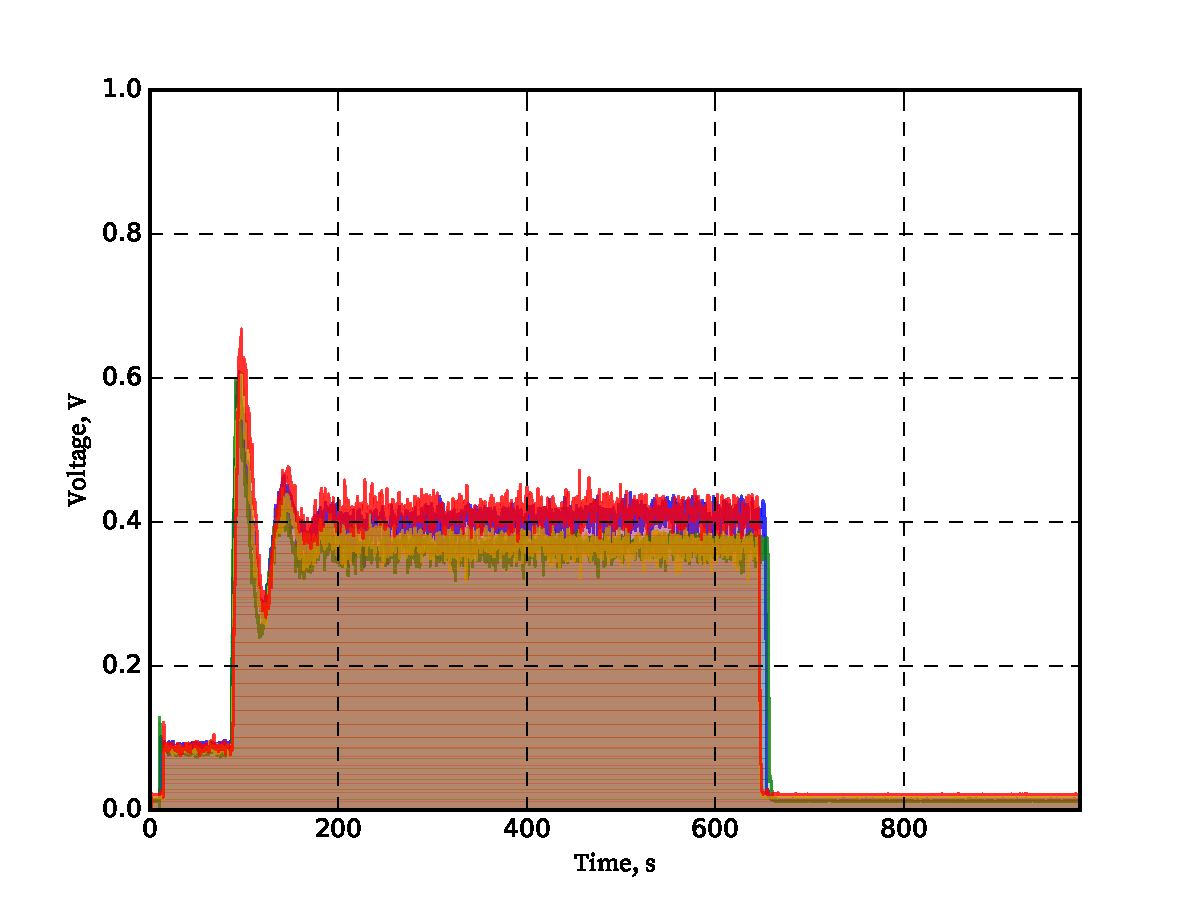
\includegraphics[width=0.8\textwidth]{images/log080716_4.pdf} 
		\caption{4}
		\label{fig:test4}
	\end{center}
\end{figure}

\textbf{Test No. 6}

Again the impluse method was used but with an increased flow rate of $\dot{v} \unitfrac[2]{l}{s}$ and a lower salinity of \unit[6.7]{\%}.

\begin{figure}
	\begin{center}
		%% This file was created by matplotlib2tikz v0.5.10.
\begin{tikzpicture}
\tikzset{external/export next=false}
\definecolor{color0}{rgb}{0,0.75,0.75}

\begin{axis}[
xlabel={Time, s},
ylabel={relative Voltage, -},
xmin=25.002166, xmax=225.000128,
ymin=0, ymax=0.6,
axis on top,
ytick={0,0.1,0.2,0.3,0.4,0.5,0.6},
yticklabels={0.0,0.1,0.2,0.3,0.4,0.5,0.6},
xmajorgrids,
ymajorgrids
]
\addplot [line width=0.7000000000000001pt, color0, opacity=0.75]
table {%
25.686765 0.0796535820140721
25.693574 0.0796491968865089
25.700354 0.0796457373633964
25.707138 0.0796432055424217
25.713995 0.0796416035212719
25.720803 0.0796409333976343
25.727623 0.0796411972691958
25.734433 0.0796423972336436
25.741259 0.079644535388665
25.748066 0.079647613831947
25.754896 0.0796516346611768
25.761732 0.0796565999740415
25.768576 0.0796625118682283
25.775396 0.0796693724414242
25.782222 0.0796771837913165
25.789043 0.0796859480155923
25.795898 0.0796956672119387
25.802753 0.0797063434780428
25.809613 0.0797179789115919
25.816486 0.0797305756102729
25.823321 0.0797441356717732
25.830165 0.0797586611937798
25.837044 0.0797741542739798
25.843917 0.0797906170100604
25.852829 0.0798080514997088
25.859468 0.0798264598406121
25.866102 0.0798458441304573
25.872742 0.0798662064669318
25.879356 0.0798875489477225
25.885978 0.0799098736705167
25.892627 0.0799331827330014
25.899285 0.0799574782328639
25.90592 0.0799827622677912
25.912583 0.0800090369354706
25.91926 0.0800363043335891
25.925939 0.0800645665598338
25.932613 0.080093825711892
25.939297 0.0801240838874508
25.945953 0.0801553431841972
25.952637 0.0801876056998185
25.959314 0.0802208735320018
25.965987 0.0802551487784343
25.972688 0.0802904335368029
25.979383 0.080326729904795
25.986092 0.0803640399800976
25.992803 0.0803767866634092
25.999512 0.080389789963781
26.006233 0.0804030474339113
26.012929 0.0804165566264984
26.019649 0.0804303150942407
26.026369 0.0804443203898364
26.033076 0.0804585700659841
26.039812 0.0804730616753819
26.046558 0.0804877927707282
26.053278 0.0805027609047214
26.059998 0.0805179636300597
26.066754 0.0805333984994416
26.073504 0.0805490630655654
26.080258 0.0805649548811293
26.086991 0.0805810714988318
26.093759 0.0805974104713712
26.100517 0.0806139693514457
26.107259 0.0806307456917538
26.114005 0.0806477370449938
26.120784 0.0806974010990947
26.127558 0.0807462916310625
26.134342 0.0807944121370426
26.141097 0.0808417661131802
26.147862 0.0808883570556205
26.154647 0.0809341884605088
26.161447 0.0809792638239903
26.16823 0.0810235866422102
26.175005 0.0810671604113137
26.181811 0.0811099886274461
26.18862 0.0811520747867526
26.195425 0.0811934223853785
26.202224 0.081234034919469
26.209024 0.0812739158851693
26.21582 0.0813130687786247
26.222647 0.0813514970959804
26.229483 0.0813892043333816
26.236318 0.0814261939869735
26.243135 0.0814624695529015
26.249943 0.0814980345273106
26.256793 0.0815328924063463
26.263638 0.0815670466861536
26.270486 0.0816005008628778
26.277345 0.0816332584326642
26.284172 0.081665322891658
26.29103 0.0816966977360045
26.29787 0.0817273864618488
26.304735 0.0817573925653362
26.311603 0.0817867195426119
26.318474 0.0818153708898212
26.325358 0.0818433501031093
26.334276 0.0818706606786214
26.340884 0.0818973061125028
26.347516 0.0819232899008987
26.354177 0.0819486155399543
26.360798 0.0819732865258149
26.36744 0.0819973063546257
26.374097 0.0820206785225319
26.380723 0.0820434065256788
26.387395 0.0820654938602116
26.394068 0.0820869440222755
26.40071 0.0821077605080159
26.40738 0.0821279468135778
26.41406 0.0821475064351065
26.420746 0.0821645334490279
26.427427 0.0821809986324102
26.434116 0.0821969051317841
26.440787 0.0822122560936804
26.447477 0.0822270546646297
26.454169 0.0822413039911628
26.460848 0.0822550072198104
26.467552 0.0822681674971031
26.474266 0.0822807879695718
26.480985 0.0822928717837471
26.487675 0.0823044220861597
26.494388 0.0823154420233403
26.501096 0.0823259347418197
26.507802 0.0823359033881285
26.514531 0.0823453511087975
26.521266 0.0823542810503573
26.527979 0.0823626963593387
26.534696 0.0823706001822724
26.541439 0.0823779956656891
26.548194 0.0823848859561196
26.554912 0.0823912742000944
26.561632 0.0823971635441444
26.568388 0.0824025571348003
26.575156 0.0824074581185927
26.58189 0.0824118696420524
26.588623 0.08241579485171
26.595395 0.0824192368940963
26.602166 0.082422198915742
26.608911 0.0824246840631779
26.615663 0.0824266954829345
26.622455 0.0824282363215427
26.629248 0.0824293097255331
26.636036 0.0824299188414365
26.642813 0.0824300668157835
26.649611 0.0824189348271481
26.65641 0.0824070259076382
26.663219 0.0823943412809045
26.670023 0.0823808821705979
26.676812 0.0823666498003691
26.683636 0.0823516453938692
26.690453 0.0823358701747488
26.697276 0.0823193253666588
26.704107 0.08230201219325
26.710908 0.0822839318781733
26.717721 0.0822650856450795
26.724579 0.0822454747176195
26.731415 0.082225100319444
26.738259 0.0822138018268919
26.745109 0.0822020351130893
26.751936 0.0821898031497598
26.75876 0.0821771089086266
26.765623 0.0821639553614135
26.772489 0.0821503454798436
26.779346 0.0821362822356406
26.786219 0.0821217686005278
26.793092 0.0821068075462287
26.79994 0.0820914020444668
26.806784 0.0820755550669655
26.815671 0.0820592695854482
26.822295 0.0820425485716384
26.828941 0.0820253949972596
26.835552 0.0820078118340351
26.842196 0.0819898020536885
26.848851 0.0819713686279432
26.855483 0.0819525145285227
26.862136 0.0819332427271503
26.868809 0.0819135561955496
26.875449 0.0818934579054439
26.882113 0.0818729508285568
26.888762 0.0818520379366117
26.895412 0.0818164015534361
26.902094 0.0817807992576766
26.908787 0.0817452313989476
26.915456 0.0817096983268637
26.922146 0.0816742003910394
26.928845 0.0816387379410892
26.935522 0.0816033113266277
26.942214 0.0815679208972693
26.948913 0.0815325670026286
26.955603 0.0814972499923202
26.962308 0.0814619702159584
26.969011 0.081426728023158
26.975705 0.0813915237635333
26.982433 0.081356357786699
26.989156 0.0813212304422694
26.995891 0.0812861420798593
27.002601 0.081251093049083
27.009332 0.0812160836995551
27.016076 0.0811811143808901
27.022826 0.0811461854427026
27.029573 0.0811112972346071
27.036317 0.0810764501062181
27.043076 0.0810416444071501
27.049839 0.0810068804870176
27.056569 0.0809721586954352
27.063329 0.0809374793820174
27.070105 0.0809028428963787
27.076864 0.0808682495881336
27.083617 0.0808336998068967
27.090421 0.0807991939022825
27.097217 0.0807647322239055
27.104004 0.0807303151213803
27.110767 0.0806959429443212
27.117537 0.080661616042343
27.124331 0.0806273347650601
27.13112 0.0805930994620869
27.13793 0.0805589104830382
27.144704 0.0805247681775283
27.15151 0.0804906728951718
27.158324 0.0804566249855832
27.16513 0.080422624798377
27.171954 0.0803886726831679
27.17875 0.0803547689895702
27.18555 0.0803209140671985
27.192381 0.0802871082656674
27.199209 0.0802533519345913
27.206045 0.0802196454235848
27.21289 0.0801859890822624
27.219705 0.0801523832602386
27.226532 0.080118828307128
27.23338 0.0800853245725451
27.240229 0.0800518724061043
27.247078 0.0800184721574203
27.253942 0.0799851241761075
27.260777 0.0799518288117805
27.267614 0.0799185864140538
27.274489 0.0798853973325419
27.281358 0.0798522619168594
27.288231 0.0798191805166207
27.29715 0.0797861534814404
27.303774 0.079753181160933
27.310388 0.079720263904713
27.317025 0.079687402062395
27.323674 0.0796545959835935
27.330297 0.079621846017923
27.336969 0.079589152514998
27.343629 0.079556515824433
27.350268 0.0795239362958426
27.356934 0.0794914142788413
27.363586 0.0794589501230437
27.370237 0.0794265441780642
27.37692 0.0793941967935173
27.383581 0.0793619083190176
27.390237 0.0793296791041797
27.396947 0.079297509498618
27.403641 0.079265399851947
27.410312 0.0792333505137814
27.417004 0.0792013618337355
27.423716 0.079169434161424
27.430392 0.0791375678464613
27.437093 0.079105763238462
27.443797 0.0790740206870406
27.450494 0.0790423405418116
27.457246 0.0790107231523896
27.463963 0.0789791688683891
27.470691 0.0789476780394245
27.477393 0.0789162510151104
27.484121 0.0788848881450614
27.490861 0.078853589778892
27.497579 0.0788223562662166
27.504298 0.0787911879566499
27.511043 0.0787600851998062
27.517828 0.0787290483453003
27.524555 0.0786980777427465
27.531276 0.0786671737417594
27.538036 0.0786363366919536
27.54481 0.0786055669429435
27.551555 0.0785748648443437
27.558303 0.0785442307457687
27.565077 0.07852416680529
27.57186 0.0785038533274452
27.578614 0.0784832925847287
27.585397 0.078462486849635
27.592192 0.0784414383946584
27.598979 0.0784201494922934
27.605779 0.0783986224150343
27.612551 0.0783768594353756
27.619331 0.0783548628258116
27.626134 0.0783326348588368
27.632945 0.0783101778069455
27.639759 0.0782874939426322
27.646571 0.0782645855383912
27.653366 0.078241454866717
27.660184 0.078218104200104
27.667009 0.0781945358110465
27.673839 0.0781737034178454
27.680638 0.0781374703300821
27.687453 0.0781015775920572
27.694262 0.0780660252037709
27.701109 0.0780308131652231
27.707957 0.0780077472596394
27.714809 0.0779853730663901
27.721667 0.0779636926831625
27.728496 0.0779427082076437
27.735336 0.0779224217375209
27.742204 0.0779028353704811
27.749074 0.0778839512042115
27.755948 0.0778657713363993
27.762866 0.0778482978647316
27.76975 0.0778315328868955
27.778636 0.0778154785005782
27.785245 0.0778001368034667
27.79187 0.0777855098932484
27.798514 0.0777715998676102
27.805124 0.0777584088242394
27.81177 0.0777459388608231
27.818426 0.0777341920750483
27.825061 0.0777231705646023
27.831733 0.0777128764271723
27.83838 0.0777033117604452
27.845019 0.0776944786621083
27.851699 0.0776863792298488
27.858351 0.0776790155613537
27.865033 0.0776723897543102
27.871718 0.0776665039064054
27.878386 0.0776613601153265
27.885051 0.0776569604787607
27.891752 0.077653307094395
27.898457 0.0776504020599166
27.905134 0.0776482474730126
27.911831 0.0776468454313702
27.918528 0.0776461980326765
27.92522 0.0776463073746187
27.931931 0.0776471755548839
27.938652 0.0776488046711592
27.945341 0.0776511968211318
27.952058 0.0776543541024889
27.958783 0.0776582786129175
27.965512 0.0776629724501048
27.972224 0.0776684377117379
27.978963 0.077674676495504
27.98571 0.0776816908990903
27.992467 0.0776894830201837
27.999188 0.0776980549564717
28.005932 0.0777074088056411
28.012689 0.0777175466653793
28.01946 0.0777284706333732
28.026193 0.0777401828073101
28.032956 0.0777526852848771
28.039729 0.0777659801637614
28.046489 0.0777800695416501
28.053241 0.0777949555162303
28.060021 0.0778106401851891
28.066808 0.0778271256462138
28.073597 0.0778444139969914
28.080361 0.077862507335209
28.087136 0.0778814077585539
28.093935 0.0779011173647132
28.100729 0.077921638251374
28.107532 0.0779429725162234
28.114315 0.0779651222569486
28.121098 0.0779880895712368
28.12792 0.078011876556775
28.134762 0.0780364853112504
28.141588 0.0780619179323502
28.148388 0.0780881765177615
28.155189 0.0781152631651714
28.162023 0.078143179972267
28.168862 0.0781719290367356
28.175699 0.0782015124562642
28.182552 0.0782319323285401
28.189366 0.0782631907512502
28.196218 0.0782952898220818
28.203077 0.0783282316387221
28.209931 0.078362018298858
28.216787 0.0783966519001769
28.223648 0.0784321345403658
28.230525 0.0784684683171119
28.237361 0.0785056553281023
28.244208 0.0785436976710242
28.251061 0.0785825974435646
28.260002 0.0786223567434108
28.266636 0.0786629776682498
28.273275 0.0787044623157689
28.279895 0.0787468127836551
28.286539 0.0787900311695956
28.293168 0.0788341195712776
28.299822 0.0788790800863881
28.306483 0.0789249148126143
28.313127 0.0789716258476434
28.319819 0.0790192152891625
28.32649 0.0790676852348588
28.333133 0.0791170377824193
28.339811 0.0791672750295312
28.346501 0.0792183990738817
28.353163 0.0792704120131579
28.359832 0.0793233159450469
28.366525 0.0793771129672359
28.373198 0.079431805177412
28.379888 0.0794539449541233
28.386589 0.0794759885868407
28.393303 0.0794979322298044
28.399988 0.0795197720372546
28.4067 0.0795415041634317
28.41341 0.0795631247625758
28.420106 0.0795846299889271
28.426833 0.079606015996726
28.433562 0.0796272789402127
28.440294 0.0796484149736274
28.447001 0.0796694202512103
28.453731 0.0796931550567809
28.460474 0.0797166646231948
28.467197 0.0797399456291141
28.473921 0.0797629947532007
28.480673 0.0797858086741167
28.487432 0.0798083840705241
28.494163 0.079830717621085
28.500926 0.0798528060044614
28.507687 0.0798746458993153
28.514457 0.0798962339843087
28.521205 0.0799175669381036
28.527952 0.0799386414393622
28.534724 0.0799594541667464
28.541514 0.0799800017989182
28.548281 0.0800002810145397
28.555044 0.0800202884922729
28.561862 0.0800400209107798
28.568652 0.0800594749487225
28.57545 0.080078647284763
28.582233 0.0800975345975633
28.589009 0.0801161335657854
28.595817 0.0801344408680914
28.602632 0.0801524531831433
28.609444 0.0801701671896031
28.616252 0.0801875795661329
28.62308 0.0802046869913946
28.629878 0.0802214861440504
28.636705 0.0802379737027622
28.64354 0.080254146346192
28.650379 0.080270000753002
28.657195 0.080285533601854
28.66401 0.0803007415714103
28.670859 0.0803156213403327
28.677719 0.0803321372178208
28.684571 0.0803483768124319
28.691438 0.0803643371524424
28.698298 0.080380015266129
28.70514 0.0803954081817681
28.711983 0.0804105129276363
28.71886 0.0804253265320101
28.725737 0.0804398460231661
28.73261 0.080454068429381
28.741521 0.0804679907789311
28.748167 0.080481610100093
28.754802 0.0804949234211434
28.761441 0.0805079277703587
28.768088 0.0805206201760156
28.774714 0.0805329976663905
28.781359 0.08054505726976
28.78799 0.0805567960144007
28.794631 0.0805682109285891
28.801301 0.0805792990406018
28.807945 0.0805900573787153
28.814651 0.0806004829712062
28.82133 0.080610572846351
28.827988 0.0806203240324263
28.834644 0.0806297335577086
28.841326 0.0806387984504744
28.847995 0.0806475157390005
28.854663 0.0806558824515631
28.86136 0.0806638956164391
28.868071 0.0806715522619047
28.874782 0.0806788494162368
28.881489 0.0806857841077117
28.888176 0.080692353364606
28.894869 0.0806985542151963
28.901591 0.0807043836877592
28.908323 0.0807098388105712
28.915027 0.0807149166119088
28.921734 0.0807196141200485
28.928471 0.0807239283632671
28.935208 0.0807278563698409
28.941925 0.0807313951680466
28.948664 0.0807345417861607
28.955409 0.0807372932524597
28.962146 0.0807396465952202
28.968878 0.0807415988427188
28.975638 0.0807431470232319
28.982386 0.0807719747509683
28.989135 0.0807995534808198
28.995906 0.0808258853104737
29.002647 0.0808509723376171
29.009421 0.0808748166599372
29.016208 0.080897420375121
29.02296 0.0809187855808558
29.029715 0.0809389143748286
29.036504 0.0809578088547266
29.043293 0.080975471118237
29.050076 0.0809919032630468
29.056877 0.0810071073868432
29.063684 0.0810210855873135
29.070489 0.0810338399621446
29.0773 0.0810453726090238
29.084097 0.0810556856256381
29.090889 0.0810647811096748
29.097688 0.0810726611588209
29.104508 0.0810793278707636
29.11133 0.0810847833431901
29.118155 0.0810890296737875
29.124956 0.0810920689602429
29.131772 0.0810939033002434
29.138619 0.0810945347914763
29.145458 0.0810939655316286
29.152302 0.0811069548474194
29.159151 0.081119186810749
29.165975 0.0811306661414133
29.172805 0.0811413975592085
29.179692 0.0811513857839307
29.186557 0.0811606355353758
29.193419 0.0811424196572677
29.200286 0.0811242848023253
29.207159 0.0811062307957415
29.214009 0.081088257462709
29.222899 0.0810703646284204
29.229509 0.0810525521180687
29.236141 0.0810348197568464
29.242782 0.0810171673699463
29.249423 0.0809995947825612
29.256058 0.0809821018198838
29.262687 0.0809646883071068
29.269341 0.080947354069423
29.275992 0.0809300989320252
29.28264 0.0809129227201059
29.28931 0.0808958252588581
29.295981 0.0808788063734744
29.302665 0.0808618658891476
29.30934 0.0808450036310704
29.316005 0.0808282194244355
29.322673 0.0808115130944357
29.329356 0.0807948844662637
29.336044 0.0807783333651123
29.342725 0.0807618596161742
29.349431 0.0807454630446421
29.356137 0.0807291434757088
29.362852 0.080712900734567
29.369538 0.0806967346464094
29.376248 0.0806806450364289
29.382951 0.0806646317298181
29.389649 0.0806486945517697
29.396365 0.0806328333274765
29.40309 0.0806170478821313
29.409798 0.0806013380409268
29.416508 0.0805857036290557
29.42326 0.0805701444717107
29.430004 0.0805546603940847
29.436732 0.0805392512213703
29.443459 0.0805239167787602
29.450201 0.0805086568914473
29.45695 0.0804934713846242
29.46369 0.0804783600834837
29.470461 0.0804633228132185
29.477225 0.0804483593990214
29.484027 0.0804334696660851
29.490774 0.0804186534396023
29.497524 0.0804039105447658
29.504298 0.0803892408067684
29.511084 0.0803746440508026
29.517878 0.0803601201020614
29.524641 0.0803456687857374
29.531436 0.0803312899270234
29.538235 0.0803169833511121
29.545064 0.0803027488831963
29.551848 0.0802885863484686
29.558632 0.0802744955721218
29.565436 0.0802604763793487
29.572255 0.0802465285953421
29.579077 0.0802326520452945
29.585896 0.0802188465543989
29.5927 0.0802051119478478
29.5995 0.0801914480508341
29.606363 0.0801778546885505
29.613201 0.0801643316861897
29.620039 0.0801508788689445
29.62688 0.0801374960620076
29.633702 0.0801241830905718
29.640527 0.0801109397798297
29.647377 0.0800977659549742
29.654229 0.0800846614411979
29.661085 0.0800716260636936
29.667954 0.080058659647654
29.674818 0.080045762018272
29.681657 0.0800329330007401
29.688502 0.0800201724202512
29.695374 0.080007480101998
29.704281 0.0799948558711732
29.710911 0.0799822995529695
29.717518 0.0799698109725798
29.724148 0.0799573899551967
29.730794 0.0799450363260131
29.73744 0.0799327499102215
29.744082 0.0799205305330148
29.750744 0.0799083780195857
29.757386 0.0798962921951269
29.764052 0.0798842728848312
29.770731 0.0798723199138913
29.777371 0.0798604331074999
29.784041 0.0798486122908499
29.790727 0.0798368572891338
29.797412 0.0798251679275445
29.804098 0.0798135440312748
29.810835 0.0798019854255173
29.817505 0.0797904919354647
29.824203 0.0797491472211586
29.830908 0.0797081238025995
29.837585 0.079667416085955
29.84427 0.0796270184773928
29.850987 0.0795869253830804
29.857705 0.0795471312091855
29.864395 0.0795076303618758
29.871113 0.0794684172473187
29.877839 0.0794294862716821
29.884551 0.0793908318411334
29.891261 0.0793524483618404
29.897989 0.0793143302399706
29.904733 0.0792764718816917
29.911457 0.0792388676931713
29.918235 0.079201512080577
29.924978 0.0791643994500764
29.931725 0.0791275242078373
29.938461 0.0791066218043278
29.945225 0.0790864140848764
29.951976 0.0790668982525667
29.958725 0.0790480715104826
29.965476 0.0790299310617078
29.972247 0.0790124741093264
29.979016 0.0789956978564219
29.985803 0.0789795995060782
29.992562 0.0789641762613792
29.999321 0.0789494253254087
30.006107 0.0789353439012505
30.012911 0.0789219291919883
30.019694 0.0789091784007061
30.026472 0.0788970887304875
30.033288 0.0788856573844165
30.040118 0.0788748815655768
30.046933 0.0788647584770523
30.053748 0.0788552853219268
30.060541 0.078846459303284
30.067338 0.0788382776242078
30.074166 0.078830737487782
30.080992 0.0788238360970905
30.087838 0.0788175706552169
30.094643 0.0788119383652452
30.101479 0.0788069364302592
30.108296 0.0788025620533427
30.115143 0.0787988124375794
30.121996 0.0787956847860532
30.128852 0.078793176301848
30.135705 0.0787912841880474
30.142538 0.0787900056477354
30.14938 0.0787893378839958
30.156251 0.0787892780999122
30.163154 0.0787898234985687
30.170028 0.078790971283049
30.176897 0.0787927186564369
30.185822 0.0787950628218161
30.192465 0.0787980009822706
30.199068 0.0788015303408842
30.20571 0.0788056481007406
30.212332 0.0788103514649236
30.218981 0.0788156376365171
30.225613 0.078821503818605
30.232244 0.0788279472142709
30.238906 0.0788349650265987
30.245574 0.0788425544586723
30.252223 0.0788507127135754
30.258889 0.0788594369943919
30.265573 0.0788687245042055
30.272232 0.0788785724461001
30.278918 0.0788889780231595
30.28559 0.0788999384384676
30.292261 0.078911450895108
30.298946 0.0789235125961647
30.305639 0.0789361207447214
30.312321 0.078949272543862
30.319032 0.0789629651966702
30.325747 0.07897719590623
30.332435 0.078991961875625
30.339117 0.0790072603079391
30.345843 0.0790230884062562
30.352559 0.07903944337366
30.359263 0.0790563224132343
30.365987 0.079073722728063
30.372721 0.0790916415212299
30.379438 0.0791100759958188
30.386159 0.0791290233549135
30.392905 0.0791484808015978
30.399651 0.0791684455389555
30.406395 0.0791889147700705
30.413122 0.0792098856980264
30.419881 0.0792313555259073
30.42664 0.0792533214567969
30.433372 0.0792757806937789
30.440105 0.0792987304399373
30.446875 0.0793221678983557
30.453651 0.0793460902721182
30.460408 0.0793704947643083
30.467198 0.07939537857801
30.473983 0.0794207389163071
30.480764 0.0794465729822833
30.487539 0.0794728779790226
30.49431 0.0795321112448392
30.50108 0.079590826207125
30.507882 0.0796490260124106
30.514685 0.0797067138072267
30.521488 0.079763892738104
30.528309 0.0798205659515732
30.535095 0.0798767365941651
30.541912 0.0799324078124103
30.548732 0.0799875827528396
30.55555 0.0800422645619837
30.562356 0.0800964563863732
30.569169 0.0801501613725389
30.576003 0.0802033826670115
30.582841 0.0802561234163218
30.589708 0.0803083867670003
30.596559 0.0803601758655779
30.603381 0.0804114938585852
30.610212 0.080462343892553
30.617076 0.080512729114012
30.623936 0.0805626526694928
30.630801 0.0806121177055262
30.637671 0.0806611273686429
30.644551 0.0807096848053736
30.651393 0.0807577931622491
30.658264 0.0808054555857999
30.667149 0.0808526752225569
30.673787 0.0808994552190507
30.680426 0.0809457987218121
30.687043 0.0809783429393357
30.693683 0.0810108619846135
30.700333 0.0810433565568747
30.706958 0.0810758273553483
30.713607 0.0811053236334569
30.72028 0.0811347096955871
30.726918 0.0811639857165461
30.733587 0.081193151871141
30.74024 0.0812222083341793
30.746895 0.0812511552804681
30.753579 0.0812799928848147
30.760242 0.0813087213220264
30.766901 0.0813373407669105
30.773579 0.0813658513942741
30.780279 0.0813847062803273
30.786951 0.0814037420044928
30.79365 0.0814229569935051
30.800361 0.081442349674099
30.807041 0.081461918473009
30.813744 0.0814816618169697
30.820455 0.081501578132716
30.827154 0.0815216658469823
30.833887 0.0815419233865033
30.840612 0.0815623491780138
30.847342 0.0815829416482482
30.854046 0.0816036992239413
30.860776 0.0816246203318277
30.867518 0.0816457033986421
30.874237 0.0816669468511191
30.880962 0.0816883491159933
30.887713 0.0817099086199995
30.894478 0.0817316237898721
30.901235 0.081753493052346
30.907973 0.0817755148341556
30.914739 0.0817976875620358
30.921507 0.081820009662721
30.928253 0.081842479562946
30.935005 0.0818650956894454
30.941775 0.0818878564689539
30.948564 0.0819107603282061
30.955327 0.0819338056939365
30.96212 0.08195699099288
30.968918 0.0819803146517711
30.975709 0.0820037750973445
30.982508 0.0820273707563348
30.989303 0.0820511000554767
30.996081 0.0820749614215047
31.002898 0.0820989532811537
31.009709 0.0821230740611581
31.016527 0.0821473221882526
31.023335 0.082171696089172
31.030131 0.0821961941906508
31.036927 0.0822208149194236
31.043764 0.0822455567022252
31.050588 0.0822704179657901
31.057432 0.0822953971368531
31.064243 0.0823204926421487
31.071056 0.0823457029084116
31.077909 0.0823710263623764
31.084787 0.0823964614307779
31.091641 0.0824220065403506
31.098492 0.0824476601178291
31.105354 0.0824734205899482
31.11219 0.0824992863834424
31.119031 0.0825252559250465
31.125912 0.082551327641495
31.132777 0.0825774999595226
31.139654 0.082603771305864
31.148567 0.0826301401072538
31.155207 0.0826566047904266
31.161813 0.082683163782117
31.168452 0.0827098155090598
31.175097 0.0827365583979896
31.181716 0.082763390875641
31.188364 0.0827903113687487
31.194992 0.0828173183040473
31.201661 0.0828444101082714
31.208333 0.0828715852081557
31.214982 0.0828988420304348
31.221661 0.0829261790018435
31.228345 0.0829535945491162
31.235004 0.0829810870989878
31.24169 0.0829801244353977
31.248377 0.0829783865016019
31.255048 0.0829758666549246
31.261716 0.0829725582526899
31.268445 0.0829684546522217
31.275151 0.0829635492108441
31.281827 0.0829578352858812
31.288533 0.0829513062346571
31.295243 0.0829439554144957
31.301943 0.0829357761827212
31.308669 0.0829267618966576
31.315387 0.0829169059136289
31.322109 0.0829062015909593
31.328842 0.0828946422859727
31.335573 0.0828822213559933
31.342308 0.082868932158345
31.349018 0.082854768050352
31.355736 0.0828397223893382
31.362483 0.0828237885326279
31.369231 0.0828069598375449
31.375959 0.0827892296614133
31.382688 0.0827705913615573
31.389459 0.0827510382953009
31.396223 0.0827305638199681
31.40296 0.082709161292883
31.409696 0.0826868240713696
31.416473 0.082663545512752
31.423251 0.0826393189743543
31.430002 0.0826141378135004
31.436763 0.0825879953875146
31.443551 0.0825608850537207
31.450363 0.0825823053237429
31.457152 0.0826028988428209
31.463932 0.0826226678834492
31.470697 0.0826416147181221
31.477499 0.082659741619334
31.484311 0.0826770508595793
31.491107 0.0826935447113526
31.497902 0.082709225447148
31.504729 0.0827240953394601
31.511578 0.0827381566607833
31.518399 0.0827514116836119
31.525231 0.0827638626804403
31.532033 0.082775511923763
31.538848 0.0827863616860744
31.545687 0.0827964142398688
31.552532 0.0827884870801657
31.559375 0.0827802880077669
31.566226 0.0827718161486364
31.573068 0.0827630706287376
31.5799 0.0827540505740343
31.586735 0.0827447551104903
31.593597 0.0827351833640692
31.600464 0.0827253344607346
31.607325 0.0827152075264503
31.614199 0.08270480168718
31.621047 0.0826941160688874
31.629928 0.0826831497975361
31.636538 0.0826719019990898
31.643165 0.0826603717995123
31.649773 0.0826485583247673
31.656414 0.0826364607008183
31.66304 0.0826240780536292
31.66967 0.0826114095091636
31.676315 0.0825984541933851
31.68299 0.0825852112322576
31.689631 0.0825716797517446
31.696303 0.0825578588778099
31.702985 0.0825437477364172
31.709634 0.0825293454535301
31.716309 0.0825146511551124
31.722996 0.0824996639671277
31.729655 0.0824843830155397
31.736348 0.0824688074263122
31.74304 0.0824529363254087
31.749719 0.0824367688387931
31.75642 0.082420304092429
31.763119 0.08240354121228
31.769793 0.0823864793243099
31.77651 0.0823691175544824
31.783227 0.0823514550287612
31.789953 0.0823334908731099
31.796648 0.0823152242134923
31.803367 0.0822966541758719
31.810097 0.0822777798862126
31.816807 0.0822586004704781
31.823539 0.0822391150546319
31.830279 0.0822193227646379
31.837001 0.0821992227264596
31.84373 0.0821788140660608
31.850483 0.0821580959094052
31.857278 0.0821370673824565
31.86403 0.0821157276111783
31.870773 0.0820940757215344
31.877503 0.0820721108394884
31.884265 0.082049832091004
31.891043 0.082027238602045
31.897791 0.082004329498575
31.904539 0.0819811039065577
31.911317 0.0819575609519568
31.9181 0.081933699760736
31.924869 0.081909519458859
31.931632 0.0818850191722894
31.938426 0.0818601980269911
31.945216 0.0818350551489275
31.95202 0.0818095896640626
31.958798 0.0817838006983598
31.965585 0.081757687377783
31.972393 0.0817312488282958
31.979207 0.081704484175862
31.986033 0.0816773925464451
31.992825 0.0816499730660089
31.999631 0.0816222248605172
32.006484 0.0815941470559335
32.013311 0.0815657387782216
32.020147 0.0815369991533451
32.026988 0.0815079273072678
32.033803 0.0814785223659534
32.040624 0.0814487834553655
32.047471 0.0814187097014678
32.054324 0.0813883002302241
32.061176 0.0813575541675979
32.06804 0.0813264706395531
32.074873 0.0812950487720533
32.081717 0.0812829639964381
32.088561 0.0812711247376219
32.095427 0.0812595336177137
32.102307 0.0812481932588224
32.111227 0.0812371062830569
32.117853 0.0812262753125262
32.124464 0.0812157029693391
32.131124 0.0812053918756046
32.137772 0.0811953446534317
32.144392 0.0811855639249292
32.151043 0.0811760523122061
32.157705 0.0811668124373712
32.164353 0.0811578469225336
32.171022 0.0811491583898022
32.177702 0.0811407494612858
32.184348 0.0811326227590934
32.191042 0.081124780905334
32.197728 0.0811172265221164
32.204387 0.0811099622315496
32.211072 0.0811029906557424
32.217775 0.0810963144168039
32.224445 0.0811080756241778
32.23114 0.0811195877312037
32.237823 0.0811308566813286
32.244507 0.0811418884179994
32.251237 0.0811526888846629
32.257958 0.0811632640247662
32.264651 0.081173619781756
32.271339 0.0811837620990793
32.278055 0.081193696920183
32.284786 0.0812034301885139
32.291502 0.0812129678475191
32.29823 0.0812223158406452
32.304966 0.0812314801113394
32.31171 0.0812404666030484
32.318432 0.0812492812592192
32.325175 0.0812579300232986
32.331918 0.0812664188387335
32.338643 0.081274753648971
32.345374 0.0812829403974577
32.352135 0.0812909850276407
32.358898 0.0812988934829669
32.365638 0.0813066717068831
32.372413 0.0813162350625557
32.379181 0.0813256222125085
32.385955 0.0813348394498029
32.392741 0.0813438930675004
32.399501 0.0813527893586624
32.406287 0.0813615346163503
32.413076 0.0813701351336255
32.419878 0.0813785972035494
32.426646 0.0813869271191835
32.43345 0.0813951311735892
32.440261 0.0814032156598278
32.44706 0.081411186870961
32.453879 0.0814190511000499
32.460674 0.0814268146401561
32.467461 0.081434483784341
32.474292 0.081424880048191
32.481118 0.081415715253075
32.487948 0.0814069925455239
32.494814 0.0813987150720683
32.501619 0.081390885979239
32.508438 0.0813835084135666
32.515283 0.0813765855215819
32.522125 0.0813701204498155
32.528975 0.0813641163447982
32.535828 0.0813585763530607
32.542658 0.0813535036211337
32.549489 0.0813489012955479
32.556355 0.081344772522834
32.563217 0.0813411204495228
32.570086 0.0813379482221449
32.576967 0.081335258987231
32.583845 0.0813330558913119
32.592738 0.0813313420809183
32.599352 0.0813301207025809
32.605984 0.0813293949028304
32.612632 0.0813291678281974
32.61928 0.0813294426252128
32.625924 0.0813302224404072
32.632579 0.0813315104203113
32.639206 0.0813333097114559
32.645872 0.0813356234603716
32.652541 0.0813384548135892
32.659186 0.0813418069176394
32.665858 0.0813456829190529
32.672542 0.0813500859643604
32.679198 0.0813550192000926
32.685879 0.0813604857727801
32.692573 0.0813664888289539
32.699239 0.0813730315151444
32.705929 0.0813801169778825
32.712618 0.0813877483636989
32.719298 0.0813959288191243
32.726002 0.0814046614906893
32.732714 0.0814139495249247
32.739402 0.0814237960683612
32.746141 0.0814342042675296
32.752859 0.0814117275498214
32.759589 0.0813888232535511
32.766289 0.0813654885818025
32.773011 0.0813417207376594
32.779744 0.0813175169242057
32.786453 0.0812928743445251
32.793166 0.0812677902017016
32.799906 0.0812422616988187
32.806654 0.0812162860389605
32.813381 0.0811898604252107
32.82014 0.0811629820606531
32.826894 0.0811356481483716
32.83365 0.0811078558914499
32.840391 0.0810796024929718
32.84713 0.0810508851560212
32.853899 0.0810217010836819
32.860679 0.0809920474790378
32.867455 0.0809619215451725
32.874215 0.0809313204851699
32.880989 0.0809002415021139
32.887781 0.0808686817990882
32.894555 0.0808366385791767
32.901325 0.0808041090454631
32.90812 0.0807710904010314
32.914926 0.0807375798489653
32.921727 0.0807035745923485
32.928534 0.080669071834265
32.935325 0.0806340687777986
32.942139 0.0806123360397961
32.948961 0.080590507332607
32.955783 0.0805685823066167
32.962613 0.0805465606122106
32.969418 0.0805244418997744
32.976227 0.0805022258196933
32.983055 0.080479912022353
32.989896 0.0804575001581389
32.996732 0.0804349898774364
33.003575 0.0804123808306311
33.010399 0.0803896726681084
33.017227 0.0803668650402538
33.024086 0.0803439575974528
33.030943 0.0803209499900908
33.037813 0.0803076800212414
33.044681 0.0802946019907652
33.051552 0.0802817172971205
33.058402 0.0802690273387653
33.065258 0.0802565335141577
33.074182 0.0802442372217559
33.080813 0.0802321398600178
33.087455 0.0802202428274017
33.094059 0.0802085475223655
33.100701 0.0801970553433674
33.107353 0.0801857676888655
33.113999 0.0801746859573179
33.120653 0.0801638115471826
33.127325 0.0801531458569178
33.133967 0.0801426902849815
33.140637 0.0801324462298319
33.147321 0.0801319621885243
33.153974 0.0801314031549014
33.160652 0.080130772275494
33.167342 0.0801300726968327
33.174026 0.0801293075654483
33.18071 0.0801275253180117
33.187412 0.0801257127415152
33.194085 0.0801238728076823
33.200785 0.0801220084882363
33.207484 0.0801201227549009
33.214168 0.0801182185793993
33.220879 0.080116298933455
33.227602 0.0801143667887915
33.234331 0.0801124251171323
33.241028 0.0801104768902007
33.247752 0.0801085250797203
33.254482 0.0801065726574145
33.261194 0.0801046225950067
33.267931 0.0801026778642204
33.274661 0.080100741436779
33.281394 0.080098816284406
33.288119 0.0800969053788248
33.294904 0.0800950116917589
33.301648 0.0800931381949318
33.308384 0.0800912878600668
33.315124 0.0800894636588874
33.321896 0.0800876685631171
33.328651 0.0800859055444793
33.335406 0.0800841775746975
33.34216 0.0800824876254951
33.348942 0.0800808386685956
33.355744 0.0800792336757223
33.36253 0.0800776756185989
33.369299 0.0800761674689487
33.37606 0.0800747121984951
33.382856 0.0800733127789616
33.389647 0.0800719721820717
33.396448 0.0800706933795488
33.403227 0.0800694793431164
33.410017 0.0800683330444978
33.416848 0.0800672574554166
33.423663 0.0800662555475963
33.430491 0.0800653302927601
33.437288 0.0800644846626317
33.444087 0.0800637216289344
33.450913 0.0800630441633917
33.457742 0.0800624552377271
33.464574 0.080061957823664
33.471415 0.0800615548929258
33.478256 0.080061249417236
33.485073 0.080061044368318
33.491926 0.0800609427178953
33.498784 0.0800609474376914
33.505638 0.0800610614994296
33.512508 0.0800612878748335
33.519361 0.0800616295356265
33.526204 0.080062089453532
33.53305 0.0800626706002735
33.539953 0.0800595571081355
33.546825 0.0800566865106877
33.555732 0.0800540610804244
33.562366 0.0800516830898399
33.568983 0.0800495548114288
33.575615 0.0800476785176855
33.58226 0.0800460564811043
33.588884 0.0800446909741796
33.595532 0.0800292636215099
33.602198 0.0800145313025128
33.60887 0.0800004936675736
33.615532 0.0799871503670778
33.622209 0.079974501051411
33.628847 0.0799625453709585
33.635519 0.0799512829761059
33.642202 0.0799407135172387
33.648863 0.0799308366447422
33.655548 0.0799216520090021
33.662238 0.0799131592604037
33.668937 0.0799053580493326
33.675629 0.0798982480261742
33.682325 0.0798918288413141
33.689009 0.0798861001451376
33.695725 0.0798810615880302
33.702439 0.0798767128203775
33.709158 0.0798504257413826
33.715851 0.0798241543076376
33.722572 0.0797978941489609
33.729304 0.0797716408951712
33.736013 0.0797453901760867
33.742748 0.0797191376215259
33.749475 0.0796928788613074
33.756206 0.0796666095252495
33.762931 0.0796403252431708
33.76968 0.0796140216448897
33.776426 0.0795876943602246
33.783186 0.079561339018994
33.789945 0.0795349512510163
33.796711 0.0795085266861101
33.803464 0.0794820609540937
33.810217 0.079473258359624
33.816968 0.0794649329015751
33.823736 0.0794570833562961
33.830508 0.0794497085001362
33.837301 0.0794428071094447
33.844057 0.0794363779605706
33.850847 0.0794304198298631
33.85764 0.0794249314936714
33.864428 0.0794199117283447
33.871227 0.0794153593102321
33.878011 0.0794112730156828
33.884792 0.079407651621046
33.891597 0.0794044939026708
33.898411 0.0794017986369065
33.905272 0.0793995646001021
33.912088 0.0793977905686068
33.918887 0.0793964753187698
33.925714 0.0793956176269403
33.932543 0.0793952162694675
33.939376 0.0793952700227005
33.946213 0.0793957776629884
33.953032 0.0793967379666805
33.95985 0.0793981497101259
33.966697 0.0794000116696738
33.973545 0.0794023226216734
33.980387 0.0794050813424738
33.987251 0.0794082866084241
33.99408 0.0794119371958736
34.000918 0.0794160318811715
34.00776 0.0794205694406668
34.014632 0.0794255486507088
34.021504 0.0794309682876467
34.02837 0.0794368271278295
34.037297 0.0794431239476065
34.043941 0.0794498575233268
34.050548 0.0794570266313397
34.057193 0.0794646300479942
34.063811 0.0794726665496395
34.070456 0.0794811349126249
34.077078 0.0794900339132994
34.083711 0.0794993623280123
34.09037 0.0795091189331127
34.097041 0.0795193025049497
34.103684 0.0795299118198727
34.110356 0.0795409456542306
34.117041 0.0795524027843727
34.123698 0.0795642819866482
34.130384 0.0795765820374062
34.137055 0.0795893017129958
34.143723 0.0796024397897664
34.15041 0.0796159950440669
34.157104 0.0796299662522467
34.163788 0.0796443521906548
34.170495 0.0796591516356404
34.177208 0.0796743633635528
34.183895 0.079689986150741
34.190581 0.0797060187735542
34.197296 0.0797224600083417
34.204023 0.0797393086314525
34.210728 0.0797565634192358
34.217473 0.0797742231480409
34.224208 0.0797922865942168
34.230951 0.0798107525341128
34.237669 0.079829619744078
34.244407 0.0798488870004616
34.25115 0.0798685530796127
34.257876 0.0798886167578805
34.264601 0.0799128956510532
34.271354 0.0799374539736336
34.278119 0.0799622912012
34.284856 0.0799874068093308
34.291601 0.0800128002736039
34.298371 0.0800384710695977
34.305144 0.0800644186728904
34.311902 0.0800906425590603
34.318661 0.0801171422036854
34.325437 0.0801439170823441
34.332227 0.0801709666706145
34.339012 0.0801982904440749
34.34578 0.0802258878783035
34.35255 0.0802537584488784
34.359356 0.080281901631378
34.366161 0.0803103169013803
34.372959 0.0803390037344637
34.379749 0.0803679616062064
34.386566 0.0803971899921865
34.393388 0.0804266883679823
34.400229 0.0804564562091721
34.407057 0.0804864929913339
34.413861 0.080516798190046
34.420671 0.0805473712808867
34.427504 0.0805782117394341
34.434345 0.0806093190412666
34.441184 0.0806406926619622
34.448036 0.0806723320770992
34.454858 0.0807042367622558
34.461714 0.0807364061930102
34.468577 0.0807688398449407
34.475437 0.0808015371936255
34.482302 0.0808158052245356
34.489162 0.080829779579246
34.496041 0.0808434564119971
34.502883 0.080856831877029
34.509737 0.080869902128582
34.518617 0.0808826633208963
34.525273 0.0808951116082123
34.531895 0.08090724314477
34.538511 0.0809190540848097
34.545149 0.0809305405825718
34.5518 0.0809416987922964
34.558422 0.0809525248682238
34.565074 0.0809630149645943
34.571747 0.080973165235648
34.578389 0.0809829718356252
34.585084 0.0809924309187662
34.591768 0.0810015386393112
34.598422 0.0810102911515004
34.605098 0.0810186846095741
34.611788 0.0810267151677726
34.618448 0.081034378980336
34.625131 0.0810416722015046
34.631833 0.0810466233549811
34.638513 0.0810511376651107
34.645238 0.081055210936519
34.651938 0.0810588389738317
34.658623 0.0810620175816747
34.665338 0.0810647425646736
34.672053 0.0810670097274541
34.678779 0.0810688148746419
34.685475 0.0810701538108628
34.692197 0.0810710223407426
34.698929 0.0810714162689068
34.70564 0.0810713313999812
34.712376 0.0810707635385916
34.719112 0.0810697084893637
34.72585 0.0810805732850996
34.732578 0.0811082750792633
34.739332 0.0811356303180308
34.746077 0.0811626402250528
34.752813 0.0811893060239802
34.759554 0.0812156289384638
34.766324 0.0812416101921544
34.773081 0.0812672510087028
34.779832 0.08129255261176
34.786588 0.0813175162249766
34.793369 0.0813421430720036
34.800147 0.0813664343764918
34.806938 0.0813903913620921
34.813702 0.0814063775735773
34.820467 0.0814222633582908
34.82726 0.0814380485414251
34.834054 0.081453732948173
34.840848 0.0814693164037273
34.847631 0.0814847987332808
34.854417 0.0815001797620261
34.861228 0.0815154593151559
34.868046 0.0815306372178632
34.874869 0.0815457132953404
34.881662 0.0815606873727805
34.888467 0.0815755592753761
34.895292 0.08159032882832
34.902122 0.0816049958568049
34.908964 0.0816195601860236
34.915777 0.0816340216411687
34.922599 0.0816483800474331
34.929424 0.0816626352300095
34.936269 0.0816767870140906
34.943123 0.0816908352248691
34.949979 0.0817047796875378
34.956838 0.0817186202272895
34.963671 0.0817323566693168
34.97051 0.0817459888388125
34.977385 0.0817595165609693
34.98425 0.08177293966098
34.991131 0.0817862579640374
35.000043 0.081799471295334
35.006683 0.0818125794800628
35.013292 0.0818255823434164
35.019925 0.0818384797105876
35.026572 0.0818512714067691
35.033188 0.0818639572571537
35.039838 0.081876537086934
35.046469 0.0818890107213028
35.053137 0.0819013779854529
35.059814 0.081913638704577
35.066461 0.0819257927038679
35.073133 0.0819378398085182
35.079815 0.0819497798437207
35.086469 0.0819616126346682
35.093155 0.0819733380065534
35.099841 0.081984955784569
35.106513 0.0819964657939078
35.113184 0.0820078678597625
35.119881 0.0820191618073258
35.126585 0.0820303474617905
35.133265 0.0820414246483493
35.139991 0.082052393192195
35.146687 0.0820632529185203
35.153388 0.0820740036525179
35.160105 0.0820846452193806
35.166828 0.0820951774443011
35.173533 0.0821056001524722
35.180243 0.0821159131690866
35.186983 0.0821261163193369
35.193716 0.0821362094284161
35.200454 0.0821461923215167
35.207166 0.0821560648238316
35.213908 0.0821658267605535
35.220657 0.082175477956875
35.227383 0.0821850182379891
35.234142 0.0821944474290883
35.240899 0.0822037653553655
35.247647 0.0822129718420133
35.254389 0.0822220667142246
35.261183 0.082231049797192
35.267959 0.0822399209161083
35.274738 0.0822486798961662
35.281494 0.0822573265625585
35.288261 0.0822658607404778
35.295041 0.0822742822551171
35.301837 0.0822825909316689
35.308621 0.082290786595326
35.315399 0.0822988690712811
35.3222 0.0823068381847271
35.329006 0.0823146937608566
35.335811 0.0823224356248624
35.342608 0.0823300636019371
35.349403 0.0823375775172736
35.356193 0.0823449771960647
35.363012 0.0823522624635029
35.369841 0.0823594331447811
35.376672 0.082366489065092
35.383502 0.0823734300496283
35.390314 0.0823802559235828
35.397155 0.0823869665121482
35.403998 0.0823837234878294
35.410842 0.0823800720263435
35.4177 0.0823760102048109
35.424527 0.0823715361003515
35.431356 0.0823666477900856
35.438195 0.082362327166402
35.445075 0.0823576177713684
35.451942 0.0823525178569122
35.458811 0.0823470256749608
35.465692 0.0823411394774415
35.472541 0.0823348575162818
35.481425 0.0823186309448117
35.488035 0.082302294419574
35.494672 0.0822858444444235
35.501289 0.0822692775232149
35.507957 0.0822525901598029
35.514602 0.0822357788580425
35.52123 0.0822188401217883
35.527891 0.0822017704548951
35.534535 0.0821845663612176
35.541181 0.0821672243446107
35.547844 0.082149740908929
35.5545 0.0821321125580274
35.561152 0.0821143357957607
35.567842 0.0820964071259835
35.574517 0.0820783230525507
35.581184 0.082060080079317
35.587877 0.0820416747101372
35.594564 0.082023103448866
35.601239 0.0820043627993583
35.607935 0.0819854492654688
35.614646 0.0819663593510522
35.621333 0.0819470895599633
35.628043 0.0819276363960569
35.634756 0.0819079963631878
35.641459 0.0818881659652107
35.648158 0.0818681417059804
35.654877 0.0818479200893516
35.661608 0.0818274976191792
35.668324 0.0818068707993178
35.675031 0.0817860361336223
35.681769 0.0817649901259474
35.688538 0.0817437292801479
35.695258 0.0817222501000785
35.701977 0.081700549089594
35.708724 0.0816786227525492
35.715481 0.0816564675927989
35.722223 0.0816340801141978
35.728985 0.0816114568206006
35.735751 0.0815885942158622
35.74253 0.0815654888038373
35.749306 0.0815421370883807
35.756057 0.0815185355733472
35.762841 0.0814946807625914
35.769631 0.0814705691599682
35.776406 0.0814461972693324
35.783174 0.0814215615945387
35.789974 0.0813966586394418
35.79677 0.0813754201689718
35.803569 0.0813540245467735
35.810381 0.0813324689759308
35.817163 0.0813107506595274
35.823972 0.0812888668006472
35.830787 0.081266814602374
35.837601 0.0812445912677916
35.844409 0.0812221939999839
35.851213 0.0812143772310665
35.858013 0.0812068201383363
35.864852 0.0811995225469861
35.871684 0.0811924842822087
35.878525 0.0811857051691967
35.885343 0.0811791850331428
35.892156 0.08117292369924
35.899014 0.0811669209926807
35.905864 0.081161176738658
35.912717 0.0811556907623643
35.919582 0.0811504628889926
35.92645 0.0811454929437354
35.93329 0.0811407807517857
35.940153 0.0811267790397388
35.947001 0.0811133240374028
35.953914 0.0811004138218978
35.962836 0.0810880464703441
35.969471 0.0810762200598617
35.976082 0.0810649326675706
35.982723 0.0810541823705912
35.989355 0.0810439672460434
35.995985 0.0810342853710474
36.002634 0.0810251348227233
36.009297 0.0810165136781912
36.015938 0.0810084200145713
36.022599 0.0810008519089836
36.029272 0.0809938074385484
36.035915 0.0809872846803856
36.04259 0.0809812817116155
36.049279 0.0809757966093582
36.055942 0.0809708274507337
36.062629 0.0809663723128623
36.069299 0.080962429272864
36.07597 0.0809589964078589
36.082661 0.0809560717949672
36.089356 0.0809536535113089
36.096041 0.0809517396340043
36.10276 0.0809503282401734
36.109468 0.0809494174069364
36.116183 0.0809490052114133
36.122904 0.0809490897307243
36.129626 0.0809496690419896
36.136349 0.0809507412223291
36.143055 0.0809523043488632
36.149786 0.0809543564987118
36.156513 0.0809568957489951
36.163247 0.0809599201768333
36.169972 0.0809634278593464
36.176723 0.0809674168736545
36.18347 0.0809718852968779
36.190229 0.0809768312061365
36.196963 0.0809822526785506
36.203725 0.0809881477912402
36.210483 0.0809945146213255
36.217236 0.0810013512459266
36.223981 0.0810086557421636
36.230755 0.0810164261871567
36.237525 0.0810246606580259
36.244307 0.0810333572318914
36.251064 0.0810425139858733
36.257824 0.0810521289970917
36.26462 0.0810622003426668
36.271419 0.0810727260997186
36.278206 0.0810837043453673
36.28499 0.081095133156733
36.291796 0.0811070106109359
36.298601 0.081119334785096
36.305419 0.0811321037563335
36.312223 0.0811453156017684
36.319017 0.081158968398521
36.325817 0.0811730602237113
36.33264 0.0811875891544595
36.339472 0.0812025532678857
36.346311 0.0812179506411099
36.353123 0.0812337793512524
36.35994 0.0812500374754332
36.366812 0.0812667230907725
36.373667 0.0812838342743904
36.380513 0.081301369103407
36.387368 0.0813193256549424
36.394221 0.0813377020061167
36.401054 0.0813564962340502
36.407897 0.0813757064158628
36.414769 0.0813953306286747
36.421648 0.0814153669496061
36.428541 0.0814358134557771
36.435414 0.0814566682243077
36.444327 0.0814779293323181
36.450968 0.0814995948569284
36.457575 0.0815216628752588
36.464215 0.0815441314644293
36.470836 0.0815669987015602
36.477476 0.0815902626637714
36.484119 0.0816139214281832
36.490775 0.0816379730719156
36.497439 0.0816624156720888
36.504109 0.0816872473058229
36.510761 0.081712466050238
36.517438 0.0817380699824542
36.524108 0.0817601219185165
36.530767 0.0817824380757549
36.537445 0.0818050158320604
36.54411 0.081827852565324
36.550804 0.081850945653437
36.557498 0.0818742924742903
36.564202 0.081897890405775
36.57088 0.0819217368257821
36.57759 0.0819458291122029
36.584293 0.0819701646429283
36.59101 0.0819947407958495
36.597706 0.0820195549488574
36.604429 0.0820446044798431
36.611153 0.0821090298709466
36.617855 0.0821724992411358
36.624587 0.0822350171353997
36.631316 0.082296588098727
36.638055 0.0823572166761065
36.644775 0.0824169074125271
36.651516 0.0824756648529774
36.658269 0.0825334935424464
36.665025 0.0825903980259229
36.671783 0.0826463828483956
36.678542 0.0827014525548533
36.685297 0.0827556116902849
36.692043 0.0828088647996792
36.698782 0.0828612164280249
36.705558 0.0829126711203109
36.712331 0.0829632334215259
36.719101 0.0830129078766588
36.725859 0.0830616990306984
36.732645 0.083090517231439
36.739434 0.0831190398331001
36.746224 0.0831472678845252
36.753012 0.0831752024345579
36.75979 0.0832028445320418
36.766586 0.0832301952258205
36.773393 0.0832572555647375
36.780201 0.0832840265976364
36.787002 0.0833105093733608
36.793821 0.083327157842157
36.800612 0.0833438094574839
36.807436 0.0833604635201124
36.814265 0.0833771193308136
36.821097 0.0833937761903583
36.827902 0.0834104333995176
36.834717 0.0834270902590623
36.841556 0.0834437460697635
36.8484 0.083460400132392
36.855255 0.0834770517477189
36.862112 0.0834937002165151
36.868939 0.0835103448395515
36.875768 0.0835269849175991
36.88264 0.0835436197514289
36.889494 0.0835602486418118
36.896357 0.0835768708895187
36.903221 0.0835934857953206
36.910099 0.0836100926599885
36.916952 0.0836266907842933
36.925842 0.083643279469006
36.932457 0.0836598580148975
36.939091 0.0836764257227388
36.945704 0.0836929818933008
36.952344 0.0837095258273545
36.95897 0.0837260568256708
36.965602 0.0837425741890207
36.972252 0.0837590772181752
36.978949 0.0837755652139051
36.985598 0.0837792478784872
36.992261 0.0837825334683743
36.99892 0.083785419011843
37.005574 0.0837879015371699
37.012248 0.0837890233627718
37.018915 0.0837897651573868
37.025583 0.0837901237744841
37.032272 0.0837900960675331
37.038992 0.0837896788900031
37.045667 0.0837888690953633
37.052369 0.0837876635370831
37.059074 0.0837860590686316
37.065763 0.0837840525434783
37.072448 0.0837895113372428
37.079158 0.0837947960229746
37.085879 0.0837999048526011
37.092581 0.0838048360780498
37.099328 0.083809587951248
37.106069 0.083814158724123
37.112804 0.0838185466486024
37.119515 0.0838227499766134
37.126253 0.0838267669600834
37.132998 0.0838305958509398
37.139724 0.0838342349011101
37.146438 0.0838376823625215
37.153189 0.0838409364871015
37.159953 0.0838439955267775
37.16671 0.0838468577334768
37.173446 0.0838495213591268
37.180209 0.083851984655655
37.186988 0.0838542458749885
37.193733 0.083856303269055
37.200489 0.0838581550897817
37.207272 0.0838597995890961
37.21406 0.0838612350189255
37.220832 0.0838624596311972
37.227626 0.0838634716778388
37.234429 0.0838642694107775
37.24122 0.0838648510819408
37.248023 0.083865214943256
37.254818 0.0838653592466506
37.261601 0.0838652822440518
37.268421 0.0838649821873871
37.275238 0.0838644573285839
37.282053 0.0838637059195695
37.288882 0.0838627262122714
37.295682 0.0838615164586168
37.30249 0.0838600749105333
37.309326 0.0838583998199481
37.316158 0.0838564894387888
37.323006 0.0838543420189825
37.329847 0.0838519558124568
37.336669 0.083849329071139
37.3435 0.0838464600469565
37.350346 0.0838433469918367
37.357203 0.0838399881577069
37.364052 0.0838363817964946
37.370916 0.0838325261601271
37.377755 0.0838284195005319
37.384596 0.0838240600696362
37.391447 0.0838194461193675
37.398313 0.0838145759016531
37.407228 0.0838094476684206
37.413852 0.0838040596715971
37.420465 0.0837984101631101
37.427101 0.0837924973948871
37.433743 0.0837863196188553
37.440374 0.0837798750869422
37.44702 0.0837731620510751
37.453681 0.0837661787631814
37.460318 0.0837589234751885
37.466979 0.0837513944390239
37.473652 0.0837435899066148
37.480304 0.0837355081298887
37.486974 0.0837271473607729
37.493664 0.0837185058511948
37.500325 0.0837095818530819
37.507009 0.0837003736183614
37.513704 0.0836908793989608
37.520369 0.0836810974468075
37.527059 0.0836710260138288
37.533748 0.0836606633519522
37.540434 0.0836500077131049
37.547147 0.0836390573492144
37.553862 0.0836278105122081
37.560552 0.0836162654540134
37.567242 0.0836044204265576
37.573957 0.0835922736817681
37.580684 0.0835798234715723
37.587396 0.0835670680478976
37.594145 0.0835540056626714
37.600886 0.083540634567821
37.607634 0.0835269530152739
37.614349 0.0835129592569574
37.621086 0.0834986515447989
37.627835 0.0834840281307257
37.634569 0.0834690872666654
37.641305 0.0834538272045452
37.648064 0.0834382461962925
37.654824 0.0834223424938348
37.661571 0.0834061143490993
37.66832 0.0833895600140136
37.675086 0.0833726777405049
37.681866 0.0833688317185368
37.688642 0.0833642492335752
37.695401 0.0833589309848491
37.702188 0.0833528776715877
37.708979 0.0833460899930199
37.715776 0.0833385686483747
37.722546 0.0833303143368813
37.729328 0.0833213277577687
37.736134 0.0833214477629538
37.742938 0.0833211297011412
37.749757 0.0833203760196324
37.756545 0.0833191891657291
37.763342 0.0833175715867331
37.770166 0.0833155257299459
37.777014 0.0833130540426692
37.783845 0.0833101589722047
37.790676 0.0833068429658541
37.79749 0.0833031084709189
37.804307 0.083298957934701
37.811144 0.0832943938045019
37.817986 0.0832894185276232
37.824836 0.0832840345513668
37.831694 0.0832782443230342
37.838552 0.0832720502899271
37.845383 0.0832654548993471
37.852253 0.0832584605985959
37.859114 0.0832510698349753
37.865983 0.0832432850557868
37.872863 0.083235108708332
37.879743 0.0832265432399128
37.88864 0.0832175910978307
37.895255 0.0832082547293874
37.901919 0.0831985365818846
37.908556 0.083188439102624
37.915177 0.0831588705417126
37.921815 0.0831295061556828
37.928469 0.0831003448956912
37.935093 0.083071385712894
37.94176 0.0830426275584479
37.94843 0.0830140693835091
37.955074 0.0829857101392341
37.961775 0.0829575487767793
37.968466 0.0829295842473012
37.97512 0.0829018155019562
37.981795 0.0828742414919007
37.988485 0.0828468611682912
37.995188 0.082819673482284
38.001878 0.0827926773850357
38.008576 0.0827658718277026
38.015257 0.0827392557614412
38.021994 0.0827128281374079
38.028699 0.0826865879067591
38.035416 0.0826605340206512
38.042113 0.0826346654302408
38.048835 0.0826089810866842
38.055552 0.0825834799411378
38.062253 0.0825581609447581
38.068987 0.0825330230487016
38.07572 0.0825080652041245
38.082465 0.0824832863621835
38.089178 0.0824586854740348
38.095913 0.082434261490835
38.102662 0.0824100133637405
38.109391 0.0823859400439076
38.116123 0.0823620404824928
38.122879 0.0823383136306527
38.129643 0.0823147584395434
38.136386 0.0822913738603216
38.143155 0.0822681588441437
38.149919 0.082245112342166
38.156703 0.082222233305545
38.163464 0.0821995206854371
38.170221 0.0821769734329988
38.177006 0.0821545904993865
38.183794 0.0821323708357566
38.190583 0.0821103133932655
38.197351 0.0820982552757577
38.20413 0.082086650083865
38.21093 0.0820754985168163
38.217727 0.0820648012738408
38.224542 0.0820545590541674
38.231321 0.0820447725570253
38.238115 0.0820354424816434
38.244935 0.0820265695272509
38.251748 0.0820181543930767
38.258582 0.08201019777835
38.265385 0.0820027003822997
38.272212 0.0819956629041549
38.279058 0.0819890860431447
38.2859 0.081982970498498
38.292743 0.081977316969444
38.29959 0.0819721261552118
38.306413 0.0819673987550302
38.313243 0.0819631354681285
38.320067 0.0819593369937356
38.326924 0.0819560040310805
38.33378 0.0819531372793924
38.340642 0.0819507374379003
38.347518 0.0819488052058332
38.354361 0.0819473412824202
38.36121 0.0819463463668903
38.37009 0.0819458211584725
38.376722 0.081945766356396
38.383361 0.0819461826598897
38.389974 0.0819470707681827
38.396611 0.0819484313805041
38.403264 0.0819502651960829
38.40989 0.0819525729141481
38.416541 0.0819553552339288
38.423217 0.081958612854654
38.429862 0.0819623464755528
38.436537 0.0819665567958543
38.443216 0.0819712445147874
38.449866 0.0819764103315813
38.456543 0.0819820549454649
38.463231 0.0819881790556674
38.469892 0.0819947833614177
38.47658 0.0820018685619449
38.483288 0.0820094353564781
38.48996 0.0820174844442463
38.496659 0.0820260165244785
38.503353 0.0820350322964039
38.51004 0.0820445324592513
38.516777 0.08205451771225
38.523514 0.0820649887546289
38.530236 0.0820759462856171
38.536934 0.0820873910044437
38.543659 0.0820993236103376
38.550386 0.0821117448025279
38.557098 0.0821246552802437
38.563835 0.082138055742714
38.570569 0.0821519468891679
38.577294 0.0821663294188344
38.584025 0.0821907511295399
38.590777 0.0822153763158979
38.597529 0.0822402074252102
38.604282 0.0822652469047784
38.611024 0.0822904972019042
38.617791 0.0823159607638893
38.624549 0.0823416400380354
38.631303 0.082367537471644
38.638081 0.0823936555120169
38.644821 0.0824199966064556
38.651599 0.082446563202262
38.658394 0.0824733577467376
38.665158 0.0825003826871841
38.671925 0.0825276404709032
38.678713 0.0825551335451966
38.68551 0.0825828643573658
38.692314 0.0826108353547126
38.699123 0.0826390489845386
38.705908 0.0826675076941455
38.712717 0.082696213930835
38.719533 0.0827251701419087
38.726356 0.0827543787746682
38.733149 0.0827838422764153
38.739956 0.0828135630944516
38.74678 0.0828435436760788
38.753614 0.0828737864685985
38.760449 0.0829042939193125
38.767285 0.0829350684755223
38.774107 0.0829661125845296
38.780927 0.0829974286936361
38.787783 0.0830290192501434
38.794633 0.0830608867013533
38.801481 0.0830930334945674
38.808344 0.0831254620770873
38.815172 0.0831581748962147
38.822039 0.0831911743992513
38.828882 0.0832244630334987
38.835752 0.0832580432462587
38.842626 0.0832919174848328
38.851546 0.0833260881965227
38.858176 0.0833605578286301
38.864788 0.0833953288284566
38.871423 0.0833900672172834
38.878074 0.0833839113795629
38.884722 0.0833768565954992
38.891379 0.0833688981452962
38.898041 0.0833600313091579
38.904688 0.0833445231081297
38.911352 0.0833282706651849
38.918024 0.0833112682116838
38.924668 0.0832935099789868
38.931342 0.0832749901984541
38.938027 0.0832557031014464
38.944713 0.0832356429193238
38.951397 0.0832148038834467
38.958091 0.0831931802251756
38.964763 0.0831707661758707
38.971458 0.0831475559668924
38.97814 0.0831235438296011
38.984824 0.0830987239953572
38.991538 0.0830927670008969
38.998255 0.0830865763765314
39.004973 0.0830801498497662
39.011668 0.083073485148107
39.018382 0.0830665799990593
39.025109 0.0830594321301288
39.031815 0.083052039268821
39.038541 0.0830443991426415
39.04528 0.083036509479096
39.051999 0.083038206158378
39.058725 0.0830399415574684
39.065494 0.0830417151519455
39.072241 0.0830435264173875
39.078969 0.0830453748293726
39.085705 0.0830472598634791
39.092464 0.083049180995285
39.099224 0.0830511377003688
39.105967 0.0830531294543085
39.112717 0.0830551557326824
39.11949 0.0830572160110687
39.126294 0.0830593097650456
39.13307 0.0830614364701913
39.139833 0.0830635956020841
39.146617 0.0830657866363022
39.153411 0.0830680090484237
39.160208 0.0830702623140269
39.166975 0.08307254590869
39.173757 0.0830748593079912
39.180558 0.0830772019875087
39.187355 0.0830795734228208
39.194175 0.0830819730895057
39.200962 0.0830844004631415
39.207757 0.0830868550193066
39.214585 0.083089336233579
39.221411 0.0830918435815371
39.228237 0.083094376538759
39.235061 0.0830969345808229
39.241871 0.0830995171833071
39.248684 0.0831021238217898
39.255524 0.0831047539718492
39.262366 0.0831074071090635
39.269224 0.0831110665242798
39.27607 0.0831147771580237
39.282905 0.0831185386606808
39.289743 0.0831223506826365
39.296613 0.0831262128742763
39.303484 0.0831301248859856
39.310352 0.0831340863681501
39.317233 0.083138096971155
39.324112 0.083142156345386
39.332988 0.0831462641412285
39.339602 0.0831504200090679
39.346237 0.0831546235992898
39.352886 0.0831588745622796
39.35951 0.0831631725484228
39.366158 0.0831675172081049
39.372786 0.0831719081917113
39.379436 0.0831763451496275
39.386107 0.0831808277322391
39.392747 0.0831853555899314
39.399414 0.08318992837309
39.406095 0.0831945457321003
39.412752 0.0831992073173478
39.419443 0.083203912779218
39.426128 0.0832086617680963
39.432793 0.0832134539343683
39.439479 0.0832182889284194
39.446169 0.0832212569809157
39.452872 0.0832243250231656
39.459553 0.0832274923559402
39.466261 0.0832307582800104
39.472967 0.0832341220961471
39.479658 0.0832375831051213
39.486371 0.083241140607704
39.493096 0.083244793904666
39.499825 0.0832485422967785
39.506528 0.0832523850848122
39.513251 0.0832563215695383
39.519982 0.0832603510517275
39.526697 0.0832644728321509
39.533443 0.0832686862115794
39.540175 0.0832729904907841
39.546908 0.0832773849705357
39.553637 0.0832818689516053
39.560423 0.0832864417347639
39.567171 0.0832911026207824
39.573928 0.0832958509104317
39.580671 0.0833006859044828
39.58744 0.0833056069037066
39.594203 0.0833106132088742
39.600984 0.0833157041207564
39.607736 0.0833208789401243
39.614494 0.0833261369677487
39.621302 0.0833314775044006
39.62809 0.083336899850851
39.63487 0.0833424033078708
39.641643 0.083347987176231
39.648441 0.0833536507567025
39.655239 0.0833593933500563
39.662041 0.0833652142570634
39.668827 0.0833711127784946
39.675609 0.083377088215121
39.682456 0.0833831398677135
39.68928 0.083389267037043
39.696096 0.0833954690238805
39.702931 0.083401745128997
39.709737 0.0834080946531634
39.716546 0.0834145168971507
39.723379 0.0834210111617298
39.730215 0.0834275767476716
39.737056 0.0834342129557472
39.743899 0.0834409190867274
39.750722 0.0834476944413833
39.757553 0.0834545383204858
39.764408 0.0834614500248058
39.771266 0.0834684288551143
39.778138 0.0834754741121822
39.785009 0.0834825850967805
39.791878 0.0834897611096802
39.798727 0.0834970014516521
39.805611 0.0835043054234674
39.814503 0.0835116723258968
39.821128 0.0835191014597114
39.827772 0.0835265921256821
39.834379 0.0835341436245799
39.84102 0.0835417552571757
39.847673 0.0835494263242405
39.854301 0.0835571561265452
39.860955 0.0835649439648608
39.867631 0.0835727891399582
39.874277 0.0835806909526084
39.88095 0.0835886487035824
39.887604 0.083596661693651
39.894255 0.0836047292235853
39.900934 0.0836128505941562
39.907594 0.0836210251061347
39.914253 0.0836292520602916
39.920946 0.0836375307573981
39.927649 0.0836458604982249
39.934328 0.0836341916764889
39.941021 0.0836094066288901
39.947727 0.0835848644759813
39.954409 0.0835605584002795
39.961117 0.0835364815843014
39.967829 0.0835126272105638
39.974528 0.0834889884615835
39.981252 0.0834655585198773
39.988001 0.083442330567962
39.994726 0.0834192977883543
40.001442 0.0833964533635711
40.008177 0.0833737904761292
40.014919 0.0833513023085453
40.021665 0.0833289820433363
40.028387 0.083306822863019
40.035132 0.0832848179501101
40.041878 0.0832629604871264
40.048685 0.0832412436565848
40.055421 0.0832196606410019
40.06219 0.0831982046228948
40.068951 0.08317686878478
40.075704 0.0831556463091744
40.082459 0.0831345303785948
40.089229 0.083113514175558
40.096007 0.0830925908825808
40.102803 0.08307175368218
40.109588 0.0830509957568724
40.116355 0.0830303102891747
40.123152 0.0830096904616038
40.129944 0.0829891294566764
40.13674 0.0829686204569095
40.143527 0.0829481566448196
40.15031 0.0829277312029237
40.157122 0.0829073373137385
40.163944 0.0828869681597809
40.170793 0.0828862932289435
40.177595 0.0828862150026939
40.184396 0.0828867301596941
40.191226 0.0828878353786061
40.198058 0.082889527338092
40.204893 0.0828918027168138
40.211737 0.0828946581934336
40.218551 0.0828980904466132
40.225373 0.0829020961550149
40.232254 0.0829066719973005
40.239108 0.0829118146521322
40.245966 0.082917520798172
40.252827 0.0829237871140818
40.259685 0.0829306102785237
40.266528 0.0829379869701598
40.273376 0.0829459138676521
40.280257 0.0829543876496626
40.287135 0.0829634049948533
40.296045 0.0829729625818862
40.302684 0.0829830570894235
40.309301 0.082993685196127
40.315939 0.0830048435806589
40.322592 0.0830165289216811
40.329223 0.0830287378978558
40.335871 0.0830414671878449
40.34253 0.0830547134703104
40.349165 0.0830684734239144
40.355826 0.0830827437273189
40.362499 0.0830975210591859
40.369142 0.0831128020981775
40.375819 0.0831285835229557
40.382507 0.0831448620121825
40.389171 0.08316163424452
40.395859 0.0831788968986301
40.402556 0.0831966466531749
40.409221 0.0832148801868165
40.415912 0.0832335941782168
40.422602 0.0832527853060379
40.429288 0.0832724502489418
40.435996 0.0832925856855906
40.442712 0.0833131882946462
40.449405 0.0833342547547707
40.456093 0.0833557817446262
40.462809 0.0833777659428746
40.469536 0.083400204028178
40.476241 0.0834230926791984
40.482963 0.0834464285745978
40.489695 0.0834702083930383
40.496416 0.0834944288131819
40.503138 0.0835190865136906
40.509884 0.0835441781732264
40.516639 0.0835697004704515
40.523364 0.0835956500840277
40.530092 0.0836220236926171
40.536849 0.0836488179748818
40.543608 0.0836760296094838
40.550348 0.0837036552750852
40.557089 0.0837316916503478
40.563862 0.0837601354139338
40.570642 0.0837889832445053
40.577401 0.0838182318207241
40.584162 0.0838478778212525
40.590943 0.0838779179247522
40.597737 0.0839083488098855
40.60453 0.0839525330933505
40.611303 0.0839966964873478
40.618079 0.0840408381178409
40.624884 0.0840849571107936
40.631689 0.0841290525921697
40.638485 0.0841731236879327
40.64528 0.0842171695240465
40.65207 0.0842611892264746
40.658895 0.0843051819211807
40.665715 0.0843491467341287
40.67255 0.084393082791282
40.679362 0.0844369892186046
40.686179 0.0844808651420599
40.693015 0.0845247096876118
40.699859 0.0845685219812239
40.706703 0.08461230114886
40.713563 0.0846560463164836
40.720385 0.0846997566100585
40.727241 0.0847434311555484
40.734104 0.084787069078917
40.740965 0.0848306695061279
40.747829 0.0848742315631449
40.754694 0.0849177543759317
40.761576 0.0849612370704518
40.768418 0.0850046787726692
40.777311 0.0850480786085473
40.783928 0.08509143570405
40.790563 0.0851347491851409
40.797176 0.0851780181777836
40.803819 0.085221241807942
40.810466 0.0852644192015796
40.817097 0.0853075494846603
40.823754 0.0853506317831476
40.830403 0.0853936652230052
40.837046 0.0854366489301969
40.843711 0.0854697438779984
40.850386 0.085502494542898
40.85704 0.0855348983027867
40.863722 0.0855669525355557
40.870392 0.085598654619096
40.877058 0.0856300019312988
40.883746 0.0856609918500549
40.890433 0.0856916217532557
40.897108 0.085721889018792
40.903806 0.0857517910245551
40.910517 0.0857813251484359
40.917203 0.0858104887683256
40.923888 0.0858392792621152
40.930602 0.0858676940076958
40.937325 0.0858957303829585
40.944022 0.0859233857657943
40.950743 0.0859506575340943
40.957475 0.0859775430657496
40.96418 0.0860040397386513
40.970905 0.0860301449306905
40.977642 0.0860558560197581
40.984368 0.0860811703837454
40.991091 0.0861060854005433
40.997842 0.0861305984480429
41.004587 0.0861547069041354
41.011331 0.0861784081467118
41.018066 0.0862016995536631
41.024832 0.0862245785028805
41.031603 0.0862470423722549
41.03838 0.0862690885396776
41.045131 0.0862907143830395
41.051873 0.0863119172802318
41.058656 0.0863326946091455
41.065444 0.0863530437476717
41.072202 0.0863729620737014
41.078973 0.0864172694214787
41.085768 0.0864603885168945
41.092576 0.0865023212828289
41.099383 0.0865430696421618
41.106165 0.0865826355177729
41.112946 0.0866210208325422
41.119758 0.0866582275093495
41.126572 0.0866942574710748
41.133393 0.0867291126405978
41.140187 0.0867627949407986
41.146989 0.0867953062945569
41.153845 0.0868266486247527
41.160681 0.0868627267458785
41.167513 0.0868978153704996
41.17436 0.0869319174703393
41.181171 0.0869650360171211
41.187997 0.0869971739825684
41.194859 0.0870283343384048
41.201707 0.0870585200563535
41.208571 0.0870877341081382
41.215436 0.0871159794654822
41.222301 0.087143259100109
41.22914 0.0871695759837421
41.235988 0.0871949330881048
41.242871 0.0872193333849207
41.249751 0.0872427798459131
41.258666 0.0872652754428056
41.265297 0.0872868231473216
41.271915 0.0873074259311844
41.278575 0.0873270867661177
41.285214 0.0873458086238448
41.291839 0.0873635944760892
41.298483 0.0873804472945743
41.305142 0.0873963700510235
41.311782 0.0874113657171604
41.318446 0.0874254372647084
41.32512 0.0874385876653909
41.331775 0.0874508198909313
41.338471 0.0874621369130532
41.34516 0.0874725417034799
41.351818 0.087482037233935
41.358504 0.0874906264761418
41.365184 0.0874983124018238
41.371854 0.0875050979827045
41.378549 0.0875109861905073
41.385256 0.0875159799969556
41.391941 0.087520082373773
41.398679 0.0875232962926828
41.405386 0.0875256247254085
41.412102 0.0875270706436736
41.418796 0.0875276370192015
41.42552 0.0875273268237156
41.432241 0.0875261430289394
41.438946 0.0875240886065964
41.445681 0.0875240306579892
41.452414 0.0875230212334565
41.459171 0.0875210638291437
41.46589 0.0875181619411961
41.472643 0.0875143190657587
41.479388 0.0875095386989768
41.486134 0.0875038243369958
41.492864 0.0874971794759608
41.499629 0.087489607612017
41.50639 0.0874811122413097
41.513136 0.0874716968599841
41.519881 0.0874613649641855
41.526657 0.0874501200500591
41.533434 0.0874379656137501
41.540221 0.0874249051514038
41.546975 0.0874109421591653
41.553742 0.08739608013318
41.56053 0.087380322569593
41.567323 0.0873636729645496
41.574103 0.0873461348141951
41.580882 0.0873277116146746
41.587717 0.0873084068621334
41.594526 0.0872882240527167
41.601339 0.0872671666825698
41.60815 0.0872452382478379
41.614949 0.0872224422446662
41.621745 0.0871987821692
41.628567 0.0871742615175844
41.635398 0.0871488837859648
41.642232 0.0871226524704864
41.64907 0.0870955710672943
41.655886 0.0870676430725339
41.6627 0.0870388719823504
41.669554 0.0870092612928889
41.676398 0.0869788145002948
41.683256 0.0869475351007132
41.690114 0.0869154265902895
41.696952 0.0868824924651688
41.703794 0.0868507038520339
41.710691 0.0868181551769252
41.71757 0.0867848502856024
41.724441 0.0867507930238253
41.731315 0.0867159872373537
41.740233 0.0866804367719473
41.746874 0.0866441454733658
41.753475 0.086607117187369
41.760112 0.0865693557597167
41.766734 0.0865308650361686
41.773394 0.0864916488624845
41.780024 0.0864517110844241
41.786661 0.0864110555477473
41.793332 0.0863696860982136
41.800009 0.086327606581583
41.806662 0.0862848208436152
41.813332 0.0862384686004907
41.820002 0.086191504619354
41.826661 0.0861439322215429
41.833356 0.0860957547283955
41.840031 0.0860469754612497
41.846703 0.0859975977414435
41.853396 0.0859476248903149
41.860093 0.0858970602292018
41.866766 0.0858459070794422
41.873476 0.0857941687623742
41.880182 0.0857418485993355
41.8869 0.0856889499116644
41.89362 0.0856354760206986
41.900336 0.0855814302477762
41.907054 0.0855268159142352
41.91376 0.0854716363414135
41.920494 0.085415894850649
41.927219 0.0853595947632799
41.933956 0.085302739400644
41.940673 0.0852453320840793
41.947412 0.0851873761349238
41.954165 0.0851288748745154
41.96092 0.0850698316241922
41.967645 0.085010249705292
41.9744 0.084950132439153
41.981166 0.0848894831471129
41.987931 0.0848283051505099
41.99467 0.0847666017706819
42.001447 0.0847043763289669
42.00821 0.0846416321467027
42.014983 0.0845783725452275
42.021744 0.0845146008458792
42.028498 0.0844503203699957
42.035283 0.084385534438915
42.042075 0.0843202463739751
42.048854 0.084254459496514
42.055626 0.0841881771278696
42.062425 0.0841214025893799
42.069231 0.0840541392023829
42.076045 0.0839863902882166
42.08283 0.0839181591682189
42.089672 0.0838494491637277
42.096487 0.0837802635960812
42.103312 0.0837106057866172
42.110137 0.0836404790566737
42.116971 0.0835698867275887
42.123783 0.0834988321207002
42.130597 0.0834273185573461
42.137455 0.0833553493588644
42.1443 0.083282927846593
42.151138 0.0832100573418701
42.157998 0.0831367411660334
42.164818 0.083062982640421
42.171648 0.0829887850863709
42.178514 0.082914151825221
42.185381 0.0828390861783093
42.192246 0.0827842515876186
42.199111 0.0827296061383849
42.205993 0.0826751568228989
42.212837 0.082620910633451
42.22172 0.0825668745623317
42.228326 0.0825130556018313
42.234964 0.0824594607442405
42.241579 0.0823955951733926
42.248222 0.082332285926655
42.254867 0.0822695380734384
42.261526 0.0822073566831533
42.268179 0.0821457468252103
42.274827 0.0820847135690199
42.281472 0.0820242619839929
42.288138 0.0819643971395397
42.294813 0.081905124105071
42.301469 0.0818464479499973
42.308147 0.0817883737437292
42.314819 0.0817309065556774
42.321513 0.0816740514552524
42.328195 0.0816178135118648
42.33488 0.0815621977949251
42.341558 0.0815072093738441
42.348256 0.0814528533180322
42.35497 0.0813991346969
42.361658 0.0813460585798583
42.368337 0.0812936300363174
42.375044 0.0812418541356881
42.381768 0.0811907359473809
42.388463 0.0811402805408064
42.395188 0.0810904929853751
42.401922 0.0810413783504978
42.408622 0.0809929417055849
42.415324 0.0809451881200471
42.422058 0.0808981226632949
42.428797 0.0808517504047389
42.43552 0.0808060764137898
42.442294 0.0807611057598581
42.449046 0.0807168435123544
42.455786 0.0806732947406893
42.462522 0.0806304645142733
42.469286 0.0805883579025172
42.476047 0.0805469799748314
42.482814 0.0805063358006265
42.489562 0.0804664304493132
42.496306 0.080427268990302
42.503113 0.0803888564930035
42.509896 0.0803511980268283
42.516662 0.0803142986611871
42.523431 0.0802781634654903
42.530229 0.0802427975091485
42.537014 0.0802082058615725
42.543821 0.0801743935921727
42.550599 0.0801413657703596
42.557383 0.0801091274655441
42.564197 0.0800776837471366
42.571011 0.0800470396845476
42.577833 0.0800172003471879
42.584632 0.0799881708044679
42.591433 0.0799599561257983
42.598259 0.0799325613805897
42.605097 0.0799059916382526
42.611931 0.0798802519681977
42.618774 0.0798553474398355
42.625593 0.0798312831225766
42.632443 0.0798080640858316
42.639301 0.0797856953990111
42.646154 0.0797641821315257
42.653012 0.079743529352786
42.659878 0.0797237421322025
42.666739 0.0797048255391859
42.673579 0.0796867846431467
42.680428 0.0796696245134956
42.687305 0.079653350219643
42.694186 0.0796379668309997
42.703104 0.0796234794169762
42.709739 0.0796098930469831
42.71636 0.0795972127904309
42.722998 0.0795854437167303
42.729642 0.0795745908952918
42.736266 0.0795646593955261
42.74291 0.0795556542868438
42.749569 0.0795475806386553
42.756238 0.0795404435203714
42.762898 0.0795342480014025
42.769572 0.0795289991511594
42.776217 0.0795247020390525
42.782893 0.0795213617344925
42.789581 0.0795189833068899
42.796236 0.0795175718256553
42.802918 0.0795171323601994
42.809609 0.0795176699799328
42.816308 0.0795191897542659
42.823006 0.0795216967526094
42.829713 0.079525196044374
42.836393 0.0795296926989701
42.843105 0.0795351917858084
42.849814 0.0795416983742994
42.856537 0.0795492175338537
42.863233 0.0795439809201189
42.869958 0.0795393570932399
42.876681 0.0795353486753257
42.883385 0.0795319582884852
42.89012 0.0795291885548274
42.896855 0.0795270420964611
42.903577 0.0795255215354952
42.910295 0.0795580443391292
42.917045 0.0795901857133182
42.923796 0.0796219543984252
42.930557 0.0796524044249537
42.937308 0.0796825281737282
42.944072 0.0797123342103046
42.950834 0.0797418311002386
42.957588 0.0797710274090863
42.964337 0.0797999317024032
42.971111 0.0798285525457454
42.97789 0.0798568985046685
42.984669 0.0798849781447284
42.991424 0.079912800031481
42.998222 0.079940372730482
43.005013 0.0799648406777081
43.011799 0.0799891633600998
43.0186 0.080013348818791
43.025376 0.0800374050949159
43.032153 0.0800613402296084
43.038965 0.0800851622640026
43.045776 0.0801088792392325
43.052587 0.0801324991964322
43.059411 0.0801560301767356
43.066206 0.0801794802212769
43.07304 0.0802028573711901
43.079868 0.0802261696676092
43.086704 0.0802370139234918
43.093533 0.080248185505972
43.100348 0.0802596901836893
43.107166 0.0802715337252834
43.114012 0.0802837218993939
43.12086 0.0802962604746604
43.127719 0.0803091552197227
43.134578 0.0803224119032203
43.141413 0.0803360362937929
43.148251 0.08035003416008
43.155122 0.0803644112707214
43.162001 0.0803791733943567
43.168873 0.0803943262996255
43.175744 0.0804098757551674
43.184659 0.0804258275296221
43.191295 0.0804421873916292
43.197896 0.0804589611098284
43.204528 0.0804761544528593
43.211148 0.0804937731893615
43.217795 0.0805118230879746
43.224447 0.0805303099173384
43.23108 0.0805492394460924
43.237745 0.0805686174428762
43.244423 0.0805884496763296
43.251069 0.0806087419150921
43.257735 0.0806294999278034
43.264419 0.080650729483103
43.27107 0.0806724363496308
43.277755 0.0806946262960262
43.284428 0.0807173050909289
43.291099 0.0807404785029786
43.297794 0.0807641523008149
43.304485 0.0807510985685481
43.31116 0.0807396850528178
43.317863 0.0807299107047803
43.324575 0.0807217744755922
43.331267 0.0807152753164098
43.337954 0.0806848329814008
43.344668 0.0806552643330858
43.351391 0.0806265637776324
43.358087 0.0805987257212081
43.364836 0.0805717445699806
43.371576 0.0805456147301176
43.378292 0.0805203306077866
43.385007 0.0804958866091553
43.391745 0.0804722771403914
43.398502 0.0804494966076623
43.405218 0.0804275394171359
43.411934 0.0804063999749796
43.418685 0.0803860726873611
43.425452 0.0803665519604481
43.432191 0.0803478322004082
43.438921 0.0803299078134089
43.445687 0.0803127732056179
43.452473 0.0802964227832029
43.459218 0.0802808509523315
43.465969 0.0802660521191713
43.472757 0.0802520206898899
43.479547 0.0802387510706549
43.486336 0.0802262376676341
43.493106 0.0802144748869949
43.499903 0.080203457134905
43.506698 0.0801931788175321
43.513509 0.0801836343410438
43.520299 0.0801748181116077
43.527077 0.0801667245353914
43.5339 0.0801593480185626
43.540717 0.0801526829672888
43.547564 0.0801467237877378
43.554388 0.0801414648860771
43.561191 0.0801369006684743
43.567999 0.0801330255410972
43.57484 0.0801298339101132
43.581671 0.0801273201816901
43.58852 0.0801254787619954
43.595359 0.0801243040571969
43.602183 0.080123790473462
43.609042 0.0801239324169585
43.615901 0.080124724293854
43.622769 0.080126160510316
43.629629 0.0801282354725123
43.636501 0.0801309435866104
43.643372 0.080134279258778
43.650223 0.0801382368951827
43.657074 0.0801428109019921
43.665994 0.0801479956853739
43.672651 0.0801537856514956
43.679271 0.0801601752065249
43.68589 0.0801671587566295
43.692525 0.0801747307079768
43.69918 0.0801828854667347
43.705806 0.0801886659932643
43.712468 0.0801949302988906
43.719143 0.0802016722653595
43.725783 0.0802088857744168
43.73245 0.0802165647078084
43.739124 0.08022470294728
43.745775 0.0802332943745776
43.752452 0.080242332871447
43.759143 0.080251812319634
43.765811 0.0802617266008844
43.772498 0.0802720695969441
43.779195 0.080282835189559
43.785863 0.0802940172604748
43.792562 0.0803056096914375
43.799264 0.0803176063641928
43.805953 0.0803300011604866
43.812667 0.0803427879620648
43.819383 0.0803559606506731
43.826074 0.0803695131080575
43.832765 0.0803834392159637
43.839485 0.0803977328561377
43.846204 0.0804123879103252
43.852915 0.080427398260272
43.859643 0.0804427577877241
43.866384 0.0804584603744273
43.873134 0.0804744999021274
43.879859 0.0804908702525702
43.886601 0.0805075653075016
43.893354 0.0805245789486675
43.90009 0.0805419050578136
43.906832 0.0805595375166858
43.913593 0.08057747020703
43.920357 0.080595697010592
43.927108 0.0806142118091177
43.933854 0.0806330084843527
43.940622 0.0806520809180432
43.947409 0.0806714229919347
43.954193 0.0806910285877733
43.960958 0.0807108915873047
43.967752 0.0807310058722748
43.974549 0.0807532747441489
43.981346 0.0807757248037497
43.988142 0.0807983502824376
43.99493 0.080821145411573
44.001743 0.0808441044225162
44.008553 0.0808672215466276
44.015371 0.0808904910152676
44.022165 0.0809139070597965
44.028968 0.0809374639115747
44.035767 0.0809611558019626
44.04259 0.0809849769623205
44.049425 0.0810089216240087
44.056262 0.0810329840183877
44.063072 0.0810571583768179
44.069891 0.0810843903764659
44.076738 0.0811118106435347
44.083595 0.0811394139338065
44.090445 0.0811671950030635
44.097306 0.0811951486070877
44.104168 0.0812232695016614
44.111004 0.0812515524425667
44.117853 0.0812799921855857
44.124723 0.0813085834865006
44.131603 0.0813373211010936
44.138519 0.0813661997851467
44.14744 0.0813952142944421
44.154077 0.081424359384762
44.160694 0.0814536298118886
44.167351 0.0814830203316039
44.174004 0.0815125256996902
44.180626 0.0815660084184227
44.187275 0.0816188722320452
44.193934 0.0816711162665213
44.200574 0.0817227396478148
44.207236 0.0817737415018894
44.213883 0.0818241209547087
44.220531 0.0818738771322365
44.22721 0.0819230091604364
44.233873 0.0819715161652721
44.240537 0.0820193972727073
44.247223 0.0820666516087058
44.253894 0.0821132782992311
44.260564 0.082159276470247
44.267258 0.0822046452477172
44.273967 0.0822493837576054
44.280648 0.0822934911258753
44.287372 0.0823369664784905
44.294077 0.0823798089414147
44.300768 0.0824220176406117
44.307492 0.0824635917020452
44.314215 0.0825045302516787
44.320948 0.0825448324154761
44.327653 0.0825844973194009
44.334381 0.082623524089417
44.341118 0.0826619118514879
44.34786 0.0826996597315774
44.354578 0.0827367668556492
44.361319 0.082773232349667
44.368066 0.0828090553395944
44.374802 0.0828442349513952
44.381534 0.082878770311033
44.388284 0.0829126605444715
44.395041 0.0829459047776745
44.40179 0.0829785021366055
44.40856 0.0830104517472284
44.415331 0.0830417527355068
44.422115 0.0830724042274043
44.42887 0.0831024053488848
44.435631 0.0831317552259118
44.442409 0.0831604529844491
44.44921 0.0831884977504603
44.455994 0.0832158886499091
44.462768 0.0832426248087594
44.46958 0.0832687053529746
44.476381 0.0832941294085185
44.483186 0.0833188961013549
44.48998 0.0833430045574474
44.496774 0.0833772758707164
44.503563 0.0834112092815486
44.51039 0.0834448058387875
44.517211 0.0834780665912767
44.524049 0.0835109925878597
44.53088 0.0835435848773802
44.537688 0.0835758445086817
44.544537 0.0836077725306078
44.551378 0.083639369992002
44.558226 0.0836706379417079
44.565078 0.0837015774285691
44.571903 0.0837321895014291
44.578735 0.0837624752091316
44.585563 0.08379243560052
44.592452 0.0838220717244381
44.599315 0.0838513846297292
44.606192 0.0838803753652371
44.613066 0.0839090449798052
44.619914 0.0839373945222772
44.628807 0.0839654250414966
44.635422 0.083993137586307
44.642063 0.0840205332055519
44.648684 0.084047612948075
44.65536 0.0840743778627197
44.662005 0.0841008289983297
44.668625 0.0841269674037486
44.675277 0.0841527941278199
44.681936 0.0841783102193871
44.688583 0.0842035167272939
44.695247 0.0842284147003838
44.701898 0.0842530051875003
44.708559 0.0842772892374872
44.715262 0.0843012678991878
44.72194 0.0843249422214459
44.728604 0.0843483132531049
44.735294 0.0843713820430085
44.741991 0.0843941496400002
44.748664 0.0844166170929235
44.755343 0.0844387854506221
44.762047 0.0844606557619395
44.76876 0.0844822290757193
44.775474 0.0845044611506648
44.782185 0.084526369395158
44.788907 0.0845479550328497
44.795607 0.0845692192873908
44.802338 0.0845901633824322
44.809061 0.0846107885416246
44.8158 0.0846310959886188
44.822514 0.0846510869470658
44.829251 0.0846707626406163
44.835994 0.0846901242929212
44.842745 0.0847091731276313
44.849471 0.0847279103683974
44.856219 0.0847463372388704
44.862971 0.0847644549627011
44.86971 0.0847822647635403
44.876457 0.0847997678650389
44.883218 0.0848169654908477
44.889985 0.0848338588646175
44.896769 0.0848504492099992
44.903547 0.0848667377506435
44.910327 0.0848827257102014
44.917109 0.0849155990897987
44.923907 0.0849409706157605
44.930676 0.0849657301414991
44.937446 0.0849898808135453
44.944248 0.0850134257784297
44.951042 0.085036368182683
44.957841 0.0850587111728361
44.964658 0.0850804578954194
44.97145 0.0851016114969639
44.978263 0.0851221751240002
44.985083 0.085142151923059
44.991908 0.085161545040671
44.998713 0.0851803576233669
45.005515 0.0851985928176774
45.012351 0.0852162537701333
45.019187 0.0852333436272652
45.026028 0.0852498655356039
45.032876 0.0852658226416801
45.039697 0.0852812180920245
45.046519 0.0852960550331678
45.05338 0.0853103366116407
45.060237 0.0853240659739739
45.067094 0.0853372462666981
45.073955 0.0853498806363441
45.080824 0.0853619722294425
45.087694 0.0853735241925241
45.094538 0.0853845396721195
45.101389 0.0853950218147596
45.110292 0.0854049737669749
45.116922 0.0854143986752962
45.123561 0.0854232996862543
45.130172 0.0854316799463797
45.136813 0.0854395426022033
45.143433 0.0854468908002557
45.150108 0.0854537276870677
45.156755 0.08546005640917
45.163403 0.0854658801130932
45.170075 0.0854367684109603
45.176739 0.0854061331761381
45.18339 0.0853739714369031
45.190066 0.0853412640368008
45.196735 0.0853070534690552
45.203397 0.0852713369367502
45.210106 0.0852341116429695
45.216804 0.0851953747907969
45.223474 0.0851551235833164
45.230147 0.0851133552236116
45.236849 0.0850700669147664
45.243556 0.0850252558598646
45.250235 0.08497891926199
45.256942 0.0849310543242265
45.263644 0.0848846096954642
45.270365 0.0848367189736296
45.277081 0.0847873798862282
45.283812 0.0847365901607657
45.290521 0.0846843475247477
45.297233 0.0846306497056797
45.303968 0.0845754944310673
45.310702 0.0845188794284163
45.317426 0.084460802425232
45.324152 0.0844012611490202
45.330903 0.0843402533272865
45.337646 0.0842777766875364
45.344378 0.0842266185557699
45.35114 0.0841743677038105
45.357896 0.0841210241316583
45.364655 0.0840665878393133
45.371406 0.0840110588267755
45.378158 0.0839544370940448
45.384932 0.0838967226411213
45.391716 0.083837915468005
45.398473 0.0837780155746958
45.40524 0.0837170229611939
45.412026 0.0836549376274991
45.418827 0.0835917595736114
45.425611 0.0835274887995309
45.432386 0.0834621253052576
45.43917 0.0833956690907915
45.445979 0.0833281201561325
45.452816 0.0832594785012807
45.459631 0.0831897441262361
45.466423 0.0831189170309986
45.473221 0.0830469972155684
45.480046 0.0829739846799452
45.486872 0.0828998794241293
45.493708 0.0828246814481205
45.500519 0.0827483907519189
45.507333 0.0826710073355245
45.514209 0.0825925311989373
45.521054 0.0825129623421572
45.527899 0.0824323007651842
45.534759 0.0823505464680185
45.541618 0.0822676994506599
45.548457 0.0821837597131085
45.555293 0.0820987272553643
45.562164 0.0820509708729102
45.569038 0.0820032636987004
45.575938 0.0819556125502179
45.582808 0.081908024244946
45.591731 0.0818605056003679
45.598368 0.0818216558227043
45.60498 0.0817826289652846
45.61162 0.0817377051596991
45.618239 0.0816927946394654
45.624886 0.0816479047464886
45.631532 0.0816030428226736
45.638194 0.0815582162099256
45.644859 0.0815115228304299
45.651522 0.0814649373070147
45.658168 0.0814184666319704
45.664835 0.0813721177975875
45.671492 0.0813258977961565
45.678148 0.0812798136199678
45.684828 0.081233872261312
45.691507 0.0811880807124793
45.698205 0.0811424459657605
45.704896 0.0810969750134458
45.711588 0.0810516748478258
45.718261 0.081006552461191
45.724973 0.0809616148458317
45.731684 0.0809168689940385
45.738402 0.0808723218981019
45.745092 0.0808279805503123
45.751807 0.0807838519429602
45.758555 0.080739943068336
45.765258 0.0806962609187302
45.771963 0.0806528124864333
45.77869 0.0806096047637357
45.78543 0.080566644742928
45.79215 0.0805239394163006
45.798902 0.0804814957761439
45.805648 0.0804393208147484
45.812402 0.0803974215244046
45.819132 0.0803558048974029
45.825885 0.0803144779260339
45.832652 0.080273447602588
45.839411 0.0802327209193556
45.846157 0.0801923048686273
45.852937 0.0801522064426934
45.859698 0.0801124326338445
45.866474 0.080072990434371
45.873233 0.0800338868365635
45.879983 0.0799951288327122
45.886767 0.0799567234151079
45.89356 0.0799186775760408
45.900331 0.0798809983078015
45.907101 0.0798436926026804
45.913902 0.079806767452968
45.920705 0.0797702298509548
45.927517 0.0797331320790715
45.934303 0.0796964647700701
45.941095 0.0796602347414338
45.947914 0.0796244488106459
45.95474 0.0795891137951895
45.961564 0.0795542365125478
45.968372 0.0795198237802041
45.975182 0.0794858824156415
45.981986 0.0794524192363433
45.988833 0.0794194410597926
45.995677 0.0793869547034727
46.002528 0.0793549669848668
46.009358 0.079323484721458
46.016182 0.0792925147307297
46.023012 0.0792620638301649
46.02987 0.0792321388372469
46.036729 0.079202746569459
46.043592 0.0791738938442842
46.050466 0.0791455874792058
46.057313 0.0791178342917072
46.064155 0.0790906410992713
46.073063 0.0790640147193814
46.079697 0.0790379619695208
46.086321 0.0790058066981545
46.092941 0.0789744412059966
46.099581 0.0789438710868794
46.10624 0.0789141019346352
46.112864 0.0788851393430965
46.11952 0.0788569889060955
46.126191 0.0788296562174648
46.132855 0.0788031468710367
46.139522 0.0787774664606434
46.146199 0.0787526205801175
46.15285 0.0787286148232913
46.159533 0.0787054547839972
46.166227 0.0786831460560674
46.172891 0.0786616942333345
46.179576 0.0786411049096308
46.186272 0.0786213836787886
46.193016 0.0786025361346404
46.199718 0.0785845678710184
46.20643 0.0785674844817551
46.213116 0.0785512915606829
46.219795 0.0785359947016342
46.226506 0.0785215994984412
46.233234 0.0785061439143988
46.239936 0.0784915426134443
46.246659 0.0784778008397955
46.253383 0.0784649238376703
46.260095 0.0784529168512865
46.266802 0.0784417851248621
46.273544 0.0784315339026147
46.280273 0.0784221684287624
46.286995 0.0784136939475229
46.293748 0.078406115703114
46.300498 0.0783994389397537
46.307234 0.0783936689016599
46.313993 0.0783888108330502
46.320758 0.0783848699781427
46.327522 0.078381851581155
46.334288 0.0783797608863052
46.341039 0.078378603137811
46.347789 0.0783783835798903
46.354569 0.078379107456761
46.361352 0.0783807800126409
46.368112 0.0783834064917478
46.374911 0.0783869921382996
46.381706 0.0783915421965141
46.388496 0.0783970619106093
46.395304 0.0784035565248029
46.402075 0.0784110312833128
46.40886 0.0784194914303568
46.415678 0.0784289422101529
46.422485 0.0784393888669188
46.429308 0.0784508366448724
46.436133 0.0784386954065117
46.44293 0.078426833772366
46.449761 0.0784152526164717
46.456589 0.0784039528128651
46.463418 0.0783929352355825
46.470265 0.0783822007586602
46.477075 0.0783717502561346
46.483901 0.0783615846020418
46.490754 0.0783517046704183
46.497633 0.0783421113353004
46.504492 0.0783328054707243
46.511352 0.0783237879507263
46.518216 0.0783150596493428
46.525053 0.0783066214406101
46.531905 0.0782984741985645
46.538778 0.0782906187972422
46.545665 0.0782830561106797
46.554578 0.0782757870129132
46.561247 0.078268812377979
46.567854 0.0782621330799134
46.574493 0.0782557499927527
46.581122 0.0782496639905333
46.587746 0.0782438759472915
46.594388 0.0782383867370635
46.601047 0.0782331972338857
46.607687 0.0782283083117944
46.614354 0.0782237208448258
46.621032 0.0782194357070163
46.627685 0.0782154537724023
46.634358 0.0782117759150199
46.641042 0.0782084030089056
46.647698 0.0782053359280956
46.654383 0.0782025755466262
46.661078 0.0781905756399366
46.667747 0.0781791734866782
46.674445 0.0781511834353399
46.681172 0.0781243101401929
46.687855 0.0780985495806702
46.694569 0.0780738977362048
46.70128 0.0780503505862296
46.708003 0.0780279041101777
46.714701 0.0780065542874819
46.721422 0.0779862970975754
46.728141 0.0779671285198911
46.734851 0.0779490445338619
46.741614 0.0779320411189208
46.748346 0.0779161142545009
46.755062 0.0779012599200351
46.76178 0.0778874740949564
46.768534 0.0778747527586977
46.775286 0.0778630918906921
46.782036 0.0778524874703725
46.78877 0.0778429354771719
46.795538 0.0778344318905233
46.802314 0.0778269726898597
46.809062 0.077820553854614
46.815815 0.0778151713642193
46.82259 0.0778108211981085
46.829369 0.0778074993357146
46.836154 0.0778052017564706
46.842919 0.0778039244398094
46.849682 0.0778036633651641
46.856468 0.0778044145119676
46.863262 0.0778061738596528
46.870049 0.0778089373876529
46.876823 0.0778127010754008
46.883603 0.0778174609023293
46.890416 0.0778232128478717
46.897223 0.0778299528914607
46.904025 0.0778376770125294
46.910819 0.0778463811905107
46.917615 0.0778560614048378
46.924442 0.0778667136349434
46.931273 0.0778783338602607
46.938107 0.0778909180602226
46.944918 0.077904462214262
46.951725 0.077918962301812
46.958577 0.0779344143023055
46.965423 0.0779508141951756
46.972269 0.0779681579598551
46.979131 0.0779864415757772
46.985958 0.0780056610223747
46.992819 0.0780258122790806
46.999656 0.078046891325328
47.006516 0.0780688941405498
47.013383 0.0780918167041789
47.020252 0.0781156549956484
47.027138 0.0781404049943913
47.03605 0.0781650788645717
47.042655 0.0781906271206751
47.04929 0.0782170455673272
47.055931 0.0782443300091537
47.062552 0.0782724762507803
47.069191 0.0783014800968329
47.075847 0.0783313373519369
47.082479 0.0783620438207183
47.089154 0.0783935953078027
47.095827 0.0784259876178158
47.102472 0.0784592165553833
47.109141 0.0784932779251311
47.115817 0.0785281675316847
47.122469 0.0785638811796699
47.129149 0.0786004146737125
47.135845 0.0786377638184381
47.142515 0.0786759244184725
47.149211 0.0787148922784413
47.155896 0.0787546632029704
47.162571 0.0787952329966854
47.169269 0.0788365974642121
47.175973 0.0788610437353377
47.18267 0.0788926359525141
47.18939 0.0789246850284689
47.196105 0.0789571848449479
47.202834 0.0789901292836971
47.209536 0.0790235122264622
47.216265 0.0790573275549891
47.222999 0.0790915691510236
47.229708 0.0791262308963116
47.236438 0.0791613066725989
47.24318 0.0791967903616314
47.249926 0.0792326758451549
47.256651 0.0792689570049152
47.263405 0.0793056277226582
47.270155 0.0793426818801297
47.276914 0.0793801133590756
47.283655 0.0794179160412417
47.290391 0.0794560838083738
47.297179 0.0794946105422178
47.303959 0.0795334901245195
47.310701 0.0795727164370248
47.317459 0.0796122833614794
47.324244 0.0796521847796294
47.331033 0.0796924145732204
47.337817 0.0797329666239983
47.344598 0.079773834813709
47.351394 0.0798150130240984
47.358216 0.0798564951369121
47.365026 0.0798982750338962
47.371812 0.0799403465967964
47.378601 0.0799827037073585
47.385424 0.0800253402473285
47.392236 0.0800682500984522
47.39906 0.0801114271424753
47.405891 0.0801548652611438
47.412692 0.0801985583362034
47.419531 0.0802425002494001
47.426371 0.0802866848824796
47.433211 0.0803311061171878
47.440048 0.0803757578352705
47.446898 0.0804206339184737
47.453726 0.080465728248543
47.460551 0.0805110347072244
47.467415 0.0805565471762638
47.47428 0.0806022595374068
47.481164 0.0806481656723995
47.488027 0.0806942594629875
47.494901 0.0807405347909169
47.501742 0.0807869855379333
47.508587 0.0808336055857827
47.517478 0.0808803888162109
47.524115 0.0809273291109637
47.530744 0.080974420351787
47.537364 0.0810216564204265
47.54402 0.0810690311986283
47.550677 0.081116538568138
47.557295 0.0811641724107016
47.563947 0.0812119266080648
47.570621 0.0812597950419736
47.577259 0.0813077715941737
47.583927 0.081355850146411
47.590605 0.0814040245804313
47.597258 0.0814522887779806
47.603966 0.0815006366208045
47.610659 0.081549061990649
47.61732 0.0815975587692599
47.624005 0.081646120838383
47.630702 0.0816947420797643
47.637377 0.0817434163751494
47.644072 0.0817921376062843
47.650778 0.0818408996549149
47.657466 0.0818896964027868
47.664208 0.0819385217316461
47.67092 0.0819873695232385
47.677647 0.0820362336593098
47.684345 0.082085108021606
47.691065 0.0821339864918728
47.697792 0.0821828629518561
47.704497 0.0822317312833017
47.711205 0.0822805853679555
47.717944 0.0823294190875633
47.724672 0.082378226323871
47.731393 0.0824270009586244
47.738145 0.0824757368735693
47.744905 0.0825244279504515
47.751655 0.082573068071017
47.75839 0.0826311982156088
47.765158 0.0826889758613574
47.771923 0.0827463966380812
47.778681 0.0828034561755988
47.785458 0.0828601501037286
47.792205 0.0829164740522889
47.798986 0.0829724236510984
47.805772 0.0830279945299754
47.81254 0.0830831823187384
47.819311 0.0831379826472059
47.826105 0.0831923911451963
47.832896 0.0832464034425281
47.839697 0.0833000151690197
47.846501 0.0833532219544896
47.853288 0.0833971650913371
47.8601 0.0834404310248528
47.866905 0.0834889167032025
47.873734 0.0835368889726247
47.880529 0.083584342938516
47.887331 0.0836312737062731
47.894161 0.0836776763812926
47.900989 0.0837255136995087
47.907849 0.0837728716962133
47.914694 0.0838197458264176
47.921507 0.0838661315451327
47.928331 0.0839120243073698
47.935185 0.0839574195681402
47.942035 0.0840023127824549
47.948899 0.0840466994053253
47.955764 0.0840905748917626
47.962608 0.0841339346967778
47.969447 0.0841767742753822
47.976317 0.084219089082587
47.983197 0.0842608745734035
47.990079 0.0843021262028427
47.998984 0.0843428394259159
48.005613 0.0843830096976343
48.012228 0.0844226324730091
48.018855 0.0844617032070515
48.0255 0.0845002173547727
48.032111 0.0845381703711838
48.038757 0.0845755577112961
48.045415 0.0846123748301207
48.052054 0.084648617182669
48.058719 0.0846842802239519
48.065372 0.0847193594089809
48.072022 0.084753850192767
48.078705 0.0847877480303214
48.085366 0.0848210483766553
48.092023 0.08485374668678
48.098706 0.0848858384157067
48.105376 0.0849173190184464
48.112046 0.0849481839500105
48.118746 0.0849784286654101
48.125456 0.0850080486196564
48.132138 0.0850370392677607
48.138847 0.085065396064734
48.145536 0.0850931144655876
48.152228 0.0851201899253328
48.158979 0.0851466178989806
48.165705 0.0851723938415424
48.172435 0.0851975132080292
48.179138 0.0852219714534523
48.185873 0.0852467478480917
48.192619 0.0852708833119061
48.199334 0.085294373474714
48.206044 0.0853172139663338
48.21279 0.0853394004165839
48.219545 0.085360928455283
48.226279 0.0853817937122493
48.233048 0.0854019918173013
48.239806 0.0854215184002576
48.246578 0.0854403690909366
48.253315 0.0854585395191567
48.260061 0.0854760253147364
48.266838 0.0854928221074941
48.273616 0.0855089255272483
48.280399 0.0855243312038175
48.287153 0.0855619478036535
48.293948 0.0855981635854979
48.300733 0.0856329783745436
48.307532 0.0856663919959831
48.314307 0.0856984042750093
48.321078 0.0857290150368149
48.327881 0.0857563146868731
48.334691 0.0857822703312999
48.341498 0.0858137681525549
48.348287 0.0858441258808492
48.355084 0.0858733442154118
48.361907 0.0859014238554717
48.368729 0.0859283655002581
48.375566 0.0859541698489998
48.382366 0.0859788376009261
48.389175 0.0860023694552658
48.396019 0.0860247661112482
48.402894 0.0860460282681022
48.40974 0.0860661566250568
48.416591 0.0860851518813412
48.423426 0.0861030147361844
48.430259 0.0861197458888153
48.437092 0.0861353460384632
48.443959 0.0861498158843569
48.450824 0.0861631561257256
48.457701 0.0861753674617982
48.46458 0.086186450591804
48.471469 0.0861964062149718
48.480349 0.0862052350305307
48.48695 0.0862129377377099
48.493582 0.0862195150357383
48.500226 0.0862249676238449
48.50684 0.0862292962012589
48.513485 0.0862325014672093
48.520105 0.0862345841209251
48.526785 0.0862355448616353
48.533461 0.0862353843885691
48.540107 0.0862255110122179
48.54678 0.0862147781959646
48.55346 0.0862031850657729
48.560107 0.0861907307476065
48.566786 0.086177414367429
48.573476 0.0861632350512042
48.580137 0.0861481919248958
48.586836 0.0861322841144674
48.593534 0.0861155107458827
48.600239 0.0860978709451055
48.60692 0.0860793638380994
48.613616 0.0860599885508281
48.620313 0.0860397442092553
48.627005 0.0860186299393447
48.633717 0.08599664486706
48.640438 0.0859737881183648
48.647159 0.085950058819223
48.653858 0.0859254560955981
48.660589 0.0858999790734538
48.667306 0.085873626878754
48.674019 0.0858463986374621
48.680755 0.085818293475542
48.687503 0.0857893105189572
48.694259 0.0857594488936716
48.700987 0.0857287077256488
48.70776 0.0856970861408525
48.714518 0.0856645832652464
48.721274 0.0856311982247941
48.728014 0.0855969301454594
48.734786 0.085561778153206
48.74155 0.0855257413739976
48.74833 0.0854888189337977
48.75508 0.0854510099585702
48.761827 0.0854123135742788
48.768641 0.085372728906887
48.775428 0.0853322550823587
48.782195 0.0852908912266575
48.78897 0.085248636465747
48.795771 0.0852054899255911
48.802571 0.0851614507321533
48.809387 0.0851165180113974
48.816166 0.085070690889287
48.822955 0.0850239684917859
48.829799 0.0849763499448577
48.836619 0.0849278343744662
48.843438 0.084878420906575
48.850257 0.0848281086671478
48.85706 0.0847768967821483
48.863867 0.0847247843775402
48.870707 0.0846717705792872
48.877545 0.084617854513353
48.884395 0.0845630353057013
48.891219 0.0845073120822957
48.898046 0.0844506839691
48.904869 0.0843931500920778
48.911725 0.0843347095771929
48.918585 0.0842851997030968
48.925443 0.0842350742452288
48.93232 0.0842020427524633
48.939156 0.0841689244678924
48.946004 0.0841357234120831
48.952877 0.0841024436056024
48.961793 0.0840690890690173
48.968425 0.0840356638228948
48.975066 0.0840021718878021
48.981687 0.083968617284306
48.988331 0.0839350040329736
48.994959 0.0839013361543719
49.001614 0.083867617669068
49.008274 0.0838338525976288
49.014942 0.0838000449606214
49.021607 0.0837661987786128
49.028278 0.0837323180721701
49.034925 0.0836984068618601
49.0416 0.0836644691682501
49.048289 0.0836305090119068
49.054952 0.0835965304133975
49.061619 0.0835625373932891
49.068311 0.0835285339721486
49.074985 0.0834945241705431
49.081654 0.0834605120090395
49.08835 0.083426501508205
49.095061 0.0833924966886064
49.101749 0.0833585015708108
49.108465 0.0833245201753853
49.115173 0.0832905565228969
49.121872 0.0832566146339125
49.128598 0.0832226985289992
49.13533 0.0831888122287241
49.142063 0.0831549597536541
49.148767 0.0831211451243562
49.155494 0.0830873723613975
49.162235 0.0830536454853451
49.168956 0.0830199685167658
49.175672 0.0829863454762267
49.182417 0.0829527803842949
49.189172 0.0829192772615374
49.195911 0.0828858401285212
49.202663 0.0828524730058133
49.209423 0.0828335005618765
49.216197 0.082814172210355
49.22294 0.0827944945939246
49.229687 0.0827744743552613
49.236464 0.082754118137041
49.243245 0.0827334325819397
49.250007 0.0827124243326333
49.256767 0.0826911000317978
49.263557 0.0826694663221091
49.270349 0.0826475298462432
49.277147 0.0826252972468759
49.283927 0.0826027751666833
49.290705 0.0825799702483412
49.297508 0.0825568891345257
49.304321 0.0825335384679127
49.311143 0.0825099248911781
49.317932 0.0824860550469978
49.324762 0.0824619355780478
49.331585 0.0824375731270041
49.338411 0.0824129743365426
49.345248 0.0823881458493392
49.352057 0.08236309430807
49.358876 0.0823378263554107
49.3657 0.0823123486340374
49.372543 0.082286667786626
49.379395 0.0822502886473956
49.386241 0.0822140379040988
49.393105 0.0821779202765318
49.399933 0.0821152086084183
49.406772 0.0820534495524775
49.413644 0.0819926429339019
49.420516 0.0819327885778844
49.427393 0.0818738863096178
49.434259 0.0818159359542946
49.443184 0.0817589373371077
49.449823 0.0817028902832499
49.456429 0.0816477946179138
49.463067 0.0815936501662922
49.469696 0.0815404567535778
49.476347 0.0814882142049634
49.482979 0.0814369223456416
49.489613 0.0813865810008054
49.496273 0.0813371899956473
49.502939 0.0812887491553601
49.509614 0.0812412583051366
49.516286 0.0811947172701695
49.522959 0.0811491258756515
49.52962 0.0811044839467754
49.536304 0.0810607913087339
49.542984 0.0810180477867198
49.549655 0.0809762532059258
49.556339 0.0809354073915445
49.563029 0.0808955101687689
49.569735 0.0808565613627916
49.576451 0.0808185607988052
49.583159 0.0807815083020027
49.589875 0.0807454036975767
49.596563 0.08071024681072
49.603284 0.0806760374666252
49.610008 0.0806427754904852
49.616715 0.0806104607074926
49.62345 0.0805790929428403
49.630176 0.0805486720217209
49.636909 0.0805191977693272
49.64363 0.0804906700108519
49.650369 0.0804630885714878
49.657121 0.0804364532764276
49.663879 0.0804107639508641
49.670613 0.0803860204199899
49.67736 0.0803622225089978
49.684126 0.0803393700430806
49.69089 0.080317462847431
49.697636 0.0802965007472417
49.704409 0.0802764835677054
49.711176 0.080257411134015
49.717955 0.0802392832713631
49.72471 0.0802220998049426
49.731462 0.080205860559946
49.738248 0.0801905653615662
49.745039 0.0801762140349959
49.751833 0.0801628064054278
49.758606 0.0801503422980547
49.765412 0.0801388215380694
49.77221 0.0801282439506645
49.779024 0.0801186093610327
49.785816 0.0801099175943669
49.792604 0.0801021684758598
49.799425 0.0800953618307041
49.806243 0.0800894974840925
49.813064 0.0800845752612178
49.819873 0.0800805949872728
49.826682 0.08007755648745
49.833488 0.0800754595869424
49.840334 0.0800743041109427
49.847168 0.0800740898846435
49.85402 0.0800748167332376
49.860857 0.0800764844819177
49.867685 0.0800790929558767
49.874545 0.0800826419803072
49.881405 0.0800871313804019
49.888275 0.0800925609813536
49.895141 0.0800989306083551
49.90202 0.0801062400865991
49.908899 0.0801144892412783
49.915749 0.0801236778975855
49.924631 0.0801338058807133
49.931234 0.0801448730158546
49.937904 0.080156879128202
49.944518 0.0801698240429484
49.951161 0.0801837075852864
49.95779 0.0801985295804088
49.964418 0.0802142898535084
49.97107 0.0802309882297777
49.977743 0.0802486245344097
49.984384 0.0802671985925971
49.991048 0.0802867102295325
49.997735 0.0803071592704087
50.004387 0.0803285455404185
50.011061 0.0803508688647546
50.017751 0.0803642909159217
50.024409 0.0803783568696373
50.0311 0.0803930648030215
50.037789 0.0804084127931943
50.044468 0.0804243989172759
50.051166 0.0804410212523865
50.057897 0.0804582778756461
50.064576 0.0804761668641749
50.071258 0.0805233275908847
50.077973 0.0805702489190496
50.084703 0.0806169341700076
50.091398 0.0806633866650966
50.098117 0.0807096097256547
50.104844 0.0807556066730198
50.11155 0.0808013808285299
50.118287 0.0808469355135229
50.125019 0.0808922740493368
50.131751 0.0809373997573096
50.138475 0.0809823159587793
50.145231 0.0810270259750838
50.151975 0.0810715331275612
50.158708 0.0811158407375493
50.165446 0.0811599521263862
50.172217 0.0812038706154097
50.178985 0.081247599525958
50.18573 0.081291142179369
50.192486 0.0813345018969806
50.199267 0.0813776820001308
50.206046 0.0814206858101576
50.212831 0.0814635166483989
50.219596 0.0815061778361928
50.226363 0.0815486726948772
50.233156 0.0815910045457901
50.239958 0.0816331767102694
50.246764 0.0816751925096531
50.25354 0.0817170552652792
50.260323 0.0817587682984856
50.267127 0.0818003349306104
50.273944 0.0818417584829916
50.280818 0.0818830422769669
50.287615 0.0819270537634537
50.294413 0.0819708453424053
50.301242 0.0820144208595815
50.308071 0.082057784160742
50.314902 0.0821009390916465
50.321744 0.0821438894980548
50.328558 0.0821799562567087
50.335382 0.0822160286965985
50.342232 0.0822521094398333
50.349083 0.082288201108522
50.355947 0.0823243063247734
50.362813 0.0823604277106965
50.369667 0.0823965678884003
50.376507 0.0824327294799936
50.383356 0.0824689151075854
50.39023 0.0825051273932846
50.397116 0.0825413689592001
50.406027 0.0825776424274409
50.412647 0.0826053580313784
50.419262 0.0826333711572752
50.425894 0.0826616828539751
50.43254 0.0826902941703214
50.439154 0.0827192061551579
50.445802 0.082748419857328
50.452463 0.0827779363256755
50.459103 0.0828077566090437
50.465772 0.0828378817562763
50.472454 0.0828683128162169
50.479101 0.0828990508377089
50.485778 0.0829300968695961
50.492459 0.082961451960722
50.499115 0.0829931171599301
50.505801 0.083025093516064
50.512501 0.0830573820779673
50.519177 0.0830899838944836
50.525879 0.0831229000144563
50.532565 0.0831561314867292
50.539245 0.0831896793601457
50.545947 0.0831999331170983
50.55265 0.0832098026476898
50.559342 0.0832192848053893
50.566067 0.0832283764436662
50.572786 0.0832370744159898
50.579515 0.0832453755758293
50.586225 0.0832552444071917
50.592958 0.0832647686934413
50.599693 0.083273945637662
50.60641 0.0832827724429374
50.613155 0.0832912463123515
50.619904 0.0832993644489881
50.626657 0.0833071240559309
50.633382 0.0833145223362638
50.640105 0.0833215564930706
50.646867 0.0833282237294351
50.653636 0.0833345212484412
50.660369 0.0833404462531725
50.667112 0.0833459959467131
50.673915 0.0833511675321466
50.680696 0.0833559582125568
50.687481 0.0833603651910277
50.694241 0.0833643856706429
50.701029 0.0833680168544864
50.707818 0.0833712559456419
50.714622 0.0833741001471933
50.721396 0.0833765466622243
50.728174 0.0833785926938187
50.735005 0.0833802354450605
50.741811 0.0833814721190333
50.748629 0.083382299918821
50.755428 0.0833827160475075
50.762217 0.0833827177081765
50.769042 0.0833823021039118
50.775871 0.0833814664377973
50.782697 0.0833802079129168
50.789528 0.083378523732354
50.796365 0.083385265436612
50.803181 0.0833918394133024
50.810029 0.0833982444387744
50.816871 0.0834044792893771
50.823714 0.0834105427414598
50.83057 0.0834164335713715
50.837398 0.0834221505554614
50.844231 0.0834276924700788
50.851096 0.0834330580915728
50.857987 0.0834382461962925
50.864851 0.0834432555605872
50.871719 0.0834480849608059
50.8786 0.0834527331732979
50.887489 0.0834571989744123
50.894097 0.0834614811404983
50.900728 0.0834655784479051
50.907376 0.0834694896729818
50.913989 0.0834732135920776
50.920663 0.0834767489815417
50.927324 0.0834800946177232
50.933953 0.0834832492769713
50.940619 0.0834862117356352
50.94729 0.083488980770064
50.953931 0.0834915551566069
50.960603 0.0834939336716131
50.967285 0.0834961150914317
50.973942 0.083498098192412
50.980655 0.083499881750903
50.98735 0.083501464543254
50.994013 0.0835028453458141
51.000703 0.0835040229349325
51.007386 0.0835049960869583
51.014063 0.0835057635782407
51.020767 0.083506324185129
51.027478 0.0835066766839722
51.034161 0.0835068198511195
51.040904 0.0835067524629201
51.047616 0.0835064732957232
51.054344 0.0835059811258779
51.061046 0.0835052747297334
51.06777 0.0835043528836389
51.0745 0.0835032143639435
51.081207 0.0835037673667159
51.087916 0.0835040433873821
51.094659 0.0835040415519058
51.10143 0.0835037609862508
51.108151 0.0835032008163807
51.114874 0.0835023601682593
51.121628 0.0835012381678501
51.128389 0.0834998339411169
51.135128 0.0834981466140235
51.14187 0.0834961753125334
51.148639 0.0834939191626104
51.155413 0.0834913772902181
51.162185 0.0834885488213203
51.168944 0.0834854328818807
51.175724 0.0834820285978629
51.182508 0.0834783350952306
51.189296 0.0834743514999476
51.196066 0.0834700769379774
51.202868 0.0834655105352839
51.20967 0.0834606514178307
51.216471 0.0834554987115815
51.223255 0.0834500515424999
51.230062 0.0834443090365498
51.236884 0.0834382703196947
51.243699 0.0834319345178983
51.250524 0.0834253007571244
51.257344 0.0834183681633366
51.264151 0.0834111358624987
51.270965 0.0834036029805743
51.277797 0.0833957686435271
51.284635 0.0833876319773208
51.291476 0.0833791921079191
51.298315 0.0833704481612857
51.305144 0.0833613992633842
51.311975 0.0833520445401785
51.318832 0.0833423831176321
51.325689 0.0833324141217087
51.332557 0.0833221366783721
51.339425 0.083311549913586
51.346273 0.0833006529533139
51.353148 0.0832894449235197
51.360004 0.083277924950167
51.368926 0.0832660921592196
51.375558 0.083253945676641
51.382206 0.083241484628395
51.388819 0.0832287081404452
51.395461 0.0832156153387555
51.402108 0.0832022053492894
51.408741 0.0831884772980107
51.415394 0.083174430310883
51.422038 0.08316006351387
51.42868 0.0831453760329355
51.435348 0.0831303669940431
51.441998 0.0831150355231565
51.448683 0.0830993807462394
51.455366 0.0830834017892555
51.462032 0.0830670977781685
51.468692 0.0830357106099101
51.475381 0.083003557436231
51.482078 0.0829706347609859
51.488758 0.0829369390880296
51.495453 0.0829024669212169
51.502163 0.0828672147644025
51.508843 0.0828311791214413
51.515547 0.0827943564961879
51.522253 0.0827567433924971
51.528955 0.0827183363142237
51.535707 0.0826791317652225
51.542426 0.0826391262493482
51.549152 0.0825983162704557
51.555863 0.0825566983323996
51.562595 0.0825142689390347
51.569341 0.0824710245942158
51.576058 0.0824269618017977
51.582783 0.0823820770656351
51.589536 0.0823363668895828
51.59629 0.0822898277774956
51.603018 0.0822424562332282
51.609756 0.0821942487606354
51.61652 0.082145201863572
51.62329 0.0820953120458926
51.63004 0.0820445758114522
51.636789 0.0820038116320622
51.643563 0.0819625161260003
51.650349 0.0819206877200011
51.657119 0.0819058716683256
51.663889 0.0818913394162395
51.670686 0.0818790037048001
51.677475 0.0818669005744224
51.684278 0.0818550336960589
51.691058 0.081843406740662
51.69783 0.0818320233791843
51.704642 0.0818208872825783
51.711454 0.0818100021217965
51.718267 0.0817993715677913
51.725059 0.0817889992915152
51.731862 0.0817788889639208
51.738691 0.0817690442559605
51.745522 0.0817594688385868
51.752351 0.0817501663827523
51.75919 0.0817411405594094
51.766002 0.0817323950395107
51.772819 0.0817172505249905
51.779699 0.081702596170032
51.786552 0.081688434421937
51.793407 0.0816747677280071
51.80027 0.081661598535544
51.807087 0.0816489292918494
51.813932 0.0816367624442248
51.820772 0.081625100439972
51.827648 0.0816139457263926
51.834524 0.0816033007507883
51.84143 0.0815931679604607
51.850333 0.0815835498027116
51.856975 0.0815744487248426
51.863578 0.0815658671741553
51.870214 0.0815578075979514
51.876834 0.0815502724435326
51.883453 0.0815432641582005
51.890089 0.0815367851892568
51.896721 0.0815308379840032
51.90341 0.0815254249897413
51.910071 0.0815205486537728
51.916723 0.0815162114233994
51.923396 0.0815124157459226
51.930064 0.0815091640686443
51.936722 0.081506458838866
51.943406 0.0815043025038894
51.950082 0.0815026975110162
51.956752 0.081501646307548
51.96348 0.0815011513407865
51.970184 0.0815012150580334
51.976893 0.0815018399065904
51.983573 0.081503028333759
51.990276 0.0815047827868409
51.996978 0.0815071057131379
52.003673 0.0815099995599516
52.010393 0.0815134667745836
52.017114 0.0815175098043356
52.023835 0.0815221310965093
52.03053 0.0815273330984063
52.037259 0.0815331182573283
52.043995 0.081539489020577
52.050714 0.081546447835454
52.057461 0.0815539971492611
52.064203 0.0815621394092997
52.070949 0.0815708770628717
52.077678 0.0815802125572787
52.084465 0.0815901483398223
52.091217 0.0816006868578042
52.097974 0.0816118305585261
52.10472 0.0816235818892897
52.111489 0.0816359432973965
52.118263 0.0816489172301483
52.125046 0.0816625061348468
52.131797 0.0816767124587935
52.138556 0.0816915386492902
52.145344 0.0817069871536385
52.152131 0.08172306041914
52.158918 0.0817397608930966
52.165696 0.0817570910228097
52.172497 0.0817750532555812
52.179297 0.0817936500387125
52.186108 0.0818128838195055
52.192905 0.0818327570452617
52.199699 0.0818532721632829
52.206526 0.0818744316208706
52.213345 0.0818962378653266
52.220168 0.0819186933439525
52.227 0.08194180050405
52.233799 0.0819655617929208
52.24062 0.0819899796578664
52.247458 0.0820150565461887
52.254302 0.0820407949051891
52.261141 0.0820671971821695
52.267993 0.0820942658244314
52.274847 0.0821220032792766
52.281677 0.0821504119940067
52.288516 0.0821794944159233
52.295381 0.0822092529923281
52.302246 0.0822396901705229
52.309111 0.0822708083978091
52.315988 0.0823026101214886
52.32284 0.082335097788863
52.331779 0.08233875938917
52.338407 0.0823422334212852
52.345039 0.0823455170882924
52.351684 0.0823486075932755
52.358295 0.0823515021393182
52.364945 0.0823541979295044
52.371572 0.0823566921669178
52.378227 0.0823589820546423
52.384898 0.0823610647957617
52.391547 0.0823629375933599
52.398234 0.0823645976505205
52.404904 0.0823660421703275
52.411557 0.0823672683558646
52.418236 0.0823682734102157
52.42492 0.0823690545364646
52.431582 0.082369608937695
52.438286 0.0823699338169909
52.444978 0.082376709346454
52.451655 0.0823830472459375
52.458351 0.082388945942176
52.465049 0.0823944038619042
52.471765 0.0823994194318566
52.478454 0.082403991078768
52.485162 0.0824081172293729
52.49187 0.0824117963104061
52.498572 0.0824150267486021
52.505304 0.0824178069706957
52.512031 0.0824201354034214
52.518768 0.082422010473514
52.525476 0.0824234306077079
52.532207 0.082424394232738
52.538955 0.0824248997753388
52.545709 0.0824219942164386
52.552431 0.0824185395879295
52.559176 0.0824145337921242
52.565934 0.0824099747313356
52.572674 0.0824048603078767
52.579438 0.0823991884240603
52.586197 0.0823998436890807
52.592977 0.0824001422598837
52.59974 0.0824000832624329
52.606495 0.0823996658226919
52.613279 0.0823988890666246
52.620063 0.0823977521201946
52.626856 0.0823962541093655
52.633622 0.0823943941601011
52.640422 0.0823921713983651
52.64722 0.0823895849501211
52.654015 0.0823866339413329
52.660828 0.0823833174979641
52.667604 0.0823884890833976
52.674398 0.0823935570081249
52.681215 0.0823985219713751
52.688028 0.0824033846723772
52.694856 0.0824081458103602
52.701679 0.0824128060845533
52.708482 0.0824173661941854
52.715326 0.0824218268384856
52.722156 0.0824261887166829
52.728996 0.0824304525280064
52.735842 0.0824346189716852
52.742657 0.0824386887469483
52.749484 0.0824426625530247
52.75634 0.0824465410891435
52.763215 0.0824503250545337
52.770074 0.0824540151484243
52.776934 0.0824576120700445
52.783802 0.0824611165186232
52.790644 0.0824645291933896
52.797493 0.0824678507935726
52.804341 0.0824710820184013
52.813257 0.0824742235671048
52.819894 0.0824772761389121
52.826537 0.0824802404330522
52.833158 0.0824831171487542
52.839804 0.0824859069852472
52.846433 0.0824867012220407
52.853081 0.0824874678392868
52.859732 0.0824882071866001
52.866378 0.0824889196135951
52.873039 0.0824896054698864
52.87971 0.0824902651050884
52.886385 0.0824908988688157
52.893064 0.0824915071106827
52.899756 0.0824920901803041
52.906421 0.0824926484272943
52.913113 0.0824931822012679
52.919799 0.0824936918518393
52.926471 0.0824941777286232
52.933144 0.082494640181234
52.939844 0.0824950795592863
52.946559 0.0824954962123945
52.953238 0.0824958904901732
52.959948 0.082496262742237
52.966655 0.0824966133182003
52.973357 0.0824969425676777
52.980089 0.0824972508402837
52.986814 0.0824975384856328
52.993546 0.0824978058533396
53.000249 0.0824980532930185
53.007008 0.0824982811542841
53.013749 0.082498489786751
53.02047 0.0824986795400335
53.027195 0.0824988507637463
53.033947 0.0824990038075039
53.040701 0.0824991390209209
53.047435 0.0824992567536116
53.054165 0.0824993573551907
53.060932 0.0824994411752727
53.067727 0.0824995085634721
53.074474 0.0824995598694034
53.081222 0.0824995954426811
53.087996 0.0824996156329199
53.094778 0.0824996207897341
53.101546 0.0824996112627383
53.108314 0.0824995874015471
53.115106 0.0824995495557749
53.121898 0.0824994980750364
53.128728 0.0824994333089459
53.135528 0.0824993556071181
53.142311 0.0824992653191674
53.149124 0.0824982080848487
53.155933 0.082497167894238
53.162751 0.0824961449221426
53.169551 0.0824951393433697
53.176347 0.0824941513327267
53.183144 0.0824931810650206
53.190012 0.082492228715059
53.196838 0.0824912944576489
53.203684 0.0824903784675976
53.210492 0.0824894809197124
53.217306 0.0824886019888007
53.224137 0.0824877418496695
53.230992 0.0824869006771262
53.237844 0.0824860786459782
53.244703 0.0824852759310325
53.251557 0.0824844927070965
53.258396 0.0824837291489774
53.265238 0.0824829854314825
53.272115 0.0824822617294191
53.278987 0.0824815582175945
53.285864 0.0824808750708158
53.294772 0.0824802124638903
53.30141 0.0824795705716254
53.308015 0.0824789495688282
53.314653 0.0824783496303061
53.321297 0.0824777709308663
53.327911 0.082477213645316
53.334564 0.0824766779484626
53.341192 0.0824741963845756
53.347858 0.0824716781985673
53.354531 0.0824691232156304
53.361185 0.0824665312609577
53.367862 0.0824639021597419
53.374533 0.0824612357371757
53.381213 0.0824585318184518
53.387896 0.0824557902287631
53.394588 0.0824530107933022
53.401261 0.0824501933372619
53.407933 0.082447337685835
53.414633 0.082444443664214
53.421338 0.0824415110975919
53.42802 0.0824385398111613
53.434728 0.082435529630115
53.441422 0.0824324803796457
53.448118 0.0824293918849461
53.454831 0.0824262639712091
53.46155 0.0824230964636272
53.468247 0.0824198891873934
53.474944 0.0824166419677002
53.481672 0.0824133546297405
53.488396 0.0824100269987069
53.495113 0.0824066588997923
53.501886 0.0824032501581893
53.508632 0.0823998005990907
53.515379 0.0823963100476893
53.522107 0.0823927783291777
53.52887 0.0823892052687487
53.535627 0.0823855906915951
53.542374 0.0823819344229096
53.549121 0.0823782362878849
53.555897 0.0823744961117138
53.562666 0.0823707137195889
53.569438 0.0823668889367031
53.576192 0.0823630215882491
53.582946 0.0823591114994196
53.589738 0.0823551584954074
53.596526 0.0823511624014051
53.603298 0.0823471230426056
53.610074 0.0823430402442015
53.616875 0.0823389138313857
53.623677 0.0823347436293508
53.630493 0.0823305294632895
53.637282 0.0823262711583948
53.644068 0.0823219685398592
53.650889 0.0823176214328754
53.657703 0.0823132296626363
53.664529 0.0823087930543346
53.671353 0.082304311433163
53.67816 0.0822997846243143
53.684995 0.0822952124529811
53.691832 0.0822905947443563
53.69867 0.0822859313236325
53.705523 0.0822812220160026
53.712367 0.0822764666466592
53.719201 0.0822716650407951
53.726033 0.0822668170236029
53.732901 0.0822619224202756
53.739767 0.0822569810560058
53.74663 0.0822519927559861
53.753506 0.0822469573454095
53.760382 0.0822418746494686
53.767231 0.0822367444933561
53.77611 0.0822315667022648
53.782711 0.0822263411013875
53.789344 0.0822210675159168
53.795958 0.0822157457710455
53.80259 0.0822103756919663
53.809244 0.0822049571038721
53.815867 0.0821994898319554
53.822517 0.0821997019605675
53.829193 0.0821996914721318
53.835831 0.0821994592406846
53.842505 0.0821990061402623
53.849186 0.0821763747181275
53.85583 0.0821541895789318
53.862502 0.0821324475761445
53.869188 0.0821111455632348
53.87585 0.0820902803936721
53.882536 0.0820698489209257
53.88923 0.0820498479984648
53.895909 0.0820302744797588
53.902601 0.0820111252182768
53.909303 0.0819923970674883
53.915988 0.0819740868808625
53.922707 0.0819561915118687
53.929452 0.0819367401834386
53.936176 0.0819176388191463
53.942868 0.0818988839228468
53.94959 0.0818804719983947
53.956323 0.0818623995496447
53.963029 0.0818446630804518
53.969735 0.0818272590946706
53.976462 0.0818101840961559
53.983195 0.0817934345887625
53.989949 0.0817770070763451
53.996706 0.0817608980627585
54.003448 0.0817451040518574
54.010188 0.0817296215474967
54.016929 0.0817144470535311
54.0237 0.0816995770738154
54.030454 0.0816918948190859
54.037209 0.0816847150478301
54.043967 0.0816780354875536
54.050775 0.0816718538657621
54.057554 0.081666167909961
54.064339 0.0816609753476561
54.071103 0.081656273906353
54.077865 0.0816520613135571
54.084663 0.0816483352967741
54.091452 0.0816450935835097
54.098255 0.0816423339012694
54.105033 0.0816400539775588
54.111848 0.0816382515398835
54.118656 0.0816369243157491
54.12547 0.0816360700326612
54.132294 0.0816356864181254
54.139092 0.0816357711996474
54.145898 0.0816363221047326
54.152728 0.0816373368608867
54.159559 0.0816388131956153
54.166398 0.081640748836424
54.173268 0.0816431415108184
54.180087 0.0816459889463041
54.186905 0.0816492888703867
54.193762 0.0816530390105717
54.20062 0.0816572370943648
54.207471 0.0816618808492717
54.214337 0.0816669680027978
54.221202 0.0816724962824488
54.228044 0.0816784634157302
54.234914 0.0816848671301477
54.241762 0.0816917051532069
54.248633 0.0816989752124134
54.257551 0.0817066750352727
54.264181 0.0817148023492905
54.270789 0.0817233548819724
54.277422 0.0817323303608239
54.28407 0.0817417265133507
54.290693 0.0817515410670583
54.297353 0.0817617717494524
54.304017 0.0817724162880385
54.310656 0.0817834724103223
54.317315 0.0817949378438094
54.32399 0.0818068103160053
54.330636 0.0818190875544156
54.337307 0.081831767286546
54.343991 0.081844847239902
54.350651 0.0818583251419893
54.357341 0.0818721987203134
54.36404 0.0818864657023799
54.370709 0.0819011238156944
54.377439 0.0819161707877627
54.38414 0.0819316043460901
54.390821 0.0819474222181824
54.397541 0.081963622131545
54.40425 0.0819802018136837
54.41097 0.0819971589921041
54.417662 0.0820144913943116
54.424381 0.082032196747812
54.431108 0.0820502727801107
54.437816 0.0820687172187135
54.444548 0.0820875277911259
54.451278 0.0821067022248536
54.458008 0.082126238247402
54.464734 0.0821461335862768
54.471484 0.0821663859689836
54.47823 0.082186993123028
54.484991 0.0822079527759157
54.491723 0.0822292626551521
54.49849 0.0822509204882429
54.505244 0.0822729240026937
54.511995 0.0822952709260101
54.518745 0.0823523285406478
54.525515 0.0824086835174972
54.532285 0.0824643398771251
54.539076 0.0825193016400988
54.54586 0.0825735728269851
54.552625 0.0826271574583512
54.559419 0.082680059554764
54.566214 0.0827322831367905
54.572997 0.0827838322249978
54.579782 0.0828347108399528
54.586557 0.0828849230022227
54.593362 0.0829344727323744
54.600177 0.082983364050975
54.606994 0.0830316009785914
54.613788 0.0830791875357906
54.620588 0.0831261277431398
54.62742 0.0831724256212059
54.634243 0.0832180851905559
54.641083 0.0832631104717569
54.647892 0.0833075054853759
54.654704 0.0833512742519798
54.661551 0.0833944207921358
54.668391 0.0834369491264108
54.675248 0.0834788632753718
54.682106 0.0835201672595859
54.688952 0.0835608650996201
54.695784 0.0836009608160414
54.702622 0.0836335717225353
54.709487 0.0836653835850359
54.716352 0.0836963992004596
54.72323 0.0837266213657225
54.73011 0.0837560528777407
54.739026 0.0837846965334304
54.745639 0.083812555129708
54.75228 0.0838396314634894
54.7589 0.083865928331691
54.765523 0.0838914485312289
54.772166 0.0839161948590192
54.77882 0.0839401701119783
54.785443 0.0839633770870222
54.792107 0.0839858185810672
54.798778 0.0840074973910295
54.805422 0.0840284163138251
54.812095 0.0840485781463704
54.818781 0.0840679856855815
54.825441 0.0840866417283745
54.832121 0.0841045490716658
54.83881 0.0841178916729325
54.845471 0.084130606890937
54.852174 0.0841426968233664
54.858856 0.0841541635679079
54.865538 0.0841650092222486
54.872239 0.0841752358840757
54.878946 0.0841848456510763
54.88563 0.0841938406209375
54.892346 0.0842022228913464
54.899064 0.0842099945599903
54.905797 0.0842171577245563
54.91252 0.0842237144827314
54.919238 0.0842296669322029
54.925975 0.0842350171706578
54.932685 0.0842397672957834
54.939396 0.0842439194052667
54.946136 0.0842474755967949
54.952884 0.0842504379680551
54.959616 0.0842528086167346
54.966371 0.0842545896405203
54.973142 0.0842557831370995
54.979905 0.0842563912041593
54.986642 0.0842564159393868
54.993378 0.0842558594404692
55.000146 0.0842547238050936
55.006924 0.0842530111309472
55.013684 0.0842507235157171
55.020444 0.0842478630570904
55.027225 0.0842444318527543
55.034017 0.0842404320003959
55.040791 0.0842358655977024
55.047558 0.0842307347423609
55.054357 0.0842250415320585
55.061159 0.0842187880644824
55.067957 0.0842119764373198
55.074764 0.0842046087482576
55.081556 0.0841966870949832
55.088374 0.0841882135751836
55.095218 0.0841791902865461
55.102037 0.0841715869572952
55.108866 0.0841634966150132
55.11567 0.0841549217070019
55.122478 0.0841458646805628
55.129322 0.0841095961069253
55.13616 0.0840736603663141
55.142995 0.0840380550114274
55.149852 0.0840027775949638
55.156696 0.0839678256696214
55.163523 0.0839331967880985
55.170384 0.0838988885030937
55.177244 0.0838648983673051
55.184106 0.0838312239334311
55.19097 0.0837978627541701
55.197849 0.0837648123822204
55.204686 0.0837320703702802
55.211536 0.0836996342710481
55.220453 0.0836675016372222
55.227089 0.083635670021501
55.233707 0.0836041369765827
55.240324 0.0835729000551657
55.246958 0.0835419568099484
55.253607 0.0835113047936291
55.260229 0.083480941558906
55.266883 0.0834508646584777
55.273556 0.0834210716450423
55.280219 0.0833915600712982
55.286891 0.0833623274899438
55.293572 0.0833333714536774
55.300223 0.0833046895151973
55.3069 0.0832762792272019
55.313587 0.0832481381423895
55.320246 0.0832202638134584
55.326933 0.083192653793107
55.333634 0.0831653056340336
55.340331 0.0831382168889366
55.347027 0.0831113851105142
55.353731 0.0830848078514649
55.360417 0.0830584826644869
55.367134 0.0830324071022786
55.373856 0.0830065787175384
55.380583 0.0829809950629645
55.38728 0.0829556536912553
55.394002 0.0829305521551092
55.400731 0.0829056880072244
55.407468 0.0828820426155682
55.41417 0.0828586589977863
55.420897 0.0828355348813844
55.427628 0.0828126679938681
55.434353 0.082790056062743
55.44111 0.0827676968155146
55.447862 0.0827455879796886
55.454614 0.0827237272827706
55.461353 0.0827021124522662
55.468123 0.0826807412156809
55.474877 0.0826596113005204
55.48164 0.0826387204342902
55.488398 0.0826180663444961
55.495177 0.0825976467586434
55.501955 0.0825774594042379
55.508745 0.0825575020087852
55.515501 0.0825377722997908
55.522268 0.0825182680047604
55.529064 0.0824989868511995
55.535859 0.0824799265666138
55.542653 0.0824610848785088
55.549437 0.0824424595143902
55.556224 0.0824240482017635
55.563031 0.0824058486681343
55.569849 0.0823878586410083
55.576674 0.082370075847891
55.583466 0.0823524980162881
55.590297 0.082335122873705
55.597122 0.0823179481476475
55.603952 0.0823009715656211
55.610788 0.0822841908551315
55.617621 0.0822676037436842
55.624441 0.0822512079587848
55.631263 0.0822350012279389
55.638113 0.0822189812786521
55.644968 0.0822031458384301
55.651814 0.0821874926347783
55.658682 0.0821720193952025
55.665512 0.0821567238472082
55.672353 0.0821416037183009
55.679194 0.0821266567359864
55.686064 0.0821118806277702
55.692942 0.0820972731211579
55.701846 0.0820828319436551
55.708482 0.0820685548227674
55.715112 0.0820544394860004
55.721749 0.0820404836608597
55.728398 0.0820266850748509
55.735022 0.0820130414554795
55.741673 0.0819995505302513
55.748309 0.0819862100266717
55.754957 0.0819730176722464
55.761634 0.081959971194481
55.768279 0.0819470683208811
55.77498 0.0819343067789522
55.781655 0.0819216842962
55.788313 0.0819091986001301
55.794972 0.0818968474182481
55.801662 0.0819123150639916
55.808337 0.0818993871055496
55.815006 0.0818865919132229
55.821701 0.081873927214517
55.828404 0.0818613907369376
55.835108 0.0818489802079902
55.841817 0.0818366933551805
55.848529 0.081824527906014
55.855225 0.0818124815879963
55.861951 0.0818005521286331
55.868672 0.0817887372554299
55.875405 0.0817770346958924
55.882111 0.0817654421775261
55.888841 0.0817539574278366
55.895572 0.0817425781743296
55.902284 0.0817313021445106
55.908996 0.0817201270658852
55.915738 0.0817090506659591
55.922466 0.0816980706722377
55.929196 0.0816871848122269
55.935957 0.081676390813432
55.942717 0.0816656864033587
55.949456 0.0816550693095127
55.956227 0.0816445372593994
55.962972 0.0816340879805246
55.969746 0.0816237192003937
55.976525 0.0816134286465125
55.983276 0.0816032140463865
55.99004 0.0815930731275213
55.996824 0.0815830036174225
56.003612 0.0815730032435957
56.010399 0.0815630697335464
56.017198 0.0815532008147804
56.024005 0.0815433942148032
56.030813 0.0815336476611203
56.037619 0.0815239588812375
56.044418 0.0815143256026602
56.051214 0.0815047455528942
56.058007 0.0814952164594449
56.064827 0.081485736049818
56.071656 0.081476302051519
56.078484 0.0814610093004409
56.085288 0.0814455827344039
56.092102 0.0814300190320702
56.098941 0.0814143148721016
56.105787 0.0814210946843427
56.112624 0.0814284008412487
56.11948 0.0814362340420487
56.126301 0.0814445949859717
56.133131 0.0814534843722469
56.140027 0.0814629029001031
56.146884 0.0814728512687696
56.153753 0.0814833301774753
56.160618 0.0814943403254493
56.167495 0.0815058824119206
56.174347 0.0815179571361182
56.183241 0.0815305651972713
56.189855 0.0815437072946089
56.196489 0.08155738412736
56.203131 0.0815715963947536
56.209752 0.0815863447960188
56.216403 0.0816016300303847
56.22304 0.0816174527970803
56.2297 0.0816338137953346
56.236344 0.0816507137243767
56.242987 0.0816681532834357
56.249652 0.0816861331717405
56.256305 0.0817046540885203
56.262985 0.0817237167330041
56.269658 0.0817433218044209
56.276328 0.0817634700019997
56.282996 0.0817841620249697
56.289686 0.0818053985725598
56.29637 0.0818271803439992
56.303045 0.0818495080385169
56.309744 0.0818723823553418
56.316453 0.0818958039937031
56.323167 0.0819197736528297
56.329854 0.0819442920319509
56.336562 0.0819693598302955
56.343266 0.0819949777470927
56.349966 0.0820211464815714
56.356687 0.0820478667329608
56.363421 0.0820751392004899
56.370132 0.0821029645833877
56.376831 0.0821313435808833
56.383568 0.0821602768922057
56.390316 0.082189765216584
56.397042 0.0822198092532471
56.403794 0.0822504097014243
56.410541 0.0822815672603444
56.417295 0.0823132826292367
56.424075 0.08234555650733
56.430807 0.0823783895938534
56.437572 0.0824117825880361
56.444351 0.082445736189107
56.451119 0.0824802510962952
56.457876 0.0825153280088297
56.464656 0.0825509676259396
56.471444 0.0825871706468539
56.478215 0.0826478055172949
56.484988 0.0827082819249531
56.491785 0.0827686049392391
56.498578 0.0828287796295637
56.505381 0.0828888110653373
56.512191 0.0829487043159705
56.518966 0.0830084644508739
56.525781 0.0830671418295984
56.532598 0.0831257251620161
56.539415 0.0831842193427304
56.546219 0.0832426292663445
56.553019 0.0833009598274619
56.55982 0.0833592159206857
56.566662 0.0834174024406194
56.573495 0.0834755242818662
56.58034 0.0835335863390296
56.587157 0.0835915935067128
56.593977 0.0836495506795192
56.600805 0.083707462752052
56.607663 0.0837653346189147
56.614519 0.0838231711747104
56.621384 0.0838809773140427
56.62825 0.0839387579315147
56.635115 0.0839965179217299
56.641956 0.0840542621792915
56.648812 0.0841119955988029
56.655683 0.0841697230748674
56.664594 0.0842274495020883
56.671225 0.084285179775069
56.677843 0.0843429187884128
56.684482 0.0844006714367229
56.691127 0.0844584426146028
56.697784 0.0845162372166558
56.704428 0.0845740601374852
56.711086 0.0846319162716943
56.71773 0.0846898105138865
56.724386 0.084747747758665
56.731059 0.0848057329006332
56.737701 0.0848637708343944
56.744376 0.084921866454552
56.751063 0.0849800246557093
56.757752 0.0850382503324697
56.76444 0.0850965483794363
56.771131 0.0851549236912126
56.777801 0.0851779638127253
56.784493 0.0852000369004662
56.791191 0.0852211415559774
56.797875 0.0852412763808008
56.804589 0.0852604399764782
56.811298 0.0852786309445515
56.818017 0.0852958478865627
56.82471 0.0853120894040537
56.831433 0.0853273540985663
56.838157 0.0853416405716425
56.844864 0.0853549474248242
56.851599 0.0853672732596533
56.858331 0.0853786166776717
56.865062 0.0853889762804213
56.871783 0.085398350669444
56.878556 0.0854067384462817
56.885302 0.0854141382124763
56.892052 0.0854205485695698
56.898785 0.085425968119104
56.905547 0.0854303954626208
56.912307 0.0854338292016622
56.919072 0.0854362679377701
56.92582 0.0854377102724863
56.932596 0.0854381548073528
56.939374 0.0854376001439114
56.946158 0.0854360448837042
56.952913 0.0854334876282729
56.959682 0.0854299269791595
56.966467 0.0854253615379059
56.97326 0.085419789906054
56.980049 0.0854132106851458
56.98683 0.0854056224767231
56.993601 0.0853970238823277
57.000432 0.0853874135035017
57.007243 0.085376789941787
57.014035 0.0853651517987254
57.020831 0.0853524976758589
57.027628 0.0853369167550099
57.034449 0.0853203749186433
57.041284 0.0853028704186866
57.048117 0.0852844015070672
57.054925 0.0852649664357124
57.061769 0.0852445634565496
57.068613 0.0852231908215062
57.075466 0.0852008467825097
57.08231 0.0851775295914872
57.089167 0.0851532375003664
57.096002 0.0851319040221496
57.102837 0.0851097092685545
57.109677 0.0850866521907375
57.116538 0.0850627317398549
57.123442 0.0850379468670634
57.130313 0.0850122965235192
57.137197 0.0849857796603787
57.146114 0.0849583952287986
57.15273 0.084930142179935
57.159367 0.0849010194649446
57.165998 0.0848710260349837
57.172619 0.0848401608412087
57.179256 0.0848084228347761
57.185912 0.0847758109668423
57.192544 0.0847203658617901
57.199205 0.0846647102013911
57.205878 0.0846088389162349
57.212522 0.0845527469369108
57.219194 0.0844964291940082
57.225879 0.0844398806181166
57.232532 0.0843830961398253
57.239212 0.0843260706897237
57.245901 0.0842687991984014
57.252564 0.0842112765964476
57.259255 0.0841534978144518
57.265938 0.0840954577830034
57.272619 0.0840371514326918
57.279322 0.0839785736941065
57.286027 0.0839197194978367
57.292718 0.0838605837744721
57.299409 0.0838011614546019
57.306151 0.0837414474688155
57.312881 0.0836814367477024
57.319586 0.0836211242218521
57.326307 0.0835605048218538
57.333039 0.083499573478297
57.339757 0.0834383251217712
57.346473 0.0833767546828657
57.353209 0.0833148570921699
57.359951 0.0832526272802733
57.366707 0.0831900601777653
57.373429 0.0831271507152353
57.38018 0.0830638938232726
57.386935 0.083027831259993
57.393681 0.082992230974517
57.400418 0.0829570927920373
57.407182 0.0829224165377465
57.413963 0.0828882020368376
57.420712 0.0828544491145031
57.427491 0.0828211575959358
57.434273 0.0827883273063285
57.441069 0.082755958070874
57.447839 0.0827240497147649
57.45461 0.0826926020631939
57.461411 0.0826616149413539
57.468209 0.0826310881744376
57.475012 0.0826010215876376
57.481814 0.0825714150061469
57.488605 0.0825422682551579
57.495424 0.0825135811598636
57.502245 0.0824853535454567
57.509065 0.0824575852371298
57.515896 0.0824302760600758
57.522702 0.0824034258394873
57.529511 0.0823770344005571
57.536341 0.082351101568478
57.543177 0.0823256271684427
57.550018 0.0823006110256439
57.556874 0.0822760529652744
57.563698 0.0822519528125268
57.570533 0.082228310392594
57.577393 0.0822051255306687
57.584258 0.0821823980519436
57.591123 0.0821601277816115
57.597992 0.082138314544865
57.604867 0.082116958166897
57.611712 0.0820960584729001
57.618596 0.0820756152880671
57.627473 0.0820556284375908
57.634098 0.0820360977466638
57.640737 0.082017023040479
57.64734 0.0819984041442291
57.653976 0.0819802408831067
57.660626 0.0819625330823047
57.667251 0.0819452805670157
57.673903 0.0819284831624326
57.680577 0.081912140693748
57.687217 0.0818962529861547
57.693894 0.0818808198648455
57.700549 0.0818658411550129
57.707193 0.0818513166818499
57.713879 0.0818372462705492
57.720531 0.0818236297463034
57.727197 0.0818104669343053
57.733887 0.0817977576597477
57.740587 0.0817855017478233
57.747259 0.0817736990237248
57.75396 0.081762349312645
57.760674 0.0817514524397766
57.767351 0.0817410082303124
57.774061 0.081731016509445
57.780779 0.0817214771023673
57.787477 0.0817123898342719
57.794202 0.0817037545303517
57.800922 0.0816955710157992
57.807654 0.0816878391158074
57.814361 0.0816805586555688
57.821092 0.0816737294602764
57.827835 0.0816673513551227
57.834549 0.0816614241653005
57.841265 0.0816559477160027
57.848021 0.0816509218324218
57.854777 0.0816463463397507
57.861529 0.081652722871639
57.868265 0.0816592312082026
57.875032 0.0816658730975142
57.881802 0.0816726502876463
57.888544 0.0816795645266716
57.895298 0.0816999835006988
57.902077 0.0817201379913391
57.908853 0.0817400321939667
57.915641 0.081759670303956
57.922428 0.0817790565166811
57.929219 0.0817981950275165
57.936013 0.0818170900318363
57.942811 0.0818357457250148
57.949587 0.0818541663024264
57.956361 0.0818723559594453
57.963177 0.0818903188914457
57.969987 0.0819080592938021
57.97681 0.0819255813618885
57.983622 0.0819428892910794
57.990419 0.0819599872767491
57.997252 0.0819768795142717
58.004084 0.0819935701990215
58.01091 0.082010063526373
58.017752 0.0820263636917002
58.024559 0.0820424748903776
58.031378 0.0820584013177793
58.038231 0.0820741471692798
58.04511 0.0820897166402532
58.051963 0.0821051139260738
58.05882 0.0820918125793208
58.065689 0.0821060289546851
58.07252 0.0821200806616089
58.079361 0.0821339718954664
58.086236 0.082147706851632
58.093108 0.0821612897254799
58.099986 0.0821747247123844
58.10893 0.0821880160077198
58.115566 0.0822011678068604
58.122178 0.0822141843051804
58.128813 0.0822270696980542
58.135466 0.082239828180856
58.142091 0.08225246394896
58.148743 0.0822649811977407
58.15541 0.0822773841225722
58.162059 0.0822877674991093
58.168748 0.0822981028036495
58.175421 0.0823083938819525
58.182066 0.0823186445797781
58.18874 0.082328858742886
58.195428 0.0823123083409636
58.202087 0.0822965391526937
58.20878 0.0822815501292328
58.215475 0.0822673402217372
58.222141 0.0822539083813634
58.228835 0.0822412535592678
58.235524 0.0822293747066069
58.242212 0.082218270774537
58.248916 0.0822079407142147
58.255628 0.0821983834767962
58.262316 0.0821895980134382
58.269011 0.0821815832752969
58.27573 0.0821743382135289
58.282462 0.0821678617792905
58.289191 0.0821621529237382
58.295918 0.0821572105980284
58.302651 0.0821530337533176
58.30937 0.0821496213407621
58.316094 0.0821469723115184
58.322841 0.082145085616743
58.329592 0.0821439602075923
58.336319 0.0821435950352226
58.343046 0.0821439890507904
58.349825 0.0821451412054522
58.356592 0.0821470504503644
58.363333 0.0821497157366834
58.370081 0.0821531360155656
58.376853 0.0821573102381675
58.383628 0.0821622373556456
58.390387 0.0821679163191561
58.39715 0.0821743460798556
58.40394 0.0821815255889005
58.410736 0.0821894537974472
58.417539 0.0821981296566522
58.42431 0.0822075521176719
58.431085 0.0822177201316626
58.437892 0.082228632649781
58.444694 0.0822402886231833
58.451506 0.0822526870030259
58.458301 0.0822658267404655
58.465089 0.0822797067866582
58.471976 0.0822943260927607
58.478798 0.0823096836099293
58.485626 0.0823257782893205
58.492454 0.0823426090820906
58.499262 0.0823601749393961
58.506073 0.0823784748123935
58.512915 0.0823975076522391
58.519759 0.0824172724100895
58.526617 0.0824377680371009
58.53349 0.08245899348443
58.540325 0.082480947703233
58.547163 0.0825036296446664
58.554032 0.0825270382598867
58.560904 0.0825511725000503
58.567769 0.0825760313163136
58.574639 0.082601613659833
58.581522 0.082627918481765
58.590401 0.082654944733266
58.597017 0.0826826913654924
58.603648 0.0827111573296006
58.610298 0.0827403415767472
58.616917 0.0827702430580885
58.623565 0.0828008607247809
58.63022 0.0828321935279809
58.636852 0.0828642404188449
58.643516 0.0828970003485293
58.650157 0.0829304722681907
58.656829 0.0829646551289853
58.663496 0.0829995478820696
58.670149 0.0830351494786001
58.676843 0.0830714588697332
58.683528 0.0831084750066252
58.690194 0.0831461968404328
58.696853 0.0831846233223122
58.703545 0.0832237534034199
58.710247 0.0832635860349124
58.716922 0.083304120167946
58.723629 0.0833453547536772
58.730325 0.0833872887432625
58.737016 0.0834053257061382
58.743725 0.0834233279697726
58.750446 0.0834412901151404
58.757145 0.0834592067232165
58.763846 0.0834770723749758
58.770566 0.0834948816513933
58.777302 0.0835126291334437
58.784038 0.0835312932173708
58.790786 0.083549913949097
58.797526 0.0835684860844045
58.804275 0.0835870043790753
58.811 0.0836054635888917
58.817755 0.0836238584696358
58.824515 0.0836421837770898
58.831279 0.0836604342670357
58.838018 0.0836786046952558
58.844814 0.0836966898175322
58.85158 0.083714684389647
58.858347 0.0837325831673824
58.865104 0.0837694751037151
58.87185 0.0838056821451965
58.878629 0.0838412025437539
58.885425 0.0838760345513148
58.892197 0.0839101764198065
58.898963 0.0839436264011565
58.905785 0.0839763827472921
58.912585 0.0840084437101406
58.919392 0.0840398075416296
58.926176 0.0840704724936863
58.932969 0.0841004368182381
58.93978 0.0841296987672125
58.946599 0.0841582565925368
58.953423 0.0841861085461384
58.960222 0.0842132528799446
58.967051 0.084239687845883
58.973856 0.0842654116958807
58.980691 0.0842904226818653
58.987531 0.0843147190557641
58.994376 0.0843382990695044
59.00119 0.0843611609750138
59.00801 0.0843833030242195
59.014868 0.084404723469049
59.021728 0.0844254205614295
59.028587 0.0844453925532886
59.035455 0.0844646376965535
59.042323 0.0844831542431518
59.049146 0.0845009404450107
59.055992 0.0845179945540576
59.062873 0.08453431482222
59.071793 0.0845498995014251
59.078431 0.0845647468436005
59.085074 0.0845788551006734
59.091728 0.0845922225245713
59.09837 0.0846048473672215
59.104993 0.0846167278805514
59.11161 0.0846278623164884
59.118259 0.08463824892696
59.124905 0.0846478859638933
59.13157 0.084656771679216
59.138232 0.0846649043248553
59.144891 0.0846722821527386
59.151597 0.0846789034147933
59.158281 0.0846847663629467
59.164935 0.0846898692491264
59.171625 0.0846942103252596
59.178315 0.0846977878432737
59.18499 0.0847006000550962
59.191666 0.0847026452126543
59.198365 0.0847039215678755
59.205073 0.0847044273726872
59.21178 0.0847041608790168
59.218492 0.0847031203387916
59.22521 0.084701304003939
59.231908 0.0846987101263864
59.238633 0.0846953369580612
59.245349 0.0846911827508907
59.25208 0.0846862457568024
59.258786 0.0846805242277236
59.26552 0.0846740164155818
59.272258 0.0846667205723042
59.278974 0.0846586349498184
59.285692 0.0846517254305891
59.292448 0.084644081196439
59.299203 0.0846357008489099
59.305928 0.0846265829895438
59.312657 0.0846167262198824
59.319436 0.0846061291414678
59.326202 0.0845947903558419
59.33297 0.0845827084645465
59.339724 0.0845698820691236
59.346504 0.084556309771115
59.353277 0.0845419901720627
59.360066 0.0845269218735085
59.366831 0.0845111034769945
59.373621 0.0844983524235013
59.380413 0.0844847327527249
59.387222 0.084470243765436
59.39403 0.0844548847624057
59.400805 0.0844386550444049
59.407618 0.0844215539122045
59.414424 0.0844035806665756
59.421245 0.0843847346082891
59.428052 0.0843650150381159
59.434849 0.084344421256827
59.441682 0.0843229525651933
59.448507 0.0843232360151681
59.455352 0.0843233166013158
59.462196 0.0843231976449742
59.469005 0.0843228824674814
59.475822 0.0843223743901753
59.482672 0.0843216767343939
59.489528 0.0843207928214751
59.496382 0.084319725972757
59.503239 0.0843184795095775
59.510108 0.0843170567532746
59.516968 0.0843154610251863
59.52381 0.0843136956466505
59.530683 0.0843117639390052
59.53755 0.0843096692235883
59.544428 0.0843074148217379
59.553333 0.0843050040547919
59.559971 0.0843024402440884
59.56658 0.0842997267109651
59.573216 0.0842968667767602
59.579863 0.0842938637628116
59.586512 0.0842907209904573
59.593163 0.0842874417810353
59.599802 0.0842840294558835
59.606442 0.0842804873363398
59.613116 0.0842768187437423
59.619761 0.084273026999429
59.626432 0.0842691154247378
59.633112 0.0842650873410066
59.639766 0.0842609460695735
59.646458 0.0842566949317765
59.653145 0.0842523372489534
59.659819 0.0842478763424423
59.66649 0.0842433155335812
59.673183 0.0842386581437079
59.679885 0.0842339074941606
59.686564 0.0842290669062771
59.693276 0.0842241397013955
59.699978 0.0842191292008536
59.706699 0.0842140387259895
59.713424 0.0842088715981412
59.720144 0.0842036311386466
59.726876 0.0841983206688437
59.733583 0.0841929435100705
59.740313 0.0841875029836649
59.747046 0.0841820024109649
59.753755 0.0841764451133085
59.760468 0.0841708344120336
59.76721 0.0841651736284783
59.773948 0.0841594660839804
59.780681 0.084153715099878
59.787442 0.0841479239975091
59.794199 0.0841420960982116
59.800937 0.0841362347233235
59.807682 0.0841303431941827
59.814455 0.0841244248321273
59.821226 0.0841194376683549
59.827999 0.0841144013837419
59.834755 0.0841093194744337
59.841517 0.0841041954365754
59.848305 0.0840990327663122
59.855092 0.0840938349597894
59.861883 0.0840886055131523
59.868658 0.0840833479225461
59.87546 0.084078065684116
59.882267 0.0840727622940072
59.889074 0.0840674412483649
59.895869 0.0840621060433345
59.902667 0.0840567601750611
59.909491 0.0840514071396899
59.916315 0.0840460504333663
59.923148 0.0840406935522355
59.929981 0.0840353399924425
59.936789 0.0840299932501328
59.943595 0.0840246568214515
59.950465 0.0840193342025439
59.957308 0.0840140288895553
59.964158 0.0840087443786307
59.971018 0.0840034841659155
59.977838 0.083998251747555
59.984674 0.0839930506196943
59.991507 0.0839878842784786
59.998362 0.0839827562200533
60.005231 0.0839776699405635
60.012092 0.0839726289361545
60.018975 0.0839494972156367
60.02582 0.0839269674439246
60.034714 0.0839050397958253
60.041324 0.0838837144461462
60.047955 0.0838629915696946
60.05457 0.0838428713412776
60.061213 0.0838233539357025
60.06786 0.0838044395277767
60.074522 0.0837861282923073
60.08118 0.0837684204041017
60.087826 0.083751316037967
60.094471 0.0837348153687106
60.101137 0.0837189185711397
60.107792 0.0837036258200615
60.114447 0.0836889372902834
60.121122 0.0836640311886559
60.127788 0.0836394075755632
60.134486 0.0836150647029328
60.141171 0.0835910008226921
60.147858 0.0835672141867684
60.154531 0.083529929633326
60.161235 0.0834925089050267
60.167942 0.0834549478064963
60.174635 0.0834172421423604
60.181321 0.0833793877172449
60.188029 0.0833413803357754
60.194747 0.0833032158025776
60.201445 0.0832648899222773
60.208168 0.0832263984995002
60.214898 0.0831877373388719
60.221608 0.0831489022450183
60.228313 0.0831098890225651
60.235047 0.0830706934761378
60.24179 0.0830313114103624
60.248515 0.0829917386298644
60.255288 0.0829519709392697
60.262037 0.0829120041432039
60.268796 0.0828718340462927
60.275534 0.0828314564531619
60.282263 0.0827908671684372
60.289027 0.0827500619967444
60.295808 0.082709036742709
60.302552 0.0826677872109569
60.309303 0.0826263092061138
60.316106 0.0825845985328054
60.322894 0.0825426509956574
60.329681 0.0825004623992955
60.336448 0.0824580285483454
60.343243 0.0824153452474329
60.350036 0.0823724083011837
60.356846 0.0823292135142236
60.363632 0.0822857566911781
60.370409 0.0822420336366731
60.377252 0.0821980401553342
60.384066 0.0821537720517872
60.390887 0.0821092251306579
60.397703 0.0820643951965718
60.404504 0.0820192780541548
60.411303 0.0819738695080326
60.418148 0.0819301329933684
60.424977 0.0818861552446831
60.431823 0.0818419324162169
60.438655 0.0817974606622101
60.445475 0.0817527361369028
60.452303 0.0817353018220617
60.459156 0.081718426890458
60.466014 0.0817021123909353
60.472872 0.0816863593723372
60.479739 0.0816711688835071
60.48658 0.0816565419732887
60.493425 0.0816424796905256
60.500335 0.0816289830840614
60.507203 0.0816160532027395
60.516164 0.0816036910954036
60.522801 0.0815918978108973
60.529424 0.0815806743980641
60.536038 0.0815700219057475
60.542673 0.0815599413827912
60.549301 0.0815504338780387
60.555945 0.0815415004403337
60.562602 0.0815331421185196
60.569246 0.08152535996144
60.575907 0.0815181550179385
60.58258 0.0815115283368587
60.589229 0.0815054809670441
60.595906 0.0815000139573384
60.602586 0.081495128356585
60.609251 0.0814908252136276
60.615933 0.0814871055773097
60.62264 0.0814839704964749
60.629311 0.0814814210199667
60.636011 0.0814794581966289
60.642719 0.0814780830753048
60.6494 0.0814772967048381
60.65608 0.0814771001340723
60.662787 0.081477494411851
60.669505 0.0814784805870178
60.676199 0.0814800597084163
60.682949 0.0814822328248901
60.689676 0.0815012310528979
60.696371 0.0815203335534373
60.703075 0.0815395443470754
60.709807 0.081558867454379
60.716542 0.0815783068959154
60.723262 0.0815978666922514
60.730011 0.0816175508639541
60.736763 0.0816373634315905
60.743525 0.0816573084157276
60.750254 0.0816773898369325
60.75702 0.0816976117157722
60.76378 0.0817179780728136
60.77053 0.0817384929286239
60.777277 0.08175916030377
60.78405 0.0817799842188189
60.79082 0.0818009686943377
60.797606 0.0818221177508934
60.804387 0.081843435409053
60.811152 0.0818649256893834
60.817946 0.0818865926124519
60.82474 0.0819084401988253
60.831532 0.0819304724690706
60.838315 0.081952693443755
60.845081 0.0819751071434454
60.851892 0.0819977175887088
60.858703 0.0820205288001123
60.865496 0.0820435447982228
60.872318 0.0820667696036074
60.879113 0.0820902072368331
60.885936 0.082113861718467
60.892767 0.082137737069076
60.899601 0.0821618373092272
60.906409 0.0821861664594875
60.913223 0.0822107285404241
60.920065 0.0822355275726038
60.92691 0.0822605675765939
60.933756 0.0822858525729611
60.940611 0.0823113865822727
60.947437 0.0823371736250955
60.954267 0.0823632177219967
60.961105 0.0823895228935432
60.96797 0.0824160931603021
60.974841 0.0824429325428403
60.981706 0.082470045061725
60.988584 0.082497434737523
60.997501 0.0825251055908015
61.004119 0.0825530616421274
61.010754 0.0825507561965566
61.017404 0.0825496697694251
61.024021 0.0825498007874678
61.030666 0.0825511476774191
61.037323 0.0825537088660138
61.043951 0.0825574827799864
61.050615 0.0825624678460717
61.057286 0.0825686624910042
61.063933 0.0825760651415187
61.070608 0.0825846742243497
61.077294 0.0825944881662319
61.08395 0.0826055053939
61.090631 0.0826177243340885
61.097319 0.0826311434135323
61.103981 0.0826457610589657
61.110669 0.0826615756971237
61.117372 0.0826785857547406
61.124049 0.0826771133531754
61.130753 0.0826762476202119
61.137456 0.0826759834864395
61.144144 0.0826763158824476
61.150863 0.0826772397388256
61.157587 0.082678749986163
61.164316 0.0826808415550491
61.171017 0.0826835093760734
61.177764 0.0826867483798253
61.184498 0.0826905534968942
61.19121 0.0826949196578694
61.19792 0.0826998417933405
61.204653 0.0827053148338968
61.211382 0.0827113337101277
61.218112 0.0827178933526226
61.224871 0.082724988691971
61.231617 0.0827326146587623
61.23838 0.0827407661835858
61.245123 0.082749438197031
61.25189 0.0827586256296874
61.258656 0.0827683234121442
61.265438 0.0827785264749909
61.272186 0.082789229748817
61.278939 0.0828004281642118
61.285725 0.0828121166517648
61.292517 0.0828242901420653
61.299309 0.0828369435657028
61.306081 0.0828500718532667
61.312885 0.0828636699353463
61.319685 0.0828777327425312
61.326487 0.0828922552054107
61.333274 0.0829072322545742
61.340062 0.0829226588206112
61.346876 0.082938529834111
61.353699 0.0829548402256631
61.36052 0.0829715849258568
61.367321 0.0829887588652816
61.374127 0.0830063569745269
61.380928 0.0830243741841822
61.387773 0.0830428054248367
61.394614 0.0830616456270799
61.40146 0.0830808897215013
61.408287 0.0831005326386903
61.415107 0.0831205693092362
61.42196 0.0831409946637285
61.428815 0.0831618036327565
61.435672 0.0831829911469098
61.442535 0.0832045521367776
61.449405 0.0832264815329495
61.456246 0.0832487742660147
61.463088 0.0832714252665629
61.46994 0.0832944294651832
61.478848 0.0833177817924653
61.485509 0.0833414771789984
61.492151 0.0833655105553719
61.498767 0.0833898768521754
61.505408 0.0834145709999982
61.512031 0.0834395879294296
61.51868 0.0834649225710592
61.525339 0.0834905698554764
61.531979 0.0835165247132705
61.538647 0.0835427820750309
61.545345 0.0835693368713471
61.551993 0.0835961840328085
61.558674 0.0836233184900044
61.565361 0.0836507351735244
61.572017 0.0836784290139578
61.578682 0.083706394941894
61.585372 0.0837346278879224
61.592045 0.0837631227826325
61.598723 0.0837918745566136
61.60545 0.0838208781404552
61.61216 0.0838501284647467
61.618841 0.0838796204600775
61.625551 0.0839093490570369
61.632264 0.0839353739251393
61.638964 0.0839615081351839
61.64569 0.083987745918531
61.652412 0.0840140815065411
61.659146 0.0840405091305744
61.665887 0.0840670230219913
61.672623 0.0840936174121523
61.679362 0.0841393807296122
61.686107 0.0841846343965005
61.692831 0.0842293761403231
61.699577 0.0842736036885853
61.706324 0.0843173147687929
61.713055 0.0843605071084514
61.719795 0.0844031784350665
61.726584 0.0844453264761436
61.733354 0.0844869489591886
61.740131 0.0845280436117068
61.746879 0.084568608161204
61.753662 0.0846086403351856
61.760436 0.0846481378611574
61.767228 0.0846870984666249
61.773985 0.0847255198790938
61.780754 0.0847633998260695
61.787575 0.0848007360350577
61.794372 0.0848375262335641
61.80115 0.0848737681490941
61.807935 0.0849094595091535
61.814715 0.0849445980412478
61.821524 0.0849791814728826
61.828342 0.0850132075315634
61.835137 0.085046673944796
61.841938 0.0850795784400859
61.848739 0.0851119187449386
61.855571 0.0851436925868599
61.862395 0.0851748976933552
61.869235 0.0852055317919302
61.876044 0.0852355926100905
61.882861 0.0852650778753417
61.889714 0.0852939853151894
61.896568 0.0853223126571391
61.903423 0.0853500576286966
61.910281 0.0853772179573673
61.917148 0.0854037913706568
61.923984 0.0854297755960709
61.930828 0.085455168361115
61.937701 0.0854799673932948
61.944575 0.0855041704201158
61.951452 0.0855277751690837
61.960362 0.0855507793677041
61.966999 0.0855731807434825
61.973605 0.0855949770239246
61.980244 0.085616165936536
61.986892 0.0856367452088222
61.993508 0.0856567125682888
62.000167 0.0856760657424415
62.006801 0.0856948024587858
62.013474 0.0857129204448274
62.020145 0.0857304174280718
62.026787 0.0857472911360247
62.033459 0.0857635392961916
62.04013 0.0857791596360782
62.046783 0.0857941498831899
62.053465 0.0858085077650325
62.060159 0.0858222310091116
62.066828 0.0858353173429326
62.0735 0.0858477644940013
62.080194 0.0858557222449753
62.086873 0.0858630937797972
62.093544 0.0858698761267435
62.100248 0.0858760663140909
62.10697 0.0858816613701158
62.113667 0.0858866583230949
62.120378 0.0858910542013046
62.127096 0.0858948460330216
62.133793 0.0858980308465223
62.140501 0.0859006056700834
62.147229 0.0859025675319814
62.15397 0.0859039134604928
62.160708 0.0859046404838941
62.167459 0.085904745630462
62.174206 0.085904225928473
62.180958 0.0859030784062037
62.187682 0.0859013000919305
62.194449 0.08589888801393
62.201208 0.0858958392004789
62.207959 0.0858921506798536
62.214704 0.0858878194803307
62.221503 0.0858828426301867
62.228276 0.0858772171576982
62.235055 0.0858709400911418
62.241808 0.085864008458794
62.248569 0.0858564192889313
62.255355 0.0858481696098303
62.262145 0.0858392564497676
62.268934 0.0858296768370197
62.275712 0.0858381202899702
62.282553 0.085846447670899
62.289358 0.0858546593294206
62.296167 0.0858627556151494
62.302981 0.0858707368777001
62.309776 0.0858786034666871
62.316566 0.0858863557317249
62.323393 0.0858939940224281
62.330209 0.0859015186884112
62.337042 0.0859089300792888
62.34388 0.0859162285446753
62.350693 0.0859234144341852
62.357536 0.0859304880974332
62.364385 0.0859374498840337
62.371228 0.0859443001436012
62.378084 0.0859510392257502
62.384919 0.0859576674800954
62.391753 0.0859641852562512
62.398584 0.0859705929038321
62.405465 0.0859768907724527
62.412332 0.0859830792117274
62.419205 0.0859891585712709
62.426086 0.0859951292006975
62.432967 0.086000991449622
62.441847 0.0860067456676587
62.448451 0.0860123922044222
62.455086 0.086017931409527
62.461734 0.0860233636325877
62.468385 0.0860286892232188
62.475032 0.0860339085310347
62.481662 0.08603902190565
62.488287 0.0860440296966793
62.494957 0.0860489322537371
62.501595 0.0860537299264378
62.508264 0.0860584230643961
62.514929 0.0860630120172263
62.521586 0.0860674971345432
62.528296 0.0860718787659611
62.534989 0.0860761572610946
62.541654 0.0860803329695582
62.548319 0.0860844062409665
62.555009 0.086088377424934
62.56173 0.0860922468710752
62.568406 0.0860960149290045
62.575111 0.0860996819483367
62.58181 0.0861032482786861
62.588527 0.0861067142696672
62.59524 0.0861100802708947
62.601965 0.086113346631983
62.608671 0.0861165137025467
62.615361 0.0861195818322003
62.622085 0.0861225513705583
62.628799 0.0861254226672352
62.635517 0.0861281960718455
62.642269 0.0861308719340039
62.649036 0.0861334506033247
62.655778 0.0861359324294225
62.662508 0.0861383177619119
62.66927 0.0861406069504074
62.676022 0.0861428003445235
62.682773 0.0861448982938747
62.689518 0.0861469011480755
62.696293 0.0861488092567405
62.703053 0.0861506229694842
62.709822 0.086152342635921
62.716581 0.0861539686056657
62.723331 0.0861555012283325
62.73011 0.0861569408535362
62.736906 0.0861582878308912
62.743679 0.086159542510012
62.750447 0.0862065313137799
62.757243 0.0862520398496558
62.76404 0.0862960768580028
62.770844 0.086338651079184
62.777625 0.0863797712535624
62.784416 0.0864194461215012
62.791228 0.0864576844233634
62.798045 0.0864944948995121
62.804877 0.0865298862903104
62.811681 0.0865638673361214
62.818485 0.0865964467773081
62.825319 0.0866276333542337
62.832185 0.0866488434185237
62.839026 0.0866689384746951
62.845873 0.0866879256898454
62.852696 0.0867058122310725
62.859519 0.0867226052654741
62.866343 0.0867383119601479
62.873206 0.0867529394821917
62.880062 0.0867664949987031
62.886934 0.08677898567678
62.893797 0.08679041868352
62.900641 0.0868008011860208
62.907482 0.0868101403513803
62.914364 0.0868184433466961
62.923284 0.086825717339066
62.92992 0.0868319694955876
62.936564 0.0868372069833587
62.943182 0.0868414369694771
62.949822 0.086827941761471
62.956474 0.0868129556223298
62.963093 0.086796482747428
62.969743 0.0867785273321398
62.97639 0.0867590935718395
62.983053 0.0867381856619013
62.989715 0.0867158077976996
62.996375 0.0866919641746085
63.003054 0.0866437459513691
63.009734 0.0865947646944325
63.016394 0.0865450204037985
63.023075 0.0864945130794673
63.029772 0.0864432427214387
63.036442 0.0863912093297129
63.043119 0.0863384129042899
63.049824 0.0862848534451695
63.056532 0.0862305309523519
63.063212 0.086175445425837
63.069917 0.0861195968656247
63.076617 0.0860629852717152
63.08334 0.0860056106441085
63.090064 0.0859474729828044
63.096795 0.0858885722878031
63.103503 0.0858289085591045
63.110215 0.0857684817967086
63.116957 0.0857072920006154
63.123699 0.085645339170825
63.130414 0.0855826233073373
63.137127 0.0855191444101523
63.143871 0.08545490247927
63.15062 0.0853898975146904
63.157354 0.0853241295164135
63.164113 0.0852575984844394
63.170871 0.085190304418768
63.177642 0.0851222473193993
63.184389 0.0850534271863333
63.19113 0.0849838440195701
63.197916 0.0849134978191095
63.204691 0.0848423885849517
63.211449 0.0847705163170966
63.218217 0.0846978810155442
63.225002 0.0846244826802945
63.231798 0.0845503213113476
63.238584 0.0844753969087033
63.245366 0.0843997094723618
63.252134 0.0843232590023231
63.258943 0.084246045498587
63.265754 0.0841995510497551
63.272547 0.0841532305341487
63.279345 0.0841070895455999
63.286146 0.0840611336779413
63.292969 0.0840153685250052
63.299797 0.083969799680624
63.306633 0.0839244327386301
63.313438 0.0838792732928557
63.320257 0.0838343269371334
63.327127 0.0837895992652954
63.333975 0.0837450958711742
63.340827 0.0837008223486022
63.347689 0.0836567842914116
63.35452 0.0836129872934349
63.361356 0.0835694369485044
63.368203 0.0835261388504525
63.375058 0.0834830985931117
63.381928 0.0834403217703142
63.388799 0.0833978139758925
63.395684 0.0833555808036788
63.404595 0.0833136278475057
63.411206 0.0832605041828887
63.417843 0.0832080190891987
63.424477 0.0831561760625809
63.431096 0.0831049785991805
63.437737 0.0830544301951427
63.444388 0.0830045343466129
63.451043 0.0829552945497362
63.457709 0.0829067143006578
63.464382 0.0828587970955231
63.471025 0.0828115464304771
63.477704 0.0827649658016652
63.48439 0.0827190587052327
63.491038 0.0826738286373246
63.497713 0.0826292790940863
63.504403 0.082585413571663
63.51109 0.0825422355662
63.517787 0.0824997485738423
63.524474 0.0824579560907354
63.531154 0.0824168616130245
63.537858 0.0823764686368547
63.544563 0.0823367806583713
63.551253 0.0822978011737195
63.557946 0.0822595336790446
63.564668 0.0822219816704918
63.571396 0.0821851486442063
63.578096 0.0821490380963334
63.584817 0.0821136535230183
63.591551 0.0820789984204062
63.598262 0.0820450762846424
63.604981 0.0820118906118721
63.611712 0.0819794448982406
63.618436 0.081947742639893
63.625164 0.0819167873329746
63.631945 0.0818865824736307
63.638691 0.0818571315580064
63.645445 0.0818284380822471
63.652191 0.0818005055424978
63.658962 0.081773337434904
63.665732 0.0817469372556108
63.672512 0.0817213085007634
63.679267 0.0816964546665071
63.686026 0.0816723792489871
63.692832 0.0816490857443486
63.699625 0.0816265776487369
63.706401 0.0816048584582972
63.713172 0.0815839316691748
63.719948 0.0815638007775148
63.726745 0.0815444692794626
63.733547 0.0815259406711633
63.740351 0.0815082184487622
63.747141 0.0814913061084045
63.753985 0.0814752071462354
63.760805 0.0814599250584003
63.767622 0.0814454633410442
63.774452 0.0814318254903125
63.781253 0.0814190150023504
63.788061 0.0814070353733031
63.7949 0.0813958900993158
63.801737 0.0813855826765338
63.808577 0.0813761166011024
63.815458 0.0813674953691667
63.822285 0.081359722476872
63.829115 0.0813528014203635
63.835974 0.0813467356957864
63.842834 0.0813415287992861
63.849694 0.0813371842270076
63.856559 0.0813337054750964
63.863436 0.0813310960396975
63.870275 0.0813293594169562
63.877156 0.0813284991030178
63.886051 0.0813285185940275
63.892683 0.0813294213861305
63.899295 0.0813312109754721
63.905911 0.0813338908581974
63.912546 0.0813374645304518
63.919197 0.0813419354883804
63.92582 0.0813320318703729
63.932476 0.0813234954199591
63.93915 0.0812966505309922
63.945817 0.0812705886037503
63.952491 0.0812453068413174
63.959167 0.0812208024467772
63.965817 0.0811970726232135
63.972495 0.0811741145737102
63.979183 0.0811519255013511
63.985846 0.08113050260922
63.992532 0.0811098431004007
63.999233 0.081089944177977
64.005929 0.0810708030450328
64.01262 0.0810524169046518
64.019321 0.0810347829599178
64.026009 0.0810178984139147
64.032729 0.0810017604697263
64.039446 0.0809863663304364
64.046169 0.0809717131991288
64.052865 0.0809577982788873
64.059588 0.0809446187727957
64.06632 0.0809321718839379
64.073029 0.0809204548153977
64.079743 0.0809094647702588
64.086477 0.0808991989516051
64.093212 0.0808896545625204
64.09994 0.0808808288060886
64.106692 0.0808727188853933
64.113444 0.0808653220035185
64.1202 0.0808586353635479
64.126969 0.0808526561685654
64.133733 0.0808473816216548
64.140491 0.0808428089258998
64.147262 0.0808389352843844
64.154012 0.0808357579001922
64.160754 0.0808332739764073
64.167547 0.0808314807161132
64.174339 0.0808303753223939
64.181101 0.0808299549983331
64.187896 0.0808302169470148
64.194701 0.0808311583715226
64.201498 0.0808327764749405
64.208303 0.0808350684603521
64.215087 0.0808380315308414
64.221874 0.0808416628894922
64.228684 0.0808459597393882
64.235502 0.0808509192836132
64.242319 0.0808565387252512
64.249147 0.0808628152673858
64.255949 0.080869746113101
64.262783 0.0808773284654805
64.269622 0.0808855595276081
64.276457 0.0808944365025676
64.283305 0.0809039565934429
64.290122 0.0809141170033178
64.296941 0.0809249149352761
64.303773 0.0809363475924016
64.310631 0.0809484121777781
64.317486 0.0809611058944894
64.324351 0.0809744259456194
64.331217 0.0809883695342518
64.338057 0.0810058853092768
64.344899 0.081024106868621
64.351779 0.0810430319397898
64.358648 0.0810626582502888
64.367558 0.0810829835276238
64.374192 0.0811040054993002
64.380809 0.0811257218928237
64.387449 0.0811481304356999
64.394094 0.0811712288554343
64.400727 0.0811950148795325
64.407372 0.0812194862355003
64.414031 0.0812446406508431
64.420671 0.0812704758530665
64.427332 0.0812969895696762
64.434006 0.0813241795281778
64.440655 0.0813520434560768
64.447325 0.0813805790808789
64.454014 0.0814097841300895
64.460678 0.0814396563312145
64.46736 0.0814701934117593
64.474055 0.0815013930992295
64.480721 0.0815332531211307
64.487413 0.0815657712049686
64.494099 0.0815989450782488
64.500785 0.0816327724684767
64.507497 0.0816672511031581
64.514212 0.0817023787097985
64.520902 0.0817381530159036
64.527594 0.0817745717489788
64.53431 0.0818116326365299
64.541036 0.0818493334060624
64.547747 0.0818876717850819
64.554498 0.0819266455010941
64.561238 0.0819662522816044
64.567985 0.0820064898541186
64.574704 0.0820473559461422
64.581444 0.0820888482851807
64.588188 0.0821309645987399
64.594921 0.082174657324185
64.601657 0.0822189405485601
64.608462 0.0822638121741781
64.615225 0.0823092701033518
64.622 0.082355312238394
64.628749 0.0824019364816177
64.635528 0.0824491407353356
64.642301 0.0824969229018608
64.64909 0.0825452808835059
64.655841 0.0824118629993764
64.662603 0.0822845424799384
64.669398 0.0821632838393176
64.676198 0.0820480515916401
64.682984 0.0819388102510315
64.689768 0.0818355243316179
64.696576 0.081738158347525
64.703381 0.0816466768128789
64.710195 0.0815610442418052
64.717002 0.08148122514843
64.723799 0.0814071840468791
64.730596 0.0813388854512784
64.737448 0.0812762938757537
64.744278 0.081219373834431
64.751113 0.0811680898414361
64.757924 0.0811224064108948
64.764737 0.0809639040343272
64.771582 0.0808145186430895
64.778434 0.0806741930752071
64.785282 0.0805428701687054
64.792135 0.0804204927616098
64.798993 0.0803070036919458
64.805826 0.0802023457977388
64.812673 0.0801064619170142
64.819543 0.0800192948877975
64.826421 0.079940787548114
64.833294 0.0798708827359892
64.840172 0.0798095232894486
64.849093 0.0797566520465175
64.855708 0.0797122118452214
64.862369 0.0796761455235857
64.869006 0.0794631822068492
64.875623 0.0792640909825751
64.882261 0.0790787807761801
64.888901 0.0789071605130807
64.895534 0.0787491391186937
64.902195 0.0783669027633642
64.908868 0.078005286847431
64.91552 0.0776641567693027
64.922199 0.0773433779273877
64.928883 0.0770428157200944
64.935541 0.0767623355458315
64.942217 0.0765018028030074
64.948885 0.076211437977325
64.955553 0.0759422557711924
64.962245 0.0756941124930406
64.968948 0.0754668644513006
64.97563 0.0752603679544031
64.982363 0.0750744793107791
64.989065 0.0749090548288595
64.995782 0.0747639508170751
65.002476 0.0746390235838569
65.009197 0.0744869063047335
65.015912 0.074353272970654
65.022614 0.0742379714993008
65.029346 0.0741408498083562
65.036076 0.0740617558155025
65.042818 0.074000537438422
65.049533 0.0739570425947971
65.056276 0.0739311192023101
65.063027 0.0739226151786434
65.069783 0.0739313784414792
65.076512 0.0739572569085
65.083262 0.0740000984973879
65.090028 0.0740686054632446
65.096799 0.0741540349082801
65.103563 0.0742562363234422
65.110337 0.0743750591996786
65.117108 0.0745103530279368
65.123881 0.0746619672991648
65.130638 0.0748297515043099
65.13739 0.0750135551343201
65.144178 0.075213227680143
65.150964 0.0754286186327262
65.157739 0.0756595774830174
65.164511 0.0759059537219644
65.171318 0.0761675968405147
65.178123 0.0764443563296162
65.184941 0.0767360816802164
65.191727 0.0770426223832631
65.198519 0.0773638279297039
65.205338 0.0776995478104866
65.212155 0.0778214558600845
65.218984 0.0779644916397522
65.225778 0.0781284628615018
65.232611 0.0783131772373453
65.239423 0.0785184424792951
65.24626 0.0787440662993632
65.253103 0.0789898564095617
65.259951 0.079133161479816
65.266786 0.0793013773714939
65.27362 0.0794942892464709
65.280443 0.0797116822666222
65.287302 0.0799533415938234
65.294163 0.0802190523899496
65.301021 0.0805085998168765
65.307898 0.0808217690364792
65.314749 0.0811583452106333
65.321603 0.081518113501214
65.330483 0.0819008590700968
65.337113 0.082306367079157
65.343727 0.0827344226902701
65.350346 0.0831848110653114
65.356978 0.0836573173661563
65.363629 0.0841517267546801
65.370251 0.0846678243927583
65.376905 0.0850526418647103
65.383579 0.085463346806257
65.390219 0.0858996964101119
65.396895 0.0863614478689885
65.403573 0.0868483583756003
65.410223 0.0873601851226609
65.416903 0.0878966853028837
65.423589 0.0882972248525486
65.430248 0.0887268125619068
65.436936 0.0891851762560518
65.443641 0.0896720437600773
65.450313 0.0901871428990767
65.457012 0.0907302014981437
65.46371 0.0913009473823717
65.470395 0.0918991083768543
65.477133 0.0925244123066851
65.483861 0.0931765869969576
65.490586 0.0938553602727653
65.497283 0.0945604599592019
65.504007 0.0952916138813608
65.510738 0.0960485498643356
65.517451 0.0968309957332198
65.524186 0.0976386793131071
65.530915 0.0984713284290909
65.537646 0.0993286709062647
65.544374 0.100210434569722
65.55113 0.101116347244557
65.557879 0.102046136755862
65.564633 0.102999530928732
65.571375 0.103976257588259
65.578142 0.104976044559538
65.584898 0.105998619667662
65.59166 0.107043710737724
65.598441 0.108111045594819
65.605185 0.109200352064038
65.611964 0.110311357970477
65.618756 0.111443791139229
65.625516 0.112597379395387
65.632283 0.113771850564044
65.639071 0.114966932470295
65.645873 0.116182352939233
65.652669 0.117417839795951
65.659477 0.118673120865543
65.666263 0.119959729756328
65.673074 0.12126593987277
65.679886 0.12259148113765
65.686709 0.123936083473748
65.6935 0.125299476803845
65.70031 0.126681391050722
65.707137 0.12808155613716
65.713966 0.129499701985939
65.720804 0.130935558519839
65.727638 0.132388855661642
65.734458 0.133859323334128
65.741281 0.135346691460079
65.748122 0.136850689962273
65.754976 0.138371048763493
65.761826 0.139907497786519
65.768697 0.141459766954132
65.775525 0.143027586189112
65.78239 0.14461068541424
65.78923 0.146208794552297
65.796096 0.147821643526063
65.802971 0.149448962258319
65.811888 0.151090480671846
65.818521 0.152745928689425
65.825132 0.154415036233836
65.831769 0.156097533227859
65.838416 0.157793149594276
65.845063 0.159501615255868
65.851715 0.161222660135414
65.858382 0.162956014155696
65.865027 0.164701407239494
65.871694 0.166357370064458
65.878341 0.168027898442292
65.884988 0.169712703766206
65.891662 0.171411497429411
65.898314 0.173123990825119
65.905002 0.17484989534654
65.911689 0.176588922386886
65.918391 0.178340783339367
65.92506 0.180105189597193
65.931757 0.18180165692536
65.93846 0.183512522515847
65.945135 0.185237483078055
65.951845 0.186976235321385
65.958562 0.188728475955238
65.965281 0.190493901689015
65.972003 0.192272209232117
65.978722 0.194063095293945
65.985457 0.1958662565839
65.99216 0.197681389811382
65.998885 0.199508191685793
66.005617 0.201346358916534
66.012328 0.203195588213005
66.019039 0.205055576284608
66.025784 0.206926019840744
66.03254 0.208806615590814
66.039271 0.210697060244217
66.045997 0.212597050510357
66.052752 0.214506283098633
66.059512 0.216424454718446
66.066257 0.218351262079198
66.072997 0.220286401890289
66.07977 0.222229570861121
66.08655 0.224180465701094
66.093325 0.226138783119609
66.100091 0.228104219826068
66.106874 0.23007647252987
66.113668 0.232055237940418
66.120452 0.234040212767112
66.127227 0.236031093719353
66.133998 0.238027577506542
66.140801 0.240029360838081
66.14761 0.242036140423369
66.15441 0.244047612971808
66.161203 0.246063475192799
66.168027 0.248083423795744
66.174848 0.250107155490041
66.181677 0.252150108029395
66.188507 0.254196705562366
66.19531 0.256246647595271
66.202125 0.258299633634427
66.208964 0.260355363186152
66.215812 0.262413535756763
66.222651 0.264473850852577
66.229509 0.266536007979911
66.236337 0.268599706645082
66.243165 0.270664646354408
66.250033 0.272730526614204
66.256895 0.27479704693079
66.26376 0.276863906810482
66.270622 0.278930805759596
66.2775 0.280997443284451
66.284342 0.283063518891363
66.29322 0.285128732086649
66.299824 0.287192782376627
66.306462 0.289255369267614
66.313073 0.291316192265926
66.319715 0.293374950877882
66.32634 0.295431344609798
66.332972 0.297485072967991
66.339624 0.299535835458779
66.346302 0.301583331588479
66.35295 0.303627260863407
66.359616 0.305667322789881
66.366294 0.307703216874218
66.372948 0.309734642622736
66.37962 0.311761299541751
66.386307 0.313782887137581
66.392971 0.315799104916543
66.399679 0.317809652384953
66.406367 0.319468624079909
66.413045 0.321131797354803
66.419743 0.322798808435725
66.426451 0.324469293548761
66.433134 0.326142888920001
66.439824 0.327819230775533
66.446538 0.329497955341446
66.453265 0.331178698843827
66.459987 0.332861097508766
66.466709 0.334544787562351
66.473444 0.33622940523067
66.480154 0.337914586739811
66.486856 0.339599968315863
66.493594 0.341285186184915
66.500341 0.342969876573055
66.507065 0.34465367570637
66.513817 0.346336219810951
66.520562 0.348017145112885
66.527316 0.34969608783826
66.534056 0.351372684213165
66.540826 0.353046570463689
66.547591 0.354717382815919
66.554367 0.356384757495944
66.56111 0.358048330729854
66.567858 0.359707738743735
66.574643 0.361362617763677
66.581425 0.363012604015767
66.588189 0.364657333726095
66.594952 0.366296443120749
66.601757 0.367929568425817
66.608552 0.369556345867387
66.615358 0.371176411671548
66.622144 0.372789402064389
66.628934 0.374394953271998
66.635745 0.375992701520463
66.642564 0.377582283035873
66.649386 0.379163334044316
66.656228 0.38073549077188
66.663034 0.382298389444654
66.669835 0.383851666288727
66.676673 0.385394957530187
66.683503 0.386927899395121
66.690345 0.38845012810962
66.69716 0.38996127989977
66.703999 0.391460990991661
66.710827 0.392948897611381
66.717684 0.394424635985018
66.72454 0.395887842338661
66.731408 0.397338152898398
66.738278 0.398775203890318
66.745118 0.400198631540508
66.751963 0.401608072075058
66.758843 0.403003161720056
66.765741 0.40438353670159
66.774664 0.405748833245749
66.781302 0.407098687578622
66.787913 0.408432735926295
66.794553 0.409750614514859
66.801186 0.411051959570401
66.807816 0.412336407319009
66.814464 0.413603593986773
66.821126 0.414853155799781
66.827794 0.416084728984121
66.834458 0.417297949765881
66.841129 0.41849245437115
66.847784 0.419667879026017
66.854462 0.4208228761413
66.861129 0.421958036478141
66.867795 0.423072996087821
66.874479 0.424167391021622
66.881152 0.425240857330823
66.887848 0.426293031066708
66.894546 0.427323548280555
66.901255 0.428332045023648
66.907938 0.429318157347267
66.914621 0.430469430019032
66.921329 0.431603182895206
66.928048 0.432719085415256
66.934743 0.43381680701865
66.941466 0.434896017144856
66.948186 0.435956385233343
66.954892 0.436997580723579
66.961626 0.438019273055031
66.968357 0.439021131667168
66.975082 0.440002825999458
66.981804 0.44096402549137
66.988553 0.441904399582371
66.995303 0.442823617711929
67.002064 0.443721349319513
67.008819 0.44459726384459
67.015584 0.44545103072663
67.022341 0.44640431249843
67.029093 0.447338416252954
67.035843 0.44825303310577
67.042618 0.449147854172447
67.049399 0.450022570568553
67.056184 0.450876873409657
67.062945 0.451710453811328
67.069738 0.452523002889133
67.076536 0.45332184943752
67.08332 0.454098815448365
67.090114 0.454853593435694
67.096893 0.455585875913534
67.103672 0.456295355395913
67.110483 0.456981724396855
67.117297 0.457644675430389
67.124115 0.458474761172688
67.130938 0.459286494337599
67.137739 0.46007960135176
67.144565 0.460853808641804
67.151397 0.461608842634368
67.158229 0.462589399758017
67.165065 0.463557527211324
67.171885 0.464512994947932
67.178705 0.465455572921484
67.185553 0.466385031085625
67.192428 0.467301139393998
67.199287 0.468203667800246
67.206148 0.469143544651991
67.212983 0.470070904080148
67.219827 0.470985525128339
67.226664 0.471887186840184
67.233535 0.472775668259304
67.240406 0.473650748429322
67.247282 0.474512206393858
67.256198 0.475359821196533
67.26284 0.476193371880969
67.269449 0.477012637490787
67.276087 0.477817397069608
67.282701 0.478607429661053
67.289344 0.479382514308744
67.295967 0.480142430056301
67.302594 0.480886955947347
67.309254 0.481615871025502
67.31593 0.482328954334387
67.322575 0.483025984917624
67.329245 0.483706741818834
67.33593 0.484371004081638
67.342583 0.485018550749657
67.349268 0.485649160866513
67.355937 0.486262613475826
67.362608 0.486858687621219
67.3693 0.487437162346312
67.375995 0.487997816694726
67.382677 0.488540429710083
67.38938 0.489064780436004
67.396093 0.48957064791611
67.402784 0.490057811194022
67.409468 0.490526049313362
67.416185 0.49097514131775
67.422902 0.491404866250809
67.429608 0.491815003156159
67.436354 0.492205331077421
67.443096 0.492575629058217
67.449842 0.492925676142168
67.456558 0.493255251372895
67.463297 0.493564133794019
67.470047 0.494087234298404
67.476782 0.494596198052133
67.483514 0.495090845877762
67.490268 0.495570998597847
67.497032 0.496036477034947
67.503778 0.496487102011617
67.510525 0.496922694350414
67.517293 0.497547062362166
67.52407 0.498158899140556
67.530854 0.498758062042859
67.537607 0.499344408426349
67.544395 0.499917795648301
67.551185 0.50047808106599
67.557982 0.501025122036689
67.564753 0.501595054892343
67.571538 0.502150358652688
67.578342 0.502690897317674
67.585137 0.503216534887252
67.591962 0.503727135361371
67.598742 0.504222562739984
67.605539 0.504702681023039
67.612361 0.505167354210487
67.619182 0.50561644630228
67.626014 0.506049821298366
67.632828 0.506624753641704
67.639639 0.507188381723851
67.646454 0.507740597513918
67.653299 0.508281292981018
67.660143 0.508810360094262
67.666996 0.509327690822765
67.673821 0.509833177135636
67.680681 0.510491991967148
67.687518 0.511143665397597
67.694377 0.511788118763717
67.701239 0.51242527340224
67.708112 0.513055050649897
67.714993 0.513677371843422
67.721871 0.514292158319546
67.728729 0.514899331415001
67.737622 0.515498812466521
67.744256 0.516090522810836
67.750891 0.51667438378468
67.757502 0.517250316724784
67.764142 0.517818242967881
67.770773 0.518378083850703
67.777404 0.518929760709982
67.784056 0.519473194882451
67.790732 0.520008307704841
67.797378 0.520535020513885
67.804047 0.521053254646316
67.810725 0.521562931438865
67.817378 0.522063972228265
67.824046 0.522556298351247
67.830734 0.523039831144545
67.837398 0.523514491944891
67.844089 0.523980202089015
67.850773 0.524436882913652
67.857452 0.524884455755533
67.864171 0.52532284195139
67.870879 0.525751962837956
67.877564 0.526171739751963
67.884251 0.526582094030142
67.890971 0.526982947009227
67.897694 0.52737422002595
67.904392 0.527755834417042
67.91111 0.528127711519237
67.917843 0.528489772669265
67.924583 0.528841939203861
67.931289 0.529184132459755
67.938027 0.529516273773679
67.944773 0.529838284482368
67.951505 0.530150085922551
67.958228 0.530451599430963
67.964969 0.530742746344334
67.971725 0.531023447999397
67.97847 0.531293625732885
67.985261 0.53155320088153
67.99203 0.531802094782063
67.99881 0.532040228771218
68.005567 0.532267524185726
68.012318 0.532483902362319
68.019102 0.532712197674364
68.025894 0.532928724087516
68.03267 0.53313340713388
68.039439 0.533326172345565
68.046273 0.533506945254676
68.053071 0.533675651393319
68.059878 0.533832216293601
68.066687 0.53397656548763
68.073471 0.534108624507511
68.080258 0.53422831888535
68.087077 0.534335574153255
68.093892 0.534430315843332
68.100714 0.534512469487687
68.107545 0.534581960618427
68.114353 0.534638714767658
68.121191 0.534682657467487
68.128027 0.534817998668514
68.13487 0.534943483187282
68.141724 0.535059055085469
68.148546 0.535164658424751
68.155384 0.535260237266804
68.162269 0.535345735673304
68.169131 0.535421097705928
68.175993 0.535486267426352
68.18286 0.535541188896252
68.189732 0.535668446659883
68.196573 0.535787803834514
68.203423 0.535899219165633
68.210274 0.536002651398724
68.219194 0.536098059279276
68.225858 0.536185401552772
68.232504 0.536264636964701
68.239124 0.536335724260547
68.245772 0.536398622185798
68.252429 0.536453289485939
68.259051 0.536499684906457
68.265707 0.536537767192838
68.27235 0.536567495090569
68.279013 0.536588827345135
68.285714 0.536601722702023
68.292365 0.536606139906718
68.299054 0.536565758730039
68.305739 0.536517916255008
68.312399 0.536462564584437
68.319057 0.536399655821136
68.325742 0.536329142067915
68.332441 0.536250975427585
68.339122 0.536165108002955
68.345828 0.536071491896837
68.352539 0.535970079212039
68.359227 0.535860822051374
68.365929 0.53574367251765
68.372644 0.535618582713678
68.379343 0.535485504742269
68.386049 0.535344390706233
68.392772 0.53519519270838
68.399504 0.53503786285152
68.406234 0.534872353238464
68.412967 0.534698615972022
68.41972 0.534516603155004
68.426464 0.534326266890221
68.433182 0.534127559280483
68.439928 0.533920432428599
68.446687 0.533704838437382
68.453422 0.53348072940964
68.460161 0.533248057448184
68.466951 0.533006774655825
68.473725 0.532756833135372
68.480489 0.532498184989636
68.487244 0.532230782321428
68.494025 0.531954577233557
68.500807 0.531669521828833
68.5076 0.531375568210068
68.51437 0.531072668480072
68.521142 0.530760774741654
68.527965 0.530439839097625
68.534766 0.530109813650796
68.541575 0.529770650503976
68.548353 0.529422301759976
68.555149 0.529064719521606
68.561962 0.528697855891677
68.568777 0.528321662972999
68.575605 0.527936092868382
68.582395 0.527541097680636
68.589224 0.527136629512572
68.596057 0.526722640467
68.602892 0.52629908264673
68.60974 0.525865908154573
68.61658 0.525423069093339
68.623402 0.524970517565838
68.630223 0.52450820567488
68.637077 0.524036085523276
68.643943 0.523554109213836
68.650794 0.523062228849371
68.657665 0.52256039653269
68.664535 0.522404705493909
68.671379 0.522249566146846
68.678223 0.522094993874539
68.685073 0.521941004060028
68.691951 0.521787612086353
68.700879 0.521634833336551
68.707556 0.521482683193662
68.714191 0.521331177040726
68.720829 0.52118033026078
68.727479 0.521030158236865
68.734107 0.520880676352019
68.740761 0.520731899989281
68.747401 0.52058384453169
68.754051 0.520436525362286
68.760719 0.520289957864106
68.767378 0.520144157420191
68.774055 0.51999913941358
68.780726 0.51985491922731
68.787404 0.519711512244423
68.794069 0.519568933847955
68.80076 0.519427199420947
68.80745 0.519286324346438
68.814123 0.519106226193357
68.820817 0.518928233244129
68.827551 0.518752353539888
68.834264 0.518578595121767
68.840959 0.518406966030901
68.847674 0.518237474308424
68.854377 0.518070127995469
68.861074 0.517904935133171
68.867803 0.517741903762664
68.874545 0.517581041925082
68.88128 0.517422357661558
68.88801 0.517265859013228
68.894741 0.517111554021224
68.90149 0.516959450726682
68.908214 0.516809557170735
68.914941 0.516661881394516
68.92169 0.516516431439161
68.928453 0.516373215345803
68.935189 0.516232241155576
68.941927 0.516093516909614
68.948717 0.515957050649052
68.955499 0.515822850415023
68.962273 0.515690924248661
68.969019 0.5155612801911
68.975809 0.515433926283475
68.982586 0.51530887056692
68.989362 0.515186121082568
68.996132 0.515065685871553
69.002899 0.51494757297501
69.009718 0.514831790434073
69.016528 0.514718346289875
69.023331 0.514607248583551
69.030109 0.514498505356234
69.0369 0.51439212464906
69.043713 0.514288114503161
69.050523 0.514186482959672
69.057345 0.514087238059727
69.064144 0.51399038784446
69.070973 0.513895940355004
69.077804 0.513803903632495
69.084638 0.513714285718066
69.091477 0.513627094652851
69.09832 0.513542338477983
69.105141 0.513460025234598
69.111977 0.513380162963829
69.118827 0.513302759706811
69.125688 0.513227823504676
69.132549 0.51315536239856
69.139416 0.513085384429597
69.146262 0.513017897638919
69.153107 0.512952910067662
69.159965 0.51289042975696
69.166845 0.512830464747945
69.173734 0.512773023081754
69.182646 0.512718112799519
69.189278 0.512665741942374
69.195917 0.512615918551454
69.202551 0.512568650667893
69.209197 0.512523946332824
69.215815 0.512481813587383
69.222463 0.512442260472702
69.229121 0.512405295029916
69.235771 0.512370925300158
69.242439 0.512339159324564
69.249123 0.512310005144266
69.255803 0.5122834708004
69.262476 0.512259564334098
69.269157 0.512238293786496
69.275818 0.512219667198726
69.282507 0.512203692611924
69.289187 0.512190378067223
69.295869 0.512179731605757
69.302571 0.51217176126866
69.309302 0.512166475097066
69.315983 0.51216388113211
69.322668 0.512163987414925
69.329383 0.512166801986646
69.33611 0.512164462366255
69.342801 0.512164612875307
69.349521 0.512167260156479
69.356246 0.512172410852444
69.362959 0.512180071605881
69.369691 0.512190249059464
69.376422 0.512202949855869
69.383143 0.512218180637773
69.389871 0.512235948047851
69.396633 0.51225625872878
69.403376 0.512279119323235
69.410123 0.512304536473892
69.416865 0.512332516823427
69.423641 0.512363067014516
69.430409 0.512396193689836
69.43718 0.512431903492061
69.443937 0.512470203063869
69.450686 0.512511099047934
69.45746 0.512554598086933
69.46425 0.512600706823542
69.471012 0.512649431900437
69.477781 0.512700779960293
69.484572 0.512901782964185
69.491371 0.513100966923711
69.498167 0.513298365401867
69.504946 0.513494011961646
69.511737 0.513687940166042
69.518545 0.51388018357805
69.525357 0.514070775760664
69.532188 0.514259750276879
69.538978 0.514447140689688
69.545785 0.514632980562086
69.552633 0.514817303457067
69.55946 0.515000142937626
69.566299 0.515181532566755
69.573133 0.515361505907451
69.579951 0.515540096522707
69.586775 0.515717337975517
69.593615 0.515893263828875
69.600472 0.516067907645776
69.60732 0.516241302989215
69.61418 0.516413483422184
69.621014 0.516584482507679
69.627857 0.516754333808694
69.634709 0.516923070888222
69.641572 0.517090727309259
69.64845 0.517257336634799
69.655324 0.517422932427835
69.664252 0.517587548251362
69.670895 0.517751217668374
69.677531 0.517913974241866
69.684175 0.518075851534831
69.690802 0.518236883110264
69.697456 0.51832836342126
69.704105 0.518421148144042
69.710736 0.518515258255482
69.717403 0.518610714732452
69.724058 0.518707538551822
69.730731 0.518805750690465
69.737405 0.518905372125252
69.744083 0.519006423833054
69.750748 0.519108926790743
69.757439 0.519212901975189
69.764132 0.519318370363265
69.770796 0.519425352931842
69.777465 0.519478777002738
69.784162 0.519532117515763
69.790873 0.519585385658582
69.797563 0.519638592618859
69.804272 0.519691749584259
69.810969 0.519744867742447
69.817659 0.519797958281088
69.824378 0.519813647407632
69.831109 0.519828218641738
69.837815 0.519841676528393
69.844515 0.519854025612588
69.851244 0.519865270439311
69.857982 0.519875415553551
69.864711 0.519884465500296
69.871462 0.519892424824535
69.878196 0.519899298071257
69.884939 0.519905089785452
69.891676 0.519909804512107
69.898442 0.519913446796211
69.905192 0.519916021182754
69.91194 0.519917532216724
69.918694 0.51991798444311
69.925467 0.519917382406901
69.93224 0.519915730653085
69.93903 0.519913033726652
69.945788 0.51990929617259
69.952543 0.519904522535888
69.959333 0.519898717361534
69.966132 0.519891885194518
69.972909 0.519884030579829
69.979686 0.519875158062454
69.986503 0.519865272187384
69.99331 0.519854377499606
70.000124 0.51984247854411
70.006924 0.519829579865885
70.013713 0.519815686009918
70.020516 0.5198008015212
70.02734 0.519784930944718
70.034159 0.519768078825462
70.041 0.51975024970842
70.047804 0.519731448138582
70.054619 0.519711678660935
70.061476 0.51969094582047
70.068315 0.519669254162174
70.075165 0.519646608231037
70.08202 0.519623012572046
70.088851 0.519598471730192
70.09571 0.519572990250463
70.102548 0.519546572677847
70.109427 0.519519223557334
70.116291 0.519490947433912
70.123171 0.51946174885257
70.130055 0.519431632358296
70.136943 0.519400602496081
70.145819 0.519368663810912
70.152432 0.519335820847778
70.159069 0.519302078151668
70.165721 0.519267440267572
70.172341 0.519231911740476
70.178985 0.519195497115372
70.185611 0.519158200937247
70.192261 0.519120027751089
70.198934 0.519080982101889
70.205581 0.519041068534634
70.212257 0.519000291594314
70.218934 0.518958655825917
70.225589 0.518916165774433
70.232267 0.518872825984849
70.238956 0.518828641002155
70.245621 0.51878361537134
70.252285 0.518737753637391
70.258986 0.518691060345299
70.2657 0.518643540040052
70.272417 0.518595197266639
70.279126 0.518522425003597
70.285815 0.518448136637174
70.292508 0.518372332516986
70.29923 0.518295012992645
70.305963 0.518216178413768
70.312693 0.518135829129968
70.319398 0.51805396549086
70.326132 0.517970587846059
70.332909 0.517885696545178
70.339619 0.517799291937833
70.346325 0.517711374373639
70.353068 0.517621944202208
70.359824 0.517531001773157
70.366554 0.517444275695258
70.373309 0.517355864475356
70.380066 0.51726576951191
70.386845 0.517173992203377
70.393609 0.517080533948216
70.400349 0.516985396144884
70.407125 0.51688858019184
70.413906 0.516790087487542
70.420662 0.516689919430448
70.42742 0.516588077419016
70.434213 0.516484562851704
70.440993 0.51637937712697
70.447786 0.516272521643273
70.454595 0.51616399779907
70.461375 0.516053806992819
70.468172 0.51594195062298
70.474986 0.515828430088008
70.481801 0.515713246786364
70.488585 0.515596402116505
70.495391 0.515477897476888
70.502211 0.515357734265973
70.509037 0.515235913882217
70.515874 0.515112437724078
70.522677 0.514987307190014
70.52949 0.514860523678484
70.536332 0.514732088587946
70.543177 0.514602003316857
70.550025 0.514470269263675
70.556871 0.514374272807074
70.563732 0.514277743013518
70.57056 0.51418068792414
70.577426 0.514083115580074
70.584293 0.513985034022456
70.591164 0.513886451292418
70.598035 0.513787375431095
70.604904 0.513687814479621
70.611788 0.513587776479129
70.618638 0.513487269470755
70.627536 0.513386301495631
70.634178 0.513284880594893
70.640816 0.513183014809673
70.647442 0.513080712181106
70.654093 0.512977980750327
70.66075 0.512874828558468
70.667374 0.512771263646665
70.674029 0.512667294056051
70.680686 0.51256292782776
70.68733 0.512458173002926
70.694021 0.512353037622684
70.700701 0.512247529728167
70.707369 0.51214165736051
70.714056 0.512035428560845
70.720751 0.511928851370309
70.727413 0.511821933830033
70.734106 0.511714683981153
70.740798 0.511607109864803
70.747506 0.511499219522117
70.754257 0.511391020994228
70.760958 0.51128252232227
70.767669 0.511173731547379
70.774359 0.511064656710687
70.781087 0.510955305853329
70.787817 0.510845687016439
70.794546 0.510735808241151
70.801243 0.510625677568598
70.807968 0.510515303039916
70.814709 0.510404692696237
70.821427 0.510293854578697
70.828145 0.510182796728428
70.834885 0.510071527186566
70.841636 0.509960053994244
70.848376 0.509848385192596
70.855098 0.509736528822756
70.861848 0.509624492925859
70.868621 0.509512285543037
70.875395 0.509399914715426
70.882132 0.50928738848416
70.888902 0.509174714890371
70.895686 0.509061901975196
70.90244 0.509181906985539
70.909195 0.509294729689922
70.915978 0.509400420782449
70.922775 0.509499030957227
70.929563 0.509590610908361
70.936363 0.509675211329959
70.943143 0.509752882916124
70.949945 0.509823676360963
70.956751 0.509887642358583
70.963548 0.509944831603089
70.970337 0.509995294788587
70.977134 0.510039082609182
70.983956 0.510076245758981
70.990774 0.51010683493209
70.997604 0.510130900822614
71.004407 0.51014849412466
71.011223 0.510159665532333
71.018071 0.510164465739739
71.024912 0.510162945440984
71.031756 0.510155155330174
71.038611 0.510141146101415
71.045434 0.510120968448812
71.0523 0.510094673066472
71.059127 0.510062310648501
71.065998 0.510023931889004
71.072863 0.510020907723377
71.079734 0.510013198373522
71.08661 0.51000086187545
71.093455 0.509983956265171
71.100309 0.509962539578698
71.10919 0.509936669852041
71.115849 0.509906405121209
71.122462 0.509871803422216
71.129077 0.509832922791071
71.135711 0.509789821263784
71.142365 0.509742556876368
71.148991 0.509691187664833
71.155647 0.50963577166519
71.162324 0.50957636691345
71.168969 0.509513031445623
71.175669 0.509445823297721
71.182346 0.509374800505754
71.188993 0.509300021105733
71.195671 0.50922154313367
71.202364 0.509139424625574
71.20903 0.509053723617458
71.21572 0.508964498145331
71.222413 0.508871806245205
71.229088 0.50877570595309
71.235808 0.508676255304998
71.242514 0.508573512336939
71.249199 0.508467535084925
71.255927 0.508358381584965
71.262643 0.508246109873071
71.269369 0.508130777985255
71.276069 0.508012443957526
71.282795 0.507891165825895
71.289536 0.507767001626374
71.296268 0.507640009394974
71.30298 0.507510247167704
71.309719 0.507377772980577
71.31647 0.507242644869603
71.323192 0.507104920870793
71.329911 0.506964659020157
71.336662 0.506821917353707
71.343425 0.506676753907454
71.350168 0.506529226717408
71.356961 0.50637939381958
71.363735 0.506227313249982
71.370512 0.506073043044623
71.377263 0.505949101374747
71.38402 0.50582210250067
71.390805 0.505692110401851
71.397594 0.505559189057749
71.404376 0.50542340244782
71.411152 0.505284814551522
71.417955 0.505143489348314
71.424753 0.504999490817652
71.431559 0.504852882938996
71.438362 0.504703729691802
71.445149 0.504552095055528
71.451939 0.504398043009632
71.458759 0.504241637533572
71.465578 0.504082942606806
71.472418 0.503922022208791
71.479242 0.503758940318985
71.486056 0.503593760916846
71.492897 0.503426547981832
71.499732 0.503257365493401
71.506571 0.50308627743101
71.513423 0.502913347774117
71.520248 0.502738640502179
71.527076 0.502562219594656
71.533964 0.502384149031004
71.540824 0.502204492790681
71.547676 0.502023314853145
71.554545 0.501840679197854
71.561416 0.501656649804265
71.568265 0.501471290651837
71.575109 0.501284665720027
71.581963 0.501089201309414
71.590888 0.50089283052315
71.597546 0.500695615942234
71.604191 0.500497620147665
71.610806 0.500298905720444
71.617458 0.500099535241569
71.624106 0.499899571292041
71.630732 0.499699076452859
71.637384 0.499495249175444
71.644032 0.49929110296218
71.650702 0.499086699869645
71.657411 0.498882101954417
71.664072 0.498677371273073
71.670729 0.498472569882192
71.677413 0.498267759838352
71.684075 0.49806300319813
71.690733 0.497858362018105
71.697425 0.497477277030804
71.70413 0.497101783778191
71.71081 0.496731911977499
71.717539 0.496367691345963
71.72423 0.496009151600818
71.730916 0.495656322459297
71.73762 0.495309233638636
71.744344 0.494816407304674
71.751047 0.494324871572725
71.757738 0.493834629239705
71.764456 0.493345683102531
71.771191 0.492858035958118
71.777928 0.492371690603384
71.784674 0.491886649835243
71.791415 0.491402916450612
71.798161 0.490920493246408
71.804893 0.490439383019546
71.811644 0.489959588566943
71.818406 0.489481112685515
71.825169 0.489003958172178
71.83191 0.488528127823849
71.838706 0.488053624437443
71.845462 0.487580450809876
71.852236 0.487108609738066
71.858997 0.486638104018927
71.865743 0.486168936449377
71.872521 0.485701109826331
71.879317 0.485234626946706
71.886086 0.484769490607418
71.892853 0.484305703605382
71.899652 0.483843268737516
71.906449 0.483382188800735
71.91325 0.482922466591956
71.920033 0.482464104908095
71.926828 0.482007106546067
71.933636 0.481551474302789
71.940456 0.481097210975178
71.947284 0.48064431936015
71.954079 0.480263636953973
71.96091 0.479886440029787
71.967746 0.479512743970631
71.974584 0.479142564159544
71.981434 0.478775915979565
71.988282 0.478412814813733
71.995108 0.478053276045087
72.001931 0.477697315056666
72.008761 0.477344947231509
72.015642 0.476996187952655
72.022497 0.476651052603143
72.029355 0.476309556566012
72.036221 0.475971715224302
72.043067 0.47563754396105
72.049914 0.475307058159297
72.056766 0.474980273202081
72.06364 0.474657204472442
72.072562 0.474337867353418
72.079197 0.474022277228048
72.085808 0.473710449479371
72.092449 0.473402399490427
72.099071 0.473098142644254
72.105704 0.472797694323892
72.112357 0.47250106991238
72.119026 0.472208284792755
72.125672 0.471919354348059
72.132338 0.471634293961328
72.139013 0.471353119015604
72.145662 0.471075844893924
72.152332 0.470802486979328
72.159019 0.470533060654854
72.165687 0.470267581303543
72.172385 0.470006064308432
72.179072 0.46974852505256
72.185745 0.469494978918968
72.192435 0.469245441290693
72.199125 0.468999927550775
72.205811 0.468758453082253
72.212532 0.468521033268167
72.219248 0.468287683491553
72.225974 0.468058419135453
72.232667 0.467833255582905
72.239388 0.467612208216948
72.246121 0.467395292420621
72.252827 0.467182523576964
72.259558 0.466973917069014
72.266283 0.466769488279811
72.273011 0.466569252592395
72.279741 0.466373225389804
72.286496 0.466181422055077
72.293241 0.465993857971253
72.299992 0.465810548521372
72.306736 0.465631509088472
72.313503 0.465456755055592
72.320259 0.465286301805772
72.327013 0.46512016472205
72.333769 0.464958359187465
72.340542 0.464800900585057
72.347324 0.464647804297865
72.354124 0.464499085708927
72.360882 0.464354760201282
72.367648 0.464282627558011
72.374475 0.464212864689383
72.381262 0.464253381603901
72.388063 0.464293054723767
72.394847 0.464331931596556
72.401632 0.464370059769844
72.408443 0.464407486791204
72.415262 0.464444260208214
72.422087 0.464480427568447
72.428884 0.464516036419478
72.435711 0.464551134308884
72.442539 0.464585768784239
72.449376 0.464619987393119
72.456207 0.464653837683098
72.46305 0.464687367201752
72.469867 0.464720623496656
72.476682 0.464753654115386
72.483539 0.464786506605515
72.490394 0.46481922851462
72.497248 0.464851867390276
72.504116 0.464884470780057
72.510974 0.46491708623154
72.517826 0.464949761292299
72.524669 0.464982543509909
72.53155 0.465015480431946
72.538429 0.465048619605985
72.545313 0.4650820085796
72.554228 0.465115694900368
72.560871 0.465149726115863
72.567486 0.465184149773661
72.574125 0.465219013421336
72.580774 0.465254364606464
72.587398 0.46529025087662
72.594042 0.46532671977938
72.600675 0.465363818862318
72.607351 0.465401595673009
72.614025 0.465440097759029
72.620707 0.465479372667953
72.627358 0.465513565055743
72.63404 0.46554844968029
72.6407 0.465584073040325
72.647356 0.465620481634579
72.654038 0.465657721961784
72.66071 0.465695840520672
72.66738 0.465734883809974
72.674085 0.465774898328423
72.680799 0.465815930574748
72.687479 0.465858027047683
72.694183 0.465901234245959
72.700894 0.465945598668307
72.707598 0.465991166813459
72.714326 0.466037985180147
72.721046 0.466086100267102
72.727774 0.466135558573056
72.73448 0.46618640659674
72.741212 0.466238690836887
72.747953 0.466292457792227
72.754669 0.466347753961492
72.761387 0.466404625843414
72.768139 0.466463119936725
72.774891 0.466523282740155
72.781624 0.466585160752438
72.788349 0.466648800472303
72.795111 0.466779168668945
72.801918 0.466909424289711
72.808658 0.467039625720225
72.815404 0.467169831346114
72.822187 0.467300099553002
72.828967 0.467430488726516
72.835727 0.467561057252279
72.842493 0.467691863515919
72.849287 0.46782296590306
72.856083 0.467954422799328
72.862892 0.468086292590348
72.86967 0.468218633661746
72.876445 0.468351504399146
72.883259 0.468484963188175
72.890063 0.468619068414457
72.896877 0.468753878463619
72.903672 0.468889451721285
72.910475 0.469025846573081
72.917326 0.469163121404632
72.924159 0.469301334601564
72.930993 0.469440544549503
72.937838 0.469580809634072
72.944653 0.469722188240899
72.951471 0.469864738755609
72.958321 0.470008519563825
72.965169 0.470153589051176
72.972026 0.470300005603284
72.978887 0.470447827605777
72.985717 0.470597113444279
72.992558 0.470747921504416
72.999393 0.470900310171814
73.006259 0.471054337832096
73.013131 0.47121006287089
73.020007 0.47136754367382
73.026891 0.471526838626513
73.03581 0.471688006114592
73.042447 0.471851104523684
73.049085 0.472016192239414
73.055702 0.472183327647407
73.062325 0.472352569133289
73.068972 0.472499152626333
73.075631 0.472648711164164
73.082261 0.472801298587417
73.088931 0.472956968736731
73.095604 0.473115775452741
73.102282 0.473277772576084
73.108949 0.473443013947397
73.115633 0.473586730950964
73.122293 0.47373455207942
73.128981 0.473886526628414
73.135665 0.474042703893594
73.142334 0.474203133170607
73.149021 0.474367863755102
73.155713 0.474536944942725
73.16242 0.474470375103539
73.169137 0.474401110085992
73.175853 0.47432915653276
73.18257 0.47425452108652
73.189259 0.474177210389946
73.195981 0.474097231085715
73.202705 0.474014589816504
73.209415 0.473929293224987
73.216151 0.473841347953841
73.222878 0.473750760645742
73.229622 0.473657537943366
73.236352 0.473561686489389
73.2431 0.473463212926486
73.249843 0.473362123897333
73.256602 0.473258426044608
73.263339 0.473152126010984
73.270101 0.473043230439139
73.276856 0.472931745971749
73.283611 0.472817679251489
73.290362 0.472701036921034
73.297133 0.472581825623063
73.303901 0.472460052000249
73.310692 0.472335722695269
73.317448 0.4722088443508
73.324206 0.472079423609516
73.330999 0.471947467114095
73.337824 0.471812981507211
73.344613 0.471675973431541
73.351395 0.47153644952976
73.358168 0.471394416444546
73.364972 0.471249880818573
73.371788 0.471102849294517
73.378601 0.470953328515055
73.385389 0.470801325122863
73.392189 0.470646845760616
73.399048 0.47048989707099
73.405873 0.470330485696662
73.41272 0.470168618280307
73.419524 0.470004301464601
73.426346 0.46983754189222
73.433197 0.46966834620584
73.440049 0.469496721048138
73.446905 0.469322673061788
73.453756 0.469146208889467
73.460609 0.468967335173851
73.467443 0.468786058557616
73.474287 0.468602385683437
73.481162 0.468416323193992
73.488035 0.468227877731955
73.49491 0.468037055940002
73.501775 0.46784386446081
73.508668 0.467648309937054
73.517552 0.467450399011411
73.524194 0.467250138326556
73.530822 0.467047534525166
73.537467 0.466842594249916
73.544078 0.466635324143482
73.550721 0.46642573084854
73.557377 0.466213821007766
73.564011 0.465999601263836
73.570687 0.465783078259426
73.577365 0.465564258637212
73.584033 0.46534314903987
73.590706 0.465119756110075
73.597388 0.464894086490505
73.60404 0.4646432337872
73.610723 0.464390812013915
73.617425 0.464136823617951
73.624095 0.463881271046609
73.630791 0.46362415674719
73.637475 0.463332033447859
73.644182 0.4630373577877
73.650885 0.462740126270567
73.657601 0.462440335400316
73.664299 0.462137981680801
73.670986 0.461833061615878
73.6777 0.4615255717094
73.684426 0.461215508465223
73.691134 0.460902868387202
73.697864 0.46058764797919
73.704603 0.460269843745044
73.711319 0.459949452188617
73.718038 0.459626469813765
73.724787 0.459300893124342
73.731544 0.458972718624203
73.738266 0.458641942817202
73.744987 0.458308562207196
73.751751 0.457972573298037
73.758525 0.457633972593582
73.765287 0.457292756597684
73.772027 0.456948921814199
73.778805 0.456602464746982
73.785583 0.456253381899887
73.792336 0.455901669776768
73.799101 0.455547324881481
73.8059 0.455190343717881
73.81268 0.454830722789822
73.819495 0.454468458601159
73.826269 0.454103547655746
73.833048 0.45373598645744
73.839846 0.453373642032243
73.846664 0.453008874603593
73.853478 0.452641682073801
73.860266 0.45227206234518
73.867062 0.451900013320044
73.873882 0.451525532900705
73.880733 0.451148618989476
73.887565 0.450769269488669
73.894376 0.450390433746405
73.901193 0.450009246059838
73.908004 0.449625704855704
73.914854 0.449239808560737
73.921704 0.448851555601671
73.928558 0.448460944405241
73.935414 0.448067973398182
73.942266 0.447672641007228
73.949108 0.447274945659115
73.955973 0.447056891605303
73.962844 0.446841888287823
73.969713 0.446629966472751
73.976582 0.446421156926167
73.983466 0.446215490414148
73.990317 0.446012997702773
73.999206 0.445813709558118
74.005851 0.445617656746263
74.012489 0.445424870033286
74.019113 0.445235380185263
74.025761 0.445049217968275
74.032408 0.444866414148398
74.039032 0.444686999491711
74.045685 0.444511004764291
74.052338 0.444338460732217
74.05898 0.444169398161567
74.065647 0.444003847818419
74.072306 0.443841840468851
74.078966 0.443683406878941
74.085647 0.443528577814767
74.092323 0.443377384042407
74.098989 0.44322985632794
74.105673 0.443086025437442
74.112358 0.442945922136993
74.119034 0.44280957719267
74.125774 0.442677021370552
74.132487 0.442548285436716
74.139199 0.44242340015724
74.145892 0.442302396298204
74.152608 0.442185304625683
74.159326 0.442072155905758
74.166038 0.441962980904505
74.172771 0.441857810388003
74.179495 0.44175667512233
74.186232 0.441659605873564
74.192949 0.441566633407783
74.199688 0.441477788491065
74.206438 0.441393101889488
74.21319 0.44131260436913
74.219919 0.441236326696069
74.226673 0.441164299636384
74.233434 0.441096553956152
74.2402 0.441033120421451
74.246943 0.44097402979836
74.253716 0.440919312852957
74.260477 0.440869000351319
74.267253 0.440823123059524
74.274015 0.440887684538081
74.280799 0.440953531461836
74.287582 0.441020714000475
74.294383 0.44108928232368
74.301179 0.441159286601137
74.307955 0.441230777002529
74.314762 0.44130380369754
74.321564 0.441378416855855
74.328375 0.441454666647157
74.335189 0.441532603241131
74.341983 0.441612276807461
74.348807 0.441693737515831
74.355629 0.441777035535925
74.362445 0.441862221037426
74.369281 0.44194934419002
74.376082 0.442038455163391
74.382893 0.442129604127222
74.38974 0.442222841251197
74.396578 0.442318216705001
74.403428 0.442415780658318
74.410281 0.442515583280831
74.417104 0.442617674742226
74.423961 0.442722105212185
74.430821 0.442828924860394
74.437685 0.442938183856536
74.444547 0.443049932370295
74.451414 0.443164220571356
74.45829 0.443281098629403
74.465137 0.443400616714119
74.471997 0.443522824995189
74.48089 0.443647773642296
74.487545 0.443775512825126
74.49417 0.443906092713362
74.500787 0.444039563476688
74.507423 0.444175975284789
74.514076 0.444315378307347
74.520702 0.444457822714049
74.527363 0.444603358674577
74.534045 0.444752036358615
74.540691 0.444903905935849
74.547358 0.445059017575962
74.554039 0.445217421448637
74.560686 0.44537916772356
74.567364 0.445544306570414
74.574055 0.445712888158884
74.580724 0.445884962658652
74.587423 0.446060580239405
74.594101 0.446239791070825
74.600778 0.446422645322597
74.60747 0.446609193164405
74.614166 0.446799484765933
74.620858 0.446993570296865
74.627589 0.4471216490428
74.634304 0.447251543162148
74.641031 0.447272119287904
74.647727 0.447291277639363
74.654454 0.447309036221675
74.661222 0.447325413039987
74.667937 0.447340426099446
74.674636 0.447354093405201
74.681374 0.4473664329624
74.688127 0.447377462776191
74.694855 0.447387200851722
74.701605 0.44739566519414
74.708363 0.447402873808594
74.715128 0.447408844700232
74.721892 0.447413595874201
74.728623 0.44741714533565
74.735395 0.447419511089726
74.742174 0.447420711141577
74.748922 0.447442721823126
74.755679 0.447462937408904
74.762466 0.447481379924627
74.769256 0.447498071396009
74.776025 0.447513033848767
74.782826 0.447526289308613
74.789599 0.447537859801265
74.796391 0.447547767352436
74.803199 0.447556033987841
74.810003 0.447562681733196
74.816789 0.447567732614215
74.823613 0.447571208656614
74.830431 0.447573131886107
74.837251 0.447573524328409
74.844079 0.447572408009236
74.85092 0.447569804954302
74.857732 0.447565737189323
74.864573 0.447560226740013
74.871409 0.447553295632087
74.878251 0.44754496589126
74.885101 0.447535259543247
74.891923 0.447524198613764
74.898751 0.447511805128524
74.905639 0.447498101113244
74.912499 0.447483108593638
74.919351 0.447466849595421
74.926218 0.447449346144307
74.933089 0.447430620266013
74.939938 0.447410693986253
74.946784 0.447389589330742
74.953637 0.447367328325195
74.962555 0.447343932995326
74.969193 0.447319425366852
74.975838 0.447293827465486
74.98246 0.447267161316944
74.9891 0.447239448946941
74.995726 0.447210712381192
75.002374 0.447180973645411
75.009022 0.447150254765314
75.015661 0.447118577766616
75.022329 0.447085964675031
75.029004 0.447052437516275
75.035663 0.447018018316063
75.042349 0.446982729100109
75.049039 0.446946591894129
75.055698 0.446825544508084
75.062389 0.446702222879564
75.069081 0.446526034378295
75.075762 0.446349118941028
75.082462 0.446171474295269
75.089163 0.445993098168523
75.095874 0.445813988288297
75.102553 0.445634142382095
75.109261 0.445453558177423
75.115975 0.445272233401788
75.122686 0.445090165782693
75.129415 0.444907353047646
75.136132 0.444723792924151
75.142869 0.444539483139715
75.149585 0.444354421421842
75.15632 0.444168605498039
75.163061 0.443982033095811
75.169808 0.443794701942664
75.176534 0.443606609766102
75.183288 0.443417754293633
75.190041 0.443228133252761
75.196775 0.443037744370992
75.203546 0.442846585375832
75.210311 0.442654653994786
75.217085 0.442461947955359
75.223847 0.442268464985058
75.230607 0.442074202811388
75.237388 0.441879159161855
75.244166 0.441683331763964
75.250965 0.441486718345221
75.257737 0.441289316633131
75.264528 0.4410911243552
75.271328 0.440892139238934
75.278124 0.440692359011838
75.284927 0.440491781401418
75.291709 0.440290404135179
75.298505 0.440088224940627
75.305313 0.439885241545268
75.312132 0.439681451676607
75.31896 0.439476853062149
75.325779 0.43929702262639
75.332594 0.43911714018547
75.33943 0.438937208011885
75.346276 0.438757228378128
75.353115 0.438577203556694
75.359964 0.438397135820077
75.366793 0.438217027440771
75.373616 0.438062459888261
75.380448 0.437908617523675
75.387305 0.437755507164498
75.394161 0.437603135628213
75.401025 0.437451509732302
75.407896 0.437300636294249
75.41474 0.437150522131538
75.421584 0.43700117406165
75.428437 0.43685259890207
75.435311 0.436704803470281
75.444237 0.436557794583766
75.450874 0.436411579060009
75.457488 0.436266163716491
75.464127 0.436121555370697
75.470751 0.43597776084011
75.477384 0.435834786942213
75.484035 0.435692640494489
75.490705 0.435551328314422
75.49735 0.435410857219494
75.504024 0.435271234027189
75.510702 0.43513246555499
75.517344 0.434994558620381
75.52402 0.434857520040843
75.530707 0.434721356633862
75.537371 0.434586075216919
75.544065 0.434451682607499
75.55075 0.434318185623083
75.557424 0.434185591081156
75.564137 0.434053905799201
75.570839 0.433923136594701
75.577527 0.433793290285139
75.58422 0.433664373687998
75.590936 0.433536393620761
75.597656 0.433409356900913
75.604347 0.433283270345935
75.61107 0.433158140773311
75.617804 0.433033975000525
75.624533 0.432910779845059
75.631236 0.432788562124397
75.637966 0.432667328656022
75.644693 0.432547086257417
75.65142 0.432427841746066
75.658174 0.432309601939451
75.66492 0.432192373655055
75.67167 0.432076163710363
75.678411 0.431960978922857
75.685199 0.431846826110021
75.691956 0.431733712089337
75.698729 0.431621643678288
75.705481 0.431510627694359
75.712217 0.431400670955032
75.718999 0.43129178027779
75.725794 0.431183962480117
75.732554 0.431077224379496
75.739322 0.431115733982229
75.746149 0.431150968396106
75.752939 0.431182960834508
75.759742 0.431211744510814
75.766526 0.431237352638405
75.77331 0.431259818430659
75.780121 0.431279175100957
75.786941 0.431295455862678
75.793766 0.431308693929202
75.800561 0.431318922513909
75.807386 0.431326174830179
75.814215 0.43133048409139
75.82105 0.431331883510924
75.827883 0.431330406302159
75.834726 0.431326085678475
75.841545 0.431318954853253
75.848359 0.431309047039871
75.855213 0.43129639545171
75.86207 0.4313046448686
75.868923 0.431310919662662
75.875788 0.43131525724265
75.882646 0.431317695017318
75.889497 0.43131827039542
75.896338 0.43131702078571
75.903218 0.431313983596941
75.910097 0.431309196237869
75.916982 0.431302696117247
75.925923 0.431294520643828
75.932564 0.431284707226368
75.939178 0.431273293273619
75.945813 0.431260316194337
75.952464 0.431245813397274
75.959087 0.431229822291186
75.965732 0.431212380284825
75.972364 0.431193524786946
75.979007 0.431173293206304
75.985709 0.431151722951651
75.99237 0.431128851431742
75.999023 0.431104716055332
76.005706 0.431079354231173
76.012364 0.43105280336802
76.019023 0.431025100874627
76.025708 0.430996284159748
76.03238 0.430966390632138
76.039052 0.430935457700549
76.04578 0.430877745607523
76.052492 0.430819850054277
76.059171 0.430761803729767
76.065875 0.430703639322952
76.07259 0.430645389522789
76.079291 0.430587087018237
76.08602 0.430528764498254
76.092739 0.430470454651797
76.099469 0.430412190167825
76.106203 0.430354003735295
76.112942 0.430295928043165
76.119682 0.430237995780394
76.126398 0.430180239635938
76.133121 0.430122692298757
76.139873 0.430065386457808
76.146631 0.430008354802048
76.153358 0.429951630020437
76.16009 0.429895244801931
76.166882 0.429839231835489
76.173651 0.429783623810069
76.180392 0.429728453414629
76.187147 0.429673753338126
76.193928 0.429619556269518
76.20071 0.429565894897764
76.207491 0.429512801911822
76.214263 0.429460310000649
76.22103 0.429408451853203
76.227837 0.429357260158442
76.234649 0.429306767605324
76.241443 0.429257006882808
76.248224 0.42920801067985
76.255042 0.42915981168541
76.261851 0.429112442588444
76.268665 0.429065936077911
76.275494 0.429020324842769
76.282288 0.428975641571975
76.289117 0.428931918954488
76.295946 0.428889189679266
76.30277 0.428847486435266
76.309613 0.428806841911447
76.31643 0.428767288796766
76.323246 0.428728859780181
76.330067 0.428691587550651
76.336913 0.428655504797132
76.343767 0.428620644208584
76.350623 0.428587038473964
76.357487 0.42855472028223
76.36433 0.42852372232234
76.371173 0.428494077283251
76.378057 0.428465817853923
76.384922 0.428438976723312
76.391803 0.428413586580377
76.398676 0.428389680114075
76.407628 0.428367290013365
76.414274 0.428346448967204
76.420893 0.428327189664551
76.427533 0.428309544794363
76.434164 0.428293547045599
76.440817 0.428279229107216
76.447476 0.428266623668171
76.454102 0.428255763417424
76.460769 0.428246681043932
76.467456 0.428239409236653
76.4741 0.428233980684545
76.480776 0.428230428076566
76.487449 0.428228784101673
76.494113 0.428229081448825
76.500801 0.42823135280698
76.507495 0.428235630865095
76.514155 0.428241948312129
76.520823 0.42825033783704
76.527547 0.428260832128784
76.534259 0.428164260381485
76.540946 0.428066608674923
76.547654 0.42796789029445
76.554356 0.427868118525418
76.56105 0.427767306653179
76.567777 0.427665467963085
76.574518 0.427562615740488
76.581249 0.427458763270739
76.587976 0.427353923839191
76.594709 0.427248110731195
76.601454 0.427141337232103
76.608168 0.427033616627268
76.614877 0.42692496220204
76.621625 0.426815387241773
76.62838 0.426704905031817
76.635114 0.426593528857525
76.641844 0.426481272004249
76.648605 0.42636814775734
76.655381 0.42625416940215
76.662125 0.426139350224032
76.668863 0.426023703508337
76.675635 0.425907242540417
76.682428 0.425789980605624
76.689188 0.42567193098931
76.695948 0.425553106976826
76.702742 0.425433521853525
76.709539 0.425313188904759
76.716328 0.425286637691991
76.723108 0.425256501094883
76.729889 0.425222809704705
76.736689 0.425185594112727
76.743501 0.425144884910221
76.750314 0.425100712688457
76.757105 0.425053108038706
76.763904 0.425002101552239
76.770756 0.424947723820327
76.777578 0.42489000543424
76.784426 0.424828976985249
76.791237 0.424764669064626
76.798052 0.42469711226364
76.804873 0.424626337173563
76.81172 0.424552374385665
76.818575 0.424475254491218
76.82543 0.424395008081492
76.832295 0.424311665747757
76.839127 0.424225258081285
76.845965 0.424135815673346
76.852837 0.424043369115212
76.859709 0.423947948998153
76.86659 0.423849585913439
76.873456 0.423748310452342
76.880347 0.423644153206133
76.889251 0.423537144766082
76.895908 0.423427315723459
76.902544 0.423314696669537
76.90918 0.423199318195585
76.915796 0.423081210892874
76.922442 0.422960405352676
76.929098 0.42283693216626
76.935734 0.422710821924898
76.942406 0.422582105219861
76.94911 0.422450812642419
76.955753 0.422316974783844
76.962419 0.422106154866346
76.9691 0.421895107437198
76.975748 0.421683849452703
76.982427 0.421472397869166
76.989127 0.42126076964289
76.995804 0.421048981730182
77.002498 0.420837051087344
77.009204 0.420602366919498
77.015882 0.420366900489157
77.022589 0.420130664732057
77.029308 0.419893672583936
77.036008 0.419655936980531
77.042705 0.419417470857579
77.049421 0.419178287150818
77.056129 0.418938398795985
77.06284 0.418697818728818
77.06961 0.418456559885053
77.076344 0.418214635200429
77.083079 0.417972057610682
77.089792 0.41772884005155
77.096536 0.41748499545877
77.10329 0.417240536768081
77.110019 0.416995476915218
77.116751 0.416749828835919
77.123513 0.416503605465923
77.130309 0.416256819740965
77.137072 0.416009484596784
77.143821 0.415761612969117
77.150608 0.415513217793701
77.157378 0.415264312006274
77.164152 0.415014908542573
77.170921 0.414765020338335
77.177678 0.414514660329298
77.184464 0.414263841451198
77.19126 0.414012576639775
77.198065 0.413760878830764
77.204842 0.413508760959903
77.211649 0.413256235962929
77.218458 0.413003316775581
77.225264 0.412750016333595
77.232063 0.412496347572708
77.238859 0.412242323428659
77.245685 0.411987956837184
77.252524 0.41173326073402
77.259346 0.411478248054906
77.266187 0.411222931735578
77.272999 0.410967324711773
77.279806 0.41071143991923
77.286659 0.410455290293686
77.293506 0.410198888770877
77.300356 0.409942248286542
77.307219 0.409685381776417
77.314068 0.409446010851079
77.320909 0.40920696681532
77.327745 0.409020407960655
77.334621 0.408835760011571
77.341493 0.408653048315121
77.348371 0.408472298218358
77.35525 0.408293535068335
77.362141 0.408116784212105
77.37106 0.407942070996721
77.377681 0.407769420769235
77.384316 0.407598858876702
77.390965 0.407430410666173
77.397576 0.407264101484702
77.404219 0.407099956679342
77.410877 0.406938001597145
77.417507 0.406778261585165
77.424175 0.406620761990454
77.430847 0.406465528160065
77.437494 0.406312585441052
77.444169 0.406161959180467
77.450855 0.406013674725364
77.457509 0.405867757422794
77.464191 0.405724232619812
77.47088 0.40558312566347
77.477546 0.405444461900821
77.48424 0.405308266678918
77.49095 0.405174565344813
77.497633 0.405043383245561
77.504332 0.404914745728213
77.51103 0.404788678139823
77.517721 0.404665205827444
77.524448 0.404544354138129
77.531174 0.40442614841893
77.537901 0.4043106140169
77.544596 0.404197776279093
77.551344 0.404087660552562
77.558086 0.403980292184359
77.564807 0.403875696521537
77.571529 0.403773898911149
77.578272 0.403674924700249
77.585027 0.403578799235889
77.591753 0.403485547865121
77.598473 0.403395195935
77.605224 0.403307768792578
77.611992 0.403223291784908
77.618737 0.403141790259043
77.625471 0.403063289562035
77.63224 0.403079467187472
77.639024 0.403095918998099
77.645783 0.403112687122466
77.652538 0.403129813689122
77.659328 0.40314734082662
77.666129 0.403165310663507
77.672925 0.403183765328334
77.679701 0.403202746949652
77.686483 0.403222297656011
77.693287 0.40324245957596
77.700097 0.403263274838049
77.706903 0.403284785570829
77.713693 0.40330703390285
77.720486 0.403330061962662
77.727308 0.403353911878814
77.734127 0.403378625779857
77.740964 0.403404245794342
77.747765 0.403430814050817
77.754579 0.403458372677834
77.761426 0.403486963803941
77.768266 0.40351662955769
77.775108 0.40354741206763
77.781965 0.403579353462312
77.788787 0.403612495870285
77.795648 0.403646881420099
77.802478 0.403682552240305
77.809348 0.403719550459453
77.816208 0.403757918206093
77.823077 0.403797697608774
77.829956 0.403838930796047
77.836804 0.403881659896462
77.843657 0.403925927038569
77.852539 0.403971774350918
77.859172 0.40401924396206
77.865805 0.404068378000543
77.872422 0.404119218594919
77.879056 0.404171807873737
77.88571 0.404226187965547
77.892338 0.4042824009989
77.898992 0.404340489102345
77.905671 0.404400494404433
77.91232 0.404462459033714
77.918993 0.404526425118737
77.925673 0.404592434788053
77.932326 0.404660530170212
77.939001 0.404730753393764
77.945689 0.404803146587259
77.952356 0.404877751879247
77.959044 0.404954611398278
77.965752 0.405033767272903
77.972424 0.40511526163167
77.979122 0.405199136603131
77.985824 0.405285434315835
77.992516 0.405374196898333
77.999237 0.405316910373586
78.005957 0.405257751663067
78.012685 0.405196736499428
78.019383 0.405133880615324
78.026106 0.405069199743407
78.032875 0.405002709616332
78.03959 0.404934425966752
78.046293 0.404864364527321
78.053028 0.404792541030692
78.059766 0.404718971209519
78.066496 0.404643670796455
78.073248 0.404566655524153
78.079993 0.404487941125268
78.086754 0.404407543332453
78.093524 0.404325477878362
78.100294 0.404241760495647
78.107062 0.404156406916963
78.113849 0.404069432874964
78.120599 0.404034317854446
78.127352 0.403995993722218
78.134139 0.403954486000141
78.140933 0.403909820210073
78.1477 0.403862021873876
78.154502 0.40381111651341
78.161279 0.403757129650535
78.16807 0.403700086807111
78.17488 0.403640013504998
78.181683 0.403576935266057
78.188465 0.403510877612148
78.19529 0.40344186606513
78.20211 0.403369926146865
78.208928 0.403295083379212
78.215754 0.403217363284031
78.222555 0.403136791383184
78.229362 0.403053393198529
78.236206 0.402967194251928
78.243039 0.402878220065239
78.249884 0.402786496160325
78.256728 0.402692048059044
78.263551 0.402594901283258
78.270385 0.402495081354825
78.277265 0.402392613795607
78.284134 0.402287524127464
78.290996 0.402179837872255
78.297871 0.402069580551842
78.304745 0.401983340700341
78.311592 0.401895371393197
78.318443 0.401805702872065
78.325299 0.401714365378603
78.334216 0.401621389154465
78.340857 0.40152680444131
78.347505 0.401430641480792
78.354127 0.401332930514568
78.36077 0.401233701784294
78.367398 0.401132985531628
78.374045 0.401030811998224
78.380699 0.400927211425739
78.38734 0.40082221405583
78.394003 0.400715850130152
78.400673 0.400608149890363
78.407329 0.400499143578118
78.41401 0.400388861435073
78.420687 0.400277333702885
78.427346 0.40016459062321
78.434032 0.400050662437705
78.440725 0.399935579388025
78.447394 0.399819371715828
78.454074 0.399702069662768
78.460779 0.399583703470503
78.467494 0.399464303380688
78.474181 0.399343899634981
78.480887 0.399222522475037
78.487598 0.399100202142512
78.494301 0.398976968879063
78.501035 0.398852852926346
78.507763 0.398727884526018
78.514494 0.398602093919735
78.521225 0.398475511349152
78.52796 0.398348167055926
78.534711 0.398220091281714
78.541431 0.398091314268171
78.548155 0.397961866256955
78.55491 0.397831777489721
78.561673 0.397701078208125
78.568406 0.397569798653824
78.575166 0.397437969068475
78.581936 0.397305619693732
78.588708 0.397172780771254
78.595456 0.397039482542695
78.602213 0.396905755249712
78.608997 0.396771629133962
78.615775 0.396637134437101
78.622546 0.396502301400784
78.629323 0.396367160266669
78.636115 0.396231741276411
78.642912 0.396113259449142
78.649719 0.395994039498211
78.656504 0.395874114811804
78.663289 0.395753518778109
78.670106 0.395632284785312
78.676921 0.395510446221601
78.683737 0.395388036475162
78.690562 0.395265088934182
78.697385 0.395141636986849
78.704195 0.395017714021349
78.711026 0.39489335342587
78.717857 0.394768588588598
78.724706 0.39464345289772
78.731551 0.394517979741423
78.738376 0.394392202507895
78.745205 0.394266154585322
78.75206 0.394139869361891
78.758956 0.39401338022579
78.765806 0.393886720565205
78.772681 0.393759923768323
78.77955 0.393633023223331
78.786398 0.393506052318416
78.793241 0.393379044441766
78.800124 0.393252032981567
78.807001 0.393125051326005
78.815918 0.392998132863269
78.822541 0.392871310981545
78.829148 0.39274461906902
78.835788 0.392618090513881
78.842425 0.392491758704315
78.849053 0.392365657028509
78.855703 0.39223981887465
78.862366 0.392114277630926
78.869014 0.391989066685522
78.875677 0.391864219426626
78.882351 0.391739769242425
78.888994 0.391615749521105
78.895661 0.391492193650855
78.902347 0.391369135019861
78.909013 0.391246607016309
78.9157 0.391124643028388
78.922392 0.391003276444283
78.929065 0.390882540652182
78.935756 0.390762469040271
78.942478 0.390643094996739
78.949162 0.390524451909771
78.95588 0.390406573167555
78.962598 0.390289492158278
78.969319 0.390173242270126
78.976009 0.389960459179677
78.98273 0.38974567524531
78.989461 0.389528906549294
78.996169 0.389310169173896
79.002927 0.389089479201386
79.009657 0.38886685271403
79.016391 0.388642305794098
79.023121 0.388415854523857
79.029871 0.388187514985575
79.03661 0.38795730326152
79.043351 0.38772523543396
79.050097 0.387491327585165
79.056886 0.3872555957974
79.063644 0.387018056152935
79.070413 0.386778724734038
79.077166 0.386537617622977
79.083908 0.386294750902019
79.090684 0.386050140653433
79.09748 0.385803802959488
79.104237 0.38555575390245
79.111001 0.385306009564588
79.117822 0.385178698309935
79.124614 0.385045962960759
79.131415 0.384907842324272
79.138199 0.384764375207686
79.144983 0.384615600418213
79.15179 0.384461556763066
79.158603 0.384302283049456
79.165424 0.384137818084596
79.172216 0.383968200675697
79.179052 0.383793469629973
79.185879 0.383613663754634
79.192714 0.383428821856893
79.199547 0.383238982743962
79.206386 0.383044185223053
79.213206 0.382844468101378
79.220031 0.382716607777116
79.226887 0.382586189323386
79.233751 0.382453265182368
79.240602 0.382317887796238
79.247474 0.382180109607177
79.254325 0.382039983057362
79.261171 0.381897560588972
79.26802 0.381752894644185
79.274902 0.381606037665181
79.281782 0.381457042094137
79.288661 0.381305960373231
79.297582 0.381149026105205
79.304229 0.380990226294081
79.310841 0.380829612682811
79.317482 0.380667237014342
79.324128 0.380503151031626
79.330756 0.38033740647761
79.337406 0.380170055095244
79.344036 0.380001148627479
79.350682 0.379830738817263
79.357356 0.379658877407547
79.364035 0.379485616141278
79.370685 0.379311006761407
79.377375 0.379135101010884
79.384035 0.378957950632658
79.390691 0.378779607369677
79.397375 0.378600122964892
79.404043 0.378419549161253
79.410715 0.378237937701708
79.417417 0.378055340329207
79.424131 0.3778718087867
79.430811 0.377687394817135
79.437524 0.377502150163463
79.444224 0.377316126568633
79.450926 0.377129375775595
79.45765 0.376941949527297
79.464386 0.376753899566689
79.471115 0.376565277636722
79.477819 0.376376135480343
79.484559 0.376186524840503
79.491304 0.375996497460151
79.498022 0.375806105082237
79.504742 0.37561539944971
79.511489 0.375424432305519
79.518248 0.375233255392614
79.524981 0.375041920453945
79.531705 0.374850479232461
79.538459 0.374658983471111
79.545236 0.374467484912845
79.55198 0.374276035300612
79.558722 0.374084686377362
79.565501 0.373893489886044
79.572287 0.373702497569607
79.579039 0.373511761171002
79.585801 0.373321332433177
79.592591 0.373131263099083
79.599405 0.372941604911668
79.606197 0.372752409613882
79.612981 0.372563728948674
79.619761 0.372375614658994
79.626566 0.372188118487791
79.633382 0.372001292178016
79.640189 0.371815187472616
79.64698 0.371629856114543
79.65378 0.371445349846744
79.660628 0.37126172041217
79.667461 0.37107901955377
79.674301 0.370897299014494
79.68113 0.370716610537291
79.687953 0.37053700586511
79.69477 0.370358536740901
79.701616 0.370181254907614
79.708466 0.370005212108197
79.715315 0.369830460085601
79.722174 0.369657050582775
79.729003 0.369485035342667
79.735846 0.369314466108229
79.742716 0.369145394622409
79.74959 0.368977872628156
79.756465 0.368811951868421
79.763332 0.368647684086152
79.770217 0.368485121024299
79.779101 0.368324314425811
79.785743 0.368165316033638
79.792374 0.36800817759073
79.799016 0.367852950840036
79.805628 0.367699687524505
79.812277 0.367548439387086
79.818934 0.36739925817073
79.82557 0.367252195618386
79.83224 0.367107303473003
79.838916 0.36696463347753
79.845587 0.366824237374918
79.852257 0.366686166908115
79.858935 0.366550473820071
79.865589 0.366417209853735
79.872285 0.366269241974583
79.878981 0.36612432745387
79.885653 0.365982514888016
79.892351 0.365749406607635
79.899046 0.365516686574182
79.905752 0.365284386602579
79.912458 0.365052538507748
79.919178 0.36482117410461
79.925873 0.364590325208086
79.932554 0.364360023633099
79.939264 0.364130301194569
79.945988 0.36390118970742
79.952694 0.363672720986571
79.959426 0.363444926846946
79.966163 0.363217839103465
79.972874 0.36299148957105
79.979594 0.362765910064622
79.986342 0.362541132399105
79.993097 0.362317188389418
79.999817 0.362094109850484
80.006537 0.361871928597224
80.013299 0.361650676444559
80.020069 0.361430385207413
80.026829 0.361211086700705
80.033572 0.360992812739359
80.040348 0.360775595138295
80.047124 0.360559465712434
80.053879 0.3603444562767
80.060641 0.360130598646013
80.067428 0.359917924635294
80.074208 0.359706466059466
80.080998 0.359496254733451
80.0878 0.359287322472169
80.094573 0.359079701090542
80.101375 0.358873422403493
80.108185 0.358668518225942
80.114994 0.358465020372812
80.121787 0.358262960659023
80.128582 0.358062370899498
80.135396 0.357863282909158
80.142227 0.357665728502925
80.149063 0.357469739495721
80.155867 0.357275347702466
80.162683 0.357082584938084
80.169522 0.356891483017494
80.176364 0.35670207375562
80.183219 0.356514388967382
80.190072 0.356328460467702
80.19691 0.356144320071502
80.203765 0.355961999593704
80.2106 0.355781530849229
80.217456 0.355602945652998
80.224321 0.355426275819934
80.231197 0.355251553164958
80.238073 0.355078809502991
80.244948 0.354908076648956
80.251802 0.354739386417773
80.260709 0.354572770624365
80.267349 0.354408261083653
80.27399 0.354245889610559
80.280608 0.354085688020004
80.287258 0.35392768812691
80.293894 0.353771921746199
80.300527 0.353618420692792
80.307174 0.353467216781611
80.313847 0.353318341827578
80.32049 0.353171827645613
80.327178 0.35302770605064
80.333846 0.352886008857578
80.340506 0.352746767881351
80.347189 0.35261001493688
80.353868 0.352475781839085
80.360534 0.35234410040289
80.367218 0.352215002443215
80.373908 0.352088519774982
80.380585 0.351909590558061
80.387323 0.35173170057031
80.394028 0.351554871837445
80.400743 0.35137912638518
80.407428 0.351204486239232
80.414144 0.351030973425314
80.420866 0.350858609969141
80.427571 0.350687417896429
80.434302 0.350517419232893
80.441024 0.350348636004247
80.447764 0.350181090236207
80.454478 0.350014803954487
80.461216 0.349849799184803
80.467963 0.349686097952869
80.474691 0.3495237222844
80.481426 0.349362694205112
80.488182 0.349203035740719
80.494943 0.349044768916937
80.501682 0.34888791575948
80.508458 0.348732498294063
80.515224 0.348578538546401
80.521995 0.34842605854221
80.528768 0.348275080307204
80.535527 0.348125625867098
80.542309 0.348092282430774
80.549092 0.348057035168563
80.555894 0.348019927083051
80.562659 0.347981001176825
80.569459 0.347940300452471
80.57626 0.347897867912575
80.583058 0.347853746559725
80.589869 0.347807979396505
80.596662 0.347760609425503
80.603453 0.347711679649305
80.610267 0.347661233070497
80.617094 0.347609312691666
80.623921 0.347555961515398
80.630732 0.347501222544279
80.637544 0.347445138780896
80.64435 0.347387753227836
80.651196 0.347329108887684
80.658035 0.347269248763027
80.664887 0.347208215856451
80.671712 0.347146053170543
80.678538 0.347082803707889
80.685398 0.347018510471075
80.692251 0.346953216462688
80.699116 0.346886964685315
80.705975 0.346819798141541
80.712848 0.346751759833953
80.719694 0.346682892765137
80.726548 0.34661323993768
80.733412 0.346542844354168
80.742326 0.346471749017187
80.748965 0.346399996929325
80.755606 0.346327631093166
80.762219 0.346254694511298
80.768858 0.346181230186307
80.775487 0.34610728112078
80.782105 0.346032890317302
80.788758 0.34595810077846
80.795404 0.345882955506841
80.802074 0.34580749750503
80.808781 0.345731769775615
80.815434 0.345655815321181
80.822111 0.345579677144315
80.828792 0.345503398247604
80.835449 0.345427021633633
80.842143 0.345350590304989
80.848837 0.345274147264259
80.855544 0.345197735514029
80.862216 0.345121398056885
80.868919 0.345045177895413
80.875627 0.344969118032201
80.882318 0.344893261469834
80.889026 0.344817651210898
80.895747 0.344742330257981
80.902438 0.344649632938829
80.90913 0.344556783886975
80.915853 0.344463822958473
80.922591 0.34437079000938
80.92933 0.34427772489575
80.936064 0.344187531603219
80.94281 0.344097299066457
80.949563 0.344007067665943
80.95629 0.343916877782154
80.963034 0.343826769795566
80.96979 0.343736784086658
80.976556 0.343646961035907
80.983292 0.343557341023791
80.990123 0.343467964430786
80.996889 0.343378871637371
81.003674 0.34333401967757
81.010424 0.34328820147063
81.017173 0.343241465438163
81.023958 0.343193860001779
81.030751 0.343145433583091
81.037513 0.34309623460371
81.044285 0.343046311485247
81.051109 0.342995712649314
81.057905 0.342944486517523
81.064718 0.342892681511485
81.071508 0.342840346052811
81.078286 0.342787528563113
81.085102 0.342734277464002
81.091937 0.34268064117709
81.098757 0.342626668123989
81.105574 0.342572406726309
81.112401 0.342517905405663
81.119205 0.342463212583661
81.126043 0.342340592281875
81.132876 0.342219931394686
81.139728 0.342101265932389
81.146558 0.34198463190528
81.153381 0.341870065323655
81.16021 0.341757602197809
81.167055 0.34164727853804
81.173917 0.341539130354643
81.180772 0.341433193657913
81.187648 0.341329504458146
81.194483 0.341228098765639
81.201328 0.341129012590688
81.20818 0.341032281943588
81.215048 0.340937942834635
81.223977 0.340846031274125
81.230618 0.340756583272354
81.237256 0.340669634839618
81.2439 0.340585221986213
81.250545 0.340503380722434
81.257172 0.340424147058578
81.263821 0.340347557004941
81.270473 0.340273646571818
81.277121 0.340202451769506
81.283778 0.3401340086083
81.290451 0.340068353098496
81.297102 0.34000552125039
81.303782 0.339945549074278
81.310463 0.339857921864945
81.317129 0.339774152127455
81.323809 0.339694270278273
81.330486 0.339618306733862
81.337157 0.339546291910685
81.343851 0.339478256225206
81.350584 0.339414230093888
81.357269 0.339354243933195
81.363954 0.339298328159591
81.370665 0.339246513189539
81.377382 0.339070933454558
81.384081 0.338895708927934
81.390808 0.338720847301185
81.397538 0.33854635626583
81.404239 0.33837224351339
81.410967 0.338198516735383
81.417702 0.33802518362333
81.424447 0.33785225186875
81.431169 0.337679729163162
81.437917 0.337507623198086
81.444665 0.337335941665042
81.451411 0.337164692255548
81.458146 0.336993882661125
81.464912 0.336823520573291
81.471684 0.336653613683568
81.478458 0.336484169683473
81.485206 0.336315196264526
81.491949 0.336146701118248
81.498734 0.335978691936157
81.505522 0.335811176409773
81.512279 0.335644162230615
81.519049 0.335477657090204
81.525838 0.335311668680058
81.53265 0.335146204691697
81.539461 0.334981272816641
81.546243 0.334816880746409
81.55302 0.334656971433596
81.559836 0.334497734429511
81.566652 0.334339178124903
81.573472 0.334181310910521
81.580272 0.334024141177113
81.587072 0.333867677315427
81.593925 0.333711927716213
81.600763 0.333556900770219
81.607592 0.333402604868193
81.614439 0.333249048400884
81.621249 0.333096239759041
81.628072 0.332944187333412
81.634933 0.332792899514745
81.641779 0.332642384693789
81.648642 0.332492651261294
81.655503 0.332343707608006
81.662342 0.332195562124676
81.669189 0.332048223202051
81.676029 0.33190169923088
81.682905 0.331755998601911
81.689773 0.331611129705894
81.696663 0.331467100933576
81.705571 0.331323920675706
81.712216 0.331181597323034
81.718851 0.331040139266306
81.725488 0.330899554896273
81.732105 0.330759852603682
81.738721 0.330621040779282
81.745359 0.330483127813822
81.751995 0.33034612209805
81.758658 0.330210032022715
81.765318 0.330074865978565
81.771969 0.329940632356349
81.778644 0.329807339546815
81.785308 0.329674995940712
81.791966 0.329543609928789
81.798651 0.329413189901794
81.805328 0.329283744250476
81.811998 0.329155281365582
81.818697 0.329027809637863
81.825408 0.328901337458066
81.832083 0.32877587321694
81.838786 0.328651425305233
81.845488 0.328528002113694
81.852203 0.328405612033072
81.858897 0.328284263454116
81.865616 0.328163964767572
81.872337 0.328044724364192
81.879032 0.327926550634721
81.885766 0.327809451969911
81.892497 0.327693436760508
81.899229 0.327578513397262
81.905953 0.327464690270921
81.9127 0.327351975772233
81.919452 0.327240378291948
81.926209 0.327129906220814
81.932938 0.327020567949578
81.939704 0.326912371868991
81.946465 0.3268053263698
81.953216 0.326699439842754
81.959961 0.326594720678602
81.966734 0.326491177268092
81.973517 0.326388818001973
81.980301 0.326325839665382
81.987056 0.326262905030606
81.99382 0.326200029480684
82.000614 0.326137228398657
82.0074 0.326074517167561
82.014186 0.326011911170438
82.020966 0.325949425790324
82.027764 0.325887076410261
82.034573 0.325824878413286
82.041389 0.325762847182439
82.048178 0.325700998100758
82.054976 0.325639346551283
82.06178 0.325577907917053
82.068603 0.325516697581106
82.075441 0.325455730926483
82.082276 0.325395023336221
82.089078 0.32533459019336
82.095897 0.325274446880939
82.102735 0.325214608781997
82.109582 0.325155091279573
82.116428 0.325095909756705
82.123284 0.325037079596434
82.130108 0.324996324856636
82.136959 0.324956479289407
82.143796 0.324917561424314
82.15066 0.32487958979093
82.157532 0.324842582918823
82.164401 0.324806559337563
82.171282 0.324771537576719
82.178139 0.324737536165862
82.187032 0.324704573634561
82.193647 0.324672668512387
82.200301 0.324641839328907
82.206948 0.324612104613694
82.213559 0.324583482896315
82.220211 0.324555992706342
82.226841 0.324529652573343
82.233498 0.324504481026889
82.240166 0.324480496596548
82.246814 0.324457717811892
82.253487 0.324436163202489
82.260151 0.32441585129791
82.266802 0.324396800627723
82.273483 0.3243790297215
82.280159 0.324362557108809
82.286828 0.32434740131922
82.29353 0.324333580882304
82.300235 0.324321114327629
82.306915 0.324310020184766
82.313584 0.324300316983284
82.320314 0.324292023252753
82.327032 0.324285157522743
82.333723 0.324279738322823
82.340439 0.324275784182564
82.347155 0.324273313631534
82.353853 0.324272345199304
82.360588 0.324272897415444
82.367318 0.324274988809523
82.374044 0.324278637911111
82.380781 0.324283863249777
82.387527 0.324290683355092
82.394279 0.324299116756625
82.401029 0.324309181983946
82.407756 0.324320897566625
82.414516 0.32433428203423
82.421278 0.324349353916333
82.428024 0.324366131742503
82.434765 0.32438463404231
82.441567 0.324404879345322
82.448338 0.324426886181111
82.455117 0.324553781744096
82.461869 0.324679351394001
82.468636 0.32480363253958
82.47542 0.324926662589587
82.482207 0.325048478952776
82.488995 0.325169119037902
82.495767 0.325288620253717
82.502595 0.325407020008976
82.509401 0.325524355712434
82.516211 0.325640664772844
82.523017 0.325755984598959
82.529816 0.325870352599535
82.536607 0.325983806183325
82.543426 0.326096382759083
82.550256 0.326208119735563
82.557087 0.326319054521519
82.56392 0.326429224525705
82.570728 0.326538667156876
82.577571 0.326647419823784
82.584421 0.326755519935185
82.591261 0.326863004899832
82.598118 0.326969912126478
82.60494 0.327076279023879
82.611767 0.327182143000788
82.618633 0.32728754146596
82.625484 0.327392511828147
82.632351 0.327497091496104
82.639218 0.327601317878586
82.646097 0.327705228384345
82.652948 0.327808860422137
82.659804 0.327912251400715
82.668693 0.328015438728833
82.675332 0.328118459815245
82.681982 0.328221352068706
82.688602 0.328324152897968
82.69524 0.328426899711787
82.701894 0.328529629918915
82.70852 0.328632380928108
82.715169 0.328735190148119
82.72184 0.328838094987702
82.728481 0.328941132855612
82.735149 0.329044341160601
82.741831 0.329147757311425
82.748487 0.329251418716836
82.755162 0.32935536278559
82.761851 0.32945962692644
82.768513 0.32956424854814
82.775201 0.329669265059445
82.781885 0.329774713869107
82.788568 0.329880632385882
82.79527 0.329987058018523
82.802004 0.329975970343528
82.808685 0.329961950975948
82.815373 0.329945016347664
82.822086 0.32992518289056
82.828815 0.329902467036518
82.835517 0.32987688521742
82.842238 0.32984845386515
82.848966 0.329817189411589
82.85568 0.329783108288621
82.862418 0.329746226928128
82.869163 0.329706561761992
82.87588 0.329664129222096
82.882606 0.329618945740324
82.889365 0.329571027748556
82.896118 0.329520391678677
82.902869 0.329467053962568
82.909608 0.329411031032112
82.916378 0.329352339319192
82.923165 0.32929099525569
82.92994 0.329276660186195
82.936689 0.32925820123859
82.943445 0.329235643934734
82.950227 0.329209013796488
82.957017 0.329178336345712
82.963808 0.329143637104266
82.970579 0.329104941594011
82.977381 0.329062275336807
82.98421 0.329015663854513
82.991016 0.328965132668991
82.997805 0.3289107073021
83.004597 0.3288524132757
83.01142 0.328790276111652
83.018242 0.328724321331816
83.025069 0.328654574458052
83.031897 0.328581061012221
83.038753 0.328503806516182
83.045582 0.328422836491796
83.052427 0.328338176460923
83.059275 0.328249851945422
83.066114 0.328157888467156
83.072972 0.328062311547983
83.079799 0.327963146709764
83.086631 0.327860419474358
83.093457 0.327754155363627
83.100315 0.327644379899431
83.107183 0.327531118603629
83.114034 0.327414396998081
83.120913 0.327263689889138
83.127761 0.327110499293428
83.134617 0.326954845138979
83.141469 0.326796747353818
83.150393 0.326636225865974
83.157027 0.326473300603475
83.163696 0.326307991494348
83.170308 0.326140318466622
83.176954 0.325970301448323
83.18361 0.32579796036748
83.190244 0.325623315152121
83.196903 0.325443434284466
83.20358 0.325261201297703
83.210221 0.325076635595435
83.216888 0.32488975658127
83.223566 0.324700583658813
83.230223 0.324509136231671
83.236909 0.324315433703449
83.243604 0.324119495477754
83.250267 0.323921340958192
83.256955 0.3236799370244
83.263654 0.323392344117467
83.270326 0.323102482736698
83.277026 0.322810356727854
83.283746 0.322515969936694
83.290437 0.322219326208979
83.297153 0.321920429390468
83.303867 0.321619283326921
83.310565 0.321315891864097
83.317263 0.321010258847757
83.323997 0.32070238812366
83.330726 0.320392283537565
83.337432 0.320079948935233
83.344196 0.319765388162424
83.350931 0.319448605064897
83.357665 0.319129603488411
83.364392 0.318808387278727
83.371145 0.318484960281605
83.377899 0.318159326342804
83.38465 0.317901340192168
83.391389 0.317643233686732
83.398159 0.317385023083573
83.40495 0.317126724639764
83.411726 0.316868354612381
83.418477 0.316609929258501
83.425229 0.316351464835197
83.432012 0.316092977599545
83.438795 0.315834483808622
83.445566 0.315575999719501
83.452338 0.315317541589259
83.459138 0.31505912567497
83.465951 0.31480076823371
83.472767 0.314542485522555
83.479544 0.314284293798579
83.486328 0.314026209318859
83.493149 0.313768248340469
83.499963 0.313510427120485
83.506794 0.313252761915981
83.513604 0.312995268984034
83.52041 0.312737964581719
83.527244 0.312480864966111
83.534082 0.312223986394285
83.540918 0.311967345123317
83.547765 0.311710957410282
83.554576 0.311454839512256
83.561406 0.311199007686313
83.56823 0.310974960278131
83.575085 0.310752168423106
83.581943 0.310530653972146
83.5888 0.310310438776158
83.595678 0.310091544686051
83.602516 0.309873993552731
83.609364 0.309657807227107
83.616219 0.309443007560087
83.623092 0.309229616402577
83.632009 0.309017655605486
83.638657 0.308807147019722
83.645269 0.308598112496192
83.651937 0.308390573885804
83.658575 0.308184553039466
83.665201 0.307980071808085
83.671841 0.307777152042569
83.678496 0.307575815593825
83.685139 0.307376084312763
83.691799 0.307177980050288
83.698482 0.306981524657309
83.705131 0.306786739984734
83.711812 0.306593647883471
83.718499 0.306402270204426
83.725157 0.306212628798508
83.731842 0.306024745516624
83.738517 0.305838642209683
83.745191 0.305654340728591
83.751888 0.305471862924258
83.758585 0.305291230647589
83.765266 0.305112465749493
83.772008 0.304935590080879
83.778717 0.304760625492652
83.785443 0.304587593835722
83.792143 0.304416516960996
83.798862 0.304247416719381
83.805584 0.304080314961785
83.812287 0.303915233539117
83.819005 0.303752194302283
83.825741 0.303591219102191
83.832473 0.30343232978975
83.839189 0.303275548215866
83.845941 0.303120896231449
83.852701 0.302968395687404
83.859457 0.30281806843464
83.866187 0.302669936324065
83.87296 0.302524021206587
83.879723 0.302380344933112
83.886484 0.302238929354549
83.893259 0.302099796321806
83.900009 0.30196296768579
83.906795 0.301828465297409
83.913576 0.301696311007571
83.920343 0.301566526667183
83.927113 0.301487824329999
83.933905 0.301410060183389
83.940695 0.30133326499343
83.947501 0.301257469526201
83.954305 0.301182704547779
83.961089 0.301109000824243
83.967904 0.301036389121671
83.974708 0.300964900206141
83.981537 0.300894564843731
83.988334 0.300825413800518
83.995132 0.300757477842582
84.001962 0.300690787736
84.008817 0.30062537424685
84.015649 0.30056126814121
84.022494 0.300498500185158
84.0293 0.300437101144773
84.036127 0.300377101786131
84.042972 0.300318532875313
84.04982 0.300261425178395
84.056676 0.300205809461455
84.063535 0.300151716490572
84.07038 0.300099177031823
84.077221 0.300048221851288
84.084065 0.299998881715043
84.090935 0.299951187389167
84.09782 0.299905169639738
84.104709 0.299860859232833
84.113626 0.299818286934532
84.12026 0.299777483510912
84.12687 0.299738479728051
84.133534 0.299701306352027
84.140157 0.299665994148918
84.146777 0.299632573884802
84.153421 0.299601076325758
84.160057 0.299571532237863
84.166721 0.299543972387196
84.173372 0.299518427539834
84.180027 0.299494928461856
84.186693 0.29947350591934
84.19339 0.299454190678363
84.200045 0.299437013505003
84.206729 0.29942200516534
84.213414 0.299409196425451
84.220088 0.299398618051413
84.226791 0.299390300809305
84.233489 0.299384275465206
84.240165 0.299341220174441
84.246845 0.299299347105186
84.253581 0.29925868003123
84.260301 0.29921924272636
84.266996 0.299181058964363
84.273715 0.299144152519028
84.280436 0.299108547164141
84.287139 0.299074266673491
84.293844 0.299041334820865
84.300579 0.29900977538005
84.307295 0.298979612124834
84.314038 0.298950868829005
84.320791 0.298923569266351
84.327535 0.298897737210658
84.334279 0.298873396435715
84.341009 0.298850570715308
84.347773 0.298829283823227
84.354532 0.298809559533258
84.361277 0.298791421619188
84.368022 0.298774893854806
84.37482 0.298760000013899
84.381596 0.298746763870255
84.388377 0.298748575135697
84.395134 0.298751686617551
84.401904 0.298775218734102
84.408685 0.298799524897208
84.415487 0.298824634824102
84.422274 0.298850578232021
84.429052 0.298877384838197
84.435857 0.298905084359867
84.442665 0.298933706514263
84.449473 0.298963281018622
84.456289 0.298993837590176
84.463086 0.299025405946161
84.469876 0.299058015803811
84.476704 0.299091696880361
84.483534 0.299126478893045
84.49037 0.299162391559098
84.497209 0.299199464595754
84.504025 0.299237727720247
84.510844 0.299277210649813
84.5177 0.299317943101685
84.524548 0.299359954793098
84.531415 0.299403275441286
84.538259 0.299447934763485
84.545099 0.299493962476928
84.551937 0.29954138829885
84.558831 0.299590241946486
84.56571 0.299640553137069
84.572578 0.299692351587836
84.579453 0.299745667016019
84.586337 0.299800529138853
84.595227 0.299856967673574
84.601845 0.299915012337414
84.608473 0.29997469284761
84.615126 0.300036038921395
84.62177 0.300099080276004
84.628416 0.300163846628672
84.635069 0.300230367696632
84.641701 0.300298673197119
84.648365 0.300368792847369
84.655032 0.300440756364614
84.66168 0.300514593466091
84.668358 0.300590333869033
84.675047 0.300668007290674
84.681728 0.30074764344825
84.688404 0.300829272058995
84.695094 0.300912922840143
84.701759 0.300998625508928
84.708453 0.301086409782586
84.715136 0.30107005332932
84.721825 0.301052675652032
84.728527 0.301034287588771
84.735234 0.301014899977588
84.741944 0.300994523656533
84.748632 0.300973169463655
84.755351 0.300950848237006
84.76208 0.300927570814636
84.768784 0.300903348034594
84.775502 0.300878190734932
84.782234 0.300852109753698
84.788954 0.300825115928944
84.795671 0.30079722009872
84.802413 0.300768433101076
84.809158 0.300738765774062
84.81589 0.300708228955728
84.822646 0.300676833484124
84.829401 0.300644590197302
84.836162 0.30061150993331
84.842906 0.3005776035302
84.84965 0.300542881826021
84.856421 0.300507355658824
84.86319 0.300483447094836
84.86995 0.300458379646105
84.876708 0.300432166423179
84.883494 0.3004048205366
84.89029 0.300376355096913
84.897084 0.300346783214664
84.903856 0.300316118000396
84.910667 0.300284372564655
84.917501 0.300251560017985
84.924304 0.30021769347093
84.931114 0.300182786034036
84.9379 0.300146850817846
84.944693 0.300109900932906
84.951518 0.300071949489761
84.958331 0.300033009598954
84.965159 0.29999309437103
84.97197 0.299952216916534
84.9788 0.299910390346012
84.985645 0.299867627770006
84.99249 0.299823942299062
84.999333 0.299779347043725
85.006187 0.299733855114539
85.013006 0.299687479622049
85.019838 0.299640233676799
85.026669 0.299592130389334
85.033527 0.299543182870199
85.04042 0.299493404229938
85.047288 0.299442807579096
85.054166 0.299391406028217
85.061012 0.299339212687847
85.067876 0.29928624066853
85.07677 0.29923250308081
85.083428 0.299178013035232
85.090064 0.29912278364234
85.096682 0.29906682801268
85.103335 0.299010159256796
85.109972 0.298952790485233
85.1166 0.298894734808535
85.123249 0.298836005337246
85.129929 0.298776615181912
85.136574 0.298716577453077
85.14325 0.298655905261286
85.149932 0.298594611717083
85.156585 0.298532709931013
85.163282 0.29847021301362
85.16995 0.29840713407545
85.176616 0.298343486227047
85.183305 0.298279282578955
85.190003 0.298163377847741
85.196686 0.298045420966679
85.203386 0.297925415956336
85.21009 0.297803366837278
85.216778 0.297679277630072
85.223485 0.297553152355286
85.230201 0.297424995033486
85.236918 0.29729480968524
85.243618 0.297162600331114
85.25034 0.297028370991676
85.257071 0.296892125687492
85.263787 0.29675386843913
85.270494 0.296613603267157
85.277225 0.296471334192139
85.283964 0.296327065234643
85.290696 0.296180800415238
85.297453 0.296032543754489
85.304196 0.295882299272963
85.310948 0.295730070991229
85.317695 0.295575862929852
85.324464 0.2954196791094
85.331226 0.295261523550439
85.338007 0.295101400273538
85.344786 0.294939313299262
85.351544 0.294775266648179
85.35832 0.294609264340856
85.365117 0.29444131039786
85.371902 0.294271408839757
85.378673 0.294131045775717
85.385443 0.294002091332804
85.392242 0.293871767799417
85.399044 0.293740087062451
85.405853 0.293607061008799
85.412642 0.293472701525354
85.419457 0.293337020499011
85.42628 0.293200029816664
85.433093 0.293061741365205
85.439913 0.29292216703153
85.446718 0.292781318702532
85.453524 0.292639208265104
85.460362 0.29249584760614
85.467213 0.292351248612535
85.474052 0.292205423171181
85.48091 0.292058383168974
85.48773 0.291910140492806
85.494561 0.291760707029571
85.50142 0.291610094666164
85.508276 0.291458315289477
85.515145 0.291347684842963
85.522016 0.291237170206261
85.528891 0.291126790782975
85.535733 0.291016565976712
85.54259 0.290906515191078
85.549472 0.29079665782968
85.55838 0.290687013296122
85.565013 0.290577600994011
85.571658 0.290468440326954
85.578278 0.290359550698556
85.584926 0.290250951512423
85.591577 0.290142662172162
85.598229 0.290034702081378
85.60489 0.289927090643677
85.611531 0.289819847262666
85.618196 0.289712991341951
85.624854 0.289606542285137
85.631509 0.289500519495831
85.638186 0.289394942377638
85.644859 0.289289830334165
85.651551 0.289185202769018
85.658246 0.289081079085803
85.664937 0.288977478688125
85.671605 0.288874420979592
85.678282 0.288771925363808
85.684981 0.288670011244381
85.691694 0.288568698024915
85.698379 0.288468005109018
85.705089 0.288367951900295
85.711803 0.288268557802352
85.718502 0.288169842218795
85.725231 0.288071824553231
85.73196 0.287974524209265
85.738695 0.287877960590503
85.7454 0.287782153100552
85.752128 0.287687121143017
85.758875 0.287592884121505
85.765603 0.287499461439621
85.772353 0.287406872500972
85.779101 0.287315136709164
85.785863 0.28726628070163
85.792602 0.28721704370167
85.799336 0.287167452804408
85.806096 0.28711753510497
85.812874 0.287067317698483
85.819622 0.28701682768007
85.826371 0.286966092144859
85.833148 0.286966692520399
85.839935 0.286965539316894
85.846717 0.286962669069061
85.853484 0.286958118311617
85.86029 0.286951923579281
85.867084 0.28694412140677
85.873885 0.286934748328801
85.880675 0.286923840880094
85.887462 0.286911435595364
85.894302 0.286897569009331
85.901116 0.286882277656711
85.907928 0.286865598072222
85.914753 0.286847566790582
85.92155 0.286828220346509
85.928353 0.28680759527472
85.935182 0.286785728109934
85.94201 0.286762655386867
85.94885 0.286738413640237
85.955685 0.286713039404763
85.962499 0.286686569215161
85.969323 0.28665903960615
85.976167 0.286630487112447
85.983018 0.28660094826877
85.989877 0.286570459609837
85.996742 0.286539057670365
86.003589 0.286506778985072
86.010429 0.286473660088676
86.017311 0.286439737515894
86.024175 0.286405047801444
86.031053 0.286369627480044
86.039977 0.286333513086411
86.046604 0.286296741155264
86.053219 0.286259348221319
86.059855 0.286221370819295
86.066504 0.286182845483909
86.073149 0.286143808749879
86.079798 0.286104297151923
86.086457 0.286064347224757
86.093098 0.286023995503101
86.099765 0.285983278521672
86.106416 0.285942232815187
86.113065 0.285900894918364
86.11975 0.285859301365921
86.126409 0.285817488692576
86.133066 0.285775493433045
86.139754 0.285733352122047
86.146422 0.2856911012943
86.153094 0.285648777484522
86.159794 0.285606417227429
86.166508 0.285564057057739
86.173188 0.285521733510172
86.179895 0.285479483119443
86.186585 0.285387167841562
86.193279 0.285293505498922
86.199999 0.285198523711072
86.20673 0.285102250097557
86.213435 0.285004712277926
86.220139 0.284905937871726
86.22687 0.284805954498504
86.233613 0.284704789777807
86.240337 0.284602471329183
86.247058 0.28449902677218
86.253792 0.284394483726344
86.260527 0.284288869811222
86.267263 0.284182212646363
86.274026 0.284074539851314
86.280778 0.283965879045621
86.287525 0.283856257848833
86.294274 0.283745703880497
86.301044 0.283634244760159
86.30781 0.283521908107368
86.314627 0.28340872154167
86.321379 0.283294712682613
86.32814 0.283179909149745
86.33493 0.283064338562613
86.341734 0.282952802090062
86.348521 0.282840409149332
86.355302 0.282727188234008
86.36208 0.282613167837672
86.36888 0.282498376453908
86.37572 0.2823828425763
86.382538 0.282266594698432
86.389331 0.282149661313888
86.396127 0.28203207091625
86.402949 0.281913851999103
86.409769 0.28179503305603
86.416615 0.281675642580615
86.423419 0.281555709066441
86.430233 0.281435261007093
86.437111 0.281314326896153
86.443957 0.281192935227207
86.450807 0.281071114493836
86.457657 0.280948893189625
86.464512 0.280826299808158
86.471343 0.280703362843017
86.478184 0.280580110787788
86.485056 0.280456572136053
86.491929 0.280332775381396
86.498826 0.280208749017401
86.505692 0.280084521537651
86.512583 0.279960121435731
86.521468 0.279835577205223
86.528079 0.279710917339711
86.534707 0.27958617033278
86.541354 0.279461364678012
86.547965 0.279336528868992
86.554606 0.279211691399302
86.56126 0.279086880762528
86.567894 0.278962125452251
86.574565 0.278837453962057
86.581215 0.278712894785528
86.587867 0.278588476416249
86.594545 0.278464227347802
86.601195 0.278340176073772
86.607848 0.278216351087743
86.614535 0.278092780883297
86.621221 0.277969493954019
86.627895 0.277846518793492
86.63459 0.2777238838953
86.641296 0.277601617753026
86.647974 0.277465975446492
86.654673 0.277330348960015
86.661368 0.277175088034501
86.668065 0.277019309417281
86.674773 0.276863035658493
86.681522 0.276706289308273
86.688225 0.276549092916757
86.694916 0.276391469034083
86.701641 0.276233440210388
86.708361 0.276075028995807
86.715076 0.275916257940478
86.72182 0.275757149594538
86.72856 0.275597726508123
86.735315 0.27543801123137
86.742065 0.275278026314416
86.748827 0.275117794307398
86.755577 0.274957337760452
86.762328 0.274796679223715
86.769075 0.274635841247324
86.775848 0.274474846381416
86.78261 0.274313717176127
86.789388 0.274152476181594
86.796141 0.273991145947954
86.802922 0.273839296123941
86.80971 0.273687112855076
86.816502 0.273534620439569
86.823296 0.273381843175629
86.830068 0.273228805361466
86.836873 0.273075531295288
86.843671 0.272922045275306
86.850478 0.272768371599728
86.857285 0.272614534566764
86.864097 0.272460558474623
86.870895 0.272306467621515
86.877711 0.27215228630565
86.88453 0.271998038825235
86.891367 0.271843749478482
86.89817 0.271689442563598
86.904987 0.271535142378795
86.911829 0.27138087322228
86.918668 0.271226659392263
86.925514 0.271072525186954
86.932366 0.270918494904563
86.939193 0.270764592843297
86.946024 0.270610843301368
86.952889 0.270457270576984
86.95976 0.270303898968354
86.966617 0.270150752773688
86.973492 0.269997856291196
86.980366 0.269845233819086
86.987236 0.269692909655569
86.994091 0.269540908098852
87.002993 0.269389253447147
87.009629 0.269237969998662
87.016238 0.269087082051606
87.022857 0.26893661390419
87.029495 0.268786589854621
87.036151 0.268637034201111
87.042775 0.268487971241867
87.049437 0.2683394252751
87.056115 0.268191420599019
87.062756 0.268043981511833
87.069424 0.267897132311751
87.076098 0.267750897296984
87.082749 0.26760530076574
87.089428 0.267460367016228
87.096119 0.267316120346659
87.102791 0.267172585055241
87.109483 0.267029785440184
87.116179 0.266887745799697
87.122847 0.266733700833495
87.129584 0.26658008379547
87.136291 0.266477516333902
87.142981 0.266373887530045
87.149678 0.266269228674398
87.15639 0.266163571057461
87.163111 0.266056945969735
87.169839 0.265949384701718
87.176564 0.265848556222789
87.183296 0.265746622699756
87.190003 0.265643616821575
87.196706 0.265539571277206
87.203445 0.265434518755606
87.210184 0.265328491945732
87.216907 0.265221523536544
87.223656 0.265113646216998
87.23041 0.265025896292968
87.237171 0.264936666363256
87.243909 0.26484599296258
87.250674 0.264753912625659
87.257438 0.26466046188721
87.26421 0.264565677281951
87.270959 0.264469595344599
87.277703 0.264372252609871
87.284489 0.264273685612487
87.291275 0.264173930887163
87.298041 0.264073024968618
87.304813 0.263971004391568
87.311614 0.263867905690731
87.318401 0.263763765400826
87.325212 0.26365862005657
87.331995 0.26355250619268
87.338779 0.263445460343875
87.345597 0.263337519044872
87.352417 0.263228718830388
87.359241 0.263119096235142
87.366042 0.26300868779385
87.372842 0.262897530041232
87.379669 0.262785659512004
87.386508 0.262673112740884
87.393337 0.26255992626259
87.400183 0.26244613661184
87.407023 0.26233178032335
87.413842 0.26221689393184
87.420704 0.262101513972026
87.427558 0.261985676978627
87.434418 0.26186941948636
87.441284 0.261752778029942
87.448158 0.261635789144091
87.454996 0.261518489363526
87.461842 0.261400915222964
87.468749 0.261283103257122
87.475623 0.261165090000718
87.484541 0.26104691198847
87.491176 0.260928605755096
87.497795 0.260810207835312
87.504439 0.260691754763838
87.511069 0.26057328307539
87.517698 0.260454829304687
87.524342 0.260336429986446
87.531 0.260218121655384
87.537647 0.26009994084622
87.54431 0.259981924093671
87.550983 0.259864107932455
87.557631 0.259746528897289
87.564304 0.259607265196118
87.570999 0.259468977094274
87.577657 0.259331697105908
87.584342 0.259195457745172
87.591036 0.259060291526214
87.597708 0.258926230963187
87.604407 0.258793308570241
87.611116 0.258661556861526
87.617796 0.258531008351194
87.624506 0.258401695553395
87.63121 0.258273650982279
87.637928 0.258146907151997
87.644623 0.258008706978206
87.651379 0.257871491930738
87.658104 0.257735292251249
87.664801 0.257600138181397
87.671503 0.257466059962836
87.678232 0.257333087837224
87.684964 0.257201252046217
87.691685 0.25707058283147
87.698436 0.256941110434641
87.705193 0.256812865097385
87.71195 0.256685877061358
87.718686 0.256560176568218
87.725451 0.25643579385962
87.73221 0.25631275917722
87.738977 0.256191102762676
87.745725 0.256070854857642
87.752499 0.255952045703776
87.759285 0.255834705542733
87.766068 0.25571886461617
87.772854 0.255604553165744
87.779625 0.255491801433109
87.78642 0.255380639659924
87.793212 0.255271098087843
87.800018 0.255163206958524
87.80679 0.255056996513622
87.813568 0.254952496994794
87.820375 0.254849738643697
87.82719 0.254748751701985
87.834012 0.254649566411316
87.840808 0.254552213013346
87.847608 0.254456721749731
87.854431 0.254363122862128
87.861265 0.254271446592192
87.868096 0.254181723181581
87.874923 0.254093982871949
87.881743 0.254008255904954
87.888565 0.253924572522252
87.895441 0.253842962965499
87.902291 0.253763457476351
87.909145 0.253686086296465
87.916006 0.253610879667497
87.922841 0.253537867831103
87.929682 0.253467081028939
87.936525 0.253398549502662
87.943403 0.253332303493928
87.950273 0.253268373244394
87.957153 0.253206788995714
87.966075 0.253147580989547
87.972721 0.253090779467548
87.979328 0.253036414671373
87.985967 0.252984516842679
87.992583 0.252935116223121
87.999226 0.252888243054357
88.005851 0.252843927578042
88.012488 0.252802200035833
88.019168 0.252763090669385
88.02583 0.252726629720357
88.032481 0.252692847430402
88.039158 0.252661774041178
88.045826 0.252590151922515
88.052485 0.252520010858376
88.059163 0.252451373398898
88.065848 0.252384262094219
88.072519 0.252318699494475
88.079232 0.252254708149802
88.085934 0.252192310610338
88.092609 0.252078403401704
88.099319 0.25196455396687
88.106023 0.251850775416381
88.112747 0.251737080860781
88.119438 0.251623483410614
88.126159 0.251509996176426
88.132887 0.251396632268762
88.139609 0.251283404798165
88.146317 0.25117032687518
88.153048 0.251057411610353
88.159778 0.250944672114227
88.166494 0.250832121497347
88.173236 0.250719772870259
88.179991 0.250607639343505
88.186748 0.250495734027632
88.193476 0.250384070033184
88.200256 0.250272660470705
88.207015 0.25016151845074
88.213762 0.250050657083834
88.220501 0.249940089480531
88.227277 0.249829828751376
88.234051 0.249759031111162
88.240823 0.249687380411511
88.247581 0.249614896930065
88.254339 0.249541600944467
88.261156 0.24946751273236
88.267944 0.249392652571384
88.274732 0.249317040739183
88.281512 0.249240697513399
88.288309 0.249163643171675
88.295116 0.249085897991653
88.30193 0.249007482250974
88.308725 0.248928416227282
88.315522 0.24884872019822
88.322371 0.248768414441428
88.329196 0.24868751923455
88.336029 0.248606054855227
88.342862 0.248524041581103
88.349675 0.24844149968982
88.356489 0.24835844945902
88.363331 0.248274911166345
88.370189 0.248190905089438
88.377036 0.248106451505941
88.383892 0.248021570693496
88.390722 0.247936282929746
88.397555 0.247850608492333
88.404391 0.2477645676589
88.411243 0.247678180707088
88.418114 0.247591467914541
88.424989 0.2475044495589
88.431874 0.247417145917809
88.438755 0.247329577268908
88.447665 0.247241763889841
88.45428 0.24715372605825
88.460912 0.247065484051778
88.467556 0.246977058148066
88.474182 0.246888468624757
88.480831 0.246799735759494
88.487469 0.246710879829918
88.494098 0.246621921113673
88.500775 0.2465328798884
88.507439 0.246443776431742
88.514117 0.246354631021341
88.520787 0.24626546393484
88.527436 0.24617629544988
88.534121 0.246087145844105
88.540806 0.245998035395156
88.547479 0.245908984380677
88.554145 0.245820013078308
88.560837 0.245731141765694
88.567536 0.245642390720475
88.574206 0.245553780220295
88.580908 0.245465330542796
88.587612 0.245377061965619
88.594304 0.245288994766409
88.601016 0.245196230146462
88.607737 0.245103561058683
88.614437 0.245011006906679
88.621133 0.244918587094056
88.627863 0.244826321024419
88.63459 0.244734228101375
88.6413 0.24464232772853
88.648033 0.24455063930949
88.654782 0.24445918224786
88.66154 0.244367975947248
88.668258 0.244277039811258
88.675004 0.244186393243497
88.681763 0.244096055647572
88.688534 0.244006046427087
88.695264 0.24391638498565
88.702029 0.243827090726865
88.708813 0.243759186671254
88.71557 0.243691052132269
88.722326 0.243622710359274
88.729108 0.243554184601637
88.735897 0.243485498108722
88.742685 0.243416674129897
88.749484 0.243347735914525
88.756259 0.243278706711975
88.763052 0.24320960977161
88.769858 0.243140468342797
88.776674 0.243071305674901
88.783456 0.24300214501729
88.790248 0.242933009619327
88.797065 0.24286392273038
88.803882 0.242794907599814
88.81071 0.242725987476994
88.817509 0.242657185611287
88.82431 0.242588525252058
88.831154 0.242520029648673
88.837999 0.242451722050499
88.844842 0.2423836257069
88.851691 0.242315763867242
88.85851 0.242248159780892
88.865342 0.242180836697215
88.872192 0.242113817865577
88.879045 0.242047126535344
88.885905 0.241980785955882
88.892768 0.241914819376556
88.899646 0.241846385917153
88.906487 0.241778459748423
88.913338 0.241711063595311
88.920188 0.24164422018276
88.92911 0.241577952235715
88.935738 0.241512282479119
88.942382 0.241447233637917
88.949003 0.241382828437052
88.955646 0.241319089601469
88.962276 0.241256039856111
88.9689 0.241193701925923
88.975555 0.241132098535849
88.982197 0.241071252410832
88.988861 0.241011186275817
88.995527 0.240951922855748
89.002179 0.240893484875568
89.008858 0.240835895060222
89.015538 0.240779176134654
89.022204 0.24071666785479
89.028891 0.240655278428804
89.035585 0.240595029357989
89.042249 0.24053594214364
89.04892 0.240478038287048
89.055619 0.240421339289508
89.062331 0.240356028499624
89.069021 0.240291672769214
89.075729 0.240228291851499
89.082426 0.2401659054997
89.089124 0.240104533467036
89.095845 0.240044195506729
89.102585 0.239984911372
89.109294 0.239926700816067
89.116031 0.239869583592154
89.122765 0.239813579453478
89.12951 0.239758708153263
89.136226 0.239704989444727
89.142941 0.239652443081092
89.149684 0.239601088815578
89.156423 0.239550946401405
89.163166 0.239502035591795
89.169926 0.239454376139967
89.176731 0.239407987799143
89.183506 0.239362890322543
89.190255 0.239319103463388
89.197002 0.239276646974897
89.203779 0.239235540610293
89.210569 0.239195804122794
89.217359 0.239157457265622
89.224128 0.239120519791998
89.230923 0.239085011455142
89.237715 0.239050952008274
89.244516 0.239018361204615
89.251305 0.238987258797386
89.258079 0.238957664539807
89.264891 0.238929598185099
89.271711 0.238903079486482
89.27853 0.238878128197178
89.285339 0.238854764070405
89.29214 0.238833006859386
89.298996 0.238812876317341
89.305828 0.23879439219749
89.312657 0.238777574253053
89.319499 0.238762442237252
89.326315 0.238749015903307
89.333128 0.238737315004439
89.339959 0.238727359293867
89.34682 0.238719168524813
89.353672 0.238712762450498
89.360535 0.238708160824141
89.367395 0.238705383398964
89.374242 0.238704449928186
89.381084 0.238705380165029
89.387967 0.238708193862714
89.394836 0.238660768565213
89.401711 0.238613714383529
89.410625 0.238567041806098
89.417267 0.238520761321354
89.423904 0.238474883417735
89.430542 0.238429418583674
89.437188 0.238376506785458
89.443813 0.238323794791943
89.450464 0.238271291693105
89.457095 0.238219006578922
89.463732 0.238166948539372
89.470403 0.238115126664433
89.477052 0.238063550044082
89.483726 0.238012227768297
89.490417 0.237939524991141
89.49708 0.237866450573748
89.503738 0.237793009760333
89.510425 0.237719207795117
89.517092 0.237645049922315
89.523759 0.237570541386146
89.530458 0.237495687430828
89.537171 0.237420493300579
89.543883 0.237344964239617
89.550594 0.237269105492159
89.557309 0.237192922302423
89.564008 0.237116419914628
89.57074 0.23703960357299
89.577463 0.236962478521729
89.584191 0.236885050005061
89.59089 0.236807323267204
89.597648 0.236729303552377
89.604388 0.236650996104798
89.611104 0.236572406168683
89.617823 0.236493538988251
89.624573 0.23641439980772
89.631334 0.236334993871308
89.638057 0.236255326423233
89.644781 0.236175402707711
89.65154 0.236095227968962
89.658341 0.236014807451203
89.665079 0.235934146398652
89.671825 0.235853250055527
89.678603 0.235772123666045
89.685384 0.235690772474424
89.692167 0.235619703533341
89.698929 0.235548102041934
89.705726 0.235475975167302
89.712518 0.235403330076543
89.719342 0.235330173936754
89.726119 0.235256513915034
89.732894 0.235182357178479
89.739699 0.235107710894189
89.746516 0.235032582229259
89.753332 0.234956978350789
89.760126 0.234880906425875
89.766928 0.234804373621616
89.773749 0.234727387105109
89.7806 0.234649954043453
89.787434 0.234572081603744
89.794269 0.23449377695308
89.801081 0.23441504725856
89.80789 0.23433589968728
89.814744 0.23425634140634
89.821593 0.234199007334017
89.828448 0.234141950331205
89.835309 0.234085181585567
89.842154 0.234028712284769
89.848994 0.233972553616475
89.855837 0.233916716768349
89.862715 0.233861212928057
89.869589 0.233806053283263
89.876463 0.233751249021632
89.88335 0.233696811330829
89.892272 0.233642751398518
89.89888 0.233589080412365
89.905539 0.233535809560034
89.912179 0.233482950029189
89.918798 0.233430513007496
89.925439 0.233378509682619
89.932084 0.233326951242223
89.938722 0.233275848873973
89.945398 0.233225213765534
89.952071 0.23317505710457
89.958715 0.233087201684356
89.965413 0.23300100431102
89.972072 0.232916469179935
89.97873 0.232833600486476
89.985416 0.232752402426017
89.992097 0.232672879193933
89.998767 0.232595034985596
90.005458 0.232518873996383
90.012154 0.232444400421667
90.018829 0.232371618456822
90.025564 0.232300532297222
90.03227 0.232231146138243
90.03899 0.232163464175258
90.045679 0.232097490603641
90.052391 0.232033229618767
90.059113 0.231970685416011
90.065819 0.231909862190745
90.072556 0.231850764138345
90.079283 0.231793395454186
90.086021 0.23173776033364
90.092772 0.231683862972083
90.099529 0.231631707564888
90.106268 0.231581298307431
90.113012 0.231532639395085
90.119749 0.231485735023224
90.126518 0.231440589387224
90.13327 0.231397206682457
90.140015 0.231355591104299
90.146789 0.231315746848124
90.15356 0.231277678109305
90.160329 0.231241389083218
90.167114 0.231206883965237
90.173874 0.231174166950735
90.180636 0.231143242235087
90.187422 0.231114114013668
90.194222 0.231086786481852
90.201011 0.231061263835012
90.207817 0.231037550268524
90.214593 0.231015649977761
90.221396 0.230995567158098
90.228204 0.230977306004909
90.235 0.230960870713569
90.24179 0.230946265479451
90.248582 0.23093349449793
90.255411 0.23092256196438
90.262235 0.230913472074176
90.269094 0.230906229022691
90.275907 0.230900837005301
90.282714 0.230897300217378
90.289558 0.230895622854299
90.2964 0.230895809111436
90.303244 0.230897863184165
90.310104 0.230901789267859
90.316929 0.230907591557892
90.323764 0.23091527424964
90.330624 0.230924841538476
90.337492 0.230936297619774
90.344355 0.23094964668891
90.351218 0.230964892941256
90.358103 0.230982040572188
90.36496 0.23100109377708
90.373847 0.231022056751306
90.380453 0.231044933690239
90.387091 0.231069728789256
90.39374 0.231096446243729
90.400353 0.231125090249033
90.406998 0.231155665000543
90.413626 0.231188174693632
90.42028 0.231222623523676
90.426926 0.231259015686047
90.433568 0.231297355376121
90.44023 0.231337646789272
90.446888 0.231379894120874
90.453573 0.231424101566301
90.460249 0.231470273320928
90.466934 0.23151268532097
90.473601 0.231557243604571
90.480292 0.231603951318263
90.48698 0.231652811608574
90.49365 0.231663491196016
90.500362 0.231675129164271
90.507073 0.23168772149277
90.513792 0.231701264160948
90.520484 0.231715753148237
90.527196 0.23173118443407
90.533914 0.23174755399788
90.540617 0.2317648578191
90.54735 0.231783091877163
90.554076 0.231802252151503
90.560813 0.231822334621551
90.567532 0.231843335266742
90.574308 0.231865250066507
90.581051 0.231888075000281
90.587799 0.231911806047495
90.594523 0.231936439187584
90.601283 0.231961970399979
90.608042 0.231988395664114
90.614807 0.232015710959423
90.621545 0.232043912265337
90.62832 0.23207299556129
90.635092 0.232102956826714
90.641862 0.232133792041044
90.648625 0.232165497183711
90.655369 0.23219806823415
90.662164 0.232231501171791
90.668959 0.23226579197607
90.67573 0.232300936626419
90.682496 0.23233693110227
90.689299 0.232373771383057
90.696121 0.232411453448212
90.702929 0.232449973277169
90.709714 0.232489326849361
90.716506 0.23252951014422
90.723323 0.23257051914118
90.730143 0.232612349819674
90.736968 0.232654998159134
90.743774 0.232698460138994
90.750588 0.232742731738686
90.757421 0.232787808937644
90.764262 0.2328336877153
90.771106 0.232880364051088
90.777955 0.23292783392444
90.784786 0.232976093314789
90.791609 0.233025138201569
90.798443 0.233074964564213
90.805303 0.233125568382152
90.812159 0.233176945634821
90.819028 0.233229092301653
90.825898 0.233282004362079
90.832749 0.233335677795534
90.839593 0.233390108581451
90.846446 0.233445292699261
90.855367 0.233501226128399
90.861997 0.233557904848297
90.868644 0.233615324838388
90.875256 0.233673482078105
90.881924 0.233732372546882
90.888573 0.233791992224151
90.895198 0.233852337089344
90.901854 0.233913403121896
90.908496 0.233975186301239
90.915166 0.234037682606806
90.921849 0.23410088801803
90.928499 0.234164798514344
90.935188 0.234229410075182
90.941895 0.234294718679975
90.948582 0.234360720308157
90.955243 0.234427410939161
90.961935 0.23449478655242
90.968642 0.234541199191453
90.975317 0.234587644606848
90.982016 0.234634114932278
90.988707 0.234680602301416
90.995395 0.234727098847935
91.002142 0.234773596705508
91.008867 0.234820088007809
91.015589 0.234866564888512
91.022287 0.234913019481288
91.029011 0.234959443919811
91.035738 0.235005830337755
91.042451 0.235052170868793
91.049186 0.235098457646598
91.055914 0.235144682804844
91.062648 0.235190838477202
91.069378 0.235236916797348
91.076135 0.235282909898953
91.082883 0.235328809915691
91.089632 0.235374608981236
91.096376 0.235420299229261
91.103145 0.235465872793438
91.109901 0.235511321807441
91.116657 0.235556638404944
91.123438 0.235601814719619
91.130183 0.23564684288514
91.136963 0.235765227694378
91.143755 0.23588122096547
91.150514 0.235994828292246
91.157283 0.236109006714347
91.164078 0.236220898220446
91.170876 0.236330508928799
91.177672 0.236437844957658
91.18448 0.23654291242528
91.19127 0.236645717449916
91.198079 0.236746266149823
91.204891 0.236844564643253
91.211711 0.236940619048462
91.218504 0.237034435483702
91.225351 0.237126020067229
91.232188 0.237215378917296
91.239025 0.237302518152159
91.245889 0.23738744389007
91.252733 0.237470162249284
91.259552 0.237550679348055
91.26637 0.237629001304637
91.273229 0.237705134237285
91.280081 0.237785970971134
91.286936 0.237864835879071
91.293797 0.237941736303002
91.300667 0.23801667958483
91.307538 0.238089673066462
91.314375 0.238160724089802
91.321223 0.238205972250261
91.328093 0.238250015901284
91.337013 0.238292858014594
91.343649 0.238334501561914
91.350256 0.238374949514967
91.356894 0.238414204845478
91.363531 0.238452270525169
91.370184 0.238489149525765
91.376827 0.238514343010531
91.383492 0.238538673996267
91.390133 0.238562143531818
91.396793 0.238584752666027
91.40347 0.238606502447738
91.410114 0.238627393925793
91.416785 0.238647428149037
91.423471 0.238666606166314
91.430155 0.238684929026466
91.436847 0.238702397778338
91.443529 0.238719013470772
91.450203 0.238734777152613
91.456892 0.238749689872705
91.463589 0.23876375267989
91.470272 0.238776966623012
91.476991 0.238789332750915
91.483705 0.238800852112442
91.490428 0.238811525756437
91.497117 0.238821354731744
91.503841 0.238830340087206
91.510577 0.238838482871666
91.517283 0.238845784133969
91.523992 0.238852244922957
91.530718 0.238857866287475
91.537457 0.238862649276366
91.544183 0.238866594938473
91.550958 0.23886970432264
91.557699 0.238871978477711
91.564449 0.238873418452529
91.571186 0.238874025295938
91.577949 0.238873800056782
91.584703 0.238872743783903
91.591469 0.238870857526146
91.598218 0.238868142332353
91.604993 0.23886459925137
91.611793 0.238860229332039
91.618586 0.238855033623203
91.625349 0.238849013173707
91.632113 0.238842169032393
91.638907 0.238834502248106
91.645693 0.23882601386969
91.652487 0.238816704945987
91.659268 0.238806576525841
91.666049 0.238795629658095
91.672885 0.238783865391594
91.679696 0.238771284775181
91.686516 0.2387578888577
91.693304 0.238743678687993
91.700112 0.238728655314906
91.70694 0.23871281978728
91.713768 0.23869617315396
91.720605 0.238678716463789
91.727418 0.238660450765612
91.734261 0.23864137710827
91.74108 0.238621496540609
91.74792 0.238600810111472
91.754771 0.238579318869701
91.76162 0.238557023864141
91.76849 0.238533926143636
91.775318 0.238510026757029
91.782156 0.238485326753163
91.789026 0.238459827180882
91.795917 0.238433529089029
91.802794 0.238406433526449
91.809675 0.238378541541984
91.818596 0.238349854184479
91.825245 0.238320372502777
91.831863 0.238290097545721
91.838502 0.238259030362155
91.845128 0.238227172000923
91.851772 0.238194523510868
91.858428 0.238161085940833
91.865053 0.238126860339663
91.871718 0.238091847756201
91.878359 0.23805604923929
91.885006 0.238019465837775
91.89168 0.237982098600497
91.898352 0.237943948576302
91.905015 0.237905016814033
91.9117 0.237865304362533
91.918381 0.237817174591768
91.925046 0.237768497674274
91.93174 0.237719273260436
91.938448 0.23766950100064
91.945129 0.237619180545272
91.95181 0.237557489576759
91.958515 0.237494927631066
91.965225 0.237431492435696
91.971916 0.237367181718156
91.978657 0.237301993205952
91.985387 0.237235924626589
91.992086 0.237168973707572
91.998813 0.237101138176407
92.005538 0.237032415760601
92.01227 0.236962804187657
92.018989 0.236892301185083
92.025729 0.236820904480383
92.032481 0.236748611801064
92.039236 0.23667542087463
92.04597 0.236601329428588
92.052719 0.236526335190443
92.059486 0.2364504358877
92.066247 0.236373629247866
92.072997 0.236295912998445
92.079772 0.236217284866944
92.086539 0.236137742580867
92.093321 0.236057283867722
92.100101 0.235975906455012
92.10686 0.235893608070244
92.11365 0.235810386440924
92.120443 0.235726239294556
92.127227 0.235641164358648
92.134004 0.235555159360703
92.140812 0.235468222028228
92.147616 0.235380350088728
92.154425 0.23529154126971
92.161218 0.235201793298678
92.168011 0.235111103903138
92.174837 0.235019470810596
92.181657 0.234926891748557
92.18848 0.234833364444528
92.195317 0.234738886626012
92.202115 0.234643456020517
92.208935 0.234547070355548
92.215778 0.234489079969362
92.222642 0.234431301187366
92.229496 0.234373738729357
92.236343 0.23431639731513
92.243171 0.234259281664481
92.249998 0.234202396497207
92.256831 0.234145746533104
92.263697 0.234089336491967
92.270559 0.234033171093593
92.277435 0.233977255057778
92.284309 0.233921593104317
92.291156 0.233866189953008
92.300036 0.233811050323646
92.306646 0.233756178936026
92.313282 0.233701580509946
92.319899 0.233647259765201
92.326544 0.233593221421587
92.333182 0.233539470198901
92.33981 0.233486010816938
92.346459 0.233432847995494
92.353132 0.233379986454366
92.359775 0.23332743091335
92.366449 0.233275186092241
92.373129 0.233223256710836
92.379786 0.23317164748893
92.386465 0.233120363146321
92.39313 0.233069408402803
92.399791 0.233018787978174
92.406502 0.232968506592228
92.413195 0.232918568964763
92.419876 0.232868979815574
92.426584 0.232819743864457
92.433292 0.232770865831208
92.439974 0.232722350435624
92.446654 0.2326742023975
92.453361 0.232626426436633
92.460089 0.232579027272818
92.466815 0.232532009625852
92.473543 0.23248537821553
92.480276 0.23243913776165
92.486989 0.232393292984006
92.493713 0.232347848602395
92.500452 0.232302809336613
92.507192 0.232258179906456
92.513911 0.23221396503172
92.520632 0.232170169432202
92.527406 0.232126797827696
92.534158 0.232083854938
92.540895 0.23204134548291
92.547638 0.23199927418222
92.554406 0.231957645755728
92.561175 0.23191646492323
92.567927 0.231875736404522
92.574683 0.231835464919399
92.581462 0.231795655187658
92.588275 0.231773496706569
92.595052 0.231751288667622
92.601819 0.231729038937143
92.608617 0.231706755381459
92.615416 0.231684445866897
92.622214 0.231662118259783
92.628998 0.231639780426444
92.63578 0.231617440233207
92.642591 0.231595105546399
92.649433 0.231572784232347
92.656259 0.231550484157376
92.663078 0.231528213187815
92.669885 0.23150597918999
92.676689 0.231483790030227
92.683515 0.231461653574854
92.690352 0.231439577690197
92.697192 0.231417570242582
92.704008 0.231395639098338
92.710859 0.23137379212379
92.717678 0.231352037185265
92.724529 0.231336285040703
92.73138 0.231320816346116
92.738236 0.231305640016674
92.74511 0.231290764967548
92.751952 0.231276200113908
92.7588 0.231261954370923
92.765643 0.231248036653766
92.772542 0.231234455877605
92.781469 0.231221220957611
92.788105 0.231208340808956
92.794718 0.231195824346808
92.801358 0.231183680486338
92.807997 0.231136593877907
92.814621 0.231090968133762
92.821257 0.231046805701205
92.827917 0.231004109027537
92.834588 0.23096288056006
92.841249 0.230923122746075
92.847934 0.230884838032885
92.854584 0.230848028867791
92.861262 0.230812697698094
92.867936 0.230778846971097
92.874598 0.2307464791341
92.881279 0.230715596634407
92.887966 0.230686201919317
92.894667 0.230658297436133
92.901365 0.230631885632157
92.908068 0.23060696895469
92.914742 0.230583549851034
92.921422 0.230561630768491
92.928133 0.230541214154362
92.934857 0.230522302455948
92.941554 0.230504898120553
92.948276 0.230489003595476
92.955029 0.23047462132802
92.961736 0.230461753765487
92.968445 0.230450403355179
92.97518 0.230440572544396
92.981899 0.23043226378044
92.98862 0.230425479510614
92.995374 0.230420222182219
93.002125 0.230416494242556
93.00888 0.230414298138927
93.015639 0.230413636318634
93.022404 0.230414511228979
93.029167 0.230416925317263
93.035906 0.230420881030788
93.042655 0.230426380816855
93.049435 0.230433427122767
93.056212 0.230442022395824
93.062999 0.230452169083329
93.06976 0.230463869632583
93.076557 0.230477126490888
93.083348 0.230491942105545
93.090144 0.230508318923857
93.09695 0.230526259393124
93.103723 0.230545765960649
93.110509 0.230566841073733
93.117323 0.230589487179678
93.12413 0.230613706725785
93.130954 0.230639502159356
93.137768 0.230666875927693
93.144563 0.230695830478098
93.151394 0.230726368257872
93.158224 0.230758491714317
93.165056 0.230792203294734
93.171892 0.230827505446425
93.178707 0.230864400616692
93.185531 0.230902891252836
93.192375 0.23094297980216
93.199248 0.230984668711964
93.206104 0.231027960429551
93.212964 0.231072857402222
93.219798 0.231119362077279
93.226632 0.231167476902023
93.233476 0.231217204323756
93.240337 0.23126854678978
93.247212 0.231321506747396
93.254088 0.231376086643907
93.263002 0.231432288926613
93.269675 0.231490116042817
93.276289 0.231549570439819
93.282928 0.231610654564923
93.289542 0.231673370865429
93.296191 0.231737721788639
93.302834 0.231803709781855
93.309476 0.231871337292378
93.316144 0.23194060676751
93.322796 0.232011520654553
93.329445 0.232084081400808
93.336115 0.232158291453577
93.342787 0.232234153260162
93.349445 0.232311669267865
93.356127 0.232390841923986
93.362807 0.232471673675828
93.369483 0.232554166970693
93.37618 0.232638324255881
93.38291 0.232724147978696
93.389587 0.232811640586437
93.396264 0.232825050750711
93.402971 0.232837880117857
93.409698 0.232850117675019
93.416383 0.232861752409339
93.423094 0.23287277330796
93.429808 0.232883169358023
93.436517 0.232892929546673
93.443279 0.23290204286105
93.450004 0.232910498288298
93.456718 0.232918284815559
93.463436 0.232925391429976
93.470186 0.232931807118691
93.476936 0.232944203837864
93.483687 0.232955685091409
93.490414 0.232966241090117
93.497178 0.232975862044782
93.503967 0.232984538166198
93.510721 0.232992259665158
93.517473 0.232999016752455
93.524246 0.233004799638882
93.53102 0.233009598535234
93.537801 0.233013403652303
93.544558 0.233016205200882
93.551319 0.233017993391766
93.558102 0.233018758435747
93.564927 0.233018490543618
93.571732 0.233017179926173
93.578504 0.233039412175926
93.585279 0.233061314127358
93.592087 0.233082880361444
93.598893 0.233104105459158
93.605684 0.233124984001476
93.61248 0.233145510569373
93.619272 0.233165679743823
93.626126 0.233185486105802
93.632943 0.233215746204241
93.639774 0.233245954734537
93.646582 0.233276108200546
93.65339 0.233306203106122
93.660239 0.233336235955121
93.667087 0.233366203251396
93.67393 0.233396101498803
93.680792 0.233425927201196
93.687621 0.233455676862431
93.694455 0.233485346986361
93.701286 0.233514934076842
93.708144 0.233544434637729
93.715012 0.233573845172876
93.721876 0.233603162186138
93.728763 0.233632382181369
93.735614 0.233661501662425
93.744507 0.233690517133161
93.751141 0.23371942509743
93.757779 0.233748222059088
93.764429 0.23377690452199
93.771046 0.233805468989991
93.777708 0.233833911966944
93.784335 0.233862229956705
93.790992 0.233890419463129
93.797662 0.23391847699007
93.804302 0.233946399041384
93.810995 0.233974182120924
93.817661 0.234001822732547
93.824319 0.234029317380105
93.831003 0.234056662567455
93.837696 0.234083854798451
93.844361 0.234110890576948
93.851056 0.2341377664068
93.857746 0.234164478791863
93.864445 0.234191024235991
93.871153 0.234217399243038
93.877864 0.23424360031686
93.884555 0.234269623961312
93.891246 0.234295466680247
93.897955 0.234321124977522
93.904678 0.23434659535699
93.911379 0.234371874322507
93.918073 0.234396958377927
93.924794 0.234421844027105
93.931521 0.234446527773896
93.93824 0.234471006122154
93.944993 0.234495275575734
93.951737 0.234519332638492
93.958483 0.234543173814281
93.965203 0.234566795606957
93.971952 0.234590194520375
93.978717 0.234613367058388
93.985479 0.234636309724852
93.992249 0.234659019023622
93.999027 0.234681491458552
94.005791 0.234703723533498
94.01256 0.234725711752313
94.01932 0.234747452618853
94.026069 0.234768942636973
94.032847 0.234790178310527
94.039643 0.234818793822247
94.046414 0.234846916552297
94.053209 0.23487454440299
94.06001 0.234901675276637
94.066811 0.234928307075552
94.073616 0.234954437702047
94.080404 0.234980065058437
94.08719 0.235005187047032
94.094002 0.235029801570147
94.100827 0.235053906530095
94.107657 0.235077499829187
94.114463 0.235100579369737
94.121269 0.235123143054058
94.128074 0.235145188784463
94.134908 0.235166714463264
94.14176 0.235187717992774
94.148603 0.235208197275306
94.155424 0.235228150213174
94.162245 0.235247574708689
94.169072 0.235266468664166
94.175964 0.235292700504066
94.182818 0.235318631850283
94.189681 0.235344262003589
94.196553 0.235369590264753
94.203399 0.235394615934548
94.210242 0.235419338313743
94.21709 0.235443756703111
94.225998 0.235467870403421
94.232633 0.235491678715445
94.239283 0.235515180939954
94.245903 0.235538376377719
94.252546 0.23556126432951
94.259164 0.235583844096099
94.265813 0.235606114978257
94.27246 0.235628076276754
94.279102 0.235649727292361
94.285761 0.23567106732585
94.292417 0.235692095677992
94.2991 0.235712811649557
94.305778 0.235733214541316
94.312456 0.235725617068108
94.319118 0.235718544104089
94.325805 0.23571198988062
94.332497 0.235705948629059
94.339163 0.235700414580769
94.345871 0.235695381967108
94.352577 0.235690845019438
94.359292 0.235686797969119
94.365976 0.235683235047511
94.372682 0.235680150485975
94.379382 0.235677538515871
94.386082 0.235675393368559
94.392816 0.2356737092754
94.399543 0.235672480467754
94.406272 0.235671701176981
94.412981 0.235671365634443
94.419745 0.235671468071498
94.426491 0.235672002719508
94.43321 0.235672963809833
94.439933 0.235674345573833
94.446682 0.235676142242868
94.453444 0.2356783480483
94.460168 0.235680957221488
94.466897 0.235683963993793
94.47366 0.235687362596574
94.48046 0.235691147261194
94.487197 0.235695312219011
94.49395 0.235699851701386
94.500735 0.23570475993968
94.507517 0.235710031165252
94.514294 0.235715659609464
94.521061 0.235721639503676
94.527854 0.235727965079247
94.534648 0.235734630567539
94.541479 0.235741630199912
94.548279 0.235748958207726
94.555062 0.235756608822341
94.561879 0.235764576275118
94.568686 0.235772854797417
94.575505 0.235781438620599
94.582331 0.235790321976023
94.589128 0.235799499095051
94.595929 0.235808964209042
94.602787 0.235818711549358
94.609616 0.235828735347358
94.616457 0.235839029834403
94.623287 0.235849589241852
94.630106 0.235860407801067
94.636932 0.235871479743408
94.643775 0.235882799300236
94.650628 0.235894360702909
94.657481 0.23590615818279
94.664376 0.235918185971238
94.671208 0.235930438299613
94.678051 0.235942909399277
94.684896 0.235955593501589
94.691761 0.235968484837909
94.69864 0.235981577639599
94.707556 0.235994866138018
94.714193 0.236008344564527
94.720801 0.236022007150487
94.727437 0.236035848127256
94.734083 0.236049861726197
94.740702 0.236064042178669
94.747353 0.236078383716033
94.753981 0.236092880569649
94.760648 0.236107526970877
94.767321 0.236122317151077
94.773972 0.236069460941571
94.780649 0.236018791046486
94.787332 0.235970289285868
94.794009 0.235923937479762
94.800666 0.235879717448212
94.807351 0.235837611011263
94.814023 0.23579759998896
94.820693 0.235759666201348
94.827398 0.235723791468471
94.834103 0.235689957610374
94.840785 0.235658146447103
94.847493 0.235610631123862
94.854206 0.235564575091643
94.860902 0.235519957023958
94.867621 0.235476755594322
94.874347 0.235434949476249
94.881076 0.235394517343252
94.887789 0.235355437868847
94.894528 0.235317689726546
94.901266 0.235281251589865
94.907973 0.235246102132317
94.914715 0.235212220027416
94.921461 0.235179583948676
94.928213 0.235148172569612
94.934943 0.235117964563738
94.94167 0.235088938604567
94.948425 0.235061073365613
94.95519 0.235034347520391
94.961937 0.235008739742415
94.968674 0.234984228705199
94.975448 0.234960793082257
94.982234 0.234938411547103
94.988981 0.234917062773251
94.995744 0.234896725434215
95.002535 0.234877378203509
95.009327 0.234858999754647
95.016103 0.234841568761144
95.022887 0.234825063896513
95.029686 0.234809463834269
95.03649 0.234794747247926
95.043305 0.234780892810997
95.050098 0.234767879196996
95.056892 0.234755685079439
95.063694 0.234780690296784
95.070518 0.234807555725604
95.077348 0.234836266507283
95.084188 0.234866807783202
95.090991 0.234899164694744
95.097831 0.234933322383293
95.104673 0.234969265990231
95.111517 0.235006980656941
95.118367 0.235046451524805
95.125224 0.235087663735207
95.132056 0.235130602429529
95.138886 0.235175252749153
95.145722 0.235221599835464
95.15258 0.235269628829842
95.159445 0.235319324873672
95.166311 0.235370673108336
95.173192 0.235423658675216
95.18004 0.235478266715696
95.188921 0.235534482371157
95.195531 0.235592290782984
95.202164 0.235651677092558
95.208777 0.235712626441263
95.21542 0.235775123970481
95.222061 0.235839154821595
95.228689 0.235904704135987
95.235338 0.235971757055041
95.242009 0.236040298720139
95.248657 0.236110314272664
95.255329 0.236181788853999
95.262 0.236254707605526
95.268657 0.236329055668629
95.275332 0.236404818184689
95.282003 0.236473387906353
95.288667 0.236543602739156
95.29535 0.236615446251217
95.302042 0.236688902010652
95.308728 0.236763953585579
95.315433 0.236840584544115
95.322185 0.236918778454378
95.328899 0.236998518884486
95.335591 0.237079789402555
95.342316 0.237162573576703
95.349031 0.237246854975047
95.355731 0.237332617165706
95.36246 0.237419843716795
95.369191 0.237508518196433
95.375936 0.237598624172737
95.382647 0.237690145213824
95.389375 0.237783064887812
95.396115 0.237877366762818
95.40287 0.23797303440696
95.409603 0.238070051388355
95.416347 0.23816840127512
95.423099 0.238268067635374
95.429845 0.238369034037232
95.43659 0.238471284048813
95.443351 0.238574801238234
95.450122 0.238679569173612
95.45691 0.238785571423065
95.463686 0.23889279155471
95.470465 0.239001213136665
95.477257 0.239110819737047
95.484047 0.239221594923973
95.490818 0.239333522265561
95.497592 0.239446585329928
95.504392 0.239560767685192
95.511186 0.23967605289947
95.517996 0.23979242454088
95.524802 0.239909866177538
95.531594 0.240028361377562
95.538416 0.24014789370907
95.54523 0.240268446740179
95.552055 0.240390004039006
95.558858 0.240512549173669
95.565658 0.240636065712286
95.572501 0.240760537222973
95.579341 0.240885947273848
95.586182 0.241012279433028
95.593037 0.241139517268631
95.599855 0.241267644348775
95.606682 0.241396644241576
95.613515 0.241526500515152
95.62038 0.241657196737621
95.627244 0.241788716477099
95.634103 0.241921043301705
95.640981 0.242054160779555
95.647847 0.242188052478767
95.654701 0.242322701967459
95.661551 0.242458092813747
95.670468 0.24259420858575
95.677095 0.242731032851585
95.683737 0.242868549179368
95.690353 0.243006741137218
95.696994 0.243145592293251
95.703623 0.243285086215586
95.710273 0.24342520647234
95.716941 0.24356593663163
95.723583 0.243707260261573
95.73025 0.243849160930286
95.736913 0.243984735499007
95.743559 0.244120649281219
95.750234 0.244256884621389
95.756905 0.244393423863983
95.763567 0.244530249353468
95.770255 0.244667343434311
95.776954 0.244804688450978
95.78362 0.244942266747935
95.790292 0.24508006066965
95.796989 0.245218052560589
95.803698 0.245356224765219
95.810387 0.245494559628005
95.817106 0.245633039493415
95.823819 0.245771646705915
95.830542 0.245910363609971
95.837266 0.246049172550051
95.843994 0.246188055870621
95.850729 0.246326995916147
95.857435 0.246465975031097
95.864158 0.246604975559936
95.870901 0.24674397984713
95.877627 0.246882970237148
95.884346 0.247021929074455
95.891093 0.247160838703518
95.897845 0.247299681468803
95.904584 0.247438439714777
95.911313 0.247577095785907
95.918074 0.247715632026658
95.924848 0.247854030781499
95.931596 0.247992274394894
95.938351 0.248130345211312
95.945123 0.248268225575218
95.95191 0.248454588033925
95.958674 0.248639249268361
95.965436 0.248822200538163
95.972225 0.249003433102968
95.97902 0.249182938222413
95.985822 0.249360707156135
95.992596 0.249536731163771
95.999386 0.249711001504958
96.006192 0.249883509439332
96.012994 0.250054246226531
96.019822 0.250223203126191
96.026613 0.25039037139795
96.033413 0.250555742301444
96.040237 0.25071930709631
96.047058 0.250881057042185
96.0539 0.251040983398706
96.060726 0.251199077425511
96.067544 0.251355330382235
96.074399 0.251509733528516
96.081241 0.25166227812399
96.088093 0.251812955428296
96.094945 0.251961756701068
96.101804 0.252108673201946
96.10864 0.252253696190564
96.115476 0.252396816926561
96.122352 0.252538026669573
96.129218 0.252677316679237
96.136091 0.25281467821519
96.142961 0.25295010253707
96.151879 0.253083580904512
96.158517 0.253129180689778
96.165126 0.253175420794044
96.171765 0.253222276744293
96.178386 0.253269724067509
96.185033 0.253317738290674
96.191678 0.253366294940772
96.19834 0.253415369544786
96.205004 0.2534649376297
96.211667 0.253514974722498
96.218316 0.253565456350161
96.22498 0.253616358039675
96.231638 0.253667655318022
96.238295 0.253719323712185
96.244977 0.253771338749148
96.251653 0.253823675955895
96.258351 0.253876310859408
96.265041 0.253929218986672
96.271734 0.253982375864668
96.278407 0.254035757020382
96.285118 0.254089337980795
96.29183 0.254143094272892
96.298553 0.254189130901506
96.305244 0.254235059674039
96.31196 0.254280854719017
96.318683 0.254326490164965
96.325392 0.254371940140408
96.332123 0.254417178773872
96.338851 0.254462180193882
96.345579 0.254506918528962
96.352304 0.25455136790764
96.359058 0.254595502458439
96.365802 0.254639296309885
96.372557 0.254682723590503
96.379314 0.254725758428819
96.386078 0.254768374953357
96.392832 0.254810547292644
96.399576 0.254852249575204
96.406324 0.254893455929562
96.413094 0.254934140484244
96.419859 0.254974277367776
96.426631 0.255013840708682
96.433395 0.255052804635487
96.440176 0.255091143276718
96.446963 0.255128830760898
96.453758 0.255165841216554
96.460539 0.255202148772211
96.467315 0.255237727556394
96.474118 0.255272551697628
96.480922 0.255306595324439
96.48773 0.255339832565351
96.494529 0.255372237548891
96.501344 0.255403784403583
96.508134 0.255434447257952
96.514965 0.255464200240525
96.52179 0.255493017479826
96.528629 0.25552087310438
96.535438 0.255547741242712
96.542249 0.255573596023349
96.549091 0.255598411574815
96.55593 0.255622162025636
96.56277 0.255644821504336
96.569626 0.255694894782236
96.576458 0.255744674471341
96.583291 0.255794139769585
96.590156 0.255843269874905
96.597021 0.255892043985237
96.603885 0.255940441298516
96.61075 0.255988441012678
96.617633 0.256036022325659
96.624488 0.256083164435396
96.63338 0.256129846539823
96.639996 0.256176047836877
96.646633 0.256221747524494
96.653257 0.256266924800609
96.65991 0.256311558863158
96.666565 0.256355628910078
96.673187 0.256399114139303
96.679867 0.25644199374877
96.686531 0.256484246936416
96.693175 0.256525852900174
96.699844 0.256566790837982
96.706521 0.256607039947776
96.71318 0.25664657942749
96.719868 0.256685388475062
96.726558 0.256723446288427
96.733219 0.25676073206552
96.73991 0.256797225004278
96.746603 0.256832904302636
96.753284 0.256867749158531
96.759956 0.256901738769897
96.766666 0.256934852334672
96.773379 0.256967069050791
96.780059 0.256998368116189
96.786774 0.257028728728804
96.793494 0.257058130086569
96.80023 0.257086551387422
96.806928 0.257113971829298
96.813649 0.257140370610133
96.820387 0.257165726927863
96.827097 0.257199567079021
96.833834 0.257232033856928
96.840579 0.257263108207592
96.84733 0.257292771077021
96.854055 0.257321003411224
96.860834 0.257347786156209
96.867599 0.257373100257986
96.87436 0.257396926662561
96.8811 0.257419246315945
96.887876 0.257440040164145
96.894633 0.257459289153169
96.901398 0.257476974229027
96.908161 0.257493076337727
96.914942 0.257507576425277
96.921726 0.257520455437686
96.928518 0.257531694320962
96.935287 0.257541274021113
96.942054 0.257549175484149
96.948857 0.257555379656077
96.955661 0.257559867482907
96.962472 0.257562619910646
96.96926 0.257563617885303
96.976051 0.257562842352886
96.982868 0.257560274259405
96.989689 0.257555894550867
96.996514 0.257549684173281
97.003314 0.257541624072655
97.010123 0.257531695194998
97.016963 0.257519878486319
97.02381 0.257506154892625
97.030653 0.25756035624401
97.037498 0.257614691497758
97.044342 0.257669154011192
97.051164 0.257723737141637
97.057997 0.257778434246417
97.064851 0.257833238682855
97.071708 0.257888143808276
97.078573 0.257943142980003
97.085443 0.257998229555362
97.092289 0.258053396891675
97.099133 0.258108638346268
97.106011 0.258163947276463
97.114926 0.258219317039585
97.121559 0.258274740992959
97.128198 0.258330212493908
97.134809 0.258330351727892
97.141451 0.258332203199004
97.148073 0.258335750125747
97.154694 0.258340975726624
97.161334 0.258347863220139
97.16798 0.258356395824793
97.174646 0.258366556759089
97.18129 0.258378329241532
97.187945 0.258391696490622
97.194624 0.258406641724864
97.201282 0.25842314816276
97.207943 0.258441199022813
97.214629 0.25844741158549
97.221316 0.258455540035755
97.227989 0.258465565144809
97.234691 0.258477467683854
97.241406 0.258491228424091
97.248088 0.258506828136721
97.254768 0.258524247592945
97.261473 0.258543467563964
97.268193 0.25856446882098
97.274885 0.258587232135194
97.281606 0.258611738277806
97.288331 0.258637968020019
97.295052 0.258665902133034
97.301753 0.258695521388051
97.308484 0.258726806556272
97.315205 0.258759738408899
97.321927 0.258794297717131
97.328677 0.258830465252172
97.335431 0.258868221785221
97.342188 0.25890754808748
97.348925 0.25894842493015
97.355714 0.258990833084432
97.362477 0.259034753321529
97.369293 0.25908016641264
97.376034 0.259127053128967
97.382793 0.259175394241711
97.389571 0.259225170522074
97.396352 0.259276362741256
97.403112 0.25932895167046
97.409883 0.259382918080886
97.416679 0.259438242743734
97.423466 0.259494906430208
97.430274 0.259552889911507
97.437044 0.259612173958833
97.443825 0.259672739343388
97.450635 0.259734566836372
97.45744 0.259797637208986
97.464262 0.259861931232432
97.471062 0.259927429677912
97.477888 0.259994113316625
97.484713 0.260061962919774
97.491544 0.26013095925856
97.498377 0.260201083104184
97.505224 0.260272315227846
97.512032 0.26034463640075
97.518853 0.260418027394094
97.525706 0.260492468979082
97.532549 0.260567941926913
97.539408 0.260653281346209
97.546267 0.260739877192698
97.553105 0.260827711810847
97.55995 0.260916767545123
97.566788 0.261007026739992
97.57366 0.26109847173992
97.580527 0.261191084889375
97.587402 0.261284848532822
97.596323 0.261379745014729
97.602964 0.261475756679562
97.60957 0.261570956452068
97.616209 0.261667293957637
97.622823 0.26176475119112
97.629467 0.261863310147371
97.636091 0.26196295282124
97.642727 0.26206366120758
97.649392 0.262165417301243
97.656064 0.262268203097081
97.662743 0.262372000589946
97.669415 0.26247679177469
97.676073 0.262582558646165
97.682732 0.262689283199223
97.68941 0.262791219169558
97.696087 0.262894250394792
97.702758 0.26296971652514
97.709449 0.263047107720457
97.716154 0.263126399682535
97.722856 0.263207568113163
97.729541 0.263290588714133
97.736243 0.263375437187234
97.74296 0.263462089234258
97.749656 0.263550520556995
97.756376 0.263640706857235
97.763101 0.26373262383677
97.769801 0.263826247197391
97.776535 0.263921552640886
97.783267 0.264018515869048
97.790012 0.264117112583667
97.796733 0.264217318486533
97.803477 0.264319109279438
97.810229 0.264422460664171
97.816985 0.264527348342523
97.823716 0.264633748016286
97.830467 0.264741635387249
97.837232 0.264850986157203
97.843995 0.264961776027939
97.850736 0.265073980701248
97.857512 0.26518757587892
97.864286 0.265302537262746
97.871057 0.265418840554516
97.877816 0.265536461456021
97.88457 0.265655375669051
97.891357 0.265775558895398
97.898144 0.265896986836852
97.90495 0.266019635195203
97.911726 0.266143479672242
97.918524 0.26626849596976
97.925334 0.266394659789548
97.932147 0.266521946833395
97.93893 0.266650332803093
97.945722 0.266779793400432
97.952542 0.266910304327204
97.959358 0.267041841285197
97.966185 0.267174379976204
97.973008 0.267307896102015
97.979816 0.267442365364419
97.986633 0.267577763465209
97.993471 0.267714066106175
98.000317 0.267851248989107
98.007164 0.267989287815795
98.014021 0.268128158288031
98.020851 0.268267836107605
98.027707 0.268408296976308
98.034578 0.268549516595931
98.041443 0.268691470668263
98.048315 0.268834134895096
98.055176 0.26897748497822
98.062053 0.269121496619426
98.068903 0.269266145520505
98.077785 0.269411407383247
98.084399 0.269557257909442
98.091026 0.269703672800882
98.097635 0.269850627759357
98.104272 0.269998098486657
98.110895 0.270146060684574
98.117523 0.270294490054897
98.12417 0.270443362299418
98.130847 0.270592653119927
98.137493 0.270742338218215
98.14417 0.270892393296072
98.150849 0.27104279405529
98.157506 0.271193516197657
98.164177 0.271344535424967
98.170862 0.271495827439008
98.177526 0.271647367941571
98.184213 0.271799132634448
98.190896 0.271951097219428
98.197575 0.272103237398303
98.204276 0.272255528872862
98.210969 0.272357772766189
98.21765 0.272458626067749
98.224372 0.272558055564162
98.231092 0.27265602804205
98.237819 0.272752510288031
98.244519 0.272847469088727
98.251235 0.272940871230757
98.257968 0.273032683500742
98.264686 0.273122872685303
98.271419 0.273211405571059
98.278153 0.273298248944631
98.284897 0.273383369592638
98.291629 0.273466734301702
98.298356 0.273548309858443
98.305106 0.273628063049481
98.311848 0.273705960661435
98.318589 0.273781969480928
98.32536 0.273856056294577
98.332122 0.273928187889005
98.338902 0.273998331050831
98.345653 0.274066452566676
98.352402 0.274132519223159
98.359182 0.274196497806902
98.365967 0.274258355104524
98.372738 0.27437152165479
98.3795 0.274480880378475
98.386304 0.274586407851405
98.393101 0.274688080649408
98.399905 0.27478587534831
98.406685 0.274879768523938
98.413477 0.275058280126312
98.420281 0.275235478576535
98.427099 0.27541135618309
98.433931 0.275585905254455
98.440731 0.275759118099112
98.447531 0.275930987025541
98.454363 0.276101504342223
98.461196 0.276270662357638
98.468034 0.276438453380266
98.474875 0.276604869718589
98.481693 0.276769903681086
98.488512 0.276933547576238
98.495366 0.277095793712525
98.50223 0.277256634398429
98.509081 0.277416061942429
98.51595 0.277574068653006
98.522817 0.27773064683864
98.529664 0.277885788807813
98.536507 0.278039486869004
98.543384 0.278191733330693
98.550259 0.278342520501363
98.559178 0.278491840689492
98.565805 0.278639686203561
98.572416 0.278786049352052
98.579044 0.278930922443443
98.585694 0.279074297786217
98.592316 0.279216167688853
98.59896 0.279356524459831
98.605623 0.279495360407633
98.612274 0.279632667840739
98.618943 0.279768439067629
98.625621 0.279902666396784
98.632268 0.280035342136683
98.63894 0.280166458595809
98.645626 0.280246363169935
98.652283 0.280326197471542
98.658971 0.280405944719133
98.665673 0.28048558813121
98.672351 0.280565110926277
98.679041 0.280644496322836
98.685733 0.28072372753939
98.692415 0.280802787794442
98.699161 0.280881660306495
98.70588 0.280960328294052
98.712598 0.281038774975616
98.719291 0.281116983569689
98.72601 0.281194937294775
98.732736 0.281272619369376
98.739451 0.281350013011995
98.746182 0.281427101441135
98.752906 0.2815038678753
98.75964 0.281580295532991
98.766362 0.281656367632712
98.773115 0.281732067392965
98.779864 0.281807378032254
98.786623 0.281882282769081
98.793353 0.28195676482195
98.800124 0.282030807409362
98.806876 0.282104393749822
98.813625 0.282177507061832
98.820406 0.282250130563894
98.827176 0.282322247474512
98.833953 0.282393841012188
98.840739 0.282464894395426
98.847505 0.282535390842728
98.854267 0.282605313572597
98.861057 0.282674645803536
98.867855 0.282743370754048
98.874629 0.282811471642635
98.881435 0.282878931687802
98.888214 0.28294573410805
98.895021 0.283011862121882
98.901837 0.283077298947802
98.908651 0.283142027804311
98.915443 0.283206031909914
98.922243 0.283269294483113
98.929076 0.28333179874241
98.935902 0.283393527906309
98.942747 0.283454465193313
98.949557 0.283514593821924
98.956368 0.283573897010646
98.963193 0.28363235797798
98.97004 0.283689959942431
98.976894 0.2837466861225
98.983747 0.283802519736692
98.990608 0.283857444003507
98.997447 0.283911442141451
99.004316 0.283964497369025
99.011188 0.284016592904732
99.018061 0.284067711967076
99.024944 0.284117837774559
99.03181 0.284166953545683
99.04073 0.284215042498953
99.047375 0.28426208785287
99.05398 0.284308072825937
99.06062 0.284352980636658
99.06724 0.284396794503536
99.073897 0.284439497645073
99.080527 0.284481073279771
99.087165 0.284511666473447
99.093829 0.284540805795127
99.100501 0.284568472715242
99.107144 0.284594648704223
99.113816 0.284619315232498
99.120522 0.284619540733866
99.127184 0.284618914049832
99.133871 0.284617412455455
99.14055 0.284615013225788
99.147221 0.284611693635888
99.15391 0.284607430960812
99.160607 0.284602202475615
99.167284 0.284595985455353
99.173997 0.284588757175082
99.180735 0.284580494909858
99.187453 0.284571175934737
99.194138 0.284560777524776
99.200855 0.284549276955029
99.207584 0.284536651500553
99.214288 0.284522878436405
99.220991 0.284507935037639
99.227714 0.284491798579312
99.234451 0.284474446336481
99.241203 0.2844558555842
99.247952 0.284436003597526
99.254692 0.284414867651515
99.261442 0.284392425021223
99.268182 0.284368652981705
99.274942 0.284343528808019
99.281694 0.284317029775219
99.288443 0.284289133158362
99.29519 0.284259816232504
99.301983 0.284229056272701
99.308755 0.284196830554008
99.315545 0.284163116351482
99.322295 0.284127890940178
99.329052 0.284091131595154
99.335843 0.284052815591464
99.342634 0.284012920204164
99.349412 0.283971422708312
99.356191 0.283928300378961
99.363025 0.28388353049117
99.369824 0.283837090319993
99.376636 0.283788957140486
99.38343 0.283739108227706
99.390218 0.283744582142298
99.397012 0.283749993126277
99.403841 0.283755328593518
99.41071 0.2837605759579
99.417556 0.283765722633298
99.424379 0.283770756033591
99.431195 0.283775663572656
99.438012 0.28378043266437
99.44486 0.283785050722609
99.451715 0.283789505161251
99.458568 0.283793783394174
99.465423 0.283797872835254
99.472253 0.283815534312132
99.479092 0.28383339174795
99.485988 0.283851435003887
99.492861 0.283869653941122
99.499734 0.283888038420834
99.506599 0.283906578304202
99.513489 0.283925263452404
99.522369 0.28394408372662
99.52898 0.283963028988027
99.53561 0.283982089097805
99.542254 0.284001253917134
99.548896 0.28402051330719
99.555537 0.284039857129155
99.562193 0.284059275244205
99.568821 0.284078757513521
99.575488 0.28409829379828
99.582136 0.284117873959662
99.588782 0.284137487858845
99.595465 0.284157125357009
99.602113 0.284176776315332
99.608824 0.284196430594993
99.615505 0.284216078057171
99.622195 0.284235708563044
99.628861 0.284255311973792
99.635563 0.284274878150593
99.642266 0.284294396954626
99.648941 0.28431385824707
99.655642 0.284333251889104
99.662343 0.284352567741906
99.669064 0.284371795666656
99.675794 0.284390925524532
99.682509 0.284409947176713
99.689231 0.284428850484378
99.69593 0.284447625308705
99.702657 0.284466261510874
99.709392 0.284484748952063
99.716098 0.284503077493451
99.7228 0.284521236996218
99.729543 0.284539217321541
99.736273 0.284557008330599
99.743003 0.284574599884572
99.749765 0.284591981844638
99.756512 0.284609144071977
99.763254 0.284626076427766
99.769997 0.284642768773185
99.776771 0.284659210969412
99.783532 0.284675392877627
99.79031 0.28471803623508
99.797061 0.284759588970027
99.803809 0.284800045838251
99.810599 0.284839401595534
99.817391 0.284877650997657
99.824157 0.284914788800403
99.830931 0.284950809759555
99.837736 0.284985708630893
99.844538 0.285019480170201
99.85135 0.285052119133261
99.858136 0.285083620275854
99.864925 0.2851159459843
99.871739 0.285147181944277
99.878558 0.285177323261181
99.885379 0.28520636504041
99.89218 0.285234302387358
99.898986 0.285261130407425
99.905823 0.285286844206005
99.912696 0.285311438888496
99.919536 0.285334909560294
99.926386 0.285357251326796
99.933214 0.285378459293399
99.940039 0.285398528565499
99.946873 0.285423357140106
99.953725 0.285447212912302
99.960586 0.28549960649439
99.967445 0.285551897989038
99.974321 0.285604088794703
99.981163 0.285656180309843
99.988015 0.285708173932917
99.994872 0.285760071062382
100.00378 0.285811873096697
100.010408 0.28586358143432
100.017051 0.285915197473709
100.023668 0.285966722613321
100.030305 0.286018158251615
100.03696 0.28606950578705
100.043576 0.286120766618083
100.050227 0.286171942143172
100.056874 0.286110377997328
100.063542 0.28605214515347
100.070215 0.285997224382799
100.076868 0.285945596456517
100.083546 0.285897242145824
100.090214 0.285852142221922
100.096897 0.285810277456013
100.103589 0.285721028996731
100.110283 0.28563651055974
100.116963 0.285556693651455
100.12364 0.285481549778294
100.130337 0.285411050446672
100.137044 0.285345167163006
100.143728 0.285283871433713
100.150442 0.285227134765207
100.157191 0.285174928663907
100.163882 0.285127224636228
100.170604 0.285083994188586
100.177328 0.285045208827399
100.184063 0.285010840059081
100.190772 0.28498085939005
100.1975 0.284955238326722
100.204238 0.284933948375514
100.210965 0.284916961042841
100.217726 0.28490424783512
100.22447 0.284895780258767
100.231223 0.284891529820199
100.237962 0.284891468025832
100.244707 0.284895566382083
100.251468 0.284903796395367
100.258239 0.284916129572101
100.264991 0.284932537418701
100.271741 0.284952991441584
100.278545 0.284977463147166
100.285321 0.285005924041864
100.292109 0.285038345632094
100.298876 0.285074699424271
100.305641 0.285114956924813
100.312441 0.285159089640136
100.319237 0.285207069076656
100.32603 0.285258866740789
100.332819 0.285314454138953
100.339659 0.285373802777562
100.346467 0.285436884163034
100.353286 0.285503669801785
100.360107 0.285574131200231
100.366909 0.285648239864788
100.373716 0.285725967301874
100.38054 0.285807285017903
100.387375 0.285892164519294
100.394211 0.285980577312461
100.401032 0.286072494903821
100.407853 0.286167888799791
100.414672 0.286266730506787
100.421524 0.286368991531226
100.428372 0.286474643379523
100.435228 0.286583657558095
100.442096 0.286696005573358
100.44893 0.286811658931729
100.455777 0.286930589139624
100.46268 0.287052767703459
100.469552 0.287178166129652
100.47643 0.287306755924617
100.485356 0.287438508594771
100.491968 0.287573395646532
100.498583 0.287711388586314
100.505214 0.287852458920535
100.511867 0.287996578155611
100.518491 0.288143717797957
100.525173 0.288293849353992
100.531839 0.28844694433013
100.538481 0.288602974232788
100.545143 0.288761910568383
100.551813 0.28892372484333
100.558458 0.289088388564047
100.565131 0.289255873236949
100.571818 0.289426150368453
100.578481 0.289599191464976
100.585192 0.289774968032933
100.591887 0.289953451578741
100.598551 0.290134613608816
100.605247 0.290318425629574
100.611951 0.290504859147433
100.618636 0.290693885668808
100.625346 0.290885476700116
100.63206 0.29102451009272
100.638745 0.291164411315974
100.645457 0.291305142087089
100.652173 0.291446664123275
100.658899 0.291588939141739
100.665604 0.291731928859694
100.67233 0.291875594994347
100.679069 0.292019899262909
100.685788 0.29216480338259
100.692513 0.292310269070598
100.699257 0.292456258044145
100.706031 0.292602732020439
100.712759 0.292749652716691
100.719496 0.292896981850109
100.726253 0.293044681137904
100.733017 0.293192712297286
100.739761 0.293341037045463
100.746512 0.293489617099646
100.753285 0.293638414177045
100.760061 0.293787389994868
100.766851 0.293936506270327
100.773615 0.29415446383053
100.780403 0.294370402279456
100.787199 0.29458429592044
100.793995 0.294796119056812
100.800768 0.295005845991905
100.80755 0.295213451029053
100.814354 0.295418908471587
100.821161 0.29562219262284
100.828011 0.295823277786144
100.834803 0.296022138264833
100.8416 0.296218748362238
100.848435 0.296413082381693
100.855258 0.296605114626529
100.862091 0.296794819400079
100.868936 0.296982171005676
100.875747 0.297167143746653
100.882571 0.297349711926341
100.889445 0.297529849848073
100.896301 0.297707531815183
100.903149 0.297933890524979
100.910007 0.298159264458066
100.916865 0.298383637007755
100.923702 0.298606991567356
100.930556 0.298829311530178
100.937426 0.299050580289532
100.944306 0.299270781238728
100.951205 0.299489897771076
100.958079 0.299707913279886
100.966994 0.299924811158468
100.973633 0.300140574800134
100.980248 0.300355187598191
100.986888 0.300568632945952
100.9935 0.300780894236726
101.000145 0.300991954863822
101.00677 0.301201798220552
101.013424 0.301410407700225
101.020084 0.301617766696152
101.026754 0.301823858601642
101.033405 0.302028666810006
101.040083 0.302232174714554
101.04675 0.302434365708596
101.053408 0.302635223185442
101.060085 0.302834730538403
101.066749 0.303032871160788
101.073445 0.303229628445907
101.08014 0.303424985787072
101.086847 0.303618926577591
101.093525 0.303811434210775
101.100233 0.304002492079935
101.106935 0.30419208357838
101.113652 0.30438019209942
101.120347 0.304566801036366
101.127072 0.304751893782527
101.133796 0.304935453731214
101.140497 0.305117464275738
101.147228 0.305297908809407
101.153957 0.305476770725533
101.160698 0.305654033417425
101.167418 0.305829680278394
101.17416 0.30600369470175
101.180917 0.306176060080802
101.187674 0.306346759808862
101.194428 0.306515777279238
101.201191 0.306683095885242
101.207946 0.306848699020183
101.214712 0.307012570077371
101.221456 0.307174692450118
101.228224 0.307335049531732
101.235005 0.307511764202858
101.241787 0.307686130688039
101.248541 0.307858135701921
101.255326 0.308027765959154
101.262112 0.308195008174384
101.268906 0.30835984906226
101.275691 0.308522275337431
101.282475 0.308682273714544
101.28924 0.308839830908248
101.296048 0.30899493363319
101.30286 0.309147568604019
101.309644 0.309297722535383
101.316464 0.309445382141929
101.323261 0.309590534138307
101.33008 0.309733165239164
101.336908 0.309873262159148
101.34374 0.310010811612908
101.350542 0.310145800315091
101.357363 0.310278214980345
101.3642 0.31040804232332
101.371045 0.310535269058662
101.377884 0.310683493467471
101.38474 0.310829793423136
101.391567 0.31097415983568
101.398392 0.311116583615124
101.405261 0.311257055671492
101.412126 0.311395566914805
101.418996 0.311532108255087
101.425865 0.311666670602358
101.432741 0.311799244866643
101.439598 0.311929821957963
101.448493 0.31205839278634
101.455106 0.312184948261797
101.461786 0.312309479294357
101.468431 0.312431976794041
101.47504 0.312552431670873
101.481691 0.312670834834874
101.488321 0.312787177196067
101.494981 0.312901449664474
101.501655 0.31297163591629
101.508303 0.313041007041845
101.514974 0.313109546259641
101.521647 0.313177236788182
101.528299 0.313244061845971
101.534976 0.313310004651509
101.541661 0.313375048423301
101.548323 0.313389531467143
101.555026 0.313404586305538
101.561724 0.313359085635989
101.568403 0.313315956576559
101.575072 0.313275162068109
101.581773 0.313236665051499
101.588492 0.313200428467591
101.595183 0.313166415257244
101.601898 0.313134588361318
101.608613 0.313104910720676
101.615314 0.313077345276176
101.622064 0.31305185496868
101.628795 0.313028402739048
101.635519 0.31300695152814
101.642231 0.312987464276818
101.64897 0.312969903925941
101.655722 0.312954233416371
101.662478 0.312940415688967
101.669202 0.31292841368459
101.67595 0.312918190344101
101.682716 0.31290970860836
101.689486 0.312902931418228
101.696219 0.312897821714565
101.702992 0.312894342438232
101.709762 0.312892456530089
101.716519 0.312892126930997
101.723275 0.312893316581817
101.730056 0.312895988423408
101.736843 0.312900105396632
101.743633 0.312905630442348
101.750408 0.312912526501418
101.757179 0.312920756514702
101.763979 0.312930283423061
101.770778 0.312941070167354
101.777592 0.312953079688443
101.784371 0.312966274927189
101.791164 0.31298061882445
101.797983 0.312996074321089
101.804798 0.313012604357965
101.811628 0.31303017187594
101.818432 0.313048739815873
101.825235 0.313068271118625
101.832073 0.313088728725057
101.838913 0.31311007557603
101.845751 0.313132274612403
101.852602 0.313155288775037
101.859422 0.313179081004793
101.866273 0.313203614242531
101.8731 0.313228851429113
101.879954 0.313254755505397
101.886816 0.313281289412246
101.893675 0.313308416090518
101.900549 0.313336098481076
101.90739 0.313364299524779
101.914242 0.313392982162489
101.921096 0.313422109335064
101.930009 0.313451643983367
101.936646 0.313481549048257
101.943288 0.313511787470595
101.94991 0.313542322191242
101.956554 0.313573116151058
101.963185 0.313604132290903
101.969844 0.313635333551639
101.976508 0.313666682874125
101.983147 0.313698143199222
101.989812 0.313729677467791
101.996482 0.313761248620693
102.003127 0.313792819598787
102.009804 0.313824353342934
102.016493 0.313855812793995
102.023154 0.313887160892831
102.029847 0.313918360580301
102.036536 0.313941737118389
102.043207 0.313965122571647
102.049896 0.313960931654951
102.056595 0.313955852892174
102.063309 0.313949842931113
102.069995 0.313942858419569
102.076706 0.313934856005339
102.083419 0.313925792336224
102.090116 0.313915624060023
102.096849 0.313904307824533
102.10358 0.313891800277556
102.110313 0.313878058066889
102.117017 0.313863037840332
102.123746 0.313846696245683
102.130488 0.313828989930743
102.137212 0.31380987554331
102.143939 0.313789309731183
102.150686 0.313767249142161
102.157445 0.313743650424044
102.164184 0.31371847022463
102.170944 0.313691665191718
102.177706 0.313663191973109
102.184475 0.3136330072166
102.191227 0.313601067569991
102.197976 0.313567329681081
102.204746 0.313531750197669
102.21154 0.313494285767555
102.218323 0.313454893038536
102.225114 0.313413528658413
102.231888 0.313370149274985
102.238681 0.31332471153605
102.245477 0.313277172089407
102.252274 0.313227487582857
102.259054 0.313175614664197
102.265869 0.313121509981228
102.272688 0.313065130181747
102.279505 0.313006431913555
102.286326 0.31294537182445
102.293127 0.312881906562231
102.299922 0.312815992774698
102.306757 0.31274758710965
102.313593 0.312792736416603
102.320433 0.312838762207166
102.327279 0.312885641756396
102.3341 0.312933352339347
102.34093 0.312981871231077
102.347803 0.31303117570664
102.354658 0.313081243041094
102.361511 0.313184192718739
102.36837 0.313289411656853
102.375209 0.313396886395275
102.382048 0.313506603473846
102.388898 0.313618549432407
102.395771 0.3137327108108
102.402646 0.313849074148864
102.411565 0.313967625986441
102.418208 0.314088352863372
102.424825 0.314211241319497
102.431462 0.314336277894658
102.438112 0.314463449128694
102.444733 0.314592741561448
102.45138 0.314724141732759
102.458012 0.314857636182469
102.464645 0.314993211450419
102.471339 0.315130854076449
102.477983 0.3152705506004
102.48467 0.315412287562113
102.491353 0.315556051501429
102.498015 0.315701828958189
102.504674 0.315849606472234
102.511358 0.315999370583404
102.518025 0.316151107831541
102.524699 0.316304804756485
102.531424 0.316460447898076
102.538138 0.316618023796157
102.544827 0.316777518990567
102.551531 0.316938920021148
102.558234 0.31710221342774
102.564928 0.317267385750185
102.571654 0.317434423528323
102.578376 0.317603313301995
102.585105 0.317774041611041
102.591833 0.317946594995303
102.598563 0.318120959994622
102.605305 0.318297123148838
102.612024 0.318475070997793
102.618744 0.318654790081326
102.625489 0.31883626693928
102.632245 0.319019488111494
102.638978 0.31920444013781
102.64571 0.319391109558068
102.652488 0.31957948291211
102.659257 0.319769546739776
102.666001 0.319961287580907
102.672747 0.320154691975344
102.679519 0.320349746462927
102.686309 0.320546437583498
102.693097 0.320744751876898
102.699856 0.320944675882966
102.70665 0.321150014980984
102.713455 0.321356821148946
102.720254 0.321565081625921
102.727039 0.32177478365098
102.733813 0.321985914463192
102.740621 0.322198461301627
102.747433 0.322412411405356
102.754249 0.322627752013448
102.761042 0.322844470364973
102.767841 0.323062553699
102.774697 0.323281989254601
102.781528 0.323502764270844
102.788366 0.3237248659868
102.795202 0.323948281641539
102.80202 0.324172998474129
102.808835 0.324399003723642
102.815686 0.324626284629148
102.822544 0.324854828429715
102.829395 0.325084622364414
102.836259 0.325315653672316
102.843108 0.325547909592488
102.849951 0.325781377364003
102.856794 0.32601604422593
102.863671 0.326251897417337
102.870551 0.326488924177296
102.877422 0.326727111744877
102.884299 0.326966447359148
102.893217 0.327206918259181
102.899852 0.327448511684044
102.906452 0.327691214872808
102.913084 0.327935015064543
102.919708 0.328179899498319
102.926351 0.328425855413205
102.933007 0.328672870048272
102.939642 0.328920930642589
102.946306 0.329170024435226
102.952983 0.329420138665253
102.959654 0.329671260571741
102.966323 0.329923377393758
102.972991 0.330176476370375
102.97965 0.330430544740662
102.986328 0.330685569743688
102.992997 0.330941538618524
102.999669 0.331198438604239
103.00636 0.331429525063831
103.013054 0.331662327169294
103.019758 0.331896827265092
103.026468 0.332133007695694
103.033179 0.332300016106212
103.039904 0.33246656136489
103.046595 0.332632613230071
103.053315 0.332798141460101
103.060037 0.332963115813322
103.066746 0.333127506048077
103.073486 0.333291281922712
103.080212 0.333454413195569
103.086946 0.333616869624993
103.093664 0.333778620969326
103.100409 0.333939636986913
103.107169 0.334099887436097
103.113922 0.334259342075223
103.120649 0.334417970662634
103.127407 0.334575742956673
103.134174 0.334732628715684
103.140927 0.334888597698012
103.147676 0.335043619661999
103.154456 0.33519766436599
103.161222 0.335350701568328
103.167995 0.335502701027357
103.174756 0.335653632501421
103.181519 0.335803465748863
103.188303 0.335952170528027
103.195097 0.336099716597257
103.201899 0.336246073714897
103.208677 0.33639121163929
103.215482 0.33653510012878
103.222289 0.336677708941711
103.229096 0.336819007836427
103.235894 0.336958966571271
103.242694 0.337097554904586
103.249489 0.337234742594718
103.256313 0.337370499400009
103.263136 0.337504795078803
103.269973 0.337637599389444
103.276784 0.337768882090275
103.283602 0.337898612939641
103.290447 0.338026761695885
103.297296 0.338153298117351
103.304134 0.338278191962382
103.310998 0.338401412989322
103.317852 0.338522930956516
103.324686 0.338642715622306
103.331519 0.338760736745037
103.338383 0.338876964083051
103.345251 0.338991367394694
103.352115 0.339103916438308
103.359003 0.339214580972238
103.365855 0.339323330754827
103.374753 0.339430135544418
103.381386 0.339534965099356
103.388024 0.339637789177984
103.394672 0.339738577538647
103.401288 0.339837299939687
103.407949 0.339933926139448
103.414575 0.340028425896275
103.421234 0.34012076896851
103.427902 0.340210925114498
103.434542 0.340298864092582
103.441235 0.340384555661107
103.447903 0.340467969578415
103.454556 0.340549075602851
103.46124 0.340627843492758
103.467933 0.34070424300648
103.474599 0.340778243902361
103.481296 0.340849815938744
103.487986 0.340918928873973
103.494689 0.340940128100213
103.501398 0.340959061474727
103.508147 0.340975690539917
103.514859 0.340989976838186
103.521548 0.341001881911936
103.528268 0.34101136730357
103.534988 0.34101839455549
103.541718 0.341022925210098
103.54842 0.341024920809798
103.555146 0.341024342896991
103.561909 0.341021153014079
103.568628 0.341015312703466
103.575336 0.341006783507554
103.582075 0.340995526968744
103.588823 0.340981504629441
103.595557 0.340964678032045
103.602315 0.340945008718959
103.609067 0.340922458232587
103.615825 0.340896988115329
103.622598 0.34086855990959
103.629341 0.34083713515777
103.636107 0.340802675402273
103.642889 0.340765142185501
103.649649 0.340724497049856
103.656408 0.340680701537741
103.663184 0.340633717191558
103.669983 0.34058350555371
103.676753 0.340530028166599
103.683551 0.340473246572627
103.690327 0.340413122314198
103.697131 0.340349616933713
103.703933 0.340282691973574
103.71074 0.340212308976185
103.717527 0.340138429483948
103.724317 0.340061015039264
103.731142 0.339980027184538
103.737962 0.33989542746217
103.744784 0.339807177414563
103.751591 0.33971523858412
103.758403 0.339662860385071
103.765237 0.339608004817509
103.772082 0.339550641115356
103.778925 0.339490738512534
103.785785 0.339428266242965
103.792603 0.339363193540572
103.799438 0.339295489639276
103.806323 0.339276282166976
103.813187 0.339255904534866
103.820053 0.339297299244049
103.826917 0.339339354375066
103.833793 0.339382059439483
103.840639 0.339425403948863
103.847496 0.33946937741477
103.856378 0.339513969348769
103.863019 0.339559169262425
103.869643 0.3396049666673
103.876259 0.339651351074961
103.882897 0.339698311996971
103.889549 0.339745838944894
103.896171 0.339793921430294
103.902827 0.339842548964737
103.9095 0.339891711059786
103.916141 0.339941397227006
103.922811 0.33999159697796
103.929495 0.340042299824213
103.936146 0.34009349527733
103.942823 0.340145172848875
103.949508 0.340197322050411
103.956167 0.340249932393504
103.962856 0.340302993389718
103.969561 0.340356494550617
103.976235 0.340410425387765
103.982941 0.340464775412726
103.98964 0.340519534137065
103.996325 0.340574691072346
104.003038 0.340630235730134
104.00976 0.340686157621993
104.016462 0.340742446259486
104.023147 0.340799091154179
104.029862 0.340856081817635
104.036582 0.34091340776142
104.043296 0.340971058497096
104.050068 0.34102902353623
104.05681 0.341087292390384
104.063559 0.341145854571123
104.070282 0.341204699590011
104.077029 0.341263816958613
104.083791 0.341323196188493
104.090553 0.341382826791216
104.097299 0.341442698278345
104.104071 0.341502800161445
104.110827 0.34156312195208
104.117582 0.341623653161815
104.124343 0.341684383302214
104.131119 0.34174530188484
104.137899 0.341806398421259
104.144693 0.341867662423035
104.151466 0.341929083401732
104.158229 0.341990650868914
104.165032 0.342186968426367
104.171826 0.342379332280578
104.178628 0.342567756590937
104.185409 0.34275225551683
104.192199 0.342932843217647
104.19901 0.343109533852776
104.205828 0.343282341581604
104.212658 0.343451280563519
104.219451 0.343616364957912
104.226256 0.343777608924168
104.233116 0.343935026621677
104.239949 0.344088632209826
104.24679 0.344238439848004
104.25363 0.3443844636956
104.260455 0.344526717912
104.267272 0.344665216656594
104.274126 0.34479997408877
104.280988 0.344931004367916
104.287841 0.34505832165342
104.294715 0.34518981062682
104.30158 0.345317849167085
104.308425 0.345410947406691
104.315266 0.345501581038715
104.322149 0.345589759852362
104.329026 0.34567549363684
104.337951 0.345758792181356
104.344581 0.345839665275115
104.351189 0.345918122707326
104.357855 0.345994174267193
104.364487 0.346067829743925
104.371115 0.346139098926727
104.377764 0.346207991604807
104.384434 0.34627451756737
104.391077 0.346338686603624
104.397743 0.346400508502776
104.404416 0.346459993054031
104.411062 0.346517150046597
104.417734 0.34657198926968
104.424418 0.346624520512487
104.431077 0.346661387626189
104.437765 0.346696371366453
104.444454 0.346635917508932
104.451126 0.34657643016076
104.457821 0.346517899532732
104.464521 0.34646031583564
104.4712 0.346403669280278
104.477939 0.34634795007744
104.48465 0.346293148437918
104.491368 0.346239254572506
104.498057 0.346186258691997
104.504773 0.346134151007185
104.511499 0.346082921728863
104.518206 0.346032561067824
104.52491 0.345983059234862
104.531636 0.34593440644077
104.538378 0.345886592896342
104.545098 0.34583960881237
104.551856 0.345793444399648
104.558604 0.34574808986897
104.565363 0.345703535431128
104.572096 0.345659771296916
104.578869 0.345616787677128
104.585621 0.345574574782557
104.592372 0.345533122823996
104.599152 0.345492422012238
104.605923 0.345452462558078
104.612704 0.345413234672307
104.619492 0.34537472856572
104.626248 0.34533693444911
104.633012 0.34529984253327
104.639803 0.345263443028993
104.646603 0.345227726147073
104.653392 0.345192682098304
104.660202 0.345158301093478
104.666986 0.34512457334339
104.67379 0.345091489058831
104.680605 0.345059038450596
104.687431 0.345027211729478
104.694221 0.344995999106271
104.701025 0.344965390791767
104.707849 0.34493537699676
104.714676 0.344905947932043
104.721523 0.344877093808411
104.728342 0.344848804836655
104.73516 0.344821071227569
104.741988 0.344793883191948
104.748832 0.344767230940583
104.755691 0.344741104684269
104.762543 0.344715494633798
104.769412 0.344690390999965
104.776242 0.344665783993562
104.783102 0.344641663825383
104.789951 0.344618020706221
104.796819 0.34459484484687
104.8037 0.344572126458123
104.81057 0.344549855750772
104.819495 0.344528022935613
104.826139 0.344506618223437
104.83275 0.344485631825038
104.839419 0.34446505395121
104.846036 0.344444874812746
104.852685 0.344425084620439
104.859325 0.344405673585083
104.865959 0.34438663191747
104.872618 0.344367949828395
104.87926 0.344349617528651
104.885911 0.34433162522903
104.892576 0.344313963140327
104.899273 0.344296621473335
104.905938 0.344252858562774
104.912623 0.344210206552361
104.919299 0.344168650758287
104.925968 0.34412817649674
104.932656 0.344088769083912
104.939351 0.344050413835992
104.946028 0.34401309606917
104.952748 0.343976801099636
104.959485 0.34394151424358
104.966201 0.343903285556117
104.972887 0.343865918493647
104.979604 0.343829397673131
104.986332 0.34379370771153
104.993033 0.343758833225804
104.999736 0.343724758832915
105.006461 0.343691469149824
105.013195 0.343658948793492
105.019947 0.34362718238088
105.026695 0.343596154528948
105.033439 0.343565849854657
105.040186 0.343536252974969
105.046924 0.343507348506845
105.053683 0.343479121067246
105.060436 0.343451555273131
105.067183 0.343424635741464
105.07393 0.343398347089203
105.080725 0.343372673933312
105.087497 0.343347600890749
105.094291 0.343323112578477
105.101043 0.343299193613456
105.107804 0.343275828612648
105.114594 0.343253002193012
105.121398 0.343230698971511
105.128185 0.343208903565106
105.134964 0.343187600590756
105.141774 0.343166774665424
105.148572 0.343146410406069
105.155383 0.343126492429654
105.1622 0.343107005353139
105.168992 0.343087933793485
105.175792 0.343069262367653
105.182612 0.343050975692604
105.189435 0.343033058385298
105.196281 0.343015495062698
105.203112 0.342998270341764
105.209925 0.342981368839456
105.216776 0.342964775172737
105.223622 0.342948473958566
105.230473 0.342932449813905
105.237325 0.342916687355715
105.244178 0.342901171200956
105.251011 0.34288588596659
105.257852 0.342870816269578
105.264752 0.342883493554407
105.271623 0.342897175456568
105.278495 0.342911851487627
105.285359 0.342927511159148
105.292252 0.342944143982694
105.301142 0.34296173946983
105.307755 0.342980287132121
105.314377 0.342999776481131
105.321023 0.343020197028423
105.327662 0.343041538285563
105.334306 0.343063789764115
105.340961 0.343086940975642
105.3476 0.34311098143171
105.354273 0.343135900643882
105.360953 0.343161688123723
105.367598 0.343188333382797
105.374276 0.343215825932669
105.380959 0.343244155284902
105.387639 0.343273310951061
105.394316 0.343303282442711
105.401013 0.343334059271415
105.407682 0.343365630948738
105.414377 0.343397986986244
105.42107 0.343431116895498
105.427752 0.343465010188064
105.434456 0.343499656375506
105.441169 0.343535044969388
105.447884 0.343571165481274
105.454578 0.34360800742273
105.46129 0.343645560305319
105.468015 0.343683813640606
105.474726 0.343722756940155
105.481457 0.343762379715529
105.4882 0.343802671478295
105.494914 0.343843621740015
105.501633 0.343885220012254
105.508398 0.343927455806576
105.515146 0.343970318634547
105.521874 0.344013798007729
105.5286 0.344057883437687
105.535363 0.344102564435986
105.54213 0.34414783051419
105.548869 0.344193671183864
105.555657 0.34424007595657
105.562426 0.344287034343875
105.569206 0.344334535857341
105.575975 0.344417894273344
105.582737 0.34450070440637
105.589523 0.344582962235853
105.59631 0.344664663741226
105.603109 0.344745804901921
105.609882 0.344826381697372
105.616659 0.344906390107012
105.623463 0.344985826110273
105.630274 0.345064685686589
105.637088 0.345142964815392
105.643885 0.345220659476116
105.65068 0.345297765648193
105.657495 0.345374279311057
105.66432 0.345450196444141
105.671149 0.345525513026877
105.677971 0.345600225038698
105.684791 0.345674328459038
105.691634 0.345747819267329
105.698474 0.345820693443004
105.705323 0.345892946965497
105.712171 0.34596457581424
105.719038 0.346035575968667
105.725859 0.346105943408209
105.732694 0.346175674112302
105.739561 0.346244764060376
105.74645 0.346313209231866
105.753322 0.34640855243373
105.760189 0.346504062663933
105.76707 0.34659974079651
105.773922 0.346695587705499
105.782813 0.346791604264935
105.789427 0.346887791348855
105.796067 0.346984149831295
105.802687 0.347080680586292
105.809367 0.347177384487881
105.816019 0.347274262410099
105.822647 0.347371315226983
105.829298 0.347468543812568
105.835961 0.347565949040891
105.842604 0.347663531785988
105.849278 0.347761292921896
105.855952 0.347820090218402
105.86261 0.347880253808465
105.869325 0.347941777399025
105.876016 0.348004654697019
105.882682 0.348068879409386
105.889344 0.348134445243065
105.896035 0.348201345904994
105.902745 0.348269575102111
105.909424 0.348339126541357
105.916123 0.348409993929668
105.922835 0.348482170973984
105.929545 0.348555651381243
105.936252 0.348630428858384
105.942978 0.348706497112345
105.949679 0.348783849850065
105.956371 0.348862480778482
105.963091 0.348942383604536
105.96982 0.349023552035164
105.976537 0.349105979777305
105.983284 0.349189660537899
105.99006 0.349274588023882
105.99681 0.349360755942195
106.003541 0.349448157999775
106.010302 0.349536787903561
106.017056 0.349626639360492
106.023807 0.349717706077506
106.030551 0.349809981761542
106.037331 0.349903460119539
106.044088 0.349998134858434
106.050871 0.350093999685167
106.057631 0.350191048306676
106.06438 0.3502892744299
106.071163 0.350388671761778
106.077957 0.350489234009247
106.084727 0.350590954879247
106.091495 0.350693828078715
106.098302 0.350797847314592
106.105107 0.350903006293814
106.111914 0.351009298723322
106.1187 0.351116718310053
106.125493 0.351225258760945
106.13231 0.351334913782939
106.139128 0.351445677082971
106.145952 0.351557542367981
106.152759 0.351670503344908
106.159576 0.351784553720689
106.166385 0.351899687202264
106.173253 0.352015897496571
106.180098 0.352133178310548
106.186946 0.352251523351135
106.193795 0.352370926325269
106.200617 0.352491380939889
106.207452 0.352612880901935
106.214307 0.352735419918344
106.221166 0.352858991696055
106.228038 0.352983589942007
106.23491 0.353109208363138
106.241782 0.353235840666386
106.248627 0.353363480558692
106.255491 0.353492121746992
106.264416 0.353621757938225
106.271051 0.353752382839331
106.277692 0.353883990157248
106.284307 0.354016573598913
106.290949 0.354150126871267
106.297597 0.354284643681247
106.304225 0.354420117735792
106.310877 0.354556542741841
106.317557 0.354693912406332
106.324199 0.354832220436203
106.330874 0.354971460538394
106.337559 0.355111626419843
106.344211 0.355252711787488
106.350889 0.355394710348269
106.357578 0.355537615809123
106.364244 0.355681421876989
106.370934 0.355826122258806
106.377642 0.355971710661513
106.384322 0.356118180792047
106.391016 0.356265526357348
106.397711 0.356413741064355
106.4044 0.356562818620004
106.411117 0.356712752731237
106.417846 0.35686353710499
106.424569 0.356876447495302
106.431268 0.356886067051509
106.437991 0.356892364832726
106.44472 0.356895309898067
106.451436 0.356894871306648
106.458171 0.356891018117582
106.464901 0.356883719389985
106.47163 0.35687294418297
106.478386 0.356858661555654
106.48514 0.35684084056715
106.491883 0.356819450276573
106.498624 0.356794459743038
106.50537 0.35676583802566
106.512136 0.356733554183552
106.518902 0.356697577275831
106.525676 0.356679834688384
106.532432 0.356657671749711
106.539211 0.356631061539492
106.54599 0.356599977137411
106.552782 0.356564391623149
106.559551 0.356524278076387
106.566318 0.356512075480677
106.57312 0.35649625725897
106.579917 0.356476802259588
106.586726 0.356453689330851
106.593514 0.35642689732108
106.600324 0.356396405078598
106.607137 0.356362191451725
106.613963 0.356324235288784
106.620784 0.356282515438094
106.627601 0.356237010747978
106.634408 0.356187700066757
106.641205 0.356134562242751
106.648046 0.356077576124284
106.654881 0.356016720559675
106.661729 0.355951974397246
106.668547 0.355883316485319
106.675368 0.355810725672215
106.682195 0.355734180806255
106.689056 0.355667434149523
106.695911 0.355597101059607
106.702777 0.355619576728472
106.709644 0.355641298016599
106.716517 0.355662263350723
106.723356 0.355682471157578
106.730207 0.355701919863899
106.737077 0.355720607896421
106.745996 0.355738533681878
106.752635 0.355755695647006
106.759242 0.355772092218538
106.765881 0.355787721823209
106.772515 0.355802582887755
106.779168 0.355816673838909
106.785811 0.355829993103406
106.792478 0.355842539107981
106.799128 0.355854310279369
106.80579 0.355865305044304
106.812464 0.35587552182952
106.819107 0.355884959061754
106.825783 0.355893615167738
106.832475 0.355901488574208
106.83916 0.355908577707899
106.845848 0.355914880995545
106.852535 0.35592039686388
106.859206 0.35592512373964
106.8659 0.355929060049558
106.872599 0.355932204220371
106.87928 0.355934554678812
106.885974 0.355936109851615
106.892691 0.355936868165516
106.899413 0.35593682804725
106.906103 0.35593598792355
106.912829 0.355934346221152
106.919564 0.35593190136679
106.926268 0.355928651787199
106.932977 0.355924595909113
106.939704 0.355919732159267
106.946441 0.355914058964396
106.953168 0.355907574751235
106.959946 0.355900277946517
106.966689 0.355892166976979
106.973436 0.355883240269353
106.980174 0.355873496250376
106.98694 0.355862933346781
106.993695 0.355851549985303
107.000455 0.355850801110994
107.007209 0.35584888146505
107.01398 0.355845791571892
107.020775 0.355841531955943
107.027568 0.355836103141624
107.034332 0.355829505653356
107.041098 0.355821740015563
107.047897 0.355812806752665
107.054684 0.355802706389085
107.061488 0.355791439449243
107.068272 0.355779006457563
107.075054 0.355765407938465
107.081886 0.355750644416372
107.088706 0.355734716415705
107.09553 0.355717624460885
107.102324 0.355699369076336
107.109125 0.355679950786479
107.115953 0.355659370115734
107.122786 0.355637627588525
107.129621 0.355614723729273
107.136466 0.3555906590624
107.143311 0.355565434112327
107.150128 0.355539049403476
107.15698 0.35551150546027
107.163836 0.355510349634655
107.17069 0.355508855469586
107.177555 0.355507028384087
107.184411 0.355504873797183
107.191259 0.355502397127899
107.198102 0.355499603795261
107.205007 0.355496499218293
107.211879 0.355493088816021
107.218759 0.35548937800747
107.227673 0.355485372211665
107.234315 0.355481076847631
107.240929 0.355476497334393
107.247571 0.355471639090976
107.254218 0.355464598116686
107.260845 0.355457347111471
107.267493 0.355449891144741
107.274128 0.355442235285908
107.280768 0.355434384604382
107.28744 0.355426344169574
107.294085 0.355418119050893
107.300764 0.355366752374063
107.307448 0.355316513029264
107.314101 0.355267398219579
107.320791 0.355219405148093
107.327475 0.355172531017889
107.334144 0.35512677303205
107.340818 0.355082128393662
107.347515 0.355038594305807
107.354224 0.354996167971569
107.360901 0.354954846594032
107.367606 0.354914627376281
107.37431 0.354875507521398
107.381006 0.354837484232467
107.387765 0.354800554712573
107.394486 0.3547647161648
107.40121 0.35472996579223
107.407914 0.354696300797948
107.414647 0.354663718385038
107.421388 0.354632215756583
107.428102 0.354601790115668
107.434812 0.354572438665375
107.441555 0.35454415860879
107.448317 0.354516947148995
107.455046 0.354490801489075
107.4618 0.354465718832113
107.468563 0.354441696381193
107.475341 0.3544187313394
107.482081 0.354396820909816
107.488819 0.354375962295525
107.495592 0.354356152699612
107.50238 0.354337389325161
107.509159 0.354319669375254
107.515923 0.354302990052976
107.522715 0.354287348561411
107.529506 0.354272742103642
107.536307 0.354259167882754
107.543084 0.354246623101829
107.549862 0.354235104963953
107.556664 0.354224610672208
107.563482 0.354215137429679
107.570295 0.354206682439449
107.577083 0.354199242904602
107.583886 0.354192816028223
107.590708 0.354187399013394
107.597538 0.3541829890632
107.604412 0.354179583380724
107.611242 0.35417717916905
107.61806 0.354175773631262
107.624879 0.354175363970445
107.631723 0.35417594738968
107.638572 0.354177521092054
107.645419 0.354180082280649
107.652285 0.354183628158548
107.659107 0.354188155928837
107.665947 0.354193662794598
107.672813 0.354200145958916
107.679686 0.354207602624875
107.686586 0.354216029995557
107.693466 0.354225425274048
107.700351 0.35423578566343
107.709264 0.354247108366788
107.715869 0.354259390587205
107.722502 0.354272629527766
107.729136 0.354286822391553
107.735757 0.354301966381652
107.742395 0.354318058701145
107.749081 0.354335096553116
107.755709 0.35435307714065
107.76238 0.35437199766683
107.769054 0.35439185533474
107.775696 0.354412647347464
107.782365 0.354434370908085
107.789043 0.354457023219688
107.795696 0.354480601485355
107.802376 0.354505102908172
107.809096 0.354530524691222
107.815763 0.354556864037588
107.822451 0.354584118150354
107.829132 0.354612284232605
107.835812 0.354604958322479
107.842512 0.35459745542
107.849222 0.354589766260383
107.855918 0.354581881578845
107.862606 0.354573792110599
107.869349 0.354565488590862
107.876074 0.354556961754847
107.882779 0.354548202337771
107.88951 0.354539201074849
107.896245 0.354529948701294
107.902956 0.354520435952324
107.909674 0.354510653563153
107.916419 0.354500592268995
107.923177 0.354490242805067
107.929922 0.354479595906583
107.936644 0.354468642308758
107.943401 0.354457372746807
107.950172 0.354445777955947
107.956903 0.354433848671391
107.963648 0.354421575628355
107.970424 0.35442040608037
107.977197 0.354418527077114
107.983952 0.354415931451489
107.99074 0.354412612036397
107.99753 0.35440856166474
108.004308 0.354403773169421
108.0111 0.354398239383341
108.017876 0.354391953139403
108.02465 0.35438490727051
108.031451 0.354377094609563
108.038265 0.354368507989465
108.045076 0.354359140243118
108.051896 0.354348984203425
108.058695 0.354338032703287
108.065511 0.354326278575608
108.072334 0.354313714653288
108.079166 0.354300333769231
108.085969 0.354286128756339
108.092782 0.354271092447514
108.099626 0.354255217675658
108.106473 0.354238497273673
108.113347 0.354261260500483
108.120198 0.354284364251839
108.127047 0.354307808527741
108.133874 0.354331593328188
108.140715 0.354355718653181
108.147578 0.35438018450272
108.154454 0.354404990876805
108.161326 0.354430137775436
108.168199 0.354455625198612
108.175082 0.354481453146334
108.181931 0.354507621618602
108.19082 0.354534130615416
108.197435 0.354560980136775
108.204073 0.35458817018268
108.210691 0.354615700753131
108.21734 0.354643571848128
108.223981 0.354671783467671
108.230614 0.354700335611759
108.237279 0.354729228280393
108.24394 0.354758461473573
108.250581 0.354788035191298
108.25725 0.35481794943357
108.263925 0.354848204200387
108.270583 0.35487879949175
108.27726 0.354909735307658
108.283927 0.354941011648113
108.290592 0.354972628513113
108.297292 0.355004585902659
108.303978 0.355036883816751
108.310655 0.355069522255389
108.317363 0.355102501218572
108.324082 0.355135820706301
108.33077 0.355169480718576
108.337451 0.355203481255397
108.344156 0.355237822316763
108.35088 0.355272503902675
108.357606 0.355307526013133
108.364328 0.355342888648137
108.371063 0.355378591807687
108.377772 0.355414635491782
108.384494 0.355451019700423
108.391239 0.35548774443361
108.397985 0.355524809691342
108.404701 0.355562215473621
108.41142 0.355599961780445
108.418172 0.355638048611815
108.424935 0.355676475967731
108.43167 0.355715243848192
108.438408 0.355754352253199
108.445179 0.35580143886163
108.451955 0.355848634549792
108.4587 0.355895940716144
108.465458 0.355943358759143
108.472241 0.355990890077248
108.479027 0.356038536068916
108.485793 0.356086298132606
108.492568 0.356134177666776
108.499366 0.356182176069884
108.506163 0.356230294740388
108.512979 0.356278535076746
108.519756 0.356326898477416
108.526542 0.356375386340856
108.533366 0.356424000065525
108.540179 0.356472741049881
108.547002 0.356521610692381
108.5538 0.356570610391484
108.560599 0.356619741545647
108.56744 0.35666900555333
108.574285 0.356718403812989
108.581121 0.356767937723084
108.587976 0.356817608682071
108.594792 0.35686741808841
108.60164 0.356917367340559
108.608466 0.356967457836974
108.615322 0.357017690976116
108.622188 0.35706806815644
108.629039 0.357118590776407
108.635915 0.357169260234474
108.642752 0.357220077929098
108.649599 0.357271045258738
108.656475 0.357322163621853
108.66335 0.3573734344169
108.672273 0.357424859042337
108.678913 0.357476438896622
108.685524 0.357528175378214
108.692163 0.35758006988557
108.698795 0.357632123817149
108.705422 0.357684338571409
108.712059 0.357736715546808
108.718717 0.357789256141803
108.725357 0.357841961754854
108.732019 0.357894833784418
108.738698 0.357947873628953
108.745347 0.358001082686917
108.752021 0.358054462356769
108.758709 0.358108014036966
108.765371 0.358161739125967
108.772056 0.358215639022229
108.778757 0.358269715124211
108.785431 0.358301341079189
108.792129 0.358332472591827
108.79884 0.358363107040017
108.805522 0.358393241801649
108.812234 0.358422874254615
108.818945 0.358452001776805
108.82567 0.35848062174611
108.832366 0.358508731540423
108.83911 0.358536328537633
108.845841 0.358563410115633
108.852544 0.358589973652312
108.859249 0.358616016525562
108.865986 0.358641536113275
108.872723 0.358666529793341
108.879442 0.35869099494365
108.886194 0.358714928942096
108.892942 0.358738329166568
108.899685 0.358761192994957
108.906419 0.358783517805155
108.913183 0.358805300975052
108.919947 0.35882653988254
108.926704 0.35884723190551
108.93345 0.358905562816242
108.940231 0.358962184374165
108.947015 0.359017100949462
108.953801 0.359070316912313
108.960584 0.3591218366329
108.96736 0.359171664481405
108.97415 0.35921980482801
108.980943 0.359266262042895
108.987754 0.359311040496242
108.994529 0.359354144558234
109.001312 0.35939557859905
109.00813 0.359435346988874
109.014939 0.359473454097887
109.021758 0.359509904296269
109.028554 0.359544701954203
109.035355 0.35957785144187
109.042186 0.359609357129452
109.049032 0.35963922338713
109.055866 0.359667454585086
109.062718 0.359694055093501
109.069529 0.359719029282557
109.076356 0.359742381522435
109.083241 0.359764116183317
109.090097 0.359784237635385
109.096954 0.35980275024882
109.103813 0.359819658393804
109.110685 0.359834966440517
109.117527 0.359848678759142
109.124376 0.359860799719861
109.131253 0.359871333692854
109.138123 0.359880285048303
109.145005 0.35988765815639
109.153921 0.359893457387297
109.160555 0.359897687111204
109.167165 0.359900351698294
109.173806 0.359901455518748
109.180456 0.359901002942748
109.187085 0.359898998340474
109.19374 0.35989544608211
109.200381 0.359890350537835
109.207056 0.359883716077832
109.213724 0.359875547072282
109.220372 0.359865847891367
109.227016 0.359854622905269
109.233695 0.359841876484168
109.240348 0.359827612998247
109.247038 0.359811836817686
109.253729 0.359794552312669
109.260432 0.359763958070149
109.267124 0.359731512880939
109.273815 0.359628479907633
109.280523 0.359525683535956
109.287208 0.359423113452279
109.293913 0.359320759342974
109.300625 0.359218610894412
109.307313 0.359116657792965
109.314033 0.359014889725005
109.320753 0.358913296376903
109.327486 0.35881186743503
109.33419 0.358710592585758
109.340915 0.35860946151546
109.347649 0.358508463910505
109.354364 0.358407589457267
109.36108 0.358306827842115
109.367832 0.358206168751423
109.37458 0.358105601871562
109.381313 0.358005116888902
109.388067 0.357904703489816
109.394834 0.357804351360675
109.401599 0.357704050187852
109.408341 0.357603789657716
109.415097 0.35750355945664
109.421871 0.357403349270996
109.428649 0.357303148787155
109.435413 0.357202947691488
109.442201 0.357102735670368
109.44899 0.357002502410165
109.455786 0.356902237597252
109.462592 0.356801930917999
109.469359 0.356701572058779
109.476147 0.356601150705963
109.482955 0.356500656545922
109.489753 0.356400079265028
109.496577 0.356299408549653
109.503399 0.356198634086168
109.51019 0.356099713191482
109.517017 0.356000726481863
109.523844 0.355901663993295
109.530674 0.355802515761766
109.537521 0.355703271823261
109.54433 0.355603922213766
109.551152 0.355504456969267
109.558001 0.355449137812847
109.564871 0.355395000703131
109.571724 0.35534204354243
109.578579 0.355290264233059
109.585426 0.355239660677331
109.592264 0.355190230777557
109.599113 0.355141972436051
109.605982 0.355094883555126
109.612851 0.355048962037094
109.619737 0.355004205784269
109.626617 0.354960612698963
109.635534 0.354918180683489
109.642145 0.35487690764016
109.648827 0.354836791471289
109.655474 0.354797830079189
109.662096 0.354760021366173
109.668738 0.354723363234552
109.675378 0.354687853586642
109.682012 0.354653490324753
109.688692 0.354620271351199
109.695364 0.354588194568293
109.702017 0.354535299551575
109.708693 0.354484207933971
109.715366 0.354434913597229
109.722029 0.354387410423094
109.728709 0.354341692293311
109.735389 0.354297753089627
109.742057 0.354255586693787
109.74877 0.354215186987538
109.755472 0.354176547852624
109.76215 0.354139663170793
109.768835 0.35410452682379
109.775545 0.35407113269336
109.782261 0.35403947466125
109.788964 0.354009546609204
109.795689 0.353981342418971
109.802414 0.353954855972294
109.809142 0.35393008115092
109.815844 0.353907011836594
109.822578 0.353885641911063
109.829317 0.353865965256073
109.836032 0.353847975753369
109.842772 0.353831667284697
109.849527 0.353817033731802
109.856292 0.353804068976432
109.863018 0.353792766900331
109.869798 0.353783121385245
109.876558 0.353775126312921
109.883309 0.353768775565103
109.890056 0.353764063023539
109.896825 0.353760982569974
109.903596 0.353759528086153
109.910384 0.353759693453822
109.917132 0.353761472554728
109.923895 0.353764859270616
109.930686 0.353769847483232
109.937482 0.353776431074322
109.94427 0.353784603925631
109.951054 0.353794359918906
109.957858 0.353805692935893
109.964663 0.353818596858336
109.971478 0.353833065567983
109.978268 0.353849092946578
109.985064 0.353866672875868
109.991892 0.353885799237599
109.99871 0.353906465913516
110.005542 0.353928666785365
110.012378 0.353952395734892
110.019189 0.353977646643844
110.026009 0.354004413393965
110.032856 0.354032689867001
110.039712 0.354062469944699
110.04656 0.354093747508805
110.053418 0.354126516441063
110.060261 0.35416077062322
110.067092 0.354196503937023
110.073929 0.354233710264215
110.080784 0.354272383486545
110.087654 0.354312517485756
110.094531 0.354354106143596
110.101412 0.35439714334181
110.108302 0.354441622962144
110.117188 0.354487538886343
110.123788 0.354534884996154
110.130422 0.354583655173322
110.13706 0.354633843299593
110.143681 0.354685443256714
110.150329 0.354738448926429
110.156958 0.354792854190485
110.163619 0.354848652930628
110.170317 0.354905839028603
110.176969 0.354964406366156
110.183639 0.355024348825033
110.190317 0.355085660286981
110.196964 0.355148334633744
110.203649 0.355212365747068
110.210334 0.355277747508701
110.217001 0.355344473800386
110.223675 0.355412538503871
110.230396 0.355470129717675
110.237101 0.355528695744173
110.243775 0.355588228367426
110.25048 0.35564871937149
110.257185 0.355710160540426
110.263879 0.355772543658291
110.270594 0.355835860509144
110.277315 0.355900102877045
110.284014 0.355965262546051
110.290743 0.356031331300222
110.297478 0.356098300923615
110.30421 0.356166163200291
110.310921 0.356234909914307
110.317661 0.356304532849722
110.324404 0.356375023790595
110.331135 0.356446374520985
110.337864 0.35651857682495
110.344623 0.35659162248655
110.351395 0.356665503289842
110.358146 0.356740211018885
110.364886 0.356815737457738
110.371656 0.356936945753868
110.378433 0.35705759658964
110.385213 0.357177689965054
110.391962 0.357297225880111
110.398721 0.35741620433481
110.405513 0.357534625329152
110.412322 0.357652488863136
110.419097 0.357769794936763
110.425878 0.357886543550032
110.432672 0.358002734702943
110.439479 0.358118368395497
110.446289 0.358233444627694
110.453077 0.358347963399533
110.459872 0.358461924711014
110.466702 0.358575328562138
110.473551 0.358688174952905
110.480382 0.358800463883314
110.487216 0.358912195353365
110.494029 0.359023369363059
110.500842 0.359133985912395
110.507683 0.359244045001374
110.514532 0.359353546629995
110.521377 0.359462490798259
110.528236 0.359570877506165
110.535084 0.359678706753713
110.541913 0.359785978540904
110.548752 0.359892692867738
110.555609 0.359998849734214
110.562476 0.360104449140333
110.569348 0.360209491086093
110.57623 0.360313975571497
110.583108 0.360417902596543
110.589968 0.360521272161231
110.598881 0.360624084265562
110.605496 0.360726338909535
110.612137 0.360828036093151
110.618751 0.360929175816409
110.625395 0.36102975807931
110.632017 0.361129782881853
110.638644 0.361229250224039
110.645294 0.361328160105867
110.651963 0.361426512527337
110.658629 0.36152430748845
110.665298 0.361621544989206
110.671981 0.361718225029604
110.67864 0.361814347609644
110.68532 0.36189845621101
110.691985 0.361982354519241
110.698652 0.362066040436648
110.705332 0.362141641343395
110.712008 0.362216791422214
110.718717 0.36229148717696
110.725427 0.362365725111488
110.73214 0.362439501729652
110.738825 0.362512813535307
110.745507 0.362585657032308
110.752216 0.36265802872451
110.758943 0.362729925115767
110.765641 0.362801342709934
110.772359 0.362872278010867
110.779076 0.362942727522419
110.785783 0.363012687748446
110.79249 0.363082155192802
110.799232 0.363151126359342
110.805971 0.363219597751921
110.812697 0.363287565874393
110.819458 0.363355027230614
110.82621 0.363421978324438
110.832961 0.36348841565972
110.839725 0.363554335740314
110.846497 0.363619735070076
110.853269 0.36368461015286
110.860041 0.363748957492522
110.866795 0.363812773592914
110.873557 0.363876054957894
110.880337 0.363938798091314
110.887121 0.364000999497031
110.893906 0.364062655678898
110.900699 0.364123763140771
110.907497 0.364184318386504
110.914299 0.364244317919953
110.9211 0.364303758244971
110.927892 0.364362635865413
110.93469 0.364420947285136
110.941508 0.364478689007992
110.948323 0.364535857537837
110.955159 0.364592449378526
110.961986 0.364648461033914
110.968784 0.364703889007854
110.9756 0.364758729804203
110.982433 0.364812979926814
110.989276 0.364866635879543
110.996116 0.364919694166244
111.002969 0.364972151290772
111.009792 0.365024003756982
111.016646 0.365075248068729
111.023513 0.365125880729866
111.030366 0.36517589824425
111.037227 0.365225297115735
111.044092 0.365274073848176
111.05097 0.365322224945427
111.057809 0.365369746911343
111.064655 0.365416636249779
111.071508 0.36546288946459
111.080448 0.36550850305963
111.087078 0.365553473538754
111.093718 0.365597797405818
111.100335 0.365641471164675
111.106979 0.365684491319181
111.113605 0.36572685437319
111.120254 0.365768556830557
111.12691 0.365809595195137
111.133557 0.365849965970784
111.140257 0.365889665661354
111.14693 0.365928690770701
111.153576 0.36596703780268
111.160249 0.366004703261146
111.166933 0.366041683649953
111.173598 0.366002553394038
111.180295 0.365965016593717
111.186994 0.365929055943071
111.193695 0.365855301525429
111.200404 0.365781917436972
111.207104 0.365708879379488
111.213813 0.36563616305477
111.220505 0.365563744164608
111.22722 0.365491598410792
111.23394 0.365419701495113
111.240636 0.365348029119361
111.247325 0.365276556985328
111.254053 0.365205260794804
111.260768 0.365134116249579
111.267475 0.365063099051445
111.274206 0.364992184902191
111.280953 0.364921349503609
111.28771 0.364850568557488
111.294429 0.364779817765621
111.301171 0.364709072829796
111.307923 0.364638309451805
111.314665 0.364567503333439
111.321432 0.364496630176489
111.328191 0.364425665682743
111.334971 0.364354585553995
111.341731 0.364283365492033
111.348485 0.364211981198649
111.355262 0.364140408375633
111.362049 0.364068622724776
111.368841 0.363996599947869
111.375599 0.363924315746701
111.382401 0.363851745823065
111.3892 0.36377886587875
111.39599 0.363705651615547
111.402802 0.363632078735246
111.409582 0.363558122939639
111.416368 0.363483759930516
111.423184 0.363408965409667
111.429996 0.363333715078883
111.436819 0.363257984639955
111.443652 0.363181749794674
111.450454 0.363104986244829
111.457288 0.363027669692213
111.464123 0.362949775838614
111.470953 0.362871280385824
111.477805 0.362792159035634
111.484623 0.362712387489834
111.491447 0.362631941450215
111.498305 0.362550796618567
111.505162 0.362468928696681
111.512026 0.362386313386348
111.51889 0.362302926389358
111.525763 0.362218743407502
111.532603 0.362204574841924
111.539456 0.362191669870637
111.546341 0.362180016781554
111.553213 0.36216960386259
111.562134 0.362160419401657
111.568769 0.362152451686669
111.575383 0.36214568900554
111.582027 0.362140119646182
111.58867 0.36213573189651
111.595295 0.362132514044437
111.601932 0.362130454377876
111.60859 0.362129541184741
111.615228 0.362129762752945
111.621891 0.362131107370402
111.628567 0.362133563325025
111.635218 0.362137118904728
111.641891 0.362141762397424
111.648578 0.362147482091026
111.655235 0.362154266273449
111.661921 0.362162103232605
111.6686 0.362170981256408
111.675271 0.362180888632772
111.68197 0.362191813649609
111.688677 0.362203744594834
111.69541 0.36221666975636
111.702092 0.3622305774221
111.708798 0.362245455879968
111.715519 0.362261293417877
111.722216 0.362278078323741
111.728939 0.362295798885473
111.735663 0.362314443390987
111.742369 0.362334000128196
111.749104 0.362354457385014
111.755841 0.362375803449353
111.762567 0.362398026609128
111.769288 0.362421115152253
111.776039 0.362445057366639
111.782795 0.362469841540202
111.789552 0.362495455960854
111.796284 0.362521888916508
111.803074 0.36254912869508
111.809841 0.36257716358448
111.816612 0.362605981872625
111.823359 0.362635571847426
111.830103 0.362665921796797
111.836887 0.362697020008652
111.843661 0.362747948968098
111.850418 0.362799024153819
111.857195 0.362850237349873
111.864012 0.362901580340319
111.8708 0.362953044909215
111.877614 0.36300462284062
111.884391 0.363056305918594
111.891169 0.363108085927194
111.897989 0.363159954650479
111.904794 0.363211903872508
111.911613 0.36326392537734
111.918409 0.363316010949034
111.925237 0.363368152371647
111.932066 0.36342034142924
111.938904 0.36347256990587
111.945736 0.363524829585596
111.952589 0.363577112252477
111.9594 0.363652037441754
111.966228 0.363727642631278
111.973088 0.363803923625677
111.979942 0.363880876229575
111.98681 0.363958496247598
111.993671 0.364036779484372
112.000532 0.364115721744523
112.007371 0.364195318832676
112.014222 0.364275566553456
112.021099 0.364356460711491
112.027977 0.364437997111405
112.034859 0.364520171557824
112.043773 0.364602979855374
112.05041 0.364686417808681
112.057012 0.36477048122237
112.06365 0.364855165901067
112.070298 0.364940467649398
112.076918 0.365026382271988
112.083574 0.365112905573464
112.090211 0.365200033358451
112.096886 0.365287761431574
112.103567 0.365376085597459
112.110239 0.365465001660733
112.116888 0.36555450542602
112.123567 0.365644592697947
112.130221 0.365735259281139
112.13691 0.365826500980222
112.143599 0.365918313599822
112.150274 0.366010692944564
112.156944 0.366103634819075
112.163638 0.366197135027979
112.170338 0.366291189375903
112.177021 0.366385793667472
112.183734 0.366480943707312
112.190434 0.366576635300048
112.197128 0.366672864250308
112.203849 0.366769626362715
112.210576 0.366866917441896
112.217313 0.366964733292477
112.224024 0.367063069719083
112.230755 0.36716192252634
112.237488 0.367261287518874
112.244199 0.36736116050131
112.250912 0.367461537278275
112.257656 0.367562413654393
112.264404 0.367663785434292
112.271136 0.367765648422595
112.277899 0.36786799842393
112.284655 0.367970831242921
112.291404 0.368074142684195
112.298148 0.368177928552377
112.304921 0.368282184652093
112.3117 0.368386906787969
112.318479 0.36849209076463
112.325241 0.368597732386702
112.332009 0.368781158957449
112.338795 0.368962691404111
112.345587 0.369142339690704
112.352379 0.36932011378124
112.359156 0.369496023639734
112.365929 0.3696700792302
112.372741 0.369842290516651
112.379554 0.370012667463101
112.386355 0.370181220033565
112.393151 0.370347958192057
112.399948 0.370512891902589
112.40677 0.370676031129177
112.413602 0.370837385835833
112.420434 0.370996965986573
112.427247 0.371154781545409
112.434057 0.371310842476356
112.440904 0.371465158743428
112.447756 0.371617740310639
112.454598 0.371768597142002
112.461458 0.371917739201531
112.468295 0.372065176453241
112.475131 0.372210918861145
112.481967 0.372354976389257
112.488825 0.372497359001591
112.495703 0.372638076662162
112.502569 0.372777139334982
112.509454 0.372914556984066
112.51631 0.373050339573428
112.5252 0.373184497067082
112.53184 0.373317039429041
112.538477 0.37344797662332
112.545126 0.373577318613932
112.551746 0.373705075364892
112.558394 0.373831256840213
112.565026 0.373955873003909
112.571682 0.374078933819994
112.578355 0.374200449252482
112.584993 0.374320429265387
112.591692 0.374438883822723
112.598368 0.374555822888504
112.605022 0.374671256426743
112.611713 0.374777556722578
112.618407 0.374882602863713
112.625076 0.374986403415705
112.63174 0.375042727626476
112.638433 0.375096447209048
112.645132 0.375147562513036
112.651846 0.375196073888053
112.658558 0.375241981683715
112.665267 0.375285286249635
112.671962 0.375325987935429
112.678682 0.375364087090711
112.685407 0.375399584065095
112.692144 0.375432479208197
112.698849 0.375462772869629
112.70558 0.375490465399008
112.712313 0.375515557145948
112.719024 0.375538048460062
112.725742 0.375557939690967
112.73248 0.375575231188275
112.739218 0.375589923301602
112.745948 0.375602016380562
112.752711 0.37561151077477
112.759459 0.37561840683384
112.766207 0.375622704907387
112.772981 0.375624405345025
112.779727 0.375623508496369
112.786495 0.375620014711033
112.793277 0.375613924338632
112.800036 0.37560523772878
112.806797 0.375593955231093
112.813575 0.375580077195184
112.82037 0.375563603970667
112.827153 0.375544535907158
112.833953 0.375522873354271
112.840762 0.375498616661621
112.847566 0.375471766178822
112.854366 0.375442322255488
112.86117 0.375410285241234
112.867966 0.375375655485675
112.87475 0.375338433338425
112.881571 0.375298619149099
112.888395 0.375256213267311
112.895218 0.375211216042675
112.902029 0.375163627824807
112.908844 0.37511344896332
112.915679 0.37506067980783
112.922521 0.375005320707951
112.929359 0.374947372013296
112.936217 0.374886834073482
112.94304 0.374835513021348
112.949871 0.374781954785878
112.956762 0.374726161814375
112.963623 0.37466813655414
112.970489 0.374607881452475
112.977348 0.374545398956682
112.984233 0.374480691514062
112.991071 0.374413761571916
112.997927 0.374344611577548
113.006814 0.374273243978257
113.013453 0.374199661221346
113.020076 0.374123865754117
113.026702 0.374045860023871
113.033338 0.37396564647791
113.039989 0.373883227563535
113.046613 0.373798605728049
113.053264 0.373711783418752
113.059937 0.373622763082947
113.066588 0.373531547167935
113.07326 0.373438138121017
113.079946 0.373342538389497
113.086601 0.373244750420674
113.093281 0.373144776661851
113.099969 0.37304261956033
113.10663 0.372938281563412
113.113313 0.372831765118399
113.120018 0.372723072672592
113.126694 0.372612206673293
113.133391 0.372499169567804
113.140098 0.372383963803427
113.146782 0.372266591827463
113.153498 0.372147056087213
113.160216 0.37202535902998
113.166946 0.371901503103065
113.173647 0.37177549075377
113.180367 0.371647324429396
113.187093 0.371517006577245
113.193813 0.37138453964462
113.200554 0.37124992607882
113.207295 0.371113168327149
113.214032 0.370974268836907
113.220763 0.370833230055397
113.227519 0.37069005442992
113.234268 0.370544744407778
113.241023 0.370397302436272
113.247767 0.370247730962704
113.254562 0.370096032434376
113.261325 0.36994220929859
113.268104 0.369786264002646
113.274858 0.369628198993847
113.281615 0.369598811970277
113.288394 0.369563346636007
113.295184 0.369521829386934
113.301964 0.369474286618954
113.308732 0.369420744727963
113.315563 0.369361230109859
113.322365 0.369295769160537
113.329167 0.369224388275894
113.335959 0.369147113851828
113.342744 0.369063972284233
113.34956 0.368974989969007
113.35638 0.368880193302047
113.363197 0.368779608679248
113.370016 0.368673262496508
113.376849 0.368561181149722
113.383654 0.368443391034788
113.390492 0.368319918547601
113.397343 0.368190790084059
113.404179 0.368056032040058
113.411036 0.367915670811494
113.417851 0.367769732794265
113.424684 0.367618244384265
113.431545 0.367538953383627
113.438432 0.367456477919103
113.445299 0.367370858196364
113.452158 0.367282134421078
113.459033 0.367190346798916
113.465872 0.36709553553555
113.472727 0.366997740836647
113.47958 0.36689700290788
113.488497 0.366793361954918
113.495132 0.366686858183431
113.501774 0.36657753179909
113.508397 0.366465423007564
113.515042 0.366350572014524
113.521674 0.36623301902564
113.528332 0.366112804246583
113.534997 0.365989967883022
113.541638 0.365864550140627
113.548302 0.365642074948957
113.554974 0.365419962919372
113.561647 0.365198236951626
113.568336 0.364976919945467
113.575022 0.364756034800649
113.581691 0.364535604416922
113.588356 0.364315651694038
113.595043 0.364096199531748
113.601711 0.363877270829802
113.608379 0.363605424735809
113.615077 0.363335768015364
113.621791 0.363068313779014
113.628473 0.362803075137301
113.635184 0.362540065200772
113.641892 0.36227929707997
113.648587 0.36202078388544
113.655322 0.361764538727727
113.662053 0.361510574717375
113.668786 0.36125890496493
113.675487 0.361009542580935
113.682243 0.360762500675936
113.689005 0.360517792360476
113.695755 0.360275430745101
113.702473 0.360035428940355
113.709215 0.359797800056783
113.715981 0.35956255720493
113.722717 0.359329713495339
113.729453 0.359099282038557
113.736213 0.358871275945126
113.743031 0.358645708325593
113.749794 0.358422592290501
113.756547 0.358201940950396
113.763332 0.357983767415821
113.770115 0.357768084797321
113.776906 0.357554906205442
113.78367 0.357344244750728
113.790445 0.357136113543723
113.797231 0.356930525694971
113.804036 0.356727494315019
113.810838 0.356527032514409
113.817616 0.356329153403688
113.824404 0.356133870093399
113.831219 0.355941195694087
113.838031 0.355751143316297
113.84486 0.355563726070573
113.851658 0.35537895706746
113.858463 0.355196849417503
113.865292 0.355017416231246
113.872121 0.354840670619234
113.878957 0.354666625692011
113.885797 0.354495294560122
113.892614 0.354326690334113
113.899443 0.354160826124526
113.906289 0.353997715041908
113.91314 0.353837370196802
113.919999 0.353679804699753
113.926856 0.353525031661307
113.933703 0.353373064192007
113.940542 0.353223915402398
113.94739 0.353077598403024
113.954261 0.352934126304432
113.961137 0.352793512217164
113.970058 0.352655769251765
113.976701 0.352520910518782
113.983341 0.352388949128757
113.989979 0.352259898192235
113.996628 0.352133770819762
114.003249 0.352010580121881
114.0099 0.351890339209138
114.016557 0.351773061192077
114.023197 0.351658759181242
114.029862 0.351547446287179
114.036515 0.351439135620432
114.043189 0.351333840291545
114.049871 0.351231573411063
114.056556 0.351132348089531
114.063216 0.351036177437494
114.0699 0.350943074565496
114.076595 0.350853052584081
114.083275 0.350766124603795
114.089977 0.350682303735181
114.09667 0.350601603088785
114.103378 0.350504359469776
114.110082 0.350409676689746
114.1168 0.350317564363096
114.123491 0.350228032104225
114.130183 0.350141089527532
114.1369 0.350056746247417
114.143629 0.349975011878279
114.15033 0.349895896034518
114.157064 0.349819408330532
114.163833 0.349745558380722
114.170581 0.349674355799487
114.177299 0.349605810201225
114.184043 0.349539931200337
114.190796 0.349476728411222
114.197531 0.349416211448279
114.204265 0.349358389925908
114.211031 0.349303273458507
114.217796 0.349250871660478
114.224571 0.349201194146218
114.231314 0.349154250530127
114.238095 0.349110050426605
114.244868 0.349068603450051
114.25163 0.349029919214864
114.258397 0.348994007335444
114.265194 0.34896087742619
114.27198 0.348930539101502
114.27878 0.349090125108285
114.28558 0.349246851530477
114.292357 0.349400762244702
114.299167 0.349551901127581
114.30598 0.349700312055739
114.312789 0.349846038905797
114.319603 0.349989125554377
114.326403 0.350129615878104
114.333198 0.350267553753599
114.340025 0.350402983057485
114.346876 0.350535947666385
114.353714 0.350666491456921
114.360528 0.350794658305717
114.367342 0.350920492089394
114.374194 0.351044036684576
114.381046 0.351161517128446
114.387895 0.351276911859474
114.394759 0.351390264055052
114.401622 0.351501616892574
114.408495 0.351611013549435
114.415328 0.351718497203027
114.422205 0.351824111030745
114.42907 0.351927898209981
114.435949 0.35202990191813
114.442819 0.352130165332586
114.45174 0.352228731630741
114.458381 0.35232564398999
114.464992 0.352341704669368
114.471635 0.352358599004578
114.478253 0.35237635566401
114.484909 0.352395003316054
114.491558 0.352414570629102
114.498195 0.352435086271545
114.504864 0.352456578911774
114.511528 0.352479077218179
114.518179 0.352502609859151
114.524842 0.352527205503082
114.531501 0.352552892818362
114.53816 0.352579700473383
114.544844 0.352607657136534
114.551535 0.352636791476207
114.55821 0.352536336910011
114.564902 0.352441080849567
114.571595 0.352351028014671
114.578269 0.352266183125118
114.584981 0.352186550900706
114.591695 0.352032447024457
114.598421 0.351881193555417
114.605112 0.351732781053994
114.611827 0.351587200080596
114.618553 0.351444441195631
114.62526 0.351304494959507
114.631971 0.351167351932631
114.638698 0.351033002675411
114.645439 0.350901437748255
114.652189 0.350772647711572
114.658944 0.350646623125768
114.665683 0.350523354551253
114.67243 0.350402832548433
114.679164 0.350285047677716
114.685929 0.350169990499511
114.692684 0.350057651574225
114.69943 0.349948021462267
114.706181 0.349841090724043
114.712953 0.349736849919963
114.719717 0.349635289610433
114.726502 0.349536400355862
114.733266 0.349440172716657
114.740027 0.349346597253227
114.746814 0.349255664525979
114.753618 0.349167365095321
114.7604 0.349081689521661
114.767176 0.348998628365407
114.773983 0.348918172186966
114.780789 0.348840311546747
114.787598 0.348765037005158
114.794416 0.348692339122606
114.801211 0.348622208459499
114.808003 0.348554635576245
114.814834 0.348489611033252
114.821666 0.348427125390928
114.828507 0.348367169209681
114.83532 0.348309733049918
114.842128 0.348254807472047
114.848977 0.348202383036477
114.855822 0.348152450303615
114.86268 0.348104999833869
114.869542 0.348067892709797
114.876368 0.348033483211388
114.88321 0.348001763297507
114.890065 0.34797272492702
114.896936 0.347946360058794
114.903804 0.347922660651694
114.910689 0.347901618664586
114.917567 0.347883226056336
114.924456 0.34786747478581
114.933344 0.347854356811875
114.939965 0.347843864093396
114.946598 0.347835988589238
114.953245 0.347830722258269
114.959863 0.347828057059354
114.966508 0.347827984951358
114.973165 0.347830497893149
114.979789 0.347835587843591
114.986454 0.347843246761551
114.993095 0.347853466605895
114.999767 0.347866239335488
115.00645 0.347881556909198
115.013132 0.347899411285889
115.019786 0.347919794424427
115.026468 0.347942698283679
115.033129 0.347968114822511
115.039792 0.347996035999788
115.046483 0.348026453774377
115.053188 0.348059360105143
115.059869 0.348094746950953
115.066572 0.348132606270671
115.073276 0.348172930023166
115.079966 0.348215710167301
115.086676 0.348260938661944
115.093403 0.34830860746596
115.100105 0.348358708538215
115.106798 0.348411233837575
115.113514 0.348466175322906
115.120251 0.348523524953075
115.126972 0.348583274686946
115.133748 0.348645416483386
115.14049 0.348709942301262
115.147239 0.348776844099438
115.15397 0.348846113836781
115.160738 0.348917743472157
115.167488 0.348991724964431
115.174238 0.349068050272471
115.18099 0.349146711355141
115.187761 0.349227700171308
115.194522 0.349311008679837
115.201299 0.349396628839595
115.208055 0.349484552609448
115.214805 0.349574771948261
115.221587 0.349667278814901
115.228389 0.349934867652843
115.235158 0.350199491497416
115.241928 0.3504611739476
115.248738 0.350719938602376
115.255539 0.350975809060724
115.262349 0.351228808921623
115.26914 0.351478961784055
115.275925 0.351726291247
115.282744 0.351970820909438
115.289569 0.35221257437035
115.296394 0.352451575228715
115.303218 0.352687847083515
115.310028 0.352921413533729
115.316855 0.353152298178337
115.323697 0.353380524616321
115.330536 0.35360611644666
115.337386 0.353829097268335
115.344236 0.354049490680326
115.351061 0.354267320281613
115.357902 0.354482609671178
115.364764 0.354695382447999
115.371635 0.354905662211058
115.3785 0.355113472559334
115.385372 0.355274920438261
115.392252 0.35543527690805
115.3991 0.355594557526546
115.405954 0.355752777851597
115.414842 0.355909953441048
115.421468 0.356066099852746
115.428109 0.356221232644538
115.434755 0.356375367374268
115.44139 0.356495104754694
115.448043 0.356614887759815
115.454668 0.356734725829224
115.461322 0.356854628402512
115.467996 0.356974604919272
115.474644 0.357094664819096
115.481315 0.357214817541575
115.487991 0.357335072526303
115.494644 0.357455439212871
115.501317 0.357575927040871
115.508007 0.357696545449896
115.514679 0.357817303879538
115.521365 0.357926755251071
115.528067 0.358036712689627
115.534737 0.358047893711699
115.541441 0.357927821575367
115.548123 0.357807256744768
115.554813 0.357686164433257
115.561528 0.357564509854189
115.568253 0.357442258220918
115.574951 0.3573193747468
115.581635 0.357195824645189
115.588353 0.357071573129441
115.595074 0.35694658541291
115.601794 0.356820826708952
115.608527 0.35669426223092
115.615269 0.356566857192171
115.622023 0.356438576806059
115.628753 0.356309386285939
115.635501 0.356179250845166
115.642255 0.356048135697095
115.649024 0.355916006055081
115.65577 0.355782827132478
115.662538 0.355648564142642
115.669299 0.355513182298928
115.676081 0.35537664681469
115.682842 0.355238922903283
115.689615 0.355099975778062
115.696403 0.354959770652383
115.703191 0.3548182727396
115.709958 0.354675447253069
115.716727 0.354531259406143
115.723531 0.354385674412178
115.730324 0.354238657484529
115.737127 0.35409017383655
115.743916 0.353940188681598
115.750704 0.353788667233026
115.757516 0.353635574704189
115.764339 0.353480876308443
115.771162 0.353324537259143
115.77797 0.353166522769643
115.784774 0.353006798053298
115.791623 0.352845328323463
115.79849 0.352682078793493
115.805324 0.352614412388355
115.812174 0.352547795351208
115.819018 0.352482210201327
115.825841 0.352417639457985
115.832676 0.352354065640457
115.839528 0.352291471268016
115.846387 0.352229838859936
115.853244 0.352169150935491
115.860116 0.352109390013955
115.866956 0.352105632269654
115.8738 0.352104406258925
115.880656 0.352105704290246
115.887534 0.3521095186721
115.896464 0.352115841712966
115.903101 0.352124665721325
115.909713 0.352135983005658
115.916353 0.352149785874445
115.922987 0.352166066636166
115.929617 0.352184817599302
115.936263 0.352206031072334
115.942928 0.352229699363741
115.94957 0.352255814782005
115.956231 0.352284369635606
115.962904 0.352315356233024
115.969557 0.35234876688274
115.976228 0.352384593893235
115.982913 0.352422829572988
115.989579 0.352463466230481
115.996264 0.352506496174193
116.002946 0.352551911712606
116.009615 0.352599705154199
116.016306 0.352649868807454
116.023013 0.352702394980851
116.029698 0.352757275982869
116.036414 0.352814504121991
116.043122 0.352874071706696
116.049839 0.352935971045464
116.056532 0.353000194446776
116.063258 0.353066734219114
116.06999 0.353135582670956
116.076695 0.353206732110784
116.083401 0.353280174847078
116.090131 0.353355903188319
116.096873 0.353433909442987
116.103628 0.353514185919562
116.110377 0.353596724926526
116.11712 0.353681518772358
116.123868 0.353768559765539
116.130607 0.353857840214549
116.137369 0.35394935242787
116.144128 0.354043088713981
116.150889 0.354139041381363
116.157637 0.354237202738497
116.164437 0.354337565093862
116.171218 0.35444012075594
116.178005 0.354544862033211
116.184765 0.354651781234155
116.191536 0.354760870667253
116.198336 0.354872122640986
116.205126 0.355006533080747
116.211937 0.355142454204864
116.218713 0.355279882167577
116.225497 0.355418813123125
116.232308 0.35555924322575
116.239118 0.355701168629692
116.245936 0.35584458548919
116.252734 0.355989489958485
116.259542 0.356135878191818
116.266367 0.356283746343427
116.273202 0.356433090567555
116.280059 0.356583907018441
116.286904 0.356736191850324
116.293721 0.356889941217446
116.300542 0.357045151274047
116.307403 0.357201818174367
116.314254 0.357359938072646
116.321123 0.357519507123125
116.327988 0.357680521480043
116.334844 0.357842977297641
116.341716 0.358006870730159
116.348559 0.358172197931837
116.355447 0.358338955056916
116.362313 0.358507138259636
116.3692 0.358676743694237
116.378104 0.35884776751496
116.384745 0.359020205876044
116.391347 0.35919405493173
116.397984 0.359369310836258
116.40463 0.359545969743868
116.411248 0.359724027808801
116.4179 0.359903481185297
116.424527 0.360084326027596
116.431196 0.360266558489938
116.437868 0.360450174726563
116.444519 0.360635170891713
116.451195 0.360821543139626
116.457878 0.361009287624544
116.464557 0.361198400500706
116.471214 0.361388877922353
116.477899 0.361580716043725
116.484573 0.361773911019063
116.491241 0.361968459002605
116.497944 0.362164356148594
116.50465 0.362361598611268
116.51133 0.362560182544869
116.518037 0.362760104103636
116.524746 0.36296135944181
116.531447 0.36316394471363
116.538168 0.363175028280654
116.544898 0.363181695167404
116.551625 0.363183907265897
116.558335 0.363181626468151
116.565075 0.363174814666181
116.571811 0.363163433752005
116.57852 0.36314744561764
116.58526 0.363126812155102
116.59201 0.36310149525641
116.598764 0.363071456813579
116.605494 0.363036658718627
116.612218 0.36299706286357
116.618976 0.362952631140426
116.625743 0.362903325441212
116.632485 0.362849107657944
116.639221 0.362793874943715
116.646029 0.362733771050331
116.65281 0.36266875856904
116.659566 0.362598800091085
116.666335 0.362625057452846
116.67313 0.362643227356644
116.679911 0.362653290923296
116.686714 0.362655229273617
116.693496 0.362649023528424
116.700266 0.362634654808531
116.707103 0.362612104234754
116.713919 0.36258135292791
116.720735 0.362624038676125
116.727529 0.362660916190858
116.734325 0.36269198110193
116.741153 0.362717229039157
116.747986 0.36273665563236
116.754822 0.362750256511356
116.76165 0.362758027305963
116.768496 0.362759963646001
116.775317 0.362756061161288
116.782166 0.362746315481641
116.789013 0.36273072223688
116.795864 0.362709277056823
116.802722 0.362681975571289
116.809551 0.362648813410095
116.816387 0.362744568894886
116.82325 0.362838466353292
116.830122 0.362930525363728
116.836992 0.363020765504605
116.843866 0.363109206354337
116.85075 0.363195867491339
116.859651 0.363280768494022
116.866269 0.363363928940801
116.872899 0.363445368410089
116.879547 0.363525106480298
116.886199 0.363603162729843
116.892841 0.363679556737136
116.899506 0.363754308080591
116.906137 0.363827436338621
116.912808 0.36389896108964
116.919483 0.363968901912061
116.926121 0.364037278384297
116.932793 0.364054465172055
116.939474 0.36407163115775
116.946162 0.364088786829816
116.952846 0.364105942676689
116.959537 0.364123109186805
116.966205 0.3641402968486
116.972894 0.364157516150509
116.979587 0.364174777580968
116.986275 0.364192091628414
116.992984 0.36420946878128
116.999702 0.364226919528004
117.00642 0.36424445435702
117.013108 0.364262083756766
117.01982 0.364279818215675
117.026545 0.364297668222184
117.033253 0.364315644264729
117.039987 0.364333756831746
117.04672 0.364352016411669
117.053469 0.364370433492936
117.060188 0.364389018563981
117.066953 0.36440778211324
117.073704 0.364426734629149
117.080466 0.364445886600143
117.087202 0.364465248514659
117.093952 0.364484830861132
117.100716 0.364504644127997
117.10748 0.364524698803691
117.114228 0.364545005376649
117.121008 0.364565574335307
117.127786 0.3645864161681
117.134579 0.364607541363464
117.141332 0.364628960409836
117.148088 0.36465068379565
117.154882 0.364672722009342
117.161676 0.364695085539348
117.168461 0.364717784874104
117.175241 0.364740830502046
117.182053 0.364764232911608
117.188882 0.364788002591227
117.195696 0.364812150029339
117.202509 0.364836685714379
117.209301 0.364861620134783
117.216106 0.364886963778987
117.222934 0.364912727135426
117.229756 0.364938920692536
117.236595 0.364965554938752
117.2434 0.364992640362511
117.250237 0.365020187452248
117.257055 0.365048206696399
117.263904 0.3650767085834
117.270759 0.365105703601686
117.277607 0.365135202239692
117.284447 0.365165214985856
117.291282 0.365195752328611
117.298119 0.365226824756395
117.304982 0.365258442757643
117.311882 0.36529061682079
117.318756 0.365323357434272
117.325635 0.365356675086524
117.332529 0.365390580265984
117.34141 0.365425083461086
117.348023 0.365460195160265
117.354652 0.365495925851958
117.361298 0.365532286024601
117.367913 0.365569286166629
117.374556 0.365606936766477
117.381183 0.365645248312582
117.387811 0.365684231293379
117.394485 0.365723896197304
117.401128 0.365764253512792
117.407805 0.36580531372828
117.41449 0.365847087332202
117.421137 0.365889584812996
117.427818 0.365932816659095
117.434506 0.365976793358937
117.441166 0.366021525400957
117.44784 0.36606702327359
117.454535 0.366113297465272
117.461242 0.366160358464439
117.467918 0.366208216759526
117.474616 0.36625688283897
117.481329 0.366306367191206
117.488018 0.366178609741018
117.494758 0.366046391821336
117.501478 0.365909692280483
117.508169 0.365768489966779
117.514862 0.365622763728547
117.521589 0.365472492414107
117.528322 0.365317654871781
117.53504 0.36515822994989
117.541778 0.364994196496755
117.548527 0.364825533360698
117.555281 0.36465221939004
117.562016 0.364474233433102
117.568763 0.364291554338207
117.575524 0.364104160953674
117.582294 0.363912032127826
117.589036 0.363715146708983
117.595805 0.363513483545468
117.60258 0.363422541378628
117.609355 0.363323278560938
117.616133 0.3632156950924
117.622887 0.363099790973012
117.629677 0.362975566202775
117.636465 0.362843020781688
117.64326 0.362747410212118
117.650034 0.362644825881649
117.656828 0.362535275831416
117.663628 0.362418768102553
117.670443 0.362295310736195
117.677256 0.362164911773475
117.684047 0.362027579255527
117.690877 0.361883321223486
117.697696 0.361766579252893
117.704521 0.361643952658046
117.711357 0.361515455598333
117.718156 0.361381102233143
117.724972 0.361240906721863
117.73184 0.361094883223882
117.738678 0.360943045898588
117.745526 0.36078540890537
117.752376 0.360621986403614
117.759201 0.360452792552711
117.766035 0.360277841512047
117.772876 0.360097147441012
117.779746 0.359922530282218
117.786611 0.359742549774425
117.793493 0.359659538962662
117.800366 0.359574242458549
117.807223 0.359486694699116
117.814074 0.359396930121394
117.822969 0.359304983162414
117.829605 0.359210888259205
117.836279 0.359114679848799
117.8429 0.359016392368227
117.849542 0.35890746786578
117.85619 0.358796793542644
117.86282 0.358684402262583
117.869477 0.358570326889363
117.87615 0.35845460028675
117.882789 0.35825896911001
117.889449 0.358064124740755
117.896127 0.357870085708554
117.902784 0.357676870542979
117.909463 0.357484497773597
117.916159 0.357292985929978
117.922819 0.357102353541694
117.929506 0.356874430743924
117.936193 0.356648581684699
117.942869 0.356424817901299
117.949571 0.356203150931003
117.95628 0.35598359231109
117.962966 0.35576615357884
117.96965 0.355550846271531
117.976385 0.355337681926444
117.983107 0.355126672080857
117.989806 0.354917828272049
117.996531 0.354711162037301
118.003258 0.35450668491389
118.00996 0.354304408439097
118.016665 0.354104344150201
118.0234 0.353906503584481
118.030128 0.353710898279216
118.036882 0.353517539771685
118.043635 0.353326439599168
118.050384 0.353137609298944
118.057127 0.352951060408293
118.063868 0.352766804464493
118.070637 0.352584853004824
118.077402 0.352405217566566
118.084173 0.352227909686996
118.090919 0.352052940903395
118.0977 0.351880322753043
118.104488 0.351710066773217
118.111273 0.351542184501198
118.118038 0.351376687474265
118.124812 0.351213587229697
118.131613 0.351052895304773
118.138409 0.350894623236773
118.145226 0.350738782562975
118.152007 0.35058538482066
118.158816 0.350434441547106
118.165646 0.350285964279593
118.172461 0.3501399645554
118.179285 0.349996453911806
118.186095 0.34985544388609
118.192896 0.349716946015532
118.199705 0.349580971837411
118.206547 0.349447532889007
118.213382 0.349316640707598
118.220234 0.349188306830464
118.227047 0.349062542794884
118.233874 0.348939360138138
118.240699 0.348818770397504
118.247554 0.348700785110262
118.25442 0.348585415813691
118.261276 0.348472674045071
118.268153 0.34836257134168
118.27499 0.348255119240799
118.28186 0.348150329279705
118.28871 0.34804821299568
118.29558 0.347948781926001
118.304505 0.347852047607948
118.311146 0.347758021578801
118.317764 0.347666715375838
118.324406 0.347578140536339
118.331041 0.347492308597584
118.337668 0.347409231096851
118.344305 0.347328919571419
118.350961 0.347251385558569
118.357601 0.347176640595579
118.364263 0.347104696219728
118.370948 0.347035563968297
118.377598 0.346969255378563
118.384278 0.346905781987807
118.390969 0.346845155333307
118.397625 0.346787386952343
118.404314 0.346732488382195
118.410983 0.346680471160141
118.417658 0.34663134682346
118.424356 0.346585126909433
118.431066 0.346541822955338
118.437748 0.346501446498454
118.44446 0.346464009076061
118.45117 0.346429522225439
118.457898 0.346397997483865
118.464599 0.346347802452707
118.471323 0.346299948440397
118.47805 0.346254443138456
118.484753 0.346211294238402
118.491472 0.346170509431755
118.498207 0.346132096410035
118.504937 0.346096062864761
118.511656 0.346062416487452
118.518434 0.346031164969629
118.525183 0.34600231600281
118.53193 0.345975877278516
118.53866 0.345951856488265
118.545426 0.345930261323577
118.552191 0.345911099475973
118.55895 0.34589437863697
118.565698 0.345880106498089
118.572478 0.34586829075085
118.579284 0.345858939086771
118.58606 0.345852059197373
118.592825 0.345847658774174
118.599599 0.345861020866451
118.606395 0.345876414918337
118.613186 0.345893851418269
118.619999 0.345913340854682
118.626772 0.345934893716012
118.633554 0.345958520490695
118.640398 0.345984231667167
118.647208 0.346012037733862
118.654037 0.346041949179217
118.660843 0.346073976491668
118.667637 0.34610813015965
118.67447 0.346144420671599
118.681299 0.34618285851595
118.688127 0.34622345418114
118.694979 0.346266218155603
118.701808 0.346311160927777
118.708632 0.346358292986096
118.715484 0.346407624818996
118.72234 0.346459166914913
118.729196 0.346512929762282
118.736056 0.346568923849539
118.74293 0.346627159665121
118.749767 0.346687647697462
118.756616 0.346750398434998
118.763517 0.346815422366166
118.770392 0.3468827299794
118.77727 0.346952331763137
118.786194 0.347024238205811
118.792823 0.34709845979586
118.799439 0.347175007021718
118.806073 0.347253890371822
118.812723 0.347335120334606
118.819348 0.347418707398507
118.825998 0.34750466205196
118.832667 0.347592994783401
118.839317 0.347683716081267
118.845981 0.347776836433991
118.85263 0.347872366330011
118.859274 0.347970316257761
118.86595 0.348070696705678
118.872603 0.348173518162198
118.879274 0.348278791115755
118.885965 0.348386526054786
118.892637 0.348496733467726
118.899306 0.348609423843011
118.906001 0.348724607669078
118.912706 0.34884229543436
118.919389 0.348962497627295
118.926101 0.348980940317825
118.932804 0.348998814709947
118.939497 0.349016112762528
118.946248 0.349032826434433
118.952971 0.349048947684528
118.959706 0.349064468471679
118.966413 0.349079380754752
118.973141 0.349093676492613
118.979878 0.349107347644128
118.986596 0.349120386168163
118.993314 0.349132784023584
119.000066 0.349144533169257
119.006817 0.349155625564047
119.013548 0.349166053166822
119.020287 0.349175807936446
119.027048 0.349184881831786
119.033804 0.349193266811707
119.04055 0.349200954835076
119.047304 0.349207937860759
119.054075 0.349214207847622
119.060858 0.349219756754529
119.067646 0.349224576540349
119.074416 0.349259209879457
119.0812 0.34929217223595
119.087991 0.349323461162527
119.094785 0.349353074211887
119.101555 0.349381008936727
119.108334 0.349407262889746
119.115143 0.349431833623642
119.121951 0.349454718691113
119.128772 0.349475915644859
119.135571 0.349495422037576
119.142364 0.349513235421964
119.14919 0.349529353350721
119.156017 0.349543773376545
119.162854 0.349556493052135
119.169672 0.349567509930189
119.176483 0.349576821563404
119.183331 0.349584425504481
119.19018 0.349641477700093
119.197027 0.349698339880212
119.203891 0.349755018687514
119.210746 0.349811520764674
119.217585 0.349867852754368
119.224424 0.349924021299273
119.231292 0.349980033042064
119.23817 0.350035894625417
119.245063 0.350091612692009
119.251942 0.350147193884514
119.258823 0.35020264484561
119.267714 0.350257972217971
119.274331 0.350313182644274
119.280963 0.350368282767196
119.287618 0.350423279229411
119.294235 0.350478178673596
119.300881 0.350532987742426
119.307537 0.350587713078578
119.314169 0.350642361324728
119.320838 0.350696939123551
119.327507 0.350751453117724
119.334151 0.350805909949923
119.340827 0.350860316262822
119.347513 0.350914678699099
119.35417 0.350969003901429
119.360867 0.351023298512489
119.36756 0.351077569174953
119.374223 0.351131822531499
119.380915 0.351186065224802
119.387601 0.351240303897537
119.394285 0.351294545192382
119.400985 0.351348795752011
119.407692 0.351403062219102
119.414376 0.351457351236329
119.421095 0.351511669446368
119.427841 0.351566023491897
119.434571 0.35162042001559
119.441279 0.351674865660123
119.447995 0.351729367068173
119.454729 0.351783930882416
119.461451 0.351838563745526
119.468175 0.351893272300181
119.47492 0.351948063189057
119.481673 0.352002943054828
119.488425 0.352057918540172
119.495156 0.352112996287764
119.501912 0.35216818294028
119.508677 0.352223485140395
119.515421 0.352278909530787
119.52217 0.352334462754131
119.528935 0.352390151453102
119.535712 0.352445982270377
119.542476 0.352501961848632
119.549256 0.352558096830543
119.556046 0.352614393858785
119.562834 0.352670859576034
119.56963 0.352727500624967
119.5764 0.35278432364826
119.583178 0.352841335288588
119.589977 0.352898542188627
119.596781 0.352955950991053
119.603603 0.353013568338543
119.610414 0.353071400873772
119.617209 0.353129455239416
119.624035 0.35318773807815
119.630858 0.353246256032652
119.637696 0.353305015745597
119.644527 0.353364023859661
119.651336 0.353423287017519
119.658147 0.353482811861848
119.664988 0.353542605035324
119.671828 0.353602673180623
119.678683 0.35366302294042
119.685512 0.353723660957391
119.692347 0.353784593874214
119.699176 0.353845828333562
119.706031 0.353907370978113
119.712902 0.353969228450542
119.719766 0.354031407393526
119.726644 0.354093914449739
119.733504 0.354156756261859
119.740366 0.354219939472561
119.74926 0.354283470724521
119.755873 0.354347356660415
119.76249 0.354411603922919
119.769104 0.354476219154708
119.775736 0.35454120899846
119.782387 0.354606580096849
119.789002 0.354672339092552
119.795654 0.354738492628244
119.802325 0.354805047346602
119.80897 0.354872009890302
119.815642 0.354939386902019
119.822329 0.35500718502443
119.828984 0.355075410900209
119.835662 0.355144071172035
119.842349 0.355213172482581
119.849005 0.355282721474525
119.855691 0.355352724790541
119.862393 0.355304147425783
119.86907 0.355252494764273
119.875773 0.355197752297009
119.882523 0.355139905514989
119.889202 0.355078939909209
119.895924 0.355014840970666
119.902643 0.354947594190359
119.909398 0.354877185059285
119.916097 0.354803599068439
119.922817 0.354726821708821
119.929551 0.354646838471427
119.936267 0.354563634847255
119.942981 0.354477196327301
119.949715 0.354387508402564
119.956458 0.354294556564039
119.963188 0.354198326302726
119.969944 0.35409880310962
119.976693 0.35399597247572
119.983459 0.353889819892021
119.990201 0.353780330849523
119.996933 0.353667490839222
120.003697 0.353551285352115
120.010479 0.353635053079321
120.01723 0.35370926409353
120.023988 0.353773941119686
120.030796 0.353829106882734
120.037592 0.353874784107618
120.044371 0.353910995519281
120.051145 0.353937763842667
120.057917 0.353955111802721
120.064717 0.353963062124386
120.071518 0.353961637532607
120.078323 0.353950860752328
120.085109 0.353930754508491
120.091952 0.353901341526043
120.098776 0.353862644529926
120.105596 0.353823540582504
120.112432 0.353775461593249
120.119236 0.353718431860369
120.126038 0.353652475682075
120.132881 0.353577617356576
120.139716 0.353574554034122
120.146553 0.353565038138621
120.153394 0.353549108302477
120.160207 0.353526803158097
120.167038 0.353498161337883
120.173899 0.353463221474242
120.180761 0.353422022199577
120.187625 0.353413954757047
120.194495 0.353400876376956
120.201375 0.353382832684001
120.208214 0.353359869302876
120.215091 0.353332031858277
120.221942 0.353299365974899
120.230851 0.353261917277438
120.237485 0.353092754979246
120.244125 0.352922748886401
120.250745 0.352751921374233
120.257393 0.352580294818072
120.26402 0.352407891593248
120.270679 0.352234734075089
120.277329 0.352060844638926
120.283975 0.351886245660087
120.29064 0.351710959513903
120.297298 0.351535008575702
120.303951 0.351358415220815
120.310622 0.351181201824571
120.317302 0.351003390762299
120.323971 0.350825004409328
120.330667 0.350646065140989
120.337353 0.350466595332611
120.344022 0.350286617359523
120.350721 0.350106153597054
120.357422 0.349925226420535
120.364136 0.349743858205295
120.370827 0.349562071326663
120.37754 0.349379888159969
120.38424 0.349197331080542
120.390938 0.349014422463711
120.397698 0.348831184684807
120.404427 0.348647640119159
120.411161 0.348463811142096
120.417864 0.348279720128947
120.424593 0.348095389455043
120.431341 0.347910841495713
120.438063 0.347726098626285
120.444786 0.347541183222091
120.451538 0.347356117658459
120.458303 0.347170924310718
120.465039 0.346985625554198
120.471775 0.34680024376423
120.478536 0.346614801316141
120.485314 0.346429320585262
120.492058 0.346243823946923
120.498809 0.346058333776452
120.50559 0.345872872449179
120.512379 0.345687462340434
120.519154 0.345502125825546
120.52592 0.345316885279845
120.532725 0.34513176307866
120.539518 0.34494678159732
120.546318 0.344761963211156
120.553106 0.344577330295496
120.559883 0.344392905225671
120.566695 0.344208710377009
120.573541 0.34402476812484
120.580359 0.343841100844494
120.587187 0.3436577309113
120.593993 0.343474680700588
120.600786 0.343291972587687
120.607622 0.343109628947926
120.614453 0.342927672156636
120.621295 0.342746124589145
120.628111 0.342565008620783
120.634956 0.34238434662688
120.641778 0.342204160982765
120.648629 0.342024474063768
120.65548 0.341845308245217
120.66234 0.341666685902444
120.669203 0.341488629410776
120.676047 0.341311161145544
120.682888 0.341134303482077
120.689771 0.340958078795705
120.696665 0.340782509461757
120.703548 0.340607617855562
120.712475 0.340433426352451
120.719087 0.340259957327752
120.725705 0.340087233156795
120.73234 0.339915276214909
120.738987 0.339744108877425
120.74561 0.339573753519671
120.752262 0.339404232516977
120.75892 0.339235568244673
120.765562 0.339067783078088
120.772229 0.338900899392552
120.778882 0.338734939563393
120.785532 0.338569925965942
120.792217 0.338405880975528
120.798875 0.33824282696748
120.805533 0.338080786317129
120.812219 0.337919781399803
120.818912 0.337759834590832
120.825578 0.337600968265546
120.83228 0.337443204799273
120.838993 0.337286566567344
120.845669 0.337131075945089
120.852379 0.336976755307835
120.859084 0.336807885986613
120.865785 0.336639762917591
120.872514 0.336472405679183
120.879266 0.336305833849801
120.885998 0.336140067007859
120.892701 0.335975124731771
120.899431 0.335811026599949
120.906169 0.335693618264075
120.912887 0.335575704560406
120.919608 0.335457313458106
120.926358 0.335338472926337
120.933124 0.335219210934259
120.939894 0.335099555451035
120.946628 0.334979534445827
120.953395 0.334859175887797
120.960167 0.334738507746106
120.966915 0.334617557989917
120.973658 0.334496354588391
120.980434 0.33437492551069
120.987219 0.334253298725976
120.993982 0.334131502203411
121.000774 0.334009563912157
121.007541 0.333887511821375
121.014331 0.333765373900228
121.021134 0.333643178117877
121.027915 0.333520952443485
121.034689 0.333398724846213
121.041495 0.333276523295222
121.048309 0.333154375759676
121.055126 0.333032310208735
121.061942 0.332910354611562
121.068745 0.332788536937318
121.075544 0.332666885155166
121.082375 0.332545427234267
121.089204 0.332424191143783
121.096041 0.332303204852876
121.102854 0.332182496330708
121.109673 0.33206209354644
121.116528 0.331942024469235
121.123376 0.331822317068255
121.13023 0.331702999312661
121.137091 0.331584099171615
121.143924 0.331465644614279
121.150767 0.331347663609815
121.157609 0.331230184127384
121.164479 0.33111323413615
121.171349 0.330996841605273
121.178246 0.330881034503915
121.185132 0.330765840801239
121.194046 0.330651288466405
121.200657 0.330537405468577
121.207288 0.330424219776916
121.213918 0.330311759360583
121.22054 0.330200052188741
121.227176 0.330089126230552
121.233837 0.329979009455177
121.240494 0.329869729831778
121.247162 0.329761315329517
121.253838 0.329653793917556
121.26048 0.329547193565057
121.267152 0.329441542241182
121.273829 0.329336867915093
121.280484 0.329233198555951
121.287162 0.329063732442737
121.293849 0.328897352376921
121.30055 0.328734074091157
121.307235 0.328573913318098
121.313926 0.328416885790397
121.320604 0.328263007240709
121.327313 0.328112293401686
121.334025 0.32793327791738
121.340747 0.327756521642125
121.347439 0.327582034714741
121.354153 0.32740982727405
121.36086 0.327239909458872
121.367595 0.327072291408029
121.374333 0.326906983260342
121.381063 0.326743995154633
121.387803 0.326583337229721
121.394522 0.326425019624429
121.401267 0.326269052477578
121.40802 0.326115445927988
121.414774 0.325964210114482
121.421532 0.32581535517588
121.428298 0.325668891251003
121.435053 0.325524828478673
121.441799 0.325383176997711
121.448551 0.325243946946937
121.455328 0.325107148465174
121.462091 0.324972791691242
121.468879 0.324840886763963
121.47564 0.324711443822157
121.482424 0.324584473004646
121.489212 0.324459984450251
121.496017 0.324337988297793
121.502804 0.324218494686093
121.509582 0.324101513753973
121.516368 0.323987055640254
121.523173 0.323875130483757
121.529987 0.323765748423303
121.536791 0.323658919597713
121.543612 0.323554654145808
121.550408 0.32345296220641
121.557239 0.32335385391834
121.564054 0.323257339420419
121.570895 0.323163428851468
121.577699 0.323072132350308
121.584509 0.322983460055761
121.591359 0.322897422106648
121.598208 0.322814028641789
121.60506 0.322733289800007
121.611918 0.322655215720121
121.61876 0.322579816540954
121.625596 0.322507102401327
121.632426 0.32243708344006
121.639295 0.322369769795975
121.646158 0.322305171607894
121.653039 0.322243299014636
121.659922 0.322184162155025
121.666806 0.322127771167879
121.675692 0.322074136192022
121.68231 0.322023267366273
121.688948 0.321975174829455
121.695595 0.321929868720388
121.702216 0.321887359177894
121.708861 0.321847656340793
121.715492 0.321810770347908
121.722147 0.321776711338058
121.728819 0.321745489450065
121.735464 0.321717114822751
121.742138 0.321691597594937
121.74882 0.321668947905443
121.755477 0.321649175893092
121.762166 0.321632291696703
121.768849 0.321618305455099
121.775512 0.3216072273071
121.782175 0.321599067391528
121.788867 0.321593835847204
121.795573 0.321591542812948
121.802257 0.321592198427583
121.808958 0.32159581282993
121.815653 0.321602396158809
121.822343 0.321611958553041
121.829055 0.321624510151449
121.835785 0.321640061092853
121.842488 0.321658621516073
121.849203 0.321680201559933
121.855927 0.321704811363252
121.862664 0.321732461064852
121.86939 0.321763160803553
121.876134 0.321796920718178
121.882871 0.321833750947548
121.889618 0.321873661630482
121.896349 0.321916662905804
121.903112 0.321962764912333
121.909862 0.322011977788892
121.916613 0.3220643116743
121.923365 0.32211977670738
121.930172 0.322178383026953
121.936945 0.322240140771839
121.943728 0.322305060080861
121.95048 0.322373151092838
121.957235 0.322467336983227
121.964025 0.32256402051977
121.970821 0.322663216036663
121.977595 0.322764937868103
121.984366 0.322869200348284
121.991179 0.322976017811402
121.997982 0.323085404591652
122.004791 0.32319737502323
122.011584 0.323311943440332
122.018375 0.323429124177152
122.025202 0.323548931567886
122.032024 0.32367137994673
122.038843 0.323796483647879
122.04568 0.323924257005528
122.05248 0.324054714353874
122.059289 0.324187870027111
122.066133 0.324323738359434
122.072971 0.324462333685041
122.079812 0.324603670338125
122.086666 0.324747762652882
122.093513 0.324894624963508
122.100342 0.325044271604198
122.1072 0.325196716909148
122.114064 0.325351975212553
122.120927 0.325510060848609
122.127793 0.325670988151511
122.134668 0.325834771455454
122.141512 0.326001425094634
122.148392 0.326170963403247
122.157273 0.326343400715487
122.16391 0.326518751365551
122.17052 0.326697029687634
122.177135 0.326878250015931
122.183771 0.327062426684637
122.190422 0.327249574027949
122.197046 0.327439706380062
122.203705 0.32763283807517
122.210381 0.32782898344747
122.217026 0.328028156831157
122.223697 0.328230372560427
122.230375 0.328435644969474
122.237027 0.328643988392495
122.243704 0.328855417163685
122.250391 0.329069945617239
122.257055 0.329287588087353
122.263742 0.329508358908222
122.270442 0.329522719761788
122.277137 0.329534000948421
122.283835 0.32954217956837
122.290543 0.329547232721884
122.297234 0.329549137509211
122.303961 0.3295478710306
122.310678 0.3295434103863
122.317399 0.329535732676559
122.324097 0.329524815001627
122.330856 0.329510634461751
122.337592 0.329493168157181
122.344299 0.329472393188165
122.351002 0.329448286654953
122.357736 0.329420825657792
122.36447 0.329389987296932
122.371199 0.32935574867262
122.377953 0.329318086885107
122.384699 0.329276979034641
122.391485 0.32923240222147
122.398229 0.329184333545843
122.404963 0.329132750108008
122.411724 0.329077629008216
122.41851 0.329062864000261
122.425255 0.329043184723161
122.431999 0.3290185763183
122.438787 0.328989023927061
122.445575 0.328954512690825
122.452367 0.328915027750976
122.459138 0.328870554248897
122.465938 0.328821077325969
122.472734 0.328766582123577
122.479543 0.328707053783103
122.486324 0.328642477445929
122.493104 0.328703685684188
122.49992 0.328763710477286
122.506739 0.32882256021597
122.513559 0.32888024329099
122.520359 0.328936768093094
122.527164 0.328992143013031
122.533999 0.329046376441549
122.540842 0.329099476769396
122.547682 0.329151452387322
122.554532 0.329202311686075
122.561354 0.329252063056403
122.56818 0.329300714889055
122.57505 0.32934827557478
122.581903 0.329394753504325
122.588761 0.32944015706844
122.595618 0.329484494657874
122.602488 0.329527774663374
122.609331 0.32957000547569
122.616173 0.329611195485569
122.623029 0.329651353083761
122.629909 0.329690486661014
122.638838 0.329728604608077
122.645479 0.329765715315697
122.652088 0.329801827174625
122.65873 0.329836948575607
122.665375 0.329871087909394
122.672002 0.329904253566733
122.67865 0.329936453938373
122.685309 0.329967697415062
122.691958 0.329997992387549
122.698612 0.330027347246583
122.705286 0.330055770382912
122.711932 0.330083270187285
122.718614 0.33010985505045
122.725294 0.330135533363157
122.731957 0.330160313516152
122.738644 0.330184203900186
122.745322 0.330207212906006
122.751991 0.330229348924361
122.758708 0.330250620346
122.765413 0.330271035561671
122.772104 0.330290602962123
122.778792 0.330309330938104
122.785501 0.330327227880363
122.79222 0.330344302179649
122.798914 0.330360562226709
122.805638 0.330376016412294
122.812366 0.33039067312715
122.819095 0.330404540762027
122.825795 0.330417627707674
122.832527 0.330429942354838
122.839257 0.330441493094269
122.84598 0.330452288316715
122.85273 0.330462336412924
122.85948 0.330471645773645
122.866237 0.330480224789627
122.872976 0.330488081851618
122.879736 0.330495225350367
122.886496 0.330501663676623
122.893263 0.330507405221133
122.900013 0.330512458374647
122.906786 0.330590344187111
122.913569 0.330665330733737
122.92036 0.330737439865432
122.927113 0.330806693433103
122.933888 0.330873113287659
122.940677 0.330936721280006
122.947475 0.330997539261054
122.954276 0.331055589081709
122.961057 0.331110892592879
122.967842 0.331163471645472
122.974649 0.331213348090396
122.981465 0.331260543778558
122.988283 0.331305080560867
122.99511 0.331346980288228
123.001917 0.331386264811552
123.008742 0.331422955981745
123.015576 0.331457075649714
123.02241 0.331488645666368
123.029247 0.331517687882615
123.036069 0.331544224149361
123.04289 0.331568276317515
123.049746 0.331589866237985
123.056622 0.331609015761678
123.063484 0.331625746739501
123.070347 0.331640081022364
123.07718 0.331652040461172
123.084022 0.331661646906835
123.090863 0.331668922210259
123.097735 0.331673888222353
123.104609 0.331676566794024
123.111497 0.33167697977618
123.120409 0.331675149019728
123.127053 0.331671096375577
123.133667 0.331664843694633
123.140305 0.331556168292534
123.146926 0.331448374268649
123.153573 0.331341465119122
123.160218 0.331235444340099
123.16685 0.331083092294823
123.173519 0.330930230161958
123.180204 0.330776853046899
123.186862 0.330622956055045
123.193539 0.330468534291791
123.200206 0.330313582862533
123.20686 0.33015809687267
123.213542 0.330002071427597
123.220233 0.329845501632711
123.226905 0.329688382593409
123.233608 0.329511615217893
123.240335 0.32933486742079
123.24704 0.329158130811352
123.253718 0.32898139699883
123.260425 0.328804657592475
123.26712 0.32862790420154
123.27382 0.328451128435275
123.280543 0.328274321902932
123.287269 0.328097476213763
123.293998 0.327920582977018
123.300735 0.32774363380195
123.307467 0.327566620297809
123.314203 0.327389534073847
123.320919 0.327212366739316
123.327639 0.327035109903468
123.334392 0.326857755175552
123.34114 0.326680294164821
123.34787 0.326502718480527
123.354594 0.326325019731921
123.361367 0.326147189528253
123.368136 0.325969219478777
123.374876 0.325791101192742
123.381621 0.325612826279401
123.3884 0.325434386348005
123.395183 0.325255773007805
123.401937 0.325076977868053
123.408704 0.324897992538001
123.41549 0.324718808626899
123.422277 0.324539417743999
123.429055 0.324359811498553
123.435837 0.324179981499812
123.442603 0.323999919357027
123.449411 0.323819616679451
123.456223 0.323639065076333
123.463013 0.323458256156927
123.469813 0.323277181530483
123.476615 0.323095832806252
123.483458 0.322914201593487
123.490291 0.322732279501438
123.497123 0.322550058139357
123.503929 0.322367529116495
123.510743 0.322184684042104
123.517586 0.322001514525436
123.524433 0.321818012175741
123.531277 0.321634168602272
123.538133 0.321449975414279
123.544977 0.32133429128983
123.551808 0.321220290384504
123.558648 0.32110797654406
123.565505 0.320997353614259
123.572376 0.320888425440859
123.579246 0.320781195869622
123.586126 0.320675668746306
123.592983 0.320571847916672
123.601878 0.320469737226479
123.608514 0.320369340521486
123.615147 0.320270661647454
123.621793 0.320173704450143
123.628403 0.320078472775312
123.635056 0.319984970468721
123.641687 0.319893201376129
123.648348 0.319803169343297
123.655022 0.319714878215984
123.661671 0.31962833183995
123.668367 0.319543534060954
123.675046 0.319460488724757
123.681696 0.319379199677118
123.688378 0.319299670763798
123.695074 0.319221905830554
123.701746 0.319145908723149
123.708414 0.319071683287341
123.71511 0.318999233368889
123.721813 0.318928562813555
123.72852 0.318859675467097
123.735229 0.318792575175275
123.741934 0.318727265783849
123.748627 0.318663751138579
123.755339 0.318602035085224
123.762058 0.318542121469545
123.76876 0.318484014137301
123.775455 0.318427716934252
123.782186 0.318373233706157
123.788897 0.318320568298776
123.795607 0.31826972455787
123.802351 0.318220706329198
123.809099 0.318173517458519
123.815858 0.318128161791593
123.822581 0.318084643174181
123.829329 0.318042965452041
123.836097 0.318003132470934
123.842857 0.317965148076619
123.849621 0.317929016114857
123.856394 0.317894740431406
123.863167 0.317862324872027
123.869948 0.31783177328248
123.876697 0.317803089508524
123.883458 0.317776277395918
123.890245 0.317751340790423
123.897033 0.317728283537799
123.903858 0.317785395692303
123.910637 0.317842022581847
123.917442 0.317898182386389
123.924247 0.317953893285883
123.931051 0.318009173460284
123.937857 0.318064041089547
123.944656 0.318118514353628
123.951446 0.318172611432481
123.958265 0.318226350506063
123.965105 0.318279749754328
123.971936 0.318332827357232
123.978782 0.318385601494729
123.985597 0.318438090346775
123.99244 0.318490312093325
123.999295 0.318542284914335
124.006135 0.318594026989759
124.012989 0.318645556499553
124.019826 0.318696891623672
124.026683 0.318748050542071
124.033527 0.318799051434706
124.040392 0.318849912481531
124.047271 0.318900651862502
124.054134 0.318951287757574
124.061016 0.319001838346703
124.067894 0.319046593550684
124.074743 0.319091473392244
124.083623 0.319136495002492
124.090266 0.319128211760397
124.096906 0.319121724662916
124.103517 0.319117041051953
124.110157 0.319114168269415
124.11679 0.319113113657205
124.123419 0.319113884557229
124.130063 0.319116488311392
124.136739 0.319120932261598
124.143384 0.319127223749754
124.150057 0.319135370117763
124.156736 0.319145378707531
124.163394 0.319157256860963
124.17007 0.319171011919964
124.176739 0.319186651226438
124.183398 0.319204182122292
124.190082 0.319223611949429
124.196778 0.319244948049754
124.203461 0.319268197765174
124.210194 0.319293368437592
124.216899 0.319296855842463
124.223583 0.31930157616295
124.230262 0.319307532545585
124.236977 0.319314728136898
124.243702 0.31932316608342
124.250407 0.319332849531681
124.257126 0.319343781628213
124.263851 0.319355965519545
124.270587 0.31936940435221
124.277307 0.319384101272736
124.284046 0.319400059427656
124.290788 0.319417281963499
124.297515 0.319435772026798
124.304241 0.319455532764081
124.311 0.31947656732188
124.317751 0.319498878846726
124.324493 0.319522470485149
124.331258 0.319547345383681
124.338024 0.319573506688851
124.344799 0.319600957547191
124.351556 0.31962970110523
124.358316 0.319659740509501
124.365094 0.319691078906534
124.371884 0.319723719442858
124.378661 0.319757665265006
124.385432 0.319792919519507
124.392256 0.319829485352893
124.399064 0.319867365911695
124.405868 0.319906564342442
124.412673 0.319947083791665
124.419463 0.319988927405896
124.426247 0.320032098331665
124.433066 0.320076599715503
124.439888 0.32012243470394
124.446703 0.320169606443507
124.453533 0.320218118080735
124.460343 0.320267972762155
124.467178 0.320319173634297
124.474024 0.320371723843692
124.480862 0.320425626536871
124.487715 0.320480884860364
124.494533 0.320537501960702
124.501361 0.320595480984416
124.508227 0.320654825078037
124.515082 0.320715537388095
124.521949 0.320777621061121
124.528818 0.320841079243645
124.535697 0.320905915082199
124.542538 0.320972131723313
124.54939 0.321039732313518
124.556278 0.321108719999344
124.565202 0.321179097927323
124.571827 0.321250869243984
124.578467 0.321324037095859
124.585085 0.321398604629479
124.591728 0.321474574991373
124.598356 0.321551951328073
124.605012 0.32163073678611
124.611681 0.321710934512014
124.618326 0.321792547652316
124.624992 0.321875579353547
124.631665 0.321960032762237
124.638333 0.322045911024917
124.645011 0.322133217288117
124.651699 0.322221954698369
124.65836 0.322312126402204
124.665023 0.322403735546151
124.671722 0.322496785276742
124.678395 0.322546023238142
124.685067 0.322595361189296
124.691761 0.322644794235601
124.698469 0.322694317482452
124.705155 0.322743926035248
124.711874 0.322793614999383
124.718583 0.322843379480256
124.725278 0.322893214583262
124.732004 0.322943115413799
124.738735 0.322993077077263
124.745474 0.323043094679051
124.752176 0.323093163324559
124.758901 0.323143278119184
124.76564 0.323193434168323
124.772366 0.323243626577372
124.779086 0.323293850451728
124.785838 0.323344100896789
124.792593 0.323394373017949
124.79933 0.323444661920607
124.806063 0.323494962710159
124.812827 0.323545270492001
124.819591 0.32359558037153
124.826339 0.323645887454143
124.833091 0.323696186845236
124.839866 0.323822850438985
124.846653 0.323947182103862
124.853421 0.324069190929847
124.860183 0.324188886006915
124.866981 0.324306276425046
124.873804 0.324421371274216
124.88061 0.324534179644403
124.887387 0.324644710625584
124.894176 0.324752973307738
124.900988 0.324858976780842
124.907802 0.324962730134873
124.914626 0.32506424245981
124.921413 0.325163522845629
124.928214 0.325260580382309
124.935075 0.325355424159826
124.94191 0.32544806326816
124.948752 0.325538506797286
124.955593 0.325626763837183
124.96241 0.325712843477828
124.969231 0.3257967548092
124.976054 0.325878506921275
124.982919 0.325958108904031
124.989771 0.326035569847446
124.996635 0.326110898841497
125.003499 0.326184104976163
125.010342 0.32625519734142
125.01719 0.326324185027246
125.024064 0.326391077123619
125.030945 0.326455882720517
125.037816 0.326518610907917
125.046736 0.326579270775796
125.053378 0.326583452952128
125.060016 0.326587234033199
125.066654 0.326590613144971
125.073307 0.326593589413408
125.079931 0.326596161964475
125.086582 0.326598329924134
125.093241 0.32660009241835
125.099883 0.326601448573087
125.106544 0.326602397514307
125.113193 0.326602938367974
125.119865 0.326586840192438
125.126543 0.326570824001507
125.133208 0.326554885949423
125.139868 0.326539022190424
125.146552 0.326523228878752
125.153247 0.326507502168647
125.159912 0.326491838214349
125.166605 0.3264004793944
125.173314 0.326306921062081
125.18002 0.326211145911474
125.186723 0.326113136636658
125.193426 0.326012875931715
125.200118 0.325910346490726
125.206849 0.325805531007773
125.213576 0.325698412176936
125.22031 0.325588972692296
125.227006 0.325477195247935
125.233733 0.325363062537933
125.240476 0.325246557256372
125.247197 0.325127662097333
125.253917 0.325006359754897
125.260663 0.324882632923145
125.267425 0.324756464296158
125.274157 0.324627836568017
125.280886 0.324496732432803
125.287642 0.324363134584598
125.294415 0.324227025717482
125.301184 0.324088388525537
125.307934 0.323947205702843
125.314709 0.323803459943482
125.321492 0.323657133941535
125.328277 0.323508210391082
125.335034 0.323356671986206
125.341828 0.323202501420987
125.348625 0.323045681389506
125.355419 0.322886194585844
125.36222 0.322724023704082
125.369001 0.322559151438302
125.375803 0.322391560482585
125.382616 0.322221233531011
125.389435 0.322048153277662
125.396227 0.321975603019843
125.403023 0.321903339271125
125.409853 0.321831363080353
125.416678 0.32175967549637
125.423512 0.321688277568019
125.430347 0.321617170344145
125.43716 0.321546354873591
125.443982 0.321475832205199
125.450827 0.321405603387815
125.457684 0.321335669470281
125.46453 0.321266031501441
125.47139 0.321196690530139
125.478218 0.321127647605218
125.485076 0.321058903775522
125.491924 0.32101013639527
125.49878 0.320962255812257
125.505661 0.32091526657147
125.512533 0.320869173217901
125.519425 0.320823980296536
125.528344 0.320779692352364
125.534952 0.320736313930376
125.541614 0.320693849575559
125.548238 0.320652303832902
125.554858 0.320611681247394
125.561488 0.320571986364023
125.568145 0.32053322372778
125.574768 0.320495397883651
125.581433 0.320458513376627
125.588108 0.320422574751696
125.594759 0.320387586553847
125.60143 0.320353553328068
125.608112 0.320320479619349
125.614762 0.320288369972678
125.621437 0.320257228933044
125.628127 0.320227061045436
125.634796 0.320197870854843
125.641492 0.320169662906253
125.648193 0.320142441744655
125.654872 0.320116211915038
125.661571 0.320090977962392
125.668269 0.320066744431703
125.674964 0.320043515867963
125.681659 0.320021296816158
125.688376 0.320000091821279
125.695103 0.319979905428313
125.701802 0.31996074218225
125.708526 0.319942606628079
125.715267 0.319925503310788
125.721988 0.319909436775366
125.72873 0.319894411566802
125.735473 0.319880432230084
125.742225 0.319867503310202
125.748955 0.319855629352145
125.755678 0.3198448149009
125.762432 0.319835064501457
125.769195 0.319826382698806
125.775939 0.319818774037933
125.782706 0.319812243063829
125.789474 0.319880306980681
125.796261 0.31994723001794
125.803018 0.320013030180753
125.809775 0.320077725474268
125.816556 0.320141333903634
125.823353 0.320203873473998
125.830122 0.320265362190509
125.836902 0.320325818058314
125.843704 0.320385259082561
125.850505 0.320443703268399
125.857316 0.320501168620974
125.864134 0.320557673145436
125.870918 0.320613234846932
125.877709 0.32066787173061
125.884533 0.320721601801617
125.891357 0.320774443065103
125.898194 0.320826413526215
125.90503 0.3208775311901
125.911837 0.320927814061907
125.918683 0.320977280146784
125.925524 0.321025947449879
125.932374 0.321073833976339
125.93923 0.321120957731313
125.946075 0.321167336719949
125.95291 0.321212988947394
125.959741 0.321257932418796
125.966635 0.321302185139304
125.973493 0.321345765114066
125.980376 0.321388690348228
125.98725 0.32143097884694
125.994134 0.321472648615349
126.000982 0.321513717658604
126.00987 0.321554203981851
126.016476 0.32159412559024
126.02311 0.321633500488918
126.029793 0.321672346683033
126.036441 0.321680131462221
126.043095 0.3216883493264
126.049729 0.321697012686886
126.056387 0.321706133954994
126.063031 0.321715725542039
126.069676 0.321703841532564
126.076343 0.321693118068499
126.082997 0.321683563540593
126.089678 0.321675186339595
126.096358 0.321667994856253
126.103038 0.321661997481315
126.109707 0.32165720260553
126.116401 0.321653618619647
126.123093 0.321651253914415
126.129765 0.321650116880581
126.136468 0.321650215908895
126.143172 0.321651559390105
126.149891 0.321654155714959
126.156578 0.321658013274206
126.163295 0.321582467606554
126.16999 0.321505798977053
126.176697 0.321428001442255
126.183436 0.321349069058715
126.190165 0.321268995882985
126.1969 0.321187775971618
126.203608 0.321105403381168
126.210374 0.321021872168187
126.217127 0.320937176389229
126.223852 0.320851310100846
126.230578 0.320764267359593
126.237336 0.320676042222021
126.244098 0.320586628744684
126.250834 0.320496020984136
126.257577 0.320404212996928
126.264342 0.320311198839615
126.271115 0.32021697256875
126.277892 0.320121528240885
126.284652 0.320024859912573
126.291441 0.319926961640368
126.298224 0.319827827480824
126.305019 0.319727451490492
126.31179 0.319625827725926
126.318565 0.319522950243679
126.325359 0.319424715991918
126.332169 0.319325391816879
126.338982 0.319224972823961
126.345764 0.319178547773612
126.352564 0.319132657808291
126.359382 0.319087307822601
126.366196 0.319042502711146
126.373028 0.31899824736853
126.37982 0.318954546689354
126.386627 0.318911405568223
126.393469 0.31886882889974
126.400305 0.318826821578509
126.407156 0.318785388499132
126.414003 0.318744534556213
126.420826 0.318704264644356
126.427649 0.318664583658163
126.434508 0.318625496492238
126.441372 0.318587008041184
126.448253 0.318549123199605
126.455122 0.318511846862104
126.461991 0.318475183923284
126.468834 0.318439139277749
126.475684 0.318403717820101
126.482538 0.318368924444945
126.491464 0.318334764046884
126.498096 0.31830124152052
126.504739 0.318268361760458
126.511381 0.3182361296613
126.518021 0.31820455011765
126.52467 0.318173628024112
126.531293 0.318143368275288
126.537944 0.318113775765781
126.544592 0.318084855390196
126.551258 0.318056612043136
126.557937 0.318029050619203
126.564598 0.318002176013002
126.571308 0.317975993119135
126.577984 0.317950506832206
126.584646 0.317925722046818
126.591304 0.317901643657574
126.597992 0.317878276559079
126.604698 0.317855625645934
126.611383 0.317833695812744
126.61808 0.317812491954112
126.624778 0.317792018964641
126.631486 0.317772281738934
126.638191 0.317753285171595
126.64491 0.317735034157228
126.651605 0.317717533590434
126.658299 0.317700788365819
126.665017 0.317684803377984
126.671751 0.317669583521534
126.67846 0.317655133691072
126.685196 0.317641458781201
126.691962 0.317628563686524
126.698711 0.317616453301645
126.705436 0.317605132521167
126.712186 0.317594606239694
126.718943 0.317584879351828
126.725705 0.317575956752173
126.732442 0.317567843335332
126.73921 0.317619736007212
126.745978 0.317670653953801
126.752733 0.317720612907753
126.759493 0.31776962860172
126.766267 0.317817716768357
126.773047 0.317864893140316
126.779844 0.317911173450253
126.786612 0.317956573430819
126.793378 0.318001108814669
126.800172 0.318044795334456
126.806974 0.318087648722835
126.813768 0.318129684712457
126.820555 0.318170919035977
126.82734 0.318211367426049
126.834149 0.318251045615326
126.840968 0.318289969336461
126.847798 0.318328154322108
126.854593 0.318365616304921
126.861401 0.318402371017554
126.868226 0.318438434192659
126.875085 0.31847382156289
126.881926 0.318508548860901
126.888767 0.318542631819346
126.89559 0.318576086170877
126.902414 0.318608927648149
126.909272 0.318641171983815
126.916127 0.318672834910529
126.922987 0.318703932160944
126.929866 0.318734479467713
126.936723 0.318764492563491
126.943572 0.318793987180931
126.95042 0.318822979052686
126.957301 0.31885148391141
126.964183 0.318879517489757
126.973091 0.318907095520379
126.979726 0.318934233735931
126.986342 0.318960947869066
126.992977 0.318987253652438
126.999624 0.319013166818701
127.006249 0.319038703100506
127.0129 0.31906387823051
127.019567 0.319088707941364
127.026205 0.319113207965723
127.032869 0.319137394036239
127.039545 0.319161281885567
127.046192 0.319184887246361
127.052862 0.319145215000531
127.059547 0.319107201151193
127.06621 0.31907084989372
127.072898 0.319036165423488
127.079597 0.319003151935871
127.08627 0.318971813626242
127.092965 0.318942154689976
127.09966 0.318835474100944
127.106344 0.318728138858717
127.113053 0.318620139174089
127.119776 0.318511465257852
127.126468 0.318402107320799
127.133158 0.318292055573726
127.139872 0.318181300227424
127.146582 0.318069831492687
127.153299 0.317957639580308
127.160032 0.317844714701081
127.166768 0.317731047065799
127.173512 0.317616626885256
127.180257 0.317501444370244
127.187011 0.317385489731558
127.193761 0.31726875317999
127.20052 0.317151224926333
127.207258 0.317032895181382
127.214013 0.31691375415593
127.220779 0.316793792060769
127.227543 0.316672999106693
127.234295 0.316551365504496
127.241092 0.316428881464971
127.247867 0.316305537198911
127.254665 0.31618132291711
127.261421 0.31605622883036
127.268187 0.315930245149456
127.274976 0.31580336208519
127.281776 0.315675569848356
127.288555 0.315546858649748
127.295337 0.315417218700158
127.302147 0.31528664021038
127.308954 0.315211190861529
127.315767 0.315136452366408
127.322578 0.315062424899824
127.329375 0.314989108636583
127.336176 0.314916503751494
127.342999 0.314844610419364
127.349825 0.314773428815
127.356669 0.314702959113209
127.363493 0.314633201488799
127.370313 0.314564156116576
127.37713 0.314512548030918
127.383984 0.31446215031074
127.390841 0.314412966102572
127.397696 0.314364998552946
127.404562 0.314318250808392
127.411401 0.314272726015441
127.418248 0.314228427320623
127.425152 0.314185357870469
127.432017 0.314143520811511
127.438895 0.314102919290278
127.445778 0.314063556453301
127.454702 0.314025435447111
127.461352 0.31398855941824
127.467969 0.313952931513216
127.474609 0.313918554878572
127.481235 0.313885432660838
127.487881 0.313853568006544
127.494527 0.313822964062222
127.501156 0.313793623974401
127.507821 0.313765550889614
127.514468 0.31373874795439
127.521117 0.31371321831526
127.52779 0.313688965118754
127.534461 0.313665991511405
127.541122 0.313644300639742
127.547805 0.313623895650295
127.554495 0.313604779689597
127.56116 0.313586955904176
127.567857 0.313570427440565
127.574566 0.313555197445294
127.581252 0.313541269064894
127.587933 0.313528645445894
127.594638 0.313517329734827
127.60135 0.313507325078222
127.608064 0.313498634622611
127.614781 0.313491261514524
127.621508 0.313485208900491
127.628205 0.313480479927044
127.634903 0.313477077740714
127.641631 0.31347500548803
127.648376 0.313474266315524
127.655093 0.313474863369726
127.661826 0.313476799797167
127.668578 0.313480078744379
127.675337 0.31348470335789
127.682065 0.313490676784233
127.688818 0.313498002169938
127.695585 0.313506682661535
127.702355 0.313516721405556
127.709109 0.313528121548531
127.715882 0.313540886236991
127.722652 0.313562656296343
127.729445 0.313585565749428
127.7362 0.313609619141233
127.742961 0.313634821016747
127.749751 0.31366117592096
127.756546 0.313688688398859
127.763333 0.313717362995434
127.770114 0.313747204255674
127.776918 0.313778216724567
127.783745 0.313810404947102
127.790556 0.313843773468268
127.797356 0.313878326833054
127.804148 0.313914069586448
127.810952 0.31395100627344
127.817773 0.313989141439018
127.824605 0.31402847962817
127.831442 0.314069025385887
127.838249 0.314110783257156
127.84509 0.314153757786966
127.851934 0.314197953520307
127.858782 0.314243375002167
127.865632 0.314290026777534
127.872486 0.314337913391398
127.879349 0.314387039388747
127.886181 0.314437409314571
127.893024 0.314489027713857
127.899894 0.314541899131596
127.906791 0.314596028112775
127.913664 0.314651419202383
127.920531 0.31470807694541
127.927417 0.314766005886843
127.936298 0.314825210571673
127.942914 0.314885695544887
127.949545 0.314947465351474
127.956185 0.315010524536424
127.962803 0.315074877644725
127.969479 0.315140529221365
127.976133 0.315207483811334
127.982768 0.315275745959621
127.989441 0.315345320211214
127.996114 0.315416211111102
128.002757 0.315488423204274
128.009427 0.315561961035718
128.016079 0.315636829150424
128.022732 0.31571303209338
128.02944 0.315790574409576
128.036136 0.315869460643999
128.042808 0.315949695341639
128.049498 0.315955529271787
128.056199 0.315960466178471
128.062873 0.315964497146522
128.069578 0.315967613260769
128.07632 0.315969805606042
128.083014 0.31597106526717
128.089757 0.315971383328982
128.096467 0.315970750876309
128.103192 0.315969158993981
128.109894 0.315966598766826
128.116621 0.315963061279675
128.123351 0.315958537617357
128.130059 0.315953018864702
128.136768 0.315946496106539
128.14351 0.315938960427698
128.150297 0.315930402913009
128.157014 0.315920814647302
128.163737 0.315910186715406
128.170494 0.31589851020215
128.177267 0.315885776192365
128.184001 0.31587197577088
128.190737 0.315857100022525
128.197513 0.315894603784273
128.204291 0.31592939427511
128.211066 0.31596147236907
128.217828 0.31599083894019
128.224611 0.316017494862507
128.2314 0.316041441010057
128.238184 0.316062678256877
128.244964 0.316081207477001
128.251732 0.316097029544468
128.258532 0.316110145333312
128.265346 0.316120555717571
128.272142 0.316128261571281
128.278932 0.316133263768478
128.285757 0.316135563183198
128.292573 0.31616664277808
128.299398 0.31619595830548
128.306233 0.316223516233267
128.313035 0.316249323029311
128.319854 0.316273385161479
128.326694 0.316318336848823
128.333559 0.316362230253004
128.340408 0.316405075862459
128.347262 0.316446884165623
128.35409 0.316487665650932
128.360913 0.316527430806822
128.367752 0.316566190121727
128.374618 0.316603954084085
128.381479 0.31664073318233
128.388345 0.316676537904899
128.39522 0.316711378740226
128.402072 0.316745266176749
128.408916 0.316778210702902
128.417809 0.316810222807121
128.424445 0.316841312977841
128.431076 0.3168714917035
128.4377 0.316900769472531
128.44434 0.316929156773372
128.451002 0.316956664094457
128.457652 0.316983301924222
128.464306 0.317009080751104
128.47098 0.317034011063537
128.477619 0.317058103349958
128.484283 0.317081368098802
128.49096 0.317103815798505
128.497617 0.317125456937502
128.504297 0.31714630200423
128.510995 0.317166361487123
128.517682 0.317185645874618
128.524375 0.317204165655151
128.531052 0.317221931317157
128.537727 0.317163531270153
128.544431 0.317106683599036
128.551141 0.317051384982469
128.557828 0.316997632099114
128.564546 0.316945421627632
128.571259 0.316894750246686
128.577988 0.316845614634937
128.584688 0.316798011471048
128.591411 0.31675193743368
128.59814 0.316707389201497
128.604847 0.316664363453158
128.611558 0.316622856867328
128.618297 0.316582866122667
128.625035 0.316544387897839
128.631756 0.316507418871503
128.638532 0.316471955722324
128.64529 0.316437995128963
128.652023 0.316405533770081
128.65876 0.316374568324342
128.665526 0.316345095470406
128.672304 0.316317111886937
128.679079 0.316290614252595
128.685826 0.316265599246043
128.692582 0.316242063545944
128.699367 0.316220003830958
128.706149 0.316199416779749
128.712922 0.316180299070978
128.71969 0.316162647383307
128.726493 0.316146458395398
128.733287 0.316131728785913
128.740102 0.316118455233515
128.746879 0.316106634416865
128.753667 0.316096263014625
128.76048 0.316087337705458
128.767293 0.316079855168025
128.774123 0.316073812080988
128.780925 0.31606920512301
128.787719 0.316066030972752
128.794559 0.316064286308877
128.80139 0.316063967810046
128.808225 0.316065072154922
128.815072 0.316067596022166
128.821909 0.316071536090441
128.828732 0.316076889038408
128.835559 0.316083651544731
128.842419 0.316091820288069
128.849278 0.316101391947087
128.85614 0.316112363200445
128.863017 0.316124730726806
128.869851 0.316138491204832
128.876727 0.316153641313184
128.883574 0.316170177730526
128.890449 0.316188097135518
128.899368 0.316207396206823
128.906009 0.316228071623103
128.912621 0.316250120063021
128.91926 0.316273538205237
128.925887 0.316298322728414
128.932514 0.316324470311214
128.939165 0.316351977632299
128.94582 0.316380841370331
128.952458 0.316411058203973
128.959119 0.316442624811885
128.965801 0.316475537872731
128.972448 0.316509794065172
128.979129 0.31654539006787
128.985817 0.316582322559487
128.992477 0.316620588218686
128.999165 0.316599187177462
129.00585 0.316577297287732
129.012529 0.316554904390105
129.019223 0.316531994325195
129.025924 0.316508552933614
129.032606 0.316484566055972
129.039319 0.316460019532881
129.046027 0.316434899204955
129.052755 0.316409190912803
129.059486 0.316382880497039
129.066203 0.316355953798273
129.072924 0.316328396657119
129.079625 0.316300194914186
129.086362 0.316271334410089
129.093095 0.316241800985437
129.099818 0.316211580480843
129.106541 0.316180658736919
129.1133 0.316149021594276
129.12008 0.316116654893527
129.126816 0.316083544475283
129.133551 0.316049676180156
129.140326 0.316015035848757
129.147091 0.315979609321699
129.153862 0.315943382439594
129.160611 0.315906341043052
129.167365 0.315868470972687
129.174144 0.315829758069109
129.180954 0.315790188172931
129.187723 0.315749747124764
129.194492 0.315708420765221
129.201279 0.315666194934912
129.20807 0.315660289158979
129.214876 0.315652327300035
129.221648 0.315642302016173
129.228435 0.315630205965489
129.235248 0.315616031806079
129.242073 0.315599772196036
129.248899 0.315581419793457
129.255691 0.315560967256435
129.262488 0.315538407243067
129.269317 0.315513732411447
129.276146 0.315486935419669
129.282978 0.31545800892583
129.289813 0.315426945588024
129.296626 0.315393738064346
129.303476 0.315358379012891
129.310323 0.315385792899495
129.317171 0.31541297306879
129.324025 0.31543992371615
129.330887 0.31546664903695
129.33773 0.315493153226564
129.344571 0.315519440480366
129.351414 0.315545514993731
129.358283 0.315571380962033
129.365187 0.315597042580645
129.372069 0.315622504044943
129.380984 0.315647769550301
129.387621 0.315672843292092
129.394235 0.315697729465692
129.400874 0.315722432266474
129.407497 0.315746955889813
129.414144 0.315771304531083
129.4208 0.315795482385658
129.427462 0.315819493648913
129.434131 0.315843342516222
129.440802 0.315867033182959
129.447445 0.315890569844499
129.454115 0.315913956696215
129.460794 0.315937197933482
129.467448 0.315960297751675
129.474143 0.315983260346167
129.480839 0.316006089912333
129.487539 0.316028790645547
129.494201 0.316051366741183
129.500894 0.316073822394617
129.507601 0.316096161801221
129.514286 0.31611838915637
129.521002 0.316140508655439
129.527713 0.316162524493802
129.534405 0.316184440866833
129.541127 0.316206261969906
129.547881 0.316227991998396
129.554623 0.316249635147677
129.561323 0.316271195613123
129.568046 0.316292677590108
129.574786 0.316314085274008
129.581506 0.316335422860195
129.588218 0.316356694544045
129.594963 0.316377904520931
129.60171 0.316399056986228
129.608468 0.316420156135311
129.615193 0.316441206163553
129.62195 0.316462211266329
129.628717 0.316483175639012
129.635461 0.316504103476978
129.642207 0.316524998975601
129.648983 0.316545866330254
129.655759 0.316591532192666
129.662528 0.31663642610621
129.669314 0.316680556811249
129.676105 0.316723933048147
129.682894 0.316766563557266
129.689691 0.31680845707897
129.696463 0.316849622353622
129.703244 0.316890068121585
129.710053 0.316929803123222
129.716856 0.316968836098896
129.723677 0.31700717578897
129.730502 0.317044830933807
129.737298 0.31708181027377
129.744128 0.317118122549223
129.750965 0.317153776500529
129.757798 0.317188780868049
129.764642 0.317223144392149
129.771455 0.31725687581319
129.778284 0.317289983871536
129.785128 0.31732247730755
129.791979 0.317354364861595
129.798828 0.317385655274034
129.805687 0.317416357285231
129.812516 0.317446479635547
129.81935 0.317476031065347
129.826193 0.317505020314993
129.833057 0.317533456124849
129.839928 0.317561347235277
129.846797 0.317588702386641
129.853681 0.317615530319303
129.862576 0.317641839773628
129.869193 0.317667639489977
129.875829 0.317692938208714
129.882479 0.317717744670203
129.889091 0.317742067614805
129.895741 0.317765915782885
129.902396 0.317789297914805
129.90903 0.317812222750929
129.915694 0.317834699031619
129.922365 0.317856735497238
129.92901 0.317878340888151
129.935685 0.317899523944719
129.942376 0.317920293407306
129.949032 0.317940658016275
129.955717 0.317960626511988
129.962408 0.31798020763481
129.969069 0.317999410125104
129.975755 0.318018242723231
129.982461 0.318028843647405
129.989142 0.318038857918409
129.995843 0.318048292878148
130.002545 0.318057155868527
130.009233 0.31806545423145
130.015955 0.318073195308823
130.022675 0.318080386442551
130.029404 0.318087034974539
130.036129 0.318093148246691
130.042851 0.318098733600913
130.049589 0.318103798379109
130.056306 0.318108349923186
130.063019 0.318112395575047
130.06976 0.318115942676597
130.076508 0.318118998569742
130.083239 0.318121570596387
130.089996 0.318123666098437
130.09675 0.318125292417796
130.103508 0.31812645689637
130.110252 0.318127166876063
130.116998 0.318127429698781
130.123806 0.318127252706429
130.130585 0.318126643240911
130.137344 0.318125608644132
130.144102 0.318124156257999
130.150912 0.318122293424414
130.157702 0.318120027485285
130.164501 0.31816701069522
130.171267 0.318212101092126
130.178049 0.318255315107885
130.184849 0.31829666917438
130.191655 0.318336179723493
130.19847 0.318373863187106
130.205258 0.318409735997103
130.212071 0.318443814585366
130.218894 0.318476115383778
130.225713 0.318506654824221
130.23255 0.318535449338577
130.239355 0.31856251535873
130.24616 0.318587869316562
130.253005 0.318611527643956
130.259847 0.318633506772794
130.266694 0.318653823134958
130.273553 0.318672493162332
130.28039 0.318689533286798
130.287227 0.318704959940239
130.294056 0.318718789554537
130.300912 0.318731038561574
130.307772 0.318741723393234
130.314635 0.318750860481399
130.321517 0.318758466257952
130.328363 0.318764557154775
130.335245 0.31876914960375
130.344139 0.318772260036761
130.350747 0.31877390488569
130.357369 0.318774100582419
130.363989 0.318772863558832
130.370621 0.31877021024681
130.377268 0.318766157078237
130.383894 0.318760720484995
130.390547 0.318753916898966
130.397223 0.318745762752034
130.403867 0.31873627447608
130.410546 0.318725468502988
130.41723 0.318713361264639
130.423879 0.318699969192918
130.430554 0.318685308719705
130.437243 0.318669396276884
130.443907 0.318652248296338
130.450596 0.318633881209948
130.457291 0.318559217794546
130.463973 0.318481728444951
130.470669 0.318401419803839
130.477361 0.318318298513887
130.484046 0.31823237121777
130.490769 0.318143644558165
130.497491 0.318052125177746
130.504212 0.317957819719191
130.510908 0.317860734825175
130.517658 0.317760877138374
130.524393 0.317658253301464
130.531102 0.317552869957121
130.537804 0.317444733748021
130.544533 0.31733385131684
130.551256 0.317220229306253
130.557984 0.317119149716693
130.564744 0.31701488094345
130.571493 0.316907432426118
130.578241 0.316796813604287
130.584983 0.316683033917551
130.591758 0.316591879971713
130.598513 0.316496802913905
130.605285 0.316397816903514
130.612046 0.316294936099929
130.618788 0.316188174662539
130.625568 0.31607754675073
130.632359 0.315963066523893
130.63915 0.315844748141414
130.645919 0.315722605762681
130.652715 0.315596653547084
130.659513 0.31546690565401
130.666315 0.315333376242848
130.673095 0.315196079472985
130.679888 0.31505502950381
130.686697 0.314910240494712
130.693514 0.314761726605077
130.700351 0.314609501994295
130.707151 0.314453580821753
130.713959 0.314293977246841
130.720793 0.314130705428945
130.727626 0.313963779527455
130.734464 0.313793213701758
130.741306 0.313619022111243
130.748129 0.313441218915298
130.754953 0.31325981827331
130.76183 0.313074834344669
130.768689 0.312886281288762
130.775545 0.312694173264978
130.782408 0.312498524432705
130.789276 0.312299348951331
130.796124 0.312174382386479
130.802969 0.312048230628392
130.809822 0.311920921646234
130.816695 0.311718016040106
130.825604 0.31151626573517
130.832235 0.311315685065623
130.83885 0.311116288365659
130.845487 0.310918089969474
130.852133 0.310721104211264
130.858764 0.310525345425223
130.86541 0.310330827945547
130.872077 0.310137566106432
130.878716 0.309945574242074
130.885382 0.309754866686667
130.892054 0.309565457774407
130.898697 0.309377361839489
130.905365 0.30919059321611
130.91205 0.309005166238464
130.918713 0.308821095240747
130.9254 0.308638394557155
130.932098 0.308457078521882
130.938766 0.308277161469125
130.945461 0.308098657733078
130.952155 0.307921581647938
130.95884 0.307745947547899
130.965552 0.307571769767157
130.972274 0.307399062639908
130.978967 0.307227840500348
130.98566 0.30705811768267
130.992374 0.306889908521072
130.999084 0.306723227349748
131.005824 0.306558088502894
131.012563 0.306394506314705
131.019294 0.306232495119377
131.026038 0.306072069251106
131.03276 0.305913243044086
131.039509 0.305756030832513
131.046258 0.305600446950583
131.053017 0.305446505732491
131.059757 0.305294221512433
131.06651 0.305143608624604
131.073275 0.304994681403199
131.080044 0.304847454182414
131.086794 0.304701941296445
131.093574 0.304558157079486
131.100344 0.304416115865734
131.107138 0.304275831989383
131.113893 0.30413731978463
131.120657 0.304000593585669
131.127449 0.303865667726697
131.134249 0.303732556541908
131.141027 0.303601274365498
131.147813 0.303471835531663
131.154628 0.303344254374598
131.161432 0.303218545228498
131.168246 0.303094722427559
131.175069 0.302972800305977
131.181866 0.302852793197946
131.188694 0.302734715437663
131.195519 0.302618581359322
131.202346 0.30250440529712
131.209187 0.302392201585251
131.215992 0.302281984557911
131.222812 0.302173768549296
131.229629 0.302067567893601
131.236482 0.301963396925022
131.243337 0.301861269977753
131.250191 0.301761201385991
131.257049 0.30166320548393
131.263887 0.301567296605767
131.270734 0.301473489085697
131.277611 0.301381797257915
131.284486 0.301292235456617
131.291359 0.301204818015998
131.298229 0.301119559270253
131.307185 0.301036473553579
131.313827 0.30095557520017
131.32044 0.300876878544222
131.327083 0.300800397919931
131.333708 0.300726147661491
131.340357 0.300654142103099
131.347004 0.30058439557895
131.353636 0.300516922423239
131.3603 0.300451736970161
131.366974 0.300387898844054
131.373627 0.300326406019572
131.380298 0.300267272656105
131.386963 0.300210512913042
131.393626 0.300156140949769
131.400309 0.300104170925676
131.406998 0.30005461700015
131.413664 0.300007493332579
131.420358 0.299962814082353
131.427092 0.29988049559475
131.433779 0.299801864928543
131.440459 0.299726928901216
131.447159 0.299655694330252
131.453875 0.299588168033133
131.46057 0.299524356827344
131.467285 0.299425898734883
131.474011 0.299330027440282
131.480709 0.299236742943538
131.487428 0.299146045244654
131.494153 0.299057934343627
131.500886 0.29897241024046
131.507608 0.29888947293515
131.514358 0.2988091224277
131.521103 0.298731358718107
131.527861 0.298656181806374
131.534589 0.298583591692499
131.541352 0.298513588376482
131.548137 0.298446171858324
131.554896 0.298381342138024
131.56164 0.298319099215583
131.568408 0.298259443091
131.575185 0.298202373764276
131.581972 0.29814789123541
131.588722 0.298095995504403
131.595477 0.298046686571254
131.60227 0.297999964435964
131.609085 0.297955829098532
131.615872 0.297914280558959
131.622659 0.297875318817244
131.629432 0.297838943873388
131.636236 0.29780515572739
131.643052 0.297773954379251
131.649859 0.29774533982897
131.65665 0.297719312076548
131.663454 0.297695871121984
131.670308 0.297675016965279
131.677138 0.297656749606433
131.683984 0.297641069045444
131.690791 0.297627975282315
131.697607 0.297617468317043
131.704453 0.297609548149631
131.711304 0.297604214780077
131.718155 0.297601468208381
131.725012 0.297601308434544
131.731873 0.297603735458565
131.738702 0.297608749280445
131.745547 0.297616349900183
131.752417 0.29762653731778
131.759293 0.297639311533235
131.766167 0.297654672546549
131.773033 0.297672620357721
131.779919 0.297693154966752
131.788797 0.297716276373642
131.79544 0.297741984578389
131.802062 0.297770279580996
131.808703 0.297801161381461
131.815317 0.297834629979784
131.821964 0.297870685375966
131.828618 0.297909327570006
131.835248 0.297950556561905
131.841917 0.297994372351662
131.848566 0.298040774939278
131.855237 0.298089764324752
131.861912 0.298141340508085
131.868566 0.298195503489277
131.875216 0.298252253268326
131.881901 0.298311589845235
131.888573 0.298373513220002
131.89524 0.298438023392627
131.901941 0.298470750808161
131.908646 0.298507106523218
131.915352 0.298521505047749
131.922055 0.298538758000056
131.928753 0.298558854542089
131.935445 0.298581783835798
131.942161 0.298607535043132
131.948882 0.298636097326042
131.955581 0.298667459846476
131.962281 0.298701611766386
131.969004 0.298738542247719
131.975743 0.298778240452428
131.982457 0.29882069554246
131.9892 0.298865896679766
131.995942 0.298913833026296
132.002687 0.298964493743999
132.009414 0.299017867994826
132.016169 0.299073944940726
132.022929 0.299132713743648
132.029681 0.299194163565543
132.036447 0.29925828356836
132.043214 0.29932506291405
132.049987 0.299394490764561
132.056771 0.299466556281844
132.063516 0.299541248627848
132.070275 0.299618556964524
132.077066 0.29969847045382
132.083859 0.299780978257687
132.090651 0.299866069538075
132.097457 0.299953733456933
132.104262 0.300043959176211
132.111064 0.300136735857859
132.117873 0.300232052663827
132.124675 0.300329898756064
132.13147 0.30043026329652
132.138263 0.300533135447146
132.145075 0.30063850436989
132.1519 0.300746359226702
132.158727 0.300856689179533
132.165563 0.300969483390332
132.172375 0.301084731021048
132.17922 0.301202421233632
132.186061 0.301322543190034
132.192911 0.301445086052203
132.199762 0.301570038982089
132.206588 0.301697391141641
132.213415 0.30182713169281
132.220281 0.301959249797545
132.227138 0.302093734617796
132.234 0.302230575315513
132.240868 0.302369761052646
132.247744 0.302511280991144
132.254585 0.302655124292957
132.261438 0.302801280120035
132.270331 0.302949737634327
132.276992 0.303100485997784
132.283622 0.303253514372356
132.290242 0.303408811919991
132.296878 0.30356636780264
132.303539 0.303726171182253
132.310159 0.303888211220779
132.316816 0.304052477080168
132.323489 0.30421895792237
132.330126 0.304387642909335
132.336817 0.304558521203012
132.343497 0.304731581965351
132.350144 0.304906814358303
132.356821 0.305084207543816
132.363517 0.30526375068384
132.370177 0.305445432940326
132.376866 0.305629243475223
132.383544 0.305815171450481
132.390219 0.30600320602805
132.396949 0.306193336369879
132.403667 0.306385551637918
132.410353 0.306579840994117
132.417041 0.306776193600426
132.423749 0.306923440224817
132.430472 0.307071205851968
132.437171 0.307219470553851
132.443896 0.307368214402438
132.450624 0.307517417469702
132.457354 0.307667059827614
132.464062 0.307817121548147
132.4708 0.307967582703273
132.477539 0.308118423364965
132.484259 0.308269623605193
132.491014 0.308421163495931
132.497765 0.308573023109151
132.504507 0.308725182516824
132.511243 0.308877621790924
132.518036 0.309030321003421
132.52481 0.309183260226289
132.531589 0.3093364195315
132.538337 0.309489778991025
132.545096 0.309643318676836
132.551885 0.309797018660907
132.558667 0.309950859015209
132.565465 0.310104819811714
132.572234 0.310316163713978
132.579051 0.310525852366282
132.585853 0.310733876329032
132.592661 0.310940226162637
132.599455 0.311144892427504
132.606243 0.311347865684042
132.613064 0.311549136492659
132.61988 0.311748695413762
132.626699 0.311946533007758
132.633517 0.312142639835057
132.640346 0.312337006456066
132.647163 0.312529623431193
132.653995 0.312720481320845
132.660836 0.31290957068543
132.667678 0.313096882085357
132.674528 0.313282406081033
132.681351 0.313466133232866
132.688176 0.313648054101265
132.695037 0.313828159246636
132.701925 0.314006439229387
132.708786 0.314182884609927
132.715653 0.314357485948664
132.722528 0.314530233806005
132.729375 0.314701118742358
132.736221 0.314870131318131
132.743081 0.315037262093732
132.751986 0.315202501629569
132.75862 0.315365840486049
132.765258 0.315527269223581
132.771871 0.315686778402572
132.778515 0.315844358583431
132.785131 0.316000000326565
132.791779 0.316153694192381
132.798416 0.316305430741289
132.805061 0.316455200533695
132.811729 0.316602994130007
132.818407 0.316733061046334
132.825086 0.316860664403921
132.831764 0.316985791966261
132.838443 0.317108431496846
132.845102 0.317228570759166
132.85179 0.317319634504457
132.858489 0.317407382942626
132.86517 0.317491799117369
132.871843 0.317572866072382
132.878543 0.31765056685136
132.88525 0.317724884497999
132.89193 0.317795802055995
132.89864 0.317863302569042
132.905342 0.317927369080837
132.912042 0.317987984635076
132.918758 0.318045132275453
132.925481 0.318098795045665
132.932182 0.318148955989408
132.938887 0.318195598150376
132.945641 0.318238704572265
132.952389 0.318278258298771
132.95911 0.31831424237359
132.965861 0.318346639840418
132.972609 0.318375433742949
132.979342 0.31840060712488
132.986077 0.318422143029906
132.992844 0.318440024501722
132.999605 0.318454234584025
133.00637 0.31846475632051
133.013118 0.318471572754872
133.019869 0.318509036485758
133.02665 0.318541719500247
133.033431 0.318569611135097
133.040193 0.318592700727065
133.046963 0.318610977612907
133.053756 0.318624431129381
133.060545 0.318633050613244
133.067347 0.318636825401253
133.074125 0.318712482421131
133.080907 0.318785557275543
133.087723 0.318856052936213
133.094537 0.318923972374863
133.10136 0.318989318563217
133.108154 0.319052094472999
133.114951 0.319112303075933
133.121785 0.31916994734374
133.128619 0.319225030248146
133.135456 0.319277554760874
133.14228 0.319327523853646
133.149097 0.319374940498187
133.155925 0.31941980766622
133.162772 0.319462128329468
133.16962 0.319501905459655
133.176482 0.319539142028504
133.183338 0.319573841007739
133.190197 0.319606005369083
133.197032 0.319635638084259
133.20388 0.319662742124992
133.210752 0.319687320463004
133.217627 0.319709376070018
133.224508 0.319728911917759
133.233429 0.31974593097795
133.240068 0.319760436222315
133.246671 0.319772430622576
133.253305 0.319781917150457
133.259927 0.319788898777681
133.266576 0.31976855601962
133.273201 0.319746466499997
133.279836 0.319722628645545
133.286509 0.319697040883001
133.293184 0.319669701639098
133.299836 0.319606239785621
133.306508 0.31954206480592
133.31318 0.319477168833668
133.319834 0.319411544002538
133.326516 0.319345182446204
133.333207 0.319278076298339
133.339878 0.319210217692616
133.346576 0.319141598762708
133.353279 0.319072211642289
133.359953 0.319002048465031
133.366661 0.318931101364609
133.37337 0.318859362474694
133.38009 0.318786823928961
133.386781 0.318713477861083
133.393499 0.318639316404732
133.40022 0.318564331693583
133.406923 0.318488515861308
133.413659 0.31841186104158
133.420389 0.318334359368073
133.427131 0.31825600297446
133.433878 0.318176783994414
133.440632 0.318096694561609
133.447376 0.318015726809717
133.454122 0.317933872872412
133.460854 0.317851124883367
133.467621 0.317767474976256
133.47438 0.317682915284751
133.481122 0.317597437942526
133.487868 0.317511035083253
133.494644 0.317423698840607
133.50141 0.317335421348261
133.508182 0.317246194739887
133.514942 0.317156011149159
133.521704 0.317064862709749
133.528494 0.316972741555333
133.535284 0.316879639819582
133.542086 0.316785549636169
133.548892 0.316690463138769
133.555701 0.316594372461054
133.56251 0.316497269736697
133.569313 0.316399147099372
133.576109 0.316299996682752
133.582906 0.31619981062051
133.589695 0.316098581046319
133.596524 0.315996300093853
133.603359 0.315892959896784
133.610194 0.315788552588787
133.617011 0.315683070303534
133.623823 0.315577488989967
133.630669 0.315470846246707
133.637515 0.315363134382235
133.644365 0.31525434570503
133.651229 0.315144472523574
133.658051 0.315033507146347
133.664887 0.31492144188183
133.671747 0.314808269038502
133.678604 0.314693980924845
133.685477 0.314619890090628
133.69235 0.314545898372129
133.699236 0.314472005419732
133.706114 0.314398210883824
133.715005 0.314324514414789
133.721612 0.314250915663014
133.728255 0.314177414278884
133.7349 0.314104009912783
133.741528 0.314030702215099
133.748178 0.313957490836215
133.754812 0.313884375426519
133.761467 0.313811355636394
133.768141 0.313738431116228
133.774777 0.313665601516404
133.781446 0.313592866487309
133.788121 0.313520225679328
133.7948 0.313447678742846
133.801464 0.313375225328249
133.808153 0.313302865085923
133.814817 0.313230597666253
133.821481 0.313158422719624
133.828168 0.313086339896423
133.834844 0.313014348847033
133.841522 0.312942449221842
133.848223 0.312870640671233
133.854937 0.312798922845594
133.861621 0.312727295395309
133.868331 0.312655757970764
133.875046 0.312584310222344
133.881751 0.312512951800434
133.888488 0.312441682355421
133.895207 0.31237050153769
133.901943 0.312299408997625
133.908652 0.312228404385614
133.915412 0.31215748735204
133.922166 0.31208665754729
133.928914 0.312015914621749
133.935642 0.311945258225803
133.942394 0.311874688009836
133.949158 0.311804203624235
133.95592 0.311733804719385
133.96266 0.311663490945672
133.96944 0.311598035502779
133.976209 0.311532519838784
133.982988 0.31146694447811
133.989746 0.311401309945177
133.996499 0.311335616764408
134.003275 0.311269865460225
134.010071 0.311204056557049
134.016846 0.311138190579302
134.023617 0.311072268051406
134.030414 0.311006289497782
134.037223 0.310940255442853
134.044037 0.31087416641104
134.050825 0.310808022926765
134.057618 0.31074182551445
134.064433 0.310675574698516
134.071256 0.310609271003386
134.078087 0.310542914953481
134.084894 0.310476507073222
134.091703 0.310410047887033
134.098535 0.310343537919334
134.10537 0.310276977694547
134.112213 0.310210367737094
134.119055 0.310143708571397
134.125897 0.310077000721878
134.132723 0.310010244712958
134.139549 0.309943441069059
134.146404 0.309876590314603
134.153259 0.309809692974012
134.160127 0.309778166921385
134.166998 0.309747649419253
134.173838 0.309718147285101
134.180684 0.309689667336412
134.187533 0.309662216390669
134.196455 0.309635801265355
134.203087 0.309610428777953
134.209733 0.309586105745947
134.216378 0.309562838986819
134.223022 0.309540635318054
134.229673 0.309519501557133
134.236298 0.309499444521541
134.242951 0.309480471028761
134.249597 0.309462587896276
134.256263 0.309445801941568
134.262943 0.309430119982122
134.269601 0.30941554883542
134.276292 0.309402095318946
134.282971 0.309389766250182
134.289634 0.309378568446613
134.29629 0.309368508725721
134.302979 0.309359593904989
134.309686 0.309351830801901
134.316358 0.30934522623394
134.323062 0.309339787018589
134.329774 0.309335519973331
134.336454 0.309332431915649
134.34318 0.309330529663028
134.349896 0.309329820032949
134.356596 0.309330309842896
134.363296 0.309332005910353
134.370019 0.309334915052802
134.376754 0.309339044087727
134.383463 0.30934439983261
134.390202 0.309350989104936
134.396944 0.309358818722187
134.403689 0.309367895501847
134.410418 0.309378226261398
134.417171 0.309389817818325
134.423923 0.309402676990109
134.430653 0.309416810594235
134.437395 0.309432225448185
134.444163 0.309448928369444
134.450931 0.309466926175493
134.457705 0.309486225683816
134.464481 0.309506833711897
134.471265 0.309528757077218
134.478033 0.309579689183195
134.484828 0.309631111273927
134.491592 0.309683035236307
134.498358 0.309735472957229
134.50515 0.309788436323587
134.511961 0.309841937222275
134.518745 0.309895987540186
134.525552 0.309950599164215
134.53234 0.310005783981254
134.539152 0.310061553878199
134.54597 0.310117920741942
134.552796 0.310174896459377
134.559587 0.310232492917399
134.566397 0.310290722002901
134.573228 0.310349595602777
134.580085 0.31040912560392
134.586931 0.310469323893225
134.593773 0.310530202357585
134.600594 0.310591772883894
134.607422 0.310654047359046
134.614282 0.310717037669935
134.621145 0.310780755703454
134.628 0.310845213346497
134.634873 0.310910422485958
134.641736 0.310976395008731
134.648581 0.31104314280171
134.655428 0.311110677751788
134.662308 0.311179011745859
134.669191 0.311248156670817
134.6781 0.311318124413556
134.684732 0.31138892686097
134.691346 0.311460575899952
134.697982 0.311533083417396
134.704656 0.311606461300196
134.711281 0.31166735549721
134.717928 0.311729548861792
134.724594 0.311793050833536
134.731237 0.311857870852032
134.737899 0.311924018356874
134.744573 0.311991502787654
134.751222 0.312060333583963
134.757889 0.312130520185393
134.764599 0.312202072031538
134.771262 0.312274998561988
134.777954 0.312349309216337
134.784644 0.312425013434175
134.791315 0.312502120655096
134.798008 0.312580640318692
134.804709 0.312660581864554
134.811393 0.312741954732274
134.818108 0.312824768361446
134.824845 0.312909032191661
134.831567 0.312935726746382
134.838261 0.312962133568352
134.844977 0.312988251608725
134.851709 0.313014079818657
134.858418 0.313039617149307
134.865118 0.31306486255183
134.871846 0.313089814977381
134.878575 0.313114473377119
134.885331 0.313138836702199
134.892079 0.313162903903778
134.898819 0.313186673933012
134.905565 0.313210145741057
134.912308 0.313233318279071
134.919072 0.313256190498208
134.925825 0.313278761349627
134.932585 0.313301029784483
134.939334 0.313322994753933
134.946132 0.313344655209132
134.952907 0.313366010101239
134.959702 0.313387058381408
134.966465 0.313407799000797
134.973229 0.313428230910561
134.980022 0.313448353061858
134.986814 0.313468164405844
134.993616 0.313487663893674
135.0004 0.313506850476507
135.00721 0.313525723105497
135.014018 0.313544280731802
135.020824 0.313562522306577
135.027645 0.31358044678098
135.034436 0.313598053106167
135.041248 0.313615340233294
135.04808 0.313632307113517
135.05491 0.313648952697993
135.061747 0.313665275937879
135.068579 0.313681275784331
135.075402 0.313696951188505
135.082222 0.313712301101557
135.089066 0.313727324474645
135.095919 0.313742020258925
135.102764 0.313756387405552
135.109637 0.313770424865684
135.116463 0.313784131590477
135.123301 0.313797506531087
135.130169 0.313810548638671
135.137038 0.313823256864385
135.143916 0.313835630159386
135.150797 0.313847667474829
135.159719 0.313859367761872
135.166362 0.313870729971671
135.172982 0.313881753055383
135.179626 0.313892435964163
135.186251 0.313902777649168
135.192933 0.313912777061555
135.199585 0.31392243315248
135.206211 0.313931744873099
135.212873 0.31394071117457
135.219534 0.313949331008047
135.226185 0.313957603324689
135.232861 0.313946432878456
135.239544 0.313935491429736
135.246202 0.313924774433539
135.252917 0.313914277344879
135.259599 0.313903995618764
135.266267 0.313893924710207
135.272933 0.313884060074219
135.279632 0.313838979816134
135.286344 0.313793042652853
135.293025 0.313746237746324
135.299738 0.313698554258498
135.30644 0.313649981351325
135.313167 0.313600508186754
135.319895 0.313550123926735
135.326619 0.313498817733217
135.333346 0.313446578768152
135.340048 0.313393396193488
135.346782 0.313339259171175
135.353526 0.313284156863163
135.36024 0.313228078431401
135.366959 0.313171013037841
135.373702 0.31311294984443
135.380462 0.313053878013119
135.387191 0.312993786705859
135.393912 0.312932665084598
135.400664 0.312870502311286
135.407436 0.312807287547873
135.414181 0.31274300995631
135.420916 0.312677658698545
135.427691 0.312611222936528
135.434478 0.31254369183221
135.441233 0.31247505454754
135.447992 0.312405300244467
135.454782 0.312334418084942
135.46158 0.312262397230915
135.468355 0.312189226844334
135.475135 0.312114896087151
135.48195 0.312039394121314
135.488754 0.311962710108773
135.495564 0.311884833211479
135.502362 0.311805752591381
135.509158 0.311725457410429
135.515956 0.311643936830572
135.522777 0.311586759210749
135.529601 0.311529095801546
135.536445 0.311470940309901
135.543249 0.311412286442753
135.550063 0.311353127907041
135.556916 0.311328875759379
135.563761 0.311305160444818
135.570621 0.311281981963358
135.577471 0.311259340314999
135.584299 0.31123723549974
135.59113 0.311215667517581
135.597962 0.311194636368524
135.604825 0.311174142052567
135.611685 0.31115418456971
135.618559 0.311134763919955
135.625439 0.3111158801033
135.632295 0.311097533119745
135.641182 0.311079722969291
135.647798 0.311062449651938
135.654436 0.311045713167686
135.661053 0.311029513516534
135.667695 0.311013850698483
135.674361 0.310998724713532
135.680985 0.310984135561683
135.687638 0.310970083242933
135.69429 0.310954658337565
135.70094 0.310939828126502
135.707606 0.310925592260128
135.714283 0.310911950388829
135.72094 0.310898902162991
135.727619 0.310886447232999
135.73432 0.310874585249239
135.740983 0.310863315862096
135.747676 0.310852638721956
135.754376 0.310812002763692
135.761056 0.31077288413246
135.767733 0.310735276884812
135.774435 0.310699175077303
135.781144 0.310664572766484
135.787833 0.310631464008908
135.794552 0.31059984286113
135.801283 0.310569703379702
135.80798 0.310541039621177
135.81471 0.310513845642109
135.821436 0.31048811549905
135.828176 0.310463843248553
135.834894 0.310441022947172
135.841627 0.310419648651459
135.848367 0.310399714417969
135.855093 0.310381214303253
135.861853 0.310364142363866
135.868599 0.310348492656359
135.87536 0.310334259237287
135.882101 0.310321436163202
135.888844 0.310310017490657
135.895609 0.310299997276206
135.90238 0.310291369576402
135.909164 0.310284128447797
135.915939 0.310278267946946
135.92272 0.3102737821304
135.929508 0.310270665054713
135.936308 0.310268910776438
135.943066 0.310268513352129
135.949845 0.310269466838338
135.956648 0.310271765291618
135.963443 0.310275402768523
135.970259 0.310280373325605
135.977072 0.310286671019419
135.983859 0.310294289906516
135.990679 0.31030322404345
135.9975 0.310313467486774
136.004329 0.310325014293042
136.011145 0.310337858518805
136.017953 0.310351994220618
136.024758 0.310367415455034
136.031601 0.310384116278605
136.038454 0.310402090747884
136.045307 0.310421332919426
136.052149 0.310441836849782
136.058981 0.310463596595507
136.065815 0.310486606213152
136.072665 0.310510859759272
136.079545 0.310536351290419
136.086404 0.310563074863146
136.093281 0.310591024534007
136.100139 0.310620194359555
136.106991 0.310650578396342
136.113848 0.310682170700922
136.122769 0.310714965329848
136.129389 0.310748956339673
136.13603 0.31078413778695
136.142639 0.310820503728232
136.14928 0.310858048220072
136.155934 0.310896765319024
136.162591 0.310936649081641
136.169249 0.310977693564475
136.175899 0.31101989282408
136.182542 0.311063240917008
136.189211 0.311107731899814
136.195856 0.31115335982905
136.202535 0.311200118761269
136.209215 0.311248002753024
136.215884 0.311297005860868
136.222572 0.311347122141355
136.229265 0.311393426574693
136.235965 0.311440685892699
136.242644 0.311488893277888
136.249335 0.311538041912778
136.256035 0.311588124979885
136.262768 0.311639135661726
136.269483 0.311691067140818
136.276205 0.311743912599678
136.282928 0.311797665220823
136.289635 0.311852318186769
136.296366 0.311907864680033
136.303095 0.311964297883132
136.309805 0.312021610978582
136.316545 0.312079797148901
136.32328 0.312138849576606
136.33001 0.312198761444212
136.336733 0.312259525934238
136.343513 0.312321136229199
136.350261 0.312383585511613
136.357003 0.312446866963996
136.363743 0.312510973768865
136.370513 0.312575899108737
136.377282 0.312641636166128
136.384056 0.312708178123556
136.390804 0.312775518163537
136.397556 0.312843649468589
136.404358 0.312912565221227
136.411145 0.312982258603968
136.417912 0.313052722799331
136.424684 0.313171686482816
136.431477 0.313289960813865
136.438265 0.313407547715358
136.445073 0.313524449110174
136.451849 0.313640666921193
136.458635 0.313756203071295
136.465475 0.31387105948336
136.472286 0.313985238080268
136.479111 0.314098740784898
136.485918 0.314211569520131
136.492716 0.314323726208846
136.499553 0.314435212773924
136.506388 0.314546031138244
136.513228 0.314656183224686
136.520079 0.31476567095613
136.526924 0.314874496255455
136.53375 0.314982661045543
136.540579 0.315090167249272
136.547437 0.315197016789522
136.554301 0.315303211589174
136.561158 0.315408753571107
136.568033 0.315513644658201
136.574872 0.315617886773336
136.581723 0.315721481839392
136.588602 0.315824431779249
136.595482 0.315926738515786
136.604404 0.316028403971884
136.611042 0.316129430070422
136.617654 0.31622981873428
136.624294 0.316329571886339
136.630927 0.316428691449477
136.637552 0.316527179346576
136.64419 0.316625037500514
136.650848 0.316722267834172
136.657489 0.316818872270429
136.664149 0.316914852732166
136.670827 0.317010211142262
136.677477 0.317104949423597
136.684149 0.317199069499051
136.690837 0.317292573291504
136.697494 0.317385462723836
136.704179 0.317477739718926
136.71086 0.317569406199655
136.717531 0.317660464088903
136.724229 0.317722274013757
136.730932 0.317784347110943
136.73762 0.317818149416329
136.74433 0.317851359125098
136.751036 0.317883967846501
136.757756 0.31791596718979
136.764454 0.317947348764216
136.771179 0.31797810417903
136.777897 0.318008225043485
136.7846 0.318037702966831
136.791337 0.31806652955832
136.798073 0.318094696427204
136.80482 0.318122195182733
136.811543 0.31814901743416
136.818295 0.318175154790735
136.825048 0.31820059886171
136.831811 0.318225341256338
136.838545 0.318249373583868
136.845311 0.318272687453552
136.852074 0.318295274474642
136.858837 0.31831712625639
136.865584 0.318338234408046
136.872364 0.318358590538863
136.879145 0.318378186258091
136.885933 0.318397013174983
136.892717 0.318415062898789
136.899493 0.318432327038761
136.906284 0.31844879720415
136.913074 0.318464465004208
136.919886 0.318479322048186
136.926662 0.318493359945336
136.933444 0.31850657030491
136.940262 0.318518944736157
136.947079 0.318530474848331
136.9539 0.318541152250683
136.9607 0.318550968552463
136.967492 0.318573688776687
136.974323 0.318595941041871
136.981161 0.318617719404569
136.987994 0.318639017921333
136.994847 0.318659830648717
137.001656 0.318680151643274
137.008513 0.318699974961557
137.015371 0.318719294660119
137.022227 0.318738104795514
137.029084 0.318756399424293
137.035941 0.318774172603011
137.042813 0.31879141838822
137.049652 0.318808130836474
137.056502 0.318824304004326
137.063376 0.318839931948328
137.070274 0.318855008725035
137.077153 0.318869528390998
137.086072 0.318883485002772
137.09271 0.318896872616908
137.099325 0.318909685289961
137.105962 0.318921917078483
137.112611 0.318933562039028
137.119235 0.318944614228149
137.125885 0.318955067702398
137.132553 0.318964916518329
137.139203 0.318974154732494
137.145867 0.318982776401448
137.152518 0.318990775581743
137.159164 0.318998146329932
137.165838 0.319004882702569
137.172491 0.319010978756206
137.179155 0.319016428547396
137.185846 0.319021226132693
137.192548 0.31902536556865
137.199208 0.31902884091182
137.205904 0.319031646218756
137.212607 0.31903377554601
137.219287 0.319035222950137
137.225998 0.319035982487689
137.232713 0.319036048215219
137.239408 0.319035414189281
137.246133 0.319034074466428
137.252881 0.319032023103212
137.259614 0.319029254156187
137.266317 0.319025761681905
137.273041 0.319021539736921
137.279775 0.319016582377787
137.286494 0.319010883661056
137.293212 0.319004437643281
137.299961 0.318997238381015
137.306709 0.318989279930812
137.313465 0.318980556349225
137.320191 0.318971061692806
137.326957 0.318960790018109
137.333723 0.318949735381687
137.340465 0.318937891840093
137.347215 0.31892525344988
137.353985 0.318911814267601
137.360763 0.31889756834981
137.367519 0.318882509753059
137.374311 0.318866632533901
137.381097 0.31884993074889
137.38789 0.318832398454579
137.394694 0.318854127521629
137.401462 0.318873799107208
137.408238 0.318891414609776
137.415047 0.31890697542779
137.421856 0.318920482959708
137.428681 0.318931938603989
137.435498 0.31894134375909
137.442292 0.318948699823469
137.449112 0.318954008195585
137.45594 0.318957270273895
137.462774 0.318958487456858
137.469599 0.318957661142932
137.476414 0.318954792730575
137.483233 0.318949883618245
137.490079 0.318962611509776
137.496923 0.318973887102577
137.503786 0.318983715291251
137.510645 0.318992100970401
137.517477 0.318999049034632
137.524316 0.319004564378545
137.531183 0.319008651896745
137.538058 0.319011316483835
137.544929 0.319012563034418
137.551801 0.319012396443098
137.55868 0.319010821604478
137.567571 0.31900784341316
137.57419 0.319003466763749
137.580822 0.318967145835337
137.587469 0.318930362017296
137.594084 0.318893114610396
137.60074 0.31885540291541
137.607401 0.318817226233107
137.614032 0.31877858386426
137.6207 0.318739475109638
137.62734 0.318699899270013
137.633981 0.318659855646156
137.640655 0.318619343538837
137.647318 0.318578362248828
137.653973 0.3185369110769
137.660667 0.318494989323823
137.667336 0.318452596290368
137.673998 0.318409731277307
137.680694 0.318366393585411
137.687396 0.318322582515449
137.694077 0.318278297368194
137.700777 0.318233537444417
137.707477 0.318188302044887
137.714165 0.318142590470377
137.720879 0.318096402021656
137.727603 0.318049735999497
137.734303 0.31800259170467
137.741036 0.317954968437946
137.747757 0.317906865500095
137.754468 0.31785828219189
137.76118 0.3178092178141
137.767928 0.317759671667498
137.774675 0.317709643052852
137.78143 0.317659131270936
137.788154 0.317608135622519
137.794905 0.317556655408373
137.80167 0.317504689929269
137.808432 0.317452238485976
137.815171 0.317399300379268
137.821946 0.317345874909913
137.828718 0.317291961378684
137.835491 0.317237559086352
137.84225 0.317182667333686
137.849004 0.317127285421459
137.855787 0.317071412650441
137.862574 0.317015048321404
137.869353 0.316958191735117
137.87612 0.316900842192352
137.882918 0.31684299899388
137.889723 0.316784661440473
137.896534 0.3167258288329
137.903323 0.316666500471933
137.91012 0.316606675658342
137.916935 0.3165463536929
137.923754 0.316485533876376
137.930588 0.316424215509542
137.937392 0.316362397893168
137.944204 0.316300080328026
137.951015 0.316239229745425
137.957853 0.316177936376029
137.964697 0.316116199870225
137.971549 0.316054019878398
137.978381 0.315991396050933
137.985214 0.315928328038217
137.992038 0.315864815490634
137.998897 0.31580085805857
138.005757 0.315736455392411
138.012616 0.315703089231143
138.019486 0.315670214103473
138.02633 0.315637835253619
138.033179 0.315605957925799
138.040053 0.31557458736423
138.048982 0.315543728813131
138.055615 0.315513387516719
138.062258 0.315483568719213
138.068875 0.315454277664829
138.075523 0.315425519597787
138.082178 0.315397299762303
138.088801 0.315369623402596
138.095457 0.315342495762883
138.102126 0.315315922087383
138.108764 0.315289907620312
138.115439 0.31526445760589
138.122087 0.315239577288334
138.128767 0.315215271911861
138.13546 0.31519154672069
138.142117 0.315168406959038
138.148781 0.315145857871123
138.15547 0.315123904701164
138.162164 0.315102552693377
138.168835 0.315081807091982
138.175538 0.315061673141195
138.182254 0.315042156085234
138.188934 0.315023261168318
138.195644 0.315004993634664
138.202359 0.31498735872849
138.209058 0.314970361694014
138.215794 0.314954007775454
138.222542 0.314938302217027
138.229267 0.314923250262952
138.235979 0.314908857157446
138.242711 0.314895128144727
138.249459 0.314925030412701
138.256205 0.314954305384817
138.262926 0.314982966171618
138.269673 0.31501102588365
138.27643 0.315038497631458
138.283192 0.315065394525585
138.289925 0.315091729676577
138.296685 0.315117516194978
138.303463 0.315142767191333
138.310247 0.315167495776186
138.317006 0.315191715060082
138.323785 0.315215438153567
138.330566 0.315238678167183
138.337357 0.315261448211476
138.344151 0.315283761396991
138.350924 0.315305630834272
138.357718 0.315327069633864
138.364519 0.315348090906312
138.371324 0.315368707762159
138.378098 0.315388933311951
138.384894 0.315408780666233
138.391705 0.315428262935548
138.398511 0.315447393230442
138.405343 0.31546618466146
138.41214 0.315484650339145
138.418948 0.315502803374042
138.42578 0.315520656876697
138.432606 0.315538223957653
138.439444 0.315555517727456
138.446288 0.31557255129665
138.453104 0.315589337775779
138.459932 0.315605890275388
138.466809 0.315622221906023
138.473675 0.315638345778227
138.480532 0.315654275002545
138.4874 0.315670022689521
138.494267 0.315685601949701
138.501111 0.315701025893629
138.507964 0.31571630763185
138.514847 0.315731460274908
138.521721 0.315746496933348
138.530637 0.315761430717714
138.537272 0.315776274738551
138.543877 0.315791042106404
138.550513 0.315805745931818
138.557148 0.315820399325336
138.563774 0.315835015397505
138.570417 0.315849607258867
138.577082 0.315864188019968
138.583722 0.315878770791353
138.590409 0.315893368683566
138.59709 0.315907994807151
138.603737 0.315922662272654
138.610416 0.31593738419062
138.617099 0.315952173671591
138.623759 0.315967043826114
138.630453 0.315982007764733
138.637147 0.315997078597993
138.643825 0.316012269436437
138.650543 0.316027593390612
138.657247 0.31604306357106
138.663926 0.316058693088328
138.670616 0.316074495052959
138.677332 0.316090482575499
138.684056 0.316057478003052
138.69075 0.316023221198786
138.697464 0.315987716532882
138.704195 0.315950968375522
138.710928 0.315912981096888
138.717629 0.31587375906716
138.724356 0.315847627304417
138.731078 0.315819835571917
138.737802 0.315790390861951
138.744558 0.315759300166808
138.751307 0.31572657047878
138.75806 0.315692208790157
138.764799 0.315656222093229
138.771592 0.315618617380287
138.77835 0.315579401643621
138.785121 0.315538581875522
138.791879 0.315496165068279
138.798626 0.315452158214185
138.8054 0.315406568305529
138.812187 0.315359402334601
138.818948 0.315310667293693
138.825712 0.315260370175093
138.832529 0.315208517971094
138.839327 0.315155117673986
138.846127 0.315100176276058
138.852907 0.315043700769602
138.859693 0.314985698146908
138.866506 0.314926175400265
138.873317 0.314865139521966
138.880142 0.3148025975043
138.886927 0.314738556339558
138.893756 0.31467302302003
138.900587 0.314606004538007
138.907418 0.314537507885778
138.914259 0.314467540055636
138.921099 0.314396108039869
138.927912 0.314323218830769
138.93474 0.314248879420626
138.941585 0.314173096801731
138.948477 0.314095877966373
138.955324 0.314017229906844
138.962191 0.313937159615434
138.969049 0.313855674084433
138.975893 0.313772780306132
138.982738 0.313717999730885
138.989612 0.313662703299409
138.996496 0.313606903248212
139.003374 0.313550611813802
139.01232 0.313493841232688
139.018959 0.313436603741378
139.025577 0.31337891157638
139.032214 0.313320776974203
139.038864 0.313262212171355
139.045487 0.313203229404345
139.052133 0.31314384090968
139.05877 0.313084058923869
139.065403 0.31302389568342
139.072096 0.312963363424841
139.07874 0.312902474384642
139.085425 0.31284124079933
139.09211 0.312693751018038
139.098773 0.312548544918813
139.105433 0.312405619005509
139.112116 0.312264969781981
139.118782 0.312126593752085
139.125454 0.311990487419674
139.132177 0.311856647288604
139.138891 0.31172506986273
139.14558 0.311595751645905
139.152283 0.311468689141985
139.158986 0.311343878854825
139.165681 0.311221317288279
139.172408 0.311101000946203
139.179131 0.31098292633245
139.185861 0.310867089950876
139.192562 0.310753488305335
139.199289 0.310642117899683
139.20603 0.310532975237774
139.21275 0.310426056823462
139.219463 0.310321359160603
139.226206 0.310218878753051
139.232956 0.310118612104662
139.239691 0.310020555719289
139.246417 0.309924706100788
139.253184 0.309831059753013
139.25995 0.309739613179819
139.266697 0.309650362885061
139.273442 0.309563305372594
139.280214 0.309478437146272
139.287 0.30939575470995
139.293755 0.309315254567483
139.300515 0.309236933222726
139.307303 0.309160787179534
139.314124 0.30908681294176
139.320914 0.309015007013261
139.327694 0.308945365897891
139.334473 0.308877886099504
139.341276 0.308812564121955
139.348089 0.308749396469099
139.354902 0.308688379644792
139.361691 0.308629510152887
139.368487 0.308572784497239
139.375339 0.308518199181703
139.382161 0.308465750710135
139.389003 0.308415435586388
139.395812 0.308367250314317
139.402629 0.308321191397778
139.409449 0.308277255340624
139.416291 0.308235438646712
139.423142 0.308195737819894
139.429999 0.308158149364027
139.436844 0.308122669782966
139.443683 0.308089295580564
139.450525 0.308058023260676
139.457406 0.308028849327158
139.464275 0.308001770283864
139.471153 0.307976782634649
139.478034 0.307953882883367
139.484923 0.307933067533874
139.4938 0.307914333090024
139.500446 0.307897676055672
139.50707 0.307883092934673
139.513715 0.307870580230881
139.52033 0.307860134448152
139.526976 0.307851752090339
139.533629 0.307845429661298
139.540257 0.307841163664884
139.546923 0.307838950604951
139.553572 0.307838786985354
139.560245 0.307840669309948
139.566925 0.307844594082587
139.573581 0.307850557807127
139.580235 0.307858556987422
139.58692 0.307860950448449
139.593584 0.307865603817755
139.600247 0.307872512200737
139.606949 0.307881670702792
139.613659 0.307893074429316
139.620369 0.307906718485705
139.627074 0.307922597977357
139.63376 0.307940708009668
139.640451 0.307961043688035
139.647168 0.307983600117855
139.653895 0.307967052163234
139.660594 0.307951485401773
139.66729 0.307936887596964
139.67401 0.307923246512298
139.680751 0.307910549911267
139.687465 0.307898785557362
139.694206 0.307887941214076
139.700946 0.3078780046449
139.707694 0.307868963613325
139.714429 0.307860805882844
139.721185 0.307853519216947
139.727938 0.307847091379128
139.734689 0.307841510132876
139.741458 0.307836763241685
139.748227 0.307832838469046
139.754996 0.30782972357845
139.761782 0.307827406333389
139.768529 0.307825874497354
139.77529 0.307825115833839
139.782077 0.307825118106333
139.788871 0.307825869078329
139.79566 0.307827356513319
139.802463 0.307829568174794
139.809272 0.307832491826246
139.816068 0.307836115231166
139.822879 0.307840426153047
139.829683 0.307845412355379
139.83647 0.307882543690257
139.843262 0.307921262799492
139.850084 0.30796156304041
139.856906 0.308003437770333
139.863735 0.308046880346587
139.870538 0.308091884126495
139.877348 0.308138442467381
139.884185 0.308186548726569
139.891018 0.308236196261383
139.897867 0.308287378429148
139.904719 0.308340088587188
139.911539 0.308394320092826
139.918374 0.308450066303386
139.925256 0.308507320576194
139.932128 0.308566076268571
139.938989 0.308626326737844
139.945855 0.308688065341335
139.952733 0.308751285436369
139.95958 0.30881598038027
139.966431 0.308882143530362
139.975322 0.308949768243969
139.981954 0.309018847878415
139.988587 0.309089375791024
139.995206 0.30916134533912
140.001846 0.309234749880028
140.008496 0.30930958277107
140.015121 0.309385837369572
140.021779 0.309463507032858
140.028459 0.309542585118251
140.035103 0.309623064983075
140.041772 0.309704939984655
140.048453 0.309788203480315
140.055097 0.309872848827378
140.061774 0.309958869383169
140.068463 0.310046258505011
140.075131 0.31013500955023
140.081824 0.310225115876149
140.088528 0.310316570840091
140.095202 0.310365451145834
140.101896 0.310416997611932
140.108586 0.310471195554576
140.115276 0.310528030289955
140.121994 0.310587487134259
140.128717 0.310649551403679
140.135414 0.310714208414404
140.142108 0.310781443482625
140.148831 0.310851241924531
140.155557 0.310923589056313
140.162274 0.310998470194159
140.169043 0.311075870654262
140.175776 0.31115577575281
140.182512 0.311238170805993
140.189238 0.311323041130002
140.195995 0.311410372041027
140.202745 0.311500148855257
140.2095 0.311592356888883
140.216245 0.311686981458094
140.223014 0.311784007879081
140.229774 0.311883421468034
140.236549 0.311985207541142
140.243303 0.312089351414596
140.250048 0.312195838404586
140.256846 0.312304653827301
140.263642 0.312415782998933
140.270405 0.31252921123567
140.27718 0.312644923853702
140.283981 0.312762906169221
140.290774 0.312883143498415
140.297582 0.313005621157475
140.304362 0.313130324462591
140.311151 0.313257238729953
140.317965 0.313386349275751
140.324782 0.313517641416174
140.331603 0.313651100467414
140.338402 0.31378671174566
140.345233 0.313924460567101
140.352066 0.314064332247929
140.358947 0.314206312104332
140.365776 0.314350385452501
140.372624 0.314496537608627
140.379438 0.314644753888898
140.386262 0.314795019609506
140.393094 0.31494732008664
140.399947 0.315101640636489
140.40683 0.315257966575245
140.413684 0.315416283219097
140.420559 0.315576575884235
140.427396 0.31573882988685
140.434241 0.31590303054313
140.441092 0.316069163169267
140.44796 0.31623721308145
140.456881 0.316407165595869
140.463523 0.316579006028715
140.47016 0.316752719696177
140.476799 0.316928291914445
140.483435 0.317105707999709
140.49006 0.31728495326816
140.496708 0.317466013035987
140.503366 0.31764887261938
140.510013 0.317789245647434
140.516675 0.3179300715137
140.523348 0.31807132766804
140.53002 0.318212991560317
140.5367 0.318355040640397
140.543376 0.31849745235814
140.550041 0.318640204163411
140.556721 0.318783273506073
140.563399 0.318926637835989
140.57007 0.319070274603022
140.576761 0.319214161257036
140.583464 0.319358275247894
140.590176 0.319502594025459
140.596861 0.319647095039594
140.603574 0.319791755740163
140.610294 0.319936553577028
140.616995 0.320081466000054
140.623719 0.320226470459103
140.63045 0.320371544404038
140.637151 0.320516665284723
140.643859 0.320661810551021
140.650611 0.320806957652796
140.65734 0.32095208403991
140.664056 0.321097167162226
140.670803 0.321242184469609
140.677554 0.321387113411921
140.684315 0.321531931439025
140.691047 0.321676616000785
140.697807 0.321821144547064
140.70457 0.321965494527725
140.711347 0.322109643392631
140.718098 0.322253568591646
140.724879 0.322397247574634
140.731657 0.322540657791456
140.738443 0.322683776691976
140.745199 0.322826581726059
140.751968 0.322969050343566
140.758763 0.323111159994361
140.76555 0.323298714201574
140.772347 0.323484475672915
140.779128 0.323668430248996
140.785907 0.323850563770428
140.792713 0.324030862077823
140.799529 0.324209311011793
140.80634 0.32438589641295
140.813138 0.324560604121906
140.819937 0.324733419979271
140.82676 0.324904329825659
140.83359 0.325073319501681
140.840428 0.325240374847948
140.847238 0.325405481705074
140.854057 0.325568625913668
140.860881 0.325729793314344
140.867738 0.325888969747712
140.874591 0.326046141054386
140.881449 0.326201293074976
140.888305 0.326354411650094
140.895164 0.326505482620353
140.902016 0.326654491826363
140.908889 0.326801425108738
140.915761 0.326946268308088
140.922631 0.327089007265025
140.929515 0.327229627820162
140.938437 0.327368115814109
140.945078 0.327504457087479
140.951693 0.327635773351305
140.958333 0.327765001367583
140.964949 0.327892126452502
140.971593 0.328017133922254
140.978216 0.328140009093027
140.984845 0.32824598005198
140.991507 0.32834935014109
140.998178 0.328450102054438
141.004823 0.328548218486105
141.011494 0.328643682130173
141.018183 0.328736475680722
141.024838 0.328826581831833
141.03152 0.328913983277588
141.038186 0.328998662712067
141.044854 0.329080602829352
141.051543 0.329159786323523
141.058238 0.329236195888663
141.064927 0.329309814218852
141.071633 0.32938062400817
141.078347 0.3294486079507
141.085038 0.329513748740522
141.091721 0.329576029071717
141.098435 0.329635431638367
141.105152 0.329691939134552
141.111854 0.329745534254353
141.118572 0.329796199691853
141.125304 0.329843918141131
141.132024 0.329888672296269
141.13877 0.329930444851348
141.145516 0.329969218500449
141.15226 0.330004975937654
141.158987 0.330037699857042
141.165716 0.330067372952696
141.172471 0.330093977918696
141.179232 0.330117497449124
141.185972 0.330137914238061
141.19271 0.330155210979587
141.199507 0.330169370367784
141.20628 0.330180375096733
141.213046 0.330188207860515
141.219802 0.33019285135321
141.226585 0.330194288268902
141.233371 0.330192501301669
141.240169 0.330187473145594
141.246938 0.330179186494757
141.253714 0.33016762404324
141.260518 0.330152768485123
141.267318 0.330134602514488
141.274122 0.330113108825416
141.280919 0.330088270111988
141.287702 0.330060069068284
141.294526 0.330028488388387
141.301351 0.329993510766378
141.308183 0.329955118896336
141.314992 0.329913295472344
141.32183 0.329868023188482
141.328675 0.329819284738832
141.335522 0.329767062817474
141.342365 0.329711340118491
141.349227 0.329740642710153
141.356046 0.329769045131822
141.362875 0.329796545810231
141.369709 0.329823143172116
141.376573 0.32984883564421
141.38344 0.329873621653249
141.390299 0.329897499625967
141.397184 0.329920467989098
141.404024 0.329942525169378
141.410877 0.329963669593542
141.419759 0.329983899688323
141.426399 0.330003213880456
141.433026 0.330021610596676
141.439675 0.330039088263718
141.446315 0.330055645308317
141.452966 0.330071280157206
141.459584 0.330085991237121
141.466234 0.330099776974796
141.472905 0.330112635796966
141.479553 0.330124566130365
141.486225 0.330135566401729
141.492912 0.330145635037792
141.499591 0.330154770465288
141.506265 0.330162971110952
141.512953 0.330170235401518
141.519611 0.330176561763723
141.526296 0.330181948624299
141.532985 0.330186394409982
141.53967 0.330189897547506
141.546368 0.330192456463606
141.553066 0.330194069585017
141.559747 0.330194735338473
141.566462 0.330194452150709
141.573179 0.33019321844846
141.579907 0.33019103265846
141.586602 0.330187893207444
141.593324 0.330183798522146
141.600049 0.330178747029301
141.606763 0.330172737155644
141.613503 0.33016576732791
141.620234 0.330174066040447
141.626957 0.330180909832146
141.633689 0.330186300101464
141.640451 0.330190238246859
141.647197 0.330192725666789
141.653945 0.330193763759713
141.66069 0.330193353924088
141.667467 0.330191497558372
141.674228 0.330188196061025
141.68102 0.330183450830502
141.687775 0.330177263265264
141.694527 0.330169634763767
141.701304 0.330160566724471
141.708094 0.330150060545832
141.714864 0.33013811762631
141.721629 0.330124739364362
141.728425 0.330109927158446
141.735229 0.330093682407021
141.74204 0.330076006508544
141.748824 0.330056900861474
141.755617 0.330036366864268
141.762431 0.330014405915386
141.769247 0.329991019413284
141.776073 0.329966208756421
141.782865 0.329939975343256
141.789671 0.329912320572245
141.796513 0.329883245841848
141.803378 0.329852752550522
141.810219 0.329820842096726
141.817057 0.329787515878918
141.823877 0.329752775295554
141.830699 0.329716621745095
141.837525 0.329679056625998
141.844387 0.329647951858871
141.851237 0.329615672561752
141.858102 0.329582221531559
141.864974 0.329547601565206
141.871814 0.329511815459611
141.87866 0.329474866011689
141.885515 0.329436756018357
141.892391 0.329397488276531
141.901308 0.329357065583126
141.907943 0.32931549073506
141.914551 0.329272766529249
141.921183 0.329228895762607
141.927825 0.329183881232053
141.934446 0.329137725734502
141.941092 0.329090432066869
141.947759 0.329042003026072
141.954402 0.328992441409027
141.961071 0.328941750012649
141.96775 0.328889931633855
141.974394 0.328836989069561
141.981063 0.328782925116684
141.987746 0.328727742572139
141.994399 0.328671444232842
142.001078 0.32861403289571
142.007778 0.32855551135766
142.014457 0.328495882415606
142.021154 0.328435148866466
142.027853 0.328373313507155
142.034538 0.32831037913459
142.041249 0.328246348545688
142.047998 0.328181224537363
142.054728 0.328115009906532
142.061423 0.328047707450112
142.068142 0.327979319965019
142.074879 0.327909850248169
142.081593 0.327839301096477
142.088303 0.327767675306861
142.095031 0.327694975676236
142.101766 0.327621205001519
142.108517 0.327546366079626
142.115272 0.327470461707473
142.122017 0.327393494681976
142.128762 0.327315467800051
142.135499 0.327236383858615
142.142268 0.327156245654583
142.149025 0.327075055984873
142.15578 0.326992817646399
142.162532 0.326931491762853
142.169331 0.326868457400534
142.176106 0.326803721376927
142.182895 0.326737290509514
142.189664 0.326669171615778
142.196426 0.326599371513203
142.203225 0.326527897019272
142.210019 0.326454754951468
142.21682 0.326379952127274
142.223601 0.326303495364174
142.230412 0.326225391479651
142.237226 0.326145647291187
142.244041 0.326064269616267
142.250868 0.325981265272372
142.257666 0.325896641076988
142.264463 0.325810403847596
142.271287 0.32572256040168
142.278116 0.325633117556724
142.284951 0.325542082130209
142.291784 0.32544946093962
142.298604 0.32535526080244
142.305433 0.325259488536152
142.312285 0.32516215095824
142.319143 0.325063254886185
142.325998 0.324962807137472
142.332864 0.324860814529584
142.3397 0.324757283880004
142.346544 0.324652222006216
142.353416 0.324590891228066
142.360297 0.324529389750625
142.367179 0.32446773243251
142.374051 0.324405934132339
142.382963 0.324344009708729
142.389607 0.324281974020297
142.396213 0.324219841925659
142.402889 0.324157628283434
142.409542 0.324095347952239
142.416188 0.324033015790691
142.422837 0.323970646657407
142.429494 0.323908255411004
142.436134 0.3238458569101
142.442799 0.323783466013311
142.449451 0.323721097579256
142.456095 0.323658766466551
142.462781 0.323530612553493
142.469438 0.323404521890545
142.476129 0.323280497274622
142.482814 0.323158541502642
142.48948 0.32303865737152
142.496148 0.322920847678172
142.502844 0.322805115219515
142.509554 0.322691462792465
142.516237 0.322579893193938
142.522943 0.322470409220851
142.529636 0.322363013670118
142.536355 0.322257709338657
142.543082 0.322154499023385
142.549812 0.322053385521216
142.55654 0.321954371629067
142.56324 0.321857460143854
142.569974 0.321762653862494
142.576711 0.321669955581903
142.583428 0.321579368098997
142.590136 0.321490894210692
142.596877 0.321404536713904
142.603627 0.32132029840555
142.610365 0.321238182082545
142.61712 0.321158190541806
142.623872 0.321080326580249
142.630636 0.321004592994791
142.637383 0.320930992582347
142.644121 0.320859528139833
142.650894 0.320790202464166
142.657673 0.320723018352262
142.664432 0.320657978601038
142.67119 0.320595086007408
142.677981 0.320534343368291
142.684781 0.320475753480601
142.691572 0.320419319141255
142.698353 0.320365043147168
142.705132 0.320312928295259
142.711964 0.320262977382441
142.718779 0.320215193205633
142.725593 0.320169578561749
142.732381 0.320126136247706
142.739183 0.320084869060421
142.746013 0.320045779796809
142.752837 0.320008871253786
142.75968 0.319974146228269
142.766487 0.319941607517175
142.773326 0.319911257917418
142.780141 0.319883100225916
142.786985 0.319857137239584
142.793836 0.319833371755339
142.80069 0.319811806570097
142.807528 0.319792444480774
142.814368 0.319775288284286
142.821202 0.31976034077755
142.828068 0.319747604757481
142.834966 0.319737083020996
142.841841 0.319728778365011
142.848722 0.319722693586443
142.855611 0.319718831482207
142.864501 0.319717194849219
142.871119 0.319717786484396
142.877759 0.319720609184655
142.884402 0.31972566574691
142.891015 0.319732958968078
142.897691 0.319742491645077
142.904344 0.31975426657482
142.910975 0.319768286554226
142.917642 0.31978455438021
142.924317 0.319803072849688
142.930964 0.319823844759577
142.93764 0.319846872906792
142.94432 0.31987216008825
142.950974 0.319899709100867
142.957678 0.319929522741559
142.96437 0.319961603807243
142.971038 0.319995955094834
142.97773 0.320032579401249
142.984423 0.320071479523404
142.9911 0.320112658258215
142.997797 0.320156118402599
143.004495 0.320201862753471
143.011191 0.320249894107748
143.017938 0.320300215262345
143.024659 0.320305605881277
143.031386 0.320311886443979
143.038085 0.320319051356618
143.044815 0.320327095025361
143.051558 0.320336011856376
143.058274 0.320345796255831
143.064976 0.320356442629893
143.071718 0.320367945384731
143.078474 0.320380298926511
143.085207 0.320393497661401
143.091929 0.320407535995569
143.098677 0.320422408335183
143.105446 0.32043810908641
143.112195 0.320454632655418
143.118928 0.320471973448374
143.125696 0.320490125871446
143.132484 0.320524359688557
143.139256 0.320558931058491
143.146016 0.320593837184331
143.152802 0.320629075269161
143.159601 0.320664642516064
143.166385 0.320700536128125
143.173161 0.320736753308428
143.179936 0.320773291260056
143.186734 0.320810147186092
143.193544 0.320847318289622
143.200345 0.320884801773728
143.207131 0.320925546287301
143.213956 0.320966685428268
143.22078 0.321008216924133
143.227599 0.321050138502402
143.234437 0.321092447890582
143.241236 0.321135142816177
143.248049 0.321178221006694
143.254897 0.321221680189638
143.261756 0.321265518092514
143.268607 0.321309732442828
143.275459 0.321354320968085
143.282281 0.321399281395792
143.289111 0.321444611453454
143.295973 0.321490308868576
143.302839 0.321536371368664
143.3097 0.321582796681224
143.316565 0.321629582533761
143.323441 0.321676726653781
143.330287 0.32172422676879
143.337143 0.321772080606292
143.346032 0.321820285893794
143.352667 0.321868840358801
143.359285 0.321917741728819
143.365903 0.321966987731354
143.372541 0.322016576093911
143.379193 0.322066504543995
143.385847 0.322116770809112
143.392503 0.322167372616768
143.399185 0.322218307694469
143.405825 0.322269573769719
143.412497 0.322321168570026
143.419175 0.322373089822893
143.425819 0.322425335255827
143.432498 0.322454034849841
143.439189 0.322483777343978
143.445878 0.322514556095562
143.452574 0.322546364461917
143.459252 0.322579195800368
143.465931 0.322613043468238
143.472623 0.322647900822852
143.479319 0.322683761221534
143.486006 0.322720618021607
143.492733 0.322758464580395
143.499445 0.322797294255224
143.506167 0.322837100403416
143.512863 0.322877876382296
143.519595 0.322919615549188
143.526331 0.322962311261416
143.533034 0.323005956876305
143.539741 0.323050545751177
143.546471 0.323096071243357
143.553205 0.323142526710169
143.559932 0.323189905508938
143.56671 0.323238200996987
143.573458 0.323287406531641
143.580199 0.323337515470223
143.586942 0.323388521170057
143.59371 0.323440416988468
143.600469 0.323493196282779
143.607249 0.323546852410315
143.613999 0.3236013787284
143.620742 0.323656768594358
143.627528 0.323713015365512
143.634321 0.323770112399187
143.641078 0.323828053052707
143.647848 0.323886830683396
143.654654 0.323946438648579
143.661443 0.324006870305578
143.668249 0.324068119011718
143.675039 0.324130178124324
143.681829 0.324193041000719
143.688639 0.324256700998227
143.695456 0.324321151474172
143.70228 0.324386385785879
143.709086 0.324452397290672
143.71589 0.324519179345873
143.722715 0.324586725308809
143.72955 0.324655028536802
143.736385 0.324724082387177
143.743228 0.324793880217258
143.750071 0.324864415384368
143.756888 0.324935681245832
143.763747 0.325007671158975
143.770603 0.325080378481119
143.777464 0.325153796569589
143.784333 0.325227918781709
143.7912 0.325302738474804
143.798047 0.325378249006196
143.80489 0.325454443733211
143.811774 0.325531316013173
143.818646 0.325608859203404
143.827575 0.32568706666123
143.834209 0.325765931743975
143.840822 0.325845447808962
143.847468 0.325925608213516
143.85409 0.32600640631496
143.860722 0.326087835470619
143.867394 0.326169889037817
143.874054 0.326252560373877
143.880702 0.326319117976555
143.887366 0.326385782299066
143.894041 0.326452543727011
143.900687 0.326519392645991
143.907359 0.326581545892307
143.914046 0.326643912053868
143.920711 0.326706480642237
143.927426 0.32676924116898
143.934114 0.326832183145661
143.940786 0.326895296083844
143.947482 0.326958569495093
143.954188 0.327021992890972
143.960873 0.327085555783046
143.967562 0.32714924768288
143.974269 0.327213058102037
143.980989 0.327276976552081
143.98771 0.327340992544578
143.994429 0.327405095591091
144.001162 0.327469275203184
144.00787 0.327533520892423
144.014571 0.32759782217037
144.021303 0.327662168548591
144.028032 0.32772654953865
144.034758 0.327790954652111
144.041506 0.327855373400539
144.048281 0.327919795295497
144.055043 0.32798420984855
144.061776 0.328048606571263
144.068538 0.328112974975199
144.075301 0.328177304571923
144.082069 0.328241584872999
144.088819 0.328305805389992
144.095571 0.328369955634466
144.10235 0.328434025117984
144.109143 0.328498003352112
144.115899 0.328561879848414
144.122672 0.328625644118454
144.129468 0.328689285673796
144.136255 0.328752794026004
144.143052 0.328816158686644
144.149832 0.328879369167279
144.156614 0.328942414979473
144.163424 0.329005285634791
144.17025 0.329067970644797
144.177068 0.329130459521055
144.183864 0.32919274177513
144.190672 0.329254806918586
144.197489 0.329316644462988
144.20432 0.329378243919899
144.211155 0.329439594800883
144.217979 0.329500686617506
144.224797 0.329561508881332
144.231643 0.329622051103924
144.238488 0.329682302796847
144.245335 0.329742253471666
144.252181 0.329801892639944
144.259048 0.329861209813247
144.265879 0.329920194503137
144.272724 0.32997883622118
144.279599 0.33003712447894
144.286469 0.330095048787981
144.293367 0.330152598659868
144.300254 0.330209763606164
144.309162 0.330266533138435
144.315804 0.330322896768244
144.322425 0.330378844007155
144.329064 0.330434364366734
144.335687 0.330489447358543
144.342332 0.330544082494148
144.34898 0.330598259285113
144.35564 0.330651967243002
144.362308 0.33070519587938
144.368975 0.33075793470581
144.37563 0.330810173233858
144.382312 0.330861900975087
144.388991 0.330913107441061
144.395645 0.330963782143345
144.402328 0.331013914593504
144.409017 0.331063494303101
144.415714 0.331112510783701
144.422382 0.331138325795686
144.429084 0.331162883156826
144.43579 0.331186168358119
144.442476 0.331208166890563
144.449226 0.331228864245155
144.455936 0.331248245912891
144.462638 0.33126629738477
144.469363 0.331283004151788
144.476081 0.331298351704942
144.482811 0.331312325535231
144.489516 0.331324911133651
144.496249 0.331336093991199
144.502989 0.331345859598874
144.5097 0.331354193447671
144.51641 0.331361081028589
144.523156 0.331366507832625
144.529912 0.331370459350775
144.536665 0.331372921074038
144.543388 0.33137387849341
144.550151 0.331373317099889
144.556922 0.331371222384472
144.563657 0.331367579838157
144.570391 0.33136237495194
144.577173 0.331384234512611
144.583955 0.331403634797321
144.590708 0.331420566541284
144.5975 0.331435020479717
144.604297 0.331446987347835
144.611074 0.331456457880851
144.61787 0.331463422813982
144.624651 0.331467872882443
144.631424 0.331469798821449
144.638234 0.331469191366215
144.645047 0.331466041251955
144.651851 0.331460339213886
144.658672 0.331452075987222
144.665474 0.331441242307179
144.672295 0.331427828908971
144.679125 0.331411826527815
144.685958 0.331393225898923
144.692771 0.331372017757513
144.699586 0.331348192838799
144.706397 0.331321741877997
144.713251 0.33129265561032
144.720096 0.331328808024532
144.726952 0.331364326937228
144.733804 0.331399215145324
144.740638 0.331433475445735
144.747484 0.331467110635379
144.754355 0.331500123511171
144.761232 0.331532516870028
144.7681 0.331564293508865
144.774979 0.331595456224599
144.781858 0.331626007814147
144.790742 0.331655951074424
144.797351 0.331685288802346
144.803979 0.33171402379483
144.810624 0.331742158848792
144.817244 0.331769696761148
144.823888 0.331796640328814
144.830525 0.331822992348707
144.837151 0.331848755617742
144.843815 0.331873932932836
144.850465 0.331898527090905
144.857134 0.331922540888865
144.863812 0.331945977123633
144.870462 0.331968838592124
144.877136 0.331991128091255
144.883825 0.332012848417942
144.890491 0.332034002369101
144.897189 0.332054592741648
144.903885 0.3320746223325
144.910586 0.332094093938573
144.917259 0.332113010356782
144.923955 0.332131374384044
144.930667 0.332149188817276
144.937359 0.332166456453393
144.944068 0.332183180089312
144.950786 0.332199362521948
144.957478 0.332215006548219
144.964196 0.33223011496504
144.97092 0.332244690569327
144.977649 0.332258736157996
144.984361 0.332272254527965
144.991092 0.332285248476148
144.997848 0.332297720799462
145.004606 0.332309674294824
145.01133 0.332321111759149
145.018074 0.332332035989354
145.024845 0.332342449782355
145.031615 0.332352355935067
145.038354 0.332361757244408
145.045129 0.332370656507294
145.051895 0.332421063754468
145.058674 0.332469701602539
145.065425 0.332516580539943
145.072189 0.332561711055115
145.078979 0.332605103636492
145.085771 0.332646768772509
145.092542 0.332686716951601
145.09932 0.332724958662205
145.106118 0.332761504392756
145.112918 0.33279636463169
145.119739 0.332829549867442
145.126523 0.332861070588448
145.133314 0.332890937283144
145.140165 0.332919160439966
145.146984 0.332945750547349
145.153812 0.332970718093729
145.160641 0.332994073567542
145.167445 0.333015827457223
145.174253 0.333035990251208
145.181087 0.333054572437933
145.187926 0.333071584505834
145.194775 0.333087036943345
145.201598 0.333100940238904
145.208429 0.333113304880945
145.215253 0.333124141357905
145.222108 0.333133460158218
145.22897 0.333141271770321
145.235826 0.33314758668265
145.242707 0.33315241538364
145.249547 0.333155768361726
145.256401 0.333157656105345
145.263282 0.333158089102932
145.272202 0.333157077842923
145.278828 0.333097350222171
145.285469 0.333037935156802
145.292075 0.332978832646817
145.298718 0.332920042692216
145.305371 0.332861565292999
145.312 0.332803400449165
145.318665 0.332745548160716
145.325333 0.332688008427651
145.331968 0.332630781249969
145.338646 0.332573866627671
145.345295 0.332517264560758
145.351971 0.332460975049228
145.358664 0.332404998093082
145.365331 0.33234933369232
145.372 0.332293981846942
145.378695 0.332238942556948
145.385396 0.332184215822337
145.392067 0.33211406059881
145.39876 0.332043749447206
145.405476 0.331973279570607
145.412163 0.331902648172099
145.418875 0.331831852454765
145.42559 0.331760889621689
145.432282 0.331689756875955
145.438984 0.331618451420646
145.445735 0.331546970458846
145.452464 0.331475311193639
145.459176 0.331403470828109
145.465905 0.33133144656534
145.472653 0.331259235608416
145.479404 0.331186835160419
145.486127 0.331114242424435
145.49287 0.331041454603547
145.499626 0.330968468900838
145.506389 0.330895282519394
145.513126 0.330821892662296
145.519883 0.33074829653263
145.526658 0.330674491333479
145.533431 0.330600474267926
145.540181 0.330526242539057
145.546963 0.330451793349953
145.55375 0.3303771239037
145.560541 0.330302231403381
145.567325 0.33022711305208
145.574103 0.330151766052881
145.580897 0.330076187608867
145.587691 0.330000374923122
145.594508 0.329924325198731
145.601288 0.329848035638777
145.608071 0.329771503446343
145.614893 0.329694725824514
145.621706 0.329617699976373
145.628518 0.329540423105005
145.635318 0.329462892413492
145.642119 0.32938510510492
145.648955 0.329307058382371
145.655793 0.329228749448929
145.66263 0.329150175507679
145.669484 0.329071333761704
145.676298 0.328992221414088
145.683129 0.328912835667914
145.690017 0.328857769107987
145.696877 0.328803155561079
145.703735 0.328748996600455
145.710598 0.32869529379938
145.717476 0.32864204873112
145.724309 0.328589262968939
145.731159 0.328536938086105
145.738038 0.328485075655881
145.744915 0.328433677251533
145.753836 0.328382744446327
145.760472 0.328332278813528
145.767081 0.328282281926401
145.77372 0.328232755358211
145.780341 0.328183700682224
145.786966 0.328135119471706
145.79361 0.328087013299922
145.800265 0.328039383740136
145.806905 0.327992232365615
145.813571 0.327945560749623
145.820255 0.327899370465427
145.826903 0.32785366308629
145.833583 0.32780844018548
145.840273 0.327763703336261
145.846929 0.327719454111898
145.853611 0.327675694085657
145.860303 0.327632424830804
145.866983 0.327589647920603
145.873677 0.327547364928319
145.88038 0.327505577427219
145.887061 0.327464286990568
145.893774 0.327423495191631
145.900483 0.327383203603673
145.90721 0.327343413799959
145.913915 0.327304127353756
145.920642 0.327265345838328
145.927362 0.327227070826941
145.934091 0.32718930389286
145.940804 0.32715204660935
145.94754 0.327185949079297
145.954269 0.327218223481812
145.960986 0.327248884325898
145.967732 0.327277946120558
145.974496 0.327305423374794
145.981254 0.327331330597609
145.987985 0.327355682298007
145.994755 0.327378492984988
146.001517 0.327399777167557
146.008282 0.327419549354716
146.015032 0.327437824055468
146.021812 0.327454615778815
146.028598 0.32746993903376
146.03538 0.327483808329306
146.042142 0.327496238174456
146.04894 0.327507243078212
146.055733 0.327516837549578
146.062525 0.327525036097554
146.069332 0.327531853231146
146.076103 0.327537303459355
146.08289 0.327541401291183
146.089704 0.327544161235634
146.096509 0.327545597801711
146.103335 0.327545725498416
146.110158 0.327544558834751
146.116954 0.32754211231972
146.123782 0.327538400462325
146.13061 0.32753343777157
146.137445 0.327527238756456
146.144292 0.327519817925986
146.151098 0.327511189789163
146.157923 0.327501368854991
146.164768 0.327495288708815
146.171642 0.327488191184375
146.178505 0.327480091664712
146.185366 0.327471005532864
146.192238 0.32746094817187
146.199074 0.327449934964769
146.205924 0.327397883480491
146.212799 0.327346122001461
146.219682 0.327294658568812
146.226557 0.327240637094099
146.235461 0.327187016539841
146.242098 0.327133804422749
146.248706 0.327081008259537
146.255346 0.327028635566916
146.261994 0.326976693861599
146.268615 0.326925190660298
146.275273 0.326874133479725
146.28191 0.326823529836593
146.288583 0.326773387247613
146.295255 0.326723713229499
146.301896 0.326674515298961
146.30857 0.326625800972713
146.31525 0.326577577767466
146.321906 0.326529853199934
146.328602 0.326482634786828
146.335299 0.32643593004486
146.341973 0.326389746490743
146.348645 0.326344091641189
146.355368 0.326298973012911
146.362073 0.326254398122619
146.36876 0.326210374487028
146.37547 0.326166909622848
146.382183 0.326124011046793
146.388875 0.326081686275574
146.395595 0.326039942825904
146.402318 0.325998788214496
146.409056 0.32595822995806
146.41579 0.325918275573309
146.422521 0.325878932576957
146.429255 0.325840208485715
146.435978 0.325802110816294
146.4427 0.325764647085409
146.449446 0.32572782480977
146.456199 0.32569165150609
146.462929 0.325656134691081
146.46967 0.325621281881456
146.476444 0.325587100593927
146.483207 0.325553598345206
146.489952 0.325520782652005
146.496748 0.325488661031037
146.503514 0.325457240999013
146.510302 0.325426530072646
146.517085 0.325396535768649
146.523851 0.325367265603734
146.53064 0.325338727094612
146.537466 0.325310927757996
146.544261 0.325283875110598
146.551041 0.325257576669131
146.557829 0.325232039950307
146.564642 0.325207272470838
146.571449 0.325183281747436
146.578266 0.325160075296814
146.585059 0.325137660635684
146.591862 0.325116045280758
146.598688 0.325095236748748
146.605512 0.325075242556367
146.612344 0.325056070220326
146.619181 0.325037727257339
146.62599 0.325020221184117
146.632807 0.325003559517372
146.639655 0.324987749773818
146.646509 0.324972799470165
146.653355 0.324958716123127
146.660211 0.324945507249416
146.667078 0.324933180365743
146.673916 0.324921742988821
146.680768 0.324911202635363
146.687638 0.324901566822081
146.694516 0.324892843065686
146.701389 0.324885038882891
146.708272 0.324878161790409
146.717192 0.324872219304952
146.723834 0.324867218943231
146.730448 0.32486316822196
146.737086 0.324860074657849
146.743699 0.324857945767613
146.750343 0.324856789067962
146.756968 0.32485661207561
146.763597 0.324857422307268
146.770261 0.324859227279648
146.776936 0.324862034509464
146.783607 0.324865851513426
146.79028 0.324862093419511
146.796948 0.324859620508583
146.803607 0.324858438724091
146.810286 0.32485855400948
146.81695 0.324859972308198
146.82362 0.324862699563691
146.830311 0.324866741719407
146.837008 0.324842590260728
146.843712 0.324818887182675
146.850421 0.324795633184478
146.857124 0.324772828965365
146.86384 0.324750475224565
146.870538 0.324728572661308
146.877264 0.324707121974822
146.883987 0.324686123864337
146.890686 0.324665579029081
146.897419 0.324645488168284
146.904151 0.324625851981175
146.910895 0.324606671166982
146.917617 0.324587946424935
146.924357 0.324569678454263
146.931116 0.324551867954195
146.937875 0.32453451562396
146.944604 0.324517622162786
146.951366 0.324501188269904
146.95813 0.324485214644541
146.964884 0.324469701985928
146.97163 0.324454650993293
146.978406 0.324440062365865
146.985187 0.324425936802873
146.991968 0.324412275003546
146.998722 0.324399077667114
147.005488 0.324386345492805
147.012281 0.324374079179849
147.019065 0.324362279427474
147.025857 0.324350946934909
147.032638 0.324340082401384
147.039437 0.324329686526128
147.046246 0.324319760008369
147.053058 0.324310303547337
147.05985 0.324301317842261
147.066645 0.324292803592369
147.073476 0.324284761496891
147.080328 0.324277192255057
147.087159 0.324270096566094
147.093997 0.324263475129232
147.100809 0.3242573286437
147.107624 0.324251657808727
147.114465 0.324246463323542
147.121317 0.324241745887374
147.128164 0.324237506199453
147.135025 0.324233744959007
147.141885 0.324230462865265
147.148718 0.324227660617456
147.155562 0.32422533891481
147.162426 0.324223498456556
147.169303 0.324222139941921
147.176172 0.324221264070137
147.183044 0.32422087154043
147.189928 0.324220963052032
147.198813 0.32422153930417
147.205458 0.324222600996074
147.21208 0.324224148826973
147.218724 0.324226183496095
147.225339 0.32422870570267
147.231991 0.324231716145928
147.238652 0.324235215525096
147.245285 0.324239204539404
147.251953 0.324243683888081
147.258597 0.324248654270356
147.265266 0.324212109151631
147.271934 0.324177329411441
147.278589 0.324144308057497
147.285244 0.324113038097508
147.291933 0.324083512539182
147.298607 0.324055724390231
147.305278 0.324029666658364
147.311969 0.323962044479462
147.318671 0.323894850403544
147.325374 0.323828069746801
147.332085 0.323761687825421
147.338796 0.323695689955595
147.345495 0.323630061453513
147.352211 0.323564787635365
147.358929 0.323499853817341
147.365661 0.323435245315631
147.372366 0.323370947446425
147.379102 0.323306945525913
147.385834 0.323243224870285
147.392543 0.323179770795731
147.399256 0.323116568618441
147.406001 0.323053603654605
147.412739 0.322990861220414
147.419466 0.322928326632057
147.426226 0.322865985205723
147.432988 0.322803822257604
147.43973 0.32274182310389
147.446496 0.322679973060769
147.453267 0.322618257444433
147.46004 0.322556661571071
147.466817 0.322495170756873
147.473577 0.322433770318029
147.480344 0.32237244557073
147.48712 0.322311181831165
147.493913 0.322249964415525
147.500705 0.322188778639999
147.507502 0.322127609820777
147.514272 0.322066443274049
147.521077 0.322005264316007
147.527885 0.321944058262838
147.534692 0.321941839346862
147.541488 0.32194132078112
147.548275 0.321942498370238
147.555093 0.321945367918843
147.561923 0.321949925231559
147.568747 0.321956166113012
147.575554 0.321964086367828
147.582368 0.321973681800633
147.5892 0.321984948216053
147.596042 0.321997881418713
147.602882 0.322012477213238
147.609733 0.322028731404256
147.616561 0.322046639796391
147.623387 0.322066198194269
147.630278 0.322087402402515
147.63714 0.322110248225757
147.644006 0.322134731468618
147.650869 0.322160847935726
147.657747 0.322188593431705
147.664594 0.322217963761181
147.671443 0.322248954728781
147.680335 0.32228156213913
147.686972 0.322315781796853
147.693598 0.322351609506576
147.700223 0.322389041072926
147.706864 0.322428072300527
147.713521 0.322468698994006
147.720144 0.322510916957988
147.726797 0.322554721997098
147.733472 0.322600109915964
147.740111 0.32264707651921
147.74678 0.322695617611461
147.753462 0.322745728997345
147.760112 0.322797406481486
147.7668 0.32285064586851
147.773493 0.322905442963043
147.780151 0.322961793569711
147.786833 0.322974822129732
147.793533 0.322990755549424
147.800215 0.323009581417472
147.806911 0.32303128732256
147.813623 0.323055860853372
147.820307 0.323083289598593
147.827022 0.323113561146907
147.833736 0.323146663086999
147.840464 0.323182583007553
147.847171 0.323221308497254
147.853894 0.323262827144785
147.860616 0.323307126538832
147.867325 0.323354194268079
147.87409 0.323404017921209
147.880829 0.323456585086909
147.887556 0.323511883353861
147.894284 0.323569900310751
147.90104 0.323630623546263
147.907791 0.323694040649081
147.914545 0.32376013920789
147.921286 0.323828906811373
147.928052 0.323900331048217
147.934825 0.323974399507104
147.941599 0.32405109977672
147.948348 0.324130419445748
147.955106 0.324212346102874
147.961885 0.324296867336782
147.968671 0.324383970736155
147.97544 0.324473643889679
147.982206 0.324565874386038
147.989 0.324660649813916
147.995799 0.324757957761998
148.002616 0.324857785818968
148.009394 0.324960121573511
148.016185 0.325064952614311
148.023001 0.325172266530052
148.029813 0.325282050909419
148.036643 0.325394293341096
148.043436 0.325508981413768
148.050267 0.325626102716119
148.057086 0.325745644836834
148.063926 0.325867595364596
148.070767 0.325991941888091
148.077614 0.326118671996003
148.08443 0.326247773277016
148.091259 0.326379233319814
148.098082 0.326513039713083
148.104949 0.326649180045506
148.111829 0.326787641905768
148.118686 0.326928412882553
148.12556 0.327071480564546
148.132398 0.327216832540431
148.13925 0.327364456398893
148.146096 0.327514339728615
148.152971 0.327666470118283
148.161889 0.327820835156581
148.16853 0.327977422432193
148.175164 0.328136219533804
148.181803 0.328297214050098
148.18844 0.328460393569759
148.195064 0.328625745681473
148.201699 0.328793257973922
148.20836 0.328890115705902
148.215004 0.328986942059978
148.22167 0.329083711689097
148.228351 0.329180399246208
148.235025 0.329276979384255
148.241702 0.329373426756188
148.248378 0.329469716014953
148.255037 0.329565821813496
148.26172 0.329661718804765
148.268409 0.329757381641707
148.275084 0.329852784977269
148.28178 0.329947903464399
148.288486 0.330042711756042
148.295185 0.330137184505147
148.301864 0.33023129636466
148.308576 0.330325021987528
148.3153 0.330418336026698
148.321999 0.330511213135118
148.32872 0.330603627965734
148.335449 0.330695555171494
148.342157 0.330786969405345
148.348874 0.330877845320233
148.355622 0.330968157569105
148.362341 0.33105788080491
148.369061 0.331146989680593
148.375814 0.331235458849102
148.382567 0.331323262963384
148.389324 0.331410376676386
148.396056 0.331496774641055
148.402827 0.331582431510338
148.409589 0.331667321937182
148.416356 0.331751420574534
148.423106 0.331834702075342
148.429888 0.331917141092552
148.436664 0.331998712279111
148.44345 0.332079390287966
148.450213 0.332159149772065
148.456981 0.332275199068884
148.463763 0.332430471094659
148.470563 0.332584856847618
148.477364 0.332738345140095
148.484138 0.332893876230232
148.490921 0.333048575325207
148.497733 0.333202431761777
148.504539 0.333355434876699
148.511355 0.33350757400673
148.518153 0.333658838488627
148.524947 0.333809217659147
148.531775 0.333958700855048
148.538602 0.334107277413086
148.545486 0.334254936670018
148.552323 0.334401667962601
148.559137 0.334547460627593
148.565963 0.33469230400175
148.572801 0.33483618742183
148.57965 0.334979100224589
148.586501 0.335121031746785
148.593363 0.335261971325174
148.600231 0.335401908296514
148.607062 0.335540831997561
148.613906 0.335678731765073
148.620772 0.335815596935806
148.627646 0.335951416846519
148.634527 0.336086180833967
148.643451 0.336219878234908
148.650085 0.336352498386098
148.6567 0.336484030624296
148.663332 0.336614464286257
148.669947 0.33674378870874
148.676594 0.3368719932285
148.683225 0.336999067182296
148.689862 0.337124999906883
148.696533 0.33724978073902
148.703202 0.337373399015462
148.709849 0.337495844072968
148.716522 0.337617105248294
148.723196 0.337737171878197
148.729857 0.337856033299435
148.736535 0.337973678848764
148.743226 0.338090097862941
148.749903 0.338205279678724
148.756594 0.338319213632869
148.763297 0.338431889062133
148.769969 0.338543295303274
148.776678 0.338653421693049
148.783388 0.338762257568214
148.790113 0.338869792265526
148.796801 0.338976015121744
148.803522 0.339080915473623
148.81024 0.33918448265792
148.81695 0.339286706011394
148.823689 0.3393875748708
148.830413 0.339487078572896
148.837149 0.339585206454439
148.843893 0.339681947852186
148.850645 0.339777292102893
148.857393 0.339871228543319
148.864139 0.33996374651022
148.870873 0.340054835340353
148.877642 0.340144484370474
148.884394 0.340232682937342
148.891136 0.340319420377714
148.897889 0.340404686028345
148.90469 0.340494197485152
148.911479 0.340582042242122
148.91826 0.340668210684856
148.925024 0.340752693198955
148.931786 0.34083548017002
148.938568 0.34091656198365
148.945364 0.340995929025446
148.952142 0.34107357168101
148.95892 0.341149480335941
148.965725 0.34122364537584
148.972535 0.341296057186309
148.979347 0.341366706152946
148.986161 0.341435582661354
148.992954 0.341502677097133
148.999747 0.341567979845883
149.006575 0.341631481293204
149.013393 0.341693171824699
149.020251 0.341753041825966
149.027063 0.341811081682607
149.033868 0.341867281780223
149.040716 0.341921632504413
149.047565 0.341982978578198
149.054409 0.342042719571707
149.061267 0.342100847443804
149.06812 0.342157354153357
149.074964 0.34221223165923
149.081827 0.34226547192029
149.088702 0.342317066895404
149.095572 0.342367008543436
149.102447 0.342415288823254
149.109317 0.342461899693722
149.116197 0.342506833113707
149.125085 0.342550081042075
149.131708 0.342591635437691
149.13834 0.342631488259422
149.14499 0.342669631466134
149.151608 0.342706057016692
149.158259 0.342740756869964
149.164913 0.342773722984813
149.171545 0.342804947320107
149.178207 0.342834421834712
149.184852 0.342862138487493
149.191497 0.342888089237316
149.198177 0.34290749249375
149.204864 0.342925258417966
149.211525 0.342941378094796
149.218211 0.342955842609068
149.224904 0.342968643045613
149.231567 0.342979770489259
149.238256 0.342989216024837
149.244963 0.342996970737177
149.251645 0.343003025711107
149.258349 0.343007372031458
149.265056 0.34301000078306
149.271748 0.343010903050741
149.278465 0.343010069919332
149.285186 0.343007492473662
149.291916 0.343003161798561
149.298617 0.342997068978858
149.305339 0.342989205099384
149.312077 0.342979561244967
149.318792 0.342968128500438
149.32553 0.342954897950626
149.332276 0.342939860680361
149.339026 0.342923007774472
149.345761 0.342904330317789
149.352519 0.342883819395142
149.35927 0.342861466091361
149.36603 0.342837261491275
149.372778 0.342811196679713
149.37952 0.342783262741506
149.386309 0.342753450761482
149.393093 0.342721751824473
149.399852 0.342688157015306
149.406613 0.342652657418813
149.41339 0.342615244119822
149.42019 0.342575908203164
149.426958 0.342534640753668
149.433733 0.342491432856163
149.440508 0.342446275595479
149.447337 0.342399160056446
149.454139 0.342350077323894
149.460944 0.342299018482653
149.467731 0.342245974617551
149.474524 0.342190936813418
149.481348 0.342133896155085
149.488168 0.34207484372738
149.494996 0.342013770615134
149.5018 0.341950667903177
149.508635 0.341885526676336
149.515475 0.341818338019444
149.522313 0.341792380889155
149.52915 0.341765646827992
149.536003 0.341738134612304
149.54282 0.341709843018439
149.549649 0.341680770822747
149.55651 0.341650916801578
149.563373 0.341620279731279
149.57024 0.341588858388201
149.57711 0.341556651548693
149.583991 0.341523657989103
149.590831 0.341489876485781
149.597688 0.341455305815076
149.606581 0.341419944753338
149.613222 0.341383792076915
149.619849 0.341346846562157
149.626465 0.341309106985412
149.6331 0.34127057212303
149.63975 0.341231240751361
149.646375 0.341191111646753
149.653031 0.341150183585555
149.659706 0.341108455344117
149.666348 0.341065925698787
149.673018 0.341022593425916
149.679704 0.340978457301851
149.686356 0.340933516102943
149.693035 0.34088776860554
149.699723 0.340841213585992
149.706381 0.340793849820648
149.713066 0.340745676085857
149.71977 0.340696691157968
149.726445 0.34064689381333
149.73315 0.340596282828292
149.739837 0.340544856979204
149.746528 0.340492615042415
149.753263 0.340439555794274
149.759993 0.340385678011131
149.766724 0.340330980469333
149.773427 0.340275461945231
149.780151 0.340219121215173
149.78689 0.34016195705551
149.793607 0.340103968242589
149.800314 0.34004515355276
149.807043 0.339985511762373
149.813778 0.339925041647776
149.820505 0.339863741985319
149.827263 0.339801611551351
149.834016 0.33973864912222
149.840765 0.339674853474277
149.847504 0.33961022338387
149.854279 0.339544757627349
149.861035 0.339478454981062
149.867787 0.339438046097432
149.874573 0.339395987819883
149.881324 0.33935228381937
149.888101 0.339306937766844
149.894896 0.339259953333257
149.901656 0.339211334189563
149.90842 0.339161084006714
149.91522 0.339109206455662
149.922016 0.33905570520736
149.92882 0.33900058393276
149.935633 0.338943846302814
149.942426 0.338885495988477
149.949234 0.338825536660698
149.95605 0.338763971990433
149.962878 0.338700805648631
149.969681 0.338636041306248
149.976487 0.338569682634233
149.983319 0.338501733303542
149.99015 0.338432196985125
149.996988 0.338361077349935
150.003827 0.338288378068924
150.010647 0.338214102813046
150.017466 0.338138255253253
150.024322 0.338060839060497
150.031183 0.337981857905731
150.038038 0.337901315459907
150.044912 0.337865454711611
150.051779 0.33782941618433
150.058622 0.337793211764957
150.065464 0.337756853340387
150.072341 0.337720352797514
150.079221 0.33768372202323
150.08813 0.33764697290443
150.094761 0.337610117328008
150.101369 0.337573167180857
150.108002 0.337536134349872
150.114676 0.337499030721945
150.121303 0.337461868183971
150.127952 0.337424658622844
150.134616 0.337387413925457
150.14126 0.337350145978705
150.147925 0.337267040596213
150.154599 0.337185324407031
150.161247 0.337105000907302
150.167914 0.337026073593172
150.174624 0.336948545960787
150.181285 0.336872421506291
150.187974 0.33679770372583
150.194662 0.336724396115549
150.201333 0.336652502171594
150.208028 0.336582025390109
150.21473 0.33651296926724
150.221411 0.336445337299131
150.228126 0.336379132981929
150.234867 0.336314359811779
150.24159 0.336251021284825
150.248282 0.336189120897213
150.254995 0.336128662145088
150.261726 0.336069648524596
150.268431 0.336012083531881
150.275132 0.335955970663089
150.281855 0.335901313414365
150.28859 0.335848115281855
150.295341 0.335796379761703
150.302096 0.335746110350055
150.308837 0.335697310543056
150.315584 0.335649983836851
150.322331 0.335604133727586
150.329095 0.335559763711405
150.335848 0.335516877284455
150.342603 0.335475477942879
150.349356 0.335435569182824
150.356154 0.335397154500435
150.362931 0.335360237391857
150.369723 0.335324821353235
150.376485 0.335290909880714
150.383248 0.33525850647044
150.390048 0.335227614618557
150.396842 0.335198237821212
150.403644 0.335170379574549
150.410421 0.335144043374713
150.417236 0.335119232717851
150.424049 0.335095951100106
150.430864 0.335074202017625
150.437688 0.335053988966552
150.444486 0.335035315443032
150.451293 0.335018184943212
150.458116 0.335002600963236
150.464949 0.334988566999249
150.471777 0.334976086547397
150.478609 0.334965163103825
150.485431 0.334955800164678
150.49225 0.334948001226101
150.499093 0.33494176978424
150.505945 0.33493710933524
150.512797 0.334934023375246
150.519666 0.334932515400403
150.526497 0.334932588906856
150.533342 0.334934247390752
150.540209 0.334937494348234
150.547074 0.334942333275448
150.553949 0.33494876766854
150.560836 0.334956801023655
150.569755 0.334966436836938
150.576401 0.334977678604533
150.583016 0.334990529822587
150.58966 0.335004993987245
150.596355 0.335021074594652
150.603002 0.335038775140952
150.609653 0.335058099122292
150.616284 0.335079050034817
150.622919 0.335101631374671
150.629591 0.335125846638001
150.636246 0.33515169932095
150.642928 0.335179192919665
150.649613 0.335208330930291
150.656277 0.335239116848973
150.662958 0.335271554171856
150.669641 0.335305646395085
150.676333 0.335341397014806
150.683013 0.335378809527164
150.689706 0.335417887428305
150.696418 0.335458634214372
150.703094 0.335501053381512
150.709798 0.33554514842587
150.716502 0.335552554048108
150.723227 0.335560500611417
150.729955 0.33556898479446
150.736672 0.335578003275897
150.743402 0.335587552734393
150.750103 0.335597629848607
150.756836 0.335608231297204
150.763575 0.335619353758843
150.770294 0.335630993912188
150.777012 0.335643148435901
150.783777 0.335655814008643
150.790551 0.335668987309077
150.797277 0.335682665015864
150.804008 0.335696843807667
150.810769 0.335711520363148
150.817542 0.335775381563814
150.824287 0.33583825842479
150.831035 0.335900156539908
150.837809 0.335961081502999
150.844593 0.336021038907898
150.851369 0.336080034348435
150.858138 0.336138073418443
150.864932 0.336195161711755
150.871736 0.336251304822203
150.878534 0.33630650834362
150.885316 0.336360777869837
150.89209 0.336414118994688
150.898896 0.336466537312004
150.905715 0.336518038415618
150.912533 0.336568627899362
150.919346 0.336618311357069
150.926147 0.336667094382571
150.932972 0.3367149825697
150.939798 0.336761981512289
150.946629 0.336808096804171
150.953465 0.336853334039176
150.960285 0.336897698811139
150.967119 0.336941196713891
150.973971 0.336983833341265
150.980824 0.337025614287092
150.987671 0.337066545145206
150.994532 0.337106631509439
151.001384 0.337145878973623
151.00823 0.33718429313159
151.015073 0.337221879577174
151.021948 0.337258643904206
151.028824 0.337294591706518
151.035698 0.337329728577943
151.042574 0.337364060112314
151.051487 0.337397591903462
151.058124 0.337430329545221
151.064731 0.337462278631422
151.071374 0.337493444755898
151.077996 0.337523833512481
151.084639 0.337553450495004
151.091283 0.337582301297299
151.097918 0.337610391513198
151.104595 0.337637726736534
151.111267 0.337664312561139
151.117917 0.337690154580846
151.124591 0.337715258389486
151.131261 0.337676618730151
151.137919 0.337639161467134
151.1446 0.337602880656989
151.151266 0.337567770356267
151.157945 0.337533824621523
151.164638 0.337495134617697
151.171329 0.337457421611656
151.178002 0.33742067861111
151.184706 0.337384898623769
151.191425 0.337350074657342
151.19815 0.337316199719539
151.204871 0.337283266818069
151.211586 0.337251268960642
151.218309 0.337220199154967
151.225016 0.337190050408754
151.231754 0.337160815729713
151.23848 0.337132488125552
151.245215 0.337105060603982
151.251939 0.337078526172712
151.258695 0.337052877839451
151.265469 0.337028108611909
151.272207 0.337004211497796
151.278947 0.336981179504821
151.285715 0.336959005640694
151.292469 0.336937682913124
151.299211 0.33691720432982
151.305962 0.336897562898493
151.312736 0.336878751626852
151.319511 0.336860763522605
151.32632 0.336843591593464
151.333086 0.336827228847137
151.33985 0.336811668291334
151.346636 0.336796902933764
151.353432 0.336782925782138
151.360209 0.336769729844164
151.366988 0.336757308127552
151.373762 0.336745653640011
151.380575 0.336734759389252
151.38741 0.336724618382983
151.394225 0.336715223628914
151.401016 0.336706568134755
151.407812 0.336698644908215
151.414646 0.336691446957004
151.421472 0.336684967288832
151.428315 0.336679198911407
151.435126 0.336674134832439
151.441936 0.336669768059638
151.448808 0.336666091600714
151.455656 0.33666801753972
151.462504 0.336670766209103
151.46936 0.336674331490608
151.476218 0.336678707265983
151.483054 0.336683887416972
151.489889 0.336689865825322
151.496759 0.336696636372778
151.503632 0.336704192941087
151.510505 0.336712529411993
151.517375 0.336721639667243
151.524259 0.336731517588583
151.533151 0.336742157057759
151.539771 0.336753551956516
151.546401 0.3367656961666
151.553049 0.336778583569757
151.559661 0.336792208047734
151.566309 0.336806563482275
151.572963 0.336821643755126
151.57959 0.336837442748034
151.586252 0.336853954342744
151.592898 0.336871172421003
151.599542 0.336889090864555
151.606228 0.336907703555147
151.612884 0.336927004374525
151.61955 0.336946987204434
151.626238 0.336967645926621
151.632932 0.336988974422831
151.639596 0.336997600636773
151.646288 0.337007289416656
151.652996 0.337018032196924
151.659679 0.337029820412019
151.666386 0.337042645496388
151.673087 0.337056498884473
151.679776 0.33707137201072
151.686492 0.337087256309571
151.693216 0.337104143215472
151.699922 0.337122024162867
151.706618 0.3371408905862
151.713338 0.337160733919914
151.720066 0.337181545598455
151.726784 0.337203317056266
151.733533 0.337226039727791
151.740276 0.337249705047475
151.747022 0.337274304449762
151.753779 0.337299829369096
151.76054 0.337326271239921
151.767292 0.337353621496682
151.774048 0.337381871573822
151.780794 0.337411012905786
151.787568 0.337441036927017
151.794333 0.337471935071961
151.801121 0.337503698775061
151.807874 0.337536319470762
151.814656 0.337569788593507
151.821436 0.337604097577741
151.828239 0.337639237857908
151.835024 0.337675200868452
151.841798 0.337711978043817
151.848576 0.337749560818448
151.855376 0.337787940626788
151.862182 0.337827108903283
151.86898 0.337867057082375
151.875794 0.33790777659851
151.882584 0.337949258886131
151.889414 0.337991495379683
151.896236 0.338034477513609
151.903067 0.338078196722354
151.909873 0.338122644440363
151.916681 0.338167812102078
151.923522 0.338213691141945
151.930374 0.338260272994408
151.93721 0.33830754909391
151.944065 0.338355510874897
151.950884 0.338404149771812
151.957716 0.338453457219099
151.964577 0.338503424651202
151.971445 0.338554043502566
151.978313 0.338605305207635
151.985179 0.338657201200854
151.992083 0.338709722916665
151.998926 0.338762861789514
152.005785 0.338816609253844
152.014664 0.3388709567441
152.021301 0.338925895694726
152.02792 0.338981417540166
152.034537 0.339037513714865
152.041174 0.339094175653265
152.04782 0.339151394789813
152.054447 0.339209162558951
152.0611 0.339267470395125
152.067776 0.339326309732777
152.074417 0.339385672006353
152.081091 0.339445548650296
152.08777 0.339505931099051
152.094419 0.339566810787062
152.101096 0.339628179148773
152.107781 0.339690027618628
152.114441 0.339752347631072
152.121132 0.339815130620548
152.127837 0.339850821193975
152.13451 0.339886137767265
152.141211 0.33992106688026
152.147904 0.3399555950728
152.15459 0.339989708884726
152.161302 0.34002339485588
152.168026 0.340056639526101
152.174758 0.340089429435231
152.181461 0.34012175112311
152.188184 0.34015359112958
152.194919 0.340184935994481
152.201638 0.340215772257654
152.208379 0.34024608645894
152.215106 0.34027586513818
152.22184 0.340305094835215
152.228568 0.340333762089885
152.235352 0.340361853442031
152.242094 0.340389355431495
152.248834 0.340416254598116
152.255576 0.340442537481737
152.26235 0.340468190622198
152.269105 0.340493200559339
152.275877 0.340517553833001
152.282636 0.340541236983026
152.289378 0.340564236549254
152.296182 0.340586539071526
152.302974 0.340608131089683
152.309741 0.340695828833746
152.316508 0.340780764011249
152.323305 0.340862935398541
152.330101 0.340942341771971
152.336904 0.341018981907889
152.343684 0.341092854582643
152.350478 0.341163958572583
152.357313 0.341232292654058
152.36413 0.341297855603417
152.370955 0.341360646197009
152.377752 0.341420663211184
152.38456 0.34147790542229
152.391398 0.341532371606676
152.398231 0.341584060540693
152.405072 0.341680194133591
152.411914 0.341774953479201
152.418764 0.341868345744621
152.425586 0.341960378096949
152.432417 0.342051057703282
152.439277 0.342140391730718
152.446131 0.342228387346356
152.452998 0.342315051717291
152.459863 0.342400392010623
152.46671 0.342484415393449
152.473556 0.342567129032867
152.480439 0.342648540095975
152.487317 0.342728655749869
152.496244 0.342807483161649
152.502881 0.342885029498412
152.509487 0.342961301927254
152.516126 0.343036307615275
152.522761 0.343110053729572
152.529387 0.343182547437242
152.536035 0.343253795905384
152.542702 0.343323806301095
152.549345 0.343392585791473
152.556008 0.343460141543615
152.562685 0.343526480724619
152.569336 0.343591610501584
152.576007 0.343655538041606
152.582693 0.343718270511783
152.589353 0.343779815079214
152.596045 0.343840178910996
152.602738 0.343899369174226
152.60941 0.343957393036003
152.616106 0.344014257663423
152.622803 0.344069970223586
152.629489 0.344124537883588
152.636204 0.344177967810528
152.642961 0.344230267171502
152.649674 0.344281443133609
152.656371 0.344331502863947
152.663121 0.344380453529613
152.669859 0.344428302297705
152.676592 0.34447505633532
152.6833 0.344520722809557
152.690033 0.344565308887513
152.696777 0.344608821736286
152.703501 0.344651268522973
152.710213 0.344692656414673
152.716954 0.344732992578483
152.723712 0.3447722841815
152.73045 0.344810538390823
152.737219 0.34484776237355
152.743983 0.344883963296777
152.750759 0.344919148327603
152.757502 0.344953324633125
152.764245 0.344986499380441
152.771025 0.34501867973665
152.777812 0.345049872868848
152.784604 0.345080085944133
152.791365 0.345109326129603
152.798166 0.345137600592356
152.80496 0.345238429158689
152.811761 0.34533607868016
152.818545 0.345430569784027
152.825325 0.345521923097547
152.832139 0.345610159247976
152.83896 0.345695298862572
152.845782 0.345777362568591
152.852577 0.34585637099329
152.859376 0.345932344763926
152.866205 0.346005304507756
152.87304 0.346075270852037
152.87988 0.346142264424025
152.886723 0.346206305850979
152.893547 0.346267415760153
152.900391 0.346325614778806
152.907219 0.346380923534194
152.914078 0.346433362653574
152.92093 0.346482952764203
152.927794 0.346458111253859
152.934658 0.346432631784413
152.941506 0.346406521872578
152.948348 0.346379789035066
152.955227 0.346352440788589
152.962122 0.346324484649859
152.969007 0.346295928135589
152.977923 0.346266778762492
152.984547 0.346237044047278
152.991161 0.346206731506661
152.997797 0.346175848657352
153.004445 0.346144403016065
153.011069 0.346112402099511
153.017717 0.346079853424402
153.024374 0.346046764507451
153.031014 0.34601314286537
153.037681 0.345978996014872
153.044334 0.345944331472667
153.050981 0.34590915675547
153.057674 0.345873479379991
153.064332 0.345837306862944
153.070989 0.345800646721041
153.077678 0.345713331892284
153.08437 0.345566768589479
153.091039 0.34541997384186
153.097738 0.345272935762532
153.104451 0.345125642464602
153.111128 0.344978082061177
153.117837 0.344830242665361
153.124527 0.344682112390262
153.131219 0.344533679348986
153.13794 0.344384931654639
153.144697 0.344235857420327
153.151431 0.344086444759157
153.158134 0.343936681784234
153.164869 0.343786556608665
153.171613 0.343636057345556
153.178325 0.343485172108012
153.185035 0.343333889009142
153.191781 0.34318219616205
153.198536 0.343030081679843
153.2053 0.342877533675626
153.21202 0.342724540262507
153.218779 0.342571089553592
153.225555 0.342417169661986
153.232294 0.342262768700796
153.239028 0.342107874783128
153.245804 0.341952476022088
153.252593 0.341796560530782
153.259348 0.341640116422318
153.266137 0.3414831318098
153.272931 0.341325594806335
153.279715 0.341167493525029
153.286509 0.341008816078989
153.293288 0.34084955058132
153.300063 0.34068968514513
153.306865 0.340529207883523
153.313679 0.340368106909607
153.320488 0.340206370336487
153.327307 0.34004398627727
153.334115 0.339880942845062
153.340937 0.339717228152969
153.347762 0.339552830314097
153.354598 0.339387737441553
153.361409 0.339221937648443
153.368224 0.339055419047872
153.375036 0.338888169752948
153.381887 0.338720177876776
153.388742 0.338616363340203
153.395593 0.338513714942873
153.402446 0.33841223233517
153.409279 0.338311915167482
153.416116 0.338212763090193
153.422987 0.338114775753688
153.429862 0.338017952808354
153.436741 0.337922293904575
153.443615 0.337827798692738
153.450498 0.337734466823226
153.459383 0.337642297946427
153.465996 0.337551291712726
153.472624 0.337461447772507
153.479266 0.337372765776157
153.485886 0.33728524537406
153.492526 0.337198886216604
153.499157 0.337113687954172
153.505787 0.33702965023715
153.512454 0.336946772715924
153.519097 0.33686505504088
153.525768 0.336784496862402
153.532449 0.336705097830877
153.539104 0.336626857596689
153.545783 0.336549775810225
153.552468 0.336473852121869
153.559125 0.336399086182008
153.565822 0.336325477641026
153.572517 0.336253026149309
153.579227 0.336181731357243
153.585902 0.336111592915213
153.592604 0.336042610473605
153.599307 0.335974783682803
153.605998 0.335908112193194
153.612709 0.335842595655163
153.619432 0.335778233719096
153.62613 0.335715026035378
153.632844 0.335652972254393
153.639565 0.335592072026529
153.646292 0.335532325002171
153.653011 0.335473730831703
153.659747 0.335416289165511
153.666497 0.335359999653981
153.67325 0.335304861947499
153.679976 0.335250875696449
153.686723 0.335198040551217
153.693485 0.335146356162189
153.700253 0.335095822179751
153.706993 0.335046438254287
153.713768 0.334998204036183
153.720529 0.334951119175825
153.727293 0.334905183323598
153.73405 0.334860396129887
153.740831 0.334816757245078
153.74762 0.334774266319557
153.754416 0.334813118631926
153.761182 0.334850688033802
153.767958 0.334886988859379
153.774759 0.334922035442853
153.78156 0.334955842118421
153.788375 0.334988423220277
153.79516 0.335019793082616
153.801948 0.335049966039635
153.80877 0.335078956425528
153.81559 0.335106778574492
153.822413 0.335133446820721
153.829226 0.335158975498411
153.836034 0.335183378941757
153.842844 0.335206671484956
153.849694 0.335228867462202
153.856535 0.335249981207691
153.86339 0.335270027055618
153.870215 0.335289019340179
153.877068 0.335306972395569
153.883902 0.335323900555984
153.890748 0.335339818155619
153.89761 0.335368512942433
153.904467 0.335396635759886
153.911343 0.335424203389477
153.918188 0.335451232612701
153.925039 0.335477740211057
153.931898 0.33550374296604
153.940811 0.335529257659149
153.947439 0.335554301071881
153.954081 0.335578889985732
153.960699 0.3356030411822
153.967337 0.335626771442782
153.973961 0.335650097548975
153.980611 0.335673036282276
153.987278 0.335695604424182
153.993923 0.335677720942082
154.000597 0.335660715516857
154.007276 0.3356445975881
154.013919 0.335629376595403
154.020594 0.335615061978358
154.027275 0.335601663176556
154.033938 0.335589189629591
154.040633 0.335571922517896
154.047325 0.335555773123832
154.054025 0.335540749838148
154.060721 0.335526861051592
154.06742 0.335514115154913
154.074121 0.335502520538859
154.080816 0.33549208559418
154.087533 0.335482818711623
154.094257 0.335474728281938
154.100949 0.335467822695872
154.107643 0.335462110344174
154.114362 0.335457599617594
154.1211 0.335454298906878
154.127813 0.335452216602777
154.134545 0.335451361096038
154.141289 0.335451740777411
154.14804 0.335453364037643
154.154764 0.335456239267483
154.161508 0.33546037485768
154.168258 0.335465779198983
154.175022 0.335472460682139
154.181759 0.335480427697898
154.188517 0.335489688637008
154.195288 0.335500251890217
154.202065 0.335512125848275
154.208815 0.335525318901929
154.215594 0.335539839441929
154.222375 0.335555695859022
154.229167 0.335572896543958
154.235954 0.335591449887485
154.242727 0.335611364280351
154.249523 0.335632648113306
154.256324 0.335655309777097
154.263123 0.335679357662473
154.269907 0.335704800160183
154.276693 0.335731645660976
154.283504 0.335759902555599
154.290325 0.335789579234802
154.297145 0.335820684089332
154.303945 0.33585322550994
154.310757 0.335887211887372
154.317582 0.335922651612378
154.324418 0.335959553075707
154.331255 0.335997924668106
154.338091 0.336037774780325
154.344915 0.336079111803111
154.351735 0.336121944127214
154.358619 0.336166280143382
154.365473 0.336212128242364
154.372341 0.336259496814908
154.379208 0.336308394251763
154.386067 0.336358828943677
154.392915 0.336410809281399
154.399763 0.336464343655677
154.406649 0.33651944045726
154.413526 0.336576108076897
154.422482 0.336634354905336
154.429119 0.336694189333326
154.435738 0.336755619751615
154.44238 0.336818654550951
154.449017 0.336883302122084
154.455645 0.336949570855762
154.462292 0.337017469142734
154.468954 0.337087005373747
154.475599 0.337158187939551
154.482286 0.337231025230895
154.48896 0.337305525638526
154.495621 0.337381697553193
154.502295 0.337459549365645
154.508964 0.337539089466631
154.515629 0.337603141469423
154.522307 0.337669419293079
154.528982 0.337737928181815
154.535654 0.33780867337985
154.54237 0.337881660131402
154.549074 0.337956893680689
154.555762 0.338034379271928
154.562445 0.338114122149337
154.569156 0.338127260488318
154.575876 0.338140616986763
154.582577 0.338154184652379
154.589304 0.338167956492876
154.596033 0.338181925515965
154.602757 0.338196084729355
154.609457 0.338210427140755
154.616193 0.338224945757875
154.62292 0.338239633588424
154.629638 0.338254483640112
154.636384 0.338269488920648
154.643137 0.338284642437742
154.649898 0.338299937199104
154.656633 0.338315366212442
154.663419 0.338330922485468
154.670186 0.338346599025889
154.676958 0.338362388841416
154.683706 0.338378284939757
154.690499 0.338394280328624
154.697284 0.338410368015725
154.704061 0.338426541008769
154.710824 0.338442792315467
154.71759 0.338459114943527
154.724412 0.33847550190066
154.731204 0.338491946194574
154.738011 0.33850844083298
154.744785 0.338524978823587
154.751567 0.338541553174104
154.75838 0.338558156892241
154.765193 0.338574782985708
154.772014 0.338591424462214
154.778821 0.338608074329468
154.78564 0.33862472559518
154.792468 0.33864137126706
154.799302 0.338658004352817
154.806134 0.338674617860161
154.812981 0.338691204796801
154.819794 0.338707758170447
154.826608 0.338724270988808
154.833468 0.338740736259594
154.840317 0.338757146990514
154.847174 0.338773496189278
154.854038 0.338789776863596
154.860909 0.338805982021177
154.867748 0.33882210466973
154.874593 0.338838137816965
154.881474 0.338854074470591
154.888342 0.338869907638319
154.895227 0.338885630327857
154.90413 0.338901235546916
154.910769 0.338916716303204
154.917376 0.338932065604431
154.924013 0.338947276458307
154.930658 0.338962341872541
154.93728 0.338977254854843
154.943933 0.338992008412923
154.950563 0.339006595554489
154.957234 0.339021009287252
154.963915 0.339035242618921
154.970591 0.339049288557205
154.977234 0.339063140109814
154.983916 0.339076790284457
154.990568 0.339090232088845
154.997253 0.339103458530687
155.00394 0.339116462617691
155.010615 0.339129237357568
155.01729 0.339141775758027
155.023987 0.339154070826778
155.030691 0.339166115571531
155.037366 0.339177902999994
155.044075 0.339189426119877
155.05078 0.33920067793889
155.057482 0.339211651464743
155.064204 0.339146585929447
155.070929 0.339078973539752
155.077633 0.339008793843209
155.084347 0.338936026387366
155.091086 0.338860650719776
155.097826 0.338782646387988
155.104538 0.338701992939553
155.111255 0.338618669922021
155.117995 0.338532656882942
155.124732 0.338443933369867
155.131465 0.338352478930347
155.138226 0.338258273111931
155.144981 0.33816129546217
155.151752 0.338061525528614
155.158499 0.337958942858814
155.165265 0.33785352700032
155.17205 0.337745257500683
155.178831 0.337634113907453
155.185593 0.337653053924643
155.192359 0.337669481262253
155.199149 0.337683399416429
155.205939 0.337694811883315
155.212718 0.337703722159058
155.219499 0.337710133739803
155.226265 0.337714050121694
155.23307 0.337715474800876
155.239884 0.337714411273496
155.246676 0.337710863035698
155.253477 0.337704833583628
155.260278 0.337696326413431
155.267121 0.337685345021251
155.273953 0.337671892903235
155.280786 0.337655973555527
155.287592 0.337637590474274
155.294412 0.337616747155619
155.301257 0.337593447095708
155.308106 0.337567693790686
155.314952 0.3375394907367
155.321807 0.337508841429893
155.328645 0.337475749366411
155.335474 0.3374402180424
155.34231 0.337461279870132
155.349168 0.337481666242605
155.356037 0.3375013911444
155.362909 0.337520468560097
155.369786 0.337538912474278
155.37664 0.337556736871524
155.385532 0.337573955736415
155.392165 0.337590583053532
155.398801 0.337606632807457
155.405417 0.33762211898277
155.41203 0.337637055564053
155.418667 0.337651456535885
155.425298 0.337665335882849
155.431951 0.337678707589525
155.438605 0.33763430304891
155.445251 0.337591154673278
155.451947 0.337549265958774
155.458603 0.337508640401542
155.465257 0.337469281497729
155.471934 0.337431192743479
155.478615 0.337394377634938
155.485282 0.337358839668251
155.491973 0.337324582339563
155.498668 0.337283016756281
155.505345 0.337242999178706
155.512076 0.337204531529716
155.518775 0.337167615732193
155.525489 0.337132253709014
155.53218 0.337098447383061
155.538904 0.337066198677214
155.545616 0.337035509514351
155.552313 0.337006381817354
155.559043 0.336978817509101
155.565775 0.336952818512474
155.572519 0.336928386750351
155.579233 0.336905524145612
155.585965 0.336884232621138
155.592713 0.336864514099809
155.599445 0.336846370504503
155.606172 0.336829803758102
155.612918 0.336814815783485
155.619679 0.336801408503531
155.626422 0.336789583841121
155.63319 0.336779343719135
155.639952 0.336770690060452
155.646732 0.336763624787953
155.65351 0.336758149824517
155.660267 0.336754267093024
155.667047 0.336751978516353
155.67384 0.336751286017386
155.680637 0.336752191519002
155.687406 0.33675469694408
155.694215 0.336758804215501
155.701018 0.336764515256144
155.707818 0.336771831988889
155.714639 0.336780756336617
155.72142 0.336791290222206
155.72821 0.336803435568538
155.735032 0.336817194298491
155.74185 0.336832568334946
155.748682 0.336849559600782
155.755518 0.33686817001888
155.762325 0.336888401512119
155.769141 0.336910256003379
155.775977 0.33693373541554
155.782814 0.336958841671482
155.789666 0.336985576694085
155.796491 0.337013942406229
155.803322 0.337043940730793
155.810148 0.337075573590658
155.817028 0.337108842908703
155.823893 0.337143750607808
155.83076 0.337180298610854
155.837635 0.337218488840719
155.8445 0.337258323220284
155.851358 0.337299803672429
155.85821 0.337342932120033
155.867126 0.337387710485977
155.87376 0.33743414069314
155.880408 0.337482224664402
155.887022 0.337531964322644
155.893666 0.337583361590744
155.900328 0.337636418391584
155.906955 0.337691136648042
155.91361 0.337747518282999
155.920282 0.337805565219334
155.926921 0.337865279379928
155.933585 0.337926662687659
155.940261 0.337989717065409
155.94692 0.338054444436057
155.9536 0.338120846722483
155.960299 0.338188925847567
155.966959 0.338258683734188
155.973644 0.338330122305227
155.98034 0.338403243483563
155.987012 0.338478049192077
155.993716 0.338554541353648
156.000424 0.338632721891155
156.00711 0.33871259272748
156.01382 0.338711515302923
156.020537 0.33870967248477
156.027233 0.338707051512092
156.033929 0.338703639623958
156.040657 0.338699424059439
156.047365 0.338694392057604
156.054073 0.338688530857523
156.060833 0.338681827698266
156.067577 0.338674269818903
156.074334 0.338665844458504
156.081055 0.338656538856139
156.087796 0.338646340250877
156.09456 0.338635235881789
156.101326 0.338623212987945
156.108055 0.338610258808414
156.114824 0.338596360582266
156.121597 0.338581505548571
156.128364 0.338565680946399
156.135117 0.33854887401482
156.141901 0.338531071992904
156.148683 0.338512262119721
156.155471 0.33849243163434
156.162236 0.338471567775832
156.169009 0.338491665017094
156.17581 0.338509430416888
156.182602 0.338524858905805
156.189418 0.338537945414434
156.196194 0.338548684873363
156.202979 0.338557072213182
156.209801 0.338563102364482
156.216616 0.33856677025785
156.223445 0.338568070823877
156.230246 0.338566998993152
156.237065 0.338563549696264
156.243904 0.338557717863803
156.250738 0.338590818667648
156.257573 0.338622756566185
156.26442 0.338653533831907
156.271233 0.33868315273731
156.278053 0.338711615554887
156.284908 0.338738924557134
156.291765 0.338765082016544
156.298647 0.338795993097225
156.305508 0.338825932861357
156.312387 0.338854904630277
156.31922 0.338882911725323
156.326069 0.338909957467834
156.332917 0.338936045179147
156.339795 0.3389611781806
156.348721 0.338985359793532
156.355359 0.33900859333928
156.361996 0.339030882139181
156.368636 0.339052229514575
156.375269 0.3390726387868
156.381897 0.339092113277192
156.388537 0.33911065630709
156.395191 0.339128271197833
156.401831 0.339144961270757
156.408493 0.339160729847202
156.415172 0.339175580248504
156.421852 0.339189515796002
156.428531 0.339202539811035
156.435207 0.339214655614939
156.441873 0.339225866529053
156.448551 0.339236175874715
156.455237 0.339228402195787
156.461915 0.339220254341916
156.468612 0.339211732487909
156.47532 0.339202836808572
156.482022 0.339193567478714
156.488703 0.339183924673141
156.495412 0.339173908566661
156.502138 0.33916351933408
156.508835 0.339152757150207
156.515555 0.339141622189848
156.522276 0.339130114627811
156.528979 0.339118234638903
156.535717 0.339105982397931
156.542462 0.339093358079702
156.5492 0.339080361859025
156.555921 0.339066993910705
156.562679 0.339053254409551
156.569427 0.339039143530369
156.576162 0.339024661447967
156.582897 0.339009808337152
156.58967 0.338994584372731
156.596431 0.338978989729512
156.603182 0.338963024582302
156.609933 0.338946689105908
156.616709 0.338929983475137
156.623495 0.338912907864797
156.630276 0.338895462449695
156.637038 0.338877647404638
156.643807 0.338859462904433
156.650591 0.338840909123888
156.657386 0.33882198623781
156.664189 0.338802694421006
156.670966 0.338783033848284
156.677745 0.33876300469445
156.684561 0.338742607134312
156.691374 0.338721841342678
156.698186 0.338700707494354
156.704986 0.338679205764148
156.711784 0.338657336326867
156.718613 0.338635099357318
156.725471 0.338612495030309
156.732345 0.338589523520646
156.739193 0.338566185003138
156.746 0.338542479652591
156.752825 0.338518407643813
156.759672 0.33849396915161
156.76652 0.338469164350791
156.773377 0.338461702091
156.780234 0.338454400916101
156.787079 0.338447264147431
156.793921 0.33844029510633
156.800767 0.338433497114133
156.807644 0.338426873492181
156.814516 0.338420427561809
156.821405 0.338414162644358
156.830315 0.338408082061163
156.836952 0.338402189133564
156.843564 0.338396487182899
156.850199 0.338390979530505
156.856815 0.33838566949772
156.863464 0.338380560405883
156.870104 0.338375655576331
156.876741 0.338370958330402
156.883406 0.338366471989434
156.890069 0.338362199874766
156.896725 0.338358145307734
156.90339 0.338354311609678
156.91007 0.338350702101935
156.916729 0.338347320105843
156.923406 0.33834416894274
156.930098 0.338341251933965
156.936773 0.338338572400854
156.943467 0.338336133664746
156.950168 0.338333939046979
156.956844 0.338331991868891
156.963523 0.33833029545182
156.970229 0.338328853117104
156.976949 0.33832766818608
156.98364 0.338326743980088
156.990356 0.338326083820464
156.99707 0.338325691028547
157.003773 0.338325568925675
157.010509 0.338325720833185
157.017241 0.338326150072416
157.02398 0.338326859964706
157.030724 0.338327853831392
157.037477 0.338329134993813
157.044224 0.338330706773307
157.05097 0.338332572491211
157.057702 0.338334735468863
157.06447 0.338337199027602
157.071224 0.338339966488766
157.077971 0.338343041173692
157.084717 0.338346426403718
157.091517 0.338350125500182
157.098305 0.338354141784423
157.105086 0.338358478577779
157.111849 0.338363139201586
157.118615 0.338368126977184
157.125398 0.338429773107634
157.132191 0.338490046127043
157.138972 0.338548959670378
157.145752 0.338606527372606
157.152553 0.338662762868692
157.159367 0.338717679793603
157.166177 0.338771291782305
157.172991 0.338823612469766
157.179786 0.33887465549095
157.186575 0.338924434480826
157.193404 0.338972963074358
157.200235 0.339020254906514
157.20707 0.33906632361226
157.21391 0.339111182826563
157.220725 0.339154846184388
157.22754 0.339197327320702
157.234392 0.339238639870472
157.241234 0.339278797468664
157.248097 0.339317813750244
157.254953 0.339355702350179
157.261787 0.339392476903436
157.268654 0.33942815104498
157.275521 0.339462738409778
157.282397 0.339496252632797
157.289267 0.339528707349002
157.296141 0.339560116193361
157.303021 0.33959049280084
157.31192 0.339619850806404
157.318539 0.339648203845022
157.325168 0.339664109033341
157.331813 0.339679383691868
157.33843 0.33969403935788
157.345081 0.339708087568659
157.35174 0.339721539861482
157.358372 0.339682853441205
157.365039 0.339645156430029
157.371682 0.339608450925641
157.378326 0.339572739025728
157.384998 0.339538022827978
157.391684 0.339504304430078
157.398339 0.339471585929714
157.405029 0.339439869424575
157.411723 0.339409157012346
157.418388 0.339379450790717
157.425074 0.339350752857372
157.431777 0.33932306531
157.438454 0.339296390246288
157.445163 0.339209733217257
157.451872 0.339122277493847
157.458566 0.339034014335696
157.465276 0.33894493500244
157.472 0.338855030753716
157.478734 0.338764292849161
157.485442 0.338672712548412
157.492169 0.338580281111106
157.498905 0.33848698979688
157.505622 0.33839282986537
157.51236 0.338297792576214
157.519096 0.338201869189048
157.525825 0.33810505096351
157.532554 0.338007329159236
157.539318 0.337908695035863
157.546074 0.337809139853028
157.552814 0.337708654870369
157.559555 0.337607231347521
157.566332 0.337504860544122
157.573119 0.337401533719809
157.579897 0.337297242134219
157.586652 0.337191977046989
157.593419 0.337085729717755
157.600198 0.336978491406154
157.606996 0.336870253371824
157.613787 0.336761006874402
157.620561 0.336650743173523
157.627333 0.336539453528826
157.634166 0.336427129199946
157.640972 0.336313761446522
157.647775 0.336199341528189
157.654569 0.336083860704586
157.661353 0.335967310235348
157.668178 0.335849681380112
157.675005 0.335730965398516
157.681837 0.335611153550197
157.688644 0.335490237094791
157.695479 0.335427236208063
157.702314 0.335364870046503
157.709157 0.335303140358182
157.715994 0.335242048891173
157.722851 0.33518159739355
157.729679 0.335121787613384
157.736509 0.335062621298749
157.743375 0.335004100197716
157.750235 0.334946226058359
157.757106 0.334897854966169
157.763965 0.334850397853747
157.770848 0.334803858042431
157.777687 0.334758238853558
157.784546 0.334713543608468
157.793435 0.334669775628496
157.800073 0.334626938234983
157.80669 0.334585034749265
157.81331 0.33454406849268
157.81995 0.334504042786567
157.826603 0.334464960952263
157.833229 0.334426826311107
157.839878 0.334389642184437
157.846552 0.33435341189359
157.853195 0.334318138759904
157.85987 0.334283826104718
157.866552 0.334250477249368
157.873207 0.334218095515195
157.879889 0.334186684223534
157.886576 0.334156246695725
157.893233 0.334126786253105
157.899916 0.334098306217012
157.906618 0.334070809908784
157.913296 0.33404430064976
157.919998 0.334018781761276
157.926698 0.333994256564672
157.933383 0.333970728381285
157.940126 0.333948200532453
157.946844 0.333926676339513
157.953575 0.333906159123805
157.960268 0.333886652206666
157.966993 0.333868158909433
157.973721 0.333850682553446
157.980432 0.333834226460041
157.987144 0.333818793950557
157.993874 0.333804388346332
158.000608 0.333791012968704
158.007332 0.33377867113901
158.01409 0.33376736617859
158.020847 0.333757101408779
158.027593 0.333814709841099
158.034331 0.333871339964578
158.041103 0.333927007337063
158.047863 0.333981727516401
158.054618 0.334035516060438
158.061402 0.33408838852702
158.068154 0.334140360473993
158.074936 0.334191447459204
158.081724 0.334241665040499
158.088493 0.334291028775725
158.095261 0.334339554222726
158.102056 0.334387256939351
158.108857 0.334434152483445
158.115666 0.334480256412854
158.122469 0.334525584285425
158.129262 0.334570151659004
158.136073 0.334613974091437
158.142886 0.334657067140571
158.149718 0.334699446364252
158.156516 0.334741127320326
158.163321 0.334782125566639
158.17016 0.334822456661039
158.176989 0.33486213616137
158.183829 0.334901179625479
158.190671 0.334939602611213
158.197491 0.334977420676419
158.204313 0.335014649378941
158.211163 0.335051304276627
158.218025 0.335087400927322
158.224883 0.335122954888874
158.231752 0.335157981719128
158.238619 0.335192496975931
158.245456 0.335226516217128
158.252304 0.335260055000567
158.259181 0.335293128884094
158.266062 0.335325753425554
158.27498 0.335357944182794
158.281613 0.335389716713661
158.288221 0.335421086576001
158.294863 0.335452069327659
158.301516 0.335482680526483
158.308142 0.335512935730318
158.314784 0.335542850497011
158.321447 0.335572440384409
158.328091 0.335601720950356
158.334753 0.335630707752701
158.341431 0.335659416349288
158.348075 0.335687862297965
158.354746 0.335687419860786
158.361455 0.335687613809443
158.368109 0.335688454457564
158.3748 0.335689952118779
158.381474 0.335692117106715
158.388154 0.335694959735001
158.394853 0.335698490317265
158.401557 0.335702719167136
158.408236 0.335707656598243
158.414949 0.335713312924213
158.421688 0.335719698458675
158.428413 0.335683535643431
158.43511 0.335646834334417
158.441822 0.335609597153743
158.448546 0.335571826723516
158.455254 0.335533525665847
158.46196 0.335494696602844
158.468687 0.335455342156616
158.47542 0.335415464949272
158.482171 0.335375067602921
158.488932 0.335334152739671
158.495674 0.335292722981632
158.502416 0.335250780950913
158.509157 0.335208329269622
158.515932 0.335165370559869
158.522687 0.335121907443762
158.529436 0.33507794254341
158.536188 0.335033478480923
158.542995 0.334988517878409
158.549767 0.334943063357977
158.556549 0.334897117541736
158.563317 0.334850683051795
158.570083 0.334803762510262
158.576879 0.334756358539248
158.583677 0.33470847376086
158.590479 0.334660110797208
158.597251 0.334611272270401
158.604069 0.334561960802547
158.610883 0.334512179015755
158.617691 0.334461929532135
158.62452 0.334411214973795
158.631313 0.334360037962844
158.638114 0.334308401121391
158.644944 0.334256307071546
158.651765 0.334203758435416
158.658602 0.334150757835111
158.665435 0.334097307892741
158.67225 0.334043411230412
158.679073 0.333989070470236
158.685917 0.33393428823432
158.692767 0.333879067144774
158.699612 0.333823409823706
158.706472 0.333767318893225
158.713305 0.333728505650279
158.720146 0.333689791086033
158.72702 0.333651180969125
158.733898 0.333612681068195
158.740773 0.333574297151884
158.747659 0.333536034988831
158.75657 0.333497900347675
158.763212 0.333459898997056
158.769827 0.333422036705613
158.776463 0.333384319241988
158.783158 0.333346752374817
158.789814 0.333309341872743
158.796466 0.333272093504404
158.803097 0.333235013038439
158.809771 0.33319810624349
158.816435 0.333161378888194
158.823077 0.333124836741192
158.829748 0.333088485571123
158.836439 0.333052331146627
158.843103 0.333016379236345
158.849791 0.332980635608914
158.856475 0.332945106032975
158.863169 0.332909796277168
158.869837 0.332874712110132
158.87653 0.332839859300507
158.883238 0.332805243616933
158.889931 0.332770870828048
158.896637 0.332736746702494
158.903339 0.332702877008908
158.910056 0.332669267515932
158.916785 0.332635923992204
158.923507 0.332602852206365
158.930239 0.332570057927054
158.936942 0.33253754692291
158.943673 0.332505324962573
158.950414 0.332473397814684
158.957134 0.33244177124788
158.963855 0.332410451030803
158.970614 0.332379442932092
158.97737 0.332348752720386
158.984102 0.332318386164325
158.990835 0.332288349032548
158.997594 0.332258647093696
159.004363 0.332229286116408
159.011107 0.332200271869324
159.017858 0.332171610121082
159.024634 0.332255007693912
159.031414 0.332335384422452
159.0382 0.332412766527792
159.04496 0.332487180231021
159.051755 0.332558651753228
159.058549 0.332627207315504
159.065343 0.332692873138936
159.072119 0.332755675444615
159.078904 0.332815640453629
159.085707 0.332872794387068
159.092522 0.332927163466021
159.09934 0.332978773911577
159.106132 0.333027651944826
159.112927 0.333073823786856
159.119757 0.333117315658758
159.126579 0.333158153781619
159.133417 0.33319636437653
159.140258 0.33323197366458
159.147072 0.333265007866858
159.15392 0.333295493204454
159.160766 0.333323455898456
159.167628 0.333348922169953
159.174479 0.333371918240036
159.181341 0.333392470329793
159.188179 0.333410604660313
159.195014 0.333426347452687
159.201855 0.333439724928002
159.208715 0.333450763307349
159.215593 0.333459488811816
159.222471 0.333465927662493
159.229354 0.333470106080469
159.23828 0.333423360083988
159.244894 0.333375881557676
159.251532 0.333327687807454
159.258159 0.333278796139239
159.264782 0.33322922385895
159.271425 0.333178988272507
159.278076 0.333128106685829
159.2847 0.333076596404834
159.29136 0.333024474735441
159.298038 0.332971758983569
159.304683 0.332918466455137
159.311358 0.332864614456064
159.318044 0.332810220292269
159.324699 0.332755301269671
159.331401 0.332699874694189
159.338084 0.332632501353424
159.344763 0.332565002238835
159.351451 0.332440109967069
159.358157 0.33231685817405
159.364835 0.332195251579575
159.371539 0.332075294903439
159.378255 0.331956992865439
159.384979 0.331782305084512
159.391709 0.331607553848548
159.398429 0.331432733563716
159.405146 0.331257838636184
159.411851 0.331082863472118
159.418589 0.330907802477687
159.42532 0.330732650059058
159.432048 0.330557400622398
159.438764 0.330382048573876
159.445502 0.330206588319659
159.45229 0.330031014265915
159.459038 0.329855320818811
159.465768 0.329679502384515
159.47254 0.329503553369194
159.479299 0.329327468179017
159.486042 0.32915124122015
159.492787 0.328974866898762
159.499561 0.32879833962102
159.506331 0.328621653793091
159.513103 0.328444803821143
159.51986 0.328267784111345
159.526627 0.328090589069863
159.533412 0.327913213102865
159.540203 0.327735650616519
159.547003 0.327557896016993
159.553782 0.327379943710453
159.56058 0.327201788103068
159.567387 0.327023423601005
159.574198 0.326844844610433
159.580996 0.326677851320743
159.5878 0.326510983717474
159.594596 0.326344238304482
159.60142 0.32617761158562
159.608256 0.326011100064743
159.615089 0.325897826270222
159.621899 0.325786241813078
159.628719 0.325676352636757
159.635589 0.325568164684708
159.642448 0.325461683900376
159.64929 0.325356916227209
159.65615 0.325253867608653
159.662976 0.325152543988155
159.669809 0.325052951309163
159.676647 0.324955095515123
159.683502 0.324858982549482
159.690372 0.324764618355687
159.697239 0.324672008877185
159.704122 0.324581160057422
159.710973 0.324492077839846
159.719867 0.324404768167904
159.726478 0.324319236985042
159.733113 0.324235490234708
159.739731 0.324153533860347
159.746374 0.324073373805408
159.753024 0.323995016013337
159.75968 0.323918466427581
159.766339 0.323843730991587
159.773007 0.323770815648801
159.779651 0.323699726342671
159.78632 0.323630469016644
159.792989 0.323563049614166
159.799645 0.323497474078684
159.806322 0.323433748353645
159.813003 0.323371878382497
159.819697 0.323311870108685
159.8264 0.323253729475658
159.833088 0.323197462426861
159.839761 0.323143074905742
159.846432 0.323090572855748
159.853138 0.323039962220325
159.859857 0.32299124894292
159.866548 0.322944438966981
159.873254 0.322899538235954
159.879964 0.322856552693286
159.886665 0.322815488282424
159.893397 0.322776350946815
159.900124 0.322739146629906
159.906862 0.322703881275143
159.913571 0.322670560825974
159.92031 0.322639191225846
159.927064 0.322609778418204
159.933814 0.322582328346497
159.94056 0.322556846954172
159.947315 0.322533340184674
159.954085 0.322511813981451
159.960844 0.32249227428795
159.967588 0.322474727047618
159.974365 0.322459178203902
159.981136 0.322445633700248
159.987906 0.322434099480103
159.994661 0.322424581486915
160.00145 0.32241708566413
160.008234 0.322411617955195
160.015023 0.322408184303557
160.02182 0.322458344985089
160.028592 0.322508989358313
160.035395 0.32256013280627
160.042206 0.322611790711997
160.049011 0.322663978458535
160.055808 0.322716711428922
160.06263 0.322770005006198
160.069421 0.3228238745734
160.076238 0.322878335513569
160.083064 0.322933403209743
160.08989 0.322989093044962
160.096698 0.323045420402264
160.103511 0.323102400664688
160.110346 0.323160049215274
160.117224 0.32321838143706
160.124065 0.323277412713086
160.130922 0.323337158426391
160.137744 0.323397633960013
160.144569 0.323458854696991
160.151435 0.323520836020365
160.15829 0.323583593313174
160.16516 0.323647141958456
160.172021 0.323711497339252
160.178927 0.323776674838598
160.185775 0.323842689839536
160.192635 0.323909557725103
160.201531 0.32397729387834
160.208172 0.324045913682284
160.214791 0.324115432519975
160.221411 0.324185865774452
160.228048 0.324257228828753
160.234699 0.324329537065919
160.241351 0.324402805868988
160.247998 0.324477050620999
160.254669 0.324552286704991
160.261309 0.324618982405405
160.26798 0.324686989509897
160.274666 0.324756321653433
160.281314 0.324826992470978
160.28799 0.324830148528684
160.294679 0.32483262091519
160.301362 0.324834411028953
160.308051 0.324736230443021
160.314747 0.324640379163851
160.321425 0.324546840409945
160.328123 0.324455597399808
160.334826 0.324366633351941
160.341506 0.324279931484847
160.348221 0.32419547501703
160.354943 0.324113247166993
160.361675 0.324033231153237
160.368368 0.323955410194267
160.375086 0.323879767508584
160.381812 0.323806286314693
160.388523 0.323734949831094
160.395235 0.323665741276293
160.40197 0.323598643868791
160.408707 0.323533640827091
160.415432 0.323470715369697
160.422209 0.32340985071511
160.42896 0.323351030081835
160.435698 0.323294236688373
160.442439 0.323239453753228
160.449211 0.323186664494903
160.455976 0.3231358521319
160.462752 0.323086999882723
160.4695 0.323040090965873
160.476253 0.322995108599855
160.483062 0.322952036003171
160.489849 0.322910856394323
160.496639 0.322871552991816
160.50341 0.322834109014151
160.510202 0.322798507679831
160.517011 0.32276473220736
160.523814 0.32273276581524
160.530597 0.322702591721974
160.537387 0.322674193146065
160.544227 0.322647553306016
160.551045 0.32262265542033
160.557865 0.322599482707509
160.564682 0.322578018386057
160.571489 0.322558245674476
160.5783 0.32254014779127
160.58513 0.32252370795494
160.591975 0.322508909383991
160.598819 0.322495735296925
160.605676 0.322484168912244
160.612499 0.322503707906516
160.619325 0.322525699446669
160.626193 0.322550131995425
160.633046 0.322576994015503
160.639916 0.322606273969626
160.646787 0.322637960320513
160.653663 0.322672041530884
160.660512 0.322708506063462
160.667384 0.322747342380967
160.674247 0.322788538946119
160.683155 0.322832084221638
160.689786 0.322877966670247
160.696423 0.322926174754665
160.70304 0.322976696937614
160.709685 0.323029521681813
160.716306 0.323084637449985
160.722958 0.323142032704848
160.729615 0.323201695909125
160.736269 0.323263615525536
160.742938 0.323327780016801
160.749601 0.323394177845642
160.756254 0.323462797474779
160.762926 0.323533627366932
160.769595 0.323606655984823
160.776258 0.323681871791173
160.782952 0.323759263248701
160.78965 0.32383881882013
160.796319 0.323920526968178
160.803021 0.324004376155568
160.809716 0.32409035484502
160.816425 0.324178451499254
160.823113 0.324268654580992
160.829872 0.324360952552954
160.836587 0.324455333877861
160.843283 0.324551787018433
160.850036 0.324650300437392
160.856761 0.324750862597457
160.863494 0.32485346196135
160.870207 0.324958086991792
160.876936 0.325064726151503
160.883684 0.325173367903204
160.890439 0.325284000709616
160.897157 0.325396613033459
160.903897 0.325511193337454
160.910656 0.325627730084322
160.9174 0.325746211736783
160.924137 0.325866626757559
160.930891 0.32598896360937
160.937659 0.326113210754937
160.944443 0.32623935665698
160.951197 0.32636738977822
160.957981 0.326497298581378
160.964762 0.326629071529175
160.971544 0.326762697084332
160.97831 0.326978359337785
160.985083 0.327193420953487
160.991883 0.327407885077969
160.998681 0.327621754857761
161.005477 0.327835033439394
161.012266 0.328047723969399
161.019044 0.328259829594305
161.025864 0.328471353460646
161.032682 0.328682298714949
161.039499 0.328892668503748
161.046306 0.329102465973572
161.053106 0.329311694270951
161.059937 0.329520356542417
161.066777 0.329728455934501
161.073616 0.329935995593732
161.080448 0.330142978666643
161.087298 0.330349408299763
161.094123 0.330555287639623
161.100975 0.330760619832754
161.107826 0.330965408025686
161.11468 0.331169655364951
161.121544 0.331373364997079
161.128381 0.331576540068601
161.135224 0.331779183726047
161.142067 0.331981299115949
161.14897 0.332182889384836
161.155844 0.33238395767924
161.164775 0.332584507145691
161.171391 0.33278454093072
161.178008 0.332984062180858
161.184645 0.333183074042635
161.191302 0.333381579662582
161.197922 0.333579582187231
161.204573 0.33377708476311
161.211231 0.333974090536753
161.217876 0.334170602654688
161.224536 0.334366624263446
161.231181 0.33456215850956
161.237828 0.334757208539558
161.244507 0.334951777499972
161.251168 0.335145868537333
161.257833 0.335339484798171
161.264521 0.335532629429017
161.271214 0.335725305576401
161.277876 0.335917516386855
161.284572 0.33599415862046
161.291279 0.336066916024885
161.297961 0.33613577129421
161.304675 0.336200707122518
161.31138 0.336261706203888
161.31807 0.336318751232403
161.324795 0.336371824902143
161.331548 0.33642090990719
161.338282 0.336465988941624
161.344984 0.336507044699526
161.351706 0.336544059874978
161.358445 0.336577017162061
161.365167 0.336605899254856
161.371883 0.336630688847444
161.37863 0.336651368633906
161.38538 0.336667921308322
161.39214 0.336680329564775
161.398868 0.336688576097346
161.40563 0.336692643600114
161.412396 0.336692514767162
161.41914 0.336688172292571
161.425894 0.336691055388738
161.432665 0.336689343064206
161.439447 0.336683020110744
161.446211 0.336672071320118
161.452996 0.336656481484099
161.459788 0.336636235394454
161.466587 0.33661131784295
161.473392 0.336589351300235
161.480161 0.336562451434385
161.486952 0.336530604435624
161.493761 0.33654397107289
161.500559 0.336553856248731
161.507386 0.336560255068545
161.514203 0.336563162637729
161.521001 0.336562574061679
161.527825 0.336558484445792
161.534646 0.336550888895464
161.54148 0.336539782516092
161.548318 0.336525160413074
161.555131 0.336507017691804
161.561957 0.336485349457682
161.568803 0.336460150816102
161.575651 0.336431416872461
161.582493 0.336399142732157
161.589352 0.336363323500586
161.596186 0.336335760066369
161.603014 0.336304993114276
161.609888 0.336330048763515
161.616752 0.336353652114025
161.623627 0.336375810857324
161.630495 0.336396532684933
161.637379 0.336415825288369
161.646268 0.336433696359154
161.652889 0.336450153588805
161.659528 0.336438472792772
161.666173 0.336426203595496
161.672787 0.336413348793893
161.679433 0.336399911184879
161.686088 0.336385893565372
161.692716 0.336371298732286
161.699379 0.336356129482538
161.706047 0.336340388613044
161.712699 0.336324078920721
161.719374 0.336307203202485
161.726063 0.336289764255252
161.732722 0.336271764875937
161.739403 0.336253207861458
161.746092 0.33623409600873
161.752755 0.336214432114669
161.759446 0.336194218976193
161.766147 0.336173459390216
161.772831 0.336152156153656
161.779535 0.336130312063428
161.786244 0.336107929916448
161.792932 0.336085012509633
161.79965 0.336061562639899
161.806371 0.336037583104162
161.813106 0.336013076699338
161.819838 0.335988046222344
161.82656 0.335962494470095
161.833302 0.335936424239509
161.840022 0.3359098383275
161.846737 0.335882739530985
161.853476 0.335855130646881
161.860229 0.335827014472103
161.866961 0.335798393803569
161.873685 0.335769271438193
161.88044 0.335739650172892
161.887205 0.335709532804582
161.893952 0.33567892213018
161.900688 0.335647820946602
161.907455 0.335616232050764
161.914238 0.335584158239582
161.920994 0.335551602309971
161.927756 0.33551856705885
161.934568 0.335485055283133
161.941359 0.335451069779737
161.948146 0.335416613345578
161.954919 0.335381688777572
161.961693 0.335346298872635
161.968496 0.335310446427684
161.975299 0.335274134239635
161.982099 0.335237365105403
161.988889 0.335200141821906
161.995703 0.335162467186059
162.002534 0.335124343994779
162.009354 0.335085775044981
162.016186 0.335046763133582
162.022996 0.335007311057499
162.029799 0.334967421613646
162.036644 0.334927097598941
162.043482 0.3348863418103
162.050323 0.334845157044638
162.057179 0.334803546098872
162.063997 0.334761511769919
162.070827 0.334719056854694
162.07769 0.334676184150113
162.084548 0.334632896453093
162.091417 0.334589196560551
162.098282 0.334545087269401
162.105161 0.33450057137656
162.112003 0.334455651678946
162.118884 0.334410330973472
162.127776 0.334364612057057
162.134417 0.334318497726616
162.141043 0.334271990779065
162.147662 0.33422509401132
162.154293 0.334177810220298
162.160941 0.334130142202915
162.167558 0.334082092756086
162.174214 0.334033664676729
162.180886 0.33398486076176
162.187529 0.333935683808094
162.194202 0.333886136612647
162.200885 0.333836221972337
162.207535 0.333785942684078
162.214212 0.333735301544788
162.220898 0.333684301351383
162.227558 0.333632944900778
162.23424 0.33358123498989
162.240944 0.333529174415635
162.247623 0.333476765974929
162.254321 0.333424012464689
162.261023 0.33337091668183
162.26771 0.333317481423269
162.274429 0.333263709485922
162.281147 0.33315647764219
162.287874 0.333047333581823
162.294577 0.332936270662144
162.301326 0.332823282240477
162.30806 0.332708361674147
162.314773 0.332591502320478
162.32148 0.332472697536793
162.328211 0.332381536686069
162.334933 0.332287520271321
162.34166 0.332190647068899
162.34842 0.332090915855151
162.355171 0.331988325406428
162.361918 0.331882874499079
162.36866 0.331774561909451
162.375433 0.331663386413896
162.382194 0.331549346788761
162.388943 0.331432441810397
162.3957 0.331334628581925
162.402481 0.331233282149079
162.409257 0.331128405308777
162.416053 0.331020000857934
162.422846 0.330908071593466
162.429608 0.33079262031229
162.436408 0.330673649811321
162.443207 0.330551162887476
162.450014 0.330425162337671
162.456799 0.330295650958822
162.46359 0.330162631547845
162.470399 0.330026106901658
162.477218 0.329886079817175
162.484046 0.329742553091312
162.490842 0.329595529520987
162.497645 0.329445011903116
162.504478 0.329291003034614
162.511311 0.329133505712397
162.518154 0.328982360886071
162.524995 0.328828026002025
162.531814 0.32867050560525
162.538632 0.328509804240734
162.545514 0.328345926453466
162.552372 0.328178876788435
162.559224 0.328008659790628
162.566092 0.327937596792991
162.572961 0.327866420695056
162.579805 0.327795154221766
162.586647 0.327723820098066
162.593497 0.3276524410489
162.600372 0.327581039799212
162.609286 0.327509639073945
162.615918 0.327438261598044
162.622523 0.327366930096453
162.629152 0.327295667294116
162.635801 0.327167213324393
162.642422 0.32704060933992
162.649066 0.326915867577207
162.655731 0.32679300027276
162.66238 0.326672019663089
162.669079 0.326544345595965
162.675759 0.326418843072048
162.682408 0.326295522754583
162.689076 0.326174395306812
162.695763 0.326055471391978
162.702421 0.325938761673325
162.709114 0.325824276814095
162.715797 0.325712027477531
162.722474 0.325602024326876
162.729181 0.325482821507056
162.735875 0.325366233366853
162.742553 0.325252268471823
162.749274 0.325140935387521
162.755992 0.325032242679503
162.762713 0.324926198913325
162.769409 0.324822812654544
162.77613 0.324722092468713
162.782864 0.324624046921391
162.7896 0.324528684578131
162.796298 0.324436014004491
162.803024 0.324346043766026
162.809751 0.324258782428292
162.816474 0.324174238556844
162.823227 0.324092420717239
162.829979 0.324013337475031
162.836734 0.323936997395778
162.843472 0.323863409045035
162.850264 0.323792580988358
162.85702 0.323724521791302
162.863782 0.323659240019423
162.87054 0.323596744238278
162.877332 0.323537043013422
162.884109 0.323480144910411
162.890896 0.3234260584948
162.897656 0.323374792332146
162.904414 0.323326354988004
162.911232 0.32328075502793
162.918033 0.32323800101748
162.924834 0.32319810152221
162.931619 0.323161065107676
162.93841 0.323126900339433
162.945215 0.323095615783037
162.952028 0.323067220004044
162.958851 0.32304172156801
162.965648 0.323019129040491
162.97247 0.322999450987043
162.979298 0.32298269597322
162.986126 0.322968872564581
162.99296 0.322957989326679
162.999798 0.32295005482507
163.006612 0.322945077625312
163.013427 0.322943066292959
163.020279 0.322944029393567
163.027143 0.322947975492692
163.033989 0.322954913155891
163.040859 0.322964850948718
163.047716 0.32297779743673
163.054559 0.322993761185482
163.061406 0.32301275076053
163.068283 0.323034774727431
163.075164 0.323059841651739
163.082041 0.323087960099011
163.090961 0.323119138634802
163.097607 0.323153385824669
163.104215 0.323190710234167
163.110862 0.323231120428853
163.117513 0.32327462497428
163.124139 0.323321232436007
163.130786 0.323370951379588
163.137423 0.323423790370579
163.144096 0.323479757974537
163.150761 0.323538862757016
163.15743 0.323601113283573
163.164075 0.323666518119764
163.170763 0.323735085831144
163.177421 0.323806824983269
163.18408 0.323881744141696
163.190767 0.323959851871979
163.197431 0.324041156739675
163.204098 0.324125667310339
163.210792 0.324213392149528
163.217501 0.324304339822797
163.224191 0.324398518895702
163.230899 0.324495937933799
163.23759 0.324513965020064
163.244284 0.324532789664461
163.250995 0.324552405748736
163.25772 0.324572807154633
163.264425 0.324593987763899
163.271126 0.324615941458281
163.277846 0.324638662119523
163.284567 0.324662143629371
163.29129 0.324686379869572
163.298042 0.324711364721871
163.304787 0.324737092068014
163.311542 0.324763555789747
163.318269 0.324790749768815
163.325036 0.324818667886965
163.331793 0.324847304025943
163.338548 0.324876652067494
163.345303 0.324906705893363
163.35207 0.324937459385298
163.358833 0.324968906425044
163.365614 0.325001040894346
163.372372 0.32503385667495
163.379132 0.325067347648603
163.385919 0.32510150769705
163.392745 0.325136330702037
163.399523 0.325183267063627
163.406299 0.325230506978026
163.413116 0.325278046424668
163.419921 0.325325881382986
163.42673 0.325374007832413
163.43354 0.325422421752382
163.440334 0.325471119122326
163.44713 0.325520095921677
163.453988 0.32556934812987
163.460802 0.325618871726336
163.46764 0.325668662690509
163.474445 0.325718717001821
163.481254 0.325769030639706
163.48811 0.325819599583597
163.494955 0.325870419812927
163.501804 0.325921487307129
163.508663 0.325972798045635
163.51551 0.326024348007878
163.522346 0.326076133173292
163.529178 0.32612814952131
163.536043 0.326180393031365
163.542911 0.326232859682888
163.549789 0.326285545455315
163.55667 0.326338446328077
163.563557 0.326391558280607
163.572435 0.326444877292339
163.579073 0.326498399342705
163.585706 0.326552120411139
163.592355 0.326606036477073
163.598975 0.326660143519941
163.60562 0.326714437519175
163.612244 0.326768914454208
163.618869 0.326823570304474
163.625528 0.326878401049405
163.632167 0.326933402668434
163.638863 0.326988571140995
163.645543 0.32704390244652
163.652202 0.327099392564442
163.658883 0.327155037474194
163.665572 0.32721083315521
163.672232 0.327266775586921
163.678894 0.327279898805075
163.685588 0.327282656826646
163.692266 0.327286492185371
163.69897 0.327291390896669
163.705675 0.327297338975959
163.71239 0.32730432243866
163.719074 0.327312327300191
163.725782 0.327321339575971
163.732501 0.327323474759269
163.739197 0.327326355145924
163.7459 0.327329965352896
163.75262 0.327334289997146
163.759356 0.327339313695636
163.766071 0.327345021065327
163.772812 0.327351396723179
163.779561 0.327358425286153
163.786287 0.327366091371211
163.793019 0.327374379595313
163.799775 0.327383274575421
163.806538 0.327392760928495
163.813277 0.327402823271496
163.820047 0.327413446221385
163.826814 0.327424614395124
163.833586 0.327436312409672
163.840352 0.327448524881992
163.847114 0.327461236429044
163.853894 0.327474431667789
163.860678 0.327488095215189
163.867475 0.327502211688203
163.874241 0.327516765703793
163.88104 0.32753174187892
163.887843 0.327547124830545
163.894645 0.32756289917563
163.901454 0.327579049531134
163.908243 0.327595560514018
163.915033 0.327639963568771
163.921848 0.327685516330885
163.928673 0.327732208311922
163.9355 0.327780029023448
163.942314 0.327828967977028
163.949124 0.327879014684224
163.955929 0.327930158656603
163.962775 0.327982389405727
163.969619 0.328035696443161
163.976467 0.328090069280471
163.98329 0.328145497429218
163.990115 0.328201970400969
163.996947 0.328259477707288
164.003827 0.328318008859738
164.010688 0.328377553369884
164.017553 0.32843810074929
164.024428 0.328499640509521
164.03127 0.328562162162141
164.038116 0.328625655218715
164.044973 0.328690109190805
164.05389 0.328755513589978
164.060522 0.328821857927797
164.067168 0.328889131715826
164.073785 0.328957324465629
164.080427 0.329026425688772
164.087048 0.329096424896818
164.093695 0.329167311601332
164.100356 0.329239075313878
164.106997 0.329311705546019
164.113672 0.329385191809322
164.120336 0.329459523615349
164.127017 0.329534690475665
164.133698 0.329610681901835
164.140386 0.329687487405422
164.147039 0.329765096497991
164.153704 0.329843498691107
164.160394 0.329922683496333
164.167067 0.330002640425234
164.173745 0.330083358989374
164.180447 0.330164828700318
164.187156 0.330247039069629
164.193838 0.330329979608873
164.200549 0.330413639829613
164.207261 0.330498009243413
164.213965 0.330583077361839
164.220691 0.330668833696454
164.227413 0.330755267758823
164.234147 0.330842369060509
164.240857 0.330930127113077
164.247614 0.331018531428092
164.254354 0.331107571517118
164.261075 0.331197236891719
164.267802 0.331287517063459
164.274559 0.331378401543903
164.281313 0.331469879844615
164.288047 0.331561941477159
164.294785 0.3316545759531
164.301554 0.331747772784001
164.308325 0.331841521481428
164.315072 0.331935811556944
164.321829 0.332030632522114
164.328609 0.332125973888502
164.335389 0.332221825167672
164.342162 0.332318175871189
164.34893 0.332518124175467
164.355726 0.332715426422225
164.362519 0.332910091002211
164.369325 0.333102126306175
164.376104 0.333291540724863
164.382882 0.333478342649026
164.389702 0.333662540469411
164.396517 0.333844142576768
164.403335 0.334023157361844
164.410139 0.334199593215388
164.416937 0.33437345852815
164.423747 0.334544761690876
164.430581 0.334713511094317
164.437415 0.33487971512922
164.444265 0.335043382186334
164.451078 0.335204520656408
164.4579 0.33536313893019
164.464755 0.335519245398429
164.471608 0.335672848451873
164.478469 0.335823956481271
164.485356 0.335972577877372
164.492224 0.336118721030923
164.499062 0.336262394332674
164.505909 0.336403606173373
164.512759 0.336542364943769
164.519627 0.336660539547276
164.526506 0.33677682754341
164.535412 0.336891234001584
164.542054 0.337003763991206
164.548692 0.337114422581689
164.555325 0.337223214842442
164.561976 0.337330145842877
164.568599 0.337435220652403
164.575247 0.337526987822115
164.581885 0.337617256106961
164.588523 0.337675530205333
164.595205 0.33773140367558
164.601851 0.3377848740704
164.608555 0.337835938942493
164.615227 0.337884595844555
164.621885 0.337930842329287
164.628543 0.337974675949385
164.635232 0.338016094257548
164.641934 0.338055094806475
164.648611 0.338091675148863
164.655302 0.33810320508623
164.662005 0.338111636477479
164.668714 0.338116962854743
164.675424 0.338119177750152
164.682143 0.338118274695838
164.688836 0.338114247223933
164.69553 0.338107088866567
164.702245 0.338096793155871
164.708981 0.338083353623978
164.71569 0.338066763803018
164.722422 0.338047017225123
164.729186 0.338024107422424
164.735904 0.337998027927052
164.74263 0.337968772271139
164.749376 0.337936333986816
164.756129 0.337900706606215
164.762862 0.337861883661466
164.769596 0.337819858684701
164.776358 0.337774625208051
164.783126 0.337726176763648
164.789895 0.337674506883623
164.796647 0.337619609100107
164.803422 0.337561476945232
164.810199 0.337500103951128
164.816973 0.337435483649928
164.823739 0.337367609573762
164.830528 0.337296475254762
164.837319 0.33722207422506
164.844125 0.337144400016785
164.850928 0.337063446162071
164.857704 0.336979206193047
164.864516 0.336891673641847
164.871337 0.336800842040599
164.878154 0.336706704921437
164.88496 0.336609255816491
164.891752 0.336567517174021
164.898556 0.33652421042301
164.905386 0.336479339584025
164.912214 0.336432908677632
164.91906 0.3363849217244
164.925906 0.336344237082314
164.932729 0.336302267956469
164.939586 0.336259019940698
164.946436 0.336214498628832
164.953294 0.336168709614705
164.960141 0.336121658492148
164.96701 0.336073350854995
164.97387 0.336023792297076
164.980714 0.335972988412225
164.987562 0.3359327505775
164.994434 0.335891629966104
165.00131 0.335849634269555
165.008189 0.335806771179374
165.017118 0.33576304838708
165.023764 0.335718473584192
165.030376 0.335673054462231
165.037016 0.335626798712715
165.043635 0.335579714027164
165.050282 0.335531808097097
165.056914 0.335483088614035
165.063545 0.335433563269496
165.070206 0.335368919107105
165.076869 0.335303918425303
165.083519 0.335238566293502
165.090192 0.335172867781112
165.096865 0.335106827957543
165.103529 0.335040451892206
165.11021 0.334973744654512
165.116889 0.334887617116677
165.123561 0.334801747157342
165.130243 0.334716136349773
165.136935 0.334630786267234
165.14362 0.334545698482991
165.150337 0.33446087457031
165.15705 0.334376316102456
165.163769 0.334292024652694
165.170463 0.33420800179429
165.177184 0.334124249100508
165.183911 0.334040768144615
165.19062 0.333957560499876
165.197354 0.333874627739555
165.204079 0.333791971436919
165.210841 0.333709593165233
165.217564 0.333627494497762
165.224312 0.333545677007771
165.231054 0.333464142268526
165.237805 0.333382891853292
165.244538 0.333301927335334
165.251299 0.333221250287919
165.258052 0.333140862284311
165.264802 0.333060764897775
165.271578 0.332980959701577
165.27835 0.332901448268982
165.285122 0.332822232173256
165.291914 0.332743312987664
165.298671 0.332664692285471
165.305436 0.332586371639943
165.312223 0.332508352624346
165.319023 0.332430636811943
165.325808 0.332353225776001
165.332614 0.332276121089786
165.339389 0.332199324326561
165.346192 0.332122837059594
165.353003 0.332046660862149
165.359795 0.331970797307491
165.366587 0.331895247968887
165.373386 0.3318200144196
165.380209 0.331745098232897
165.387042 0.331670500982043
165.393886 0.331596224240303
165.400693 0.331522269580943
165.407511 0.331448638577228
165.41436 0.331375332802424
165.4212 0.331302353829795
165.428061 0.331229703232607
165.434918 0.331157382584126
165.441763 0.331085393457616
165.448596 0.331013737426344
165.455454 0.330942416063574
165.462326 0.330871430942572
165.469198 0.330800783636603
165.476079 0.330730475718933
165.482954 0.330660508762827
165.489847 0.33059088434155
165.498725 0.330521604028367
165.50534 0.330452669396545
165.511968 0.330384082019348
165.518609 0.330315843470042
165.525231 0.330247955321891
165.531871 0.330180419148163
165.538503 0.33011323652212
165.545131 0.33004640901703
165.551804 0.329979938206158
165.558448 0.329913825662768
165.565117 0.329848072960127
165.571802 0.329782681671499
165.578476 0.32971765337015
165.58516 0.329652989629345
165.591838 0.32958869202235
165.598502 0.32952476212243
165.605169 0.32946120150285
165.611865 0.329398011736876
165.618575 0.329335194397773
165.625247 0.329272751058806
165.631949 0.329210683293241
165.638651 0.329148992674343
165.645341 0.329087680775377
165.652053 0.32902674916961
165.658774 0.32895439364708
165.665467 0.328882070201682
165.672162 0.328809778308996
165.678885 0.328737517444598
165.685629 0.328665287084067
165.692341 0.328593086702982
165.699105 0.32852091577692
165.705847 0.32844877378146
165.712606 0.32837666019218
165.719333 0.328304574484658
165.726078 0.328232516134473
165.732842 0.328160484617203
165.73961 0.328088479408425
165.74635 0.328016499983719
165.753123 0.327944545818662
165.759894 0.327872616388832
165.766674 0.327800711169808
165.773424 0.327728829637168
165.780176 0.32765697126649
165.786967 0.327666285871429
165.793762 0.327673163488333
165.800526 0.327677618451398
165.8073 0.327679665094817
165.814102 0.327679317752788
165.820904 0.327676590759506
165.827718 0.327671498449166
165.834505 0.327664055155963
165.841293 0.327654275214093
165.848111 0.327642172957752
165.854932 0.327627762721134
165.861756 0.327611058838436
165.868567 0.327592075643853
165.875376 0.32757082747158
165.882211 0.327547328655812
165.88906 0.327521593530746
165.895899 0.327493636430577
165.902751 0.3274634716895
165.909583 0.32743111364171
165.91641 0.327396576621403
165.923247 0.327359874962775
165.930096 0.32732102300002
165.93696 0.327324306754431
165.943816 0.327326786482842
165.95069 0.327327529675915
165.957545 0.327327542174634
165.964395 0.327326846004714
165.971251 0.327325463191871
165.980171 0.327323415761818
165.986798 0.327320725740272
165.993441 0.327317415152946
166.000052 0.327313506025557
166.006691 0.327309020383818
166.013316 0.327303980253445
166.019941 0.327298407660153
166.026593 0.327292324629658
166.033246 0.327285753187672
166.039916 0.327278715359913
166.046586 0.327271233172095
166.053243 0.327263328649932
166.05992 0.32725502381914
166.06659 0.327246340705433
166.073247 0.327184792292243
166.079933 0.327124500830668
166.086632 0.327065478732023
166.093307 0.327007738407625
166.09998 0.326951292268788
166.106679 0.32689615272683
166.113386 0.326842332193064
166.120069 0.326789843078807
166.126784 0.326738697795374
166.133497 0.326688908754081
166.140199 0.326640488366244
166.146919 0.326593449043177
166.15365 0.326547803196197
166.16039 0.326503563236619
166.167102 0.326460741575759
166.173838 0.326419350624932
166.180576 0.326379402795454
166.187324 0.326340910498641
166.194052 0.326303886145808
166.200808 0.32626834214827
166.20756 0.326234290917343
166.214289 0.326201744864344
166.22103 0.326170716400586
166.227798 0.326141217937387
166.234562 0.326113261886061
166.241311 0.326086860657924
166.248095 0.326062026664292
166.254864 0.32603877231648
166.261652 0.326017110025804
166.268424 0.325997052203579
166.275193 0.325978611261122
166.281982 0.325961799609747
166.28878 0.32594662966077
166.295584 0.325933113825507
166.302364 0.325921264515273
166.309146 0.325911094141385
166.315967 0.325902615115156
166.322774 0.325895839847904
166.329593 0.325890780750944
166.336394 0.32588745023559
166.343197 0.32588586071316
166.350003 0.325886024594967
166.356831 0.325887954292329
166.363685 0.325891662216561
166.370531 0.325897160778977
166.377343 0.325904462390894
166.38417 0.325913579463628
166.391022 0.325924524408493
166.397872 0.325937309636806
166.404727 0.325951947559882
166.411587 0.325968450589036
166.418462 0.325986831135585
166.425317 0.326007101610843
166.432162 0.326029274426127
166.439008 0.326053361992752
166.445885 0.326079376722033
166.452764 0.326107331025286
166.46167 0.326137237313827
166.468307 0.326169107998971
166.474918 0.326202955492034
166.481557 0.326238792204332
166.488205 0.326276630547179
166.494835 0.326316482931892
166.501487 0.326358361769787
166.508128 0.326402279472178
166.514777 0.326448248450381
166.521451 0.326496281115712
166.528092 0.326546389879486
166.534766 0.326591904184002
166.541445 0.326639721923805
166.548124 0.32668985428656
166.554788 0.326742312459931
166.561477 0.326797107631585
166.56815 0.326854250989184
166.574825 0.326913753720395
166.58152 0.326975627012881
166.58822 0.327039882054308
166.594901 0.32710653003234
166.601614 0.327175582134643
166.608318 0.32714079749985
166.615014 0.327105277101292
166.621734 0.327069013247451
166.628462 0.327031998246806
166.635199 0.326994224407838
166.641914 0.326955684039028
166.648647 0.326916369448855
166.655379 0.326876272945801
166.662089 0.326835386838346
166.668833 0.32679370343497
166.675581 0.326751215044155
166.682329 0.326707913974379
166.689059 0.326663792534125
166.695791 0.326618843031872
166.70255 0.326573057776101
166.709312 0.326526429075292
166.716054 0.326478949237926
166.722795 0.326430610572483
166.729599 0.326381405387444
166.736377 0.32633132599129
166.743136 0.3262803646925
166.749904 0.326228513799555
166.756688 0.326175765620936
166.76348 0.326122112465124
166.770286 0.326067546640598
166.777061 0.326030752945946
166.783835 0.325993587523653
166.790673 0.325956046003536
166.797485 0.325918124015413
166.804304 0.325879817189105
166.811095 0.325841121154428
166.817892 0.325802031541201
166.824725 0.325762543979243
166.831555 0.325734459881598
166.838389 0.325706320457455
166.845221 0.325678123434319
166.852061 0.325649866539695
166.85888 0.325621547501091
166.865726 0.32559316404601
166.87257 0.325564713901959
166.879425 0.325536194796443
166.886283 0.325507604456968
166.893112 0.325478940611039
166.899946 0.325450200986163
166.906814 0.325421383309844
166.913688 0.325392485309588
166.920556 0.325363504712902
166.927433 0.32533443924729
166.934311 0.325305286640257
166.943212 0.325276044619311
166.949826 0.325246710911956
166.956459 0.325217283245697
166.963106 0.325187759348041
166.969769 0.325158136946493
166.97641 0.325128413768559
166.98307 0.325098587541744
166.989693 0.325068655993554
166.996372 0.325038616851494
167.003039 0.32500846784307
167.009684 0.324978206695788
167.016353 0.324947831137153
167.023042 0.324917338894671
167.029702 0.324886727695847
167.036383 0.324855995268187
167.043074 0.324825139339197
167.04974 0.324794157636382
167.056431 0.324734406591456
167.063111 0.324675393145771
167.069796 0.324617109782614
167.076506 0.324559548985274
167.08322 0.324502703237037
167.089904 0.324446565021193
167.096618 0.324391126821027
167.103334 0.324336381119829
167.110068 0.324282320400886
167.116771 0.324228937147485
167.123492 0.324176223842915
167.130226 0.324124172970463
167.136942 0.324072777013417
167.143656 0.324022028455065
167.150401 0.323971919778694
167.157144 0.323922443467592
167.163871 0.323873592005047
167.170602 0.323825357874347
167.177356 0.323777733558779
167.184109 0.323730711541631
167.190853 0.323684284306191
167.197628 0.323638444335747
167.204402 0.323593184113587
167.211202 0.323548496122997
167.217961 0.323504372847267
167.224722 0.323460806769682
167.231503 0.323417790373533
167.238292 0.323375316142105
167.245066 0.323333376558688
167.25184 0.323291964106568
167.258612 0.323251071269033
167.265418 0.323210690529372
167.27225 0.323170814370871
167.279052 0.323131435276819
167.28585 0.323092545730503
167.292643 0.323054138215212
167.299462 0.323016205214232
167.306286 0.322978739210852
167.313114 0.32294173268836
167.319917 0.322905178130042
167.326734 0.322883825248219
167.333602 0.322863348500392
167.340452 0.322843742991957
167.347295 0.322825003828311
167.354149 0.322807126114851
167.360973 0.322790104956973
167.3678 0.322773935460073
167.37464 0.322778289034926
167.381499 0.322784070085877
167.388364 0.322791277214469
167.395228 0.322799909022244
167.402108 0.322809964110744
167.408955 0.32282144108151
167.415801 0.322834338536085
167.424688 0.322848655076011
167.431325 0.322864389302828
167.437957 0.32288153981808
167.444576 0.322900105223308
167.451218 0.322920084120054
167.457873 0.322941475109859
167.464497 0.322964276794267
167.471148 0.322988487774819
167.477819 0.323014106653056
167.484458 0.32304113203052
167.491125 0.323069562508754
167.497811 0.3230993966893
167.504463 0.323130633173699
167.511148 0.323163270563493
167.51784 0.323197307460224
167.524502 0.323232742465434
167.531185 0.323269574180665
167.53788 0.323307801207459
167.544557 0.323347422147357
167.55126 0.323388435601902
167.557947 0.323430840172636
167.564633 0.3234746344611
167.571345 0.323519817068837
167.57806 0.323566386597388
167.584765 0.323614341648294
167.591459 0.323663680823099
167.598178 0.323714402723344
167.604898 0.323766505950571
167.611608 0.323819989106322
167.618342 0.323874850792138
167.625097 0.323931089609562
167.631845 0.323988704160136
167.638587 0.3240476930454
167.645334 0.324108054866899
167.652099 0.324169788226172
167.658859 0.324232891724762
167.665596 0.324297363964212
167.672371 0.324363203546063
167.679134 0.324430409071856
167.685896 0.324498979143134
167.692648 0.324568912361439
167.699458 0.324640207328312
167.706237 0.324712862645296
167.713022 0.324786876913932
167.719792 0.324862248735763
167.726563 0.324998168723633
167.733361 0.325133649770468
167.74016 0.325268701315862
167.746976 0.325403332799405
167.753756 0.325537553660691
167.760572 0.325671373339312
167.767383 0.325804801274859
167.774196 0.325937846906925
167.781025 0.326070519675101
167.787828 0.32620282901898
167.794632 0.326334784378155
167.801448 0.326466395192217
167.808282 0.326597670900758
167.815131 0.32672862094337
167.821978 0.326859254759646
167.828795 0.326989581789178
167.835623 0.327119611471558
167.842447 0.327249353246378
167.849313 0.32737881655323
167.85617 0.327508010831706
167.86303 0.327636945521398
167.869902 0.327765630061899
167.876738 0.327894073892801
167.883616 0.328022286453695
167.890467 0.328150277184175
167.897342 0.328278055523831
167.906262 0.328405630912257
167.912903 0.328533012789044
167.919511 0.328660210593784
167.926147 0.32878723376607
167.932771 0.328914091745494
167.939425 0.329040793971647
167.946062 0.329167349884122
167.952725 0.329293768922512
167.959369 0.329420060526408
167.966035 0.329546234135402
167.972717 0.329672299189086
167.979365 0.329798265127053
167.98604 0.329924141388895
167.992724 0.330049937414204
167.999407 0.330175662642572
168.006086 0.330301326513591
168.012772 0.330426938466853
168.019447 0.330552507941951
168.026144 0.330678044378476
168.032852 0.330803557216021
168.039528 0.330929055894178
168.046239 0.330970925554691
168.052952 0.331010311116611
168.059679 0.331047207160915
168.066375 0.331081608268576
168.073088 0.331113509020569
168.079811 0.331142903997869
168.086516 0.331169787781452
168.093228 0.331194154952292
168.09996 0.331216000091363
168.106697 0.331235317779642
168.113422 0.331252102598102
168.120206 0.331266349127719
168.126953 0.331278051949468
168.133693 0.331287205644322
168.140431 0.331293804793258
168.147202 0.331297843977251
168.15396 0.331299317777274
168.160714 0.331298220774303
168.167463 0.331294547549313
168.174241 0.331305477460754
168.181046 0.331313299561293
168.187825 0.331318011578436
168.194594 0.331319611239687
168.201366 0.331318096272554
168.208153 0.33131444821981
168.214952 0.331307710273908
168.221759 0.331297880337161
168.22853 0.331284956311883
168.235315 0.331268936100385
168.242153 0.331249817604981
168.248952 0.331227598727984
168.255775 0.331202277371706
168.262574 0.331173851438461
168.269371 0.331142318830561
168.276199 0.331107677450319
168.283026 0.331069925200048
168.289861 0.331029059982061
168.296697 0.33098507969867
168.303535 0.330937982252189
168.310363 0.33088776554493
168.317207 0.330834427479207
168.324054 0.330777965957331
168.330909 0.330772488721401
168.337769 0.330765494245842
168.34461 0.330756990047368
168.351448 0.330746983642691
168.358295 0.330735482548523
168.365185 0.330722494281575
168.372055 0.330708026358562
168.378945 0.330692086296193
168.387855 0.330674681611183
168.394492 0.330655819820243
168.401106 0.330635508440085
168.407746 0.330613754987422
168.414366 0.330590566978966
168.421013 0.330565951931429
168.427697 0.330539917361524
168.434334 0.330512470785962
168.441006 0.330483619721457
168.447678 0.330453371684719
168.454322 0.330421734192462
168.460997 0.330319975651497
168.46768 0.330218925691768
168.474334 0.330118579243863
168.48103 0.330018931238373
168.487727 0.329919976605886
168.494403 0.329821710276991
168.501067 0.32972412718228
168.507765 0.329627222252339
168.514468 0.32953099041776
168.521155 0.329435426609132
168.527866 0.329340525757043
168.534569 0.329246282792084
168.54126 0.329152692644844
168.548008 0.329059750245912
168.55473 0.328967450525877
168.561467 0.32887578841533
168.568172 0.328784758844859
168.574903 0.328694356745054
168.581639 0.328604577046504
168.588355 0.328515414679798
168.595074 0.328426864575527
168.60182 0.328338921664279
168.608564 0.328251580876644
168.615297 0.328164837143212
168.622057 0.328078685394571
168.628817 0.327993120561311
168.635576 0.327908137574022
168.642325 0.327823731363293
168.649069 0.327739896859713
168.65584 0.327656628993872
168.662622 0.327573922696359
168.669421 0.327491772897764
168.676183 0.327410174528675
168.682965 0.327329122519683
168.689755 0.327248611801377
168.69655 0.327168637304346
168.70332 0.32708919395918
168.7101 0.327010276696468
168.716909 0.326931880446799
168.723717 0.326854000140764
168.730532 0.32677663070895
168.73733 0.326699767081948
168.744116 0.326623404190348
168.750945 0.326547536964738
168.757775 0.326472160335707
168.764615 0.326397269233847
168.771429 0.326322858589744
168.77824 0.326248923333991
168.785085 0.326175458397174
168.791938 0.326109345416766
168.79878 0.326043897577989
168.805644 0.325979111035083
168.812492 0.325914981942288
168.819329 0.325851506453845
168.826166 0.325788680723993
168.833036 0.325726500906973
168.839913 0.325664963157026
168.846783 0.325604063628391
168.853661 0.325543798475308
168.860542 0.325484163852019
168.869447 0.325425155912762
168.876065 0.325366770811779
168.882695 0.32530900470331
168.889341 0.325251853741595
168.895958 0.325195314080873
168.90261 0.325139381875386
168.90927 0.325084053279374
168.915903 0.325029324447077
168.922566 0.324975191532734
168.929207 0.324921650690587
168.935841 0.324868698074876
168.942524 0.32481632983984
168.949181 0.324764542139721
168.955869 0.324713331128758
168.962561 0.324662692961191
168.969255 0.324612623791261
168.975923 0.324563119773208
168.98261 0.324493173444359
168.989313 0.324424421049107
168.995992 0.324356854895933
169.0027 0.324290467293317
169.009411 0.32422525054974
169.016146 0.324161196973682
169.022867 0.324098298873624
169.029618 0.324036548558046
169.036339 0.323975938335429
169.043042 0.323916460514253
169.04976 0.323858107402999
169.056492 0.323800871310147
169.063209 0.323744744544178
169.069927 0.323689719413572
169.076668 0.32363578822681
169.083409 0.323582943292371
169.090168 0.323531176918738
169.096895 0.323480481414389
169.103648 0.323430849087807
169.110414 0.32338227224747
169.117154 0.32333474320186
169.123894 0.323288254259456
169.130662 0.323242797728741
169.13744 0.323198365918193
169.144197 0.323154951136294
169.150989 0.323112545691524
169.157769 0.323071141892364
169.164559 0.323030732047293
169.171358 0.322991308464793
169.178126 0.322952863453344
169.184904 0.322915389321426
169.191709 0.32287887837752
169.198512 0.322843322930107
169.205311 0.322808715287666
169.212128 0.322775047758679
169.21892 0.322742312651626
169.22575 0.322710502274987
169.232573 0.322679608937243
169.239404 0.322649624946874
169.246215 0.322620542612361
169.253023 0.322592354242184
169.259862 0.322565052144825
169.266705 0.322538628628762
169.273543 0.322513076002477
169.2804 0.32248838657445
169.287219 0.322464552653162
169.294052 0.322441566547093
169.300892 0.322419420564724
169.307755 0.322398107014535
169.314625 0.322407132663071
169.321488 0.322417853767238
169.328366 0.322430267879734
169.335229 0.322444372553258
169.342088 0.322460165340508
169.350973 0.322477643794183
169.357614 0.32249680546698
169.364228 0.322517647911599
169.370848 0.322540168680737
169.377488 0.322564365327093
169.384138 0.322590235403366
169.390764 0.322617776462252
169.397418 0.322646986056452
169.404087 0.322677861738662
169.41073 0.322710401061583
169.4174 0.322744601577911
169.424081 0.322780460840345
169.430738 0.322817976401584
169.437419 0.322857145814325
169.444108 0.322897966631268
169.450768 0.32294043640511
169.457463 0.322984552688551
169.464162 0.323030313034287
169.470834 0.323077714995018
169.477539 0.323126756123442
169.484246 0.323177433972257
169.490932 0.323229746094161
169.497645 0.323283690041854
169.504365 0.323339263368032
169.511093 0.323396463625396
169.517821 0.323455288366642
169.524544 0.323515735144469
169.531276 0.323577801511576
169.537986 0.323641485020661
169.544698 0.323706783224422
169.551436 0.323773693675558
169.558172 0.323842213926766
169.564897 0.323912341530746
169.571653 0.323984074040195
169.578406 0.324057409007813
169.585142 0.324132343986296
169.591881 0.324208876528344
169.598655 0.324287004186655
169.605418 0.324366724513928
169.612186 0.32444803506286
169.618945 0.32453093338615
169.625694 0.324615417036496
169.632473 0.324701483566597
169.639263 0.32478913052915
169.646032 0.324878355476855
169.652798 0.325020710294835
169.659597 0.325163075950865
169.666394 0.325305459437236
169.673203 0.325447867746237
169.679977 0.325590307870161
169.68677 0.325732786801296
169.693586 0.325875311531935
169.7004 0.326017889054366
169.707229 0.32616052636088
169.714024 0.326303230443769
169.720822 0.326446008295322
169.727662 0.32658886690783
169.734493 0.326731813273583
169.74133 0.326874854384872
169.748179 0.327017997233988
169.755022 0.32716124881322
169.761851 0.32730461611486
169.768704 0.327448106131197
169.775569 0.327591725854522
169.782424 0.327735482277126
169.78929 0.327879382391299
169.796167 0.328023433189332
169.803004 0.328167641663515
169.809852 0.328312014806138
169.816725 0.328456559609492
169.8236 0.328601283065868
169.832538 0.328746192167556
169.839168 0.328891293906845
169.845779 0.329036595276028
169.852418 0.329182103267394
169.859036 0.329327824873234
169.865658 0.329473767085839
169.8723 0.329619936897497
169.878958 0.329766341300502
169.885597 0.329912987287141
169.892265 0.330059881849707
169.898949 0.33020703198049
169.905593 0.330354444671779
169.912267 0.330502126915866
169.918952 0.330650085705041
169.925608 0.330798328031595
169.932289 0.330946860887817
169.939014 0.331095691265999
169.945692 0.331244826158431
169.952386 0.331394272557403
169.959077 0.331544037455206
169.965757 0.33169412784413
169.97247 0.331844550716466
169.979185 0.331995313064504
169.985915 0.332085425333869
169.992612 0.332174075690105
169.999356 0.332261260287451
170.006076 0.332346975280149
170.012784 0.332431216822438
170.019495 0.332513981068558
170.026225 0.33259526417275
170.032955 0.332675062289253
170.039676 0.332753371572309
170.04643 0.332830188176158
170.053183 0.332905508255039
170.05994 0.332979327963193
170.066672 0.33305164345486
170.073442 0.33312245088428
170.080205 0.333191746405695
170.08695 0.333259526173343
170.093699 0.333325786341465
170.100485 0.333390523064301
170.107258 0.333453732496092
170.114046 0.333563146284065
170.120836 0.333669578559381
170.127602 0.333773034216646
170.134393 0.333873518150462
170.141187 0.333971035255433
170.147988 0.334065590426161
170.154761 0.334157188557251
170.161545 0.334245834543305
170.168355 0.334331533278927
170.175162 0.334414289658721
170.181983 0.334494108577289
170.188779 0.334570994929234
170.195578 0.334644953609161
170.20241 0.334715989511673
170.209235 0.334784107531372
170.21607 0.334849312562863
170.222881 0.334911609500748
170.229698 0.334971003239631
170.236519 0.335027498674115
170.243404 0.335081100698804
170.25025 0.3351318142083
170.257107 0.335179644097208
170.263966 0.33522459526013
170.270806 0.33526667259167
170.277645 0.33530588098643
170.284524 0.335342225339016
170.291392 0.335375710544029
170.298263 0.335364334262245
170.305145 0.335351381568576
170.314059 0.335336849666104
170.320697 0.335320735757914
170.327301 0.33530303704709
170.333936 0.335283750736715
170.340555 0.335262874029873
170.347203 0.335240404129648
170.353841 0.335216338239124
170.360475 0.335190673561384
170.367162 0.335163407299513
170.373824 0.335134536656594
170.380472 0.335104058835711
170.387142 0.335071971039947
170.393814 0.335038270472388
170.400474 0.335002954336116
170.407151 0.334966019834215
170.413822 0.334927464169769
170.420494 0.334887284545862
170.427211 0.334845478165578
170.433908 0.334784333557162
170.44058 0.334721029554642
170.44729 0.334655560214572
170.454005 0.334587919593504
170.460732 0.334518101747992
170.467426 0.334446100734589
170.474142 0.334371910609847
170.480863 0.334295525430321
170.487595 0.334216939252562
170.494309 0.334136146133125
170.50104 0.334053140128562
170.507771 0.333967915295426
170.514489 0.333880465690271
170.521233 0.333790785369649
170.52799 0.333698868390114
170.534748 0.333604708808219
170.541473 0.333508300680516
170.548257 0.33340963806356
170.555017 0.333308715013902
170.561759 0.333205525588097
170.568505 0.333100063842697
170.575285 0.332992323834256
170.58205 0.332882299619326
170.588821 0.33276998525446
170.595583 0.332655374796213
170.602342 0.332538462301136
170.60913 0.332419241825783
170.615923 0.332297707426707
170.622726 0.332173853160461
170.629506 0.332047673083598
170.636305 0.331919161252671
170.643116 0.331788311724234
170.649924 0.33165511855484
170.656723 0.331519575801041
170.663521 0.331381677519391
170.670341 0.331241417766442
170.677169 0.331098790598749
170.683999 0.330953790072863
170.690836 0.330806410245339
170.697656 0.330656645172729
170.704467 0.330504488911586
170.711314 0.330349935518464
170.718169 0.330263813749268
170.725016 0.330177391136776
170.731883 0.330090674323661
170.738718 0.330003669952601
170.745556 0.329916384666272
170.752389 0.329828825107349
170.759253 0.329740997918509
170.76612 0.329652909742427
170.772993 0.329564567221779
170.779885 0.329475976999241
170.786764 0.329387145717489
170.795655 0.3292980800192
170.802268 0.329208786547048
170.808907 0.32911927194371
170.815554 0.329029542851863
170.822181 0.328939605914181
170.828829 0.328849467773341
170.835465 0.328759135072018
170.842088 0.32866861445289
170.848788 0.328577912558631
170.855424 0.328487036031917
170.862088 0.328395991515425
170.868767 0.328304785651831
170.875428 0.32821342508381
170.882116 0.328121916454038
170.888805 0.328030266405192
170.89547 0.327938481579946
170.902133 0.327846568620978
170.908848 0.327718255196294
170.915551 0.327590926286107
170.922231 0.327464581890418
170.928944 0.327339222009227
170.935644 0.327214846642534
170.942335 0.327091455790339
170.949046 0.326969049452642
170.95577 0.326847627629442
170.962477 0.326727190320741
170.969205 0.326607737526537
170.975936 0.326489269246831
170.982668 0.326371785481623
170.989388 0.326255286230912
170.996138 0.3261397714947
171.002876 0.326025241272985
171.009615 0.325911695565768
171.016345 0.325799134373049
171.023108 0.325687557694828
171.029865 0.325576965531105
171.036604 0.32546735788188
171.043352 0.325358734747152
171.050125 0.325251096126922
171.056893 0.32514444202119
171.063717 0.325038772429956
171.070483 0.32493408735322
171.077238 0.324830386790982
171.084017 0.324727670743241
171.090828 0.324625939209999
171.097621 0.324525192191254
171.104391 0.324425429687007
171.111163 0.324326651697258
171.117968 0.324228858222006
171.124769 0.324132049261253
171.131567 0.324036224814997
171.138362 0.32394138488324
171.145145 0.32384752946598
171.152001 0.323754658563218
171.158821 0.323662772174953
171.165653 0.323571870301187
171.172471 0.323481952941918
171.179278 0.323393020097148
171.186121 0.323305071766875
171.192964 0.3232181079511
171.199806 0.323132128649822
171.206668 0.323047133863043
171.213506 0.322963123590762
171.220339 0.322880097832978
171.227171 0.322798056589692
171.234029 0.322716999860904
171.240898 0.322658571582528
171.247755 0.322601771983408
171.254637 0.322546604909306
171.261475 0.32249307420598
171.268325 0.32244118371919
171.277231 0.322390937294697
171.283868 0.32234233877826
171.290483 0.322295392015639
171.297102 0.322250100852592
171.303744 0.322206469134882
171.310394 0.322164500708266
171.31702 0.322124199418505
171.323669 0.322085569111358
171.33034 0.322048613632586
171.337005 0.322013336827948
171.343677 0.321979742543203
171.350362 0.321947834624112
171.357014 0.321917616916435
171.363695 0.32188909326593
171.370387 0.321860358098639
171.377046 0.321833382541244
171.383732 0.321798622991293
171.39043 0.321765919349547
171.397136 0.321735273364078
171.403835 0.321706686782959
171.410541 0.321680161354263
171.417217 0.321655698826062
171.423935 0.321633300946428
171.430651 0.321612969463436
171.43738 0.321594706125156
171.444074 0.321578512679662
171.450791 0.321564390875026
171.45752 0.321552342459321
171.464229 0.32154236918062
171.470942 0.321534472786995
171.477674 0.321528655026519
171.484401 0.321524917647264
171.491125 0.321523262397303
171.497883 0.321523691024709
171.504639 0.321526205277554
171.511384 0.32153080690391
171.518148 0.321537497651851
171.52492 0.32154627926945
171.531677 0.321557153504778
171.538444 0.321570122105908
171.545197 0.321585186820913
171.551948 0.321602349397866
171.558729 0.321621611584839
171.565519 0.321642975129905
171.57229 0.321666441781136
171.579082 0.321692013286605
171.585885 0.321719691394385
171.592691 0.321749477852548
171.599497 0.321781374409167
171.606272 0.321815382812315
171.613068 0.321851504810063
171.619881 0.321889742150485
171.626696 0.321930096581654
171.633527 0.321972569851642
171.640337 0.322017163708521
171.647146 0.322063879900364
171.653956 0.322112720175244
171.66078 0.322163686281234
171.667621 0.322216779966405
171.674462 0.322272002978832
171.681279 0.322329357066585
171.688099 0.322388843977739
171.69495 0.322450465460364
171.701812 0.322514223262536
171.708666 0.322580119132324
171.715537 0.322648154817803
171.722411 0.322718332067046
171.729249 0.322790652628123
171.736096 0.322865118249109
171.742971 0.322941730678076
171.749852 0.323020491663096
171.758797 0.323101402952242
171.765428 0.323184466293587
171.77204 0.323269683435204
171.778682 0.323357056125164
171.785316 0.32344658611154
171.791944 0.323538275142406
171.798591 0.323632124965834
171.805251 0.323728137329896
171.811901 0.323826313982665
171.818562 0.323926656672213
171.825242 0.324029167146614
171.831893 0.324133847153939
171.838563 0.324240698442263
171.845248 0.324349722759656
171.851903 0.324460921854192
171.858589 0.324574297473943
171.865265 0.324689851366982
171.871948 0.324807585281381
171.878642 0.324927500965214
171.885337 0.325049600166553
171.892011 0.32517388463347
171.898724 0.325300356114038
171.905443 0.325429016356329
171.912172 0.325506741083902
171.918866 0.325585076937662
171.925589 0.325664016226089
171.932309 0.325743551257664
171.939023 0.325823674340868
171.945764 0.32590437778418
171.952491 0.325985653896081
171.959217 0.326067494985052
171.965939 0.326149893359574
171.972696 0.326232841328126
171.979452 0.326316331199189
171.9862 0.326400355281244
171.992935 0.326484905882772
171.999705 0.326569975312252
172.006462 0.326655555878165
172.013205 0.326741639888992
172.019957 0.326828219653213
172.026737 0.326915287479309
172.033513 0.32700283567576
172.040301 0.327090856551046
172.047063 0.327179342413649
172.053832 0.327397171403111
172.060649 0.327611544365606
172.067444 0.327822477208594
172.074242 0.328029985839537
172.08102 0.328234086165894
172.087807 0.328434794095128
172.094623 0.328632125534699
172.101434 0.328826096392067
172.108258 0.329016722574694
172.115051 0.32920401999004
172.121881 0.329388004545566
172.128717 0.329568692148733
172.135547 0.329746098707002
172.142383 0.329920240127833
172.149231 0.330091132318687
172.156047 0.330258791187026
172.16288 0.330423232640309
172.169735 0.330584472585998
172.176588 0.330742526931554
172.183465 0.330897411584437
172.190328 0.331049142452109
172.197191 0.331197735442029
172.204033 0.33134320646166
172.210887 0.331485571418461
172.217759 0.331624846219893
172.224643 0.331725722508608
172.231519 0.331824610889143
172.240438 0.33192152080109
172.247076 0.332016461684041
172.25369 0.332109442977589
172.260334 0.332200474121326
172.266984 0.332289564554843
172.273614 0.332376723717733
172.280268 0.332461961049588
172.286905 0.33254528599
172.293541 0.332626707978561
172.300212 0.332706236454863
172.306878 0.3327838808585
172.313555 0.332859650629061
172.320232 0.332933555206141
172.326893 0.333001785189891
172.333555 0.333068284581751
172.340247 0.333133062122083
172.346916 0.333196126551251
172.353584 0.333257486609617
172.360278 0.333317151037545
172.366981 0.333375128575397
172.37367 0.333382237200097
172.380384 0.333386212404632
172.387082 0.333387054189
172.393776 0.333384762553203
172.400494 0.33337933749724
172.407223 0.333370779021111
172.413963 0.333359087124817
172.420673 0.333344261808357
172.427423 0.33332630307173
172.434161 0.333305210914938
172.440876 0.333280985337981
172.447587 0.333253626340857
172.454326 0.333223133923567
172.461053 0.333189508086112
172.46779 0.333152748828491
172.474554 0.333112856150704
172.481308 0.333069830052752
172.488074 0.333023670534633
172.494824 0.332974377596349
172.501565 0.332921951237899
172.508335 0.332866391459283
172.515119 0.332807698260501
172.52188 0.332745871641554
172.528646 0.33268091160244
172.53543 0.332612818143161
172.54223 0.332541591263716
172.54903 0.332467230964106
172.555802 0.332433025116156
172.562583 0.332396974177559
172.56939 0.332359085839835
172.576199 0.332319367794503
172.583006 0.332277827733082
172.589804 0.332234473347091
172.596595 0.332189312328052
172.60342 0.332142352367482
172.610253 0.332093601156902
172.617088 0.33204306638783
172.623904 0.331990755751788
172.630716 0.331936676940293
172.637562 0.331880837644866
172.644411 0.331823245557025
172.651264 0.331763908368291
172.658131 0.331702833770184
172.664956 0.331640029454222
172.671817 0.331575503111924
172.678655 0.331509262434812
172.685517 0.331441315114404
172.692387 0.331371668842219
172.699263 0.331300331309777
172.706145 0.331227310208598
172.713025 0.331152613230202
172.721918 0.331076248066106
172.728562 0.330998222407833
172.735193 0.330918543946899
172.741845 0.330837220374826
172.748462 0.330754259383133
172.755108 0.330669668663339
172.761767 0.330583455906964
172.768396 0.330495628805527
172.77506 0.330406195050548
172.781703 0.330315162333546
172.78838 0.330222538346041
172.795052 0.330128330779553
172.801711 0.3300325473256
172.808367 0.329935195675703
172.81506 0.32983628352138
172.821726 0.329735818554152
172.828388 0.329633808465538
172.835077 0.329489208423089
172.841779 0.329344322658171
172.848491 0.329199151345591
172.855202 0.329053694660156
172.8619 0.328907952776674
172.868592 0.328761925869951
172.875306 0.328615614114796
172.882031 0.328469017686015
172.888739 0.328322136758415
172.895441 0.328174971506805
172.902166 0.32802752210599
172.908906 0.327879788730779
172.915625 0.327731771555979
172.922376 0.327583470756396
172.929108 0.327434886506839
172.93584 0.327286018982114
172.942568 0.327136868357028
172.949329 0.32698743480639
172.956084 0.326837718505006
172.962829 0.326687719627683
172.969596 0.32653743834923
172.976373 0.326386874844452
172.983141 0.326236029288157
172.989918 0.326084901855153
172.996675 0.325933492720247
173.003438 0.325781802058245
173.010216 0.325629830043957
173.017008 0.325477576852187
173.0238 0.325325042657745
173.030602 0.325172227635436
173.037412 0.325019131960069
173.044217 0.324865755806451
173.051017 0.324712099349388
173.057825 0.324558162763688
173.064621 0.324403946224159
173.071406 0.324249449905608
173.078228 0.324094673982842
173.085052 0.323939618630667
173.091883 0.323784284023892
173.098695 0.323628670337324
173.105509 0.32347277774577
173.112391 0.323316606424037
173.119241 0.323160156546933
173.126085 0.323003428289264
173.132948 0.322846421825838
173.139772 0.322689137331463
173.146604 0.322531574980945
173.153461 0.322373734949092
173.160314 0.322215617410711
173.167191 0.322094607520824
173.17406 0.321974433122244
173.180945 0.321855101032454
173.187811 0.321736618068938
173.194676 0.321618991049179
173.203558 0.32150222679066
173.210167 0.321386332110864
173.216804 0.321271313827275
173.22342 0.321157178757375
173.230054 0.321043933718649
173.23671 0.320931585528578
173.243332 0.320820141004647
173.249981 0.320709606964338
173.256653 0.320599990225135
173.263289 0.320491297604521
173.269958 0.320383535919979
173.276657 0.320276711988992
173.283315 0.32011832358676
173.289992 0.319962477756148
173.296681 0.319809171700241
173.303339 0.319658402622124
173.310029 0.319510167724879
173.316726 0.31936446421159
173.323411 0.319221289285343
173.330117 0.319080640149219
173.33683 0.318942514006303
173.343511 0.318806908059679
173.350195 0.31867381951243
173.35691 0.318543245567641
173.36364 0.318415183428396
173.370332 0.318289630297777
173.37705 0.318166583378869
173.383777 0.318046039874756
173.390486 0.317927996988521
173.397221 0.317812451923249
173.403952 0.317699401882023
173.410689 0.317588844067926
173.417417 0.317480775684044
173.424179 0.317375193933459
173.430924 0.317272096019255
173.437657 0.317171479144516
173.4444 0.317073340512327
173.451171 0.31697767732577
173.457933 0.31688448678793
173.464701 0.316793766101891
173.471456 0.316705512470735
173.478205 0.316619723097548
173.484986 0.316536395185412
173.491776 0.316455525937412
173.498547 0.316377112556632
173.505316 0.316301152246155
173.512112 0.316227642209065
173.518907 0.316156579648446
173.525713 0.316087961767382
173.532492 0.316021785768957
173.539283 0.315958048856253
173.546096 0.315896748232356
173.552905 0.315837881100349
173.559734 0.315781444663316
173.566534 0.31572743612434
173.573332 0.315675852686506
173.580199 0.315626691552897
173.587028 0.315579949926597
173.593866 0.31553562501069
173.600711 0.31549371400826
173.607526 0.31545421412239
173.614349 0.315417122556164
173.621205 0.315382436512667
173.628065 0.315352120825519
173.634923 0.3153242636277
173.641788 0.315308700624595
173.648665 0.315295884018379
173.655504 0.315285813109822
173.662351 0.315278487199695
173.669226 0.31527390558877
173.676106 0.315272067577817
173.685028 0.315272972467607
173.691661 0.315276619558911
173.69827 0.315283008152501
173.704909 0.315292137549146
173.711541 0.315304007049618
173.718163 0.315318615954689
173.724807 0.315335963565128
173.731468 0.315356049181707
173.738106 0.315378872105197
173.744775 0.315404431636369
173.751459 0.315432727075994
173.758102 0.315463757724842
173.764777 0.315497522883685
173.771461 0.315534021853293
173.778115 0.315573253934438
173.784801 0.31561521842789
173.791502 0.315659914634421
173.798179 0.315707341854801
173.804875 0.315757499389802
173.811575 0.315810386540194
173.818256 0.315866002606748
173.824968 0.315924346890235
173.831686 0.315985418691427
173.838417 0.316049217311094
173.845119 0.316115742050006
173.851843 0.316184992208936
173.858565 0.316256967088654
173.865278 0.31633166598993
173.872019 0.316409088213537
173.878747 0.316489233060244
173.885475 0.316572099830824
173.892196 0.316657687826045
173.898949 0.316745996346681
173.905706 0.316837024693501
173.912457 0.316930772167277
173.919191 0.31702723806878
173.92596 0.317126421698779
173.932719 0.317228322358048
173.939465 0.317332939347356
173.946239 0.317440271967474
173.953021 0.317613330369915
173.959799 0.317787193584989
173.966584 0.318029656850787
173.97335 0.318270892532589
173.980114 0.318510923879762
173.986905 0.318749774141671
173.993698 0.318987466567683
174.000534 0.319224024407163
174.007306 0.319459470909476
174.014092 0.319693829323989
174.020905 0.319927122900067
174.027709 0.320159374887077
174.034537 0.320390608534384
174.041325 0.320620847091353
174.048125 0.320850113807351
174.054963 0.321078431931744
174.061817 0.321305824713896
174.068652 0.321532315403175
174.075496 0.321757927248946
174.082309 0.321982683500574
174.089139 0.322206607407426
174.095995 0.322429722218867
174.102851 0.322652051184263
174.10971 0.32287361755298
174.116572 0.323094444574383
174.123435 0.323314555497839
174.130278 0.323519652924818
174.137132 0.323724514711608
174.144006 0.323929161485466
174.150888 0.324131704453929
174.157765 0.324334131525178
174.166677 0.324536462976855
174.173319 0.324738719086602
174.179924 0.324940920132061
174.186588 0.325143086390876
174.19324 0.325345238140688
174.19987 0.325547395659139
174.206526 0.325713300249203
174.213164 0.32588035052606
174.219801 0.326048560124676
174.226474 0.326217942680019
174.233115 0.326388511827054
174.239784 0.326560281200747
174.246463 0.326733264436066
174.253125 0.326907475167977
174.259817 0.327082927031445
174.266508 0.327259633661438
174.273177 0.327437608692921
174.279847 0.327616865760862
174.286539 0.327797418500227
174.293243 0.327979280545981
174.299929 0.328162465533092
174.306661 0.328346987096526
174.313369 0.328400043809962
174.320059 0.328450511540449
174.326781 0.328498380323972
174.333511 0.328543640196518
174.340249 0.328586281194073
174.346951 0.328626293352623
174.353678 0.328663666708155
174.360413 0.328698391296653
174.367152 0.328730457154105
174.373865 0.328759854316496
174.380608 0.328786572819813
174.387357 0.328810602700042
174.394092 0.328831933993168
174.400823 0.328850556735177
174.407576 0.328866460962057
174.414335 0.328879636709792
174.421084 0.32889007401437
174.42785 0.328897762911775
174.434627 0.328902693437995
174.441408 0.328904855629015
174.448167 0.328904239520821
174.454927 0.328900835149399
174.461704 0.328894632550736
174.4685 0.328885621760818
174.475278 0.32887379281563
174.482049 0.328895536916105
174.488859 0.328915526301286
174.495668 0.32893375747503
174.502479 0.32895022694119
174.509292 0.328964931203622
174.51609 0.32897786676618
174.522882 0.328989030132718
174.529709 0.328998417807093
174.536536 0.329006026293158
174.543371 0.329011852094769
174.550211 0.329015891715779
174.55703 0.329018141660044
174.563848 0.329018598431419
174.570704 0.329017258533758
174.577551 0.329014118470916
174.584418 0.329013110007824
174.591262 0.329010411508125
174.598102 0.329006020174904
174.60494 0.328999933211245
174.611807 0.328992147820231
174.618686 0.328982661204946
174.625556 0.328971470568474
174.632432 0.328958573113899
174.639315 0.328943966044305
174.648214 0.328927646562776
174.654829 0.328909611872394
174.661462 0.328889859176245
174.668133 0.328868385677412
174.674744 0.328845188578978
174.68139 0.328820265084028
174.68805 0.328793612395645
174.694686 0.328765227716914
174.701353 0.328735108250917
174.708024 0.328703251200739
174.714665 0.328669653769464
174.721336 0.328634313160175
174.728021 0.328597226575957
174.734701 0.328558391219892
174.741388 0.328517804295065
174.74808 0.32847546300456
174.754742 0.328431364551461
174.761429 0.328385506138851
174.768127 0.328337884969814
174.774807 0.328288498247434
174.781514 0.328237343174794
174.788248 0.328184416954979
174.79493 0.328129716791073
174.801624 0.328073239886158
174.808344 0.32801498344332
174.815077 0.327954944665641
174.821774 0.327893120756206
174.828496 0.327829508918099
174.835224 0.327764106354403
174.841935 0.327696910268201
174.848676 0.327627917862579
174.855415 0.327557126340619
174.862163 0.327484532905406
174.868899 0.327410134760023
174.875633 0.327333929107554
174.882381 0.327255913151084
174.889117 0.327176084093694
174.895861 0.327094439138471
174.902638 0.327010975488497
174.909423 0.326956241062367
174.916205 0.326898756568396
174.922966 0.326838524803501
174.929735 0.326775548564597
174.936509 0.3267098306486
174.943307 0.326641373852428
174.950093 0.326570180972995
174.956864 0.326496254807219
174.963638 0.326419598152015
174.97047 0.3263402138043
174.977277 0.326258104560989
174.984079 0.326173273218999
174.990872 0.326085722575247
174.99766 0.325995455426647
175.004485 0.325902474570118
175.01131 0.325806782802574
175.01814 0.325708382920932
175.024949 0.325607277722107
175.031784 0.325503470003018
175.038618 0.325396962560578
175.045461 0.325287758191706
175.052297 0.325175859693316
175.059153 0.325061269862325
175.06598 0.324943991495649
175.072806 0.324824027390205
175.079671 0.324701380342908
175.086528 0.324576053150675
175.093427 0.324490352666981
175.100284 0.324403236681484
175.107165 0.324314715507815
175.114011 0.324224799459601
175.120868 0.32413349885047
175.12975 0.324040823994052
175.136389 0.323946785203975
175.143022 0.323851392793867
175.149642 0.323754657077356
175.1563 0.323656588368071
175.162981 0.32355719697964
175.169608 0.323456493225693
175.176254 0.323354487419857
175.182928 0.32325118987576
175.189573 0.323146610907032
175.196241 0.3230407608273
175.202929 0.322933649950193
175.209582 0.32282528858934
175.216278 0.322666042145663
175.222954 0.322507070236791
175.229617 0.322348374086373
175.236302 0.322189954918063
175.242983 0.322031813955509
175.249665 0.321873952422362
175.256366 0.321716371542275
175.263068 0.321559072538897
175.269744 0.321402056635879
175.276462 0.321245325056872
175.283178 0.321088879025528
175.28991 0.320932719765496
175.296604 0.320776848500427
175.303323 0.320621266453974
175.310047 0.320465974849785
175.316757 0.320310974911513
175.323468 0.320156267862808
175.330206 0.32000185492732
175.336926 0.319847737328701
175.343651 0.319693916290602
175.350408 0.319540393036673
175.35716 0.319387168790565
175.363903 0.319234244775928
175.370641 0.319081622216415
175.377413 0.318929302335675
175.384182 0.31877728635736
175.390944 0.31862557550512
175.397727 0.318474171002606
175.404477 0.318323074073469
175.411255 0.31817228594136
175.41804 0.318021807829929
175.424815 0.317871640962828
175.431579 0.317721786563708
175.438372 0.317572245856218
175.445165 0.31742302006401
175.451976 0.317274110410735
175.458777 0.317125518120044
175.465568 0.316977244415587
175.472382 0.316829290521015
175.479195 0.316681657659979
175.486023 0.316534347056131
175.492822 0.31638735993312
175.499619 0.316240697514597
175.506461 0.316094361024214
175.513293 0.315948351685622
175.520133 0.31580267072247
175.526976 0.31565731935841
175.533792 0.315512298817094
175.54062 0.315421720161954
175.547475 0.315333085188757
175.554338 0.315246404735553
175.561192 0.315161689640393
175.568055 0.315078950741326
175.57493 0.314998198876402
175.581792 0.314919444883672
175.588641 0.314842699601187
175.595484 0.314767973866995
175.60236 0.314695278519149
175.611285 0.314624624395697
175.617925 0.31455602233469
175.624532 0.314489483174178
175.631169 0.314425017752211
175.6378 0.314362636906841
175.644451 0.314302351476116
175.65109 0.314244172298087
175.657752 0.314188110210805
175.664401 0.314134176052319
175.671063 0.31408238066068
175.677747 0.314032734873938
175.684395 0.313985249530143
175.691068 0.313939935467346
175.697756 0.313896803523596
175.704436 0.313855864536945
175.711118 0.313817129345441
175.7178 0.313780608787136
175.724475 0.313746313700079
175.731168 0.313714254922321
175.73787 0.313684443291913
175.744549 0.313656889646903
175.75126 0.313631604825343
175.757975 0.313608599665283
175.764704 0.313587885004772
175.7714 0.313569471681862
175.778116 0.313553370534602
175.78484 0.313539592401043
175.791553 0.313528148119235
175.798264 0.313519048527228
175.804998 0.313512304463071
175.811728 0.313507926764817
175.818451 0.313505926270514
175.825207 0.313506313818213
175.831961 0.313509100245965
175.838714 0.313514296391818
175.84545 0.313521913093825
175.852219 0.313531961190034
175.858981 0.313544451518496
175.865741 0.313559394917262
175.87249 0.313576802224381
175.879305 0.313596684277904
175.886079 0.313678243927184
175.892862 0.313760506301656
175.899632 0.31384349307742
175.906393 0.313927225930577
175.913181 0.314011726537228
175.919977 0.314097016573472
175.926786 0.314183117715411
175.93356 0.314270051639144
175.94037 0.314357840020772
175.947184 0.314446504536396
175.953992 0.314536066862117
175.960817 0.314626548674033
175.967609 0.314717971648247
175.974407 0.314810357460858
175.981239 0.314903727787966
175.98807 0.314998104305673
175.994907 0.315093508690079
176.001747 0.315189962617284
176.008559 0.315287487763389
176.015383 0.315386105804493
176.022228 0.315485838416699
176.029075 0.315586707276105
176.035933 0.315688734058813
176.042792 0.315791940440922
176.04963 0.315896348098534
176.056464 0.316001978707749
176.063335 0.316108853944667
176.070205 0.316216995485388
176.077077 0.316326425006014
176.083967 0.316437164182644
176.092875 0.31654923469138
176.099513 0.316662658208321
176.10613 0.316777456409568
176.112769 0.316893650971221
176.119389 0.317011263569381
176.126058 0.317130315880148
176.132716 0.317250829579623
176.139352 0.317345139757974
176.146026 0.317441793664687
176.152685 0.31754080790645
176.159333 0.317642199089954
176.166006 0.317745983821889
176.172678 0.317852178708944
176.179335 0.31796080035781
176.186058 0.318028903431489
176.192756 0.318100768357439
176.199434 0.318176403876024
176.206104 0.318255818727606
176.212801 0.318274089844809
176.219504 0.318294225281458
176.226196 0.318246371356552
176.232906 0.3181982972619
176.239598 0.31814998778927
176.246315 0.31810142773043
176.253035 0.318052601877149
176.259758 0.318003495021195
176.266493 0.317954091954336
176.273198 0.31790437746834
176.279929 0.317854336354975
176.286665 0.317803953406011
176.293384 0.317753213413214
176.3001 0.317702101168354
176.306857 0.317650601463198
176.313605 0.317598699089515
176.32034 0.317546378839073
176.327078 0.31749362550364
176.333841 0.317440423874984
176.340597 0.317386758744874
176.347346 0.317332614905078
176.354095 0.317277977147364
176.360867 0.3172228302635
176.367647 0.317167159045254
176.37441 0.317110948284396
176.381178 0.317054182772693
176.387957 0.317011604530944
176.394752 0.316968880325133
176.401535 0.316925997569135
176.408315 0.316884911307365
176.415082 0.316843699883596
176.421897 0.316802351061319
176.428707 0.316760852604027
176.435499 0.31671919227521
176.4423 0.31667735783836
176.449096 0.316635337056969
176.455919 0.316593117694529
176.462745 0.316588072494746
176.469574 0.316583916889117
176.476382 0.316580645283811
176.483198 0.316578252084995
176.490068 0.316576731698836
176.496918 0.316576078531503
176.50376 0.316576286989163
176.510618 0.316577351477983
176.517445 0.316579266404131
176.524272 0.316582026173775
176.531108 0.316585625193082
176.537969 0.316590057868221
176.544841 0.316595318605358
176.551705 0.316601401810661
176.558586 0.316608301890298
176.565432 0.316616013250436
176.574332 0.316624530297244
176.580948 0.316633847436889
176.587584 0.316643959075538
176.594203 0.316654859619358
176.600845 0.316666543474519
176.607488 0.316679005047187
176.614145 0.316692238743529
176.620803 0.316706238969715
176.62745 0.31672100013191
176.634098 0.316736516636283
176.640762 0.316752782889002
176.647415 0.316769793296233
176.654065 0.316787542264145
176.660741 0.316806024198906
176.667408 0.316825233506682
176.674101 0.316845164593642
176.680796 0.316865811865953
176.687485 0.316887169729783
176.694157 0.316909232591299
176.70086 0.316931994856669
176.707565 0.316955450932061
176.714255 0.316979595223642
176.720942 0.31700442213758
176.727656 0.317029926080042
176.734372 0.317056101457197
176.741073 0.317082942675212
176.747792 0.317110444140254
176.754527 0.31713860025849
176.761244 0.31716740543609
176.767961 0.31719685407922
176.7747 0.317226940594048
176.781443 0.317257659386741
176.788198 0.317289004863467
176.794916 0.317320971430395
176.80167 0.31735355349369
176.808428 0.317386745459522
176.815168 0.317420541734057
176.821899 0.317454936723464
176.828663 0.31748992483391
176.835444 0.317525500471562
176.842192 0.317561658042588
176.848969 0.317598391953156
176.855748 0.317664337905226
176.862542 0.317729981091117
176.869324 0.317795321161218
176.876091 0.317860357765912
176.882892 0.317925090555585
176.889688 0.317989519180623
176.896492 0.318053643291411
176.903304 0.318117462538334
176.910114 0.318180976571779
176.916904 0.31824418504213
176.92373 0.318307087599773
176.930548 0.318369683895094
176.937374 0.318431973578477
176.944181 0.31849395630031
176.950983 0.318555631710976
176.957819 0.318616999460861
176.964652 0.318678059200352
176.971495 0.318738810579833
176.978338 0.318799253249689
176.985156 0.318859386860307
176.99199 0.318919211062072
176.998847 0.318978725505369
177.005703 0.319037929840584
177.012566 0.319096823718102
177.019432 0.319155406788309
177.026282 0.31921367870159
177.033152 0.319271639108331
177.040011 0.319329287658917
177.046893 0.319386624003733
177.055811 0.319443647793166
177.062446 0.3195003586776
177.069087 0.319556756307421
177.075701 0.319612840333015
177.082357 0.319668610404767
177.088984 0.319724066173062
177.095669 0.319779207288286
177.102322 0.319834033400825
177.108966 0.319888544161063
177.115632 0.319942739219387
177.12229 0.319996618226182
177.128944 0.320050180831833
177.135621 0.320103426686726
177.142297 0.320156355441246
177.148967 0.320208966745779
177.155687 0.32026126025071
177.162377 0.320313235606425
177.169045 0.320333410374708
177.175715 0.320352329327622
177.182413 0.320369986521722
177.189126 0.32038637601356
177.195816 0.320401491859689
177.202527 0.320415328116663
177.209274 0.320427878841034
177.215994 0.320439138089356
177.222698 0.320449099918182
177.229428 0.320457758384064
177.236164 0.320465107543556
177.24287 0.320471141453212
177.249599 0.320475854169583
177.256344 0.320479239749224
177.263068 0.320481292248687
177.269793 0.320482005724526
177.276565 0.320481374233293
177.283322 0.320479391831542
177.290062 0.320476052575825
177.296798 0.320471350522697
177.303561 0.320465279728709
177.310337 0.320457834250415
177.317085 0.320449008144369
177.323828 0.320438795467123
177.330603 0.32042719027523
177.337391 0.320414186625244
177.34417 0.320399778573717
177.350937 0.32039541669552
177.357745 0.320389291361667
177.364539 0.320381398726398
177.371342 0.320371734943953
177.378135 0.320360296168574
177.384917 0.320347078554499
177.391732 0.32033207825597
177.398552 0.320315291427226
177.405368 0.320296714222508
177.412187 0.320276342796056
177.418989 0.32025417330211
177.425787 0.320230201894911
177.432623 0.320204424728698
177.43946 0.320176837957713
177.446302 0.320147437736194
177.453128 0.320116220218383
177.459976 0.32008318155852
177.466802 0.320048317910845
177.473648 0.320062783823575
177.4805 0.320076939628223
177.487355 0.320090790569007
177.494217 0.320104341890144
177.501055 0.320117598835853
177.507896 0.32013056665035
177.514746 0.320143250577855
177.52162 0.320155655862584
177.528494 0.320167787748757
177.537414 0.320179651480589
177.544055 0.320191252302301
177.550673 0.320202595458108
177.557312 0.32021368619223
177.563961 0.320224529748883
177.570582 0.320235131372287
177.577255 0.320245496306658
177.583914 0.320255629796214
177.590554 0.320265537085174
177.597219 0.320275223417756
177.603871 0.320248415063506
177.610525 0.320222495604183
177.617206 0.320197463641327
177.623867 0.32017331777648
177.63053 0.320150056611185
177.63724 0.320127678746983
177.643935 0.320106182785417
177.650603 0.320085567328028
177.657307 0.320065830976357
177.664011 0.320046972331948
177.670701 0.320028989996341
177.677402 0.32001188257108
177.684111 0.319995648657705
177.6908 0.319980286857758
177.697549 0.319965795772782
177.704266 0.319952174004318
177.710991 0.319939420153909
177.7177 0.319927532823096
177.724428 0.319916510613421
177.731176 0.319906352126426
177.737926 0.319897055963653
177.744638 0.319888620726644
177.751379 0.31988104501694
177.758157 0.319874327436084
177.764895 0.319868466585618
177.771627 0.319863461067083
177.778384 0.319859309482021
177.785155 0.319856010431975
177.791929 0.319853562518486
177.798672 0.319851964343096
177.805454 0.319851214507347
177.81223 0.319851311612781
177.819007 0.319852254260939
177.82577 0.319854041053365
177.832533 0.319856670591599
177.839322 0.319860141477183
177.846114 0.31986445231166
177.852895 0.319869601696572
177.859673 0.319875588233459
177.866476 0.319882410523865
177.873287 0.31989006716933
177.880105 0.319898556771398
177.886898 0.31990787793161
177.893694 0.319918029251507
177.900515 0.319929009332632
177.907341 0.319940816776526
177.914173 0.319953450184732
177.92101 0.319966908158792
177.927818 0.319981189300246
177.934643 0.319996292210638
177.941515 0.320012215491509
177.94837 0.320028957744402
177.955223 0.320046517570857
177.962084 0.320064893572416
177.968915 0.320084084350623
177.97575 0.320104088507018
177.982594 0.320124904643144
177.989454 0.320146531360542
177.996333 0.320168967260755
178.003206 0.320192210945324
178.010093 0.320216261015791
178.019008 0.320241116073698
178.025625 0.320266774720587
178.032259 0.320293235558
178.038874 0.320320497187479
178.045496 0.320348558210566
178.052138 0.320377417228802
178.058792 0.320407072843729
178.065445 0.320437523656891
178.072108 0.320468768269827
178.078783 0.320500805284081
178.085431 0.320533633301194
178.092103 0.320567250922708
178.098787 0.320601656750164
178.105442 0.320636849385106
178.112115 0.320672827429075
178.118804 0.320709589483612
178.1255 0.32074713415026
178.132191 0.32078546003056
178.138889 0.320824565726055
178.145567 0.320803453291621
178.152273 0.320781302502052
178.158982 0.32075810112084
178.165682 0.320733836911478
178.172368 0.320708497637456
178.17908 0.320682071062266
178.185803 0.3206545449494
178.192499 0.32062590706235
178.19922 0.320596145164607
178.205959 0.320565247019663
178.212671 0.32053320039101
178.219377 0.320499993042139
178.226114 0.320465612736543
178.232864 0.320430047237712
178.239601 0.320393284309138
178.246354 0.320355311714314
178.253106 0.32031611721673
178.259881 0.320275688579879
178.266622 0.320234013567252
178.273355 0.320199672331078
178.280125 0.320163799870696
178.286908 0.320126385522861
178.293665 0.320087418624333
178.300426 0.320046888511866
178.307229 0.320004784522219
178.314028 0.319961095992148
178.320826 0.319979777819012
178.327598 0.319994915428645
178.334376 0.320006509869892
178.341176 0.320014562191594
178.347979 0.320019073442597
178.35478 0.320020044671743
178.361571 0.320017476927876
178.368386 0.320011371259839
178.375218 0.320001728716477
178.382034 0.319988550346633
178.38887 0.31997183719915
178.395682 0.319980120965667
178.402486 0.319985721178506
178.409331 0.319988643955921
178.416168 0.319988895416167
178.423014 0.319986481677498
178.429871 0.319981408858167
178.436689 0.31997368307643
178.443529 0.320007582137635
178.450363 0.320040158082676
178.457229 0.320071424896135
178.464094 0.320101396562592
178.470958 0.320130087066628
178.477835 0.320157510392824
178.484681 0.320183680525761
178.491565 0.320208611450019
178.500451 0.320232317150181
178.507082 0.320254811610826
178.513696 0.320276108816536
178.520314 0.320296222751892
178.526949 0.320315167401474
178.533597 0.320332956749864
178.540222 0.320349604781641
178.546879 0.320349850123633
178.553553 0.320349445007804
178.560199 0.320348400621819
178.566875 0.320346728153343
178.573556 0.32034443879004
178.580208 0.320320540102662
178.586886 0.320296683369026
178.593572 0.320272875931038
178.600229 0.320249125130603
178.606917 0.320225438309626
178.61362 0.320201822810012
178.620294 0.320178285973665
178.626997 0.320154835142491
178.633697 0.320131477658395
178.640384 0.320108220863281
178.647096 0.320085072099055
178.653823 0.320062038707622
178.660554 0.320039128030887
178.667257 0.320016347410754
178.673983 0.319993704189129
178.680722 0.319971205707917
178.687437 0.319948859309022
178.694148 0.31992667233435
178.700879 0.319904652125806
178.707612 0.319882806025294
178.714338 0.31986114137472
178.721096 0.319839665515989
178.727851 0.319818385791005
178.734602 0.319797309541674
178.741344 0.3197764441099
178.748116 0.319755796837589
178.754874 0.319735375066646
178.761624 0.319715186138975
178.768383 0.319695237396482
178.775161 0.319675536181071
178.781942 0.319656089834648
178.788735 0.319636905699117
178.795534 0.319617991116384
178.802295 0.319599353428354
178.8091 0.319580999976931
178.8159 0.31956293810402
178.822705 0.319545175151527
178.829487 0.319527718461356
178.836277 0.319510575375413
178.843084 0.319493753235602
178.849931 0.319477259383829
178.856751 0.319461101161999
178.863555 0.319445285912015
178.870368 0.319429820975784
178.87717 0.319414713695211
178.884002 0.3193999714122
178.890842 0.319385601468656
178.897683 0.319371611206485
178.904503 0.319358007967591
178.911348 0.319344799093879
178.918171 0.319331991927255
178.925034 0.319319593809623
178.931884 0.319307612082889
178.938757 0.319296054088957
178.945627 0.319284927169732
178.952467 0.31927423866712
178.95931 0.319263995923025
178.966189 0.319254206279352
178.973089 0.319244877078006
178.982007 0.319236015660893
178.988635 0.319227629369917
178.995247 0.319219725546983
179.001889 0.319212311533997
179.00851 0.319205394672862
179.015135 0.319198982305485
179.021782 0.319193081773771
179.028444 0.319187700419623
179.035116 0.319182845584948
179.041779 0.31917852461165
179.048452 0.319174744841634
179.055105 0.319171513616805
179.061774 0.319168838279069
179.068456 0.319138084874537
179.075116 0.319108769958963
179.081806 0.31905225433424
179.0885 0.318998049311902
179.095204 0.318946151745419
179.101904 0.318896558488259
179.10861 0.318849266393892
179.115287 0.318774757857723
179.12197 0.318701665784796
179.128687 0.318629981784362
179.135411 0.318559697465672
179.142104 0.318490804437978
179.148817 0.318423294310531
179.155575 0.318357158692583
179.162282 0.318292389193385
179.168983 0.318228977422188
179.175709 0.318166914988245
179.182431 0.318106193500806
179.189154 0.318046804569122
179.19591 0.317988739802446
179.202658 0.317931990810029
179.209413 0.317876549201122
179.216177 0.317822406584977
179.222943 0.317769554570845
179.229702 0.317717984767977
179.236474 0.317667688785625
179.24323 0.31761865823304
179.249978 0.317570884719475
179.256793 0.317524359854179
179.263578 0.317479075246406
179.270376 0.317435022505405
179.277161 0.317392193240429
179.283962 0.317350579060729
179.290761 0.317310171575557
179.297557 0.317270962394163
179.30434 0.3172329431258
179.311123 0.317196105379718
179.31793 0.31716044076517
179.324743 0.317125940891406
179.331563 0.317092597367678
179.338369 0.317060401803238
179.345175 0.317029345807337
179.351977 0.316999420989227
179.358806 0.316970618958158
179.365649 0.316942931323382
179.372488 0.316916349694151
179.379308 0.316890865679717
179.386126 0.316866470889329
179.39298 0.316843156932241
179.39987 0.316820915417704
179.406716 0.316799737954968
179.413579 0.316779616153286
179.420447 0.316760541621908
179.427286 0.316742505970087
179.434124 0.316725500807073
179.441001 0.316709517742119
179.447872 0.316694548384475
179.454747 0.316680584343393
179.463673 0.316667617228124
179.470314 0.31665563864792
179.476932 0.316644640212033
179.483575 0.316634613529713
179.490226 0.316625550210213
179.496847 0.316617441862783
179.503499 0.316610280096675
179.510157 0.31660405652114
179.516801 0.316598762745431
179.523464 0.316594390378798
179.530109 0.316590931030493
179.536753 0.316588376309767
179.543442 0.316586717825871
179.550104 0.316585947188058
179.556764 0.316569825937963
179.563453 0.316555067572684
179.570121 0.316541660729749
179.576784 0.316529594046685
179.583482 0.316518856161021
179.590194 0.316509435710285
179.596884 0.316501321332005
179.603594 0.316494501663708
179.610296 0.316477159559698
179.616987 0.316460738078131
179.623705 0.316445223758848
179.630434 0.316430603141691
179.637142 0.316416862766501
179.643873 0.316403989173117
179.650605 0.316391968901381
179.657351 0.316380788491135
179.664068 0.316370434482217
179.670784 0.316360893414471
179.677526 0.316352151827735
179.684266 0.316344196261852
179.691 0.316337013256662
179.697762 0.316330589352006
179.704518 0.316324911087724
179.711278 0.316319965003658
179.71803 0.316315737639649
179.724775 0.316312215535537
179.731541 0.316309385231163
179.73833 0.316307233266368
179.745088 0.316305746180992
179.751851 0.316304910514878
179.75864 0.316304712807865
179.765444 0.316305139599794
179.772232 0.316306177430507
179.779012 0.316307812839844
179.785784 0.316310032367645
179.79259 0.316312822553753
179.799396 0.316316169938007
179.806193 0.316320061060248
179.812985 0.316324482460319
179.81981 0.316329420678058
179.826641 0.316334862253307
179.83347 0.316340793725907
179.84031 0.316347201635699
179.847124 0.316354072522523
179.853933 0.316361392926221
179.860778 0.316406534366847
179.867621 0.316453211052249
179.874467 0.316501416164944
179.88135 0.316551142887448
179.888187 0.316602384402279
179.895031 0.316655133891952
179.901869 0.316709384538985
179.908739 0.316765129525895
179.915605 0.316822362035198
179.922486 0.316881075249411
179.929366 0.316941262351051
179.936246 0.317002916522635
179.945153 0.317066030946679
179.951774 0.317130598805701
179.95841 0.317196613282217
179.965057 0.317264067558744
179.971676 0.317332954817798
179.978323 0.317403268241897
179.984978 0.317475001013557
179.991606 0.317548146315296
179.998269 0.317622697329629
180.004942 0.317698647239074
180.011595 0.317775989226147
180.018272 0.317854716473366
180.024935 0.317934822163247
180.031592 0.318016299478306
180.038279 0.318099141601062
180.044946 0.318183341714029
180.051612 0.318268892999726
180.058305 0.318355788640669
180.065016 0.318444021819375
180.0717 0.31853358571836
180.078408 0.318624473520142
180.085111 0.318716678407237
180.0918 0.318810193562162
180.098514 0.318905012167434
180.10524 0.31900112740557
180.111945 0.319098532459085
180.118642 0.319197220510498
180.125375 0.319297184742325
180.132092 0.319398418337083
180.138809 0.319500914477288
180.145562 0.319604666345458
180.1523 0.319709667124109
180.159045 0.319815909995758
180.165775 0.319923388142921
180.172542 0.320032094748116
180.179294 0.32014202299386
180.186043 0.320253166062668
180.192787 0.320365517137059
180.199562 0.320479069399548
180.206325 0.320593816032652
180.213097 0.320709750218889
180.219861 0.320826865140775
180.226611 0.320996708313252
180.233388 0.321166156333914
180.240184 0.32133521182487
180.246986 0.321503877408229
180.25375 0.321672155706099
180.260553 0.32184004934059
180.267359 0.322007560933811
180.274164 0.32217469310787
180.280954 0.322341448484876
180.287744 0.322507829686939
180.294557 0.322673839336167
180.301378 0.32283948005467
180.308205 0.323004754464555
180.315022 0.323169665187933
180.321839 0.323334214846911
180.328645 0.323498406063599
180.33548 0.323662241460107
180.34232 0.323825723658542
180.349162 0.323988855281013
180.356006 0.324151638949631
180.362832 0.324314077286502
180.369683 0.324476172913738
180.376542 0.324637928453445
180.3834 0.324799346527734
180.390277 0.324960429758713
180.397142 0.325121180768492
180.404017 0.325281602179178
180.410865 0.325441696612881
180.417724 0.325601466691711
180.426645 0.325760915037775
180.433297 0.325920044273183
180.439938 0.326078857020044
180.446554 0.326237355900466
180.453192 0.326395543536559
180.459844 0.326553422550431
180.466468 0.326710995564192
180.473114 0.32686826519995
180.479787 0.327025234079815
180.486434 0.327181904825894
180.493103 0.327338280060298
180.499791 0.327494362405135
180.506444 0.327650154482513
180.513122 0.327805658914543
180.519811 0.327960878323332
180.52647 0.32811581533099
180.533154 0.328261618222207
180.53986 0.328406880434563
180.546538 0.328551603016903
180.553258 0.328695787018069
180.559972 0.328839433486905
180.566658 0.328982543472255
180.573372 0.329125118022963
180.58009 0.329201242564862
180.586817 0.329274871995312
180.593518 0.329345995651069
180.600236 0.32941460286889
180.606963 0.329480682985533
180.613717 0.329544225337754
180.620426 0.32960521926231
180.627161 0.329663654095959
180.6339 0.329719519175457
180.640629 0.329772803837563
180.647382 0.329823497419031
180.65413 0.32987158925662
180.660888 0.329917068687087
180.667631 0.329959925047189
180.674427 0.330000147673682
180.68119 0.330037725903324
180.687968 0.330072649072872
180.694721 0.330104906519083
180.701474 0.330134487578713
180.708252 0.330200524692769
180.715041 0.330262677939085
180.721828 0.330320943821516
180.728596 0.330375318843916
180.735426 0.33042579951014
180.742229 0.330472382324042
180.749029 0.330515063789478
180.755823 0.330553840410303
180.762611 0.330588708690371
180.769427 0.330619665133536
180.776247 0.330646706243655
180.783063 0.33066982852458
180.789884 0.330689028480168
180.796722 0.330704302614273
180.803534 0.33073138847505
180.810376 0.330755010005515
180.817216 0.330775166506439
180.824052 0.330791857278592
180.83091 0.330805081622746
180.837729 0.330836482775586
180.844555 0.330865060266727
180.851442 0.330890817242701
180.858299 0.330913756850038
180.865162 0.330933882235269
180.872024 0.330921600539274
180.878906 0.33090740776289
180.885744 0.330891301633623
180.8926 0.330873279878979
180.899454 0.330853340226463
180.908371 0.330831480403582
180.915032 0.33080769813784
180.921676 0.330781991156742
180.928294 0.330754357187796
180.934941 0.330724793958506
180.941596 0.330693299196378
180.948224 0.330636002882425
180.954881 0.33057749375569
180.961523 0.330517765173497
180.968188 0.330456810493171
180.974885 0.330394623072035
180.98153 0.330296826712464
180.98821 0.330198825828397
180.994894 0.330100607484096
181.001566 0.330002158743824
181.008227 0.329903466671844
181.014918 0.329804518332418
181.021614 0.32970530078981
181.028292 0.329605801108281
181.034993 0.329506006352094
181.041705 0.329405903585512
181.048397 0.329305479872798
181.055102 0.329204722278214
181.061815 0.329103617866022
181.068507 0.329002153700486
181.075214 0.328900316845869
181.081942 0.328798094366431
181.088682 0.328695473326438
181.095416 0.32859244079015
181.10215 0.328488983821831
181.1089 0.328385089485743
181.115654 0.328280744846148
181.122382 0.328175936967311
181.129122 0.328070652913493
181.135885 0.327964879748956
181.142654 0.327858604537964
181.149385 0.327751814344779
181.15618 0.327644496233663
181.162954 0.32753663726888
181.169727 0.327428224514692
181.176481 0.327319245035362
181.183231 0.327209685895151
181.190014 0.327099534158324
181.1968 0.326988776889142
181.203565 0.326877401151868
181.210338 0.326765394010765
181.217157 0.326652742530095
181.223946 0.326539433774122
181.230761 0.326425454807107
181.237536 0.326310792693313
181.244323 0.326195434497004
181.251141 0.326079367282441
181.257957 0.325962578113887
181.264787 0.325845054055605
181.271592 0.325726782171857
181.278412 0.325607749526907
181.285251 0.325487943185016
181.292085 0.325367350210448
181.298966 0.325245957667465
181.305816 0.325123752620329
181.312639 0.325000722133304
181.31947 0.324876853270652
181.326294 0.324781647554699
181.333148 0.324686455998134
181.34001 0.324620785367502
181.346865 0.324555991919709
181.353738 0.324492073207454
181.360567 0.324429026783434
181.367415 0.324366850200349
181.374259 0.324305541010896
181.381136 0.324245096767774
181.390062 0.324185515023681
181.3967 0.324126793331316
181.403338 0.324068929243376
181.409981 0.324011920312561
181.416606 0.323955764091568
181.423229 0.323900458133096
181.429874 0.323845999989844
181.43653 0.323792387214508
181.443179 0.323739617359789
181.449843 0.323687687978384
181.456522 0.323636596622991
181.463205 0.32358634084631
181.469878 0.323536918201037
181.476545 0.323488326239872
181.483209 0.323440562515513
181.489888 0.323393624580659
181.496568 0.323347509988006
181.503248 0.323302216290255
181.509948 0.323257741040103
181.516651 0.323214081790248
181.523351 0.32317123609339
181.530035 0.323129201502225
181.536743 0.323087975569454
181.543474 0.323047555847773
181.550172 0.323007939889881
181.556894 0.322969125248477
181.563617 0.322931109476259
181.570318 0.322893890125925
181.577033 0.322857464750174
181.583769 0.322821830901704
181.590498 0.322786986133213
181.597215 0.322752927997399
181.603968 0.322719654046962
181.61072 0.322687161834599
181.617483 0.322655448913008
181.624211 0.322624512834889
181.630976 0.322594351152938
181.637744 0.322564961419856
181.644488 0.322536341188339
181.651232 0.322637373842149
181.65801 0.322735265471678
181.664792 0.322830037228604
181.671582 0.322921710264605
181.678336 0.323010305731361
181.685102 0.32309584478055
181.691892 0.32317834856385
181.698691 0.323299845466768
181.705497 0.323417076460676
181.712274 0.323530070388771
181.719051 0.323638856094252
181.725864 0.323743462420317
181.732679 0.323843918210164
181.739474 0.323940252306991
181.746273 0.324032493553996
181.753065 0.324120670794379
181.759893 0.324204812871335
181.766732 0.324284948628065
181.773569 0.324361106907766
181.780384 0.324433316553636
181.787202 0.324501606408874
181.79405 0.324566005316677
181.80091 0.324626542120244
181.807762 0.324683245662773
181.814624 0.324752869647032
181.821476 0.324819215820327
181.828312 0.32488231599758
181.835157 0.324942201993711
181.842029 0.324998905623644
181.848914 0.325019043857209
181.855781 0.325037075925482
181.862658 0.325053027525129
181.871573 0.325066924352819
181.87822 0.325078792105219
181.884849 0.325088656478996
181.891497 0.325096543170818
181.898107 0.325102477877353
181.904751 0.325082618548774
181.911378 0.325061581893287
181.918012 0.325039389237379
181.924675 0.325016061907536
181.931347 0.324991621230242
181.937997 0.324869662836153
181.944672 0.324749555738369
181.951353 0.324631303607842
181.958014 0.324514910115525
181.964692 0.32440037893237
181.971358 0.324287713729331
181.978027 0.324176918177358
181.98472 0.324067995947406
181.991422 0.323960950710426
181.998104 0.323855786137371
182.004839 0.323752505899193
182.011545 0.323651113666846
182.018266 0.32355161311128
182.024961 0.32345400790345
182.031682 0.323358301714307
182.038403 0.323264498214804
182.045106 0.323172601075893
182.05184 0.323082613968527
182.058574 0.322994540563658
182.065312 0.322908384532239
182.072029 0.322824149545223
182.07877 0.322741839273561
182.085527 0.322661457388207
182.092289 0.322583007560113
182.099018 0.322506493460231
182.105779 0.322431918759514
182.112546 0.322359287128914
182.119296 0.322288602239384
182.126063 0.322219867761876
182.132841 0.322153087367343
182.139618 0.322088264726737
182.146405 0.322025403511011
182.153156 0.321964507391118
182.159919 0.321905580038009
182.166708 0.321848625122638
182.173503 0.321793646315956
182.180284 0.321740647288917
182.187087 0.321689631712472
182.193857 0.321640603257575
182.200665 0.321593565595177
182.207479 0.321548522396232
182.214272 0.321505477331691
182.22107 0.321464434072508
182.227865 0.321425396289634
182.234687 0.321388367654023
182.241518 0.321353351836627
182.248344 0.321320352508397
182.255146 0.321289373340288
182.261966 0.32126041800325
182.268801 0.321233490168238
182.27565 0.321208593506202
182.28249 0.321185731688096
182.289344 0.321164908384873
182.29617 0.321146127267484
182.302998 0.321129392006883
182.309893 0.321114706274021
182.316753 0.321102073739851
182.323624 0.321091498075326
182.33049 0.321082982951398
182.337369 0.32107653203902
182.344224 0.321072149009144
182.353117 0.321069837532723
182.359731 0.321069601280708
182.366361 0.321071443924054
182.373001 0.321075369133711
182.37962 0.321081380580634
182.386255 0.321089481935773
182.392883 0.321099676870082
182.399538 0.321111969054514
182.40619 0.321126362160019
182.412843 0.321142859857552
182.41951 0.321161465818065
182.426175 0.32118218371251
182.432853 0.321205017211839
182.439526 0.321229969987005
182.446201 0.321257045708961
182.452873 0.32128624804866
182.459563 0.321292758220699
182.466263 0.321302154548033
182.472936 0.321314436156625
182.479642 0.321329602172439
182.486344 0.321294525696922
182.493055 0.321260750748873
182.499749 0.321228267014662
182.506465 0.321197064180661
182.513175 0.321167131933242
182.51987 0.321138459958776
182.526595 0.321111037943634
182.533335 0.321084855574189
182.540074 0.321059902536812
182.546787 0.321036168517874
182.553546 0.321013643203747
182.560294 0.320992316280802
182.567024 0.320972177435412
182.573752 0.320953216353947
182.580502 0.32093542272278
182.587263 0.320918786228281
182.594003 0.320903296556823
182.600744 0.320888943394776
182.60751 0.320875716428513
182.614283 0.320863605344405
182.62104 0.320852599828823
182.627791 0.32084268956814
182.634576 0.320833864248726
182.641365 0.320826113556954
182.648156 0.320819427179194
182.654926 0.320813794801819
182.661698 0.320809206111199
182.668503 0.320805650793707
182.675303 0.320803118535715
182.682109 0.320801599023592
182.688896 0.320801081943712
182.695681 0.320801556982446
182.702501 0.320803013826165
182.70932 0.32080544216124
182.716139 0.320808831674045
182.722952 0.320813172050949
182.729762 0.320818452978324
182.736591 0.320824664142543
182.743429 0.320831795229977
182.750263 0.320839835926996
182.757106 0.320848775919974
182.76393 0.320858604895281
182.770759 0.320869312539288
182.777616 0.320880888538368
182.784471 0.320893322578892
182.791336 0.320906604347232
182.798202 0.320920723529759
182.805047 0.320935669812844
182.811893 0.32095143288286
182.818741 0.320968002426177
182.825627 0.320985368129168
182.834545 0.321003519678204
182.841172 0.321022446759656
182.847782 0.321042139059897
182.854419 0.321062586265297
182.861051 0.321083778062228
182.867678 0.321105704137062
182.874321 0.32112835417617
182.880985 0.321151717865924
182.887631 0.321175784892695
182.894298 0.321200544942856
182.90098 0.321225987702777
182.907625 0.32125210285883
182.914302 0.321278880097387
182.920982 0.321306309104818
182.927645 0.321334379567497
182.934334 0.321363081171794
182.941011 0.321392403604081
182.947687 0.321422336550729
182.954378 0.321446186729093
182.961078 0.321470829308773
182.967757 0.321455916326471
182.97447 0.321440572182058
182.981181 0.321424778171157
182.987902 0.321408515589391
182.994593 0.321391765732383
183.001309 0.321374509895756
183.008031 0.321356729375133
183.014742 0.321338405466137
183.021479 0.321319519464392
183.028205 0.321300052665519
183.034937 0.321279986365142
183.041691 0.321259301858884
183.048452 0.321237980442369
183.055192 0.321216003411218
183.061933 0.321193352061055
183.068673 0.321170007687504
183.075446 0.321145951586186
183.0822 0.321121165052726
183.088954 0.321095629382745
183.095705 0.321069325871868
183.102481 0.321042235815716
183.109256 0.321014340509914
183.116045 0.320985621250083
183.122811 0.320956059331848
183.129579 0.320956134324163
183.136365 0.320956236936025
183.143168 0.320956353882084
183.149963 0.320956471876985
183.156769 0.320956577635378
183.163561 0.320956657871912
183.170369 0.320956699301233
183.177178 0.32095668863799
183.184008 0.320956612596831
183.190797 0.320956457892404
183.197599 0.320956211239358
183.20443 0.32098045473406
183.211252 0.321005311714847
183.218114 0.321030773266549
183.224959 0.321056830473995
183.231771 0.321083474422014
183.238596 0.321146113545114
183.245438 0.321210375666235
183.252291 0.321276258163268
183.259146 0.321343758414105
183.266011 0.321412873796636
183.272849 0.321483601688752
183.279717 0.321555939468345
183.286565 0.321629884513306
183.293431 0.321705434201525
183.300317 0.321782585910894
183.307195 0.321861337019304
183.316122 0.321941684904646
183.322763 0.322023626944811
183.329377 0.32210716051769
183.336019 0.322192283001174
183.342668 0.322278991773154
183.349334 0.322367284211521
183.355987 0.322457157694167
183.36262 0.322548609598983
183.36926 0.322641637303858
183.375933 0.322736238186686
183.382574 0.322832409625356
183.389248 0.32293014899776
183.395938 0.323029453681788
183.402625 0.323130321055333
183.409288 0.323232748496284
183.41598 0.323336733382534
183.422653 0.323442273091972
183.429317 0.323549365002491
183.43601 0.323658006491981
183.442728 0.323768194938334
183.449413 0.32387992771944
183.456122 0.32399320221319
183.462817 0.324108015797476
183.469505 0.324224365850188
183.476224 0.324342249749218
183.482956 0.324461664872457
183.489692 0.324582608597796
183.496399 0.324705078303126
183.503124 0.324829071366338
183.509866 0.324954585165322
183.516585 0.325081617077972
183.523329 0.325210164482176
183.530076 0.325340224755826
183.536823 0.325471795276814
183.543562 0.32560487342303
183.550291 0.325739456572366
183.557045 0.325875542102713
183.563804 0.326013127391961
183.570558 0.326152209818002
183.577309 0.326292786758727
183.584095 0.326434855592026
183.590883 0.326578413695792
183.597645 0.326723458447914
183.604411 0.326869987226285
183.611196 0.327017997408795
183.617992 0.327167486373335
183.624782 0.327346138083729
183.63156 0.327525424344483
183.63834 0.327705347602898
183.645142 0.327885910306276
183.651952 0.32806711490192
183.658767 0.328248963837129
183.66556 0.328431459559208
183.672352 0.328614604515456
183.679186 0.328798401153176
183.686013 0.328982851919668
183.692855 0.329167959262236
183.699669 0.329353725628181
183.7065 0.329540153464803
183.713318 0.329727245219406
183.720163 0.32991500333929
183.727008 0.330103430271758
183.733865 0.33029252846411
183.740702 0.330482300363649
183.747546 0.330672748417676
183.754388 0.330863875073493
183.761264 0.331055682778401
183.768137 0.331248173979703
183.775009 0.331441351124699
183.781895 0.331635216660693
183.788775 0.331829773034984
183.797654 0.332025022694875
183.804273 0.332220968087668
183.810906 0.332417611660664
183.817556 0.332614955861164
183.824199 0.332813003136472
183.830847 0.333011755933887
183.837502 0.333211216700712
183.844131 0.333411387884249
183.850792 0.333612271931799
183.857436 0.333813871290664
183.864077 0.334016188408145
183.870757 0.334219225731545
183.877409 0.334422985708164
183.884127 0.334627470785305
183.89081 0.334832683410269
183.897503 0.335032897771199
183.904166 0.335234018158167
183.910855 0.335303230908343
183.917566 0.335369399652267
183.924245 0.335432502189418
183.930952 0.335492516319273
183.937654 0.335549419841309
183.944367 0.335603190555005
183.951084 0.335653806259839
183.957804 0.33565795688346
183.964535 0.335657619767656
183.971236 0.335652765020384
183.977955 0.335643362749603
183.984691 0.335629383063272
183.991404 0.335610796069347
183.998115 0.335587571875788
184.004876 0.335559680590552
184.01162 0.335527092321599
184.018351 0.335489777176886
184.025106 0.335447705264371
184.031859 0.335400846692013
184.038622 0.33534917156777
184.045367 0.3352926499996
184.052109 0.335231252095462
184.058875 0.335164947963314
184.065683 0.335093707711113
184.072442 0.335017501446819
184.079201 0.334936299278389
184.085978 0.334850071313782
184.092774 0.334758787660956
184.099563 0.33466241842787
184.106336 0.334595367256888
184.113111 0.334524195529135
184.119918 0.334448879470821
184.126744 0.334369395308159
184.13355 0.334285719267362
184.140338 0.334197827574641
184.147126 0.334105696456211
184.153949 0.334009302138282
184.16077 0.333933216228788
184.167599 0.333853551577628
184.174411 0.333770288781198
184.181225 0.33368340843589
184.188098 0.333592891138099
184.194943 0.333598082826368
184.201784 0.333602556056791
184.208639 0.333606309081296
184.215456 0.33360934015181
184.222286 0.333611647520261
184.229146 0.333613229438575
184.236006 0.333614084158681
184.242872 0.333614209932506
184.249735 0.333613605011977
184.256621 0.333612267649021
184.263455 0.333610196095567
184.270307 0.33360738860354
184.279196 0.33360384342487
184.285831 0.333599558811482
184.292459 0.333594533015305
184.299076 0.333588764288265
184.305712 0.333582250882291
184.312361 0.333574991049309
184.318984 0.333566983041248
184.325635 0.333558225110033
184.332307 0.333548715507594
184.338953 0.333538452485856
184.345623 0.333527434296748
184.352311 0.333515659192197
184.358963 0.333489759486094
184.365643 0.333463504396828
184.372331 0.333436889729025
184.378997 0.33340991128731
184.385681 0.333382564876309
184.392385 0.333354846300648
184.399059 0.333326751364953
184.405762 0.333298275873849
184.412443 0.333269415631962
184.41913 0.333240166443917
184.425843 0.333210524114342
184.432567 0.33318048444786
184.439272 0.333150043249098
184.44597 0.333119196322682
184.452692 0.333087939473237
184.459402 0.33305626850539
184.46612 0.333024179223765
184.472868 0.332991667432988
184.479606 0.332958728937686
184.48635 0.332925359542484
184.493095 0.332891555052007
184.499858 0.332857311270882
184.506609 0.332822624003733
184.513366 0.332787489055188
184.52011 0.332751902229871
184.526887 0.332715859332408
184.533653 0.332679356167426
184.540429 0.332642388539549
184.547185 0.332604952253403
184.553969 0.332567043113615
184.560747 0.332528656924809
184.567535 0.332489789491612
184.574331 0.332450436618649
184.581091 0.332410594110547
184.587892 0.33237025777193
184.594693 0.332329423407424
184.601497 0.332288086821656
184.608289 0.33224624381925
184.615098 0.332203890204833
184.621905 0.332161021783031
184.628725 0.332117634358468
184.635549 0.332073723735771
184.642353 0.332029285719566
184.649159 0.331984316114478
184.65596 0.331938810725133
184.662801 0.331892765356156
184.669645 0.331846175812174
184.676488 0.331799037897812
184.683307 0.331751347417695
184.690131 0.33170310017645
184.696958 0.331654291978703
184.70382 0.331604918629078
184.710675 0.331554975932202
184.717537 0.331530038889689
184.724408 0.331505285394801
184.73128 0.331480715797153
184.738123 0.331456330446358
184.744971 0.331432129692031
184.751845 0.331408113883787
184.760762 0.331384283371241
184.767396 0.331360638504006
184.774002 0.331337179631698
184.78064 0.331313907103931
184.787265 0.33129082127032
184.793893 0.331267922480478
184.800536 0.331245211084021
184.807194 0.331222687430563
184.813831 0.331200351869719
184.820499 0.331178204751102
184.827181 0.331156246424329
184.833825 0.331134477239012
184.840495 0.331112897544767
184.84718 0.331091507691209
184.85383 0.331070308027951
184.86051 0.331049298904608
184.867211 0.331028480670795
184.873886 0.331007853676127
184.880582 0.330987418270217
184.887259 0.33096717480268
184.893941 0.330947123623132
184.900647 0.330927265081185
184.907362 0.330907599526456
184.914057 0.330888127308558
184.92077 0.330868848777106
184.927482 0.330849764281715
184.934204 0.330830874171998
184.940914 0.330812178797571
184.947646 0.330793678508048
184.954392 0.330775373653044
184.961135 0.330757264582173
184.967852 0.330739351645049
184.974595 0.330721635191288
184.981338 0.330704115570503
184.988066 0.330686793132309
184.994799 0.330669668226321
185.001564 0.330652741202154
185.008333 0.330636012409421
185.015072 0.330619482197737
185.021821 0.330603150916717
185.028598 0.330592747175134
185.035407 0.330582369479833
185.042168 0.330572019229272
185.048935 0.330561697821909
185.055725 0.330551406656202
185.062527 0.33054114713061
185.069331 0.33053092064359
185.076109 0.330520728593601
185.082881 0.3305105723791
185.089688 0.330500453398546
185.096528 0.330490373050397
185.103335 0.330480332733111
185.110142 0.330470333845146
185.116945 0.33046037778496
185.123747 0.330450465951011
185.130575 0.330440599741758
185.137405 0.330430780555658
185.144242 0.330421009791169
185.151054 0.33041128884675
185.157898 0.330401619120859
185.16475 0.330392002011954
185.171602 0.330382438918492
185.17845 0.330372931238932
185.185311 0.330363480371732
185.192166 0.330354087715351
185.199011 0.330344754668245
185.205854 0.330335482628874
185.212732 0.330333159702577
185.219631 0.330331105542445
185.226508 0.330329322770587
185.233384 0.330327814009111
185.242309 0.330326581880127
185.248951 0.330325629005744
185.255559 0.33032495800807
185.262199 0.330324571509214
185.268817 0.330324472131286
185.275467 0.330324662496394
185.282114 0.330325145226647
185.288752 0.330325922944154
185.295418 0.330326998271025
185.302068 0.330328373829367
185.308715 0.33033005224129
185.315388 0.330332036128903
185.322056 0.330334328114315
185.328714 0.330336930819634
185.335395 0.33033984686697
185.342063 0.330343078878431
185.348742 0.330346629476127
185.355437 0.330350501282166
185.362128 0.330354696918658
185.368805 0.33035921900771
185.375513 0.330364070171433
185.382225 0.330369253031935
185.38895 0.330374770211325
185.395682 0.330380624331712
185.402421 0.330386818015204
185.409147 0.330393353883912
185.415851 0.330400234559943
185.422552 0.330407462665406
185.429275 0.330415040822412
185.43601 0.330422971653067
185.442735 0.330431257779482
185.449489 0.330439901823766
185.456236 0.330448906408026
185.462984 0.330458274154373
185.469712 0.330468007684915
185.476474 0.330478109621761
185.483233 0.33048858258702
185.489989 0.3304994292028
185.496742 0.330510652091212
185.503521 0.330522253874363
185.510289 0.330534237174363
185.517062 0.33054660461332
185.523852 0.330559358813344
185.530608 0.330572502396543
185.537395 0.33064427528647
185.54419 0.33071467803708
185.550971 0.330783723933724
185.557745 0.330851426261755
185.564551 0.330917798306525
185.571357 0.330982853353385
185.578162 0.331046604687687
185.584962 0.331109065594784
185.591761 0.331170249360026
185.598558 0.331230169268767
185.605384 0.331288838606358
185.612208 0.33134627065815
185.619042 0.331402478709496
185.625857 0.331457476045747
185.632672 0.331511275952256
185.639517 0.331563891714374
185.646365 0.331615336617453
185.653214 0.331665623946846
185.660078 0.331714766987903
185.666896 0.331762779025977
185.673729 0.33180967334642
185.680569 0.331855463234584
185.687438 0.33190016197582
185.694305 0.331943782855481
185.701171 0.331986339158918
185.708051 0.332027844171483
185.714894 0.332068311178528
185.723777 0.332107753465405
185.730386 0.332146184317466
185.737022 0.332183617020062
185.743634 0.332220064858547
185.750278 0.332255541118271
185.756903 0.332290059084586
185.76356 0.332323632042845
185.770212 0.332356273278398
185.776881 0.332387996076599
185.783524 0.332418813722799
185.790193 0.33244873950235
185.796867 0.332477786700603
185.803518 0.332505968602911
185.8102 0.332533298494626
185.816871 0.332559789661099
185.823572 0.332585455387682
185.83026 0.332610308959727
185.836948 0.332634363662587
185.843622 0.332657632781612
185.850318 0.332680129602155
185.857035 0.332701867409568
185.863756 0.332722859489203
185.870447 0.332743119126411
185.877162 0.332762659606545
185.8839 0.332752963572161
185.890605 0.332741725825132
185.897342 0.3327289545814
185.904064 0.332714658056906
185.910797 0.332698844467592
185.917505 0.332681522029398
185.924239 0.332662698958267
185.930988 0.332642383470138
185.937716 0.332620583780955
185.944471 0.332597308106657
185.951224 0.332572564663186
185.95799 0.332546361666484
185.964728 0.332518707332492
185.97147 0.332489609877151
185.978234 0.332459077516402
185.985011 0.332427118466187
185.991786 0.332393740942447
185.998542 0.33254321216405
186.005357 0.332685697737862
186.012154 0.332821239617625
186.018952 0.332949879757081
186.025726 0.333071660109974
186.0325 0.333186622630047
186.039297 0.333294809271042
186.046103 0.333396261986703
186.052918 0.333491022730771
186.059703 0.33357913345699
186.066524 0.333660636119102
186.073345 0.333735572670851
186.08017 0.333803985065979
186.086998 0.333865915258229
186.09382 0.333921405201344
186.100636 0.333970496849067
186.107447 0.33401323215514
186.114282 0.334049653073306
186.121121 0.334079801557308
186.127963 0.334103719560888
186.134808 0.334121449037791
186.141634 0.334133031941758
186.148466 0.334138510226532
186.155326 0.334119960990976
186.162184 0.334096289990056
186.169061 0.334067535856177
186.175933 0.333859025317414
186.182812 0.333650803210632
186.189687 0.333442876178509
186.196541 0.333235250863719
186.205432 0.333027933908939
186.212063 0.332820931956844
186.218706 0.332614251650111
186.225324 0.332407899631415
186.231964 0.332201882543433
186.238615 0.33199620702884
186.24524 0.331790879730312
186.251889 0.331585907290526
186.258562 0.331381296352157
186.265207 0.33117705355788
186.27188 0.330973185550373
186.278566 0.330769698972311
186.285218 0.33056660046637
186.291901 0.330363896675226
186.298588 0.330101447520392
186.305254 0.329841228993621
186.311954 0.329583236724731
186.318657 0.329327466343541
186.325336 0.329073913479869
186.332031 0.328822573763533
186.338732 0.328573442824353
186.345413 0.328326516292146
186.352124 0.328081789796731
186.35885 0.327839258967927
186.365581 0.327598919435552
186.372307 0.327360766829424
186.379026 0.327124796779362
186.385755 0.326891004915184
186.392466 0.326659386866709
186.399174 0.326429938263755
186.405906 0.326202654736141
186.412638 0.325977531913685
186.419365 0.325754565426205
186.426129 0.325533750903521
186.43288 0.32531508397545
186.439625 0.325098560271811
186.446368 0.324884175422422
186.453145 0.324671925057103
186.45991 0.32446180480567
186.466686 0.324253810297944
186.473443 0.324047937163741
186.480195 0.323844181032882
186.486971 0.323642537535183
186.493762 0.323443002300465
186.500528 0.323245570958544
186.507301 0.32305023913924
186.514097 0.322857002472371
186.520898 0.322665856587755
186.527702 0.322476797115211
186.534478 0.322289819684558
186.541273 0.322104919925613
186.548084 0.321922093468196
186.554898 0.321741335942124
186.561732 0.321562642977217
186.568525 0.321386010203292
186.575331 0.321211433250168
186.582162 0.321038907747664
186.58899 0.320868429325598
186.595824 0.320699993613789
186.602667 0.320533596242054
186.609481 0.320369232840213
186.616333 0.320220672451847
186.623184 0.32007454721604
186.630045 0.319930855209912
186.636904 0.319789594510583
186.643772 0.319650763195173
186.650641 0.319514359340803
186.657481 0.319380381024593
186.664326 0.319248826323662
186.671203 0.319119693315131
186.678085 0.318992980076121
186.686991 0.31886868468375
186.693624 0.318746805215139
186.700232 0.318627339747409
186.706865 0.318510286357679
186.713507 0.318395643123069
186.720125 0.318283408120701
186.726771 0.318173579427693
186.73343 0.318066155121166
186.740099 0.31796113327824
186.746761 0.317858511976036
186.753445 0.317758289291672
186.760086 0.31766046330227
186.766756 0.31756503208495
186.773441 0.317471993716831
186.780097 0.317381346275034
186.786775 0.317293087836679
186.793479 0.317207216478886
186.800175 0.317123730278775
186.806873 0.317042627313466
186.813567 0.31696390566008
186.820246 0.316887563395736
186.826957 0.316813598597555
186.833673 0.316742009342656
186.840398 0.316672793708161
186.847091 0.316605949771188
186.853812 0.316541475608859
186.860538 0.316479369298292
186.867249 0.31641962891661
186.873992 0.31636225254093
186.880719 0.316307238248374
186.887452 0.316254584116062
186.894177 0.316204288221114
186.900939 0.31615634864065
186.907687 0.31611076345179
186.91444 0.316067530731654
186.921207 0.316026648557362
186.927972 0.315988115006035
186.934729 0.315951928154792
186.941503 0.315918086080754
186.948254 0.315886586861041
186.955005 0.315857428572773
186.961781 0.31583060929307
186.968567 0.315837632524423
186.975356 0.315846036208721
186.982122 0.315855824191725
186.988912 0.315867000319194
186.995709 0.315879568436888
187.002511 0.315893532390566
187.009287 0.315908896025989
187.016076 0.315925663188916
187.022883 0.315943837725107
187.029693 0.315963423480321
187.036523 0.315984424300319
187.043318 0.31600684403086
187.050119 0.316030686517704
187.056949 0.31605595560661
187.063772 0.316082655143339
187.070606 0.31611078897365
187.077441 0.316140360943303
187.084256 0.316171374898058
187.091086 0.316203834683674
187.097955 0.316237744145911
187.104807 0.316273107130529
187.111661 0.316309927483288
187.118522 0.316348209049948
187.125359 0.316387955676267
187.132199 0.316429171208007
187.139046 0.316471859490927
187.145913 0.316516024370786
187.152787 0.316561669693344
187.159667 0.316608799304361
187.168594 0.316657417049597
187.175237 0.316707526774812
187.181853 0.316759132325764
187.188493 0.316812237548215
187.195114 0.316866846287924
187.201765 0.31692296239065
187.20842 0.316980589702154
187.215055 0.317039732068194
187.221753 0.317100393334532
187.228413 0.317162577346926
187.235058 0.317226287951136
187.241726 0.317291528992923
187.248396 0.317358304318045
187.255062 0.317426617772263
187.261748 0.317496473201336
187.268446 0.317567874451025
187.27511 0.317640825367088
187.281834 0.317715329795286
187.288529 0.317785488689766
187.295239 0.317857033106602
187.301921 0.31792996584271
187.308633 0.318004289695006
187.315324 0.318080007460408
187.322016 0.31815712193583
187.328734 0.31823563591819
187.335464 0.318315552204402
187.342201 0.318396873591384
187.348907 0.318479602876052
187.355635 0.318563742855322
187.362375 0.31864929632611
187.369093 0.318736266085332
187.375806 0.318824654929904
187.382544 0.318914465656743
187.389276 0.319005701062765
187.396014 0.319098363944885
187.402803 0.319192457100021
187.409559 0.319287983325088
187.41632 0.319384945417003
187.423067 0.319483346172681
187.429807 0.31958318838904
187.436581 0.319684474862994
187.443405 0.319787208391461
187.450169 0.319891391771356
187.456934 0.319997027799596
187.46375 0.320138488828046
187.470547 0.320280366597009
187.477347 0.320422670196461
187.484114 0.32056540871638
187.490902 0.320708591246744
187.497705 0.32085222687753
187.50451 0.320996324698716
187.511336 0.32114089380028
187.518124 0.321285943272199
187.524948 0.32143148220445
187.53177 0.321577519687012
187.538591 0.321724064809862
187.545421 0.321871126662977
187.552258 0.322018714336336
187.559072 0.322166836919915
187.565896 0.322315503503692
187.572734 0.322464723177646
187.579586 0.322614505031753
187.586436 0.322764858155992
187.593296 0.322915791640339
187.600127 0.323067314574773
187.606957 0.32321943604927
187.613828 0.32337216515381
187.620697 0.323525510978368
187.627571 0.323679482612924
187.634443 0.323834089147454
187.641324 0.323989339671936
187.650243 0.324145243276347
187.656863 0.324301809050666
187.663499 0.32445904608487
187.670143 0.324616963468936
187.676763 0.324775570292843
187.683407 0.324934875646567
187.690059 0.325094888620086
187.696687 0.325255618303379
187.703351 0.325417073786422
187.710021 0.325579264159193
187.716675 0.325696372438403
187.723347 0.325815622456183
187.730037 0.325937014911763
187.736702 0.326060550504371
187.743379 0.326186229933236
187.750069 0.326314053897588
187.756733 0.326444023096655
187.763427 0.326576138229666
187.770117 0.326710399995852
187.776804 0.32684680909444
187.783509 0.326985366224659
187.790216 0.327126072085739
187.796901 0.327208914645513
187.80362 0.327292121241409
187.810338 0.327375681909413
187.817066 0.327459586685512
187.823793 0.327543825605692
187.830516 0.327628388705938
187.837253 0.327713266022238
187.843976 0.327798447590576
187.850696 0.32788392344694
187.857438 0.327969683627315
187.864187 0.328055718167686
187.870911 0.328142017104042
187.877636 0.328228570472366
187.884408 0.328315368308646
187.891172 0.328402400648868
187.897913 0.328489657529017
187.904654 0.32857712898508
187.911421 0.328664805053043
187.9182 0.328752675768892
187.924959 0.328840731168612
187.931717 0.328928961288191
187.938496 0.329017356163614
187.945318 0.329105905830867
187.95211 0.329194600325936
187.958881 0.329283429684808
187.965657 0.329372383943468
187.972466 0.329461453137903
187.979266 0.329550627304099
187.986064 0.329639896478041
187.992856 0.329729250695716
187.999644 0.32981867999311
188.006498 0.329908174406209
188.013316 0.329997723970999
188.020145 0.330087318723466
188.026955 0.330176948699596
188.03376 0.330266603935376
188.040609 0.330356274466791
188.047453 0.330445950329827
188.054299 0.330535621560472
188.061159 0.330625278194709
188.067998 0.330714910268527
188.074828 0.33080450781791
188.081658 0.330894060878845
188.088519 0.330983559487318
188.095384 0.331072993679316
188.102243 0.331162353490823
188.109128 0.331251628957827
188.115966 0.331340810116313
188.122819 0.331429887002267
188.131734 0.331518849651676
188.13837 0.331607688100525
188.145007 0.331696392384801
188.151624 0.33178495254049
188.158257 0.331873358603578
188.164913 0.33196160061005
188.171528 0.332049668595894
188.178179 0.332137552597094
188.184848 0.332225242649638
188.19152 0.332312728789511
188.198192 0.332400001052699
188.20488 0.332487049475189
188.211532 0.332573864092966
188.218204 0.332660434942017
188.224891 0.332697107145622
188.23155 0.332735020043766
188.238234 0.332774154582459
188.244928 0.332814491707709
188.251638 0.332856012365524
188.258338 0.332708821155035
188.265046 0.332557124287376
188.271722 0.332400868970753
188.278439 0.332240002413375
188.285152 0.332074471823448
188.29188 0.331904224409178
188.298573 0.331729207378773
188.305288 0.33154936794044
188.312009 0.331364653302385
188.318719 0.331175010672817
188.325432 0.33098038725994
188.332163 0.330780730271964
188.338893 0.330575986917094
188.34562 0.330366104403537
188.352382 0.330151029939502
188.359135 0.329930710733193
188.365882 0.329705093992819
188.37265 0.329474126926587
188.379421 0.329237756742703
188.386181 0.328995930649374
188.392946 0.328748595854807
188.3997 0.32849569956721
188.406449 0.328237188994789
188.413226 0.327997606727472
188.420019 0.327753036597152
188.426793 0.32750343018222
188.43359 0.327428777255254
188.440388 0.32735434948004
188.447195 0.327280130424697
188.454004 0.327206103657341
188.460781 0.327132252746091
188.467574 0.327058561259063
188.474388 0.326985012764376
188.481203 0.326911590830146
188.488029 0.326838279024491
188.494836 0.326765060915528
188.501643 0.326691920071375
188.508458 0.326618840060149
188.515289 0.326545804449967
188.522139 0.326472796808947
188.528985 0.326399800705207
188.535808 0.326326799706863
188.542635 0.326253777382033
188.549456 0.326180717298835
188.556321 0.32616958338732
188.563178 0.3261602235073
188.570045 0.32615263223975
188.576914 0.326146804165645
188.583752 0.32614273386596
188.590599 0.32614041592167
188.597478 0.32613984491375
188.604358 0.326141015423174
188.613296 0.326143922030918
188.619926 0.326148559317956
188.626537 0.326154921865263
188.633176 0.326163004253815
188.639792 0.326172801064585
188.64642 0.32618430687855
188.653066 0.326197516276683
188.659726 0.32621242383996
188.666368 0.326229024149356
188.67303 0.326247311785845
188.679712 0.326267281330402
188.68636 0.326288927364003
188.693029 0.326312244467622
188.699716 0.326337227222233
188.706371 0.326363870208813
188.71305 0.326392168008336
188.719746 0.326422115201776
188.726423 0.326453706370109
188.733116 0.326486936094309
188.739815 0.326521798955351
188.746494 0.326558289534211
188.7532 0.326596402411863
188.759922 0.326636132169282
188.76665 0.326677473387443
188.773346 0.326720420647321
188.780068 0.32676496852989
188.786786 0.326811111616126
188.793496 0.326858844487003
188.80024 0.326908161723497
188.80697 0.326959057906582
188.813709 0.327011527617233
188.820429 0.327065565436425
188.827183 0.327121165945132
188.833938 0.327178323724331
188.840692 0.327237033354995
188.847422 0.3272972894181
188.854194 0.327359086494621
188.860951 0.327422419165531
188.867698 0.327487282011807
188.874452 0.327553669614423
188.88123 0.327621576554354
188.888006 0.327690997412575
188.894791 0.327783885096834
188.901554 0.327877610457491
188.908314 0.327972172096088
188.915101 0.328067568614167
188.921899 0.32816379861327
188.928701 0.328260860694938
188.935479 0.328358753460714
188.942264 0.32845747551214
188.949075 0.328557025450757
188.955884 0.328657401878107
188.962689 0.328758603395732
188.969489 0.328860628605174
188.976311 0.328963476107976
188.983139 0.329067144505678
188.989967 0.329171632399823
188.996805 0.329276938391953
189.003618 0.329383061083609
189.010429 0.329489999076334
189.017279 0.329597750971669
189.024133 0.329706315371157
189.03098 0.329815690876339
189.037867 0.329925876088757
189.044731 0.330036869609953
189.05157 0.330148670041469
189.058404 0.330261275984847
189.065279 0.330374686041629
189.072146 0.330488898813356
189.079023 0.330603912901571
189.0859 0.330719726907816
189.094821 0.330836339433631
189.101461 0.330953749080561
189.108073 0.331071954450145
189.114715 0.331190954143927
189.121331 0.331310746763447
189.127977 0.331431330910249
189.134625 0.331552705185873
189.141262 0.331674868191862
189.147934 0.331797818529758
189.154584 0.331921554801102
189.161256 0.332046075607437
189.167926 0.332171379550304
189.174583 0.332297465231246
189.181239 0.332424331251803
189.18792 0.332551976213519
189.194601 0.332680398717935
189.201279 0.332809597366592
189.207971 0.332939570761034
189.214675 0.333070317502801
189.221376 0.333201836193436
189.228053 0.33330165953061
189.234764 0.333401285772596
189.241487 0.333500707752297
189.248174 0.333599918302616
189.254893 0.333698910256453
189.261617 0.333797676446712
189.268325 0.333896209706295
189.275064 0.333994502868104
189.281809 0.334092548765041
189.288532 0.334190340230009
189.295249 0.334287870095909
189.302001 0.334385131195645
189.308753 0.334482116362118
189.315506 0.334578818428231
189.322232 0.334675230226886
189.328992 0.334771344590985
189.335756 0.334867154353431
189.342508 0.334962652347125
189.349258 0.335057831404971
189.356038 0.335314985036023
189.362804 0.335566887194723
189.369579 0.335813560431207
189.376343 0.336055027295613
189.383105 0.336291310338078
189.389889 0.336522432108737
189.396684 0.336748415157728
189.403483 0.336969282035187
189.410255 0.337185055291251
189.417062 0.337395757476058
189.423869 0.337601411139743
189.430676 0.337802038832444
189.437475 0.337997663104297
189.444272 0.338188306505439
189.451091 0.338373991586007
189.457917 0.338554740896137
189.464739 0.338730576985966
189.471572 0.338901522405632
189.478386 0.33906759970527
189.485202 0.339228831435018
189.492096 0.339385240145013
189.498946 0.33953684838539
189.50579 0.339683678706287
189.512648 0.339825753657841
189.519474 0.339963095790188
189.526336 0.340095727653466
189.533177 0.34022367179781
189.540051 0.340346950773357
189.546926 0.340465587130245
189.553792 0.340579603418611
189.560674 0.34068902218859
189.567558 0.34079386599032
189.576441 0.340894157373937
189.583057 0.340989918889578
189.589691 0.341081173087381
189.596343 0.341142165351268
189.60296 0.341199476523839
189.609608 0.341253124435434
189.616264 0.341303126916393
189.622892 0.341349501797058
189.629559 0.341380810389452
189.636204 0.341408874209455
189.64285 0.34143370898972
189.649519 0.3414553304629
189.656171 0.34147375436165
189.662859 0.341488996418622
189.669549 0.341501072366471
189.676212 0.341509997937849
189.682876 0.341515788865411
189.689564 0.341392439180325
189.69624 0.34126980515617
189.702914 0.341147879451038
189.709616 0.341026654723026
189.716333 0.340906123630229
189.723016 0.340750861481064
189.729728 0.340595224195515
189.736442 0.340439198138617
189.743145 0.340282769675402
189.749883 0.340125925170905
189.756603 0.339968650990158
189.763338 0.339810933498195
189.770071 0.33965275906005
189.77682 0.339494114040757
189.783569 0.339334984805349
189.79032 0.33917535771886
189.797042 0.339015219146323
189.803792 0.338854555452772
189.810561 0.33869335300324
189.817321 0.338531598162762
189.824064 0.33836927729637
189.830868 0.338206376769098
189.837636 0.33804288294598
189.844417 0.33787878219205
189.851172 0.33771406087234
189.857934 0.337548705351885
189.864712 0.337382701995719
189.871507 0.337216037168874
189.878299 0.337048697236384
189.885071 0.336880668563283
189.891903 0.336711937514605
189.898707 0.336542490455383
189.905513 0.336372313750651
189.91232 0.336201393765442
189.919114 0.336029716864789
189.9259 0.335857269413728
189.932719 0.33568403777729
189.939545 0.33551000832051
189.946375 0.335335167408421
189.95321 0.335159501406057
189.960018 0.334982996678452
189.966857 0.334805639590638
189.973699 0.334674639640553
189.980539 0.33454416551071
189.9874 0.334414211956893
189.994221 0.334284773734883
190.001051 0.334155845600463
190.007946 0.334027422309415
190.0148 0.33389949861752
190.021665 0.333772069280562
190.028522 0.333645129054321
190.035407 0.333518672694581
190.042252 0.333392694957124
190.049111 0.333267190597731
190.057999 0.333142154372185
190.064638 0.333017581036269
190.071288 0.332893465345763
190.077905 0.33276980205645
190.084542 0.332646585924113
190.091195 0.332523811704533
190.097821 0.332401474153493
190.104469 0.332279568026775
190.111142 0.332158088080161
190.117786 0.332037029069433
190.124455 0.331916385750374
190.131167 0.331796152878765
190.137817 0.331676325210388
190.144492 0.331556897501026
190.151178 0.331437864506461
190.157834 0.331319220982476
190.164525 0.331200961684851
190.171223 0.33108308136937
190.177907 0.330965574791814
190.184614 0.330848436707966
190.191344 0.330731661873607
190.198031 0.330615245044521
190.204712 0.330499180976488
190.211425 0.330383464425292
190.21815 0.330268090146715
190.224845 0.330153052896537
190.231558 0.330038347430543
190.238288 0.329923968504513
190.245 0.329809910874231
190.251735 0.329696169295477
190.258473 0.329582738524035
190.265219 0.329469613315686
190.271947 0.329356788426213
190.278704 0.329244258611397
190.285449 0.329132018627022
190.292209 0.329020063228868
190.29895 0.328908387172719
190.305689 0.328796985214356
190.312477 0.328685852109561
190.31925 0.328574982614117
190.326005 0.328464371483806
190.332757 0.32835401347441
190.339534 0.328243903341711
190.346328 0.328134035841491
190.353114 0.328024405729532
190.359885 0.327928373699653
190.366678 0.327832163541175
190.373509 0.327735772457181
190.380312 0.327639197650754
190.387107 0.32754243632498
190.393897 0.327445485682941
190.400711 0.327348342927721
190.407531 0.327251005262404
190.414356 0.327153469890075
190.421183 0.327055734013816
190.427992 0.326957794836713
190.434826 0.326859649561847
190.441661 0.326761295392304
190.448499 0.326662729531167
190.45533 0.32656394918152
190.462182 0.326464951546446
190.469002 0.32636573382903
190.475828 0.326266293232356
190.48269 0.326217785353484
190.489549 0.32617057157277
190.496437 0.326124658183276
190.503297 0.326080051478063
190.510172 0.326036757750193
190.517013 0.325994783292726
190.523866 0.325954134398726
190.530722 0.325914817361251
190.539626 0.325876838473366
190.546255 0.325840204028129
190.552892 0.325804920318604
190.559535 0.325770993637852
190.566174 0.325738430278933
190.572797 0.32570723653491
190.579452 0.325677418698843
190.586097 0.325648983063795
190.592755 0.325621935922826
190.599423 0.325596283568998
190.606081 0.325572032295373
190.612735 0.325549188395011
190.619434 0.325527758160975
190.626105 0.325507747886326
190.632772 0.325489163864125
190.63946 0.325472012387433
190.646162 0.325456299749312
190.652833 0.325442032242824
190.659504 0.325429216161029
190.666197 0.32541785779699
190.672905 0.325407963443768
190.679621 0.325399539394423
190.686338 0.325392591942018
190.693047 0.325387127379614
190.699742 0.325383152000272
190.706467 0.325380672097054
190.713196 0.325379693963022
190.719936 0.325380223891235
190.726639 0.325382268174757
190.733362 0.325385833106648
190.740103 0.325390924979971
190.74683 0.325397550087785
190.75355 0.325405714723153
190.760298 0.325415425179137
190.767047 0.325426687748797
190.773782 0.325439508725194
190.780513 0.325453894401392
190.787272 0.32546985107045
190.794044 0.32548738502543
190.800816 0.325506502559394
190.80757 0.325527209965403
190.814339 0.325549513536518
190.821121 0.325642158675702
190.82789 0.325734329562785
190.834653 0.325826045076951
190.841448 0.325917324097384
190.848249 0.326008185503269
190.855051 0.326098648173791
190.861851 0.326188730988133
190.868645 0.326278452825479
190.875453 0.326367832565014
190.882263 0.326456889085922
190.889091 0.326545641267388
190.895882 0.326634107988596
190.902687 0.326722308128729
190.909522 0.326810260566972
190.916347 0.32689798418251
190.92318 0.326985497854527
190.930022 0.327072820462207
190.936831 0.327159970884733
190.943654 0.327246968001292
190.950501 0.327333830691066
190.95736 0.32742057783324
190.964212 0.327507228306999
190.971077 0.327593800991526
190.977939 0.327680314766005
190.984807 0.327766788509622
190.991653 0.32785324110156
190.998524 0.327939691421004
191.005403 0.327942143879482
191.012278 0.327947177716793
191.021202 0.327954796429083
191.02784 0.327965003512497
191.034456 0.32797780246318
191.041099 0.327993196777277
191.047749 0.328011189950934
191.054377 0.328031785480295
191.061029 0.328054986861507
191.067668 0.328080797590714
191.074303 0.328109221164061
191.080975 0.328140261077694
191.087615 0.328173920827758
191.094287 0.328210203910398
191.100969 0.32824911382176
191.107653 0.328290654057988
191.114316 0.328334828115228
191.121006 0.328381639489626
191.127675 0.328431091677325
191.134348 0.328483188174473
191.141038 0.328537932477213
191.147745 0.328595328081691
191.154429 0.32863275073287
191.161144 0.328672158233102
191.167849 0.328713550057965
191.174546 0.328756925683038
191.181265 0.328802284583898
191.188001 0.328849626236123
191.194738 0.328898950115293
191.201442 0.328950255696985
191.208173 0.329003542456777
191.214911 0.329058809870247
191.221628 0.329116057412975
191.228364 0.329175284560537
191.235107 0.329236490788513
191.241856 0.32929967557248
191.248592 0.329364838388017
191.255321 0.329431978710702
191.262071 0.329501096016113
191.268832 0.329572189779828
191.275581 0.329645259477426
191.282323 0.329720304584484
191.289093 0.329797324576582
191.295877 0.329876318929296
191.302636 0.329957287118206
191.309401 0.33004022861889
191.316185 0.330125142906925
191.322985 0.33021202945789
191.329774 0.330300887747364
191.336548 0.330391717250924
191.343329 0.330484517444149
191.350136 0.330579287802616
191.356942 0.330676027801905
191.363744 0.330774736917593
191.370542 0.330875414625259
191.377331 0.33097806040048
191.384158 0.331082673718835
191.390987 0.331189254055903
191.397821 0.331297800887261
191.404662 0.331408313688487
191.411475 0.33152079193516
191.418322 0.331635235102859
191.425178 0.33175164266716
191.432027 0.331870014103643
191.438893 0.331990348887886
191.445714 0.332112646495467
191.452552 0.332236906401963
191.459391 0.332363128082955
191.466276 0.332491311014018
191.473145 0.332621454670732
191.480021 0.332753558528676
191.486902 0.332887622063426
191.493781 0.333023644750562
191.502668 0.333161626065662
191.509285 0.333301565484303
191.515923 0.333443462482064
191.522571 0.333587316534524
191.529218 0.33373312711726
191.535909 0.333880893705851
191.542566 0.334030615775875
191.549196 0.33418229280291
191.555861 0.334335924262534
191.562529 0.334491509630325
191.569178 0.334649048381863
191.575855 0.334808539992724
191.582542 0.334969983938488
191.589224 0.335133379694732
191.595901 0.335298726737035
191.602592 0.335466024540974
191.609254 0.335635272582129
191.615946 0.335639221740381
191.622631 0.335640142450229
191.629314 0.335638004470015
191.636013 0.335632777558083
191.64272 0.335624431472777
191.649427 0.335612935972441
191.65612 0.335598260815418
191.662841 0.335580375760053
191.669576 0.335559250564689
191.676273 0.33556540570318
191.682994 0.335567334439102
191.689726 0.33556501212463
191.696436 0.335558414111941
191.703149 0.335547515753211
191.709913 0.335532292400616
191.716662 0.335512719406332
191.723397 0.335488772122535
191.730132 0.335460425901401
191.73688 0.335427656095106
191.743636 0.335390438055827
191.750385 0.335348747135739
191.757155 0.335302558687019
191.763927 0.335274761098475
191.770704 0.335241722351208
191.777466 0.335203421992768
191.784225 0.335159839570705
191.791 0.33511095463257
191.797799 0.335056746725912
191.804591 0.334997195398283
191.811361 0.334932280197232
191.818138 0.334861980670311
191.824945 0.334786276365068
191.831746 0.334705146829056
191.838548 0.334618571609824
191.845341 0.334526530254922
191.852159 0.334455565324158
191.858984 0.334379883918668
191.86581 0.334299470305795
191.87264 0.334214308752888
191.879446 0.334124383527293
191.886254 0.334041484679581
191.893116 0.33395414205647
191.899958 0.333862342022993
191.906798 0.333766070944184
191.913656 0.333665315185076
191.920481 0.333560061110703
191.927311 0.333450295086098
191.934178 0.333336003476296
191.941039 0.333217172646329
191.947911 0.333223652576713
191.954767 0.333229431005555
191.961647 0.333234517372449
191.968486 0.333238921116985
191.975335 0.333242651678757
191.984223 0.333245718497356
191.990862 0.333248131012375
191.997485 0.333249898663405
192.004102 0.333251030890039
192.010742 0.333251537131869
192.017391 0.333251426828487
192.024016 0.333250709419485
192.030671 0.333249394344455
192.037343 0.33324749104299
192.043982 0.333245008954681
192.050652 0.333241957519121
192.057333 0.333238346175902
192.06399 0.333234184364615
192.070671 0.333229481524854
192.077358 0.33322424709621
192.084024 0.333218490518275
192.090709 0.333212221230642
192.09741 0.333205448672902
192.104081 0.333198182284648
192.11079 0.333190431505472
192.117471 0.333182205774966
192.124159 0.333173514532722
192.130866 0.333164367218332
192.137587 0.333154773271389
192.144287 0.333144742131484
192.150983 0.33313428323821
192.157699 0.333123406031158
192.164417 0.333112119949922
192.171128 0.333100434434092
192.177863 0.333088358923262
192.18461 0.333075902857023
192.191358 0.333063075674967
192.198103 0.333049886816687
192.204854 0.333036345721775
192.211616 0.333022461829822
192.218379 0.333008244580422
192.225112 0.332993703413165
192.231879 0.332978847767645
192.238647 0.332963687083453
192.245395 0.332948230800181
192.252147 0.332932488357423
192.258933 0.332916469194769
192.265711 0.332900182751811
192.272506 0.332925645701971
192.279275 0.332949587304532
192.286045 0.332972024690607
192.292832 0.332992974991306
192.299634 0.333012455337741
192.306437 0.333030482861025
192.313242 0.333047074692268
192.320031 0.333062247962583
192.326848 0.333076019803081
192.333658 0.333088407344873
192.340488 0.333099427719072
192.347285 0.333109098056789
192.354083 0.333117435489135
192.360921 0.333124457147223
192.367752 0.333130180162163
192.374615 0.333134621665068
192.381459 0.33313779878705
192.388275 0.333139728659219
192.395101 0.333140428412687
192.401957 0.333139915178567
192.408818 0.333138206087969
192.415674 0.333135318272006
192.422539 0.333131268861789
192.429413 0.33312607498843
192.436279 0.33311975378304
192.443126 0.333112322376731
192.449973 0.333103797900614
192.456852 0.332979632302635
192.465764 0.332857879569289
192.4724 0.332738535854817
192.479009 0.332621597313458
192.485643 0.332507060099453
192.49229 0.332394920367042
192.498939 0.332285174270465
192.505583 0.332177817963963
192.512242 0.332072847601776
192.518889 0.331970259338144
192.525551 0.331870049327307
192.532238 0.331772213723505
192.538889 0.33167674868098
192.545565 0.33158365035397
192.552248 0.331492914896717
192.558933 0.33140453846346
192.565616 0.33131851720844
192.572298 0.331234847285897
192.578978 0.331153524850071
192.58568 0.331074546055203
192.592379 0.330997907055533
192.599051 0.3309236040053
192.605764 0.330851633058746
192.61248 0.33078199037011
192.619205 0.33070089867987
192.625899 0.330621717633
192.632615 0.330544440936438
192.639335 0.330469062297125
192.646039 0.330395575421997
192.652759 0.330323974017994
192.659491 0.330254251792054
192.666222 0.330186402451116
192.672941 0.330120419702118
192.679721 0.330056297251999
192.686471 0.329994028807697
192.693213 0.329933608076152
192.699946 0.329875028764301
192.706714 0.329818284579084
192.713474 0.329763369227438
192.720218 0.329710276416303
192.726966 0.329658999852617
192.733748 0.329609533243318
192.740541 0.329561870295345
192.747329 0.329516004715637
192.754097 0.329471930211133
192.760865 0.32942964048877
192.767646 0.329389129255488
192.774443 0.329350390218224
192.781248 0.329313417083919
192.788023 0.329278203559509
192.794805 0.329244743351934
192.801649 0.329213030168133
192.80845 0.329183057715043
192.815274 0.329154819699604
192.822061 0.329128309828754
192.828862 0.329103521809432
192.835693 0.329080449348576
192.842519 0.329059086153125
192.849355 0.329039425930017
192.856185 0.329021462386191
192.863021 0.329005189228586
192.86984 0.328990600164139
192.87668 0.328977688899791
192.883529 0.328966449142479
192.890385 0.328956874599141
192.897247 0.328948958976717
192.904089 0.328942695982146
192.910927 0.328938079322364
192.917805 0.328935102704312
192.924702 0.328933759834928
192.931583 0.32893404442115
192.938469 0.328935950169917
192.947389 0.328939470788167
192.954031 0.32894459998284
192.960643 0.328951331460873
192.96728 0.328959658929206
192.9739 0.328969576094776
192.98055 0.328981076664523
192.987198 0.328994154345384
192.993834 0.329008802844299
193.000505 0.329025015868207
193.007172 0.329042787124045
193.013821 0.329062110318752
193.020496 0.329082979159267
193.027165 0.329105387352529
193.033824 0.329129328605475
193.040515 0.329154796625046
193.047207 0.329181785118178
193.053872 0.329210287791811
193.060571 0.329240298352884
193.067265 0.329271810508334
193.07397 0.329304817965101
193.080655 0.32926847973077
193.087356 0.329231516036057
193.094059 0.329193908001776
193.100751 0.329155636748745
193.107466 0.329116683397779
193.11419 0.329077029069694
193.120893 0.329036654885305
193.127598 0.329088148821821
193.134323 0.329136078875289
193.141045 0.32918044312283
193.147764 0.329221239641564
193.154517 0.32925846650861
193.161265 0.329292121801089
193.168024 0.32932220359612
193.17475 0.329348709970825
193.181513 0.329371639002323
193.188275 0.329390988767734
193.195023 0.329406757344178
193.201768 0.329418942808776
193.208547 0.329427543238648
193.215316 0.329432556710913
193.222086 0.329433981302692
193.228871 0.329431815091105
193.235634 0.329426056153273
193.242419 0.329416702566314
193.249214 0.32940375240735
193.256 0.3293872037535
193.262777 0.329453630425539
193.269579 0.32951903141597
193.276392 0.329583420184952
193.283203 0.329646810192645
193.289996 0.329709214899206
193.296792 0.329770647764797
193.303588 0.329831122249575
193.310414 0.329890651813701
193.317242 0.329949249917332
193.324074 0.330006930020629
193.330888 0.330063705583749
193.337701 0.330119590066854
193.344573 0.330174596930101
193.351419 0.33022873963365
193.358263 0.33028203163766
193.365125 0.33033448640229
193.371952 0.3303861173877
193.378791 0.330436938054047
193.385629 0.330486961861493
193.392489 0.330536202270195
193.399365 0.330584672740313
193.406231 0.330632386732006
193.413119 0.330679357705433
193.419974 0.330725599120754
193.428865 0.330771124438127
193.435469 0.330815947117712
193.442102 0.330860080619667
193.448719 0.330903538404152
193.455361 0.330946333931327
193.462008 0.33098848066135
193.468671 0.33102999205438
193.475326 0.331070881570576
193.481996 0.331111162670099
193.488643 0.331150848813106
193.495313 0.331189953459757
193.501983 0.331228490070211
193.508638 0.331266472104628
193.515321 0.33128863766541
193.522007 0.331310738460102
193.528698 0.331332785151947
193.535367 0.331354788404187
193.542058 0.331376758880065
193.548734 0.331398707242825
193.555408 0.331420644155709
193.562117 0.33144258028196
193.568837 0.331464526284822
193.575526 0.331486492827537
193.582281 0.331508490573348
193.589031 0.331530530185498
193.595735 0.331552622327231
193.60244 0.331574777661788
193.60916 0.331597006852414
193.61587 0.331619320562351
193.622584 0.331641729454841
193.629335 0.331664244193129
193.636081 0.331686875440457
193.642834 0.331709633860067
193.649584 0.331732530115203
193.656345 0.331755574869109
193.663099 0.331778778785025
193.669839 0.331802152526197
193.676581 0.331825706755866
193.683358 0.331849452137276
193.690126 0.33187339933367
193.696895 0.33189755900829
193.703655 0.33192194182438
193.71044 0.331946558445182
193.717226 0.331971419533939
193.724015 0.331996535753896
193.73081 0.332021917768293
193.737587 0.332047576240375
193.744386 0.332073521833384
193.751195 0.332099765210564
193.758004 0.332126317035156
193.764805 0.332153187970405
193.771618 0.332180388679554
193.77841 0.332207929825844
193.785231 0.332235822072519
193.792055 0.332264076082823
193.798883 0.332292702519997
193.805691 0.332321712047286
193.812502 0.332351115327931
193.819338 0.332380923025177
193.826188 0.332411145802265
193.833029 0.332441794322439
193.839885 0.332472879248942
193.846709 0.332504411245017
193.853534 0.332536400973906
193.860401 0.332568859098853
193.86726 0.332601796283101
193.874129 0.332635223189892
193.880999 0.33266915048247
193.887879 0.332703588824078
193.894749 0.332738548877958
193.901609 0.332774041307353
193.910501 0.332810076775507
193.91714 0.332846665945663
193.923755 0.332883819481063
193.930375 0.33292154804495
193.937013 0.332928380211966
193.943664 0.332934871767032
193.950289 0.33294102777956
193.956946 0.332946853318959
193.963616 0.332952353454641
193.970255 0.332957533256016
193.976925 0.332962397792494
193.983607 0.332966952133487
193.990263 0.332971201348404
193.996945 0.332975150506656
194.003634 0.332978804677655
194.010297 0.33298216893081
194.016975 0.332985248335532
194.023676 0.33296443639478
194.030356 0.332942647019225
194.037058 0.332919881082902
194.04377 0.332896139459848
194.050457 0.3328714230241
194.057168 0.332845732649693
194.063885 0.332819069210663
194.070614 0.332791433581048
194.077344 0.332762826634883
194.084065 0.332733249246205
194.090792 0.33270270228905
194.097496 0.332671186637454
194.104206 0.332638703165454
194.11094 0.332605252747086
194.117669 0.332570836256386
194.124391 0.332535454567391
194.131153 0.332499108554137
194.137907 0.33246179909066
194.144655 0.332423527050996
194.151392 0.332384293309182
194.158162 0.332344098739254
194.164929 0.332302944215249
194.171679 0.332260830611202
194.178432 0.332217758801151
194.185216 0.332182322047868
194.191995 0.332145668461237
194.198776 0.332107800488558
194.205539 0.332068720577135
194.212316 0.332028431174267
194.219105 0.331986934727258
194.225904 0.331944233683409
194.232717 0.33190033049002
194.239491 0.331855227594395
194.246275 0.331808927443835
194.253115 0.331761432485641
194.259927 0.331712745167115
194.266755 0.331662867935558
194.273549 0.331611803238273
194.280348 0.331559553522561
194.287187 0.331506121235723
194.294021 0.331451508825062
194.300856 0.331395718737879
194.307708 0.331338753421475
194.314551 0.331280615323153
194.321379 0.331221306890214
194.328234 0.331160830569959
194.335095 0.331099188809691
194.34195 0.331036384056711
194.348812 0.33097241875832
194.35569 0.330907295361821
194.362528 0.330841016314514
194.369379 0.330773584063702
194.376253 0.330705001056687
194.383129 0.330635269740769
194.392049 0.330564392563251
194.398686 0.330492371971435
194.405295 0.330419210412621
194.411931 0.330344910334112
194.418553 0.330269474183209
194.425177 0.330192904407214
194.431816 0.330115203453429
194.438479 0.330036373769155
194.445116 0.329956417801694
194.451785 0.329875337998347
194.458466 0.329793136806417
194.465116 0.329709816673205
194.471788 0.329625380046012
194.478471 0.32953982937214
194.485129 0.329453167098892
194.491813 0.329365395673568
194.49851 0.32927651754347
194.50518 0.3291865351559
194.511881 0.32909545095816
194.518589 0.329003267397551
194.525273 0.328909986921374
194.53198 0.328772324105106
194.538693 0.328632280938355
194.545415 0.328489852176903
194.552113 0.328345032576533
194.558857 0.328197816893028
194.565581 0.328048199882168
194.572294 0.327896176299737
194.579031 0.327778974586046
194.585766 0.327658227518876
194.592486 0.327533936671494
194.599207 0.327406103617165
194.605961 0.327274729929154
194.612715 0.327139817180726
194.619469 0.327001366945147
194.626204 0.326859380795682
194.632973 0.326713860305597
194.639735 0.326564807048156
194.646495 0.326412222596626
194.653242 0.326256108524271
194.660032 0.326096466404357
194.666807 0.32593329781015
194.673593 0.325766604314914
194.680379 0.325596387491915
194.687147 0.325422648914419
194.693933 0.32524539015569
194.700724 0.325064612788994
194.707533 0.324880318387597
194.714304 0.324810566357019
194.721087 0.32474081406423
194.727896 0.324671084059367
194.734703 0.324601398892566
194.74152 0.324531781113965
194.748315 0.3244622532737
194.755114 0.324392837921908
194.761946 0.324323557608726
194.768773 0.32425443488429
194.775611 0.324185492298737
194.782442 0.324116752402204
194.789254 0.324048237744828
194.796073 0.323979970876745
194.802948 0.323911974348093
194.809796 0.323844270709007
194.816647 0.323776882509625
194.823506 0.323709832300084
194.830342 0.32364314263052
194.83718 0.32357683605107
194.844054 0.32351093511187
194.850925 0.323445462363058
194.857798 0.323380440354771
194.864673 0.323315891637144
194.873596 0.323251838760315
194.880232 0.323188304274421
194.886833 0.323125310729598
194.893473 0.323062880675983
194.900091 0.323001036663713
194.906738 0.322939801242925
194.913364 0.322879196963755
194.920002 0.32281924637634
194.926671 0.322759972030817
194.933347 0.322701396477322
194.940001 0.322643542265993
194.946673 0.322586431946966
194.953342 0.322530088070377
194.959995 0.322474533186365
194.966679 0.322419789845065
194.97337 0.322365880596614
194.980042 0.322312827991149
194.986739 0.322260654578806
194.993439 0.322109138374452
195.000111 0.321961584176684
195.006817 0.321817996180877
195.013525 0.321678378582404
195.020242 0.321542735576641
195.026941 0.321411071358961
195.033657 0.321283390124738
195.040369 0.321159696069347
195.047097 0.321039993388163
195.053832 0.320924286276559
195.060562 0.32081257892991
195.067296 0.32070487554359
195.074013 0.320601180312973
195.080769 0.320501497433433
195.087521 0.320405831100346
195.094276 0.320314185509085
195.101002 0.320226564855024
195.107772 0.320142973333538
195.114531 0.320063415140001
195.121281 0.319987894469787
195.128024 0.319916415518271
195.134804 0.319848982480826
195.141577 0.319785599552828
195.148345 0.31972627092965
195.155107 0.319671000806667
195.161868 0.319619793379252
195.168654 0.319572652842781
195.175447 0.319529583392628
195.18225 0.319490589224166
195.189028 0.31945567453277
195.195828 0.319424843513815
195.202643 0.319398100362674
195.209451 0.319375449274722
195.216245 0.319356894445334
195.223071 0.319342440069883
195.229866 0.319332090343744
195.236691 0.31932584946229
195.243524 0.319323721620897
195.250355 0.319325711014939
195.257167 0.31933182183979
195.263976 0.319342058290823
195.270822 0.319356424563415
195.277669 0.319374924852937
195.284527 0.319397563354766
195.291387 0.319424344264276
195.298221 0.319455271776839
195.305057 0.319490350087832
195.311897 0.319529583392628
195.318753 0.319572975886601
195.325625 0.319620531765126
195.33249 0.319672255223577
195.339372 0.319728150457328
195.346247 0.319788221661753
195.355134 0.319852473032228
195.361741 0.319920908764125
195.368376 0.31999353305282
195.37502 0.320070350093687
195.381639 0.320151364082099
195.388294 0.320141149132359
195.394925 0.320132299339928
195.401587 0.320124801943878
195.408259 0.320118644183278
195.414901 0.320113813297197
195.421568 0.320110296524706
195.428238 0.320108081104875
195.434893 0.320107154276774
195.441572 0.320107503279472
195.448248 0.320109115352039
195.454917 0.320111977733546
195.461609 0.320116077663061
195.468308 0.320121402379656
195.474982 0.3201279391224
195.481654 0.320135675130362
195.488356 0.320144597642614
195.49507 0.320154693898223
195.50176 0.320165951136262
195.508474 0.320178356595799
195.515181 0.320191897515904
195.521881 0.320206561135647
195.528642 0.320222334694098
195.535367 0.320239205430328
195.542104 0.320257160583405
195.548814 0.3202761873924
195.555551 0.320296273096383
195.562305 0.320317404934423
195.569055 0.320339570145591
195.575773 0.320362755968957
195.58252 0.320386949643589
195.58931 0.320412138408559
195.596063 0.320438309502936
195.602799 0.320465450165789
195.609573 0.32049354763619
195.616342 0.320522589153207
195.623097 0.320552561955911
195.629888 0.320583453283372
195.636656 0.320615250374659
195.643436 0.320647940468842
195.650227 0.320681510804992
195.656994 0.320715948622178
195.663774 0.320934545452537
195.670567 0.321148429566524
195.677364 0.321357621766204
195.684182 0.321562142853641
195.69096 0.321762013630899
195.697755 0.321957254900041
195.704578 0.322147887463133
195.711394 0.322333932122238
195.718223 0.32251540967942
195.72502 0.322692340936745
195.731826 0.322864746696274
195.738674 0.323032647760074
195.745514 0.323196064930208
195.752354 0.323355019008739
195.759203 0.323509530797733
195.766021 0.323659621099254
195.772875 0.323761859748363
195.779698 0.3238619806949
195.786555 0.323959996699795
195.793412 0.324055920523979
195.800269 0.324149764928382
195.807147 0.324241542673933
195.813992 0.324303579935631
195.820841 0.32436441504779
195.827688 0.32442405570193
195.836611 0.324462460682516
195.843246 0.32450029413076
195.849894 0.324537560067229
195.856515 0.32457426251249
195.863157 0.32461040548711
195.869791 0.324645993011656
195.876445 0.324681029106695
195.883103 0.324715517792794
195.889745 0.32474946309052
195.896437 0.32478286902044
195.90311 0.324815739603121
195.909764 0.32484807885913
195.916453 0.324879890809035
195.923141 0.324911179473401
195.929805 0.324941948872797
195.936468 0.324972203027788
195.943153 0.325001945958943
195.949821 0.325031181686828
195.956516 0.325059914232011
195.963226 0.325088147615057
195.969945 0.325115885856535
195.976631 0.325143132977011
195.983334 0.325169892997053
195.990046 0.325196169937226
195.99674 0.325221967818099
196.003469 0.325247290660239
196.010191 0.325272142484212
196.016926 0.325296527310585
196.023632 0.325320449159925
196.030363 0.3253439120528
196.037116 0.325366920009777
196.043864 0.325389477051422
196.050582 0.325411587198302
196.057325 0.325433254470985
196.064085 0.325454482890038
196.070822 0.325475276476027
196.077585 0.325495639249519
196.084346 0.325515575231083
196.091126 0.325535088441283
196.097897 0.325554182900689
196.104654 0.325572862629866
196.111438 0.325591131649381
196.118222 0.325608993979803
196.12501 0.325626453641697
196.1318 0.325643514655631
196.138578 0.325660181042171
196.145368 0.325676456821885
196.152171 0.32569234601534
196.158979 0.325707852643103
196.165755 0.325722980725741
196.172546 0.32573773428382
196.179362 0.325752117337909
196.186168 0.325766133908573
196.19302 0.32577978801638
196.199821 0.325793083681897
196.206623 0.325806024925691
196.213462 0.325818615768328
196.220297 0.325830860230377
196.227143 0.325842762332404
196.233993 0.325854326094976
196.240809 0.325865555538659
196.247638 0.325876454684022
196.254519 0.325887027551631
196.261372 0.325897278162053
196.268226 0.325907210535855
196.275082 0.325916828693604
196.281955 0.325926136655867
196.288795 0.325935138443212
196.295647 0.325943838076204
196.302493 0.325952239575412
196.309367 0.325960346961402
196.318307 0.325968164254741
196.324948 0.325975695475997
196.331562 0.325982944645735
196.338201 0.325989915784524
196.344842 0.325996612912931
196.351467 0.326003040051521
196.3581 0.326009201220863
196.364761 0.325954953720361
196.371402 0.325902270919658
196.378075 0.325851145826464
196.384758 0.325801571448488
196.391408 0.325753540793441
196.39808 0.325707046869031
196.404766 0.325662082682967
196.411422 0.325618641242961
196.418106 0.325576715556721
196.424782 0.325536298631956
196.431457 0.325497383476377
196.438182 0.325459963097692
196.44489 0.325415176166192
196.451568 0.325371606505059
196.458278 0.325329245548737
196.464987 0.325288084731671
196.471708 0.325248115488303
196.478403 0.325209329253079
196.485125 0.325171717460443
196.491848 0.325135271544838
196.498574 0.32509998294071
196.505281 0.325065843082502
196.512012 0.325032843404658
196.518742 0.325000975341623
196.525464 0.32497023032784
196.532221 0.324940599797754
196.538976 0.32491207518581
196.545726 0.324884647926451
196.552459 0.324858309454121
196.559255 0.324833051203265
196.566014 0.324808864608326
196.572783 0.32478574110375
196.579532 0.324763672123979
196.586281 0.324742649103459
196.593061 0.324722663476634
196.599846 0.324703706677947
196.606607 0.324685770141843
196.613377 0.324668845302766
196.62019 0.32465292359516
196.626989 0.32463799645347
196.633794 0.324624055312139
196.640564 0.324611091605612
196.647344 0.324599096768333
196.65416 0.324588062234746
196.660966 0.324577979439296
196.667793 0.324568839816425
196.674589 0.32456063480058
196.681413 0.324553355826203
196.688241 0.324546994327739
196.69507 0.324541541739632
196.701902 0.324536989496327
196.708738 0.324533329032267
196.715547 0.324530551781897
196.722374 0.324528649179661
196.729217 0.324527612660003
196.736067 0.324527433657367
196.742926 0.324528103606197
196.749782 0.324529613940938
196.756623 0.324531956096034
196.763464 0.324535121505929
196.770307 0.324539101605066
196.77718 0.324543887827892
196.784053 0.324549471608848
196.79093 0.32455584438238
196.799852 0.324562997582932
196.806494 0.324570922644948
196.813102 0.324579611002873
196.819739 0.324589054091149
196.826357 0.324599243344222
196.833005 0.324610170196536
196.839631 0.324583457287052
196.846263 0.324556322917259
196.852934 0.32452875170412
196.859606 0.324500728264595
196.866283 0.324472237215644
196.87295 0.32444326317423
196.879608 0.324413790757313
196.886262 0.324383804581853
196.892941 0.324353289264812
196.899627 0.324322229423151
196.906299 0.324290609673831
196.912996 0.324258414633813
196.9197 0.324190304655248
196.926398 0.324122659052173
196.933077 0.324055455973681
196.939782 0.323988673568865
196.946501 0.323922289986816
196.9532 0.323856283376627
196.95992 0.32379063188739
196.966642 0.323725313668197
196.973344 0.323660306868142
196.980082 0.323595589636315
196.986813 0.323531140121809
196.993554 0.323466936473717
197.00027 0.323402956841131
197.007012 0.323339179373143
197.013774 0.323275582218846
197.020527 0.323212143527331
197.027253 0.323148841447691
197.034015 0.323085654129018
197.040783 0.323022559720405
197.047537 0.322959536370944
197.054281 0.322896562229728
197.061061 0.322833615445847
197.067831 0.322770674168395
197.074603 0.322707716546465
197.081361 0.322644720729147
197.08813 0.322581664865536
197.094916 0.322518527104722
197.101705 0.322455285595798
197.10851 0.322391918487857
197.115287 0.322328403929991
197.122086 0.322264720071291
197.128897 0.322200845060851
197.135707 0.322136757047763
197.142501 0.322072434181118
197.149303 0.32200785461001
197.156098 0.32194299648353
197.162947 0.321877837950772
197.169781 0.321812357160826
197.17661 0.321746532262785
197.183419 0.321680341405742
197.190231 0.321613762738789
197.197069 0.321546774411019
197.203922 0.321479354571522
197.210766 0.321411481369393
197.217623 0.321343132953723
197.224465 0.321274287473604
197.231297 0.321204923078128
197.238133 0.321135017916389
197.244993 0.321064550137478
197.251864 0.321096798493711
197.258731 0.321131514953672
197.265614 0.321168696021216
197.272464 0.321208338200196
197.281351 0.321250437994469
197.287981 0.321294991907889
197.294619 0.321341996444311
197.301235 0.321391448107589
197.307878 0.321443343401578
197.314528 0.321497678830133
197.321156 0.321554450897108
197.327814 0.32161365610636
197.33448 0.321675290961741
197.341127 0.321739351967107
197.347815 0.321805835626314
197.354479 0.321874738443214
197.361132 0.321946056921665
197.367811 0.322019787565519
197.374494 0.322095926878632
197.381165 0.322174471364858
197.387861 0.322255417528053
197.394561 0.322338761872071
197.401237 0.322424500900767
197.407932 0.322512631117996
197.414635 0.322603149027612
197.42135 0.32269605113347
197.428037 0.322791333939426
197.434749 0.322888993949333
197.44146 0.322989027667046
197.448158 0.323091431596421
197.454894 0.323196202241312
197.461625 0.323303336105573
197.46836 0.32341282969306
197.475065 0.323524679507628
197.481802 0.323638882053131
197.488555 0.323755433833423
197.495313 0.32387433135236
197.502032 0.323995571113797
197.508779 0.324119149621587
197.51554 0.324245063379587
197.522312 0.32437330889165
197.529068 0.324503882661632
197.535849 0.324636781193387
197.542617 0.32477200099077
197.549376 0.324909538557635
197.556131 0.325049390397839
197.562913 0.325191553015234
197.5697 0.325336022913677
197.576492 0.325482796597021
197.583264 0.325631870569122
197.590065 0.325930266652232
197.596859 0.32622650071913
197.603666 0.326520596193987
197.610479 0.326812576500979
197.617266 0.327102465064277
197.624053 0.327390285308054
197.630873 0.327676060656485
197.63769 0.327959814533741
197.644519 0.328241570363996
197.651344 0.328521351571423
197.658147 0.328799181580195
197.664957 0.329075083814485
197.671792 0.329349081698467
197.678682 0.329621198656312
197.685528 0.329891458112195
197.692379 0.330159883490288
197.699208 0.330426498214764
197.706038 0.330691325709797
197.712933 0.33095438939956
197.719796 0.331215712708225
197.726662 0.331475319059966
197.733522 0.331733231878955
197.740404 0.331989474589367
197.747248 0.332244070615373
197.754095 0.332497043381147
197.762988 0.332748416310862
197.769628 0.332998212828691
197.776255 0.333246456358808
197.782879 0.333492215615524
197.78952 0.333736497663476
197.796176 0.333979325752029
197.802798 0.334220723130549
197.809452 0.334460713048401
197.816124 0.334675451008458
197.822767 0.334889551271624
197.829434 0.335103032717084
197.836117 0.335315914224022
197.842769 0.335528214671623
197.849456 0.335739952939069
197.856149 0.335951147905546
197.862811 0.336161818450238
197.869495 0.33637198345233
197.87619 0.336581661791004
197.882874 0.336790872345447
197.889571 0.336999633994841
197.896284 0.337207965618372
197.902969 0.337415886095223
197.909684 0.337623414304579
197.916398 0.337830569125624
197.923124 0.337848476905934
197.92983 0.337860427254765
197.936555 0.337866405488307
197.943276 0.337866396922751
197.949986 0.337860386874287
197.956751 0.337848360659105
197.963489 0.337830303593394
197.970213 0.337806200993345
197.976939 0.337776038175147
197.983698 0.337739800454991
197.99045 0.337697473149067
197.997203 0.337649041573565
198.003943 0.337594491044674
198.010709 0.337533806878586
198.017481 0.337466974391489
198.024255 0.337393978899574
198.031001 0.337375802265696
198.03776 0.337353248632793
198.044537 0.337326314155104
198.051322 0.33729499498687
198.058089 0.337259287282332
198.064861 0.337219187195729
198.071657 0.337203221524097
198.078461 0.337183704905155
198.085274 0.337160638562553
198.092049 0.337154683840587
198.098843 0.337145796726806
198.105657 0.337133982115814
198.112466 0.337119244902214
198.119291 0.337101589980608
198.126089 0.337081022245601
198.132886 0.337057546591796
198.139725 0.337031167913796
198.146555 0.337001891106204
198.153387 0.336969721063625
198.160233 0.33693466268066
198.167045 0.336896720851913
198.173869 0.336855900471989
198.180726 0.336812206435489
198.187584 0.336765643637018
198.194445 0.336716216971178
198.201308 0.336663931332574
198.208187 0.336608791615808
198.215021 0.336550802715484
198.22187 0.336489969526204
198.228748 0.336426296942573
198.235626 0.336359789859194
198.244536 0.33629045317067
198.251169 0.336218291771604
198.257808 0.3361433105566
198.264447 0.33606551442026
198.271066 0.335984908257189
198.277692 0.33590149696199
198.284337 0.335815285429266
198.29099 0.33572627855362
198.29763 0.335634481229655
198.304294 0.335539898351976
198.310971 0.335442534815185
198.317622 0.335342395513885
198.3243 0.33513828609755
198.330989 0.334934477349704
198.337651 0.334730955635383
198.344329 0.334527707319618
198.35102 0.334324718767445
198.357694 0.334121976343896
198.364388 0.333919466414005
198.37109 0.333717175342805
198.377799 0.333515089495331
198.384515 0.333313195236616
198.391223 0.333111478931693
198.397944 0.332909926945596
198.404649 0.332708525643359
198.411368 0.332507261390015
198.41809 0.332306120550597
198.424796 0.33210508949014
198.431534 0.331904154573677
198.438279 0.331703302166241
198.445 0.331502518632867
198.451719 0.331301790338587
198.458471 0.331101103648435
198.465229 0.330900444927446
198.471982 0.330699800540651
198.478714 0.330499156853086
198.485487 0.330298500229784
198.492247 0.330097817035777
198.499033 0.329897093636101
198.505782 0.329696316395788
198.512531 0.329495471679872
198.519317 0.329294545853386
198.526098 0.329093525281365
198.532868 0.328892396328841
198.539639 0.328691145360849
198.546431 0.328489758742422
198.553221 0.328288222838593
198.560028 0.328086524014396
198.566806 0.327884648634865
198.573587 0.327682583065033
198.580406 0.327480313669934
198.587219 0.327277826814602
198.59404 0.327075108864069
198.600835 0.326872146183371
198.607635 0.326668925137539
198.614464 0.326465432091608
198.621322 0.326323633772546
198.628155 0.326183380837081
198.634996 0.326044670663104
198.64181 0.325907500628506
198.648636 0.325771868111178
198.655491 0.325637770489012
198.66234 0.325505205139897
198.6692 0.325374169441727
198.676056 0.32524466077239
198.682904 0.32511667650978
198.689744 0.324990214031786
198.696582 0.324865270716299
198.703452 0.324741843941212
198.710324 0.324619931084414
198.717207 0.324499529523798
198.726127 0.324380636637253
198.732771 0.324263249802671
198.739383 0.324147366397944
198.746017 0.324032983800962
198.752635 0.323920099389616
198.759283 0.323808710541798
198.765907 0.323698814635398
198.77254 0.323590409048307
198.779209 0.323483491158418
198.785868 0.323378058343619
198.792519 0.323274107981804
198.799188 0.323171637450863
198.805856 0.323070644128686
198.812518 0.322971125393165
198.819191 0.322873078622192
198.825857 0.322776501193657
198.832535 0.32268139048545
198.839224 0.322587743875465
198.84592 0.32249555874159
198.852598 0.322404832461718
198.859302 0.32231556241374
198.866015 0.322227745975546
198.872713 0.322141380525027
198.879405 0.322056463440076
198.886118 0.321972992098582
198.892825 0.321890963878437
198.899527 0.321810376157533
198.906249 0.321731226313759
198.912986 0.321653511725007
198.919704 0.321577229769168
198.926448 0.321502377824134
198.933189 0.321428953267795
198.939941 0.321356953478043
198.946672 0.321286375832768
198.953389 0.321217217709861
198.960142 0.321149476487214
198.966913 0.321083149542718
198.973655 0.321018234254264
198.980394 0.320954727999742
198.987183 0.320892628157045
198.993962 0.320917855991438
199.000726 0.320941881239274
199.007478 0.320964717011097
199.014262 0.320986376417453
199.02105 0.321006872568887
199.027841 0.321026218575942
199.034612 0.321044427549163
199.041393 0.321061512599095
199.048193 0.321077486836283
199.054998 0.321092363371271
199.061821 0.321106155314604
199.068612 0.321118875776826
199.075404 0.321130537868483
199.082236 0.321141154700118
199.089053 0.321150739382277
199.095889 0.321159305025503
199.102698 0.321166864740342
199.109526 0.321173431637338
199.116372 0.321179018827037
199.123214 0.321183639419981
199.130057 0.321187306526717
199.136918 0.321190033257788
199.14376 0.32119183272374
199.1506 0.321192718035117
199.157437 0.321192702302464
199.164327 0.321191798636324
199.171196 0.321190020147244
199.178067 0.321223781110712
199.184943 0.321257776840333
199.19182 0.32129202691452
199.198675 0.321326550911686
199.207558 0.321361368410244
199.214173 0.321396498988608
199.220812 0.321431962225191
199.227446 0.321467777698406
199.23409 0.321503964986667
199.240724 0.321540543668386
199.247351 0.321577533321978
199.253998 0.321614953525856
199.260674 0.321652823858432
199.267319 0.321691163898121
199.27399 0.321729993223335
199.280667 0.321769331412487
199.287346 0.321809198043992
199.294017 0.321796148944118
199.3007 0.321785287557124
199.30737 0.321776623672216
199.314058 0.321770167078602
199.320748 0.321765927565488
199.327422 0.32176391492208
199.33413 0.321764138937586
199.340835 0.321766609401212
199.347554 0.321771336102165
199.354249 0.32177832882965
199.360967 0.321787597372876
199.367674 0.321799151521048
199.374369 0.321813001063374
199.381094 0.32182915578906
199.387832 0.321847625487312
199.394576 0.321868419947337
199.40129 0.321891548958342
199.408046 0.321917022309534
199.414793 0.321944849790119
199.421521 0.321975041189304
199.428249 0.322007606296295
199.435 0.322042554900299
199.441759 0.322079896790524
199.448495 0.322119641756174
199.455235 0.322161799586458
199.462002 0.322206380070582
199.468801 0.322253392997752
199.475588 0.322302848157175
199.482333 0.322354755338058
199.489124 0.322409124329607
199.495911 0.322465964921029
199.502705 0.322525286901531
199.50947 0.32258710006032
199.516249 0.322651414186601
199.523043 0.322718239069582
199.529859 0.32278758449847
199.536679 0.32285946026247
199.54346 0.32293387615079
199.550247 0.323010841952636
199.557071 0.323090367457215
199.563886 0.323172462453734
199.570721 0.323257136731399
199.577529 0.323344400079417
199.584331 0.323434262286995
199.591197 0.323526733143338
199.598038 0.323621822437655
199.604879 0.323719539959151
199.611733 0.323819895497033
199.618576 0.323922898840508
199.625413 0.324028559778783
199.63224 0.324136888101064
199.639094 0.324247893596557
199.645968 0.32436158605447
199.652832 0.324477975264009
199.659706 0.324597071014381
199.666551 0.324718883094792
199.673411 0.32484342129445
199.680263 0.32497069540256
199.689193 0.325100715208329
199.695815 0.325233490500965
199.702459 0.325369031069673
199.709067 0.32550734670366
199.715714 0.325648447192134
199.722374 0.3257923423243
199.729044 0.325939041889365
199.735698 0.326088555676537
199.742369 0.326240893475021
199.749006 0.326396065074024
199.755669 0.326554080262753
199.76232 0.326714948830415
199.768971 0.326878680566216
199.775656 0.327045285259363
199.782325 0.327214772699063
199.788986 0.327387152674521
199.795675 0.327562434974946
199.802373 0.327740629389543
199.809046 0.327921745707519
199.815739 0.328105793718081
199.822452 0.328292783210436
199.829137 0.328482723973789
199.835861 0.328675625797349
199.842573 0.32887149847032
199.849264 0.328918844230517
199.85597 0.328964671265224
199.862698 0.329008962443329
199.869436 0.329051700633722
199.87614 0.32909286870529
199.882874 0.329132449526922
199.889621 0.329170425967506
199.896371 0.329206780895931
199.903094 0.329241497181084
199.909838 0.329274557691855
199.916595 0.329305945297132
199.923334 0.329335642865802
199.930076 0.329363633266755
199.936838 0.329389899368879
199.943606 0.329414424041061
199.95039 0.329437190152191
199.957164 0.329458180571157
199.963949 0.329507928882358
199.970734 0.329554941459913
199.977525 0.329599206766544
199.984284 0.329640713264971
199.991061 0.329679449417915
199.997847 0.329715403688095
200.004646 0.329748564538235
200.01146 0.329778920431053
200.018265 0.32980645982927
200.02505 0.329831171195608
200.031873 0.329853042992788
200.038684 0.329873047498797
200.045509 0.329890218641306
200.052314 0.329904545057842
200.059107 0.329916015385932
200.065947 0.329924618263105
200.072808 0.329954937708609
200.079642 0.32998309898366
200.086492 0.330009095095968
200.093302 0.330032919053242
200.100125 0.330054563863192
200.106984 0.330074022533527
200.113845 0.330091288071957
200.120704 0.330106353486191
200.127566 0.330119211783939
200.134444 0.330129855972911
200.141282 0.330138279060816
200.14813 0.330144474055363
200.155008 0.330148433964262
200.161882 0.330150151795222
200.170794 0.330149620555954
200.177439 0.330146833254167
200.184051 0.330141782897569
200.190693 0.330134462493871
200.197348 0.330124865050783
200.203973 0.330112983576013
200.210614 0.330098811077271
200.217268 0.330075657593249
200.223907 0.330050401614888
200.230566 0.330023034926244
200.237247 0.329993549311379
200.243892 0.329961936554349
200.250571 0.329928188439214
200.257263 0.329892296750033
200.26392 0.329813200746896
200.270605 0.329733188753707
200.277286 0.329652245037814
200.283959 0.329570353866562
200.290653 0.329487499507299
200.297359 0.32940366622737
200.304045 0.329318838294122
200.310757 0.329232999974901
200.317494 0.329146135537054
200.324224 0.329058229247928
200.330925 0.328969265374868
200.337648 0.328879228185222
200.34437 0.328788101946335
200.351072 0.328695870925554
200.357788 0.328602519390226
200.364524 0.328508031607697
200.371255 0.328412391845313
200.377997 0.328315584370422
200.384751 0.328217593450368
200.391502 0.3281184033525
200.398245 0.328017998344162
200.404977 0.327916362692703
200.411741 0.327813480665467
200.418506 0.327709336529802
200.425264 0.327603914553055
200.432013 0.32749719900257
200.438824 0.327389174145696
200.445606 0.327279824249778
200.452384 0.327169133582162
200.459152 0.327057086410196
200.465921 0.326943667001226
200.472714 0.326828859622598
200.479503 0.326712648541659
200.486315 0.326595018025754
200.493089 0.326475952342232
200.499897 0.326355435758437
200.506719 0.326233452541716
200.513532 0.326109986959416
200.520356 0.325985023278884
200.527158 0.325858545767466
200.53395 0.325730538692507
200.540778 0.325600986321356
200.547612 0.325469872921357
200.554441 0.325337182759858
200.561286 0.325202900104205
200.568094 0.325067009221745
200.574923 0.324929494379823
200.581781 0.324894624264279
200.588631 0.324861202426898
200.595498 0.324829231664596
200.602357 0.32479871477429
200.609219 0.324769654552896
200.61606 0.32474205379733
200.622934 0.324715915304507
200.62981 0.324691241871345
200.636682 0.324668036294759
200.643564 0.324646301371666
200.652479 0.324626039898981
200.659114 0.324607254673622
200.665718 0.324589948492504
200.672355 0.324574124152543
200.679004 0.324559784450655
200.685649 0.324546932183758
200.692303 0.324535570148766
200.698942 0.324525701142596
200.705587 0.324517327962165
200.712263 0.324510453404388
200.718907 0.324505080266182
200.725577 0.324501211344462
200.732256 0.324498849436146
200.738911 0.324497997338149
200.745624 0.324498657847387
200.752313 0.324500833760777
200.759015 0.324504527875235
200.765681 0.324509742987677
200.772371 0.324516481895018
200.779072 0.324524747394177
200.785754 0.324534542282067
200.792461 0.324545869355607
200.799173 0.324558731411711
200.805892 0.324573131247296
200.812591 0.324589071659279
200.819311 0.324606555444575
200.826046 0.324625585400101
200.832756 0.324646164322773
200.839483 0.324668295009506
200.84622 0.324691980257218
200.852933 0.324717222862825
200.859646 0.324744025623242
200.866395 0.324772391335385
200.873144 0.324802322796172
200.879875 0.324833822802518
200.886605 0.324866894151339
200.893369 0.324901539639551
200.900141 0.324937762064072
200.906883 0.324975564221816
200.913627 0.325014948909701
200.920429 0.325055918924641
200.9272 0.325098477063554
200.933963 0.32519799929522
200.940735 0.325297437269786
200.947521 0.325396803922989
200.954305 0.325496112190566
200.961114 0.325595375008255
200.967888 0.325694605311794
200.974664 0.32579381603692
200.981504 0.325893020119369
200.988307 0.32599223049488
200.995121 0.32609146009919
201.001917 0.326190721868036
201.008719 0.326290028737155
201.015537 0.326389393642285
201.022363 0.326488829519164
201.029193 0.326588349303528
201.03601 0.326687965931115
201.042848 0.326787692337663
201.049667 0.326887541458908
201.056519 0.326987526230588
201.063361 0.327087659588441
201.070212 0.327187954468203
201.077071 0.327288423805613
201.083902 0.327389080536407
201.090744 0.327489937596323
201.097611 0.327591007921098
201.104513 0.32769230444647
201.111378 0.327793840108176
201.118256 0.327895627841954
201.125138 0.32799768058354
201.134031 0.328100011268672
201.140647 0.328202632833087
201.147277 0.328305558212524
201.153926 0.328408800342718
201.160549 0.328512372159408
201.16722 0.328616286598332
201.173877 0.328720556595225
201.180503 0.328825195085826
201.187175 0.328930215005872
201.193845 0.3290356292911
201.200487 0.329141450877248
201.207155 0.329247692700053
201.213839 0.329293266264231
201.220501 0.329341137495056
201.227198 0.329391308140601
201.233897 0.329443779948939
201.240562 0.329498554668143
201.247255 0.329555634046285
201.253946 0.329526476457245
201.260631 0.32949699180382
201.267337 0.329467166101426
201.274046 0.329436985365484
201.280732 0.329406435611413
201.28744 0.329375502854632
201.294151 0.329344173110559
201.300883 0.329312432394613
201.307586 0.329280266722215
201.314314 0.329247662108783
201.32104 0.329214604569735
201.327754 0.329181080120492
201.334462 0.329147074776471
201.341207 0.329112574553093
201.34795 0.329077565465776
201.354678 0.329042033529939
201.361444 0.329005964761002
201.368203 0.328969345174383
201.374968 0.328932160785502
201.381706 0.328894397609777
201.388444 0.328856041662627
201.395216 0.328817078959473
201.401996 0.328777495515732
201.408772 0.328737277346824
201.415541 0.328696410468167
201.422322 0.328654880895182
201.429103 0.328612674643287
201.435895 0.328569777727901
201.442666 0.328526176164442
201.449437 0.328481855968331
201.45624 0.328436803154987
201.463051 0.328391003739827
201.469837 0.328344443738272
201.476631 0.328297109165741
201.483458 0.328248986037652
201.490275 0.328200060369424
201.49711 0.328150318176477
201.503943 0.32809974547423
201.510747 0.328048328278102
201.517558 0.327996052603512
201.52439 0.327942904465878
201.531232 0.32788886988062
201.538067 0.327833934863158
201.544918 0.327778085428909
201.551743 0.327776401248346
201.558565 0.327775414373951
201.565432 0.327775120610347
201.572301 0.327775515762162
201.579164 0.327776595634021
201.586034 0.32777835603055
201.592907 0.327780792756375
201.59975 0.32778390161612
201.606598 0.327787678414413
201.615495 0.327792118955878
201.62213 0.327797219045141
201.628767 0.327802974486829
201.635385 0.327809381085566
201.642024 0.327816434645979
201.648684 0.327824130972693
201.655334 0.327832465870334
201.661987 0.327841435143528
201.668658 0.3278510345969
201.675297 0.327861260035076
201.681963 0.327872107262682
201.688639 0.327883572084344
201.695295 0.327895650304687
201.701976 0.327908337728337
201.708671 0.327921630159919
201.715359 0.32793552340406
201.722048 0.327950013265386
201.728734 0.327965095548521
201.73541 0.327980766058091
201.742112 0.327997020598723
201.748826 0.328013854975042
201.755511 0.328031264991674
201.762225 0.328049246453244
201.768938 0.328067795164379
201.775711 0.328086906929703
201.782417 0.328106577553843
201.789138 0.328126802841424
201.795869 0.328147578597072
201.80258 0.328168900625413
201.809298 0.328190764731073
201.81604 0.328213166718677
201.822778 0.328236102392851
201.829503 0.32825956755822
201.836255 0.328283558019411
201.843016 0.328308069581049
201.849779 0.32833309804776
201.856512 0.328358639224169
201.863253 0.328384688914902
201.870024 0.328411242924586
201.876803 0.328438297057845
201.883555 0.328470620668604
201.890339 0.328503291359182
201.897113 0.328536305808239
201.903901 0.328569660694439
201.910674 0.328603352696443
201.91745 0.328637378492913
201.92424 0.328671734762511
201.931044 0.328706418183899
201.93785 0.32874142543574
201.944643 0.328776753196695
201.951463 0.328812398145426
201.958253 0.328848356960596
201.965064 0.328884626320866
201.971884 0.328921202904899
201.978705 0.328958083391356
201.985508 0.328995264458899
201.992324 0.329032742786191
201.999157 0.329070515051894
202.005996 0.329108577934669
202.012841 0.329146928113179
202.01968 0.329185562266085
202.026512 0.32922447707205
202.033342 0.329263669209736
202.040207 0.329303135357804
202.047066 0.329342872194917
202.053934 0.329382876399737
202.060806 0.329423144650925
202.067669 0.329463673627145
202.074549 0.329504460007057
202.081393 0.329545500469324
202.088281 0.329586791692608
202.097193 0.329628330355571
202.103832 0.329670113136875
202.110474 0.329712136715182
202.117095 0.329754397769154
202.123737 0.329796892977453
202.130359 0.329839619018741
202.13703 0.32988257257168
202.14369 0.329925750314932
202.150334 0.329969148927159
202.157002 0.330012765087024
202.163685 0.330056595473187
202.170335 0.330100636764312
202.177012 0.330144885639061
202.183697 0.330189338776094
202.190353 0.330233992854075
202.197069 0.330278844551665
202.20376 0.330323890547526
202.210467 0.330369127520321
202.217142 0.330414552148712
202.223836 0.330428679022758
202.230532 0.330442049942801
202.237218 0.330454655993671
202.24393 0.330466488260196
202.250651 0.330477537827208
202.257369 0.330487795779535
202.264059 0.330497253202007
202.270775 0.330505901179453
202.277513 0.330513730796705
202.284231 0.33052073313859
202.290961 0.330526899289939
202.297701 0.330532220335581
202.304449 0.330536687360346
202.311176 0.330540291449064
202.317947 0.330543023686564
202.324702 0.330544875157676
202.331466 0.33054583694723
202.338207 0.330545900140055
202.344967 0.330545055820981
202.351734 0.330543295074838
202.358492 0.330540608986455
202.365248 0.330536988640662
202.372026 0.330532425122288
202.378805 0.330564143200693
202.385607 0.330593771982706
202.392374 0.330678591962223
202.399143 0.330759582613866
202.405934 0.330836752328383
202.412732 0.330910109496523
202.41953 0.330979662509034
202.426319 0.331045419756664
202.433103 0.331107389630162
202.439947 0.331165580520278
202.446767 0.331220000817758
202.453593 0.331270658913353
202.460388 0.33131756319781
202.46719 0.331360722061877
202.47402 0.331407030603186
202.480859 0.331449815467118
202.487694 0.331489086268071
202.494539 0.331524852620446
202.501392 0.331557124138641
202.50821 0.331585910437057
202.515069 0.331611221130091
202.521929 0.331675369888703
202.528781 0.331737321320035
202.535649 0.3317970925552
202.542518 0.331854700725308
202.549366 0.331910162961472
202.556206 0.331963496394803
202.563087 0.332014718156413
202.569962 0.332063845377413
202.578905 0.332110895188916
202.585538 0.332155884722032
202.592149 0.332198831107873
202.598792 0.332239751477551
202.605428 0.332278662962178
202.612054 0.332315582692865
202.61873 0.33229706404858
202.625381 0.33227820802628
202.632025 0.332259021967869
202.638686 0.332239513215254
202.645355 0.332219689110338
202.652002 0.332199556995027
202.658674 0.332179124211226
202.665363 0.332127847385329
202.672032 0.33207721035401
202.678745 0.332027214865341
202.685434 0.331977862667395
202.692104 0.331929155508244
202.698802 0.331881095135962
202.705511 0.331833683298621
202.712198 0.331786921744293
202.71888 0.331740812221052
202.72559 0.331695356476969
202.73231 0.331650556260117
202.738999 0.331606413318569
202.745721 0.331562929400398
202.752456 0.331520106253677
202.759157 0.331477945626477
202.765862 0.331436449266871
202.772591 0.331395618922932
202.779324 0.331355456342734
202.786051 0.331315963274347
202.792799 0.331277141465845
202.799571 0.331238992665301
202.806317 0.331201518620787
202.813054 0.331164721080375
202.81982 0.331128601792139
202.826574 0.331093162504151
202.833337 0.331058404964484
202.84009 0.33102433092121
202.846862 0.330990942122401
202.853651 0.330958240316131
202.860472 0.330926227250473
202.867234 0.330894904673497
202.873996 0.330864274333279
202.880796 0.330834337977889
202.887584 0.3308050973554
202.894386 0.330776554213886
202.901166 0.330748710301418
202.907945 0.33072156736607
202.914752 0.330695127155914
202.921581 0.330669391419022
202.928401 0.330644361903468
202.935197 0.330620040357324
202.942002 0.330596428528662
202.948835 0.330573528165555
202.95567 0.330551341016075
202.962507 0.330529868828297
202.969347 0.330509113350291
202.976167 0.33048907633013
202.983015 0.330469759515888
202.989874 0.330451164655636
202.996733 0.330433293497448
203.003586 0.330416147789396
203.010452 0.330399729279553
203.017315 0.330384039715991
203.024164 0.330369080846782
203.031005 0.330354854420001
203.037883 0.330341362183718
203.044776 0.330328605886007
203.051656 0.33031658727494
203.060571 0.33030530809859
203.06721 0.33029477010503
203.073826 0.330284975042332
203.080466 0.330275924658569
203.087111 0.330267620701813
203.093737 0.330260064920138
203.100382 0.330253259061615
203.107039 0.330247204874317
203.113679 0.330241904106317
203.120345 0.330237358505687
203.126992 0.330233569820501
203.133674 0.330230539798831
203.140354 0.330228270188749
203.147011 0.330226762738327
203.153669 0.33022601919564
203.160353 0.330226041308758
203.167044 0.330226830825756
203.173712 0.33017683516228
203.180412 0.330129172651325
203.187127 0.330083835601373
203.193803 0.329983755035313
203.200513 0.329884286294669
203.207218 0.329785411549101
203.213919 0.329687112968267
203.220645 0.329589372721827
203.227371 0.32949217297944
203.234101 0.329395495910765
203.2408 0.329299323685463
203.247536 0.329203638473191
203.254279 0.32910842244361
203.260992 0.329013657766378
203.26771 0.328919326611155
203.274454 0.328825411147601
203.281206 0.328731893545374
203.287969 0.328638755974135
203.29469 0.328545980603541
203.301451 0.328453549603253
203.308227 0.32836144514293
203.314966 0.328269649392231
203.3217 0.328178144520815
203.328474 0.328086912698342
203.335264 0.327995936094472
203.342025 0.327905196878862
203.348813 0.327814677221173
203.355606 0.327724359291065
203.362391 0.327634225258195
203.369189 0.327544257292224
203.375966 0.327454437562812
203.382742 0.327364748239616
203.389546 0.327275171492297
203.396359 0.327185689490513
203.403175 0.327096284403925
203.409993 0.327006938402192
203.416797 0.326917633654972
203.42362 0.326828352331925
203.430444 0.32673907660271
203.437277 0.326649788636987
203.444099 0.326560470604415
203.450915 0.326471104674654
203.457728 0.326381673017362
203.464573 0.326292157802199
203.471428 0.326265505376027
203.478276 0.326240607665148
203.485135 0.326217458026886
203.491968 0.326196049818565
203.498804 0.326176376397509
203.505676 0.326158431121042
203.512546 0.326142207346488
203.519424 0.326127698431171
203.526287 0.326114897732416
203.53317 0.326103798607545
203.542054 0.326094394413885
203.548674 0.326086678508757
203.555307 0.326080644249487
203.561952 0.326076284993399
203.56857 0.326073594097816
203.575214 0.326072564920063
203.581865 0.326073190817463
203.588493 0.326075465147342
203.59515 0.326079381267022
203.601795 0.326084932533828
203.608466 0.326092112305083
203.615152 0.326100913938113
203.621805 0.326111330790241
203.628458 0.326123356218791
203.635148 0.326136983581087
203.641812 0.326152206234453
203.648475 0.326169017536213
203.65517 0.326187410843692
203.661852 0.326207379514213
203.668525 0.326228916905101
203.675226 0.326252016373679
203.68194 0.326276671277271
203.688625 0.326302874973202
203.695338 0.326330620818796
203.702058 0.326359902171377
203.708763 0.326390712388268
203.715492 0.326423044826794
203.722213 0.326456892844278
203.728954 0.326492249798046
203.735677 0.326529109045421
203.742417 0.326567463943727
203.749165 0.326607307850288
203.755916 0.326648634122428
203.762647 0.326691436117471
203.769426 0.326735707192741
203.776178 0.326781440705563
203.782936 0.32682863001326
203.789682 0.326877268473157
203.796456 0.326927349442577
203.803221 0.326978866278844
203.809996 0.327031812339283
203.816756 0.327086180981218
203.823555 0.327141965561972
203.830369 0.327199159438871
203.837165 0.327257755969237
203.843946 0.327327295608992
203.850723 0.327397935310844
203.857497 0.327469670180192
203.864294 0.327542495322431
203.871102 0.327616405842957
203.877902 0.327691396847168
203.884689 0.32776746344046
203.89154 0.32784460072823
203.89837 0.327922803815874
203.905186 0.32800206780879
203.912024 0.328082387812374
203.918828 0.328163758932022
203.925635 0.328246176273131
203.932481 0.328329634941098
203.939314 0.32841413004132
203.946164 0.328499656679193
203.953013 0.328586209960114
203.959834 0.32867378498948
203.966663 0.328762376872686
203.973522 0.328851980715131
203.980383 0.328942591622211
203.987247 0.329034204699321
203.994113 0.32912681505186
204.000988 0.329220417785223
204.007834 0.329315008004807
204.014715 0.32941058081601
204.023598 0.329507131324227
204.030233 0.329604654634855
204.036843 0.329703145853291
204.043456 0.329802600084932
204.05009 0.329903012435175
204.056744 0.330004378009415
204.063366 0.33010669191305
204.070019 0.330209949251476
204.076694 0.330314145130091
204.083338 0.33041927465429
204.090008 0.33052533292947
204.096659 0.330632315061029
204.103309 0.330740216154362
204.109989 0.330849031314866
204.116649 0.330958755647939
204.123308 0.331069384258976
204.130003 0.331180912253375
204.136708 0.331293334736532
204.143382 0.331401727737499
204.150073 0.331510859036937
204.156783 0.331620722866204
204.163464 0.331731313456662
204.170173 0.331842625039671
204.176895 0.331954651846591
204.183595 0.332067388108782
204.190293 0.332180828057606
204.197037 0.332294965924422
204.203772 0.33240979594059
204.210489 0.332525312337471
204.217227 0.332641509346426
204.223968 0.332758381198815
204.230715 0.332875922125998
204.237438 0.332994126359335
204.244187 0.333112988130187
204.250937 0.333232501669914
204.257697 0.333352661209877
204.264435 0.333473460981436
204.271197 0.333594895215951
204.277965 0.333716958144783
204.28474 0.333839643999292
204.291496 0.333962947010838
204.298274 0.334086861410782
204.305053 0.334230475627678
204.311848 0.334374111083657
204.318632 0.334517765506224
204.3254 0.334661436622884
204.332197 0.334805122161144
204.338994 0.334948819848508
204.345792 0.335092527412482
204.352578 0.335236242580572
204.359365 0.335379963080284
204.366175 0.335523686639123
204.373002 0.335667410984595
204.379825 0.335811133844204
204.386621 0.335954852945458
204.393433 0.336098566015861
204.400262 0.336242270782919
204.407097 0.336385964974138
204.41394 0.336529646317023
204.420784 0.33667331253908
204.42761 0.336816961367815
204.434437 0.336960590530732
204.441324 0.337104197755338
204.448186 0.337247780769139
204.45504 0.337391337299639
204.461907 0.337534865074344
204.468775 0.337678361820761
204.475625 0.337821825266395
204.482468 0.33796525313875
204.489349 0.338108643165334
204.49622 0.338251993073651
204.505149 0.338395300591207
204.511784 0.338538563445507
204.518394 0.338681779364058
204.525032 0.338824946074365
204.53166 0.338968061303933
204.538286 0.339111122780268
204.544936 0.339254128230876
204.551605 0.339397075383262
204.558249 0.339539961964932
204.564906 0.339682785703391
204.571581 0.339825544326145
204.57822 0.3399682355607
204.58489 0.340110857134561
204.591575 0.340253406775234
204.598236 0.340395882210224
204.604922 0.340538281167038
204.611614 0.34068060137318
204.618286 0.340822840556156
204.624977 0.340964996443472
204.631673 0.341107066762633
204.638358 0.341210680445662
204.645069 0.341313062087111
204.651789 0.341355173680874
204.658482 0.341394278240122
204.665173 0.341430356186441
204.671887 0.341463387941417
204.678599 0.341493353926638
204.68534 0.34152023456369
204.692077 0.34154401027416
204.698807 0.341564661479634
204.705552 0.3415821686017
204.712274 0.341596512061943
204.719022 0.341607672281951
204.725772 0.341615629683311
204.732529 0.341620364687608
204.739266 0.34162185771643
204.746025 0.341620089191364
204.752791 0.341615039533995
204.759558 0.341606689165912
204.766311 0.341658029359441
204.773088 0.34170412026571
204.779857 0.341744953843582
204.78665 0.341780522051926
204.793406 0.341810816849606
204.800165 0.341835830195489
204.806963 0.34185555404844
204.813759 0.341869980367325
204.82054 0.341879101111011
204.827326 0.341882908238364
204.83414 0.341881393708248
204.840945 0.341874549479531
204.847763 0.341862367511079
204.854584 0.341844839761756
204.861378 0.34182195819043
204.86821 0.341793714755966
204.875035 0.341815195072282
204.881863 0.341832937135308
204.888705 0.341846942693114
204.895519 0.341857213493775
204.902336 0.341863751285362
204.909157 0.341866557815949
204.916006 0.341865634833607
204.922888 0.341892466175011
204.929738 0.341916508466555
204.936605 0.341937769050144
204.943438 0.341956255267682
204.950281 0.341971974461075
204.957157 0.341984933972228
204.964023 0.341995141143045
204.9709 0.342002603315432
204.977769 0.342007327831294
204.986692 0.342009322032535
204.993334 0.342008593261061
204.999945 0.342005148858777
205.006586 0.341998996167587
205.013207 0.341990142529397
205.019859 0.341978595286111
205.026493 0.341964361779636
205.033123 0.341947449351874
205.039786 0.341927865344733
205.046472 0.341905617100115
205.053119 0.341880711959928
205.059785 0.341853157266075
205.066447 0.341822960360461
205.073106 0.341790128584992
205.079793 0.341754669281573
205.086469 0.341716589792108
205.093137 0.341675897458502
205.09982 0.341539038056408
205.106545 0.341402415692961
205.113223 0.341266020578954
205.119938 0.341129842925181
205.126648 0.340993872942434
205.133366 0.340858100841508
205.140054 0.340722516833195
205.14677 0.34058711112829
205.153495 0.340451873937584
205.160202 0.340316795471872
205.166954 0.340181865941947
205.173679 0.340047075558603
205.1804 0.339912414532632
205.187127 0.339777873074828
205.193873 0.339643441395984
205.200616 0.339509109706894
205.207372 0.339374868218351
205.214105 0.339240707141149
205.220866 0.33910661668608
205.227648 0.338972587063938
205.234411 0.338838608485517
205.241161 0.338704671161609
205.247932 0.338570765303009
205.254704 0.338436881120509
205.261492 0.338303008824902
205.268241 0.338169138626984
205.275002 0.338035260737545
205.281793 0.33790136536738
205.288618 0.337767442727283
205.295387 0.337633483028046
205.302168 0.337499476480462
205.308941 0.337365413295326
205.315743 0.337231283683431
205.322556 0.337097077855569
205.329353 0.336962786022535
205.336143 0.336828398395121
205.342974 0.336693905184122
205.349834 0.336559296600329
205.356658 0.336424562854537
205.363503 0.33628969415754
205.370308 0.336154680720129
205.377124 0.336019512753099
205.383975 0.335884180467243
205.390819 0.335748674073355
205.397674 0.335612983782227
205.404529 0.335477099804653
205.411382 0.335341012351427
205.418214 0.335204711633341
205.425052 0.33506818786119
205.431925 0.334984557270281
205.438793 0.334902265178574
205.445671 0.334821311236456
205.452539 0.334741695094312
205.459431 0.334663416402527
205.468314 0.334586474811486
205.47496 0.334510869971576
205.481583 0.334436601533181
205.488226 0.334363669146688
205.494839 0.334292072462481
205.501481 0.334221811130946
205.508132 0.334152884802468
205.51476 0.334085293127434
205.521426 0.334019035756228
205.528075 0.333954112339236
205.534751 0.333890522526843
205.54143 0.333828265969436
205.548085 0.333767342317398
205.55474 0.333707751221117
205.561426 0.333649492330977
205.568089 0.333592565297364
205.574752 0.333536969770663
205.58145 0.33348270540126
205.588162 0.33342977183954
205.594874 0.333378168735889
205.60158 0.333327895740692
205.608266 0.333278952504334
205.614958 0.333231338677202
205.621678 0.333185053909681
205.628404 0.333140097852156
205.635103 0.333096470155012
205.641797 0.333054170468635
205.648518 0.333013198443411
205.655259 0.332973553729725
205.661975 0.332935235977962
205.668717 0.332898244838508
205.675455 0.332862579961749
205.682202 0.33282824099807
205.688937 0.332795227597856
205.695694 0.332763539411493
205.702446 0.332733176089366
205.709196 0.332704137281862
205.715969 0.332676422639364
205.72274 0.332650031812259
205.729509 0.332624964450933
205.736296 0.33260122020577
205.743043 0.332578798727157
205.749794 0.332557699665478
205.756584 0.332537922671119
205.763378 0.332519467394466
205.770167 0.332546250139451
205.776968 0.33257302309523
205.783776 0.332599793953322
205.790573 0.332626570405246
205.797388 0.332653360142522
205.80419 0.332680170856669
205.810975 0.332707010239207
205.817769 0.332733885981656
205.824593 0.332760805775535
205.831412 0.332787777312363
205.83824 0.33281480828366
205.84504 0.332841906380945
205.851853 0.332869079295739
205.858694 0.33289633471956
205.865576 0.332923680343928
205.872425 0.332951123860363
205.879274 0.332978672960383
205.886096 0.333006335335509
205.892953 0.333034118677261
205.899782 0.333062030677157
205.906645 0.333090079026717
205.913508 0.333118271417461
205.920375 0.333146615540907
205.927249 0.333175119088577
205.934092 0.333203789751989
205.940947 0.333232635222662
205.94983 0.333261663192117
205.956493 0.333290881351872
205.963103 0.333320297393448
205.969717 0.333349919008363
205.976349 0.333379753888137
205.983002 0.333409809724291
205.989627 0.333440094208342
205.99628 0.333470615031812
206.002956 0.333501379886219
206.0096 0.333532396463082
206.016298 0.333563672453922
206.022976 0.333595215550258
206.029627 0.333627033443609
206.036302 0.333659133825495
206.04299 0.333691524387436
206.049655 0.33372421282095
206.05634 0.333757206817558
206.063041 0.333790514068779
206.069711 0.333824142266132
206.076436 0.333858099101138
206.083129 0.333892392265314
206.089822 0.333927029450182
206.096542 0.33396201834726
206.103258 0.333987528495381
206.109983 0.334013112936587
206.116679 0.334038777614327
206.123404 0.334064528472046
206.130143 0.334090371453193
206.136876 0.334116312501213
206.143581 0.334142357559555
206.150317 0.334168512571663
206.157055 0.334194783480986
206.163783 0.334221176230971
206.170533 0.334247696765064
206.17728 0.334274351026712
206.18402 0.334301144959362
206.190763 0.334328084506461
206.197551 0.334355175611457
206.204318 0.334382424217794
206.211098 0.334409836268922
206.217845 0.334437417708286
206.224585 0.334465174479334
206.231368 0.334502659624109
206.238159 0.334540042681443
206.244929 0.334577331342856
206.251692 0.334614533299868
206.258516 0.334651656243997
206.265309 0.334688707866763
206.272119 0.334725695859686
206.278908 0.334762627914285
206.285695 0.33479951172208
206.292507 0.33483635497459
206.29933 0.334873165363335
206.306155 0.334909950579835
206.312967 0.334946718315608
206.319798 0.334983476262174
206.326599 0.335020232111054
206.333441 0.335056993553766
206.340275 0.335093768281829
206.347118 0.335130563986764
206.353938 0.335167388360091
206.360752 0.335204249093327
206.367583 0.335241153877993
206.374445 0.335278110405609
206.381323 0.335315126367694
206.388185 0.335352209455767
206.395053 0.335389367361349
206.401898 0.335426607775958
206.408737 0.335463938391113
206.415592 0.335501366898336
206.422464 0.335538900989144
206.431393 0.335576548355058
206.43803 0.335614316687598
206.444662 0.335652213678281
206.451306 0.335690247018629
206.457942 0.335728424400161
206.46457 0.335766753514395
206.471221 0.335805242052853
206.477883 0.335843897707052
206.484526 0.335882728168513
206.491185 0.335921741128756
206.497859 0.335960944279299
206.50453 0.336000345311662
206.511205 0.336039951917365
206.517883 0.336079771787928
206.524548 0.336119812614869
206.531238 0.336160082089708
206.537909 0.336200587903965
206.544581 0.33624133774916
206.551269 0.336282339316811
206.557968 0.336323600298439
206.564679 0.336345452080187
206.571369 0.336366993054623
206.578082 0.336388227417122
206.584802 0.336409159363059
206.591496 0.336429793087807
206.598215 0.336450132786741
206.60495 0.336470182655236
206.611663 0.336489946888664
206.61837 0.336509429682401
206.625098 0.336528635231822
206.631836 0.336547567732299
206.638565 0.336566231379208
206.645315 0.336584630367923
206.652059 0.336602768893818
206.658823 0.336620651152267
206.665561 0.336638281338645
206.672325 0.336655663648325
206.679079 0.336672802276683
206.685828 0.336689701419093
206.69258 0.336706365270928
206.699352 0.336722798027563
206.70613 0.336739003884373
206.712924 0.336754987036731
206.719678 0.336770751680012
206.726438 0.33678630200959
206.733232 0.33680164222084
206.740041 0.336979077185289
206.746839 0.33715139221985
206.75362 0.337318621237132
206.760404 0.337480798149744
206.76721 0.337637956870294
206.774025 0.337790131311392
206.780845 0.337937355385646
206.78764 0.338079663005665
206.79444 0.338217088084058
206.801267 0.338349664533433
206.808096 0.3384774262664
206.814946 0.338600407195567
206.821753 0.338718641233542
206.828571 0.338832162292935
206.8354 0.338941004286354
206.842248 0.339045201126408
206.849107 0.339144786725706
206.855964 0.339239794996857
206.86282 0.339330259852469
206.869682 0.339416215205152
206.876523 0.339497694967513
206.883401 0.339574733052162
206.890273 0.339647363371707
206.897149 0.339715619838758
206.904027 0.339779536365923
206.912952 0.33983914686581
206.919592 0.339894485251029
206.92623 0.339945585434188
206.932873 0.339992481327897
206.93949 0.340035206844763
206.946139 0.340073795897396
206.952778 0.340108282398404
206.959409 0.340138700260396
206.966074 0.340165083395981
206.972719 0.340187465717768
206.97937 0.340205881138366
206.986061 0.340220363570382
206.992738 0.340043823793921
206.999404 0.339869089252051
207.006083 0.339696159595158
207.012768 0.339525034473627
207.019436 0.339355713537844
207.02613 0.339123264630454
207.032833 0.338890686715305
207.039508 0.338657967905503
207.046216 0.338425096314155
207.052921 0.338192060054366
207.059637 0.337958847239242
207.066322 0.33772544598189
207.073041 0.337491844395417
207.079772 0.337258030592928
207.086477 0.337023992687529
207.093183 0.336789718792327
207.09991 0.336555197020428
207.106679 0.336320415484938
207.113403 0.336085362298964
207.12015 0.335850025575611
207.126894 0.335614393427985
207.133644 0.335378453969194
207.140383 0.335142195312343
207.147142 0.334905605570538
207.153895 0.334668672856886
207.160642 0.334431385284492
207.167415 0.334193730966464
207.174188 0.333955698015906
207.180959 0.333717274545926
207.187752 0.33347844866963
207.194505 0.333239208500124
207.201266 0.332999542150513
207.208056 0.332759437733905
207.214858 0.332518883363405
207.221645 0.332277867152119
207.228448 0.332036377213155
207.235231 0.331794401659617
207.242028 0.331551928604613
207.248841 0.331308946161248
207.255662 0.331065442442629
207.262452 0.330821405561861
207.269252 0.330576823632052
207.276074 0.330331684766307
207.282902 0.330085977077732
207.289745 0.329839688679434
207.296554 0.329592807684519
207.303367 0.329345322206093
207.310214 0.329097220357263
207.317059 0.328848490251133
207.323915 0.328599120000812
207.330769 0.328349097719404
207.337601 0.328098411520016
207.344436 0.327847049515755
207.351292 0.327594999819726
207.358164 0.327438664441378
207.365036 0.327284487058676
207.371916 0.327132472915837
207.37879 0.326982627257079
207.38568 0.326834955326621
207.394569 0.326689462368679
207.401189 0.326546153627472
207.40782 0.326405034347218
207.414464 0.326266109772134
207.421081 0.326129385146439
207.427726 0.32599486571435
207.434351 0.325862556720085
207.440977 0.325732463407862
207.447648 0.325604591021899
207.454291 0.325478944806414
207.460964 0.325355530005623
207.467651 0.325234351863747
207.474337 0.325115415625001
207.480989 0.324998726533605
207.487673 0.324884289833775
207.494338 0.32477211076973
207.501001 0.324662194585688
207.507702 0.324554546525866
207.514412 0.324449171834482
207.521097 0.324346075755755
207.527793 0.324245263533901
207.534491 0.32414674041314
207.541181 0.324050511637688
207.547895 0.323956582451764
207.554623 0.323864958099585
207.561317 0.323775643825369
207.568012 0.323688644873334
207.574732 0.323603966487699
207.58147 0.32352161391268
207.588192 0.323441592392496
207.594962 0.323363907171364
207.601703 0.323288563493502
207.608458 0.323215566603129
207.615188 0.323144921744462
207.621945 0.323076634161719
207.6287 0.323010709099117
207.635456 0.322947151800875
207.642198 0.322885967511211
207.64897 0.322827161474342
207.655737 0.322770738934486
207.662513 0.322730071073897
207.669269 0.322691392170332
207.676014 0.32265470991531
207.6828 0.32262003200035
207.689598 0.322587366116972
207.69637 0.322556719956696
207.703137 0.322528101211041
207.709944 0.322501517571527
207.716743 0.322476976729672
207.723551 0.322454486376998
207.730349 0.322434054205022
207.737141 0.322415687905266
207.743957 0.322399395169247
207.75078 0.322385183688486
207.757602 0.322373061154502
207.764414 0.322363035258815
207.771226 0.322355113692944
207.778057 0.322349304148409
207.784895 0.32234561431673
207.791732 0.322344051889425
207.79858 0.322344624558014
207.80542 0.322347340014017
207.812246 0.322352205948954
207.819079 0.322359230054343
207.825936 0.322368420021704
207.832824 0.322379783542558
207.839693 0.322393328308423
207.846567 0.322409062010818
207.85344 0.322426992341265
207.86029 0.322447126991281
207.867148 0.322469473652386
207.876062 0.322494040016101
207.882687 0.322520833773944
207.889332 0.322549862617435
207.895972 0.322581134238093
207.90261 0.322614656327438
207.909261 0.32265043657699
207.915925 0.322688482678268
207.922581 0.322728802322792
207.929265 0.32277140320208
207.935913 0.322816293007654
207.942582 0.322863479431031
207.949263 0.322912970163732
207.95594 0.322964772897276
207.962617 0.323018895323182
207.969313 0.323075345132971
207.975976 0.323134130018162
207.98267 0.323195257670273
207.98935 0.323258735780826
207.996029 0.323324572041338
208.002722 0.32339277414333
208.009433 0.323463349778322
208.016144 0.323536306637832
208.022834 0.323611652413381
208.029547 0.323644139294122
208.036268 0.32367768358399
208.042962 0.323712284933369
208.049692 0.323747942992645
208.056428 0.323784657412204
208.063133 0.32382242784243
208.069834 0.323861253933709
208.076574 0.323901135336428
208.083314 0.323942071700971
208.090042 0.323984062677723
208.096792 0.324027107917071
208.103535 0.3240712070694
208.110277 0.324116359785094
208.117017 0.324162565714541
208.123783 0.324211733927844
208.130541 0.324261896794466
208.137293 0.324313054314407
208.144052 0.324365206487667
208.150831 0.324418353314246
208.157612 0.324472494794144
208.164409 0.324527630927362
208.171178 0.324583761713898
208.177947 0.324640887153753
208.184753 0.324714282604683
208.191542 0.324788209819303
208.198347 0.324862671594529
208.205132 0.324937670727278
208.21192 0.325013210014465
208.218731 0.325089292253007
208.225554 0.32516592023982
208.232381 0.32524309677182
208.239187 0.325320824645924
208.245987 0.325399106659047
208.252818 0.325477945608106
208.259686 0.325557344290017
208.266517 0.325637305501696
208.273362 0.325717832040059
208.280178 0.325798926702022
208.286997 0.325880592284503
208.293857 0.325962831584416
208.300709 0.326045647398679
208.307564 0.326129042524206
208.314433 0.326213019757915
208.321295 0.326297581896722
208.328136 0.326382731737542
208.334976 0.326468472077293
208.341859 0.326554805712889
208.348732 0.326641735441248
208.357663 0.326729264059286
208.364298 0.326817394363918
208.370908 0.326906129152062
208.377545 0.326995471220632
208.384167 0.327085423366546
208.390794 0.327175988386719
208.397439 0.327267169078067
208.404105 0.327358968237508
208.410744 0.327451388661957
208.417404 0.32754443314833
208.424079 0.327638104493543
208.430723 0.327732405494513
208.437393 0.327827338948156
208.444077 0.327922907651388
208.450737 0.328019114401125
208.457429 0.328115961994283
208.46413 0.328213453227779
208.470803 0.328311590898528
208.47749 0.328410377803448
208.484186 0.328509816739453
208.490875 0.328600072350773
208.497593 0.328690692784848
208.504309 0.328781679090522
208.511032 0.328873032316638
208.517728 0.32896475351204
208.524452 0.329056843725572
208.531186 0.329149304006076
208.537899 0.329242135402397
208.544635 0.329335338963378
208.551361 0.329428915737863
208.558095 0.329522866774695
208.564847 0.329617193122718
208.571599 0.329711895830775
208.578342 0.329806975947711
208.585088 0.329934894657598
208.591825 0.330062209233589
208.598589 0.330188926667974
208.605345 0.330315053953044
208.612109 0.330440598081089
208.618867 0.330565566044399
208.625669 0.330689964835265
208.63245 0.330813801445978
208.639233 0.330937082868827
208.645995 0.331059816096104
208.652759 0.331182008120099
208.659563 0.331303665933101
208.666348 0.331424796527403
208.673151 0.331545406895294
208.679933 0.331665504029064
208.686741 0.331785094921005
208.693555 0.331904186563406
208.700375 0.332022785948558
208.707198 0.332140900068752
208.713999 0.332258535916278
208.720798 0.332375700483426
208.727618 0.332492400762487
208.734449 0.332608643745752
208.741279 0.332724436425511
208.748117 0.332839785794054
208.75494 0.332954698843671
208.761761 0.333069182566654
208.768617 0.333183243955293
208.77547 0.333296890001878
208.782328 0.3334101276987
208.789193 0.333522964038049
208.796024 0.333635406012215
208.802897 0.33374746061349
208.809746 0.333859134834163
208.81663 0.333970435666525
208.823509 0.334081370102867
208.830389 0.334191945135478
208.839293 0.33430216775665
208.845938 0.334412044958673
208.852545 0.334521583733837
208.859185 0.334630791074434
208.865833 0.334739673972752
208.872458 0.334848239421083
208.879101 0.334956494411718
208.885726 0.335064445936946
208.89239 0.335172100989058
208.899051 0.335279466560345
208.905709 0.335381776093799
208.912385 0.335483954784017
208.919068 0.335586008749254
208.92575 0.335687944107763
208.932437 0.3357897669778
208.939118 0.335891483477618
208.945786 0.335993099725472
208.952453 0.336094621839615
208.959149 0.336196055938302
208.965863 0.336297408139787
208.972545 0.336398684562324
208.979254 0.336499891324167
208.985991 0.33660103454357
208.992688 0.336702120338788
208.99942 0.33663590623238
209.006143 0.336564669301517
209.012873 0.336488385947221
209.019574 0.33640703257051
209.026308 0.336320585572404
209.033051 0.336229021353923
209.039767 0.336132316316086
209.04651 0.336030446859914
209.053259 0.335923389386426
209.060022 0.335811120296641
209.066747 0.33569361599158
209.073466 0.335570852872261
209.080228 0.335442807339705
209.087003 0.335309455794932
209.093741 0.33517077463896
209.100478 0.33502674027281
209.107282 0.334877329097501
209.114061 0.334722517514053
209.12082 0.334562281923486
209.127576 0.334396598726819
209.134377 0.334225444325072
209.141165 0.334048795119265
209.147965 0.333866627510417
209.154745 0.333678917899548
209.161523 0.333485642687677
209.168354 0.333286778275825
209.175165 0.333082301065011
209.181984 0.332872187456255
209.188774 0.332656413850576
209.195575 0.332434956648994
209.202399 0.332207792252529
209.209227 0.3319748970622
209.216063 0.331736247479027
209.222874 0.33149181990403
209.229717 0.331241590738228
209.236537 0.330985536382641
209.243373 0.330723633238289
209.250221 0.330648685498875
209.25707 0.330573580695137
209.263941 0.330498329490317
209.270767 0.330422942547658
209.277601 0.330347430530404
209.284474 0.330271804101797
209.291362 0.33019607392508
209.298238 0.330120250663496
209.305103 0.330044344980288
209.311988 0.329968367538699
209.320881 0.329892329001973
209.327497 0.329816240033351
209.334133 0.329740111296077
209.340776 0.329663953453395
209.347392 0.329587777168546
209.354039 0.329511593104774
209.360699 0.329435411925322
209.367334 0.329359244293432
209.374001 0.329283100872349
209.380683 0.329183124578821
209.387331 0.32908391708763
209.394002 0.328985484691837
209.400685 0.328887833684504
209.407337 0.328790970358692
209.414018 0.328694901007463
209.420718 0.328599631923877
209.427387 0.328474618685486
209.434082 0.32835134408012
209.440763 0.328215488159112
209.447444 0.328081806228614
209.454141 0.327950296365746
209.46085 0.327820956647628
209.467541 0.32769378515138
209.474289 0.327568779954123
209.481 0.327445939132977
209.487725 0.327325260765062
209.494427 0.327206742927497
209.501152 0.327090383697403
209.507888 0.326976181151901
209.514605 0.326864133368109
209.521313 0.326754238423149
209.528056 0.326646494394141
209.534807 0.326540899358204
209.541535 0.326437451392458
209.548252 0.326336148574025
209.555006 0.326236988980024
209.561777 0.326139970687574
209.56852 0.326045091773797
209.575255 0.325952350315813
209.582027 0.32586174439074
209.588816 0.3257732720757
209.595592 0.325686931447813
209.602351 0.325602720584199
209.609135 0.325520637561978
209.615927 0.325440680458269
209.622698 0.325362847350194
209.629476 0.325287136314872
209.636285 0.325213545429424
209.643083 0.325142072770969
209.649895 0.325072716416628
209.656683 0.325005474443521
209.663473 0.324940344928767
209.6703 0.324877325949487
209.677116 0.324816415582802
209.683938 0.324757611905831
209.690778 0.324700912995694
209.697579 0.324646316929512
209.704396 0.324593821784405
209.711265 0.324543425637492
209.718106 0.324495126565894
209.724963 0.324448922646731
209.731815 0.324404811957123
209.73864 0.324362792574191
209.74547 0.324322862575053
209.7523 0.324285020036832
209.759167 0.324249263036645
209.766024 0.324215589651615
209.77291 0.32418399795886
209.779787 0.324154486035502
209.786639 0.324127051958659
209.793492 0.324101693805453
209.802376 0.324078409653003
209.809005 0.32405719757843
209.815621 0.324038055658853
209.82224 0.324020981971392
209.82888 0.324005974593169
209.835533 0.323993031601302
209.84216 0.323982151072913
209.848816 0.323973331085121
209.855497 0.323966569715046
209.862139 0.323961865039808
209.868807 0.323959215136528
209.875485 0.323958618082326
209.882134 0.323960071954321
209.888816 0.323963574829635
209.89551 0.323969124785386
209.902171 0.323976719898696
209.90887 0.323986358246684
209.915568 0.32399803790647
209.922243 0.323997983541412
209.928933 0.323999556719363
209.935634 0.324002753070143
209.942323 0.32400756822357
209.949046 0.324013997809462
209.955783 0.324022037457638
209.962548 0.324031682797917
209.969248 0.324042929460116
209.975974 0.324055773074054
209.982709 0.32407020926955
209.989423 0.324086233676422
209.99613 0.324103841924488
210.002875 0.324123029643568
210.009622 0.324143792463479
210.016369 0.32416612601404
210.023084 0.324190025925069
210.029831 0.324215487826385
210.036597 0.324242507347806
210.043334 0.324271080119152
210.050066 0.324301201770239
210.056835 0.324332867930887
210.063618 0.324366074230914
210.070363 0.324400816300139
210.077137 0.32443708976838
210.083925 0.324474890265455
210.090714 0.324514213421183
210.097501 0.324555054865383
210.104273 0.324597410227872
210.111076 0.324704285989212
210.11787 0.324810757508759
210.124675 0.324916831953611
210.131488 0.325022516490866
210.138297 0.325127818287622
210.145091 0.325232744510975
210.151907 0.325337302328025
210.158726 0.325441498905869
210.165555 0.325545341411603
210.172357 0.325648837012327
210.179165 0.325751992875138
210.186001 0.325854816167134
210.192829 0.325957314055412
210.199677 0.32605949370707
210.206522 0.326161362289206
210.213342 0.326262926968917
210.220173 0.326364194913302
210.227017 0.326465173289458
210.233878 0.326565869264482
210.240731 0.326666290005473
210.247605 0.326766442679528
210.254447 0.326866334453745
210.261321 0.326965972495222
210.268174 0.327065363971056
210.275054 0.327164516048345
210.283983 0.327263435894187
210.290618 0.327362130675679
210.297234 0.32746060755992
210.303849 0.327558873714007
210.310493 0.327656936305038
210.317119 0.32775480250011
210.323768 0.327852479466321
210.330414 0.32794997437077
210.337059 0.328047294380553
210.343724 0.328144446662768
210.350398 0.328241438384514
210.357044 0.328338276712887
210.363726 0.32842160287695
210.370403 0.328505195010262
210.377068 0.328589057832618
210.383755 0.328671228433277
210.390426 0.328753620602141
210.397093 0.32883623870939
210.403782 0.328919087125207
210.410485 0.329002170219773
210.417168 0.329085492363268
210.423885 0.329169057925876
210.430593 0.329252871277777
210.437307 0.329336936789154
210.444027 0.329405517785886
210.450745 0.329473891198994
210.457474 0.329542058601745
210.464174 0.329610021567403
210.470878 0.329677781669234
210.477607 0.329745340480504
210.484351 0.329812699574476
210.491076 0.329879860524418
210.49783 0.329946824903594
210.504578 0.330013594285269
210.511339 0.33008017024271
210.518077 0.33014655434918
210.524843 0.330212748177947
210.531599 0.330278753302274
210.538367 0.330344571295428
210.545116 0.330410203730673
210.551886 0.330475652181276
210.55867 0.330540918220501
210.56545 0.330606003421613
210.572205 0.330670909357879
210.578971 0.330735637602564
210.585769 0.330800189728932
210.592563 0.330864567310249
210.599344 0.330928771919781
210.60613 0.330992805130793
210.612909 0.33105666851655
210.619715 0.331120363650318
210.626537 0.331183892105361
210.633331 0.331247255454946
210.640126 0.331310455272338
210.646932 0.331373493130802
210.653755 0.331436370603603
210.660584 0.331499089264007
210.667426 0.331561650685279
210.674231 0.331624056440684
210.681046 0.331686308103489
210.687893 0.331748407246957
210.69474 0.331810355444355
210.701599 0.331872154268948
210.708454 0.331933805294001
210.7153 0.33199531009278
210.722139 0.33205667023855
210.728984 0.332117887304576
210.735863 0.332178962864123
210.742765 0.332239898490458
210.749643 0.332300695756845
210.756515 0.33236135623655
210.765431 0.332421881502838
210.772075 0.332482273128974
210.778684 0.332542532688224
210.785328 0.332602661753853
210.791952 0.332662661899127
210.798595 0.332722534697311
210.80526 0.33278228172167
210.811895 0.332841904545469
210.818554 0.332901404741974
210.82522 0.332960783884451
210.83187 0.333020043546164
210.838548 0.333079185300379
210.845219 0.333104761001223
210.851879 0.333129226413743
210.858564 0.33315257716776
210.865268 0.333174808893091
210.871938 0.333171094763202
210.878629 0.333167005059911
210.885329 0.333106202986324
210.892013 0.333046714414502
210.898695 0.332988520115645
210.905399 0.332931600860955
210.912111 0.332875937421633
210.918803 0.33282151056888
210.925543 0.332768301073898
210.932267 0.332716289707887
210.938971 0.332665457242049
210.945699 0.332615784447585
210.952426 0.332567252095696
210.959169 0.332519840957584
210.965893 0.33247353180445
210.972643 0.332428305407494
210.979389 0.332384142537919
210.986147 0.332341023966924
210.992883 0.332298930465713
210.999644 0.332257842805485
211.006402 0.332217741757442
211.013154 0.332178608092786
211.019902 0.332140422582717
211.026676 0.332103165998436
211.033447 0.332066819111145
211.040235 0.332031362692046
211.047013 0.331996777512338
211.053768 0.331963044343224
211.060565 0.331930143955905
211.067355 0.331898057121582
211.074132 0.331866764611456
211.080912 0.331836247196728
211.087712 0.3318064856486
211.094515 0.331777460738272
211.101327 0.331749153236947
211.108121 0.331721543915824
211.114917 0.331694613546106
211.121747 0.331668342898994
211.128568 0.331642712745688
211.135398 0.331617703857391
211.142235 0.331593297005303
211.149041 0.331569472960625
211.155855 0.331546212494559
211.162697 0.33152841545465
211.169572 0.331511289936837
211.176421 0.331494817586357
211.183277 0.331478980048448
211.190116 0.331463758968347
211.196951 0.331449135991292
211.20379 0.33143509276252
211.210652 0.331421610927269
211.217517 0.331408672130777
211.224394 0.331396258018281
211.231272 0.331384350235018
211.238164 0.331372930426227
211.247042 0.331361980237143
211.253643 0.331351481313006
211.260276 0.331341415299053
211.266919 0.33133176384052
211.273536 0.331322508582646
211.280175 0.331313631170669
211.286802 0.331305113249824
211.293482 0.331296936465352
211.300156 0.331289082462487
211.306802 0.33128153288647
211.313478 0.331274269382535
211.320159 0.331267273595923
211.326808 0.331260527171868
211.333492 0.331254011755611
211.34018 0.331247708992387
211.346847 0.331241600527434
211.353541 0.331235668005991
211.360237 0.331229893073294
211.366946 0.33122425737458
211.373626 0.331218742555088
211.380326 0.331213330260056
211.387015 0.331208002134719
211.393709 0.331202739824317
211.400428 0.331197524974086
211.407145 0.331192339229264
211.413865 0.331187164235089
211.420558 0.331181981636798
211.427289 0.331176773079629
211.434022 0.331171520208819
211.440736 0.331166204669605
211.447479 0.331160808107226
211.454218 0.331155312166919
211.460973 0.33114969849392
211.467709 0.331143948733469
211.474493 0.331138044530801
211.481243 0.331131967531156
211.488002 0.33112569937977
211.494743 0.331119221721881
211.501509 0.331112516202726
211.508284 0.331105564467543
211.515066 0.331098348161569
211.521813 0.331090848930043
211.528569 0.331083048418201
211.535361 0.331074928271281
211.542152 0.33106647013452
211.54894 0.331057655653157
211.555719 0.331121024421767
211.562516 0.331181801410512
211.569317 0.33123998154998
211.576125 0.331295559770762
211.582929 0.331348531003447
211.58972 0.331398890178624
211.596574 0.331446632226883
211.6034 0.331491752078812
211.610221 0.331534244665002
211.617058 0.331574104916042
211.623859 0.331611327762521
211.630672 0.331645908135029
211.637513 0.331702436345874
211.64435 0.331757043949336
211.651198 0.331809730246184
211.658039 0.33186049453719
211.66487 0.331909336123124
211.671694 0.331956254304759
211.678556 0.332001248382863
211.685419 0.332075799746811
211.692278 0.332149362575694
211.699151 0.332236698993147
211.706021 0.332323495867988
211.712884 0.332409760716927
211.71974 0.332495501056677
211.728628 0.332580724403951
211.735264 0.332665438275461
211.741877 0.332749650187919
211.748496 0.332833367658037
211.755133 0.332916598202528
211.76179 0.332999349338103
211.768417 0.333081628581476
211.775104 0.333163443449358
211.781782 0.333244801458461
211.788429 0.333325710125499
211.795098 0.333406176967182
211.801776 0.333486209500224
211.808426 0.333565815241336
211.815103 0.333645001707231
211.821794 0.333723776414621
211.828459 0.333802146880219
211.835168 0.333880120620736
211.841864 0.333957705152885
211.848542 0.334034907993378
211.855236 0.334111736658928
211.861949 0.334237843578951
211.868632 0.334362086966162
211.875325 0.334484483427249
211.882038 0.334605049568903
211.888762 0.334723801997812
211.895489 0.334840757320669
211.902216 0.334955932144161
211.908948 0.335069343074979
211.91565 0.335181006719812
211.922352 0.335290939685352
211.929091 0.335399158578287
211.93583 0.335505680005307
211.942553 0.335610520573103
211.949305 0.335713696888363
211.95607 0.335815225557779
211.96282 0.335915123188039
211.969561 0.336013406385834
211.976323 0.336110091757853
211.983092 0.336205195910787
211.989872 0.336298735451325
211.996616 0.336390726986157
212.003359 0.336481187121973
212.010188 0.336570132465463
212.016997 0.336657579623317
212.023767 0.336743545202224
212.030546 0.336828045808875
212.037338 0.336911098049959
212.044133 0.336992718532166
212.050943 0.337072923862185
212.057746 0.337151730646708
212.064533 0.337229155492424
212.071357 0.337305215006022
212.078201 0.337379925794192
212.08503 0.337453304463625
212.091863 0.33752536762101
212.098661 0.337596131873036
212.105473 0.337665613826395
212.112306 0.337733830087776
212.119141 0.337800797263868
212.125981 0.337866531961361
212.132825 0.337931050786946
212.139671 0.337994370347312
212.146493 0.338056507249149
212.153348 0.338117478099147
212.160213 0.338177299503996
212.167067 0.338235988070385
212.173946 0.338293560405005
212.180812 0.338350033114545
212.187662 0.338405422805695
212.194512 0.338459746085145
212.201395 0.338513019559586
212.210316 0.338565259835706
212.216948 0.338616483520195
212.223591 0.338666707219744
212.230208 0.338715947541043
212.23685 0.338764221090781
212.243477 0.338811544475647
212.250129 0.338857934302333
212.256789 0.338903407177528
212.263455 0.338947979707921
212.270129 0.338991668500203
212.276813 0.339034490161063
212.283465 0.339076461297191
212.29015 0.339117598515278
212.296827 0.339157918422012
212.303486 0.339157339809976
212.310143 0.339157192185243
212.316832 0.339157484812599
212.323534 0.339158226956829
212.33021 0.339159427882717
212.336909 0.339161096855048
212.343616 0.339163243138607
212.3503 0.339165875998179
212.357005 0.339169004698548
212.363717 0.339172638504501
212.370423 0.33911185487308
212.377148 0.339049662382534
212.383868 0.338986058760368
212.390602 0.338921041734087
212.397311 0.338854609031198
212.404044 0.338786758379205
212.410782 0.338717487505615
212.417503 0.338646794137932
212.424235 0.338574676003664
212.430991 0.338501130830314
212.437741 0.33842615634539
212.444493 0.338349750276395
212.451236 0.338271910350837
212.458006 0.33819263429622
212.464777 0.338111919840051
212.471526 0.338029764709834
212.478277 0.337946166633075
212.48505 0.337861123337281
212.491831 0.337774632549956
212.498614 0.337686691998606
212.505408 0.337597299410737
212.512174 0.337506452513855
212.518966 0.337414149035464
212.525772 0.337320386703071
212.532566 0.337225163244181
212.539347 0.3371284763863
212.546172 0.337030323856933
212.552986 0.336930703383586
212.559801 0.336829612693765
212.566629 0.336727049514975
212.573422 0.336623011574721
212.580222 0.33651749660051
212.587056 0.336410502319847
212.593887 0.336302026460237
212.600736 0.336192066749187
212.607572 0.336080620914201
212.614396 0.335967686682786
212.621222 0.33586703519621
212.628064 0.335765300691243
212.634925 0.335662483342695
212.641775 0.335558583325371
212.648644 0.335453600814079
212.655476 0.335347535983626
212.662314 0.33524038900882
212.669192 0.335132160064467
212.676057 0.335022849325376
212.682969 0.334912456966353
212.691885 0.334800983162205
212.698506 0.33468842808774
212.705122 0.334574791917766
212.711751 0.334460074827088
212.718398 0.334344276990515
212.725022 0.334227398582854
212.73167 0.334109439778913
212.738307 0.333990400753497
212.744979 0.333870281681415
212.75165 0.333749082737475
212.758305 0.333626804096482
212.764953 0.333503445933245
212.77163 0.33337900842257
212.77828 0.333253491739265
212.784935 0.333126896058138
212.791625 0.332999221553995
212.798299 0.332870468401644
212.804995 0.332740636775891
212.811692 0.332609726851545
212.818399 0.332477738803413
212.825073 0.332344672806301
212.83178 0.332210529035018
212.838483 0.332075307664369
212.845183 0.331939008869164
212.851905 0.331801632824208
212.858632 0.331663179704309
212.865363 0.331523649684275
212.872073 0.331383042938912
212.878814 0.331241359643028
212.885549 0.33109859997143
212.892257 0.330954764098925
212.898969 0.330809852200322
212.905716 0.330663864450426
212.912455 0.330516801024045
212.919188 0.330368662095987
212.925972 0.330219447841058
212.932737 0.330069158434067
212.93951 0.32991779404982
212.946247 0.329765354863124
212.952989 0.329611841048787
212.95977 0.329457252781616
212.96655 0.329301590236418
212.973305 0.329173494883792
212.980071 0.329043457684701
212.986891 0.328911484058167
212.993672 0.328777579423218
213.000469 0.328641749198877
213.007247 0.32850399880417
213.01402 0.328364333658122
213.02083 0.328222759179759
213.027646 0.328079280788104
213.03445 0.327933903902185
213.041246 0.327786633941024
213.048069 0.327637476323648
213.054889 0.327486436469082
213.061722 0.327333519796351
213.068556 0.32717873172448
213.07539 0.327022077672494
213.082208 0.326863563059418
213.089024 0.326703193304278
213.095869 0.326540973826097
213.102712 0.326376910043903
213.10957 0.326211007376719
213.116436 0.326043271243571
213.123267 0.325873707063483
213.130113 0.325727899452471
213.136983 0.325581035918194
213.143858 0.325491171525525
213.150728 0.325401998670384
213.157598 0.325313537630413
213.164482 0.325225808683253
213.173406 0.325138832106548
213.180021 0.32505262817794
213.186654 0.32496721717507
213.193298 0.324882619375582
213.199921 0.324798855057118
213.206567 0.32471594449732
213.213226 0.32463390797383
213.219858 0.324552765764291
213.226528 0.324472538146345
213.233197 0.324393245397635
213.239843 0.324314907795803
213.246512 0.324237545618491
213.253193 0.324161179143341
213.259852 0.324085828647997
213.266536 0.324011514410099
213.273236 0.323938256707292
213.279905 0.323866075817216
213.286596 0.323794992017515
213.29328 0.32372502558583
213.299961 0.323656196799805
213.306665 0.323588525937081
213.313377 0.323522033275301
213.320067 0.323456739092107
213.326786 0.323392663665141
213.3335 0.323329827272046
213.340225 0.323268250190465
213.346925 0.323207952698039
213.35365 0.323148955072411
213.360384 0.323091277591223
213.367094 0.323034940532118
213.373804 0.322979964172738
213.380547 0.322926368790726
213.387294 0.322874174663723
213.394019 0.322823402069372
213.400772 0.322774071285316
213.407529 0.322726202589196
213.414296 0.322679816258655
213.421034 0.322634932571336
213.427778 0.322591571804881
213.434557 0.322549754236932
213.441334 0.322509500145132
213.448082 0.322470829807122
213.454841 0.322433763500546
213.461628 0.322398321503046
213.468412 0.322391255968335
213.475203 0.322385045241135
213.481977 0.322379714493689
213.488777 0.322375288898245
213.495577 0.322371793627048
213.502388 0.322369253852343
213.509187 0.322367694746376
213.515982 0.322367141481392
213.522806 0.322367619229639
213.52962 0.32236915316336
213.536444 0.322371768454802
213.543275 0.322375490276211
213.550074 0.322380343799831
213.556897 0.32238635419791
213.563732 0.322393546642692
213.570573 0.322401946306424
213.577418 0.32241157836135
213.584268 0.322422467979717
213.591125 0.322434640333771
213.597952 0.322448120595756
213.604817 0.322462933937919
213.611676 0.322479105532505
213.618537 0.322496660551761
213.625407 0.322515624167931
213.632282 0.322536021553261
213.639127 0.322557877879998
213.645971 0.322581218320386
213.654886 0.322606068046671
213.661521 0.3226324522311
213.66814 0.322660396045918
213.674761 0.32268992466337
213.681399 0.322721063255702
213.688058 0.32275383699516
213.69468 0.32278827105399
213.701335 0.322824390604437
213.708006 0.322862220818747
213.714676 0.322901786869165
213.721343 0.322943113927938
213.728021 0.32298622716731
213.734681 0.323031151759529
213.741355 0.323077912876838
213.748052 0.323126535691485
213.754711 0.323177045375714
213.761397 0.323229467101772
213.768086 0.323221769901021
213.774789 0.323217915575708
213.781486 0.323217917935606
213.788196 0.323221790790489
213.794883 0.32322954795013
213.801599 0.323241203224303
213.808313 0.323256770422782
213.815038 0.323201493394912
213.821738 0.323147930614454
213.828463 0.323096082605829
213.835191 0.32304594989346
213.841895 0.322997533001767
213.848605 0.322950832455174
213.855347 0.322905848778101
213.862088 0.322862582494971
213.868809 0.322821034130205
213.875563 0.322781204208225
213.882315 0.322743093253453
213.889057 0.322706701790311
213.895819 0.32267203034322
213.902581 0.322639079436602
213.909359 0.322607849594879
213.916133 0.322578341342473
213.922882 0.322550555203805
213.929636 0.322524491703298
213.936421 0.322500151365373
213.943202 0.322477534714452
213.949971 0.322456642274956
213.956767 0.322437474571308
213.963566 0.322420032127929
213.970362 0.322404315469242
213.977173 0.322390325119667
213.983956 0.322378061603627
213.990737 0.322367525445543
213.997554 0.322358717169837
214.004368 0.322351637300931
214.011196 0.322346286363247
214.018005 0.322342664881207
214.024807 0.322340773379232
214.031617 0.322340612381744
214.038449 0.322342182413164
214.045286 0.322345483997916
214.052142 0.32235051766042
214.059011 0.322357283925098
214.065838 0.322365783316373
214.072661 0.322376016358665
214.079533 0.322387983576396
214.086393 0.322401685493989
214.093247 0.322417122635866
214.100127 0.322434295526447
214.106962 0.322453204690155
214.113813 0.322473850651411
214.120664 0.322445075540661
214.127543 0.322416515705053
214.13647 0.322388162579032
214.143106 0.322360007597043
214.149723 0.322332042193528
214.156365 0.322304257802933
214.162999 0.322276645859702
214.169622 0.322249197798279
214.176265 0.322221905053107
214.182925 0.322194759058632
214.189568 0.322167751249297
214.196228 0.322140873059547
214.202907 0.322114115923825
214.209555 0.322087471276576
214.216239 0.322060930552245
214.222914 0.322034485185274
214.229575 0.322008126610109
214.236254 0.321981846261194
214.242941 0.321955635572973
214.249618 0.321929485979889
214.256314 0.321903388916388
214.263024 0.321877335816912
214.2697 0.321851318115908
214.276417 0.321825327247818
214.283125 0.321799354647087
214.289854 0.321773391748159
214.296554 0.321747429985478
214.303278 0.321721460793488
214.310002 0.321695475606634
214.316702 0.32166946585936
214.323438 0.321643422986109
214.330175 0.321617338421327
214.336906 0.321591203599457
214.343624 0.321565009954944
214.350374 0.321538748922231
214.357125 0.321512411935763
214.363863 0.321485990429983
214.370593 0.321459475839337
214.377358 0.321432859598269
214.384123 0.321406133141222
214.390885 0.32137928790264
214.397632 0.321352315316968
214.404414 0.321325206818651
214.411195 0.321297953842131
214.417979 0.321270547821854
214.424736 0.321242980192264
214.431513 0.321215242387804
214.438297 0.321270385600716
214.445092 0.321322824545288
214.451896 0.321372565864199
214.458673 0.321419616200123
214.465451 0.321463982195736
214.472261 0.321505670493715
214.479071 0.321544687736736
214.485885 0.321581040567473
214.49269 0.321614735628604
214.499518 0.321645779562804
214.506339 0.321674179012749
214.513168 0.321699940621116
214.52 0.321723071030579
214.526832 0.321743576883815
214.533649 0.3217614648235
214.540464 0.321776741492311
214.547321 0.321789413532921
214.554165 0.321799487588009
214.561051 0.321848290541539
214.567915 0.321895738563983
214.574752 0.321941845639923
214.581591 0.32198662575394
214.588435 0.322030092890614
214.595308 0.322072261034526
214.602175 0.322113144170257
214.609059 0.322152756282389
214.617972 0.322191111355502
214.624613 0.322228223374177
214.631216 0.322264106322996
214.637851 0.322298774186538
214.644469 0.322288324295837
214.651106 0.322278018096706
214.657749 0.322267861532591
214.66438 0.322257860546939
214.671041 0.322248021083197
214.677716 0.322195387141123
214.684394 0.322144228484935
214.691064 0.322094543191752
214.697735 0.322046329338694
214.704396 0.321999585002881
214.711067 0.321954308261435
214.717734 0.321910497191473
214.724404 0.321868149870118
214.731094 0.321827264374488
214.737796 0.321787838781705
214.744501 0.321749871168887
214.751211 0.321713359613156
214.757917 0.321678302191631
214.764641 0.321644696981433
214.771339 0.321612542059681
214.778061 0.321581835503496
214.78478 0.321552575389998
214.791483 0.321524759796307
214.798222 0.321498386799543
214.804972 0.321473454476826
214.811692 0.321449960905276
214.818409 0.321427904162014
214.825149 0.32140728232416
214.831907 0.321388093468833
214.838668 0.321370335673154
214.845391 0.321354007014243
214.85214 0.321339105569221
214.858915 0.321325629415206
214.86567 0.32131357662932
214.872412 0.321302945288682
214.879194 0.321293733470412
214.885967 0.321285939251632
214.892753 0.32127956070946
214.899504 0.321274595921017
214.906266 0.321271042963423
214.913057 0.321268899913798
214.919849 0.321268164849263
214.926643 0.321268835846937
214.933421 0.321270910983941
214.94022 0.321274388337394
214.947028 0.321279265984417
214.953842 0.321285542002129
214.960637 0.321293214467652
214.967434 0.321302281458105
214.974257 0.321312741050609
214.98108 0.321324591322282
214.987914 0.321337830350246
214.994747 0.321352456211621
215.001555 0.321368466983527
215.00837 0.321385860743083
215.015213 0.321404635567411
215.022064 0.321424789533629
215.028912 0.321446320718859
215.035772 0.32146922720022
215.042597 0.321493507054832
215.049456 0.321519158359816
215.056298 0.321546179192292
215.06315 0.32157456762938
215.070021 0.3216043217482
215.076889 0.321635439625871
215.083769 0.321667919339515
215.090624 0.321701758966252
215.099519 0.3217369565832
215.106121 0.321773510267482
215.112754 0.321811418096216
215.119372 0.321850678146523
215.126019 0.321891288495522
215.132666 0.321933247220335
215.139294 0.321976552398081
215.145951 0.32202120210588
215.152618 0.322067194420853
215.159266 0.322114527420119
215.16593 0.322163199180799
215.172595 0.322213207780013
215.179245 0.32226455129488
215.185923 0.322317227802522
215.192597 0.322371235380057
215.199267 0.322426572104607
215.205967 0.322483236053292
215.212666 0.322541225303231
215.219339 0.322600537931544
215.226014 0.322661172015352
215.232716 0.322693611173712
215.239437 0.322726489535316
215.246135 0.322759799933067
215.252858 0.322793535199868
215.259571 0.322827688168621
215.266272 0.322862251672228
215.273009 0.322897218543591
215.279743 0.322932581615613
215.28648 0.322968333721196
215.293215 0.323004467693242
215.299948 0.323040976364654
215.306702 0.323077852568333
215.313458 0.323115089137182
215.320175 0.323152678904103
215.326922 0.323190614701999
215.333684 0.323228889363772
215.340451 0.323267495722323
215.347186 0.323351297973963
215.353946 0.323434057849902
215.360727 0.323515776398983
215.367484 0.323596454670049
215.374239 0.323676093711945
215.381022 0.323754694573513
215.387811 0.323832258303598
215.3946 0.323908785951043
215.401371 0.323984278564691
215.408149 0.324058737193387
215.414945 0.324132162885973
215.421747 0.324204556691293
215.42856 0.324275919658191
215.435334 0.324346252835511
215.442131 0.324415557272095
215.448951 0.324483834016788
215.455761 0.324551084118434
215.462594 0.324617308625874
215.469425 0.324682508587954
215.476226 0.324746685053517
215.483072 0.324809839071406
215.489918 0.324871971690465
215.496761 0.324933083959538
215.50361 0.324993176927468
215.510435 0.325052251643098
215.517267 0.325110309155273
215.524093 0.325167350512835
215.530975 0.325223376764629
215.537836 0.325278388959498
215.5447 0.325332388146285
215.551578 0.325385375373834
215.558422 0.325437351690989
215.565276 0.325488318146593
215.572126 0.32553827578949
215.581048 0.325587225668523
215.587683 0.325635168832536
215.594325 0.325682106330373
215.600936 0.325728039210876
215.607579 0.325772968522891
215.614236 0.325816895315259
215.620868 0.325859820636825
215.627526 0.325901745536433
215.634166 0.325942671062925
215.640832 0.325982598265147
215.647509 0.32602152819194
215.654182 0.326059461892148
215.660837 0.326096400414616
215.66752 0.326082699895481
215.674186 0.326069510687587
215.680852 0.326056824749799
215.68754 0.326044634040983
215.694208 0.326032930520005
215.70088 0.326021706145732
215.707579 0.326010952877029
215.714291 0.326000662672762
215.720975 0.325990827491798
215.727685 0.325953892465475
215.734392 0.325916576534129
215.741087 0.325878866762023
215.747822 0.325840750213418
215.754553 0.325802213952579
215.761286 0.325763245043766
215.767988 0.325723830551244
215.774743 0.325683957539274
215.781485 0.325643613072119
215.788212 0.325602784214042
215.794939 0.325561458029306
215.801687 0.325519621582173
215.808445 0.325477261936905
215.815181 0.325434366157766
215.821916 0.325390921309018
215.828679 0.325346914454924
215.835454 0.325302332659746
215.842204 0.325257162987747
215.848954 0.325211392503189
215.855729 0.325165008270336
215.862522 0.325117997353449
215.86929 0.325070346816792
215.876056 0.325022043724627
215.882854 0.324973075141217
215.889648 0.324923428130824
215.896446 0.324873089757711
215.903232 0.324822047086141
215.910007 0.324770287180376
215.916814 0.324717797104679
215.923629 0.324664563923313
215.930447 0.32461057470054
215.937239 0.324555816500622
215.944045 0.324500276387823
215.950878 0.324443941426405
215.957742 0.324386798680631
215.964579 0.324328835214763
215.971424 0.324270038093065
215.978253 0.324210394379798
215.985074 0.324149891139225
215.9919 0.324088515435609
215.998757 0.324026254333212
216.00561 0.323963094896298
216.012476 0.323899024189128
216.019326 0.323834029275966
216.026169 0.323832045213546
216.033011 0.32383101428772
216.039891 0.323830934925224
216.046764 0.323831805552791
216.053639 0.323833624597156
216.06256 0.323836390485054
216.069203 0.323840101643219
216.075819 0.323844756498387
216.082456 0.323850353477292
216.089107 0.323856891006669
216.095728 0.323864367513251
216.102418 0.323872781423774
216.109076 0.323882131164973
216.11572 0.323892415163582
216.122385 0.323903631846336
216.129061 0.323915779639969
216.135714 0.323928856971216
216.142398 0.323942862266812
216.149081 0.323957793953491
216.155747 0.323973650457988
216.162425 0.323990430207038
216.169121 0.324008131627375
216.175794 0.324026753145733
216.182492 0.324046293188849
216.189192 0.324066750183456
216.195874 0.324088122556288
216.20258 0.324110408734081
216.20929 0.324133607143569
216.215984 0.324157716211487
216.222679 0.324182734364569
216.229396 0.324208660029551
216.236128 0.324235491633166
216.24283 0.324263227602149
216.249559 0.324291866363236
216.256329 0.32432140634316
216.263071 0.324351845968656
216.269786 0.324383183666459
216.276526 0.324415417863304
216.283286 0.324448546985925
216.290017 0.324482569461057
216.296749 0.324517483715435
216.303508 0.324553288175793
216.31028 0.324589981268865
216.317051 0.324627561421387
216.323794 0.324666027060093
216.330566 0.324705376611718
216.33735 0.324762793280471
216.344112 0.32482056996478
216.350874 0.324878708237909
216.357672 0.324937209673125
216.36446 0.324996075843692
216.371258 0.325055308322876
216.378069 0.325114908683942
216.384846 0.325174878500156
216.391646 0.325235219344783
216.398464 0.325295932791088
216.40528 0.325357020412337
216.412077 0.325418483781794
216.418877 0.325480324472726
216.425678 0.325542544058398
216.432509 0.325605144112075
216.439349 0.325668126207022
216.446185 0.325731491916505
216.453001 0.32579524281379
216.459818 0.32585938047214
216.466664 0.325923906464823
216.473511 0.325988822365103
216.480365 0.326054129746245
216.487234 0.326119830181515
216.494073 0.326185925244179
216.500941 0.326252416507501
216.507781 0.326319305544747
216.514654 0.326386593929182
216.521535 0.326454283234072
216.528408 0.326522375032682
216.535284 0.326590870898278
216.544199 0.326659772404124
216.550812 0.326729081123487
216.557448 0.326798798629631
216.564075 0.326868926495821
216.570699 0.326939466295324
216.577343 0.327010419601404
216.584001 0.327081787987328
216.590638 0.327153573026359
216.597302 0.327225776291764
216.60398 0.327298399356808
216.610627 0.327371443794757
216.617293 0.327444911178875
216.623974 0.327518803082428
216.630625 0.327593121078681
216.637307 0.3276678667409
216.643985 0.327743041642351
216.650655 0.327812919097139
216.65735 0.3278834025213
216.664039 0.327906756946269
216.670718 0.327932164919545
216.67742 0.327959618225186
216.684129 0.327989108647252
216.690822 0.3280206279698
216.697515 0.327968576048504
216.704226 0.327915989216988
216.710951 0.327862844051078
216.717648 0.327809117126601
216.724377 0.327754785019384
216.731115 0.327699824305254
216.737828 0.327644211560038
216.744567 0.327587923359562
216.751307 0.327530936279655
216.758063 0.327473226896142
216.764786 0.327414771784851
216.771511 0.327355547521608
216.778266 0.327295530682241
216.785038 0.327234697842576
216.791773 0.32717302557844
216.798503 0.327110490465661
216.805297 0.327047069080065
216.812079 0.32698273799748
216.818836 0.326917473793731
216.825596 0.326851253044646
216.832385 0.326784052326053
216.839173 0.326715848213777
216.845939 0.326646617283646
216.852719 0.326576336111487
216.859489 0.326504981273126
216.866288 0.326432529344391
216.873097 0.326358956901109
216.879894 0.326284240519106
216.886682 0.32620835677421
216.893505 0.326131282242247
216.900327 0.326098249001409
216.907144 0.326065325015109
216.913979 0.326032494900309
216.920778 0.32599974327397
216.927614 0.325967054753052
216.934457 0.325978685641612
216.94129 0.32599166647925
216.94813 0.326005989749255
216.954982 0.326021647934914
216.961803 0.326038633519514
216.968634 0.326056938986344
216.975491 0.326076556818691
216.982357 0.326097479499843
216.989222 0.326119699513087
216.996092 0.326143209341712
217.002969 0.326168001469005
217.009812 0.326194068378254
217.016666 0.326221402552746
217.025555 0.32624999647577
217.032189 0.326279842630613
217.038828 0.326310933500563
217.045443 0.326343261568907
217.052076 0.326376819318934
217.058731 0.326411599233931
217.065354 0.326447593797186
217.072009 0.326484795491986
217.078685 0.32652319680162
217.08533 0.326562790209375
217.092001 0.326603568198538
217.098652 0.326645523252399
217.105301 0.326688647854243
217.111981 0.32673293448736
217.11864 0.326778375635037
217.125301 0.326824963780561
217.131997 0.32687269140722
217.138705 0.326921550998303
217.145381 0.326971535037096
217.152079 0.327022636006888
217.158782 0.327074846390966
217.16547 0.327128158672619
217.172204 0.327182565335133
217.178923 0.327238058861796
217.185614 0.327294631735897
217.192305 0.327352276440724
217.199022 0.327410985459562
217.205761 0.327470751275702
217.212477 0.32753156637243
217.219205 0.327593423233033
217.225943 0.327656314340801
217.232691 0.32772023217902
217.239418 0.327785169230979
217.246169 0.327851117979964
217.252919 0.327918070909264
217.259652 0.327986020502167
217.266395 0.32805495924196
217.273163 0.328124879611931
217.279926 0.328195774095368
217.286705 0.328267635175558
217.293481 0.32834045533579
217.300263 0.32841422705935
217.307035 0.328488942829528
217.313834 0.32856459512961
217.320592 0.328641176442884
217.327355 0.328718679252638
217.334151 0.328873472830938
217.340958 0.329026858424149
217.347745 0.329178842500139
217.354556 0.329329431526777
217.361339 0.329478631971931
217.368149 0.329626450303472
217.374968 0.329772892989266
217.381791 0.329917966497183
217.388588 0.330061677295092
217.395403 0.330204031850861
217.402231 0.330345036632359
217.409064 0.330484698107454
217.415905 0.330623022744015
217.422742 0.330760017009912
217.429572 0.330895687373012
217.4364 0.331030040301184
217.443256 0.331163082262297
217.450115 0.33129481972422
217.456971 0.331425259154821
217.463837 0.331554407021969
217.470677 0.331682269793533
217.477525 0.331808853937381
217.484371 0.331934165921382
217.491247 0.332058212213405
217.498131 0.332180999281318
217.50704 0.332302533592991
217.513651 0.332422821616291
217.520263 0.332541869819088
217.5269 0.33265968466925
217.533549 0.332776272634645
217.540174 0.332891640183143
217.546829 0.333005793782613
217.55349 0.333118739900922
217.56014 0.33323048500594
217.566805 0.333341035565535
217.573454 0.333450398047575
217.580098 0.333558578919931
217.586772 0.33366558465047
217.593449 0.33377142170706
217.600108 0.333876096557572
217.606799 0.333933376352239
217.613503 0.333988130706397
217.620181 0.334040357871972
217.626871 0.334090056100893
217.633573 0.334137223645086
217.64025 0.334181858756479
217.646965 0.334223959686999
217.653715 0.334263524688574
217.660401 0.33430055201313
217.667097 0.334335039912597
217.673815 0.3343669866389
217.680553 0.334396390443967
217.68726 0.334423249579726
217.693989 0.334447562298104
217.700726 0.334469326851028
217.707437 0.334488541490426
217.714182 0.334510932727383
217.72093 0.334530596971058
217.727686 0.334547533522221
217.73441 0.334561741681644
217.741136 0.334573220750098
217.7479 0.334581970028352
217.754668 0.33458798881718
217.761406 0.33459127641735
217.768158 0.334591832129635
217.774964 0.334589655254805
217.781736 0.334584745093632
217.788526 0.334577100946885
217.795288 0.334568631535057
217.802073 0.334557368877993
217.808866 0.33454331262608
217.815671 0.334526462429704
217.82244 0.33450681793925
217.82922 0.334484378805103
217.836056 0.334459144677649
217.842865 0.334431115207273
217.849689 0.334400290044361
217.856487 0.334366668839298
217.863273 0.33433025124247
217.870096 0.334291036904262
217.876926 0.33424902547506
217.883753 0.334204216605249
217.8906 0.334156609945215
217.897445 0.334106205145342
217.90426 0.334053001856018
217.911112 0.333996999727626
217.917966 0.333938198410553
217.924824 0.333927755949161
217.931679 0.333916036171109
217.938543 0.333903047816758
217.945379 0.333888799626472
217.952229 0.333873300340614
217.959133 0.333856558699547
217.966002 0.333838583443635
217.972881 0.33381938331324
217.979761 0.333798967048725
217.988685 0.333777343390454
217.995335 0.33375452107879
218.001948 0.333730508854095
218.00859 0.333705315456732
218.015214 0.333678949627066
218.021861 0.333651420105459
218.028505 0.333622735632273
218.035137 0.333592904947873
218.041794 0.333561936792621
218.048447 0.33352983990688
218.055095 0.333496623031014
218.06177 0.333462294905384
218.068438 0.333426864270356
218.075101 0.333390339866291
218.081784 0.333329817396919
218.088461 0.333268912973681
218.095125 0.333207631141564
218.101811 0.333145976445559
218.108507 0.333083953430653
218.115192 0.333021566641835
218.121907 0.332958820624095
218.128615 0.33289571992242
218.135326 0.332832269081801
218.142044 0.332768472647225
218.148809 0.332704335163682
218.155539 0.332639861176159
218.16224 0.332575055229647
218.168936 0.332509921869134
218.175662 0.332444465639608
218.182393 0.332378691086059
218.189116 0.332312602753475
218.195866 0.332246205186845
218.202608 0.332179502931158
218.209368 0.332112500531403
218.216101 0.332045202532568
218.222864 0.331977613479643
218.229621 0.331909737917615
218.236373 0.331841580391475
218.243124 0.33177314544621
218.249894 0.33170443762681
218.256667 0.331635461478263
218.263454 0.331566221545558
218.270207 0.331496722373684
218.276965 0.331426968507629
218.283755 0.331356964492384
218.290546 0.331286714872935
218.297341 0.331216224194273
218.304124 0.331145497001385
218.31093 0.331074537839262
218.31776 0.331003351252891
218.324573 0.330931941787261
218.331365 0.330860313987361
218.338158 0.330788472398181
218.344961 0.330716421564708
218.351781 0.330644166031931
218.358605 0.33057171034484
218.365443 0.330499059048424
218.372241 0.33042621668767
218.379084 0.330353187807568
218.38593 0.330279976953106
218.392771 0.330206588669274
218.399626 0.33013302750106
218.406477 0.330059297993453
218.413313 0.329985404691442
218.420147 0.329911352140015
218.426984 0.329837144884162
218.433847 0.329762787468871
218.440739 0.329688284439131
218.447616 0.329613640339931
218.454495 0.32953885971626
218.461388 0.329463947113106
218.470263 0.329388907075458
218.476863 0.329313744148305
218.483497 0.329238462876636
218.490139 0.32916306780544
218.496755 0.329087563479705
218.503423 0.32901195444442
218.51005 0.328936245244575
218.516704 0.328860440425157
218.523379 0.328784544531156
218.530023 0.32870856210756
218.536703 0.328632497699359
218.543385 0.328556355851541
218.550039 0.328480141109094
218.556724 0.328403858017009
218.563434 0.328327511120272
218.570132 0.328251104963874
218.576798 0.328174644092804
218.583492 0.328098133052049
218.590193 0.328021576386598
218.596869 0.327927269966603
218.603571 0.327832399967997
218.610259 0.327736967789236
218.616951 0.32764097482878
218.623704 0.327544422485087
218.630422 0.327447312156614
218.637146 0.32734964524182
218.643853 0.327251423139163
218.650582 0.327152647247101
218.657324 0.327053318964093
218.664029 0.326953439688595
218.670738 0.326853010819066
218.677479 0.326752033753965
218.684236 0.326650509891749
218.690962 0.326548440630877
218.697718 0.326445827369806
218.704473 0.326342671506995
218.71122 0.326238974440902
218.717959 0.326134737569985
218.724728 0.326029962292702
218.7315 0.32592465000751
218.738285 0.32581880211287
218.745056 0.325712420007237
218.751818 0.32564178406374
218.758609 0.325569517343299
218.765403 0.325495627887048
218.772175 0.32542012373612
218.778957 0.32534301293165
218.78576 0.325264303514772
218.792561 0.32518400352662
218.799376 0.325102121008328
218.806203 0.32501866400103
218.81299 0.324933640545859
218.819783 0.324847058683951
218.826602 0.324758926456439
218.833433 0.324669251904457
218.840269 0.324578043069139
218.847076 0.324485307991619
218.853886 0.324391054713032
218.86072 0.32429529127451
218.867559 0.324198025717189
218.874404 0.324099266082203
218.88125 0.323999020410684
218.88808 0.323897296743769
218.894905 0.323794103122589
218.901766 0.32368944758828
218.908631 0.323589241073588
218.915493 0.323487764409333
218.922366 0.323434217448932
218.929228 0.323380882529739
218.936075 0.323327777482096
218.942929 0.323274920136342
218.951823 0.323222328322819
218.95846 0.323170019871867
218.965086 0.323118012613826
218.971702 0.323066324379039
218.97834 0.323014972997844
218.984994 0.322963976300584
218.991653 0.322913352117598
218.998311 0.322863118279228
219.004985 0.322813292615814
219.011629 0.322763892957696
219.018297 0.322714937135216
219.024973 0.322666442978714
219.031623 0.322618428318531
219.038305 0.322570910985007
219.044999 0.322523908808484
219.05169 0.322477439619301
219.058378 0.3224315212478
219.065053 0.322386171524322
219.071727 0.322341408279206
219.078422 0.322297249342794
219.08512 0.322253712545426
219.091815 0.322210815717444
219.098538 0.322168576689187
219.10525 0.322127013290996
219.111971 0.322086143353213
219.11867 0.322045984706177
219.125402 0.322006555180231
219.132131 0.321967872605713
219.138836 0.321929954812965
219.145547 0.321892819632327
219.152284 0.321856484894141
219.159015 0.321820968428747
219.165738 0.321786288066486
219.172515 0.321752461637698
219.179266 0.321719506972724
219.186011 0.321687441901905
219.192746 0.321656284255581
219.199516 0.321626051864093
219.206278 0.321596762557783
219.213056 0.321568434166989
219.219807 0.321541084522054
219.22655 0.32154337274911
219.233336 0.32154580746465
219.240123 0.321548411743235
219.246883 0.321551208659422
219.253657 0.32155422128777
219.260457 0.321557472702838
219.267246 0.321560985979183
219.27405 0.321564784191365
219.280838 0.321568890413942
219.287614 0.321573327721473
219.294437 0.321578119188516
219.301254 0.32158328788963
219.308079 0.321588856899372
219.314881 0.321594849292303
219.321685 0.32160128814298
219.328514 0.321608196525962
219.335356 0.321615597515808
219.342191 0.321623514187075
219.349039 0.321631969614323
219.355854 0.32164098687211
219.362681 0.321650589034995
219.369544 0.321660799177536
219.376395 0.321671640374291
219.383259 0.32168313569982
219.390126 0.321695308228681
219.396993 0.321708181035432
219.403835 0.321721777194632
219.41071 0.321736119780839
219.417591 0.321751231868612
219.424464 0.32176713653251
219.433384 0.32178385684709
219.440022 0.321801415886913
219.446637 0.321819836726535
219.453282 0.321839142440516
219.459905 0.321859356103415
219.466532 0.321880500789789
219.47321 0.321902599574197
219.479873 0.321835932804385
219.48651 0.321772985758293
219.493168 0.321713765078599
219.499843 0.321658277407979
219.506495 0.321606529389108
219.513169 0.321558527664662
219.519862 0.321514278877318
219.52652 0.321463287861293
219.53322 0.321416381304342
219.5399 0.32137356392626
219.546571 0.321334840446843
219.553267 0.321300215585887
219.559974 0.321269694063188
219.566658 0.321243280598543
219.573371 0.321220979911748
219.580074 0.321202796722597
219.586794 0.321188735750889
219.593516 0.321100096494914
219.600236 0.321013246478666
219.606961 0.320928176437361
219.613658 0.320844877106213
219.620363 0.320763339220437
219.627095 0.320683553515249
219.633828 0.320605510725863
219.640546 0.320529201587495
219.64729 0.320454616835361
219.654078 0.320381747204674
219.660823 0.32031058343065
219.667561 0.320241116248505
219.674327 0.320173336393454
219.681085 0.320107234600711
219.687843 0.320042801605491
219.69459 0.319980028143011
219.701364 0.319918904948484
219.708151 0.319859422757127
219.714936 0.319801572304154
219.721697 0.31974534432478
219.728467 0.319690729554221
219.735257 0.319637718727692
219.742051 0.319586302580407
219.748854 0.319536471847582
219.75564 0.319488217264432
219.762419 0.319441529566172
219.769231 0.319396399488018
219.776047 0.319352817765184
219.782868 0.319310775132886
219.789666 0.319270262326338
219.796468 0.319231270080756
219.803295 0.319193789131355
219.810132 0.31915781021335
219.816967 0.319123324061957
219.823791 0.319090321412389
219.830614 0.319058792999864
219.837457 0.319028729559594
219.844308 0.319000121826797
219.851156 0.318972960536686
219.858012 0.318947236424477
219.864874 0.318922940225386
219.87171 0.318900062674627
219.878552 0.318878594507415
219.885392 0.318858526458965
219.892265 0.318839849264494
219.899137 0.318822553659215
219.906019 0.318806630378344
219.914943 0.318792070157096
219.921591 0.318778863730686
219.928197 0.318767001834329
219.934835 0.318756475203241
219.941451 0.318747274572636
219.948096 0.318739390677731
219.95472 0.318732814253739
219.961381 0.318727536035875
219.968043 0.318723546759356
219.974704 0.318714934267784
219.981355 0.318707416506688
219.988031 0.318700983162439
219.994695 0.31869562392141
220.001354 0.318691328469972
220.008035 0.318688086494497
220.014718 0.318685887681356
220.021414 0.31868472171692
220.028111 0.318684578287562
220.034819 0.318685447079653
220.041495 0.318687317779564
220.048171 0.318690180073667
220.054873 0.318692056017795
220.061589 0.318694844368427
220.068288 0.318698534462317
220.07501 0.318703115636224
220.081737 0.318708577226905
220.088436 0.318714908571116
220.095169 0.318722099005615
220.101899 0.318730137867158
220.108643 0.318739014492503
220.115365 0.318748718218407
220.122105 0.318759238381627
220.128862 0.318770564318919
220.135621 0.318782685367041
220.142375 0.31879559086275
220.149136 0.318809270142802
220.155892 0.318823712543956
220.162659 0.318838907402968
220.169402 0.318854844056594
220.176173 0.318871511841593
220.182952 0.31888890009472
220.189735 0.318906998152734
220.196532 0.318940116000287
220.20333 0.318973488367213
220.210122 0.319007107212378
220.216907 0.319040964494647
220.223715 0.319075052172888
220.230484 0.319109362205965
220.237264 0.319143886552746
220.244074 0.319178617172095
220.250875 0.319213546022879
220.257719 0.319248665063963
220.26452 0.319283966254215
220.271319 0.319319441552499
220.278142 0.319355082917681
220.28497 0.319390882308628
220.291796 0.319426831684206
220.298634 0.31946292300328
220.305447 0.319499148224717
220.312259 0.319535499307382
220.319131 0.319571968210141
220.325974 0.319608546891861
220.332827 0.319645227311407
220.339685 0.319705612994096
220.346517 0.319766787057536
220.353358 0.319828745655966
220.360226 0.319891484943627
220.367096 0.319955001074758
220.373962 0.320019290203601
220.380859 0.320084348484396
220.387742 0.320150172071382
220.396659 0.3202167571188
220.403265 0.32028409978089
220.409904 0.320352196211892
220.416534 0.320421042566048
220.423157 0.320490634997596
220.429801 0.320560969660777
220.436461 0.320632042709832
220.443109 0.320703850299
220.44977 0.320745837867011
220.456441 0.320789478062874
220.463087 0.320834761446997
220.469757 0.320881678579787
220.476445 0.320930220021654
220.483095 0.320980376333003
220.489781 0.321032138074244
220.496479 0.321085495805785
220.503169 0.321140440088032
220.509853 0.321193142641956
220.516547 0.32124752858981
220.523231 0.321303587792772
220.529943 0.321361310112022
220.536662 0.321420685408739
220.543352 0.321481703544101
220.55003 0.321544354379288
220.556741 0.321608627775477
220.563468 0.321674513593848
220.570171 0.32174200169558
220.576892 0.321811081941852
220.583618 0.321881744193841
220.590325 0.321953978312728
220.597037 0.322027774159691
220.603782 0.322103121595908
220.610529 0.32218001048256
220.617256 0.322258430680823
220.624048 0.322338372051878
220.630806 0.322419824456903
220.637571 0.322502777757076
220.644306 0.322587221813578
220.65105 0.322673146487586
220.657826 0.322760541640279
220.664595 0.322849397132836
220.671357 0.322939702826437
220.678123 0.323031448582259
220.684934 0.323124624261482
220.691716 0.323219219725284
220.69852 0.323315224834845
220.70529 0.323412629451342
220.712057 0.323511423435956
220.718864 0.323611596649864
220.72567 0.323713138954246
220.732476 0.32381604021028
220.739273 0.323920290279146
220.746085 0.324025879022021
220.752904 0.324132796300086
220.759728 0.324241031974518
220.766557 0.324350575906496
220.773363 0.3244614179572
220.78017 0.324573547987808
220.787014 0.324686955859499
220.793866 0.324801631433452
220.800711 0.324917564570845
220.807567 0.325034745132858
220.81441 0.325153162980669
220.821239 0.325272807975457
220.828073 0.325393669978401
220.834922 0.32551573885068
220.841786 0.325639004453472
220.848645 0.325763456647956
220.855527 0.325889085295312
220.862373 0.326015880256718
220.869252 0.326143831393353
220.878151 0.326272928566395
220.884792 0.326403161637023
220.891434 0.326534520466417
220.898054 0.326666994915756
220.904693 0.326800574846217
220.911336 0.326935250118979
220.917965 0.327071010595223
220.924613 0.327207846136126
220.931283 0.327345746602866
220.937914 0.327484701856624
220.944577 0.327624701758578
220.95126 0.327765736169907
220.957908 0.327907794951789
220.96459 0.328050867965403
220.971281 0.328194945071929
220.977944 0.328340016132545
220.98463 0.328486071008429
220.991314 0.328633099560761
220.997996 0.328781091650719
221.004693 0.328930037139483
221.011401 0.329042540908016
221.018081 0.329154865149492
221.024798 0.329266993082413
221.03151 0.329378907925282
221.038234 0.329490592896602
221.044938 0.329602031214875
221.051663 0.329713206098605
221.058385 0.329824100766295
221.065092 0.329934698436447
221.071808 0.330044982327564
221.078546 0.330154935658149
221.085275 0.330264541646706
221.091998 0.330373783511736
221.098759 0.330482644471743
221.105515 0.33059110774523
221.112262 0.330699156550699
221.119 0.330806774106654
221.125776 0.330913943631597
221.132544 0.331020648344031
221.139319 0.33112687146246
221.146068 0.331232596205385
221.152822 0.33133780579131
221.159607 0.331442483438737
221.166392 0.33154661236617
221.173181 0.331650175792112
221.179952 0.331778934101277
221.186749 0.331906312219708
221.193549 0.332032298085703
221.200359 0.332156879637561
221.207138 0.332280044813582
221.213931 0.332401781552063
221.220746 0.332522077791305
221.227555 0.332640921469605
221.234381 0.332758300525264
221.24118 0.332874202896579
221.247977 0.33298861652185
221.254817 0.333101529339376
221.261647 0.333212929287455
221.268482 0.333322804304388
221.275328 0.333431142328471
221.282142 0.333537931298006
221.288993 0.33364315915129
221.295849 0.333746813826622
221.302707 0.333848883262301
221.309567 0.333949355396627
221.316428 0.334048218167898
221.323303 0.334145459514413
221.330139 0.334241067374472
221.336992 0.334335029686372
221.34384 0.334427334388414
221.350747 0.334517969418895
221.359661 0.334606922716115
221.366296 0.334694182218373
221.372914 0.334779735863968
221.379553 0.334863571591199
221.386191 0.334945677338365
221.392818 0.335026041043764
221.399452 0.335104650645695
221.406112 0.335181494082458
221.41278 0.335256559292352
221.419443 0.335329834213675
221.426123 0.335401306784726
221.432771 0.335470964943804
221.439443 0.335538796629209
221.446127 0.335604789779239
221.452783 0.335668932332193
221.459469 0.33573121222637
221.466159 0.335791617400069
221.47286 0.335850135791589
221.479562 0.3358695216547
221.486264 0.335858610447636
221.492941 0.335846019342787
221.499622 0.335831724216752
221.506331 0.335815700946127
221.51305 0.335797925407511
221.519747 0.335778373477502
221.526466 0.335757021032697
221.533209 0.335733843949695
221.539912 0.335708818105093
221.546621 0.335681919375489
221.553351 0.335653123637482
221.560086 0.335622406767669
221.566804 0.335589744642647
221.573563 0.335555113139015
221.580319 0.335518488133371
221.587073 0.335479845502313
221.593833 0.335439161122438
221.600602 0.335396410870344
221.607363 0.33535157062263
221.614132 0.335304616255892
221.620883 0.33525552364673
221.627639 0.33520426867174
221.634415 0.335150827207522
221.641199 0.335095175130672
221.64796 0.335037288317788
221.654758 0.334977142645469
221.661544 0.334914713990312
221.66834 0.334849978228916
221.675148 0.334782911237877
221.681919 0.334713488893795
221.688708 0.334641687073266
221.695521 0.334567481652889
221.702326 0.334490848509262
221.70915 0.334411763518982
221.715969 0.334330202558648
221.722766 0.334246141504857
221.729599 0.334159556234207
221.736427 0.334162901258563
221.743258 0.334166426159591
221.750104 0.334170123245772
221.756919 0.334173984825587
221.763745 0.334178003207515
221.770586 0.334182170700037
221.777461 0.334186479611634
221.784324 0.334201744218743
221.791188 0.334217456944268
221.79803 0.334233612019568
221.804866 0.334250203676004
221.811709 0.334267226144936
221.81858 0.334284673657726
221.825463 0.334302540445732
221.832341 0.334320820740316
221.841255 0.334339508772838
221.847893 0.334358598774659
221.854507 0.334378084977137
221.861146 0.334397961611635
221.867767 0.334418222909512
221.874414 0.334438863102129
221.881061 0.334459876420846
221.887697 0.334481257097024
221.894371 0.334502999362022
221.901035 0.334525097447201
221.907683 0.334547545583922
221.914358 0.334570338003545
221.921029 0.33459346893743
221.927687 0.334616932616938
221.934376 0.334640723273429
221.941068 0.334664835138263
221.947733 0.3346892624428
221.954437 0.334713999418402
221.961156 0.334739040296429
221.967857 0.33476437930824
221.974547 0.334790010685196
221.981255 0.334815928658658
221.987958 0.334842127459986
221.99465 0.33486860132054
222.001363 0.33489534447168
222.008087 0.334922351144768
222.014794 0.334949615571163
222.021531 0.334977131982226
222.028262 0.335004894609317
222.035003 0.335032897683796
222.041722 0.335061135437024
222.048441 0.335089602100362
222.055188 0.335118291905168
222.061928 0.335147199082805
222.068659 0.335176317864632
222.075423 0.33520564248201
222.082207 0.335235167166299
222.088976 0.335264886148859
222.095722 0.335294793661051
222.102463 0.335324883934234
222.109234 0.335355151199771
222.116015 0.33538558968902
222.122774 0.335416193633342
222.12954 0.335446957264098
222.136319 0.335477874812648
222.143116 0.335508940510352
222.149895 0.335574518143521
222.156669 0.3356391908869
222.163445 0.33570295926491
222.170256 0.335765823801974
222.177063 0.335827785022513
222.18386 0.335888843450949
222.190657 0.335948999611704
222.19745 0.336008254029199
222.204277 0.336066607227857
222.211106 0.336124059732099
222.217938 0.336180612066347
222.224751 0.336236264755022
222.231563 0.336291018322547
222.238404 0.336344873293343
222.245302 0.336397830191833
222.252145 0.336449889542437
222.259013 0.336501051869578
222.26586 0.336551317697677
222.272697 0.336600687551156
222.279538 0.336649161954438
222.286399 0.336696741431943
222.293269 0.336743426508094
222.300149 0.336789217707312
222.307031 0.336834115554019
222.313913 0.336878120572637
222.322798 0.336921233287588
222.329443 0.336963454223293
222.336073 0.337004783904175
222.342727 0.337045222854654
222.349341 0.337084771599154
222.355989 0.337123430662095
222.362648 0.337161200567899
222.369275 0.337198081840989
222.37594 0.337234075005786
222.38258 0.337269180586711
222.389256 0.337303399108187
222.395931 0.337336731094636
222.402588 0.337369177070478
222.409245 0.337400737560136
222.415936 0.337431413088032
222.4226 0.337461204178588
222.429262 0.337490111356225
222.435951 0.337518135145364
222.442653 0.337545276070429
222.449361 0.33757153465584
222.456071 0.337582154196988
222.462774 0.337591453244081
222.469468 0.337599429699432
222.476179 0.337606081465354
222.482906 0.337611406444159
222.489611 0.337615402538162
222.496313 0.337618067649674
222.503031 0.337619399681008
222.509767 0.337619396534477
222.516488 0.337618056112394
222.523238 0.337615376317072
222.529974 0.337664818802969
222.53671 0.337711297606551
222.543438 0.337754820419338
222.550203 0.337795394932849
222.556957 0.337833028838604
222.563706 0.337867729828122
222.570474 0.337899505592923
222.577248 0.337928363824527
222.584017 0.337954312214452
222.590796 0.337977358454219
222.597553 0.337997510235346
222.604314 0.338014775249355
222.611092 0.338029161187763
222.617887 0.33804067574209
222.624677 0.338049326603857
222.631446 0.338055121464582
222.63825 0.338058068015785
222.645054 0.338058173948986
222.651858 0.338055446955703
222.658666 0.338049894727457
222.665458 0.338041524955768
222.672274 0.338030345332153
222.679097 0.338016363548134
222.685937 0.33799958729523
222.692768 0.33798002426496
222.699582 0.337957682148843
222.706394 0.337964050727001
222.713237 0.337968592569274
222.720083 0.337971320961014
222.726931 0.337972249187574
222.733791 0.337971390534305
222.740608 0.337968758286558
222.747467 0.337964365729686
222.754299 0.337958226149041
222.761158 0.337950352829975
222.768023 0.337944694318914
222.774883 0.337937445761
222.781766 0.337928621140816
222.788602 0.337918234442941
222.795455 0.337906299651956
222.804343 0.337892830752443
222.811004 0.337877841728982
222.817619 0.337861346566154
222.824238 0.33784335924854
222.830872 0.337823893760722
222.837525 0.33780296408728
222.844146 0.337780584212795
222.850797 0.337756768121847
222.857468 0.337731529799019
222.864117 0.33770488322889
222.870814 0.337676842396042
222.877499 0.337647421285056
222.884156 0.337616633880513
222.890829 0.337584494166993
222.897519 0.337551016129077
222.90418 0.337516213751347
222.910864 0.337480101018384
222.917563 0.337442691914767
222.924246 0.337404000425079
222.930974 0.3373640405339
222.937683 0.337322826225811
222.944363 0.337280371485394
222.951053 0.337236690297228
222.957767 0.337191796645895
222.964492 0.337145704515976
222.971185 0.337098427892051
222.977904 0.337049980758703
222.98463 0.337000377100511
222.991369 0.336949630902057
222.998076 0.336897756147921
223.004806 0.33686004218044
223.011532 0.336820764736811
223.018263 0.33677994059853
223.025026 0.336737586547095
223.031772 0.336693719364002
223.038519 0.33664835583075
223.045263 0.336601512728835
223.052059 0.336553206839754
223.058828 0.336503454945004
223.065604 0.336452273826082
223.072359 0.336428321560278
223.079107 0.336402105715242
223.085883 0.33637364831669
223.092673 0.336342971390336
223.099442 0.336310096961895
223.106208 0.336275047057082
223.113024 0.336237843701613
223.119823 0.336198508921202
223.126628 0.336157064741564
223.133412 0.336113533188414
223.140203 0.336067936287467
223.147013 0.336020296064439
223.153834 0.335970634545043
223.160665 0.335918973754996
223.167473 0.335865335720011
223.174304 0.335809742465805
223.181105 0.335752216018091
223.187942 0.335692778402585
223.194788 0.335631451645003
223.201631 0.335568257771058
223.20845 0.335503218806466
223.215274 0.335436356776942
223.222096 0.335367693708201
223.228964 0.335297251625957
223.235816 0.335225052555926
223.242681 0.335151118523823
223.249554 0.335075471555363
223.256396 0.33499813367626
223.263239 0.33491912691223
223.270092 0.334838473288987
223.276968 0.334756194832247
223.285877 0.334672313567725
223.292512 0.334586851521135
223.29915 0.334499830718193
223.305786 0.334411273184613
223.312419 0.33432120094611
223.319044 0.334229636028401
223.325687 0.334136600457198
223.332352 0.334042116258218
223.338991 0.333946205457175
223.345661 0.333848890079784
223.352338 0.333750192151761
223.359007 0.33365013369882
223.365686 0.333548736746676
223.372369 0.333436476222447
223.379029 0.333323210556464
223.38572 0.333208960026368
223.392419 0.333093744909802
223.399096 0.332977585484408
223.405787 0.332860502027829
223.412489 0.332742514817708
223.419188 0.332623644131685
223.425876 0.332503910247404
223.432593 0.332383333442508
223.439321 0.33223537098238
223.446014 0.332085815591081
223.452735 0.331934682826455
223.459466 0.33178198824635
223.466174 0.331627747408612
223.472905 0.331471975871086
223.479633 0.33131468919162
223.486353 0.331155902928059
223.493075 0.330995632638251
223.499831 0.33083389388004
223.506582 0.330670702211274
223.513332 0.330506073189799
223.520069 0.330340022373461
223.526837 0.330172565320106
223.53361 0.33000371758758
223.54036 0.329833494733731
223.547114 0.329661912316404
223.553889 0.329488985893445
223.560662 0.329314731022701
223.567452 0.329139163262018
223.574214 0.328962298169243
223.580979 0.328784151302221
223.587765 0.328604738218799
223.594585 0.328424074476823
223.601382 0.32824217563414
223.608161 0.328059057248596
223.614945 0.327874734878036
223.621757 0.327689224080309
223.628569 0.327502540413258
223.635392 0.327314699434732
223.642179 0.327125716702576
223.648986 0.326935607774637
223.655837 0.32674438820876
223.662663 0.326552073562793
223.669506 0.326358679394581
223.67634 0.326164221261971
223.683161 0.325968714722809
223.689987 0.325772175334941
223.696831 0.325574618656213
223.703688 0.325376060244473
223.710536 0.325176515657566
223.717403 0.324976000453338
223.72423 0.324774530189636
223.731072 0.324572120424306
223.737916 0.324407155510677
223.74478 0.32424242413955
223.751658 0.324077948686254
223.758535 0.323913751526119
223.767461 0.323749855034474
223.774099 0.323586281586648
223.78074 0.323423053557972
223.787378 0.323260193323774
223.793999 0.323097723259384
223.800653 0.322935665740132
223.807296 0.322774043141346
223.813932 0.322612877838358
223.820593 0.322452192206495
223.827249 0.322292008621089
223.833893 0.322132349457467
223.840581 0.32197323709096
223.847243 0.32173449826868
223.853904 0.321498781164725
223.860591 0.321266093470616
223.867279 0.321036442877871
223.873946 0.32080983707801
223.880641 0.320586283762553
223.887339 0.32036579062302
223.894019 0.320148365350928
223.900721 0.319934015637799
223.907433 0.319722749175152
223.914149 0.319514573654506
223.920834 0.319309496767381
223.927548 0.319107526205296
223.934276 0.318908669659771
223.940983 0.318712934822325
223.947688 0.318520329384477
223.954416 0.318330861037749
223.961156 0.318144537473657
223.967872 0.317961366383724
223.974611 0.317781355459467
223.981365 0.317604512392406
223.98812 0.317430844874062
223.99485 0.317260360595952
224.001608 0.317093067249598
224.008374 0.316928972526518
224.015139 0.316768084118232
224.021916 0.316610409716259
224.028685 0.31645595701212
224.035458 0.316304733697333
224.042242 0.316156747463418
224.049001 0.316012006001894
224.055756 0.315870517004281
224.062543 0.315732288162099
224.069341 0.315597327166867
224.076121 0.315465641710105
224.082921 0.315337239483331
224.089737 0.315212128178067
224.096542 0.31509031548583
224.103354 0.314971809098141
224.110169 0.314856616706519
224.116958 0.314744746002484
224.123761 0.314636204677555
224.130586 0.314531000423251
224.1374 0.314429140931093
224.144229 0.314330633892599
224.151038 0.31423548699929
224.157848 0.314143707942685
224.1647 0.314055304414302
224.171544 0.313970284105663
224.178401 0.313888654708285
224.185257 0.31381042391369
224.192086 0.313735599413396
224.198922 0.313664188898923
224.205776 0.31359620006179
224.212644 0.313531640593516
224.21951 0.313470518185623
224.226388 0.313412840529628
224.233265 0.313358615317051
224.240153 0.313307850239413
224.249029 0.313260552988231
224.25564 0.313216731255027
224.262278 0.313176392731319
224.268923 0.313139545108627
224.275543 0.313106196078471
224.282186 0.31307635333237
224.288806 0.313050024561843
224.295475 0.31302721745841
224.302144 0.313007939713591
224.308786 0.312992199018904
224.315462 0.312980003065871
224.322142 0.312971359546009
224.328823 0.312966276150839
224.33551 0.31296476057188
224.342194 0.312966820500652
224.348858 0.312972463628674
224.355524 0.312981697647466
224.362218 0.312994530248546
224.368926 0.313010969123436
224.375608 0.313031021963653
224.382305 0.313054696460719
224.389 0.313082000306151
224.39569 0.313112941191471
224.40241 0.313147526808196
224.409137 0.313150347498171
224.415834 0.313155774214803
224.422529 0.31316380835655
224.429251 0.313174451321871
224.435981 0.313187704509223
224.442702 0.313203569317065
224.449453 0.313222047143855
224.45619 0.313243139388051
224.462939 0.31326684744811
224.469666 0.313293172722492
224.476423 0.313322116609654
224.483182 0.313353680508053
224.489945 0.31338786581615
224.496691 0.3134246739324
224.503487 0.313464106255264
224.510247 0.313506164183197
224.517022 0.313575671571013
224.52378 0.313647055165168
224.530526 0.313720320909109
224.537308 0.313795474746285
224.544108 0.31387252262014
224.55088 0.313951470474123
224.557649 0.31403232425168
224.564474 0.314115089896258
224.571275 0.314199773351305
224.578081 0.314286380560266
224.584877 0.314374917466589
224.591664 0.314465390013721
224.598478 0.314557804145108
224.605314 0.314652165804198
224.612133 0.314748480934437
224.618944 0.314846755479272
224.625783 0.314946995382151
224.632585 0.31504920658652
224.639429 0.315153395035825
224.646269 0.315259566673515
224.65312 0.315367727443035
224.65998 0.315477883287834
224.666806 0.315590040151356
224.673646 0.31570420397705
224.680507 0.315820380708363
224.687399 0.315938576288741
224.69426 0.316058796661631
224.701127 0.31618104777048
224.708004 0.316305335558735
224.714848 0.316431665969842
224.721709 0.31656004494725
224.730601 0.316690478434404
224.737238 0.316822972374752
224.743861 0.31695753271174
224.7505 0.317094165388816
224.757139 0.317232876349426
224.763789 0.317373671537017
224.770414 0.31750128153728
224.777072 0.317631450541047
224.783754 0.317764181694849
224.790396 0.317844384490164
224.797067 0.31792551603646
224.803745 0.317973200136111
224.810418 0.318022841203057
224.81709 0.31807442630156
224.82378 0.318127942495883
224.830443 0.318183376850289
224.837143 0.31824071642904
224.843827 0.318299948296398
224.850504 0.318361059516627
224.857194 0.318424037153989
224.863895 0.318488868272747
224.870611 0.318555539937163
224.877334 0.318624039211501
224.884048 0.318694353160021
224.89077 0.318766468846988
224.897466 0.318840373336664
224.90419 0.318916053693312
224.910927 0.318993496981193
224.917631 0.319072690264572
224.924332 0.319153620607709
224.931071 0.319236275074869
224.937799 0.319320640730314
224.944528 0.319406704638306
224.951284 0.319494453863107
224.95803 0.319583875468982
224.964782 0.319674956520191
224.971523 0.319767684080999
224.978296 0.319862045215667
224.985052 0.319958026988458
224.991827 0.320055616463635
224.998581 0.32015480070546
225.005323 0.320255566778197
225.012105 0.320357901746107
225.0189 0.320461792673453
225.025661 0.320567226624498
225.03243 0.320674190663505
225.039233 0.320782671854736
225.046023 0.320892657262454
225.052823 0.321004133950922
225.059615 0.321117088984401
225.066394 0.321231509427155
225.07321 0.321347382343447
225.08003 0.321464694797539
225.086856 0.321583433853693
225.093653 0.321703586576173
225.100461 0.32182514002924
225.107287 0.321948081277159
225.114124 0.32207239738419
225.120963 0.322198075414597
225.127808 0.322325102432643
225.13463 0.32245346550259
225.141452 0.3225831516887
225.14831 0.322714148055237
225.155163 0.322846441666463
225.162024 0.32298001958664
225.168895 0.323114868880032
225.175762 0.323250976610901
225.182614 0.323388329843509
225.189458 0.32352691564212
225.196338 0.323666721070995
225.203219 0.323807733194398
225.212131 0.32394993907659
225.218767 0.324093325781836
225.225382 0.324237880374397
225.232016 0.324383589918536
225.238666 0.324530441478515
225.245289 0.324678422118598
225.251943 0.324827518903047
225.258604 0.324977718896124
225.265239 0.325113268117791
225.271903 0.325249426193151
225.278576 0.32538617738955
225.28522 0.325523505974335
225.291896 0.325661396214851
225.298586 0.325799832378445
225.305247 0.325938798732465
225.311937 0.326078279544255
225.318631 0.326218259081163
225.325299 0.326358721610535
225.331987 0.326470136941653
225.338669 0.326581125393439
225.345357 0.32669166598902
225.352072 0.326801737751525
225.35879 0.326911319704083
225.365482 0.327020390869822
225.372171 0.327128930271872
225.378885 0.327236916933359
225.385613 0.327344329877414
225.392323 0.327451148127165
225.399049 0.32755735070574
225.405787 0.327662916636268
225.412512 0.327767824941877
225.419266 0.327872054645697
225.426005 0.327975584770855
225.432751 0.32807839434048
225.439485 0.328180462377702
225.446226 0.328281767905648
225.452983 0.328382289947447
225.459745 0.328482007526227
225.466496 0.328580899665118
225.473275 0.328764869274624
225.480044 0.328945367736333
225.486825 0.32912238980603
225.493608 0.329295930239495
225.50037 0.329465983792512
225.507157 0.329632545220861
225.51395 0.329795609280326
225.520746 0.329955170726689
225.52752 0.330111224315731
225.534326 0.330263764803235
225.541132 0.330412786944983
225.54794 0.330558285496757
225.554754 0.330700255214339
225.56155 0.330838690853512
225.568347 0.330973587170057
225.575185 0.331104938919757
225.582019 0.331232740858394
225.588855 0.33135698774175
225.595701 0.331477674325606
225.602514 0.331594795365747
225.609334 0.331708345617952
225.616181 0.331818319838005
225.623034 0.331924712781688
225.629889 0.332037357357471
225.636747 0.332146702970611
225.643613 0.332252746124963
225.65044 0.332355483324383
225.657313 0.332454911072724
225.664188 0.332551025873841
225.671058 0.332643824231589
225.677929 0.332658835280765
};
\addplot [line width=0.7000000000000001pt, red, opacity=0.75]
table {%
25.683002 0.0810542199589069
25.689806 0.0810540062988873
25.696616 0.0810543268527721
25.703393 0.0810551885169397
25.710179 0.0810565981877686
25.717029 0.081058562761637
25.723839 0.0810610891349235
25.730663 0.0810641842040064
25.737473 0.0810678548652641
25.744295 0.081072108015075
25.751101 0.0810769505498175
25.75793 0.08108238936587
25.764772 0.0810884313596109
25.771617 0.0810950834274187
25.778437 0.0811023524656716
25.785257 0.0811102453707481
25.79208 0.0811187690390267
25.798931 0.0811279303668856
25.805789 0.0811377362507033
25.812653 0.0811481935868582
25.81952 0.0811593092717287
25.826361 0.0811710902016931
25.833204 0.08118354327313
25.840079 0.0811966753824176
25.84695 0.0812104934259344
25.855865 0.0812250043000588
25.862502 0.0812402149011692
25.869143 0.0812547371415469
25.875777 0.0812700151739127
25.882396 0.0812860556392236
25.889019 0.0813028651784366
25.895666 0.0813204504325087
25.902324 0.0813388180423968
25.908954 0.081357974649058
25.915623 0.0813779268934491
25.922302 0.0813986814165272
25.92898 0.0814202448592493
25.935654 0.0814426238625723
25.942337 0.0814658250674531
25.948993 0.0814898551148489
25.955676 0.0815147206457164
25.962354 0.0815404283010129
25.969023 0.0815669847216951
25.975724 0.0815943965487201
25.982422 0.0815982327230593
25.989132 0.0816022102731557
25.995837 0.0816063314978021
26.002553 0.0816105986957912
26.009273 0.0816150141659159
26.015968 0.081619580206969
26.022688 0.0816242991177432
26.029408 0.0816291731970313
26.036117 0.0816342047436262
26.042846 0.0816393960563207
26.049599 0.0816447494339075
26.056318 0.0816502671751795
26.063038 0.0816559515789294
26.069788 0.08166180494395
26.076544 0.0816678295690343
26.083299 0.0816740277529748
26.090031 0.0816804017945646
26.096795 0.081679766433777
26.103556 0.0816790976127831
26.110299 0.0816783963532686
26.117046 0.0816776636769191
26.123818 0.0816769006054205
26.130598 0.0816761081604582
26.137377 0.0816752873637182
26.144133 0.0816744392368859
26.150903 0.0816735648016472
26.157685 0.0816726650796877
26.164487 0.081671741092693
26.17127 0.081670793862349
26.178046 0.0816698244103412
26.184845 0.0816688337583554
26.191654 0.0816678229280773
26.198465 0.0816667929411925
26.205264 0.0816657448193867
26.212062 0.0816646795843456
26.21886 0.0816635982577549
26.225686 0.0816625018613004
26.232523 0.0816613914166676
26.239353 0.0816602679455423
26.246175 0.0816591324696101
26.252983 0.0816579860105568
26.259834 0.081656829590068
26.266678 0.0816556642298295
26.273526 0.0816544909515268
26.280385 0.0816533107768458
26.287212 0.081652124727472
26.29407 0.0816509338250913
26.30091 0.0816497390913892
26.307769 0.0816485415480514
26.314644 0.0816473422167637
26.321514 0.0816461421192118
26.328397 0.0816449422770812
26.337312 0.0816437437120578
26.343923 0.0816425474458271
26.350556 0.081641354500075
26.357217 0.081640165896487
26.363838 0.0816375876726518
26.370481 0.0816350581065976
26.377137 0.0816325779645885
26.383759 0.0816301480128889
26.390435 0.081627769017763
26.397109 0.0816073069522133
26.403745 0.0815874469149555
26.410419 0.0815681863517756
26.417101 0.0815495227084592
26.423787 0.0815314534307921
26.430467 0.0815139759645602
26.437158 0.0814970877555491
26.443823 0.081459223573087
26.450517 0.0814213017930941
26.457209 0.0813833160300351
26.463889 0.0813452598983742
26.470592 0.0813071270125759
26.477306 0.0812689109871047
26.484026 0.0812306054364251
26.490709 0.08120657909264
26.497428 0.0811828782834574
26.504137 0.081159499177556
26.510837 0.0811364379436145
26.517571 0.0811136907503115
26.524307 0.0810912537663257
26.53102 0.0810691231603358
26.537737 0.0810472951010204
26.54448 0.0810257657570581
26.551228 0.0810045312971278
26.557947 0.080983587889908
26.564666 0.0809629317040775
26.571428 0.0809425589083147
26.578194 0.0809224656712986
26.584926 0.0809026481617076
26.591658 0.0808831025482205
26.598435 0.080863824999516
26.605202 0.0808448116842727
26.611946 0.0808260587711693
26.618704 0.0808133124759398
26.625496 0.0808009900525604
26.632288 0.0807890886913953
26.639077 0.0807776055828091
26.645853 0.080766537917166
26.652645 0.0807558828848303
26.659446 0.0807456376761665
26.66626 0.0807357994815389
26.673064 0.0807263654913119
26.679852 0.0807173328958497
26.686677 0.0807086988855168
26.693492 0.0807004606506776
26.700315 0.0806926153816963
26.707143 0.0806851602689373
26.713948 0.0806795300145289
26.720756 0.0806743270801597
26.727613 0.0806695489116156
26.734455 0.0806651929546823
26.7413 0.0806612566551455
26.748145 0.0806577374587912
26.754975 0.0806546328114049
26.761801 0.0806519401587727
26.768663 0.0806496569466801
26.775523 0.080647780620913
26.782385 0.0806463086272571
26.789258 0.0806452384114983
26.796127 0.0806445674194223
26.80298 0.080644293096815
26.809823 0.0806444128894619
26.818706 0.0806449242431491
26.825336 0.0806458246036622
26.831981 0.0806471114167869
26.838586 0.0806487821283092
26.845235 0.0806508341840148
26.851892 0.0806532650296893
26.858518 0.0806560721111187
26.865178 0.0806592528740888
26.871844 0.0806628047643852
26.878483 0.0806667252277937
26.885152 0.0806710117101002
26.891798 0.0806756616570904
26.898447 0.0806806725145501
26.905135 0.0806860417282651
26.911827 0.0806917667440212
26.91849 0.080697845007604
26.925186 0.0807042739647995
26.931885 0.0807110510613934
26.938562 0.0807181737431714
26.945255 0.0807256394559194
26.951953 0.0807334456454231
26.958637 0.0807415897574683
26.965343 0.0807500692378408
26.972047 0.0807588815323264
26.978745 0.0807680240867107
26.985468 0.0807774943467797
26.992198 0.0807872897583192
26.998933 0.0807974077671147
27.005637 0.0808078458189523
27.01237 0.0808186013596175
27.019117 0.0808296718348963
27.025867 0.0808410546905743
27.032607 0.0808527473724374
27.039356 0.0808647473262714
27.046116 0.080877051997862
27.052879 0.0808840788966067
27.059609 0.0808915744936611
27.066369 0.0808995352131252
27.073146 0.080909394990863
27.079905 0.0809197555222989
27.086656 0.0809306134869544
27.093456 0.0809419655643511
27.100258 0.0809538084340104
27.107039 0.0809661387754539
27.113807 0.0809789532682031
27.120572 0.0809922485917795
27.127364 0.0810060214257046
27.13416 0.0810202684494999
27.140969 0.081034986342687
27.147739 0.0810501717847873
27.154546 0.0810658214553223
27.161359 0.0810819320338136
27.16817 0.0810985001997827
27.174988 0.0811155226327511
27.18179 0.0811329960122403
27.18859 0.0811509170177718
27.195414 0.0811692823288671
27.202244 0.0811880886250478
27.209085 0.0812073325858353
27.21593 0.0812270108907512
27.222745 0.081247120219317
27.229571 0.0812676572510541
27.236413 0.0812886186654841
27.243263 0.0813100011421286
27.25012 0.081331801360509
27.256976 0.0813540160001468
27.263818 0.0813766417405636
27.27065 0.0813996752612808
27.277523 0.08142311324182
27.284391 0.0814469523617027
27.291271 0.0814711893004504
27.300187 0.0814958207375846
27.306813 0.0815208433526268
27.31343 0.0815462538250985
27.320066 0.0815720488345213
27.326714 0.0815982250604167
27.333331 0.0816247791823061
27.34001 0.0816517078797111
27.346663 0.0816790078321531
27.353303 0.0817066757191538
27.359975 0.0817347082202346
27.366621 0.0817631020149171
27.373271 0.0817918537827227
27.379959 0.0818209602031729
27.386617 0.0818504179557893
27.393272 0.0818802237200934
27.399987 0.0819103741756066
27.406681 0.0819408660018506
27.413346 0.0819716958783468
27.420044 0.0820028604846167
27.426756 0.0820343565001818
27.433427 0.0820661806045637
27.44013 0.0820983294772839
27.446838 0.0821307997978638
27.453535 0.0821635882458251
27.460281 0.0821966915006891
27.467003 0.0822301062419774
27.473733 0.0822638291492115
27.480426 0.082297856901913
27.487156 0.0823321861796033
27.493902 0.082366813661804
27.500619 0.0824017360280365
27.507339 0.0824369499578225
27.514083 0.0824724521306833
27.520864 0.0825082392261406
27.527589 0.0825443079237157
27.534316 0.0825806549029303
27.541075 0.0826172768433059
27.54785 0.0826541704243639
27.554596 0.0826913323256258
27.561343 0.0827287592266132
27.568111 0.0827664478068476
27.5749 0.0828043947458506
27.581653 0.0828425967231435
27.588438 0.082881050418248
27.595226 0.0829197525106855
27.60202 0.0829586996799776
27.608813 0.0829978886056457
27.615592 0.0830373159672114
27.622365 0.0830769784441962
27.629169 0.0831168727161216
27.635984 0.0831569954625091
27.642794 0.0831973433628802
27.649613 0.0832379130967565
27.656406 0.0832787013436594
27.663218 0.0833197047831105
27.670045 0.0833609200946312
27.67688 0.0834023439577432
27.683678 0.0834439730519678
27.690488 0.0834858040568266
27.697304 0.0835278336518411
27.704144 0.0835700585165329
27.710997 0.0836124753304235
27.717849 0.0836550807730342
27.724707 0.0837201912694398
27.731536 0.0837848073976829
27.738376 0.0838489299240276
27.745245 0.0839039345441552
27.752109 0.0839581903963837
27.758988 0.0840116967144489
27.765906 0.0840644527320866
27.772791 0.0841094827625471
27.781678 0.0841539723212784
27.788281 0.084197919364909
27.794911 0.0842413218500676
27.801554 0.0842841777333829
27.808159 0.0843264849714833
27.81481 0.0843682415209976
27.821465 0.0844094453385543
27.828095 0.0844500943807821
27.834773 0.0844901866043097
27.841416 0.0845297199657656
27.848061 0.0845686924217784
27.854734 0.0846071019289769
27.86139 0.0846449464439895
27.868068 0.084682223923445
27.874758 0.0847189323239719
27.88142 0.0847550696021989
27.888086 0.0847906337147547
27.894793 0.0848256226182677
27.901496 0.0848600342693667
27.908174 0.0848938666246802
27.914872 0.0849271176408369
27.921569 0.0849597852744654
27.928254 0.0849918674821944
27.934966 0.0850233622206525
27.941687 0.0850542674464682
27.948375 0.0850845811162702
27.955093 0.0851143011866871
27.961825 0.0851434256143476
27.968553 0.0851719523558803
27.975266 0.0851998793679137
27.982003 0.0852272046070766
27.988751 0.0852539260299975
27.995507 0.0852800415933051
28.002222 0.085305549253628
28.008972 0.0853304469675948
28.01573 0.0853547326918341
28.022499 0.0853784043829745
28.029227 0.0854014599976448
28.035991 0.0854238974924734
28.04277 0.0854457148240891
28.049529 0.0854669099491204
28.056282 0.085487480824196
28.063055 0.0855074254059445
28.069848 0.0855267416509945
28.076632 0.0855454275159746
28.083401 0.0855634809575135
28.090171 0.0855808999322397
28.096969 0.085597682396782
28.10377 0.0856138263077689
28.110572 0.0856293296218291
28.11735 0.0856441902955911
28.124138 0.0856598437974475
28.130955 0.0856748933553512
28.137803 0.0856893371813523
28.144623 0.0857031734875008
28.151427 0.0857164004858467
28.158229 0.0857290163884402
28.165058 0.0857410194073312
28.171903 0.0857524077545699
28.17874 0.0857631796422061
28.185586 0.0857733332822901
28.192406 0.0857828668868718
28.199257 0.0857917786680013
28.206113 0.0858000668377285
28.212965 0.0858077296081037
28.219823 0.0858147651911768
28.226688 0.0858211717989978
28.233559 0.0858269476436169
28.240401 0.085832090937084
28.247248 0.0858365998914492
28.254096 0.0858404727187625
28.263043 0.085843707631074
28.269676 0.0858463028404338
28.276315 0.0858482565588918
28.282928 0.0858495669984981
28.289581 0.0858502323713028
28.296208 0.0858502508893559
28.302862 0.0858496207647075
28.309517 0.0858483402094075
28.316167 0.0858464074355061
28.32286 0.0858438206550533
28.329523 0.0858405780800992
28.336175 0.0858366779226937
28.342851 0.0858321183948869
28.349536 0.0858268977087289
28.356204 0.0858210140762697
28.362866 0.0858144657095593
28.369566 0.0858072508206479
28.376233 0.0857993676215854
28.382923 0.0857908143244219
28.389629 0.0857815891412075
28.396342 0.0857716902839921
28.403028 0.0857611159648259
28.40974 0.0857498643957588
28.416451 0.085737933788841
28.423146 0.0857253223561224
28.429867 0.0857120283096531
28.436602 0.0856980498614832
28.443333 0.085691755128245
28.450037 0.0856845187839341
28.456768 0.0856763405731291
28.463514 0.0856672202404084
28.470236 0.0856571575303507
28.476962 0.0856461521875346
28.483712 0.0856342039565386
28.490467 0.0856213125819414
28.4972 0.0856074778083214
28.503966 0.0855926993802573
28.510722 0.0855769770423277
28.517497 0.085560310539111
28.524244 0.085542699615186
28.530988 0.0855241440151312
28.537763 0.0855046434835251
28.544555 0.0854841977649464
28.551321 0.0854628066039736
28.558085 0.0854404697451853
28.564896 0.08541718693316
28.571689 0.0853929579124764
28.578491 0.0853677824277131
28.585273 0.0853416602234485
28.59205 0.0853145910442613
28.598851 0.0852865746347301
28.605667 0.0852576107394335
28.612485 0.0852276991029499
28.619292 0.0851982769816219
28.626117 0.0851679493913524
28.632919 0.0851367163321413
28.639747 0.0851045778039888
28.64658 0.0850715338068947
28.653413 0.0850562719937892
28.660235 0.0850406608918889
28.66705 0.0850247038216723
28.673901 0.0850084041036179
28.680754 0.0849917650582041
28.687613 0.0849747900059096
28.694478 0.0849574822672126
28.701337 0.0849398451625919
28.70818 0.0849218820125257
28.715024 0.0849035961374927
28.721901 0.0848849908579712
28.728772 0.0848660694944399
28.735644 0.0848468353673771
28.744563 0.0848272917972614
28.751207 0.0848074421045713
28.757843 0.0847872896097852
28.764481 0.0847668376333816
28.771129 0.084746089495839
28.777749 0.084725048517636
28.784398 0.084703718019251
28.79103 0.0846821013211624
28.797671 0.0846602017438488
28.804334 0.0846380226077886
28.810986 0.0846155672334604
28.817685 0.0845928389413427
28.82437 0.0845698410519138
28.831023 0.0845465768856524
28.837678 0.0845230497630369
28.844365 0.0844992630045458
28.851031 0.0844752199306575
28.857696 0.0844509238618506
28.8644 0.0844263781186035
28.871112 0.0844015860213948
28.877822 0.0844114254931295
28.884529 0.0844199684457254
28.891216 0.0844272245851965
28.89791 0.0844332036175569
28.904631 0.0844379152488205
28.911363 0.0844413691850015
28.918068 0.0844435751321139
28.924775 0.0844445427961717
28.93151 0.084444281883189
28.938247 0.0844428020991798
28.944965 0.0844401131501581
28.951698 0.084436224742138
28.95845 0.0844311465811336
28.965186 0.0844248883731588
28.971919 0.0844174598242278
28.978673 0.0844088706403544
28.985427 0.0843991305275529
28.992176 0.0843882491918373
28.998946 0.0843762363392215
29.005681 0.0843631016757196
29.012461 0.0843488549073457
29.019242 0.0843335057401138
29.025994 0.084317063880038
29.032756 0.0842995390331323
29.039539 0.0842809409054106
29.046333 0.0842612792028872
29.053116 0.084240563631576
29.059917 0.084218803897491
29.066724 0.0841960097066463
29.073523 0.084172190765056
29.08034 0.084147356778734
29.087137 0.0841215174536945
29.093925 0.0840946824959514
29.100728 0.0840668616115189
29.107548 0.0840380645064109
29.114369 0.0840083008866414
29.121191 0.0839775804582247
29.127997 0.0839459129271746
29.134812 0.0839133079995052
29.141652 0.0838797753812305
29.148492 0.0838453247783646
29.155341 0.0838099658969216
29.162186 0.0837737084429155
29.169017 0.0837365621223603
29.175846 0.0836985366412701
29.182729 0.0836456918646882
29.189591 0.083592410062053
29.196454 0.0835386983851644
29.203326 0.083484563985822
29.210194 0.0834300140158259
29.21705 0.0833750556269757
29.225938 0.0833196959710714
29.232545 0.0832639421999127
29.239178 0.0832078014652994
29.245822 0.0831512809190314
29.252458 0.0830943877129084
29.259099 0.0830371289987304
29.265728 0.0829795119282971
29.27238 0.0829215436534083
29.279033 0.0828632313258639
29.285678 0.0828045820974637
29.292349 0.0827456031200075
29.299021 0.0826863015452952
29.305699 0.0826266845251264
29.312379 0.0825725092583566
29.319045 0.0825182039820829
29.325707 0.0824637768697908
29.33239 0.0824092360949658
29.339084 0.0823545898310935
29.345765 0.0822998462516594
29.352466 0.0822450135301489
29.359178 0.0821900998400476
29.365892 0.082135113354841
29.372573 0.0820800622480147
29.379288 0.0820249546930539
29.38599 0.0819697988634445
29.392684 0.0819146029326717
29.399399 0.0818593750742212
29.406126 0.0818041234615784
29.412833 0.0817488562682289
29.419542 0.0816935816676581
29.426302 0.0816383078333516
29.433044 0.0815830429387948
29.439773 0.0815277951574734
29.446492 0.0814725726628727
29.453241 0.0814173836284783
29.459989 0.0813622362277758
29.466731 0.0813071386342506
29.473496 0.0812520990213882
29.480265 0.0811971255626741
29.487061 0.0811422264315939
29.493808 0.081087409801633
29.500563 0.081032683846277
29.507332 0.0809780567390114
29.514125 0.0809235366533217
29.520919 0.0808691317626933
29.527681 0.0808148502406118
29.53447 0.0807607002605628
29.541274 0.0807066899960316
29.548106 0.0806528276205039
29.554889 0.0805991213074651
29.561671 0.0805455792304008
29.568472 0.0804922095627964
29.575291 0.0804390204781374
29.582118 0.0803860201499095
29.588936 0.080333216751598
29.595735 0.0802806184566885
29.602541 0.0802282334386665
29.609396 0.0801760698710175
29.616241 0.080124135927227
29.623081 0.0800724397807805
29.62992 0.0800209896051635
29.63674 0.0799697935738616
29.643561 0.0799188598603602
29.650411 0.0798681966381449
29.657263 0.0798066522079247
29.664126 0.0797457327939244
29.670988 0.0796854445262583
29.677858 0.0796257935350404
29.684692 0.0795667859503849
29.691537 0.079508427902406
29.698409 0.0794507255212177
29.707322 0.0793936849369342
29.713946 0.0793373122796695
29.720553 0.079281613679538
29.727188 0.0792265952666536
29.733835 0.0791694732029365
29.740479 0.0791131281311855
29.747123 0.0790575656706719
29.753786 0.0790027914406671
29.76042 0.0789488110604424
29.767093 0.078895630149269
29.77377 0.0788432543264181
29.780405 0.0787916892111612
29.787082 0.0787409404227695
29.793769 0.0786910135805142
29.800452 0.0786307544308902
29.807183 0.0785716666439082
29.813875 0.078490039065818
29.820545 0.0784103086303407
29.827243 0.0783324745712122
29.833942 0.0782565361221682
29.840622 0.0781824925169444
29.847304 0.0781103429892765
29.854028 0.0780400867729003
29.860746 0.0779717231015516
29.867435 0.0779052512089659
29.874154 0.0778406703288792
29.880878 0.077777979695027
29.887592 0.0777171785411452
29.894296 0.0776582661009695
29.901029 0.0776012416082355
29.907775 0.0775461042966792
29.914496 0.0774928534000361
29.92127 0.077441488152042
29.928018 0.0773920077864327
29.934765 0.0773444115369438
29.9415 0.0772986986373112
29.948259 0.0772548683212705
29.955017 0.0772129198225574
29.961765 0.0771728523749078
29.968516 0.0771346652120574
29.975281 0.0770983575677418
29.982056 0.0770409284874752
29.988839 0.0769846928638036
29.995598 0.0769296458437199
30.002361 0.0768757825742172
30.009147 0.0768230982022885
30.01595 0.0767715878749266
30.022735 0.0767212467391246
30.029511 0.0766792575006948
30.036327 0.0766386416632518
30.043159 0.0765993956508958
30.049974 0.0765615158877269
30.056788 0.0765249987978452
30.063576 0.0764898408053507
30.070374 0.0764560383343436
30.077201 0.0764235878089238
30.084033 0.0763924856531916
30.090877 0.0763627282912471
30.097683 0.0763343121471902
30.104513 0.0763072336451211
30.111335 0.0762814892091399
30.118177 0.0762570752633467
30.125036 0.0762339882318415
30.131892 0.0762122245387245
30.138745 0.0761917806080957
30.14558 0.0761726528640553
30.152419 0.0761548377307032
30.159293 0.0761383316321397
30.166188 0.0761231309924648
30.173063 0.0761092322357786
30.179937 0.0760966317861812
30.188864 0.0760853260677726
30.195498 0.076075311504653
30.202108 0.0760665845209225
30.208748 0.076059141540681
30.215373 0.0760529789880289
30.222019 0.076048093287066
30.228653 0.0760444808618926
30.235284 0.0760421381366086
30.241946 0.0760410615353143
30.248615 0.0760412474821096
30.255262 0.0760426924010947
30.261929 0.0760453927163696
30.268613 0.0760493448520345
30.275272 0.0760545452321895
30.281958 0.0760609902809345
30.288632 0.0760686764223699
30.295296 0.0760776000805955
30.301986 0.0760877576797115
30.308679 0.076099145643818
30.315361 0.076111760397015
30.322074 0.0761255983634028
30.328788 0.0761406559670813
30.335471 0.0761569296321506
30.342152 0.0761744157827109
30.348884 0.0761931108428622
30.355598 0.0762130112367047
30.362299 0.0762341133883383
30.369028 0.0762564137218633
30.375761 0.0762799086613796
30.382478 0.0763045946309874
30.3892 0.0763304680547868
30.395945 0.0763575253568779
30.402685 0.0763857629613607
30.409433 0.0764151772923353
30.416156 0.0764457647739019
30.422921 0.0764775218301604
30.429674 0.0765104448852111
30.436405 0.076544530363154
30.44314 0.0765797746880892
30.449916 0.0766161742841168
30.45669 0.0766537255753368
30.463448 0.0766924249858493
30.470232 0.0767322689397546
30.477018 0.0767732538611525
30.483805 0.076829326015114
30.490579 0.0768861092623147
30.497351 0.0769436025810689
30.504115 0.0770018049496911
30.510917 0.0770607153464954
30.517726 0.0771203327497963
30.524529 0.077180656137908
30.531343 0.0772416844891448
30.538135 0.077303416781821
30.544947 0.077365851994251
30.551772 0.0774415439616227
30.55859 0.0775175563551684
30.565396 0.0775938904519954
30.572209 0.0776705475292106
30.579037 0.0777475288639213
30.585877 0.0778248357332344
30.592749 0.0779024694142572
30.599595 0.0779804311840968
30.606421 0.0780587223198602
30.613252 0.0781359491145576
30.620116 0.0782135501016384
30.626969 0.0782915263027883
30.633841 0.078369878739693
30.640711 0.0784486084340383
30.647586 0.0785277164075098
30.654432 0.078604413713599
30.6613 0.0786815758866766
30.670192 0.0787592034375853
30.676828 0.078837296877168
30.683467 0.0789158567162675
30.690085 0.0789948834657267
30.696724 0.0790743776363885
30.703373 0.0791457146685125
30.709991 0.0792172634449955
30.716647 0.0792890229441517
30.723313 0.0793609921442956
30.729952 0.0794331700237413
30.736628 0.0795055555608032
30.743275 0.0795781477337957
30.749929 0.079650945521033
30.75662 0.0797239479008294
30.763276 0.0797971538514993
30.769935 0.0798705623513569
30.776621 0.0799441723787166
30.783318 0.0800179829118927
30.789985 0.0800919929291995
30.796689 0.0801662014089513
30.803401 0.0802406073294625
30.810076 0.0803152096690472
30.816784 0.0803900074060199
30.823494 0.0804649995186949
30.830194 0.0805401849853864
30.836921 0.0806155627844088
30.843652 0.0806911318940764
30.850382 0.0807668912927035
30.85708 0.0808428399586044
30.863812 0.0809189768700934
30.870559 0.0809953010054849
30.877277 0.0810718113430931
30.884003 0.0811485068612324
30.890753 0.081225386538217
30.897517 0.0813024493523613
30.904275 0.0813796942819797
30.911013 0.0814571203053863
30.917774 0.0815347264008955
30.924547 0.0816125115468217
30.931294 0.0816904747214791
30.938039 0.081768614903182
30.944816 0.0818469310702448
30.951604 0.0819254222009818
30.958366 0.0820040872737073
30.965159 0.0820829252667355
30.971958 0.0821619351583809
30.978744 0.0822411159269577
30.985547 0.0823204665507802
30.992343 0.0823999860081627
30.999122 0.0824796732774196
31.005937 0.0825595273368652
31.012749 0.0826255973238431
31.019568 0.0826922547800919
31.026375 0.0827594961297118
31.033166 0.0828273177968027
31.039967 0.0828957162054649
31.046799 0.0829646877797984
31.053628 0.0830342289439033
31.060467 0.0831043361218797
31.067284 0.0831750057378276
31.074097 0.0832462342158472
31.080948 0.0833180179800386
31.087822 0.0833903534545018
31.094675 0.0834632370633369
31.101532 0.0835366652306441
31.108389 0.0836106343805233
31.11523 0.0836851409370748
31.122072 0.0837601813243985
31.128947 0.0838357519665947
31.135813 0.083875911493667
31.142688 0.0839155245466065
31.151608 0.083954581163978
31.158247 0.0839930713843458
31.164847 0.0840309852462746
31.171492 0.0840683127883289
31.178132 0.084105044049073
31.18475 0.0841411690670718
31.191399 0.0841766778808896
31.198033 0.084211560529091
31.2047 0.0842458070502406
31.211367 0.0842794074829028
31.218024 0.0843123518656422
31.224701 0.0843446302370234
31.231384 0.0843762326356109
31.238044 0.0844071490999692
31.244724 0.0844373696686628
31.251416 0.0844668843802563
31.258083 0.0844956832733143
31.264751 0.0845237563864012
31.271485 0.0845510937580817
31.278192 0.0845776854269202
31.284867 0.0846035214314812
31.291574 0.0846285918103293
31.298284 0.0846528866020291
31.304982 0.0846763958451451
31.311703 0.0846991095782418
31.318428 0.0847210178398838
31.32515 0.0847421106686355
31.331877 0.0847623781030616
31.338608 0.0847818101817265
31.345342 0.0848003969431949
31.352057 0.0848181284260311
31.35877 0.0848349946687998
31.365522 0.0848509857100656
31.372271 0.0848660915883929
31.378999 0.0848803023423462
31.385722 0.0848936080104902
31.392499 0.0849059986313894
31.399262 0.0849174642436082
31.405994 0.0849279948857113
31.412731 0.0849375805962631
31.419512 0.0849462114138282
31.426287 0.0849538773769711
31.433037 0.0849605685242565
31.439803 0.0849806500118872
31.446585 0.0850001645916715
31.453403 0.0850191048563881
31.460192 0.0850374633988157
31.466967 0.0850552328117332
31.473732 0.0850724056879192
31.480533 0.0850889746201526
31.487351 0.085104932201212
31.494148 0.0851202710238763
31.500941 0.0851349836809242
31.507769 0.0851490627651344
31.514613 0.0851625008692858
31.52144 0.085175290586157
31.528265 0.0851874245085269
31.535074 0.0851988952291742
31.541888 0.0852096953408776
31.548728 0.085219817436416
31.555573 0.085229254108568
31.562415 0.0852379979501124
31.569261 0.085246041553828
31.57611 0.0852533775124935
31.582935 0.0852599984188877
31.589771 0.0852658968657894
31.596631 0.0852710654459773
31.603497 0.0852754967522302
31.610364 0.0852791833773267
31.617234 0.0852821179140458
31.624088 0.0852842929551661
31.632967 0.0852857010934664
31.639572 0.0852863349217255
31.6462 0.0852861870327221
31.652813 0.0852852500192349
31.65945 0.0852835164740428
31.666081 0.0852809789899244
31.672709 0.0852776301596586
31.679355 0.0852734625760242
31.68603 0.0852810236886733
31.692671 0.085287370783303
31.699343 0.0852924987514848
31.706026 0.0852964024847902
31.712675 0.0852990768747908
31.719349 0.0853005168130581
31.726036 0.0853007171911638
31.732695 0.0852996729006793
31.739387 0.0852973788331763
31.746081 0.0852938298802263
31.752761 0.0852890209334008
31.759455 0.0852829468842713
31.766153 0.0852756026244096
31.772833 0.0852669830453871
31.779545 0.0852570830387753
31.786267 0.0852458974961459
31.792993 0.0852334213090703
31.799683 0.0852335992100908
31.806402 0.0852320535273547
31.813132 0.0852287817066477
31.819843 0.0852279661460468
31.826575 0.0852252925223104
31.833319 0.0852207590474887
31.840041 0.0852143639336316
31.84677 0.0852061053927893
31.853516 0.0851959816370117
31.860317 0.085183990878349
31.86707 0.0851701313288511
31.873809 0.085154401200568
31.880538 0.08513679870555
31.887305 0.0851173220558469
31.894079 0.0850959694635088
31.900826 0.0850727391405858
31.907579 0.0850476292991279
31.914352 0.0850321382452961
31.921141 0.0850151063617351
31.927909 0.0849965339038664
31.934666 0.0849764211271114
31.94146 0.0849547682868916
31.948257 0.0849315756386284
31.955055 0.0849068434377431
31.961838 0.0848805719396573
31.968622 0.0848527613997924
31.975427 0.0848234120735697
31.982247 0.0847855492959253
31.989067 0.0847492346275207
31.995865 0.0847116775893186
32.00267 0.0846728776704764
32.009517 0.0846328343601512
32.016349 0.0845915471475001
32.023188 0.0845490155216803
32.030023 0.084505238971849
32.036844 0.0844602169871633
32.043664 0.0844139490567803
32.050505 0.0843664346698573
32.057363 0.0843291734096621
32.064216 0.0842910069359468
32.07108 0.0842763744812255
32.077913 0.0842615671905406
32.084752 0.0842465909385851
32.091595 0.0842314516000515
32.098462 0.0842161550496326
32.105346 0.0842007071620211
32.114267 0.0841851138119096
32.120894 0.0841693808739909
32.127503 0.0841535142229578
32.134165 0.0841375197335028
32.140812 0.0841214032803188
32.147425 0.0841051707380984
32.154083 0.0840888279815344
32.160741 0.0840723808853194
32.167387 0.0840558353241461
32.174063 0.0840391971727074
32.180736 0.0840224723056958
32.187381 0.0840056665978041
32.194083 0.083988785923725
32.200769 0.0839718361581512
32.207421 0.0839548231757755
32.214112 0.0839377528512904
32.220816 0.0839206310593888
32.227486 0.0839034636747634
32.234181 0.0838862565721068
32.240864 0.0838690156261117
32.247542 0.083851746711471
32.254277 0.0838344557028772
32.260998 0.0838171484750231
32.26769 0.0837998309026014
32.274374 0.0837825088603049
32.281095 0.0837651882228262
32.287828 0.0837478748648579
32.294537 0.083730574661093
32.301269 0.083713293486224
32.308007 0.0836960372149436
32.31475 0.0836788117219446
32.32147 0.0836616228819197
32.328209 0.0836444765695616
32.334952 0.0836273786595629
32.341678 0.0836103350266165
32.348413 0.083593351545415
32.355172 0.0835764340906511
32.361934 0.0835595885370176
32.368678 0.0835428207592071
32.375449 0.0835261366319123
32.382215 0.0835095420298261
32.388995 0.083493042827641
32.395783 0.0834766449000497
32.402541 0.0834603541217451
32.409321 0.0834441763674198
32.416117 0.0834281175117664
32.422913 0.0834121834294778
32.429686 0.0833963799952466
32.436491 0.0833807130837656
32.443295 0.0833651885697274
32.450102 0.0833498123278248
32.456918 0.0833345902327504
32.463713 0.083319528159197
32.470501 0.0833046319818573
32.477325 0.083289907575424
32.484153 0.0832753608145898
32.490988 0.0832609975740474
32.49785 0.0832468237284895
32.504658 0.0832328451526089
32.511479 0.0832190677210982
32.518316 0.0832054973086501
32.52516 0.0831921397899574
32.532016 0.0831790010397128
32.538864 0.083166086932609
32.545697 0.0831534033433387
32.552528 0.0831409561465945
32.559389 0.0831287512170693
32.566251 0.0831167944294557
32.573126 0.0831050916584464
32.580008 0.0830936487787341
32.586885 0.0830824716650116
32.595779 0.0830715661919715
32.602385 0.0830609382343067
32.609025 0.0830505936667097
32.615672 0.0830405383638732
32.622319 0.0830307782004901
32.628964 0.0830213190512529
32.635619 0.0830121667908545
32.64224 0.0830033272939875
32.648913 0.0829948064353446
32.655582 0.082994979994201
32.662219 0.0829952303071947
32.668898 0.082995564781547
32.675583 0.0829959908244791
32.682232 0.0829965158432123
32.68892 0.0829971472449679
32.695614 0.082997892436967
32.702281 0.0829987588264309
32.708969 0.0829997538205809
32.715658 0.0830008848266382
32.722333 0.083002159251824
32.729037 0.0830035845033596
32.735751 0.0830051679884662
32.742441 0.0829925419967266
32.749175 0.0829796612221183
32.755899 0.0829665305176485
32.76263 0.0829531547363241
32.769323 0.0829395387311522
32.776048 0.0829256873551398
32.782778 0.0829269502863616
32.789489 0.082927522558058
32.7962 0.0829274118328715
32.802946 0.0829266257734448
32.809694 0.082912234436546
32.81642 0.0828967980428984
32.823174 0.082880321956352
32.829934 0.0828628115407566
32.836689 0.0828442721599621
32.843426 0.0828247091778183
32.850166 0.0828041279581751
32.856939 0.0827825338648824
32.863715 0.08275993226179
32.870495 0.0827377660245117
32.87725 0.0827146457882217
32.884029 0.0826905771721912
32.890821 0.0826655657956916
32.897596 0.0826284574052176
32.904365 0.0825907556707799
32.911154 0.0825553391918062
32.91796 0.0825194220868451
32.924768 0.0824830084426393
32.931574 0.0824461023459316
32.938363 0.0824087078834648
32.94518 0.0823708291419816
32.952002 0.0823324702082248
32.958824 0.082293635168937
32.965651 0.0822543281108611
32.972458 0.0822145531207399
32.979261 0.082174314285316
32.98609 0.0821336156913323
32.992931 0.0820924614255314
32.999773 0.0820508555746562
33.006615 0.0820088022254494
33.013439 0.0819663054646537
33.020267 0.081923369379012
33.027121 0.0818548883415197
33.033982 0.0817867370530835
33.040854 0.0817189150028604
33.047721 0.0816514216800075
33.054592 0.0815842565736822
33.061442 0.0815174191730414
33.068299 0.0814509089672425
33.077217 0.0813847254454424
33.083853 0.0813188680967985
33.090495 0.0812533364104678
33.097094 0.0811881298756075
33.103741 0.0811232479813747
33.110391 0.0810586902169266
33.117033 0.0809944560714204
33.123693 0.0809305450340133
33.130359 0.0808669565938623
33.137002 0.0808036902401246
33.143678 0.0807407454619574
33.150355 0.0806781217485178
33.157009 0.0806158185889631
33.163693 0.0805538354724503
33.170382 0.0804921718881366
33.17706 0.0804308273251792
33.18375 0.0803698012727352
33.190452 0.0803090932199617
33.197121 0.080248702656016
33.203826 0.0801886290700552
33.210523 0.0801288719512365
33.217208 0.0800694307887169
33.22392 0.0800103050716536
33.230644 0.0799514942892039
33.23737 0.0798929979305249
33.244069 0.0798348154847737
33.250792 0.0797769464411074
33.257521 0.0797193902886833
33.264233 0.0796621465166584
33.270965 0.0796195897318286
33.277701 0.0795777721365944
33.284434 0.0795366957743273
33.291159 0.0794963626883987
33.297938 0.0794567749221799
33.304688 0.0794179345190423
33.311424 0.0793798435223573
33.318165 0.0793425039754962
33.324929 0.0793059179218305
33.331691 0.0792700874047315
33.338446 0.0792350144675705
33.3452 0.0792007011537191
33.351976 0.0791671495065485
33.358779 0.0791343615694301
33.36557 0.0791023393857354
33.372337 0.0790710849988356
33.379095 0.0790406004521021
33.385891 0.0790108877889064
33.392688 0.0789819490526198
33.399484 0.0789537862866137
33.406268 0.0789264015342595
33.413052 0.0788997968389285
33.419882 0.0788739742439921
33.426702 0.0788489357928217
33.433529 0.0788246835287888
33.440328 0.0788012194952645
33.447127 0.0787785457356204
33.453946 0.0787566642932277
33.460777 0.0787118624818079
33.467614 0.0786685757025535
33.474451 0.0786268016566718
33.481296 0.07858653804537
33.488114 0.0785477825698553
33.494966 0.0785105329313348
33.501819 0.0784747868310158
33.508679 0.0784405419701055
33.515548 0.0784077960498111
33.522401 0.0783765467713397
33.529245 0.0783467918358987
33.536091 0.0783185289446951
33.542987 0.0782917557989362
33.549859 0.0782664700998292
33.558773 0.0782426695485812
33.565405 0.0782203518463996
33.572018 0.0781995146944914
33.578654 0.0781801557940639
33.585302 0.0781622728463243
33.591925 0.0781458635524798
33.598572 0.0781309256137375
33.605238 0.0781174567313048
33.61191 0.0781054546063887
33.618574 0.0780949169401966
33.625248 0.0780858414339355
33.631881 0.0780782257888128
33.638559 0.0780720677060354
33.645241 0.0780673648868109
33.651904 0.0780641150323461
33.658588 0.0780623158438485
33.66528 0.0780619650225252
33.671976 0.0780630602695834
33.678664 0.0780655992862302
33.685363 0.078069579773673
33.69205 0.0780749994331189
33.69876 0.078081855965775
33.70548 0.0780901470728487
33.712199 0.078099870455547
33.718892 0.0781110238150773
33.725612 0.0781236048526466
33.732344 0.0781376112694623
33.739052 0.0781530407667314
33.745783 0.0781698910456613
33.752515 0.078188159807459
33.759246 0.0782078447533319
33.76597 0.078228943584487
33.772714 0.0782514540021317
33.779466 0.0782753737074731
33.786227 0.0783007004017184
33.792985 0.0783274317860747
33.799744 0.0783555655617494
33.806504 0.0783850994299497
33.813257 0.0784160310918826
33.820008 0.0784483582487553
33.826771 0.0784820786017753
33.833549 0.0785171898521495
33.840335 0.0785536897010852
33.847097 0.0785915758497897
33.853882 0.0786308459994701
33.860674 0.0786714978513336
33.867468 0.0787135291065874
33.874268 0.0787569374664387
33.881051 0.0788017206320947
33.887832 0.0788478763047626
33.894637 0.0788954021856497
33.901494 0.0789442959759631
33.908306 0.07899455537691
33.91513 0.0790461780896976
33.921929 0.0790991618155331
33.928748 0.0791535042556237
33.935578 0.0792092031111767
33.942416 0.0792533184775245
33.949253 0.0792984006139552
33.956073 0.0793444449228831
33.962889 0.0793914468067226
33.969733 0.0794394016678882
33.97658 0.0794883049087942
33.983427 0.079538151931855
33.990286 0.079588938139485
33.99712 0.0796406589340988
34.003957 0.0796933097181105
34.010797 0.0797468858939347
34.017667 0.0798013828639858
34.024538 0.0798567960306781
34.03141 0.079913120796426
34.040338 0.079970352563644
34.046976 0.0800284867347464
34.053589 0.0800875187121477
34.060227 0.0801330687806237
34.066851 0.0801790796293453
34.073491 0.0802255441065127
34.080119 0.0802681425250343
34.08675 0.0803110519191375
34.09341 0.080354264370758
34.100081 0.0803977719618318
34.106725 0.0804415667742948
34.113397 0.080485640890083
34.120082 0.0805299863911322
34.126738 0.0805745953593783
34.133424 0.0806222498449514
34.140095 0.0806700674171026
34.146758 0.0807180406686105
34.153451 0.080766162192254
34.160145 0.0808144245808119
34.166829 0.0808558455065774
34.173536 0.0808976038440416
34.180248 0.0809396909088762
34.18693 0.0809820980167527
34.193617 0.0810248164833427
34.200335 0.0810678376243181
34.207064 0.0811111527553503
34.213763 0.0811547531921111
34.220513 0.081198630250272
34.227249 0.0812427752455048
34.233991 0.0812871794934811
34.240706 0.0813390218686917
34.247442 0.0813913200434302
34.254186 0.0814440666104753
34.26091 0.0814972541626057
34.267641 0.0815508752926001
34.274393 0.0816049225932375
34.281153 0.0816593886572965
34.287891 0.0817142660775558
34.294642 0.0817695474467943
34.301406 0.0818252253577906
34.308185 0.0818812924033236
34.314942 0.081937741176172
34.321696 0.0819945642691146
34.328478 0.0820517542749301
34.335267 0.0821093037863972
34.342052 0.0821672053962948
34.34882 0.0822254516974015
34.355585 0.0822840352824962
34.36239 0.0823429487443577
34.369202 0.0824021846757646
34.375998 0.0824617356694956
34.382789 0.0825215943183297
34.389607 0.0825817532150455
34.396427 0.0826422049524218
34.403271 0.0827029421232374
34.410092 0.082763957320271
34.416902 0.0828252431363013
34.42371 0.0828867921641072
34.430538 0.0829485969964673
34.437384 0.0830106502261605
34.444224 0.0830729444459655
34.451072 0.083135472248661
34.4579 0.0831982262270259
34.464755 0.0832611989738388
34.471615 0.0833243830818785
34.478472 0.0833877711439239
34.485337 0.0834513557527535
34.492202 0.0835151295011463
34.499082 0.0835790849818809
34.505924 0.0836432147877362
34.512773 0.0837075115114908
34.521653 0.0837719677459236
34.528309 0.0838365760838132
34.534935 0.0839013291179385
34.541552 0.0839662194410782
34.54819 0.0840312396460111
34.554841 0.0840963823255159
34.561457 0.0841616400723713
34.568115 0.0842270054793562
34.574782 0.0842924711392493
34.581423 0.0843580296448294
34.588126 0.0844236735888751
34.594809 0.0844893955641653
34.601457 0.0845551881634787
34.608139 0.0846210439795942
34.614829 0.0846869556052903
34.621482 0.084752915633346
34.628172 0.0848189166565399
34.634873 0.0848849512676508
34.641549 0.0849510120594575
34.648273 0.0850170916247387
34.654978 0.0850831825562732
34.661663 0.0851492774468398
34.668372 0.0852153688892171
34.675094 0.085281449476184
34.681819 0.0853475118005192
34.688515 0.0854135484550015
34.695235 0.0854795520324097
34.701964 0.0855455151255224
34.708678 0.0856114303271185
34.715409 0.0856772902299766
34.722154 0.0857430874268757
34.728891 0.0858088145105943
34.735618 0.0858744640739113
34.742366 0.0859400287096055
34.749117 0.0860055010104556
34.755854 0.0860708735692403
34.762594 0.0861361389787384
34.769358 0.0862012898317287
34.776122 0.0862663187209899
34.782872 0.0863312182393008
34.789628 0.0863959809794401
34.796403 0.0864605995341867
34.803187 0.0865250664963192
34.809973 0.0865893744586163
34.816742 0.086653516013857
34.823501 0.0867174837548199
34.830294 0.0867812702742838
34.837094 0.0868643979423863
34.843888 0.0869467377631123
34.850666 0.0870282859051402
34.857457 0.0871090385371489
34.864268 0.0871889918278169
34.871086 0.0872681419458231
34.877904 0.0873464850598459
34.884702 0.0874240173385641
34.8915 0.0875007349506564
34.898325 0.0875766340648014
34.905159 0.0876517108496778
34.912005 0.0877173364033812
34.918818 0.087781875266644
34.925637 0.0878453220756164
34.932458 0.0879076714664486
34.939303 0.0879689180752906
34.946158 0.0880290565382927
34.953019 0.0880880814916049
34.959873 0.0881459875713773
34.966712 0.0882027694137602
34.973549 0.0882584216549036
34.980419 0.0883129389309577
34.987285 0.0883663158780727
34.994167 0.0884185471323986
35.003085 0.0884696273300855
35.009725 0.0885195511072837
35.016325 0.0885683131001433
35.022964 0.0886159079448143
35.029607 0.088662330277447
35.036222 0.0887075747341914
35.042873 0.0887358233217953
35.049509 0.088762412691841
35.056178 0.0887873346708429
35.062849 0.0888105810853155
35.069501 0.0888321437617733
35.076174 0.0888520145267307
35.082853 0.0888701852067024
35.089509 0.0888866476282027
35.096189 0.0889013936177462
35.102881 0.0889144150018473
35.109547 0.0889257036070206
35.116217 0.0889352512597805
35.122922 0.0889430497866416
35.129625 0.0889490910141182
35.136306 0.088953366768725
35.143032 0.0889558688769763
35.149727 0.0889565891653868
35.156427 0.0889670195545817
35.163146 0.0889759940416703
35.16987 0.0889835064965385
35.176573 0.0889895507890722
35.183284 0.0889941207891573
35.190024 0.0889972103666796
35.196756 0.088998813391525
35.20349 0.0889989237335794
35.2102 0.0889975352627286
35.216949 0.0889946418488585
35.223696 0.0889902373618549
35.230422 0.0889843156716039
35.237176 0.0889768706479911
35.243938 0.0889874259382614
35.250686 0.0889958538235066
35.257428 0.0890021517495125
35.264217 0.0890063171620649
35.270999 0.0890083475069496
35.277776 0.0890082402299522
35.284534 0.0890318679886081
35.291297 0.0890541231125413
35.298082 0.0890750076451233
35.304878 0.0890945236297254
35.311661 0.0891126731097191
35.318437 0.0891294581284756
35.325241 0.0891448807293663
35.332041 0.0891589429557627
35.338851 0.0891716468510361
35.345649 0.0891829944585579
35.352438 0.0891929878216995
35.359232 0.0892016289838322
35.366052 0.0892089199883274
35.372881 0.0892148628785565
35.379706 0.0892194596978909
35.386542 0.089222712489702
35.393354 0.0892246232973611
35.400196 0.0892251941642396
35.407038 0.0892244271337089
35.413883 0.0892223242491404
35.420741 0.0892188875539054
35.427567 0.0892141190913752
35.434391 0.0892080209049214
35.44123 0.0892005950379153
35.448109 0.0891918435337282
35.454982 0.0891817684357316
35.461852 0.0891703717872968
35.468733 0.0891576556317951
35.475581 0.089143622012598
35.484466 0.0891282729730768
35.49107 0.0891116105566029
35.497712 0.0890936368065477
35.50433 0.0890743537662826
35.510997 0.089053763479179
35.517638 0.0890318679886081
35.52427 0.0890086693379415
35.530925 0.0889841695705504
35.537576 0.0889583707298063
35.544215 0.0889312748590805
35.550884 0.0889028840017444
35.557539 0.0888732002011694
35.564187 0.0888422255007268
35.570883 0.0888099619437882
35.577557 0.0887764115737247
35.584219 0.0887415764339078
35.590912 0.0887054585677088
35.597604 0.0886680600184993
35.60428 0.0886293828296504
35.610975 0.0885698992671748
35.617686 0.0885097329632377
35.624367 0.0884488823853107
35.631078 0.0883873460008652
35.637796 0.0883251222773728
35.644498 0.0882622096823048
35.651193 0.0881986066831327
35.657912 0.088134311747328
35.66465 0.0880693233423622
35.671362 0.0880036399357068
35.678065 0.0879372599948331
35.68481 0.0878701819872127
35.691575 0.0878024043803171
35.698295 0.0877339256416176
35.705012 0.0876647442385858
35.711765 0.0875948586386932
35.718522 0.0875487050093966
35.725262 0.0875025714306817
35.73202 0.087456460712184
35.738793 0.0874103756635393
35.745566 0.0873643190943832
35.752344 0.0873182938143512
35.759097 0.0872723026330791
35.765882 0.0872263483602026
35.772671 0.0871804338053571
35.779447 0.0871345617781785
35.786214 0.0870887350883023
35.793009 0.0870429565453642
35.799806 0.0869972289589998
35.80661 0.0869515551388447
35.813421 0.0869059378945346
35.820203 0.0868603800357052
35.827007 0.0868148843719921
35.833822 0.086769453713031
35.840642 0.0867240908684574
35.847449 0.086678798647907
35.854247 0.0866335798610155
35.861053 0.0865884373174185
35.867886 0.0865433738267517
35.874725 0.0864983921986506
35.881566 0.0864534952427511
35.888383 0.0864086857686885
35.895196 0.0863639665860988
35.902049 0.0863193405046174
35.908899 0.08627481033388
35.915756 0.0862303788835223
35.922623 0.0861860489631798
35.929485 0.0861418233824884
35.93633 0.0860977049510835
35.943189 0.0860536964786008
35.950079 0.086009800774676
35.956948 0.0859660206489448
35.965871 0.0859223589110427
35.972506 0.0858788183706054
35.979123 0.0858354018372686
35.985758 0.0857921121206679
35.992395 0.0857489520304389
35.999021 0.0857059243762173
36.005674 0.0856630319676387
36.012336 0.0856202776143388
36.018979 0.0855776641259532
36.02564 0.0855351943121176
36.032312 0.0854928709824676
36.038956 0.0854506969466388
36.045631 0.0854086750142669
36.052318 0.0853668079949876
36.058981 0.0853250986984364
36.065668 0.085283549934249
36.072339 0.0852421645120612
36.079004 0.0852009452415084
36.085696 0.0851598949322263
36.092395 0.0851190163938507
36.099081 0.0850783124360171
36.105794 0.0850377858683612
36.112509 0.0849974395005186
36.119222 0.084957276142125
36.125943 0.084917298602816
36.132665 0.0848775096922272
36.139388 0.0848379122199944
36.146095 0.084798508995753
36.152821 0.0847593028291389
36.159553 0.0847202965297876
36.166287 0.0846814929073348
36.173012 0.0846428947714161
36.179758 0.0846045049316672
36.186509 0.0845663261977236
36.19327 0.0845283613792212
36.200003 0.0844906132857954
36.20676 0.0844530847270819
36.213523 0.0844157785127164
36.220275 0.0843786974523346
36.227022 0.084341844355572
36.23379 0.0843052220320644
36.240566 0.0842688332914472
36.247346 0.0842326809433563
36.254099 0.0841967677974273
36.260865 0.0841610966632957
36.26766 0.0841256703505972
36.27446 0.0840904916689675
36.281246 0.0840750932054011
36.28803 0.0840691210694192
36.294836 0.0840625208521601
36.301636 0.0840553007271096
36.30846 0.084047468867753
36.315263 0.0840390334475758
36.322053 0.0840300026400636
36.328857 0.0840203846187019
36.335681 0.0840101875569762
36.342512 0.0839994196283719
36.349349 0.0839880890063747
36.356163 0.08397620386447
36.36298 0.0839637723761433
36.369853 0.0839508027148802
36.376702 0.0839373030541661
36.383553 0.0839232815674865
36.390408 0.0839058714047993
36.397261 0.0838878701969412
36.404094 0.083869285606555
36.410938 0.0838501252962832
36.41781 0.0838303969287686
36.424681 0.083817295725473
36.431577 0.083803855705661
36.438456 0.0837900858090822
36.447368 0.0837759949754866
36.454004 0.0837615921446237
36.460615 0.0837468862562435
36.467256 0.0837318862500957
36.473871 0.0837166010659301
36.480516 0.0837010396434964
36.487159 0.0836852109225444
36.493812 0.0836621489223387
36.500479 0.083639048864341
36.507151 0.083615918411194
36.513802 0.0835927652255405
36.52048 0.0835695969700231
36.527149 0.0835464213072845
36.533803 0.0835232458999672
36.540485 0.083498683426617
36.547151 0.0834741788062189
36.55384 0.0834497394459942
36.560532 0.0834253727531641
36.567237 0.0834010861349498
36.573919 0.0833768869985726
36.580624 0.0833527827512537
36.587333 0.0833287808002144
36.594051 0.0833048885526759
36.600747 0.0832811134158595
36.607469 0.0832574627969863
36.614194 0.0832339441032777
36.620895 0.0832105647419549
36.627621 0.0831873321202391
36.634356 0.0831642536453516
36.641098 0.0831413367245136
36.647816 0.0831185887649463
36.654556 0.083096017173871
36.661309 0.083073629358509
36.668066 0.0830514327260814
36.674824 0.0830294346838096
36.681576 0.0830076426389147
36.688337 0.0829860639986181
36.695083 0.0829647061701408
36.701823 0.0829435765607043
36.708592 0.0829226825775297
36.71537 0.0829020316278383
36.722142 0.0828816311188513
36.728894 0.0828614884577899
36.735685 0.0828416110518755
36.742473 0.0828220063083292
36.749265 0.0828026816343723
36.756053 0.082783644437226
36.762831 0.0827649021241115
36.769622 0.0827464621022502
36.776428 0.0827283317788633
36.78324 0.0827105185611719
36.790043 0.0826930298563974
36.796857 0.082675873071761
36.803653 0.0826590556144838
36.810476 0.0826425848917873
36.817306 0.0826264683108926
36.824132 0.0826107132790209
36.830941 0.0825953272033935
36.837757 0.0825803174912317
36.844591 0.0825656915497566
36.851436 0.0825514567861895
36.858296 0.0825376206077518
36.865149 0.0825241904216645
36.871979 0.0825111736351489
36.878808 0.0824985776554264
36.885674 0.0824864098897181
36.892527 0.0824746777452452
36.899391 0.0824633886292291
36.90626 0.082452549948891
36.913135 0.082442169111452
36.919992 0.0824322535241335
36.928884 0.0824228105941566
36.935492 0.0824138477287427
36.942126 0.082405372335113
36.948744 0.0823973918204887
36.955378 0.082389913592091
36.962012 0.0823829450571412
36.968637 0.0823764936228606
36.975292 0.0823705666964704
36.981989 0.0823651716851918
36.988633 0.082360315996246
36.995302 0.0823560070368544
37.00196 0.0823522522142381
37.00861 0.0823490589356184
37.015288 0.0823464346082165
37.021954 0.0823443866392537
37.028617 0.0823429224359512
37.035311 0.0823420494055303
37.042031 0.0823417749552122
37.048707 0.0823365265558299
37.055404 0.0823320606399744
37.062115 0.0823283835931811
37.068797 0.0823255018009857
37.075482 0.0823234216489237
37.082199 0.0823221495225307
37.088921 0.0823216918073423
37.095617 0.0823019297241999
37.102368 0.0822823958600982
37.109109 0.0822630930246729
37.115845 0.0822440240275596
37.122555 0.0822251916783938
37.129288 0.0822065987868114
37.136038 0.0821882481624478
37.14276 0.0821701426149388
37.149473 0.08215228495392
37.15623 0.082134677989027
37.162987 0.0821173245298955
37.169746 0.0821002273861612
37.176486 0.0820833893674596
37.183248 0.0820668132834264
37.190023 0.0820505019436973
37.196773 0.0820344581579079
37.203528 0.0820186847356938
37.210311 0.0820031844866907
37.217101 0.0819795903159518
37.223872 0.0819565285711675
37.230665 0.0819340005294447
37.23747 0.0819120074678906
37.244254 0.0818905506636123
37.251064 0.0818696313937169
37.257859 0.0818492509353115
37.264642 0.0818294105655033
37.271461 0.0818101115613993
37.278274 0.0817913552001066
37.285093 0.0817731427587325
37.291922 0.0817554755143838
37.298723 0.0817383547441679
37.305523 0.0817217817251918
37.31236 0.0817057577345626
37.319197 0.0816902840493874
37.326047 0.0816753619467734
37.332887 0.0816609927038276
37.339709 0.0816471775976571
37.34654 0.0816339179053691
37.35338 0.0816212149040707
37.360237 0.0816090698708689
37.367092 0.081597484082871
37.373951 0.0815864588171839
37.380795 0.0815759953509149
37.387631 0.081566094961171
37.394482 0.0815567589250593
37.401348 0.081547988519687
37.410265 0.0815397850221612
37.416888 0.0815321497095889
37.423499 0.0815250838590773
37.430141 0.0815185887477335
37.436784 0.0815126656526645
37.443414 0.0815073158509776
37.450061 0.0815025406197799
37.456722 0.0814983412361783
37.463352 0.0814947189772801
37.470019 0.0814916751201924
37.476692 0.0814892109420222
37.483337 0.0814873277198767
37.490014 0.081486026730863
37.496704 0.0814853092520882
37.503365 0.0814650513959654
37.51005 0.0814447806410609
37.516745 0.0814244946885817
37.523404 0.0814041912397351
37.530099 0.0813838679957283
37.536789 0.0813635226577685
37.543474 0.0813431529270629
37.550187 0.0813227565048186
37.556902 0.0813023310922429
37.563591 0.081281874390543
37.570277 0.0812613841009261
37.576998 0.0812408579245994
37.583725 0.0812202935627701
37.590429 0.0811996887166454
37.597186 0.0811790410874325
37.603927 0.0811583483763385
37.610673 0.0811376082845708
37.617384 0.0811168185133364
37.624123 0.0810959767638426
37.630876 0.0810750807372967
37.63761 0.0810541281349057
37.644345 0.0810331166578769
37.651098 0.0810120440074175
37.657864 0.0809909078847347
37.664611 0.0809697059910357
37.671355 0.0809484360275277
37.678126 0.0809270956954179
37.684907 0.0809056826959135
37.691682 0.0808841947302217
37.698442 0.0808626294995497
37.705222 0.0808409847051047
37.712019 0.0808192580480939
37.718811 0.0807974472297245
37.725586 0.0807755499512037
37.732364 0.0807535639137387
37.739169 0.0807314868185367
37.745979 0.0807093163668049
37.752793 0.0806870502597505
37.759586 0.0806646861985807
37.766381 0.0806422218845028
37.773201 0.0806196550187238
37.780048 0.0805969833024511
37.786885 0.0805742044368917
37.793717 0.080551316123253
37.800529 0.0805283160627421
37.807341 0.0805052019565661
37.814178 0.0804819715059324
37.82102 0.0804586224120481
37.827877 0.0804351523761205
37.834729 0.0804115590993566
37.841593 0.0803878402829637
37.848421 0.0803639936281491
37.855288 0.0803400168361199
37.862148 0.0803159076080833
37.869023 0.0803117888099404
37.875904 0.0803081319414395
37.882784 0.0803049382796877
37.891681 0.0803287137996363
37.898296 0.0803521519078862
37.90496 0.0803752587345515
37.911596 0.0803980404097465
37.918216 0.0804205030635852
37.924854 0.0804426528261818
37.931508 0.0804644958276504
37.938128 0.0804860381981052
37.9448 0.0805072860676602
37.95147 0.0805282455664295
37.958109 0.0805489228245274
37.964815 0.080569323972068
37.971506 0.0805894551391654
37.978154 0.0806093224559336
37.984837 0.0806289320524869
37.991525 0.0806482900589395
37.998223 0.0806674026054053
38.004919 0.0806862758219985
38.011617 0.0807049158388334
38.018299 0.080723328786024
38.025028 0.0807415207936844
38.03174 0.0807594979919287
38.038458 0.0807772665108712
38.045153 0.0807948324806259
38.051876 0.080812202031307
38.058594 0.0808293812930286
38.065294 0.0808463763959048
38.072022 0.0808631934700498
38.07876 0.0808798386455776
38.085505 0.0808963180526025
38.092212 0.0809126378212386
38.098949 0.0809288040815999
38.105703 0.0809448229638007
38.112431 0.080960700597955
38.119163 0.080976443114177
38.125913 0.0809920566425808
38.132682 0.0810075473132805
38.139425 0.0810229212563904
38.14619 0.0810381846020244
38.152959 0.0810533434802968
38.159744 0.0810684040213217
38.166503 0.0810861623234073
38.173261 0.0811037500039829
38.18004 0.0811211737040055
38.186835 0.081138440064432
38.193619 0.0811555557262195
38.200392 0.0811725273303248
38.207165 0.0811893615177051
38.213964 0.0812060649293172
38.220768 0.0812226442061182
38.227578 0.0812391059890649
38.23436 0.0812554569191145
38.24115 0.0812717036372238
38.247969 0.0812878527843499
38.254789 0.0813039110014497
38.261622 0.0813198849294801
38.268424 0.0813357812093982
38.275252 0.081350211498064
38.282098 0.0813646196927766
38.288935 0.0813790121790719
38.295783 0.0813933953424852
38.302631 0.0814077755685522
38.309453 0.0814221592428083
38.316278 0.0814365527507892
38.323103 0.0814509624780305
38.329957 0.0814653948100675
38.336815 0.081479856132436
38.343682 0.0814943528306715
38.350555 0.0815088912903095
38.3574 0.0815234778968855
38.364246 0.0815381190359352
38.373131 0.0815528210929941
38.379762 0.0815675904535977
38.386403 0.0815824335032816
38.393015 0.0815973566275814
38.399651 0.0816123662120325
38.406304 0.0816274686421706
38.412924 0.0816426703035312
38.419582 0.0816579775816498
38.426251 0.0816733968620621
38.432897 0.0816889345303035
38.439578 0.0817045969719097
38.446251 0.0817050457473484
38.4529 0.0817060970619219
38.459584 0.0817077544915303
38.466272 0.0817100216120732
38.472926 0.0817129019994508
38.47962 0.0817163992295629
38.486328 0.0817205168783093
38.493 0.0817252585215901
38.499699 0.0817013330692667
38.506393 0.0816789264804302
38.51308 0.0816580369671305
38.519831 0.0816386627414177
38.526554 0.0816208020153418
38.533276 0.0816044530009529
38.539974 0.0815694887456071
38.546698 0.0815253710804665
38.553425 0.0814818577424107
38.560138 0.0814389415796399
38.56687 0.0813966154403542
38.573609 0.0813548721727539
38.580334 0.0813137046250391
38.587066 0.08127310564541
38.593813 0.0812330680820668
38.60057 0.0811935847832096
38.607321 0.0811546485970387
38.614065 0.0811162523717542
38.620826 0.0810783889555563
38.627589 0.0810410511966452
38.634342 0.0810042319432211
38.641118 0.0809679240434841
38.647856 0.0809321203456344
38.654639 0.0808968136978722
38.661431 0.0808619969483977
38.668199 0.0808276629454111
38.67496 0.0807938045371125
38.681754 0.0807604145717021
38.688551 0.0807274858973801
38.695353 0.0806950113623467
38.702163 0.0806629838148021
38.708944 0.0806313961029464
38.715751 0.0806002410749798
38.722574 0.0805695115791025
38.729389 0.0805392004635147
38.736191 0.0805093005764166
38.742995 0.0804798047660083
38.749814 0.0804578934393093
38.756648 0.0804365858011415
38.76349 0.0804158759768123
38.770324 0.0803957580916289
38.777148 0.0803762262708986
38.783967 0.0803572746399287
38.790818 0.0803388973240266
38.797668 0.0803225259602632
38.804521 0.0803067599452704
38.811378 0.0802915936597768
38.818213 0.0802770214845111
38.825073 0.080263037800202
38.831917 0.0802496369875782
38.838787 0.0802368134273685
38.845665 0.0802245615003016
38.854587 0.0802128755871062
38.861216 0.080201750068511
38.86783 0.0801911793252446
38.874463 0.0801811577380359
38.881115 0.0801716796876136
38.887758 0.0801627395547062
38.894418 0.0801543317200426
38.901081 0.0801464505643515
38.907723 0.0801390904683616
38.914391 0.0801322458128016
38.921058 0.0801259109784002
38.927703 0.0801200803458861
38.934382 0.080114748295988
38.941067 0.0801099092094347
38.947747 0.0801055574669548
38.954438 0.0801016874492772
38.961132 0.0800982935371304
38.967803 0.0800953701112432
38.974498 0.0800929115523443
38.98118 0.0800909122411624
38.987865 0.0800893665584263
38.994578 0.0800882688848646
39.001295 0.0800876136012061
39.008014 0.0800873950881794
39.014702 0.0800876077265134
39.021422 0.0800882458969366
39.02815 0.0800893039801778
39.03485 0.0800907763569658
39.041581 0.0800926574080292
39.04832 0.0800949415140968
39.055039 0.0800976230558972
39.061764 0.0801006964141592
39.068528 0.0801041559696115
39.075275 0.0801079961029828
39.082009 0.0801122111950018
39.088747 0.0801167956263972
39.095499 0.0801217437778978
39.102259 0.0801270500302323
39.109007 0.0801327087641293
39.115757 0.0801387143603175
39.122526 0.0801450611995258
39.129334 0.0801517436624827
39.136111 0.0801587561299171
39.142873 0.0801660929825576
39.149651 0.080173748601133
39.156451 0.0801817173663719
39.163241 0.080189993659003
39.170016 0.0802111267166288
39.176792 0.0802321756128959
39.183592 0.080253137027326
39.190395 0.0802740076394404
39.197209 0.0802947841287609
39.204002 0.0803154631748087
39.210798 0.0803360414571055
39.21762 0.0803565156551728
39.224446 0.0803768824485321
39.231277 0.0803971385167049
39.238101 0.0804172805392127
39.244905 0.080437305195577
39.251719 0.0804572091653194
39.258559 0.0804769891279613
39.265406 0.0804966417630242
39.272264 0.0805161637500298
39.27911 0.0805355517684994
39.285945 0.0805548024979546
39.292784 0.0805739126179169
39.299654 0.0805928788079078
39.306518 0.0806174477945043
39.313391 0.0806420373425253
39.320272 0.0806666451531779
39.327147 0.0806912689276694
39.336029 0.0807159063672071
39.342644 0.080740555172998
39.349277 0.0807652130462493
39.355927 0.0807898776881684
39.362545 0.0808145467999624
39.369199 0.0808392180828384
39.375825 0.0808638892380037
39.382476 0.0808885579666655
39.389143 0.080913221970031
39.395787 0.0809378789493074
39.402455 0.0809625266057019
39.409135 0.0809871626404217
39.415792 0.081011784754674
39.422477 0.081036390649666
39.429168 0.0810609780266048
39.435828 0.0810855445866978
39.442514 0.0811100880311521
39.449208 0.0811346060611748
39.455913 0.0811590963779733
39.462595 0.0811835566827546
39.469301 0.0812079846767261
39.476008 0.0812410031316779
39.482697 0.0812742413767635
39.48941 0.0813076986457186
39.496136 0.081341374172279
39.502865 0.0813752671901803
39.509568 0.0814093769331583
39.516292 0.0814437026349487
39.523022 0.0814782435292873
39.529737 0.0815129988499098
39.536478 0.0815479678305519
39.543215 0.0815831497049493
39.549948 0.0816185437068379
39.556676 0.0816541490699533
39.563457 0.0816899650280312
39.570212 0.0817259908148074
39.576967 0.0817203761411058
39.583711 0.0817162379309348
39.590474 0.0817135677553877
39.597242 0.0817123571855574
39.60402 0.0817125977925371
39.610776 0.0817142811474198
39.617535 0.0817173988212985
39.624336 0.0817219423852664
39.631131 0.0817279034104165
39.63791 0.0817352734678419
39.644683 0.0817440441286356
39.651475 0.0817542069638908
39.658274 0.0817657535447004
39.665083 0.0817786754421576
39.671867 0.0817929642273554
39.67865 0.081808611471387
39.685497 0.0818256087453453
39.692315 0.0818439476203234
39.699137 0.0818636196674145
39.70597 0.0818846164577115
39.712778 0.0819069295623075
39.719581 0.0819305505522957
39.726413 0.081955470998769
39.733251 0.0819816824728206
39.740096 0.0820091765455436
39.746938 0.0820379447880309
39.753762 0.0820679787713756
39.760594 0.0820992700666709
39.767443 0.0821318102450098
39.774306 0.0821655908774854
39.781178 0.0822006035351907
39.788049 0.0822368397892187
39.794918 0.0822742912106627
39.801767 0.0823129493706156
39.808652 0.0823528058401705
39.817538 0.0823938521904205
39.82417 0.0824360799924587
39.830812 0.082479480817378
39.837412 0.0825240462362717
39.84406 0.0825697678202327
39.850712 0.0826166371403541
39.857336 0.082664645767729
39.863995 0.0827137852734505
39.870665 0.0827640472286116
39.877311 0.0828154232043054
39.88399 0.082867904771625
39.890641 0.0829214835016634
39.897289 0.0829761509655138
39.903974 0.0830318987342691
39.910629 0.0830887183790224
39.917288 0.0831466014708669
39.923987 0.0832055395808956
39.930689 0.0832655242802015
39.937362 0.0833265471398777
39.944062 0.0833885997310173
39.950768 0.0834516736247134
39.957445 0.083515760392059
39.964153 0.0835808516041472
39.970869 0.0836469388320711
39.977568 0.0837140136469238
39.984287 0.0837820676197982
39.991043 0.0838510923217875
39.997767 0.0839210793239847
40.004483 0.083992020197483
40.011217 0.0840639065133753
40.017958 0.0841367298427548
40.024705 0.0842104817567146
40.031422 0.0842851538263476
40.038166 0.0843607376227469
40.044962 0.0844372247170057
40.051725 0.084514606680217
40.058463 0.0845928750834739
40.065224 0.0846720214978694
40.07199 0.0847520374944966
40.078744 0.0848329146444486
40.085498 0.0849146445188184
40.092263 0.0849972186886991
40.099048 0.0850806287251838
40.105838 0.0851648661993656
40.112629 0.0852499226823375
40.11939 0.0853357897451926
40.126187 0.0854224589590239
40.132984 0.0855099218949246
40.139781 0.0855981701239876
40.146565 0.0856598824937929
40.15335 0.0857215504202708
40.160163 0.0857831606215073
40.166984 0.0858446998155884
40.173832 0.0859061547206002
40.180635 0.0859675120546287
40.187437 0.08602875853576
40.194261 0.0860898808820802
40.201098 0.0861508658116752
40.207933 0.0862117000426312
40.214773 0.0862723702930342
40.221592 0.0863328632809701
40.228413 0.0863931657245252
40.235295 0.0864532643417854
40.242144 0.0865131458508368
40.249006 0.086628596333648
40.255868 0.0867421122546078
40.262725 0.0868536905486592
40.269569 0.0869633281507451
40.276415 0.0870710219958084
40.283297 0.0871767690187922
40.29017 0.0872805661546392
40.299086 0.0873824103382926
40.305725 0.0874822985046951
40.312339 0.0875802275887897
40.318979 0.0876761945255193
40.325634 0.087770196249827
40.332263 0.0878622296966556
40.338911 0.087952291800948
40.345569 0.0880403794976473
40.3522 0.0881264897216962
40.358866 0.0882106194080378
40.365538 0.088292765491615
40.372177 0.0883729249073708
40.378859 0.088451094590248
40.385549 0.0885272714751896
40.392211 0.0886014524971385
40.398899 0.0886736345910377
40.405596 0.0887438146918301
40.412256 0.0888119897344586
40.418952 0.0888781566538662
40.425643 0.0889394373614681
40.432327 0.0889986182495585
40.439036 0.0890556957422375
40.445752 0.0891106662636052
40.452443 0.0891635262377617
40.459128 0.0892142720888071
40.46585 0.0892629002408414
40.472578 0.0893094071179648
40.479276 0.0893537891442774
40.485997 0.0893960427438791
40.492736 0.0894361643408702
40.499457 0.0894741503593508
40.50618 0.0895099972234208
40.512925 0.0895437013571804
40.519674 0.0895752591847297
40.526397 0.0896046671301688
40.533126 0.0896333591293616
40.539889 0.0896599368777326
40.546644 0.0896843970548032
40.553382 0.089706736340095
40.560124 0.0897269514131296
40.566903 0.0897450389534283
40.573676 0.0897609956405128
40.580441 0.0897748181539045
40.587198 0.0897865031731249
40.593983 0.0897960473776956
40.600777 0.0898034474471381
40.607571 0.0898087000609739
40.614338 0.0898118018987245
40.621119 0.0898127496399113
40.627918 0.0898115399640561
40.634729 0.0898081695506801
40.641525 0.089802635079305
40.648319 0.0897949332294522
40.655111 0.0897850606806433
40.661929 0.0897730141123998
40.668755 0.0897587902042432
40.675589 0.089742385635695
40.682403 0.0897237970862767
40.689219 0.0897030212355099
40.69605 0.0896800547629159
40.7029 0.0896707069774189
40.709744 0.0896596325431081
40.716598 0.0896468309491407
40.723425 0.0896323016846739
40.730281 0.0896160442388648
40.737141 0.0895980581008707
40.743999 0.0895783427598486
40.750863 0.0895568977049557
40.757734 0.0895639101723901
40.764611 0.0895700903491204
40.771459 0.0895754430881537
40.780352 0.0895799732424969
40.786962 0.0895836856651571
40.793597 0.0895865852091413
40.800216 0.0895886767274566
40.80686 0.0895899650731099
40.813506 0.0895904550991083
40.820137 0.0895901516584588
40.826794 0.0895890596041684
40.833444 0.0895871837892442
40.840085 0.089584529066693
40.846752 0.0895811002895221
40.853426 0.0895769023107384
40.860079 0.0895719399833489
40.866762 0.0895662181603606
40.873433 0.0895597416947806
40.880094 0.0895525154396159
40.886784 0.0895445442478735
40.893474 0.0895358329725604
40.900148 0.0895263864666837
40.906846 0.0895162095832503
40.913552 0.0895094921275585
40.920237 0.089501927183588
40.926922 0.0894935203706101
40.933643 0.0894842773078961
40.940364 0.0894742036147173
40.947057 0.0894633049103449
40.953777 0.0894515868140503
40.96051 0.0894390549451047
40.967214 0.0894257149227794
40.97394 0.0894115723663458
40.980681 0.089396632895075
40.987408 0.0893809021282385
40.994132 0.0893643856851074
41.000876 0.089347089184953
41.007628 0.0893290182470467
41.01437 0.0893101784906597
41.021108 0.0892905755350634
41.027867 0.0892702149995289
41.034643 0.0892491025033277
41.04142 0.0892272436657309
41.048166 0.0892046441060099
41.054908 0.089181309443436
41.061696 0.0891572452972804
41.068479 0.0891324572868144
41.075242 0.0891069510313094
41.082008 0.0890807321500365
41.088805 0.0890538062622672
41.095617 0.0890261789872726
41.10242 0.0889978559443241
41.109203 0.088968842752693
41.11598 0.0889391450316505
41.122793 0.0889087684004679
41.129613 0.0888777184784165
41.136427 0.0888460008847677
41.143227 0.0888136212387926
41.150029 0.0887805851597626
41.15688 0.088746898266949
41.163718 0.088712566179623
41.170553 0.088677594517056
41.177394 0.0886419888985192
41.184212 0.0886057549432839
41.191038 0.0885688982706214
41.1979 0.088531424499803
41.204748 0.0884933392501
41.211611 0.0884546481407836
41.218477 0.0884153567911252
41.22534 0.088375470820396
41.232181 0.0883349958478674
41.239029 0.0882939374928106
41.245911 0.0882523013744968
41.252785 0.0882100931121975
41.261705 0.0881673183251838
41.268336 0.0881239826327271
41.274949 0.0880800916540986
41.281616 0.0880356510085697
41.288254 0.0879906663154116
41.294879 0.0879451431938956
41.301523 0.087899087263293
41.308183 0.0878525041428751
41.314817 0.0878053994519132
41.321487 0.0877577788096785
41.328161 0.0877096478354424
41.334809 0.0876610121484761
41.34151 0.0876118773680509
41.348201 0.0875622491134382
41.354858 0.0875121330039091
41.361545 0.087461534658735
41.368223 0.0874104596971872
41.374889 0.087358913738537
41.381588 0.0873069024020555
41.388296 0.0872544313070143
41.394981 0.0872015060726844
41.401712 0.0871481323183373
41.408425 0.0870943156632441
41.415142 0.0870400617266762
41.421837 0.0869616613982549
41.42856 0.0868706160491978
41.435281 0.0867794795146931
41.441987 0.086688250773055
41.448716 0.0865969288025978
41.455454 0.0865055125816359
41.462212 0.0864140010884834
41.468931 0.0863223933014549
41.475677 0.0862306881988645
41.482427 0.0861388847590265
41.489175 0.0860469819602554
41.495904 0.0859549787808653
41.502662 0.0858628741991706
41.50943 0.0857706671934857
41.516176 0.0856783567421248
41.522922 0.0855859418234022
41.52969 0.0854934214156323
41.536474 0.0854007944971294
41.543256 0.0853080600462077
41.550011 0.0852152170411816
41.556783 0.0851222644603655
41.563565 0.0850292012820735
41.570363 0.08493602648462
41.577143 0.0848427390463194
41.583923 0.0847493379454859
41.590757 0.0846558221604339
41.597568 0.0845621906694776
41.604379 0.0844684424509314
41.61119 0.0843745764831097
41.617984 0.0842805917443266
41.624781 0.0841864872128965
41.631601 0.0840922618671338
41.638439 0.0839979146853526
41.645273 0.0839034446458675
41.652111 0.0838088507269926
41.658921 0.0837141319070422
41.665741 0.0836192871643308
41.672588 0.0835243154771725
41.679439 0.0834292158238817
41.686297 0.0833339871827728
41.693154 0.0832386285321599
41.699992 0.0831431388503576
41.706835 0.0830475171156799
41.713733 0.0829517623064413
41.720604 0.0828558734009561
41.727476 0.0827598493775386
41.734355 0.0826636892145031
41.743274 0.0825673918901638
41.749908 0.0824709563828352
41.756514 0.0823743816708316
41.763152 0.0822776667324671
41.769769 0.0821808105460562
41.776431 0.0820838120899132
41.783065 0.0819866703423524
41.7897 0.081889384281688
41.796371 0.0817919528862345
41.80305 0.081694375134306
41.809701 0.081596650004217
41.816372 0.0814987764742817
41.823043 0.0814007535228144
41.829696 0.0813025801281295
41.836395 0.0812473806214568
41.843072 0.0811933121208415
41.849738 0.0811403812672403
41.85643 0.0810885947016104
41.863129 0.0810379590649087
41.869807 0.0809884809980921
41.87651 0.0809401671421178
41.883221 0.0808930241379425
41.889941 0.0808470586265233
41.89666 0.0808022772488173
41.903376 0.0807586866457813
41.910094 0.0807162934583723
41.9168 0.0806751043275473
41.923529 0.0806351258942633
41.930259 0.0805963647994773
41.936996 0.0805588276841462
41.943709 0.080522521189227
41.950453 0.0804874519556767
41.957206 0.0804536266244523
41.963959 0.0804210518365107
41.970682 0.0803897342328089
41.97744 0.080359680454304
41.984207 0.0803308971419528
41.990972 0.0803033909367123
41.99771 0.0802771684795395
42.004481 0.0802522364113915
42.01125 0.0802286013732251
42.018024 0.0802062700059974
42.024779 0.0801852489506652
42.031532 0.0801655448481857
42.038322 0.0801471643395158
42.045116 0.0801301140656124
42.051893 0.0801144006674325
42.05866 0.0801000307859331
42.065461 0.0800870110620712
42.07227 0.0800753481368038
42.07908 0.0800650486510878
42.08587 0.0800561192458802
42.092712 0.080049961546235
42.099521 0.080047934904961
42.106346 0.0800471717057516
42.113178 0.0800476793558281
42.120011 0.0800494652624118
42.126823 0.0800525368327238
42.133633 0.0800569014739855
42.14049 0.0800625665934181
42.147334 0.0800695395982427
42.154179 0.0800778278956807
42.161034 0.0800874388929533
42.167858 0.0800983799972818
42.174688 0.0801106586158873
42.181554 0.0801242821559912
42.188414 0.0801392580248146
42.195282 0.0801555936295788
42.202151 0.0801732963775051
42.209028 0.0801923736758147
42.215877 0.0802128329317287
42.224756 0.0802346815524686
42.23136 0.0802579269452555
42.237998 0.0802825765173107
42.244619 0.0803086376758554
42.251257 0.0803361178281108
42.257908 0.0803650243812982
42.264566 0.0803953647426388
42.271218 0.0804271463193539
42.277868 0.0804603765186647
42.284511 0.0804950627477925
42.29118 0.0805312124139585
42.297854 0.0805688329243839
42.304507 0.08060793168629
42.311188 0.0806485161068981
42.31786 0.0806905935934293
42.324547 0.0807341715531049
42.33123 0.0807792573931461
42.337921 0.0808258585207743
42.344598 0.0808739823432106
42.351297 0.0809236362676763
42.358011 0.0809748277013926
42.364693 0.0810275640515808
42.371371 0.0810818527254621
42.378085 0.0811377011302577
42.384809 0.0811951166731889
42.391497 0.081254106761477
42.398228 0.0813146788023432
42.404956 0.0813768402030086
42.411656 0.0814405983706946
42.418359 0.0815059607126225
42.425099 0.0815729346360134
42.431838 0.0816415275480885
42.43856 0.0817117468560692
42.445327 0.0817835999671767
42.452086 0.0818570942886322
42.458826 0.0819322372276569
42.465564 0.0820090361914721
42.472319 0.0820874985872991
42.479087 0.0821676318223591
42.485854 0.0822494433038733
42.492597 0.0823329404390629
42.499339 0.0824181306351493
42.506148 0.0824475208287995
42.512936 0.0824769075742606
42.519703 0.0825062880618968
42.526466 0.0825356594820725
42.533263 0.0825650190251521
42.540055 0.0825943638814999
42.546858 0.0826236912414803
42.55364 0.0826529982954576
42.560418 0.0826822822337962
42.56723 0.0827352549765106
42.574051 0.0827874803561438
42.580867 0.0828389599052243
42.587672 0.0828896951562806
42.594473 0.0829396876418414
42.601294 0.082988938894435
42.608132 0.0830374504465902
42.614971 0.0830852238308353
42.621814 0.0831322605796989
42.628634 0.0831785622257096
42.635484 0.0832241303013959
42.642341 0.0832689663392863
42.649188 0.0833130718719094
42.656053 0.0833564484317936
42.662917 0.0833990975514676
42.669779 0.0834410207634598
42.67662 0.0834822196002988
42.683467 0.0835226955945132
42.690345 0.0835624502786314
42.69722 0.0836014851851819
42.706146 0.0836398018466934
42.712779 0.0836774017956943
42.719394 0.0837142865647133
42.726038 0.0837113981315609
42.732682 0.0837089812063538
42.739306 0.0837070301698207
42.74595 0.0837055394026904
42.752611 0.0837045032856914
42.759279 0.0837039161995526
42.765937 0.0837037725250026
42.772613 0.0837040666427703
42.779252 0.0837047929335841
42.785934 0.083705945778173
42.792622 0.0837075195572656
42.799277 0.0837095086515906
42.805957 0.0837119074418767
42.81265 0.0837147103088526
42.819346 0.0837179116332471
42.826041 0.0837215057957889
42.832748 0.0837254871772066
42.839433 0.083729850158229
42.846139 0.0837345891195849
42.852854 0.0837396984420028
42.859577 0.0837451725062116
42.866273 0.0837510056929399
42.872997 0.0837571923829165
42.879717 0.0837637269568701
42.886424 0.0837706037955293
42.893154 0.0837778172796229
42.899896 0.0837853617898796
42.906618 0.0837932317070281
42.913335 0.0838014214117972
42.92008 0.0838099252849155
42.926837 0.0838187377071117
42.933598 0.0838278530591147
42.940348 0.083837265721653
42.947107 0.0838469700754554
42.953874 0.0838569605012506
42.960629 0.0838672313797673
42.967376 0.0838777770917343
42.974145 0.0838885920178802
42.980929 0.0838996705389338
42.987702 0.0839110070356237
42.994466 0.0839225958886787
43.001256 0.0839344314788275
43.008048 0.0839465081867988
43.01484 0.0839588203933214
43.021641 0.0839713624791239
43.02841 0.083984128824935
43.035193 0.0839971138114835
43.042006 0.084010311819498
43.048817 0.0840237172297073
43.055627 0.0840373244228402
43.062451 0.0840511277796252
43.069246 0.0840651216807912
43.076075 0.0840793005070668
43.082908 0.0840936586391807
43.089745 0.0841081904578618
43.096573 0.0841228903438386
43.103383 0.0841377526778398
43.110201 0.0841527718405943
43.117046 0.0841679422128307
43.123898 0.0841832581752777
43.130759 0.084198714108664
43.137615 0.0842143043937184
43.144454 0.0842300234111696
43.151292 0.0842458655417462
43.158162 0.084261825166177
43.165036 0.0842778966651908
43.171907 0.0842897618842245
43.178784 0.084301599390034
43.187699 0.0843134027970836
43.194329 0.0843251657198378
43.200935 0.0843368817727611
43.207568 0.0843485445703178
43.214188 0.0843601477269725
43.220836 0.0843716848571895
43.227487 0.0843831495754334
43.234121 0.0843945354961685
43.240784 0.0844058362338593
43.247464 0.0844170454029703
43.25411 0.0844281566179659
43.260776 0.0844391634933106
43.26746 0.0844500596434687
43.27411 0.0844608386829048
43.280796 0.0844714942260833
43.287469 0.0844820198874686
43.294134 0.0844924092815252
43.30083 0.0845026560227176
43.307524 0.0845127537255101
43.314202 0.0845226960043672
43.320904 0.0845324764737534
43.327616 0.0845420887481331
43.334302 0.0845515264419708
43.340988 0.0845607831697309
43.347708 0.0845698525458779
43.354431 0.0845787281848761
43.361122 0.0845874037011901
43.367876 0.0845958727092843
43.374618 0.0846041288236231
43.381331 0.084612165658671
43.388047 0.0846199768288925
43.394786 0.0846401108056255
43.401536 0.0846596258962526
43.408252 0.0846785180140311
43.414967 0.0846967830722182
43.421725 0.0847144169840712
43.428492 0.0847314156628474
43.435227 0.0847477750218038
43.441956 0.0847634909741979
43.448727 0.0847743744809957
43.455507 0.0847847332244816
43.462252 0.0847945623516488
43.469011 0.08480385700949
43.475792 0.0848126123449984
43.482587 0.084820823505167
43.489376 0.0848284856369886
43.496146 0.0848355938874562
43.502936 0.084842143403563
43.509738 0.0848481293323017
43.516549 0.0848535468206655
43.523338 0.0848583910156473
43.530118 0.08486265706424
43.536934 0.0848663401134367
43.543751 0.0848694353102303
43.550605 0.0848719378016138
43.557427 0.0848738427345802
43.564231 0.0848751452561224
43.571033 0.0848758405132335
43.577875 0.0848759236529064
43.584711 0.0848753898221341
43.59156 0.0848742341679096
43.598399 0.0848724518372258
43.605223 0.0848700379770758
43.612083 0.0848669877344525
43.618941 0.0848632962563489
43.625804 0.084858958689758
43.632669 0.0848539701816727
43.63954 0.0848483258790861
43.646411 0.084842020928991
43.653264 0.0848350504783806
43.660114 0.0848274096742477
43.669034 0.0848190936635854
43.675686 0.0848100975933866
43.682312 0.0848248543106298
43.688929 0.0848396485748221
43.695565 0.0848544798751206
43.702219 0.0848693477006825
43.70884 0.0848842515406648
43.715508 0.0848991908842248
43.722182 0.0849141652205197
43.728818 0.0849291740387066
43.73549 0.0849442168279426
43.742163 0.084959293077385
43.748809 0.0849744022761907
43.755491 0.0849895439135171
43.762184 0.0850047174785213
43.768845 0.0850199224603603
43.775538 0.0850351583481915
43.782235 0.0850504246311719
43.788902 0.0850657207984587
43.795601 0.0850810463392091
43.802304 0.0850964007425801
43.808994 0.085111783497729
43.815707 0.0851271940938129
43.822422 0.085142632019989
43.82911 0.0851580967654144
43.835799 0.0851735878192463
43.842526 0.0851891046706418
43.849244 0.0852046468087581
43.855952 0.0852202137227524
43.862683 0.0852358049017818
43.869424 0.0852514198350034
43.876175 0.0852670580115745
43.882894 0.0852827189206521
43.889639 0.0852984020513934
43.896394 0.0853141068929557
43.903131 0.0853298329344959
43.909871 0.0853455796651714
43.916628 0.0853613465741392
43.923398 0.0853771331505565
43.930148 0.0853929388835805
43.936889 0.0854087632623683
43.943661 0.0854246057760771
43.95045 0.0854404659138639
43.957232 0.0854563431648861
43.963997 0.0854722370183007
43.970792 0.085488146963265
43.977584 0.0855040724889359
43.984386 0.0855200130844708
43.991183 0.0855359682390267
43.997969 0.0855519374417609
44.004784 0.0855679201818304
44.01159 0.0855839159483925
44.01841 0.0855999242306042
44.025205 0.0856159445176228
44.032004 0.0856319762986054
44.038807 0.0856480190627091
44.045631 0.0856640722990911
44.052465 0.0856801354969086
44.059297 0.0856962081453188
44.066113 0.0857122897334786
44.072932 0.0857283797505455
44.079779 0.0857444776856764
44.086629 0.0857605830280286
44.093485 0.0857766952667591
44.100346 0.0857928138910252
44.107207 0.085808938389984
44.114046 0.0858250682527927
44.120894 0.0858509678572879
44.127764 0.0858765758982297
44.134637 0.0859018936527251
44.141561 0.0859269223978815
44.150481 0.0859516634108058
44.157118 0.0859761179686051
44.163736 0.0860002873483867
44.170391 0.0860227778431604
44.177046 0.0860450279863759
44.18366 0.0860670387997188
44.190315 0.0860888113048749
44.196967 0.0861103465235298
44.203609 0.0861316454773692
44.210277 0.0861527091880789
44.216919 0.0861735386773444
44.223566 0.0861941349668515
44.230251 0.0862144990782858
44.236909 0.0862346320333331
44.243571 0.0862545348536791
44.250264 0.0862742085610094
44.256934 0.0862936541770097
44.263598 0.0863128727233657
44.270299 0.0863318652217631
44.277008 0.0863506326938876
44.283689 0.0863691761614249
44.290412 0.0863874966460606
44.297119 0.0864055951694805
44.30381 0.0864234727533703
44.310526 0.0864411304194155
44.317255 0.086458569189302
44.323989 0.0864757900847154
44.330692 0.0864927941273414
44.337417 0.0865095823388657
44.344154 0.0865261557409739
44.350899 0.086541077843588
44.357612 0.0865528693735415
44.364359 0.0865643205544499
44.371107 0.0865754316417348
44.377843 0.0865862028908175
44.38457 0.0865966345571195
44.391324 0.0866067268960622
44.398082 0.0866164801630669
44.404831 0.0866258946135552
44.411595 0.0866349705029484
44.418371 0.0866437080866679
44.42515 0.0866521076201353
44.431911 0.0866601693587719
44.438666 0.0866678935579991
44.445449 0.0866752804732383
44.45225 0.086682330359911
44.459034 0.0866890434734386
44.465809 0.0866954200692426
44.47262 0.0867014604027443
44.479415 0.0867071647293651
44.486226 0.0867125333045266
44.493021 0.08671756638365
44.49981 0.0867222642221569
44.506603 0.0867266270754686
44.51343 0.0867306551990066
44.520251 0.0867343488481923
44.527084 0.0867377082784471
44.53392 0.0867407337451924
44.540729 0.0867434255038497
44.547577 0.0867457838098404
44.554417 0.0867478089185859
44.561267 0.0867495010855077
44.568119 0.086750860566027
44.574943 0.0867518876155655
44.581771 0.0867525824895445
44.588602 0.0867529454433854
44.595486 0.0867529767325095
44.602355 0.0867526766123385
44.609232 0.0867520453382937
44.616107 0.0867510831657965
44.622954 0.0867497903502683
44.631848 0.0867481671471305
44.638457 0.0867462138118046
44.645104 0.086743930599712
44.651723 0.0867413177662742
44.658394 0.0867383755669124
44.665039 0.0867351042570483
44.671665 0.0867315040921031
44.67831 0.0867275753274983
44.684976 0.0867233182186554
44.691618 0.0867187330209957
44.698283 0.0867138199899406
44.704938 0.0867085793809117
44.711597 0.0867030114493303
44.718297 0.0866971164506178
44.724979 0.0866908946401957
44.731644 0.0866843462734853
44.738333 0.0866774716059082
44.745027 0.0866702708928857
44.751699 0.0866627443898393
44.758378 0.0866548923521903
44.765088 0.0866467150353602
44.771801 0.0866382126947704
44.778513 0.0866293855858424
44.785225 0.0866202339639975
44.791947 0.0866107580846572
44.798648 0.0866009582032429
44.805372 0.0865908345751761
44.812102 0.0865803874558781
44.818841 0.0865696171007703
44.825552 0.0865340860652888
44.832291 0.0864975049923408
44.839035 0.0864612647792806
44.845785 0.0864239240830232
44.852507 0.0863854790722471
44.859255 0.0863459259156309
44.866012 0.0863052607818535
44.87275 0.0862634798395934
44.879493 0.0862205792575294
44.886252 0.0861765552043399
44.893025 0.0861314038487039
44.89981 0.0860851213592999
44.906587 0.0860377039048065
44.913362 0.0859891476539025
44.92015 0.0859394487752665
44.926946 0.0858886034375772
44.933716 0.0858366078095133
44.940482 0.0857834580597533
44.947283 0.0857291503569761
44.954082 0.0856736808698602
44.960882 0.0856170457670844
44.967698 0.0855592412173272
44.974485 0.0855002633892674
44.981297 0.0854803587809715
44.988124 0.0854604711582002
44.994947 0.0854406038414319
45.001753 0.0854207601511452
45.008556 0.0854009434078185
45.01539 0.0853811569319303
45.022227 0.0853614040439592
45.029069 0.0853416880643835
45.035912 0.0853220123136819
45.042738 0.0853023801123327
45.049559 0.0852827947808145
45.056417 0.0852632596396057
45.06327 0.0852437780091849
45.070129 0.0852243532100305
45.076995 0.085204988562621
45.083859 0.0851856873874349
45.090735 0.0851664530049507
45.097574 0.0851472887356469
45.104423 0.085128197900002
45.113326 0.0851091838184944
45.119961 0.0850902498116026
45.126596 0.0850713991998052
45.133206 0.0850526353035806
45.139847 0.0850339614434074
45.146474 0.0850153809397639
45.153143 0.0849968971131287
45.159795 0.0849701433793978
45.166442 0.0849437465971045
45.173111 0.0849177085541985
45.17978 0.0848920310386299
45.186431 0.0848667158383486
45.193101 0.0848417647413046
45.199775 0.0848171795354478
45.206437 0.0847929620087282
45.213147 0.0847691139490958
45.219839 0.0847456371445004
45.226509 0.0847225333828921
45.233183 0.0846998044522208
45.239889 0.0846774521404364
45.246596 0.084655478235489
45.253269 0.0846338845253284
45.259982 0.0846126727979047
45.266684 0.0845918448411677
45.273404 0.0845714024430674
45.280122 0.0845513473915539
45.286852 0.084531681474577
45.29356 0.0845124064800867
45.300274 0.0844935241960329
45.307008 0.0844750364103657
45.313743 0.0844569449110349
45.320466 0.0844392514859905
45.327185 0.0844219579231825
45.333942 0.0844050660105608
45.340685 0.0843885775360755
45.347419 0.0843724942876763
45.354174 0.0843568180533134
45.360937 0.0843415506209366
45.367696 0.0843266937784959
45.374447 0.0843122493139412
45.381192 0.0842982190152226
45.387972 0.08428460467029
45.39475 0.0842714080670932
45.401513 0.0842586309935824
45.408278 0.0842462752377074
45.415066 0.0842343425874181
45.421868 0.0842228348306647
45.42865 0.0842117537553969
45.435425 0.0842011011495647
45.442211 0.0841908788011182
45.449019 0.0841810884980073
45.455857 0.0841717320281818
45.462671 0.0841628111795919
45.469458 0.0841543277401874
45.476255 0.0841462834979182
45.48308 0.0841386802407344
45.489913 0.0841315197565859
45.496749 0.0841248038334226
45.503561 0.0841185342591946
45.510372 0.0841127128218517
45.517245 0.0841073413093439
45.524089 0.0841024215096212
45.530939 0.0840979552106335
45.5378 0.0840939442003308
45.544657 0.084090390266663
45.551496 0.0840872951975801
45.558333 0.0840846607810321
45.565204 0.0840824888049688
45.572073 0.0840807810573403
45.578972 0.0840795393260965
45.585849 0.0840787653991874
45.594772 0.0840784610645629
45.601405 0.084078628110173
45.608015 0.0840792683239677
45.614654 0.0840803834938968
45.621279 0.0840819754079103
45.627921 0.0840840458539582
45.634573 0.0840865966199905
45.641229 0.0840896294939571
45.647899 0.084093146263808
45.654562 0.0840842111116184
45.661203 0.084075378383419
45.667875 0.0840666475683672
45.674532 0.0840580181556199
45.681184 0.0840494896343343
45.687868 0.0840410614936677
45.694547 0.0840327332227771
45.701245 0.0840245043108197
45.70793 0.0840206867822443
45.714623 0.084017095940181
45.721301 0.0840137320400513
45.728007 0.0840105953372766
45.734725 0.0840076860872784
45.741443 0.0840050045454779
45.748132 0.0840025509672968
45.754848 0.0840003256081563
45.761591 0.083998328723478
45.768294 0.0839965605686831
45.774997 0.0839950213991933
45.781731 0.0839937114704298
45.788472 0.0839926310378141
45.79519 0.0839917803567676
45.801936 0.0839911596827118
45.808688 0.083990769271068
45.815443 0.0839906093772578
45.822167 0.0839906802567024
45.828925 0.0840091169580852
45.835692 0.084027235404376
45.842452 0.0840450391714748
45.849198 0.0840625318352813
45.855972 0.0840797169716956
45.862739 0.0840965981566175
45.869513 0.084113178965947
45.876268 0.084129462975584
45.883017 0.0841454537614283
45.889804 0.0841611548993799
45.896601 0.0841765699653387
45.90337 0.0841917025352046
45.910136 0.0842065561848775
45.916936 0.0842211344902574
45.923745 0.084235441027244
45.930552 0.0842494793717375
45.937343 0.0842646480837346
45.944135 0.0842795134827929
45.950948 0.0842940794002338
45.957776 0.0843083496673785
45.964604 0.0843223281155485
45.971411 0.0843360185760649
45.978217 0.0843494248802492
45.985028 0.0843625508594227
45.991867 0.0843754003449068
45.998717 0.0843879771680227
46.005568 0.0844002851600918
46.012398 0.0844123281524354
46.019217 0.0844241099763748
46.026047 0.0844356344632314
46.032905 0.0844469054443266
46.039763 0.0844579267509816
46.046633 0.0844687022145178
46.053503 0.0844792356662565
46.060352 0.084489530937519
46.067191 0.0844995918596268
46.076105 0.084509422263901
46.082732 0.0845204209657601
46.08936 0.0845311545401831
46.095981 0.0845416270739126
46.102622 0.0845518426536914
46.109281 0.0845618053662623
46.115898 0.0845715192983681
46.12256 0.0845809885367514
46.12923 0.084590217168155
46.135889 0.0845992092793218
46.142562 0.0846079689569944
46.149239 0.0846165002879155
46.155884 0.0846248073588281
46.162574 0.0846328942564747
46.169268 0.0846407650675983
46.175932 0.0846484238789414
46.182617 0.0846558747772469
46.189353 0.0846631218492575
46.196056 0.084670169181716
46.202758 0.0846770208613652
46.209472 0.0846836809749477
46.216151 0.0846901536092063
46.22283 0.0846964428508839
46.229547 0.0847025527867231
46.236274 0.0847084875034667
46.242971 0.0847142510878575
46.249693 0.0847198476266382
46.256423 0.0847252812065516
46.26313 0.0847305559143404
46.269837 0.0847356758367473
46.276584 0.0847406450605152
46.283312 0.0847454676723868
46.290035 0.0847501477591048
46.296782 0.0847546894074121
46.303538 0.0847590967040513
46.310273 0.0847633737357651
46.317033 0.0847675245892965
46.323793 0.084771553351388
46.330562 0.0847754641087825
46.337328 0.0847792609482228
46.344074 0.0847829479564515
46.350824 0.0847865292202114
46.35761 0.0847900088262454
46.364386 0.0847933908612961
46.371154 0.0847966794121062
46.377945 0.0847898159830717
46.384741 0.0847825677616646
46.391536 0.0847749370466779
46.398339 0.0847669261369044
46.405116 0.0847585373311368
46.411896 0.0847497729281678
46.418712 0.0847406352267905
46.425524 0.0847325640375613
46.432342 0.0847241669305975
46.439173 0.0847154464601132
46.44597 0.0847064051803227
46.452795 0.0846970456454402
46.459624 0.0846873704096799
46.466459 0.0846773820272561
46.473301 0.0846670830523829
46.480116 0.0846564760392746
46.486941 0.0846455635421454
46.493794 0.0846343481152096
46.500667 0.0846228323126813
46.507531 0.0846110186887748
46.514392 0.0845989097977043
46.521256 0.084586508193684
46.528095 0.0845738164309282
46.534945 0.084560837063651
46.541818 0.0845475726460666
46.548699 0.0845340257323894
46.557619 0.0845201988768336
46.564282 0.0845060946336132
46.570894 0.0844917155569427
46.577531 0.0844770642010361
46.584162 0.0844621431201077
46.590787 0.0844469548683718
46.597428 0.0844315020000425
46.604088 0.0844157870693341
46.610721 0.0843998126304608
46.617394 0.0843835812376368
46.624073 0.0843670954450764
46.630719 0.0843503578069937
46.637398 0.0843347658617
46.644084 0.0843188849070672
46.650739 0.0843027177527309
46.657424 0.0842862672083267
46.664118 0.0842695360834903
46.670782 0.0842525271878573
46.677486 0.0842352433310633
46.684211 0.0842176873227441
46.690897 0.0841998619725352
46.697604 0.0841817700900723
46.70432 0.084163414484991
46.711044 0.0841447979669269
46.717741 0.0841259233455159
46.724462 0.0841067934303933
46.731181 0.084087411031195
46.737892 0.0840677789575565
46.744648 0.0840479000191136
46.751385 0.0840277770255017
46.758102 0.0840074127863566
46.76482 0.083986810111314
46.771568 0.0839659718100094
46.778326 0.0839449006920786
46.785078 0.0839235995671571
46.79181 0.0839020712448806
46.798573 0.0838803185348847
46.805354 0.0838583442468051
46.812102 0.0838361511902775
46.818855 0.0838137421749374
46.825625 0.0837911200104206
46.832409 0.0837682875063626
46.839192 0.0837452474723991
46.845958 0.0837220027181657
46.852718 0.0836985560532982
46.859507 0.0836749102874321
46.866304 0.083651068230203
46.87309 0.0836270326912467
46.879859 0.0836028064801988
46.886644 0.0835783924066948
46.893451 0.0835537932803705
46.900263 0.0835290119108615
46.907066 0.0835040511078035
46.913855 0.083478913680832
46.920655 0.0834536024395828
46.927483 0.0834281201936914
46.934313 0.0834024697527936
46.941141 0.0833766539265249
46.947957 0.083350675524521
46.954766 0.0833245373564176
46.961619 0.0832926622954619
46.968463 0.0832608021766595
46.975309 0.0832289587879603
46.982171 0.0831971339173141
46.988998 0.083165329352671
46.995854 0.0831335468819809
47.002691 0.0831017882931938
47.009552 0.0830700553742596
47.016423 0.0830383499131283
47.023292 0.0830066736977498
47.030178 0.0829750285160741
47.039085 0.0829434161560512
47.045696 0.082911838405631
47.052328 0.0828802970527634
47.058971 0.0828487938853984
47.065592 0.082817330691486
47.07223 0.0827859092589762
47.078888 0.0827545313758187
47.085512 0.0827231988299638
47.092194 0.0826919134093612
47.098869 0.0826592393901971
47.105506 0.0826265732890971
47.112181 0.0825939166385897
47.118858 0.0825612709712035
47.125503 0.0825286378194669
47.13219 0.0824960187159086
47.138887 0.082463415193057
47.145557 0.0824308287834407
47.15225 0.0823982610195882
47.158936 0.0823657134340281
47.165606 0.0823331875592889
47.172305 0.082300684927899
47.179013 0.0822682070723871
47.185709 0.0822357555252817
47.192423 0.0822033318191114
47.199145 0.0821709374864045
47.205875 0.0821385740596897
47.212572 0.0821062430714956
47.219301 0.0820739460543506
47.226039 0.0820416845407833
47.232743 0.0820094600633222
47.239472 0.0819772741544958
47.24622 0.0819451283468327
47.252966 0.0819130241728614
47.25969 0.0818809631651105
47.26644 0.0818489468561084
47.273195 0.0818169767783837
47.279954 0.081785054464465
47.286693 0.0817531814468808
47.293425 0.0817185692899655
47.300218 0.0816840940389324
47.306992 0.0816497567154673
47.313736 0.0816155583412558
47.320499 0.0815814999379837
47.327279 0.0815461875432395
47.334075 0.0815110594350514
47.340858 0.0814761163796836
47.347639 0.0814413591434005
47.354427 0.0814067884924662
47.361251 0.0813724051931451
47.368065 0.0813382100117014
47.374853 0.0813042037143994
47.38164 0.0812703870675033
47.388464 0.0812367608372774
47.395276 0.0812033257899861
47.4021 0.0811700826918934
47.408928 0.0811370323092638
47.415732 0.0811128004789446
47.422572 0.0810890195951461
47.429405 0.0810656919566613
47.436244 0.0810428198622829
47.44309 0.0810204056108036
47.449932 0.0809984515010164
47.456766 0.080976959831714
47.463591 0.0809559329016891
47.470455 0.0809353730097347
47.477314 0.0809152824546435
47.484199 0.0808733437896552
47.491068 0.0808325554150416
47.497935 0.0807929155428527
47.504783 0.0807544223851385
47.511622 0.0807170741539491
47.520519 0.0806808690613345
47.527155 0.0806458053193448
47.533784 0.08061188114003
47.540403 0.0805790947354401
47.547061 0.0805474443176253
47.553717 0.0805169280986355
47.560328 0.0804875442905208
47.566987 0.0804592911053313
47.57366 0.0804321667551169
47.580294 0.0804061694519278
47.586967 0.0803812974078139
47.593645 0.0803575488348254
47.600293 0.0803349219450122
47.607007 0.0803134149504245
47.613699 0.0802930260631122
47.62036 0.0802737534951254
47.627046 0.0802555954585141
47.633744 0.0802385501653285
47.640411 0.0802226158276184
47.647109 0.0802077906574341
47.653818 0.0801940728668254
47.660507 0.0801814606678426
47.667242 0.0801699522725356
47.673959 0.0801595458929544
47.680687 0.0801502397411491
47.687379 0.0801420320291698
47.694102 0.0801349209690665
47.700827 0.0801289047728892
47.707531 0.080123981652688
47.71424 0.0801201498205129
47.720984 0.080117407488414
47.727712 0.0801157528684413
47.734433 0.0801151841726449
47.74118 0.0801156996130748
47.747945 0.0801172974017811
47.754695 0.0801199757508137
47.76143 0.0801237328722228
47.768192 0.0801285669780584
47.774963 0.0801344762803705
47.781721 0.0801414589912092
47.788496 0.0801495133226245
47.795239 0.0801586374866665
47.802027 0.0801688296953852
47.808811 0.0801800881608307
47.81558 0.080192411095053
47.822345 0.0802057967101021
47.82914 0.0802202432180281
47.835936 0.0802357488308811
47.842737 0.080252311760711
47.84954 0.080269930219568
47.856323 0.080288602419502
47.863134 0.0803083265725631
47.869946 0.0803291008908015
47.876768 0.080350923586267
47.883569 0.0803737928710098
47.890371 0.0803977069570799
47.897195 0.0804226640565273
47.904024 0.0804486623814021
47.910889 0.0804757001437544
47.91773 0.0805037755556341
47.924547 0.0805328868290914
47.931371 0.0805630321761762
47.938225 0.0805942098089386
47.945075 0.0806264179394287
47.951939 0.0806596547796965
47.958804 0.0806939185417921
47.965648 0.0807292074377654
47.972482 0.0807655196796666
47.979357 0.0808028534795456
47.986238 0.0808412070494526
47.993113 0.0808805786014376
48.002021 0.0809209663475506
48.008653 0.0809623684998416
48.015262 0.0810047832703608
48.021895 0.0810482088711581
48.028539 0.0810926435142836
48.035146 0.0811380854117873
48.041798 0.0811845327757194
48.04845 0.0812319838181297
48.055088 0.0812804367510685
48.06176 0.0813298897865856
48.068406 0.0813803411367313
48.075056 0.0814317890135554
48.081746 0.0814842316291081
48.088401 0.0815189795425094
48.095058 0.0815541624385925
48.101747 0.0815897752089291
48.108413 0.0816258127450908
48.115081 0.081662269938649
48.121786 0.0816991416811754
48.128497 0.0817364228642415
48.135179 0.0817741083794189
48.141887 0.0818121931182791
48.148577 0.0818506719723936
48.155267 0.0819258094198578
48.162014 0.08200023168734
48.168746 0.0820739403073686
48.175477 0.0821469368124723
48.182177 0.0822080628624031
48.188908 0.0821934888991874
48.195658 0.0821793887427099
48.202373 0.0821671428180464
48.20908 0.0821567365661759
48.21583 0.0821481554280774
48.222584 0.0821413848447298
48.229319 0.082136410257112
48.236083 0.082133217106203
48.242846 0.0821317908329818
48.249613 0.0821321168784272
48.256354 0.0821341806835181
48.263102 0.0821379676892336
48.269874 0.0821434633365525
48.276655 0.0821506530664539
48.283439 0.0821595223199166
48.290189 0.0821700565379195
48.296982 0.0821822411614417
48.303775 0.0821960616314621
48.310569 0.0822115033889595
48.31734 0.0822285518749129
48.324119 0.0822471925303013
48.330921 0.0822674107961036
48.337732 0.0822877546015349
48.344537 0.0823096041162498
48.351322 0.0823329445258057
48.358121 0.0823577610157603
48.36494 0.0823840387716709
48.371769 0.0824117629790952
48.3786 0.0824409188235906
48.385406 0.0824714914907146
48.392216 0.0825034661660249
48.39906 0.0825368280350789
48.405928 0.082571562283434
48.41278 0.0826076540966479
48.419631 0.082645088660278
48.426466 0.0826838511598818
48.433294 0.0827239267810169
48.440127 0.0827653007092408
48.446993 0.082807958130111
48.453864 0.082851884229185
48.460741 0.0828970641920204
48.46762 0.0829434832041745
48.474504 0.082991126451205
48.48339 0.0830399791186695
48.489984 0.0830900263921253
48.496623 0.08314125345713
48.503261 0.0831936454992411
48.509874 0.0832471877040161
48.516519 0.0833018652570126
48.523145 0.0833576633437881
48.529827 0.0834145671499001
48.536496 0.083472561860906
48.543147 0.0835316326623635
48.54982 0.08359176473983
48.556494 0.083652943278863
48.563149 0.0837151534650201
48.569826 0.0837783804838588
48.576511 0.0838426095209365
48.583178 0.0839078257618109
48.589869 0.0839740143920393
48.596575 0.0840411605971794
48.603279 0.0841092495627887
48.609959 0.0841782664744247
48.616656 0.0842481965176448
48.623353 0.0843190248780066
48.63004 0.0843907367410676
48.636752 0.0844633172923854
48.643478 0.0845367517175174
48.650199 0.0846110252020211
48.656894 0.0846861229314541
48.663629 0.0847620300913739
48.670345 0.084838731867338
48.67706 0.084916213444904
48.683796 0.0849944600096292
48.690543 0.0850734567470714
48.697299 0.0851531888427878
48.704022 0.0852336414823362
48.710794 0.085314799851274
48.717558 0.0853966491351586
48.724313 0.0854791745195477
48.731054 0.0855623611899988
48.737822 0.0856461943320693
48.744591 0.0857306591313167
48.75137 0.0858157407732987
48.758116 0.0859014244435727
48.764861 0.0859876953276962
48.771676 0.0860745386112267
48.778468 0.0861619394797218
48.785236 0.0862498831187389
48.792009 0.0863383547138356
48.798806 0.0864273394505695
48.805611 0.0865168225144979
48.812421 0.0866067890911785
48.819206 0.0866972243661687
48.825994 0.086788113525026
48.832835 0.086879441753308
48.839653 0.0869711942365722
48.846479 0.0870633561603762
48.853297 0.0871559127102773
48.860095 0.0872753537696774
48.866907 0.0873943566536278
48.873743 0.0875129114006931
48.880587 0.0876310080494377
48.887436 0.0877486366384263
48.894259 0.0878643496944594
48.90108 0.0879795319847773
48.907905 0.0880941732925231
48.914759 0.0882082634008399
48.92162 0.0883217920928708
48.928484 0.088434749151759
48.935353 0.0885471243606475
48.942196 0.0886589075026794
48.949039 0.0888217027725893
48.955917 0.0889823214688504
48.964835 0.0891407628251984
48.971465 0.089297026075369
48.978107 0.089451110453098
48.984721 0.089603015192121
48.991371 0.0897527395261739
48.997998 0.0899002826889923
49.004654 0.0900456439143121
49.011309 0.0901888224358689
49.017981 0.0903298174873984
49.024647 0.0904686283026365
49.031312 0.0906052541153187
49.037965 0.0907396941591809
49.04464 0.0908719476679589
49.051323 0.0910020138753882
49.057993 0.0911298920152047
49.064653 0.0912555813211442
49.07135 0.0913790810269422
49.07802 0.0915003903663346
49.084687 0.0916195085730571
49.09139 0.0917364348808455
49.098102 0.0918511685234354
49.104789 0.0919637087345626
49.111504 0.0920726597638658
49.118213 0.0921794581014231
49.124913 0.0922841027255488
49.131632 0.0923865926145573
49.13837 0.0924869267467629
49.145103 0.0925851041004798
49.151803 0.0926811236540225
49.158528 0.0927749843857051
49.165273 0.0928666852738421
49.171992 0.0929562252967476
49.178706 0.0930436034327361
49.185458 0.0931288186601219
49.192212 0.0932118699572192
49.198946 0.0932927563023424
49.205697 0.0933714766738058
49.212463 0.0934480300499236
49.219232 0.0935281654560656
49.225974 0.0936063029558436
49.232729 0.0936824425492576
49.239497 0.0937565842363075
49.246286 0.0938287280169934
49.253047 0.0938988738913152
49.259802 0.093967021859273
49.266592 0.0940331719208667
49.273389 0.0940973240760964
49.280185 0.0941594783249621
49.286961 0.0942196346674637
49.293742 0.0942777931036012
49.300549 0.0943339536333747
49.30736 0.0943881162567842
49.31418 0.0944402809738296
49.320972 0.0944904477845109
49.327802 0.0945386166888282
49.33462 0.0945847876867815
49.341446 0.0946289607783707
49.348289 0.0946711359635959
49.355098 0.094711313242457
49.361917 0.0947494926149541
49.368735 0.0947856740810872
49.375578 0.0948198576408562
49.382429 0.0948520432942611
49.389281 0.094882231041302
49.39614 0.0949104208819789
49.402972 0.0949366128162917
49.409813 0.0949608068442404
49.416683 0.0949830029658251
49.423551 0.0950032011810458
49.430427 0.0950214014899024
49.437299 0.095037603892395
49.446224 0.0950518083885235
49.452858 0.095064014978288
49.459469 0.0950742236616884
49.466108 0.0950824344387248
49.472737 0.0950886473093972
49.479384 0.0950928622737055
49.486019 0.0950950793316497
49.492653 0.0950952984832299
49.499312 0.0950935197284461
49.50598 0.0950897430672982
49.512653 0.0950839684997862
49.519325 0.0950761960259103
49.526 0.0950664256456702
49.532655 0.0950546573590662
49.539344 0.095040891166098
49.546024 0.0950251270667658
49.55269 0.0950102400845973
49.559372 0.0949934407622412
49.566069 0.0949747296105403
49.572775 0.0949541071403374
49.579485 0.0949315738624755
49.5862 0.0949085677995612
49.592915 0.0948836947337616
49.599603 0.0948569554313411
49.606323 0.094828350658564
49.613048 0.0947978811816945
49.619755 0.0947655477669968
49.626484 0.0947313511807353
49.633217 0.0946952921891742
49.63995 0.0946462116858012
49.646669 0.0945956084876201
49.65341 0.0945434813175238
49.660161 0.0944898288984051
49.66692 0.0944346499531569
49.673647 0.0943779432046721
49.6804 0.0943197073758436
49.687166 0.0942599411895644
49.69393 0.0941986433687272
49.700677 0.094135812636225
49.707443 0.0940714477149507
49.714217 0.0940055473277971
49.720995 0.0939381101976571
49.727746 0.0938691350474237
49.734495 0.0937986205999897
49.741283 0.0937495657664697
49.748079 0.0936996536109462
49.754873 0.0936488869430549
49.761647 0.0935972685724315
49.768446 0.0935448013087116
49.775249 0.0934914879615308
49.782065 0.0934373313405247
49.788857 0.0933823342553291
49.795645 0.0933264995155796
49.80246 0.0932698299309117
49.809279 0.0932123283109612
49.816104 0.0931539974653637
49.822914 0.0930948402037549
49.829716 0.0930348593357703
49.836527 0.0929740576710456
49.843368 0.0929124380192166
49.850208 0.0928500031899187
49.857061 0.0927867559927877
49.863898 0.0927226992374592
49.870721 0.0926578357335688
49.877585 0.0925921682907522
49.88444 0.0925256997186451
49.891315 0.092458432826883
49.898183 0.0923903704251017
49.905062 0.0923215153229366
49.911935 0.0922518703300237
49.918791 0.0921814382559983
49.927666 0.0921102219104963
49.934273 0.0920382241031531
49.940938 0.0919654476436046
49.947558 0.0918918953414863
49.954198 0.0918175700064338
49.960831 0.0917424744480829
49.967459 0.0916666114760691
49.97411 0.0915899839000281
49.980784 0.0915125945295956
49.987423 0.0914344461744071
49.994088 0.0913555416440984
50.000776 0.0912758837483051
50.007427 0.0911954752966627
50.014102 0.0911143190988071
50.020791 0.0910324179643737
50.027449 0.0909497747029983
50.034141 0.0908663921243164
50.040829 0.0907822730379638
50.047504 0.0906974202535761
50.054201 0.0906118365807889
50.060931 0.0905255248292379
50.067611 0.0904384878085587
50.074293 0.0903507283283869
50.081014 0.0902622491983582
50.087743 0.0901730532281083
50.094433 0.0900831432272728
50.101152 0.0899925220054873
50.107878 0.0899011923723874
50.114587 0.0898091571376089
50.121321 0.0897164191107873
50.12806 0.0896229811015583
50.134792 0.0895288459195576
50.141514 0.0894340163744207
50.148265 0.0893384952757834
50.155016 0.0892422854332813
50.161749 0.08914538965655
50.168486 0.0890478107552251
50.175251 0.0889495515389423
50.182025 0.0888506148173373
50.18877 0.0887510034000458
50.195525 0.0886507200967032
50.202301 0.0885497677169453
50.209086 0.0884481490704078
50.215866 0.0883458669667262
50.222637 0.0882429242155362
50.229397 0.0881393236264735
50.236191 0.0880350680091737
50.242999 0.0879301601732724
50.249802 0.0878246029284053
50.256575 0.0877183990842081
50.263359 0.0876115514503163
50.270168 0.0875040628363656
50.276984 0.0873959360519917
50.283859 0.0872871739068302
50.290655 0.0871777792105168
50.297454 0.087067754772687
50.304283 0.0869571034029766
50.311106 0.0868737275929625
50.317943 0.0867888850254316
50.324781 0.0867025836184482
50.331597 0.0866148312900762
50.338423 0.0865256359583799
50.345272 0.0864350055414231
50.352124 0.0863429479572701
50.358987 0.0862662109331498
50.365854 0.0861875553110169
50.372707 0.0861069920739928
50.379547 0.0859980275073542
50.386395 0.0858879804647286
50.393271 0.0857768570762301
50.400151 0.0856646634719727
50.409062 0.0855514057820707
50.415687 0.085399714830778
50.422298 0.0852458596937754
50.428934 0.0850898398602201
50.43558 0.0849316548192692
50.442188 0.0847828041541908
50.448844 0.0847097551599848
50.455496 0.0846371940206952
50.462138 0.0845651360616072
50.468813 0.0844935966080061
50.475489 0.0844225909851773
50.482136 0.0843521345184061
50.488818 0.0842822425329779
50.495499 0.084212930354178
50.50215 0.0841442133072917
50.508841 0.0840761067176043
50.515542 0.0840086259104012
50.522217 0.0839417862109676
50.528919 0.083875602944589
50.535605 0.0838100914365506
50.54228 0.0837452670121379
50.548981 0.083681144996636
50.555684 0.0836177407153304
50.562382 0.0835550694935063
50.569101 0.0834931466564491
50.575827 0.0834319875294442
50.582556 0.0833716074377768
50.589258 0.0833120217067323
50.595994 0.083253245661596
50.602734 0.0831952946276532
50.609451 0.0831381839301893
50.616195 0.0830819288944896
50.622939 0.0830265448458394
50.629695 0.0829720471095241
50.636416 0.082918451010829
50.64314 0.0828657718750394
50.649906 0.0828140250274406
50.65667 0.082763225793318
50.663404 0.0827133894979569
50.670152 0.0826645314666426
50.676955 0.0826166670246605
50.683736 0.0825698114972959
50.690521 0.0825239802098341
50.697282 0.0824791884875604
50.704064 0.0824354516557602
50.710859 0.0823927850397188
50.717661 0.0823512039647215
50.724437 0.0823107237560537
50.731208 0.0822713597390007
50.73804 0.0822331272388478
50.744852 0.0821960415808804
50.75167 0.0821601180903837
50.758468 0.0821253720926432
50.765257 0.082091818912944
50.772077 0.0820594738765717
50.778906 0.0820283523088114
50.785738 0.0819984695349485
50.792568 0.0819698408802684
50.799406 0.0819424816700564
50.80622 0.0819164072295978
50.813064 0.0818916328841779
50.819905 0.0818681739590821
50.826755 0.0818460457795957
50.833605 0.081825263671004
50.840438 0.0818058429585923
50.84727 0.0817877989676461
50.854132 0.0817711470234505
50.861022 0.081755902451291
50.867886 0.0817420805764529
50.87476 0.0817296967242214
50.881641 0.081718766219882
50.89053 0.0817093043887199
50.897133 0.0817013265560205
50.903768 0.0816948480470692
50.910415 0.0816898841871511
50.917024 0.0816864503015518
50.923703 0.0816845617155564
50.930364 0.0816842337544504
50.936987 0.081685481743519
50.943659 0.0816883210080476
50.95033 0.0816927668733215
50.956965 0.0816988346646261
50.963644 0.0817065397072466
50.970325 0.0817158973264684
50.976976 0.0817269228475769
50.983696 0.0817396315958573
50.990389 0.081754038896595
50.997053 0.0817701600750754
51.003745 0.0817880104565836
51.010426 0.0818076053664052
51.017103 0.0818289601298254
51.023802 0.0818520900721294
51.030512 0.0818770105186028
51.0372 0.0819037367945307
51.043938 0.0819322842251986
51.050656 0.0819626681358917
51.057384 0.0819949038518954
51.064086 0.082029006698495
51.070805 0.0820649920009758
51.077535 0.0821028750846232
51.084241 0.0821426712747225
51.09095 0.082184395896559
51.097699 0.0822280642754181
51.104467 0.082273691736585
51.111186 0.0823212936053451
51.117909 0.0823435724834706
51.124667 0.082367043541084
51.131429 0.0823917172504636
51.138169 0.0824176040838876
51.144905 0.0824447145136344
51.151678 0.0824730590119824
51.158449 0.0825026480512098
51.165219 0.0825334921035949
51.171983 0.082565601641416
51.178758 0.0825989871369515
51.185549 0.0826336590624797
51.192336 0.0826696278902788
51.199107 0.0827069040926271
51.205902 0.0826923102065406
51.212704 0.0826774616652961
51.219511 0.0826623594905794
51.226295 0.0826470047040762
51.233104 0.0826160535024045
51.239924 0.0825853167270167
51.246734 0.0825547925899629
51.253565 0.082524479303293
51.260383 0.08249298009496
51.267191 0.0824617304333566
51.274004 0.0824307282751112
51.280833 0.0823999715768524
51.287671 0.082369458295209
51.294515 0.0823391863868095
51.301355 0.0823091538082825
51.308184 0.0822709886116744
51.315015 0.0822333122916682
51.321867 0.0821961212723641
51.32873 0.0821594119778622
51.335597 0.0821231808322626
51.342466 0.0820874242596653
51.349313 0.0820521386841704
51.356189 0.0820173205298781
51.363045 0.0819829662208884
51.371965 0.0819505096930653
51.3786 0.0819185526418331
51.385245 0.0818870917467135
51.391859 0.081856123687228
51.3985 0.081825645142898
51.405149 0.081795652793245
51.411776 0.0817661433177906
51.418435 0.0817371133960563
51.425074 0.0817085597075636
51.431714 0.081680478931834
51.438382 0.081652867748389
51.445038 0.0816257228367502
51.451717 0.081599040876439
51.458405 0.081572818546977
51.465066 0.0815470525278856
51.471727 0.0815217394986864
51.47842 0.0814968761389009
51.485118 0.0814724591280506
51.491792 0.081448485145657
51.498493 0.0814249508712417
51.505204 0.0814018529843261
51.511878 0.0813791881644317
51.518582 0.0813569530910801
51.525293 0.0813351444437928
51.531994 0.0813137589020913
51.538742 0.0812927931454971
51.545466 0.0812722438535316
51.552194 0.0812521077057166
51.558898 0.0812323813815733
51.565636 0.0812130615606234
51.572381 0.0811941449223884
51.579099 0.0811756281463897
51.585825 0.081157507912149
51.59257 0.0811397808991876
51.599323 0.0811224437870271
51.606059 0.0811054932551891
51.612796 0.0810889259831949
51.619555 0.0810727386505663
51.62633 0.0810569279368246
51.63308 0.0810414905214913
51.639826 0.0810264230840881
51.646603 0.0810117223041363
51.653388 0.0809973848611576
51.660159 0.0809834074346733
51.66693 0.0809697867042051
51.67372 0.0809565193492744
51.680515 0.0809436020494028
51.687317 0.0809310314841118
51.694098 0.0809188043329228
51.70087 0.0809069172753574
51.707676 0.0808869970863548
51.714494 0.0808676639834909
51.721308 0.0808489131137589
51.7281 0.0808307396241516
51.734903 0.080813138661662
51.741731 0.0807961053732832
51.748562 0.0807796349060081
51.755391 0.0807637224068296
51.762225 0.0807483630227409
51.769043 0.0807335519007347
51.775859 0.0807192841878042
51.78274 0.0807055550309423
51.789586 0.080692359577142
51.796448 0.0806796929733962
51.80331 0.080667550366698
51.810128 0.0806559269040403
51.816971 0.080644817732416
51.823812 0.0806342179988183
51.830688 0.08062412285024
51.837558 0.0806145274336741
51.844465 0.0806054268961137
51.853374 0.0805968163845517
51.860014 0.080588691045981
51.866613 0.0805810460273946
51.873256 0.0805738764757856
51.879875 0.080567177538147
51.886488 0.0805609443614716
51.89313 0.0805551720927524
51.899757 0.0805613559730933
51.906444 0.0805683333200822
51.913112 0.0805761013240833
51.919758 0.080584657175461
51.92643 0.0805939980645797
51.933104 0.0806041211818037
51.939762 0.0806150237174974
51.94644 0.0806267028620251
51.953123 0.0806391558057513
51.959792 0.0806523797390402
51.966513 0.0806663718522562
51.973224 0.0806811293357637
51.979934 0.080696649379927
51.986607 0.0807129291751105
51.993316 0.0807299659116785
52.000019 0.0807477567799954
52.006713 0.0807662989704256
52.013427 0.0807855896733333
52.020148 0.0808056260790831
52.02687 0.0808264053780391
52.033565 0.0808479247605659
52.0403 0.0808701814170276
52.047035 0.0808931725377888
52.053754 0.0809168953132137
52.060495 0.0809413469336667
52.067243 0.0809665245895121
52.073989 0.0809924254711144
52.080718 0.0810190467688378
52.087499 0.0810463856730468
52.094257 0.0810744393741056
52.101014 0.0811032050623787
52.10776 0.0811326799282304
52.114524 0.0811628611620251
52.121305 0.081193745954127
52.128081 0.0812253314949006
52.134832 0.0812576149747102
52.141597 0.0812905935839202
52.148379 0.081324264512895
52.155171 0.0813586249519988
52.161958 0.0813936720915961
52.168737 0.0814294031220512
52.175531 0.0814658152337284
52.182331 0.0815029056169922
52.189148 0.0815406714622068
52.195945 0.0815791099597366
52.202739 0.0816182182999461
52.209567 0.0816579936731995
52.216384 0.0816984332698611
52.223208 0.0817395342802955
52.230034 0.0817812938948668
52.23684 0.0818237093039395
52.24366 0.0818667776978779
52.250492 0.0819104962670465
52.257338 0.0819548622018094
52.264181 0.0819998726925311
52.271028 0.082045524929576
52.277888 0.0820918161033084
52.284717 0.0821387434040926
52.291556 0.0821863040222931
52.298415 0.0822344951482741
52.305282 0.0822833139724001
52.312151 0.0823327576850354
52.319028 0.0823828234765443
52.325925 0.0824335085372912
52.33482 0.0824848100576405
52.341441 0.0825367252279564
52.348079 0.0825892512386035
52.354719 0.0826423852799459
52.361334 0.0826961245423482
52.36798 0.0827504662161745
52.374612 0.0828054074917894
52.381262 0.0828944251778867
52.387937 0.0829830223126124
52.394587 0.0830460925026978
52.401273 0.0831095096827853
52.407943 0.0831732725757676
52.414598 0.0832373799045378
52.421271 0.0833018303919885
52.427954 0.0833666227610128
52.434623 0.0834317557345035
52.441319 0.0834972280353536
52.448019 0.0835630383864559
52.454694 0.0836291855107032
52.461385 0.0836956681309886
52.468089 0.0837624849702049
52.474805 0.0838296347512449
52.48149 0.0838887462924192
52.488198 0.0839484418546752
52.49491 0.0840087186283774
52.501612 0.08406957380389
52.508337 0.0841310045715774
52.515072 0.084193008121804
52.52181 0.0842555816449341
52.528511 0.0843187223313321
52.535246 0.0843824273713623
52.541996 0.0844466939553891
52.548751 0.0845115192737768
52.555467 0.0845769005168899
52.562211 0.0846428348750926
52.568974 0.0846805693034723
52.575713 0.0847179955659062
52.582472 0.0847551057443302
52.589236 0.0847918919206801
52.596017 0.084828346176892
52.602781 0.0848644605949017
52.609537 0.0849002272566452
52.616313 0.0849183881028921
52.623104 0.0849356719596861
52.629891 0.0849520678439059
52.636661 0.0849948774959437
52.643462 0.0850375900878411
52.650254 0.0850801994894839
52.657057 0.0851226995707581
52.663863 0.0851650842015494
52.670644 0.0852073472517438
52.677431 0.0852494825912271
52.684249 0.0852914840898852
52.691069 0.085333345617604
52.697891 0.0853750610442693
52.70472 0.085416624239767
52.711522 0.085458029073983
52.718365 0.0854992694168031
52.725197 0.0855403391381133
52.732036 0.0855728622032169
52.738876 0.0856054560200544
52.745696 0.0856381129259832
52.752523 0.0856708252583606
52.759374 0.085703585354544
52.766249 0.0857363855518906
52.773109 0.0857692181877578
52.779974 0.085802075599503
52.786843 0.0858349501244835
52.793684 0.0858678341000566
52.800529 0.0859007198635797
52.807375 0.08593359975241
52.816298 0.085966466103905
52.822933 0.0859993112554219
52.829578 0.0860321275443182
52.836192 0.086064907307951
52.842843 0.0860976428836779
52.849474 0.086130326608856
52.856121 0.0861629508208428
52.86277 0.0861955078569955
52.869417 0.0862279900546716
52.876074 0.0862603897512283
52.88275 0.086292699284023
52.889425 0.086324910990413
52.896104 0.0863570172077556
52.902796 0.0863890102734083
52.909461 0.0864208825247283
52.916148 0.0864526262990729
52.92284 0.0864842339337995
52.92951 0.0865156977662655
52.936178 0.0865470101338281
52.942884 0.0865781633738447
52.949598 0.0866091498236727
52.956277 0.0866399618206693
52.962988 0.0866705917021919
52.969695 0.0867010318055979
52.976397 0.0867312744682446
52.983123 0.0867613120274892
52.989855 0.0867911368206893
52.996586 0.086820741185202
53.003285 0.0868501174583847
53.010044 0.0868792579775948
53.016789 0.0869081550801896
53.02351 0.0869368011035264
53.030235 0.0869651883849625
53.036981 0.0869933092618554
53.043741 0.0870211560715623
53.050469 0.0870487211514406
53.057206 0.0870759968388476
53.063969 0.0871029754711406
53.070768 0.087129649385677
53.077513 0.0871560109198141
53.084257 0.0871820524109093
53.091036 0.0872077661963198
53.097818 0.0872331446134031
53.104587 0.0872581799995164
53.111354 0.0872828646920171
53.118141 0.0873071910282626
53.124938 0.0873311513456101
53.131769 0.0873547379814169
53.13857 0.0873779432730406
53.14535 0.0874007595578382
53.152164 0.0874231791731673
53.158973 0.0874451944563852
53.165791 0.0874667977448491
53.172591 0.0874879813759164
53.179382 0.0875087376869445
53.186185 0.0875290590152906
53.193046 0.0875489376983122
53.19988 0.0875683660733665
53.206724 0.0875873364778109
53.213532 0.0876058412490027
53.220345 0.0876238727242993
53.227177 0.0876414232410579
53.234027 0.0876584851366361
53.240884 0.0876750507483909
53.247744 0.0876911124136799
53.254597 0.0877066624698603
53.261436 0.0877216932542895
53.268278 0.0877361971043248
53.275154 0.0877501663573235
53.282022 0.087763593350643
53.288899 0.0877764704216406
53.297814 0.0877887899076737
53.304451 0.0878005441460996
53.31105 0.0878117254742755
53.317694 0.087822326229559
53.324332 0.0878323387493072
53.330951 0.0878417553708776
53.337599 0.0878505684316274
53.344231 0.087858770268914
53.350899 0.0878663532200947
53.357571 0.0878733096225269
53.364225 0.0878796318135679
53.370897 0.0878853121305751
53.377569 0.0878903429109058
53.384253 0.0878947164919172
53.390936 0.0878984252109668
53.397629 0.0879014614054119
53.404297 0.0879428769673276
53.410967 0.0879824210564832
53.417673 0.0880200931620359
53.424378 0.0880558927731428
53.431061 0.0880898193789612
53.437768 0.088121872468648
53.444462 0.0881520515313606
53.451152 0.088180356056256
53.457867 0.0882067855324914
53.464585 0.0882313394492239
53.471281 0.0882540172956108
53.477977 0.0882748185608092
53.484711 0.0883035076226556
53.491436 0.0883458358053127
53.498153 0.0883864623704553
53.504921 0.0884365512776029
53.511672 0.0884846085627588
53.518419 0.0885320778678008
53.525147 0.0885775705941676
53.531905 0.0886210931273946
53.538667 0.0886626518530174
53.545414 0.0887022531565716
53.552162 0.0887399034235927
53.558931 0.0887756090396163
53.565705 0.0887887067947226
53.572478 0.0888010170855845
53.579226 0.0888125424664161
53.585981 0.0888232854914317
53.592773 0.0888332487148455
53.599567 0.0888424346908716
53.606337 0.0888508459737244
53.613114 0.088858485117618
53.619909 0.0888653546767667
53.626717 0.0888714572053847
53.633533 0.0888767952576862
53.640322 0.0888813713878854
53.647108 0.0888851881501966
53.653922 0.0888882480988339
53.660737 0.0888905537880116
53.66757 0.088892107771944
53.674393 0.0888929126048452
53.681195 0.0888929708409294
53.68803 0.0888922850344109
53.694866 0.088890857739504
53.70171 0.0888886915104227
53.708563 0.0888857889013814
53.715407 0.0888821524665943
53.72224 0.0888777847602756
53.729074 0.0888726883366394
53.735941 0.0888668657499001
53.742803 0.0888603195542719
53.749669 0.0888530523039689
53.756546 0.0888450665532054
53.763417 0.0888363648561957
53.770271 0.0888269497671538
53.779147 0.0888168238402942
53.785751 0.0888059896298309
53.792384 0.0887944496899782
53.798992 0.0887822065749504
53.805631 0.0887692628389616
53.812284 0.088755621036226
53.818908 0.088741283720958
53.825559 0.0887262534473717
53.832233 0.0887105327696813
53.838866 0.088694124242101
53.845545 0.0886770304188452
53.852226 0.0886592538541279
53.858865 0.0886407971021634
53.865542 0.088621662717166
53.872229 0.0886018532533498
53.878889 0.0885813712649292
53.885576 0.0885602193061182
53.892271 0.0885383999311311
53.898943 0.0885159156941823
53.905638 0.0884927691494857
53.912342 0.0884689628512558
53.919028 0.0884444993537067
53.925741 0.0884193812110526
53.932492 0.0883936109775077
53.939217 0.0883671912072864
53.945905 0.0883401244546027
53.952626 0.088312413273671
53.959357 0.0882840602187053
53.966065 0.0882636929145032
53.972769 0.0882429455432249
53.979502 0.0882218221916132
53.986235 0.0882003269464109
53.992989 0.0881784638943607
53.999741 0.0881562371222053
54.006489 0.0881336507166876
54.013229 0.0881107087645502
54.01997 0.0880874153525359
54.026734 0.0880637745673875
54.033494 0.0880397904958478
54.040248 0.0880154672246594
54.047008 0.0879908088405652
54.053816 0.0879658194303078
54.060589 0.0879405030806301
54.067378 0.0879148638782749
54.074143 0.0878889059099847
54.080901 0.0878626332625025
54.087696 0.087836050022571
54.094492 0.0878091602769329
54.101291 0.087781968112331
54.108074 0.0877544776155079
54.114883 0.0877266928732066
54.12169 0.0876986179721697
54.128511 0.0876702569991401
54.135333 0.0876416140408603
54.142132 0.0876126931840733
54.148937 0.0875834985155217
54.155768 0.0875540341219483
54.162601 0.0875243040900959
54.169439 0.0874943125067072
54.176303 0.087464063458525
54.183128 0.087433561032292
54.189945 0.087402809314751
54.196801 0.0873718123926447
54.203654 0.087340574352716
54.210511 0.0873090992817074
54.217376 0.0872773912663619
54.224237 0.0872454543934222
54.231084 0.0872132927496309
54.237949 0.0872032301672839
54.244798 0.0871922746316451
54.251667 0.0871804343162
54.260593 0.087167717394434
54.267216 0.0871541320398328
54.273825 0.08714526636227
54.280462 0.0871353795098615
54.287111 0.0871244806777784
54.293734 0.087112579061192
54.300393 0.0870996838552734
54.307058 0.0870858042551938
54.31369 0.0870709494561245
54.320355 0.0870523386850425
54.327031 0.0870328556498038
54.333669 0.0870125090347369
54.340346 0.0869913075241701
54.347031 0.0869692598024316
54.35369 0.0869463745538499
54.360381 0.0869226604627534
54.367081 0.0868981262134703
54.373787 0.0868727804903291
54.380475 0.086846631977658
54.387176 0.0868196893597855
54.393861 0.0867919613210399
54.400577 0.0867634565457496
54.407291 0.0867341837182428
54.414009 0.086704151522848
54.420701 0.0866733686438935
54.427421 0.0866418437657076
54.434149 0.0866095855726188
54.440856 0.0865766027489553
54.447583 0.0865429039790456
54.454317 0.0865084979472179
54.461048 0.0864733933378007
54.467774 0.0864375988351222
54.474517 0.0864011231235108
54.48127 0.086363974887295
54.488032 0.0863261628108029
54.494763 0.0862876955783631
54.501524 0.0862485818743037
54.508284 0.0862088303829533
54.515035 0.0861684497886402
54.521785 0.0861274487756926
54.52855 0.086085836028439
54.535324 0.0860436202312077
54.542112 0.086000810068327
54.548901 0.0859574142241254
54.555664 0.0859134413829312
54.562459 0.0858689002290726
54.569254 0.0858237994468782
54.576038 0.0857781477206761
54.582817 0.0857319537347949
54.589597 0.0856852261735628
54.596396 0.0856379737213081
54.603217 0.0855902050623593
54.610035 0.0855419288810447
54.616823 0.0854931538616926
54.623628 0.0854438886886315
54.630455 0.0853941420461895
54.637283 0.0853094223363628
54.644118 0.0852232117316949
54.650932 0.0851613879981495
54.657746 0.0850988485737793
54.664591 0.085035600610384
54.671431 0.0849716512597635
54.678288 0.0849070076737175
54.685147 0.0848416770040461
54.691992 0.0847756664025488
54.698818 0.0847089830210256
54.705657 0.0846416340112763
54.712521 0.0845736265251007
54.719391 0.0845049677142987
54.72627 0.0844356647306699
54.733151 0.0843657247260143
54.742062 0.0843037799227149
54.748679 0.0842414691005174
54.755314 0.0841788009437504
54.761939 0.0841157841367422
54.768564 0.0840524273638211
54.775207 0.0839887393093155
54.78186 0.0839247286575536
54.788477 0.083860404092864
54.795147 0.0837957742995749
54.801819 0.0837308479620147
54.808456 0.0836656337645117
54.815136 0.0836001403913943
54.821821 0.0835343765269909
54.828476 0.0834683508556297
54.835162 0.0834020720616393
54.84185 0.0833355488293478
54.848513 0.0832687898430837
54.855214 0.0832018037871752
54.861896 0.0831345993459508
54.868572 0.0830392855217976
54.875274 0.0829446161258924
54.881982 0.0828505947341353
54.888669 0.082757224922426
54.895379 0.0826645102666646
54.902104 0.0825724543427508
54.908838 0.0824810607265847
54.915554 0.0823903329940662
54.922279 0.0823002747210951
54.92901 0.0822108894835713
54.935719 0.0821221808573949
54.94243 0.0820341524184655
54.949177 0.0819468077426834
54.955924 0.0818601504059481
54.962655 0.0817741839841599
54.969404 0.0816889120532184
54.976183 0.0816043381890236
54.98294 0.0815204659674755
54.989676 0.0814459240350571
54.996412 0.0813723475956144
55.003186 0.0812997417575759
55.009964 0.08122811162937
55.016724 0.0811574623194251
55.023482 0.0810877989361697
55.030264 0.0810191265880322
55.037058 0.0809514503834412
55.043832 0.0808847754308249
55.050599 0.0808191068386119
55.057392 0.0807377099060659
55.064194 0.0806578368177244
55.070998 0.0805794896169588
55.077805 0.0805026703471405
55.084596 0.0804273810516408
55.091413 0.0803536237738312
55.098259 0.0802814005570831
55.105078 0.0802107134447678
55.111901 0.0801415644802566
55.11871 0.080073955706921
55.125517 0.0800078891681323
55.132356 0.0799433669072619
55.139195 0.0798803909676812
55.146035 0.0798189633927616
55.152887 0.0797590862258744
55.159737 0.079700761510391
55.166564 0.0796439912896828
55.173422 0.0795887776071212
55.180278 0.0795351225060776
55.187143 0.0794830280299233
55.19401 0.0794324962220296
55.200885 0.0793835291257681
55.207727 0.0793361287845101
55.214572 0.0792902972416268
55.223494 0.0792460365404898
55.230126 0.0792033487244704
55.236748 0.0791622358369399
55.243363 0.0791226999212698
55.25 0.0790847430208314
55.256649 0.0790483671789961
55.263263 0.0790135744391353
55.269924 0.0789803668446203
55.276591 0.0789487464388226
55.283253 0.0789187152651135
55.289932 0.0788902753668643
55.296613 0.0788634287874466
55.303257 0.0788381775702315
55.30994 0.0788145237585906
55.316627 0.0787924693958952
55.32328 0.0787720165255166
55.329973 0.0787531671908263
55.336674 0.0787359234351957
55.343366 0.078720287301996
55.350066 0.0787062608345987
55.356772 0.0786938460763752
55.363457 0.0786830450706968
55.370168 0.0786738598609349
55.376898 0.0786662924904609
55.383623 0.0786603450026462
55.390319 0.0786560194408621
55.397043 0.07865331784848
55.403769 0.0786522422688714
55.410504 0.0786527947454075
55.417204 0.0786549773214597
55.423937 0.0786587920403995
55.430667 0.0786642409455982
55.437392 0.0786713260804272
55.444144 0.0786800494882578
55.450902 0.0786904132124615
55.457655 0.0787024192964096
55.464393 0.0787160697834735
55.471157 0.0787313667170245
55.477918 0.0787483121404341
55.484679 0.0787669080970737
55.491438 0.0787871566303145
55.498211 0.078809059783528
55.504996 0.0788326196000856
55.511779 0.0788578381233586
55.518542 0.0788847173967184
55.525302 0.0789132594635364
55.532098 0.078943466367184
55.5389 0.0789753401510325
55.545693 0.0790088828584533
55.552476 0.0790440965328178
55.559264 0.0790809832174974
55.566072 0.0791195449558634
55.572889 0.0791597837912873
55.579709 0.0792017017671404
55.586506 0.079245300926794
55.593336 0.0792905833136196
55.600157 0.0793375509709886
55.606986 0.0793862059422722
55.613828 0.079436550270842
55.620661 0.0794885860000692
55.62748 0.0795423151733253
55.634305 0.0795977398339816
55.641148 0.0796548620254095
55.648003 0.0797136837909803
55.654854 0.0797742071740656
55.661717 0.0797961838886486
55.668553 0.079818668381019
55.675388 0.0798416555427481
55.682231 0.0798651402654075
55.689099 0.0798891174405689
55.695976 0.0799135819598037
55.704887 0.0799385287146835
55.711521 0.0799639525967799
55.718152 0.0799898484976645
55.724789 0.0800162113089087
55.731438 0.0800639606835401
55.738056 0.0801115326679939
55.744714 0.0801488634028159
55.751349 0.0801857147116285
55.757998 0.0802220835293747
55.76467 0.0802464666968865
55.771318 0.0802700189785121
55.778016 0.080292735265823
55.784694 0.0803146104503908
55.791348 0.080335639423787
55.798006 0.0803558170775832
55.804703 0.080375138303351
55.811372 0.0803935979926618
55.818041 0.0804111910370872
55.824742 0.0804581000752398
55.831445 0.0805050306965025
55.838148 0.0805519831562969
55.844857 0.0805989577100442
55.851569 0.0806487445813601
55.858266 0.0806984695129812
55.864985 0.0807481332711716
55.871713 0.0807977366221957
55.878445 0.0808472803323178
55.885147 0.080896765167802
55.891876 0.0809461918949127
55.898607 0.0809955612799141
55.905318 0.0810448740890705
55.91203 0.0810941310886462
55.918778 0.0811433330449054
55.925505 0.0811924807241124
55.932235 0.0812415748925314
55.938992 0.0812906163164268
55.945758 0.0813396057620628
55.952496 0.0813885439957036
55.959267 0.0814374317836135
55.966007 0.0814862698920569
55.972788 0.0815350590872979
55.97956 0.0815838001356008
55.986311 0.08163249380323
55.99308 0.0816811408564495
55.999859 0.0817297420615238
56.006652 0.0817782981847171
56.013439 0.0818268099922937
56.020237 0.0818752782505177
56.027045 0.0819237037256536
56.033848 0.0819720871839655
56.040658 0.0820204293917177
56.047459 0.0820687311151746
56.054249 0.0821169931206003
56.061047 0.0821652161742591
56.067868 0.0822134010424153
56.074696 0.0822615484913331
56.081519 0.0823096592872769
56.088327 0.0823577341965109
56.095142 0.0824057739852993
56.101975 0.0824537794199064
56.108821 0.0825017512665966
56.115663 0.0825217906096926
56.122514 0.0825426433423076
56.129341 0.0825643051222772
56.136171 0.0825867716074372
56.143062 0.0826100384556236
56.149919 0.0826341013246721
56.156794 0.0826366361268655
56.163657 0.0826406346215185
56.170536 0.0826460883797242
56.177387 0.0826529889725757
56.186283 0.082661327971166
56.192891 0.0826710969465882
56.199528 0.0826822874699354
56.206172 0.0826948911123006
56.212793 0.0827088994447769
56.219443 0.0827243040384574
56.22608 0.0827410964644351
56.232735 0.0827592682938032
56.239383 0.0827788110976546
56.246022 0.0827997164470825
56.252693 0.0828219759131799
56.259345 0.0828455810670399
56.266019 0.0828705234797556
56.272699 0.08289679472242
56.279368 0.0829243863661261
56.286031 0.0829532899819672
56.292721 0.0829834971410362
56.299409 0.0830149994144262
56.306086 0.0830477883732302
56.312784 0.0830818555885414
56.319492 0.0831171926314529
56.326207 0.0831537910730575
56.332889 0.0831916424844486
56.339603 0.083230738436719
56.346306 0.083271070500962
56.353001 0.0833126302482705
56.359721 0.0833554092497376
56.366462 0.0833993990764565
56.373167 0.0834445912995201
56.379865 0.0834909774900215
56.386609 0.0835385492190538
56.393356 0.0835872980577101
56.400082 0.0836372155770835
56.406829 0.0836882933482669
56.413581 0.0837405229423536
56.420378 0.0837938959304365
56.42711 0.0838484038836087
56.433842 0.0839040383729632
56.440612 0.0839607909695933
56.447384 0.0840186532445919
56.45416 0.084077616769052
56.460914 0.0841376731140668
56.467695 0.0841988138507294
56.474484 0.0842610305501328
56.481257 0.08432431478337
56.488029 0.0843886581215341
56.494819 0.0844310519474967
56.501614 0.0844738034911609
56.508421 0.0845169002368772
56.515231 0.0845603296689959
56.522007 0.0846040792718672
56.528816 0.084642386482786
56.535633 0.0846808177008054
56.542455 0.0847193593885898
56.549258 0.0847579980088039
56.556054 0.0847967200241123
56.562861 0.0848355118971797
56.569695 0.0848743600906707
56.576536 0.0849161260907776
56.58338 0.0849580069028137
56.590197 0.0849999895002866
56.597018 0.0850420608567037
56.603845 0.0850842079455724
56.610697 0.0851264177404003
56.617559 0.0851686772146948
56.624424 0.0852109733419634
56.631285 0.0852532930957135
56.638155 0.0852956234494526
56.644996 0.0853379513766882
56.651848 0.0853802638509278
56.658717 0.0854225478456788
56.667635 0.0854647903344487
56.674266 0.085506978290745
56.680879 0.0855490986880751
56.687521 0.0855911384999466
56.694168 0.0856330846998668
56.70082 0.0856749242613433
56.707469 0.0857166441578835
56.714127 0.0857582313629949
56.72077 0.0857996728501849
56.727427 0.0858409555929611
56.734101 0.0858820665648309
56.740736 0.0859229927393018
56.747416 0.0859637210898812
56.754104 0.0860042385900766
56.760791 0.0860445322133955
56.76748 0.0860845889333454
56.774171 0.0861243957234337
56.780837 0.0861639395571679
56.787527 0.0862032074080555
56.794226 0.0862421862496039
56.800916 0.0862808630553206
56.807623 0.0863192247987131
56.814338 0.0863572584532889
56.821056 0.0863949509925553
56.827751 0.0864852987857085
56.834474 0.0865736730652433
56.841197 0.0866600705106815
56.847905 0.0867444878015445
56.854634 0.0868269216173537
56.86137 0.0869073686376308
56.868103 0.0869858255418972
56.874823 0.0870622890096744
56.881592 0.087136755720484
56.888341 0.0872092223538475
56.895092 0.0872796855892864
56.901825 0.0873565120109045
56.908582 0.0874310747601688
56.915347 0.0875033720491294
56.922112 0.0875734020898363
56.928861 0.0876411630943395
56.93563 0.0877066532746891
56.942413 0.0877698708429352
56.949192 0.0878308140111277
56.955952 0.0878894809913167
56.962718 0.0879458699955524
56.969507 0.0879999792358846
56.976301 0.0880518069243634
56.983089 0.088101351273039
56.989865 0.0881486104939614
56.996635 0.0881935827991805
57.003467 0.0882362664007465
57.010284 0.0882766595107093
57.017075 0.0883147603411191
57.023866 0.0883505671040258
57.030668 0.0883840780114796
57.037489 0.0884152912755304
57.044324 0.0884442051082283
57.051151 0.0884708177216234
57.057965 0.0884951273277657
57.064809 0.0885171321387052
57.071654 0.088536830366492
57.078499 0.0885542202231762
57.08535 0.0885692999208077
57.092207 0.0885820676714367
57.099043 0.0885925216871131
57.105872 0.088600660179887
57.11271 0.0886064813618085
57.119573 0.0886099834449275
57.126476 0.0886399148765713
57.133352 0.088668379295277
57.140236 0.088695380021523
57.149155 0.0887209203757879
57.15577 0.0887450036785502
57.162401 0.0887676332502883
57.169039 0.0887888124114807
57.175653 0.0888085444826059
57.182297 0.0888268327841425
57.188952 0.0888436806365688
57.195584 0.0888590913603634
57.202245 0.0888730682760048
57.208918 0.0888856147039715
57.215561 0.0888967339647419
57.222234 0.0889064293787945
57.228919 0.0889147042666079
57.235573 0.0889215619486604
57.242251 0.0889270057454307
57.248941 0.0889310389773971
57.255601 0.0889336649650382
57.262295 0.0889111722991824
57.268978 0.0888879976581294
57.275659 0.0888641400201936
57.282356 0.0888395983636893
57.289067 0.0888143716669308
57.295755 0.0887884589082324
57.302443 0.0887618590659085
57.309192 0.0887345711182732
57.315922 0.0887238441848072
57.322621 0.0887129404997171
57.329341 0.0887018621063743
57.336079 0.0886906110481501
57.342797 0.0886791893684159
57.349513 0.088667599110543
57.356248 0.088655842317903
57.362991 0.088643921033867
57.369741 0.0886318373018066
57.376464 0.088619593165093
57.383219 0.0886071906670978
57.389975 0.0885946318511921
57.396716 0.0885819187607475
57.403453 0.0885690534391353
57.410222 0.0885560379297269
57.416998 0.0885428742758936
57.423747 0.0885295645210069
57.43053 0.088516110708438
57.437312 0.0885025148815585
57.444109 0.0884887790837396
57.450879 0.0884749053583528
57.457651 0.0884608957487693
57.464445 0.0884467522983607
57.471244 0.0884324770504982
57.478052 0.0884180720485533
57.484855 0.0884035393358973
57.491645 0.0883888809559017
57.498464 0.0883740989519377
57.505286 0.0883591953673767
57.512105 0.0883441722455902
57.518935 0.0883290316299495
57.525742 0.088313775563826
57.532544 0.088298406090591
57.539375 0.088282925253616
57.546213 0.0882673350962723
57.553059 0.0882516376619314
57.559914 0.0882358349939644
57.566739 0.088219929135743
57.573573 0.0882039221306384
57.580434 0.0881878160220219
57.587293 0.0881716128532651
57.594164 0.0881553146677392
57.601033 0.0881389235088157
57.607902 0.0881224414198658
57.614753 0.0881058704442611
57.621631 0.0880892126253728
57.630508 0.0880724700065724
57.637138 0.0880556446312312
57.643777 0.0880387385427206
57.650373 0.088021753784412
57.657016 0.0880046923996768
57.663665 0.0879875564318862
57.670286 0.0879703479244118
57.676943 0.0879530689206249
57.683612 0.0879357214638968
57.690252 0.087918307597599
57.696934 0.0879008293651028
57.703584 0.0878832888097796
57.710233 0.0878656879750007
57.716913 0.0878480289041376
57.723572 0.0878303136405617
57.730232 0.0878125442276442
57.736928 0.0877947227087566
57.743622 0.0877768511272703
57.750294 0.0877589315265566
57.757 0.087740965949987
57.763713 0.0877229564409327
57.770391 0.0877049050427652
57.777103 0.0876868137988558
57.783819 0.087668684752576
57.790517 0.087650519947297
57.797235 0.0876323214263904
57.803961 0.0876140912332274
57.810695 0.0875958314111794
57.817396 0.0875775440036178
57.824127 0.087559231053914
57.83087 0.0875408946054394
57.837584 0.0875225367015653
57.844299 0.0875041593856631
57.851062 0.0874857647011043
57.857813 0.08746735469126
57.864564 0.0874489313995019
57.871305 0.0874304968692012
57.878071 0.0874120531437292
57.884837 0.0873936022664575
57.891584 0.0873751462807573
57.898338 0.0873566872300001
57.905112 0.0873382271575571
57.911893 0.0873197681067999
57.918681 0.0873013121210997
57.925469 0.0872828612438279
57.932252 0.087286737263909
57.939049 0.0872899461232355
57.945851 0.0872924939519214
57.952627 0.0872943868800809
57.9594 0.0872956310378282
57.966211 0.0872962325552774
57.973027 0.0872961975625426
57.979852 0.0872955321897379
57.986662 0.0872726798905197
57.993459 0.0872485677251367
58.000293 0.0872231979923818
58.007119 0.0871965729910477
58.01395 0.0871686950199273
58.020787 0.0871395663778134
58.027599 0.0871091893634987
58.034418 0.087077566275776
58.041271 0.0870446994134382
58.048144 0.087010591075278
58.055002 0.0869752435600883
58.06186 0.0869386591666618
58.068725 0.0869008401937914
58.075561 0.0868617889402698
58.082401 0.0868215077048898
58.089272 0.0867799987864443
58.096143 0.0867372644837261
58.103027 0.0866933070955278
58.111972 0.0866452538971147
58.118607 0.0865958966446309
58.125219 0.0865452371260262
58.131853 0.0864932771292506
58.138506 0.0864400184422542
58.145126 0.0863854628529867
58.151784 0.0863296121493983
58.158448 0.0862724681194388
58.165093 0.0862140325510582
58.171788 0.0861543072322065
58.178457 0.0860932939508336
58.1851 0.0860309944948895
58.19178 0.0859674106523241
58.198468 0.0859025442110874
58.205123 0.0858363969591293
58.21182 0.0857689706843998
58.218516 0.0857002671748488
58.225184 0.0856302882184263
58.231876 0.0855590356030824
58.238565 0.0854865111167668
58.245246 0.0854127165474296
58.25195 0.0853376536830207
58.258662 0.08526132431149
58.265356 0.0851837302207877
58.272046 0.0851048731988635
58.27877 0.0850247550336674
58.285502 0.0849433775131494
58.292225 0.0848607424252595
58.298952 0.0847768515579476
58.30569 0.0846917066991637
58.312408 0.0846053096368577
58.319136 0.0845176621589795
58.325881 0.0844287660534792
58.332627 0.0843386231083066
58.339353 0.0842472351114118
58.346081 0.0841546038507447
58.352866 0.0840607311142552
58.359627 0.0839656186898933
58.366367 0.083869268365609
58.373122 0.0838004321646292
58.379889 0.0837312173013911
58.386667 0.0836616306722731
58.393426 0.0835916791736535
58.400191 0.0835213697019108
58.406973 0.0834507091534234
58.413777 0.0834027046127912
58.420578 0.0833550473175824
58.427344 0.0833077482509183
58.434126 0.0832608183959198
58.440932 0.0832142687357082
58.447735 0.0831709002215987
58.454546 0.0831320342763189
58.461335 0.0830933706248054
58.468167 0.0830549215272866
58.47501 0.0830166992439906
58.481835 0.0829787160351457
58.488666 0.0829409841609802
58.495493 0.0829035158817224
58.502296 0.0828663234576005
58.509109 0.0828294191488428
58.515949 0.0828053700725511
58.522799 0.0827812531818718
58.529658 0.082757083035826
58.536529 0.0827328741934348
58.543364 0.0827086412137192
58.550203 0.0826843986557002
58.557071 0.0826601610783989
58.563938 0.0826359430408365
58.570804 0.0826117591020339
58.577679 0.0825806489005269
58.584559 0.0825498132770487
58.593443 0.0825192655135133
58.600056 0.0824890188918346
58.606688 0.0824590866939266
58.613338 0.0824294822017032
58.619951 0.0824002186970783
58.626606 0.082371309461966
58.63326 0.0823427677782801
58.639887 0.0823146069279347
58.646555 0.0822868401928436
58.653196 0.0822594808549209
58.659864 0.0822325421960804
58.666531 0.0822060374982362
58.673189 0.0821799800433022
58.679877 0.0821543831131922
58.686569 0.0821292599898204
58.693228 0.0821046239551006
58.699888 0.0820804882909468
58.706586 0.082056866279273
58.713287 0.082033771201993
58.719957 0.0820112163410209
58.726668 0.0819892149782706
58.733364 0.081967780395656
58.740051 0.0819469258750911
58.74676 0.0819266646984899
58.753482 0.0819070101477662
58.760181 0.0818879755048342
58.76688 0.0818695740516076
58.773607 0.0818518190700005
58.780343 0.0818347238419268
58.787079 0.0818183016493005
58.793821 0.0818025657740355
58.800568 0.0817875294980457
58.807315 0.0817732061032452
58.814035 0.0817596088715478
58.820796 0.0817467510848675
58.827555 0.0817346460251184
58.834319 0.0817233069742142
58.841059 0.081712747214069
58.847849 0.0817029800265968
58.854619 0.0816940186937114
58.861386 0.0816858764973269
58.868139 0.0816785667193571
58.874885 0.0816525728643572
58.881669 0.081628029803035
58.888466 0.0816049472414048
58.895237 0.0815833348854804
58.901998 0.0815632024412759
58.908819 0.0815445596148054
58.915627 0.0815274161120829
58.922427 0.0815117816391225
58.929216 0.0814976659019382
58.936009 0.081485078606544
58.942814 0.081474029458954
58.949639 0.0814645281651822
58.956464 0.0814565844312426
58.963262 0.0814502079631494
58.970087 0.0814454084669165
58.976897 0.081442195648558
58.983732 0.0814405792140879
58.990571 0.0814405688695204
58.99741 0.0814421743208693
59.004229 0.0814454052741488
59.011051 0.0814502714353728
59.017906 0.0814567825105555
59.024764 0.0814649482057109
59.031623 0.081474778226853
59.038494 0.0814862822799959
59.045357 0.0814994700711535
59.052187 0.08151435130634
59.059033 0.0815309356915694
59.065908 0.0815492329328558
59.074835 0.0815692527362131
59.081471 0.0815910048076554
59.088114 0.0815598734061704
59.094763 0.0815288679274464
59.10141 0.0814979883714836
59.10803 0.081467234738282
59.11465 0.0814366070278414
59.1213 0.081406105240162
59.127945 0.0813757293752437
59.134605 0.0813454794330865
59.141272 0.0813153554136904
59.147931 0.0812853573170555
59.154637 0.0812554851431816
59.161315 0.0812171138214858
59.167975 0.0811786117240218
59.174659 0.0811399773182612
59.181354 0.0811012090716754
59.188024 0.0810623054517357
59.194699 0.0810232649259139
59.201406 0.0809840859616812
59.208114 0.0809447670265093
59.21482 0.0809053065878694
59.221531 0.0808657031132331
59.228249 0.0808259550700719
59.234948 0.0807860609258572
59.241667 0.0807460191480605
59.248389 0.0807058282041533
59.255121 0.080665486561607
59.261822 0.0806249926878931
59.268554 0.0805843450504831
59.275294 0.0805435421168484
59.28201 0.0805025823544605
59.288726 0.0804614642307909
59.295489 0.0804201862133111
59.302238 0.0803787467694924
59.308963 0.0803371443668063
59.31569 0.0802953774727245
59.322475 0.0802534445547182
59.329238 0.080211344080259
59.336011 0.0801690745168183
59.342764 0.0801266343318677
59.349538 0.0800840219928785
59.356316 0.0800412359673223
59.363107 0.0799982747226704
59.369871 0.0799551367263945
59.376655 0.0799118204459658
59.383454 0.079868324348856
59.390262 0.0798246469025365
59.39707 0.0797807865744787
59.403846 0.0797367418321541
59.410652 0.0796925111430342
59.417464 0.0796480929745904
59.424286 0.0796034857942942
59.431092 0.0795586880696171
59.437888 0.0795136982680306
59.444721 0.0794685148570061
59.451547 0.0794231363040151
59.458392 0.0793775610765289
59.465236 0.0793317876420192
59.472045 0.0792858144679574
59.478862 0.0792396400218149
59.485712 0.0791932627710633
59.492563 0.0791466811831739
59.499422 0.0790998937256183
59.506281 0.0790528988658679
59.513148 0.0790056950713942
59.520008 0.0789827185096541
59.52685 0.0789602572606332
59.533718 0.0789383141339671
59.540585 0.0789168919392915
59.547462 0.0788987834544362
59.556374 0.0788811169763518
59.563011 0.078863895825517
59.569615 0.0788471233224102
59.576256 0.0788308027875099
59.582898 0.0788149375412945
59.589546 0.0787995309042427
59.596203 0.0787845861968327
59.602838 0.0787701067395433
59.609483 0.0787574908369498
59.616152 0.0787453045531883
59.622801 0.0787335514641589
59.629472 0.0787222351457613
59.636148 0.0787113591738955
59.642806 0.0787009271244614
59.649492 0.0786909425733589
59.656186 0.0786814090964879
59.662855 0.0786723302697483
59.669523 0.0786637096690401
59.676222 0.0786555508702631
59.682927 0.0786478574493173
59.689606 0.0786406329821026
59.696317 0.0786338810445188
59.703018 0.0786276052124659
59.709739 0.0786218090618438
59.716458 0.0786164961685524
59.723184 0.0786116701084916
59.729918 0.0786073344575613
59.736622 0.0785532733641672
59.743348 0.0785012316325366
59.75008 0.0784512036433981
59.75679 0.0784031837774807
59.763502 0.0783571664155128
59.77025 0.0783131459382233
59.776988 0.0782711167263409
59.783721 0.0782310731605942
59.790477 0.0781930096217121
59.797239 0.0781569204904231
59.803977 0.0781228001474561
59.810723 0.0780906429735398
59.817489 0.0780604433494027
59.824268 0.0780321956557738
59.831034 0.0780058942733816
59.83779 0.0779815335829549
59.844557 0.0779591079652223
59.851339 0.0779386118009127
59.858134 0.0779200394707548
59.864923 0.0779033853554771
59.871699 0.0778886438358085
59.878493 0.0778758092924777
59.885302 0.0778648761062133
59.892115 0.0778558386577442
59.898909 0.0778486913277989
59.905705 0.0778434284971062
59.91253 0.0778400445463949
59.919355 0.0778385338563936
59.926189 0.077838890807831
59.933015 0.077841109781436
59.939829 0.0778451851579371
59.946636 0.077851111318063
59.953506 0.0778588826425426
59.960348 0.0778684935121045
59.967199 0.0778799383074774
59.974058 0.0778932114093901
59.980878 0.0779083071985712
59.987707 0.0779252200557495
59.994541 0.0779439443616536
60.001396 0.0779644744970124
60.008266 0.0779868048425544
60.015133 0.0780109297790085
60.022016 0.0780368436871033
60.02886 0.0780645409475676
60.037755 0.07809401594113
60.044357 0.0781252630485192
60.050989 0.0781582766504641
60.05761 0.0781930511276932
60.064253 0.0782295808609353
60.0709 0.0782678602309192
60.077562 0.0783078836183735
60.084215 0.0783496454040269
60.090866 0.0783931399686082
60.097506 0.0784383616928461
60.104177 0.0784853049574692
60.110832 0.0785339641432063
60.117483 0.0785843336307862
60.124162 0.0786364078009374
60.13083 0.0786901810343888
60.13752 0.078745647711869
60.144207 0.0788028022141068
60.150898 0.0788616389218309
60.157571 0.0789221522157699
60.16427 0.0789843364766527
60.170983 0.0790481860852078
60.177674 0.0791136954221641
60.184355 0.0791808588682502
60.191069 0.0792266706159732
60.197788 0.0792734407048721
60.204483 0.0793211594289329
60.211203 0.0793698170821415
60.217938 0.0794194039584839
60.224643 0.079469910351946
60.231346 0.0795213265565138
60.238087 0.0795736428661732
60.24483 0.0796268495749103
60.251555 0.0796809369767109
60.258321 0.0797358953655611
60.265077 0.0797917150354467
60.271837 0.0798483862803538
60.27857 0.0799058993942683
60.285297 0.0799642446711762
60.292067 0.0800234124050633
60.298844 0.0800833928899158
60.305587 0.0801441764197195
60.312342 0.0802057532884603
60.319141 0.0802681137901244
60.325933 0.0803312482186975
60.332722 0.0803951468681657
60.339489 0.0804598000325149
60.346278 0.0805251980057311
60.353077 0.0805913310818003
60.359888 0.0806581895547084
60.366672 0.0807257637184413
60.373449 0.080794043866985
60.380286 0.0808630202943256
60.387102 0.0809326832944488
60.393927 0.0810030231613408
60.400744 0.0810740301889874
60.407538 0.0811596445123452
60.414342 0.081245483861976
60.421182 0.0813315410860798
60.428017 0.081417809032857
60.434864 0.0815042805505076
60.441695 0.0815909484872318
60.44851 0.0816778056912298
60.455341 0.0817648450107018
60.46219 0.081852059293848
60.469051 0.0819394413888686
60.475912 0.0820269841439636
60.482777 0.0821146804073334
60.489622 0.0822025230271781
60.496466 0.0822905048516979
60.50337 0.0823786187290929
60.510237 0.0824668575075633
60.5192 0.0825552140353094
60.525843 0.0826436811605312
60.532464 0.082732251731429
60.539073 0.0828209185962029
60.545713 0.0829096746030532
60.552335 0.08299851260018
60.558984 0.0830874254357835
60.565643 0.0831764059580639
60.572287 0.0832654470152213
60.578947 0.0833545414554559
60.58562 0.0834436821269679
60.592268 0.0835328618779576
60.598945 0.083622073556625
60.605627 0.0837113100111703
60.612287 0.0838005640897938
60.618973 0.0838898286406956
60.62568 0.0839790965120758
60.63235 0.0840683605521348
60.63905 0.0841576136090725
60.645754 0.0842468485310893
60.652436 0.0843360581663854
60.659115 0.0844252353631608
60.665827 0.0845143729696158
60.672546 0.0846034638339505
60.679238 0.0846925008043651
60.685983 0.0847814767290599
60.69271 0.0848703844562349
60.699405 0.0849592168340904
60.70611 0.0850450916872989
60.712848 0.0851264787861202
60.719583 0.0852075546539386
60.726302 0.0852883108618472
60.733046 0.0853687389809391
60.739803 0.0854488305823072
60.746566 0.0855285772370448
60.753295 0.0856079705162448
60.760055 0.0856870019910003
60.766821 0.0857656632324044
60.77357 0.0858310082056756
60.780317 0.0858955810399875
60.787085 0.0859593710076406
60.79386 0.086022367380935
60.800643 0.0860845594321712
60.807425 0.0861459364336492
60.814193 0.0862064876576695
60.820986 0.0862662023765321
60.82778 0.0863250698625376
60.834573 0.0863902669468053
60.841349 0.0864548092582573
60.848115 0.086518687346301
60.854925 0.0865818917603438
60.861743 0.0866444130497931
60.868537 0.0867062417640562
60.875352 0.0867673684525405
60.882154 0.0868277836646535
60.888976 0.0868874779498024
60.895809 0.0869464418573947
60.902636 0.0870046659368377
60.909449 0.0870621407375389
60.916263 0.0871188568089056
60.923105 0.0871748047003451
60.92995 0.0872299749612649
60.936796 0.0872843581410724
60.943645 0.0873379447891749
60.950477 0.0873907254549798
60.957302 0.0874426906878946
60.964141 0.0874938310373264
60.971005 0.0875441370526829
60.977876 0.0875935992833713
60.984746 0.087642208278799
60.991619 0.0876899545883733
61.000542 0.0877368287615017
61.007153 0.0877828213475916
61.013793 0.0878279228960504
61.020445 0.0878721239562853
61.027061 0.0879154150777039
61.033706 0.0879577868097134
61.040363 0.0880020196699154
61.046984 0.0880452296950324
61.053654 0.0880874079453146
61.06032 0.0881285454810123
61.066967 0.0881686333623757
61.073649 0.088207662649655
61.080334 0.0882456244031004
61.086984 0.0882825096829622
61.093671 0.0883183095494905
61.100358 0.0883530150629357
61.107016 0.0883866172835479
61.113709 0.0884191072715773
61.120412 0.0884504760872742
61.127085 0.0884807147908888
61.133789 0.0885299396073653
61.140495 0.0885786153954949
61.147184 0.0886267367914277
61.153899 0.0886742984313139
61.160627 0.0887212949513035
61.167356 0.0887677209875468
61.174057 0.0888135711761938
61.180798 0.0888588401533948
61.187533 0.0889035225552998
61.194249 0.0889476130180589
61.200954 0.0889911061778224
61.207693 0.0890339966707403
61.214422 0.0890762791329628
61.221152 0.08911794820064
61.227905 0.089158998509922
61.234657 0.089199424696959
61.241419 0.0892392213979012
61.248164 0.0892783832488985
61.254925 0.0893169048861013
61.261695 0.0893547809456596
61.268473 0.0893920060637235
61.27522 0.0894285748764433
61.281981 0.0894644820199689
61.28876 0.0894997221304506
61.295557 0.0895342898440385
61.30235 0.0895681797968828
61.309122 0.0896013866251334
61.315921 0.0896339049649407
61.32272 0.0896657294524548
61.329528 0.0896968547238257
61.336314 0.0897272754152035
61.343102 0.0897569861627386
61.349911 0.0897859816025809
61.356733 0.0898142563708806
61.36356 0.0898418051037879
61.370361 0.0898686224374528
61.377162 0.0898947030080256
61.383968 0.0899200414516562
61.390808 0.089944632404495
61.397654 0.089968470502692
61.404501 0.0899915503823974
61.411327 0.0900138666797612
61.418142 0.0900354140309337
61.425002 0.0900561870720649
61.43185 0.090076180439305
61.438712 0.0900953887688041
61.445576 0.0901138066967124
61.45244 0.09013142885918
61.459289 0.090148249892357
61.466123 0.0901642644323936
61.472975 0.0901794671154399
61.48189 0.090193852577646
61.48855 0.0902074154551621
61.495191 0.0902201503841383
61.501802 0.0902320520007247
61.508448 0.0902431149410715
61.51507 0.0902533338413289
61.521721 0.0902627033376468
61.528373 0.0902712180661756
61.53502 0.0902788726630652
61.541682 0.0902856617644659
61.548379 0.0902915800065278
61.555034 0.090296622025401
61.561715 0.0903007824572357
61.568395 0.090304055938182
61.575057 0.0903064371043899
61.581717 0.0903079205920098
61.588411 0.0903085010371916
61.59508 0.0903081730760856
61.601758 0.0903069313448418
61.608491 0.0903047704796104
61.6152 0.0903016851165416
61.62188 0.0902976698917854
61.62859 0.0902982993778803
61.635305 0.0902978191856066
61.642004 0.0902962249728003
61.648725 0.0902935123972971
61.655452 0.0902896771169328
61.662186 0.0902847147895433
61.668928 0.0902786210729644
61.675662 0.0902713916250319
61.682402 0.0902630221035817
61.689148 0.0902535081664495
61.695866 0.0902428454714712
61.702612 0.0902310296764826
61.709363 0.0902180564393195
61.716096 0.0902039214178178
61.722836 0.0901886202698133
61.729625 0.0901721486531418
61.736394 0.0901545022256391
61.743171 0.090135676645141
61.749919 0.0901156675694835
61.756695 0.0900944706565022
61.763476 0.0900720815640331
61.770263 0.0900484959499118
61.777023 0.0900237094719744
61.783795 0.0899977177880566
61.790616 0.0899705165559941
61.797411 0.089942101433623
61.80419 0.0899095930552511
61.81097 0.0898757765360658
61.817756 0.0898406470230598
61.824561 0.0898041996632263
61.831381 0.0897664296035582
61.838177 0.0897273319910485
61.844973 0.0896869019726902
61.85178 0.0896451346954762
61.858606 0.0896020253063995
61.865435 0.0895561314406892
61.87227 0.0895088429740141
61.879084 0.0894601547979455
61.885902 0.0894100618040552
61.892754 0.0893585588839146
61.899602 0.0893056409290952
61.906463 0.0892513028311688
61.913321 0.0891955394817067
61.920188 0.0891383457722806
61.927023 0.0890797165944621
61.933868 0.0890196468398226
61.94074 0.0889581313999337
61.94761 0.088914694943726
61.954486 0.0888692107739769
61.963402 0.0888216773581579
61.97004 0.0887720931637404
61.97664 0.0887134817377107
61.983284 0.0886530278292523
61.989927 0.0885907286287296
61.996548 0.0885783317500056
62.003202 0.0885656241511216
62.009841 0.0885526122176131
62.016513 0.0885393023350156
62.02318 0.0885257008888648
62.029827 0.0885118142646961
62.036499 0.0884976488480452
62.043165 0.0884832110244475
62.049824 0.0884685071794387
62.056505 0.0884535436985542
62.063194 0.0884383269673297
62.069864 0.0884228633713007
62.076533 0.0884071592960028
62.083235 0.0883912211269714
62.089907 0.0883750552497422
62.09658 0.0883586680498507
62.103288 0.0883420659128324
62.11001 0.088325255224223
62.116701 0.088308242369558
62.123412 0.0882910337343729
62.130131 0.0882610808473296
62.136833 0.0882313254010457
62.143536 0.0882017714822639
62.150269 0.0881724231777269
62.15701 0.0881432845741775
62.163748 0.0881143597583584
62.170493 0.0880856528170124
62.177246 0.0880571678368822
62.183998 0.0880289089047107
62.190723 0.0880008801072405
62.197483 0.0879730855312144
62.204247 0.0879455292633752
62.211001 0.0879182153904656
62.217745 0.0878911479992284
62.224537 0.0878643311764063
62.231314 0.0878377690087421
62.23809 0.0878114655829785
62.244844 0.0877854249858583
62.251609 0.0877596513041243
62.25839 0.0877341486245191
62.265186 0.0877089210337857
62.271974 0.0876839726186666
62.278752 0.0876593074659047
62.285593 0.0876349296622427
62.292398 0.0876108432944234
62.299207 0.0875870524491894
62.306022 0.0875635612132837
62.312812 0.087540373673449
62.319605 0.0875174939164278
62.326426 0.0874949260289632
62.333248 0.0874726740977978
62.340079 0.0874507422096742
62.346921 0.0874291344513354
62.353733 0.0874078549095241
62.360576 0.087386907670983
62.367419 0.0873662968224549
62.374268 0.0873460264506824
62.381124 0.0873261006424085
62.387958 0.0873065234843758
62.394788 0.087287299063327
62.40162 0.0872684314660051
62.408499 0.0872499247791526
62.415372 0.0872317830895123
62.422246 0.0872140104838271
62.429126 0.0871966110488396
62.436003 0.0871795888712926
62.444888 0.087162948037929
62.451485 0.0871466926354913
62.458127 0.0871308267507224
62.464774 0.087115354470365
62.471419 0.087100279881162
62.478073 0.0870856070698559
62.4847 0.0870713401231897
62.491326 0.087057483127906
62.497992 0.0870440401707476
62.504636 0.0870310153384573
62.511299 0.0870184127177778
62.517965 0.0870062363954518
62.524627 0.0869944904582221
62.531336 0.0869831789928316
62.538029 0.0869723060860229
62.54469 0.0869618758245387
62.551353 0.0869518922951219
62.55805 0.0869423595845152
62.56477 0.0869332817794613
62.571441 0.0869246629667031
62.578152 0.0869165072329832
62.584851 0.0869088186650443
62.591568 0.0869016013496294
62.59828 0.0868948593734811
62.605006 0.0868885968233421
62.611705 0.0868828177859553
62.618395 0.0868775263480634
62.625126 0.0868727265964091
62.631839 0.0868684226177351
62.638556 0.0868646184987844
62.645303 0.0868613183262995
62.652077 0.0868585261870233
62.658819 0.0868562461676985
62.665548 0.0868401072374293
62.672305 0.086824060769715
62.679062 0.0868081082970839
62.685814 0.0867922513520648
62.692558 0.0867764914671861
62.699327 0.0867608301749764
62.706095 0.0867452690079641
62.712862 0.0867298094986779
62.719617 0.0867144531796461
62.726364 0.0866992015833975
62.73315 0.0866840562424605
62.739945 0.0866690186893636
62.74672 0.0866540904566354
62.753482 0.0866392730768045
62.760278 0.0866245680823992
62.767079 0.0866099770059483
62.773879 0.0865955013799801
62.780664 0.0865811427370233
62.787451 0.0865669026096064
62.794263 0.0865527825302579
62.801087 0.0865387840315064
62.807917 0.0865249086458803
62.814721 0.0865111579059082
62.821525 0.0864975333441187
62.828359 0.0864840364930402
62.83522 0.0864706688852013
62.842066 0.0864574320531306
62.848914 0.0864443275293566
62.855738 0.0864313568464077
62.862554 0.0864185215368126
62.869383 0.0864058231330998
62.87624 0.0863932631677977
62.883101 0.0863808431734351
62.889974 0.0863685646825402
62.896833 0.0863564292276418
62.90368 0.0863444383412683
62.910521 0.0863325935559483
62.917398 0.0863208964042103
62.926324 0.0863093484185829
62.932959 0.0862979511315945
62.939605 0.0862867060757737
62.946216 0.086275614783649
62.952863 0.086264678787749
62.959513 0.0862538996206022
62.966134 0.0862432788147371
62.972784 0.0862328179026823
62.979429 0.0862225184169663
62.986087 0.0862123818901176
62.992756 0.0862024098546648
62.999414 0.0861926038431364
63.006095 0.0861829653880609
63.012772 0.0861734960219669
63.019435 0.0861641972773829
63.026116 0.0861550706868373
63.032807 0.0861461177828589
63.039482 0.0861373400979761
63.046154 0.0861287391647173
63.052864 0.0861203165156113
63.059574 0.0861120736831864
63.066246 0.0861040121999713
63.072957 0.0860961335984943
63.079656 0.086105179220449
63.086379 0.0861139035222546
63.093105 0.0861223111014968
63.099836 0.0861304065557611
63.106543 0.0861381944826331
63.113256 0.0861456794796985
63.119997 0.0861528661445428
63.126736 0.0861597590747516
63.13345 0.0861663628679105
63.140161 0.0861726821216052
63.146912 0.0861787214334211
63.153659 0.0861844854009441
63.160394 0.0861899786217595
63.167147 0.0861952056934531
63.173912 0.0862001712136104
63.180682 0.086204879779817
63.187424 0.0862093359896585
63.194164 0.0862135444407205
63.200956 0.0862175097305887
63.207726 0.0862212364568485
63.214489 0.0862247292170857
63.221252 0.0862279926088858
63.228042 0.0862310312298344
63.234839 0.0862338496775171
63.241625 0.0862364525495195
63.248401 0.0862388444434272
63.255168 0.0862410299568258
63.261977 0.0862430136873009
63.268795 0.0862448002324381
63.275587 0.0862463941898231
63.282385 0.0862478001570413
63.289187 0.0862490227316784
63.296009 0.0862471914877923
63.302839 0.0862451004803198
63.309667 0.0862427537960039
63.316477 0.0862401555215871
63.323298 0.0862373097438122
63.330168 0.086234220549422
63.337016 0.0862308920251593
63.343868 0.0862273282577668
63.35073 0.0862235333339872
63.357561 0.0862195113405633
63.364395 0.0862320061734027
63.371237 0.0862437748431389
63.378092 0.0862548245015718
63.384969 0.0862651623005011
63.39184 0.0862747953917267
63.398725 0.0862837309270485
63.407632 0.0862919760582661
63.414244 0.0862995379371795
63.420883 0.0863064237155885
63.427517 0.0863126405452929
63.434137 0.0863181955780925
63.440778 0.0863230959657871
63.447426 0.0863273488601766
63.454077 0.0863309614130608
63.46075 0.0863339407762394
63.467421 0.0863362941015124
63.474062 0.0863380285406795
63.480745 0.0863391512455405
63.48743 0.0863159546382453
63.494072 0.0862928792284148
63.500752 0.0862699278256848
63.507443 0.0862471032396909
63.51413 0.0862244082800687
63.520829 0.0862018457564539
63.527513 0.0861794184784822
63.534194 0.0861571292557891
63.540893 0.0861349808980103
63.547603 0.0861129762147815
63.554289 0.0860911180157383
63.560979 0.0860694091105163
63.567708 0.0860478523087513
63.574436 0.0860264504200787
63.58113 0.085998231333649
63.587851 0.08597038414081
63.594586 0.0859429103740901
63.601303 0.085915811566018
63.608015 0.0858890892491221
63.614752 0.085862744955931
63.621476 0.0858367802189732
63.628204 0.0858111965707772
63.634979 0.0857859955438716
63.641732 0.0857611786707849
63.648486 0.0857367474840457
63.65523 0.0857127035161825
63.661997 0.0856890482997237
63.668772 0.085665783367198
63.675552 0.0856429102511339
63.682308 0.0856204304840599
63.689066 0.0855983455985046
63.695874 0.0855766571269964
63.702665 0.0855553666020639
63.709441 0.0855344755562356
63.716213 0.0855139855220402
63.722981 0.085493898032006
63.729781 0.0854742146186617
63.736588 0.0854549368145357
63.743391 0.0854360661521567
63.750181 0.0854176041640531
63.757025 0.0853995523827534
63.763847 0.0853819123407863
63.770662 0.0853646855706802
63.777488 0.0853478736049636
63.784293 0.0853314779761652
63.791101 0.0853155002168134
63.797934 0.0852999418594368
63.804771 0.0852848044365639
63.811617 0.0852700894807232
63.818497 0.0852557985244432
63.825325 0.0852419331002526
63.832155 0.0852284947406798
63.83901 0.0852154849782534
63.845868 0.0852029053455019
63.85273 0.0851907573749538
63.859599 0.0851790425991376
63.866471 0.085167762550582
63.873315 0.0851569187618154
63.880195 0.0851465127653663
63.889093 0.085130796046708
63.895718 0.0851153490530714
63.902335 0.0851001722952995
63.908951 0.085085266284235
63.915587 0.0850706315307209
63.922237 0.0850562685455999
63.928854 0.085042177839715
63.935515 0.0850283599239089
63.942185 0.0850148153090245
63.948852 0.0850015445059046
63.955531 0.0849885480253921
63.962206 0.0849758263783299
63.968853 0.0849633800755607
63.975535 0.0849512096279275
63.982223 0.084939315546273
63.988881 0.0849276983414401
63.995572 0.0849163585242717
64.002273 0.0849052966056106
64.008962 0.0848945130962996
64.015656 0.0848840085071816
64.02236 0.0848737833490995
64.02905 0.084863838132896
64.035763 0.084854173369414
64.042486 0.0848447895694964
64.049211 0.084835687243986
64.055905 0.0848268669037257
64.062628 0.0848183290595582
64.069355 0.0848100742223265
64.076069 0.0848021029028734
64.082778 0.0847944156120417
64.089517 0.0847870128606743
64.096252 0.084779895159614
64.102979 0.0847730630197036
64.109727 0.0847665169517861
64.116484 0.0847602574667042
64.123241 0.0847542850753008
64.13001 0.0847486002884188
64.136767 0.0847432036169009
64.143531 0.0847380955715901
64.150302 0.0847332766633291
64.157047 0.0847287474029608
64.163789 0.0847245083013282
64.170587 0.0847205598692739
64.177378 0.0847169026176409
64.184142 0.0847135370572719
64.190936 0.0847104636990099
64.197735 0.0847076830536977
64.204537 0.0846850704674841
64.211343 0.0846621526526712
64.218127 0.0846389265442016
64.224909 0.0846153890770185
64.231718 0.0845987247448839
64.238542 0.0845819568393627
64.245359 0.0845650835725049
64.252188 0.0845732128701076
64.258989 0.0845804723300572
64.265823 0.0845868647619893
64.272657 0.0845923929755396
64.279497 0.0845970597803437
64.286344 0.0846008679860372
64.293162 0.0846038204022558
64.299981 0.0846059198386351
64.306813 0.0846113540571021
64.313665 0.0846158140982649
64.320526 0.0846193035380236
64.327391 0.084621825952278
64.334252 0.0846233849169281
64.341097 0.0846239840078738
64.347938 0.0846236268010149
64.354816 0.0846223168722514
64.361681 0.0846200577974832
64.370599 0.0846168531526102
64.377232 0.0846127065135324
64.383845 0.0846076214561495
64.390489 0.0846145391622362
64.397135 0.0846209106496118
64.403767 0.0846267417929687
64.410412 0.0846320384669998
64.417073 0.0846368065463977
64.423705 0.0846410519058553
64.430371 0.0846447804200651
64.437046 0.0846479979637199
64.443688 0.0846507104115124
64.450365 0.0846529236381353
64.457054 0.0846546435182814
64.463718 0.0846558759266432
64.470401 0.0846566267379136
64.477095 0.0846569018267853
64.483757 0.0846567070679509
64.490452 0.0846560483361032
64.497141 0.0846549315059348
64.503825 0.0846533624521386
64.510537 0.0846513470494071
64.517251 0.0846488911724332
64.523941 0.0846460006959094
64.530629 0.0846426814945286
64.537351 0.0846389394429834
64.544077 0.0846347804159666
64.550781 0.0846302102881708
64.557538 0.0846252349342888
64.564279 0.0846198602290132
64.571025 0.0846140920470368
64.57774 0.0846079362630523
64.584479 0.0846000037676554
64.591228 0.0845917376918811
64.597961 0.0845831436550008
64.604696 0.0845742272762857
64.611501 0.0845649941750072
64.618265 0.0845554499704364
64.625043 0.0845456002818448
64.63179 0.0845354507285036
64.638562 0.0845250069296841
64.64534 0.0845142745046575
64.652126 0.0845032590726952
64.658876 0.0844919662530685
64.665644 0.0844804016650486
64.672439 0.0844685709279068
64.679238 0.0844564796609144
64.686024 0.0844441334833427
64.692808 0.084431538014463
64.699616 0.0844186988735466
64.706415 0.0844056216798647
64.713235 0.0843923120526887
64.720043 0.0843787756112898
64.726835 0.0843650179749393
64.733637 0.0843510447629085
64.740482 0.0843368615944687
64.747318 0.0843224740888912
64.754155 0.0843078878654473
64.760963 0.0842931085434082
64.767778 0.0842781417420453
64.774622 0.0842629930806298
64.781468 0.084247668178433
64.788321 0.0842321726547263
64.795176 0.0842165121287808
64.802034 0.0842006922198679
64.808866 0.0841847185472588
64.815713 0.0841685967302249
64.822584 0.0841523323880375
64.829456 0.0841359311399678
64.836332 0.0841193986052871
64.843212 0.0841027404032667
64.852134 0.0840859621531779
64.858748 0.0840690694742919
64.86541 0.0840520679858802
64.872041 0.0840349633072139
64.878658 0.0840177610575643
64.885301 0.0840004668562027
64.891941 0.0839830863224005
64.898574 0.0839656250754289
64.905235 0.0839480887345591
64.911909 0.0839304829190625
64.91856 0.0839128132482104
64.925239 0.0838950853412741
64.931924 0.0838773048175248
64.938577 0.0838594772962338
64.945258 0.0838416083966724
64.951925 0.0838237037381119
64.958588 0.0838057689398236
64.965281 0.0837878096210788
64.971988 0.0837698314011487
64.978669 0.0837518398993047
64.985396 0.083733840734818
64.992106 0.08371583952696
64.998822 0.0836978418950018
65.005516 0.0836798534582149
65.012236 0.0836618798358704
65.018951 0.0836439266472397
65.025654 0.0836259995115941
65.03238 0.0836081040482048
65.039116 0.0835902458763431
65.045859 0.0835724306152804
65.052573 0.0835546638842879
65.059315 0.0835369513026369
65.066068 0.0835192984895986
65.072824 0.0835017110644445
65.079546 0.0834841946464456
65.086301 0.0834667548548735
65.093068 0.0834493973089992
65.09984 0.0834321276280942
65.106604 0.0834149514314297
65.113371 0.0833978743382769
65.12015 0.0833809019679073
65.126921 0.083364039939592
65.133672 0.0833249741270494
65.140424 0.0832867062510295
65.147212 0.083249237844061
65.154005 0.0832125704386723
65.160779 0.083176705567392
65.167552 0.0831416447627487
65.174351 0.0831073895572708
65.181164 0.0830739414834868
65.187981 0.0830413020739255
65.194768 0.0830094728611151
65.20156 0.0829784553775844
65.208371 0.0829482511558617
65.215191 0.0829188617284758
65.222025 0.082890288627955
65.228817 0.0828625333868279
65.235644 0.0828355975376231
65.242459 0.0828094826128691
65.249295 0.0827841901450943
65.256143 0.0827597216668275
65.26299 0.082736078710597
65.269826 0.0827132628089315
65.276653 0.0826912754943593
65.283483 0.0826701182994092
65.290336 0.0826497927566096
65.297199 0.082630300398489
65.304062 0.0826116427575761
65.310939 0.0825938213663992
65.31779 0.082576837757487
65.324637 0.082560693463368
65.333524 0.0825453900165707
65.340148 0.0825136788084574
65.346768 0.0824822981156643
65.353386 0.082451246405663
65.360019 0.0824205221459249
65.366669 0.0823831488834361
65.373285 0.0823463113673803
65.379945 0.0823100067881218
65.386613 0.0822742323360249
65.393254 0.0822389852014541
65.399934 0.0822042625747737
65.406608 0.082170061646348
65.413257 0.0821363796065414
65.419943 0.0821032136457182
65.426629 0.0820705609542429
65.433282 0.0820384187224797
65.439976 0.0820067841407931
65.446681 0.0819756543995473
65.453353 0.0819450266891067
65.460053 0.0819148981998358
65.46675 0.0818852661220988
65.473435 0.08185612764626
65.480175 0.081827479962684
65.486901 0.0817993202617349
65.493626 0.0817716457337773
65.500323 0.0817444535691753
65.507048 0.0817177409582935
65.513778 0.081691505091496
65.520492 0.0816657431591474
65.52722 0.081640452351612
65.533954 0.081615629859254
65.540686 0.0815912728724379
65.547413 0.081567378581528
65.554165 0.0815439441768887
65.560919 0.0815209668488844
65.567674 0.0814984437878793
65.574414 0.0814763721842379
65.581176 0.0814547492283245
65.587939 0.0814335721105034
65.594699 0.0814128380211391
65.601477 0.0813925441505958
65.608219 0.0813210732776466
65.615005 0.0812516010773257
65.621791 0.0811668651482386
65.628556 0.0810835899742648
65.635317 0.0810017602301189
65.642112 0.0809213605905156
65.648915 0.0808423757301697
65.655709 0.0807647903237956
65.662515 0.0806885890461082
65.6693 0.0806137565718221
65.676108 0.080540277575652
65.682928 0.0804681367323124
65.689743 0.0803973187165182
65.69654 0.080327808202984
65.703349 0.0802595898664244
65.710172 0.0801926483815542
65.717001 0.0801269684230879
65.723844 0.0800625346657403
65.730677 0.079999331784226
65.737497 0.0799373444532597
65.744315 0.0799009950475416
65.751157 0.0798665578543004
65.758013 0.079834021890415
65.764867 0.0798033761727642
65.771732 0.0797746097182269
65.778566 0.0797477115436818
65.785424 0.0797226706660079
65.792265 0.079699476102084
65.799131 0.079678116868789
65.806006 0.0796585819830016
65.814929 0.0796408604616008
65.821562 0.0796249413214654
65.828172 0.0795480392951064
65.834809 0.0794748199348118
65.841457 0.0794124483223159
65.848097 0.0793539283371553
65.854756 0.079299238779352
65.861416 0.0792483584489279
65.868061 0.0792012661459049
65.874734 0.0791579406703051
65.881376 0.0791183608221503
65.888022 0.0790825054014627
65.894696 0.0790015287648668
65.901354 0.0789257136843696
65.908036 0.0788550300202435
65.91473 0.0787894476327605
65.921431 0.0787289363821928
65.928096 0.0786734661288127
65.934797 0.0786230067328922
65.941499 0.0785775280547037
65.948175 0.0785369999545192
65.954886 0.078501392292611
65.961602 0.0784706749292513
65.96832 0.0784448177247122
65.975037 0.078423790539266
65.981762 0.0783726886307581
65.988497 0.0783274132680216
65.995195 0.0782879279257931
66.00192 0.0782541960788092
66.008652 0.0782261812018065
66.015362 0.0782038467695217
66.022074 0.0781871562566914
66.028826 0.0781760731380523
66.03558 0.0781705608883409
66.042306 0.0781705829822939
66.049032 0.0781761028946479
66.055793 0.0781870841001397
66.062552 0.0782034900735057
66.069292 0.0782252842894826
66.07603 0.0782524302228072
66.082811 0.0782318819525274
66.089585 0.0782182186943925
66.096365 0.0782113942171248
66.103128 0.078211362289447
66.109915 0.0782180766800818
66.116708 0.0782314911577516
66.123492 0.0782515594911791
66.130266 0.0782782354490869
66.137032 0.0783114728001975
66.143837 0.0783177456949041
66.15065 0.0783315020541474
66.15745 0.0783526895165361
66.164242 0.0783812557206785
66.171067 0.0784171483051831
66.177889 0.0784603149086583
66.184718 0.0785107031697127
66.191541 0.0785682607269546
66.19835 0.0785659759823335
66.205166 0.0785727848788944
66.211999 0.0785886227950176
66.218849 0.0786134251090832
66.225692 0.0786471271994714
66.232548 0.0786896644445625
66.239377 0.0787409722227366
66.246205 0.0788009859123739
66.25307 0.0788696408918547
66.25993 0.0789426875872678
66.266795 0.0790243731460209
66.273662 0.0791146321802298
66.280535 0.0790627410195276
66.287381 0.0790238579610125
66.296254 0.0789978900312869
66.302859 0.0789749793682737
66.309496 0.0789650937929723
66.316114 0.078968138544035
66.322751 0.0789840188601142
66.329379 0.0790126399798624
66.336012 0.0790539071419318
66.342665 0.0791077255849749
66.349342 0.0791740005476441
66.355989 0.0792526372685917
66.362657 0.0793435409864701
66.369335 0.0794466169399318
66.375987 0.079561770367629
66.382659 0.0796735616831464
66.389348 0.0797977059449033
66.396006 0.0799341055819162
66.402716 0.080082663023202
66.409407 0.0802432806977774
66.416086 0.0804158610346591
66.422783 0.0805235823375254
66.429485 0.0806453961342265
66.436169 0.0807811908056011
66.442859 0.0809308547324877
66.449579 0.0810942762957247
66.456306 0.0812713438761508
66.463022 0.0814619458546043
66.469744 0.0816659706119239
66.476483 0.0818833065289481
66.483192 0.0821138419865153
66.489891 0.0823477004767847
66.496635 0.0825948311749918
66.50338 0.0828551206740251
66.510105 0.083102580355024
66.516852 0.0833622019270383
66.523602 0.0836338673853713
66.530356 0.0839174587253259
66.537095 0.0841737983874871
66.543861 0.084443011544746
66.550631 0.0847249730406058
66.557401 0.0850195577185696
66.564145 0.085322327886849
66.5709 0.0856373425749741
66.577676 0.0858612470370009
66.584466 0.0861002723195082
66.591229 0.0863542735985497
66.597991 0.0866231060501789
66.604791 0.0869066248504496
66.611591 0.0872046851754153
66.618396 0.0875171422011297
66.625185 0.0878438511036464
66.631969 0.0881846670590191
66.63878 0.0885366552751072
66.645604 0.0889025454406494
66.652425 0.0892821922208564
66.659269 0.089675450280939
66.666069 0.0900431147313901
66.672876 0.0904252834150087
66.679708 0.0908218038452056
66.686543 0.0911083699507532
66.693379 0.0914127450595387
66.7002 0.0917347539524664
66.707039 0.0920742214104409
66.713867 0.0924309722143665
66.72072 0.0928048311451476
66.727581 0.0931956229836886
66.734447 0.0936031725108939
66.741314 0.094027304507668
66.748159 0.0944678437549152
66.755004 0.0949246150335399
66.761877 0.0953974431244466
66.768777 0.0958861528085397
66.7777 0.0963905688667235
66.784336 0.0969105160799025
66.790952 0.097445819228981
66.797588 0.0979963030948635
66.804225 0.0985617924584545
66.810852 0.0991421121006582
66.817504 0.0997370868023791
66.824166 0.100346541344522
66.830833 0.10097030050799
66.837498 0.101608189073689
66.844171 0.102261469334287
66.850823 0.102928571342012
66.857503 0.10360932013319
66.864171 0.104303540744147
66.870831 0.10501105821121
66.877519 0.105731697570703
66.884192 0.106465283858952
66.890888 0.107211642112285
66.897588 0.107970597367025
66.90429 0.108741974659499
66.910973 0.109525599026034
66.917654 0.110321295502954
66.924369 0.110934986337093
66.931089 0.111566275196376
66.937783 0.11221495161355
66.944503 0.112880805121364
66.951222 0.113563625252565
66.957931 0.114263201539902
66.96466 0.114979323516123
66.971397 0.115711780713976
66.978124 0.116460362666209
66.984844 0.117224858905571
66.991588 0.118005058964809
66.998343 0.118800752376672
67.005106 0.119611728673908
67.011859 0.120437777389265
67.018619 0.12127868805549
67.025381 0.122134250205334
67.032133 0.123004253371542
67.038883 0.123888487086864
67.045651 0.124786740884048
67.05244 0.125698804295842
67.059222 0.126624466854994
67.065985 0.12748818895301
67.072779 0.128367371965131
67.079571 0.129261791631347
67.086361 0.13017122369165
67.093154 0.131095443886031
67.099929 0.132034227954481
67.106712 0.132987351636993
67.113523 0.133954590673556
67.120338 0.134935720804163
67.127153 0.135930517768805
67.133978 0.136938757307474
67.140779 0.137960215160159
67.147599 0.138994667066854
67.154433 0.140041888767549
67.161269 0.141101656002236
67.168106 0.142173744510906
67.174925 0.14325793003355
67.18174 0.14435398831016
67.188588 0.145461695080727
67.195471 0.146554321387399
67.202327 0.147658950840672
67.209188 0.148775354327531
67.216025 0.14990330273496
67.222861 0.151042566949944
67.229698 0.152192917859468
67.23657 0.153241132638652
67.243442 0.154303399938219
67.250321 0.155379469956017
67.259238 0.156469092889896
67.265875 0.157572018937705
67.272483 0.158687998297292
67.279121 0.159816781166508
67.285741 0.160958117743201
67.292379 0.16211175822522
67.299007 0.163277452810414
67.305634 0.164454951696633
67.312295 0.165644005081726
67.31897 0.166844363163542
67.325616 0.16805577613993
67.332285 0.169277994208739
67.338969 0.170510767567818
67.345624 0.171753846415017
67.352309 0.173006980948184
67.358977 0.174269921365169
67.365642 0.175542417863821
67.372335 0.176824220641989
67.379035 0.178115079897522
67.385717 0.179414745828269
67.39242 0.180745968820301
67.399133 0.182086183412657
67.405818 0.183435143889929
67.412501 0.184792604536709
67.419224 0.186158319637588
67.425943 0.187532043477158
67.432643 0.188835411230577
67.439394 0.190148663537611
67.446136 0.191471540379253
67.452883 0.192803781736495
67.459595 0.19414512759033
67.466331 0.19549531792175
67.473089 0.196854092711746
67.479822 0.198221191941312
67.486555 0.199596355591439
67.493303 0.20097932364312
67.500071 0.202369836077347
67.506819 0.203767632875112
67.513564 0.205172454017408
67.520328 0.206584039485227
67.527111 0.20800212925956
67.533894 0.209426463321401
67.540648 0.210856781651742
67.547428 0.212292824231574
67.554227 0.21373433104189
67.561017 0.215181042063682
67.567794 0.216632697277943
67.574573 0.218089036665665
67.581375 0.21954980020784
67.588179 0.22101472788546
67.594996 0.222483559679517
67.601784 0.223956035571005
67.608575 0.225431895540914
67.615395 0.226910879570238
67.622221 0.228399915198788
67.629055 0.229891768764177
67.635868 0.231386181524506
67.642674 0.232882894737873
67.649494 0.234381649662378
67.656332 0.23588218755612
67.663184 0.2373842496772
67.670037 0.238887577283715
67.676862 0.240391911633765
67.683721 0.241896993985451
67.690554 0.24340256559687
67.697411 0.244908367726123
67.704279 0.246414141631309
67.711153 0.247919628570527
67.718033 0.249424569801877
67.724912 0.250928706583457
67.73177 0.252431780173368
67.740658 0.253933531829709
67.747291 0.255433702810578
67.753926 0.256932034374076
67.760542 0.258428267778302
67.767181 0.259922144281355
67.773814 0.261413405141334
67.780444 0.262901791616339
67.787096 0.264387044964469
67.793773 0.265868906443824
67.800418 0.267347117312503
67.807087 0.268821418828606
67.813765 0.27029155225023
67.820417 0.271757258835477
67.827087 0.273218279842446
67.833774 0.274674356529235
67.840437 0.276125230153944
67.84713 0.277570641974673
67.853813 0.27901033324952
67.860488 0.280444045236586
67.86721 0.281924707129232
67.873914 0.283400455224558
67.880599 0.284871040231258
67.887286 0.286336212858021
67.894011 0.287795723813542
67.900735 0.289249323806511
67.907426 0.290696763545621
67.914145 0.292137793739563
67.920884 0.29357216509703
67.927618 0.294999628326714
67.934323 0.296419934137306
67.941067 0.297832833237499
67.947813 0.299238076335984
67.954545 0.300635414141454
67.961262 0.3020245973626
67.96801 0.303405376708114
67.974764 0.304777502886689
67.98151 0.306140726607017
67.988296 0.307494798577789
67.995071 0.308839469507697
68.001852 0.310174490105434
68.008607 0.311499611079691
68.015357 0.312814583139161
68.022137 0.314119156992534
68.028933 0.315413083348504
68.03571 0.316696112915763
68.04248 0.317967996403001
68.049312 0.319228484518912
68.056111 0.320477327972187
68.062918 0.321714277471519
68.069727 0.322939083725598
68.076506 0.324151497443118
68.083298 0.325415957362144
68.090113 0.326669451400962
68.096931 0.327911741762231
68.103754 0.329145380616799
68.110587 0.330367255654638
68.117392 0.331577129589247
68.124224 0.332774765134124
68.131062 0.333959925002768
68.137911 0.335132371908679
68.144761 0.336291868565354
68.151587 0.337488490598028
68.158423 0.338673185216552
68.165308 0.339845724074175
68.172166 0.341005878824144
68.17903 0.34215342111971
68.1859 0.343288122614119
68.192767 0.344409754960622
68.199613 0.345505534955592
68.206459 0.346588169559361
68.213308 0.347657428126384
68.222234 0.348528942110305
68.228899 0.34939219870278
68.235543 0.350246933542637
68.242159 0.3511288200628
68.248813 0.352002725685207
68.255465 0.352868392434221
68.262087 0.353725562334206
68.268747 0.354573977409525
68.27539 0.355413379684543
68.282053 0.356243511183622
68.28875 0.357064113931126
68.295404 0.35787492995142
68.302089 0.358675701268865
68.308779 0.359466169907827
68.315434 0.360246077892669
68.322092 0.361015167247755
68.328783 0.361773179997448
68.335481 0.362519858166111
68.342156 0.363309569225135
68.348869 0.364089055509209
68.355579 0.364858068748711
68.362261 0.365616360674018
68.368963 0.366363683015508
68.375678 0.367099787503558
68.382381 0.367824425868547
68.389083 0.368537349840852
68.395812 0.369238311150851
68.402544 0.369961561811253
68.409268 0.370673380064222
68.416008 0.371373523770248
68.42276 0.372061750789824
68.429503 0.372737818983441
68.436216 0.373401486211592
68.442962 0.374052510334768
68.449729 0.374690649213461
68.456462 0.375384661272827
68.463197 0.376067357396928
68.46999 0.376738507706483
68.476766 0.377397882322213
68.483529 0.378045251364838
68.490284 0.378680384955077
68.49706 0.379303053213652
68.503847 0.379913026261282
68.510635 0.380510074218686
68.51741 0.381098279741877
68.524178 0.381652304004092
68.531001 0.382193476737452
68.537807 0.382876816268115
68.544611 0.383551458954775
68.551392 0.38421719943861
68.558183 0.384883894943141
68.564997 0.385541577008818
68.571818 0.386190042064765
68.578639 0.38682908654011
68.585436 0.387458506863979
68.592263 0.388078099465498
68.599098 0.388687660773795
68.605931 0.389286987217996
68.61278 0.389875875227227
68.619615 0.390454121230615
68.626442 0.391021521657287
68.633263 0.391577872936368
68.640117 0.392138784126388
68.646977 0.392688709641042
68.653832 0.393227448719091
68.660705 0.393754800599298
68.66757 0.394270564520425
68.674419 0.394774539721235
68.681263 0.3953455885875
68.688109 0.395906800280824
68.694986 0.396457988088146
68.703957 0.396998965296406
68.710591 0.397529545192547
68.71723 0.398049541063506
68.723871 0.398558766196226
68.730519 0.399057033877647
68.737149 0.399544157394708
68.743797 0.400019950034351
68.750441 0.400494287665863
68.757087 0.400957220475454
68.763759 0.401408563538015
68.770417 0.401848131928437
68.77709 0.402175301866621
68.783766 0.402493370884112
68.790445 0.402802135665458
68.797104 0.403141643224596
68.803795 0.403472637843155
68.81049 0.403794923357483
68.817164 0.404108303603928
68.823859 0.404412582418837
68.830592 0.404707563638559
68.837305 0.405099426969966
68.843998 0.405484766327408
68.850714 0.405863404448419
68.857416 0.406235164070531
68.864115 0.406599867931278
68.870844 0.406957338768193
68.877586 0.407307399318808
68.884321 0.407649872320657
68.891044 0.407984580511273
68.89778 0.408314221651716
68.904529 0.408635829022168
68.911253 0.408949225871005
68.917981 0.409254235446603
68.924726 0.409590931326726
68.931489 0.409920084356831
68.938228 0.410241524937095
68.944968 0.410683022014675
68.951758 0.411120275137615
68.958539 0.411553137438598
68.965313 0.411981462050306
68.972059 0.412405102105421
68.978844 0.412815540832043
68.985627 0.413221254900909
68.992402 0.413622095912172
68.999166 0.414017915465987
69.00594 0.414408565162507
69.012759 0.414793896601885
69.019568 0.415173761384276
69.026372 0.415548011109833
69.033145 0.41591649737871
69.03994 0.41627907179106
69.046753 0.416635585947038
69.053564 0.416985891446797
69.060384 0.417329839890491
69.067185 0.417667282878274
69.07401 0.417998072010299
69.080838 0.41832205888672
69.087674 0.41863909510769
69.094518 0.418949032273364
69.101359 0.419251721983896
69.108182 0.419547015839438
69.115018 0.419834765440145
69.121862 0.420114822386171
69.128728 0.420387038277668
69.13559 0.420651264714792
69.142457 0.420907353297695
69.149302 0.421155155626532
69.156148 0.421394523301456
69.163006 0.42162530792262
69.169886 0.421847361090179
69.176768 0.422060534404287
69.185681 0.422464493600272
69.192318 0.422865222992374
69.198952 0.423262609684324
69.205591 0.423656540779854
69.212237 0.424046903382695
69.218857 0.424433584596578
69.225502 0.424816471525236
69.232162 0.425195451272399
69.238805 0.425570410941799
69.245479 0.425941237637167
69.252164 0.426307818462235
69.258845 0.426670040520733
69.265517 0.427027790916394
69.272197 0.427380956752949
69.278858 0.42772942513413
69.285548 0.428073083163667
69.292227 0.428411817945292
69.298907 0.428745516582736
69.305605 0.429074066179732
69.312338 0.429397353840009
69.319019 0.429715266667301
69.325702 0.430105317400585
69.332423 0.43049207779511
69.33915 0.430875448747363
69.345842 0.431255331153831
69.352557 0.431631625911005
69.359281 0.432004233915371
69.365995 0.432373056063418
69.372725 0.432737993251634
69.379463 0.433098946376508
69.386183 0.433455816334527
69.392912 0.433808504022179
69.399667 0.434156910335954
69.406416 0.434500936172339
69.413163 0.434840482427822
69.419905 0.435175449998892
69.426675 0.435505739782036
69.43345 0.435831252673744
69.44022 0.436151889570502
69.446972 0.436467551368801
69.45372 0.43680545168864
69.460499 0.43713899158167
69.467285 0.437468076797388
69.474054 0.437792613085288
69.480816 0.4380009074671
69.487608 0.438207846199714
69.49441 0.438529753051784
69.501207 0.438853540316363
69.507982 0.439179113998369
69.514777 0.439506380102718
69.521587 0.439835244634327
69.528396 0.440165613598113
69.535223 0.440497392998991
69.542019 0.44083048884188
69.548819 0.441164807131694
69.555667 0.441500253873352
69.562494 0.441836735071769
69.569339 0.442174156731863
69.576173 0.44251242485855
69.58299 0.442851445456746
69.589815 0.443191124531369
69.596649 0.443531368087335
69.603506 0.44387208212956
69.61036 0.444213172662961
69.617217 0.444554545692456
69.624055 0.44489610722296
69.630892 0.44523776325939
69.637744 0.445579419806663
69.644607 0.445920982869695
69.651484 0.446262358453404
69.658365 0.446603452562706
69.667294 0.446944171202516
69.673929 0.447284420377753
69.680566 0.447624106093333
69.687215 0.447963134354172
69.693842 0.448381911823963
69.700496 0.448802239701786
69.70714 0.449224038296158
69.713777 0.449647227915595
69.720438 0.450071728868614
69.727098 0.45049746146373
69.733771 0.45092434600946
69.74044 0.45135230281432
69.747123 0.451781252186826
69.753788 0.452211114435495
69.76048 0.452641809868844
69.767167 0.453073258795387
69.773835 0.453505381523643
69.780498 0.453938098362126
69.787203 0.454371329619353
69.793913 0.454804995603841
69.800597 0.455239016624106
69.807311 0.455673312988663
69.81401 0.456107805006031
69.8207 0.456542412984723
69.827414 0.456977057233258
69.834144 0.457411658060151
69.840853 0.457846135773918
69.847549 0.458280410683077
69.854285 0.458714403096142
69.861022 0.459148033321631
69.867751 0.459581221668059
69.874496 0.460013888443944
69.881236 0.4604459539578
69.887979 0.460877338518146
69.894715 0.461307962433496
69.901476 0.461737746012367
69.908231 0.462166609563276
69.914979 0.462594473394738
69.921736 0.463021257815271
69.928501 0.463446883133389
69.935281 0.46387126965761
69.942066 0.464294337696451
69.948823 0.464716007558426
69.955584 0.465136199552052
69.962367 0.465554833985847
69.969173 0.465971831168325
69.975949 0.466387111408004
69.982726 0.4668005950134
69.989544 0.467212202293028
69.996348 0.467621853555405
70.003164 0.468029469109048
70.009963 0.468434969262473
70.016749 0.468838274324196
70.023556 0.469239304602733
70.03038 0.469637980406601
70.0372 0.470034222044315
70.044034 0.470427949824393
70.050845 0.470819084055351
70.057659 0.471207545045704
70.064516 0.471593253103969
70.071355 0.471976128538663
70.078205 0.472356091658301
70.085062 0.4727330627714
70.091893 0.473106962186477
70.09875 0.473477710212047
70.105589 0.473845227156627
70.112463 0.474209433328733
70.11933 0.474570249036881
70.12621 0.474927594589588
70.133095 0.47528139029537
70.139979 0.475631556462743
70.14886 0.475978013400224
70.155472 0.476337421225494
70.16211 0.476692453170959
70.168761 0.477043032610193
70.175375 0.477366763171217
70.182025 0.477686564329083
70.188651 0.47800235537062
70.195302 0.478314055582661
70.201968 0.478621584252035
70.208623 0.478924860665573
70.215298 0.479223804110106
70.221968 0.479518333872464
70.228629 0.479808369239477
70.235307 0.480093829497978
70.241996 0.480374633934795
70.248655 0.48065070183676
70.255319 0.480921952490704
70.262026 0.481188305183456
70.268742 0.481449679201848
70.275458 0.48170599383271
70.282166 0.481957168362872
70.288856 0.482203122079166
70.295548 0.482438194332034
70.30227 0.482668053433675
70.309004 0.482892617649235
70.315734 0.483111805243859
70.322439 0.483325534482692
70.329172 0.483533723630878
70.335944 0.483736290953563
70.342655 0.483933154715891
70.349359 0.484124233183008
70.356108 0.484309444620058
70.362864 0.484485832268658
70.369595 0.484656103851305
70.376342 0.484820177122301
70.383107 0.484977969835947
70.389881 0.485129399746546
70.396643 0.4852743846084
70.403389 0.485390522430258
70.41016 0.485500727067902
70.416945 0.485604912188889
70.423702 0.48570299146078
70.430455 0.485794878551133
70.437247 0.485880487127509
70.444034 0.485959730857467
70.450827 0.486032523408565
70.457635 0.486111716054238
70.46441 0.486184669903964
70.471212 0.486251300924096
70.478026 0.486501276633813
70.484837 0.486750408814284
70.491626 0.486998647147488
70.498425 0.487245941315406
70.505244 0.487492241000016
70.512077 0.487737495883299
70.518915 0.487981655647234
70.525717 0.488224669973802
70.532529 0.488466488544982
70.539371 0.488707061042754
70.546212 0.488946337149098
70.553065 0.489184266545993
70.559911 0.48942079891542
70.566772 0.489655883939359
70.573599 0.489889471299789
70.580466 0.490121510678689
70.587333 0.490351951758041
70.5942 0.490580744219824
70.60107 0.490807837746017
70.607944 0.4910331820186
70.614828 0.491256726719554
70.621678 0.491478421530858
70.630577 0.491698216134492
70.637211 0.491916060212435
70.643856 0.492131903446668
70.650481 0.492345695519171
70.657134 0.492557386111923
70.663785 0.492766924906904
70.670414 0.492974261586094
70.677064 0.493179345831472
70.683727 0.49338212732502
70.690365 0.493582555748715
70.697056 0.493780580784539
70.703742 0.493976152114471
70.710409 0.494169219420492
70.717096 0.49435973238458
70.723786 0.494547640688715
70.730453 0.494732894014878
70.737141 0.494915442045049
70.743839 0.495095234461206
70.75059 0.495272220945331
70.757293 0.495446351179402
70.763998 0.4956175748454
70.770709 0.495785841625304
70.7774 0.495951101201095
70.784122 0.49613486593121
70.790857 0.496316164567494
70.797587 0.496494950623248
70.804279 0.496671177611774
70.811004 0.496844799046372
70.817748 0.497015768440344
70.824467 0.497184039306992
70.83118 0.497349565159615
70.837925 0.497512299511516
70.844675 0.497672195875995
70.851412 0.497829207766354
70.858133 0.497983288695894
70.864889 0.498134392177916
70.87166 0.498282471725721
70.878428 0.49842748085261
70.885166 0.498569373071885
70.891941 0.498708101896846
70.898721 0.498843620840796
70.90548 0.498975883417034
70.91223 0.499104843138863
70.919017 0.499230453519583
70.925816 0.499352668072495
70.932603 0.499471440310901
70.939397 0.499586723748102
70.946184 0.4996984718974
70.95298 0.499806638272094
70.959792 0.499911176385486
70.966589 0.500012039750879
70.973373 0.500109181881572
70.980174 0.500202556290867
70.986997 0.500292116492065
70.993816 0.500377815998467
71.00064 0.500459608323374
71.007449 0.500537446980088
71.014263 0.50061128548191
71.021106 0.500681077342141
71.027947 0.500746776074082
71.034796 0.500911836038031
71.041646 0.501075790282644
71.048474 0.501238610711564
71.055334 0.501400269228435
71.062167 0.501560737736899
71.069032 0.501719988140602
71.075898 0.501908681993322
71.082774 0.502095171559168
71.089646 0.502279434361056
71.096495 0.5024614479219
71.103342 0.502641189764616
71.112231 0.502818637412118
71.118884 0.502993768387322
71.125501 0.503166560213141
71.132117 0.503336990412491
71.138751 0.503418547494269
71.145405 0.50350031887462
71.152026 0.50358226624033
71.158686 0.503664351278188
71.165363 0.503746535674978
71.172003 0.503828781117489
71.178709 0.503911049292506
71.185386 0.503993301886816
71.192029 0.504075500587206
71.198711 0.504157607080463
71.205403 0.504239583053373
71.212069 0.504321390192723
71.218761 0.504402990185299
71.225453 0.504484344717889
71.232123 0.504565415477279
71.238843 0.504654789220839
71.245549 0.504744059263301
71.252239 0.504833188823982
71.258961 0.504922141122195
71.265684 0.505010879377256
71.272408 0.505099366808481
71.279104 0.505187566635185
71.285829 0.505275442076682
71.29257 0.505362956352289
71.299309 0.50545007268132
71.306019 0.50553675428309
71.31276 0.505622964376915
71.319507 0.50570866618211
71.326226 0.50579382291799
71.332945 0.50587839780387
71.339702 0.505962354059066
71.346465 0.506045654902893
71.353208 0.506128263554666
71.360001 0.5062101432337
71.36677 0.50629125715931
71.37355 0.506371568550812
71.380304 0.506451040627521
71.387056 0.506529636608752
71.393846 0.50660731971382
71.400634 0.50668405316204
71.407415 0.506759800172728
71.414191 0.506834523965199
71.420996 0.506908187758768
71.427788 0.506980754772751
71.434599 0.507052188226461
71.441402 0.507122451339216
71.448184 0.507191507330329
71.45498 0.507259319419117
71.461799 0.507325850824894
71.468619 0.507391064766976
71.475454 0.507454924464677
71.482283 0.507517393137313
71.489098 0.5075784340042
71.495931 0.507638010284652
71.502766 0.507696085197984
71.509613 0.507752621963513
71.516458 0.507807583800552
71.523288 0.507860933928418
71.530116 0.507912635566425
71.537 0.507962651933888
71.543858 0.508010946250124
71.550712 0.508057481734447
71.557585 0.508102221606172
71.564455 0.508145129084614
71.571306 0.508186167389089
71.578145 0.508225299738912
71.584999 0.508262489353399
71.59393 0.508297699451863
71.600588 0.508330893253621
71.60723 0.508362033977988
71.613841 0.508391084844279
71.620497 0.508418009071809
71.627141 0.508442769879894
71.633767 0.508465330487848
71.640423 0.508485654114987
71.647072 0.508503703980626
71.653742 0.50851944330408
71.660452 0.508532835304665
71.667108 0.508543843201695
71.673763 0.508552430214486
71.680455 0.508558559562354
71.68711 0.508562194464612
71.693768 0.508563298140578
71.700465 0.508561833809564
71.707171 0.508557764690888
71.713846 0.508551054003864
71.720581 0.508541664967807
71.727271 0.508529560802033
71.733951 0.508514704725857
71.740654 0.508612060899701
71.747382 0.508710014248831
71.754081 0.508808548426275
71.760772 0.508907647085061
71.767496 0.50900729387822
71.774231 0.509107472458779
71.780968 0.509208166479769
71.787708 0.509309359594217
71.794457 0.509411035455153
71.801202 0.509513177715606
71.807928 0.509615770028605
71.814685 0.509718796047179
71.821446 0.509822239424356
71.82821 0.509926083813166
71.834949 0.510030312866638
71.841741 0.510134910237801
71.848503 0.510239859579683
71.855276 0.510345144545314
71.862032 0.510450748787723
71.868778 0.510556655959938
71.875562 0.510662849714989
71.882357 0.510769313705905
71.889127 0.510876031585714
71.895888 0.510982987007446
71.902686 0.51109016362413
71.909489 0.511197545088794
71.916285 0.511305115054468
71.923073 0.511470051522159
71.929863 0.511633410634859
71.936671 0.511795186517873
71.943495 0.511955373296509
71.950319 0.512098620271007
71.957119 0.512240731386441
71.96395 0.512381697958482
71.970786 0.512521511302802
71.977625 0.512660162735072
71.984475 0.512797643570965
71.991322 0.512933945126152
71.998149 0.512910030529239
72.004966 0.512889738318935
72.011798 0.512873030692869
72.018676 0.512859869848672
72.025532 0.512850217983971
72.032396 0.512844037296398
72.039255 0.512841289983582
72.046108 0.512841938243151
72.052949 0.512845944272736
72.059801 0.512853270269966
72.066675 0.512863878432471
72.075597 0.51287773095788
72.082231 0.512894790043822
72.088848 0.512915017887928
72.095484 0.512938376687826
72.102112 0.512964828641146
72.108744 0.512994335945519
72.115397 0.513026860798572
72.122067 0.513062365397937
72.128713 0.513100811941241
72.135378 0.513142162626116
72.142054 0.51318637965019
72.148701 0.513233425211092
72.155372 0.513283261506454
72.162061 0.513335850733903
72.168728 0.513391155091069
72.175424 0.513449136775582
72.182112 0.513509757985072
72.18878 0.513572980917168
72.19547 0.5136387677695
72.202161 0.513707080739696
72.208852 0.513777882025387
72.215567 0.513851133824202
72.222289 0.513926798333771
72.229014 0.514004837751723
72.235706 0.514085214275688
72.242424 0.514167890103294
72.249156 0.514252827432173
72.255862 0.514339988459953
72.262593 0.514429335384263
72.269323 0.514520830402734
72.276051 0.514614435712994
72.282783 0.514710113512674
72.28953 0.514807825999403
72.296281 0.51490753537081
72.303032 0.515009203824524
72.309776 0.515112793558177
72.316537 0.515218266769396
72.323299 0.515325585655812
72.330054 0.515434712415053
72.33681 0.51554560924475
72.343577 0.515658238342532
72.350363 0.515772561906029
72.357159 0.51588854213287
72.363922 0.516006141220684
72.370683 0.516125321367101
72.377509 0.516246044769751
72.384302 0.516368273626264
72.391098 0.516491970134267
72.397888 0.516617096491392
72.404667 0.516743614895268
72.411478 0.516854237402358
72.418303 0.516965662954399
72.425123 0.517077850683963
72.431925 0.517213759911846
72.438752 0.517351034111808
72.445581 0.517489636503166
72.452415 0.517629530305234
72.459246 0.517770678737327
72.466085 0.517913045018762
72.472908 0.518056592368852
72.479723 0.518201284006914
72.486579 0.518347083152262
72.493428 0.518493953024211
72.500289 0.518641856842078
72.507156 0.518790757825176
72.514015 0.518940619192822
72.520867 0.519091404164331
72.527708 0.519243075959017
72.534589 0.519395597796196
72.541464 0.519548932895183
72.548347 0.519703044475293
72.557268 0.519863645802898
72.563911 0.520025121182609
72.570525 0.520187434855427
72.577166 0.520350551062354
72.583815 0.52051443404439
72.590431 0.520679048042536
72.597083 0.520844357297794
72.603714 0.521010326051163
72.610384 0.521176918543645
72.617065 0.521344099016242
72.623742 0.521511831709952
72.630392 0.521680080865779
72.637081 0.521848810724721
72.643734 0.522017985527782
72.65039 0.52218756951596
72.65708 0.522357526930258
72.663745 0.522550822199897
72.670413 0.522792533366369
72.677125 0.523033762041775
72.683839 0.523274485238186
72.690519 0.523514679967674
72.697223 0.523754323242313
72.703935 0.523993392074172
72.710638 0.524173274143249
72.717359 0.524354311227997
72.724086 0.524536469612788
72.730813 0.524719715581994
72.737515 0.524904015419988
72.744245 0.525089335411142
72.750989 0.525275641839829
72.757708 0.52546290099042
72.76442 0.525651079147288
72.77118 0.525840142594805
72.77793 0.526030057617344
72.784659 0.526220790499277
72.791382 0.526412307524975
72.798194 0.526604574978812
72.804952 0.526797559145159
72.811692 0.526991226308389
72.818446 0.527185542752874
72.825221 0.527380474762986
72.832009 0.527575988623099
72.838768 0.527772050617583
72.845528 0.527968627030811
72.85232 0.528165684147156
72.859124 0.528363188250989
72.865927 0.528561105626684
72.87271 0.528759402558612
72.879481 0.528958045331145
72.886293 0.529157000228657
72.893103 0.529356233535518
72.899912 0.529555711536102
72.906711 0.529755400514781
72.913515 0.529955266755927
72.92036 0.530155276543911
72.927199 0.530355396163108
72.934033 0.530555591897888
72.940873 0.530755830032624
72.947693 0.530956076851689
72.95451 0.531156298639454
72.961355 0.531356461680292
72.968208 0.531556532258575
72.975066 0.531756476658676
72.981927 0.531956261164967
72.988759 0.532155852061819
72.995594 0.532355215633606
73.002427 0.532554318164699
73.009295 0.532753125939471
73.016166 0.532951605242295
73.023047 0.533149722357541
73.029931 0.533347443569584
73.038846 0.533544735162794
73.045488 0.533741563421545
73.05212 0.533937894630208
73.058742 0.534133695073156
73.065364 0.53432893103476
73.072013 0.534523568799395
73.07867 0.53471757465143
73.085296 0.53491091487524
73.091972 0.535103555755196
73.098644 0.53529546357567
73.105323 0.535486604621035
73.111989 0.535676945175663
73.118673 0.535866451523926
73.125332 0.536055089950197
73.13202 0.536242826738848
73.138705 0.53642962817425
73.145368 0.536615460540778
73.152061 0.536800290122801
73.158754 0.536984083204694
73.165461 0.537166806070828
73.172171 0.537348425005575
73.178893 0.537528906293308
73.185611 0.537708216218399
73.192301 0.537886321065221
73.19902 0.538063187118144
73.205746 0.538238780661543
73.212456 0.538413067979789
73.219185 0.538586015357255
73.225918 0.538757589078312
73.232664 0.538927755427333
73.239391 0.53909648068869
73.246135 0.539263731146756
73.252884 0.539429473085902
73.259642 0.539593672790502
73.266379 0.539756296544927
73.273135 0.539917310633549
73.279897 0.540076681340742
73.28665 0.540234374950876
73.293401 0.540390357748325
73.300167 0.540544596017461
73.30694 0.540697056042656
73.313728 0.540847704108282
73.320487 0.540996506498712
73.327246 0.541143429498317
73.334039 0.541256814132666
73.340864 0.541367310716995
73.347653 0.541474879916404
73.35443 0.541579482395995
73.361202 0.541681078820869
73.368007 0.541779629856126
73.374829 0.541875096166869
73.381642 0.542014867877497
73.388424 0.542150038937469
73.395229 0.542369704425574
73.402082 0.542587360513351
73.408914 0.542802992386357
73.41576 0.54301658523015
73.422565 0.543228124230288
73.429385 0.543437594572328
73.436236 0.543644981441827
73.443084 0.543850270024344
73.449944 0.544053445505435
73.456797 0.544254493070658
73.463649 0.54445339790557
73.470485 0.54465014519573
73.477326 0.544844720126694
73.484201 0.545037107884021
73.49107 0.545227293653267
73.497945 0.54541526261999
73.504816 0.545600999969748
73.511702 0.545784490888099
73.520594 0.545965720560599
73.527228 0.546144674172806
73.533862 0.546321336910278
73.540507 0.546495693958572
73.547112 0.546667730503246
73.553762 0.546837431729857
73.560415 0.547004782823963
73.567045 0.547169768971122
73.573727 0.54733237535689
73.5804 0.547492587166826
73.587068 0.547650389586486
73.593747 0.547805767801429
73.600428 0.547958706997212
73.607073 0.54816220175508
73.613764 0.54836162151958
73.620465 0.548556961182282
73.627135 0.548748215634759
73.633832 0.548935379768581
73.640514 0.54911844847532
73.647222 0.549297416646549
73.65392 0.549472279173837
73.660636 0.549643030948758
73.667332 0.549809666862882
73.67402 0.549972181807781
73.680741 0.550130570675027
73.687467 0.550284828356191
73.694168 0.550434949742844
73.700899 0.550580929726559
73.707643 0.550722763198907
73.714359 0.550860445051459
73.721079 0.550993970175787
73.727828 0.551123333463463
73.734579 0.551248529806057
73.741301 0.551369554095143
73.748022 0.55148640122229
73.754792 0.551599066079071
73.761562 0.551707543557058
73.768321 0.551811828547821
73.775069 0.551911915942933
73.781839 0.552007800633965
73.788622 0.552099477512488
73.795376 0.552186941470075
73.80214 0.552270187398296
73.808934 0.552349210188723
73.815721 0.552424004732928
73.82253 0.552494565922482
73.829309 0.552560888648957
73.836084 0.552622967803925
73.842888 0.552680798278956
73.849704 0.552734374965623
73.856513 0.552783692755497
73.863306 0.55282874654015
73.870097 0.552869531211153
73.876917 0.552906041660078
73.883774 0.552938272778496
73.890605 0.552966219457979
73.897415 0.552989876590098
73.904228 0.553009239066426
73.911045 0.553024301778533
73.917888 0.553035059617991
73.924744 0.553041507476371
73.931598 0.553043640245246
73.938455 0.553041452816187
73.945306 0.553034940080765
73.952148 0.553024096930552
73.959014 0.553008918257119
73.965879 0.552989398952039
73.972748 0.552965533906882
73.979622 0.55293731801322
73.986504 0.552904746162625
73.993357 0.552867813246668
74.002248 0.55282651415692
74.008886 0.552780843784954
74.015529 0.552730797022342
74.022153 0.552676368760653
74.028802 0.552617553891461
74.035444 0.552554347306336
74.042071 0.55248674389685
74.048722 0.552414738554575
74.055377 0.552338326171082
74.062014 0.552257501637943
74.068687 0.552172259846729
74.075345 0.55210770540276
74.082002 0.552037962583442
74.088687 0.551963030877933
74.095362 0.551882909775391
74.102024 0.551797598764972
74.108708 0.551707097335833
74.115398 0.551611404977133
74.122074 0.551510521178027
74.128809 0.551404445427673
74.135527 0.551293177215228
74.142239 0.551176716029849
74.148932 0.551055061360694
74.155648 0.550928212696919
74.162366 0.550796169527683
74.169078 0.550658931342141
74.175805 0.550516497629451
74.182535 0.550309929896452
74.189272 0.550096411508004
74.195985 0.549875931480983
74.202728 0.549648478832271
74.209479 0.549429855208147
74.21623 0.549204707610059
74.222953 0.54897302786452
74.229712 0.548734807798046
74.236474 0.548490039237151
74.243239 0.548238714008349
74.249979 0.547980823938156
74.256752 0.547880237194164
74.263517 0.547777946533864
74.270293 0.547673972901815
74.277055 0.547568337242571
74.283833 0.54746106050069
74.29062 0.547352163620728
74.297422 0.547241667547242
74.30422 0.547129593224789
74.310995 0.547015961597925
74.317796 0.546900793611207
74.324604 0.546784110209191
74.331415 0.546665932336434
74.33823 0.546639744871996
74.345022 0.546609272585491
74.351848 0.546574553534711
74.358668 0.546535625777446
74.365485 0.546492527371491
74.372317 0.546445296374636
74.379123 0.546393970844673
74.385934 0.546338588839394
74.392774 0.546279188416591
74.399619 0.546215807634057
74.406469 0.546148484549582
74.413315 0.546077257220958
74.420144 0.546002163705979
74.427001 0.545923242062435
74.433858 0.545840530348118
74.44072 0.545754066620821
74.447582 0.545663888938335
74.454455 0.545570035358452
74.461324 0.545472543938964
74.468179 0.545371452737664
74.475034 0.545266799812342
74.483931 0.545185127918635
74.490585 0.545099167243829
74.49721 0.545008960698722
74.503822 0.544914551194114
74.510463 0.544815981640803
74.517116 0.544713294949589
74.523737 0.54460653403127
74.530403 0.544495741796645
74.537086 0.544380961156514
74.543726 0.544262235021674
74.550397 0.544139606302926
74.55708 0.544013117911067
74.563721 0.543882812756897
74.570403 0.543748733751215
74.577096 0.54361092380482
74.583765 0.54346942582851
74.590464 0.543324282733085
74.597141 0.543175537429343
74.603812 0.543023232828084
74.610505 0.542867411840106
74.617206 0.542708117376207
74.623899 0.542545392347189
74.630624 0.542379279663848
74.637344 0.542209822236984
74.644071 0.542037062977396
74.650763 0.541861044795883
74.65749 0.541681810603244
74.664262 0.541499403310277
74.670971 0.541313865827782
74.67767 0.541125241066557
74.684414 0.540933571937402
74.691167 0.540738901351115
74.697894 0.540541272218495
74.704641 0.540340727450341
74.711402 0.540137309957453
74.718168 0.539931062650629
74.724927 0.539722028440667
74.731657 0.539510250238367
74.738436 0.539295770954528
74.74521 0.539078633499949
74.751961 0.538858880785429
74.758718 0.538636555721766
74.765505 0.538411701219759
74.772296 0.538184360190208
74.779065 0.537954575543911
74.785868 0.537722390191668
74.792633 0.537487847044276
74.799426 0.537250989012536
74.80624 0.537011859007245
74.813044 0.536770499939204
74.819829 0.53652695471921
74.826654 0.536281266258063
74.833473 0.536033477466562
74.840292 0.535783631255505
74.847157 0.535531770535692
74.85396 0.53534071250229
74.860773 0.535145823530687
74.867608 0.534947158025647
74.874444 0.534744770391932
74.881293 0.534538715034306
74.888135 0.534329046357532
74.894963 0.534115818766373
74.901791 0.533899086665591
74.908674 0.533678904459949
74.915533 0.53345532655421
74.922385 0.533228407353138
74.929259 0.532949325861523
74.936129 0.532665557259102
74.942978 0.532377147266308
74.949819 0.532084141603576
74.956671 0.53178658599134
74.965596 0.531484526150036
74.972232 0.531238383294179
74.978879 0.530989624539827
74.985493 0.530738306335115
74.99214 0.530484485128176
74.998766 0.530228217367145
75.005413 0.529969559500156
75.012058 0.529708567975344
75.018701 0.529445299240843
75.025363 0.529179809744787
75.032044 0.52891215593531
75.038704 0.528642394260547
75.045389 0.528370581168632
75.052074 0.528096773107699
75.058739 0.527821026525883
75.065423 0.527543397871318
75.072122 0.527263943592138
75.078797 0.526982720136478
75.085495 0.526699783952471
75.092204 0.526415191488252
75.098915 0.526128999191956
75.105589 0.525841263511717
75.112297 0.525552040895668
75.119015 0.525261387791945
75.125726 0.524969360648681
75.132449 0.524676015914011
75.139173 0.524381410036069
75.145911 0.524085599462989
75.15262 0.523788640642907
75.159359 0.523567314149294
75.166101 0.523342627331451
75.172849 0.523114650685691
75.179569 0.522883454708326
75.186322 0.522649109895668
75.193082 0.522411686744032
75.199816 0.522171255749727
75.206586 0.521927887409069
75.213351 0.521681652218368
75.220126 0.521432620673937
75.226887 0.521180863272089
75.233649 0.520926450509136
75.240421 0.520669452881392
75.247208 0.520409940885167
75.254005 0.520147985016776
75.260778 0.51988365577253
75.267564 0.519617023648742
75.274362 0.519348159141724
75.281165 0.519077132747789
75.287961 0.51880401496325
75.294749 0.518528876284419
75.301539 0.518251787207608
75.308347 0.51797281822913
75.315172 0.517692039845297
75.321993 0.517409522552423
75.32882 0.517125336846819
75.335634 0.516839553224798
75.342471 0.516552242182673
75.349309 0.516324853517027
75.356156 0.516094218445105
75.363004 0.515860418701763
75.369834 0.515623536021855
75.376652 0.515383652140237
75.383484 0.515140848791764
75.390338 0.514800348792691
75.397197 0.514459967309157
75.404065 0.514119768707362
75.410929 0.513779817353503
75.41778 0.513440177613779
75.42462 0.513100913854389
75.431472 0.51276209044153
75.438345 0.512423771741402
75.447272 0.512086022120202
75.453909 0.511748905944129
75.460527 0.511412487579382
75.467162 0.511076831392158
75.473793 0.510742001748656
75.480423 0.510408063015075
75.487076 0.510075079557612
75.493745 0.509743115742467
75.50039 0.509412235935837
75.507065 0.509082504503922
75.513742 0.508753985812918
75.520385 0.508426744229026
75.527061 0.508100844118442
75.533748 0.507776349847366
75.540409 0.507453325781996
75.547106 0.50713183628853
75.553791 0.506811945733167
75.560459 0.506493718482105
75.567172 0.506177218901542
75.573879 0.505862511357677
75.580562 0.505549660216708
75.587254 0.505238729844834
75.593976 0.504929784608253
75.600697 0.504622888873163
75.607386 0.504318107005763
75.614105 0.504015503372251
75.620838 0.503715142338825
75.627568 0.503417088271684
75.634271 0.503121405537027
75.641006 0.50277928310108
75.647734 0.502438206105013
75.65446 0.502098230230698
75.661207 0.501759411160004
75.667959 0.5014218045748
75.67471 0.501085466156958
75.681453 0.500690467272173
75.688232 0.500298665625039
75.694997 0.499910105914306
75.701769 0.499524832838723
75.708516 0.499142891097038
75.715252 0.498764325388
75.722039 0.498389180410359
75.72883 0.498017500862862
75.735596 0.497649331444259
75.742356 0.497284716853299
75.749183 0.496923701788731
75.755978 0.496566330949303
75.762777 0.496212649033765
75.769566 0.495862700740865
75.776345 0.495516530769352
75.783156 0.495174183817975
75.789981 0.494835704585482
75.796801 0.494501137770624
75.803601 0.494170528072148
75.810427 0.493843920188804
75.817255 0.49352135881934
75.82409 0.493202888662505
75.830923 0.492888554417049
75.837761 0.492578400781719
75.844586 0.492272472455266
75.851399 0.491970814136437
75.858255 0.491673470523982
75.865105 0.491325860869623
75.871964 0.490981029561783
75.878829 0.490639011593198
75.885686 0.490299841956602
75.892537 0.48996355564473
75.899377 0.489630187650316
75.906259 0.489299772966096
75.913131 0.488972346584805
75.920023 0.488640968578691
75.928963 0.488312860222202
75.935605 0.487988055230966
75.942219 0.48766658732061
75.948853 0.487348490206763
75.955504 0.487033797605051
75.962122 0.486722543231103
75.968773 0.486414760800546
75.975402 0.486110484029008
75.982048 0.485809746632117
75.988749 0.4855125823255
75.995405 0.485219024824785
76.002059 0.484929107845601
76.008746 0.484642865103573
76.015399 0.484360330314332
76.022059 0.484081537193503
76.028749 0.483806519456715
76.035414 0.483535310819596
76.042087 0.483267944997772
76.048822 0.483004455706873
76.055532 0.482744876662525
76.06221 0.482489241580357
76.068915 0.482237584175996
76.075629 0.48198993816507
76.082331 0.481746337263206
76.089054 0.481506815186033
76.09578 0.481203051428421
76.102509 0.480905505266778
76.109237 0.480614197901082
76.115981 0.480329150531311
76.122724 0.480050384357442
76.12944 0.479777920579454
76.136161 0.479511780397325
76.142908 0.479251985011033
76.149665 0.478998555620555
76.156396 0.478751513425871
76.163132 0.478510879626958
76.169917 0.478276675423793
76.176691 0.478048922016356
76.183431 0.477827640604624
76.190182 0.477612852388575
76.196968 0.477404578568187
76.20375 0.477202840343439
76.210531 0.477007658914308
76.217303 0.476819055480772
76.224064 0.476637051242809
76.230884 0.476461667400398
76.237689 0.476292925153516
76.244484 0.476130845702142
76.251264 0.475975450246253
76.258083 0.475826759985828
76.264889 0.475684796120844
76.271705 0.47554957985128
76.278533 0.475421132377113
76.285324 0.475299474898323
76.292152 0.475184628614885
76.29898 0.47507661472678
76.305811 0.474975454433985
76.312653 0.474881168936477
76.319471 0.474793779434235
76.326282 0.474713307127237
76.333104 0.474613898003712
76.339947 0.474520678379799
76.346807 0.474433664857891
76.353663 0.474352874040379
76.360527 0.474278322529658
76.36737 0.474210026928118
76.374213 0.474148003838152
76.381093 0.474092269862154
76.387956 0.474042841602515
76.394839 0.473999735661627
76.401718 0.473962968641884
76.410669 0.473932557145677
76.417315 0.4739085177754
76.423927 0.473890867133443
76.430574 0.473879621822201
76.437204 0.473874798444065
76.443857 0.473876413601428
76.450511 0.473884483896682
76.457143 0.47389902593222
76.46381 0.473920056310434
76.470491 0.473947591633717
76.477141 0.47398164850446
76.483811 0.474022243525058
76.490485 0.474069393297901
76.497154 0.474123114425382
76.503842 0.474183423509894
76.510529 0.474250337153829
76.51719 0.47432387195958
76.523857 0.474404044529539
76.530588 0.474490871466098
76.537299 0.474584369371651
76.543987 0.474684554848589
76.550695 0.474791444499305
76.557395 0.474905054926191
76.564091 0.475025402731639
76.570818 0.475152504518043
76.577558 0.475286376887795
76.584289 0.475427036443286
76.591012 0.47557449978691
76.597743 0.475632470232881
76.604487 0.475694411204859
76.611203 0.475760322192002
76.617912 0.475830202683466
76.624665 0.475904052168409
76.631419 0.475981870135988
76.63815 0.47606365607536
76.644879 0.476149409475682
76.651646 0.476239129826112
76.658416 0.476332816615806
76.665159 0.476430469333922
76.671897 0.476532087469616
76.678675 0.476637670512047
76.685468 0.476747217950371
76.692227 0.476860729273745
76.698982 0.476978203971327
76.705777 0.477099641532273
76.712579 0.477225041445741
76.719367 0.477354403200888
76.726143 0.477487726286872
76.732928 0.477625010192848
76.739729 0.477738941684462
76.746541 0.477856020095707
76.753354 0.477976240062734
76.76014 0.478099596221693
76.766939 0.47829443742949
76.77379 0.478490332761496
76.780618 0.478687289369511
76.787466 0.478885314405335
76.794276 0.479084415020768
76.801089 0.479284598367609
76.807913 0.479485871597658
76.814754 0.479688241862716
76.821615 0.479926590917008
76.828471 0.480164994503774
76.835334 0.480403466160349
76.842167 0.480642019424068
76.849006 0.480880667832267
76.855878 0.481119424922281
76.862743 0.481358304231446
76.869625 0.481597319297096
76.876496 0.481836483656568
76.88338 0.482075810847196
76.892335 0.482315314406316
76.898947 0.482555007871264
76.905584 0.482794904779375
76.912221 0.483035018667983
76.918837 0.483275363074425
76.925482 0.483515951536036
76.932139 0.483756797590151
76.938768 0.483997914774106
76.945447 0.484239316625236
76.952151 0.484481016680876
76.958787 0.484723028478361
76.96546 0.484965365555028
76.972139 0.485208041448212
76.978783 0.485451069695247
76.985468 0.485694463833469
76.992168 0.485938237400214
76.998842 0.486182403932817
77.005537 0.486426976968614
77.012244 0.486671970044939
77.018922 0.486917396699128
77.02563 0.487163270468517
77.032347 0.48740960489044
77.039044 0.487656413502234
77.045739 0.487903709841234
77.052462 0.488151507444774
77.05917 0.488399819850191
77.065881 0.488648660594819
77.072645 0.488898043215994
77.079384 0.489147981251052
77.08612 0.489398488237328
77.092827 0.489649577712157
77.09957 0.489901263212875
77.10633 0.490071254215089
77.113059 0.490179674350966
77.119792 0.490289284878382
77.126551 0.490400072770842
77.133349 0.490512025001856
77.140113 0.490625128544929
77.146861 0.490739370373571
77.153643 0.490854737461288
77.160418 0.490971216781587
77.167193 0.491088795307977
77.173955 0.491207460013965
77.180717 0.491327197873057
77.187499 0.491447995858763
77.194301 0.491569840944588
77.201107 0.491692720104041
77.207882 0.491816620310629
77.214683 0.491941528537859
77.221492 0.49206743175924
77.228304 0.492194316948278
77.235103 0.492322171078481
77.241899 0.492450981123356
77.248726 0.492580734056411
77.255559 0.492711416851153
77.262385 0.49284301648109
77.269222 0.49297551991973
77.276039 0.493108914140579
77.282848 0.493243186117146
77.289699 0.493378322822937
77.296542 0.49351431123146
77.303395 0.493651138316223
77.310259 0.493788791050733
77.317108 0.493927256408498
77.323949 0.494066521363024
77.330786 0.49420657288782
77.337662 0.494347397956393
77.344528 0.494488983542251
77.351411 0.4946313166189
77.358291 0.494774384159849
77.365179 0.494918173138605
77.374101 0.495062670528675
77.380717 0.495207863303567
77.387356 0.495353738436788
77.394006 0.495500282901846
77.40061 0.495647483672248
77.407258 0.495795327721501
77.413916 0.495943802023114
77.420541 0.496013830403582
77.427215 0.496082109913572
77.433882 0.496148613478414
77.440528 0.496213314023437
77.447209 0.496276184473971
77.453896 0.496337197755344
77.460544 0.496396326792885
77.46723 0.496453544511925
77.473921 0.496508823837792
77.48058 0.496562137695816
77.487281 0.496613459011325
77.493991 0.49666276070965
77.500667 0.496710015716119
77.507367 0.496755196956061
77.51407 0.496798277354806
77.520762 0.496839229837684
77.527483 0.496878027330022
77.534213 0.496914642757152
77.540941 0.496949049044401
77.547632 0.496981219117099
77.554383 0.497011125900575
77.561127 0.49703874232016
77.567848 0.497064041301181
77.57457 0.497086995768968
77.581311 0.49710757864885
77.588062 0.497125762866157
77.594788 0.497141521346218
77.601507 0.497154827014362
77.608264 0.497102402278309
77.615032 0.497045588125116
77.621772 0.49698434624157
77.628505 0.496918638314458
77.63528 0.496848426030567
77.642059 0.496773671076682
77.648823 0.496792085939533
77.655579 0.496808790755963
77.662367 0.496823764581416
77.669169 0.496836986471333
77.675964 0.496848435481159
77.682736 0.496858090666338
77.689524 0.496865931082312
77.696327 0.496871935784526
77.703138 0.496876083828421
77.709942 0.496878354269443
77.716729 0.496878726163034
77.723526 0.496877178564637
77.730348 0.496873690529696
77.737167 0.496868241113654
77.743999 0.496860809371955
77.750806 0.496851374360043
77.757619 0.496839915133359
77.76446 0.496826410747349
77.7713 0.496810840257455
77.778149 0.496932681128827
77.785 0.497048186782665
77.791828 0.497157361816555
77.798686 0.497260210828084
77.805517 0.497356738414835
77.812382 0.497446949174395
77.819243 0.497530847704349
77.826118 0.497608438602284
77.832996 0.497679726465784
77.839845 0.497744715892436
77.846692 0.497803411479824
77.855581 0.497855817825535
77.862212 0.497901939527154
77.868846 0.497941781182266
77.875463 0.497975347388458
77.882096 0.498002642743314
77.888752 0.498023671844421
77.895371 0.498038439289364
77.902032 0.498046949675729
77.90871 0.498049207601101
77.915354 0.498131706677083
77.922034 0.498205341608032
77.928712 0.49827013282766
77.935361 0.498326100769681
77.942041 0.498435078873655
77.94873 0.498537114240242
77.955391 0.498632238286279
77.962085 0.498720482428599
77.968793 0.498801878084038
77.975461 0.498876456669431
77.982162 0.498944249601612
77.988864 0.499005288297416
77.995556 0.499059604173679
78.002272 0.499107228647235
78.008998 0.499148193134919
78.015726 0.49912393972149
78.022422 0.499094864590164
78.029147 0.499060988430076
78.035915 0.499022331930362
78.042625 0.498978915780158
78.049328 0.498930760668597
78.056069 0.498877887284816
78.062806 0.498820316317949
78.069536 0.498758068457133
78.076282 0.498691164391501
78.083035 0.498619624810189
78.089794 0.498543470402332
78.096564 0.498462721857067
78.103328 0.498377399863526
78.110102 0.498287525110847
78.116886 0.498193118288164
78.123638 0.498094200084612
78.130392 0.497990791189327
78.137179 0.497882912291443
78.143974 0.497770584080096
78.150741 0.497653827244421
78.157542 0.497532662473554
78.164312 0.497407110456629
78.171106 0.497277191882782
78.177921 0.497150114999966
78.184723 0.49701892685394
78.191505 0.496883649410945
78.198329 0.496744304637224
78.205151 0.496600914499019
78.211968 0.496453500962573
78.218794 0.496302085994127
78.225596 0.496146691559923
78.232401 0.495987339626205
78.23924 0.495824052159215
78.246075 0.495656851125195
78.252925 0.495485758490386
78.259767 0.495310796221032
78.266591 0.495131986283375
78.273425 0.494949350643657
78.280306 0.49476291126812
78.287169 0.494572690123007
78.294036 0.49437870917456
78.300911 0.494180990389021
78.307779 0.493979555732632
78.314632 0.493774427171637
78.321483 0.49354051695853
78.328334 0.493303717673716
78.337258 0.493064046685854
78.343897 0.492821521363599
78.350545 0.492576159075608
78.357161 0.492398415266967
78.36381 0.492219965601226
78.370438 0.492040839962691
78.377085 0.491861068235668
78.383738 0.491680680304465
78.39038 0.491499706053387
78.397037 0.491318175366741
78.403712 0.491136118128834
78.410368 0.49095356422397
78.417046 0.490770543536458
78.423723 0.490587085950604
78.430385 0.490403221350713
78.437073 0.490218979621092
78.44376 0.490034390646048
78.450433 0.489849484309887
78.457109 0.489664290496916
78.463819 0.48947883909144
78.470534 0.489293159977766
78.477219 0.489107283040201
78.483928 0.48892123816305
78.490638 0.488735055230621
78.497341 0.48854876412722
78.504071 0.488362394737153
78.510803 0.488175976944726
78.517533 0.487989540634247
78.52426 0.48780311569002
78.531001 0.487616731996353
78.537751 0.487430419437553
78.544472 0.487244207897924
78.551196 0.487058127261775
78.557947 0.486872207413411
78.56471 0.486686478237138
78.571441 0.486500969617264
78.578206 0.486315711438094
78.58497 0.486130733583935
78.591749 0.485946065939092
78.598497 0.485761738387874
78.605247 0.485577780814585
78.612032 0.485394223103533
78.618816 0.485211095139024
78.625587 0.485028426805364
78.632361 0.484846247986859
78.639155 0.484664588567817
78.645946 0.484483478432542
78.652759 0.484302947465343
78.659544 0.484123025550524
78.666328 0.483943742572393
78.673148 0.483765128415256
78.679956 0.483587212963419
78.686777 0.483410026101189
78.693602 0.483233597712872
78.700424 0.483057957682774
78.70723 0.482883135895202
78.71406 0.482709162234463
78.720894 0.482536066584862
78.727747 0.482363878830706
78.734591 0.482192628856301
78.741417 0.482022346545955
78.748245 0.481853061783972
78.7551 0.48168480445466
78.761989 0.481517604442326
78.768847 0.481351491631274
78.775722 0.481186495905812
78.782586 0.481022647150247
78.789438 0.480859975248884
78.796281 0.48069851008603
78.803159 0.480538281545991
78.810035 0.480379319513074
78.818953 0.480221653871585
78.825576 0.480065314505831
78.832189 0.479910331300117
78.838829 0.479756734138751
78.845465 0.479604552906038
78.852093 0.479453817486286
78.858744 0.4793045577638
78.865407 0.479156803622887
78.872053 0.479010584947853
78.878716 0.478865931623005
78.88539 0.478722873532648
78.892028 0.47858144056109
78.898701 0.478441662592637
78.905387 0.478303569511596
78.912054 0.478167191202271
78.918739 0.478032557548971
78.925433 0.477899698436001
78.9321 0.477768643747668
78.938823 0.477639423368279
78.945517 0.477512067182138
78.952203 0.477386605073554
78.958914 0.477263066926832
78.965638 0.477141482626278
78.972359 0.4770218820562
78.979049 0.476904295100903
78.985771 0.476788751644695
78.992498 0.476703181253821
78.999209 0.476618868685742
79.005961 0.47653584893319
79.012698 0.476454156988901
79.01943 0.47637382784561
79.026161 0.476224458419624
79.032905 0.476074425408782
79.03965 0.475923751290171
79.046391 0.475772458540875
79.053138 0.47562056963798
79.059921 0.475468107058571
79.066684 0.475315093279733
79.073454 0.475161550778551
79.080202 0.474971564238014
79.086942 0.474780024352099
79.093724 0.474586947212354
79.100515 0.474392348910329
79.107277 0.474196245537575
79.114036 0.47399865318564
79.120858 0.473799587946074
79.127653 0.473599065910427
79.134451 0.473397103170249
79.141238 0.473193715817088
79.148019 0.472988919942495
79.154825 0.472782731638019
79.161643 0.47257516699521
79.16846 0.472366242105617
79.175256 0.47215597306079
79.182092 0.471944375952279
79.188913 0.471731466871633
79.195748 0.471517261910401
79.202588 0.471301777160134
79.209421 0.471085028712381
79.216246 0.470867032658691
79.223072 0.470647805090615
79.229928 0.470427362099701
79.236785 0.470205719777499
79.243643 0.46998289421556
79.250515 0.469758901505431
79.257365 0.469533757738664
79.264213 0.469307479006808
79.27106 0.469080081401412
79.277942 0.468851581014025
79.284817 0.468621993936199
79.291695 0.468391336259481
79.300624 0.468159624075422
79.307269 0.467926873475571
79.313882 0.467693100551478
79.320522 0.467458321394693
79.327168 0.467222552096764
79.33379 0.466985808749242
79.340446 0.466748107443677
79.347077 0.466509464271617
79.353722 0.466269895324612
79.360395 0.466029416694213
79.367073 0.465872857666036
79.373725 0.465717945339767
79.380415 0.46556471087682
79.38707 0.465413185438609
79.393727 0.465263400186547
79.400415 0.465115386282047
79.407079 0.464969174886524
79.41375 0.46482479716139
79.420457 0.464682284268059
79.427172 0.464541667367945
79.433853 0.464402977622462
79.440566 0.464266246193021
79.447264 0.464131504241038
79.453965 0.463998782927925
79.46069 0.463868113415097
79.467425 0.463739526863966
79.474156 0.463613054435946
79.480859 0.463488727292451
79.487595 0.463366576594894
79.494344 0.463246633504689
79.501062 0.463128929183249
79.507776 0.463013494791987
79.514529 0.462900361492318
79.521289 0.462789560445654
79.528017 0.462681122813409
79.534739 0.462575079756997
79.541498 0.462471462437831
79.548275 0.462370302017325
79.555016 0.462271629656892
79.561756 0.462175476517946
79.568542 0.462101403539258
79.575321 0.46202932029345
79.582079 0.461959261517833
79.588838 0.461891261949721
79.595631 0.461825356326428
79.602446 0.461761579385268
79.609236 0.461699965863553
79.61602 0.461640550498597
79.622801 0.461583368027713
79.629606 0.461528453188216
79.636421 0.461475840717417
79.643228 0.461425565352632
79.650015 0.461377661831172
79.656815 0.461332164890352
79.663662 0.461420237772608
79.6705 0.461506813119067
79.67734 0.461591949676655
79.684171 0.461675706192299
79.690989 0.461758141412926
79.697805 0.461839314085463
79.70465 0.461919282956838
79.711501 0.461998106773977
79.718354 0.462075844283808
79.725211 0.462152554233258
79.732043 0.462228295369253
79.738887 0.462303126438722
79.745757 0.46237710618859
79.752624 0.462450293365785
79.7595 0.462522746717235
79.766371 0.462594524989865
79.773251 0.462665686930605
79.782143 0.462736291286379
79.788777 0.462806396804116
79.795414 0.462876062230743
79.802056 0.462945346313187
79.808663 0.463014307798374
79.815315 0.463083005433232
79.821973 0.463151497964688
79.828605 0.46321984413967
79.83528 0.463288102705103
79.841955 0.463356332407916
79.848623 0.463424591995035
79.855298 0.463492940213388
79.861975 0.463561435809902
79.868624 0.463630137531503
79.875324 0.463699104125118
79.882021 0.463768394337676
79.888693 0.463838066916103
79.895391 0.463908180607325
79.902086 0.463978794158271
79.908793 0.464049966315867
79.915497 0.46412175582704
79.922218 0.464194221438718
79.928907 0.464267421897827
79.935589 0.464341415951295
79.942305 0.464416262346049
79.94903 0.464492019829015
79.955728 0.464568747147122
79.962465 0.464646503047295
79.969204 0.464725346276462
79.975914 0.464805335581551
79.982635 0.464886529709488
79.989381 0.4649689874072
79.996132 0.465052767421615
80.002851 0.465137928499659
80.009572 0.46522452938826
80.01634 0.465312628834344
80.023105 0.46540228558484
80.029864 0.465493558386673
80.036613 0.465442754810387
80.043383 0.465389406470471
80.050164 0.465333546571711
80.056918 0.465275208318893
80.063675 0.4652144249168
80.070462 0.465151229570217
80.077247 0.46508565548393
80.084039 0.465017735862724
80.090834 0.464947503911383
80.097614 0.464874992834692
80.104415 0.464800235837436
80.111225 0.4647232661244
80.118034 0.464644116900369
80.124823 0.464562821370128
80.131617 0.464479412738461
80.138431 0.464393924210153
80.145268 0.46430638898999
80.152097 0.464216840282756
80.158907 0.464125311293236
80.165724 0.464031835226216
80.172563 0.46384731955712
80.179405 0.463658270668624
80.18626 0.463464705929384
80.193113 0.463266642708057
80.19995 0.4630640983733
80.206799 0.46285709029377
80.213634 0.462645635838123
80.22049 0.462429752375016
80.22736 0.462209457273105
80.234237 0.461984767901048
80.241114 0.461755701627501
80.247987 0.461522275821121
80.254842 0.461284507850564
80.263745 0.461042415084488
80.270383 0.460796014891548
80.277024 0.460605700134483
80.283649 0.460412909577574
80.290293 0.460217671317177
80.296934 0.460020013449647
80.303562 0.459819964071342
80.310214 0.459617551278617
80.316888 0.459471392499907
80.32353 0.459321151065185
80.330219 0.459166865798507
80.336888 0.459008575523931
80.343542 0.458846319065511
80.350228 0.458680135247304
80.356908 0.458510062893366
80.363569 0.458336140827754
80.370253 0.458158407874523
80.376948 0.45797690285773
80.383626 0.457791664601431
80.390357 0.457602731929682
80.397069 0.457410143666539
80.403783 0.457213938636059
80.41047 0.457014155662297
80.417186 0.456810833569309
80.423906 0.456604011181153
80.430611 0.456448131701669
80.437335 0.456287180957559
80.444065 0.456121207734315
80.450805 0.455950260817428
80.457512 0.45577438899239
80.464251 0.455593641044692
80.471003 0.455408065759826
80.477731 0.455217711923284
80.484466 0.455022628320558
80.491217 0.454822863737138
80.497983 0.454618466958517
80.504723 0.454409486770186
80.511492 0.454195971957638
80.518264 0.453977971306362
80.525035 0.453755533601852
80.531808 0.453555212327443
80.538567 0.45334974839812
80.545343 0.453139195452383
80.552133 0.452923607128729
80.558928 0.452691877192881
80.565699 0.452455557334077
80.572493 0.452214699147444
80.579295 0.45199522943986
80.586098 0.451772094690288
80.592905 0.451545351091444
80.599702 0.451315054836038
80.606489 0.451081262116785
80.613301 0.450844029126397
80.620134 0.450603412057587
80.626961 0.450359467103068
80.633772 0.450112250455552
80.64058 0.449842288530394
80.647389 0.4495697591091
80.65423 0.449294714808484
80.661076 0.449017208245359
80.667926 0.448737292036537
80.674753 0.448455018798832
80.681574 0.448170441149055
80.688433 0.447883611704022
80.695285 0.447594583080543
80.702152 0.447303407895433
80.709015 0.447010138765504
80.715884 0.446714828307569
80.722735 0.446417529138441
80.729584 0.446118293874934
80.736453 0.445817175133859
80.745366 0.445514225532031
80.752005 0.445209497686262
80.758646 0.444903044213364
80.765253 0.444594917730151
80.771899 0.444285170853437
80.778521 0.443973856200033
80.785145 0.443661026386753
80.791795 0.44334673403041
80.798445 0.443031031747816
80.805111 0.442713972155785
80.811815 0.44239560787113
80.818475 0.442075991510664
80.825152 0.441755175691199
80.831828 0.441433213029548
80.838489 0.441110156142526
80.845177 0.440786057646943
80.851877 0.440460970159614
80.858585 0.440134946297352
80.865251 0.439808038676969
80.871958 0.439480299915278
80.878667 0.439151782629092
80.885351 0.438822539435225
80.892061 0.438492622950489
80.898781 0.438162085791697
80.905473 0.437830980575662
80.912165 0.437499359919198
80.918893 0.437167276439116
80.925631 0.436834782752231
80.932369 0.436501931475354
80.939105 0.4361687752253
80.945851 0.43583536661888
80.952604 0.435501758272908
80.959323 0.435168002804197
80.966073 0.43483415282956
80.972831 0.43450026096581
80.979596 0.434166379829759
80.986376 0.433832562038221
80.993158 0.433498860208009
80.999928 0.433165326955935
81.00671 0.432832014898813
81.013458 0.432498976653455
81.020212 0.432166264836675
81.026994 0.431833932065286
81.033792 0.431502030956099
81.040555 0.43117061412593
81.047324 0.430839734191589
81.054143 0.430509443769891
81.060945 0.430179795477649
81.067758 0.429850841931674
81.074548 0.429522635748781
81.081325 0.429195229545781
81.088138 0.428868675939489
81.094972 0.428543027546717
81.101797 0.428218336984278
81.108614 0.427894656868986
81.115436 0.427572039817652
81.12224 0.42725053844709
81.129078 0.426930205374113
81.135917 0.426611093215534
81.142768 0.426293254588165
81.149598 0.425976742108821
81.156416 0.425661608394313
81.163243 0.425347906061455
81.17009 0.425035687727059
81.176951 0.42472500600794
81.183813 0.424415913520909
81.190682 0.424108462882779
81.197523 0.423802706710364
81.204363 0.423498697620476
81.211214 0.423196488229929
81.218083 0.4228180120461
81.227012 0.422443808040978
81.233652 0.422073914527775
81.240297 0.421708369819707
81.246939 0.421347212229985
81.253585 0.420961729836546
81.260206 0.420579855526116
81.266862 0.420201622503481
81.273513 0.419827063973425
81.280161 0.419456213140732
81.286818 0.419089103210188
81.293491 0.418725767386579
81.300141 0.418366238874687
81.306824 0.418010550879299
81.313504 0.417658736605199
81.320164 0.417310829257173
81.326849 0.416966862040004
81.333525 0.416626868158479
81.340193 0.416290880817381
81.346886 0.415958933221496
81.353619 0.415631058575609
81.360306 0.415307290084504
81.366988 0.414901171938948
81.373705 0.414501847236958
81.380422 0.414109333347188
81.387121 0.413723647638298
81.393844 0.413344807478942
81.400573 0.412972830237778
81.407274 0.412607733283462
81.414001 0.412249533984651
81.420742 0.411898249710003
81.427487 0.411553897828172
81.434209 0.411216495707817
81.440951 0.410886060717594
81.447706 0.41056261022616
81.454451 0.410246161602171
81.461187 0.409936732214284
81.467946 0.409634339431156
81.474724 0.409339000621443
81.481498 0.409050733153803
81.488242 0.408769554396891
81.494982 0.408495481719365
81.501775 0.408228532489881
81.508557 0.407968724077097
81.515319 0.407716073849668
81.522085 0.407470599176251
81.528879 0.407232317425504
81.535691 0.407001245966082
81.5425 0.406777402166643
81.549279 0.406560803395843
81.556057 0.406351467022339
81.562871 0.406149410414788
81.569694 0.405954650941846
81.576506 0.40576720597217
81.58331 0.405587092874417
81.590112 0.405414329017244
81.596959 0.405248931769306
81.603798 0.405090918499262
81.610632 0.404940306575767
81.617475 0.404797113367479
81.62429 0.404661356243053
81.631113 0.404533052571147
81.637972 0.404412219720418
81.644819 0.404298875059522
81.651681 0.404193035957115
81.658543 0.404094719781855
81.665382 0.404003943902399
81.672223 0.403920725687402
81.679064 0.403845082505522
81.685938 0.403777031725415
81.692814 0.403716590715739
81.699703 0.403663776845149
81.708612 0.403618607482302
81.715256 0.403581099995856
81.721885 0.403551271754467
81.728529 0.403529140126791
81.735145 0.403514722481486
81.741756 0.403508036187208
81.748399 0.403509098612613
81.75503 0.403517927126359
81.761694 0.403534539097102
81.768357 0.403558951893499
81.775003 0.403591182884206
81.781683 0.403631249437881
81.788347 0.40367916892318
81.795008 0.403734958708759
81.801688 0.403798636163275
81.808368 0.403870218655386
81.815038 0.403949723553748
81.821737 0.404037168227017
81.828443 0.404112444879156
81.835119 0.404195097080281
81.841821 0.404285138623149
81.848527 0.404382583300517
81.855242 0.40448744490514
81.861936 0.404599737229777
81.868651 0.404719474067184
81.875372 0.404846669210118
81.882073 0.404981336451335
81.888801 0.405123489583593
81.895537 0.405273142399648
81.902269 0.405430308692256
81.908992 0.405595002254175
81.915735 0.405767236878162
81.922492 0.405811900251171
81.929248 0.40586011066147
81.935978 0.405911857892201
81.942738 0.405967131726507
81.949505 0.406025921947532
81.956256 0.406088218338419
81.963001 0.406154010682311
81.96977 0.406223288762351
81.976557 0.406296042361683
81.983336 0.406372261263448
81.99009 0.406451935250791
81.996861 0.406535054106855
82.003648 0.406621607614782
82.01044 0.406711585557716
82.017227 0.406804977718799
82.024007 0.406901773881176
82.030798 0.407001963827989
82.037609 0.407119487183351
82.044428 0.407239961166983
82.051218 0.40736337811624
82.058016 0.407489730368481
82.064822 0.407619010261062
82.071643 0.407751210131341
82.078481 0.407886322316676
82.08531 0.408024339154423
82.092119 0.40816525298194
82.098938 0.408309056136585
82.105769 0.408542229969732
82.112623 0.408775656925509
82.119468 0.409009345177401
82.126317 0.409243302898893
82.133148 0.40947753826347
82.139994 0.409712059444619
82.146832 0.409946874615825
82.153695 0.410181991950574
82.160568 0.41041741962235
82.167441 0.41065316580464
82.174321 0.410889238670929
82.181179 0.411125646394702
82.190073 0.411409826608745
82.19668 0.411692920770901
82.203342 0.411974945738985
82.209983 0.412255918370809
82.216599 0.412535855524187
82.223245 0.412814774056934
82.229881 0.413092690826864
82.236532 0.413369622691789
82.243207 0.413645586509525
82.249854 0.413920599137884
82.256522 0.414194677434682
82.263191 0.414467838257731
82.269843 0.414740098464845
82.276517 0.415011474913839
82.283199 0.415281984462526
82.28987 0.41555164396872
82.29657 0.415820470290235
82.303275 0.416088480284885
82.309948 0.416355690810484
82.316618 0.416650018406786
82.323353 0.416942734804758
82.330071 0.41723386197064
82.336759 0.417523421870677
82.343476 0.41781143647111
82.350192 0.41809792773818
82.356892 0.418382917638132
82.363622 0.418666428137206
82.370359 0.418948481201646
82.377084 0.419270948320605
82.383822 0.419590733770053
82.390562 0.419907867178875
82.397319 0.420222378175955
82.40407 0.42053429639018
82.410796 0.420843651450433
82.41755 0.4211504729856
82.424317 0.421454790624565
82.431065 0.421756633996214
82.437806 0.422056032729432
82.444601 0.422353016453103
82.451378 0.422647614796113
82.458152 0.422939857387347
82.464905 0.423229773855688
82.471676 0.423517393830024
82.478456 0.423802746939238
82.485246 0.424085862812215
82.492036 0.42436677107784
82.498809 0.424645501364999
82.505636 0.424922083302577
82.512442 0.425196546519457
82.519251 0.425468920644526
82.526057 0.425739235306668
82.532853 0.426007520134768
82.539647 0.426273804757711
82.546467 0.426538118804383
82.553297 0.426800491903667
82.560123 0.42706095368445
82.566959 0.427319533775615
82.573767 0.427515886311967
82.580611 0.427708619526767
82.587462 0.4278977523212
82.594301 0.428083303596452
82.601158 0.428265292253708
82.607981 0.428443737194153
82.614802 0.428618657318972
82.621667 0.428790071529351
82.628518 0.428957998726475
82.635391 0.429122457811529
82.642258 0.429283467685698
82.649138 0.429441047250168
82.655988 0.429595215406123
82.662839 0.42974599105475
82.671733 0.429893393097232
82.678366 0.430037440434757
82.685023 0.430178151968508
82.691637 0.43025948364088
82.698281 0.43033584877141
82.704935 0.430407256299846
82.711559 0.43047371516594
82.71821 0.430535234309439
82.724881 0.430591822670095
82.731514 0.430643489187656
82.738189 0.430690242801873
82.744872 0.430732092452496
82.75152 0.430769047079274
82.758203 0.430801115621957
82.764891 0.430828307020294
82.771552 0.430850630214037
82.778241 0.430868094142933
82.784927 0.430880707746734
82.791602 0.430861167241675
82.798304 0.430835981412344
82.805039 0.430805154345484
82.811724 0.430768690127836
82.818408 0.430738092940256
82.825127 0.43070220904008
82.831855 0.430661044557422
82.838555 0.430614605622397
82.845273 0.430562898365118
82.852001 0.430505928915701
82.858715 0.430443703404259
82.865454 0.430376227960905
82.872202 0.430303508715755
82.87892 0.430225551798923
82.885645 0.430142363340522
82.892398 0.430053949470666
82.899159 0.429980441484165
82.905909 0.429902319309672
82.912649 0.429819592653202
82.919411 0.42973227122077
82.926205 0.429640364718388
82.932974 0.429543882852071
82.939724 0.429442835327834
82.946485 0.429337231851689
82.953267 0.429257771779787
82.960057 0.429172845178608
82.966849 0.429082467373438
82.97362 0.428986653689562
82.980414 0.428885419452265
82.987245 0.428778779986832
82.994057 0.428666750618549
83.000845 0.428549346672701
83.007637 0.428426583474574
83.01446 0.428298476349452
83.021283 0.428165040622622
83.028111 0.428026291619368
83.03498 0.427882244664976
83.041794 0.427732915084731
83.048621 0.427578318203919
83.055468 0.427418469347824
83.062309 0.427253383841732
83.069154 0.427083077010929
83.076012 0.4269075641807
83.082839 0.426726860676329
83.089666 0.426540981823103
83.096497 0.426349942946307
83.103349 0.426153759371226
83.110216 0.425952446423146
83.117075 0.425746019427351
83.123953 0.425534493709127
83.130802 0.425317884593759
83.137651 0.425096207406534
83.144508 0.424869477472735
83.153432 0.424637710117649
83.160068 0.42440092066656
83.166737 0.424159124444755
83.173342 0.423912336777518
83.179994 0.423660572990134
83.186651 0.42340384840789
83.193278 0.42314217835607
83.199944 0.42287557815996
83.206616 0.422604063144844
83.213255 0.422327648636009
83.219928 0.42204634995874
83.226606 0.421760182438322
83.233257 0.42146916140004
83.239949 0.421173302169179
83.246643 0.420872620071026
83.253302 0.420567130430865
83.259995 0.420256848573981
83.266695 0.419941789825661
83.273365 0.419621969511189
83.280067 0.41929740295585
83.286787 0.418968105484931
83.293478 0.418634092423716
83.300188 0.41829537909749
83.306908 0.41795198083154
83.313605 0.417603912951149
83.320297 0.417251190781605
83.327037 0.416893829648191
83.333767 0.416531844876193
83.340472 0.416165251790897
83.34723 0.415794065717588
83.353973 0.415418301981552
83.360705 0.415037975908072
83.367431 0.414653102822436
83.37418 0.414263698049928
83.380938 0.413988350564084
83.38769 0.413704908901083
83.394429 0.413413410097031
83.401193 0.413113891188034
83.40799 0.412806389210199
83.414766 0.412490941199631
83.42151 0.412167584192437
83.428268 0.411850305065694
83.435048 0.411524768292084
83.441837 0.411191013461926
83.448607 0.410849080165542
83.455378 0.410499007993252
83.462172 0.410140836535377
83.468991 0.409774605382236
83.475801 0.409480854782926
83.482585 0.409181519521932
83.489368 0.408876653493173
83.496184 0.40856631059057
83.503004 0.408250544708042
83.509834 0.40792940973951
83.516644 0.407602959578894
83.523446 0.407271248120114
83.530284 0.40693432925709
83.537118 0.406592256883741
83.543959 0.406245084893989
83.550806 0.405892867181753
83.557618 0.405535657640954
83.564441 0.40517351016551
83.571268 0.404806478649343
83.57812 0.404434616986372
83.584979 0.404057979070518
83.59184 0.403676618795701
83.598713 0.40329059005584
83.605555 0.402899946744856
83.612404 0.402504742756669
83.619254 0.402105031985199
83.626126 0.401789994053724
83.635052 0.401473209678276
83.641691 0.401154748588902
83.648309 0.40083468051565
83.654971 0.400513075188569
83.661616 0.400190002337707
83.668236 0.399865531693113
83.674881 0.399539732984834
83.681537 0.399212675942919
83.688179 0.398884430297416
83.69484 0.398555065778373
83.701522 0.398224652115839
83.708171 0.397893259039861
83.714853 0.397560956280489
83.721539 0.39722781356777
83.728198 0.396893900631752
83.734883 0.396559287202484
83.741556 0.396224043010014
83.748225 0.39588823778439
83.754923 0.395551941255661
83.761626 0.395215223153875
83.768307 0.394878153209079
83.775043 0.394540801151323
83.781757 0.394203236710654
83.788483 0.393865529617121
83.79518 0.393527749600772
83.801897 0.393189966391655
83.808621 0.392852249719819
83.815327 0.392514669315311
83.82204 0.392177294908181
83.828781 0.391840196228475
83.835512 0.391503443006243
83.842229 0.391167104971533
83.848976 0.390831251854393
83.855741 0.39049595338487
83.862498 0.390161279293015
83.869226 0.389827299308874
83.875995 0.389494083162496
83.882765 0.389161700583929
83.889525 0.388830221303221
83.896298 0.388499715050422
83.903044 0.388170251555578
83.909834 0.387841900548738
83.916614 0.38751473175995
83.923383 0.387188814919264
83.930147 0.386864219756726
83.936941 0.386541016002386
83.943735 0.38621927338629
83.95054 0.385899061638489
83.957345 0.385580450489029
83.964125 0.38526350966796
83.970938 0.384948308905329
83.977749 0.384634917931184
83.984572 0.384323406475575
83.991374 0.384013844268548
83.998171 0.383710485992444
84.004997 0.383409089608284
84.011854 0.383109725612379
84.018688 0.382812464501044
84.025529 0.382517376770589
84.03234 0.382224532917328
84.039167 0.381934003437573
84.046007 0.381645858827636
84.05286 0.381360169583831
84.059717 0.381077006202469
84.06657 0.380796439179864
84.073419 0.380518539012327
84.080254 0.380243376196171
84.087099 0.379971021227709
84.093969 0.379701544603253
84.10086 0.379435016819116
84.107749 0.37917150837161
84.116666 0.378911089757048
84.1233 0.378653831471742
84.129905 0.378476528137343
84.136575 0.378300201151331
84.143197 0.378124935058195
84.149812 0.377950814402427
84.156461 0.377777923728517
84.163092 0.377606347580957
84.169757 0.377436170504236
84.176411 0.377267477042846
84.183061 0.377100351741277
84.189734 0.37693487914402
84.19643 0.376771143795566
84.203085 0.376609230240405
84.209764 0.376470147784485
84.216453 0.376332422127159
84.22313 0.376196141644239
84.229826 0.376061394711538
84.236529 0.375928269704868
84.243205 0.375796855000041
84.249879 0.375667238972868
84.256623 0.375539509999162
84.263341 0.375413756454735
84.270036 0.375290066715399
84.276751 0.375168529156965
84.28347 0.375049232155247
84.290174 0.374932264086057
84.296879 0.374803338207566
84.30362 0.374676490182345
84.310335 0.374551805831991
84.317079 0.374429370978102
84.323826 0.374309271442276
84.330576 0.37419159304611
84.337319 0.374076421611203
84.344049 0.373963842959151
84.350808 0.373853942911554
84.357573 0.373654738339603
84.364317 0.373372048254136
84.371062 0.373092414796829
84.377854 0.372815891095336
84.384636 0.372542530277313
84.39141 0.372272385470417
84.398175 0.372005509802303
84.404941 0.371741956400626
84.411724 0.371481778393044
84.418527 0.371225028907211
84.425314 0.370971761070783
84.432089 0.370722028011416
84.438897 0.370475882856767
84.445701 0.370184503334519
84.452512 0.3698953633473
84.459329 0.369608507338438
84.466122 0.369323979751261
84.472914 0.369041825029095
84.479739 0.368762087615269
84.486575 0.368484811953109
84.493409 0.368210042485944
84.500249 0.367937823657099
84.507061 0.367668199909904
84.513885 0.367401215687686
84.520734 0.367136915433771
84.527589 0.366875343591488
84.534455 0.366616544604164
84.541299 0.366360562915125
84.54814 0.366107442967701
84.554977 0.365857229205218
84.561873 0.365609966071003
84.568744 0.365365698008385
84.575614 0.365095719225413
84.582493 0.364827968738928
84.589377 0.364562485883829
84.598269 0.364299309995015
84.604881 0.364038480407384
84.611512 0.363780036455837
84.618166 0.363524017475271
84.624811 0.363270462800586
84.631458 0.363019411766681
84.63811 0.36272777835554
84.644736 0.36243744376233
84.651404 0.362148439659308
84.658074 0.36186079771873
84.664714 0.361574549612853
84.671398 0.361289727013933
84.678087 0.361006361594226
84.684762 0.36072448502599
84.691445 0.360444128981479
84.698135 0.36016532513295
84.7048 0.35988810515266
84.711493 0.359612500712866
84.718177 0.359338543485823
84.72486 0.359066265143787
84.731561 0.358795697359016
84.73827 0.358526871803765
84.74498 0.358259820150291
84.751666 0.35799457407085
84.75839 0.357731165237699
84.765121 0.357469625323093
84.771819 0.357145816730825
84.778537 0.356825884924902
84.785272 0.356509849828196
84.791991 0.356197731363577
84.798705 0.355889549453915
84.805454 0.355585324022083
84.812198 0.355285074990951
84.81893 0.35498882228339
84.82568 0.354689610901786
84.832443 0.354394647050721
84.839202 0.354103949375959
84.845941 0.353817536523265
84.852684 0.353535427138401
84.859461 0.353257639867133
84.866225 0.352984193355223
84.87299 0.352715106248436
84.879749 0.352450397192536
84.886534 0.352190084833285
84.89333 0.351934187816448
84.900125 0.35168272478779
84.906896 0.351435714393072
84.913708 0.35119317527806
84.920541 0.350955126088518
84.927344 0.350721585470208
84.934154 0.350492572068896
84.940935 0.350268104530344
84.947729 0.350048201500316
84.954552 0.349832881624577
84.961371 0.34962216354889
84.9682 0.349416065919019
84.975011 0.349214607380728
84.981841 0.34901780657978
84.988684 0.34882568216194
84.995525 0.348638252772971
85.002373 0.348455537058637
85.009228 0.348277553664702
85.016047 0.348104321236929
85.022873 0.347935858421083
85.029703 0.347772183862928
85.036562 0.347613316208226
85.043455 0.347459274102742
85.050327 0.347310076192241
85.057206 0.347165741122484
85.064052 0.347026287539237
85.070916 0.346891734088264
85.079811 0.346762099415327
85.086468 0.346637402166191
85.093104 0.34651766098662
85.099717 0.346402894522378
85.106375 0.346293121419227
85.113012 0.346188360322933
85.119641 0.346088629879259
85.126289 0.345993948733968
85.132968 0.345904335532825
85.139615 0.345819808921593
85.146291 0.345740387546037
85.152972 0.34566609005192
85.159626 0.345596935085005
85.166323 0.345532941291057
85.17299 0.34547412731584
85.17965 0.345420511805116
85.186345 0.345372113404651
85.193043 0.345328950760208
85.199727 0.34529104251755
85.206426 0.345258407322443
85.213131 0.345199438561843
85.219812 0.345144838912381
85.226519 0.345094621400547
85.233241 0.345048799052835
85.239958 0.345007384895737
85.246656 0.344970391955746
85.253374 0.344937833259354
85.260112 0.344909721833053
85.266828 0.344886070703338
85.273527 0.344866892896698
85.280266 0.344852201439628
85.287004 0.34484200935862
85.293736 0.344836329680167
85.300488 0.34483517543076
85.307235 0.344838559636893
85.313989 0.344846495325058
85.320735 0.344858995521747
85.327497 0.344876073253453
85.334266 0.344897741546669
85.341042 0.344924013427887
85.347827 0.344954901923599
85.354581 0.344990420060299
85.36136 0.345030580864479
85.368157 0.34507539736263
85.374941 0.345124882581247
85.381712 0.34517904954682
85.388478 0.345237911285844
85.395279 0.345301480824809
85.402084 0.34536977119021
85.408894 0.345442795408538
85.415682 0.345520566506286
85.422497 0.345603097509946
85.429315 0.345690401446012
85.436133 0.345782491340975
85.442953 0.345879380221328
85.449758 0.345981081113563
85.456559 0.346087607044174
85.463396 0.346198971039652
85.470249 0.34631518612649
85.477092 0.346436265331181
85.483949 0.346562221680217
85.490771 0.346693068200091
85.497601 0.34690275207444
85.504462 0.347115111743607
85.511317 0.347330173771421
85.518186 0.347547964721709
85.525056 0.347768511158298
85.531931 0.347991839645018
85.538774 0.34825424633222
85.545629 0.348518389118828
85.552507 0.348784301209627
85.561414 0.349052015809402
85.568055 0.349321566122938
85.574692 0.34959298535502
85.581311 0.349866306710433
85.58796 0.350141563393961
85.594617 0.35041878861039
85.60127 0.350698015564504
85.607925 0.350979277461089
85.614572 0.351262607504929
85.62123 0.351548038900808
85.627895 0.351835604853513
85.63455 0.352125338567827
85.64122 0.352295084748609
85.647895 0.352463428538072
85.654591 0.352630381430181
85.66128 0.352795954918899
85.667977 0.352960160498192
85.674644 0.353123009662022
85.681316 0.353284513904353
85.688021 0.353430309601512
85.694734 0.353574355534219
85.701418 0.353716660642222
85.708129 0.353857233865273
85.714844 0.353996084143121
85.721542 0.354133220415515
85.728265 0.354268651622206
85.735001 0.354402386702943
85.741735 0.354534434597477
85.748434 0.354664804245555
85.755162 0.35479350458693
85.761916 0.354920544561349
85.768643 0.355045933108564
85.775392 0.355175259104712
85.782136 0.355302782464173
85.788903 0.355428513148383
85.795642 0.355552461118777
85.802375 0.355674636336791
85.809132 0.355795048763859
85.815915 0.355913708361418
85.822661 0.356030625090903
85.829405 0.35614580891375
85.836189 0.356259269791393
85.842975 0.356371017685269
85.849757 0.356481062556813
85.856524 0.356589414367459
85.863328 0.356696083078645
85.870119 0.356801078651805
85.876926 0.356904411048374
85.883716 0.357006090229789
85.890502 0.357106126157484
85.89734 0.357212898697478
85.904156 0.357317794273151
85.910968 0.357420824378467
85.917788 0.357522000507391
85.924591 0.357621334153886
85.931387 0.357718836811916
85.938216 0.357814519975446
85.94505 0.357908395138439
85.951891 0.358000473794859
85.958725 0.358090767438671
85.965533 0.358179287563838
85.972356 0.358266045664324
85.979201 0.358351053234093
85.986054 0.35843432176711
85.992917 0.358515862757338
85.999778 0.358595687698742
86.006629 0.358673808085284
86.01347 0.358750235410931
86.020345 0.358824981169644
86.027208 0.358898056855388
86.034093 0.358969473962128
86.043017 0.359039243983827
86.049644 0.35910737841445
86.05626 0.359173888747959
86.062896 0.35923878647832
86.069545 0.359302083099497
86.076184 0.359377739946423
86.082838 0.359451395949638
86.089492 0.359523065157322
86.096133 0.359592761617651
86.102805 0.359660499378805
86.109451 0.359726292488961
86.116099 0.359790154996298
86.122789 0.359852100948994
86.129446 0.359928884204392
86.136101 0.360003271734561
86.142795 0.360075280652736
86.149462 0.360144928072152
86.156129 0.360212231106046
86.162835 0.360277206867651
86.169548 0.360339872470204
86.176228 0.360400245026939
86.182934 0.360458341651093
86.189625 0.360514179455899
86.196319 0.360567775554594
86.20304 0.360619147060413
86.209772 0.360668311086591
86.216476 0.360771084110246
86.223179 0.360869992990916
86.229911 0.360965065058693
86.236652 0.36105632764367
86.243376 0.361143808075938
86.250092 0.36122753368559
86.256834 0.361303219267426
86.263567 0.361375076337565
86.270304 0.361443131459836
86.27706 0.361507411198066
86.283819 0.361567942116083
86.290566 0.361624750777716
86.297313 0.361677863746791
86.304078 0.361727307587137
86.31085 0.361773108862582
86.317661 0.361815294136953
86.324418 0.361853889974079
86.331181 0.361888922937787
86.337971 0.361920419591906
86.344775 0.361948406500263
86.351562 0.361972910226686
86.358337 0.361993957335003
86.36512 0.362011574389042
86.371914 0.362025787952631
86.37876 0.362036624589598
86.385579 0.361965047716759
86.392366 0.361887793975101
86.399163 0.361804875880276
86.405982 0.361716305947931
86.412809 0.361622096693718
86.41965 0.361522260633286
86.42646 0.361416810282284
86.433274 0.361305758156362
86.440146 0.36118911677117
86.44699 0.361066898642358
86.453847 0.360939116285574
86.460697 0.36080578221647
86.467552 0.360645346274237
86.474383 0.360478741904658
86.481224 0.360305977792063
86.488096 0.36012706262078
86.494963 0.359942005075137
86.501861 0.359750813839463
86.508732 0.359553497598085
86.515624 0.359350065035333
86.524508 0.359140524835534
86.531115 0.358924885683017
86.537748 0.358703156262111
86.544394 0.358475345257143
86.551 0.358241461352442
86.557646 0.358001513232336
86.564299 0.357755509581154
86.570928 0.357503459083225
86.577606 0.357274665088914
86.58425 0.357038953899359
86.590902 0.356796339562738
86.59758 0.35654683612723
86.604234 0.356322542275245
86.610889 0.356090415159086
86.61757 0.355945350478037
86.624256 0.355795316062378
86.630928 0.355640348692792
86.63763 0.355480485149966
86.644336 0.355315762214583
86.651015 0.355146216667328
86.657712 0.354971885288887
86.664408 0.354792804859944
86.671099 0.354609012161183
86.677811 0.354420543973291
86.684563 0.35422743707695
86.69126 0.354029728252847
86.69795 0.353827454281665
86.704682 0.35362065194409
86.711401 0.353409358020807
86.718116 0.3531936092925
86.724854 0.352973442539854
86.7316 0.352748894543554
86.738355 0.352520002084285
86.745106 0.35231609660877
86.751862 0.352107032514502
86.758617 0.351892851946016
86.765367 0.351673597047847
86.772116 0.35144930996453
86.778882 0.351220032840599
86.785651 0.350985807820589
86.792427 0.350778761683267
86.799176 0.350565879677291
86.805962 0.35034720982189
86.812744 0.35012280013629
86.819542 0.349892698639719
86.826337 0.349656953351404
86.83311 0.349415612290573
86.839907 0.349168723476453
86.846705 0.348916334928271
86.853518 0.348658494665254
86.860325 0.348395250706631
86.867137 0.348126651071628
86.873933 0.347852743779473
86.880748 0.347573576849393
86.88757 0.347289198300615
86.894404 0.346999656152368
86.90121 0.346704998423877
86.908028 0.346405273134371
86.914864 0.346100528303077
86.921702 0.345790811949222
86.928555 0.345467802187452
86.9354 0.345140170575048
86.942233 0.344807963598709
86.949065 0.344423798285833
86.955928 0.344036587838763
86.962795 0.343646370059868
86.969654 0.34321970313319
86.976531 0.342791119013317
86.9834 0.342360649372506
86.990276 0.341928325883013
86.99713 0.341494180217094
87.006034 0.341058244047006
87.012663 0.340620549045005
87.019279 0.340181126883348
87.025898 0.33974000923429
87.032536 0.339363353311226
87.039192 0.338987033267332
87.045809 0.338611092524249
87.052477 0.338235574503621
87.059156 0.337860522627088
87.06579 0.337485980316292
87.072466 0.337111990992874
87.079138 0.336738598078478
87.085784 0.336373032553563
87.092468 0.335976279562162
87.099159 0.335581440698897
87.105831 0.335188554787827
87.112523 0.334797660653006
87.119219 0.334408797118492
87.125883 0.33402200300834
87.132619 0.333637317146606
87.139325 0.333254778357347
87.146022 0.332874425464618
87.152713 0.332496297292476
87.15943 0.332120432664978
87.166151 0.331746870406179
87.172874 0.331375649340135
87.179599 0.331006808290902
87.186334 0.330640386082538
87.193037 0.330276421539097
87.199741 0.329914953484637
87.206486 0.329556020743212
87.213223 0.329199662138881
87.219947 0.328845916495697
87.22669 0.328494822637719
87.233451 0.328146419389001
87.240212 0.327800745573601
87.24695 0.327457840015573
87.253708 0.327117741538976
87.260478 0.326780488967863
87.26725 0.326446121126293
87.273994 0.32611467683832
87.280738 0.325786194928001
87.287528 0.325460714219393
87.294315 0.325138273536551
87.301081 0.324818911703532
87.307849 0.324502667544391
87.31465 0.324189579883186
87.321441 0.323879687543971
87.328246 0.323573029350804
87.335035 0.32326964412774
87.341813 0.322969570698835
87.348632 0.322672847888147
87.355458 0.32237951451973
87.362275 0.322089609417642
87.369082 0.321803171405937
87.375882 0.321520239308673
87.382703 0.321240851949906
87.389543 0.320965048153691
87.396377 0.320692866744086
87.403217 0.320424346545145
87.410063 0.320159526380925
87.416882 0.319898445075483
87.423744 0.319641141452875
87.430593 0.319387654337156
87.437458 0.319138022552383
87.444323 0.318892284922613
87.451194 0.3186504802719
87.458038 0.318412647424302
87.464882 0.318178825203875
87.471785 0.317949052434674
87.478656 0.317723367940756
87.487576 0.317501810546178
87.494213 0.317284419074994
87.500836 0.317071232351262
87.507474 0.316862289199038
87.514109 0.316657628442377
87.520735 0.316457288905336
87.527381 0.316261309411971
87.534041 0.316069728786339
87.540686 0.315882585852495
87.547349 0.315699919434495
87.554024 0.315521768356396
87.560671 0.315348171442255
87.567345 0.315179167516126
87.574038 0.315014795402066
87.580696 0.314855093924132
87.587381 0.31470010190638
87.594077 0.314549858172865
87.600744 0.314404401547644
87.607447 0.314263770854773
87.61415 0.314128004918308
87.620836 0.313997142562306
87.62754 0.313871222610822
87.63425 0.313750283887914
87.640969 0.313634365217636
87.647663 0.313523505424045
87.654413 0.313417743331197
87.661139 0.313317117763149
87.667837 0.313221667543956
87.674537 0.313131431497675
87.681272 0.313046448448362
87.688004 0.312966757220073
87.694725 0.312892396636865
87.701471 0.312823405522792
87.708231 0.312759822701912
87.714991 0.312701686998281
87.721726 0.312649037235955
87.728486 0.31260191223899
87.735249 0.312560350831443
87.742017 0.312524391837368
87.748766 0.312494074080824
87.755532 0.312393248262381
87.762324 0.312339118332913
87.769106 0.312287154632527
87.775895 0.312237390366007
87.782664 0.312189858738138
87.789455 0.312144592953705
87.796252 0.312064250911632
87.803054 0.311999078603242
87.809825 0.311934730028939
87.816606 0.311871234306764
87.823415 0.31180862055476
87.830231 0.311746917890969
87.837047 0.311686155433432
87.843849 0.311626362300193
87.850643 0.311567567609293
87.857466 0.311509800478774
87.864303 0.311453090026679
87.871137 0.311397465371049
87.877962 0.311342955629927
87.884783 0.311289589921355
87.8916 0.311237397363374
87.898475 0.311186407074028
87.905331 0.311136648171357
87.912186 0.311088149773406
87.919046 0.311040940998214
87.925881 0.310995050963825
87.93272 0.310950508788281
87.939561 0.310907343589624
87.946437 0.310865584485895
87.953312 0.310825260595137
87.960194 0.310786401035393
87.969117 0.310749034924705
87.975755 0.310713191381113
87.982362 0.310678899522661
87.989001 0.310646188467391
87.995623 0.310615087333344
88.002262 0.310585625238563
88.008892 0.310557831301091
88.015527 0.310531734638969
88.022209 0.310507364370239
88.02887 0.310484749612943
88.03552 0.310458169438068
88.0422 0.31043323187836
88.048867 0.310409965030174
88.05552 0.310388396989866
88.062203 0.310368555853793
88.068888 0.310350469718312
88.075553 0.31033416667978
88.082268 0.310319674834551
88.088968 0.310307022278983
88.095649 0.310296237109433
88.102353 0.310287347422257
88.109063 0.310280381313811
88.115787 0.310275366880451
88.122479 0.310272332218535
88.1292 0.310271305424417
88.135922 0.310272314594456
88.142644 0.310275387825008
88.149351 0.310280553212428
88.156088 0.31027921378249
88.162818 0.310279766003605
88.169535 0.3102822364396
88.176278 0.310286651654303
88.183031 0.310293038211543
88.189789 0.310301422675146
88.196511 0.310311831608941
88.203291 0.310324291576757
88.210056 0.31033882914242
88.216803 0.310355470869758
88.223541 0.3103742433226
88.23031 0.310395173064774
88.237091 0.310418286660107
88.243864 0.310443610672428
88.250616 0.310471171665563
88.257379 0.310500996203342
88.264191 0.310533110849591
88.270985 0.31056754216814
88.277773 0.310604316722815
88.284553 0.310643461077445
88.291343 0.310685001795858
88.298151 0.310728965441881
88.304972 0.310775378579342
88.311766 0.31082426777207
88.318562 0.310875659583892
88.325407 0.310929580578636
88.332229 0.310971682202492
88.33907 0.311015938306043
88.345902 0.311062372898904
88.352715 0.311111009990688
88.359528 0.311161873591009
88.366371 0.311214987709481
88.373224 0.311270376355716
88.380076 0.31132806353933
88.386932 0.311370823128769
88.393762 0.311415415877755
88.40059 0.31149255238098
88.407426 0.311570633943466
88.414277 0.311649687129043
88.421154 0.311729738501537
88.428029 0.311810814624777
88.434914 0.31189294206259
88.441795 0.311976147378805
88.450706 0.312060457137249
88.45732 0.312145897901751
88.463951 0.312232496236137
88.470596 0.312320278704237
88.477215 0.312351771399324
88.483871 0.312382790032251
88.490503 0.312413350949989
88.497139 0.312443470499511
88.50381 0.312473165027785
88.510479 0.312502450881785
88.517151 0.312531344408479
88.523822 0.312559861954841
88.530476 0.31258801986784
88.537155 0.312615834494448
88.543847 0.312643322181635
88.550513 0.312779308035944
88.557179 0.312911702409636
88.563877 0.313040541572554
88.570576 0.313186786555994
88.57724 0.313328914784663
88.583948 0.313466966359724
88.590651 0.31360098138234
88.597343 0.313730999953674
88.604056 0.313857062174889
88.610778 0.31397920814715
88.617473 0.314097477971619
88.624167 0.314211911749459
88.630903 0.314330919486417
88.637631 0.3144459177456
88.644334 0.314556948160701
88.651073 0.314679397190479
88.657824 0.314797496648859
88.66458 0.314911290979169
88.671293 0.315020824624736
88.678038 0.315126142028888
88.684804 0.315227287634952
88.691574 0.315324305886255
88.698304 0.315417241226125
88.70507 0.31550613809789
88.711853 0.315591040944876
88.71861 0.315671994210412
88.725366 0.315749042337824
88.732143 0.315822229770441
88.738937 0.31589160095159
88.745725 0.315957200324597
88.752524 0.316019072332791
88.759294 0.3160772614195
88.766086 0.316131812028049
88.772898 0.316182768601768
88.779712 0.316230175583983
88.786496 0.316274077418022
88.793284 0.316314518547212
88.8001 0.316351543414881
88.806922 0.316385196464356
88.81375 0.316415522138965
88.820549 0.316442564882035
88.827349 0.316466369136894
88.834194 0.316456791599827
88.841033 0.316443166016352
88.847884 0.316425531465945
88.854732 0.316419271853153
88.86155 0.316375553667116
88.868377 0.316326497556489
88.875225 0.316272139535692
88.88208 0.316212515619145
88.888944 0.316147661821268
88.895808 0.316077614156483
88.902685 0.31600240863921
88.909526 0.31592208128387
88.916376 0.315836668104882
88.923222 0.315746205116667
88.932152 0.315650728333647
88.938778 0.31555027377024
88.945424 0.315444877440869
88.952037 0.315334575359954
88.958686 0.315219403541914
88.965315 0.3150380187009
88.971939 0.314853696130399
88.978591 0.31466646060629
88.985236 0.314476336904449
88.991896 0.314283349800756
88.998567 0.314087524071087
89.005218 0.31385869674428
89.011898 0.313626181898402
89.018575 0.31338999894548
89.025244 0.313150167297543
89.031931 0.312906706366619
89.038619 0.312659635564735
89.045285 0.312408974303921
89.051954 0.312121679225634
89.05866 0.311829848501444
89.065371 0.311533495668686
89.072061 0.311232634264694
89.078769 0.310927277826804
89.085466 0.310617439892353
89.092159 0.310303133998674
89.098887 0.309984373683104
89.105625 0.309661172482978
89.112333 0.30933354393563
89.11907 0.309001501578398
89.125805 0.308665058948615
89.132544 0.308324229583618
89.139261 0.307979027020741
89.145974 0.307629464797321
89.152726 0.307275556450691
89.159463 0.306876860979374
89.166206 0.306475072354635
89.172961 0.306070196706587
89.179771 0.305662240165345
89.186541 0.305259833931607
89.193295 0.304854615763433
89.200043 0.304446593323464
89.206814 0.304084649674316
89.213609 0.303721371703658
89.220401 0.303356775758462
89.227167 0.303025378468031
89.233957 0.30269372269112
89.240755 0.302361830904816
89.247556 0.302029725586203
89.254344 0.301697429212366
89.261119 0.301364964260391
89.267926 0.301032353207361
89.274751 0.300699618530364
89.281572 0.300366782706484
89.288378 0.300033868212805
89.29518 0.299700897526414
89.302032 0.299367893124395
89.308862 0.299034877483833
89.315698 0.298701873081814
89.322538 0.298368902395422
89.329357 0.298035987901744
89.336169 0.297703152077863
89.342998 0.297370417400866
89.349855 0.297070869118406
89.356712 0.296772450948027
89.363576 0.29647519124151
89.370435 0.29617911835063
89.377282 0.295884260627165
89.384125 0.295590646422895
89.391003 0.295298304089596
89.39787 0.295007261979047
89.404746 0.294717548443025
89.413666 0.294429191833308
89.420307 0.294142220501674
89.426945 0.293856662799901
89.433583 0.293572547079767
89.440229 0.29328990169305
89.446847 0.293008754991527
89.453504 0.292729135326976
89.46013 0.292451071051175
89.466773 0.292174590515902
89.473441 0.291899722072936
89.480092 0.291626494074053
89.486766 0.291354934871031
89.493458 0.291085072815649
89.500116 0.290816936259685
89.506772 0.290550553554915
89.513465 0.290285953053119
89.520127 0.290023163106074
89.526793 0.289762212065557
89.533497 0.289503128283347
89.540212 0.289245940111221
89.546923 0.288990675900958
89.553635 0.288737364004335
89.560349 0.28848603277313
89.567049 0.288236710559121
89.573774 0.287989425714085
89.580502 0.287744206589802
89.58723 0.287501081538047
89.593925 0.287260078910601
89.600685 0.287021227059239
89.607427 0.28678455433574
89.614145 0.286550089091883
89.620865 0.286317859679444
89.627613 0.286087894450201
89.634368 0.285860221755934
89.641096 0.285634869948418
89.647816 0.285411867379433
89.65458 0.285191242400756
89.661375 0.284973023364164
89.668119 0.284757238621437
89.674865 0.284543916524351
89.681638 0.284333085424685
89.688423 0.284124773674216
89.695207 0.283919009624722
89.701969 0.283715821627982
89.708761 0.283515238035772
89.715559 0.283317287199871
89.722382 0.283121997472057
89.729159 0.282929397204107
89.735934 0.2827395147478
89.742734 0.282552378454912
89.749556 0.282368016677223
89.756372 0.28218645776651
89.763167 0.282007730074551
89.769968 0.281831861953124
89.77679 0.281658881754005
89.783641 0.281488817828975
89.790474 0.281321698529809
89.797304 0.281157552208287
89.804122 0.280996407216185
89.810931 0.280838291905283
89.817784 0.280683234627357
89.824634 0.280531263734186
89.831489 0.280382407577547
89.838349 0.280236694509218
89.845194 0.280094152880977
89.852034 0.279954811044602
89.858877 0.279818697351872
89.865756 0.279685840154562
89.872624 0.279624622025209
89.879502 0.27956464575481
89.886389 0.279505952210793
89.895312 0.279448582260586
89.90192 0.279392576771615
89.908579 0.279370061245542
89.915218 0.279348019653918
89.921834 0.279326498738863
89.928478 0.279305545242497
89.935124 0.27928520590694
89.941762 0.279265527474314
89.948438 0.279246556686737
89.955113 0.279228340286331
89.961755 0.279210925015215
89.968454 0.27919435761551
89.975112 0.279178684829337
89.981766 0.279163953398814
89.988456 0.279150210066063
89.995137 0.279137501573204
90.001804 0.279125874662358
90.008492 0.279115376075643
90.01519 0.279106052555181
90.02187 0.279053387978413
90.028598 0.279000665676403
90.035311 0.278947924473207
90.042031 0.278895203192883
90.048718 0.278842540659486
90.05543 0.278789975697072
90.062153 0.278723172012059
90.068859 0.278656115715259
90.07559 0.278588843076515
90.082322 0.278521390365669
90.089062 0.278453793852561
90.095813 0.278386089807035
90.102564 0.278318314498932
90.109308 0.278250504198095
90.116053 0.278182695174364
90.122789 0.278114923697582
90.129552 0.278047226037592
90.13631 0.277979638464234
90.143055 0.277926147088322
90.149829 0.277872415616273
90.156594 0.277818482872144
90.16337 0.27776438767999
90.170148 0.277710168863868
90.176916 0.277655865247833
90.183676 0.277601515655943
90.190462 0.277547158912252
90.197262 0.277492833840818
90.204051 0.277438579265697
90.210853 0.277384434010944
90.217635 0.277330436900616
90.224431 0.27727662675877
90.231243 0.27722304240946
90.23804 0.277169722676743
90.244826 0.277116706384677
90.251623 0.277064032357315
90.258451 0.277011739418716
90.265275 0.276959866392935
90.272129 0.276908452104027
90.278946 0.276857535376051
90.285754 0.27680715503306
90.292598 0.276757349899113
90.29944 0.276708158798264
90.306285 0.27665962055457
90.313144 0.276611773992088
90.31997 0.276564657934873
90.326799 0.276518311206981
90.333664 0.276472772632469
90.340526 0.276428081035393
90.347389 0.276384275239809
90.354259 0.276341394069773
90.361144 0.276299476349341
90.368001 0.27625856090257
90.376889 0.276218686553515
90.383489 0.276179892126234
90.390132 0.276142216444781
90.396774 0.276105698333214
90.403393 0.276070376615588
90.410033 0.276036290115959
90.416666 0.276003477658384
90.423315 0.275971978066919
90.429965 0.27594183016562
90.436602 0.275913072778543
90.443269 0.275885744729745
90.449928 0.275859884843281
90.456607 0.275835531943207
90.463287 0.275812724853581
90.469974 0.275791502398457
90.476641 0.275771903401893
90.483326 0.275753966687944
90.490015 0.275737731080667
90.49669 0.275723235404117
90.503395 0.275710518482351
90.510114 0.275699619139425
90.516833 0.275690576199395
90.523523 0.275683428486318
90.530236 0.275678214824249
90.536953 0.275674974037245
90.543658 0.275673744949361
90.550384 0.275674566384655
90.557117 0.275677477167182
90.563853 0.275679726152804
90.570572 0.275684226678262
90.577343 0.27569101705677
90.584091 0.27570013560154
90.590839 0.275711620625787
90.597564 0.275725510442724
90.604323 0.275741843365563
90.611082 0.275760657707519
90.617847 0.275781991781804
90.624585 0.275805883901631
90.631353 0.275832372380215
90.638133 0.275861495530769
90.644903 0.275893291666505
90.65166 0.275927799100637
90.658404 0.275933430887574
90.665204 0.275940909371393
90.672 0.275950267246036
90.678771 0.275961537205446
90.68553 0.275974751943564
90.692333 0.275989944154332
90.699162 0.276007146531692
90.705964 0.276026391769586
90.712754 0.276047712561957
90.719546 0.276071141602747
90.726357 0.276096711585897
90.733182 0.276124455205349
90.740008 0.276154405155046
90.746814 0.276186594128929
90.753625 0.276221054820941
90.760458 0.276257819925024
90.767297 0.276296922135119
90.774147 0.276338394145169
90.780995 0.276382268649116
90.787826 0.276428578340902
90.794645 0.276477355914468
90.801484 0.276528634063757
90.808336 0.276470319565131
90.815194 0.276411233949231
90.822068 0.276351389987128
90.828938 0.276269237773437
90.83579 0.276185711009362
90.842628 0.276100818634654
90.849487 0.276014569589062
90.858408 0.275926972812336
90.865039 0.275838037244226
90.871684 0.275747771824482
90.87829 0.275656185492853
90.884964 0.275563287189089
90.891609 0.275460460782357
90.898232 0.27535608358446
90.904889 0.27525016300262
90.911536 0.275126893814655
90.918207 0.27500162544322
90.924884 0.274874362485898
90.931538 0.274745109540277
90.938222 0.274613871203941
90.944935 0.274480652074477
90.951622 0.27434545674947
90.958277 0.274208289826504
90.964974 0.274069155903167
90.971682 0.273928059577044
90.978356 0.27378500544572
90.985056 0.273639998106781
90.991748 0.273493042157812
90.998434 0.273344142196399
91.005177 0.273193302820127
91.011908 0.273040528626583
91.018629 0.272885824213352
91.025327 0.272729194178019
91.03205 0.27257064311817
91.038779 0.272410175631391
91.045491 0.272247796315267
91.052219 0.272083509767384
91.058955 0.271917320585327
91.065688 0.271749233366683
91.072418 0.271579252709036
91.07917 0.271407383209972
91.085923 0.271233629467077
91.092672 0.271057996077936
91.099417 0.270880487640135
91.10618 0.27070110875126
91.112941 0.270504051379494
91.119697 0.270304662137854
91.126473 0.270102942814291
91.133217 0.269898895196754
91.140004 0.269692521073194
91.14679 0.269483822231559
91.153555 0.269272800459802
91.160317 0.26905945754587
91.167113 0.268843795277714
91.173917 0.268625815443285
91.180711 0.268405519830532
91.187521 0.268182910227404
91.194305 0.267957988421853
91.201114 0.267730756201828
91.20793 0.267501215355278
91.214746 0.267269367670155
91.221544 0.267098465452017
91.228391 0.266927142427086
91.235227 0.266786101271989
91.242066 0.266643735373687
91.248929 0.266500063377943
91.255773 0.26635510393052
91.262593 0.266208875677183
91.269409 0.266061397263695
91.276265 0.26591268733582
91.283115 0.265762764539322
91.289971 0.265611647519965
91.296838 0.265459354923512
91.303701 0.265305905395728
91.310578 0.265151317582376
91.31741 0.26499561012922
91.324258 0.264838801682024
91.331129 0.264680910886551
91.340049 0.264521956388566
91.346683 0.264361956833833
91.353296 0.264200930868114
91.359934 0.264038897137174
91.366572 0.263875874286777
91.373219 0.263711880962686
91.379867 0.263546935810666
91.386531 0.26338105747648
91.393175 0.263214264605892
91.399834 0.263046575844666
91.40651 0.262878009838566
91.413155 0.262708585233355
91.419826 0.262580008515949
91.42651 0.262451851200518
91.433193 0.262324139340047
91.439888 0.262196898987522
91.446569 0.262070156195926
91.453237 0.261943937018247
91.459925 0.261818267507468
91.466625 0.261693173716574
91.473312 0.261568681698551
91.480025 0.261444817506383
91.486746 0.261321607193057
91.493468 0.261199076811556
91.500157 0.261077252414866
91.50688 0.260956160055971
91.513612 0.260835825787858
91.520318 0.26071627566351
91.527026 0.260597535735914
91.533759 0.260479632058054
91.540497 0.260362590682915
91.547222 0.260246437663482
91.553993 0.260131199052741
91.56074 0.260016900903675
91.567489 0.259903569269272
91.574226 0.259791230202514
91.580983 0.259679909756389
91.587743 0.25956963398388
91.594509 0.259460428937972
91.601259 0.259352320671651
91.608026 0.259245335237902
91.614834 0.25913949868971
91.621627 0.25903483708006
91.628388 0.258931376461936
91.635148 0.258829142888325
91.64194 0.258728162412211
91.648733 0.258628461086578
91.655527 0.258530064964413
91.662306 0.258433000098701
91.669089 0.258337292542425
91.67592 0.258242968348572
91.682737 0.258150053570126
91.68955 0.258058574260073
91.696345 0.257968556471397
91.703153 0.257880026257084
91.709973 0.257793009670119
91.716804 0.257707532763486
91.723646 0.257623621590171
91.730459 0.257541302203159
91.7373 0.257460600655435
91.744116 0.257381542999983
91.750954 0.25730415528979
91.757806 0.25722846357784
91.764659 0.257154493917118
91.771523 0.257082272360609
91.778357 0.257011824961298
91.785196 0.256943177772171
91.792063 0.256876356846212
91.798951 0.256811388236406
91.805834 0.256748297995739
91.812715 0.256687112177196
91.821638 0.256627856833761
91.828285 0.256570558018419
91.834897 0.256515241784157
91.841543 0.256461934183958
91.848168 0.256410661270808
91.854812 0.256361449097692
91.861464 0.256314323717595
91.868093 0.256269311183502
91.874753 0.256226437548398
91.881398 0.256185728865268
91.888041 0.256147211187097
91.894721 0.25611091056687
91.901392 0.256076853057573
91.908052 0.256045064712191
91.914735 0.256015571583707
91.921421 0.255988399725108
91.928086 0.255963575189379
91.93478 0.255941124029504
91.941483 0.255921072298469
91.948164 0.255903446049259
91.954845 0.255888271334858
91.961555 0.255875574208252
91.968265 0.255865380722427
91.974956 0.255857716930366
91.981695 0.255852608885055
91.988423 0.255850082639479
91.995126 0.255850164246624
92.001847 0.255852879759473
92.008578 0.255858255231013
92.01531 0.255866316714228
92.022029 0.255877090262104
92.02877 0.255890601927625
92.035521 0.255915247668358
92.042276 0.255942429999236
92.049005 0.25597217650577
92.05576 0.256004514773474
92.062526 0.256039472387863
92.069289 0.25607707693445
92.076037 0.256117355998748
92.082807 0.25616033716627
92.08958 0.256206048022532
92.096361 0.256254516153045
92.103137 0.256305769143324
92.1099 0.256359834578882
92.116686 0.256416740045234
92.123484 0.256476513127891
92.130267 0.25646874333594
92.137045 0.256461799960001
92.143847 0.256455698069936
92.150651 0.256450452735611
92.157466 0.256446079026889
92.164258 0.256409529243065
92.171051 0.256372897213543
92.177878 0.256336192133495
92.184697 0.256299423198091
92.191519 0.256262599602502
92.198351 0.256225730541901
92.205154 0.256188825211458
92.211974 0.256151892806343
92.218812 0.25611494252173
92.225683 0.256077983552788
92.232536 0.256041025094689
92.239383 0.256004076342603
92.246211 0.255967146491703
92.253034 0.25593024473716
92.25987 0.255893380274144
92.266731 0.255856562297827
92.273595 0.25581980000338
92.280476 0.255783102585974
92.287344 0.255746479240781
92.294198 0.255709939162971
92.303071 0.255673491547716
92.309679 0.255637145590187
92.316315 0.255600910485556
92.32294 0.255564795428992
92.329579 0.255528809615669
92.336222 0.255492962240756
92.342847 0.255457262499425
92.349498 0.255421719586847
92.356174 0.255386342698194
92.362815 0.255351141028636
92.369489 0.255316123773345
92.37617 0.255281300127493
92.382823 0.255246679286249
92.389504 0.255212270444786
92.39617 0.255178082798274
92.402827 0.255129750424246
92.409538 0.255081229804631
92.416234 0.255032527580384
92.422916 0.254983650392463
92.42962 0.254934604881825
92.436332 0.254885397689426
92.443008 0.254836035456225
92.449688 0.254786524823177
92.4564 0.25473687243124
92.46313 0.25468708492137
92.469855 0.254637168934526
92.476583 0.254587131111662
92.483316 0.254536978093738
92.49003 0.254486716521709
92.496754 0.254436353036532
92.503491 0.254385894279166
92.510226 0.254335346890565
92.516945 0.254284717511688
92.523665 0.254234012783492
92.530447 0.254211139028874
92.537198 0.254187357761944
92.543931 0.254162680732086
92.550671 0.254137119688686
92.557446 0.254110686381129
92.56421 0.254083392558801
92.570961 0.254055249971087
92.577725 0.254026270367373
92.584502 0.253996465497044
92.591315 0.253965847109485
92.598092 0.253934426954082
92.60486 0.253902216780221
92.611651 0.253869228337286
92.618451 0.253877322897576
92.625256 0.253958723661443
92.632038 0.254035838198425
92.638821 0.254108699713307
92.645626 0.254177341410874
92.652467 0.254241796495911
92.659299 0.254302098173201
92.666119 0.254358279647531
92.672921 0.254410374123686
92.679724 0.254458414806449
92.68655 0.254502434900606
92.693391 0.254542467610943
92.700231 0.254578546142243
92.707048 0.254610703699291
92.713895 0.254638973486873
92.720714 0.254663388709773
92.727563 0.254683982572777
92.734414 0.254700788280669
92.741276 0.254713839038233
92.748144 0.254723168050256
92.754991 0.254728808521521
92.761835 0.254730793656814
92.768678 0.25472915666092
92.775578 0.254723930738622
92.784504 0.254715149094708
92.791144 0.25470284493396
92.797758 0.254687051461164
92.804391 0.254667801881105
92.811037 0.254645129398568
92.817655 0.254619067218338
92.824297 0.254592523568727
92.830957 0.254562742197169
92.837627 0.254529756819291
92.844289 0.254493601150722
92.850975 0.254454308907088
92.857625 0.254411913804018
92.864303 0.25436644955714
92.870977 0.254317949882081
92.877633 0.254266448494469
92.884318 0.254211979109932
92.891006 0.254154575444097
92.897707 0.254094271212592
92.904404 0.254031100131044
92.911104 0.253965095915083
92.917778 0.253896292280334
92.924457 0.253824722942427
92.931174 0.253750421616988
92.937899 0.253673422019646
92.944596 0.253593757866028
92.951315 0.253511462871761
92.958063 0.253426570752474
92.964772 0.253339115223795
92.97148 0.253249130001351
92.97822 0.253156648800769
92.984939 0.253061705337678
92.991659 0.252964333327705
92.998407 0.252864566486478
93.005165 0.252762438529625
93.011921 0.252641243363608
93.018679 0.252518261780165
93.025439 0.252393524429866
93.032207 0.252267061963281
93.038946 0.252138905030983
93.045695 0.25200908428354
93.05247 0.251877630371524
93.059253 0.251744573945506
93.066036 0.251609945656055
93.072801 0.251473776153744
93.079594 0.251336096089142
93.086382 0.251196936112819
93.093185 0.251056326875348
93.099986 0.250914299027298
93.106763 0.25077088321924
93.113545 0.250626110101745
93.120357 0.250480010325383
93.127171 0.250332614540725
93.133988 0.250183953398342
93.140809 0.250034057548804
93.147603 0.249882957642682
93.154429 0.249730684330547
93.161259 0.249577268262969
93.168097 0.249422740090519
93.174933 0.249267130463768
93.181747 0.249110470033286
93.188573 0.248952789449644
93.195409 0.248794119363412
93.202288 0.248634490425162
93.209145 0.248473933285463
93.216005 0.248312478594888
93.222839 0.248150157004005
93.229667 0.247986999163386
93.23651 0.247823035723602
93.243371 0.247658297335223
93.250247 0.24749281464882
93.257128 0.247326618314964
93.266044 0.247159738984225
93.272714 0.246992207307173
93.279323 0.24682405393438
93.285962 0.246655309516416
93.292583 0.246486004703852
93.299225 0.246316170147258
93.305874 0.246145836497206
93.312511 0.245975034404265
93.31918 0.245803794519007
93.325836 0.245632147492002
93.33248 0.24546012397382
93.339155 0.245287754615033
93.345828 0.245115070066211
93.352485 0.244942100977925
93.359162 0.244768878000745
93.365847 0.244595431785242
93.372523 0.244421792981987
93.379219 0.24424799224155
93.385949 0.244074060214503
93.392623 0.243900027551415
93.399299 0.243725924902857
93.406012 0.2435517829194
93.412738 0.243377632251615
93.419418 0.243203503550072
93.426131 0.243029427465342
93.432848 0.242855434647996
93.439556 0.242681555748604
93.446314 0.242507821417737
93.453045 0.242334262305966
93.459758 0.242160909063861
93.466476 0.241987792341993
93.47322 0.241814942790932
93.479976 0.241642391061249
93.486727 0.241470167803516
93.493455 0.241266678409497
93.500211 0.241062637560628
93.507007 0.240858070288208
93.513761 0.240653001623536
93.520513 0.240447456597911
93.527281 0.240241460242634
93.53406 0.240035037589004
93.540835 0.239828213668319
93.547598 0.239621013511879
93.554359 0.239413462150984
93.561144 0.239205584616933
93.567968 0.238997405941025
93.574772 0.238788951154559
93.581538 0.238580245288836
93.588319 0.238371313375154
93.595123 0.238162180444813
93.601933 0.237952871529112
93.608724 0.23774341165935
93.615514 0.237533825866828
93.622311 0.237324139182843
93.62916 0.237114376638697
93.635982 0.236904563265687
93.642811 0.236694724095113
93.649623 0.236484884158276
93.65643 0.236275068486473
93.663279 0.236065302111005
93.670128 0.235855610063171
93.676971 0.23564601737427
93.683832 0.235464448757543
93.690661 0.23528218411744
93.697491 0.23509925359369
93.70432 0.234915687326021
93.711178 0.234731515454159
93.718046 0.234546768117833
93.724918 0.234361475456771
93.731804 0.2341756676107
93.738654 0.233989374719349
93.747549 0.233802626922445
93.754175 0.233615454359716
93.760821 0.23342788717089
93.767464 0.233239955495694
93.774087 0.233004260014557
93.780742 0.232769697582848
93.787375 0.232536289655967
93.79403 0.232304057689314
93.800701 0.232073023138288
93.807341 0.231843207458288
93.81403 0.231614632104715
93.820698 0.231387318532966
93.827359 0.231161288198443
93.834042 0.230936562556544
93.840735 0.230713163062669
93.8474 0.230491111172217
93.85409 0.230270428340587
93.860786 0.23005113602318
93.867486 0.229833255675395
93.874194 0.22961680875263
93.880905 0.229401816710287
93.887596 0.229188301003763
93.894282 0.228976283088459
93.900989 0.228762994451579
93.907713 0.228551331061209
93.914412 0.228341313861904
93.921108 0.228132963798222
93.927834 0.227926301814719
93.934562 0.227721348855951
93.94128 0.227518125866475
93.948028 0.227316653790849
93.954777 0.227116953573628
93.961522 0.226874406668262
93.968237 0.226635026222267
93.974992 0.226398825006714
93.981758 0.226165815792674
93.988519 0.225936011351216
93.995289 0.225709424453414
94.002063 0.225486067870338
94.008832 0.225265954373059
94.015601 0.225049096732647
94.022354 0.224835507720175
94.029104 0.224625200106714
94.035887 0.224418186663334
94.042683 0.224214480161106
94.049456 0.224014093371102
94.056249 0.223817039064393
94.063044 0.22362333001205
94.069851 0.223432978985143
94.07665 0.223245998754745
94.083444 0.223062402091926
94.090229 0.222882201767758
94.097038 0.22270541055331
94.103866 0.222532041219655
94.110696 0.222362106537864
94.117502 0.222195619279008
94.124304 0.222032592214157
94.131115 0.221873038114384
94.137947 0.221716969750758
94.144801 0.221564399894352
94.151643 0.221415341316236
94.158465 0.221269806787481
94.165285 0.221127809079159
94.172113 0.220989360962341
94.178999 0.220854475208097
94.185853 0.220723164587499
94.192723 0.220595441871617
94.199593 0.220471319831524
94.20644 0.22035081123829
94.213278 0.220233928862987
94.220125 0.220120685476684
94.229033 0.220011093850454
94.235673 0.219905166755368
94.242323 0.219802916962496
94.248938 0.21970435724291
94.255581 0.219609500367681
94.262205 0.21951835910788
94.268848 0.219430946234579
94.2755 0.219347274518847
94.282137 0.219267356731756
94.288797 0.219191205644379
94.295457 0.219110208957201
94.30214 0.219032747813349
94.308813 0.218958833451365
94.315496 0.218888477109791
94.32216 0.21882169002717
94.328845 0.218758483442045
94.335532 0.218698868592959
94.342203 0.218642856718453
94.348905 0.218590459057071
94.355618 0.218541686847354
94.362332 0.218496551327846
94.369017 0.218455063737089
94.375724 0.218417235313626
94.382422 0.218383077296
94.389122 0.218352600922752
94.395851 0.218325817432425
94.402584 0.218302738063563
94.409312 0.218283374054707
94.416022 0.2182677366444
94.422785 0.218255837071185
94.429532 0.218247686573604
94.43625 0.2182432963902
94.442973 0.218242677759516
94.449724 0.218245841920093
94.456478 0.218252800110476
94.463203 0.218263563569205
94.469931 0.218278143534824
94.4767 0.218296551245875
94.483494 0.218318797940902
94.490236 0.218344894858445
94.49699 0.218374853237049
94.503775 0.218408684315256
94.510559 0.218446399331607
94.517334 0.218488009524647
94.524101 0.218533526132916
94.530889 0.218582960394959
94.537688 0.218636323549317
94.544519 0.218693626834533
94.55132 0.21875488148915
94.558102 0.21882009875171
94.564919 0.218889289860756
94.571727 0.21896246605483
94.578546 0.219039638572475
94.58537 0.219120818652234
94.592163 0.219206017532649
94.598965 0.219295246452262
94.605821 0.219388516649617
94.612655 0.219485839363255
94.619497 0.21958722583172
94.626327 0.219692687293554
94.633146 0.219805024955493
94.639966 0.219921375543396
94.64681 0.220041750806648
94.653663 0.220166162494634
94.660521 0.220294622356739
94.667411 0.22042714214235
94.674249 0.220563733600851
94.681086 0.220704408481627
94.687932 0.220849178534066
94.694795 0.220998055507551
94.701676 0.221151051151468
94.710597 0.221308177215202
94.717233 0.22146944544814
94.723835 0.221634867599666
94.730478 0.221804455419166
94.737118 0.221978220656025
94.743737 0.222156175059629
94.750386 0.222338330379362
94.757021 0.222524698364612
94.763688 0.222715290764762
94.770355 0.222910119329198
94.777013 0.223109195807307
94.783689 0.223312531948472
94.790366 0.223491389266803
94.797045 0.223673674085198
94.803699 0.223859393044614
94.81039 0.224048552786007
94.817058 0.224241159950335
94.823728 0.224437221178555
94.830438 0.224636743111624
94.837144 0.224839732390498
94.843827 0.225046195656135
94.850534 0.225256139549491
94.857246 0.225469570711524
94.863942 0.225686495783191
94.870661 0.225906921405448
94.877386 0.226087728866337
94.884117 0.226193141031836
94.89083 0.226298472228745
94.897566 0.22640370764262
94.9043 0.226388863826672
94.911008 0.226377530011907
94.917749 0.22636966941764
94.9245 0.226365245263187
94.931253 0.226364220767863
94.937982 0.226366559150983
94.944704 0.226372223631862
94.951465 0.226381177429815
94.958229 0.226393383764158
94.964972 0.226408805854206
94.971709 0.226427406919274
94.97849 0.226449150178677
94.985268 0.226473998851731
94.992016 0.22650191615775
94.998783 0.226532865316051
95.00557 0.226566809545947
95.012367 0.226603712066755
95.019144 0.226643536097789
95.025928 0.226686244858365
95.03272 0.226731801567798
95.039524 0.226780169445403
95.046344 0.226831311710496
95.053138 0.226885191582391
95.059932 0.226941772280404
95.066735 0.22700101702385
95.073559 0.227062889032044
95.080388 0.227127351524302
95.087222 0.227194367719938
95.094031 0.227263900838268
95.100871 0.227335914098607
95.107712 0.227410370720271
95.114557 0.227487233922574
95.121407 0.227566466924831
95.128264 0.227648032946359
95.135096 0.227731895206471
95.141923 0.227818016924484
95.148757 0.227906361319713
95.155615 0.227996891611472
95.16248 0.228089571019077
95.169352 0.228184362761844
95.176226 0.228281230059086
95.18308 0.228380136130121
95.191961 0.228481044194262
95.198566 0.228583917470825
95.205201 0.228688719179125
95.211818 0.228795412538478
95.218456 0.228903960768199
95.225102 0.229014327087602
95.231725 0.229126474716003
95.238377 0.229240366872718
95.24505 0.229355966777061
95.251696 0.229473237648348
95.258368 0.229592142705894
95.265042 0.229712645169013
95.271694 0.229851958398189
95.278373 0.229993308868627
95.285042 0.230136662864701
95.291701 0.230281986670783
95.29839 0.230429246571244
95.305083 0.230578408850457
95.311769 0.230729439792795
95.318517 0.23088230568263
95.325224 0.231036972804333
95.331939 0.231193407442278
95.338633 0.231351575880837
95.345356 0.231511444404381
95.352071 0.231672979297283
95.35877 0.231836146843916
95.365494 0.232000913328651
95.37223 0.232167245035862
95.378976 0.232335108249919
95.38568 0.232504469255196
95.392409 0.232675294336065
95.399155 0.232847549776897
95.405911 0.233021201862067
95.412639 0.233196216875944
95.41938 0.233372561102903
95.42614 0.233550200827314
95.432886 0.233729102333551
95.439628 0.233909231905986
95.446385 0.234090555828991
95.453163 0.234273040386938
95.45995 0.234456651864199
95.466726 0.234641356545148
95.4735 0.234827120714155
95.480297 0.235013910655594
95.487088 0.235201692653836
95.493859 0.235390432993254
95.500627 0.23558009795822
95.507425 0.235770653833107
95.514226 0.235962066902287
95.521034 0.236154303450132
95.527842 0.236347329761013
95.534634 0.236541112119305
95.54145 0.236735616809378
95.54827 0.236930810115605
95.555096 0.237126658322359
95.561898 0.237323127714012
95.5687 0.237520184574935
95.575542 0.237748484839637
95.582382 0.237962425311986
95.589221 0.238176350459049
95.596077 0.238390229630257
95.602895 0.238604032175038
95.60972 0.238817727442821
95.616555 0.239031284783037
95.623414 0.239244673545114
95.63028 0.239457863078482
95.637144 0.239670822732569
95.644015 0.239883521856807
95.650889 0.240095929800622
95.657736 0.240308015913446
95.664586 0.240519749544708
95.673508 0.240731100043836
95.680135 0.240942036760261
95.686777 0.24115252904341
95.693387 0.241362546242715
95.700034 0.241572057707604
95.706663 0.241781032787506
95.713313 0.241989440831851
95.719974 0.242197251190068
95.726624 0.242404433211587
95.733285 0.242610956245837
95.739948 0.242816789642247
95.7466 0.243021902750246
95.753269 0.243226264919264
95.759941 0.243429845498731
95.766607 0.243632613838075
95.773295 0.243834539286726
95.779988 0.244035591194113
95.786654 0.244235738909666
95.793327 0.244434951782813
95.80003 0.244633199162985
95.806738 0.244830450399611
95.813427 0.24502667484212
95.820147 0.245221841839941
95.826859 0.245415920742503
95.833582 0.245608880899237
95.840301 0.245800691659571
95.847034 0.245991322372934
95.853769 0.24616958251598
95.86047 0.246346939488877
95.867193 0.246523360597684
95.873939 0.246698813148458
95.880661 0.246873264447257
95.887379 0.247046681800139
95.894134 0.247219032513162
95.900885 0.247390283892384
95.907619 0.247560403243864
95.914347 0.247729357873658
95.921114 0.247897115087825
95.927884 0.248063642192424
95.934636 0.248228906493511
95.94139 0.248364125061868
95.948158 0.248497159777065
95.954949 0.248627972836733
95.961713 0.2487565264385
95.968472 0.248882782779997
95.975259 0.249006704058852
95.982061 0.249128252472696
95.988858 0.249247390219157
95.995636 0.249364079495866
96.002421 0.249478282500451
96.009226 0.249589961430543
96.016035 0.24969907848377
96.022857 0.249805595857763
96.029653 0.249958351150122
96.036449 0.250109885783504
96.043271 0.250260170639868
96.0501 0.250409176601171
96.05694 0.250556874549372
96.063767 0.250703235366427
96.070584 0.250848229934295
96.077433 0.250991829134934
96.084275 0.251134003850302
96.091134 0.251274724962356
96.097986 0.251413963353055
96.104839 0.251550294920259
96.11168 0.251685127802268
96.118515 0.25181843262562
96.125386 0.25195018001685
96.132253 0.252080340602495
96.139127 0.252208885009091
96.146001 0.252335783863175
96.15492 0.252461007791283
96.161552 0.25258740244348
96.168161 0.25271214898895
96.1748 0.252835218565073
96.181426 0.252956582309228
96.188069 0.253076211358795
96.194719 0.253194076851153
96.201375 0.253310149923681
96.208044 0.253424401713758
96.214707 0.253536803358763
96.22135 0.25369332637252
96.22802 0.253849310574787
96.234677 0.254004735276429
96.24133 0.25415957978831
96.248017 0.254313823421296
96.254693 0.254467445486251
96.26139 0.254620425294039
96.268075 0.254772742155527
96.274769 0.254924375381578
96.281446 0.255075304283058
96.288153 0.255225508170831
96.29487 0.255374966355762
96.301593 0.255523658148716
96.308284 0.255671562860557
96.315 0.255818659802151
96.321722 0.255964928284363
96.328431 0.256110347618056
96.335157 0.256254897114096
96.341892 0.256398556083348
96.34862 0.256541303836676
96.355343 0.256683119684946
96.362093 0.256823982939022
96.368843 0.256963872909768
96.375597 0.257102768908051
96.382354 0.257240650244733
96.389113 0.257377496230682
96.395873 0.25751328617676
96.402617 0.257647999393833
96.409363 0.257781615192766
96.416128 0.257914112884423
96.422898 0.25804547177967
96.42967 0.258175671189371
96.436429 0.258304690424391
96.443216 0.258432508795595
96.449999 0.258559105613847
96.456799 0.258684460190013
96.46358 0.258808551834957
96.470355 0.258931359859544
96.477152 0.259052863574638
96.483955 0.259173042291106
96.49077 0.25929187531981
96.49757 0.259409341971617
96.504379 0.259525421557391
96.511175 0.259640093387997
96.518005 0.259753336774299
96.52483 0.259865131027163
96.531663 0.259975455457453
96.538478 0.260084289376034
96.545291 0.260191612093771
96.552125 0.260297402921529
96.558965 0.260401641170172
96.565811 0.260504306150566
96.572666 0.260605377173574
96.579497 0.260704833550062
96.58633 0.260802654590895
96.593192 0.260898819606938
96.600055 0.260993307909055
96.606919 0.261086098808111
96.613791 0.261177171614971
96.620673 0.261266505640499
96.627528 0.261354080195561
96.636421 0.261439874591022
96.643032 0.261523868137745
96.649673 0.261606040146597
96.656298 0.261686369928441
96.662949 0.261764836794143
96.669599 0.261841420054567
96.676226 0.261916099020579
96.682903 0.261988853003042
96.689572 0.262059661312822
96.696214 0.262128503260784
96.702878 0.262195358157792
96.709561 0.262260205314712
96.71622 0.262323024042407
96.722909 0.262383793651743
96.729592 0.262442493453585
96.736259 0.262499102758797
96.742943 0.262553600878245
96.749643 0.262605967122792
96.756319 0.262656180803304
96.76299 0.262704221230646
96.769706 0.262750067715683
96.776419 0.262817414298929
96.783099 0.262881806933427
96.789814 0.262943229272208
96.796534 0.263001664968299
96.803266 0.26305709767473
96.809962 0.26310951104453
96.816689 0.263158888730728
96.823426 0.263205214386352
96.830131 0.263248471664432
96.836874 0.263288644217997
96.84362 0.263325715700076
96.85037 0.263359669763697
96.857089 0.26339049006189
96.863875 0.263418160247683
96.870639 0.263442663974106
96.8774 0.263463984894188
96.88414 0.263482106660957
96.89091 0.263494137903915
96.897673 0.263502851733443
96.904438 0.263508231291725
96.9112 0.263510259720949
96.917976 0.263531239908854
96.924765 0.263548158896146
96.931559 0.263561003911756
96.938327 0.26356976218461
96.94509 0.26357442094364
96.951892 0.263574967417772
96.958701 0.263571388835937
96.965511 0.263563672427063
96.972301 0.26355180542008
96.979093 0.263535775043915
96.985902 0.263515568527498
96.99273 0.263491173099758
96.999554 0.263462575989624
97.006353 0.263429764426024
97.013163 0.263392725637887
97.020004 0.263351446854143
97.026846 0.26330591530372
97.033693 0.263256118215547
97.040539 0.263202042818553
97.047381 0.263143676341667
97.054201 0.263081006013818
97.061037 0.263014019063935
97.067885 0.262942702720946
97.074749 0.262867044213781
97.081613 0.262787030771368
97.088479 0.262702649622636
97.095328 0.262613887996514
97.102167 0.262520733121932
97.109051 0.262423172227817
97.117967 0.2623211925431
97.1246 0.262214781296707
97.131238 0.26210392571757
97.137844 0.261988613034616
97.144491 0.261868830476775
97.151113 0.261744565272974
97.157728 0.261615804652144
97.164373 0.261606161854905
97.17102 0.261595677444079
97.17768 0.261584360614839
97.18433 0.261572220562355
97.190979 0.261559266481798
97.197659 0.261545507568341
97.204321 0.261530953017153
97.210981 0.261515612023407
97.217664 0.261499493782273
97.224356 0.261482607488922
97.23103 0.261464962338527
97.237731 0.261446567526257
97.244446 0.261427432247285
97.251124 0.261407565696781
97.257803 0.261386977069916
97.264513 0.261365675561863
97.271232 0.261343670367791
97.277922 0.261320970682873
97.28464 0.261297585702279
97.291365 0.26127352462118
97.298087 0.261248796634748
97.304788 0.261223410938154
97.311523 0.26119737672657
97.318245 0.261170703195166
97.324966 0.261143399539113
97.331711 0.261115474953583
97.338471 0.261086938633747
97.345229 0.261057799774776
97.351965 0.261028067571841
97.358749 0.260997751220115
97.365561 0.260966859914766
97.372327 0.260935402850968
97.379074 0.260903389223891
97.385834 0.260870828228706
97.392607 0.260837729060585
97.399392 0.260804100914698
97.406153 0.260769952986218
97.412924 0.260735294470314
97.419713 0.260700134562159
97.426506 0.260664482456924
97.433308 0.260628347349779
97.440084 0.260591738435896
97.44686 0.260554664910446
97.453668 0.2605171359686
97.460481 0.260465210964559
97.467298 0.260413271656919
97.474103 0.260361324686636
97.480928 0.260309376694667
97.487748 0.26025743432197
97.494584 0.260205504209501
97.501417 0.260153592998217
97.508259 0.260101707329075
97.515073 0.260049853843033
97.521894 0.259998039181046
97.52874 0.259946269984073
97.535586 0.259808063879052
97.542449 0.259672537400171
97.549307 0.259539681352258
97.556147 0.259409486540142
97.562984 0.259281943768653
97.569824 0.259157043842619
97.576694 0.259034777566868
97.583563 0.25891513574623
97.590441 0.258798109185534
97.599363 0.258683688689608
97.605998 0.25857186506328
97.612604 0.258462629111381
97.619242 0.258355971638738
97.625863 0.25825188345018
97.632502 0.258150355350537
97.639131 0.258051378144636
97.645766 0.257954942637308
97.652433 0.25786103963338
97.659106 0.257769659937681
97.665778 0.257680794355041
97.672455 0.257594433690287
97.679114 0.25751056874825
97.685767 0.257429190333757
97.69245 0.257350289251637
97.699128 0.25727385630672
97.705793 0.257199882303834
97.712484 0.257128358047807
97.719189 0.257059274343469
97.725895 0.256992621995649
97.732576 0.256928391809175
97.739283 0.256866574588876
97.746001 0.25680716113958
97.752695 0.256750142266118
97.759416 0.256695508773317
97.766141 0.256643251466006
97.772842 0.256593361149014
97.779569 0.25654582862717
97.786308 0.256500644705302
97.793054 0.25645780018824
97.799773 0.256417285880813
97.806516 0.256379092587848
97.813269 0.256343211114176
97.820026 0.256309632264623
97.826751 0.256278346844021
97.833507 0.256217720398392
97.840272 0.256172802881068
97.847035 0.25612963219085
97.853777 0.25608819606751
97.860545 0.256048482250819
97.867326 0.25601047848055
97.874098 0.255974172496473
97.880852 0.255939552038362
97.887605 0.255906604845987
97.894392 0.25587531865912
97.901184 0.255845681217533
97.907989 0.255817680260998
97.914766 0.255791303529286
97.92156 0.255766538762169
97.928373 0.25574337369942
97.935188 0.255721796080809
97.941969 0.255701793646108
97.948762 0.25568335413509
97.955576 0.255666465287525
97.962391 0.255651114843186
97.969225 0.255637290541845
97.976048 0.255624980123272
97.982851 0.25561417132724
97.989667 0.255604851893521
97.996504 0.255597009561886
98.003352 0.255590632072107
98.010204 0.255585707163956
98.01706 0.255582222577204
98.023892 0.255580166051624
98.030747 0.255579525326986
98.037615 0.255580288143064
98.044477 0.255582442239627
98.051349 0.255585975356449
98.058216 0.255590875233301
98.065089 0.255597129609954
98.071945 0.255604726226181
98.080827 0.255613652821753
98.087433 0.255623897136442
98.09406 0.255635446910019
98.100674 0.255648289882257
98.107306 0.255662413792927
98.113935 0.255689306475912
98.120564 0.255717797841577
98.127211 0.255747877673067
98.133888 0.255779535753525
98.140532 0.255812761866093
98.147211 0.255847545793915
98.15389 0.255883877320133
98.160547 0.255921746227892
98.167216 0.255961142300333
98.173904 0.256002055320601
98.180561 0.256044475071838
98.187252 0.256088391337187
98.193936 0.256133793899792
98.200616 0.256180672542795
98.20731 0.256284816413223
98.214004 0.25638872504052
98.220689 0.256492398424688
98.227406 0.25663210615225
98.234133 0.256770479558303
98.24086 0.256907525283803
98.247553 0.257043249969708
98.25427 0.257177660256975
98.261008 0.25731076278656
98.267726 0.257469068897265
98.274454 0.25762527735954
98.281193 0.25777939966735
98.287937 0.257931447314659
98.294668 0.258081431795431
98.301389 0.258229364603628
98.308146 0.258375257233217
98.314888 0.25851912117816
98.321631 0.258660967932422
98.328394 0.258800808989966
98.335162 0.258938655844757
98.341936 0.259074519990758
98.348687 0.259208412921934
98.355443 0.259340346132249
98.362216 0.25947176862743
98.369008 0.259601297172766
98.375779 0.259728943517641
98.382535 0.259854719411443
98.389337 0.259978636603556
98.396142 0.260100706843365
98.402939 0.260220941880255
98.409727 0.260339353463613
98.416511 0.260455953342824
98.423315 0.260570753267273
98.430141 0.260683764986346
98.436971 0.260795000249427
98.443772 0.260904470805903
98.450572 0.261012188405159
98.457403 0.261118164796579
98.464234 0.261222411729551
98.471076 0.261324940953458
98.477909 0.261425764217687
98.484735 0.261524893271623
98.491552 0.261622339864651
98.498406 0.261718115746157
98.505264 0.261812232665526
98.512122 0.261904702372144
98.518989 0.261995536615396
98.525857 0.262084747144667
98.532705 0.262172345709342
98.539547 0.262258344058808
98.546419 0.26234275394245
98.553293 0.262425587109653
98.56222 0.262506855309802
98.568845 0.262586570292283
98.57545 0.262664743806482
98.582085 0.262741387601783
98.588735 0.262816513427573
98.595355 0.262890133033236
98.602001 0.262962258168158
98.608663 0.263032900581724
98.615308 0.263102072023321
98.621983 0.263169784242332
98.628661 0.263236048988145
98.635303 0.263300878010143
98.64198 0.263364283057713
98.648664 0.26342627588024
98.655322 0.263486868227109
98.662012 0.263546071847706
98.668713 0.263603898491416
98.675385 0.263660359907625
98.682079 0.263715467845718
98.688774 0.263753889230012
98.695456 0.263755176043137
98.702196 0.263714856366833
98.70892 0.263676050190166
98.715638 0.263638752149286
98.72233 0.263602956880343
98.729051 0.263568659019488
98.735777 0.26353585320287
98.742491 0.26350453406664
98.749215 0.263474696246947
98.755945 0.263446334379942
98.762679 0.263419443101776
98.769402 0.263394017048597
98.776149 0.263370050856557
98.782904 0.263347539161805
98.789663 0.263326476600492
98.796393 0.263306857808768
98.803159 0.263288677422782
98.809916 0.263271930078685
98.816666 0.263256610412628
98.823446 0.263242713060759
98.83021 0.26323023265923
98.836992 0.263219163844191
98.843779 0.263209501251791
98.850545 0.263201239518181
98.857302 0.26319437327951
98.864098 0.26318889717193
98.870897 0.26318480583159
98.877668 0.263182093894641
98.88447 0.263180755997232
98.891253 0.263180786775513
98.898062 0.263182180865635
98.904877 0.263184932903748
98.911691 0.263189037526002
98.918479 0.263194489368547
98.92528 0.263201283067533
98.932111 0.263209413259111
98.938943 0.26321887457943
98.945788 0.263229661664641
98.952597 0.263241769150894
98.959408 0.263255191674338
98.966233 0.263269923871125
98.973075 0.263285960377404
98.979934 0.263303295829325
98.986788 0.263321924863039
98.993649 0.263341842114695
99.000487 0.263363042220444
99.007356 0.263385519816436
99.014227 0.263409269538821
99.021095 0.263434286023749
99.027977 0.26346056390737
99.03485 0.26346366012585
99.043771 0.263467279702823
99.050408 0.263471412932276
99.057021 0.263476050108195
99.063654 0.26347002165179
99.070279 0.263464815907785
99.076931 0.263460421126795
99.083568 0.263456825559436
99.090204 0.263454017456321
99.09687 0.263414320497444
99.103543 0.263376528854666
99.110184 0.263340623882222
99.116855 0.263306586934349
99.123563 0.263274399365284
99.130218 0.263244042529261
99.136906 0.263215497780519
99.143591 0.263188746473291
99.15026 0.263163769961816
99.156945 0.263140549600328
99.163641 0.263119066743065
99.170323 0.263099302744262
99.177031 0.263058238769934
99.183776 0.263018171833127
99.190493 0.262979079201335
99.197175 0.262940938142051
99.203891 0.262903725922769
99.210619 0.262867419810982
99.217324 0.262831997074184
99.224026 0.262766745329732
99.230755 0.262703261484653
99.237492 0.26264151718717
99.244243 0.262581484085504
99.250986 0.262523133827879
99.257732 0.262466438062515
99.264483 0.262411368437636
99.271222 0.262357896601462
99.277976 0.262305994202218
99.284735 0.262255632888123
99.291483 0.262206784307402
99.29823 0.262159420108275
99.305018 0.262113511938965
99.311796 0.262069031447694
99.318579 0.262025950282685
99.325329 0.261984240092158
99.332091 0.261943872524338
99.338877 0.261904819227445
99.345674 0.261867051849702
99.352452 0.26183054203933
99.359231 0.261795261444553
99.366065 0.261761181713592
99.37286 0.26172827449467
99.379675 0.261696511436008
99.38647 0.261665864185828
99.393253 0.261636304392354
99.400052 0.261607803703806
99.406881 0.261580333768408
99.41375 0.261553866234381
99.420595 0.261528372749947
99.427418 0.261503824963328
99.434229 0.261480194522747
99.441053 0.261457453076426
99.447895 0.261435572272587
99.454755 0.261414523759452
99.461608 0.261394279185243
99.468463 0.261374810198183
99.475294 0.261356088446493
99.482132 0.261338085578396
99.489029 0.261320773242113
99.495895 0.261304123085868
99.50277 0.261288106757881
99.509639 0.261272695906376
99.516524 0.261257862179574
99.525409 0.261243577225697
99.53202 0.261229812692968
99.538651 0.261216540229609
99.545295 0.261203731483842
99.55193 0.261191358103889
99.558578 0.261179391737972
99.565227 0.261167804034313
99.571855 0.261156566641135
99.578528 0.26114565120666
99.585171 0.261135029379109
99.591822 0.261124672806705
99.598499 0.26111455313767
99.605152 0.261104642020227
99.611859 0.261094911102596
99.618545 0.261085332033002
99.625234 0.261075876459664
99.631896 0.261066516030807
99.638603 0.261057222394651
99.645307 0.26104796719942
99.65198 0.261038722093334
99.658681 0.261029458724617
99.665384 0.261020148741491
99.672105 0.261010763792177
99.678828 0.261001275524897
99.685548 0.260991655587875
99.692271 0.260981875629332
99.698967 0.260971907297489
99.705692 0.260961722240571
99.712426 0.260951292106797
99.719132 0.26095496366203
99.725834 0.260958761267734
99.732584 0.260962659126347
99.739313 0.260966631440304
99.746044 0.260970652412042
99.752799 0.260974696243998
99.759552 0.260978737138607
99.766294 0.260982749298306
99.773038 0.260986706925532
99.779806 0.26099058422272
99.786573 0.260994355392307
99.79335 0.261087120366089
99.800097 0.261182380168611
99.806843 0.261280124838439
99.813638 0.261380344414137
99.820431 0.261483028934269
99.827199 0.2615881684374
99.833965 0.261695752962095
99.840771 0.261805772546918
99.847579 0.261918217230433
99.854387 0.262033077051205
99.861177 0.262150342047799
99.86796 0.26227000225878
99.874773 0.262392047722711
99.881597 0.262516468478157
99.888419 0.262643254563683
99.89522 0.262787740842921
99.902027 0.262934107534669
99.908864 0.263082347487127
99.91573 0.263232453548496
99.922576 0.263384418566974
99.929425 0.263538235390764
99.936253 0.263693896868064
99.943074 0.263851395847075
99.949913 0.264012120160094
99.95676 0.264174625398979
99.963623 0.264338904667352
99.970485 0.264504951068833
99.97736 0.264672757707046
99.984204 0.264842317685611
99.991055 0.265013624108149
99.997908 0.265186670078284
100.006821 0.265361448699635
100.013448 0.265537953075825
100.020091 0.265716176310476
100.026701 0.265896111507208
100.033345 0.266077751769644
100.039994 0.266261090201406
100.046616 0.266446119906113
100.053265 0.26663283398739
100.059915 0.266821225548856
100.066583 0.267011287694134
100.073254 0.267203013526845
100.079909 0.267396396150611
100.086582 0.267591428669053
100.093249 0.267788104185793
100.099937 0.267986415804453
100.106624 0.268186356628654
100.113323 0.268387919762017
100.120003 0.268591098308165
100.126674 0.268795885370719
100.133376 0.269002274053301
100.140084 0.269210257459531
100.146769 0.269419828693033
100.153483 0.269630980857427
100.160225 0.269843707056335
100.166922 0.270064975313864
100.173638 0.270287592451923
100.180368 0.270511552851241
100.187103 0.270736850892547
100.193807 0.27096348095657
100.200535 0.271191437424038
100.207278 0.271420714675679
100.214005 0.271651307092224
100.220763 0.2718832090544
100.227505 0.272116414942935
100.234263 0.27235091913856
100.241002 0.272586716022002
100.247747 0.27282379997399
100.254508 0.273062165375254
100.26128 0.27330180660652
100.26803 0.27354271804852
100.274776 0.27378489408198
100.281579 0.27402832908763
100.28836 0.274273017446198
100.295149 0.274496633792861
100.301912 0.274722168609825
100.308681 0.274949612191078
100.315475 0.275178954830603
100.322279 0.275410186822389
100.329071 0.27564329846042
100.33586 0.275878280038682
100.342698 0.276115121851162
100.349506 0.276353814191846
100.356326 0.276594347354719
100.363145 0.276836711633767
100.369949 0.277080897322977
100.376752 0.277326894716334
100.383575 0.277574694107824
100.390412 0.277824285791434
100.397251 0.278075660061148
100.404072 0.278328807210954
100.410891 0.278583717534837
100.417707 0.278840381326783
100.424559 0.279098788880778
100.431407 0.279358930490808
100.438268 0.279620796450859
100.44513 0.279884377054916
100.451969 0.280149662596967
100.458817 0.280416643370996
100.465715 0.280627809200436
100.472587 0.280838939526299
100.479472 0.281050014425712
100.488391 0.281223638669946
100.495009 0.281396055281697
100.501623 0.281567237697135
100.508254 0.281737159352433
100.514908 0.281905793683764
100.521524 0.2820731141273
100.528213 0.282211781395699
100.534879 0.28234826876997
100.541514 0.282482544833279
100.548183 0.282614578168791
100.554848 0.282744337359671
100.561492 0.282871790989084
100.568171 0.282996907640195
100.574858 0.283119655896169
100.581515 0.283240004340171
100.588232 0.283271432541349
100.594928 0.283303018976098
100.601591 0.283334716391454
100.608289 0.283366477534455
100.61499 0.283398255152138
100.621675 0.28343000199154
100.628386 0.283461670799697
100.635094 0.283493214323647
100.641781 0.283524585310426
100.648492 0.283555736507071
100.655214 0.28358662066062
100.661939 0.283617190518108
100.668639 0.283647398826573
100.675369 0.283677198333053
100.68211 0.283706541784583
100.688829 0.2837353819282
100.695553 0.283763671510943
100.702292 0.283791363279846
100.709066 0.283818409981948
100.7158 0.283844764364286
100.722536 0.283870379173895
100.729289 0.283895207157814
100.736052 0.283919201063078
100.742801 0.283942313636725
100.749551 0.283964497625793
100.75632 0.283985705777316
100.763101 0.284005890838334
100.769893 0.284025005555882
100.776655 0.284043002676997
100.783438 0.284059834948717
100.790237 0.284075455118078
100.79703 0.284089815932116
100.803808 0.28410287013787
100.810585 0.284114570482376
100.817389 0.284124869712671
100.8242 0.284133720575791
100.831052 0.284141075818774
100.837844 0.284146888188656
100.844641 0.284151110432475
100.851475 0.284153695297267
100.858297 0.28415459553007
100.865132 0.284153763877919
100.87197 0.284151153087853
100.878787 0.284146715906907
100.885611 0.284140405082119
100.892485 0.284132173360526
100.899335 0.284121973489165
100.906189 0.284109758215072
100.913048 0.284095480285285
100.919905 0.28407909244684
100.926744 0.284060547446774
100.933595 0.284039798032124
100.940466 0.284016796949928
100.94734 0.284007309576623
100.954239 0.284033321949676
100.96112 0.284101652033108
100.970034 0.284170420164279
100.97667 0.284239596203461
100.983283 0.284309150010926
100.989922 0.284379051446947
100.99654 0.284449270371795
101.003182 0.284519776645744
101.009811 0.284590540129065
101.01646 0.284661530682029
101.023125 0.284732718164911
101.029794 0.284804072437981
101.036444 0.284875563361512
101.043124 0.284947160795776
101.04979 0.285018834601045
101.056444 0.285090554637591
101.063126 0.285162290765687
101.069789 0.285234012845605
101.07648 0.285305690737617
101.083175 0.285377294301995
101.089882 0.285448793399012
101.096565 0.285520157888939
101.103267 0.285591357632048
101.109975 0.285662362488613
101.116693 0.285733142318904
101.123387 0.285803666983195
101.130112 0.285873906341757
101.136837 0.285943830254863
101.143537 0.286013408582785
101.150261 0.286082611185795
101.156997 0.286151407924165
101.163739 0.286219768658167
101.170459 0.286287663248074
101.177201 0.286355061554158
101.183957 0.286421933436691
101.190714 0.286488248755945
101.197469 0.286553977372192
101.204224 0.286619089145705
101.210985 0.286683553936755
101.217753 0.286747341605615
101.224496 0.286810422012558
101.231258 0.286872765017854
101.238046 0.286934340481777
101.244822 0.286995118264599
101.251577 0.287055068226592
101.25836 0.287158799719133
101.265153 0.287260290399538
101.271946 0.287359518301564
101.278731 0.28745646145897
101.285509 0.287551097905511
101.292274 0.287643405674947
101.299083 0.287733362801035
101.305901 0.287820947317533
101.312685 0.287906137258198
101.319499 0.288000410750899
101.326301 0.288092587999988
101.333121 0.288182649082595
101.339948 0.288270574075848
101.346776 0.288356343056877
101.353582 0.288537338252511
101.360403 0.288715517299256
101.367233 0.288890877898318
101.374081 0.289063417750904
101.380925 0.289233134558222
101.387774 0.289400026021479
101.394608 0.289564089841882
101.401432 0.289725323720638
101.408299 0.289883725358955
101.41516 0.29003929245804
101.42203 0.290192022719099
101.428905 0.290341913843341
101.435776 0.290488963531971
101.442639 0.290633169486199
101.451535 0.29077452940723
101.458184 0.290885141314331
101.464827 0.290993748035557
101.471466 0.291100342163687
101.478081 0.2912049162915
101.484726 0.29133908827058
101.491361 0.291472166662841
101.498021 0.291604149680332
101.504695 0.291735035535105
101.511343 0.29186482243921
101.518015 0.291993508604695
101.524686 0.292121092243612
101.531338 0.29224757156801
101.538013 0.29237294478994
101.544695 0.292497210121451
101.551363 0.292620365774593
101.55806 0.292742409961417
101.564764 0.292863340893973
101.571439 0.29298315678431
101.578107 0.293060006321566
101.584813 0.293137005408066
101.591531 0.293214144593216
101.598222 0.293291414426422
101.604937 0.293368805457094
101.611652 0.293446308234638
101.618353 0.293523913308462
101.625099 0.293601611227972
101.631836 0.293679392542577
101.638559 0.293757247801684
101.645272 0.293835167554699
101.652011 0.293868502859925
101.658763 0.293903236469727
101.665518 0.293939350760026
101.67224 0.293976828106744
101.67899 0.294015650885804
101.685756 0.294055801473126
101.692525 0.294097262244634
101.699258 0.294140015576248
101.706027 0.294184043843891
101.712803 0.294229329423484
101.719559 0.29427585469095
101.726314 0.29432360202221
101.733091 0.294372553793186
101.739883 0.2944226923798
101.746673 0.294474000157974
101.753448 0.29452645950363
101.760212 0.29458005279269
101.767013 0.294634762401075
101.773817 0.294690570704707
101.780627 0.294747460079509
101.787411 0.294805412901401
101.794199 0.294864411546307
101.801018 0.294924438390148
101.807839 0.294985475808845
101.814668 0.295047506178321
101.821473 0.295110511874497
101.828274 0.295174475273296
101.835113 0.295239378750639
101.841947 0.295305204682448
101.848791 0.295371935444645
101.855642 0.295439553413152
101.862462 0.29550804096389
101.869306 0.295577380472782
101.876135 0.29564755431575
101.882988 0.295718544868715
101.889852 0.295790334507599
101.896716 0.295862905608324
101.903587 0.295936240546812
101.910429 0.296010321698985
101.917277 0.296085131440764
101.92413 0.296160652148072
101.93305 0.296236866196831
101.939686 0.296313755962962
101.946327 0.296391303822387
101.952944 0.296469492151028
101.959594 0.296548303324807
101.966224 0.296627719719645
101.972885 0.296707723711466
101.979542 0.29678829767619
101.986188 0.296869423989739
101.992852 0.296951085028036
101.999516 0.297033263167001
102.006168 0.297115940782558
102.012845 0.297199100250628
102.019526 0.297282723947132
102.026194 0.297366794247993
102.032882 0.297451293529132
102.039576 0.297536204166472
102.046241 0.297621508535934
102.052929 0.29770718901344
102.059636 0.297793227974913
102.066349 0.297879607796273
102.073034 0.297966310853442
102.079747 0.298053319522344
102.086459 0.298140616178899
102.093156 0.298228183199029
102.099883 0.298316002958656
102.106621 0.298404057833703
102.113354 0.29849233020009
102.120051 0.29858080243374
102.126781 0.298669456910575
102.133527 0.298758276006517
102.140251 0.298847242097487
102.146979 0.298936337559407
102.153724 0.299009732138797
102.160486 0.299082750227011
102.167218 0.299155371390335
102.173983 0.299227575195055
102.180741 0.299299341207458
102.187514 0.299370648993829
102.194267 0.299441478120455
102.201011 0.299511808153622
102.207787 0.299580181147853
102.21458 0.299647971398109
102.221362 0.299715158215255
102.22815 0.299781720910156
102.234928 0.299847638793677
102.241716 0.299912891176683
102.248516 0.299977457370038
102.255313 0.300041316684607
102.262094 0.300104448431255
102.268908 0.300166831920847
102.275724 0.300228446464248
102.282545 0.300289271372322
102.289366 0.300349285955934
102.296162 0.30040846952595
102.302956 0.300466801393233
102.309792 0.300524260868649
102.316633 0.300580827263062
102.323474 0.300714598996773
102.330318 0.300845069025471
102.337139 0.30097223096362
102.343964 0.301096078425684
102.350839 0.301216605026128
102.357693 0.301333804379417
102.36455 0.301369550990579
102.371404 0.301404324829254
102.378249 0.301438105206309
102.385084 0.301470871432606
102.391933 0.301502602819012
102.398806 0.30153327867639
102.40568 0.301562878315607
102.414606 0.301591381047526
102.421248 0.301618766183012
102.427867 0.301637825474111
102.434502 0.301655511875067
102.441154 0.301671803419636
102.447768 0.301686678141576
102.45442 0.301700114074645
102.461047 0.301712089252601
102.467685 0.301722581709202
102.474374 0.301731569478204
102.481024 0.301739030593367
102.487703 0.301744943088446
102.494393 0.301749284997201
102.50105 0.301752034353389
102.507708 0.301753169190768
102.514399 0.301752667543095
102.521065 0.301750507444128
102.527734 0.301746666927624
102.534465 0.301741124027342
102.541178 0.301733856777039
102.547864 0.301724843210473
102.554568 0.301737061549623
102.561274 0.301748174169437
102.567967 0.301758163190414
102.574688 0.301767010733056
102.581416 0.301774698917862
102.588145 0.301781209865334
102.594868 0.301786525695972
102.601597 0.301790628530276
102.608345 0.301793500488747
102.615063 0.301795123691885
102.621783 0.30179548026019
102.628528 0.301722013141116
102.63528 0.301649441784969
102.642019 0.301577735030337
102.648744 0.301506861715805
102.655527 0.301436790679959
102.662293 0.301367490761388
102.669041 0.301298930798676
102.675786 0.301231079630411
102.682559 0.301163906095178
102.689349 0.301097379031566
102.696139 0.301031467278159
102.702897 0.300966139673544
102.709683 0.300901365056309
102.716495 0.300837112265039
102.723295 0.300773350138321
102.730079 0.300710047514741
102.736854 0.300647173232887
102.743654 0.300584696131343
102.750473 0.300522585048698
102.757289 0.300460808823537
102.764082 0.300399336294447
102.770882 0.300338136300015
102.777736 0.300277177678826
102.78457 0.300216429269468
102.791405 0.300155859910527
102.798237 0.300095438440589
102.80506 0.300035133698241
102.811875 0.29997491452207
102.818727 0.299914749750661
102.825579 0.299854608222602
102.832436 0.299794458776479
102.8393 0.299734270250878
102.846149 0.299763137213745
102.852992 0.299794555325777
102.859835 0.299828509261687
102.86671 0.299864983696191
102.873586 0.299903963304004
102.880459 0.29994543275984
102.88734 0.299989376738413
102.896259 0.300035779914439
102.902888 0.300084626962632
102.909494 0.300135902557707
102.916124 0.300189591374379
102.922743 0.300245678087361
102.92939 0.30030414737137
102.936048 0.300364983901118
102.942681 0.300428172351322
102.949345 0.300493697396696
102.956023 0.300561543711954
102.962692 0.300631695971812
102.969362 0.300704138850983
102.976032 0.300778857024183
102.982685 0.300855835166126
102.989367 0.300935057951526
102.996038 0.301016510055099
103.002703 0.30110017615156
103.009395 0.301186040915622
103.016094 0.301274089022001
103.022798 0.301364305145411
103.029502 0.301456673960567
103.036219 0.301551180142183
103.042944 0.301647808364975
103.049635 0.301746543303656
103.056354 0.301847369632942
103.063077 0.301950272027548
103.069787 0.302055235162187
103.07652 0.302162243711575
103.083252 0.302271282350425
103.089987 0.302382335753454
103.096705 0.302495388595376
103.10345 0.302610425550905
103.11021 0.302727431294755
103.116961 0.302846390501642
103.123683 0.302967287846281
103.130442 0.303090108003385
103.137214 0.30321483564767
103.143967 0.303341455453851
103.150716 0.303469952096641
103.157491 0.303600310250756
103.164261 0.30373251459091
103.171035 0.303866549791818
103.177791 0.304002400528195
103.18456 0.304140051474755
103.191337 0.304279487306213
103.198138 0.304420692697284
103.204941 0.304563652322682
103.211717 0.304708350857122
103.218516 0.304854772975318
103.225323 0.305002903351986
103.232136 0.30515272666184
103.238934 0.305304227579595
103.245734 0.305457390779965
103.252529 0.305612200937665
103.259347 0.305768642727409
103.266177 0.305926700823913
103.273009 0.306086359901892
103.279826 0.306247604636058
103.286642 0.306410419701128
103.293481 0.306574789771817
103.30033 0.306810448727691
103.307176 0.307045518426344
103.314036 0.307279996313562
103.320894 0.307513879835131
103.327722 0.307747166436836
103.334555 0.307979853564463
103.341417 0.308211938663799
103.348285 0.308443419180628
103.355157 0.308674292560737
103.362044 0.308904556249911
103.368896 0.309134207693936
103.377795 0.309363244338598
103.38442 0.309591663629683
103.391065 0.309819463012976
103.397705 0.310046639934263
103.404328 0.310273191839331
103.410983 0.31046284658744
103.417616 0.310652970289281
103.424271 0.310843553749681
103.430941 0.31103458777347
103.437582 0.311226063165477
103.444269 0.31141797073053
103.450939 0.311610301273458
103.457598 0.311780725853537
103.46428 0.311952231377074
103.470973 0.312124804562156
103.477639 0.312298432126868
103.48433 0.312473100789297
103.491026 0.312648797267529
103.497729 0.31282550827965
103.504439 0.313003220543746
103.511188 0.313181920777902
103.517899 0.313315595323762
103.524589 0.313448862217032
103.531303 0.313581700002314
103.538029 0.313714087224206
103.544759 0.313801362936204
103.551461 0.313889497885867
103.558181 0.313978462444308
103.564944 0.314068226982644
103.571662 0.314158761871989
103.578369 0.314250037483458
103.585117 0.314342024188166
103.591863 0.314434692357229
103.598597 0.314487557822946
103.605349 0.314542271390363
103.612108 0.314538420529292
103.618865 0.314534546808003
103.625637 0.314530602462692
103.632381 0.314526539729551
103.639144 0.314522310844775
103.645928 0.314517868044559
103.652688 0.314513163565095
103.659442 0.314508149642578
103.666225 0.314502778513202
103.673024 0.314497002413162
103.679794 0.31449077357865
103.686587 0.314484044245863
103.693367 0.314476766650992
103.700165 0.314468893030233
103.706973 0.314460375619779
103.713781 0.314479916891102
103.720563 0.314499574506883
103.727358 0.314519305811744
103.734182 0.314539068150307
103.741003 0.314558818867196
103.747824 0.314578515307033
103.754631 0.31459811481444
103.761439 0.31461757473404
103.768273 0.314636852410456
103.775117 0.314655905188309
103.781965 0.314674690412222
103.78882 0.314693165426818
103.795642 0.31471128757672
103.802477 0.314729014206549
103.809362 0.314746302660928
103.81622 0.314763110284481
103.823088 0.314779394421829
103.829957 0.314795112417594
103.836833 0.314853346969315
103.843679 0.314912213561346
103.85053 0.314971677200951
103.859418 0.315031702895395
103.866056 0.315092255651943
103.872684 0.315153300477862
103.8793 0.315214802380415
103.885938 0.315276726366869
103.89259 0.315339037444488
103.899205 0.315401700620537
103.905867 0.315464680902282
103.912534 0.315573943673431
103.919175 0.315684822623628
103.925852 0.315797290933625
103.932529 0.315911321784172
103.939181 0.31602688835602
103.945864 0.316143963829919
103.952549 0.316262521386619
103.959201 0.316382534206873
103.965897 0.31650397547143
103.972601 0.316626818361041
103.979276 0.316751036056457
103.985981 0.316876601738428
103.992679 0.317003488587705
103.999364 0.317131669785039
104.006078 0.31726111851118
104.0128 0.31739180794688
104.019496 0.317523711272888
104.026182 0.317656801669955
104.032904 0.317791052318833
104.039623 0.317926436400272
104.046335 0.318062927095022
104.053103 0.318200497583834
104.05985 0.318339121047458
104.066599 0.318478770666647
104.073316 0.318619419622149
104.080069 0.318761041094717
104.086831 0.3189036082651
104.093595 0.319047094314049
104.100339 0.319191472422315
104.107106 0.319336715770648
104.113867 0.3194827975398
104.120622 0.31962969091052
104.127382 0.31977736906356
104.134154 0.31992580517967
104.140939 0.320074972439602
104.147733 0.320224844024104
104.154507 0.320375393113929
104.161268 0.320526592889827
104.168067 0.320678416532549
104.174866 0.320830837222845
104.181664 0.320983828141465
104.188449 0.321137362469162
104.195234 0.321291413386684
104.202045 0.321445954074784
104.208868 0.321600957714211
104.215692 0.321756397485717
104.222492 0.321912246570052
104.229297 0.322068478147966
104.236157 0.32222506540021
104.242988 0.322381981507536
104.249831 0.322539199650693
104.256669 0.322696693010433
104.263494 0.322854434767506
104.270311 0.323059827561962
104.277166 0.323263977858911
104.284023 0.32346686752343
104.290882 0.3236684784206
104.297755 0.323868792415498
104.304616 0.324067791373205
104.311464 0.324265457158799
104.318307 0.324461771637359
104.325184 0.324656716673964
104.33206 0.324850274133693
104.340986 0.325042425881626
104.347615 0.32523315378284
104.354229 0.325422439702416
104.36089 0.325610265505432
104.367527 0.325796613056968
104.374151 0.325981464222102
104.380804 0.326164800865913
104.387474 0.326346604853481
104.394117 0.326526858049884
104.400783 0.326705542320201
104.407457 0.326882639529512
104.414102 0.327058131542896
104.420774 0.327232000225431
104.427458 0.327404227442196
104.434117 0.327574795058272
104.440805 0.327743684938735
104.447494 0.327910878948667
104.45416 0.328076358953145
104.460855 0.328240106817249
104.467556 0.328402104406057
104.47424 0.32856233358465
104.480974 0.328720776218105
104.48769 0.328877414171502
104.494407 0.329032229309919
104.501093 0.329185203498437
104.507808 0.329336318602134
104.514535 0.329486951470185
104.521242 0.329635646711328
104.527943 0.329782386446063
104.534675 0.329927152794891
104.541419 0.330069927878311
104.548139 0.330210693816825
104.55489 0.330349432730933
104.561645 0.330486126741135
104.568402 0.330620757967932
104.575136 0.330753308531823
104.581904 0.330803259894535
104.588661 0.330848698982403
104.595412 0.330889593612329
104.602191 0.330925911601212
104.608958 0.330957620765954
104.615744 0.330984688923455
104.622526 0.331087584549393
104.629288 0.331188170654831
104.636048 0.331286429360271
104.642845 0.331382342786213
104.649644 0.331475893053157
104.656434 0.331567062281603
104.663237 0.331655832592053
104.670025 0.331742186105007
104.676831 0.331826104940965
104.683645 0.331907571220427
104.690467 0.331986567063894
104.69726 0.332063074591867
104.70406 0.332137075924845
104.710883 0.33220855318333
104.717717 0.332277488487821
104.724564 0.33234386395882
104.731381 0.332407661716827
104.738201 0.332468863882341
104.745023 0.332527452575864
104.751868 0.332583409917896
104.758725 0.332636718028938
104.765584 0.33268735902949
104.772447 0.332735315040052
104.779281 0.332780568181125
104.78614 0.332823100573209
104.792987 0.332862894336804
104.799853 0.332899931592412
104.806735 0.332934194460533
104.813611 0.332965665061666
104.822536 0.332994325516314
104.829173 0.333020157944975
104.835785 0.33304314446815
104.842453 0.333063267206341
104.849078 0.333080508280046
104.855721 0.333094849809768
104.862365 0.333106273916006
104.868993 0.33311476271926
104.875657 0.333120298340031
104.882301 0.333122862898821
104.888946 0.333197189127848
104.895619 0.333270733256481
104.902312 0.333343490687133
104.908976 0.33341545682222
104.915658 0.333486627064155
104.922339 0.333556996815354
104.929009 0.33362656147823
104.93569 0.333695316455197
104.942384 0.333763257148671
104.949069 0.333830378961065
104.955782 0.333896677294794
104.962524 0.333962147552273
104.969241 0.334037945008692
104.975923 0.334112567015726
104.982639 0.334186011019162
104.989365 0.334258274464784
104.996069 0.334329354798378
105.00277 0.334399249465732
105.009502 0.334467955912629
105.016235 0.334535471584856
105.022987 0.334601793928199
105.029731 0.334666920388444
105.036479 0.334730848411376
105.043226 0.33479357544278
105.049963 0.334855098928444
105.056718 0.334915416314152
105.063476 0.334974525045691
105.070222 0.335032422568846
105.07697 0.335089106329402
105.083761 0.335144573773147
105.090538 0.335198822345865
105.097324 0.335251849493342
105.104083 0.335303652661365
105.110844 0.335354229295718
105.117634 0.335403576842188
105.124438 0.33545169274656
105.131225 0.33549857445462
105.138001 0.335544219412155
105.144814 0.335588625064949
105.151607 0.335631788858788
105.158423 0.335673708239459
105.165239 0.335714380652747
105.172032 0.335753803544438
105.178828 0.335791974360317
105.185648 0.335870740069083
105.192475 0.335946980426248
105.199315 0.336020700540241
105.206152 0.33609190551949
105.212965 0.336160600472423
105.219812 0.336226790507469
105.226656 0.336290480733057
105.233514 0.336351676257614
105.240365 0.33641038218957
105.247217 0.336466603637353
105.254052 0.336520345709391
105.260892 0.336571613514113
105.267791 0.336620412159946
105.274656 0.33666674675532
105.281529 0.336710622408664
105.288399 0.336752044228404
105.295292 0.336791017322971
105.304184 0.336827546800791
105.31079 0.336861637770295
105.317417 0.336893295339909
105.324065 0.336922524618064
105.330696 0.336949330713186
105.337346 0.336973718733705
105.344001 0.336995693788049
105.350634 0.337015260984646
105.357313 0.337032425431925
105.363992 0.337047192238314
105.370633 0.337059566512242
105.377316 0.337069553362138
105.384001 0.337077157896429
105.390673 0.337082385223544
105.397355 0.337085240451911
105.404053 0.33708572868996
105.410722 0.337083855046117
105.417417 0.337079624628813
105.424111 0.337073042546475
105.430794 0.337064113907532
105.437491 0.337052843820412
105.444204 0.337039237393543
105.450923 0.337023299735354
105.457615 0.337005035954275
105.46433 0.336984451158731
105.471057 0.336961550457154
105.477761 0.33693633895797
105.484496 0.336908821769608
105.491241 0.336879004000497
105.497954 0.336846890759066
105.504673 0.336812487153741
105.511432 0.336775798292953
105.518182 0.33673682928513
105.524909 0.336695585238699
105.531641 0.33665207126209
105.538401 0.33660629246373
105.545164 0.336558253952049
105.55191 0.336507960835474
105.558691 0.336383542634242
105.565466 0.336254740890563
105.572246 0.336121547941794
105.579016 0.335983956125294
105.585777 0.335841957778418
105.592559 0.335695545238524
105.599349 0.335544710842971
105.606145 0.335389446929114
105.612922 0.335229745834312
105.619698 0.335065599895922
105.626497 0.334897001451301
105.633315 0.334723942837806
105.640128 0.334546416392795
105.646926 0.334364414453626
105.653719 0.334177929357654
105.660529 0.333986953442239
105.667354 0.333828854350596
105.67419 0.333667361474518
105.681012 0.333502473792318
105.687831 0.33333419028231
105.694669 0.333162509922809
105.701508 0.333032071183236
105.708357 0.332896880838946
105.715212 0.332779946229961
105.722073 0.332658958849272
105.7289 0.332533929935419
105.735735 0.332404870726947
105.742601 0.332271792462397
105.749484 0.332138891332603
105.75636 0.332001866807081
105.763229 0.331860730890637
105.770111 0.331715495588078
105.776961 0.331566172904212
105.785854 0.33142393471662
105.792463 0.331277294979372
105.799107 0.331126267740645
105.805727 0.33101686742506
105.812401 0.330904476763176
105.819057 0.330789117976655
105.825686 0.330670813287162
105.832332 0.330492390568381
105.839001 0.330312799552015
105.845644 0.330132051987449
105.852312 0.329950159624069
105.858992 0.329808822052413
105.865651 0.329667603890271
105.872366 0.329526524294251
105.879055 0.329244709027155
105.885718 0.328967340136176
105.892377 0.328694410980357
105.899076 0.328425914918741
105.905787 0.328161845310371
105.912459 0.327902195514289
105.919163 0.327646958889539
105.925876 0.327396128795164
105.93258 0.327149698590208
105.939289 0.326907661633712
105.946013 0.32667001128472
105.952715 0.326436740902275
105.959405 0.32620784384542
105.966132 0.325983313473198
105.972861 0.325763143144652
105.979579 0.325547326218826
105.986324 0.325335856054761
105.993101 0.325128726011502
105.999851 0.324925929448091
106.006581 0.324727459723571
106.013336 0.324533310196985
106.020096 0.324343474227376
106.026847 0.324157945173788
106.033593 0.323976716395263
106.040365 0.323799781250845
106.047129 0.323627133099575
106.053911 0.323458765300498
106.060665 0.323294671212657
106.067413 0.323134844195094
106.074199 0.322979277606852
106.080996 0.322827964806975
106.087768 0.322680899154505
106.094536 0.322538074008486
106.101337 0.32239948272796
106.108148 0.322265118671971
106.114948 0.322134975199561
106.121741 0.322009045669774
106.128533 0.321887323441653
106.135343 0.32176980187424
106.142166 0.321656474326579
106.148992 0.321547334157713
106.155799 0.321442374726684
106.162613 0.321341589392537
106.169424 0.321244971514313
106.176288 0.321152514451055
106.183138 0.321064211561808
106.189986 0.320980056205614
106.196836 0.320900041741515
106.203657 0.320824161528555
106.210492 0.320752408925777
106.217341 0.320684777292224
106.224206 0.320621259986939
106.231077 0.320561850368965
106.23795 0.320506541797346
106.244823 0.320455327631123
106.251668 0.32040820122934
106.258531 0.32036515595104
106.267452 0.320326185155267
106.274093 0.320291282201062
106.280732 0.32026044044747
106.287347 0.320233653253533
106.293988 0.320210913978294
106.300637 0.320192215980796
106.30726 0.320177552620083
106.313918 0.320166917255197
106.320592 0.320160303245181
106.327232 0.320157703949078
106.333915 0.320159112725932
106.340599 0.320164522934785
106.347244 0.320173927934681
106.353929 0.320187321084662
106.360618 0.320204695743772
106.367278 0.320226045271053
106.373974 0.320251363025548
106.380682 0.320280642366301
106.387357 0.320313876652355
106.394056 0.320351059242752
106.400753 0.320392183496536
106.407441 0.320437242772749
106.414157 0.320486230430435
106.420887 0.320539139828637
106.42761 0.320595964326397
106.434308 0.320656697282759
106.441031 0.320721332056766
106.44776 0.320789862007461
106.454476 0.320862280493886
106.461206 0.320938580875085
106.467942 0.321018756510101
106.474669 0.321102800757977
106.481427 0.321190706977756
106.488175 0.321282468528481
106.494922 0.321378078769194
106.501663 0.32147753105894
106.50841 0.321580818756761
106.515171 0.321687935221699
106.521942 0.321798873812799
106.528717 0.321864752489131
106.535468 0.321932985384712
106.54225 0.322003557174255
106.549026 0.322122487007679
106.555823 0.322242330100398
106.562591 0.322363079556033
106.569357 0.322484728478206
106.576155 0.322607269970539
106.582958 0.322730697136653
106.589762 0.32285500308017
106.596554 0.322980180904711
106.603364 0.323106223713899
106.610172 0.323233124611355
106.616998 0.323360876700699
106.623825 0.323489473085555
106.630641 0.323618906869543
106.637442 0.323749171156285
106.644245 0.323880259049403
106.65108 0.324012163652518
106.657922 0.324144878069253
106.664769 0.324278395403227
106.671589 0.324412708758064
106.678402 0.324547811237385
106.685233 0.324683695944811
106.69209 0.324820355983964
106.698949 0.324957784458465
106.705817 0.325095974471936
106.712678 0.325234919128
106.719558 0.325374611530276
106.726391 0.325515044782388
106.733241 0.325656211987956
106.740112 0.325798106250602
106.749032 0.325940720673948
106.755669 0.326084048361615
106.762283 0.326228082417226
106.768921 0.326289116898576
106.775555 0.326351942778072
106.782203 0.326417932562723
106.788851 0.326487063775445
106.795518 0.326559313939153
106.802169 0.326634660576762
106.808831 0.326713081211187
106.815504 0.326794553365342
106.822149 0.326879054562142
106.828824 0.326966562324502
106.835515 0.327057054175337
106.842196 0.327150507637562
106.848889 0.327246900234092
106.855576 0.327346209487841
106.862245 0.327448412921725
106.868934 0.327553488058657
106.875633 0.327661412421554
106.88232 0.32777216353333
106.889009 0.3278857189169
106.895732 0.328002056095178
106.902452 0.328121152591079
106.909144 0.328242985927519
106.915865 0.328367533627413
106.922599 0.328494773213674
106.929304 0.328624682209218
106.936011 0.32875723813696
106.942745 0.328892418519814
106.949481 0.329030200880695
106.956207 0.329170562742519
106.96298 0.329313481628201
106.969729 0.329458935060654
106.976477 0.329606900562794
106.983215 0.329757355657535
106.989974 0.329910277867794
106.996737 0.330065644716483
107.003495 0.330223433726519
107.01025 0.330383622420816
107.017015 0.330546188322289
107.023817 0.330711108953852
107.030609 0.330878361838422
107.037372 0.331047924498911
107.044133 0.331219774458237
107.050931 0.331393889239312
107.057725 0.331570246365052
107.064527 0.331748823358372
107.071312 0.331929597742187
107.078089 0.332112547039412
107.084921 0.332297648772961
107.091747 0.332484880465749
107.098565 0.332674219640692
107.105365 0.332865643820703
107.112166 0.333059130528698
107.118987 0.333254657287592
107.125826 0.3334522016203
107.13266 0.333651741049736
107.139501 0.333853253098815
107.146352 0.334056715290452
107.153169 0.334262105147563
107.160021 0.334469400193061
107.16687 0.334678577949861
107.173731 0.33488961594088
107.180595 0.33510249168903
107.187451 0.335317182717228
107.1943 0.335533666548388
107.201143 0.335751920705425
107.208042 0.335971922711253
107.214913 0.336193650088788
107.221794 0.336417080360945
107.230713 0.336630690956527
107.237354 0.336845617227855
107.243968 0.337025565067948
107.250612 0.337207878621253
107.257259 0.337392526726356
107.26388 0.337579478221844
107.270532 0.337768701946304
107.277166 0.337872282740206
107.283808 0.337980736591711
107.290475 0.338094016247855
107.297126 0.338212074455676
107.303805 0.33833486396221
107.310484 0.338462337514494
107.31714 0.338594447859564
107.323826 0.338731147744459
107.330515 0.338872389916215
107.337179 0.339018127121868
107.343853 0.339168312108455
107.350555 0.339322897623015
107.357264 0.339481836412582
107.363941 0.339645081224195
107.370647 0.33981258480489
107.37735 0.339984299901704
107.384046 0.340160179261675
107.390799 0.340340175631838
107.397526 0.340524241759231
107.404251 0.34071233039089
107.410954 0.340904394273853
107.417682 0.341100386155157
107.424423 0.341300258781838
107.431137 0.341503964900934
107.437846 0.341711457259481
107.444595 0.3418795632516
107.451357 0.342050077484598
107.458086 0.342222945042869
107.464834 0.342398111010807
107.471604 0.342575520472806
107.478376 0.342755118513262
107.485115 0.342936850216567
107.491853 0.343120660667116
107.498632 0.343306494949304
107.505415 0.343494298147524
107.512199 0.343684015346171
107.518957 0.34387559162964
107.525749 0.344068972082324
107.532547 0.344264101788617
107.539342 0.344460925832914
107.546119 0.344659389299609
107.5529 0.344859437273096
107.559704 0.34506101483777
107.566522 0.345264067078025
107.57333 0.345468539078255
107.580123 0.345674375922854
107.586922 0.345881522696217
107.593742 0.346089924482737
107.600616 0.346299526366809
107.607452 0.346510273432827
107.614282 0.346722110765186
107.6211 0.34693498344828
107.627914 0.347148836566502
107.634758 0.347363615204248
107.641607 0.347579264445911
107.64846 0.347795729375885
107.655319 0.348012955078566
107.662148 0.348230886638347
107.668987 0.348449469139622
107.675852 0.348668647666785
107.682722 0.348888367304231
107.689628 0.349108573136355
107.696506 0.34932921024755
107.70339 0.34955022372221
107.7123 0.34977155864473
107.718909 0.349993160099504
107.725542 0.350214973170926
107.732176 0.350436942943391
107.738797 0.350659014501292
107.745436 0.350881132929025
107.752121 0.351103243310983
107.758744 0.35132529073156
107.76542 0.351547220275151
107.772094 0.351768977026149
107.778731 0.35199050606895
107.785404 0.352211752487947
107.792084 0.352432661367535
107.79873 0.352653177792108
107.805416 0.35287324684606
107.812136 0.353092813613785
107.818799 0.353311823179678
107.825492 0.353530220628132
107.832172 0.353747951043543
107.838848 0.353964959510304
107.845547 0.354181191112809
107.852262 0.354396590935454
107.858953 0.354611104062631
107.86564 0.354824675578736
107.872389 0.355037250568162
107.879116 0.355248774115303
107.885814 0.355459191304555
107.89255 0.355668447220311
107.899285 0.355876486946965
107.905997 0.356083255568912
107.912714 0.356288698170546
107.91946 0.356492759836261
107.926212 0.356695385650452
107.932957 0.356896520697512
107.939677 0.357096110061836
107.946442 0.357342923271215
107.953207 0.357586601438059
107.959942 0.357781098210068
107.966688 0.357970998929007
107.97346 0.358156249445535
107.980237 0.358336795610309
107.986992 0.358512583273989
107.993775 0.358683558287232
108.000565 0.358849666500698
108.007347 0.359006541229753
108.01414 0.359158312511083
108.020911 0.359304925429082
108.027689 0.359446325068144
108.034493 0.359582456512664
108.041305 0.359701764752925
108.048117 0.359815352702725
108.054936 0.359928743339478
108.06173 0.360036130678835
108.068545 0.360137458783504
108.075375 0.360232671716196
108.082206 0.360321713539618
108.089009 0.360463466298796
108.095823 0.360600690180738
108.102666 0.360733339720431
108.109506 0.360861369452862
108.116386 0.360984733913017
108.123238 0.361103387635883
108.130088 0.361217285156448
108.136914 0.361471569697846
108.143755 0.361725328198826
108.15062 0.361978540991937
108.157488 0.36227443291674
108.164365 0.362568429359168
108.171239 0.362860518569838
108.178118 0.363150688799362
108.18497 0.363438928298357
108.193857 0.363725225317436
108.200469 0.364009568107215
108.207108 0.364291944918307
108.213731 0.364572344001328
108.220374 0.364850753606891
108.227021 0.365127161985612
108.233649 0.365401557388105
108.240319 0.365673928064984
108.24698 0.365944262266865
108.253621 0.366212548244362
108.260291 0.366478774248089
108.266965 0.36674292852866
108.27362 0.367004999336692
108.2803 0.367264974922797
108.286967 0.367522843537591
108.293627 0.367778593431689
108.300327 0.368032212855704
108.307018 0.368283690060252
108.313696 0.368533013295947
108.320403 0.368780170813403
108.327122 0.369025150863236
108.333805 0.369267941696059
108.340486 0.369508531562488
108.347196 0.369746908713137
108.353922 0.36998306139862
108.360641 0.370216977869552
108.367367 0.370448646376548
108.374103 0.370678055170222
108.380812 0.370905192501189
108.387533 0.371130046620063
108.394279 0.37135260577746
108.401021 0.371572858223993
108.407737 0.371790792210277
108.414455 0.372006395986927
108.421212 0.372219657804557
108.427974 0.372430565913782
108.43471 0.372639108565216
108.441442 0.372845274009475
108.448219 0.373049050497172
108.45499 0.373250426278923
108.461734 0.373449389605341
108.468497 0.373645928727042
108.475276 0.373840031894639
108.482069 0.374031687358749
108.488833 0.374220883369984
108.495608 0.37440760817896
108.502401 0.374591850036291
108.509204 0.374773597192593
108.516014 0.374952837898478
108.522796 0.375129560404563
108.529585 0.375303752961461
108.5364 0.375475403819788
108.543219 0.375644501230157
108.550043 0.375811033443184
108.556841 0.375974988709482
108.563639 0.376136355279668
108.570481 0.376302096324839
108.577319 0.3764650138139
108.584161 0.37662509727457
108.591015 0.376782336234574
108.597833 0.376936720221631
108.604674 0.377088238763464
108.611501 0.377236881387794
108.618356 0.377382637622343
108.625222 0.377525496994833
108.632079 0.377665449032985
108.638949 0.377802483264521
108.645792 0.377936589217163
108.652634 0.378067756418633
108.659512 0.378195974396651
108.666383 0.378321232678941
108.675308 0.378443520793223
108.681948 0.378562828267219
108.688565 0.378679144628652
108.695198 0.378792459405241
108.701835 0.378902762124711
108.708458 0.379010042314781
108.715099 0.379114289503174
108.721758 0.379215493217611
108.728396 0.379313642985814
108.73506 0.379408728335505
108.741737 0.379500738794406
108.748387 0.379589663890238
108.755062 0.379675493150722
108.76175 0.379758216103582
108.76841 0.379837822276537
108.775096 0.37991430119731
108.781797 0.379987642393623
108.788466 0.380057835393197
108.795163 0.380124869723755
108.801875 0.380188734913016
108.808562 0.380201982600498
108.815268 0.380210628360216
108.821985 0.380214653290986
108.82871 0.380214038491623
108.835401 0.380208765060941
108.842144 0.380198814097756
108.848877 0.380184166700881
108.855579 0.380164803969132
108.862283 0.380140707001324
108.869027 0.380111856896271
108.875764 0.380078234752788
108.882483 0.38003982166969
108.889227 0.379996598745791
108.895983 0.379948547079906
108.902726 0.379895647770851
108.909459 0.379837881917439
108.916217 0.379775230618486
108.922987 0.379707674972806
108.929746 0.379635196079214
108.93649 0.379557775036525
108.943265 0.379475392943554
108.950055 0.379388030899115
108.956837 0.379295670002023
108.963625 0.379198291351093
108.970394 0.37909587604514
108.977185 0.378988405182978
108.983983 0.378875859863423
108.990789 0.378758221185288
108.99757 0.378635470247389
109.004347 0.37850758814854
109.011166 0.378374555987557
109.017979 0.378236354863254
109.024793 0.378201536325829
109.031594 0.378199671238605
109.038394 0.37819339144752
109.045219 0.378182704104374
109.052067 0.378167616360968
109.058907 0.378148135369101
109.065755 0.378124268280572
109.07257 0.378096022247182
109.079396 0.378063404420731
109.086282 0.378026421953018
109.093132 0.377985081995844
109.099995 0.377939391701007
109.106855 0.377889358220308
109.113725 0.377834988705547
109.120568 0.377776290308523
109.127415 0.377713270181036
109.134288 0.377645935474886
109.141157 0.377574293341874
109.14804 0.377498350933797
109.156961 0.377418115402458
109.163596 0.377333593899655
109.1702 0.377244793577188
109.176846 0.377151721586857
109.183496 0.377054385080461
109.19012 0.376952791209802
109.19678 0.376846947126678
109.203415 0.376708960300947
109.210091 0.37656758301126
109.216765 0.376422817300986
109.223408 0.376274665213497
109.230057 0.376123128792165
109.23673 0.37596821008036
109.243387 0.375809911121455
109.250074 0.37564823395882
109.256769 0.375483180635828
109.263471 0.375314753195849
109.270158 0.375142953682255
109.276856 0.374967784138417
109.283563 0.374789246607706
109.290242 0.374607343133495
109.296948 0.374422075759153
109.303659 0.374233446528054
109.310353 0.374041457483567
109.317067 0.373846110669065
109.323793 0.373647408127919
109.330526 0.3734453519035
109.337224 0.37323994403918
109.34395 0.373031186578329
109.350683 0.37281908156432
109.357399 0.372603631040523
109.364115 0.372384837050311
109.370873 0.372162701637054
109.377621 0.371937226844123
109.384347 0.371708414714891
109.391102 0.371476267292729
109.397875 0.371240786621007
109.404634 0.371001974743098
109.411378 0.370759833702373
109.418138 0.370514365542203
109.424906 0.370265572305959
109.431688 0.370013456037013
109.438452 0.369758018778736
109.44524 0.3694992625745
109.452023 0.369237189467676
109.458827 0.368971801501635
109.465628 0.368703100719749
109.472399 0.368431089165389
109.479181 0.368155768881926
109.485989 0.367877141912732
109.492793 0.367595210301179
109.499611 0.367347351396497
109.506438 0.367097304296492
109.51323 0.366845077685492
109.520052 0.366590680247825
109.526878 0.366334120667819
109.533714 0.366165970870926
109.540561 0.365998371634908
109.547369 0.365831347735644
109.554193 0.365664923949011
109.561035 0.365499125050887
109.567911 0.365333975817151
109.574764 0.36516950102368
109.58162 0.365005725446352
109.588466 0.364842673861044
109.595304 0.364680371043636
109.602148 0.364518841770005
109.609016 0.364358110816029
109.615892 0.364198202957586
109.622778 0.364039142970554
109.629657 0.36388095563081
109.638569 0.363723665714233
109.645186 0.363567297996701
109.651867 0.363411877254091
109.658513 0.363257428262282
109.665132 0.363103975797151
109.671778 0.362951544634577
109.678417 0.362800159550438
109.685052 0.36264984532061
109.691732 0.362500626720973
109.698405 0.362352528527405
109.705056 0.362205575515782
109.711733 0.362059792461983
109.718405 0.361915204141887
109.725065 0.361771835331371
109.731749 0.361629710806313
109.738428 0.36148885534259
109.745092 0.361349293716082
109.751806 0.361211050702665
109.758505 0.361074151078218
109.76519 0.360938619618619
109.77187 0.360804481099746
109.778586 0.360671760297476
109.785301 0.360540481987688
109.792005 0.360410670946259
109.798729 0.360282351949068
109.805454 0.360155549771992
109.812178 0.36003028919091
109.818878 0.359906594981699
109.82562 0.359784491920237
109.832356 0.359664004782403
109.839074 0.359545158344074
109.845813 0.359427977381127
109.852567 0.359312486669442
109.859331 0.359198710984896
109.866053 0.359086675103367
109.872833 0.358986168689412
109.879599 0.358874600867639
109.886348 0.358764933508957
109.893096 0.358657190878402
109.899859 0.358551397241009
109.906637 0.358447576861813
109.913419 0.358345754005848
109.920168 0.35824595293815
109.926935 0.358148197923755
109.93372 0.358052513227697
109.940522 0.357958923115011
109.947311 0.357867451850733
109.954095 0.357778123699897
109.960893 0.357690962927538
109.967698 0.357605993798693
109.974518 0.357523240578395
109.981308 0.35744272753168
109.988105 0.357364478923584
109.994932 0.35728851901914
110.001751 0.357214872083385
110.008583 0.357143562381353
110.015418 0.35707461417808
110.022229 0.3570080517386
110.02905 0.356907629741425
110.035898 0.356810741116494
110.042747 0.356717403487884
110.049601 0.356627634479673
110.056459 0.35654145171594
110.063301 0.356458872820763
110.070127 0.35637991541822
110.076963 0.356304597132389
110.083819 0.356232935587348
110.090693 0.356164948407176
110.097572 0.35610065321595
110.104453 0.356040067637748
110.111339 0.35598320929665
110.120229 0.355930095816732
110.126823 0.355880744822073
110.133462 0.355835173936751
110.140095 0.355793400784844
110.146714 0.35575544299043
110.153367 0.355721318177589
110.159999 0.355691043970396
110.166655 0.355664637992932
110.173357 0.355642117869273
110.18001 0.355623501223498
110.186679 0.355608805679686
110.193352 0.355598048861913
110.200005 0.355591248394259
110.206683 0.355538108989067
110.213374 0.355487463774062
110.220037 0.355439321433573
110.226709 0.355393690651927
110.233436 0.355350580113454
110.240142 0.355309998502482
110.246816 0.355271954503338
110.253519 0.355236456800352
110.260224 0.355203514077852
110.266919 0.355173135020166
110.273635 0.355145328311622
110.280354 0.35512010263655
110.287048 0.355097466679276
110.293785 0.35507742912413
110.300517 0.35505999865544
110.307249 0.355045183957533
110.313961 0.355027243667685
110.320696 0.355011765384924
110.327444 0.354998756771894
110.334176 0.354988225491237
110.340905 0.354980179205597
110.347657 0.354974625577615
110.354436 0.354971572269934
110.361186 0.354971026945198
110.367927 0.354972997266049
110.374689 0.354977490895128
110.381473 0.35498451549508
110.388247 0.354994078728547
110.394997 0.355006188258171
110.401761 0.355020851746595
110.408547 0.355038076856462
110.415361 0.355013308385735
110.422138 0.354989790586001
110.428918 0.35496752320184
110.435705 0.354946505977829
110.442513 0.354926738658548
110.44933 0.354908220988574
110.456117 0.354890952712487
110.462911 0.354874933574865
110.469743 0.354860163320286
110.476585 0.35484664169333
110.483422 0.354834368438574
110.490257 0.354823343300598
110.49707 0.354813566023979
110.503882 0.354805036353297
110.510723 0.35479775403313
110.517567 0.354791718808057
110.524417 0.354786930422656
110.531277 0.354783388621506
110.538124 0.354781093149185
110.544947 0.354780043750272
110.551787 0.354780240169346
110.558643 0.354781682150984
110.565515 0.354784369439767
110.572388 0.354788301780272
110.57927 0.354793478917077
110.586148 0.354799900594762
110.59301 0.354807566557905
110.601917 0.354816476551085
110.60853 0.354826630318879
110.615171 0.354838027605868
110.621792 0.354850668156628
110.62843 0.35486455171574
110.635057 0.354879678027781
110.641684 0.35489604683733
110.648334 0.354913657888966
110.655003 0.354932510927267
110.661668 0.354952605696811
110.668336 0.354973941942179
110.675022 0.354996519407947
110.681679 0.355020337838694
110.68836 0.355045396979
110.695026 0.355071696573442
110.701687 0.35511318620757
110.708371 0.355155493062538
110.715048 0.355198619437139
110.721759 0.355242567630166
110.728467 0.355287339940412
110.73518 0.355332938666669
110.74186 0.355369601219051
110.748541 0.355407390690747
110.755257 0.3554463075926
110.761983 0.355486352435454
110.768675 0.355527525730151
110.775393 0.355569827987534
110.782111 0.355613259718445
110.788818 0.355657821433728
110.795523 0.355703513644225
110.802273 0.35575033686078
110.809011 0.355798291594235
110.815737 0.355847378355433
110.822492 0.355897597655216
110.82925 0.355941762445609
110.836001 0.355986846880833
110.842764 0.356032850194622
110.849532 0.356079771620714
110.856309 0.356127610392843
110.863075 0.356176365744746
110.869835 0.356226036910157
110.876598 0.356276623122814
110.883372 0.356328123616451
110.890161 0.356380537624804
110.896946 0.35643386438161
110.903739 0.356488103120603
110.910536 0.35654325307552
110.917333 0.356599313480096
110.924141 0.356656283568067
110.930934 0.356714162573169
110.937729 0.356772949729137
110.944548 0.356832644269707
110.951362 0.356893245428616
110.9582 0.356954752439598
110.965021 0.357017164536389
110.971825 0.357023286604746
110.978641 0.357032045388443
110.985468 0.357043429648939
110.992316 0.357057428147691
110.999156 0.357074029646155
111.006004 0.35709322290579
111.012833 0.357114996688054
111.019685 0.357132364833917
111.026548 0.35715250238655
111.033399 0.357175396830303
111.040263 0.357201035649526
111.047132 0.35722940632857
111.054005 0.357260496351784
111.06085 0.35729429320352
111.067689 0.357330784368127
111.074543 0.357369957329957
111.08349 0.357411799573358
111.090119 0.357456298582682
111.096758 0.357503441842279
111.103369 0.357553216836498
111.110019 0.357605611049692
111.116645 0.357660611966209
111.123295 0.3577182070704
111.129944 0.357778383846615
111.136599 0.357841129779205
111.143298 0.35790643235252
111.149964 0.35797427905091
111.156617 0.358044657358726
111.163289 0.358117554760318
111.169972 0.358192958740037
111.176638 0.358270856782231
111.183329 0.358351236371253
111.190034 0.358434084991452
111.196737 0.358519390127178
111.203445 0.358607139262782
111.210144 0.358697319882615
111.216854 0.358789919471025
111.223545 0.358884925512365
111.23026 0.358982325490984
111.23698 0.359082106891232
111.243671 0.359184257197459
111.250359 0.359288763894017
111.257093 0.359395614465255
111.263808 0.359433652206574
111.270517 0.359476164675787
111.277246 0.359523126330753
111.283992 0.359551511441107
111.290751 0.359546234817657
111.297465 0.359543529777086
111.304206 0.359543360049551
111.310963 0.35954568936521
111.317705 0.359533741645057
111.324473 0.359524727695359
111.331231 0.359518608181216
111.338011 0.35951534376773
111.344772 0.359514895120002
111.351525 0.359517222903133
111.358296 0.359522287782224
111.365089 0.359530050422375
111.371875 0.359540471488688
111.37864 0.359553511646263
111.385435 0.359569131560203
111.392234 0.359587291895607
111.399031 0.359607953317577
111.405838 0.359631076491213
111.412622 0.359656622081617
111.419403 0.35968455075389
111.426218 0.359714823173132
111.433035 0.359747400004445
111.439854 0.35978224191293
111.446693 0.359819309563687
111.453493 0.359858563621818
111.460327 0.3599287149877
111.467162 0.360001829752922
111.473994 0.360077873691014
111.48084 0.360156812575504
111.487663 0.360238612179922
111.494487 0.360323238277797
111.501344 0.36041065664266
111.508196 0.360500833048039
111.515066 0.360593733267463
111.52193 0.360689323074463
111.528799 0.360787568242568
111.535644 0.360888434545306
111.542495 0.360991887756208
111.549375 0.361097893648804
111.556247 0.361206417996621
111.56517 0.36131742657319
111.571804 0.361430885152041
111.578424 0.361546759506702
111.585063 0.361665015410703
111.59171 0.361785618637574
111.59833 0.361908534960844
111.604972 0.362033730154042
111.611631 0.362161169990698
111.618269 0.362290820244342
111.624932 0.362422646688502
111.631608 0.362556615096708
111.638258 0.36269269124249
111.64493 0.362830840899377
111.651618 0.362971029840898
111.658275 0.363113223840583
111.66496 0.363257388671962
111.671641 0.363403490108563
111.678306 0.363551493923916
111.685006 0.363701365891551
111.691717 0.363853071784997
111.698446 0.364006577377783
111.705127 0.364161848443439
111.71184 0.364318850755495
111.71856 0.364477550087479
111.725256 0.364637912212922
111.731979 0.364799902905352
111.738702 0.364963487938299
111.745409 0.365128633085293
111.752138 0.365295304119863
111.758882 0.365463466815537
111.765607 0.365633086945847
111.772327 0.365804130284321
111.779074 0.365976562604489
111.785835 0.366150349679879
111.792593 0.366325457284023
111.799323 0.366501851190448
111.806109 0.366679497172684
111.812882 0.366858361004261
111.819651 0.367038408458709
111.826394 0.367219605309556
111.833138 0.367401917330332
111.839927 0.367585310294567
111.846695 0.36776974997579
111.853458 0.36795520214753
111.860231 0.368141632583317
111.867046 0.368329007056681
111.873841 0.368517291341149
111.880651 0.368706451210254
111.887424 0.368896452437522
111.894208 0.369087260796485
111.901024 0.369278842060671
111.907834 0.36947116200361
111.914648 0.369664186398831
111.92145 0.369857881019864
111.928277 0.370052211640238
111.935101 0.370247144033483
111.941937 0.370442643973127
111.948777 0.370638677232702
111.955625 0.370835209585735
111.962441 0.371032206805756
111.96927 0.371229634666295
111.976129 0.371427458940881
111.982982 0.371625645403044
111.989852 0.371831134746798
111.99671 0.372036706463961
112.003573 0.372242327605169
112.010411 0.372447965221059
112.017262 0.372653586362267
112.024139 0.37285915807943
112.031011 0.373064647423184
112.037893 0.373270021444166
112.046814 0.373475247193012
112.05345 0.37368029172036
112.060046 0.373885122076845
112.06669 0.374089705313104
112.073332 0.374294008479774
112.079953 0.374497998627491
112.086614 0.374701642806891
112.093251 0.374904908068612
112.099927 0.37510776146329
112.106606 0.375310170041561
112.11328 0.375512100854062
112.119929 0.375713520951429
112.126602 0.375914397384299
112.13326 0.376104634620962
112.139945 0.376306900418658
112.14664 0.376508607481993
112.153309 0.376709723372446
112.159979 0.376910215651498
112.166678 0.377110051880626
112.173378 0.377309199621311
112.180063 0.377507626435032
112.186776 0.377720644708336
112.193475 0.377932412182936
112.200169 0.378142899229947
112.206889 0.378352076220483
112.213617 0.37855991352566
112.220352 0.378766381516594
112.227065 0.378971450564398
112.233792 0.379175091040187
112.240522 0.379377273315079
112.247233 0.379577967760185
112.253945 0.379777144746623
112.260696 0.380022204104808
112.267444 0.38026424949021
112.274178 0.380503259958275
112.280932 0.380739214564446
112.287696 0.381009467670025
112.294444 0.38127773538489
112.301188 0.381544003405441
112.307956 0.381808257428078
112.31474 0.382070483149202
112.321519 0.382330666265213
112.328282 0.382588792472511
112.335045 0.382844847467497
112.341835 0.383098816946572
112.348627 0.383350686606135
112.355419 0.383600442142586
112.362191 0.383848069252328
112.368968 0.384093553631758
112.37578 0.384336880977279
112.382594 0.384530607525989
112.389395 0.384723585689933
112.396186 0.384915792481182
112.402988 0.385107204911808
112.40981 0.385297799993883
112.416644 0.385487554739479
112.423468 0.385676446160669
112.430287 0.385864451269524
112.437098 0.386051547078115
112.443944 0.386237710598516
112.450797 0.386422918842798
112.457638 0.386607148823033
112.464498 0.386790377551294
112.471335 0.386972582039651
112.478165 0.387153739300178
112.485003 0.387333826344946
112.49186 0.387512820186027
112.498738 0.387690697835493
112.50561 0.387867436305417
112.512494 0.38804301260787
112.519349 0.388217403754924
112.528241 0.388390586758651
112.534874 0.388562538631124
112.541517 0.388733236384413
112.548161 0.388902657030593
112.55478 0.389070777581733
112.561428 0.389237575049906
112.568067 0.389403026447185
112.574724 0.389567108785641
112.581389 0.389729799077347
112.588034 0.389891074334373
112.594733 0.390050911568793
112.601402 0.390209287792679
112.608063 0.390366180018101
112.614748 0.390521565257133
112.621447 0.390675420521847
112.628112 0.390827722824313
112.634775 0.390978449176605
112.641475 0.391127576590795
112.648174 0.391258342269789
112.654886 0.391387970301768
112.661598 0.391516434633749
112.668308 0.391576749976085
112.675003 0.391637878580231
112.681717 0.39169978213297
112.688448 0.391762422321092
112.695184 0.391825760831381
112.701889 0.391889759350625
112.708616 0.391954379565611
112.715348 0.392019583163125
112.722061 0.392085331829954
112.728777 0.392151587252884
112.73552 0.392218311118703
112.742257 0.392285465114196
112.748987 0.392353010926151
112.755746 0.392420910241355
112.762499 0.392489124746593
112.769247 0.392557616128653
112.776022 0.392626346074321
112.782761 0.392695276270384
112.789535 0.392764368403629
112.796311 0.392833584160842
112.803071 0.39290288522881
112.809837 0.39297223329432
112.816612 0.393041590044158
112.82341 0.393110917165111
112.830194 0.393180176343966
112.836992 0.393249329267509
112.843804 0.393318337622527
112.850602 0.393387163095807
112.857405 0.393455767374136
112.86421 0.393524112144299
112.871 0.393592159093085
112.877791 0.393659869907278
112.884611 0.393727206273667
112.891436 0.393794129879038
112.898254 0.393860602410177
112.90507 0.393926585553871
112.911884 0.393992040996908
112.918713 0.394056930426072
112.925556 0.394121215528152
112.932398 0.394184857989934
112.939251 0.394247819498205
112.946081 0.39431006173975
112.952912 0.394371546401358
112.959798 0.394417860052175
112.966657 0.394462911665746
112.973522 0.394506660374642
112.980388 0.394549065311436
112.987268 0.394590085608701
112.994112 0.394629680399009
113.00096 0.39467787139728
113.009856 0.394724854635355
113.016488 0.394770591033759
113.023116 0.394815041513013
113.029743 0.394858166993639
113.036378 0.39489992839616
113.04303 0.394940286641099
113.049647 0.394979202648978
113.056304 0.395016637340318
113.062976 0.395052551635644
113.069623 0.395086906455476
113.076301 0.395119662720338
113.082986 0.395150781350752
113.089636 0.395180223267241
113.09632 0.395207949390326
113.103009 0.39523392064053
113.109664 0.395258097938375
113.116353 0.395280442204385
113.123058 0.395300914359081
113.129729 0.395319475322986
113.136431 0.395336086016621
113.143138 0.395350707360511
113.149822 0.395363300275176
113.156533 0.39537382568114
113.163256 0.395382244498925
113.169987 0.395388517649053
113.176687 0.395392606052046
113.183406 0.395394470628428
113.190134 0.39539407229872
113.196853 0.395391371983445
113.203588 0.395386330603126
113.210335 0.395378909078284
113.217073 0.395369068329442
113.223803 0.395356769277122
113.230553 0.395400910824166
113.237308 0.395444270015394
113.244063 0.395486818243606
113.250808 0.395528526901604
113.257596 0.395569367382187
113.264365 0.395609311078158
113.271138 0.395648329382316
113.277899 0.395693581246282
113.284655 0.395738064419477
113.291428 0.395781751571811
113.298224 0.39582461537319
113.305004 0.395866628493523
113.311774 0.395907763602717
113.318604 0.395947993370681
113.325398 0.395987290467321
113.332207 0.396025627562546
113.338998 0.396081112119526
113.345785 0.396135032475717
113.3526 0.396187364621504
113.359419 0.396238084547275
113.366237 0.396287168243416
113.373056 0.396334591700313
113.37989 0.396380330908352
113.386694 0.39642436185792
113.393526 0.396466660539402
113.40038 0.396507202943187
113.407218 0.396545965059658
113.414071 0.396645697163572
113.420892 0.396741698709904
113.427725 0.396833957183006
113.434586 0.396922460067227
113.441467 0.397007194846917
113.448333 0.397088149006428
113.455198 0.397165310030109
113.462067 0.397238665402311
113.468911 0.397308202607384
113.475763 0.397373909129678
113.482615 0.397435772453544
113.491538 0.397493780063332
113.498173 0.397547919443392
113.504815 0.397598178078074
113.51143 0.39764454345173
113.518083 0.397687003048709
113.524714 0.397798857453317
113.531371 0.397908962987448
113.538033 0.398017320161945
113.544678 0.39812392948765
113.551342 0.398228791475406
113.558009 0.398331906636056
113.564687 0.398433275480443
113.571371 0.398532898519409
113.578062 0.398648026404964
113.584726 0.398761922903843
113.59139 0.398874591591945
113.598083 0.398986036045172
113.604746 0.399096259839421
113.611413 0.399205266550595
113.618118 0.399313059754591
113.624831 0.399419643027311
113.631512 0.399525019944654
113.638224 0.39962919408252
113.644932 0.399732169016809
113.651627 0.399833948323422
113.658356 0.399934535578257
113.665094 0.400033934357214
113.671827 0.400132148236194
113.678523 0.400229180791097
113.685295 0.400325035597823
113.692046 0.40041971623227
113.698796 0.40051322627034
113.705508 0.400605569287933
113.712256 0.400696748860947
113.719021 0.400786768565283
113.725757 0.400875631976842
113.732492 0.400963342671522
113.739248 0.401049904225224
113.746073 0.401135320213847
113.752834 0.401219594213292
113.759588 0.401302729799459
113.766365 0.401384730548247
113.773157 0.401465600035556
113.77994 0.401545341837287
113.78671 0.401623959529338
113.793481 0.401701456687611
113.800272 0.401777836888005
113.807076 0.401853103706419
113.813878 0.401927260718754
113.82065 0.40200031150091
113.827444 0.402072259628787
113.83426 0.402143108678284
113.841072 0.402212862225301
113.847896 0.402281523845739
113.854698 0.402349097115497
113.861497 0.402415585610475
113.868326 0.402480992906573
113.875157 0.402545322579691
113.881997 0.402608578205729
113.888838 0.402670763360587
113.895652 0.402731881620164
113.902477 0.402791936560361
113.909323 0.402850931757078
113.91618 0.402908870786214
113.92304 0.402965757223669
113.929896 0.403021594645343
113.936744 0.403076386627137
113.943578 0.40313013674495
113.950425 0.403182848574682
113.957295 0.403234525692232
113.964172 0.403285171673501
113.973098 0.403334790094389
113.979741 0.403383384530796
113.986381 0.403430958558621
113.99302 0.403477515753765
113.999668 0.403523059692127
114.006283 0.403567593949607
114.01294 0.403611122102105
114.019591 0.403653647725521
114.026231 0.403695174395756
114.032904 0.403735705688708
114.03955 0.403775245180278
114.046223 0.403813796446366
114.052911 0.403851363062871
114.059597 0.403887948605694
114.066251 0.403923556650734
114.072939 0.404025150010551
114.079636 0.404123743956607
114.086315 0.404219354325032
114.093018 0.404311996951952
114.09971 0.404401687673497
114.106417 0.404488442325794
114.113124 0.404572276744972
114.119834 0.404653206767158
114.126525 0.404731248228481
114.133217 0.40480641696507
114.13994 0.404878728813051
114.146669 0.404948199608554
114.15337 0.405014845187707
114.160101 0.405078681386638
114.166874 0.405139724041474
114.17362 0.405197988988345
114.180333 0.405253492063378
114.187078 0.405306249102701
114.193838 0.405356275942443
114.200572 0.405403588418732
114.207305 0.405448202367696
114.214065 0.405490133625463
114.220837 0.405529398028161
114.227612 0.405566011411919
114.234348 0.405599989612864
114.241131 0.405717837481144
114.247909 0.405823273400835
114.254669 0.40593446256035
114.261437 0.406039937304098
114.268234 0.406139730070599
114.275015 0.406233873298375
114.28182 0.406322399425945
114.288621 0.406405340891831
114.295397 0.406482730134553
114.302201 0.406554599592631
114.309014 0.406620981704587
114.31583 0.406681908908941
114.322643 0.406737413644213
114.329438 0.406787528348924
114.336237 0.406832285461595
114.343066 0.406871717420746
114.349917 0.406905856664898
114.356755 0.406934735632572
114.363569 0.406958386762288
114.370382 0.406976842492567
114.377234 0.406990135261929
114.384082 0.40701503731806
114.390934 0.407000854405042
114.397799 0.40698211617867
114.404661 0.406958852012409
114.411536 0.406931091279721
114.418368 0.406898863354071
114.425239 0.406862197608921
114.432106 0.406821123417736
114.438984 0.406775670153979
114.44586 0.406710054561711
114.454781 0.406639648029828
114.461416 0.406564477122158
114.468026 0.406484568402528
114.474669 0.406399948434766
114.481295 0.406310643782701
114.487942 0.406216681010161
114.494599 0.406118086680972
114.501235 0.406014887358964
114.507904 0.405907109607963
114.514569 0.405794779991798
114.521213 0.405629049674326
114.527882 0.405457365994347
114.534541 0.40527974683136
114.541194 0.405096210064865
114.547884 0.40490677357436
114.554576 0.404711455239347
114.56125 0.404510272939324
114.567935 0.40430324455379
114.574629 0.404090387962246
114.581308 0.403871721044191
114.588015 0.403647261679125
114.594736 0.403417027746546
114.601462 0.403181037125956
114.608151 0.402939307696852
114.614864 0.402691857338735
114.621589 0.402438703931105
114.6283 0.402068266625695
114.635004 0.401695543809399
114.641739 0.401369408327975
114.64848 0.401042436852237
114.655229 0.400714635512297
114.661978 0.400386010438272
114.668724 0.400056567760274
114.67547 0.399726313608417
114.682205 0.399395254112817
114.688964 0.399063395403587
114.695725 0.398730743610841
114.70247 0.398397304864694
114.709219 0.398063085295259
114.715986 0.39772809103265
114.722758 0.397392328206983
114.72954 0.39705580294837
114.736304 0.396718521386926
114.743067 0.396380489652766
114.749855 0.396041713876003
114.756658 0.395702200186751
114.763441 0.395361954715124
114.770216 0.395020983591238
114.777018 0.394679292945205
114.783824 0.39433688890714
114.790639 0.393993777607157
114.797457 0.39364996517537
114.804246 0.393305457741894
114.811043 0.392960261436842
114.817876 0.392614382390329
114.824706 0.392267826732469
114.831544 0.391920600593375
114.838358 0.391572710103162
114.845168 0.391224161391945
114.852019 0.390874960589836
114.858864 0.390525113826951
114.865721 0.390174627233404
114.872583 0.389823506939308
114.879408 0.389471759074778
114.886244 0.389119389769928
114.893106 0.388766405154872
114.899977 0.388412811359725
114.906845 0.388075864655765
114.913729 0.387738834429001
114.920607 0.387401729874603
114.927491 0.387133560752407
114.936385 0.386867389281154
114.943004 0.386603236916242
114.949639 0.386341125113073
114.956286 0.386081075327044
114.962898 0.385823109013556
114.969549 0.385567247628008
114.9762 0.385313512625799
114.982824 0.385061925462329
114.989489 0.384812507592997
114.996135 0.384565280473203
115.002808 0.384320265558347
115.009485 0.384077484303826
115.016167 0.383836958165043
115.022821 0.383598708597394
115.029508 0.383362757056281
115.036165 0.383129124997103
115.042827 0.382897833875258
115.049522 0.382668905146147
115.056228 0.382442360265168
115.062904 0.382218220687722
115.069613 0.381996507869208
115.076315 0.381676804410037
115.083001 0.381362614222262
115.089711 0.381053940370942
115.096441 0.380750785921133
115.10314 0.380453153937892
115.109832 0.380161047486277
115.116554 0.379874469631344
115.123293 0.379593423438151
115.130013 0.379317911971753
115.136783 0.37904793829721
115.14353 0.378783505479577
115.150281 0.378524616583912
115.15701 0.378271274675272
115.163772 0.378023482818714
115.170528 0.377781244079294
115.177279 0.377544561522071
115.18403 0.377313438212101
115.190796 0.377087877214441
115.197564 0.376867881594148
115.204338 0.376653454416279
115.21109 0.376444598745892
115.21784 0.376241317648043
115.224626 0.376043614187789
115.231428 0.375851491430188
115.238199 0.375664952440297
115.244968 0.375484000283172
115.251773 0.375308638023871
115.25858 0.375138868727451
115.265383 0.374974695458968
115.27218 0.374816121283481
115.278964 0.374663149266045
115.285778 0.374515782471719
115.292604 0.374374023965558
115.299434 0.374237876812621
115.306258 0.374107344077964
115.313063 0.373982428826645
115.319891 0.373863134123719
115.326731 0.373749463034246
115.333577 0.37364141862328
115.340426 0.373539003955881
115.347276 0.373442222097104
115.354101 0.373351076112006
115.360941 0.373265569065646
115.367805 0.373185704023079
115.374669 0.373111484049363
115.381539 0.373042912209555
115.388412 0.372979991568713
115.39529 0.372922725191892
115.40214 0.372871116144151
115.408995 0.372825167490545
115.417878 0.372784882296133
115.424509 0.372750263625972
115.43115 0.372721314545117
115.437796 0.372698038118628
115.44443 0.37268043741156
115.451083 0.37266851548897
115.457703 0.372662275415916
115.464361 0.372661720257455
115.471031 0.372666853078644
115.477677 0.37267767694454
115.484354 0.372694194920199
115.49103 0.37271641007068
115.497678 0.372744325461039
115.504358 0.372777944156333
115.511047 0.372817269221619
115.517713 0.372862303721954
115.524404 0.372913050722396
115.531107 0.372969513288001
115.537778 0.373031694483827
115.544482 0.37309959737493
115.551163 0.373173225026368
115.557853 0.373252580503197
115.564568 0.373337666870476
115.571293 0.37342848719326
115.577985 0.373525044536607
115.58467 0.373627341965574
115.591393 0.373735382545218
115.598115 0.373830481687666
115.604834 0.373930773930758
115.611568 0.374036259019073
115.618311 0.37414693669719
115.625064 0.374262806709687
115.631794 0.374383868801143
115.638541 0.374510122716136
115.645295 0.374641568199245
115.652065 0.374778204995048
115.65881 0.374920032848125
115.665574 0.375067051503053
115.672339 0.375154572675038
115.679121 0.375245358899062
115.685882 0.37533939842574
115.69265 0.375436679505687
115.699441 0.375537190389517
115.706231 0.375640919327844
115.712998 0.375747854571283
115.719761 0.37585798437045
115.726566 0.375971296975958
115.733363 0.376087780638421
115.740162 0.376207423608456
115.746956 0.376411123214305
115.753739 0.376615506838723
115.76055 0.376820577546766
115.76738 0.377026338403492
115.774203 0.377232792473957
115.78101 0.37743994282322
115.787814 0.377647792516336
115.794662 0.377856344618363
115.801523 0.378065602194359
115.808365 0.378275568309379
115.815215 0.378486246028481
115.822058 0.378697638416722
115.828877 0.37890974853916
115.835716 0.379122579460851
115.842563 0.379336134246853
115.849425 0.379550415962221
115.856285 0.379765427672015
115.863151 0.37998117244129
115.869996 0.380197653335103
115.876836 0.380414873418512
115.883696 0.380632835756574
115.890569 0.380851543414346
115.899498 0.381070999456885
115.906136 0.381291206949247
115.912753 0.381512168956491
115.919387 0.381733888543673
115.926027 0.38195636877585
115.932651 0.382179612718079
115.939304 0.382403623435417
115.945968 0.382628403992922
115.952611 0.382853957455651
115.959271 0.383080286888659
115.965944 0.383307395357006
115.972597 0.383535285925746
115.979268 0.383763961659939
115.985954 0.38399342562464
115.992614 0.384223680884907
115.999304 0.384454730505797
116.005986 0.384686577552367
116.01265 0.384919225089674
116.01934 0.385152676182776
116.026047 0.385386933896728
116.032739 0.385622001296588
116.039448 0.385857881447414
116.046163 0.386094577414262
116.05288 0.386332092262189
116.059572 0.386570429056253
116.066297 0.386809590861511
116.073026 0.387049580743019
116.079735 0.387290401765835
116.086436 0.387532056995015
116.093171 0.387774549495617
116.099914 0.388017882332698
116.106667 0.388262058571316
116.113411 0.388507081276526
116.12016 0.388752953513386
116.126908 0.388999678346953
116.133648 0.389247258842285
116.140403 0.389495698064437
116.147169 0.389744999078468
116.153928 0.389995164949435
116.160677 0.390246198742394
116.167471 0.390498103522402
116.174255 0.390750882354517
116.181045 0.391004538303796
116.187805 0.391259074435295
116.194575 0.391514493814073
116.201369 0.391770799505185
116.208167 0.392027994573689
116.214972 0.392286082084642
116.221754 0.392545065103101
116.228531 0.392804946694123
116.235341 0.393065729922765
116.242159 0.393327417854085
116.248971 0.393590013553139
116.255774 0.393853520084984
116.262582 0.394117940514678
116.2694 0.394383277907277
116.276236 0.394649535327839
116.2831 0.39491671584142
116.28994 0.395184822513078
116.296762 0.39545385840787
116.303583 0.395723826590853
116.310443 0.395994730127084
116.317295 0.396288891827173
116.324164 0.396583318654698
116.331028 0.396809017196794
116.337885 0.397032941581691
116.344757 0.397255086700962
116.3516 0.397475447446178
116.358482 0.397716338454464
116.365346 0.397954758515911
116.372234 0.398190706608835
116.381145 0.39842418171155
116.387785 0.39865518280237
116.39438 0.398883708859609
116.401025 0.399109758861582
116.407664 0.399333331786603
116.414283 0.399554426612986
116.420934 0.399773042319046
116.427568 0.399989177883097
116.434237 0.400202832283453
116.440902 0.400414004498428
116.44756 0.400622693506338
116.454235 0.400828898285495
116.460913 0.401032617814215
116.467593 0.401233851070812
116.474247 0.40146607665193
116.480939 0.401694799383664
116.487607 0.401920024374443
116.494276 0.402141756732696
116.500984 0.402270875837492
116.50769 0.40239385997515
116.514371 0.402499198323858
116.521077 0.402598037985323
116.527787 0.402690366188472
116.534487 0.402776170162236
116.541208 0.402855437135543
116.547938 0.402928154337322
116.554665 0.402994308996501
116.561374 0.40305388834201
116.568112 0.403065030079865
116.574846 0.403070839129269
116.581555 0.403071295056508
116.588294 0.403066377427867
116.595051 0.403056065809634
116.601805 0.403040339768094
116.608529 0.403019178869533
116.615252 0.402992562680238
116.622016 0.402918621243583
116.628783 0.402840451816127
116.63552 0.402758026301514
116.642256 0.402654066462221
116.649069 0.402579781228332
116.655845 0.402501665950218
116.662608 0.402419695596579
116.669369 0.402333845136116
116.676164 0.40224408953753
116.682951 0.402150403769522
116.689755 0.402052762800792
116.69653 0.40195114160004
116.703306 0.401845515135967
116.710143 0.401735858377275
116.716959 0.401622146292663
116.723771 0.401504353850832
116.730569 0.401382456020483
116.737364 0.401256427770316
116.744188 0.401126244069033
116.751026 0.400991879885333
116.757862 0.400853310187917
116.76469 0.400710509945487
116.771537 0.400563454126742
116.778352 0.400412117700383
116.785201 0.400256475635111
116.792047 0.400096502899626
116.798904 0.39993217446263
116.805756 0.399763465292822
116.81259 0.399590350358904
116.819427 0.399412804629576
116.826286 0.399230803073538
116.833157 0.399044320659492
116.840026 0.398853332356137
116.846907 0.398657813132175
116.853791 0.398457737956306
116.862691 0.398253081797231
116.869303 0.39804381962365
116.875938 0.397829926404265
116.882588 0.397611377107775
116.88924 0.397503147643989
116.895881 0.397393634687557
116.902546 0.397282833640893
116.909172 0.397170739906412
116.915848 0.397057348886528
116.922522 0.396942655983655
116.929156 0.396826656600207
116.935834 0.3967093461386
116.942514 0.396590720001247
116.949203 0.396470773590563
116.955886 0.396349502308963
116.962578 0.39622690155886
116.96924 0.396102966742669
116.975934 0.395977693262805
116.982628 0.395851076521682
116.989316 0.395723111921714
116.996024 0.395593794865316
117.002743 0.395463120754902
117.009461 0.395331084992886
117.016143 0.395197682981684
117.02286 0.395062910123708
117.029585 0.394926761821375
117.036294 0.394789233477097
117.043022 0.394650320493291
117.049761 0.394510018272369
117.056509 0.394368322216746
117.063221 0.394225227728837
117.069993 0.394080730211056
117.076745 0.393934825065818
117.083505 0.393787507695537
117.090236 0.393638773502627
117.096991 0.393488617889503
117.103757 0.393337036258579
117.11052 0.393184024012269
117.117268 0.393029576552989
117.124043 0.392873689283151
117.130827 0.392716357605172
117.137615 0.392557576921465
117.144366 0.392397342634444
117.151128 0.392235650146524
117.157916 0.39207249486012
117.164716 0.391907872177645
117.1715 0.391741777501514
117.178281 0.391574206234142
117.185094 0.391405153777943
117.191918 0.391234615535332
117.198736 0.391062586908722
117.205548 0.390889063300528
117.212338 0.390714040113165
117.219143 0.390537512749047
117.225967 0.390359476610588
117.232797 0.390179927100203
117.239636 0.389998859620306
117.24644 0.389816269573312
117.253277 0.389632152361634
117.260096 0.389446503387688
117.266938 0.389259318053888
117.273798 0.389070591762648
117.280649 0.388880319916383
117.287487 0.388688497917506
117.294316 0.388534180723151
117.301153 0.388377120558143
117.308016 0.388217319976698
117.314917 0.388054781533028
117.321796 0.387889507781348
117.328676 0.387721501275873
117.335568 0.387654265417813
117.344452 0.387587382296738
117.351063 0.387520872857203
117.357692 0.387454758043766
117.364337 0.387481127751388
117.370947 0.387505144006027
117.377597 0.387526844610053
117.384223 0.387537897461254
117.390851 0.387546963900054
117.397519 0.387554080196297
117.404168 0.387559282619823
117.410845 0.387562607440475
117.417523 0.387564090928095
117.424179 0.387563769352525
117.430859 0.387561678983606
117.437539 0.38755785609118
117.444203 0.387552336945091
117.450874 0.387545157815178
117.457577 0.387536354971285
117.464282 0.387525964683254
117.470952 0.387514023220925
117.477655 0.387500566854142
117.484369 0.387485631852746
117.491054 0.38746925448658
117.497793 0.387451471025484
117.504512 0.387432317739301
117.511203 0.387411830897874
117.517897 0.387390046771043
117.52463 0.387367001628651
117.531362 0.38734273174054
117.538081 0.387317273376552
117.544819 0.387290662806528
117.551567 0.387262936300311
117.558321 0.387234130127742
117.565051 0.387204280558664
117.571804 0.387173423862919
117.578565 0.387141596310348
117.585335 0.387097674298017
117.592077 0.387053192146507
117.598839 0.387008184082288
117.60562 0.386962684331832
117.612394 0.386916727121609
117.619168 0.38687034667809
117.625927 0.386823577227745
117.632713 0.386776452997044
117.639505 0.386729008212459
117.646301 0.386681277100459
117.653073 0.386633293887515
117.659862 0.386585092800099
117.666668 0.38653670806468
117.673484 0.386488173907729
117.680297 0.386439524555716
117.687087 0.386390794235113
117.693917 0.38634201717239
117.700736 0.386293227594016
117.707562 0.386244459726464
117.714392 0.386195747796203
117.721197 0.386147126029705
117.728012 0.386098628653438
117.73488 0.386050289893875
117.741717 0.386002143977486
117.748567 0.385954225130741
117.75541 0.385906567580111
117.762242 0.385859205552066
117.769075 0.385812173273077
117.775916 0.385765504969615
117.782781 0.38571923486815
117.789645 0.385673397195153
117.796532 0.385628026177094
117.8034 0.385583156040443
117.810264 0.385538821011673
117.817109 0.385495055317252
117.826011 0.385451893183651
117.832639 0.385409368837342
117.839318 0.385367516504795
117.845934 0.385326370412479
117.852582 0.385285964786867
117.85923 0.385246333854428
117.865861 0.385207511841632
117.872518 0.385169532974952
117.87919 0.385132431480856
117.885829 0.385096241585816
117.89249 0.385060997516302
117.899167 0.385026733498785
117.905826 0.384993483759736
117.912503 0.384961282525624
117.9192 0.384930164022921
117.925857 0.384900162478097
117.932546 0.384871312117622
117.939232 0.384843647167968
117.945903 0.384817201855604
117.952607 0.384792010407002
117.959313 0.384768107048632
117.966001 0.384745526006964
117.972684 0.384724301508469
117.979425 0.384704467779618
117.986148 0.384686059046881
117.992842 0.384669109536728
117.999566 0.384653653475631
118.006292 0.384556349407756
118.012995 0.384458125822762
118.019699 0.384359002132676
118.02644 0.384258997749527
118.033169 0.384158132085341
118.039921 0.384056424552149
118.046669 0.383953894561977
118.053424 0.383850561526854
118.060167 0.383746444858808
118.066909 0.383641563969867
118.073672 0.383535938272059
118.080443 0.383429587177412
118.087212 0.383322530097954
118.093954 0.383214786445713
118.100742 0.383106375632718
118.107522 0.382997317070996
118.114313 0.382887630172575
118.121078 0.382777334349485
118.127853 0.382666449013751
118.134647 0.382554993577404
118.14145 0.382442987452471
118.14826 0.382330450050979
118.155048 0.382217400784957
118.161858 0.382103859066434
118.168679 0.381989844307437
118.175495 0.381875375919994
118.182325 0.381760473316133
118.189135 0.381645155907883
118.195932 0.381529443107271
118.202745 0.381413354326326
118.209583 0.381296908977075
118.216423 0.381180126471548
118.223275 0.381063026221771
118.230087 0.380945627639773
118.236909 0.380827950137582
118.243734 0.380710013127226
118.250589 0.380591836020734
118.257457 0.380527842609918
118.264316 0.380461999309452
118.271187 0.3803943354928
118.27803 0.380324880533425
118.284895 0.380253663804791
118.291744 0.380180714680361
118.298614 0.380106062533599
118.30754 0.380029736737968
118.314187 0.379951766666933
118.320805 0.379872181693955
118.327441 0.3797910111925
118.334082 0.37970828453603
118.340702 0.379624031098009
118.347344 0.379538280251901
118.354001 0.37945106137117
118.360642 0.379362403829278
118.367304 0.379272336999689
118.373988 0.379180890255867
118.380637 0.379088092971275
118.387318 0.378993974519378
118.394009 0.378898564273638
118.400666 0.378801891607519
118.407354 0.378703985894484
118.414023 0.378604876507998
118.420692 0.378504592821523
118.427391 0.378403164208524
118.434103 0.378300620042463
118.440788 0.378196989696805
118.447493 0.378092302545012
118.45421 0.377986587960549
118.460938 0.377879875316879
118.467639 0.377772193987465
118.474359 0.377663573345771
118.481087 0.377554042765261
118.487794 0.377443631619398
118.494506 0.377332369281646
118.501247 0.377220285125468
118.507977 0.377107408524328
118.514695 0.376993768851689
118.521469 0.376879395481015
118.528223 0.37676431778577
118.53497 0.376648565139416
118.5417 0.376532166915418
118.548461 0.376415152487239
118.555231 0.376297551228343
118.56199 0.376179392512193
118.568738 0.376060705712252
118.575513 0.375918520013763
118.582319 0.375775180449
118.589095 0.375630712304682
118.595866 0.375380517060252
118.602637 0.375132414228113
118.609428 0.374886409938377
118.616226 0.374619510132939
118.623034 0.374354036600721
118.629813 0.374089991385097
118.63659 0.373827376529436
118.643432 0.373566194077111
118.650247 0.373306446071493
118.657079 0.373048134555952
118.663883 0.372791261573862
118.670676 0.372535829168592
118.677509 0.372281839383515
118.684334 0.372029294262001
118.691167 0.371778195847422
118.698014 0.37152854618315
118.70485 0.371280347312556
118.711672 0.37103360127901
118.718523 0.370788310125885
118.725373 0.370544475896553
118.732236 0.370267600352051
118.739098 0.369991159023966
118.74597 0.369715147825557
118.752807 0.369439562670079
118.759656 0.369164399470792
118.766551 0.36888965414095
118.773425 0.368615322593813
118.780309 0.368341400742637
118.789234 0.368067884500679
118.795864 0.367794769781197
118.802481 0.367522052497447
118.809114 0.367249728562688
118.815765 0.366977793890176
118.822382 0.366706244393169
118.829039 0.366478201337839
118.835705 0.366251818777174
118.842351 0.366027100287075
118.849022 0.365804049443441
118.855666 0.365582669822172
118.862309 0.365362964999168
118.868984 0.365144938550329
118.875644 0.364928594051555
118.882308 0.364757060431661
118.889005 0.364588499406279
118.895672 0.364422922213949
118.902339 0.364260340093216
118.909041 0.364100764282622
118.915746 0.363944206020709
118.92243 0.363790676546019
118.929141 0.363640187097096
118.935845 0.363492748912482
118.942537 0.36334837323072
118.949282 0.363207071290352
118.956012 0.36306885432992
118.962748 0.362933733587968
118.969451 0.362801720303038
118.976177 0.362672825713672
118.982913 0.362547061058413
118.98963 0.362424437575803
118.996349 0.362304966504386
119.003107 0.362188659082704
119.009857 0.362075526549298
119.016589 0.361965580142713
119.02332 0.36185883110149
119.030088 0.361755290664173
119.036844 0.361654970069302
119.043586 0.361557880555422
119.050337 0.361464033361075
119.057116 0.361373439724803
119.063896 0.361286110885149
119.070686 0.361202058080656
119.077453 0.361121292549865
119.084233 0.36104382553132
119.091032 0.360969668263564
119.097825 0.360898831985138
119.10459 0.360831327934585
119.111373 0.360767167350449
119.118183 0.36070636147127
119.12499 0.360648921535593
119.131812 0.36059485878196
119.138612 0.360544184448913
119.145399 0.360496909774994
119.152224 0.360453045998747
119.159058 0.360412604358714
119.165894 0.360375596093438
119.172712 0.36034203244146
119.179523 0.360311924641324
119.186367 0.360285283931573
119.193214 0.360262121550748
119.200067 0.360242448737393
119.206931 0.36022627673005
119.213786 0.360213616767261
119.220626 0.360204480087569
119.227463 0.360198877929517
119.234331 0.360196821531648
119.241204 0.360198322132503
119.248103 0.360203390970625
119.254982 0.360212039284558
119.261863 0.360224278312843
119.270755 0.360254069134994
119.277365 0.360287050426129
119.284003 0.360323235979004
119.290657 0.360362639586378
119.297276 0.360405275041006
119.303921 0.360451156135645
119.310578 0.360500296663052
119.317203 0.360501096004393
119.323878 0.360506746437093
119.330546 0.360517252303318
119.337185 0.360532617945232
119.343868 0.360552847704998
119.350554 0.360577945924782
119.357204 0.360607916946746
119.363907 0.360642765113055
119.370601 0.360682494765874
119.377264 0.360727110247366
119.383955 0.360776615899697
119.390641 0.360831016065029
119.397319 0.360890315085527
119.40402 0.360954517303355
119.410728 0.361023627060678
119.417415 0.36109764869966
119.42413 0.361169611641979
119.430882 0.361246706511511
119.437613 0.361328936373315
119.444312 0.361416304292447
119.45103 0.361508813333963
119.45777 0.361606466562922
119.464491 0.36170926704438
119.471215 0.361817217843394
119.47796 0.361930322025021
119.484707 0.362048582654319
119.49146 0.362172002796344
119.498197 0.362300585516153
119.504952 0.362434333878805
119.511712 0.362573250949354
119.518457 0.362717339792859
119.52521 0.362866603474377
119.53197 0.363021045058965
119.538752 0.36318066761168
119.545516 0.363345474197579
119.552296 0.36347521755233
119.55908 0.36360895314391
119.565874 0.363746676885576
119.572665 0.363888384690584
119.579439 0.364034072472192
119.586213 0.364183736143657
119.593018 0.364337371618236
119.599823 0.364494974809187
119.606641 0.364656541629768
119.613455 0.364822067993234
119.620242 0.364896674036429
119.627069 0.364972407765203
119.633899 0.365049248235
119.640736 0.365135799571845
119.647568 0.365223672459128
119.654369 0.365312847484821
119.661183 0.365403305236897
119.668022 0.365495026303326
119.674869 0.365587991272081
119.681725 0.365682180731134
119.688552 0.365777575268457
119.69538 0.365874155472021
119.70221 0.365971901929799
119.709064 0.366070795229762
119.715942 0.366170815959882
119.722806 0.366271944708132
119.729684 0.366374162062483
119.736544 0.366477448610908
119.743407 0.366581784941377
119.752302 0.366687151641863
119.758908 0.366793529300338
119.765529 0.366900898504774
119.77214 0.367009239843142
119.778777 0.367118533903415
119.785427 0.367228761273565
119.792038 0.367339902541563
119.798694 0.367451938295382
119.805364 0.367564849122992
119.812005 0.367678615612367
119.818681 0.367793218351478
119.825369 0.367908637928297
119.832018 0.368024854930796
119.838702 0.368141849946947
119.84539 0.368271103658833
119.85204 0.36840143882502
119.858732 0.368532838076851
119.865433 0.368665284045671
119.872107 0.368798759362822
119.878812 0.368933246659647
119.885556 0.36906872856749
119.892242 0.369205187717694
119.898958 0.369342606741603
119.905682 0.36948096827056
119.912438 0.369620254935907
119.919132 0.369760449368989
119.925853 0.369901534201148
119.932591 0.370043492063729
119.939307 0.370186305588073
119.946022 0.370329957405525
119.952756 0.370474430147428
119.959497 0.370619706445125
119.966222 0.370765768929959
119.972977 0.370912600233274
119.979734 0.371060182986413
119.986495 0.371208499820719
119.993234 0.371357533367536
119.999967 0.371507266258206
120.006737 0.371657681124074
120.013512 0.371808760596482
120.020271 0.371960487306774
120.027029 0.372112843886293
120.033837 0.372265812966382
120.040632 0.372419377178385
120.047411 0.372573519153644
120.054185 0.372728221523504
120.060951 0.372883466919308
120.067753 0.373039237972398
120.074559 0.373195517314118
120.081363 0.373352287575812
120.088149 0.373509531388822
120.094992 0.373703500971016
120.101817 0.373916340066192
120.108637 0.374127916357858
120.115467 0.374338222694212
120.122276 0.374547251923456
120.129079 0.374754996893789
120.135915 0.374961450453412
120.142754 0.375166605450524
120.149593 0.375370454733327
120.156428 0.37557299115002
120.163247 0.375774207548803
120.170079 0.375974096777876
120.176938 0.376172651685441
120.183796 0.376369865119696
120.190664 0.376565729928842
120.197535 0.376760238961079
120.20441 0.376953385064608
120.211254 0.377145161087629
120.218126 0.377335559878341
120.224978 0.377524574284945
120.233886 0.377712197155641
120.240525 0.37789842133863
120.247161 0.378083239682111
120.253779 0.378266645034285
120.260429 0.378448630243352
120.267061 0.378629188157511
120.273714 0.378808311624964
120.280369 0.37898599349391
120.287015 0.37916222661255
120.293675 0.379378853351996
120.300338 0.379592748870174
120.306985 0.379803913677929
120.313657 0.380012348286102
120.320342 0.380218053205536
120.327011 0.380421028947075
120.333706 0.380621276021561
120.340387 0.380820189923934
120.347061 0.381016333908695
120.353757 0.381209708742107
120.360462 0.381400315190436
120.367176 0.381588154019945
120.373869 0.381773225996898
120.380582 0.38195553188756
120.38728 0.382135072458195
120.393979 0.382311848475068
120.400733 0.382485860704442
120.407467 0.382657109912582
120.414201 0.382825596865753
120.420899 0.382991322330218
120.427627 0.383154287072241
120.434375 0.383314491858088
120.441102 0.383471937454021
120.447828 0.383626624626307
120.454579 0.383778554141207
120.461337 0.383927726764989
120.468075 0.384074143263914
120.474815 0.384217804404248
120.481577 0.384358710952255
120.488348 0.384496863674198
120.495099 0.384632263336344
120.501849 0.384764910704955
120.508626 0.384894806546295
120.515418 0.38496588866784
120.522195 0.385032552254203
120.528961 0.385094788110213
120.535759 0.385152587040699
120.542554 0.385205939850489
120.549357 0.385254837344413
120.556147 0.3852992703273
120.562924 0.385339229603977
120.569729 0.385374705979274
120.576576 0.38540569025802
120.583398 0.385432173245044
120.590227 0.385454145745173
120.597028 0.385471598563238
120.603822 0.385484522504066
120.610656 0.385497093324779
120.617493 0.385504990061177
120.624335 0.385508204284353
120.631151 0.385506727565401
120.63799 0.385500551475413
120.644813 0.385489667585483
120.651662 0.385474067466704
120.658515 0.385453742690169
120.66538 0.38542868482697
120.672237 0.385398885448202
120.679087 0.385364336124956
120.685928 0.385325028428327
120.692806 0.385280953929407
120.699699 0.385232104199289
120.706589 0.385178470809066
120.71551 0.385120045329832
120.722129 0.385056819332679
120.728745 0.3849887843887
120.73538 0.384915932068989
120.742028 0.384838253944639
120.748644 0.384755741586742
120.755303 0.384668386566393
120.761955 0.384576180454683
120.768597 0.384479114822706
120.775268 0.384377181241554
120.781917 0.384270371282322
120.788566 0.384158676516103
120.795257 0.384042088513988
120.801911 0.383920598847071
120.808567 0.383794199086446
120.815259 0.383662880803206
120.821947 0.383526635568442
120.828613 0.38338545495325
120.835319 0.38323933052872
120.842033 0.383088253865948
120.84871 0.382932216536025
120.855418 0.382879023492334
120.862124 0.382824061655295
120.868825 0.382767341752607
120.875547 0.38270887451197
120.882308 0.382648670661084
120.889039 0.382586740927648
120.895736 0.382523096039363
120.902466 0.382457746723928
120.90921 0.382390703709042
120.915927 0.382321977722406
120.922648 0.382251579491719
120.929398 0.382179519744681
120.936164 0.382105809208992
120.942934 0.382030458612351
120.949668 0.381953478682458
120.956435 0.381874880147013
120.963208 0.381794673733716
120.969955 0.381712870170266
120.976694 0.381629480184362
120.983475 0.381544514503706
120.990259 0.381457983855996
120.997023 0.381369898968933
121.003814 0.381280270570215
121.010575 0.381189109387543
121.017369 0.381096426148617
121.024175 0.381002231581135
121.030955 0.380906536412799
121.037729 0.380809351371307
121.044529 0.380710687184359
121.051349 0.380610554579656
121.058167 0.380508964284896
121.064981 0.38040592702778
121.071786 0.380301453536007
121.078584 0.380195554537277
121.085414 0.38008824075929
121.092244 0.379979522929745
121.099077 0.379869411776343
121.105894 0.379757918026782
121.112713 0.379645052408763
121.119569 0.379530825649985
121.126415 0.379415248478149
121.133269 0.379298331620953
121.140132 0.379180085806098
121.146964 0.379060521761283
121.153804 0.378939650214208
121.160644 0.378817481892573
121.167513 0.378694027524077
121.174389 0.378569297836421
121.181286 0.378443303557303
121.188172 0.378316055414425
121.197088 0.378187564135484
121.203696 0.378116429780259
121.210321 0.378042298310066
121.216958 0.377965191180305
121.223575 0.377885129846375
121.230216 0.377802135763676
121.236878 0.377716230387608
121.243534 0.377627435173569
121.250204 0.37753577157696
121.256877 0.377441261053179
121.26352 0.377343925057627
121.270192 0.377243785045702
121.27687 0.377140862472805
121.283523 0.377035178794333
121.290202 0.376926755465688
121.29689 0.376815613942269
121.303586 0.376701775679474
121.31027 0.376613161814646
121.316965 0.376521048676333
121.323644 0.376425462828365
121.330348 0.37632643083457
121.337066 0.376223979258775
121.343788 0.376118134664808
121.350479 0.376008923616497
121.357193 0.37589637267767
121.3639 0.375780508412155
121.370635 0.37566135738378
121.377368 0.375538946156372
121.384104 0.37541330129376
121.390844 0.375284449359772
121.397557 0.375152416918235
121.404308 0.375017230532977
121.411061 0.374878916767826
121.417814 0.374737502186611
121.424573 0.374593013353159
121.431331 0.374445476831297
121.438093 0.374294919184854
121.44484 0.374141366977659
121.451591 0.373984846773537
121.458361 0.373825385136318
121.465131 0.37366300862983
121.471916 0.3734977438179
121.478677 0.373329617264356
121.485465 0.373158655533027
121.492252 0.372984885187739
121.499057 0.372808332792322
121.505845 0.372629024910602
121.512621 0.372446988106408
121.519408 0.372262248943568
121.526213 0.372060458868271
121.533027 0.371855591731101
121.539831 0.371647671541672
121.54665 0.371436722309598
121.553446 0.371222768044493
121.560274 0.371005832755969
121.567095 0.370785940453641
121.573928 0.370616303082386
121.580739 0.370445339690817
121.58755 0.370287033580112
121.594398 0.370127045647053
121.601243 0.36996541190606
121.608101 0.369802168371554
121.614958 0.369637351057956
121.6218 0.369470995979685
121.628631 0.369303139151163
121.635461 0.369133816586811
121.642328 0.368963064301047
121.649199 0.368790918308294
121.656079 0.368617414622971
121.662962 0.368442589259499
121.669842 0.368266478232299
121.678733 0.368089117555791
121.685349 0.367917730803215
121.691988 0.367745380345613
121.698636 0.367572103474513
121.70525 0.367397937481443
121.711902 0.36722291965793
121.718531 0.367047087295501
121.725188 0.366803518449026
121.731858 0.366561238714468
121.738503 0.366320273123128
121.745179 0.366080646706303
121.751856 0.365842384495295
121.758515 0.365605511521401
121.7652 0.365370052815922
121.77189 0.365041174491556
121.778546 0.364716635010889
121.785209 0.364396442036562
121.791908 0.364080603231218
121.798613 0.3637691262575
121.805297 0.363462018778051
121.811998 0.363159288455514
121.818694 0.36286094295253
121.825383 0.362566989931744
121.832096 0.362277437055796
121.83882 0.361992291987331
121.845523 0.36171156238899
121.852238 0.361435255923417
121.858968 0.361163380253253
121.865703 0.360895943041142
121.87243 0.360632951949727
121.879168 0.36037441464165
121.885911 0.360120338779553
121.892658 0.359870732026079
121.899389 0.359625602043872
121.906147 0.359384956495573
121.912902 0.359148803043826
121.919653 0.358917149351273
121.926404 0.358690003080556
121.933207 0.358467371894318
121.939985 0.358249263455203
121.946762 0.358035685425852
121.953521 0.357826645468909
121.960275 0.357622151247015
121.967066 0.357422210422814
121.973862 0.357226830658949
121.980634 0.357036019618061
121.987406 0.356849784962794
121.994218 0.356668134355791
122.001017 0.356491075459693
122.007832 0.356318615937144
122.014624 0.356150763450786
122.021414 0.355987525663262
122.028241 0.355828910237215
122.035065 0.355674924835287
122.041884 0.355525577120121
122.048715 0.35538087475436
122.05552 0.355240825400646
122.062328 0.355105436721622
122.069168 0.35497471637993
122.076005 0.354848672038214
122.082853 0.354727311359116
122.0897 0.354610642005278
122.096553 0.354498671639344
122.103381 0.354391407923955
122.110235 0.354288858521756
122.117099 0.354191031095387
122.123961 0.354097933307492
122.130833 0.354009572820714
122.137702 0.353925957297695
122.144553 0.353847094401079
122.151425 0.353772991793506
122.160314 0.353703657137621
122.166944 0.353639098096066
122.173559 0.353579322331483
122.180175 0.353524337506516
122.186811 0.353474151283806
122.193462 0.353428771325998
122.200081 0.353388205295732
122.206746 0.353352460855652
122.213421 0.353321545668401
122.220061 0.353295467396621
122.226738 0.353274233702955
122.233414 0.353257852250046
122.240062 0.353246330700535
122.246744 0.353239676717067
122.253432 0.353237897962283
122.26009 0.353241002098827
122.266782 0.35324899678934
122.273483 0.353261889696466
122.280174 0.353279688482847
122.286875 0.353302400811125
122.293583 0.353330034343945
122.300275 0.353362596743948
122.306996 0.353400095673776
122.313718 0.353442538796073
122.320441 0.353489933773481
122.327137 0.353542288268643
122.333891 0.353599609944202
122.340627 0.353661906462799
122.347338 0.353729185487079
122.354037 0.353764079373823
122.360777 0.353782733566547
122.367509 0.353804675288395
122.374238 0.353829901985154
122.380986 0.353858411102608
122.387741 0.353890200086544
122.394524 0.353925266382748
122.40127 0.353963607437006
122.407998 0.354005220695102
122.414764 0.354050103602824
122.421545 0.354098253605956
122.42829 0.354149668150284
122.435034 0.354204344681595
122.441823 0.354265070613868
122.448616 0.354328968880204
122.455406 0.354396037437232
122.462178 0.35446627424158
122.468972 0.354539677249877
122.475774 0.354616244418752
122.482578 0.354695973704832
122.489364 0.354778863064748
122.496145 0.354864910455127
122.502954 0.354954113832599
122.50978 0.355071580867537
122.516599 0.355191438902409
122.523398 0.355313690491428
122.530205 0.355438338188808
122.537039 0.355565384548763
122.543878 0.355694832125508
122.550722 0.355783558120341
122.557572 0.355873406947746
122.564395 0.356000643085818
122.571215 0.356127892761226
122.578091 0.356255157506497
122.584938 0.356382438854161
122.591802 0.356509738336745
122.598659 0.356635619975015
122.605523 0.356761480030176
122.61237 0.356887319779333
122.619208 0.357013140499594
122.62607 0.357138943468066
122.632943 0.357264729961857
122.641874 0.357390501258072
122.648513 0.357516258633821
122.655128 0.357642003366209
122.661765 0.357767736732344
122.668415 0.357893460009332
122.675037 0.358019174474282
122.68169 0.358144881404299
122.688349 0.358270582076492
122.694996 0.358396277767967
122.701652 0.358521969755831
122.708326 0.358647659317192
122.714972 0.358773347729156
122.721653 0.358899036268832
122.728333 0.359024726213325
122.734992 0.359150418839742
122.741683 0.359276115425192
122.748362 0.359401817246782
122.755028 0.359527525581617
122.761744 0.359653241706806
122.768454 0.359778966899455
122.77514 0.359904702436672
122.781827 0.360030449595563
122.788541 0.360156209653237
122.795259 0.360265244077634
122.801954 0.360374801221972
122.808673 0.3604848792983
122.815401 0.360595476518669
122.82213 0.360706591095129
122.82883 0.360818221239729
122.835568 0.36093036516452
122.842297 0.361043021081551
122.849021 0.361156187202873
122.855764 0.361269861740536
122.862519 0.36138404290659
122.869278 0.361494416377793
122.876016 0.361605164552223
122.882771 0.361716284875664
122.889536 0.361827774793903
122.896304 0.361939631752726
122.903053 0.362051853197919
122.90982 0.362164436575266
122.916609 0.362277379330555
122.923394 0.36239067890957
122.930154 0.362504332758098
122.936923 0.362618338321924
122.943717 0.362732693046834
122.950515 0.362847394378614
122.957315 0.36296243976305
122.964097 0.363077826645927
122.970882 0.363193552473031
122.977689 0.363309614690148
122.984505 0.363426010743064
122.991322 0.363542738077565
122.99815 0.363659794139435
123.004956 0.363777176374462
123.011776 0.363894882228431
123.018611 0.364012909147127
123.025451 0.364131254576337
123.032288 0.364249915961846
123.039109 0.36436889074944
123.045931 0.364488176384905
123.05278 0.364607770314026
123.059661 0.36472766998259
123.066524 0.364847872836381
123.073387 0.364968376321187
123.080219 0.365089177882792
123.087058 0.365210274966983
123.093898 0.365331665019545
123.100769 0.365453345486263
123.10765 0.365575313812925
123.114536 0.365697567445315
123.12345 0.365820103829219
123.130093 0.365942920410424
123.136703 0.366066014634714
123.143344 0.366189383947876
123.149965 0.366313025795696
123.156613 0.366436937623959
123.163256 0.36656111687845
123.169891 0.366685561004957
123.176554 0.366810267449264
123.183244 0.366935233657157
123.189903 0.367060457074422
123.196574 0.367185935146846
123.203241 0.367311665320213
123.209902 0.367437645040309
123.216583 0.367563871752921
123.223268 0.367690342903833
123.229945 0.367817055938833
123.236643 0.367944008303705
123.243374 0.368071197444235
123.250081 0.368198620806209
123.256758 0.368326275835413
123.263466 0.368454159977633
123.27016 0.368582270678655
123.27686 0.368710605384263
123.283584 0.368839161540245
123.290309 0.368967936592385
123.297039 0.36909692798647
123.30377 0.369226133168286
123.310502 0.369355549583617
123.31724 0.36948517467825
123.323958 0.369615005897971
123.330673 0.369745040688566
123.337433 0.369875276495819
123.344181 0.370005710765518
123.350905 0.370136340943448
123.35763 0.370267164475394
123.364407 0.370398178807142
123.371176 0.370529381384478
123.377912 0.370660769653189
123.384655 0.370792341059059
123.391441 0.370924093047875
123.398217 0.371056023065421
123.404978 0.371188128557485
123.411739 0.371320406969852
123.41853 0.371452855748307
123.425317 0.371585472338636
123.432095 0.371718254186626
123.438872 0.371851198738062
123.445637 0.371984303438729
123.452446 0.372117565734414
123.459264 0.37219060757682
123.466054 0.372299669586731
123.472855 0.372405932560987
123.479654 0.372509390114054
123.486498 0.372610035860394
123.493331 0.372707863414473
123.500157 0.372802866390756
123.506969 0.372895038403706
123.513784 0.372984373067788
123.520626 0.373070863997467
123.527473 0.373154504807206
123.534317 0.373235289111471
123.541169 0.373313210524726
123.548017 0.373388262661435
123.554845 0.373460439136063
123.561682 0.373529733563075
123.568539 0.373567389321656
123.575416 0.373601294599786
123.582287 0.373631437903499
123.589166 0.373657807738832
123.596023 0.373680392611822
123.60492 0.373699181028503
123.611548 0.37374345616095
123.618188 0.373783024132009
123.624827 0.373817878811564
123.631445 0.373848014069503
123.638091 0.373873423775711
123.644728 0.373894101800073
123.651388 0.373910042012476
123.658063 0.373921238282805
123.664712 0.373927684480946
123.671406 0.373929374476786
123.678081 0.373926302140209
123.684736 0.373918461341103
123.691417 0.373905845949352
123.698114 0.373888449834844
123.704781 0.373866266867462
123.71145 0.373839290917094
123.71815 0.373807515853625
123.724854 0.373770935546941
123.731562 0.373729543866929
123.738268 0.373683334683473
123.744973 0.37363230186646
123.751666 0.373576439285775
123.758379 0.373515740811305
123.765099 0.373450200312935
123.771794 0.373379811660552
123.77849 0.373279459010293
123.785225 0.373175006846209
123.791937 0.373066444440599
123.798647 0.372953761065765
123.805385 0.372836945994006
123.81214 0.372715988497623
123.818899 0.372590877848915
123.825616 0.372461603320184
123.832369 0.372328154183729
123.839137 0.37219051971185
123.845898 0.37203431405921
123.85266 0.371873473784865
123.859427 0.371707985606902
123.866206 0.371537836243405
123.872984 0.371347667587395
123.879732 0.371153276176722
123.886498 0.370954645919838
123.893279 0.370751760725194
123.900073 0.370544604501238
123.9069 0.370333161156423
123.913676 0.370117414599198
123.920482 0.369897348738014
123.927282 0.369672947481321
123.934092 0.36944419473757
123.940898 0.369211074415211
123.947691 0.368973570422694
123.954486 0.36873166666847
123.961305 0.368485347060988
123.968147 0.368234595508701
123.974971 0.367979395920057
123.981822 0.367788732768173
123.988637 0.367595642985068
123.995479 0.36740012273942
124.002329 0.367202168199909
124.009175 0.367001775535212
124.016029 0.366798940914009
124.022866 0.366593660504978
124.029724 0.36648368127674
124.036568 0.36637415784803
124.043431 0.366265103756183
124.050306 0.366156532538534
124.057174 0.36604845773242
124.064056 0.365940892875175
124.070928 0.365833851504134
124.077784 0.365727347156634
124.086663 0.365621393370009
124.093301 0.365516003681595
124.099941 0.365411191628727
124.106557 0.365306970748741
124.113192 0.365203354578971
124.11983 0.365100356656754
124.126455 0.364997990519424
124.133103 0.364896269704318
124.139779 0.36479520774877
124.146423 0.364694818190116
124.153097 0.364595114565691
124.159778 0.36449611041283
124.166429 0.36439781926887
124.173111 0.364300254671145
124.179778 0.36420343015699
124.186434 0.364107359263742
124.193123 0.364012055528735
124.199819 0.363917532489304
124.2065 0.363823803682786
124.213228 0.363730882646516
124.219939 0.363638782917828
124.226618 0.363547518034059
124.233297 0.363457101532543
124.240018 0.363367546950616
124.246743 0.363278867825614
124.253442 0.363191077694872
124.260161 0.363104190095724
124.266886 0.363018218565508
124.273628 0.362933176641557
124.280348 0.362849077861207
124.287086 0.362765935761795
124.293825 0.362683763880654
124.30055 0.36260257575512
124.307276 0.36252238492253
124.314041 0.362443204920217
124.320792 0.362365049285518
124.327528 0.362287931555768
124.334292 0.362211865268302
124.341064 0.362136863960456
124.34784 0.362062941169565
124.354597 0.361990110432964
124.361353 0.361918385287989
124.368134 0.361847779271975
124.374925 0.361778305922258
124.3817 0.361709978776173
124.388472 0.361642811371054
124.395296 0.361576817244239
124.402099 0.361512009933061
124.408908 0.361448402974857
124.415713 0.361386009906962
124.422498 0.361324844266711
124.429288 0.361264919591439
124.436107 0.361206249418482
124.442928 0.361148847285176
124.449743 0.361092726728855
124.456575 0.361037901286855
124.463382 0.360984384496511
124.470211 0.360932189895159
124.477058 0.360881331020135
124.483902 0.360831821408773
124.490751 0.360783674598408
124.497574 0.360736904126377
124.5044 0.360691523530015
124.511266 0.360647546346656
124.518117 0.360604986113637
124.524988 0.360563856368293
124.531859 0.360524170647959
124.538733 0.36048594248997
124.545579 0.360538464413874
124.552429 0.360589765551092
124.559318 0.360639875785928
124.568242 0.36068882500269
124.574867 0.360736643085684
124.581506 0.360783359919216
124.58812 0.360829005387593
124.594768 0.360873609375122
124.601396 0.360917201766108
124.608053 0.360959812444858
124.614716 0.361001471295678
124.621364 0.361042208202875
124.628031 0.361082053050755
124.634699 0.361121035723625
124.641374 0.361159186105791
124.648052 0.361196534081559
124.654733 0.361233109535235
124.661395 0.361268942351127
124.668057 0.36130406241354
124.674763 0.361338499606782
124.681431 0.361372283815157
124.688102 0.36141660479575
124.694801 0.361459994382127
124.701508 0.361499609478438
124.708195 0.361538271469712
124.714913 0.361576011772784
124.721624 0.36161286180449
124.728318 0.361648852981663
124.735039 0.36168401672114
124.741775 0.361718384439754
124.748513 0.361751987554341
124.755212 0.361734638054242
124.761935 0.361718108584618
124.768677 0.361676546155385
124.775401 0.361635078104367
124.78212 0.361593722055642
124.788878 0.36155249563329
124.795629 0.361511416461387
124.802365 0.361437022545683
124.809098 0.361363825662473
124.815867 0.361291837305723
124.822626 0.361183693663535
124.829374 0.361075669175441
124.836133 0.360967768694447
124.8429 0.36085999707356
124.849695 0.360752359165789
124.856461 0.360644859824138
124.863224 0.360537503901616
124.870015 0.36043029625123
124.876844 0.360323241725986
124.883644 0.360216345178892
124.890427 0.360109611462955
124.897216 0.360003045431181
124.904022 0.359896651936578
124.910842 0.359790435832152
124.917666 0.359684401970912
124.924454 0.359578555205862
124.931254 0.359472900390012
124.938115 0.359367442376367
124.944945 0.359262186017936
124.951793 0.359157136167724
124.958633 0.359052297678738
124.965451 0.358947675403987
124.972271 0.358843274196477
124.979095 0.358739098909214
124.985953 0.358635154395207
124.992811 0.358531445507461
124.999674 0.358427977098984
125.006539 0.358324754022783
125.013382 0.358221781131866
125.020229 0.358119063279238
125.0271 0.358016605317907
125.033979 0.35791441210088
125.040852 0.357812488481165
125.049777 0.357710839311767
125.056418 0.357626719586861
125.063056 0.357543397415346
125.069694 0.357460880715285
125.076346 0.357379177404743
125.082964 0.357298295401784
125.089623 0.357218242624472
125.096276 0.357139026990871
125.102917 0.357060656419045
125.109584 0.356983138827059
125.116228 0.356906482132976
125.1229 0.35683069425486
125.129583 0.356755783110776
125.136242 0.356681756618787
125.142903 0.356608622696958
125.149593 0.356536389263353
125.156288 0.356465064236036
125.162946 0.356394655533071
125.169645 0.356325171072522
125.176353 0.356256618772453
125.183055 0.356189006550928
125.189759 0.356122342326011
125.196465 0.356049659095282
125.203159 0.355978151058516
125.209883 0.35590782485667
125.216617 0.355838687130701
125.223349 0.355770744521567
125.230041 0.355704003670224
125.236773 0.355638471217629
125.243516 0.355574153804739
125.250238 0.355511058072511
125.256957 0.355449190661903
125.263703 0.35538855821387
125.27046 0.355329167369371
125.277197 0.355271024769362
125.28392 0.355214137054799
125.290681 0.355158510866641
125.297451 0.355104152845843
125.304223 0.355051069633364
125.310973 0.354999267870159
125.317743 0.354948754197187
125.324531 0.354899535255403
125.331317 0.354851617685765
125.338075 0.35480500812923
125.344863 0.354759713226755
125.351665 0.354715739619296
125.358454 0.354673093947811
125.36526 0.354631782853257
125.372041 0.354591812976591
125.378838 0.354553190958769
125.385655 0.354515923440749
125.392475 0.354480017063488
125.399267 0.354445478467942
125.406064 0.354412314295069
125.412893 0.354380531185825
125.419712 0.354350135781168
125.426553 0.354321134722055
125.433383 0.354293534649441
125.440201 0.354267342204286
125.447023 0.354242564027545
125.453862 0.354219206760175
125.460724 0.354197277043133
125.46757 0.354176781517377
125.47443 0.354157726823864
125.481259 0.354140119603549
125.488116 0.354123966497391
125.494958 0.354109274146346
125.501815 0.354096049191372
125.5087 0.354084298273424
125.515574 0.354074028033461
125.522465 0.354065245112439
125.53138 0.354057956151315
125.537993 0.354052167791047
125.544653 0.35404788667259
125.551279 0.354045119436902
125.557894 0.354043872724941
125.564528 0.354044153177662
125.571186 0.354045967436024
125.577803 0.354049322140982
125.584474 0.354054223933495
125.591148 0.354060679454518
125.597794 0.354068695345009
125.60447 0.354078278245926
125.611152 0.354089434798224
125.617797 0.35410217164286
125.624477 0.354116495420793
125.631168 0.354132412772979
125.637837 0.354149930340374
125.644533 0.354169054763936
125.651232 0.354189792684622
125.657909 0.354212150743388
125.664607 0.354236135581192
125.671304 0.354261753838991
125.678001 0.354289012157741
125.684693 0.3543179171784
125.691416 0.354348475541924
125.698144 0.354380693889271
125.704838 0.354414578861398
125.711561 0.354450137099261
125.718307 0.354487375243817
125.725025 0.354465167372847
125.731771 0.354444173903029
125.738513 0.354424390492197
125.745262 0.35440581279819
125.751989 0.354388436478841
125.758711 0.354372257191987
125.765472 0.354357270595464
125.772234 0.354343472347107
125.778974 0.354330858104753
125.785745 0.354319423526237
125.792512 0.354309164269395
125.799302 0.354300075992063
125.806058 0.354292154352076
125.81281 0.354285395007271
125.819597 0.354279793615483
125.826394 0.354275345834549
125.833162 0.354272047322303
125.839937 0.354269893736583
125.846744 0.354268880735222
125.85354 0.354269003976059
125.860356 0.354270259116927
125.867175 0.354242454068622
125.873952 0.35421487379117
125.880748 0.354187508578554
125.887575 0.354160348724762
125.894397 0.35413338452378
125.901234 0.354106606269592
125.90807 0.354080004256186
125.914877 0.354053568777547
125.921723 0.354027290127662
125.92856 0.354001158600515
125.935413 0.353975164490094
125.942271 0.353949298090384
125.949116 0.35392354969537
125.955944 0.35389790959904
125.962775 0.353872368095379
125.969675 0.353846915478372
125.976533 0.353821542042007
125.983415 0.353796238080268
125.99029 0.353770993887142
125.997169 0.353745799756615
126.004023 0.353720645982672
126.012905 0.353695522859301
126.019516 0.353670420680485
126.026187 0.353645329740213
126.032834 0.353620240332469
126.039483 0.353621017962989
126.046135 0.353622547809596
126.052769 0.353624824763864
126.059421 0.353627843717363
126.066072 0.353631599561665
126.07271 0.353636087188342
126.079382 0.353641301488964
126.086036 0.353647237355104
126.092711 0.353653889678333
126.099394 0.353661253350223
126.106079 0.353669323262345
126.112748 0.353678094306271
126.119436 0.353687561373572
126.126128 0.35369771935582
126.132805 0.353724375773989
126.139502 0.353752183504219
126.146213 0.353781140247716
126.152931 0.353811243705687
126.15962 0.353842491579341
126.166335 0.353874881569883
126.17303 0.353908411378522
126.179737 0.353943078706465
126.18647 0.353978881254918
126.193206 0.354015816725089
126.199939 0.354053882818186
126.206644 0.354093077235414
126.213414 0.354133397677983
126.220168 0.354174841847098
126.226893 0.354217407443967
126.233619 0.354261092169797
126.240369 0.354305893725795
126.247138 0.354351809813169
126.253875 0.354398838133126
126.260615 0.354446976386872
126.267376 0.354496222275616
126.274156 0.354546573500564
126.280933 0.354598027762924
126.287692 0.354650582763902
126.294475 0.354704236204707
126.301264 0.354758985786545
126.308054 0.354814829210622
126.314829 0.354871764178148
126.321602 0.354929788390328
126.328399 0.35498889954837
126.335209 0.355049095353482
126.34202 0.355110373506869
126.348804 0.355172731709741
126.355599 0.355236167663302
126.362415 0.355300679068762
126.369236 0.355366263627327
126.376062 0.355432919040205
126.382861 0.355500643008602
126.389667 0.355569433233726
126.396509 0.355642077384977
126.403344 0.35571569865088
126.410197 0.355790295243483
126.41704 0.355865865374836
126.423867 0.35594240725699
126.430688 0.356019919101994
126.437546 0.356098399121899
126.444406 0.356254569654094
126.451288 0.356409379811794
126.458162 0.356562841855227
126.465026 0.356714968044624
126.471876 0.35686577064021
126.478718 0.357015261902215
126.485573 0.357163454090867
126.494505 0.357310359466395
126.501137 0.357455990289026
126.50778 0.357600358818988
126.514415 0.357743477316511
126.521061 0.357885358041821
126.527705 0.358026013255149
126.534327 0.358165455216721
126.540984 0.358303696186766
126.547632 0.358470043091551
126.554299 0.358634325808113
126.560978 0.35879656196053
126.567638 0.35895676917288
126.574341 0.359114965069241
126.581025 0.359271167273692
126.587681 0.35942539341031
126.594338 0.359577661103174
126.601032 0.359727987976362
126.60774 0.359876391653951
126.614422 0.360022889760021
126.621121 0.360167499918649
126.627819 0.360310239753913
126.63452 0.360451126889892
126.641226 0.360590178950663
126.647944 0.360727413560305
126.654639 0.360862848342896
126.661333 0.360996500922514
126.668057 0.361128388923237
126.674791 0.361258529969143
126.681495 0.36138694168431
126.688234 0.361513641692817
126.695003 0.361638647618741
126.701752 0.361761977086161
126.70847 0.361883647719155
126.715225 0.362003677141801
126.721983 0.362122082978178
126.728745 0.362238882852362
126.735477 0.362354094388433
126.742244 0.362467735210468
126.749019 0.362579822942546
126.755774 0.362690375208744
126.762532 0.362799409633142
126.769303 0.362906943839817
126.776087 0.363012995452846
126.782878 0.363117582096309
126.789651 0.363220721394283
126.796412 0.363322430970847
126.803212 0.363330727697192
126.810014 0.363334891832638
126.816808 0.36333492465429
126.82359 0.363330827439258
126.830379 0.363322601464647
126.837189 0.363310248007564
126.844009 0.363304928217895
126.850835 0.363295145322005
126.857633 0.363280902640374
126.864437 0.36326220349348
126.871261 0.363239051201801
126.878119 0.363211449085817
126.884966 0.363179400466005
126.891806 0.363142908662844
126.89863 0.363101976996812
126.905456 0.363056608788389
126.912312 0.363006807358052
126.919168 0.36295257602628
126.926027 0.362893918113551
126.932906 0.362830836940345
126.939763 0.362763335827138
126.946612 0.3626799180003
126.95346 0.362591744609714
126.96034 0.362498816932487
126.967216 0.362401136245725
126.976132 0.362298703826536
126.982766 0.362191520952028
126.989375 0.362079588899307
126.996017 0.36196290894548
127.002664 0.361841482367655
127.009291 0.361715310442939
127.01594 0.361636144871936
127.022606 0.361553776699433
127.029239 0.361468216397706
127.035909 0.361379474439034
127.042586 0.361287561295695
127.049226 0.361192487439968
127.055902 0.36109426334413
127.062587 0.361027399762794
127.069249 0.360958433680021
127.075938 0.360887381698204
127.08264 0.360814260419736
127.089306 0.360739086447008
127.096004 0.360661876382414
127.1027 0.360582646828346
127.109384 0.360501414387195
127.116093 0.360418195661356
127.122817 0.360333007253219
127.129508 0.360245865765178
127.136193 0.360156787799626
127.142913 0.360065789958953
127.149623 0.359972888845554
127.156338 0.359878101061819
127.163073 0.359781443210143
127.169809 0.359682931892916
127.176553 0.359582583712532
127.183298 0.359480415271384
127.190051 0.359376443171862
127.196801 0.359270684016361
127.203561 0.359163154407272
127.210292 0.359053870946988
127.217055 0.358942850237901
127.223819 0.358830108882404
127.230584 0.358715663482889
127.237335 0.358599530641749
127.244127 0.358481726961375
127.250909 0.358362269044161
127.257699 0.358241173492499
127.264462 0.358118456908781
127.271222 0.3579941358954
127.278016 0.357868227054749
127.284816 0.357724007180054
127.291595 0.357578739949817
127.298372 0.357432438901375
127.305188 0.357285117572062
127.311993 0.357136789499213
127.318808 0.356987468220164
127.325619 0.356837167272251
127.332409 0.356685900192808
127.33921 0.356519730678201
127.346034 0.356353044829189
127.352866 0.356185853628893
127.359709 0.356018168060435
127.366533 0.355849999106935
127.373348 0.355681357751515
127.380171 0.355512254977296
127.387018 0.355342701767398
127.393883 0.355172709104945
127.400737 0.355002287973055
127.407602 0.354831449354851
127.414441 0.354660204233453
127.421289 0.354488563591984
127.428187 0.354316538413563
127.435052 0.354144139681312
127.441937 0.353971378378353
127.448818 0.353798265487806
127.457745 0.353631999551612
127.464391 0.353465617909514
127.471004 0.353299132821739
127.47765 0.353132556548518
127.484275 0.352965901350076
127.490921 0.352799179486643
127.497567 0.352632403218448
127.504197 0.352465584805718
127.510857 0.352298736508681
127.517507 0.352131870587567
127.524152 0.351964999302602
127.530831 0.351798134914016
127.537501 0.351631289682036
127.544159 0.351464475866892
127.550841 0.35129770572881
127.557535 0.35113099152802
127.564202 0.35096434552475
127.570897 0.350797779979228
127.577605 0.350631307151682
127.584287 0.35046493930234
127.590966 0.350298688691432
127.597677 0.350132567579184
127.604389 0.349966588225825
127.6111 0.349800762891585
127.617817 0.34963510383669
127.624542 0.349469623321369
127.63124 0.34930433360585
127.637937 0.349139246950362
127.644671 0.348974375615133
127.651417 0.348809731860391
127.658128 0.348645327946364
127.664867 0.348481176133281
127.671619 0.34831728868137
127.678376 0.348153677850859
127.685104 0.347990355901977
127.691858 0.347827335094951
127.698625 0.347664627690011
127.705396 0.347502245947383
127.71215 0.347340202127297
127.718916 0.347178508489981
127.725692 0.347017177295663
127.732481 0.346856220804571
127.739238 0.346695651276934
127.746003 0.346535480972979
127.752792 0.346375722152936
127.759588 0.346216387077032
127.766374 0.346057488005495
127.773154 0.345899037198555
127.779951 0.345741046916438
127.786781 0.345583529419374
127.793596 0.345426496967591
127.800396 0.345269961821316
127.807184 0.345113936240779
127.813991 0.344958432486207
127.820813 0.344803462817829
127.827645 0.344649039495873
127.834482 0.344495174780567
127.84129 0.34434188093214
127.84813 0.344189170210819
127.854974 0.344037054876833
127.861816 0.343885547190411
127.868672 0.34373465941178
127.875527 0.343584403801169
127.882389 0.343434792618806
127.88922 0.34328583812492
127.896065 0.343137552579738
127.902933 0.342989948243489
127.909825 0.342843037376401
127.916699 0.342696832238703
127.923572 0.342551345090622
127.930453 0.342406588192387
127.939339 0.342262573804226
127.945953 0.342119314186368
127.952586 0.34197682159904
127.959225 0.341835108302471
127.965838 0.34169418655689
127.972518 0.341554068622524
127.979173 0.341414766759602
127.985803 0.341299293416574
127.992482 0.341185345194857
127.999148 0.341072938441423
128.005792 0.340962089503242
128.012468 0.340914194027557
128.019114 0.340866029082272
128.025766 0.3408176222529
128.032482 0.340769001124955
128.039177 0.34072019328395
128.045843 0.340671226315399
128.052538 0.340622127804816
128.059238 0.340572925337714
128.065912 0.340523646499606
128.072642 0.340474318876008
128.079355 0.340424970052431
128.086053 0.340375627614389
128.092791 0.340326319147397
128.099507 0.340277072236968
128.106232 0.340227914468614
128.112929 0.340178873427851
128.119656 0.340129976700191
128.126385 0.340081251871149
128.133094 0.340032726526237
128.139802 0.339984428250969
128.146551 0.33993638463086
128.153332 0.339888623251421
128.16005 0.339841171698168
128.166772 0.339794057556613
128.173534 0.339747308412271
128.180305 0.339700951850655
128.187037 0.339655015457278
128.193772 0.339609526817654
128.200554 0.339564513517296
128.207325 0.339520003141719
128.214107 0.339476023276436
128.220864 0.33943260150696
128.22765 0.339389765418805
128.23444 0.339347542597484
128.241225 0.339305960628512
128.248 0.339265047097402
128.254766 0.339224829589666
128.261567 0.33918533569082
128.268385 0.339146592986377
128.275183 0.339108629061849
128.281972 0.339071471502751
128.288798 0.339035147894597
128.295613 0.338999685822899
128.302439 0.338965112873172
128.309268 0.338931456630929
128.316075 0.338898744681684
128.322895 0.33886700461095
128.329729 0.338836264004241
128.3366 0.33880655044707
128.343449 0.33883090092064
128.350297 0.338854727269452
128.35713 0.338878066785033
128.363953 0.338900956758911
128.370792 0.338923434482613
128.377651 0.338945537247668
128.384515 0.338967302345603
128.391384 0.338988767067945
128.398255 0.339009968706223
128.405112 0.339030944551963
128.411951 0.339051731896694
128.42085 0.339072368031943
128.427485 0.339092890249238
128.434117 0.339096596030941
128.44074 0.33910076974469
128.447381 0.339105445616954
128.454043 0.339110657874205
128.460686 0.339116440742913
128.467346 0.339111668576773
128.474021 0.339107873652993
128.480653 0.339105088154674
128.487323 0.339103344264914
128.494001 0.339102674166813
128.500651 0.33910311004347
128.507337 0.339104684077984
128.514036 0.339107428453454
128.520722 0.33911137535298
128.527415 0.33911655695966
128.534092 0.339123005456595
128.540762 0.339130753026882
128.547466 0.339139831853622
128.554176 0.339150274119913
128.560869 0.339162112008854
128.56758 0.339175377703546
128.574299 0.339190103387086
128.581029 0.339206321242575
128.587723 0.339224063453111
128.594447 0.339243362201793
128.601175 0.339264249671722
128.607883 0.339286758045995
128.614593 0.339310919507712
128.621337 0.339336766239973
128.628075 0.339364330425876
128.634796 0.339393644248521
128.641567 0.339424739891007
128.64833 0.339457649536433
128.655064 0.339489530344371
128.661801 0.339523203955271
128.668561 0.339558702041389
128.675344 0.339596056274981
128.682115 0.339635298328305
128.688862 0.339676459873617
128.695623 0.339719572583172
128.702401 0.339685604982215
128.709189 0.339651298820164
128.71596 0.339616671721095
128.722731 0.339581741309088
128.729527 0.33954652520822
128.736328 0.339511041042569
128.743137 0.339475306436214
128.749919 0.339439339013233
128.756702 0.339403156397704
128.763514 0.339366776213704
128.770333 0.339330216085313
128.777164 0.339293493636608
128.783965 0.339256626491667
128.79076 0.339219632274568
128.797598 0.339182528609391
128.804429 0.339115145373171
128.811266 0.339046789492175
128.818108 0.338977473226633
128.824949 0.338907208836771
128.831773 0.338836008582819
128.838599 0.338763884725004
128.845454 0.338690849523555
128.852317 0.338563905843011
128.85918 0.338437681684614
128.866053 0.338312179602577
128.872893 0.338187402151114
128.879763 0.338063351884441
128.88661 0.33794003135677
128.893483 0.337817443122317
128.902404 0.337695589735296
128.909044 0.33757447374992
128.91566 0.337454097720404
128.922296 0.337334464200962
128.928929 0.337215575745809
128.935554 0.337097434909158
128.942205 0.336980044245224
128.94886 0.336863406308222
128.955492 0.336747523652364
128.96216 0.336632398831866
128.968842 0.336518034400942
128.975483 0.336404432913806
128.982169 0.336291596924672
128.988858 0.336179528987754
128.995517 0.336068231657267
129.002206 0.335957707487425
129.008891 0.335847959032442
129.015564 0.335738988846532
129.022258 0.33563079948391
129.028963 0.335523393498789
129.035646 0.335416773445384
129.042353 0.33531094187791
129.049068 0.335194741477803
129.055795 0.335079672850018
129.062525 0.334965736505398
129.069238 0.334852932954784
129.075959 0.334741262709021
129.082664 0.33463072627895
129.089396 0.334521324175416
129.096135 0.33441305690926
129.102859 0.334294424897214
129.109581 0.334176586479527
129.116334 0.334059540123671
129.123122 0.333943284297115
129.129857 0.333827817467333
129.136593 0.333713138101796
129.14336 0.333599244667974
129.150132 0.333486135633339
129.156902 0.333373809465364
129.163646 0.333262264631519
129.170398 0.333151499599276
129.177184 0.333041512836106
129.183995 0.33293230280948
129.190762 0.332823867986871
129.197525 0.33271620683575
129.204313 0.332609317823588
129.211111 0.332503199417856
129.217913 0.332397850086027
129.224687 0.332293268295571
129.231472 0.33218945251396
129.238282 0.332086401208666
129.245114 0.331984112847159
129.251932 0.331882585896912
129.258732 0.331781818825396
129.265528 0.331681810100082
129.272351 0.331582558188442
129.279181 0.331484061557948
129.286018 0.33138631867607
129.292853 0.33128932801028
129.299666 0.33119308802805
129.306516 0.331097597196852
129.313357 0.331002853984155
129.32021 0.330908856857433
129.327066 0.330815604284157
129.333928 0.330723094731797
129.34077 0.330631326667826
129.347606 0.330540298559715
129.354454 0.330450008874936
129.361318 0.330360456080959
129.368222 0.330271638645257
129.375109 0.3301835550353
129.384025 0.330096203718561
129.39066 0.330009583162511
129.397269 0.329923691834621
129.403914 0.329838528202362
129.410537 0.329754090733207
129.417184 0.329670377894626
129.423835 0.329587388154092
129.430502 0.329505119979075
129.437172 0.329423571837047
129.443837 0.329342742195479
129.450485 0.329262629521844
129.457156 0.329183232283612
129.463829 0.329104548948254
129.470489 0.329026577983244
129.477178 0.328949317856051
129.483879 0.328872767034147
129.490574 0.328796923985004
129.497235 0.328721787176094
129.503934 0.328647355074887
129.510641 0.328573626148855
129.517325 0.32850059886547
129.524042 0.328428271692203
129.530754 0.328356643096526
129.537446 0.328285711545909
129.544161 0.328232725648992
129.550921 0.328180947129136
129.557662 0.328130377518872
129.564357 0.328081018350728
129.571087 0.328032871157231
129.577822 0.327955247820776
129.584541 0.327879769513424
129.591253 0.327806432148433
129.598003 0.327749606756697
129.60475 0.327695341964719
129.611502 0.327643636239969
129.618227 0.327594488049919
129.62499 0.327547895862041
129.631753 0.327503858143805
129.638495 0.327462373362684
129.645247 0.327423439986149
129.652018 0.327387056481671
129.6588 0.327353221316722
129.66557 0.327321932958773
129.672354 0.327293189875296
129.67914 0.327266990533762
129.685933 0.327243333401642
129.692727 0.327222216946409
129.699501 0.327203639635533
129.706279 0.327187599936486
129.713089 0.32717409631674
129.719896 0.327163127243766
129.726713 0.327154691185035
129.733542 0.32714878660802
129.740337 0.32714541198019
129.747162 0.327144565769019
129.753999 0.327146246441976
129.760839 0.327150452466535
129.767681 0.327157182310166
129.774495 0.32716643444034
129.781323 0.32717820732453
129.788162 0.327192499430206
129.795015 0.327209309224841
129.801869 0.327228635175905
129.808723 0.32725047575087
129.815557 0.327274829417207
129.822388 0.327301694642389
129.829228 0.327331069893886
129.836091 0.32736295363917
129.842963 0.327397344345712
129.849839 0.327434240480984
129.856722 0.327473640512458
129.865618 0.327515542907604
129.872227 0.327559946133895
129.878869 0.327606848658801
129.885519 0.327656248949795
129.892126 0.327708145474347
129.898782 0.327762536699929
129.905436 0.327819421094013
129.912065 0.32787879712407
129.918734 0.327940663257571
129.925398 0.328005017961989
129.932044 0.328071859704794
129.938726 0.328141186953458
129.945415 0.328212998175452
129.952067 0.328287291838248
129.958757 0.328364066409318
129.965448 0.328443320356132
129.972104 0.328525052146162
129.978796 0.328609260246881
129.985502 0.328695943125758
129.992177 0.328785099250266
129.998878 0.328876727087876
130.005586 0.32897082510606
130.012274 0.329067391772289
130.01899 0.329166425554034
130.025716 0.329267924918768
130.032445 0.329371888333961
130.039164 0.329478314267084
130.045885 0.329587201185611
130.052624 0.329698547557011
130.05934 0.329812351848756
130.066054 0.329928612528318
130.072801 0.330047328063169
130.079548 0.330168496920779
130.086279 0.33029211756862
130.093031 0.330418188474165
130.099791 0.330546708104883
130.106547 0.330677674928247
130.113289 0.330811087411728
130.120082 0.330946944022797
130.126841 0.331085243228926
130.133625 0.331225983497587
130.140384 0.331369163296251
130.147137 0.33151478109239
130.153946 0.331662835353474
130.160744 0.331813324546975
130.167536 0.331966247140366
130.174302 0.332121601601116
130.181089 0.332279386396699
130.187889 0.332439599994584
130.194695 0.332602240862244
130.20151 0.332767307467151
130.208293 0.332934798276775
130.215106 0.333104711758588
130.221928 0.333277046380061
130.228754 0.333451800608667
130.235589 0.333628972911876
130.242395 0.33380856175716
130.249201 0.334033810119
130.256045 0.334260161518251
130.262882 0.334487622340449
130.269736 0.33465294845352
130.276593 0.334817514304729
130.28343 0.334981315041067
130.290262 0.335144345809528
130.29709 0.335306601757105
130.303946 0.335468078030791
130.310807 0.335628769777579
130.317675 0.335788672144461
130.324557 0.335947780278432
130.331402 0.336106089326483
130.338287 0.336263594435608
130.347181 0.3364202907528
130.353783 0.336576173425052
130.360408 0.336731237599356
130.367025 0.336885478422706
130.373661 0.337038891042095
130.380308 0.337191470604515
130.386928 0.33734321225696
130.393587 0.337494111146423
130.400265 0.337644162419896
130.406901 0.337793361224373
130.413586 0.337941702706846
130.42027 0.338089182014309
130.426913 0.338235794293754
130.433596 0.338381534692175
130.440284 0.338526398356565
130.446946 0.338670380433916
130.453636 0.338813476071221
130.460331 0.338955680415474
130.467008 0.339096988613667
130.473705 0.339237395812793
130.480401 0.339376897159846
130.487087 0.339515487801818
130.493804 0.339653162885703
130.500531 0.339789917558492
130.507251 0.33992574696718
130.513948 0.34006064625876
130.520693 0.340194610580223
130.527427 0.340327635078564
130.534136 0.340459714900775
130.540839 0.340590845193849
130.547573 0.340722416088876
130.554297 0.340852985476507
130.561025 0.340982548759156
130.567778 0.341111101339238
130.574532 0.341238638619166
130.581281 0.341365156001356
130.588024 0.341490648888222
130.594792 0.341615112682178
130.601553 0.341683917338612
130.608326 0.341750057949613
130.615081 0.341813520211582
130.621823 0.341874289820918
130.628608 0.341932352474022
130.635394 0.341987693867295
130.642191 0.342040299697136
130.648953 0.342090155659947
130.655751 0.342137247452127
130.662553 0.342181560770077
130.669349 0.342223081310197
130.676135 0.342261794768888
130.682922 0.34229768684255
130.689731 0.342347993368749
130.696554 0.342395963299779
130.703389 0.342441585397096
130.710191 0.342484848422158
130.716999 0.342525741136422
130.723834 0.342575752395458
130.730665 0.342623713131316
130.737505 0.342669614148826
130.74434 0.342713446252817
130.751169 0.342755200248117
130.757992 0.342794866939555
130.764866 0.34283243713196
130.771723 0.342867901630161
130.77858 0.342901251238987
130.78545 0.342932476763266
130.79231 0.342961569007827
130.799164 0.3429885187775
130.806006 0.343013316877112
130.812858 0.343035954111493
130.819729 0.343056421285471
130.828644 0.343074709203875
130.835273 0.343090808671535
130.841885 0.343104710493278
130.848527 0.343116405473934
130.855173 0.343125884418331
130.861805 0.343133138131299
130.868451 0.343138157417665
130.875118 0.34314093308226
130.881751 0.343141455929911
130.888422 0.343139716765448
130.895095 0.343135706393698
130.901732 0.343129415619492
130.908404 0.343120835247658
130.91509 0.343109956083025
130.921753 0.34309676893042
130.928441 0.343081264594675
130.935139 0.343063433880616
130.941802 0.343043267593073
130.9485 0.343020756536875
130.955196 0.34299589151685
130.961882 0.342968663337828
130.968593 0.342939062804636
130.975314 0.342907080722105
130.982007 0.342872707895062
130.988694 0.342835935128336
130.995415 0.342796753226758
131.002124 0.342755152995154
131.008866 0.342711125238354
131.015597 0.342664660761186
131.022333 0.34261575036848
131.029078 0.342564384865065
131.0358 0.342510555055768
131.042549 0.34245425174542
131.049298 0.342395465738848
131.056058 0.342334187840882
131.062792 0.34227040885635
131.06955 0.342204119590081
131.076315 0.342135310846904
131.083085 0.342063973431648
131.089836 0.341990098149142
131.096609 0.341913675804213
131.103383 0.341834697201692
131.110174 0.341807778593433
131.116929 0.341779911094591
131.123696 0.341751095216009
131.130484 0.341721331468529
131.13729 0.341690620362994
131.144067 0.341706391869547
131.150853 0.341719779783389
131.157667 0.341730793299691
131.164468 0.341739441613623
131.171287 0.341745733920358
131.178109 0.341749679415066
131.184904 0.341751287292918
131.191729 0.341750566749086
131.198553 0.341747526978741
131.205386 0.341742177177054
131.212227 0.341734526539197
131.219033 0.34172458426034
131.225847 0.341712359535654
131.232669 0.341697861560312
131.239516 0.341681099529483
131.246376 0.34166208263834
131.253231 0.341640820082053
131.260089 0.341617321055794
131.266928 0.341591594754734
131.273774 0.341563650374044
131.280651 0.341533497108895
131.28752 0.341501144154458
131.294393 0.341466600705905
131.301269 0.341429875958408
131.310226 0.341402479201246
131.316861 0.341373261800188
131.323474 0.341342234993776
131.330124 0.341309410020551
131.336748 0.341274798119057
131.343396 0.341238410527836
131.350044 0.341200258485431
131.356676 0.341160353230385
131.36334 0.341118706001239
131.370015 0.341075328036537
131.376661 0.341030230574821
131.383337 0.340983424854634
131.390003 0.340934922114518
131.396662 0.340884733593016
131.403343 0.34083287052867
131.410038 0.340779344160023
131.416704 0.340724165725618
131.423398 0.340667346463996
131.430133 0.340608897613702
131.436814 0.340548830413276
131.443493 0.340487156101263
131.4502 0.340423885916204
131.456917 0.340359031096642
131.463606 0.34029260288112
131.470319 0.340224612508179
131.477046 0.340155071216364
131.483744 0.340083990244215
131.490463 0.340011380830277
131.497193 0.339937254213091
131.503926 0.3398616216312
131.510648 0.339784494323146
131.517392 0.339705883527473
131.524144 0.339625800482723
131.530901 0.339544256427438
131.537629 0.33946126260016
131.544385 0.339376830239433
131.551179 0.3392909705838
131.557936 0.339203694871801
131.56468 0.339115014341981
131.571442 0.339024940232882
131.578226 0.338933483783046
131.585007 0.338840656231016
131.591756 0.338746468815334
131.598517 0.338650932774544
131.605305 0.338554059347187
131.612125 0.338455859771806
131.618913 0.338356345286944
131.625695 0.338255527131144
131.632473 0.338153416542947
131.63927 0.338050024760897
131.646092 0.337945363023536
131.652899 0.337839442569407
131.659686 0.337732274637052
131.666495 0.337623870465013
131.673342 0.337514241291834
131.68018 0.337403398356057
131.687023 0.337291352896225
131.693832 0.33717811615088
131.700646 0.337063699358564
131.707492 0.33694811375782
131.714339 0.33678952106428
131.721195 0.336631050206757
131.728053 0.336472704761153
131.734912 0.336314488303368
131.741743 0.3361564044093
131.748587 0.33599845665485
131.755458 0.335840648615919
131.762327 0.335682983868405
131.769202 0.335525465988209
131.776074 0.335354148710259
131.782954 0.335183408173881
131.791838 0.33501324540076
131.798475 0.33480181188967
131.805103 0.334592226352569
131.811743 0.3343844821485
131.818352 0.334178572636506
131.825005 0.333974491175631
131.831652 0.333772231124917
131.838283 0.333603411102212
131.844957 0.333437340435695
131.851601 0.333274018103681
131.858274 0.333113443084483
131.864952 0.332955614356416
131.871602 0.332800530897794
131.878251 0.332648191686932
131.88494 0.332498595702144
131.891609 0.332351741921743
131.898274 0.332207629324046
131.904982 0.332066256887365
131.911685 0.331927623590015
131.918391 0.331791728410311
131.925096 0.331658570326567
131.931794 0.331528148317096
131.938486 0.331400461360214
131.945201 0.331275508434235
131.951922 0.331153288517473
131.958616 0.331033800588242
131.965314 0.330917043624856
131.972045 0.330803016605631
131.978783 0.330691718508879
131.985498 0.330583148312917
131.992234 0.330477304996057
131.998981 0.330374187536614
132.005728 0.330273794912903
132.012454 0.330176126103237
132.019202 0.330081180085932
132.025968 0.329988955839301
132.032722 0.329899452341659
132.039488 0.32981266857132
132.046248 0.329728603506598
132.053027 0.329647256125808
132.059808 0.329568625407263
132.066551 0.32949271032928
132.073314 0.32941950987017
132.080101 0.32934902300825
132.086899 0.329281248721833
132.093692 0.329216185989233
132.100497 0.329153833788765
132.107304 0.329094191098744
132.1141 0.329037256897482
132.120913 0.328983030163296
132.127716 0.328931509874499
132.134505 0.328882695009405
132.141303 0.328836584546329
132.148115 0.328793177463584
132.15494 0.328752472739486
132.161763 0.328714469352349
132.168603 0.328679166280487
132.175415 0.328646562502214
132.18226 0.328616656995845
132.189102 0.328589448739693
132.195951 0.328564936712074
132.202796 0.328543119891301
132.209629 0.328523997255689
132.216455 0.328507567783552
132.223315 0.328493830453205
132.230172 0.328482784242961
132.237034 0.328474428131135
132.243909 0.328468761096042
132.250779 0.328465782115996
132.257628 0.32846549016931
132.264473 0.3284678842343
132.273372 0.328472963289279
132.280033 0.328480726312563
132.286661 0.328491172282464
132.293278 0.328504300177298
132.299918 0.328520108975379
132.30658 0.328538597655022
132.313194 0.328559765194539
132.319856 0.328583610572247
132.326529 0.328610132766459
132.333161 0.328639330755489
132.339858 0.328671203517651
132.346537 0.328705750031261
132.353179 0.328742969274633
132.359862 0.328782860226079
132.366557 0.328825421863916
132.373217 0.328870653166458
132.379906 0.328918553112017
132.386586 0.32896912067891
132.393253 0.32902235484545
132.399988 0.329078254589951
132.406706 0.329136818890729
132.413388 0.329198046726096
132.420075 0.329261937074368
132.426789 0.329328488913859
132.433512 0.329397701222883
132.44021 0.329469572979754
132.44693 0.329544103162787
132.453658 0.329621290750296
132.460388 0.329701134720596
132.467097 0.329858963193241
132.473841 0.330017163304056
132.48058 0.330175747824111
132.487299 0.330334729524478
132.494048 0.330494121176227
132.500806 0.330653935550429
132.507548 0.330769622553477
132.514285 0.330884431545387
132.52107 0.330998367379165
132.527851 0.331111434907818
132.534625 0.331223638984354
132.541376 0.331334984461779
132.548138 0.3314454761931
132.554919 0.331555119031325
132.561708 0.331663917829461
132.568506 0.331771877440514
132.575273 0.331879002717492
132.582085 0.331985298513401
132.588889 0.332090769681249
132.5957 0.332195421074042
132.602495 0.332299257544788
132.609284 0.332402283946494
132.616105 0.332504505132166
132.622916 0.332605925954812
132.629739 0.332706551267439
132.636557 0.332806385923054
132.643386 0.332905434774663
132.650202 0.333003702675274
132.657029 0.333101194477894
132.66387 0.33319791503553
132.670718 0.333293869201188
132.677565 0.333389061827877
132.68439 0.333483497768602
132.691216 0.333577181876371
132.698079 0.333670119004192
132.704959 0.33376231400507
132.711823 0.333853771732013
132.718694 0.333944497038028
132.725563 0.334034494776122
132.732414 0.334123769799302
132.739256 0.334212326960575
132.746116 0.334300171112948
132.755021 0.334387307109428
132.76166 0.334473739803023
132.768293 0.334559474046738
132.774905 0.334644514693582
132.781549 0.334728866596561
132.788172 0.334812534608682
132.794815 0.334895523582952
132.801457 0.334977838372379
132.808095 0.335058046318205
132.814769 0.335137547002113
132.821447 0.335216345021689
132.828127 0.335294444974518
132.8348 0.335371851458185
132.841482 0.335448569070278
132.848143 0.33552460240838
132.854827 0.335599956070078
132.861529 0.335674634652957
132.868205 0.335748642754603
132.874878 0.335821984972602
132.881584 0.335928145522868
132.888291 0.336032634850769
132.894964 0.336135463684005
132.90168 0.336236642750275
132.908382 0.336336182777279
132.915078 0.336434094492717
132.921793 0.336530388624288
132.928514 0.336625075899693
132.935221 0.336718167046631
132.941921 0.336843152411131
132.948682 0.336965548568675
132.955428 0.337085372377076
132.962151 0.337202640694149
132.968896 0.337244831204659
132.97565 0.337286698096228
132.982382 0.337328244944754
132.989118 0.337369475326139
132.995879 0.337410392816282
133.002645 0.337451000991082
133.00941 0.33749130342644
133.016153 0.337531303698255
133.022904 0.337571005382429
133.029689 0.337610412054859
133.036465 0.337649527291447
133.043234 0.337688354668092
133.049998 0.337726897760694
133.056791 0.337765160145153
133.063585 0.33780314539737
133.070386 0.337840857093243
133.077164 0.337878298808673
133.083946 0.337915474119559
133.090764 0.337952386601803
133.097578 0.337989039831302
133.104395 0.338025437383959
133.111195 0.338061582835671
133.117991 0.33809747976234
133.12482 0.338133131739865
133.131658 0.338168542344146
133.138497 0.338203715151083
133.145319 0.338238653736576
133.152137 0.338273361676524
133.158959 0.338307842546829
133.165806 0.338342099923389
133.172655 0.338376137382104
133.179521 0.338409958498875
133.186373 0.338443566849601
133.193236 0.338476966010183
133.200073 0.33851015955652
133.206916 0.338543151064512
133.213787 0.338575944110058
133.220667 0.33860854226906
133.227548 0.338640949117417
133.23647 0.338673168231028
133.243103 0.338705203185794
133.249711 0.338737057557614
133.256341 0.338768734922389
133.262966 0.338800238856018
133.269611 0.338831572934402
133.27624 0.338862740733439
133.282877 0.338893745829031
133.289549 0.338924591797077
133.296224 0.338955282213477
133.302876 0.33898582065413
133.309548 0.339016210694937
133.31622 0.339046455911798
133.32287 0.339076559880613
133.329556 0.339106526177281
133.336246 0.339136358377702
133.342913 0.339166060057776
133.349617 0.339195634793404
133.356313 0.339225086160485
133.362993 0.339254417734919
133.369696 0.339283633092606
133.37641 0.339312735809445
133.383131 0.339341729461338
133.389822 0.339370617624183
133.396538 0.33939940387388
133.40326 0.339379216386359
133.409963 0.339357479512492
133.416693 0.339334188143849
133.423429 0.339309337172002
133.430173 0.339282921488524
133.436919 0.339254935984984
133.443666 0.339225375552956
133.450416 0.339194235084011
133.457163 0.33916150946972
133.463894 0.339127193601654
133.470655 0.339091282371385
133.477419 0.339053770670486
133.484162 0.339014653390527
133.490908 0.338973925423079
133.497677 0.338931581659716
133.504451 0.338887616992007
133.511221 0.338842026311525
133.517977 0.338794804509841
133.524745 0.338745946478526
133.531528 0.338695447109153
133.538324 0.338643301293293
133.545127 0.338589503922517
133.551932 0.338534049888398
133.558743 0.338476934082505
133.565544 0.338418151396412
133.572353 0.338357696721689
133.57915 0.338295564949909
133.585941 0.338231750972642
133.592735 0.33816624968146
133.599564 0.338099055967936
133.606399 0.33803016472364
133.613229 0.337959570840143
133.620051 0.337887269209019
133.626863 0.337813254721837
133.633709 0.33773752227017
133.640555 0.337668436650171
133.647404 0.337597369215358
133.65427 0.337524316389831
133.661091 0.33744927459769
133.667921 0.337372240263034
133.674783 0.337293209809964
133.68164 0.33721217966258
133.688516 0.337129146244982
133.69539 0.337044105981271
133.702276 0.336957055295545
133.709154 0.336867990611907
133.718046 0.336776908354454
133.724647 0.336683804947288
133.731295 0.336588676814509
133.73794 0.336491520380216
133.744563 0.33639233206851
133.751218 0.336291108303491
133.757852 0.336187845509259
133.764507 0.336082540109914
133.771176 0.335975188529557
133.777818 0.335865787192286
133.784486 0.335754332522203
133.791156 0.335640820943408
133.797841 0.33552524888
133.804498 0.335407612756079
133.811194 0.335287908995746
133.817853 0.335166134023101
133.824515 0.335042284262244
133.831209 0.334916356137275
133.837879 0.334788346072294
133.844555 0.334658250491401
133.851263 0.334526065818696
133.857978 0.33439178847828
133.86466 0.334255414894252
133.87137 0.334116941490713
133.878086 0.333976364691762
133.884791 0.3338336809215
133.891522 0.333688886604027
133.898247 0.333541978163442
133.904983 0.333392952023847
133.911687 0.333241804609341
133.918453 0.333088532344023
133.925207 0.332933131651995
133.931954 0.332775598957357
133.938677 0.332615930684207
133.945435 0.332454123256648
133.952199 0.332290173098777
133.958959 0.332124076634697
133.9657 0.331955830288506
133.972475 0.331828555837221
133.979248 0.331700407844672
133.986029 0.331571390397602
133.992782 0.331441507582754
133.999532 0.33131076348687
134.006314 0.331179162196694
134.013112 0.331046707798967
134.019886 0.330913404380433
134.026651 0.330779256027835
134.033449 0.330658641945554
134.040262 0.330537618933576
134.047073 0.330416193632858
134.053866 0.330337498037272
134.060657 0.330259696927507
134.067468 0.330182804607162
134.074293 0.330106835379837
134.081128 0.330031803549131
134.087934 0.329957723418643
134.094739 0.329884609291975
134.10157 0.329812475472724
134.108404 0.329741336264492
134.115252 0.329671205970877
134.122096 0.329602098895479
134.128937 0.329534029341898
134.135757 0.329467011613733
134.142583 0.329401060014584
134.149438 0.329336188848051
134.156294 0.329272412417733
134.163167 0.329209745027231
134.170032 0.329148200980143
134.17688 0.329087794580069
134.183718 0.329028540130609
134.190568 0.328970451935362
134.199497 0.328913544297929
134.206127 0.328857831521909
134.212806 0.3288033279109
134.219411 0.328860251512173
134.226063 0.328915073378273
134.232707 0.328967827991093
134.239332 0.329018549832524
134.24599 0.32906727338446
134.252637 0.329114033128791
134.259304 0.32915886354741
134.265983 0.329201799122209
134.272641 0.32924287433508
134.279325 0.329282123667914
134.286011 0.329319581602604
134.292669 0.329355282621042
134.299324 0.32938926120512
134.306021 0.32942155183673
134.312725 0.329452188997763
134.319392 0.329481207170112
134.326103 0.329508640835668
134.332814 0.329534524476325
134.339489 0.329558892573972
134.346214 0.329581779610504
134.352931 0.329523705974279
134.359631 0.329466629758707
134.366329 0.329410570886659
134.373059 0.329355549281007
134.379795 0.329301584864621
134.386501 0.329248697560373
134.393241 0.329196907291132
134.399985 0.329146233979771
134.40673 0.329096697549159
134.413453 0.329021813224324
134.420206 0.328948908798643
134.426962 0.32887799934198
134.433695 0.328809099924198
134.440435 0.328742225615162
134.447199 0.328677391484735
134.453971 0.328614612602782
134.460745 0.328553904039165
134.467521 0.32849528086375
134.474299 0.3284387581464
134.481073 0.328384350956979
134.487864 0.328332074365351
134.494627 0.328281943441379
134.501397 0.328233973254928
134.508191 0.328188178875862
134.515002 0.328144575374044
134.521786 0.328103177819339
134.528587 0.328064001281609
134.53538 0.32802706083072
134.542193 0.327992371536536
134.549011 0.327959948468919
134.555832 0.327929806697734
134.562627 0.327901961292845
134.569431 0.327876427324115
134.576262 0.32785321986141
134.58312 0.327832353974591
134.589972 0.327813844733525
134.596812 0.327797707208073
134.603635 0.327783956468101
134.610464 0.327772607583472
134.617322 0.327763675624051
134.624181 0.3277571756597
134.631041 0.327753122760284
134.637913 0.327751531995667
134.644776 0.327752418435712
134.651621 0.327755797150284
134.65847 0.327761683209247
134.665347 0.327770091682464
134.672225 0.3277810376398
134.681141 0.327794536151117
134.687772 0.327810602286281
134.694381 0.327829251115155
134.701022 0.327850497707603
134.707697 0.327874357133489
134.71432 0.327900844462676
134.720969 0.32792997476503
134.727635 0.327884137475164
134.734276 0.327838663011429
134.740939 0.327793552650932
134.747614 0.327748807670778
134.754263 0.327704429348076
134.76093 0.327660418959933
134.76764 0.327616777783455
134.774302 0.32757350709575
134.780993 0.327530608173926
134.787683 0.327488082295088
134.794349 0.327445930736344
134.801042 0.327404154774802
134.807744 0.327362755687568
134.814433 0.327321734751749
134.821142 0.327281093244453
134.827885 0.327240832442787
134.834608 0.327200953623858
134.841297 0.327161458064772
134.848012 0.327122347042638
134.854743 0.327083621834562
134.861453 0.327045283717651
134.868153 0.327007333969012
134.874887 0.326969773865753
134.881618 0.326932604684981
134.88837 0.326895827703802
134.895114 0.326859444199324
134.901859 0.326823455448654
134.908605 0.326787862728899
134.915348 0.326752667317166
134.922106 0.326717870490563
134.928867 0.326683473526195
134.935625 0.326649477701172
134.942374 0.326615884292599
134.949166 0.326582694577583
134.955946 0.326549909833233
134.962743 0.326517531336654
134.969504 0.326485560364954
134.976263 0.326453998195241
134.983057 0.326422846104621
134.989854 0.326392105370201
134.996656 0.326361777269088
135.003435 0.326331863078391
135.010244 0.326302364075215
135.017053 0.326273281536667
135.023865 0.326244616739856
135.03068 0.326216370961888
135.037476 0.326188545479869
135.044289 0.326161141570908
135.051115 0.326134160512112
135.057944 0.326107603580587
135.064788 0.32608147205344
135.071619 0.32605576720778
135.078443 0.326030490320712
135.085261 0.326051677144547
135.092101 0.326071899497092
135.098954 0.326091167084361
135.105806 0.326109489612368
135.112671 0.326126876787127
135.119503 0.326143338314653
135.126336 0.326158883900958
135.133209 0.326173523252058
135.140074 0.326152765791633
135.146955 0.326130094713914
135.153839 0.3261055135948
135.16276 0.326079026010191
135.169403 0.326050635535987
135.176016 0.325889217242964
135.182665 0.32572987680321
135.189291 0.325572593783012
135.195966 0.325417347748655
135.202621 0.325229617984093
135.209251 0.325042857543829
135.21591 0.324857039864034
135.22257 0.32467213838088
135.229225 0.324562877142259
135.235896 0.324456703693211
135.24258 0.324353604751822
135.249243 0.324253567036176
135.255951 0.324156577264362
135.262639 0.324062622154464
135.269301 0.323971688424568
135.275967 0.323883762792761
135.282672 0.323798831977129
135.289384 0.323716882695758
135.296067 0.323637901666733
135.302779 0.323561875608141
135.30948 0.323488791238068
135.316206 0.3234186352746
135.322929 0.323351394435823
135.329659 0.323287055439823
135.336385 0.323225605004686
135.343085 0.323167029848499
135.349817 0.323111316689346
135.356562 0.323058452245315
135.36328 0.32300842323449
135.369992 0.32296121637496
135.376743 0.322916818384808
135.383501 0.322875215982122
135.390226 0.322836395884988
135.396945 0.322800344811491
135.403705 0.322767049479717
135.410477 0.322736496607753
135.417216 0.322708672913685
135.423951 0.322683565115599
135.430733 0.32266115993158
135.437511 0.322641444079715
135.444273 0.32262440427809
135.451033 0.322610027244791
135.457824 0.322598299697903
135.46462 0.322589208355514
135.471395 0.322582739935709
135.478176 0.322578881156574
135.484989 0.322577618736195
135.491789 0.322578939392658
135.498604 0.32258282984405
135.505403 0.322589276808455
135.512193 0.322598267003961
135.518996 0.322609787148654
135.525817 0.322623823960619
135.532642 0.322640364157942
135.53948 0.32265939445871
135.54629 0.322680901581009
135.553104 0.322704872242924
135.559956 0.322731293162542
135.566801 0.322760151057948
135.57366 0.322791432647229
135.58051 0.322825124648471
135.587339 0.32286121377976
135.594165 0.322899686759182
135.600998 0.322940530304823
135.607859 0.322983731134769
135.61472 0.323029275967105
135.6216 0.323077151519919
135.628478 0.323127344511297
135.635335 0.323179841659323
135.644223 0.323234629682084
135.650833 0.323291695297667
135.657476 0.323351025224158
135.664093 0.323412606179641
135.67073 0.323476424882204
135.677396 0.323542468049933
135.684024 0.323610722400913
135.690673 0.323681174653231
135.69733 0.323753811524972
135.703973 0.323828619734223
135.710646 0.32390558599907
135.717322 0.323984697037598
135.72398 0.324065939567895
135.730653 0.324149300308045
135.737359 0.324234765976135
135.744025 0.324322323290251
135.750716 0.324411958968479
135.757411 0.324503659728906
135.764092 0.324597412289616
135.770767 0.324693203368697
135.777477 0.324791019684233
135.784184 0.324890847954312
135.790875 0.32499267489702
135.797593 0.325096487230441
135.804322 0.325202271672663
135.811022 0.325310014941772
135.817745 0.325419703755853
135.824476 0.325531324832993
135.831216 0.325644864891277
135.837928 0.325760310648792
135.844661 0.325884623744108
135.851406 0.326010604613601
135.858134 0.326138241252463
135.864888 0.326267521655887
135.87164 0.326398433819067
135.878399 0.326530965737195
135.88514 0.326665105405465
135.89188 0.326800840819069
135.898644 0.326929534902619
135.90542 0.32705954402336
135.912205 0.327190854643958
135.91898 0.327323453227078
135.925756 0.327457326235383
135.932548 0.327592460131538
135.939342 0.327728841378209
135.946107 0.327866456438059
135.952879 0.328005291773753
135.959682 0.328145333847957
135.966484 0.328286569123334
135.973295 0.328428984062549
135.980112 0.328677188935547
135.986901 0.32892337597931
135.993713 0.32916755081311
136.00054 0.329409719056216
136.007369 0.329649886327902
136.014185 0.329888058247438
136.020988 0.330124240434095
136.027799 0.330358438507146
136.034636 0.33059065808586
136.041495 0.330820904789509
136.048348 0.331049184237365
136.055189 0.331275502048699
136.062016 0.331499863842783
136.06885 0.331722275238886
136.075699 0.331942741856282
136.082585 0.33216126931424
136.089445 0.332377863232033
136.096322 0.332593924213029
136.103179 0.332808020620156
136.110031 0.333020158328107
136.116888 0.333230343211575
136.125805 0.333438581145253
136.132428 0.333644878003833
136.139071 0.333849239662009
136.145673 0.334051671994472
136.152319 0.334252180875916
136.15897 0.334450772181033
136.165625 0.334647451784516
136.172289 0.334842225561057
136.178934 0.33503509938535
136.185577 0.335226079132087
136.192244 0.33541517067596
136.198896 0.335602379891663
136.205569 0.335787712653889
136.212255 0.335971174837329
136.218919 0.336152772316677
136.225606 0.336332510966625
136.232306 0.336510396661866
136.239005 0.336686435277093
136.245683 0.336860632686999
136.252376 0.337032994766275
136.259076 0.337203527389615
136.265808 0.337372236431712
136.272523 0.337539127767259
136.279244 0.337704207270947
136.285968 0.33786748081747
136.292674 0.33802895428152
136.299405 0.33818863353779
136.306136 0.338346524460974
136.312846 0.338502632925762
136.31958 0.338656964806849
136.32632 0.338809525978927
136.33305 0.338960322316689
136.339773 0.339109359694827
136.346547 0.339256643988034
136.353302 0.339417525896071
136.360043 0.339576201473863
136.366784 0.339732679405739
136.373547 0.339886968376027
136.380322 0.340039077069055
136.387097 0.340189014169153
136.393839 0.340336788360648
136.400591 0.340482408327868
136.407393 0.340625882755142
136.414185 0.340767220326799
136.420951 0.340906429727166
136.427718 0.341043519640573
136.43451 0.341178498751346
136.441305 0.341311375743816
136.448109 0.341442159302309
136.454889 0.341570858111155
136.461669 0.341697480854682
136.468509 0.341822036217218
136.475327 0.341830969453747
136.482152 0.341834472813973
136.488957 0.341832534803932
136.495757 0.341825143929661
136.502593 0.341812288697195
136.509428 0.34179395761257
136.516268 0.341770139181823
136.523115 0.341740821910988
136.529965 0.341705994306103
136.536785 0.341665644873204
136.543618 0.341619762118326
136.550471 0.341568334547504
136.557336 0.341511350666777
136.564198 0.341448798982178
136.571068 0.341380667999745
136.577914 0.341306946225513
136.584762 0.341227622165518
136.591643 0.341142684325797
136.598516 0.341052121212385
136.60744 0.340955921331318
136.614077 0.340936011359173
136.620693 0.340868240776366
136.627328 0.340798604850914
136.633967 0.340727098474387
136.640589 0.340653716538357
136.64723 0.340578453934396
136.653888 0.340501305554075
136.660528 0.340422266288966
136.66719 0.340341331030641
136.673868 0.340285807394183
136.680517 0.340229190426328
136.68719 0.340171479871655
136.693877 0.340112675474741
136.700534 0.340052776980165
136.70722 0.339991784132505
136.7139 0.339929696676342
136.720567 0.339866514356252
136.727264 0.339802236916815
136.733971 0.339736864102609
136.74066 0.339670395658212
136.747364 0.339602831328204
136.754077 0.339534170857163
136.760796 0.339464413989667
136.767496 0.339354500915577
136.774218 0.33919724509776
136.780936 0.339041505844637
136.787641 0.338887267064658
136.79437 0.338734512666274
136.801114 0.338583226557936
136.807861 0.338433392648093
136.814583 0.338284994845196
136.821329 0.338138017057695
136.828089 0.337992443194041
136.834852 0.337848257162685
136.841585 0.337705442872076
136.848346 0.337563984230665
136.855116 0.337423865146903
136.861877 0.33728506952924
136.868625 0.337147581286126
136.875398 0.337011384326011
136.882186 0.336876462557347
136.888968 0.336742799888583
136.895757 0.33661038022817
136.902526 0.336479187484558
136.909317 0.336349205566198
136.916114 0.33622041838154
136.922921 0.336092809839035
136.929702 0.335966363847132
136.93648 0.335841064314283
136.943297 0.335716895148938
136.95012 0.335593840259546
136.956939 0.335471883554559
136.96374 0.335351008942428
136.970532 0.335231200331601
136.977358 0.33511244163053
136.984195 0.334994716747666
136.991034 0.334878009591457
136.997882 0.334762304070356
137.004697 0.334647584092812
137.011553 0.334533833567276
137.01841 0.334421036402198
137.025261 0.334309176506029
137.032124 0.334198237787219
137.038981 0.334088204154218
137.045853 0.333979059515477
137.052693 0.333870787779446
137.059542 0.333763372854575
137.066415 0.333656798649316
137.073309 0.333551049072118
137.080192 0.333446108031432
137.089114 0.333341959435708
137.095751 0.333238587193396
137.102366 0.333135975212948
137.109002 0.333034107402813
137.115651 0.332932967671442
137.122269 0.332832539927286
137.128925 0.332732808078793
137.135593 0.332633756034416
137.142236 0.332535367702605
137.148907 0.332437626991809
137.155554 0.332340517810479
137.162198 0.332244024067067
137.168873 0.332148129670021
137.175531 0.332052818527792
137.18219 0.331958074548832
137.188886 0.33186388164159
137.195583 0.331770223714516
137.202243 0.331677084676062
137.208944 0.331584448434677
137.215648 0.331492298898812
137.222326 0.331400619976917
137.229038 0.331309395577444
137.235754 0.331218609608841
137.242448 0.331128245979559
137.249168 0.33103828859805
137.255921 0.330948721372763
137.262654 0.330859528212149
137.269352 0.330770693024658
137.276076 0.33068219971874
137.282813 0.330594032202846
137.289532 0.330506174385427
137.296245 0.330418610174933
137.303002 0.330331323479813
137.309749 0.330244298208519
137.3165 0.330157518269502
137.323225 0.33007096757121
137.329999 0.329984630022095
137.336759 0.329898489530608
137.3435 0.329765092116991
137.350254 0.329630447735991
137.357021 0.329494531867152
137.363798 0.329357319990016
137.370559 0.329218787584128
137.377346 0.329078910129031
137.384131 0.328937663104269
137.39093 0.328795021989384
137.397729 0.328650962263921
137.404496 0.328505459407423
137.411279 0.328358488899433
137.418088 0.328210026219495
137.424898 0.328060046847152
137.431717 0.32804365236775
137.438538 0.328029713765322
137.445327 0.328018230529025
137.452146 0.328009202148016
137.458979 0.328002628111453
137.465814 0.327998507908492
137.47264 0.327996841028291
137.47945 0.327997626960007
137.486267 0.328000865192797
137.493113 0.328006555215818
137.499963 0.328090025659469
137.506827 0.328156924361251
137.513681 0.328224511679187
137.520517 0.328292797830135
137.527356 0.32836179303095
137.534223 0.328431507498489
137.541092 0.328501951449611
137.547963 0.328573135101171
137.554841 0.328645068670027
137.561714 0.328717762373034
137.570613 0.328791226427051
137.577226 0.328865471048934
137.583862 0.32894050645554
137.590509 0.329016342863726
137.597119 0.329092990490349
137.603781 0.329160694663586
137.610441 0.32922952639469
137.617067 0.32929949411257
137.623741 0.329370606246132
137.630374 0.329442871224283
137.637015 0.329516297475929
137.643695 0.329590893429978
137.650353 0.329666667515337
137.657008 0.329743628160913
137.663706 0.329821783795612
137.670369 0.329901142848341
137.677033 0.329981713748008
137.683735 0.330063504923519
137.690436 0.330146524803782
137.697118 0.330230781817702
137.703817 0.330316284394188
137.710517 0.330403040962146
137.717206 0.330491059950482
137.723919 0.330580349788105
137.73064 0.33067091890392
137.737338 0.330762775726835
137.744071 0.330855928685757
137.750797 0.330950386209593
137.757508 0.331046156727249
137.764219 0.331143248667632
137.770962 0.33124167045965
137.777716 0.33134143053221
137.784471 0.331442537314217
137.791188 0.33154499923458
137.797944 0.331648824722205
137.80471 0.331754022205999
137.811472 0.331860600114869
137.818212 0.331968566877722
137.82498 0.332077930923464
137.831759 0.332188700681004
137.838531 0.332300884579247
137.845286 0.332414491047101
137.852038 0.332529528513473
137.858825 0.332646005407269
137.865616 0.332763930157396
137.872393 0.332883311192762
137.879156 0.333004156942274
137.885952 0.333126475834837
137.892764 0.33325027629936
137.899574 0.333375566764748
137.906362 0.33350235565991
137.913159 0.333630651413752
137.91997 0.333760462455181
137.926794 0.333891797213103
137.933628 0.334024664116426
137.94043 0.334159071594057
137.947239 0.334295028074903
137.954056 0.33443254198787
137.960888 0.334571621761865
137.967737 0.334712275825796
137.97459 0.33485451260857
137.981421 0.334998340539092
137.988249 0.335143768046271
137.995073 0.335290803559013
138.001931 0.335439455506225
138.008792 0.335589732316814
138.015656 0.335741642419687
138.022526 0.335895194243751
138.029369 0.336050396217912
138.036214 0.336207256771078
138.043089 0.336365784332156
138.052024 0.336525987330053
138.058654 0.336687874193675
138.065299 0.33685145335193
138.07191 0.337016733233723
138.078563 0.337183722267964
138.085213 0.337352428883557
138.091836 0.337522861509411
138.098496 0.337695028574431
138.105166 0.337861750948707
138.111804 0.338030010704522
138.118473 0.338199814993677
138.125127 0.338371170967972
138.131807 0.338544085779206
138.138494 0.338718566579179
138.145157 0.338894620519691
138.151816 0.339072254752542
138.158509 0.339251476429532
138.165199 0.33943229270246
138.17187 0.339614710723127
138.178579 0.339798737643331
138.185294 0.339984380614874
138.191974 0.340171646789554
138.198684 0.340360543319172
138.205398 0.340551077355527
138.212099 0.34074325605042
138.218828 0.340937086555649
138.225584 0.341132576023016
138.232308 0.341329731604319
138.239013 0.341420747069069
138.24575 0.34151023421974
138.252499 0.341598181051525
138.259246 0.341684575559617
138.265961 0.341769405739209
138.272708 0.341902879012988
138.279471 0.342033242147821
138.286231 0.342160492334071
138.292959 0.342284626762103
138.299725 0.342405642622282
138.306503 0.342523537104971
138.313287 0.342638307400535
138.320047 0.342749950699338
138.326819 0.342858464191745
138.333607 0.34296384506812
138.34039 0.343066090518828
138.347192 0.343165197734232
138.35396 0.343259726392933
138.360752 0.343351068413972
138.367559 0.343439220732291
138.374358 0.343524180282833
138.381138 0.343605944000542
138.387928 0.343684508820359
138.394739 0.343759871677228
138.401552 0.343832029506092
138.408378 0.343900979241894
138.415179 0.343966717819577
138.421987 0.344029242174083
138.428814 0.344088549240356
138.435644 0.344144635953339
138.442484 0.344197499247974
138.449324 0.344247136059204
138.456144 0.344293543321973
138.462971 0.344336717971223
138.46985 0.344376656941897
138.476709 0.344490081294277
138.483572 0.344597938864472
138.49044 0.344700240635603
138.497304 0.344796997590791
138.504152 0.344888220713158
138.511003 0.344973920985825
138.517881 0.345054109391912
138.524756 0.345128796914541
138.533671 0.345197994536833
138.540306 0.345261713241909
138.546917 0.345319964012891
138.553553 0.345372757832899
138.560189 0.345420105685055
138.566815 0.34546201855248
138.573458 0.345498507418294
138.580123 0.34552958326562
138.586756 0.345555257077578
138.593451 0.345575539837289
138.60013 0.345590442527875
138.606776 0.345599976132457
138.613457 0.345588339004753
138.620139 0.345481605161105
138.6268 0.345371767180913
138.633492 0.345258816890693
138.640188 0.345142746116958
138.646861 0.345023546686223
138.653583 0.344901210425003
138.660283 0.344725509732318
138.666961 0.344548177663009
138.673651 0.34436919684842
138.680372 0.344188549919895
138.687096 0.344006219508776
138.693786 0.343822188246408
138.700499 0.343636438764132
138.707229 0.343448953693293
138.713961 0.343259715665234
138.720663 0.343068707311297
138.727395 0.342875911262828
138.734118 0.342681310151167
138.740842 0.34248488660766
138.747592 0.342286623263649
138.754346 0.342086502750478
138.761102 0.34188450769949
138.76784 0.341680620742027
138.774627 0.341474824509434
138.781389 0.341267101633054
138.788161 0.34105743474423
138.794915 0.340845806474305
138.801661 0.340632199454623
138.80844 0.340416596316527
138.815221 0.34019897969136
138.821988 0.339979332210465
138.828747 0.339757636505186
138.835564 0.339533875206867
138.842367 0.339308030946849
138.849163 0.339080086356478
138.855946 0.338850024067095
138.86273 0.338617826710044
138.86954 0.33838347691667
138.876357 0.338192957694757
138.883177 0.338001620358029
138.889968 0.337809455711315
138.896798 0.337616454559443
138.903621 0.337422607707242
138.910459 0.337227905959542
138.9173 0.33703234012117
138.924135 0.336835900996956
138.930952 0.336638579391729
138.937781 0.336440366110317
138.94462 0.336241251957549
138.951511 0.336041227738253
138.958364 0.33584028425726
138.965231 0.335638412319397
138.972088 0.335435602729493
138.978934 0.335231846292378
138.985779 0.335027133812879
138.992653 0.334821456095826
138.999529 0.334614803946047
139.006407 0.334407168168372
139.01536 0.334198539567629
139.022001 0.333988908948647
139.028619 0.333818517445642
139.035254 0.333697178860497
139.041906 0.333577470374868
139.048521 0.333459398629712
139.055175 0.333342970265986
139.061806 0.333228191924647
139.068443 0.333115070246652
139.07513 0.333003611872959
139.08178 0.332893823444523
139.08846 0.332785711602302
139.09515 0.332679282987254
139.101808 0.332574544240334
139.108468 0.3324715020025
139.115157 0.332370162914709
139.121821 0.332270533617918
139.128489 0.332172620753083
139.135218 0.332076430961163
139.141932 0.331981970883113
139.148616 0.331889247159891
139.155321 0.331798266432454
139.162027 0.331709035341759
139.168722 0.331621560528762
139.175443 0.331535848634421
139.182171 0.331451906299692
139.188902 0.331369740165533
139.195598 0.331289356872901
139.202324 0.331210763062753
139.209065 0.331133965376044
139.215785 0.331058970453734
139.222497 0.330985784936778
139.229246 0.330914415466133
139.235996 0.330844868682757
139.24273 0.330777151227606
139.249453 0.330711269741638
139.256224 0.330647230865809
139.262989 0.330585041241076
139.269733 0.330524707508397
139.276476 0.330466236308728
139.283253 0.330409634283026
139.290034 0.330354908072249
139.296795 0.330302064317353
139.30355 0.330251109659295
139.310343 0.330202050739032
139.317165 0.330154894197521
139.323953 0.33010964667572
139.33073 0.330074684719167
139.337513 0.330041391430765
139.344315 0.330009774983999
139.35113 0.329979843552355
139.357942 0.329951605309319
139.364726 0.329925068428375
139.371522 0.32990024108301
139.378373 0.329877131446709
139.385201 0.329855747692958
139.392045 0.329836097995241
139.398854 0.329818190527045
139.405667 0.329802033461855
139.412488 0.329787634973156
139.419325 0.329775003234434
139.426183 0.329764146419175
139.433039 0.329755072700864
139.439884 0.329747790252987
139.446724 0.329742307249028
139.453565 0.329825120876492
139.460445 0.329907129415634
139.467308 0.329988356876066
139.474194 0.330068827267403
139.481075 0.330148564599259
139.487957 0.330234567801732
139.496842 0.330282010032103
139.503483 0.330329722498339
139.510111 0.330377723590782
139.516755 0.330426031699775
139.523363 0.330474665215659
139.530017 0.330523642528777
139.536664 0.330572982029472
139.543292 0.330622702108086
139.549963 0.330672821154962
139.556609 0.330723357560441
139.563279 0.330774329714866
139.569964 0.33082575600858
139.576617 0.330877654831925
139.583268 0.330930044575243
139.589959 0.330982943628877
139.596618 0.33103637038317
139.603282 0.331090343228463
139.609989 0.331144880555098
139.616699 0.331200000753419
139.623408 0.331255722213768
139.630115 0.331312063326487
139.6368 0.331369042481919
139.643491 0.331426678070405
139.650208 0.331484988482289
139.656934 0.331543992107912
139.663633 0.331603707337618
139.670324 0.331664152561748
139.67705 0.331725346170645
139.683791 0.331787306554651
139.690504 0.331850052104109
139.69724 0.331913601209361
139.703986 0.331977972260749
139.710735 0.332043183648617
139.71747 0.332109253763305
139.724219 0.332176200995157
139.730978 0.332244043734516
139.73773 0.332312800371722
139.744499 0.33238248929712
139.751261 0.332453128901051
139.758036 0.332447111938609
139.764817 0.332457022289789
139.771569 0.332466127808067
139.77833 0.332474436156087
139.785112 0.33248195499649
139.791911 0.332488691991921
139.7987 0.332494654805021
139.805502 0.332499851098433
139.812312 0.3325042885348
139.819108 0.332507974776765
139.82592 0.332510917486969
139.832724 0.332513124328057
139.839505 0.332514602962669
139.846303 0.33251536105345
139.853124 0.332515406263042
139.859946 0.332524808836434
139.86677 0.33253381333554
139.87358 0.332542429210952
139.880383 0.332550665913263
139.887219 0.332558532893065
139.894053 0.332566039600951
139.900908 0.332573195487514
139.907754 0.332580010003346
139.914579 0.33258649259904
139.921414 0.332592652725189
139.928297 0.332598499832385
139.935163 0.332604043371221
139.942025 0.332609292792289
139.948895 0.332614257546182
139.955768 0.332618947083492
139.96262 0.332623370854813
139.969467 0.332627538310737
139.978362 0.332631458901856
139.984995 0.332635142078763
139.991628 0.332638597292052
139.998246 0.332641833992313
140.004886 0.332644861630141
140.011536 0.332647689656127
140.018157 0.332650327520864
140.024819 0.332652784674945
140.031499 0.332655070568962
140.038137 0.332657194653509
140.044812 0.332659166379177
140.051492 0.33266099519656
140.058131 0.332662690556249
140.064815 0.332664261908838
140.071504 0.33266571870492
140.078165 0.332667070395086
140.084865 0.332668326429929
140.091569 0.332669496260042
140.09824 0.332670589336019
140.104935 0.33267161510845
140.111626 0.332672583027929
140.118315 0.332673502545049
140.125034 0.332674383110402
140.131758 0.33267523417458
140.138455 0.332676065188177
140.145144 0.332647590935747
140.151871 0.332620003251073
140.158597 0.332593306220898
140.165314 0.332567503931964
140.172077 0.332542600471016
140.178817 0.332518599924794
140.185552 0.332495506380043
140.192278 0.332473323923504
140.199029 0.332452056641921
140.205786 0.332431708622036
140.21254 0.332412283950593
140.219286 0.332393786714333
140.226049 0.332376220999999
140.232814 0.332359590894335
140.23959 0.332343900484084
140.246341 0.332329153855986
140.253082 0.332315355096787
140.259886 0.332302508293228
140.266682 0.332290617532052
140.273446 0.332279686900002
140.280214 0.33226972048382
140.287015 0.33226072237025
140.293814 0.332252696646034
140.300617 0.332245647397915
140.307402 0.332239578712635
140.314185 0.332234494676938
140.321001 0.332230399377566
140.327822 0.332227296901262
140.334637 0.332225191334769
140.341442 0.332224086764829
140.348273 0.332223987278185
140.35514 0.33222489696158
140.361981 0.332226819901756
140.368818 0.332229760185457
140.375664 0.332233721899426
140.382479 0.332238709130404
140.389298 0.332244725965135
140.39613 0.332251776490361
140.402981 0.332259864792825
140.409864 0.332268994959271
140.416725 0.33227917107644
140.423595 0.332290397231075
140.430436 0.33230267750992
140.437276 0.332316015999717
140.444126 0.332330416787208
140.450995 0.332345883959137
140.459917 0.332362421602246
140.466558 0.332380033803278
140.4732 0.332398724648976
140.479834 0.332418498226083
140.486475 0.33243935862134
140.493097 0.332461309921492
140.499749 0.33248435621328
140.506406 0.332508501583448
140.513055 0.332533750118738
140.519717 0.332560105905893
140.526387 0.332587573031656
140.53306 0.332564405159271
140.53974 0.332540816607803
140.546417 0.332516802268825
140.553076 0.332492357033907
140.559761 0.332467475794622
140.566439 0.332442153442541
140.573105 0.332416384869236
140.579796 0.332390164966277
140.586499 0.332363488625237
140.593212 0.332336350737688
140.599896 0.3323087461952
140.606614 0.332280669889345
140.613334 0.332252116711695
140.620035 0.332223081553821
140.626754 0.332193559307296
140.633485 0.33216354486369
140.640188 0.332133033114575
140.646894 0.332083884158261
140.653651 0.33200687753683
140.66038 0.331930749948223
140.667097 0.331855487855104
140.673839 0.33178107772014
140.680594 0.331707506005993
140.687355 0.33163475917533
140.694087 0.331562823690814
140.700842 0.33149168601511
140.707611 0.331421332610882
140.714387 0.331351749940796
140.721138 0.331282924467516
140.727913 0.331214842653707
140.734696 0.331068427815021
140.741478 0.330920376491283
140.748239 0.33077066109698
140.755003 0.330619254046598
140.761798 0.330466127754623
140.768591 0.330311254635543
140.775387 0.330154607103842
140.782162 0.329996157574009
140.788946 0.329835878460529
140.795753 0.329673742177888
140.80257 0.329509721140573
140.809379 0.329343787763071
140.816172 0.329175914459867
140.822972 0.329006073645448
140.829794 0.328834237734302
140.836631 0.328660379140913
140.843468 0.328484470279768
140.850279 0.328306483565355
140.857098 0.328126391412158
140.863922 0.327944166234665
140.870772 0.327759780447363
140.877631 0.327665207217623
140.884489 0.327571156324692
140.891344 0.327477616530026
140.898205 0.327384576595083
140.905056 0.327292025281321
140.911924 0.327199951350197
140.918796 0.327160093986668
140.925664 0.327122231719866
140.932556 0.327086362506422
140.941478 0.327052484302963
140.948113 0.327020595066118
140.954727 0.326990692752517
140.961368 0.326962775318786
140.967988 0.326936840721556
140.974629 0.326912886917455
140.981256 0.326890911863111
140.987886 0.326870913515154
140.994548 0.32685288983021
141.001218 0.32683683876491
141.007864 0.326822758275882
141.014533 0.326810646319755
141.021224 0.326800500853156
141.027878 0.326792319832716
141.034561 0.326786101215061
141.041226 0.326781842956822
141.047889 0.326779543014626
141.054583 0.326779199345103
141.061279 0.32678080990488
141.067966 0.326784372650587
141.074673 0.326789885538852
141.081387 0.326797346526303
141.088074 0.326806753569571
141.094756 0.326818104625281
141.101475 0.326831397650065
141.108193 0.32684663060055
141.114889 0.326863801433365
141.121608 0.326882908105138
141.128344 0.326903948572498
141.135064 0.326926920792074
141.14181 0.326951822720494
141.14855 0.326978652314387
141.155295 0.327007407530382
141.162027 0.327038086325107
141.168751 0.327070686655191
141.17551 0.327105206477262
141.182267 0.327141643747949
141.189008 0.327179996423881
141.195744 0.327220262461687
141.202542 0.327262439817994
141.209319 0.327306526449432
141.216087 0.327352520312629
141.222836 0.327400419364214
141.229619 0.327450221560815
141.23641 0.327501924859061
141.243209 0.327555527215581
141.249973 0.327611026587004
141.256755 0.327668420929957
141.263553 0.327727708201069
141.270358 0.32778888635697
141.277162 0.327851953354288
141.283953 0.327916907149651
141.290743 0.327983745699688
141.297567 0.328052466961028
141.304392 0.328123068890299
141.311217 0.32819554944413
141.318033 0.32826990657915
141.32487 0.328387987774898
141.331715 0.328506673297732
141.338562 0.328625968766921
141.345405 0.328745879801738
141.352267 0.328866412021453
141.359086 0.328987571045339
141.365911 0.329109362492666
141.372745 0.329231791982705
141.379607 0.329354865134728
141.386474 0.329478587568006
141.39334 0.329602964901811
141.400218 0.329728002755413
141.407065 0.329853706748084
141.413911 0.329980082499095
141.4228 0.330107135627718
141.429439 0.330234871753224
141.436066 0.330363296494884
141.442715 0.330492415471969
141.449355 0.330622234303751
141.456008 0.330752758609501
141.462619 0.330883994008491
141.469274 0.33101594611999
141.475945 0.331148620563272
141.482588 0.331282022957607
141.489266 0.331416158922266
141.495952 0.331551034076521
141.502625 0.331686654039643
141.509305 0.331823024430903
141.515992 0.331960150869572
141.522652 0.332098038974923
141.529335 0.332236694366226
141.536026 0.332376122662752
141.542704 0.332516329483773
141.549403 0.332657320448559
141.556106 0.332799101176383
141.562788 0.332941677286516
141.569496 0.333085054398229
141.576218 0.333229238130792
141.582947 0.333374234103478
141.589642 0.333511422864975
141.596364 0.333649178406607
141.603089 0.333787504815118
141.609803 0.334001735318492
141.616537 0.33421426216098
141.623274 0.334425103222082
141.629997 0.334634276381297
141.636729 0.334841799518125
141.643486 0.335047690512065
141.650238 0.335251967242618
141.656985 0.335454647589282
141.663731 0.335655749431557
141.670501 0.335855290648943
141.677268 0.336053289120939
141.68406 0.336249762727045
141.69081 0.336444729346761
141.697569 0.336638206859585
141.70434 0.336830213145017
141.711134 0.336931640353199
141.717905 0.336960625320763
141.724663 0.33698759565186
141.73146 0.337012540874211
141.73827 0.337035450515538
141.745081 0.337049126544744
141.751865 0.337099344950553
141.758652 0.337148436309337
141.765465 0.337196395768088
141.772287 0.3372432184738
141.779114 0.337288899573465
141.785905 0.337333434214077
141.792712 0.337376817542629
141.799552 0.337419044706114
141.806411 0.337460110851524
141.813258 0.337500011125853
141.820098 0.337538740676093
141.826918 0.337576294649238
141.833735 0.337612668192281
141.840563 0.337647856452214
141.847421 0.33768185457603
141.854273 0.337714657710723
141.861142 0.337746261003286
141.868009 0.337776659600711
141.874855 0.337805848649991
141.8817 0.33783382329812
141.888551 0.33786057869209
141.895425 0.337886109978894
141.90435 0.337910412305526
141.910979 0.337933480818978
141.917586 0.337955310666243
141.924222 0.337975896994315
141.930865 0.337995234950186
141.937488 0.338013319680849
141.944132 0.338030146333297
141.950799 0.338045710054524
141.957436 0.338060005991521
141.964111 0.338073029291283
141.970791 0.338084775100802
141.977428 0.338095238567071
141.984104 0.338104414837083
141.990787 0.338112299057831
141.997433 0.338118886376309
142.004119 0.338124171939508
142.010818 0.338128150894422
142.017495 0.338130818388044
142.024195 0.338132169567367
142.030894 0.338132199579384
142.037579 0.338130903571088
142.044289 0.338128276689472
142.05104 0.338124314081529
142.057768 0.338119010894252
142.064464 0.338112362274633
142.071182 0.338104363369667
142.077916 0.338095009326345
142.084628 0.338084295291661
142.091337 0.338072216412607
142.098072 0.338058767836177
142.104806 0.338014650043326
142.111557 0.337970040564237
142.118305 0.337924929182054
142.125057 0.337879305679919
142.131802 0.337833159840976
142.138539 0.337786481448367
142.145304 0.337739260285237
142.152065 0.337691486134727
142.15882 0.337643148779982
142.165572 0.337594238004144
142.172364 0.337544743590357
142.179146 0.337494655321763
142.185935 0.337443962981505
142.192704 0.337392656352727
142.199466 0.337340725218573
142.206259 0.337288159362184
142.21306 0.337234948566704
142.219855 0.337181082615276
142.226641 0.337126551291044
142.233453 0.33707134437715
142.24026 0.337015451656738
142.247082 0.33695886291295
142.253909 0.33690156792893
142.260706 0.336843556487821
142.267503 0.336784818372766
142.274321 0.336725343366908
142.281152 0.33666512125339
142.287991 0.336604141815355
142.294824 0.336542394835947
142.301644 0.336479870098309
142.308474 0.336416557385583
142.315324 0.336352446480913
142.322184 0.336287527167442
142.329038 0.336221789228313
142.335905 0.336155222446669
142.34274 0.336087816605653
142.349579 0.336019561488409
142.356457 0.335950446878079
142.363337 0.335880462557807
142.370213 0.335809598310735
142.377086 0.335737843920007
142.386005 0.335665189168766
142.392647 0.335591623840156
142.399246 0.335517137717318
142.405929 0.335471908330437
142.412582 0.335426636160469
142.419223 0.335381316354405
142.425877 0.335335944059239
142.432529 0.335290514421963
142.439169 0.335245022589571
142.44584 0.335199463709056
142.452486 0.335153832927411
142.459135 0.335108125391628
142.465816 0.335062336248701
142.472478 0.335016460645622
142.479163 0.334970493729385
142.485854 0.334924430646983
142.492514 0.334878266545408
142.499182 0.334831996571654
142.505884 0.334785615872713
142.512596 0.334739119595578
142.519277 0.334692502887243
142.525982 0.334645760894701
142.532676 0.334598888764944
142.539395 0.334551881644965
142.546117 0.334504734681758
142.552853 0.334457443022315
142.559581 0.334410001813629
142.56628 0.334362406202694
142.573009 0.334314651336502
142.579746 0.334266732362046
142.586462 0.33421864442632
142.593171 0.334170382676316
142.599916 0.334121942259026
142.606667 0.334073318321446
142.613405 0.334024506010566
142.620155 0.33397550047338
142.626913 0.333926296856882
142.633675 0.333876890308064
142.640418 0.333827275973918
142.647156 0.333777449001439
142.653934 0.333727404537619
142.660707 0.333677137729451
142.667473 0.333626643723928
142.67423 0.333575917668042
142.681021 0.333524954708788
142.687821 0.333473749993158
142.694612 0.333422298668145
142.701388 0.333370595880741
142.708172 0.333318636777941
142.715005 0.333266416506736
142.72182 0.33321393021412
142.728633 0.333161173047086
142.735418 0.333108140152627
142.742218 0.333054826677735
142.749048 0.333001227769404
142.755877 0.332947338574627
142.76272 0.332893154240397
142.769528 0.332838669913706
142.77636 0.332797830582519
142.783181 0.332756258830403
142.790019 0.332713952358567
142.796876 0.332670908868217
142.80373 0.332627126060561
142.810568 0.332582601636806
142.817403 0.332537333298159
142.824237 0.332491318745826
142.831103 0.332444555681017
142.838 0.332392856852645
142.844882 0.332340531730947
142.851763 0.332287577250864
142.858649 0.33223399034734
142.867541 0.332179767955318
142.874159 0.33212490700974
142.8808 0.33206940444555
142.887442 0.332013257197691
142.894051 0.331956462201104
142.900731 0.331899016390735
142.907383 0.331859604354454
142.91401 0.3318488417897
142.920683 0.33183883437838
142.92735 0.331829587484345
142.933999 0.331821106471444
142.940679 0.331813396703527
142.947358 0.331806463544444
142.954008 0.331800312358045
142.960719 0.33179494850818
142.96741 0.331790377358699
142.974078 0.331786604273451
142.98077 0.331783634616286
142.987464 0.331781473751055
142.994135 0.331780127041607
143.000832 0.331779599851791
143.007535 0.331779897545459
143.014231 0.331781025486459
143.020972 0.331782989038642
143.027699 0.331785793565857
143.034426 0.331789444431954
143.041121 0.331793947000784
143.047854 0.331799306636196
143.054599 0.331805528702039
143.061308 0.331812618562164
143.068011 0.331820581580421
143.074758 0.33182942312066
143.081513 0.33183914854673
143.088242 0.33184976322248
143.094963 0.331861272511762
143.101717 0.331873681778425
143.108486 0.331886996386319
143.115229 0.331901221699294
143.121963 0.331916363081198
143.128736 0.331932425895884
143.135518 0.3319494155072
143.142296 0.331967337278995
143.149054 0.331986196575121
143.155841 0.332005998759427
143.162641 0.332026749195762
143.169425 0.332048453247977
143.176202 0.332071116279921
143.18297 0.332094743655445
143.189769 0.332119340738398
143.196584 0.33214491289263
143.203385 0.332171465481991
143.210171 0.332199003870331
143.216997 0.332227533421499
143.22382 0.332257059499346
143.230639 0.332287587467721
143.237472 0.332319122690474
143.244278 0.332351670531456
143.25109 0.332385236354515
143.257931 0.332419825523503
143.264796 0.332455443402268
143.271648 0.332492095354661
143.278493 0.332529786744531
143.28532 0.332568522935728
143.292151 0.332608309292103
143.299009 0.332649151177504
143.305873 0.332691053955783
143.312735 0.332734022990788
143.319605 0.33277806364637
143.326476 0.332823181286378
143.333328 0.332869381274663
143.340183 0.332916668975074
143.349073 0.332965049751461
143.355703 0.333014528967674
143.362325 0.333065111987562
143.368941 0.333116804174977
143.375581 0.333169610893767
143.382232 0.333223537507782
143.388881 0.333278589380873
143.395543 0.333334771876889
143.402224 0.333392090359679
143.408861 0.333450550193095
143.415537 0.333510156740985
143.422214 0.333570915367201
143.428854 0.33363283143559
143.435538 0.333695910310004
143.442229 0.333760157354292
143.448919 0.333825577932304
143.455617 0.33389217740789
143.462292 0.3339599611449
143.468964 0.334028934507183
143.475657 0.33409910285859
143.482358 0.334170471562971
143.489047 0.334243045984174
143.495768 0.334316831486051
143.502485 0.334391833432451
143.509207 0.334484796996388
143.515903 0.334578480465604
143.52263 0.334672892269004
143.529364 0.334768040835498
143.536069 0.33486393459399
143.542776 0.334960581973388
143.54951 0.335057991402599
143.556245 0.33515617131053
143.562971 0.335255130126088
143.569745 0.33535487627818
143.576498 0.335455418195713
143.583238 0.335513638954677
143.589982 0.33557138884425
143.596744 0.335628668630696
143.603509 0.335631074700492
143.610289 0.335634660817259
143.617035 0.335639417785825
143.623777 0.335645336411019
143.630568 0.33565240749767
143.637355 0.335660621850606
143.64412 0.335669970274657
143.650884 0.335680443574651
143.657687 0.335692032555417
143.664484 0.335704728021783
143.671289 0.335718520778579
143.67808 0.335733401630633
143.684864 0.335749361382775
143.691673 0.335766390839832
143.698496 0.335784480806635
143.705319 0.33580362208801
143.712127 0.335823805488789
143.71893 0.335845021813798
143.72575 0.335867261867867
143.732589 0.335890516455825
143.739424 0.335914776382501
143.746264 0.335940032452723
143.753112 0.33596627547132
143.759928 0.335993496243122
143.766787 0.336021685572956
143.773637 0.336050834265651
143.780504 0.336080933126037
143.787372 0.336111972958942
143.79424 0.336143944569196
143.801087 0.336176838761626
143.80793 0.336210646341061
143.814809 0.336245358112331
143.82168 0.336280964880264
143.830611 0.33631745744969
143.837242 0.336354826625436
143.843862 0.336393063212331
143.850502 0.336432158015205
143.857132 0.336472101838887
143.863761 0.336512885488204
143.870434 0.336476874132738
143.877095 0.336439373925802
143.883741 0.336400361879469
143.890406 0.33635981500581
143.897081 0.336317710316897
143.903729 0.336274024824803
143.910399 0.336228735541599
143.917087 0.336181819479357
143.92375 0.33613325365015
143.930466 0.336083015066049
143.937155 0.336031080739126
143.943826 0.335977427681454
143.950517 0.335922032905104
143.957221 0.335864873422149
143.963909 0.33580592624466
143.970596 0.335745168384709
143.97731 0.335753014930797
143.984029 0.33576110118989
143.990745 0.33576941668971
143.997464 0.335777950957977
144.004202 0.335786693522415
144.010904 0.335795633910743
144.017606 0.335804761650685
144.024343 0.335814066269962
144.031072 0.335823537296295
144.037798 0.335833164257407
144.04454 0.335842936681018
144.051322 0.335852844094851
144.058083 0.335862876026627
144.064818 0.335873022004069
144.071572 0.335883271554897
144.07834 0.335893614206833
144.08511 0.335904039487599
144.091855 0.335914536924918
144.098605 0.335925096046509
144.10539 0.335935706380096
144.112179 0.3359463574534
144.118939 0.335957038794142
144.125705 0.335967739930044
144.132501 0.335978450388828
144.139295 0.335989159698216
144.146092 0.335999857385929
144.152868 0.336010532979689
144.159655 0.336021176007218
144.166464 0.336031775996237
144.17329 0.336042322474469
144.180103 0.336052804969634
144.186905 0.336063213009454
144.193708 0.336073536121652
144.200522 0.336083763833948
144.207358 0.336093885674065
144.214195 0.336103891169724
144.221019 0.336113769848647
144.227837 0.336123511238556
144.234678 0.336133104867171
144.241522 0.336142540262216
144.248369 0.336151806951412
144.255221 0.33616089446248
144.262084 0.336169792323142
144.268918 0.336178490061119
144.275764 0.336191162156426
144.282634 0.336203486367755
144.289504 0.336215452989093
144.296406 0.336227052314427
144.303294 0.336238274637741
144.312203 0.336249110253022
144.318845 0.336259549454256
144.32546 0.336269582535429
144.332105 0.336279199790526
144.338727 0.336288391513534
144.345371 0.336297147998439
144.35202 0.336305459539227
144.35868 0.336313316429883
144.365342 0.336350896711434
144.372015 0.336388901375679
144.378671 0.336427326080452
144.385347 0.336466166483589
144.392027 0.336505418242927
144.398685 0.336545077016301
144.405367 0.336585138461547
144.412053 0.336625598236502
144.418748 0.336666451998999
144.425415 0.336707695406876
144.432125 0.336749324117969
144.438832 0.336791333790113
144.445516 0.336833720081143
144.452264 0.336876478648896
144.458977 0.336919605151208
144.465677 0.336963095245915
144.472396 0.337006944590852
144.479121 0.337051148843854
144.485851 0.337095703662759
144.49255 0.337140604705401
144.49929 0.337185847629617
144.506024 0.337231428093242
144.512736 0.337277341754113
144.519445 0.337323584270064
144.526198 0.337336671680603
144.532951 0.337351093795783
144.539699 0.337366840143327
144.546422 0.337383900250955
144.553192 0.337402263646389
144.559957 0.337421919857352
144.56669 0.337442858411565
144.573425 0.337465068836749
144.580212 0.337488540660627
144.586989 0.33751326341092
144.59375 0.337539226615349
144.600536 0.337566419801636
144.60733 0.337594832497504
144.614115 0.337624454230674
144.62091 0.337655274528866
144.627686 0.337687282919804
144.634464 0.337720468931209
144.641275 0.337754822090803
144.648088 0.337790331926306
144.654891 0.337826987965442
144.661712 0.33786477973593
144.668509 0.337903696765495
144.675329 0.337943728581856
144.682165 0.337984864712736
144.688999 0.338027094685856
144.695811 0.338070408028938
144.702622 0.338114794269704
144.709437 0.338160242935876
144.716285 0.338206743555174
144.723137 0.338254285655322
144.729991 0.338302858764039
144.736846 0.338352452409049
144.743678 0.338403056118073
144.750524 0.338454659418833
144.757395 0.33850725183905
144.764265 0.338560822906446
144.77114 0.338615362148742
144.778019 0.338670859093661
144.784895 0.338727303268924
144.793784 0.338784684202252
144.800391 0.338842991421368
144.807019 0.338902214453993
144.813664 0.338962342827849
144.820279 0.339023366070657
144.826928 0.33908527371014
144.833561 0.339148055274018
144.840191 0.339211700290014
144.846851 0.33927619828585
144.853504 0.339341538789246
144.860174 0.339407711327925
144.866847 0.339474705429608
144.873502 0.339542510622017
144.880177 0.339611116432874
144.886861 0.339680512389901
144.89353 0.339750688020818
144.900222 0.339821632853348
144.906925 0.339893336415213
144.913628 0.339965788234134
144.920293 0.340038977837833
144.926996 0.340112894754032
144.933707 0.340187528510451
144.940392 0.340262868634814
144.947103 0.340338904654841
144.95382 0.340415626098255
144.960513 0.340493022492776
144.967229 0.340571083366128
144.973959 0.340649798246031
144.980689 0.340729156660206
144.987395 0.340809148136377
144.994133 0.340889762202264
145.000889 0.34097098838559
145.007647 0.341052816214075
145.014364 0.341135235215442
145.021114 0.341218234917412
145.027886 0.341287855006736
145.034654 0.341344082456922
145.041394 0.341400851528234
145.048164 0.341458146639964
145.054935 0.341515952211407
145.061714 0.341574252661856
145.068466 0.341633032410603
145.075222 0.341692275876941
145.082019 0.341751967480165
145.088813 0.341812091639568
145.095583 0.341876945309733
145.102356 0.341942328723929
145.109153 0.342008227067711
145.115958 0.342074625526638
145.122774 0.342141509286266
145.129563 0.342208863532155
145.136353 0.34227667344986
145.143199 0.342344924224941
145.150019 0.342413601042953
145.156852 0.342482689089455
145.16368 0.342552173550004
145.17048 0.342622039610158
145.177288 0.342692272455474
145.184122 0.34276285727151
145.190965 0.342833779243823
145.197816 0.342905023557971
145.204638 0.342976575399511
145.211463 0.343048419954001
145.218295 0.343120542406998
145.225143 0.34319292794406
145.232006 0.343265561750744
145.238866 0.343338429012608
145.245747 0.343411514915209
145.252587 0.343484804644106
145.259438 0.343558283384855
145.266322 0.343631936323013
145.275239 0.343705748644139
145.281871 0.34377970553379
145.288509 0.343853792177524
145.295109 0.343927993760897
145.301758 0.344002295469468
145.308405 0.344076682488794
145.315034 0.344151140004432
145.321699 0.344225653201941
145.328368 0.344300207266877
145.335008 0.344374787384798
145.341685 0.344449378741261
145.348334 0.344523966521825
145.355012 0.344598535912046
145.361704 0.344673072097483
145.368366 0.344747560263692
145.375035 0.344821985596231
145.381735 0.344896333280658
145.388436 0.34497058850253
145.395102 0.345044736447405
145.401801 0.34511876230084
145.408516 0.345192651248392
145.415198 0.34526638847562
145.42191 0.345339959168081
145.428625 0.345413348511332
145.435322 0.345486541690931
145.442019 0.345559523892435
145.448775 0.345632280301402
145.455504 0.345704796103389
145.46221 0.345777056483954
145.468944 0.345849046628654
145.475693 0.345920751723048
145.482445 0.345992156952691
145.489163 0.346063247503143
145.495904 0.34613400855996
145.502666 0.3462044253087
145.509429 0.346274482934921
145.516161 0.346344166624179
145.522923 0.346413461562033
145.529698 0.34648235293404
145.536473 0.346550825925757
145.543221 0.346618865722743
145.549997 0.346686457510554
145.55679 0.346753586474748
145.563576 0.346820237800883
145.570365 0.346886396674516
145.577138 0.346952048281204
145.583931 0.347017177806505
145.590731 0.347081770435978
145.597543 0.347145811355178
145.604327 0.347209285749664
145.611108 0.347272178804993
145.617929 0.347334475706723
145.624745 0.347396161640411
145.631553 0.347457221791615
145.638357 0.347517641345892
145.645159 0.3475774054888
145.65199 0.347636499405896
145.658828 0.347694908282738
145.66567 0.347752617304884
145.672519 0.34780961165789
145.679338 0.347865876527314
145.686169 0.347921397098715
145.693058 0.347976158557648
145.699911 0.348097105326332
145.706775 0.348215234285886
145.713638 0.348330542882098
145.720511 0.348443028560751
145.727349 0.348552688767633
145.734199 0.348659520948529
145.741073 0.348763522549224
145.747948 0.348864691015505
145.756871 0.348963023793158
145.763506 0.349058518327967
145.770121 0.349133921924553
145.776756 0.349151564393024
145.78338 0.349167493111463
145.790006 0.349181692499163
145.79665 0.349194146975417
145.803306 0.34920484095952
145.80994 0.349213758870763
145.816612 0.349220885128441
145.823296 0.349226204151847
145.829937 0.349229700360273
145.836623 0.349231358173014
145.843312 0.349231162009361
145.84997 0.34922909628861
145.856651 0.349225145430052
145.863344 0.349275356811771
145.870017 0.349325320434711
145.876712 0.349375030679601
145.883419 0.349424481927168
145.890102 0.349473668558142
145.896808 0.349522584953251
145.903523 0.349571225493224
145.91025 0.34961958455879
145.916955 0.349667656530678
145.923682 0.349715435789616
145.930401 0.349762916716333
145.93713 0.349810093691557
145.943838 0.349856961096018
145.95058 0.349903513310444
145.95731 0.349949744715563
145.964027 0.349995649692105
145.970773 0.350041222620799
145.977536 0.350086457882372
145.984296 0.350131349857554
145.991025 0.350175892927073
145.99779 0.350220081471658
146.004558 0.350263909872038
146.011321 0.350307372508942
146.018073 0.350350463763098
146.024847 0.350393178015234
146.031638 0.35043550964608
146.038414 0.350477453036365
146.045183 0.350519002566817
146.051974 0.350560152618164
146.058767 0.350600897571136
146.065567 0.350641231806461
146.072367 0.350681149704868
146.079143 0.350720645647085
146.085926 0.350759714013842
146.092738 0.350798349185867
146.09955 0.350836545543889
146.106369 0.350874297468636
146.113199 0.350911599340837
146.119994 0.350948445541221
146.126817 0.350984830450517
146.133644 0.351020748449453
146.140485 0.351056193918758
146.147328 0.351091161239161
146.154139 0.351125644791391
146.160963 0.351159638956175
146.167803 0.351193138114243
146.174681 0.351226136646324
146.181545 0.351258628933147
146.188406 0.351290609355439
146.19528 0.35132207229393
146.202114 0.351353012129348
146.208964 0.351383423242423
146.21584 0.351413300013882
146.222716 0.351442636824455
146.229593 0.351471428054871
146.238502 0.351499668085857
146.245138 0.351527351298143
146.25174 0.351554472072457
146.258386 0.351581024789529
146.265028 0.351607003830086
146.271655 0.351632403574858
146.278307 0.351657218404574
146.284949 0.351681442699961
146.291623 0.351705070841749
146.29829 0.351728097210666
146.304936 0.351750516187442
146.31161 0.351772322152804
146.318285 0.351793509487482
146.324946 0.351814072572204
146.331637 0.3518340057877
146.338339 0.351853303514696
146.345013 0.351871960133924
146.351679 0.35188997002611
146.358407 0.351907327571984
146.365114 0.351924027152275
146.3718 0.351940063147711
146.378509 0.351955429939021
146.385223 0.351970121906934
146.391916 0.351984133432178
146.39863 0.351997458895482
146.405358 0.352010092677575
146.412096 0.352022029159186
146.418829 0.352033262721043
146.425556 0.352043787743874
146.432296 0.35205359860841
146.439018 0.352062689695378
146.445741 0.352078030305992
146.452486 0.352092428539269
146.459233 0.352105880053045
146.465968 0.352118380505156
146.472709 0.352129925553437
146.47948 0.352140510855724
146.486241 0.352150132069854
146.492991 0.352158784853661
146.499782 0.352166464864982
146.506554 0.352173167761653
146.513343 0.352178889201509
146.520125 0.352183624842387
146.526891 0.352187370342121
146.53368 0.352185808823257
146.540501 0.352183120129656
146.547302 0.352179299152892
146.554081 0.352174340784534
146.56087 0.352168239916156
146.567681 0.352160991439327
146.574484 0.352152590245621
146.581306 0.352143031226607
146.588099 0.352132309273859
146.594898 0.352120419278947
146.601724 0.352107356133444
146.608547 0.35209311472892
146.615383 0.352077689956947
146.622221 0.352061076709097
146.62903 0.352043269876941
146.635847 0.352024264352051
146.642694 0.352004055025998
146.649543 0.351982636790355
146.656394 0.351960004536692
146.663251 0.351936153156581
146.670119 0.351911077541594
146.676956 0.351884772583301
146.683808 0.351857233173276
146.690678 0.351793579600662
146.69755 0.351729738165593
146.704423 0.351665697374103
146.711312 0.35160144573223
146.720233 0.351536971746008
146.726869 0.351472263921474
146.733483 0.351407310764665
146.740122 0.351342100781615
146.74674 0.351276622478362
146.753379 0.35121086436094
146.760008 0.351144814935387
146.766637 0.351078462707738
146.773301 0.351011796184028
146.779976 0.350944803870295
146.786643 0.350911974554906
146.793321 0.350879823255683
146.799988 0.350848344608774
146.806643 0.350817533250331
146.813325 0.350787383816504
146.819991 0.350757890943442
146.826654 0.350729049267295
146.833347 0.350700853424215
146.840048 0.350673298050351
146.846752 0.350646377781853
146.853455 0.350620087254871
146.860164 0.350594421105556
146.866881 0.350569373970057
146.873578 0.350544940484525
146.880304 0.35052111528511
146.887027 0.350497893007962
146.893727 0.350475268289231
146.900453 0.350453235765067
146.907191 0.35043179007162
146.913937 0.350410925845041
146.920656 0.35039063772148
146.927397 0.350370920337087
146.934156 0.350351768328011
146.940916 0.350333176330404
146.947646 0.350315138980414
146.9544 0.350297650914193
146.961171 0.350280706767891
146.967925 0.350264301177657
146.97467 0.350248428779642
146.981441 0.350233084209995
146.988226 0.350218262104868
146.995005 0.35020395710041
147.001762 0.350190163832771
147.008528 0.350176876938102
147.015315 0.350164091052552
147.022107 0.350151800812272
147.028898 0.350140000853411
147.035677 0.350128685812121
147.042472 0.35011785032455
147.049281 0.35010748902685
147.056098 0.35009759655517
147.062889 0.350088167545661
147.069685 0.350079196634472
147.076515 0.350070678457754
147.083362 0.350062607651657
147.0902 0.350054978852331
147.097038 0.350047786695926
147.10385 0.350041025818593
147.110663 0.350034690856481
147.117505 0.35002877644574
147.124351 0.350023277222521
147.131204 0.350018187822974
147.138067 0.350013502883249
147.144925 0.350009217039496
147.15176 0.350005324927866
147.158602 0.350001821184507
147.165466 0.349998700445571
147.172337 0.349995957347208
147.179208 0.349993586525568
147.186085 0.3499915826168
147.192965 0.349989940257056
147.201855 0.349988654082485
147.208493 0.349987718729237
147.215121 0.349987128833462
147.221765 0.349986879031312
147.228372 0.349986963958934
147.235031 0.349987378252481
147.24169 0.349988116548102
147.248319 0.349989173481947
147.254993 0.349990543690166
147.261632 0.349992221808909
147.268301 0.349994202474327
147.274973 0.34999648032257
147.281625 0.349999049989788
147.288279 0.350016281229769
147.294973 0.350034221391907
147.301646 0.350052867666567
147.308312 0.350072217244112
147.315009 0.350092267314908
147.321711 0.350113015069318
147.328414 0.350134457697708
147.335126 0.35015659239044
147.341837 0.350179416337881
147.348535 0.350202926730393
147.355245 0.350227120758342
147.361969 0.350330114721527
147.368701 0.350431419455137
147.375406 0.350531046453135
147.382139 0.350629007209486
147.388869 0.350725313218154
147.395579 0.350711167213531
147.402291 0.350698686684291
147.409042 0.350687863201528
147.41578 0.350678688336333
147.422505 0.350671153659801
147.42926 0.350665250743025
147.436028 0.350660971157097
147.44277 0.35065830647311
147.449536 0.350657248262158
147.456302 0.350657788095334
147.46308 0.35065991754373
147.469858 0.350663628178441
147.476617 0.350668911570558
147.483379 0.350675759291175
147.490161 0.350684162911385
147.496952 0.350694114002281
147.503746 0.350705604134956
147.510537 0.350718624880504
147.517312 0.350733167810017
147.524116 0.350749224494588
147.530926 0.350766786505311
147.537733 0.350785845413278
147.544523 0.350806392789583
147.551314 0.350828420205318
147.558133 0.350851919231577
147.564963 0.350876881439453
147.571784 0.350903298400039
147.578596 0.350931161684428
147.585408 0.350960462863712
147.592233 0.350991193508986
147.599076 0.351023345191342
147.605922 0.351056909481873
147.612769 0.351091877951672
147.619602 0.351128242171832
147.626426 0.351165993713447
147.633314 0.35120512414761
147.640174 0.351245625045413
147.647041 0.35128748797795
147.65391 0.351330704516313
147.660785 0.351375266231596
147.667634 0.351421164694892
147.674478 0.351468391477294
147.683375 0.351516938149894
147.690008 0.351566796283787
147.696638 0.351617957450065
147.703262 0.351670413219821
147.709905 0.351724155164148
147.716562 0.351779174854139
147.723178 0.351835463860888
147.729838 0.351893013755487
147.736511 0.35195181610903
147.743146 0.352011862492609
147.74982 0.352073144477318
147.756501 0.35213565363425
147.763146 0.352199381534498
147.76984 0.352264319749154
147.776532 0.352330459849312
147.783185 0.352397793406065
147.789874 0.352466311990507
147.796574 0.352536007173729
147.803249 0.352606870526826
147.809951 0.35267889362089
147.816662 0.352752068027014
147.823346 0.352826385316292
147.830057 0.352901837059816
147.836776 0.352978414828679
147.843504 0.353056110193976
147.850211 0.353134914726798
147.856935 0.353214819998238
147.863655 0.353295817579391
147.870365 0.353377899041348
147.877124 0.353461055955204
147.883869 0.35354527989205
147.890597 0.353630562422981
147.897323 0.353716895119088
147.904075 0.353804269551466
147.910831 0.353892677291207
147.917585 0.353982109909405
147.924326 0.354072558977152
147.931086 0.354164016065541
147.937866 0.354256472745666
147.944634 0.35434992058862
147.951382 0.354444351165496
147.958146 0.354470755482721
147.964919 0.35449607208782
147.97171 0.354520280291658
147.978479 0.354543359405099
147.985245 0.354565288739008
147.992035 0.35458604760425
147.998841 0.35460561531169
148.005651 0.354623971172193
148.012434 0.354641094496623
148.019219 0.354656964595846
148.026035 0.354671560780725
148.032854 0.354740925320916
148.039682 0.354810643108935
148.046477 0.35488070341708
148.053308 0.354951095517653
148.060126 0.355021808682953
148.06696 0.355215590785823
148.073807 0.355405952540429
148.080654 0.355592905696157
148.08747 0.355776462002391
148.094294 0.355956633208518
148.101123 0.356133431063922
148.107983 0.356306867317989
148.114864 0.356488113592882
148.121726 0.356665683587245
148.128596 0.356839591093836
148.135437 0.357009849905412
148.142287 0.357176473814729
148.149131 0.357339476614545
148.156006 0.357498872097615
148.164925 0.357654674056697
148.171566 0.357806896284548
148.178206 0.357955552573924
148.184838 0.358100656717583
148.191481 0.35824222250828
148.198099 0.358380263738773
148.204739 0.358514794201819
148.2114 0.358645827690174
148.218044 0.358773377996595
148.22471 0.358897458913839
148.231391 0.359018084234663
148.238065 0.359135267751823
148.244742 0.359249023258077
148.251419 0.359359364546181
148.258073 0.359466305408892
148.264761 0.359593574368617
148.27145 0.359716751860291
148.278119 0.359835856018835
148.28482 0.35995090497917
148.29152 0.360061916876218
148.298219 0.360168909844899
148.304899 0.360271902020134
148.311617 0.360370911536845
148.31834 0.360465956529951
148.32504 0.360557055134375
148.331759 0.360644225485036
148.338485 0.360727485716857
148.345197 0.360806853964757
148.351909 0.360882348363659
148.358662 0.360953987048483
148.365381 0.361021788154149
148.372101 0.36108576981558
148.378848 0.361145950167695
148.385609 0.361202347345416
148.392364 0.361254979483664
148.399096 0.36130386471736
148.405861 0.361349021181424
148.41263 0.361390467010778
148.419396 0.361428220340343
148.426146 0.36146229930504
148.432923 0.361492722039789
148.439703 0.361519506679512
148.446485 0.36154267135913
148.453255 0.361562234213563
148.460016 0.361578213377732
148.466803 0.361590626986559
148.473603 0.361599493174965
148.480403 0.36160483007787
148.487173 0.361606655830196
148.493961 0.361604988566863
148.500773 0.361599846422792
148.50758 0.361591247532905
148.514395 0.361579210032122
148.521188 0.361563752055364
148.527982 0.361544891737552
148.53481 0.361551941879646
148.541644 0.361554738233376
148.548526 0.361553304297512
148.555363 0.361547663570826
148.562178 0.361537839552087
148.568998 0.361523855740067
148.575836 0.361505735633537
148.582685 0.361483502731268
148.589541 0.361457180532029
148.596397 0.361426792534594
148.603271 0.361392362237731
148.610098 0.361353913140212
148.616942 0.361311468740808
148.623807 0.361265052538289
148.630686 0.361214688031427
148.637569 0.361160398718992
148.646491 0.361102208099756
148.653121 0.361040139672488
148.659735 0.36097421693596
148.666366 0.360904463388942
148.672987 0.360830902530206
148.679629 0.360753557858523
148.686266 0.360672452872662
148.692902 0.360587611071396
148.699573 0.360499055953494
148.706243 0.360399623458909
148.71289 0.360296310729789
148.719563 0.360189139987798
148.726236 0.3600781334546
148.732892 0.359963313351859
148.739575 0.359844701901238
148.746266 0.359722321324401
148.752939 0.359596193843012
148.759634 0.359466341678734
148.76633 0.359332787053232
148.77301 0.359195552188168
148.779712 0.359054659305208
148.786428 0.358910130626013
148.793153 0.358761988372249
148.799842 0.358610254765579
148.806563 0.358454952027666
148.81328 0.358296102380175
148.819989 0.358133728044769
148.826724 0.357967851243111
148.833455 0.357798494196866
148.84019 0.357625679127698
148.846933 0.357449428257269
148.853679 0.357269763807244
148.860433 0.357086707999287
148.867181 0.35690028305506
148.873914 0.356710511196229
148.880677 0.356517414644456
148.887435 0.356321015621405
148.894176 0.35612133634874
148.900928 0.355918399048126
148.907724 0.355712225941224
148.914518 0.3555028392497
148.921295 0.355161922658287
148.928065 0.354821725972153
148.934822 0.354482247914189
148.941609 0.35414348720729
148.948403 0.353841380368444
148.955182 0.353529898030876
148.961957 0.353220543353755
148.968765 0.352913319402138
148.975576 0.352608229241081
148.982386 0.352305275935642
148.989201 0.352004462550878
148.995988 0.351705792151845
149.002783 0.351409267803601
149.00961 0.351114892571204
149.016433 0.350822669519709
149.023291 0.350532601714175
149.030103 0.350244692219657
149.036909 0.349958944101214
149.043756 0.349675360423902
149.0506 0.349393944252779
149.05745 0.349114698652901
149.064307 0.348837626689325
149.071161 0.348562731427109
149.078004 0.34829001593131
149.084869 0.348019483266984
149.091742 0.347751136499189
149.098607 0.347484978692982
149.105483 0.347221012913419
149.112357 0.346959242225559
149.11923 0.346699669694458
149.128127 0.346442298385172
149.134744 0.34618713136276
149.141379 0.345934171692278
149.14803 0.345683422438784
149.154642 0.345434886667333
149.161299 0.345188567442984
149.167953 0.344944467830794
149.174579 0.344702590895819
149.181247 0.344462939703117
149.187887 0.344225517317744
149.194531 0.343990326804758
149.201217 0.343757371229216
149.207904 0.343526653656175
149.214559 0.343298177150692
149.221251 0.343071944777823
149.227943 0.342847959602627
149.234603 0.34262622469016
149.241296 0.342406743105479
149.248004 0.342189517913641
149.254684 0.341974552179704
149.261389 0.341761848968724
149.268096 0.341551411345759
149.274788 0.341343242375865
149.281499 0.341131765187711
149.288225 0.340922731871724
149.294955 0.340716144471276
149.301656 0.340512005029738
149.308378 0.340310315590481
149.315113 0.340111078196877
149.321828 0.339914294892297
149.328566 0.339719967720112
149.335315 0.339528098723694
149.342067 0.339338689946414
149.348801 0.339151743431643
149.355554 0.338967261222754
149.362312 0.338785245363117
149.36907 0.338605697896103
149.375814 0.338428620865084
149.382554 0.338254016313432
149.389348 0.338081886284517
149.396133 0.337912232821712
149.402892 0.337745057968387
149.409649 0.337580363767915
149.416431 0.337418152263665
149.423229 0.33725842549901
149.429997 0.337101185517321
149.436773 0.33694643436197
149.443542 0.336794174076327
149.450371 0.336644406703764
149.457181 0.336497134287653
149.463984 0.336352358871365
149.470766 0.336210082498272
149.477565 0.336070307211744
149.484387 0.335933035055153
149.491208 0.33579826807187
149.498032 0.335666008305267
149.504842 0.335536257798716
149.511675 0.335409018595587
149.518509 0.335284292739252
149.525348 0.335162082273082
149.53219 0.335042389240449
149.539038 0.334925215684724
149.54586 0.334810563649278
149.55269 0.334698435177484
149.55955 0.334588832312711
149.566407 0.334481757098332
149.573277 0.334377211577718
149.58015 0.334275197794241
149.587026 0.334175717791271
149.593871 0.33407877361218
149.600724 0.333984367300339
149.609622 0.333892500899121
149.616261 0.333803176451896
149.622889 0.333635895343259
149.629505 0.333468764422419
149.636141 0.333301771429147
149.642792 0.333134904103214
149.649409 0.332968150184393
149.656071 0.332913623330036
149.66274 0.332862522443214
149.669382 0.33281485518657
149.67606 0.332770629222746
149.682743 0.332729852214386
149.68939 0.332692531824131
149.696076 0.332658675714625
149.702763 0.332628291548511
149.709415 0.33260138698843
149.716107 0.332577969697026
149.72281 0.332558047336941
149.729485 0.332541627570819
149.73619 0.3325287180613
149.742877 0.332519326471029
149.749568 0.332513460462648
149.756304 0.3325111276988
149.763033 0.332512335842127
149.769764 0.332517092555271
149.776467 0.332525405500877
149.783191 0.332537282341585
149.789926 0.332552730740039
149.796643 0.332571758358882
149.803347 0.332594372860757
149.810084 0.332620581908305
149.816818 0.332650393164169
149.823545 0.332683814290993
149.830298 0.332720852951419
149.837056 0.332761516808089
149.843805 0.332805813523647
149.850545 0.332853750760734
149.857313 0.332905336181994
149.864075 0.332960577450069
149.870827 0.333019482227603
149.877609 0.333082058177236
149.884357 0.333148312961613
149.891142 0.333218254243376
149.89793 0.333291889685167
149.904696 0.333369226949629
149.911456 0.333450273699406
149.918253 0.333535037597138
149.925057 0.33362352630547
149.93186 0.333715747487044
149.938674 0.333811708804503
149.945462 0.333911417920488
149.952268 0.33405952198875
149.959092 0.334210036468972
149.965919 0.334362977197283
149.972722 0.334518360009812
149.979527 0.334676200742686
149.986359 0.334836515232033
149.99319 0.334999319313982
150.000029 0.335164628824661
150.006862 0.335332459600198
150.013687 0.335502827476721
150.020506 0.335675748290358
150.027361 0.335851237877238
150.034218 0.336029312073489
150.041078 0.336209986715238
150.047953 0.336393277638615
150.054815 0.336579200679747
150.061661 0.336767771674762
150.068503 0.336959006459789
150.075376 0.337152920870956
150.082255 0.337349530744391
150.091173 0.337548851916221
150.097797 0.337750900222576
150.104404 0.337955691499584
150.111041 0.338163241583372
150.117717 0.338373566310069
150.124343 0.338586681515803
150.130992 0.338802603036702
150.137656 0.339021346708894
150.144302 0.339242928368508
150.150964 0.339467363851671
150.157639 0.339694668994513
150.164287 0.33992485963316
150.170953 0.340157951603741
150.177664 0.340393960742385
150.184324 0.34063290288522
150.191014 0.340874793868373
150.197701 0.341119649527973
150.204367 0.341367485700148
150.211063 0.341618318221026
150.217764 0.341872162926736
150.224452 0.342129035653405
150.231161 0.342388952237162
150.237908 0.342651928514135
150.244631 0.342917980320452
150.251316 0.343187123492241
150.25803 0.343459373865631
150.26476 0.34370126765842
150.271467 0.343947314858954
150.278166 0.344197525173248
150.284896 0.344451908307315
150.29163 0.344710473967171
150.298381 0.344973231858828
150.305132 0.3452401916883
150.311877 0.345511363161603
150.318625 0.345786755984749
150.325371 0.345939878828535
150.332129 0.346093477522429
150.338888 0.346247539295362
150.345643 0.346402051376263
150.352396 0.346557000994059
150.359188 0.346712375377681
150.36597 0.346868161756056
150.372763 0.347012847264004
150.379524 0.347157576959857
150.386289 0.347302336029174
150.393082 0.347447109657512
150.399883 0.347591883030429
150.406679 0.347736641333482
150.413461 0.347881369752228
150.420277 0.348026053472226
150.427084 0.348170677679032
150.433905 0.348315227558204
150.440728 0.3484596882953
150.447525 0.348604045075877
150.454332 0.348748283085493
150.461151 0.348892387509705
150.467983 0.349036343534071
150.474818 0.349180136344148
150.481648 0.349323751125494
150.48847 0.349467173063666
150.49529 0.349610387344222
150.502128 0.349753379152719
150.508984 0.349896133674715
150.515838 0.350038636095767
150.522705 0.350156433901448
150.529538 0.350273222664801
150.536375 0.350388983229218
150.543244 0.350503696438094
150.550109 0.350617343134822
150.55699 0.350729904162795
150.563876 0.350841360365407
150.572797 0.350951692586051
150.579442 0.351060881668119
150.58605 0.351168908455006
150.592744 0.351275753790105
150.599395 0.351381398516809
150.606036 0.351485823478512
150.612694 0.351589009518607
150.619318 0.351690937480486
150.625959 0.351791588207545
150.632631 0.351890942543175
150.639287 0.35198898133077
150.645962 0.352085685413724
150.652653 0.35218103563543
150.659312 0.352275012839281
150.665992 0.352367597868671
150.672681 0.352458771566993
150.679372 0.35254851477764
150.686047 0.352636808344005
150.692747 0.352723633109482
150.699458 0.352808969917465
150.706131 0.352892799611346
150.712836 0.35297510303452
150.719542 0.353055861030378
150.726266 0.353135054442315
150.732988 0.353212664113725
150.739712 0.353288670887999
150.746442 0.353363055608532
150.753139 0.353435799118717
150.759871 0.353506882261948
150.766616 0.353576285881617
150.773333 0.353643990821118
150.780052 0.353709977923844
150.786826 0.353774228033189
150.793586 0.353806534245505
150.800317 0.353836166706375
150.807049 0.35386310089534
150.813805 0.353887312291946
150.820581 0.353908776375734
150.827326 0.35392746862625
150.834073 0.353943364523036
150.840845 0.353956439545636
150.847634 0.353966669173593
150.854409 0.353974028886451
150.861179 0.353978494163753
150.867965 0.353980040485042
150.874774 0.353978643329863
150.881575 0.353974278177759
150.888355 0.353966920508272
150.89513 0.353956545800947
150.90193 0.353943129535328
150.908755 0.353926647190957
150.915574 0.353907074247377
150.922385 0.353884386184133
150.929188 0.353858558480769
150.936012 0.353840726489603
150.94284 0.35381936763944
150.949669 0.353794459453195
150.956505 0.353765979453782
150.963324 0.353733905164118
150.970159 0.353698214107115
150.977012 0.35365888380569
150.983859 0.353615891782756
150.99071 0.35356921556123
150.997573 0.353518832664026
151.004423 0.353464720614058
151.01127 0.353406856934241
151.018113 0.353345219147491
151.024989 0.353279784776723
151.031858 0.35321053134485
151.038733 0.353137436374788
151.045614 0.353060477389452
151.054528 0.352979631911756
151.06116 0.352894877464616
151.06777 0.352806191570946
151.074413 0.35268565207172
151.081031 0.352561981616701
151.087679 0.352435152620376
151.094323 0.352305137497231
151.100958 0.352171908661753
151.107636 0.352035438528427
151.114309 0.351895699511741
151.120957 0.351752664026181
151.127631 0.351606304486232
151.134302 0.351456593306383
151.140954 0.351303502901118
151.147639 0.351147005684925
151.154307 0.350980099151804
151.160979 0.350809941997954
151.167673 0.350636505360755
151.174368 0.350459760377585
151.181042 0.350411929268098
151.187747 0.350364668131515
151.194466 0.350317971603986
151.201191 0.35027183432166
151.207911 0.350226250920689
151.214626 0.350192716131332
151.221348 0.350160066760335
151.228056 0.35012829948722
151.234789 0.350097410991507
151.24152 0.350067397952719
151.248257 0.350038257050377
151.254979 0.350009984964002
151.26173 0.349982578373116
151.268509 0.349956033957241
151.275247 0.349930348395897
151.281987 0.349905518368608
151.28875 0.349881540554893
151.295508 0.349858411634274
151.302251 0.349836128286274
151.309001 0.349814687190413
151.31577 0.349794085026213
151.322552 0.349774318473196
151.32936 0.349755384210883
151.336126 0.349737278918795
151.342887 0.349719999276455
151.349675 0.349703541963383
151.356472 0.349687903659101
151.363248 0.349673081043131
151.370024 0.349659070794994
151.376802 0.349645869594212
151.383609 0.349633474120305
151.390451 0.349621881052797
151.397265 0.349611087071208
151.404054 0.349601088855059
151.41085 0.349591883083873
151.41768 0.34958346643717
151.424513 0.349575835594473
151.431354 0.349568987235302
151.438167 0.34956291803918
151.444975 0.349557624685627
151.451845 0.349553103854166
151.45869 0.349549352224317
151.465543 0.349546366475603
151.4724 0.349544143287545
151.479258 0.349542679339664
151.486094 0.349541971311482
151.492928 0.34954201588252
151.499799 0.3495428097323
151.506666 0.349544349540343
151.51354 0.349546631986171
151.520415 0.349549653749306
151.527294 0.349553411509269
151.536193 0.349557901945581
151.542806 0.349568871784819
151.549442 0.349580738791803
151.556089 0.349593500667739
151.562695 0.349607155113835
151.569349 0.349621699831298
151.575997 0.349637132521335
151.582625 0.349653450885153
151.589292 0.34967065262396
151.595936 0.349688735438962
151.602584 0.349707697031368
151.609262 0.349727535102383
151.615924 0.349748247353216
151.622585 0.349769831485073
151.629279 0.349792285199162
151.635966 0.34981560619669
151.642631 0.349839792178864
151.649328 0.349864840846891
151.656037 0.349890749901979
151.662719 0.349917517045334
151.669426 0.349945139978165
151.676127 0.349973616401677
151.682816 0.350002944017079
151.689531 0.350033120525578
151.696257 0.35006414362838
151.70296 0.350096011026693
151.709652 0.350128720421724
151.716378 0.35016226951468
151.723107 0.350196656006769
151.729825 0.350231877599197
151.736568 0.350267931993173
151.743316 0.350304816889903
151.750063 0.350342529990594
151.756819 0.350381068996453
151.763575 0.350420431608688
151.770332 0.350460615528506
151.777089 0.350501618457115
151.783835 0.35054343809572
151.790603 0.35058607214553
151.797372 0.350629518307752
151.804156 0.350673774283593
151.810908 0.350718837774259
151.817693 0.35076470648096
151.824477 0.350814168073094
151.831279 0.350864345739186
151.838065 0.350965457118779
151.844839 0.351065759195597
151.85161 0.351165259376859
151.85841 0.351263965069787
151.865221 0.351361883681604
151.87202 0.351459022619529
151.878829 0.351555389290784
151.885624 0.351650991102591
151.892454 0.35174583546217
151.899276 0.351839929776744
151.906104 0.351933281453532
151.912915 0.352025897899756
151.919722 0.352117786522639
151.926556 0.3522089547294
151.933408 0.352299409927261
151.940251 0.352389159523443
151.947099 0.352478210925168
151.953925 0.352566571539657
151.960757 0.352654248774131
151.967617 0.352741250035811
151.974479 0.352827582731919
151.981347 0.352913254269675
151.988218 0.352998272056301
151.995118 0.353082643499019
152.001966 0.353166376005049
152.008821 0.353249476981613
152.017706 0.353331953835932
152.024336 0.353413813975227
152.03096 0.35349506480672
152.037577 0.353575713737631
152.044213 0.353655768175182
152.050862 0.353735235526595
152.057481 0.35381412319909
152.06414 0.353892438599888
152.070811 0.353970189136211
152.077451 0.354047382215281
152.084131 0.354124025244318
152.090805 0.354200125630544
152.097454 0.354275690781179
152.104137 0.354350728103446
152.110821 0.354425245004565
152.117476 0.354499248891758
152.124172 0.354572747172245
152.130877 0.354645747253249
152.13755 0.35471825654199
152.14425 0.354790282445689
152.150944 0.354861832371569
152.157629 0.354932913726849
152.164341 0.355003533918752
152.171066 0.355073700354499
152.177799 0.35514342044131
152.184501 0.355197356761339
152.191225 0.355251326541575
152.197958 0.355305334379602
152.204677 0.355359384873008
152.211413 0.355367482242933
152.218146 0.355374262404584
152.224881 0.35537972178206
152.231608 0.355383856799464
152.238385 0.355386663880893
152.245135 0.355388139450449
152.251874 0.355388279932231
152.258617 0.35538708175034
152.265383 0.355384541328875
152.272146 0.355380655091937
152.278918 0.355375419463626
152.285671 0.355368830868041
152.292411 0.355360885729284
152.299221 0.355351580471454
152.306015 0.355340911518651
152.312782 0.355328875294975
152.319543 0.355315468224526
152.326339 0.355300686731405
152.333141 0.355284527239711
152.339938 0.355266986173545
152.346723 0.355248059957007
152.353512 0.355227745014196
152.360346 0.355206037769214
152.367171 0.355182934646159
152.373995 0.355158432069132
152.380793 0.355132526462234
152.3876 0.355105214249563
152.394438 0.355076491855221
152.401272 0.355046355703308
152.408112 0.355014802217922
152.414949 0.354981827823166
152.421804 0.354947428943138
152.428622 0.354911602001939
152.435454 0.354874343423669
152.44231 0.354835649632427
152.449167 0.354795517052315
152.456039 0.354753942107432
152.462899 0.354710921221878
152.46975 0.354666450819753
152.476596 0.354620527325158
152.483479 0.354573147162193
152.49035 0.354524306754956
152.499279 0.35447400252755
152.505916 0.354422230904073
152.512527 0.354368988308626
152.519161 0.354314271165309
152.525801 0.354292576180555
152.532422 0.354270426290248
152.539074 0.354247824048602
152.545743 0.354224772009831
152.552385 0.354201272728151
152.559049 0.354177328757774
152.565726 0.354152942652916
152.572375 0.35412811696779
152.579047 0.354102854256611
152.585733 0.354077157073593
152.592392 0.35405102797295
152.599086 0.354024469508897
152.605778 0.353997484235647
152.612451 0.353970074707415
152.619141 0.353942243478414
152.625839 0.353913993102861
152.632528 0.353885326134967
152.639282 0.353856245128948
152.646002 0.353826752639019
152.652714 0.353796851219392
152.65941 0.353766543424283
152.666162 0.353735831807905
152.672901 0.353704718924473
152.679632 0.353673207328201
152.686339 0.353641299573303
152.693069 0.353608998213994
152.699812 0.353576305804488
152.706535 0.353543224898998
152.713246 0.35350975805174
152.719993 0.353475907816927
152.726752 0.353441676748773
152.733491 0.353407067401493
152.740253 0.353372082329302
152.747023 0.353336724086412
152.753794 0.353300995227039
152.760537 0.353264898305397
152.767286 0.3532284358757
152.77406 0.353191610492161
152.780853 0.353154424708996
152.787644 0.353116881080419
152.794405 0.353078982160643
152.801201 0.353040730503884
152.808 0.353002128664355
152.814795 0.35296317919627
152.821586 0.352923884653844
152.828366 0.35288424759129
152.835174 0.352844270562824
152.842 0.352803956122659
152.848823 0.35276330682501
152.855618 0.352743249985547
152.862415 0.352722229313347
152.869245 0.352700251193946
152.87608 0.352677322012879
152.882921 0.352653448155683
152.889759 0.352628636007893
152.896588 0.352602891955044
152.90343 0.352576222382672
152.910259 0.352548633676312
152.917113 0.3525201322215
152.923971 0.352490724403771
152.930835 0.352460416608662
152.937697 0.352429215221707
152.944547 0.352397126628443
152.951387 0.352364157214404
152.958262 0.352330313365127
152.965157 0.352295601466146
152.972047 0.352260027902998
152.980959 0.352223599061217
152.987587 0.35218632132634
152.994203 0.352148201083902
153.000838 0.352109244719439
153.007486 0.352069458618486
153.014104 0.352028849166579
153.020758 0.351987422749253
153.027408 0.351945185752043
153.034047 0.351902144560486
153.040722 0.351858305560117
153.047374 0.351813675136472
153.054022 0.351768259675085
153.060714 0.351710905688716
153.067367 0.351653117613641
153.074024 0.351594899792023
153.080718 0.351536256566026
153.087404 0.351477192277815
153.094073 0.351417711269553
153.100778 0.351357817883406
153.107491 0.351297516461537
153.114168 0.35123681134611
153.120878 0.351175706879289
153.127567 0.351114207403239
153.134258 0.351052317260124
153.14098 0.350990040792108
153.147738 0.350927382341355
153.154471 0.350864346250029
153.161172 0.350800936860295
153.167904 0.350737158514317
153.174648 0.350673015554258
153.181364 0.350608512322284
153.18807 0.350543653160557
153.194821 0.350466942317133
153.201577 0.350389541963579
153.208335 0.350311454398689
153.215055 0.350232681921256
153.221819 0.350153226830072
153.228591 0.35007309142393
153.235328 0.349992278001622
153.242063 0.349910788861943
153.248845 0.349828626303684
153.255628 0.349745792625638
153.262388 0.349662290126599
153.269174 0.349578121105358
153.275965 0.349493287860709
153.282756 0.349407792691445
153.289548 0.349321637896358
153.296323 0.349234825774241
153.303103 0.349147358623887
153.309905 0.349059238744088
153.31672 0.348970468433638
153.323527 0.34888104999133
153.330347 0.348819735951232
153.337149 0.348758634038626
153.343973 0.348697751660732
153.350802 0.348637096224771
153.357638 0.348576675137966
153.364448 0.348516495807536
153.37126 0.348456565640704
153.378077 0.34839689204469
153.384922 0.348337482426716
153.391782 0.348278344194003
153.398633 0.348219484753772
153.405486 0.348160911513245
153.412319 0.348109819438462
153.419156 0.348059242293266
153.426027 0.348009188761986
153.432896 0.347959667528949
153.439781 0.347910687278484
153.446655 0.34786225669492
153.453538 0.347814384462584
153.462423 0.347767079265806
153.469036 0.347720349788913
153.475664 0.347674204716234
153.482307 0.347628652732097
153.488921 0.347583702520831
153.495567 0.347539362766764
153.502197 0.347495642154224
153.508826 0.34745254936754
153.515488 0.34741009309104
153.522138 0.347368282009052
153.528804 0.347327124805905
153.535485 0.347286630165927
153.542145 0.347246806773446
153.548823 0.347207663312791
153.555502 0.34716920846829
153.562165 0.347131450924272
153.568857 0.347094399365064
153.575558 0.347058062474996
153.582268 0.347022448938395
153.588935 0.34698756743959
153.595644 0.346953426662909
153.602347 0.346920035292681
153.609033 0.346887402013233
153.615744 0.346855535508895
153.622472 0.346824444463995
153.629165 0.346794137562861
153.635878 0.346764623489821
153.642606 0.346735910929203
153.649332 0.346708008565337
153.65605 0.34668092508255
153.662788 0.346654669165171
153.669537 0.346629249497528
153.67629 0.34660467476395
153.683014 0.346580953648764
153.689764 0.346413016490205
153.696525 0.346250346632214
153.703293 0.34609292619529
153.710033 0.345940737299935
153.716803 0.345793762066648
153.723569 0.345651982615931
153.730333 0.345515381068284
153.73709 0.345383939544207
153.743866 0.345257640164201
153.750659 0.345136465048766
153.757457 0.345020396318403
153.764222 0.344909416093611
153.770992 0.344803506494892
153.777794 0.344702649642746
153.784601 0.344606827657674
153.791409 0.344516022660175
153.7982 0.34443021677075
153.804988 0.344349392109901
153.811804 0.344273530798126
153.818629 0.344202614955927
153.825455 0.344136626703804
153.832266 0.344075548162258
153.839069 0.344019361451789
153.845885 0.343968048692897
153.852728 0.343921592006083
153.859575 0.343879973511848
153.86643 0.343843175330691
153.873257 0.343811179583113
153.880103 0.343783968389615
153.886936 0.343761523870697
153.893783 0.34374382814686
153.900646 0.343730863338604
153.907507 0.343722611566429
153.914383 0.343719054950837
153.921228 0.343720175612326
153.928078 0.343725955671399
153.934939 0.343736377248555
153.943852 0.343751422464294
153.950479 0.343771073439118
153.957123 0.343795312293526
153.963734 0.34382412114802
153.970376 0.343857482123099
153.977001 0.343895377339264
153.983651 0.343937788917015
153.990312 0.343984698976853
153.996963 0.344036089639279
154.003637 0.344091943024792
154.010309 0.344152241253894
154.01696 0.344216966447084
154.023635 0.344286100724864
154.030315 0.344359626207733
154.036978 0.344437525016192
154.043667 0.344519779270741
154.050366 0.344606371091881
154.057065 0.344697282600113
154.063756 0.344792495915937
154.070461 0.344891993159853
154.077162 0.344995756452361
154.083857 0.345100892890435
154.090572 0.345210174051927
154.097293 0.345271831122994
154.103983 0.345336055945618
154.110677 0.345402820934286
154.117401 0.345472098503483
154.124142 0.345543861067697
154.130849 0.345618081041412
154.137585 0.345694730839117
154.14433 0.345773782875297
154.151082 0.345855209564439
154.157799 0.345938983321029
154.164543 0.346025076559553
154.171298 0.346113461694498
154.178063 0.346204111140351
154.184794 0.346296997311598
154.191556 0.346392092622724
154.198329 0.346489369488217
154.205105 0.346588800322563
154.211856 0.346690357540249
154.218628 0.34679401355576
154.225415 0.346899740783584
154.232203 0.347007511638206
154.238993 0.347117298534113
154.245763 0.347229073885792
154.252563 0.347342810107728
154.259365 0.347458479614409
154.266163 0.34757605482032
154.272943 0.347695508139948
154.279733 0.34781681198778
154.286545 0.347939938778302
154.293365 0.348064860926
154.30018 0.348191550845361
154.306986 0.34831998095087
154.313797 0.348450123657016
154.320618 0.348581951378283
154.327454 0.348715436529158
154.334295 0.348850551524129
154.341131 0.34898726877768
154.347954 0.349125560704299
154.354775 0.349265399718472
154.361659 0.349525331882936
154.368513 0.34978316282307
154.375382 0.350038886664183
154.382248 0.35029249753158
154.389108 0.35054398955057
154.395955 0.350793356846461
154.402803 0.351040593544558
154.409688 0.35128569377017
154.416562 0.351528651648603
154.425518 0.351769461305165
154.432159 0.352008116865164
154.438779 0.352244612453907
154.445414 0.352494754826102
154.452058 0.352743196091626
154.45868 0.352989933185422
154.465333 0.353234963042432
154.471994 0.353478282597599
154.478639 0.353719888785866
154.485326 0.353959778542177
154.492002 0.354197948801474
154.498657 0.354434396498699
154.505335 0.354669118568797
154.512004 0.35490211194671
154.518663 0.35513337356738
154.525347 0.355362900365751
154.532022 0.355590689276766
154.538689 0.355816737235368
154.545405 0.356041041176499
154.552115 0.356263598035102
154.558798 0.356484404746121
154.565479 0.356703458244499
154.572197 0.356920755465177
154.578917 0.3571362933431
154.585617 0.35735006881321
154.59234 0.357562078810451
154.599068 0.357772320269764
154.605792 0.357980790126093
154.612491 0.358187485314381
154.619233 0.358392402769571
154.62596 0.358595539426606
154.632678 0.358796892220429
154.639418 0.358996458085982
154.646178 0.359194233958209
154.652939 0.359390216772052
154.659673 0.359584403462455
154.666454 0.359776790964359
154.673227 0.35996737621271
154.679998 0.360156156142449
154.686786 0.360343127688518
154.693539 0.360528287785862
154.700318 0.360711633369423
154.707102 0.360893161374144
154.713865 0.361072868734968
154.720627 0.361250752386838
154.727446 0.361426809264697
154.734244 0.361601036303487
154.741046 0.361815279961064
154.747825 0.362026419482098
154.754602 0.362234459464173
154.761413 0.362439404504877
154.768233 0.362641259201794
154.775055 0.36284002815251
154.781861 0.363035715954611
154.78868 0.363228327205681
154.795508 0.363417866503308
154.802342 0.363604338445076
154.809175 0.363787747628571
154.816016 0.363968098651379
154.822834 0.364145396111085
154.829648 0.364319644605275
154.836507 0.364490848731534
154.84335 0.364659013087448
154.850214 0.364824142270603
154.857078 0.364986240878584
154.863949 0.365145313508977
154.870789 0.365301364759367
154.877633 0.36545439922734
154.884508 0.365604421510482
154.891376 0.365751436206378
154.898261 0.365895447912614
154.90717 0.366036461226775
154.913811 0.366174480746448
154.92041 0.366309511069216
154.927053 0.366441556792667
154.933693 0.366570622514386
154.940313 0.366696712831958
154.946968 0.36681983234297
154.953603 0.366939985645005
154.960274 0.367057177335651
154.966954 0.367171412012493
154.97363 0.367282694273116
154.980275 0.367391028715106
154.98695 0.367496419936049
154.993609 0.36759887253353
155.000287 0.367698391105134
155.00698 0.367794980248448
155.01365 0.367888644561057
155.020324 0.367979388640547
155.027027 0.368067217084503
155.033732 0.36815213449051
155.040407 0.368234145456155
155.047115 0.368313254579023
155.05382 0.368389466456699
155.060521 0.36846278568677
155.067244 0.36853321686682
155.07397 0.368600764594436
155.080673 0.368665433467203
155.087387 0.368727228082706
155.094126 0.368786153038532
155.100862 0.368842212932265
155.107577 0.368895412361491
155.11429 0.368924193247339
155.121036 0.368949481117528
155.127772 0.368935007151799
155.134505 0.36891814078132
155.14126 0.368898876131397
155.148023 0.368877207327338
155.154794 0.368853128494451
155.161538 0.368826633758042
155.1683 0.368797717243419
155.17509 0.36876637307589
155.181871 0.36873259538076
155.188633 0.368696378283339
155.195395 0.368657715908933
155.202191 0.368616602382849
155.208978 0.368573031830394
155.215759 0.368526998376877
155.222535 0.368478496147604
155.229299 0.368427519267882
155.236105 0.368374061863019
155.242925 0.368318118058322
155.249717 0.368259681979099
155.256516 0.368198747750656
155.263317 0.368135309498301
155.270161 0.368069361347342
155.276994 0.368000897423085
155.283821 0.367929911850838
155.290633 0.367856398755908
155.297452 0.367780352263602
155.304297 0.367701766499228
155.311147 0.367620635588093
155.317992 0.367548453749615
155.324847 0.367474057279697
155.331685 0.367397442347016
155.338509 0.367318605120252
155.345345 0.367237541768084
155.352201 0.367154248459189
155.359072 0.367068721362247
155.365949 0.366980956645936
155.372826 0.366890950478935
155.37968 0.366798699029922
155.388573 0.366704198467577
155.3952 0.366607444960578
155.401843 0.366508434677604
155.408459 0.366407163787332
155.415065 0.366303628458443
155.421707 0.366197824859614
155.428338 0.366089749159525
155.43499 0.365979397526853
155.441644 0.365866766130278
155.448287 0.365751851138479
155.454986 0.365634648720133
155.461643 0.36551515504392
155.468292 0.365393366278518
155.474974 0.365269278592606
155.481654 0.365142888154863
155.488316 0.365014191133967
155.495008 0.364883183698597
155.501704 0.364749862017432
155.508385 0.36461422225915
155.51511 0.36447626059243
155.521817 0.36433597318595
155.528529 0.36419335620839
155.53522 0.364048405828428
155.541945 0.363901118214742
155.548656 0.363751489536012
155.555353 0.363599515960916
155.562078 0.363445193658132
155.568816 0.363288518796339
155.575559 0.363129487544217
155.582267 0.362968096070443
155.589 0.362804340543697
155.595753 0.362638217132656
155.602487 0.362469722006
155.609212 0.362298851332408
155.615953 0.362125601280557
155.622713 0.361949968019127
155.629462 0.361771947716796
155.636225 0.361591536542244
155.642993 0.361408730664148
155.649773 0.361223526251187
155.656551 0.36103591947204
155.663307 0.360845906495386
155.670081 0.360653483489904
155.676881 0.360458646624271
155.683676 0.360261392067167
155.690447 0.36006171598727
155.697256 0.359859614553259
155.704053 0.359655083933813
155.710858 0.35944812029761
155.717673 0.359238719813329
155.724461 0.359026878649649
155.731249 0.358812592975248
155.738067 0.358595858958805
155.744889 0.358376672768999
155.751723 0.358155030574508
155.758558 0.357930928544011
155.765364 0.357704362846187
155.772176 0.357475329649714
155.779012 0.357243825123271
155.785854 0.357009845435537
155.792706 0.35677338675519
155.799531 0.356672548676519
155.806357 0.356565038990301
155.813188 0.356450879151936
155.820062 0.356330090616823
155.826933 0.356202694840362
155.833799 0.356068713277953
155.840675 0.355928167384994
155.84754 0.355781078616886
155.854398 0.355627468429027
155.86125 0.355467358276818
155.870167 0.355263105045036
155.876801 0.355053536110327
155.883448 0.354838666031712
155.890062 0.354618509368213
155.896706 0.354393080678849
155.903369 0.354162394522643
155.909989 0.353926465458615
155.916649 0.353685308045786
155.923315 0.353438936843178
155.929955 0.353187366409811
155.936626 0.352821802545136
155.943298 0.352454365802882
155.949954 0.352234552042642
155.95664 0.352017304118298
155.963339 0.351802643229828
155.969994 0.35159059057721
155.976684 0.351381167360422
155.983378 0.351174394779443
155.990052 0.350970294034251
155.996757 0.350768886324822
156.003464 0.350570192851137
156.010151 0.350374234813171
156.016861 0.350181033410905
156.023577 0.349990609844314
156.030268 0.349802985313379
156.036962 0.349618181018076
156.043697 0.349436218158384
156.050405 0.34925711793428
156.057108 0.349075321609355
156.063868 0.348896599408956
156.070618 0.348720971511376
156.077374 0.348548458094907
156.08409 0.348379079337841
156.090837 0.348212855418471
156.097601 0.348049806515089
156.104366 0.347889952805987
156.111096 0.347733314469458
156.117859 0.347579911683794
156.124637 0.347429764627288
156.131403 0.347282893478231
156.138157 0.347139318414916
156.144935 0.346999059615636
156.151724 0.346862137258683
156.158504 0.346728571522349
156.165276 0.346598382584926
156.172049 0.346471590624707
156.178845 0.346348215819985
156.185642 0.346228278349051
156.192455 0.346111798390197
156.199232 0.345998796121718
156.206014 0.345889291721903
156.212836 0.345783305369047
156.219656 0.345680857241441
156.226479 0.345581967517378
156.233286 0.345486656375149
156.240106 0.345394943993048
156.246944 0.345306850549367
156.253778 0.345222396222398
156.260613 0.345141601190433
156.267456 0.345064485631765
156.274274 0.344991069724686
156.281094 0.344921373647489
156.287947 0.344855417578465
156.2948 0.344793221695908
156.301683 0.344734806178109
156.308548 0.344680191203361
156.31542 0.344629396949956
156.322261 0.344582443596187
156.329105 0.344539351320345
156.335953 0.344500140300724
156.342829 0.344464830715616
156.351757 0.344433442743312
156.358394 0.344405996562106
156.365036 0.344357402636542
156.37167 0.344313551759077
156.378309 0.344274459510417
156.384933 0.344240141471269
156.391577 0.34421061322234
156.39823 0.344185890344337
156.404871 0.344165988417966
156.411534 0.344150923023934
156.418212 0.344140709742948
156.424892 0.344135364155715
156.431571 0.344134901842941
156.438248 0.344139338385333
156.444909 0.344148689363597
156.451591 0.344162970358442
156.458277 0.344182196950573
156.464951 0.344206384720697
156.471651 0.34423554924952
156.478353 0.344269706117751
156.485058 0.344308870906095
156.491737 0.344353059195258
156.498452 0.344402286565949
156.505178 0.344456568598873
156.511874 0.344515920874738
156.518591 0.34458035897425
156.52531 0.344649898478115
156.532019 0.344724554967042
156.538751 0.344804344021735
156.545504 0.344889281222903
156.55224 0.344979382151252
156.55896 0.345074662387488
156.565713 0.345175137512318
156.572467 0.34528082310645
156.579202 0.34539173475059
156.585938 0.345507888025444
156.592704 0.34562929851172
156.599472 0.345755981790123
156.606222 0.345887953441362
156.612973 0.346025229046142
156.619744 0.346045635685243
156.626535 0.346067740876802
156.63331 0.346091538490703
156.640079 0.346117022396834
156.646841 0.346144186465079
156.653632 0.346173024565326
156.660426 0.346203530567459
156.667228 0.346235698341364
156.674001 0.346269521756928
156.680786 0.346304994684036
156.687602 0.346342110992574
156.694414 0.346380864552428
156.701226 0.346421249233484
156.708025 0.346463258905627
156.714818 0.346506887438745
156.721648 0.346552128702721
156.728507 0.346598976567443
156.735384 0.346647424902796
156.742228 0.346697467578666
156.749041 0.34674909846494
156.755865 0.346802311431501
156.762705 0.346857100348238
156.769561 0.346913459085035
156.776417 0.346971381511779
156.783273 0.347030861498354
156.79012 0.347091892914648
156.796955 0.347154469630546
156.803806 0.347218585515934
156.810677 0.347284234440697
156.817557 0.347351410274722
156.824445 0.347420106887895
156.833357 0.347490318150101
156.839992 0.347562037931226
156.846599 0.347635260101156
156.853233 0.347709978529777
156.859857 0.347786187086975
156.866498 0.347863879642636
156.873145 0.347943050066645
156.879777 0.348023692228889
156.886446 0.348105799999253
156.89311 0.348189367247623
156.89976 0.348274387843885
156.90643 0.348360855657925
156.913111 0.348448764559629
156.919763 0.348538108418882
156.926442 0.348628881105571
156.933138 0.348721076489581
156.939813 0.348814688440798
156.946506 0.348909710829109
156.953206 0.349006137524398
156.95988 0.349103962396553
156.966557 0.349203179315458
156.973269 0.349303782151
156.979989 0.349405764773064
156.986679 0.349509121051536
156.993396 0.349613844856303
157.000111 0.349676804704334
157.006813 0.349739836325785
157.013543 0.349802925927898
157.020281 0.349866059717918
157.027021 0.349929223903087
157.033765 0.350031464245366
157.040511 0.35013252377441
157.047264 0.350232395849263
157.054011 0.350331073828967
157.060743 0.350428551072566
157.067504 0.350524820939102
157.074265 0.350619876787619
157.081011 0.35071371197716
157.087758 0.350806319866767
157.09455 0.350897693815483
157.101344 0.351057576387206
157.108126 0.351214098123856
157.114889 0.351367265155547
157.121652 0.351517083612394
157.128438 0.351663559624511
157.13523 0.351806699322011
157.142012 0.35194650883501
157.148788 0.352082994293621
157.155594 0.352216161827958
157.162406 0.352346017568135
157.169217 0.352472567644267
157.176031 0.352595818186468
157.182821 0.352715775324852
157.189613 0.352832445189532
157.196438 0.352945833910624
157.203276 0.35305594761824
157.21011 0.353162792442497
157.216949 0.353266374513506
157.22376 0.353366699961383
157.230579 0.353463774916242
157.237425 0.353557605508197
157.244275 0.353648197867362
157.251138 0.353720213298783
157.257992 0.353789467752342
157.264829 0.353855964548516
157.271693 0.353919707007785
157.27856 0.353980698450626
157.28543 0.354038942197518
157.292302 0.354094441568941
157.299181 0.354147199885371
157.306056 0.354197220467288
157.31496 0.354244506635171
157.321575 0.354289061709497
157.328208 0.354330889010745
157.334854 0.354369991859394
157.341464 0.354406373575922
157.348121 0.354440037480807
157.354781 0.354470986894529
157.361406 0.354499225137566
157.36808 0.354524755530395
157.374718 0.354547581393496
157.381359 0.354567706047347
157.388033 0.354622508118287
157.394718 0.354675727981227
157.401373 0.354727375597603
157.408069 0.354777460928851
157.414762 0.354825993936406
157.421421 0.354872984581703
157.428115 0.354918442826178
157.434817 0.354962378631266
157.441495 0.355004801958402
157.448203 0.355045722769023
157.454913 0.355085151024564
157.461606 0.35512309668646
157.468316 0.355159569716146
157.475042 0.355194580075059
157.481774 0.355228137724633
157.488483 0.355260252626304
157.495208 0.355198865791101
157.50194 0.35513884609906
157.508656 0.355080186653803
157.515394 0.355022880558951
157.522136 0.354966920918126
157.528865 0.35491230083495
157.535595 0.354859013413043
157.542352 0.354807051756029
157.549114 0.354756408967527
157.555854 0.35470707815116
157.562596 0.35465905241055
157.569367 0.354612324849318
157.57616 0.354566888571086
157.582931 0.354522736679474
157.589692 0.354479862278106
157.596457 0.354438258470602
157.603237 0.354397918360585
157.610036 0.354358835051674
157.616829 0.354321001647494
157.623601 0.354284411251664
157.630367 0.354249056967806
157.6372 0.354214931899543
157.644013 0.354182029150495
157.650816 0.354150341824285
157.657605 0.354119863024534
157.664394 0.354090585854863
157.671217 0.354062503418894
157.678046 0.354035608820249
157.684872 0.354009895162549
157.691683 0.353985355549416
157.698519 0.353961983084472
157.705354 0.353939770871337
157.712197 0.353918712013635
157.719034 0.353898799614985
157.725888 0.353880026779011
157.732719 0.353862386609333
157.739548 0.353845872209573
157.746411 0.353830476683353
157.753269 0.353816193134295
157.760142 0.353803014666019
157.767006 0.353790934382148
157.773882 0.353779945386303
157.780729 0.353770040782105
157.787586 0.353761213673177
157.796476 0.35375345716314
157.803108 0.353746764355616
157.809731 0.353741128354225
157.81635 0.35373654226259
157.82299 0.353732999184333
157.829643 0.353730492223075
157.836263 0.353729014482437
157.84292 0.353728559066041
157.849592 0.353729119077509
157.856229 0.353730687620463
157.862911 0.353733257798523
157.869593 0.353736822715312
157.876242 0.353741375474451
157.882928 0.353746909179562
157.889617 0.353753416934266
157.896267 0.353760891842185
157.902956 0.353769327006941
157.909659 0.353778715532155
157.916332 0.353789050521449
157.923039 0.353800325078444
157.929738 0.353812532306762
157.936423 0.353825665310024
157.94316 0.353839717191853
157.949884 0.35385468105587
157.956615 0.353870550005696
157.963308 0.353887317144953
157.97003 0.353904975577262
157.976757 0.353923518406246
157.983467 0.353942938735525
157.990178 0.353963229668722
157.996914 0.353984384309458
158.003648 0.354006395761355
158.010371 0.354029257128033
158.017125 0.354052961513116
158.023887 0.354077502020224
158.030634 0.354102871752979
158.037371 0.354129063815002
158.044138 0.354156071309916
158.050903 0.354183887341341
158.057658 0.354070191348279
158.064438 0.353953054573239
158.071188 0.353832444833122
158.077976 0.353708329944829
158.084759 0.35358067772526
158.091533 0.353449455991317
158.098297 0.3533146325599
158.105091 0.35317617524791
158.111898 0.353034051872248
158.118701 0.352888230249815
158.125509 0.352777491015135
158.132298 0.352664144310868
158.139107 0.352548164850291
158.145928 0.352429527346685
158.152758 0.352308206513329
158.159556 0.352184177063501
158.166361 0.352085313392423
158.1732 0.351982845086525
158.180029 0.351876751967514
158.186869 0.351767013857098
158.193707 0.351765736494566
158.200531 0.351764110864925
158.207352 0.351762136712753
158.214202 0.35175981378263
158.22106 0.351757141819132
158.227922 0.351754120566841
158.234792 0.351750749770332
158.241654 0.351747029174187
158.248497 0.351742958522982
158.255344 0.351738537561297
158.262216 0.35173376603371
158.269096 0.351728643684799
158.278015 0.351723170259144
158.284647 0.351717345501322
158.291261 0.351711169155913
158.297901 0.351704640967495
158.304557 0.351697760680647
158.311179 0.351690528039947
158.317824 0.351688692837029
158.324487 0.351686675901769
158.33113 0.351684478000431
158.337794 0.35168209989928
158.344471 0.35167954236458
158.351116 0.351676806162595
158.357786 0.35167389205959
158.364495 0.351670800821828
158.37115 0.351667533215575
158.37784 0.351664090007094
158.384514 0.351660471962649
158.391192 0.351656679848505
158.397889 0.351652714430926
158.404592 0.351648576476177
158.411275 0.351644266750521
158.417984 0.351639786020223
158.424729 0.351635135051547
158.431454 0.351630314610757
158.438145 0.351625325464119
158.444857 0.351620168377895
158.451581 0.35161484411835
158.45829 0.351609353451749
158.464995 0.351603697144355
158.471728 0.351597875962434
158.478461 0.351591890672248
158.485212 0.351585742040064
158.491966 0.351579430832144
158.498714 0.351572957814753
158.505457 0.351566323754156
158.512198 0.351559529416616
158.518966 0.351552575568398
158.525728 0.351545462975766
158.532476 0.351538192404984
158.539228 0.351530764622318
158.546036 0.35152318039403
158.552803 0.351479170899861
158.55959 0.35143610557098
158.566356 0.351393978532693
158.573122 0.351352783910307
158.579914 0.351312515829131
158.586718 0.351271773430373
158.593515 0.351231988095684
158.600292 0.35119315369495
158.607109 0.351155264098056
158.613917 0.351118313174889
158.620732 0.351108170007083
158.62756 0.351099723348364
158.634352 0.351092971666201
158.641155 0.351087913428068
158.647977 0.351084547101435
158.654805 0.351082871153773
158.661642 0.351082884052555
158.668475 0.351084584265252
158.675291 0.351087970259334
158.682114 0.351093040502275
158.688951 0.351099793461544
158.695802 0.351108227604614
158.702651 0.351118341398956
158.709507 0.351130133312042
158.716345 0.351143601811343
158.723181 0.35115874536433
158.730061 0.351175562438475
158.736931 0.351194051501249
158.743813 0.351214211020124
158.750698 0.351236039462572
158.759612 0.351259535296063
158.766251 0.35128469698807
158.772861 0.351311523006063
158.779547 0.351340011817514
158.786199 0.351370161889896
158.792848 0.351401971690678
158.799506 0.351435439687333
158.806137 0.351470564347331
158.812806 0.351507344138146
158.81947 0.351545777527247
158.826117 0.351585862982107
158.83279 0.351627598970197
158.839478 0.351670983958988
158.846139 0.351716016415952
158.852826 0.351762694808561
158.859515 0.351811017604285
158.866209 0.351860983270596
158.872872 0.351912590274966
158.87957 0.351965837084867
158.886279 0.352020722167769
158.892966 0.352077243991144
158.899672 0.352135401022464
158.906378 0.352195191729199
158.913096 0.352256614578823
158.919819 0.352291768356864
158.926547 0.352329396657643
158.933279 0.352369492840202
158.93998 0.352412050263586
158.946709 0.352457062286836
158.953454 0.352504522268996
158.960175 0.352554423569109
158.966895 0.352606759546218
158.97365 0.352661523559366
158.980403 0.352718708967596
158.987142 0.352778309129951
158.993876 0.352840317405473
159.00063 0.352904727153207
159.007397 0.352971531732195
159.014147 0.35304072450148
159.020899 0.353112298820106
159.027669 0.353186248047114
159.034455 0.353262565541548
159.041241 0.353341244662452
159.048001 0.353422278768868
159.05479 0.353505661219839
159.061588 0.353591385374408
159.068377 0.353679444591619
159.075159 0.353769832230514
159.081939 0.353862541650136
159.088742 0.353957566209529
159.095562 0.354054899267735
159.102381 0.354154534183797
159.109172 0.354256464316759
159.115967 0.354360683025664
159.122791 0.354467183669553
159.129614 0.354575959607472
159.136458 0.354687004198462
159.143295 0.354800310801566
159.150114 0.354915872775828
159.15696 0.35503368348029
159.163806 0.355153736273997
159.170662 0.355276024515989
159.177518 0.355400541565312
159.184381 0.355527280781007
159.191218 0.355656235522118
159.198048 0.355787399147688
159.204889 0.355920765016759
159.211749 0.356056326488375
159.218633 0.356194076921579
159.22551 0.356311689929861
159.232394 0.356432154973742
159.241315 0.356555461325524
159.247935 0.356681598257506
159.254572 0.356810555041988
159.261199 0.356942320951271
159.267819 0.357076885257655
159.274465 0.35721423723344
159.281118 0.357354366150927
159.287734 0.357497261282416
159.294399 0.35760266157082
159.301079 0.357709608691355
159.307718 0.357818084764524
159.314399 0.357928071910826
159.321084 0.358039552250762
159.32774 0.358152507904832
159.334442 0.358266920993538
159.341126 0.358382773637378
159.347797 0.358500047956854
159.354491 0.358618726072466
159.361198 0.358666914516522
159.367875 0.358714331843305
159.37458 0.358760947402243
159.381296 0.358806730542767
159.388021 0.358851650614305
159.394749 0.358895676966287
159.401469 0.358938778948143
159.408187 0.358980925909301
159.414891 0.359022087199191
159.421624 0.359062232167242
159.42836 0.359101330162884
159.435089 0.359139350535546
159.441801 0.359176262634657
159.448542 0.359212035809647
159.45533 0.359246639409944
159.462079 0.359280042784979
159.468808 0.359312215284181
159.475575 0.359343126256979
159.482338 0.359372745052802
159.489083 0.35940104102108
159.495827 0.359427983511241
159.502595 0.359453541872717
159.50937 0.359493498084337
159.516143 0.359532479480099
159.522895 0.35957045821907
159.529666 0.359607406460312
159.536448 0.359643296362891
159.543242 0.359678100085873
159.550045 0.359711789788323
159.556822 0.359744337629304
159.563615 0.359775715767883
159.570422 0.359805896363124
159.577238 0.359834851574092
159.584037 0.359862553559853
159.590841 0.359888974479471
159.597637 0.359914086492011
159.604461 0.359937861756538
159.611297 0.359960272432117
159.618125 0.359981290677814
159.624938 0.360000888652692
159.63176 0.360019038515818
159.63863 0.360035712426256
159.645483 0.360050882543071
159.65233 0.360064521025328
159.659191 0.360076600032092
159.666018 0.360087091722428
159.672845 0.360095968255401
159.679681 0.360103201790077
159.686536 0.360108764485519
159.693406 0.360112628500793
159.700279 0.360114765994965
159.707162 0.360115149127098
159.714014 0.360113750056258
159.722908 0.36011054094151
159.729512 0.360105493941919
159.736154 0.36009858121655
159.742771 0.360089774924468
159.749413 0.360079047224738
159.756059 0.360161246052839
159.76272 0.360244291475243
159.769375 0.36032817250883
159.776048 0.360412878170479
159.782691 0.360498397477068
159.789354 0.360584719445476
159.796029 0.360671833092581
159.802684 0.360759727435264
159.809359 0.360848391490402
159.816038 0.360937814274875
159.822737 0.361027984805561
159.829434 0.36111889209934
159.836129 0.361210525173089
159.842797 0.361302873043688
159.849466 0.361395924728016
159.856179 0.361489669242952
159.862898 0.361584095605374
159.869583 0.361679192832161
159.87629 0.361774949940192
159.883004 0.361871355946347
159.889705 0.361968399867503
159.89643 0.36206607072054
159.903164 0.362164357522336
159.909904 0.362263249289771
159.916607 0.362362735039723
159.923349 0.362462803789071
159.930104 0.362563444554693
159.936855 0.36266464635347
159.943595 0.362766398202279
159.950355 0.362868689118
159.957125 0.362971508117511
159.963885 0.363074844217691
159.97063 0.363178686435419
159.977398 0.363283023787574
159.984178 0.363387845291035
159.990945 0.36349313996268
159.997696 0.363598896819388
160.004491 0.363705104878039
160.011268 0.363811753155511
160.018064 0.363918830668682
160.024861 0.364026326434433
160.031634 0.364134229469641
160.038429 0.364242528791186
160.04524 0.364351213415945
160.052051 0.364460272360799
160.058849 0.364569694642626
160.065665 0.364679469278305
160.072462 0.364789585284715
160.079279 0.364900031678734
160.086104 0.365010797477242
160.092928 0.365121871697116
160.099738 0.365233243355237
160.106551 0.365344901468483
160.113381 0.365456835053733
160.120263 0.365569033127865
160.127106 0.365681484707759
160.133955 0.365794178810293
160.140784 0.365907104452346
160.147609 0.366020250650797
160.154471 0.366133606422525
160.161325 0.366247160784409
160.168195 0.366360902753328
160.175062 0.366474821346159
160.181966 0.366588905579784
160.188815 0.366703144471079
160.195675 0.366817527036924
160.204573 0.367015741340022
160.211207 0.367211541016705
160.217831 0.367404930409139
160.224448 0.367595913859486
160.231088 0.367784495709912
160.237739 0.36797068030258
160.24439 0.368154471979655
160.251038 0.368335875083301
160.257709 0.368514893955681
160.264343 0.368691532938961
160.27102 0.368865796375304
160.277706 0.369037688606874
160.284348 0.369207213975836
160.291031 0.369374376824354
160.29772 0.369539181494592
160.304402 0.369701632328714
160.311091 0.369875683509856
160.317787 0.370046966816756
160.324462 0.370215489145793
160.331158 0.370381257393346
160.337861 0.370544278455793
160.344545 0.370704559229513
160.351254 0.370862106610883
160.357983 0.371016927496283
160.364714 0.37116902878209
160.371402 0.371318417364684
160.378121 0.371465100140442
160.384847 0.371609084005743
160.391559 0.371750375856965
160.39827 0.371888982590486
160.405011 0.372024911102686
160.411747 0.372158168289942
160.418472 0.372288761048634
160.425243 0.372387946039861
160.432002 0.372483624733516
160.438738 0.372575798917548
160.44548 0.372664470379907
160.452245 0.372749640908544
160.459017 0.372831312291408
160.465788 0.37290948631645
160.472536 0.372984164771618
160.479294 0.373055349444864
160.486098 0.373123042124137
160.492889 0.373187244597387
160.499679 0.373247958652564
160.506451 0.373305186077617
160.513237 0.373358928660498
160.520046 0.373409188189156
160.526855 0.37345596645154
160.533637 0.373499265235601
160.540426 0.373539086329289
160.547268 0.373575431520554
160.55408 0.373608302597345
160.560906 0.373637701347613
160.567723 0.373663629559308
160.574528 0.373686089020378
160.581333 0.373783200628212
160.588164 0.373874479815581
160.595013 0.373959942674035
160.601859 0.374039605295125
160.608717 0.374113483770399
160.615539 0.374181594191408
160.622365 0.3742439526497
160.629233 0.374300575236827
160.636086 0.374344503123851
160.642957 0.374382938684034
160.649828 0.37441589673182
160.656704 0.374441997097553
160.663552 0.374462691852018
160.670424 0.374477995554237
160.677283 0.374479552858648
160.68619 0.374476001862326
160.692827 0.374467355591765
160.69946 0.374453627073457
160.706075 0.374434829333894
160.712719 0.374410975399568
160.719346 0.374382078296974
160.725992 0.374348151052602
160.732654 0.374309206692945
160.739309 0.374265258244497
160.745972 0.374216318733749
160.752643 0.374162401187194
160.759289 0.374103518631325
160.76596 0.374039684092633
160.772635 0.373970910597613
160.779298 0.373897211172755
160.785987 0.373818598844554
160.792683 0.3737350866395
160.799358 0.373646687584087
160.806055 0.373553414704808
160.812756 0.373492656334014
160.819466 0.373428162552632
160.826152 0.373359953028112
160.832913 0.373288047427902
160.839627 0.373212465419453
160.846323 0.373120714341006
160.85307 0.373025791694761
160.859801 0.372927714849374
160.866536 0.372826501173501
160.873241 0.372722168035799
160.879975 0.372614732804926
160.886725 0.372504212849537
160.893479 0.37239062553829
160.900192 0.372273988239841
160.906935 0.372131998577293
160.913696 0.371987670020783
160.920441 0.371841015852225
160.927172 0.371692049353531
160.933925 0.371540783806617
160.940699 0.371387232493396
160.947484 0.371231408695783
160.954237 0.37107332569569
160.961016 0.370912996775032
160.967802 0.370750435215724
160.974585 0.370585654299678
160.981349 0.370418667308809
160.988124 0.370249487525031
160.994923 0.370078128230258
161.001722 0.369904602706404
161.008517 0.369728924235382
161.015302 0.369551106099107
161.022085 0.369371161579492
161.028899 0.369189103958453
161.035723 0.369004946517901
161.042539 0.368818702539752
161.049345 0.36863038530592
161.056141 0.368440008098318
161.062971 0.36824758419886
161.069816 0.368053126889461
161.076656 0.367856649452034
161.083489 0.367658165168492
161.090338 0.367457687320752
161.097158 0.367255229190725
161.10401 0.367050804060326
161.110862 0.366844425211469
161.11772 0.366636105926068
161.124579 0.366425859486037
161.13142 0.36621369917329
161.138259 0.365999638269741
161.145102 0.365783690057303
161.152006 0.365565867817891
161.158885 0.365346184833419
161.167811 0.3651246543858
161.17443 0.364901289756949
161.181049 0.364704854464056
161.187685 0.364507467215524
161.194342 0.364309146401693
161.200957 0.364109910412906
161.207613 0.363909777639507
161.214266 0.363708766471836
161.22091 0.363506895300237
161.227576 0.363304182515053
161.234217 0.363100646506624
161.240863 0.362896305665295
161.247547 0.362691178381407
161.254203 0.362485283045302
161.260867 0.362278638047323
161.267562 0.362071261777813
161.274249 0.361863172627113
161.280911 0.361654388985567
161.287612 0.361444929243516
161.29432 0.361234811791303
161.301002 0.361024055019271
161.307715 0.360812677317761
161.314421 0.360600697077117
161.321111 0.36038813268768
161.327831 0.360175002539793
161.334588 0.359961325023798
161.341322 0.359747118530038
161.348019 0.359532401448855
161.354741 0.359317192170592
161.361482 0.359041524769417
161.368202 0.358767219658396
161.374918 0.358494284244752
161.38167 0.358222725935706
161.388419 0.357952552138478
161.395174 0.357683770260291
161.401903 0.357416387708364
161.40867 0.35715041188992
161.41543 0.35688585021218
161.42218 0.356622710082365
161.428935 0.356360998907696
161.4357 0.356100724095394
161.442487 0.355841893052681
161.44925 0.355584513186779
161.456037 0.355328591904907
161.462823 0.355074136614288
161.469628 0.354821154722142
161.476426 0.354569653635691
161.483201 0.354342640950378
161.489992 0.354117808414614
161.496795 0.353895167522362
161.503599 0.353674729767588
161.510423 0.353456506644254
161.517243 0.353240509646324
161.524041 0.353026750267764
161.53086 0.352815240002536
161.53768 0.352605990344605
161.54452 0.352399012787935
161.551358 0.352194318826489
161.558171 0.351991919954232
161.564996 0.351791827665128
161.571838 0.35159405345314
161.578685 0.351398608812234
161.585535 0.351205505236372
161.592392 0.351014754219518
161.599225 0.350826367255638
161.606054 0.350640355838694
161.612922 0.35045673146265
161.619787 0.350275505621472
161.62666 0.350096689809122
161.633536 0.349920295519564
161.640419 0.349746334246764
161.64931 0.349574817484684
161.655929 0.349405756727289
161.662569 0.349239163468542
161.669213 0.349075049202408
161.675828 0.348913425422851
161.682474 0.348754303623835
161.689129 0.348597695299323
161.69575 0.348443611943279
161.702418 0.348292065049669
161.709082 0.348143066112455
161.715734 0.347996626625602
161.722414 0.347852758083073
161.729104 0.347711471978833
161.735756 0.347572779806845
161.742443 0.347436693061074
161.749132 0.347303223235484
161.755795 0.347172381824039
161.762486 0.347031625463828
161.769187 0.346893900955898
161.775867 0.346759217495421
161.78257 0.346627584277567
161.78928 0.346499010497507
161.795971 0.346373505350413
161.802684 0.346251078031456
161.809411 0.346131737735807
161.816147 0.346015493658637
161.822873 0.345902354995117
161.829601 0.34579233094042
161.836342 0.345685430689715
161.843062 0.345581663438175
161.849778 0.345481038380969
161.856516 0.34538356471327
161.863263 0.345289251630249
161.869995 0.345198108327077
161.87672 0.345110143998925
161.883481 0.345025367840963
161.890242 0.344943789048365
161.896987 0.3448654168163
161.903723 0.34479026033994
161.910495 0.344718328814456
161.917272 0.344649631435019
161.924035 0.3445841773968
161.930792 0.344521975894971
161.937602 0.344463036124704
161.944399 0.344407367281168
161.951186 0.344354978559535
161.957953 0.344305879154977
161.964734 0.344260078262664
161.971531 0.344217585077769
161.978338 0.344178408795461
161.98514 0.344142558610912
161.991925 0.344110043719294
161.998743 0.344080873315778
162.005569 0.344055056595534
162.012394 0.344032602753735
162.019226 0.34401352098555
162.026038 0.343997820486152
162.032841 0.343985510450712
162.039683 0.3439766000744
162.04652 0.343971098552388
162.053363 0.343969015079848
162.060212 0.34397035885195
162.067038 0.343975139063865
162.073867 0.343983364910765
162.080726 0.343995045587822
162.087582 0.344010190290205
162.094451 0.344028808213087
162.101322 0.344050908551638
162.108197 0.34407650050103
162.115043 0.344105593256435
162.121918 0.344138196013022
162.130817 0.344174317965964
162.137452 0.344213968310431
162.144083 0.344257156241595
162.150697 0.344303890954627
162.157333 0.344354181644698
162.163981 0.344408037506979
162.170592 0.344465467736642
162.177254 0.344526481528858
162.183926 0.344591088078798
162.190564 0.344659296581633
162.197242 0.344731116232534
162.203925 0.344806556226672
162.21057 0.34488562575922
162.217252 0.344968334025347
162.223938 0.345054690220226
162.230592 0.345144703539027
162.237282 0.345238383176921
162.243984 0.34533573832908
162.250658 0.345436778190675
162.257362 0.345541511956877
162.264063 0.345649948822857
162.270751 0.345762097983787
162.277464 0.345877968634838
162.284187 0.34599756997118
162.290914 0.346120911187986
162.297618 0.346248001480426
162.304362 0.346378850043671
162.311095 0.346513466072893
162.317808 0.346651858763263
162.324514 0.346794037309952
162.33125 0.346940010908132
162.337973 0.347089788752973
162.3447 0.347243380039646
162.351455 0.347400793963324
162.358211 0.347562039719176
162.364958 0.347727126502375
162.371701 0.347896063508091
162.378467 0.348068859931496
162.385234 0.348245524967761
162.391982 0.348426067812056
162.398739 0.348610497659554
162.405515 0.348798823705426
162.412297 0.348991055144842
162.419088 0.349187201172974
162.425886 0.349387270984993
162.432645 0.349599643680653
162.439443 0.34981570491707
162.446247 0.350035465421943
162.453048 0.350258935922974
162.459839 0.35039987644203
162.466625 0.350541981427349
162.473433 0.350685246281347
162.480258 0.350829666406437
162.487086 0.350975237205033
162.493882 0.351121954079551
162.500685 0.351269812432405
162.507518 0.351418807666008
162.514351 0.351568935182776
162.521196 0.351720190385122
162.528031 0.351872568675462
162.534855 0.352026065456209
162.541672 0.352180676129779
162.54855 0.352336396098584
162.555405 0.352493220765041
162.562261 0.352651145531562
162.569132 0.352795790682925
162.575996 0.3529410989083
162.582845 0.353087063055887
162.589685 0.353233675973886
162.596532 0.353380930510497
162.603406 0.353528819513921
162.612327 0.353677335832358
162.618953 0.353826472314008
162.625559 0.353976221807071
162.632193 0.354126577159747
162.638842 0.354277531220237
162.645462 0.35442907683674
162.652107 0.354581206857458
162.658772 0.354733914130589
162.665414 0.354887191504335
162.67212 0.355041031826895
162.678799 0.35519542794647
162.685447 0.355350372711259
162.692118 0.355505858969464
162.698803 0.355661879569283
162.705463 0.355818427358918
162.712155 0.355975495186568
162.718838 0.356133075900434
162.725508 0.356291162348716
162.732215 0.356449747379614
162.73891 0.356608823841328
162.745593 0.356768384582059
162.752308 0.356928422450006
162.759032 0.35708893029337
162.765754 0.357249900960351
162.77245 0.357411327299148
162.779169 0.357573202157964
162.7859 0.357735518384996
162.792634 0.357898268828447
162.799332 0.358061446336515
162.806065 0.358225043757401
162.812791 0.358389053939305
162.819513 0.358553469730428
162.826261 0.35871828397897
162.83302 0.358898834358197
162.839775 0.358998803237769
162.846511 0.359096291081357
162.853298 0.359191279243197
162.860061 0.359283749077525
162.866824 0.359414136477393
162.873619 0.359540742363106
162.880371 0.359663555496121
162.887144 0.359782564637896
162.893936 0.359904946108708
162.900695 0.360023715026636
162.907448 0.360138861430244
162.914267 0.360251812869861
162.921073 0.360361164655375
162.927875 0.360466907080774
162.934659 0.360577655510624
162.941444 0.36068503186686
162.948249 0.360789027975995
162.955069 0.360889635664544
162.961893 0.360986846759021
162.968688 0.36106670324497
162.97551 0.36114356951233
162.982339 0.361217434833401
162.989166 0.361288288480483
162.996001 0.361356119725878
163.002832 0.361420917841884
163.009651 0.361482672100803
163.016467 0.361541371774934
163.023319 0.361597006136578
163.030177 0.361649564458035
163.03703 0.361699036011605
163.043899 0.361745410069589
163.050756 0.361788675904286
163.057601 0.361828822787998
163.064446 0.361865839993025
163.071322 0.361899716791666
163.078198 0.361930442456222
163.085076 0.361958006258993
163.094003 0.361982397472279
163.100647 0.362003605368382
163.10725 0.362035994337239
163.113902 0.362065606364394
163.120554 0.362092433276362
163.127174 0.362116466899658
163.133827 0.362137699060796
163.140463 0.36215612158629
163.147131 0.362171726302654
163.153796 0.362184505036404
163.160466 0.362194449614054
163.167116 0.36222455205034
163.173798 0.362252488512966
163.180457 0.36227825491519
163.187115 0.362301847170268
163.193807 0.362323261191458
163.200468 0.362342492892017
163.207133 0.362359538185203
163.213832 0.362374392984272
163.220542 0.362387053202483
163.227231 0.362397514753091
163.233938 0.362405773549355
163.24063 0.362411825504531
163.247318 0.362415666531877
163.25403 0.362417292544651
163.260755 0.362416699456109
163.267464 0.362413883179508
163.27416 0.362408839628106
163.280888 0.36240156471516
163.287608 0.362392054353928
163.294329 0.362380304457667
163.301076 0.362366310939633
163.307828 0.362350069713084
163.314582 0.362331576691278
163.321309 0.362310827787471
163.32807 0.362287818914921
163.334834 0.362262545986885
163.341589 0.36223500491662
163.348341 0.362205191617384
163.355105 0.362173102002434
163.361874 0.362138731985027
163.368653 0.36210207747842
163.375406 0.362063134395871
163.382173 0.362021898650636
163.388953 0.361978366155974
163.395785 0.36193253282514
163.402564 0.361884394571394
163.409339 0.361832552323894
163.416156 0.36177843925224
163.422955 0.361722051014269
163.42977 0.361663383267816
163.43658 0.361602431670716
163.443368 0.361539191880806
163.450171 0.361473659555922
163.457023 0.361405830353899
163.463843 0.361335699932573
163.470675 0.361263263949781
163.477485 0.361188518063357
163.484295 0.361111457931137
163.491149 0.361032079210958
163.497989 0.360950377560656
163.504845 0.360866348638065
163.511703 0.360779988101022
163.518549 0.360691291607363
163.52538 0.360600254814924
163.532213 0.36050687338154
163.539078 0.360411142965047
163.545951 0.360313059223282
163.55283 0.360212617814079
163.55971 0.360109814395275
163.566593 0.360004644624705
163.575476 0.359897104160205
163.582113 0.359787188659612
163.588747 0.359674893780761
163.595396 0.359560215181488
163.60201 0.359443148519628
163.608659 0.359323689453017
163.615285 0.359201833639492
163.621909 0.359139389742734
163.628564 0.359076380087526
163.635207 0.359012811314824
163.641903 0.358948690065586
163.648579 0.35888402298077
163.655242 0.358818816701331
163.661923 0.358753077868227
163.668612 0.358686813122415
163.675267 0.358620029104851
163.681928 0.358552732456493
163.688628 0.358484929818298
163.695301 0.358416627831223
163.702005 0.358347833136224
163.708715 0.358278552374259
163.715431 0.358208792186285
163.722109 0.358138559213258
163.728818 0.358067860096136
163.735535 0.357996701475875
163.742237 0.357925089993433
163.748933 0.357853032289766
163.755659 0.357780535005832
163.762396 0.357707604782588
163.769111 0.357634248260989
163.775852 0.357560472081995
163.782602 0.35748628288656
163.789326 0.357411687315643
163.796059 0.3573366920102
163.802815 0.357261303611189
163.809579 0.357185528759566
163.816316 0.357109374096288
163.823082 0.357032846262312
163.829855 0.356955951898596
163.836626 0.356878697646096
163.843392 0.356801090145769
163.850154 0.356723136038572
163.856929 0.356644841965462
163.863718 0.356566214567396
163.870512 0.356487260485331
163.877282 0.356407986360225
163.884074 0.356328398833033
163.890878 0.356248504544714
163.897685 0.356168310136223
163.904489 0.356087822248519
163.911283 0.356007047522557
163.918067 0.355925992599295
163.924883 0.35584466411969
163.931712 0.355763068724699
163.938541 0.355681213055279
163.945354 0.355599103752387
163.95216 0.355516747456979
163.958968 0.355434150810013
163.96581 0.355351320452446
163.972659 0.355268263025235
163.979507 0.355184985169336
163.986331 0.355101493525707
163.993151 0.355017794735304
163.999982 0.354933895439085
164.006862 0.354849802278007
164.013722 0.354765521893027
164.020594 0.354693998530975
164.027462 0.354622686274729
164.034312 0.354551594064038
164.04115 0.354480730838652
164.048008 0.354410105538321
164.05693 0.354339727102794
164.063563 0.354269604471822
164.070208 0.354199746585154
164.076819 0.354130162382539
164.083466 0.35411247521532
164.090088 0.354093515538575
164.096736 0.354073301742647
164.10339 0.35405185221788
164.110038 0.354031975322808
164.116706 0.35401081493509
164.123371 0.353988389955911
164.130058 0.353964719286456
164.136739 0.353939821827911
164.14342 0.35391371648146
164.150079 0.35388642214829
164.156739 0.353857957729584
164.163434 0.353828342126529
164.170101 0.353797594240309
164.17678 0.35376573297211
164.183486 0.353732777223117
164.190196 0.353698745894516
164.196878 0.353663657887491
164.203589 0.353627532103228
164.210303 0.353590387442912
164.217005 0.353552242807728
164.223725 0.353513117098862
164.230454 0.353460474360625
164.237186 0.353407268801284
164.243892 0.353353517023233
164.250649 0.353299235628862
164.257394 0.353244441220565
164.264115 0.353189150400734
164.270843 0.353133379771761
164.277595 0.353077145936039
164.284352 0.35296885108437
164.291082 0.352861690303814
164.297826 0.352755670746173
164.304591 0.352650799563246
164.311363 0.352547083906833
164.318113 0.352444530928733
164.324865 0.352343147780746
164.331649 0.352242941614673
164.338429 0.352143919582313
164.345201 0.352046088835466
164.351971 0.351949456525932
164.35876 0.35185402980551
164.365555 0.351759815826001
164.372365 0.351666821739203
164.379144 0.351575054696918
164.385923 0.351484521850945
164.392737 0.351395230353083
164.399554 0.351307187355132
164.406374 0.351220400008893
164.413179 0.351134875466166
164.419977 0.351050620878748
164.426787 0.350967643398442
164.433623 0.350885950177046
164.440456 0.350805548366361
164.447299 0.350726445118186
164.454119 0.350648647584321
164.46094 0.350572162916566
164.467795 0.35049699826672
164.474643 0.350423160786584
164.481509 0.350350657627957
164.488396 0.350279495942639
164.495259 0.350209682882431
164.502103 0.350141225599131
164.508944 0.350074131244539
164.515794 0.350008406970456
164.522661 0.349944059928681
164.529541 0.349881097271015
164.538455 0.349819526149256
164.545095 0.349759353715205
164.551733 0.349700587120661
164.558364 0.349643233517425
164.565016 0.349587300057295
164.571634 0.349532793892073
164.578289 0.349479722173558
164.58492 0.349428092053549
164.591564 0.349377910683846
164.598238 0.34932918521625
164.604891 0.34928192280256
164.61159 0.349236130594576
164.618267 0.349191815744097
164.624921 0.349148985402924
164.631577 0.349107646722857
164.638273 0.349067806855694
164.644974 0.349029472953237
164.651644 0.348992652167284
164.658342 0.348957351649636
164.665046 0.348923578552092
164.671749 0.348891340026453
164.67846 0.348860643224518
164.685178 0.348831495298086
164.691872 0.348795278328376
164.698565 0.348760367839239
164.705286 0.348726769449949
164.712021 0.348694488779775
164.718725 0.348663531447989
164.72546 0.348633903073862
164.732226 0.348605609276667
164.738944 0.348578655675673
164.745669 0.348553047890153
164.752411 0.348528791539377
164.759168 0.348505892242617
164.765896 0.348484355619144
164.772636 0.34846418728823
164.779395 0.348445392869145
164.786162 0.348427977981162
164.792935 0.348411948243551
164.799683 0.348397309275583
164.806462 0.34838406669653
164.813239 0.348372226125664
164.820013 0.348361793182255
164.82678 0.348352773485574
164.833564 0.348345172654894
164.840358 0.348338996309485
164.847165 0.348334250068619
164.853967 0.348330939551566
164.860745 0.348329070377599
164.867551 0.348328648165988
164.874372 0.348329678536005
164.881196 0.348332167106921
164.888001 0.348336119498007
164.894793 0.348341541328535
164.901597 0.348348438217776
164.908426 0.348356815785001
164.915255 0.348366679649482
164.922136 0.348378035430489
164.928946 0.348390888747294
164.935769 0.348405245219169
164.942621 0.348421110465384
164.94947 0.348438490105212
164.956329 0.348469944614796
164.963182 0.348502544306326
164.970046 0.348536297097867
164.976911 0.348571210907481
164.983754 0.348607293653235
164.990598 0.348644553253191
164.997469 0.348682997625413
165.004349 0.348722634687967
165.01123 0.348763472358915
165.02016 0.348805518556322
165.026799 0.348848781198252
165.033409 0.348893268202769
165.040051 0.348938987487937
165.046674 0.34898594697182
165.053316 0.349034154572483
165.059953 0.349083618207989
165.066581 0.349134345796403
165.073247 0.349186345255788
165.079909 0.349239624504209
165.086558 0.34929419145973
165.093231 0.349334241411012
165.099905 0.349375124291552
165.106565 0.349416845209778
165.113248 0.349459409274118
165.119929 0.349502821593002
165.126596 0.349505399433705
165.133278 0.34950759503625
165.139975 0.349509406101843
165.14666 0.349510830331693
165.153371 0.349507680474715
165.160091 0.349504266001144
165.16681 0.349500583845922
165.173502 0.349496630943993
165.180223 0.349492404230299
165.18695 0.349487900639784
165.193659 0.34948311710739
165.200389 0.34947805056806
165.20712 0.349472697956738
165.213882 0.349467056208365
165.220605 0.349461122257886
165.227346 0.349469268157881
165.234096 0.349477543556537
165.240846 0.349485947943012
165.247578 0.349494480806461
165.254333 0.349503141636044
165.261092 0.349511929920916
165.267843 0.349520845150234
165.274618 0.349529886813157
165.281385 0.349539054398841
165.288164 0.349548347396443
165.294947 0.34955776529512
165.301711 0.34956730758403
165.308475 0.34957697375233
165.315263 0.349586763289177
165.322064 0.349596675683727
165.328849 0.349606710425139
165.335649 0.34961686700257
165.342429 0.349627144905175
165.349227 0.349637543622114
165.356043 0.349648062642542
165.362836 0.349658701455618
165.369623 0.349669459550497
165.376426 0.349680336416338
165.383249 0.349691331542297
165.390082 0.349702444417532
165.396922 0.349713674531199
165.403734 0.349725021372457
165.410551 0.349736484430462
165.4174 0.34974806319437
165.42424 0.349759757153341
165.431101 0.349771565796529
165.437958 0.349783488613094
165.444803 0.349795525092191
165.451631 0.349807674722979
165.458493 0.349819936994613
165.465366 0.349832311396252
165.472232 0.349844797417052
165.47912 0.349857394546171
165.485993 0.349870102272766
165.492885 0.349882920085994
165.501767 0.349895847475011
165.508379 0.349908883928976
165.515008 0.349922028937046
165.521651 0.349935281988377
165.528265 0.349948642572127
165.534911 0.349962110177452
165.541543 0.349975684293511
165.548172 0.34998936440946
165.554839 0.350003150014456
165.561487 0.350017040597657
165.568157 0.350031035648219
165.574836 0.3500451346553
165.581516 0.350059337108057
165.588194 0.350073642495648
165.594878 0.350088050307228
165.601538 0.350102560031956
165.608204 0.350117171158989
165.614905 0.350131883177483
165.621616 0.350146695576596
165.628281 0.350161607845486
165.63499 0.350176619473308
165.641692 0.350191729949221
165.648375 0.350206938762382
165.655087 0.350222245401947
165.661809 0.350237649357074
165.668502 0.350254587628683
165.675196 0.350271664977258
165.681927 0.350288881147375
165.688669 0.350306235883613
165.695375 0.350323728930552
165.70214 0.350341360032769
165.708888 0.350359128934844
165.715646 0.350377035381354
165.722368 0.350395079116879
165.72912 0.350413259885997
165.735882 0.350431577433286
165.742651 0.350450031503326
165.74939 0.350468621840694
165.756157 0.35048734818997
165.762933 0.350506210295731
165.769713 0.350525207902557
165.77646 0.350544340755026
165.78321 0.350563608597716
165.790005 0.350583011175207
165.796802 0.350602548232076
165.803567 0.350622219512903
165.810334 0.350642024762266
165.817137 0.350661963724743
165.823945 0.350762945222543
165.830755 0.350861608132384
165.837545 0.350957967013286
165.844334 0.35105203642427
165.851145 0.351143830924358
165.857973 0.351233365072571
165.864797 0.35132065342793
165.871608 0.35137502089932
165.878414 0.351428101685296
165.885251 0.351479904725607
165.892095 0.351530438960004
165.898939 0.351579713328237
165.905792 0.351627736770054
165.912623 0.351674518225206
165.919446 0.351720066633443
165.926282 0.351764390934514
165.933131 0.35180750006817
165.939996 0.351849402974159
165.946857 0.351890108592232
165.953731 0.351929625862138
165.960586 0.351967963723627
165.967429 0.35200513111645
165.974291 0.352041136980355
165.983211 0.352075990255093
165.989838 0.352109699880413
165.996481 0.352142274796066
166.003086 0.3521737239418
166.009731 0.352204056257366
166.016356 0.352233280682513
166.022981 0.352261406156991
166.029633 0.352288441620551
166.036287 0.352314396012941
166.042951 0.352339278273912
166.049626 0.352351937470436
166.056283 0.352363880593004
166.062954 0.352375114537993
166.069627 0.352385646201782
166.076287 0.352395482480749
166.082973 0.352404630271272
166.089666 0.352413096469731
166.096342 0.352420887972502
166.103015 0.352428011675966
166.109719 0.3524344744765
166.116425 0.352440283270483
166.12311 0.352445444954292
166.129826 0.352449966424307
166.136536 0.352453854576906
166.143238 0.352457116308466
166.149959 0.352459758515368
166.15669 0.352461788093988
166.163429 0.352348823244747
166.170142 0.352238725884101
166.176873 0.352131481963873
166.183616 0.352027077435884
166.190364 0.351925498251956
166.197093 0.351826730363911
166.203845 0.351730759723571
166.210595 0.351637572282757
166.217327 0.351547153993291
166.22407 0.351459490806996
166.230835 0.351374568675692
166.237598 0.351292373551202
166.24435 0.351212891385347
166.251129 0.351136108129949
166.257906 0.35106200973683
166.264692 0.350990582157812
166.271466 0.350921811344716
166.278232 0.350855683249365
166.285016 0.350792183823579
166.291816 0.350731299019182
166.298625 0.350673014787994
166.305404 0.350617317081837
166.312187 0.350564191852534
166.319001 0.350513625051905
166.32581 0.350465602631774
166.332633 0.35042011054396
166.339434 0.350323946805025
166.346233 0.350228702327788
166.353044 0.350134353613478
166.359871 0.350040877163325
166.366726 0.34994537445503
166.373572 0.349850611447174
166.380383 0.349756564130142
166.38721 0.349663208494322
166.394058 0.349570520530099
166.400907 0.34947847622786
166.407767 0.349387051577991
166.414628 0.349296222570879
166.421496 0.349205965196909
166.428356 0.349116255446469
166.435199 0.349027069309944
166.442044 0.34893838277772
166.448921 0.348850171840185
166.455799 0.348762412487724
166.464712 0.348675080710723
166.471347 0.34858815249957
166.477951 0.34850160384465
166.484597 0.348415410736349
166.491244 0.348342486770929
166.49787 0.348270255380696
166.504527 0.348198694854827
166.511169 0.348127783482503
166.517818 0.348057499552903
166.524486 0.347987821355205
166.531133 0.347918727178589
166.537806 0.347850195312234
166.54448 0.347835391980581
166.551159 0.347822690511811
166.557823 0.347812078645696
166.564517 0.347803544122007
166.57119 0.347797074680516
166.57786 0.347792658060995
166.584559 0.347790282003215
166.59126 0.347789934246949
166.597942 0.347791602531968
166.604655 0.347795274598043
166.611357 0.347800938184947
166.618054 0.347808581032452
166.624777 0.347818190880328
166.631503 0.347829755468348
166.638238 0.347843262536283
166.644953 0.347858699823906
166.651682 0.347876055070987
166.658414 0.347895316017299
166.665124 0.347916470402614
166.671868 0.347939505966702
166.678622 0.347964410449337
166.685368 0.347991171590289
166.692099 0.34801977712933
166.698826 0.348050214806233
166.705591 0.348082472360768
166.712351 0.348116537532708
166.71909 0.348152398061824
166.725829 0.348190041687888
166.732639 0.348229456150672
166.739411 0.348270629189947
166.746178 0.348313548545486
166.752939 0.348358201957059
166.759729 0.34840457716444
166.76652 0.348452661907398
166.773326 0.348502443925707
166.780095 0.348553910959138
166.786876 0.348607050747463
166.793713 0.348661851030452
166.800525 0.348718299547879
166.807339 0.348776384039515
166.814136 0.348836092245132
166.820933 0.3488974119045
166.82776 0.348960330757393
166.834596 0.349160150000997
166.841428 0.349357443509868
166.848261 0.349552223799656
166.855096 0.34974450338601
166.861919 0.349934294784581
166.868761 0.350121610511017
166.875605 0.350306463080968
166.882465 0.350488865010085
166.889318 0.350668828814017
166.896154 0.350846367008413
166.902986 0.351021492108924
166.909854 0.351194216631199
166.916722 0.351364553090887
166.923591 0.351532514003638
166.930473 0.351698111885103
166.937351 0.35186135925093
166.946254 0.352022268616769
166.952861 0.352180852498271
166.959499 0.352337123411084
166.966147 0.352491093870859
166.97281 0.352642776393244
166.979451 0.352792183493891
166.986111 0.352939327688448
166.992728 0.353113516158604
166.999412 0.353284579036816
167.006079 0.353452534202586
167.012718 0.353617399535412
167.019393 0.353779192914793
167.026083 0.35393793222023
167.032736 0.354093635331222
167.039423 0.354246320127268
167.046114 0.354396004487869
167.052781 0.354542706292522
167.059471 0.354686443420729
167.066151 0.354827233751989
167.072837 0.354965095165801
167.07954 0.355100045541665
167.086253 0.35523210275908
167.092943 0.355361284697545
167.099652 0.355487609236562
167.106374 0.355611094255628
167.113109 0.355731757634244
167.119806 0.355849617251909
167.126532 0.355964690988122
167.13326 0.356076996722384
167.139977 0.356186552334193
167.14669 0.35629337570305
167.153443 0.356397484708453
167.160184 0.356498897229903
167.166912 0.356597631146899
167.173637 0.35669370433894
167.180396 0.356787134685527
167.187151 0.356877940066158
167.193893 0.35695776845575
167.200662 0.357035261271859
167.207441 0.357110434861454
167.214241 0.357170367965633
167.221001 0.357227629489446
167.227757 0.357282233481073
167.234544 0.357334193988692
167.241332 0.35738352506048
167.248107 0.357430240744616
167.254881 0.357474355089278
167.261646 0.357515882142644
167.268453 0.357554835952894
167.27529 0.357591230568203
167.282093 0.357625080036752
167.288885 0.357656398406718
167.295683 0.35768519972628
167.302501 0.357711498043615
167.309326 0.357735307406902
167.316149 0.357756641864319
167.322957 0.357775515464044
167.329775 0.357791942254256
167.336642 0.357805936283133
167.343492 0.357817511598853
167.350334 0.357826682249593
167.357189 0.357833462283534
167.364014 0.357837865748852
167.370838 0.357839906693725
167.377676 0.357839599166333
167.384533 0.357821612389785
167.391398 0.357801770232027
167.398267 0.357780083931601
167.405146 0.357742614886079
167.411995 0.357708059432719
167.418837 0.357672242069823
167.427729 0.357605877581946
167.434364 0.35753915780287
167.440998 0.357472086819339
167.447617 0.357404668718095
167.454258 0.357336907585881
167.460914 0.35726880750944
167.46753 0.357200372575514
167.474189 0.357131606870847
167.480855 0.357062514482181
167.487492 0.356993099496258
167.494166 0.356923365999822
167.500846 0.356853318079616
167.507498 0.356782959822382
167.514189 0.356712295314862
167.520881 0.3566413286438
167.527537 0.356570063895939
167.534224 0.35649850515802
167.540921 0.356426656516788
167.547597 0.356354522058984
167.554301 0.356282105871351
167.560986 0.356209412040633
167.567672 0.356136444653571
167.574384 0.356063207796909
167.5811 0.35598970555739
167.587799 0.355915942021755
167.594492 0.355841921276749
167.601219 0.355767647409113
167.607937 0.35569312450559
167.614644 0.355618356652924
167.621381 0.355543347937857
167.628138 0.355468102447131
167.634886 0.355392624267489
167.641623 0.355316917485675
167.648374 0.355240986188431
167.65514 0.3551648344625
167.6619 0.355088466394624
167.668635 0.355011886071546
167.675405 0.354935097580009
167.682176 0.354858105006756
167.688935 0.354780912438529
167.695688 0.354703523962071
167.702497 0.354625943664126
167.709274 0.354548175631435
167.716062 0.354470223950741
167.722833 0.354392092708788
167.729606 0.354313785992318
167.736395 0.354194853349259
167.743201 0.354076979300283
167.750013 0.353960160524914
167.756796 0.353844393702671
167.763613 0.353729675513077
167.770418 0.353616002635654
167.777236 0.353503371749922
167.784065 0.353391779535403
167.790868 0.353281222671618
167.797672 0.35317169783809
167.804489 0.35306320171434
167.811323 0.352955730979889
167.818172 0.352839517425579
167.825019 0.352724618525329
167.831835 0.35261102917071
167.838657 0.352498744253295
167.845488 0.352387758664653
167.852347 0.352278067296358
167.859206 0.352169665039981
167.86607 0.352062546787092
167.872936 0.351956707429264
167.879778 0.351852141858069
167.886652 0.351748844965077
167.893501 0.35164681164186
167.900375 0.351546036779991
167.909297 0.35144651527104
167.915937 0.351348242006579
167.922551 0.351251211878179
167.929182 0.351155419777413
167.935813 0.351060860595852
167.942461 0.350914519829378
167.949103 0.350771008110576
167.955766 0.350630310625003
167.962408 0.350492412558217
167.969076 0.350357299095776
167.975757 0.350224955423236
167.982406 0.350095366726155
167.989081 0.349968518190091
167.995765 0.349844395000602
168.002442 0.349722982343244
168.009127 0.349604265403576
168.015813 0.349488229367154
168.022481 0.349374859419537
168.029184 0.349264140746282
168.035886 0.349156058532946
168.042568 0.349050597965088
168.049274 0.348947744228263
168.055991 0.348847482508031
168.062719 0.348749797989948
168.06941 0.348654675859572
168.076124 0.348562101302461
168.082848 0.348357994171732
168.089557 0.348154853555666
168.096262 0.347952644206104
168.103001 0.347751330874891
168.109738 0.347550878313871
168.116462 0.347351251274887
168.12324 0.347152414509784
168.129994 0.346985958029209
168.136733 0.346821162554142
168.143472 0.346657998455698
168.150235 0.346496436104993
168.157 0.346336445873141
168.163754 0.346177998131258
168.170502 0.346021063250458
168.177277 0.345865611601856
168.184082 0.345711613556568
168.190865 0.345559039485708
168.197634 0.345407859760391
168.204401 0.345258044751734
168.211189 0.345109564830849
168.217992 0.344962390368854
168.224796 0.344816491736862
168.231566 0.344671839305989
168.23835 0.344528403447349
168.245188 0.344386154532058
168.251992 0.344245062931231
168.258816 0.344105099015983
168.265615 0.343966233157428
168.272411 0.343828435726683
168.279233 0.343691677094861
168.28606 0.343555927633078
168.292901 0.343421157712449
168.299737 0.343287337704089
168.306577 0.343165938073224
168.313402 0.343045771361564
168.32024 0.342926809983594
168.327093 0.342809026353802
168.333949 0.342692392886675
168.340809 0.342576881996697
168.347649 0.342462466098356
168.354483 0.342349117606139
168.361328 0.342236808934531
168.368219 0.342125512498019
168.375096 0.342015200711089
168.381985 0.341905845988228
168.390896 0.341797420743922
168.397531 0.341689897392658
168.404141 0.341583248348922
168.410787 0.341477446027201
168.417407 0.34137246284198
168.424054 0.341386147172382
168.430732 0.341404103681491
168.437373 0.34142632572835
168.444046 0.341452806672002
168.450713 0.34148353987149
168.457362 0.341518518685857
168.464038 0.341557736474146
168.470715 0.3416011865954
168.477374 0.341648862408662
168.484065 0.341700757272975
168.490766 0.341756864547382
168.497438 0.341817177590926
168.504102 0.34188168976265
168.510806 0.341950394421597
168.517508 0.342023284926811
168.524196 0.342100354637334
168.530907 0.342181596912208
168.537609 0.342267005110478
168.544301 0.342356572591187
168.551042 0.342450292713377
168.55777 0.342548158836091
168.564506 0.342650164318372
168.571211 0.342756302519264
168.57794 0.342866566797809
168.584672 0.342980950513051
168.591389 0.343099447024032
168.598108 0.343222049689795
168.60486 0.343348751869384
168.611605 0.343479546921842
168.618336 0.343614428206211
168.625093 0.343753389081534
168.631858 0.343896422906855
168.638616 0.344043523041217
168.645359 0.344194682843663
168.652103 0.344349895673235
168.65888 0.344509154888976
168.66566 0.344672453849931
168.672462 0.344839785915141
168.679217 0.34501114444365
168.685999 0.3451865227945
168.692796 0.345365914326736
168.69959 0.345549312399399
168.706355 0.345736710371533
168.71314 0.345928101602181
168.719948 0.346123479450386
168.726757 0.346322837275191
168.733572 0.346526168435639
168.740364 0.346733466290772
168.747151 0.346944724199635
168.75398 0.347200390060085
168.760815 0.347504811272437
168.767655 0.347810559143656
168.77447 0.348117642868912
168.781279 0.348426071643378
168.788126 0.348735854662224
168.794973 0.349047001120621
168.801821 0.349359520213741
168.808684 0.349673421136755
168.815532 0.349988713084834
168.822368 0.350305405253149
168.829206 0.350623506836871
168.836079 0.350943027031172
168.842947 0.351263975031223
168.849824 0.351586360032195
168.856701 0.351910191229259
168.863583 0.352235477817586
168.872488 0.352562228992348
168.8791 0.352890453948716
168.885736 0.353220161881861
168.89238 0.353551361986954
168.898992 0.353884063459167
168.90565 0.35421827549367
168.91231 0.354554007285635
168.918936 0.354891268030232
168.925607 0.355230066922634
168.932242 0.355570413158012
168.938883 0.355912315931536
168.945559 0.356255784438377
168.95222 0.356600827873708
168.958903 0.356947455432699
168.965602 0.357295676310521
168.972295 0.357645499702346
168.978957 0.357996934803344
168.98565 0.358349990808688
168.992352 0.358704676913547
168.999032 0.359061002313094
169.00574 0.3594189762025
169.012451 0.359778607776935
169.019186 0.360139906231571
169.025902 0.36050288076158
169.032659 0.360867540562131
169.039379 0.361233894828398
169.046076 0.36160195275555
169.052795 0.361971723538759
169.059532 0.362343216373196
169.066247 0.362716440454032
169.072967 0.363091404976439
169.079707 0.363468119135587
169.086449 0.363846592126649
169.093202 0.364087394503701
169.099929 0.364325824143452
169.106689 0.364561865465195
169.11345 0.364795502888223
169.120188 0.36502672083183
169.126928 0.36525550371531
169.133701 0.365481835957954
169.140477 0.365705701979057
169.147237 0.365927086197911
169.154024 0.366249201856994
169.160804 0.366565676406257
169.167599 0.36687651316618
169.174397 0.367181715457241
169.181161 0.367481286599919
169.187944 0.367775229914691
169.194744 0.368063548722038
169.201553 0.368346246342436
169.20835 0.368623326096365
169.215169 0.368894791304303
169.221959 0.369169015191311
169.228785 0.369437377539813
169.235614 0.369699883202815
169.242439 0.369956537033326
169.249256 0.37017715613731
169.256063 0.370391034669964
169.262902 0.370598172120445
169.269746 0.370798567977909
169.276584 0.370992221731515
169.283435 0.37123074728201
169.290259 0.371460965633881
169.297093 0.371682885726879
169.303931 0.371896516500754
169.31079 0.372101866895254
169.31766 0.372298945850131
169.324528 0.372487762305133
169.331402 0.37266832520001
169.338269 0.372840643474513
169.345124 0.37300472606839
169.354015 0.373160581921393
169.360649 0.373308219973269
169.367268 0.373447649163771
169.373888 0.373578878432646
169.380527 0.373701916719645
169.387179 0.373816772964517
169.393799 0.373923456107013
169.400459 0.374021975086882
169.407127 0.374112338843874
169.413764 0.374194556317739
169.42044 0.374268636448226
169.42712 0.374334588175085
169.433772 0.374392420438067
169.44046 0.37444214217692
169.447148 0.374483762331395
169.453802 0.374525914911824
169.460503 0.374560240485904
169.467202 0.374586749525913
169.47387 0.374605452504128
169.480579 0.374616359892829
169.487286 0.374619482164293
169.493971 0.374614829790799
169.500679 0.374602413244626
169.507404 0.374582242998051
169.514134 0.374554329523353
169.520858 0.37451868329281
169.52758 0.3744753147787
169.53431 0.374424234453303
169.541022 0.374365452788895
169.547733 0.374317115051018
169.554477 0.374260547379497
169.561212 0.374195763567091
169.567937 0.374122777406555
169.574687 0.374041602690646
169.581447 0.373957833148509
169.588182 0.373726235137826
169.594921 0.373490549107281
169.60169 0.373250764329175
169.608459 0.373006870075808
169.615225 0.37275885561948
169.62198 0.372506710232492
169.628729 0.372250423187144
169.635513 0.371989983755736
169.642298 0.37174119383997
169.649073 0.371488700696716
169.655838 0.371232496407909
169.662632 0.370986948173122
169.669434 0.370738100787537
169.676237 0.370485948887303
169.683018 0.37026067485561
169.689805 0.370032984026422
169.696621 0.369802876399736
169.70344 0.369570351975555
169.710264 0.369335410753877
169.717065 0.369098052734703
169.723863 0.368858277918032
169.730696 0.368616086303865
169.737527 0.368371477892202
169.74437 0.368124452683042
169.751213 0.367875010676386
169.758062 0.367623151872233
169.764891 0.367368876270585
169.771745 0.367112183871439
169.778604 0.366853074674798
169.785463 0.36659154868066
169.79233 0.366327605889026
169.799202 0.366061246299895
169.806045 0.365792469913268
169.812892 0.365521276729144
169.81976 0.365247666747525
169.826635 0.364971639968408
169.835574 0.364693196391796
169.842205 0.364412336017687
169.848819 0.364129058846082
169.855454 0.36384336487698
169.862077 0.363555254110382
169.868697 0.363264726546287
169.87534 0.362971782184697
169.881998 0.36267642102561
169.888632 0.362378643069026
169.895305 0.362078448314946
169.901988 0.36177583676337
169.908627 0.361470808414297
169.915307 0.361163363267728
169.921991 0.360853501323663
169.928648 0.360541222582101
169.935329 0.360226527043043
169.942054 0.359909414706489
169.948727 0.359589885572438
169.95542 0.359267939640891
169.962116 0.358943576911847
169.968799 0.358616797385307
169.975504 0.358287601061271
169.982226 0.357955987939738
169.988954 0.357621958020709
169.995652 0.357327199145336
170.002391 0.357011734404665
170.009111 0.356695692794712
170.015819 0.356379078146798
170.022529 0.356061894292246
170.029265 0.355744145062375
170.035995 0.355425834288508
170.042715 0.355106965801966
170.049465 0.354787543434069
170.056222 0.35446757101614
170.062981 0.3541470523795
170.069711 0.35382599135547
170.076477 0.353514454357718
170.083245 0.353202682116836
170.089991 0.352890680252096
170.09674 0.352578454382769
170.10352 0.352266010128126
170.1103 0.351953353107438
170.117081 0.351640488939976
170.123877 0.351327423245013
170.130638 0.351014161641819
170.137427 0.350700709749665
170.144227 0.350387073187823
170.151028 0.350073257575565
170.157796 0.34975926853216
170.164585 0.349445111676881
170.171395 0.349130792629
170.178203 0.348816317007786
170.185023 0.348501690432512
170.19182 0.348186918522449
170.198613 0.347926632343894
170.205444 0.347667837826444
170.212275 0.347410550295385
170.219111 0.347154785076003
170.225923 0.346900557493581
170.232733 0.346647882873406
170.239559 0.346396776540763
170.246438 0.346147253820938
170.253285 0.345899330039215
170.260147 0.34565302052088
170.267001 0.345408340591219
170.273847 0.345165305575516
170.280685 0.344923930799057
170.28756 0.344684231587127
170.294425 0.344446223265012
170.301298 0.344209921157997
170.308186 0.343975340591367
170.317101 0.343742496890408
170.323732 0.343511405380405
170.330341 0.343282081386643
170.336973 0.343054540234407
170.343597 0.342860422507789
170.350243 0.342669059501208
170.356881 0.342480472159221
170.363515 0.342294681426386
170.370204 0.342111708247259
170.376864 0.341931573566395
170.38351 0.341754298328353
170.390182 0.341579903477688
170.396855 0.341408409958958
170.403508 0.341239838716718
170.410191 0.341074210695526
170.416863 0.340911546839938
170.423528 0.34075186809451
170.430244 0.3405951954038
170.436943 0.340441549712363
170.44362 0.340290951964758
170.450325 0.340143423105539
170.457046 0.339998984079264
170.463772 0.339857655830489
170.470466 0.339719459303771
170.477182 0.339584415443667
170.483903 0.339452545194733
170.490634 0.339323869501526
170.497344 0.339198409308602
170.50408 0.339076185560518
170.510812 0.338957219201831
170.51753 0.338841531177098
170.524273 0.338729142430874
170.53103 0.338620073907716
170.537788 0.338514346552182
170.544507 0.338411981308828
170.551291 0.338312999122209
170.558058 0.338217420936884
170.564799 0.338125267697409
170.571545 0.338036560348339
170.578319 0.337951319834233
170.58509 0.337869567099646
170.591862 0.337791323089135
170.598617 0.337716608747256
170.605383 0.337645445018567
170.612166 0.337577852847624
170.618963 0.337513853178983
170.625768 0.337453466957202
170.632546 0.337396715126836
170.63934 0.337343618632443
170.64615 0.337294198418578
170.652964 0.3372484754298
170.659763 0.337206470610663
170.666562 0.337168204905725
170.673381 0.337200658496202
170.680209 0.337251603831378
170.68704 0.337303827039929
170.693876 0.337357364391697
170.700695 0.337412252156524
170.707508 0.337468526604252
170.714355 0.337526224004722
170.721204 0.337585380627778
170.728056 0.33764603274326
170.734923 0.337761226016699
170.741759 0.337861036151857
170.748591 0.337961318944356
170.755423 0.338062117560418
170.762287 0.338118835675156
170.769161 0.338177508657749
170.776034 0.338238171500931
170.782925 0.338300859197436
170.789799 0.338365606740001
170.798696 0.33843244912136
170.805308 0.338501421334247
170.811946 0.338572558371397
170.818594 0.338645895225546
170.825214 0.338721466889428
170.83187 0.338799308355777
170.8385 0.33887945461733
170.845128 0.33896194066682
170.851824 0.339046801496983
170.858464 0.339134072100552
170.86513 0.339223787470264
170.871807 0.339315982598853
170.878468 0.339410692479054
170.88515 0.339507952103601
170.891846 0.339607796465229
170.898504 0.339710260556674
170.905168 0.33981537937067
170.911889 0.339923187899952
170.918592 0.340033721137255
170.925272 0.340147014075313
170.931985 0.340263101706862
170.938683 0.340382019024636
170.945375 0.34050380102137
170.952086 0.340628482689799
170.95881 0.340756099022658
170.965515 0.340886685012681
170.972244 0.341020275652604
170.978975 0.341156905935161
170.985708 0.341296610853087
170.992428 0.341439425399118
170.999173 0.341585384565987
171.005917 0.341734523346429
171.012654 0.341845188892029
171.019385 0.341910425438906
171.026144 0.341976286618871
171.032906 0.342042791588531
171.039644 0.342109959504492
171.046391 0.342161069714196
171.053159 0.342213388450359
171.059934 0.342266931804531
171.066758 0.34232171586826
171.073523 0.342377756733097
171.080274 0.342435070490592
171.087057 0.342493673232293
171.093868 0.342553581049751
171.100661 0.342614810034515
171.107424 0.342677376278134
171.114203 0.342741295872159
171.121004 0.342806584908139
171.12781 0.342873259477623
171.134608 0.342941335672161
171.141397 0.343010829583303
171.148187 0.343081757302598
171.155037 0.343154134921596
171.161862 0.343227978531846
171.168694 0.343303304224898
171.17551 0.343380128092302
171.182317 0.343458466225607
171.189161 0.343538334716363
171.196004 0.34361974965612
171.202847 0.343702727136426
171.209708 0.343787283248832
171.216547 0.343873434084887
171.223373 0.343961195736141
171.230206 0.344050584294143
171.237063 0.344141615850443
171.243932 0.344234306496591
171.250796 0.344328672324136
171.25767 0.344424729424627
171.264516 0.344522493889615
171.271359 0.344621981810649
171.280272 0.344723209279279
171.286902 0.344826192387054
171.293522 0.344930947225523
171.300142 0.345037489886237
171.306783 0.345145836460744
171.313436 0.345256003040596
171.320055 0.34536800571734
171.32671 0.345481860582527
171.333381 0.345597583727706
171.34004 0.345715191244427
171.346717 0.34583469922424
171.353402 0.345956123758694
171.36005 0.346079480939338
171.366736 0.346204786857723
171.373427 0.346332057605398
171.380086 0.346461309273912
171.386773 0.346592557954815
171.393473 0.346725819739657
171.40017 0.346861110719987
171.406869 0.346998446987355
171.413576 0.347031468762785
171.420257 0.347063402059825
171.426969 0.347094244068839
171.433691 0.347123991980191
171.44042 0.347152642984246
171.447109 0.347180194271367
171.453827 0.34720664303192
171.460555 0.347231986456268
171.467264 0.347256221734777
171.473977 0.347279346057809
171.480714 0.347292731545148
171.487442 0.34730474375921
171.494165 0.347315378357832
171.500918 0.347324630998849
171.507678 0.347332497340098
171.514425 0.347338973039414
171.521188 0.347344053754632
171.527953 0.34734773514359
171.534718 0.347350012864122
171.541484 0.347297694638802
171.548232 0.347242381086464
171.554982 0.347184058414352
171.56177 0.347122712829709
171.568554 0.347058330539778
171.57533 0.346990897751802
171.582122 0.346920400673025
171.58892 0.346846825510689
171.595731 0.346770158472038
171.602531 0.346690385764316
171.609312 0.346607493594765
171.616109 0.346521468170628
171.622915 0.346432295699149
171.629736 0.34633996238757
171.636568 0.346244454443136
171.643376 0.34614575807309
171.650185 0.346043859484673
171.656995 0.345938744885131
171.663821 0.345830400481705
171.670661 0.34571881248164
171.677497 0.345603967092178
171.684319 0.345485850520562
171.691139 0.345364448974036
171.69799 0.345239748659844
171.704846 0.345111735785227
171.711706 0.34498039655743
171.718577 0.344847112167792
171.725447 0.344710431567215
171.73229 0.344570341218362
171.739137 0.3444268275839
171.746007 0.344279877126491
171.752887 0.344129476308802
171.761833 0.343975611593496
171.768463 0.343818269443238
171.77508 0.343657436320693
171.781717 0.343493098688526
171.788355 0.3433252430094
171.794979 0.343153855745981
171.80163 0.342978923360934
171.808292 0.342781744663992
171.81494 0.342580437590604
171.821602 0.342374985282956
171.828283 0.342165370883234
171.834933 0.341951577533625
171.841604 0.341727838329258
171.848287 0.341643466503408
171.854943 0.341558971309011
171.86163 0.34147436040871
171.868305 0.341389641465148
171.874984 0.341304822140967
171.881676 0.341219910098809
171.888373 0.341134913001318
171.895052 0.341049838511135
171.901757 0.340964694290905
171.908484 0.340879488003269
171.915212 0.34079422731087
171.921907 0.340708919876351
171.92863 0.340623573362354
171.935348 0.340538195431522
171.942062 0.340452793746499
171.948799 0.340367375969925
171.955531 0.340281949764445
171.962257 0.3401965227927
171.968979 0.340111102717334
171.97573 0.340025697200988
171.982492 0.339940313906307
171.98924 0.339854960495932
171.995975 0.339769644632506
172.00274 0.339684373978671
172.009501 0.339599156197071
172.016244 0.339513998950348
172.022996 0.339428909901145
172.029771 0.339343896712104
172.036553 0.339258967045869
172.043335 0.339174128565081
172.050105 0.339089388932383
172.056871 0.339004755810418
172.063684 0.338920236861829
172.070485 0.338835839749258
172.077282 0.338751572135349
172.08406 0.338667441682743
172.090847 0.338583456054083
172.097663 0.338499622912013
172.104475 0.338415949919174
172.111295 0.33833244473821
172.118091 0.338249115031762
172.124921 0.338165968462474
172.131751 0.338083012692989
172.138581 0.338000255385949
172.145423 0.337917704203996
172.15227 0.337835366809773
172.159088 0.337753250865924
172.165921 0.33767136403509
172.172775 0.337589713979915
172.179628 0.337508308363041
172.186504 0.33742715484711
172.193368 0.337346261094765
172.200231 0.33726563476865
172.207073 0.337185283531406
172.213928 0.337105215045677
172.2208 0.337025436974104
172.227678 0.336945956979331
172.23456 0.336866782724001
172.243481 0.336787921870755
172.250117 0.336709382082238
172.256725 0.33663117102109
172.263373 0.336573421514649
172.270023 0.336516615024099
172.276648 0.336460762787982
172.283309 0.336405876044841
172.28994 0.336351966033218
172.296581 0.336299043991656
172.303246 0.336247121158697
172.309918 0.336196208772885
172.31659 0.336146318072761
172.323273 0.336097460296868
172.329928 0.336049646683749
172.33659 0.336002888471946
172.343288 0.335964171820487
172.34995 0.335926321686204
172.356619 0.335889350584744
172.363317 0.335853271031758
172.370022 0.335818095542896
172.376711 0.33569734761979
172.383425 0.335580149671319
172.390122 0.335466498377006
172.396816 0.335356390416371
172.403534 0.335249822468936
172.410264 0.335146791214224
172.417004 0.335047293331754
172.423712 0.334951325501049
172.430459 0.334858884401631
172.437196 0.334769966713021
172.443911 0.334684569114739
172.450622 0.334602688286309
172.457365 0.334524320907251
172.464094 0.334449463657087
172.470832 0.334378113215338
172.477589 0.334310266261527
172.484348 0.334245919475173
172.491115 0.3341850695358
172.49786 0.334127713122928
172.504599 0.334073846916079
172.511376 0.334023467594774
172.518154 0.333976571838536
172.524921 0.333933156326885
172.531685 0.333893217739342
172.53847 0.333856752755431
172.545271 0.333823758054671
172.55207 0.333794230316585
172.558837 0.333768166220694
172.565624 0.33374556244652
172.57243 0.333726415673583
172.579238 0.333710722581406
172.586047 0.333698479849511
172.592841 0.333689684157418
172.599635 0.333684332184649
172.606461 0.333682420610725
172.613293 0.333683946115169
172.620123 0.333688905377501
172.626945 0.333697295077244
172.633756 0.333709111893918
172.640602 0.333724352507046
172.647452 0.333743013596148
172.654305 0.333765091840746
172.661172 0.333790583920362
172.667996 0.333819486514518
172.674858 0.333851796302734
172.681695 0.333887509964532
172.688552 0.333926624179434
172.695426 0.333969135626962
172.702304 0.334015040986636
172.709185 0.334064336937979
172.716061 0.334117020160511
172.724959 0.334173087333755
172.731602 0.334232535137231
172.738234 0.334295360250462
172.744886 0.334361559352969
172.751496 0.334431129124273
172.758147 0.334504066243896
172.764802 0.33458036739136
172.77143 0.334660029246185
172.778101 0.334743048487894
172.784744 0.334829421796008
172.791413 0.334919145850048
172.798093 0.335012217329536
172.804747 0.335108632913994
172.811401 0.335208389282942
172.818101 0.335311483115904
172.82476 0.335417911092399
172.831422 0.33552766989195
172.838117 0.335640756194077
172.84482 0.335757166678304
172.851531 0.33587689802415
172.858243 0.335999946911138
172.864939 0.336126310018789
172.871632 0.336255984026625
172.878345 0.336388965614166
172.885071 0.336525251460936
172.89178 0.336664838246454
172.898475 0.336807722650243
172.905206 0.336953901351825
172.911947 0.33710337103072
172.918665 0.33725612836645
172.925409 0.337412170038537
172.93215 0.337502492161837
172.938881 0.337576788251137
172.945609 0.337651779469837
172.952363 0.337727447172173
172.959124 0.337803772712382
172.965869 0.337880737444701
172.972637 0.337958322723364
172.979406 0.338036509902609
172.986181 0.338115280336671
172.992954 0.33813998993276
172.999709 0.33817943236419
173.006477 0.338218237263749
173.01325 0.338256379089298
173.020048 0.338339832675135
173.026842 0.338423941161498
173.033642 0.338508687179732
173.040453 0.338594053361178
173.047252 0.338693972178151
173.054058 0.338960056806121
173.060865 0.339221258925895
173.067655 0.339424584722493
173.074447 0.339624665517634
173.081268 0.339821507186009
173.088093 0.340015115602312
173.094919 0.340205496641235
173.101735 0.340392656177472
173.108549 0.340576600085714
173.11543 0.340757334240655
173.122277 0.340934864516987
173.129126 0.341109196789403
173.135989 0.341280336932596
173.142812 0.341448290821259
173.149639 0.341613064330083
173.156495 0.341774663333763
173.163347 0.341933093706989
173.170231 0.342088361324456
173.177099 0.342240472060856
173.183984 0.342386641822688
173.190851 0.342529750997329
173.197715 0.342669804948628
173.206595 0.342762169549331
173.213206 0.342852842366244
173.219844 0.342941820589731
173.226455 0.343029101410158
173.233097 0.343114682017888
173.23975 0.343198559603286
173.246371 0.343280731356716
173.253021 0.343361194468543
173.259693 0.34343994612913
173.266323 0.343516983528843
173.272998 0.343592303858045
173.279697 0.343665904307102
173.286354 0.343737782066376
173.293032 0.343807934326234
173.299722 0.343876358277038
173.306379 0.34396030125032
173.31307 0.344043023692337
173.319766 0.344124525858509
173.32645 0.344204808004258
173.333159 0.344283870385005
173.339865 0.344361713256173
173.346546 0.344438336873182
173.353229 0.344513741491453
173.35995 0.344587927366409
173.366679 0.344660894753471
173.373367 0.34473264390806
173.380087 0.344803175085597
173.386812 0.344772049686515
173.393522 0.344742750422891
173.400255 0.344715259159804
173.406993 0.344689557762332
173.413729 0.344665628095556
173.420458 0.344643452024552
173.427214 0.344623011414402
173.433963 0.344604288130184
173.440698 0.344587264036976
173.44744 0.344571920999858
173.454206 0.344558240883909
173.460973 0.344546205554209
173.467741 0.344535796875835
173.474492 0.344526996713867
173.481239 0.344519786933384
173.488027 0.344514149399465
173.494811 0.344510065977189
173.501587 0.344507518531635
173.508354 0.344506488927882
173.515146 0.34450695903101
173.521948 0.344508910706096
173.52875 0.344512325818221
173.535532 0.344517186232463
173.542317 0.344523473813902
173.549131 0.344531170427615
173.555944 0.344540257938683
173.56277 0.344550718212184
173.569574 0.344562533113198
173.576371 0.344575684506803
173.583238 0.344590154258078
173.590068 0.344605924232103
173.596907 0.344622976293957
173.603746 0.344641292308717
173.610567 0.344660854141465
173.61739 0.344681643657278
173.624245 0.344703642721235
173.6311 0.344726833198417
173.637962 0.3447511969539
173.644828 0.344776715852766
173.651701 0.344803371760092
173.658544 0.344831146540958
173.665391 0.344860022060442
173.67226 0.344889980183625
173.679141 0.344921002775584
173.688063 0.344953071701399
173.694695 0.344986168826149
173.70131 0.345020276014913
173.707948 0.345055375132769
173.714581 0.345091448044798
173.721202 0.345128476616078
173.727848 0.345166442711687
173.734507 0.345205328196706
173.741141 0.345245114936212
173.747815 0.345285784795286
173.754499 0.345327319639006
173.761138 0.345369701332451
173.767817 0.3454129117407
173.774502 0.345456932728832
173.781155 0.345501746161927
173.787841 0.345547333905063
173.794544 0.345593677823319
173.801214 0.345640759781774
173.807912 0.345688561645508
173.814616 0.345737065279599
173.821297 0.345786252549126
173.828004 0.345836105319169
173.834726 0.345886605454806
173.841458 0.345937734821117
173.84816 0.34598947528318
173.854883 0.346041808706075
173.861605 0.34609471695488
173.868317 0.346148181894675
173.875054 0.346202185390539
173.881788 0.34625670930755
173.888516 0.346311735510788
173.895235 0.346367245865331
173.901983 0.346423222236259
173.908746 0.346479646488651
173.915498 0.346536500487586
173.922231 0.346593766098142
173.928995 0.346651425185399
173.93576 0.346709459614436
173.942505 0.346767851250332
173.949279 0.346826581958166
173.956057 0.346885633603017
173.96284 0.346944988049964
173.96962 0.347004627164086
173.97639 0.347063095298697
173.983149 0.347121769047554
173.98994 0.347180630020313
173.996739 0.347239659826633
174.003569 0.347298840076169
174.010346 0.347358152378582
174.017128 0.347417578343526
174.023938 0.347477099580662
174.03075 0.347536697699645
174.037571 0.347596354310135
174.044365 0.347656051021787
174.051167 0.34771576944426
174.057997 0.347887089914977
174.064856 0.348055013536201
174.071693 0.348219542351303
174.078531 0.348380678403655
174.085348 0.348538423736627
174.092181 0.348692780393592
174.099036 0.348843750417921
174.105891 0.348991335852985
174.112751 0.349135538742155
174.119613 0.349276361128803
174.126476 0.349413805056301
174.133317 0.349547872568019
174.140172 0.349678565707329
174.147046 0.349805886517602
174.153922 0.34992983704221
174.160801 0.350050419324525
174.169717 0.350167635407916
174.176359 0.350281487335757
174.182958 0.350391977151418
174.189628 0.35049910689827
174.19628 0.350602878619686
174.202904 0.350703294359036
174.209568 0.350800356159692
174.216199 0.350894066065024
174.222842 0.350984426118406
174.229513 0.351071438363207
174.236156 0.3511551048428
174.242824 0.351235427600555
174.249502 0.351312408679844
174.256166 0.351386050124039
174.262852 0.351453564008316
174.269549 0.351517826888732
174.276216 0.351578840297816
174.282882 0.351636605768095
174.28958 0.3516911248321
174.296284 0.351742399022357
174.30297 0.351790429871395
174.3097 0.351835218911744
174.316409 0.351876767675931
174.3231 0.351795109064138
174.329816 0.351713848654342
174.336552 0.35163296601283
174.343289 0.351552440705887
174.349986 0.3514722522998
174.356713 0.351392380360855
174.363447 0.351312804455338
174.370187 0.351233504149535
174.3769 0.351154459009734
174.38365 0.351075648602219
174.390396 0.350997052493278
174.397127 0.350918650249195
174.403858 0.350840421436259
174.410616 0.350762345620755
174.417375 0.350684402368968
174.424119 0.350606571247186
174.430884 0.350528831821694
174.437666 0.35045116365878
174.444442 0.350373546324728
174.451207 0.350295959385825
174.457961 0.350218382408358
174.464745 0.350140794958613
174.47154 0.350063176602875
174.478317 0.349985506907432
174.48509 0.349907765438569
174.4919 0.349829931762573
174.498709 0.349751985445729
174.505519 0.349673906054325
174.512331 0.349595673154645
174.519125 0.349517266312978
174.525918 0.349438665095608
174.532743 0.349359849068822
174.539576 0.349280797798906
174.546406 0.349201490852147
174.553252 0.34912190779483
174.560065 0.349042028193242
174.566888 0.34896183161367
174.573738 0.348881297622398
174.580592 0.348800405785715
174.587459 0.348719135669905
174.594303 0.348637466841255
174.601143 0.348548191307232
174.607981 0.3484582622775
174.614849 0.348367658041239
174.621721 0.348276356887628
174.628594 0.348184337105845
174.635472 0.34818070271443
174.642354 0.34817895882467
174.651255 0.348179099561874
174.657867 0.348181119051348
174.664502 0.3481850114184
174.671174 0.348190770788337
174.677778 0.348198391286467
174.68443 0.348207867038097
174.69109 0.348219192168533
174.69772 0.348232360803084
174.704393 0.348247367067057
174.711058 0.348264205085759
174.717699 0.348282868984496
174.724376 0.348303352888578
174.731055 0.34832565092331
174.737737 0.348349757214
174.744428 0.348375665885956
174.751121 0.348403371064484
174.757783 0.348432866874892
174.76447 0.348464147442488
174.771169 0.348497206892578
174.777843 0.34853203935047
174.78455 0.348568638941471
174.791283 0.348606999790889
174.79797 0.34864711602403
174.804657 0.348688981766202
174.811383 0.348732591142713
174.818118 0.348777938278869
174.82481 0.348825017299978
174.83153 0.348873822331347
174.838259 0.348924347498284
174.84497 0.348976586926095
174.85171 0.349030534740088
174.858456 0.349086185065571
174.865204 0.349143532027851
174.871939 0.349202569752234
174.878667 0.349263292364028
174.885421 0.349325693988541
174.892157 0.34938976875108
174.898902 0.349455510776952
174.905672 0.349522914191464
174.912465 0.349591973119924
174.919244 0.349662681687639
174.926007 0.349735034019916
174.932771 0.349809024242063
174.939548 0.349884646479386
174.946347 0.349961894857193
174.953133 0.350040763500792
174.959905 0.35012124653549
174.966672 0.350203338086594
174.973505 0.35028703227941
174.980316 0.350372323239248
174.98712 0.350459205091413
174.993909 0.350681590434532
175.000701 0.350901496785038
175.007524 0.351118942788695
175.01435 0.351333947091267
175.021175 0.351546528338518
175.027988 0.351756705176211
175.034824 0.351964496250111
175.041652 0.352169920205981
175.0485 0.352372995689585
175.055336 0.352573741346688
175.062191 0.352772175823051
175.069021 0.35296831776444
175.075846 0.353162185816619
175.082706 0.353353798625351
175.089563 0.353543174836399
175.096463 0.353730333095529
175.103324 0.353915292048503
175.110206 0.354098070341085
175.117052 0.35427868661904
175.123903 0.354457159528131
175.132791 0.354633507714121
175.139423 0.354807749822775
175.146063 0.354979904499857
175.152678 0.35514999039113
175.159384 0.355318026142358
175.166022 0.355484030399305
175.172648 0.355648021807735
175.179295 0.355810019013412
175.185968 0.355970040662098
175.192614 0.356128105399559
175.199281 0.356284231871558
175.205968 0.356438438723859
175.212622 0.356590744602226
175.219318 0.356741168152422
175.225993 0.356889728020211
175.232653 0.357036442851358
175.239341 0.357181331291625
175.246023 0.357324411986777
175.252705 0.35742664402786
175.2594 0.357528289238225
175.266103 0.357528920256849
175.272785 0.357532031034349
175.279496 0.357537614674348
175.286218 0.357545664280467
175.29295 0.357556172956328
175.299638 0.357569133805552
175.306357 0.357570164814122
175.313082 0.357402142472519
175.319792 0.35723103004255
175.326503 0.357111413125501
175.333246 0.356990252185955
175.339966 0.356867517084184
175.346691 0.356743177680461
175.353442 0.356617203835057
175.360202 0.356489565408245
175.366943 0.356360232260297
175.373681 0.356229174251486
175.380448 0.356096361242083
175.387222 0.35596176309236
175.393985 0.35582534966259
175.400762 0.355687090813046
175.407511 0.355546956403998
175.414291 0.35540491629572
175.42108 0.355260940348483
175.427855 0.35511499842256
175.434613 0.354967060378223
175.441406 0.354819971099272
175.448206 0.354670910988627
175.45501 0.354519850417404
175.461817 0.354412760133161
175.468603 0.354304979189393
175.475415 0.3541964861307
175.482234 0.354087259501682
175.489064 0.353977277846941
175.495862 0.353866519711076
175.502659 0.353754963638688
175.509503 0.353642588174378
175.516333 0.353529371862746
175.523174 0.353415293248394
175.530011 0.35330033087592
175.536833 0.353184463289927
175.54366 0.353067669035014
175.550515 0.352949926655781
175.557372 0.352831214696831
175.564231 0.352711511702762
175.571095 0.352590796218176
175.577964 0.352469046787674
175.584834 0.352346241955855
175.591677 0.35222236026732
175.598518 0.35209738026667
175.605393 0.351971280498505
175.61432 0.351844039507426
175.620959 0.351715635838033
175.627572 0.351586048034928
175.634206 0.351455254642709
175.640841 0.351323234205979
175.647486 0.351293466116335
175.654131 0.351265508453731
175.660792 0.35123935815311
175.667442 0.351215012149415
175.674104 0.351192467377589
175.680789 0.351171720772575
175.687436 0.351152769269316
175.694109 0.351135609802754
175.700796 0.351120239307834
175.707472 0.351106654719497
175.714158 0.351094852972686
175.72084 0.351084831002345
175.727509 0.351076585743417
175.734203 0.351070114130844
175.740906 0.351065413099569
175.747588 0.351062479584536
175.754294 0.351061310520687
175.761016 0.351061902842965
175.767744 0.351064253486313
175.774437 0.351068359385674
175.781152 0.351074217475991
175.787876 0.351081824692207
175.794588 0.351091177969264
175.801299 0.351102274242107
175.808039 0.351115110445677
175.814768 0.351129683514917
175.821491 0.351145990384772
175.828241 0.351164027990182
175.835001 0.351183793266093
175.841756 0.351205283147445
175.84849 0.351228494569183
175.855253 0.351253424466249
175.862022 0.351280069773586
175.868781 0.351308427426137
175.87553 0.351338494358845
175.882345 0.351370267506653
175.889116 0.351403743804505
175.895902 0.351438920187341
175.902672 0.351475793590107
175.909428 0.351514360947744
175.916215 0.351554619195196
175.923018 0.351596565267406
175.929823 0.351640196099316
175.936599 0.351692483546355
175.943404 0.351772742959597
175.950217 0.351853664680587
175.957033 0.351935251774382
175.963852 0.352017507306039
175.970649 0.352100434340614
175.977447 0.352184035943165
175.984274 0.35226831517875
175.99111 0.352353275112424
175.997946 0.352438918809246
176.004785 0.352525249334271
176.0116 0.35265411927547
176.018423 0.352782414007626
176.025262 0.352910144258439
176.032111 0.353037320755609
176.038973 0.353163954226835
176.045827 0.353290055399818
176.05267 0.353415635002256
176.059499 0.353540703761851
176.066369 0.353665272406301
176.073239 0.353789351663305
176.080118 0.353912952260565
176.087007 0.35403608492578
176.095917 0.354158760386648
176.102553 0.354280989370871
176.109164 0.354402782606148
176.115808 0.354524150820178
176.122428 0.354645104740662
176.129099 0.354765655095298
176.135751 0.354885812611787
176.142391 0.355005588017829
176.149061 0.355124992041123
176.155725 0.355244035409369
176.162373 0.355362728850266
176.169044 0.355481083091515
176.175718 0.355599108860815
176.182375 0.355716816885866
176.189093 0.355834217894367
176.195796 0.355951322614019
176.202473 0.356068141772521
176.20914 0.356184686097572
176.215841 0.356300966316873
176.222545 0.356416993158123
176.229235 0.356532777349023
176.235945 0.356648329617271
176.242638 0.356763660690567
176.249355 0.356878781296611
176.25607 0.356993702163104
176.262798 0.357108434017744
176.269532 0.357222987588231
176.276237 0.357337373602265
176.282964 0.357451602787547
176.289699 0.357565685871774
176.296417 0.357679633582648
176.303134 0.357793456647868
176.309899 0.357907165795134
176.316645 0.357905770811037
176.323379 0.357900860717328
176.330112 0.357892425807994
176.336881 0.35788045637702
176.343637 0.357864942718392
176.35038 0.357845875126097
176.35713 0.357823243894119
176.363907 0.357797039316446
176.370687 0.357767251687063
176.37745 0.357733871299956
176.384213 0.357696888449111
176.390997 0.357656293428514
176.397792 0.357612076532151
176.404575 0.357564228054008
176.41135 0.35751273828807
176.418117 0.357457597528324
176.424931 0.357398796068757
176.431747 0.357336324203353
176.438539 0.357270172226098
176.445336 0.357200330430979
176.452137 0.357126789111982
176.458958 0.357049538563093
176.465786 0.356968569078297
176.472611 0.35688387095158
176.479422 0.356795434476929
176.486237 0.356703249948329
176.493108 0.356607307659767
176.499958 0.356507597905227
176.5068 0.356404110978698
176.513659 0.356296837174163
176.520485 0.356188641809137
176.527307 0.35614089498872
176.534144 0.356087473725988
176.541003 0.356028380575156
176.547876 0.355963618090438
176.554745 0.355893188826049
176.561622 0.355817095336202
176.568474 0.355735340175111
176.577373 0.355647925896991
176.583982 0.355678481067748
176.590625 0.35570706157549
176.597243 0.355733691940674
176.60388 0.355758396683756
176.610528 0.355781200325193
176.617184 0.355802127385442
176.623839 0.355821202384959
176.630491 0.3558384498442
176.637133 0.355853894283623
176.643802 0.355867560223683
176.650455 0.355879472184837
176.657101 0.355889654687541
176.663781 0.355898132252253
176.670448 0.355904929399429
176.677136 0.355910070649524
176.68383 0.355913580522997
176.69052 0.355915483540302
176.697198 0.355915804221898
176.703895 0.35591456708824
176.710606 0.355911796659784
176.71729 0.355907517456988
176.723976 0.355901754000308
176.730696 0.355894530810201
176.737412 0.355885872407122
176.744108 0.355875803311529
176.750827 0.355864348043878
176.757568 0.355851531124625
176.764285 0.355837377074227
176.771001 0.355821910413141
176.77774 0.355805155661823
176.784484 0.35578713734073
176.791232 0.355767879970318
176.79795 0.355747408071043
176.804709 0.355725746163363
176.811468 0.355702918767733
176.818205 0.355678950404611
176.824933 0.355653865594452
176.831702 0.355627688857714
176.838479 0.355600444714853
176.845226 0.355572157686325
176.852009 0.355542852292587
176.858784 0.355512553054095
176.865584 0.355481284491307
176.872364 0.355449071124677
176.879132 0.355415937474664
176.885926 0.355381908061723
176.892724 0.355347007406312
176.899532 0.355311260028886
176.906344 0.355274690449902
176.913155 0.355237323189816
176.919944 0.355199182769086
176.926766 0.355160293708167
176.933587 0.355120680527517
176.940413 0.355080367747591
176.94722 0.355039379888847
176.954023 0.354997741471741
176.960854 0.354955477016728
176.967692 0.354912611044267
176.974536 0.354869168074813
176.981378 0.354825172628823
176.988196 0.354780649226753
176.995032 0.35473562238906
177.001881 0.354690116636201
177.008744 0.354644156488632
177.015606 0.354597766466809
177.022472 0.354550971091189
177.029322 0.354503794882229
177.036193 0.354463237280871
177.043051 0.354422136525858
177.049934 0.354380518414754
177.058846 0.354338408745124
177.065486 0.35429583331453
177.072121 0.354252817920537
177.078742 0.354209388360708
177.085391 0.354165570432606
177.092024 0.354121389933795
177.098709 0.35407687266184
177.10536 0.354032044414303
177.112007 0.353986930988748
177.118665 0.353941558182739
177.12533 0.353895951793839
177.131984 0.353850137619613
177.138654 0.353804141457623
177.145336 0.353757989105433
177.152008 0.353711706360608
177.158722 0.35366531902071
177.165416 0.353618852883304
177.17208 0.353572333745952
177.17875 0.353525787406219
177.185454 0.353479239661668
177.192167 0.353432716309863
177.198856 0.353386243148367
177.205607 0.353339845974745
177.212313 0.353286575666073
177.219035 0.353158315160388
177.225733 0.353032700820636
177.23247 0.352909743374517
177.239205 0.352789453549731
177.245904 0.352671842073978
177.252634 0.352418918545627
177.259383 0.352164587645241
177.266109 0.351908835580061
177.272833 0.351651648557332
177.2796 0.351393012784296
177.286361 0.351132914468197
177.293103 0.350871339816278
177.299839 0.350608275035783
177.306596 0.350343706333953
177.313378 0.350077619918034
177.320125 0.349810001995267
177.326863 0.349540838772896
177.333644 0.349270116458164
177.34043 0.348997821258315
177.347211 0.348723939380591
177.353977 0.348448457032236
177.360786 0.348171360420493
177.36758 0.347892635752606
177.374381 0.347612269235817
177.381175 0.347330247077369
177.387957 0.347046555484506
177.394773 0.346761180664472
177.401592 0.346474108824508
177.408408 0.346185326171859
177.415226 0.345894818913768
177.422029 0.345602573257478
177.428823 0.345308575410231
177.435657 0.345012811579272
177.4425 0.344715267971843
177.449342 0.344415930795188
177.456169 0.34411478625655
177.463016 0.343811820563172
177.469837 0.343507019922297
177.476681 0.343200370541169
177.483537 0.34289185862703
177.490396 0.342581470387125
177.497252 0.342269192028695
177.504096 0.341955009758985
177.510932 0.341679160114625
177.517781 0.341402576899941
177.524653 0.341228754320972
177.531528 0.341057265272117
177.540455 0.340888121502759
177.547097 0.340721334762285
177.553714 0.340556916800081
177.560352 0.34039487936553
177.567002 0.34023523420802
177.573617 0.340077993076934
177.580296 0.33992316772166
177.586947 0.339770769891581
177.593588 0.339620811336084
177.60026 0.339473303804554
177.606908 0.339328259046376
177.61356 0.339185688810936
177.620244 0.33904560484762
177.626903 0.338908018905812
177.633566 0.338772942734897
177.640281 0.338640388084263
177.646975 0.338510366703293
177.653638 0.338382890341373
177.660346 0.33825797074789
177.667052 0.338135619672227
177.673736 0.338015848863771
177.680437 0.337898670071907
177.687147 0.33778409504602
177.69384 0.337672135535496
177.700583 0.33756280328972
177.707307 0.337456110058078
177.714033 0.337352067589955
177.720736 0.337250687634737
177.727468 0.337151981941808
177.734217 0.337055962260555
177.740965 0.336962640340362
177.747675 0.336872027930616
177.754413 0.336784136780701
177.761198 0.336698978640003
177.767935 0.336616565257907
177.774665 0.3365369083838
177.781421 0.336460019767065
177.788197 0.336385911157089
177.794969 0.336314594303258
177.801706 0.336246080954956
177.80849 0.336180382861568
177.81527 0.336117511772481
177.822048 0.33605747943708
177.828806 0.33600029760475
177.835568 0.335945978024877
177.842357 0.335894532446846
177.849154 0.335845972620042
177.855935 0.335800310293851
177.862712 0.335757557217658
177.86951 0.335717725140849
177.876326 0.335680825812809
177.883145 0.335646870982923
177.889937 0.335654931955296
177.896735 0.335664777301723
177.903555 0.335676425923391
177.910375 0.335689896721484
177.917213 0.335705208597188
177.924045 0.335722380451689
177.930859 0.335741431186171
177.937683 0.335762379701819
177.944555 0.335785244899819
177.95141 0.335810045681356
177.958263 0.335836800947615
177.965125 0.335865529599782
177.971954 0.335896250539042
177.978788 0.335928982666579
177.98563 0.33596374488358
177.992489 0.336000556091229
177.999373 0.336039435190713
178.006245 0.336080401083215
178.013133 0.336123472669921
178.022049 0.336168668852016
178.028665 0.336216008530687
178.035294 0.336265510607117
178.041914 0.336317193982492
178.048536 0.336371077557998
178.055179 0.336427180234819
178.061832 0.336485520914142
178.068479 0.33654611849715
178.075148 0.33660899188503
178.081824 0.336674159978966
178.088466 0.336741641680144
178.095143 0.336811455889749
178.101827 0.336883621508967
178.108481 0.336958157438982
178.115156 0.33703508258098
178.121845 0.337114415836146
178.128536 0.337196176105665
178.135231 0.337280382290722
178.141928 0.337367053292503
178.148607 0.337456208012194
178.155312 0.337547865350978
178.162024 0.337642044210042
178.168717 0.337738763490571
178.175402 0.337838042093749
178.18212 0.337939898920763
178.188844 0.338044352872797
178.195533 0.338144235292218
178.202259 0.338219226000075
178.208993 0.338276312687925
178.215705 0.338335629715633
178.22241 0.338397186278371
178.229155 0.338460991571309
178.235904 0.33852705478962
178.242642 0.338595385128473
178.249389 0.33866599178304
178.256147 0.338738883948493
178.262917 0.338814070820003
178.269656 0.338848436239824
178.276389 0.338883831263398
178.283165 0.338920257423254
178.289946 0.338957716251919
178.296705 0.338996209281922
178.303463 0.339035738045793
178.31027 0.339076304076058
178.317068 0.339117908905248
178.323866 0.33916055406589
178.330633 0.339204241090513
178.337417 0.339248971511645
178.34421 0.339294746861815
178.351019 0.339341568673552
178.357821 0.339389438479384
178.364608 0.33943835781184
178.371426 0.339488328203448
178.378252 0.339539351186736
178.385076 0.339591428294234
178.391908 0.339644561058469
178.398722 0.339698751011971
178.405526 0.339753999687267
178.412371 0.339810308616887
178.419208 0.339867679333358
178.426055 0.33992611336921
178.432906 0.339985612256971
178.439729 0.34004617752917
178.446565 0.340107810718334
178.453402 0.340170513356993
178.460263 0.340234286977675
178.46713 0.340299133112909
178.473998 0.340365053295223
178.480875 0.340432049057145
178.487722 0.340500121931205
178.4946 0.34056927344993
178.503492 0.34063950514585
178.510117 0.340710818551493
178.516736 0.340783215199386
178.523353 0.34085669662206
178.529991 0.340931264352042
178.536637 0.341006919921861
178.543256 0.341083664864046
178.549919 0.341161500711124
178.556594 0.341240428995625
178.563234 0.341320451250077
178.569916 0.341401569007009
178.576598 0.341483783798949
178.583241 0.341567097158425
178.589926 0.341651510617967
178.596611 0.341737025710102
178.603263 0.34182364396736
178.609957 0.341911366922268
178.616659 0.342000196107356
178.623333 0.342090133055151
178.630037 0.342181179298183
178.636738 0.34227333636898
178.643424 0.342366605800071
178.650137 0.342460989123983
178.656865 0.342556487873246
178.663595 0.342653103580388
178.670297 0.342750837777937
178.677023 0.342849691998423
178.683759 0.342949667774373
178.690473 0.343050766638317
178.697182 0.343152990122782
178.703919 0.343256339760297
178.710652 0.343360817083391
178.717377 0.343466423624593
178.724131 0.34357316091643
178.730892 0.343681030491432
178.737642 0.343790033882127
178.744384 0.343900172621043
178.75115 0.344011448240709
178.757915 0.344123862273654
178.764664 0.344237416252406
178.771422 0.344352111709493
178.778196 0.344467950177444
178.784982 0.344518807647651
178.791775 0.344568843171722
178.798574 0.344618046532799
178.805334 0.344666407514025
178.812135 0.344713915898545
178.818941 0.344760561469501
178.82574 0.344806334010035
178.832527 0.344851223303292
178.839312 0.344895219132415
178.846118 0.344938311280545
178.852966 0.344980489530827
178.859792 0.345021743666404
178.866596 0.345062063470419
178.873403 0.345101438726015
178.88021 0.345187288675634
178.887043 0.345270736386779
178.893882 0.34535178032692
178.900718 0.345430418963528
178.907543 0.345506650764075
178.914383 0.345580474196033
178.921212 0.345651887726873
178.928068 0.345720889824066
178.934925 0.345787478955085
178.941797 0.3458516535874
178.948661 0.345913412188482
178.955506 0.345972753225805
178.962349 0.346029675166837
178.969222 0.346084176479053
178.976125 0.346136255629922
178.985042 0.346185911086916
178.991675 0.346233141317507
178.998288 0.346277944789166
179.004924 0.346320319969365
179.01155 0.346301675993498
179.018175 0.346282376095419
179.024824 0.346262408014899
179.031484 0.346241759491711
179.038157 0.346220418265627
179.044819 0.346198372076417
179.051492 0.346175608663853
179.058147 0.346152115767708
179.064814 0.346127881127754
179.071497 0.34610289248376
179.078156 0.346077137575501
179.084845 0.346050604142747
179.091539 0.34602327992527
179.098244 0.345995152662841
179.104944 0.345966210095233
179.111644 0.345936439962218
179.118322 0.345905830003566
179.125004 0.34587436795905
179.131728 0.345842041568441
179.138451 0.345808838571512
179.145139 0.345774746708034
179.151852 0.345739753717778
179.158612 0.345703847340516
179.165316 0.345667015316021
179.172017 0.345629245384064
179.17875 0.345590525284416
179.185472 0.34555084275685
179.192194 0.345510185541136
179.198943 0.345468541377048
179.205697 0.345425898004356
179.212455 0.345382243162832
179.219217 0.345337564592248
179.225977 0.345291850032377
179.232743 0.345245087222988
179.239513 0.345197263903855
179.246266 0.345148367814749
179.253062 0.345098386695441
179.259828 0.345047308285704
179.26662 0.344995120325309
179.273415 0.344941810554029
179.280203 0.344887366711633
179.286996 0.344831776537895
179.293797 0.344767840213768
179.300597 0.344702519122399
179.307379 0.344635799726456
179.314165 0.344567668488601
179.320965 0.3444981118715
179.327781 0.344427116337818
179.334603 0.344354668350218
179.341409 0.344280754371366
179.348214 0.344205360863926
179.355018 0.344128474290563
179.361847 0.344050081113941
179.368689 0.343970167796726
179.375527 0.343888720801581
179.382347 0.343805726591172
179.389166 0.343721171628162
179.39602 0.343635042375217
179.402904 0.343547325295001
179.409752 0.34345800685018
179.416619 0.343367073503416
179.423483 0.343274511717376
179.430325 0.343180307954723
179.437164 0.343084448678123
179.444036 0.34298692035024
179.450906 0.342887709433738
179.457783 0.342786802391283
179.466713 0.342684185685538
179.473354 0.342587033337988
179.479972 0.342565983803168
179.486616 0.342545709472363
179.493265 0.342526211878103
179.499882 0.342507492552917
179.506538 0.342489553029332
179.513195 0.342472394839878
179.519837 0.342456019517083
179.526503 0.342440428593475
179.533145 0.342425623601583
179.539794 0.342411606073935
179.546477 0.342398377543061
179.55314 0.342385939541488
179.559798 0.342374293601745
179.566492 0.342363441256361
179.573155 0.342353384037864
179.579818 0.342344123478782
179.586524 0.342335661111645
179.593234 0.34232799846898
179.599926 0.342321137083317
179.606635 0.342315078487184
179.613335 0.342309824213109
179.620027 0.342305375793621
179.626745 0.342301734761248
179.633475 0.342298902648519
179.640182 0.342296880987963
179.646913 0.342295671312108
179.653645 0.342295275153482
179.660385 0.342295694044614
179.667105 0.342296929518033
179.673818 0.342298983106267
179.680567 0.342301856341845
179.687306 0.342305550757295
179.694041 0.342310067885146
179.700796 0.342315409257926
179.707559 0.342321576408163
179.714318 0.342328570868388
179.721071 0.342336394171127
179.72781 0.342345047848909
179.734581 0.342354533434263
179.741364 0.342364852459718
179.748127 0.342376006457802
179.754892 0.342387996961043
179.761679 0.342400825501971
179.768485 0.342414493613113
179.775272 0.342429002826998
179.782048 0.342444354676155
179.788818 0.342460550693112
179.795625 0.342477592410397
179.802436 0.34249548136054
179.809232 0.342514219076069
179.816024 0.342533807089512
179.822851 0.342554246933398
179.829681 0.342575540140256
179.83651 0.342597688242613
179.843346 0.342620692772999
179.850163 0.342644555263942
179.856972 0.34266927724797
179.863819 0.342703230162195
179.87066 0.34273779200109
179.877507 0.342772965829713
179.88439 0.34280875471312
179.891227 0.342845161716369
179.898071 0.342882189904516
179.90491 0.342919842342619
179.911779 0.342958122095735
179.918646 0.342997032228921
179.925526 0.343036575807234
179.932405 0.343076755895731
179.939282 0.343117575559469
179.948194 0.343228787068358
179.954815 0.343338530670334
179.961451 0.343446822201525
179.968098 0.34355367749806
179.974711 0.343659112396066
179.981362 0.343763142731671
179.988013 0.343865784341004
179.994641 0.343967053060193
180.001311 0.344066964725367
180.007978 0.344165535172652
180.014628 0.344262780238179
180.021312 0.344358715758073
180.02797 0.344453357568465
180.034627 0.344546721505481
180.041319 0.344638823405251
180.047986 0.344729679103902
180.054646 0.344819304437563
180.061344 0.344907715242361
180.068056 0.344994927354425
180.074742 0.345080956609883
180.081449 0.345165818844864
180.088151 0.345249529895494
180.09484 0.345332105597904
180.101554 0.34541356178822
180.10828 0.34549391430257
180.114984 0.345573178977085
180.121675 0.34565137164789
180.128415 0.345683868660008
180.135132 0.345716678052526
180.141851 0.345749807488086
180.148596 0.345743014299942
180.15534 0.345735358553656
180.162087 0.34572684076007
180.168815 0.345717461430028
180.175576 0.345707221074371
180.182333 0.345696120203943
180.189083 0.345684159329586
180.195828 0.345671338962144
180.202597 0.34565765961246
180.209365 0.345643121791375
180.216138 0.345627726009734
180.222898 0.345611472778378
180.229645 0.345594362608152
180.236428 0.345576396009896
180.243224 0.345557573494455
180.250027 0.345537895572672
180.256791 0.345517362755388
180.263588 0.345495975553447
180.270398 0.345473734477692
180.277205 0.345450640038966
180.283993 0.345426692748111
180.290785 0.34540189311597
180.297591 0.345376241653386
180.304414 0.345349738871203
180.311245 0.345322385280262
180.318063 0.345294181391407
180.324874 0.345265127715481
180.33168 0.345235224763325
180.338514 0.345204473045784
180.345359 0.3451728730737
180.352203 0.345140425357916
180.359047 0.345107130409275
180.365866 0.345072988738619
180.37272 0.345038000856792
180.379577 0.345002167274636
180.38644 0.344965488502994
180.393316 0.344927965052709
180.400183 0.344889597434624
180.407057 0.344850386159581
180.413906 0.344810331738424
180.420765 0.344769434681995
180.429683 0.344727695501138
180.436336 0.344685114706694
180.442979 0.344641692809507
180.449596 0.34459743032042
180.456232 0.344552327750276
180.462885 0.344506385609917
180.469501 0.34447972957488
180.476155 0.344452833954549
180.482823 0.344425702835667
180.489469 0.344398340304977
180.496145 0.344370750449221
180.502825 0.344342937355141
180.509478 0.344314905109482
180.516163 0.344286657798985
180.522851 0.344258199510394
180.529504 0.34422953433045
180.536194 0.344200666345897
180.5429 0.344171599643478
180.549578 0.344142338309936
180.556306 0.344112886432012
180.563012 0.34408324809645
180.569699 0.344053427389993
180.576406 0.344023428399383
180.58313 0.343993255211363
180.589858 0.343962911912676
180.596557 0.343931007605968
180.603276 0.343898983634323
180.610005 0.343866843829063
180.616752 0.34383459202151
180.623462 0.343802232042984
180.630202 0.343769767724808
180.63694 0.343737202898302
180.643668 0.343704541394787
180.650415 0.343671787045586
180.657172 0.343638943682019
180.663928 0.343606015135408
180.67067 0.343573005237073
180.677462 0.343539917818338
180.68423 0.343506756710521
180.691002 0.343473525744946
180.69776 0.343440228752934
180.704514 0.343406869565805
180.711289 0.343373452014881
180.718081 0.343339979931483
180.72487 0.343306457146933
180.731635 0.343272887492552
180.738466 0.343239274799662
180.745263 0.343205622899583
180.75207 0.343171935623637
180.758863 0.343138216803146
180.76565 0.34310447026943
180.772468 0.343070699853812
180.779287 0.343036909387611
180.786105 0.342976598004306
180.792924 0.342917077405725
180.799763 0.34285834657018
180.806574 0.342800404475987
180.81341 0.342698610610354
180.820252 0.342598956154553
180.827093 0.342501431913412
180.833945 0.342406028691761
180.840769 0.342312737294428
180.847597 0.342221548526243
180.854478 0.342132453192033
180.861333 0.342045442096628
180.868198 0.341960506044857
180.875064 0.341877635841548
180.881945 0.34179682229153
180.888785 0.341718056199632
180.895636 0.341641328370683
180.902488 0.341566629609511
180.911411 0.341493950720946
180.918073 0.341423282509816
180.924717 0.34135461578095
180.931327 0.341287941339177
180.937982 0.341223249989325
180.944631 0.341160532536223
180.951259 0.341099779784701
180.957917 0.341040982539587
180.964563 0.340984131605709
180.971227 0.340929217787897
180.97792 0.340876231890979
180.98457 0.340825164719785
180.991244 0.340776007079143
180.997934 0.340728749773881
181.0046 0.340683383608829
181.011261 0.340639899388815
181.017957 0.340598287918669
181.024655 0.340558540003218
181.031326 0.340520646447293
181.038034 0.34048459805572
181.044746 0.340450385633331
181.05143 0.340417999984952
181.058138 0.340387431915414
181.064849 0.340358672229544
181.071548 0.340253592622736
181.078248 0.340152670254996
181.084982 0.340055881627551
181.091723 0.339963203241631
181.098457 0.339874611598466
181.105191 0.339790083199285
181.11194 0.339709594545316
181.118695 0.339633122137789
181.125416 0.339560642477933
181.132162 0.339492132066977
181.138926 0.339378692006179
181.145694 0.339267719571741
181.152426 0.339159182580564
181.159213 0.339053048849547
181.165993 0.338949286195592
181.172768 0.338847862435599
181.179516 0.33874874538647
181.186266 0.338651902865105
181.193055 0.338557302688406
181.199835 0.338464912673272
181.206604 0.338374700636605
181.213372 0.338286634395305
181.220192 0.338200681766273
181.226986 0.338116810566411
181.233796 0.338034988612618
181.240577 0.337955183721797
181.247357 0.337877363710846
181.254176 0.337801496396668
181.260998 0.337727549596163
181.267827 0.337715866620314
181.274632 0.337707836681645
181.281452 0.337703438324756
181.28829 0.337702650094247
181.29512 0.337705450534719
181.302006 0.337711818190773
181.308856 0.33772173160701
181.315678 0.337735169328029
181.322504 0.337752109898432
181.329335 0.337772531862818
181.336183 0.337796413765789
181.343047 0.337823734151945
181.349906 0.337854471565886
181.356772 0.337888604552214
181.363607 0.337926111655528
181.37045 0.337966971420429
181.377295 0.338011162391517
181.38417 0.338058663113394
181.393097 0.33810945213066
181.399735 0.338163507987915
181.406378 0.33822080922976
181.413019 0.338281334400795
181.419646 0.338345062045621
181.426265 0.338411970708839
181.432914 0.338482038935048
181.439571 0.33855524526885
181.446218 0.338631568254845
181.452884 0.338710986437634
181.459563 0.338793478361817
181.46624 0.338879022571994
181.47292 0.338967597612767
181.479585 0.339059182028735
181.486244 0.3391537543645
181.492927 0.339251293164662
181.499608 0.339351776973821
181.506289 0.339455184336577
181.512982 0.339561493797533
181.519685 0.339670683901287
181.526387 0.339782733192441
181.533069 0.339897620215595
181.539784 0.340015323515349
181.546513 0.340135821636305
181.553208 0.340259093123062
181.559929 0.340385116520222
181.566651 0.340513870372384
181.573356 0.34064533322415
181.580068 0.340779483620119
181.586811 0.340916300104893
181.593538 0.341055761223072
181.600255 0.341197845519256
181.607003 0.341342531538047
181.61376 0.341489797824044
181.620524 0.341639622921848
181.62725 0.341791985376059
181.634012 0.341946863731279
181.640784 0.342104236532107
181.647528 0.342264082323145
181.654272 0.342426379648992
181.661044 0.34259110705425
181.667832 0.342758243083519
181.674616 0.342927766281399
181.68137 0.343099655192491
181.688142 0.343273888361395
181.694932 0.343450444332713
181.701731 0.343629301651044
181.708537 0.343810438860989
181.715309 0.343993834507149
181.722092 0.344179467134124
181.7289 0.344367315286514
181.735719 0.344557357508921
181.742513 0.344802581741633
181.749307 0.345048350788239
181.756105 0.345294652899353
181.762933 0.345541476325589
181.769772 0.345788809317562
181.776605 0.346036640125887
181.783424 0.346284957001179
181.790242 0.346533748194051
181.79709 0.346783001955119
181.803944 0.347141515294568
181.810803 0.347497170468304
181.817663 0.34784997564981
181.824516 0.348199939012575
181.831352 0.348547068730081
181.838198 0.348891372975816
181.845069 0.349232859923265
181.851947 0.349571537745913
181.858817 0.349907414617246
181.865698 0.350240498710748
181.874616 0.350570798199907
181.881255 0.350898321258207
181.88789 0.351223076059133
181.894531 0.351545070776172
181.901147 0.351864313582809
181.907786 0.352180812652529
181.914418 0.352494576158817
181.921053 0.35280561227516
181.927714 0.353113929175043
181.934387 0.353419535031951
181.941037 0.353728017955758
181.947713 0.35403363709458
181.954395 0.354336401643589
181.96105 0.354556806704421
181.967732 0.354776785083768
181.974397 0.35499633141778
181.981061 0.355215440342606
181.987755 0.355434106494396
181.994462 0.355652324509302
182.001145 0.355870089023472
182.007874 0.356087394673058
182.014586 0.356304236094209
182.021307 0.356520607923075
182.028001 0.356736504795807
182.034722 0.356951921348554
182.041443 0.357166852217468
182.048146 0.357381292038697
182.054874 0.357595235448392
182.061615 0.357808677082703
182.068352 0.358021611577781
182.07507 0.358234033569775
182.081812 0.358445937694836
182.088567 0.358657318589113
182.095328 0.358868170888758
182.10206 0.359078489229919
182.108813 0.359288268248747
182.115586 0.359497502581393
182.122336 0.359697561793423
182.129105 0.359896808893042
182.135876 0.36009523698387
182.142659 0.360292839169529
182.149439 0.360489608553642
182.156192 0.36068553823983
182.162959 0.360880621331713
182.169749 0.361074850932915
182.176544 0.361268220147056
182.183324 0.361460722077758
182.190122 0.361652349828643
182.196897 0.361843096503332
182.203698 0.361961079617255
182.21052 0.362076028707814
182.217311 0.362187924107561
182.224107 0.362296746149046
182.230905 0.36240247516482
182.237726 0.362505091487432
182.244559 0.362604575449434
182.251378 0.362700907383376
182.258187 0.362794067621809
182.265006 0.362884036497282
182.271837 0.362970794342347
182.278686 0.363054321489554
182.28553 0.363134598271453
182.292378 0.363211605020595
182.299211 0.363285322069531
182.306039 0.36335572975081
182.312927 0.363422808396984
182.319788 0.363486538340603
182.326658 0.363546899914217
182.333529 0.363603873450377
182.340409 0.363657439281634
182.347264 0.363707577740538
182.356158 0.363754269159638
182.362766 0.363797493871487
182.369401 0.363837232208634
182.376041 0.36387346450363
182.382654 0.363906171089026
182.389295 0.363981332673814
182.395923 0.364054298272926
182.402579 0.364125056392397
182.409229 0.364193595538263
182.415878 0.364259904216559
182.422551 0.364323970933323
182.429214 0.36438578419459
182.435888 0.364445332506397
182.442566 0.364502604374778
182.449241 0.36455758830577
182.455909 0.36461027280541
182.462597 0.364660646379732
182.469299 0.364708697534774
182.475975 0.364754414776571
182.482675 0.364797786611159
182.489384 0.364838801544574
182.496096 0.364877448082852
182.502789 0.364913714732029
182.509505 0.364947589998142
182.516215 0.364979062387225
182.52291 0.365008120405316
182.529637 0.36503475255845
182.536374 0.365058947352663
182.543116 0.365080693293991
182.549823 0.365099978888471
182.556581 0.365116792642137
182.563333 0.365131123061027
182.570065 0.365142958651176
182.576792 0.365152287918619
182.583537 0.365159099369395
182.590297 0.365163381509537
182.597043 0.365165122845082
182.603784 0.365164311882067
182.610544 0.365160937126527
182.617323 0.365154987084498
182.624079 0.365146450262016
182.630832 0.365112995419565
182.63761 0.365077607164658
182.644405 0.36504026991659
182.651197 0.365000968094653
182.657962 0.364959686118141
182.664739 0.364916408406347
182.671538 0.364871119378565
182.678342 0.364823803454087
182.685149 0.364774445052207
182.691931 0.364723028592217
182.69872 0.364669538493412
182.705542 0.364613959175085
182.712359 0.364556275056528
182.71918 0.364496470557036
182.725991 0.3644345300959
182.732797 0.364370438092416
182.739625 0.364304178965875
182.746464 0.364235737135571
182.753304 0.364165097020797
182.760147 0.364092243040847
182.76697 0.364017159615013
182.773801 0.36393983116259
182.78065 0.36386024210287
182.787511 0.363778376855146
182.794375 0.363694219838713
182.801241 0.363607755472862
182.808087 0.363518968176887
182.814928 0.363427842370083
182.821782 0.36333436247174
182.828667 0.363238512901154
182.83758 0.363140278077617
182.844212 0.363039642420423
182.850823 0.362936590348864
182.857454 0.362832543793998
182.864092 0.362726092446443
182.870713 0.362617220980913
182.877361 0.362505914072122
182.884025 0.362392156394786
182.89067 0.36227593262362
182.897338 0.362157227433337
182.90402 0.362036025498652
182.910664 0.361912311494281
182.917341 0.361786070094938
182.924022 0.361657285975337
182.930679 0.361525943810193
182.937373 0.361392028274221
182.944052 0.361255524042136
182.950722 0.361116415788652
182.957412 0.360974688188484
182.964113 0.360830325916346
182.970798 0.360683313646953
182.977504 0.360533636055021
182.98422 0.360381277815263
182.990941 0.360226223602394
182.997632 0.360068458091129
183.004348 0.359907965956182
183.011072 0.359744731872269
183.017783 0.359578740514104
183.024513 0.359409976556401
183.031244 0.359238424673876
183.037978 0.359064069541242
183.044732 0.358914208556729
183.051486 0.358762326550212
183.058232 0.358608413049415
183.064973 0.358452457582058
183.071714 0.358340450052306
183.07848 0.358227748670262
183.08524 0.358114351137131
183.091993 0.358000255154122
183.098745 0.35788545842244
183.105516 0.357769958643295
183.112296 0.357653753517892
183.119083 0.357536840747439
183.125851 0.357419218033143
183.132615 0.357300883076212
183.139405 0.357181833577852
183.146209 0.35706206723927
183.153004 0.356941581761675
183.159809 0.356820374846273
183.166596 0.356698444194271
183.173403 0.356575787506877
183.180218 0.356452402485298
183.187043 0.35632828683074
183.193837 0.356203438244411
183.20064 0.356077854427519
183.207465 0.355951533081271
183.214288 0.355824471906873
183.221155 0.355696668605533
183.227997 0.355568120878459
183.234813 0.355438826426856
183.241637 0.355308782951934
183.248474 0.355177988154898
183.25533 0.355046439736955
183.262187 0.354914135399315
183.269052 0.354781072843182
183.27589 0.354647249769765
183.282752 0.354512663880271
183.289605 0.354377312875906
183.296466 0.354241194457879
183.303351 0.354147550834405
183.310235 0.354051824760077
183.319163 0.353954021854165
183.325804 0.35385414773594
183.33241 0.353832708683451
183.339059 0.353833925255685
183.345746 0.353834821274034
183.352367 0.353835420748111
183.359026 0.353835747687532
183.36566 0.353835826101908
183.3723 0.353835680000855
183.378967 0.353835333393985
183.385615 0.353834810290912
183.392289 0.353834134701251
183.398975 0.353833330634614
183.40566 0.353832422100615
183.412323 0.353831433108869
183.419021 0.353830387668988
183.425687 0.353829309790586
183.432351 0.353828223483278
183.439051 0.353827152756676
183.445769 0.353826121620395
183.452453 0.353825154084048
183.459162 0.353824274157249
183.465856 0.353823505849611
183.472546 0.353822873170748
183.479264 0.353822400130274
183.485997 0.353822110737803
183.492732 0.353822029002948
183.499439 0.353822178935323
183.506164 0.353822584544541
183.512901 0.353823269840217
183.519621 0.353824258831963
183.526363 0.353825575529395
183.533116 0.353729595055329
183.539864 0.353636949363352
183.546597 0.353547644583576
183.553325 0.353461686846116
183.560085 0.353379082281086
183.566845 0.3532998370186
183.573594 0.353223957188773
183.580342 0.353151448921717
183.587136 0.353082318347549
183.593923 0.353016571596381
183.600685 0.352954214798327
183.607445 0.352895254083503
183.61423 0.352839695582021
183.621032 0.352787545423997
183.627822 0.352738809739544
183.634595 0.352693494658776
183.64138 0.352651606311808
183.648182 0.352613150828753
183.654991 0.352578134339727
183.661808 0.352546562974842
183.668594 0.352518442864214
183.675388 0.352493780137955
183.68222 0.352472580926181
183.689054 0.352454851359005
183.695896 0.352440597566542
183.702709 0.352429825678906
183.709535 0.352422541826211
183.716357 0.35241875213857
183.723197 0.352418462746099
183.730049 0.352421679778911
183.736906 0.35242840936712
183.743743 0.352438657640841
183.750587 0.352452430730188
183.757427 0.352469734765274
183.764305 0.352490575876214
183.771172 0.352514960193123
183.778049 0.352542893846113
183.784935 0.3525743829653
183.79181 0.352609433680797
183.800695 0.352648052122719
183.807313 0.352690244421179
183.813945 0.352736016706292
183.820596 0.352785375108173
183.827233 0.352838325756934
183.833888 0.352894874782691
183.840537 0.352955028315557
183.847166 0.353018792485646
183.853833 0.353086173423073
183.860475 0.353157177257952
183.867117 0.353231810120397
183.873793 0.353310078140521
183.880449 0.35339198744844
183.887161 0.353477544174267
183.893851 0.353566754448117
183.900543 0.353659624400103
183.9072 0.35375616016034
183.913896 0.353856367858941
183.920607 0.353960253626022
183.927285 0.354067823591696
183.933991 0.354179083886077
183.940694 0.354294040639279
183.947406 0.354412699981416
183.954119 0.354535068042604
183.960845 0.354661150952954
183.967575 0.354790954842583
183.974272 0.354924485841604
183.98099 0.355061750080131
183.987726 0.355202753688278
183.99444 0.35534750279616
184.00115 0.355441378086863
184.007917 0.355537385380178
184.01466 0.355635521100203
184.02139 0.355735781671039
184.02814 0.355838163516786
184.0349 0.355942663061544
184.041662 0.356049276729413
184.048403 0.356158000944493
184.055143 0.356268832130885
184.061916 0.356269640795108
184.068718 0.356269212197961
184.075482 0.356267522840675
184.082237 0.356264549224478
184.089018 0.3562602678506
184.095815 0.35625465522027
184.102603 0.356247687834717
184.109376 0.356239342195169
184.116145 0.356229594802857
184.122952 0.35621842215901
184.129786 0.356205800764856
184.13659 0.356191707121624
184.143373 0.356176117730545
184.150168 0.356159009092847
184.156988 0.356140357709758
184.16381 0.35612014008251
184.170635 0.356098332712329
184.177454 0.356074912100447
184.184265 0.356049854748091
184.191139 0.356023137156492
184.197982 0.355988985779822
184.204825 0.355952956034014
184.211673 0.35591502339861
184.218495 0.355957101523695
184.225325 0.3559996663543
184.232182 0.356042707928989
184.239041 0.356086216286327
184.245907 0.356130181464879
184.252775 0.356181568423694
184.259654 0.356233180919624
184.266495 0.356285010268342
184.273341 0.35633704778552
184.282236 0.356389284786828
184.288868 0.356441712587938
184.295499 0.356494322504522
184.302116 0.356547105852252
184.308753 0.356600053946799
184.3154 0.356653158103835
184.322019 0.356706409639032
184.328675 0.356759799868061
184.335341 0.356813320106593
184.341987 0.356866961670302
184.348663 0.356920715874857
184.355348 0.356974574035931
184.361997 0.357028527469196
184.368683 0.357082567490323
184.375371 0.357136685414983
184.382031 0.357190872558849
184.388722 0.357245120237592
184.395425 0.357299419766884
184.4021 0.357353762462396
184.408802 0.3574081396398
184.415483 0.357462542614768
184.42217 0.357516962702971
184.428882 0.357571391220081
184.435607 0.357625819481769
184.442306 0.357680238803708
184.449005 0.357734640501569
184.455732 0.357789015891023
184.462443 0.357843356287742
184.46916 0.357897653007398
184.475902 0.357951897365663
184.482647 0.358006080678207
184.48939 0.358060194260704
184.496136 0.358114229428824
184.502892 0.358168177498238
184.509649 0.358251324450658
184.516407 0.358333479218564
184.523151 0.358414638481477
184.529921 0.358494798918918
184.536692 0.35857395721041
184.543469 0.358652110035473
184.55022 0.35872925407363
184.557011 0.358805386004401
184.563782 0.358880502507308
184.570576 0.358954600261874
184.577371 0.359027675947618
184.584132 0.359099726244064
184.590926 0.359170747830731
184.597733 0.359240737387143
184.604538 0.35930969159282
184.611328 0.359450146300331
184.618139 0.359599915716264
184.624939 0.359746074494975
184.63176 0.35988863489669
184.63859 0.360027609181638
184.645392 0.360163009610048
184.652193 0.360294848442147
184.659001 0.360423137938164
184.665835 0.360547890358327
184.672686 0.360669117962864
184.679529 0.360786833012004
184.686347 0.360901047765975
184.693166 0.361011774485005
184.699993 0.361119025429322
184.706855 0.361222812859155
184.71371 0.361323149034732
184.720579 0.361420046216281
184.727443 0.36152328155271
184.73432 0.36162280650985
184.741158 0.36171863513588
184.748005 0.361810781478977
184.75488 0.36189925958732
184.763797 0.361984083509087
184.77043 0.362065267292456
184.777042 0.362142824985606
184.783676 0.362216770636715
184.790305 0.36228711829396
184.796933 0.36235388200552
184.803576 0.362417075819574
184.810233 0.362476713784299
184.816866 0.362532809947875
184.823539 0.362585378358478
184.830221 0.362634433064287
184.83686 0.362679988113481
184.843535 0.362722057554237
184.85022 0.362760655434734
184.856865 0.362795795803151
184.86355 0.362827492707664
184.870251 0.362855760196454
184.876923 0.362880612317697
184.883622 0.362902063119571
184.8903 0.362943126838478
184.896981 0.362981501863785
184.903682 0.363017206330412
184.910397 0.363050258373281
184.917091 0.363080676127312
184.923804 0.363108477727427
184.930523 0.363133681308547
184.937244 0.363156305005592
184.943949 0.363176366953484
184.950685 0.363193885287144
184.957431 0.363208878141492
184.964175 0.363221363651449
184.970888 0.363231359951937
184.97763 0.363238885177877
184.984372 0.363243957464188
184.991106 0.363206140406979
184.997841 0.363167132575099
185.0046 0.363126944696249
185.011367 0.363085587498128
185.018113 0.363043071708436
185.024862 0.362999408054874
185.031632 0.362954607265139
185.038447 0.362908680066934
185.045209 0.362861637187956
185.051975 0.362813489355906
185.058761 0.362764247298483
185.065567 0.362713921743388
185.07237 0.36266252341832
185.079149 0.362610063050978
185.085921 0.362556551369063
185.092723 0.362501999100274
185.099564 0.362446416972311
185.106375 0.362389815712874
185.113183 0.362332206049662
185.119985 0.362273598710375
185.126787 0.362214004422713
185.133615 0.362153433914375
185.140445 0.362091897913062
185.147277 0.362029407146472
185.154095 0.361965972342307
185.160938 0.361901604228265
185.167791 0.361836313532046
185.174636 0.36177011098135
185.18149 0.361703007303877
185.18835 0.361635013227326
185.195206 0.361566139479397
185.202053 0.36149639678779
185.208896 0.361425795880205
185.215773 0.36135434748434
185.222665 0.361282062327897
185.229546 0.361208951138575
185.236424 0.361135024644073
185.24535 0.361060293572092
185.251985 0.36098476865033
185.258594 0.360908460606489
185.265234 0.360831380168266
185.271857 0.360753538063363
185.278502 0.360674945019478
185.285154 0.360595611764312
185.291787 0.360515549025565
185.298459 0.360434767530936
185.305108 0.360353278008124
185.311755 0.36027109118483
185.318427 0.360188217788753
185.325096 0.360104668547593
185.33175 0.36002045418905
185.338434 0.359935585440824
185.345104 0.359850073030613
185.351782 0.359763927686119
185.358472 0.35967716013504
185.365168 0.359589781105076
185.371845 0.359501801323928
185.378548 0.359413231519294
185.385266 0.359324082418875
185.39199 0.359234364750371
185.398721 0.35914408924148
185.405456 0.359053266619903
185.412181 0.35896190761334
185.418887 0.35887002294949
185.425587 0.358777623356052
185.432315 0.358684719560728
185.439051 0.358591322291216
185.445774 0.358497442275216
185.452523 0.358403090240428
185.459275 0.358308276914551
185.466024 0.358213013025286
185.472747 0.358117309300332
185.479508 0.358021176467388
185.486272 0.357924625254156
185.49303 0.357827666388333
185.499783 0.35773031059762
185.506555 0.357632568609717
185.513328 0.357534451152324
185.520102 0.35743596895314
185.526886 0.357337132739864
185.533648 0.357237953240198
185.54043 0.357138441181839
185.547229 0.357038607292489
185.554013 0.356938462299846
185.560786 0.356793454066932
185.567586 0.35664682991039
185.574392 0.356498592639857
185.581202 0.356348745064968
185.588002 0.356197289995359
185.594802 0.356021230052443
185.601599 0.355842883704667
185.608423 0.355662249674924
185.615247 0.355479326686106
185.622077 0.355294113461106
185.628897 0.355106608722817
185.635712 0.354916811194133
185.642552 0.354724719597945
185.649407 0.354530332657148
185.656254 0.354333649094633
185.663113 0.354151407442458
185.669935 0.353966359347408
185.676769 0.353778506597432
185.683609 0.353587850980479
185.690472 0.353394394284501
185.697341 0.353198138297447
185.704212 0.353003269759558
185.711086 0.352805478689757
185.717934 0.352604767642257
185.726813 0.352401139171274
185.733419 0.352194595831021
185.740056 0.351985140175713
185.746674 0.351772774759564
185.753313 0.351557502136788
185.759944 0.351339324861599
185.766595 0.351118245488212
185.773251 0.350894266570841
185.779921 0.350667390663699
185.786565 0.350437620321002
185.793232 0.350305583920433
185.799908 0.350173653008911
185.806558 0.350041848020151
185.813241 0.349910189387865
185.819912 0.349778697545768
185.826608 0.349647392927573
185.833295 0.349516295966995
185.839988 0.349385427097747
185.846661 0.349254806753542
185.853358 0.349124455368095
185.860076 0.348994393375119
185.866797 0.348864641208328
185.873488 0.348735219301436
185.880203 0.348606148088157
185.88694 0.348477448002204
185.893644 0.348349139477291
185.900375 0.348221242947132
185.907105 0.348093778845441
185.913838 0.347966767605931
185.920539 0.347840229662316
185.927278 0.347714185448311
185.934028 0.347588655397628
185.940757 0.347463659943982
185.94751 0.347339219521086
185.954265 0.347215354562655
185.961031 0.347092085502401
185.967768 0.346969432774039
185.974505 0.346847416811282
185.981268 0.346726058047844
185.988052 0.34660537691744
185.994826 0.346485393853782
186.001584 0.346366129290584
186.00839 0.346247603661561
186.015194 0.346129837400426
186.021992 0.346012850940893
186.028766 0.345896664716675
186.035536 0.345781299161487
186.04233 0.345666774709042
186.049144 0.345553111793053
186.055952 0.345440330847236
186.062743 0.345328452305303
186.069565 0.345217496600968
186.076379 0.345107484167945
186.083205 0.344998435439948
186.090039 0.34489037085069
186.096861 0.344783310833886
186.103675 0.344677275823248
186.110481 0.344572286252492
186.117316 0.34446836255533
186.124158 0.344449224211301
186.131003 0.344428656273572
186.137849 0.344406694501142
186.144674 0.34438337465301
186.151506 0.344358732488176
186.158359 0.344332803765639
186.165223 0.344305624244398
186.172103 0.344277229683451
186.178974 0.344247655841798
186.185853 0.344216938478438
186.192728 0.344185113352371
186.199576 0.344152216222595
186.208468 0.344118282848109
186.215104 0.344083348987912
186.221748 0.344047450401004
186.228365 0.344010622846384
186.235004 0.34397290208305
186.241657 0.343920374029032
186.248274 0.343867447006752
186.25493 0.343814154220995
186.261597 0.343760528876548
186.268241 0.343706604178193
186.274921 0.343652413330716
186.281602 0.343597989538903
186.288253 0.343543366007537
186.29494 0.343488575941404
186.301629 0.343433652545289
186.308288 0.343378629023976
186.314995 0.34332353858225
186.321698 0.343268414424897
186.32837 0.343213289756701
186.335072 0.343158197782447
186.341772 0.34310317170692
186.348453 0.343048244734905
186.355165 0.342993450071186
186.361891 0.342938820920549
186.368622 0.342884390487779
186.375346 0.34283019197766
186.382062 0.342776258594977
186.38879 0.342722623544514
186.3955 0.342669320031058
186.402209 0.342616381259393
186.408945 0.342563840434304
186.415677 0.342511730760575
186.422404 0.342460085442991
186.429163 0.342408937686338
186.435919 0.3423583206954
186.442665 0.342308267674962
186.449409 0.34225881182981
186.456179 0.342209986364727
186.462949 0.342161824484498
186.469727 0.34211435939391
186.476479 0.342067624297746
186.483229 0.342021652400791
186.490011 0.341976476907831
186.496798 0.341932131023649
186.503569 0.341888647953032
186.510338 0.341838873341944
186.517131 0.341789814038549
186.523937 0.341741501970525
186.530737 0.341693969065549
186.537517 0.341647247251299
186.544307 0.341601368455452
186.551119 0.341556364605688
186.557937 0.341512267629682
186.564766 0.341469109455114
186.571566 0.34142692200966
186.578371 0.341385737221
186.585197 0.341345587016809
186.592025 0.341306503324767
186.598865 0.341268518072551
186.605702 0.341231663187838
186.61252 0.341195970598307
186.619373 0.341161472231635
186.626225 0.341128200015501
186.63308 0.341096185877581
186.639943 0.341065461745553
186.646812 0.341036059547096
186.653677 0.341008011209887
186.66052 0.340981348661604
186.667366 0.340956103829925
186.674239 0.340932308642526
186.68112 0.340909995027088
186.690034 0.340889194911286
186.69666 0.340869940222798
186.703267 0.340852262889304
186.709905 0.340836194838479
186.716547 0.340821767998003
186.723166 0.340809014295552
186.729812 0.340797965658805
186.736471 0.340788654015439
186.743134 0.340781111293132
186.749802 0.340775369419562
186.756485 0.340771460322407
186.763121 0.340769415929344
186.769797 0.340718155659554
186.776481 0.340668559588041
186.783137 0.340616465495019
186.789816 0.340566207882022
186.796518 0.340517808715292
186.803209 0.340471289961073
186.809908 0.340426673585605
186.816608 0.340383981555132
186.823286 0.340343235835896
186.829991 0.340304458394139
186.836712 0.340267671196104
186.843438 0.340232896208032
186.850132 0.340200155396166
186.856852 0.340169470726748
186.863579 0.340140864166021
186.870289 0.340039607068506
186.877027 0.339925309685706
186.883759 0.339810533260028
186.890492 0.339695284177008
186.897217 0.339579568822182
186.903973 0.339463393581085
186.910727 0.339346764839254
186.917482 0.339229688982223
186.924246 0.339112172395528
186.931007 0.338994221464705
186.93777 0.338875842575289
186.944543 0.338757042112815
186.95129 0.33863782646282
186.95804 0.338518202010839
186.96482 0.338398175142407
186.971602 0.33827775224306
186.978397 0.338156939698334
186.985157 0.338025681311417
186.991946 0.337893746568574
186.99875 0.33776114006739
187.005547 0.337627866405452
187.012326 0.337493930180345
187.019111 0.337359335989655
187.025918 0.337224088430966
187.032734 0.337088192101866
187.039559 0.336951651599939
187.046357 0.33681447152277
187.053158 0.336676656467946
187.059983 0.336538211033053
187.066808 0.336399139815675
187.073647 0.336259447413398
187.080481 0.336119138423809
187.087295 0.335978217444491
187.094122 0.335836689073032
187.10099 0.335694557907017
187.107847 0.335551828544031
187.114702 0.33540850558166
187.121562 0.33526459361749
187.1284 0.335120097249105
187.135233 0.334975021074093
187.14208 0.334829369690037
187.148946 0.334683147694525
187.155828 0.334536359685141
187.162707 0.334389010259471
187.171635 0.334241104015101
187.178277 0.334092645549617
187.184889 0.333943639460603
187.191528 0.333794090345646
187.198155 0.33364400280233
187.204801 0.333493381428243
187.21146 0.333342230820969
187.218096 0.333190555578093
187.224788 0.333038360297203
187.231454 0.332885649575882
187.238098 0.332732428011717
187.244761 0.332578700202293
187.251436 0.332466158586348
187.258102 0.332354360629874
187.264788 0.332243318337677
187.271482 0.332133043714564
187.278151 0.332023548765343
187.284869 0.331914845494819
187.29157 0.3318069459078
187.29828 0.331699862009093
187.30496 0.331593605803504
187.311672 0.331488189295841
187.318363 0.331383624490909
187.325056 0.331279923393517
187.331774 0.33117709800847
187.338505 0.331075160340577
187.345241 0.330974122394642
187.351947 0.330873996175474
187.358674 0.33077479368788
187.365411 0.330676526936665
187.372128 0.330579207926637
187.378841 0.330482848662603
187.385585 0.330387461149369
187.392316 0.330293057391743
187.399055 0.330199649394531
187.405838 0.330107249162541
187.412599 0.330015868700578
187.41936 0.32992552001345
187.426103 0.329836215105963
187.432842 0.329747965982925
187.439621 0.329660784649142
187.446445 0.329574683109422
187.45321 0.329502228225444
187.459971 0.329430496694933
187.466784 0.32935950282149
187.473588 0.329289260908713
187.480381 0.329219785260203
187.487154 0.329151090179559
187.493936 0.329083189970381
187.500739 0.329016098936268
187.507551 0.32894983138082
187.51437 0.328884401607637
187.521165 0.328819823920318
187.527987 0.328756112622463
187.534805 0.328693282017671
187.541626 0.328631346409543
187.548461 0.328570320101677
187.555299 0.328510217397674
187.562108 0.328451052601134
187.56893 0.328392840015655
187.575769 0.328335593944837
187.582621 0.32827932869228
187.589476 0.328224058561584
187.59633 0.328169797856349
187.603168 0.328116560880173
187.609997 0.328064361936657
187.616868 0.328013215329401
187.623732 0.327963135362003
187.630606 0.327914136338064
187.637483 0.327866232561182
187.644363 0.327819438334959
187.653284 0.327773767962993
187.659897 0.327729235748885
187.666539 0.327685855996232
187.673183 0.327643643008637
187.679803 0.327602611089697
187.686448 0.327562774543013
187.693099 0.327524147672184
187.699722 0.327486744780811
187.706391 0.327450580172492
187.713063 0.327415668150827
187.719708 0.327382023019415
187.726387 0.327349659081858
187.733079 0.327318590641753
187.739736 0.327288832002702
187.746419 0.327260397468302
187.75311 0.327233301342155
187.759775 0.32720755792786
187.766468 0.327183181529016
187.773157 0.327160186449222
187.77984 0.32713858699208
187.786543 0.327118397461187
187.793251 0.327099632160145
187.799941 0.327082305392552
187.806654 0.327066431462009
187.813378 0.327052024672114
187.820106 0.327039099326467
187.826831 0.327027669728669
187.833551 0.327017750182318
187.840293 0.327009354991015
187.847015 0.327002498458359
187.853737 0.32699719488795
187.860478 0.326993458583386
187.867221 0.326991303848269
187.873947 0.326990744986197
187.880669 0.326991796300771
187.887449 0.32699447209559
187.894208 0.326998786674252
187.900947 0.32700475434036
187.907688 0.32701238939751
187.914461 0.327021706149305
187.921234 0.327015468758176
187.928001 0.327010428271831
187.934754 0.327006595928813
187.941536 0.327003982967665
187.948358 0.327002600626928
187.95515 0.327002460145146
187.961916 0.326999260225569
187.968698 0.326997196292767
187.975501 0.326996278819019
187.982307 0.326996518276602
187.989104 0.326997925137796
187.995892 0.327000509874877
188.002685 0.327004282960125
188.009532 0.327009254865818
188.016357 0.327015436064234
188.02318 0.327022837027651
188.029994 0.327031468228348
188.036801 0.327041340138604
188.043648 0.327052463230696
188.050492 0.327064847976902
188.057339 0.327078504849501
188.064198 0.327093444320772
188.071038 0.327109676862993
188.077863 0.327127212948441
188.084694 0.327146063049395
188.091553 0.327166237638135
188.098418 0.327187747186937
188.105284 0.327231526929536
188.112163 0.327276028493074
188.119007 0.32732126618115
188.125854 0.327367254297366
188.134775 0.327414007145318
188.141405 0.327461539028609
188.148048 0.327509864250837
188.154661 0.327558997115601
188.161299 0.327608951926502
188.167952 0.327659742987139
188.174563 0.327711384601112
188.181218 0.32776389107202
188.187889 0.327817276703464
188.194554 0.327871555799041
188.201231 0.327926742662354
188.207922 0.327982851597
188.214566 0.32803989690658
188.221243 0.328097892894693
188.22793 0.328156853864939
188.234591 0.328216794120917
188.241275 0.328277727966228
188.247969 0.32833966970447
188.254672 0.328402633639244
188.261377 0.328466634074149
188.26808 0.328531685312785
188.274762 0.328597801658751
188.281473 0.328664997415647
188.288192 0.328733286887072
188.29492 0.328802684376627
188.301609 0.328873204187911
188.308322 0.328944860624524
188.315045 0.329017667990064
188.321755 0.329091640588133
188.328467 0.329166792722329
188.335203 0.329243138696252
188.341933 0.329320692813501
188.348658 0.329399469377678
188.355416 0.32947948269238
188.362176 0.329577486870373
188.368923 0.329676249139146
188.375689 0.329775786867358
188.382455 0.329789866717832
188.38922 0.329802189779765
188.395985 0.329812758096528
188.402736 0.329821573711492
188.409484 0.329834218604417
188.416267 0.329844945793304
188.423059 0.329853758343211
188.429834 0.329860659319195
188.43663 0.329865651786312
188.443422 0.32986873880962
188.450235 0.329869923454176
188.457039 0.329869208785037
188.463822 0.32986659786726
188.470614 0.329862093765902
188.477422 0.32985569954602
188.484243 0.329847418272671
188.491069 0.329837253010912
188.497877 0.329839581943439
188.504683 0.329840460848553
188.511498 0.329839895345524
188.518329 0.329837891053625
188.525178 0.329848403433096
188.532026 0.329857065539785
188.538848 0.329863885547178
188.545669 0.32986887162876
188.552496 0.329872031958016
188.559355 0.329873374708432
188.566217 0.329872908053494
188.573085 0.329888774959949
188.579948 0.32990229926883
188.586792 0.329913492474102
188.593639 0.329922366069729
188.600512 0.329928931549675
188.607392 0.329933200407903
188.616331 0.329935184138378
188.62296 0.329934894235064
188.629577 0.329932342191925
188.63621 0.329927539502924
188.642833 0.329920497662026
188.649461 0.329911228163195
188.656107 0.329899742500394
188.662765 0.329886052167588
188.669407 0.329870168658741
188.67607 0.329852103467817
188.682753 0.32983186808878
188.689399 0.329809474015593
188.69607 0.32978493274222
188.702756 0.329758255762627
188.709412 0.329729454570776
188.71609 0.329698540660632
188.722787 0.329597171305403
188.729458 0.329495783559831
188.736153 0.329394376402231
188.742855 0.329292948810917
188.749534 0.329191499764204
188.75624 0.329090028240405
188.762963 0.328988533217836
188.76969 0.32888701367481
188.776387 0.328785468589642
188.783108 0.328683896940646
188.789827 0.328582297706137
188.796536 0.328480669864428
188.803275 0.328379012393834
188.810011 0.32827732427267
188.816751 0.328175604479249
188.823469 0.328073851991887
188.830217 0.327972065788896
188.836978 0.327870244848592
188.843732 0.327768388149289
188.850462 0.327666494669301
188.857227 0.327564563386943
188.863992 0.327462593280529
188.870738 0.327360583328372
188.877491 0.327258532508789
188.884264 0.327156439800092
188.891046 0.327054304180596
188.897827 0.326952124628615
188.90459 0.326849900122464
188.911353 0.326747629640457
188.918135 0.326645312160909
188.924939 0.326542946662133
188.931741 0.326440532122444
188.938517 0.326338067520156
188.945305 0.326235551833584
188.952113 0.326132984041042
188.958925 0.326030363120844
188.965729 0.325927688051304
188.972524 0.325824957810737
188.979345 0.325722171377458
188.986175 0.32561932772978
188.993008 0.325516425846017
188.999845 0.325413464704485
189.006657 0.325310443283497
189.013469 0.325207360561367
189.020319 0.325104215516411
189.027168 0.3250225698034
189.03402 0.324941501470513
189.040908 0.324865325862679
189.047766 0.324789861603505
189.054611 0.324715112268892
189.061445 0.324641081434739
189.068314 0.324567772676947
189.07518 0.324495189571415
189.082063 0.324423335694043
189.088941 0.324352214620732
189.097862 0.32428182992738
189.104497 0.324212185189889
189.111108 0.324143283984157
189.11775 0.324075129886085
189.12437 0.324007726471573
189.131012 0.32394107731652
189.137664 0.323875185996827
189.144297 0.323810056088393
189.150973 0.323745691167119
189.157624 0.323682094808904
189.164291 0.323619270589648
189.170966 0.323557222085251
189.177623 0.323495952871613
189.184275 0.323435466524634
189.190959 0.323375766620214
189.19764 0.323316856734252
189.204314 0.32325874044265
189.211011 0.323201421321305
189.21771 0.323144902946119
189.22441 0.322998514926683
189.231088 0.322855682501153
189.237804 0.322716392643037
189.244526 0.322580632325844
189.251214 0.32244838852308
189.257932 0.322319648208253
189.264657 0.322194398354871
189.271364 0.32207262593644
189.278099 0.321954317926468
189.28485 0.321839461298464
189.291573 0.321728043025933
189.298289 0.321620050082385
189.305036 0.321515469441325
189.311793 0.321414288076262
189.318546 0.321316492960704
189.325268 0.321222071068157
189.332026 0.321131009372129
189.338796 0.321043294846127
189.345549 0.32095891446366
189.352299 0.320877855198234
189.359072 0.320800104023357
189.365844 0.320725647912536
189.372619 0.320654473839279
189.379377 0.320586568777094
189.386146 0.320521919699488
189.392924 0.320460513579967
189.399724 0.320402337392041
189.406523 0.320347378109216
189.413296 0.320295622705
189.420096 0.320247058152899
189.426904 0.320201671426423
189.433716 0.320159449499077
189.440515 0.32012037934437
189.44731 0.32008444793581
189.454131 0.320051642246902
189.460957 0.320021949251156
189.467779 0.319995355922078
189.474607 0.319971849233177
189.481426 0.319951416157958
189.488286 0.319934043669931
189.495137 0.319919718742602
189.501979 0.319908428349479
189.508831 0.319900159464069
189.515688 0.31989489905988
189.522514 0.319892634110419
189.529376 0.319893351589193
189.536217 0.319897038469711
189.543092 0.319847882361598
189.54996 0.319803360492056
189.556832 0.319763449617739
189.563713 0.319728126495295
189.570596 0.319697367881375
189.579482 0.319671150532631
189.586098 0.319649451205712
189.592731 0.31963224665727
189.599383 0.319619513643954
189.605995 0.319611228922416
189.612648 0.319607369249306
189.6193 0.319607911381275
189.625927 0.319612832074972
189.632601 0.31962210808705
189.639244 0.319635716174158
189.64589 0.319653633092947
189.652553 0.319675835600067
189.659211 0.319702300452169
189.665895 0.319733004405904
189.672589 0.319767924217923
189.679246 0.319807036644875
189.68591 0.319850318443411
189.692605 0.319897746370183
189.699274 0.31994929718184
189.705948 0.320004947635034
189.712656 0.320051736880539
189.719373 0.320102194233088
189.726055 0.320156294150539
189.732768 0.320214011090748
189.739482 0.320275319511574
189.746186 0.320340193870875
189.752918 0.320408608626508
189.759644 0.320480538236332
189.766378 0.320555957158203
189.773112 0.32063483984998
189.779855 0.320717160769521
189.78661 0.320802894374683
189.79336 0.320892015123324
189.800077 0.320984497473302
189.806833 0.321080315882475
189.813601 0.3211794448087
189.820362 0.321281858709835
189.827105 0.321387532043739
189.833902 0.321496439268268
189.840677 0.321608554841281
189.847453 0.321723853220635
189.854207 0.321842308864189
189.860973 0.321963896229799
189.867746 0.322088589775324
189.874547 0.322216363958622
189.881339 0.32234719323755
189.888112 0.322481052069966
189.894943 0.322617914913728
189.901747 0.322757756226694
189.908553 0.322900550466721
189.915359 0.323046272091667
189.92215 0.323194895559391
189.92894 0.323346395327749
189.935759 0.3235007458546
189.942585 0.323657921597801
189.94941 0.32381789701521
189.956249 0.323980646564686
189.963059 0.324146144704085
189.969892 0.324314365891265
189.976739 0.324485284584085
189.98358 0.324658875240402
189.990434 0.324835112318074
189.997261 0.325013970274959
190.004091 0.325195423568914
190.01098 0.325379446657797
190.017835 0.325566013999467
190.024699 0.32575510005178
190.031563 0.325946679272594
190.038447 0.326140726119768
190.045293 0.32633721505116
190.052146 0.326536120524626
190.06104 0.326737416998025
190.067671 0.326941078929214
190.074328 0.327147080776052
190.08094 0.327355396996396
190.087583 0.327566002048103
190.094235 0.327778870389033
190.100861 0.327993976477041
190.107509 0.328211294769987
190.114183 0.328430799725729
190.12082 0.328652465802122
190.127495 0.328876267457027
190.134207 0.3291021791483
190.140859 0.329330175333799
190.147533 0.329560230471382
190.154218 0.329792319018906
190.160875 0.33002641543423
190.167566 0.330262494175212
190.174262 0.330500529699708
190.180946 0.330740496465578
190.187648 0.330982368930678
190.194384 0.331226121552866
190.201065 0.331471728790001
190.207747 0.331719165099939
190.214464 0.331972589892831
190.221191 0.332227665857506
190.227879 0.332484368218087
190.234593 0.332742672198695
190.241322 0.333002553023453
190.248035 0.333263985916483
190.254769 0.333574375561206
190.261513 0.333884830466103
190.268259 0.334195334539624
190.274987 0.334505871690219
190.281738 0.334816425826338
190.288489 0.33513256079282
190.295248 0.335448511472747
190.30199 0.335764262796254
190.308724 0.336079799693476
190.315516 0.336395107094551
190.322286 0.336710169929614
190.32904 0.337024973128802
190.335799 0.33733950162225
190.342575 0.337653740340094
190.349368 0.337967674212472
190.356156 0.338281288169518
190.362926 0.338573004464911
190.369713 0.338863728958922
190.376544 0.339153442750365
190.383351 0.339442126938056
190.390147 0.339729762620809
190.396936 0.340016330897438
190.403751 0.34030181286676
190.410572 0.340586189627587
190.417397 0.340869442278736
190.424222 0.341151551919021
190.431032 0.341432499647256
190.437866 0.341712266562257
190.444695 0.341990833762837
190.451535 0.342268182347813
190.458369 0.342544293415999
190.465217 0.342819148066209
190.472042 0.343092727397258
190.478868 0.343365012507961
190.48573 0.343635984497133
190.492583 0.343905624463588
190.499473 0.344173913506142
190.506336 0.344440832723608
190.513207 0.344706363214803
190.520053 0.34497048607854
190.526904 0.345233182413634
190.533757 0.3454944333189
190.542661 0.345754219893153
190.549296 0.346012523235208
190.555928 0.346269324443879
190.562569 0.346524604617981
190.56921 0.346778344856329
190.575837 0.347030526257738
190.582486 0.347281129921022
190.589138 0.347530136944996
190.595795 0.347777528428475
190.602458 0.348023285470274
190.609122 0.348267389169207
190.615777 0.34850982062409
190.622469 0.34873331079257
190.629143 0.34895457751757
190.635812 0.349173598832848
190.6425 0.349390352772162
190.649203 0.349604817369269
190.655869 0.349816970657927
190.662538 0.350026790671894
190.669236 0.350228505397872
190.675946 0.35042767178432
190.682661 0.350624266843313
190.689378 0.35081826758692
190.696087 0.351009651027215
190.702782 0.351198394176269
190.7095 0.351384474046154
190.716236 0.351567867648942
190.722976 0.351748551996706
190.729674 0.351926504101516
190.736397 0.352101700975447
190.743143 0.352274119630568
190.749866 0.352443737078953
190.756584 0.352610530332673
190.763338 0.3527744764038
190.770088 0.352935552304407
190.776818 0.353093735046565
190.783547 0.353234626524708
190.790312 0.353372151037664
190.797079 0.353576032248145
190.80385 0.353774381796885
190.81061 0.353967186912816
190.817374 0.354154434824864
190.824162 0.35433611276196
190.830929 0.354493520300102
190.837693 0.354644776141002
190.844482 0.354789864193111
190.85129 0.354928768364879
190.858086 0.355061472564756
190.864893 0.355187960701193
190.871684 0.355308216682641
190.878487 0.355422224417549
190.885303 0.355529967814368
190.892132 0.355631430781549
190.898923 0.355726597227541
190.905728 0.355815451060796
190.912563 0.355897976189764
190.919386 0.355974156522895
190.926221 0.356043975968639
190.933056 0.356107418435448
190.939871 0.35616446783177
190.946693 0.356215108066057
190.953543 0.35625932304676
190.960395 0.356297096682328
190.967254 0.356328412881212
190.974117 0.356353255551862
190.980979 0.356442046679158
190.987848 0.356526428466443
190.994693 0.356606397337818
191.001563 0.356681949717382
191.008438 0.356753082029237
191.015316 0.356819790697481
191.024242 0.356882072146214
191.03088 0.356939922799538
191.037495 0.356993339081552
191.044139 0.357042317416356
191.050789 0.357089644196245
191.057412 0.357132441332633
191.06407 0.357170705760464
191.070703 0.35720443441468
191.077343 0.357233624230224
191.084011 0.35725827214204
191.090656 0.35727837508507
191.097327 0.357293929994258
191.104005 0.357304933804545
191.110688 0.357311383450876
191.11735 0.357212837013204
191.124047 0.357112773883128
191.130714 0.357011172605247
191.137383 0.356908011724162
191.144079 0.356803269784475
191.150786 0.356696925330785
191.15747 0.356588956907692
191.164184 0.356479343059799
191.17089 0.356368062331704
191.177587 0.356255093268009
191.184305 0.356140414413314
191.191041 0.35602400431222
191.197779 0.355905841509327
191.204481 0.355785904549236
191.211208 0.355664171976547
191.217944 0.355540622335861
191.224661 0.355415234171778
191.231398 0.355287986028899
191.238148 0.355158856451825
191.244896 0.355027823985156
191.251627 0.354894867173492
191.258354 0.354759964561434
191.265112 0.354623094693583
191.271872 0.354484236114539
191.278617 0.354343367368903
191.285356 0.354200467001275
191.292134 0.354055513556255
191.298912 0.353908485578445
191.305675 0.353759361612445
191.312442 0.353608120202856
191.319224 0.353454739894277
191.326025 0.353299199231309
191.332815 0.353141476758554
191.339588 0.352981551020611
191.346369 0.352819400562081
191.353171 0.352655003927565
191.359983 0.352488339661663
191.366784 0.352319386308976
191.373578 0.352148122414104
191.380371 0.351974526521648
191.387198 0.351798577176208
191.39403 0.351620252922385
191.400857 0.35143953230478
191.407702 0.351256393867992
191.414515 0.351070816156623
191.421363 0.350882777715273
191.428213 0.350692257088542
191.435067 0.350499232821032
191.441933 0.350303683457342
191.448755 0.350105587542073
191.455591 0.349904923619826
191.462428 0.349701670235201
191.469309 0.3494958059328
191.476185 0.349287309257221
191.483061 0.349169597017717
191.489942 0.349051990394971
191.496818 0.348934484535975
191.50571 0.348817074587724
191.512323 0.34869975569721
191.518962 0.348582523011426
191.525612 0.348465371677365
191.532253 0.348348296842019
191.538949 0.348231293652383
191.545607 0.348114357255448
191.55223 0.347997482798209
191.558901 0.347880665427657
191.565569 0.347763900290786
191.572212 0.347647182534589
191.578896 0.347530507306059
191.585583 0.347413869752188
191.592258 0.34729726501997
191.59894 0.347180688256398
191.605632 0.347064134608464
191.612295 0.346947599223163
191.618986 0.346831077247486
191.625671 0.346714563828426
191.632347 0.346598054112977
191.639048 0.346481543248132
191.645755 0.346365026380883
191.652468 0.346248498658224
191.659155 0.346131955227148
191.665882 0.346015391234647
191.672617 0.345898801827714
191.679308 0.345782182153343
191.686029 0.345665527358527
191.69276 0.345548832590257
191.699472 0.345432092995529
191.706184 0.345315303721333
191.712954 0.345198459914664
191.719702 0.345081556722515
191.726438 0.344964589291878
191.733167 0.344847552769745
191.739921 0.344730442303112
191.746677 0.344613253038969
191.753424 0.344495980124311
191.76019 0.34437861870613
191.766966 0.344261163931419
191.773744 0.344143610947172
191.780506 0.34402595490038
191.78726 0.343922140779009
191.794041 0.343817791166626
191.800839 0.343770404234992
191.807632 0.34372418853829
191.814401 0.343679151994583
191.821172 0.343635302521936
191.827978 0.343592648038412
191.834786 0.343551196462076
191.841589 0.343510955710991
191.84838 0.343471933703223
191.8552 0.343434138356834
191.862024 0.343397577589889
191.86885 0.343362259320452
191.875674 0.343328191466587
191.882486 0.343295381946358
191.889295 0.34326383867783
191.896151 0.343233569579066
191.902998 0.343204582568131
191.909839 0.343176885563088
191.91669 0.343150486482002
191.923521 0.343125393242936
191.93035 0.343101613763956
191.937213 0.343079155963124
191.944073 0.343058027758505
191.950945 0.343038237068164
191.957807 0.343019791810163
191.96468 0.343002699902568
191.971525 0.342986969263442
191.978369 0.34297260781085
191.987265 0.342884294321613
191.993897 0.342799648556288
192.000524 0.342718664640182
192.007143 0.342641336698601
192.013782 0.342567658856854
192.02043 0.342497625240247
192.02705 0.342431229974088
192.033711 0.342368467183684
192.040377 0.342309330994343
192.047016 0.342253815531371
192.053694 0.342201914920076
192.060367 0.342153623285765
192.067025 0.342108934753746
192.073711 0.342067843449326
192.080398 0.342030343497812
192.087059 0.341996429024511
192.093749 0.341966094154731
192.10045 0.341939333013779
192.107121 0.341916139726962
192.113831 0.341896508419588
192.120511 0.341880433216964
192.127199 0.341867908244396
192.133907 0.341858927627194
192.140625 0.341853485490663
192.147323 0.341851575960111
192.154017 0.341853193160845
192.16074 0.341858331218173
192.167458 0.341866984257402
192.174162 0.341879146403839
192.180903 0.341894811782791
192.18765 0.341913974519567
192.194398 0.341936628739472
192.201143 0.341962768567815
192.207895 0.341992388129902
192.214656 0.342025481551041
192.221419 0.34206204295654
192.228148 0.342102066471705
192.234913 0.342145546221844
192.241687 0.342192476332263
192.248435 0.342242850928272
192.255187 0.342296664135176
192.261966 0.342353910078283
192.268753 0.3424145828829
192.275541 0.342478676674334
192.282314 0.342546185577894
192.289081 0.342617103718886
192.295873 0.342691425222617
192.302673 0.342769144214395
192.309476 0.342850254819526
192.316282 0.34293475116332
192.323067 0.343022627371081
192.329884 0.343113877568119
192.336698 0.34320849587974
192.343525 0.343306476431251
192.350325 0.34340781334796
192.357124 0.343512500755174
192.363954 0.3436205327782
192.370793 0.343731903542346
192.377654 0.343846607172919
192.384493 0.343964637795226
192.391314 0.344085989534574
192.398142 0.344210656516271
192.404997 0.344338632865625
192.411853 0.344469912707941
192.418713 0.344604490168529
192.425579 0.344742359372694
192.43245 0.344883514445744
192.439319 0.345027949512988
192.446164 0.34517565869973
192.453008 0.34532663613128
192.459887 0.345480875932945
192.468806 0.345638372230031
192.475436 0.345794806612554
192.482044 0.345954357391849
192.488683 0.346117017926959
192.49533 0.346282781576926
192.501978 0.346451641700795
192.508624 0.346623591657606
192.515283 0.346749749406434
192.521929 0.346877529081292
192.528593 0.347006915356896
192.535278 0.347137892907959
192.54193 0.347270446409198
192.548606 0.34739881048827
192.555289 0.347528548734593
192.561969 0.347659644801197
192.568655 0.347792082341109
192.575338 0.34792584500736
192.582019 0.348060916452978
192.588716 0.348197280330992
192.595412 0.348334920294431
192.602091 0.348473819996323
192.6088 0.348613963089699
192.615519 0.348755333227587
192.622244 0.348897914063016
192.628934 0.349041689249015
192.63565 0.349186642438613
192.64237 0.349332757284839
192.64908 0.349480017440721
192.655795 0.349700945732337
192.662531 0.349920788482909
192.669263 0.35013954262738
192.675982 0.350357205100692
192.682756 0.350573772837789
192.689511 0.350789242773614
192.696253 0.351003611843109
192.702985 0.351216876981218
192.709749 0.351429035122883
192.716513 0.351640083203047
192.723258 0.351850018156654
192.730007 0.352058836918646
192.736783 0.352266536423966
192.743582 0.352473113607557
192.750368 0.352678565404362
192.757138 0.352882888749324
192.7639 0.353086080577386
192.770686 0.353288137823491
192.777484 0.353489057422582
192.784289 0.353688836309601
192.791057 0.353887471419492
192.797846 0.354084959687197
192.804683 0.354218523763292
192.811491 0.354352837118129
192.818309 0.354487885192686
192.825102 0.354623653427944
192.8319 0.35476012726488
192.838727 0.354897292144474
192.845559 0.355035133507704
192.852395 0.35517363679555
192.859224 0.35531278744899
192.866055 0.355452570909003
192.872874 0.355592972616569
192.879714 0.355733978012666
192.886564 0.355875572538274
192.893425 0.35601774163437
192.900284 0.356160470741935
192.907129 0.356303745301946
192.913967 0.356447550755384
192.92084 0.356591872543226
192.927737 0.356736696106452
192.934624 0.356882006886041
192.941509 0.357027790322971
192.95043 0.357174031858222
192.957071 0.357320716932773
192.963678 0.357467830987603
192.970319 0.357615359463689
192.976939 0.357763287802012
192.98359 0.357911601443551
192.990233 0.358060285829283
192.996874 0.358209326400189
193.00354 0.358358708597247
193.010212 0.358508417861436
193.016861 0.358658439633735
193.023529 0.358808759355123
193.030205 0.358959362466579
193.036864 0.359110234409081
193.043555 0.35926136062361
193.050241 0.359412726551143
193.056913 0.359492442044467
193.063605 0.359570228978343
193.070305 0.359646060022679
193.077011 0.359719907847383
193.083689 0.359791745122362
193.090396 0.359861544517525
193.097099 0.359929278702779
193.103792 0.359994920348031
193.110505 0.360058442123191
193.117225 0.360119816698166
193.123928 0.360179016742863
193.130632 0.36023601492719
193.137363 0.360290783921056
193.144086 0.360343296394368
193.150804 0.360393525017033
193.157551 0.36044144245896
193.164306 0.360487021390057
193.171065 0.360530234480231
193.17779 0.36057105439939
193.184548 0.360609453817443
193.191314 0.360645405404296
193.198064 0.360678881829858
193.204809 0.360709855764036
193.211582 0.360738299876738
193.218356 0.360764186837873
193.225126 0.360787489317348
193.231906 0.360808179985071
193.238674 0.360826231510949
193.245456 0.36084161656489
193.252254 0.360854307816803
193.25904 0.360864277936596
193.265818 0.360871499594175
193.272613 0.360875945459449
193.279426 0.360877588202325
193.286242 0.360876400492712
193.293037 0.360872355000518
193.299833 0.360865424395649
193.306628 0.360852706324487
193.313455 0.36083696291429
193.320284 0.360818166324123
193.327111 0.360796288713052
193.333928 0.360771302240141
193.340741 0.360743179064455
193.347613 0.36071189134506
193.354459 0.36067741124102
193.361304 0.3606397109114
193.368165 0.360598762515265
193.374991 0.360658039058678
193.381826 0.360717092236058
193.388664 0.360775912596811
193.395524 0.360834490690345
193.402399 0.360892817066067
193.409273 0.360950882273386
193.41616 0.361008676861708
193.423014 0.36106619138044
193.431907 0.36112341637899
193.438503 0.361180342406766
193.445143 0.361236960013174
193.451759 0.361293259747623
193.458401 0.361349232159519
193.465047 0.36140486779827
193.471711 0.361460157213283
193.478365 0.361524855842646
193.485037 0.361588893441367
193.491682 0.361652262346806
193.498347 0.361714954896319
193.505024 0.361776963427263
193.511678 0.361838280276996
193.518355 0.361898897782876
193.525043 0.361958808282258
193.531739 0.362018004112502
193.538401 0.362076477610964
193.545098 0.362134221115001
193.551769 0.362191226961971
193.558442 0.362247487489231
193.565156 0.362302995034139
193.571878 0.362357741934052
193.578566 0.362411720526327
193.585321 0.362464923148321
193.592072 0.362517342137392
193.598769 0.362568969830897
193.605475 0.362619798566194
193.6122 0.36266982068064
193.618911 0.362719028511592
193.625624 0.362767414396407
193.632368 0.362814970672444
193.639121 0.362861689677058
193.645875 0.362907563747608
193.652625 0.362952585221451
193.659379 0.362996746435944
193.666141 0.363040039728445
193.67288 0.36308245743631
193.679622 0.363123991896898
193.686392 0.363164635447565
193.693167 0.363204380425669
193.699934 0.363243219168568
193.70669 0.363281144013618
193.713482 0.363340467043729
193.72026 0.363398184494782
193.727055 0.363454292790874
193.733851 0.363508788356108
193.740627 0.363561667614581
193.747419 0.363612926990396
193.75423 0.363662562907651
193.761045 0.363710571790448
193.767845 0.363756950062885
193.774652 0.363801694149064
193.78145 0.363860145298151
193.78827 0.36391649011448
193.795096 0.363970727831788
193.801919 0.364022857683809
193.808732 0.364029634397271
193.815541 0.364035612152524
193.822372 0.364040782265241
193.829227 0.364045136051092
193.836069 0.36404866482575
193.842921 0.364051359904886
193.849749 0.364053212604171
193.856576 0.364054214239278
193.86344 0.364054356125878
193.870294 0.364053629579643
193.877168 0.364052025916244
193.88404 0.364049536451353
193.890914 0.364046152500642
193.89779 0.364041865379782
193.904645 0.364036666404444
193.913542 0.364030546890302
193.920175 0.364023498153026
193.926796 0.364015511508287
193.933413 0.364006578271758
193.940053 0.36399668975911
193.946704 0.363985837286015
193.953323 0.363974012168145
193.959985 0.36396120572117
193.966655 0.363947409260764
193.973289 0.363932614102597
193.979965 0.36391681156234
193.986647 0.363899992955667
193.993298 0.363882149598248
193.999985 0.363863272805755
194.006674 0.363843353893859
194.01333 0.363822384178233
194.020017 0.363800354974547
194.026717 0.363777257598475
194.033392 0.363753083365686
194.040099 0.363727823591853
194.04681 0.36368709447501
194.053496 0.363644834617583
194.060202 0.363601032781031
194.066925 0.363555677726811
194.073654 0.36350875821638
194.080379 0.363460263011196
194.087101 0.363410180872716
194.093827 0.363358500562397
194.10053 0.363305210841698
194.107239 0.363250300472075
194.113982 0.363193758214986
194.120709 0.363135572831889
194.127431 0.36307573308424
194.134188 0.363014227733497
194.140946 0.362951045541118
194.147695 0.36288617526856
194.154431 0.362819605677281
194.161197 0.362751325528737
194.167969 0.362681323584386
194.174719 0.362609588605687
194.181472 0.362536109354095
194.18825 0.362460874591069
194.195036 0.362383873078066
194.20181 0.362305093576543
194.208581 0.362224524847959
194.21535 0.362142155653769
194.22214 0.362057974755432
194.228945 0.361971970914406
194.235752 0.361884132892147
194.242525 0.361872075085361
194.24931 0.36186047090702
194.25615 0.36184932291134
194.262966 0.361838633652534
194.26979 0.361828405684816
194.276589 0.361818641562401
194.283388 0.361809343839502
194.290222 0.361800515070335
194.297056 0.361792157809113
194.303897 0.361784274610051
194.310743 0.361776868027362
194.317591 0.361769940615261
194.324419 0.361763494927962
194.331273 0.36175753351968
194.33813 0.361752058944629
194.344987 0.361747073757022
194.351853 0.361742580511074
194.358725 0.361738581761
194.365568 0.361735080061013
194.372419 0.361732077965327
194.379287 0.361729578028158
194.386165 0.361727582803719
194.395084 0.361726094846224
194.401721 0.361725116709888
194.408334 0.361724650948925
194.414967 0.361724700117549
194.421593 0.361725266769974
194.428216 0.361726353460414
194.434859 0.361727962743085
194.441518 0.361730097172199
194.448151 0.361732759301971
194.454826 0.361735951686616
194.461506 0.361739676880347
194.46815 0.361743937437379
194.474829 0.361748735911927
194.481512 0.361766629715077
194.48817 0.361784686093962
194.494854 0.361802909901589
194.50155 0.361821305990966
194.508214 0.361839879215099
194.514921 0.361858634426995
194.521629 0.361877576479662
194.528312 0.361896710226106
194.535015 0.361916040519334
194.541734 0.361935572212353
194.548455 0.361955310158171
194.555155 0.361975259209795
194.561899 0.361995424220231
194.568621 0.362015810042486
194.575333 0.362030841593179
194.582066 0.362046272750688
194.588807 0.362062107346332
194.595526 0.362078349211435
194.602246 0.362095002177316
194.608996 0.362112070075297
194.615755 0.362129556736701
194.622509 0.362147465992847
194.629244 0.362165801675057
194.636007 0.362184567614653
194.642777 0.362203767642956
194.649535 0.362223405591287
194.656283 0.362243485290968
194.663067 0.362264010573319
194.669847 0.362284985269663
194.676628 0.362306413211321
194.683419 0.362328298229614
194.690183 0.362350644155862
194.696967 0.362373454821389
194.703765 0.362396734057514
194.710569 0.36242048569556
194.717338 0.362444713566847
194.724125 0.362469421502697
194.730935 0.362494613334431
194.737743 0.362520292893371
194.744555 0.362546464010838
194.751354 0.362573130518153
194.758154 0.362600296246638
194.764981 0.362627965027614
194.771814 0.362656140692402
194.77865 0.362684827072323
194.785483 0.3627140279987
194.792289 0.362743747302853
194.799109 0.362773988816103
194.805982 0.362804756369772
194.812831 0.362836053795181
194.819687 0.362867884923652
194.826541 0.362900253586506
194.833381 0.362933163615065
194.840219 0.362966618840648
194.84709 0.363000623094579
194.853959 0.363035180208178
194.860833 0.363070294012766
194.867713 0.363105968339666
194.876637 0.363142207020197
194.883267 0.363179013885682
194.889873 0.363216392767442
194.896508 0.363254347496799
194.903131 0.363292881905072
194.909773 0.363331999823585
194.916403 0.363296954471938
194.923042 0.363260275572585
194.929711 0.363221953674935
194.936387 0.363181979328393
194.943041 0.363140343082369
194.949712 0.363097035486269
194.956381 0.3630520470895
194.963033 0.36300536844147
194.969719 0.362956990091587
194.97641 0.362906902589257
194.983077 0.362855096483888
194.989774 0.362801562324888
194.996474 0.362746290661663
195.00315 0.362689272043622
195.009852 0.362630497020172
195.016565 0.362569956140719
195.023283 0.362507639954672
195.02998 0.362443539011437
195.036697 0.362377643860423
195.043409 0.362309945051036
195.050137 0.362240433132684
195.056868 0.362169098654774
195.063602 0.362160620196087
195.070336 0.362152225515627
195.077054 0.362143916656764
195.083804 0.362135695662871
195.090562 0.362127564577318
195.097315 0.362119525443478
195.104044 0.36211158030472
195.110806 0.362103731204418
195.117571 0.362095980185941
195.124321 0.362088329292662
195.131065 0.362080780567952
195.13784 0.362073336055182
195.144617 0.362065997797724
195.151384 0.362058767838948
195.158142 0.362051648222227
195.164909 0.362044640990932
195.171689 0.362037748188434
195.178489 0.362030971858105
195.185292 0.362024314043315
195.192068 0.362017776787436
195.198863 0.36201136213384
195.205677 0.362005072125899
195.212491 0.361998908806982
195.219286 0.361992874220463
195.226107 0.361986970409711
195.232908 0.361981199418099
195.239732 0.361975563288998
195.246565 0.362018888509176
195.253388 0.362060873150021
195.260207 0.362101528194652
195.267017 0.362140864626191
195.273862 0.36217889342776
195.28071 0.362215625582479
195.287568 0.36225107207347
195.294426 0.362285243883853
195.30126 0.362318151996751
195.308092 0.362349807395283
195.314931 0.362380221062572
195.321787 0.362409403981738
195.32866 0.362437367135903
195.33553 0.362464121508188
195.342411 0.362489678081713
195.349287 0.3625140478396
195.358176 0.36253724176497
195.364776 0.362559270840945
195.371416 0.362580146050645
195.378056 0.362599878377192
195.384679 0.362618478803706
195.391329 0.362635958313309
195.397966 0.362652327889123
195.404623 0.362667598514267
195.411297 0.362681781171864
195.41794 0.362694886845035
195.424603 0.3627069265169
195.431279 0.362717911170581
195.437933 0.362727851789199
195.444607 0.362736759355875
195.451284 0.36274464485373
195.457958 0.362751519265886
195.46465 0.362757393575463
195.471348 0.362762278765583
195.478017 0.362766185819367
195.484687 0.362769125719936
195.491395 0.362771109450411
195.498111 0.362772147993913
195.504801 0.362772252333564
195.511513 0.362771433452485
195.518221 0.362769702333796
195.524921 0.36276706996062
195.531676 0.362763547316076
195.538407 0.362787045065228
195.545145 0.362808829064348
195.55185 0.362828915404986
195.55859 0.362847320178691
195.565344 0.362864059477013
195.572095 0.362879149391501
195.578808 0.362892606013706
195.585555 0.362904445435176
195.59235 0.362914683747461
195.599103 0.362923337042112
195.605834 0.362930421410676
195.612607 0.362935952944705
195.619381 0.362939947735747
195.626138 0.362942421875353
195.632929 0.362943391455071
195.63969 0.362942872566452
195.646476 0.362940881301045
195.653262 0.3629374337504
195.660034 0.362932546006066
195.666809 0.362926234159592
195.673601 0.362918514302529
195.680404 0.362909402526426
195.687216 0.362898914922833
195.694 0.362887067583299
195.700792 0.362873876599373
195.707613 0.362859358062606
195.714435 0.362843528064547
195.721263 0.362826402696745
195.728061 0.362807998050751
195.734867 0.362778267635767
195.741713 0.362746990644071
195.748549 0.362714181379264
195.755394 0.362679854144945
195.762242 0.362644023244714
195.769061 0.36260670298217
195.775911 0.362567907660913
195.782733 0.362527651584543
195.789589 0.36248594905666
195.796446 0.362442814380863
195.80331 0.362398261860751
195.810188 0.362352305799924
195.817033 0.362304960501983
195.823877 0.362256240270526
195.830723 0.362206159409153
195.839652 0.362154732221464
195.846286 0.362101973011058
195.852934 0.362059055954313
195.859549 0.362014497304087
195.866197 0.361968313407351
195.872831 0.361920520611078
195.879485 0.361871135262238
195.886138 0.361820173707802
195.892784 0.36176765229474
195.899478 0.361713587370025
195.90615 0.361657995280626
195.912805 0.361600892373516
195.919486 0.361542294995664
195.926181 0.361482219494043
195.932841 0.361420682215622
195.939502 0.361357699507374
195.946194 0.361293287716269
195.952858 0.361227463189277
195.959549 0.361160242273371
195.966266 0.361091641315521
195.972986 0.360998676474477
195.979665 0.360903679756019
195.986369 0.360806663420377
195.993082 0.360707639727777
195.99978 0.36060662093845
196.006503 0.360503619312622
196.01323 0.360398647110522
196.019966 0.360291716592379
196.026667 0.36018284001842
196.033403 0.360072029648875
196.040157 0.359943485114568
196.046904 0.35981256069116
196.053618 0.359679265829244
196.060358 0.359543609979412
196.067125 0.359450165456937
196.073864 0.359355705123466
196.080621 0.359260246347656
196.087384 0.359163806498163
196.094166 0.359066402943644
196.100938 0.358968053052757
196.107693 0.358868774194157
196.114473 0.358768583736501
196.121263 0.358667499048447
196.128045 0.35856553749865
196.134842 0.358462716455768
196.141612 0.358359053288456
196.148402 0.358254565365373
196.15521 0.358149270055174
196.162017 0.358043184726517
196.168795 0.357936326748058
196.175582 0.357828713488453
196.182396 0.357632478318245
196.189208 0.357438185755663
196.19606 0.357245837077814
196.202862 0.357055433561805
196.209662 0.356866976484744
196.216503 0.356680467123738
196.223336 0.356495906755893
196.230183 0.356313296658317
196.237028 0.356132638108117
196.243849 0.3559539323824
196.250677 0.355777180758273
196.257554 0.355602384512844
196.264406 0.355429544923218
196.271261 0.355258663266505
196.278123 0.35508974081981
196.284989 0.35492277886024
196.291835 0.354757778664903
196.298681 0.354594741510907
196.305528 0.354433668675357
196.312401 0.354274561435362
196.321343 0.354117421068027
196.327988 0.353962248850462
196.334603 0.353809046059771
196.341235 0.353657813973063
196.347881 0.353508553867445
196.354502 0.353361267020024
196.36114 0.353215954707906
196.367802 0.3530726182082
196.374443 0.352931258798012
196.381117 0.352791877754449
196.387798 0.352654476354618
196.394449 0.352519055875627
196.401121 0.352385617594582
196.407806 0.352254162788592
196.414462 0.352124692734761
196.421146 0.351997208710199
196.427823 0.351871711992012
196.434492 0.351748203857307
196.441222 0.351626685583191
196.447925 0.351507158446772
196.454607 0.351389623725156
196.461311 0.351274082695451
196.468027 0.351160536634763
196.474748 0.3510489868202
196.481445 0.350939434528869
196.488161 0.350831881037877
196.494883 0.350726327624332
196.501611 0.350622775565339
196.508314 0.350521226138007
196.515054 0.350421680619442
196.521783 0.350324140286752
196.528503 0.350228606417044
196.535255 0.350135080287424
196.542016 0.350043563175
196.548767 0.34995405635688
196.555498 0.349866561110169
196.562291 0.349781078711976
196.569055 0.349697610439407
196.575823 0.34961615756957
196.582568 0.349536721379571
196.589315 0.349459303146517
196.596101 0.349383904147517
196.602883 0.349310525659677
196.609647 0.349239168960103
196.616411 0.349169835325904
196.623223 0.349102526034185
196.630029 0.349037242362056
196.63683 0.348973985586621
196.643598 0.348912756984989
196.650383 0.348853557834267
196.657196 0.348796389411562
196.664007 0.348741252993981
196.670828 0.34868814985863
196.67763 0.348637081282618
196.684454 0.348588048543051
196.691276 0.348541052917036
196.698105 0.348496095681681
196.704942 0.348453178114092
196.711778 0.348412301491377
196.718588 0.348373467090643
196.725407 0.348336676188997
196.732251 0.348301930063546
196.739108 0.348256292385522
196.745966 0.348212316990113
196.752823 0.348170002855635
196.759662 0.3481293489604
196.766499 0.348090354282723
196.773342 0.348053017800919
196.780214 0.348017338493302
196.787089 0.347983315338186
196.793971 0.347950947313886
196.802894 0.347920233398715
196.809529 0.347891172570989
196.816137 0.347863763809021
196.822774 0.347838006091126
196.829396 0.347813898395618
196.836041 0.347797189747866
196.842671 0.347782300211484
196.849303 0.34776922978647
196.855974 0.347851442407327
196.862647 0.347932641899114
196.869317 0.348012845375065
196.87599 0.348092069948416
196.882648 0.348170332732401
196.889298 0.348247650840257
196.895982 0.348324041385218
196.902667 0.34839952148052
196.909333 0.348474108239398
196.916031 0.348547818775088
196.922734 0.348620670200823
196.929435 0.348692679629841
196.936111 0.348763864175376
196.942822 0.348834240950664
196.949541 0.348903827068939
196.956239 0.348972639643437
196.962959 0.349040695787394
196.969682 0.349042448361482
196.976384 0.349035700638351
196.983116 0.349030518520828
196.989853 0.349026905329391
196.996595 0.349024864384517
197.003306 0.349024399006686
197.010054 0.349025512516376
197.016815 0.349028208234065
197.023568 0.349032489480232
197.030288 0.349038359575356
197.03705 0.349045821839915
197.043824 0.349054879594387
197.050577 0.349065536159251
197.057322 0.349077794854986
197.064096 0.349091659002069
197.070871 0.34910713192098
197.077643 0.349124216932197
197.084396 0.349142917356198
197.09117 0.349163236513462
197.09795 0.349185177724468
197.104747 0.349208744309693
197.11155 0.349233939589617
197.118327 0.349260766884717
197.125121 0.349289229515473
197.131931 0.349319330802362
197.138747 0.349351074065864
197.145541 0.349384462626457
197.152343 0.349419499804618
197.15914 0.349456188920828
197.165986 0.349494533295564
197.172822 0.349534536249304
197.179644 0.349576201102528
197.18646 0.349619531175713
197.193271 0.349664529789339
197.20011 0.349711200263883
197.206962 0.349759545919825
197.213806 0.349809570077642
197.220657 0.349861276057813
197.227505 0.349914667180817
197.234331 0.349969746767132
197.241168 0.350026518137236
197.248027 0.350084984611609
197.254898 0.350145149510728
197.261772 0.350207016155073
197.268654 0.35027058786512
197.275503 0.35033586796135
197.284392 0.350402859764241
197.291016 0.35047156659427
197.297659 0.350541991771917
197.304275 0.35061413861766
197.310918 0.350688010451978
197.317564 0.350763610595348
197.324196 0.35084094236825
197.33085 0.350920009091162
197.33752 0.351000814084562
197.344162 0.351083360668929
197.35085 0.351167652164741
197.357518 0.351253691892478
197.364173 0.351341483172617
197.370846 0.351431029325636
197.377535 0.351522333672016
197.384205 0.351615399532232
197.390902 0.351710230226766
197.397601 0.351806829076094
197.404272 0.351905199400695
197.410966 0.352005344521048
197.417675 0.352107267757632
197.424389 0.352210972430924
197.431077 0.352316461861404
197.437789 0.352423739369549
197.4445 0.352532808275838
197.451199 0.35264367190075
197.457928 0.352756333564764
197.464664 0.352870796588357
197.4714 0.352987064292008
197.478105 0.353105139996196
197.484842 0.3532250270214
197.491597 0.353346728688096
197.498353 0.353470248316765
197.505068 0.35354527631615
197.511814 0.353620631510377
197.518581 0.353696308280174
197.525351 0.35377230100627
197.532109 0.353848604069394
197.538884 0.353925211850275
197.545657 0.354002118729641
197.552416 0.354079319088221
197.559171 0.354156807306744
197.565947 0.354234577765938
197.57274 0.354312624846533
197.579532 0.354390942929256
197.586305 0.354469526394837
197.593106 0.354548369624005
197.599894 0.354627466997487
197.606706 0.354706812896014
197.613519 0.354786401700312
197.620306 0.354866227791112
197.627093 0.354946285549142
197.633908 0.35502656935513
197.640727 0.355107073589806
197.647559 0.355257541838751
197.654383 0.355406105665572
197.661182 0.35555277222207
197.667992 0.355697548660043
197.674826 0.355840442131293
197.681718 0.355981459787618
197.688568 0.356120608780819
197.695417 0.356257896262696
197.702247 0.356503533128715
197.709078 0.356743983279626
197.715972 0.35697927404552
197.722831 0.35720943275649
197.729697 0.357434486742627
197.736562 0.357654463334024
197.743443 0.357869389860773
197.750289 0.358079293652966
197.757131 0.358284202040696
197.766029 0.358484142354054
197.772666 0.358679141923132
197.779296 0.358869228078024
197.785919 0.35905442814882
197.792562 0.359234769465614
197.799216 0.35938152912322
197.805834 0.359522629025244
197.812492 0.359658091393348
197.819164 0.359787938449197
197.825803 0.359912192414455
197.832474 0.360030875510785
197.839157 0.360128665134783
197.845804 0.36022139332788
197.852495 0.360309079502103
197.859189 0.360391743069482
197.865846 0.360469403442043
197.872535 0.360542080031815
197.87923 0.360609792250827
197.885909 0.360672559511106
197.892612 0.360692736654059
197.899323 0.360709149012961
197.906009 0.36072180910346
197.912718 0.360730729441207
197.919438 0.360735922541852
197.926164 0.360737400921043
197.93287 0.360735177094431
197.939595 0.360729263577666
197.946315 0.360719672886396
197.953027 0.360706417536273
197.959787 0.360689510042944
197.966528 0.360668962922061
197.973252 0.360644788689272
197.979978 0.360616999860228
197.986732 0.360585608950578
197.993491 0.360550628475972
198.000242 0.36051207095206
198.006982 0.36046994889449
198.013744 0.360424274818914
198.020521 0.36037506124098
198.027291 0.360322320676338
198.034036 0.360266065640638
198.0408 0.36020630864953
198.047573 0.360143062218664
198.054361 0.360076338863688
198.06113 0.360006151100253
198.067901 0.359932511444008
198.074691 0.359855432410604
198.081501 0.359774926515689
198.088309 0.359691006274913
198.095089 0.359603684203927
198.101878 0.359512972818379
198.108691 0.359407384539809
198.115505 0.359298089713272
198.122331 0.359185098811045
198.12913 0.359068422305408
198.135927 0.358948070668638
198.142764 0.358824054373014
198.149595 0.358696383890813
198.156426 0.358565069694315
198.163268 0.358430122255798
198.170084 0.358291552047539
198.17691 0.358149369541818
198.183766 0.358003585210913
198.190619 0.357854209527101
198.197485 0.357701252962662
198.204348 0.357544725989873
198.211222 0.357384639081012
198.218061 0.357221002708359
198.224911 0.357053827344192
198.231784 0.356883123460788
198.238659 0.356708901530426
198.247578 0.356531172025384
198.254204 0.356349945417942
198.260848 0.356165232180376
198.267483 0.355977042784965
198.274107 0.355785387703988
198.280733 0.355590277409723
198.287376 0.355391722374448
198.294032 0.355189733070441
198.300663 0.354984319969982
198.307333 0.354775493545347
198.314012 0.354563264268816
198.320656 0.354347642612667
198.327341 0.354128639049177
198.334029 0.353906264050626
198.340691 0.353680528089292
198.347369 0.353451441637452
198.354061 0.353219015167386
198.36073 0.352983259151372
198.367428 0.352744184061687
198.37413 0.352501800370611
198.38084 0.352256118550421
198.387549 0.352007149073396
198.394262 0.351754902411814
198.400984 0.351499389037953
198.407688 0.351240619424092
198.414408 0.350978604042509
198.42113 0.350713353365483
198.427836 0.350444877865291
198.434569 0.350173188014212
198.441319 0.349988857525648
198.448041 0.34980402896531
198.454759 0.349618728897026
198.461505 0.349432983884626
198.468269 0.349246820491935
198.475023 0.349060265282784
198.481755 0.348873344820998
198.48852 0.348652606052078
198.495289 0.348432569692068
198.502074 0.348213256174683
198.508822 0.347994685933636
198.515565 0.347776879402641
198.522356 0.347559857015413
198.529139 0.347343639205664
198.535909 0.347128246407109
198.542673 0.346913699053461
198.549467 0.346700017578434
198.556261 0.346427238099569
198.563069 0.346157183073302
198.569844 0.345889861950228
198.576627 0.345625284180938
198.583447 0.345363459216026
198.590259 0.345104396506083
198.597077 0.344848105501703
198.603875 0.344594595653477
198.61067 0.344343876412
198.617497 0.344095957227863
198.624356 0.343850847551658
198.631195 0.34360855683398
198.638036 0.343342589827575
198.644849 0.343080263853543
198.651676 0.342821583509469
198.658525 0.342566553392939
198.665374 0.342315178101538
198.672239 0.342067462232853
198.67909 0.341823410384469
198.685944 0.341583027153971
198.692778 0.341346317138944
198.699617 0.341113284936976
198.706487 0.34088393514565
198.713358 0.340658272362553
198.720246 0.34043630118527
198.729168 0.340218026211388
198.735811 0.340003452038491
198.742417 0.339792583264165
198.749053 0.339585424485995
198.755674 0.339381980301568
198.762316 0.339182255308469
198.768947 0.338986254104283
198.775575 0.338793981286597
198.782248 0.338605441452995
198.788908 0.338420639201063
198.795555 0.338239579128388
198.802229 0.338062265832554
198.808896 0.337888703911147
198.815554 0.337718897961752
198.82223 0.337540297725083
198.828897 0.337365843105805
198.835569 0.337195536402713
198.84226 0.337029379914598
198.84896 0.336867375940254
198.855638 0.336709526778473
198.862342 0.336555834728049
198.869056 0.336406302087773
198.875754 0.336260931156439
198.88244 0.336080664678122
198.889159 0.335905748129203
198.895867 0.335736176656674
198.902563 0.335571945407529
198.909285 0.33541304952876
198.916025 0.335259484167361
198.922744 0.335111244470324
198.929488 0.334968325584643
198.936224 0.334830722657311
198.942978 0.334698430835319
198.949706 0.334571445265662
198.956422 0.334449761095333
198.963183 0.334333373471324
198.969947 0.334222277540628
198.97669 0.334116468450239
198.983435 0.334015941347149
198.990217 0.333920691378351
198.997003 0.333830713690839
199.003766 0.333746003431605
199.010516 0.333666555747642
199.017296 0.333592365785943
199.024091 0.333523428693502
199.030881 0.33345973961731
199.037647 0.333401293704362
199.044433 0.33334808610165
199.051228 0.333300111956167
199.058039 0.333257366414906
199.064861 0.333219844624861
199.07165 0.333187541733023
199.078444 0.333160452886386
199.085269 0.333138573231944
199.092093 0.333121897916688
199.098924 0.333110422087612
199.105739 0.333104140891709
199.112566 0.333006736187794
199.119411 0.332911649944128
199.126247 0.332818860194469
199.133097 0.332728344972574
199.139958 0.3326400823122
199.1468 0.332554050247106
199.153641 0.33247022681105
199.160473 0.332388590037788
199.167367 0.33230911796108
199.174229 0.332231788614681
199.181107 0.332156580032351
199.187983 0.332083470247847
199.194855 0.332012437294926
199.201715 0.331943459207346
199.210599 0.331876514018865
199.217208 0.331811579763241
199.223846 0.331748634474231
199.230487 0.331755219238494
199.237125 0.331775822424379
199.243764 0.331800670969722
199.250386 0.331829756701037
199.257038 0.331863071444839
199.263715 0.331900607027641
199.270358 0.331942355275959
199.27703 0.331988308016308
199.283708 0.3320384570752
199.29038 0.332092794279152
199.297058 0.332151311454677
199.30374 0.332214000428289
199.310405 0.332280853026505
199.317093 0.332351861075837
199.323787 0.332427016402801
199.330463 0.33250631083391
199.337165 0.33258973619568
199.343876 0.332667519425946
199.350595 0.332749713145618
199.35729 0.332836307393262
199.364008 0.332927292207442
199.370713 0.333022657626723
199.377409 0.333122393689668
199.384136 0.333226490434844
199.390872 0.333334937900813
199.397617 0.333447726126141
199.404324 0.333564845149392
199.411082 0.333686285009132
199.417833 0.333812035743923
199.424562 0.333942087392331
199.431289 0.334076429992921
199.438036 0.334215053584257
199.444793 0.334357948204903
199.451535 0.334505103893424
199.458276 0.334656510688384
199.465037 0.334812158628349
199.471841 0.334972037751882
199.478628 0.335136138097548
199.485372 0.335304449703913
199.492159 0.335476962609539
199.498951 0.335653666852992
199.505741 0.335834552472836
199.512509 0.336019609507636
199.519285 0.336208827995957
199.526083 0.336402197976362
199.5329 0.336599709487417
199.539715 0.336801352567686
199.546499 0.337007117255733
199.553282 0.337216993590123
199.560106 0.337430971609421
199.566926 0.337649041352191
199.573762 0.337871192856998
199.580569 0.338097416162406
199.587371 0.338327701306979
199.594236 0.338562038329283
199.601073 0.338800417267882
199.60792 0.339042828161339
199.614775 0.339289261048221
199.621617 0.339539705967091
199.628448 0.339794152956515
199.635275 0.340052592055055
199.642128 0.340315013301278
199.649009 0.340581406733747
199.655871 0.340851762391027
199.662747 0.341126070311683
199.669591 0.341404320534279
199.676451 0.341686503097379
199.683305 0.341972608039549
199.692228 0.342262625399353
199.698855 0.342556545215355
199.705498 0.34285435752612
199.712102 0.343156052370212
199.718755 0.343461619786196
199.725458 0.343771049812636
199.732079 0.344084332488098
199.738738 0.344401457851145
199.745403 0.344722415940342
199.75204 0.345047196794253
199.758709 0.345375790451444
199.765355 0.345708186950479
199.772005 0.346044376329921
199.778696 0.346384348628337
199.785359 0.346728093884289
199.792021 0.347075602136344
199.798714 0.347426863423065
199.805413 0.347781867783016
199.81208 0.348140605254763
199.81878 0.34850306587687
199.825492 0.348869239687902
199.832172 0.349239116726422
199.838896 0.349612687030996
199.845609 0.349989940640188
199.852304 0.350370867592563
199.859004 0.350755457926685
199.865738 0.351143701681119
199.872477 0.351535588894429
199.87918 0.351931109605179
199.885915 0.352330253851935
199.892661 0.352733011673261
199.899411 0.353139373107721
199.90613 0.353477452605688
199.912873 0.353816976639507
199.919636 0.354157922476673
199.926375 0.354500267384679
199.933115 0.354843988631018
199.939872 0.355189063483183
199.946648 0.355535469208669
199.95343 0.355883183074968
199.960205 0.35611861892023
199.966983 0.356351937577324
199.973773 0.35658309613545
199.98056 0.356812051683811
199.987324 0.357038761311607
199.994097 0.357263182108038
200.000889 0.357485271162307
200.007686 0.357704985563614
200.014499 0.357993426590111
200.021304 0.358300965987185
200.028086 0.358603140512708
200.034908 0.358883184815373
200.041724 0.359158320429147
200.048549 0.359428518746832
200.055353 0.359693751161226
200.062147 0.359953989065132
200.06898 0.36020920385135
200.075848 0.360459366912681
200.082682 0.360704449641925
200.089526 0.360944423431884
200.096343 0.36119507230476
200.103166 0.361441025637921
200.110024 0.361682257633805
200.116879 0.361918742494848
200.123744 0.362150454423486
200.130607 0.362377367622155
200.137481 0.362599456293292
200.144322 0.362816694639332
200.15117 0.363067869680338
200.158043 0.363315297944502
200.164917 0.363558960530639
200.173835 0.363798838537564
200.180474 0.364034913064092
200.187091 0.364267165209037
200.19373 0.364495576071215
200.200387 0.36472012674944
200.207009 0.364940798342527
200.213653 0.36515757194929
200.220308 0.365370428668545
200.226946 0.365579349599106
200.233607 0.365784315839787
200.240288 0.36591137433226
200.246926 0.366036680761488
200.253613 0.366160202688949
200.260303 0.366281907676125
200.26696 0.366401763284493
200.273645 0.366519737075534
200.280326 0.366635796610726
200.286993 0.366749909451549
200.293692 0.366862043159483
200.300398 0.366972165296007
200.307087 0.3670802434226
200.313791 0.367186245100741
200.320536 0.367290137891911
200.327264 0.367391889357588
200.333961 0.367491467059252
200.340684 0.367588838558382
200.347404 0.367683971416458
200.354112 0.367776833194958
200.360823 0.367867391455363
200.367565 0.367955613759152
200.374296 0.368041467667804
200.381038 0.368124920742798
200.387786 0.368205940545614
200.394543 0.368284494637732
200.401286 0.36836055058063
200.408017 0.368434075935788
200.414776 0.368505038264686
200.421547 0.368573405128803
200.428305 0.368639144089617
200.435053 0.36870222270861
200.441864 0.368762608547259
200.448643 0.368820269167045
200.455424 0.368875172129447
200.462193 0.368927284995943
200.468956 0.368976575328015
200.475749 0.36902301068714
200.482544 0.369066558634798
200.48935 0.369107186732469
200.49613 0.369144862541633
200.502937 0.369179553623768
200.509753 0.369211227540353
200.516573 0.369239851852869
200.523396 0.369265394122795
200.530199 0.369287821911609
200.53699 0.369307102780792
200.543813 0.369323204291823
200.550647 0.369336094006181
200.557482 0.369345739485346
200.56432 0.369352108290796
200.571134 0.369355167984012
200.577963 0.369354886126473
200.584821 0.369351230279658
200.591671 0.369344168005046
200.598539 0.369333666864117
200.605397 0.369319694418351
200.612259 0.369302218229226
200.6191 0.369281205858222
200.625974 0.369256624866819
200.632846 0.369228442816495
200.639717 0.369196627268731
200.646599 0.369161145785005
200.65552 0.369121965926798
200.662154 0.369079055255588
200.668753 0.369032381332854
200.675395 0.368981911720077
200.682038 0.368927613978735
200.688684 0.368869455670308
200.695342 0.368807404356276
200.701978 0.368741427598117
200.708628 0.368671492957311
200.715298 0.368597567995338
200.721947 0.368519620273677
200.728618 0.368437617353806
200.735292 0.368351526797207
200.74195 0.368261316165358
200.748657 0.36820145330207
200.755353 0.368138432280608
200.762055 0.368072226792566
200.768717 0.368002810529536
200.775411 0.367930157183113
200.782113 0.36785424044489
200.788789 0.367775034006461
200.795497 0.367692511559418
200.802213 0.367606646795356
200.808932 0.367517413405867
200.815626 0.367486598088392
200.822351 0.367454201201471
200.829086 0.367420207419819
200.835791 0.36738460141815
200.842522 0.367347367871179
200.849255 0.367308491453621
200.855967 0.36726795684019
200.86268 0.367225748705602
200.869436 0.36718185172457
200.876184 0.367136250571809
200.88291 0.367088929922035
200.88964 0.367039874449961
200.896409 0.367016381553816
200.903178 0.366991936063477
200.909919 0.367075336266237
200.916661 0.367154465695108
200.923464 0.367229333800683
200.93024 0.367299950033553
200.937004 0.367366323844313
200.94377 0.367400565001613
200.950555 0.367431428082894
200.957344 0.36745891743032
200.964153 0.367483037386057
200.970923 0.367503792292267
200.977704 0.367521186491115
200.984537 0.367535224324766
200.991347 0.367545910135383
200.998156 0.36755324826513
201.004958 0.367557243056173
201.011754 0.367557898850674
201.018571 0.367555219990799
201.025404 0.367549210818711
201.032232 0.367539875676574
201.03905 0.367527218906553
201.045888 0.367511244850812
201.052701 0.367491957851515
201.059553 0.367469362250826
201.066395 0.367443462390909
201.073252 0.367414262613929
201.08011 0.367394704867924
201.086941 0.367372240936978
201.093785 0.367346877462048
201.10065 0.367318621084091
201.107548 0.367287478444064
201.114417 0.367253456182923
201.121298 0.367216560941625
201.128179 0.367176799361129
201.137072 0.36713417808239
201.143681 0.367128954075753
201.150316 0.367122081579258
201.156966 0.367113574385662
201.163589 0.36710344628772
201.17026 0.36709171107819
201.176918 0.367078382549829
201.183538 0.367063474495393
201.190214 0.367047000707639
201.196886 0.367028974979325
201.203521 0.367009411103206
201.210196 0.36698832287204
201.21688 0.366965724078583
201.223535 0.366941628515593
201.230238 0.366916049975825
201.236936 0.366889002252037
201.243602 0.366860499136986
201.250295 0.366830554423429
201.256985 0.366799181904121
201.26367 0.36676639537182
201.270371 0.366732208619284
201.277081 0.366696635439268
201.283767 0.366659689624529
201.290475 0.366621384967824
201.297192 0.36658173526191
201.303923 0.366540754299544
201.310626 0.366498455873483
201.317348 0.366454853776483
201.32408 0.366409961801301
201.330788 0.366363793740694
201.337497 0.366316363387419
201.344248 0.366267684534232
201.35099 0.366217770973891
201.357717 0.366166636499152
201.364478 0.366114294902772
201.371243 0.366060759977507
201.378005 0.366006045516115
201.38474 0.365950165311352
201.391479 0.365893133155976
201.398257 0.365834962842742
201.405032 0.365775668164408
201.411813 0.365715262913731
201.418575 0.365653760883467
201.425357 0.365591175866372
201.432144 0.365527521655205
201.438935 0.365462812042722
201.445702 0.365397060821679
201.452477 0.365330281784833
201.459276 0.365262488724941
201.466092 0.36519369543476
201.472878 0.365123915707047
201.479671 0.365053163334558
201.486497 0.364981452110051
201.493315 0.364908795826281
201.500151 0.364835208276007
201.506977 0.364760703251984
201.513788 0.36468529454697
201.520599 0.36460899595372
201.527424 0.364531821264993
201.534266 0.364453784273545
201.541107 0.364374898772132
201.547952 0.364295178553512
201.554784 0.36421463741044
201.561606 0.364133289135675
201.568473 0.364051147521973
201.575335 0.36396822636209
201.5822 0.363884539448784
201.589074 0.363800100574811
201.59594 0.363714923532928
201.602791 0.363639084698238
201.609634 0.36356283476277
201.618536 0.363543383655209
201.625171 0.363521819446223
201.631807 0.363498168188796
201.638425 0.363472455935914
201.645064 0.363444708740562
201.651724 0.363434482433083
201.658368 0.363421681477669
201.665028 0.363406335503205
201.671698 0.363388474138576
201.67833 0.363368127012666
201.685003 0.363345323754361
201.691679 0.363320093992545
201.69833 0.363292467356104
201.705016 0.363262473473923
201.711711 0.363230141974886
201.718397 0.363195502487878
201.725088 0.363158584641785
201.731775 0.363119418065491
201.738445 0.363078032387882
201.745148 0.363034457237842
201.751862 0.362988722244257
201.75855 0.36294085703601
201.765259 0.362890891241988
201.772022 0.362838854491075
201.778751 0.362784776412156
201.785452 0.362728686634117
201.79218 0.362670614785841
201.798909 0.362610590496215
201.80562 0.362548643394123
201.812337 0.36248480310845
201.81908 0.36241909926808
201.825819 0.3623515615019
201.832542 0.362282219438794
201.83929 0.362211102707646
201.846058 0.362138240937343
201.852815 0.362063663756768
201.859546 0.361987400794807
201.866288 0.361909481680345
201.873065 0.361829936042267
201.879843 0.361748793509457
201.886595 0.361666083710801
201.893373 0.361581836275184
201.900153 0.361496080831491
201.906941 0.361408847008605
201.913714 0.361320164435414
201.92049 0.361230062740801
201.927274 0.361138571553652
201.934078 0.361045720502851
201.94089 0.360951539217284
201.947684 0.360856057325835
201.954497 0.360759304457389
201.961294 0.360661310240832
201.968099 0.360562104305048
201.974924 0.360461716278922
201.981745 0.36036017579134
201.988546 0.360257512471186
201.995363 0.360153755947345
202.002192 0.360048935848702
202.009031 0.359943081804142
202.015882 0.359836223442551
202.02272 0.359728390392812
202.029552 0.359619612283812
202.036381 0.359509918744435
202.043246 0.359399339403565
202.050109 0.359287903890089
202.056975 0.35917564183289
202.063847 0.359062582860855
202.070709 0.358948756602867
202.077589 0.358834192687812
202.084432 0.358718920744575
202.091314 0.358602970402041
202.100233 0.358486371289094
202.106872 0.35836915303462
202.113514 0.358251345267504
202.120129 0.358212491710163
202.126778 0.358170698379964
202.133399 0.358126009464813
202.140071 0.358078469152616
202.146725 0.358028121631278
202.153374 0.357975011088706
202.160042 0.357919181712807
202.16672 0.357860677691485
202.173375 0.357799543212647
202.180052 0.357735822464199
202.186732 0.357669559634048
202.193393 0.357600798910098
202.200104 0.357529584480257
202.206801 0.35745596053243
202.213507 0.357379971254523
202.220183 0.357301660834442
202.226877 0.357221073460093
202.233574 0.357138253319383
202.240252 0.357053244600217
202.246964 0.356966091490502
202.253685 0.356876838178142
202.260402 0.356785528851046
202.267093 0.356692207697117
202.273816 0.356523605804307
202.280554 0.356326460822993
202.287267 0.356124514302075
202.294001 0.355935043201968
202.300742 0.355741337597813
202.307489 0.355543427373919
202.31421 0.35534134241459
202.320987 0.355135112604133
202.327742 0.354924767826854
202.334506 0.35471033796706
202.341241 0.354491852909058
202.348002 0.354269342537153
202.354775 0.354042836735653
202.361532 0.353812365388862
202.368288 0.353577958381089
202.375061 0.353339645596639
202.381845 0.353097456919818
202.388647 0.352851422234933
202.395413 0.352601571426291
202.402179 0.352347934378198
202.408974 0.352090540974959
202.415773 0.351829421100883
202.422571 0.351564604640274
202.429355 0.351296121477439
202.436144 0.351024001496686
202.442982 0.350748274582319
202.449807 0.350468970618646
202.456628 0.350186119489973
202.463426 0.349899751080606
202.47023 0.349609895274852
202.477054 0.349316581957017
202.483893 0.349019841011407
202.490734 0.34871970232233
202.497576 0.348492383897574
202.504433 0.348263995001639
202.511249 0.348034579056165
202.51811 0.347804179482794
202.524963 0.347572839703168
202.531822 0.34734060313893
202.538689 0.34710751321172
202.545555 0.34687361334318
202.552405 0.346638946954952
202.559245 0.346403557468678
202.566122 0.346167488306
202.572996 0.34593078288856
202.58194 0.345693484637998
202.588573 0.345455636975958
202.59519 0.34521728332408
202.601827 0.344978467104007
202.608469 0.34473923173738
202.61509 0.34449962064584
202.62177 0.344259677251031
202.628421 0.344019444974594
202.635066 0.343778967238169
202.641727 0.3435382874634
202.648395 0.343297449071928
202.655043 0.343056495485394
202.661713 0.34281547012544
202.668404 0.342574416413709
202.675068 0.342333377771842
202.681782 0.34209239762148
202.688475 0.341851519384266
202.695145 0.34161078648184
202.701842 0.341300493130993
202.708551 0.340992545570487
202.715231 0.340625595150621
202.721915 0.340151313073269
202.728631 0.339684699257852
202.735349 0.339225752682686
202.742034 0.338774472326084
202.748757 0.338330857166361
202.75549 0.33789490618183
202.762193 0.337466618350807
202.768898 0.337045992651605
202.77563 0.33663302806254
202.782363 0.336227723561924
202.789091 0.335830078128074
202.795834 0.335440090739302
202.802612 0.335057760373923
202.809357 0.334683086010251
202.816095 0.334316066626602
202.822854 0.333956701201289
202.829616 0.333604988712626
202.836376 0.333260928138927
202.84313 0.332924518458508
202.849898 0.332595758649682
202.856691 0.332274647690764
202.863511 0.331961184560068
202.870276 0.331655368235908
202.877031 0.331357197696599
202.883831 0.331066671920454
202.890623 0.330783789885789
202.897421 0.330508550570917
202.904205 0.330240952954154
202.91098 0.329980996013812
202.917787 0.329728678728207
202.924622 0.329484000075652
202.931441 0.329246959034463
202.938237 0.329017554582953
202.945043 0.328795785699437
202.951869 0.328581651362228
202.958708 0.328375150549642
202.965546 0.328176282239993
202.972382 0.327985045411595
202.979207 0.327801439042762
202.986056 0.327625462111808
202.992915 0.327457113597049
202.999768 0.327296392476797
203.006626 0.327143297729369
203.013492 0.326997828333077
203.020355 0.326859983266236
203.027205 0.32672976150716
203.034045 0.326607162034164
203.040919 0.326492183825563
203.047812 0.32638482585967
203.054696 0.326285087114799
203.063612 0.326192966569265
203.07025 0.326108463201383
203.076867 0.326031575989467
203.083506 0.32596230391183
203.090153 0.325900645946788
203.096771 0.325846601072654
203.103422 0.325800168267743
203.110073 0.325761346510369
203.116712 0.325730134778847
203.123379 0.32570653205149
203.130031 0.325690537306614
203.136708 0.325682149522532
203.143394 0.325681367677559
203.150047 0.325688190750009
203.156703 0.325702617718196
203.163392 0.325724647560435
203.170079 0.325642153337459
203.176747 0.325563922864283
203.183453 0.325489935196351
203.190167 0.325420169389105
203.196843 0.32535460449799
203.203552 0.325321969813725
203.210258 0.325294349818241
203.216958 0.32527172867541
203.223678 0.325254090549103
203.230411 0.325241419603193
203.237141 0.325233700001552
203.243838 0.32523091590805
203.250571 0.325233051486561
203.257314 0.325240090900955
203.264032 0.325252018315105
203.270744 0.325268817892883
203.277495 0.32529047379816
203.284246 0.325316970194808
203.291004 0.325348291246699
203.297726 0.325384421117704
203.304492 0.325425343971697
203.311262 0.325471043972548
203.318001 0.325521505284129
203.324734 0.325576712070312
203.331514 0.325636648494969
203.338304 0.325701298721972
203.345066 0.325770646915192
203.351849 0.325844677238502
203.35864 0.325923373855773
203.365431 0.326006720930878
203.372225 0.326094702627687
203.379001 0.326187303110072
203.385782 0.326284506541907
203.392587 0.326437911498653
203.399399 0.326594323659512
203.406212 0.32675373663895
203.413033 0.326916144051431
203.419838 0.327081539511418
203.426654 0.327249916633377
203.433481 0.327421269031772
203.440317 0.327595590321067
203.447139 0.327772874115727
203.45395 0.327953114030216
203.460764 0.328136303678998
203.467607 0.328322436676539
203.474465 0.328511506637303
203.481315 0.328703507175753
203.488176 0.328898431906355
203.495009 0.329096274443573
203.501844 0.329297028401872
203.508716 0.329500687395715
203.51558 0.329707245039567
203.52246 0.329916694947893
203.529327 0.330129030735157
203.536207 0.330344246015824
203.545095 0.330562334404358
203.551714 0.330783289515223
203.558347 0.331007104962884
203.564992 0.331233774361806
203.571604 0.331463291326452
203.578254 0.331695649471288
203.584901 0.331930842410778
203.591527 0.332168863759385
203.598185 0.332409707131575
203.604835 0.332653366141813
203.611506 0.332899834404561
203.618187 0.333149105534286
203.624846 0.333401173145451
203.631498 0.333656030852521
203.638188 0.33391367226996
203.644847 0.334174091012233
203.651509 0.334437280693804
203.658211 0.334703234929138
203.664887 0.334971947332699
203.67156 0.335243411518951
203.678266 0.335569235513951
203.68498 0.335896234447492
203.691664 0.336224411384633
203.698377 0.336585854024662
203.705097 0.33694750853676
203.711803 0.337309383860679
203.718527 0.337709153506787
203.725252 0.338108020493589
203.731994 0.338506000657213
203.738716 0.338903109833788
203.745459 0.339299363859442
203.752205 0.339694778570303
203.758955 0.340089369802498
203.765681 0.340483153392157
203.77246 0.340876145175407
203.779218 0.341262781051988
203.785975 0.341648825883398
203.792724 0.34203429448408
203.799489 0.342419201668476
203.806261 0.342803562251029
203.813036 0.343187391046181
203.81984 0.343570702868374
203.826595 0.343953512532052
203.833409 0.344335834851656
203.840206 0.344717684641628
203.846986 0.345099076716413
203.853762 0.345480025890452
203.86053 0.345860546978187
203.867328 0.346240654794061
203.874143 0.346561426170198
203.880941 0.346880059796743
203.887729 0.347196560015859
203.894581 0.347510931169711
203.901404 0.347823177600463
203.908226 0.348113178485585
203.91506 0.3484004643687
203.92187 0.348685036016073
203.928675 0.348966894193967
203.935521 0.349246039668648
203.942353 0.349522473206379
203.949203 0.349796195573424
203.956048 0.350067207536049
203.962875 0.350335509860516
203.969703 0.350601103313091
203.976557 0.350863988660038
203.983416 0.35112416666762
203.990282 0.351381638102103
203.997154 0.35163640372975
204.004026 0.351888464316826
204.010875 0.352137820629595
204.01775 0.352384473434322
204.02664 0.352628423497269
204.033268 0.352869671584703
204.039884 0.353108218462887
204.046497 0.353344064898085
204.053131 0.353577211656561
204.059785 0.353807659504581
204.066399 0.354035409208407
204.073059 0.354260461534305
204.079729 0.354482817248539
204.086371 0.354702477117372
204.093049 0.35491944190707
204.099693 0.355133712383896
204.106343 0.355345289314115
204.11303 0.355554173463991
204.119683 0.355760365599789
204.126342 0.355963866487771
204.133042 0.356164676894204
204.139748 0.35636279758535
204.146416 0.356558229327475
204.153113 0.356750972886843
204.159823 0.356941029029717
204.166498 0.357128398522363
204.173208 0.357313082131044
204.179929 0.357495080622025
204.186634 0.357674394761569
204.193327 0.357814755729418
204.200078 0.357953532956739
204.206813 0.358090720568839
204.21353 0.358226312691026
204.220267 0.358360303448607
204.227009 0.358492686966889
204.233755 0.358623457371179
204.240473 0.358752608786785
204.247221 0.358880135339014
204.253977 0.359006031153173
204.260738 0.35913029035457
204.26747 0.359252907068512
204.274237 0.359373875420305
204.281005 0.359493189535259
204.287781 0.359610843538679
204.294537 0.359726831555873
204.301307 0.359841147712148
204.308093 0.359953786132812
204.314883 0.360064740943172
204.321672 0.360174006268535
204.328435 0.360281576234209
204.335232 0.3603874449655
204.342035 0.360491606587717
204.348832 0.360594055226166
204.355614 0.360694785006154
204.362404 0.36079379005299
204.369216 0.360891064491979
204.376043 0.360904664277891
204.38286 0.360914083070543
204.38966 0.360919300436223
204.396473 0.360920295941216
204.403298 0.360917049151808
204.410132 0.360909539634286
204.41698 0.360897746954936
204.423822 0.360881650680045
204.43065 0.360861230375897
204.437477 0.360836465608781
204.444363 0.360807335944981
204.45122 0.360773820950785
204.45808 0.360735900192477
204.464947 0.360693553236346
204.471811 0.360646759648676
204.478663 0.360595498995754
204.485507 0.360539750843867
204.492383 0.3604794947593
204.499254 0.36041471030834
204.508185 0.360345377057273
204.514819 0.360271474572385
204.521434 0.360192982419962
204.528069 0.360109880166291
204.5347 0.360022147377658
204.541326 0.359929763620349
204.547976 0.35983270846065
204.554645 0.359730961464848
204.561289 0.359624502199228
204.567946 0.359513310230078
204.574622 0.359397365123683
204.581254 0.359276646446329
204.587929 0.359151133764303
204.594615 0.359020806643891
204.601276 0.358885644651379
204.607962 0.358745627353053
204.614655 0.358600734315201
204.62132 0.358450945104106
204.628016 0.358296239286057
204.634712 0.35813659642734
204.641399 0.357971996094239
204.64811 0.357802417853043
204.654831 0.357627841270036
204.661523 0.357448245911506
204.668207 0.357263611343738
204.674929 0.357073917133019
204.681639 0.356879142845635
204.68838 0.356679268047871
204.695112 0.356474272306015
204.701847 0.356264135186353
204.708592 0.356048836255171
204.715313 0.355828355078754
204.722063 0.35560267122339
204.728812 0.355371764255364
204.73557 0.355135613740963
204.742304 0.354894199246473
204.749067 0.35464750033818
204.755831 0.354395496582371
204.762599 0.354138167545331
204.769351 0.353875492793346
204.776123 0.353607451892704
204.782897 0.353334024409691
204.789685 0.353055189910592
204.796443 0.352770927961693
204.803206 0.352481218129282
204.809997 0.352186039979644
204.816801 0.351885373079065
204.82358 0.351579196993832
204.830365 0.351267491290231
204.83718 0.350950235534548
204.843981 0.350627409293069
204.850803 0.350298992132081
204.857624 0.34996496361787
204.864417 0.349655992966857
204.871244 0.349340440105795
204.878069 0.349018290220243
204.884903 0.348689528495756
204.891745 0.348354140117893
204.898559 0.348012110272212
204.905371 0.347663424144269
204.912195 0.347308066919623
204.91904 0.346946023783831
204.925923 0.346577279922449
204.932779 0.346172525854999
204.93964 0.345761929150227
204.946479 0.345345469629842
204.95332 0.344923127115552
204.960193 0.344566757017256
204.967058 0.34420660272288
204.973934 0.343905907342813
204.98081 0.343718296349213
204.989734 0.34353219527935
204.996368 0.343347628398259
205.002979 0.343164619970975
205.009621 0.342983194262533
205.016247 0.342803375537969
205.022893 0.342625188062318
205.029533 0.342416571466382
205.036159 0.342210606911072
205.042828 0.34200731278673
205.049512 0.3418067074837
205.056154 0.341608809392322
205.062825 0.341413636902941
205.069487 0.341221208405897
205.076143 0.341031542291535
205.082834 0.340844656950195
205.089509 0.34066057077222
205.096173 0.340479302147953
205.102855 0.340300869467737
205.10958 0.340125291121913
205.116262 0.339952585500823
205.122972 0.339782770994811
205.129688 0.339615865994219
205.136406 0.339451888889389
205.143094 0.339290858070663
205.14981 0.339132791928384
205.156535 0.338977708852895
205.163242 0.338825627234537
205.169989 0.338676565463653
205.176719 0.338530541930586
205.183441 0.338387575025677
205.190167 0.33824768313927
205.196907 0.338110884661706
205.203656 0.337977197983329
205.210411 0.337846641494479
205.217146 0.337719233585501
205.2239 0.337594992646736
205.230688 0.337473937068526
205.237451 0.337356085241215
205.244201 0.337241455555144
205.250966 0.337130066400656
205.257745 0.337021936168092
205.264526 0.336917083247797
205.27128 0.336815526030111
205.278041 0.336717282905378
205.284833 0.33662237226394
205.291658 0.336530812496139
205.298427 0.336442621992317
205.305203 0.336357819142817
205.311981 0.336276422337982
205.318778 0.336198449968153
205.325596 0.336123920423674
205.332392 0.336052852094886
205.339183 0.335985263372132
205.346015 0.335921172645754
205.352869 0.335860598306095
205.359698 0.335803558743498
205.366543 0.335750072348303
205.373347 0.335700157510855
205.380164 0.335653832621495
205.387012 0.335611116070565
205.393855 0.335572026248409
205.400714 0.335536581545368
205.407569 0.335504800351785
205.414421 0.335476701058003
205.421254 0.335452302054363
205.428092 0.335431621731208
205.434964 0.33541467847888
205.441828 0.335401490687722
205.448706 0.335392076748077
205.45558 0.335386455050286
205.462466 0.335384643984692
205.471354 0.335386661941638
205.477994 0.335392527311466
205.484623 0.335402258484517
205.491267 0.335415873851136
205.497873 0.335433391801663
205.504521 0.335454830726442
205.511167 0.335480209015814
205.517795 0.335509545060123
205.524467 0.33554285724971
205.531115 0.335580163974919
205.537786 0.33562148362609
205.54447 0.335666834593568
205.551121 0.335716235267694
205.557774 0.33576970403881
205.564465 0.335827259297259
205.571124 0.335888919433383
205.577786 0.335954702837526
205.584492 0.336024627900028
205.591203 0.336098713011233
205.597914 0.336176976561483
205.60462 0.33625943694112
205.611307 0.336346112540487
205.617998 0.336437021749926
205.624718 0.336532182959779
205.631445 0.33663161456039
205.638144 0.336735334942099
205.644832 0.336843362495251
205.651559 0.336902527674924
205.658299 0.336964453832459
205.665016 0.337029149907608
205.671751 0.337096624840118
205.678495 0.337166887569741
205.685242 0.337239947036225
205.691977 0.337315812179321
205.69873 0.33740286184336
205.705486 0.337442262002545
205.712236 0.337485764357479
205.71901 0.337533370185271
205.725775 0.337585080763028
205.732549 0.337640897367857
205.73933 0.337700821276864
205.74608 0.337764853767158
205.752836 0.337832996115844
205.759619 0.337905249600031
205.766417 0.337981615496825
205.773207 0.338062095083333
205.780008 0.338146689636663
205.786815 0.338235400433922
205.793614 0.338328228752216
205.800428 0.338425175868653
205.807229 0.33852624306034
205.814011 0.338631431604385
205.820811 0.338740742777893
205.827633 0.338854177857973
205.834452 0.338971738121731
205.841276 0.339093424846274
205.84808 0.339219239308711
205.854889 0.339349182786147
205.861728 0.33948325655569
205.868617 0.339621461894446
205.875466 0.339763800079524
205.882308 0.33991027238803
205.889137 0.340060880097072
205.895988 0.340215624483756
205.902817 0.340374506825189
205.909679 0.340537528398479
205.916542 0.340704690480732
205.923415 0.340875994349057
205.930284 0.341051441280559
205.937133 0.341177844617085
205.943981 0.341306810596738
205.952872 0.341438331046034
205.959527 0.341539335020919
205.966142 0.341641893107448
205.972756 0.341745991257441
205.979389 0.341812802605096
205.986043 0.341879970776479
205.992661 0.341947474827031
205.99932 0.342015293812197
206.005991 0.34208340678742
206.012634 0.342151792808144
206.019337 0.34222043092981
206.026017 0.342289300207864
206.032662 0.342358379697749
206.039341 0.342433398501962
206.04603 0.342508756761246
206.052689 0.342584434552729
206.05938 0.34266041195354
206.066082 0.342736669040808
206.072748 0.342813185891662
206.079473 0.342889942583232
206.086169 0.342966919192646
206.092862 0.343044095797034
206.099576 0.343121452473525
206.106299 0.343198969299247
206.113024 0.34327662635133
206.119719 0.343354403706903
206.126443 0.343432281443094
206.133178 0.343510239637034
206.139911 0.343588258365851
206.146617 0.343666317706674
206.153358 0.343744397736632
206.160095 0.343822478532854
206.166822 0.34390054017247
206.173568 0.343978562732608
206.180319 0.344056526290397
206.187061 0.344134410922967
206.193804 0.344212196707447
206.200586 0.344289863720965
206.207357 0.344367392040651
206.214134 0.344444761743635
206.220879 0.344521952907044
206.22762 0.344598945608007
206.234403 0.344675719923655
206.2412 0.344752255931117
206.247968 0.34482853370752
206.254727 0.344904533329995
206.26155 0.34498023487567
206.268349 0.345055618421674
206.275155 0.345130664045137
206.281948 0.345205351823187
206.288735 0.345279661832954
206.29554 0.345353574151567
206.30237 0.345427068856155
206.309195 0.345500126023846
206.316007 0.345572725731771
206.322834 0.345644848057057
206.32964 0.345716473076835
206.336476 0.345787580868232
206.343314 0.345858151508379
206.350158 0.345928165074404
206.356979 0.345997601643437
206.363793 0.346066441292606
206.370625 0.34613466409904
206.377479 0.346270604360625
206.384358 0.346403816593711
206.391224 0.346534293391077
206.398088 0.346662027345501
206.404937 0.346787011049761
206.411776 0.346909237096638
206.418627 0.347028698078909
206.425498 0.347145386589353
206.434428 0.34725929522075
206.441064 0.347370416565877
206.447703 0.347478743217513
206.45434 0.347621643074299
206.460982 0.347762845783444
206.467606 0.347902350578686
206.474261 0.34804015669376
206.480924 0.348176263362402
206.487567 0.348310669818347
206.494225 0.348443375295332
206.500899 0.348574379027091
206.50757 0.348703680247361
206.514246 0.348831278189878
206.520924 0.348957172088376
206.527585 0.349081361176593
206.534279 0.349203844688263
206.540948 0.349324621857122
206.547617 0.349443691916906
206.554303 0.349561054101352
206.561005 0.349676707644193
206.567717 0.349744617303964
206.574402 0.349781522123565
206.581123 0.349819032547357
206.587844 0.349857133760899
206.594535 0.349895810949748
206.601255 0.349935049299461
206.607986 0.349974833995597
206.614698 0.350015150223712
206.621403 0.350055983169363
206.628139 0.35009731801811
206.634877 0.350139139955508
206.641606 0.350181434167116
206.648349 0.350224185838491
206.655099 0.35026738015519
206.661865 0.350311002302772
206.668602 0.350355037466793
206.675359 0.350399470832812
206.68212 0.350444287586385
206.688869 0.35048947291307
206.69562 0.350535011998425
206.702386 0.350580890028007
206.709171 0.350627092187374
206.715959 0.350673603662083
206.722712 0.350720409637691
206.729477 0.350767495299757
206.736275 0.350814845833838
206.743081 0.350862446425491
206.749879 0.350910282260274
206.756655 0.350958338523744
206.763445 0.351006600401459
206.770245 0.351055053078976
206.777066 0.351103681741854
206.783886 0.351152471575648
206.790674 0.351201407765918
206.797475 0.351250475498219
206.804302 0.351299659958111
206.811136 0.35134894633115
206.817987 0.351398319802895
206.824793 0.351447765558901
206.831612 0.351497268784728
206.838439 0.351546814665932
206.845282 0.351596388388071
206.852147 0.351645975136703
206.859005 0.351695560097385
206.865861 0.351745128455674
206.872723 0.351794665397128
206.879564 0.351844156107305
206.886437 0.351893585771762
206.893307 0.351942939576057
206.90019 0.351992202705747
206.907068 0.352041360346389
206.915993 0.352090397683542
206.922627 0.352139299902762
206.929265 0.352188052189607
206.935907 0.352236639729636
206.94253 0.352285047708404
206.949173 0.35233326131147
206.955818 0.352381265724392
206.96245 0.352429046132726
206.969114 0.35247658772203
206.97576 0.352523875677863
206.982405 0.35257089518578
206.989102 0.352617631431341
206.995778 0.352664069600102
207.002438 0.35271019487762
207.009119 0.352755992449454
207.015808 0.352801447501162
207.022477 0.352846545218299
207.02917 0.352891270786424
207.035867 0.352935609391095
207.042544 0.352979546217869
207.04925 0.353023066452303
207.055961 0.353066155279955
207.062677 0.353108797886383
207.069361 0.353150979457144
207.076078 0.353192685177795
207.082808 0.353233900233894
207.089516 0.353274609810999
207.096216 0.353314799094667
207.102949 0.353354453270456
207.10972 0.353393557523922
207.116444 0.353432097040625
207.123185 0.353438431747315
207.129934 0.353443230860416
207.136685 0.353446473946213
207.143422 0.353448140570993
207.150177 0.353448210301041
207.156934 0.353446662702644
207.163682 0.353443477342088
207.170456 0.35343863378566
207.177221 0.353432111599646
207.184001 0.353423890350331
207.190786 0.353444137351043
207.197545 0.35346354286588
207.204307 0.353482091824978
207.211096 0.353499769158473
207.217899 0.353516559796501
207.224685 0.353532448669198
207.231483 0.3535474207067
207.23827 0.353561460839143
207.245064 0.353708472469982
207.251881 0.353850463920479
207.258701 0.353987444641228
207.265492 0.35411942408282
207.272288 0.354246411695848
207.279109 0.354368416930905
207.285941 0.354518512009152
207.292785 0.354664627621642
207.299594 0.35480677909366
207.306407 0.354944981750492
207.313253 0.355079250917423
207.320093 0.355209601919738
207.326954 0.355336050082723
207.333809 0.355458610731662
207.340641 0.355577299191842
207.34747 0.355692130788547
207.354331 0.355803120847064
207.361206 0.355910284692676
207.368071 0.35601363765067
207.374956 0.356113195046331
207.38183 0.356208972204944
207.38872 0.356300984451794
207.39761 0.356389247112168
207.404229 0.356473775511349
207.410861 0.356526685292683
207.417503 0.356576736908303
207.424116 0.356623940575066
207.430766 0.356668306509829
207.437386 0.356709844929449
207.444017 0.356748566050782
207.450682 0.356784480090686
207.457332 0.356817597266018
207.464004 0.356847927793634
207.47069 0.356875481890391
207.477372 0.356900269773146
207.484024 0.356922301658756
207.490713 0.356941587764079
207.497372 0.35695813830597
207.504035 0.356971963501286
207.510742 0.356983073566885
207.517453 0.356991478719624
207.524137 0.356997189176359
207.530834 0.357000215153947
207.537531 0.357000566869246
207.544214 0.356998254539111
207.550929 0.3569932883804
207.557657 0.35698567860997
207.564351 0.356922426048989
207.571046 0.356858156655327
207.577772 0.356792870939825
207.584511 0.356726569413328
207.591231 0.356659252586678
207.597997 0.356590920970718
207.604743 0.35652157507629
207.611499 0.356451215414238
207.618228 0.356379842495404
207.624978 0.356307456830632
207.631741 0.356234058930763
207.638496 0.356159649306641
207.645238 0.356084228469109
207.652004 0.35600779692901
207.658778 0.355930355197186
207.665553 0.35585190378448
207.672305 0.355772443201735
207.679048 0.355691973959794
207.68584 0.3556104965695
207.692637 0.355528011541696
207.699409 0.355444519387224
207.706171 0.355360020616927
207.712977 0.355274515741649
207.719784 0.355188005272231
207.726592 0.355083749910353
207.733389 0.354978997242966
207.740181 0.354873744715855
207.746991 0.354767989774807
207.753817 0.354661729865608
207.760643 0.354554962434043
207.767454 0.354447684925897
207.774262 0.354339894786958
207.781092 0.35423158946301
207.787929 0.354122766399839
207.794772 0.354013423043232
207.801621 0.353903556838973
207.808462 0.353793165232849
207.815281 0.353682245670645
207.822118 0.353570795598148
207.82897 0.353458812461142
207.835865 0.353346293705414
207.842734 0.35323323677675
207.849608 0.353119639120935
207.856481 0.353005498183755
207.86333 0.352890811410996
207.870188 0.352775576248444
207.879097 0.352659790141884
207.885729 0.352543450537103
207.892371 0.352426554879885
207.899013 0.352309100616017
207.905651 0.352191085191285
207.912346 0.352072506051474
207.91896 0.35195336064237
207.925621 0.351833646409758
207.932305 0.351713360799426
207.938947 0.351592501257158
207.945623 0.35147106522874
207.952305 0.351349050159958
207.958979 0.351217828426015
207.965656 0.351137516268249
207.972353 0.351057899367594
207.979014 0.350978982832478
207.98571 0.350900771771331
207.992389 0.35082327129258
207.999066 0.350746486504653
208.005762 0.35067042251598
208.012467 0.350595084434989
208.01918 0.350520477370108
208.025869 0.350446606429766
208.032588 0.35037347672239
208.039308 0.35030109335641
208.045999 0.350229461440255
208.052727 0.350158586082351
208.059465 0.350088472391128
208.066168 0.350019125475015
208.072868 0.349950550442439
208.079615 0.34988275240183
208.086353 0.349815736461615
208.093081 0.349749507730223
208.099827 0.349684071316083
208.106576 0.349619432327623
208.113317 0.349555595873271
208.120057 0.349492567061456
208.126817 0.349430351000606
208.133581 0.34936895279915
208.140332 0.349308377565516
208.147092 0.349248630408133
208.153865 0.349189716435429
208.160653 0.349131640755832
208.16745 0.349074408477771
208.174219 0.349018024709674
208.180982 0.348962494559971
208.187787 0.348907823137088
208.194583 0.348854015549456
208.201382 0.348801076905501
208.208172 0.348749012313653
208.214954 0.34869782688234
208.221766 0.348647525719991
208.228595 0.348598113935034
208.23542 0.348549596635896
208.242227 0.348501978931008
208.249028 0.348455265928797
208.255859 0.348409462737692
208.262722 0.34836457446612
208.269559 0.348320606222512
208.276396 0.348277563115294
208.283218 0.348235450252896
208.290038 0.348194272743746
208.296893 0.348154035696272
208.303744 0.348114744218903
208.310603 0.348076403420067
208.317473 0.348039018408193
208.32433 0.348002594291709
208.331176 0.347967136179043
208.338017 0.347932649178625
208.344893 0.347899138398882
208.351767 0.347866608948242
208.360697 0.347835065935136
208.367332 0.347804514467989
208.373948 0.347774959655233
208.38058 0.347746406605294
208.387208 0.3477188604266
208.393835 0.347692326227582
208.400481 0.347691918830414
208.407145 0.34769177272936
208.413779 0.347691897630436
208.420444 0.347692303239654
208.42712 0.347692999263029
208.433759 0.347693995406576
208.440433 0.347695301376307
208.447118 0.347696926878238
208.453777 0.347698881618381
208.46047 0.347701175302752
208.467171 0.347703817637364
208.473838 0.347706818328232
208.480531 0.347710187081368
208.487225 0.347713933602789
208.493916 0.347718067598506
208.500628 0.347722598774535
208.507349 0.347727536836889
208.514072 0.347732891491583
208.520769 0.347738672444631
208.527492 0.347744889402046
208.534225 0.347751552069843
208.540938 0.347758670154035
208.547669 0.347766253360637
208.554401 0.347774311395663
208.561136 0.347782853965127
208.567888 0.347791890775043
208.574633 0.347812591404201
208.581381 0.347833467507876
208.588128 0.347854530835453
208.594865 0.347875793136319
208.601623 0.347897266159857
208.608384 0.347918961655455
208.61515 0.347940891372496
208.621907 0.347963067060367
208.628709 0.347985500468453
208.635486 0.34793776526971
208.642274 0.347888214918631
208.649036 0.347836848648951
208.655798 0.347783665694407
208.662598 0.347728665288732
208.669387 0.347671846665665
208.676186 0.347613209058939
208.682973 0.347552751702292
208.689782 0.347490473829458
208.69659 0.347426374674173
208.703416 0.347360453470174
208.710238 0.347292709451195
208.71704 0.347223141850973
208.723838 0.347151749903243
208.730651 0.347078532841742
208.737484 0.347003489900204
208.744318 0.346926620312365
208.751154 0.346847923311962
208.757979 0.346767398132729
208.764802 0.346685044008404
208.771656 0.346600860172721
208.77851 0.346514845859416
208.785368 0.346427000302225
208.792233 0.346337322734883
208.799064 0.346245812391128
208.805937 0.346152468504693
208.812787 0.346057290309315
208.81967 0.345960277038729
208.826542 0.345908865814879
208.833424 0.345888655084009
208.842333 0.345868968477897
208.848978 0.345849819278457
208.855579 0.345831220767603
208.862224 0.345813186227249
208.868873 0.34579572893931
208.875492 0.345805366883542
208.882136 0.345814805471355
208.888766 0.345824062837668
208.895423 0.345833157117404
208.902091 0.345842106445483
208.90875 0.345850928956825
208.91542 0.345859642786352
208.922102 0.345868266068985
208.928791 0.345876816939645
208.935471 0.345885313533253
208.942158 0.34589377398473
208.948822 0.345902216428996
208.955487 0.345910659000973
208.962191 0.345919119835582
208.968904 0.345927617067743
208.975586 0.345936168832378
208.982295 0.345944793264407
208.989031 0.345953508498753
208.995728 0.345962332670334
209.002455 0.345971283914073
209.009185 0.345980380364891
209.015912 0.345989640157708
209.022612 0.345999081427446
209.029343 0.346008722309025
209.036088 0.346018580937366
209.042807 0.346028675447391
209.04955 0.34603902397402
209.0563 0.346049644652174
209.063057 0.346060555616775
209.069781 0.346071775002743
209.0765 0.346083320944999
209.083269 0.346095211578464
209.090038 0.34610746503806
209.096776 0.346120099458706
209.103512 0.346133132975325
209.110317 0.346146583722837
209.117101 0.346160469836163
209.123859 0.346174809450223
209.130615 0.34618962069994
209.137412 0.346204921720234
209.144206 0.346220730646026
209.151001 0.346237065612237
209.157784 0.346253944753787
209.164558 0.346271386205598
209.171389 0.346289408102592
209.178205 0.346308028579688
209.18502 0.346327265771808
209.191813 0.346347137813872
209.198615 0.346367662840803
209.205433 0.34638885898752
209.212263 0.346410744388944
209.219104 0.346433337179998
209.225914 0.3464566554956
209.232758 0.346537911818654
209.239573 0.346618196774038
209.246407 0.346697538968954
209.253256 0.3467759670106
209.260111 0.346853509506175
209.266975 0.346930195062879
209.273807 0.34700605228791
209.280642 0.347081109788469
209.287511 0.347155396171755
209.294395 0.347228940044966
209.301272 0.347301770015303
209.308144 0.347373914689964
209.31503 0.347445402676148
209.323922 0.347516262581056
209.330538 0.347586523011885
209.337174 0.347656212575836
209.343817 0.347725359880108
209.350431 0.3477939935319
209.357079 0.347862142138412
209.36374 0.347929834306842
209.370367 0.347997098644389
209.377043 0.348063963758254
209.383724 0.348130458255636
209.390365 0.348196610743733
209.397043 0.348262449829745
209.403726 0.348322424184484
209.410372 0.348382311440517
209.417058 0.348442139183359
209.423758 0.348501934998523
209.430426 0.348561726471524
209.437123 0.348621541187873
209.443803 0.348681406733086
209.450479 0.348741350692675
209.457177 0.348801400652154
209.463887 0.348861584197037
209.470581 0.348921928912837
209.477323 0.348982462385069
209.484041 0.349043212199245
209.490766 0.349104205940879
209.497461 0.349127806624864
209.504187 0.34901484662863
209.510927 0.348899240594172
209.517641 0.348780984690171
209.524346 0.348660075085304
209.531098 0.348536507948251
209.537848 0.348410279447689
209.544571 0.348281385752298
209.551286 0.34811494842833
209.558047 0.347946895053024
209.564817 0.347777215409522
209.571559 0.34760589928097
209.578289 0.347432936450508
209.585068 0.347258316701281
209.591851 0.347082029816432
209.598632 0.346904065579104
209.605388 0.346724413772439
209.612175 0.346543064179581
209.618967 0.346360006583674
209.625739 0.346175230767859
209.632516 0.345988726515281
209.639325 0.345800483609083
209.646117 0.345610491832407
209.652934 0.345418740968396
209.659723 0.345225220800195
209.666512 0.345058671346222
209.67334 0.344891187816109
209.680157 0.344722765101426
209.686978 0.344553398093746
209.693813 0.344383081684639
209.700619 0.344211810765678
209.707436 0.344039580228434
209.714307 0.343866384964479
209.721146 0.343692219865383
209.728003 0.343517079822719
209.734855 0.343340959728059
209.74168 0.343163854472973
209.748505 0.342985758949033
209.755335 0.342806668047812
209.762202 0.34262657666088
209.769059 0.342445479679809
209.775951 0.34226337199617
209.782828 0.342080248501535
209.789679 0.341896104087477
209.796526 0.341710933645565
209.805416 0.341524732067372
209.81204 0.34133749424447
209.81866 0.341149215068429
209.825282 0.341014514877849
209.831921 0.340880388874625
209.838573 0.340746841656344
209.845194 0.340613877820591
209.851856 0.340481501964952
209.858537 0.340349718687012
209.865174 0.340218532584357
209.871848 0.340087948254573
209.878525 0.339957970295245
209.885168 0.339828603303959
209.891856 0.3396998518783
209.89855 0.339571720615854
209.905212 0.339444214114207
209.91191 0.339317336970944
209.91861 0.33919109378365
209.925278 0.339065489149912
209.931973 0.338940527667315
209.938673 0.338816213933445
209.945362 0.338692552545887
209.95208 0.338569548102226
209.958859 0.338447205200049
209.965589 0.338325528436941
209.972288 0.338204522410487
209.979009 0.338084191718274
209.985751 0.337981791099053
209.992463 0.337880588406301
209.999164 0.337780591302662
210.005916 0.337681807450778
210.012662 0.337584244513292
210.019403 0.337487910152847
210.026119 0.337392812032084
210.032872 0.337298957813648
210.039638 0.33720635516018
210.046374 0.337115011734324
210.053101 0.337024935198721
210.059874 0.336936133216014
210.066653 0.336848613448847
210.073397 0.336762383559862
210.080178 0.336677451211701
210.086962 0.336593824067008
210.093754 0.336511509788424
210.100542 0.336430516038593
210.107313 0.336350850480157
210.114111 0.336272520775759
210.120906 0.336195534588041
210.127718 0.336119899579647
210.134528 0.336045623413218
210.141337 0.335972713751398
210.148132 0.335901178256829
210.154942 0.335831024592154
210.161767 0.335762260420015
210.168595 0.335694893403055
210.175397 0.335628931203918
210.182199 0.335564381485244
210.189036 0.335501251909678
210.19587 0.335439550139862
210.202718 0.335379283838438
210.209563 0.335320460668049
210.216382 0.335263088291338
210.223209 0.335214149291433
210.230051 0.335166465049264
210.236913 0.335120044504582
210.243772 0.335074896597135
210.250646 0.335031030266674
210.257487 0.334988454452948
210.264359 0.334947178095707
210.271214 0.334907210134701
210.278095 0.334868559509681
210.287018 0.334831235160394
210.293658 0.334795246026592
210.300274 0.334820585364198
210.306885 0.334845460090236
210.313532 0.334869890127579
210.320156 0.334893895399097
210.326807 0.334917495827661
210.333454 0.334940711336141
210.340099 0.33496356184741
210.346763 0.334986067284336
210.353439 0.335008247569793
210.360085 0.33503012262665
210.366766 0.335051712377779
210.373444 0.335073036746049
210.380104 0.335094115654334
210.386796 0.335114969025502
210.393465 0.335135616782426
210.400128 0.335156078847975
210.406817 0.335176375145022
210.413521 0.335196525596437
210.420208 0.33521655012509
210.426919 0.335236468653854
210.433633 0.335256301105598
210.440347 0.335276067403194
210.447064 0.335295787469512
210.45378 0.335315481227424
210.460508 0.335335168599801
210.467213 0.335354869509512
210.473912 0.33537460387943
210.480648 0.335394391632426
210.487392 0.335414252691369
210.494116 0.335434206979132
210.500864 0.335454274418584
210.507618 0.335474474932598
210.514381 0.335494828444043
210.521117 0.335515354875791
210.527878 0.335536074150713
210.534639 0.335557006191679
210.541407 0.335578170921562
210.548156 0.33559958826323
210.554921 0.335621278139556
210.56171 0.335643260473411
210.568484 0.335665555187664
210.575245 0.335688182205188
210.582011 0.335711161448853
210.588809 0.33573451284153
210.595603 0.33575825630609
210.602383 0.335782411765404
210.609166 0.335806999142343
210.615949 0.335832038359778
210.622755 0.335863129276967
210.629577 0.335894542791413
210.63637 0.335926299847672
210.643162 0.3359584213903
210.649971 0.335990928363854
210.656797 0.335997966501141
210.663625 0.33600466186288
210.670461 0.336011030796041
210.677271 0.336017089647596
210.684087 0.336022854764515
210.690935 0.33602834249377
210.69778 0.336033569182332
210.704639 0.336038551177171
210.711494 0.336043304825258
210.718339 0.336047846473566
210.725175 0.336052192469063
210.732023 0.336056359158723
210.738904 0.336060362889515
210.745799 0.336064220008411
210.752678 0.336067946862382
210.759555 0.336071559798398
210.768474 0.336075075163431
210.775111 0.336078509304452
210.781724 0.336081878568431
210.788367 0.336085199302341
210.794988 0.336088487853151
210.801636 0.336091760567833
210.808301 0.336095033793358
210.81493 0.336098323876696
210.821594 0.33610164716482
210.828261 0.336105020004699
210.83491 0.336096958649195
210.841589 0.336088637274683
210.848259 0.336080070184762
210.854916 0.336071271683034
210.861604 0.336062256073096
210.868309 0.336053037658549
210.874978 0.336043630742993
210.881664 0.336034049630027
210.888363 0.33602430862325
210.895049 0.336014422026263
210.901729 0.336004404142665
210.908439 0.335994269276056
210.915152 0.335984031730035
210.921844 0.335973705808201
210.928585 0.335963305814156
210.935307 0.335944476146915
210.942011 0.335925854648133
210.948733 0.335907454088882
210.955466 0.335889287240231
210.96221 0.335871366873253
210.968933 0.335853705759019
210.975678 0.335836316668599
210.982428 0.335819212373065
210.989188 0.335802405643487
210.995922 0.335741269759832
211.002677 0.335681809696127
211.009443 0.335624030049958
211.016195 0.335567935418912
211.022942 0.335513530400573
211.02971 0.335460819592527
211.036486 0.335393067783195
211.04327 0.335327526646272
211.050047 0.335264197714286
211.056809 0.335203082519765
211.063601 0.335144182595239
211.070395 0.335087499473236
211.077173 0.335033034686284
211.083951 0.334980789766912
211.090747 0.334930766247648
211.09755 0.334882965661022
211.104368 0.334837389539561
211.111161 0.334794039415794
211.117956 0.334752916822249
211.124787 0.334714023291456
211.131609 0.334650047632429
211.138439 0.334587491222534
211.145275 0.334526350741293
211.152082 0.334466622868227
211.158895 0.334408304282858
211.165738 0.334351391664707
211.172606 0.334295881693295
211.179463 0.334241771048145
211.186317 0.334189056408778
211.193156 0.334137734454715
211.199985 0.334087801865478
211.206824 0.334039255320588
211.213685 0.333992091499567
211.220557 0.333897482638539
211.227434 0.33380572938901
211.234312 0.333716819490753
211.241199 0.333630740683539
211.250084 0.33354748070714
211.256677 0.333467027301327
211.263315 0.333389368205873
211.269953 0.333314491160549
211.27657 0.333242383905126
211.283211 0.333173034179377
211.289842 0.333106429723073
211.296521 0.333042558275986
211.303191 0.332981407577888
211.309842 0.332922965368551
211.316518 0.332867219387745
211.323193 0.332814157375244
211.32985 0.332763767070818
211.336532 0.33271603621424
211.34322 0.332670952545281
211.349882 0.332628503803713
211.356575 0.332588677729307
211.363278 0.332551462061836
211.369986 0.33251684454107
211.376667 0.332484812906783
211.383366 0.332455354898745
211.390055 0.332362894004167
211.396744 0.332274969010913
211.403462 0.33219155565395
211.410181 0.332112629668242
211.4169 0.332038166788754
211.423592 0.33196814275045
211.430329 0.331902533288296
211.437063 0.331841314137257
211.443776 0.331784461032298
211.450513 0.331731949708382
211.457258 0.331683755900476
211.464015 0.331639855343545
211.470749 0.331600223772552
211.477526 0.331564836922463
211.484285 0.331533670528243
211.491043 0.331447762342539
211.497784 0.331364271976017
211.504544 0.331283164691364
211.511323 0.331204405751266
211.518101 0.331127960418409
211.52485 0.331053793955482
211.53161 0.330981871625169
211.5384 0.330912158690157
211.545192 0.330844620413134
211.551982 0.330779222056786
211.558759 0.330715928883799
211.56555 0.33065470615686
211.572351 0.330594124154558
211.579166 0.330535585395923
211.585969 0.33047905488822
211.592761 0.330424497638713
211.599615 0.330371878654668
211.606435 0.330321162943351
211.613261 0.330272315512025
211.620093 0.330225301367958
211.6269 0.330180085518412
211.633712 0.330136632970655
211.640553 0.330094908731951
211.64739 0.330054877809565
211.654238 0.330016505210762
211.661076 0.329985505989863
211.66791 0.32995626623943
211.674734 0.329928751988415
211.681591 0.329902929265768
211.688453 0.32987876410044
211.695312 0.329856222521382
211.702191 0.329835270557544
211.709058 0.329815874237878
211.715925 0.329797999591335
211.722775 0.329781612646865
211.731669 0.329766679433419
211.738299 0.329753165979948
211.744918 0.329741038315403
211.751536 0.329730262468735
211.758173 0.329759617286518
211.76483 0.329791411123461
211.771452 0.329825616904894
211.778145 0.329862207556145
211.784822 0.329901156002545
211.791464 0.329942435169421
211.798138 0.329986017982103
211.804816 0.330031877365922
211.811461 0.330115924040301
211.818144 0.33020326271368
211.824835 0.330293872696923
211.831499 0.330387733300895
211.838209 0.33048482383646
211.844905 0.330585123614485
211.851576 0.330688611945832
211.858277 0.330795268141368
211.864982 0.330905071511957
211.871673 0.331018001368464
211.878359 0.331134037021753
211.885078 0.33125315778269
211.891803 0.331375342962139
211.898523 0.331500571870965
211.905251 0.331628823820033
211.911982 0.331760078120207
211.918683 0.331894314082353
211.925386 0.332031511017335
211.932132 0.332171648236018
211.93887 0.332314705049268
211.945593 0.332460660767947
211.952339 0.332609494702923
211.959111 0.332761186165058
211.96586 0.332915714465219
211.972602 0.333073058914269
211.979357 0.333233198823075
211.986132 0.333396113502499
211.992908 0.333561782263409
211.99965 0.333730184416667
212.006442 0.333901299273139
212.013222 0.33407510614369
212.020037 0.334251584339184
212.026808 0.334430713170487
212.033586 0.334612471948463
212.040372 0.334796839983977
212.047169 0.334983796587894
212.053984 0.335173321071078
212.060787 0.335365392744394
212.067573 0.335559990918708
212.074397 0.335757094904884
212.081242 0.335956684013787
212.088071 0.336158737556281
212.094898 0.336363234843231
212.101701 0.336570155185503
212.108513 0.336779477893961
212.11534 0.336991182279469
212.122178 0.337205247652894
212.129023 0.337421653325098
212.135861 0.337640378606948
212.14271 0.337861402809308
212.149533 0.338084705243043
212.156387 0.338310265219018
212.163247 0.338538062048097
212.170108 0.338768075041145
212.176986 0.339000283509027
212.183847 0.339234666762608
212.190702 0.339471204112753
212.197548 0.339709874870327
212.204431 0.339950658346193
212.213356 0.340193533851218
212.219988 0.340438480696266
212.226632 0.340685478192201
212.233242 0.340934505649889
212.239891 0.341185542380194
212.246516 0.341456702487244
212.253169 0.34172928094945
212.259824 0.342003260398157
212.266495 0.342278623464708
212.273171 0.342555352780446
212.279847 0.342833430976714
212.286504 0.343112840684856
212.293184 0.343393564536214
212.299867 0.343675585162133
212.30652 0.343958885193956
212.313178 0.344243447263025
212.319873 0.344529254000685
212.326574 0.344873482386257
212.333244 0.345217187541047
212.339949 0.345560362568675
212.346656 0.345964379873033
212.353335 0.346365993278677
212.360043 0.34676520712777
212.366757 0.347162025762478
212.373462 0.347556453524963
212.380182 0.34794849475739
212.386909 0.348338153801924
212.393642 0.348725435000728
212.400345 0.348994559015911
212.407079 0.349264822466058
212.413822 0.349536208493355
212.420542 0.349808700239989
212.427274 0.350082280848145
212.434027 0.35035693346001
212.440777 0.35063264121777
212.447532 0.350909387263611
212.454276 0.351187154739719
212.461046 0.35146592678828
212.467817 0.351745686551481
212.474567 0.352026417171508
212.481311 0.352300914231726
212.488091 0.352576134517702
212.494872 0.352852059894514
212.501653 0.35312867222724
212.508443 0.353405953380961
212.515214 0.353683885220754
212.522 0.353962449611699
212.528812 0.354241628418875
212.535606 0.354521403507362
212.542386 0.354801756742237
212.549211 0.35508266998858
212.55602 0.355302312105625
212.562842 0.355520638291503
212.569668 0.355737619428171
212.576458 0.355953226397589
212.583257 0.356167430081713
212.59009 0.356380201362502
212.596927 0.356591511121914
212.603776 0.356801330241906
212.610612 0.357009629604435
212.61743 0.357216380091462
212.624256 0.357421552584942
212.631098 0.357625117966833
212.637959 0.357827047119095
212.644815 0.358027310923684
212.651677 0.358225880262559
212.658516 0.358422726017677
212.665354 0.358617819070996
212.672226 0.358811130304474
212.679092 0.35900263060007
212.68601 0.35919229083974
212.694922 0.359380081905442
212.701547 0.359565974679136
212.708162 0.359749940042778
212.714792 0.359931948878326
212.721439 0.360111972067738
212.728057 0.360289980492973
212.734709 0.360465945035987
212.741341 0.36063983657874
212.748014 0.360811626003188
212.75469 0.360981284191289
212.76134 0.361148782025002
212.767988 0.361314090386285
212.774664 0.361477180157094
212.78132 0.361638022219389
212.787975 0.361796587455127
212.794665 0.361952846746265
212.801335 0.362106770974763
212.808029 0.362258331022577
212.814732 0.362407497771665
212.821439 0.362554242103986
212.828114 0.362698534901496
212.834821 0.362840347046155
212.841522 0.36297964941992
212.848222 0.363116412904749
212.854946 0.3632506083826
212.861673 0.36338220673543
212.868402 0.363511178845197
212.875113 0.36363749559386
212.88185 0.363755377816321
212.888584 0.36387037530924
212.895293 0.36398245793289
212.902004 0.364091595547542
212.908756 0.364197758013468
212.915495 0.364300915190942
212.922228 0.364401036940235
212.929007 0.36449809312162
212.935777 0.364592053595368
212.942546 0.364682888221752
212.949282 0.364770566861043
212.956023 0.364855059373515
212.96281 0.364936335619439
212.969584 0.365014365459088
212.976346 0.365089118752733
212.983106 0.365160565360647
212.989926 0.365228675143102
212.996712 0.365293417960371
213.003508 0.365354763672724
213.010284 0.365412682140436
213.01706 0.365467143223777
213.023871 0.36551811678302
213.030687 0.365565572678438
213.03749 0.365609480770301
213.044282 0.365649810918884
213.051104 0.365686532984457
213.057923 0.365719616827293
213.064762 0.365749032307664
213.071597 0.365858448331666
213.078429 0.365961599379026
213.085247 0.3660584706353
213.092059 0.366149047286048
213.098903 0.366233314516825
213.105753 0.36631125751319
213.112611 0.3663828614607
213.119473 0.366448111544913
213.126307 0.366506992951386
213.133154 0.366559490865677
213.140022 0.366605590473342
213.146892 0.366645276959941
213.153763 0.36667853551103
213.160639 0.366705351312166
213.167521 0.366725709548908
213.176447 0.366739595406812
213.183056 0.366746994071437
213.189693 0.366747890728339
213.196338 0.366759265538242
213.20296 0.366764111776596
213.209608 0.366762417694013
213.216267 0.36675417154111
213.222893 0.3667393615685
213.229568 0.366717976026799
213.236236 0.36669000316662
213.242877 0.366655431238578
213.249553 0.366614248493289
213.256233 0.366612443557809
213.262887 0.366605373365134
213.269576 0.366593034339362
213.276275 0.366575422904594
213.282944 0.36655253548493
213.289637 0.366524368504471
213.296319 0.366463529037375
213.302995 0.366399268966595
213.3097 0.366331579607801
213.316411 0.366260452276664
213.323107 0.366185878288857
213.329821 0.366038099755198
213.33654 0.36588897080848
213.343265 0.365738469993304
213.34996 0.36558657585427
213.356684 0.365433266935979
213.363421 0.365278521783031
213.37013 0.365122318940027
213.376839 0.364964636951567
213.383588 0.364805454362252
213.390334 0.364644749716682
213.39706 0.364482501559458
213.403806 0.364318688435181
213.41057 0.364153288888451
213.417335 0.363986281463868
213.424075 0.363817644706034
213.430812 0.363647357159548
213.437597 0.363475397369012
213.444369 0.363301743879025
213.451116 0.363126375234188
213.457882 0.362949269979102
213.464662 0.362770406658368
213.471453 0.362589763816585
213.478242 0.36245763291009
213.485018 0.362325176979835
213.491811 0.362192383510171
213.498613 0.362059239985447
213.505428 0.361925733890015
213.512228 0.361791852708225
213.519022 0.361657583924426
213.525847 0.361522915022969
213.532659 0.361387833488205
213.539484 0.361252326804484
213.54631 0.361116382456156
213.553115 0.360979987927572
213.559935 0.360843130703081
213.566766 0.360705798267035
213.573607 0.360567978103782
213.580459 0.360429657697675
213.587304 0.360290824533062
213.594165 0.360151466094295
213.600993 0.360011569865724
213.607853 0.359871123331698
213.61471 0.359730113976569
213.621572 0.359588529284686
213.628447 0.359446356740401
213.635316 0.359303583828062
213.642167 0.359160198032022
213.649008 0.35908374988953
213.657928 0.359008674637182
213.664557 0.358934971764135
213.67118 0.358862640759547
213.677801 0.358791681112574
213.684439 0.358722092312374
213.691099 0.358653873848104
213.697714 0.35858702520892
213.704375 0.358521545883981
213.711046 0.358457435362443
213.71771 0.358394693133464
213.724383 0.3583333186862
213.731061 0.358273311509809
213.737714 0.358214671093448
213.744395 0.358157396926274
213.751091 0.358101488497444
213.757753 0.358046945296115
213.764437 0.357993766811445
213.771128 0.357941952532591
213.777825 0.35789150194871
213.78452 0.357842414548958
213.79123 0.357794689822494
213.797922 0.357748327258474
213.804633 0.357703326346056
213.811352 0.357659686574396
213.818078 0.357617407432652
213.824775 0.357576488409981
213.831496 0.357538366507304
213.838224 0.357501646485103
213.844931 0.357466328087955
213.851639 0.35743241106044
213.858387 0.357399895147136
213.865128 0.357368780092622
213.871849 0.357339065641476
213.878597 0.357310751538278
213.885354 0.357283837527605
213.892099 0.357258323354035
213.898859 0.357234208762149
213.905617 0.357211493496524
213.912398 0.357190177301738
213.91917 0.357170259922371
213.925917 0.357151741103001
213.932676 0.357134620588207
213.939455 0.357118898122566
213.946242 0.357104573450659
213.953012 0.357091646317062
213.959807 0.357080116466356
213.9666 0.357069983643118
213.973401 0.357061247591927
213.980213 0.357053908057361
213.986996 0.357047964784
213.993777 0.357043417516422
214.00059 0.357050030887884
214.007407 0.357057743848568
214.014235 0.357066557931004
214.021045 0.357076474667719
214.027844 0.357087495591242
214.034657 0.357099622234101
214.04149 0.357112856128825
214.048326 0.357127198807943
214.055226 0.357142651803983
214.062051 0.357159216649474
214.068873 0.357176894876944
214.075694 0.357195688018921
214.082567 0.357215597607935
214.089427 0.357236625176513
214.096289 0.357258772257185
214.103167 0.357282040382478
214.110002 0.357306431084922
214.116853 0.357331945897045
214.123699 0.357358586351375
214.130578 0.357386353980441
214.139504 0.357415250316771
214.146147 0.357445276892895
214.152764 0.35747643524134
214.159399 0.357508726894635
214.166039 0.357542153385309
214.172656 0.35757671624589
214.179307 0.357612417008906
214.185966 0.357649257206887
214.192609 0.357687238372361
214.199267 0.357726362037855
214.205946 0.3577666297359
214.212595 0.357808042999023
214.21928 0.357850603359753
214.225954 0.357894312350618
214.23261 0.357939171504147
214.239294 0.357985182352869
214.24598 0.358032346429311
214.252652 0.358080665266003
214.259354 0.358130140395473
214.266058 0.35818077335025
214.272741 0.358232565662862
214.279451 0.358285518865838
214.286165 0.358339634491705
214.292894 0.358394914072994
214.29959 0.358451359142232
214.306311 0.358508971231947
214.313037 0.358567751874669
214.319739 0.358627702602926
214.326472 0.358688824949246
214.333215 0.358751120446158
214.339945 0.358814590626191
214.346664 0.358879237021872
214.353408 0.358945061165732
214.360166 0.359012064590297
214.366903 0.359080248828096
214.373634 0.359149615411659
214.380392 0.359220165873514
214.387164 0.359291901746189
214.393925 0.359364824562212
214.400673 0.359438935854113
214.407449 0.359514237154419
214.414233 0.35959072999566
214.421014 0.359668415910363
214.427777 0.359747296431059
214.434547 0.359827373090273
214.441337 0.359908647420537
214.448133 0.359991120954377
214.454936 0.360074795224323
214.461706 0.360159671762903
214.468491 0.360245752102646
214.475301 0.360333037776079
214.482112 0.360421530315733
214.488925 0.360511231254134
214.495729 0.360602142123812
214.502552 0.360675576804366
214.509373 0.360749668301106
214.516207 0.360824414826084
214.52304 0.360899814591349
214.529873 0.361101414377686
214.536683 0.361299859326328
214.543499 0.361495170637253
214.550355 0.361687369510438
214.5572 0.361876477145861
214.564091 0.362062514743501
214.570955 0.362245503503335
214.577793 0.362425464625342
214.58463 0.362543481327181
214.591471 0.362656758684533
214.598341 0.362765307425096
214.605208 0.362805887758961
214.6121 0.362839878475557
214.621014 0.362867279064039
214.627648 0.362888089013566
214.634256 0.362902307813294
214.640888 0.362909934952381
214.647505 0.362910969919983
214.654146 0.362905412205259
214.660789 0.363012574773764
214.667419 0.363116694634578
214.674082 0.363217792476836
214.680757 0.363315888989673
214.687431 0.363411004862224
214.694106 0.363503160783624
214.700775 0.363592377443009
214.70743 0.363678675529514
214.714107 0.363762075732274
214.720775 0.363842598740424
214.727439 0.3639202652431
214.73413 0.363995095929436
214.740836 0.364067111488568
214.74754 0.364136332609631
214.754246 0.36420277998176
214.760957 0.364266474294091
214.767681 0.364327436235758
214.774378 0.364385686495896
214.781102 0.364441245763642
214.78782 0.36449413472813
214.794523 0.364544374078495
214.801256 0.364591984503873
214.808013 0.364636986693399
214.814733 0.364679401336207
214.821449 0.364719249121434
214.828189 0.364756550738214
214.834947 0.364791326875682
214.841708 0.364823598222974
214.848425 0.364853385469225
214.855181 0.36488070930357
214.861955 0.364932095112989
214.86871 0.36498025571611
214.875453 0.365025216655076
214.882229 0.365067003472028
214.889007 0.36510564170911
214.895789 0.365141156908464
214.902539 0.365173574612231
214.909307 0.365202920362554
214.916092 0.365229219701574
214.922889 0.365170194109709
214.929683 0.365110667253302
214.936462 0.365050649604633
214.943255 0.364990151635979
214.950063 0.364929183819619
214.956882 0.364867756627832
214.963677 0.364805880532895
214.970475 0.364743566007087
214.977298 0.364680823522686
214.984121 0.36461766355197
214.990955 0.364554096567219
214.997782 0.364490133040709
215.004595 0.36442578344472
215.01141 0.36436105825153
215.018253 0.364295967933417
215.025105 0.364230522962659
215.031951 0.364164733811535
215.038812 0.364098610952322
215.045638 0.3640321648573
215.052493 0.363965405998747
215.059332 0.36389834484894
215.066184 0.363830991880159
215.073058 0.363763357564681
215.079929 0.363695452374785
215.08681 0.363627286782749
215.093664 0.363558871260852
215.102559 0.363490216281371
215.109156 0.363421332316585
215.115795 0.363352229838773
215.122411 0.363282919320212
215.129059 0.363213411233182
215.135701 0.363143716049959
215.142333 0.363073844242823
215.148986 0.363003806284052
215.155657 0.362933612645925
215.162301 0.362863273800718
215.168965 0.362792800220712
215.175635 0.362722202378184
215.182285 0.362651490745412
215.188957 0.362580675794675
215.195638 0.36250976799825
215.202308 0.362438777828418
215.209001 0.362367715757455
215.215701 0.36229659225764
215.222378 0.362225417801251
215.229048 0.362154202860567
215.235757 0.362082957907865
215.242478 0.362011693415425
215.249177 0.361940419855524
215.255898 0.361869147700442
215.262612 0.361797887422455
215.269311 0.361726649493843
215.276043 0.361655444386883
215.282784 0.361584282573855
215.28952 0.361513174527036
215.29625 0.361442130718704
215.302988 0.361371161621139
215.309742 0.361300277706618
215.316498 0.361229489447419
215.323209 0.361158807315822
215.329957 0.361001991078272
215.336724 0.360842734927588
215.343492 0.360681034010761
215.35022 0.360516883474785
215.356986 0.360350278466653
215.363767 0.360181214133358
215.370523 0.360009685621892
215.377279 0.35983568807925
215.384057 0.359659216652423
215.390852 0.359480266488405
215.397639 0.359298832734189
215.404412 0.359114910536768
215.411184 0.358928495043134
215.417978 0.358739581400281
215.424789 0.358548164755201
215.431595 0.358354240254888
215.438374 0.358157803046335
215.445166 0.357958848276534
215.451984 0.357748746021896
215.458803 0.357535859801467
215.465635 0.357320183229712
215.472466 0.357101709921095
215.479266 0.356880433490081
215.486112 0.356656347551133
215.492951 0.356429445718718
215.499802 0.356199721607298
215.506651 0.355967168831338
215.513476 0.355731781005304
215.520303 0.355493551743659
215.527127 0.355252474660867
215.53401 0.355008543371394
215.54087 0.354761751489703
215.54774 0.35451209263026
215.554619 0.354305560783971
215.561462 0.354097518247681
215.568315 0.35388796680934
215.575166 0.353676908256897
215.584086 0.353464344378303
215.590724 0.3533221525497
215.597365 0.353292196853021
215.603969 0.353259511339893
215.610619 0.353224131003051
215.617276 0.353186090835228
215.623903 0.353145425829162
215.630561 0.353102170977585
215.637206 0.353056361273233
215.643873 0.353008031708842
215.650545 0.352957217277144
215.657217 0.352903952970877
215.663872 0.352848273782773
215.670561 0.352790214705569
215.677221 0.352729810731999
215.683886 0.352667096854797
215.690581 0.352512829084487
215.697244 0.352359026819719
215.703914 0.352205708706256
215.710619 0.352052893389863
215.71733 0.351900599516304
215.724015 0.351748845731341
215.730726 0.351597650680739
215.737431 0.351396813582768
215.744128 0.351198094311519
215.750856 0.351001502317584
215.757594 0.350807047051556
215.764326 0.350614737964027
215.771024 0.350424584505591
215.777778 0.35023659612684
215.784525 0.350050782278366
215.791251 0.349867152410762
215.797979 0.349685715974621
215.804723 0.349506482420535
215.81148 0.349329461199097
215.818218 0.349154661760899
215.824957 0.348982093556535
215.831716 0.348811766036597
215.838493 0.348643688651677
215.845244 0.348477870852368
215.851989 0.348314322089263
215.858769 0.348153051812954
215.865562 0.347994069474034
215.87233 0.347837384523095
215.879097 0.347683006410731
215.885888 0.347530944587533
215.892683 0.347381208504095
215.899486 0.347233807611008
215.906272 0.347088751358867
215.913047 0.346946049198262
215.919849 0.346805710579788
215.926668 0.346667744954035
215.933488 0.346532161771598
215.94028 0.346398970483069
215.947085 0.34626818053904
215.953919 0.346139801390104
215.960777 0.346013842486853
215.967621 0.345890313279881
215.974464 0.34576922321978
215.981294 0.345650581757142
215.98811 0.345534398342559
215.994935 0.345420682426626
216.001793 0.345309443459934
216.008646 0.345200690893076
216.015515 0.345094434176644
216.022362 0.344990682761232
216.02921 0.344889446097431
216.036051 0.344790733635835
216.042926 0.344694554827035
216.049799 0.344600919121626
216.056673 0.344509835970198
216.065602 0.344421314823346
216.072243 0.344335365131661
216.07886 0.344251996345736
216.085496 0.344171217916163
216.092149 0.344093039293536
216.098763 0.344017469928447
216.105459 0.343944519271489
216.112117 0.343874196773253
216.118754 0.343806511884334
216.125424 0.343741474055323
216.132101 0.343679092736813
216.138748 0.343619377379397
216.145439 0.343562337433667
216.152122 0.343507982350216
216.158782 0.343456321579636
216.165466 0.343407364572521
216.172161 0.343361120779462
216.178835 0.343317599651053
216.185533 0.343276810637886
216.192231 0.343238763190554
216.198914 0.343203466759648
216.205615 0.343170930795763
216.212324 0.34314116474949
216.21902 0.343114178071422
216.225713 0.343089980212152
216.232436 0.343068580622272
216.239168 0.343049988752375
216.245864 0.343034214053054
216.252594 0.343021265974901
216.259368 0.342991326497483
216.266111 0.342964228966518
216.272822 0.342939979256699
216.279561 0.342918583242719
216.286326 0.342900046799271
216.293057 0.342884375801047
216.299789 0.34287157612274
216.306542 0.342861653639043
216.31332 0.342854614224649
216.320091 0.34285046375425
216.326829 0.342849208102538
216.333607 0.342850853144208
216.340389 0.342855404753951
216.347152 0.342862868806459
216.353915 0.342873251176427
216.360706 0.342886557738546
216.367499 0.342902794367509
216.374298 0.342921966938009
216.381109 0.342944081324739
216.387885 0.34296914340239
216.394681 0.342997159045657
216.4015 0.343028134129232
216.408319 0.343062074527807
216.415117 0.343098986116075
216.421917 0.343138874768729
216.428717 0.343181746360462
216.435549 0.343227606765966
216.442388 0.343276461859934
216.449219 0.343328317517059
216.456042 0.343383179612033
216.462858 0.343441054019549
216.469703 0.3435019466143
216.476552 0.343565863270978
216.483405 0.343632809864277
216.490274 0.343702792268889
216.497114 0.343775816359506
216.503982 0.343851888010822
216.510822 0.343931013097528
216.517694 0.344013197494319
216.524569 0.344098447075886
216.531443 0.344186767716922
216.538324 0.34427816529212
216.54724 0.344372645676173
216.553851 0.344470214743773
216.560485 0.344570878369613
216.567115 0.344674642428386
216.573733 0.344781512794785
216.580383 0.344891495343501
216.587043 0.345004595949228
216.593678 0.345120820486659
216.600341 0.345240174830487
216.607021 0.345362664855403
216.613667 0.345488296436101
216.620332 0.345617075447273
216.627014 0.345749007763613
216.633664 0.345884099259813
216.640348 0.346022355810565
216.647025 0.346163783290562
216.65369 0.346308387574497
216.660386 0.346456174537063
216.667079 0.346607150052952
216.673759 0.346761319996857
216.68046 0.346918690243472
216.68717 0.347079266667487
216.69386 0.347243055143597
216.700549 0.347410061546494
216.707267 0.347580291750871
216.713991 0.347753751631419
216.720683 0.347930447062833
216.727411 0.348110383919805
216.734156 0.348293568077027
216.740869 0.348480005409193
216.747606 0.348669701790994
216.754346 0.348862663097124
216.761097 0.349058895202275
216.767821 0.349258403981141
216.774545 0.349461195308413
216.781307 0.349667275058784
216.788073 0.349747273048201
216.794807 0.349826720732164
216.801539 0.349905600997438
216.808332 0.349983896730787
216.81512 0.350061590818976
216.821876 0.35013866614877
216.828631 0.350215105606933
216.83542 0.350290892080231
216.842213 0.350366008455428
216.84898 0.350440437619289
216.855755 0.350514162458578
216.862523 0.35058716586006
216.869322 0.3506594307105
216.876137 0.350730939896662
216.882934 0.350801676305312
216.889722 0.350871622823214
216.896547 0.350940762337133
216.903367 0.351009077733832
216.910184 0.351076551900079
216.917015 0.351143167722636
216.923818 0.351208908088268
216.930655 0.351346295056789
216.937491 0.351480574185155
216.944324 0.351611741642046
216.951171 0.35173979359614
216.958017 0.351864726216116
216.964843 0.351986535670653
216.971674 0.35210521812843
216.978531 0.352220769758124
216.985391 0.352333186728415
216.992258 0.352442465207981
216.999133 0.352548601365502
217.006003 0.352651591369655
217.012852 0.352751431389119
217.019702 0.352848117592574
217.028597 0.352941646148697
217.035228 0.353032013226167
217.041869 0.353119214993664
217.048485 0.353203247619865
217.055116 0.35328410727345
217.061772 0.353361790123096
217.068388 0.353436292337484
217.07505 0.35350761008529
217.081719 0.353575739535195
217.088365 0.353640676855876
217.095042 0.353702418216013
217.101685 0.353760959784284
217.108335 0.353816297729367
217.115021 0.353868428219942
217.121675 0.353890034701174
217.128336 0.353910403154772
217.135037 0.353926650383724
217.141746 0.353938768214545
217.148415 0.353946748473748
217.15512 0.353950582987848
217.161823 0.353950263583359
217.168503 0.353945782086797
217.175239 0.353937130324675
217.181958 0.354009113317576
217.188649 0.35407943390015
217.195339 0.354148098968777
217.202063 0.354215115419835
217.208803 0.354280490149702
217.21551 0.354344230054756
217.222244 0.354406342031376
217.228983 0.354466832975941
217.235731 0.354525709784828
217.242453 0.354582979354417
217.249204 0.35465538839025
217.255958 0.354725696712596
217.262693 0.354793914282891
217.269435 0.354860051062571
217.276199 0.354924117013071
217.282966 0.354986122095826
217.289745 0.355046076272272
217.296521 0.355106779472038
217.303297 0.355165367143876
217.310075 0.355221849760062
217.316869 0.355276237792877
217.323627 0.355328541714597
217.330394 0.355378771997502
217.337191 0.35542693911387
217.343999 0.355473053535978
217.350786 0.355489226054164
217.35759 0.355504212267555
217.364379 0.355518017540001
217.371189 0.355530647235351
217.378009 0.355536526781067
217.384829 0.35554141056637
217.391628 0.355545302933422
217.398438 0.355548208224388
217.405265 0.355520836115394
217.412099 0.355493373331795
217.418945 0.355465818851906
217.425783 0.355438171654041
217.432612 0.355410430716513
217.43944 0.355382595017638
217.446291 0.35535466353573
217.453155 0.355326635249102
217.460011 0.35529850913607
217.466877 0.355270284174948
217.473719 0.355233589439467
217.480559 0.355197047445997
217.487405 0.355160655640323
217.494282 0.355081166961221
217.501166 0.355003133801094
217.510075 0.354926545687663
217.51669 0.354851392148649
217.523305 0.354777662711775
217.52994 0.354705346904761
217.536591 0.35463443425533
217.543208 0.354564914291203
217.549869 0.354496776540102
217.556528 0.354430010529749
217.563174 0.354364605787865
217.569846 0.354300551842172
217.57649 0.354237838220392
217.583133 0.354176454450246
217.589807 0.354116390059457
217.596485 0.354057634575745
217.603143 0.354000177526832
217.60984 0.353944008440441
217.616544 0.353889116844293
217.623214 0.353835492266109
217.629912 0.353783124233612
217.636613 0.353732002274522
217.64329 0.353682115916563
217.650005 0.353633454687454
217.65675 0.353586008114919
217.663442 0.353539765726678
217.670132 0.353494717050453
217.676855 0.353450851613967
217.683593 0.353408158944941
217.690294 0.353366628571096
217.69703 0.353326250020154
217.70376 0.353287012819837
217.710472 0.353248906497867
217.717221 0.353211920581965
217.723971 0.353176044599853
217.730721 0.353141268079252
217.737445 0.353107580547885
217.744172 0.353074971533473
217.75094 0.353043430563737
217.757703 0.3530129471664
217.764446 0.352983510869183
217.771198 0.352955111199808
217.777999 0.352927737685996
217.784777 0.35290137985547
217.791567 0.35287602723595
217.798328 0.352851669355159
217.805108 0.352828295740818
217.811907 0.35280589592065
217.818706 0.352784459422374
217.825482 0.352763975773714
217.83226 0.352744434502391
217.839091 0.352725825136127
217.845906 0.352708137202643
217.852728 0.352576359288554
217.859526 0.352442059215631
217.866312 0.352305206077883
217.873131 0.352165768969318
217.87996 0.352023716983943
217.886793 0.351879019215768
217.893636 0.351731644758798
217.900486 0.351581562707044
217.9073 0.351428742154512
217.914154 0.35127315219521
217.921002 0.351114761923146
217.927865 0.350953540432329
217.93472 0.350789456816766
217.941583 0.350622480170464
217.948419 0.35054458034032
217.95527 0.350466463785098
217.962169 0.350388115945779
217.969038 0.350309522263341
217.975921 0.350230668178763
217.982801 0.350151539133025
217.991727 0.350072120567104
217.998369 0.350044148345479
218.004981 0.350017397676805
218.01163 0.349991863197233
218.018255 0.349967539542912
218.024896 0.349944421349994
218.031546 0.349922503254627
218.038172 0.349901779892962
218.044834 0.34988224590115
218.051487 0.34986389591534
218.058132 0.349846724571682
218.064812 0.349830726506328
218.071478 0.349815896355425
218.078137 0.349802228755126
218.084824 0.34978971834158
218.0915 0.349778359750937
218.098161 0.349768147619348
218.104847 0.349759076582961
218.111547 0.349751141277929
218.118231 0.3497443363404
218.124942 0.349738656406525
218.131655 0.349734096112454
218.138365 0.349730650094337
218.145085 0.349728312988324
218.151844 0.349727079430566
218.158575 0.349726944057212
218.165274 0.34988134975509
218.171971 0.3500238230581
218.178703 0.350163010236804
218.185433 0.350298932491179
218.192156 0.350431611021203
218.1989 0.350561067026855
218.205649 0.350687321708113
218.212408 0.350810396264954
218.219141 0.350930311897356
218.2259 0.350995475393707
218.23266 0.351059086438653
218.239413 0.351121156781582
218.246164 0.351181698171878
218.252929 0.351240722358926
218.259707 0.351298241092111
218.26649 0.35135426612082
218.273242 0.351408809194438
218.280004 0.35146188206235
218.286789 0.351513496473941
218.293587 0.351563664178598
218.300382 0.351612396925704
218.307165 0.351659706464647
218.313964 0.351705604544811
218.320796 0.351750102915581
218.327614 0.351793213326343
218.334405 0.351834947526483
218.341193 0.351875317265386
218.348001 0.351914334292437
218.354822 0.351952010357022
218.361646 0.351988357208526
218.368478 0.352023386596334
218.375282 0.352057110269832
218.382125 0.352089539978406
218.38897 0.352120687471441
218.395812 0.352150564498322
218.402666 0.352179182808434
218.409516 0.352206554151164
218.416353 0.352232690275896
218.423182 0.352257602932016
218.430018 0.352281303868909
218.436882 0.352303804835961
218.443779 0.352325117582557
218.450655 0.352345253858083
218.457537 0.352364225411924
218.464423 0.352382043993465
218.473305 0.352398721352092
218.479898 0.35241426923719
218.486537 0.352428699398145
218.493174 0.352442023584342
218.49979 0.352454253545167
218.506463 0.352465401030005
218.513091 0.35247547778824
218.519744 0.352494558151607
218.526413 0.35251289076876
218.533064 0.352530489177036
218.539743 0.352547366913769
218.546424 0.352563537516294
218.553079 0.352579014521948
218.559759 0.352593811468065
218.566475 0.352607941891981
218.573172 0.352621419331032
218.579832 0.352634257322552
218.586532 0.352646469403877
218.593233 0.352658069112342
218.599909 0.352669069985283
218.606611 0.352679485560036
218.613299 0.352689329373934
218.619991 0.352698614964315
218.626738 0.352707355868513
218.633462 0.352715565623864
218.640188 0.352723257767703
218.646893 0.352730445837365
218.653618 0.352737143370186
218.660358 0.352743363903501
218.667065 0.352749120974645
218.673773 0.352754428120955
218.680519 0.352759298879764
218.687276 0.35276374678841
218.694003 0.352767785384226
218.700752 0.352771428204549
218.707512 0.352774688786713
218.714259 0.352777580668055
218.721001 0.352771747481326
218.727762 0.352765826301918
218.73454 0.352759829134637
218.741319 0.352753767984289
218.748097 0.352747654855682
218.754859 0.352741501753622
218.761649 0.352735320682917
218.768444 0.352729123648373
218.775215 0.352722922654797
218.781997 0.352716729706995
218.788801 0.352710556809776
218.795595 0.352704415967944
218.802416 0.352698319186308
218.809243 0.352692278469674
218.816024 0.35268630582285
218.822822 0.352623218902661
218.829643 0.352561957223955
218.836474 0.35250252231926
218.843309 0.352444915721105
218.850117 0.352389138962019
218.856927 0.352335193574529
218.863761 0.352283081091164
218.8706 0.352232803044453
218.877444 0.352184360966925
218.884285 0.352137756391108
218.89112 0.35209299084953
218.897945 0.35205006587472
218.904805 0.352008982999207
218.911665 0.351969743755518
218.918527 0.351932349676184
218.925406 0.351896802293731
218.932262 0.351863103140689
218.939116 0.351831253749587
218.945964 0.351801255652952
218.954864 0.351773110383313
218.961499 0.351746819473199
218.968126 0.351722384455138
218.974744 0.35169980686166
218.981381 0.351679088225291
218.988034 0.351660230078562
218.994687 0.351643233954
219.00135 0.351628101384134
219.008026 0.351614833901493
219.014662 0.351603433038605
219.021336 0.351593900327998
219.028015 0.351586237302201
219.034656 0.351580445493743
219.041346 0.351576526435153
219.048039 0.351574481658958
219.05473 0.351574312697687
219.061417 0.351576021083869
219.068094 0.351579608350032
219.074762 0.351585076028705
219.081457 0.351592425652417
219.088161 0.351601658753696
219.094856 0.35161277686507
219.101573 0.351625781519068
219.10829 0.351640674248218
219.115011 0.35165745658505
219.121711 0.351676130062091
219.128437 0.35169669621187
219.135165 0.351719156566916
219.141873 0.351743512659757
219.148582 0.351769766022922
219.155324 0.351797918188939
219.162055 0.351827970690337
219.168779 0.351859925059644
219.175549 0.351893782829389
219.182307 0.351929545532101
219.189051 0.351892464088587
219.195787 0.351855065922509
219.202551 0.351817339284483
219.209318 0.351779272425122
219.216096 0.351740853595042
219.222842 0.351702071044857
219.229585 0.35166291302518
219.236375 0.351623367786629
219.243158 0.351583423579815
219.249925 0.351543068655355
219.256692 0.351502291263862
219.263492 0.351461079655952
219.270286 0.351419422082239
219.277091 0.351377306793337
219.283872 0.351334722039862
219.290653 0.351291656072427
219.297473 0.351248097141647
219.304295 0.351204033498137
219.311113 0.351159453392512
219.317921 0.351114345075386
219.324725 0.351068696797373
219.331549 0.351022496809088
219.338395 0.350975733361146
219.345231 0.350928394704161
219.352074 0.350880469088749
219.358893 0.350831944765522
219.365721 0.350782809985097
219.372584 0.350733052998088
219.379435 0.350682662055108
219.386301 0.350628750383246
219.393167 0.350574095690467
219.400033 0.350518685716542
219.406875 0.350462508201244
219.413749 0.350405550884344
219.420625 0.350347801505614
219.427498 0.350289247804826
219.436419 0.350229877521751
219.443058 0.350169678396161
219.449676 0.350108638167829
219.456318 0.350046744576524
219.462944 0.34998398536202
219.469572 0.349920348264088
219.476251 0.3498558210225
219.482913 0.349790391377028
219.48955 0.349724047067442
219.496208 0.349663750754001
219.502883 0.349602303894764
219.509536 0.349522445365444
219.51621 0.349440900927026
219.522904 0.349357656531334
219.529559 0.349272698130188
219.536259 0.349186011675411
219.54294 0.349097583118824
219.549606 0.349007398412249
219.556301 0.34891256848398
219.563009 0.34881586874319
219.569698 0.348717284630858
219.576405 0.348616801587964
219.583115 0.348514405055485
219.589836 0.348410080474401
219.596551 0.348303813285691
219.60327 0.348195588930334
219.609995 0.348114143084586
219.616694 0.348031566615912
219.623397 0.347947850073721
219.630135 0.347862984007419
219.636868 0.34778270901347
219.643586 0.347701436726578
219.65033 0.347619158717836
219.657119 0.347535866558338
219.663864 0.347481739566217
219.670602 0.347427480010377
219.677361 0.347373084825763
219.684126 0.347318550947317
219.690883 0.347263875309981
219.697631 0.347209054848699
219.704397 0.347154086498413
219.711191 0.347098967194067
219.717973 0.347043693870603
219.724737 0.346988263462965
219.731501 0.346941297976678
219.738297 0.346894425974632
219.745093 0.346847645924297
219.751894 0.346845519157826
219.758678 0.346844807553744
219.765459 0.346845517497586
219.772271 0.34684765537489
219.779089 0.346851227571189
219.785904 0.34685624047202
219.792707 0.346862700462919
219.799504 0.34687061392942
219.806329 0.346879987257059
219.813172 0.346890826831372
219.820008 0.346903139037895
219.826832 0.346916930262162
219.83365 0.34693220688971
219.840492 0.346948975306074
219.847341 0.34696724189679
219.854197 0.346987013047393
219.861053 0.347008295143418
219.867914 0.347031094570402
219.874751 0.34705541771388
219.881588 0.347081270959387
219.888428 0.347098895803779
219.895299 0.34711835942699
219.902172 0.347139666426604
219.90906 0.347162821400208
219.917984 0.347187828945386
219.924626 0.347214693659725
219.931231 0.347243420140809
219.93787 0.347274012986226
219.944491 0.34730647679356
219.951132 0.347340816160396
219.95776 0.347377035684321
219.964415 0.34741513996292
219.971083 0.347455133593778
219.977744 0.347497021174482
219.98439 0.347540807302617
219.991071 0.347586496575768
219.997735 0.347634093591521
220.004389 0.347683602947462
220.011076 0.347735029241176
220.017759 0.347788377070249
220.024455 0.347843651032266
220.031147 0.347900855724813
220.037855 0.347959995745476
220.04453 0.34802107569184
220.051206 0.348084100161491
220.057913 0.348149073752014
220.064631 0.348216001060996
220.071326 0.348284886686021
220.07805 0.348355735224675
220.084777 0.348428551274544
220.091476 0.348503339433213
220.098205 0.348580104298269
220.104939 0.348658850467296
220.111685 0.34873958253788
220.118404 0.348822305107607
220.125146 0.348907022774062
220.131902 0.348993740134832
220.13866 0.349082461787501
220.145416 0.349173192329655
220.152172 0.34926593635888
220.158932 0.349360698472761
220.165698 0.349457483268885
220.172443 0.349556295344836
220.179208 0.3496571392982
220.185993 0.349760019726563
220.192771 0.34986494122751
220.199572 0.349971908398628
220.206369 0.3500809258375
220.213156 0.350191998141715
220.219946 0.350305129908855
220.226751 0.350420325736509
220.233525 0.35053759022226
220.240301 0.350656927963695
220.247109 0.350778343558399
220.253917 0.350901841603958
220.260754 0.351027426697957
220.267561 0.351155103437982
220.274359 0.351284876421619
220.281176 0.351416750246453
220.288006 0.351550729510069
220.294837 0.351686818810054
220.301674 0.351825022743993
220.308482 0.351965345909472
220.315294 0.352107792904076
220.322167 0.35225236832539
220.329015 0.352399076771001
220.335868 0.352547922838494
220.342719 0.352698911125454
220.349557 0.352852046229468
220.356397 0.35300733274812
220.36326 0.353164775278997
220.370131 0.353324378419683
220.376998 0.353486146767766
220.3839 0.353650084920829
220.390782 0.353816197476459
220.399694 0.353984489032241
220.406305 0.354154964185762
220.41294 0.354327627534606
220.419574 0.354502483676359
220.426198 0.354521410914583
220.432842 0.354546459071767
220.4395 0.354569236277087
220.446144 0.354589720564301
220.452811 0.354607889967165
220.459481 0.354623722519439
220.466123 0.354637196254878
220.472797 0.354648289207242
220.479486 0.354656979410288
220.486136 0.354716432833036
220.492822 0.354775022548245
220.499518 0.354832736040265
220.506204 0.354889560793447
220.512895 0.354945484292141
220.519588 0.355000494020696
220.526272 0.355054577463465
220.532982 0.355107722104797
220.539702 0.355159915429041
220.546387 0.35521114492055
220.553065 0.355261398063672
220.559781 0.355358091802058
220.566509 0.355452346904416
220.573206 0.355544159539426
220.579926 0.355633525875764
220.586652 0.355720442082111
220.593359 0.355804904327144
220.600071 0.355886908779542
220.606822 0.355966451607985
220.61357 0.35604352898115
220.620296 0.356118137067717
220.627088 0.356190272036364
220.633846 0.35625993005577
220.640606 0.356327107294612
220.64734 0.356391799921571
220.65409 0.356454004105325
220.660861 0.356513716014552
220.667636 0.356570931817931
220.674397 0.356625647684141
220.681163 0.35667785978186
220.687968 0.356727564279768
220.694757 0.356774757346542
220.701556 0.356819435150861
220.708324 0.356861593861404
220.715097 0.356901229646851
220.721906 0.356938338675878
220.72871 0.356972917117166
220.735516 0.357004961139392
220.742307 0.357100031163798
220.74912 0.357190572310968
220.755938 0.357276592754387
220.76277 0.35735810066754
220.769598 0.357435104223915
220.776402 0.357507611596995
220.783211 0.357575630960267
220.790054 0.357639170487216
220.7969 0.357698238351327
220.803752 0.357787717328512
220.810609 0.357871684183697
220.817451 0.357950153475903
220.824274 0.35802313976415
220.831107 0.358090657607459
220.837956 0.358152721564852
220.844821 0.358209346195349
220.851686 0.358260546057973
220.858567 0.358272856093413
220.865414 0.35828078501291
220.872292 0.358284341245371
220.881192 0.358283533219702
220.887832 0.35827836936481
220.894474 0.358268858109603
220.901089 0.358255007882987
220.907733 0.358236827113869
220.914376 0.358214324231156
220.921005 0.358187507663756
220.927653 0.358156385840574
220.934321 0.358120967190518
220.940948 0.358081260142495
220.947617 0.358037273125412
220.9543 0.357989014568176
220.960942 0.357936492899693
220.967631 0.357879716548871
220.97432 0.357818693944616
220.980984 0.357762058586418
220.98767 0.357701450531132
220.994354 0.357636879740191
221.001031 0.357568356175032
221.007729 0.35749588979709
221.014438 0.3574194905678
221.021121 0.357339168448599
221.027833 0.357254933400921
221.03455 0.357166795386201
221.041276 0.357074764365876
221.047978 0.356978850301381
221.054697 0.356879063154151
221.061421 0.356775412885622
221.068131 0.356667909457228
221.074843 0.356556562830407
221.081587 0.35650032094891
221.088315 0.356442009898473
221.095037 0.356381650112809
221.101794 0.356319262025631
221.108555 0.356254866070654
221.115302 0.356188482681591
221.122041 0.356120132292156
221.12881 0.356049835336063
221.135585 0.355977612247026
221.142358 0.355903483458758
221.149104 0.355827469404973
221.155857 0.355749590519385
221.162647 0.355669867235707
221.169427 0.355588319987654
221.176221 0.355504969208939
221.182993 0.355419835333277
221.189783 0.35533293879438
221.19659 0.355244300025962
221.203399 0.355153939461738
221.210179 0.355061877535421
221.216965 0.354968134680724
221.22378 0.354872731331363
221.230595 0.354775687921049
221.237421 0.354677024883498
221.244219 0.354576762652423
221.251019 0.354474921661537
221.257857 0.354371522344555
221.264687 0.354266585135191
221.271522 0.354160130467157
221.278362 0.354052178774168
221.285183 0.353942750489937
221.292033 0.353831866048179
221.298885 0.353719545882607
221.305742 0.353605810426935
221.312604 0.353490680114877
221.319469 0.353374175380146
221.326336 0.353256316656456
221.33318 0.353091089902318
221.340027 0.352925945010745
221.346877 0.352760893986546
221.353781 0.352547124391128
221.362696 0.352334952201285
221.369335 0.352124380482073
221.375955 0.351915412298549
221.382587 0.35170805071577
221.38923 0.351502298798794
221.395853 0.351298159612678
221.402492 0.351095636222477
221.409153 0.350894731693251
221.41582 0.350695449090055
221.422483 0.350497791477946
221.429163 0.350301761921983
221.435811 0.350107363487221
221.442484 0.349914599238718
221.449169 0.349723472241532
221.455823 0.349533985560718
221.462508 0.349346142261334
221.469199 0.349159945408438
221.475901 0.348975398067086
221.482602 0.348792503302335
221.489299 0.348611264179242
221.495977 0.348431683762865
221.502656 0.34825376511826
221.50937 0.348077511310485
221.516091 0.347902925404597
221.522788 0.347730010465652
221.529505 0.347558769558708
221.536244 0.347389205748822
221.542948 0.347221322101051
221.549655 0.347055121680451
221.556391 0.346890607552081
221.563127 0.346727782780997
221.569846 0.346566650432256
221.576598 0.346407213570915
221.583357 0.346249475262032
221.590115 0.346093438570662
221.596873 0.345939106561865
221.603637 0.345786482300696
221.610403 0.345635568852212
221.617172 0.345486369281471
221.623918 0.345338886653529
221.630672 0.345193124033445
221.637455 0.345049084486274
221.644234 0.344906771077074
221.651001 0.344766186870902
221.657793 0.344627334932815
221.66458 0.34449021832787
221.67138 0.344354840121124
221.678184 0.344221203377635
221.684958 0.344089311162458
221.691744 0.343959166540652
221.698555 0.343830772577274
221.705366 0.34370413233738
221.712185 0.343579248886027
221.719008 0.343456125288273
221.725806 0.343334764609175
221.732633 0.343215169913789
221.739461 0.343097344267174
221.746299 0.342981290734385
221.753144 0.342859824821661
221.759959 0.342739923237436
221.766785 0.342621587769662
221.773621 0.342504820206288
221.7805 0.342389622335263
221.787364 0.342275995944538
221.794229 0.342163942822063
221.80107 0.342053464755787
221.807901 0.341944563533662
221.81475 0.341837240943635
221.821614 0.341731498773659
221.828497 0.341627338811681
221.83538 0.341524762845654
221.844296 0.341423772663525
221.850933 0.341324370053246
221.857542 0.341226556802767
221.864185 0.341130334700036
221.870807 0.341035705533005
221.877454 0.340942671089623
221.884097 0.34085123315784
221.890738 0.340761393525607
221.897411 0.340673153980872
221.904075 0.340586516311586
221.910722 0.340501482305699
221.917391 0.340418053751162
221.924069 0.340336232435923
221.930727 0.340256020147933
221.937412 0.340177418675141
221.944102 0.340100429805499
221.950773 0.340025055326955
221.957471 0.339951297027459
221.964196 0.339879156694963
221.970898 0.339808636117414
221.977589 0.339739737082765
221.984297 0.339672461378964
221.990998 0.339606810793961
221.997689 0.339542787115707
222.004402 0.339480392132151
222.011127 0.339419627631243
222.017836 0.339360495400933
222.024572 0.339397856147773
222.031302 0.339433978228425
222.038039 0.339468880799497
222.044757 0.339502583017596
222.051475 0.339535104039329
222.058227 0.339566463021301
222.064968 0.339596679120119
222.0717 0.339625771492391
222.078458 0.339653759294723
222.085248 0.339680661683722
222.092015 0.339706497815994
222.098757 0.339731286848145
222.105497 0.339755047936783
222.112274 0.339777800238515
222.11905 0.339799562909946
222.125814 0.339853834726014
222.132576 0.339906140691105
222.139358 0.339956506091943
222.146157 0.340015018797593
222.152934 0.340071940994047
222.159709 0.340127299755976
222.166479 0.340181122158051
222.17329 0.340233435274943
222.180104 0.340284266181322
222.186901 0.340333641951859
222.193697 0.340381589661225
222.20049 0.34042813638409
222.207316 0.340473309195126
222.214147 0.340517135169002
222.220975 0.34055964138039
222.227791 0.340600854903961
222.234604 0.340640802814385
222.241439 0.340679512186333
222.248336 0.340717010094476
222.255186 0.340753323613484
222.262053 0.340788479818029
222.268901 0.34082250578278
222.275738 0.34085542858241
222.282577 0.340887275291587
222.289435 0.340918072984984
222.29631 0.340947848737271
222.303189 0.340976629623119
222.310071 0.341004442717198
222.316946 0.34103131509418
222.325839 0.340920565387222
222.332482 0.340813071792553
222.339115 0.340708836353546
222.345767 0.340607861113571
222.352375 0.340510148115999
222.359029 0.340415699404203
222.365682 0.340324517021553
222.372308 0.340236603011421
222.378979 0.340151959417178
222.385622 0.340070588282195
222.39229 0.339992491649845
222.398971 0.339917671563498
222.405624 0.339846130066525
222.412279 0.339777869202299
222.418976 0.33971289101419
222.425634 0.33965119754557
222.432297 0.33959279083981
222.43899 0.339537672940282
222.445693 0.339485845890356
222.452402 0.339437311733405
222.459112 0.3393920725128
222.465815 0.339350130271912
222.472507 0.339311487054112
222.479218 0.339276144902773
222.485945 0.339244105861264
222.492651 0.339215371972958
222.499346 0.339189945281226
222.506071 0.339167827829439
222.512808 0.339149021660969
222.519528 0.339133528819187
222.526272 0.339121351347465
222.533015 0.339112491289173
222.539751 0.339106950687684
222.546478 0.339104731586369
222.553237 0.339105836028598
222.559997 0.339110266057744
222.566747 0.339118023717177
222.573514 0.33912911105027
222.580283 0.339143530100393
222.587057 0.339161282910918
222.593833 0.339182371525216
222.600588 0.339206797986659
222.607353 0.339234564338618
222.614126 0.339265672624464
222.620927 0.339300124887569
222.627717 0.339337923171305
222.634486 0.339379069519041
222.641285 0.339423565974151
222.64809 0.339471414580005
222.654899 0.339522617379975
222.661705 0.339577176417431
222.668497 0.339635093735746
222.675315 0.339696371378291
222.682136 0.339761011388437
222.688978 0.339829015809556
222.695803 0.339900386685018
222.702623 0.339975126058196
222.709435 0.34005323597246
222.716277 0.340134718471183
222.723124 0.340219575597735
222.729972 0.340307809395487
222.736828 0.340399421907812
222.743648 0.340494415178081
222.750502 0.340592791249664
222.757334 0.340694552165934
222.764193 0.340799699970261
222.771058 0.340908236706018
222.777923 0.341020164416574
222.784801 0.341135485145303
222.791643 0.341254200935575
222.79849 0.341376313830762
222.807383 0.341501825874234
222.81404 0.341630739109364
222.820659 0.341714180179551
222.827277 0.34179957190314
222.833914 0.341886907639172
222.840565 0.341976180746692
222.847181 0.342067384584741
222.853838 0.342160512512364
222.860506 0.342255557888602
222.867152 0.3423525140725
222.873854 0.342451374423099
222.880539 0.342552132299444
222.88719 0.342654781060578
222.89387 0.342759314065542
222.900561 0.34286572467338
222.907219 0.342974006243136
222.913906 0.343084152133852
222.920604 0.343196155704571
222.927281 0.343310010314337
222.934013 0.343425709322192
222.940717 0.343543246087179
222.947402 0.343662613968342
222.954087 0.343783806324723
222.960808 0.343906816515365
222.967531 0.344031637899312
222.974224 0.344158263835607
222.980944 0.344286687683292
222.987669 0.34441690280141
222.994404 0.344758150163565
223.001111 0.345027271624533
223.007848 0.345289851104327
223.014573 0.345545908270395
223.021303 0.345795462790188
223.028061 0.346030164426571
223.034812 0.346258656385051
223.04156 0.346480956800547
223.048304 0.34669708380798
223.055093 0.346907055542271
223.061868 0.347074952344246
223.068639 0.347121271869756
223.075393 0.347163880888267
223.082148 0.347202770204607
223.088919 0.347237930623605
223.095712 0.347269352950089
223.102484 0.34729702798889
223.109243 0.347320946544835
223.116058 0.347375599705086
223.122864 0.347427504786255
223.129662 0.347476658723287
223.136454 0.347523058451124
223.143242 0.347566700904709
223.150047 0.347607583018984
223.156875 0.347645701728894
223.163705 0.34768105396938
223.170512 0.347713636675385
223.177338 0.347743446781854
223.184145 0.347770481223728
223.190976 0.34779473693595
223.197829 0.347816210853463
223.20467 0.347834899911211
223.211491 0.347850801044136
223.218309 0.347863911187182
223.225136 0.34787422727529
223.231999 0.347881746243405
223.238852 0.347886465026468
223.245722 0.347888380559423
223.252589 0.347887489777214
223.259436 0.347883789614782
223.26628 0.34787727700707
223.273127 0.347867948889023
223.280003 0.347855802195582
223.288918 0.34784083386169
223.29555 0.347823040822291
223.30219 0.347802420012328
223.308825 0.347778968366743
223.31546 0.347752682820479
223.322085 0.347723560308479
223.328727 0.347691597765686
223.335392 0.347656792127044
223.342025 0.347619140327494
223.348701 0.34757863930198
223.355377 0.347535285985445
223.362048 0.347489077312832
223.368727 0.347440010219084
223.375409 0.347388081639143
223.382069 0.347333288507953
223.388761 0.347275627760457
223.39546 0.347215096331597
223.402133 0.347151691156316
223.408829 0.347085409169558
223.415523 0.347016247306265
223.422223 0.34694420250138
223.42891 0.346869271689846
223.435634 0.346791451806607
223.44236 0.346710739786604
223.449054 0.346627132564782
223.455771 0.346540627076082
223.4625 0.346451220255448
223.469209 0.346358909037823
223.475939 0.346263690358149
223.482673 0.34616556115137
223.489393 0.346064518352429
223.496115 0.345960558896268
223.502865 0.345853679717831
223.509622 0.34574387775206
223.516373 0.345631149933898
223.52311 0.345515493198289
223.529871 0.345396904480174
223.536651 0.345275380714498
223.543399 0.345150918836203
223.550155 0.345023515780231
223.556923 0.344893168481527
223.563701 0.344759873875032
223.57049 0.34462362889569
223.577255 0.344484430478444
223.584015 0.344342275558237
223.590806 0.344244598958218
223.597626 0.344145371567034
223.604421 0.344044598748536
223.611195 0.343992598778308
223.617986 0.343940561516552
223.624797 0.343888501266869
223.63161 0.343836432332857
223.638428 0.343784369018116
223.645218 0.343732325626246
223.652021 0.343680316460847
223.658872 0.343628355825517
223.665699 0.34356111319879
223.672545 0.343494412704032
223.679379 0.343428265835206
223.686201 0.343362684086277
223.693027 0.343297678951208
223.699866 0.343233261923963
223.706723 0.343169444498507
223.713577 0.343106238168804
223.720438 0.343043654428817
223.727271 0.34298170477251
223.734107 0.342920400693848
223.740951 0.342859753686795
223.747815 0.342799775245314
223.754697 0.342740476863369
223.761577 0.342681870034925
223.770501 0.342623966253945
223.777136 0.342566777014394
223.783774 0.342510313810235
223.790412 0.342454588135433
223.79704 0.342399611483951
223.803687 0.342345395349754
223.810335 0.342291951226805
223.816966 0.342239290609068
223.823629 0.342187424990508
223.830289 0.342136365865089
223.836928 0.342086124726773
223.843619 0.342036713069526
223.850283 0.341988142387312
223.856941 0.341940424174094
223.863626 0.341893569923837
223.870318 0.341847591130504
223.876986 0.341802499288059
223.88368 0.341758305890467
223.890374 0.341715022431691
223.897055 0.341672660405695
223.903756 0.341631231306444
223.910473 0.341590746627902
223.917189 0.341551217864031
223.923872 0.341512656508797
223.930586 0.341475074056164
223.937312 0.341438482000095
223.944023 0.341402891834554
223.950722 0.341368315053506
223.957456 0.341334763150914
223.964196 0.341302247620742
223.970907 0.341270779956955
223.977651 0.341240371653516
223.984405 0.341211034204389
223.99116 0.341182779103539
223.997887 0.341155617844929
224.004648 0.341055627765379
224.011413 0.340958994945002
224.018181 0.340865717340426
224.024955 0.34077579290828
224.03172 0.340689219605193
224.038497 0.340605995387793
224.045276 0.340526118212709
224.052035 0.340449586036569
224.058796 0.340376396816002
224.065579 0.340306548507637
224.072381 0.340240039068102
224.079161 0.340104327280979
224.08596 0.339974148432703
224.092777 0.339849487197987
224.099579 0.339730328251548
224.106394 0.339616656268099
224.11321 0.339508455922356
224.119997 0.339405711889032
224.126797 0.339308408842843
224.13362 0.339216531458504
224.14044 0.339130064410728
224.147266 0.339048992374231
224.154079 0.338973300023727
224.160889 0.338902972033931
224.167742 0.338837993079558
224.174585 0.338778347835322
224.181442 0.338724020975938
224.188298 0.338674997176121
224.195127 0.338631261110585
224.201957 0.338592797454045
224.208812 0.338559590881216
224.215678 0.338531626066812
224.22255 0.338508887685548
224.229427 0.338491360412139
224.236306 0.338479028921299
224.243189 0.338471877887743
224.25207 0.338469891986186
224.258674 0.338473055891342
224.265317 0.338481354277926
224.271962 0.338494771820653
224.278577 0.338513293194237
224.28522 0.338439152273452
224.291889 0.338367175282954
224.298514 0.338297329528804
224.305181 0.338229582317057
224.311826 0.338163900953773
224.318501 0.338100252745009
224.325178 0.338038604996824
224.331862 0.337978925015274
224.338545 0.337921180106419
224.345234 0.337865337576316
224.351893 0.337811364731024
224.358559 0.337759228876599
224.365258 0.3377088973191
224.371966 0.337660337364586
224.378648 0.337613516319113
224.385345 0.337533901206408
224.39204 0.337454932820744
224.398731 0.337376572338064
224.405447 0.337298780934313
224.412172 0.337221519785435
224.418869 0.337144750067372
224.425564 0.33706843295607
224.432292 0.336992529627471
224.43902 0.336917001257521
224.445742 0.336841809022161
224.452487 0.336766914097337
224.45923 0.336692277658993
224.465979 0.336617860883071
224.472705 0.336543624945517
224.479465 0.336469531022273
224.486222 0.336395540289283
224.492985 0.336321613922492
224.499731 0.336247713097843
224.506521 0.336173798991281
224.513288 0.336099832778748
224.520061 0.336025775636188
224.526815 0.335951588739547
224.533561 0.335877233264767
224.540348 0.335802670387791
224.547149 0.335727861284565
224.553921 0.335652767131032
224.560685 0.335577349103136
224.567508 0.33550156837682
224.574315 0.335425386128029
224.581122 0.335489639685563
224.587917 0.335557606815154
224.594704 0.335629273724045
224.601511 0.335704626619478
224.608349 0.335783651708698
224.615174 0.335866335198948
224.621983 0.33595266329747
224.628818 0.336042622211508
224.63562 0.336136198148304
224.642464 0.336233377315104
224.649308 0.336334145919148
224.65616 0.336438490167682
224.66302 0.336546396267947
224.669847 0.336657850427187
224.676686 0.336772838852645
224.683547 0.336891347751565
224.690433 0.33701336333119
224.697296 0.337138871798763
224.704168 0.337267859361526
224.711039 0.337400312226724
224.717888 0.3375362166016
224.724744 0.337675558693396
224.733642 0.337818324709356
224.740274 0.337964500856723
224.746901 0.33811407334274
224.753541 0.338325617706728
224.76018 0.338538755389547
224.76683 0.33875348332614
224.773448 0.338969798451451
224.780112 0.339187697700422
224.786795 0.339407178007995
224.79343 0.339628236309115
224.800108 0.339850869538724
224.806786 0.340075074631765
224.813453 0.34030084852318
224.82013 0.340528188147914
224.82682 0.340757090440908
224.833486 0.340987552337105
224.840182 0.341219570771449
224.846867 0.341453142678883
224.853539 0.341688264994349
224.860229 0.341924934652791
224.866935 0.342163148589151
224.87365 0.342402903738372
224.880368 0.342644197035397
224.887088 0.34288702541517
224.893811 0.343131385812632
224.9005 0.343377275162728
224.907225 0.343624690400399
224.913962 0.343873628460589
224.920666 0.344124086278241
224.927365 0.344376060788298
224.934113 0.344629548925702
224.94084 0.344884547625397
224.947569 0.345141053822326
224.954317 0.345399064451431
224.961071 0.345658576447655
224.967822 0.345919586745941
224.974564 0.346182092281233
224.981329 0.346446089988473
224.988093 0.346711576802605
224.994867 0.34697854965857
225.001617 0.347247005491312
225.008356 0.347516941235774
225.015146 0.347788353826899
225.021934 0.34806124019963
225.028702 0.34833559728891
225.035465 0.348611422029681
225.042267 0.348888711356887
225.049063 0.34916746220547
225.055863 0.349447671510374
225.062649 0.349729336206541
225.069432 0.350012453228915
225.076245 0.350297019512438
225.083071 0.350583031992053
225.089891 0.350870487602703
225.096694 0.351167753183914
225.103501 0.351466202132573
225.11032 0.351765832916153
225.117158 0.352066644002125
225.124003 0.352368633857959
225.130846 0.352671800951129
225.137669 0.352976143749104
225.144492 0.353281660719358
225.15135 0.35358835032936
225.158204 0.353896211046583
225.165064 0.354205241338497
225.171934 0.354515439672576
225.178802 0.354826804516289
225.185654 0.355139334337109
225.192497 0.355453027602506
225.199377 0.355767882779953
225.206253 0.356083898336921
225.215172 0.356401072740881
225.221807 0.356719404459305
225.228417 0.357038891959664
225.235056 0.35735953370943
225.241706 0.357681328176074
225.24833 0.358004273827067
225.254983 0.358112742365304
225.261644 0.358215941559602
225.268274 0.358313831564219
225.274943 0.358406372533413
225.281617 0.358493524621443
225.288255 0.35858387305315
225.294935 0.358669009610737
225.301626 0.358748895980993
225.308287 0.358823493850703
225.314977 0.358892764906654
225.321671 0.358956670835632
225.328334 0.359133049289061
225.335027 0.359307494202325
225.341708 0.359479988206766
225.348396 0.359650513933728
225.355112 0.359819054014554
225.361831 0.359985591080588
225.368519 0.360150107763172
225.375205 0.360312586693651
225.381926 0.360473010503367
225.388653 0.360631361823663
225.395357 0.360787623285884
225.402088 0.360941777521372
225.408829 0.36109380716147
225.415553 0.361243694837523
225.422301 0.361391423180872
225.429039 0.361536974822862
225.435786 0.361680332394836
225.442524 0.361821478528137
225.449266 0.361960395854108
225.456017 0.362097067004092
225.462786 0.362231474609434
225.469537 0.362363601301476
225.476308 0.362493429711561
225.483084 0.362620942471033
225.489866 0.362746122211236
225.496648 0.362868951563511
225.503409 0.362989413159204
225.510191 0.363107489629656
225.516986 0.363223163606211
225.523787 0.363336417720214
225.530561 0.363447234603005
225.537366 0.363555596885931
225.544167 0.363661487200332
225.550974 0.363781627986718
225.557794 0.363898754800323
225.56459 0.364012853337547
225.571386 0.36412390929479
225.578225 0.364231908368453
225.585054 0.364336836254935
225.591896 0.364438678650639
225.598741 0.364537421251963
225.605554 0.364633049755308
225.612373 0.364725549857075
225.61922 0.364814907253664
225.626068 0.364901107641475
225.632929 0.364984136716908
225.639787 0.365063980176365
225.646648 0.365140623716245
225.65348 0.365214053032948
225.660352 0.365284253822876
225.667223 0.365351211782428
225.674093 0.365414912608005
};

\draw [arrows=latex-latex, draw=black, thick] (axis cs:95,0.1)
--(axis cs:144,0.1) node[above, pos=.5]{$t_{cycle}$};
\draw [arrows=latex-latex, draw=black, thick] (axis cs:144,0.1)
--(axis cs:193,0.1) node[above, pos=.5]{$t_{cycle}$};

\draw [draw=black] (axis cs:95,0.7)
--(axis cs:95,0);
\draw [draw=black] (axis cs:144,0.7)
--(axis cs:144,0);
\draw [draw=black] (axis cs:193,0.7)
--(axis cs:193,0);

\path [draw=black, fill opacity=0] (axis cs:25.002166,0)
--(axis cs:225.000128,0);

\path [draw=black, fill opacity=0] (axis cs:0,0)
--(axis cs:0,0.6);

\path [draw=black, fill opacity=0] (axis cs:1,0)
--(axis cs:1,0.6);

\path [draw=black, fill opacity=0] (axis cs:25.002166,1)
--(axis cs:225.000128,1);

\end{axis}

\end{tikzpicture}

		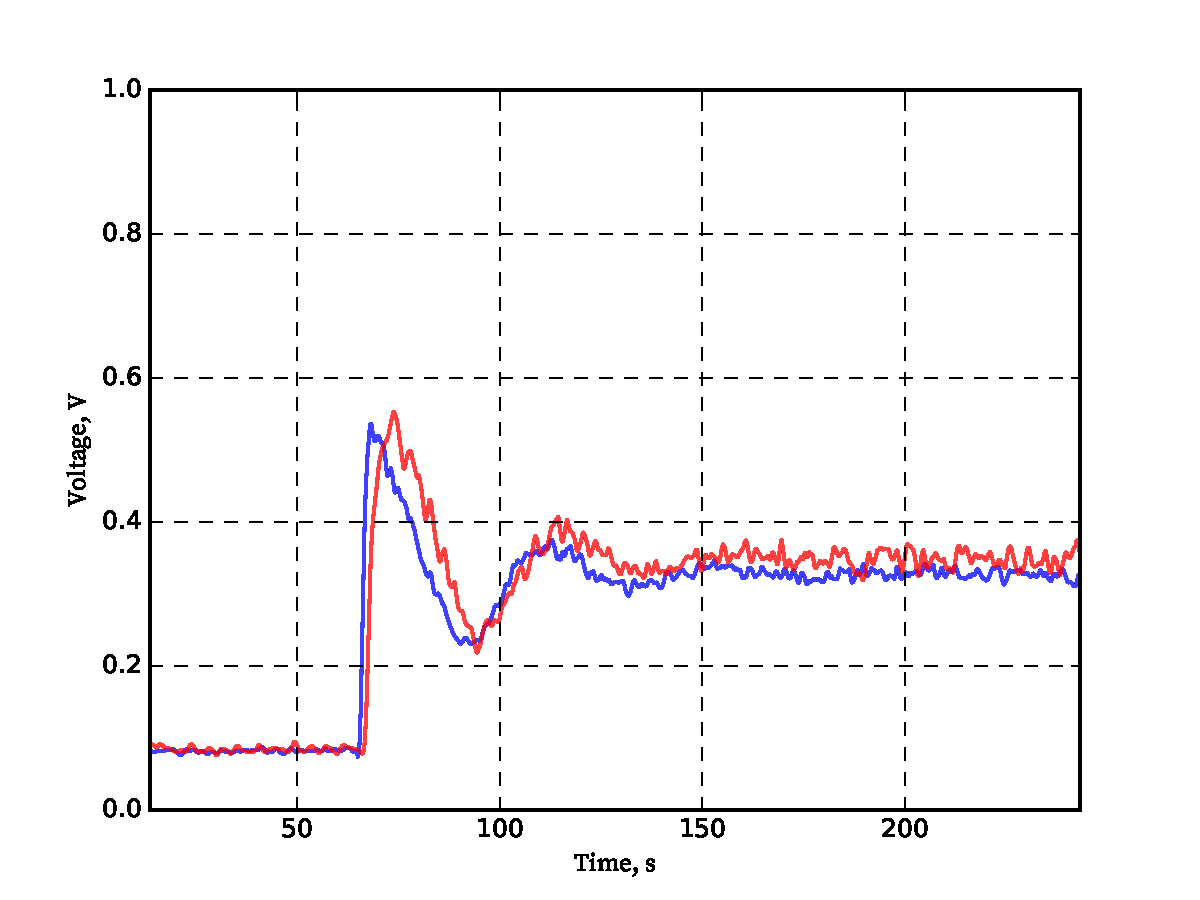
\includegraphics[width=0.8\textwidth]{images/log080716_6.pdf} 
		\caption{6}
		\label{fig:test6}
	\end{center}
\end{figure}